\documentclass[twoside]{book}

% Packages required by doxygen
\usepackage{calc}
\usepackage{doxygen}
\usepackage{graphicx}
\usepackage[utf8]{inputenc}
\usepackage{makeidx}
\usepackage{multicol}
\usepackage{multirow}
\usepackage{textcomp}
\usepackage[table]{xcolor}

% Font selection
\usepackage[T1]{fontenc}
\usepackage{mathptmx}
\usepackage[scaled=.90]{helvet}
\usepackage{courier}
\usepackage{amssymb}
\usepackage{sectsty}
\renewcommand{\familydefault}{\sfdefault}
\allsectionsfont{%
  \fontseries{bc}\selectfont%
  \color{darkgray}%
}
\renewcommand{\DoxyLabelFont}{%
  \fontseries{bc}\selectfont%
  \color{darkgray}%
}

% Page & text layout
\usepackage{geometry}
\geometry{%
  a4paper,%
  top=2.5cm,%
  bottom=2.5cm,%
  left=2.5cm,%
  right=2.5cm%
}
\tolerance=750
\hfuzz=15pt
\hbadness=750
\setlength{\emergencystretch}{15pt}
\setlength{\parindent}{0cm}
\setlength{\parskip}{0.2cm}
\makeatletter
\renewcommand{\paragraph}{%
  \@startsection{paragraph}{4}{0ex}{-1.0ex}{1.0ex}{%
    \normalfont\normalsize\bfseries\SS@parafont%
  }%
}
\renewcommand{\subparagraph}{%
  \@startsection{subparagraph}{5}{0ex}{-1.0ex}{1.0ex}{%
    \normalfont\normalsize\bfseries\SS@subparafont%
  }%
}
\makeatother

% Headers & footers
\usepackage{fancyhdr}
\pagestyle{fancyplain}
\fancyhead[LE]{\fancyplain{}{\bfseries\thepage}}
\fancyhead[CE]{\fancyplain{}{}}
\fancyhead[RE]{\fancyplain{}{\bfseries\leftmark}}
\fancyhead[LO]{\fancyplain{}{\bfseries\rightmark}}
\fancyhead[CO]{\fancyplain{}{}}
\fancyhead[RO]{\fancyplain{}{\bfseries\thepage}}
\fancyfoot[LE]{\fancyplain{}{}}
\fancyfoot[CE]{\fancyplain{}{}}
\fancyfoot[RE]{\fancyplain{}{\bfseries\scriptsize Generated on Thu Sep 8 2016 13\-:28\-:42 for tlds by Doxygen }}
\fancyfoot[LO]{\fancyplain{}{\bfseries\scriptsize Generated on Thu Sep 8 2016 13\-:28\-:42 for tlds by Doxygen }}
\fancyfoot[CO]{\fancyplain{}{}}
\fancyfoot[RO]{\fancyplain{}{}}
\renewcommand{\footrulewidth}{0.4pt}
\renewcommand{\chaptermark}[1]{%
  \markboth{#1}{}%
}
\renewcommand{\sectionmark}[1]{%
  \markright{\thesection\ #1}%
}

% Indices & bibliography
\usepackage{natbib}
\usepackage[titles]{tocloft}
\setcounter{tocdepth}{3}
\setcounter{secnumdepth}{5}
\makeindex

% Hyperlinks (required, but should be loaded last)
\usepackage{ifpdf}
\ifpdf
  \usepackage[pdftex,pagebackref=true]{hyperref}
\else
  \usepackage[ps2pdf,pagebackref=true]{hyperref}
\fi
\hypersetup{%
  colorlinks=true,%
  linkcolor=blue,%
  citecolor=blue,%
  unicode%
}

% Custom commands
\newcommand{\clearemptydoublepage}{%
  \newpage{\pagestyle{empty}\cleardoublepage}%
}


%===== C O N T E N T S =====

\begin{document}

% Titlepage & ToC
\hypersetup{pageanchor=false}
\pagenumbering{roman}
\begin{titlepage}
\vspace*{7cm}
\begin{center}%
{\Large tlds }\\
\vspace*{1cm}
{\large Generated by Doxygen 1.8.6}\\
\vspace*{0.5cm}
{\small Thu Sep 8 2016 13:28:42}\\
\end{center}
\end{titlepage}
\clearemptydoublepage
\tableofcontents
\clearemptydoublepage
\pagenumbering{arabic}
\hypersetup{pageanchor=true}

%--- Begin generated contents ---
\chapter{Namespace Index}
\section{Namespace List}
Here is a list of all namespaces with brief descriptions\-:\begin{DoxyCompactList}
\item\contentsline{section}{\hyperlink{namespaceanonymous__namespace_02biteager_8cpp_03}{anonymous\-\_\-namespace\{biteager.\-cpp\}} }{\pageref{namespaceanonymous__namespace_02biteager_8cpp_03}}{}
\item\contentsline{section}{\hyperlink{namespaceanonymous__namespace_02biteagerredo_8cpp_03}{anonymous\-\_\-namespace\{biteagerredo.\-cpp\}} }{\pageref{namespaceanonymous__namespace_02biteagerredo_8cpp_03}}{}
\item\contentsline{section}{\hyperlink{namespaceanonymous__namespace_02bitlazy_8cpp_03}{anonymous\-\_\-namespace\{bitlazy.\-cpp\}} }{\pageref{namespaceanonymous__namespace_02bitlazy_8cpp_03}}{}
\item\contentsline{section}{\hyperlink{namespaceanonymous__namespace_02BlockOperations_8cpp_03}{anonymous\-\_\-namespace\{\-Block\-Operations.\-cpp\}} }{\pageref{namespaceanonymous__namespace_02BlockOperations_8cpp_03}}{}
\item\contentsline{section}{\hyperlink{namespaceanonymous__namespace_02bmharness_8cpp_03}{anonymous\-\_\-namespace\{bmharness.\-cpp\}} }{\pageref{namespaceanonymous__namespace_02bmharness_8cpp_03}}{}
\item\contentsline{section}{\hyperlink{namespaceanonymous__namespace_02byear_8cpp_03}{anonymous\-\_\-namespace\{byear.\-cpp\}} }{\pageref{namespaceanonymous__namespace_02byear_8cpp_03}}{}
\item\contentsline{section}{\hyperlink{namespaceanonymous__namespace_02byeau_8cpp_03}{anonymous\-\_\-namespace\{byeau.\-cpp\}} }{\pageref{namespaceanonymous__namespace_02byeau_8cpp_03}}{}
\item\contentsline{section}{\hyperlink{namespaceanonymous__namespace_02byteeager_8cpp_03}{anonymous\-\_\-namespace\{byteeager.\-cpp\}} }{\pageref{namespaceanonymous__namespace_02byteeager_8cpp_03}}{}
\item\contentsline{section}{\hyperlink{namespaceanonymous__namespace_02byteeagerredo_8cpp_03}{anonymous\-\_\-namespace\{byteeagerredo.\-cpp\}} }{\pageref{namespaceanonymous__namespace_02byteeagerredo_8cpp_03}}{}
\item\contentsline{section}{\hyperlink{namespaceanonymous__namespace_02bytelazy_8cpp_03}{anonymous\-\_\-namespace\{bytelazy.\-cpp\}} }{\pageref{namespaceanonymous__namespace_02bytelazy_8cpp_03}}{}
\item\contentsline{section}{\hyperlink{namespaceanonymous__namespace_02cbr_8cpp_03}{anonymous\-\_\-namespace\{cbr.\-cpp\}} }{\pageref{namespaceanonymous__namespace_02cbr_8cpp_03}}{}
\item\contentsline{section}{\hyperlink{namespaceanonymous__namespace_02cgl_8cpp_03}{anonymous\-\_\-namespace\{cgl.\-cpp\}} }{\pageref{namespaceanonymous__namespace_02cgl_8cpp_03}}{}
\item\contentsline{section}{\hyperlink{namespaceanonymous__namespace_02ctoken_8cpp_03}{anonymous\-\_\-namespace\{ctoken.\-cpp\}} }{\pageref{namespaceanonymous__namespace_02ctoken_8cpp_03}}{}
\item\contentsline{section}{\hyperlink{namespaceanonymous__namespace_02ctokenturbo_8cpp_03}{anonymous\-\_\-namespace\{ctokenturbo.\-cpp\}} }{\pageref{namespaceanonymous__namespace_02ctokenturbo_8cpp_03}}{}
\item\contentsline{section}{\hyperlink{namespaceanonymous__namespace_02irrevocability_8cpp_03}{anonymous\-\_\-namespace\{irrevocability.\-cpp\}} }{\pageref{namespaceanonymous__namespace_02irrevocability_8cpp_03}}{}
\item\contentsline{section}{\hyperlink{namespaceanonymous__namespace_02libitm-5_81_005_8cpp_03}{anonymous\-\_\-namespace\{libitm-\/5.\-1,5.\-cpp\}} }{\pageref{namespaceanonymous__namespace_02libitm-5_81_005_8cpp_03}}{}
\item\contentsline{section}{\hyperlink{namespaceanonymous__namespace_02libitm-5_812_8cpp_03}{anonymous\-\_\-namespace\{libitm-\/5.\-12.\-cpp\}} }{\pageref{namespaceanonymous__namespace_02libitm-5_812_8cpp_03}}{}
\item\contentsline{section}{\hyperlink{namespaceanonymous__namespace_02libitm-5_813_0014_8cpp_03}{anonymous\-\_\-namespace\{libitm-\/5.\-13,14.\-cpp\}} }{\pageref{namespaceanonymous__namespace_02libitm-5_813_0014_8cpp_03}}{}
\item\contentsline{section}{\hyperlink{namespaceanonymous__namespace_02libitm-5_816_8cpp_03}{anonymous\-\_\-namespace\{libitm-\/5.\-16.\-cpp\}} }{\pageref{namespaceanonymous__namespace_02libitm-5_816_8cpp_03}}{}
\item\contentsline{section}{\hyperlink{namespaceanonymous__namespace_02llt_8cpp_03}{anonymous\-\_\-namespace\{llt.\-cpp\}} }{\pageref{namespaceanonymous__namespace_02llt_8cpp_03}}{}
\item\contentsline{section}{\hyperlink{namespaceanonymous__namespace_02mcs_8cpp_03}{anonymous\-\_\-namespace\{mcs.\-cpp\}} }{\pageref{namespaceanonymous__namespace_02mcs_8cpp_03}}{}
\item\contentsline{section}{\hyperlink{namespaceanonymous__namespace_02nano_8cpp_03}{anonymous\-\_\-namespace\{nano.\-cpp\}} }{\pageref{namespaceanonymous__namespace_02nano_8cpp_03}}{}
\item\contentsline{section}{\hyperlink{namespaceanonymous__namespace_02norec_8cpp_03}{anonymous\-\_\-namespace\{norec.\-cpp\}} }{\pageref{namespaceanonymous__namespace_02norec_8cpp_03}}{}
\item\contentsline{section}{\hyperlink{namespaceanonymous__namespace_02norecprio_8cpp_03}{anonymous\-\_\-namespace\{norecprio.\-cpp\}} }{\pageref{namespaceanonymous__namespace_02norecprio_8cpp_03}}{}
\item\contentsline{section}{\hyperlink{namespaceanonymous__namespace_02oreau_8cpp_03}{anonymous\-\_\-namespace\{oreau.\-cpp\}} }{\pageref{namespaceanonymous__namespace_02oreau_8cpp_03}}{}
\item\contentsline{section}{\hyperlink{namespaceanonymous__namespace_02orecala_8cpp_03}{anonymous\-\_\-namespace\{orecala.\-cpp\}} }{\pageref{namespaceanonymous__namespace_02orecala_8cpp_03}}{}
\item\contentsline{section}{\hyperlink{namespaceanonymous__namespace_02oreceager_8cpp_03}{anonymous\-\_\-namespace\{oreceager.\-cpp\}} }{\pageref{namespaceanonymous__namespace_02oreceager_8cpp_03}}{}
\item\contentsline{section}{\hyperlink{namespaceanonymous__namespace_02oreceagerredo_8cpp_03}{anonymous\-\_\-namespace\{oreceagerredo.\-cpp\}} }{\pageref{namespaceanonymous__namespace_02oreceagerredo_8cpp_03}}{}
\item\contentsline{section}{\hyperlink{namespaceanonymous__namespace_02orecela_8cpp_03}{anonymous\-\_\-namespace\{orecela.\-cpp\}} }{\pageref{namespaceanonymous__namespace_02orecela_8cpp_03}}{}
\item\contentsline{section}{\hyperlink{namespaceanonymous__namespace_02orecfair_8cpp_03}{anonymous\-\_\-namespace\{orecfair.\-cpp\}} }{\pageref{namespaceanonymous__namespace_02orecfair_8cpp_03}}{}
\item\contentsline{section}{\hyperlink{namespaceanonymous__namespace_02oreclazy_8cpp_03}{anonymous\-\_\-namespace\{oreclazy.\-cpp\}} }{\pageref{namespaceanonymous__namespace_02oreclazy_8cpp_03}}{}
\item\contentsline{section}{\hyperlink{namespaceanonymous__namespace_02pipeline_8cpp_03}{anonymous\-\_\-namespace\{pipeline.\-cpp\}} }{\pageref{namespaceanonymous__namespace_02pipeline_8cpp_03}}{}
\item\contentsline{section}{\hyperlink{namespaceanonymous__namespace_02policies_8cpp_03}{anonymous\-\_\-namespace\{policies.\-cpp\}} }{\pageref{namespaceanonymous__namespace_02policies_8cpp_03}}{}
\item\contentsline{section}{\hyperlink{namespaceanonymous__namespace_02profileapp_8cpp_03}{anonymous\-\_\-namespace\{profileapp.\-cpp\}} }{\pageref{namespaceanonymous__namespace_02profileapp_8cpp_03}}{}
\item\contentsline{section}{\hyperlink{namespaceanonymous__namespace_02profiletm_8cpp_03}{anonymous\-\_\-namespace\{profiletm.\-cpp\}} }{\pageref{namespaceanonymous__namespace_02profiletm_8cpp_03}}{}
\item\contentsline{section}{\hyperlink{namespaceanonymous__namespace_02profiling_8cpp_03}{anonymous\-\_\-namespace\{profiling.\-cpp\}} }{\pageref{namespaceanonymous__namespace_02profiling_8cpp_03}}{}
\item\contentsline{section}{\hyperlink{namespaceanonymous__namespace_02ringala_8cpp_03}{anonymous\-\_\-namespace\{ringala.\-cpp\}} }{\pageref{namespaceanonymous__namespace_02ringala_8cpp_03}}{}
\item\contentsline{section}{\hyperlink{namespaceanonymous__namespace_02ringsw_8cpp_03}{anonymous\-\_\-namespace\{ringsw.\-cpp\}} }{\pageref{namespaceanonymous__namespace_02ringsw_8cpp_03}}{}
\item\contentsline{section}{\hyperlink{namespaceanonymous__namespace_02serial_8cpp_03}{anonymous\-\_\-namespace\{serial.\-cpp\}} }{\pageref{namespaceanonymous__namespace_02serial_8cpp_03}}{}
\item\contentsline{section}{\hyperlink{namespaceanonymous__namespace_02static_8cpp_03}{anonymous\-\_\-namespace\{static.\-cpp\}} }{\pageref{namespaceanonymous__namespace_02static_8cpp_03}}{}
\item\contentsline{section}{\hyperlink{namespaceanonymous__namespace_02swiss_8cpp_03}{anonymous\-\_\-namespace\{swiss.\-cpp\}} }{\pageref{namespaceanonymous__namespace_02swiss_8cpp_03}}{}
\item\contentsline{section}{\hyperlink{namespaceanonymous__namespace_02ticket_8cpp_03}{anonymous\-\_\-namespace\{ticket.\-cpp\}} }{\pageref{namespaceanonymous__namespace_02ticket_8cpp_03}}{}
\item\contentsline{section}{\hyperlink{namespaceanonymous__namespace_02tli_8cpp_03}{anonymous\-\_\-namespace\{tli.\-cpp\}} }{\pageref{namespaceanonymous__namespace_02tli_8cpp_03}}{}
\item\contentsline{section}{\hyperlink{namespaceanonymous__namespace_02tml_8cpp_03}{anonymous\-\_\-namespace\{tml.\-cpp\}} }{\pageref{namespaceanonymous__namespace_02tml_8cpp_03}}{}
\item\contentsline{section}{\hyperlink{namespaceanonymous__namespace_02tmllazy_8cpp_03}{anonymous\-\_\-namespace\{tmllazy.\-cpp\}} }{\pageref{namespaceanonymous__namespace_02tmllazy_8cpp_03}}{}
\item\contentsline{section}{\hyperlink{namespaceanonymous__namespace_02txthread_8cpp_03}{anonymous\-\_\-namespace\{txthread.\-cpp\}} }{\pageref{namespaceanonymous__namespace_02txthread_8cpp_03}}{}
\item\contentsline{section}{\hyperlink{namespaceanonymous__namespace_02types_8cpp_03}{anonymous\-\_\-namespace\{types.\-cpp\}} }{\pageref{namespaceanonymous__namespace_02types_8cpp_03}}{}
\item\contentsline{section}{\hyperlink{namespaceanonymous__namespace_02WBMMPolicy_8cpp_03}{anonymous\-\_\-namespace\{\-W\-B\-M\-M\-Policy.\-cpp\}} }{\pageref{namespaceanonymous__namespace_02WBMMPolicy_8cpp_03}}{}
\item\contentsline{section}{\hyperlink{namespaceitm2stm}{itm2stm} }{\pageref{namespaceitm2stm}}{}
\item\contentsline{section}{\hyperlink{namespacestm}{stm} }{\pageref{namespacestm}}{}
\item\contentsline{section}{\hyperlink{namespacestm_1_1iccsync}{stm\-::iccsync} }{\pageref{namespacestm_1_1iccsync}}{}
\end{DoxyCompactList}

\chapter{Hierarchical Index}
\section{Class Hierarchy}
This inheritance list is sorted roughly, but not completely, alphabetically\-:\begin{DoxyCompactList}
\item \contentsline{section}{\-\_\-\-I\-T\-M\-\_\-src\-Location}{\pageref{struct__ITM__srcLocation}}{}
\item \contentsline{section}{stm\-:\-:Abort\-Wait\-Trigger}{\pageref{structstm_1_1AbortWaitTrigger}}{}
\item \contentsline{section}{adtree}{\pageref{structadtree}}{}
\item \contentsline{section}{adtree\-\_\-node}{\pageref{structadtree__node}}{}
\item \contentsline{section}{adtree\-\_\-vary}{\pageref{structadtree__vary}}{}
\item \contentsline{section}{stm\-:\-:alg\-\_\-t}{\pageref{structstm_1_1alg__t}}{}
\item \contentsline{section}{itm2stm\-:\-:Aligned$<$ T $>$}{\pageref{structitm2stm_1_1Aligned}}{}
\item \contentsline{section}{Allocator$<$ Data\-Type $>$}{\pageref{classAllocator}}{}
\item \contentsline{section}{Allocator$<$ Desc $>$}{\pageref{classAllocator}}{}
\item \contentsline{section}{Allocator$<$ Node\-Desc $>$}{\pageref{classAllocator}}{}
\item \contentsline{section}{Allocator$<$ Trans\-List\-:\-:Desc $>$}{\pageref{classAllocator}}{}
\item \contentsline{section}{Allocator$<$ Trans\-List\-:\-:Node $>$}{\pageref{classAllocator}}{}
\item \contentsline{section}{Allocator$<$ Trans\-List\-:\-:Node\-Desc $>$}{\pageref{classAllocator}}{}
\item \contentsline{section}{arg}{\pageref{structarg}}{}
\item \contentsline{section}{args}{\pageref{structargs}}{}
\item \contentsline{section}{stm\-:\-:Backoff\-C\-M}{\pageref{structstm_1_1BackoffCM}}{}
\item \contentsline{section}{barrier}{\pageref{classbarrier}}{}
\item \contentsline{section}{stm\-:\-:behavior\-\_\-t}{\pageref{structstm_1_1behavior__t}}{}
\item \contentsline{section}{anonymous\-\_\-namespace\{biteager.\-cpp\}\-:\-:Bit\-Eager}{\pageref{structanonymous__namespace_02biteager_8cpp_03_1_1BitEager}}{}
\item \contentsline{section}{anonymous\-\_\-namespace\{biteagerredo.\-cpp\}\-:\-:Bit\-Eager\-Redo}{\pageref{structanonymous__namespace_02biteagerredo_8cpp_03_1_1BitEagerRedo}}{}
\item \contentsline{section}{stm\-:\-:Bit\-Filter$<$ B\-I\-T\-S $>$}{\pageref{classstm_1_1BitFilter}}{}
\item \contentsline{section}{anonymous\-\_\-namespace\{bitlazy.\-cpp\}\-:\-:Bit\-Lazy}{\pageref{structanonymous__namespace_02bitlazy_8cpp_03_1_1BitLazy}}{}
\item \contentsline{section}{stm\-:\-:bitlock\-\_\-t}{\pageref{structstm_1_1bitlock__t}}{}
\item \contentsline{section}{bitmap}{\pageref{structbitmap}}{}
\item \contentsline{section}{block}{\pageref{structblock}}{}
\item \contentsline{section}{block\-\_\-pool$<$ T $>$\-:\-:block\-\_\-head\-\_\-node\-\_\-t}{\pageref{structblock__pool_1_1block__head__node__t}}{}
\item \contentsline{section}{block\-\_\-pool$<$ T $>$}{\pageref{classblock__pool}}{}
\item \contentsline{section}{itm2stm\-:\-:Block\-Reader}{\pageref{structitm2stm_1_1BlockReader}}{}
\item \contentsline{section}{itm2stm\-:\-:Block\-Writer}{\pageref{structitm2stm_1_1BlockWriter}}{}
\item \contentsline{section}{Boosting\-List}{\pageref{classBoostingList}}{}
\item \contentsline{section}{Boosting\-Skip}{\pageref{classBoostingSkip}}{}
\item \contentsline{section}{anonymous\-\_\-namespace\{byear.\-cpp\}\-:\-:By\-E\-A\-R}{\pageref{structanonymous__namespace_02byear_8cpp_03_1_1ByEAR}}{}
\item \contentsline{section}{anonymous\-\_\-namespace\{byeau.\-cpp\}\-:\-:By\-E\-A\-U\-\_\-\-Generic$<$ C\-M $>$}{\pageref{structanonymous__namespace_02byeau_8cpp_03_1_1ByEAU__Generic}}{}
\item \contentsline{section}{anonymous\-\_\-namespace\{byteeager.\-cpp\}\-:\-:Byte\-Eager}{\pageref{structanonymous__namespace_02byteeager_8cpp_03_1_1ByteEager}}{}
\item \contentsline{section}{anonymous\-\_\-namespace\{byteeagerredo.\-cpp\}\-:\-:Byte\-Eager\-Redo}{\pageref{structanonymous__namespace_02byteeagerredo_8cpp_03_1_1ByteEagerRedo}}{}
\item \contentsline{section}{anonymous\-\_\-namespace\{bytelazy.\-cpp\}\-:\-:Byte\-Lazy}{\pageref{structanonymous__namespace_02bytelazy_8cpp_03_1_1ByteLazy}}{}
\item \contentsline{section}{stm\-:\-:bytelock\-\_\-t}{\pageref{structstm_1_1bytelock__t}}{}
\item \contentsline{section}{stm\-:\-:Byte\-Logging\-Undo\-Log\-Entry}{\pageref{structstm_1_1ByteLoggingUndoLogEntry}}{}
\item \contentsline{section}{stm\-:\-:Byte\-Logging\-Value\-List\-Entry}{\pageref{classstm_1_1ByteLoggingValueListEntry}}{}
\item \contentsline{section}{stm\-:\-:Byte\-Logging\-Write\-Set\-Entry}{\pageref{structstm_1_1ByteLoggingWriteSetEntry}}{}
\item \contentsline{section}{itm2stm\-:\-:Scope\-:\-:Callback$<$ F $>$}{\pageref{structitm2stm_1_1Scope_1_1Callback}}{}
\item \contentsline{section}{stm\-:\-:iccsync\-:\-:C\-A\-S\-\_\-\-A\-D\-A\-P\-T\-E\-R$<$ T, S, D $>$}{\pageref{structstm_1_1iccsync_1_1CAS__ADAPTER}}{}
\item \contentsline{section}{stm\-:\-:iccsync\-:\-:C\-A\-S\-\_\-\-A\-D\-A\-P\-T\-E\-R$<$ T, S, 0 $>$}{\pageref{structstm_1_1iccsync_1_1CAS__ADAPTER_3_01T_00_01S_00_010_01_4}}{}
\item \contentsline{section}{stm\-:\-:iccsync\-:\-:C\-A\-S\-\_\-\-A\-D\-A\-P\-T\-E\-R$<$ T, T, 1 $>$}{\pageref{structstm_1_1iccsync_1_1CAS__ADAPTER_3_01T_00_01T_00_011_01_4}}{}
\item \contentsline{section}{anonymous\-\_\-namespace\{cgl.\-cpp\}\-:\-:C\-G\-L}{\pageref{structanonymous__namespace_02cgl_8cpp_03_1_1CGL}}{}
\item \contentsline{section}{itm2stm\-:\-:Checkpoint}{\pageref{classitm2stm_1_1Checkpoint}}{}
\begin{DoxyCompactList}
\item \contentsline{section}{itm2stm\-:\-:Scope}{\pageref{classitm2stm_1_1Scope}}{}
\end{DoxyCompactList}
\item \contentsline{section}{chunk\-\_\-st}{\pageref{structchunk__st}}{}
\item \contentsline{section}{client}{\pageref{structclient}}{}
\item \contentsline{section}{stm\-:\-:Commit\-Trigger}{\pageref{structstm_1_1CommitTrigger}}{}
\item \contentsline{section}{comparator}{\pageref{structcomparator}}{}
\item \contentsline{section}{compute\-Gragh\-\_\-arg}{\pageref{structcomputeGragh__arg}}{}
\item \contentsline{section}{Config}{\pageref{structConfig}}{}
\item \contentsline{section}{construct\-Entry}{\pageref{structconstructEntry}}{}
\item \contentsline{section}{coordinate}{\pageref{structcoordinate}}{}
\item \contentsline{section}{Coordinator}{\pageref{classCoordinator}}{}
\item \contentsline{section}{counted\-\_\-ptr}{\pageref{unioncounted__ptr}}{}
\item \contentsline{section}{anonymous\-\_\-namespace\{ctoken.\-cpp\}\-:\-:C\-Token}{\pageref{structanonymous__namespace_02ctoken_8cpp_03_1_1CToken}}{}
\item \contentsline{section}{anonymous\-\_\-namespace\{ctokenturbo.\-cpp\}\-:\-:C\-Token\-Turbo}{\pageref{structanonymous__namespace_02ctokenturbo_8cpp_03_1_1CTokenTurbo}}{}
\item \contentsline{section}{customer}{\pageref{structcustomer}}{}
\item \contentsline{section}{Custom\-Forest}{\pageref{structCustomForest}}{}
\item \contentsline{section}{d\-\_\-lock}{\pageref{classd__lock}}{}
\item \contentsline{section}{data}{\pageref{structdata}}{}
\item \contentsline{section}{decoded}{\pageref{structdecoded}}{}
\item \contentsline{section}{decoder}{\pageref{structdecoder}}{}
\item \contentsline{section}{Trans\-List\-:\-:Desc}{\pageref{structTransList_1_1Desc}}{}
\item \contentsline{section}{Desc}{\pageref{structDesc}}{}
\item \contentsline{section}{detector}{\pageref{structdetector}}{}
\item \contentsline{section}{Disjoint}{\pageref{structDisjoint}}{}
\item \contentsline{section}{stm\-:\-:D\-I\-S\-P\-A\-T\-C\-H$<$ T, S $>$}{\pageref{structstm_1_1DISPATCH}}{}
\item \contentsline{section}{D\-List}{\pageref{classDList}}{}
\item \contentsline{section}{stm\-:\-:dynprof\-\_\-t}{\pageref{structstm_1_1dynprof__t}}{}
\item \contentsline{section}{Surface.\-edge}{\pageref{classSurface_1_1edge}}{}
\item \contentsline{section}{edge}{\pageref{classedge}}{}
\item \contentsline{section}{edge\-\_\-set}{\pageref{classedge__set}}{}
\item \contentsline{section}{element}{\pageref{structelement}}{}
\item \contentsline{section}{stm\-:\-:Empty\-Trigger}{\pageref{structstm_1_1EmptyTrigger}}{}
\item \contentsline{section}{end\-Info\-Entry}{\pageref{structendInfoEntry}}{}
\item \contentsline{section}{eq\-\_\-point}{\pageref{structeq__point}}{}
\item \contentsline{section}{stm\-:\-:F\-C\-M}{\pageref{structstm_1_1FCM}}{}
\item \contentsline{section}{find\-Best\-Task\-Arg}{\pageref{structfindBestTaskArg}}{}
\item \contentsline{section}{find\-Sub\-Graphs0\-\_\-arg}{\pageref{structfindSubGraphs0__arg}}{}
\item \contentsline{section}{find\-Sub\-Graphs1\-\_\-arg}{\pageref{structfindSubGraphs1__arg}}{}
\item \contentsline{section}{find\-Sub\-Graphs2\-\_\-arg}{\pageref{structfindSubGraphs2__arg}}{}
\item \contentsline{section}{fr\-\_\-set\-\_\-st}{\pageref{structfr__set__st}}{}
\item \contentsline{section}{gc\-\_\-global\-\_\-st}{\pageref{structgc__global__st}}{}
\item \contentsline{section}{gc\-\_\-st}{\pageref{structgc__st}}{}
\item \contentsline{section}{gene}{\pageref{structgene}}{}
\item \contentsline{section}{get\-Start\-Lists\-\_\-arg}{\pageref{structgetStartLists__arg}}{}
\item \contentsline{section}{graph}{\pageref{structgraph}}{}
\item \contentsline{section}{graph\-S\-D\-G}{\pageref{structgraphSDG}}{}
\item \contentsline{section}{grid}{\pageref{structgrid}}{}
\item \contentsline{section}{hash\-\_\-point}{\pageref{structhash__point}}{}
\item \contentsline{section}{hashtable}{\pageref{structhashtable}}{}
\item \contentsline{section}{Hash\-Table}{\pageref{classHashTable}}{}
\item \contentsline{section}{hashtable\-\_\-iter}{\pageref{structhashtable__iter}}{}
\item \contentsline{section}{heap}{\pageref{structheap}}{}
\item \contentsline{section}{Trans\-List\-:\-:Help\-Stack}{\pageref{structTransList_1_1HelpStack}}{}
\item \contentsline{section}{Help\-Stack}{\pageref{structHelpStack}}{}
\item \contentsline{section}{stm\-:\-:Hourglass\-Backoff\-C\-M}{\pageref{structstm_1_1HourglassBackoffCM}}{}
\item \contentsline{section}{stm\-:\-:Hourglass\-C\-M}{\pageref{structstm_1_1HourglassCM}}{}
\item \contentsline{section}{stm\-:\-:Hyper\-Aggressive\-C\-M}{\pageref{structstm_1_1HyperAggressiveCM}}{}
\item \contentsline{section}{stm\-:\-:id\-\_\-version\-\_\-t}{\pageref{unionstm_1_1id__version__t}}{}
\item \contentsline{section}{stm\-:\-:Write\-Set\-:\-:index\-\_\-t}{\pageref{structstm_1_1WriteSet_1_1index__t}}{}
\item \contentsline{section}{anonymous\-\_\-namespace\{libitm-\/5.12.cpp\}\-:\-:I\-N\-S\-T$<$ T, N, A $>$}{\pageref{structanonymous__namespace_02libitm-5_812_8cpp_03_1_1INST}}{}
\item \contentsline{section}{anonymous\-\_\-namespace\{libitm-\/5.16.cpp\}\-:\-:I\-N\-S\-T$<$ T, W $>$}{\pageref{structanonymous__namespace_02libitm-5_816_8cpp_03_1_1INST}}{}
\item \contentsline{section}{anonymous\-\_\-namespace\{libitm-\/5.16.cpp\}\-:\-:I\-N\-S\-T$<$ T, 0u $>$}{\pageref{structanonymous__namespace_02libitm-5_816_8cpp_03_1_1INST_3_01T_00_010u_01_4}}{}
\item \contentsline{section}{anonymous\-\_\-namespace\{libitm-\/5.12.cpp\}\-:\-:I\-N\-S\-T$<$ T, 0u, false $>$}{\pageref{structanonymous__namespace_02libitm-5_812_8cpp_03_1_1INST_3_01T_00_010u_00_01false_01_4}}{}
\item \contentsline{section}{anonymous\-\_\-namespace\{libitm-\/5.12.cpp\}\-:\-:I\-N\-S\-T$<$ T, 0u, true $>$}{\pageref{structanonymous__namespace_02libitm-5_812_8cpp_03_1_1INST_3_01T_00_010u_00_01true_01_4}}{}
\item \contentsline{section}{anonymous\-\_\-namespace\{libitm-\/5.12.cpp\}\-:\-:I\-N\-S\-T$<$ T, N, false $>$}{\pageref{structanonymous__namespace_02libitm-5_812_8cpp_03_1_1INST_3_01T_00_01N_00_01false_01_4}}{}
\item \contentsline{section}{anonymous\-\_\-namespace\{libitm-\/5.12.cpp\}\-:\-:I\-N\-S\-T$<$ T, N, true $>$}{\pageref{structanonymous__namespace_02libitm-5_812_8cpp_03_1_1INST_3_01T_00_01N_00_01true_01_4}}{}
\item \contentsline{section}{stm\-:\-:D\-I\-S\-P\-A\-T\-C\-H$<$ T, S $>$\-:\-:Invalid\-Type\-As\-Second\-Template\-Parameter}{\pageref{structstm_1_1DISPATCH_1_1InvalidTypeAsSecondTemplateParameter}}{}
\item \contentsline{section}{J\-Applet}{\pageref{classJApplet}}{}
\begin{DoxyCompactList}
\item \contentsline{section}{Display}{\pageref{classDisplay}}{}
\end{DoxyCompactList}
\item \contentsline{section}{J\-Panel}{\pageref{classJPanel}}{}
\begin{DoxyCompactList}
\item \contentsline{section}{Surface}{\pageref{classSurface}}{}
\item \contentsline{section}{U\-I}{\pageref{classUI}}{}
\end{DoxyCompactList}
\item \contentsline{section}{jsw\-\_\-avlnode}{\pageref{structjsw__avlnode}}{}
\item \contentsline{section}{jsw\-\_\-avltrav}{\pageref{structjsw__avltrav}}{}
\item \contentsline{section}{jsw\-\_\-avltree}{\pageref{structjsw__avltree}}{}
\item \contentsline{section}{l}{\pageref{structl}}{}
\item \contentsline{section}{learner}{\pageref{structlearner}}{}
\item \contentsline{section}{learner\-\_\-task}{\pageref{structlearner__task}}{}
\item \contentsline{section}{stm\-:\-:limbo\-\_\-t}{\pageref{structstm_1_1limbo__t}}{}
\item \contentsline{section}{list}{\pageref{structlist}}{}
\item \contentsline{section}{List}{\pageref{classList}}{}
\item \contentsline{section}{list\-\_\-node}{\pageref{structlist__node}}{}
\item \contentsline{section}{L\-L\-Node$<$ T $>$}{\pageref{classLLNode}}{}
\item \contentsline{section}{anonymous\-\_\-namespace\{llt.\-cpp\}\-:\-:L\-L\-T}{\pageref{structanonymous__namespace_02llt_8cpp_03_1_1LLT}}{}
\item \contentsline{section}{Lockfree\-List}{\pageref{classLockfreeList}}{}
\item \contentsline{section}{Lock\-Key}{\pageref{classLockKey}}{}
\item \contentsline{section}{itm2stm\-:\-:Scope\-:\-:Logged\-Word}{\pageref{structitm2stm_1_1Scope_1_1LoggedWord}}{}
\item \contentsline{section}{lt\-\_\-point}{\pageref{structlt__point}}{}
\item \contentsline{section}{manager}{\pageref{structmanager}}{}
\item \contentsline{section}{maze}{\pageref{structmaze}}{}
\item \contentsline{section}{anonymous\-\_\-namespace\{mcs.\-cpp\}\-:\-:M\-C\-S}{\pageref{structanonymous__namespace_02mcs_8cpp_03_1_1MCS}}{}
\item \contentsline{section}{mcs\-\_\-qnode\-\_\-t}{\pageref{structmcs__qnode__t}}{}
\item \contentsline{section}{memory}{\pageref{structmemory}}{}
\item \contentsline{section}{mesh}{\pageref{structmesh}}{}
\item \contentsline{section}{stm\-:\-:Meta\-Initializer$<$ I $>$}{\pageref{structstm_1_1MetaInitializer}}{}
\item \contentsline{section}{stm\-:\-:Meta\-Initializer$<$ A\-L\-G\-\_\-\-M\-A\-X $>$}{\pageref{structstm_1_1MetaInitializer_3_01ALG__MAX_01_4}}{}
\item \contentsline{section}{stm\-:\-:Mini\-Vector$<$ T $>$}{\pageref{classstm_1_1MiniVector}}{}
\begin{DoxyCompactList}
\item \contentsline{section}{stm\-:\-:Undo\-Log}{\pageref{classstm_1_1UndoLog}}{}
\item \contentsline{section}{stm\-:\-:Value\-List}{\pageref{structstm_1_1ValueList}}{}
\end{DoxyCompactList}
\item \contentsline{section}{stm\-:\-:Mini\-Vector$<$ bitlock\-\_\-t $\ast$ $>$}{\pageref{classstm_1_1MiniVector}}{}
\item \contentsline{section}{stm\-:\-:Mini\-Vector$<$ bytelock\-\_\-t $\ast$ $>$}{\pageref{classstm_1_1MiniVector}}{}
\item \contentsline{section}{stm\-:\-:Mini\-Vector$<$ nanorec\-\_\-t $>$}{\pageref{classstm_1_1MiniVector}}{}
\item \contentsline{section}{stm\-:\-:Mini\-Vector$<$ orec\-\_\-t $\ast$ $>$}{\pageref{classstm_1_1MiniVector}}{}
\item \contentsline{section}{stm\-:\-:Mini\-Vector$<$ rrec\-\_\-t $\ast$ $>$}{\pageref{classstm_1_1MiniVector}}{}
\item \contentsline{section}{stm\-:\-:Mini\-Vector$<$ Undo\-Log\-Entry $>$}{\pageref{classstm_1_1MiniVector}}{}
\item \contentsline{section}{stm\-:\-:Mini\-Vector$<$ Value\-List\-Entry $>$}{\pageref{classstm_1_1MiniVector}}{}
\item \contentsline{section}{stm\-:\-:Mini\-Vector$<$ void $\ast$ $>$}{\pageref{classstm_1_1MiniVector}}{}
\item \contentsline{section}{M\-S\-\_\-queue$<$ T $>$}{\pageref{classMS__queue}}{}
\begin{DoxyCompactList}
\item \contentsline{section}{concurrent\-\_\-queue$<$ T $>$}{\pageref{classconcurrent__queue}}{}
\end{DoxyCompactList}
\item \contentsline{section}{anonymous\-\_\-namespace\{nano.\-cpp\}\-:\-:Nano}{\pageref{structanonymous__namespace_02nano_8cpp_03_1_1Nano}}{}
\item \contentsline{section}{stm\-:\-:nanorec\-\_\-t}{\pageref{structstm_1_1nanorec__t}}{}
\item \contentsline{section}{net}{\pageref{structnet}}{}
\item \contentsline{section}{net\-\_\-node}{\pageref{structnet__node}}{}
\item \contentsline{section}{R\-S\-T\-M\-List\-:\-:Node}{\pageref{structRSTMList_1_1Node}}{}
\item \contentsline{section}{node}{\pageref{structnode}}{}
\item \contentsline{section}{D\-List\-:\-:Node}{\pageref{structDList_1_1Node}}{}
\item \contentsline{section}{List\-:\-:Node}{\pageref{structList_1_1Node}}{}
\item \contentsline{section}{Trans\-List\-:\-:Node}{\pageref{structTransList_1_1Node}}{}
\item \contentsline{section}{Lockfree\-List\-:\-:Node}{\pageref{structLockfreeList_1_1Node}}{}
\item \contentsline{section}{node\-\_\-st}{\pageref{structnode__st}}{}
\item \contentsline{section}{node\-\_\-t}{\pageref{structnode__t}}{}
\item \contentsline{section}{Node\-Desc}{\pageref{structNodeDesc}}{}
\item \contentsline{section}{Trans\-List\-:\-:Node\-Desc}{\pageref{structTransList_1_1NodeDesc}}{}
\item \contentsline{section}{anonymous\-\_\-namespace\{norec.\-cpp\}\-:\-:N\-Orec\-\_\-\-Generic$<$ C\-M $>$}{\pageref{structanonymous__namespace_02norec_8cpp_03_1_1NOrec__Generic}}{}
\item \contentsline{section}{anonymous\-\_\-namespace\{norecprio.\-cpp\}\-:\-:N\-Orec\-Prio}{\pageref{structanonymous__namespace_02norecprio_8cpp_03_1_1NOrecPrio}}{}
\item \contentsline{section}{stm\-:\-:Object}{\pageref{structstm_1_1Object}}{}
\item \contentsline{section}{Boosting\-List\-:\-:Operation}{\pageref{structBoostingList_1_1Operation}}{}
\item \contentsline{section}{Boosting\-Skip\-:\-:Operation}{\pageref{structBoostingSkip_1_1Operation}}{}
\item \contentsline{section}{Trans\-List\-:\-:Operator}{\pageref{structTransList_1_1Operator}}{}
\item \contentsline{section}{Operator}{\pageref{structOperator}}{}
\item \contentsline{section}{anonymous\-\_\-namespace\{oreau.\-cpp\}\-:\-:Or\-E\-A\-U\-\_\-\-Generic$<$ C\-M $>$}{\pageref{structanonymous__namespace_02oreau_8cpp_03_1_1OrEAU__Generic}}{}
\item \contentsline{section}{stm\-:\-:orec\-\_\-t}{\pageref{structstm_1_1orec__t}}{}
\item \contentsline{section}{anonymous\-\_\-namespace\{orecala.\-cpp\}\-:\-:Orec\-A\-L\-A}{\pageref{structanonymous__namespace_02orecala_8cpp_03_1_1OrecALA}}{}
\item \contentsline{section}{anonymous\-\_\-namespace\{oreceager.\-cpp\}\-:\-:Orec\-Eager\-\_\-\-Generic$<$ C\-M $>$}{\pageref{structanonymous__namespace_02oreceager_8cpp_03_1_1OrecEager__Generic}}{}
\item \contentsline{section}{anonymous\-\_\-namespace\{oreceagerredo.\-cpp\}\-:\-:Orec\-Eager\-Redo}{\pageref{structanonymous__namespace_02oreceagerredo_8cpp_03_1_1OrecEagerRedo}}{}
\item \contentsline{section}{anonymous\-\_\-namespace\{orecela.\-cpp\}\-:\-:Orec\-E\-L\-A}{\pageref{structanonymous__namespace_02orecela_8cpp_03_1_1OrecELA}}{}
\item \contentsline{section}{anonymous\-\_\-namespace\{orecfair.\-cpp\}\-:\-:Orec\-Fair}{\pageref{structanonymous__namespace_02orecfair_8cpp_03_1_1OrecFair}}{}
\item \contentsline{section}{anonymous\-\_\-namespace\{oreclazy.\-cpp\}\-:\-:Orec\-Lazy\-\_\-\-Generic$<$ C\-M $>$}{\pageref{structanonymous__namespace_02oreclazy_8cpp_03_1_1OrecLazy__Generic}}{}
\item \contentsline{section}{packet}{\pageref{structpacket}}{}
\item \contentsline{section}{stm\-:\-:pad\-\_\-word\-\_\-t}{\pageref{structstm_1_1pad__word__t}}{}
\item \contentsline{section}{Disjoint\-:\-:Padded\-Buffer}{\pageref{structDisjoint_1_1PaddedBuffer}}{}
\item \contentsline{section}{Disjoint\-:\-:Padded\-Buffer\-Entry}{\pageref{structDisjoint_1_1PaddedBufferEntry}}{}
\item pair\begin{DoxyCompactList}
\item \contentsline{section}{itm2stm\-:\-:Scope\-:\-:Thrown\-Object}{\pageref{structitm2stm_1_1Scope_1_1ThrownObject}}{}
\end{DoxyCompactList}
\item \contentsline{section}{pair}{\pageref{structpair}}{}
\item \contentsline{section}{anonymous\-\_\-namespace\{pipeline.\-cpp\}\-:\-:Pipeline}{\pageref{structanonymous__namespace_02pipeline_8cpp_03_1_1Pipeline}}{}
\item \contentsline{section}{point}{\pageref{classpoint}}{}
\item \contentsline{section}{stm\-:\-:pol\-\_\-t}{\pageref{structstm_1_1pol__t}}{}
\item \contentsline{section}{pool}{\pageref{structpool}}{}
\item \contentsline{section}{priv\-\_\-t}{\pageref{structpriv__t}}{}
\item \contentsline{section}{anonymous\-\_\-namespace\{profileapp.\-cpp\}\-:\-:Profile\-App$<$ C\-O\-U\-N\-T\-M\-O\-D\-E $>$}{\pageref{structanonymous__namespace_02profileapp_8cpp_03_1_1ProfileApp}}{}
\item \contentsline{section}{anonymous\-\_\-namespace\{profiletm.\-cpp\}\-:\-:Profile\-T\-M}{\pageref{structanonymous__namespace_02profiletm_8cpp_03_1_1ProfileTM}}{}
\item \contentsline{section}{ptst\-\_\-st}{\pageref{structptst__st}}{}
\item \contentsline{section}{pv\-\_\-side}{\pageref{structpv__side}}{}
\item \contentsline{section}{qnode\-\_\-t$<$ T $>$}{\pageref{structqnode__t}}{}
\item \contentsline{section}{stm\-:\-:qtable\-\_\-t}{\pageref{structstm_1_1qtable__t}}{}
\item \contentsline{section}{query}{\pageref{structquery}}{}
\item \contentsline{section}{queue}{\pageref{structqueue}}{}
\item \contentsline{section}{queue$<$ T $>$}{\pageref{structqueue}}{}
\item \contentsline{section}{anonymous\-\_\-namespace\{cbr.\-cpp\}\-:\-:R\-\_\-\-R\-O}{\pageref{structanonymous__namespace_02cbr_8cpp_03_1_1R__RO}}{}
\item \contentsline{section}{anonymous\-\_\-namespace\{cbr.\-cpp\}\-:\-:R\-\_\-\-Time}{\pageref{structanonymous__namespace_02cbr_8cpp_03_1_1R__Time}}{}
\item \contentsline{section}{anonymous\-\_\-namespace\{cbr.\-cpp\}\-:\-:R\-\_\-\-Time\-\_\-\-R\-O}{\pageref{structanonymous__namespace_02cbr_8cpp_03_1_1R__Time__RO}}{}
\item \contentsline{section}{anonymous\-\_\-namespace\{cbr.\-cpp\}\-:\-:R\-\_\-\-W\-\_\-\-R\-O}{\pageref{structanonymous__namespace_02cbr_8cpp_03_1_1R__W__RO}}{}
\item \contentsline{section}{anonymous\-\_\-namespace\{cbr.\-cpp\}\-:\-:R\-\_\-\-W\-\_\-\-Time}{\pageref{structanonymous__namespace_02cbr_8cpp_03_1_1R__W__Time}}{}
\item \contentsline{section}{anonymous\-\_\-namespace\{cbr.\-cpp\}\-:\-:R\-\_\-\-W\-\_\-\-Time\-\_\-\-R\-O}{\pageref{structanonymous__namespace_02cbr_8cpp_03_1_1R__W__Time__RO}}{}
\item \contentsline{section}{random}{\pageref{structrandom}}{}
\item \contentsline{section}{R\-B\-Tree\-:\-:R\-B\-Node}{\pageref{structRBTree_1_1RBNode}}{}
\item \contentsline{section}{rbtree}{\pageref{structrbtree}}{}
\item \contentsline{section}{R\-B\-Tree}{\pageref{classRBTree}}{}
\item \contentsline{section}{anonymous\-\_\-namespace\{cbr.\-cpp\}\-:\-:Read}{\pageref{structanonymous__namespace_02cbr_8cpp_03_1_1Read}}{}
\item \contentsline{section}{region}{\pageref{structregion}}{}
\item \contentsline{section}{region\-\_\-info}{\pageref{structregion__info}}{}
\item \contentsline{section}{reservation}{\pageref{structreservation}}{}
\item \contentsline{section}{reservation\-\_\-info}{\pageref{structreservation__info}}{}
\item \contentsline{section}{anonymous\-\_\-namespace\{ringala.\-cpp\}\-:\-:Ring\-A\-L\-A}{\pageref{structanonymous__namespace_02ringala_8cpp_03_1_1RingALA}}{}
\item \contentsline{section}{anonymous\-\_\-namespace\{ringsw.\-cpp\}\-:\-:Ring\-S\-W}{\pageref{structanonymous__namespace_02ringsw_8cpp_03_1_1RingSW}}{}
\item \contentsline{section}{anonymous\-\_\-namespace\{cbr.\-cpp\}\-:\-:R\-O}{\pageref{structanonymous__namespace_02cbr_8cpp_03_1_1RO}}{}
\item \contentsline{section}{router}{\pageref{structrouter}}{}
\item \contentsline{section}{router\-\_\-solve\-\_\-arg}{\pageref{structrouter__solve__arg}}{}
\item \contentsline{section}{stm\-:\-:rrec\-\_\-t}{\pageref{structstm_1_1rrec__t}}{}
\item \contentsline{section}{R\-S\-T\-M\-List}{\pageref{classRSTMList}}{}
\item \contentsline{section}{runnable}{\pageref{classrunnable}}{}
\begin{DoxyCompactList}
\item \contentsline{section}{worker}{\pageref{classworker}}{}
\end{DoxyCompactList}
\item \contentsline{section}{anonymous\-\_\-namespace\{cbr.\-cpp\}\-:\-:R\-W}{\pageref{structanonymous__namespace_02cbr_8cpp_03_1_1RW}}{}
\item \contentsline{section}{segments}{\pageref{structsegments}}{}
\item \contentsline{section}{sequencer}{\pageref{structsequencer}}{}
\item \contentsline{section}{sequencer\-\_\-run\-\_\-arg}{\pageref{structsequencer__run__arg}}{}
\item \contentsline{section}{anonymous\-\_\-namespace\{serial.\-cpp\}\-:\-:Serial}{\pageref{structanonymous__namespace_02serial_8cpp_03_1_1Serial}}{}
\item \contentsline{section}{set\-\_\-op\-\_\-st}{\pageref{structset__op__st}}{}
\item \contentsline{section}{Set\-Adaptor$<$ T $>$}{\pageref{classSetAdaptor}}{}
\item \contentsline{section}{Set\-Adaptor$<$ Boosting\-List $>$}{\pageref{classSetAdaptor_3_01BoostingList_01_4}}{}
\item \contentsline{section}{Set\-Adaptor$<$ Boosting\-Skip $>$}{\pageref{classSetAdaptor_3_01BoostingSkip_01_4}}{}
\item \contentsline{section}{Set\-Adaptor$<$ R\-S\-T\-M\-List $>$}{\pageref{classSetAdaptor_3_01RSTMList_01_4}}{}
\item \contentsline{section}{Set\-Adaptor$<$ stm\-\_\-skip $>$}{\pageref{classSetAdaptor_3_01stm__skip_01_4}}{}
\item \contentsline{section}{Set\-Adaptor$<$ trans\-\_\-skip $>$}{\pageref{classSetAdaptor_3_01trans__skip_01_4}}{}
\item \contentsline{section}{Set\-Adaptor$<$ Trans\-List $>$}{\pageref{classSetAdaptor_3_01TransList_01_4}}{}
\item \contentsline{section}{Set\-Operator}{\pageref{structSetOperator}}{}
\item \contentsline{section}{block\-\_\-pool$<$ T $>$\-:\-:shared\-\_\-block\-\_\-t}{\pageref{structblock__pool_1_1shared__block__t}}{}
\item \contentsline{section}{simple\-\_\-queue$<$ T $>$}{\pageref{classsimple__queue}}{}
\begin{DoxyCompactList}
\item \contentsline{section}{concurrent\-\_\-queue$<$ T $>$}{\pageref{classconcurrent__queue}}{}
\item \contentsline{section}{sequential\-\_\-queue$<$ T $>$}{\pageref{classsequential__queue}}{}
\end{DoxyCompactList}
\item \contentsline{section}{simple\-\_\-queue$<$ edge $\ast$ $>$}{\pageref{classsimple__queue}}{}
\item \contentsline{section}{stm\-\_\-blk\-\_\-st}{\pageref{structstm__blk__st}}{}
\item \contentsline{section}{stm\-\_\-st}{\pageref{structstm__st}}{}
\item \contentsline{section}{stm\-\_\-tx\-\_\-entry\-\_\-st}{\pageref{structstm__tx__entry__st}}{}
\item \contentsline{section}{stm\-\_\-tx\-\_\-st}{\pageref{structstm__tx__st}}{}
\item \contentsline{section}{stream}{\pageref{structstream}}{}
\item \contentsline{section}{stm\-:\-:Strong\-Hourglass\-C\-M}{\pageref{structstm_1_1StrongHourglassCM}}{}
\item \contentsline{section}{stm\-:\-:iccsync\-:\-:S\-W\-A\-P\-\_\-\-A\-D\-A\-P\-T\-E\-R$<$ T, S, D $>$}{\pageref{structstm_1_1iccsync_1_1SWAP__ADAPTER}}{}
\item \contentsline{section}{stm\-:\-:iccsync\-:\-:S\-W\-A\-P\-\_\-\-A\-D\-A\-P\-T\-E\-R$<$ T, S, 0 $>$}{\pageref{structstm_1_1iccsync_1_1SWAP__ADAPTER_3_01T_00_01S_00_010_01_4}}{}
\item \contentsline{section}{stm\-:\-:iccsync\-:\-:S\-W\-A\-P\-\_\-\-A\-D\-A\-P\-T\-E\-R$<$ T, S, 1 $>$}{\pageref{structstm_1_1iccsync_1_1SWAP__ADAPTER_3_01T_00_01S_00_011_01_4}}{}
\item \contentsline{section}{stm\-:\-:iccsync\-:\-:S\-W\-A\-P\-\_\-\-A\-D\-A\-P\-T\-E\-R$<$ T, T, 1 $>$}{\pageref{structstm_1_1iccsync_1_1SWAP__ADAPTER_3_01T_00_01T_00_011_01_4}}{}
\item \contentsline{section}{anonymous\-\_\-namespace\{swiss.\-cpp\}\-:\-:Swiss}{\pageref{structanonymous__namespace_02swiss_8cpp_03_1_1Swiss}}{}
\item \contentsline{section}{stm\-:\-:iccsync\-:\-:S\-Y\-N\-C$<$ T, W, N $>$}{\pageref{structstm_1_1iccsync_1_1SYNC}}{}
\item \contentsline{section}{stm\-:\-:iccsync\-:\-:S\-Y\-N\-C$<$ T, 4, 8 $>$}{\pageref{structstm_1_1iccsync_1_1SYNC_3_01T_00_014_00_018_01_4}}{}
\item \contentsline{section}{stm\-:\-:iccsync\-:\-:S\-Y\-N\-C$<$ T, 8, 16 $>$}{\pageref{structstm_1_1iccsync_1_1SYNC_3_01T_00_018_00_0116_01_4}}{}
\item \contentsline{section}{stm\-:\-:iccsync\-:\-:S\-Y\-N\-C$<$ T, 8, 8 $>$}{\pageref{structstm_1_1iccsync_1_1SYNC_3_01T_00_018_00_018_01_4}}{}
\item \contentsline{section}{stm\-:\-:iccsync\-:\-:S\-Y\-N\-C$<$ T, W, 1 $>$}{\pageref{structstm_1_1iccsync_1_1SYNC_3_01T_00_01W_00_011_01_4}}{}
\item \contentsline{section}{stm\-:\-:iccsync\-:\-:S\-Y\-N\-C$<$ T, W, 2 $>$}{\pageref{structstm_1_1iccsync_1_1SYNC_3_01T_00_01W_00_012_01_4}}{}
\item \contentsline{section}{stm\-:\-:iccsync\-:\-:S\-Y\-N\-C$<$ T, W, 4 $>$}{\pageref{structstm_1_1iccsync_1_1SYNC_3_01T_00_01W_00_014_01_4}}{}
\item \contentsline{section}{table}{\pageref{structtable}}{}
\item \contentsline{section}{thread}{\pageref{classthread}}{}
\item \contentsline{section}{Thread}{\pageref{classThread}}{}
\begin{DoxyCompactList}
\item \contentsline{section}{Surface.\-Worker}{\pageref{classSurface_1_1Worker}}{}
\end{DoxyCompactList}
\item \contentsline{section}{Thread\-Barrier}{\pageref{classThreadBarrier}}{}
\item \contentsline{section}{Thread\-Local\-Pointer$<$ T $>$}{\pageref{classThreadLocalPointer}}{}
\item \contentsline{section}{anonymous\-\_\-namespace\{ticket.\-cpp\}\-:\-:Ticket}{\pageref{structanonymous__namespace_02ticket_8cpp_03_1_1Ticket}}{}
\item \contentsline{section}{ticket\-\_\-lock\-\_\-t}{\pageref{structticket__lock__t}}{}
\item \contentsline{section}{anonymous\-\_\-namespace\{cbr.\-cpp\}\-:\-:Time}{\pageref{structanonymous__namespace_02cbr_8cpp_03_1_1Time}}{}
\item \contentsline{section}{Time}{\pageref{classTime}}{}
\item \contentsline{section}{anonymous\-\_\-namespace\{cbr.\-cpp\}\-:\-:Time\-\_\-\-R\-O}{\pageref{structanonymous__namespace_02cbr_8cpp_03_1_1Time__RO}}{}
\item \contentsline{section}{Timer}{\pageref{classTimer}}{}
\begin{DoxyCompactList}
\item \contentsline{section}{Scoped\-Timer}{\pageref{classScopedTimer}}{}
\end{DoxyCompactList}
\item \contentsline{section}{anonymous\-\_\-namespace\{tli.\-cpp\}\-:\-:T\-L\-I}{\pageref{structanonymous__namespace_02tli_8cpp_03_1_1TLI}}{}
\item \contentsline{section}{tm\-\_\-set$<$ T $>$}{\pageref{classtm__set}}{}
\begin{DoxyCompactList}
\item \contentsline{section}{tm\-\_\-hash\-\_\-set$<$ T $>$}{\pageref{classtm__hash__set}}{}
\item \contentsline{section}{tm\-\_\-list\-\_\-set$<$ T $>$}{\pageref{classtm__list__set}}{}
\end{DoxyCompactList}
\item \contentsline{section}{anonymous\-\_\-namespace\{tml.\-cpp\}\-:\-:T\-M\-L}{\pageref{structanonymous__namespace_02tml_8cpp_03_1_1TML}}{}
\item \contentsline{section}{anonymous\-\_\-namespace\{tmllazy.\-cpp\}\-:\-:T\-M\-L\-Lazy}{\pageref{structanonymous__namespace_02tmllazy_8cpp_03_1_1TMLLazy}}{}
\item \contentsline{section}{stm\-:\-:toxic\-\_\-histogram\-\_\-t}{\pageref{structstm_1_1toxic__histogram__t}}{}
\item \contentsline{section}{stm\-:\-:toxic\-\_\-nop\-\_\-t}{\pageref{structstm_1_1toxic__nop__t}}{}
\item \contentsline{section}{trans\-\_\-skip}{\pageref{structtrans__skip}}{}
\item \contentsline{section}{Trans\-List}{\pageref{classTransList}}{}
\item \contentsline{section}{tx\-\_\-side}{\pageref{structtx__side}}{}
\item \contentsline{section}{anonymous\-\_\-namespace\{cbr.\-cpp\}\-:\-:Txn\-Ratio}{\pageref{structanonymous__namespace_02cbr_8cpp_03_1_1TxnRatio}}{}
\item \contentsline{section}{anonymous\-\_\-namespace\{cbr.\-cpp\}\-:\-:Txn\-Ratio\-\_\-\-R}{\pageref{structanonymous__namespace_02cbr_8cpp_03_1_1TxnRatio__R}}{}
\item \contentsline{section}{anonymous\-\_\-namespace\{cbr.\-cpp\}\-:\-:Txn\-Ratio\-\_\-\-R\-\_\-\-R\-O}{\pageref{structanonymous__namespace_02cbr_8cpp_03_1_1TxnRatio__R__RO}}{}
\item \contentsline{section}{anonymous\-\_\-namespace\{cbr.\-cpp\}\-:\-:Txn\-Ratio\-\_\-\-R\-\_\-\-R\-O\-\_\-\-Time}{\pageref{structanonymous__namespace_02cbr_8cpp_03_1_1TxnRatio__R__RO__Time}}{}
\item \contentsline{section}{anonymous\-\_\-namespace\{cbr.\-cpp\}\-:\-:Txn\-Ratio\-\_\-\-R\-\_\-\-Time}{\pageref{structanonymous__namespace_02cbr_8cpp_03_1_1TxnRatio__R__Time}}{}
\item \contentsline{section}{anonymous\-\_\-namespace\{cbr.\-cpp\}\-:\-:Txn\-Ratio\-\_\-\-R\-O}{\pageref{structanonymous__namespace_02cbr_8cpp_03_1_1TxnRatio__RO}}{}
\item \contentsline{section}{anonymous\-\_\-namespace\{cbr.\-cpp\}\-:\-:Txn\-Ratio\-\_\-\-R\-O\-\_\-\-Time}{\pageref{structanonymous__namespace_02cbr_8cpp_03_1_1TxnRatio__RO__Time}}{}
\item \contentsline{section}{anonymous\-\_\-namespace\{cbr.\-cpp\}\-:\-:Txn\-Ratio\-\_\-\-R\-W}{\pageref{structanonymous__namespace_02cbr_8cpp_03_1_1TxnRatio__RW}}{}
\item \contentsline{section}{anonymous\-\_\-namespace\{cbr.\-cpp\}\-:\-:Txn\-Ratio\-\_\-\-R\-W\-\_\-\-R\-O}{\pageref{structanonymous__namespace_02cbr_8cpp_03_1_1TxnRatio__RW__RO}}{}
\item \contentsline{section}{anonymous\-\_\-namespace\{cbr.\-cpp\}\-:\-:Txn\-Ratio\-\_\-\-R\-W\-\_\-\-R\-O\-\_\-\-Time}{\pageref{structanonymous__namespace_02cbr_8cpp_03_1_1TxnRatio__RW__RO__Time}}{}
\item \contentsline{section}{anonymous\-\_\-namespace\{cbr.\-cpp\}\-:\-:Txn\-Ratio\-\_\-\-R\-W\-\_\-\-Time}{\pageref{structanonymous__namespace_02cbr_8cpp_03_1_1TxnRatio__RW__Time}}{}
\item \contentsline{section}{anonymous\-\_\-namespace\{cbr.\-cpp\}\-:\-:Txn\-Ratio\-\_\-\-Time}{\pageref{structanonymous__namespace_02cbr_8cpp_03_1_1TxnRatio__Time}}{}
\item \contentsline{section}{anonymous\-\_\-namespace\{cbr.\-cpp\}\-:\-:Txn\-Ratio\-\_\-\-W}{\pageref{structanonymous__namespace_02cbr_8cpp_03_1_1TxnRatio__W}}{}
\item \contentsline{section}{anonymous\-\_\-namespace\{cbr.\-cpp\}\-:\-:Txn\-Ratio\-\_\-\-W\-\_\-\-R\-O}{\pageref{structanonymous__namespace_02cbr_8cpp_03_1_1TxnRatio__W__RO}}{}
\item \contentsline{section}{anonymous\-\_\-namespace\{cbr.\-cpp\}\-:\-:Txn\-Ratio\-\_\-\-W\-\_\-\-R\-O\-\_\-\-Time}{\pageref{structanonymous__namespace_02cbr_8cpp_03_1_1TxnRatio__W__RO__Time}}{}
\item \contentsline{section}{anonymous\-\_\-namespace\{cbr.\-cpp\}\-:\-:Txn\-Ratio\-\_\-\-W\-\_\-\-Time}{\pageref{structanonymous__namespace_02cbr_8cpp_03_1_1TxnRatio__W__Time}}{}
\item \contentsline{section}{stm\-:\-:Tx\-Thread}{\pageref{structstm_1_1TxThread}}{}
\item \contentsline{section}{Type\-Test\-Object}{\pageref{structTypeTestObject}}{}
\item \contentsline{section}{V}{\pageref{structV}}{}
\item \contentsline{section}{Vd}{\pageref{structVd}}{}
\item \contentsline{section}{vector}{\pageref{structvector}}{}
\item \contentsline{section}{anonymous\-\_\-namespace\{cbr.\-cpp\}\-:\-:W\-\_\-\-R\-O}{\pageref{structanonymous__namespace_02cbr_8cpp_03_1_1W__RO}}{}
\item \contentsline{section}{anonymous\-\_\-namespace\{cbr.\-cpp\}\-:\-:W\-\_\-\-Time}{\pageref{structanonymous__namespace_02cbr_8cpp_03_1_1W__Time}}{}
\item \contentsline{section}{anonymous\-\_\-namespace\{cbr.\-cpp\}\-:\-:W\-\_\-\-Time\-\_\-\-R\-O}{\pageref{structanonymous__namespace_02cbr_8cpp_03_1_1W__Time__RO}}{}
\item \contentsline{section}{stm\-:\-:W\-B\-M\-M\-Policy}{\pageref{classstm_1_1WBMMPolicy}}{}
\item \contentsline{section}{with\-\_\-lock}{\pageref{classwith__lock}}{}
\item \contentsline{section}{stm\-:\-:Word\-Logging\-Undo\-Log\-Entry}{\pageref{structstm_1_1WordLoggingUndoLogEntry}}{}
\item \contentsline{section}{stm\-:\-:Word\-Logging\-Value\-List\-Entry}{\pageref{classstm_1_1WordLoggingValueListEntry}}{}
\item \contentsline{section}{stm\-:\-:Word\-Logging\-Write\-Set\-Entry}{\pageref{structstm_1_1WordLoggingWriteSetEntry}}{}
\item \contentsline{section}{anonymous\-\_\-namespace\{cbr.\-cpp\}\-:\-:Write}{\pageref{structanonymous__namespace_02cbr_8cpp_03_1_1Write}}{}
\item \contentsline{section}{stm\-:\-:Write\-Set}{\pageref{classstm_1_1WriteSet}}{}
\item \contentsline{section}{unsigned long}{\pageref{classunsigned_01long}}{}
\end{DoxyCompactList}

\chapter{Class Index}
\section{Class List}
Here are the classes, structs, unions and interfaces with brief descriptions\-:\begin{DoxyCompactList}
\item\contentsline{section}{\hyperlink{struct__ITM__srcLocation}{\-\_\-\-I\-T\-M\-\_\-src\-Location} }{\pageref{struct__ITM__srcLocation}}{}
\item\contentsline{section}{\hyperlink{structstm_1_1AbortWaitTrigger}{stm\-::\-Abort\-Wait\-Trigger} }{\pageref{structstm_1_1AbortWaitTrigger}}{}
\item\contentsline{section}{\hyperlink{structadtree}{adtree} }{\pageref{structadtree}}{}
\item\contentsline{section}{\hyperlink{structadtree__node}{adtree\-\_\-node} }{\pageref{structadtree__node}}{}
\item\contentsline{section}{\hyperlink{structadtree__vary}{adtree\-\_\-vary} }{\pageref{structadtree__vary}}{}
\item\contentsline{section}{\hyperlink{structstm_1_1alg__t}{stm\-::alg\-\_\-t} }{\pageref{structstm_1_1alg__t}}{}
\item\contentsline{section}{\hyperlink{structitm2stm_1_1Aligned}{itm2stm\-::\-Aligned$<$ T $>$} }{\pageref{structitm2stm_1_1Aligned}}{}
\item\contentsline{section}{\hyperlink{classAllocator}{Allocator$<$ Data\-Type $>$} }{\pageref{classAllocator}}{}
\item\contentsline{section}{\hyperlink{structarg}{arg} }{\pageref{structarg}}{}
\item\contentsline{section}{\hyperlink{structargs}{args} }{\pageref{structargs}}{}
\item\contentsline{section}{\hyperlink{structstm_1_1BackoffCM}{stm\-::\-Backoff\-C\-M} }{\pageref{structstm_1_1BackoffCM}}{}
\item\contentsline{section}{\hyperlink{classbarrier}{barrier} }{\pageref{classbarrier}}{}
\item\contentsline{section}{\hyperlink{structstm_1_1behavior__t}{stm\-::behavior\-\_\-t} }{\pageref{structstm_1_1behavior__t}}{}
\item\contentsline{section}{\hyperlink{structanonymous__namespace_02biteager_8cpp_03_1_1BitEager}{anonymous\-\_\-namespace\{biteager.\-cpp\}\-::\-Bit\-Eager} }{\pageref{structanonymous__namespace_02biteager_8cpp_03_1_1BitEager}}{}
\item\contentsline{section}{\hyperlink{structanonymous__namespace_02biteagerredo_8cpp_03_1_1BitEagerRedo}{anonymous\-\_\-namespace\{biteagerredo.\-cpp\}\-::\-Bit\-Eager\-Redo} }{\pageref{structanonymous__namespace_02biteagerredo_8cpp_03_1_1BitEagerRedo}}{}
\item\contentsline{section}{\hyperlink{classstm_1_1BitFilter}{stm\-::\-Bit\-Filter$<$ B\-I\-T\-S $>$} }{\pageref{classstm_1_1BitFilter}}{}
\item\contentsline{section}{\hyperlink{structanonymous__namespace_02bitlazy_8cpp_03_1_1BitLazy}{anonymous\-\_\-namespace\{bitlazy.\-cpp\}\-::\-Bit\-Lazy} }{\pageref{structanonymous__namespace_02bitlazy_8cpp_03_1_1BitLazy}}{}
\item\contentsline{section}{\hyperlink{structstm_1_1bitlock__t}{stm\-::bitlock\-\_\-t} }{\pageref{structstm_1_1bitlock__t}}{}
\item\contentsline{section}{\hyperlink{structbitmap}{bitmap} }{\pageref{structbitmap}}{}
\item\contentsline{section}{\hyperlink{structblock}{block} }{\pageref{structblock}}{}
\item\contentsline{section}{\hyperlink{structblock__pool_1_1block__head__node__t}{block\-\_\-pool$<$ T $>$\-::block\-\_\-head\-\_\-node\-\_\-t} }{\pageref{structblock__pool_1_1block__head__node__t}}{}
\item\contentsline{section}{\hyperlink{classblock__pool}{block\-\_\-pool$<$ T $>$} }{\pageref{classblock__pool}}{}
\item\contentsline{section}{\hyperlink{structitm2stm_1_1BlockReader}{itm2stm\-::\-Block\-Reader} }{\pageref{structitm2stm_1_1BlockReader}}{}
\item\contentsline{section}{\hyperlink{structitm2stm_1_1BlockWriter}{itm2stm\-::\-Block\-Writer} }{\pageref{structitm2stm_1_1BlockWriter}}{}
\item\contentsline{section}{\hyperlink{classBoostingList}{Boosting\-List} }{\pageref{classBoostingList}}{}
\item\contentsline{section}{\hyperlink{classBoostingSkip}{Boosting\-Skip} }{\pageref{classBoostingSkip}}{}
\item\contentsline{section}{\hyperlink{structanonymous__namespace_02byear_8cpp_03_1_1ByEAR}{anonymous\-\_\-namespace\{byear.\-cpp\}\-::\-By\-E\-A\-R} }{\pageref{structanonymous__namespace_02byear_8cpp_03_1_1ByEAR}}{}
\item\contentsline{section}{\hyperlink{structanonymous__namespace_02byeau_8cpp_03_1_1ByEAU__Generic}{anonymous\-\_\-namespace\{byeau.\-cpp\}\-::\-By\-E\-A\-U\-\_\-\-Generic$<$ C\-M $>$} }{\pageref{structanonymous__namespace_02byeau_8cpp_03_1_1ByEAU__Generic}}{}
\item\contentsline{section}{\hyperlink{structanonymous__namespace_02byteeager_8cpp_03_1_1ByteEager}{anonymous\-\_\-namespace\{byteeager.\-cpp\}\-::\-Byte\-Eager} }{\pageref{structanonymous__namespace_02byteeager_8cpp_03_1_1ByteEager}}{}
\item\contentsline{section}{\hyperlink{structanonymous__namespace_02byteeagerredo_8cpp_03_1_1ByteEagerRedo}{anonymous\-\_\-namespace\{byteeagerredo.\-cpp\}\-::\-Byte\-Eager\-Redo} }{\pageref{structanonymous__namespace_02byteeagerredo_8cpp_03_1_1ByteEagerRedo}}{}
\item\contentsline{section}{\hyperlink{structanonymous__namespace_02bytelazy_8cpp_03_1_1ByteLazy}{anonymous\-\_\-namespace\{bytelazy.\-cpp\}\-::\-Byte\-Lazy} }{\pageref{structanonymous__namespace_02bytelazy_8cpp_03_1_1ByteLazy}}{}
\item\contentsline{section}{\hyperlink{structstm_1_1bytelock__t}{stm\-::bytelock\-\_\-t} }{\pageref{structstm_1_1bytelock__t}}{}
\item\contentsline{section}{\hyperlink{structstm_1_1ByteLoggingUndoLogEntry}{stm\-::\-Byte\-Logging\-Undo\-Log\-Entry} }{\pageref{structstm_1_1ByteLoggingUndoLogEntry}}{}
\item\contentsline{section}{\hyperlink{classstm_1_1ByteLoggingValueListEntry}{stm\-::\-Byte\-Logging\-Value\-List\-Entry} }{\pageref{classstm_1_1ByteLoggingValueListEntry}}{}
\item\contentsline{section}{\hyperlink{structstm_1_1ByteLoggingWriteSetEntry}{stm\-::\-Byte\-Logging\-Write\-Set\-Entry} }{\pageref{structstm_1_1ByteLoggingWriteSetEntry}}{}
\item\contentsline{section}{\hyperlink{structitm2stm_1_1Scope_1_1Callback}{itm2stm\-::\-Scope\-::\-Callback$<$ F $>$} }{\pageref{structitm2stm_1_1Scope_1_1Callback}}{}
\item\contentsline{section}{\hyperlink{structstm_1_1iccsync_1_1CAS__ADAPTER}{stm\-::iccsync\-::\-C\-A\-S\-\_\-\-A\-D\-A\-P\-T\-E\-R$<$ T, S, D $>$} }{\pageref{structstm_1_1iccsync_1_1CAS__ADAPTER}}{}
\item\contentsline{section}{\hyperlink{structstm_1_1iccsync_1_1CAS__ADAPTER_3_01T_00_01S_00_010_01_4}{stm\-::iccsync\-::\-C\-A\-S\-\_\-\-A\-D\-A\-P\-T\-E\-R$<$ T, S, 0 $>$} }{\pageref{structstm_1_1iccsync_1_1CAS__ADAPTER_3_01T_00_01S_00_010_01_4}}{}
\item\contentsline{section}{\hyperlink{structstm_1_1iccsync_1_1CAS__ADAPTER_3_01T_00_01T_00_011_01_4}{stm\-::iccsync\-::\-C\-A\-S\-\_\-\-A\-D\-A\-P\-T\-E\-R$<$ T, T, 1 $>$} }{\pageref{structstm_1_1iccsync_1_1CAS__ADAPTER_3_01T_00_01T_00_011_01_4}}{}
\item\contentsline{section}{\hyperlink{structanonymous__namespace_02cgl_8cpp_03_1_1CGL}{anonymous\-\_\-namespace\{cgl.\-cpp\}\-::\-C\-G\-L} }{\pageref{structanonymous__namespace_02cgl_8cpp_03_1_1CGL}}{}
\item\contentsline{section}{\hyperlink{classitm2stm_1_1Checkpoint}{itm2stm\-::\-Checkpoint} }{\pageref{classitm2stm_1_1Checkpoint}}{}
\item\contentsline{section}{\hyperlink{structchunk__st}{chunk\-\_\-st} }{\pageref{structchunk__st}}{}
\item\contentsline{section}{\hyperlink{structclient}{client} }{\pageref{structclient}}{}
\item\contentsline{section}{\hyperlink{structstm_1_1CommitTrigger}{stm\-::\-Commit\-Trigger} }{\pageref{structstm_1_1CommitTrigger}}{}
\item\contentsline{section}{\hyperlink{structcomparator}{comparator} }{\pageref{structcomparator}}{}
\item\contentsline{section}{\hyperlink{structcomputeGragh__arg}{compute\-Gragh\-\_\-arg} }{\pageref{structcomputeGragh__arg}}{}
\item\contentsline{section}{\hyperlink{classconcurrent__queue}{concurrent\-\_\-queue$<$ T $>$} }{\pageref{classconcurrent__queue}}{}
\item\contentsline{section}{\hyperlink{structConfig}{Config} }{\pageref{structConfig}}{}
\item\contentsline{section}{\hyperlink{structconstructEntry}{construct\-Entry} }{\pageref{structconstructEntry}}{}
\item\contentsline{section}{\hyperlink{structcoordinate}{coordinate} }{\pageref{structcoordinate}}{}
\item\contentsline{section}{\hyperlink{classCoordinator}{Coordinator} }{\pageref{classCoordinator}}{}
\item\contentsline{section}{\hyperlink{unioncounted__ptr}{counted\-\_\-ptr} }{\pageref{unioncounted__ptr}}{}
\item\contentsline{section}{\hyperlink{structanonymous__namespace_02ctoken_8cpp_03_1_1CToken}{anonymous\-\_\-namespace\{ctoken.\-cpp\}\-::\-C\-Token} }{\pageref{structanonymous__namespace_02ctoken_8cpp_03_1_1CToken}}{}
\item\contentsline{section}{\hyperlink{structanonymous__namespace_02ctokenturbo_8cpp_03_1_1CTokenTurbo}{anonymous\-\_\-namespace\{ctokenturbo.\-cpp\}\-::\-C\-Token\-Turbo} }{\pageref{structanonymous__namespace_02ctokenturbo_8cpp_03_1_1CTokenTurbo}}{}
\item\contentsline{section}{\hyperlink{structcustomer}{customer} }{\pageref{structcustomer}}{}
\item\contentsline{section}{\hyperlink{structCustomForest}{Custom\-Forest} }{\pageref{structCustomForest}}{}
\item\contentsline{section}{\hyperlink{classd__lock}{d\-\_\-lock} }{\pageref{classd__lock}}{}
\item\contentsline{section}{\hyperlink{structdata}{data} }{\pageref{structdata}}{}
\item\contentsline{section}{\hyperlink{structdecoded}{decoded} }{\pageref{structdecoded}}{}
\item\contentsline{section}{\hyperlink{structdecoder}{decoder} }{\pageref{structdecoder}}{}
\item\contentsline{section}{\hyperlink{structTransList_1_1Desc}{Trans\-List\-::\-Desc} }{\pageref{structTransList_1_1Desc}}{}
\item\contentsline{section}{\hyperlink{structDesc}{Desc} }{\pageref{structDesc}}{}
\item\contentsline{section}{\hyperlink{structdetector}{detector} }{\pageref{structdetector}}{}
\item\contentsline{section}{\hyperlink{structDisjoint}{Disjoint} }{\pageref{structDisjoint}}{}
\item\contentsline{section}{\hyperlink{structstm_1_1DISPATCH}{stm\-::\-D\-I\-S\-P\-A\-T\-C\-H$<$ T, S $>$} }{\pageref{structstm_1_1DISPATCH}}{}
\item\contentsline{section}{\hyperlink{classDisplay}{Display} }{\pageref{classDisplay}}{}
\item\contentsline{section}{\hyperlink{classDList}{D\-List} }{\pageref{classDList}}{}
\item\contentsline{section}{\hyperlink{structstm_1_1dynprof__t}{stm\-::dynprof\-\_\-t} }{\pageref{structstm_1_1dynprof__t}}{}
\item\contentsline{section}{\hyperlink{classSurface_1_1edge}{Surface.\-edge} }{\pageref{classSurface_1_1edge}}{}
\item\contentsline{section}{\hyperlink{classedge}{edge} }{\pageref{classedge}}{}
\item\contentsline{section}{\hyperlink{classedge__set}{edge\-\_\-set} }{\pageref{classedge__set}}{}
\item\contentsline{section}{\hyperlink{structelement}{element} }{\pageref{structelement}}{}
\item\contentsline{section}{\hyperlink{structstm_1_1EmptyTrigger}{stm\-::\-Empty\-Trigger} }{\pageref{structstm_1_1EmptyTrigger}}{}
\item\contentsline{section}{\hyperlink{structendInfoEntry}{end\-Info\-Entry} }{\pageref{structendInfoEntry}}{}
\item\contentsline{section}{\hyperlink{structeq__point}{eq\-\_\-point} }{\pageref{structeq__point}}{}
\item\contentsline{section}{\hyperlink{structstm_1_1FCM}{stm\-::\-F\-C\-M} }{\pageref{structstm_1_1FCM}}{}
\item\contentsline{section}{\hyperlink{structfindBestTaskArg}{find\-Best\-Task\-Arg} }{\pageref{structfindBestTaskArg}}{}
\item\contentsline{section}{\hyperlink{structfindSubGraphs0__arg}{find\-Sub\-Graphs0\-\_\-arg} }{\pageref{structfindSubGraphs0__arg}}{}
\item\contentsline{section}{\hyperlink{structfindSubGraphs1__arg}{find\-Sub\-Graphs1\-\_\-arg} }{\pageref{structfindSubGraphs1__arg}}{}
\item\contentsline{section}{\hyperlink{structfindSubGraphs2__arg}{find\-Sub\-Graphs2\-\_\-arg} }{\pageref{structfindSubGraphs2__arg}}{}
\item\contentsline{section}{\hyperlink{structfr__set__st}{fr\-\_\-set\-\_\-st} }{\pageref{structfr__set__st}}{}
\item\contentsline{section}{\hyperlink{structgc__global__st}{gc\-\_\-global\-\_\-st} }{\pageref{structgc__global__st}}{}
\item\contentsline{section}{\hyperlink{structgc__st}{gc\-\_\-st} }{\pageref{structgc__st}}{}
\item\contentsline{section}{\hyperlink{structgene}{gene} }{\pageref{structgene}}{}
\item\contentsline{section}{\hyperlink{structgetStartLists__arg}{get\-Start\-Lists\-\_\-arg} }{\pageref{structgetStartLists__arg}}{}
\item\contentsline{section}{\hyperlink{structgraph}{graph} }{\pageref{structgraph}}{}
\item\contentsline{section}{\hyperlink{structgraphSDG}{graph\-S\-D\-G} }{\pageref{structgraphSDG}}{}
\item\contentsline{section}{\hyperlink{structgrid}{grid} }{\pageref{structgrid}}{}
\item\contentsline{section}{\hyperlink{structhash__point}{hash\-\_\-point} }{\pageref{structhash__point}}{}
\item\contentsline{section}{\hyperlink{structhashtable}{hashtable} }{\pageref{structhashtable}}{}
\item\contentsline{section}{\hyperlink{classHashTable}{Hash\-Table} }{\pageref{classHashTable}}{}
\item\contentsline{section}{\hyperlink{structhashtable__iter}{hashtable\-\_\-iter} }{\pageref{structhashtable__iter}}{}
\item\contentsline{section}{\hyperlink{structheap}{heap} }{\pageref{structheap}}{}
\item\contentsline{section}{\hyperlink{structTransList_1_1HelpStack}{Trans\-List\-::\-Help\-Stack} }{\pageref{structTransList_1_1HelpStack}}{}
\item\contentsline{section}{\hyperlink{structHelpStack}{Help\-Stack} }{\pageref{structHelpStack}}{}
\item\contentsline{section}{\hyperlink{structstm_1_1HourglassBackoffCM}{stm\-::\-Hourglass\-Backoff\-C\-M} }{\pageref{structstm_1_1HourglassBackoffCM}}{}
\item\contentsline{section}{\hyperlink{structstm_1_1HourglassCM}{stm\-::\-Hourglass\-C\-M} }{\pageref{structstm_1_1HourglassCM}}{}
\item\contentsline{section}{\hyperlink{structstm_1_1HyperAggressiveCM}{stm\-::\-Hyper\-Aggressive\-C\-M} }{\pageref{structstm_1_1HyperAggressiveCM}}{}
\item\contentsline{section}{\hyperlink{unionstm_1_1id__version__t}{stm\-::id\-\_\-version\-\_\-t} }{\pageref{unionstm_1_1id__version__t}}{}
\item\contentsline{section}{\hyperlink{structstm_1_1WriteSet_1_1index__t}{stm\-::\-Write\-Set\-::index\-\_\-t} }{\pageref{structstm_1_1WriteSet_1_1index__t}}{}
\item\contentsline{section}{\hyperlink{structanonymous__namespace_02libitm-5_812_8cpp_03_1_1INST}{anonymous\-\_\-namespace\{libitm-\/5.\-12.\-cpp\}\-::\-I\-N\-S\-T$<$ T, N, A $>$} }{\pageref{structanonymous__namespace_02libitm-5_812_8cpp_03_1_1INST}}{}
\item\contentsline{section}{\hyperlink{structanonymous__namespace_02libitm-5_816_8cpp_03_1_1INST}{anonymous\-\_\-namespace\{libitm-\/5.\-16.\-cpp\}\-::\-I\-N\-S\-T$<$ T, W $>$} }{\pageref{structanonymous__namespace_02libitm-5_816_8cpp_03_1_1INST}}{}
\item\contentsline{section}{\hyperlink{structanonymous__namespace_02libitm-5_816_8cpp_03_1_1INST_3_01T_00_010u_01_4}{anonymous\-\_\-namespace\{libitm-\/5.\-16.\-cpp\}\-::\-I\-N\-S\-T$<$ T, 0u $>$} }{\pageref{structanonymous__namespace_02libitm-5_816_8cpp_03_1_1INST_3_01T_00_010u_01_4}}{}
\item\contentsline{section}{\hyperlink{structanonymous__namespace_02libitm-5_812_8cpp_03_1_1INST_3_01T_00_010u_00_01false_01_4}{anonymous\-\_\-namespace\{libitm-\/5.\-12.\-cpp\}\-::\-I\-N\-S\-T$<$ T, 0u, false $>$} }{\pageref{structanonymous__namespace_02libitm-5_812_8cpp_03_1_1INST_3_01T_00_010u_00_01false_01_4}}{}
\item\contentsline{section}{\hyperlink{structanonymous__namespace_02libitm-5_812_8cpp_03_1_1INST_3_01T_00_010u_00_01true_01_4}{anonymous\-\_\-namespace\{libitm-\/5.\-12.\-cpp\}\-::\-I\-N\-S\-T$<$ T, 0u, true $>$} }{\pageref{structanonymous__namespace_02libitm-5_812_8cpp_03_1_1INST_3_01T_00_010u_00_01true_01_4}}{}
\item\contentsline{section}{\hyperlink{structanonymous__namespace_02libitm-5_812_8cpp_03_1_1INST_3_01T_00_01N_00_01false_01_4}{anonymous\-\_\-namespace\{libitm-\/5.\-12.\-cpp\}\-::\-I\-N\-S\-T$<$ T, N, false $>$} }{\pageref{structanonymous__namespace_02libitm-5_812_8cpp_03_1_1INST_3_01T_00_01N_00_01false_01_4}}{}
\item\contentsline{section}{\hyperlink{structanonymous__namespace_02libitm-5_812_8cpp_03_1_1INST_3_01T_00_01N_00_01true_01_4}{anonymous\-\_\-namespace\{libitm-\/5.\-12.\-cpp\}\-::\-I\-N\-S\-T$<$ T, N, true $>$} }{\pageref{structanonymous__namespace_02libitm-5_812_8cpp_03_1_1INST_3_01T_00_01N_00_01true_01_4}}{}
\item\contentsline{section}{\hyperlink{structstm_1_1DISPATCH_1_1InvalidTypeAsSecondTemplateParameter}{stm\-::\-D\-I\-S\-P\-A\-T\-C\-H$<$ T, S $>$\-::\-Invalid\-Type\-As\-Second\-Template\-Parameter} }{\pageref{structstm_1_1DISPATCH_1_1InvalidTypeAsSecondTemplateParameter}}{}
\item\contentsline{section}{\hyperlink{classJApplet}{J\-Applet} }{\pageref{classJApplet}}{}
\item\contentsline{section}{\hyperlink{classJPanel}{J\-Panel} }{\pageref{classJPanel}}{}
\item\contentsline{section}{\hyperlink{structjsw__avlnode}{jsw\-\_\-avlnode} }{\pageref{structjsw__avlnode}}{}
\item\contentsline{section}{\hyperlink{structjsw__avltrav}{jsw\-\_\-avltrav} }{\pageref{structjsw__avltrav}}{}
\item\contentsline{section}{\hyperlink{structjsw__avltree}{jsw\-\_\-avltree} }{\pageref{structjsw__avltree}}{}
\item\contentsline{section}{\hyperlink{structl}{l} }{\pageref{structl}}{}
\item\contentsline{section}{\hyperlink{structlearner}{learner} }{\pageref{structlearner}}{}
\item\contentsline{section}{\hyperlink{structlearner__task}{learner\-\_\-task} }{\pageref{structlearner__task}}{}
\item\contentsline{section}{\hyperlink{structstm_1_1limbo__t}{stm\-::limbo\-\_\-t} }{\pageref{structstm_1_1limbo__t}}{}
\item\contentsline{section}{\hyperlink{structlist}{list} }{\pageref{structlist}}{}
\item\contentsline{section}{\hyperlink{classList}{List} }{\pageref{classList}}{}
\item\contentsline{section}{\hyperlink{structlist__node}{list\-\_\-node} }{\pageref{structlist__node}}{}
\item\contentsline{section}{\hyperlink{classLLNode}{L\-L\-Node$<$ T $>$} }{\pageref{classLLNode}}{}
\item\contentsline{section}{\hyperlink{structanonymous__namespace_02llt_8cpp_03_1_1LLT}{anonymous\-\_\-namespace\{llt.\-cpp\}\-::\-L\-L\-T} }{\pageref{structanonymous__namespace_02llt_8cpp_03_1_1LLT}}{}
\item\contentsline{section}{\hyperlink{classLockfreeList}{Lockfree\-List} }{\pageref{classLockfreeList}}{}
\item\contentsline{section}{\hyperlink{classLockKey}{Lock\-Key} }{\pageref{classLockKey}}{}
\item\contentsline{section}{\hyperlink{structitm2stm_1_1Scope_1_1LoggedWord}{itm2stm\-::\-Scope\-::\-Logged\-Word} }{\pageref{structitm2stm_1_1Scope_1_1LoggedWord}}{}
\item\contentsline{section}{\hyperlink{structlt__point}{lt\-\_\-point} }{\pageref{structlt__point}}{}
\item\contentsline{section}{\hyperlink{structmanager}{manager} }{\pageref{structmanager}}{}
\item\contentsline{section}{\hyperlink{structmaze}{maze} }{\pageref{structmaze}}{}
\item\contentsline{section}{\hyperlink{structanonymous__namespace_02mcs_8cpp_03_1_1MCS}{anonymous\-\_\-namespace\{mcs.\-cpp\}\-::\-M\-C\-S} }{\pageref{structanonymous__namespace_02mcs_8cpp_03_1_1MCS}}{}
\item\contentsline{section}{\hyperlink{structmcs__qnode__t}{mcs\-\_\-qnode\-\_\-t} }{\pageref{structmcs__qnode__t}}{}
\item\contentsline{section}{\hyperlink{structmemory}{memory} }{\pageref{structmemory}}{}
\item\contentsline{section}{\hyperlink{structmesh}{mesh} }{\pageref{structmesh}}{}
\item\contentsline{section}{\hyperlink{structstm_1_1MetaInitializer}{stm\-::\-Meta\-Initializer$<$ I $>$} }{\pageref{structstm_1_1MetaInitializer}}{}
\item\contentsline{section}{\hyperlink{structstm_1_1MetaInitializer_3_01ALG__MAX_01_4}{stm\-::\-Meta\-Initializer$<$ A\-L\-G\-\_\-\-M\-A\-X $>$} }{\pageref{structstm_1_1MetaInitializer_3_01ALG__MAX_01_4}}{}
\item\contentsline{section}{\hyperlink{classstm_1_1MiniVector}{stm\-::\-Mini\-Vector$<$ T $>$} }{\pageref{classstm_1_1MiniVector}}{}
\item\contentsline{section}{\hyperlink{classMS__queue}{M\-S\-\_\-queue$<$ T $>$} }{\pageref{classMS__queue}}{}
\item\contentsline{section}{\hyperlink{structanonymous__namespace_02nano_8cpp_03_1_1Nano}{anonymous\-\_\-namespace\{nano.\-cpp\}\-::\-Nano} }{\pageref{structanonymous__namespace_02nano_8cpp_03_1_1Nano}}{}
\item\contentsline{section}{\hyperlink{structstm_1_1nanorec__t}{stm\-::nanorec\-\_\-t} }{\pageref{structstm_1_1nanorec__t}}{}
\item\contentsline{section}{\hyperlink{structnet}{net} }{\pageref{structnet}}{}
\item\contentsline{section}{\hyperlink{structnet__node}{net\-\_\-node} }{\pageref{structnet__node}}{}
\item\contentsline{section}{\hyperlink{structRSTMList_1_1Node}{R\-S\-T\-M\-List\-::\-Node} }{\pageref{structRSTMList_1_1Node}}{}
\item\contentsline{section}{\hyperlink{structnode}{node} }{\pageref{structnode}}{}
\item\contentsline{section}{\hyperlink{structDList_1_1Node}{D\-List\-::\-Node} }{\pageref{structDList_1_1Node}}{}
\item\contentsline{section}{\hyperlink{structList_1_1Node}{List\-::\-Node} }{\pageref{structList_1_1Node}}{}
\item\contentsline{section}{\hyperlink{structTransList_1_1Node}{Trans\-List\-::\-Node} }{\pageref{structTransList_1_1Node}}{}
\item\contentsline{section}{\hyperlink{structLockfreeList_1_1Node}{Lockfree\-List\-::\-Node} }{\pageref{structLockfreeList_1_1Node}}{}
\item\contentsline{section}{\hyperlink{structnode__st}{node\-\_\-st} }{\pageref{structnode__st}}{}
\item\contentsline{section}{\hyperlink{structnode__t}{node\-\_\-t} }{\pageref{structnode__t}}{}
\item\contentsline{section}{\hyperlink{structNodeDesc}{Node\-Desc} }{\pageref{structNodeDesc}}{}
\item\contentsline{section}{\hyperlink{structTransList_1_1NodeDesc}{Trans\-List\-::\-Node\-Desc} }{\pageref{structTransList_1_1NodeDesc}}{}
\item\contentsline{section}{\hyperlink{structanonymous__namespace_02norec_8cpp_03_1_1NOrec__Generic}{anonymous\-\_\-namespace\{norec.\-cpp\}\-::\-N\-Orec\-\_\-\-Generic$<$ C\-M $>$} }{\pageref{structanonymous__namespace_02norec_8cpp_03_1_1NOrec__Generic}}{}
\item\contentsline{section}{\hyperlink{structanonymous__namespace_02norecprio_8cpp_03_1_1NOrecPrio}{anonymous\-\_\-namespace\{norecprio.\-cpp\}\-::\-N\-Orec\-Prio} }{\pageref{structanonymous__namespace_02norecprio_8cpp_03_1_1NOrecPrio}}{}
\item\contentsline{section}{\hyperlink{structstm_1_1Object}{stm\-::\-Object} }{\pageref{structstm_1_1Object}}{}
\item\contentsline{section}{\hyperlink{structBoostingList_1_1Operation}{Boosting\-List\-::\-Operation} }{\pageref{structBoostingList_1_1Operation}}{}
\item\contentsline{section}{\hyperlink{structBoostingSkip_1_1Operation}{Boosting\-Skip\-::\-Operation} }{\pageref{structBoostingSkip_1_1Operation}}{}
\item\contentsline{section}{\hyperlink{structTransList_1_1Operator}{Trans\-List\-::\-Operator} }{\pageref{structTransList_1_1Operator}}{}
\item\contentsline{section}{\hyperlink{structOperator}{Operator} }{\pageref{structOperator}}{}
\item\contentsline{section}{\hyperlink{structanonymous__namespace_02oreau_8cpp_03_1_1OrEAU__Generic}{anonymous\-\_\-namespace\{oreau.\-cpp\}\-::\-Or\-E\-A\-U\-\_\-\-Generic$<$ C\-M $>$} }{\pageref{structanonymous__namespace_02oreau_8cpp_03_1_1OrEAU__Generic}}{}
\item\contentsline{section}{\hyperlink{structstm_1_1orec__t}{stm\-::orec\-\_\-t} }{\pageref{structstm_1_1orec__t}}{}
\item\contentsline{section}{\hyperlink{structanonymous__namespace_02orecala_8cpp_03_1_1OrecALA}{anonymous\-\_\-namespace\{orecala.\-cpp\}\-::\-Orec\-A\-L\-A} }{\pageref{structanonymous__namespace_02orecala_8cpp_03_1_1OrecALA}}{}
\item\contentsline{section}{\hyperlink{structanonymous__namespace_02oreceager_8cpp_03_1_1OrecEager__Generic}{anonymous\-\_\-namespace\{oreceager.\-cpp\}\-::\-Orec\-Eager\-\_\-\-Generic$<$ C\-M $>$} }{\pageref{structanonymous__namespace_02oreceager_8cpp_03_1_1OrecEager__Generic}}{}
\item\contentsline{section}{\hyperlink{structanonymous__namespace_02oreceagerredo_8cpp_03_1_1OrecEagerRedo}{anonymous\-\_\-namespace\{oreceagerredo.\-cpp\}\-::\-Orec\-Eager\-Redo} }{\pageref{structanonymous__namespace_02oreceagerredo_8cpp_03_1_1OrecEagerRedo}}{}
\item\contentsline{section}{\hyperlink{structanonymous__namespace_02orecela_8cpp_03_1_1OrecELA}{anonymous\-\_\-namespace\{orecela.\-cpp\}\-::\-Orec\-E\-L\-A} }{\pageref{structanonymous__namespace_02orecela_8cpp_03_1_1OrecELA}}{}
\item\contentsline{section}{\hyperlink{structanonymous__namespace_02orecfair_8cpp_03_1_1OrecFair}{anonymous\-\_\-namespace\{orecfair.\-cpp\}\-::\-Orec\-Fair} }{\pageref{structanonymous__namespace_02orecfair_8cpp_03_1_1OrecFair}}{}
\item\contentsline{section}{\hyperlink{structanonymous__namespace_02oreclazy_8cpp_03_1_1OrecLazy__Generic}{anonymous\-\_\-namespace\{oreclazy.\-cpp\}\-::\-Orec\-Lazy\-\_\-\-Generic$<$ C\-M $>$} }{\pageref{structanonymous__namespace_02oreclazy_8cpp_03_1_1OrecLazy__Generic}}{}
\item\contentsline{section}{\hyperlink{structpacket}{packet} }{\pageref{structpacket}}{}
\item\contentsline{section}{\hyperlink{structstm_1_1pad__word__t}{stm\-::pad\-\_\-word\-\_\-t} }{\pageref{structstm_1_1pad__word__t}}{}
\item\contentsline{section}{\hyperlink{structDisjoint_1_1PaddedBuffer}{Disjoint\-::\-Padded\-Buffer} }{\pageref{structDisjoint_1_1PaddedBuffer}}{}
\item\contentsline{section}{\hyperlink{structDisjoint_1_1PaddedBufferEntry}{Disjoint\-::\-Padded\-Buffer\-Entry} }{\pageref{structDisjoint_1_1PaddedBufferEntry}}{}
\item\contentsline{section}{\hyperlink{structpair}{pair} }{\pageref{structpair}}{}
\item\contentsline{section}{\hyperlink{structanonymous__namespace_02pipeline_8cpp_03_1_1Pipeline}{anonymous\-\_\-namespace\{pipeline.\-cpp\}\-::\-Pipeline} }{\pageref{structanonymous__namespace_02pipeline_8cpp_03_1_1Pipeline}}{}
\item\contentsline{section}{\hyperlink{classpoint}{point} }{\pageref{classpoint}}{}
\item\contentsline{section}{\hyperlink{structstm_1_1pol__t}{stm\-::pol\-\_\-t} }{\pageref{structstm_1_1pol__t}}{}
\item\contentsline{section}{\hyperlink{structpool}{pool} }{\pageref{structpool}}{}
\item\contentsline{section}{\hyperlink{structpriv__t}{priv\-\_\-t} }{\pageref{structpriv__t}}{}
\item\contentsline{section}{\hyperlink{structanonymous__namespace_02profileapp_8cpp_03_1_1ProfileApp}{anonymous\-\_\-namespace\{profileapp.\-cpp\}\-::\-Profile\-App$<$ C\-O\-U\-N\-T\-M\-O\-D\-E $>$} }{\pageref{structanonymous__namespace_02profileapp_8cpp_03_1_1ProfileApp}}{}
\item\contentsline{section}{\hyperlink{structanonymous__namespace_02profiletm_8cpp_03_1_1ProfileTM}{anonymous\-\_\-namespace\{profiletm.\-cpp\}\-::\-Profile\-T\-M} }{\pageref{structanonymous__namespace_02profiletm_8cpp_03_1_1ProfileTM}}{}
\item\contentsline{section}{\hyperlink{structptst__st}{ptst\-\_\-st} }{\pageref{structptst__st}}{}
\item\contentsline{section}{\hyperlink{structpv__side}{pv\-\_\-side} }{\pageref{structpv__side}}{}
\item\contentsline{section}{\hyperlink{structqnode__t}{qnode\-\_\-t$<$ T $>$} }{\pageref{structqnode__t}}{}
\item\contentsline{section}{\hyperlink{structstm_1_1qtable__t}{stm\-::qtable\-\_\-t} }{\pageref{structstm_1_1qtable__t}}{}
\item\contentsline{section}{\hyperlink{structquery}{query} }{\pageref{structquery}}{}
\item\contentsline{section}{\hyperlink{structqueue}{queue} }{\pageref{structqueue}}{}
\item\contentsline{section}{\hyperlink{structanonymous__namespace_02cbr_8cpp_03_1_1R__RO}{anonymous\-\_\-namespace\{cbr.\-cpp\}\-::\-R\-\_\-\-R\-O} }{\pageref{structanonymous__namespace_02cbr_8cpp_03_1_1R__RO}}{}
\item\contentsline{section}{\hyperlink{structanonymous__namespace_02cbr_8cpp_03_1_1R__Time}{anonymous\-\_\-namespace\{cbr.\-cpp\}\-::\-R\-\_\-\-Time} }{\pageref{structanonymous__namespace_02cbr_8cpp_03_1_1R__Time}}{}
\item\contentsline{section}{\hyperlink{structanonymous__namespace_02cbr_8cpp_03_1_1R__Time__RO}{anonymous\-\_\-namespace\{cbr.\-cpp\}\-::\-R\-\_\-\-Time\-\_\-\-R\-O} }{\pageref{structanonymous__namespace_02cbr_8cpp_03_1_1R__Time__RO}}{}
\item\contentsline{section}{\hyperlink{structanonymous__namespace_02cbr_8cpp_03_1_1R__W__RO}{anonymous\-\_\-namespace\{cbr.\-cpp\}\-::\-R\-\_\-\-W\-\_\-\-R\-O} }{\pageref{structanonymous__namespace_02cbr_8cpp_03_1_1R__W__RO}}{}
\item\contentsline{section}{\hyperlink{structanonymous__namespace_02cbr_8cpp_03_1_1R__W__Time}{anonymous\-\_\-namespace\{cbr.\-cpp\}\-::\-R\-\_\-\-W\-\_\-\-Time} }{\pageref{structanonymous__namespace_02cbr_8cpp_03_1_1R__W__Time}}{}
\item\contentsline{section}{\hyperlink{structanonymous__namespace_02cbr_8cpp_03_1_1R__W__Time__RO}{anonymous\-\_\-namespace\{cbr.\-cpp\}\-::\-R\-\_\-\-W\-\_\-\-Time\-\_\-\-R\-O} }{\pageref{structanonymous__namespace_02cbr_8cpp_03_1_1R__W__Time__RO}}{}
\item\contentsline{section}{\hyperlink{structrandom}{random} }{\pageref{structrandom}}{}
\item\contentsline{section}{\hyperlink{structRBTree_1_1RBNode}{R\-B\-Tree\-::\-R\-B\-Node} }{\pageref{structRBTree_1_1RBNode}}{}
\item\contentsline{section}{\hyperlink{structrbtree}{rbtree} }{\pageref{structrbtree}}{}
\item\contentsline{section}{\hyperlink{classRBTree}{R\-B\-Tree} }{\pageref{classRBTree}}{}
\item\contentsline{section}{\hyperlink{structanonymous__namespace_02cbr_8cpp_03_1_1Read}{anonymous\-\_\-namespace\{cbr.\-cpp\}\-::\-Read} }{\pageref{structanonymous__namespace_02cbr_8cpp_03_1_1Read}}{}
\item\contentsline{section}{\hyperlink{structregion}{region} }{\pageref{structregion}}{}
\item\contentsline{section}{\hyperlink{structregion__info}{region\-\_\-info} }{\pageref{structregion__info}}{}
\item\contentsline{section}{\hyperlink{structreservation}{reservation} }{\pageref{structreservation}}{}
\item\contentsline{section}{\hyperlink{structreservation__info}{reservation\-\_\-info} }{\pageref{structreservation__info}}{}
\item\contentsline{section}{\hyperlink{structanonymous__namespace_02ringala_8cpp_03_1_1RingALA}{anonymous\-\_\-namespace\{ringala.\-cpp\}\-::\-Ring\-A\-L\-A} }{\pageref{structanonymous__namespace_02ringala_8cpp_03_1_1RingALA}}{}
\item\contentsline{section}{\hyperlink{structanonymous__namespace_02ringsw_8cpp_03_1_1RingSW}{anonymous\-\_\-namespace\{ringsw.\-cpp\}\-::\-Ring\-S\-W} }{\pageref{structanonymous__namespace_02ringsw_8cpp_03_1_1RingSW}}{}
\item\contentsline{section}{\hyperlink{structanonymous__namespace_02cbr_8cpp_03_1_1RO}{anonymous\-\_\-namespace\{cbr.\-cpp\}\-::\-R\-O} }{\pageref{structanonymous__namespace_02cbr_8cpp_03_1_1RO}}{}
\item\contentsline{section}{\hyperlink{structrouter}{router} }{\pageref{structrouter}}{}
\item\contentsline{section}{\hyperlink{structrouter__solve__arg}{router\-\_\-solve\-\_\-arg} }{\pageref{structrouter__solve__arg}}{}
\item\contentsline{section}{\hyperlink{structstm_1_1rrec__t}{stm\-::rrec\-\_\-t} }{\pageref{structstm_1_1rrec__t}}{}
\item\contentsline{section}{\hyperlink{classRSTMList}{R\-S\-T\-M\-List} }{\pageref{classRSTMList}}{}
\item\contentsline{section}{\hyperlink{classrunnable}{runnable} }{\pageref{classrunnable}}{}
\item\contentsline{section}{\hyperlink{structanonymous__namespace_02cbr_8cpp_03_1_1RW}{anonymous\-\_\-namespace\{cbr.\-cpp\}\-::\-R\-W} }{\pageref{structanonymous__namespace_02cbr_8cpp_03_1_1RW}}{}
\item\contentsline{section}{\hyperlink{classitm2stm_1_1Scope}{itm2stm\-::\-Scope} }{\pageref{classitm2stm_1_1Scope}}{}
\item\contentsline{section}{\hyperlink{classScopedTimer}{Scoped\-Timer} }{\pageref{classScopedTimer}}{}
\item\contentsline{section}{\hyperlink{structsegments}{segments} }{\pageref{structsegments}}{}
\item\contentsline{section}{\hyperlink{structsequencer}{sequencer} }{\pageref{structsequencer}}{}
\item\contentsline{section}{\hyperlink{structsequencer__run__arg}{sequencer\-\_\-run\-\_\-arg} }{\pageref{structsequencer__run__arg}}{}
\item\contentsline{section}{\hyperlink{classsequential__queue}{sequential\-\_\-queue$<$ T $>$} }{\pageref{classsequential__queue}}{}
\item\contentsline{section}{\hyperlink{structanonymous__namespace_02serial_8cpp_03_1_1Serial}{anonymous\-\_\-namespace\{serial.\-cpp\}\-::\-Serial} }{\pageref{structanonymous__namespace_02serial_8cpp_03_1_1Serial}}{}
\item\contentsline{section}{\hyperlink{structset__op__st}{set\-\_\-op\-\_\-st} }{\pageref{structset__op__st}}{}
\item\contentsline{section}{\hyperlink{classSetAdaptor}{Set\-Adaptor$<$ T $>$} }{\pageref{classSetAdaptor}}{}
\item\contentsline{section}{\hyperlink{classSetAdaptor_3_01BoostingList_01_4}{Set\-Adaptor$<$ Boosting\-List $>$} }{\pageref{classSetAdaptor_3_01BoostingList_01_4}}{}
\item\contentsline{section}{\hyperlink{classSetAdaptor_3_01BoostingSkip_01_4}{Set\-Adaptor$<$ Boosting\-Skip $>$} }{\pageref{classSetAdaptor_3_01BoostingSkip_01_4}}{}
\item\contentsline{section}{\hyperlink{classSetAdaptor_3_01RSTMList_01_4}{Set\-Adaptor$<$ R\-S\-T\-M\-List $>$} }{\pageref{classSetAdaptor_3_01RSTMList_01_4}}{}
\item\contentsline{section}{\hyperlink{classSetAdaptor_3_01stm__skip_01_4}{Set\-Adaptor$<$ stm\-\_\-skip $>$} }{\pageref{classSetAdaptor_3_01stm__skip_01_4}}{}
\item\contentsline{section}{\hyperlink{classSetAdaptor_3_01trans__skip_01_4}{Set\-Adaptor$<$ trans\-\_\-skip $>$} }{\pageref{classSetAdaptor_3_01trans__skip_01_4}}{}
\item\contentsline{section}{\hyperlink{classSetAdaptor_3_01TransList_01_4}{Set\-Adaptor$<$ Trans\-List $>$} }{\pageref{classSetAdaptor_3_01TransList_01_4}}{}
\item\contentsline{section}{\hyperlink{structSetOperator}{Set\-Operator} }{\pageref{structSetOperator}}{}
\item\contentsline{section}{\hyperlink{structblock__pool_1_1shared__block__t}{block\-\_\-pool$<$ T $>$\-::shared\-\_\-block\-\_\-t} }{\pageref{structblock__pool_1_1shared__block__t}}{}
\item\contentsline{section}{\hyperlink{classsimple__queue}{simple\-\_\-queue$<$ T $>$} }{\pageref{classsimple__queue}}{}
\item\contentsline{section}{\hyperlink{structstm__blk__st}{stm\-\_\-blk\-\_\-st} }{\pageref{structstm__blk__st}}{}
\item\contentsline{section}{\hyperlink{structstm__st}{stm\-\_\-st} }{\pageref{structstm__st}}{}
\item\contentsline{section}{\hyperlink{structstm__tx__entry__st}{stm\-\_\-tx\-\_\-entry\-\_\-st} }{\pageref{structstm__tx__entry__st}}{}
\item\contentsline{section}{\hyperlink{structstm__tx__st}{stm\-\_\-tx\-\_\-st} }{\pageref{structstm__tx__st}}{}
\item\contentsline{section}{\hyperlink{structstream}{stream} }{\pageref{structstream}}{}
\item\contentsline{section}{\hyperlink{structstm_1_1StrongHourglassCM}{stm\-::\-Strong\-Hourglass\-C\-M} }{\pageref{structstm_1_1StrongHourglassCM}}{}
\item\contentsline{section}{\hyperlink{classSurface}{Surface} }{\pageref{classSurface}}{}
\item\contentsline{section}{\hyperlink{structstm_1_1iccsync_1_1SWAP__ADAPTER}{stm\-::iccsync\-::\-S\-W\-A\-P\-\_\-\-A\-D\-A\-P\-T\-E\-R$<$ T, S, D $>$} }{\pageref{structstm_1_1iccsync_1_1SWAP__ADAPTER}}{}
\item\contentsline{section}{\hyperlink{structstm_1_1iccsync_1_1SWAP__ADAPTER_3_01T_00_01S_00_010_01_4}{stm\-::iccsync\-::\-S\-W\-A\-P\-\_\-\-A\-D\-A\-P\-T\-E\-R$<$ T, S, 0 $>$} }{\pageref{structstm_1_1iccsync_1_1SWAP__ADAPTER_3_01T_00_01S_00_010_01_4}}{}
\item\contentsline{section}{\hyperlink{structstm_1_1iccsync_1_1SWAP__ADAPTER_3_01T_00_01S_00_011_01_4}{stm\-::iccsync\-::\-S\-W\-A\-P\-\_\-\-A\-D\-A\-P\-T\-E\-R$<$ T, S, 1 $>$} }{\pageref{structstm_1_1iccsync_1_1SWAP__ADAPTER_3_01T_00_01S_00_011_01_4}}{}
\item\contentsline{section}{\hyperlink{structstm_1_1iccsync_1_1SWAP__ADAPTER_3_01T_00_01T_00_011_01_4}{stm\-::iccsync\-::\-S\-W\-A\-P\-\_\-\-A\-D\-A\-P\-T\-E\-R$<$ T, T, 1 $>$} }{\pageref{structstm_1_1iccsync_1_1SWAP__ADAPTER_3_01T_00_01T_00_011_01_4}}{}
\item\contentsline{section}{\hyperlink{structanonymous__namespace_02swiss_8cpp_03_1_1Swiss}{anonymous\-\_\-namespace\{swiss.\-cpp\}\-::\-Swiss} }{\pageref{structanonymous__namespace_02swiss_8cpp_03_1_1Swiss}}{}
\item\contentsline{section}{\hyperlink{structstm_1_1iccsync_1_1SYNC}{stm\-::iccsync\-::\-S\-Y\-N\-C$<$ T, W, N $>$} }{\pageref{structstm_1_1iccsync_1_1SYNC}}{}
\item\contentsline{section}{\hyperlink{structstm_1_1iccsync_1_1SYNC_3_01T_00_014_00_018_01_4}{stm\-::iccsync\-::\-S\-Y\-N\-C$<$ T, 4, 8 $>$} }{\pageref{structstm_1_1iccsync_1_1SYNC_3_01T_00_014_00_018_01_4}}{}
\item\contentsline{section}{\hyperlink{structstm_1_1iccsync_1_1SYNC_3_01T_00_018_00_0116_01_4}{stm\-::iccsync\-::\-S\-Y\-N\-C$<$ T, 8, 16 $>$} }{\pageref{structstm_1_1iccsync_1_1SYNC_3_01T_00_018_00_0116_01_4}}{}
\item\contentsline{section}{\hyperlink{structstm_1_1iccsync_1_1SYNC_3_01T_00_018_00_018_01_4}{stm\-::iccsync\-::\-S\-Y\-N\-C$<$ T, 8, 8 $>$} }{\pageref{structstm_1_1iccsync_1_1SYNC_3_01T_00_018_00_018_01_4}}{}
\item\contentsline{section}{\hyperlink{structstm_1_1iccsync_1_1SYNC_3_01T_00_01W_00_011_01_4}{stm\-::iccsync\-::\-S\-Y\-N\-C$<$ T, W, 1 $>$} }{\pageref{structstm_1_1iccsync_1_1SYNC_3_01T_00_01W_00_011_01_4}}{}
\item\contentsline{section}{\hyperlink{structstm_1_1iccsync_1_1SYNC_3_01T_00_01W_00_012_01_4}{stm\-::iccsync\-::\-S\-Y\-N\-C$<$ T, W, 2 $>$} }{\pageref{structstm_1_1iccsync_1_1SYNC_3_01T_00_01W_00_012_01_4}}{}
\item\contentsline{section}{\hyperlink{structstm_1_1iccsync_1_1SYNC_3_01T_00_01W_00_014_01_4}{stm\-::iccsync\-::\-S\-Y\-N\-C$<$ T, W, 4 $>$} }{\pageref{structstm_1_1iccsync_1_1SYNC_3_01T_00_01W_00_014_01_4}}{}
\item\contentsline{section}{\hyperlink{structtable}{table} }{\pageref{structtable}}{}
\item\contentsline{section}{\hyperlink{classthread}{thread} }{\pageref{classthread}}{}
\item\contentsline{section}{\hyperlink{classThread}{Thread} }{\pageref{classThread}}{}
\item\contentsline{section}{\hyperlink{classThreadBarrier}{Thread\-Barrier} }{\pageref{classThreadBarrier}}{}
\item\contentsline{section}{\hyperlink{classThreadLocalPointer}{Thread\-Local\-Pointer$<$ T $>$} }{\pageref{classThreadLocalPointer}}{}
\item\contentsline{section}{\hyperlink{structitm2stm_1_1Scope_1_1ThrownObject}{itm2stm\-::\-Scope\-::\-Thrown\-Object} }{\pageref{structitm2stm_1_1Scope_1_1ThrownObject}}{}
\item\contentsline{section}{\hyperlink{structanonymous__namespace_02ticket_8cpp_03_1_1Ticket}{anonymous\-\_\-namespace\{ticket.\-cpp\}\-::\-Ticket} }{\pageref{structanonymous__namespace_02ticket_8cpp_03_1_1Ticket}}{}
\item\contentsline{section}{\hyperlink{structticket__lock__t}{ticket\-\_\-lock\-\_\-t} }{\pageref{structticket__lock__t}}{}
\item\contentsline{section}{\hyperlink{structanonymous__namespace_02cbr_8cpp_03_1_1Time}{anonymous\-\_\-namespace\{cbr.\-cpp\}\-::\-Time} }{\pageref{structanonymous__namespace_02cbr_8cpp_03_1_1Time}}{}
\item\contentsline{section}{\hyperlink{classTime}{Time} }{\pageref{classTime}}{}
\item\contentsline{section}{\hyperlink{structanonymous__namespace_02cbr_8cpp_03_1_1Time__RO}{anonymous\-\_\-namespace\{cbr.\-cpp\}\-::\-Time\-\_\-\-R\-O} }{\pageref{structanonymous__namespace_02cbr_8cpp_03_1_1Time__RO}}{}
\item\contentsline{section}{\hyperlink{classTimer}{Timer} }{\pageref{classTimer}}{}
\item\contentsline{section}{\hyperlink{structanonymous__namespace_02tli_8cpp_03_1_1TLI}{anonymous\-\_\-namespace\{tli.\-cpp\}\-::\-T\-L\-I} }{\pageref{structanonymous__namespace_02tli_8cpp_03_1_1TLI}}{}
\item\contentsline{section}{\hyperlink{classtm__hash__set}{tm\-\_\-hash\-\_\-set$<$ T $>$} }{\pageref{classtm__hash__set}}{}
\item\contentsline{section}{\hyperlink{classtm__list__set}{tm\-\_\-list\-\_\-set$<$ T $>$} }{\pageref{classtm__list__set}}{}
\item\contentsline{section}{\hyperlink{classtm__set}{tm\-\_\-set$<$ T $>$} }{\pageref{classtm__set}}{}
\item\contentsline{section}{\hyperlink{structanonymous__namespace_02tml_8cpp_03_1_1TML}{anonymous\-\_\-namespace\{tml.\-cpp\}\-::\-T\-M\-L} }{\pageref{structanonymous__namespace_02tml_8cpp_03_1_1TML}}{}
\item\contentsline{section}{\hyperlink{structanonymous__namespace_02tmllazy_8cpp_03_1_1TMLLazy}{anonymous\-\_\-namespace\{tmllazy.\-cpp\}\-::\-T\-M\-L\-Lazy} }{\pageref{structanonymous__namespace_02tmllazy_8cpp_03_1_1TMLLazy}}{}
\item\contentsline{section}{\hyperlink{structstm_1_1toxic__histogram__t}{stm\-::toxic\-\_\-histogram\-\_\-t} }{\pageref{structstm_1_1toxic__histogram__t}}{}
\item\contentsline{section}{\hyperlink{structstm_1_1toxic__nop__t}{stm\-::toxic\-\_\-nop\-\_\-t} }{\pageref{structstm_1_1toxic__nop__t}}{}
\item\contentsline{section}{\hyperlink{structtrans__skip}{trans\-\_\-skip} }{\pageref{structtrans__skip}}{}
\item\contentsline{section}{\hyperlink{classTransList}{Trans\-List} }{\pageref{classTransList}}{}
\item\contentsline{section}{\hyperlink{structtx__side}{tx\-\_\-side} }{\pageref{structtx__side}}{}
\item\contentsline{section}{\hyperlink{structanonymous__namespace_02cbr_8cpp_03_1_1TxnRatio}{anonymous\-\_\-namespace\{cbr.\-cpp\}\-::\-Txn\-Ratio} }{\pageref{structanonymous__namespace_02cbr_8cpp_03_1_1TxnRatio}}{}
\item\contentsline{section}{\hyperlink{structanonymous__namespace_02cbr_8cpp_03_1_1TxnRatio__R}{anonymous\-\_\-namespace\{cbr.\-cpp\}\-::\-Txn\-Ratio\-\_\-\-R} }{\pageref{structanonymous__namespace_02cbr_8cpp_03_1_1TxnRatio__R}}{}
\item\contentsline{section}{\hyperlink{structanonymous__namespace_02cbr_8cpp_03_1_1TxnRatio__R__RO}{anonymous\-\_\-namespace\{cbr.\-cpp\}\-::\-Txn\-Ratio\-\_\-\-R\-\_\-\-R\-O} }{\pageref{structanonymous__namespace_02cbr_8cpp_03_1_1TxnRatio__R__RO}}{}
\item\contentsline{section}{\hyperlink{structanonymous__namespace_02cbr_8cpp_03_1_1TxnRatio__R__RO__Time}{anonymous\-\_\-namespace\{cbr.\-cpp\}\-::\-Txn\-Ratio\-\_\-\-R\-\_\-\-R\-O\-\_\-\-Time} }{\pageref{structanonymous__namespace_02cbr_8cpp_03_1_1TxnRatio__R__RO__Time}}{}
\item\contentsline{section}{\hyperlink{structanonymous__namespace_02cbr_8cpp_03_1_1TxnRatio__R__Time}{anonymous\-\_\-namespace\{cbr.\-cpp\}\-::\-Txn\-Ratio\-\_\-\-R\-\_\-\-Time} }{\pageref{structanonymous__namespace_02cbr_8cpp_03_1_1TxnRatio__R__Time}}{}
\item\contentsline{section}{\hyperlink{structanonymous__namespace_02cbr_8cpp_03_1_1TxnRatio__RO}{anonymous\-\_\-namespace\{cbr.\-cpp\}\-::\-Txn\-Ratio\-\_\-\-R\-O} }{\pageref{structanonymous__namespace_02cbr_8cpp_03_1_1TxnRatio__RO}}{}
\item\contentsline{section}{\hyperlink{structanonymous__namespace_02cbr_8cpp_03_1_1TxnRatio__RO__Time}{anonymous\-\_\-namespace\{cbr.\-cpp\}\-::\-Txn\-Ratio\-\_\-\-R\-O\-\_\-\-Time} }{\pageref{structanonymous__namespace_02cbr_8cpp_03_1_1TxnRatio__RO__Time}}{}
\item\contentsline{section}{\hyperlink{structanonymous__namespace_02cbr_8cpp_03_1_1TxnRatio__RW}{anonymous\-\_\-namespace\{cbr.\-cpp\}\-::\-Txn\-Ratio\-\_\-\-R\-W} }{\pageref{structanonymous__namespace_02cbr_8cpp_03_1_1TxnRatio__RW}}{}
\item\contentsline{section}{\hyperlink{structanonymous__namespace_02cbr_8cpp_03_1_1TxnRatio__RW__RO}{anonymous\-\_\-namespace\{cbr.\-cpp\}\-::\-Txn\-Ratio\-\_\-\-R\-W\-\_\-\-R\-O} }{\pageref{structanonymous__namespace_02cbr_8cpp_03_1_1TxnRatio__RW__RO}}{}
\item\contentsline{section}{\hyperlink{structanonymous__namespace_02cbr_8cpp_03_1_1TxnRatio__RW__RO__Time}{anonymous\-\_\-namespace\{cbr.\-cpp\}\-::\-Txn\-Ratio\-\_\-\-R\-W\-\_\-\-R\-O\-\_\-\-Time} }{\pageref{structanonymous__namespace_02cbr_8cpp_03_1_1TxnRatio__RW__RO__Time}}{}
\item\contentsline{section}{\hyperlink{structanonymous__namespace_02cbr_8cpp_03_1_1TxnRatio__RW__Time}{anonymous\-\_\-namespace\{cbr.\-cpp\}\-::\-Txn\-Ratio\-\_\-\-R\-W\-\_\-\-Time} }{\pageref{structanonymous__namespace_02cbr_8cpp_03_1_1TxnRatio__RW__Time}}{}
\item\contentsline{section}{\hyperlink{structanonymous__namespace_02cbr_8cpp_03_1_1TxnRatio__Time}{anonymous\-\_\-namespace\{cbr.\-cpp\}\-::\-Txn\-Ratio\-\_\-\-Time} }{\pageref{structanonymous__namespace_02cbr_8cpp_03_1_1TxnRatio__Time}}{}
\item\contentsline{section}{\hyperlink{structanonymous__namespace_02cbr_8cpp_03_1_1TxnRatio__W}{anonymous\-\_\-namespace\{cbr.\-cpp\}\-::\-Txn\-Ratio\-\_\-\-W} }{\pageref{structanonymous__namespace_02cbr_8cpp_03_1_1TxnRatio__W}}{}
\item\contentsline{section}{\hyperlink{structanonymous__namespace_02cbr_8cpp_03_1_1TxnRatio__W__RO}{anonymous\-\_\-namespace\{cbr.\-cpp\}\-::\-Txn\-Ratio\-\_\-\-W\-\_\-\-R\-O} }{\pageref{structanonymous__namespace_02cbr_8cpp_03_1_1TxnRatio__W__RO}}{}
\item\contentsline{section}{\hyperlink{structanonymous__namespace_02cbr_8cpp_03_1_1TxnRatio__W__RO__Time}{anonymous\-\_\-namespace\{cbr.\-cpp\}\-::\-Txn\-Ratio\-\_\-\-W\-\_\-\-R\-O\-\_\-\-Time} }{\pageref{structanonymous__namespace_02cbr_8cpp_03_1_1TxnRatio__W__RO__Time}}{}
\item\contentsline{section}{\hyperlink{structanonymous__namespace_02cbr_8cpp_03_1_1TxnRatio__W__Time}{anonymous\-\_\-namespace\{cbr.\-cpp\}\-::\-Txn\-Ratio\-\_\-\-W\-\_\-\-Time} }{\pageref{structanonymous__namespace_02cbr_8cpp_03_1_1TxnRatio__W__Time}}{}
\item\contentsline{section}{\hyperlink{structstm_1_1TxThread}{stm\-::\-Tx\-Thread} }{\pageref{structstm_1_1TxThread}}{}
\item\contentsline{section}{\hyperlink{structTypeTestObject}{Type\-Test\-Object} }{\pageref{structTypeTestObject}}{}
\item\contentsline{section}{\hyperlink{classUI}{U\-I} }{\pageref{classUI}}{}
\item\contentsline{section}{\hyperlink{classstm_1_1UndoLog}{stm\-::\-Undo\-Log} }{\pageref{classstm_1_1UndoLog}}{}
\item\contentsline{section}{\hyperlink{structV}{V} }{\pageref{structV}}{}
\item\contentsline{section}{\hyperlink{structstm_1_1ValueList}{stm\-::\-Value\-List} }{\pageref{structstm_1_1ValueList}}{}
\item\contentsline{section}{\hyperlink{structVd}{Vd} }{\pageref{structVd}}{}
\item\contentsline{section}{\hyperlink{structvector}{vector} }{\pageref{structvector}}{}
\item\contentsline{section}{\hyperlink{structanonymous__namespace_02cbr_8cpp_03_1_1W__RO}{anonymous\-\_\-namespace\{cbr.\-cpp\}\-::\-W\-\_\-\-R\-O} }{\pageref{structanonymous__namespace_02cbr_8cpp_03_1_1W__RO}}{}
\item\contentsline{section}{\hyperlink{structanonymous__namespace_02cbr_8cpp_03_1_1W__Time}{anonymous\-\_\-namespace\{cbr.\-cpp\}\-::\-W\-\_\-\-Time} }{\pageref{structanonymous__namespace_02cbr_8cpp_03_1_1W__Time}}{}
\item\contentsline{section}{\hyperlink{structanonymous__namespace_02cbr_8cpp_03_1_1W__Time__RO}{anonymous\-\_\-namespace\{cbr.\-cpp\}\-::\-W\-\_\-\-Time\-\_\-\-R\-O} }{\pageref{structanonymous__namespace_02cbr_8cpp_03_1_1W__Time__RO}}{}
\item\contentsline{section}{\hyperlink{classstm_1_1WBMMPolicy}{stm\-::\-W\-B\-M\-M\-Policy} }{\pageref{classstm_1_1WBMMPolicy}}{}
\item\contentsline{section}{\hyperlink{classwith__lock}{with\-\_\-lock} }{\pageref{classwith__lock}}{}
\item\contentsline{section}{\hyperlink{structstm_1_1WordLoggingUndoLogEntry}{stm\-::\-Word\-Logging\-Undo\-Log\-Entry} }{\pageref{structstm_1_1WordLoggingUndoLogEntry}}{}
\item\contentsline{section}{\hyperlink{classstm_1_1WordLoggingValueListEntry}{stm\-::\-Word\-Logging\-Value\-List\-Entry} }{\pageref{classstm_1_1WordLoggingValueListEntry}}{}
\item\contentsline{section}{\hyperlink{structstm_1_1WordLoggingWriteSetEntry}{stm\-::\-Word\-Logging\-Write\-Set\-Entry} }{\pageref{structstm_1_1WordLoggingWriteSetEntry}}{}
\item\contentsline{section}{\hyperlink{classSurface_1_1Worker}{Surface.\-Worker} }{\pageref{classSurface_1_1Worker}}{}
\item\contentsline{section}{\hyperlink{classworker}{worker} }{\pageref{classworker}}{}
\item\contentsline{section}{\hyperlink{structanonymous__namespace_02cbr_8cpp_03_1_1Write}{anonymous\-\_\-namespace\{cbr.\-cpp\}\-::\-Write} }{\pageref{structanonymous__namespace_02cbr_8cpp_03_1_1Write}}{}
\item\contentsline{section}{\hyperlink{classstm_1_1WriteSet}{stm\-::\-Write\-Set} }{\pageref{classstm_1_1WriteSet}}{}
\end{DoxyCompactList}

\chapter{File Index}
\section{File List}
Here is a list of all files with brief descriptions\-:\begin{DoxyCompactList}
\item\contentsline{section}{bench/\hyperlink{main_8cc}{main.\-cc} }{\pageref{main_8cc}}{}
\item\contentsline{section}{bench/\hyperlink{setadaptor_8h}{setadaptor.\-h} }{\pageref{setadaptor_8h}}{}
\item\contentsline{section}{boosting/\hyperlink{lockkey_8cc}{lockkey.\-cc} }{\pageref{lockkey_8cc}}{}
\item\contentsline{section}{boosting/\hyperlink{lockkey_8h}{lockkey.\-h} }{\pageref{lockkey_8h}}{}
\item\contentsline{section}{boosting/list/\hyperlink{boostinglist_8cc}{boostinglist.\-cc} }{\pageref{boostinglist_8cc}}{}
\item\contentsline{section}{boosting/list/\hyperlink{boostinglist_8h}{boostinglist.\-h} }{\pageref{boostinglist_8h}}{}
\item\contentsline{section}{boosting/list/\hyperlink{lockfreelist_8cc}{lockfreelist.\-cc} }{\pageref{lockfreelist_8cc}}{}
\item\contentsline{section}{boosting/list/\hyperlink{lockfreelist_8h}{lockfreelist.\-h} }{\pageref{lockfreelist_8h}}{}
\item\contentsline{section}{boosting/skiplist/\hyperlink{boostingskip_8cc}{boostingskip.\-cc} }{\pageref{boostingskip_8cc}}{}
\item\contentsline{section}{boosting/skiplist/\hyperlink{boostingskip_8h}{boostingskip.\-h} }{\pageref{boostingskip_8h}}{}
\item\contentsline{section}{boosting/skiplist/\hyperlink{lockfreeskip_8c}{lockfreeskip.\-c} }{\pageref{lockfreeskip_8c}}{}
\item\contentsline{section}{boosting/skiplist/\hyperlink{lockfreeskip_8h}{lockfreeskip.\-h} }{\pageref{lockfreeskip_8h}}{}
\item\contentsline{section}{common/\hyperlink{allocator_8cc}{allocator.\-cc} }{\pageref{allocator_8cc}}{}
\item\contentsline{section}{common/\hyperlink{allocator_8h}{allocator.\-h} }{\pageref{allocator_8h}}{}
\item\contentsline{section}{common/\hyperlink{assert_8cc}{assert.\-cc} }{\pageref{assert_8cc}}{}
\item\contentsline{section}{common/\hyperlink{assert_8h}{assert.\-h} }{\pageref{assert_8h}}{}
\item\contentsline{section}{common/\hyperlink{threadbarrier_8h}{threadbarrier.\-h} }{\pageref{threadbarrier_8h}}{}
\item\contentsline{section}{common/\hyperlink{timehelper_8cc}{timehelper.\-cc} }{\pageref{timehelper_8cc}}{}
\item\contentsline{section}{common/\hyperlink{timehelper_8h}{timehelper.\-h} }{\pageref{timehelper_8h}}{}
\item\contentsline{section}{common/fraser/\hyperlink{gc_8c}{gc.\-c} }{\pageref{gc_8c}}{}
\item\contentsline{section}{common/fraser/\hyperlink{gc_8h}{gc.\-h} }{\pageref{gc_8h}}{}
\item\contentsline{section}{common/fraser/\hyperlink{intel__defns_8h}{intel\-\_\-defns.\-h} }{\pageref{intel__defns_8h}}{}
\item\contentsline{section}{common/fraser/\hyperlink{portable__defns_8h}{portable\-\_\-defns.\-h} }{\pageref{portable__defns_8h}}{}
\item\contentsline{section}{common/fraser/\hyperlink{ptst_8c}{ptst.\-c} }{\pageref{ptst_8c}}{}
\item\contentsline{section}{common/fraser/\hyperlink{ptst_8h}{ptst.\-h} }{\pageref{ptst_8h}}{}
\item\contentsline{section}{common/fraser/\hyperlink{common_2fraser_2random_8h}{random.\-h} }{\pageref{common_2fraser_2random_8h}}{}
\item\contentsline{section}{common/fraser/\hyperlink{stm_8h}{stm.\-h} }{\pageref{stm_8h}}{}
\item\contentsline{section}{common/fraser/\hyperlink{stm__fraser_8c}{stm\-\_\-fraser.\-c} }{\pageref{stm__fraser_8c}}{}
\item\contentsline{section}{ostm/skiplist/\hyperlink{stmskip_8cc}{stmskip.\-cc} }{\pageref{stmskip_8cc}}{}
\item\contentsline{section}{ostm/skiplist/\hyperlink{stmskip_8h}{stmskip.\-h} }{\pageref{stmskip_8h}}{}
\item\contentsline{section}{rstm/list/\hyperlink{rstmlist_8hpp}{rstmlist.\-hpp} }{\pageref{rstmlist_8hpp}}{}
\item\contentsline{section}{rstm/rstm-\/dev/alt-\/license/\hyperlink{avxintrin__emu_8h}{avxintrin\-\_\-emu.\-h} }{\pageref{avxintrin__emu_8h}}{}
\item\contentsline{section}{rstm/rstm-\/dev/alt-\/license/\hyperlink{rand__r__32_8h}{rand\-\_\-r\-\_\-32.\-h} }{\pageref{rand__r__32_8h}}{}
\item\contentsline{section}{rstm/rstm-\/dev/bench/\hyperlink{bmconfig_8hpp}{bmconfig.\-hpp} }{\pageref{bmconfig_8hpp}}{}
\item\contentsline{section}{rstm/rstm-\/dev/bench/\hyperlink{bmharness_8cpp}{bmharness.\-cpp} }{\pageref{bmharness_8cpp}}{}
\item\contentsline{section}{rstm/rstm-\/dev/bench/\hyperlink{bmharness_8hpp}{bmharness.\-hpp} }{\pageref{bmharness_8hpp}}{}
\item\contentsline{section}{rstm/rstm-\/dev/bench/\hyperlink{CounterBench_8cpp}{Counter\-Bench.\-cpp} }{\pageref{CounterBench_8cpp}}{}
\item\contentsline{section}{rstm/rstm-\/dev/bench/\hyperlink{Disjoint_8hpp}{Disjoint.\-hpp} }{\pageref{Disjoint_8hpp}}{}
\item\contentsline{section}{rstm/rstm-\/dev/bench/\hyperlink{DisjointBench_8cpp}{Disjoint\-Bench.\-cpp} }{\pageref{DisjointBench_8cpp}}{}
\item\contentsline{section}{rstm/rstm-\/dev/bench/\hyperlink{DList_8hpp}{D\-List.\-hpp} }{\pageref{DList_8hpp}}{}
\item\contentsline{section}{rstm/rstm-\/dev/bench/\hyperlink{DListBench_8cpp}{D\-List\-Bench.\-cpp} }{\pageref{DListBench_8cpp}}{}
\item\contentsline{section}{rstm/rstm-\/dev/bench/\hyperlink{ForestBench_8cpp}{Forest\-Bench.\-cpp} }{\pageref{ForestBench_8cpp}}{}
\item\contentsline{section}{rstm/rstm-\/dev/bench/\hyperlink{Hash_8hpp}{Hash.\-hpp} }{\pageref{Hash_8hpp}}{}
\item\contentsline{section}{rstm/rstm-\/dev/bench/\hyperlink{HashBench_8cpp}{Hash\-Bench.\-cpp} }{\pageref{HashBench_8cpp}}{}
\item\contentsline{section}{rstm/rstm-\/dev/bench/\hyperlink{List_8hpp}{List.\-hpp} }{\pageref{List_8hpp}}{}
\item\contentsline{section}{rstm/rstm-\/dev/bench/\hyperlink{ListBench_8cpp}{List\-Bench.\-cpp} }{\pageref{ListBench_8cpp}}{}
\item\contentsline{section}{rstm/rstm-\/dev/bench/\hyperlink{MCASBench_8cpp}{M\-C\-A\-S\-Bench.\-cpp} }{\pageref{MCASBench_8cpp}}{}
\item\contentsline{section}{rstm/rstm-\/dev/bench/\hyperlink{ReadNWrite1Bench_8cpp}{Read\-N\-Write1\-Bench.\-cpp} }{\pageref{ReadNWrite1Bench_8cpp}}{}
\item\contentsline{section}{rstm/rstm-\/dev/bench/\hyperlink{ReadWriteNBench_8cpp}{Read\-Write\-N\-Bench.\-cpp} }{\pageref{ReadWriteNBench_8cpp}}{}
\item\contentsline{section}{rstm/rstm-\/dev/bench/\hyperlink{Tree_8hpp}{Tree.\-hpp} }{\pageref{Tree_8hpp}}{}
\item\contentsline{section}{rstm/rstm-\/dev/bench/\hyperlink{TreeBench_8cpp}{Tree\-Bench.\-cpp} }{\pageref{TreeBench_8cpp}}{}
\item\contentsline{section}{rstm/rstm-\/dev/bench/\hyperlink{TreeOverwriteBench_8cpp}{Tree\-Overwrite\-Bench.\-cpp} }{\pageref{TreeOverwriteBench_8cpp}}{}
\item\contentsline{section}{rstm/rstm-\/dev/bench/\hyperlink{TypeTest_8cpp}{Type\-Test.\-cpp} }{\pageref{TypeTest_8cpp}}{}
\item\contentsline{section}{rstm/rstm-\/dev/bench/\hyperlink{WWPathologyBench_8cpp}{W\-W\-Pathology\-Bench.\-cpp} }{\pageref{WWPathologyBench_8cpp}}{}
\item\contentsline{section}{rstm/rstm-\/dev/include/api/\hyperlink{api_8hpp}{api.\-hpp} }{\pageref{api_8hpp}}{}
\item\contentsline{section}{rstm/rstm-\/dev/include/api/\hyperlink{cxxtm_8hpp}{cxxtm.\-hpp} }{\pageref{cxxtm_8hpp}}{}
\item\contentsline{section}{rstm/rstm-\/dev/include/api/\hyperlink{library_8hpp}{library.\-hpp} }{\pageref{library_8hpp}}{}
\item\contentsline{section}{rstm/rstm-\/dev/include/api/\hyperlink{library__inst_8hpp}{library\-\_\-inst.\-hpp} }{\pageref{library__inst_8hpp}}{}
\item\contentsline{section}{rstm/rstm-\/dev/include/api/\hyperlink{stamp_8hpp}{stamp.\-hpp} }{\pageref{stamp_8hpp}}{}
\item\contentsline{section}{rstm/rstm-\/dev/include/common/\hyperlink{icc-sync_8hpp}{icc-\/sync.\-hpp} }{\pageref{icc-sync_8hpp}}{}
\item\contentsline{section}{rstm/rstm-\/dev/include/common/\hyperlink{locks_8hpp}{locks.\-hpp} }{\pageref{locks_8hpp}}{}
\item\contentsline{section}{rstm/rstm-\/dev/include/common/\hyperlink{platform_8hpp}{platform.\-hpp} }{\pageref{platform_8hpp}}{}
\item\contentsline{section}{rstm/rstm-\/dev/include/common/\hyperlink{ThreadLocal_8hpp}{Thread\-Local.\-hpp} }{\pageref{ThreadLocal_8hpp}}{}
\item\contentsline{section}{rstm/rstm-\/dev/include/itm/\hyperlink{itm_8h}{itm.\-h} }{\pageref{itm_8h}}{}
\item\contentsline{section}{rstm/rstm-\/dev/include/stm/\hyperlink{BitFilter_8hpp}{Bit\-Filter.\-hpp} }{\pageref{BitFilter_8hpp}}{}
\item\contentsline{section}{rstm/rstm-\/dev/include/stm/\hyperlink{lib__globals_8hpp}{lib\-\_\-globals.\-hpp} }{\pageref{lib__globals_8hpp}}{}
\item\contentsline{section}{rstm/rstm-\/dev/include/stm/\hyperlink{include_2stm_2macros_8hpp}{macros.\-hpp} }{\pageref{include_2stm_2macros_8hpp}}{}
\item\contentsline{section}{rstm/rstm-\/dev/include/stm/\hyperlink{metadata_8hpp}{metadata.\-hpp} }{\pageref{metadata_8hpp}}{}
\item\contentsline{section}{rstm/rstm-\/dev/include/stm/\hyperlink{MiniVector_8hpp}{Mini\-Vector.\-hpp} }{\pageref{MiniVector_8hpp}}{}
\item\contentsline{section}{rstm/rstm-\/dev/include/stm/\hyperlink{txthread_8hpp}{txthread.\-hpp} }{\pageref{txthread_8hpp}}{}
\item\contentsline{section}{rstm/rstm-\/dev/include/stm/\hyperlink{UndoLog_8hpp}{Undo\-Log.\-hpp} }{\pageref{UndoLog_8hpp}}{}
\item\contentsline{section}{rstm/rstm-\/dev/include/stm/\hyperlink{ValueList_8hpp}{Value\-List.\-hpp} }{\pageref{ValueList_8hpp}}{}
\item\contentsline{section}{rstm/rstm-\/dev/include/stm/\hyperlink{WBMMPolicy_8hpp}{W\-B\-M\-M\-Policy.\-hpp} }{\pageref{WBMMPolicy_8hpp}}{}
\item\contentsline{section}{rstm/rstm-\/dev/include/stm/\hyperlink{WriteSet_8hpp}{Write\-Set.\-hpp} }{\pageref{WriteSet_8hpp}}{}
\item\contentsline{section}{rstm/rstm-\/dev/libitm2stm/\hyperlink{BlockOperations_8cpp}{Block\-Operations.\-cpp} }{\pageref{BlockOperations_8cpp}}{}
\item\contentsline{section}{rstm/rstm-\/dev/libitm2stm/\hyperlink{BlockOperations_8h}{Block\-Operations.\-h} }{\pageref{BlockOperations_8h}}{}
\item\contentsline{section}{rstm/rstm-\/dev/libitm2stm/\hyperlink{CheckOffsets_8h}{Check\-Offsets.\-h} }{\pageref{CheckOffsets_8h}}{}
\item\contentsline{section}{rstm/rstm-\/dev/libitm2stm/\hyperlink{Checkpoint_8h}{Checkpoint.\-h} }{\pageref{Checkpoint_8h}}{}
\item\contentsline{section}{rstm/rstm-\/dev/libitm2stm/\hyperlink{Extras_8cpp}{Extras.\-cpp} }{\pageref{Extras_8cpp}}{}
\item\contentsline{section}{rstm/rstm-\/dev/libitm2stm/\hyperlink{Extras_8h}{Extras.\-h} }{\pageref{Extras_8h}}{}
\item\contentsline{section}{rstm/rstm-\/dev/libitm2stm/\hyperlink{libitm-5_81_005_8cpp}{libitm-\/5.\-1,5.\-cpp} }{\pageref{libitm-5_81_005_8cpp}}{}
\item\contentsline{section}{rstm/rstm-\/dev/libitm2stm/\hyperlink{libitm-5_810_8cpp}{libitm-\/5.\-10.\-cpp} }{\pageref{libitm-5_810_8cpp}}{}
\item\contentsline{section}{rstm/rstm-\/dev/libitm2stm/\hyperlink{libitm-5_811_8cpp}{libitm-\/5.\-11.\-cpp} }{\pageref{libitm-5_811_8cpp}}{}
\item\contentsline{section}{rstm/rstm-\/dev/libitm2stm/\hyperlink{libitm-5_812_8cpp}{libitm-\/5.\-12.\-cpp} }{\pageref{libitm-5_812_8cpp}}{}
\item\contentsline{section}{rstm/rstm-\/dev/libitm2stm/\hyperlink{libitm-5_813_0014_8cpp}{libitm-\/5.\-13,14.\-cpp} }{\pageref{libitm-5_813_0014_8cpp}}{}
\item\contentsline{section}{rstm/rstm-\/dev/libitm2stm/\hyperlink{libitm-5_815_8cpp}{libitm-\/5.\-15.\-cpp} }{\pageref{libitm-5_815_8cpp}}{}
\item\contentsline{section}{rstm/rstm-\/dev/libitm2stm/\hyperlink{libitm-5_816_8cpp}{libitm-\/5.\-16.\-cpp} }{\pageref{libitm-5_816_8cpp}}{}
\item\contentsline{section}{rstm/rstm-\/dev/libitm2stm/\hyperlink{libitm-5_817_8cpp}{libitm-\/5.\-17.\-cpp} }{\pageref{libitm-5_817_8cpp}}{}
\item\contentsline{section}{rstm/rstm-\/dev/libitm2stm/\hyperlink{libitm-5_82_8cpp}{libitm-\/5.\-2.\-cpp} }{\pageref{libitm-5_82_8cpp}}{}
\item\contentsline{section}{rstm/rstm-\/dev/libitm2stm/\hyperlink{libitm-5_83_8cpp}{libitm-\/5.\-3.\-cpp} }{\pageref{libitm-5_83_8cpp}}{}
\item\contentsline{section}{rstm/rstm-\/dev/libitm2stm/\hyperlink{libitm-5_84_8cpp}{libitm-\/5.\-4.\-cpp} }{\pageref{libitm-5_84_8cpp}}{}
\item\contentsline{section}{rstm/rstm-\/dev/libitm2stm/\hyperlink{libitm-5_87_8cpp}{libitm-\/5.\-7.\-cpp} }{\pageref{libitm-5_87_8cpp}}{}
\item\contentsline{section}{rstm/rstm-\/dev/libitm2stm/\hyperlink{libitm-5_88_8cpp}{libitm-\/5.\-8.\-cpp} }{\pageref{libitm-5_88_8cpp}}{}
\item\contentsline{section}{rstm/rstm-\/dev/libitm2stm/\hyperlink{libitm-5_89_8cpp}{libitm-\/5.\-9.\-cpp} }{\pageref{libitm-5_89_8cpp}}{}
\item\contentsline{section}{rstm/rstm-\/dev/libitm2stm/\hyperlink{libitm_8h}{libitm.\-h} }{\pageref{libitm_8h}}{}
\item\contentsline{section}{rstm/rstm-\/dev/libitm2stm/\hyperlink{Scope_8cpp}{Scope.\-cpp} }{\pageref{Scope_8cpp}}{}
\item\contentsline{section}{rstm/rstm-\/dev/libitm2stm/\hyperlink{Scope_8h}{Scope.\-h} }{\pageref{Scope_8h}}{}
\item\contentsline{section}{rstm/rstm-\/dev/libitm2stm/\hyperlink{Transaction_8cpp}{Transaction.\-cpp} }{\pageref{Transaction_8cpp}}{}
\item\contentsline{section}{rstm/rstm-\/dev/libitm2stm/\hyperlink{Transaction_8h}{Transaction.\-h} }{\pageref{Transaction_8h}}{}
\item\contentsline{section}{rstm/rstm-\/dev/libitm2stm/\hyperlink{Utilities_8h}{Utilities.\-h} }{\pageref{Utilities_8h}}{}
\item\contentsline{section}{rstm/rstm-\/dev/libitm2stm/arch/\hyperlink{libitm2stm_2arch_2common_8h}{common.\-h} }{\pageref{libitm2stm_2arch_2common_8h}}{}
\item\contentsline{section}{rstm/rstm-\/dev/libitm2stm/arch/x86/\hyperlink{checkpoint_8h}{checkpoint.\-h} }{\pageref{checkpoint_8h}}{}
\item\contentsline{section}{rstm/rstm-\/dev/libitm2stm/arch/x86/\hyperlink{offsets_8h}{offsets.\-h} }{\pageref{offsets_8h}}{}
\item\contentsline{section}{rstm/rstm-\/dev/libitm2stm/arch/x86/\hyperlink{StackProtection_8h}{Stack\-Protection.\-h} }{\pageref{StackProtection_8h}}{}
\item\contentsline{section}{rstm/rstm-\/dev/libitm2stm/arch/x86/\hyperlink{TypeAlignments_8h}{Type\-Alignments.\-h} }{\pageref{TypeAlignments_8h}}{}
\item\contentsline{section}{rstm/rstm-\/dev/libitm2stm/arch/x86\-\_\-64/\hyperlink{64_2checkpoint_8h}{checkpoint.\-h} }{\pageref{64_2checkpoint_8h}}{}
\item\contentsline{section}{rstm/rstm-\/dev/libitm2stm/arch/x86\-\_\-64/\hyperlink{64_2offsets_8h}{offsets.\-h} }{\pageref{64_2offsets_8h}}{}
\item\contentsline{section}{rstm/rstm-\/dev/libitm2stm/arch/x86\-\_\-64/\hyperlink{64_2StackProtection_8h}{Stack\-Protection.\-h} }{\pageref{64_2StackProtection_8h}}{}
\item\contentsline{section}{rstm/rstm-\/dev/libitm2stm/arch/x86\-\_\-64/\hyperlink{64_2TypeAlignments_8h}{Type\-Alignments.\-h} }{\pageref{64_2TypeAlignments_8h}}{}
\item\contentsline{section}{rstm/rstm-\/dev/libstm/\hyperlink{cm_8hpp}{cm.\-hpp} }{\pageref{cm_8hpp}}{}
\item\contentsline{section}{rstm/rstm-\/dev/libstm/\hyperlink{inst_8cpp}{inst.\-cpp} }{\pageref{inst_8cpp}}{}
\item\contentsline{section}{rstm/rstm-\/dev/libstm/\hyperlink{inst_8hpp}{inst.\-hpp} }{\pageref{inst_8hpp}}{}
\item\contentsline{section}{rstm/rstm-\/dev/libstm/\hyperlink{irrevocability_8cpp}{irrevocability.\-cpp} }{\pageref{irrevocability_8cpp}}{}
\item\contentsline{section}{rstm/rstm-\/dev/libstm/\hyperlink{profiling_8cpp}{profiling.\-cpp} }{\pageref{profiling_8cpp}}{}
\item\contentsline{section}{rstm/rstm-\/dev/libstm/\hyperlink{profiling_8hpp}{profiling.\-hpp} }{\pageref{profiling_8hpp}}{}
\item\contentsline{section}{rstm/rstm-\/dev/libstm/\hyperlink{txthread_8cpp}{txthread.\-cpp} }{\pageref{txthread_8cpp}}{}
\item\contentsline{section}{rstm/rstm-\/dev/libstm/\hyperlink{types_8cpp}{types.\-cpp} }{\pageref{types_8cpp}}{}
\item\contentsline{section}{rstm/rstm-\/dev/libstm/\hyperlink{WBMMPolicy_8cpp}{W\-B\-M\-M\-Policy.\-cpp} }{\pageref{WBMMPolicy_8cpp}}{}
\item\contentsline{section}{rstm/rstm-\/dev/libstm/algs/\hyperlink{algs_8cpp}{algs.\-cpp} }{\pageref{algs_8cpp}}{}
\item\contentsline{section}{rstm/rstm-\/dev/libstm/algs/\hyperlink{algs_8hpp}{algs.\-hpp} }{\pageref{algs_8hpp}}{}
\item\contentsline{section}{rstm/rstm-\/dev/libstm/algs/\hyperlink{biteager_8cpp}{biteager.\-cpp} }{\pageref{biteager_8cpp}}{}
\item\contentsline{section}{rstm/rstm-\/dev/libstm/algs/\hyperlink{biteagerredo_8cpp}{biteagerredo.\-cpp} }{\pageref{biteagerredo_8cpp}}{}
\item\contentsline{section}{rstm/rstm-\/dev/libstm/algs/\hyperlink{bitlazy_8cpp}{bitlazy.\-cpp} }{\pageref{bitlazy_8cpp}}{}
\item\contentsline{section}{rstm/rstm-\/dev/libstm/algs/\hyperlink{byear_8cpp}{byear.\-cpp} }{\pageref{byear_8cpp}}{}
\item\contentsline{section}{rstm/rstm-\/dev/libstm/algs/\hyperlink{byeau_8cpp}{byeau.\-cpp} }{\pageref{byeau_8cpp}}{}
\item\contentsline{section}{rstm/rstm-\/dev/libstm/algs/\hyperlink{byteeager_8cpp}{byteeager.\-cpp} }{\pageref{byteeager_8cpp}}{}
\item\contentsline{section}{rstm/rstm-\/dev/libstm/algs/\hyperlink{byteeagerredo_8cpp}{byteeagerredo.\-cpp} }{\pageref{byteeagerredo_8cpp}}{}
\item\contentsline{section}{rstm/rstm-\/dev/libstm/algs/\hyperlink{bytelazy_8cpp}{bytelazy.\-cpp} }{\pageref{bytelazy_8cpp}}{}
\item\contentsline{section}{rstm/rstm-\/dev/libstm/algs/\hyperlink{cgl_8cpp}{cgl.\-cpp} }{\pageref{cgl_8cpp}}{}
\item\contentsline{section}{rstm/rstm-\/dev/libstm/algs/\hyperlink{ctoken_8cpp}{ctoken.\-cpp} }{\pageref{ctoken_8cpp}}{}
\item\contentsline{section}{rstm/rstm-\/dev/libstm/algs/\hyperlink{ctokenturbo_8cpp}{ctokenturbo.\-cpp} }{\pageref{ctokenturbo_8cpp}}{}
\item\contentsline{section}{rstm/rstm-\/dev/libstm/algs/\hyperlink{llt_8cpp}{llt.\-cpp} }{\pageref{llt_8cpp}}{}
\item\contentsline{section}{rstm/rstm-\/dev/libstm/algs/\hyperlink{mcs_8cpp}{mcs.\-cpp} }{\pageref{mcs_8cpp}}{}
\item\contentsline{section}{rstm/rstm-\/dev/libstm/algs/\hyperlink{nano_8cpp}{nano.\-cpp} }{\pageref{nano_8cpp}}{}
\item\contentsline{section}{rstm/rstm-\/dev/libstm/algs/\hyperlink{norec_8cpp}{norec.\-cpp} }{\pageref{norec_8cpp}}{}
\item\contentsline{section}{rstm/rstm-\/dev/libstm/algs/\hyperlink{norecprio_8cpp}{norecprio.\-cpp} }{\pageref{norecprio_8cpp}}{}
\item\contentsline{section}{rstm/rstm-\/dev/libstm/algs/\hyperlink{oreau_8cpp}{oreau.\-cpp} }{\pageref{oreau_8cpp}}{}
\item\contentsline{section}{rstm/rstm-\/dev/libstm/algs/\hyperlink{orecala_8cpp}{orecala.\-cpp} }{\pageref{orecala_8cpp}}{}
\item\contentsline{section}{rstm/rstm-\/dev/libstm/algs/\hyperlink{oreceager_8cpp}{oreceager.\-cpp} }{\pageref{oreceager_8cpp}}{}
\item\contentsline{section}{rstm/rstm-\/dev/libstm/algs/\hyperlink{oreceagerredo_8cpp}{oreceagerredo.\-cpp} }{\pageref{oreceagerredo_8cpp}}{}
\item\contentsline{section}{rstm/rstm-\/dev/libstm/algs/\hyperlink{orecela_8cpp}{orecela.\-cpp} }{\pageref{orecela_8cpp}}{}
\item\contentsline{section}{rstm/rstm-\/dev/libstm/algs/\hyperlink{orecfair_8cpp}{orecfair.\-cpp} }{\pageref{orecfair_8cpp}}{}
\item\contentsline{section}{rstm/rstm-\/dev/libstm/algs/\hyperlink{oreclazy_8cpp}{oreclazy.\-cpp} }{\pageref{oreclazy_8cpp}}{}
\item\contentsline{section}{rstm/rstm-\/dev/libstm/algs/\hyperlink{pipeline_8cpp}{pipeline.\-cpp} }{\pageref{pipeline_8cpp}}{}
\item\contentsline{section}{rstm/rstm-\/dev/libstm/algs/\hyperlink{profileapp_8cpp}{profileapp.\-cpp} }{\pageref{profileapp_8cpp}}{}
\item\contentsline{section}{rstm/rstm-\/dev/libstm/algs/\hyperlink{profiletm_8cpp}{profiletm.\-cpp} }{\pageref{profiletm_8cpp}}{}
\item\contentsline{section}{rstm/rstm-\/dev/libstm/algs/\hyperlink{RedoRAWUtils_8hpp}{Redo\-R\-A\-W\-Utils.\-hpp} }{\pageref{RedoRAWUtils_8hpp}}{}
\item\contentsline{section}{rstm/rstm-\/dev/libstm/algs/\hyperlink{ringala_8cpp}{ringala.\-cpp} }{\pageref{ringala_8cpp}}{}
\item\contentsline{section}{rstm/rstm-\/dev/libstm/algs/\hyperlink{ringsw_8cpp}{ringsw.\-cpp} }{\pageref{ringsw_8cpp}}{}
\item\contentsline{section}{rstm/rstm-\/dev/libstm/algs/\hyperlink{serial_8cpp}{serial.\-cpp} }{\pageref{serial_8cpp}}{}
\item\contentsline{section}{rstm/rstm-\/dev/libstm/algs/\hyperlink{swiss_8cpp}{swiss.\-cpp} }{\pageref{swiss_8cpp}}{}
\item\contentsline{section}{rstm/rstm-\/dev/libstm/algs/\hyperlink{ticket_8cpp}{ticket.\-cpp} }{\pageref{ticket_8cpp}}{}
\item\contentsline{section}{rstm/rstm-\/dev/libstm/algs/\hyperlink{tli_8cpp}{tli.\-cpp} }{\pageref{tli_8cpp}}{}
\item\contentsline{section}{rstm/rstm-\/dev/libstm/algs/\hyperlink{tml_8cpp}{tml.\-cpp} }{\pageref{tml_8cpp}}{}
\item\contentsline{section}{rstm/rstm-\/dev/libstm/algs/\hyperlink{tml__inline_8hpp}{tml\-\_\-inline.\-hpp} }{\pageref{tml__inline_8hpp}}{}
\item\contentsline{section}{rstm/rstm-\/dev/libstm/algs/\hyperlink{tmllazy_8cpp}{tmllazy.\-cpp} }{\pageref{tmllazy_8cpp}}{}
\item\contentsline{section}{rstm/rstm-\/dev/libstm/policies/\hyperlink{cbr_8cpp}{cbr.\-cpp} }{\pageref{cbr_8cpp}}{}
\item\contentsline{section}{rstm/rstm-\/dev/libstm/policies/\hyperlink{initializers_8hpp}{initializers.\-hpp} }{\pageref{initializers_8hpp}}{}
\item\contentsline{section}{rstm/rstm-\/dev/libstm/policies/\hyperlink{policies_8cpp}{policies.\-cpp} }{\pageref{policies_8cpp}}{}
\item\contentsline{section}{rstm/rstm-\/dev/libstm/policies/\hyperlink{policies_8hpp}{policies.\-hpp} }{\pageref{policies_8hpp}}{}
\item\contentsline{section}{rstm/rstm-\/dev/libstm/policies/\hyperlink{static_8cpp}{static.\-cpp} }{\pageref{static_8cpp}}{}
\item\contentsline{section}{rstm/rstm-\/dev/mesh/\hyperlink{barrier_8hpp}{barrier.\-hpp} }{\pageref{barrier_8hpp}}{}
\item\contentsline{section}{rstm/rstm-\/dev/mesh/\hyperlink{common_8hpp}{common.\-hpp} }{\pageref{common_8hpp}}{}
\item\contentsline{section}{rstm/rstm-\/dev/mesh/\hyperlink{counted__ptr_8hpp}{counted\-\_\-ptr.\-hpp} }{\pageref{counted__ptr_8hpp}}{}
\item\contentsline{section}{rstm/rstm-\/dev/mesh/\hyperlink{Display_8java}{Display.\-java} }{\pageref{Display_8java}}{}
\item\contentsline{section}{rstm/rstm-\/dev/mesh/\hyperlink{dwyer_8cpp}{dwyer.\-cpp} }{\pageref{dwyer_8cpp}}{}
\item\contentsline{section}{rstm/rstm-\/dev/mesh/\hyperlink{dwyer_8hpp}{dwyer.\-hpp} }{\pageref{dwyer_8hpp}}{}
\item\contentsline{section}{rstm/rstm-\/dev/mesh/\hyperlink{edge_8cpp}{edge.\-cpp} }{\pageref{edge_8cpp}}{}
\item\contentsline{section}{rstm/rstm-\/dev/mesh/\hyperlink{edge_8hpp}{edge.\-hpp} }{\pageref{edge_8hpp}}{}
\item\contentsline{section}{rstm/rstm-\/dev/mesh/\hyperlink{edge__set_8cpp}{edge\-\_\-set.\-cpp} }{\pageref{edge__set_8cpp}}{}
\item\contentsline{section}{rstm/rstm-\/dev/mesh/\hyperlink{edge__set_8hpp}{edge\-\_\-set.\-hpp} }{\pageref{edge__set_8hpp}}{}
\item\contentsline{section}{rstm/rstm-\/dev/mesh/\hyperlink{lock_8hpp}{lock.\-hpp} }{\pageref{lock_8hpp}}{}
\item\contentsline{section}{rstm/rstm-\/dev/mesh/\hyperlink{mesh_2macros_8hpp}{macros.\-hpp} }{\pageref{mesh_2macros_8hpp}}{}
\item\contentsline{section}{rstm/rstm-\/dev/mesh/\hyperlink{mesh_8cpp}{mesh.\-cpp} }{\pageref{mesh_8cpp}}{}
\item\contentsline{section}{rstm/rstm-\/dev/mesh/\hyperlink{my__thread_8cpp}{my\-\_\-thread.\-cpp} }{\pageref{my__thread_8cpp}}{}
\item\contentsline{section}{rstm/rstm-\/dev/mesh/\hyperlink{my__thread_8hpp}{my\-\_\-thread.\-hpp} }{\pageref{my__thread_8hpp}}{}
\item\contentsline{section}{rstm/rstm-\/dev/mesh/\hyperlink{point_8cpp}{point.\-cpp} }{\pageref{point_8cpp}}{}
\item\contentsline{section}{rstm/rstm-\/dev/mesh/\hyperlink{point_8hpp}{point.\-hpp} }{\pageref{point_8hpp}}{}
\item\contentsline{section}{rstm/rstm-\/dev/mesh/\hyperlink{queues_8cpp}{queues.\-cpp} }{\pageref{queues_8cpp}}{}
\item\contentsline{section}{rstm/rstm-\/dev/mesh/\hyperlink{queues_8hpp}{queues.\-hpp} }{\pageref{queues_8hpp}}{}
\item\contentsline{section}{rstm/rstm-\/dev/mesh/\hyperlink{side_8cpp}{side.\-cpp} }{\pageref{side_8cpp}}{}
\item\contentsline{section}{rstm/rstm-\/dev/mesh/\hyperlink{side_8hpp}{side.\-hpp} }{\pageref{side_8hpp}}{}
\item\contentsline{section}{rstm/rstm-\/dev/mesh/\hyperlink{thread__local_8hpp}{thread\-\_\-local.\-hpp} }{\pageref{thread__local_8hpp}}{}
\item\contentsline{section}{rstm/rstm-\/dev/mesh/\hyperlink{tm__hash__set_8hpp}{tm\-\_\-hash\-\_\-set.\-hpp} }{\pageref{tm__hash__set_8hpp}}{}
\item\contentsline{section}{rstm/rstm-\/dev/mesh/\hyperlink{tm__list__set_8hpp}{tm\-\_\-list\-\_\-set.\-hpp} }{\pageref{tm__list__set_8hpp}}{}
\item\contentsline{section}{rstm/rstm-\/dev/mesh/\hyperlink{tm__set_8hpp}{tm\-\_\-set.\-hpp} }{\pageref{tm__set_8hpp}}{}
\item\contentsline{section}{rstm/rstm-\/dev/mesh/\hyperlink{worker_8cpp}{worker.\-cpp} }{\pageref{worker_8cpp}}{}
\item\contentsline{section}{rstm/rstm-\/dev/mesh/\hyperlink{worker_8hpp}{worker.\-hpp} }{\pageref{worker_8hpp}}{}
\item\contentsline{section}{rstm/rstm-\/dev/stamp-\/0.\-9.\-10/bayes/\hyperlink{adtree_8c}{adtree.\-c} }{\pageref{adtree_8c}}{}
\item\contentsline{section}{rstm/rstm-\/dev/stamp-\/0.\-9.\-10/bayes/\hyperlink{adtree_8h}{adtree.\-h} }{\pageref{adtree_8h}}{}
\item\contentsline{section}{rstm/rstm-\/dev/stamp-\/0.\-9.\-10/bayes/\hyperlink{bayes_8c}{bayes.\-c} }{\pageref{bayes_8c}}{}
\item\contentsline{section}{rstm/rstm-\/dev/stamp-\/0.\-9.\-10/bayes/\hyperlink{data_8c}{data.\-c} }{\pageref{data_8c}}{}
\item\contentsline{section}{rstm/rstm-\/dev/stamp-\/0.\-9.\-10/bayes/\hyperlink{data_8h}{data.\-h} }{\pageref{data_8h}}{}
\item\contentsline{section}{rstm/rstm-\/dev/stamp-\/0.\-9.\-10/bayes/\hyperlink{learner_8c}{learner.\-c} }{\pageref{learner_8c}}{}
\item\contentsline{section}{rstm/rstm-\/dev/stamp-\/0.\-9.\-10/bayes/\hyperlink{learner_8h}{learner.\-h} }{\pageref{learner_8h}}{}
\item\contentsline{section}{rstm/rstm-\/dev/stamp-\/0.\-9.\-10/bayes/\hyperlink{net_8c}{net.\-c} }{\pageref{net_8c}}{}
\item\contentsline{section}{rstm/rstm-\/dev/stamp-\/0.\-9.\-10/bayes/\hyperlink{net_8h}{net.\-h} }{\pageref{net_8h}}{}
\item\contentsline{section}{rstm/rstm-\/dev/stamp-\/0.\-9.\-10/bayes/\hyperlink{bayes_2operation_8h}{operation.\-h} }{\pageref{bayes_2operation_8h}}{}
\item\contentsline{section}{rstm/rstm-\/dev/stamp-\/0.\-9.\-10/bayes/\hyperlink{query_8h}{query.\-h} }{\pageref{query_8h}}{}
\item\contentsline{section}{rstm/rstm-\/dev/stamp-\/0.\-9.\-10/bayes/\hyperlink{sort_8c}{sort.\-c} }{\pageref{sort_8c}}{}
\item\contentsline{section}{rstm/rstm-\/dev/stamp-\/0.\-9.\-10/bayes/\hyperlink{sort_8h}{sort.\-h} }{\pageref{sort_8h}}{}
\item\contentsline{section}{rstm/rstm-\/dev/stamp-\/0.\-9.\-10/genome/\hyperlink{gene_8c}{gene.\-c} }{\pageref{gene_8c}}{}
\item\contentsline{section}{rstm/rstm-\/dev/stamp-\/0.\-9.\-10/genome/\hyperlink{gene_8h}{gene.\-h} }{\pageref{gene_8h}}{}
\item\contentsline{section}{rstm/rstm-\/dev/stamp-\/0.\-9.\-10/genome/\hyperlink{genome_8c}{genome.\-c} }{\pageref{genome_8c}}{}
\item\contentsline{section}{rstm/rstm-\/dev/stamp-\/0.\-9.\-10/genome/\hyperlink{nucleotide_8h}{nucleotide.\-h} }{\pageref{nucleotide_8h}}{}
\item\contentsline{section}{rstm/rstm-\/dev/stamp-\/0.\-9.\-10/genome/\hyperlink{segments_8c}{segments.\-c} }{\pageref{segments_8c}}{}
\item\contentsline{section}{rstm/rstm-\/dev/stamp-\/0.\-9.\-10/genome/\hyperlink{segments_8h}{segments.\-h} }{\pageref{segments_8h}}{}
\item\contentsline{section}{rstm/rstm-\/dev/stamp-\/0.\-9.\-10/genome/\hyperlink{sequencer_8c}{sequencer.\-c} }{\pageref{sequencer_8c}}{}
\item\contentsline{section}{rstm/rstm-\/dev/stamp-\/0.\-9.\-10/genome/\hyperlink{sequencer_8h}{sequencer.\-h} }{\pageref{sequencer_8h}}{}
\item\contentsline{section}{rstm/rstm-\/dev/stamp-\/0.\-9.\-10/genome/\hyperlink{table_8c}{table.\-c} }{\pageref{table_8c}}{}
\item\contentsline{section}{rstm/rstm-\/dev/stamp-\/0.\-9.\-10/genome/\hyperlink{table_8h}{table.\-h} }{\pageref{table_8h}}{}
\item\contentsline{section}{rstm/rstm-\/dev/stamp-\/0.\-9.\-10/intruder/\hyperlink{decoder_8c}{decoder.\-c} }{\pageref{decoder_8c}}{}
\item\contentsline{section}{rstm/rstm-\/dev/stamp-\/0.\-9.\-10/intruder/\hyperlink{decoder_8h}{decoder.\-h} }{\pageref{decoder_8h}}{}
\item\contentsline{section}{rstm/rstm-\/dev/stamp-\/0.\-9.\-10/intruder/\hyperlink{detector_8c}{detector.\-c} }{\pageref{detector_8c}}{}
\item\contentsline{section}{rstm/rstm-\/dev/stamp-\/0.\-9.\-10/intruder/\hyperlink{detector_8h}{detector.\-h} }{\pageref{detector_8h}}{}
\item\contentsline{section}{rstm/rstm-\/dev/stamp-\/0.\-9.\-10/intruder/\hyperlink{dictionary_8c}{dictionary.\-c} }{\pageref{dictionary_8c}}{}
\item\contentsline{section}{rstm/rstm-\/dev/stamp-\/0.\-9.\-10/intruder/\hyperlink{dictionary_8h}{dictionary.\-h} }{\pageref{dictionary_8h}}{}
\item\contentsline{section}{rstm/rstm-\/dev/stamp-\/0.\-9.\-10/intruder/\hyperlink{error_8h}{error.\-h} }{\pageref{error_8h}}{}
\item\contentsline{section}{rstm/rstm-\/dev/stamp-\/0.\-9.\-10/intruder/\hyperlink{intruder_8c}{intruder.\-c} }{\pageref{intruder_8c}}{}
\item\contentsline{section}{rstm/rstm-\/dev/stamp-\/0.\-9.\-10/intruder/\hyperlink{packet_8c}{packet.\-c} }{\pageref{packet_8c}}{}
\item\contentsline{section}{rstm/rstm-\/dev/stamp-\/0.\-9.\-10/intruder/\hyperlink{packet_8h}{packet.\-h} }{\pageref{packet_8h}}{}
\item\contentsline{section}{rstm/rstm-\/dev/stamp-\/0.\-9.\-10/intruder/\hyperlink{preprocessor_8c}{preprocessor.\-c} }{\pageref{preprocessor_8c}}{}
\item\contentsline{section}{rstm/rstm-\/dev/stamp-\/0.\-9.\-10/intruder/\hyperlink{preprocessor_8h}{preprocessor.\-h} }{\pageref{preprocessor_8h}}{}
\item\contentsline{section}{rstm/rstm-\/dev/stamp-\/0.\-9.\-10/intruder/\hyperlink{stream_8c}{stream.\-c} }{\pageref{stream_8c}}{}
\item\contentsline{section}{rstm/rstm-\/dev/stamp-\/0.\-9.\-10/intruder/\hyperlink{stream_8h}{stream.\-h} }{\pageref{stream_8h}}{}
\item\contentsline{section}{rstm/rstm-\/dev/stamp-\/0.\-9.\-10/kmeans/\hyperlink{cluster_8c}{cluster.\-c} }{\pageref{cluster_8c}}{}
\item\contentsline{section}{rstm/rstm-\/dev/stamp-\/0.\-9.\-10/kmeans/\hyperlink{cluster_8h}{cluster.\-h} }{\pageref{cluster_8h}}{}
\item\contentsline{section}{rstm/rstm-\/dev/stamp-\/0.\-9.\-10/kmeans/\hyperlink{common_8c}{common.\-c} }{\pageref{common_8c}}{}
\item\contentsline{section}{rstm/rstm-\/dev/stamp-\/0.\-9.\-10/kmeans/\hyperlink{stamp-0_89_810_2kmeans_2common_8h}{common.\-h} }{\pageref{stamp-0_89_810_2kmeans_2common_8h}}{}
\item\contentsline{section}{rstm/rstm-\/dev/stamp-\/0.\-9.\-10/kmeans/\hyperlink{kmeans_8c}{kmeans.\-c} }{\pageref{kmeans_8c}}{}
\item\contentsline{section}{rstm/rstm-\/dev/stamp-\/0.\-9.\-10/kmeans/\hyperlink{normal_8c}{normal.\-c} }{\pageref{normal_8c}}{}
\item\contentsline{section}{rstm/rstm-\/dev/stamp-\/0.\-9.\-10/kmeans/\hyperlink{normal_8h}{normal.\-h} }{\pageref{normal_8h}}{}
\item\contentsline{section}{rstm/rstm-\/dev/stamp-\/0.\-9.\-10/kmeans/\hyperlink{util_8h}{util.\-h} }{\pageref{util_8h}}{}
\item\contentsline{section}{rstm/rstm-\/dev/stamp-\/0.\-9.\-10/labyrinth/\hyperlink{labyrinth_2coordinate_8c}{coordinate.\-c} }{\pageref{labyrinth_2coordinate_8c}}{}
\item\contentsline{section}{rstm/rstm-\/dev/stamp-\/0.\-9.\-10/labyrinth/\hyperlink{labyrinth_2coordinate_8h}{coordinate.\-h} }{\pageref{labyrinth_2coordinate_8h}}{}
\item\contentsline{section}{rstm/rstm-\/dev/stamp-\/0.\-9.\-10/labyrinth/\hyperlink{grid_8c}{grid.\-c} }{\pageref{grid_8c}}{}
\item\contentsline{section}{rstm/rstm-\/dev/stamp-\/0.\-9.\-10/labyrinth/\hyperlink{grid_8h}{grid.\-h} }{\pageref{grid_8h}}{}
\item\contentsline{section}{rstm/rstm-\/dev/stamp-\/0.\-9.\-10/labyrinth/\hyperlink{labyrinth_8c}{labyrinth.\-c} }{\pageref{labyrinth_8c}}{}
\item\contentsline{section}{rstm/rstm-\/dev/stamp-\/0.\-9.\-10/labyrinth/\hyperlink{maze_8c}{maze.\-c} }{\pageref{maze_8c}}{}
\item\contentsline{section}{rstm/rstm-\/dev/stamp-\/0.\-9.\-10/labyrinth/\hyperlink{maze_8h}{maze.\-h} }{\pageref{maze_8h}}{}
\item\contentsline{section}{rstm/rstm-\/dev/stamp-\/0.\-9.\-10/labyrinth/\hyperlink{router_8c}{router.\-c} }{\pageref{router_8c}}{}
\item\contentsline{section}{rstm/rstm-\/dev/stamp-\/0.\-9.\-10/labyrinth/\hyperlink{router_8h}{router.\-h} }{\pageref{router_8h}}{}
\item\contentsline{section}{rstm/rstm-\/dev/stamp-\/0.\-9.\-10/lib/\hyperlink{avltree_8c}{avltree.\-c} }{\pageref{avltree_8c}}{}
\item\contentsline{section}{rstm/rstm-\/dev/stamp-\/0.\-9.\-10/lib/\hyperlink{avltree_8h}{avltree.\-h} }{\pageref{avltree_8h}}{}
\item\contentsline{section}{rstm/rstm-\/dev/stamp-\/0.\-9.\-10/lib/\hyperlink{bitmap_8c}{bitmap.\-c} }{\pageref{bitmap_8c}}{}
\item\contentsline{section}{rstm/rstm-\/dev/stamp-\/0.\-9.\-10/lib/\hyperlink{bitmap_8h}{bitmap.\-h} }{\pageref{bitmap_8h}}{}
\item\contentsline{section}{rstm/rstm-\/dev/stamp-\/0.\-9.\-10/lib/\hyperlink{hash_8c}{hash.\-c} }{\pageref{hash_8c}}{}
\item\contentsline{section}{rstm/rstm-\/dev/stamp-\/0.\-9.\-10/lib/\hyperlink{hash_8h}{hash.\-h} }{\pageref{hash_8h}}{}
\item\contentsline{section}{rstm/rstm-\/dev/stamp-\/0.\-9.\-10/lib/\hyperlink{hashtable_8c}{hashtable.\-c} }{\pageref{hashtable_8c}}{}
\item\contentsline{section}{rstm/rstm-\/dev/stamp-\/0.\-9.\-10/lib/\hyperlink{hashtable_8h}{hashtable.\-h} }{\pageref{hashtable_8h}}{}
\item\contentsline{section}{rstm/rstm-\/dev/stamp-\/0.\-9.\-10/lib/\hyperlink{heap_8c}{heap.\-c} }{\pageref{heap_8c}}{}
\item\contentsline{section}{rstm/rstm-\/dev/stamp-\/0.\-9.\-10/lib/\hyperlink{heap_8h}{heap.\-h} }{\pageref{heap_8h}}{}
\item\contentsline{section}{rstm/rstm-\/dev/stamp-\/0.\-9.\-10/lib/\hyperlink{lehigh_8h}{lehigh.\-h} }{\pageref{lehigh_8h}}{}
\item\contentsline{section}{rstm/rstm-\/dev/stamp-\/0.\-9.\-10/lib/\hyperlink{list_8c}{list.\-c} }{\pageref{list_8c}}{}
\item\contentsline{section}{rstm/rstm-\/dev/stamp-\/0.\-9.\-10/lib/\hyperlink{list_8h}{list.\-h} }{\pageref{list_8h}}{}
\item\contentsline{section}{rstm/rstm-\/dev/stamp-\/0.\-9.\-10/lib/\hyperlink{map_8h}{map.\-h} }{\pageref{map_8h}}{}
\item\contentsline{section}{rstm/rstm-\/dev/stamp-\/0.\-9.\-10/lib/\hyperlink{memory_8c}{memory.\-c} }{\pageref{memory_8c}}{}
\item\contentsline{section}{rstm/rstm-\/dev/stamp-\/0.\-9.\-10/lib/\hyperlink{memory_8h}{memory.\-h} }{\pageref{memory_8h}}{}
\item\contentsline{section}{rstm/rstm-\/dev/stamp-\/0.\-9.\-10/lib/\hyperlink{mt19937ar_8c}{mt19937ar.\-c} }{\pageref{mt19937ar_8c}}{}
\item\contentsline{section}{rstm/rstm-\/dev/stamp-\/0.\-9.\-10/lib/\hyperlink{mt19937ar_8h}{mt19937ar.\-h} }{\pageref{mt19937ar_8h}}{}
\item\contentsline{section}{rstm/rstm-\/dev/stamp-\/0.\-9.\-10/lib/\hyperlink{pair_8c}{pair.\-c} }{\pageref{pair_8c}}{}
\item\contentsline{section}{rstm/rstm-\/dev/stamp-\/0.\-9.\-10/lib/\hyperlink{pair_8h}{pair.\-h} }{\pageref{pair_8h}}{}
\item\contentsline{section}{rstm/rstm-\/dev/stamp-\/0.\-9.\-10/lib/\hyperlink{queue_8c}{queue.\-c} }{\pageref{queue_8c}}{}
\item\contentsline{section}{rstm/rstm-\/dev/stamp-\/0.\-9.\-10/lib/\hyperlink{queue_8h}{queue.\-h} }{\pageref{queue_8h}}{}
\item\contentsline{section}{rstm/rstm-\/dev/stamp-\/0.\-9.\-10/lib/\hyperlink{random_8c}{random.\-c} }{\pageref{random_8c}}{}
\item\contentsline{section}{rstm/rstm-\/dev/stamp-\/0.\-9.\-10/lib/\hyperlink{rstm_2rstm-dev_2stamp-0_89_810_2lib_2random_8h}{random.\-h} }{\pageref{rstm_2rstm-dev_2stamp-0_89_810_2lib_2random_8h}}{}
\item\contentsline{section}{rstm/rstm-\/dev/stamp-\/0.\-9.\-10/lib/\hyperlink{rbtree_8c}{rbtree.\-c} }{\pageref{rbtree_8c}}{}
\item\contentsline{section}{rstm/rstm-\/dev/stamp-\/0.\-9.\-10/lib/\hyperlink{rbtree_8h}{rbtree.\-h} }{\pageref{rbtree_8h}}{}
\item\contentsline{section}{rstm/rstm-\/dev/stamp-\/0.\-9.\-10/lib/\hyperlink{set_8h}{set.\-h} }{\pageref{set_8h}}{}
\item\contentsline{section}{rstm/rstm-\/dev/stamp-\/0.\-9.\-10/lib/\hyperlink{thread_8c}{thread.\-c} }{\pageref{thread_8c}}{}
\item\contentsline{section}{rstm/rstm-\/dev/stamp-\/0.\-9.\-10/lib/\hyperlink{thread_8h}{thread.\-h} }{\pageref{thread_8h}}{}
\item\contentsline{section}{rstm/rstm-\/dev/stamp-\/0.\-9.\-10/lib/\hyperlink{timer_8h}{timer.\-h} }{\pageref{timer_8h}}{}
\item\contentsline{section}{rstm/rstm-\/dev/stamp-\/0.\-9.\-10/lib/\hyperlink{tm_8h}{tm.\-h} }{\pageref{tm_8h}}{}
\item\contentsline{section}{rstm/rstm-\/dev/stamp-\/0.\-9.\-10/lib/\hyperlink{types_8h}{types.\-h} }{\pageref{types_8h}}{}
\item\contentsline{section}{rstm/rstm-\/dev/stamp-\/0.\-9.\-10/lib/\hyperlink{utility_8h}{utility.\-h} }{\pageref{utility_8h}}{}
\item\contentsline{section}{rstm/rstm-\/dev/stamp-\/0.\-9.\-10/lib/\hyperlink{vector_8c}{vector.\-c} }{\pageref{vector_8c}}{}
\item\contentsline{section}{rstm/rstm-\/dev/stamp-\/0.\-9.\-10/lib/\hyperlink{vector_8h}{vector.\-h} }{\pageref{vector_8h}}{}
\item\contentsline{section}{rstm/rstm-\/dev/stamp-\/0.\-9.\-10/ssca2/\hyperlink{alg__radix__smp_8c}{alg\-\_\-radix\-\_\-smp.\-c} }{\pageref{alg__radix__smp_8c}}{}
\item\contentsline{section}{rstm/rstm-\/dev/stamp-\/0.\-9.\-10/ssca2/\hyperlink{alg__radix__smp_8h}{alg\-\_\-radix\-\_\-smp.\-h} }{\pageref{alg__radix__smp_8h}}{}
\item\contentsline{section}{rstm/rstm-\/dev/stamp-\/0.\-9.\-10/ssca2/\hyperlink{computeGraph_8c}{compute\-Graph.\-c} }{\pageref{computeGraph_8c}}{}
\item\contentsline{section}{rstm/rstm-\/dev/stamp-\/0.\-9.\-10/ssca2/\hyperlink{computeGraph_8h}{compute\-Graph.\-h} }{\pageref{computeGraph_8h}}{}
\item\contentsline{section}{rstm/rstm-\/dev/stamp-\/0.\-9.\-10/ssca2/\hyperlink{createPartition_8c}{create\-Partition.\-c} }{\pageref{createPartition_8c}}{}
\item\contentsline{section}{rstm/rstm-\/dev/stamp-\/0.\-9.\-10/ssca2/\hyperlink{createPartition_8h}{create\-Partition.\-h} }{\pageref{createPartition_8h}}{}
\item\contentsline{section}{rstm/rstm-\/dev/stamp-\/0.\-9.\-10/ssca2/\hyperlink{cutClusters_8c}{cut\-Clusters.\-c} }{\pageref{cutClusters_8c}}{}
\item\contentsline{section}{rstm/rstm-\/dev/stamp-\/0.\-9.\-10/ssca2/\hyperlink{cutClusters_8h}{cut\-Clusters.\-h} }{\pageref{cutClusters_8h}}{}
\item\contentsline{section}{rstm/rstm-\/dev/stamp-\/0.\-9.\-10/ssca2/\hyperlink{defs_8h}{defs.\-h} }{\pageref{defs_8h}}{}
\item\contentsline{section}{rstm/rstm-\/dev/stamp-\/0.\-9.\-10/ssca2/\hyperlink{findSubGraphs_8c}{find\-Sub\-Graphs.\-c} }{\pageref{findSubGraphs_8c}}{}
\item\contentsline{section}{rstm/rstm-\/dev/stamp-\/0.\-9.\-10/ssca2/\hyperlink{findSubGraphs_8h}{find\-Sub\-Graphs.\-h} }{\pageref{findSubGraphs_8h}}{}
\item\contentsline{section}{rstm/rstm-\/dev/stamp-\/0.\-9.\-10/ssca2/\hyperlink{genScalData_8c}{gen\-Scal\-Data.\-c} }{\pageref{genScalData_8c}}{}
\item\contentsline{section}{rstm/rstm-\/dev/stamp-\/0.\-9.\-10/ssca2/\hyperlink{genScalData_8h}{gen\-Scal\-Data.\-h} }{\pageref{genScalData_8h}}{}
\item\contentsline{section}{rstm/rstm-\/dev/stamp-\/0.\-9.\-10/ssca2/\hyperlink{getStartLists_8c}{get\-Start\-Lists.\-c} }{\pageref{getStartLists_8c}}{}
\item\contentsline{section}{rstm/rstm-\/dev/stamp-\/0.\-9.\-10/ssca2/\hyperlink{getStartLists_8h}{get\-Start\-Lists.\-h} }{\pageref{getStartLists_8h}}{}
\item\contentsline{section}{rstm/rstm-\/dev/stamp-\/0.\-9.\-10/ssca2/\hyperlink{getUserParameters_8c}{get\-User\-Parameters.\-c} }{\pageref{getUserParameters_8c}}{}
\item\contentsline{section}{rstm/rstm-\/dev/stamp-\/0.\-9.\-10/ssca2/\hyperlink{getUserParameters_8h}{get\-User\-Parameters.\-h} }{\pageref{getUserParameters_8h}}{}
\item\contentsline{section}{rstm/rstm-\/dev/stamp-\/0.\-9.\-10/ssca2/\hyperlink{globals_8c}{globals.\-c} }{\pageref{globals_8c}}{}
\item\contentsline{section}{rstm/rstm-\/dev/stamp-\/0.\-9.\-10/ssca2/\hyperlink{globals_8h}{globals.\-h} }{\pageref{globals_8h}}{}
\item\contentsline{section}{rstm/rstm-\/dev/stamp-\/0.\-9.\-10/ssca2/\hyperlink{ssca2_8c}{ssca2.\-c} }{\pageref{ssca2_8c}}{}
\item\contentsline{section}{rstm/rstm-\/dev/stamp-\/0.\-9.\-10/vacation/\hyperlink{action_8h}{action.\-h} }{\pageref{action_8h}}{}
\item\contentsline{section}{rstm/rstm-\/dev/stamp-\/0.\-9.\-10/vacation/\hyperlink{client_8c}{client.\-c} }{\pageref{client_8c}}{}
\item\contentsline{section}{rstm/rstm-\/dev/stamp-\/0.\-9.\-10/vacation/\hyperlink{client_8h}{client.\-h} }{\pageref{client_8h}}{}
\item\contentsline{section}{rstm/rstm-\/dev/stamp-\/0.\-9.\-10/vacation/\hyperlink{customer_8c}{customer.\-c} }{\pageref{customer_8c}}{}
\item\contentsline{section}{rstm/rstm-\/dev/stamp-\/0.\-9.\-10/vacation/\hyperlink{customer_8h}{customer.\-h} }{\pageref{customer_8h}}{}
\item\contentsline{section}{rstm/rstm-\/dev/stamp-\/0.\-9.\-10/vacation/\hyperlink{manager_8c}{manager.\-c} }{\pageref{manager_8c}}{}
\item\contentsline{section}{rstm/rstm-\/dev/stamp-\/0.\-9.\-10/vacation/\hyperlink{manager_8h}{manager.\-h} }{\pageref{manager_8h}}{}
\item\contentsline{section}{rstm/rstm-\/dev/stamp-\/0.\-9.\-10/vacation/\hyperlink{vacation_2operation_8h}{operation.\-h} }{\pageref{vacation_2operation_8h}}{}
\item\contentsline{section}{rstm/rstm-\/dev/stamp-\/0.\-9.\-10/vacation/\hyperlink{reservation_8c}{reservation.\-c} }{\pageref{reservation_8c}}{}
\item\contentsline{section}{rstm/rstm-\/dev/stamp-\/0.\-9.\-10/vacation/\hyperlink{reservation_8h}{reservation.\-h} }{\pageref{reservation_8h}}{}
\item\contentsline{section}{rstm/rstm-\/dev/stamp-\/0.\-9.\-10/vacation/\hyperlink{vacation_8c}{vacation.\-c} }{\pageref{vacation_8c}}{}
\item\contentsline{section}{rstm/rstm-\/dev/stamp-\/0.\-9.\-10/yada/\hyperlink{yada_2coordinate_8c}{coordinate.\-c} }{\pageref{yada_2coordinate_8c}}{}
\item\contentsline{section}{rstm/rstm-\/dev/stamp-\/0.\-9.\-10/yada/\hyperlink{yada_2coordinate_8h}{coordinate.\-h} }{\pageref{yada_2coordinate_8h}}{}
\item\contentsline{section}{rstm/rstm-\/dev/stamp-\/0.\-9.\-10/yada/\hyperlink{element_8c}{element.\-c} }{\pageref{element_8c}}{}
\item\contentsline{section}{rstm/rstm-\/dev/stamp-\/0.\-9.\-10/yada/\hyperlink{element_8h}{element.\-h} }{\pageref{element_8h}}{}
\item\contentsline{section}{rstm/rstm-\/dev/stamp-\/0.\-9.\-10/yada/\hyperlink{mesh_8c}{mesh.\-c} }{\pageref{mesh_8c}}{}
\item\contentsline{section}{rstm/rstm-\/dev/stamp-\/0.\-9.\-10/yada/\hyperlink{mesh_8h}{mesh.\-h} }{\pageref{mesh_8h}}{}
\item\contentsline{section}{rstm/rstm-\/dev/stamp-\/0.\-9.\-10/yada/\hyperlink{region_8c}{region.\-c} }{\pageref{region_8c}}{}
\item\contentsline{section}{rstm/rstm-\/dev/stamp-\/0.\-9.\-10/yada/\hyperlink{region_8h}{region.\-h} }{\pageref{region_8h}}{}
\item\contentsline{section}{rstm/rstm-\/dev/stamp-\/0.\-9.\-10/yada/\hyperlink{yada_8c}{yada.\-c} }{\pageref{yada_8c}}{}
\item\contentsline{section}{translink/list/\hyperlink{translist_8cc}{translist.\-cc} }{\pageref{translist_8cc}}{}
\item\contentsline{section}{translink/list/\hyperlink{translist_8h}{translist.\-h} }{\pageref{translist_8h}}{}
\item\contentsline{section}{translink/skiplist/\hyperlink{transskip_8cc}{transskip.\-cc} }{\pageref{transskip_8cc}}{}
\item\contentsline{section}{translink/skiplist/\hyperlink{transskip_8h}{transskip.\-h} }{\pageref{transskip_8h}}{}
\end{DoxyCompactList}

\chapter{Namespace Documentation}
\hypertarget{namespaceanonymous__namespace_02biteager_8cpp_03}{\section{anonymous\-\_\-namespace\{biteager.\-cpp\} Namespace Reference}
\label{namespaceanonymous__namespace_02biteager_8cpp_03}\index{anonymous\-\_\-namespace\{biteager.\-cpp\}@{anonymous\-\_\-namespace\{biteager.\-cpp\}}}
}
\subsection*{Classes}
\begin{DoxyCompactItemize}
\item 
struct \hyperlink{structanonymous__namespace_02biteager_8cpp_03_1_1BitEager}{Bit\-Eager}
\end{DoxyCompactItemize}


\subsection{Detailed Description}
Declare the functions that we're going to implement, so that we can avoid circular dependencies. 
\hypertarget{namespaceanonymous__namespace_02biteagerredo_8cpp_03}{\section{anonymous\-\_\-namespace\{biteagerredo.\-cpp\} Namespace Reference}
\label{namespaceanonymous__namespace_02biteagerredo_8cpp_03}\index{anonymous\-\_\-namespace\{biteagerredo.\-cpp\}@{anonymous\-\_\-namespace\{biteagerredo.\-cpp\}}}
}
\subsection*{Classes}
\begin{DoxyCompactItemize}
\item 
struct \hyperlink{structanonymous__namespace_02biteagerredo_8cpp_03_1_1BitEagerRedo}{Bit\-Eager\-Redo}
\end{DoxyCompactItemize}


\subsection{Detailed Description}
Declare the functions that we're going to implement, so that we can avoid circular dependencies. 
\hypertarget{namespaceanonymous__namespace_02bitlazy_8cpp_03}{\section{anonymous\-\_\-namespace\{bitlazy.\-cpp\} Namespace Reference}
\label{namespaceanonymous__namespace_02bitlazy_8cpp_03}\index{anonymous\-\_\-namespace\{bitlazy.\-cpp\}@{anonymous\-\_\-namespace\{bitlazy.\-cpp\}}}
}
\subsection*{Classes}
\begin{DoxyCompactItemize}
\item 
struct \hyperlink{structanonymous__namespace_02bitlazy_8cpp_03_1_1BitLazy}{Bit\-Lazy}
\end{DoxyCompactItemize}


\subsection{Detailed Description}
Declare the functions that we're going to implement, so that we can avoid circular dependencies. 
\hypertarget{namespaceanonymous__namespace_02BlockOperations_8cpp_03}{\section{anonymous\-\_\-namespace\{Block\-Operations.\-cpp\} Namespace Reference}
\label{namespaceanonymous__namespace_02BlockOperations_8cpp_03}\index{anonymous\-\_\-namespace\{\-Block\-Operations.\-cpp\}@{anonymous\-\_\-namespace\{\-Block\-Operations.\-cpp\}}}
}
\subsection*{Functions}
\begin{DoxyCompactItemize}
\item 
size\-\_\-t \hyperlink{namespaceanonymous__namespace_02BlockOperations_8cpp_03_a5eb4b8a9624b717c32fe7722f6811dc3}{read\-\_\-subword} (\hyperlink{structstm_1_1TxThread}{Tx\-Thread} \&\hyperlink{stmskip_8cc_a0f1c58699b83ce5a08bd9ee859250d72}{tx}, void $\ast$$\ast$base, uint8\-\_\-t $\ast$to, size\-\_\-t i, size\-\_\-t j)
\item 
size\-\_\-t \hyperlink{namespaceanonymous__namespace_02BlockOperations_8cpp_03_a637c079bc9ac3e8e4b5d988b469703ae}{write\-\_\-subword} (\hyperlink{structstm_1_1TxThread}{Tx\-Thread} \&\hyperlink{stmskip_8cc_a0f1c58699b83ce5a08bd9ee859250d72}{tx}, void $\ast$$\ast$base, const uint8\-\_\-t $\ast$from, size\-\_\-t i, size\-\_\-t j)
\end{DoxyCompactItemize}


\subsection{Function Documentation}
\hypertarget{namespaceanonymous__namespace_02BlockOperations_8cpp_03_a5eb4b8a9624b717c32fe7722f6811dc3}{\index{anonymous\-\_\-namespace\{\-Block\-Operations.\-cpp\}@{anonymous\-\_\-namespace\{\-Block\-Operations.\-cpp\}}!read\-\_\-subword@{read\-\_\-subword}}
\index{read\-\_\-subword@{read\-\_\-subword}!anonymous_namespace{BlockOperations.cpp}@{anonymous\-\_\-namespace\{\-Block\-Operations.\-cpp\}}}
\subsubsection[{read\-\_\-subword}]{\setlength{\rightskip}{0pt plus 5cm}size\-\_\-t anonymous\-\_\-namespace\{Block\-Operations.\-cpp\}\-::read\-\_\-subword (
\begin{DoxyParamCaption}
\item[{{\bf Tx\-Thread} \&}]{tx, }
\item[{void $\ast$$\ast$}]{base, }
\item[{uint8\-\_\-t $\ast$}]{to, }
\item[{size\-\_\-t}]{i, }
\item[{size\-\_\-t}]{j}
\end{DoxyParamCaption}
)\hspace{0.3cm}{\ttfamily [inline]}}}\label{namespaceanonymous__namespace_02BlockOperations_8cpp_03_a5eb4b8a9624b717c32fe7722f6811dc3}


Here is the call graph for this function\-:
\nopagebreak
\begin{figure}[H]
\begin{center}
\leavevmode
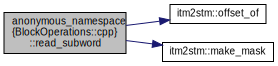
\includegraphics[width=350pt]{namespaceanonymous__namespace_02BlockOperations_8cpp_03_a5eb4b8a9624b717c32fe7722f6811dc3_cgraph}
\end{center}
\end{figure}




Here is the caller graph for this function\-:
\nopagebreak
\begin{figure}[H]
\begin{center}
\leavevmode
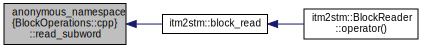
\includegraphics[width=350pt]{namespaceanonymous__namespace_02BlockOperations_8cpp_03_a5eb4b8a9624b717c32fe7722f6811dc3_icgraph}
\end{center}
\end{figure}


\hypertarget{namespaceanonymous__namespace_02BlockOperations_8cpp_03_a637c079bc9ac3e8e4b5d988b469703ae}{\index{anonymous\-\_\-namespace\{\-Block\-Operations.\-cpp\}@{anonymous\-\_\-namespace\{\-Block\-Operations.\-cpp\}}!write\-\_\-subword@{write\-\_\-subword}}
\index{write\-\_\-subword@{write\-\_\-subword}!anonymous_namespace{BlockOperations.cpp}@{anonymous\-\_\-namespace\{\-Block\-Operations.\-cpp\}}}
\subsubsection[{write\-\_\-subword}]{\setlength{\rightskip}{0pt plus 5cm}size\-\_\-t anonymous\-\_\-namespace\{Block\-Operations.\-cpp\}\-::write\-\_\-subword (
\begin{DoxyParamCaption}
\item[{{\bf Tx\-Thread} \&}]{tx, }
\item[{void $\ast$$\ast$}]{base, }
\item[{const uint8\-\_\-t $\ast$}]{from, }
\item[{size\-\_\-t}]{i, }
\item[{size\-\_\-t}]{j}
\end{DoxyParamCaption}
)\hspace{0.3cm}{\ttfamily [inline]}}}\label{namespaceanonymous__namespace_02BlockOperations_8cpp_03_a637c079bc9ac3e8e4b5d988b469703ae}


Here is the call graph for this function\-:
\nopagebreak
\begin{figure}[H]
\begin{center}
\leavevmode
\includegraphics[width=350pt]{namespaceanonymous__namespace_02BlockOperations_8cpp_03_a637c079bc9ac3e8e4b5d988b469703ae_cgraph}
\end{center}
\end{figure}




Here is the caller graph for this function\-:
\nopagebreak
\begin{figure}[H]
\begin{center}
\leavevmode
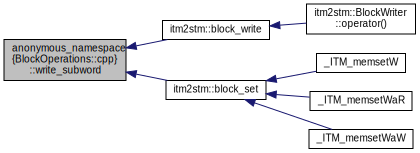
\includegraphics[width=350pt]{namespaceanonymous__namespace_02BlockOperations_8cpp_03_a637c079bc9ac3e8e4b5d988b469703ae_icgraph}
\end{center}
\end{figure}



\hypertarget{namespaceanonymous__namespace_02bmharness_8cpp_03}{\section{anonymous\-\_\-namespace\{bmharness.\-cpp\} Namespace Reference}
\label{namespaceanonymous__namespace_02bmharness_8cpp_03}\index{anonymous\-\_\-namespace\{bmharness.\-cpp\}@{anonymous\-\_\-namespace\{bmharness.\-cpp\}}}
}
\subsection*{Functions}
\begin{DoxyCompactItemize}
\item 
void \hyperlink{namespaceanonymous__namespace_02bmharness_8cpp_03_a2a8d55c1ea2dc5801342821a8d01f224}{dump\-\_\-csv} ()
\item 
void \hyperlink{namespaceanonymous__namespace_02bmharness_8cpp_03_aa32e918fdf95644d2bde2bc98148180b}{usage} ()
\item 
void \hyperlink{namespaceanonymous__namespace_02bmharness_8cpp_03_ae311ed7903214e2716e5be5647da1147}{parseargs} (int argc, char $\ast$$\ast$argv)
\item 
void \hyperlink{namespaceanonymous__namespace_02bmharness_8cpp_03_a462b57784abacad16826f81937a24106}{nontxnwork} ()
\item 
void \hyperlink{namespaceanonymous__namespace_02bmharness_8cpp_03_a02bc3cad3eee0bfe5281b1a3a24cc784}{catch\-\_\-\-S\-I\-G\-A\-L\-R\-M} (int)
\item 
void \hyperlink{namespaceanonymous__namespace_02bmharness_8cpp_03_ac2f3da62721969da434141bf2282eab0}{barrier} (uint32\-\_\-t which)
\item 
void \hyperlink{namespaceanonymous__namespace_02bmharness_8cpp_03_a3a26cd6fa1dad4dd21a46c88c2a02817}{run} (uintptr\-\_\-t id)
\item 
\hyperlink{platform_8hpp_a1b173d22e57d9395897acbd8de62d505}{N\-O\-I\-N\-L\-I\-N\-E} void $\ast$ \hyperlink{namespaceanonymous__namespace_02bmharness_8cpp_03_a5275c4f9613d117686614bfbf705ab2b}{run\-\_\-wrapper} (void $\ast$i)
\end{DoxyCompactItemize}


\subsection{Function Documentation}
\hypertarget{namespaceanonymous__namespace_02bmharness_8cpp_03_ac2f3da62721969da434141bf2282eab0}{\index{anonymous\-\_\-namespace\{bmharness.\-cpp\}@{anonymous\-\_\-namespace\{bmharness.\-cpp\}}!barrier@{barrier}}
\index{barrier@{barrier}!anonymous_namespace{bmharness.cpp}@{anonymous\-\_\-namespace\{bmharness.\-cpp\}}}
\subsubsection[{barrier}]{\setlength{\rightskip}{0pt plus 5cm}void anonymous\-\_\-namespace\{bmharness.\-cpp\}\-::{\bf barrier} (
\begin{DoxyParamCaption}
\item[{uint32\-\_\-t}]{which}
\end{DoxyParamCaption}
)}}\label{namespaceanonymous__namespace_02bmharness_8cpp_03_ac2f3da62721969da434141bf2282eab0}
Support a few lightweight barriers \hypertarget{namespaceanonymous__namespace_02bmharness_8cpp_03_a02bc3cad3eee0bfe5281b1a3a24cc784}{\index{anonymous\-\_\-namespace\{bmharness.\-cpp\}@{anonymous\-\_\-namespace\{bmharness.\-cpp\}}!catch\-\_\-\-S\-I\-G\-A\-L\-R\-M@{catch\-\_\-\-S\-I\-G\-A\-L\-R\-M}}
\index{catch\-\_\-\-S\-I\-G\-A\-L\-R\-M@{catch\-\_\-\-S\-I\-G\-A\-L\-R\-M}!anonymous_namespace{bmharness.cpp}@{anonymous\-\_\-namespace\{bmharness.\-cpp\}}}
\subsubsection[{catch\-\_\-\-S\-I\-G\-A\-L\-R\-M}]{\setlength{\rightskip}{0pt plus 5cm}void anonymous\-\_\-namespace\{bmharness.\-cpp\}\-::catch\-\_\-\-S\-I\-G\-A\-L\-R\-M (
\begin{DoxyParamCaption}
\item[{int}]{}
\end{DoxyParamCaption}
)}}\label{namespaceanonymous__namespace_02bmharness_8cpp_03_a02bc3cad3eee0bfe5281b1a3a24cc784}
\hypertarget{namespaceanonymous__namespace_02bmharness_8cpp_03_a2a8d55c1ea2dc5801342821a8d01f224}{\index{anonymous\-\_\-namespace\{bmharness.\-cpp\}@{anonymous\-\_\-namespace\{bmharness.\-cpp\}}!dump\-\_\-csv@{dump\-\_\-csv}}
\index{dump\-\_\-csv@{dump\-\_\-csv}!anonymous_namespace{bmharness.cpp}@{anonymous\-\_\-namespace\{bmharness.\-cpp\}}}
\subsubsection[{dump\-\_\-csv}]{\setlength{\rightskip}{0pt plus 5cm}void anonymous\-\_\-namespace\{bmharness.\-cpp\}\-::dump\-\_\-csv (
\begin{DoxyParamCaption}
{}
\end{DoxyParamCaption}
)}}\label{namespaceanonymous__namespace_02bmharness_8cpp_03_a2a8d55c1ea2dc5801342821a8d01f224}
Print benchmark configuration output \hypertarget{namespaceanonymous__namespace_02bmharness_8cpp_03_a462b57784abacad16826f81937a24106}{\index{anonymous\-\_\-namespace\{bmharness.\-cpp\}@{anonymous\-\_\-namespace\{bmharness.\-cpp\}}!nontxnwork@{nontxnwork}}
\index{nontxnwork@{nontxnwork}!anonymous_namespace{bmharness.cpp}@{anonymous\-\_\-namespace\{bmharness.\-cpp\}}}
\subsubsection[{nontxnwork}]{\setlength{\rightskip}{0pt plus 5cm}void anonymous\-\_\-namespace\{bmharness.\-cpp\}\-::nontxnwork (
\begin{DoxyParamCaption}
{}
\end{DoxyParamCaption}
)}}\label{namespaceanonymous__namespace_02bmharness_8cpp_03_a462b57784abacad16826f81937a24106}
Run some nops between transactions, to simulate some time being spent on computation 

Here is the call graph for this function\-:
\nopagebreak
\begin{figure}[H]
\begin{center}
\leavevmode
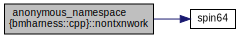
\includegraphics[width=312pt]{namespaceanonymous__namespace_02bmharness_8cpp_03_a462b57784abacad16826f81937a24106_cgraph}
\end{center}
\end{figure}


\hypertarget{namespaceanonymous__namespace_02bmharness_8cpp_03_ae311ed7903214e2716e5be5647da1147}{\index{anonymous\-\_\-namespace\{bmharness.\-cpp\}@{anonymous\-\_\-namespace\{bmharness.\-cpp\}}!parseargs@{parseargs}}
\index{parseargs@{parseargs}!anonymous_namespace{bmharness.cpp}@{anonymous\-\_\-namespace\{bmharness.\-cpp\}}}
\subsubsection[{parseargs}]{\setlength{\rightskip}{0pt plus 5cm}void anonymous\-\_\-namespace\{bmharness.\-cpp\}\-::parseargs (
\begin{DoxyParamCaption}
\item[{int}]{argc, }
\item[{char $\ast$$\ast$}]{argv}
\end{DoxyParamCaption}
)}}\label{namespaceanonymous__namespace_02bmharness_8cpp_03_ae311ed7903214e2716e5be5647da1147}
Parse command line arguments 

Here is the call graph for this function\-:
\nopagebreak
\begin{figure}[H]
\begin{center}
\leavevmode
\includegraphics[width=302pt]{namespaceanonymous__namespace_02bmharness_8cpp_03_ae311ed7903214e2716e5be5647da1147_cgraph}
\end{center}
\end{figure}


\hypertarget{namespaceanonymous__namespace_02bmharness_8cpp_03_a3a26cd6fa1dad4dd21a46c88c2a02817}{\index{anonymous\-\_\-namespace\{bmharness.\-cpp\}@{anonymous\-\_\-namespace\{bmharness.\-cpp\}}!run@{run}}
\index{run@{run}!anonymous_namespace{bmharness.cpp}@{anonymous\-\_\-namespace\{bmharness.\-cpp\}}}
\subsubsection[{run}]{\setlength{\rightskip}{0pt plus 5cm}void anonymous\-\_\-namespace\{bmharness.\-cpp\}\-::run (
\begin{DoxyParamCaption}
\item[{uintptr\-\_\-t}]{id}
\end{DoxyParamCaption}
)}}\label{namespaceanonymous__namespace_02bmharness_8cpp_03_a3a26cd6fa1dad4dd21a46c88c2a02817}


Here is the call graph for this function\-:
\nopagebreak
\begin{figure}[H]
\begin{center}
\leavevmode
\includegraphics[width=350pt]{namespaceanonymous__namespace_02bmharness_8cpp_03_a3a26cd6fa1dad4dd21a46c88c2a02817_cgraph}
\end{center}
\end{figure}


\hypertarget{namespaceanonymous__namespace_02bmharness_8cpp_03_a5275c4f9613d117686614bfbf705ab2b}{\index{anonymous\-\_\-namespace\{bmharness.\-cpp\}@{anonymous\-\_\-namespace\{bmharness.\-cpp\}}!run\-\_\-wrapper@{run\-\_\-wrapper}}
\index{run\-\_\-wrapper@{run\-\_\-wrapper}!anonymous_namespace{bmharness.cpp}@{anonymous\-\_\-namespace\{bmharness.\-cpp\}}}
\subsubsection[{run\-\_\-wrapper}]{\setlength{\rightskip}{0pt plus 5cm}{\bf N\-O\-I\-N\-L\-I\-N\-E} void$\ast$ anonymous\-\_\-namespace\{bmharness.\-cpp\}\-::run\-\_\-wrapper (
\begin{DoxyParamCaption}
\item[{void $\ast$}]{i}
\end{DoxyParamCaption}
)}}\label{namespaceanonymous__namespace_02bmharness_8cpp_03_a5275c4f9613d117686614bfbf705ab2b}
pthread wrapper for running the experiments

N\-B\-: noinline prevents this from getting inlined into main (and prevents run from being inlined there as well. This eliminates an \-\_\-\-I\-T\-M\-\_\-initialize\-Process ordering problem if there's a transaction lexically scoped inside of main. 

Here is the call graph for this function\-:
\nopagebreak
\begin{figure}[H]
\begin{center}
\leavevmode
\includegraphics[width=350pt]{namespaceanonymous__namespace_02bmharness_8cpp_03_a5275c4f9613d117686614bfbf705ab2b_cgraph}
\end{center}
\end{figure}


\hypertarget{namespaceanonymous__namespace_02bmharness_8cpp_03_aa32e918fdf95644d2bde2bc98148180b}{\index{anonymous\-\_\-namespace\{bmharness.\-cpp\}@{anonymous\-\_\-namespace\{bmharness.\-cpp\}}!usage@{usage}}
\index{usage@{usage}!anonymous_namespace{bmharness.cpp}@{anonymous\-\_\-namespace\{bmharness.\-cpp\}}}
\subsubsection[{usage}]{\setlength{\rightskip}{0pt plus 5cm}void anonymous\-\_\-namespace\{bmharness.\-cpp\}\-::usage (
\begin{DoxyParamCaption}
{}
\end{DoxyParamCaption}
)}}\label{namespaceanonymous__namespace_02bmharness_8cpp_03_aa32e918fdf95644d2bde2bc98148180b}
Print usage 
\hypertarget{namespaceanonymous__namespace_02byear_8cpp_03}{\section{anonymous\-\_\-namespace\{byear.\-cpp\} Namespace Reference}
\label{namespaceanonymous__namespace_02byear_8cpp_03}\index{anonymous\-\_\-namespace\{byear.\-cpp\}@{anonymous\-\_\-namespace\{byear.\-cpp\}}}
}
\subsection*{Classes}
\begin{DoxyCompactItemize}
\item 
struct \hyperlink{structanonymous__namespace_02byear_8cpp_03_1_1ByEAR}{By\-E\-A\-R}
\end{DoxyCompactItemize}


\subsection{Detailed Description}
Declare the functions that we're going to implement, so that we can avoid circular dependencies. 
\hypertarget{namespaceanonymous__namespace_02byeau_8cpp_03}{\section{anonymous\-\_\-namespace\{byeau.\-cpp\} Namespace Reference}
\label{namespaceanonymous__namespace_02byeau_8cpp_03}\index{anonymous\-\_\-namespace\{byeau.\-cpp\}@{anonymous\-\_\-namespace\{byeau.\-cpp\}}}
}
\subsection*{Classes}
\begin{DoxyCompactItemize}
\item 
struct \hyperlink{structanonymous__namespace_02byeau_8cpp_03_1_1ByEAU__Generic}{By\-E\-A\-U\-\_\-\-Generic}
\end{DoxyCompactItemize}


\subsection{Detailed Description}
Declare the functions that we're going to implement, so that we can avoid circular dependencies. 
\hypertarget{namespaceanonymous__namespace_02byteeager_8cpp_03}{\section{anonymous\-\_\-namespace\{byteeager.\-cpp\} Namespace Reference}
\label{namespaceanonymous__namespace_02byteeager_8cpp_03}\index{anonymous\-\_\-namespace\{byteeager.\-cpp\}@{anonymous\-\_\-namespace\{byteeager.\-cpp\}}}
}
\subsection*{Classes}
\begin{DoxyCompactItemize}
\item 
struct \hyperlink{structanonymous__namespace_02byteeager_8cpp_03_1_1ByteEager}{Byte\-Eager}
\end{DoxyCompactItemize}


\subsection{Detailed Description}
Declare the functions that we're going to implement, so that we can avoid circular dependencies. 
\hypertarget{namespaceanonymous__namespace_02byteeagerredo_8cpp_03}{\section{anonymous\-\_\-namespace\{byteeagerredo.\-cpp\} Namespace Reference}
\label{namespaceanonymous__namespace_02byteeagerredo_8cpp_03}\index{anonymous\-\_\-namespace\{byteeagerredo.\-cpp\}@{anonymous\-\_\-namespace\{byteeagerredo.\-cpp\}}}
}
\subsection*{Classes}
\begin{DoxyCompactItemize}
\item 
struct \hyperlink{structanonymous__namespace_02byteeagerredo_8cpp_03_1_1ByteEagerRedo}{Byte\-Eager\-Redo}
\end{DoxyCompactItemize}


\subsection{Detailed Description}
Declare the functions that we're going to implement, so that we can avoid circular dependencies. 
\hypertarget{namespaceanonymous__namespace_02bytelazy_8cpp_03}{\section{anonymous\-\_\-namespace\{bytelazy.\-cpp\} Namespace Reference}
\label{namespaceanonymous__namespace_02bytelazy_8cpp_03}\index{anonymous\-\_\-namespace\{bytelazy.\-cpp\}@{anonymous\-\_\-namespace\{bytelazy.\-cpp\}}}
}
\subsection*{Classes}
\begin{DoxyCompactItemize}
\item 
struct \hyperlink{structanonymous__namespace_02bytelazy_8cpp_03_1_1ByteLazy}{Byte\-Lazy}
\end{DoxyCompactItemize}


\subsection{Detailed Description}
Declare the functions that we're going to implement, so that we can avoid circular dependencies. 
\hypertarget{namespaceanonymous__namespace_02cbr_8cpp_03}{\section{anonymous\-\_\-namespace\{cbr.\-cpp\} Namespace Reference}
\label{namespaceanonymous__namespace_02cbr_8cpp_03}\index{anonymous\-\_\-namespace\{cbr.\-cpp\}@{anonymous\-\_\-namespace\{cbr.\-cpp\}}}
}
\subsection*{Classes}
\begin{DoxyCompactItemize}
\item 
struct \hyperlink{structanonymous__namespace_02cbr_8cpp_03_1_1Read}{Read}
\item 
struct \hyperlink{structanonymous__namespace_02cbr_8cpp_03_1_1Write}{Write}
\item 
struct \hyperlink{structanonymous__namespace_02cbr_8cpp_03_1_1Time}{Time}
\item 
struct \hyperlink{structanonymous__namespace_02cbr_8cpp_03_1_1RO}{R\-O}
\item 
struct \hyperlink{structanonymous__namespace_02cbr_8cpp_03_1_1RW}{R\-W}
\item 
struct \hyperlink{structanonymous__namespace_02cbr_8cpp_03_1_1R__RO}{R\-\_\-\-R\-O}
\item 
struct \hyperlink{structanonymous__namespace_02cbr_8cpp_03_1_1R__Time}{R\-\_\-\-Time}
\item 
struct \hyperlink{structanonymous__namespace_02cbr_8cpp_03_1_1W__RO}{W\-\_\-\-R\-O}
\item 
struct \hyperlink{structanonymous__namespace_02cbr_8cpp_03_1_1W__Time}{W\-\_\-\-Time}
\item 
struct \hyperlink{structanonymous__namespace_02cbr_8cpp_03_1_1Time__RO}{Time\-\_\-\-R\-O}
\item 
struct \hyperlink{structanonymous__namespace_02cbr_8cpp_03_1_1R__W__RO}{R\-\_\-\-W\-\_\-\-R\-O}
\item 
struct \hyperlink{structanonymous__namespace_02cbr_8cpp_03_1_1R__W__Time}{R\-\_\-\-W\-\_\-\-Time}
\item 
struct \hyperlink{structanonymous__namespace_02cbr_8cpp_03_1_1R__Time__RO}{R\-\_\-\-Time\-\_\-\-R\-O}
\item 
struct \hyperlink{structanonymous__namespace_02cbr_8cpp_03_1_1W__Time__RO}{W\-\_\-\-Time\-\_\-\-R\-O}
\item 
struct \hyperlink{structanonymous__namespace_02cbr_8cpp_03_1_1R__W__Time__RO}{R\-\_\-\-W\-\_\-\-Time\-\_\-\-R\-O}
\item 
struct \hyperlink{structanonymous__namespace_02cbr_8cpp_03_1_1TxnRatio}{Txn\-Ratio}
\item 
struct \hyperlink{structanonymous__namespace_02cbr_8cpp_03_1_1TxnRatio__R}{Txn\-Ratio\-\_\-\-R}
\item 
struct \hyperlink{structanonymous__namespace_02cbr_8cpp_03_1_1TxnRatio__W}{Txn\-Ratio\-\_\-\-W}
\item 
struct \hyperlink{structanonymous__namespace_02cbr_8cpp_03_1_1TxnRatio__RO}{Txn\-Ratio\-\_\-\-R\-O}
\item 
struct \hyperlink{structanonymous__namespace_02cbr_8cpp_03_1_1TxnRatio__Time}{Txn\-Ratio\-\_\-\-Time}
\item 
struct \hyperlink{structanonymous__namespace_02cbr_8cpp_03_1_1TxnRatio__RW}{Txn\-Ratio\-\_\-\-R\-W}
\item 
struct \hyperlink{structanonymous__namespace_02cbr_8cpp_03_1_1TxnRatio__R__RO}{Txn\-Ratio\-\_\-\-R\-\_\-\-R\-O}
\item 
struct \hyperlink{structanonymous__namespace_02cbr_8cpp_03_1_1TxnRatio__R__Time}{Txn\-Ratio\-\_\-\-R\-\_\-\-Time}
\item 
struct \hyperlink{structanonymous__namespace_02cbr_8cpp_03_1_1TxnRatio__W__RO}{Txn\-Ratio\-\_\-\-W\-\_\-\-R\-O}
\item 
struct \hyperlink{structanonymous__namespace_02cbr_8cpp_03_1_1TxnRatio__W__Time}{Txn\-Ratio\-\_\-\-W\-\_\-\-Time}
\item 
struct \hyperlink{structanonymous__namespace_02cbr_8cpp_03_1_1TxnRatio__RO__Time}{Txn\-Ratio\-\_\-\-R\-O\-\_\-\-Time}
\item 
struct \hyperlink{structanonymous__namespace_02cbr_8cpp_03_1_1TxnRatio__RW__RO}{Txn\-Ratio\-\_\-\-R\-W\-\_\-\-R\-O}
\item 
struct \hyperlink{structanonymous__namespace_02cbr_8cpp_03_1_1TxnRatio__RW__Time}{Txn\-Ratio\-\_\-\-R\-W\-\_\-\-Time}
\item 
struct \hyperlink{structanonymous__namespace_02cbr_8cpp_03_1_1TxnRatio__R__RO__Time}{Txn\-Ratio\-\_\-\-R\-\_\-\-R\-O\-\_\-\-Time}
\item 
struct \hyperlink{structanonymous__namespace_02cbr_8cpp_03_1_1TxnRatio__W__RO__Time}{Txn\-Ratio\-\_\-\-W\-\_\-\-R\-O\-\_\-\-Time}
\item 
struct \hyperlink{structanonymous__namespace_02cbr_8cpp_03_1_1TxnRatio__RW__RO__Time}{Txn\-Ratio\-\_\-\-R\-W\-\_\-\-R\-O\-\_\-\-Time}
\end{DoxyCompactItemize}
\subsection*{Functions}
\begin{DoxyCompactItemize}
\item 
\hyperlink{platform_8hpp_abdc8d70d196a73a2a119efdbe674ecf8}{T\-M\-\_\-\-I\-N\-L\-I\-N\-E} unsigned long \hyperlink{namespaceanonymous__namespace_02cbr_8cpp_03_a9581e1f6511c6795fbd98578ecea3b78}{norm\-\_\-dist} (unsigned long a, unsigned long b)
\item 
\hyperlink{platform_8hpp_a8b5d728e6eed8f368f9966f637d2f719}{T\-M\-\_\-\-F\-A\-S\-T\-C\-A\-L\-L} uint32\-\_\-t \hyperlink{namespaceanonymous__namespace_02cbr_8cpp_03_a24ec6eb1e0eca0a6b9866180e5e3ecb0}{profile\-\_\-nochange} ()
\item 
{\footnotesize template$<$class C $>$ }\\uint32\-\_\-t \hyperlink{namespaceanonymous__namespace_02cbr_8cpp_03_a6d59ee82837d29707c2f774262228976}{cbr\-\_\-tail} (\hyperlink{structstm_1_1qtable__t}{qtable\-\_\-t} \&profile)
\item 
\hyperlink{platform_8hpp_a8b5d728e6eed8f368f9966f637d2f719}{T\-M\-\_\-\-F\-A\-S\-T\-C\-A\-L\-L} uint32\-\_\-t \hyperlink{namespaceanonymous__namespace_02cbr_8cpp_03_a0566a8b94db9550484ad458e48c3d7f9}{pol\-\_\-\-C\-B\-R\-\_\-\-R\-O} ()
\item 
{\footnotesize template$<$class C $>$ }\\\hyperlink{platform_8hpp_a8b5d728e6eed8f368f9966f637d2f719}{T\-M\-\_\-\-F\-A\-S\-T\-C\-A\-L\-L} uint32\-\_\-t \hyperlink{namespaceanonymous__namespace_02cbr_8cpp_03_a4ddd26e7ad4488682da335e5ad1a3351}{cbr\-\_\-nn} ()
\end{DoxyCompactItemize}


\subsection{Detailed Description}
This file implements a few classifiers for trying to pick which algorithm to switch to, based on some existing information from a profile and a table of previous experiments. 

\subsection{Function Documentation}
\hypertarget{namespaceanonymous__namespace_02cbr_8cpp_03_a4ddd26e7ad4488682da335e5ad1a3351}{\index{anonymous\-\_\-namespace\{cbr.\-cpp\}@{anonymous\-\_\-namespace\{cbr.\-cpp\}}!cbr\-\_\-nn@{cbr\-\_\-nn}}
\index{cbr\-\_\-nn@{cbr\-\_\-nn}!anonymous_namespace{cbr.cpp}@{anonymous\-\_\-namespace\{cbr.\-cpp\}}}
\subsubsection[{cbr\-\_\-nn}]{\setlength{\rightskip}{0pt plus 5cm}template$<$class C $>$ {\bf T\-M\-\_\-\-F\-A\-S\-T\-C\-A\-L\-L} uint32\-\_\-t anonymous\-\_\-namespace\{cbr.\-cpp\}\-::cbr\-\_\-nn (
\begin{DoxyParamCaption}
{}
\end{DoxyParamCaption}
)}}\label{namespaceanonymous__namespace_02cbr_8cpp_03_a4ddd26e7ad4488682da335e5ad1a3351}
This template provides the functionality we need for doing a nearest-\/neighbor classification where we use as input the summary profile, and scan through the qtable to find the most representative row 

Here is the call graph for this function\-:
\nopagebreak
\begin{figure}[H]
\begin{center}
\leavevmode
\includegraphics[width=350pt]{namespaceanonymous__namespace_02cbr_8cpp_03_a4ddd26e7ad4488682da335e5ad1a3351_cgraph}
\end{center}
\end{figure}


\hypertarget{namespaceanonymous__namespace_02cbr_8cpp_03_a6d59ee82837d29707c2f774262228976}{\index{anonymous\-\_\-namespace\{cbr.\-cpp\}@{anonymous\-\_\-namespace\{cbr.\-cpp\}}!cbr\-\_\-tail@{cbr\-\_\-tail}}
\index{cbr\-\_\-tail@{cbr\-\_\-tail}!anonymous_namespace{cbr.cpp}@{anonymous\-\_\-namespace\{cbr.\-cpp\}}}
\subsubsection[{cbr\-\_\-tail}]{\setlength{\rightskip}{0pt plus 5cm}template$<$class C $>$ uint32\-\_\-t anonymous\-\_\-namespace\{cbr.\-cpp\}\-::cbr\-\_\-tail (
\begin{DoxyParamCaption}
\item[{{\bf qtable\-\_\-t} \&}]{profile}
\end{DoxyParamCaption}
)}}\label{namespaceanonymous__namespace_02cbr_8cpp_03_a6d59ee82837d29707c2f774262228976}
Common part of C\-B\-R code \hypertarget{namespaceanonymous__namespace_02cbr_8cpp_03_a9581e1f6511c6795fbd98578ecea3b78}{\index{anonymous\-\_\-namespace\{cbr.\-cpp\}@{anonymous\-\_\-namespace\{cbr.\-cpp\}}!norm\-\_\-dist@{norm\-\_\-dist}}
\index{norm\-\_\-dist@{norm\-\_\-dist}!anonymous_namespace{cbr.cpp}@{anonymous\-\_\-namespace\{cbr.\-cpp\}}}
\subsubsection[{norm\-\_\-dist}]{\setlength{\rightskip}{0pt plus 5cm}{\bf T\-M\-\_\-\-I\-N\-L\-I\-N\-E} unsigned long anonymous\-\_\-namespace\{cbr.\-cpp\}\-::norm\-\_\-dist (
\begin{DoxyParamCaption}
\item[{unsigned long}]{a, }
\item[{unsigned long}]{b}
\end{DoxyParamCaption}
)}}\label{namespaceanonymous__namespace_02cbr_8cpp_03_a9581e1f6511c6795fbd98578ecea3b78}
The C\-B\-R policies can all be characterized as follows\-:


\begin{DoxyItemize}
\item We have a qtable full of normalized profiles
\item We have a summary\-\_\-profile, which is the average of N profiles, normalized
\item For each qtable row, for each column, compute the norm\-\_\-dist between the row and the summary\-\_\-profile. Take the weighted sum of the distances
\item Return the algorithm whose name appears in the qtable row with the minimum weighted sum norm\-\_\-dist

Implicit in this description is the fact that norm\-\_\-dist must be defined relative to a normalization strategy. Using this norm\-\_\-dist function implies that we tend to choose a qtable entry with larger number on some attribute when we have a tie in Manhattan distance. E.\-g., when we get a profiled read number of 4, we may only have 2 entries in the qtable, one with a read number of 3 and the other one with a read number of 5. In this case, we will choose the row with 5. 
\end{DoxyItemize}

Here is the caller graph for this function\-:
\nopagebreak
\begin{figure}[H]
\begin{center}
\leavevmode
\includegraphics[height=550pt]{namespaceanonymous__namespace_02cbr_8cpp_03_a9581e1f6511c6795fbd98578ecea3b78_icgraph}
\end{center}
\end{figure}


\hypertarget{namespaceanonymous__namespace_02cbr_8cpp_03_a0566a8b94db9550484ad458e48c3d7f9}{\index{anonymous\-\_\-namespace\{cbr.\-cpp\}@{anonymous\-\_\-namespace\{cbr.\-cpp\}}!pol\-\_\-\-C\-B\-R\-\_\-\-R\-O@{pol\-\_\-\-C\-B\-R\-\_\-\-R\-O}}
\index{pol\-\_\-\-C\-B\-R\-\_\-\-R\-O@{pol\-\_\-\-C\-B\-R\-\_\-\-R\-O}!anonymous_namespace{cbr.cpp}@{anonymous\-\_\-namespace\{cbr.\-cpp\}}}
\subsubsection[{pol\-\_\-\-C\-B\-R\-\_\-\-R\-O}]{\setlength{\rightskip}{0pt plus 5cm}{\bf T\-M\-\_\-\-F\-A\-S\-T\-C\-A\-L\-L} uint32\-\_\-t anonymous\-\_\-namespace\{cbr.\-cpp\}\-::pol\-\_\-\-C\-B\-R\-\_\-\-R\-O (
\begin{DoxyParamCaption}
{}
\end{DoxyParamCaption}
)}}\label{namespaceanonymous__namespace_02cbr_8cpp_03_a0566a8b94db9550484ad458e48c3d7f9}
This policy compares the read-\/only ratio of the current workload to the read-\/only ratios of entries in our qtable, using a nearest neighbor distance. Note that it does not use profiles at all. 

Here is the caller graph for this function\-:
\nopagebreak
\begin{figure}[H]
\begin{center}
\leavevmode
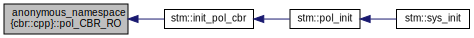
\includegraphics[width=350pt]{namespaceanonymous__namespace_02cbr_8cpp_03_a0566a8b94db9550484ad458e48c3d7f9_icgraph}
\end{center}
\end{figure}


\hypertarget{namespaceanonymous__namespace_02cbr_8cpp_03_a24ec6eb1e0eca0a6b9866180e5e3ecb0}{\index{anonymous\-\_\-namespace\{cbr.\-cpp\}@{anonymous\-\_\-namespace\{cbr.\-cpp\}}!profile\-\_\-nochange@{profile\-\_\-nochange}}
\index{profile\-\_\-nochange@{profile\-\_\-nochange}!anonymous_namespace{cbr.cpp}@{anonymous\-\_\-namespace\{cbr.\-cpp\}}}
\subsubsection[{profile\-\_\-nochange}]{\setlength{\rightskip}{0pt plus 5cm}{\bf T\-M\-\_\-\-F\-A\-S\-T\-C\-A\-L\-L} uint32\-\_\-t anonymous\-\_\-namespace\{cbr.\-cpp\}\-::profile\-\_\-nochange (
\begin{DoxyParamCaption}
{}
\end{DoxyParamCaption}
)}}\label{namespaceanonymous__namespace_02cbr_8cpp_03_a24ec6eb1e0eca0a6b9866180e5e3ecb0}
A testing policy\-: we use this to return exactly the same algorithm as we had before a profile was run. The reason this is implemented here is just so that we have a hook in the standard place to ensure that profiles get printed. 

Here is the call graph for this function\-:
\nopagebreak
\begin{figure}[H]
\begin{center}
\leavevmode
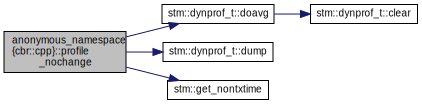
\includegraphics[width=350pt]{namespaceanonymous__namespace_02cbr_8cpp_03_a24ec6eb1e0eca0a6b9866180e5e3ecb0_cgraph}
\end{center}
\end{figure}




Here is the caller graph for this function\-:
\nopagebreak
\begin{figure}[H]
\begin{center}
\leavevmode
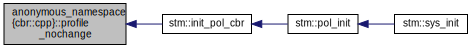
\includegraphics[width=350pt]{namespaceanonymous__namespace_02cbr_8cpp_03_a24ec6eb1e0eca0a6b9866180e5e3ecb0_icgraph}
\end{center}
\end{figure}



\hypertarget{namespaceanonymous__namespace_02cgl_8cpp_03}{\section{anonymous\-\_\-namespace\{cgl.\-cpp\} Namespace Reference}
\label{namespaceanonymous__namespace_02cgl_8cpp_03}\index{anonymous\-\_\-namespace\{cgl.\-cpp\}@{anonymous\-\_\-namespace\{cgl.\-cpp\}}}
}
\subsection*{Classes}
\begin{DoxyCompactItemize}
\item 
struct \hyperlink{structanonymous__namespace_02cgl_8cpp_03_1_1CGL}{C\-G\-L}
\end{DoxyCompactItemize}


\subsection{Detailed Description}
Declare the functions that we're going to implement, so that we can avoid circular dependencies. 
\hypertarget{namespaceanonymous__namespace_02ctoken_8cpp_03}{\section{anonymous\-\_\-namespace\{ctoken.\-cpp\} Namespace Reference}
\label{namespaceanonymous__namespace_02ctoken_8cpp_03}\index{anonymous\-\_\-namespace\{ctoken.\-cpp\}@{anonymous\-\_\-namespace\{ctoken.\-cpp\}}}
}
\subsection*{Classes}
\begin{DoxyCompactItemize}
\item 
struct \hyperlink{structanonymous__namespace_02ctoken_8cpp_03_1_1CToken}{C\-Token}
\end{DoxyCompactItemize}


\subsection{Detailed Description}
Declare the functions that we're going to implement, so that we can avoid circular dependencies. 
\hypertarget{namespaceanonymous__namespace_02ctokenturbo_8cpp_03}{\section{anonymous\-\_\-namespace\{ctokenturbo.\-cpp\} Namespace Reference}
\label{namespaceanonymous__namespace_02ctokenturbo_8cpp_03}\index{anonymous\-\_\-namespace\{ctokenturbo.\-cpp\}@{anonymous\-\_\-namespace\{ctokenturbo.\-cpp\}}}
}
\subsection*{Classes}
\begin{DoxyCompactItemize}
\item 
struct \hyperlink{structanonymous__namespace_02ctokenturbo_8cpp_03_1_1CTokenTurbo}{C\-Token\-Turbo}
\end{DoxyCompactItemize}


\subsection{Detailed Description}
Declare the functions that we're going to implement, so that we can avoid circular dependencies. 
\hypertarget{namespaceanonymous__namespace_02irrevocability_8cpp_03}{\section{anonymous\-\_\-namespace\{irrevocability.\-cpp\} Namespace Reference}
\label{namespaceanonymous__namespace_02irrevocability_8cpp_03}\index{anonymous\-\_\-namespace\{irrevocability.\-cpp\}@{anonymous\-\_\-namespace\{irrevocability.\-cpp\}}}
}
\subsection*{Functions}
\begin{DoxyCompactItemize}
\item 
\hyperlink{platform_8hpp_aa1728270d73c5d1598de1fd691762eb1}{N\-O\-R\-E\-T\-U\-R\-N} void \hyperlink{namespaceanonymous__namespace_02irrevocability_8cpp_03_ac71fd4f2ae60b1814ccaedea40d424a2}{abort\-\_\-irrevocable} (\hyperlink{structstm_1_1TxThread}{Tx\-Thread} $\ast$\hyperlink{stmskip_8cc_a0f1c58699b83ce5a08bd9ee859250d72}{tx})
\item 
\hyperlink{namespacestm_a91badf88c88aacc831b01a315435a255}{stm\-::scope\-\_\-t} $\ast$ \hyperlink{namespaceanonymous__namespace_02irrevocability_8cpp_03_adfdb44f5b204ddd367543d1e3a5465fc}{rollback\-\_\-irrevocable} (\hyperlink{include_2stm_2macros_8hpp_a1c36a48149c84f90d5bca01019950ca9}{S\-T\-M\-\_\-\-R\-O\-L\-L\-B\-A\-C\-K\-\_\-\-S\-I\-G}(,,,))
\item 
void \hyperlink{namespaceanonymous__namespace_02irrevocability_8cpp_03_ab42770392de26e3b0bc1ffbe2f7932b8}{unset\-\_\-irrevocable\-\_\-barriers} (\hyperlink{structstm_1_1TxThread}{Tx\-Thread} \&\hyperlink{stmskip_8cc_a0f1c58699b83ce5a08bd9ee859250d72}{tx})
\item 
\hyperlink{platform_8hpp_a8b5d728e6eed8f368f9966f637d2f719}{T\-M\-\_\-\-F\-A\-S\-T\-C\-A\-L\-L} void \hyperlink{namespaceanonymous__namespace_02irrevocability_8cpp_03_af9e6aae425588bac29be16e10b91cd4c}{commit\-\_\-irrevocable} (\hyperlink{include_2stm_2macros_8hpp_a1b8304eb1082517c7dc31f3534b72343}{S\-T\-M\-\_\-\-C\-O\-M\-M\-I\-T\-\_\-\-S\-I\-G}(\hyperlink{stmskip_8cc_a0f1c58699b83ce5a08bd9ee859250d72}{tx},))
\item 
void \hyperlink{namespaceanonymous__namespace_02irrevocability_8cpp_03_a5f2e3da55eda99c9e30b6314c36ed8b2}{set\-\_\-irrevocable\-\_\-barriers} (\hyperlink{structstm_1_1TxThread}{Tx\-Thread} \&\hyperlink{stmskip_8cc_a0f1c58699b83ce5a08bd9ee859250d72}{tx})
\end{DoxyCompactItemize}
\subsection*{Variables}
\begin{DoxyCompactItemize}
\item 
Abort\-Handler \hyperlink{namespaceanonymous__namespace_02irrevocability_8cpp_03_ac93d4712c00e7ccb77270953062faa28}{old\-\_\-abort\-\_\-handler} = N\-U\-L\-L
\end{DoxyCompactItemize}


\subsection{Function Documentation}
\hypertarget{namespaceanonymous__namespace_02irrevocability_8cpp_03_ac71fd4f2ae60b1814ccaedea40d424a2}{\index{anonymous\-\_\-namespace\{irrevocability.\-cpp\}@{anonymous\-\_\-namespace\{irrevocability.\-cpp\}}!abort\-\_\-irrevocable@{abort\-\_\-irrevocable}}
\index{abort\-\_\-irrevocable@{abort\-\_\-irrevocable}!anonymous_namespace{irrevocability.cpp}@{anonymous\-\_\-namespace\{irrevocability.\-cpp\}}}
\subsubsection[{abort\-\_\-irrevocable}]{\setlength{\rightskip}{0pt plus 5cm}{\bf N\-O\-R\-E\-T\-U\-R\-N} void anonymous\-\_\-namespace\{irrevocability.\-cpp\}\-::abort\-\_\-irrevocable (
\begin{DoxyParamCaption}
\item[{{\bf Tx\-Thread} $\ast$}]{tx}
\end{DoxyParamCaption}
)}}\label{namespaceanonymous__namespace_02irrevocability_8cpp_03_ac71fd4f2ae60b1814ccaedea40d424a2}
Handler for abort attempts while irrevocable. Useful for trapping problems early. 

Here is the call graph for this function\-:
\nopagebreak
\begin{figure}[H]
\begin{center}
\leavevmode
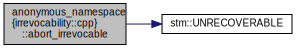
\includegraphics[width=350pt]{namespaceanonymous__namespace_02irrevocability_8cpp_03_ac71fd4f2ae60b1814ccaedea40d424a2_cgraph}
\end{center}
\end{figure}




Here is the caller graph for this function\-:
\nopagebreak
\begin{figure}[H]
\begin{center}
\leavevmode
\includegraphics[width=350pt]{namespaceanonymous__namespace_02irrevocability_8cpp_03_ac71fd4f2ae60b1814ccaedea40d424a2_icgraph}
\end{center}
\end{figure}


\hypertarget{namespaceanonymous__namespace_02irrevocability_8cpp_03_af9e6aae425588bac29be16e10b91cd4c}{\index{anonymous\-\_\-namespace\{irrevocability.\-cpp\}@{anonymous\-\_\-namespace\{irrevocability.\-cpp\}}!commit\-\_\-irrevocable@{commit\-\_\-irrevocable}}
\index{commit\-\_\-irrevocable@{commit\-\_\-irrevocable}!anonymous_namespace{irrevocability.cpp}@{anonymous\-\_\-namespace\{irrevocability.\-cpp\}}}
\subsubsection[{commit\-\_\-irrevocable}]{\setlength{\rightskip}{0pt plus 5cm}{\bf T\-M\-\_\-\-F\-A\-S\-T\-C\-A\-L\-L} void anonymous\-\_\-namespace\{irrevocability.\-cpp\}\-::commit\-\_\-irrevocable (
\begin{DoxyParamCaption}
\item[{{\bf S\-T\-M\-\_\-\-C\-O\-M\-M\-I\-T\-\_\-\-S\-I\-G}({\bf tx},)}]{}
\end{DoxyParamCaption}
)}}\label{namespaceanonymous__namespace_02irrevocability_8cpp_03_af9e6aae425588bac29be16e10b91cd4c}
custom commit for irrevocable transactions 

Here is the call graph for this function\-:
\nopagebreak
\begin{figure}[H]
\begin{center}
\leavevmode
\includegraphics[width=350pt]{namespaceanonymous__namespace_02irrevocability_8cpp_03_af9e6aae425588bac29be16e10b91cd4c_cgraph}
\end{center}
\end{figure}




Here is the caller graph for this function\-:
\nopagebreak
\begin{figure}[H]
\begin{center}
\leavevmode
\includegraphics[width=350pt]{namespaceanonymous__namespace_02irrevocability_8cpp_03_af9e6aae425588bac29be16e10b91cd4c_icgraph}
\end{center}
\end{figure}


\hypertarget{namespaceanonymous__namespace_02irrevocability_8cpp_03_adfdb44f5b204ddd367543d1e3a5465fc}{\index{anonymous\-\_\-namespace\{irrevocability.\-cpp\}@{anonymous\-\_\-namespace\{irrevocability.\-cpp\}}!rollback\-\_\-irrevocable@{rollback\-\_\-irrevocable}}
\index{rollback\-\_\-irrevocable@{rollback\-\_\-irrevocable}!anonymous_namespace{irrevocability.cpp}@{anonymous\-\_\-namespace\{irrevocability.\-cpp\}}}
\subsubsection[{rollback\-\_\-irrevocable}]{\setlength{\rightskip}{0pt plus 5cm}{\bf stm\-::scope\-\_\-t}$\ast$ anonymous\-\_\-namespace\{irrevocability.\-cpp\}\-::rollback\-\_\-irrevocable (
\begin{DoxyParamCaption}
\item[{{\bf S\-T\-M\-\_\-\-R\-O\-L\-L\-B\-A\-C\-K\-\_\-\-S\-I\-G}(,,,)}]{}
\end{DoxyParamCaption}
)}}\label{namespaceanonymous__namespace_02irrevocability_8cpp_03_adfdb44f5b204ddd367543d1e3a5465fc}
Handler for rollback attempts while irrevocable. Useful for trapping problems early.

N\-B\-: For whatever reason a 'using \hyperlink{namespacestm_a91badf88c88aacc831b01a315435a255}{stm\-::scope\-\_\-t}' triggers an I\-C\-E in Mac O\-S X's default gcc-\/4.\-2.\-1. It's fine if we use the fully qualified namespace here. 

Here is the call graph for this function\-:
\nopagebreak
\begin{figure}[H]
\begin{center}
\leavevmode
\includegraphics[width=350pt]{namespaceanonymous__namespace_02irrevocability_8cpp_03_adfdb44f5b204ddd367543d1e3a5465fc_cgraph}
\end{center}
\end{figure}




Here is the caller graph for this function\-:
\nopagebreak
\begin{figure}[H]
\begin{center}
\leavevmode
\includegraphics[width=350pt]{namespaceanonymous__namespace_02irrevocability_8cpp_03_adfdb44f5b204ddd367543d1e3a5465fc_icgraph}
\end{center}
\end{figure}


\hypertarget{namespaceanonymous__namespace_02irrevocability_8cpp_03_a5f2e3da55eda99c9e30b6314c36ed8b2}{\index{anonymous\-\_\-namespace\{irrevocability.\-cpp\}@{anonymous\-\_\-namespace\{irrevocability.\-cpp\}}!set\-\_\-irrevocable\-\_\-barriers@{set\-\_\-irrevocable\-\_\-barriers}}
\index{set\-\_\-irrevocable\-\_\-barriers@{set\-\_\-irrevocable\-\_\-barriers}!anonymous_namespace{irrevocability.cpp}@{anonymous\-\_\-namespace\{irrevocability.\-cpp\}}}
\subsubsection[{set\-\_\-irrevocable\-\_\-barriers}]{\setlength{\rightskip}{0pt plus 5cm}void anonymous\-\_\-namespace\{irrevocability.\-cpp\}\-::set\-\_\-irrevocable\-\_\-barriers (
\begin{DoxyParamCaption}
\item[{{\bf Tx\-Thread} \&}]{tx}
\end{DoxyParamCaption}
)\hspace{0.3cm}{\ttfamily [inline]}}}\label{namespaceanonymous__namespace_02irrevocability_8cpp_03_a5f2e3da55eda99c9e30b6314c36ed8b2}
Sets all of the barriers to be irrevocable, except tmbegin. 

Here is the call graph for this function\-:
\nopagebreak
\begin{figure}[H]
\begin{center}
\leavevmode
\includegraphics[width=350pt]{namespaceanonymous__namespace_02irrevocability_8cpp_03_a5f2e3da55eda99c9e30b6314c36ed8b2_cgraph}
\end{center}
\end{figure}




Here is the caller graph for this function\-:
\nopagebreak
\begin{figure}[H]
\begin{center}
\leavevmode
\includegraphics[width=350pt]{namespaceanonymous__namespace_02irrevocability_8cpp_03_a5f2e3da55eda99c9e30b6314c36ed8b2_icgraph}
\end{center}
\end{figure}


\hypertarget{namespaceanonymous__namespace_02irrevocability_8cpp_03_ab42770392de26e3b0bc1ffbe2f7932b8}{\index{anonymous\-\_\-namespace\{irrevocability.\-cpp\}@{anonymous\-\_\-namespace\{irrevocability.\-cpp\}}!unset\-\_\-irrevocable\-\_\-barriers@{unset\-\_\-irrevocable\-\_\-barriers}}
\index{unset\-\_\-irrevocable\-\_\-barriers@{unset\-\_\-irrevocable\-\_\-barriers}!anonymous_namespace{irrevocability.cpp}@{anonymous\-\_\-namespace\{irrevocability.\-cpp\}}}
\subsubsection[{unset\-\_\-irrevocable\-\_\-barriers}]{\setlength{\rightskip}{0pt plus 5cm}void anonymous\-\_\-namespace\{irrevocability.\-cpp\}\-::unset\-\_\-irrevocable\-\_\-barriers (
\begin{DoxyParamCaption}
\item[{{\bf Tx\-Thread} \&}]{tx}
\end{DoxyParamCaption}
)\hspace{0.3cm}{\ttfamily [inline]}}}\label{namespaceanonymous__namespace_02irrevocability_8cpp_03_ab42770392de26e3b0bc1ffbe2f7932b8}
Resets all of the barriers to be the curr\-\_\-policy bariers, except for tmabort which reverts to the one we saved, and tmbegin which should be done manually in the caller. 

Here is the caller graph for this function\-:
\nopagebreak
\begin{figure}[H]
\begin{center}
\leavevmode
\includegraphics[width=350pt]{namespaceanonymous__namespace_02irrevocability_8cpp_03_ab42770392de26e3b0bc1ffbe2f7932b8_icgraph}
\end{center}
\end{figure}




\subsection{Variable Documentation}
\hypertarget{namespaceanonymous__namespace_02irrevocability_8cpp_03_ac93d4712c00e7ccb77270953062faa28}{\index{anonymous\-\_\-namespace\{irrevocability.\-cpp\}@{anonymous\-\_\-namespace\{irrevocability.\-cpp\}}!old\-\_\-abort\-\_\-handler@{old\-\_\-abort\-\_\-handler}}
\index{old\-\_\-abort\-\_\-handler@{old\-\_\-abort\-\_\-handler}!anonymous_namespace{irrevocability.cpp}@{anonymous\-\_\-namespace\{irrevocability.\-cpp\}}}
\subsubsection[{old\-\_\-abort\-\_\-handler}]{\setlength{\rightskip}{0pt plus 5cm}Abort\-Handler anonymous\-\_\-namespace\{irrevocability.\-cpp\}\-::old\-\_\-abort\-\_\-handler = N\-U\-L\-L}}\label{namespaceanonymous__namespace_02irrevocability_8cpp_03_ac93d4712c00e7ccb77270953062faa28}
The abort handler is set during sys\-\_\-init. We overwrite it with abort\-\_\-irrevocable when a transaction becomes irrevocable, and we save the old one here so we can restore it during commit. 
\hypertarget{namespaceanonymous__namespace_02libitm-5_81_005_8cpp_03}{\section{anonymous\-\_\-namespace\{libitm-\/5.1,5.cpp\} Namespace Reference}
\label{namespaceanonymous__namespace_02libitm-5_81_005_8cpp_03}\index{anonymous\-\_\-namespace\{libitm-\/5.\-1,5.\-cpp\}@{anonymous\-\_\-namespace\{libitm-\/5.\-1,5.\-cpp\}}}
}
\subsection*{Functions}
\begin{DoxyCompactItemize}
\item 
\hyperlink{namespaceanonymous__namespace_02libitm-5_81_005_8cpp_03_ace8c647e409f1fb27af6e0a3df63100c}{T\-H\-R\-E\-A\-D\-\_\-\-L\-O\-C\-A\-L\-\_\-\-D\-E\-C\-L\-\_\-\-T\-Y\-P\-E} (\hyperlink{libitm_8h_a65d3a93d285fdbde408558d6b431abc8}{\-\_\-\-I\-T\-M\-\_\-transaction} $\ast$) td
\item 
void \hyperlink{namespaceanonymous__namespace_02libitm-5_81_005_8cpp_03_a4c66a5e4427961d821f3a610417cbf56}{tmabort} (\hyperlink{structstm_1_1TxThread}{stm\-::\-Tx\-Thread} $\ast$\hyperlink{stmskip_8cc_a0f1c58699b83ce5a08bd9ee859250d72}{tx})
\end{DoxyCompactItemize}


\subsection{Function Documentation}
\hypertarget{namespaceanonymous__namespace_02libitm-5_81_005_8cpp_03_ace8c647e409f1fb27af6e0a3df63100c}{\index{anonymous\-\_\-namespace\{libitm-\/5.\-1,5.\-cpp\}@{anonymous\-\_\-namespace\{libitm-\/5.\-1,5.\-cpp\}}!T\-H\-R\-E\-A\-D\-\_\-\-L\-O\-C\-A\-L\-\_\-\-D\-E\-C\-L\-\_\-\-T\-Y\-P\-E@{T\-H\-R\-E\-A\-D\-\_\-\-L\-O\-C\-A\-L\-\_\-\-D\-E\-C\-L\-\_\-\-T\-Y\-P\-E}}
\index{T\-H\-R\-E\-A\-D\-\_\-\-L\-O\-C\-A\-L\-\_\-\-D\-E\-C\-L\-\_\-\-T\-Y\-P\-E@{T\-H\-R\-E\-A\-D\-\_\-\-L\-O\-C\-A\-L\-\_\-\-D\-E\-C\-L\-\_\-\-T\-Y\-P\-E}!anonymous_namespace{libitm-5.1,5.cpp}@{anonymous\-\_\-namespace\{libitm-\/5.\-1,5.\-cpp\}}}
\subsubsection[{T\-H\-R\-E\-A\-D\-\_\-\-L\-O\-C\-A\-L\-\_\-\-D\-E\-C\-L\-\_\-\-T\-Y\-P\-E}]{\setlength{\rightskip}{0pt plus 5cm}anonymous\-\_\-namespace\{libitm-\/5.\-1,5.cpp\}\-::T\-H\-R\-E\-A\-D\-\_\-\-L\-O\-C\-A\-L\-\_\-\-D\-E\-C\-L\-\_\-\-T\-Y\-P\-E (
\begin{DoxyParamCaption}
\item[{{\bf \-\_\-\-I\-T\-M\-\_\-transaction} $\ast$}]{}
\end{DoxyParamCaption}
)}}\label{namespaceanonymous__namespace_02libitm-5_81_005_8cpp_03_ace8c647e409f1fb27af6e0a3df63100c}
Our thread local transaction descriptor. On most platforms this uses \-\_\-\-\_\-thread or its equivalent, but on Mac O\-S X---or if explicitly selected by the user---it will use a specialized template-\/based Pthreads implementation. \hypertarget{namespaceanonymous__namespace_02libitm-5_81_005_8cpp_03_a4c66a5e4427961d821f3a610417cbf56}{\index{anonymous\-\_\-namespace\{libitm-\/5.\-1,5.\-cpp\}@{anonymous\-\_\-namespace\{libitm-\/5.\-1,5.\-cpp\}}!tmabort@{tmabort}}
\index{tmabort@{tmabort}!anonymous_namespace{libitm-5.1,5.cpp}@{anonymous\-\_\-namespace\{libitm-\/5.\-1,5.\-cpp\}}}
\subsubsection[{tmabort}]{\setlength{\rightskip}{0pt plus 5cm}void anonymous\-\_\-namespace\{libitm-\/5.\-1,5.cpp\}\-::tmabort (
\begin{DoxyParamCaption}
\item[{{\bf stm\-::\-Tx\-Thread} $\ast$}]{tx}
\end{DoxyParamCaption}
)}}\label{namespaceanonymous__namespace_02libitm-5_81_005_8cpp_03_a4c66a5e4427961d821f3a610417cbf56}
This is what the stm library will call when it detects a conflict and needs to abort. We always retry in this case, and if we have a registered thrown object we ignore it (the thrown object only pertains to explicit cancel-\/and-\/throw calls, which must happen in a consistent context).

Don't need any of the funky user-\/visible abort handling because the abort is invisible. Just treat it like a restart of the current scope. This is passed to sys\-\_\-init.

Since the stm abort path doesn't protect the stack (R\-S\-T\-M assumes for the moment that aborts are implemented via a longjmp-\/style mechanism), the best that we can do is to protect the stack from here on. This is fine because we /do/ have a longjmp-\/style abort mechanism, and any stack clobbering that happens here is not an issue. 

Here is the call graph for this function\-:
\nopagebreak
\begin{figure}[H]
\begin{center}
\leavevmode
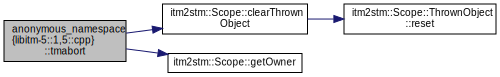
\includegraphics[width=350pt]{namespaceanonymous__namespace_02libitm-5_81_005_8cpp_03_a4c66a5e4427961d821f3a610417cbf56_cgraph}
\end{center}
\end{figure}




Here is the caller graph for this function\-:
\nopagebreak
\begin{figure}[H]
\begin{center}
\leavevmode
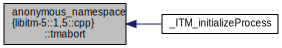
\includegraphics[width=350pt]{namespaceanonymous__namespace_02libitm-5_81_005_8cpp_03_a4c66a5e4427961d821f3a610417cbf56_icgraph}
\end{center}
\end{figure}



\hypertarget{namespaceanonymous__namespace_02libitm-5_812_8cpp_03}{\section{anonymous\-\_\-namespace\{libitm-\/5.12.cpp\} Namespace Reference}
\label{namespaceanonymous__namespace_02libitm-5_812_8cpp_03}\index{anonymous\-\_\-namespace\{libitm-\/5.\-12.\-cpp\}@{anonymous\-\_\-namespace\{libitm-\/5.\-12.\-cpp\}}}
}
\subsection*{Classes}
\begin{DoxyCompactItemize}
\item 
struct \hyperlink{structanonymous__namespace_02libitm-5_812_8cpp_03_1_1INST}{I\-N\-S\-T}
\item 
struct \hyperlink{structanonymous__namespace_02libitm-5_812_8cpp_03_1_1INST_3_01T_00_01N_00_01false_01_4}{I\-N\-S\-T$<$ T, N, false $>$}
\item 
struct \hyperlink{structanonymous__namespace_02libitm-5_812_8cpp_03_1_1INST_3_01T_00_01N_00_01true_01_4}{I\-N\-S\-T$<$ T, N, true $>$}
\item 
struct \hyperlink{structanonymous__namespace_02libitm-5_812_8cpp_03_1_1INST_3_01T_00_010u_00_01false_01_4}{I\-N\-S\-T$<$ T, 0u, false $>$}
\item 
struct \hyperlink{structanonymous__namespace_02libitm-5_812_8cpp_03_1_1INST_3_01T_00_010u_00_01true_01_4}{I\-N\-S\-T$<$ T, 0u, true $>$}
\end{DoxyCompactItemize}

\hypertarget{namespaceanonymous__namespace_02libitm-5_813_0014_8cpp_03}{\section{anonymous\-\_\-namespace\{libitm-\/5.13,14.cpp\} Namespace Reference}
\label{namespaceanonymous__namespace_02libitm-5_813_0014_8cpp_03}\index{anonymous\-\_\-namespace\{libitm-\/5.\-13,14.\-cpp\}@{anonymous\-\_\-namespace\{libitm-\/5.\-13,14.\-cpp\}}}
}
\subsection*{Functions}
\begin{DoxyCompactItemize}
\item 
{\footnotesize template$<$typename R , typename W $>$ }\\void \hyperlink{namespaceanonymous__namespace_02libitm-5_813_0014_8cpp_03_a8b7be7cf3afef27c0623b844ce9116d8}{memcpy} (void $\ast$to, const void $\ast$from, size\-\_\-t len, R reader, W writer)
\item 
size\-\_\-t \hyperlink{namespaceanonymous__namespace_02libitm-5_813_0014_8cpp_03_a8dd7dae76248648e1534f566e0af169b}{builtin\-\_\-memcpy\-\_\-wrapper} (void $\ast$to, const void $\ast$from, size\-\_\-t n)
\item 
size\-\_\-t \hyperlink{namespaceanonymous__namespace_02libitm-5_813_0014_8cpp_03_a721a39277089e6abf82f33aa6d022585}{builtin\-\_\-memmove\-\_\-wrapper} (void $\ast$to, const void $\ast$from, size\-\_\-t n)
\end{DoxyCompactItemize}


\subsection{Function Documentation}
\hypertarget{namespaceanonymous__namespace_02libitm-5_813_0014_8cpp_03_a8dd7dae76248648e1534f566e0af169b}{\index{anonymous\-\_\-namespace\{libitm-\/5.\-13,14.\-cpp\}@{anonymous\-\_\-namespace\{libitm-\/5.\-13,14.\-cpp\}}!builtin\-\_\-memcpy\-\_\-wrapper@{builtin\-\_\-memcpy\-\_\-wrapper}}
\index{builtin\-\_\-memcpy\-\_\-wrapper@{builtin\-\_\-memcpy\-\_\-wrapper}!anonymous_namespace{libitm-5.13,14.cpp}@{anonymous\-\_\-namespace\{libitm-\/5.\-13,14.\-cpp\}}}
\subsubsection[{builtin\-\_\-memcpy\-\_\-wrapper}]{\setlength{\rightskip}{0pt plus 5cm}size\-\_\-t anonymous\-\_\-namespace\{libitm-\/5.\-13,14.cpp\}\-::builtin\-\_\-memcpy\-\_\-wrapper (
\begin{DoxyParamCaption}
\item[{void $\ast$}]{to, }
\item[{const void $\ast$}]{from, }
\item[{size\-\_\-t}]{n}
\end{DoxyParamCaption}
)\hspace{0.3cm}{\ttfamily [inline]}}}\label{namespaceanonymous__namespace_02libitm-5_813_0014_8cpp_03_a8dd7dae76248648e1534f566e0af169b}


Here is the caller graph for this function\-:
\nopagebreak
\begin{figure}[H]
\begin{center}
\leavevmode
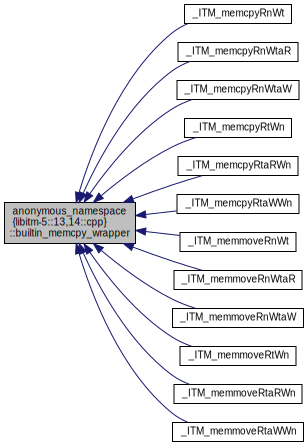
\includegraphics[width=350pt]{namespaceanonymous__namespace_02libitm-5_813_0014_8cpp_03_a8dd7dae76248648e1534f566e0af169b_icgraph}
\end{center}
\end{figure}


\hypertarget{namespaceanonymous__namespace_02libitm-5_813_0014_8cpp_03_a721a39277089e6abf82f33aa6d022585}{\index{anonymous\-\_\-namespace\{libitm-\/5.\-13,14.\-cpp\}@{anonymous\-\_\-namespace\{libitm-\/5.\-13,14.\-cpp\}}!builtin\-\_\-memmove\-\_\-wrapper@{builtin\-\_\-memmove\-\_\-wrapper}}
\index{builtin\-\_\-memmove\-\_\-wrapper@{builtin\-\_\-memmove\-\_\-wrapper}!anonymous_namespace{libitm-5.13,14.cpp}@{anonymous\-\_\-namespace\{libitm-\/5.\-13,14.\-cpp\}}}
\subsubsection[{builtin\-\_\-memmove\-\_\-wrapper}]{\setlength{\rightskip}{0pt plus 5cm}size\-\_\-t anonymous\-\_\-namespace\{libitm-\/5.\-13,14.cpp\}\-::builtin\-\_\-memmove\-\_\-wrapper (
\begin{DoxyParamCaption}
\item[{void $\ast$}]{to, }
\item[{const void $\ast$}]{from, }
\item[{size\-\_\-t}]{n}
\end{DoxyParamCaption}
)\hspace{0.3cm}{\ttfamily [inline]}}}\label{namespaceanonymous__namespace_02libitm-5_813_0014_8cpp_03_a721a39277089e6abf82f33aa6d022585}
\hypertarget{namespaceanonymous__namespace_02libitm-5_813_0014_8cpp_03_a8b7be7cf3afef27c0623b844ce9116d8}{\index{anonymous\-\_\-namespace\{libitm-\/5.\-13,14.\-cpp\}@{anonymous\-\_\-namespace\{libitm-\/5.\-13,14.\-cpp\}}!memcpy@{memcpy}}
\index{memcpy@{memcpy}!anonymous_namespace{libitm-5.13,14.cpp}@{anonymous\-\_\-namespace\{libitm-\/5.\-13,14.\-cpp\}}}
\subsubsection[{memcpy}]{\setlength{\rightskip}{0pt plus 5cm}template$<$typename R , typename W $>$ void anonymous\-\_\-namespace\{libitm-\/5.\-13,14.cpp\}\-::memcpy (
\begin{DoxyParamCaption}
\item[{void $\ast$}]{to, }
\item[{const void $\ast$}]{from, }
\item[{size\-\_\-t}]{len, }
\item[{R}]{reader, }
\item[{W}]{writer}
\end{DoxyParamCaption}
)\hspace{0.3cm}{\ttfamily [inline]}}}\label{namespaceanonymous__namespace_02libitm-5_813_0014_8cpp_03_a8b7be7cf3afef27c0623b844ce9116d8}


Here is the call graph for this function\-:
\nopagebreak
\begin{figure}[H]
\begin{center}
\leavevmode
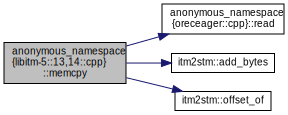
\includegraphics[width=350pt]{namespaceanonymous__namespace_02libitm-5_813_0014_8cpp_03_a8b7be7cf3afef27c0623b844ce9116d8_cgraph}
\end{center}
\end{figure}




Here is the caller graph for this function\-:
\nopagebreak
\begin{figure}[H]
\begin{center}
\leavevmode
\includegraphics[width=350pt]{namespaceanonymous__namespace_02libitm-5_813_0014_8cpp_03_a8b7be7cf3afef27c0623b844ce9116d8_icgraph}
\end{center}
\end{figure}



\hypertarget{namespaceanonymous__namespace_02libitm-5_816_8cpp_03}{\section{anonymous\-\_\-namespace\{libitm-\/5.16.cpp\} Namespace Reference}
\label{namespaceanonymous__namespace_02libitm-5_816_8cpp_03}\index{anonymous\-\_\-namespace\{libitm-\/5.\-16.\-cpp\}@{anonymous\-\_\-namespace\{libitm-\/5.\-16.\-cpp\}}}
}
\subsection*{Classes}
\begin{DoxyCompactItemize}
\item 
struct \hyperlink{structanonymous__namespace_02libitm-5_816_8cpp_03_1_1INST}{I\-N\-S\-T}
\item 
struct \hyperlink{structanonymous__namespace_02libitm-5_816_8cpp_03_1_1INST_3_01T_00_010u_01_4}{I\-N\-S\-T$<$ T, 0u $>$}
\end{DoxyCompactItemize}

\hypertarget{namespaceanonymous__namespace_02llt_8cpp_03}{\section{anonymous\-\_\-namespace\{llt.\-cpp\} Namespace Reference}
\label{namespaceanonymous__namespace_02llt_8cpp_03}\index{anonymous\-\_\-namespace\{llt.\-cpp\}@{anonymous\-\_\-namespace\{llt.\-cpp\}}}
}
\subsection*{Classes}
\begin{DoxyCompactItemize}
\item 
struct \hyperlink{structanonymous__namespace_02llt_8cpp_03_1_1LLT}{L\-L\-T}
\end{DoxyCompactItemize}


\subsection{Detailed Description}
Declare the functions that we're going to implement, so that we can avoid circular dependencies. 
\hypertarget{namespaceanonymous__namespace_02mcs_8cpp_03}{\section{anonymous\-\_\-namespace\{mcs.\-cpp\} Namespace Reference}
\label{namespaceanonymous__namespace_02mcs_8cpp_03}\index{anonymous\-\_\-namespace\{mcs.\-cpp\}@{anonymous\-\_\-namespace\{mcs.\-cpp\}}}
}
\subsection*{Classes}
\begin{DoxyCompactItemize}
\item 
struct \hyperlink{structanonymous__namespace_02mcs_8cpp_03_1_1MCS}{M\-C\-S}
\end{DoxyCompactItemize}


\subsection{Detailed Description}
Declare the functions that we're going to implement, so that we can avoid circular dependencies. 
\hypertarget{namespaceanonymous__namespace_02nano_8cpp_03}{\section{anonymous\-\_\-namespace\{nano.\-cpp\} Namespace Reference}
\label{namespaceanonymous__namespace_02nano_8cpp_03}\index{anonymous\-\_\-namespace\{nano.\-cpp\}@{anonymous\-\_\-namespace\{nano.\-cpp\}}}
}
\subsection*{Classes}
\begin{DoxyCompactItemize}
\item 
struct \hyperlink{structanonymous__namespace_02nano_8cpp_03_1_1Nano}{Nano}
\end{DoxyCompactItemize}


\subsection{Detailed Description}
Declare the functions that we're going to implement, so that we can avoid circular dependencies. 
\hypertarget{namespaceanonymous__namespace_02norec_8cpp_03}{\section{anonymous\-\_\-namespace\{norec.\-cpp\} Namespace Reference}
\label{namespaceanonymous__namespace_02norec_8cpp_03}\index{anonymous\-\_\-namespace\{norec.\-cpp\}@{anonymous\-\_\-namespace\{norec.\-cpp\}}}
}
\subsection*{Classes}
\begin{DoxyCompactItemize}
\item 
struct \hyperlink{structanonymous__namespace_02norec_8cpp_03_1_1NOrec__Generic}{N\-Orec\-\_\-\-Generic}
\end{DoxyCompactItemize}
\subsection*{Functions}
\begin{DoxyCompactItemize}
\item 
\hyperlink{platform_8hpp_a1b173d22e57d9395897acbd8de62d505}{N\-O\-I\-N\-L\-I\-N\-E} uintptr\-\_\-t \hyperlink{namespaceanonymous__namespace_02norec_8cpp_03_aee95b2525a8da3a37e412cee0724967c}{validate} (\hyperlink{structstm_1_1TxThread}{Tx\-Thread} $\ast$)
\item 
bool \hyperlink{namespaceanonymous__namespace_02norec_8cpp_03_a0a6ec6794c0677e7f91daf5cb3a57775}{irrevoc} (\hyperlink{include_2stm_2macros_8hpp_acf117c2df6442342f6603e1a12fa3b5c}{S\-T\-M\-\_\-\-I\-R\-R\-E\-V\-O\-C\-\_\-\-S\-I\-G}(,))
\item 
void \hyperlink{namespaceanonymous__namespace_02norec_8cpp_03_a964889786277f55bf219ecf6a8fbd4a1}{on\-Switch\-To} ()
\item 
bool \hyperlink{namespaceanonymous__namespace_02norec_8cpp_03_af8d688b5b5c223deffce84766ea687ca}{irrevoc} (\hyperlink{include_2stm_2macros_8hpp_acf117c2df6442342f6603e1a12fa3b5c}{S\-T\-M\-\_\-\-I\-R\-R\-E\-V\-O\-C\-\_\-\-S\-I\-G}(\hyperlink{stmskip_8cc_a0f1c58699b83ce5a08bd9ee859250d72}{tx}, upper\-\_\-stack\-\_\-bound))
\end{DoxyCompactItemize}
\subsection*{Variables}
\begin{DoxyCompactItemize}
\item 
const uintptr\-\_\-t \hyperlink{namespaceanonymous__namespace_02norec_8cpp_03_a9f9326929879517472fe0cdccf616ffb}{V\-A\-L\-I\-D\-A\-T\-I\-O\-N\-\_\-\-F\-A\-I\-L\-E\-D} = 1
\end{DoxyCompactItemize}


\subsection{Function Documentation}
\hypertarget{namespaceanonymous__namespace_02norec_8cpp_03_a0a6ec6794c0677e7f91daf5cb3a57775}{\index{anonymous\-\_\-namespace\{norec.\-cpp\}@{anonymous\-\_\-namespace\{norec.\-cpp\}}!irrevoc@{irrevoc}}
\index{irrevoc@{irrevoc}!anonymous_namespace{norec.cpp}@{anonymous\-\_\-namespace\{norec.\-cpp\}}}
\subsubsection[{irrevoc}]{\setlength{\rightskip}{0pt plus 5cm}bool anonymous\-\_\-namespace\{norec.\-cpp\}\-::irrevoc (
\begin{DoxyParamCaption}
\item[{{\bf S\-T\-M\-\_\-\-I\-R\-R\-E\-V\-O\-C\-\_\-\-S\-I\-G}(,)}]{}
\end{DoxyParamCaption}
)}}\label{namespaceanonymous__namespace_02norec_8cpp_03_a0a6ec6794c0677e7f91daf5cb3a57775}


Here is the caller graph for this function\-:
\nopagebreak
\begin{figure}[H]
\begin{center}
\leavevmode
\includegraphics[height=550pt]{namespaceanonymous__namespace_02norec_8cpp_03_a0a6ec6794c0677e7f91daf5cb3a57775_icgraph}
\end{center}
\end{figure}


\hypertarget{namespaceanonymous__namespace_02norec_8cpp_03_af8d688b5b5c223deffce84766ea687ca}{\index{anonymous\-\_\-namespace\{norec.\-cpp\}@{anonymous\-\_\-namespace\{norec.\-cpp\}}!irrevoc@{irrevoc}}
\index{irrevoc@{irrevoc}!anonymous_namespace{norec.cpp}@{anonymous\-\_\-namespace\{norec.\-cpp\}}}
\subsubsection[{irrevoc}]{\setlength{\rightskip}{0pt plus 5cm}bool anonymous\-\_\-namespace\{norec.\-cpp\}\-::irrevoc (
\begin{DoxyParamCaption}
\item[{{\bf S\-T\-M\-\_\-\-I\-R\-R\-E\-V\-O\-C\-\_\-\-S\-I\-G}({\bf tx}, upper\-\_\-stack\-\_\-bound)}]{}
\end{DoxyParamCaption}
)}}\label{namespaceanonymous__namespace_02norec_8cpp_03_af8d688b5b5c223deffce84766ea687ca}


Here is the call graph for this function\-:
\nopagebreak
\begin{figure}[H]
\begin{center}
\leavevmode
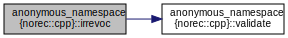
\includegraphics[width=350pt]{namespaceanonymous__namespace_02norec_8cpp_03_af8d688b5b5c223deffce84766ea687ca_cgraph}
\end{center}
\end{figure}




Here is the caller graph for this function\-:
\nopagebreak
\begin{figure}[H]
\begin{center}
\leavevmode
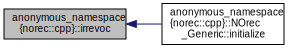
\includegraphics[width=350pt]{namespaceanonymous__namespace_02norec_8cpp_03_af8d688b5b5c223deffce84766ea687ca_icgraph}
\end{center}
\end{figure}


\hypertarget{namespaceanonymous__namespace_02norec_8cpp_03_a964889786277f55bf219ecf6a8fbd4a1}{\index{anonymous\-\_\-namespace\{norec.\-cpp\}@{anonymous\-\_\-namespace\{norec.\-cpp\}}!on\-Switch\-To@{on\-Switch\-To}}
\index{on\-Switch\-To@{on\-Switch\-To}!anonymous_namespace{norec.cpp}@{anonymous\-\_\-namespace\{norec.\-cpp\}}}
\subsubsection[{on\-Switch\-To}]{\setlength{\rightskip}{0pt plus 5cm}void anonymous\-\_\-namespace\{norec.\-cpp\}\-::on\-Switch\-To (
\begin{DoxyParamCaption}
{}
\end{DoxyParamCaption}
)}}\label{namespaceanonymous__namespace_02norec_8cpp_03_a964889786277f55bf219ecf6a8fbd4a1}


Here is the caller graph for this function\-:
\nopagebreak
\begin{figure}[H]
\begin{center}
\leavevmode
\includegraphics[height=550pt]{namespaceanonymous__namespace_02norec_8cpp_03_a964889786277f55bf219ecf6a8fbd4a1_icgraph}
\end{center}
\end{figure}


\hypertarget{namespaceanonymous__namespace_02norec_8cpp_03_aee95b2525a8da3a37e412cee0724967c}{\index{anonymous\-\_\-namespace\{norec.\-cpp\}@{anonymous\-\_\-namespace\{norec.\-cpp\}}!validate@{validate}}
\index{validate@{validate}!anonymous_namespace{norec.cpp}@{anonymous\-\_\-namespace\{norec.\-cpp\}}}
\subsubsection[{validate}]{\setlength{\rightskip}{0pt plus 5cm}uintptr\-\_\-t anonymous\-\_\-namespace\{norec.\-cpp\}\-::validate (
\begin{DoxyParamCaption}
\item[{{\bf Tx\-Thread} $\ast$}]{tx}
\end{DoxyParamCaption}
)}}\label{namespaceanonymous__namespace_02norec_8cpp_03_aee95b2525a8da3a37e412cee0724967c}


Here is the caller graph for this function\-:
\nopagebreak
\begin{figure}[H]
\begin{center}
\leavevmode
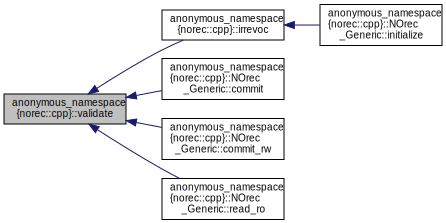
\includegraphics[width=350pt]{namespaceanonymous__namespace_02norec_8cpp_03_aee95b2525a8da3a37e412cee0724967c_icgraph}
\end{center}
\end{figure}




\subsection{Variable Documentation}
\hypertarget{namespaceanonymous__namespace_02norec_8cpp_03_a9f9326929879517472fe0cdccf616ffb}{\index{anonymous\-\_\-namespace\{norec.\-cpp\}@{anonymous\-\_\-namespace\{norec.\-cpp\}}!V\-A\-L\-I\-D\-A\-T\-I\-O\-N\-\_\-\-F\-A\-I\-L\-E\-D@{V\-A\-L\-I\-D\-A\-T\-I\-O\-N\-\_\-\-F\-A\-I\-L\-E\-D}}
\index{V\-A\-L\-I\-D\-A\-T\-I\-O\-N\-\_\-\-F\-A\-I\-L\-E\-D@{V\-A\-L\-I\-D\-A\-T\-I\-O\-N\-\_\-\-F\-A\-I\-L\-E\-D}!anonymous_namespace{norec.cpp}@{anonymous\-\_\-namespace\{norec.\-cpp\}}}
\subsubsection[{V\-A\-L\-I\-D\-A\-T\-I\-O\-N\-\_\-\-F\-A\-I\-L\-E\-D}]{\setlength{\rightskip}{0pt plus 5cm}const uintptr\-\_\-t anonymous\-\_\-namespace\{norec.\-cpp\}\-::V\-A\-L\-I\-D\-A\-T\-I\-O\-N\-\_\-\-F\-A\-I\-L\-E\-D = 1}}\label{namespaceanonymous__namespace_02norec_8cpp_03_a9f9326929879517472fe0cdccf616ffb}

\input{namespaceanonymous__namespace_02norecprio_8cpp_03}
\hypertarget{namespaceanonymous__namespace_02oreau_8cpp_03}{\section{anonymous\-\_\-namespace\{oreau.\-cpp\} Namespace Reference}
\label{namespaceanonymous__namespace_02oreau_8cpp_03}\index{anonymous\-\_\-namespace\{oreau.\-cpp\}@{anonymous\-\_\-namespace\{oreau.\-cpp\}}}
}
\subsection*{Classes}
\begin{DoxyCompactItemize}
\item 
struct \hyperlink{structanonymous__namespace_02oreau_8cpp_03_1_1OrEAU__Generic}{Or\-E\-A\-U\-\_\-\-Generic}
\end{DoxyCompactItemize}


\subsection{Detailed Description}
Declare the functions that we're going to implement, so that we can avoid circular dependencies. 
\hypertarget{namespaceanonymous__namespace_02orecala_8cpp_03}{\section{anonymous\-\_\-namespace\{orecala.\-cpp\} Namespace Reference}
\label{namespaceanonymous__namespace_02orecala_8cpp_03}\index{anonymous\-\_\-namespace\{orecala.\-cpp\}@{anonymous\-\_\-namespace\{orecala.\-cpp\}}}
}
\subsection*{Classes}
\begin{DoxyCompactItemize}
\item 
struct \hyperlink{structanonymous__namespace_02orecala_8cpp_03_1_1OrecALA}{Orec\-A\-L\-A}
\end{DoxyCompactItemize}


\subsection{Detailed Description}
Declare the functions that we're going to implement, so that we can avoid circular dependencies. 
\hypertarget{namespaceanonymous__namespace_02oreceager_8cpp_03}{\section{anonymous\-\_\-namespace\{oreceager.\-cpp\} Namespace Reference}
\label{namespaceanonymous__namespace_02oreceager_8cpp_03}\index{anonymous\-\_\-namespace\{oreceager.\-cpp\}@{anonymous\-\_\-namespace\{oreceager.\-cpp\}}}
}
\subsection*{Classes}
\begin{DoxyCompactItemize}
\item 
struct \hyperlink{structanonymous__namespace_02oreceager_8cpp_03_1_1OrecEager__Generic}{Orec\-Eager\-\_\-\-Generic}
\end{DoxyCompactItemize}
\subsection*{Functions}
\begin{DoxyCompactItemize}
\item 
\hyperlink{platform_8hpp_a8b5d728e6eed8f368f9966f637d2f719}{T\-M\-\_\-\-F\-A\-S\-T\-C\-A\-L\-L} void $\ast$ \hyperlink{namespaceanonymous__namespace_02oreceager_8cpp_03_a7a88c7a7453bbfaca53eeac03b80a5d6}{read} (\hyperlink{include_2stm_2macros_8hpp_abae784c2079f9c1ecc6a72cfeb795db4}{S\-T\-M\-\_\-\-R\-E\-A\-D\-\_\-\-S\-I\-G}(,,))
\item 
\hyperlink{platform_8hpp_a8b5d728e6eed8f368f9966f637d2f719}{T\-M\-\_\-\-F\-A\-S\-T\-C\-A\-L\-L} void \hyperlink{namespaceanonymous__namespace_02oreceager_8cpp_03_ac18758bd7e358cee7461af925e192062}{write} (\hyperlink{include_2stm_2macros_8hpp_a05836a7c31fa89c1c84557f4691c44d3}{S\-T\-M\-\_\-\-W\-R\-I\-T\-E\-\_\-\-S\-I\-G}(,,,))
\item 
bool \hyperlink{namespaceanonymous__namespace_02oreceager_8cpp_03_a1475ab9f49eebf212fa2ce83906d6d9b}{irrevoc} (\hyperlink{include_2stm_2macros_8hpp_acf117c2df6442342f6603e1a12fa3b5c}{S\-T\-M\-\_\-\-I\-R\-R\-E\-V\-O\-C\-\_\-\-S\-I\-G}(,))
\item 
\hyperlink{platform_8hpp_a1b173d22e57d9395897acbd8de62d505}{N\-O\-I\-N\-L\-I\-N\-E} void \hyperlink{namespaceanonymous__namespace_02oreceager_8cpp_03_a5b3a6ab30d79a83a3d13e0718231d4b4}{validate} (\hyperlink{structstm_1_1TxThread}{Tx\-Thread} $\ast$)
\item 
void \hyperlink{namespaceanonymous__namespace_02oreceager_8cpp_03_abf7d699a962bf5ab23bcbaf26b58e0bb}{on\-Switch\-To} ()
\item 
void $\ast$ \hyperlink{namespaceanonymous__namespace_02oreceager_8cpp_03_a2cc56c58ad02007cf0cfa008839f0001}{read} (\hyperlink{include_2stm_2macros_8hpp_abae784c2079f9c1ecc6a72cfeb795db4}{S\-T\-M\-\_\-\-R\-E\-A\-D\-\_\-\-S\-I\-G}(\hyperlink{stmskip_8cc_a0f1c58699b83ce5a08bd9ee859250d72}{tx}, addr,))
\item 
void \hyperlink{namespaceanonymous__namespace_02oreceager_8cpp_03_a4412d636846d1de7149b2ef022d5bf83}{write} (\hyperlink{include_2stm_2macros_8hpp_a05836a7c31fa89c1c84557f4691c44d3}{S\-T\-M\-\_\-\-W\-R\-I\-T\-E\-\_\-\-S\-I\-G}(\hyperlink{stmskip_8cc_a0f1c58699b83ce5a08bd9ee859250d72}{tx}, addr, val, mask))
\item 
bool \hyperlink{namespaceanonymous__namespace_02oreceager_8cpp_03_afcbd1231ae5e881c4c271cd297d6cf97}{irrevoc} (\hyperlink{include_2stm_2macros_8hpp_acf117c2df6442342f6603e1a12fa3b5c}{S\-T\-M\-\_\-\-I\-R\-R\-E\-V\-O\-C\-\_\-\-S\-I\-G}(\hyperlink{stmskip_8cc_a0f1c58699b83ce5a08bd9ee859250d72}{tx},))
\end{DoxyCompactItemize}


\subsection{Detailed Description}
Declare the functions that we're going to implement, so that we can avoid circular dependencies.

N\-B\-: Orec\-Eager actually does better without fine-\/grained switching for read-\/only transactions, so we don't support the read-\/only optimization in this code. 

\subsection{Function Documentation}
\hypertarget{namespaceanonymous__namespace_02oreceager_8cpp_03_a1475ab9f49eebf212fa2ce83906d6d9b}{\index{anonymous\-\_\-namespace\{oreceager.\-cpp\}@{anonymous\-\_\-namespace\{oreceager.\-cpp\}}!irrevoc@{irrevoc}}
\index{irrevoc@{irrevoc}!anonymous_namespace{oreceager.cpp}@{anonymous\-\_\-namespace\{oreceager.\-cpp\}}}
\subsubsection[{irrevoc}]{\setlength{\rightskip}{0pt plus 5cm}bool anonymous\-\_\-namespace\{oreceager.\-cpp\}\-::irrevoc (
\begin{DoxyParamCaption}
\item[{{\bf S\-T\-M\-\_\-\-I\-R\-R\-E\-V\-O\-C\-\_\-\-S\-I\-G}(,)}]{}
\end{DoxyParamCaption}
)}}\label{namespaceanonymous__namespace_02oreceager_8cpp_03_a1475ab9f49eebf212fa2ce83906d6d9b}
\hypertarget{namespaceanonymous__namespace_02oreceager_8cpp_03_afcbd1231ae5e881c4c271cd297d6cf97}{\index{anonymous\-\_\-namespace\{oreceager.\-cpp\}@{anonymous\-\_\-namespace\{oreceager.\-cpp\}}!irrevoc@{irrevoc}}
\index{irrevoc@{irrevoc}!anonymous_namespace{oreceager.cpp}@{anonymous\-\_\-namespace\{oreceager.\-cpp\}}}
\subsubsection[{irrevoc}]{\setlength{\rightskip}{0pt plus 5cm}bool anonymous\-\_\-namespace\{oreceager.\-cpp\}\-::irrevoc (
\begin{DoxyParamCaption}
\item[{{\bf S\-T\-M\-\_\-\-I\-R\-R\-E\-V\-O\-C\-\_\-\-S\-I\-G}({\bf tx},)}]{}
\end{DoxyParamCaption}
)}}\label{namespaceanonymous__namespace_02oreceager_8cpp_03_afcbd1231ae5e881c4c271cd297d6cf97}
Orec\-Eager in-\/flight irrevocability\-:

Either commit the transaction or return false. Note that we're already serial by the time this code runs.

N\-B\-: This doesn't Undo anything, so there's no need to protect the stack. 

Here is the caller graph for this function\-:
\nopagebreak
\begin{figure}[H]
\begin{center}
\leavevmode
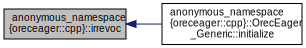
\includegraphics[width=350pt]{namespaceanonymous__namespace_02oreceager_8cpp_03_afcbd1231ae5e881c4c271cd297d6cf97_icgraph}
\end{center}
\end{figure}


\hypertarget{namespaceanonymous__namespace_02oreceager_8cpp_03_abf7d699a962bf5ab23bcbaf26b58e0bb}{\index{anonymous\-\_\-namespace\{oreceager.\-cpp\}@{anonymous\-\_\-namespace\{oreceager.\-cpp\}}!on\-Switch\-To@{on\-Switch\-To}}
\index{on\-Switch\-To@{on\-Switch\-To}!anonymous_namespace{oreceager.cpp}@{anonymous\-\_\-namespace\{oreceager.\-cpp\}}}
\subsubsection[{on\-Switch\-To}]{\setlength{\rightskip}{0pt plus 5cm}void anonymous\-\_\-namespace\{oreceager.\-cpp\}\-::on\-Switch\-To (
\begin{DoxyParamCaption}
{}
\end{DoxyParamCaption}
)}}\label{namespaceanonymous__namespace_02oreceager_8cpp_03_abf7d699a962bf5ab23bcbaf26b58e0bb}
Switch to Orec\-Eager\-:

The timestamp must be $>$= the maximum value of any orec. Some algs use timestamp as a zero-\/one mutex. If they do, then they back up the timestamp first, in timestamp\-\_\-max. 

Here is the caller graph for this function\-:
\nopagebreak
\begin{figure}[H]
\begin{center}
\leavevmode
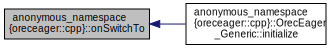
\includegraphics[width=350pt]{namespaceanonymous__namespace_02oreceager_8cpp_03_abf7d699a962bf5ab23bcbaf26b58e0bb_icgraph}
\end{center}
\end{figure}


\hypertarget{namespaceanonymous__namespace_02oreceager_8cpp_03_a7a88c7a7453bbfaca53eeac03b80a5d6}{\index{anonymous\-\_\-namespace\{oreceager.\-cpp\}@{anonymous\-\_\-namespace\{oreceager.\-cpp\}}!read@{read}}
\index{read@{read}!anonymous_namespace{oreceager.cpp}@{anonymous\-\_\-namespace\{oreceager.\-cpp\}}}
\subsubsection[{read}]{\setlength{\rightskip}{0pt plus 5cm}{\bf T\-M\-\_\-\-F\-A\-S\-T\-C\-A\-L\-L} void$\ast$ anonymous\-\_\-namespace\{oreceager.\-cpp\}\-::read (
\begin{DoxyParamCaption}
\item[{{\bf S\-T\-M\-\_\-\-R\-E\-A\-D\-\_\-\-S\-I\-G}(,,)}]{}
\end{DoxyParamCaption}
)}}\label{namespaceanonymous__namespace_02oreceager_8cpp_03_a7a88c7a7453bbfaca53eeac03b80a5d6}


Here is the caller graph for this function\-:
\nopagebreak
\begin{figure}[H]
\begin{center}
\leavevmode
\includegraphics[width=350pt]{namespaceanonymous__namespace_02oreceager_8cpp_03_a7a88c7a7453bbfaca53eeac03b80a5d6_icgraph}
\end{center}
\end{figure}


\hypertarget{namespaceanonymous__namespace_02oreceager_8cpp_03_a2cc56c58ad02007cf0cfa008839f0001}{\index{anonymous\-\_\-namespace\{oreceager.\-cpp\}@{anonymous\-\_\-namespace\{oreceager.\-cpp\}}!read@{read}}
\index{read@{read}!anonymous_namespace{oreceager.cpp}@{anonymous\-\_\-namespace\{oreceager.\-cpp\}}}
\subsubsection[{read}]{\setlength{\rightskip}{0pt plus 5cm}void$\ast$ anonymous\-\_\-namespace\{oreceager.\-cpp\}\-::read (
\begin{DoxyParamCaption}
\item[{{\bf S\-T\-M\-\_\-\-R\-E\-A\-D\-\_\-\-S\-I\-G}({\bf tx}, addr,)}]{}
\end{DoxyParamCaption}
)}}\label{namespaceanonymous__namespace_02oreceager_8cpp_03_a2cc56c58ad02007cf0cfa008839f0001}
Orec\-Eager read\-:

Must check orec twice, and may need to validate 

Here is the call graph for this function\-:
\nopagebreak
\begin{figure}[H]
\begin{center}
\leavevmode
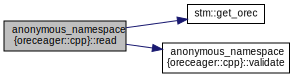
\includegraphics[width=350pt]{namespaceanonymous__namespace_02oreceager_8cpp_03_a2cc56c58ad02007cf0cfa008839f0001_cgraph}
\end{center}
\end{figure}




Here is the caller graph for this function\-:
\nopagebreak
\begin{figure}[H]
\begin{center}
\leavevmode
\includegraphics[width=350pt]{namespaceanonymous__namespace_02oreceager_8cpp_03_a2cc56c58ad02007cf0cfa008839f0001_icgraph}
\end{center}
\end{figure}


\hypertarget{namespaceanonymous__namespace_02oreceager_8cpp_03_a5b3a6ab30d79a83a3d13e0718231d4b4}{\index{anonymous\-\_\-namespace\{oreceager.\-cpp\}@{anonymous\-\_\-namespace\{oreceager.\-cpp\}}!validate@{validate}}
\index{validate@{validate}!anonymous_namespace{oreceager.cpp}@{anonymous\-\_\-namespace\{oreceager.\-cpp\}}}
\subsubsection[{validate}]{\setlength{\rightskip}{0pt plus 5cm}{\bf N\-O\-I\-N\-L\-I\-N\-E} void anonymous\-\_\-namespace\{oreceager.\-cpp\}\-::validate (
\begin{DoxyParamCaption}
\item[{{\bf Tx\-Thread} $\ast$}]{tx}
\end{DoxyParamCaption}
)}}\label{namespaceanonymous__namespace_02oreceager_8cpp_03_a5b3a6ab30d79a83a3d13e0718231d4b4}
Orec\-Eager validation\-:

Make sure that all orecs that we've read have timestamps older than our start time, unless we locked those orecs. If we locked the orec, we did so when the time was smaller than our start time, so we're sure to be O\-K. 

Here is the caller graph for this function\-:
\nopagebreak
\begin{figure}[H]
\begin{center}
\leavevmode
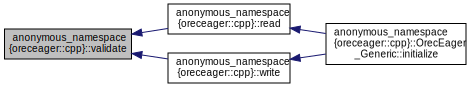
\includegraphics[width=350pt]{namespaceanonymous__namespace_02oreceager_8cpp_03_a5b3a6ab30d79a83a3d13e0718231d4b4_icgraph}
\end{center}
\end{figure}


\hypertarget{namespaceanonymous__namespace_02oreceager_8cpp_03_ac18758bd7e358cee7461af925e192062}{\index{anonymous\-\_\-namespace\{oreceager.\-cpp\}@{anonymous\-\_\-namespace\{oreceager.\-cpp\}}!write@{write}}
\index{write@{write}!anonymous_namespace{oreceager.cpp}@{anonymous\-\_\-namespace\{oreceager.\-cpp\}}}
\subsubsection[{write}]{\setlength{\rightskip}{0pt plus 5cm}{\bf T\-M\-\_\-\-F\-A\-S\-T\-C\-A\-L\-L} void anonymous\-\_\-namespace\{oreceager.\-cpp\}\-::write (
\begin{DoxyParamCaption}
\item[{{\bf S\-T\-M\-\_\-\-W\-R\-I\-T\-E\-\_\-\-S\-I\-G}(,,,)}]{}
\end{DoxyParamCaption}
)}}\label{namespaceanonymous__namespace_02oreceager_8cpp_03_ac18758bd7e358cee7461af925e192062}


Here is the caller graph for this function\-:
\nopagebreak
\begin{figure}[H]
\begin{center}
\leavevmode
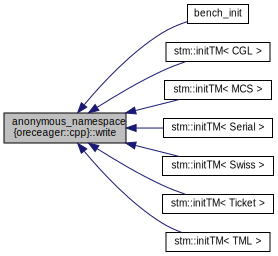
\includegraphics[width=350pt]{namespaceanonymous__namespace_02oreceager_8cpp_03_ac18758bd7e358cee7461af925e192062_icgraph}
\end{center}
\end{figure}


\hypertarget{namespaceanonymous__namespace_02oreceager_8cpp_03_a4412d636846d1de7149b2ef022d5bf83}{\index{anonymous\-\_\-namespace\{oreceager.\-cpp\}@{anonymous\-\_\-namespace\{oreceager.\-cpp\}}!write@{write}}
\index{write@{write}!anonymous_namespace{oreceager.cpp}@{anonymous\-\_\-namespace\{oreceager.\-cpp\}}}
\subsubsection[{write}]{\setlength{\rightskip}{0pt plus 5cm}void anonymous\-\_\-namespace\{oreceager.\-cpp\}\-::write (
\begin{DoxyParamCaption}
\item[{{\bf S\-T\-M\-\_\-\-W\-R\-I\-T\-E\-\_\-\-S\-I\-G}({\bf tx}, addr, val, mask)}]{}
\end{DoxyParamCaption}
)}}\label{namespaceanonymous__namespace_02oreceager_8cpp_03_a4412d636846d1de7149b2ef022d5bf83}
Orec\-Eager write\-:

Lock the orec, log the old value, do the write 

Here is the call graph for this function\-:
\nopagebreak
\begin{figure}[H]
\begin{center}
\leavevmode
\includegraphics[width=350pt]{namespaceanonymous__namespace_02oreceager_8cpp_03_a4412d636846d1de7149b2ef022d5bf83_cgraph}
\end{center}
\end{figure}




Here is the caller graph for this function\-:
\nopagebreak
\begin{figure}[H]
\begin{center}
\leavevmode
\includegraphics[width=350pt]{namespaceanonymous__namespace_02oreceager_8cpp_03_a4412d636846d1de7149b2ef022d5bf83_icgraph}
\end{center}
\end{figure}



\hypertarget{namespaceanonymous__namespace_02oreceagerredo_8cpp_03}{\section{anonymous\-\_\-namespace\{oreceagerredo.\-cpp\} Namespace Reference}
\label{namespaceanonymous__namespace_02oreceagerredo_8cpp_03}\index{anonymous\-\_\-namespace\{oreceagerredo.\-cpp\}@{anonymous\-\_\-namespace\{oreceagerredo.\-cpp\}}}
}
\subsection*{Classes}
\begin{DoxyCompactItemize}
\item 
struct \hyperlink{structanonymous__namespace_02oreceagerredo_8cpp_03_1_1OrecEagerRedo}{Orec\-Eager\-Redo}
\end{DoxyCompactItemize}


\subsection{Detailed Description}
Declare the functions that we're going to implement, so that we can avoid circular dependencies. 
\input{namespaceanonymous__namespace_02orecela_8cpp_03}
\hypertarget{namespaceanonymous__namespace_02orecfair_8cpp_03}{\section{anonymous\-\_\-namespace\{orecfair.\-cpp\} Namespace Reference}
\label{namespaceanonymous__namespace_02orecfair_8cpp_03}\index{anonymous\-\_\-namespace\{orecfair.\-cpp\}@{anonymous\-\_\-namespace\{orecfair.\-cpp\}}}
}
\subsection*{Classes}
\begin{DoxyCompactItemize}
\item 
struct \hyperlink{structanonymous__namespace_02orecfair_8cpp_03_1_1OrecFair}{Orec\-Fair}
\end{DoxyCompactItemize}


\subsection{Detailed Description}
Declare the functions that we're going to implement, so that we can avoid circular dependencies. 
\hypertarget{namespaceanonymous__namespace_02oreclazy_8cpp_03}{\section{anonymous\-\_\-namespace\{oreclazy.\-cpp\} Namespace Reference}
\label{namespaceanonymous__namespace_02oreclazy_8cpp_03}\index{anonymous\-\_\-namespace\{oreclazy.\-cpp\}@{anonymous\-\_\-namespace\{oreclazy.\-cpp\}}}
}
\subsection*{Classes}
\begin{DoxyCompactItemize}
\item 
struct \hyperlink{structanonymous__namespace_02oreclazy_8cpp_03_1_1OrecLazy__Generic}{Orec\-Lazy\-\_\-\-Generic}
\end{DoxyCompactItemize}
\subsection*{Functions}
\begin{DoxyCompactItemize}
\item 
void \hyperlink{namespaceanonymous__namespace_02oreclazy_8cpp_03_a228bf9de4c09f23374e35032fba36d36}{on\-Switch\-To} ()
\item 
bool \hyperlink{namespaceanonymous__namespace_02oreclazy_8cpp_03_acf582010356d11b17267b5a63fe72066}{irrevoc} (\hyperlink{include_2stm_2macros_8hpp_acf117c2df6442342f6603e1a12fa3b5c}{S\-T\-M\-\_\-\-I\-R\-R\-E\-V\-O\-C\-\_\-\-S\-I\-G}(,))
\item 
\hyperlink{platform_8hpp_a1b173d22e57d9395897acbd8de62d505}{N\-O\-I\-N\-L\-I\-N\-E} void \hyperlink{namespaceanonymous__namespace_02oreclazy_8cpp_03_a8434dca53f6bf86e1ac69c7d3c135251}{validate} (\hyperlink{structstm_1_1TxThread}{Tx\-Thread} $\ast$)
\item 
bool \hyperlink{namespaceanonymous__namespace_02oreclazy_8cpp_03_a91428098388d7e210055baacee0f0481}{irrevoc} (\hyperlink{include_2stm_2macros_8hpp_acf117c2df6442342f6603e1a12fa3b5c}{S\-T\-M\-\_\-\-I\-R\-R\-E\-V\-O\-C\-\_\-\-S\-I\-G}(\hyperlink{stmskip_8cc_a0f1c58699b83ce5a08bd9ee859250d72}{tx}, upper\-\_\-stack\-\_\-bound))
\end{DoxyCompactItemize}


\subsection{Function Documentation}
\hypertarget{namespaceanonymous__namespace_02oreclazy_8cpp_03_acf582010356d11b17267b5a63fe72066}{\index{anonymous\-\_\-namespace\{oreclazy.\-cpp\}@{anonymous\-\_\-namespace\{oreclazy.\-cpp\}}!irrevoc@{irrevoc}}
\index{irrevoc@{irrevoc}!anonymous_namespace{oreclazy.cpp}@{anonymous\-\_\-namespace\{oreclazy.\-cpp\}}}
\subsubsection[{irrevoc}]{\setlength{\rightskip}{0pt plus 5cm}bool anonymous\-\_\-namespace\{oreclazy.\-cpp\}\-::irrevoc (
\begin{DoxyParamCaption}
\item[{{\bf S\-T\-M\-\_\-\-I\-R\-R\-E\-V\-O\-C\-\_\-\-S\-I\-G}(,)}]{}
\end{DoxyParamCaption}
)}}\label{namespaceanonymous__namespace_02oreclazy_8cpp_03_acf582010356d11b17267b5a63fe72066}
\hypertarget{namespaceanonymous__namespace_02oreclazy_8cpp_03_a91428098388d7e210055baacee0f0481}{\index{anonymous\-\_\-namespace\{oreclazy.\-cpp\}@{anonymous\-\_\-namespace\{oreclazy.\-cpp\}}!irrevoc@{irrevoc}}
\index{irrevoc@{irrevoc}!anonymous_namespace{oreclazy.cpp}@{anonymous\-\_\-namespace\{oreclazy.\-cpp\}}}
\subsubsection[{irrevoc}]{\setlength{\rightskip}{0pt plus 5cm}bool anonymous\-\_\-namespace\{oreclazy.\-cpp\}\-::irrevoc (
\begin{DoxyParamCaption}
\item[{{\bf S\-T\-M\-\_\-\-I\-R\-R\-E\-V\-O\-C\-\_\-\-S\-I\-G}({\bf tx}, upper\-\_\-stack\-\_\-bound)}]{}
\end{DoxyParamCaption}
)}}\label{namespaceanonymous__namespace_02oreclazy_8cpp_03_a91428098388d7e210055baacee0f0481}
Orec\-Lazy in-\/flight irrevocability\-:

Either commit the transaction or return false. 

Here is the caller graph for this function\-:
\nopagebreak
\begin{figure}[H]
\begin{center}
\leavevmode
\includegraphics[width=350pt]{namespaceanonymous__namespace_02oreclazy_8cpp_03_a91428098388d7e210055baacee0f0481_icgraph}
\end{center}
\end{figure}


\hypertarget{namespaceanonymous__namespace_02oreclazy_8cpp_03_a228bf9de4c09f23374e35032fba36d36}{\index{anonymous\-\_\-namespace\{oreclazy.\-cpp\}@{anonymous\-\_\-namespace\{oreclazy.\-cpp\}}!on\-Switch\-To@{on\-Switch\-To}}
\index{on\-Switch\-To@{on\-Switch\-To}!anonymous_namespace{oreclazy.cpp}@{anonymous\-\_\-namespace\{oreclazy.\-cpp\}}}
\subsubsection[{on\-Switch\-To}]{\setlength{\rightskip}{0pt plus 5cm}void anonymous\-\_\-namespace\{oreclazy.\-cpp\}\-::on\-Switch\-To (
\begin{DoxyParamCaption}
{}
\end{DoxyParamCaption}
)}}\label{namespaceanonymous__namespace_02oreclazy_8cpp_03_a228bf9de4c09f23374e35032fba36d36}
Switch to Orec\-Lazy\-:

The timestamp must be $>$= the maximum value of any orec. Some algs use timestamp as a zero-\/one mutex. If they do, then they back up the timestamp first, in timestamp\-\_\-max. 

Here is the caller graph for this function\-:
\nopagebreak
\begin{figure}[H]
\begin{center}
\leavevmode
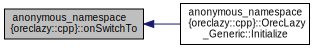
\includegraphics[width=350pt]{namespaceanonymous__namespace_02oreclazy_8cpp_03_a228bf9de4c09f23374e35032fba36d36_icgraph}
\end{center}
\end{figure}


\hypertarget{namespaceanonymous__namespace_02oreclazy_8cpp_03_a8434dca53f6bf86e1ac69c7d3c135251}{\index{anonymous\-\_\-namespace\{oreclazy.\-cpp\}@{anonymous\-\_\-namespace\{oreclazy.\-cpp\}}!validate@{validate}}
\index{validate@{validate}!anonymous_namespace{oreclazy.cpp}@{anonymous\-\_\-namespace\{oreclazy.\-cpp\}}}
\subsubsection[{validate}]{\setlength{\rightskip}{0pt plus 5cm}{\bf N\-O\-I\-N\-L\-I\-N\-E} void anonymous\-\_\-namespace\{oreclazy.\-cpp\}\-::validate (
\begin{DoxyParamCaption}
\item[{{\bf Tx\-Thread} $\ast$}]{tx}
\end{DoxyParamCaption}
)}}\label{namespaceanonymous__namespace_02oreclazy_8cpp_03_a8434dca53f6bf86e1ac69c7d3c135251}
Orec\-Lazy validation\-:

We only call this when in-\/flight, which means that we don't have any locks... This makes the code very simple, but it is still better to not inline it. 
\hypertarget{namespaceanonymous__namespace_02pipeline_8cpp_03}{\section{anonymous\-\_\-namespace\{pipeline.\-cpp\} Namespace Reference}
\label{namespaceanonymous__namespace_02pipeline_8cpp_03}\index{anonymous\-\_\-namespace\{pipeline.\-cpp\}@{anonymous\-\_\-namespace\{pipeline.\-cpp\}}}
}
\subsection*{Classes}
\begin{DoxyCompactItemize}
\item 
struct \hyperlink{structanonymous__namespace_02pipeline_8cpp_03_1_1Pipeline}{Pipeline}
\end{DoxyCompactItemize}


\subsection{Detailed Description}
Declare the functions that we're going to implement, so that we can avoid circular dependencies. 
\hypertarget{namespaceanonymous__namespace_02policies_8cpp_03}{\section{anonymous\-\_\-namespace\{policies.\-cpp\} Namespace Reference}
\label{namespaceanonymous__namespace_02policies_8cpp_03}\index{anonymous\-\_\-namespace\{policies.\-cpp\}@{anonymous\-\_\-namespace\{policies.\-cpp\}}}
}
\subsection*{Functions}
\begin{DoxyCompactItemize}
\item 
void \hyperlink{namespaceanonymous__namespace_02policies_8cpp_03_ae90b562c1daa7c02318148678f1ebea4}{load\-\_\-qtable} (char $\ast$\&qstr)
\end{DoxyCompactItemize}


\subsection{Function Documentation}
\hypertarget{namespaceanonymous__namespace_02policies_8cpp_03_ae90b562c1daa7c02318148678f1ebea4}{\index{anonymous\-\_\-namespace\{policies.\-cpp\}@{anonymous\-\_\-namespace\{policies.\-cpp\}}!load\-\_\-qtable@{load\-\_\-qtable}}
\index{load\-\_\-qtable@{load\-\_\-qtable}!anonymous_namespace{policies.cpp}@{anonymous\-\_\-namespace\{policies.\-cpp\}}}
\subsubsection[{load\-\_\-qtable}]{\setlength{\rightskip}{0pt plus 5cm}void anonymous\-\_\-namespace\{policies.\-cpp\}\-::load\-\_\-qtable (
\begin{DoxyParamCaption}
\item[{char $\ast$\&}]{qstr}
\end{DoxyParamCaption}
)}}\label{namespaceanonymous__namespace_02policies_8cpp_03_ae90b562c1daa7c02318148678f1ebea4}
Load in a qtable

At the risk of considerable bit-\/rot in the comments, we will describe the format of a .q file here\-:

Format\-: comma-\/separated value {\itshape W\-I\-T\-H N\-O S\-P\-A\-C\-E\-S}

Fields\-: 1 -\/ B\-M -\/ benchmark that produced this line \mbox{[}ignored\mbox{]} 2 -\/ A\-L\-G -\/ algorithm name that produced the best output 3 -\/ threads -\/ thread count 4 -\/ read\-\_\-ro -\/ read\-\_\-ro count 5 -\/ read\-\_\-rw\-\_\-nonraw -\/ read\-\_\-rw\-\_\-nonraw count 6 -\/ read\-\_\-raw -\/ read\-\_\-raw count 7 -\/ write\-\_\-nonwaw -\/ write\-\_\-nonwaw count 8 -\/ write\-\_\-waw -\/ write\-\_\-waw count 9 -\/ txn\-\_\-time -\/ txn\-\_\-time count 10 -\/ pct\-\_\-txtime -\/ pct\-\_\-txtime value 11 -\/ roratio -\/ roratio value 

Here is the call graph for this function\-:
\nopagebreak
\begin{figure}[H]
\begin{center}
\leavevmode
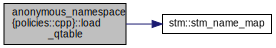
\includegraphics[width=348pt]{namespaceanonymous__namespace_02policies_8cpp_03_ae90b562c1daa7c02318148678f1ebea4_cgraph}
\end{center}
\end{figure}




Here is the caller graph for this function\-:
\nopagebreak
\begin{figure}[H]
\begin{center}
\leavevmode
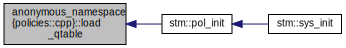
\includegraphics[width=350pt]{namespaceanonymous__namespace_02policies_8cpp_03_ae90b562c1daa7c02318148678f1ebea4_icgraph}
\end{center}
\end{figure}



\input{namespaceanonymous__namespace_02profileapp_8cpp_03}
\hypertarget{namespaceanonymous__namespace_02profiletm_8cpp_03}{\section{anonymous\-\_\-namespace\{profiletm.\-cpp\} Namespace Reference}
\label{namespaceanonymous__namespace_02profiletm_8cpp_03}\index{anonymous\-\_\-namespace\{profiletm.\-cpp\}@{anonymous\-\_\-namespace\{profiletm.\-cpp\}}}
}
\subsection*{Classes}
\begin{DoxyCompactItemize}
\item 
struct \hyperlink{structanonymous__namespace_02profiletm_8cpp_03_1_1ProfileTM}{Profile\-T\-M}
\end{DoxyCompactItemize}

\hypertarget{namespaceanonymous__namespace_02profiling_8cpp_03}{\section{anonymous\-\_\-namespace\{profiling.\-cpp\} Namespace Reference}
\label{namespaceanonymous__namespace_02profiling_8cpp_03}\index{anonymous\-\_\-namespace\{profiling.\-cpp\}@{anonymous\-\_\-namespace\{profiling.\-cpp\}}}
}
\subsection*{Functions}
\begin{DoxyCompactItemize}
\item 
void \hyperlink{namespaceanonymous__namespace_02profiling_8cpp_03_a00942ad1d38b82f3a2e0f66b704bef44}{adjust\-\_\-thresholds} (uint32\-\_\-t new\-\_\-alg, uint32\-\_\-t old\-\_\-alg)
\item 
void \hyperlink{namespaceanonymous__namespace_02profiling_8cpp_03_ad2de7e300bb6e53bf611aaf35c46d80b}{collect\-\_\-profiles} (\hyperlink{structstm_1_1TxThread}{Tx\-Thread} $\ast$\hyperlink{stmskip_8cc_a0f1c58699b83ce5a08bd9ee859250d72}{tx})
\item 
void \hyperlink{namespaceanonymous__namespace_02profiling_8cpp_03_ac7a6d6bebec6c014c2d09c19efb4390c}{change\-\_\-algorithm} (\hyperlink{structstm_1_1TxThread}{Tx\-Thread} $\ast$\hyperlink{stmskip_8cc_a0f1c58699b83ce5a08bd9ee859250d72}{tx}, unsigned new\-\_\-algorithm)
\end{DoxyCompactItemize}


\subsection{Function Documentation}
\hypertarget{namespaceanonymous__namespace_02profiling_8cpp_03_a00942ad1d38b82f3a2e0f66b704bef44}{\index{anonymous\-\_\-namespace\{profiling.\-cpp\}@{anonymous\-\_\-namespace\{profiling.\-cpp\}}!adjust\-\_\-thresholds@{adjust\-\_\-thresholds}}
\index{adjust\-\_\-thresholds@{adjust\-\_\-thresholds}!anonymous_namespace{profiling.cpp}@{anonymous\-\_\-namespace\{profiling.\-cpp\}}}
\subsubsection[{adjust\-\_\-thresholds}]{\setlength{\rightskip}{0pt plus 5cm}void anonymous\-\_\-namespace\{profiling.\-cpp\}\-::adjust\-\_\-thresholds (
\begin{DoxyParamCaption}
\item[{uint32\-\_\-t}]{new\-\_\-alg, }
\item[{uint32\-\_\-t}]{old\-\_\-alg}
\end{DoxyParamCaption}
)}}\label{namespaceanonymous__namespace_02profiling_8cpp_03_a00942ad1d38b82f3a2e0f66b704bef44}
If we change the algorithm, then we need to reset the wait and abort thresholds. If we do not change the algorithm, then if we revisited our decision based on aborts, then backoff the wait and abort thresholds. 

Here is the caller graph for this function\-:
\nopagebreak
\begin{figure}[H]
\begin{center}
\leavevmode
\includegraphics[width=350pt]{namespaceanonymous__namespace_02profiling_8cpp_03_a00942ad1d38b82f3a2e0f66b704bef44_icgraph}
\end{center}
\end{figure}


\hypertarget{namespaceanonymous__namespace_02profiling_8cpp_03_ac7a6d6bebec6c014c2d09c19efb4390c}{\index{anonymous\-\_\-namespace\{profiling.\-cpp\}@{anonymous\-\_\-namespace\{profiling.\-cpp\}}!change\-\_\-algorithm@{change\-\_\-algorithm}}
\index{change\-\_\-algorithm@{change\-\_\-algorithm}!anonymous_namespace{profiling.cpp}@{anonymous\-\_\-namespace\{profiling.\-cpp\}}}
\subsubsection[{change\-\_\-algorithm}]{\setlength{\rightskip}{0pt plus 5cm}void anonymous\-\_\-namespace\{profiling.\-cpp\}\-::change\-\_\-algorithm (
\begin{DoxyParamCaption}
\item[{{\bf Tx\-Thread} $\ast$}]{tx, }
\item[{unsigned}]{new\-\_\-algorithm}
\end{DoxyParamCaption}
)}}\label{namespaceanonymous__namespace_02profiling_8cpp_03_ac7a6d6bebec6c014c2d09c19efb4390c}
change\-\_\-algorithm is used to transition between S\-T\-M implementations when Profile\-T\-M is not involved. 

Here is the call graph for this function\-:
\nopagebreak
\begin{figure}[H]
\begin{center}
\leavevmode
\includegraphics[width=350pt]{namespaceanonymous__namespace_02profiling_8cpp_03_ac7a6d6bebec6c014c2d09c19efb4390c_cgraph}
\end{center}
\end{figure}




Here is the caller graph for this function\-:
\nopagebreak
\begin{figure}[H]
\begin{center}
\leavevmode
\includegraphics[width=350pt]{namespaceanonymous__namespace_02profiling_8cpp_03_ac7a6d6bebec6c014c2d09c19efb4390c_icgraph}
\end{center}
\end{figure}


\hypertarget{namespaceanonymous__namespace_02profiling_8cpp_03_ad2de7e300bb6e53bf611aaf35c46d80b}{\index{anonymous\-\_\-namespace\{profiling.\-cpp\}@{anonymous\-\_\-namespace\{profiling.\-cpp\}}!collect\-\_\-profiles@{collect\-\_\-profiles}}
\index{collect\-\_\-profiles@{collect\-\_\-profiles}!anonymous_namespace{profiling.cpp}@{anonymous\-\_\-namespace\{profiling.\-cpp\}}}
\subsubsection[{collect\-\_\-profiles}]{\setlength{\rightskip}{0pt plus 5cm}void anonymous\-\_\-namespace\{profiling.\-cpp\}\-::collect\-\_\-profiles (
\begin{DoxyParamCaption}
\item[{{\bf Tx\-Thread} $\ast$}]{tx}
\end{DoxyParamCaption}
)}}\label{namespaceanonymous__namespace_02profiling_8cpp_03_ad2de7e300bb6e53bf611aaf35c46d80b}
Collecting profiles is a lot like changing algorithms, but there are a few customizations we make to address the probing. 

Here is the call graph for this function\-:
\nopagebreak
\begin{figure}[H]
\begin{center}
\leavevmode
\includegraphics[width=350pt]{namespaceanonymous__namespace_02profiling_8cpp_03_ad2de7e300bb6e53bf611aaf35c46d80b_cgraph}
\end{center}
\end{figure}




Here is the caller graph for this function\-:
\nopagebreak
\begin{figure}[H]
\begin{center}
\leavevmode
\includegraphics[width=350pt]{namespaceanonymous__namespace_02profiling_8cpp_03_ad2de7e300bb6e53bf611aaf35c46d80b_icgraph}
\end{center}
\end{figure}



\hypertarget{namespaceanonymous__namespace_02ringala_8cpp_03}{\section{anonymous\-\_\-namespace\{ringala.\-cpp\} Namespace Reference}
\label{namespaceanonymous__namespace_02ringala_8cpp_03}\index{anonymous\-\_\-namespace\{ringala.\-cpp\}@{anonymous\-\_\-namespace\{ringala.\-cpp\}}}
}
\subsection*{Classes}
\begin{DoxyCompactItemize}
\item 
struct \hyperlink{structanonymous__namespace_02ringala_8cpp_03_1_1RingALA}{Ring\-A\-L\-A}
\end{DoxyCompactItemize}


\subsection{Detailed Description}
Declare the functions that we're going to implement, so that we can avoid circular dependencies. 
\hypertarget{namespaceanonymous__namespace_02ringsw_8cpp_03}{\section{anonymous\-\_\-namespace\{ringsw.\-cpp\} Namespace Reference}
\label{namespaceanonymous__namespace_02ringsw_8cpp_03}\index{anonymous\-\_\-namespace\{ringsw.\-cpp\}@{anonymous\-\_\-namespace\{ringsw.\-cpp\}}}
}
\subsection*{Classes}
\begin{DoxyCompactItemize}
\item 
struct \hyperlink{structanonymous__namespace_02ringsw_8cpp_03_1_1RingSW}{Ring\-S\-W}
\end{DoxyCompactItemize}


\subsection{Detailed Description}
Declare the functions that we're going to implement, so that we can avoid circular dependencies. 
\hypertarget{namespaceanonymous__namespace_02serial_8cpp_03}{\section{anonymous\-\_\-namespace\{serial.\-cpp\} Namespace Reference}
\label{namespaceanonymous__namespace_02serial_8cpp_03}\index{anonymous\-\_\-namespace\{serial.\-cpp\}@{anonymous\-\_\-namespace\{serial.\-cpp\}}}
}
\subsection*{Classes}
\begin{DoxyCompactItemize}
\item 
struct \hyperlink{structanonymous__namespace_02serial_8cpp_03_1_1Serial}{Serial}
\end{DoxyCompactItemize}


\subsection{Detailed Description}
Declare the functions that we're going to implement, so that we can avoid circular dependencies. 
\hypertarget{namespaceanonymous__namespace_02static_8cpp_03}{\section{anonymous\-\_\-namespace\{static.\-cpp\} Namespace Reference}
\label{namespaceanonymous__namespace_02static_8cpp_03}\index{anonymous\-\_\-namespace\{static.\-cpp\}@{anonymous\-\_\-namespace\{static.\-cpp\}}}
}
\subsection*{Functions}
\begin{DoxyCompactItemize}
\item 
\hyperlink{platform_8hpp_a8b5d728e6eed8f368f9966f637d2f719}{T\-M\-\_\-\-F\-A\-S\-T\-C\-A\-L\-L} uint32\-\_\-t \hyperlink{namespaceanonymous__namespace_02static_8cpp_03_a356adb65bf55070273b42e289177d08a}{pol\-\_\-\-E\-R} ()
\item 
\hyperlink{platform_8hpp_a8b5d728e6eed8f368f9966f637d2f719}{T\-M\-\_\-\-F\-A\-S\-T\-C\-A\-L\-L} uint32\-\_\-t \hyperlink{namespaceanonymous__namespace_02static_8cpp_03_ae9990f5d808082c67e85dd51b5679732}{pol\-\_\-\-E} ()
\item 
\hyperlink{platform_8hpp_a8b5d728e6eed8f368f9966f637d2f719}{T\-M\-\_\-\-F\-A\-S\-T\-C\-A\-L\-L} uint32\-\_\-t \hyperlink{namespaceanonymous__namespace_02static_8cpp_03_aa824c84a6c1fe13a580dace00ad444c8}{pol\-\_\-\-R} ()
\item 
\hyperlink{platform_8hpp_a8b5d728e6eed8f368f9966f637d2f719}{T\-M\-\_\-\-F\-A\-S\-T\-C\-A\-L\-L} uint32\-\_\-t \hyperlink{namespaceanonymous__namespace_02static_8cpp_03_ae7874d79d4bed12301c4b8cfa73510ab}{pol\-\_\-\-X} ()
\end{DoxyCompactItemize}


\subsection{Detailed Description}
Here we define the static adaptivity policies. These do not use profiles, so they are very simple.

N\-B\-: these are interesting from a historical perspective, in that they were part of \mbox{[}Spear S\-P\-A\-A 2011\mbox{]}. However, subsequent work has shown that adapting on the basis of pathology avoidance (e.\-g., consecutive aborts) is not a good strategy on its own, because of the possibility of Toxic Transactions \mbox{[}Liu Transact 2011\mbox{]}. 

\subsection{Function Documentation}
\hypertarget{namespaceanonymous__namespace_02static_8cpp_03_ae9990f5d808082c67e85dd51b5679732}{\index{anonymous\-\_\-namespace\{static.\-cpp\}@{anonymous\-\_\-namespace\{static.\-cpp\}}!pol\-\_\-\-E@{pol\-\_\-\-E}}
\index{pol\-\_\-\-E@{pol\-\_\-\-E}!anonymous_namespace{static.cpp}@{anonymous\-\_\-namespace\{static.\-cpp\}}}
\subsubsection[{pol\-\_\-\-E}]{\setlength{\rightskip}{0pt plus 5cm}{\bf T\-M\-\_\-\-F\-A\-S\-T\-C\-A\-L\-L} uint32\-\_\-t anonymous\-\_\-namespace\{static.\-cpp\}\-::pol\-\_\-\-E (
\begin{DoxyParamCaption}
{}
\end{DoxyParamCaption}
)}}\label{namespaceanonymous__namespace_02static_8cpp_03_ae9990f5d808082c67e85dd51b5679732}
This policy is suitable for workloads that need E\-L\-A semantics, but that don't need self-\/abort. 

Here is the caller graph for this function\-:
\nopagebreak
\begin{figure}[H]
\begin{center}
\leavevmode
\includegraphics[width=350pt]{namespaceanonymous__namespace_02static_8cpp_03_ae9990f5d808082c67e85dd51b5679732_icgraph}
\end{center}
\end{figure}


\hypertarget{namespaceanonymous__namespace_02static_8cpp_03_a356adb65bf55070273b42e289177d08a}{\index{anonymous\-\_\-namespace\{static.\-cpp\}@{anonymous\-\_\-namespace\{static.\-cpp\}}!pol\-\_\-\-E\-R@{pol\-\_\-\-E\-R}}
\index{pol\-\_\-\-E\-R@{pol\-\_\-\-E\-R}!anonymous_namespace{static.cpp}@{anonymous\-\_\-namespace\{static.\-cpp\}}}
\subsubsection[{pol\-\_\-\-E\-R}]{\setlength{\rightskip}{0pt plus 5cm}{\bf T\-M\-\_\-\-F\-A\-S\-T\-C\-A\-L\-L} uint32\-\_\-t anonymous\-\_\-namespace\{static.\-cpp\}\-::pol\-\_\-\-E\-R (
\begin{DoxyParamCaption}
{}
\end{DoxyParamCaption}
)}}\label{namespaceanonymous__namespace_02static_8cpp_03_a356adb65bf55070273b42e289177d08a}
This policy is suitable for workloads that need E\-L\-A semantics and support for self-\/abort. 

Here is the caller graph for this function\-:
\nopagebreak
\begin{figure}[H]
\begin{center}
\leavevmode
\includegraphics[width=350pt]{namespaceanonymous__namespace_02static_8cpp_03_a356adb65bf55070273b42e289177d08a_icgraph}
\end{center}
\end{figure}


\hypertarget{namespaceanonymous__namespace_02static_8cpp_03_aa824c84a6c1fe13a580dace00ad444c8}{\index{anonymous\-\_\-namespace\{static.\-cpp\}@{anonymous\-\_\-namespace\{static.\-cpp\}}!pol\-\_\-\-R@{pol\-\_\-\-R}}
\index{pol\-\_\-\-R@{pol\-\_\-\-R}!anonymous_namespace{static.cpp}@{anonymous\-\_\-namespace\{static.\-cpp\}}}
\subsubsection[{pol\-\_\-\-R}]{\setlength{\rightskip}{0pt plus 5cm}{\bf T\-M\-\_\-\-F\-A\-S\-T\-C\-A\-L\-L} uint32\-\_\-t anonymous\-\_\-namespace\{static.\-cpp\}\-::pol\-\_\-\-R (
\begin{DoxyParamCaption}
{}
\end{DoxyParamCaption}
)}}\label{namespaceanonymous__namespace_02static_8cpp_03_aa824c84a6c1fe13a580dace00ad444c8}
This policy is suitable for workloads that don't need strong semantics but do need self-\/abort. 

Here is the caller graph for this function\-:
\nopagebreak
\begin{figure}[H]
\begin{center}
\leavevmode
\includegraphics[width=350pt]{namespaceanonymous__namespace_02static_8cpp_03_aa824c84a6c1fe13a580dace00ad444c8_icgraph}
\end{center}
\end{figure}


\hypertarget{namespaceanonymous__namespace_02static_8cpp_03_ae7874d79d4bed12301c4b8cfa73510ab}{\index{anonymous\-\_\-namespace\{static.\-cpp\}@{anonymous\-\_\-namespace\{static.\-cpp\}}!pol\-\_\-\-X@{pol\-\_\-\-X}}
\index{pol\-\_\-\-X@{pol\-\_\-\-X}!anonymous_namespace{static.cpp}@{anonymous\-\_\-namespace\{static.\-cpp\}}}
\subsubsection[{pol\-\_\-\-X}]{\setlength{\rightskip}{0pt plus 5cm}{\bf T\-M\-\_\-\-F\-A\-S\-T\-C\-A\-L\-L} uint32\-\_\-t anonymous\-\_\-namespace\{static.\-cpp\}\-::pol\-\_\-\-X (
\begin{DoxyParamCaption}
{}
\end{DoxyParamCaption}
)}}\label{namespaceanonymous__namespace_02static_8cpp_03_ae7874d79d4bed12301c4b8cfa73510ab}
This policy is suitable for workloads that don't need strong semantics and also don't need support for self-\/abort. 

Here is the caller graph for this function\-:
\nopagebreak
\begin{figure}[H]
\begin{center}
\leavevmode
\includegraphics[width=350pt]{namespaceanonymous__namespace_02static_8cpp_03_ae7874d79d4bed12301c4b8cfa73510ab_icgraph}
\end{center}
\end{figure}



\hypertarget{namespaceanonymous__namespace_02swiss_8cpp_03}{\section{anonymous\-\_\-namespace\{swiss.\-cpp\} Namespace Reference}
\label{namespaceanonymous__namespace_02swiss_8cpp_03}\index{anonymous\-\_\-namespace\{swiss.\-cpp\}@{anonymous\-\_\-namespace\{swiss.\-cpp\}}}
}
\subsection*{Classes}
\begin{DoxyCompactItemize}
\item 
struct \hyperlink{structanonymous__namespace_02swiss_8cpp_03_1_1Swiss}{Swiss}
\end{DoxyCompactItemize}


\subsection{Detailed Description}
This is a good-\/faith implementation of Swiss\-T\-M.

What that means, precisely, has to do with how we translate the Swiss\-T\-M algorithm to allow /algorithmic/ comparisons with Orec\-Eager and L\-L\-T. Specifically, we decided in the past that Orec\-Eager and L\-L\-T would not use any of the clever 'lock is a pointer into my writeset' tricks that were proposed in the Tiny\-S\-T\-M paper, and so we don't use those tricks here, either. The cost is minimal (actually, with the R\-S\-T\-M Write\-Set hash, the tricks are typically not profitable anyway), but it is worth stating, up front, that we do not adhere to this design point.

Additionally, orec management differs slightly here from in Orec\-Eager and L\-L\-T. In those systems, we use \char`\"{}2-\/word\char`\"{} orecs, where the acquirer writes the old orec value in the second word after acquiring the first word. This halves the cost of logging, as the list of held locks only gives orec addresses, not the old values. However, in Swiss\-T\-M, there is a tradeoff where on one hand, having rlocks separate from wlocks can decrease cache misses for read-\/only transactions, but on the other hand doing so doubles logging overhead for read locking by writers at commit time. It would be odd to use the 2-\/word orecs for read locks and not for write locks, but a more efficient technique is to use the second word of 2-\/word orecs as the rlock, and then use traditional 2-\/word lock logging, where the old lock value is also stored.

Other changes are typically small. The biggest deals with adding detection of remote aborts, which wasn't discussed in the paper.

N\-B\-: we could factor some C\-M code out of the R\-O codepath. We could also make the phase2 switch cause a thread to use different function pointers. 
\hypertarget{namespaceanonymous__namespace_02ticket_8cpp_03}{\section{anonymous\-\_\-namespace\{ticket.\-cpp\} Namespace Reference}
\label{namespaceanonymous__namespace_02ticket_8cpp_03}\index{anonymous\-\_\-namespace\{ticket.\-cpp\}@{anonymous\-\_\-namespace\{ticket.\-cpp\}}}
}
\subsection*{Classes}
\begin{DoxyCompactItemize}
\item 
struct \hyperlink{structanonymous__namespace_02ticket_8cpp_03_1_1Ticket}{Ticket}
\end{DoxyCompactItemize}


\subsection{Detailed Description}
Declare the functions that we're going to implement, so that we can avoid circular dependencies. 
\input{namespaceanonymous__namespace_02tli_8cpp_03}
\hypertarget{namespaceanonymous__namespace_02tml_8cpp_03}{\section{anonymous\-\_\-namespace\{tml.\-cpp\} Namespace Reference}
\label{namespaceanonymous__namespace_02tml_8cpp_03}\index{anonymous\-\_\-namespace\{tml.\-cpp\}@{anonymous\-\_\-namespace\{tml.\-cpp\}}}
}
\subsection*{Classes}
\begin{DoxyCompactItemize}
\item 
struct \hyperlink{structanonymous__namespace_02tml_8cpp_03_1_1TML}{T\-M\-L}
\end{DoxyCompactItemize}


\subsection{Detailed Description}
Declare the functions that we're going to implement, so that we can avoid circular dependencies. Note that with \hyperlink{structanonymous__namespace_02tml_8cpp_03_1_1TML}{T\-M\-L}, we don't expect the reads and writes to be called, because we expect the instrumentation to be inlined via the dispatch mechanism. However, we must provide the code to handle the uncommon case. 
\hypertarget{namespaceanonymous__namespace_02tmllazy_8cpp_03}{\section{anonymous\-\_\-namespace\{tmllazy.\-cpp\} Namespace Reference}
\label{namespaceanonymous__namespace_02tmllazy_8cpp_03}\index{anonymous\-\_\-namespace\{tmllazy.\-cpp\}@{anonymous\-\_\-namespace\{tmllazy.\-cpp\}}}
}
\subsection*{Classes}
\begin{DoxyCompactItemize}
\item 
struct \hyperlink{structanonymous__namespace_02tmllazy_8cpp_03_1_1TMLLazy}{T\-M\-L\-Lazy}
\end{DoxyCompactItemize}


\subsection{Detailed Description}
Declare the functions that we're going to implement, so that we can avoid circular dependencies. Note that with T\-M\-L, we don't expect the reads and writes to be called, because we expect the isntrumentation to be inlined via the dispatch mechanism. However, we must provide the code to handle the uncommon case. 
\hypertarget{namespaceanonymous__namespace_02txthread_8cpp_03}{\section{anonymous\-\_\-namespace\{txthread.\-cpp\} Namespace Reference}
\label{namespaceanonymous__namespace_02txthread_8cpp_03}\index{anonymous\-\_\-namespace\{txthread.\-cpp\}@{anonymous\-\_\-namespace\{txthread.\-cpp\}}}
}
\subsection*{Functions}
\begin{DoxyCompactItemize}
\item 
\hyperlink{platform_8hpp_aa1728270d73c5d1598de1fd691762eb1}{N\-O\-R\-E\-T\-U\-R\-N} void \hyperlink{namespaceanonymous__namespace_02txthread_8cpp_03_a4d3440e70fa954abc911d00af383bcb4}{default\-\_\-abort\-\_\-handler} (\hyperlink{structstm_1_1TxThread}{Tx\-Thread} $\ast$\hyperlink{stmskip_8cc_a0f1c58699b83ce5a08bd9ee859250d72}{tx})
\end{DoxyCompactItemize}
\subsection*{Variables}
\begin{DoxyCompactItemize}
\item 
const char $\ast$ \hyperlink{namespaceanonymous__namespace_02txthread_8cpp_03_a48fac128b632fd74dfb62133fb88dd18}{init\-\_\-lib\-\_\-name}
\end{DoxyCompactItemize}


\subsection{Function Documentation}
\hypertarget{namespaceanonymous__namespace_02txthread_8cpp_03_a4d3440e70fa954abc911d00af383bcb4}{\index{anonymous\-\_\-namespace\{txthread.\-cpp\}@{anonymous\-\_\-namespace\{txthread.\-cpp\}}!default\-\_\-abort\-\_\-handler@{default\-\_\-abort\-\_\-handler}}
\index{default\-\_\-abort\-\_\-handler@{default\-\_\-abort\-\_\-handler}!anonymous_namespace{txthread.cpp}@{anonymous\-\_\-namespace\{txthread.\-cpp\}}}
\subsubsection[{default\-\_\-abort\-\_\-handler}]{\setlength{\rightskip}{0pt plus 5cm}{\bf N\-O\-R\-E\-T\-U\-R\-N} void anonymous\-\_\-namespace\{txthread.\-cpp\}\-::default\-\_\-abort\-\_\-handler (
\begin{DoxyParamCaption}
\item[{{\bf Tx\-Thread} $\ast$}]{tx}
\end{DoxyParamCaption}
)}}\label{namespaceanonymous__namespace_02txthread_8cpp_03_a4d3440e70fa954abc911d00af383bcb4}
The default mechanism that libstm uses for an abort. An A\-P\-I environment may also provide its own abort mechanism (see \hyperlink{namespaceitm2stm}{itm2stm} for an example of how the itm shim does this).

This is ugly because rollback has a configuration-\/dependent signature. 

\subsection{Variable Documentation}
\hypertarget{namespaceanonymous__namespace_02txthread_8cpp_03_a48fac128b632fd74dfb62133fb88dd18}{\index{anonymous\-\_\-namespace\{txthread.\-cpp\}@{anonymous\-\_\-namespace\{txthread.\-cpp\}}!init\-\_\-lib\-\_\-name@{init\-\_\-lib\-\_\-name}}
\index{init\-\_\-lib\-\_\-name@{init\-\_\-lib\-\_\-name}!anonymous_namespace{txthread.cpp}@{anonymous\-\_\-namespace\{txthread.\-cpp\}}}
\subsubsection[{init\-\_\-lib\-\_\-name}]{\setlength{\rightskip}{0pt plus 5cm}const char$\ast$ anonymous\-\_\-namespace\{txthread.\-cpp\}\-::init\-\_\-lib\-\_\-name}}\label{namespaceanonymous__namespace_02txthread_8cpp_03_a48fac128b632fd74dfb62133fb88dd18}
The name of the algorithm with which libstm was initialized 
\hypertarget{namespaceanonymous__namespace_02types_8cpp_03}{\section{anonymous\-\_\-namespace\{types.\-cpp\} Namespace Reference}
\label{namespaceanonymous__namespace_02types_8cpp_03}\index{anonymous\-\_\-namespace\{types.\-cpp\}@{anonymous\-\_\-namespace\{types.\-cpp\}}}
}
\subsection*{Functions}
\begin{DoxyCompactItemize}
\item 
{\footnotesize template$<$typename T $>$ }\\T $\ast$ \hyperlink{namespaceanonymous__namespace_02types_8cpp_03_abafdc74e2a701faf445fe4d4cc8445e8}{typed\-\_\-malloc} (size\-\_\-t \hyperlink{mt19937ar_8h_a0240ac851181b84ac374872dc5434ee4}{N})
\end{DoxyCompactItemize}


\subsection{Detailed Description}
Copyright (C) 2011 University of Rochester Department of Computer Science and Lehigh University Department of Computer Science and Engineering

License\-: Modified B\-S\-D Please see the file L\-I\-C\-E\-N\-S\-E.\-R\-S\-T\-M for licensing information In the types/ folder, we have a lot of data structure implementations. In some cases, the optimal implementation will have a 'noinline' function that is rarely called. To actually ensure that the 'noinline' behavior is achieved, we put the implementations of those functions here, in a separate compilation unit. 

\subsection{Function Documentation}
\hypertarget{namespaceanonymous__namespace_02types_8cpp_03_abafdc74e2a701faf445fe4d4cc8445e8}{\index{anonymous\-\_\-namespace\{types.\-cpp\}@{anonymous\-\_\-namespace\{types.\-cpp\}}!typed\-\_\-malloc@{typed\-\_\-malloc}}
\index{typed\-\_\-malloc@{typed\-\_\-malloc}!anonymous_namespace{types.cpp}@{anonymous\-\_\-namespace\{types.\-cpp\}}}
\subsubsection[{typed\-\_\-malloc}]{\setlength{\rightskip}{0pt plus 5cm}template$<$typename T $>$ T$\ast$ anonymous\-\_\-namespace\{types.\-cpp\}\-::typed\-\_\-malloc (
\begin{DoxyParamCaption}
\item[{size\-\_\-t}]{N}
\end{DoxyParamCaption}
)\hspace{0.3cm}{\ttfamily [inline]}}}\label{namespaceanonymous__namespace_02types_8cpp_03_abafdc74e2a701faf445fe4d4cc8445e8}
We use malloc a couple of times here, and this makes it a bit easier 
\hypertarget{namespaceanonymous__namespace_02WBMMPolicy_8cpp_03}{\section{anonymous\-\_\-namespace\{W\-B\-M\-M\-Policy.\-cpp\} Namespace Reference}
\label{namespaceanonymous__namespace_02WBMMPolicy_8cpp_03}\index{anonymous\-\_\-namespace\{\-W\-B\-M\-M\-Policy.\-cpp\}@{anonymous\-\_\-namespace\{\-W\-B\-M\-M\-Policy.\-cpp\}}}
}
\subsection*{Functions}
\begin{DoxyCompactItemize}
\item 
bool \hyperlink{namespaceanonymous__namespace_02WBMMPolicy_8cpp_03_a030c6e9142fd49127ce70ad9b1af5e79}{is\-\_\-strictly\-\_\-older} (uint32\-\_\-t $\ast$newer, uint32\-\_\-t $\ast$older, uint32\-\_\-t old\-\_\-len)
\end{DoxyCompactItemize}


\subsection{Function Documentation}
\hypertarget{namespaceanonymous__namespace_02WBMMPolicy_8cpp_03_a030c6e9142fd49127ce70ad9b1af5e79}{\index{anonymous\-\_\-namespace\{\-W\-B\-M\-M\-Policy.\-cpp\}@{anonymous\-\_\-namespace\{\-W\-B\-M\-M\-Policy.\-cpp\}}!is\-\_\-strictly\-\_\-older@{is\-\_\-strictly\-\_\-older}}
\index{is\-\_\-strictly\-\_\-older@{is\-\_\-strictly\-\_\-older}!anonymous_namespace{WBMMPolicy.cpp}@{anonymous\-\_\-namespace\{\-W\-B\-M\-M\-Policy.\-cpp\}}}
\subsubsection[{is\-\_\-strictly\-\_\-older}]{\setlength{\rightskip}{0pt plus 5cm}bool anonymous\-\_\-namespace\{W\-B\-M\-M\-Policy.\-cpp\}\-::is\-\_\-strictly\-\_\-older (
\begin{DoxyParamCaption}
\item[{uint32\-\_\-t $\ast$}]{newer, }
\item[{uint32\-\_\-t $\ast$}]{older, }
\item[{uint32\-\_\-t}]{old\-\_\-len}
\end{DoxyParamCaption}
)\hspace{0.3cm}{\ttfamily [inline]}}}\label{namespaceanonymous__namespace_02WBMMPolicy_8cpp_03_a030c6e9142fd49127ce70ad9b1af5e79}


Here is the caller graph for this function\-:
\nopagebreak
\begin{figure}[H]
\begin{center}
\leavevmode
\includegraphics[width=350pt]{namespaceanonymous__namespace_02WBMMPolicy_8cpp_03_a030c6e9142fd49127ce70ad9b1af5e79_icgraph}
\end{center}
\end{figure}



\hypertarget{namespaceitm2stm}{\section{itm2stm Namespace Reference}
\label{namespaceitm2stm}\index{itm2stm@{itm2stm}}
}
\subsection*{Classes}
\begin{DoxyCompactItemize}
\item 
struct \hyperlink{structitm2stm_1_1Aligned}{Aligned}
\item 
struct \hyperlink{structitm2stm_1_1BlockReader}{Block\-Reader}
\item 
struct \hyperlink{structitm2stm_1_1BlockWriter}{Block\-Writer}
\item 
class \hyperlink{classitm2stm_1_1Checkpoint}{Checkpoint}
\item 
class \hyperlink{classitm2stm_1_1Scope}{Scope}
\end{DoxyCompactItemize}
\subsection*{Functions}
\begin{DoxyCompactItemize}
\item 
size\-\_\-t \hyperlink{namespaceitm2stm_a60fadbf1779483f2446ab9e30aa1f713}{block\-\_\-write} (\hyperlink{structstm_1_1TxThread}{stm\-::\-Tx\-Thread} \&, void $\ast$target, const void $\ast$source, size\-\_\-t bytes) \hyperlink{counted__ptr_8hpp_a454a5e4bfc1243a175baaa7327bb751f}{\-\_\-\-\_\-attribute\-\_\-\-\_\-}((nonnull))
\item 
size\-\_\-t \hyperlink{namespaceitm2stm_ab76a65e75d1318bd4c1e4dab11096446}{block\-\_\-read} (\hyperlink{structstm_1_1TxThread}{stm\-::\-Tx\-Thread} \&, void $\ast$target, const void $\ast$source, size\-\_\-t bytes) \hyperlink{counted__ptr_8hpp_a454a5e4bfc1243a175baaa7327bb751f}{\-\_\-\-\_\-attribute\-\_\-\-\_\-}((nonnull))
\item 
void \hyperlink{namespaceitm2stm_ad658616dcf595ab736e02f0f4f274f67}{block\-\_\-set} (\hyperlink{structstm_1_1TxThread}{stm\-::\-Tx\-Thread} \&, void $\ast$target, uint8\-\_\-t c, size\-\_\-t bytes) \hyperlink{counted__ptr_8hpp_a454a5e4bfc1243a175baaa7327bb751f}{\-\_\-\-\_\-attribute\-\_\-\-\_\-}((nonnull))
\item 
void $\ast$ \hyperlink{namespaceitm2stm_aed4f4d7200a5ff399b09aad2038e2469}{new\-\_\-wrapper} (size\-\_\-t sz) asm(\char`\"{}\-\_\-\-Znwj.\-\_\-\$\-T\-X\-N\char`\"{})
\item 
void \hyperlink{namespaceitm2stm_ae5823a99476da1284952a94f795c8a88}{delete\-\_\-wrapper} (void $\ast$\hyperlink{counted__ptr_8hpp_ac0fd97c9323e3a3981515b00166f14d8}{ptr}) asm(\char`\"{}\-\_\-\-Zdl\-Pv.\-\_\-\$\-T\-X\-N\char`\"{})
\item 
void $\ast$ \hyperlink{namespaceitm2stm_a1d7d549547990a85a10a6a21d5b86e9a}{malloc\-\_\-wrapper} (size\-\_\-t sz) asm(\char`\"{}malloc.\-\_\-\$\-T\-X\-N\char`\"{})
\item 
void \hyperlink{namespaceitm2stm_afb85155fcabb8af0b40dc1e7b54703fb}{free\-\_\-wrapper} (void $\ast$\hyperlink{counted__ptr_8hpp_ac0fd97c9323e3a3981515b00166f14d8}{ptr}) asm(\char`\"{}free.\-\_\-\$\-T\-X\-N\char`\"{})
\item 
size\-\_\-t \hyperlink{namespaceitm2stm_aa9908b113027ae21130750939980ee0b}{offset\-\_\-of} (const void $\ast$const address)
\item 
void $\ast$$\ast$ \hyperlink{namespaceitm2stm_a6c0f462e6a92340d0aaff5050c4a6ed6}{base\-\_\-of} (const void $\ast$const address)
\item 
void \hyperlink{namespaceitm2stm_a334b9615cac957b9ce7a4743beaaaf53}{add\-\_\-bytes} (const void $\ast$\&address, size\-\_\-t bytes)
\item 
void \hyperlink{namespaceitm2stm_a1af29eeeb5839a27d75426db18c6c1c1}{add\-\_\-bytes} (void $\ast$\&address, size\-\_\-t bytes)
\item 
uintptr\-\_\-t \hyperlink{namespaceitm2stm_a7bfcca557e548ad294de7fe74eb4cdf6}{make\-\_\-mask} (size\-\_\-t i, size\-\_\-t j)
\end{DoxyCompactItemize}


\subsection{Detailed Description}
Copyright (C) 2011 University of Rochester Department of Computer Science and Lehigh University Department of Computer Science and Engineering

License\-: Modified B\-S\-D Please see the file L\-I\-C\-E\-N\-S\-E.\-R\-S\-T\-M for licensing information 

\subsection{Function Documentation}
\hypertarget{namespaceitm2stm_a334b9615cac957b9ce7a4743beaaaf53}{\index{itm2stm@{itm2stm}!add\-\_\-bytes@{add\-\_\-bytes}}
\index{add\-\_\-bytes@{add\-\_\-bytes}!itm2stm@{itm2stm}}
\subsubsection[{add\-\_\-bytes}]{\setlength{\rightskip}{0pt plus 5cm}void itm2stm\-::add\-\_\-bytes (
\begin{DoxyParamCaption}
\item[{const void $\ast$\&}]{address, }
\item[{size\-\_\-t}]{bytes}
\end{DoxyParamCaption}
)\hspace{0.3cm}{\ttfamily [inline]}}}\label{namespaceitm2stm_a334b9615cac957b9ce7a4743beaaaf53}


Here is the caller graph for this function\-:
\nopagebreak
\begin{figure}[H]
\begin{center}
\leavevmode
\includegraphics[width=350pt]{namespaceitm2stm_a334b9615cac957b9ce7a4743beaaaf53_icgraph}
\end{center}
\end{figure}


\hypertarget{namespaceitm2stm_a1af29eeeb5839a27d75426db18c6c1c1}{\index{itm2stm@{itm2stm}!add\-\_\-bytes@{add\-\_\-bytes}}
\index{add\-\_\-bytes@{add\-\_\-bytes}!itm2stm@{itm2stm}}
\subsubsection[{add\-\_\-bytes}]{\setlength{\rightskip}{0pt plus 5cm}void itm2stm\-::add\-\_\-bytes (
\begin{DoxyParamCaption}
\item[{void $\ast$\&}]{address, }
\item[{size\-\_\-t}]{bytes}
\end{DoxyParamCaption}
)\hspace{0.3cm}{\ttfamily [inline]}}}\label{namespaceitm2stm_a1af29eeeb5839a27d75426db18c6c1c1}
\hypertarget{namespaceitm2stm_a6c0f462e6a92340d0aaff5050c4a6ed6}{\index{itm2stm@{itm2stm}!base\-\_\-of@{base\-\_\-of}}
\index{base\-\_\-of@{base\-\_\-of}!itm2stm@{itm2stm}}
\subsubsection[{base\-\_\-of}]{\setlength{\rightskip}{0pt plus 5cm}void$\ast$$\ast$ itm2stm\-::base\-\_\-of (
\begin{DoxyParamCaption}
\item[{const void $\ast$const}]{address}
\end{DoxyParamCaption}
)\hspace{0.3cm}{\ttfamily [inline]}}}\label{namespaceitm2stm_a6c0f462e6a92340d0aaff5050c4a6ed6}


Here is the caller graph for this function\-:
\nopagebreak
\begin{figure}[H]
\begin{center}
\leavevmode
\includegraphics[width=350pt]{namespaceitm2stm_a6c0f462e6a92340d0aaff5050c4a6ed6_icgraph}
\end{center}
\end{figure}


\hypertarget{namespaceitm2stm_ab76a65e75d1318bd4c1e4dab11096446}{\index{itm2stm@{itm2stm}!block\-\_\-read@{block\-\_\-read}}
\index{block\-\_\-read@{block\-\_\-read}!itm2stm@{itm2stm}}
\subsubsection[{block\-\_\-read}]{\setlength{\rightskip}{0pt plus 5cm}size\-\_\-t itm2stm\-::block\-\_\-read (
\begin{DoxyParamCaption}
\item[{{\bf stm\-::\-Tx\-Thread} \&}]{tx, }
\item[{void $\ast$}]{target, }
\item[{const void $\ast$}]{source, }
\item[{size\-\_\-t}]{bytes}
\end{DoxyParamCaption}
)}}\label{namespaceitm2stm_ab76a65e75d1318bd4c1e4dab11096446}


Here is the call graph for this function\-:
\nopagebreak
\begin{figure}[H]
\begin{center}
\leavevmode
\includegraphics[width=350pt]{namespaceitm2stm_ab76a65e75d1318bd4c1e4dab11096446_cgraph}
\end{center}
\end{figure}




Here is the caller graph for this function\-:
\nopagebreak
\begin{figure}[H]
\begin{center}
\leavevmode
\includegraphics[width=336pt]{namespaceitm2stm_ab76a65e75d1318bd4c1e4dab11096446_icgraph}
\end{center}
\end{figure}


\hypertarget{namespaceitm2stm_ad658616dcf595ab736e02f0f4f274f67}{\index{itm2stm@{itm2stm}!block\-\_\-set@{block\-\_\-set}}
\index{block\-\_\-set@{block\-\_\-set}!itm2stm@{itm2stm}}
\subsubsection[{block\-\_\-set}]{\setlength{\rightskip}{0pt plus 5cm}void itm2stm\-::block\-\_\-set (
\begin{DoxyParamCaption}
\item[{{\bf stm\-::\-Tx\-Thread} \&}]{tx, }
\item[{void $\ast$}]{target, }
\item[{uint8\-\_\-t}]{c, }
\item[{size\-\_\-t}]{bytes}
\end{DoxyParamCaption}
)}}\label{namespaceitm2stm_ad658616dcf595ab736e02f0f4f274f67}


Here is the call graph for this function\-:
\nopagebreak
\begin{figure}[H]
\begin{center}
\leavevmode
\includegraphics[width=350pt]{namespaceitm2stm_ad658616dcf595ab736e02f0f4f274f67_cgraph}
\end{center}
\end{figure}




Here is the caller graph for this function\-:
\nopagebreak
\begin{figure}[H]
\begin{center}
\leavevmode
\includegraphics[width=320pt]{namespaceitm2stm_ad658616dcf595ab736e02f0f4f274f67_icgraph}
\end{center}
\end{figure}


\hypertarget{namespaceitm2stm_a60fadbf1779483f2446ab9e30aa1f713}{\index{itm2stm@{itm2stm}!block\-\_\-write@{block\-\_\-write}}
\index{block\-\_\-write@{block\-\_\-write}!itm2stm@{itm2stm}}
\subsubsection[{block\-\_\-write}]{\setlength{\rightskip}{0pt plus 5cm}size\-\_\-t itm2stm\-::block\-\_\-write (
\begin{DoxyParamCaption}
\item[{{\bf stm\-::\-Tx\-Thread} \&}]{tx, }
\item[{void $\ast$}]{target, }
\item[{const void $\ast$}]{source, }
\item[{size\-\_\-t}]{bytes}
\end{DoxyParamCaption}
)}}\label{namespaceitm2stm_a60fadbf1779483f2446ab9e30aa1f713}


Here is the call graph for this function\-:
\nopagebreak
\begin{figure}[H]
\begin{center}
\leavevmode
\includegraphics[width=350pt]{namespaceitm2stm_a60fadbf1779483f2446ab9e30aa1f713_cgraph}
\end{center}
\end{figure}




Here is the caller graph for this function\-:
\nopagebreak
\begin{figure}[H]
\begin{center}
\leavevmode
\includegraphics[width=334pt]{namespaceitm2stm_a60fadbf1779483f2446ab9e30aa1f713_icgraph}
\end{center}
\end{figure}


\hypertarget{namespaceitm2stm_ae5823a99476da1284952a94f795c8a88}{\index{itm2stm@{itm2stm}!delete\-\_\-wrapper@{delete\-\_\-wrapper}}
\index{delete\-\_\-wrapper@{delete\-\_\-wrapper}!itm2stm@{itm2stm}}
\subsubsection[{delete\-\_\-wrapper}]{\setlength{\rightskip}{0pt plus 5cm}void itm2stm\-::delete\-\_\-wrapper (
\begin{DoxyParamCaption}
\item[{void $\ast$}]{ptr}
\end{DoxyParamCaption}
)}}\label{namespaceitm2stm_ae5823a99476da1284952a94f795c8a88}
\hypertarget{namespaceitm2stm_afb85155fcabb8af0b40dc1e7b54703fb}{\index{itm2stm@{itm2stm}!free\-\_\-wrapper@{free\-\_\-wrapper}}
\index{free\-\_\-wrapper@{free\-\_\-wrapper}!itm2stm@{itm2stm}}
\subsubsection[{free\-\_\-wrapper}]{\setlength{\rightskip}{0pt plus 5cm}void itm2stm\-::free\-\_\-wrapper (
\begin{DoxyParamCaption}
\item[{void $\ast$}]{ptr}
\end{DoxyParamCaption}
)}}\label{namespaceitm2stm_afb85155fcabb8af0b40dc1e7b54703fb}
\hypertarget{namespaceitm2stm_a7bfcca557e548ad294de7fe74eb4cdf6}{\index{itm2stm@{itm2stm}!make\-\_\-mask@{make\-\_\-mask}}
\index{make\-\_\-mask@{make\-\_\-mask}!itm2stm@{itm2stm}}
\subsubsection[{make\-\_\-mask}]{\setlength{\rightskip}{0pt plus 5cm}uintptr\-\_\-t itm2stm\-::make\-\_\-mask (
\begin{DoxyParamCaption}
\item[{size\-\_\-t}]{i, }
\item[{size\-\_\-t}]{j}
\end{DoxyParamCaption}
)\hspace{0.3cm}{\ttfamily [inline]}}}\label{namespaceitm2stm_a7bfcca557e548ad294de7fe74eb4cdf6}


Here is the caller graph for this function\-:
\nopagebreak
\begin{figure}[H]
\begin{center}
\leavevmode
\includegraphics[width=350pt]{namespaceitm2stm_a7bfcca557e548ad294de7fe74eb4cdf6_icgraph}
\end{center}
\end{figure}


\hypertarget{namespaceitm2stm_a1d7d549547990a85a10a6a21d5b86e9a}{\index{itm2stm@{itm2stm}!malloc\-\_\-wrapper@{malloc\-\_\-wrapper}}
\index{malloc\-\_\-wrapper@{malloc\-\_\-wrapper}!itm2stm@{itm2stm}}
\subsubsection[{malloc\-\_\-wrapper}]{\setlength{\rightskip}{0pt plus 5cm}void $\ast$ itm2stm\-::malloc\-\_\-wrapper (
\begin{DoxyParamCaption}
\item[{size\-\_\-t}]{sz}
\end{DoxyParamCaption}
)}}\label{namespaceitm2stm_a1d7d549547990a85a10a6a21d5b86e9a}
Copyright (C) 2011 University of Rochester Department of Computer Science and Lehigh University Department of Computer Science and Engineering

License\-: Modified B\-S\-D Please see the file L\-I\-C\-E\-N\-S\-E.\-R\-S\-T\-M for licensing information \hypertarget{namespaceitm2stm_aed4f4d7200a5ff399b09aad2038e2469}{\index{itm2stm@{itm2stm}!new\-\_\-wrapper@{new\-\_\-wrapper}}
\index{new\-\_\-wrapper@{new\-\_\-wrapper}!itm2stm@{itm2stm}}
\subsubsection[{new\-\_\-wrapper}]{\setlength{\rightskip}{0pt plus 5cm}void $\ast$ itm2stm\-::new\-\_\-wrapper (
\begin{DoxyParamCaption}
\item[{size\-\_\-t}]{sz}
\end{DoxyParamCaption}
)}}\label{namespaceitm2stm_aed4f4d7200a5ff399b09aad2038e2469}
\hypertarget{namespaceitm2stm_aa9908b113027ae21130750939980ee0b}{\index{itm2stm@{itm2stm}!offset\-\_\-of@{offset\-\_\-of}}
\index{offset\-\_\-of@{offset\-\_\-of}!itm2stm@{itm2stm}}
\subsubsection[{offset\-\_\-of}]{\setlength{\rightskip}{0pt plus 5cm}size\-\_\-t itm2stm\-::offset\-\_\-of (
\begin{DoxyParamCaption}
\item[{const void $\ast$const}]{address}
\end{DoxyParamCaption}
)\hspace{0.3cm}{\ttfamily [inline]}}}\label{namespaceitm2stm_aa9908b113027ae21130750939980ee0b}


Here is the caller graph for this function\-:
\nopagebreak
\begin{figure}[H]
\begin{center}
\leavevmode
\includegraphics[width=350pt]{namespaceitm2stm_aa9908b113027ae21130750939980ee0b_icgraph}
\end{center}
\end{figure}



\hypertarget{namespacestm}{\section{stm Namespace Reference}
\label{namespacestm}\index{stm@{stm}}
}
\subsection*{Namespaces}
\begin{DoxyCompactItemize}
\item 
\hyperlink{namespacestm_1_1iccsync}{iccsync}
\end{DoxyCompactItemize}
\subsection*{Classes}
\begin{DoxyCompactItemize}
\item 
struct \hyperlink{structstm_1_1Object}{Object}
\item 
struct \hyperlink{structstm_1_1DISPATCH}{D\-I\-S\-P\-A\-T\-C\-H}
\item 
class \hyperlink{classstm_1_1BitFilter}{Bit\-Filter}
\item 
union \hyperlink{unionstm_1_1id__version__t}{id\-\_\-version\-\_\-t}
\item 
struct \hyperlink{structstm_1_1orec__t}{orec\-\_\-t}
\item 
struct \hyperlink{structstm_1_1nanorec__t}{nanorec\-\_\-t}
\item 
struct \hyperlink{structstm_1_1bytelock__t}{bytelock\-\_\-t}
\item 
struct \hyperlink{structstm_1_1pad__word__t}{pad\-\_\-word\-\_\-t}
\item 
struct \hyperlink{structstm_1_1rrec__t}{rrec\-\_\-t}
\item 
struct \hyperlink{structstm_1_1bitlock__t}{bitlock\-\_\-t}
\item 
struct \hyperlink{structstm_1_1toxic__histogram__t}{toxic\-\_\-histogram\-\_\-t}
\item 
struct \hyperlink{structstm_1_1toxic__nop__t}{toxic\-\_\-nop\-\_\-t}
\item 
class \hyperlink{classstm_1_1MiniVector}{Mini\-Vector}
\item 
struct \hyperlink{structstm_1_1TxThread}{Tx\-Thread}
\item 
struct \hyperlink{structstm_1_1WordLoggingUndoLogEntry}{Word\-Logging\-Undo\-Log\-Entry}
\item 
struct \hyperlink{structstm_1_1ByteLoggingUndoLogEntry}{Byte\-Logging\-Undo\-Log\-Entry}
\item 
class \hyperlink{classstm_1_1UndoLog}{Undo\-Log}
\item 
class \hyperlink{classstm_1_1WordLoggingValueListEntry}{Word\-Logging\-Value\-List\-Entry}
\item 
class \hyperlink{classstm_1_1ByteLoggingValueListEntry}{Byte\-Logging\-Value\-List\-Entry}
\item 
struct \hyperlink{structstm_1_1ValueList}{Value\-List}
\item 
struct \hyperlink{structstm_1_1limbo__t}{limbo\-\_\-t}
\item 
class \hyperlink{classstm_1_1WBMMPolicy}{W\-B\-M\-M\-Policy}
\item 
struct \hyperlink{structstm_1_1WordLoggingWriteSetEntry}{Word\-Logging\-Write\-Set\-Entry}
\item 
struct \hyperlink{structstm_1_1ByteLoggingWriteSetEntry}{Byte\-Logging\-Write\-Set\-Entry}
\item 
class \hyperlink{classstm_1_1WriteSet}{Write\-Set}
\item 
struct \hyperlink{structstm_1_1alg__t}{alg\-\_\-t}
\item 
struct \hyperlink{structstm_1_1BackoffCM}{Backoff\-C\-M}
\item 
struct \hyperlink{structstm_1_1HyperAggressiveCM}{Hyper\-Aggressive\-C\-M}
\item 
struct \hyperlink{structstm_1_1FCM}{F\-C\-M}
\item 
struct \hyperlink{structstm_1_1StrongHourglassCM}{Strong\-Hourglass\-C\-M}
\item 
struct \hyperlink{structstm_1_1HourglassCM}{Hourglass\-C\-M}
\item 
struct \hyperlink{structstm_1_1HourglassBackoffCM}{Hourglass\-Backoff\-C\-M}
\item 
struct \hyperlink{structstm_1_1pol__t}{pol\-\_\-t}
\item 
struct \hyperlink{structstm_1_1behavior__t}{behavior\-\_\-t}
\item 
struct \hyperlink{structstm_1_1dynprof__t}{dynprof\-\_\-t}
\item 
struct \hyperlink{structstm_1_1qtable__t}{qtable\-\_\-t}
\item 
struct \hyperlink{structstm_1_1AbortWaitTrigger}{Abort\-Wait\-Trigger}
\item 
struct \hyperlink{structstm_1_1EmptyTrigger}{Empty\-Trigger}
\item 
struct \hyperlink{structstm_1_1CommitTrigger}{Commit\-Trigger}
\item 
struct \hyperlink{structstm_1_1MetaInitializer}{Meta\-Initializer}
\item 
struct \hyperlink{structstm_1_1MetaInitializer_3_01ALG__MAX_01_4}{Meta\-Initializer$<$ A\-L\-G\-\_\-\-M\-A\-X $>$}
\end{DoxyCompactItemize}
\subsection*{Typedefs}
\begin{DoxyCompactItemize}
\item 
typedef void($\ast$ \hyperlink{namespacestm_a8c4b0bd094cade5163014a1f0a17d4cd}{Abort\-Handler} )(\hyperlink{structstm_1_1TxThread}{Tx\-Thread} $\ast$)
\item 
typedef void \hyperlink{namespacestm_a91badf88c88aacc831b01a315435a255}{scope\-\_\-t}
\item 
typedef \hyperlink{classstm_1_1MiniVector}{Mini\-Vector}$<$ \hyperlink{structstm_1_1orec__t}{orec\-\_\-t} $\ast$ $>$ \hyperlink{namespacestm_aa243a42287cc0cf0fdf20fb4cddd4d02}{Orec\-List}
\item 
typedef \hyperlink{classstm_1_1MiniVector}{Mini\-Vector}$<$ \hyperlink{structstm_1_1rrec__t}{rrec\-\_\-t} $\ast$ $>$ \hyperlink{namespacestm_afad5b3d1a775f6e65cd1e675ba984839}{R\-Rec\-List}
\item 
typedef \hyperlink{classstm_1_1MiniVector}{Mini\-Vector}$<$ \hyperlink{structstm_1_1bytelock__t}{bytelock\-\_\-t} $\ast$ $>$ \hyperlink{namespacestm_adde267538d3124b2b405e5bc9d1135f4}{Byte\-Lock\-List}
\item 
typedef \hyperlink{classstm_1_1MiniVector}{Mini\-Vector}$<$ \hyperlink{structstm_1_1bitlock__t}{bitlock\-\_\-t} $\ast$ $>$ \hyperlink{namespacestm_ab4b8c3282dc3d14aded2b969e07b5213}{Bit\-Lock\-List}
\item 
typedef \hyperlink{classstm_1_1BitFilter}{Bit\-Filter}$<$ 1024 $>$ \hyperlink{namespacestm_a34196fa5dc72823aaaa307a6e353704e}{filter\-\_\-t}
\item 
typedef \hyperlink{classstm_1_1MiniVector}{Mini\-Vector}$<$ \hyperlink{structstm_1_1nanorec__t}{nanorec\-\_\-t} $>$ \hyperlink{namespacestm_a5a70108dbd954a2634cf59d668ea8241}{Nanorec\-List}
\item 
typedef \hyperlink{classstm_1_1MiniVector}{Mini\-Vector}$<$ void $\ast$ $>$ \hyperlink{namespacestm_a1f450babd9df052917264e0e0705e90b}{Address\-List}
\item 
typedef \hyperlink{structstm_1_1toxic__nop__t}{toxic\-\_\-nop\-\_\-t} \hyperlink{namespacestm_a1a3981a9b82aa51afd56d191ca1e3984}{toxic\-\_\-t}
\item 
typedef \hyperlink{platform_8hpp_a8b5d728e6eed8f368f9966f637d2f719}{T\-M\-\_\-\-F\-A\-S\-T\-C\-A\-L\-L} void $\ast$($\ast$ \hyperlink{namespacestm_a656ebc647a656fffc1ff640cb818c669}{Read\-Barrier} )(\hyperlink{include_2stm_2macros_8hpp_abae784c2079f9c1ecc6a72cfeb795db4}{S\-T\-M\-\_\-\-R\-E\-A\-D\-\_\-\-S\-I\-G}(,,))
\item 
typedef \hyperlink{platform_8hpp_a8b5d728e6eed8f368f9966f637d2f719}{T\-M\-\_\-\-F\-A\-S\-T\-C\-A\-L\-L} void($\ast$ \hyperlink{namespacestm_a90bdf03fe1fd826eba4bc9321e318798}{Write\-Barrier} )(\hyperlink{include_2stm_2macros_8hpp_a05836a7c31fa89c1c84557f4691c44d3}{S\-T\-M\-\_\-\-W\-R\-I\-T\-E\-\_\-\-S\-I\-G}(,,,))
\item 
typedef \hyperlink{platform_8hpp_a8b5d728e6eed8f368f9966f637d2f719}{T\-M\-\_\-\-F\-A\-S\-T\-C\-A\-L\-L} void($\ast$ \hyperlink{namespacestm_a16e5b681852106be63d320e490c05165}{Commit\-Barrier} )(\hyperlink{include_2stm_2macros_8hpp_a1b8304eb1082517c7dc31f3534b72343}{S\-T\-M\-\_\-\-C\-O\-M\-M\-I\-T\-\_\-\-S\-I\-G}(,))
\end{DoxyCompactItemize}
\subsection*{Enumerations}
\begin{DoxyCompactItemize}
\item 
enum \hyperlink{namespacestm_ad75547cc23d4014783868b799d740145}{A\-L\-G\-S} \{ \\*
\hyperlink{namespacestm_ad75547cc23d4014783868b799d740145a675f3b39efd86983a102f172f46cdc84}{C\-G\-L} = 0, 
\hyperlink{namespacestm_ad75547cc23d4014783868b799d740145a5ad095d426d300a189561d95966ccd99}{Ticket}, 
\hyperlink{namespacestm_ad75547cc23d4014783868b799d740145a9799c84fcadcaeaed9bf64bbe5042fa3}{T\-M\-L}, 
\hyperlink{namespacestm_ad75547cc23d4014783868b799d740145aa81da945f46106b6a7b23de4422f53d6}{Ring\-S\-W}, 
\\*
\hyperlink{namespacestm_ad75547cc23d4014783868b799d740145a363dcacee89911268737825ed8933c61}{Orec\-A\-L\-A}, 
\hyperlink{namespacestm_ad75547cc23d4014783868b799d740145acdee336ae380e66b2fa911035c56344d}{Orec\-E\-L\-A}, 
\hyperlink{namespacestm_ad75547cc23d4014783868b799d740145a7d8a5103ddb4cd49199cfb6405eb0159}{T\-M\-L\-Lazy}, 
\hyperlink{namespacestm_ad75547cc23d4014783868b799d740145abb11ecde2280ca9defc8fe22778d9457}{N\-Orec\-Prio}, 
\\*
\hyperlink{namespacestm_ad75547cc23d4014783868b799d740145a62af7646bf32ca2ceb5e1bf50d9eedb4}{Orec\-Fair}, 
\hyperlink{namespacestm_ad75547cc23d4014783868b799d740145ae7eebbedede9e8921b8159ba7ab92b48}{C\-Token}, 
\hyperlink{namespacestm_ad75547cc23d4014783868b799d740145a04a6fafc926585db8069d8de87eab5e0}{C\-Token\-Turbo}, 
\hyperlink{namespacestm_ad75547cc23d4014783868b799d740145a924e7c702aa11ad7c9981958bc9477a8}{Pipeline}, 
\\*
\hyperlink{namespacestm_ad75547cc23d4014783868b799d740145a475cbda5bdb7ecb6b031d2bd9e989bcf}{Bit\-Lazy}, 
\hyperlink{namespacestm_ad75547cc23d4014783868b799d740145abdf4dafd5a2beffbc571cfe40fc21c56}{L\-L\-T}, 
\hyperlink{namespacestm_ad75547cc23d4014783868b799d740145aa111fa5c172f28fdb66b45de35df568e}{T\-L\-I}, 
\hyperlink{namespacestm_ad75547cc23d4014783868b799d740145a406de428d372a6101065c5586af86100}{Byte\-Eager}, 
\\*
\hyperlink{namespacestm_ad75547cc23d4014783868b799d740145a5e0c4df7937f96fce647c2445b28cf16}{M\-C\-S}, 
\hyperlink{namespacestm_ad75547cc23d4014783868b799d740145ac9a7bdcea0d608f315b21eb17da835b8}{Serial}, 
\hyperlink{namespacestm_ad75547cc23d4014783868b799d740145ac6790adc59da09be49dc5bc7a0f6d508}{Bit\-Eager}, 
\hyperlink{namespacestm_ad75547cc23d4014783868b799d740145aad1eea8e3827068fe3eee543d75da8b5}{Byte\-Lazy}, 
\\*
\hyperlink{namespacestm_ad75547cc23d4014783868b799d740145ae0388604d99fcbe10045d51cb6371abd}{By\-E\-A\-R}, 
\hyperlink{namespacestm_ad75547cc23d4014783868b799d740145a7f5fd59369fddfa3c0e5caab9a16eb76}{Orec\-Eager\-Redo}, 
\hyperlink{namespacestm_ad75547cc23d4014783868b799d740145abed8f16fe1c08081c73d2f783992d172}{Byte\-Eager\-Redo}, 
\hyperlink{namespacestm_ad75547cc23d4014783868b799d740145ab2d5f8d2dd98046b822ef8cb94a7a02c}{Bit\-Eager\-Redo}, 
\\*
\hyperlink{namespacestm_ad75547cc23d4014783868b799d740145abc773c76ac2d7aa99e2d9961863bc029}{Ring\-A\-L\-A}, 
\hyperlink{namespacestm_ad75547cc23d4014783868b799d740145a96dfd65ebc77976afa3c824c439fdb50}{Nano}, 
\hyperlink{namespacestm_ad75547cc23d4014783868b799d740145acaaff909a085b4e39196b00512c04b71}{Swiss}, 
\hyperlink{namespacestm_ad75547cc23d4014783868b799d740145aeb3ee66e4dfe3a3f581d0b67e13f02b4}{By\-E\-A\-U}, 
\\*
\hyperlink{namespacestm_ad75547cc23d4014783868b799d740145a20385b257d797b39b6c3733e8a927e2a}{By\-E\-A\-U\-F\-C\-M}, 
\hyperlink{namespacestm_ad75547cc23d4014783868b799d740145a46f2ceaa20ed04b68789e0a84eebdabe}{By\-E\-A\-U\-H\-A}, 
\hyperlink{namespacestm_ad75547cc23d4014783868b799d740145a4f387d53a061aabdd8d3cee8417c4975}{By\-E\-A\-U\-Hour}, 
\hyperlink{namespacestm_ad75547cc23d4014783868b799d740145a3c2112f76a36366b49634c92b81a2af9}{Or\-E\-A\-U}, 
\\*
\hyperlink{namespacestm_ad75547cc23d4014783868b799d740145a37a730e371595917820202c1c24c1405}{Or\-E\-A\-U\-F\-C\-M}, 
\hyperlink{namespacestm_ad75547cc23d4014783868b799d740145ade76e171cd83b848c65807e3f2877a17}{Or\-E\-A\-U\-H\-A}, 
\hyperlink{namespacestm_ad75547cc23d4014783868b799d740145a1e318e4628ff40872c4735384813da1e}{Or\-E\-A\-U\-Hour}, 
\hyperlink{namespacestm_ad75547cc23d4014783868b799d740145af45d567b53be3f43fa622fa4acec7469}{Orec\-Eager}, 
\\*
\hyperlink{namespacestm_ad75547cc23d4014783868b799d740145a73d6f35cde808a68ac2bfb7e50ff938e}{Orec\-Eager\-Hour}, 
\hyperlink{namespacestm_ad75547cc23d4014783868b799d740145a68d8ed7bd8c026c3f527b70b89e90671}{Orec\-Eager\-Backoff}, 
\hyperlink{namespacestm_ad75547cc23d4014783868b799d740145abcd4db1f50bd8f6fc44ed4977da0346d}{Orec\-Eager\-H\-B}, 
\hyperlink{namespacestm_ad75547cc23d4014783868b799d740145a0260e027cdf5da03688d8f52e424aa2c}{Orec\-Lazy}, 
\\*
\hyperlink{namespacestm_ad75547cc23d4014783868b799d740145ae753c643ecdbf464c575a05beddc7f2f}{Orec\-Lazy\-Hour}, 
\hyperlink{namespacestm_ad75547cc23d4014783868b799d740145a05d3f2b0b2a35d258304197f4ae3b554}{Orec\-Lazy\-Backoff}, 
\hyperlink{namespacestm_ad75547cc23d4014783868b799d740145ae91d0788a4ee3c20a0526d120f72d1f2}{Orec\-Lazy\-H\-B}, 
\hyperlink{namespacestm_ad75547cc23d4014783868b799d740145aefcd72d51be4ac5fa48359c5656bd6b9}{N\-Orec}, 
\\*
\hyperlink{namespacestm_ad75547cc23d4014783868b799d740145a92c8a3800760b319d7f208d796cde8a8}{N\-Orec\-Hour}, 
\hyperlink{namespacestm_ad75547cc23d4014783868b799d740145a6fd409ae7e92c7ff3516416621257265}{N\-Orec\-Backoff}, 
\hyperlink{namespacestm_ad75547cc23d4014783868b799d740145a7428b7322325893892f8600bb89a0f94}{N\-Orec\-H\-B}, 
\hyperlink{namespacestm_ad75547cc23d4014783868b799d740145ae53e186eb0d96942d6a31cf756e199ec}{Profile\-T\-M}, 
\\*
\hyperlink{namespacestm_ad75547cc23d4014783868b799d740145ac73c083e2ef3a57a9a67840033e76044}{Profile\-App\-Avg}, 
\hyperlink{namespacestm_ad75547cc23d4014783868b799d740145a948565b4c6ec1e7c01b488547a32fcad}{Profile\-App\-Max}, 
\hyperlink{namespacestm_ad75547cc23d4014783868b799d740145a9c09be1c8e5f99a3dcb3bd4266069c42}{Profile\-App\-All}, 
\hyperlink{namespacestm_ad75547cc23d4014783868b799d740145a466ea15eb4c3d10520bd729f59123097}{A\-L\-G\-\_\-\-M\-A\-X}
 \}
\item 
enum \hyperlink{namespacestm_a4fbece2613ac8fc61e22d91bac698493}{P\-O\-L\-S} \{ \\*
\hyperlink{namespacestm_a4fbece2613ac8fc61e22d91bac698493af00d76b2e9570c9ef71fb59bbff6b3d3}{Single}, 
\hyperlink{namespacestm_a4fbece2613ac8fc61e22d91bac698493a96f3581ddaae6418a394fc270057e005}{P\-R\-O\-F\-I\-L\-E\-\_\-\-N\-O\-C\-H\-A\-N\-G\-E}, 
\hyperlink{namespacestm_a4fbece2613ac8fc61e22d91bac698493a5fbccff2a7f8301aa2364704541da649}{E}, 
\hyperlink{namespacestm_a4fbece2613ac8fc61e22d91bac698493a20042be93e440ec38c8d74f645b25ea8}{E\-R}, 
\\*
\hyperlink{namespacestm_a4fbece2613ac8fc61e22d91bac698493adbfb4e354fc128dfe6c7334ff08ac558}{R}, 
\hyperlink{namespacestm_a4fbece2613ac8fc61e22d91bac698493afe98ca998e91d9883900ccc2579411cb}{X}, 
\hyperlink{namespacestm_a4fbece2613ac8fc61e22d91bac698493aee65cfe9901d210de837cbb1f243cf5a}{C\-B\-R\-\_\-\-R\-O}, 
\hyperlink{namespacestm_a4fbece2613ac8fc61e22d91bac698493a876c8a530cb793b2acd9d30c42a991f9}{C\-B\-R\-\_\-\-Read}, 
\\*
\hyperlink{namespacestm_a4fbece2613ac8fc61e22d91bac698493a84543cc00203169452a705770cc8d6b4}{C\-B\-R\-\_\-\-Write}, 
\hyperlink{namespacestm_a4fbece2613ac8fc61e22d91bac698493aa5811bdeb030f29963e5423f5121ba4e}{C\-B\-R\-\_\-\-Time}, 
\hyperlink{namespacestm_a4fbece2613ac8fc61e22d91bac698493a8e768ff49c3143004726d68ada5936ba}{C\-B\-R\-\_\-\-R\-W}, 
\hyperlink{namespacestm_a4fbece2613ac8fc61e22d91bac698493a43bf92d9361dd7de388df69779b458f4}{C\-B\-R\-\_\-\-R\-\_\-\-R\-O}, 
\\*
\hyperlink{namespacestm_a4fbece2613ac8fc61e22d91bac698493a2cb2e5e6b3f044931be9781fd2c79a2f}{C\-B\-R\-\_\-\-R\-\_\-\-Time}, 
\hyperlink{namespacestm_a4fbece2613ac8fc61e22d91bac698493a9134216f95da9c5c7849249bbd5b62f8}{C\-B\-R\-\_\-\-W\-\_\-\-R\-O}, 
\hyperlink{namespacestm_a4fbece2613ac8fc61e22d91bac698493ae1dbf21e41fb8372766523d3f0e688ce}{C\-B\-R\-\_\-\-W\-\_\-\-Time}, 
\hyperlink{namespacestm_a4fbece2613ac8fc61e22d91bac698493a094e12c62e309f2e570b8959d593d5e8}{C\-B\-R\-\_\-\-Time\-\_\-\-R\-O}, 
\\*
\hyperlink{namespacestm_a4fbece2613ac8fc61e22d91bac698493ac6415b359d0dc955c70c67bcc5402606}{C\-B\-R\-\_\-\-R\-\_\-\-W\-\_\-\-R\-O}, 
\hyperlink{namespacestm_a4fbece2613ac8fc61e22d91bac698493afa709945322d7ea48e851b0de26c5c34}{C\-B\-R\-\_\-\-R\-\_\-\-W\-\_\-\-Time}, 
\hyperlink{namespacestm_a4fbece2613ac8fc61e22d91bac698493aca5947c981294f35a2d961a197a0dc1f}{C\-B\-R\-\_\-\-R\-\_\-\-Time\-\_\-\-R\-O}, 
\hyperlink{namespacestm_a4fbece2613ac8fc61e22d91bac698493af801e9827272485287bff05341e616b8}{C\-B\-R\-\_\-\-W\-\_\-\-Time\-\_\-\-R\-O}, 
\\*
\hyperlink{namespacestm_a4fbece2613ac8fc61e22d91bac698493a89b74f4a4c7545721046c423a7df1916}{C\-B\-R\-\_\-\-R\-\_\-\-W\-\_\-\-Time\-\_\-\-R\-O}, 
\hyperlink{namespacestm_a4fbece2613ac8fc61e22d91bac698493acbb2745792185384618cd5f53c504679}{C\-B\-R\-\_\-\-Txn\-Ratio}, 
\hyperlink{namespacestm_a4fbece2613ac8fc61e22d91bac698493ab13ff4d0f101aa2b4fe5cd5e7149a18f}{C\-B\-R\-\_\-\-Txn\-Ratio\-\_\-\-R}, 
\hyperlink{namespacestm_a4fbece2613ac8fc61e22d91bac698493a5e3f60d689489c25ccd05fb76816753d}{C\-B\-R\-\_\-\-Txn\-Ratio\-\_\-\-W}, 
\\*
\hyperlink{namespacestm_a4fbece2613ac8fc61e22d91bac698493a3f241476ddf4da1dc2d8194c554e01fc}{C\-B\-R\-\_\-\-Txn\-Ratio\-\_\-\-R\-O}, 
\hyperlink{namespacestm_a4fbece2613ac8fc61e22d91bac698493ae86936227191c732ccec32fcba58c414}{C\-B\-R\-\_\-\-Txn\-Ratio\-\_\-\-Time}, 
\hyperlink{namespacestm_a4fbece2613ac8fc61e22d91bac698493ac15bb8ce5873c11067ad826df68d156e}{C\-B\-R\-\_\-\-Txn\-Ratio\-\_\-\-R\-W}, 
\hyperlink{namespacestm_a4fbece2613ac8fc61e22d91bac698493ab6d6ce02597f0f8b6893da6a09762599}{C\-B\-R\-\_\-\-Txn\-Ratio\-\_\-\-R\-\_\-\-R\-O}, 
\\*
\hyperlink{namespacestm_a4fbece2613ac8fc61e22d91bac698493a3dca4058ca95a62397e9615854e392f7}{C\-B\-R\-\_\-\-Txn\-Ratio\-\_\-\-R\-\_\-\-Time}, 
\hyperlink{namespacestm_a4fbece2613ac8fc61e22d91bac698493af3e389d67745aaf8609d8cffc0e6f3a6}{C\-B\-R\-\_\-\-Txn\-Ratio\-\_\-\-W\-\_\-\-R\-O}, 
\hyperlink{namespacestm_a4fbece2613ac8fc61e22d91bac698493a004e80d5506fed5d3b5781be1dd3b7e7}{C\-B\-R\-\_\-\-Txn\-Ratio\-\_\-\-W\-\_\-\-Time}, 
\hyperlink{namespacestm_a4fbece2613ac8fc61e22d91bac698493af60bda5479cef87cc48befe9628efd13}{C\-B\-R\-\_\-\-Txn\-Ratio\-\_\-\-R\-O\-\_\-\-Time}, 
\\*
\hyperlink{namespacestm_a4fbece2613ac8fc61e22d91bac698493a26a5548e99bb334be9053f9b3c9e52b7}{C\-B\-R\-\_\-\-Txn\-Ratio\-\_\-\-R\-W\-\_\-\-R\-O}, 
\hyperlink{namespacestm_a4fbece2613ac8fc61e22d91bac698493aa40e7559e06316c0e8b327418b48a68f}{C\-B\-R\-\_\-\-Txn\-Ratio\-\_\-\-R\-W\-\_\-\-Time}, 
\hyperlink{namespacestm_a4fbece2613ac8fc61e22d91bac698493a779665fdec869cf0000966bb51ae85f4}{C\-B\-R\-\_\-\-Txn\-Ratio\-\_\-\-R\-\_\-\-R\-O\-\_\-\-Time}, 
\hyperlink{namespacestm_a4fbece2613ac8fc61e22d91bac698493a70013125e0613a74c89b4f99f55747b8}{C\-B\-R\-\_\-\-Txn\-Ratio\-\_\-\-W\-\_\-\-R\-O\-\_\-\-Time}, 
\\*
\hyperlink{namespacestm_a4fbece2613ac8fc61e22d91bac698493a6d9d1d0725de77bf02e0265cf934033c}{C\-B\-R\-\_\-\-Txn\-Ratio\-\_\-\-R\-W\-\_\-\-R\-O\-\_\-\-Time}, 
\hyperlink{namespacestm_a4fbece2613ac8fc61e22d91bac698493ae9cfae39bec896ef08d7792295866d60}{P\-O\-L\-\_\-\-M\-A\-X}
 \}
\end{DoxyCompactItemize}
\subsection*{Functions}
\begin{DoxyCompactItemize}
\item 
void \hyperlink{namespacestm_a945573c8ffc100f3908f1373d12ebffd}{set\-\_\-policy} (const char $\ast$)
\item 
const char $\ast$ \hyperlink{namespacestm_ae189ae33f77d3feb28d2f2776156a10e}{get\-\_\-algname} ()
\item 
\hyperlink{platform_8hpp_abdc8d70d196a73a2a119efdbe674ecf8}{T\-M\-\_\-\-I\-N\-L\-I\-N\-E} void \hyperlink{namespacestm_a5dc0e1df0fe411722145e01e8b09b4b8}{begin} (\hyperlink{structstm_1_1TxThread}{Tx\-Thread} $\ast$\hyperlink{stmskip_8cc_a0f1c58699b83ce5a08bd9ee859250d72}{tx}, \hyperlink{namespacestm_a91badf88c88aacc831b01a315435a255}{scope\-\_\-t} $\ast$s, uint32\-\_\-t)
\item 
\hyperlink{platform_8hpp_abdc8d70d196a73a2a119efdbe674ecf8}{T\-M\-\_\-\-I\-N\-L\-I\-N\-E} void \hyperlink{namespacestm_a94dbca4907e005c8c803e452b123903f}{commit} (\hyperlink{structstm_1_1TxThread}{Tx\-Thread} $\ast$\hyperlink{stmskip_8cc_a0f1c58699b83ce5a08bd9ee859250d72}{tx})
\item 
void \hyperlink{platform_8hpp_aa1728270d73c5d1598de1fd691762eb1}{N\-O\-R\-E\-T\-U\-R\-N} \hyperlink{namespacestm_a51b2c0958e7709b39500d037648c461b}{U\-N\-R\-E\-C\-O\-V\-E\-R\-A\-B\-L\-E} (const char $\ast$)
\item 
void $\ast$ \hyperlink{namespacestm_a74d23d2fb8a8e63642bdd14bd4941f7a}{tx\-\_\-alloc} (size\-\_\-t size)
\item 
void \hyperlink{namespacestm_aaf0d2ecece13eb0926a4b59b49cfb8cd}{tx\-\_\-free} (void $\ast$\hyperlink{counted__ptr_8hpp_a5c9f59d7c24e3fd6ceae319a968fc3e0}{p})
\item 
void \hyperlink{namespacestm_a72477788735f5e06365f341d2f09d3cb}{sys\-\_\-init} (void($\ast$abort\-\_\-handler)(\hyperlink{structstm_1_1TxThread}{Tx\-Thread} $\ast$)=N\-U\-L\-L)
\item 
void \hyperlink{namespacestm_a2eba242629a31539bd21eed09aa926c6}{sys\-\_\-shutdown} ()
\item 
void \hyperlink{namespacestm_a3de69c665250e84ef5238477ae8524b0}{thread\-\_\-init} ()
\item 
void \hyperlink{namespacestm_a2a46964337523dddb35f77c89cb0b9f4}{thread\-\_\-shutdown} ()
\item 
bool \hyperlink{namespacestm_a1f53cda33965f891e41b86a99b2424a2}{become\-\_\-irrevoc} (\hyperlink{include_2stm_2macros_8hpp_a34a90de2d4a963f0a58ac1be9b22baaf}{S\-T\-M\-\_\-\-W\-H\-E\-N\-\_\-\-P\-R\-O\-T\-E\-C\-T\-\_\-\-S\-T\-A\-C\-K}(void $\ast$$\ast$top\-\_\-of\-\_\-stack))
\item 
void \hyperlink{namespacestm_ab344bb49ceb6098cdc32aba5d36e76f3}{restart} ()
\item 
{\footnotesize template$<$typename T $>$ }\\T \hyperlink{namespacestm_a38b27de6fa528286c9099d08193aaab9}{stm\-\_\-read} (T $\ast$addr, \hyperlink{structstm_1_1TxThread}{Tx\-Thread} $\ast$\hyperlink{classthread}{thread})
\item 
{\footnotesize template$<$typename T $>$ }\\void \hyperlink{namespacestm_a5a362b61a07175408ecf4b50f208c59f}{stm\-\_\-write} (T $\ast$addr, T val, \hyperlink{structstm_1_1TxThread}{Tx\-Thread} $\ast$\hyperlink{classthread}{thread})
\item 
void \hyperlink{namespacestm_a74e50d0b6225aa25d0d3c3d6083a1609}{sys\-\_\-init} (\hyperlink{namespacestm_a8c4b0bd094cade5163014a1f0a17d4cd}{Abort\-Handler} conflict\-\_\-abort)
\item 
bool \hyperlink{namespacestm_ad6da235deafa9e47d4103080ae0bcdb5}{is\-\_\-irrevoc} (const \hyperlink{structstm_1_1TxThread}{Tx\-Thread} \&)
\item 
void \hyperlink{namespacestm_a58896d2f55a47543f798e330bc13799f}{become\-\_\-irrevoc} ()
\item 
\hyperlink{namespacestm_ab0e4e167c63aa7e98507bbeb744cf50f}{T\-H\-R\-E\-A\-D\-\_\-\-L\-O\-C\-A\-L\-\_\-\-D\-E\-C\-L\-\_\-\-T\-Y\-P\-E} (\hyperlink{structstm_1_1TxThread}{Tx\-Thread} $\ast$) Self
\item 
\hyperlink{namespacestm_a34196fa5dc72823aaaa307a6e353704e}{filter\-\_\-t} ring\-\_\-wf\mbox{[}\hyperlink{namespacestm_aff01348819bdc4955bee1bfbecd22c1a}{R\-I\-N\-G\-\_\-\-E\-L\-E\-M\-E\-N\-T\-S}\mbox{]} \hyperlink{namespacestm_a637ea4515e2e4f7feb9e4ad31c3dea05}{T\-M\-\_\-\-A\-L\-I\-G\-N} (16)
\item 
int \hyperlink{namespacestm_ab7e623982dc0a84b9d3d4b53a4e7962e}{stm\-\_\-name\-\_\-map} (const char $\ast$phasename)
\item 
\hyperlink{platform_8hpp_abdc8d70d196a73a2a119efdbe674ecf8}{T\-M\-\_\-\-I\-N\-L\-I\-N\-E} \hyperlink{structstm_1_1orec__t}{orec\-\_\-t} $\ast$ \hyperlink{namespacestm_a059f2742566005f0d199d47a4f3131d2}{get\-\_\-orec} (void $\ast$addr)
\item 
\hyperlink{platform_8hpp_abdc8d70d196a73a2a119efdbe674ecf8}{T\-M\-\_\-\-I\-N\-L\-I\-N\-E} \hyperlink{structstm_1_1orec__t}{orec\-\_\-t} $\ast$ \hyperlink{namespacestm_ac8e54342cd61b4426d70bff9a726d6c8}{get\-\_\-nanorec} (void $\ast$addr)
\item 
\hyperlink{platform_8hpp_abdc8d70d196a73a2a119efdbe674ecf8}{T\-M\-\_\-\-I\-N\-L\-I\-N\-E} \hyperlink{structstm_1_1rrec__t}{rrec\-\_\-t} $\ast$ \hyperlink{namespacestm_a6cfd9a7082b443f355ecd09cb09c4752}{get\-\_\-rrec} (void $\ast$addr)
\item 
\hyperlink{platform_8hpp_abdc8d70d196a73a2a119efdbe674ecf8}{T\-M\-\_\-\-I\-N\-L\-I\-N\-E} \hyperlink{structstm_1_1bytelock__t}{bytelock\-\_\-t} $\ast$ \hyperlink{namespacestm_a149c0523622ed7c657ed050cb12a9511}{get\-\_\-bytelock} (void $\ast$addr)
\item 
\hyperlink{platform_8hpp_abdc8d70d196a73a2a119efdbe674ecf8}{T\-M\-\_\-\-I\-N\-L\-I\-N\-E} \hyperlink{structstm_1_1bitlock__t}{bitlock\-\_\-t} $\ast$ \hyperlink{namespacestm_a78aa4b1c9b53b6ff311d77d3118fec23}{get\-\_\-bitlock} (void $\ast$addr)
\item 
{\footnotesize template$<$int I$>$ }\\void \hyperlink{namespacestm_abb2124c312981d2c1beeca03d28934b0}{init\-T\-M} ()
\item 
\hyperlink{platform_8hpp_abdc8d70d196a73a2a119efdbe674ecf8}{T\-M\-\_\-\-I\-N\-L\-I\-N\-E} void \hyperlink{namespacestm_af27d33b081d718c75a64717907e3dbd4}{exp\-\_\-backoff} (\hyperlink{structstm_1_1TxThread}{Tx\-Thread} $\ast$\hyperlink{stmskip_8cc_a0f1c58699b83ce5a08bd9ee859250d72}{tx})
\item 
\hyperlink{platform_8hpp_a8b5d728e6eed8f368f9966f637d2f719}{T\-M\-\_\-\-F\-A\-S\-T\-C\-A\-L\-L} bool \hyperlink{namespacestm_a74784f193abf87bd1c6f688d6b25cacd}{begin\-\_\-\-C\-G\-L} (\hyperlink{structstm_1_1TxThread}{Tx\-Thread} $\ast$)
\item 
void \hyperlink{namespacestm_aaaa08c01741f1eba381fd4a279df12b1}{On\-Read\-Write\-Commit} (\hyperlink{structstm_1_1TxThread}{Tx\-Thread} $\ast$\hyperlink{stmskip_8cc_a0f1c58699b83ce5a08bd9ee859250d72}{tx}, \hyperlink{namespacestm_a656ebc647a656fffc1ff640cb818c669}{Read\-Barrier} read\-\_\-ro, \hyperlink{namespacestm_a90bdf03fe1fd826eba4bc9321e318798}{Write\-Barrier} write\-\_\-ro, \hyperlink{namespacestm_a16e5b681852106be63d320e490c05165}{Commit\-Barrier} commit\-\_\-ro)
\item 
void \hyperlink{namespacestm_ae985543dca9a983eefa517b3cec6ca95}{On\-Read\-Write\-Commit} (\hyperlink{structstm_1_1TxThread}{Tx\-Thread} $\ast$\hyperlink{stmskip_8cc_a0f1c58699b83ce5a08bd9ee859250d72}{tx})
\item 
void \hyperlink{namespacestm_a00287c50a719dcda144cc1cbc9e9ae4b}{On\-Read\-Only\-Commit} (\hyperlink{structstm_1_1TxThread}{Tx\-Thread} $\ast$\hyperlink{stmskip_8cc_a0f1c58699b83ce5a08bd9ee859250d72}{tx})
\item 
void \hyperlink{namespacestm_ab817bbaf25e6eb6466682982ac4f623f}{On\-C\-G\-L\-Commit} (\hyperlink{structstm_1_1TxThread}{Tx\-Thread} $\ast$\hyperlink{stmskip_8cc_a0f1c58699b83ce5a08bd9ee859250d72}{tx})
\item 
void \hyperlink{namespacestm_a8b8f510beed1c9e35b1468cf6d9e3616}{On\-Read\-Only\-C\-G\-L\-Commit} (\hyperlink{structstm_1_1TxThread}{Tx\-Thread} $\ast$\hyperlink{stmskip_8cc_a0f1c58699b83ce5a08bd9ee859250d72}{tx})
\item 
void \hyperlink{namespacestm_adf44a5de6f249cb9c4181a6bd3163638}{On\-First\-Write} (\hyperlink{structstm_1_1TxThread}{Tx\-Thread} $\ast$\hyperlink{stmskip_8cc_a0f1c58699b83ce5a08bd9ee859250d72}{tx}, \hyperlink{namespacestm_a656ebc647a656fffc1ff640cb818c669}{Read\-Barrier} read\-\_\-rw, \hyperlink{namespacestm_a90bdf03fe1fd826eba4bc9321e318798}{Write\-Barrier} write\-\_\-rw, \hyperlink{namespacestm_a16e5b681852106be63d320e490c05165}{Commit\-Barrier} commit\-\_\-rw)
\item 
void \hyperlink{namespacestm_a3240a1a3d22a030fc4e26fad68ad9ec7}{Pre\-Rollback} (\hyperlink{structstm_1_1TxThread}{Tx\-Thread} $\ast$\hyperlink{stmskip_8cc_a0f1c58699b83ce5a08bd9ee859250d72}{tx})
\item 
\hyperlink{namespacestm_a91badf88c88aacc831b01a315435a255}{scope\-\_\-t} $\ast$ \hyperlink{namespacestm_ab1ed02e28e6963306b89990522792bb0}{Post\-Rollback} (\hyperlink{structstm_1_1TxThread}{Tx\-Thread} $\ast$\hyperlink{stmskip_8cc_a0f1c58699b83ce5a08bd9ee859250d72}{tx}, \hyperlink{namespacestm_a656ebc647a656fffc1ff640cb818c669}{Read\-Barrier} read\-\_\-ro, \hyperlink{namespacestm_a90bdf03fe1fd826eba4bc9321e318798}{Write\-Barrier} write\-\_\-ro, \hyperlink{namespacestm_a16e5b681852106be63d320e490c05165}{Commit\-Barrier} commit\-\_\-ro)
\item 
\hyperlink{namespacestm_a91badf88c88aacc831b01a315435a255}{scope\-\_\-t} $\ast$ \hyperlink{namespacestm_a4ccedba6cad535a1120ec0245f5282f8}{Post\-Rollback} (\hyperlink{structstm_1_1TxThread}{Tx\-Thread} $\ast$\hyperlink{stmskip_8cc_a0f1c58699b83ce5a08bd9ee859250d72}{tx})
\item 
\hyperlink{namespacestm_a91badf88c88aacc831b01a315435a255}{scope\-\_\-t} $\ast$ \hyperlink{namespacestm_a102ef2437a8acd5cd91f32764a317639}{Post\-Rollback\-No\-Trigger} (\hyperlink{structstm_1_1TxThread}{Tx\-Thread} $\ast$\hyperlink{stmskip_8cc_a0f1c58699b83ce5a08bd9ee859250d72}{tx}, \hyperlink{namespacestm_a656ebc647a656fffc1ff640cb818c669}{stm\-::\-Read\-Barrier} r, \hyperlink{namespacestm_a90bdf03fe1fd826eba4bc9321e318798}{stm\-::\-Write\-Barrier} w, \hyperlink{namespacestm_a16e5b681852106be63d320e490c05165}{stm\-::\-Commit\-Barrier} c)
\item 
\hyperlink{namespacestm_a91badf88c88aacc831b01a315435a255}{scope\-\_\-t} $\ast$ \hyperlink{namespacestm_a6c5f7b165eafa6b8932bc7904f0bc8a2}{Post\-Rollback\-No\-Trigger} (\hyperlink{structstm_1_1TxThread}{Tx\-Thread} $\ast$\hyperlink{stmskip_8cc_a0f1c58699b83ce5a08bd9ee859250d72}{tx})
\item 
void \hyperlink{namespacestm_a9506ca168bd37fecc44feddbfe8c6233}{Go\-Turbo} (\hyperlink{structstm_1_1TxThread}{Tx\-Thread} $\ast$\hyperlink{stmskip_8cc_a0f1c58699b83ce5a08bd9ee859250d72}{tx}, \hyperlink{namespacestm_a656ebc647a656fffc1ff640cb818c669}{Read\-Barrier} r, \hyperlink{namespacestm_a90bdf03fe1fd826eba4bc9321e318798}{Write\-Barrier} w, \hyperlink{namespacestm_a16e5b681852106be63d320e490c05165}{Commit\-Barrier} c)
\item 
bool \hyperlink{namespacestm_a6dac45d3016212cca24831c1bff9ec19}{Check\-Turbo\-Mode} (\hyperlink{structstm_1_1TxThread}{Tx\-Thread} $\ast$\hyperlink{stmskip_8cc_a0f1c58699b83ce5a08bd9ee859250d72}{tx}, \hyperlink{namespacestm_a656ebc647a656fffc1ff640cb818c669}{Read\-Barrier} read\-\_\-turbo)
\item 
{\footnotesize template$<$$>$ }\\void \hyperlink{namespacestm_a3481259fea7ebeebd977ce02fb4689a9}{init\-T\-M$<$ Bit\-Eager $>$} ()
\item 
{\footnotesize template$<$$>$ }\\void \hyperlink{namespacestm_af335dc712a8de275f9717b777ed3ca66}{init\-T\-M$<$ Bit\-Eager\-Redo $>$} ()
\item 
{\footnotesize template$<$$>$ }\\void \hyperlink{namespacestm_a5e270495fc7574dcdcc888b7d417f2ef}{init\-T\-M$<$ Bit\-Lazy $>$} ()
\item 
{\footnotesize template$<$$>$ }\\void \hyperlink{namespacestm_ae4cf55c68816202f94849ee8d185898c}{init\-T\-M$<$ By\-E\-A\-R $>$} ()
\item 
{\footnotesize template$<$$>$ }\\void \hyperlink{namespacestm_a8eb056d129b487626f62873c35b1b1fb}{init\-T\-M$<$ Byte\-Eager $>$} ()
\item 
{\footnotesize template$<$$>$ }\\void \hyperlink{namespacestm_a190221d732834ffba64bba1c53b1e4d0}{init\-T\-M$<$ Byte\-Eager\-Redo $>$} ()
\item 
{\footnotesize template$<$$>$ }\\void \hyperlink{namespacestm_a7e9eb77806c370789fa8eec66c6bfbd3}{init\-T\-M$<$ Byte\-Lazy $>$} ()
\item 
{\footnotesize template$<$$>$ }\\void \hyperlink{namespacestm_a976f5145078328564e9e05c97bce777e}{init\-T\-M$<$ C\-G\-L $>$} ()
\item 
{\footnotesize template$<$$>$ }\\void \hyperlink{namespacestm_a9d3bc686df5785ef565f8c670551db80}{init\-T\-M$<$ C\-Token $>$} ()
\item 
{\footnotesize template$<$$>$ }\\void \hyperlink{namespacestm_ad516a34d475efb5484e27b3d3a6dbc98}{init\-T\-M$<$ C\-Token\-Turbo $>$} ()
\item 
{\footnotesize template$<$$>$ }\\void \hyperlink{namespacestm_a5cc1979e19b1da973e23e167983fe46c}{init\-T\-M$<$ L\-L\-T $>$} ()
\item 
{\footnotesize template$<$$>$ }\\void \hyperlink{namespacestm_a6c7909b6fe245dbee6d5212415e2e4d3}{init\-T\-M$<$ M\-C\-S $>$} ()
\item 
{\footnotesize template$<$$>$ }\\void \hyperlink{namespacestm_a048c0cf84afefca94431bf35517d2d85}{init\-T\-M$<$ Nano $>$} ()
\item 
{\footnotesize template$<$$>$ }\\void \hyperlink{namespacestm_a263b456462a520d1969be26c7cde1663}{init\-T\-M$<$ N\-Orec\-Prio $>$} ()
\item 
{\footnotesize template$<$$>$ }\\void \hyperlink{namespacestm_a97bce9d90c3aabe3329b9315b2f8d812}{init\-T\-M$<$ Orec\-A\-L\-A $>$} ()
\item 
{\footnotesize template$<$$>$ }\\void \hyperlink{namespacestm_a821e79dd62d4436b681023ce4f4db81e}{init\-T\-M$<$ Orec\-Eager\-Redo $>$} ()
\item 
{\footnotesize template$<$$>$ }\\void \hyperlink{namespacestm_afb07a46977fb63fefd7b7f3424468a2f}{init\-T\-M$<$ Orec\-E\-L\-A $>$} ()
\item 
{\footnotesize template$<$$>$ }\\void \hyperlink{namespacestm_a4adfe88a9d7c7a206f2b6d3e95c49956}{init\-T\-M$<$ Orec\-Fair $>$} ()
\item 
{\footnotesize template$<$$>$ }\\void \hyperlink{namespacestm_a5f4cbdf79b26d6d7be483c3c769c2743}{init\-T\-M$<$ Pipeline $>$} ()
\item 
{\footnotesize template$<$$>$ }\\void \hyperlink{namespacestm_abc9d9099f5a0e2f15e64773fe3b9469d}{init\-T\-M$<$ Profile\-T\-M $>$} ()
\item 
{\footnotesize template$<$$>$ }\\void \hyperlink{namespacestm_add7df907bed3087f50e92a994637cb69}{init\-T\-M$<$ Ring\-A\-L\-A $>$} ()
\item 
{\footnotesize template$<$$>$ }\\void \hyperlink{namespacestm_a13421a95b8ec1225735c513f5bbef241}{init\-T\-M$<$ Ring\-S\-W $>$} ()
\item 
void \hyperlink{namespacestm_aa45892452daca17e27d9f8efe8e4e52f}{serial\-\_\-irrevoc\-\_\-override} (\hyperlink{structstm_1_1TxThread}{Tx\-Thread} $\ast$\hyperlink{stmskip_8cc_a0f1c58699b83ce5a08bd9ee859250d72}{tx})
\item 
{\footnotesize template$<$$>$ }\\void \hyperlink{namespacestm_a02782a7198a1edebbcd545924d2ca25f}{init\-T\-M$<$ Serial $>$} ()
\item 
{\footnotesize template$<$$>$ }\\void \hyperlink{namespacestm_a8efa5265650472f1904c9aa89da09e69}{init\-T\-M$<$ Swiss $>$} ()
\item 
{\footnotesize template$<$$>$ }\\void \hyperlink{namespacestm_af9008f38389991f51f8a771deac32ff9}{init\-T\-M$<$ Ticket $>$} ()
\item 
{\footnotesize template$<$$>$ }\\void \hyperlink{namespacestm_a5c87bab8661e45cc64df382969f3bd2b}{init\-T\-M$<$ T\-L\-I $>$} ()
\item 
{\footnotesize template$<$$>$ }\\void \hyperlink{namespacestm_a37f85872162e9d5fcc4708c29f302750}{init\-T\-M$<$ T\-M\-L $>$} ()
\item 
void \hyperlink{namespacestm_a0c55198314099976b8a37acfebba7a35}{afterread\-\_\-\-T\-M\-L} (\hyperlink{structstm_1_1TxThread}{Tx\-Thread} $\ast$\hyperlink{stmskip_8cc_a0f1c58699b83ce5a08bd9ee859250d72}{tx})
\item 
void \hyperlink{namespacestm_a9ece0c6a6fb686620010cd55d080e74e}{beforewrite\-\_\-\-T\-M\-L} (\hyperlink{structstm_1_1TxThread}{Tx\-Thread} $\ast$\hyperlink{stmskip_8cc_a0f1c58699b83ce5a08bd9ee859250d72}{tx})
\item 
{\footnotesize template$<$$>$ }\\void \hyperlink{namespacestm_a30d2c00ca20421fe4c6aa5bd73cc75b2}{init\-T\-M$<$ T\-M\-L\-Lazy $>$} ()
\item 
void \hyperlink{namespacestm_a103d1928b37a80dd6c538aeab4b1624d}{install\-\_\-algorithm\-\_\-local} (int new\-\_\-alg, \hyperlink{structstm_1_1TxThread}{Tx\-Thread} $\ast$\hyperlink{stmskip_8cc_a0f1c58699b83ce5a08bd9ee859250d72}{tx})
\item 
void \hyperlink{namespacestm_a0af46d85108438d0b413d5c5d380d03f}{install\-\_\-algorithm} (int new\-\_\-alg, \hyperlink{structstm_1_1TxThread}{Tx\-Thread} $\ast$\hyperlink{stmskip_8cc_a0f1c58699b83ce5a08bd9ee859250d72}{tx})
\item 
void \hyperlink{namespacestm_aa80b25b7fbf60cf912475203a5ba2d0c}{become\-\_\-irrevoc} (\hyperlink{include_2stm_2macros_8hpp_a34a90de2d4a963f0a58ac1be9b22baaf}{S\-T\-M\-\_\-\-W\-H\-E\-N\-\_\-\-P\-R\-O\-T\-E\-C\-T\-\_\-\-S\-T\-A\-C\-K}(void $\ast$$\ast$upper\-\_\-stack\-\_\-bound))
\item 
bool \hyperlink{namespacestm_a347d5009be494e8595a8933c49a342b4}{begin\-\_\-blocker} (\hyperlink{structstm_1_1TxThread}{Tx\-Thread} $\ast$\hyperlink{stmskip_8cc_a0f1c58699b83ce5a08bd9ee859250d72}{tx})
\item 
void \hyperlink{namespacestm_aa0b1d39423394b3e447d37ac36e9fde3}{init\-\_\-pol\-\_\-cbr} ()
\item 
void \hyperlink{namespacestm_ab5a1851d6381fc50697f662635db22ea}{init\-\_\-pol\-\_\-static} ()
\item 
int \hyperlink{namespacestm_a67c0991ee0ce05d2dc2015dff47a584e}{pol\-\_\-name\-\_\-map} (const char $\ast$phasename)
\item 
void \hyperlink{namespacestm_a6aa5d9dc2e638d0df9771d39cd3b87ef}{init\-\_\-adapt\-\_\-pol} (uint32\-\_\-t Policy\-I\-D, int32\-\_\-t startmode, int32\-\_\-t abort\-Thresh, int32\-\_\-t wait\-Thresh, bool is\-Dynamic, bool is\-C\-B\-R, bool is\-Commit\-Profile, uint32\-\_\-t \hyperlink{platform_8hpp_a8b5d728e6eed8f368f9966f637d2f719}{T\-M\-\_\-\-F\-A\-S\-T\-C\-A\-L\-L}($\ast$decider)(), const char $\ast$name)
\item 
void \hyperlink{namespacestm_a4d7a6395ef81ca8e19fa2168d69e219b}{pol\-\_\-init} (const char $\ast$mode)
\item 
\hyperlink{platform_8hpp_abdc8d70d196a73a2a119efdbe674ecf8}{T\-M\-\_\-\-I\-N\-L\-I\-N\-E} unsigned long long \hyperlink{namespacestm_a18a81b01de87995b54cd855bb6eeaae7}{get\-\_\-nontxtime} ()
\item 
void \hyperlink{namespacestm_a87a28ba567cb694e4251e884f3ae77ae}{init\-\_\-adapt\-\_\-pol} (uint32\-\_\-t Policy\-I\-D, int32\-\_\-t startmode, int32\-\_\-t abort\-Thresh, int32\-\_\-t wait\-Thresh, bool is\-Dynamic, bool is\-C\-B\-R, bool is\-Commit\-Profile, uint32\-\_\-t($\ast$decider)() \hyperlink{platform_8hpp_a8b5d728e6eed8f368f9966f637d2f719}{T\-M\-\_\-\-F\-A\-S\-T\-C\-A\-L\-L}, const char $\ast$name)
\item 
void \hyperlink{namespacestm_ad9c526edd45fa3fe417fc3b8ee75467a}{profile\-\_\-oncomplete} (\hyperlink{structstm_1_1TxThread}{Tx\-Thread} $\ast$\hyperlink{stmskip_8cc_a0f1c58699b83ce5a08bd9ee859250d72}{tx})
\item 
void \hyperlink{namespacestm_a7691058d97dd9bb3444ab2200a90e54b}{trigger\-\_\-common} (\hyperlink{structstm_1_1TxThread}{Tx\-Thread} $\ast$\hyperlink{stmskip_8cc_a0f1c58699b83ce5a08bd9ee859250d72}{tx})
\item 
void \hyperlink{namespacestm_aac29e08fdc4a251a12088bd799e7a4f4}{sys\-\_\-init} (\hyperlink{namespacestm_a8c4b0bd094cade5163014a1f0a17d4cd}{stm\-::\-Abort\-Handler} conflict\-\_\-abort\-\_\-handler)
\end{DoxyCompactItemize}
\subsection*{Variables}
\begin{DoxyCompactItemize}
\item 
\hyperlink{structstm_1_1pad__word__t}{pad\-\_\-word\-\_\-t} \hyperlink{namespacestm_ac554ffc5ca7bee783d48142f1a0ff82b}{threadcount} = \{0\}
\item 
\hyperlink{structstm_1_1TxThread}{Tx\-Thread} $\ast$ \hyperlink{namespacestm_ab2acabe9f596fb07413e3a12fa14d570}{threads} \mbox{[}\hyperlink{namespacestm_a41da58ff755b92c2c2903c8e2844f6c4}{M\-A\-X\-\_\-\-T\-H\-R\-E\-A\-D\-S}\mbox{]} = \{0\}
\item 
static const unsigned \hyperlink{namespacestm_a41da58ff755b92c2c2903c8e2844f6c4}{M\-A\-X\-\_\-\-T\-H\-R\-E\-A\-D\-S} = 256
\item 
union \hyperlink{unionstm_1_1id__version__t}{stm\-::id\-\_\-version\-\_\-t} \hyperlink{namespacestm_ae247420ad0ba562827c2cbf18530c271}{T\-M\-\_\-\-A\-L\-I\-G\-N}
\item 
\hyperlink{structstm_1_1pad__word__t}{pad\-\_\-word\-\_\-t} \hyperlink{namespacestm_a8c60f91e3fafc640e3805be4fc4aa121}{trans\-\_\-nums} \mbox{[}\hyperlink{namespacestm_a41da58ff755b92c2c2903c8e2844f6c4}{M\-A\-X\-\_\-\-T\-H\-R\-E\-A\-D\-S}\mbox{]} = \{\{0\}\}
\item 
\hyperlink{structstm_1_1pad__word__t}{pad\-\_\-word\-\_\-t} \hyperlink{namespacestm_a8a8c42099bd04d1e89140ee02702f6e0}{timestamp} = \{0\}
\item 
\hyperlink{structstm_1_1pad__word__t}{pad\-\_\-word\-\_\-t} \hyperlink{namespacestm_a8d8dfb6b2b3438e3e104d5acbfbd7e71}{timestamp\-\_\-max} = \{0\}
\item 
\hyperlink{structstm_1_1orec__t}{orec\-\_\-t} \hyperlink{namespacestm_a59c4d1983c5d8a6640537726c4e8aed4}{orecs} \mbox{[}\hyperlink{namespacestm_ac333fa1ea03145d9c5d601624ab507eb}{N\-U\-M\-\_\-\-S\-T\-R\-I\-P\-E\-S}\mbox{]} = \{\{\{\{0\}\}\}\}
\item 
\hyperlink{structstm_1_1orec__t}{orec\-\_\-t} \hyperlink{namespacestm_a677ac5f80d97329f2058a0aca0bfb295}{nanorecs} \mbox{[}\hyperlink{namespacestm_aff01348819bdc4955bee1bfbecd22c1a}{R\-I\-N\-G\-\_\-\-E\-L\-E\-M\-E\-N\-T\-S}\mbox{]} = \{\{\{\{0\}\}\}\}
\item 
\hyperlink{structstm_1_1pad__word__t}{pad\-\_\-word\-\_\-t} \hyperlink{namespacestm_a17c110bd329d81ba81aef7210954a72d}{last\-\_\-complete} = \{0\}
\item 
\hyperlink{structstm_1_1pad__word__t}{pad\-\_\-word\-\_\-t} \hyperlink{namespacestm_ab0d9633930ec8c8921b11c64bf9cb890}{last\-\_\-init} = \{0\}
\item 
\hyperlink{structstm_1_1pad__word__t}{pad\-\_\-word\-\_\-t} \hyperlink{namespacestm_a487249084a21cda5f208d7a25b3c385e}{prio\-Tx\-Count} = \{0\}
\item 
\hyperlink{structstm_1_1rrec__t}{rrec\-\_\-t} \hyperlink{namespacestm_a025af84316e5fb6b9033dec86640f912}{rrecs} \mbox{[}\hyperlink{namespacestm_ac811b3e7503fcf79d860e5a9f997f673}{R\-R\-E\-C\-\_\-\-C\-O\-U\-N\-T}\mbox{]} = \{\{\{0\}\}\}
\item 
\hyperlink{structstm_1_1bytelock__t}{bytelock\-\_\-t} \hyperlink{namespacestm_abea1740c6c56b45f46aa26a594caadb6}{bytelocks} \mbox{[}\hyperlink{namespacestm_ac333fa1ea03145d9c5d601624ab507eb}{N\-U\-M\-\_\-\-S\-T\-R\-I\-P\-E\-S}\mbox{]} = \{\{0\}\}
\item 
\hyperlink{structstm_1_1bitlock__t}{bitlock\-\_\-t} \hyperlink{namespacestm_a5984f2381f2e7e81b5e647d6e7f9ebe3}{bitlocks} \mbox{[}\hyperlink{namespacestm_ac333fa1ea03145d9c5d601624ab507eb}{N\-U\-M\-\_\-\-S\-T\-R\-I\-P\-E\-S}\mbox{]} = \{\{0\}\}
\item 
\hyperlink{structstm_1_1pad__word__t}{pad\-\_\-word\-\_\-t} \hyperlink{namespacestm_a162bd0b45643942e59ea68af00fec992}{epochs} \mbox{[}\hyperlink{namespacestm_a41da58ff755b92c2c2903c8e2844f6c4}{M\-A\-X\-\_\-\-T\-H\-R\-E\-A\-D\-S}\mbox{]} = \{\{0\}\}
\item 
\hyperlink{structstm_1_1pad__word__t}{pad\-\_\-word\-\_\-t} \hyperlink{namespacestm_a82e6b09074d58a249ff29b161be62ab6}{greedy\-\_\-ts} = \{0\}
\item 
\hyperlink{structmcs__qnode__t}{mcs\-\_\-qnode\-\_\-t} $\ast$ \hyperlink{namespacestm_a61e4fdd8145b69c03eab91bdeddb0293}{mcslock} = N\-U\-L\-L
\item 
\hyperlink{structticket__lock__t}{ticket\-\_\-lock\-\_\-t} \hyperlink{namespacestm_af262f754120f34d53b7aff4f3ee4e447}{ticketlock} = \{0\}
\item 
\hyperlink{structstm_1_1pad__word__t}{pad\-\_\-word\-\_\-t} \hyperlink{namespacestm_a05cd8e71fbf5f13425c1c6db187bb583}{fcm\-\_\-timestamp} = \{0\}
\item 
\hyperlink{structstm_1_1alg__t}{alg\-\_\-t} \hyperlink{namespacestm_af0a1336341054a7273c3d732d248f7fc}{stms} \mbox{[}\hyperlink{namespacestm_ad75547cc23d4014783868b799d740145a466ea15eb4c3d10520bd729f59123097}{A\-L\-G\-\_\-\-M\-A\-X}\mbox{]}
\item 
\hyperlink{structstm_1_1dynprof__t}{dynprof\-\_\-t} $\ast$ \hyperlink{namespacestm_a067ff48e3e80f9f2ee75df5b1156827b}{app\-\_\-profiles} = N\-U\-L\-L
\item 
uint32\-\_\-t \hyperlink{namespacestm_a3b7951049cf91d2e3d63444f6aa31b31}{profile\-\_\-txns} = 1
\item 
\hyperlink{structstm_1_1dynprof__t}{dynprof\-\_\-t} $\ast$ \hyperlink{namespacestm_a0c5d34db2778717a0766a164ccf9b40f}{profiles} = N\-U\-L\-L
\item 
static const uint32\-\_\-t \hyperlink{namespacestm_ac333fa1ea03145d9c5d601624ab507eb}{N\-U\-M\-\_\-\-S\-T\-R\-I\-P\-E\-S} = 1048576
\item 
static const uint32\-\_\-t \hyperlink{namespacestm_aff01348819bdc4955bee1bfbecd22c1a}{R\-I\-N\-G\-\_\-\-E\-L\-E\-M\-E\-N\-T\-S} = 1024
\item 
static const uint32\-\_\-t \hyperlink{namespacestm_a803f7da233820c0cb019e9916ac87207}{K\-A\-R\-M\-A\-\_\-\-F\-A\-C\-T\-O\-R} = 16
\item 
static const uint32\-\_\-t \hyperlink{namespacestm_a5db105c525a0fc1848a80d674c441052}{B\-A\-C\-K\-O\-F\-F\-\_\-\-M\-I\-N} = 4
\item 
static const uint32\-\_\-t \hyperlink{namespacestm_a998e4e0c954ef37eefab31f44ff016d7}{B\-A\-C\-K\-O\-F\-F\-\_\-\-M\-A\-X} = 16
\item 
static const uint32\-\_\-t \hyperlink{namespacestm_ac811b3e7503fcf79d860e5a9f997f673}{R\-R\-E\-C\-\_\-\-C\-O\-U\-N\-T} = 1048576
\item 
static const uint32\-\_\-t \hyperlink{namespacestm_ac13bcf2e446994b6bc58c29f207b61ab}{W\-B\-\_\-\-C\-H\-U\-N\-K\-\_\-\-S\-I\-Z\-E} = 16
\item 
static const uint32\-\_\-t \hyperlink{namespacestm_ad8467c8fd66bee04be744334bc17b75e}{E\-P\-O\-C\-H\-\_\-\-M\-A\-X} = I\-N\-T\-\_\-\-M\-A\-X
\item 
static const uint32\-\_\-t \hyperlink{namespacestm_adf9ac55b7a24ef9715c8e425928b580b}{A\-C\-T\-I\-V\-E} = 0
\item 
static const uint32\-\_\-t \hyperlink{namespacestm_aac91219d15a450587c7cbb52db4b13fd}{A\-B\-O\-R\-T\-E\-D} = 1
\item 
static const uint32\-\_\-t \hyperlink{namespacestm_a08d03c541bfa9d260904138ed0ccda6b}{S\-W\-I\-S\-S\-\_\-\-P\-H\-A\-S\-E2} = 10
\item 
\hyperlink{structstm_1_1pol__t}{pol\-\_\-t} \hyperlink{namespacestm_a533577214af07c44f099eb536d8dece7}{pols} \mbox{[}\hyperlink{namespacestm_a4fbece2613ac8fc61e22d91bac698493ae9cfae39bec896ef08d7792295866d60}{P\-O\-L\-\_\-\-M\-A\-X}\mbox{]}
\item 
\hyperlink{structstm_1_1behavior__t}{behavior\-\_\-t} \hyperlink{namespacestm_ab5f6db774c01e9a0e2aec0173d0481b1}{curr\-\_\-policy}
\item 
\hyperlink{classstm_1_1MiniVector}{Mini\-Vector}$<$ \hyperlink{structstm_1_1qtable__t}{qtable\-\_\-t} $>$ $\ast$ \hyperlink{namespacestm_a93eff2ad5eaf4e9c0661b0214c35bd1b}{qtbl} \mbox{[}\hyperlink{namespacestm_a41da58ff755b92c2c2903c8e2844f6c4}{M\-A\-X\-\_\-\-T\-H\-R\-E\-A\-D\-S}+1\mbox{]} = \{N\-U\-L\-L\}
\end{DoxyCompactItemize}


\subsection{Detailed Description}
Copyright (C) 2011 University of Rochester Department of Computer Science and Lehigh University Department of Computer Science and Engineering

License\-: Modified B\-S\-D Please see the file L\-I\-C\-E\-N\-S\-E.\-R\-S\-T\-M for licensing information This file presents a simple library A\-P\-I for using R\-S\-T\-M without compiler support. The A\-P\-I consists of the following\-:

T\-M\-\_\-\-A\-L\-L\-O\-C \-: Allocate memory inside a transaction T\-M\-\_\-\-F\-R\-E\-E \-: Deallocate memory inside a transaction T\-M\-\_\-\-S\-Y\-S\-\_\-\-I\-N\-I\-T \-: Initialize the S\-T\-M library T\-M\-\_\-\-S\-Y\-S\-\_\-\-S\-H\-U\-T\-D\-O\-W\-N \-: Shut down the S\-T\-M library T\-M\-\_\-\-T\-H\-R\-E\-A\-D\-\_\-\-I\-N\-I\-T \-: Initialize a thread before using T\-M T\-M\-\_\-\-T\-H\-R\-E\-A\-D\-\_\-\-S\-H\-U\-T\-D\-O\-W\-N \-: Shut down a thread \hyperlink{library_8hpp_ad9ca1f96933ab26056b7bf40f6d0b982}{T\-M\-\_\-\-S\-E\-T\-\_\-\-P\-O\-L\-I\-C\-Y(\-P)} \-: Change the S\-T\-M algorithm on the fly \hyperlink{library_8hpp_ab6de3b726da330cbf6350d08a48ec2a2}{T\-M\-\_\-\-B\-E\-C\-O\-M\-E\-\_\-\-I\-R\-R\-E\-V\-O\-C()} \-: Become irrevocable or abort \hyperlink{library_8hpp_a976eeec02c2b700b8d954159e26e57d1}{T\-M\-\_\-\-R\-E\-A\-D(var)} \-: Read from shared memory from a txn \hyperlink{library_8hpp_aad8767849818c377a9ac7d5c842dd2d8}{T\-M\-\_\-\-W\-R\-I\-T\-E(var, val)} \-: Write to shared memory from a txn \hyperlink{tm_8h_a7f26ce9bbeeebe09f8fca438a08f82c4}{T\-M\-\_\-\-B\-E\-G\-I\-N(type)} \-: Start a transaction... use 'atomic' as type T\-M\-\_\-\-E\-N\-D \-: End a transaction

Custom Features\-:

\hyperlink{namespacestm_ab344bb49ceb6098cdc32aba5d36e76f3}{stm\-::restart()} \-: Self-\/abort and immediately retry a txn T\-M\-\_\-\-B\-E\-G\-I\-N\-\_\-\-F\-A\-S\-T\-\_\-\-I\-N\-I\-T\-I\-A\-L\-I\-Z\-A\-T\-I\-O\-N \-: For fast initialization T\-M\-\_\-\-E\-N\-D\-\_\-\-F\-A\-S\-T\-\_\-\-I\-N\-I\-T\-I\-A\-L\-I\-Z\-A\-T\-I\-O\-N \-: For fast initialization \hyperlink{library_8hpp_a46b38feceaf4dcbd5dc88c33377c86c7}{T\-M\-\_\-\-G\-E\-T\-\_\-\-A\-L\-G\-N\-A\-M\-E()} \-: Get the current algorithm name

Compiler Compatibility\-::\-Transaction Descriptor Management\-:

\hyperlink{cxxtm_8hpp_a1ca5f081233a99e3039682fa6e3d907c}{T\-M\-\_\-\-G\-E\-T\-\_\-\-T\-H\-R\-E\-A\-D()} \-: for getting the thread's descriptor, if needed T\-M\-\_\-\-A\-R\-G\-\_\-\-A\-L\-O\-N\-E \-: for passing descriptors to transactional functions T\-M\-\_\-\-A\-R\-G \-: (same) T\-M\-\_\-\-P\-A\-R\-A\-M \-: (same) T\-M\-\_\-\-P\-A\-R\-A\-M\-\_\-\-A\-L\-O\-N\-E \-: (same)

Compiler Compatibility\-::\-Annotations (unused in library)\-:

T\-M\-\_\-\-W\-A\-I\-V\-E\-R \-: mark a block that does not get T\-M instrumentation T\-M\-\_\-\-C\-A\-L\-L\-A\-B\-L\-E \-: mark a function as being callable by T\-M

Now we can make simple macros for reading and writing shared memory, by using templates to dispatch to the right code\-:

Copyright (C) 2011 University of Rochester Department of Computer Science and Lehigh University Department of Computer Science and Engineering

License\-: Modified B\-S\-D Please see the file L\-I\-C\-E\-N\-S\-E.\-R\-S\-T\-M for licensing information In the L\-I\-B\-R\-A\-R\-Y api, the transformation of reads and writes of addresses into correctly formed calls to the tmread and tmwrite functions is achieved through a set of templates. The role of the templates is to allow a single library call to be transformed into the right instructions to read at any supported size/type, even though the library itself only provides word-\/level read/write functions.

This file presents those templates, to reduce clutter in the main \hyperlink{library_8hpp}{library.\-hpp} file.

This file should be included in the middle of the library file. It has no includes of its own.

Also, B\-E W\-A\-R\-N\-E\-D\-: this implementation of the library A\-P\-I allows \char`\"{}granular
lost updates\char`\"{}. If transaction A writes a single char, and thread B writes an adjacent char, then B's write could be lost.

Copyright (C) 2011 University of Rochester Department of Computer Science and Lehigh University Department of Computer Science and Engineering

License\-: Modified B\-S\-D Please see the file L\-I\-C\-E\-N\-S\-E.\-R\-S\-T\-M for licensing information In this file, we declare functions and variables that need to be visible to many parts of the S\-T\-M library, but that do not need to be visible to application code.

Copyright (C) 2011 University of Rochester Department of Computer Science and Lehigh University Department of Computer Science and Engineering

License\-: Modified B\-S\-D Please see the file L\-I\-C\-E\-N\-S\-E.\-R\-S\-T\-M for licensing information The global metadata types used by our S\-T\-M implementations are defined in this file, along with many of the types used by the \hyperlink{structstm_1_1TxThread}{Tx\-Thread} object of logging the progress of a transaction.

Copyright (C) 2011 University of Rochester Department of Computer Science and Lehigh University Department of Computer Science and Engineering

License\-: Modified B\-S\-D Please see the file L\-I\-C\-E\-N\-S\-E.\-R\-S\-T\-M for licensing information A simple vector-\/like templated collection object. The main difference from the S\-T\-L vector is that we can force uncommon code (such as resize) to be a function call by putting instantiations of the expand() method into their own .o file.

Copyright (C) 2011 University of Rochester Department of Computer Science and Lehigh University Department of Computer Science and Engineering

License\-: Modified B\-S\-D Please see the file L\-I\-C\-E\-N\-S\-E.\-R\-S\-T\-M for licensing information Definitions for a common environment for all our S\-T\-M implementations. The \hyperlink{structstm_1_1TxThread}{Tx\-Thread} object holds all the metadata that a thread needs.

In addition, this file declares the thread-\/local pointer that a thread can use to access its \hyperlink{structstm_1_1TxThread}{Tx\-Thread} object.

Copyright (C) 2011 University of Rochester Department of Computer Science and Lehigh University Department of Computer Science and Engineering

License\-: Modified B\-S\-D Please see the file L\-I\-C\-E\-N\-S\-E.\-R\-S\-T\-M for licensing information Implement an undo log so that we can centralize all logic for stack-\/filtering and abort/throw behavior in in-\/place update S\-T\-Ms An undo log is a pretty simple structure. We never need to search it, so its only purpose is to store stuff and write stuff out when we abort. It's split out into its own class in order to deal with the configuration-\/based behavior that we need it to observe, like byte-\/accesses, stack protection, etc.

Copyright (C) 2011 University of Rochester Department of Computer Science and Lehigh University Department of Computer Science and Engineering

License\-: Modified B\-S\-D Please see the file L\-I\-C\-E\-N\-S\-E.\-R\-S\-T\-M for licensing information We use the \hyperlink{structstm_1_1ValueList}{Value\-List} class to log address/value pairs for our value-\/based-\/validation implementations---N\-Orec and N\-Orec\-Prio currently. We generally log things at word granularity, and during validation we check to see if any of the bits in the word has changed since the word was originally read. If they have, then we have a conflict.

This word-\/granularity continues to be correct when we have enabled byte logging (because we're building for C++ T\-M compatibility), but it introduces the possibility of byte-\/level false conflicts. One of V\-B\-V's advantages is that there are no false conflicts. In order to preserve this behavior, we offer the user the option to use the byte-\/mask (which is already enabled for byte logging) to do byte-\/granularity validation. The disadvantage to this technique is that the read log entry size is increased by the size of the stored mask (we could optimize for 64-\/bit Linux and pack the mask into an unused part of the logged address, but we don't yet have this capability).

This file implements the value log given the current configuration settings in stm/config.\-h

Copyright (C) 2011 University of Rochester Department of Computer Science and Lehigh University Department of Computer Science and Engineering

License\-: Modified B\-S\-D Please see the file L\-I\-C\-E\-N\-S\-E.\-R\-S\-T\-M for licensing information In order to get allocation and deallocation to work correctly inside of a speculative transactional region, we need to be sure that a doomed transaction cannot access memory that has been returned to the O\-S.

\hyperlink{classstm_1_1WBMMPolicy}{W\-B\-M\-M\-Policy} is R\-S\-T\-M's variant of epoch-\/based reclamation. It is similar to proposals by \mbox{[}Fraser Ph\-D 2003\mbox{]} and \mbox{[}Hudson I\-S\-M\-M 2006\mbox{]}.

Note that this file has real code in it, and that code gets inlined into many places. It's not pretty, and we may eventually want to reduce the footprint of this file on the rest of the project.

Copyright (C) 2011 University of Rochester Department of Computer Science and Lehigh University Department of Computer Science and Engineering

License\-: Modified B\-S\-D Please see the file L\-I\-C\-E\-N\-S\-E.\-R\-S\-T\-M for licensing information The R\-S\-T\-M backends that use redo logs all rely on this datastructure, which provides O(1) clear, insert, and lookup by maintaining a hashed index into a vector.

Copyright (C) 2011 University of Rochester Department of Computer Science and Lehigh University Department of Computer Science and Engineering

License\-: Modified B\-S\-D Please see the file L\-I\-C\-E\-N\-S\-E.\-R\-S\-T\-M for licensing information

Copyright (C) 2011 University of Rochester Department of Computer Science and Lehigh University Department of Computer Science and Engineering

License\-: Modified B\-S\-D Please see the file L\-I\-C\-E\-N\-S\-E.\-R\-S\-T\-M for licensing information This file declares global metadata that is used by all S\-T\-M algorithms, along with some accessor functions

Copyright (C) 2011 University of Rochester Department of Computer Science and Lehigh University Department of Computer Science and Engineering

License\-: Modified B\-S\-D Please see the file L\-I\-C\-E\-N\-S\-E.\-R\-S\-T\-M for licensing information In order to support inlining of T\-M\-L instrumentation, we must make some metadata and implementation code visible in this file. It is provided below\-:

Define the C\-M policies that can be plugged into our framework. For the time being, these only make sense in the context of attacker-\/wins conflict management

Copyright (C) 2011 University of Rochester Department of Computer Science and Lehigh University Department of Computer Science and Engineering

License\-: Modified B\-S\-D Please see the file L\-I\-C\-E\-N\-S\-E.\-R\-S\-T\-M for licensing information This file implements the code for switching installing an algorithm.

Copyright (C) 2011 University of Rochester Department of Computer Science and Lehigh University Department of Computer Science and Engineering

License\-: Modified B\-S\-D Please see the file L\-I\-C\-E\-N\-S\-E.\-R\-S\-T\-M for licensing information This code handles the profiling mechanism. It consists of three parts\-:


\begin{DoxyItemize}
\item The code for requesting that a bunch of profiles are collected
\item The code for calling a policy after the profiles are collected, and using that result to change the algorithm
\item The code that is called on every commit/abort by any transaction, to determine when a request should be initiated 
\end{DoxyItemize}

\subsection{Typedef Documentation}
\hypertarget{namespacestm_a8c4b0bd094cade5163014a1f0a17d4cd}{\index{stm@{stm}!Abort\-Handler@{Abort\-Handler}}
\index{Abort\-Handler@{Abort\-Handler}!stm@{stm}}
\subsubsection[{Abort\-Handler}]{\setlength{\rightskip}{0pt plus 5cm}typedef void($\ast$ stm\-::\-Abort\-Handler)({\bf Tx\-Thread} $\ast$)}}\label{namespacestm_a8c4b0bd094cade5163014a1f0a17d4cd}
\hypertarget{namespacestm_a1f450babd9df052917264e0e0705e90b}{\index{stm@{stm}!Address\-List@{Address\-List}}
\index{Address\-List@{Address\-List}!stm@{stm}}
\subsubsection[{Address\-List}]{\setlength{\rightskip}{0pt plus 5cm}typedef {\bf Mini\-Vector}$<$void$\ast$$>$ stm\-::\-Address\-List}}\label{namespacestm_a1f450babd9df052917264e0e0705e90b}
\hypertarget{namespacestm_ab4b8c3282dc3d14aded2b969e07b5213}{\index{stm@{stm}!Bit\-Lock\-List@{Bit\-Lock\-List}}
\index{Bit\-Lock\-List@{Bit\-Lock\-List}!stm@{stm}}
\subsubsection[{Bit\-Lock\-List}]{\setlength{\rightskip}{0pt plus 5cm}typedef {\bf Mini\-Vector}$<${\bf bitlock\-\_\-t}$\ast$$>$ stm\-::\-Bit\-Lock\-List}}\label{namespacestm_ab4b8c3282dc3d14aded2b969e07b5213}
\hypertarget{namespacestm_adde267538d3124b2b405e5bc9d1135f4}{\index{stm@{stm}!Byte\-Lock\-List@{Byte\-Lock\-List}}
\index{Byte\-Lock\-List@{Byte\-Lock\-List}!stm@{stm}}
\subsubsection[{Byte\-Lock\-List}]{\setlength{\rightskip}{0pt plus 5cm}typedef {\bf Mini\-Vector}$<${\bf bytelock\-\_\-t}$\ast$$>$ stm\-::\-Byte\-Lock\-List}}\label{namespacestm_adde267538d3124b2b405e5bc9d1135f4}
\hypertarget{namespacestm_a16e5b681852106be63d320e490c05165}{\index{stm@{stm}!Commit\-Barrier@{Commit\-Barrier}}
\index{Commit\-Barrier@{Commit\-Barrier}!stm@{stm}}
\subsubsection[{Commit\-Barrier}]{\setlength{\rightskip}{0pt plus 5cm}typedef {\bf T\-M\-\_\-\-F\-A\-S\-T\-C\-A\-L\-L} void($\ast$ stm\-::\-Commit\-Barrier)({\bf S\-T\-M\-\_\-\-C\-O\-M\-M\-I\-T\-\_\-\-S\-I\-G}(,))}}\label{namespacestm_a16e5b681852106be63d320e490c05165}
\hypertarget{namespacestm_a34196fa5dc72823aaaa307a6e353704e}{\index{stm@{stm}!filter\-\_\-t@{filter\-\_\-t}}
\index{filter\-\_\-t@{filter\-\_\-t}!stm@{stm}}
\subsubsection[{filter\-\_\-t}]{\setlength{\rightskip}{0pt plus 5cm}typedef {\bf Bit\-Filter}$<$1024$>$ stm\-::filter\-\_\-t}}\label{namespacestm_a34196fa5dc72823aaaa307a6e353704e}
\hypertarget{namespacestm_a5a70108dbd954a2634cf59d668ea8241}{\index{stm@{stm}!Nanorec\-List@{Nanorec\-List}}
\index{Nanorec\-List@{Nanorec\-List}!stm@{stm}}
\subsubsection[{Nanorec\-List}]{\setlength{\rightskip}{0pt plus 5cm}typedef {\bf Mini\-Vector}$<${\bf nanorec\-\_\-t}$>$ stm\-::\-Nanorec\-List}}\label{namespacestm_a5a70108dbd954a2634cf59d668ea8241}
\hypertarget{namespacestm_aa243a42287cc0cf0fdf20fb4cddd4d02}{\index{stm@{stm}!Orec\-List@{Orec\-List}}
\index{Orec\-List@{Orec\-List}!stm@{stm}}
\subsubsection[{Orec\-List}]{\setlength{\rightskip}{0pt plus 5cm}typedef {\bf Mini\-Vector}$<${\bf orec\-\_\-t}$\ast$$>$ stm\-::\-Orec\-List}}\label{namespacestm_aa243a42287cc0cf0fdf20fb4cddd4d02}
Common Type\-Defs \hypertarget{namespacestm_a656ebc647a656fffc1ff640cb818c669}{\index{stm@{stm}!Read\-Barrier@{Read\-Barrier}}
\index{Read\-Barrier@{Read\-Barrier}!stm@{stm}}
\subsubsection[{Read\-Barrier}]{\setlength{\rightskip}{0pt plus 5cm}typedef {\bf T\-M\-\_\-\-F\-A\-S\-T\-C\-A\-L\-L} void$\ast$($\ast$ stm\-::\-Read\-Barrier)({\bf S\-T\-M\-\_\-\-R\-E\-A\-D\-\_\-\-S\-I\-G}(,,))}}\label{namespacestm_a656ebc647a656fffc1ff640cb818c669}
\hypertarget{namespacestm_afad5b3d1a775f6e65cd1e675ba984839}{\index{stm@{stm}!R\-Rec\-List@{R\-Rec\-List}}
\index{R\-Rec\-List@{R\-Rec\-List}!stm@{stm}}
\subsubsection[{R\-Rec\-List}]{\setlength{\rightskip}{0pt plus 5cm}typedef {\bf Mini\-Vector}$<${\bf rrec\-\_\-t}$\ast$$>$ stm\-::\-R\-Rec\-List}}\label{namespacestm_afad5b3d1a775f6e65cd1e675ba984839}
\hypertarget{namespacestm_a91badf88c88aacc831b01a315435a255}{\index{stm@{stm}!scope\-\_\-t@{scope\-\_\-t}}
\index{scope\-\_\-t@{scope\-\_\-t}!stm@{stm}}
\subsubsection[{scope\-\_\-t}]{\setlength{\rightskip}{0pt plus 5cm}typedef void stm\-::scope\-\_\-t}}\label{namespacestm_a91badf88c88aacc831b01a315435a255}
A scope\-\_\-t is an opaque type used by an A\-P\-I to unwind. \hypertarget{namespacestm_a1a3981a9b82aa51afd56d191ca1e3984}{\index{stm@{stm}!toxic\-\_\-t@{toxic\-\_\-t}}
\index{toxic\-\_\-t@{toxic\-\_\-t}!stm@{stm}}
\subsubsection[{toxic\-\_\-t}]{\setlength{\rightskip}{0pt plus 5cm}typedef {\bf toxic\-\_\-nop\-\_\-t} stm\-::toxic\-\_\-t}}\label{namespacestm_a1a3981a9b82aa51afd56d191ca1e3984}
\hypertarget{namespacestm_a90bdf03fe1fd826eba4bc9321e318798}{\index{stm@{stm}!Write\-Barrier@{Write\-Barrier}}
\index{Write\-Barrier@{Write\-Barrier}!stm@{stm}}
\subsubsection[{Write\-Barrier}]{\setlength{\rightskip}{0pt plus 5cm}typedef {\bf T\-M\-\_\-\-F\-A\-S\-T\-C\-A\-L\-L} void($\ast$ stm\-::\-Write\-Barrier)({\bf S\-T\-M\-\_\-\-W\-R\-I\-T\-E\-\_\-\-S\-I\-G}(,,,))}}\label{namespacestm_a90bdf03fe1fd826eba4bc9321e318798}


\subsection{Enumeration Type Documentation}
\hypertarget{namespacestm_ad75547cc23d4014783868b799d740145}{\index{stm@{stm}!A\-L\-G\-S@{A\-L\-G\-S}}
\index{A\-L\-G\-S@{A\-L\-G\-S}!stm@{stm}}
\subsubsection[{A\-L\-G\-S}]{\setlength{\rightskip}{0pt plus 5cm}enum stm\-::\-A\-L\-G\-S}}\label{namespacestm_ad75547cc23d4014783868b799d740145}
The A\-L\-G\-S enum lists every S\-T\-M algorithm we have \begin{Desc}
\item[Enumerator]\par
\begin{description}
\index{C\-G\-L@{C\-G\-L}!stm@{stm}}\index{stm@{stm}!C\-G\-L@{C\-G\-L}}\item[{\em 
\hypertarget{namespacestm_ad75547cc23d4014783868b799d740145a675f3b39efd86983a102f172f46cdc84}{C\-G\-L}\label{namespacestm_ad75547cc23d4014783868b799d740145a675f3b39efd86983a102f172f46cdc84}
}]\index{Ticket@{Ticket}!stm@{stm}}\index{stm@{stm}!Ticket@{Ticket}}\item[{\em 
\hypertarget{namespacestm_ad75547cc23d4014783868b799d740145a5ad095d426d300a189561d95966ccd99}{Ticket}\label{namespacestm_ad75547cc23d4014783868b799d740145a5ad095d426d300a189561d95966ccd99}
}]\index{T\-M\-L@{T\-M\-L}!stm@{stm}}\index{stm@{stm}!T\-M\-L@{T\-M\-L}}\item[{\em 
\hypertarget{namespacestm_ad75547cc23d4014783868b799d740145a9799c84fcadcaeaed9bf64bbe5042fa3}{T\-M\-L}\label{namespacestm_ad75547cc23d4014783868b799d740145a9799c84fcadcaeaed9bf64bbe5042fa3}
}]\index{Ring\-S\-W@{Ring\-S\-W}!stm@{stm}}\index{stm@{stm}!Ring\-S\-W@{Ring\-S\-W}}\item[{\em 
\hypertarget{namespacestm_ad75547cc23d4014783868b799d740145aa81da945f46106b6a7b23de4422f53d6}{Ring\-S\-W}\label{namespacestm_ad75547cc23d4014783868b799d740145aa81da945f46106b6a7b23de4422f53d6}
}]\index{Orec\-A\-L\-A@{Orec\-A\-L\-A}!stm@{stm}}\index{stm@{stm}!Orec\-A\-L\-A@{Orec\-A\-L\-A}}\item[{\em 
\hypertarget{namespacestm_ad75547cc23d4014783868b799d740145a363dcacee89911268737825ed8933c61}{Orec\-A\-L\-A}\label{namespacestm_ad75547cc23d4014783868b799d740145a363dcacee89911268737825ed8933c61}
}]\index{Orec\-E\-L\-A@{Orec\-E\-L\-A}!stm@{stm}}\index{stm@{stm}!Orec\-E\-L\-A@{Orec\-E\-L\-A}}\item[{\em 
\hypertarget{namespacestm_ad75547cc23d4014783868b799d740145acdee336ae380e66b2fa911035c56344d}{Orec\-E\-L\-A}\label{namespacestm_ad75547cc23d4014783868b799d740145acdee336ae380e66b2fa911035c56344d}
}]\index{T\-M\-L\-Lazy@{T\-M\-L\-Lazy}!stm@{stm}}\index{stm@{stm}!T\-M\-L\-Lazy@{T\-M\-L\-Lazy}}\item[{\em 
\hypertarget{namespacestm_ad75547cc23d4014783868b799d740145a7d8a5103ddb4cd49199cfb6405eb0159}{T\-M\-L\-Lazy}\label{namespacestm_ad75547cc23d4014783868b799d740145a7d8a5103ddb4cd49199cfb6405eb0159}
}]\index{N\-Orec\-Prio@{N\-Orec\-Prio}!stm@{stm}}\index{stm@{stm}!N\-Orec\-Prio@{N\-Orec\-Prio}}\item[{\em 
\hypertarget{namespacestm_ad75547cc23d4014783868b799d740145abb11ecde2280ca9defc8fe22778d9457}{N\-Orec\-Prio}\label{namespacestm_ad75547cc23d4014783868b799d740145abb11ecde2280ca9defc8fe22778d9457}
}]\index{Orec\-Fair@{Orec\-Fair}!stm@{stm}}\index{stm@{stm}!Orec\-Fair@{Orec\-Fair}}\item[{\em 
\hypertarget{namespacestm_ad75547cc23d4014783868b799d740145a62af7646bf32ca2ceb5e1bf50d9eedb4}{Orec\-Fair}\label{namespacestm_ad75547cc23d4014783868b799d740145a62af7646bf32ca2ceb5e1bf50d9eedb4}
}]\index{C\-Token@{C\-Token}!stm@{stm}}\index{stm@{stm}!C\-Token@{C\-Token}}\item[{\em 
\hypertarget{namespacestm_ad75547cc23d4014783868b799d740145ae7eebbedede9e8921b8159ba7ab92b48}{C\-Token}\label{namespacestm_ad75547cc23d4014783868b799d740145ae7eebbedede9e8921b8159ba7ab92b48}
}]\index{C\-Token\-Turbo@{C\-Token\-Turbo}!stm@{stm}}\index{stm@{stm}!C\-Token\-Turbo@{C\-Token\-Turbo}}\item[{\em 
\hypertarget{namespacestm_ad75547cc23d4014783868b799d740145a04a6fafc926585db8069d8de87eab5e0}{C\-Token\-Turbo}\label{namespacestm_ad75547cc23d4014783868b799d740145a04a6fafc926585db8069d8de87eab5e0}
}]\index{Pipeline@{Pipeline}!stm@{stm}}\index{stm@{stm}!Pipeline@{Pipeline}}\item[{\em 
\hypertarget{namespacestm_ad75547cc23d4014783868b799d740145a924e7c702aa11ad7c9981958bc9477a8}{Pipeline}\label{namespacestm_ad75547cc23d4014783868b799d740145a924e7c702aa11ad7c9981958bc9477a8}
}]\index{Bit\-Lazy@{Bit\-Lazy}!stm@{stm}}\index{stm@{stm}!Bit\-Lazy@{Bit\-Lazy}}\item[{\em 
\hypertarget{namespacestm_ad75547cc23d4014783868b799d740145a475cbda5bdb7ecb6b031d2bd9e989bcf}{Bit\-Lazy}\label{namespacestm_ad75547cc23d4014783868b799d740145a475cbda5bdb7ecb6b031d2bd9e989bcf}
}]\index{L\-L\-T@{L\-L\-T}!stm@{stm}}\index{stm@{stm}!L\-L\-T@{L\-L\-T}}\item[{\em 
\hypertarget{namespacestm_ad75547cc23d4014783868b799d740145abdf4dafd5a2beffbc571cfe40fc21c56}{L\-L\-T}\label{namespacestm_ad75547cc23d4014783868b799d740145abdf4dafd5a2beffbc571cfe40fc21c56}
}]\index{T\-L\-I@{T\-L\-I}!stm@{stm}}\index{stm@{stm}!T\-L\-I@{T\-L\-I}}\item[{\em 
\hypertarget{namespacestm_ad75547cc23d4014783868b799d740145aa111fa5c172f28fdb66b45de35df568e}{T\-L\-I}\label{namespacestm_ad75547cc23d4014783868b799d740145aa111fa5c172f28fdb66b45de35df568e}
}]\index{Byte\-Eager@{Byte\-Eager}!stm@{stm}}\index{stm@{stm}!Byte\-Eager@{Byte\-Eager}}\item[{\em 
\hypertarget{namespacestm_ad75547cc23d4014783868b799d740145a406de428d372a6101065c5586af86100}{Byte\-Eager}\label{namespacestm_ad75547cc23d4014783868b799d740145a406de428d372a6101065c5586af86100}
}]\index{M\-C\-S@{M\-C\-S}!stm@{stm}}\index{stm@{stm}!M\-C\-S@{M\-C\-S}}\item[{\em 
\hypertarget{namespacestm_ad75547cc23d4014783868b799d740145a5e0c4df7937f96fce647c2445b28cf16}{M\-C\-S}\label{namespacestm_ad75547cc23d4014783868b799d740145a5e0c4df7937f96fce647c2445b28cf16}
}]\index{Serial@{Serial}!stm@{stm}}\index{stm@{stm}!Serial@{Serial}}\item[{\em 
\hypertarget{namespacestm_ad75547cc23d4014783868b799d740145ac9a7bdcea0d608f315b21eb17da835b8}{Serial}\label{namespacestm_ad75547cc23d4014783868b799d740145ac9a7bdcea0d608f315b21eb17da835b8}
}]\index{Bit\-Eager@{Bit\-Eager}!stm@{stm}}\index{stm@{stm}!Bit\-Eager@{Bit\-Eager}}\item[{\em 
\hypertarget{namespacestm_ad75547cc23d4014783868b799d740145ac6790adc59da09be49dc5bc7a0f6d508}{Bit\-Eager}\label{namespacestm_ad75547cc23d4014783868b799d740145ac6790adc59da09be49dc5bc7a0f6d508}
}]\index{Byte\-Lazy@{Byte\-Lazy}!stm@{stm}}\index{stm@{stm}!Byte\-Lazy@{Byte\-Lazy}}\item[{\em 
\hypertarget{namespacestm_ad75547cc23d4014783868b799d740145aad1eea8e3827068fe3eee543d75da8b5}{Byte\-Lazy}\label{namespacestm_ad75547cc23d4014783868b799d740145aad1eea8e3827068fe3eee543d75da8b5}
}]\index{By\-E\-A\-R@{By\-E\-A\-R}!stm@{stm}}\index{stm@{stm}!By\-E\-A\-R@{By\-E\-A\-R}}\item[{\em 
\hypertarget{namespacestm_ad75547cc23d4014783868b799d740145ae0388604d99fcbe10045d51cb6371abd}{By\-E\-A\-R}\label{namespacestm_ad75547cc23d4014783868b799d740145ae0388604d99fcbe10045d51cb6371abd}
}]\index{Orec\-Eager\-Redo@{Orec\-Eager\-Redo}!stm@{stm}}\index{stm@{stm}!Orec\-Eager\-Redo@{Orec\-Eager\-Redo}}\item[{\em 
\hypertarget{namespacestm_ad75547cc23d4014783868b799d740145a7f5fd59369fddfa3c0e5caab9a16eb76}{Orec\-Eager\-Redo}\label{namespacestm_ad75547cc23d4014783868b799d740145a7f5fd59369fddfa3c0e5caab9a16eb76}
}]\index{Byte\-Eager\-Redo@{Byte\-Eager\-Redo}!stm@{stm}}\index{stm@{stm}!Byte\-Eager\-Redo@{Byte\-Eager\-Redo}}\item[{\em 
\hypertarget{namespacestm_ad75547cc23d4014783868b799d740145abed8f16fe1c08081c73d2f783992d172}{Byte\-Eager\-Redo}\label{namespacestm_ad75547cc23d4014783868b799d740145abed8f16fe1c08081c73d2f783992d172}
}]\index{Bit\-Eager\-Redo@{Bit\-Eager\-Redo}!stm@{stm}}\index{stm@{stm}!Bit\-Eager\-Redo@{Bit\-Eager\-Redo}}\item[{\em 
\hypertarget{namespacestm_ad75547cc23d4014783868b799d740145ab2d5f8d2dd98046b822ef8cb94a7a02c}{Bit\-Eager\-Redo}\label{namespacestm_ad75547cc23d4014783868b799d740145ab2d5f8d2dd98046b822ef8cb94a7a02c}
}]\index{Ring\-A\-L\-A@{Ring\-A\-L\-A}!stm@{stm}}\index{stm@{stm}!Ring\-A\-L\-A@{Ring\-A\-L\-A}}\item[{\em 
\hypertarget{namespacestm_ad75547cc23d4014783868b799d740145abc773c76ac2d7aa99e2d9961863bc029}{Ring\-A\-L\-A}\label{namespacestm_ad75547cc23d4014783868b799d740145abc773c76ac2d7aa99e2d9961863bc029}
}]\index{Nano@{Nano}!stm@{stm}}\index{stm@{stm}!Nano@{Nano}}\item[{\em 
\hypertarget{namespacestm_ad75547cc23d4014783868b799d740145a96dfd65ebc77976afa3c824c439fdb50}{Nano}\label{namespacestm_ad75547cc23d4014783868b799d740145a96dfd65ebc77976afa3c824c439fdb50}
}]\index{Swiss@{Swiss}!stm@{stm}}\index{stm@{stm}!Swiss@{Swiss}}\item[{\em 
\hypertarget{namespacestm_ad75547cc23d4014783868b799d740145acaaff909a085b4e39196b00512c04b71}{Swiss}\label{namespacestm_ad75547cc23d4014783868b799d740145acaaff909a085b4e39196b00512c04b71}
}]\index{By\-E\-A\-U@{By\-E\-A\-U}!stm@{stm}}\index{stm@{stm}!By\-E\-A\-U@{By\-E\-A\-U}}\item[{\em 
\hypertarget{namespacestm_ad75547cc23d4014783868b799d740145aeb3ee66e4dfe3a3f581d0b67e13f02b4}{By\-E\-A\-U}\label{namespacestm_ad75547cc23d4014783868b799d740145aeb3ee66e4dfe3a3f581d0b67e13f02b4}
}]\index{By\-E\-A\-U\-F\-C\-M@{By\-E\-A\-U\-F\-C\-M}!stm@{stm}}\index{stm@{stm}!By\-E\-A\-U\-F\-C\-M@{By\-E\-A\-U\-F\-C\-M}}\item[{\em 
\hypertarget{namespacestm_ad75547cc23d4014783868b799d740145a20385b257d797b39b6c3733e8a927e2a}{By\-E\-A\-U\-F\-C\-M}\label{namespacestm_ad75547cc23d4014783868b799d740145a20385b257d797b39b6c3733e8a927e2a}
}]\index{By\-E\-A\-U\-H\-A@{By\-E\-A\-U\-H\-A}!stm@{stm}}\index{stm@{stm}!By\-E\-A\-U\-H\-A@{By\-E\-A\-U\-H\-A}}\item[{\em 
\hypertarget{namespacestm_ad75547cc23d4014783868b799d740145a46f2ceaa20ed04b68789e0a84eebdabe}{By\-E\-A\-U\-H\-A}\label{namespacestm_ad75547cc23d4014783868b799d740145a46f2ceaa20ed04b68789e0a84eebdabe}
}]\index{By\-E\-A\-U\-Hour@{By\-E\-A\-U\-Hour}!stm@{stm}}\index{stm@{stm}!By\-E\-A\-U\-Hour@{By\-E\-A\-U\-Hour}}\item[{\em 
\hypertarget{namespacestm_ad75547cc23d4014783868b799d740145a4f387d53a061aabdd8d3cee8417c4975}{By\-E\-A\-U\-Hour}\label{namespacestm_ad75547cc23d4014783868b799d740145a4f387d53a061aabdd8d3cee8417c4975}
}]\index{Or\-E\-A\-U@{Or\-E\-A\-U}!stm@{stm}}\index{stm@{stm}!Or\-E\-A\-U@{Or\-E\-A\-U}}\item[{\em 
\hypertarget{namespacestm_ad75547cc23d4014783868b799d740145a3c2112f76a36366b49634c92b81a2af9}{Or\-E\-A\-U}\label{namespacestm_ad75547cc23d4014783868b799d740145a3c2112f76a36366b49634c92b81a2af9}
}]\index{Or\-E\-A\-U\-F\-C\-M@{Or\-E\-A\-U\-F\-C\-M}!stm@{stm}}\index{stm@{stm}!Or\-E\-A\-U\-F\-C\-M@{Or\-E\-A\-U\-F\-C\-M}}\item[{\em 
\hypertarget{namespacestm_ad75547cc23d4014783868b799d740145a37a730e371595917820202c1c24c1405}{Or\-E\-A\-U\-F\-C\-M}\label{namespacestm_ad75547cc23d4014783868b799d740145a37a730e371595917820202c1c24c1405}
}]\index{Or\-E\-A\-U\-H\-A@{Or\-E\-A\-U\-H\-A}!stm@{stm}}\index{stm@{stm}!Or\-E\-A\-U\-H\-A@{Or\-E\-A\-U\-H\-A}}\item[{\em 
\hypertarget{namespacestm_ad75547cc23d4014783868b799d740145ade76e171cd83b848c65807e3f2877a17}{Or\-E\-A\-U\-H\-A}\label{namespacestm_ad75547cc23d4014783868b799d740145ade76e171cd83b848c65807e3f2877a17}
}]\index{Or\-E\-A\-U\-Hour@{Or\-E\-A\-U\-Hour}!stm@{stm}}\index{stm@{stm}!Or\-E\-A\-U\-Hour@{Or\-E\-A\-U\-Hour}}\item[{\em 
\hypertarget{namespacestm_ad75547cc23d4014783868b799d740145a1e318e4628ff40872c4735384813da1e}{Or\-E\-A\-U\-Hour}\label{namespacestm_ad75547cc23d4014783868b799d740145a1e318e4628ff40872c4735384813da1e}
}]\index{Orec\-Eager@{Orec\-Eager}!stm@{stm}}\index{stm@{stm}!Orec\-Eager@{Orec\-Eager}}\item[{\em 
\hypertarget{namespacestm_ad75547cc23d4014783868b799d740145af45d567b53be3f43fa622fa4acec7469}{Orec\-Eager}\label{namespacestm_ad75547cc23d4014783868b799d740145af45d567b53be3f43fa622fa4acec7469}
}]\index{Orec\-Eager\-Hour@{Orec\-Eager\-Hour}!stm@{stm}}\index{stm@{stm}!Orec\-Eager\-Hour@{Orec\-Eager\-Hour}}\item[{\em 
\hypertarget{namespacestm_ad75547cc23d4014783868b799d740145a73d6f35cde808a68ac2bfb7e50ff938e}{Orec\-Eager\-Hour}\label{namespacestm_ad75547cc23d4014783868b799d740145a73d6f35cde808a68ac2bfb7e50ff938e}
}]\index{Orec\-Eager\-Backoff@{Orec\-Eager\-Backoff}!stm@{stm}}\index{stm@{stm}!Orec\-Eager\-Backoff@{Orec\-Eager\-Backoff}}\item[{\em 
\hypertarget{namespacestm_ad75547cc23d4014783868b799d740145a68d8ed7bd8c026c3f527b70b89e90671}{Orec\-Eager\-Backoff}\label{namespacestm_ad75547cc23d4014783868b799d740145a68d8ed7bd8c026c3f527b70b89e90671}
}]\index{Orec\-Eager\-H\-B@{Orec\-Eager\-H\-B}!stm@{stm}}\index{stm@{stm}!Orec\-Eager\-H\-B@{Orec\-Eager\-H\-B}}\item[{\em 
\hypertarget{namespacestm_ad75547cc23d4014783868b799d740145abcd4db1f50bd8f6fc44ed4977da0346d}{Orec\-Eager\-H\-B}\label{namespacestm_ad75547cc23d4014783868b799d740145abcd4db1f50bd8f6fc44ed4977da0346d}
}]\index{Orec\-Lazy@{Orec\-Lazy}!stm@{stm}}\index{stm@{stm}!Orec\-Lazy@{Orec\-Lazy}}\item[{\em 
\hypertarget{namespacestm_ad75547cc23d4014783868b799d740145a0260e027cdf5da03688d8f52e424aa2c}{Orec\-Lazy}\label{namespacestm_ad75547cc23d4014783868b799d740145a0260e027cdf5da03688d8f52e424aa2c}
}]\index{Orec\-Lazy\-Hour@{Orec\-Lazy\-Hour}!stm@{stm}}\index{stm@{stm}!Orec\-Lazy\-Hour@{Orec\-Lazy\-Hour}}\item[{\em 
\hypertarget{namespacestm_ad75547cc23d4014783868b799d740145ae753c643ecdbf464c575a05beddc7f2f}{Orec\-Lazy\-Hour}\label{namespacestm_ad75547cc23d4014783868b799d740145ae753c643ecdbf464c575a05beddc7f2f}
}]\index{Orec\-Lazy\-Backoff@{Orec\-Lazy\-Backoff}!stm@{stm}}\index{stm@{stm}!Orec\-Lazy\-Backoff@{Orec\-Lazy\-Backoff}}\item[{\em 
\hypertarget{namespacestm_ad75547cc23d4014783868b799d740145a05d3f2b0b2a35d258304197f4ae3b554}{Orec\-Lazy\-Backoff}\label{namespacestm_ad75547cc23d4014783868b799d740145a05d3f2b0b2a35d258304197f4ae3b554}
}]\index{Orec\-Lazy\-H\-B@{Orec\-Lazy\-H\-B}!stm@{stm}}\index{stm@{stm}!Orec\-Lazy\-H\-B@{Orec\-Lazy\-H\-B}}\item[{\em 
\hypertarget{namespacestm_ad75547cc23d4014783868b799d740145ae91d0788a4ee3c20a0526d120f72d1f2}{Orec\-Lazy\-H\-B}\label{namespacestm_ad75547cc23d4014783868b799d740145ae91d0788a4ee3c20a0526d120f72d1f2}
}]\index{N\-Orec@{N\-Orec}!stm@{stm}}\index{stm@{stm}!N\-Orec@{N\-Orec}}\item[{\em 
\hypertarget{namespacestm_ad75547cc23d4014783868b799d740145aefcd72d51be4ac5fa48359c5656bd6b9}{N\-Orec}\label{namespacestm_ad75547cc23d4014783868b799d740145aefcd72d51be4ac5fa48359c5656bd6b9}
}]\index{N\-Orec\-Hour@{N\-Orec\-Hour}!stm@{stm}}\index{stm@{stm}!N\-Orec\-Hour@{N\-Orec\-Hour}}\item[{\em 
\hypertarget{namespacestm_ad75547cc23d4014783868b799d740145a92c8a3800760b319d7f208d796cde8a8}{N\-Orec\-Hour}\label{namespacestm_ad75547cc23d4014783868b799d740145a92c8a3800760b319d7f208d796cde8a8}
}]\index{N\-Orec\-Backoff@{N\-Orec\-Backoff}!stm@{stm}}\index{stm@{stm}!N\-Orec\-Backoff@{N\-Orec\-Backoff}}\item[{\em 
\hypertarget{namespacestm_ad75547cc23d4014783868b799d740145a6fd409ae7e92c7ff3516416621257265}{N\-Orec\-Backoff}\label{namespacestm_ad75547cc23d4014783868b799d740145a6fd409ae7e92c7ff3516416621257265}
}]\index{N\-Orec\-H\-B@{N\-Orec\-H\-B}!stm@{stm}}\index{stm@{stm}!N\-Orec\-H\-B@{N\-Orec\-H\-B}}\item[{\em 
\hypertarget{namespacestm_ad75547cc23d4014783868b799d740145a7428b7322325893892f8600bb89a0f94}{N\-Orec\-H\-B}\label{namespacestm_ad75547cc23d4014783868b799d740145a7428b7322325893892f8600bb89a0f94}
}]\index{Profile\-T\-M@{Profile\-T\-M}!stm@{stm}}\index{stm@{stm}!Profile\-T\-M@{Profile\-T\-M}}\item[{\em 
\hypertarget{namespacestm_ad75547cc23d4014783868b799d740145ae53e186eb0d96942d6a31cf756e199ec}{Profile\-T\-M}\label{namespacestm_ad75547cc23d4014783868b799d740145ae53e186eb0d96942d6a31cf756e199ec}
}]\index{Profile\-App\-Avg@{Profile\-App\-Avg}!stm@{stm}}\index{stm@{stm}!Profile\-App\-Avg@{Profile\-App\-Avg}}\item[{\em 
\hypertarget{namespacestm_ad75547cc23d4014783868b799d740145ac73c083e2ef3a57a9a67840033e76044}{Profile\-App\-Avg}\label{namespacestm_ad75547cc23d4014783868b799d740145ac73c083e2ef3a57a9a67840033e76044}
}]\index{Profile\-App\-Max@{Profile\-App\-Max}!stm@{stm}}\index{stm@{stm}!Profile\-App\-Max@{Profile\-App\-Max}}\item[{\em 
\hypertarget{namespacestm_ad75547cc23d4014783868b799d740145a948565b4c6ec1e7c01b488547a32fcad}{Profile\-App\-Max}\label{namespacestm_ad75547cc23d4014783868b799d740145a948565b4c6ec1e7c01b488547a32fcad}
}]\index{Profile\-App\-All@{Profile\-App\-All}!stm@{stm}}\index{stm@{stm}!Profile\-App\-All@{Profile\-App\-All}}\item[{\em 
\hypertarget{namespacestm_ad75547cc23d4014783868b799d740145a9c09be1c8e5f99a3dcb3bd4266069c42}{Profile\-App\-All}\label{namespacestm_ad75547cc23d4014783868b799d740145a9c09be1c8e5f99a3dcb3bd4266069c42}
}]\index{A\-L\-G\-\_\-\-M\-A\-X@{A\-L\-G\-\_\-\-M\-A\-X}!stm@{stm}}\index{stm@{stm}!A\-L\-G\-\_\-\-M\-A\-X@{A\-L\-G\-\_\-\-M\-A\-X}}\item[{\em 
\hypertarget{namespacestm_ad75547cc23d4014783868b799d740145a466ea15eb4c3d10520bd729f59123097}{A\-L\-G\-\_\-\-M\-A\-X}\label{namespacestm_ad75547cc23d4014783868b799d740145a466ea15eb4c3d10520bd729f59123097}
}]\end{description}
\end{Desc}
\hypertarget{namespacestm_a4fbece2613ac8fc61e22d91bac698493}{\index{stm@{stm}!P\-O\-L\-S@{P\-O\-L\-S}}
\index{P\-O\-L\-S@{P\-O\-L\-S}!stm@{stm}}
\subsubsection[{P\-O\-L\-S}]{\setlength{\rightskip}{0pt plus 5cm}enum stm\-::\-P\-O\-L\-S}}\label{namespacestm_a4fbece2613ac8fc61e22d91bac698493}
The P\-O\-L\-S enum lists every adaptive policy we have \begin{Desc}
\item[Enumerator]\par
\begin{description}
\index{Single@{Single}!stm@{stm}}\index{stm@{stm}!Single@{Single}}\item[{\em 
\hypertarget{namespacestm_a4fbece2613ac8fc61e22d91bac698493af00d76b2e9570c9ef71fb59bbff6b3d3}{Single}\label{namespacestm_a4fbece2613ac8fc61e22d91bac698493af00d76b2e9570c9ef71fb59bbff6b3d3}
}]\index{P\-R\-O\-F\-I\-L\-E\-\_\-\-N\-O\-C\-H\-A\-N\-G\-E@{P\-R\-O\-F\-I\-L\-E\-\_\-\-N\-O\-C\-H\-A\-N\-G\-E}!stm@{stm}}\index{stm@{stm}!P\-R\-O\-F\-I\-L\-E\-\_\-\-N\-O\-C\-H\-A\-N\-G\-E@{P\-R\-O\-F\-I\-L\-E\-\_\-\-N\-O\-C\-H\-A\-N\-G\-E}}\item[{\em 
\hypertarget{namespacestm_a4fbece2613ac8fc61e22d91bac698493a96f3581ddaae6418a394fc270057e005}{P\-R\-O\-F\-I\-L\-E\-\_\-\-N\-O\-C\-H\-A\-N\-G\-E}\label{namespacestm_a4fbece2613ac8fc61e22d91bac698493a96f3581ddaae6418a394fc270057e005}
}]\index{E@{E}!stm@{stm}}\index{stm@{stm}!E@{E}}\item[{\em 
\hypertarget{namespacestm_a4fbece2613ac8fc61e22d91bac698493a5fbccff2a7f8301aa2364704541da649}{E}\label{namespacestm_a4fbece2613ac8fc61e22d91bac698493a5fbccff2a7f8301aa2364704541da649}
}]\index{E\-R@{E\-R}!stm@{stm}}\index{stm@{stm}!E\-R@{E\-R}}\item[{\em 
\hypertarget{namespacestm_a4fbece2613ac8fc61e22d91bac698493a20042be93e440ec38c8d74f645b25ea8}{E\-R}\label{namespacestm_a4fbece2613ac8fc61e22d91bac698493a20042be93e440ec38c8d74f645b25ea8}
}]\index{R@{R}!stm@{stm}}\index{stm@{stm}!R@{R}}\item[{\em 
\hypertarget{namespacestm_a4fbece2613ac8fc61e22d91bac698493adbfb4e354fc128dfe6c7334ff08ac558}{R}\label{namespacestm_a4fbece2613ac8fc61e22d91bac698493adbfb4e354fc128dfe6c7334ff08ac558}
}]\index{X@{X}!stm@{stm}}\index{stm@{stm}!X@{X}}\item[{\em 
\hypertarget{namespacestm_a4fbece2613ac8fc61e22d91bac698493afe98ca998e91d9883900ccc2579411cb}{X}\label{namespacestm_a4fbece2613ac8fc61e22d91bac698493afe98ca998e91d9883900ccc2579411cb}
}]\index{C\-B\-R\-\_\-\-R\-O@{C\-B\-R\-\_\-\-R\-O}!stm@{stm}}\index{stm@{stm}!C\-B\-R\-\_\-\-R\-O@{C\-B\-R\-\_\-\-R\-O}}\item[{\em 
\hypertarget{namespacestm_a4fbece2613ac8fc61e22d91bac698493aee65cfe9901d210de837cbb1f243cf5a}{C\-B\-R\-\_\-\-R\-O}\label{namespacestm_a4fbece2613ac8fc61e22d91bac698493aee65cfe9901d210de837cbb1f243cf5a}
}]\index{C\-B\-R\-\_\-\-Read@{C\-B\-R\-\_\-\-Read}!stm@{stm}}\index{stm@{stm}!C\-B\-R\-\_\-\-Read@{C\-B\-R\-\_\-\-Read}}\item[{\em 
\hypertarget{namespacestm_a4fbece2613ac8fc61e22d91bac698493a876c8a530cb793b2acd9d30c42a991f9}{C\-B\-R\-\_\-\-Read}\label{namespacestm_a4fbece2613ac8fc61e22d91bac698493a876c8a530cb793b2acd9d30c42a991f9}
}]\index{C\-B\-R\-\_\-\-Write@{C\-B\-R\-\_\-\-Write}!stm@{stm}}\index{stm@{stm}!C\-B\-R\-\_\-\-Write@{C\-B\-R\-\_\-\-Write}}\item[{\em 
\hypertarget{namespacestm_a4fbece2613ac8fc61e22d91bac698493a84543cc00203169452a705770cc8d6b4}{C\-B\-R\-\_\-\-Write}\label{namespacestm_a4fbece2613ac8fc61e22d91bac698493a84543cc00203169452a705770cc8d6b4}
}]\index{C\-B\-R\-\_\-\-Time@{C\-B\-R\-\_\-\-Time}!stm@{stm}}\index{stm@{stm}!C\-B\-R\-\_\-\-Time@{C\-B\-R\-\_\-\-Time}}\item[{\em 
\hypertarget{namespacestm_a4fbece2613ac8fc61e22d91bac698493aa5811bdeb030f29963e5423f5121ba4e}{C\-B\-R\-\_\-\-Time}\label{namespacestm_a4fbece2613ac8fc61e22d91bac698493aa5811bdeb030f29963e5423f5121ba4e}
}]\index{C\-B\-R\-\_\-\-R\-W@{C\-B\-R\-\_\-\-R\-W}!stm@{stm}}\index{stm@{stm}!C\-B\-R\-\_\-\-R\-W@{C\-B\-R\-\_\-\-R\-W}}\item[{\em 
\hypertarget{namespacestm_a4fbece2613ac8fc61e22d91bac698493a8e768ff49c3143004726d68ada5936ba}{C\-B\-R\-\_\-\-R\-W}\label{namespacestm_a4fbece2613ac8fc61e22d91bac698493a8e768ff49c3143004726d68ada5936ba}
}]\index{C\-B\-R\-\_\-\-R\-\_\-\-R\-O@{C\-B\-R\-\_\-\-R\-\_\-\-R\-O}!stm@{stm}}\index{stm@{stm}!C\-B\-R\-\_\-\-R\-\_\-\-R\-O@{C\-B\-R\-\_\-\-R\-\_\-\-R\-O}}\item[{\em 
\hypertarget{namespacestm_a4fbece2613ac8fc61e22d91bac698493a43bf92d9361dd7de388df69779b458f4}{C\-B\-R\-\_\-\-R\-\_\-\-R\-O}\label{namespacestm_a4fbece2613ac8fc61e22d91bac698493a43bf92d9361dd7de388df69779b458f4}
}]\index{C\-B\-R\-\_\-\-R\-\_\-\-Time@{C\-B\-R\-\_\-\-R\-\_\-\-Time}!stm@{stm}}\index{stm@{stm}!C\-B\-R\-\_\-\-R\-\_\-\-Time@{C\-B\-R\-\_\-\-R\-\_\-\-Time}}\item[{\em 
\hypertarget{namespacestm_a4fbece2613ac8fc61e22d91bac698493a2cb2e5e6b3f044931be9781fd2c79a2f}{C\-B\-R\-\_\-\-R\-\_\-\-Time}\label{namespacestm_a4fbece2613ac8fc61e22d91bac698493a2cb2e5e6b3f044931be9781fd2c79a2f}
}]\index{C\-B\-R\-\_\-\-W\-\_\-\-R\-O@{C\-B\-R\-\_\-\-W\-\_\-\-R\-O}!stm@{stm}}\index{stm@{stm}!C\-B\-R\-\_\-\-W\-\_\-\-R\-O@{C\-B\-R\-\_\-\-W\-\_\-\-R\-O}}\item[{\em 
\hypertarget{namespacestm_a4fbece2613ac8fc61e22d91bac698493a9134216f95da9c5c7849249bbd5b62f8}{C\-B\-R\-\_\-\-W\-\_\-\-R\-O}\label{namespacestm_a4fbece2613ac8fc61e22d91bac698493a9134216f95da9c5c7849249bbd5b62f8}
}]\index{C\-B\-R\-\_\-\-W\-\_\-\-Time@{C\-B\-R\-\_\-\-W\-\_\-\-Time}!stm@{stm}}\index{stm@{stm}!C\-B\-R\-\_\-\-W\-\_\-\-Time@{C\-B\-R\-\_\-\-W\-\_\-\-Time}}\item[{\em 
\hypertarget{namespacestm_a4fbece2613ac8fc61e22d91bac698493ae1dbf21e41fb8372766523d3f0e688ce}{C\-B\-R\-\_\-\-W\-\_\-\-Time}\label{namespacestm_a4fbece2613ac8fc61e22d91bac698493ae1dbf21e41fb8372766523d3f0e688ce}
}]\index{C\-B\-R\-\_\-\-Time\-\_\-\-R\-O@{C\-B\-R\-\_\-\-Time\-\_\-\-R\-O}!stm@{stm}}\index{stm@{stm}!C\-B\-R\-\_\-\-Time\-\_\-\-R\-O@{C\-B\-R\-\_\-\-Time\-\_\-\-R\-O}}\item[{\em 
\hypertarget{namespacestm_a4fbece2613ac8fc61e22d91bac698493a094e12c62e309f2e570b8959d593d5e8}{C\-B\-R\-\_\-\-Time\-\_\-\-R\-O}\label{namespacestm_a4fbece2613ac8fc61e22d91bac698493a094e12c62e309f2e570b8959d593d5e8}
}]\index{C\-B\-R\-\_\-\-R\-\_\-\-W\-\_\-\-R\-O@{C\-B\-R\-\_\-\-R\-\_\-\-W\-\_\-\-R\-O}!stm@{stm}}\index{stm@{stm}!C\-B\-R\-\_\-\-R\-\_\-\-W\-\_\-\-R\-O@{C\-B\-R\-\_\-\-R\-\_\-\-W\-\_\-\-R\-O}}\item[{\em 
\hypertarget{namespacestm_a4fbece2613ac8fc61e22d91bac698493ac6415b359d0dc955c70c67bcc5402606}{C\-B\-R\-\_\-\-R\-\_\-\-W\-\_\-\-R\-O}\label{namespacestm_a4fbece2613ac8fc61e22d91bac698493ac6415b359d0dc955c70c67bcc5402606}
}]\index{C\-B\-R\-\_\-\-R\-\_\-\-W\-\_\-\-Time@{C\-B\-R\-\_\-\-R\-\_\-\-W\-\_\-\-Time}!stm@{stm}}\index{stm@{stm}!C\-B\-R\-\_\-\-R\-\_\-\-W\-\_\-\-Time@{C\-B\-R\-\_\-\-R\-\_\-\-W\-\_\-\-Time}}\item[{\em 
\hypertarget{namespacestm_a4fbece2613ac8fc61e22d91bac698493afa709945322d7ea48e851b0de26c5c34}{C\-B\-R\-\_\-\-R\-\_\-\-W\-\_\-\-Time}\label{namespacestm_a4fbece2613ac8fc61e22d91bac698493afa709945322d7ea48e851b0de26c5c34}
}]\index{C\-B\-R\-\_\-\-R\-\_\-\-Time\-\_\-\-R\-O@{C\-B\-R\-\_\-\-R\-\_\-\-Time\-\_\-\-R\-O}!stm@{stm}}\index{stm@{stm}!C\-B\-R\-\_\-\-R\-\_\-\-Time\-\_\-\-R\-O@{C\-B\-R\-\_\-\-R\-\_\-\-Time\-\_\-\-R\-O}}\item[{\em 
\hypertarget{namespacestm_a4fbece2613ac8fc61e22d91bac698493aca5947c981294f35a2d961a197a0dc1f}{C\-B\-R\-\_\-\-R\-\_\-\-Time\-\_\-\-R\-O}\label{namespacestm_a4fbece2613ac8fc61e22d91bac698493aca5947c981294f35a2d961a197a0dc1f}
}]\index{C\-B\-R\-\_\-\-W\-\_\-\-Time\-\_\-\-R\-O@{C\-B\-R\-\_\-\-W\-\_\-\-Time\-\_\-\-R\-O}!stm@{stm}}\index{stm@{stm}!C\-B\-R\-\_\-\-W\-\_\-\-Time\-\_\-\-R\-O@{C\-B\-R\-\_\-\-W\-\_\-\-Time\-\_\-\-R\-O}}\item[{\em 
\hypertarget{namespacestm_a4fbece2613ac8fc61e22d91bac698493af801e9827272485287bff05341e616b8}{C\-B\-R\-\_\-\-W\-\_\-\-Time\-\_\-\-R\-O}\label{namespacestm_a4fbece2613ac8fc61e22d91bac698493af801e9827272485287bff05341e616b8}
}]\index{C\-B\-R\-\_\-\-R\-\_\-\-W\-\_\-\-Time\-\_\-\-R\-O@{C\-B\-R\-\_\-\-R\-\_\-\-W\-\_\-\-Time\-\_\-\-R\-O}!stm@{stm}}\index{stm@{stm}!C\-B\-R\-\_\-\-R\-\_\-\-W\-\_\-\-Time\-\_\-\-R\-O@{C\-B\-R\-\_\-\-R\-\_\-\-W\-\_\-\-Time\-\_\-\-R\-O}}\item[{\em 
\hypertarget{namespacestm_a4fbece2613ac8fc61e22d91bac698493a89b74f4a4c7545721046c423a7df1916}{C\-B\-R\-\_\-\-R\-\_\-\-W\-\_\-\-Time\-\_\-\-R\-O}\label{namespacestm_a4fbece2613ac8fc61e22d91bac698493a89b74f4a4c7545721046c423a7df1916}
}]\index{C\-B\-R\-\_\-\-Txn\-Ratio@{C\-B\-R\-\_\-\-Txn\-Ratio}!stm@{stm}}\index{stm@{stm}!C\-B\-R\-\_\-\-Txn\-Ratio@{C\-B\-R\-\_\-\-Txn\-Ratio}}\item[{\em 
\hypertarget{namespacestm_a4fbece2613ac8fc61e22d91bac698493acbb2745792185384618cd5f53c504679}{C\-B\-R\-\_\-\-Txn\-Ratio}\label{namespacestm_a4fbece2613ac8fc61e22d91bac698493acbb2745792185384618cd5f53c504679}
}]\index{C\-B\-R\-\_\-\-Txn\-Ratio\-\_\-\-R@{C\-B\-R\-\_\-\-Txn\-Ratio\-\_\-\-R}!stm@{stm}}\index{stm@{stm}!C\-B\-R\-\_\-\-Txn\-Ratio\-\_\-\-R@{C\-B\-R\-\_\-\-Txn\-Ratio\-\_\-\-R}}\item[{\em 
\hypertarget{namespacestm_a4fbece2613ac8fc61e22d91bac698493ab13ff4d0f101aa2b4fe5cd5e7149a18f}{C\-B\-R\-\_\-\-Txn\-Ratio\-\_\-\-R}\label{namespacestm_a4fbece2613ac8fc61e22d91bac698493ab13ff4d0f101aa2b4fe5cd5e7149a18f}
}]\index{C\-B\-R\-\_\-\-Txn\-Ratio\-\_\-\-W@{C\-B\-R\-\_\-\-Txn\-Ratio\-\_\-\-W}!stm@{stm}}\index{stm@{stm}!C\-B\-R\-\_\-\-Txn\-Ratio\-\_\-\-W@{C\-B\-R\-\_\-\-Txn\-Ratio\-\_\-\-W}}\item[{\em 
\hypertarget{namespacestm_a4fbece2613ac8fc61e22d91bac698493a5e3f60d689489c25ccd05fb76816753d}{C\-B\-R\-\_\-\-Txn\-Ratio\-\_\-\-W}\label{namespacestm_a4fbece2613ac8fc61e22d91bac698493a5e3f60d689489c25ccd05fb76816753d}
}]\index{C\-B\-R\-\_\-\-Txn\-Ratio\-\_\-\-R\-O@{C\-B\-R\-\_\-\-Txn\-Ratio\-\_\-\-R\-O}!stm@{stm}}\index{stm@{stm}!C\-B\-R\-\_\-\-Txn\-Ratio\-\_\-\-R\-O@{C\-B\-R\-\_\-\-Txn\-Ratio\-\_\-\-R\-O}}\item[{\em 
\hypertarget{namespacestm_a4fbece2613ac8fc61e22d91bac698493a3f241476ddf4da1dc2d8194c554e01fc}{C\-B\-R\-\_\-\-Txn\-Ratio\-\_\-\-R\-O}\label{namespacestm_a4fbece2613ac8fc61e22d91bac698493a3f241476ddf4da1dc2d8194c554e01fc}
}]\index{C\-B\-R\-\_\-\-Txn\-Ratio\-\_\-\-Time@{C\-B\-R\-\_\-\-Txn\-Ratio\-\_\-\-Time}!stm@{stm}}\index{stm@{stm}!C\-B\-R\-\_\-\-Txn\-Ratio\-\_\-\-Time@{C\-B\-R\-\_\-\-Txn\-Ratio\-\_\-\-Time}}\item[{\em 
\hypertarget{namespacestm_a4fbece2613ac8fc61e22d91bac698493ae86936227191c732ccec32fcba58c414}{C\-B\-R\-\_\-\-Txn\-Ratio\-\_\-\-Time}\label{namespacestm_a4fbece2613ac8fc61e22d91bac698493ae86936227191c732ccec32fcba58c414}
}]\index{C\-B\-R\-\_\-\-Txn\-Ratio\-\_\-\-R\-W@{C\-B\-R\-\_\-\-Txn\-Ratio\-\_\-\-R\-W}!stm@{stm}}\index{stm@{stm}!C\-B\-R\-\_\-\-Txn\-Ratio\-\_\-\-R\-W@{C\-B\-R\-\_\-\-Txn\-Ratio\-\_\-\-R\-W}}\item[{\em 
\hypertarget{namespacestm_a4fbece2613ac8fc61e22d91bac698493ac15bb8ce5873c11067ad826df68d156e}{C\-B\-R\-\_\-\-Txn\-Ratio\-\_\-\-R\-W}\label{namespacestm_a4fbece2613ac8fc61e22d91bac698493ac15bb8ce5873c11067ad826df68d156e}
}]\index{C\-B\-R\-\_\-\-Txn\-Ratio\-\_\-\-R\-\_\-\-R\-O@{C\-B\-R\-\_\-\-Txn\-Ratio\-\_\-\-R\-\_\-\-R\-O}!stm@{stm}}\index{stm@{stm}!C\-B\-R\-\_\-\-Txn\-Ratio\-\_\-\-R\-\_\-\-R\-O@{C\-B\-R\-\_\-\-Txn\-Ratio\-\_\-\-R\-\_\-\-R\-O}}\item[{\em 
\hypertarget{namespacestm_a4fbece2613ac8fc61e22d91bac698493ab6d6ce02597f0f8b6893da6a09762599}{C\-B\-R\-\_\-\-Txn\-Ratio\-\_\-\-R\-\_\-\-R\-O}\label{namespacestm_a4fbece2613ac8fc61e22d91bac698493ab6d6ce02597f0f8b6893da6a09762599}
}]\index{C\-B\-R\-\_\-\-Txn\-Ratio\-\_\-\-R\-\_\-\-Time@{C\-B\-R\-\_\-\-Txn\-Ratio\-\_\-\-R\-\_\-\-Time}!stm@{stm}}\index{stm@{stm}!C\-B\-R\-\_\-\-Txn\-Ratio\-\_\-\-R\-\_\-\-Time@{C\-B\-R\-\_\-\-Txn\-Ratio\-\_\-\-R\-\_\-\-Time}}\item[{\em 
\hypertarget{namespacestm_a4fbece2613ac8fc61e22d91bac698493a3dca4058ca95a62397e9615854e392f7}{C\-B\-R\-\_\-\-Txn\-Ratio\-\_\-\-R\-\_\-\-Time}\label{namespacestm_a4fbece2613ac8fc61e22d91bac698493a3dca4058ca95a62397e9615854e392f7}
}]\index{C\-B\-R\-\_\-\-Txn\-Ratio\-\_\-\-W\-\_\-\-R\-O@{C\-B\-R\-\_\-\-Txn\-Ratio\-\_\-\-W\-\_\-\-R\-O}!stm@{stm}}\index{stm@{stm}!C\-B\-R\-\_\-\-Txn\-Ratio\-\_\-\-W\-\_\-\-R\-O@{C\-B\-R\-\_\-\-Txn\-Ratio\-\_\-\-W\-\_\-\-R\-O}}\item[{\em 
\hypertarget{namespacestm_a4fbece2613ac8fc61e22d91bac698493af3e389d67745aaf8609d8cffc0e6f3a6}{C\-B\-R\-\_\-\-Txn\-Ratio\-\_\-\-W\-\_\-\-R\-O}\label{namespacestm_a4fbece2613ac8fc61e22d91bac698493af3e389d67745aaf8609d8cffc0e6f3a6}
}]\index{C\-B\-R\-\_\-\-Txn\-Ratio\-\_\-\-W\-\_\-\-Time@{C\-B\-R\-\_\-\-Txn\-Ratio\-\_\-\-W\-\_\-\-Time}!stm@{stm}}\index{stm@{stm}!C\-B\-R\-\_\-\-Txn\-Ratio\-\_\-\-W\-\_\-\-Time@{C\-B\-R\-\_\-\-Txn\-Ratio\-\_\-\-W\-\_\-\-Time}}\item[{\em 
\hypertarget{namespacestm_a4fbece2613ac8fc61e22d91bac698493a004e80d5506fed5d3b5781be1dd3b7e7}{C\-B\-R\-\_\-\-Txn\-Ratio\-\_\-\-W\-\_\-\-Time}\label{namespacestm_a4fbece2613ac8fc61e22d91bac698493a004e80d5506fed5d3b5781be1dd3b7e7}
}]\index{C\-B\-R\-\_\-\-Txn\-Ratio\-\_\-\-R\-O\-\_\-\-Time@{C\-B\-R\-\_\-\-Txn\-Ratio\-\_\-\-R\-O\-\_\-\-Time}!stm@{stm}}\index{stm@{stm}!C\-B\-R\-\_\-\-Txn\-Ratio\-\_\-\-R\-O\-\_\-\-Time@{C\-B\-R\-\_\-\-Txn\-Ratio\-\_\-\-R\-O\-\_\-\-Time}}\item[{\em 
\hypertarget{namespacestm_a4fbece2613ac8fc61e22d91bac698493af60bda5479cef87cc48befe9628efd13}{C\-B\-R\-\_\-\-Txn\-Ratio\-\_\-\-R\-O\-\_\-\-Time}\label{namespacestm_a4fbece2613ac8fc61e22d91bac698493af60bda5479cef87cc48befe9628efd13}
}]\index{C\-B\-R\-\_\-\-Txn\-Ratio\-\_\-\-R\-W\-\_\-\-R\-O@{C\-B\-R\-\_\-\-Txn\-Ratio\-\_\-\-R\-W\-\_\-\-R\-O}!stm@{stm}}\index{stm@{stm}!C\-B\-R\-\_\-\-Txn\-Ratio\-\_\-\-R\-W\-\_\-\-R\-O@{C\-B\-R\-\_\-\-Txn\-Ratio\-\_\-\-R\-W\-\_\-\-R\-O}}\item[{\em 
\hypertarget{namespacestm_a4fbece2613ac8fc61e22d91bac698493a26a5548e99bb334be9053f9b3c9e52b7}{C\-B\-R\-\_\-\-Txn\-Ratio\-\_\-\-R\-W\-\_\-\-R\-O}\label{namespacestm_a4fbece2613ac8fc61e22d91bac698493a26a5548e99bb334be9053f9b3c9e52b7}
}]\index{C\-B\-R\-\_\-\-Txn\-Ratio\-\_\-\-R\-W\-\_\-\-Time@{C\-B\-R\-\_\-\-Txn\-Ratio\-\_\-\-R\-W\-\_\-\-Time}!stm@{stm}}\index{stm@{stm}!C\-B\-R\-\_\-\-Txn\-Ratio\-\_\-\-R\-W\-\_\-\-Time@{C\-B\-R\-\_\-\-Txn\-Ratio\-\_\-\-R\-W\-\_\-\-Time}}\item[{\em 
\hypertarget{namespacestm_a4fbece2613ac8fc61e22d91bac698493aa40e7559e06316c0e8b327418b48a68f}{C\-B\-R\-\_\-\-Txn\-Ratio\-\_\-\-R\-W\-\_\-\-Time}\label{namespacestm_a4fbece2613ac8fc61e22d91bac698493aa40e7559e06316c0e8b327418b48a68f}
}]\index{C\-B\-R\-\_\-\-Txn\-Ratio\-\_\-\-R\-\_\-\-R\-O\-\_\-\-Time@{C\-B\-R\-\_\-\-Txn\-Ratio\-\_\-\-R\-\_\-\-R\-O\-\_\-\-Time}!stm@{stm}}\index{stm@{stm}!C\-B\-R\-\_\-\-Txn\-Ratio\-\_\-\-R\-\_\-\-R\-O\-\_\-\-Time@{C\-B\-R\-\_\-\-Txn\-Ratio\-\_\-\-R\-\_\-\-R\-O\-\_\-\-Time}}\item[{\em 
\hypertarget{namespacestm_a4fbece2613ac8fc61e22d91bac698493a779665fdec869cf0000966bb51ae85f4}{C\-B\-R\-\_\-\-Txn\-Ratio\-\_\-\-R\-\_\-\-R\-O\-\_\-\-Time}\label{namespacestm_a4fbece2613ac8fc61e22d91bac698493a779665fdec869cf0000966bb51ae85f4}
}]\index{C\-B\-R\-\_\-\-Txn\-Ratio\-\_\-\-W\-\_\-\-R\-O\-\_\-\-Time@{C\-B\-R\-\_\-\-Txn\-Ratio\-\_\-\-W\-\_\-\-R\-O\-\_\-\-Time}!stm@{stm}}\index{stm@{stm}!C\-B\-R\-\_\-\-Txn\-Ratio\-\_\-\-W\-\_\-\-R\-O\-\_\-\-Time@{C\-B\-R\-\_\-\-Txn\-Ratio\-\_\-\-W\-\_\-\-R\-O\-\_\-\-Time}}\item[{\em 
\hypertarget{namespacestm_a4fbece2613ac8fc61e22d91bac698493a70013125e0613a74c89b4f99f55747b8}{C\-B\-R\-\_\-\-Txn\-Ratio\-\_\-\-W\-\_\-\-R\-O\-\_\-\-Time}\label{namespacestm_a4fbece2613ac8fc61e22d91bac698493a70013125e0613a74c89b4f99f55747b8}
}]\index{C\-B\-R\-\_\-\-Txn\-Ratio\-\_\-\-R\-W\-\_\-\-R\-O\-\_\-\-Time@{C\-B\-R\-\_\-\-Txn\-Ratio\-\_\-\-R\-W\-\_\-\-R\-O\-\_\-\-Time}!stm@{stm}}\index{stm@{stm}!C\-B\-R\-\_\-\-Txn\-Ratio\-\_\-\-R\-W\-\_\-\-R\-O\-\_\-\-Time@{C\-B\-R\-\_\-\-Txn\-Ratio\-\_\-\-R\-W\-\_\-\-R\-O\-\_\-\-Time}}\item[{\em 
\hypertarget{namespacestm_a4fbece2613ac8fc61e22d91bac698493a6d9d1d0725de77bf02e0265cf934033c}{C\-B\-R\-\_\-\-Txn\-Ratio\-\_\-\-R\-W\-\_\-\-R\-O\-\_\-\-Time}\label{namespacestm_a4fbece2613ac8fc61e22d91bac698493a6d9d1d0725de77bf02e0265cf934033c}
}]\index{P\-O\-L\-\_\-\-M\-A\-X@{P\-O\-L\-\_\-\-M\-A\-X}!stm@{stm}}\index{stm@{stm}!P\-O\-L\-\_\-\-M\-A\-X@{P\-O\-L\-\_\-\-M\-A\-X}}\item[{\em 
\hypertarget{namespacestm_a4fbece2613ac8fc61e22d91bac698493ae9cfae39bec896ef08d7792295866d60}{P\-O\-L\-\_\-\-M\-A\-X}\label{namespacestm_a4fbece2613ac8fc61e22d91bac698493ae9cfae39bec896ef08d7792295866d60}
}]\end{description}
\end{Desc}


\subsection{Function Documentation}
\hypertarget{namespacestm_a0c55198314099976b8a37acfebba7a35}{\index{stm@{stm}!afterread\-\_\-\-T\-M\-L@{afterread\-\_\-\-T\-M\-L}}
\index{afterread\-\_\-\-T\-M\-L@{afterread\-\_\-\-T\-M\-L}!stm@{stm}}
\subsubsection[{afterread\-\_\-\-T\-M\-L}]{\setlength{\rightskip}{0pt plus 5cm}void stm\-::afterread\-\_\-\-T\-M\-L (
\begin{DoxyParamCaption}
\item[{Tx\-Thread $\ast$}]{tx}
\end{DoxyParamCaption}
)\hspace{0.3cm}{\ttfamily [inline]}}}\label{namespacestm_a0c55198314099976b8a37acfebba7a35}
T\-M\-L requires this to be called after every read \hypertarget{namespacestm_a58896d2f55a47543f798e330bc13799f}{\index{stm@{stm}!become\-\_\-irrevoc@{become\-\_\-irrevoc}}
\index{become\-\_\-irrevoc@{become\-\_\-irrevoc}!stm@{stm}}
\subsubsection[{become\-\_\-irrevoc}]{\setlength{\rightskip}{0pt plus 5cm}void stm\-::become\-\_\-irrevoc (
\begin{DoxyParamCaption}
{}
\end{DoxyParamCaption}
)}}\label{namespacestm_a58896d2f55a47543f798e330bc13799f}
\hypertarget{namespacestm_aa80b25b7fbf60cf912475203a5ba2d0c}{\index{stm@{stm}!become\-\_\-irrevoc@{become\-\_\-irrevoc}}
\index{become\-\_\-irrevoc@{become\-\_\-irrevoc}!stm@{stm}}
\subsubsection[{become\-\_\-irrevoc}]{\setlength{\rightskip}{0pt plus 5cm}void stm\-::become\-\_\-irrevoc (
\begin{DoxyParamCaption}
\item[{{\bf S\-T\-M\-\_\-\-W\-H\-E\-N\-\_\-\-P\-R\-O\-T\-E\-C\-T\-\_\-\-S\-T\-A\-C\-K}(void $\ast$$\ast$upper\-\_\-stack\-\_\-bound)}]{}
\end{DoxyParamCaption}
)}}\label{namespacestm_aa80b25b7fbf60cf912475203a5ba2d0c}
Try to become irrevocable, inflight. This happens via mode switching. If the inflight irrevocability fails, we fall-\/back to an abort-\/and-\/restart-\/as-\/irrevocable scheme, based on the understanding that the begin\-\_\-blocker tmbegin barrier will configure us as irrevocable and let us through if we have our irrevocable flag set. In addition to letting us through, it will set our barrier pointers to be the irrevocable barriers---it has to be done here because the rollback that the abort triggers will reset anything we try and set here. 

Here is the call graph for this function\-:
\nopagebreak
\begin{figure}[H]
\begin{center}
\leavevmode
\includegraphics[width=350pt]{namespacestm_aa80b25b7fbf60cf912475203a5ba2d0c_cgraph}
\end{center}
\end{figure}


\hypertarget{namespacestm_a1f53cda33965f891e41b86a99b2424a2}{\index{stm@{stm}!become\-\_\-irrevoc@{become\-\_\-irrevoc}}
\index{become\-\_\-irrevoc@{become\-\_\-irrevoc}!stm@{stm}}
\subsubsection[{become\-\_\-irrevoc}]{\setlength{\rightskip}{0pt plus 5cm}bool stm\-::become\-\_\-irrevoc (
\begin{DoxyParamCaption}
\item[{{\bf S\-T\-M\-\_\-\-W\-H\-E\-N\-\_\-\-P\-R\-O\-T\-E\-C\-T\-\_\-\-S\-T\-A\-C\-K}(void $\ast$$\ast$top\-\_\-of\-\_\-stack)}]{}
\end{DoxyParamCaption}
)}}\label{namespacestm_a1f53cda33965f891e41b86a99b2424a2}
Try to become irrevocable. Call this from within a transaction. 

Here is the caller graph for this function\-:
\nopagebreak
\begin{figure}[H]
\begin{center}
\leavevmode
\includegraphics[width=350pt]{namespacestm_a1f53cda33965f891e41b86a99b2424a2_icgraph}
\end{center}
\end{figure}


\hypertarget{namespacestm_a9ece0c6a6fb686620010cd55d080e74e}{\index{stm@{stm}!beforewrite\-\_\-\-T\-M\-L@{beforewrite\-\_\-\-T\-M\-L}}
\index{beforewrite\-\_\-\-T\-M\-L@{beforewrite\-\_\-\-T\-M\-L}!stm@{stm}}
\subsubsection[{beforewrite\-\_\-\-T\-M\-L}]{\setlength{\rightskip}{0pt plus 5cm}void stm\-::beforewrite\-\_\-\-T\-M\-L (
\begin{DoxyParamCaption}
\item[{Tx\-Thread $\ast$}]{tx}
\end{DoxyParamCaption}
)\hspace{0.3cm}{\ttfamily [inline]}}}\label{namespacestm_a9ece0c6a6fb686620010cd55d080e74e}
T\-M\-L requires this to be called before every write 

Here is the caller graph for this function\-:
\nopagebreak
\begin{figure}[H]
\begin{center}
\leavevmode
\includegraphics[width=336pt]{namespacestm_a9ece0c6a6fb686620010cd55d080e74e_icgraph}
\end{center}
\end{figure}


\hypertarget{namespacestm_a5dc0e1df0fe411722145e01e8b09b4b8}{\index{stm@{stm}!begin@{begin}}
\index{begin@{begin}!stm@{stm}}
\subsubsection[{begin}]{\setlength{\rightskip}{0pt plus 5cm}{\bf T\-M\-\_\-\-I\-N\-L\-I\-N\-E} void stm\-::begin (
\begin{DoxyParamCaption}
\item[{Tx\-Thread $\ast$}]{tx, }
\item[{scope\-\_\-t $\ast$}]{s, }
\item[{uint32\-\_\-t}]{}
\end{DoxyParamCaption}
)\hspace{0.3cm}{\ttfamily [inline]}}}\label{namespacestm_a5dc0e1df0fe411722145e01e8b09b4b8}
Code to start a transaction. We assume the caller already performed a setjmp, and is passing a valid setjmp buffer to this function.

The code to begin a transaction {\itshape could} all live on the far side of a function pointer. By putting some of the code into this inlined function, we can\-:

(a) avoid overhead under subsumption nesting and (b) avoid code duplication or M\-A\-C\-R\-O nastiness 

Here is the caller graph for this function\-:
\nopagebreak
\begin{figure}[H]
\begin{center}
\leavevmode
\includegraphics[width=350pt]{namespacestm_a5dc0e1df0fe411722145e01e8b09b4b8_icgraph}
\end{center}
\end{figure}


\hypertarget{namespacestm_a347d5009be494e8595a8933c49a342b4}{\index{stm@{stm}!begin\-\_\-blocker@{begin\-\_\-blocker}}
\index{begin\-\_\-blocker@{begin\-\_\-blocker}!stm@{stm}}
\subsubsection[{begin\-\_\-blocker}]{\setlength{\rightskip}{0pt plus 5cm}bool stm\-::begin\-\_\-blocker (
\begin{DoxyParamCaption}
\item[{{\bf Tx\-Thread} $\ast$}]{tx}
\end{DoxyParamCaption}
)}}\label{namespacestm_a347d5009be494e8595a8933c49a342b4}
Custom begin method that blocks the starting thread, in order to get rendezvous correct during mode switching and G\-R\-L irrevocability. It doubles as an irrevocability mechanism for implementations where we don't have (or can't write) an in-\/flight irrevocability mechanism.

custom begin method that blocks the starting thread, in order to get rendezvous correct during mode switching and G\-R\-L irrevocability (implemented in \hyperlink{irrevocability_8cpp}{irrevocability.\-cpp} because it uses some static functions declared there) 

Here is the call graph for this function\-:
\nopagebreak
\begin{figure}[H]
\begin{center}
\leavevmode
\includegraphics[width=350pt]{namespacestm_a347d5009be494e8595a8933c49a342b4_cgraph}
\end{center}
\end{figure}




Here is the caller graph for this function\-:
\nopagebreak
\begin{figure}[H]
\begin{center}
\leavevmode
\includegraphics[width=350pt]{namespacestm_a347d5009be494e8595a8933c49a342b4_icgraph}
\end{center}
\end{figure}


\hypertarget{namespacestm_a74784f193abf87bd1c6f688d6b25cacd}{\index{stm@{stm}!begin\-\_\-\-C\-G\-L@{begin\-\_\-\-C\-G\-L}}
\index{begin\-\_\-\-C\-G\-L@{begin\-\_\-\-C\-G\-L}!stm@{stm}}
\subsubsection[{begin\-\_\-\-C\-G\-L}]{\setlength{\rightskip}{0pt plus 5cm}bool stm\-::begin\-\_\-\-C\-G\-L (
\begin{DoxyParamCaption}
\item[{{\bf Tx\-Thread} $\ast$}]{tx}
\end{DoxyParamCaption}
)}}\label{namespacestm_a74784f193abf87bd1c6f688d6b25cacd}
C\-G\-L begin\-:

We grab the lock, but we count how long we had to spin, so that we can possibly adapt after releasing the lock.

This is external and declared in \hyperlink{algs_8hpp}{algs.\-hpp} so that we can access it as a default in places. 

Here is the call graph for this function\-:
\nopagebreak
\begin{figure}[H]
\begin{center}
\leavevmode
\includegraphics[width=350pt]{namespacestm_a74784f193abf87bd1c6f688d6b25cacd_cgraph}
\end{center}
\end{figure}




Here is the caller graph for this function\-:
\nopagebreak
\begin{figure}[H]
\begin{center}
\leavevmode
\includegraphics[width=308pt]{namespacestm_a74784f193abf87bd1c6f688d6b25cacd_icgraph}
\end{center}
\end{figure}


\hypertarget{namespacestm_a6dac45d3016212cca24831c1bff9ec19}{\index{stm@{stm}!Check\-Turbo\-Mode@{Check\-Turbo\-Mode}}
\index{Check\-Turbo\-Mode@{Check\-Turbo\-Mode}!stm@{stm}}
\subsubsection[{Check\-Turbo\-Mode}]{\setlength{\rightskip}{0pt plus 5cm}bool stm\-::\-Check\-Turbo\-Mode (
\begin{DoxyParamCaption}
\item[{Tx\-Thread $\ast$}]{tx, }
\item[{Read\-Barrier}]{read\-\_\-turbo}
\end{DoxyParamCaption}
)\hspace{0.3cm}{\ttfamily [inline]}}}\label{namespacestm_a6dac45d3016212cca24831c1bff9ec19}
\hypertarget{namespacestm_a94dbca4907e005c8c803e452b123903f}{\index{stm@{stm}!commit@{commit}}
\index{commit@{commit}!stm@{stm}}
\subsubsection[{commit}]{\setlength{\rightskip}{0pt plus 5cm}{\bf T\-M\-\_\-\-I\-N\-L\-I\-N\-E} void stm\-::commit (
\begin{DoxyParamCaption}
\item[{Tx\-Thread $\ast$}]{tx}
\end{DoxyParamCaption}
)\hspace{0.3cm}{\ttfamily [inline]}}}\label{namespacestm_a94dbca4907e005c8c803e452b123903f}
Code to commit a transaction. As in \hyperlink{namespacestm_a5dc0e1df0fe411722145e01e8b09b4b8}{begin()}, we are using forced inlining to save a little bit of overhead for subsumption nesting, and to prevent code duplication. 

Here is the caller graph for this function\-:
\nopagebreak
\begin{figure}[H]
\begin{center}
\leavevmode
\includegraphics[width=300pt]{namespacestm_a94dbca4907e005c8c803e452b123903f_icgraph}
\end{center}
\end{figure}


\hypertarget{namespacestm_af27d33b081d718c75a64717907e3dbd4}{\index{stm@{stm}!exp\-\_\-backoff@{exp\-\_\-backoff}}
\index{exp\-\_\-backoff@{exp\-\_\-backoff}!stm@{stm}}
\subsubsection[{exp\-\_\-backoff}]{\setlength{\rightskip}{0pt plus 5cm}{\bf T\-M\-\_\-\-I\-N\-L\-I\-N\-E} void stm\-::exp\-\_\-backoff (
\begin{DoxyParamCaption}
\item[{Tx\-Thread $\ast$}]{tx}
\end{DoxyParamCaption}
)\hspace{0.3cm}{\ttfamily [inline]}}}\label{namespacestm_af27d33b081d718c75a64717907e3dbd4}
A simple implementation of randomized exponential backoff.

N\-B\-: This uses get\-Elapsed\-Time, which is slow compared to a granularity of 64 nops. However, we can't switch to tick(), because sometimes two successive tick() calls return the same value? 

Here is the call graph for this function\-:
\nopagebreak
\begin{figure}[H]
\begin{center}
\leavevmode
\includegraphics[width=268pt]{namespacestm_af27d33b081d718c75a64717907e3dbd4_cgraph}
\end{center}
\end{figure}




Here is the caller graph for this function\-:
\nopagebreak
\begin{figure}[H]
\begin{center}
\leavevmode
\includegraphics[width=342pt]{namespacestm_af27d33b081d718c75a64717907e3dbd4_icgraph}
\end{center}
\end{figure}


\hypertarget{namespacestm_ae189ae33f77d3feb28d2f2776156a10e}{\index{stm@{stm}!get\-\_\-algname@{get\-\_\-algname}}
\index{get\-\_\-algname@{get\-\_\-algname}!stm@{stm}}
\subsubsection[{get\-\_\-algname}]{\setlength{\rightskip}{0pt plus 5cm}const char $\ast$ stm\-::get\-\_\-algname (
\begin{DoxyParamCaption}
{}
\end{DoxyParamCaption}
)}}\label{namespacestm_ae189ae33f77d3feb28d2f2776156a10e}
Return the name of the algorithm with which the library was configured \hypertarget{namespacestm_a78aa4b1c9b53b6ff311d77d3118fec23}{\index{stm@{stm}!get\-\_\-bitlock@{get\-\_\-bitlock}}
\index{get\-\_\-bitlock@{get\-\_\-bitlock}!stm@{stm}}
\subsubsection[{get\-\_\-bitlock}]{\setlength{\rightskip}{0pt plus 5cm}{\bf T\-M\-\_\-\-I\-N\-L\-I\-N\-E} {\bf bitlock\-\_\-t}$\ast$ stm\-::get\-\_\-bitlock (
\begin{DoxyParamCaption}
\item[{void $\ast$}]{addr}
\end{DoxyParamCaption}
)\hspace{0.3cm}{\ttfamily [inline]}}}\label{namespacestm_a78aa4b1c9b53b6ff311d77d3118fec23}
Map addresses to bitlock table entries \hypertarget{namespacestm_a149c0523622ed7c657ed050cb12a9511}{\index{stm@{stm}!get\-\_\-bytelock@{get\-\_\-bytelock}}
\index{get\-\_\-bytelock@{get\-\_\-bytelock}!stm@{stm}}
\subsubsection[{get\-\_\-bytelock}]{\setlength{\rightskip}{0pt plus 5cm}{\bf T\-M\-\_\-\-I\-N\-L\-I\-N\-E} {\bf bytelock\-\_\-t}$\ast$ stm\-::get\-\_\-bytelock (
\begin{DoxyParamCaption}
\item[{void $\ast$}]{addr}
\end{DoxyParamCaption}
)\hspace{0.3cm}{\ttfamily [inline]}}}\label{namespacestm_a149c0523622ed7c657ed050cb12a9511}
Map addresses to bytelock table entries \hypertarget{namespacestm_ac8e54342cd61b4426d70bff9a726d6c8}{\index{stm@{stm}!get\-\_\-nanorec@{get\-\_\-nanorec}}
\index{get\-\_\-nanorec@{get\-\_\-nanorec}!stm@{stm}}
\subsubsection[{get\-\_\-nanorec}]{\setlength{\rightskip}{0pt plus 5cm}{\bf T\-M\-\_\-\-I\-N\-L\-I\-N\-E} {\bf orec\-\_\-t}$\ast$ stm\-::get\-\_\-nanorec (
\begin{DoxyParamCaption}
\item[{void $\ast$}]{addr}
\end{DoxyParamCaption}
)\hspace{0.3cm}{\ttfamily [inline]}}}\label{namespacestm_ac8e54342cd61b4426d70bff9a726d6c8}
Map addresses to nanorec table entries \hypertarget{namespacestm_a18a81b01de87995b54cd855bb6eeaae7}{\index{stm@{stm}!get\-\_\-nontxtime@{get\-\_\-nontxtime}}
\index{get\-\_\-nontxtime@{get\-\_\-nontxtime}!stm@{stm}}
\subsubsection[{get\-\_\-nontxtime}]{\setlength{\rightskip}{0pt plus 5cm}{\bf T\-M\-\_\-\-I\-N\-L\-I\-N\-E} unsigned long long stm\-::get\-\_\-nontxtime (
\begin{DoxyParamCaption}
{}
\end{DoxyParamCaption}
)\hspace{0.3cm}{\ttfamily [inline]}}}\label{namespacestm_a18a81b01de87995b54cd855bb6eeaae7}
Helper function. This is a terrible thing, and one we must get rid of, especially since we are calling it far more often than we should! 

Here is the caller graph for this function\-:
\nopagebreak
\begin{figure}[H]
\begin{center}
\leavevmode
\includegraphics[width=350pt]{namespacestm_a18a81b01de87995b54cd855bb6eeaae7_icgraph}
\end{center}
\end{figure}


\hypertarget{namespacestm_a059f2742566005f0d199d47a4f3131d2}{\index{stm@{stm}!get\-\_\-orec@{get\-\_\-orec}}
\index{get\-\_\-orec@{get\-\_\-orec}!stm@{stm}}
\subsubsection[{get\-\_\-orec}]{\setlength{\rightskip}{0pt plus 5cm}{\bf T\-M\-\_\-\-I\-N\-L\-I\-N\-E} {\bf orec\-\_\-t}$\ast$ stm\-::get\-\_\-orec (
\begin{DoxyParamCaption}
\item[{void $\ast$}]{addr}
\end{DoxyParamCaption}
)\hspace{0.3cm}{\ttfamily [inline]}}}\label{namespacestm_a059f2742566005f0d199d47a4f3131d2}
These simple functions are used for common operations on the global metadata arrays Map addresses to orec table entries 

Here is the caller graph for this function\-:
\nopagebreak
\begin{figure}[H]
\begin{center}
\leavevmode
\includegraphics[width=350pt]{namespacestm_a059f2742566005f0d199d47a4f3131d2_icgraph}
\end{center}
\end{figure}


\hypertarget{namespacestm_a6cfd9a7082b443f355ecd09cb09c4752}{\index{stm@{stm}!get\-\_\-rrec@{get\-\_\-rrec}}
\index{get\-\_\-rrec@{get\-\_\-rrec}!stm@{stm}}
\subsubsection[{get\-\_\-rrec}]{\setlength{\rightskip}{0pt plus 5cm}{\bf T\-M\-\_\-\-I\-N\-L\-I\-N\-E} {\bf rrec\-\_\-t}$\ast$ stm\-::get\-\_\-rrec (
\begin{DoxyParamCaption}
\item[{void $\ast$}]{addr}
\end{DoxyParamCaption}
)\hspace{0.3cm}{\ttfamily [inline]}}}\label{namespacestm_a6cfd9a7082b443f355ecd09cb09c4752}
Map addresses to rrec table entries \hypertarget{namespacestm_a9506ca168bd37fecc44feddbfe8c6233}{\index{stm@{stm}!Go\-Turbo@{Go\-Turbo}}
\index{Go\-Turbo@{Go\-Turbo}!stm@{stm}}
\subsubsection[{Go\-Turbo}]{\setlength{\rightskip}{0pt plus 5cm}void stm\-::\-Go\-Turbo (
\begin{DoxyParamCaption}
\item[{Tx\-Thread $\ast$}]{tx, }
\item[{Read\-Barrier}]{r, }
\item[{Write\-Barrier}]{w, }
\item[{Commit\-Barrier}]{c}
\end{DoxyParamCaption}
)\hspace{0.3cm}{\ttfamily [inline]}}}\label{namespacestm_a9506ca168bd37fecc44feddbfe8c6233}
\hypertarget{namespacestm_a6aa5d9dc2e638d0df9771d39cd3b87ef}{\index{stm@{stm}!init\-\_\-adapt\-\_\-pol@{init\-\_\-adapt\-\_\-pol}}
\index{init\-\_\-adapt\-\_\-pol@{init\-\_\-adapt\-\_\-pol}!stm@{stm}}
\subsubsection[{init\-\_\-adapt\-\_\-pol}]{\setlength{\rightskip}{0pt plus 5cm}void stm\-::init\-\_\-adapt\-\_\-pol (
\begin{DoxyParamCaption}
\item[{uint32\-\_\-t}]{Policy\-I\-D, }
\item[{int32\-\_\-t}]{startmode, }
\item[{int32\-\_\-t}]{abort\-Thresh, }
\item[{int32\-\_\-t}]{wait\-Thresh, }
\item[{bool}]{is\-Dynamic, }
\item[{bool}]{is\-C\-B\-R, }
\item[{bool}]{is\-Commit\-Profile, }
\item[{uint32\-\_\-t {\bf T\-M\-\_\-\-F\-A\-S\-T\-C\-A\-L\-L}($\ast$)()}]{decider, }
\item[{const char $\ast$}]{name}
\end{DoxyParamCaption}
)}}\label{namespacestm_a6aa5d9dc2e638d0df9771d39cd3b87ef}
This helper function lets us easily configure our S\-T\-M adaptivity policies. The idea is that an adaptive policy can get most of its configuration from the info in its starting state, and the rest of the information is easy to provide 

Here is the caller graph for this function\-:
\nopagebreak
\begin{figure}[H]
\begin{center}
\leavevmode
\includegraphics[width=350pt]{namespacestm_a6aa5d9dc2e638d0df9771d39cd3b87ef_icgraph}
\end{center}
\end{figure}


\hypertarget{namespacestm_a87a28ba567cb694e4251e884f3ae77ae}{\index{stm@{stm}!init\-\_\-adapt\-\_\-pol@{init\-\_\-adapt\-\_\-pol}}
\index{init\-\_\-adapt\-\_\-pol@{init\-\_\-adapt\-\_\-pol}!stm@{stm}}
\subsubsection[{init\-\_\-adapt\-\_\-pol}]{\setlength{\rightskip}{0pt plus 5cm}void stm\-::init\-\_\-adapt\-\_\-pol (
\begin{DoxyParamCaption}
\item[{uint32\-\_\-t}]{Policy\-I\-D, }
\item[{int32\-\_\-t}]{startmode, }
\item[{int32\-\_\-t}]{abort\-Thresh, }
\item[{int32\-\_\-t}]{wait\-Thresh, }
\item[{bool}]{is\-Dynamic, }
\item[{bool}]{is\-C\-B\-R, }
\item[{bool}]{is\-Commit\-Profile, }
\item[{uint32\-\_\-t($\ast$)() {\bf T\-M\-\_\-\-F\-A\-S\-T\-C\-A\-L\-L}}]{decider, }
\item[{const char $\ast$}]{name}
\end{DoxyParamCaption}
)}}\label{namespacestm_a87a28ba567cb694e4251e884f3ae77ae}
\hypertarget{namespacestm_aa0b1d39423394b3e447d37ac36e9fde3}{\index{stm@{stm}!init\-\_\-pol\-\_\-cbr@{init\-\_\-pol\-\_\-cbr}}
\index{init\-\_\-pol\-\_\-cbr@{init\-\_\-pol\-\_\-cbr}!stm@{stm}}
\subsubsection[{init\-\_\-pol\-\_\-cbr}]{\setlength{\rightskip}{0pt plus 5cm}void stm\-::init\-\_\-pol\-\_\-cbr (
\begin{DoxyParamCaption}
{}
\end{DoxyParamCaption}
)}}\label{namespacestm_aa0b1d39423394b3e447d37ac36e9fde3}


Here is the call graph for this function\-:
\nopagebreak
\begin{figure}[H]
\begin{center}
\leavevmode
\includegraphics[width=350pt]{namespacestm_aa0b1d39423394b3e447d37ac36e9fde3_cgraph}
\end{center}
\end{figure}




Here is the caller graph for this function\-:
\nopagebreak
\begin{figure}[H]
\begin{center}
\leavevmode
\includegraphics[width=350pt]{namespacestm_aa0b1d39423394b3e447d37ac36e9fde3_icgraph}
\end{center}
\end{figure}


\hypertarget{namespacestm_ab5a1851d6381fc50697f662635db22ea}{\index{stm@{stm}!init\-\_\-pol\-\_\-static@{init\-\_\-pol\-\_\-static}}
\index{init\-\_\-pol\-\_\-static@{init\-\_\-pol\-\_\-static}!stm@{stm}}
\subsubsection[{init\-\_\-pol\-\_\-static}]{\setlength{\rightskip}{0pt plus 5cm}void stm\-::init\-\_\-pol\-\_\-static (
\begin{DoxyParamCaption}
{}
\end{DoxyParamCaption}
)}}\label{namespacestm_ab5a1851d6381fc50697f662635db22ea}
To avoid excessive declarations in internal.\-hpp, we use this function to initialize all the policies declared in this file 

Here is the call graph for this function\-:
\nopagebreak
\begin{figure}[H]
\begin{center}
\leavevmode
\includegraphics[width=338pt]{namespacestm_ab5a1851d6381fc50697f662635db22ea_cgraph}
\end{center}
\end{figure}




Here is the caller graph for this function\-:
\nopagebreak
\begin{figure}[H]
\begin{center}
\leavevmode
\includegraphics[width=350pt]{namespacestm_ab5a1851d6381fc50697f662635db22ea_icgraph}
\end{center}
\end{figure}


\hypertarget{namespacestm_abb2124c312981d2c1beeca03d28934b0}{\index{stm@{stm}!init\-T\-M@{init\-T\-M}}
\index{init\-T\-M@{init\-T\-M}!stm@{stm}}
\subsubsection[{init\-T\-M}]{\setlength{\rightskip}{0pt plus 5cm}template$<$int I$>$ void stm\-::init\-T\-M (
\begin{DoxyParamCaption}
{}
\end{DoxyParamCaption}
)}}\label{namespacestm_abb2124c312981d2c1beeca03d28934b0}
We don't want to have to declare an init function for each of the S\-T\-M algorithms that exist, because there are very many of them and they vary dynamically. Instead, we have a templated init function in namespace stm, and we instantiate it once per algorithm, in the algorithm's .cpp, using the A\-L\-G\-S enum. Then we can just call the templated functions from this code, and the linker will find the corresponding instantiation. \hypertarget{namespacestm_a3481259fea7ebeebd977ce02fb4689a9}{\index{stm@{stm}!init\-T\-M$<$ Bit\-Eager $>$@{init\-T\-M$<$ Bit\-Eager $>$}}
\index{init\-T\-M$<$ Bit\-Eager $>$@{init\-T\-M$<$ Bit\-Eager $>$}!stm@{stm}}
\subsubsection[{init\-T\-M$<$ Bit\-Eager $>$}]{\setlength{\rightskip}{0pt plus 5cm}template$<$$>$ void {\bf stm\-::init\-T\-M}$<$ {\bf Bit\-Eager} $>$ (
\begin{DoxyParamCaption}
{}
\end{DoxyParamCaption}
)}}\label{namespacestm_a3481259fea7ebeebd977ce02fb4689a9}
Bit\-Eager initialization 

Here is the call graph for this function\-:
\nopagebreak
\begin{figure}[H]
\begin{center}
\leavevmode
\includegraphics[width=350pt]{namespacestm_a3481259fea7ebeebd977ce02fb4689a9_cgraph}
\end{center}
\end{figure}


\hypertarget{namespacestm_af335dc712a8de275f9717b777ed3ca66}{\index{stm@{stm}!init\-T\-M$<$ Bit\-Eager\-Redo $>$@{init\-T\-M$<$ Bit\-Eager\-Redo $>$}}
\index{init\-T\-M$<$ Bit\-Eager\-Redo $>$@{init\-T\-M$<$ Bit\-Eager\-Redo $>$}!stm@{stm}}
\subsubsection[{init\-T\-M$<$ Bit\-Eager\-Redo $>$}]{\setlength{\rightskip}{0pt plus 5cm}template$<$$>$ void {\bf stm\-::init\-T\-M}$<$ {\bf Bit\-Eager\-Redo} $>$ (
\begin{DoxyParamCaption}
{}
\end{DoxyParamCaption}
)}}\label{namespacestm_af335dc712a8de275f9717b777ed3ca66}
Bit\-Eager\-Redo initialization 

Here is the call graph for this function\-:
\nopagebreak
\begin{figure}[H]
\begin{center}
\leavevmode
\includegraphics[width=350pt]{namespacestm_af335dc712a8de275f9717b777ed3ca66_cgraph}
\end{center}
\end{figure}


\hypertarget{namespacestm_a5e270495fc7574dcdcc888b7d417f2ef}{\index{stm@{stm}!init\-T\-M$<$ Bit\-Lazy $>$@{init\-T\-M$<$ Bit\-Lazy $>$}}
\index{init\-T\-M$<$ Bit\-Lazy $>$@{init\-T\-M$<$ Bit\-Lazy $>$}!stm@{stm}}
\subsubsection[{init\-T\-M$<$ Bit\-Lazy $>$}]{\setlength{\rightskip}{0pt plus 5cm}template$<$$>$ void {\bf stm\-::init\-T\-M}$<$ {\bf Bit\-Lazy} $>$ (
\begin{DoxyParamCaption}
{}
\end{DoxyParamCaption}
)}}\label{namespacestm_a5e270495fc7574dcdcc888b7d417f2ef}
Bit\-Lazy initialization 

Here is the call graph for this function\-:
\nopagebreak
\begin{figure}[H]
\begin{center}
\leavevmode
\includegraphics[width=350pt]{namespacestm_a5e270495fc7574dcdcc888b7d417f2ef_cgraph}
\end{center}
\end{figure}


\hypertarget{namespacestm_ae4cf55c68816202f94849ee8d185898c}{\index{stm@{stm}!init\-T\-M$<$ By\-E\-A\-R $>$@{init\-T\-M$<$ By\-E\-A\-R $>$}}
\index{init\-T\-M$<$ By\-E\-A\-R $>$@{init\-T\-M$<$ By\-E\-A\-R $>$}!stm@{stm}}
\subsubsection[{init\-T\-M$<$ By\-E\-A\-R $>$}]{\setlength{\rightskip}{0pt plus 5cm}template$<$$>$ void {\bf stm\-::init\-T\-M}$<$ {\bf By\-E\-A\-R} $>$ (
\begin{DoxyParamCaption}
{}
\end{DoxyParamCaption}
)}}\label{namespacestm_ae4cf55c68816202f94849ee8d185898c}
By\-E\-A\-R initialization 

Here is the call graph for this function\-:
\nopagebreak
\begin{figure}[H]
\begin{center}
\leavevmode
\includegraphics[width=350pt]{namespacestm_ae4cf55c68816202f94849ee8d185898c_cgraph}
\end{center}
\end{figure}


\hypertarget{namespacestm_a8eb056d129b487626f62873c35b1b1fb}{\index{stm@{stm}!init\-T\-M$<$ Byte\-Eager $>$@{init\-T\-M$<$ Byte\-Eager $>$}}
\index{init\-T\-M$<$ Byte\-Eager $>$@{init\-T\-M$<$ Byte\-Eager $>$}!stm@{stm}}
\subsubsection[{init\-T\-M$<$ Byte\-Eager $>$}]{\setlength{\rightskip}{0pt plus 5cm}template$<$$>$ void {\bf stm\-::init\-T\-M}$<$ {\bf Byte\-Eager} $>$ (
\begin{DoxyParamCaption}
{}
\end{DoxyParamCaption}
)}}\label{namespacestm_a8eb056d129b487626f62873c35b1b1fb}
Byte\-Eager initialization 

Here is the call graph for this function\-:
\nopagebreak
\begin{figure}[H]
\begin{center}
\leavevmode
\includegraphics[width=350pt]{namespacestm_a8eb056d129b487626f62873c35b1b1fb_cgraph}
\end{center}
\end{figure}


\hypertarget{namespacestm_a190221d732834ffba64bba1c53b1e4d0}{\index{stm@{stm}!init\-T\-M$<$ Byte\-Eager\-Redo $>$@{init\-T\-M$<$ Byte\-Eager\-Redo $>$}}
\index{init\-T\-M$<$ Byte\-Eager\-Redo $>$@{init\-T\-M$<$ Byte\-Eager\-Redo $>$}!stm@{stm}}
\subsubsection[{init\-T\-M$<$ Byte\-Eager\-Redo $>$}]{\setlength{\rightskip}{0pt plus 5cm}template$<$$>$ void {\bf stm\-::init\-T\-M}$<$ {\bf Byte\-Eager\-Redo} $>$ (
\begin{DoxyParamCaption}
{}
\end{DoxyParamCaption}
)}}\label{namespacestm_a190221d732834ffba64bba1c53b1e4d0}
Byte\-Eager\-Redo initialization 

Here is the call graph for this function\-:
\nopagebreak
\begin{figure}[H]
\begin{center}
\leavevmode
\includegraphics[width=350pt]{namespacestm_a190221d732834ffba64bba1c53b1e4d0_cgraph}
\end{center}
\end{figure}


\hypertarget{namespacestm_a7e9eb77806c370789fa8eec66c6bfbd3}{\index{stm@{stm}!init\-T\-M$<$ Byte\-Lazy $>$@{init\-T\-M$<$ Byte\-Lazy $>$}}
\index{init\-T\-M$<$ Byte\-Lazy $>$@{init\-T\-M$<$ Byte\-Lazy $>$}!stm@{stm}}
\subsubsection[{init\-T\-M$<$ Byte\-Lazy $>$}]{\setlength{\rightskip}{0pt plus 5cm}template$<$$>$ void {\bf stm\-::init\-T\-M}$<$ {\bf Byte\-Lazy} $>$ (
\begin{DoxyParamCaption}
{}
\end{DoxyParamCaption}
)}}\label{namespacestm_a7e9eb77806c370789fa8eec66c6bfbd3}
Byte\-Lazy initialization 

Here is the call graph for this function\-:
\nopagebreak
\begin{figure}[H]
\begin{center}
\leavevmode
\includegraphics[width=350pt]{namespacestm_a7e9eb77806c370789fa8eec66c6bfbd3_cgraph}
\end{center}
\end{figure}


\hypertarget{namespacestm_a976f5145078328564e9e05c97bce777e}{\index{stm@{stm}!init\-T\-M$<$ C\-G\-L $>$@{init\-T\-M$<$ C\-G\-L $>$}}
\index{init\-T\-M$<$ C\-G\-L $>$@{init\-T\-M$<$ C\-G\-L $>$}!stm@{stm}}
\subsubsection[{init\-T\-M$<$ C\-G\-L $>$}]{\setlength{\rightskip}{0pt plus 5cm}template$<$$>$ void {\bf stm\-::init\-T\-M}$<$ {\bf C\-G\-L} $>$ (
\begin{DoxyParamCaption}
{}
\end{DoxyParamCaption}
)}}\label{namespacestm_a976f5145078328564e9e05c97bce777e}
C\-G\-L initialization 

Here is the call graph for this function\-:
\nopagebreak
\begin{figure}[H]
\begin{center}
\leavevmode
\includegraphics[width=350pt]{namespacestm_a976f5145078328564e9e05c97bce777e_cgraph}
\end{center}
\end{figure}


\hypertarget{namespacestm_a9d3bc686df5785ef565f8c670551db80}{\index{stm@{stm}!init\-T\-M$<$ C\-Token $>$@{init\-T\-M$<$ C\-Token $>$}}
\index{init\-T\-M$<$ C\-Token $>$@{init\-T\-M$<$ C\-Token $>$}!stm@{stm}}
\subsubsection[{init\-T\-M$<$ C\-Token $>$}]{\setlength{\rightskip}{0pt plus 5cm}template$<$$>$ void {\bf stm\-::init\-T\-M}$<$ {\bf C\-Token} $>$ (
\begin{DoxyParamCaption}
{}
\end{DoxyParamCaption}
)}}\label{namespacestm_a9d3bc686df5785ef565f8c670551db80}
C\-Token initialization 

Here is the call graph for this function\-:
\nopagebreak
\begin{figure}[H]
\begin{center}
\leavevmode
\includegraphics[width=350pt]{namespacestm_a9d3bc686df5785ef565f8c670551db80_cgraph}
\end{center}
\end{figure}


\hypertarget{namespacestm_ad516a34d475efb5484e27b3d3a6dbc98}{\index{stm@{stm}!init\-T\-M$<$ C\-Token\-Turbo $>$@{init\-T\-M$<$ C\-Token\-Turbo $>$}}
\index{init\-T\-M$<$ C\-Token\-Turbo $>$@{init\-T\-M$<$ C\-Token\-Turbo $>$}!stm@{stm}}
\subsubsection[{init\-T\-M$<$ C\-Token\-Turbo $>$}]{\setlength{\rightskip}{0pt plus 5cm}template$<$$>$ void {\bf stm\-::init\-T\-M}$<$ {\bf C\-Token\-Turbo} $>$ (
\begin{DoxyParamCaption}
{}
\end{DoxyParamCaption}
)}}\label{namespacestm_ad516a34d475efb5484e27b3d3a6dbc98}
C\-Token\-Turbo initialization 

Here is the call graph for this function\-:
\nopagebreak
\begin{figure}[H]
\begin{center}
\leavevmode
\includegraphics[width=350pt]{namespacestm_ad516a34d475efb5484e27b3d3a6dbc98_cgraph}
\end{center}
\end{figure}


\hypertarget{namespacestm_a5cc1979e19b1da973e23e167983fe46c}{\index{stm@{stm}!init\-T\-M$<$ L\-L\-T $>$@{init\-T\-M$<$ L\-L\-T $>$}}
\index{init\-T\-M$<$ L\-L\-T $>$@{init\-T\-M$<$ L\-L\-T $>$}!stm@{stm}}
\subsubsection[{init\-T\-M$<$ L\-L\-T $>$}]{\setlength{\rightskip}{0pt plus 5cm}template$<$$>$ void {\bf stm\-::init\-T\-M}$<$ {\bf L\-L\-T} $>$ (
\begin{DoxyParamCaption}
{}
\end{DoxyParamCaption}
)}}\label{namespacestm_a5cc1979e19b1da973e23e167983fe46c}
L\-L\-T initialization 

Here is the call graph for this function\-:
\nopagebreak
\begin{figure}[H]
\begin{center}
\leavevmode
\includegraphics[width=344pt]{namespacestm_a5cc1979e19b1da973e23e167983fe46c_cgraph}
\end{center}
\end{figure}


\hypertarget{namespacestm_a6c7909b6fe245dbee6d5212415e2e4d3}{\index{stm@{stm}!init\-T\-M$<$ M\-C\-S $>$@{init\-T\-M$<$ M\-C\-S $>$}}
\index{init\-T\-M$<$ M\-C\-S $>$@{init\-T\-M$<$ M\-C\-S $>$}!stm@{stm}}
\subsubsection[{init\-T\-M$<$ M\-C\-S $>$}]{\setlength{\rightskip}{0pt plus 5cm}template$<$$>$ void {\bf stm\-::init\-T\-M}$<$ {\bf M\-C\-S} $>$ (
\begin{DoxyParamCaption}
{}
\end{DoxyParamCaption}
)}}\label{namespacestm_a6c7909b6fe245dbee6d5212415e2e4d3}
M\-C\-S initialization 

Here is the call graph for this function\-:
\nopagebreak
\begin{figure}[H]
\begin{center}
\leavevmode
\includegraphics[width=350pt]{namespacestm_a6c7909b6fe245dbee6d5212415e2e4d3_cgraph}
\end{center}
\end{figure}


\hypertarget{namespacestm_a048c0cf84afefca94431bf35517d2d85}{\index{stm@{stm}!init\-T\-M$<$ Nano $>$@{init\-T\-M$<$ Nano $>$}}
\index{init\-T\-M$<$ Nano $>$@{init\-T\-M$<$ Nano $>$}!stm@{stm}}
\subsubsection[{init\-T\-M$<$ Nano $>$}]{\setlength{\rightskip}{0pt plus 5cm}template$<$$>$ void {\bf stm\-::init\-T\-M}$<$ {\bf Nano} $>$ (
\begin{DoxyParamCaption}
{}
\end{DoxyParamCaption}
)}}\label{namespacestm_a048c0cf84afefca94431bf35517d2d85}
Nano initialization 

Here is the call graph for this function\-:
\nopagebreak
\begin{figure}[H]
\begin{center}
\leavevmode
\includegraphics[width=350pt]{namespacestm_a048c0cf84afefca94431bf35517d2d85_cgraph}
\end{center}
\end{figure}


\hypertarget{namespacestm_a263b456462a520d1969be26c7cde1663}{\index{stm@{stm}!init\-T\-M$<$ N\-Orec\-Prio $>$@{init\-T\-M$<$ N\-Orec\-Prio $>$}}
\index{init\-T\-M$<$ N\-Orec\-Prio $>$@{init\-T\-M$<$ N\-Orec\-Prio $>$}!stm@{stm}}
\subsubsection[{init\-T\-M$<$ N\-Orec\-Prio $>$}]{\setlength{\rightskip}{0pt plus 5cm}template$<$$>$ void {\bf stm\-::init\-T\-M}$<$ {\bf N\-Orec\-Prio} $>$ (
\begin{DoxyParamCaption}
{}
\end{DoxyParamCaption}
)}}\label{namespacestm_a263b456462a520d1969be26c7cde1663}
N\-Orec\-Prio initialization 

Here is the call graph for this function\-:
\nopagebreak
\begin{figure}[H]
\begin{center}
\leavevmode
\includegraphics[width=350pt]{namespacestm_a263b456462a520d1969be26c7cde1663_cgraph}
\end{center}
\end{figure}


\hypertarget{namespacestm_a97bce9d90c3aabe3329b9315b2f8d812}{\index{stm@{stm}!init\-T\-M$<$ Orec\-A\-L\-A $>$@{init\-T\-M$<$ Orec\-A\-L\-A $>$}}
\index{init\-T\-M$<$ Orec\-A\-L\-A $>$@{init\-T\-M$<$ Orec\-A\-L\-A $>$}!stm@{stm}}
\subsubsection[{init\-T\-M$<$ Orec\-A\-L\-A $>$}]{\setlength{\rightskip}{0pt plus 5cm}template$<$$>$ void {\bf stm\-::init\-T\-M}$<$ {\bf Orec\-A\-L\-A} $>$ (
\begin{DoxyParamCaption}
{}
\end{DoxyParamCaption}
)}}\label{namespacestm_a97bce9d90c3aabe3329b9315b2f8d812}
Orec\-A\-L\-A initialization 

Here is the call graph for this function\-:
\nopagebreak
\begin{figure}[H]
\begin{center}
\leavevmode
\includegraphics[width=350pt]{namespacestm_a97bce9d90c3aabe3329b9315b2f8d812_cgraph}
\end{center}
\end{figure}


\hypertarget{namespacestm_a821e79dd62d4436b681023ce4f4db81e}{\index{stm@{stm}!init\-T\-M$<$ Orec\-Eager\-Redo $>$@{init\-T\-M$<$ Orec\-Eager\-Redo $>$}}
\index{init\-T\-M$<$ Orec\-Eager\-Redo $>$@{init\-T\-M$<$ Orec\-Eager\-Redo $>$}!stm@{stm}}
\subsubsection[{init\-T\-M$<$ Orec\-Eager\-Redo $>$}]{\setlength{\rightskip}{0pt plus 5cm}template$<$$>$ void {\bf stm\-::init\-T\-M}$<$ {\bf Orec\-Eager\-Redo} $>$ (
\begin{DoxyParamCaption}
{}
\end{DoxyParamCaption}
)}}\label{namespacestm_a821e79dd62d4436b681023ce4f4db81e}
Orec\-Eager\-Redo initialization 

Here is the call graph for this function\-:
\nopagebreak
\begin{figure}[H]
\begin{center}
\leavevmode
\includegraphics[width=350pt]{namespacestm_a821e79dd62d4436b681023ce4f4db81e_cgraph}
\end{center}
\end{figure}


\hypertarget{namespacestm_afb07a46977fb63fefd7b7f3424468a2f}{\index{stm@{stm}!init\-T\-M$<$ Orec\-E\-L\-A $>$@{init\-T\-M$<$ Orec\-E\-L\-A $>$}}
\index{init\-T\-M$<$ Orec\-E\-L\-A $>$@{init\-T\-M$<$ Orec\-E\-L\-A $>$}!stm@{stm}}
\subsubsection[{init\-T\-M$<$ Orec\-E\-L\-A $>$}]{\setlength{\rightskip}{0pt plus 5cm}template$<$$>$ void {\bf stm\-::init\-T\-M}$<$ {\bf Orec\-E\-L\-A} $>$ (
\begin{DoxyParamCaption}
{}
\end{DoxyParamCaption}
)}}\label{namespacestm_afb07a46977fb63fefd7b7f3424468a2f}
Orec\-E\-L\-A initialization 

Here is the call graph for this function\-:
\nopagebreak
\begin{figure}[H]
\begin{center}
\leavevmode
\includegraphics[width=350pt]{namespacestm_afb07a46977fb63fefd7b7f3424468a2f_cgraph}
\end{center}
\end{figure}


\hypertarget{namespacestm_a4adfe88a9d7c7a206f2b6d3e95c49956}{\index{stm@{stm}!init\-T\-M$<$ Orec\-Fair $>$@{init\-T\-M$<$ Orec\-Fair $>$}}
\index{init\-T\-M$<$ Orec\-Fair $>$@{init\-T\-M$<$ Orec\-Fair $>$}!stm@{stm}}
\subsubsection[{init\-T\-M$<$ Orec\-Fair $>$}]{\setlength{\rightskip}{0pt plus 5cm}template$<$$>$ void {\bf stm\-::init\-T\-M}$<$ {\bf Orec\-Fair} $>$ (
\begin{DoxyParamCaption}
{}
\end{DoxyParamCaption}
)}}\label{namespacestm_a4adfe88a9d7c7a206f2b6d3e95c49956}
Orec\-Fair initialization 

Here is the call graph for this function\-:
\nopagebreak
\begin{figure}[H]
\begin{center}
\leavevmode
\includegraphics[width=350pt]{namespacestm_a4adfe88a9d7c7a206f2b6d3e95c49956_cgraph}
\end{center}
\end{figure}


\hypertarget{namespacestm_a5f4cbdf79b26d6d7be483c3c769c2743}{\index{stm@{stm}!init\-T\-M$<$ Pipeline $>$@{init\-T\-M$<$ Pipeline $>$}}
\index{init\-T\-M$<$ Pipeline $>$@{init\-T\-M$<$ Pipeline $>$}!stm@{stm}}
\subsubsection[{init\-T\-M$<$ Pipeline $>$}]{\setlength{\rightskip}{0pt plus 5cm}template$<$$>$ void {\bf stm\-::init\-T\-M}$<$ {\bf Pipeline} $>$ (
\begin{DoxyParamCaption}
{}
\end{DoxyParamCaption}
)}}\label{namespacestm_a5f4cbdf79b26d6d7be483c3c769c2743}
Pipeline initialization 

Here is the call graph for this function\-:
\nopagebreak
\begin{figure}[H]
\begin{center}
\leavevmode
\includegraphics[width=350pt]{namespacestm_a5f4cbdf79b26d6d7be483c3c769c2743_cgraph}
\end{center}
\end{figure}


\hypertarget{namespacestm_abc9d9099f5a0e2f15e64773fe3b9469d}{\index{stm@{stm}!init\-T\-M$<$ Profile\-T\-M $>$@{init\-T\-M$<$ Profile\-T\-M $>$}}
\index{init\-T\-M$<$ Profile\-T\-M $>$@{init\-T\-M$<$ Profile\-T\-M $>$}!stm@{stm}}
\subsubsection[{init\-T\-M$<$ Profile\-T\-M $>$}]{\setlength{\rightskip}{0pt plus 5cm}template$<$$>$ void {\bf stm\-::init\-T\-M}$<$ {\bf Profile\-T\-M} $>$ (
\begin{DoxyParamCaption}
{}
\end{DoxyParamCaption}
)}}\label{namespacestm_abc9d9099f5a0e2f15e64773fe3b9469d}
Profile\-T\-M initialization 

Here is the call graph for this function\-:
\nopagebreak
\begin{figure}[H]
\begin{center}
\leavevmode
\includegraphics[width=350pt]{namespacestm_abc9d9099f5a0e2f15e64773fe3b9469d_cgraph}
\end{center}
\end{figure}


\hypertarget{namespacestm_add7df907bed3087f50e92a994637cb69}{\index{stm@{stm}!init\-T\-M$<$ Ring\-A\-L\-A $>$@{init\-T\-M$<$ Ring\-A\-L\-A $>$}}
\index{init\-T\-M$<$ Ring\-A\-L\-A $>$@{init\-T\-M$<$ Ring\-A\-L\-A $>$}!stm@{stm}}
\subsubsection[{init\-T\-M$<$ Ring\-A\-L\-A $>$}]{\setlength{\rightskip}{0pt plus 5cm}template$<$$>$ void {\bf stm\-::init\-T\-M}$<$ {\bf Ring\-A\-L\-A} $>$ (
\begin{DoxyParamCaption}
{}
\end{DoxyParamCaption}
)}}\label{namespacestm_add7df907bed3087f50e92a994637cb69}
Ring\-A\-L\-A initialization 

Here is the call graph for this function\-:
\nopagebreak
\begin{figure}[H]
\begin{center}
\leavevmode
\includegraphics[width=350pt]{namespacestm_add7df907bed3087f50e92a994637cb69_cgraph}
\end{center}
\end{figure}


\hypertarget{namespacestm_a13421a95b8ec1225735c513f5bbef241}{\index{stm@{stm}!init\-T\-M$<$ Ring\-S\-W $>$@{init\-T\-M$<$ Ring\-S\-W $>$}}
\index{init\-T\-M$<$ Ring\-S\-W $>$@{init\-T\-M$<$ Ring\-S\-W $>$}!stm@{stm}}
\subsubsection[{init\-T\-M$<$ Ring\-S\-W $>$}]{\setlength{\rightskip}{0pt plus 5cm}template$<$$>$ void {\bf stm\-::init\-T\-M}$<$ {\bf Ring\-S\-W} $>$ (
\begin{DoxyParamCaption}
{}
\end{DoxyParamCaption}
)}}\label{namespacestm_a13421a95b8ec1225735c513f5bbef241}
Ring\-S\-W initialization 

Here is the call graph for this function\-:
\nopagebreak
\begin{figure}[H]
\begin{center}
\leavevmode
\includegraphics[width=350pt]{namespacestm_a13421a95b8ec1225735c513f5bbef241_cgraph}
\end{center}
\end{figure}


\hypertarget{namespacestm_a02782a7198a1edebbcd545924d2ca25f}{\index{stm@{stm}!init\-T\-M$<$ Serial $>$@{init\-T\-M$<$ Serial $>$}}
\index{init\-T\-M$<$ Serial $>$@{init\-T\-M$<$ Serial $>$}!stm@{stm}}
\subsubsection[{init\-T\-M$<$ Serial $>$}]{\setlength{\rightskip}{0pt plus 5cm}template$<$$>$ void {\bf stm\-::init\-T\-M}$<$ {\bf Serial} $>$ (
\begin{DoxyParamCaption}
{}
\end{DoxyParamCaption}
)}}\label{namespacestm_a02782a7198a1edebbcd545924d2ca25f}
Serial initialization 

Here is the call graph for this function\-:
\nopagebreak
\begin{figure}[H]
\begin{center}
\leavevmode
\includegraphics[width=350pt]{namespacestm_a02782a7198a1edebbcd545924d2ca25f_cgraph}
\end{center}
\end{figure}


\hypertarget{namespacestm_a8efa5265650472f1904c9aa89da09e69}{\index{stm@{stm}!init\-T\-M$<$ Swiss $>$@{init\-T\-M$<$ Swiss $>$}}
\index{init\-T\-M$<$ Swiss $>$@{init\-T\-M$<$ Swiss $>$}!stm@{stm}}
\subsubsection[{init\-T\-M$<$ Swiss $>$}]{\setlength{\rightskip}{0pt plus 5cm}template$<$$>$ void {\bf stm\-::init\-T\-M}$<$ {\bf Swiss} $>$ (
\begin{DoxyParamCaption}
{}
\end{DoxyParamCaption}
)}}\label{namespacestm_a8efa5265650472f1904c9aa89da09e69}
Every S\-T\-M must provide an 'initialize' function that specifies how the algorithm is to be used when adaptivity is off.

Some of this is a bit ugly right now, but when we fix the way adaptive policies work it will clean itself. 

Here is the call graph for this function\-:
\nopagebreak
\begin{figure}[H]
\begin{center}
\leavevmode
\includegraphics[width=350pt]{namespacestm_a8efa5265650472f1904c9aa89da09e69_cgraph}
\end{center}
\end{figure}


\hypertarget{namespacestm_af9008f38389991f51f8a771deac32ff9}{\index{stm@{stm}!init\-T\-M$<$ Ticket $>$@{init\-T\-M$<$ Ticket $>$}}
\index{init\-T\-M$<$ Ticket $>$@{init\-T\-M$<$ Ticket $>$}!stm@{stm}}
\subsubsection[{init\-T\-M$<$ Ticket $>$}]{\setlength{\rightskip}{0pt plus 5cm}template$<$$>$ void {\bf stm\-::init\-T\-M}$<$ {\bf Ticket} $>$ (
\begin{DoxyParamCaption}
{}
\end{DoxyParamCaption}
)}}\label{namespacestm_af9008f38389991f51f8a771deac32ff9}
Ticket initialization 

Here is the call graph for this function\-:
\nopagebreak
\begin{figure}[H]
\begin{center}
\leavevmode
\includegraphics[width=350pt]{namespacestm_af9008f38389991f51f8a771deac32ff9_cgraph}
\end{center}
\end{figure}


\hypertarget{namespacestm_a5c87bab8661e45cc64df382969f3bd2b}{\index{stm@{stm}!init\-T\-M$<$ T\-L\-I $>$@{init\-T\-M$<$ T\-L\-I $>$}}
\index{init\-T\-M$<$ T\-L\-I $>$@{init\-T\-M$<$ T\-L\-I $>$}!stm@{stm}}
\subsubsection[{init\-T\-M$<$ T\-L\-I $>$}]{\setlength{\rightskip}{0pt plus 5cm}template$<$$>$ void {\bf stm\-::init\-T\-M}$<$ {\bf T\-L\-I} $>$ (
\begin{DoxyParamCaption}
{}
\end{DoxyParamCaption}
)}}\label{namespacestm_a5c87bab8661e45cc64df382969f3bd2b}
T\-L\-I initialization 

Here is the call graph for this function\-:
\nopagebreak
\begin{figure}[H]
\begin{center}
\leavevmode
\includegraphics[width=340pt]{namespacestm_a5c87bab8661e45cc64df382969f3bd2b_cgraph}
\end{center}
\end{figure}


\hypertarget{namespacestm_a37f85872162e9d5fcc4708c29f302750}{\index{stm@{stm}!init\-T\-M$<$ T\-M\-L $>$@{init\-T\-M$<$ T\-M\-L $>$}}
\index{init\-T\-M$<$ T\-M\-L $>$@{init\-T\-M$<$ T\-M\-L $>$}!stm@{stm}}
\subsubsection[{init\-T\-M$<$ T\-M\-L $>$}]{\setlength{\rightskip}{0pt plus 5cm}template$<$$>$ void {\bf stm\-::init\-T\-M}$<$ {\bf T\-M\-L} $>$ (
\begin{DoxyParamCaption}
{}
\end{DoxyParamCaption}
)}}\label{namespacestm_a37f85872162e9d5fcc4708c29f302750}


Here is the call graph for this function\-:
\nopagebreak
\begin{figure}[H]
\begin{center}
\leavevmode
\includegraphics[width=346pt]{namespacestm_a37f85872162e9d5fcc4708c29f302750_cgraph}
\end{center}
\end{figure}


\hypertarget{namespacestm_a30d2c00ca20421fe4c6aa5bd73cc75b2}{\index{stm@{stm}!init\-T\-M$<$ T\-M\-L\-Lazy $>$@{init\-T\-M$<$ T\-M\-L\-Lazy $>$}}
\index{init\-T\-M$<$ T\-M\-L\-Lazy $>$@{init\-T\-M$<$ T\-M\-L\-Lazy $>$}!stm@{stm}}
\subsubsection[{init\-T\-M$<$ T\-M\-L\-Lazy $>$}]{\setlength{\rightskip}{0pt plus 5cm}template$<$$>$ void {\bf stm\-::init\-T\-M}$<$ {\bf T\-M\-L\-Lazy} $>$ (
\begin{DoxyParamCaption}
{}
\end{DoxyParamCaption}
)}}\label{namespacestm_a30d2c00ca20421fe4c6aa5bd73cc75b2}
T\-M\-L\-Lazy initialization 

Here is the call graph for this function\-:
\nopagebreak
\begin{figure}[H]
\begin{center}
\leavevmode
\includegraphics[width=350pt]{namespacestm_a30d2c00ca20421fe4c6aa5bd73cc75b2_cgraph}
\end{center}
\end{figure}


\hypertarget{namespacestm_a0af46d85108438d0b413d5c5d380d03f}{\index{stm@{stm}!install\-\_\-algorithm@{install\-\_\-algorithm}}
\index{install\-\_\-algorithm@{install\-\_\-algorithm}!stm@{stm}}
\subsubsection[{install\-\_\-algorithm}]{\setlength{\rightskip}{0pt plus 5cm}void stm\-::install\-\_\-algorithm (
\begin{DoxyParamCaption}
\item[{int}]{new\-\_\-alg, }
\item[{Tx\-Thread $\ast$}]{tx}
\end{DoxyParamCaption}
)}}\label{namespacestm_a0af46d85108438d0b413d5c5d380d03f}
Switch all threads to use a new S\-T\-M algorithm.

Logically, there is an invariant that nobody is in a transaction. This is not easy to define, though, because a thread may call this with a non-\/null scope, which is our \char`\"{}in transaction\char`\"{} flag. In practice, such a thread is calling install\-\_\-algorithm from the end of either its abort or commit code, so it is 'not in a transaction'

Another, and more important invariant, is that the caller must have personally installed begin\-\_\-blocker. There are three reasons to install begin\-\_\-blocker\-: irrevocability, thread creation, and mode switching. Each of those actions, independently, can only be done by one thread at a time. Furthermore, no two of those actions can be done simultaneously. 

Here is the caller graph for this function\-:
\nopagebreak
\begin{figure}[H]
\begin{center}
\leavevmode
\includegraphics[width=350pt]{namespacestm_a0af46d85108438d0b413d5c5d380d03f_icgraph}
\end{center}
\end{figure}


\hypertarget{namespacestm_a103d1928b37a80dd6c538aeab4b1624d}{\index{stm@{stm}!install\-\_\-algorithm\-\_\-local@{install\-\_\-algorithm\-\_\-local}}
\index{install\-\_\-algorithm\-\_\-local@{install\-\_\-algorithm\-\_\-local}!stm@{stm}}
\subsubsection[{install\-\_\-algorithm\-\_\-local}]{\setlength{\rightskip}{0pt plus 5cm}void stm\-::install\-\_\-algorithm\-\_\-local (
\begin{DoxyParamCaption}
\item[{int}]{new\-\_\-alg, }
\item[{Tx\-Thread $\ast$}]{tx}
\end{DoxyParamCaption}
)}}\label{namespacestm_a103d1928b37a80dd6c538aeab4b1624d}


Here is the caller graph for this function\-:
\nopagebreak
\begin{figure}[H]
\begin{center}
\leavevmode
\includegraphics[width=350pt]{namespacestm_a103d1928b37a80dd6c538aeab4b1624d_icgraph}
\end{center}
\end{figure}


\hypertarget{namespacestm_ad6da235deafa9e47d4103080ae0bcdb5}{\index{stm@{stm}!is\-\_\-irrevoc@{is\-\_\-irrevoc}}
\index{is\-\_\-irrevoc@{is\-\_\-irrevoc}!stm@{stm}}
\subsubsection[{is\-\_\-irrevoc}]{\setlength{\rightskip}{0pt plus 5cm}bool stm\-::is\-\_\-irrevoc (
\begin{DoxyParamCaption}
\item[{const {\bf Tx\-Thread} \&}]{tx}
\end{DoxyParamCaption}
)}}\label{namespacestm_ad6da235deafa9e47d4103080ae0bcdb5}
True if the current algorithm is irrevocable. \hypertarget{namespacestm_ab817bbaf25e6eb6466682982ac4f623f}{\index{stm@{stm}!On\-C\-G\-L\-Commit@{On\-C\-G\-L\-Commit}}
\index{On\-C\-G\-L\-Commit@{On\-C\-G\-L\-Commit}!stm@{stm}}
\subsubsection[{On\-C\-G\-L\-Commit}]{\setlength{\rightskip}{0pt plus 5cm}void stm\-::\-On\-C\-G\-L\-Commit (
\begin{DoxyParamCaption}
\item[{Tx\-Thread $\ast$}]{tx}
\end{DoxyParamCaption}
)\hspace{0.3cm}{\ttfamily [inline]}}}\label{namespacestm_ab817bbaf25e6eb6466682982ac4f623f}


Here is the call graph for this function\-:
\nopagebreak
\begin{figure}[H]
\begin{center}
\leavevmode
\includegraphics[width=350pt]{namespacestm_ab817bbaf25e6eb6466682982ac4f623f_cgraph}
\end{center}
\end{figure}


\hypertarget{namespacestm_adf44a5de6f249cb9c4181a6bd3163638}{\index{stm@{stm}!On\-First\-Write@{On\-First\-Write}}
\index{On\-First\-Write@{On\-First\-Write}!stm@{stm}}
\subsubsection[{On\-First\-Write}]{\setlength{\rightskip}{0pt plus 5cm}void stm\-::\-On\-First\-Write (
\begin{DoxyParamCaption}
\item[{Tx\-Thread $\ast$}]{tx, }
\item[{Read\-Barrier}]{read\-\_\-rw, }
\item[{Write\-Barrier}]{write\-\_\-rw, }
\item[{Commit\-Barrier}]{commit\-\_\-rw}
\end{DoxyParamCaption}
)\hspace{0.3cm}{\ttfamily [inline]}}}\label{namespacestm_adf44a5de6f249cb9c4181a6bd3163638}


Here is the caller graph for this function\-:
\nopagebreak
\begin{figure}[H]
\begin{center}
\leavevmode
\includegraphics[width=334pt]{namespacestm_adf44a5de6f249cb9c4181a6bd3163638_icgraph}
\end{center}
\end{figure}


\hypertarget{namespacestm_a8b8f510beed1c9e35b1468cf6d9e3616}{\index{stm@{stm}!On\-Read\-Only\-C\-G\-L\-Commit@{On\-Read\-Only\-C\-G\-L\-Commit}}
\index{On\-Read\-Only\-C\-G\-L\-Commit@{On\-Read\-Only\-C\-G\-L\-Commit}!stm@{stm}}
\subsubsection[{On\-Read\-Only\-C\-G\-L\-Commit}]{\setlength{\rightskip}{0pt plus 5cm}void stm\-::\-On\-Read\-Only\-C\-G\-L\-Commit (
\begin{DoxyParamCaption}
\item[{Tx\-Thread $\ast$}]{tx}
\end{DoxyParamCaption}
)\hspace{0.3cm}{\ttfamily [inline]}}}\label{namespacestm_a8b8f510beed1c9e35b1468cf6d9e3616}


Here is the call graph for this function\-:
\nopagebreak
\begin{figure}[H]
\begin{center}
\leavevmode
\includegraphics[width=350pt]{namespacestm_a8b8f510beed1c9e35b1468cf6d9e3616_cgraph}
\end{center}
\end{figure}


\hypertarget{namespacestm_a00287c50a719dcda144cc1cbc9e9ae4b}{\index{stm@{stm}!On\-Read\-Only\-Commit@{On\-Read\-Only\-Commit}}
\index{On\-Read\-Only\-Commit@{On\-Read\-Only\-Commit}!stm@{stm}}
\subsubsection[{On\-Read\-Only\-Commit}]{\setlength{\rightskip}{0pt plus 5cm}void stm\-::\-On\-Read\-Only\-Commit (
\begin{DoxyParamCaption}
\item[{Tx\-Thread $\ast$}]{tx}
\end{DoxyParamCaption}
)\hspace{0.3cm}{\ttfamily [inline]}}}\label{namespacestm_a00287c50a719dcda144cc1cbc9e9ae4b}


Here is the call graph for this function\-:
\nopagebreak
\begin{figure}[H]
\begin{center}
\leavevmode
\includegraphics[width=350pt]{namespacestm_a00287c50a719dcda144cc1cbc9e9ae4b_cgraph}
\end{center}
\end{figure}




Here is the caller graph for this function\-:
\nopagebreak
\begin{figure}[H]
\begin{center}
\leavevmode
\includegraphics[width=350pt]{namespacestm_a00287c50a719dcda144cc1cbc9e9ae4b_icgraph}
\end{center}
\end{figure}


\hypertarget{namespacestm_aaaa08c01741f1eba381fd4a279df12b1}{\index{stm@{stm}!On\-Read\-Write\-Commit@{On\-Read\-Write\-Commit}}
\index{On\-Read\-Write\-Commit@{On\-Read\-Write\-Commit}!stm@{stm}}
\subsubsection[{On\-Read\-Write\-Commit}]{\setlength{\rightskip}{0pt plus 5cm}void stm\-::\-On\-Read\-Write\-Commit (
\begin{DoxyParamCaption}
\item[{Tx\-Thread $\ast$}]{tx, }
\item[{Read\-Barrier}]{read\-\_\-ro, }
\item[{Write\-Barrier}]{write\-\_\-ro, }
\item[{Commit\-Barrier}]{commit\-\_\-ro}
\end{DoxyParamCaption}
)\hspace{0.3cm}{\ttfamily [inline]}}}\label{namespacestm_aaaa08c01741f1eba381fd4a279df12b1}


Here is the call graph for this function\-:
\nopagebreak
\begin{figure}[H]
\begin{center}
\leavevmode
\includegraphics[width=350pt]{namespacestm_aaaa08c01741f1eba381fd4a279df12b1_cgraph}
\end{center}
\end{figure}




Here is the caller graph for this function\-:
\nopagebreak
\begin{figure}[H]
\begin{center}
\leavevmode
\includegraphics[width=350pt]{namespacestm_aaaa08c01741f1eba381fd4a279df12b1_icgraph}
\end{center}
\end{figure}


\hypertarget{namespacestm_ae985543dca9a983eefa517b3cec6ca95}{\index{stm@{stm}!On\-Read\-Write\-Commit@{On\-Read\-Write\-Commit}}
\index{On\-Read\-Write\-Commit@{On\-Read\-Write\-Commit}!stm@{stm}}
\subsubsection[{On\-Read\-Write\-Commit}]{\setlength{\rightskip}{0pt plus 5cm}void stm\-::\-On\-Read\-Write\-Commit (
\begin{DoxyParamCaption}
\item[{Tx\-Thread $\ast$}]{tx}
\end{DoxyParamCaption}
)\hspace{0.3cm}{\ttfamily [inline]}}}\label{namespacestm_ae985543dca9a983eefa517b3cec6ca95}


Here is the call graph for this function\-:
\nopagebreak
\begin{figure}[H]
\begin{center}
\leavevmode
\includegraphics[width=350pt]{namespacestm_ae985543dca9a983eefa517b3cec6ca95_cgraph}
\end{center}
\end{figure}


\hypertarget{namespacestm_a4d7a6395ef81ca8e19fa2168d69e219b}{\index{stm@{stm}!pol\-\_\-init@{pol\-\_\-init}}
\index{pol\-\_\-init@{pol\-\_\-init}!stm@{stm}}
\subsubsection[{pol\-\_\-init}]{\setlength{\rightskip}{0pt plus 5cm}void stm\-::pol\-\_\-init (
\begin{DoxyParamCaption}
\item[{const char $\ast$}]{mode}
\end{DoxyParamCaption}
)}}\label{namespacestm_a4d7a6395ef81ca8e19fa2168d69e219b}


Here is the call graph for this function\-:
\nopagebreak
\begin{figure}[H]
\begin{center}
\leavevmode
\includegraphics[width=350pt]{namespacestm_a4d7a6395ef81ca8e19fa2168d69e219b_cgraph}
\end{center}
\end{figure}




Here is the caller graph for this function\-:
\nopagebreak
\begin{figure}[H]
\begin{center}
\leavevmode
\includegraphics[width=260pt]{namespacestm_a4d7a6395ef81ca8e19fa2168d69e219b_icgraph}
\end{center}
\end{figure}


\hypertarget{namespacestm_a67c0991ee0ce05d2dc2015dff47a584e}{\index{stm@{stm}!pol\-\_\-name\-\_\-map@{pol\-\_\-name\-\_\-map}}
\index{pol\-\_\-name\-\_\-map@{pol\-\_\-name\-\_\-map}!stm@{stm}}
\subsubsection[{pol\-\_\-name\-\_\-map}]{\setlength{\rightskip}{0pt plus 5cm}int stm\-::pol\-\_\-name\-\_\-map (
\begin{DoxyParamCaption}
\item[{const char $\ast$}]{phasename}
\end{DoxyParamCaption}
)}}\label{namespacestm_a67c0991ee0ce05d2dc2015dff47a584e}
Just like stm\-\_\-name\-\_\-map, we sometimes need to turn a policy name into its corresponding enum value 

Here is the caller graph for this function\-:
\nopagebreak
\begin{figure}[H]
\begin{center}
\leavevmode
\includegraphics[width=350pt]{namespacestm_a67c0991ee0ce05d2dc2015dff47a584e_icgraph}
\end{center}
\end{figure}


\hypertarget{namespacestm_ab1ed02e28e6963306b89990522792bb0}{\index{stm@{stm}!Post\-Rollback@{Post\-Rollback}}
\index{Post\-Rollback@{Post\-Rollback}!stm@{stm}}
\subsubsection[{Post\-Rollback}]{\setlength{\rightskip}{0pt plus 5cm}{\bf scope\-\_\-t}$\ast$ stm\-::\-Post\-Rollback (
\begin{DoxyParamCaption}
\item[{Tx\-Thread $\ast$}]{tx, }
\item[{Read\-Barrier}]{read\-\_\-ro, }
\item[{Write\-Barrier}]{write\-\_\-ro, }
\item[{Commit\-Barrier}]{commit\-\_\-ro}
\end{DoxyParamCaption}
)\hspace{0.3cm}{\ttfamily [inline]}}}\label{namespacestm_ab1ed02e28e6963306b89990522792bb0}


Here is the call graph for this function\-:
\nopagebreak
\begin{figure}[H]
\begin{center}
\leavevmode
\includegraphics[width=350pt]{namespacestm_ab1ed02e28e6963306b89990522792bb0_cgraph}
\end{center}
\end{figure}




Here is the caller graph for this function\-:
\nopagebreak
\begin{figure}[H]
\begin{center}
\leavevmode
\includegraphics[width=336pt]{namespacestm_ab1ed02e28e6963306b89990522792bb0_icgraph}
\end{center}
\end{figure}


\hypertarget{namespacestm_a4ccedba6cad535a1120ec0245f5282f8}{\index{stm@{stm}!Post\-Rollback@{Post\-Rollback}}
\index{Post\-Rollback@{Post\-Rollback}!stm@{stm}}
\subsubsection[{Post\-Rollback}]{\setlength{\rightskip}{0pt plus 5cm}{\bf scope\-\_\-t}$\ast$ stm\-::\-Post\-Rollback (
\begin{DoxyParamCaption}
\item[{Tx\-Thread $\ast$}]{tx}
\end{DoxyParamCaption}
)\hspace{0.3cm}{\ttfamily [inline]}}}\label{namespacestm_a4ccedba6cad535a1120ec0245f5282f8}


Here is the call graph for this function\-:
\nopagebreak
\begin{figure}[H]
\begin{center}
\leavevmode
\includegraphics[width=350pt]{namespacestm_a4ccedba6cad535a1120ec0245f5282f8_cgraph}
\end{center}
\end{figure}


\hypertarget{namespacestm_a102ef2437a8acd5cd91f32764a317639}{\index{stm@{stm}!Post\-Rollback\-No\-Trigger@{Post\-Rollback\-No\-Trigger}}
\index{Post\-Rollback\-No\-Trigger@{Post\-Rollback\-No\-Trigger}!stm@{stm}}
\subsubsection[{Post\-Rollback\-No\-Trigger}]{\setlength{\rightskip}{0pt plus 5cm}{\bf scope\-\_\-t}$\ast$ stm\-::\-Post\-Rollback\-No\-Trigger (
\begin{DoxyParamCaption}
\item[{Tx\-Thread $\ast$}]{tx, }
\item[{{\bf stm\-::\-Read\-Barrier}}]{r, }
\item[{{\bf stm\-::\-Write\-Barrier}}]{w, }
\item[{{\bf stm\-::\-Commit\-Barrier}}]{c}
\end{DoxyParamCaption}
)\hspace{0.3cm}{\ttfamily [inline]}}}\label{namespacestm_a102ef2437a8acd5cd91f32764a317639}
Custom Post\-Rollback code for Profile\-T\-M. If a transaction other than the last in the profile set aborts, we roll it back using this function, which does everything the prior Post\-Rollback did except for calling the \char`\"{}\-Trigger\-::on\-Abort()\char`\"{} method. 

Here is the call graph for this function\-:
\nopagebreak
\begin{figure}[H]
\begin{center}
\leavevmode
\includegraphics[width=350pt]{namespacestm_a102ef2437a8acd5cd91f32764a317639_cgraph}
\end{center}
\end{figure}


\hypertarget{namespacestm_a6c5f7b165eafa6b8932bc7904f0bc8a2}{\index{stm@{stm}!Post\-Rollback\-No\-Trigger@{Post\-Rollback\-No\-Trigger}}
\index{Post\-Rollback\-No\-Trigger@{Post\-Rollback\-No\-Trigger}!stm@{stm}}
\subsubsection[{Post\-Rollback\-No\-Trigger}]{\setlength{\rightskip}{0pt plus 5cm}{\bf scope\-\_\-t}$\ast$ stm\-::\-Post\-Rollback\-No\-Trigger (
\begin{DoxyParamCaption}
\item[{Tx\-Thread $\ast$}]{tx}
\end{DoxyParamCaption}
)\hspace{0.3cm}{\ttfamily [inline]}}}\label{namespacestm_a6c5f7b165eafa6b8932bc7904f0bc8a2}
Custom Post\-Rollback code for Profile\-T\-M. If the last transaction in the profile set aborts, it will call profile\-\_\-oncomplete before calling this. That means that it will adapt /out of/ Profile\-T\-M, which in turn means that we cannot reset the pointers on abort. 

Here is the call graph for this function\-:
\nopagebreak
\begin{figure}[H]
\begin{center}
\leavevmode
\includegraphics[width=350pt]{namespacestm_a6c5f7b165eafa6b8932bc7904f0bc8a2_cgraph}
\end{center}
\end{figure}


\hypertarget{namespacestm_a3240a1a3d22a030fc4e26fad68ad9ec7}{\index{stm@{stm}!Pre\-Rollback@{Pre\-Rollback}}
\index{Pre\-Rollback@{Pre\-Rollback}!stm@{stm}}
\subsubsection[{Pre\-Rollback}]{\setlength{\rightskip}{0pt plus 5cm}void stm\-::\-Pre\-Rollback (
\begin{DoxyParamCaption}
\item[{Tx\-Thread $\ast$}]{tx}
\end{DoxyParamCaption}
)\hspace{0.3cm}{\ttfamily [inline]}}}\label{namespacestm_a3240a1a3d22a030fc4e26fad68ad9ec7}


Here is the caller graph for this function\-:
\nopagebreak
\begin{figure}[H]
\begin{center}
\leavevmode
\includegraphics[width=330pt]{namespacestm_a3240a1a3d22a030fc4e26fad68ad9ec7_icgraph}
\end{center}
\end{figure}


\hypertarget{namespacestm_ad9c526edd45fa3fe417fc3b8ee75467a}{\index{stm@{stm}!profile\-\_\-oncomplete@{profile\-\_\-oncomplete}}
\index{profile\-\_\-oncomplete@{profile\-\_\-oncomplete}!stm@{stm}}
\subsubsection[{profile\-\_\-oncomplete}]{\setlength{\rightskip}{0pt plus 5cm}void stm\-::profile\-\_\-oncomplete (
\begin{DoxyParamCaption}
\item[{{\bf Tx\-Thread} $\ast$}]{tx}
\end{DoxyParamCaption}
)}}\label{namespacestm_ad9c526edd45fa3fe417fc3b8ee75467a}
When a Profile\-T\-M transaction commits, we end up in this code, which calls the current policy's 'decider' to pick the new algorithm, and then sets up metadata and makes the switch. 

Here is the call graph for this function\-:
\nopagebreak
\begin{figure}[H]
\begin{center}
\leavevmode
\includegraphics[width=350pt]{namespacestm_ad9c526edd45fa3fe417fc3b8ee75467a_cgraph}
\end{center}
\end{figure}


\hypertarget{namespacestm_ab344bb49ceb6098cdc32aba5d36e76f3}{\index{stm@{stm}!restart@{restart}}
\index{restart@{restart}!stm@{stm}}
\subsubsection[{restart}]{\setlength{\rightskip}{0pt plus 5cm}void stm\-::restart (
\begin{DoxyParamCaption}
{}
\end{DoxyParamCaption}
)}}\label{namespacestm_ab344bb49ceb6098cdc32aba5d36e76f3}
Abort the current transaction and restart immediately.

Simplified support for self-\/abort \hypertarget{namespacestm_aa45892452daca17e27d9f8efe8e4e52f}{\index{stm@{stm}!serial\-\_\-irrevoc\-\_\-override@{serial\-\_\-irrevoc\-\_\-override}}
\index{serial\-\_\-irrevoc\-\_\-override@{serial\-\_\-irrevoc\-\_\-override}!stm@{stm}}
\subsubsection[{serial\-\_\-irrevoc\-\_\-override}]{\setlength{\rightskip}{0pt plus 5cm}void stm\-::serial\-\_\-irrevoc\-\_\-override (
\begin{DoxyParamCaption}
\item[{{\bf Tx\-Thread} $\ast$}]{tx}
\end{DoxyParamCaption}
)}}\label{namespacestm_aa45892452daca17e27d9f8efe8e4e52f}
As mentioned above, Serial needs a custom override to work with irrevocability.

The 'Serial' algorithm requires a custom override for irrevocability, which we implement here. 

Here is the call graph for this function\-:
\nopagebreak
\begin{figure}[H]
\begin{center}
\leavevmode
\includegraphics[width=328pt]{namespacestm_aa45892452daca17e27d9f8efe8e4e52f_cgraph}
\end{center}
\end{figure}




Here is the caller graph for this function\-:
\nopagebreak
\begin{figure}[H]
\begin{center}
\leavevmode
\includegraphics[width=322pt]{namespacestm_aa45892452daca17e27d9f8efe8e4e52f_icgraph}
\end{center}
\end{figure}


\hypertarget{namespacestm_a945573c8ffc100f3908f1373d12ebffd}{\index{stm@{stm}!set\-\_\-policy@{set\-\_\-policy}}
\index{set\-\_\-policy@{set\-\_\-policy}!stm@{stm}}
\subsubsection[{set\-\_\-policy}]{\setlength{\rightskip}{0pt plus 5cm}void stm\-::set\-\_\-policy (
\begin{DoxyParamCaption}
\item[{const char $\ast$}]{phasename}
\end{DoxyParamCaption}
)}}\label{namespacestm_a945573c8ffc100f3908f1373d12ebffd}
Set the current S\-T\-M algorithm/policy. This should be called at the beginning of each program phase

for parsing input to determine the valid algorithms for a phase of execution.

Setting a policy is a lot like changing algorithms, but requires a little bit of custom synchronization 

Here is the call graph for this function\-:
\nopagebreak
\begin{figure}[H]
\begin{center}
\leavevmode
\includegraphics[width=350pt]{namespacestm_a945573c8ffc100f3908f1373d12ebffd_cgraph}
\end{center}
\end{figure}




Here is the caller graph for this function\-:
\nopagebreak
\begin{figure}[H]
\begin{center}
\leavevmode
\includegraphics[width=274pt]{namespacestm_a945573c8ffc100f3908f1373d12ebffd_icgraph}
\end{center}
\end{figure}


\hypertarget{namespacestm_ab7e623982dc0a84b9d3d4b53a4e7962e}{\index{stm@{stm}!stm\-\_\-name\-\_\-map@{stm\-\_\-name\-\_\-map}}
\index{stm\-\_\-name\-\_\-map@{stm\-\_\-name\-\_\-map}!stm@{stm}}
\subsubsection[{stm\-\_\-name\-\_\-map}]{\setlength{\rightskip}{0pt plus 5cm}int32\-\_\-t stm\-::stm\-\_\-name\-\_\-map (
\begin{DoxyParamCaption}
\item[{const char $\ast$}]{phasename}
\end{DoxyParamCaption}
)}}\label{namespacestm_ab7e623982dc0a84b9d3d4b53a4e7962e}


Here is the caller graph for this function\-:
\nopagebreak
\begin{figure}[H]
\begin{center}
\leavevmode
\includegraphics[width=350pt]{namespacestm_ab7e623982dc0a84b9d3d4b53a4e7962e_icgraph}
\end{center}
\end{figure}


\hypertarget{namespacestm_a38b27de6fa528286c9099d08193aaab9}{\index{stm@{stm}!stm\-\_\-read@{stm\-\_\-read}}
\index{stm\-\_\-read@{stm\-\_\-read}!stm@{stm}}
\subsubsection[{stm\-\_\-read}]{\setlength{\rightskip}{0pt plus 5cm}template$<$typename T $>$ T stm\-::stm\-\_\-read (
\begin{DoxyParamCaption}
\item[{T $\ast$}]{addr, }
\item[{Tx\-Thread $\ast$}]{thread}
\end{DoxyParamCaption}
)\hspace{0.3cm}{\ttfamily [inline]}}}\label{namespacestm_a38b27de6fa528286c9099d08193aaab9}
\hypertarget{namespacestm_a5a362b61a07175408ecf4b50f208c59f}{\index{stm@{stm}!stm\-\_\-write@{stm\-\_\-write}}
\index{stm\-\_\-write@{stm\-\_\-write}!stm@{stm}}
\subsubsection[{stm\-\_\-write}]{\setlength{\rightskip}{0pt plus 5cm}template$<$typename T $>$ void stm\-::stm\-\_\-write (
\begin{DoxyParamCaption}
\item[{T $\ast$}]{addr, }
\item[{T}]{val, }
\item[{Tx\-Thread $\ast$}]{thread}
\end{DoxyParamCaption}
)\hspace{0.3cm}{\ttfamily [inline]}}}\label{namespacestm_a5a362b61a07175408ecf4b50f208c59f}
\hypertarget{namespacestm_a74e50d0b6225aa25d0d3c3d6083a1609}{\index{stm@{stm}!sys\-\_\-init@{sys\-\_\-init}}
\index{sys\-\_\-init@{sys\-\_\-init}!stm@{stm}}
\subsubsection[{sys\-\_\-init}]{\setlength{\rightskip}{0pt plus 5cm}void stm\-::sys\-\_\-init (
\begin{DoxyParamCaption}
\item[{Abort\-Handler}]{conflict\-\_\-abort}
\end{DoxyParamCaption}
)}}\label{namespacestm_a74e50d0b6225aa25d0d3c3d6083a1609}
\hypertarget{namespacestm_a72477788735f5e06365f341d2f09d3cb}{\index{stm@{stm}!sys\-\_\-init@{sys\-\_\-init}}
\index{sys\-\_\-init@{sys\-\_\-init}!stm@{stm}}
\subsubsection[{sys\-\_\-init}]{\setlength{\rightskip}{0pt plus 5cm}void stm\-::sys\-\_\-init (
\begin{DoxyParamCaption}
\item[{void($\ast$)(Tx\-Thread $\ast$)}]{abort\-\_\-handler = {\ttfamily NULL}}
\end{DoxyParamCaption}
)}}\label{namespacestm_a72477788735f5e06365f341d2f09d3cb}
Here we declare the rest of the api to the S\-T\-M library Initialize the library (call before doing any per-\/thread initialization)

We rely on the default setjmp/longjmp abort handling when using the library A\-P\-I. 

Here is the caller graph for this function\-:
\nopagebreak
\begin{figure}[H]
\begin{center}
\leavevmode
\includegraphics[width=306pt]{namespacestm_a72477788735f5e06365f341d2f09d3cb_icgraph}
\end{center}
\end{figure}


\hypertarget{namespacestm_aac29e08fdc4a251a12088bd799e7a4f4}{\index{stm@{stm}!sys\-\_\-init@{sys\-\_\-init}}
\index{sys\-\_\-init@{sys\-\_\-init}!stm@{stm}}
\subsubsection[{sys\-\_\-init}]{\setlength{\rightskip}{0pt plus 5cm}void stm\-::sys\-\_\-init (
\begin{DoxyParamCaption}
\item[{{\bf stm\-::\-Abort\-Handler}}]{conflict\-\_\-abort\-\_\-handler}
\end{DoxyParamCaption}
)}}\label{namespacestm_aac29e08fdc4a251a12088bd799e7a4f4}
Initialize the T\-M system. 

Here is the call graph for this function\-:
\nopagebreak
\begin{figure}[H]
\begin{center}
\leavevmode
\includegraphics[width=350pt]{namespacestm_aac29e08fdc4a251a12088bd799e7a4f4_cgraph}
\end{center}
\end{figure}


\hypertarget{namespacestm_a2eba242629a31539bd21eed09aa926c6}{\index{stm@{stm}!sys\-\_\-shutdown@{sys\-\_\-shutdown}}
\index{sys\-\_\-shutdown@{sys\-\_\-shutdown}!stm@{stm}}
\subsubsection[{sys\-\_\-shutdown}]{\setlength{\rightskip}{0pt plus 5cm}void stm\-::sys\-\_\-shutdown (
\begin{DoxyParamCaption}
{}
\end{DoxyParamCaption}
)}}\label{namespacestm_a2eba242629a31539bd21eed09aa926c6}
Shut down the library. This just dumps some statistics.

When the transactional system gets shut down, we call this to dump stats 

Here is the call graph for this function\-:
\nopagebreak
\begin{figure}[H]
\begin{center}
\leavevmode
\includegraphics[width=338pt]{namespacestm_a2eba242629a31539bd21eed09aa926c6_cgraph}
\end{center}
\end{figure}




Here is the caller graph for this function\-:
\nopagebreak
\begin{figure}[H]
\begin{center}
\leavevmode
\includegraphics[width=330pt]{namespacestm_a2eba242629a31539bd21eed09aa926c6_icgraph}
\end{center}
\end{figure}


\hypertarget{namespacestm_a3de69c665250e84ef5238477ae8524b0}{\index{stm@{stm}!thread\-\_\-init@{thread\-\_\-init}}
\index{thread\-\_\-init@{thread\-\_\-init}!stm@{stm}}
\subsubsection[{thread\-\_\-init}]{\setlength{\rightskip}{0pt plus 5cm}void stm\-::thread\-\_\-init (
\begin{DoxyParamCaption}
{}
\end{DoxyParamCaption}
)\hspace{0.3cm}{\ttfamily [inline]}}}\label{namespacestm_a3de69c665250e84ef5238477ae8524b0}


Here is the call graph for this function\-:
\nopagebreak
\begin{figure}[H]
\begin{center}
\leavevmode
\includegraphics[width=350pt]{namespacestm_a3de69c665250e84ef5238477ae8524b0_cgraph}
\end{center}
\end{figure}




Here is the caller graph for this function\-:
\nopagebreak
\begin{figure}[H]
\begin{center}
\leavevmode
\includegraphics[width=290pt]{namespacestm_a3de69c665250e84ef5238477ae8524b0_icgraph}
\end{center}
\end{figure}


\hypertarget{namespacestm_ab0e4e167c63aa7e98507bbeb744cf50f}{\index{stm@{stm}!T\-H\-R\-E\-A\-D\-\_\-\-L\-O\-C\-A\-L\-\_\-\-D\-E\-C\-L\-\_\-\-T\-Y\-P\-E@{T\-H\-R\-E\-A\-D\-\_\-\-L\-O\-C\-A\-L\-\_\-\-D\-E\-C\-L\-\_\-\-T\-Y\-P\-E}}
\index{T\-H\-R\-E\-A\-D\-\_\-\-L\-O\-C\-A\-L\-\_\-\-D\-E\-C\-L\-\_\-\-T\-Y\-P\-E@{T\-H\-R\-E\-A\-D\-\_\-\-L\-O\-C\-A\-L\-\_\-\-D\-E\-C\-L\-\_\-\-T\-Y\-P\-E}!stm@{stm}}
\subsubsection[{T\-H\-R\-E\-A\-D\-\_\-\-L\-O\-C\-A\-L\-\_\-\-D\-E\-C\-L\-\_\-\-T\-Y\-P\-E}]{\setlength{\rightskip}{0pt plus 5cm}stm\-::\-T\-H\-R\-E\-A\-D\-\_\-\-L\-O\-C\-A\-L\-\_\-\-D\-E\-C\-L\-\_\-\-T\-Y\-P\-E (
\begin{DoxyParamCaption}
\item[{Tx\-Thread $\ast$}]{}
\end{DoxyParamCaption}
)}}\label{namespacestm_ab0e4e167c63aa7e98507bbeb744cf50f}
\hypertarget{namespacestm_a2a46964337523dddb35f77c89cb0b9f4}{\index{stm@{stm}!thread\-\_\-shutdown@{thread\-\_\-shutdown}}
\index{thread\-\_\-shutdown@{thread\-\_\-shutdown}!stm@{stm}}
\subsubsection[{thread\-\_\-shutdown}]{\setlength{\rightskip}{0pt plus 5cm}void stm\-::thread\-\_\-shutdown (
\begin{DoxyParamCaption}
{}
\end{DoxyParamCaption}
)\hspace{0.3cm}{\ttfamily [inline]}}}\label{namespacestm_a2a46964337523dddb35f77c89cb0b9f4}


Here is the caller graph for this function\-:
\nopagebreak
\begin{figure}[H]
\begin{center}
\leavevmode
\includegraphics[width=272pt]{namespacestm_a2a46964337523dddb35f77c89cb0b9f4_icgraph}
\end{center}
\end{figure}


\hypertarget{namespacestm_a637ea4515e2e4f7feb9e4ad31c3dea05}{\index{stm@{stm}!T\-M\-\_\-\-A\-L\-I\-G\-N@{T\-M\-\_\-\-A\-L\-I\-G\-N}}
\index{T\-M\-\_\-\-A\-L\-I\-G\-N@{T\-M\-\_\-\-A\-L\-I\-G\-N}!stm@{stm}}
\subsubsection[{T\-M\-\_\-\-A\-L\-I\-G\-N}]{\setlength{\rightskip}{0pt plus 5cm}{\bf filter\-\_\-t} ring\-\_\-wf \mbox{[}{\bf R\-I\-N\-G\-\_\-\-E\-L\-E\-M\-E\-N\-T\-S}\mbox{]} stm\-::\-T\-M\-\_\-\-A\-L\-I\-G\-N (
\begin{DoxyParamCaption}
\item[{16}]{}
\end{DoxyParamCaption}
)}}\label{namespacestm_a637ea4515e2e4f7feb9e4ad31c3dea05}
\hypertarget{namespacestm_a7691058d97dd9bb3444ab2200a90e54b}{\index{stm@{stm}!trigger\-\_\-common@{trigger\-\_\-common}}
\index{trigger\-\_\-common@{trigger\-\_\-common}!stm@{stm}}
\subsubsection[{trigger\-\_\-common}]{\setlength{\rightskip}{0pt plus 5cm}void stm\-::trigger\-\_\-common (
\begin{DoxyParamCaption}
\item[{{\bf Tx\-Thread} $\ast$}]{tx}
\end{DoxyParamCaption}
)}}\label{namespacestm_a7691058d97dd9bb3444ab2200a90e54b}
This is the code for deciding whether to adapt or not. It's a little bit messy because we want to limit what gets inlined. part 1\-: the thing that never gets inlined, and only gets called if we are definitely going to adapt 

Here is the call graph for this function\-:
\nopagebreak
\begin{figure}[H]
\begin{center}
\leavevmode
\includegraphics[width=350pt]{namespacestm_a7691058d97dd9bb3444ab2200a90e54b_cgraph}
\end{center}
\end{figure}




Here is the caller graph for this function\-:
\nopagebreak
\begin{figure}[H]
\begin{center}
\leavevmode
\includegraphics[width=350pt]{namespacestm_a7691058d97dd9bb3444ab2200a90e54b_icgraph}
\end{center}
\end{figure}


\hypertarget{namespacestm_a74d23d2fb8a8e63642bdd14bd4941f7a}{\index{stm@{stm}!tx\-\_\-alloc@{tx\-\_\-alloc}}
\index{tx\-\_\-alloc@{tx\-\_\-alloc}!stm@{stm}}
\subsubsection[{tx\-\_\-alloc}]{\setlength{\rightskip}{0pt plus 5cm}void$\ast$ stm\-::tx\-\_\-alloc (
\begin{DoxyParamCaption}
\item[{size\-\_\-t}]{size}
\end{DoxyParamCaption}
)\hspace{0.3cm}{\ttfamily [inline]}}}\label{namespacestm_a74d23d2fb8a8e63642bdd14bd4941f7a}
This portion of the A\-P\-I addresses allocation. We provide tx-\/safe malloc and free calls, which also work from nontransactional contexts. get a chunk of memory that will be automatically reclaimed if the caller is a transaction that ultimately aborts 

Here is the caller graph for this function\-:
\nopagebreak
\begin{figure}[H]
\begin{center}
\leavevmode
\includegraphics[width=320pt]{namespacestm_a74d23d2fb8a8e63642bdd14bd4941f7a_icgraph}
\end{center}
\end{figure}


\hypertarget{namespacestm_aaf0d2ecece13eb0926a4b59b49cfb8cd}{\index{stm@{stm}!tx\-\_\-free@{tx\-\_\-free}}
\index{tx\-\_\-free@{tx\-\_\-free}!stm@{stm}}
\subsubsection[{tx\-\_\-free}]{\setlength{\rightskip}{0pt plus 5cm}void stm\-::tx\-\_\-free (
\begin{DoxyParamCaption}
\item[{void $\ast$}]{p}
\end{DoxyParamCaption}
)\hspace{0.3cm}{\ttfamily [inline]}}}\label{namespacestm_aaf0d2ecece13eb0926a4b59b49cfb8cd}
Free some memory. If the caller is a transaction that ultimately aborts, the free will not happen. If the caller is a transaction that commits, the free will happen at commit time. 

Here is the caller graph for this function\-:
\nopagebreak
\begin{figure}[H]
\begin{center}
\leavevmode
\includegraphics[width=296pt]{namespacestm_aaf0d2ecece13eb0926a4b59b49cfb8cd_icgraph}
\end{center}
\end{figure}


\hypertarget{namespacestm_a51b2c0958e7709b39500d037648c461b}{\index{stm@{stm}!U\-N\-R\-E\-C\-O\-V\-E\-R\-A\-B\-L\-E@{U\-N\-R\-E\-C\-O\-V\-E\-R\-A\-B\-L\-E}}
\index{U\-N\-R\-E\-C\-O\-V\-E\-R\-A\-B\-L\-E@{U\-N\-R\-E\-C\-O\-V\-E\-R\-A\-B\-L\-E}!stm@{stm}}
\subsubsection[{U\-N\-R\-E\-C\-O\-V\-E\-R\-A\-B\-L\-E}]{\setlength{\rightskip}{0pt plus 5cm}void stm\-::\-U\-N\-R\-E\-C\-O\-V\-E\-R\-A\-B\-L\-E (
\begin{DoxyParamCaption}
\item[{const char $\ast$}]{msg}
\end{DoxyParamCaption}
)}}\label{namespacestm_a51b2c0958e7709b39500d037648c461b}
The S\-T\-M system provides a message that exits the program (preferable to 'assert(false)'). We use this in the A\-P\-I too, so it needs to be visible here 

Here is the caller graph for this function\-:
\nopagebreak
\begin{figure}[H]
\begin{center}
\leavevmode
\includegraphics[width=350pt]{namespacestm_a51b2c0958e7709b39500d037648c461b_icgraph}
\end{center}
\end{figure}




\subsection{Variable Documentation}
\hypertarget{namespacestm_aac91219d15a450587c7cbb52db4b13fd}{\index{stm@{stm}!A\-B\-O\-R\-T\-E\-D@{A\-B\-O\-R\-T\-E\-D}}
\index{A\-B\-O\-R\-T\-E\-D@{A\-B\-O\-R\-T\-E\-D}!stm@{stm}}
\subsubsection[{A\-B\-O\-R\-T\-E\-D}]{\setlength{\rightskip}{0pt plus 5cm}const uint32\-\_\-t stm\-::\-A\-B\-O\-R\-T\-E\-D = 1\hspace{0.3cm}{\ttfamily [static]}}}\label{namespacestm_aac91219d15a450587c7cbb52db4b13fd}
\hypertarget{namespacestm_adf9ac55b7a24ef9715c8e425928b580b}{\index{stm@{stm}!A\-C\-T\-I\-V\-E@{A\-C\-T\-I\-V\-E}}
\index{A\-C\-T\-I\-V\-E@{A\-C\-T\-I\-V\-E}!stm@{stm}}
\subsubsection[{A\-C\-T\-I\-V\-E}]{\setlength{\rightskip}{0pt plus 5cm}const uint32\-\_\-t stm\-::\-A\-C\-T\-I\-V\-E = 0\hspace{0.3cm}{\ttfamily [static]}}}\label{namespacestm_adf9ac55b7a24ef9715c8e425928b580b}
\hypertarget{namespacestm_a067ff48e3e80f9f2ee75df5b1156827b}{\index{stm@{stm}!app\-\_\-profiles@{app\-\_\-profiles}}
\index{app\-\_\-profiles@{app\-\_\-profiles}!stm@{stm}}
\subsubsection[{app\-\_\-profiles}]{\setlength{\rightskip}{0pt plus 5cm}{\bf dynprof\-\_\-t} $\ast$ stm\-::app\-\_\-profiles = N\-U\-L\-L}}\label{namespacestm_a067ff48e3e80f9f2ee75df5b1156827b}
\hypertarget{namespacestm_a998e4e0c954ef37eefab31f44ff016d7}{\index{stm@{stm}!B\-A\-C\-K\-O\-F\-F\-\_\-\-M\-A\-X@{B\-A\-C\-K\-O\-F\-F\-\_\-\-M\-A\-X}}
\index{B\-A\-C\-K\-O\-F\-F\-\_\-\-M\-A\-X@{B\-A\-C\-K\-O\-F\-F\-\_\-\-M\-A\-X}!stm@{stm}}
\subsubsection[{B\-A\-C\-K\-O\-F\-F\-\_\-\-M\-A\-X}]{\setlength{\rightskip}{0pt plus 5cm}const uint32\-\_\-t stm\-::\-B\-A\-C\-K\-O\-F\-F\-\_\-\-M\-A\-X = 16\hspace{0.3cm}{\ttfamily [static]}}}\label{namespacestm_a998e4e0c954ef37eefab31f44ff016d7}
\hypertarget{namespacestm_a5db105c525a0fc1848a80d674c441052}{\index{stm@{stm}!B\-A\-C\-K\-O\-F\-F\-\_\-\-M\-I\-N@{B\-A\-C\-K\-O\-F\-F\-\_\-\-M\-I\-N}}
\index{B\-A\-C\-K\-O\-F\-F\-\_\-\-M\-I\-N@{B\-A\-C\-K\-O\-F\-F\-\_\-\-M\-I\-N}!stm@{stm}}
\subsubsection[{B\-A\-C\-K\-O\-F\-F\-\_\-\-M\-I\-N}]{\setlength{\rightskip}{0pt plus 5cm}const uint32\-\_\-t stm\-::\-B\-A\-C\-K\-O\-F\-F\-\_\-\-M\-I\-N = 4\hspace{0.3cm}{\ttfamily [static]}}}\label{namespacestm_a5db105c525a0fc1848a80d674c441052}
\hypertarget{namespacestm_a5984f2381f2e7e81b5e647d6e7f9ebe3}{\index{stm@{stm}!bitlocks@{bitlocks}}
\index{bitlocks@{bitlocks}!stm@{stm}}
\subsubsection[{bitlocks}]{\setlength{\rightskip}{0pt plus 5cm}{\bf bitlock\-\_\-t} stm\-::bitlocks = \{\{0\}\}}}\label{namespacestm_a5984f2381f2e7e81b5e647d6e7f9ebe3}
\hypertarget{namespacestm_abea1740c6c56b45f46aa26a594caadb6}{\index{stm@{stm}!bytelocks@{bytelocks}}
\index{bytelocks@{bytelocks}!stm@{stm}}
\subsubsection[{bytelocks}]{\setlength{\rightskip}{0pt plus 5cm}{\bf bytelock\-\_\-t} stm\-::bytelocks = \{\{0\}\}}}\label{namespacestm_abea1740c6c56b45f46aa26a594caadb6}
\hypertarget{namespacestm_ab5f6db774c01e9a0e2aec0173d0481b1}{\index{stm@{stm}!curr\-\_\-policy@{curr\-\_\-policy}}
\index{curr\-\_\-policy@{curr\-\_\-policy}!stm@{stm}}
\subsubsection[{curr\-\_\-policy}]{\setlength{\rightskip}{0pt plus 5cm}{\bf behavior\-\_\-t} stm\-::curr\-\_\-policy}}\label{namespacestm_ab5f6db774c01e9a0e2aec0173d0481b1}
\hypertarget{namespacestm_ad8467c8fd66bee04be744334bc17b75e}{\index{stm@{stm}!E\-P\-O\-C\-H\-\_\-\-M\-A\-X@{E\-P\-O\-C\-H\-\_\-\-M\-A\-X}}
\index{E\-P\-O\-C\-H\-\_\-\-M\-A\-X@{E\-P\-O\-C\-H\-\_\-\-M\-A\-X}!stm@{stm}}
\subsubsection[{E\-P\-O\-C\-H\-\_\-\-M\-A\-X}]{\setlength{\rightskip}{0pt plus 5cm}const uint32\-\_\-t stm\-::\-E\-P\-O\-C\-H\-\_\-\-M\-A\-X = I\-N\-T\-\_\-\-M\-A\-X\hspace{0.3cm}{\ttfamily [static]}}}\label{namespacestm_ad8467c8fd66bee04be744334bc17b75e}
\hypertarget{namespacestm_a162bd0b45643942e59ea68af00fec992}{\index{stm@{stm}!epochs@{epochs}}
\index{epochs@{epochs}!stm@{stm}}
\subsubsection[{epochs}]{\setlength{\rightskip}{0pt plus 5cm}{\bf pad\-\_\-word\-\_\-t} stm\-::epochs = \{\{0\}\}}}\label{namespacestm_a162bd0b45643942e59ea68af00fec992}
\hypertarget{namespacestm_a05cd8e71fbf5f13425c1c6db187bb583}{\index{stm@{stm}!fcm\-\_\-timestamp@{fcm\-\_\-timestamp}}
\index{fcm\-\_\-timestamp@{fcm\-\_\-timestamp}!stm@{stm}}
\subsubsection[{fcm\-\_\-timestamp}]{\setlength{\rightskip}{0pt plus 5cm}{\bf pad\-\_\-word\-\_\-t} stm\-::fcm\-\_\-timestamp = \{0\}}}\label{namespacestm_a05cd8e71fbf5f13425c1c6db187bb583}
\hypertarget{namespacestm_a82e6b09074d58a249ff29b161be62ab6}{\index{stm@{stm}!greedy\-\_\-ts@{greedy\-\_\-ts}}
\index{greedy\-\_\-ts@{greedy\-\_\-ts}!stm@{stm}}
\subsubsection[{greedy\-\_\-ts}]{\setlength{\rightskip}{0pt plus 5cm}{\bf pad\-\_\-word\-\_\-t} stm\-::greedy\-\_\-ts = \{0\}}}\label{namespacestm_a82e6b09074d58a249ff29b161be62ab6}
\hypertarget{namespacestm_a803f7da233820c0cb019e9916ac87207}{\index{stm@{stm}!K\-A\-R\-M\-A\-\_\-\-F\-A\-C\-T\-O\-R@{K\-A\-R\-M\-A\-\_\-\-F\-A\-C\-T\-O\-R}}
\index{K\-A\-R\-M\-A\-\_\-\-F\-A\-C\-T\-O\-R@{K\-A\-R\-M\-A\-\_\-\-F\-A\-C\-T\-O\-R}!stm@{stm}}
\subsubsection[{K\-A\-R\-M\-A\-\_\-\-F\-A\-C\-T\-O\-R}]{\setlength{\rightskip}{0pt plus 5cm}const uint32\-\_\-t stm\-::\-K\-A\-R\-M\-A\-\_\-\-F\-A\-C\-T\-O\-R = 16\hspace{0.3cm}{\ttfamily [static]}}}\label{namespacestm_a803f7da233820c0cb019e9916ac87207}
\hypertarget{namespacestm_a17c110bd329d81ba81aef7210954a72d}{\index{stm@{stm}!last\-\_\-complete@{last\-\_\-complete}}
\index{last\-\_\-complete@{last\-\_\-complete}!stm@{stm}}
\subsubsection[{last\-\_\-complete}]{\setlength{\rightskip}{0pt plus 5cm}{\bf pad\-\_\-word\-\_\-t} stm\-::last\-\_\-complete = \{0\}}}\label{namespacestm_a17c110bd329d81ba81aef7210954a72d}
\hypertarget{namespacestm_ab0d9633930ec8c8921b11c64bf9cb890}{\index{stm@{stm}!last\-\_\-init@{last\-\_\-init}}
\index{last\-\_\-init@{last\-\_\-init}!stm@{stm}}
\subsubsection[{last\-\_\-init}]{\setlength{\rightskip}{0pt plus 5cm}{\bf pad\-\_\-word\-\_\-t} stm\-::last\-\_\-init = \{0\}}}\label{namespacestm_ab0d9633930ec8c8921b11c64bf9cb890}
\hypertarget{namespacestm_a41da58ff755b92c2c2903c8e2844f6c4}{\index{stm@{stm}!M\-A\-X\-\_\-\-T\-H\-R\-E\-A\-D\-S@{M\-A\-X\-\_\-\-T\-H\-R\-E\-A\-D\-S}}
\index{M\-A\-X\-\_\-\-T\-H\-R\-E\-A\-D\-S@{M\-A\-X\-\_\-\-T\-H\-R\-E\-A\-D\-S}!stm@{stm}}
\subsubsection[{M\-A\-X\-\_\-\-T\-H\-R\-E\-A\-D\-S}]{\setlength{\rightskip}{0pt plus 5cm}const unsigned stm\-::\-M\-A\-X\-\_\-\-T\-H\-R\-E\-A\-D\-S = 256\hspace{0.3cm}{\ttfamily [static]}}}\label{namespacestm_a41da58ff755b92c2c2903c8e2844f6c4}
Many of our data structures benefit from having a cap on the number of threads. Here we set that cap at 256 \hypertarget{namespacestm_a61e4fdd8145b69c03eab91bdeddb0293}{\index{stm@{stm}!mcslock@{mcslock}}
\index{mcslock@{mcslock}!stm@{stm}}
\subsubsection[{mcslock}]{\setlength{\rightskip}{0pt plus 5cm}{\bf mcs\-\_\-qnode\-\_\-t} $\ast$ stm\-::mcslock = N\-U\-L\-L}}\label{namespacestm_a61e4fdd8145b69c03eab91bdeddb0293}
\hypertarget{namespacestm_a677ac5f80d97329f2058a0aca0bfb295}{\index{stm@{stm}!nanorecs@{nanorecs}}
\index{nanorecs@{nanorecs}!stm@{stm}}
\subsubsection[{nanorecs}]{\setlength{\rightskip}{0pt plus 5cm}{\bf orec\-\_\-t} stm\-::nanorecs = \{\{\{\{0\}\}\}\}}}\label{namespacestm_a677ac5f80d97329f2058a0aca0bfb295}
\hypertarget{namespacestm_ac333fa1ea03145d9c5d601624ab507eb}{\index{stm@{stm}!N\-U\-M\-\_\-\-S\-T\-R\-I\-P\-E\-S@{N\-U\-M\-\_\-\-S\-T\-R\-I\-P\-E\-S}}
\index{N\-U\-M\-\_\-\-S\-T\-R\-I\-P\-E\-S@{N\-U\-M\-\_\-\-S\-T\-R\-I\-P\-E\-S}!stm@{stm}}
\subsubsection[{N\-U\-M\-\_\-\-S\-T\-R\-I\-P\-E\-S}]{\setlength{\rightskip}{0pt plus 5cm}const uint32\-\_\-t stm\-::\-N\-U\-M\-\_\-\-S\-T\-R\-I\-P\-E\-S = 1048576\hspace{0.3cm}{\ttfamily [static]}}}\label{namespacestm_ac333fa1ea03145d9c5d601624ab507eb}
These constants are used throughout the S\-T\-M implementations \hypertarget{namespacestm_a59c4d1983c5d8a6640537726c4e8aed4}{\index{stm@{stm}!orecs@{orecs}}
\index{orecs@{orecs}!stm@{stm}}
\subsubsection[{orecs}]{\setlength{\rightskip}{0pt plus 5cm}{\bf orec\-\_\-t} stm\-::orecs = \{\{\{\{0\}\}\}\}}}\label{namespacestm_a59c4d1983c5d8a6640537726c4e8aed4}
\hypertarget{namespacestm_a533577214af07c44f099eb536d8dece7}{\index{stm@{stm}!pols@{pols}}
\index{pols@{pols}!stm@{stm}}
\subsubsection[{pols}]{\setlength{\rightskip}{0pt plus 5cm}{\bf pol\-\_\-t} stm\-::pols}}\label{namespacestm_a533577214af07c44f099eb536d8dece7}
Store the S\-T\-M algorithms and adaptivity policies, so we can select one at will. The selected one is in curr\-\_\-policy.

These globals are used by our adaptivity policies \hypertarget{namespacestm_a487249084a21cda5f208d7a25b3c385e}{\index{stm@{stm}!prio\-Tx\-Count@{prio\-Tx\-Count}}
\index{prio\-Tx\-Count@{prio\-Tx\-Count}!stm@{stm}}
\subsubsection[{prio\-Tx\-Count}]{\setlength{\rightskip}{0pt plus 5cm}{\bf pad\-\_\-word\-\_\-t} stm\-::prio\-Tx\-Count = \{0\}}}\label{namespacestm_a487249084a21cda5f208d7a25b3c385e}
\hypertarget{namespacestm_a3b7951049cf91d2e3d63444f6aa31b31}{\index{stm@{stm}!profile\-\_\-txns@{profile\-\_\-txns}}
\index{profile\-\_\-txns@{profile\-\_\-txns}!stm@{stm}}
\subsubsection[{profile\-\_\-txns}]{\setlength{\rightskip}{0pt plus 5cm}uint32\-\_\-t stm\-::profile\-\_\-txns = 1}}\label{namespacestm_a3b7951049cf91d2e3d63444f6aa31b31}
\hypertarget{namespacestm_a0c5d34db2778717a0766a164ccf9b40f}{\index{stm@{stm}!profiles@{profiles}}
\index{profiles@{profiles}!stm@{stm}}
\subsubsection[{profiles}]{\setlength{\rightskip}{0pt plus 5cm}{\bf dynprof\-\_\-t} $\ast$ stm\-::profiles = N\-U\-L\-L}}\label{namespacestm_a0c5d34db2778717a0766a164ccf9b40f}
\hypertarget{namespacestm_a93eff2ad5eaf4e9c0661b0214c35bd1b}{\index{stm@{stm}!qtbl@{qtbl}}
\index{qtbl@{qtbl}!stm@{stm}}
\subsubsection[{qtbl}]{\setlength{\rightskip}{0pt plus 5cm}{\bf Mini\-Vector}$<$ {\bf qtable\-\_\-t} $>$ $\ast$ stm\-::qtbl = \{N\-U\-L\-L\}}}\label{namespacestm_a93eff2ad5eaf4e9c0661b0214c35bd1b}
\hypertarget{namespacestm_aff01348819bdc4955bee1bfbecd22c1a}{\index{stm@{stm}!R\-I\-N\-G\-\_\-\-E\-L\-E\-M\-E\-N\-T\-S@{R\-I\-N\-G\-\_\-\-E\-L\-E\-M\-E\-N\-T\-S}}
\index{R\-I\-N\-G\-\_\-\-E\-L\-E\-M\-E\-N\-T\-S@{R\-I\-N\-G\-\_\-\-E\-L\-E\-M\-E\-N\-T\-S}!stm@{stm}}
\subsubsection[{R\-I\-N\-G\-\_\-\-E\-L\-E\-M\-E\-N\-T\-S}]{\setlength{\rightskip}{0pt plus 5cm}const uint32\-\_\-t stm\-::\-R\-I\-N\-G\-\_\-\-E\-L\-E\-M\-E\-N\-T\-S = 1024\hspace{0.3cm}{\ttfamily [static]}}}\label{namespacestm_aff01348819bdc4955bee1bfbecd22c1a}
\hypertarget{namespacestm_ac811b3e7503fcf79d860e5a9f997f673}{\index{stm@{stm}!R\-R\-E\-C\-\_\-\-C\-O\-U\-N\-T@{R\-R\-E\-C\-\_\-\-C\-O\-U\-N\-T}}
\index{R\-R\-E\-C\-\_\-\-C\-O\-U\-N\-T@{R\-R\-E\-C\-\_\-\-C\-O\-U\-N\-T}!stm@{stm}}
\subsubsection[{R\-R\-E\-C\-\_\-\-C\-O\-U\-N\-T}]{\setlength{\rightskip}{0pt plus 5cm}const uint32\-\_\-t stm\-::\-R\-R\-E\-C\-\_\-\-C\-O\-U\-N\-T = 1048576\hspace{0.3cm}{\ttfamily [static]}}}\label{namespacestm_ac811b3e7503fcf79d860e5a9f997f673}
\hypertarget{namespacestm_a025af84316e5fb6b9033dec86640f912}{\index{stm@{stm}!rrecs@{rrecs}}
\index{rrecs@{rrecs}!stm@{stm}}
\subsubsection[{rrecs}]{\setlength{\rightskip}{0pt plus 5cm}{\bf rrec\-\_\-t} stm\-::rrecs = \{\{\{0\}\}\}}}\label{namespacestm_a025af84316e5fb6b9033dec86640f912}
\hypertarget{namespacestm_af0a1336341054a7273c3d732d248f7fc}{\index{stm@{stm}!stms@{stms}}
\index{stms@{stms}!stm@{stm}}
\subsubsection[{stms}]{\setlength{\rightskip}{0pt plus 5cm}{\bf alg\-\_\-t} stm\-::stms}}\label{namespacestm_af0a1336341054a7273c3d732d248f7fc}
These describe all our S\-T\-M algorithms and adaptivity policies \hypertarget{namespacestm_a08d03c541bfa9d260904138ed0ccda6b}{\index{stm@{stm}!S\-W\-I\-S\-S\-\_\-\-P\-H\-A\-S\-E2@{S\-W\-I\-S\-S\-\_\-\-P\-H\-A\-S\-E2}}
\index{S\-W\-I\-S\-S\-\_\-\-P\-H\-A\-S\-E2@{S\-W\-I\-S\-S\-\_\-\-P\-H\-A\-S\-E2}!stm@{stm}}
\subsubsection[{S\-W\-I\-S\-S\-\_\-\-P\-H\-A\-S\-E2}]{\setlength{\rightskip}{0pt plus 5cm}const uint32\-\_\-t stm\-::\-S\-W\-I\-S\-S\-\_\-\-P\-H\-A\-S\-E2 = 10\hspace{0.3cm}{\ttfamily [static]}}}\label{namespacestm_a08d03c541bfa9d260904138ed0ccda6b}
\hypertarget{namespacestm_ac554ffc5ca7bee783d48142f1a0ff82b}{\index{stm@{stm}!threadcount@{threadcount}}
\index{threadcount@{threadcount}!stm@{stm}}
\subsubsection[{threadcount}]{\setlength{\rightskip}{0pt plus 5cm}{\bf pad\-\_\-word\-\_\-t} stm\-::threadcount = \{0\}}}\label{namespacestm_ac554ffc5ca7bee783d48142f1a0ff82b}
\hypertarget{namespacestm_ab2acabe9f596fb07413e3a12fa14d570}{\index{stm@{stm}!threads@{threads}}
\index{threads@{threads}!stm@{stm}}
\subsubsection[{threads}]{\setlength{\rightskip}{0pt plus 5cm}{\bf Tx\-Thread} $\ast$ stm\-::threads = \{0\}}}\label{namespacestm_ab2acabe9f596fb07413e3a12fa14d570}
\hypertarget{namespacestm_af262f754120f34d53b7aff4f3ee4e447}{\index{stm@{stm}!ticketlock@{ticketlock}}
\index{ticketlock@{ticketlock}!stm@{stm}}
\subsubsection[{ticketlock}]{\setlength{\rightskip}{0pt plus 5cm}{\bf ticket\-\_\-lock\-\_\-t} stm\-::ticketlock = \{0\}}}\label{namespacestm_af262f754120f34d53b7aff4f3ee4e447}
\hypertarget{namespacestm_a8a8c42099bd04d1e89140ee02702f6e0}{\index{stm@{stm}!timestamp@{timestamp}}
\index{timestamp@{timestamp}!stm@{stm}}
\subsubsection[{timestamp}]{\setlength{\rightskip}{0pt plus 5cm}{\bf pad\-\_\-word\-\_\-t} stm\-::timestamp = \{0\}}}\label{namespacestm_a8a8c42099bd04d1e89140ee02702f6e0}
This is the Orec Timestamp, the N\-Orec/\-T\-M\-L seqlock, the C\-G\-L lock, and the Ring\-S\-W ring index

These global fields are used for concurrency control and conflict detection in our S\-T\-M systems \hypertarget{namespacestm_a8d8dfb6b2b3438e3e104d5acbfbd7e71}{\index{stm@{stm}!timestamp\-\_\-max@{timestamp\-\_\-max}}
\index{timestamp\-\_\-max@{timestamp\-\_\-max}!stm@{stm}}
\subsubsection[{timestamp\-\_\-max}]{\setlength{\rightskip}{0pt plus 5cm}{\bf pad\-\_\-word\-\_\-t} stm\-::timestamp\-\_\-max = \{0\}}}\label{namespacestm_a8d8dfb6b2b3438e3e104d5acbfbd7e71}
Sometimes we use the Timestamp not as a counter, but as a bool. If we want to switch back to using it as a counter, we need to know what the old value was. This holds the old value.

This is only used within S\-T\-M implementations, to log and recover the value \hypertarget{namespacestm_ae247420ad0ba562827c2cbf18530c271}{\index{stm@{stm}!T\-M\-\_\-\-A\-L\-I\-G\-N@{T\-M\-\_\-\-A\-L\-I\-G\-N}}
\index{T\-M\-\_\-\-A\-L\-I\-G\-N@{T\-M\-\_\-\-A\-L\-I\-G\-N}!stm@{stm}}
\subsubsection[{T\-M\-\_\-\-A\-L\-I\-G\-N}]{\setlength{\rightskip}{0pt plus 5cm}union {\bf stm\-::id\-\_\-version\-\_\-t}  stm\-::\-T\-M\-\_\-\-A\-L\-I\-G\-N}}\label{namespacestm_ae247420ad0ba562827c2cbf18530c271}
\hypertarget{namespacestm_a8c60f91e3fafc640e3805be4fc4aa121}{\index{stm@{stm}!trans\-\_\-nums@{trans\-\_\-nums}}
\index{trans\-\_\-nums@{trans\-\_\-nums}!stm@{stm}}
\subsubsection[{trans\-\_\-nums}]{\setlength{\rightskip}{0pt plus 5cm}{\bf pad\-\_\-word\-\_\-t} stm\-::trans\-\_\-nums = \{\{0\}\}}}\label{namespacestm_a8c60f91e3fafc640e3805be4fc4aa121}
\hypertarget{namespacestm_ac13bcf2e446994b6bc58c29f207b61ab}{\index{stm@{stm}!W\-B\-\_\-\-C\-H\-U\-N\-K\-\_\-\-S\-I\-Z\-E@{W\-B\-\_\-\-C\-H\-U\-N\-K\-\_\-\-S\-I\-Z\-E}}
\index{W\-B\-\_\-\-C\-H\-U\-N\-K\-\_\-\-S\-I\-Z\-E@{W\-B\-\_\-\-C\-H\-U\-N\-K\-\_\-\-S\-I\-Z\-E}!stm@{stm}}
\subsubsection[{W\-B\-\_\-\-C\-H\-U\-N\-K\-\_\-\-S\-I\-Z\-E}]{\setlength{\rightskip}{0pt plus 5cm}const uint32\-\_\-t stm\-::\-W\-B\-\_\-\-C\-H\-U\-N\-K\-\_\-\-S\-I\-Z\-E = 16\hspace{0.3cm}{\ttfamily [static]}}}\label{namespacestm_ac13bcf2e446994b6bc58c29f207b61ab}

\hypertarget{namespacestm_1_1iccsync}{\section{stm\-:\-:iccsync Namespace Reference}
\label{namespacestm_1_1iccsync}\index{stm\-::iccsync@{stm\-::iccsync}}
}
\subsection*{Classes}
\begin{DoxyCompactItemize}
\item 
struct \hyperlink{structstm_1_1iccsync_1_1SYNC}{S\-Y\-N\-C}
\item 
struct \hyperlink{structstm_1_1iccsync_1_1SYNC_3_01T_00_01W_00_011_01_4}{S\-Y\-N\-C$<$ T, W, 1 $>$}
\item 
struct \hyperlink{structstm_1_1iccsync_1_1SYNC_3_01T_00_01W_00_012_01_4}{S\-Y\-N\-C$<$ T, W, 2 $>$}
\item 
struct \hyperlink{structstm_1_1iccsync_1_1SYNC_3_01T_00_01W_00_014_01_4}{S\-Y\-N\-C$<$ T, W, 4 $>$}
\item 
struct \hyperlink{structstm_1_1iccsync_1_1SYNC_3_01T_00_014_00_018_01_4}{S\-Y\-N\-C$<$ T, 4, 8 $>$}
\item 
struct \hyperlink{structstm_1_1iccsync_1_1SYNC_3_01T_00_018_00_018_01_4}{S\-Y\-N\-C$<$ T, 8, 8 $>$}
\item 
struct \hyperlink{structstm_1_1iccsync_1_1SYNC_3_01T_00_018_00_0116_01_4}{S\-Y\-N\-C$<$ T, 8, 16 $>$}
\item 
struct \hyperlink{structstm_1_1iccsync_1_1CAS__ADAPTER}{C\-A\-S\-\_\-\-A\-D\-A\-P\-T\-E\-R}
\item 
struct \hyperlink{structstm_1_1iccsync_1_1CAS__ADAPTER_3_01T_00_01T_00_011_01_4}{C\-A\-S\-\_\-\-A\-D\-A\-P\-T\-E\-R$<$ T, T, 1 $>$}
\item 
struct \hyperlink{structstm_1_1iccsync_1_1CAS__ADAPTER_3_01T_00_01S_00_010_01_4}{C\-A\-S\-\_\-\-A\-D\-A\-P\-T\-E\-R$<$ T, S, 0 $>$}
\item 
struct \hyperlink{structstm_1_1iccsync_1_1SWAP__ADAPTER}{S\-W\-A\-P\-\_\-\-A\-D\-A\-P\-T\-E\-R}
\item 
struct \hyperlink{structstm_1_1iccsync_1_1SWAP__ADAPTER_3_01T_00_01T_00_011_01_4}{S\-W\-A\-P\-\_\-\-A\-D\-A\-P\-T\-E\-R$<$ T, T, 1 $>$}
\item 
struct \hyperlink{structstm_1_1iccsync_1_1SWAP__ADAPTER_3_01T_00_01S_00_011_01_4}{S\-W\-A\-P\-\_\-\-A\-D\-A\-P\-T\-E\-R$<$ T, S, 1 $>$}
\item 
struct \hyperlink{structstm_1_1iccsync_1_1SWAP__ADAPTER_3_01T_00_01S_00_010_01_4}{S\-W\-A\-P\-\_\-\-A\-D\-A\-P\-T\-E\-R$<$ T, S, 0 $>$}
\end{DoxyCompactItemize}
\subsection*{Functions}
\begin{DoxyCompactItemize}
\item 
{\footnotesize template$<$typename T , typename S $>$ }\\T \hyperlink{namespacestm_1_1iccsync_a9b09f35a68551cff0b8cbbd3cc4424ef}{lock\-\_\-test\-\_\-and\-\_\-set} (volatile T $\ast$address, S value)
\item 
{\footnotesize template$<$typename T , typename S $>$ }\\bool \hyperlink{namespacestm_1_1iccsync_ae9b8fb58e501278819d7083a0b8802f0}{bool\-\_\-compare\-\_\-and\-\_\-swap} (volatile T $\ast$address, S from, S to)
\item 
{\footnotesize template$<$typename T , typename S $>$ }\\T \hyperlink{namespacestm_1_1iccsync_afa85ce51e68f13c37b0240e7bc662c31}{val\-\_\-compare\-\_\-and\-\_\-swap} (volatile T $\ast$address, S from, S to)
\item 
{\footnotesize template$<$typename T , typename S $>$ }\\T \hyperlink{namespacestm_1_1iccsync_ac92b0d2a99b157c716d8f842fe8233ed}{fetch\-\_\-and\-\_\-add} (volatile T $\ast$address, S value)
\end{DoxyCompactItemize}


\subsection{Function Documentation}
\hypertarget{namespacestm_1_1iccsync_ae9b8fb58e501278819d7083a0b8802f0}{\index{stm\-::iccsync@{stm\-::iccsync}!bool\-\_\-compare\-\_\-and\-\_\-swap@{bool\-\_\-compare\-\_\-and\-\_\-swap}}
\index{bool\-\_\-compare\-\_\-and\-\_\-swap@{bool\-\_\-compare\-\_\-and\-\_\-swap}!stm::iccsync@{stm\-::iccsync}}
\subsubsection[{bool\-\_\-compare\-\_\-and\-\_\-swap}]{\setlength{\rightskip}{0pt plus 5cm}template$<$typename T , typename S $>$ bool stm\-::iccsync\-::bool\-\_\-compare\-\_\-and\-\_\-swap (
\begin{DoxyParamCaption}
\item[{volatile T $\ast$}]{address, }
\item[{S}]{from, }
\item[{S}]{to}
\end{DoxyParamCaption}
)\hspace{0.3cm}{\ttfamily [inline]}}}\label{namespacestm_1_1iccsync_ae9b8fb58e501278819d7083a0b8802f0}
The primary interface to the bool compare-\/and-\/swap routine. Uses the parameter types to pick the correct implementation. 

Here is the call graph for this function\-:
\nopagebreak
\begin{figure}[H]
\begin{center}
\leavevmode
\includegraphics[width=350pt]{namespacestm_1_1iccsync_ae9b8fb58e501278819d7083a0b8802f0_cgraph}
\end{center}
\end{figure}


\hypertarget{namespacestm_1_1iccsync_ac92b0d2a99b157c716d8f842fe8233ed}{\index{stm\-::iccsync@{stm\-::iccsync}!fetch\-\_\-and\-\_\-add@{fetch\-\_\-and\-\_\-add}}
\index{fetch\-\_\-and\-\_\-add@{fetch\-\_\-and\-\_\-add}!stm::iccsync@{stm\-::iccsync}}
\subsubsection[{fetch\-\_\-and\-\_\-add}]{\setlength{\rightskip}{0pt plus 5cm}template$<$typename T , typename S $>$ T stm\-::iccsync\-::fetch\-\_\-and\-\_\-add (
\begin{DoxyParamCaption}
\item[{volatile T $\ast$}]{address, }
\item[{S}]{value}
\end{DoxyParamCaption}
)\hspace{0.3cm}{\ttfamily [inline]}}}\label{namespacestm_1_1iccsync_ac92b0d2a99b157c716d8f842fe8233ed}
We implement fetch\-\_\-and\-\_\-add implemented in terms of bcas. We actually don't have a problem with the type of the value parameter, as long as the T + S operator returns a T, which it almost always will. \hypertarget{namespacestm_1_1iccsync_a9b09f35a68551cff0b8cbbd3cc4424ef}{\index{stm\-::iccsync@{stm\-::iccsync}!lock\-\_\-test\-\_\-and\-\_\-set@{lock\-\_\-test\-\_\-and\-\_\-set}}
\index{lock\-\_\-test\-\_\-and\-\_\-set@{lock\-\_\-test\-\_\-and\-\_\-set}!stm::iccsync@{stm\-::iccsync}}
\subsubsection[{lock\-\_\-test\-\_\-and\-\_\-set}]{\setlength{\rightskip}{0pt plus 5cm}template$<$typename T , typename S $>$ T stm\-::iccsync\-::lock\-\_\-test\-\_\-and\-\_\-set (
\begin{DoxyParamCaption}
\item[{volatile T $\ast$}]{address, }
\item[{S}]{value}
\end{DoxyParamCaption}
)\hspace{0.3cm}{\ttfamily [inline]}}}\label{namespacestm_1_1iccsync_a9b09f35a68551cff0b8cbbd3cc4424ef}
The primary interface to the lock\-\_\-test\-\_\-and\-\_\-set primitive. Uses the parameter types to pick the correct swap adapter. 

Here is the call graph for this function\-:
\nopagebreak
\begin{figure}[H]
\begin{center}
\leavevmode
\includegraphics[width=350pt]{namespacestm_1_1iccsync_a9b09f35a68551cff0b8cbbd3cc4424ef_cgraph}
\end{center}
\end{figure}


\hypertarget{namespacestm_1_1iccsync_afa85ce51e68f13c37b0240e7bc662c31}{\index{stm\-::iccsync@{stm\-::iccsync}!val\-\_\-compare\-\_\-and\-\_\-swap@{val\-\_\-compare\-\_\-and\-\_\-swap}}
\index{val\-\_\-compare\-\_\-and\-\_\-swap@{val\-\_\-compare\-\_\-and\-\_\-swap}!stm::iccsync@{stm\-::iccsync}}
\subsubsection[{val\-\_\-compare\-\_\-and\-\_\-swap}]{\setlength{\rightskip}{0pt plus 5cm}template$<$typename T , typename S $>$ T stm\-::iccsync\-::val\-\_\-compare\-\_\-and\-\_\-swap (
\begin{DoxyParamCaption}
\item[{volatile T $\ast$}]{address, }
\item[{S}]{from, }
\item[{S}]{to}
\end{DoxyParamCaption}
)\hspace{0.3cm}{\ttfamily [inline]}}}\label{namespacestm_1_1iccsync_afa85ce51e68f13c37b0240e7bc662c31}
The primary interface to the val compare-\/and-\/swap routine. Uses the parameter types to pick the correct implementation. 

Here is the call graph for this function\-:
\nopagebreak
\begin{figure}[H]
\begin{center}
\leavevmode
\includegraphics[width=350pt]{namespacestm_1_1iccsync_afa85ce51e68f13c37b0240e7bc662c31_cgraph}
\end{center}
\end{figure}



\chapter{Class Documentation}
\hypertarget{struct__ITM__srcLocation}{\section{\-\_\-\-I\-T\-M\-\_\-src\-Location Struct Reference}
\label{struct__ITM__srcLocation}\index{\-\_\-\-I\-T\-M\-\_\-src\-Location@{\-\_\-\-I\-T\-M\-\_\-src\-Location}}
}


{\ttfamily \#include $<$libitm.\-h$>$}



Collaboration diagram for \-\_\-\-I\-T\-M\-\_\-src\-Location\-:
\nopagebreak
\begin{figure}[H]
\begin{center}
\leavevmode
\includegraphics[width=207pt]{struct__ITM__srcLocation__coll__graph}
\end{center}
\end{figure}
\subsection*{Public Attributes}
\begin{DoxyCompactItemize}
\item 
uint32\-\_\-t \hyperlink{struct__ITM__srcLocation_a184c870ced2e99dff061ac1cc073f5f6}{reserved\-\_\-1}
\item 
uint32\-\_\-t \hyperlink{struct__ITM__srcLocation_abf637c1bb5af730098418fd75fe0f468}{flags}
\item 
uint32\-\_\-t \hyperlink{struct__ITM__srcLocation_acf614ee1ed220ca3afc3571e6beeca5b}{reserved\-\_\-2}
\item 
uint32\-\_\-t \hyperlink{struct__ITM__srcLocation_aeb43959f35bea1370b03ab058f19a18e}{reserved\-\_\-3}
\item 
const char $\ast$ \hyperlink{struct__ITM__srcLocation_a69a483233c726bd374a7ddcc7a9af63b}{psource}
\end{DoxyCompactItemize}


\subsection{Member Data Documentation}
\hypertarget{struct__ITM__srcLocation_abf637c1bb5af730098418fd75fe0f468}{\index{\-\_\-\-I\-T\-M\-\_\-src\-Location@{\-\_\-\-I\-T\-M\-\_\-src\-Location}!flags@{flags}}
\index{flags@{flags}!_ITM_srcLocation@{\-\_\-\-I\-T\-M\-\_\-src\-Location}}
\subsubsection[{flags}]{\setlength{\rightskip}{0pt plus 5cm}uint32\-\_\-t \-\_\-\-I\-T\-M\-\_\-src\-Location\-::flags}}\label{struct__ITM__srcLocation_abf637c1bb5af730098418fd75fe0f468}
\hypertarget{struct__ITM__srcLocation_a69a483233c726bd374a7ddcc7a9af63b}{\index{\-\_\-\-I\-T\-M\-\_\-src\-Location@{\-\_\-\-I\-T\-M\-\_\-src\-Location}!psource@{psource}}
\index{psource@{psource}!_ITM_srcLocation@{\-\_\-\-I\-T\-M\-\_\-src\-Location}}
\subsubsection[{psource}]{\setlength{\rightskip}{0pt plus 5cm}const char$\ast$ \-\_\-\-I\-T\-M\-\_\-src\-Location\-::psource}}\label{struct__ITM__srcLocation_a69a483233c726bd374a7ddcc7a9af63b}
\hypertarget{struct__ITM__srcLocation_a184c870ced2e99dff061ac1cc073f5f6}{\index{\-\_\-\-I\-T\-M\-\_\-src\-Location@{\-\_\-\-I\-T\-M\-\_\-src\-Location}!reserved\-\_\-1@{reserved\-\_\-1}}
\index{reserved\-\_\-1@{reserved\-\_\-1}!_ITM_srcLocation@{\-\_\-\-I\-T\-M\-\_\-src\-Location}}
\subsubsection[{reserved\-\_\-1}]{\setlength{\rightskip}{0pt plus 5cm}uint32\-\_\-t \-\_\-\-I\-T\-M\-\_\-src\-Location\-::reserved\-\_\-1}}\label{struct__ITM__srcLocation_a184c870ced2e99dff061ac1cc073f5f6}
\hypertarget{struct__ITM__srcLocation_acf614ee1ed220ca3afc3571e6beeca5b}{\index{\-\_\-\-I\-T\-M\-\_\-src\-Location@{\-\_\-\-I\-T\-M\-\_\-src\-Location}!reserved\-\_\-2@{reserved\-\_\-2}}
\index{reserved\-\_\-2@{reserved\-\_\-2}!_ITM_srcLocation@{\-\_\-\-I\-T\-M\-\_\-src\-Location}}
\subsubsection[{reserved\-\_\-2}]{\setlength{\rightskip}{0pt plus 5cm}uint32\-\_\-t \-\_\-\-I\-T\-M\-\_\-src\-Location\-::reserved\-\_\-2}}\label{struct__ITM__srcLocation_acf614ee1ed220ca3afc3571e6beeca5b}
\hypertarget{struct__ITM__srcLocation_aeb43959f35bea1370b03ab058f19a18e}{\index{\-\_\-\-I\-T\-M\-\_\-src\-Location@{\-\_\-\-I\-T\-M\-\_\-src\-Location}!reserved\-\_\-3@{reserved\-\_\-3}}
\index{reserved\-\_\-3@{reserved\-\_\-3}!_ITM_srcLocation@{\-\_\-\-I\-T\-M\-\_\-src\-Location}}
\subsubsection[{reserved\-\_\-3}]{\setlength{\rightskip}{0pt plus 5cm}uint32\-\_\-t \-\_\-\-I\-T\-M\-\_\-src\-Location\-::reserved\-\_\-3}}\label{struct__ITM__srcLocation_aeb43959f35bea1370b03ab058f19a18e}


The documentation for this struct was generated from the following file\-:\begin{DoxyCompactItemize}
\item 
rstm/rstm-\/dev/libitm2stm/\hyperlink{libitm_8h}{libitm.\-h}\end{DoxyCompactItemize}

\hypertarget{structstm_1_1AbortWaitTrigger}{\section{stm\-:\-:Abort\-Wait\-Trigger Struct Reference}
\label{structstm_1_1AbortWaitTrigger}\index{stm\-::\-Abort\-Wait\-Trigger@{stm\-::\-Abort\-Wait\-Trigger}}
}


{\ttfamily \#include $<$profiling.\-hpp$>$}



Collaboration diagram for stm\-:\-:Abort\-Wait\-Trigger\-:
\nopagebreak
\begin{figure}[H]
\begin{center}
\leavevmode
\includegraphics[width=192pt]{structstm_1_1AbortWaitTrigger__coll__graph}
\end{center}
\end{figure}
\subsection*{Static Public Member Functions}
\begin{DoxyCompactItemize}
\item 
static \hyperlink{platform_8hpp_abdc8d70d196a73a2a119efdbe674ecf8}{T\-M\-\_\-\-I\-N\-L\-I\-N\-E} void \hyperlink{structstm_1_1AbortWaitTrigger_a569a71f4008818dba88b07dd6757e33f}{on\-Commit\-Lock} (\hyperlink{structstm_1_1TxThread}{Tx\-Thread} $\ast$\hyperlink{stmskip_8cc_a0f1c58699b83ce5a08bd9ee859250d72}{tx})
\item 
static void \hyperlink{structstm_1_1AbortWaitTrigger_a8c7937ac9aa45dd7a240e636b4bc0ed8}{on\-Commit\-S\-T\-M} (\hyperlink{structstm_1_1TxThread}{Tx\-Thread} $\ast$)
\item 
static \hyperlink{platform_8hpp_abdc8d70d196a73a2a119efdbe674ecf8}{T\-M\-\_\-\-I\-N\-L\-I\-N\-E} void \hyperlink{structstm_1_1AbortWaitTrigger_afb8db71071daad0585654b95ff8edd04}{on\-Abort} (\hyperlink{structstm_1_1TxThread}{Tx\-Thread} $\ast$\hyperlink{stmskip_8cc_a0f1c58699b83ce5a08bd9ee859250d72}{tx})
\end{DoxyCompactItemize}


\subsection{Detailed Description}
A simple trigger\-: request collection of profiles after 16 consecutive aborts, or on a begin-\/time wait of $>$=2048 

\subsection{Member Function Documentation}
\hypertarget{structstm_1_1AbortWaitTrigger_afb8db71071daad0585654b95ff8edd04}{\index{stm\-::\-Abort\-Wait\-Trigger@{stm\-::\-Abort\-Wait\-Trigger}!on\-Abort@{on\-Abort}}
\index{on\-Abort@{on\-Abort}!stm::AbortWaitTrigger@{stm\-::\-Abort\-Wait\-Trigger}}
\subsubsection[{on\-Abort}]{\setlength{\rightskip}{0pt plus 5cm}static {\bf T\-M\-\_\-\-I\-N\-L\-I\-N\-E} void stm\-::\-Abort\-Wait\-Trigger\-::on\-Abort (
\begin{DoxyParamCaption}
\item[{{\bf Tx\-Thread} $\ast$}]{tx}
\end{DoxyParamCaption}
)\hspace{0.3cm}{\ttfamily [inline]}, {\ttfamily [static]}}}\label{structstm_1_1AbortWaitTrigger_afb8db71071daad0585654b95ff8edd04}
Part 3\-: the thing that gets inlined into stm abort, and gets called on every abort 

Here is the call graph for this function\-:
\nopagebreak
\begin{figure}[H]
\begin{center}
\leavevmode
\includegraphics[width=350pt]{structstm_1_1AbortWaitTrigger_afb8db71071daad0585654b95ff8edd04_cgraph}
\end{center}
\end{figure}




Here is the caller graph for this function\-:
\nopagebreak
\begin{figure}[H]
\begin{center}
\leavevmode
\includegraphics[width=334pt]{structstm_1_1AbortWaitTrigger_afb8db71071daad0585654b95ff8edd04_icgraph}
\end{center}
\end{figure}


\hypertarget{structstm_1_1AbortWaitTrigger_a569a71f4008818dba88b07dd6757e33f}{\index{stm\-::\-Abort\-Wait\-Trigger@{stm\-::\-Abort\-Wait\-Trigger}!on\-Commit\-Lock@{on\-Commit\-Lock}}
\index{on\-Commit\-Lock@{on\-Commit\-Lock}!stm::AbortWaitTrigger@{stm\-::\-Abort\-Wait\-Trigger}}
\subsubsection[{on\-Commit\-Lock}]{\setlength{\rightskip}{0pt plus 5cm}static {\bf T\-M\-\_\-\-I\-N\-L\-I\-N\-E} void stm\-::\-Abort\-Wait\-Trigger\-::on\-Commit\-Lock (
\begin{DoxyParamCaption}
\item[{{\bf Tx\-Thread} $\ast$}]{tx}
\end{DoxyParamCaption}
)\hspace{0.3cm}{\ttfamily [inline]}, {\ttfamily [static]}}}\label{structstm_1_1AbortWaitTrigger_a569a71f4008818dba88b07dd6757e33f}
Part 2\-: the thing that gets inlined into commit for S\-T\-Ms that have long blocking at begin time (T\-M\-L, C\-G\-L, Serial, M\-C\-S, Ticket), and gets called on every commit 

Here is the call graph for this function\-:
\nopagebreak
\begin{figure}[H]
\begin{center}
\leavevmode
\includegraphics[width=350pt]{structstm_1_1AbortWaitTrigger_a569a71f4008818dba88b07dd6757e33f_cgraph}
\end{center}
\end{figure}


\hypertarget{structstm_1_1AbortWaitTrigger_a8c7937ac9aa45dd7a240e636b4bc0ed8}{\index{stm\-::\-Abort\-Wait\-Trigger@{stm\-::\-Abort\-Wait\-Trigger}!on\-Commit\-S\-T\-M@{on\-Commit\-S\-T\-M}}
\index{on\-Commit\-S\-T\-M@{on\-Commit\-S\-T\-M}!stm::AbortWaitTrigger@{stm\-::\-Abort\-Wait\-Trigger}}
\subsubsection[{on\-Commit\-S\-T\-M}]{\setlength{\rightskip}{0pt plus 5cm}static void stm\-::\-Abort\-Wait\-Trigger\-::on\-Commit\-S\-T\-M (
\begin{DoxyParamCaption}
\item[{{\bf Tx\-Thread} $\ast$}]{}
\end{DoxyParamCaption}
)\hspace{0.3cm}{\ttfamily [inline]}, {\ttfamily [static]}}}\label{structstm_1_1AbortWaitTrigger_a8c7937ac9aa45dd7a240e636b4bc0ed8}
This trigger does nothing when an S\-T\-M transaction commits 

The documentation for this struct was generated from the following file\-:\begin{DoxyCompactItemize}
\item 
rstm/rstm-\/dev/libstm/\hyperlink{profiling_8hpp}{profiling.\-hpp}\end{DoxyCompactItemize}

\hypertarget{structadtree}{\section{adtree Struct Reference}
\label{structadtree}\index{adtree@{adtree}}
}


{\ttfamily \#include $<$adtree.\-h$>$}



Collaboration diagram for adtree\-:
\nopagebreak
\begin{figure}[H]
\begin{center}
\leavevmode
\includegraphics[width=288pt]{structadtree__coll__graph}
\end{center}
\end{figure}
\subsection*{Public Attributes}
\begin{DoxyCompactItemize}
\item 
long \hyperlink{structadtree_a1ed48fe47484d51e7433053c51eaad4e}{num\-Var}
\item 
long \hyperlink{structadtree_ad8124b711f662ca007d9f7674d7d60f0}{num\-Record}
\item 
\hyperlink{adtree_8h_a320946afe6df18cfa6bed04e16c49662}{adtree\-\_\-node\-\_\-t} $\ast$ \hyperlink{structadtree_a640a516890892bd5658db1d137f42551}{root\-Node\-Ptr}
\end{DoxyCompactItemize}


\subsection{Member Data Documentation}
\hypertarget{structadtree_ad8124b711f662ca007d9f7674d7d60f0}{\index{adtree@{adtree}!num\-Record@{num\-Record}}
\index{num\-Record@{num\-Record}!adtree@{adtree}}
\subsubsection[{num\-Record}]{\setlength{\rightskip}{0pt plus 5cm}long adtree\-::num\-Record}}\label{structadtree_ad8124b711f662ca007d9f7674d7d60f0}
\hypertarget{structadtree_a1ed48fe47484d51e7433053c51eaad4e}{\index{adtree@{adtree}!num\-Var@{num\-Var}}
\index{num\-Var@{num\-Var}!adtree@{adtree}}
\subsubsection[{num\-Var}]{\setlength{\rightskip}{0pt plus 5cm}long adtree\-::num\-Var}}\label{structadtree_a1ed48fe47484d51e7433053c51eaad4e}
\hypertarget{structadtree_a640a516890892bd5658db1d137f42551}{\index{adtree@{adtree}!root\-Node\-Ptr@{root\-Node\-Ptr}}
\index{root\-Node\-Ptr@{root\-Node\-Ptr}!adtree@{adtree}}
\subsubsection[{root\-Node\-Ptr}]{\setlength{\rightskip}{0pt plus 5cm}{\bf adtree\-\_\-node\-\_\-t}$\ast$ adtree\-::root\-Node\-Ptr}}\label{structadtree_a640a516890892bd5658db1d137f42551}


The documentation for this struct was generated from the following file\-:\begin{DoxyCompactItemize}
\item 
rstm/rstm-\/dev/stamp-\/0.\-9.\-10/bayes/\hyperlink{adtree_8h}{adtree.\-h}\end{DoxyCompactItemize}

\hypertarget{structadtree__node}{\section{adtree\-\_\-node Struct Reference}
\label{structadtree__node}\index{adtree\-\_\-node@{adtree\-\_\-node}}
}


{\ttfamily \#include $<$adtree.\-h$>$}



Collaboration diagram for adtree\-\_\-node\-:
\nopagebreak
\begin{figure}[H]
\begin{center}
\leavevmode
\includegraphics[width=264pt]{structadtree__node__coll__graph}
\end{center}
\end{figure}
\subsection*{Public Attributes}
\begin{DoxyCompactItemize}
\item 
long \hyperlink{structadtree__node_a822033e8f2411f77684f810697782cab}{index}
\item 
long \hyperlink{structadtree__node_adc8e3d5e035961a09058d2a1b3e27695}{value}
\item 
long \hyperlink{structadtree__node_a0bafd7d0137d28c03ca2400cba80784b}{count}
\item 
\hyperlink{vector_8h_a5a1bca6fa9a3f18a2897623094d918da}{vector\-\_\-t} $\ast$ \hyperlink{structadtree__node_a04437090808b3b37786f9d804844185d}{vary\-Vector\-Ptr}
\end{DoxyCompactItemize}


\subsection{Member Data Documentation}
\hypertarget{structadtree__node_a0bafd7d0137d28c03ca2400cba80784b}{\index{adtree\-\_\-node@{adtree\-\_\-node}!count@{count}}
\index{count@{count}!adtree_node@{adtree\-\_\-node}}
\subsubsection[{count}]{\setlength{\rightskip}{0pt plus 5cm}long adtree\-\_\-node\-::count}}\label{structadtree__node_a0bafd7d0137d28c03ca2400cba80784b}
\hypertarget{structadtree__node_a822033e8f2411f77684f810697782cab}{\index{adtree\-\_\-node@{adtree\-\_\-node}!index@{index}}
\index{index@{index}!adtree_node@{adtree\-\_\-node}}
\subsubsection[{index}]{\setlength{\rightskip}{0pt plus 5cm}long adtree\-\_\-node\-::index}}\label{structadtree__node_a822033e8f2411f77684f810697782cab}
\hypertarget{structadtree__node_adc8e3d5e035961a09058d2a1b3e27695}{\index{adtree\-\_\-node@{adtree\-\_\-node}!value@{value}}
\index{value@{value}!adtree_node@{adtree\-\_\-node}}
\subsubsection[{value}]{\setlength{\rightskip}{0pt plus 5cm}long adtree\-\_\-node\-::value}}\label{structadtree__node_adc8e3d5e035961a09058d2a1b3e27695}
\hypertarget{structadtree__node_a04437090808b3b37786f9d804844185d}{\index{adtree\-\_\-node@{adtree\-\_\-node}!vary\-Vector\-Ptr@{vary\-Vector\-Ptr}}
\index{vary\-Vector\-Ptr@{vary\-Vector\-Ptr}!adtree_node@{adtree\-\_\-node}}
\subsubsection[{vary\-Vector\-Ptr}]{\setlength{\rightskip}{0pt plus 5cm}{\bf vector\-\_\-t}$\ast$ adtree\-\_\-node\-::vary\-Vector\-Ptr}}\label{structadtree__node_a04437090808b3b37786f9d804844185d}


The documentation for this struct was generated from the following file\-:\begin{DoxyCompactItemize}
\item 
rstm/rstm-\/dev/stamp-\/0.\-9.\-10/bayes/\hyperlink{adtree_8h}{adtree.\-h}\end{DoxyCompactItemize}

\hypertarget{structadtree__vary}{\section{adtree\-\_\-vary Struct Reference}
\label{structadtree__vary}\index{adtree\-\_\-vary@{adtree\-\_\-vary}}
}


{\ttfamily \#include $<$adtree.\-h$>$}



Collaboration diagram for adtree\-\_\-vary\-:
\nopagebreak
\begin{figure}[H]
\begin{center}
\leavevmode
\includegraphics[width=328pt]{structadtree__vary__coll__graph}
\end{center}
\end{figure}
\subsection*{Public Attributes}
\begin{DoxyCompactItemize}
\item 
long \hyperlink{structadtree__vary_a0753c7505ea36c82554c228716a3693b}{index}
\item 
long \hyperlink{structadtree__vary_ab2ce04a8ef80b347e2a6cc50bd36f434}{most\-Common\-Value}
\item 
\hyperlink{adtree_8h_a320946afe6df18cfa6bed04e16c49662}{adtree\-\_\-node\-\_\-t} $\ast$ \hyperlink{structadtree__vary_a7815e9cec9ae369bc8812675d055d101}{zero\-Node\-Ptr}
\item 
\hyperlink{adtree_8h_a320946afe6df18cfa6bed04e16c49662}{adtree\-\_\-node\-\_\-t} $\ast$ \hyperlink{structadtree__vary_a5716bdbe6777ae45bd8e9600a9f6b3d0}{one\-Node\-Ptr}
\end{DoxyCompactItemize}


\subsection{Member Data Documentation}
\hypertarget{structadtree__vary_a0753c7505ea36c82554c228716a3693b}{\index{adtree\-\_\-vary@{adtree\-\_\-vary}!index@{index}}
\index{index@{index}!adtree_vary@{adtree\-\_\-vary}}
\subsubsection[{index}]{\setlength{\rightskip}{0pt plus 5cm}long adtree\-\_\-vary\-::index}}\label{structadtree__vary_a0753c7505ea36c82554c228716a3693b}
\hypertarget{structadtree__vary_ab2ce04a8ef80b347e2a6cc50bd36f434}{\index{adtree\-\_\-vary@{adtree\-\_\-vary}!most\-Common\-Value@{most\-Common\-Value}}
\index{most\-Common\-Value@{most\-Common\-Value}!adtree_vary@{adtree\-\_\-vary}}
\subsubsection[{most\-Common\-Value}]{\setlength{\rightskip}{0pt plus 5cm}long adtree\-\_\-vary\-::most\-Common\-Value}}\label{structadtree__vary_ab2ce04a8ef80b347e2a6cc50bd36f434}
\hypertarget{structadtree__vary_a5716bdbe6777ae45bd8e9600a9f6b3d0}{\index{adtree\-\_\-vary@{adtree\-\_\-vary}!one\-Node\-Ptr@{one\-Node\-Ptr}}
\index{one\-Node\-Ptr@{one\-Node\-Ptr}!adtree_vary@{adtree\-\_\-vary}}
\subsubsection[{one\-Node\-Ptr}]{\setlength{\rightskip}{0pt plus 5cm}{\bf adtree\-\_\-node\-\_\-t}$\ast$ adtree\-\_\-vary\-::one\-Node\-Ptr}}\label{structadtree__vary_a5716bdbe6777ae45bd8e9600a9f6b3d0}
\hypertarget{structadtree__vary_a7815e9cec9ae369bc8812675d055d101}{\index{adtree\-\_\-vary@{adtree\-\_\-vary}!zero\-Node\-Ptr@{zero\-Node\-Ptr}}
\index{zero\-Node\-Ptr@{zero\-Node\-Ptr}!adtree_vary@{adtree\-\_\-vary}}
\subsubsection[{zero\-Node\-Ptr}]{\setlength{\rightskip}{0pt plus 5cm}{\bf adtree\-\_\-node\-\_\-t}$\ast$ adtree\-\_\-vary\-::zero\-Node\-Ptr}}\label{structadtree__vary_a7815e9cec9ae369bc8812675d055d101}


The documentation for this struct was generated from the following file\-:\begin{DoxyCompactItemize}
\item 
rstm/rstm-\/dev/stamp-\/0.\-9.\-10/bayes/\hyperlink{adtree_8h}{adtree.\-h}\end{DoxyCompactItemize}

\hypertarget{structstm_1_1alg__t}{\section{stm\-:\-:alg\-\_\-t Struct Reference}
\label{structstm_1_1alg__t}\index{stm\-::alg\-\_\-t@{stm\-::alg\-\_\-t}}
}


{\ttfamily \#include $<$algs.\-hpp$>$}



Collaboration diagram for stm\-:\-:alg\-\_\-t\-:
\nopagebreak
\begin{figure}[H]
\begin{center}
\leavevmode
\includegraphics[width=350pt]{structstm_1_1alg__t__coll__graph}
\end{center}
\end{figure}
\subsection*{Public Member Functions}
\begin{DoxyCompactItemize}
\item 
\hyperlink{structstm_1_1alg__t_a1f1317602823c80286ab3b34f851c765}{alg\-\_\-t} ()
\end{DoxyCompactItemize}
\subsection*{Public Attributes}
\begin{DoxyCompactItemize}
\item 
const char $\ast$ \hyperlink{structstm_1_1alg__t_aef345627592649dbfc6f9266da8c4428}{name}
\item 
bool($\ast$ \hyperlink{structstm_1_1alg__t_a681b0b7426758442fa7dfba4dbc86b18}{T\-M\-\_\-\-F\-A\-S\-T\-C\-A\-L\-L} )(\hyperlink{structstm_1_1TxThread}{Tx\-Thread} $\ast$)
\item 
void($\ast$ \hyperlink{structstm_1_1alg__t_ae2a36e94732bda4c2f3e9bbadc870e3e}{T\-M\-\_\-\-F\-A\-S\-T\-C\-A\-L\-L} )(\hyperlink{include_2stm_2macros_8hpp_a1b8304eb1082517c7dc31f3534b72343}{S\-T\-M\-\_\-\-C\-O\-M\-M\-I\-T\-\_\-\-S\-I\-G}(,))
\item 
void $\ast$($\ast$ \hyperlink{structstm_1_1alg__t_ac0cd29ede0e01c3db48a2b189e6ecf76}{T\-M\-\_\-\-F\-A\-S\-T\-C\-A\-L\-L} )(\hyperlink{include_2stm_2macros_8hpp_abae784c2079f9c1ecc6a72cfeb795db4}{S\-T\-M\-\_\-\-R\-E\-A\-D\-\_\-\-S\-I\-G}(,,))
\item 
\hyperlink{namespacestm_a91badf88c88aacc831b01a315435a255}{scope\-\_\-t} $\ast$($\ast$ \hyperlink{structstm_1_1alg__t_a3238dd576cb31ed3eadeecd302c407ce}{rollback} )(\hyperlink{include_2stm_2macros_8hpp_a1c36a48149c84f90d5bca01019950ca9}{S\-T\-M\-\_\-\-R\-O\-L\-L\-B\-A\-C\-K\-\_\-\-S\-I\-G}(,,,))
\item 
bool($\ast$ \hyperlink{structstm_1_1alg__t_aabada7054a8c2ef801c80c308b800c3f}{irrevoc} )(\hyperlink{include_2stm_2macros_8hpp_acf117c2df6442342f6603e1a12fa3b5c}{S\-T\-M\-\_\-\-I\-R\-R\-E\-V\-O\-C\-\_\-\-S\-I\-G}(,))
\item 
void($\ast$ \hyperlink{structstm_1_1alg__t_ab76cab355e3c65c37a7ebd986b4e861b}{switcher} )()
\item 
bool \hyperlink{structstm_1_1alg__t_afc25cf5ba8df9237879431432b2a5bd0}{privatization\-\_\-safe}
\end{DoxyCompactItemize}


\subsection{Detailed Description}
To describe an S\-T\-M algorithm, we provide a name, a set of function pointers, and some other information 

\subsection{Constructor \& Destructor Documentation}
\hypertarget{structstm_1_1alg__t_a1f1317602823c80286ab3b34f851c765}{\index{stm\-::alg\-\_\-t@{stm\-::alg\-\_\-t}!alg\-\_\-t@{alg\-\_\-t}}
\index{alg\-\_\-t@{alg\-\_\-t}!stm::alg_t@{stm\-::alg\-\_\-t}}
\subsubsection[{alg\-\_\-t}]{\setlength{\rightskip}{0pt plus 5cm}stm\-::alg\-\_\-t\-::alg\-\_\-t (
\begin{DoxyParamCaption}
{}
\end{DoxyParamCaption}
)\hspace{0.3cm}{\ttfamily [inline]}}}\label{structstm_1_1alg__t_a1f1317602823c80286ab3b34f851c765}


\subsection{Member Data Documentation}
\hypertarget{structstm_1_1alg__t_aabada7054a8c2ef801c80c308b800c3f}{\index{stm\-::alg\-\_\-t@{stm\-::alg\-\_\-t}!irrevoc@{irrevoc}}
\index{irrevoc@{irrevoc}!stm::alg_t@{stm\-::alg\-\_\-t}}
\subsubsection[{irrevoc}]{\setlength{\rightskip}{0pt plus 5cm}bool($\ast$  stm\-::alg\-\_\-t\-::irrevoc)({\bf S\-T\-M\-\_\-\-I\-R\-R\-E\-V\-O\-C\-\_\-\-S\-I\-G}(,))}}\label{structstm_1_1alg__t_aabada7054a8c2ef801c80c308b800c3f}
\hypertarget{structstm_1_1alg__t_aef345627592649dbfc6f9266da8c4428}{\index{stm\-::alg\-\_\-t@{stm\-::alg\-\_\-t}!name@{name}}
\index{name@{name}!stm::alg_t@{stm\-::alg\-\_\-t}}
\subsubsection[{name}]{\setlength{\rightskip}{0pt plus 5cm}const char$\ast$ stm\-::alg\-\_\-t\-::name}}\label{structstm_1_1alg__t_aef345627592649dbfc6f9266da8c4428}
\hypertarget{structstm_1_1alg__t_afc25cf5ba8df9237879431432b2a5bd0}{\index{stm\-::alg\-\_\-t@{stm\-::alg\-\_\-t}!privatization\-\_\-safe@{privatization\-\_\-safe}}
\index{privatization\-\_\-safe@{privatization\-\_\-safe}!stm::alg_t@{stm\-::alg\-\_\-t}}
\subsubsection[{privatization\-\_\-safe}]{\setlength{\rightskip}{0pt plus 5cm}bool stm\-::alg\-\_\-t\-::privatization\-\_\-safe}}\label{structstm_1_1alg__t_afc25cf5ba8df9237879431432b2a5bd0}
bool flag to indicate if an algorithm is privatization safe

N\-B\-: we should probably track levels of publication safety too, but we don't \hypertarget{structstm_1_1alg__t_a3238dd576cb31ed3eadeecd302c407ce}{\index{stm\-::alg\-\_\-t@{stm\-::alg\-\_\-t}!rollback@{rollback}}
\index{rollback@{rollback}!stm::alg_t@{stm\-::alg\-\_\-t}}
\subsubsection[{rollback}]{\setlength{\rightskip}{0pt plus 5cm}{\bf scope\-\_\-t}$\ast$($\ast$  stm\-::alg\-\_\-t\-::rollback)({\bf S\-T\-M\-\_\-\-R\-O\-L\-L\-B\-A\-C\-K\-\_\-\-S\-I\-G}(,,,))}}\label{structstm_1_1alg__t_a3238dd576cb31ed3eadeecd302c407ce}
rolls the transaction back without unwinding, returns the scope (which is set to null during rollback) \hypertarget{structstm_1_1alg__t_ab76cab355e3c65c37a7ebd986b4e861b}{\index{stm\-::alg\-\_\-t@{stm\-::alg\-\_\-t}!switcher@{switcher}}
\index{switcher@{switcher}!stm::alg_t@{stm\-::alg\-\_\-t}}
\subsubsection[{switcher}]{\setlength{\rightskip}{0pt plus 5cm}void($\ast$  stm\-::alg\-\_\-t\-::switcher)()}}\label{structstm_1_1alg__t_ab76cab355e3c65c37a7ebd986b4e861b}
\hypertarget{structstm_1_1alg__t_a681b0b7426758442fa7dfba4dbc86b18}{\index{stm\-::alg\-\_\-t@{stm\-::alg\-\_\-t}!T\-M\-\_\-\-F\-A\-S\-T\-C\-A\-L\-L@{T\-M\-\_\-\-F\-A\-S\-T\-C\-A\-L\-L}}
\index{T\-M\-\_\-\-F\-A\-S\-T\-C\-A\-L\-L@{T\-M\-\_\-\-F\-A\-S\-T\-C\-A\-L\-L}!stm::alg_t@{stm\-::alg\-\_\-t}}
\subsubsection[{T\-M\-\_\-\-F\-A\-S\-T\-C\-A\-L\-L}]{\setlength{\rightskip}{0pt plus 5cm}void($\ast$ stm\-::alg\-\_\-t\-::\-T\-M\-\_\-\-F\-A\-S\-T\-C\-A\-L\-L)({\bf S\-T\-M\-\_\-\-W\-R\-I\-T\-E\-\_\-\-S\-I\-G}(,,,))}}\label{structstm_1_1alg__t_a681b0b7426758442fa7dfba4dbc86b18}
the begin, commit, read, and write methods a tx uses when it starts \hypertarget{structstm_1_1alg__t_ae2a36e94732bda4c2f3e9bbadc870e3e}{\index{stm\-::alg\-\_\-t@{stm\-::alg\-\_\-t}!T\-M\-\_\-\-F\-A\-S\-T\-C\-A\-L\-L@{T\-M\-\_\-\-F\-A\-S\-T\-C\-A\-L\-L}}
\index{T\-M\-\_\-\-F\-A\-S\-T\-C\-A\-L\-L@{T\-M\-\_\-\-F\-A\-S\-T\-C\-A\-L\-L}!stm::alg_t@{stm\-::alg\-\_\-t}}
\subsubsection[{T\-M\-\_\-\-F\-A\-S\-T\-C\-A\-L\-L}]{\setlength{\rightskip}{0pt plus 5cm}void($\ast$ stm\-::alg\-\_\-t\-::\-T\-M\-\_\-\-F\-A\-S\-T\-C\-A\-L\-L)({\bf S\-T\-M\-\_\-\-W\-R\-I\-T\-E\-\_\-\-S\-I\-G}(,,,))}}\label{structstm_1_1alg__t_ae2a36e94732bda4c2f3e9bbadc870e3e}
\hypertarget{structstm_1_1alg__t_ac0cd29ede0e01c3db48a2b189e6ecf76}{\index{stm\-::alg\-\_\-t@{stm\-::alg\-\_\-t}!T\-M\-\_\-\-F\-A\-S\-T\-C\-A\-L\-L@{T\-M\-\_\-\-F\-A\-S\-T\-C\-A\-L\-L}}
\index{T\-M\-\_\-\-F\-A\-S\-T\-C\-A\-L\-L@{T\-M\-\_\-\-F\-A\-S\-T\-C\-A\-L\-L}!stm::alg_t@{stm\-::alg\-\_\-t}}
\subsubsection[{T\-M\-\_\-\-F\-A\-S\-T\-C\-A\-L\-L}]{\setlength{\rightskip}{0pt plus 5cm}void$\ast$($\ast$ stm\-::alg\-\_\-t\-::\-T\-M\-\_\-\-F\-A\-S\-T\-C\-A\-L\-L)({\bf S\-T\-M\-\_\-\-R\-E\-A\-D\-\_\-\-S\-I\-G}(,,))}}\label{structstm_1_1alg__t_ac0cd29ede0e01c3db48a2b189e6ecf76}


The documentation for this struct was generated from the following file\-:\begin{DoxyCompactItemize}
\item 
rstm/rstm-\/dev/libstm/algs/\hyperlink{algs_8hpp}{algs.\-hpp}\end{DoxyCompactItemize}

\hypertarget{structitm2stm_1_1Aligned}{\section{itm2stm\-:\-:Aligned$<$ T $>$ Struct Template Reference}
\label{structitm2stm_1_1Aligned}\index{itm2stm\-::\-Aligned$<$ T $>$@{itm2stm\-::\-Aligned$<$ T $>$}}
}


{\ttfamily \#include $<$Type\-Alignments.\-h$>$}



Collaboration diagram for itm2stm\-:\-:Aligned$<$ T $>$\-:
\nopagebreak
\begin{figure}[H]
\begin{center}
\leavevmode
\includegraphics[width=194pt]{structitm2stm_1_1Aligned__coll__graph}
\end{center}
\end{figure}
\subsection*{Public Types}
\begin{DoxyCompactItemize}
\item 
enum \{ \hyperlink{structitm2stm_1_1Aligned_af59843d96eb77039f855282ceaa5606da1d46bd7a44a703f34709d6032cd8afd8}{value} = false
 \}
\item 
enum \{ \hyperlink{structitm2stm_1_1Aligned_af59843d96eb77039f855282ceaa5606da1d46bd7a44a703f34709d6032cd8afd8}{value} = false
 \}
\end{DoxyCompactItemize}


\subsection{Member Enumeration Documentation}
\hypertarget{structitm2stm_1_1Aligned_a3945b6040410f550bca6bd1d6e303ae5}{\subsubsection[{anonymous enum}]{\setlength{\rightskip}{0pt plus 5cm}template$<$typename T $>$ anonymous enum}}\label{structitm2stm_1_1Aligned_a3945b6040410f550bca6bd1d6e303ae5}
\begin{Desc}
\item[Enumerator]\par
\begin{description}
\index{value@{value}!itm2stm\-::\-Aligned@{itm2stm\-::\-Aligned}}\index{itm2stm\-::\-Aligned@{itm2stm\-::\-Aligned}!value@{value}}\item[{\em 
\hypertarget{structitm2stm_1_1Aligned_af59843d96eb77039f855282ceaa5606da1d46bd7a44a703f34709d6032cd8afd8}{value}\label{structitm2stm_1_1Aligned_af59843d96eb77039f855282ceaa5606da1d46bd7a44a703f34709d6032cd8afd8}
}]\end{description}
\end{Desc}
\hypertarget{structitm2stm_1_1Aligned_af59843d96eb77039f855282ceaa5606d}{\subsubsection[{anonymous enum}]{\setlength{\rightskip}{0pt plus 5cm}template$<$typename T $>$ anonymous enum}}\label{structitm2stm_1_1Aligned_af59843d96eb77039f855282ceaa5606d}
\begin{Desc}
\item[Enumerator]\par
\begin{description}
\index{value@{value}!itm2stm\-::\-Aligned@{itm2stm\-::\-Aligned}}\index{itm2stm\-::\-Aligned@{itm2stm\-::\-Aligned}!value@{value}}\item[{\em 
\hypertarget{structitm2stm_1_1Aligned_af59843d96eb77039f855282ceaa5606da1d46bd7a44a703f34709d6032cd8afd8}{value}\label{structitm2stm_1_1Aligned_af59843d96eb77039f855282ceaa5606da1d46bd7a44a703f34709d6032cd8afd8}
}]\end{description}
\end{Desc}


The documentation for this struct was generated from the following file\-:\begin{DoxyCompactItemize}
\item 
rstm/rstm-\/dev/libitm2stm/arch/x86/\hyperlink{TypeAlignments_8h}{Type\-Alignments.\-h}\end{DoxyCompactItemize}

\hypertarget{classAllocator}{\section{Allocator$<$ Data\-Type $>$ Class Template Reference}
\label{classAllocator}\index{Allocator$<$ Data\-Type $>$@{Allocator$<$ Data\-Type $>$}}
}


{\ttfamily \#include $<$allocator.\-h$>$}



Inheritance diagram for Allocator$<$ Data\-Type $>$\-:
\nopagebreak
\begin{figure}[H]
\begin{center}
\leavevmode
\includegraphics[width=350pt]{classAllocator__inherit__graph}
\end{center}
\end{figure}


Collaboration diagram for Allocator$<$ Data\-Type $>$\-:
\nopagebreak
\begin{figure}[H]
\begin{center}
\leavevmode
\includegraphics[width=230pt]{classAllocator__coll__graph}
\end{center}
\end{figure}
\subsection*{Public Member Functions}
\begin{DoxyCompactItemize}
\item 
\hyperlink{classAllocator_a7ffd15c2cebf761a173307aa89517d01}{Allocator} (uint64\-\_\-t total\-Bytes, uint64\-\_\-t thread\-Count, uint64\-\_\-t type\-Size)
\item 
\hyperlink{classAllocator_a64cef0c8851f0b794ef310beccb0f436}{$\sim$\-Allocator} ()
\item 
void \hyperlink{classAllocator_aa469d492c52035a021a9e863560cfe39}{Init} ()
\item 
void \hyperlink{classAllocator_a739d7203efcace30033322b180906c08}{Uninit} ()
\item 
Data\-Type $\ast$ \hyperlink{classAllocator_ab991ae25a95eb984d8ef4e2d12db6178}{Alloc} ()
\end{DoxyCompactItemize}
\subsection*{Private Attributes}
\begin{DoxyCompactItemize}
\item 
char $\ast$ \hyperlink{classAllocator_abb29c2eec72c880e29f9d74dfd4a763c}{m\-\_\-pool}
\item 
uint64\-\_\-t \hyperlink{classAllocator_aea41e7ddad87fc724440019ca0065949}{m\-\_\-total\-Bytes}
\item 
uint64\-\_\-t \hyperlink{classAllocator_a56b1f47232f76bed6e1971119e9e6425}{m\-\_\-thread\-Count}
\item 
uint64\-\_\-t \hyperlink{classAllocator_a81d11637a666e7f3822ac78fa43d1b88}{m\-\_\-ticket}
\item 
uint64\-\_\-t \hyperlink{classAllocator_a569f32c5cfab86005b7a40ae966d3f5c}{m\-\_\-type\-Size}
\end{DoxyCompactItemize}
\subsection*{Static Private Attributes}
\begin{DoxyCompactItemize}
\item 
static \-\_\-\-\_\-thread char $\ast$ \hyperlink{classAllocator_a470c76fbdd00585861285728a1d67144}{m\-\_\-base}
\item 
static \-\_\-\-\_\-thread uint64\-\_\-t \hyperlink{classAllocator_abae17a424e857c97b3ab19e91f27b632}{m\-\_\-free\-Index}
\end{DoxyCompactItemize}


\subsection{Constructor \& Destructor Documentation}
\hypertarget{classAllocator_a7ffd15c2cebf761a173307aa89517d01}{\index{Allocator@{Allocator}!Allocator@{Allocator}}
\index{Allocator@{Allocator}!Allocator@{Allocator}}
\subsubsection[{Allocator}]{\setlength{\rightskip}{0pt plus 5cm}template$<$typename Data\-Type$>$ {\bf Allocator}$<$ Data\-Type $>$\-::{\bf Allocator} (
\begin{DoxyParamCaption}
\item[{uint64\-\_\-t}]{total\-Bytes, }
\item[{uint64\-\_\-t}]{thread\-Count, }
\item[{uint64\-\_\-t}]{type\-Size}
\end{DoxyParamCaption}
)\hspace{0.3cm}{\ttfamily [inline]}}}\label{classAllocator_a7ffd15c2cebf761a173307aa89517d01}
\hypertarget{classAllocator_a64cef0c8851f0b794ef310beccb0f436}{\index{Allocator@{Allocator}!$\sim$\-Allocator@{$\sim$\-Allocator}}
\index{$\sim$\-Allocator@{$\sim$\-Allocator}!Allocator@{Allocator}}
\subsubsection[{$\sim$\-Allocator}]{\setlength{\rightskip}{0pt plus 5cm}template$<$typename Data\-Type$>$ {\bf Allocator}$<$ Data\-Type $>$\-::$\sim${\bf Allocator} (
\begin{DoxyParamCaption}
{}
\end{DoxyParamCaption}
)\hspace{0.3cm}{\ttfamily [inline]}}}\label{classAllocator_a64cef0c8851f0b794ef310beccb0f436}


\subsection{Member Function Documentation}
\hypertarget{classAllocator_ab991ae25a95eb984d8ef4e2d12db6178}{\index{Allocator@{Allocator}!Alloc@{Alloc}}
\index{Alloc@{Alloc}!Allocator@{Allocator}}
\subsubsection[{Alloc}]{\setlength{\rightskip}{0pt plus 5cm}template$<$typename Data\-Type$>$ Data\-Type$\ast$ {\bf Allocator}$<$ Data\-Type $>$\-::Alloc (
\begin{DoxyParamCaption}
{}
\end{DoxyParamCaption}
)\hspace{0.3cm}{\ttfamily [inline]}}}\label{classAllocator_ab991ae25a95eb984d8ef4e2d12db6178}


Here is the caller graph for this function\-:
\nopagebreak
\begin{figure}[H]
\begin{center}
\leavevmode
\includegraphics[width=350pt]{classAllocator_ab991ae25a95eb984d8ef4e2d12db6178_icgraph}
\end{center}
\end{figure}


\hypertarget{classAllocator_aa469d492c52035a021a9e863560cfe39}{\index{Allocator@{Allocator}!Init@{Init}}
\index{Init@{Init}!Allocator@{Allocator}}
\subsubsection[{Init}]{\setlength{\rightskip}{0pt plus 5cm}template$<$typename Data\-Type$>$ void {\bf Allocator}$<$ Data\-Type $>$\-::Init (
\begin{DoxyParamCaption}
{}
\end{DoxyParamCaption}
)\hspace{0.3cm}{\ttfamily [inline]}}}\label{classAllocator_aa469d492c52035a021a9e863560cfe39}
\hypertarget{classAllocator_a739d7203efcace30033322b180906c08}{\index{Allocator@{Allocator}!Uninit@{Uninit}}
\index{Uninit@{Uninit}!Allocator@{Allocator}}
\subsubsection[{Uninit}]{\setlength{\rightskip}{0pt plus 5cm}template$<$typename Data\-Type$>$ void {\bf Allocator}$<$ Data\-Type $>$\-::Uninit (
\begin{DoxyParamCaption}
{}
\end{DoxyParamCaption}
)\hspace{0.3cm}{\ttfamily [inline]}}}\label{classAllocator_a739d7203efcace30033322b180906c08}


\subsection{Member Data Documentation}
\hypertarget{classAllocator_a470c76fbdd00585861285728a1d67144}{\index{Allocator@{Allocator}!m\-\_\-base@{m\-\_\-base}}
\index{m\-\_\-base@{m\-\_\-base}!Allocator@{Allocator}}
\subsubsection[{m\-\_\-base}]{\setlength{\rightskip}{0pt plus 5cm}template$<$typename Data\-Type$>$ \-\_\-\-\_\-thread char $\ast$ {\bf Allocator}$<$ T $>$\-::m\-\_\-base\hspace{0.3cm}{\ttfamily [static]}, {\ttfamily [private]}}}\label{classAllocator_a470c76fbdd00585861285728a1d67144}
\hypertarget{classAllocator_abae17a424e857c97b3ab19e91f27b632}{\index{Allocator@{Allocator}!m\-\_\-free\-Index@{m\-\_\-free\-Index}}
\index{m\-\_\-free\-Index@{m\-\_\-free\-Index}!Allocator@{Allocator}}
\subsubsection[{m\-\_\-free\-Index}]{\setlength{\rightskip}{0pt plus 5cm}template$<$typename Data\-Type$>$ \-\_\-\-\_\-thread uint64\-\_\-t {\bf Allocator}$<$ T $>$\-::m\-\_\-free\-Index\hspace{0.3cm}{\ttfamily [static]}, {\ttfamily [private]}}}\label{classAllocator_abae17a424e857c97b3ab19e91f27b632}
\hypertarget{classAllocator_abb29c2eec72c880e29f9d74dfd4a763c}{\index{Allocator@{Allocator}!m\-\_\-pool@{m\-\_\-pool}}
\index{m\-\_\-pool@{m\-\_\-pool}!Allocator@{Allocator}}
\subsubsection[{m\-\_\-pool}]{\setlength{\rightskip}{0pt plus 5cm}template$<$typename Data\-Type$>$ char$\ast$ {\bf Allocator}$<$ Data\-Type $>$\-::m\-\_\-pool\hspace{0.3cm}{\ttfamily [private]}}}\label{classAllocator_abb29c2eec72c880e29f9d74dfd4a763c}
\hypertarget{classAllocator_a56b1f47232f76bed6e1971119e9e6425}{\index{Allocator@{Allocator}!m\-\_\-thread\-Count@{m\-\_\-thread\-Count}}
\index{m\-\_\-thread\-Count@{m\-\_\-thread\-Count}!Allocator@{Allocator}}
\subsubsection[{m\-\_\-thread\-Count}]{\setlength{\rightskip}{0pt plus 5cm}template$<$typename Data\-Type$>$ uint64\-\_\-t {\bf Allocator}$<$ Data\-Type $>$\-::m\-\_\-thread\-Count\hspace{0.3cm}{\ttfamily [private]}}}\label{classAllocator_a56b1f47232f76bed6e1971119e9e6425}
\hypertarget{classAllocator_a81d11637a666e7f3822ac78fa43d1b88}{\index{Allocator@{Allocator}!m\-\_\-ticket@{m\-\_\-ticket}}
\index{m\-\_\-ticket@{m\-\_\-ticket}!Allocator@{Allocator}}
\subsubsection[{m\-\_\-ticket}]{\setlength{\rightskip}{0pt plus 5cm}template$<$typename Data\-Type$>$ uint64\-\_\-t {\bf Allocator}$<$ Data\-Type $>$\-::m\-\_\-ticket\hspace{0.3cm}{\ttfamily [private]}}}\label{classAllocator_a81d11637a666e7f3822ac78fa43d1b88}
\hypertarget{classAllocator_aea41e7ddad87fc724440019ca0065949}{\index{Allocator@{Allocator}!m\-\_\-total\-Bytes@{m\-\_\-total\-Bytes}}
\index{m\-\_\-total\-Bytes@{m\-\_\-total\-Bytes}!Allocator@{Allocator}}
\subsubsection[{m\-\_\-total\-Bytes}]{\setlength{\rightskip}{0pt plus 5cm}template$<$typename Data\-Type$>$ uint64\-\_\-t {\bf Allocator}$<$ Data\-Type $>$\-::m\-\_\-total\-Bytes\hspace{0.3cm}{\ttfamily [private]}}}\label{classAllocator_aea41e7ddad87fc724440019ca0065949}
\hypertarget{classAllocator_a569f32c5cfab86005b7a40ae966d3f5c}{\index{Allocator@{Allocator}!m\-\_\-type\-Size@{m\-\_\-type\-Size}}
\index{m\-\_\-type\-Size@{m\-\_\-type\-Size}!Allocator@{Allocator}}
\subsubsection[{m\-\_\-type\-Size}]{\setlength{\rightskip}{0pt plus 5cm}template$<$typename Data\-Type$>$ uint64\-\_\-t {\bf Allocator}$<$ Data\-Type $>$\-::m\-\_\-type\-Size\hspace{0.3cm}{\ttfamily [private]}}}\label{classAllocator_a569f32c5cfab86005b7a40ae966d3f5c}


The documentation for this class was generated from the following file\-:\begin{DoxyCompactItemize}
\item 
common/\hyperlink{allocator_8h}{allocator.\-h}\end{DoxyCompactItemize}

\hypertarget{structarg}{\section{arg Struct Reference}
\label{structarg}\index{arg@{arg}}
}


Collaboration diagram for arg\-:
\nopagebreak
\begin{figure}[H]
\begin{center}
\leavevmode
\includegraphics[width=350pt]{structarg__coll__graph}
\end{center}
\end{figure}
\subsection*{Public Attributes}
\begin{DoxyCompactItemize}
\item 
\hyperlink{stream_8h_aa1f49f637a7bd758e258151ea80f58f7}{stream\-\_\-t} $\ast$ \hyperlink{structarg_ad3b633aa3fe0587991c98ee6598ca665}{stream\-Ptr}
\item 
\hyperlink{decoder_8h_adffea8c79b0574669a059a454fb9e923}{decoder\-\_\-t} $\ast$ \hyperlink{structarg_aa1c5e345d98f5457778fca28980da18d}{decoder\-Ptr}
\item 
\hyperlink{vector_8h_a5a1bca6fa9a3f18a2897623094d918da}{vector\-\_\-t} $\ast$$\ast$ \hyperlink{structarg_a272214d5c22ca222e8883e3dc7cd5001}{error\-Vectors}
\end{DoxyCompactItemize}


\subsection{Member Data Documentation}
\hypertarget{structarg_aa1c5e345d98f5457778fca28980da18d}{\index{arg@{arg}!decoder\-Ptr@{decoder\-Ptr}}
\index{decoder\-Ptr@{decoder\-Ptr}!arg@{arg}}
\subsubsection[{decoder\-Ptr}]{\setlength{\rightskip}{0pt plus 5cm}{\bf decoder\-\_\-t}$\ast$ arg\-::decoder\-Ptr}}\label{structarg_aa1c5e345d98f5457778fca28980da18d}
\hypertarget{structarg_a272214d5c22ca222e8883e3dc7cd5001}{\index{arg@{arg}!error\-Vectors@{error\-Vectors}}
\index{error\-Vectors@{error\-Vectors}!arg@{arg}}
\subsubsection[{error\-Vectors}]{\setlength{\rightskip}{0pt plus 5cm}{\bf vector\-\_\-t}$\ast$$\ast$ arg\-::error\-Vectors}}\label{structarg_a272214d5c22ca222e8883e3dc7cd5001}
\hypertarget{structarg_ad3b633aa3fe0587991c98ee6598ca665}{\index{arg@{arg}!stream\-Ptr@{stream\-Ptr}}
\index{stream\-Ptr@{stream\-Ptr}!arg@{arg}}
\subsubsection[{stream\-Ptr}]{\setlength{\rightskip}{0pt plus 5cm}{\bf stream\-\_\-t}$\ast$ arg\-::stream\-Ptr}}\label{structarg_ad3b633aa3fe0587991c98ee6598ca665}


The documentation for this struct was generated from the following file\-:\begin{DoxyCompactItemize}
\item 
rstm/rstm-\/dev/stamp-\/0.\-9.\-10/intruder/\hyperlink{intruder_8c}{intruder.\-c}\end{DoxyCompactItemize}

\hypertarget{structargs}{\section{args Struct Reference}
\label{structargs}\index{args@{args}}
}


Collaboration diagram for args\-:
\nopagebreak
\begin{figure}[H]
\begin{center}
\leavevmode
\includegraphics[width=257pt]{structargs__coll__graph}
\end{center}
\end{figure}
\subsection*{Public Attributes}
\begin{DoxyCompactItemize}
\item 
float $\ast$$\ast$ \hyperlink{structargs_a1d7a017444ee5b0780b67854c23759d2}{feature}
\item 
int \hyperlink{structargs_a796e94f2b850230a8fa07e7beca3172a}{nfeatures}
\item 
int \hyperlink{structargs_a74b8722e5cdb753bda0d3ca8d790da59}{npoints}
\item 
int \hyperlink{structargs_a0b3b50a055e6266c75b78c4298b0eb1c}{nclusters}
\item 
int $\ast$ \hyperlink{structargs_a347f2dfe89ab2b63543461552ccaa016}{membership}
\item 
float $\ast$$\ast$ \hyperlink{structargs_ac4305f4e6d9a31ad09cd2b2446113312}{clusters}
\item 
int $\ast$$\ast$ \hyperlink{structargs_a70fce814f4b524a2be8ce6110aea167a}{new\-\_\-centers\-\_\-len}
\item 
float $\ast$$\ast$ \hyperlink{structargs_a8cadab02e92b297690495ed58d5bcaec}{new\-\_\-centers}
\end{DoxyCompactItemize}


\subsection{Member Data Documentation}
\hypertarget{structargs_ac4305f4e6d9a31ad09cd2b2446113312}{\index{args@{args}!clusters@{clusters}}
\index{clusters@{clusters}!args@{args}}
\subsubsection[{clusters}]{\setlength{\rightskip}{0pt plus 5cm}float$\ast$$\ast$ args\-::clusters}}\label{structargs_ac4305f4e6d9a31ad09cd2b2446113312}
\hypertarget{structargs_a1d7a017444ee5b0780b67854c23759d2}{\index{args@{args}!feature@{feature}}
\index{feature@{feature}!args@{args}}
\subsubsection[{feature}]{\setlength{\rightskip}{0pt plus 5cm}float$\ast$$\ast$ args\-::feature}}\label{structargs_a1d7a017444ee5b0780b67854c23759d2}
\hypertarget{structargs_a347f2dfe89ab2b63543461552ccaa016}{\index{args@{args}!membership@{membership}}
\index{membership@{membership}!args@{args}}
\subsubsection[{membership}]{\setlength{\rightskip}{0pt plus 5cm}int$\ast$ args\-::membership}}\label{structargs_a347f2dfe89ab2b63543461552ccaa016}
\hypertarget{structargs_a0b3b50a055e6266c75b78c4298b0eb1c}{\index{args@{args}!nclusters@{nclusters}}
\index{nclusters@{nclusters}!args@{args}}
\subsubsection[{nclusters}]{\setlength{\rightskip}{0pt plus 5cm}int args\-::nclusters}}\label{structargs_a0b3b50a055e6266c75b78c4298b0eb1c}
\hypertarget{structargs_a8cadab02e92b297690495ed58d5bcaec}{\index{args@{args}!new\-\_\-centers@{new\-\_\-centers}}
\index{new\-\_\-centers@{new\-\_\-centers}!args@{args}}
\subsubsection[{new\-\_\-centers}]{\setlength{\rightskip}{0pt plus 5cm}float$\ast$$\ast$ args\-::new\-\_\-centers}}\label{structargs_a8cadab02e92b297690495ed58d5bcaec}
\hypertarget{structargs_a70fce814f4b524a2be8ce6110aea167a}{\index{args@{args}!new\-\_\-centers\-\_\-len@{new\-\_\-centers\-\_\-len}}
\index{new\-\_\-centers\-\_\-len@{new\-\_\-centers\-\_\-len}!args@{args}}
\subsubsection[{new\-\_\-centers\-\_\-len}]{\setlength{\rightskip}{0pt plus 5cm}int$\ast$$\ast$ args\-::new\-\_\-centers\-\_\-len}}\label{structargs_a70fce814f4b524a2be8ce6110aea167a}
\hypertarget{structargs_a796e94f2b850230a8fa07e7beca3172a}{\index{args@{args}!nfeatures@{nfeatures}}
\index{nfeatures@{nfeatures}!args@{args}}
\subsubsection[{nfeatures}]{\setlength{\rightskip}{0pt plus 5cm}int args\-::nfeatures}}\label{structargs_a796e94f2b850230a8fa07e7beca3172a}
\hypertarget{structargs_a74b8722e5cdb753bda0d3ca8d790da59}{\index{args@{args}!npoints@{npoints}}
\index{npoints@{npoints}!args@{args}}
\subsubsection[{npoints}]{\setlength{\rightskip}{0pt plus 5cm}int args\-::npoints}}\label{structargs_a74b8722e5cdb753bda0d3ca8d790da59}


The documentation for this struct was generated from the following file\-:\begin{DoxyCompactItemize}
\item 
rstm/rstm-\/dev/stamp-\/0.\-9.\-10/kmeans/\hyperlink{normal_8c}{normal.\-c}\end{DoxyCompactItemize}

\hypertarget{structstm_1_1BackoffCM}{\section{stm\-:\-:Backoff\-C\-M Struct Reference}
\label{structstm_1_1BackoffCM}\index{stm\-::\-Backoff\-C\-M@{stm\-::\-Backoff\-C\-M}}
}


{\ttfamily \#include $<$cm.\-hpp$>$}



Collaboration diagram for stm\-:\-:Backoff\-C\-M\-:
\nopagebreak
\begin{figure}[H]
\begin{center}
\leavevmode
\includegraphics[width=168pt]{structstm_1_1BackoffCM__coll__graph}
\end{center}
\end{figure}
\subsection*{Static Public Member Functions}
\begin{DoxyCompactItemize}
\item 
static void \hyperlink{structstm_1_1BackoffCM_af553f755ae5d32b484866638953af24f}{on\-Abort} (\hyperlink{structstm_1_1TxThread}{Tx\-Thread} $\ast$\hyperlink{stmskip_8cc_a0f1c58699b83ce5a08bd9ee859250d72}{tx})
\item 
static void \hyperlink{structstm_1_1BackoffCM_a8c47abe713d8739274ef4a122bab9711}{on\-Begin} (\hyperlink{structstm_1_1TxThread}{Tx\-Thread} $\ast$)
\item 
static void \hyperlink{structstm_1_1BackoffCM_a94b113bc9e5e55b87b8b75fa1c96bb13}{on\-Commit} (\hyperlink{structstm_1_1TxThread}{Tx\-Thread} $\ast$)
\item 
static bool \hyperlink{structstm_1_1BackoffCM_a3a4ad9abc01889c23ae9177e01c629ad}{may\-Kill} (\hyperlink{structstm_1_1TxThread}{Tx\-Thread} $\ast$, uint32\-\_\-t)
\end{DoxyCompactItemize}


\subsection{Detailed Description}
Backoff C\-M policy\-: On abort, perform randomized exponential backoff 

\subsection{Member Function Documentation}
\hypertarget{structstm_1_1BackoffCM_a3a4ad9abc01889c23ae9177e01c629ad}{\index{stm\-::\-Backoff\-C\-M@{stm\-::\-Backoff\-C\-M}!may\-Kill@{may\-Kill}}
\index{may\-Kill@{may\-Kill}!stm::BackoffCM@{stm\-::\-Backoff\-C\-M}}
\subsubsection[{may\-Kill}]{\setlength{\rightskip}{0pt plus 5cm}static bool stm\-::\-Backoff\-C\-M\-::may\-Kill (
\begin{DoxyParamCaption}
\item[{{\bf Tx\-Thread} $\ast$}]{, }
\item[{uint32\-\_\-t}]{}
\end{DoxyParamCaption}
)\hspace{0.3cm}{\ttfamily [inline]}, {\ttfamily [static]}}}\label{structstm_1_1BackoffCM_a3a4ad9abc01889c23ae9177e01c629ad}
\hypertarget{structstm_1_1BackoffCM_af553f755ae5d32b484866638953af24f}{\index{stm\-::\-Backoff\-C\-M@{stm\-::\-Backoff\-C\-M}!on\-Abort@{on\-Abort}}
\index{on\-Abort@{on\-Abort}!stm::BackoffCM@{stm\-::\-Backoff\-C\-M}}
\subsubsection[{on\-Abort}]{\setlength{\rightskip}{0pt plus 5cm}static void stm\-::\-Backoff\-C\-M\-::on\-Abort (
\begin{DoxyParamCaption}
\item[{{\bf Tx\-Thread} $\ast$}]{tx}
\end{DoxyParamCaption}
)\hspace{0.3cm}{\ttfamily [inline]}, {\ttfamily [static]}}}\label{structstm_1_1BackoffCM_af553f755ae5d32b484866638953af24f}


Here is the call graph for this function\-:
\nopagebreak
\begin{figure}[H]
\begin{center}
\leavevmode
\includegraphics[width=350pt]{structstm_1_1BackoffCM_af553f755ae5d32b484866638953af24f_cgraph}
\end{center}
\end{figure}


\hypertarget{structstm_1_1BackoffCM_a8c47abe713d8739274ef4a122bab9711}{\index{stm\-::\-Backoff\-C\-M@{stm\-::\-Backoff\-C\-M}!on\-Begin@{on\-Begin}}
\index{on\-Begin@{on\-Begin}!stm::BackoffCM@{stm\-::\-Backoff\-C\-M}}
\subsubsection[{on\-Begin}]{\setlength{\rightskip}{0pt plus 5cm}static void stm\-::\-Backoff\-C\-M\-::on\-Begin (
\begin{DoxyParamCaption}
\item[{{\bf Tx\-Thread} $\ast$}]{}
\end{DoxyParamCaption}
)\hspace{0.3cm}{\ttfamily [inline]}, {\ttfamily [static]}}}\label{structstm_1_1BackoffCM_a8c47abe713d8739274ef4a122bab9711}
\hypertarget{structstm_1_1BackoffCM_a94b113bc9e5e55b87b8b75fa1c96bb13}{\index{stm\-::\-Backoff\-C\-M@{stm\-::\-Backoff\-C\-M}!on\-Commit@{on\-Commit}}
\index{on\-Commit@{on\-Commit}!stm::BackoffCM@{stm\-::\-Backoff\-C\-M}}
\subsubsection[{on\-Commit}]{\setlength{\rightskip}{0pt plus 5cm}static void stm\-::\-Backoff\-C\-M\-::on\-Commit (
\begin{DoxyParamCaption}
\item[{{\bf Tx\-Thread} $\ast$}]{}
\end{DoxyParamCaption}
)\hspace{0.3cm}{\ttfamily [inline]}, {\ttfamily [static]}}}\label{structstm_1_1BackoffCM_a94b113bc9e5e55b87b8b75fa1c96bb13}


The documentation for this struct was generated from the following file\-:\begin{DoxyCompactItemize}
\item 
rstm/rstm-\/dev/libstm/\hyperlink{cm_8hpp}{cm.\-hpp}\end{DoxyCompactItemize}

\hypertarget{classbarrier}{\section{barrier Struct Reference}
\label{classbarrier}\index{barrier@{barrier}}
}


{\ttfamily \#include $<$barrier.\-hpp$>$}



Collaboration diagram for barrier\-:
\nopagebreak
\begin{figure}[H]
\begin{center}
\leavevmode
\includegraphics[width=323pt]{classbarrier__coll__graph}
\end{center}
\end{figure}
\subsection*{Public Member Functions}
\begin{DoxyCompactItemize}
\item 
void \hyperlink{classbarrier_aac4de1181ab5851d0c3cb53d2d9274cf}{wait} (string s)
\item 
\hyperlink{classbarrier_a5d4bc9244f928a43d678479b7701474f}{barrier} (int n)
\item 
\hyperlink{classbarrier_a0bab55c08d3796a01333400ae39661ff}{$\sim$barrier} ()
\end{DoxyCompactItemize}
\subsection*{Public Attributes}
\begin{DoxyCompactItemize}
\item 
pthread\-\_\-cond\-\_\-t \hyperlink{classbarrier_aaccb992b02c15e2d52172f23ef789e84}{complete}
\item 
int \hyperlink{classbarrier_a861ba134352ae347a74209ee9c4c5ae4}{crossing}
\end{DoxyCompactItemize}
\subsection*{Private Attributes}
\begin{DoxyCompactItemize}
\item 
int \hyperlink{classbarrier_a870a87757059cdc49f2a39a79d899ca1}{participants}
\item 
int \hyperlink{classbarrier_af939c567d20ea14eb2a6694e2b5839fc}{parity}
\item 
pthread\-\_\-mutex\-\_\-t \hyperlink{classbarrier_ac0ce9d851bbc99779a8debd5d581930c}{mutex}
\item 
int \hyperlink{classbarrier_af821728d23a551bede50945b7137336f}{count} \mbox{[}2\mbox{]}
\item 
pthread\-\_\-cond\-\_\-t \hyperlink{classbarrier_aefd489a0fce3cc817a4f5436106a3ab5}{sem} \mbox{[}2\mbox{]}
\end{DoxyCompactItemize}


\subsection{Constructor \& Destructor Documentation}
\hypertarget{classbarrier_a5d4bc9244f928a43d678479b7701474f}{\index{barrier@{barrier}!barrier@{barrier}}
\index{barrier@{barrier}!barrier@{barrier}}
\subsubsection[{barrier}]{\setlength{\rightskip}{0pt plus 5cm}barrier\-::barrier (
\begin{DoxyParamCaption}
\item[{int}]{n}
\end{DoxyParamCaption}
)\hspace{0.3cm}{\ttfamily [inline]}}}\label{classbarrier_a5d4bc9244f928a43d678479b7701474f}
\hypertarget{classbarrier_a0bab55c08d3796a01333400ae39661ff}{\index{barrier@{barrier}!$\sim$barrier@{$\sim$barrier}}
\index{$\sim$barrier@{$\sim$barrier}!barrier@{barrier}}
\subsubsection[{$\sim$barrier}]{\setlength{\rightskip}{0pt plus 5cm}barrier\-::$\sim$barrier (
\begin{DoxyParamCaption}
{}
\end{DoxyParamCaption}
)\hspace{0.3cm}{\ttfamily [inline]}}}\label{classbarrier_a0bab55c08d3796a01333400ae39661ff}


\subsection{Member Function Documentation}
\hypertarget{classbarrier_aac4de1181ab5851d0c3cb53d2d9274cf}{\index{barrier@{barrier}!wait@{wait}}
\index{wait@{wait}!barrier@{barrier}}
\subsubsection[{wait}]{\setlength{\rightskip}{0pt plus 5cm}void barrier\-::wait (
\begin{DoxyParamCaption}
\item[{string}]{s}
\end{DoxyParamCaption}
)\hspace{0.3cm}{\ttfamily [inline]}}}\label{classbarrier_aac4de1181ab5851d0c3cb53d2d9274cf}


Here is the caller graph for this function\-:
\nopagebreak
\begin{figure}[H]
\begin{center}
\leavevmode
\includegraphics[width=350pt]{classbarrier_aac4de1181ab5851d0c3cb53d2d9274cf_icgraph}
\end{center}
\end{figure}




\subsection{Member Data Documentation}
\hypertarget{classbarrier_aaccb992b02c15e2d52172f23ef789e84}{\index{barrier@{barrier}!complete@{complete}}
\index{complete@{complete}!barrier@{barrier}}
\subsubsection[{complete}]{\setlength{\rightskip}{0pt plus 5cm}pthread\-\_\-cond\-\_\-t barrier\-::complete}}\label{classbarrier_aaccb992b02c15e2d52172f23ef789e84}
\hypertarget{classbarrier_af821728d23a551bede50945b7137336f}{\index{barrier@{barrier}!count@{count}}
\index{count@{count}!barrier@{barrier}}
\subsubsection[{count}]{\setlength{\rightskip}{0pt plus 5cm}int barrier\-::count\hspace{0.3cm}{\ttfamily [private]}}}\label{classbarrier_af821728d23a551bede50945b7137336f}
\hypertarget{classbarrier_a861ba134352ae347a74209ee9c4c5ae4}{\index{barrier@{barrier}!crossing@{crossing}}
\index{crossing@{crossing}!barrier@{barrier}}
\subsubsection[{crossing}]{\setlength{\rightskip}{0pt plus 5cm}int barrier\-::crossing}}\label{classbarrier_a861ba134352ae347a74209ee9c4c5ae4}
\hypertarget{classbarrier_ac0ce9d851bbc99779a8debd5d581930c}{\index{barrier@{barrier}!mutex@{mutex}}
\index{mutex@{mutex}!barrier@{barrier}}
\subsubsection[{mutex}]{\setlength{\rightskip}{0pt plus 5cm}pthread\-\_\-mutex\-\_\-t barrier\-::mutex\hspace{0.3cm}{\ttfamily [private]}}}\label{classbarrier_ac0ce9d851bbc99779a8debd5d581930c}
\hypertarget{classbarrier_af939c567d20ea14eb2a6694e2b5839fc}{\index{barrier@{barrier}!parity@{parity}}
\index{parity@{parity}!barrier@{barrier}}
\subsubsection[{parity}]{\setlength{\rightskip}{0pt plus 5cm}int barrier\-::parity\hspace{0.3cm}{\ttfamily [private]}}}\label{classbarrier_af939c567d20ea14eb2a6694e2b5839fc}
\hypertarget{classbarrier_a870a87757059cdc49f2a39a79d899ca1}{\index{barrier@{barrier}!participants@{participants}}
\index{participants@{participants}!barrier@{barrier}}
\subsubsection[{participants}]{\setlength{\rightskip}{0pt plus 5cm}int barrier\-::participants\hspace{0.3cm}{\ttfamily [private]}}}\label{classbarrier_a870a87757059cdc49f2a39a79d899ca1}
\hypertarget{classbarrier_aefd489a0fce3cc817a4f5436106a3ab5}{\index{barrier@{barrier}!sem@{sem}}
\index{sem@{sem}!barrier@{barrier}}
\subsubsection[{sem}]{\setlength{\rightskip}{0pt plus 5cm}pthread\-\_\-cond\-\_\-t barrier\-::sem\mbox{[}2\mbox{]}\hspace{0.3cm}{\ttfamily [private]}}}\label{classbarrier_aefd489a0fce3cc817a4f5436106a3ab5}


The documentation for this struct was generated from the following files\-:\begin{DoxyCompactItemize}
\item 
rstm/rstm-\/dev/mesh/\hyperlink{barrier_8hpp}{barrier.\-hpp}\item 
rstm/rstm-\/dev/stamp-\/0.\-9.\-10/lib/\hyperlink{thread_8c}{thread.\-c}\end{DoxyCompactItemize}

\hypertarget{structstm_1_1behavior__t}{\section{stm\-:\-:behavior\-\_\-t Struct Reference}
\label{structstm_1_1behavior__t}\index{stm\-::behavior\-\_\-t@{stm\-::behavior\-\_\-t}}
}


{\ttfamily \#include $<$policies.\-hpp$>$}



Collaboration diagram for stm\-:\-:behavior\-\_\-t\-:
\nopagebreak
\begin{figure}[H]
\begin{center}
\leavevmode
\includegraphics[width=350pt]{structstm_1_1behavior__t__coll__graph}
\end{center}
\end{figure}
\subsection*{Public Attributes}
\begin{DoxyCompactItemize}
\item 
uint32\-\_\-t \hyperlink{structstm_1_1behavior__t_aef57c4f5438b332ed2829a907101504f}{P\-O\-L\-\_\-\-I\-D}
\item 
volatile uint32\-\_\-t \hyperlink{structstm_1_1behavior__t_a52f3d6d903327aa9b96b4358c301b906}{A\-L\-G\-\_\-\-I\-D}
\item 
uint32\-\_\-t \hyperlink{structstm_1_1behavior__t_ab914d48d4a039a0b4b9dbbdd0f08462d}{P\-R\-E\-P\-R\-O\-F\-I\-L\-E\-\_\-\-A\-L\-G}
\item 
bool \hyperlink{structstm_1_1behavior__t_a246c606cffbe6e00ad47817cca8b44f2}{abort\-\_\-switch}
\item 
int \hyperlink{structstm_1_1behavior__t_ad54029ebe2d83e4ba76f1e011ed8f95e}{abort\-Thresh}
\item 
int \hyperlink{structstm_1_1behavior__t_a64fe29181a677b2617b5e954a78c33b8}{wait\-Thresh}
\end{DoxyCompactItemize}


\subsection{Detailed Description}
This describes the state of the selected policy. This should be a singleton, but we don't bother. There will be one of these, which we can use to tell what the current policy is that libstm is using. 

\subsection{Member Data Documentation}
\hypertarget{structstm_1_1behavior__t_a246c606cffbe6e00ad47817cca8b44f2}{\index{stm\-::behavior\-\_\-t@{stm\-::behavior\-\_\-t}!abort\-\_\-switch@{abort\-\_\-switch}}
\index{abort\-\_\-switch@{abort\-\_\-switch}!stm::behavior_t@{stm\-::behavior\-\_\-t}}
\subsubsection[{abort\-\_\-switch}]{\setlength{\rightskip}{0pt plus 5cm}bool stm\-::behavior\-\_\-t\-::abort\-\_\-switch}}\label{structstm_1_1behavior__t_a246c606cffbe6e00ad47817cca8b44f2}
\hypertarget{structstm_1_1behavior__t_ad54029ebe2d83e4ba76f1e011ed8f95e}{\index{stm\-::behavior\-\_\-t@{stm\-::behavior\-\_\-t}!abort\-Thresh@{abort\-Thresh}}
\index{abort\-Thresh@{abort\-Thresh}!stm::behavior_t@{stm\-::behavior\-\_\-t}}
\subsubsection[{abort\-Thresh}]{\setlength{\rightskip}{0pt plus 5cm}int stm\-::behavior\-\_\-t\-::abort\-Thresh}}\label{structstm_1_1behavior__t_ad54029ebe2d83e4ba76f1e011ed8f95e}
\hypertarget{structstm_1_1behavior__t_a52f3d6d903327aa9b96b4358c301b906}{\index{stm\-::behavior\-\_\-t@{stm\-::behavior\-\_\-t}!A\-L\-G\-\_\-\-I\-D@{A\-L\-G\-\_\-\-I\-D}}
\index{A\-L\-G\-\_\-\-I\-D@{A\-L\-G\-\_\-\-I\-D}!stm::behavior_t@{stm\-::behavior\-\_\-t}}
\subsubsection[{A\-L\-G\-\_\-\-I\-D}]{\setlength{\rightskip}{0pt plus 5cm}volatile uint32\-\_\-t stm\-::behavior\-\_\-t\-::\-A\-L\-G\-\_\-\-I\-D}}\label{structstm_1_1behavior__t_a52f3d6d903327aa9b96b4358c301b906}
\hypertarget{structstm_1_1behavior__t_aef57c4f5438b332ed2829a907101504f}{\index{stm\-::behavior\-\_\-t@{stm\-::behavior\-\_\-t}!P\-O\-L\-\_\-\-I\-D@{P\-O\-L\-\_\-\-I\-D}}
\index{P\-O\-L\-\_\-\-I\-D@{P\-O\-L\-\_\-\-I\-D}!stm::behavior_t@{stm\-::behavior\-\_\-t}}
\subsubsection[{P\-O\-L\-\_\-\-I\-D}]{\setlength{\rightskip}{0pt plus 5cm}uint32\-\_\-t stm\-::behavior\-\_\-t\-::\-P\-O\-L\-\_\-\-I\-D}}\label{structstm_1_1behavior__t_aef57c4f5438b332ed2829a907101504f}
\hypertarget{structstm_1_1behavior__t_ab914d48d4a039a0b4b9dbbdd0f08462d}{\index{stm\-::behavior\-\_\-t@{stm\-::behavior\-\_\-t}!P\-R\-E\-P\-R\-O\-F\-I\-L\-E\-\_\-\-A\-L\-G@{P\-R\-E\-P\-R\-O\-F\-I\-L\-E\-\_\-\-A\-L\-G}}
\index{P\-R\-E\-P\-R\-O\-F\-I\-L\-E\-\_\-\-A\-L\-G@{P\-R\-E\-P\-R\-O\-F\-I\-L\-E\-\_\-\-A\-L\-G}!stm::behavior_t@{stm\-::behavior\-\_\-t}}
\subsubsection[{P\-R\-E\-P\-R\-O\-F\-I\-L\-E\-\_\-\-A\-L\-G}]{\setlength{\rightskip}{0pt plus 5cm}uint32\-\_\-t stm\-::behavior\-\_\-t\-::\-P\-R\-E\-P\-R\-O\-F\-I\-L\-E\-\_\-\-A\-L\-G}}\label{structstm_1_1behavior__t_ab914d48d4a039a0b4b9dbbdd0f08462d}
\hypertarget{structstm_1_1behavior__t_a64fe29181a677b2617b5e954a78c33b8}{\index{stm\-::behavior\-\_\-t@{stm\-::behavior\-\_\-t}!wait\-Thresh@{wait\-Thresh}}
\index{wait\-Thresh@{wait\-Thresh}!stm::behavior_t@{stm\-::behavior\-\_\-t}}
\subsubsection[{wait\-Thresh}]{\setlength{\rightskip}{0pt plus 5cm}int stm\-::behavior\-\_\-t\-::wait\-Thresh}}\label{structstm_1_1behavior__t_a64fe29181a677b2617b5e954a78c33b8}


The documentation for this struct was generated from the following file\-:\begin{DoxyCompactItemize}
\item 
rstm/rstm-\/dev/libstm/policies/\hyperlink{policies_8hpp}{policies.\-hpp}\end{DoxyCompactItemize}

\hypertarget{structanonymous__namespace_02biteager_8cpp_03_1_1BitEager}{\section{anonymous\-\_\-namespace\{biteager.\-cpp\}\-:\-:Bit\-Eager Struct Reference}
\label{structanonymous__namespace_02biteager_8cpp_03_1_1BitEager}\index{anonymous\-\_\-namespace\{biteager.\-cpp\}\-::\-Bit\-Eager@{anonymous\-\_\-namespace\{biteager.\-cpp\}\-::\-Bit\-Eager}}
}


Collaboration diagram for anonymous\-\_\-namespace\{biteager.\-cpp\}\-:\-:Bit\-Eager\-:
\nopagebreak
\begin{figure}[H]
\begin{center}
\leavevmode
\includegraphics[width=202pt]{structanonymous__namespace_02biteager_8cpp_03_1_1BitEager__coll__graph}
\end{center}
\end{figure}
\subsection*{Static Public Member Functions}
\begin{DoxyCompactItemize}
\item 
static \hyperlink{platform_8hpp_a8b5d728e6eed8f368f9966f637d2f719}{T\-M\-\_\-\-F\-A\-S\-T\-C\-A\-L\-L} bool \hyperlink{structanonymous__namespace_02biteager_8cpp_03_1_1BitEager_adfbd6d68a62719e2b6f4a78c312fbbeb}{begin} (\hyperlink{structstm_1_1TxThread}{Tx\-Thread} $\ast$)
\item 
static \hyperlink{platform_8hpp_a8b5d728e6eed8f368f9966f637d2f719}{T\-M\-\_\-\-F\-A\-S\-T\-C\-A\-L\-L} void $\ast$ \hyperlink{structanonymous__namespace_02biteager_8cpp_03_1_1BitEager_a7508991302a87705e2570d65a391cd10}{read\-\_\-ro} (\hyperlink{include_2stm_2macros_8hpp_abae784c2079f9c1ecc6a72cfeb795db4}{S\-T\-M\-\_\-\-R\-E\-A\-D\-\_\-\-S\-I\-G}(,,))
\item 
static \hyperlink{platform_8hpp_a8b5d728e6eed8f368f9966f637d2f719}{T\-M\-\_\-\-F\-A\-S\-T\-C\-A\-L\-L} void $\ast$ \hyperlink{structanonymous__namespace_02biteager_8cpp_03_1_1BitEager_a9da25f0a7d7327695505eb1c5af93c9c}{read\-\_\-rw} (\hyperlink{include_2stm_2macros_8hpp_abae784c2079f9c1ecc6a72cfeb795db4}{S\-T\-M\-\_\-\-R\-E\-A\-D\-\_\-\-S\-I\-G}(,,))
\item 
static \hyperlink{platform_8hpp_a8b5d728e6eed8f368f9966f637d2f719}{T\-M\-\_\-\-F\-A\-S\-T\-C\-A\-L\-L} void \hyperlink{structanonymous__namespace_02biteager_8cpp_03_1_1BitEager_a9ed3da29672d35fb2ebe4e94b7e688cf}{write\-\_\-ro} (\hyperlink{include_2stm_2macros_8hpp_a05836a7c31fa89c1c84557f4691c44d3}{S\-T\-M\-\_\-\-W\-R\-I\-T\-E\-\_\-\-S\-I\-G}(,,,))
\item 
static \hyperlink{platform_8hpp_a8b5d728e6eed8f368f9966f637d2f719}{T\-M\-\_\-\-F\-A\-S\-T\-C\-A\-L\-L} void \hyperlink{structanonymous__namespace_02biteager_8cpp_03_1_1BitEager_ac8d8498cc0f666b64352cb90ab8fa995}{write\-\_\-rw} (\hyperlink{include_2stm_2macros_8hpp_a05836a7c31fa89c1c84557f4691c44d3}{S\-T\-M\-\_\-\-W\-R\-I\-T\-E\-\_\-\-S\-I\-G}(,,,))
\item 
static \hyperlink{platform_8hpp_a8b5d728e6eed8f368f9966f637d2f719}{T\-M\-\_\-\-F\-A\-S\-T\-C\-A\-L\-L} void \hyperlink{structanonymous__namespace_02biteager_8cpp_03_1_1BitEager_a987a16c7c682478e6229816c42d963f5}{commit\-\_\-ro} (\hyperlink{include_2stm_2macros_8hpp_a1b8304eb1082517c7dc31f3534b72343}{S\-T\-M\-\_\-\-C\-O\-M\-M\-I\-T\-\_\-\-S\-I\-G}(,))
\item 
static \hyperlink{platform_8hpp_a8b5d728e6eed8f368f9966f637d2f719}{T\-M\-\_\-\-F\-A\-S\-T\-C\-A\-L\-L} void \hyperlink{structanonymous__namespace_02biteager_8cpp_03_1_1BitEager_a60a4631ecc7d1b88687ff0365b638c6f}{commit\-\_\-rw} (\hyperlink{include_2stm_2macros_8hpp_a1b8304eb1082517c7dc31f3534b72343}{S\-T\-M\-\_\-\-C\-O\-M\-M\-I\-T\-\_\-\-S\-I\-G}(,))
\item 
static \hyperlink{namespacestm_a91badf88c88aacc831b01a315435a255}{stm\-::scope\-\_\-t} $\ast$ \hyperlink{structanonymous__namespace_02biteager_8cpp_03_1_1BitEager_a028d04b1305c007f99c583c616e7c766}{rollback} (\hyperlink{include_2stm_2macros_8hpp_a1c36a48149c84f90d5bca01019950ca9}{S\-T\-M\-\_\-\-R\-O\-L\-L\-B\-A\-C\-K\-\_\-\-S\-I\-G}(,,,))
\item 
static bool \hyperlink{structanonymous__namespace_02biteager_8cpp_03_1_1BitEager_a42df983582caf2c14a4fe2353ad7be47}{irrevoc} (\hyperlink{include_2stm_2macros_8hpp_acf117c2df6442342f6603e1a12fa3b5c}{S\-T\-M\-\_\-\-I\-R\-R\-E\-V\-O\-C\-\_\-\-S\-I\-G}(,))
\item 
static void \hyperlink{structanonymous__namespace_02biteager_8cpp_03_1_1BitEager_a2947d2df2d73455ea384d3096df9c23c}{on\-Switch\-To} ()
\end{DoxyCompactItemize}


\subsection{Member Function Documentation}
\hypertarget{structanonymous__namespace_02biteager_8cpp_03_1_1BitEager_adfbd6d68a62719e2b6f4a78c312fbbeb}{\index{anonymous\-\_\-namespace\{biteager.\-cpp\}\-::\-Bit\-Eager@{anonymous\-\_\-namespace\{biteager.\-cpp\}\-::\-Bit\-Eager}!begin@{begin}}
\index{begin@{begin}!anonymous_namespace{biteager.cpp}::BitEager@{anonymous\-\_\-namespace\{biteager.\-cpp\}\-::\-Bit\-Eager}}
\subsubsection[{begin}]{\setlength{\rightskip}{0pt plus 5cm}static {\bf T\-M\-\_\-\-F\-A\-S\-T\-C\-A\-L\-L} bool anonymous\-\_\-namespace\{biteager.\-cpp\}\-::Bit\-Eager\-::begin (
\begin{DoxyParamCaption}
\item[{{\bf Tx\-Thread} $\ast$}]{}
\end{DoxyParamCaption}
)\hspace{0.3cm}{\ttfamily [static]}}}\label{structanonymous__namespace_02biteager_8cpp_03_1_1BitEager_adfbd6d68a62719e2b6f4a78c312fbbeb}
\hypertarget{structanonymous__namespace_02biteager_8cpp_03_1_1BitEager_a987a16c7c682478e6229816c42d963f5}{\index{anonymous\-\_\-namespace\{biteager.\-cpp\}\-::\-Bit\-Eager@{anonymous\-\_\-namespace\{biteager.\-cpp\}\-::\-Bit\-Eager}!commit\-\_\-ro@{commit\-\_\-ro}}
\index{commit\-\_\-ro@{commit\-\_\-ro}!anonymous_namespace{biteager.cpp}::BitEager@{anonymous\-\_\-namespace\{biteager.\-cpp\}\-::\-Bit\-Eager}}
\subsubsection[{commit\-\_\-ro}]{\setlength{\rightskip}{0pt plus 5cm}static {\bf T\-M\-\_\-\-F\-A\-S\-T\-C\-A\-L\-L} void anonymous\-\_\-namespace\{biteager.\-cpp\}\-::Bit\-Eager\-::commit\-\_\-ro (
\begin{DoxyParamCaption}
\item[{{\bf S\-T\-M\-\_\-\-C\-O\-M\-M\-I\-T\-\_\-\-S\-I\-G}(,)}]{}
\end{DoxyParamCaption}
)\hspace{0.3cm}{\ttfamily [static]}}}\label{structanonymous__namespace_02biteager_8cpp_03_1_1BitEager_a987a16c7c682478e6229816c42d963f5}
\hypertarget{structanonymous__namespace_02biteager_8cpp_03_1_1BitEager_a60a4631ecc7d1b88687ff0365b638c6f}{\index{anonymous\-\_\-namespace\{biteager.\-cpp\}\-::\-Bit\-Eager@{anonymous\-\_\-namespace\{biteager.\-cpp\}\-::\-Bit\-Eager}!commit\-\_\-rw@{commit\-\_\-rw}}
\index{commit\-\_\-rw@{commit\-\_\-rw}!anonymous_namespace{biteager.cpp}::BitEager@{anonymous\-\_\-namespace\{biteager.\-cpp\}\-::\-Bit\-Eager}}
\subsubsection[{commit\-\_\-rw}]{\setlength{\rightskip}{0pt plus 5cm}static {\bf T\-M\-\_\-\-F\-A\-S\-T\-C\-A\-L\-L} void anonymous\-\_\-namespace\{biteager.\-cpp\}\-::Bit\-Eager\-::commit\-\_\-rw (
\begin{DoxyParamCaption}
\item[{{\bf S\-T\-M\-\_\-\-C\-O\-M\-M\-I\-T\-\_\-\-S\-I\-G}(,)}]{}
\end{DoxyParamCaption}
)\hspace{0.3cm}{\ttfamily [static]}}}\label{structanonymous__namespace_02biteager_8cpp_03_1_1BitEager_a60a4631ecc7d1b88687ff0365b638c6f}
\hypertarget{structanonymous__namespace_02biteager_8cpp_03_1_1BitEager_a42df983582caf2c14a4fe2353ad7be47}{\index{anonymous\-\_\-namespace\{biteager.\-cpp\}\-::\-Bit\-Eager@{anonymous\-\_\-namespace\{biteager.\-cpp\}\-::\-Bit\-Eager}!irrevoc@{irrevoc}}
\index{irrevoc@{irrevoc}!anonymous_namespace{biteager.cpp}::BitEager@{anonymous\-\_\-namespace\{biteager.\-cpp\}\-::\-Bit\-Eager}}
\subsubsection[{irrevoc}]{\setlength{\rightskip}{0pt plus 5cm}static bool anonymous\-\_\-namespace\{biteager.\-cpp\}\-::Bit\-Eager\-::irrevoc (
\begin{DoxyParamCaption}
\item[{{\bf S\-T\-M\-\_\-\-I\-R\-R\-E\-V\-O\-C\-\_\-\-S\-I\-G}(,)}]{}
\end{DoxyParamCaption}
)\hspace{0.3cm}{\ttfamily [static]}}}\label{structanonymous__namespace_02biteager_8cpp_03_1_1BitEager_a42df983582caf2c14a4fe2353ad7be47}
\hypertarget{structanonymous__namespace_02biteager_8cpp_03_1_1BitEager_a2947d2df2d73455ea384d3096df9c23c}{\index{anonymous\-\_\-namespace\{biteager.\-cpp\}\-::\-Bit\-Eager@{anonymous\-\_\-namespace\{biteager.\-cpp\}\-::\-Bit\-Eager}!on\-Switch\-To@{on\-Switch\-To}}
\index{on\-Switch\-To@{on\-Switch\-To}!anonymous_namespace{biteager.cpp}::BitEager@{anonymous\-\_\-namespace\{biteager.\-cpp\}\-::\-Bit\-Eager}}
\subsubsection[{on\-Switch\-To}]{\setlength{\rightskip}{0pt plus 5cm}static void anonymous\-\_\-namespace\{biteager.\-cpp\}\-::Bit\-Eager\-::on\-Switch\-To (
\begin{DoxyParamCaption}
{}
\end{DoxyParamCaption}
)\hspace{0.3cm}{\ttfamily [static]}}}\label{structanonymous__namespace_02biteager_8cpp_03_1_1BitEager_a2947d2df2d73455ea384d3096df9c23c}
\hypertarget{structanonymous__namespace_02biteager_8cpp_03_1_1BitEager_a7508991302a87705e2570d65a391cd10}{\index{anonymous\-\_\-namespace\{biteager.\-cpp\}\-::\-Bit\-Eager@{anonymous\-\_\-namespace\{biteager.\-cpp\}\-::\-Bit\-Eager}!read\-\_\-ro@{read\-\_\-ro}}
\index{read\-\_\-ro@{read\-\_\-ro}!anonymous_namespace{biteager.cpp}::BitEager@{anonymous\-\_\-namespace\{biteager.\-cpp\}\-::\-Bit\-Eager}}
\subsubsection[{read\-\_\-ro}]{\setlength{\rightskip}{0pt plus 5cm}static {\bf T\-M\-\_\-\-F\-A\-S\-T\-C\-A\-L\-L} void$\ast$ anonymous\-\_\-namespace\{biteager.\-cpp\}\-::Bit\-Eager\-::read\-\_\-ro (
\begin{DoxyParamCaption}
\item[{{\bf S\-T\-M\-\_\-\-R\-E\-A\-D\-\_\-\-S\-I\-G}(,,)}]{}
\end{DoxyParamCaption}
)\hspace{0.3cm}{\ttfamily [static]}}}\label{structanonymous__namespace_02biteager_8cpp_03_1_1BitEager_a7508991302a87705e2570d65a391cd10}
\hypertarget{structanonymous__namespace_02biteager_8cpp_03_1_1BitEager_a9da25f0a7d7327695505eb1c5af93c9c}{\index{anonymous\-\_\-namespace\{biteager.\-cpp\}\-::\-Bit\-Eager@{anonymous\-\_\-namespace\{biteager.\-cpp\}\-::\-Bit\-Eager}!read\-\_\-rw@{read\-\_\-rw}}
\index{read\-\_\-rw@{read\-\_\-rw}!anonymous_namespace{biteager.cpp}::BitEager@{anonymous\-\_\-namespace\{biteager.\-cpp\}\-::\-Bit\-Eager}}
\subsubsection[{read\-\_\-rw}]{\setlength{\rightskip}{0pt plus 5cm}static {\bf T\-M\-\_\-\-F\-A\-S\-T\-C\-A\-L\-L} void$\ast$ anonymous\-\_\-namespace\{biteager.\-cpp\}\-::Bit\-Eager\-::read\-\_\-rw (
\begin{DoxyParamCaption}
\item[{{\bf S\-T\-M\-\_\-\-R\-E\-A\-D\-\_\-\-S\-I\-G}(,,)}]{}
\end{DoxyParamCaption}
)\hspace{0.3cm}{\ttfamily [static]}}}\label{structanonymous__namespace_02biteager_8cpp_03_1_1BitEager_a9da25f0a7d7327695505eb1c5af93c9c}
\hypertarget{structanonymous__namespace_02biteager_8cpp_03_1_1BitEager_a028d04b1305c007f99c583c616e7c766}{\index{anonymous\-\_\-namespace\{biteager.\-cpp\}\-::\-Bit\-Eager@{anonymous\-\_\-namespace\{biteager.\-cpp\}\-::\-Bit\-Eager}!rollback@{rollback}}
\index{rollback@{rollback}!anonymous_namespace{biteager.cpp}::BitEager@{anonymous\-\_\-namespace\{biteager.\-cpp\}\-::\-Bit\-Eager}}
\subsubsection[{rollback}]{\setlength{\rightskip}{0pt plus 5cm}static {\bf stm\-::scope\-\_\-t}$\ast$ anonymous\-\_\-namespace\{biteager.\-cpp\}\-::Bit\-Eager\-::rollback (
\begin{DoxyParamCaption}
\item[{{\bf S\-T\-M\-\_\-\-R\-O\-L\-L\-B\-A\-C\-K\-\_\-\-S\-I\-G}(,,,)}]{}
\end{DoxyParamCaption}
)\hspace{0.3cm}{\ttfamily [static]}}}\label{structanonymous__namespace_02biteager_8cpp_03_1_1BitEager_a028d04b1305c007f99c583c616e7c766}
\hypertarget{structanonymous__namespace_02biteager_8cpp_03_1_1BitEager_a9ed3da29672d35fb2ebe4e94b7e688cf}{\index{anonymous\-\_\-namespace\{biteager.\-cpp\}\-::\-Bit\-Eager@{anonymous\-\_\-namespace\{biteager.\-cpp\}\-::\-Bit\-Eager}!write\-\_\-ro@{write\-\_\-ro}}
\index{write\-\_\-ro@{write\-\_\-ro}!anonymous_namespace{biteager.cpp}::BitEager@{anonymous\-\_\-namespace\{biteager.\-cpp\}\-::\-Bit\-Eager}}
\subsubsection[{write\-\_\-ro}]{\setlength{\rightskip}{0pt plus 5cm}static {\bf T\-M\-\_\-\-F\-A\-S\-T\-C\-A\-L\-L} void anonymous\-\_\-namespace\{biteager.\-cpp\}\-::Bit\-Eager\-::write\-\_\-ro (
\begin{DoxyParamCaption}
\item[{{\bf S\-T\-M\-\_\-\-W\-R\-I\-T\-E\-\_\-\-S\-I\-G}(,,,)}]{}
\end{DoxyParamCaption}
)\hspace{0.3cm}{\ttfamily [static]}}}\label{structanonymous__namespace_02biteager_8cpp_03_1_1BitEager_a9ed3da29672d35fb2ebe4e94b7e688cf}
\hypertarget{structanonymous__namespace_02biteager_8cpp_03_1_1BitEager_ac8d8498cc0f666b64352cb90ab8fa995}{\index{anonymous\-\_\-namespace\{biteager.\-cpp\}\-::\-Bit\-Eager@{anonymous\-\_\-namespace\{biteager.\-cpp\}\-::\-Bit\-Eager}!write\-\_\-rw@{write\-\_\-rw}}
\index{write\-\_\-rw@{write\-\_\-rw}!anonymous_namespace{biteager.cpp}::BitEager@{anonymous\-\_\-namespace\{biteager.\-cpp\}\-::\-Bit\-Eager}}
\subsubsection[{write\-\_\-rw}]{\setlength{\rightskip}{0pt plus 5cm}static {\bf T\-M\-\_\-\-F\-A\-S\-T\-C\-A\-L\-L} void anonymous\-\_\-namespace\{biteager.\-cpp\}\-::Bit\-Eager\-::write\-\_\-rw (
\begin{DoxyParamCaption}
\item[{{\bf S\-T\-M\-\_\-\-W\-R\-I\-T\-E\-\_\-\-S\-I\-G}(,,,)}]{}
\end{DoxyParamCaption}
)\hspace{0.3cm}{\ttfamily [static]}}}\label{structanonymous__namespace_02biteager_8cpp_03_1_1BitEager_ac8d8498cc0f666b64352cb90ab8fa995}


The documentation for this struct was generated from the following file\-:\begin{DoxyCompactItemize}
\item 
rstm/rstm-\/dev/libstm/algs/\hyperlink{biteager_8cpp}{biteager.\-cpp}\end{DoxyCompactItemize}

\hypertarget{structanonymous__namespace_02biteagerredo_8cpp_03_1_1BitEagerRedo}{\section{anonymous\-\_\-namespace\{biteagerredo.\-cpp\}\-:\-:Bit\-Eager\-Redo Struct Reference}
\label{structanonymous__namespace_02biteagerredo_8cpp_03_1_1BitEagerRedo}\index{anonymous\-\_\-namespace\{biteagerredo.\-cpp\}\-::\-Bit\-Eager\-Redo@{anonymous\-\_\-namespace\{biteagerredo.\-cpp\}\-::\-Bit\-Eager\-Redo}}
}


Collaboration diagram for anonymous\-\_\-namespace\{biteagerredo.\-cpp\}\-:\-:Bit\-Eager\-Redo\-:
\nopagebreak
\begin{figure}[H]
\begin{center}
\leavevmode
\includegraphics[width=202pt]{structanonymous__namespace_02biteagerredo_8cpp_03_1_1BitEagerRedo__coll__graph}
\end{center}
\end{figure}
\subsection*{Static Public Member Functions}
\begin{DoxyCompactItemize}
\item 
static \hyperlink{platform_8hpp_a8b5d728e6eed8f368f9966f637d2f719}{T\-M\-\_\-\-F\-A\-S\-T\-C\-A\-L\-L} bool \hyperlink{structanonymous__namespace_02biteagerredo_8cpp_03_1_1BitEagerRedo_ac856b2f4fb6b04a03bcbbd4c083111f6}{begin} (\hyperlink{structstm_1_1TxThread}{Tx\-Thread} $\ast$)
\item 
static \hyperlink{platform_8hpp_a8b5d728e6eed8f368f9966f637d2f719}{T\-M\-\_\-\-F\-A\-S\-T\-C\-A\-L\-L} void $\ast$ \hyperlink{structanonymous__namespace_02biteagerredo_8cpp_03_1_1BitEagerRedo_a5fe8936d3012ef436dda5c2793b07017}{read\-\_\-ro} (\hyperlink{include_2stm_2macros_8hpp_abae784c2079f9c1ecc6a72cfeb795db4}{S\-T\-M\-\_\-\-R\-E\-A\-D\-\_\-\-S\-I\-G}(,,))
\item 
static \hyperlink{platform_8hpp_a8b5d728e6eed8f368f9966f637d2f719}{T\-M\-\_\-\-F\-A\-S\-T\-C\-A\-L\-L} void $\ast$ \hyperlink{structanonymous__namespace_02biteagerredo_8cpp_03_1_1BitEagerRedo_a6d8f2977d60af2826201682686871cd5}{read\-\_\-rw} (\hyperlink{include_2stm_2macros_8hpp_abae784c2079f9c1ecc6a72cfeb795db4}{S\-T\-M\-\_\-\-R\-E\-A\-D\-\_\-\-S\-I\-G}(,,))
\item 
static \hyperlink{platform_8hpp_a8b5d728e6eed8f368f9966f637d2f719}{T\-M\-\_\-\-F\-A\-S\-T\-C\-A\-L\-L} void \hyperlink{structanonymous__namespace_02biteagerredo_8cpp_03_1_1BitEagerRedo_ab1c7fcf992ac74c17b21ab02e90fe263}{write\-\_\-ro} (\hyperlink{include_2stm_2macros_8hpp_a05836a7c31fa89c1c84557f4691c44d3}{S\-T\-M\-\_\-\-W\-R\-I\-T\-E\-\_\-\-S\-I\-G}(,,,))
\item 
static \hyperlink{platform_8hpp_a8b5d728e6eed8f368f9966f637d2f719}{T\-M\-\_\-\-F\-A\-S\-T\-C\-A\-L\-L} void \hyperlink{structanonymous__namespace_02biteagerredo_8cpp_03_1_1BitEagerRedo_a35a86f2be1c4a292cfe9c6950c00c709}{write\-\_\-rw} (\hyperlink{include_2stm_2macros_8hpp_a05836a7c31fa89c1c84557f4691c44d3}{S\-T\-M\-\_\-\-W\-R\-I\-T\-E\-\_\-\-S\-I\-G}(,,,))
\item 
static \hyperlink{platform_8hpp_a8b5d728e6eed8f368f9966f637d2f719}{T\-M\-\_\-\-F\-A\-S\-T\-C\-A\-L\-L} void \hyperlink{structanonymous__namespace_02biteagerredo_8cpp_03_1_1BitEagerRedo_a799f43e215c9ac8b5b386e50ec4889a7}{commit\-\_\-ro} (\hyperlink{include_2stm_2macros_8hpp_a1b8304eb1082517c7dc31f3534b72343}{S\-T\-M\-\_\-\-C\-O\-M\-M\-I\-T\-\_\-\-S\-I\-G}(,))
\item 
static \hyperlink{platform_8hpp_a8b5d728e6eed8f368f9966f637d2f719}{T\-M\-\_\-\-F\-A\-S\-T\-C\-A\-L\-L} void \hyperlink{structanonymous__namespace_02biteagerredo_8cpp_03_1_1BitEagerRedo_a5a0561f7ca3f94ec629cac0b8d5f6d6f}{commit\-\_\-rw} (\hyperlink{include_2stm_2macros_8hpp_a1b8304eb1082517c7dc31f3534b72343}{S\-T\-M\-\_\-\-C\-O\-M\-M\-I\-T\-\_\-\-S\-I\-G}(,))
\item 
static \hyperlink{namespacestm_a91badf88c88aacc831b01a315435a255}{stm\-::scope\-\_\-t} $\ast$ \hyperlink{structanonymous__namespace_02biteagerredo_8cpp_03_1_1BitEagerRedo_a1ead0bfaff6dc25e60a5a6c079e5f779}{rollback} (\hyperlink{include_2stm_2macros_8hpp_a1c36a48149c84f90d5bca01019950ca9}{S\-T\-M\-\_\-\-R\-O\-L\-L\-B\-A\-C\-K\-\_\-\-S\-I\-G}(,,,))
\item 
static bool \hyperlink{structanonymous__namespace_02biteagerredo_8cpp_03_1_1BitEagerRedo_a9e4e5ef315df9c96ffc3346d1547ee05}{irrevoc} (\hyperlink{include_2stm_2macros_8hpp_acf117c2df6442342f6603e1a12fa3b5c}{S\-T\-M\-\_\-\-I\-R\-R\-E\-V\-O\-C\-\_\-\-S\-I\-G}(,))
\item 
static void \hyperlink{structanonymous__namespace_02biteagerredo_8cpp_03_1_1BitEagerRedo_a283749a1b5f06f874cbda2bb70b2ba1a}{on\-Switch\-To} ()
\end{DoxyCompactItemize}


\subsection{Member Function Documentation}
\hypertarget{structanonymous__namespace_02biteagerredo_8cpp_03_1_1BitEagerRedo_ac856b2f4fb6b04a03bcbbd4c083111f6}{\index{anonymous\-\_\-namespace\{biteagerredo.\-cpp\}\-::\-Bit\-Eager\-Redo@{anonymous\-\_\-namespace\{biteagerredo.\-cpp\}\-::\-Bit\-Eager\-Redo}!begin@{begin}}
\index{begin@{begin}!anonymous_namespace{biteagerredo.cpp}::BitEagerRedo@{anonymous\-\_\-namespace\{biteagerredo.\-cpp\}\-::\-Bit\-Eager\-Redo}}
\subsubsection[{begin}]{\setlength{\rightskip}{0pt plus 5cm}static {\bf T\-M\-\_\-\-F\-A\-S\-T\-C\-A\-L\-L} bool anonymous\-\_\-namespace\{biteagerredo.\-cpp\}\-::Bit\-Eager\-Redo\-::begin (
\begin{DoxyParamCaption}
\item[{{\bf Tx\-Thread} $\ast$}]{}
\end{DoxyParamCaption}
)\hspace{0.3cm}{\ttfamily [static]}}}\label{structanonymous__namespace_02biteagerredo_8cpp_03_1_1BitEagerRedo_ac856b2f4fb6b04a03bcbbd4c083111f6}
\hypertarget{structanonymous__namespace_02biteagerredo_8cpp_03_1_1BitEagerRedo_a799f43e215c9ac8b5b386e50ec4889a7}{\index{anonymous\-\_\-namespace\{biteagerredo.\-cpp\}\-::\-Bit\-Eager\-Redo@{anonymous\-\_\-namespace\{biteagerredo.\-cpp\}\-::\-Bit\-Eager\-Redo}!commit\-\_\-ro@{commit\-\_\-ro}}
\index{commit\-\_\-ro@{commit\-\_\-ro}!anonymous_namespace{biteagerredo.cpp}::BitEagerRedo@{anonymous\-\_\-namespace\{biteagerredo.\-cpp\}\-::\-Bit\-Eager\-Redo}}
\subsubsection[{commit\-\_\-ro}]{\setlength{\rightskip}{0pt plus 5cm}static {\bf T\-M\-\_\-\-F\-A\-S\-T\-C\-A\-L\-L} void anonymous\-\_\-namespace\{biteagerredo.\-cpp\}\-::Bit\-Eager\-Redo\-::commit\-\_\-ro (
\begin{DoxyParamCaption}
\item[{{\bf S\-T\-M\-\_\-\-C\-O\-M\-M\-I\-T\-\_\-\-S\-I\-G}(,)}]{}
\end{DoxyParamCaption}
)\hspace{0.3cm}{\ttfamily [static]}}}\label{structanonymous__namespace_02biteagerredo_8cpp_03_1_1BitEagerRedo_a799f43e215c9ac8b5b386e50ec4889a7}
\hypertarget{structanonymous__namespace_02biteagerredo_8cpp_03_1_1BitEagerRedo_a5a0561f7ca3f94ec629cac0b8d5f6d6f}{\index{anonymous\-\_\-namespace\{biteagerredo.\-cpp\}\-::\-Bit\-Eager\-Redo@{anonymous\-\_\-namespace\{biteagerredo.\-cpp\}\-::\-Bit\-Eager\-Redo}!commit\-\_\-rw@{commit\-\_\-rw}}
\index{commit\-\_\-rw@{commit\-\_\-rw}!anonymous_namespace{biteagerredo.cpp}::BitEagerRedo@{anonymous\-\_\-namespace\{biteagerredo.\-cpp\}\-::\-Bit\-Eager\-Redo}}
\subsubsection[{commit\-\_\-rw}]{\setlength{\rightskip}{0pt plus 5cm}static {\bf T\-M\-\_\-\-F\-A\-S\-T\-C\-A\-L\-L} void anonymous\-\_\-namespace\{biteagerredo.\-cpp\}\-::Bit\-Eager\-Redo\-::commit\-\_\-rw (
\begin{DoxyParamCaption}
\item[{{\bf S\-T\-M\-\_\-\-C\-O\-M\-M\-I\-T\-\_\-\-S\-I\-G}(,)}]{}
\end{DoxyParamCaption}
)\hspace{0.3cm}{\ttfamily [static]}}}\label{structanonymous__namespace_02biteagerredo_8cpp_03_1_1BitEagerRedo_a5a0561f7ca3f94ec629cac0b8d5f6d6f}
\hypertarget{structanonymous__namespace_02biteagerredo_8cpp_03_1_1BitEagerRedo_a9e4e5ef315df9c96ffc3346d1547ee05}{\index{anonymous\-\_\-namespace\{biteagerredo.\-cpp\}\-::\-Bit\-Eager\-Redo@{anonymous\-\_\-namespace\{biteagerredo.\-cpp\}\-::\-Bit\-Eager\-Redo}!irrevoc@{irrevoc}}
\index{irrevoc@{irrevoc}!anonymous_namespace{biteagerredo.cpp}::BitEagerRedo@{anonymous\-\_\-namespace\{biteagerredo.\-cpp\}\-::\-Bit\-Eager\-Redo}}
\subsubsection[{irrevoc}]{\setlength{\rightskip}{0pt plus 5cm}static bool anonymous\-\_\-namespace\{biteagerredo.\-cpp\}\-::Bit\-Eager\-Redo\-::irrevoc (
\begin{DoxyParamCaption}
\item[{{\bf S\-T\-M\-\_\-\-I\-R\-R\-E\-V\-O\-C\-\_\-\-S\-I\-G}(,)}]{}
\end{DoxyParamCaption}
)\hspace{0.3cm}{\ttfamily [static]}}}\label{structanonymous__namespace_02biteagerredo_8cpp_03_1_1BitEagerRedo_a9e4e5ef315df9c96ffc3346d1547ee05}
\hypertarget{structanonymous__namespace_02biteagerredo_8cpp_03_1_1BitEagerRedo_a283749a1b5f06f874cbda2bb70b2ba1a}{\index{anonymous\-\_\-namespace\{biteagerredo.\-cpp\}\-::\-Bit\-Eager\-Redo@{anonymous\-\_\-namespace\{biteagerredo.\-cpp\}\-::\-Bit\-Eager\-Redo}!on\-Switch\-To@{on\-Switch\-To}}
\index{on\-Switch\-To@{on\-Switch\-To}!anonymous_namespace{biteagerredo.cpp}::BitEagerRedo@{anonymous\-\_\-namespace\{biteagerredo.\-cpp\}\-::\-Bit\-Eager\-Redo}}
\subsubsection[{on\-Switch\-To}]{\setlength{\rightskip}{0pt plus 5cm}static void anonymous\-\_\-namespace\{biteagerredo.\-cpp\}\-::Bit\-Eager\-Redo\-::on\-Switch\-To (
\begin{DoxyParamCaption}
{}
\end{DoxyParamCaption}
)\hspace{0.3cm}{\ttfamily [static]}}}\label{structanonymous__namespace_02biteagerredo_8cpp_03_1_1BitEagerRedo_a283749a1b5f06f874cbda2bb70b2ba1a}
\hypertarget{structanonymous__namespace_02biteagerredo_8cpp_03_1_1BitEagerRedo_a5fe8936d3012ef436dda5c2793b07017}{\index{anonymous\-\_\-namespace\{biteagerredo.\-cpp\}\-::\-Bit\-Eager\-Redo@{anonymous\-\_\-namespace\{biteagerredo.\-cpp\}\-::\-Bit\-Eager\-Redo}!read\-\_\-ro@{read\-\_\-ro}}
\index{read\-\_\-ro@{read\-\_\-ro}!anonymous_namespace{biteagerredo.cpp}::BitEagerRedo@{anonymous\-\_\-namespace\{biteagerredo.\-cpp\}\-::\-Bit\-Eager\-Redo}}
\subsubsection[{read\-\_\-ro}]{\setlength{\rightskip}{0pt plus 5cm}static {\bf T\-M\-\_\-\-F\-A\-S\-T\-C\-A\-L\-L} void$\ast$ anonymous\-\_\-namespace\{biteagerredo.\-cpp\}\-::Bit\-Eager\-Redo\-::read\-\_\-ro (
\begin{DoxyParamCaption}
\item[{{\bf S\-T\-M\-\_\-\-R\-E\-A\-D\-\_\-\-S\-I\-G}(,,)}]{}
\end{DoxyParamCaption}
)\hspace{0.3cm}{\ttfamily [static]}}}\label{structanonymous__namespace_02biteagerredo_8cpp_03_1_1BitEagerRedo_a5fe8936d3012ef436dda5c2793b07017}
\hypertarget{structanonymous__namespace_02biteagerredo_8cpp_03_1_1BitEagerRedo_a6d8f2977d60af2826201682686871cd5}{\index{anonymous\-\_\-namespace\{biteagerredo.\-cpp\}\-::\-Bit\-Eager\-Redo@{anonymous\-\_\-namespace\{biteagerredo.\-cpp\}\-::\-Bit\-Eager\-Redo}!read\-\_\-rw@{read\-\_\-rw}}
\index{read\-\_\-rw@{read\-\_\-rw}!anonymous_namespace{biteagerredo.cpp}::BitEagerRedo@{anonymous\-\_\-namespace\{biteagerredo.\-cpp\}\-::\-Bit\-Eager\-Redo}}
\subsubsection[{read\-\_\-rw}]{\setlength{\rightskip}{0pt plus 5cm}static {\bf T\-M\-\_\-\-F\-A\-S\-T\-C\-A\-L\-L} void$\ast$ anonymous\-\_\-namespace\{biteagerredo.\-cpp\}\-::Bit\-Eager\-Redo\-::read\-\_\-rw (
\begin{DoxyParamCaption}
\item[{{\bf S\-T\-M\-\_\-\-R\-E\-A\-D\-\_\-\-S\-I\-G}(,,)}]{}
\end{DoxyParamCaption}
)\hspace{0.3cm}{\ttfamily [static]}}}\label{structanonymous__namespace_02biteagerredo_8cpp_03_1_1BitEagerRedo_a6d8f2977d60af2826201682686871cd5}
\hypertarget{structanonymous__namespace_02biteagerredo_8cpp_03_1_1BitEagerRedo_a1ead0bfaff6dc25e60a5a6c079e5f779}{\index{anonymous\-\_\-namespace\{biteagerredo.\-cpp\}\-::\-Bit\-Eager\-Redo@{anonymous\-\_\-namespace\{biteagerredo.\-cpp\}\-::\-Bit\-Eager\-Redo}!rollback@{rollback}}
\index{rollback@{rollback}!anonymous_namespace{biteagerredo.cpp}::BitEagerRedo@{anonymous\-\_\-namespace\{biteagerredo.\-cpp\}\-::\-Bit\-Eager\-Redo}}
\subsubsection[{rollback}]{\setlength{\rightskip}{0pt plus 5cm}static {\bf stm\-::scope\-\_\-t}$\ast$ anonymous\-\_\-namespace\{biteagerredo.\-cpp\}\-::Bit\-Eager\-Redo\-::rollback (
\begin{DoxyParamCaption}
\item[{{\bf S\-T\-M\-\_\-\-R\-O\-L\-L\-B\-A\-C\-K\-\_\-\-S\-I\-G}(,,,)}]{}
\end{DoxyParamCaption}
)\hspace{0.3cm}{\ttfamily [static]}}}\label{structanonymous__namespace_02biteagerredo_8cpp_03_1_1BitEagerRedo_a1ead0bfaff6dc25e60a5a6c079e5f779}
\hypertarget{structanonymous__namespace_02biteagerredo_8cpp_03_1_1BitEagerRedo_ab1c7fcf992ac74c17b21ab02e90fe263}{\index{anonymous\-\_\-namespace\{biteagerredo.\-cpp\}\-::\-Bit\-Eager\-Redo@{anonymous\-\_\-namespace\{biteagerredo.\-cpp\}\-::\-Bit\-Eager\-Redo}!write\-\_\-ro@{write\-\_\-ro}}
\index{write\-\_\-ro@{write\-\_\-ro}!anonymous_namespace{biteagerredo.cpp}::BitEagerRedo@{anonymous\-\_\-namespace\{biteagerredo.\-cpp\}\-::\-Bit\-Eager\-Redo}}
\subsubsection[{write\-\_\-ro}]{\setlength{\rightskip}{0pt plus 5cm}static {\bf T\-M\-\_\-\-F\-A\-S\-T\-C\-A\-L\-L} void anonymous\-\_\-namespace\{biteagerredo.\-cpp\}\-::Bit\-Eager\-Redo\-::write\-\_\-ro (
\begin{DoxyParamCaption}
\item[{{\bf S\-T\-M\-\_\-\-W\-R\-I\-T\-E\-\_\-\-S\-I\-G}(,,,)}]{}
\end{DoxyParamCaption}
)\hspace{0.3cm}{\ttfamily [static]}}}\label{structanonymous__namespace_02biteagerredo_8cpp_03_1_1BitEagerRedo_ab1c7fcf992ac74c17b21ab02e90fe263}
\hypertarget{structanonymous__namespace_02biteagerredo_8cpp_03_1_1BitEagerRedo_a35a86f2be1c4a292cfe9c6950c00c709}{\index{anonymous\-\_\-namespace\{biteagerredo.\-cpp\}\-::\-Bit\-Eager\-Redo@{anonymous\-\_\-namespace\{biteagerredo.\-cpp\}\-::\-Bit\-Eager\-Redo}!write\-\_\-rw@{write\-\_\-rw}}
\index{write\-\_\-rw@{write\-\_\-rw}!anonymous_namespace{biteagerredo.cpp}::BitEagerRedo@{anonymous\-\_\-namespace\{biteagerredo.\-cpp\}\-::\-Bit\-Eager\-Redo}}
\subsubsection[{write\-\_\-rw}]{\setlength{\rightskip}{0pt plus 5cm}static {\bf T\-M\-\_\-\-F\-A\-S\-T\-C\-A\-L\-L} void anonymous\-\_\-namespace\{biteagerredo.\-cpp\}\-::Bit\-Eager\-Redo\-::write\-\_\-rw (
\begin{DoxyParamCaption}
\item[{{\bf S\-T\-M\-\_\-\-W\-R\-I\-T\-E\-\_\-\-S\-I\-G}(,,,)}]{}
\end{DoxyParamCaption}
)\hspace{0.3cm}{\ttfamily [static]}}}\label{structanonymous__namespace_02biteagerredo_8cpp_03_1_1BitEagerRedo_a35a86f2be1c4a292cfe9c6950c00c709}


The documentation for this struct was generated from the following file\-:\begin{DoxyCompactItemize}
\item 
rstm/rstm-\/dev/libstm/algs/\hyperlink{biteagerredo_8cpp}{biteagerredo.\-cpp}\end{DoxyCompactItemize}

\hypertarget{classstm_1_1BitFilter}{\section{stm\-:\-:Bit\-Filter$<$ B\-I\-T\-S $>$ Class Template Reference}
\label{classstm_1_1BitFilter}\index{stm\-::\-Bit\-Filter$<$ B\-I\-T\-S $>$@{stm\-::\-Bit\-Filter$<$ B\-I\-T\-S $>$}}
}


{\ttfamily \#include $<$Bit\-Filter.\-hpp$>$}



Collaboration diagram for stm\-:\-:Bit\-Filter$<$ B\-I\-T\-S $>$\-:
\nopagebreak
\begin{figure}[H]
\begin{center}
\leavevmode
\includegraphics[width=250pt]{classstm_1_1BitFilter__coll__graph}
\end{center}
\end{figure}
\subsection*{Public Member Functions}
\begin{DoxyCompactItemize}
\item 
\hyperlink{classstm_1_1BitFilter_a5156e67f92e0b419ce0caa47a949f8dc}{Bit\-Filter} ()
\item 
\hyperlink{platform_8hpp_abdc8d70d196a73a2a119efdbe674ecf8}{T\-M\-\_\-\-I\-N\-L\-I\-N\-E} void \hyperlink{classstm_1_1BitFilter_aedccb5a7fdc84cd6f71d15a5ba03875e}{add} (const void $\ast$const val) volatile
\item 
\hyperlink{platform_8hpp_aa1dec568e79152c892dcf63f445cbd7a}{A\-L\-W\-A\-Y\-S\-\_\-\-I\-N\-L\-I\-N\-E} void \hyperlink{classstm_1_1BitFilter_a2b2df3ea67e7b1cbe0cedd4801c004b1}{atomic\-\_\-add} (const void $\ast$const val) volatile
\item 
\hyperlink{platform_8hpp_aa1dec568e79152c892dcf63f445cbd7a}{A\-L\-W\-A\-Y\-S\-\_\-\-I\-N\-L\-I\-N\-E} bool \hyperlink{classstm_1_1BitFilter_a7f3aa56e438e3bec7542f5f4f0797074}{lookup} (const void $\ast$const val) const volatile
\item 
\hyperlink{platform_8hpp_abdc8d70d196a73a2a119efdbe674ecf8}{T\-M\-\_\-\-I\-N\-L\-I\-N\-E} void \hyperlink{classstm_1_1BitFilter_a8f3ad387b791b61b5baf499330f8a2b3}{unionwith} (const \hyperlink{classstm_1_1BitFilter}{Bit\-Filter}$<$ \hyperlink{alg__radix__smp_8c_a3e027e31373b901c1ac291dfad9f89a3}{B\-I\-T\-S} $>$ \&rhs)
\item 
\hyperlink{platform_8hpp_abdc8d70d196a73a2a119efdbe674ecf8}{T\-M\-\_\-\-I\-N\-L\-I\-N\-E} void \hyperlink{classstm_1_1BitFilter_aaf6a6d0e31cf9daa46c379226a4d2d34}{clear} () volatile
\item 
\hyperlink{platform_8hpp_abdc8d70d196a73a2a119efdbe674ecf8}{T\-M\-\_\-\-I\-N\-L\-I\-N\-E} void \hyperlink{classstm_1_1BitFilter_a00ad85695af6d5a8d20b671fc7f2638e}{fastcopy} (const volatile \hyperlink{classstm_1_1BitFilter}{Bit\-Filter}$<$ \hyperlink{alg__radix__smp_8c_a3e027e31373b901c1ac291dfad9f89a3}{B\-I\-T\-S} $>$ $\ast$rhs) volatile
\item 
\hyperlink{platform_8hpp_a1b173d22e57d9395897acbd8de62d505}{N\-O\-I\-N\-L\-I\-N\-E} bool \hyperlink{classstm_1_1BitFilter_ab3d4f3cf34e6223c54c021eaab24704d}{intersect} (const \hyperlink{classstm_1_1BitFilter}{Bit\-Filter}$<$ \hyperlink{alg__radix__smp_8c_a3e027e31373b901c1ac291dfad9f89a3}{B\-I\-T\-S} $>$ $\ast$rhs) const volatile
\end{DoxyCompactItemize}
\subsection*{Private Member Functions}
\begin{DoxyCompactItemize}
\item 
template$<$uint32\-\_\-t B\-I\-T\-S$>$ \begin{tabbing}
xx\=xx\=xx\=xx\=xx\=xx\=xx\=xx\=xx\=\kill
union \{\\
\>uintptr\_t \hyperlink{classstm_1_1BitFilter_a42af71c2d394c0ff906aae9a06913d51}{word\_filter} \mbox{[}\hyperlink{classstm_1_1BitFilter_a7af8cead7398ad88d95b2e6e7a342636}{WORD\_BLOCKS}\mbox{]}\\
\} \hyperlink{classstm_1_1BitFilter_a1fafbb01989244bd3e0bb5998ae7e3e2}{TM\_ALIGN} (16)\\

\end{tabbing}\end{DoxyCompactItemize}
\subsection*{Static Private Member Functions}
\begin{DoxyCompactItemize}
\item 
static \hyperlink{platform_8hpp_aa1dec568e79152c892dcf63f445cbd7a}{A\-L\-W\-A\-Y\-S\-\_\-\-I\-N\-L\-I\-N\-E} uint32\-\_\-t \hyperlink{classstm_1_1BitFilter_aea35b8fb0dfd44b973293452592e3beb}{hash} (const void $\ast$const key)
\end{DoxyCompactItemize}
\subsection*{Static Private Attributes}
\begin{DoxyCompactItemize}
\item 
static const uint32\-\_\-t \hyperlink{classstm_1_1BitFilter_a699d8a0022afba29dc30045a5af8c87f}{W\-O\-R\-D\-\_\-\-S\-I\-Z\-E} = 8 $\ast$ sizeof(uintptr\-\_\-t)
\item 
static const uint32\-\_\-t \hyperlink{classstm_1_1BitFilter_a7af8cead7398ad88d95b2e6e7a342636}{W\-O\-R\-D\-\_\-\-B\-L\-O\-C\-K\-S} = \hyperlink{alg__radix__smp_8c_a3e027e31373b901c1ac291dfad9f89a3}{B\-I\-T\-S} / \hyperlink{classstm_1_1BitFilter_a699d8a0022afba29dc30045a5af8c87f}{W\-O\-R\-D\-\_\-\-S\-I\-Z\-E}
\end{DoxyCompactItemize}


\subsection{Detailed Description}
\subsubsection*{template$<$uint32\-\_\-t B\-I\-T\-S$>$class stm\-::\-Bit\-Filter$<$ B\-I\-T\-S $>$}

This is a simple Bit vector class, with S\-S\-E2 optimizations 

\subsection{Constructor \& Destructor Documentation}
\hypertarget{classstm_1_1BitFilter_a5156e67f92e0b419ce0caa47a949f8dc}{\index{stm\-::\-Bit\-Filter@{stm\-::\-Bit\-Filter}!Bit\-Filter@{Bit\-Filter}}
\index{Bit\-Filter@{Bit\-Filter}!stm::BitFilter@{stm\-::\-Bit\-Filter}}
\subsubsection[{Bit\-Filter}]{\setlength{\rightskip}{0pt plus 5cm}template$<$uint32\-\_\-t B\-I\-T\-S$>$ {\bf stm\-::\-Bit\-Filter}$<$ {\bf B\-I\-T\-S} $>$\-::{\bf Bit\-Filter} (
\begin{DoxyParamCaption}
{}
\end{DoxyParamCaption}
)\hspace{0.3cm}{\ttfamily [inline]}}}\label{classstm_1_1BitFilter_a5156e67f92e0b419ce0caa47a949f8dc}


Here is the call graph for this function\-:
\nopagebreak
\begin{figure}[H]
\begin{center}
\leavevmode
\includegraphics[width=330pt]{classstm_1_1BitFilter_a5156e67f92e0b419ce0caa47a949f8dc_cgraph}
\end{center}
\end{figure}




\subsection{Member Function Documentation}
\hypertarget{classstm_1_1BitFilter_aedccb5a7fdc84cd6f71d15a5ba03875e}{\index{stm\-::\-Bit\-Filter@{stm\-::\-Bit\-Filter}!add@{add}}
\index{add@{add}!stm::BitFilter@{stm\-::\-Bit\-Filter}}
\subsubsection[{add}]{\setlength{\rightskip}{0pt plus 5cm}template$<$uint32\-\_\-t B\-I\-T\-S$>$ {\bf T\-M\-\_\-\-I\-N\-L\-I\-N\-E} void {\bf stm\-::\-Bit\-Filter}$<$ {\bf B\-I\-T\-S} $>$\-::add (
\begin{DoxyParamCaption}
\item[{const void $\ast$const}]{val}
\end{DoxyParamCaption}
) volatile\hspace{0.3cm}{\ttfamily [inline]}}}\label{classstm_1_1BitFilter_aedccb5a7fdc84cd6f71d15a5ba03875e}


Here is the call graph for this function\-:
\nopagebreak
\begin{figure}[H]
\begin{center}
\leavevmode
\includegraphics[width=312pt]{classstm_1_1BitFilter_aedccb5a7fdc84cd6f71d15a5ba03875e_cgraph}
\end{center}
\end{figure}


\hypertarget{classstm_1_1BitFilter_a2b2df3ea67e7b1cbe0cedd4801c004b1}{\index{stm\-::\-Bit\-Filter@{stm\-::\-Bit\-Filter}!atomic\-\_\-add@{atomic\-\_\-add}}
\index{atomic\-\_\-add@{atomic\-\_\-add}!stm::BitFilter@{stm\-::\-Bit\-Filter}}
\subsubsection[{atomic\-\_\-add}]{\setlength{\rightskip}{0pt plus 5cm}template$<$uint32\-\_\-t B\-I\-T\-S$>$ {\bf A\-L\-W\-A\-Y\-S\-\_\-\-I\-N\-L\-I\-N\-E} void {\bf stm\-::\-Bit\-Filter}$<$ {\bf B\-I\-T\-S} $>$\-::atomic\-\_\-add (
\begin{DoxyParamCaption}
\item[{const void $\ast$const}]{val}
\end{DoxyParamCaption}
) volatile\hspace{0.3cm}{\ttfamily [inline]}}}\label{classstm_1_1BitFilter_a2b2df3ea67e7b1cbe0cedd4801c004b1}


Here is the call graph for this function\-:
\nopagebreak
\begin{figure}[H]
\begin{center}
\leavevmode
\includegraphics[width=346pt]{classstm_1_1BitFilter_a2b2df3ea67e7b1cbe0cedd4801c004b1_cgraph}
\end{center}
\end{figure}


\hypertarget{classstm_1_1BitFilter_aaf6a6d0e31cf9daa46c379226a4d2d34}{\index{stm\-::\-Bit\-Filter@{stm\-::\-Bit\-Filter}!clear@{clear}}
\index{clear@{clear}!stm::BitFilter@{stm\-::\-Bit\-Filter}}
\subsubsection[{clear}]{\setlength{\rightskip}{0pt plus 5cm}template$<$uint32\-\_\-t B\-I\-T\-S$>$ {\bf T\-M\-\_\-\-I\-N\-L\-I\-N\-E} void {\bf stm\-::\-Bit\-Filter}$<$ {\bf B\-I\-T\-S} $>$\-::clear (
\begin{DoxyParamCaption}
{}
\end{DoxyParamCaption}
) volatile\hspace{0.3cm}{\ttfamily [inline]}}}\label{classstm_1_1BitFilter_aaf6a6d0e31cf9daa46c379226a4d2d34}


Here is the caller graph for this function\-:
\nopagebreak
\begin{figure}[H]
\begin{center}
\leavevmode
\includegraphics[width=330pt]{classstm_1_1BitFilter_aaf6a6d0e31cf9daa46c379226a4d2d34_icgraph}
\end{center}
\end{figure}


\hypertarget{classstm_1_1BitFilter_a00ad85695af6d5a8d20b671fc7f2638e}{\index{stm\-::\-Bit\-Filter@{stm\-::\-Bit\-Filter}!fastcopy@{fastcopy}}
\index{fastcopy@{fastcopy}!stm::BitFilter@{stm\-::\-Bit\-Filter}}
\subsubsection[{fastcopy}]{\setlength{\rightskip}{0pt plus 5cm}template$<$uint32\-\_\-t B\-I\-T\-S$>$ {\bf T\-M\-\_\-\-I\-N\-L\-I\-N\-E} void {\bf stm\-::\-Bit\-Filter}$<$ {\bf B\-I\-T\-S} $>$\-::fastcopy (
\begin{DoxyParamCaption}
\item[{const volatile {\bf Bit\-Filter}$<$ {\bf B\-I\-T\-S} $>$ $\ast$}]{rhs}
\end{DoxyParamCaption}
) volatile\hspace{0.3cm}{\ttfamily [inline]}}}\label{classstm_1_1BitFilter_a00ad85695af6d5a8d20b671fc7f2638e}
\hypertarget{classstm_1_1BitFilter_aea35b8fb0dfd44b973293452592e3beb}{\index{stm\-::\-Bit\-Filter@{stm\-::\-Bit\-Filter}!hash@{hash}}
\index{hash@{hash}!stm::BitFilter@{stm\-::\-Bit\-Filter}}
\subsubsection[{hash}]{\setlength{\rightskip}{0pt plus 5cm}template$<$uint32\-\_\-t B\-I\-T\-S$>$ static {\bf A\-L\-W\-A\-Y\-S\-\_\-\-I\-N\-L\-I\-N\-E} uint32\-\_\-t {\bf stm\-::\-Bit\-Filter}$<$ {\bf B\-I\-T\-S} $>$\-::hash (
\begin{DoxyParamCaption}
\item[{const void $\ast$const}]{key}
\end{DoxyParamCaption}
)\hspace{0.3cm}{\ttfamily [inline]}, {\ttfamily [static]}, {\ttfamily [private]}}}\label{classstm_1_1BitFilter_aea35b8fb0dfd44b973293452592e3beb}


Here is the caller graph for this function\-:
\nopagebreak
\begin{figure}[H]
\begin{center}
\leavevmode
\includegraphics[width=346pt]{classstm_1_1BitFilter_aea35b8fb0dfd44b973293452592e3beb_icgraph}
\end{center}
\end{figure}


\hypertarget{classstm_1_1BitFilter_ab3d4f3cf34e6223c54c021eaab24704d}{\index{stm\-::\-Bit\-Filter@{stm\-::\-Bit\-Filter}!intersect@{intersect}}
\index{intersect@{intersect}!stm::BitFilter@{stm\-::\-Bit\-Filter}}
\subsubsection[{intersect}]{\setlength{\rightskip}{0pt plus 5cm}template$<$uint32\-\_\-t B\-I\-T\-S$>$ {\bf N\-O\-I\-N\-L\-I\-N\-E} bool {\bf stm\-::\-Bit\-Filter}$<$ {\bf B\-I\-T\-S} $>$\-::intersect (
\begin{DoxyParamCaption}
\item[{const {\bf Bit\-Filter}$<$ {\bf B\-I\-T\-S} $>$ $\ast$}]{rhs}
\end{DoxyParamCaption}
) const volatile\hspace{0.3cm}{\ttfamily [inline]}}}\label{classstm_1_1BitFilter_ab3d4f3cf34e6223c54c021eaab24704d}
\hypertarget{classstm_1_1BitFilter_a7f3aa56e438e3bec7542f5f4f0797074}{\index{stm\-::\-Bit\-Filter@{stm\-::\-Bit\-Filter}!lookup@{lookup}}
\index{lookup@{lookup}!stm::BitFilter@{stm\-::\-Bit\-Filter}}
\subsubsection[{lookup}]{\setlength{\rightskip}{0pt plus 5cm}template$<$uint32\-\_\-t B\-I\-T\-S$>$ {\bf A\-L\-W\-A\-Y\-S\-\_\-\-I\-N\-L\-I\-N\-E} bool {\bf stm\-::\-Bit\-Filter}$<$ {\bf B\-I\-T\-S} $>$\-::lookup (
\begin{DoxyParamCaption}
\item[{const void $\ast$const}]{val}
\end{DoxyParamCaption}
) const volatile\hspace{0.3cm}{\ttfamily [inline]}}}\label{classstm_1_1BitFilter_a7f3aa56e438e3bec7542f5f4f0797074}


Here is the call graph for this function\-:
\nopagebreak
\begin{figure}[H]
\begin{center}
\leavevmode
\includegraphics[width=324pt]{classstm_1_1BitFilter_a7f3aa56e438e3bec7542f5f4f0797074_cgraph}
\end{center}
\end{figure}


\hypertarget{classstm_1_1BitFilter_a1fafbb01989244bd3e0bb5998ae7e3e2}{\index{stm\-::\-Bit\-Filter@{stm\-::\-Bit\-Filter}!T\-M\-\_\-\-A\-L\-I\-G\-N@{T\-M\-\_\-\-A\-L\-I\-G\-N}}
\index{T\-M\-\_\-\-A\-L\-I\-G\-N@{T\-M\-\_\-\-A\-L\-I\-G\-N}!stm::BitFilter@{stm\-::\-Bit\-Filter}}
\subsubsection[{T\-M\-\_\-\-A\-L\-I\-G\-N}]{\setlength{\rightskip}{0pt plus 5cm}template$<$uint32\-\_\-t B\-I\-T\-S$>$ template$<$uint32\-\_\-t B\-I\-T\-S$>$ union stm\-::\-Bit\-Filter\-::@1 {\bf stm\-::\-Bit\-Filter}$<$ {\bf B\-I\-T\-S} $>$\-::T\-M\-\_\-\-A\-L\-I\-G\-N (
\begin{DoxyParamCaption}
\item[{16}]{}
\end{DoxyParamCaption}
)\hspace{0.3cm}{\ttfamily [private]}}}\label{classstm_1_1BitFilter_a1fafbb01989244bd3e0bb5998ae7e3e2}
index this as an array of words or an array of vectors \hypertarget{classstm_1_1BitFilter_a8f3ad387b791b61b5baf499330f8a2b3}{\index{stm\-::\-Bit\-Filter@{stm\-::\-Bit\-Filter}!unionwith@{unionwith}}
\index{unionwith@{unionwith}!stm::BitFilter@{stm\-::\-Bit\-Filter}}
\subsubsection[{unionwith}]{\setlength{\rightskip}{0pt plus 5cm}template$<$uint32\-\_\-t B\-I\-T\-S$>$ {\bf T\-M\-\_\-\-I\-N\-L\-I\-N\-E} void {\bf stm\-::\-Bit\-Filter}$<$ {\bf B\-I\-T\-S} $>$\-::unionwith (
\begin{DoxyParamCaption}
\item[{const {\bf Bit\-Filter}$<$ {\bf B\-I\-T\-S} $>$ \&}]{rhs}
\end{DoxyParamCaption}
)\hspace{0.3cm}{\ttfamily [inline]}}}\label{classstm_1_1BitFilter_a8f3ad387b791b61b5baf499330f8a2b3}


\subsection{Member Data Documentation}
\hypertarget{classstm_1_1BitFilter_a7af8cead7398ad88d95b2e6e7a342636}{\index{stm\-::\-Bit\-Filter@{stm\-::\-Bit\-Filter}!W\-O\-R\-D\-\_\-\-B\-L\-O\-C\-K\-S@{W\-O\-R\-D\-\_\-\-B\-L\-O\-C\-K\-S}}
\index{W\-O\-R\-D\-\_\-\-B\-L\-O\-C\-K\-S@{W\-O\-R\-D\-\_\-\-B\-L\-O\-C\-K\-S}!stm::BitFilter@{stm\-::\-Bit\-Filter}}
\subsubsection[{W\-O\-R\-D\-\_\-\-B\-L\-O\-C\-K\-S}]{\setlength{\rightskip}{0pt plus 5cm}template$<$uint32\-\_\-t B\-I\-T\-S$>$ const uint32\-\_\-t {\bf stm\-::\-Bit\-Filter}$<$ {\bf B\-I\-T\-S} $>$\-::W\-O\-R\-D\-\_\-\-B\-L\-O\-C\-K\-S = {\bf B\-I\-T\-S} / {\bf W\-O\-R\-D\-\_\-\-S\-I\-Z\-E}\hspace{0.3cm}{\ttfamily [static]}, {\ttfamily [private]}}}\label{classstm_1_1BitFilter_a7af8cead7398ad88d95b2e6e7a342636}
\hypertarget{classstm_1_1BitFilter_a42af71c2d394c0ff906aae9a06913d51}{\index{stm\-::\-Bit\-Filter@{stm\-::\-Bit\-Filter}!word\-\_\-filter@{word\-\_\-filter}}
\index{word\-\_\-filter@{word\-\_\-filter}!stm::BitFilter@{stm\-::\-Bit\-Filter}}
\subsubsection[{word\-\_\-filter}]{\setlength{\rightskip}{0pt plus 5cm}template$<$uint32\-\_\-t B\-I\-T\-S$>$ uintptr\-\_\-t {\bf stm\-::\-Bit\-Filter}$<$ {\bf B\-I\-T\-S} $>$\-::word\-\_\-filter\mbox{[}{\bf W\-O\-R\-D\-\_\-\-B\-L\-O\-C\-K\-S}\mbox{]}}}\label{classstm_1_1BitFilter_a42af71c2d394c0ff906aae9a06913d51}
\hypertarget{classstm_1_1BitFilter_a699d8a0022afba29dc30045a5af8c87f}{\index{stm\-::\-Bit\-Filter@{stm\-::\-Bit\-Filter}!W\-O\-R\-D\-\_\-\-S\-I\-Z\-E@{W\-O\-R\-D\-\_\-\-S\-I\-Z\-E}}
\index{W\-O\-R\-D\-\_\-\-S\-I\-Z\-E@{W\-O\-R\-D\-\_\-\-S\-I\-Z\-E}!stm::BitFilter@{stm\-::\-Bit\-Filter}}
\subsubsection[{W\-O\-R\-D\-\_\-\-S\-I\-Z\-E}]{\setlength{\rightskip}{0pt plus 5cm}template$<$uint32\-\_\-t B\-I\-T\-S$>$ const uint32\-\_\-t {\bf stm\-::\-Bit\-Filter}$<$ {\bf B\-I\-T\-S} $>$\-::W\-O\-R\-D\-\_\-\-S\-I\-Z\-E = 8 $\ast$ sizeof(uintptr\-\_\-t)\hspace{0.3cm}{\ttfamily [static]}, {\ttfamily [private]}}}\label{classstm_1_1BitFilter_a699d8a0022afba29dc30045a5af8c87f}


The documentation for this class was generated from the following file\-:\begin{DoxyCompactItemize}
\item 
rstm/rstm-\/dev/include/stm/\hyperlink{BitFilter_8hpp}{Bit\-Filter.\-hpp}\end{DoxyCompactItemize}

\hypertarget{structanonymous__namespace_02bitlazy_8cpp_03_1_1BitLazy}{\section{anonymous\-\_\-namespace\{bitlazy.\-cpp\}\-:\-:Bit\-Lazy Struct Reference}
\label{structanonymous__namespace_02bitlazy_8cpp_03_1_1BitLazy}\index{anonymous\-\_\-namespace\{bitlazy.\-cpp\}\-::\-Bit\-Lazy@{anonymous\-\_\-namespace\{bitlazy.\-cpp\}\-::\-Bit\-Lazy}}
}


Collaboration diagram for anonymous\-\_\-namespace\{bitlazy.\-cpp\}\-:\-:Bit\-Lazy\-:
\nopagebreak
\begin{figure}[H]
\begin{center}
\leavevmode
\includegraphics[width=202pt]{structanonymous__namespace_02bitlazy_8cpp_03_1_1BitLazy__coll__graph}
\end{center}
\end{figure}
\subsection*{Static Public Member Functions}
\begin{DoxyCompactItemize}
\item 
static \hyperlink{platform_8hpp_a8b5d728e6eed8f368f9966f637d2f719}{T\-M\-\_\-\-F\-A\-S\-T\-C\-A\-L\-L} bool \hyperlink{structanonymous__namespace_02bitlazy_8cpp_03_1_1BitLazy_a822568f8f16aebe5e3657021608c73a5}{begin} (\hyperlink{structstm_1_1TxThread}{Tx\-Thread} $\ast$)
\item 
static \hyperlink{platform_8hpp_a8b5d728e6eed8f368f9966f637d2f719}{T\-M\-\_\-\-F\-A\-S\-T\-C\-A\-L\-L} void $\ast$ \hyperlink{structanonymous__namespace_02bitlazy_8cpp_03_1_1BitLazy_a73ccc92553bc4acb2b8b7d7f7b41f8ac}{read\-\_\-ro} (\hyperlink{include_2stm_2macros_8hpp_abae784c2079f9c1ecc6a72cfeb795db4}{S\-T\-M\-\_\-\-R\-E\-A\-D\-\_\-\-S\-I\-G}(,,))
\item 
static \hyperlink{platform_8hpp_a8b5d728e6eed8f368f9966f637d2f719}{T\-M\-\_\-\-F\-A\-S\-T\-C\-A\-L\-L} void $\ast$ \hyperlink{structanonymous__namespace_02bitlazy_8cpp_03_1_1BitLazy_ad85fe8aa5e1d855f7b86d095b07516bf}{read\-\_\-rw} (\hyperlink{include_2stm_2macros_8hpp_abae784c2079f9c1ecc6a72cfeb795db4}{S\-T\-M\-\_\-\-R\-E\-A\-D\-\_\-\-S\-I\-G}(,,))
\item 
static \hyperlink{platform_8hpp_a8b5d728e6eed8f368f9966f637d2f719}{T\-M\-\_\-\-F\-A\-S\-T\-C\-A\-L\-L} void \hyperlink{structanonymous__namespace_02bitlazy_8cpp_03_1_1BitLazy_afb0d472fc68c3c184a0a759a2ae20fd6}{write\-\_\-ro} (\hyperlink{include_2stm_2macros_8hpp_a05836a7c31fa89c1c84557f4691c44d3}{S\-T\-M\-\_\-\-W\-R\-I\-T\-E\-\_\-\-S\-I\-G}(,,,))
\item 
static \hyperlink{platform_8hpp_a8b5d728e6eed8f368f9966f637d2f719}{T\-M\-\_\-\-F\-A\-S\-T\-C\-A\-L\-L} void \hyperlink{structanonymous__namespace_02bitlazy_8cpp_03_1_1BitLazy_a714897fb2e50ae6fbddff7ffa09d1d86}{write\-\_\-rw} (\hyperlink{include_2stm_2macros_8hpp_a05836a7c31fa89c1c84557f4691c44d3}{S\-T\-M\-\_\-\-W\-R\-I\-T\-E\-\_\-\-S\-I\-G}(,,,))
\item 
static \hyperlink{platform_8hpp_a8b5d728e6eed8f368f9966f637d2f719}{T\-M\-\_\-\-F\-A\-S\-T\-C\-A\-L\-L} void \hyperlink{structanonymous__namespace_02bitlazy_8cpp_03_1_1BitLazy_a47e53bc71e7d1bffc6a7e05107966d24}{commit\-\_\-ro} (\hyperlink{include_2stm_2macros_8hpp_a1b8304eb1082517c7dc31f3534b72343}{S\-T\-M\-\_\-\-C\-O\-M\-M\-I\-T\-\_\-\-S\-I\-G}(,))
\item 
static \hyperlink{platform_8hpp_a8b5d728e6eed8f368f9966f637d2f719}{T\-M\-\_\-\-F\-A\-S\-T\-C\-A\-L\-L} void \hyperlink{structanonymous__namespace_02bitlazy_8cpp_03_1_1BitLazy_a266119a00e3c8495fa1c154bdb2414ec}{commit\-\_\-rw} (\hyperlink{include_2stm_2macros_8hpp_a1b8304eb1082517c7dc31f3534b72343}{S\-T\-M\-\_\-\-C\-O\-M\-M\-I\-T\-\_\-\-S\-I\-G}(,))
\item 
static \hyperlink{namespacestm_a91badf88c88aacc831b01a315435a255}{stm\-::scope\-\_\-t} $\ast$ \hyperlink{structanonymous__namespace_02bitlazy_8cpp_03_1_1BitLazy_a7548968d494ec4aae025321d84d81388}{rollback} (\hyperlink{include_2stm_2macros_8hpp_a1c36a48149c84f90d5bca01019950ca9}{S\-T\-M\-\_\-\-R\-O\-L\-L\-B\-A\-C\-K\-\_\-\-S\-I\-G}(,,,))
\item 
static bool \hyperlink{structanonymous__namespace_02bitlazy_8cpp_03_1_1BitLazy_a2b0cbb3dd318f4b61cb440882c16e620}{irrevoc} (\hyperlink{include_2stm_2macros_8hpp_acf117c2df6442342f6603e1a12fa3b5c}{S\-T\-M\-\_\-\-I\-R\-R\-E\-V\-O\-C\-\_\-\-S\-I\-G}(,))
\item 
static void \hyperlink{structanonymous__namespace_02bitlazy_8cpp_03_1_1BitLazy_aabfa2bb48a60273832cbfa92be823241}{on\-Switch\-To} ()
\end{DoxyCompactItemize}


\subsection{Member Function Documentation}
\hypertarget{structanonymous__namespace_02bitlazy_8cpp_03_1_1BitLazy_a822568f8f16aebe5e3657021608c73a5}{\index{anonymous\-\_\-namespace\{bitlazy.\-cpp\}\-::\-Bit\-Lazy@{anonymous\-\_\-namespace\{bitlazy.\-cpp\}\-::\-Bit\-Lazy}!begin@{begin}}
\index{begin@{begin}!anonymous_namespace{bitlazy.cpp}::BitLazy@{anonymous\-\_\-namespace\{bitlazy.\-cpp\}\-::\-Bit\-Lazy}}
\subsubsection[{begin}]{\setlength{\rightskip}{0pt plus 5cm}static {\bf T\-M\-\_\-\-F\-A\-S\-T\-C\-A\-L\-L} bool anonymous\-\_\-namespace\{bitlazy.\-cpp\}\-::Bit\-Lazy\-::begin (
\begin{DoxyParamCaption}
\item[{{\bf Tx\-Thread} $\ast$}]{}
\end{DoxyParamCaption}
)\hspace{0.3cm}{\ttfamily [static]}}}\label{structanonymous__namespace_02bitlazy_8cpp_03_1_1BitLazy_a822568f8f16aebe5e3657021608c73a5}
\hypertarget{structanonymous__namespace_02bitlazy_8cpp_03_1_1BitLazy_a47e53bc71e7d1bffc6a7e05107966d24}{\index{anonymous\-\_\-namespace\{bitlazy.\-cpp\}\-::\-Bit\-Lazy@{anonymous\-\_\-namespace\{bitlazy.\-cpp\}\-::\-Bit\-Lazy}!commit\-\_\-ro@{commit\-\_\-ro}}
\index{commit\-\_\-ro@{commit\-\_\-ro}!anonymous_namespace{bitlazy.cpp}::BitLazy@{anonymous\-\_\-namespace\{bitlazy.\-cpp\}\-::\-Bit\-Lazy}}
\subsubsection[{commit\-\_\-ro}]{\setlength{\rightskip}{0pt plus 5cm}static {\bf T\-M\-\_\-\-F\-A\-S\-T\-C\-A\-L\-L} void anonymous\-\_\-namespace\{bitlazy.\-cpp\}\-::Bit\-Lazy\-::commit\-\_\-ro (
\begin{DoxyParamCaption}
\item[{{\bf S\-T\-M\-\_\-\-C\-O\-M\-M\-I\-T\-\_\-\-S\-I\-G}(,)}]{}
\end{DoxyParamCaption}
)\hspace{0.3cm}{\ttfamily [static]}}}\label{structanonymous__namespace_02bitlazy_8cpp_03_1_1BitLazy_a47e53bc71e7d1bffc6a7e05107966d24}
\hypertarget{structanonymous__namespace_02bitlazy_8cpp_03_1_1BitLazy_a266119a00e3c8495fa1c154bdb2414ec}{\index{anonymous\-\_\-namespace\{bitlazy.\-cpp\}\-::\-Bit\-Lazy@{anonymous\-\_\-namespace\{bitlazy.\-cpp\}\-::\-Bit\-Lazy}!commit\-\_\-rw@{commit\-\_\-rw}}
\index{commit\-\_\-rw@{commit\-\_\-rw}!anonymous_namespace{bitlazy.cpp}::BitLazy@{anonymous\-\_\-namespace\{bitlazy.\-cpp\}\-::\-Bit\-Lazy}}
\subsubsection[{commit\-\_\-rw}]{\setlength{\rightskip}{0pt plus 5cm}static {\bf T\-M\-\_\-\-F\-A\-S\-T\-C\-A\-L\-L} void anonymous\-\_\-namespace\{bitlazy.\-cpp\}\-::Bit\-Lazy\-::commit\-\_\-rw (
\begin{DoxyParamCaption}
\item[{{\bf S\-T\-M\-\_\-\-C\-O\-M\-M\-I\-T\-\_\-\-S\-I\-G}(,)}]{}
\end{DoxyParamCaption}
)\hspace{0.3cm}{\ttfamily [static]}}}\label{structanonymous__namespace_02bitlazy_8cpp_03_1_1BitLazy_a266119a00e3c8495fa1c154bdb2414ec}
\hypertarget{structanonymous__namespace_02bitlazy_8cpp_03_1_1BitLazy_a2b0cbb3dd318f4b61cb440882c16e620}{\index{anonymous\-\_\-namespace\{bitlazy.\-cpp\}\-::\-Bit\-Lazy@{anonymous\-\_\-namespace\{bitlazy.\-cpp\}\-::\-Bit\-Lazy}!irrevoc@{irrevoc}}
\index{irrevoc@{irrevoc}!anonymous_namespace{bitlazy.cpp}::BitLazy@{anonymous\-\_\-namespace\{bitlazy.\-cpp\}\-::\-Bit\-Lazy}}
\subsubsection[{irrevoc}]{\setlength{\rightskip}{0pt plus 5cm}static bool anonymous\-\_\-namespace\{bitlazy.\-cpp\}\-::Bit\-Lazy\-::irrevoc (
\begin{DoxyParamCaption}
\item[{{\bf S\-T\-M\-\_\-\-I\-R\-R\-E\-V\-O\-C\-\_\-\-S\-I\-G}(,)}]{}
\end{DoxyParamCaption}
)\hspace{0.3cm}{\ttfamily [static]}}}\label{structanonymous__namespace_02bitlazy_8cpp_03_1_1BitLazy_a2b0cbb3dd318f4b61cb440882c16e620}
\hypertarget{structanonymous__namespace_02bitlazy_8cpp_03_1_1BitLazy_aabfa2bb48a60273832cbfa92be823241}{\index{anonymous\-\_\-namespace\{bitlazy.\-cpp\}\-::\-Bit\-Lazy@{anonymous\-\_\-namespace\{bitlazy.\-cpp\}\-::\-Bit\-Lazy}!on\-Switch\-To@{on\-Switch\-To}}
\index{on\-Switch\-To@{on\-Switch\-To}!anonymous_namespace{bitlazy.cpp}::BitLazy@{anonymous\-\_\-namespace\{bitlazy.\-cpp\}\-::\-Bit\-Lazy}}
\subsubsection[{on\-Switch\-To}]{\setlength{\rightskip}{0pt plus 5cm}static void anonymous\-\_\-namespace\{bitlazy.\-cpp\}\-::Bit\-Lazy\-::on\-Switch\-To (
\begin{DoxyParamCaption}
{}
\end{DoxyParamCaption}
)\hspace{0.3cm}{\ttfamily [static]}}}\label{structanonymous__namespace_02bitlazy_8cpp_03_1_1BitLazy_aabfa2bb48a60273832cbfa92be823241}
\hypertarget{structanonymous__namespace_02bitlazy_8cpp_03_1_1BitLazy_a73ccc92553bc4acb2b8b7d7f7b41f8ac}{\index{anonymous\-\_\-namespace\{bitlazy.\-cpp\}\-::\-Bit\-Lazy@{anonymous\-\_\-namespace\{bitlazy.\-cpp\}\-::\-Bit\-Lazy}!read\-\_\-ro@{read\-\_\-ro}}
\index{read\-\_\-ro@{read\-\_\-ro}!anonymous_namespace{bitlazy.cpp}::BitLazy@{anonymous\-\_\-namespace\{bitlazy.\-cpp\}\-::\-Bit\-Lazy}}
\subsubsection[{read\-\_\-ro}]{\setlength{\rightskip}{0pt plus 5cm}static {\bf T\-M\-\_\-\-F\-A\-S\-T\-C\-A\-L\-L} void$\ast$ anonymous\-\_\-namespace\{bitlazy.\-cpp\}\-::Bit\-Lazy\-::read\-\_\-ro (
\begin{DoxyParamCaption}
\item[{{\bf S\-T\-M\-\_\-\-R\-E\-A\-D\-\_\-\-S\-I\-G}(,,)}]{}
\end{DoxyParamCaption}
)\hspace{0.3cm}{\ttfamily [static]}}}\label{structanonymous__namespace_02bitlazy_8cpp_03_1_1BitLazy_a73ccc92553bc4acb2b8b7d7f7b41f8ac}
\hypertarget{structanonymous__namespace_02bitlazy_8cpp_03_1_1BitLazy_ad85fe8aa5e1d855f7b86d095b07516bf}{\index{anonymous\-\_\-namespace\{bitlazy.\-cpp\}\-::\-Bit\-Lazy@{anonymous\-\_\-namespace\{bitlazy.\-cpp\}\-::\-Bit\-Lazy}!read\-\_\-rw@{read\-\_\-rw}}
\index{read\-\_\-rw@{read\-\_\-rw}!anonymous_namespace{bitlazy.cpp}::BitLazy@{anonymous\-\_\-namespace\{bitlazy.\-cpp\}\-::\-Bit\-Lazy}}
\subsubsection[{read\-\_\-rw}]{\setlength{\rightskip}{0pt plus 5cm}static {\bf T\-M\-\_\-\-F\-A\-S\-T\-C\-A\-L\-L} void$\ast$ anonymous\-\_\-namespace\{bitlazy.\-cpp\}\-::Bit\-Lazy\-::read\-\_\-rw (
\begin{DoxyParamCaption}
\item[{{\bf S\-T\-M\-\_\-\-R\-E\-A\-D\-\_\-\-S\-I\-G}(,,)}]{}
\end{DoxyParamCaption}
)\hspace{0.3cm}{\ttfamily [static]}}}\label{structanonymous__namespace_02bitlazy_8cpp_03_1_1BitLazy_ad85fe8aa5e1d855f7b86d095b07516bf}
\hypertarget{structanonymous__namespace_02bitlazy_8cpp_03_1_1BitLazy_a7548968d494ec4aae025321d84d81388}{\index{anonymous\-\_\-namespace\{bitlazy.\-cpp\}\-::\-Bit\-Lazy@{anonymous\-\_\-namespace\{bitlazy.\-cpp\}\-::\-Bit\-Lazy}!rollback@{rollback}}
\index{rollback@{rollback}!anonymous_namespace{bitlazy.cpp}::BitLazy@{anonymous\-\_\-namespace\{bitlazy.\-cpp\}\-::\-Bit\-Lazy}}
\subsubsection[{rollback}]{\setlength{\rightskip}{0pt plus 5cm}static {\bf stm\-::scope\-\_\-t}$\ast$ anonymous\-\_\-namespace\{bitlazy.\-cpp\}\-::Bit\-Lazy\-::rollback (
\begin{DoxyParamCaption}
\item[{{\bf S\-T\-M\-\_\-\-R\-O\-L\-L\-B\-A\-C\-K\-\_\-\-S\-I\-G}(,,,)}]{}
\end{DoxyParamCaption}
)\hspace{0.3cm}{\ttfamily [static]}}}\label{structanonymous__namespace_02bitlazy_8cpp_03_1_1BitLazy_a7548968d494ec4aae025321d84d81388}
\hypertarget{structanonymous__namespace_02bitlazy_8cpp_03_1_1BitLazy_afb0d472fc68c3c184a0a759a2ae20fd6}{\index{anonymous\-\_\-namespace\{bitlazy.\-cpp\}\-::\-Bit\-Lazy@{anonymous\-\_\-namespace\{bitlazy.\-cpp\}\-::\-Bit\-Lazy}!write\-\_\-ro@{write\-\_\-ro}}
\index{write\-\_\-ro@{write\-\_\-ro}!anonymous_namespace{bitlazy.cpp}::BitLazy@{anonymous\-\_\-namespace\{bitlazy.\-cpp\}\-::\-Bit\-Lazy}}
\subsubsection[{write\-\_\-ro}]{\setlength{\rightskip}{0pt plus 5cm}static {\bf T\-M\-\_\-\-F\-A\-S\-T\-C\-A\-L\-L} void anonymous\-\_\-namespace\{bitlazy.\-cpp\}\-::Bit\-Lazy\-::write\-\_\-ro (
\begin{DoxyParamCaption}
\item[{{\bf S\-T\-M\-\_\-\-W\-R\-I\-T\-E\-\_\-\-S\-I\-G}(,,,)}]{}
\end{DoxyParamCaption}
)\hspace{0.3cm}{\ttfamily [static]}}}\label{structanonymous__namespace_02bitlazy_8cpp_03_1_1BitLazy_afb0d472fc68c3c184a0a759a2ae20fd6}
\hypertarget{structanonymous__namespace_02bitlazy_8cpp_03_1_1BitLazy_a714897fb2e50ae6fbddff7ffa09d1d86}{\index{anonymous\-\_\-namespace\{bitlazy.\-cpp\}\-::\-Bit\-Lazy@{anonymous\-\_\-namespace\{bitlazy.\-cpp\}\-::\-Bit\-Lazy}!write\-\_\-rw@{write\-\_\-rw}}
\index{write\-\_\-rw@{write\-\_\-rw}!anonymous_namespace{bitlazy.cpp}::BitLazy@{anonymous\-\_\-namespace\{bitlazy.\-cpp\}\-::\-Bit\-Lazy}}
\subsubsection[{write\-\_\-rw}]{\setlength{\rightskip}{0pt plus 5cm}static {\bf T\-M\-\_\-\-F\-A\-S\-T\-C\-A\-L\-L} void anonymous\-\_\-namespace\{bitlazy.\-cpp\}\-::Bit\-Lazy\-::write\-\_\-rw (
\begin{DoxyParamCaption}
\item[{{\bf S\-T\-M\-\_\-\-W\-R\-I\-T\-E\-\_\-\-S\-I\-G}(,,,)}]{}
\end{DoxyParamCaption}
)\hspace{0.3cm}{\ttfamily [static]}}}\label{structanonymous__namespace_02bitlazy_8cpp_03_1_1BitLazy_a714897fb2e50ae6fbddff7ffa09d1d86}


The documentation for this struct was generated from the following file\-:\begin{DoxyCompactItemize}
\item 
rstm/rstm-\/dev/libstm/algs/\hyperlink{bitlazy_8cpp}{bitlazy.\-cpp}\end{DoxyCompactItemize}

\hypertarget{structstm_1_1bitlock__t}{\section{stm\-:\-:bitlock\-\_\-t Struct Reference}
\label{structstm_1_1bitlock__t}\index{stm\-::bitlock\-\_\-t@{stm\-::bitlock\-\_\-t}}
}


{\ttfamily \#include $<$metadata.\-hpp$>$}



Collaboration diagram for stm\-:\-:bitlock\-\_\-t\-:
\nopagebreak
\begin{figure}[H]
\begin{center}
\leavevmode
\includegraphics[width=256pt]{structstm_1_1bitlock__t__coll__graph}
\end{center}
\end{figure}
\subsection*{Public Attributes}
\begin{DoxyCompactItemize}
\item 
volatile uintptr\-\_\-t \hyperlink{structstm_1_1bitlock__t_a9998628fab8ea8149e6e3b257cee4c9e}{owner}
\item 
\hyperlink{structstm_1_1rrec__t}{rrec\-\_\-t} \hyperlink{structstm_1_1bitlock__t_ae76a58d0e8960026d49917e1e8f901e8}{readers}
\end{DoxyCompactItemize}


\subsection{Detailed Description}
If we want to do an S\-T\-M with R\-S\-T\-M-\/style visible readers, this lets us have an owner and a bunch of readers in a single struct, instead of via separate orec and rrec tables. Note that these data structures do not have nice alignment 

\subsection{Member Data Documentation}
\hypertarget{structstm_1_1bitlock__t_a9998628fab8ea8149e6e3b257cee4c9e}{\index{stm\-::bitlock\-\_\-t@{stm\-::bitlock\-\_\-t}!owner@{owner}}
\index{owner@{owner}!stm::bitlock_t@{stm\-::bitlock\-\_\-t}}
\subsubsection[{owner}]{\setlength{\rightskip}{0pt plus 5cm}volatile uintptr\-\_\-t stm\-::bitlock\-\_\-t\-::owner}}\label{structstm_1_1bitlock__t_a9998628fab8ea8149e6e3b257cee4c9e}
\hypertarget{structstm_1_1bitlock__t_ae76a58d0e8960026d49917e1e8f901e8}{\index{stm\-::bitlock\-\_\-t@{stm\-::bitlock\-\_\-t}!readers@{readers}}
\index{readers@{readers}!stm::bitlock_t@{stm\-::bitlock\-\_\-t}}
\subsubsection[{readers}]{\setlength{\rightskip}{0pt plus 5cm}{\bf rrec\-\_\-t} stm\-::bitlock\-\_\-t\-::readers}}\label{structstm_1_1bitlock__t_ae76a58d0e8960026d49917e1e8f901e8}


The documentation for this struct was generated from the following file\-:\begin{DoxyCompactItemize}
\item 
rstm/rstm-\/dev/include/stm/\hyperlink{metadata_8hpp}{metadata.\-hpp}\end{DoxyCompactItemize}

\hypertarget{structbitmap}{\section{bitmap Struct Reference}
\label{structbitmap}\index{bitmap@{bitmap}}
}


{\ttfamily \#include $<$bitmap.\-h$>$}



Collaboration diagram for bitmap\-:
\nopagebreak
\begin{figure}[H]
\begin{center}
\leavevmode
\includegraphics[width=225pt]{structbitmap__coll__graph}
\end{center}
\end{figure}
\subsection*{Public Attributes}
\begin{DoxyCompactItemize}
\item 
long \hyperlink{structbitmap_a076c858dc4d7d78d39038f46f4dccd9d}{num\-Bit}
\item 
long \hyperlink{structbitmap_ab8c641dc2f7969f429af2364844cd192}{num\-Word}
\item 
\hyperlink{types_8h_a95c0f4cc152cbacf72a7d70d7077dc96}{ulong\-\_\-t} $\ast$ \hyperlink{structbitmap_a187e35fe7f42ecd0962d32c6919d1c7b}{bits}
\end{DoxyCompactItemize}


\subsection{Member Data Documentation}
\hypertarget{structbitmap_a187e35fe7f42ecd0962d32c6919d1c7b}{\index{bitmap@{bitmap}!bits@{bits}}
\index{bits@{bits}!bitmap@{bitmap}}
\subsubsection[{bits}]{\setlength{\rightskip}{0pt plus 5cm}{\bf ulong\-\_\-t}$\ast$ bitmap\-::bits}}\label{structbitmap_a187e35fe7f42ecd0962d32c6919d1c7b}
\hypertarget{structbitmap_a076c858dc4d7d78d39038f46f4dccd9d}{\index{bitmap@{bitmap}!num\-Bit@{num\-Bit}}
\index{num\-Bit@{num\-Bit}!bitmap@{bitmap}}
\subsubsection[{num\-Bit}]{\setlength{\rightskip}{0pt plus 5cm}long bitmap\-::num\-Bit}}\label{structbitmap_a076c858dc4d7d78d39038f46f4dccd9d}
\hypertarget{structbitmap_ab8c641dc2f7969f429af2364844cd192}{\index{bitmap@{bitmap}!num\-Word@{num\-Word}}
\index{num\-Word@{num\-Word}!bitmap@{bitmap}}
\subsubsection[{num\-Word}]{\setlength{\rightskip}{0pt plus 5cm}long bitmap\-::num\-Word}}\label{structbitmap_ab8c641dc2f7969f429af2364844cd192}


The documentation for this struct was generated from the following file\-:\begin{DoxyCompactItemize}
\item 
rstm/rstm-\/dev/stamp-\/0.\-9.\-10/lib/\hyperlink{bitmap_8h}{bitmap.\-h}\end{DoxyCompactItemize}

\hypertarget{structblock}{\section{block Struct Reference}
\label{structblock}\index{block@{block}}
}


Collaboration diagram for block\-:
\nopagebreak
\begin{figure}[H]
\begin{center}
\leavevmode
\includegraphics[width=273pt]{structblock__coll__graph}
\end{center}
\end{figure}
\subsection*{Public Attributes}
\begin{DoxyCompactItemize}
\item 
long \hyperlink{structblock_a476d5af9cbb3b23da97771d09ab6fbf8}{padding1} \mbox{[}\hyperlink{memory_8c_a94f6012543c347973177b45c908cd024}{P\-A\-D\-D\-I\-N\-G\-\_\-\-S\-I\-Z\-E}\mbox{]}
\item 
size\-\_\-t \hyperlink{structblock_a40c8e08013eb90aa6db19e1cbc7f3186}{size}
\item 
size\-\_\-t \hyperlink{structblock_aa877f807e4279d9d47401d1d4f0de680}{capacity}
\item 
char $\ast$ \hyperlink{structblock_a4ddc2427f5e4c0f9d95249b31f8cb524}{contents}
\item 
struct \hyperlink{structblock}{block} $\ast$ \hyperlink{structblock_a1fe1396cf5e0f6ef16c967c9c1537314}{next\-Ptr}
\item 
long \hyperlink{structblock_a5f97eac1d1f3a8a4d5e05f38e5038956}{padding2} \mbox{[}\hyperlink{memory_8c_a94f6012543c347973177b45c908cd024}{P\-A\-D\-D\-I\-N\-G\-\_\-\-S\-I\-Z\-E}\mbox{]}
\end{DoxyCompactItemize}


\subsection{Member Data Documentation}
\hypertarget{structblock_aa877f807e4279d9d47401d1d4f0de680}{\index{block@{block}!capacity@{capacity}}
\index{capacity@{capacity}!block@{block}}
\subsubsection[{capacity}]{\setlength{\rightskip}{0pt plus 5cm}size\-\_\-t block\-::capacity}}\label{structblock_aa877f807e4279d9d47401d1d4f0de680}
\hypertarget{structblock_a4ddc2427f5e4c0f9d95249b31f8cb524}{\index{block@{block}!contents@{contents}}
\index{contents@{contents}!block@{block}}
\subsubsection[{contents}]{\setlength{\rightskip}{0pt plus 5cm}char$\ast$ block\-::contents}}\label{structblock_a4ddc2427f5e4c0f9d95249b31f8cb524}
\hypertarget{structblock_a1fe1396cf5e0f6ef16c967c9c1537314}{\index{block@{block}!next\-Ptr@{next\-Ptr}}
\index{next\-Ptr@{next\-Ptr}!block@{block}}
\subsubsection[{next\-Ptr}]{\setlength{\rightskip}{0pt plus 5cm}struct {\bf block}$\ast$ block\-::next\-Ptr}}\label{structblock_a1fe1396cf5e0f6ef16c967c9c1537314}
\hypertarget{structblock_a476d5af9cbb3b23da97771d09ab6fbf8}{\index{block@{block}!padding1@{padding1}}
\index{padding1@{padding1}!block@{block}}
\subsubsection[{padding1}]{\setlength{\rightskip}{0pt plus 5cm}long block\-::padding1\mbox{[}{\bf P\-A\-D\-D\-I\-N\-G\-\_\-\-S\-I\-Z\-E}\mbox{]}}}\label{structblock_a476d5af9cbb3b23da97771d09ab6fbf8}
\hypertarget{structblock_a5f97eac1d1f3a8a4d5e05f38e5038956}{\index{block@{block}!padding2@{padding2}}
\index{padding2@{padding2}!block@{block}}
\subsubsection[{padding2}]{\setlength{\rightskip}{0pt plus 5cm}long block\-::padding2\mbox{[}{\bf P\-A\-D\-D\-I\-N\-G\-\_\-\-S\-I\-Z\-E}\mbox{]}}}\label{structblock_a5f97eac1d1f3a8a4d5e05f38e5038956}
\hypertarget{structblock_a40c8e08013eb90aa6db19e1cbc7f3186}{\index{block@{block}!size@{size}}
\index{size@{size}!block@{block}}
\subsubsection[{size}]{\setlength{\rightskip}{0pt plus 5cm}size\-\_\-t block\-::size}}\label{structblock_a40c8e08013eb90aa6db19e1cbc7f3186}


The documentation for this struct was generated from the following file\-:\begin{DoxyCompactItemize}
\item 
rstm/rstm-\/dev/stamp-\/0.\-9.\-10/lib/\hyperlink{memory_8c}{memory.\-c}\end{DoxyCompactItemize}

\hypertarget{structblock__pool_1_1block__head__node__t}{\section{block\-\_\-pool$<$ T $>$\-:\-:block\-\_\-head\-\_\-node\-\_\-t Struct Reference}
\label{structblock__pool_1_1block__head__node__t}\index{block\-\_\-pool$<$ T $>$\-::block\-\_\-head\-\_\-node\-\_\-t@{block\-\_\-pool$<$ T $>$\-::block\-\_\-head\-\_\-node\-\_\-t}}
}


Collaboration diagram for block\-\_\-pool$<$ T $>$\-:\-:block\-\_\-head\-\_\-node\-\_\-t\-:
\nopagebreak
\begin{figure}[H]
\begin{center}
\leavevmode
\includegraphics[width=331pt]{structblock__pool_1_1block__head__node__t__coll__graph}
\end{center}
\end{figure}
\subsection*{Public Attributes}
\begin{DoxyCompactItemize}
\item 
\hyperlink{structblock__pool_1_1shared__block__t}{shared\-\_\-block\-\_\-t} $\ast$volatile \hyperlink{structblock__pool_1_1block__head__node__t_a0b7d249e7dd99ce8039e75200e938c47}{top}
\item 
\hyperlink{structblock__pool_1_1shared__block__t}{shared\-\_\-block\-\_\-t} $\ast$volatile \hyperlink{structblock__pool_1_1block__head__node__t_a94ef0e4bb8ab14ab22b072930932dfce}{nth}
\item 
volatile unsigned long \hyperlink{structblock__pool_1_1block__head__node__t_ae3c6e1b84fef78f3bb4ed7dafd4d2e87}{count}
\end{DoxyCompactItemize}


\subsection{Member Data Documentation}
\hypertarget{structblock__pool_1_1block__head__node__t_ae3c6e1b84fef78f3bb4ed7dafd4d2e87}{\index{block\-\_\-pool\-::block\-\_\-head\-\_\-node\-\_\-t@{block\-\_\-pool\-::block\-\_\-head\-\_\-node\-\_\-t}!count@{count}}
\index{count@{count}!block_pool::block_head_node_t@{block\-\_\-pool\-::block\-\_\-head\-\_\-node\-\_\-t}}
\subsubsection[{count}]{\setlength{\rightskip}{0pt plus 5cm}template$<$typename T$>$ volatile unsigned long {\bf block\-\_\-pool}$<$ T $>$\-::block\-\_\-head\-\_\-node\-\_\-t\-::count}}\label{structblock__pool_1_1block__head__node__t_ae3c6e1b84fef78f3bb4ed7dafd4d2e87}
\hypertarget{structblock__pool_1_1block__head__node__t_a94ef0e4bb8ab14ab22b072930932dfce}{\index{block\-\_\-pool\-::block\-\_\-head\-\_\-node\-\_\-t@{block\-\_\-pool\-::block\-\_\-head\-\_\-node\-\_\-t}!nth@{nth}}
\index{nth@{nth}!block_pool::block_head_node_t@{block\-\_\-pool\-::block\-\_\-head\-\_\-node\-\_\-t}}
\subsubsection[{nth}]{\setlength{\rightskip}{0pt plus 5cm}template$<$typename T$>$ {\bf shared\-\_\-block\-\_\-t}$\ast$ volatile {\bf block\-\_\-pool}$<$ T $>$\-::block\-\_\-head\-\_\-node\-\_\-t\-::nth}}\label{structblock__pool_1_1block__head__node__t_a94ef0e4bb8ab14ab22b072930932dfce}
\hypertarget{structblock__pool_1_1block__head__node__t_a0b7d249e7dd99ce8039e75200e938c47}{\index{block\-\_\-pool\-::block\-\_\-head\-\_\-node\-\_\-t@{block\-\_\-pool\-::block\-\_\-head\-\_\-node\-\_\-t}!top@{top}}
\index{top@{top}!block_pool::block_head_node_t@{block\-\_\-pool\-::block\-\_\-head\-\_\-node\-\_\-t}}
\subsubsection[{top}]{\setlength{\rightskip}{0pt plus 5cm}template$<$typename T$>$ {\bf shared\-\_\-block\-\_\-t}$\ast$ volatile {\bf block\-\_\-pool}$<$ T $>$\-::block\-\_\-head\-\_\-node\-\_\-t\-::top}}\label{structblock__pool_1_1block__head__node__t_a0b7d249e7dd99ce8039e75200e938c47}


The documentation for this struct was generated from the following file\-:\begin{DoxyCompactItemize}
\item 
rstm/rstm-\/dev/mesh/\hyperlink{queues_8cpp}{queues.\-cpp}\end{DoxyCompactItemize}

\hypertarget{classblock__pool}{\section{block\-\_\-pool$<$ T $>$ Class Template Reference}
\label{classblock__pool}\index{block\-\_\-pool$<$ T $>$@{block\-\_\-pool$<$ T $>$}}
}


Collaboration diagram for block\-\_\-pool$<$ T $>$\-:
\nopagebreak
\begin{figure}[H]
\begin{center}
\leavevmode
\includegraphics[width=350pt]{classblock__pool__coll__graph}
\end{center}
\end{figure}
\subsection*{Classes}
\begin{DoxyCompactItemize}
\item 
struct \hyperlink{structblock__pool_1_1block__head__node__t}{block\-\_\-head\-\_\-node\-\_\-t}
\item 
struct \hyperlink{structblock__pool_1_1shared__block__t}{shared\-\_\-block\-\_\-t}
\end{DoxyCompactItemize}
\subsection*{Public Member Functions}
\begin{DoxyCompactItemize}
\item 
\hyperlink{classblock__pool_a58c25f81f270170734166adaabda60fe}{block\-\_\-pool} (int \-\_\-numthreads)
\item 
void $\ast$ \hyperlink{classblock__pool_aca619f55ca59af84a180cecdf5dfdb95}{alloc\-\_\-block} (int tid)
\item 
void \hyperlink{classblock__pool_aaabfd73a9589b2d5d024161f3df1a11e}{free\-\_\-block} (void $\ast$\hyperlink{structblock}{block}, int tid)
\end{DoxyCompactItemize}
\subsection*{Static Public Member Functions}
\begin{DoxyCompactItemize}
\item 
static void $\ast$ \hyperlink{classblock__pool_a08b4e73a9dfc28489c291966d74138ae}{operator new} (size\-\_\-t size)
\item 
static void \hyperlink{classblock__pool_adc061bb0288867e16891ce4eeeb4aa4f}{operator delete} (void $\ast$\hyperlink{counted__ptr_8hpp_ac0fd97c9323e3a3981515b00166f14d8}{ptr})
\end{DoxyCompactItemize}
\subsection*{Private Member Functions}
\begin{DoxyCompactItemize}
\item 
{\footnotesize template$<$typename T $>$ }\\struct \\*
\hyperlink{structblock__pool_1_1block__head__node__t}{block\-\_\-pool\-::block\-\_\-head\-\_\-node\-\_\-t} \hyperlink{classblock__pool_aaf3250113e082fccf73953fbf31292ea}{\-\_\-\-\_\-attribute\-\_\-\-\_\-} ((aligned(\hyperlink{platform_8hpp_a4538b5ec4a295a2b8a52560e61575041}{C\-A\-C\-H\-E\-L\-I\-N\-E\-\_\-\-B\-Y\-T\-E\-S})))
\end{DoxyCompactItemize}
\subsection*{Static Private Member Functions}
\begin{DoxyCompactItemize}
\item 
static \hyperlink{structblock__pool_1_1shared__block__t}{shared\-\_\-block\-\_\-t} $\ast$ \hyperlink{classblock__pool_a1af804f5ae32798163e68dca39418c77}{make\-\_\-shared\-\_\-block\-\_\-t} (void $\ast$\hyperlink{structblock}{block})
\end{DoxyCompactItemize}
\subsection*{Private Attributes}
\begin{DoxyCompactItemize}
\item 
\hyperlink{unioncounted__ptr}{counted\-\_\-ptr} $\ast$ \hyperlink{classblock__pool_af780642743ad9cc26764304a8d1c4d62}{global\-\_\-pool}
\item 
\hyperlink{structblock__pool_1_1block__head__node__t}{block\-\_\-head\-\_\-node\-\_\-t} $\ast$ \hyperlink{classblock__pool_a2889af47f657f2b2281c1fdbaaa8016a}{head\-\_\-nodes}
\end{DoxyCompactItemize}
\subsection*{Static Private Attributes}
\begin{DoxyCompactItemize}
\item 
static const unsigned long \hyperlink{classblock__pool_aeb02a4c80a65b806e3fadcba29f07262}{G\-R\-O\-U\-P\-\_\-\-S\-I\-Z\-E} = 8
\item 
static const int \hyperlink{classblock__pool_adb521b667646ec43c3b6a28c8102976d}{blocksize} = sizeof(\hyperlink{structblock__pool_1_1shared__block__t}{shared\-\_\-block\-\_\-t})
\end{DoxyCompactItemize}


\subsection{Constructor \& Destructor Documentation}
\hypertarget{classblock__pool_a58c25f81f270170734166adaabda60fe}{\index{block\-\_\-pool@{block\-\_\-pool}!block\-\_\-pool@{block\-\_\-pool}}
\index{block\-\_\-pool@{block\-\_\-pool}!block_pool@{block\-\_\-pool}}
\subsubsection[{block\-\_\-pool}]{\setlength{\rightskip}{0pt plus 5cm}template$<$typename T$>$ {\bf block\-\_\-pool}$<$ T $>$\-::{\bf block\-\_\-pool} (
\begin{DoxyParamCaption}
\item[{int}]{\-\_\-numthreads}
\end{DoxyParamCaption}
)\hspace{0.3cm}{\ttfamily [inline]}}}\label{classblock__pool_a58c25f81f270170734166adaabda60fe}


\subsection{Member Function Documentation}
\hypertarget{classblock__pool_aaf3250113e082fccf73953fbf31292ea}{\index{block\-\_\-pool@{block\-\_\-pool}!\-\_\-\-\_\-attribute\-\_\-\-\_\-@{\-\_\-\-\_\-attribute\-\_\-\-\_\-}}
\index{\-\_\-\-\_\-attribute\-\_\-\-\_\-@{\-\_\-\-\_\-attribute\-\_\-\-\_\-}!block_pool@{block\-\_\-pool}}
\subsubsection[{\-\_\-\-\_\-attribute\-\_\-\-\_\-}]{\setlength{\rightskip}{0pt plus 5cm}template$<$typename T$>$ template$<$typename T $>$ struct {\bf block\-\_\-pool\-::block\-\_\-head\-\_\-node\-\_\-t} {\bf block\-\_\-pool}$<$ T $>$\-::\-\_\-\-\_\-attribute\-\_\-\-\_\- (
\begin{DoxyParamCaption}
\item[{(aligned({\bf C\-A\-C\-H\-E\-L\-I\-N\-E\-\_\-\-B\-Y\-T\-E\-S}))}]{}
\end{DoxyParamCaption}
)\hspace{0.3cm}{\ttfamily [private]}}}\label{classblock__pool_aaf3250113e082fccf73953fbf31292ea}
\hypertarget{classblock__pool_aca619f55ca59af84a180cecdf5dfdb95}{\index{block\-\_\-pool@{block\-\_\-pool}!alloc\-\_\-block@{alloc\-\_\-block}}
\index{alloc\-\_\-block@{alloc\-\_\-block}!block_pool@{block\-\_\-pool}}
\subsubsection[{alloc\-\_\-block}]{\setlength{\rightskip}{0pt plus 5cm}template$<$typename T$>$ void$\ast$ {\bf block\-\_\-pool}$<$ T $>$\-::alloc\-\_\-block (
\begin{DoxyParamCaption}
\item[{int}]{tid}
\end{DoxyParamCaption}
)\hspace{0.3cm}{\ttfamily [inline]}}}\label{classblock__pool_aca619f55ca59af84a180cecdf5dfdb95}


Here is the call graph for this function\-:
\nopagebreak
\begin{figure}[H]
\begin{center}
\leavevmode
\includegraphics[width=282pt]{classblock__pool_aca619f55ca59af84a180cecdf5dfdb95_cgraph}
\end{center}
\end{figure}




Here is the caller graph for this function\-:
\nopagebreak
\begin{figure}[H]
\begin{center}
\leavevmode
\includegraphics[width=350pt]{classblock__pool_aca619f55ca59af84a180cecdf5dfdb95_icgraph}
\end{center}
\end{figure}


\hypertarget{classblock__pool_aaabfd73a9589b2d5d024161f3df1a11e}{\index{block\-\_\-pool@{block\-\_\-pool}!free\-\_\-block@{free\-\_\-block}}
\index{free\-\_\-block@{free\-\_\-block}!block_pool@{block\-\_\-pool}}
\subsubsection[{free\-\_\-block}]{\setlength{\rightskip}{0pt plus 5cm}template$<$typename T$>$ void {\bf block\-\_\-pool}$<$ T $>$\-::free\-\_\-block (
\begin{DoxyParamCaption}
\item[{void $\ast$}]{block, }
\item[{int}]{tid}
\end{DoxyParamCaption}
)\hspace{0.3cm}{\ttfamily [inline]}}}\label{classblock__pool_aaabfd73a9589b2d5d024161f3df1a11e}


Here is the call graph for this function\-:
\nopagebreak
\begin{figure}[H]
\begin{center}
\leavevmode
\includegraphics[width=350pt]{classblock__pool_aaabfd73a9589b2d5d024161f3df1a11e_cgraph}
\end{center}
\end{figure}




Here is the caller graph for this function\-:
\nopagebreak
\begin{figure}[H]
\begin{center}
\leavevmode
\includegraphics[width=350pt]{classblock__pool_aaabfd73a9589b2d5d024161f3df1a11e_icgraph}
\end{center}
\end{figure}


\hypertarget{classblock__pool_a1af804f5ae32798163e68dca39418c77}{\index{block\-\_\-pool@{block\-\_\-pool}!make\-\_\-shared\-\_\-block\-\_\-t@{make\-\_\-shared\-\_\-block\-\_\-t}}
\index{make\-\_\-shared\-\_\-block\-\_\-t@{make\-\_\-shared\-\_\-block\-\_\-t}!block_pool@{block\-\_\-pool}}
\subsubsection[{make\-\_\-shared\-\_\-block\-\_\-t}]{\setlength{\rightskip}{0pt plus 5cm}template$<$typename T$>$ static {\bf shared\-\_\-block\-\_\-t}$\ast$ {\bf block\-\_\-pool}$<$ T $>$\-::make\-\_\-shared\-\_\-block\-\_\-t (
\begin{DoxyParamCaption}
\item[{void $\ast$}]{block}
\end{DoxyParamCaption}
)\hspace{0.3cm}{\ttfamily [inline]}, {\ttfamily [static]}, {\ttfamily [private]}}}\label{classblock__pool_a1af804f5ae32798163e68dca39418c77}


Here is the caller graph for this function\-:
\nopagebreak
\begin{figure}[H]
\begin{center}
\leavevmode
\includegraphics[width=350pt]{classblock__pool_a1af804f5ae32798163e68dca39418c77_icgraph}
\end{center}
\end{figure}


\hypertarget{classblock__pool_adc061bb0288867e16891ce4eeeb4aa4f}{\index{block\-\_\-pool@{block\-\_\-pool}!operator delete@{operator delete}}
\index{operator delete@{operator delete}!block_pool@{block\-\_\-pool}}
\subsubsection[{operator delete}]{\setlength{\rightskip}{0pt plus 5cm}template$<$typename T$>$ static void {\bf block\-\_\-pool}$<$ T $>$\-::operator delete (
\begin{DoxyParamCaption}
\item[{void $\ast$}]{ptr}
\end{DoxyParamCaption}
)\hspace{0.3cm}{\ttfamily [inline]}, {\ttfamily [static]}}}\label{classblock__pool_adc061bb0288867e16891ce4eeeb4aa4f}


Here is the call graph for this function\-:
\nopagebreak
\begin{figure}[H]
\begin{center}
\leavevmode
\includegraphics[width=286pt]{classblock__pool_adc061bb0288867e16891ce4eeeb4aa4f_cgraph}
\end{center}
\end{figure}


\hypertarget{classblock__pool_a08b4e73a9dfc28489c291966d74138ae}{\index{block\-\_\-pool@{block\-\_\-pool}!operator new@{operator new}}
\index{operator new@{operator new}!block_pool@{block\-\_\-pool}}
\subsubsection[{operator new}]{\setlength{\rightskip}{0pt plus 5cm}template$<$typename T$>$ static void$\ast$ {\bf block\-\_\-pool}$<$ T $>$\-::operator new (
\begin{DoxyParamCaption}
\item[{size\-\_\-t}]{size}
\end{DoxyParamCaption}
)\hspace{0.3cm}{\ttfamily [inline]}, {\ttfamily [static]}}}\label{classblock__pool_a08b4e73a9dfc28489c291966d74138ae}


Here is the call graph for this function\-:
\nopagebreak
\begin{figure}[H]
\begin{center}
\leavevmode
\includegraphics[width=312pt]{classblock__pool_a08b4e73a9dfc28489c291966d74138ae_cgraph}
\end{center}
\end{figure}




\subsection{Member Data Documentation}
\hypertarget{classblock__pool_adb521b667646ec43c3b6a28c8102976d}{\index{block\-\_\-pool@{block\-\_\-pool}!blocksize@{blocksize}}
\index{blocksize@{blocksize}!block_pool@{block\-\_\-pool}}
\subsubsection[{blocksize}]{\setlength{\rightskip}{0pt plus 5cm}template$<$typename T$>$ const int {\bf block\-\_\-pool}$<$ T $>$\-::blocksize = sizeof({\bf shared\-\_\-block\-\_\-t})\hspace{0.3cm}{\ttfamily [static]}, {\ttfamily [private]}}}\label{classblock__pool_adb521b667646ec43c3b6a28c8102976d}
\hypertarget{classblock__pool_af780642743ad9cc26764304a8d1c4d62}{\index{block\-\_\-pool@{block\-\_\-pool}!global\-\_\-pool@{global\-\_\-pool}}
\index{global\-\_\-pool@{global\-\_\-pool}!block_pool@{block\-\_\-pool}}
\subsubsection[{global\-\_\-pool}]{\setlength{\rightskip}{0pt plus 5cm}template$<$typename T$>$ {\bf counted\-\_\-ptr}$\ast$ {\bf block\-\_\-pool}$<$ T $>$\-::global\-\_\-pool\hspace{0.3cm}{\ttfamily [private]}}}\label{classblock__pool_af780642743ad9cc26764304a8d1c4d62}
\hypertarget{classblock__pool_aeb02a4c80a65b806e3fadcba29f07262}{\index{block\-\_\-pool@{block\-\_\-pool}!G\-R\-O\-U\-P\-\_\-\-S\-I\-Z\-E@{G\-R\-O\-U\-P\-\_\-\-S\-I\-Z\-E}}
\index{G\-R\-O\-U\-P\-\_\-\-S\-I\-Z\-E@{G\-R\-O\-U\-P\-\_\-\-S\-I\-Z\-E}!block_pool@{block\-\_\-pool}}
\subsubsection[{G\-R\-O\-U\-P\-\_\-\-S\-I\-Z\-E}]{\setlength{\rightskip}{0pt plus 5cm}template$<$typename T$>$ const unsigned long {\bf block\-\_\-pool}$<$ T $>$\-::G\-R\-O\-U\-P\-\_\-\-S\-I\-Z\-E = 8\hspace{0.3cm}{\ttfamily [static]}, {\ttfamily [private]}}}\label{classblock__pool_aeb02a4c80a65b806e3fadcba29f07262}
\hypertarget{classblock__pool_a2889af47f657f2b2281c1fdbaaa8016a}{\index{block\-\_\-pool@{block\-\_\-pool}!head\-\_\-nodes@{head\-\_\-nodes}}
\index{head\-\_\-nodes@{head\-\_\-nodes}!block_pool@{block\-\_\-pool}}
\subsubsection[{head\-\_\-nodes}]{\setlength{\rightskip}{0pt plus 5cm}template$<$typename T$>$ {\bf block\-\_\-head\-\_\-node\-\_\-t}$\ast$ {\bf block\-\_\-pool}$<$ T $>$\-::head\-\_\-nodes\hspace{0.3cm}{\ttfamily [private]}}}\label{classblock__pool_a2889af47f657f2b2281c1fdbaaa8016a}


The documentation for this class was generated from the following file\-:\begin{DoxyCompactItemize}
\item 
rstm/rstm-\/dev/mesh/\hyperlink{queues_8cpp}{queues.\-cpp}\end{DoxyCompactItemize}

\hypertarget{structitm2stm_1_1BlockReader}{\section{itm2stm\-:\-:Block\-Reader Struct Reference}
\label{structitm2stm_1_1BlockReader}\index{itm2stm\-::\-Block\-Reader@{itm2stm\-::\-Block\-Reader}}
}


{\ttfamily \#include $<$Block\-Operations.\-h$>$}



Collaboration diagram for itm2stm\-:\-:Block\-Reader\-:
\nopagebreak
\begin{figure}[H]
\begin{center}
\leavevmode
\includegraphics[width=350pt]{structitm2stm_1_1BlockReader__coll__graph}
\end{center}
\end{figure}
\subsection*{Public Member Functions}
\begin{DoxyCompactItemize}
\item 
\hyperlink{structitm2stm_1_1BlockReader_a69d68ac8e09541c00413b1030b9b5ec8}{Block\-Reader} (\hyperlink{structstm_1_1TxThread}{stm\-::\-Tx\-Thread} \&\hyperlink{stmskip_8cc_a0f1c58699b83ce5a08bd9ee859250d72}{tx})
\item 
size\-\_\-t \hyperlink{structitm2stm_1_1BlockReader_a967b0c639adba84b3e30e4b47b332136}{operator()} (void $\ast$to, const void $\ast$from, size\-\_\-t length)
\end{DoxyCompactItemize}
\subsection*{Public Attributes}
\begin{DoxyCompactItemize}
\item 
\hyperlink{structstm_1_1TxThread}{stm\-::\-Tx\-Thread} \& \hyperlink{structitm2stm_1_1BlockReader_ab9d0a4c731a6fd2127694dfe080bac53}{tx\-\_\-}
\end{DoxyCompactItemize}


\subsection{Constructor \& Destructor Documentation}
\hypertarget{structitm2stm_1_1BlockReader_a69d68ac8e09541c00413b1030b9b5ec8}{\index{itm2stm\-::\-Block\-Reader@{itm2stm\-::\-Block\-Reader}!Block\-Reader@{Block\-Reader}}
\index{Block\-Reader@{Block\-Reader}!itm2stm::BlockReader@{itm2stm\-::\-Block\-Reader}}
\subsubsection[{Block\-Reader}]{\setlength{\rightskip}{0pt plus 5cm}itm2stm\-::\-Block\-Reader\-::\-Block\-Reader (
\begin{DoxyParamCaption}
\item[{{\bf stm\-::\-Tx\-Thread} \&}]{tx}
\end{DoxyParamCaption}
)\hspace{0.3cm}{\ttfamily [inline]}}}\label{structitm2stm_1_1BlockReader_a69d68ac8e09541c00413b1030b9b5ec8}


\subsection{Member Function Documentation}
\hypertarget{structitm2stm_1_1BlockReader_a967b0c639adba84b3e30e4b47b332136}{\index{itm2stm\-::\-Block\-Reader@{itm2stm\-::\-Block\-Reader}!operator()@{operator()}}
\index{operator()@{operator()}!itm2stm::BlockReader@{itm2stm\-::\-Block\-Reader}}
\subsubsection[{operator()}]{\setlength{\rightskip}{0pt plus 5cm}size\-\_\-t itm2stm\-::\-Block\-Reader\-::operator() (
\begin{DoxyParamCaption}
\item[{void $\ast$}]{to, }
\item[{const void $\ast$}]{from, }
\item[{size\-\_\-t}]{length}
\end{DoxyParamCaption}
)\hspace{0.3cm}{\ttfamily [inline]}}}\label{structitm2stm_1_1BlockReader_a967b0c639adba84b3e30e4b47b332136}


Here is the call graph for this function\-:
\nopagebreak
\begin{figure}[H]
\begin{center}
\leavevmode
\includegraphics[width=350pt]{structitm2stm_1_1BlockReader_a967b0c639adba84b3e30e4b47b332136_cgraph}
\end{center}
\end{figure}




\subsection{Member Data Documentation}
\hypertarget{structitm2stm_1_1BlockReader_ab9d0a4c731a6fd2127694dfe080bac53}{\index{itm2stm\-::\-Block\-Reader@{itm2stm\-::\-Block\-Reader}!tx\-\_\-@{tx\-\_\-}}
\index{tx\-\_\-@{tx\-\_\-}!itm2stm::BlockReader@{itm2stm\-::\-Block\-Reader}}
\subsubsection[{tx\-\_\-}]{\setlength{\rightskip}{0pt plus 5cm}{\bf stm\-::\-Tx\-Thread}\& itm2stm\-::\-Block\-Reader\-::tx\-\_\-}}\label{structitm2stm_1_1BlockReader_ab9d0a4c731a6fd2127694dfe080bac53}


The documentation for this struct was generated from the following file\-:\begin{DoxyCompactItemize}
\item 
rstm/rstm-\/dev/libitm2stm/\hyperlink{BlockOperations_8h}{Block\-Operations.\-h}\end{DoxyCompactItemize}

\hypertarget{structitm2stm_1_1BlockWriter}{\section{itm2stm\-:\-:Block\-Writer Struct Reference}
\label{structitm2stm_1_1BlockWriter}\index{itm2stm\-::\-Block\-Writer@{itm2stm\-::\-Block\-Writer}}
}


{\ttfamily \#include $<$Block\-Operations.\-h$>$}



Collaboration diagram for itm2stm\-:\-:Block\-Writer\-:
\nopagebreak
\begin{figure}[H]
\begin{center}
\leavevmode
\includegraphics[width=350pt]{structitm2stm_1_1BlockWriter__coll__graph}
\end{center}
\end{figure}
\subsection*{Public Member Functions}
\begin{DoxyCompactItemize}
\item 
\hyperlink{structitm2stm_1_1BlockWriter_a4a3690b86ade5fc2d9d7112fdc7b6eb6}{Block\-Writer} (\hyperlink{structstm_1_1TxThread}{stm\-::\-Tx\-Thread} \&\hyperlink{stmskip_8cc_a0f1c58699b83ce5a08bd9ee859250d72}{tx})
\item 
size\-\_\-t \hyperlink{structitm2stm_1_1BlockWriter_a0319dc33fb20ef4b25814997264e9248}{operator()} (void $\ast$to, const void $\ast$from, size\-\_\-t length)
\end{DoxyCompactItemize}
\subsection*{Public Attributes}
\begin{DoxyCompactItemize}
\item 
\hyperlink{structstm_1_1TxThread}{stm\-::\-Tx\-Thread} \& \hyperlink{structitm2stm_1_1BlockWriter_a0a263b48c04d16925c3ba13b21e47735}{tx\-\_\-}
\end{DoxyCompactItemize}


\subsection{Constructor \& Destructor Documentation}
\hypertarget{structitm2stm_1_1BlockWriter_a4a3690b86ade5fc2d9d7112fdc7b6eb6}{\index{itm2stm\-::\-Block\-Writer@{itm2stm\-::\-Block\-Writer}!Block\-Writer@{Block\-Writer}}
\index{Block\-Writer@{Block\-Writer}!itm2stm::BlockWriter@{itm2stm\-::\-Block\-Writer}}
\subsubsection[{Block\-Writer}]{\setlength{\rightskip}{0pt plus 5cm}itm2stm\-::\-Block\-Writer\-::\-Block\-Writer (
\begin{DoxyParamCaption}
\item[{{\bf stm\-::\-Tx\-Thread} \&}]{tx}
\end{DoxyParamCaption}
)\hspace{0.3cm}{\ttfamily [inline]}}}\label{structitm2stm_1_1BlockWriter_a4a3690b86ade5fc2d9d7112fdc7b6eb6}


\subsection{Member Function Documentation}
\hypertarget{structitm2stm_1_1BlockWriter_a0319dc33fb20ef4b25814997264e9248}{\index{itm2stm\-::\-Block\-Writer@{itm2stm\-::\-Block\-Writer}!operator()@{operator()}}
\index{operator()@{operator()}!itm2stm::BlockWriter@{itm2stm\-::\-Block\-Writer}}
\subsubsection[{operator()}]{\setlength{\rightskip}{0pt plus 5cm}size\-\_\-t itm2stm\-::\-Block\-Writer\-::operator() (
\begin{DoxyParamCaption}
\item[{void $\ast$}]{to, }
\item[{const void $\ast$}]{from, }
\item[{size\-\_\-t}]{length}
\end{DoxyParamCaption}
)\hspace{0.3cm}{\ttfamily [inline]}}}\label{structitm2stm_1_1BlockWriter_a0319dc33fb20ef4b25814997264e9248}


Here is the call graph for this function\-:
\nopagebreak
\begin{figure}[H]
\begin{center}
\leavevmode
\includegraphics[width=350pt]{structitm2stm_1_1BlockWriter_a0319dc33fb20ef4b25814997264e9248_cgraph}
\end{center}
\end{figure}




\subsection{Member Data Documentation}
\hypertarget{structitm2stm_1_1BlockWriter_a0a263b48c04d16925c3ba13b21e47735}{\index{itm2stm\-::\-Block\-Writer@{itm2stm\-::\-Block\-Writer}!tx\-\_\-@{tx\-\_\-}}
\index{tx\-\_\-@{tx\-\_\-}!itm2stm::BlockWriter@{itm2stm\-::\-Block\-Writer}}
\subsubsection[{tx\-\_\-}]{\setlength{\rightskip}{0pt plus 5cm}{\bf stm\-::\-Tx\-Thread}\& itm2stm\-::\-Block\-Writer\-::tx\-\_\-}}\label{structitm2stm_1_1BlockWriter_a0a263b48c04d16925c3ba13b21e47735}


The documentation for this struct was generated from the following file\-:\begin{DoxyCompactItemize}
\item 
rstm/rstm-\/dev/libitm2stm/\hyperlink{BlockOperations_8h}{Block\-Operations.\-h}\end{DoxyCompactItemize}

\hypertarget{classBoostingList}{\section{Boosting\-List Class Reference}
\label{classBoostingList}\index{Boosting\-List@{Boosting\-List}}
}


{\ttfamily \#include $<$boostinglist.\-h$>$}



Collaboration diagram for Boosting\-List\-:
\nopagebreak
\begin{figure}[H]
\begin{center}
\leavevmode
\includegraphics[width=350pt]{classBoostingList__coll__graph}
\end{center}
\end{figure}
\subsection*{Classes}
\begin{DoxyCompactItemize}
\item 
struct \hyperlink{structBoostingList_1_1Operation}{Operation}
\end{DoxyCompactItemize}
\subsection*{Public Types}
\begin{DoxyCompactItemize}
\item 
enum \hyperlink{classBoostingList_abcaa163088b2562f0704b16a56a4a97a}{Return\-Code} \{ \hyperlink{classBoostingList_abcaa163088b2562f0704b16a56a4a97aac1960f3674b94b1c1eeed892292aca31}{O\-K} = 0, 
\hyperlink{classBoostingList_abcaa163088b2562f0704b16a56a4a97aabce3ccb23056e3e2c72add59309c1d4d}{L\-O\-C\-K\-\_\-\-F\-A\-I\-L}, 
\hyperlink{classBoostingList_abcaa163088b2562f0704b16a56a4a97aa9cb78d0fc6f0581698b7220a64ee83e3}{O\-P\-\_\-\-F\-A\-I\-L}
 \}
\end{DoxyCompactItemize}
\subsection*{Public Member Functions}
\begin{DoxyCompactItemize}
\item 
\hyperlink{classBoostingList_a08f1377e4f6884462825a06dccf32113}{$\sim$\-Boosting\-List} ()
\item 
void \hyperlink{classBoostingList_af7c649904a89588638500e381411ca0a}{Init} ()
\item 
void \hyperlink{classBoostingList_a180ef6457c6af66f499061846690a9ac}{Uninit} ()
\item 
\hyperlink{classBoostingList_abcaa163088b2562f0704b16a56a4a97a}{Return\-Code} \hyperlink{classBoostingList_a16bf3043fb4368961fffc400cef1953d}{Insert} (uint32\-\_\-t key)
\item 
\hyperlink{classBoostingList_abcaa163088b2562f0704b16a56a4a97a}{Return\-Code} \hyperlink{classBoostingList_ad0ab949b2089c509eef7e21357080ae0}{Delete} (uint32\-\_\-t key)
\item 
\hyperlink{classBoostingList_abcaa163088b2562f0704b16a56a4a97a}{Return\-Code} \hyperlink{classBoostingList_a9b9a0ffe922bfb9af08196219105424f}{Find} (uint32\-\_\-t key)
\item 
void \hyperlink{classBoostingList_add73a97e46b96edaf01a3de3b185fd53}{On\-Abort} (\hyperlink{classBoostingList_abcaa163088b2562f0704b16a56a4a97a}{Return\-Code} \hyperlink{stmskip_8cc_a339672ff94e6199019102f50d317c3d7}{ret})
\item 
void \hyperlink{classBoostingList_a18e4a2f06898eb275acaae233da9e5b3}{On\-Commit} ()
\item 
void \hyperlink{classBoostingList_a2ad6950bb2e21931e056240abd22fcce}{Print} ()
\end{DoxyCompactItemize}
\subsection*{Private Types}
\begin{DoxyCompactItemize}
\item 
enum \hyperlink{classBoostingList_aa6ead29373e5c60d7a87ffdc67e2abe1}{Op\-Type} \{ \hyperlink{classBoostingList_aa6ead29373e5c60d7a87ffdc67e2abe1ab23f0ef1da0239f6a46a60baf184f447}{F\-I\-N\-D} = 0, 
\hyperlink{classBoostingList_aa6ead29373e5c60d7a87ffdc67e2abe1a98c46fd10933eeff93a5826c9e721466}{I\-N\-S\-E\-R\-T}, 
\hyperlink{classBoostingList_aa6ead29373e5c60d7a87ffdc67e2abe1a5f21478a8a6823d3e395dd054724409e}{D\-E\-L\-E\-T\-E}
 \}
\item 
typedef std\-::vector$<$ \hyperlink{structBoostingList_1_1Operation}{Operation} $>$ \hyperlink{classBoostingList_aff446bc12b9d63259726601a952d8479}{Log\-Type}
\end{DoxyCompactItemize}
\subsection*{Private Member Functions}
\begin{DoxyCompactItemize}
\item 
\hyperlink{classBoostingList_a311091c9feae89d6c7a7c1c01cb7502a}{A\-S\-S\-E\-R\-T\-\_\-\-C\-O\-D\-E} (uint32\-\_\-t g\-\_\-count=0;uint32\-\_\-t g\-\_\-count\-\_\-ins=0;uint32\-\_\-t g\-\_\-count\-\_\-del=0;uint32\-\_\-t g\-\_\-count\-\_\-fnd=0;) uint32\-\_\-t \hyperlink{transskip_8cc_a31e805bc19e3448a48adec9322bbb28a}{g\-\_\-count\-\_\-commit}=0
\end{DoxyCompactItemize}
\subsection*{Private Attributes}
\begin{DoxyCompactItemize}
\item 
\hyperlink{classLockfreeList}{Lockfree\-List} \hyperlink{classBoostingList_a2050d7b396704887ab33cdeabaa48dae}{m\-\_\-list}
\item 
\hyperlink{classLockKey}{Lock\-Key} \hyperlink{classBoostingList_a6f740d1ae0796e5189304db843a51f65}{m\-\_\-lock}
\item 
uint32\-\_\-t \hyperlink{classBoostingList_a1959338dbec4dff7dde70241c1b55178}{g\-\_\-count\-\_\-abort} = 0
\item 
uint32\-\_\-t \hyperlink{classBoostingList_ab25416a1dae12a3674ebbf6195182675}{g\-\_\-count\-\_\-fake\-\_\-abort} = 0
\end{DoxyCompactItemize}
\subsection*{Static Private Attributes}
\begin{DoxyCompactItemize}
\item 
static \-\_\-\-\_\-thread \hyperlink{classBoostingList_aff446bc12b9d63259726601a952d8479}{Log\-Type} $\ast$ \hyperlink{classBoostingList_a53dd78138a275866cd2586ed933af9d4}{m\-\_\-log}
\end{DoxyCompactItemize}


\subsection{Member Typedef Documentation}
\hypertarget{classBoostingList_aff446bc12b9d63259726601a952d8479}{\index{Boosting\-List@{Boosting\-List}!Log\-Type@{Log\-Type}}
\index{Log\-Type@{Log\-Type}!BoostingList@{Boosting\-List}}
\subsubsection[{Log\-Type}]{\setlength{\rightskip}{0pt plus 5cm}typedef std\-::vector$<${\bf Operation}$>$ {\bf Boosting\-List\-::\-Log\-Type}\hspace{0.3cm}{\ttfamily [private]}}}\label{classBoostingList_aff446bc12b9d63259726601a952d8479}


\subsection{Member Enumeration Documentation}
\hypertarget{classBoostingList_aa6ead29373e5c60d7a87ffdc67e2abe1}{\index{Boosting\-List@{Boosting\-List}!Op\-Type@{Op\-Type}}
\index{Op\-Type@{Op\-Type}!BoostingList@{Boosting\-List}}
\subsubsection[{Op\-Type}]{\setlength{\rightskip}{0pt plus 5cm}enum {\bf Boosting\-List\-::\-Op\-Type}\hspace{0.3cm}{\ttfamily [private]}}}\label{classBoostingList_aa6ead29373e5c60d7a87ffdc67e2abe1}
\begin{Desc}
\item[Enumerator]\par
\begin{description}
\index{F\-I\-N\-D@{F\-I\-N\-D}!Boosting\-List@{Boosting\-List}}\index{Boosting\-List@{Boosting\-List}!F\-I\-N\-D@{F\-I\-N\-D}}\item[{\em 
\hypertarget{classBoostingList_aa6ead29373e5c60d7a87ffdc67e2abe1ab23f0ef1da0239f6a46a60baf184f447}{F\-I\-N\-D}\label{classBoostingList_aa6ead29373e5c60d7a87ffdc67e2abe1ab23f0ef1da0239f6a46a60baf184f447}
}]\index{I\-N\-S\-E\-R\-T@{I\-N\-S\-E\-R\-T}!Boosting\-List@{Boosting\-List}}\index{Boosting\-List@{Boosting\-List}!I\-N\-S\-E\-R\-T@{I\-N\-S\-E\-R\-T}}\item[{\em 
\hypertarget{classBoostingList_aa6ead29373e5c60d7a87ffdc67e2abe1a98c46fd10933eeff93a5826c9e721466}{I\-N\-S\-E\-R\-T}\label{classBoostingList_aa6ead29373e5c60d7a87ffdc67e2abe1a98c46fd10933eeff93a5826c9e721466}
}]\index{D\-E\-L\-E\-T\-E@{D\-E\-L\-E\-T\-E}!Boosting\-List@{Boosting\-List}}\index{Boosting\-List@{Boosting\-List}!D\-E\-L\-E\-T\-E@{D\-E\-L\-E\-T\-E}}\item[{\em 
\hypertarget{classBoostingList_aa6ead29373e5c60d7a87ffdc67e2abe1a5f21478a8a6823d3e395dd054724409e}{D\-E\-L\-E\-T\-E}\label{classBoostingList_aa6ead29373e5c60d7a87ffdc67e2abe1a5f21478a8a6823d3e395dd054724409e}
}]\end{description}
\end{Desc}
\hypertarget{classBoostingList_abcaa163088b2562f0704b16a56a4a97a}{\index{Boosting\-List@{Boosting\-List}!Return\-Code@{Return\-Code}}
\index{Return\-Code@{Return\-Code}!BoostingList@{Boosting\-List}}
\subsubsection[{Return\-Code}]{\setlength{\rightskip}{0pt plus 5cm}enum {\bf Boosting\-List\-::\-Return\-Code}}}\label{classBoostingList_abcaa163088b2562f0704b16a56a4a97a}
\begin{Desc}
\item[Enumerator]\par
\begin{description}
\index{O\-K@{O\-K}!Boosting\-List@{Boosting\-List}}\index{Boosting\-List@{Boosting\-List}!O\-K@{O\-K}}\item[{\em 
\hypertarget{classBoostingList_abcaa163088b2562f0704b16a56a4a97aac1960f3674b94b1c1eeed892292aca31}{O\-K}\label{classBoostingList_abcaa163088b2562f0704b16a56a4a97aac1960f3674b94b1c1eeed892292aca31}
}]\index{L\-O\-C\-K\-\_\-\-F\-A\-I\-L@{L\-O\-C\-K\-\_\-\-F\-A\-I\-L}!Boosting\-List@{Boosting\-List}}\index{Boosting\-List@{Boosting\-List}!L\-O\-C\-K\-\_\-\-F\-A\-I\-L@{L\-O\-C\-K\-\_\-\-F\-A\-I\-L}}\item[{\em 
\hypertarget{classBoostingList_abcaa163088b2562f0704b16a56a4a97aabce3ccb23056e3e2c72add59309c1d4d}{L\-O\-C\-K\-\_\-\-F\-A\-I\-L}\label{classBoostingList_abcaa163088b2562f0704b16a56a4a97aabce3ccb23056e3e2c72add59309c1d4d}
}]\index{O\-P\-\_\-\-F\-A\-I\-L@{O\-P\-\_\-\-F\-A\-I\-L}!Boosting\-List@{Boosting\-List}}\index{Boosting\-List@{Boosting\-List}!O\-P\-\_\-\-F\-A\-I\-L@{O\-P\-\_\-\-F\-A\-I\-L}}\item[{\em 
\hypertarget{classBoostingList_abcaa163088b2562f0704b16a56a4a97aa9cb78d0fc6f0581698b7220a64ee83e3}{O\-P\-\_\-\-F\-A\-I\-L}\label{classBoostingList_abcaa163088b2562f0704b16a56a4a97aa9cb78d0fc6f0581698b7220a64ee83e3}
}]\end{description}
\end{Desc}


\subsection{Constructor \& Destructor Documentation}
\hypertarget{classBoostingList_a08f1377e4f6884462825a06dccf32113}{\index{Boosting\-List@{Boosting\-List}!$\sim$\-Boosting\-List@{$\sim$\-Boosting\-List}}
\index{$\sim$\-Boosting\-List@{$\sim$\-Boosting\-List}!BoostingList@{Boosting\-List}}
\subsubsection[{$\sim$\-Boosting\-List}]{\setlength{\rightskip}{0pt plus 5cm}Boosting\-List\-::$\sim$\-Boosting\-List (
\begin{DoxyParamCaption}
{}
\end{DoxyParamCaption}
)}}\label{classBoostingList_a08f1377e4f6884462825a06dccf32113}


Here is the call graph for this function\-:
\nopagebreak
\begin{figure}[H]
\begin{center}
\leavevmode
\includegraphics[width=350pt]{classBoostingList_a08f1377e4f6884462825a06dccf32113_cgraph}
\end{center}
\end{figure}




\subsection{Member Function Documentation}
\hypertarget{classBoostingList_a311091c9feae89d6c7a7c1c01cb7502a}{\index{Boosting\-List@{Boosting\-List}!A\-S\-S\-E\-R\-T\-\_\-\-C\-O\-D\-E@{A\-S\-S\-E\-R\-T\-\_\-\-C\-O\-D\-E}}
\index{A\-S\-S\-E\-R\-T\-\_\-\-C\-O\-D\-E@{A\-S\-S\-E\-R\-T\-\_\-\-C\-O\-D\-E}!BoostingList@{Boosting\-List}}
\subsubsection[{A\-S\-S\-E\-R\-T\-\_\-\-C\-O\-D\-E}]{\setlength{\rightskip}{0pt plus 5cm}Boosting\-List\-::\-A\-S\-S\-E\-R\-T\-\_\-\-C\-O\-D\-E (
\begin{DoxyParamCaption}
\item[{uint32\-\_\-t}]{g\-\_\-count = {\ttfamily 0;uint32\-\_\-t~g\-\_\-count\-\_\-ins=0;uint32\-\_\-t~g\-\_\-count\-\_\-del=0;uint32\-\_\-t~g\-\_\-count\-\_\-fnd=0;}}
\end{DoxyParamCaption}
)\hspace{0.3cm}{\ttfamily [private]}, {\ttfamily [pure virtual]}}}\label{classBoostingList_a311091c9feae89d6c7a7c1c01cb7502a}


Here is the caller graph for this function\-:
\nopagebreak
\begin{figure}[H]
\begin{center}
\leavevmode
\includegraphics[width=350pt]{classBoostingList_a311091c9feae89d6c7a7c1c01cb7502a_icgraph}
\end{center}
\end{figure}


\hypertarget{classBoostingList_ad0ab949b2089c509eef7e21357080ae0}{\index{Boosting\-List@{Boosting\-List}!Delete@{Delete}}
\index{Delete@{Delete}!BoostingList@{Boosting\-List}}
\subsubsection[{Delete}]{\setlength{\rightskip}{0pt plus 5cm}{\bf Boosting\-List\-::\-Return\-Code} Boosting\-List\-::\-Delete (
\begin{DoxyParamCaption}
\item[{uint32\-\_\-t}]{key}
\end{DoxyParamCaption}
)}}\label{classBoostingList_ad0ab949b2089c509eef7e21357080ae0}


Here is the call graph for this function\-:
\nopagebreak
\begin{figure}[H]
\begin{center}
\leavevmode
\includegraphics[width=350pt]{classBoostingList_ad0ab949b2089c509eef7e21357080ae0_cgraph}
\end{center}
\end{figure}


\hypertarget{classBoostingList_a9b9a0ffe922bfb9af08196219105424f}{\index{Boosting\-List@{Boosting\-List}!Find@{Find}}
\index{Find@{Find}!BoostingList@{Boosting\-List}}
\subsubsection[{Find}]{\setlength{\rightskip}{0pt plus 5cm}{\bf Boosting\-List\-::\-Return\-Code} Boosting\-List\-::\-Find (
\begin{DoxyParamCaption}
\item[{uint32\-\_\-t}]{key}
\end{DoxyParamCaption}
)}}\label{classBoostingList_a9b9a0ffe922bfb9af08196219105424f}


Here is the call graph for this function\-:
\nopagebreak
\begin{figure}[H]
\begin{center}
\leavevmode
\includegraphics[width=350pt]{classBoostingList_a9b9a0ffe922bfb9af08196219105424f_cgraph}
\end{center}
\end{figure}


\hypertarget{classBoostingList_af7c649904a89588638500e381411ca0a}{\index{Boosting\-List@{Boosting\-List}!Init@{Init}}
\index{Init@{Init}!BoostingList@{Boosting\-List}}
\subsubsection[{Init}]{\setlength{\rightskip}{0pt plus 5cm}void Boosting\-List\-::\-Init (
\begin{DoxyParamCaption}
{}
\end{DoxyParamCaption}
)}}\label{classBoostingList_af7c649904a89588638500e381411ca0a}


Here is the call graph for this function\-:
\nopagebreak
\begin{figure}[H]
\begin{center}
\leavevmode
\includegraphics[width=280pt]{classBoostingList_af7c649904a89588638500e381411ca0a_cgraph}
\end{center}
\end{figure}


\hypertarget{classBoostingList_a16bf3043fb4368961fffc400cef1953d}{\index{Boosting\-List@{Boosting\-List}!Insert@{Insert}}
\index{Insert@{Insert}!BoostingList@{Boosting\-List}}
\subsubsection[{Insert}]{\setlength{\rightskip}{0pt plus 5cm}{\bf Boosting\-List\-::\-Return\-Code} Boosting\-List\-::\-Insert (
\begin{DoxyParamCaption}
\item[{uint32\-\_\-t}]{key}
\end{DoxyParamCaption}
)}}\label{classBoostingList_a16bf3043fb4368961fffc400cef1953d}


Here is the call graph for this function\-:
\nopagebreak
\begin{figure}[H]
\begin{center}
\leavevmode
\includegraphics[width=350pt]{classBoostingList_a16bf3043fb4368961fffc400cef1953d_cgraph}
\end{center}
\end{figure}


\hypertarget{classBoostingList_add73a97e46b96edaf01a3de3b185fd53}{\index{Boosting\-List@{Boosting\-List}!On\-Abort@{On\-Abort}}
\index{On\-Abort@{On\-Abort}!BoostingList@{Boosting\-List}}
\subsubsection[{On\-Abort}]{\setlength{\rightskip}{0pt plus 5cm}void Boosting\-List\-::\-On\-Abort (
\begin{DoxyParamCaption}
\item[{{\bf Return\-Code}}]{ret}
\end{DoxyParamCaption}
)}}\label{classBoostingList_add73a97e46b96edaf01a3de3b185fd53}


Here is the call graph for this function\-:
\nopagebreak
\begin{figure}[H]
\begin{center}
\leavevmode
\includegraphics[width=350pt]{classBoostingList_add73a97e46b96edaf01a3de3b185fd53_cgraph}
\end{center}
\end{figure}


\hypertarget{classBoostingList_a18e4a2f06898eb275acaae233da9e5b3}{\index{Boosting\-List@{Boosting\-List}!On\-Commit@{On\-Commit}}
\index{On\-Commit@{On\-Commit}!BoostingList@{Boosting\-List}}
\subsubsection[{On\-Commit}]{\setlength{\rightskip}{0pt plus 5cm}void Boosting\-List\-::\-On\-Commit (
\begin{DoxyParamCaption}
{}
\end{DoxyParamCaption}
)}}\label{classBoostingList_a18e4a2f06898eb275acaae233da9e5b3}


Here is the call graph for this function\-:
\nopagebreak
\begin{figure}[H]
\begin{center}
\leavevmode
\includegraphics[width=332pt]{classBoostingList_a18e4a2f06898eb275acaae233da9e5b3_cgraph}
\end{center}
\end{figure}


\hypertarget{classBoostingList_a2ad6950bb2e21931e056240abd22fcce}{\index{Boosting\-List@{Boosting\-List}!Print@{Print}}
\index{Print@{Print}!BoostingList@{Boosting\-List}}
\subsubsection[{Print}]{\setlength{\rightskip}{0pt plus 5cm}void Boosting\-List\-::\-Print (
\begin{DoxyParamCaption}
{}
\end{DoxyParamCaption}
)}}\label{classBoostingList_a2ad6950bb2e21931e056240abd22fcce}


Here is the call graph for this function\-:
\nopagebreak
\begin{figure}[H]
\begin{center}
\leavevmode
\includegraphics[width=310pt]{classBoostingList_a2ad6950bb2e21931e056240abd22fcce_cgraph}
\end{center}
\end{figure}


\hypertarget{classBoostingList_a180ef6457c6af66f499061846690a9ac}{\index{Boosting\-List@{Boosting\-List}!Uninit@{Uninit}}
\index{Uninit@{Uninit}!BoostingList@{Boosting\-List}}
\subsubsection[{Uninit}]{\setlength{\rightskip}{0pt plus 5cm}void Boosting\-List\-::\-Uninit (
\begin{DoxyParamCaption}
{}
\end{DoxyParamCaption}
)}}\label{classBoostingList_a180ef6457c6af66f499061846690a9ac}


Here is the call graph for this function\-:
\nopagebreak
\begin{figure}[H]
\begin{center}
\leavevmode
\includegraphics[width=304pt]{classBoostingList_a180ef6457c6af66f499061846690a9ac_cgraph}
\end{center}
\end{figure}




\subsection{Member Data Documentation}
\hypertarget{classBoostingList_a1959338dbec4dff7dde70241c1b55178}{\index{Boosting\-List@{Boosting\-List}!g\-\_\-count\-\_\-abort@{g\-\_\-count\-\_\-abort}}
\index{g\-\_\-count\-\_\-abort@{g\-\_\-count\-\_\-abort}!BoostingList@{Boosting\-List}}
\subsubsection[{g\-\_\-count\-\_\-abort}]{\setlength{\rightskip}{0pt plus 5cm}uint32\-\_\-t Boosting\-List\-::g\-\_\-count\-\_\-abort = 0\hspace{0.3cm}{\ttfamily [private]}}}\label{classBoostingList_a1959338dbec4dff7dde70241c1b55178}
\hypertarget{classBoostingList_ab25416a1dae12a3674ebbf6195182675}{\index{Boosting\-List@{Boosting\-List}!g\-\_\-count\-\_\-fake\-\_\-abort@{g\-\_\-count\-\_\-fake\-\_\-abort}}
\index{g\-\_\-count\-\_\-fake\-\_\-abort@{g\-\_\-count\-\_\-fake\-\_\-abort}!BoostingList@{Boosting\-List}}
\subsubsection[{g\-\_\-count\-\_\-fake\-\_\-abort}]{\setlength{\rightskip}{0pt plus 5cm}uint32\-\_\-t Boosting\-List\-::g\-\_\-count\-\_\-fake\-\_\-abort = 0\hspace{0.3cm}{\ttfamily [private]}}}\label{classBoostingList_ab25416a1dae12a3674ebbf6195182675}
\hypertarget{classBoostingList_a2050d7b396704887ab33cdeabaa48dae}{\index{Boosting\-List@{Boosting\-List}!m\-\_\-list@{m\-\_\-list}}
\index{m\-\_\-list@{m\-\_\-list}!BoostingList@{Boosting\-List}}
\subsubsection[{m\-\_\-list}]{\setlength{\rightskip}{0pt plus 5cm}{\bf Lockfree\-List} Boosting\-List\-::m\-\_\-list\hspace{0.3cm}{\ttfamily [private]}}}\label{classBoostingList_a2050d7b396704887ab33cdeabaa48dae}
\hypertarget{classBoostingList_a6f740d1ae0796e5189304db843a51f65}{\index{Boosting\-List@{Boosting\-List}!m\-\_\-lock@{m\-\_\-lock}}
\index{m\-\_\-lock@{m\-\_\-lock}!BoostingList@{Boosting\-List}}
\subsubsection[{m\-\_\-lock}]{\setlength{\rightskip}{0pt plus 5cm}{\bf Lock\-Key} Boosting\-List\-::m\-\_\-lock\hspace{0.3cm}{\ttfamily [private]}}}\label{classBoostingList_a6f740d1ae0796e5189304db843a51f65}
\hypertarget{classBoostingList_a53dd78138a275866cd2586ed933af9d4}{\index{Boosting\-List@{Boosting\-List}!m\-\_\-log@{m\-\_\-log}}
\index{m\-\_\-log@{m\-\_\-log}!BoostingList@{Boosting\-List}}
\subsubsection[{m\-\_\-log}]{\setlength{\rightskip}{0pt plus 5cm}\-\_\-\-\_\-thread {\bf Boosting\-List\-::\-Log\-Type} $\ast$ Boosting\-List\-::m\-\_\-log\hspace{0.3cm}{\ttfamily [static]}, {\ttfamily [private]}}}\label{classBoostingList_a53dd78138a275866cd2586ed933af9d4}


The documentation for this class was generated from the following files\-:\begin{DoxyCompactItemize}
\item 
boosting/list/\hyperlink{boostinglist_8h}{boostinglist.\-h}\item 
boosting/list/\hyperlink{boostinglist_8cc}{boostinglist.\-cc}\end{DoxyCompactItemize}

\hypertarget{classBoostingSkip}{\section{Boosting\-Skip Class Reference}
\label{classBoostingSkip}\index{Boosting\-Skip@{Boosting\-Skip}}
}


{\ttfamily \#include $<$boostingskip.\-h$>$}



Collaboration diagram for Boosting\-Skip\-:
\nopagebreak
\begin{figure}[H]
\begin{center}
\leavevmode
\includegraphics[width=350pt]{classBoostingSkip__coll__graph}
\end{center}
\end{figure}
\subsection*{Classes}
\begin{DoxyCompactItemize}
\item 
struct \hyperlink{structBoostingSkip_1_1Operation}{Operation}
\end{DoxyCompactItemize}
\subsection*{Public Types}
\begin{DoxyCompactItemize}
\item 
enum \hyperlink{classBoostingSkip_a85dbc5bd5f06d670bc16da63477b789e}{Return\-Code} \{ \hyperlink{classBoostingSkip_a85dbc5bd5f06d670bc16da63477b789eab72a501a61cbc451f76dd0136ae857d4}{O\-K} = 0, 
\hyperlink{classBoostingSkip_a85dbc5bd5f06d670bc16da63477b789eab075c498ecbcc1a87bd709e75402395f}{L\-O\-C\-K\-\_\-\-F\-A\-I\-L}, 
\hyperlink{classBoostingSkip_a85dbc5bd5f06d670bc16da63477b789ea2f7890f6a7a9c87e2edca71371c230b4}{O\-P\-\_\-\-F\-A\-I\-L}
 \}
\end{DoxyCompactItemize}
\subsection*{Public Member Functions}
\begin{DoxyCompactItemize}
\item 
\hyperlink{classBoostingSkip_a72c8865501cc633f3a3476379246f4e1}{Boosting\-Skip} ()
\item 
\hyperlink{classBoostingSkip_a91f70e1d59757dc0159146a342bf945d}{$\sim$\-Boosting\-Skip} ()
\item 
void \hyperlink{classBoostingSkip_a10ef6f93a2e0d7c84d8fc59fc767efb1}{Init} ()
\item 
void \hyperlink{classBoostingSkip_a1b3599db6fc691173c18efcf5dde67b3}{Uninit} ()
\item 
\hyperlink{classBoostingSkip_a85dbc5bd5f06d670bc16da63477b789e}{Return\-Code} \hyperlink{classBoostingSkip_ae0ddab9bd1e3d1972fc8bcaa74a9ed81}{Insert} (uint32\-\_\-t key)
\item 
\hyperlink{classBoostingSkip_a85dbc5bd5f06d670bc16da63477b789e}{Return\-Code} \hyperlink{classBoostingSkip_ab1f1f0ba800de912c42ec328767c4685}{Delete} (uint32\-\_\-t key)
\item 
\hyperlink{classBoostingSkip_a85dbc5bd5f06d670bc16da63477b789e}{Return\-Code} \hyperlink{classBoostingSkip_a8a58f9a9cba8a359cbbba216342ce0bd}{Find} (uint32\-\_\-t key)
\item 
void \hyperlink{classBoostingSkip_ac9bf8693a172f366ae733c5a78804071}{On\-Abort} (\hyperlink{classBoostingSkip_a85dbc5bd5f06d670bc16da63477b789e}{Return\-Code} \hyperlink{stmskip_8cc_a339672ff94e6199019102f50d317c3d7}{ret})
\item 
void \hyperlink{classBoostingSkip_a11e9245271ac6c84d37854be867e8f6b}{On\-Commit} ()
\item 
void \hyperlink{classBoostingSkip_a22e900668d5482f1b2631339893e8976}{Print} ()
\end{DoxyCompactItemize}
\subsection*{Private Types}
\begin{DoxyCompactItemize}
\item 
enum \hyperlink{classBoostingSkip_a94ac47696f600bb1e667324e51ba2d18}{Op\-Type} \{ \hyperlink{classBoostingSkip_a94ac47696f600bb1e667324e51ba2d18a3592c4ffeee59af5e99a529f2a0df6c4}{F\-I\-N\-D} = 0, 
\hyperlink{classBoostingSkip_a94ac47696f600bb1e667324e51ba2d18a5e3ffae31e178cc970f9d93a81db79ec}{I\-N\-S\-E\-R\-T}, 
\hyperlink{classBoostingSkip_a94ac47696f600bb1e667324e51ba2d18aa750f9c5848395b0e1d5e44e3deee4ea}{D\-E\-L\-E\-T\-E}
 \}
\item 
typedef std\-::vector$<$ \hyperlink{structBoostingSkip_1_1Operation}{Operation} $>$ \hyperlink{classBoostingSkip_adde173207d30984e65e1d63fa25df19e}{Log\-Type}
\end{DoxyCompactItemize}
\subsection*{Private Member Functions}
\begin{DoxyCompactItemize}
\item 
\hyperlink{classBoostingSkip_a813ed469c437974f310cfacbe450717a}{A\-S\-S\-E\-R\-T\-\_\-\-C\-O\-D\-E} (uint32\-\_\-t g\-\_\-count=0;uint32\-\_\-t g\-\_\-count\-\_\-ins=0;uint32\-\_\-t g\-\_\-count\-\_\-del=0;uint32\-\_\-t g\-\_\-count\-\_\-fnd=0;) uint32\-\_\-t \hyperlink{transskip_8cc_a31e805bc19e3448a48adec9322bbb28a}{g\-\_\-count\-\_\-commit}=0
\end{DoxyCompactItemize}
\subsection*{Private Attributes}
\begin{DoxyCompactItemize}
\item 
\hyperlink{lockfreeskip_8c_a7b8979016b36903500570689693e2d6e}{boost\-\_\-skip} $\ast$ \hyperlink{classBoostingSkip_a900906c2e377dd0687acce9946c449db}{m\-\_\-list}
\item 
\hyperlink{classLockKey}{Lock\-Key} \hyperlink{classBoostingSkip_af69c8fcaf2f40ff82432e9d35f9dd28a}{m\-\_\-lock}
\item 
uint32\-\_\-t \hyperlink{classBoostingSkip_a17bca8f2a8c84c6c1b5e1ffba1c56aa9}{g\-\_\-count\-\_\-abort} = 0
\item 
uint32\-\_\-t \hyperlink{classBoostingSkip_a46890100a3061a09a075cbccf10b1e86}{g\-\_\-count\-\_\-fake\-\_\-abort} = 0
\end{DoxyCompactItemize}
\subsection*{Static Private Attributes}
\begin{DoxyCompactItemize}
\item 
static \-\_\-\-\_\-thread \hyperlink{classBoostingSkip_adde173207d30984e65e1d63fa25df19e}{Log\-Type} $\ast$ \hyperlink{classBoostingSkip_a4a144bee7a632c2f4819fdd944273833}{m\-\_\-log}
\end{DoxyCompactItemize}


\subsection{Member Typedef Documentation}
\hypertarget{classBoostingSkip_adde173207d30984e65e1d63fa25df19e}{\index{Boosting\-Skip@{Boosting\-Skip}!Log\-Type@{Log\-Type}}
\index{Log\-Type@{Log\-Type}!BoostingSkip@{Boosting\-Skip}}
\subsubsection[{Log\-Type}]{\setlength{\rightskip}{0pt plus 5cm}typedef std\-::vector$<${\bf Operation}$>$ {\bf Boosting\-Skip\-::\-Log\-Type}\hspace{0.3cm}{\ttfamily [private]}}}\label{classBoostingSkip_adde173207d30984e65e1d63fa25df19e}


\subsection{Member Enumeration Documentation}
\hypertarget{classBoostingSkip_a94ac47696f600bb1e667324e51ba2d18}{\index{Boosting\-Skip@{Boosting\-Skip}!Op\-Type@{Op\-Type}}
\index{Op\-Type@{Op\-Type}!BoostingSkip@{Boosting\-Skip}}
\subsubsection[{Op\-Type}]{\setlength{\rightskip}{0pt plus 5cm}enum {\bf Boosting\-Skip\-::\-Op\-Type}\hspace{0.3cm}{\ttfamily [private]}}}\label{classBoostingSkip_a94ac47696f600bb1e667324e51ba2d18}
\begin{Desc}
\item[Enumerator]\par
\begin{description}
\index{F\-I\-N\-D@{F\-I\-N\-D}!Boosting\-Skip@{Boosting\-Skip}}\index{Boosting\-Skip@{Boosting\-Skip}!F\-I\-N\-D@{F\-I\-N\-D}}\item[{\em 
\hypertarget{classBoostingSkip_a94ac47696f600bb1e667324e51ba2d18a3592c4ffeee59af5e99a529f2a0df6c4}{F\-I\-N\-D}\label{classBoostingSkip_a94ac47696f600bb1e667324e51ba2d18a3592c4ffeee59af5e99a529f2a0df6c4}
}]\index{I\-N\-S\-E\-R\-T@{I\-N\-S\-E\-R\-T}!Boosting\-Skip@{Boosting\-Skip}}\index{Boosting\-Skip@{Boosting\-Skip}!I\-N\-S\-E\-R\-T@{I\-N\-S\-E\-R\-T}}\item[{\em 
\hypertarget{classBoostingSkip_a94ac47696f600bb1e667324e51ba2d18a5e3ffae31e178cc970f9d93a81db79ec}{I\-N\-S\-E\-R\-T}\label{classBoostingSkip_a94ac47696f600bb1e667324e51ba2d18a5e3ffae31e178cc970f9d93a81db79ec}
}]\index{D\-E\-L\-E\-T\-E@{D\-E\-L\-E\-T\-E}!Boosting\-Skip@{Boosting\-Skip}}\index{Boosting\-Skip@{Boosting\-Skip}!D\-E\-L\-E\-T\-E@{D\-E\-L\-E\-T\-E}}\item[{\em 
\hypertarget{classBoostingSkip_a94ac47696f600bb1e667324e51ba2d18aa750f9c5848395b0e1d5e44e3deee4ea}{D\-E\-L\-E\-T\-E}\label{classBoostingSkip_a94ac47696f600bb1e667324e51ba2d18aa750f9c5848395b0e1d5e44e3deee4ea}
}]\end{description}
\end{Desc}
\hypertarget{classBoostingSkip_a85dbc5bd5f06d670bc16da63477b789e}{\index{Boosting\-Skip@{Boosting\-Skip}!Return\-Code@{Return\-Code}}
\index{Return\-Code@{Return\-Code}!BoostingSkip@{Boosting\-Skip}}
\subsubsection[{Return\-Code}]{\setlength{\rightskip}{0pt plus 5cm}enum {\bf Boosting\-Skip\-::\-Return\-Code}}}\label{classBoostingSkip_a85dbc5bd5f06d670bc16da63477b789e}
\begin{Desc}
\item[Enumerator]\par
\begin{description}
\index{O\-K@{O\-K}!Boosting\-Skip@{Boosting\-Skip}}\index{Boosting\-Skip@{Boosting\-Skip}!O\-K@{O\-K}}\item[{\em 
\hypertarget{classBoostingSkip_a85dbc5bd5f06d670bc16da63477b789eab72a501a61cbc451f76dd0136ae857d4}{O\-K}\label{classBoostingSkip_a85dbc5bd5f06d670bc16da63477b789eab72a501a61cbc451f76dd0136ae857d4}
}]\index{L\-O\-C\-K\-\_\-\-F\-A\-I\-L@{L\-O\-C\-K\-\_\-\-F\-A\-I\-L}!Boosting\-Skip@{Boosting\-Skip}}\index{Boosting\-Skip@{Boosting\-Skip}!L\-O\-C\-K\-\_\-\-F\-A\-I\-L@{L\-O\-C\-K\-\_\-\-F\-A\-I\-L}}\item[{\em 
\hypertarget{classBoostingSkip_a85dbc5bd5f06d670bc16da63477b789eab075c498ecbcc1a87bd709e75402395f}{L\-O\-C\-K\-\_\-\-F\-A\-I\-L}\label{classBoostingSkip_a85dbc5bd5f06d670bc16da63477b789eab075c498ecbcc1a87bd709e75402395f}
}]\index{O\-P\-\_\-\-F\-A\-I\-L@{O\-P\-\_\-\-F\-A\-I\-L}!Boosting\-Skip@{Boosting\-Skip}}\index{Boosting\-Skip@{Boosting\-Skip}!O\-P\-\_\-\-F\-A\-I\-L@{O\-P\-\_\-\-F\-A\-I\-L}}\item[{\em 
\hypertarget{classBoostingSkip_a85dbc5bd5f06d670bc16da63477b789ea2f7890f6a7a9c87e2edca71371c230b4}{O\-P\-\_\-\-F\-A\-I\-L}\label{classBoostingSkip_a85dbc5bd5f06d670bc16da63477b789ea2f7890f6a7a9c87e2edca71371c230b4}
}]\end{description}
\end{Desc}


\subsection{Constructor \& Destructor Documentation}
\hypertarget{classBoostingSkip_a72c8865501cc633f3a3476379246f4e1}{\index{Boosting\-Skip@{Boosting\-Skip}!Boosting\-Skip@{Boosting\-Skip}}
\index{Boosting\-Skip@{Boosting\-Skip}!BoostingSkip@{Boosting\-Skip}}
\subsubsection[{Boosting\-Skip}]{\setlength{\rightskip}{0pt plus 5cm}Boosting\-Skip\-::\-Boosting\-Skip (
\begin{DoxyParamCaption}
{}
\end{DoxyParamCaption}
)}}\label{classBoostingSkip_a72c8865501cc633f3a3476379246f4e1}


Here is the call graph for this function\-:
\nopagebreak
\begin{figure}[H]
\begin{center}
\leavevmode
\includegraphics[width=350pt]{classBoostingSkip_a72c8865501cc633f3a3476379246f4e1_cgraph}
\end{center}
\end{figure}


\hypertarget{classBoostingSkip_a91f70e1d59757dc0159146a342bf945d}{\index{Boosting\-Skip@{Boosting\-Skip}!$\sim$\-Boosting\-Skip@{$\sim$\-Boosting\-Skip}}
\index{$\sim$\-Boosting\-Skip@{$\sim$\-Boosting\-Skip}!BoostingSkip@{Boosting\-Skip}}
\subsubsection[{$\sim$\-Boosting\-Skip}]{\setlength{\rightskip}{0pt plus 5cm}Boosting\-Skip\-::$\sim$\-Boosting\-Skip (
\begin{DoxyParamCaption}
{}
\end{DoxyParamCaption}
)}}\label{classBoostingSkip_a91f70e1d59757dc0159146a342bf945d}


Here is the call graph for this function\-:
\nopagebreak
\begin{figure}[H]
\begin{center}
\leavevmode
\includegraphics[width=350pt]{classBoostingSkip_a91f70e1d59757dc0159146a342bf945d_cgraph}
\end{center}
\end{figure}




\subsection{Member Function Documentation}
\hypertarget{classBoostingSkip_a813ed469c437974f310cfacbe450717a}{\index{Boosting\-Skip@{Boosting\-Skip}!A\-S\-S\-E\-R\-T\-\_\-\-C\-O\-D\-E@{A\-S\-S\-E\-R\-T\-\_\-\-C\-O\-D\-E}}
\index{A\-S\-S\-E\-R\-T\-\_\-\-C\-O\-D\-E@{A\-S\-S\-E\-R\-T\-\_\-\-C\-O\-D\-E}!BoostingSkip@{Boosting\-Skip}}
\subsubsection[{A\-S\-S\-E\-R\-T\-\_\-\-C\-O\-D\-E}]{\setlength{\rightskip}{0pt plus 5cm}Boosting\-Skip\-::\-A\-S\-S\-E\-R\-T\-\_\-\-C\-O\-D\-E (
\begin{DoxyParamCaption}
\item[{uint32\-\_\-t}]{g\-\_\-count = {\ttfamily 0;uint32\-\_\-t~g\-\_\-count\-\_\-ins=0;uint32\-\_\-t~g\-\_\-count\-\_\-del=0;uint32\-\_\-t~g\-\_\-count\-\_\-fnd=0;}}
\end{DoxyParamCaption}
)\hspace{0.3cm}{\ttfamily [private]}, {\ttfamily [pure virtual]}}}\label{classBoostingSkip_a813ed469c437974f310cfacbe450717a}


Here is the caller graph for this function\-:
\nopagebreak
\begin{figure}[H]
\begin{center}
\leavevmode
\includegraphics[width=350pt]{classBoostingSkip_a813ed469c437974f310cfacbe450717a_icgraph}
\end{center}
\end{figure}


\hypertarget{classBoostingSkip_ab1f1f0ba800de912c42ec328767c4685}{\index{Boosting\-Skip@{Boosting\-Skip}!Delete@{Delete}}
\index{Delete@{Delete}!BoostingSkip@{Boosting\-Skip}}
\subsubsection[{Delete}]{\setlength{\rightskip}{0pt plus 5cm}{\bf Boosting\-Skip\-::\-Return\-Code} Boosting\-Skip\-::\-Delete (
\begin{DoxyParamCaption}
\item[{uint32\-\_\-t}]{key}
\end{DoxyParamCaption}
)}}\label{classBoostingSkip_ab1f1f0ba800de912c42ec328767c4685}


Here is the call graph for this function\-:
\nopagebreak
\begin{figure}[H]
\begin{center}
\leavevmode
\includegraphics[width=350pt]{classBoostingSkip_ab1f1f0ba800de912c42ec328767c4685_cgraph}
\end{center}
\end{figure}


\hypertarget{classBoostingSkip_a8a58f9a9cba8a359cbbba216342ce0bd}{\index{Boosting\-Skip@{Boosting\-Skip}!Find@{Find}}
\index{Find@{Find}!BoostingSkip@{Boosting\-Skip}}
\subsubsection[{Find}]{\setlength{\rightskip}{0pt plus 5cm}{\bf Boosting\-Skip\-::\-Return\-Code} Boosting\-Skip\-::\-Find (
\begin{DoxyParamCaption}
\item[{uint32\-\_\-t}]{key}
\end{DoxyParamCaption}
)}}\label{classBoostingSkip_a8a58f9a9cba8a359cbbba216342ce0bd}


Here is the call graph for this function\-:
\nopagebreak
\begin{figure}[H]
\begin{center}
\leavevmode
\includegraphics[width=350pt]{classBoostingSkip_a8a58f9a9cba8a359cbbba216342ce0bd_cgraph}
\end{center}
\end{figure}


\hypertarget{classBoostingSkip_a10ef6f93a2e0d7c84d8fc59fc767efb1}{\index{Boosting\-Skip@{Boosting\-Skip}!Init@{Init}}
\index{Init@{Init}!BoostingSkip@{Boosting\-Skip}}
\subsubsection[{Init}]{\setlength{\rightskip}{0pt plus 5cm}void Boosting\-Skip\-::\-Init (
\begin{DoxyParamCaption}
{}
\end{DoxyParamCaption}
)}}\label{classBoostingSkip_a10ef6f93a2e0d7c84d8fc59fc767efb1}


Here is the call graph for this function\-:
\nopagebreak
\begin{figure}[H]
\begin{center}
\leavevmode
\includegraphics[width=284pt]{classBoostingSkip_a10ef6f93a2e0d7c84d8fc59fc767efb1_cgraph}
\end{center}
\end{figure}


\hypertarget{classBoostingSkip_ae0ddab9bd1e3d1972fc8bcaa74a9ed81}{\index{Boosting\-Skip@{Boosting\-Skip}!Insert@{Insert}}
\index{Insert@{Insert}!BoostingSkip@{Boosting\-Skip}}
\subsubsection[{Insert}]{\setlength{\rightskip}{0pt plus 5cm}{\bf Boosting\-Skip\-::\-Return\-Code} Boosting\-Skip\-::\-Insert (
\begin{DoxyParamCaption}
\item[{uint32\-\_\-t}]{key}
\end{DoxyParamCaption}
)}}\label{classBoostingSkip_ae0ddab9bd1e3d1972fc8bcaa74a9ed81}


Here is the call graph for this function\-:
\nopagebreak
\begin{figure}[H]
\begin{center}
\leavevmode
\includegraphics[width=350pt]{classBoostingSkip_ae0ddab9bd1e3d1972fc8bcaa74a9ed81_cgraph}
\end{center}
\end{figure}


\hypertarget{classBoostingSkip_ac9bf8693a172f366ae733c5a78804071}{\index{Boosting\-Skip@{Boosting\-Skip}!On\-Abort@{On\-Abort}}
\index{On\-Abort@{On\-Abort}!BoostingSkip@{Boosting\-Skip}}
\subsubsection[{On\-Abort}]{\setlength{\rightskip}{0pt plus 5cm}void Boosting\-Skip\-::\-On\-Abort (
\begin{DoxyParamCaption}
\item[{{\bf Return\-Code}}]{ret}
\end{DoxyParamCaption}
)}}\label{classBoostingSkip_ac9bf8693a172f366ae733c5a78804071}


Here is the call graph for this function\-:
\nopagebreak
\begin{figure}[H]
\begin{center}
\leavevmode
\includegraphics[width=350pt]{classBoostingSkip_ac9bf8693a172f366ae733c5a78804071_cgraph}
\end{center}
\end{figure}


\hypertarget{classBoostingSkip_a11e9245271ac6c84d37854be867e8f6b}{\index{Boosting\-Skip@{Boosting\-Skip}!On\-Commit@{On\-Commit}}
\index{On\-Commit@{On\-Commit}!BoostingSkip@{Boosting\-Skip}}
\subsubsection[{On\-Commit}]{\setlength{\rightskip}{0pt plus 5cm}void Boosting\-Skip\-::\-On\-Commit (
\begin{DoxyParamCaption}
{}
\end{DoxyParamCaption}
)}}\label{classBoostingSkip_a11e9245271ac6c84d37854be867e8f6b}


Here is the call graph for this function\-:
\nopagebreak
\begin{figure}[H]
\begin{center}
\leavevmode
\includegraphics[width=336pt]{classBoostingSkip_a11e9245271ac6c84d37854be867e8f6b_cgraph}
\end{center}
\end{figure}


\hypertarget{classBoostingSkip_a22e900668d5482f1b2631339893e8976}{\index{Boosting\-Skip@{Boosting\-Skip}!Print@{Print}}
\index{Print@{Print}!BoostingSkip@{Boosting\-Skip}}
\subsubsection[{Print}]{\setlength{\rightskip}{0pt plus 5cm}void Boosting\-Skip\-::\-Print (
\begin{DoxyParamCaption}
{}
\end{DoxyParamCaption}
)}}\label{classBoostingSkip_a22e900668d5482f1b2631339893e8976}


Here is the call graph for this function\-:
\nopagebreak
\begin{figure}[H]
\begin{center}
\leavevmode
\includegraphics[width=350pt]{classBoostingSkip_a22e900668d5482f1b2631339893e8976_cgraph}
\end{center}
\end{figure}


\hypertarget{classBoostingSkip_a1b3599db6fc691173c18efcf5dde67b3}{\index{Boosting\-Skip@{Boosting\-Skip}!Uninit@{Uninit}}
\index{Uninit@{Uninit}!BoostingSkip@{Boosting\-Skip}}
\subsubsection[{Uninit}]{\setlength{\rightskip}{0pt plus 5cm}void Boosting\-Skip\-::\-Uninit (
\begin{DoxyParamCaption}
{}
\end{DoxyParamCaption}
)}}\label{classBoostingSkip_a1b3599db6fc691173c18efcf5dde67b3}


Here is the call graph for this function\-:
\nopagebreak
\begin{figure}[H]
\begin{center}
\leavevmode
\includegraphics[width=308pt]{classBoostingSkip_a1b3599db6fc691173c18efcf5dde67b3_cgraph}
\end{center}
\end{figure}




\subsection{Member Data Documentation}
\hypertarget{classBoostingSkip_a17bca8f2a8c84c6c1b5e1ffba1c56aa9}{\index{Boosting\-Skip@{Boosting\-Skip}!g\-\_\-count\-\_\-abort@{g\-\_\-count\-\_\-abort}}
\index{g\-\_\-count\-\_\-abort@{g\-\_\-count\-\_\-abort}!BoostingSkip@{Boosting\-Skip}}
\subsubsection[{g\-\_\-count\-\_\-abort}]{\setlength{\rightskip}{0pt plus 5cm}uint32\-\_\-t Boosting\-Skip\-::g\-\_\-count\-\_\-abort = 0\hspace{0.3cm}{\ttfamily [private]}}}\label{classBoostingSkip_a17bca8f2a8c84c6c1b5e1ffba1c56aa9}
\hypertarget{classBoostingSkip_a46890100a3061a09a075cbccf10b1e86}{\index{Boosting\-Skip@{Boosting\-Skip}!g\-\_\-count\-\_\-fake\-\_\-abort@{g\-\_\-count\-\_\-fake\-\_\-abort}}
\index{g\-\_\-count\-\_\-fake\-\_\-abort@{g\-\_\-count\-\_\-fake\-\_\-abort}!BoostingSkip@{Boosting\-Skip}}
\subsubsection[{g\-\_\-count\-\_\-fake\-\_\-abort}]{\setlength{\rightskip}{0pt plus 5cm}uint32\-\_\-t Boosting\-Skip\-::g\-\_\-count\-\_\-fake\-\_\-abort = 0\hspace{0.3cm}{\ttfamily [private]}}}\label{classBoostingSkip_a46890100a3061a09a075cbccf10b1e86}
\hypertarget{classBoostingSkip_a900906c2e377dd0687acce9946c449db}{\index{Boosting\-Skip@{Boosting\-Skip}!m\-\_\-list@{m\-\_\-list}}
\index{m\-\_\-list@{m\-\_\-list}!BoostingSkip@{Boosting\-Skip}}
\subsubsection[{m\-\_\-list}]{\setlength{\rightskip}{0pt plus 5cm}{\bf boost\-\_\-skip}$\ast$ Boosting\-Skip\-::m\-\_\-list\hspace{0.3cm}{\ttfamily [private]}}}\label{classBoostingSkip_a900906c2e377dd0687acce9946c449db}
\hypertarget{classBoostingSkip_af69c8fcaf2f40ff82432e9d35f9dd28a}{\index{Boosting\-Skip@{Boosting\-Skip}!m\-\_\-lock@{m\-\_\-lock}}
\index{m\-\_\-lock@{m\-\_\-lock}!BoostingSkip@{Boosting\-Skip}}
\subsubsection[{m\-\_\-lock}]{\setlength{\rightskip}{0pt plus 5cm}{\bf Lock\-Key} Boosting\-Skip\-::m\-\_\-lock\hspace{0.3cm}{\ttfamily [private]}}}\label{classBoostingSkip_af69c8fcaf2f40ff82432e9d35f9dd28a}
\hypertarget{classBoostingSkip_a4a144bee7a632c2f4819fdd944273833}{\index{Boosting\-Skip@{Boosting\-Skip}!m\-\_\-log@{m\-\_\-log}}
\index{m\-\_\-log@{m\-\_\-log}!BoostingSkip@{Boosting\-Skip}}
\subsubsection[{m\-\_\-log}]{\setlength{\rightskip}{0pt plus 5cm}\-\_\-\-\_\-thread {\bf Boosting\-Skip\-::\-Log\-Type} $\ast$ Boosting\-Skip\-::m\-\_\-log\hspace{0.3cm}{\ttfamily [static]}, {\ttfamily [private]}}}\label{classBoostingSkip_a4a144bee7a632c2f4819fdd944273833}


The documentation for this class was generated from the following files\-:\begin{DoxyCompactItemize}
\item 
boosting/skiplist/\hyperlink{boostingskip_8h}{boostingskip.\-h}\item 
boosting/skiplist/\hyperlink{boostingskip_8cc}{boostingskip.\-cc}\end{DoxyCompactItemize}

\hypertarget{structanonymous__namespace_02byear_8cpp_03_1_1ByEAR}{\section{anonymous\-\_\-namespace\{byear.\-cpp\}\-:\-:By\-E\-A\-R Struct Reference}
\label{structanonymous__namespace_02byear_8cpp_03_1_1ByEAR}\index{anonymous\-\_\-namespace\{byear.\-cpp\}\-::\-By\-E\-A\-R@{anonymous\-\_\-namespace\{byear.\-cpp\}\-::\-By\-E\-A\-R}}
}


Collaboration diagram for anonymous\-\_\-namespace\{byear.\-cpp\}\-:\-:By\-E\-A\-R\-:
\nopagebreak
\begin{figure}[H]
\begin{center}
\leavevmode
\includegraphics[width=202pt]{structanonymous__namespace_02byear_8cpp_03_1_1ByEAR__coll__graph}
\end{center}
\end{figure}
\subsection*{Static Public Member Functions}
\begin{DoxyCompactItemize}
\item 
static \hyperlink{platform_8hpp_a8b5d728e6eed8f368f9966f637d2f719}{T\-M\-\_\-\-F\-A\-S\-T\-C\-A\-L\-L} bool \hyperlink{structanonymous__namespace_02byear_8cpp_03_1_1ByEAR_af7c141fe5f0ecdfeb4c36d7ee57a081a}{begin} (\hyperlink{structstm_1_1TxThread}{Tx\-Thread} $\ast$)
\item 
static \hyperlink{platform_8hpp_a8b5d728e6eed8f368f9966f637d2f719}{T\-M\-\_\-\-F\-A\-S\-T\-C\-A\-L\-L} void $\ast$ \hyperlink{structanonymous__namespace_02byear_8cpp_03_1_1ByEAR_a61e6f8b5585bdae4cc67ab3b6c9021be}{read\-\_\-ro} (\hyperlink{include_2stm_2macros_8hpp_abae784c2079f9c1ecc6a72cfeb795db4}{S\-T\-M\-\_\-\-R\-E\-A\-D\-\_\-\-S\-I\-G}(,,))
\item 
static \hyperlink{platform_8hpp_a8b5d728e6eed8f368f9966f637d2f719}{T\-M\-\_\-\-F\-A\-S\-T\-C\-A\-L\-L} void $\ast$ \hyperlink{structanonymous__namespace_02byear_8cpp_03_1_1ByEAR_aa513ee8b14c9872efa60f890240b68f7}{read\-\_\-rw} (\hyperlink{include_2stm_2macros_8hpp_abae784c2079f9c1ecc6a72cfeb795db4}{S\-T\-M\-\_\-\-R\-E\-A\-D\-\_\-\-S\-I\-G}(,,))
\item 
static \hyperlink{platform_8hpp_a8b5d728e6eed8f368f9966f637d2f719}{T\-M\-\_\-\-F\-A\-S\-T\-C\-A\-L\-L} void \hyperlink{structanonymous__namespace_02byear_8cpp_03_1_1ByEAR_a0307b54c3250e2f81b8101281ab1bf71}{write\-\_\-ro} (\hyperlink{include_2stm_2macros_8hpp_a05836a7c31fa89c1c84557f4691c44d3}{S\-T\-M\-\_\-\-W\-R\-I\-T\-E\-\_\-\-S\-I\-G}(,,,))
\item 
static \hyperlink{platform_8hpp_a8b5d728e6eed8f368f9966f637d2f719}{T\-M\-\_\-\-F\-A\-S\-T\-C\-A\-L\-L} void \hyperlink{structanonymous__namespace_02byear_8cpp_03_1_1ByEAR_a686eb0808dc5a02c5d4052598d5f8095}{write\-\_\-rw} (\hyperlink{include_2stm_2macros_8hpp_a05836a7c31fa89c1c84557f4691c44d3}{S\-T\-M\-\_\-\-W\-R\-I\-T\-E\-\_\-\-S\-I\-G}(,,,))
\item 
static \hyperlink{platform_8hpp_a8b5d728e6eed8f368f9966f637d2f719}{T\-M\-\_\-\-F\-A\-S\-T\-C\-A\-L\-L} void \hyperlink{structanonymous__namespace_02byear_8cpp_03_1_1ByEAR_a61c8fc62560e403a299e997683b6edcc}{commit\-\_\-ro} (\hyperlink{include_2stm_2macros_8hpp_a1b8304eb1082517c7dc31f3534b72343}{S\-T\-M\-\_\-\-C\-O\-M\-M\-I\-T\-\_\-\-S\-I\-G}(,))
\item 
static \hyperlink{platform_8hpp_a8b5d728e6eed8f368f9966f637d2f719}{T\-M\-\_\-\-F\-A\-S\-T\-C\-A\-L\-L} void \hyperlink{structanonymous__namespace_02byear_8cpp_03_1_1ByEAR_aa16fec84911275843f536b75a1a7173d}{commit\-\_\-rw} (\hyperlink{include_2stm_2macros_8hpp_a1b8304eb1082517c7dc31f3534b72343}{S\-T\-M\-\_\-\-C\-O\-M\-M\-I\-T\-\_\-\-S\-I\-G}(,))
\item 
static \hyperlink{namespacestm_a91badf88c88aacc831b01a315435a255}{stm\-::scope\-\_\-t} $\ast$ \hyperlink{structanonymous__namespace_02byear_8cpp_03_1_1ByEAR_ad13d58b942fe75cb592e184e27ddaa4c}{rollback} (\hyperlink{include_2stm_2macros_8hpp_a1c36a48149c84f90d5bca01019950ca9}{S\-T\-M\-\_\-\-R\-O\-L\-L\-B\-A\-C\-K\-\_\-\-S\-I\-G}(,,,))
\item 
static bool \hyperlink{structanonymous__namespace_02byear_8cpp_03_1_1ByEAR_a2cd872375172507de1d89dd4fa106bc1}{irrevoc} (\hyperlink{include_2stm_2macros_8hpp_acf117c2df6442342f6603e1a12fa3b5c}{S\-T\-M\-\_\-\-I\-R\-R\-E\-V\-O\-C\-\_\-\-S\-I\-G}(,))
\item 
static void \hyperlink{structanonymous__namespace_02byear_8cpp_03_1_1ByEAR_a183e3e8d26238732b025a64ab89d62eb}{on\-Switch\-To} ()
\end{DoxyCompactItemize}


\subsection{Member Function Documentation}
\hypertarget{structanonymous__namespace_02byear_8cpp_03_1_1ByEAR_af7c141fe5f0ecdfeb4c36d7ee57a081a}{\index{anonymous\-\_\-namespace\{byear.\-cpp\}\-::\-By\-E\-A\-R@{anonymous\-\_\-namespace\{byear.\-cpp\}\-::\-By\-E\-A\-R}!begin@{begin}}
\index{begin@{begin}!anonymous_namespace{byear.cpp}::ByEAR@{anonymous\-\_\-namespace\{byear.\-cpp\}\-::\-By\-E\-A\-R}}
\subsubsection[{begin}]{\setlength{\rightskip}{0pt plus 5cm}static {\bf T\-M\-\_\-\-F\-A\-S\-T\-C\-A\-L\-L} bool anonymous\-\_\-namespace\{byear.\-cpp\}\-::By\-E\-A\-R\-::begin (
\begin{DoxyParamCaption}
\item[{{\bf Tx\-Thread} $\ast$}]{}
\end{DoxyParamCaption}
)\hspace{0.3cm}{\ttfamily [static]}}}\label{structanonymous__namespace_02byear_8cpp_03_1_1ByEAR_af7c141fe5f0ecdfeb4c36d7ee57a081a}
\hypertarget{structanonymous__namespace_02byear_8cpp_03_1_1ByEAR_a61c8fc62560e403a299e997683b6edcc}{\index{anonymous\-\_\-namespace\{byear.\-cpp\}\-::\-By\-E\-A\-R@{anonymous\-\_\-namespace\{byear.\-cpp\}\-::\-By\-E\-A\-R}!commit\-\_\-ro@{commit\-\_\-ro}}
\index{commit\-\_\-ro@{commit\-\_\-ro}!anonymous_namespace{byear.cpp}::ByEAR@{anonymous\-\_\-namespace\{byear.\-cpp\}\-::\-By\-E\-A\-R}}
\subsubsection[{commit\-\_\-ro}]{\setlength{\rightskip}{0pt plus 5cm}static {\bf T\-M\-\_\-\-F\-A\-S\-T\-C\-A\-L\-L} void anonymous\-\_\-namespace\{byear.\-cpp\}\-::By\-E\-A\-R\-::commit\-\_\-ro (
\begin{DoxyParamCaption}
\item[{{\bf S\-T\-M\-\_\-\-C\-O\-M\-M\-I\-T\-\_\-\-S\-I\-G}(,)}]{}
\end{DoxyParamCaption}
)\hspace{0.3cm}{\ttfamily [static]}}}\label{structanonymous__namespace_02byear_8cpp_03_1_1ByEAR_a61c8fc62560e403a299e997683b6edcc}
\hypertarget{structanonymous__namespace_02byear_8cpp_03_1_1ByEAR_aa16fec84911275843f536b75a1a7173d}{\index{anonymous\-\_\-namespace\{byear.\-cpp\}\-::\-By\-E\-A\-R@{anonymous\-\_\-namespace\{byear.\-cpp\}\-::\-By\-E\-A\-R}!commit\-\_\-rw@{commit\-\_\-rw}}
\index{commit\-\_\-rw@{commit\-\_\-rw}!anonymous_namespace{byear.cpp}::ByEAR@{anonymous\-\_\-namespace\{byear.\-cpp\}\-::\-By\-E\-A\-R}}
\subsubsection[{commit\-\_\-rw}]{\setlength{\rightskip}{0pt plus 5cm}static {\bf T\-M\-\_\-\-F\-A\-S\-T\-C\-A\-L\-L} void anonymous\-\_\-namespace\{byear.\-cpp\}\-::By\-E\-A\-R\-::commit\-\_\-rw (
\begin{DoxyParamCaption}
\item[{{\bf S\-T\-M\-\_\-\-C\-O\-M\-M\-I\-T\-\_\-\-S\-I\-G}(,)}]{}
\end{DoxyParamCaption}
)\hspace{0.3cm}{\ttfamily [static]}}}\label{structanonymous__namespace_02byear_8cpp_03_1_1ByEAR_aa16fec84911275843f536b75a1a7173d}
\hypertarget{structanonymous__namespace_02byear_8cpp_03_1_1ByEAR_a2cd872375172507de1d89dd4fa106bc1}{\index{anonymous\-\_\-namespace\{byear.\-cpp\}\-::\-By\-E\-A\-R@{anonymous\-\_\-namespace\{byear.\-cpp\}\-::\-By\-E\-A\-R}!irrevoc@{irrevoc}}
\index{irrevoc@{irrevoc}!anonymous_namespace{byear.cpp}::ByEAR@{anonymous\-\_\-namespace\{byear.\-cpp\}\-::\-By\-E\-A\-R}}
\subsubsection[{irrevoc}]{\setlength{\rightskip}{0pt plus 5cm}static bool anonymous\-\_\-namespace\{byear.\-cpp\}\-::By\-E\-A\-R\-::irrevoc (
\begin{DoxyParamCaption}
\item[{{\bf S\-T\-M\-\_\-\-I\-R\-R\-E\-V\-O\-C\-\_\-\-S\-I\-G}(,)}]{}
\end{DoxyParamCaption}
)\hspace{0.3cm}{\ttfamily [static]}}}\label{structanonymous__namespace_02byear_8cpp_03_1_1ByEAR_a2cd872375172507de1d89dd4fa106bc1}
\hypertarget{structanonymous__namespace_02byear_8cpp_03_1_1ByEAR_a183e3e8d26238732b025a64ab89d62eb}{\index{anonymous\-\_\-namespace\{byear.\-cpp\}\-::\-By\-E\-A\-R@{anonymous\-\_\-namespace\{byear.\-cpp\}\-::\-By\-E\-A\-R}!on\-Switch\-To@{on\-Switch\-To}}
\index{on\-Switch\-To@{on\-Switch\-To}!anonymous_namespace{byear.cpp}::ByEAR@{anonymous\-\_\-namespace\{byear.\-cpp\}\-::\-By\-E\-A\-R}}
\subsubsection[{on\-Switch\-To}]{\setlength{\rightskip}{0pt plus 5cm}static void anonymous\-\_\-namespace\{byear.\-cpp\}\-::By\-E\-A\-R\-::on\-Switch\-To (
\begin{DoxyParamCaption}
{}
\end{DoxyParamCaption}
)\hspace{0.3cm}{\ttfamily [static]}}}\label{structanonymous__namespace_02byear_8cpp_03_1_1ByEAR_a183e3e8d26238732b025a64ab89d62eb}
\hypertarget{structanonymous__namespace_02byear_8cpp_03_1_1ByEAR_a61e6f8b5585bdae4cc67ab3b6c9021be}{\index{anonymous\-\_\-namespace\{byear.\-cpp\}\-::\-By\-E\-A\-R@{anonymous\-\_\-namespace\{byear.\-cpp\}\-::\-By\-E\-A\-R}!read\-\_\-ro@{read\-\_\-ro}}
\index{read\-\_\-ro@{read\-\_\-ro}!anonymous_namespace{byear.cpp}::ByEAR@{anonymous\-\_\-namespace\{byear.\-cpp\}\-::\-By\-E\-A\-R}}
\subsubsection[{read\-\_\-ro}]{\setlength{\rightskip}{0pt plus 5cm}static {\bf T\-M\-\_\-\-F\-A\-S\-T\-C\-A\-L\-L} void$\ast$ anonymous\-\_\-namespace\{byear.\-cpp\}\-::By\-E\-A\-R\-::read\-\_\-ro (
\begin{DoxyParamCaption}
\item[{{\bf S\-T\-M\-\_\-\-R\-E\-A\-D\-\_\-\-S\-I\-G}(,,)}]{}
\end{DoxyParamCaption}
)\hspace{0.3cm}{\ttfamily [static]}}}\label{structanonymous__namespace_02byear_8cpp_03_1_1ByEAR_a61e6f8b5585bdae4cc67ab3b6c9021be}
\hypertarget{structanonymous__namespace_02byear_8cpp_03_1_1ByEAR_aa513ee8b14c9872efa60f890240b68f7}{\index{anonymous\-\_\-namespace\{byear.\-cpp\}\-::\-By\-E\-A\-R@{anonymous\-\_\-namespace\{byear.\-cpp\}\-::\-By\-E\-A\-R}!read\-\_\-rw@{read\-\_\-rw}}
\index{read\-\_\-rw@{read\-\_\-rw}!anonymous_namespace{byear.cpp}::ByEAR@{anonymous\-\_\-namespace\{byear.\-cpp\}\-::\-By\-E\-A\-R}}
\subsubsection[{read\-\_\-rw}]{\setlength{\rightskip}{0pt plus 5cm}static {\bf T\-M\-\_\-\-F\-A\-S\-T\-C\-A\-L\-L} void$\ast$ anonymous\-\_\-namespace\{byear.\-cpp\}\-::By\-E\-A\-R\-::read\-\_\-rw (
\begin{DoxyParamCaption}
\item[{{\bf S\-T\-M\-\_\-\-R\-E\-A\-D\-\_\-\-S\-I\-G}(,,)}]{}
\end{DoxyParamCaption}
)\hspace{0.3cm}{\ttfamily [static]}}}\label{structanonymous__namespace_02byear_8cpp_03_1_1ByEAR_aa513ee8b14c9872efa60f890240b68f7}
\hypertarget{structanonymous__namespace_02byear_8cpp_03_1_1ByEAR_ad13d58b942fe75cb592e184e27ddaa4c}{\index{anonymous\-\_\-namespace\{byear.\-cpp\}\-::\-By\-E\-A\-R@{anonymous\-\_\-namespace\{byear.\-cpp\}\-::\-By\-E\-A\-R}!rollback@{rollback}}
\index{rollback@{rollback}!anonymous_namespace{byear.cpp}::ByEAR@{anonymous\-\_\-namespace\{byear.\-cpp\}\-::\-By\-E\-A\-R}}
\subsubsection[{rollback}]{\setlength{\rightskip}{0pt plus 5cm}static {\bf stm\-::scope\-\_\-t}$\ast$ anonymous\-\_\-namespace\{byear.\-cpp\}\-::By\-E\-A\-R\-::rollback (
\begin{DoxyParamCaption}
\item[{{\bf S\-T\-M\-\_\-\-R\-O\-L\-L\-B\-A\-C\-K\-\_\-\-S\-I\-G}(,,,)}]{}
\end{DoxyParamCaption}
)\hspace{0.3cm}{\ttfamily [static]}}}\label{structanonymous__namespace_02byear_8cpp_03_1_1ByEAR_ad13d58b942fe75cb592e184e27ddaa4c}
\hypertarget{structanonymous__namespace_02byear_8cpp_03_1_1ByEAR_a0307b54c3250e2f81b8101281ab1bf71}{\index{anonymous\-\_\-namespace\{byear.\-cpp\}\-::\-By\-E\-A\-R@{anonymous\-\_\-namespace\{byear.\-cpp\}\-::\-By\-E\-A\-R}!write\-\_\-ro@{write\-\_\-ro}}
\index{write\-\_\-ro@{write\-\_\-ro}!anonymous_namespace{byear.cpp}::ByEAR@{anonymous\-\_\-namespace\{byear.\-cpp\}\-::\-By\-E\-A\-R}}
\subsubsection[{write\-\_\-ro}]{\setlength{\rightskip}{0pt plus 5cm}static {\bf T\-M\-\_\-\-F\-A\-S\-T\-C\-A\-L\-L} void anonymous\-\_\-namespace\{byear.\-cpp\}\-::By\-E\-A\-R\-::write\-\_\-ro (
\begin{DoxyParamCaption}
\item[{{\bf S\-T\-M\-\_\-\-W\-R\-I\-T\-E\-\_\-\-S\-I\-G}(,,,)}]{}
\end{DoxyParamCaption}
)\hspace{0.3cm}{\ttfamily [static]}}}\label{structanonymous__namespace_02byear_8cpp_03_1_1ByEAR_a0307b54c3250e2f81b8101281ab1bf71}
\hypertarget{structanonymous__namespace_02byear_8cpp_03_1_1ByEAR_a686eb0808dc5a02c5d4052598d5f8095}{\index{anonymous\-\_\-namespace\{byear.\-cpp\}\-::\-By\-E\-A\-R@{anonymous\-\_\-namespace\{byear.\-cpp\}\-::\-By\-E\-A\-R}!write\-\_\-rw@{write\-\_\-rw}}
\index{write\-\_\-rw@{write\-\_\-rw}!anonymous_namespace{byear.cpp}::ByEAR@{anonymous\-\_\-namespace\{byear.\-cpp\}\-::\-By\-E\-A\-R}}
\subsubsection[{write\-\_\-rw}]{\setlength{\rightskip}{0pt plus 5cm}static {\bf T\-M\-\_\-\-F\-A\-S\-T\-C\-A\-L\-L} void anonymous\-\_\-namespace\{byear.\-cpp\}\-::By\-E\-A\-R\-::write\-\_\-rw (
\begin{DoxyParamCaption}
\item[{{\bf S\-T\-M\-\_\-\-W\-R\-I\-T\-E\-\_\-\-S\-I\-G}(,,,)}]{}
\end{DoxyParamCaption}
)\hspace{0.3cm}{\ttfamily [static]}}}\label{structanonymous__namespace_02byear_8cpp_03_1_1ByEAR_a686eb0808dc5a02c5d4052598d5f8095}


The documentation for this struct was generated from the following file\-:\begin{DoxyCompactItemize}
\item 
rstm/rstm-\/dev/libstm/algs/\hyperlink{byear_8cpp}{byear.\-cpp}\end{DoxyCompactItemize}

\hypertarget{structanonymous__namespace_02byeau_8cpp_03_1_1ByEAU__Generic}{\section{anonymous\-\_\-namespace\{byeau.\-cpp\}\-:\-:By\-E\-A\-U\-\_\-\-Generic$<$ C\-M $>$ Struct Template Reference}
\label{structanonymous__namespace_02byeau_8cpp_03_1_1ByEAU__Generic}\index{anonymous\-\_\-namespace\{byeau.\-cpp\}\-::\-By\-E\-A\-U\-\_\-\-Generic$<$ C\-M $>$@{anonymous\-\_\-namespace\{byeau.\-cpp\}\-::\-By\-E\-A\-U\-\_\-\-Generic$<$ C\-M $>$}}
}


Collaboration diagram for anonymous\-\_\-namespace\{byeau.\-cpp\}\-:\-:By\-E\-A\-U\-\_\-\-Generic$<$ C\-M $>$\-:
\nopagebreak
\begin{figure}[H]
\begin{center}
\leavevmode
\includegraphics[width=258pt]{structanonymous__namespace_02byeau_8cpp_03_1_1ByEAU__Generic__coll__graph}
\end{center}
\end{figure}
\subsection*{Static Public Member Functions}
\begin{DoxyCompactItemize}
\item 
static void \hyperlink{structanonymous__namespace_02byeau_8cpp_03_1_1ByEAU__Generic_ac9c1f6ccbea47cf71a2c544d778a4914}{Initialize} (int id, const char $\ast$name)
\item 
static \hyperlink{platform_8hpp_a8b5d728e6eed8f368f9966f637d2f719}{T\-M\-\_\-\-F\-A\-S\-T\-C\-A\-L\-L} bool \hyperlink{structanonymous__namespace_02byeau_8cpp_03_1_1ByEAU__Generic_a00d9dd3812b2d133a41d58c3d8492b9a}{begin} (\hyperlink{structstm_1_1TxThread}{Tx\-Thread} $\ast$)
\item 
static \hyperlink{platform_8hpp_a8b5d728e6eed8f368f9966f637d2f719}{T\-M\-\_\-\-F\-A\-S\-T\-C\-A\-L\-L} void $\ast$ \hyperlink{structanonymous__namespace_02byeau_8cpp_03_1_1ByEAU__Generic_a8d9224fd3a7a5e4a91888c465f8654bf}{read\-\_\-ro} (\hyperlink{include_2stm_2macros_8hpp_abae784c2079f9c1ecc6a72cfeb795db4}{S\-T\-M\-\_\-\-R\-E\-A\-D\-\_\-\-S\-I\-G}(,,))
\item 
static \hyperlink{platform_8hpp_a8b5d728e6eed8f368f9966f637d2f719}{T\-M\-\_\-\-F\-A\-S\-T\-C\-A\-L\-L} void $\ast$ \hyperlink{structanonymous__namespace_02byeau_8cpp_03_1_1ByEAU__Generic_a3a613bcc2cfb2408ba1ef65f9ea3b2b8}{read\-\_\-rw} (\hyperlink{include_2stm_2macros_8hpp_abae784c2079f9c1ecc6a72cfeb795db4}{S\-T\-M\-\_\-\-R\-E\-A\-D\-\_\-\-S\-I\-G}(,,))
\item 
static \hyperlink{platform_8hpp_a8b5d728e6eed8f368f9966f637d2f719}{T\-M\-\_\-\-F\-A\-S\-T\-C\-A\-L\-L} void \hyperlink{structanonymous__namespace_02byeau_8cpp_03_1_1ByEAU__Generic_a2fc0bf20f4c9736361af31fde2b45e4c}{write\-\_\-ro} (\hyperlink{include_2stm_2macros_8hpp_a05836a7c31fa89c1c84557f4691c44d3}{S\-T\-M\-\_\-\-W\-R\-I\-T\-E\-\_\-\-S\-I\-G}(,,,))
\item 
static \hyperlink{platform_8hpp_a8b5d728e6eed8f368f9966f637d2f719}{T\-M\-\_\-\-F\-A\-S\-T\-C\-A\-L\-L} void \hyperlink{structanonymous__namespace_02byeau_8cpp_03_1_1ByEAU__Generic_a04fc49aab9e41c5dbe9682878773cebf}{write\-\_\-rw} (\hyperlink{include_2stm_2macros_8hpp_a05836a7c31fa89c1c84557f4691c44d3}{S\-T\-M\-\_\-\-W\-R\-I\-T\-E\-\_\-\-S\-I\-G}(,,,))
\item 
static \hyperlink{platform_8hpp_a8b5d728e6eed8f368f9966f637d2f719}{T\-M\-\_\-\-F\-A\-S\-T\-C\-A\-L\-L} void \hyperlink{structanonymous__namespace_02byeau_8cpp_03_1_1ByEAU__Generic_abb04dbe925ab4104491a5a8fe675b51c}{commit\-\_\-ro} (\hyperlink{include_2stm_2macros_8hpp_a1b8304eb1082517c7dc31f3534b72343}{S\-T\-M\-\_\-\-C\-O\-M\-M\-I\-T\-\_\-\-S\-I\-G}(,))
\item 
static \hyperlink{platform_8hpp_a8b5d728e6eed8f368f9966f637d2f719}{T\-M\-\_\-\-F\-A\-S\-T\-C\-A\-L\-L} void \hyperlink{structanonymous__namespace_02byeau_8cpp_03_1_1ByEAU__Generic_ad8debadb3f33d2a528eba9aadc6c885c}{commit\-\_\-rw} (\hyperlink{include_2stm_2macros_8hpp_a1b8304eb1082517c7dc31f3534b72343}{S\-T\-M\-\_\-\-C\-O\-M\-M\-I\-T\-\_\-\-S\-I\-G}(,))
\item 
static \hyperlink{namespacestm_a91badf88c88aacc831b01a315435a255}{stm\-::scope\-\_\-t} $\ast$ \hyperlink{structanonymous__namespace_02byeau_8cpp_03_1_1ByEAU__Generic_ae3e1bfb2c7169b5e73aaaa82b9c20f9d}{rollback} (\hyperlink{include_2stm_2macros_8hpp_a1c36a48149c84f90d5bca01019950ca9}{S\-T\-M\-\_\-\-R\-O\-L\-L\-B\-A\-C\-K\-\_\-\-S\-I\-G}(,,,))
\item 
static bool \hyperlink{structanonymous__namespace_02byeau_8cpp_03_1_1ByEAU__Generic_a0b38c74abf9de4f3f32fd862f9cbbc80}{irrevoc} (\hyperlink{include_2stm_2macros_8hpp_acf117c2df6442342f6603e1a12fa3b5c}{S\-T\-M\-\_\-\-I\-R\-R\-E\-V\-O\-C\-\_\-\-S\-I\-G}(,))
\item 
static void \hyperlink{structanonymous__namespace_02byeau_8cpp_03_1_1ByEAU__Generic_acde6cc3a26bfb0ce1d540b0cd248c09f}{on\-Switch\-To} ()
\end{DoxyCompactItemize}


\subsection{Member Function Documentation}
\hypertarget{structanonymous__namespace_02byeau_8cpp_03_1_1ByEAU__Generic_a00d9dd3812b2d133a41d58c3d8492b9a}{\index{anonymous\-\_\-namespace\{byeau.\-cpp\}\-::\-By\-E\-A\-U\-\_\-\-Generic@{anonymous\-\_\-namespace\{byeau.\-cpp\}\-::\-By\-E\-A\-U\-\_\-\-Generic}!begin@{begin}}
\index{begin@{begin}!anonymous_namespace{byeau.cpp}::ByEAU_Generic@{anonymous\-\_\-namespace\{byeau.\-cpp\}\-::\-By\-E\-A\-U\-\_\-\-Generic}}
\subsubsection[{begin}]{\setlength{\rightskip}{0pt plus 5cm}template$<$class C\-M $>$ static {\bf T\-M\-\_\-\-F\-A\-S\-T\-C\-A\-L\-L} bool anonymous\-\_\-namespace\{byeau.\-cpp\}\-::{\bf By\-E\-A\-U\-\_\-\-Generic}$<$ C\-M $>$\-::begin (
\begin{DoxyParamCaption}
\item[{{\bf Tx\-Thread} $\ast$}]{}
\end{DoxyParamCaption}
)\hspace{0.3cm}{\ttfamily [static]}}}\label{structanonymous__namespace_02byeau_8cpp_03_1_1ByEAU__Generic_a00d9dd3812b2d133a41d58c3d8492b9a}
\hypertarget{structanonymous__namespace_02byeau_8cpp_03_1_1ByEAU__Generic_abb04dbe925ab4104491a5a8fe675b51c}{\index{anonymous\-\_\-namespace\{byeau.\-cpp\}\-::\-By\-E\-A\-U\-\_\-\-Generic@{anonymous\-\_\-namespace\{byeau.\-cpp\}\-::\-By\-E\-A\-U\-\_\-\-Generic}!commit\-\_\-ro@{commit\-\_\-ro}}
\index{commit\-\_\-ro@{commit\-\_\-ro}!anonymous_namespace{byeau.cpp}::ByEAU_Generic@{anonymous\-\_\-namespace\{byeau.\-cpp\}\-::\-By\-E\-A\-U\-\_\-\-Generic}}
\subsubsection[{commit\-\_\-ro}]{\setlength{\rightskip}{0pt plus 5cm}template$<$class C\-M $>$ static {\bf T\-M\-\_\-\-F\-A\-S\-T\-C\-A\-L\-L} void anonymous\-\_\-namespace\{byeau.\-cpp\}\-::{\bf By\-E\-A\-U\-\_\-\-Generic}$<$ C\-M $>$\-::commit\-\_\-ro (
\begin{DoxyParamCaption}
\item[{{\bf S\-T\-M\-\_\-\-C\-O\-M\-M\-I\-T\-\_\-\-S\-I\-G}(,)}]{}
\end{DoxyParamCaption}
)\hspace{0.3cm}{\ttfamily [static]}}}\label{structanonymous__namespace_02byeau_8cpp_03_1_1ByEAU__Generic_abb04dbe925ab4104491a5a8fe675b51c}
\hypertarget{structanonymous__namespace_02byeau_8cpp_03_1_1ByEAU__Generic_ad8debadb3f33d2a528eba9aadc6c885c}{\index{anonymous\-\_\-namespace\{byeau.\-cpp\}\-::\-By\-E\-A\-U\-\_\-\-Generic@{anonymous\-\_\-namespace\{byeau.\-cpp\}\-::\-By\-E\-A\-U\-\_\-\-Generic}!commit\-\_\-rw@{commit\-\_\-rw}}
\index{commit\-\_\-rw@{commit\-\_\-rw}!anonymous_namespace{byeau.cpp}::ByEAU_Generic@{anonymous\-\_\-namespace\{byeau.\-cpp\}\-::\-By\-E\-A\-U\-\_\-\-Generic}}
\subsubsection[{commit\-\_\-rw}]{\setlength{\rightskip}{0pt plus 5cm}template$<$class C\-M $>$ static {\bf T\-M\-\_\-\-F\-A\-S\-T\-C\-A\-L\-L} void anonymous\-\_\-namespace\{byeau.\-cpp\}\-::{\bf By\-E\-A\-U\-\_\-\-Generic}$<$ C\-M $>$\-::commit\-\_\-rw (
\begin{DoxyParamCaption}
\item[{{\bf S\-T\-M\-\_\-\-C\-O\-M\-M\-I\-T\-\_\-\-S\-I\-G}(,)}]{}
\end{DoxyParamCaption}
)\hspace{0.3cm}{\ttfamily [static]}}}\label{structanonymous__namespace_02byeau_8cpp_03_1_1ByEAU__Generic_ad8debadb3f33d2a528eba9aadc6c885c}
\hypertarget{structanonymous__namespace_02byeau_8cpp_03_1_1ByEAU__Generic_ac9c1f6ccbea47cf71a2c544d778a4914}{\index{anonymous\-\_\-namespace\{byeau.\-cpp\}\-::\-By\-E\-A\-U\-\_\-\-Generic@{anonymous\-\_\-namespace\{byeau.\-cpp\}\-::\-By\-E\-A\-U\-\_\-\-Generic}!Initialize@{Initialize}}
\index{Initialize@{Initialize}!anonymous_namespace{byeau.cpp}::ByEAU_Generic@{anonymous\-\_\-namespace\{byeau.\-cpp\}\-::\-By\-E\-A\-U\-\_\-\-Generic}}
\subsubsection[{Initialize}]{\setlength{\rightskip}{0pt plus 5cm}template$<$class C\-M $>$ static void anonymous\-\_\-namespace\{byeau.\-cpp\}\-::{\bf By\-E\-A\-U\-\_\-\-Generic}$<$ C\-M $>$\-::Initialize (
\begin{DoxyParamCaption}
\item[{int}]{id, }
\item[{const char $\ast$}]{name}
\end{DoxyParamCaption}
)\hspace{0.3cm}{\ttfamily [static]}}}\label{structanonymous__namespace_02byeau_8cpp_03_1_1ByEAU__Generic_ac9c1f6ccbea47cf71a2c544d778a4914}
\hypertarget{structanonymous__namespace_02byeau_8cpp_03_1_1ByEAU__Generic_a0b38c74abf9de4f3f32fd862f9cbbc80}{\index{anonymous\-\_\-namespace\{byeau.\-cpp\}\-::\-By\-E\-A\-U\-\_\-\-Generic@{anonymous\-\_\-namespace\{byeau.\-cpp\}\-::\-By\-E\-A\-U\-\_\-\-Generic}!irrevoc@{irrevoc}}
\index{irrevoc@{irrevoc}!anonymous_namespace{byeau.cpp}::ByEAU_Generic@{anonymous\-\_\-namespace\{byeau.\-cpp\}\-::\-By\-E\-A\-U\-\_\-\-Generic}}
\subsubsection[{irrevoc}]{\setlength{\rightskip}{0pt plus 5cm}template$<$class C\-M $>$ static bool anonymous\-\_\-namespace\{byeau.\-cpp\}\-::{\bf By\-E\-A\-U\-\_\-\-Generic}$<$ C\-M $>$\-::irrevoc (
\begin{DoxyParamCaption}
\item[{{\bf S\-T\-M\-\_\-\-I\-R\-R\-E\-V\-O\-C\-\_\-\-S\-I\-G}(,)}]{}
\end{DoxyParamCaption}
)\hspace{0.3cm}{\ttfamily [static]}}}\label{structanonymous__namespace_02byeau_8cpp_03_1_1ByEAU__Generic_a0b38c74abf9de4f3f32fd862f9cbbc80}
\hypertarget{structanonymous__namespace_02byeau_8cpp_03_1_1ByEAU__Generic_acde6cc3a26bfb0ce1d540b0cd248c09f}{\index{anonymous\-\_\-namespace\{byeau.\-cpp\}\-::\-By\-E\-A\-U\-\_\-\-Generic@{anonymous\-\_\-namespace\{byeau.\-cpp\}\-::\-By\-E\-A\-U\-\_\-\-Generic}!on\-Switch\-To@{on\-Switch\-To}}
\index{on\-Switch\-To@{on\-Switch\-To}!anonymous_namespace{byeau.cpp}::ByEAU_Generic@{anonymous\-\_\-namespace\{byeau.\-cpp\}\-::\-By\-E\-A\-U\-\_\-\-Generic}}
\subsubsection[{on\-Switch\-To}]{\setlength{\rightskip}{0pt plus 5cm}template$<$class C\-M $>$ static void anonymous\-\_\-namespace\{byeau.\-cpp\}\-::{\bf By\-E\-A\-U\-\_\-\-Generic}$<$ C\-M $>$\-::on\-Switch\-To (
\begin{DoxyParamCaption}
{}
\end{DoxyParamCaption}
)\hspace{0.3cm}{\ttfamily [static]}}}\label{structanonymous__namespace_02byeau_8cpp_03_1_1ByEAU__Generic_acde6cc3a26bfb0ce1d540b0cd248c09f}
\hypertarget{structanonymous__namespace_02byeau_8cpp_03_1_1ByEAU__Generic_a8d9224fd3a7a5e4a91888c465f8654bf}{\index{anonymous\-\_\-namespace\{byeau.\-cpp\}\-::\-By\-E\-A\-U\-\_\-\-Generic@{anonymous\-\_\-namespace\{byeau.\-cpp\}\-::\-By\-E\-A\-U\-\_\-\-Generic}!read\-\_\-ro@{read\-\_\-ro}}
\index{read\-\_\-ro@{read\-\_\-ro}!anonymous_namespace{byeau.cpp}::ByEAU_Generic@{anonymous\-\_\-namespace\{byeau.\-cpp\}\-::\-By\-E\-A\-U\-\_\-\-Generic}}
\subsubsection[{read\-\_\-ro}]{\setlength{\rightskip}{0pt plus 5cm}template$<$class C\-M $>$ static {\bf T\-M\-\_\-\-F\-A\-S\-T\-C\-A\-L\-L} void$\ast$ anonymous\-\_\-namespace\{byeau.\-cpp\}\-::{\bf By\-E\-A\-U\-\_\-\-Generic}$<$ C\-M $>$\-::read\-\_\-ro (
\begin{DoxyParamCaption}
\item[{{\bf S\-T\-M\-\_\-\-R\-E\-A\-D\-\_\-\-S\-I\-G}(,,)}]{}
\end{DoxyParamCaption}
)\hspace{0.3cm}{\ttfamily [static]}}}\label{structanonymous__namespace_02byeau_8cpp_03_1_1ByEAU__Generic_a8d9224fd3a7a5e4a91888c465f8654bf}
\hypertarget{structanonymous__namespace_02byeau_8cpp_03_1_1ByEAU__Generic_a3a613bcc2cfb2408ba1ef65f9ea3b2b8}{\index{anonymous\-\_\-namespace\{byeau.\-cpp\}\-::\-By\-E\-A\-U\-\_\-\-Generic@{anonymous\-\_\-namespace\{byeau.\-cpp\}\-::\-By\-E\-A\-U\-\_\-\-Generic}!read\-\_\-rw@{read\-\_\-rw}}
\index{read\-\_\-rw@{read\-\_\-rw}!anonymous_namespace{byeau.cpp}::ByEAU_Generic@{anonymous\-\_\-namespace\{byeau.\-cpp\}\-::\-By\-E\-A\-U\-\_\-\-Generic}}
\subsubsection[{read\-\_\-rw}]{\setlength{\rightskip}{0pt plus 5cm}template$<$class C\-M $>$ static {\bf T\-M\-\_\-\-F\-A\-S\-T\-C\-A\-L\-L} void$\ast$ anonymous\-\_\-namespace\{byeau.\-cpp\}\-::{\bf By\-E\-A\-U\-\_\-\-Generic}$<$ C\-M $>$\-::read\-\_\-rw (
\begin{DoxyParamCaption}
\item[{{\bf S\-T\-M\-\_\-\-R\-E\-A\-D\-\_\-\-S\-I\-G}(,,)}]{}
\end{DoxyParamCaption}
)\hspace{0.3cm}{\ttfamily [static]}}}\label{structanonymous__namespace_02byeau_8cpp_03_1_1ByEAU__Generic_a3a613bcc2cfb2408ba1ef65f9ea3b2b8}
\hypertarget{structanonymous__namespace_02byeau_8cpp_03_1_1ByEAU__Generic_ae3e1bfb2c7169b5e73aaaa82b9c20f9d}{\index{anonymous\-\_\-namespace\{byeau.\-cpp\}\-::\-By\-E\-A\-U\-\_\-\-Generic@{anonymous\-\_\-namespace\{byeau.\-cpp\}\-::\-By\-E\-A\-U\-\_\-\-Generic}!rollback@{rollback}}
\index{rollback@{rollback}!anonymous_namespace{byeau.cpp}::ByEAU_Generic@{anonymous\-\_\-namespace\{byeau.\-cpp\}\-::\-By\-E\-A\-U\-\_\-\-Generic}}
\subsubsection[{rollback}]{\setlength{\rightskip}{0pt plus 5cm}template$<$class C\-M $>$ static {\bf stm\-::scope\-\_\-t}$\ast$ anonymous\-\_\-namespace\{byeau.\-cpp\}\-::{\bf By\-E\-A\-U\-\_\-\-Generic}$<$ C\-M $>$\-::rollback (
\begin{DoxyParamCaption}
\item[{{\bf S\-T\-M\-\_\-\-R\-O\-L\-L\-B\-A\-C\-K\-\_\-\-S\-I\-G}(,,,)}]{}
\end{DoxyParamCaption}
)\hspace{0.3cm}{\ttfamily [static]}}}\label{structanonymous__namespace_02byeau_8cpp_03_1_1ByEAU__Generic_ae3e1bfb2c7169b5e73aaaa82b9c20f9d}
\hypertarget{structanonymous__namespace_02byeau_8cpp_03_1_1ByEAU__Generic_a2fc0bf20f4c9736361af31fde2b45e4c}{\index{anonymous\-\_\-namespace\{byeau.\-cpp\}\-::\-By\-E\-A\-U\-\_\-\-Generic@{anonymous\-\_\-namespace\{byeau.\-cpp\}\-::\-By\-E\-A\-U\-\_\-\-Generic}!write\-\_\-ro@{write\-\_\-ro}}
\index{write\-\_\-ro@{write\-\_\-ro}!anonymous_namespace{byeau.cpp}::ByEAU_Generic@{anonymous\-\_\-namespace\{byeau.\-cpp\}\-::\-By\-E\-A\-U\-\_\-\-Generic}}
\subsubsection[{write\-\_\-ro}]{\setlength{\rightskip}{0pt plus 5cm}template$<$class C\-M $>$ static {\bf T\-M\-\_\-\-F\-A\-S\-T\-C\-A\-L\-L} void anonymous\-\_\-namespace\{byeau.\-cpp\}\-::{\bf By\-E\-A\-U\-\_\-\-Generic}$<$ C\-M $>$\-::write\-\_\-ro (
\begin{DoxyParamCaption}
\item[{{\bf S\-T\-M\-\_\-\-W\-R\-I\-T\-E\-\_\-\-S\-I\-G}(,,,)}]{}
\end{DoxyParamCaption}
)\hspace{0.3cm}{\ttfamily [static]}}}\label{structanonymous__namespace_02byeau_8cpp_03_1_1ByEAU__Generic_a2fc0bf20f4c9736361af31fde2b45e4c}
\hypertarget{structanonymous__namespace_02byeau_8cpp_03_1_1ByEAU__Generic_a04fc49aab9e41c5dbe9682878773cebf}{\index{anonymous\-\_\-namespace\{byeau.\-cpp\}\-::\-By\-E\-A\-U\-\_\-\-Generic@{anonymous\-\_\-namespace\{byeau.\-cpp\}\-::\-By\-E\-A\-U\-\_\-\-Generic}!write\-\_\-rw@{write\-\_\-rw}}
\index{write\-\_\-rw@{write\-\_\-rw}!anonymous_namespace{byeau.cpp}::ByEAU_Generic@{anonymous\-\_\-namespace\{byeau.\-cpp\}\-::\-By\-E\-A\-U\-\_\-\-Generic}}
\subsubsection[{write\-\_\-rw}]{\setlength{\rightskip}{0pt plus 5cm}template$<$class C\-M $>$ static {\bf T\-M\-\_\-\-F\-A\-S\-T\-C\-A\-L\-L} void anonymous\-\_\-namespace\{byeau.\-cpp\}\-::{\bf By\-E\-A\-U\-\_\-\-Generic}$<$ C\-M $>$\-::write\-\_\-rw (
\begin{DoxyParamCaption}
\item[{{\bf S\-T\-M\-\_\-\-W\-R\-I\-T\-E\-\_\-\-S\-I\-G}(,,,)}]{}
\end{DoxyParamCaption}
)\hspace{0.3cm}{\ttfamily [static]}}}\label{structanonymous__namespace_02byeau_8cpp_03_1_1ByEAU__Generic_a04fc49aab9e41c5dbe9682878773cebf}


The documentation for this struct was generated from the following file\-:\begin{DoxyCompactItemize}
\item 
rstm/rstm-\/dev/libstm/algs/\hyperlink{byeau_8cpp}{byeau.\-cpp}\end{DoxyCompactItemize}

\hypertarget{structanonymous__namespace_02byteeager_8cpp_03_1_1ByteEager}{\section{anonymous\-\_\-namespace\{byteeager.\-cpp\}\-:\-:Byte\-Eager Struct Reference}
\label{structanonymous__namespace_02byteeager_8cpp_03_1_1ByteEager}\index{anonymous\-\_\-namespace\{byteeager.\-cpp\}\-::\-Byte\-Eager@{anonymous\-\_\-namespace\{byteeager.\-cpp\}\-::\-Byte\-Eager}}
}


Collaboration diagram for anonymous\-\_\-namespace\{byteeager.\-cpp\}\-:\-:Byte\-Eager\-:
\nopagebreak
\begin{figure}[H]
\begin{center}
\leavevmode
\includegraphics[width=216pt]{structanonymous__namespace_02byteeager_8cpp_03_1_1ByteEager__coll__graph}
\end{center}
\end{figure}
\subsection*{Static Public Member Functions}
\begin{DoxyCompactItemize}
\item 
static \hyperlink{platform_8hpp_a8b5d728e6eed8f368f9966f637d2f719}{T\-M\-\_\-\-F\-A\-S\-T\-C\-A\-L\-L} bool \hyperlink{structanonymous__namespace_02byteeager_8cpp_03_1_1ByteEager_abf9dcde9700745c7ad4e1dec08e4c6db}{begin} (\hyperlink{structstm_1_1TxThread}{Tx\-Thread} $\ast$)
\item 
static \hyperlink{platform_8hpp_a8b5d728e6eed8f368f9966f637d2f719}{T\-M\-\_\-\-F\-A\-S\-T\-C\-A\-L\-L} void $\ast$ \hyperlink{structanonymous__namespace_02byteeager_8cpp_03_1_1ByteEager_a8273c2afaab70d758c068b94303cb17f}{read\-\_\-ro} (\hyperlink{include_2stm_2macros_8hpp_abae784c2079f9c1ecc6a72cfeb795db4}{S\-T\-M\-\_\-\-R\-E\-A\-D\-\_\-\-S\-I\-G}(,,))
\item 
static \hyperlink{platform_8hpp_a8b5d728e6eed8f368f9966f637d2f719}{T\-M\-\_\-\-F\-A\-S\-T\-C\-A\-L\-L} void $\ast$ \hyperlink{structanonymous__namespace_02byteeager_8cpp_03_1_1ByteEager_aab7e8743d384e9abf52b93be3c8a55cd}{read\-\_\-rw} (\hyperlink{include_2stm_2macros_8hpp_abae784c2079f9c1ecc6a72cfeb795db4}{S\-T\-M\-\_\-\-R\-E\-A\-D\-\_\-\-S\-I\-G}(,,))
\item 
static \hyperlink{platform_8hpp_a8b5d728e6eed8f368f9966f637d2f719}{T\-M\-\_\-\-F\-A\-S\-T\-C\-A\-L\-L} void \hyperlink{structanonymous__namespace_02byteeager_8cpp_03_1_1ByteEager_a27a19b31956db9c7606f968e47ec6cf5}{write\-\_\-ro} (\hyperlink{include_2stm_2macros_8hpp_a05836a7c31fa89c1c84557f4691c44d3}{S\-T\-M\-\_\-\-W\-R\-I\-T\-E\-\_\-\-S\-I\-G}(,,,))
\item 
static \hyperlink{platform_8hpp_a8b5d728e6eed8f368f9966f637d2f719}{T\-M\-\_\-\-F\-A\-S\-T\-C\-A\-L\-L} void \hyperlink{structanonymous__namespace_02byteeager_8cpp_03_1_1ByteEager_a7eb94ec45718cdc598e0722d2afd78c6}{write\-\_\-rw} (\hyperlink{include_2stm_2macros_8hpp_a05836a7c31fa89c1c84557f4691c44d3}{S\-T\-M\-\_\-\-W\-R\-I\-T\-E\-\_\-\-S\-I\-G}(,,,))
\item 
static \hyperlink{platform_8hpp_a8b5d728e6eed8f368f9966f637d2f719}{T\-M\-\_\-\-F\-A\-S\-T\-C\-A\-L\-L} void \hyperlink{structanonymous__namespace_02byteeager_8cpp_03_1_1ByteEager_af9ce0cc5b9697520cf3a11716ebead7e}{commit\-\_\-ro} (\hyperlink{include_2stm_2macros_8hpp_a1b8304eb1082517c7dc31f3534b72343}{S\-T\-M\-\_\-\-C\-O\-M\-M\-I\-T\-\_\-\-S\-I\-G}(,))
\item 
static \hyperlink{platform_8hpp_a8b5d728e6eed8f368f9966f637d2f719}{T\-M\-\_\-\-F\-A\-S\-T\-C\-A\-L\-L} void \hyperlink{structanonymous__namespace_02byteeager_8cpp_03_1_1ByteEager_a303a8bc9a572153dee83061900e6f7c0}{commit\-\_\-rw} (\hyperlink{include_2stm_2macros_8hpp_a1b8304eb1082517c7dc31f3534b72343}{S\-T\-M\-\_\-\-C\-O\-M\-M\-I\-T\-\_\-\-S\-I\-G}(,))
\item 
static \hyperlink{namespacestm_a91badf88c88aacc831b01a315435a255}{stm\-::scope\-\_\-t} $\ast$ \hyperlink{structanonymous__namespace_02byteeager_8cpp_03_1_1ByteEager_a0408b32386963a206c98c6628745c5e0}{rollback} (\hyperlink{include_2stm_2macros_8hpp_a1c36a48149c84f90d5bca01019950ca9}{S\-T\-M\-\_\-\-R\-O\-L\-L\-B\-A\-C\-K\-\_\-\-S\-I\-G}(,,,))
\item 
static bool \hyperlink{structanonymous__namespace_02byteeager_8cpp_03_1_1ByteEager_a33f8950e1dd589408cecb998ad946b47}{irrevoc} (\hyperlink{include_2stm_2macros_8hpp_acf117c2df6442342f6603e1a12fa3b5c}{S\-T\-M\-\_\-\-I\-R\-R\-E\-V\-O\-C\-\_\-\-S\-I\-G}(,))
\item 
static void \hyperlink{structanonymous__namespace_02byteeager_8cpp_03_1_1ByteEager_ac1b59b27bfae662fc3ec4d2a5cd8c0dd}{on\-Switch\-To} ()
\end{DoxyCompactItemize}


\subsection{Member Function Documentation}
\hypertarget{structanonymous__namespace_02byteeager_8cpp_03_1_1ByteEager_abf9dcde9700745c7ad4e1dec08e4c6db}{\index{anonymous\-\_\-namespace\{byteeager.\-cpp\}\-::\-Byte\-Eager@{anonymous\-\_\-namespace\{byteeager.\-cpp\}\-::\-Byte\-Eager}!begin@{begin}}
\index{begin@{begin}!anonymous_namespace{byteeager.cpp}::ByteEager@{anonymous\-\_\-namespace\{byteeager.\-cpp\}\-::\-Byte\-Eager}}
\subsubsection[{begin}]{\setlength{\rightskip}{0pt plus 5cm}static {\bf T\-M\-\_\-\-F\-A\-S\-T\-C\-A\-L\-L} bool anonymous\-\_\-namespace\{byteeager.\-cpp\}\-::Byte\-Eager\-::begin (
\begin{DoxyParamCaption}
\item[{{\bf Tx\-Thread} $\ast$}]{}
\end{DoxyParamCaption}
)\hspace{0.3cm}{\ttfamily [static]}}}\label{structanonymous__namespace_02byteeager_8cpp_03_1_1ByteEager_abf9dcde9700745c7ad4e1dec08e4c6db}
\hypertarget{structanonymous__namespace_02byteeager_8cpp_03_1_1ByteEager_af9ce0cc5b9697520cf3a11716ebead7e}{\index{anonymous\-\_\-namespace\{byteeager.\-cpp\}\-::\-Byte\-Eager@{anonymous\-\_\-namespace\{byteeager.\-cpp\}\-::\-Byte\-Eager}!commit\-\_\-ro@{commit\-\_\-ro}}
\index{commit\-\_\-ro@{commit\-\_\-ro}!anonymous_namespace{byteeager.cpp}::ByteEager@{anonymous\-\_\-namespace\{byteeager.\-cpp\}\-::\-Byte\-Eager}}
\subsubsection[{commit\-\_\-ro}]{\setlength{\rightskip}{0pt plus 5cm}static {\bf T\-M\-\_\-\-F\-A\-S\-T\-C\-A\-L\-L} void anonymous\-\_\-namespace\{byteeager.\-cpp\}\-::Byte\-Eager\-::commit\-\_\-ro (
\begin{DoxyParamCaption}
\item[{{\bf S\-T\-M\-\_\-\-C\-O\-M\-M\-I\-T\-\_\-\-S\-I\-G}(,)}]{}
\end{DoxyParamCaption}
)\hspace{0.3cm}{\ttfamily [static]}}}\label{structanonymous__namespace_02byteeager_8cpp_03_1_1ByteEager_af9ce0cc5b9697520cf3a11716ebead7e}
\hypertarget{structanonymous__namespace_02byteeager_8cpp_03_1_1ByteEager_a303a8bc9a572153dee83061900e6f7c0}{\index{anonymous\-\_\-namespace\{byteeager.\-cpp\}\-::\-Byte\-Eager@{anonymous\-\_\-namespace\{byteeager.\-cpp\}\-::\-Byte\-Eager}!commit\-\_\-rw@{commit\-\_\-rw}}
\index{commit\-\_\-rw@{commit\-\_\-rw}!anonymous_namespace{byteeager.cpp}::ByteEager@{anonymous\-\_\-namespace\{byteeager.\-cpp\}\-::\-Byte\-Eager}}
\subsubsection[{commit\-\_\-rw}]{\setlength{\rightskip}{0pt plus 5cm}static {\bf T\-M\-\_\-\-F\-A\-S\-T\-C\-A\-L\-L} void anonymous\-\_\-namespace\{byteeager.\-cpp\}\-::Byte\-Eager\-::commit\-\_\-rw (
\begin{DoxyParamCaption}
\item[{{\bf S\-T\-M\-\_\-\-C\-O\-M\-M\-I\-T\-\_\-\-S\-I\-G}(,)}]{}
\end{DoxyParamCaption}
)\hspace{0.3cm}{\ttfamily [static]}}}\label{structanonymous__namespace_02byteeager_8cpp_03_1_1ByteEager_a303a8bc9a572153dee83061900e6f7c0}
\hypertarget{structanonymous__namespace_02byteeager_8cpp_03_1_1ByteEager_a33f8950e1dd589408cecb998ad946b47}{\index{anonymous\-\_\-namespace\{byteeager.\-cpp\}\-::\-Byte\-Eager@{anonymous\-\_\-namespace\{byteeager.\-cpp\}\-::\-Byte\-Eager}!irrevoc@{irrevoc}}
\index{irrevoc@{irrevoc}!anonymous_namespace{byteeager.cpp}::ByteEager@{anonymous\-\_\-namespace\{byteeager.\-cpp\}\-::\-Byte\-Eager}}
\subsubsection[{irrevoc}]{\setlength{\rightskip}{0pt plus 5cm}static bool anonymous\-\_\-namespace\{byteeager.\-cpp\}\-::Byte\-Eager\-::irrevoc (
\begin{DoxyParamCaption}
\item[{{\bf S\-T\-M\-\_\-\-I\-R\-R\-E\-V\-O\-C\-\_\-\-S\-I\-G}(,)}]{}
\end{DoxyParamCaption}
)\hspace{0.3cm}{\ttfamily [static]}}}\label{structanonymous__namespace_02byteeager_8cpp_03_1_1ByteEager_a33f8950e1dd589408cecb998ad946b47}
\hypertarget{structanonymous__namespace_02byteeager_8cpp_03_1_1ByteEager_ac1b59b27bfae662fc3ec4d2a5cd8c0dd}{\index{anonymous\-\_\-namespace\{byteeager.\-cpp\}\-::\-Byte\-Eager@{anonymous\-\_\-namespace\{byteeager.\-cpp\}\-::\-Byte\-Eager}!on\-Switch\-To@{on\-Switch\-To}}
\index{on\-Switch\-To@{on\-Switch\-To}!anonymous_namespace{byteeager.cpp}::ByteEager@{anonymous\-\_\-namespace\{byteeager.\-cpp\}\-::\-Byte\-Eager}}
\subsubsection[{on\-Switch\-To}]{\setlength{\rightskip}{0pt plus 5cm}static void anonymous\-\_\-namespace\{byteeager.\-cpp\}\-::Byte\-Eager\-::on\-Switch\-To (
\begin{DoxyParamCaption}
{}
\end{DoxyParamCaption}
)\hspace{0.3cm}{\ttfamily [static]}}}\label{structanonymous__namespace_02byteeager_8cpp_03_1_1ByteEager_ac1b59b27bfae662fc3ec4d2a5cd8c0dd}
\hypertarget{structanonymous__namespace_02byteeager_8cpp_03_1_1ByteEager_a8273c2afaab70d758c068b94303cb17f}{\index{anonymous\-\_\-namespace\{byteeager.\-cpp\}\-::\-Byte\-Eager@{anonymous\-\_\-namespace\{byteeager.\-cpp\}\-::\-Byte\-Eager}!read\-\_\-ro@{read\-\_\-ro}}
\index{read\-\_\-ro@{read\-\_\-ro}!anonymous_namespace{byteeager.cpp}::ByteEager@{anonymous\-\_\-namespace\{byteeager.\-cpp\}\-::\-Byte\-Eager}}
\subsubsection[{read\-\_\-ro}]{\setlength{\rightskip}{0pt plus 5cm}static {\bf T\-M\-\_\-\-F\-A\-S\-T\-C\-A\-L\-L} void$\ast$ anonymous\-\_\-namespace\{byteeager.\-cpp\}\-::Byte\-Eager\-::read\-\_\-ro (
\begin{DoxyParamCaption}
\item[{{\bf S\-T\-M\-\_\-\-R\-E\-A\-D\-\_\-\-S\-I\-G}(,,)}]{}
\end{DoxyParamCaption}
)\hspace{0.3cm}{\ttfamily [static]}}}\label{structanonymous__namespace_02byteeager_8cpp_03_1_1ByteEager_a8273c2afaab70d758c068b94303cb17f}
\hypertarget{structanonymous__namespace_02byteeager_8cpp_03_1_1ByteEager_aab7e8743d384e9abf52b93be3c8a55cd}{\index{anonymous\-\_\-namespace\{byteeager.\-cpp\}\-::\-Byte\-Eager@{anonymous\-\_\-namespace\{byteeager.\-cpp\}\-::\-Byte\-Eager}!read\-\_\-rw@{read\-\_\-rw}}
\index{read\-\_\-rw@{read\-\_\-rw}!anonymous_namespace{byteeager.cpp}::ByteEager@{anonymous\-\_\-namespace\{byteeager.\-cpp\}\-::\-Byte\-Eager}}
\subsubsection[{read\-\_\-rw}]{\setlength{\rightskip}{0pt plus 5cm}static {\bf T\-M\-\_\-\-F\-A\-S\-T\-C\-A\-L\-L} void$\ast$ anonymous\-\_\-namespace\{byteeager.\-cpp\}\-::Byte\-Eager\-::read\-\_\-rw (
\begin{DoxyParamCaption}
\item[{{\bf S\-T\-M\-\_\-\-R\-E\-A\-D\-\_\-\-S\-I\-G}(,,)}]{}
\end{DoxyParamCaption}
)\hspace{0.3cm}{\ttfamily [static]}}}\label{structanonymous__namespace_02byteeager_8cpp_03_1_1ByteEager_aab7e8743d384e9abf52b93be3c8a55cd}
\hypertarget{structanonymous__namespace_02byteeager_8cpp_03_1_1ByteEager_a0408b32386963a206c98c6628745c5e0}{\index{anonymous\-\_\-namespace\{byteeager.\-cpp\}\-::\-Byte\-Eager@{anonymous\-\_\-namespace\{byteeager.\-cpp\}\-::\-Byte\-Eager}!rollback@{rollback}}
\index{rollback@{rollback}!anonymous_namespace{byteeager.cpp}::ByteEager@{anonymous\-\_\-namespace\{byteeager.\-cpp\}\-::\-Byte\-Eager}}
\subsubsection[{rollback}]{\setlength{\rightskip}{0pt plus 5cm}static {\bf stm\-::scope\-\_\-t}$\ast$ anonymous\-\_\-namespace\{byteeager.\-cpp\}\-::Byte\-Eager\-::rollback (
\begin{DoxyParamCaption}
\item[{{\bf S\-T\-M\-\_\-\-R\-O\-L\-L\-B\-A\-C\-K\-\_\-\-S\-I\-G}(,,,)}]{}
\end{DoxyParamCaption}
)\hspace{0.3cm}{\ttfamily [static]}}}\label{structanonymous__namespace_02byteeager_8cpp_03_1_1ByteEager_a0408b32386963a206c98c6628745c5e0}
\hypertarget{structanonymous__namespace_02byteeager_8cpp_03_1_1ByteEager_a27a19b31956db9c7606f968e47ec6cf5}{\index{anonymous\-\_\-namespace\{byteeager.\-cpp\}\-::\-Byte\-Eager@{anonymous\-\_\-namespace\{byteeager.\-cpp\}\-::\-Byte\-Eager}!write\-\_\-ro@{write\-\_\-ro}}
\index{write\-\_\-ro@{write\-\_\-ro}!anonymous_namespace{byteeager.cpp}::ByteEager@{anonymous\-\_\-namespace\{byteeager.\-cpp\}\-::\-Byte\-Eager}}
\subsubsection[{write\-\_\-ro}]{\setlength{\rightskip}{0pt plus 5cm}static {\bf T\-M\-\_\-\-F\-A\-S\-T\-C\-A\-L\-L} void anonymous\-\_\-namespace\{byteeager.\-cpp\}\-::Byte\-Eager\-::write\-\_\-ro (
\begin{DoxyParamCaption}
\item[{{\bf S\-T\-M\-\_\-\-W\-R\-I\-T\-E\-\_\-\-S\-I\-G}(,,,)}]{}
\end{DoxyParamCaption}
)\hspace{0.3cm}{\ttfamily [static]}}}\label{structanonymous__namespace_02byteeager_8cpp_03_1_1ByteEager_a27a19b31956db9c7606f968e47ec6cf5}
\hypertarget{structanonymous__namespace_02byteeager_8cpp_03_1_1ByteEager_a7eb94ec45718cdc598e0722d2afd78c6}{\index{anonymous\-\_\-namespace\{byteeager.\-cpp\}\-::\-Byte\-Eager@{anonymous\-\_\-namespace\{byteeager.\-cpp\}\-::\-Byte\-Eager}!write\-\_\-rw@{write\-\_\-rw}}
\index{write\-\_\-rw@{write\-\_\-rw}!anonymous_namespace{byteeager.cpp}::ByteEager@{anonymous\-\_\-namespace\{byteeager.\-cpp\}\-::\-Byte\-Eager}}
\subsubsection[{write\-\_\-rw}]{\setlength{\rightskip}{0pt plus 5cm}static {\bf T\-M\-\_\-\-F\-A\-S\-T\-C\-A\-L\-L} void anonymous\-\_\-namespace\{byteeager.\-cpp\}\-::Byte\-Eager\-::write\-\_\-rw (
\begin{DoxyParamCaption}
\item[{{\bf S\-T\-M\-\_\-\-W\-R\-I\-T\-E\-\_\-\-S\-I\-G}(,,,)}]{}
\end{DoxyParamCaption}
)\hspace{0.3cm}{\ttfamily [static]}}}\label{structanonymous__namespace_02byteeager_8cpp_03_1_1ByteEager_a7eb94ec45718cdc598e0722d2afd78c6}


The documentation for this struct was generated from the following file\-:\begin{DoxyCompactItemize}
\item 
rstm/rstm-\/dev/libstm/algs/\hyperlink{byteeager_8cpp}{byteeager.\-cpp}\end{DoxyCompactItemize}

\hypertarget{structanonymous__namespace_02byteeagerredo_8cpp_03_1_1ByteEagerRedo}{\section{anonymous\-\_\-namespace\{byteeagerredo.\-cpp\}\-:\-:Byte\-Eager\-Redo Struct Reference}
\label{structanonymous__namespace_02byteeagerredo_8cpp_03_1_1ByteEagerRedo}\index{anonymous\-\_\-namespace\{byteeagerredo.\-cpp\}\-::\-Byte\-Eager\-Redo@{anonymous\-\_\-namespace\{byteeagerredo.\-cpp\}\-::\-Byte\-Eager\-Redo}}
}


Collaboration diagram for anonymous\-\_\-namespace\{byteeagerredo.\-cpp\}\-:\-:Byte\-Eager\-Redo\-:
\nopagebreak
\begin{figure}[H]
\begin{center}
\leavevmode
\includegraphics[width=202pt]{structanonymous__namespace_02byteeagerredo_8cpp_03_1_1ByteEagerRedo__coll__graph}
\end{center}
\end{figure}
\subsection*{Static Public Member Functions}
\begin{DoxyCompactItemize}
\item 
static \hyperlink{platform_8hpp_a8b5d728e6eed8f368f9966f637d2f719}{T\-M\-\_\-\-F\-A\-S\-T\-C\-A\-L\-L} bool \hyperlink{structanonymous__namespace_02byteeagerredo_8cpp_03_1_1ByteEagerRedo_a48375c6f16c3b34a01cf9b180ae4ebe1}{begin} (\hyperlink{structstm_1_1TxThread}{Tx\-Thread} $\ast$)
\item 
static \hyperlink{platform_8hpp_a8b5d728e6eed8f368f9966f637d2f719}{T\-M\-\_\-\-F\-A\-S\-T\-C\-A\-L\-L} void $\ast$ \hyperlink{structanonymous__namespace_02byteeagerredo_8cpp_03_1_1ByteEagerRedo_a5f22a216218bc806c0dc9ce1714ec131}{read\-\_\-ro} (\hyperlink{include_2stm_2macros_8hpp_abae784c2079f9c1ecc6a72cfeb795db4}{S\-T\-M\-\_\-\-R\-E\-A\-D\-\_\-\-S\-I\-G}(,,))
\item 
static \hyperlink{platform_8hpp_a8b5d728e6eed8f368f9966f637d2f719}{T\-M\-\_\-\-F\-A\-S\-T\-C\-A\-L\-L} void $\ast$ \hyperlink{structanonymous__namespace_02byteeagerredo_8cpp_03_1_1ByteEagerRedo_a49f09a54e2d0c9146efb6c13701fbc0f}{read\-\_\-rw} (\hyperlink{include_2stm_2macros_8hpp_abae784c2079f9c1ecc6a72cfeb795db4}{S\-T\-M\-\_\-\-R\-E\-A\-D\-\_\-\-S\-I\-G}(,,))
\item 
static \hyperlink{platform_8hpp_a8b5d728e6eed8f368f9966f637d2f719}{T\-M\-\_\-\-F\-A\-S\-T\-C\-A\-L\-L} void \hyperlink{structanonymous__namespace_02byteeagerredo_8cpp_03_1_1ByteEagerRedo_ae4933705244d6ab89adf687b0ec085dd}{write\-\_\-ro} (\hyperlink{include_2stm_2macros_8hpp_a05836a7c31fa89c1c84557f4691c44d3}{S\-T\-M\-\_\-\-W\-R\-I\-T\-E\-\_\-\-S\-I\-G}(,,,))
\item 
static \hyperlink{platform_8hpp_a8b5d728e6eed8f368f9966f637d2f719}{T\-M\-\_\-\-F\-A\-S\-T\-C\-A\-L\-L} void \hyperlink{structanonymous__namespace_02byteeagerredo_8cpp_03_1_1ByteEagerRedo_a084f278dbee76e63b0ce8a56736a2e22}{write\-\_\-rw} (\hyperlink{include_2stm_2macros_8hpp_a05836a7c31fa89c1c84557f4691c44d3}{S\-T\-M\-\_\-\-W\-R\-I\-T\-E\-\_\-\-S\-I\-G}(,,,))
\item 
static \hyperlink{platform_8hpp_a8b5d728e6eed8f368f9966f637d2f719}{T\-M\-\_\-\-F\-A\-S\-T\-C\-A\-L\-L} void \hyperlink{structanonymous__namespace_02byteeagerredo_8cpp_03_1_1ByteEagerRedo_ac1644e1e878c72967ec6445a488758be}{commit\-\_\-ro} (\hyperlink{include_2stm_2macros_8hpp_a1b8304eb1082517c7dc31f3534b72343}{S\-T\-M\-\_\-\-C\-O\-M\-M\-I\-T\-\_\-\-S\-I\-G}(,))
\item 
static \hyperlink{platform_8hpp_a8b5d728e6eed8f368f9966f637d2f719}{T\-M\-\_\-\-F\-A\-S\-T\-C\-A\-L\-L} void \hyperlink{structanonymous__namespace_02byteeagerredo_8cpp_03_1_1ByteEagerRedo_ab78c0fd63f253634f3bcbaccb0cf275c}{commit\-\_\-rw} (\hyperlink{include_2stm_2macros_8hpp_a1b8304eb1082517c7dc31f3534b72343}{S\-T\-M\-\_\-\-C\-O\-M\-M\-I\-T\-\_\-\-S\-I\-G}(,))
\item 
static \hyperlink{namespacestm_a91badf88c88aacc831b01a315435a255}{stm\-::scope\-\_\-t} $\ast$ \hyperlink{structanonymous__namespace_02byteeagerredo_8cpp_03_1_1ByteEagerRedo_a759b6f480ab69b514059460b296527fc}{rollback} (\hyperlink{include_2stm_2macros_8hpp_a1c36a48149c84f90d5bca01019950ca9}{S\-T\-M\-\_\-\-R\-O\-L\-L\-B\-A\-C\-K\-\_\-\-S\-I\-G}(,,,))
\item 
static bool \hyperlink{structanonymous__namespace_02byteeagerredo_8cpp_03_1_1ByteEagerRedo_ac36afaa398fd923ce8e20c00c98dc352}{irrevoc} (\hyperlink{include_2stm_2macros_8hpp_acf117c2df6442342f6603e1a12fa3b5c}{S\-T\-M\-\_\-\-I\-R\-R\-E\-V\-O\-C\-\_\-\-S\-I\-G}(,))
\item 
static void \hyperlink{structanonymous__namespace_02byteeagerredo_8cpp_03_1_1ByteEagerRedo_a743866fcd515193a099fce6b4da62fb8}{on\-Switch\-To} ()
\end{DoxyCompactItemize}


\subsection{Member Function Documentation}
\hypertarget{structanonymous__namespace_02byteeagerredo_8cpp_03_1_1ByteEagerRedo_a48375c6f16c3b34a01cf9b180ae4ebe1}{\index{anonymous\-\_\-namespace\{byteeagerredo.\-cpp\}\-::\-Byte\-Eager\-Redo@{anonymous\-\_\-namespace\{byteeagerredo.\-cpp\}\-::\-Byte\-Eager\-Redo}!begin@{begin}}
\index{begin@{begin}!anonymous_namespace{byteeagerredo.cpp}::ByteEagerRedo@{anonymous\-\_\-namespace\{byteeagerredo.\-cpp\}\-::\-Byte\-Eager\-Redo}}
\subsubsection[{begin}]{\setlength{\rightskip}{0pt plus 5cm}static {\bf T\-M\-\_\-\-F\-A\-S\-T\-C\-A\-L\-L} bool anonymous\-\_\-namespace\{byteeagerredo.\-cpp\}\-::Byte\-Eager\-Redo\-::begin (
\begin{DoxyParamCaption}
\item[{{\bf Tx\-Thread} $\ast$}]{}
\end{DoxyParamCaption}
)\hspace{0.3cm}{\ttfamily [static]}}}\label{structanonymous__namespace_02byteeagerredo_8cpp_03_1_1ByteEagerRedo_a48375c6f16c3b34a01cf9b180ae4ebe1}
\hypertarget{structanonymous__namespace_02byteeagerredo_8cpp_03_1_1ByteEagerRedo_ac1644e1e878c72967ec6445a488758be}{\index{anonymous\-\_\-namespace\{byteeagerredo.\-cpp\}\-::\-Byte\-Eager\-Redo@{anonymous\-\_\-namespace\{byteeagerredo.\-cpp\}\-::\-Byte\-Eager\-Redo}!commit\-\_\-ro@{commit\-\_\-ro}}
\index{commit\-\_\-ro@{commit\-\_\-ro}!anonymous_namespace{byteeagerredo.cpp}::ByteEagerRedo@{anonymous\-\_\-namespace\{byteeagerredo.\-cpp\}\-::\-Byte\-Eager\-Redo}}
\subsubsection[{commit\-\_\-ro}]{\setlength{\rightskip}{0pt plus 5cm}static {\bf T\-M\-\_\-\-F\-A\-S\-T\-C\-A\-L\-L} void anonymous\-\_\-namespace\{byteeagerredo.\-cpp\}\-::Byte\-Eager\-Redo\-::commit\-\_\-ro (
\begin{DoxyParamCaption}
\item[{{\bf S\-T\-M\-\_\-\-C\-O\-M\-M\-I\-T\-\_\-\-S\-I\-G}(,)}]{}
\end{DoxyParamCaption}
)\hspace{0.3cm}{\ttfamily [static]}}}\label{structanonymous__namespace_02byteeagerredo_8cpp_03_1_1ByteEagerRedo_ac1644e1e878c72967ec6445a488758be}
\hypertarget{structanonymous__namespace_02byteeagerredo_8cpp_03_1_1ByteEagerRedo_ab78c0fd63f253634f3bcbaccb0cf275c}{\index{anonymous\-\_\-namespace\{byteeagerredo.\-cpp\}\-::\-Byte\-Eager\-Redo@{anonymous\-\_\-namespace\{byteeagerredo.\-cpp\}\-::\-Byte\-Eager\-Redo}!commit\-\_\-rw@{commit\-\_\-rw}}
\index{commit\-\_\-rw@{commit\-\_\-rw}!anonymous_namespace{byteeagerredo.cpp}::ByteEagerRedo@{anonymous\-\_\-namespace\{byteeagerredo.\-cpp\}\-::\-Byte\-Eager\-Redo}}
\subsubsection[{commit\-\_\-rw}]{\setlength{\rightskip}{0pt plus 5cm}static {\bf T\-M\-\_\-\-F\-A\-S\-T\-C\-A\-L\-L} void anonymous\-\_\-namespace\{byteeagerredo.\-cpp\}\-::Byte\-Eager\-Redo\-::commit\-\_\-rw (
\begin{DoxyParamCaption}
\item[{{\bf S\-T\-M\-\_\-\-C\-O\-M\-M\-I\-T\-\_\-\-S\-I\-G}(,)}]{}
\end{DoxyParamCaption}
)\hspace{0.3cm}{\ttfamily [static]}}}\label{structanonymous__namespace_02byteeagerredo_8cpp_03_1_1ByteEagerRedo_ab78c0fd63f253634f3bcbaccb0cf275c}
\hypertarget{structanonymous__namespace_02byteeagerredo_8cpp_03_1_1ByteEagerRedo_ac36afaa398fd923ce8e20c00c98dc352}{\index{anonymous\-\_\-namespace\{byteeagerredo.\-cpp\}\-::\-Byte\-Eager\-Redo@{anonymous\-\_\-namespace\{byteeagerredo.\-cpp\}\-::\-Byte\-Eager\-Redo}!irrevoc@{irrevoc}}
\index{irrevoc@{irrevoc}!anonymous_namespace{byteeagerredo.cpp}::ByteEagerRedo@{anonymous\-\_\-namespace\{byteeagerredo.\-cpp\}\-::\-Byte\-Eager\-Redo}}
\subsubsection[{irrevoc}]{\setlength{\rightskip}{0pt plus 5cm}static bool anonymous\-\_\-namespace\{byteeagerredo.\-cpp\}\-::Byte\-Eager\-Redo\-::irrevoc (
\begin{DoxyParamCaption}
\item[{{\bf S\-T\-M\-\_\-\-I\-R\-R\-E\-V\-O\-C\-\_\-\-S\-I\-G}(,)}]{}
\end{DoxyParamCaption}
)\hspace{0.3cm}{\ttfamily [static]}}}\label{structanonymous__namespace_02byteeagerredo_8cpp_03_1_1ByteEagerRedo_ac36afaa398fd923ce8e20c00c98dc352}
\hypertarget{structanonymous__namespace_02byteeagerredo_8cpp_03_1_1ByteEagerRedo_a743866fcd515193a099fce6b4da62fb8}{\index{anonymous\-\_\-namespace\{byteeagerredo.\-cpp\}\-::\-Byte\-Eager\-Redo@{anonymous\-\_\-namespace\{byteeagerredo.\-cpp\}\-::\-Byte\-Eager\-Redo}!on\-Switch\-To@{on\-Switch\-To}}
\index{on\-Switch\-To@{on\-Switch\-To}!anonymous_namespace{byteeagerredo.cpp}::ByteEagerRedo@{anonymous\-\_\-namespace\{byteeagerredo.\-cpp\}\-::\-Byte\-Eager\-Redo}}
\subsubsection[{on\-Switch\-To}]{\setlength{\rightskip}{0pt plus 5cm}static void anonymous\-\_\-namespace\{byteeagerredo.\-cpp\}\-::Byte\-Eager\-Redo\-::on\-Switch\-To (
\begin{DoxyParamCaption}
{}
\end{DoxyParamCaption}
)\hspace{0.3cm}{\ttfamily [static]}}}\label{structanonymous__namespace_02byteeagerredo_8cpp_03_1_1ByteEagerRedo_a743866fcd515193a099fce6b4da62fb8}
\hypertarget{structanonymous__namespace_02byteeagerredo_8cpp_03_1_1ByteEagerRedo_a5f22a216218bc806c0dc9ce1714ec131}{\index{anonymous\-\_\-namespace\{byteeagerredo.\-cpp\}\-::\-Byte\-Eager\-Redo@{anonymous\-\_\-namespace\{byteeagerredo.\-cpp\}\-::\-Byte\-Eager\-Redo}!read\-\_\-ro@{read\-\_\-ro}}
\index{read\-\_\-ro@{read\-\_\-ro}!anonymous_namespace{byteeagerredo.cpp}::ByteEagerRedo@{anonymous\-\_\-namespace\{byteeagerredo.\-cpp\}\-::\-Byte\-Eager\-Redo}}
\subsubsection[{read\-\_\-ro}]{\setlength{\rightskip}{0pt plus 5cm}static {\bf T\-M\-\_\-\-F\-A\-S\-T\-C\-A\-L\-L} void$\ast$ anonymous\-\_\-namespace\{byteeagerredo.\-cpp\}\-::Byte\-Eager\-Redo\-::read\-\_\-ro (
\begin{DoxyParamCaption}
\item[{{\bf S\-T\-M\-\_\-\-R\-E\-A\-D\-\_\-\-S\-I\-G}(,,)}]{}
\end{DoxyParamCaption}
)\hspace{0.3cm}{\ttfamily [static]}}}\label{structanonymous__namespace_02byteeagerredo_8cpp_03_1_1ByteEagerRedo_a5f22a216218bc806c0dc9ce1714ec131}
\hypertarget{structanonymous__namespace_02byteeagerredo_8cpp_03_1_1ByteEagerRedo_a49f09a54e2d0c9146efb6c13701fbc0f}{\index{anonymous\-\_\-namespace\{byteeagerredo.\-cpp\}\-::\-Byte\-Eager\-Redo@{anonymous\-\_\-namespace\{byteeagerredo.\-cpp\}\-::\-Byte\-Eager\-Redo}!read\-\_\-rw@{read\-\_\-rw}}
\index{read\-\_\-rw@{read\-\_\-rw}!anonymous_namespace{byteeagerredo.cpp}::ByteEagerRedo@{anonymous\-\_\-namespace\{byteeagerredo.\-cpp\}\-::\-Byte\-Eager\-Redo}}
\subsubsection[{read\-\_\-rw}]{\setlength{\rightskip}{0pt plus 5cm}static {\bf T\-M\-\_\-\-F\-A\-S\-T\-C\-A\-L\-L} void$\ast$ anonymous\-\_\-namespace\{byteeagerredo.\-cpp\}\-::Byte\-Eager\-Redo\-::read\-\_\-rw (
\begin{DoxyParamCaption}
\item[{{\bf S\-T\-M\-\_\-\-R\-E\-A\-D\-\_\-\-S\-I\-G}(,,)}]{}
\end{DoxyParamCaption}
)\hspace{0.3cm}{\ttfamily [static]}}}\label{structanonymous__namespace_02byteeagerredo_8cpp_03_1_1ByteEagerRedo_a49f09a54e2d0c9146efb6c13701fbc0f}
\hypertarget{structanonymous__namespace_02byteeagerredo_8cpp_03_1_1ByteEagerRedo_a759b6f480ab69b514059460b296527fc}{\index{anonymous\-\_\-namespace\{byteeagerredo.\-cpp\}\-::\-Byte\-Eager\-Redo@{anonymous\-\_\-namespace\{byteeagerredo.\-cpp\}\-::\-Byte\-Eager\-Redo}!rollback@{rollback}}
\index{rollback@{rollback}!anonymous_namespace{byteeagerredo.cpp}::ByteEagerRedo@{anonymous\-\_\-namespace\{byteeagerredo.\-cpp\}\-::\-Byte\-Eager\-Redo}}
\subsubsection[{rollback}]{\setlength{\rightskip}{0pt plus 5cm}static {\bf stm\-::scope\-\_\-t}$\ast$ anonymous\-\_\-namespace\{byteeagerredo.\-cpp\}\-::Byte\-Eager\-Redo\-::rollback (
\begin{DoxyParamCaption}
\item[{{\bf S\-T\-M\-\_\-\-R\-O\-L\-L\-B\-A\-C\-K\-\_\-\-S\-I\-G}(,,,)}]{}
\end{DoxyParamCaption}
)\hspace{0.3cm}{\ttfamily [static]}}}\label{structanonymous__namespace_02byteeagerredo_8cpp_03_1_1ByteEagerRedo_a759b6f480ab69b514059460b296527fc}
\hypertarget{structanonymous__namespace_02byteeagerredo_8cpp_03_1_1ByteEagerRedo_ae4933705244d6ab89adf687b0ec085dd}{\index{anonymous\-\_\-namespace\{byteeagerredo.\-cpp\}\-::\-Byte\-Eager\-Redo@{anonymous\-\_\-namespace\{byteeagerredo.\-cpp\}\-::\-Byte\-Eager\-Redo}!write\-\_\-ro@{write\-\_\-ro}}
\index{write\-\_\-ro@{write\-\_\-ro}!anonymous_namespace{byteeagerredo.cpp}::ByteEagerRedo@{anonymous\-\_\-namespace\{byteeagerredo.\-cpp\}\-::\-Byte\-Eager\-Redo}}
\subsubsection[{write\-\_\-ro}]{\setlength{\rightskip}{0pt plus 5cm}static {\bf T\-M\-\_\-\-F\-A\-S\-T\-C\-A\-L\-L} void anonymous\-\_\-namespace\{byteeagerredo.\-cpp\}\-::Byte\-Eager\-Redo\-::write\-\_\-ro (
\begin{DoxyParamCaption}
\item[{{\bf S\-T\-M\-\_\-\-W\-R\-I\-T\-E\-\_\-\-S\-I\-G}(,,,)}]{}
\end{DoxyParamCaption}
)\hspace{0.3cm}{\ttfamily [static]}}}\label{structanonymous__namespace_02byteeagerredo_8cpp_03_1_1ByteEagerRedo_ae4933705244d6ab89adf687b0ec085dd}
\hypertarget{structanonymous__namespace_02byteeagerredo_8cpp_03_1_1ByteEagerRedo_a084f278dbee76e63b0ce8a56736a2e22}{\index{anonymous\-\_\-namespace\{byteeagerredo.\-cpp\}\-::\-Byte\-Eager\-Redo@{anonymous\-\_\-namespace\{byteeagerredo.\-cpp\}\-::\-Byte\-Eager\-Redo}!write\-\_\-rw@{write\-\_\-rw}}
\index{write\-\_\-rw@{write\-\_\-rw}!anonymous_namespace{byteeagerredo.cpp}::ByteEagerRedo@{anonymous\-\_\-namespace\{byteeagerredo.\-cpp\}\-::\-Byte\-Eager\-Redo}}
\subsubsection[{write\-\_\-rw}]{\setlength{\rightskip}{0pt plus 5cm}static {\bf T\-M\-\_\-\-F\-A\-S\-T\-C\-A\-L\-L} void anonymous\-\_\-namespace\{byteeagerredo.\-cpp\}\-::Byte\-Eager\-Redo\-::write\-\_\-rw (
\begin{DoxyParamCaption}
\item[{{\bf S\-T\-M\-\_\-\-W\-R\-I\-T\-E\-\_\-\-S\-I\-G}(,,,)}]{}
\end{DoxyParamCaption}
)\hspace{0.3cm}{\ttfamily [static]}}}\label{structanonymous__namespace_02byteeagerredo_8cpp_03_1_1ByteEagerRedo_a084f278dbee76e63b0ce8a56736a2e22}


The documentation for this struct was generated from the following file\-:\begin{DoxyCompactItemize}
\item 
rstm/rstm-\/dev/libstm/algs/\hyperlink{byteeagerredo_8cpp}{byteeagerredo.\-cpp}\end{DoxyCompactItemize}

\hypertarget{structanonymous__namespace_02bytelazy_8cpp_03_1_1ByteLazy}{\section{anonymous\-\_\-namespace\{bytelazy.\-cpp\}\-:\-:Byte\-Lazy Struct Reference}
\label{structanonymous__namespace_02bytelazy_8cpp_03_1_1ByteLazy}\index{anonymous\-\_\-namespace\{bytelazy.\-cpp\}\-::\-Byte\-Lazy@{anonymous\-\_\-namespace\{bytelazy.\-cpp\}\-::\-Byte\-Lazy}}
}


Collaboration diagram for anonymous\-\_\-namespace\{bytelazy.\-cpp\}\-:\-:Byte\-Lazy\-:
\nopagebreak
\begin{figure}[H]
\begin{center}
\leavevmode
\includegraphics[width=204pt]{structanonymous__namespace_02bytelazy_8cpp_03_1_1ByteLazy__coll__graph}
\end{center}
\end{figure}
\subsection*{Static Public Member Functions}
\begin{DoxyCompactItemize}
\item 
static \hyperlink{platform_8hpp_a8b5d728e6eed8f368f9966f637d2f719}{T\-M\-\_\-\-F\-A\-S\-T\-C\-A\-L\-L} bool \hyperlink{structanonymous__namespace_02bytelazy_8cpp_03_1_1ByteLazy_a4db3384ddba32b5b2d478f2505d1a2bf}{begin} (\hyperlink{structstm_1_1TxThread}{Tx\-Thread} $\ast$)
\item 
static \hyperlink{platform_8hpp_a8b5d728e6eed8f368f9966f637d2f719}{T\-M\-\_\-\-F\-A\-S\-T\-C\-A\-L\-L} void $\ast$ \hyperlink{structanonymous__namespace_02bytelazy_8cpp_03_1_1ByteLazy_a6823febb76f2836953fb07e57220e513}{read\-\_\-ro} (\hyperlink{include_2stm_2macros_8hpp_abae784c2079f9c1ecc6a72cfeb795db4}{S\-T\-M\-\_\-\-R\-E\-A\-D\-\_\-\-S\-I\-G}(,,))
\item 
static \hyperlink{platform_8hpp_a8b5d728e6eed8f368f9966f637d2f719}{T\-M\-\_\-\-F\-A\-S\-T\-C\-A\-L\-L} void $\ast$ \hyperlink{structanonymous__namespace_02bytelazy_8cpp_03_1_1ByteLazy_a65df3dc6b0de025120f46b2c00703a08}{read\-\_\-rw} (\hyperlink{include_2stm_2macros_8hpp_abae784c2079f9c1ecc6a72cfeb795db4}{S\-T\-M\-\_\-\-R\-E\-A\-D\-\_\-\-S\-I\-G}(,,))
\item 
static \hyperlink{platform_8hpp_a8b5d728e6eed8f368f9966f637d2f719}{T\-M\-\_\-\-F\-A\-S\-T\-C\-A\-L\-L} void \hyperlink{structanonymous__namespace_02bytelazy_8cpp_03_1_1ByteLazy_aaa5839d36d4a89b30b12b11cb8a75053}{write\-\_\-ro} (\hyperlink{include_2stm_2macros_8hpp_a05836a7c31fa89c1c84557f4691c44d3}{S\-T\-M\-\_\-\-W\-R\-I\-T\-E\-\_\-\-S\-I\-G}(,,,))
\item 
static \hyperlink{platform_8hpp_a8b5d728e6eed8f368f9966f637d2f719}{T\-M\-\_\-\-F\-A\-S\-T\-C\-A\-L\-L} void \hyperlink{structanonymous__namespace_02bytelazy_8cpp_03_1_1ByteLazy_acfeec516c40d8d0b64f399b6198ebd90}{write\-\_\-rw} (\hyperlink{include_2stm_2macros_8hpp_a05836a7c31fa89c1c84557f4691c44d3}{S\-T\-M\-\_\-\-W\-R\-I\-T\-E\-\_\-\-S\-I\-G}(,,,))
\item 
static \hyperlink{platform_8hpp_a8b5d728e6eed8f368f9966f637d2f719}{T\-M\-\_\-\-F\-A\-S\-T\-C\-A\-L\-L} void \hyperlink{structanonymous__namespace_02bytelazy_8cpp_03_1_1ByteLazy_a0e18bb783d7f5b67c0b8e8146b4b8823}{commit\-\_\-ro} (\hyperlink{include_2stm_2macros_8hpp_a1b8304eb1082517c7dc31f3534b72343}{S\-T\-M\-\_\-\-C\-O\-M\-M\-I\-T\-\_\-\-S\-I\-G}(,))
\item 
static \hyperlink{platform_8hpp_a8b5d728e6eed8f368f9966f637d2f719}{T\-M\-\_\-\-F\-A\-S\-T\-C\-A\-L\-L} void \hyperlink{structanonymous__namespace_02bytelazy_8cpp_03_1_1ByteLazy_a5a382517a7ded8b21e9a67a234e31fe4}{commit\-\_\-rw} (\hyperlink{include_2stm_2macros_8hpp_a1b8304eb1082517c7dc31f3534b72343}{S\-T\-M\-\_\-\-C\-O\-M\-M\-I\-T\-\_\-\-S\-I\-G}(,))
\item 
static \hyperlink{namespacestm_a91badf88c88aacc831b01a315435a255}{stm\-::scope\-\_\-t} $\ast$ \hyperlink{structanonymous__namespace_02bytelazy_8cpp_03_1_1ByteLazy_a2ce61733cf592d2bfed31cb4634d7cab}{rollback} (\hyperlink{include_2stm_2macros_8hpp_a1c36a48149c84f90d5bca01019950ca9}{S\-T\-M\-\_\-\-R\-O\-L\-L\-B\-A\-C\-K\-\_\-\-S\-I\-G}(,,,))
\item 
static bool \hyperlink{structanonymous__namespace_02bytelazy_8cpp_03_1_1ByteLazy_adc3b39e49d74023c399d87d9b99c232b}{irrevoc} (\hyperlink{include_2stm_2macros_8hpp_acf117c2df6442342f6603e1a12fa3b5c}{S\-T\-M\-\_\-\-I\-R\-R\-E\-V\-O\-C\-\_\-\-S\-I\-G}(,))
\item 
static void \hyperlink{structanonymous__namespace_02bytelazy_8cpp_03_1_1ByteLazy_a0ce0160f3f31d6289050d61a1904ca0f}{on\-Switch\-To} ()
\end{DoxyCompactItemize}


\subsection{Member Function Documentation}
\hypertarget{structanonymous__namespace_02bytelazy_8cpp_03_1_1ByteLazy_a4db3384ddba32b5b2d478f2505d1a2bf}{\index{anonymous\-\_\-namespace\{bytelazy.\-cpp\}\-::\-Byte\-Lazy@{anonymous\-\_\-namespace\{bytelazy.\-cpp\}\-::\-Byte\-Lazy}!begin@{begin}}
\index{begin@{begin}!anonymous_namespace{bytelazy.cpp}::ByteLazy@{anonymous\-\_\-namespace\{bytelazy.\-cpp\}\-::\-Byte\-Lazy}}
\subsubsection[{begin}]{\setlength{\rightskip}{0pt plus 5cm}static {\bf T\-M\-\_\-\-F\-A\-S\-T\-C\-A\-L\-L} bool anonymous\-\_\-namespace\{bytelazy.\-cpp\}\-::Byte\-Lazy\-::begin (
\begin{DoxyParamCaption}
\item[{{\bf Tx\-Thread} $\ast$}]{}
\end{DoxyParamCaption}
)\hspace{0.3cm}{\ttfamily [static]}}}\label{structanonymous__namespace_02bytelazy_8cpp_03_1_1ByteLazy_a4db3384ddba32b5b2d478f2505d1a2bf}
\hypertarget{structanonymous__namespace_02bytelazy_8cpp_03_1_1ByteLazy_a0e18bb783d7f5b67c0b8e8146b4b8823}{\index{anonymous\-\_\-namespace\{bytelazy.\-cpp\}\-::\-Byte\-Lazy@{anonymous\-\_\-namespace\{bytelazy.\-cpp\}\-::\-Byte\-Lazy}!commit\-\_\-ro@{commit\-\_\-ro}}
\index{commit\-\_\-ro@{commit\-\_\-ro}!anonymous_namespace{bytelazy.cpp}::ByteLazy@{anonymous\-\_\-namespace\{bytelazy.\-cpp\}\-::\-Byte\-Lazy}}
\subsubsection[{commit\-\_\-ro}]{\setlength{\rightskip}{0pt plus 5cm}static {\bf T\-M\-\_\-\-F\-A\-S\-T\-C\-A\-L\-L} void anonymous\-\_\-namespace\{bytelazy.\-cpp\}\-::Byte\-Lazy\-::commit\-\_\-ro (
\begin{DoxyParamCaption}
\item[{{\bf S\-T\-M\-\_\-\-C\-O\-M\-M\-I\-T\-\_\-\-S\-I\-G}(,)}]{}
\end{DoxyParamCaption}
)\hspace{0.3cm}{\ttfamily [static]}}}\label{structanonymous__namespace_02bytelazy_8cpp_03_1_1ByteLazy_a0e18bb783d7f5b67c0b8e8146b4b8823}
\hypertarget{structanonymous__namespace_02bytelazy_8cpp_03_1_1ByteLazy_a5a382517a7ded8b21e9a67a234e31fe4}{\index{anonymous\-\_\-namespace\{bytelazy.\-cpp\}\-::\-Byte\-Lazy@{anonymous\-\_\-namespace\{bytelazy.\-cpp\}\-::\-Byte\-Lazy}!commit\-\_\-rw@{commit\-\_\-rw}}
\index{commit\-\_\-rw@{commit\-\_\-rw}!anonymous_namespace{bytelazy.cpp}::ByteLazy@{anonymous\-\_\-namespace\{bytelazy.\-cpp\}\-::\-Byte\-Lazy}}
\subsubsection[{commit\-\_\-rw}]{\setlength{\rightskip}{0pt plus 5cm}static {\bf T\-M\-\_\-\-F\-A\-S\-T\-C\-A\-L\-L} void anonymous\-\_\-namespace\{bytelazy.\-cpp\}\-::Byte\-Lazy\-::commit\-\_\-rw (
\begin{DoxyParamCaption}
\item[{{\bf S\-T\-M\-\_\-\-C\-O\-M\-M\-I\-T\-\_\-\-S\-I\-G}(,)}]{}
\end{DoxyParamCaption}
)\hspace{0.3cm}{\ttfamily [static]}}}\label{structanonymous__namespace_02bytelazy_8cpp_03_1_1ByteLazy_a5a382517a7ded8b21e9a67a234e31fe4}
\hypertarget{structanonymous__namespace_02bytelazy_8cpp_03_1_1ByteLazy_adc3b39e49d74023c399d87d9b99c232b}{\index{anonymous\-\_\-namespace\{bytelazy.\-cpp\}\-::\-Byte\-Lazy@{anonymous\-\_\-namespace\{bytelazy.\-cpp\}\-::\-Byte\-Lazy}!irrevoc@{irrevoc}}
\index{irrevoc@{irrevoc}!anonymous_namespace{bytelazy.cpp}::ByteLazy@{anonymous\-\_\-namespace\{bytelazy.\-cpp\}\-::\-Byte\-Lazy}}
\subsubsection[{irrevoc}]{\setlength{\rightskip}{0pt plus 5cm}static bool anonymous\-\_\-namespace\{bytelazy.\-cpp\}\-::Byte\-Lazy\-::irrevoc (
\begin{DoxyParamCaption}
\item[{{\bf S\-T\-M\-\_\-\-I\-R\-R\-E\-V\-O\-C\-\_\-\-S\-I\-G}(,)}]{}
\end{DoxyParamCaption}
)\hspace{0.3cm}{\ttfamily [static]}}}\label{structanonymous__namespace_02bytelazy_8cpp_03_1_1ByteLazy_adc3b39e49d74023c399d87d9b99c232b}
\hypertarget{structanonymous__namespace_02bytelazy_8cpp_03_1_1ByteLazy_a0ce0160f3f31d6289050d61a1904ca0f}{\index{anonymous\-\_\-namespace\{bytelazy.\-cpp\}\-::\-Byte\-Lazy@{anonymous\-\_\-namespace\{bytelazy.\-cpp\}\-::\-Byte\-Lazy}!on\-Switch\-To@{on\-Switch\-To}}
\index{on\-Switch\-To@{on\-Switch\-To}!anonymous_namespace{bytelazy.cpp}::ByteLazy@{anonymous\-\_\-namespace\{bytelazy.\-cpp\}\-::\-Byte\-Lazy}}
\subsubsection[{on\-Switch\-To}]{\setlength{\rightskip}{0pt plus 5cm}static void anonymous\-\_\-namespace\{bytelazy.\-cpp\}\-::Byte\-Lazy\-::on\-Switch\-To (
\begin{DoxyParamCaption}
{}
\end{DoxyParamCaption}
)\hspace{0.3cm}{\ttfamily [static]}}}\label{structanonymous__namespace_02bytelazy_8cpp_03_1_1ByteLazy_a0ce0160f3f31d6289050d61a1904ca0f}
\hypertarget{structanonymous__namespace_02bytelazy_8cpp_03_1_1ByteLazy_a6823febb76f2836953fb07e57220e513}{\index{anonymous\-\_\-namespace\{bytelazy.\-cpp\}\-::\-Byte\-Lazy@{anonymous\-\_\-namespace\{bytelazy.\-cpp\}\-::\-Byte\-Lazy}!read\-\_\-ro@{read\-\_\-ro}}
\index{read\-\_\-ro@{read\-\_\-ro}!anonymous_namespace{bytelazy.cpp}::ByteLazy@{anonymous\-\_\-namespace\{bytelazy.\-cpp\}\-::\-Byte\-Lazy}}
\subsubsection[{read\-\_\-ro}]{\setlength{\rightskip}{0pt plus 5cm}static {\bf T\-M\-\_\-\-F\-A\-S\-T\-C\-A\-L\-L} void$\ast$ anonymous\-\_\-namespace\{bytelazy.\-cpp\}\-::Byte\-Lazy\-::read\-\_\-ro (
\begin{DoxyParamCaption}
\item[{{\bf S\-T\-M\-\_\-\-R\-E\-A\-D\-\_\-\-S\-I\-G}(,,)}]{}
\end{DoxyParamCaption}
)\hspace{0.3cm}{\ttfamily [static]}}}\label{structanonymous__namespace_02bytelazy_8cpp_03_1_1ByteLazy_a6823febb76f2836953fb07e57220e513}
\hypertarget{structanonymous__namespace_02bytelazy_8cpp_03_1_1ByteLazy_a65df3dc6b0de025120f46b2c00703a08}{\index{anonymous\-\_\-namespace\{bytelazy.\-cpp\}\-::\-Byte\-Lazy@{anonymous\-\_\-namespace\{bytelazy.\-cpp\}\-::\-Byte\-Lazy}!read\-\_\-rw@{read\-\_\-rw}}
\index{read\-\_\-rw@{read\-\_\-rw}!anonymous_namespace{bytelazy.cpp}::ByteLazy@{anonymous\-\_\-namespace\{bytelazy.\-cpp\}\-::\-Byte\-Lazy}}
\subsubsection[{read\-\_\-rw}]{\setlength{\rightskip}{0pt plus 5cm}static {\bf T\-M\-\_\-\-F\-A\-S\-T\-C\-A\-L\-L} void$\ast$ anonymous\-\_\-namespace\{bytelazy.\-cpp\}\-::Byte\-Lazy\-::read\-\_\-rw (
\begin{DoxyParamCaption}
\item[{{\bf S\-T\-M\-\_\-\-R\-E\-A\-D\-\_\-\-S\-I\-G}(,,)}]{}
\end{DoxyParamCaption}
)\hspace{0.3cm}{\ttfamily [static]}}}\label{structanonymous__namespace_02bytelazy_8cpp_03_1_1ByteLazy_a65df3dc6b0de025120f46b2c00703a08}
\hypertarget{structanonymous__namespace_02bytelazy_8cpp_03_1_1ByteLazy_a2ce61733cf592d2bfed31cb4634d7cab}{\index{anonymous\-\_\-namespace\{bytelazy.\-cpp\}\-::\-Byte\-Lazy@{anonymous\-\_\-namespace\{bytelazy.\-cpp\}\-::\-Byte\-Lazy}!rollback@{rollback}}
\index{rollback@{rollback}!anonymous_namespace{bytelazy.cpp}::ByteLazy@{anonymous\-\_\-namespace\{bytelazy.\-cpp\}\-::\-Byte\-Lazy}}
\subsubsection[{rollback}]{\setlength{\rightskip}{0pt plus 5cm}static {\bf stm\-::scope\-\_\-t}$\ast$ anonymous\-\_\-namespace\{bytelazy.\-cpp\}\-::Byte\-Lazy\-::rollback (
\begin{DoxyParamCaption}
\item[{{\bf S\-T\-M\-\_\-\-R\-O\-L\-L\-B\-A\-C\-K\-\_\-\-S\-I\-G}(,,,)}]{}
\end{DoxyParamCaption}
)\hspace{0.3cm}{\ttfamily [static]}}}\label{structanonymous__namespace_02bytelazy_8cpp_03_1_1ByteLazy_a2ce61733cf592d2bfed31cb4634d7cab}
\hypertarget{structanonymous__namespace_02bytelazy_8cpp_03_1_1ByteLazy_aaa5839d36d4a89b30b12b11cb8a75053}{\index{anonymous\-\_\-namespace\{bytelazy.\-cpp\}\-::\-Byte\-Lazy@{anonymous\-\_\-namespace\{bytelazy.\-cpp\}\-::\-Byte\-Lazy}!write\-\_\-ro@{write\-\_\-ro}}
\index{write\-\_\-ro@{write\-\_\-ro}!anonymous_namespace{bytelazy.cpp}::ByteLazy@{anonymous\-\_\-namespace\{bytelazy.\-cpp\}\-::\-Byte\-Lazy}}
\subsubsection[{write\-\_\-ro}]{\setlength{\rightskip}{0pt plus 5cm}static {\bf T\-M\-\_\-\-F\-A\-S\-T\-C\-A\-L\-L} void anonymous\-\_\-namespace\{bytelazy.\-cpp\}\-::Byte\-Lazy\-::write\-\_\-ro (
\begin{DoxyParamCaption}
\item[{{\bf S\-T\-M\-\_\-\-W\-R\-I\-T\-E\-\_\-\-S\-I\-G}(,,,)}]{}
\end{DoxyParamCaption}
)\hspace{0.3cm}{\ttfamily [static]}}}\label{structanonymous__namespace_02bytelazy_8cpp_03_1_1ByteLazy_aaa5839d36d4a89b30b12b11cb8a75053}
\hypertarget{structanonymous__namespace_02bytelazy_8cpp_03_1_1ByteLazy_acfeec516c40d8d0b64f399b6198ebd90}{\index{anonymous\-\_\-namespace\{bytelazy.\-cpp\}\-::\-Byte\-Lazy@{anonymous\-\_\-namespace\{bytelazy.\-cpp\}\-::\-Byte\-Lazy}!write\-\_\-rw@{write\-\_\-rw}}
\index{write\-\_\-rw@{write\-\_\-rw}!anonymous_namespace{bytelazy.cpp}::ByteLazy@{anonymous\-\_\-namespace\{bytelazy.\-cpp\}\-::\-Byte\-Lazy}}
\subsubsection[{write\-\_\-rw}]{\setlength{\rightskip}{0pt plus 5cm}static {\bf T\-M\-\_\-\-F\-A\-S\-T\-C\-A\-L\-L} void anonymous\-\_\-namespace\{bytelazy.\-cpp\}\-::Byte\-Lazy\-::write\-\_\-rw (
\begin{DoxyParamCaption}
\item[{{\bf S\-T\-M\-\_\-\-W\-R\-I\-T\-E\-\_\-\-S\-I\-G}(,,,)}]{}
\end{DoxyParamCaption}
)\hspace{0.3cm}{\ttfamily [static]}}}\label{structanonymous__namespace_02bytelazy_8cpp_03_1_1ByteLazy_acfeec516c40d8d0b64f399b6198ebd90}


The documentation for this struct was generated from the following file\-:\begin{DoxyCompactItemize}
\item 
rstm/rstm-\/dev/libstm/algs/\hyperlink{bytelazy_8cpp}{bytelazy.\-cpp}\end{DoxyCompactItemize}

\hypertarget{structstm_1_1bytelock__t}{\section{stm\-:\-:bytelock\-\_\-t Struct Reference}
\label{structstm_1_1bytelock__t}\index{stm\-::bytelock\-\_\-t@{stm\-::bytelock\-\_\-t}}
}


{\ttfamily \#include $<$metadata.\-hpp$>$}



Collaboration diagram for stm\-:\-:bytelock\-\_\-t\-:
\nopagebreak
\begin{figure}[H]
\begin{center}
\leavevmode
\includegraphics[width=204pt]{structstm_1_1bytelock__t__coll__graph}
\end{center}
\end{figure}
\subsection*{Public Member Functions}
\begin{DoxyCompactItemize}
\item 
void \hyperlink{structstm_1_1bytelock__t_a513888b4e0df93693d25b4c19d1cfdfc}{set\-\_\-read\-\_\-byte} (uint32\-\_\-t id)
\end{DoxyCompactItemize}
\subsection*{Public Attributes}
\begin{DoxyCompactItemize}
\item 
volatile uint32\-\_\-t \hyperlink{structstm_1_1bytelock__t_aa8374c1b43bca7bde750523925e2ccc5}{owner}
\item 
volatile unsigned char \hyperlink{structstm_1_1bytelock__t_a00f1e7e9b66381db5b9a0ffb39912342}{reader} \mbox{[}\hyperlink{platform_8hpp_a4538b5ec4a295a2b8a52560e61575041}{C\-A\-C\-H\-E\-L\-I\-N\-E\-\_\-\-B\-Y\-T\-E\-S}-\/sizeof(uint32\-\_\-t)\mbox{]}
\end{DoxyCompactItemize}


\subsection{Detailed Description}
T\-L\-R\-W-\/style algorithms don't use orecs, but instead use \char`\"{}byte locks\char`\"{}. This is the type of a byte lock. We have 32 bits for the lock, and then 60 bytes corresponding to 60 named threads.

N\-B\-: We don't support more than 60 threads in Byte\-Lock-\/based algorithms. If you have more than that many threads, you should use adaptivity to switch to a different algorithm. 

\subsection{Member Function Documentation}
\hypertarget{structstm_1_1bytelock__t_a513888b4e0df93693d25b4c19d1cfdfc}{\index{stm\-::bytelock\-\_\-t@{stm\-::bytelock\-\_\-t}!set\-\_\-read\-\_\-byte@{set\-\_\-read\-\_\-byte}}
\index{set\-\_\-read\-\_\-byte@{set\-\_\-read\-\_\-byte}!stm::bytelock_t@{stm\-::bytelock\-\_\-t}}
\subsubsection[{set\-\_\-read\-\_\-byte}]{\setlength{\rightskip}{0pt plus 5cm}void stm\-::bytelock\-\_\-t\-::set\-\_\-read\-\_\-byte (
\begin{DoxyParamCaption}
\item[{uint32\-\_\-t}]{id}
\end{DoxyParamCaption}
)\hspace{0.3cm}{\ttfamily [inline]}}}\label{structstm_1_1bytelock__t_a513888b4e0df93693d25b4c19d1cfdfc}
Setting the read byte is platform-\/specific, so we make it a method of the \hyperlink{structstm_1_1bytelock__t}{bytelock\-\_\-t}

N\-B\-: implemented in \hyperlink{algs_8hpp}{algs.\-hpp}, so that it is visible where needed, but not visible globally

Stuff from \hyperlink{metadata_8hpp}{metadata.\-hpp} Setting the read byte is platform-\/specific, so we are going to put it here to avoid lots of ifdefs in many code locations. The issue is that we need this write to also be a W\-B\-R fence, and the cheapest W\-B\-R is platform-\/dependent 

\subsection{Member Data Documentation}
\hypertarget{structstm_1_1bytelock__t_aa8374c1b43bca7bde750523925e2ccc5}{\index{stm\-::bytelock\-\_\-t@{stm\-::bytelock\-\_\-t}!owner@{owner}}
\index{owner@{owner}!stm::bytelock_t@{stm\-::bytelock\-\_\-t}}
\subsubsection[{owner}]{\setlength{\rightskip}{0pt plus 5cm}volatile uint32\-\_\-t stm\-::bytelock\-\_\-t\-::owner}}\label{structstm_1_1bytelock__t_aa8374c1b43bca7bde750523925e2ccc5}
\hypertarget{structstm_1_1bytelock__t_a00f1e7e9b66381db5b9a0ffb39912342}{\index{stm\-::bytelock\-\_\-t@{stm\-::bytelock\-\_\-t}!reader@{reader}}
\index{reader@{reader}!stm::bytelock_t@{stm\-::bytelock\-\_\-t}}
\subsubsection[{reader}]{\setlength{\rightskip}{0pt plus 5cm}volatile unsigned char stm\-::bytelock\-\_\-t\-::reader\mbox{[}{\bf C\-A\-C\-H\-E\-L\-I\-N\-E\-\_\-\-B\-Y\-T\-E\-S}-\/sizeof(uint32\-\_\-t)\mbox{]}}}\label{structstm_1_1bytelock__t_a00f1e7e9b66381db5b9a0ffb39912342}


The documentation for this struct was generated from the following files\-:\begin{DoxyCompactItemize}
\item 
rstm/rstm-\/dev/include/stm/\hyperlink{metadata_8hpp}{metadata.\-hpp}\item 
rstm/rstm-\/dev/libstm/algs/\hyperlink{algs_8hpp}{algs.\-hpp}\end{DoxyCompactItemize}

\hypertarget{structstm_1_1ByteLoggingUndoLogEntry}{\section{stm\-:\-:Byte\-Logging\-Undo\-Log\-Entry Struct Reference}
\label{structstm_1_1ByteLoggingUndoLogEntry}\index{stm\-::\-Byte\-Logging\-Undo\-Log\-Entry@{stm\-::\-Byte\-Logging\-Undo\-Log\-Entry}}
}


{\ttfamily \#include $<$Undo\-Log.\-hpp$>$}



Collaboration diagram for stm\-:\-:Byte\-Logging\-Undo\-Log\-Entry\-:
\nopagebreak
\begin{figure}[H]
\begin{center}
\leavevmode
\includegraphics[width=350pt]{structstm_1_1ByteLoggingUndoLogEntry__coll__graph}
\end{center}
\end{figure}
\subsection*{Public Member Functions}
\begin{DoxyCompactItemize}
\item 
\hyperlink{structstm_1_1ByteLoggingUndoLogEntry_a6d503a1bbaefc626ab2a486cec253d42}{Byte\-Logging\-Undo\-Log\-Entry} (void $\ast$$\ast$paddr, void $\ast$pval, uintptr\-\_\-t pmask)
\item 
void \hyperlink{structstm_1_1ByteLoggingUndoLogEntry_ac24d57954b9236718f77912d5fbc47e3}{undo} () const 
\item 
bool \hyperlink{structstm_1_1ByteLoggingUndoLogEntry_a7c154c57183d3845c6ac425124a34530}{filter} (void $\ast$$\ast$lower, void $\ast$$\ast$upper)
\end{DoxyCompactItemize}
\subsection*{Static Public Member Functions}
\begin{DoxyCompactItemize}
\item 
static void \hyperlink{structstm_1_1ByteLoggingUndoLogEntry_ab1d7900a36d80fe4cf8eda27b9e27fac}{Do\-Masked\-Write} (void $\ast$$\ast$\hyperlink{structstm_1_1ByteLoggingUndoLogEntry_add3c3d6f73859b45df061b3847939440}{addr}, void $\ast$\hyperlink{structstm_1_1ByteLoggingUndoLogEntry_a04ff02f94131a3ed589024795c13f28a}{val}, uintptr\-\_\-t \hyperlink{structstm_1_1ByteLoggingUndoLogEntry_a20d84801f239a2fe816d0cb64360b914}{mask})
\end{DoxyCompactItemize}
\subsection*{Public Attributes}
\begin{DoxyCompactItemize}
\item 
\begin{tabbing}
xx\=xx\=xx\=xx\=xx\=xx\=xx\=xx\=xx\=\kill
union \{\\
\>void $\ast$$\ast$ \hyperlink{structstm_1_1ByteLoggingUndoLogEntry_add3c3d6f73859b45df061b3847939440}{addr}\\
\>uint8\_t $\ast$ \hyperlink{structstm_1_1ByteLoggingUndoLogEntry_a21b0197017fb1bcee1e3714bc9cc6841}{byte\_addr}\\
\}; \\

\end{tabbing}\item 
\begin{tabbing}
xx\=xx\=xx\=xx\=xx\=xx\=xx\=xx\=xx\=\kill
union \{\\
\>void $\ast$ \hyperlink{structstm_1_1ByteLoggingUndoLogEntry_a04ff02f94131a3ed589024795c13f28a}{val}\\
\>uint8\_t \hyperlink{structstm_1_1ByteLoggingUndoLogEntry_aea8c8f8cbb3a681a7199d8b55eb37593}{byte\_val} \mbox{[}sizeof(void $\ast$)\mbox{]}\\
\}; \\

\end{tabbing}\item 
\begin{tabbing}
xx\=xx\=xx\=xx\=xx\=xx\=xx\=xx\=xx\=\kill
union \{\\
\>uintptr\_t \hyperlink{structstm_1_1ByteLoggingUndoLogEntry_a20d84801f239a2fe816d0cb64360b914}{mask}\\
\>uint8\_t \hyperlink{structstm_1_1ByteLoggingUndoLogEntry_aaf3fc6fb3291d9acd7a879e0a5deff75}{byte\_mask} \mbox{[}sizeof(uintptr\_t)\mbox{]}\\
\}; \\

\end{tabbing}\end{DoxyCompactItemize}
\subsection*{Private Member Functions}
\begin{DoxyCompactItemize}
\item 
bool \hyperlink{structstm_1_1ByteLoggingUndoLogEntry_a4671eade9d0730f1c7cee6e162327642}{filter\-Slow} (void $\ast$$\ast$, void $\ast$$\ast$)
\end{DoxyCompactItemize}


\subsection{Constructor \& Destructor Documentation}
\hypertarget{structstm_1_1ByteLoggingUndoLogEntry_a6d503a1bbaefc626ab2a486cec253d42}{\index{stm\-::\-Byte\-Logging\-Undo\-Log\-Entry@{stm\-::\-Byte\-Logging\-Undo\-Log\-Entry}!Byte\-Logging\-Undo\-Log\-Entry@{Byte\-Logging\-Undo\-Log\-Entry}}
\index{Byte\-Logging\-Undo\-Log\-Entry@{Byte\-Logging\-Undo\-Log\-Entry}!stm::ByteLoggingUndoLogEntry@{stm\-::\-Byte\-Logging\-Undo\-Log\-Entry}}
\subsubsection[{Byte\-Logging\-Undo\-Log\-Entry}]{\setlength{\rightskip}{0pt plus 5cm}stm\-::\-Byte\-Logging\-Undo\-Log\-Entry\-::\-Byte\-Logging\-Undo\-Log\-Entry (
\begin{DoxyParamCaption}
\item[{void $\ast$$\ast$}]{paddr, }
\item[{void $\ast$}]{pval, }
\item[{uintptr\-\_\-t}]{pmask}
\end{DoxyParamCaption}
)\hspace{0.3cm}{\ttfamily [inline]}}}\label{structstm_1_1ByteLoggingUndoLogEntry_a6d503a1bbaefc626ab2a486cec253d42}


\subsection{Member Function Documentation}
\hypertarget{structstm_1_1ByteLoggingUndoLogEntry_ab1d7900a36d80fe4cf8eda27b9e27fac}{\index{stm\-::\-Byte\-Logging\-Undo\-Log\-Entry@{stm\-::\-Byte\-Logging\-Undo\-Log\-Entry}!Do\-Masked\-Write@{Do\-Masked\-Write}}
\index{Do\-Masked\-Write@{Do\-Masked\-Write}!stm::ByteLoggingUndoLogEntry@{stm\-::\-Byte\-Logging\-Undo\-Log\-Entry}}
\subsubsection[{Do\-Masked\-Write}]{\setlength{\rightskip}{0pt plus 5cm}static void stm\-::\-Byte\-Logging\-Undo\-Log\-Entry\-::\-Do\-Masked\-Write (
\begin{DoxyParamCaption}
\item[{void $\ast$$\ast$}]{addr, }
\item[{void $\ast$}]{val, }
\item[{uintptr\-\_\-t}]{mask}
\end{DoxyParamCaption}
)\hspace{0.3cm}{\ttfamily [inline]}, {\ttfamily [static]}}}\label{structstm_1_1ByteLoggingUndoLogEntry_ab1d7900a36d80fe4cf8eda27b9e27fac}


Here is the caller graph for this function\-:
\nopagebreak
\begin{figure}[H]
\begin{center}
\leavevmode
\includegraphics[width=350pt]{structstm_1_1ByteLoggingUndoLogEntry_ab1d7900a36d80fe4cf8eda27b9e27fac_icgraph}
\end{center}
\end{figure}


\hypertarget{structstm_1_1ByteLoggingUndoLogEntry_a7c154c57183d3845c6ac425124a34530}{\index{stm\-::\-Byte\-Logging\-Undo\-Log\-Entry@{stm\-::\-Byte\-Logging\-Undo\-Log\-Entry}!filter@{filter}}
\index{filter@{filter}!stm::ByteLoggingUndoLogEntry@{stm\-::\-Byte\-Logging\-Undo\-Log\-Entry}}
\subsubsection[{filter}]{\setlength{\rightskip}{0pt plus 5cm}bool stm\-::\-Byte\-Logging\-Undo\-Log\-Entry\-::filter (
\begin{DoxyParamCaption}
\item[{void $\ast$$\ast$}]{lower, }
\item[{void $\ast$$\ast$}]{upper}
\end{DoxyParamCaption}
)\hspace{0.3cm}{\ttfamily [inline]}}}\label{structstm_1_1ByteLoggingUndoLogEntry_a7c154c57183d3845c6ac425124a34530}
The bytelog implementation of the filter operation support any sort of intersection possible. 

Here is the call graph for this function\-:
\nopagebreak
\begin{figure}[H]
\begin{center}
\leavevmode
\includegraphics[width=350pt]{structstm_1_1ByteLoggingUndoLogEntry_a7c154c57183d3845c6ac425124a34530_cgraph}
\end{center}
\end{figure}


\hypertarget{structstm_1_1ByteLoggingUndoLogEntry_a4671eade9d0730f1c7cee6e162327642}{\index{stm\-::\-Byte\-Logging\-Undo\-Log\-Entry@{stm\-::\-Byte\-Logging\-Undo\-Log\-Entry}!filter\-Slow@{filter\-Slow}}
\index{filter\-Slow@{filter\-Slow}!stm::ByteLoggingUndoLogEntry@{stm\-::\-Byte\-Logging\-Undo\-Log\-Entry}}
\subsubsection[{filter\-Slow}]{\setlength{\rightskip}{0pt plus 5cm}bool stm\-::\-Byte\-Logging\-Undo\-Log\-Entry\-::filter\-Slow (
\begin{DoxyParamCaption}
\item[{void $\ast$$\ast$}]{lower, }
\item[{void $\ast$$\ast$}]{upper}
\end{DoxyParamCaption}
)\hspace{0.3cm}{\ttfamily [private]}}}\label{structstm_1_1ByteLoggingUndoLogEntry_a4671eade9d0730f1c7cee6e162327642}
We outline the slowpath filter. If this /ever/ happens it will be such a corner case that it just doesn't matter. Plus this is an abort path anyway.

We outline the slowpath filter. If this /ever/ happens it will be such a corner case that it just doesn't matter. Plus this is an abort path anyway... consider it a contention management technique. 

Here is the caller graph for this function\-:
\nopagebreak
\begin{figure}[H]
\begin{center}
\leavevmode
\includegraphics[width=350pt]{structstm_1_1ByteLoggingUndoLogEntry_a4671eade9d0730f1c7cee6e162327642_icgraph}
\end{center}
\end{figure}


\hypertarget{structstm_1_1ByteLoggingUndoLogEntry_ac24d57954b9236718f77912d5fbc47e3}{\index{stm\-::\-Byte\-Logging\-Undo\-Log\-Entry@{stm\-::\-Byte\-Logging\-Undo\-Log\-Entry}!undo@{undo}}
\index{undo@{undo}!stm::ByteLoggingUndoLogEntry@{stm\-::\-Byte\-Logging\-Undo\-Log\-Entry}}
\subsubsection[{undo}]{\setlength{\rightskip}{0pt plus 5cm}void stm\-::\-Byte\-Logging\-Undo\-Log\-Entry\-::undo (
\begin{DoxyParamCaption}
{}
\end{DoxyParamCaption}
) const\hspace{0.3cm}{\ttfamily [inline]}}}\label{structstm_1_1ByteLoggingUndoLogEntry_ac24d57954b9236718f77912d5fbc47e3}


Here is the call graph for this function\-:
\nopagebreak
\begin{figure}[H]
\begin{center}
\leavevmode
\includegraphics[width=350pt]{structstm_1_1ByteLoggingUndoLogEntry_ac24d57954b9236718f77912d5fbc47e3_cgraph}
\end{center}
\end{figure}




\subsection{Member Data Documentation}
\hypertarget{structstm_1_1ByteLoggingUndoLogEntry_a4d44a8c75fe904563855024724d5da96}{\subsubsection[{"@4}]{\setlength{\rightskip}{0pt plus 5cm}union \{ ... \} }}\label{structstm_1_1ByteLoggingUndoLogEntry_a4d44a8c75fe904563855024724d5da96}
\hypertarget{structstm_1_1ByteLoggingUndoLogEntry_aa9b32e26ef6e34a62ac88bcd0b307bbe}{\subsubsection[{"@6}]{\setlength{\rightskip}{0pt plus 5cm}union \{ ... \} }}\label{structstm_1_1ByteLoggingUndoLogEntry_aa9b32e26ef6e34a62ac88bcd0b307bbe}
\hypertarget{structstm_1_1ByteLoggingUndoLogEntry_ad6ca3d3ce87b6d9e0eb668889c313da6}{\subsubsection[{"@8}]{\setlength{\rightskip}{0pt plus 5cm}union \{ ... \} }}\label{structstm_1_1ByteLoggingUndoLogEntry_ad6ca3d3ce87b6d9e0eb668889c313da6}
\hypertarget{structstm_1_1ByteLoggingUndoLogEntry_add3c3d6f73859b45df061b3847939440}{\index{stm\-::\-Byte\-Logging\-Undo\-Log\-Entry@{stm\-::\-Byte\-Logging\-Undo\-Log\-Entry}!addr@{addr}}
\index{addr@{addr}!stm::ByteLoggingUndoLogEntry@{stm\-::\-Byte\-Logging\-Undo\-Log\-Entry}}
\subsubsection[{addr}]{\setlength{\rightskip}{0pt plus 5cm}void$\ast$$\ast$ stm\-::\-Byte\-Logging\-Undo\-Log\-Entry\-::addr}}\label{structstm_1_1ByteLoggingUndoLogEntry_add3c3d6f73859b45df061b3847939440}
\hypertarget{structstm_1_1ByteLoggingUndoLogEntry_a21b0197017fb1bcee1e3714bc9cc6841}{\index{stm\-::\-Byte\-Logging\-Undo\-Log\-Entry@{stm\-::\-Byte\-Logging\-Undo\-Log\-Entry}!byte\-\_\-addr@{byte\-\_\-addr}}
\index{byte\-\_\-addr@{byte\-\_\-addr}!stm::ByteLoggingUndoLogEntry@{stm\-::\-Byte\-Logging\-Undo\-Log\-Entry}}
\subsubsection[{byte\-\_\-addr}]{\setlength{\rightskip}{0pt plus 5cm}uint8\-\_\-t$\ast$ stm\-::\-Byte\-Logging\-Undo\-Log\-Entry\-::byte\-\_\-addr}}\label{structstm_1_1ByteLoggingUndoLogEntry_a21b0197017fb1bcee1e3714bc9cc6841}
\hypertarget{structstm_1_1ByteLoggingUndoLogEntry_aaf3fc6fb3291d9acd7a879e0a5deff75}{\index{stm\-::\-Byte\-Logging\-Undo\-Log\-Entry@{stm\-::\-Byte\-Logging\-Undo\-Log\-Entry}!byte\-\_\-mask@{byte\-\_\-mask}}
\index{byte\-\_\-mask@{byte\-\_\-mask}!stm::ByteLoggingUndoLogEntry@{stm\-::\-Byte\-Logging\-Undo\-Log\-Entry}}
\subsubsection[{byte\-\_\-mask}]{\setlength{\rightskip}{0pt plus 5cm}uint8\-\_\-t stm\-::\-Byte\-Logging\-Undo\-Log\-Entry\-::byte\-\_\-mask\mbox{[}sizeof(uintptr\-\_\-t)\mbox{]}}}\label{structstm_1_1ByteLoggingUndoLogEntry_aaf3fc6fb3291d9acd7a879e0a5deff75}
\hypertarget{structstm_1_1ByteLoggingUndoLogEntry_aea8c8f8cbb3a681a7199d8b55eb37593}{\index{stm\-::\-Byte\-Logging\-Undo\-Log\-Entry@{stm\-::\-Byte\-Logging\-Undo\-Log\-Entry}!byte\-\_\-val@{byte\-\_\-val}}
\index{byte\-\_\-val@{byte\-\_\-val}!stm::ByteLoggingUndoLogEntry@{stm\-::\-Byte\-Logging\-Undo\-Log\-Entry}}
\subsubsection[{byte\-\_\-val}]{\setlength{\rightskip}{0pt plus 5cm}uint8\-\_\-t stm\-::\-Byte\-Logging\-Undo\-Log\-Entry\-::byte\-\_\-val\mbox{[}sizeof(void $\ast$)\mbox{]}}}\label{structstm_1_1ByteLoggingUndoLogEntry_aea8c8f8cbb3a681a7199d8b55eb37593}
\hypertarget{structstm_1_1ByteLoggingUndoLogEntry_a20d84801f239a2fe816d0cb64360b914}{\index{stm\-::\-Byte\-Logging\-Undo\-Log\-Entry@{stm\-::\-Byte\-Logging\-Undo\-Log\-Entry}!mask@{mask}}
\index{mask@{mask}!stm::ByteLoggingUndoLogEntry@{stm\-::\-Byte\-Logging\-Undo\-Log\-Entry}}
\subsubsection[{mask}]{\setlength{\rightskip}{0pt plus 5cm}uintptr\-\_\-t stm\-::\-Byte\-Logging\-Undo\-Log\-Entry\-::mask}}\label{structstm_1_1ByteLoggingUndoLogEntry_a20d84801f239a2fe816d0cb64360b914}
\hypertarget{structstm_1_1ByteLoggingUndoLogEntry_a04ff02f94131a3ed589024795c13f28a}{\index{stm\-::\-Byte\-Logging\-Undo\-Log\-Entry@{stm\-::\-Byte\-Logging\-Undo\-Log\-Entry}!val@{val}}
\index{val@{val}!stm::ByteLoggingUndoLogEntry@{stm\-::\-Byte\-Logging\-Undo\-Log\-Entry}}
\subsubsection[{val}]{\setlength{\rightskip}{0pt plus 5cm}void$\ast$ stm\-::\-Byte\-Logging\-Undo\-Log\-Entry\-::val}}\label{structstm_1_1ByteLoggingUndoLogEntry_a04ff02f94131a3ed589024795c13f28a}


The documentation for this struct was generated from the following files\-:\begin{DoxyCompactItemize}
\item 
rstm/rstm-\/dev/include/stm/\hyperlink{UndoLog_8hpp}{Undo\-Log.\-hpp}\item 
rstm/rstm-\/dev/libstm/\hyperlink{types_8cpp}{types.\-cpp}\end{DoxyCompactItemize}

\hypertarget{classstm_1_1ByteLoggingValueListEntry}{\section{stm\-:\-:Byte\-Logging\-Value\-List\-Entry Class Reference}
\label{classstm_1_1ByteLoggingValueListEntry}\index{stm\-::\-Byte\-Logging\-Value\-List\-Entry@{stm\-::\-Byte\-Logging\-Value\-List\-Entry}}
}


{\ttfamily \#include $<$Value\-List.\-hpp$>$}



Collaboration diagram for stm\-:\-:Byte\-Logging\-Value\-List\-Entry\-:
\nopagebreak
\begin{figure}[H]
\begin{center}
\leavevmode
\includegraphics[width=254pt]{classstm_1_1ByteLoggingValueListEntry__coll__graph}
\end{center}
\end{figure}
\subsection*{Public Member Functions}
\begin{DoxyCompactItemize}
\item 
\hyperlink{classstm_1_1ByteLoggingValueListEntry_af70b0f133c0c3be7009dd0f27a56b19e}{Byte\-Logging\-Value\-List\-Entry} (void $\ast$$\ast$a, void $\ast$v, uintptr\-\_\-t m)
\item 
bool \hyperlink{classstm_1_1ByteLoggingValueListEntry_a2fe0d03e9839d0683cce124a9edd6795}{is\-Valid} () const 
\end{DoxyCompactItemize}
\subsection*{Private Attributes}
\begin{DoxyCompactItemize}
\item 
void $\ast$$\ast$ \hyperlink{classstm_1_1ByteLoggingValueListEntry_af8f2497fb19517a21dab23a99a89a562}{addr}
\item 
void $\ast$ \hyperlink{classstm_1_1ByteLoggingValueListEntry_a27e92d283a385a490452265a73f03d44}{val}
\item 
uintptr\-\_\-t \hyperlink{classstm_1_1ByteLoggingValueListEntry_ad3a8699b42840bd57e487072c92c8012}{mask}
\end{DoxyCompactItemize}


\subsection{Detailed Description}
When we're byte-\/logging we store a third word, the mask, and use it in the \hyperlink{classstm_1_1ByteLoggingValueListEntry_a2fe0d03e9839d0683cce124a9edd6795}{is\-Valid()} operation. The value we store is stored in masked form, which is an extra operation of overhead for single-\/threaded execution, but saves us masking during validation. 

\subsection{Constructor \& Destructor Documentation}
\hypertarget{classstm_1_1ByteLoggingValueListEntry_af70b0f133c0c3be7009dd0f27a56b19e}{\index{stm\-::\-Byte\-Logging\-Value\-List\-Entry@{stm\-::\-Byte\-Logging\-Value\-List\-Entry}!Byte\-Logging\-Value\-List\-Entry@{Byte\-Logging\-Value\-List\-Entry}}
\index{Byte\-Logging\-Value\-List\-Entry@{Byte\-Logging\-Value\-List\-Entry}!stm::ByteLoggingValueListEntry@{stm\-::\-Byte\-Logging\-Value\-List\-Entry}}
\subsubsection[{Byte\-Logging\-Value\-List\-Entry}]{\setlength{\rightskip}{0pt plus 5cm}stm\-::\-Byte\-Logging\-Value\-List\-Entry\-::\-Byte\-Logging\-Value\-List\-Entry (
\begin{DoxyParamCaption}
\item[{void $\ast$$\ast$}]{a, }
\item[{void $\ast$}]{v, }
\item[{uintptr\-\_\-t}]{m}
\end{DoxyParamCaption}
)\hspace{0.3cm}{\ttfamily [inline]}}}\label{classstm_1_1ByteLoggingValueListEntry_af70b0f133c0c3be7009dd0f27a56b19e}


\subsection{Member Function Documentation}
\hypertarget{classstm_1_1ByteLoggingValueListEntry_a2fe0d03e9839d0683cce124a9edd6795}{\index{stm\-::\-Byte\-Logging\-Value\-List\-Entry@{stm\-::\-Byte\-Logging\-Value\-List\-Entry}!is\-Valid@{is\-Valid}}
\index{is\-Valid@{is\-Valid}!stm::ByteLoggingValueListEntry@{stm\-::\-Byte\-Logging\-Value\-List\-Entry}}
\subsubsection[{is\-Valid}]{\setlength{\rightskip}{0pt plus 5cm}bool stm\-::\-Byte\-Logging\-Value\-List\-Entry\-::is\-Valid (
\begin{DoxyParamCaption}
{}
\end{DoxyParamCaption}
) const\hspace{0.3cm}{\ttfamily [inline]}}}\label{classstm_1_1ByteLoggingValueListEntry_a2fe0d03e9839d0683cce124a9edd6795}
When we're dealing with byte-\/granularity we need to check values on a per-\/byte basis.

We believe that this implementation is safe because the logged address is {\itshape always} word aligned, thus promoting subword loads to aligned word loads followed by a masking operation will not cause any undesired H\-W behavior (page fault, etc.).

We're also assuming that the masking operation means that any potential \char`\"{}low-\/level\char`\"{} race that we introduce is immaterial---this may or may not be safe in C++1\-X. As an example, someone is nontransactionally writing the first byte of a word and we're transactionally reading the scond byte. There is no language-\/level race, however when we promote the transactional byte read to a word, we read the same location the nontransactional access is writing, and there is no intervening synchronization. We're safe from some bad behavior because of the atomicity of word-\/level accesses, and we mask out the first byte, which means the racing read was actually dead. There are no executions where the source program can observe the race and thus they conclude that it is race-\/free.

I don't know if this argument is valid, but it is certainly valid for now, since there is no memory model for C/\-C++.

If this becomes a problem we can switch to a loop-\/when-\/mask != $\sim$0x0 approach. 

\subsection{Member Data Documentation}
\hypertarget{classstm_1_1ByteLoggingValueListEntry_af8f2497fb19517a21dab23a99a89a562}{\index{stm\-::\-Byte\-Logging\-Value\-List\-Entry@{stm\-::\-Byte\-Logging\-Value\-List\-Entry}!addr@{addr}}
\index{addr@{addr}!stm::ByteLoggingValueListEntry@{stm\-::\-Byte\-Logging\-Value\-List\-Entry}}
\subsubsection[{addr}]{\setlength{\rightskip}{0pt plus 5cm}void$\ast$$\ast$ stm\-::\-Byte\-Logging\-Value\-List\-Entry\-::addr\hspace{0.3cm}{\ttfamily [private]}}}\label{classstm_1_1ByteLoggingValueListEntry_af8f2497fb19517a21dab23a99a89a562}
\hypertarget{classstm_1_1ByteLoggingValueListEntry_ad3a8699b42840bd57e487072c92c8012}{\index{stm\-::\-Byte\-Logging\-Value\-List\-Entry@{stm\-::\-Byte\-Logging\-Value\-List\-Entry}!mask@{mask}}
\index{mask@{mask}!stm::ByteLoggingValueListEntry@{stm\-::\-Byte\-Logging\-Value\-List\-Entry}}
\subsubsection[{mask}]{\setlength{\rightskip}{0pt plus 5cm}uintptr\-\_\-t stm\-::\-Byte\-Logging\-Value\-List\-Entry\-::mask\hspace{0.3cm}{\ttfamily [private]}}}\label{classstm_1_1ByteLoggingValueListEntry_ad3a8699b42840bd57e487072c92c8012}
\hypertarget{classstm_1_1ByteLoggingValueListEntry_a27e92d283a385a490452265a73f03d44}{\index{stm\-::\-Byte\-Logging\-Value\-List\-Entry@{stm\-::\-Byte\-Logging\-Value\-List\-Entry}!val@{val}}
\index{val@{val}!stm::ByteLoggingValueListEntry@{stm\-::\-Byte\-Logging\-Value\-List\-Entry}}
\subsubsection[{val}]{\setlength{\rightskip}{0pt plus 5cm}void$\ast$ stm\-::\-Byte\-Logging\-Value\-List\-Entry\-::val\hspace{0.3cm}{\ttfamily [private]}}}\label{classstm_1_1ByteLoggingValueListEntry_a27e92d283a385a490452265a73f03d44}


The documentation for this class was generated from the following file\-:\begin{DoxyCompactItemize}
\item 
rstm/rstm-\/dev/include/stm/\hyperlink{ValueList_8hpp}{Value\-List.\-hpp}\end{DoxyCompactItemize}

\hypertarget{structstm_1_1ByteLoggingWriteSetEntry}{\section{stm\-:\-:Byte\-Logging\-Write\-Set\-Entry Struct Reference}
\label{structstm_1_1ByteLoggingWriteSetEntry}\index{stm\-::\-Byte\-Logging\-Write\-Set\-Entry@{stm\-::\-Byte\-Logging\-Write\-Set\-Entry}}
}


{\ttfamily \#include $<$Write\-Set.\-hpp$>$}



Collaboration diagram for stm\-:\-:Byte\-Logging\-Write\-Set\-Entry\-:
\nopagebreak
\begin{figure}[H]
\begin{center}
\leavevmode
\includegraphics[width=350pt]{structstm_1_1ByteLoggingWriteSetEntry__coll__graph}
\end{center}
\end{figure}
\subsection*{Public Member Functions}
\begin{DoxyCompactItemize}
\item 
\hyperlink{structstm_1_1ByteLoggingWriteSetEntry_aa8765f8ceb760044167dec726bfb627b}{Byte\-Logging\-Write\-Set\-Entry} (void $\ast$$\ast$paddr, void $\ast$pval, uintptr\-\_\-t pmask)
\item 
void \hyperlink{structstm_1_1ByteLoggingWriteSetEntry_ab84cdd6ad2389feb1c1db539b70d20d0}{update} (const \hyperlink{structstm_1_1ByteLoggingWriteSetEntry}{Byte\-Logging\-Write\-Set\-Entry} \&rhs)
\item 
bool \hyperlink{structstm_1_1ByteLoggingWriteSetEntry_a19a286d251238425dd8f758f3c0b57eb}{filter} (void $\ast$$\ast$lower, void $\ast$$\ast$upper)
\item 
void \hyperlink{structstm_1_1ByteLoggingWriteSetEntry_aa106b80568ffae20531ef50e0f586fe6}{writeback} () const 
\item 
void \hyperlink{structstm_1_1ByteLoggingWriteSetEntry_a678f504f874f22425ab2bdd4486dddd3}{rollback} (void $\ast$$\ast$lower, void $\ast$$\ast$upper)
\end{DoxyCompactItemize}
\subsection*{Public Attributes}
\begin{DoxyCompactItemize}
\item 
\begin{tabbing}
xx\=xx\=xx\=xx\=xx\=xx\=xx\=xx\=xx\=\kill
union \{\\
\>void $\ast$$\ast$ \hyperlink{structstm_1_1ByteLoggingWriteSetEntry_aa3ecfa56c0fd3095755a31c95ff65fb8}{addr}\\
\>uint8\_t $\ast$ \hyperlink{structstm_1_1ByteLoggingWriteSetEntry_a6530d68791fa8f1b587e66f916fe8113}{byte\_addr}\\
\}; \\

\end{tabbing}\item 
\begin{tabbing}
xx\=xx\=xx\=xx\=xx\=xx\=xx\=xx\=xx\=\kill
union \{\\
\>void $\ast$ \hyperlink{structstm_1_1ByteLoggingWriteSetEntry_ae5246177179e5ec224f6af8d123980c2}{val}\\
\>uint8\_t \hyperlink{structstm_1_1ByteLoggingWriteSetEntry_a40f023cbd1895383090a36aed674c991}{byte\_val} \mbox{[}sizeof(void $\ast$)\mbox{]}\\
\}; \\

\end{tabbing}\item 
\begin{tabbing}
xx\=xx\=xx\=xx\=xx\=xx\=xx\=xx\=xx\=\kill
union \{\\
\>uintptr\_t \hyperlink{structstm_1_1ByteLoggingWriteSetEntry_a3bea52141880d7ff6f03c498ed7d0a47}{mask}\\
\>uint8\_t \hyperlink{structstm_1_1ByteLoggingWriteSetEntry_a569ce98c81a55ed39f2408bce9734bbf}{byte\_mask} \mbox{[}sizeof(void $\ast$)\mbox{]}\\
\}; \\

\end{tabbing}\end{DoxyCompactItemize}


\subsection{Detailed Description}
The log entry for byte logging is complicated by

1) the fact that we store a bitmask 2) that we need to treat the address/value/mask instance variables as both word types, and byte types.

We do this with unions, which makes the use of these easier since it reduces the huge number of casts we perform otherwise.

Union naming is important, since the outside world only directly deals with the word-\/sized fields. 

\subsection{Constructor \& Destructor Documentation}
\hypertarget{structstm_1_1ByteLoggingWriteSetEntry_aa8765f8ceb760044167dec726bfb627b}{\index{stm\-::\-Byte\-Logging\-Write\-Set\-Entry@{stm\-::\-Byte\-Logging\-Write\-Set\-Entry}!Byte\-Logging\-Write\-Set\-Entry@{Byte\-Logging\-Write\-Set\-Entry}}
\index{Byte\-Logging\-Write\-Set\-Entry@{Byte\-Logging\-Write\-Set\-Entry}!stm::ByteLoggingWriteSetEntry@{stm\-::\-Byte\-Logging\-Write\-Set\-Entry}}
\subsubsection[{Byte\-Logging\-Write\-Set\-Entry}]{\setlength{\rightskip}{0pt plus 5cm}stm\-::\-Byte\-Logging\-Write\-Set\-Entry\-::\-Byte\-Logging\-Write\-Set\-Entry (
\begin{DoxyParamCaption}
\item[{void $\ast$$\ast$}]{paddr, }
\item[{void $\ast$}]{pval, }
\item[{uintptr\-\_\-t}]{pmask}
\end{DoxyParamCaption}
)\hspace{0.3cm}{\ttfamily [inline]}}}\label{structstm_1_1ByteLoggingWriteSetEntry_aa8765f8ceb760044167dec726bfb627b}


\subsection{Member Function Documentation}
\hypertarget{structstm_1_1ByteLoggingWriteSetEntry_a19a286d251238425dd8f758f3c0b57eb}{\index{stm\-::\-Byte\-Logging\-Write\-Set\-Entry@{stm\-::\-Byte\-Logging\-Write\-Set\-Entry}!filter@{filter}}
\index{filter@{filter}!stm::ByteLoggingWriteSetEntry@{stm\-::\-Byte\-Logging\-Write\-Set\-Entry}}
\subsubsection[{filter}]{\setlength{\rightskip}{0pt plus 5cm}bool stm\-::\-Byte\-Logging\-Write\-Set\-Entry\-::filter (
\begin{DoxyParamCaption}
\item[{void $\ast$$\ast$}]{lower, }
\item[{void $\ast$$\ast$}]{upper}
\end{DoxyParamCaption}
)\hspace{0.3cm}{\ttfamily [inline]}}}\label{structstm_1_1ByteLoggingWriteSetEntry_a19a286d251238425dd8f758f3c0b57eb}
Check to see if the entry is completely contained within the given address range. We have some preconditions here w.\-r.\-t. alignment and size of the range. It has to be at least word aligned and word sized. This is currently only used with stack addresses, so we don't include asserts because we don't want to pay for them in the common case writeback loop.

The byte-\/logging writeset can actually accommodate awkward intersections here using the mask, but we're not going to worry about that given the expected size/alignment of the range. \hypertarget{structstm_1_1ByteLoggingWriteSetEntry_a678f504f874f22425ab2bdd4486dddd3}{\index{stm\-::\-Byte\-Logging\-Write\-Set\-Entry@{stm\-::\-Byte\-Logging\-Write\-Set\-Entry}!rollback@{rollback}}
\index{rollback@{rollback}!stm::ByteLoggingWriteSetEntry@{stm\-::\-Byte\-Logging\-Write\-Set\-Entry}}
\subsubsection[{rollback}]{\setlength{\rightskip}{0pt plus 5cm}void stm\-::\-Byte\-Logging\-Write\-Set\-Entry\-::rollback (
\begin{DoxyParamCaption}
\item[{void $\ast$$\ast$}]{lower, }
\item[{void $\ast$$\ast$}]{upper}
\end{DoxyParamCaption}
)\hspace{0.3cm}{\ttfamily [inline]}}}\label{structstm_1_1ByteLoggingWriteSetEntry_a678f504f874f22425ab2bdd4486dddd3}
Called during the rollback loop in order to write out buffered writes to an exception object (represented by the address range). We don't assume anything about the alignment or size of the exception object. 

Here is the call graph for this function\-:
\nopagebreak
\begin{figure}[H]
\begin{center}
\leavevmode
\includegraphics[width=350pt]{structstm_1_1ByteLoggingWriteSetEntry_a678f504f874f22425ab2bdd4486dddd3_cgraph}
\end{center}
\end{figure}


\hypertarget{structstm_1_1ByteLoggingWriteSetEntry_ab84cdd6ad2389feb1c1db539b70d20d0}{\index{stm\-::\-Byte\-Logging\-Write\-Set\-Entry@{stm\-::\-Byte\-Logging\-Write\-Set\-Entry}!update@{update}}
\index{update@{update}!stm::ByteLoggingWriteSetEntry@{stm\-::\-Byte\-Logging\-Write\-Set\-Entry}}
\subsubsection[{update}]{\setlength{\rightskip}{0pt plus 5cm}void stm\-::\-Byte\-Logging\-Write\-Set\-Entry\-::update (
\begin{DoxyParamCaption}
\item[{const {\bf Byte\-Logging\-Write\-Set\-Entry} \&}]{rhs}
\end{DoxyParamCaption}
)\hspace{0.3cm}{\ttfamily [inline]}}}\label{structstm_1_1ByteLoggingWriteSetEntry_ab84cdd6ad2389feb1c1db539b70d20d0}
Called when we are W\-A\-W an address, and we want to coalesce the write. Trivial for the word-\/based writeset, but complicated for the byte-\/based version.

The new value is the bytes from the incoming log injected into the existing value, we mask out the bytes we want from the incoming word, mask the existing word, and union them. \hypertarget{structstm_1_1ByteLoggingWriteSetEntry_aa106b80568ffae20531ef50e0f586fe6}{\index{stm\-::\-Byte\-Logging\-Write\-Set\-Entry@{stm\-::\-Byte\-Logging\-Write\-Set\-Entry}!writeback@{writeback}}
\index{writeback@{writeback}!stm::ByteLoggingWriteSetEntry@{stm\-::\-Byte\-Logging\-Write\-Set\-Entry}}
\subsubsection[{writeback}]{\setlength{\rightskip}{0pt plus 5cm}void stm\-::\-Byte\-Logging\-Write\-Set\-Entry\-::writeback (
\begin{DoxyParamCaption}
{}
\end{DoxyParamCaption}
) const\hspace{0.3cm}{\ttfamily [inline]}}}\label{structstm_1_1ByteLoggingWriteSetEntry_aa106b80568ffae20531ef50e0f586fe6}
If we're byte-\/logging, we'll write out each byte individually when we're not writing a whole word. This turns all subword writes into byte writes, so we lose the original atomicity of (say) half-\/word writes in the original source. This isn't a correctness problem because of our transactional synchronization, but could be a performance problem if the system depends on sub-\/word writes for performance. 

Here is the caller graph for this function\-:
\nopagebreak
\begin{figure}[H]
\begin{center}
\leavevmode
\includegraphics[width=350pt]{structstm_1_1ByteLoggingWriteSetEntry_aa106b80568ffae20531ef50e0f586fe6_icgraph}
\end{center}
\end{figure}




\subsection{Member Data Documentation}
\hypertarget{structstm_1_1ByteLoggingWriteSetEntry_aac5ab0b89cfc1af63e6321c116c660a8}{\subsubsection[{"@10}]{\setlength{\rightskip}{0pt plus 5cm}union \{ ... \} }}\label{structstm_1_1ByteLoggingWriteSetEntry_aac5ab0b89cfc1af63e6321c116c660a8}
\hypertarget{structstm_1_1ByteLoggingWriteSetEntry_a34ef106524477581d8b32934ee394e19}{\subsubsection[{"@12}]{\setlength{\rightskip}{0pt plus 5cm}union \{ ... \} }}\label{structstm_1_1ByteLoggingWriteSetEntry_a34ef106524477581d8b32934ee394e19}
\hypertarget{structstm_1_1ByteLoggingWriteSetEntry_a94e94030b0d59ccb9e0badd443d0663b}{\subsubsection[{"@14}]{\setlength{\rightskip}{0pt plus 5cm}union \{ ... \} }}\label{structstm_1_1ByteLoggingWriteSetEntry_a94e94030b0d59ccb9e0badd443d0663b}
\hypertarget{structstm_1_1ByteLoggingWriteSetEntry_aa3ecfa56c0fd3095755a31c95ff65fb8}{\index{stm\-::\-Byte\-Logging\-Write\-Set\-Entry@{stm\-::\-Byte\-Logging\-Write\-Set\-Entry}!addr@{addr}}
\index{addr@{addr}!stm::ByteLoggingWriteSetEntry@{stm\-::\-Byte\-Logging\-Write\-Set\-Entry}}
\subsubsection[{addr}]{\setlength{\rightskip}{0pt plus 5cm}void$\ast$$\ast$ stm\-::\-Byte\-Logging\-Write\-Set\-Entry\-::addr}}\label{structstm_1_1ByteLoggingWriteSetEntry_aa3ecfa56c0fd3095755a31c95ff65fb8}
\hypertarget{structstm_1_1ByteLoggingWriteSetEntry_a6530d68791fa8f1b587e66f916fe8113}{\index{stm\-::\-Byte\-Logging\-Write\-Set\-Entry@{stm\-::\-Byte\-Logging\-Write\-Set\-Entry}!byte\-\_\-addr@{byte\-\_\-addr}}
\index{byte\-\_\-addr@{byte\-\_\-addr}!stm::ByteLoggingWriteSetEntry@{stm\-::\-Byte\-Logging\-Write\-Set\-Entry}}
\subsubsection[{byte\-\_\-addr}]{\setlength{\rightskip}{0pt plus 5cm}uint8\-\_\-t$\ast$ stm\-::\-Byte\-Logging\-Write\-Set\-Entry\-::byte\-\_\-addr}}\label{structstm_1_1ByteLoggingWriteSetEntry_a6530d68791fa8f1b587e66f916fe8113}
\hypertarget{structstm_1_1ByteLoggingWriteSetEntry_a569ce98c81a55ed39f2408bce9734bbf}{\index{stm\-::\-Byte\-Logging\-Write\-Set\-Entry@{stm\-::\-Byte\-Logging\-Write\-Set\-Entry}!byte\-\_\-mask@{byte\-\_\-mask}}
\index{byte\-\_\-mask@{byte\-\_\-mask}!stm::ByteLoggingWriteSetEntry@{stm\-::\-Byte\-Logging\-Write\-Set\-Entry}}
\subsubsection[{byte\-\_\-mask}]{\setlength{\rightskip}{0pt plus 5cm}uint8\-\_\-t stm\-::\-Byte\-Logging\-Write\-Set\-Entry\-::byte\-\_\-mask\mbox{[}sizeof(void $\ast$)\mbox{]}}}\label{structstm_1_1ByteLoggingWriteSetEntry_a569ce98c81a55ed39f2408bce9734bbf}
\hypertarget{structstm_1_1ByteLoggingWriteSetEntry_a40f023cbd1895383090a36aed674c991}{\index{stm\-::\-Byte\-Logging\-Write\-Set\-Entry@{stm\-::\-Byte\-Logging\-Write\-Set\-Entry}!byte\-\_\-val@{byte\-\_\-val}}
\index{byte\-\_\-val@{byte\-\_\-val}!stm::ByteLoggingWriteSetEntry@{stm\-::\-Byte\-Logging\-Write\-Set\-Entry}}
\subsubsection[{byte\-\_\-val}]{\setlength{\rightskip}{0pt plus 5cm}uint8\-\_\-t stm\-::\-Byte\-Logging\-Write\-Set\-Entry\-::byte\-\_\-val\mbox{[}sizeof(void $\ast$)\mbox{]}}}\label{structstm_1_1ByteLoggingWriteSetEntry_a40f023cbd1895383090a36aed674c991}
\hypertarget{structstm_1_1ByteLoggingWriteSetEntry_a3bea52141880d7ff6f03c498ed7d0a47}{\index{stm\-::\-Byte\-Logging\-Write\-Set\-Entry@{stm\-::\-Byte\-Logging\-Write\-Set\-Entry}!mask@{mask}}
\index{mask@{mask}!stm::ByteLoggingWriteSetEntry@{stm\-::\-Byte\-Logging\-Write\-Set\-Entry}}
\subsubsection[{mask}]{\setlength{\rightskip}{0pt plus 5cm}uintptr\-\_\-t stm\-::\-Byte\-Logging\-Write\-Set\-Entry\-::mask}}\label{structstm_1_1ByteLoggingWriteSetEntry_a3bea52141880d7ff6f03c498ed7d0a47}
\hypertarget{structstm_1_1ByteLoggingWriteSetEntry_ae5246177179e5ec224f6af8d123980c2}{\index{stm\-::\-Byte\-Logging\-Write\-Set\-Entry@{stm\-::\-Byte\-Logging\-Write\-Set\-Entry}!val@{val}}
\index{val@{val}!stm::ByteLoggingWriteSetEntry@{stm\-::\-Byte\-Logging\-Write\-Set\-Entry}}
\subsubsection[{val}]{\setlength{\rightskip}{0pt plus 5cm}void$\ast$ stm\-::\-Byte\-Logging\-Write\-Set\-Entry\-::val}}\label{structstm_1_1ByteLoggingWriteSetEntry_ae5246177179e5ec224f6af8d123980c2}


The documentation for this struct was generated from the following file\-:\begin{DoxyCompactItemize}
\item 
rstm/rstm-\/dev/include/stm/\hyperlink{WriteSet_8hpp}{Write\-Set.\-hpp}\end{DoxyCompactItemize}

\hypertarget{structitm2stm_1_1Scope_1_1Callback}{\section{itm2stm\-:\-:Scope\-:\-:Callback$<$ F $>$ Struct Template Reference}
\label{structitm2stm_1_1Scope_1_1Callback}\index{itm2stm\-::\-Scope\-::\-Callback$<$ F $>$@{itm2stm\-::\-Scope\-::\-Callback$<$ F $>$}}
}


Collaboration diagram for itm2stm\-:\-:Scope\-:\-:Callback$<$ F $>$\-:
\nopagebreak
\begin{figure}[H]
\begin{center}
\leavevmode
\includegraphics[width=234pt]{structitm2stm_1_1Scope_1_1Callback__coll__graph}
\end{center}
\end{figure}
\subsection*{Public Member Functions}
\begin{DoxyCompactItemize}
\item 
\hyperlink{structitm2stm_1_1Scope_1_1Callback_a1cb5c158a859fa1e972c37b16bc25ac6}{Callback} (F f, void $\ast$\hyperlink{structarg}{arg})
\item 
void \hyperlink{structitm2stm_1_1Scope_1_1Callback_aa0743939cacae776c9e6d2b92a4d1288}{eval} () const 
\end{DoxyCompactItemize}
\subsection*{Public Attributes}
\begin{DoxyCompactItemize}
\item 
F \hyperlink{structitm2stm_1_1Scope_1_1Callback_a7c2595062b0f5e20526c68ee32491bef}{function\-\_\-}
\item 
void $\ast$ \hyperlink{structitm2stm_1_1Scope_1_1Callback_aca985326958a4925f1891baff8c8aadb}{arg\-\_\-}
\end{DoxyCompactItemize}


\subsection{Detailed Description}
\subsubsection*{template$<$typename F$>$struct itm2stm\-::\-Scope\-::\-Callback$<$ F $>$}

I\-T\-M allows users to register on\-Commit and on\-Abort handlers to execute user code during those events. The I\-T\-M interface defines the callbacks with independent type name (user\-Commit\-Action and user\-Abort\-Action), even though they are structurally equivalent (void ($\ast$)(void$\ast$)). We don't want to rely on the structural equivalence, so we use this templated struct to store and evaluate both types of callbacks. 

\subsection{Constructor \& Destructor Documentation}
\hypertarget{structitm2stm_1_1Scope_1_1Callback_a1cb5c158a859fa1e972c37b16bc25ac6}{\index{itm2stm\-::\-Scope\-::\-Callback@{itm2stm\-::\-Scope\-::\-Callback}!Callback@{Callback}}
\index{Callback@{Callback}!itm2stm::Scope::Callback@{itm2stm\-::\-Scope\-::\-Callback}}
\subsubsection[{Callback}]{\setlength{\rightskip}{0pt plus 5cm}template$<$typename F$>$ {\bf itm2stm\-::\-Scope\-::\-Callback}$<$ F $>$\-::{\bf Callback} (
\begin{DoxyParamCaption}
\item[{F}]{f, }
\item[{void $\ast$}]{arg}
\end{DoxyParamCaption}
)\hspace{0.3cm}{\ttfamily [inline]}}}\label{structitm2stm_1_1Scope_1_1Callback_a1cb5c158a859fa1e972c37b16bc25ac6}


\subsection{Member Function Documentation}
\hypertarget{structitm2stm_1_1Scope_1_1Callback_aa0743939cacae776c9e6d2b92a4d1288}{\index{itm2stm\-::\-Scope\-::\-Callback@{itm2stm\-::\-Scope\-::\-Callback}!eval@{eval}}
\index{eval@{eval}!itm2stm::Scope::Callback@{itm2stm\-::\-Scope\-::\-Callback}}
\subsubsection[{eval}]{\setlength{\rightskip}{0pt plus 5cm}template$<$typename F$>$ void {\bf itm2stm\-::\-Scope\-::\-Callback}$<$ F $>$\-::eval (
\begin{DoxyParamCaption}
{}
\end{DoxyParamCaption}
) const\hspace{0.3cm}{\ttfamily [inline]}}}\label{structitm2stm_1_1Scope_1_1Callback_aa0743939cacae776c9e6d2b92a4d1288}


\subsection{Member Data Documentation}
\hypertarget{structitm2stm_1_1Scope_1_1Callback_aca985326958a4925f1891baff8c8aadb}{\index{itm2stm\-::\-Scope\-::\-Callback@{itm2stm\-::\-Scope\-::\-Callback}!arg\-\_\-@{arg\-\_\-}}
\index{arg\-\_\-@{arg\-\_\-}!itm2stm::Scope::Callback@{itm2stm\-::\-Scope\-::\-Callback}}
\subsubsection[{arg\-\_\-}]{\setlength{\rightskip}{0pt plus 5cm}template$<$typename F$>$ void$\ast$ {\bf itm2stm\-::\-Scope\-::\-Callback}$<$ F $>$\-::arg\-\_\-}}\label{structitm2stm_1_1Scope_1_1Callback_aca985326958a4925f1891baff8c8aadb}
\hypertarget{structitm2stm_1_1Scope_1_1Callback_a7c2595062b0f5e20526c68ee32491bef}{\index{itm2stm\-::\-Scope\-::\-Callback@{itm2stm\-::\-Scope\-::\-Callback}!function\-\_\-@{function\-\_\-}}
\index{function\-\_\-@{function\-\_\-}!itm2stm::Scope::Callback@{itm2stm\-::\-Scope\-::\-Callback}}
\subsubsection[{function\-\_\-}]{\setlength{\rightskip}{0pt plus 5cm}template$<$typename F$>$ F {\bf itm2stm\-::\-Scope\-::\-Callback}$<$ F $>$\-::function\-\_\-}}\label{structitm2stm_1_1Scope_1_1Callback_a7c2595062b0f5e20526c68ee32491bef}


The documentation for this struct was generated from the following file\-:\begin{DoxyCompactItemize}
\item 
rstm/rstm-\/dev/libitm2stm/\hyperlink{Scope_8h}{Scope.\-h}\end{DoxyCompactItemize}

\hypertarget{structstm_1_1iccsync_1_1CAS__ADAPTER}{\section{stm\-:\-:iccsync\-:\-:C\-A\-S\-\_\-\-A\-D\-A\-P\-T\-E\-R$<$ T, S, D $>$ Struct Template Reference}
\label{structstm_1_1iccsync_1_1CAS__ADAPTER}\index{stm\-::iccsync\-::\-C\-A\-S\-\_\-\-A\-D\-A\-P\-T\-E\-R$<$ T, S, D $>$@{stm\-::iccsync\-::\-C\-A\-S\-\_\-\-A\-D\-A\-P\-T\-E\-R$<$ T, S, D $>$}}
}


{\ttfamily \#include $<$icc-\/sync.\-hpp$>$}



Collaboration diagram for stm\-:\-:iccsync\-:\-:C\-A\-S\-\_\-\-A\-D\-A\-P\-T\-E\-R$<$ T, S, D $>$\-:
\nopagebreak
\begin{figure}[H]
\begin{center}
\leavevmode
\includegraphics[width=232pt]{structstm_1_1iccsync_1_1CAS__ADAPTER__coll__graph}
\end{center}
\end{figure}
\subsection*{Static Public Member Functions}
\begin{DoxyCompactItemize}
\item 
static T \hyperlink{structstm_1_1iccsync_1_1CAS__ADAPTER_a3d399617d9c4d8cdf232370135500ae0}{cas} (volatile T $\ast$address, S from, S to)
\item 
static bool \hyperlink{structstm_1_1iccsync_1_1CAS__ADAPTER_a0080f226afaea04d6a7fae81e095963b}{bcas} (volatile T $\ast$address, S from, S to)
\end{DoxyCompactItemize}


\subsection{Detailed Description}
\subsubsection*{template$<$typename T, typename S, size\-\_\-t D = sizeof(\-T) / sizeof(\-S)$>$struct stm\-::iccsync\-::\-C\-A\-S\-\_\-\-A\-D\-A\-P\-T\-E\-R$<$ T, S, D $>$}

We're really liberal with the types of the parameters that we pass to the sync builtins. Apparently, gcc is fine with this, and \char`\"{}does the
right thing\char`\"{} for them. Our \hyperlink{structstm_1_1iccsync_1_1SYNC}{S\-Y\-N\-C} interface, on the other hand, is really picky about type matching. This \hyperlink{structstm_1_1iccsync_1_1CAS__ADAPTER}{C\-A\-S\-\_\-\-A\-D\-A\-P\-T\-E\-R} does the type matching that we need for our stm usage. This matches whenever T and S are different, and the value we're casting in may be smaller than the value we're casting to. This works because we've specialized for T == S, and for S $>$ T. 

\subsection{Member Function Documentation}
\hypertarget{structstm_1_1iccsync_1_1CAS__ADAPTER_a0080f226afaea04d6a7fae81e095963b}{\index{stm\-::iccsync\-::\-C\-A\-S\-\_\-\-A\-D\-A\-P\-T\-E\-R@{stm\-::iccsync\-::\-C\-A\-S\-\_\-\-A\-D\-A\-P\-T\-E\-R}!bcas@{bcas}}
\index{bcas@{bcas}!stm::iccsync::CAS_ADAPTER@{stm\-::iccsync\-::\-C\-A\-S\-\_\-\-A\-D\-A\-P\-T\-E\-R}}
\subsubsection[{bcas}]{\setlength{\rightskip}{0pt plus 5cm}template$<$typename T , typename S , size\-\_\-t D = sizeof(\-T) / sizeof(\-S)$>$ static bool {\bf stm\-::iccsync\-::\-C\-A\-S\-\_\-\-A\-D\-A\-P\-T\-E\-R}$<$ T, S, D $>$\-::bcas (
\begin{DoxyParamCaption}
\item[{volatile T $\ast$}]{address, }
\item[{S}]{from, }
\item[{S}]{to}
\end{DoxyParamCaption}
)\hspace{0.3cm}{\ttfamily [inline]}, {\ttfamily [static]}}}\label{structstm_1_1iccsync_1_1CAS__ADAPTER_a0080f226afaea04d6a7fae81e095963b}


Here is the caller graph for this function\-:
\nopagebreak
\begin{figure}[H]
\begin{center}
\leavevmode
\includegraphics[width=350pt]{structstm_1_1iccsync_1_1CAS__ADAPTER_a0080f226afaea04d6a7fae81e095963b_icgraph}
\end{center}
\end{figure}


\hypertarget{structstm_1_1iccsync_1_1CAS__ADAPTER_a3d399617d9c4d8cdf232370135500ae0}{\index{stm\-::iccsync\-::\-C\-A\-S\-\_\-\-A\-D\-A\-P\-T\-E\-R@{stm\-::iccsync\-::\-C\-A\-S\-\_\-\-A\-D\-A\-P\-T\-E\-R}!cas@{cas}}
\index{cas@{cas}!stm::iccsync::CAS_ADAPTER@{stm\-::iccsync\-::\-C\-A\-S\-\_\-\-A\-D\-A\-P\-T\-E\-R}}
\subsubsection[{cas}]{\setlength{\rightskip}{0pt plus 5cm}template$<$typename T , typename S , size\-\_\-t D = sizeof(\-T) / sizeof(\-S)$>$ static T {\bf stm\-::iccsync\-::\-C\-A\-S\-\_\-\-A\-D\-A\-P\-T\-E\-R}$<$ T, S, D $>$\-::cas (
\begin{DoxyParamCaption}
\item[{volatile T $\ast$}]{address, }
\item[{S}]{from, }
\item[{S}]{to}
\end{DoxyParamCaption}
)\hspace{0.3cm}{\ttfamily [inline]}, {\ttfamily [static]}}}\label{structstm_1_1iccsync_1_1CAS__ADAPTER_a3d399617d9c4d8cdf232370135500ae0}


Here is the caller graph for this function\-:
\nopagebreak
\begin{figure}[H]
\begin{center}
\leavevmode
\includegraphics[width=350pt]{structstm_1_1iccsync_1_1CAS__ADAPTER_a3d399617d9c4d8cdf232370135500ae0_icgraph}
\end{center}
\end{figure}




The documentation for this struct was generated from the following file\-:\begin{DoxyCompactItemize}
\item 
rstm/rstm-\/dev/include/common/\hyperlink{icc-sync_8hpp}{icc-\/sync.\-hpp}\end{DoxyCompactItemize}

\hypertarget{structstm_1_1iccsync_1_1CAS__ADAPTER_3_01T_00_01S_00_010_01_4}{\section{stm\-:\-:iccsync\-:\-:C\-A\-S\-\_\-\-A\-D\-A\-P\-T\-E\-R$<$ T, S, 0 $>$ Struct Template Reference}
\label{structstm_1_1iccsync_1_1CAS__ADAPTER_3_01T_00_01S_00_010_01_4}\index{stm\-::iccsync\-::\-C\-A\-S\-\_\-\-A\-D\-A\-P\-T\-E\-R$<$ T, S, 0 $>$@{stm\-::iccsync\-::\-C\-A\-S\-\_\-\-A\-D\-A\-P\-T\-E\-R$<$ T, S, 0 $>$}}
}


{\ttfamily \#include $<$icc-\/sync.\-hpp$>$}



Collaboration diagram for stm\-:\-:iccsync\-:\-:C\-A\-S\-\_\-\-A\-D\-A\-P\-T\-E\-R$<$ T, S, 0 $>$\-:
\nopagebreak
\begin{figure}[H]
\begin{center}
\leavevmode
\includegraphics[width=232pt]{structstm_1_1iccsync_1_1CAS__ADAPTER_3_01T_00_01S_00_010_01_4__coll__graph}
\end{center}
\end{figure}


\subsection{Detailed Description}
\subsubsection*{template$<$typename T, typename S$>$struct stm\-::iccsync\-::\-C\-A\-S\-\_\-\-A\-D\-A\-P\-T\-E\-R$<$ T, S, 0 $>$}

This is when the value is larger than the type we are casting to

N\-B\-: We don't know how to do this right now. We'll get a compile time error if anyone instantiates it. 

The documentation for this struct was generated from the following file\-:\begin{DoxyCompactItemize}
\item 
rstm/rstm-\/dev/include/common/\hyperlink{icc-sync_8hpp}{icc-\/sync.\-hpp}\end{DoxyCompactItemize}

\hypertarget{structstm_1_1iccsync_1_1CAS__ADAPTER_3_01T_00_01T_00_011_01_4}{\section{stm\-:\-:iccsync\-:\-:C\-A\-S\-\_\-\-A\-D\-A\-P\-T\-E\-R$<$ T, T, 1 $>$ Struct Template Reference}
\label{structstm_1_1iccsync_1_1CAS__ADAPTER_3_01T_00_01T_00_011_01_4}\index{stm\-::iccsync\-::\-C\-A\-S\-\_\-\-A\-D\-A\-P\-T\-E\-R$<$ T, T, 1 $>$@{stm\-::iccsync\-::\-C\-A\-S\-\_\-\-A\-D\-A\-P\-T\-E\-R$<$ T, T, 1 $>$}}
}


{\ttfamily \#include $<$icc-\/sync.\-hpp$>$}



Collaboration diagram for stm\-:\-:iccsync\-:\-:C\-A\-S\-\_\-\-A\-D\-A\-P\-T\-E\-R$<$ T, T, 1 $>$\-:
\nopagebreak
\begin{figure}[H]
\begin{center}
\leavevmode
\includegraphics[width=232pt]{structstm_1_1iccsync_1_1CAS__ADAPTER_3_01T_00_01T_00_011_01_4__coll__graph}
\end{center}
\end{figure}
\subsection*{Static Public Member Functions}
\begin{DoxyCompactItemize}
\item 
static T \hyperlink{structstm_1_1iccsync_1_1CAS__ADAPTER_3_01T_00_01T_00_011_01_4_a0bc4863b604c4485fabed43837ae5424}{cas} (volatile T $\ast$address, T from, T to)
\item 
static bool \hyperlink{structstm_1_1iccsync_1_1CAS__ADAPTER_3_01T_00_01T_00_011_01_4_a45353a870ba872772b52adfef96fe5b2}{bcas} (volatile T $\ast$address, T from, T to)
\end{DoxyCompactItemize}


\subsection{Member Function Documentation}
\hypertarget{structstm_1_1iccsync_1_1CAS__ADAPTER_3_01T_00_01T_00_011_01_4_a45353a870ba872772b52adfef96fe5b2}{\index{stm\-::iccsync\-::\-C\-A\-S\-\_\-\-A\-D\-A\-P\-T\-E\-R$<$ T, T, 1 $>$@{stm\-::iccsync\-::\-C\-A\-S\-\_\-\-A\-D\-A\-P\-T\-E\-R$<$ T, T, 1 $>$}!bcas@{bcas}}
\index{bcas@{bcas}!stm::iccsync::CAS_ADAPTER< T, T, 1 >@{stm\-::iccsync\-::\-C\-A\-S\-\_\-\-A\-D\-A\-P\-T\-E\-R$<$ T, T, 1 $>$}}
\subsubsection[{bcas}]{\setlength{\rightskip}{0pt plus 5cm}template$<$typename T $>$ static bool {\bf stm\-::iccsync\-::\-C\-A\-S\-\_\-\-A\-D\-A\-P\-T\-E\-R}$<$ T, T, 1 $>$\-::bcas (
\begin{DoxyParamCaption}
\item[{volatile T $\ast$}]{address, }
\item[{T}]{from, }
\item[{T}]{to}
\end{DoxyParamCaption}
)\hspace{0.3cm}{\ttfamily [inline]}, {\ttfamily [static]}}}\label{structstm_1_1iccsync_1_1CAS__ADAPTER_3_01T_00_01T_00_011_01_4_a45353a870ba872772b52adfef96fe5b2}
\hypertarget{structstm_1_1iccsync_1_1CAS__ADAPTER_3_01T_00_01T_00_011_01_4_a0bc4863b604c4485fabed43837ae5424}{\index{stm\-::iccsync\-::\-C\-A\-S\-\_\-\-A\-D\-A\-P\-T\-E\-R$<$ T, T, 1 $>$@{stm\-::iccsync\-::\-C\-A\-S\-\_\-\-A\-D\-A\-P\-T\-E\-R$<$ T, T, 1 $>$}!cas@{cas}}
\index{cas@{cas}!stm::iccsync::CAS_ADAPTER< T, T, 1 >@{stm\-::iccsync\-::\-C\-A\-S\-\_\-\-A\-D\-A\-P\-T\-E\-R$<$ T, T, 1 $>$}}
\subsubsection[{cas}]{\setlength{\rightskip}{0pt plus 5cm}template$<$typename T $>$ static T {\bf stm\-::iccsync\-::\-C\-A\-S\-\_\-\-A\-D\-A\-P\-T\-E\-R}$<$ T, T, 1 $>$\-::cas (
\begin{DoxyParamCaption}
\item[{volatile T $\ast$}]{address, }
\item[{T}]{from, }
\item[{T}]{to}
\end{DoxyParamCaption}
)\hspace{0.3cm}{\ttfamily [inline]}, {\ttfamily [static]}}}\label{structstm_1_1iccsync_1_1CAS__ADAPTER_3_01T_00_01T_00_011_01_4_a0bc4863b604c4485fabed43837ae5424}


The documentation for this struct was generated from the following file\-:\begin{DoxyCompactItemize}
\item 
rstm/rstm-\/dev/include/common/\hyperlink{icc-sync_8hpp}{icc-\/sync.\-hpp}\end{DoxyCompactItemize}

\hypertarget{structanonymous__namespace_02cgl_8cpp_03_1_1CGL}{\section{anonymous\-\_\-namespace\{cgl.\-cpp\}\-:\-:C\-G\-L Struct Reference}
\label{structanonymous__namespace_02cgl_8cpp_03_1_1CGL}\index{anonymous\-\_\-namespace\{cgl.\-cpp\}\-::\-C\-G\-L@{anonymous\-\_\-namespace\{cgl.\-cpp\}\-::\-C\-G\-L}}
}


Collaboration diagram for anonymous\-\_\-namespace\{cgl.\-cpp\}\-:\-:C\-G\-L\-:
\nopagebreak
\begin{figure}[H]
\begin{center}
\leavevmode
\includegraphics[width=202pt]{structanonymous__namespace_02cgl_8cpp_03_1_1CGL__coll__graph}
\end{center}
\end{figure}
\subsection*{Static Public Member Functions}
\begin{DoxyCompactItemize}
\item 
static \hyperlink{platform_8hpp_a8b5d728e6eed8f368f9966f637d2f719}{T\-M\-\_\-\-F\-A\-S\-T\-C\-A\-L\-L} void $\ast$ \hyperlink{structanonymous__namespace_02cgl_8cpp_03_1_1CGL_a593fb3efb22e626eeac92dacddffe1b3}{read} (\hyperlink{include_2stm_2macros_8hpp_abae784c2079f9c1ecc6a72cfeb795db4}{S\-T\-M\-\_\-\-R\-E\-A\-D\-\_\-\-S\-I\-G}(,,))
\item 
static \hyperlink{platform_8hpp_a8b5d728e6eed8f368f9966f637d2f719}{T\-M\-\_\-\-F\-A\-S\-T\-C\-A\-L\-L} void \hyperlink{structanonymous__namespace_02cgl_8cpp_03_1_1CGL_a8cc76c32619dacd9ffde6cb59bfe5bea}{write} (\hyperlink{include_2stm_2macros_8hpp_a05836a7c31fa89c1c84557f4691c44d3}{S\-T\-M\-\_\-\-W\-R\-I\-T\-E\-\_\-\-S\-I\-G}(,,,))
\item 
static \hyperlink{platform_8hpp_a8b5d728e6eed8f368f9966f637d2f719}{T\-M\-\_\-\-F\-A\-S\-T\-C\-A\-L\-L} void \hyperlink{structanonymous__namespace_02cgl_8cpp_03_1_1CGL_afa774fba753d8479c3042537c2980f52}{commit} (\hyperlink{include_2stm_2macros_8hpp_a1b8304eb1082517c7dc31f3534b72343}{S\-T\-M\-\_\-\-C\-O\-M\-M\-I\-T\-\_\-\-S\-I\-G}(,))
\item 
static \hyperlink{namespacestm_a91badf88c88aacc831b01a315435a255}{stm\-::scope\-\_\-t} $\ast$ \hyperlink{structanonymous__namespace_02cgl_8cpp_03_1_1CGL_a4dc35056cb2252ac9ceaac5e61ca4fb1}{rollback} (\hyperlink{include_2stm_2macros_8hpp_a1c36a48149c84f90d5bca01019950ca9}{S\-T\-M\-\_\-\-R\-O\-L\-L\-B\-A\-C\-K\-\_\-\-S\-I\-G}(,,,))
\item 
static bool \hyperlink{structanonymous__namespace_02cgl_8cpp_03_1_1CGL_a6b8f55a3730ebbb35854441b9e1c7102}{irrevoc} (\hyperlink{include_2stm_2macros_8hpp_acf117c2df6442342f6603e1a12fa3b5c}{S\-T\-M\-\_\-\-I\-R\-R\-E\-V\-O\-C\-\_\-\-S\-I\-G}(,))
\item 
static void \hyperlink{structanonymous__namespace_02cgl_8cpp_03_1_1CGL_ac484f415f51b7fa06a14495b420f5050}{on\-Switch\-To} ()
\end{DoxyCompactItemize}


\subsection{Member Function Documentation}
\hypertarget{structanonymous__namespace_02cgl_8cpp_03_1_1CGL_afa774fba753d8479c3042537c2980f52}{\index{anonymous\-\_\-namespace\{cgl.\-cpp\}\-::\-C\-G\-L@{anonymous\-\_\-namespace\{cgl.\-cpp\}\-::\-C\-G\-L}!commit@{commit}}
\index{commit@{commit}!anonymous_namespace{cgl.cpp}::CGL@{anonymous\-\_\-namespace\{cgl.\-cpp\}\-::\-C\-G\-L}}
\subsubsection[{commit}]{\setlength{\rightskip}{0pt plus 5cm}static {\bf T\-M\-\_\-\-F\-A\-S\-T\-C\-A\-L\-L} void anonymous\-\_\-namespace\{cgl.\-cpp\}\-::C\-G\-L\-::commit (
\begin{DoxyParamCaption}
\item[{{\bf S\-T\-M\-\_\-\-C\-O\-M\-M\-I\-T\-\_\-\-S\-I\-G}(,)}]{}
\end{DoxyParamCaption}
)\hspace{0.3cm}{\ttfamily [static]}}}\label{structanonymous__namespace_02cgl_8cpp_03_1_1CGL_afa774fba753d8479c3042537c2980f52}
\hypertarget{structanonymous__namespace_02cgl_8cpp_03_1_1CGL_a6b8f55a3730ebbb35854441b9e1c7102}{\index{anonymous\-\_\-namespace\{cgl.\-cpp\}\-::\-C\-G\-L@{anonymous\-\_\-namespace\{cgl.\-cpp\}\-::\-C\-G\-L}!irrevoc@{irrevoc}}
\index{irrevoc@{irrevoc}!anonymous_namespace{cgl.cpp}::CGL@{anonymous\-\_\-namespace\{cgl.\-cpp\}\-::\-C\-G\-L}}
\subsubsection[{irrevoc}]{\setlength{\rightskip}{0pt plus 5cm}static bool anonymous\-\_\-namespace\{cgl.\-cpp\}\-::C\-G\-L\-::irrevoc (
\begin{DoxyParamCaption}
\item[{{\bf S\-T\-M\-\_\-\-I\-R\-R\-E\-V\-O\-C\-\_\-\-S\-I\-G}(,)}]{}
\end{DoxyParamCaption}
)\hspace{0.3cm}{\ttfamily [static]}}}\label{structanonymous__namespace_02cgl_8cpp_03_1_1CGL_a6b8f55a3730ebbb35854441b9e1c7102}
\hypertarget{structanonymous__namespace_02cgl_8cpp_03_1_1CGL_ac484f415f51b7fa06a14495b420f5050}{\index{anonymous\-\_\-namespace\{cgl.\-cpp\}\-::\-C\-G\-L@{anonymous\-\_\-namespace\{cgl.\-cpp\}\-::\-C\-G\-L}!on\-Switch\-To@{on\-Switch\-To}}
\index{on\-Switch\-To@{on\-Switch\-To}!anonymous_namespace{cgl.cpp}::CGL@{anonymous\-\_\-namespace\{cgl.\-cpp\}\-::\-C\-G\-L}}
\subsubsection[{on\-Switch\-To}]{\setlength{\rightskip}{0pt plus 5cm}static void anonymous\-\_\-namespace\{cgl.\-cpp\}\-::C\-G\-L\-::on\-Switch\-To (
\begin{DoxyParamCaption}
{}
\end{DoxyParamCaption}
)\hspace{0.3cm}{\ttfamily [static]}}}\label{structanonymous__namespace_02cgl_8cpp_03_1_1CGL_ac484f415f51b7fa06a14495b420f5050}
\hypertarget{structanonymous__namespace_02cgl_8cpp_03_1_1CGL_a593fb3efb22e626eeac92dacddffe1b3}{\index{anonymous\-\_\-namespace\{cgl.\-cpp\}\-::\-C\-G\-L@{anonymous\-\_\-namespace\{cgl.\-cpp\}\-::\-C\-G\-L}!read@{read}}
\index{read@{read}!anonymous_namespace{cgl.cpp}::CGL@{anonymous\-\_\-namespace\{cgl.\-cpp\}\-::\-C\-G\-L}}
\subsubsection[{read}]{\setlength{\rightskip}{0pt plus 5cm}static {\bf T\-M\-\_\-\-F\-A\-S\-T\-C\-A\-L\-L} void$\ast$ anonymous\-\_\-namespace\{cgl.\-cpp\}\-::C\-G\-L\-::read (
\begin{DoxyParamCaption}
\item[{{\bf S\-T\-M\-\_\-\-R\-E\-A\-D\-\_\-\-S\-I\-G}(,,)}]{}
\end{DoxyParamCaption}
)\hspace{0.3cm}{\ttfamily [static]}}}\label{structanonymous__namespace_02cgl_8cpp_03_1_1CGL_a593fb3efb22e626eeac92dacddffe1b3}
\hypertarget{structanonymous__namespace_02cgl_8cpp_03_1_1CGL_a4dc35056cb2252ac9ceaac5e61ca4fb1}{\index{anonymous\-\_\-namespace\{cgl.\-cpp\}\-::\-C\-G\-L@{anonymous\-\_\-namespace\{cgl.\-cpp\}\-::\-C\-G\-L}!rollback@{rollback}}
\index{rollback@{rollback}!anonymous_namespace{cgl.cpp}::CGL@{anonymous\-\_\-namespace\{cgl.\-cpp\}\-::\-C\-G\-L}}
\subsubsection[{rollback}]{\setlength{\rightskip}{0pt plus 5cm}static {\bf stm\-::scope\-\_\-t}$\ast$ anonymous\-\_\-namespace\{cgl.\-cpp\}\-::C\-G\-L\-::rollback (
\begin{DoxyParamCaption}
\item[{{\bf S\-T\-M\-\_\-\-R\-O\-L\-L\-B\-A\-C\-K\-\_\-\-S\-I\-G}(,,,)}]{}
\end{DoxyParamCaption}
)\hspace{0.3cm}{\ttfamily [static]}}}\label{structanonymous__namespace_02cgl_8cpp_03_1_1CGL_a4dc35056cb2252ac9ceaac5e61ca4fb1}
\hypertarget{structanonymous__namespace_02cgl_8cpp_03_1_1CGL_a8cc76c32619dacd9ffde6cb59bfe5bea}{\index{anonymous\-\_\-namespace\{cgl.\-cpp\}\-::\-C\-G\-L@{anonymous\-\_\-namespace\{cgl.\-cpp\}\-::\-C\-G\-L}!write@{write}}
\index{write@{write}!anonymous_namespace{cgl.cpp}::CGL@{anonymous\-\_\-namespace\{cgl.\-cpp\}\-::\-C\-G\-L}}
\subsubsection[{write}]{\setlength{\rightskip}{0pt plus 5cm}static {\bf T\-M\-\_\-\-F\-A\-S\-T\-C\-A\-L\-L} void anonymous\-\_\-namespace\{cgl.\-cpp\}\-::C\-G\-L\-::write (
\begin{DoxyParamCaption}
\item[{{\bf S\-T\-M\-\_\-\-W\-R\-I\-T\-E\-\_\-\-S\-I\-G}(,,,)}]{}
\end{DoxyParamCaption}
)\hspace{0.3cm}{\ttfamily [static]}}}\label{structanonymous__namespace_02cgl_8cpp_03_1_1CGL_a8cc76c32619dacd9ffde6cb59bfe5bea}


The documentation for this struct was generated from the following file\-:\begin{DoxyCompactItemize}
\item 
rstm/rstm-\/dev/libstm/algs/\hyperlink{cgl_8cpp}{cgl.\-cpp}\end{DoxyCompactItemize}

\hypertarget{classitm2stm_1_1Checkpoint}{\section{itm2stm\-:\-:Checkpoint Class Reference}
\label{classitm2stm_1_1Checkpoint}\index{itm2stm\-::\-Checkpoint@{itm2stm\-::\-Checkpoint}}
}


{\ttfamily \#include $<$Checkpoint.\-h$>$}



Inheritance diagram for itm2stm\-:\-:Checkpoint\-:
\nopagebreak
\begin{figure}[H]
\begin{center}
\leavevmode
\includegraphics[width=192pt]{classitm2stm_1_1Checkpoint__inherit__graph}
\end{center}
\end{figure}


Collaboration diagram for itm2stm\-:\-:Checkpoint\-:
\nopagebreak
\begin{figure}[H]
\begin{center}
\leavevmode
\includegraphics[width=194pt]{classitm2stm_1_1Checkpoint__coll__graph}
\end{center}
\end{figure}
\subsection*{Public Member Functions}
\begin{DoxyCompactItemize}
\item 
void \hyperlink{classitm2stm_1_1Checkpoint_a7a049013aa0937e393f3dcdad662dc42}{restore} (uint32\-\_\-t flags) asm(\char`\"{}\-\_\-stm\-\_\-itm2stm\-\_\-checkpoint\-\_\-restore\char`\"{}) N\-O\-R\-E\-T\-U\-R\-N
\end{DoxyCompactItemize}
\subsection*{Protected Attributes}
\begin{DoxyCompactItemize}
\item 
void $\ast$ \hyperlink{classitm2stm_1_1Checkpoint_a45025466fb630de70588c6c88e7709a0}{checkpoint\-\_\-} \mbox{[}\hyperlink{64_2checkpoint_8h_a657775ddcd578e29251202cad8a50e7c}{C\-H\-E\-C\-K\-P\-O\-I\-N\-T\-\_\-\-S\-I\-Z\-E}\mbox{]}
\end{DoxyCompactItemize}


\subsection{Member Function Documentation}
\hypertarget{classitm2stm_1_1Checkpoint_a7a049013aa0937e393f3dcdad662dc42}{\index{itm2stm\-::\-Checkpoint@{itm2stm\-::\-Checkpoint}!restore@{restore}}
\index{restore@{restore}!itm2stm::Checkpoint@{itm2stm\-::\-Checkpoint}}
\subsubsection[{restore}]{\setlength{\rightskip}{0pt plus 5cm}void itm2stm\-::\-Checkpoint\-::restore (
\begin{DoxyParamCaption}
\item[{uint32\-\_\-t}]{flags}
\end{DoxyParamCaption}
)}}\label{classitm2stm_1_1Checkpoint_a7a049013aa0937e393f3dcdad662dc42}


\subsection{Member Data Documentation}
\hypertarget{classitm2stm_1_1Checkpoint_a45025466fb630de70588c6c88e7709a0}{\index{itm2stm\-::\-Checkpoint@{itm2stm\-::\-Checkpoint}!checkpoint\-\_\-@{checkpoint\-\_\-}}
\index{checkpoint\-\_\-@{checkpoint\-\_\-}!itm2stm::Checkpoint@{itm2stm\-::\-Checkpoint}}
\subsubsection[{checkpoint\-\_\-}]{\setlength{\rightskip}{0pt plus 5cm}void$\ast$ itm2stm\-::\-Checkpoint\-::checkpoint\-\_\-\mbox{[}{\bf C\-H\-E\-C\-K\-P\-O\-I\-N\-T\-\_\-\-S\-I\-Z\-E}\mbox{]}\hspace{0.3cm}{\ttfamily [protected]}}}\label{classitm2stm_1_1Checkpoint_a45025466fb630de70588c6c88e7709a0}


The documentation for this class was generated from the following file\-:\begin{DoxyCompactItemize}
\item 
rstm/rstm-\/dev/libitm2stm/\hyperlink{Checkpoint_8h}{Checkpoint.\-h}\end{DoxyCompactItemize}

\hypertarget{structchunk__st}{\section{chunk\-\_\-st Struct Reference}
\label{structchunk__st}\index{chunk\-\_\-st@{chunk\-\_\-st}}
}


Collaboration diagram for chunk\-\_\-st\-:
\nopagebreak
\begin{figure}[H]
\begin{center}
\leavevmode
\includegraphics[width=194pt]{structchunk__st__coll__graph}
\end{center}
\end{figure}
\subsection*{Public Attributes}
\begin{DoxyCompactItemize}
\item 
\hyperlink{gc_8c_a86d0de2b8550a1f7156c949ace00bba1}{chunk\-\_\-t} $\ast$ \hyperlink{structchunk__st_ae5c359b00750ef57e36e5c7ac370074b}{next}
\item 
unsigned int \hyperlink{structchunk__st_a0b638207fcd12ccf21ca190ad2841ef8}{i}
\item 
void $\ast$ \hyperlink{structchunk__st_ae095021656a922df53d27b5489abbab0}{blk} \mbox{[}\hyperlink{gc_8c_a763180cecd4df6e5861984327e46f62e}{B\-L\-K\-S\-\_\-\-P\-E\-R\-\_\-\-C\-H\-U\-N\-K}\mbox{]}
\end{DoxyCompactItemize}


\subsection{Member Data Documentation}
\hypertarget{structchunk__st_ae095021656a922df53d27b5489abbab0}{\index{chunk\-\_\-st@{chunk\-\_\-st}!blk@{blk}}
\index{blk@{blk}!chunk_st@{chunk\-\_\-st}}
\subsubsection[{blk}]{\setlength{\rightskip}{0pt plus 5cm}void$\ast$ chunk\-\_\-st\-::blk\mbox{[}{\bf B\-L\-K\-S\-\_\-\-P\-E\-R\-\_\-\-C\-H\-U\-N\-K}\mbox{]}}}\label{structchunk__st_ae095021656a922df53d27b5489abbab0}
\hypertarget{structchunk__st_a0b638207fcd12ccf21ca190ad2841ef8}{\index{chunk\-\_\-st@{chunk\-\_\-st}!i@{i}}
\index{i@{i}!chunk_st@{chunk\-\_\-st}}
\subsubsection[{i}]{\setlength{\rightskip}{0pt plus 5cm}unsigned int chunk\-\_\-st\-::i}}\label{structchunk__st_a0b638207fcd12ccf21ca190ad2841ef8}
\hypertarget{structchunk__st_ae5c359b00750ef57e36e5c7ac370074b}{\index{chunk\-\_\-st@{chunk\-\_\-st}!next@{next}}
\index{next@{next}!chunk_st@{chunk\-\_\-st}}
\subsubsection[{next}]{\setlength{\rightskip}{0pt plus 5cm}{\bf chunk\-\_\-t}$\ast$ chunk\-\_\-st\-::next}}\label{structchunk__st_ae5c359b00750ef57e36e5c7ac370074b}


The documentation for this struct was generated from the following file\-:\begin{DoxyCompactItemize}
\item 
common/fraser/\hyperlink{gc_8c}{gc.\-c}\end{DoxyCompactItemize}

\hypertarget{structclient}{\section{client Struct Reference}
\label{structclient}\index{client@{client}}
}


{\ttfamily \#include $<$client.\-h$>$}



Collaboration diagram for client\-:
\nopagebreak
\begin{figure}[H]
\begin{center}
\leavevmode
\includegraphics[width=350pt]{structclient__coll__graph}
\end{center}
\end{figure}
\subsection*{Public Attributes}
\begin{DoxyCompactItemize}
\item 
long \hyperlink{structclient_a17b1f9e5542f77e621ec01dde50cf093}{id}
\item 
\hyperlink{manager_8h_a3440d84d7d051c3ea878b9ebf82e724b}{manager\-\_\-t} $\ast$ \hyperlink{structclient_ad1efda1a2b9eed0662ecabd1d26dbd94}{manager\-Ptr}
\item 
\hyperlink{rstm_2rstm-dev_2stamp-0_89_810_2lib_2random_8h_af410e652a1bc8f802b0da971e8b87fad}{random\-\_\-t} $\ast$ \hyperlink{structclient_ad45bd0cb54743277af6562681377c48e}{random\-Ptr}
\item 
long \hyperlink{structclient_aadedfaf2dd96ab91745c50d53882ec00}{num\-Operation}
\item 
long \hyperlink{structclient_a9c193c4ffa92748767798b53793c8ee5}{num\-Query\-Per\-Transaction}
\item 
long \hyperlink{structclient_a1d283b8422bdc13cd4250b5189ecff91}{query\-Range}
\item 
long \hyperlink{structclient_a726a5aef2e634d11e4f58fbd485fd211}{percent\-User}
\end{DoxyCompactItemize}


\subsection{Member Data Documentation}
\hypertarget{structclient_a17b1f9e5542f77e621ec01dde50cf093}{\index{client@{client}!id@{id}}
\index{id@{id}!client@{client}}
\subsubsection[{id}]{\setlength{\rightskip}{0pt plus 5cm}long client\-::id}}\label{structclient_a17b1f9e5542f77e621ec01dde50cf093}
\hypertarget{structclient_ad1efda1a2b9eed0662ecabd1d26dbd94}{\index{client@{client}!manager\-Ptr@{manager\-Ptr}}
\index{manager\-Ptr@{manager\-Ptr}!client@{client}}
\subsubsection[{manager\-Ptr}]{\setlength{\rightskip}{0pt plus 5cm}{\bf manager\-\_\-t}$\ast$ client\-::manager\-Ptr}}\label{structclient_ad1efda1a2b9eed0662ecabd1d26dbd94}
\hypertarget{structclient_aadedfaf2dd96ab91745c50d53882ec00}{\index{client@{client}!num\-Operation@{num\-Operation}}
\index{num\-Operation@{num\-Operation}!client@{client}}
\subsubsection[{num\-Operation}]{\setlength{\rightskip}{0pt plus 5cm}long client\-::num\-Operation}}\label{structclient_aadedfaf2dd96ab91745c50d53882ec00}
\hypertarget{structclient_a9c193c4ffa92748767798b53793c8ee5}{\index{client@{client}!num\-Query\-Per\-Transaction@{num\-Query\-Per\-Transaction}}
\index{num\-Query\-Per\-Transaction@{num\-Query\-Per\-Transaction}!client@{client}}
\subsubsection[{num\-Query\-Per\-Transaction}]{\setlength{\rightskip}{0pt plus 5cm}long client\-::num\-Query\-Per\-Transaction}}\label{structclient_a9c193c4ffa92748767798b53793c8ee5}
\hypertarget{structclient_a726a5aef2e634d11e4f58fbd485fd211}{\index{client@{client}!percent\-User@{percent\-User}}
\index{percent\-User@{percent\-User}!client@{client}}
\subsubsection[{percent\-User}]{\setlength{\rightskip}{0pt plus 5cm}long client\-::percent\-User}}\label{structclient_a726a5aef2e634d11e4f58fbd485fd211}
\hypertarget{structclient_a1d283b8422bdc13cd4250b5189ecff91}{\index{client@{client}!query\-Range@{query\-Range}}
\index{query\-Range@{query\-Range}!client@{client}}
\subsubsection[{query\-Range}]{\setlength{\rightskip}{0pt plus 5cm}long client\-::query\-Range}}\label{structclient_a1d283b8422bdc13cd4250b5189ecff91}
\hypertarget{structclient_ad45bd0cb54743277af6562681377c48e}{\index{client@{client}!random\-Ptr@{random\-Ptr}}
\index{random\-Ptr@{random\-Ptr}!client@{client}}
\subsubsection[{random\-Ptr}]{\setlength{\rightskip}{0pt plus 5cm}{\bf random\-\_\-t}$\ast$ client\-::random\-Ptr}}\label{structclient_ad45bd0cb54743277af6562681377c48e}


The documentation for this struct was generated from the following file\-:\begin{DoxyCompactItemize}
\item 
rstm/rstm-\/dev/stamp-\/0.\-9.\-10/vacation/\hyperlink{client_8h}{client.\-h}\end{DoxyCompactItemize}

\hypertarget{structstm_1_1CommitTrigger}{\section{stm\-:\-:Commit\-Trigger Struct Reference}
\label{structstm_1_1CommitTrigger}\index{stm\-::\-Commit\-Trigger@{stm\-::\-Commit\-Trigger}}
}


{\ttfamily \#include $<$profiling.\-hpp$>$}



Collaboration diagram for stm\-:\-:Commit\-Trigger\-:
\nopagebreak
\begin{figure}[H]
\begin{center}
\leavevmode
\includegraphics[width=184pt]{structstm_1_1CommitTrigger__coll__graph}
\end{center}
\end{figure}
\subsection*{Static Public Member Functions}
\begin{DoxyCompactItemize}
\item 
static void \hyperlink{structstm_1_1CommitTrigger_a4d706454d226b9100a972d36bb3be88e}{on\-Commit\-Lock} (\hyperlink{structstm_1_1TxThread}{Tx\-Thread} $\ast$\hyperlink{stmskip_8cc_a0f1c58699b83ce5a08bd9ee859250d72}{tx})
\item 
static void \hyperlink{structstm_1_1CommitTrigger_acdf3280966d01d057c2efc8ff1792aab}{on\-Commit\-S\-T\-M} (\hyperlink{structstm_1_1TxThread}{Tx\-Thread} $\ast$\hyperlink{stmskip_8cc_a0f1c58699b83ce5a08bd9ee859250d72}{tx})
\item 
static void \hyperlink{structstm_1_1CommitTrigger_aee144a92ac151fa1aae6942b04f68685}{on\-Abort} (\hyperlink{structstm_1_1TxThread}{Tx\-Thread} $\ast$\hyperlink{stmskip_8cc_a0f1c58699b83ce5a08bd9ee859250d72}{tx})
\end{DoxyCompactItemize}
\subsection*{Static Public Attributes}
\begin{DoxyCompactItemize}
\item 
static unsigned \hyperlink{structstm_1_1CommitTrigger_a03a352eb791b73886d5ddcc8242a1a69}{next} = 1
\end{DoxyCompactItemize}


\subsection{Detailed Description}
This is the trigger we are currently favoring\-: request collection of profiles on 16 consecutive aborts, or when thread 2's commit count matches an exponentially decaying pattern. 

\subsection{Member Function Documentation}
\hypertarget{structstm_1_1CommitTrigger_aee144a92ac151fa1aae6942b04f68685}{\index{stm\-::\-Commit\-Trigger@{stm\-::\-Commit\-Trigger}!on\-Abort@{on\-Abort}}
\index{on\-Abort@{on\-Abort}!stm::CommitTrigger@{stm\-::\-Commit\-Trigger}}
\subsubsection[{on\-Abort}]{\setlength{\rightskip}{0pt plus 5cm}static void stm\-::\-Commit\-Trigger\-::on\-Abort (
\begin{DoxyParamCaption}
\item[{{\bf Tx\-Thread} $\ast$}]{tx}
\end{DoxyParamCaption}
)\hspace{0.3cm}{\ttfamily [inline]}, {\ttfamily [static]}}}\label{structstm_1_1CommitTrigger_aee144a92ac151fa1aae6942b04f68685}
Part 3\-: the thing that gets inlined into stm abort, and gets called on every abort. It's the same as in \hyperlink{structstm_1_1AbortWaitTrigger}{Abort\-Wait\-Trigger} 

Here is the call graph for this function\-:
\nopagebreak
\begin{figure}[H]
\begin{center}
\leavevmode
\includegraphics[width=350pt]{structstm_1_1CommitTrigger_aee144a92ac151fa1aae6942b04f68685_cgraph}
\end{center}
\end{figure}


\hypertarget{structstm_1_1CommitTrigger_a4d706454d226b9100a972d36bb3be88e}{\index{stm\-::\-Commit\-Trigger@{stm\-::\-Commit\-Trigger}!on\-Commit\-Lock@{on\-Commit\-Lock}}
\index{on\-Commit\-Lock@{on\-Commit\-Lock}!stm::CommitTrigger@{stm\-::\-Commit\-Trigger}}
\subsubsection[{on\-Commit\-Lock}]{\setlength{\rightskip}{0pt plus 5cm}static void stm\-::\-Commit\-Trigger\-::on\-Commit\-Lock (
\begin{DoxyParamCaption}
\item[{{\bf Tx\-Thread} $\ast$}]{tx}
\end{DoxyParamCaption}
)\hspace{0.3cm}{\ttfamily [inline]}, {\ttfamily [static]}}}\label{structstm_1_1CommitTrigger_a4d706454d226b9100a972d36bb3be88e}


Here is the call graph for this function\-:
\nopagebreak
\begin{figure}[H]
\begin{center}
\leavevmode
\includegraphics[width=350pt]{structstm_1_1CommitTrigger_a4d706454d226b9100a972d36bb3be88e_cgraph}
\end{center}
\end{figure}


\hypertarget{structstm_1_1CommitTrigger_acdf3280966d01d057c2efc8ff1792aab}{\index{stm\-::\-Commit\-Trigger@{stm\-::\-Commit\-Trigger}!on\-Commit\-S\-T\-M@{on\-Commit\-S\-T\-M}}
\index{on\-Commit\-S\-T\-M@{on\-Commit\-S\-T\-M}!stm::CommitTrigger@{stm\-::\-Commit\-Trigger}}
\subsubsection[{on\-Commit\-S\-T\-M}]{\setlength{\rightskip}{0pt plus 5cm}static void stm\-::\-Commit\-Trigger\-::on\-Commit\-S\-T\-M (
\begin{DoxyParamCaption}
\item[{{\bf Tx\-Thread} $\ast$}]{tx}
\end{DoxyParamCaption}
)\hspace{0.3cm}{\ttfamily [inline]}, {\ttfamily [static]}}}\label{structstm_1_1CommitTrigger_acdf3280966d01d057c2efc8ff1792aab}


Here is the call graph for this function\-:
\nopagebreak
\begin{figure}[H]
\begin{center}
\leavevmode
\includegraphics[width=350pt]{structstm_1_1CommitTrigger_acdf3280966d01d057c2efc8ff1792aab_cgraph}
\end{center}
\end{figure}




Here is the caller graph for this function\-:
\nopagebreak
\begin{figure}[H]
\begin{center}
\leavevmode
\includegraphics[width=324pt]{structstm_1_1CommitTrigger_acdf3280966d01d057c2efc8ff1792aab_icgraph}
\end{center}
\end{figure}




\subsection{Member Data Documentation}
\hypertarget{structstm_1_1CommitTrigger_a03a352eb791b73886d5ddcc8242a1a69}{\index{stm\-::\-Commit\-Trigger@{stm\-::\-Commit\-Trigger}!next@{next}}
\index{next@{next}!stm::CommitTrigger@{stm\-::\-Commit\-Trigger}}
\subsubsection[{next}]{\setlength{\rightskip}{0pt plus 5cm}unsigned stm\-::\-Commit\-Trigger\-::next = 1\hspace{0.3cm}{\ttfamily [static]}}}\label{structstm_1_1CommitTrigger_a03a352eb791b73886d5ddcc8242a1a69}
Track the next time to run a trigger. \char`\"{}time\char`\"{} means the next number of commits in thread2 that necessitates a trigger. 

The documentation for this struct was generated from the following files\-:\begin{DoxyCompactItemize}
\item 
rstm/rstm-\/dev/libstm/\hyperlink{profiling_8hpp}{profiling.\-hpp}\item 
rstm/rstm-\/dev/libstm/\hyperlink{profiling_8cpp}{profiling.\-cpp}\end{DoxyCompactItemize}

\hypertarget{structcomparator}{\section{comparator Struct Reference}
\label{structcomparator}\index{comparator@{comparator}}
}


{\ttfamily \#include $<$lehigh.\-h$>$}



Collaboration diagram for comparator\-:
\nopagebreak
\begin{figure}[H]
\begin{center}
\leavevmode
\includegraphics[width=269pt]{structcomparator__coll__graph}
\end{center}
\end{figure}
\subsection*{Public Member Functions}
\begin{DoxyCompactItemize}
\item 
\hyperlink{structcomparator_a2a0d7d7bbb180cfb5d45f3dbe68e5d4d}{comparator} (long int($\ast$c1)(const void $\ast$, const void $\ast$), \hyperlink{tm_8h_adf0341d9b0d169f1aba20257caed702e}{T\-M\-\_\-\-C\-A\-L\-L\-A\-B\-L\-E} long int($\ast$c2)(\hyperlink{tm_8h_ae33cc3e793f29d38bc95aadf88d1b6f8}{T\-M\-\_\-\-A\-R\-G\-D\-E\-C\-L} const void $\ast$, const void $\ast$))
\item 
\hyperlink{structcomparator_a4ed4fd30220f5f4638052c79b53fd14c}{comparator} (long int($\ast$c1)(const \hyperlink{pair_8h_a22a04bbebcea6eb94a8adfaf49e4c0a6}{pair\-\_\-t} $\ast$, const \hyperlink{pair_8h_a22a04bbebcea6eb94a8adfaf49e4c0a6}{pair\-\_\-t} $\ast$), \hyperlink{tm_8h_adf0341d9b0d169f1aba20257caed702e}{T\-M\-\_\-\-C\-A\-L\-L\-A\-B\-L\-E} long int($\ast$c2)(\hyperlink{tm_8h_ae33cc3e793f29d38bc95aadf88d1b6f8}{T\-M\-\_\-\-A\-R\-G\-D\-E\-C\-L} const \hyperlink{pair_8h_a22a04bbebcea6eb94a8adfaf49e4c0a6}{pair\-\_\-t} $\ast$, const \hyperlink{pair_8h_a22a04bbebcea6eb94a8adfaf49e4c0a6}{pair\-\_\-t} $\ast$))
\end{DoxyCompactItemize}
\subsection*{Public Attributes}
\begin{DoxyCompactItemize}
\item 
\begin{tabbing}
xx\=xx\=xx\=xx\=xx\=xx\=xx\=xx\=xx\=\kill
union \{\\
\>long int($\ast$ \hyperlink{structcomparator_a04331fe4e35ed246b440524c309b9cab}{compare\_notm} )(const void $\ast$, const void $\ast$)\\
\>long int($\ast$ \hyperlink{structcomparator_a3712f9c1314343454595ff27c4723207}{compare\_pair\_notm} )(const \hyperlink{pair_8h_a22a04bbebcea6eb94a8adfaf49e4c0a6}{pair\_t} $\ast$, const \hyperlink{pair_8h_a22a04bbebcea6eb94a8adfaf49e4c0a6}{pair\_t} $\ast$)\\
\}; \\

\end{tabbing}\item 
\begin{tabbing}
xx\=xx\=xx\=xx\=xx\=xx\=xx\=xx\=xx\=\kill
union \{\\
\>\hyperlink{tm_8h_adf0341d9b0d169f1aba20257caed702e}{TM\_CALLABLE} long int($\ast$ \hyperlink{structcomparator_a272b38f55e10cd75a0c919a66706c8fc}{compare\_tm} )(\hyperlink{tm_8h_ae33cc3e793f29d38bc95aadf88d1b6f8}{TM\_ARGDECL} const void \\
\>\>$\ast$, const void $\ast$)\\
\>\hyperlink{tm_8h_adf0341d9b0d169f1aba20257caed702e}{TM\_CALLABLE} long int($\ast$ \hyperlink{structcomparator_a5f55648532ae36dc726ded03479d7eb9}{compare\_pair\_tm} )(\hyperlink{tm_8h_ae33cc3e793f29d38bc95aadf88d1b6f8}{TM\_ARGDECL} const \hyperlink{pair_8h_a22a04bbebcea6eb94a8adfaf49e4c0a6}{pair\_t} \\
\>\>$\ast$, const \hyperlink{pair_8h_a22a04bbebcea6eb94a8adfaf49e4c0a6}{pair\_t} $\ast$)\\
\}; \\

\end{tabbing}\end{DoxyCompactItemize}


\subsection{Detailed Description}
Copyright (C) 2011 University of Rochester Department of Computer Science and Lehigh University Department of Computer Science and Engineering

License\-: Modified B\-S\-D Please see the file L\-I\-C\-E\-N\-S\-E.\-R\-S\-T\-M for licensing information S\-T\-A\-M\-P does some odd things with function pointers, which makes g++ unhappy and makes it very hard to reason about the correctness of code. The most offensive is that S\-T\-A\-M\-P may coerce a function pointer for a 3-\/argument comparison function into a 2-\/argument comparison function.

We avoid this situation by saying that rather than store a function pointer within a collection's root node, we'll store a pointer to a struct, where the struct has two function pointers\-: one for transactional code, one for nontransactional code, with 3 and 2 parameters, respectively. This adds a level of indirection (though only once per collection traversal, if we are careful), but increases safety and allows better reasoning. 

\subsection{Constructor \& Destructor Documentation}
\hypertarget{structcomparator_a2a0d7d7bbb180cfb5d45f3dbe68e5d4d}{\index{comparator@{comparator}!comparator@{comparator}}
\index{comparator@{comparator}!comparator@{comparator}}
\subsubsection[{comparator}]{\setlength{\rightskip}{0pt plus 5cm}comparator\-::comparator (
\begin{DoxyParamCaption}
\item[{long int($\ast$)(const void $\ast$, const void $\ast$)}]{c1, }
\item[{{\bf T\-M\-\_\-\-C\-A\-L\-L\-A\-B\-L\-E} long int($\ast$)({\bf T\-M\-\_\-\-A\-R\-G\-D\-E\-C\-L} const void $\ast$, const void $\ast$)}]{c2}
\end{DoxyParamCaption}
)\hspace{0.3cm}{\ttfamily [inline]}}}\label{structcomparator_a2a0d7d7bbb180cfb5d45f3dbe68e5d4d}
\hypertarget{structcomparator_a4ed4fd30220f5f4638052c79b53fd14c}{\index{comparator@{comparator}!comparator@{comparator}}
\index{comparator@{comparator}!comparator@{comparator}}
\subsubsection[{comparator}]{\setlength{\rightskip}{0pt plus 5cm}comparator\-::comparator (
\begin{DoxyParamCaption}
\item[{long int($\ast$)(const {\bf pair\-\_\-t} $\ast$, const {\bf pair\-\_\-t} $\ast$)}]{c1, }
\item[{{\bf T\-M\-\_\-\-C\-A\-L\-L\-A\-B\-L\-E} long int($\ast$)({\bf T\-M\-\_\-\-A\-R\-G\-D\-E\-C\-L} const {\bf pair\-\_\-t} $\ast$, const {\bf pair\-\_\-t} $\ast$)}]{c2}
\end{DoxyParamCaption}
)\hspace{0.3cm}{\ttfamily [inline]}}}\label{structcomparator_a4ed4fd30220f5f4638052c79b53fd14c}


\subsection{Member Data Documentation}
\hypertarget{structcomparator_ad9c40f2f283a03e40454da138fb34dde}{\subsubsection[{"@21}]{\setlength{\rightskip}{0pt plus 5cm}union \{ ... \} }}\label{structcomparator_ad9c40f2f283a03e40454da138fb34dde}
\hypertarget{structcomparator_a9fb6bf4f7a356f852bb761a86b00217b}{\subsubsection[{"@23}]{\setlength{\rightskip}{0pt plus 5cm}union \{ ... \} }}\label{structcomparator_a9fb6bf4f7a356f852bb761a86b00217b}
\hypertarget{structcomparator_a04331fe4e35ed246b440524c309b9cab}{\index{comparator@{comparator}!compare\-\_\-notm@{compare\-\_\-notm}}
\index{compare\-\_\-notm@{compare\-\_\-notm}!comparator@{comparator}}
\subsubsection[{compare\-\_\-notm}]{\setlength{\rightskip}{0pt plus 5cm}long int($\ast$ comparator\-::compare\-\_\-notm)(const void $\ast$, const void $\ast$)}}\label{structcomparator_a04331fe4e35ed246b440524c309b9cab}
\hypertarget{structcomparator_a3712f9c1314343454595ff27c4723207}{\index{comparator@{comparator}!compare\-\_\-pair\-\_\-notm@{compare\-\_\-pair\-\_\-notm}}
\index{compare\-\_\-pair\-\_\-notm@{compare\-\_\-pair\-\_\-notm}!comparator@{comparator}}
\subsubsection[{compare\-\_\-pair\-\_\-notm}]{\setlength{\rightskip}{0pt plus 5cm}long int($\ast$ comparator\-::compare\-\_\-pair\-\_\-notm)(const {\bf pair\-\_\-t} $\ast$, const {\bf pair\-\_\-t} $\ast$)}}\label{structcomparator_a3712f9c1314343454595ff27c4723207}
\hypertarget{structcomparator_a5f55648532ae36dc726ded03479d7eb9}{\index{comparator@{comparator}!compare\-\_\-pair\-\_\-tm@{compare\-\_\-pair\-\_\-tm}}
\index{compare\-\_\-pair\-\_\-tm@{compare\-\_\-pair\-\_\-tm}!comparator@{comparator}}
\subsubsection[{compare\-\_\-pair\-\_\-tm}]{\setlength{\rightskip}{0pt plus 5cm}{\bf T\-M\-\_\-\-C\-A\-L\-L\-A\-B\-L\-E} long int($\ast$ comparator\-::compare\-\_\-pair\-\_\-tm)({\bf T\-M\-\_\-\-A\-R\-G\-D\-E\-C\-L} const {\bf pair\-\_\-t} $\ast$, const {\bf pair\-\_\-t} $\ast$)}}\label{structcomparator_a5f55648532ae36dc726ded03479d7eb9}
\hypertarget{structcomparator_a272b38f55e10cd75a0c919a66706c8fc}{\index{comparator@{comparator}!compare\-\_\-tm@{compare\-\_\-tm}}
\index{compare\-\_\-tm@{compare\-\_\-tm}!comparator@{comparator}}
\subsubsection[{compare\-\_\-tm}]{\setlength{\rightskip}{0pt plus 5cm}{\bf T\-M\-\_\-\-C\-A\-L\-L\-A\-B\-L\-E} long int($\ast$ comparator\-::compare\-\_\-tm)({\bf T\-M\-\_\-\-A\-R\-G\-D\-E\-C\-L} const void $\ast$, const void $\ast$)}}\label{structcomparator_a272b38f55e10cd75a0c919a66706c8fc}


The documentation for this struct was generated from the following file\-:\begin{DoxyCompactItemize}
\item 
rstm/rstm-\/dev/stamp-\/0.\-9.\-10/lib/\hyperlink{lehigh_8h}{lehigh.\-h}\end{DoxyCompactItemize}

\hypertarget{structcomputeGragh__arg}{\section{compute\-Gragh\-\_\-arg Struct Reference}
\label{structcomputeGragh__arg}\index{compute\-Gragh\-\_\-arg@{compute\-Gragh\-\_\-arg}}
}


{\ttfamily \#include $<$compute\-Graph.\-h$>$}



Collaboration diagram for compute\-Gragh\-\_\-arg\-:
\nopagebreak
\begin{figure}[H]
\begin{center}
\leavevmode
\includegraphics[width=350pt]{structcomputeGragh__arg__coll__graph}
\end{center}
\end{figure}
\subsection*{Public Attributes}
\begin{DoxyCompactItemize}
\item 
\hyperlink{structgraph}{graph} $\ast$ \hyperlink{structcomputeGragh__arg_a9d0cd599ed393a81a669afdd4a7a6cf4}{G\-Ptr}
\item 
\hyperlink{structgraphSDG}{graph\-S\-D\-G} $\ast$ \hyperlink{structcomputeGragh__arg_aeb45648df09de22d22f78307f7c479b2}{S\-D\-Gdata\-Ptr}
\end{DoxyCompactItemize}


\subsection{Member Data Documentation}
\hypertarget{structcomputeGragh__arg_a9d0cd599ed393a81a669afdd4a7a6cf4}{\index{compute\-Gragh\-\_\-arg@{compute\-Gragh\-\_\-arg}!G\-Ptr@{G\-Ptr}}
\index{G\-Ptr@{G\-Ptr}!computeGragh_arg@{compute\-Gragh\-\_\-arg}}
\subsubsection[{G\-Ptr}]{\setlength{\rightskip}{0pt plus 5cm}{\bf graph}$\ast$ compute\-Gragh\-\_\-arg\-::\-G\-Ptr}}\label{structcomputeGragh__arg_a9d0cd599ed393a81a669afdd4a7a6cf4}
\hypertarget{structcomputeGragh__arg_aeb45648df09de22d22f78307f7c479b2}{\index{compute\-Gragh\-\_\-arg@{compute\-Gragh\-\_\-arg}!S\-D\-Gdata\-Ptr@{S\-D\-Gdata\-Ptr}}
\index{S\-D\-Gdata\-Ptr@{S\-D\-Gdata\-Ptr}!computeGragh_arg@{compute\-Gragh\-\_\-arg}}
\subsubsection[{S\-D\-Gdata\-Ptr}]{\setlength{\rightskip}{0pt plus 5cm}{\bf graph\-S\-D\-G}$\ast$ compute\-Gragh\-\_\-arg\-::\-S\-D\-Gdata\-Ptr}}\label{structcomputeGragh__arg_aeb45648df09de22d22f78307f7c479b2}


The documentation for this struct was generated from the following file\-:\begin{DoxyCompactItemize}
\item 
rstm/rstm-\/dev/stamp-\/0.\-9.\-10/ssca2/\hyperlink{computeGraph_8h}{compute\-Graph.\-h}\end{DoxyCompactItemize}

\hypertarget{classconcurrent__queue}{\section{concurrent\-\_\-queue$<$ T $>$ Class Template Reference}
\label{classconcurrent__queue}\index{concurrent\-\_\-queue$<$ T $>$@{concurrent\-\_\-queue$<$ T $>$}}
}


{\ttfamily \#include $<$queues.\-hpp$>$}



Inheritance diagram for concurrent\-\_\-queue$<$ T $>$\-:
\nopagebreak
\begin{figure}[H]
\begin{center}
\leavevmode
\includegraphics[width=285pt]{classconcurrent__queue__inherit__graph}
\end{center}
\end{figure}


Collaboration diagram for concurrent\-\_\-queue$<$ T $>$\-:
\nopagebreak
\begin{figure}[H]
\begin{center}
\leavevmode
\includegraphics[height=550pt]{classconcurrent__queue__coll__graph}
\end{center}
\end{figure}
\subsection*{Public Member Functions}
\begin{DoxyCompactItemize}
\item 
virtual void \hyperlink{classconcurrent__queue_a8c549b70d8e6f899b9b55c6f8eacce22}{enqueue} (T item, const int tid)
\item 
virtual T \hyperlink{classconcurrent__queue_a3ae2645ff7b16a7a317c1cff6142a9db}{dequeue} (const int tid)
\item 
\hyperlink{classconcurrent__queue_a3d9b58f8a227b27b6103342ab3995d75}{concurrent\-\_\-queue} (const int tid)
\item 
virtual \hyperlink{classconcurrent__queue_a7f5dd1d84bdf863f47b6e402ca4829c5}{$\sim$concurrent\-\_\-queue} ()
\end{DoxyCompactItemize}
\subsection*{Static Public Member Functions}
\begin{DoxyCompactItemize}
\item 
static void $\ast$ \hyperlink{classconcurrent__queue_ac9b6d3dc847aacc7460f17505c6fb9bd}{operator new} (const size\-\_\-t size)
\item 
static void \hyperlink{classconcurrent__queue_a9e7f6867e078909c37d00439c3a20214}{operator delete} (void $\ast$\hyperlink{counted__ptr_8hpp_ac0fd97c9323e3a3981515b00166f14d8}{ptr})
\end{DoxyCompactItemize}
\subsection*{Private Member Functions}
\begin{DoxyCompactItemize}
\item 
\hyperlink{classconcurrent__queue_a35812a51f3fdf946b81b1692b211b920}{concurrent\-\_\-queue} (const \hyperlink{classconcurrent__queue}{concurrent\-\_\-queue} \&)
\item 
\hyperlink{classconcurrent__queue}{concurrent\-\_\-queue} \& \hyperlink{classconcurrent__queue_a2f9c408b25336e29e14bb22bee41f4a9}{operator=} (const \hyperlink{classconcurrent__queue}{concurrent\-\_\-queue} \&)
\end{DoxyCompactItemize}


\subsection{Constructor \& Destructor Documentation}
\hypertarget{classconcurrent__queue_a35812a51f3fdf946b81b1692b211b920}{\index{concurrent\-\_\-queue@{concurrent\-\_\-queue}!concurrent\-\_\-queue@{concurrent\-\_\-queue}}
\index{concurrent\-\_\-queue@{concurrent\-\_\-queue}!concurrent_queue@{concurrent\-\_\-queue}}
\subsubsection[{concurrent\-\_\-queue}]{\setlength{\rightskip}{0pt plus 5cm}template$<$typename T$>$ {\bf concurrent\-\_\-queue}$<$ T $>$\-::{\bf concurrent\-\_\-queue} (
\begin{DoxyParamCaption}
\item[{const {\bf concurrent\-\_\-queue}$<$ T $>$ \&}]{}
\end{DoxyParamCaption}
)\hspace{0.3cm}{\ttfamily [private]}}}\label{classconcurrent__queue_a35812a51f3fdf946b81b1692b211b920}
\hypertarget{classconcurrent__queue_a3d9b58f8a227b27b6103342ab3995d75}{\index{concurrent\-\_\-queue@{concurrent\-\_\-queue}!concurrent\-\_\-queue@{concurrent\-\_\-queue}}
\index{concurrent\-\_\-queue@{concurrent\-\_\-queue}!concurrent_queue@{concurrent\-\_\-queue}}
\subsubsection[{concurrent\-\_\-queue}]{\setlength{\rightskip}{0pt plus 5cm}template$<$typename T$>$ {\bf concurrent\-\_\-queue}$<$ T $>$\-::{\bf concurrent\-\_\-queue} (
\begin{DoxyParamCaption}
\item[{const int}]{tid}
\end{DoxyParamCaption}
)\hspace{0.3cm}{\ttfamily [inline]}}}\label{classconcurrent__queue_a3d9b58f8a227b27b6103342ab3995d75}
\hypertarget{classconcurrent__queue_a7f5dd1d84bdf863f47b6e402ca4829c5}{\index{concurrent\-\_\-queue@{concurrent\-\_\-queue}!$\sim$concurrent\-\_\-queue@{$\sim$concurrent\-\_\-queue}}
\index{$\sim$concurrent\-\_\-queue@{$\sim$concurrent\-\_\-queue}!concurrent_queue@{concurrent\-\_\-queue}}
\subsubsection[{$\sim$concurrent\-\_\-queue}]{\setlength{\rightskip}{0pt plus 5cm}template$<$typename T$>$ virtual {\bf concurrent\-\_\-queue}$<$ T $>$\-::$\sim${\bf concurrent\-\_\-queue} (
\begin{DoxyParamCaption}
{}
\end{DoxyParamCaption}
)\hspace{0.3cm}{\ttfamily [inline]}, {\ttfamily [virtual]}}}\label{classconcurrent__queue_a7f5dd1d84bdf863f47b6e402ca4829c5}


\subsection{Member Function Documentation}
\hypertarget{classconcurrent__queue_a3ae2645ff7b16a7a317c1cff6142a9db}{\index{concurrent\-\_\-queue@{concurrent\-\_\-queue}!dequeue@{dequeue}}
\index{dequeue@{dequeue}!concurrent_queue@{concurrent\-\_\-queue}}
\subsubsection[{dequeue}]{\setlength{\rightskip}{0pt plus 5cm}template$<$typename T$>$ virtual T {\bf concurrent\-\_\-queue}$<$ T $>$\-::dequeue (
\begin{DoxyParamCaption}
\item[{const int}]{tid}
\end{DoxyParamCaption}
)\hspace{0.3cm}{\ttfamily [inline]}, {\ttfamily [virtual]}}}\label{classconcurrent__queue_a3ae2645ff7b16a7a317c1cff6142a9db}


Implements \hyperlink{classsimple__queue_a188f0dadcf5d27606c5af74ad062f47f}{simple\-\_\-queue$<$ T $>$}.



Here is the call graph for this function\-:
\nopagebreak
\begin{figure}[H]
\begin{center}
\leavevmode
\includegraphics[width=350pt]{classconcurrent__queue_a3ae2645ff7b16a7a317c1cff6142a9db_cgraph}
\end{center}
\end{figure}


\hypertarget{classconcurrent__queue_a8c549b70d8e6f899b9b55c6f8eacce22}{\index{concurrent\-\_\-queue@{concurrent\-\_\-queue}!enqueue@{enqueue}}
\index{enqueue@{enqueue}!concurrent_queue@{concurrent\-\_\-queue}}
\subsubsection[{enqueue}]{\setlength{\rightskip}{0pt plus 5cm}template$<$typename T$>$ virtual void {\bf concurrent\-\_\-queue}$<$ T $>$\-::enqueue (
\begin{DoxyParamCaption}
\item[{T}]{item, }
\item[{const int}]{tid}
\end{DoxyParamCaption}
)\hspace{0.3cm}{\ttfamily [inline]}, {\ttfamily [virtual]}}}\label{classconcurrent__queue_a8c549b70d8e6f899b9b55c6f8eacce22}


Implements \hyperlink{classsimple__queue_a189cc4bc19b3a8c84fba3bdea89c75c1}{simple\-\_\-queue$<$ T $>$}.



Here is the call graph for this function\-:
\nopagebreak
\begin{figure}[H]
\begin{center}
\leavevmode
\includegraphics[width=350pt]{classconcurrent__queue_a8c549b70d8e6f899b9b55c6f8eacce22_cgraph}
\end{center}
\end{figure}


\hypertarget{classconcurrent__queue_a9e7f6867e078909c37d00439c3a20214}{\index{concurrent\-\_\-queue@{concurrent\-\_\-queue}!operator delete@{operator delete}}
\index{operator delete@{operator delete}!concurrent_queue@{concurrent\-\_\-queue}}
\subsubsection[{operator delete}]{\setlength{\rightskip}{0pt plus 5cm}template$<$typename T$>$ static void {\bf concurrent\-\_\-queue}$<$ T $>$\-::operator delete (
\begin{DoxyParamCaption}
\item[{void $\ast$}]{ptr}
\end{DoxyParamCaption}
)\hspace{0.3cm}{\ttfamily [inline]}, {\ttfamily [static]}}}\label{classconcurrent__queue_a9e7f6867e078909c37d00439c3a20214}
\hypertarget{classconcurrent__queue_ac9b6d3dc847aacc7460f17505c6fb9bd}{\index{concurrent\-\_\-queue@{concurrent\-\_\-queue}!operator new@{operator new}}
\index{operator new@{operator new}!concurrent_queue@{concurrent\-\_\-queue}}
\subsubsection[{operator new}]{\setlength{\rightskip}{0pt plus 5cm}template$<$typename T$>$ static void$\ast$ {\bf concurrent\-\_\-queue}$<$ T $>$\-::operator new (
\begin{DoxyParamCaption}
\item[{const size\-\_\-t}]{size}
\end{DoxyParamCaption}
)\hspace{0.3cm}{\ttfamily [inline]}, {\ttfamily [static]}}}\label{classconcurrent__queue_ac9b6d3dc847aacc7460f17505c6fb9bd}
\hypertarget{classconcurrent__queue_a2f9c408b25336e29e14bb22bee41f4a9}{\index{concurrent\-\_\-queue@{concurrent\-\_\-queue}!operator=@{operator=}}
\index{operator=@{operator=}!concurrent_queue@{concurrent\-\_\-queue}}
\subsubsection[{operator=}]{\setlength{\rightskip}{0pt plus 5cm}template$<$typename T$>$ {\bf concurrent\-\_\-queue}\& {\bf concurrent\-\_\-queue}$<$ T $>$\-::operator= (
\begin{DoxyParamCaption}
\item[{const {\bf concurrent\-\_\-queue}$<$ T $>$ \&}]{}
\end{DoxyParamCaption}
)\hspace{0.3cm}{\ttfamily [private]}}}\label{classconcurrent__queue_a2f9c408b25336e29e14bb22bee41f4a9}


The documentation for this class was generated from the following file\-:\begin{DoxyCompactItemize}
\item 
rstm/rstm-\/dev/mesh/\hyperlink{queues_8hpp}{queues.\-hpp}\end{DoxyCompactItemize}

\hypertarget{structConfig}{\section{Config Struct Reference}
\label{structConfig}\index{Config@{Config}}
}


{\ttfamily \#include $<$bmconfig.\-hpp$>$}



Collaboration diagram for Config\-:
\nopagebreak
\begin{figure}[H]
\begin{center}
\leavevmode
\includegraphics[width=350pt]{structConfig__coll__graph}
\end{center}
\end{figure}
\subsection*{Public Member Functions}
\begin{DoxyCompactItemize}
\item 
\hyperlink{structConfig_abd0c571c116924871e30444b192b792a}{Config} ()
\end{DoxyCompactItemize}
\subsection*{Public Attributes}
\begin{DoxyCompactItemize}
\item 
std\-::string \hyperlink{structConfig_a36abcce8fa735a30cde03c76c1387dde}{bmname}
\item 
uint32\-\_\-t \hyperlink{structConfig_a9d8bcac76a0609ba1ea01296d6e6ac50}{duration}
\item 
uint32\-\_\-t \hyperlink{structConfig_accbe68e2bbec1e973974a9ecdd729feb}{execute}
\item 
uint32\-\_\-t \hyperlink{structConfig_a870c958ae8404dd3942c3769f5a43e15}{threads}
\item 
uint32\-\_\-t \hyperlink{structConfig_aaafe44fc645640b5ad7f893ccfbf0d6a}{nops\-\_\-after\-\_\-tx}
\item 
uint32\-\_\-t \hyperlink{structConfig_a7789ee6878dd4f6623510b360c8c229b}{elements}
\item 
uint32\-\_\-t \hyperlink{structConfig_a6e52054fe035a0a2465dac2e1e5d5901}{lookpct}
\item 
uint32\-\_\-t \hyperlink{structConfig_a70996dfcb24e83d7a169b0936664f381}{inspct}
\item 
uint32\-\_\-t \hyperlink{structConfig_ac4e34cfcf9f40e7dee79afe625cfb071}{sets}
\item 
uint32\-\_\-t \hyperlink{structConfig_aa1d5884a1708cdc5ff1b20251087e200}{ops}
\item 
volatile uint64\-\_\-t \hyperlink{structConfig_a951db08a5d4bd2805fdc5a1e10171831}{time}
\item 
volatile bool \hyperlink{structConfig_ab76502ae4dfab5fae15aecb8f5777027}{running}
\item 
volatile uint32\-\_\-t \hyperlink{structConfig_a2bd671f1afa6a6cf33a85f783ef9ae9f}{txcount}
\end{DoxyCompactItemize}


\subsection{Detailed Description}
Copyright (C) 2011 University of Rochester Department of Computer Science and Lehigh University Department of Computer Science and Engineering

License\-: Modified B\-S\-D Please see the file L\-I\-C\-E\-N\-S\-E.\-R\-S\-T\-M for licensing information Standard benchmark configuration globals 

\subsection{Constructor \& Destructor Documentation}
\hypertarget{structConfig_abd0c571c116924871e30444b192b792a}{\index{Config@{Config}!Config@{Config}}
\index{Config@{Config}!Config@{Config}}
\subsubsection[{Config}]{\setlength{\rightskip}{0pt plus 5cm}Config\-::\-Config (
\begin{DoxyParamCaption}
{}
\end{DoxyParamCaption}
)}}\label{structConfig_abd0c571c116924871e30444b192b792a}


\subsection{Member Data Documentation}
\hypertarget{structConfig_a36abcce8fa735a30cde03c76c1387dde}{\index{Config@{Config}!bmname@{bmname}}
\index{bmname@{bmname}!Config@{Config}}
\subsubsection[{bmname}]{\setlength{\rightskip}{0pt plus 5cm}std\-::string Config\-::bmname}}\label{structConfig_a36abcce8fa735a30cde03c76c1387dde}
\hypertarget{structConfig_a9d8bcac76a0609ba1ea01296d6e6ac50}{\index{Config@{Config}!duration@{duration}}
\index{duration@{duration}!Config@{Config}}
\subsubsection[{duration}]{\setlength{\rightskip}{0pt plus 5cm}uint32\-\_\-t Config\-::duration}}\label{structConfig_a9d8bcac76a0609ba1ea01296d6e6ac50}
\hypertarget{structConfig_a7789ee6878dd4f6623510b360c8c229b}{\index{Config@{Config}!elements@{elements}}
\index{elements@{elements}!Config@{Config}}
\subsubsection[{elements}]{\setlength{\rightskip}{0pt plus 5cm}uint32\-\_\-t Config\-::elements}}\label{structConfig_a7789ee6878dd4f6623510b360c8c229b}
\hypertarget{structConfig_accbe68e2bbec1e973974a9ecdd729feb}{\index{Config@{Config}!execute@{execute}}
\index{execute@{execute}!Config@{Config}}
\subsubsection[{execute}]{\setlength{\rightskip}{0pt plus 5cm}uint32\-\_\-t Config\-::execute}}\label{structConfig_accbe68e2bbec1e973974a9ecdd729feb}
\hypertarget{structConfig_a70996dfcb24e83d7a169b0936664f381}{\index{Config@{Config}!inspct@{inspct}}
\index{inspct@{inspct}!Config@{Config}}
\subsubsection[{inspct}]{\setlength{\rightskip}{0pt plus 5cm}uint32\-\_\-t Config\-::inspct}}\label{structConfig_a70996dfcb24e83d7a169b0936664f381}
\hypertarget{structConfig_a6e52054fe035a0a2465dac2e1e5d5901}{\index{Config@{Config}!lookpct@{lookpct}}
\index{lookpct@{lookpct}!Config@{Config}}
\subsubsection[{lookpct}]{\setlength{\rightskip}{0pt plus 5cm}uint32\-\_\-t Config\-::lookpct}}\label{structConfig_a6e52054fe035a0a2465dac2e1e5d5901}
\hypertarget{structConfig_aaafe44fc645640b5ad7f893ccfbf0d6a}{\index{Config@{Config}!nops\-\_\-after\-\_\-tx@{nops\-\_\-after\-\_\-tx}}
\index{nops\-\_\-after\-\_\-tx@{nops\-\_\-after\-\_\-tx}!Config@{Config}}
\subsubsection[{nops\-\_\-after\-\_\-tx}]{\setlength{\rightskip}{0pt plus 5cm}uint32\-\_\-t Config\-::nops\-\_\-after\-\_\-tx}}\label{structConfig_aaafe44fc645640b5ad7f893ccfbf0d6a}
\hypertarget{structConfig_aa1d5884a1708cdc5ff1b20251087e200}{\index{Config@{Config}!ops@{ops}}
\index{ops@{ops}!Config@{Config}}
\subsubsection[{ops}]{\setlength{\rightskip}{0pt plus 5cm}uint32\-\_\-t Config\-::ops}}\label{structConfig_aa1d5884a1708cdc5ff1b20251087e200}
\hypertarget{structConfig_ab76502ae4dfab5fae15aecb8f5777027}{\index{Config@{Config}!running@{running}}
\index{running@{running}!Config@{Config}}
\subsubsection[{running}]{\setlength{\rightskip}{0pt plus 5cm}volatile bool Config\-::running}}\label{structConfig_ab76502ae4dfab5fae15aecb8f5777027}
\hypertarget{structConfig_ac4e34cfcf9f40e7dee79afe625cfb071}{\index{Config@{Config}!sets@{sets}}
\index{sets@{sets}!Config@{Config}}
\subsubsection[{sets}]{\setlength{\rightskip}{0pt plus 5cm}uint32\-\_\-t Config\-::sets}}\label{structConfig_ac4e34cfcf9f40e7dee79afe625cfb071}
\hypertarget{structConfig_a870c958ae8404dd3942c3769f5a43e15}{\index{Config@{Config}!threads@{threads}}
\index{threads@{threads}!Config@{Config}}
\subsubsection[{threads}]{\setlength{\rightskip}{0pt plus 5cm}uint32\-\_\-t Config\-::threads}}\label{structConfig_a870c958ae8404dd3942c3769f5a43e15}
\hypertarget{structConfig_a951db08a5d4bd2805fdc5a1e10171831}{\index{Config@{Config}!time@{time}}
\index{time@{time}!Config@{Config}}
\subsubsection[{time}]{\setlength{\rightskip}{0pt plus 5cm}volatile uint64\-\_\-t Config\-::time}}\label{structConfig_a951db08a5d4bd2805fdc5a1e10171831}
\hypertarget{structConfig_a2bd671f1afa6a6cf33a85f783ef9ae9f}{\index{Config@{Config}!txcount@{txcount}}
\index{txcount@{txcount}!Config@{Config}}
\subsubsection[{txcount}]{\setlength{\rightskip}{0pt plus 5cm}volatile uint32\-\_\-t Config\-::txcount}}\label{structConfig_a2bd671f1afa6a6cf33a85f783ef9ae9f}


The documentation for this struct was generated from the following files\-:\begin{DoxyCompactItemize}
\item 
rstm/rstm-\/dev/bench/\hyperlink{bmconfig_8hpp}{bmconfig.\-hpp}\item 
rstm/rstm-\/dev/bench/\hyperlink{bmharness_8cpp}{bmharness.\-cpp}\item 
rstm/rstm-\/dev/bench/\hyperlink{bmharness_8hpp}{bmharness.\-hpp}\end{DoxyCompactItemize}

\hypertarget{structconstructEntry}{\section{construct\-Entry Struct Reference}
\label{structconstructEntry}\index{construct\-Entry@{construct\-Entry}}
}


Collaboration diagram for construct\-Entry\-:
\nopagebreak
\begin{figure}[H]
\begin{center}
\leavevmode
\includegraphics[width=264pt]{structconstructEntry__coll__graph}
\end{center}
\end{figure}
\subsection*{Public Attributes}
\begin{DoxyCompactItemize}
\item 
\hyperlink{portable__defns_8h_a812d16e5494522586b3784e55d479912}{bool\-\_\-t} \hyperlink{structconstructEntry_a54e2245ccb62d9e1200c2e2ca1609837}{is\-Start}
\item 
char $\ast$ \hyperlink{structconstructEntry_aab22682576220f3efee928a9fac21ad4}{segment}
\item 
\hyperlink{types_8h_a95c0f4cc152cbacf72a7d70d7077dc96}{ulong\-\_\-t} \hyperlink{structconstructEntry_abad5b7a2439647fec74a952e2313c72e}{end\-Hash}
\item 
struct \hyperlink{structconstructEntry}{construct\-Entry} $\ast$ \hyperlink{structconstructEntry_a9d822529ef8a6b557ea42d986906d496}{start\-Ptr}
\item 
struct \hyperlink{structconstructEntry}{construct\-Entry} $\ast$ \hyperlink{structconstructEntry_a014aabd66ca855b00e0285a241aeb5e9}{next\-Ptr}
\item 
struct \hyperlink{structconstructEntry}{construct\-Entry} $\ast$ \hyperlink{structconstructEntry_a1cd345344bca9d0dfea1becdbd88173a}{end\-Ptr}
\item 
long \hyperlink{structconstructEntry_a709851c75b4302d62e9438ec88a0603c}{overlap}
\item 
long \hyperlink{structconstructEntry_abb8eec52a4f6d3d4afec6a96895cd1c5}{length}
\end{DoxyCompactItemize}


\subsection{Member Data Documentation}
\hypertarget{structconstructEntry_abad5b7a2439647fec74a952e2313c72e}{\index{construct\-Entry@{construct\-Entry}!end\-Hash@{end\-Hash}}
\index{end\-Hash@{end\-Hash}!constructEntry@{construct\-Entry}}
\subsubsection[{end\-Hash}]{\setlength{\rightskip}{0pt plus 5cm}{\bf ulong\-\_\-t} construct\-Entry\-::end\-Hash}}\label{structconstructEntry_abad5b7a2439647fec74a952e2313c72e}
\hypertarget{structconstructEntry_a1cd345344bca9d0dfea1becdbd88173a}{\index{construct\-Entry@{construct\-Entry}!end\-Ptr@{end\-Ptr}}
\index{end\-Ptr@{end\-Ptr}!constructEntry@{construct\-Entry}}
\subsubsection[{end\-Ptr}]{\setlength{\rightskip}{0pt plus 5cm}struct {\bf construct\-Entry}$\ast$ construct\-Entry\-::end\-Ptr}}\label{structconstructEntry_a1cd345344bca9d0dfea1becdbd88173a}
\hypertarget{structconstructEntry_a54e2245ccb62d9e1200c2e2ca1609837}{\index{construct\-Entry@{construct\-Entry}!is\-Start@{is\-Start}}
\index{is\-Start@{is\-Start}!constructEntry@{construct\-Entry}}
\subsubsection[{is\-Start}]{\setlength{\rightskip}{0pt plus 5cm}{\bf bool\-\_\-t} construct\-Entry\-::is\-Start}}\label{structconstructEntry_a54e2245ccb62d9e1200c2e2ca1609837}
\hypertarget{structconstructEntry_abb8eec52a4f6d3d4afec6a96895cd1c5}{\index{construct\-Entry@{construct\-Entry}!length@{length}}
\index{length@{length}!constructEntry@{construct\-Entry}}
\subsubsection[{length}]{\setlength{\rightskip}{0pt plus 5cm}long construct\-Entry\-::length}}\label{structconstructEntry_abb8eec52a4f6d3d4afec6a96895cd1c5}
\hypertarget{structconstructEntry_a014aabd66ca855b00e0285a241aeb5e9}{\index{construct\-Entry@{construct\-Entry}!next\-Ptr@{next\-Ptr}}
\index{next\-Ptr@{next\-Ptr}!constructEntry@{construct\-Entry}}
\subsubsection[{next\-Ptr}]{\setlength{\rightskip}{0pt plus 5cm}struct {\bf construct\-Entry}$\ast$ construct\-Entry\-::next\-Ptr}}\label{structconstructEntry_a014aabd66ca855b00e0285a241aeb5e9}
\hypertarget{structconstructEntry_a709851c75b4302d62e9438ec88a0603c}{\index{construct\-Entry@{construct\-Entry}!overlap@{overlap}}
\index{overlap@{overlap}!constructEntry@{construct\-Entry}}
\subsubsection[{overlap}]{\setlength{\rightskip}{0pt plus 5cm}long construct\-Entry\-::overlap}}\label{structconstructEntry_a709851c75b4302d62e9438ec88a0603c}
\hypertarget{structconstructEntry_aab22682576220f3efee928a9fac21ad4}{\index{construct\-Entry@{construct\-Entry}!segment@{segment}}
\index{segment@{segment}!constructEntry@{construct\-Entry}}
\subsubsection[{segment}]{\setlength{\rightskip}{0pt plus 5cm}char$\ast$ construct\-Entry\-::segment}}\label{structconstructEntry_aab22682576220f3efee928a9fac21ad4}
\hypertarget{structconstructEntry_a9d822529ef8a6b557ea42d986906d496}{\index{construct\-Entry@{construct\-Entry}!start\-Ptr@{start\-Ptr}}
\index{start\-Ptr@{start\-Ptr}!constructEntry@{construct\-Entry}}
\subsubsection[{start\-Ptr}]{\setlength{\rightskip}{0pt plus 5cm}struct {\bf construct\-Entry}$\ast$ construct\-Entry\-::start\-Ptr}}\label{structconstructEntry_a9d822529ef8a6b557ea42d986906d496}


The documentation for this struct was generated from the following file\-:\begin{DoxyCompactItemize}
\item 
rstm/rstm-\/dev/stamp-\/0.\-9.\-10/genome/\hyperlink{sequencer_8c}{sequencer.\-c}\end{DoxyCompactItemize}

\hypertarget{structcoordinate}{\section{coordinate Struct Reference}
\label{structcoordinate}\index{coordinate@{coordinate}}
}


{\ttfamily \#include $<$coordinate.\-h$>$}



Collaboration diagram for coordinate\-:
\nopagebreak
\begin{figure}[H]
\begin{center}
\leavevmode
\includegraphics[width=177pt]{structcoordinate__coll__graph}
\end{center}
\end{figure}
\subsection*{Public Attributes}
\begin{DoxyCompactItemize}
\item 
long \hyperlink{structcoordinate_ab756588a9dc01e70d7f902a3430a0bb0}{x}
\item 
long \hyperlink{structcoordinate_a5dd6bd0e1a7f277f92a6b7681aa5ca8c}{y}
\item 
long \hyperlink{structcoordinate_afe22e7b768c82077d06355c86c133c21}{z}
\item 
double \hyperlink{structcoordinate_a3a164e660f2488a90d90f349d3b02010}{x}
\item 
double \hyperlink{structcoordinate_a11b4100f0f7449334bd3957db9be03cc}{y}
\end{DoxyCompactItemize}


\subsection{Member Data Documentation}
\hypertarget{structcoordinate_a3a164e660f2488a90d90f349d3b02010}{\index{coordinate@{coordinate}!x@{x}}
\index{x@{x}!coordinate@{coordinate}}
\subsubsection[{x}]{\setlength{\rightskip}{0pt plus 5cm}double coordinate\-::x}}\label{structcoordinate_a3a164e660f2488a90d90f349d3b02010}
\hypertarget{structcoordinate_ab756588a9dc01e70d7f902a3430a0bb0}{\index{coordinate@{coordinate}!x@{x}}
\index{x@{x}!coordinate@{coordinate}}
\subsubsection[{x}]{\setlength{\rightskip}{0pt plus 5cm}long coordinate\-::x}}\label{structcoordinate_ab756588a9dc01e70d7f902a3430a0bb0}
\hypertarget{structcoordinate_a11b4100f0f7449334bd3957db9be03cc}{\index{coordinate@{coordinate}!y@{y}}
\index{y@{y}!coordinate@{coordinate}}
\subsubsection[{y}]{\setlength{\rightskip}{0pt plus 5cm}double coordinate\-::y}}\label{structcoordinate_a11b4100f0f7449334bd3957db9be03cc}
\hypertarget{structcoordinate_a5dd6bd0e1a7f277f92a6b7681aa5ca8c}{\index{coordinate@{coordinate}!y@{y}}
\index{y@{y}!coordinate@{coordinate}}
\subsubsection[{y}]{\setlength{\rightskip}{0pt plus 5cm}long coordinate\-::y}}\label{structcoordinate_a5dd6bd0e1a7f277f92a6b7681aa5ca8c}
\hypertarget{structcoordinate_afe22e7b768c82077d06355c86c133c21}{\index{coordinate@{coordinate}!z@{z}}
\index{z@{z}!coordinate@{coordinate}}
\subsubsection[{z}]{\setlength{\rightskip}{0pt plus 5cm}long coordinate\-::z}}\label{structcoordinate_afe22e7b768c82077d06355c86c133c21}


The documentation for this struct was generated from the following file\-:\begin{DoxyCompactItemize}
\item 
rstm/rstm-\/dev/stamp-\/0.\-9.\-10/labyrinth/\hyperlink{labyrinth_2coordinate_8h}{coordinate.\-h}\end{DoxyCompactItemize}

\hypertarget{classCoordinator}{\section{Coordinator Class Reference}
\label{classCoordinator}\index{Coordinator@{Coordinator}}
}


Collaboration diagram for Coordinator\-:
\nopagebreak
\begin{figure}[H]
\begin{center}
\leavevmode
\includegraphics[width=201pt]{classCoordinator__coll__graph}
\end{center}
\end{figure}
\subsection*{Public Member Functions}
\begin{DoxyCompactItemize}
\item 
void \hyperlink{classCoordinator_ac8f374639803af9a294bc8c75c43123e}{hesitate} ()
\item 
synchronized void \hyperlink{classCoordinator_a27d12193d4eb3a3c609fbea3e99bffb3}{toggle} ()
\item 
\hyperlink{classCoordinator_a8cdbae028e26f8920140c702f4523add}{Coordinator} (int h)
\end{DoxyCompactItemize}
\subsection*{Private Attributes}
\begin{DoxyCompactItemize}
\item 
boolean \hyperlink{classCoordinator_ad68faa4ba31a92c43e323c3795b3bf97}{running} = true
\item 
final int \hyperlink{classCoordinator_ac8faad1cedf920f30a4a875f609b6946}{hesitation}
\end{DoxyCompactItemize}


\subsection{Constructor \& Destructor Documentation}
\hypertarget{classCoordinator_a8cdbae028e26f8920140c702f4523add}{\index{Coordinator@{Coordinator}!Coordinator@{Coordinator}}
\index{Coordinator@{Coordinator}!Coordinator@{Coordinator}}
\subsubsection[{Coordinator}]{\setlength{\rightskip}{0pt plus 5cm}Coordinator.\-Coordinator (
\begin{DoxyParamCaption}
\item[{int}]{h}
\end{DoxyParamCaption}
)\hspace{0.3cm}{\ttfamily [inline]}}}\label{classCoordinator_a8cdbae028e26f8920140c702f4523add}


\subsection{Member Function Documentation}
\hypertarget{classCoordinator_ac8f374639803af9a294bc8c75c43123e}{\index{Coordinator@{Coordinator}!hesitate@{hesitate}}
\index{hesitate@{hesitate}!Coordinator@{Coordinator}}
\subsubsection[{hesitate}]{\setlength{\rightskip}{0pt plus 5cm}void Coordinator.\-hesitate (
\begin{DoxyParamCaption}
{}
\end{DoxyParamCaption}
)\hspace{0.3cm}{\ttfamily [inline]}}}\label{classCoordinator_ac8f374639803af9a294bc8c75c43123e}
\hypertarget{classCoordinator_a27d12193d4eb3a3c609fbea3e99bffb3}{\index{Coordinator@{Coordinator}!toggle@{toggle}}
\index{toggle@{toggle}!Coordinator@{Coordinator}}
\subsubsection[{toggle}]{\setlength{\rightskip}{0pt plus 5cm}synchronized void Coordinator.\-toggle (
\begin{DoxyParamCaption}
{}
\end{DoxyParamCaption}
)\hspace{0.3cm}{\ttfamily [inline]}}}\label{classCoordinator_a27d12193d4eb3a3c609fbea3e99bffb3}


\subsection{Member Data Documentation}
\hypertarget{classCoordinator_ac8faad1cedf920f30a4a875f609b6946}{\index{Coordinator@{Coordinator}!hesitation@{hesitation}}
\index{hesitation@{hesitation}!Coordinator@{Coordinator}}
\subsubsection[{hesitation}]{\setlength{\rightskip}{0pt plus 5cm}final int Coordinator.\-hesitation\hspace{0.3cm}{\ttfamily [private]}}}\label{classCoordinator_ac8faad1cedf920f30a4a875f609b6946}
\hypertarget{classCoordinator_ad68faa4ba31a92c43e323c3795b3bf97}{\index{Coordinator@{Coordinator}!running@{running}}
\index{running@{running}!Coordinator@{Coordinator}}
\subsubsection[{running}]{\setlength{\rightskip}{0pt plus 5cm}boolean Coordinator.\-running = true\hspace{0.3cm}{\ttfamily [private]}}}\label{classCoordinator_ad68faa4ba31a92c43e323c3795b3bf97}


The documentation for this class was generated from the following file\-:\begin{DoxyCompactItemize}
\item 
rstm/rstm-\/dev/mesh/\hyperlink{Display_8java}{Display.\-java}\end{DoxyCompactItemize}

\hypertarget{unioncounted__ptr}{\section{counted\-\_\-ptr Union Reference}
\label{unioncounted__ptr}\index{counted\-\_\-ptr@{counted\-\_\-ptr}}
}


{\ttfamily \#include $<$counted\-\_\-ptr.\-hpp$>$}



Collaboration diagram for counted\-\_\-ptr\-:
\nopagebreak
\begin{figure}[H]
\begin{center}
\leavevmode
\includegraphics[width=252pt]{unioncounted__ptr__coll__graph}
\end{center}
\end{figure}
\subsection*{Public Attributes}
\begin{DoxyCompactItemize}
\item 
\begin{tabbing}
xx\=xx\=xx\=xx\=xx\=xx\=xx\=xx\=xx\=\kill
struct \{\\
\>void $\ast$volatile \hyperlink{unioncounted__ptr_ad89a77929a97e242aae96601a3e4d6c6}{ptr}\\
\>volatile unsigned long \hyperlink{unioncounted__ptr_aaccb382672a1ba4e91dd8dae03010069}{sn}\\
\} \hyperlink{unioncounted__ptr_ade3e233814206e384de576f266f86a85}{p}\\

\end{tabbing}\item 
volatile unsigned long long \hyperlink{unioncounted__ptr_a3c019eb2e8a407efe66a4aa8255c5f5b}{all}
\end{DoxyCompactItemize}


\subsection{Detailed Description}
Copyright (C) 2011 University of Rochester Department of Computer Science and Lehigh University Department of Computer Science and Engineering

License\-: Modified B\-S\-D Please see the file L\-I\-C\-E\-N\-S\-E.\-R\-S\-T\-M for licensing information 

\subsection{Member Data Documentation}
\hypertarget{unioncounted__ptr_a3c019eb2e8a407efe66a4aa8255c5f5b}{\index{counted\-\_\-ptr@{counted\-\_\-ptr}!all@{all}}
\index{all@{all}!counted_ptr@{counted\-\_\-ptr}}
\subsubsection[{all}]{\setlength{\rightskip}{0pt plus 5cm}volatile unsigned long long counted\-\_\-ptr\-::all}}\label{unioncounted__ptr_a3c019eb2e8a407efe66a4aa8255c5f5b}
\hypertarget{unioncounted__ptr_ade3e233814206e384de576f266f86a85}{\index{counted\-\_\-ptr@{counted\-\_\-ptr}!p@{p}}
\index{p@{p}!counted_ptr@{counted\-\_\-ptr}}
\subsubsection[{p}]{\setlength{\rightskip}{0pt plus 5cm}struct \{ ... \}   counted\-\_\-ptr\-::p}}\label{unioncounted__ptr_ade3e233814206e384de576f266f86a85}
\hypertarget{unioncounted__ptr_ad89a77929a97e242aae96601a3e4d6c6}{\index{counted\-\_\-ptr@{counted\-\_\-ptr}!ptr@{ptr}}
\index{ptr@{ptr}!counted_ptr@{counted\-\_\-ptr}}
\subsubsection[{ptr}]{\setlength{\rightskip}{0pt plus 5cm}void$\ast$ volatile counted\-\_\-ptr\-::ptr}}\label{unioncounted__ptr_ad89a77929a97e242aae96601a3e4d6c6}
\hypertarget{unioncounted__ptr_aaccb382672a1ba4e91dd8dae03010069}{\index{counted\-\_\-ptr@{counted\-\_\-ptr}!sn@{sn}}
\index{sn@{sn}!counted_ptr@{counted\-\_\-ptr}}
\subsubsection[{sn}]{\setlength{\rightskip}{0pt plus 5cm}volatile unsigned long counted\-\_\-ptr\-::sn}}\label{unioncounted__ptr_aaccb382672a1ba4e91dd8dae03010069}


The documentation for this union was generated from the following file\-:\begin{DoxyCompactItemize}
\item 
rstm/rstm-\/dev/mesh/\hyperlink{counted__ptr_8hpp}{counted\-\_\-ptr.\-hpp}\end{DoxyCompactItemize}

\hypertarget{structanonymous__namespace_02ctoken_8cpp_03_1_1CToken}{\section{anonymous\-\_\-namespace\{ctoken.\-cpp\}\-:\-:C\-Token Struct Reference}
\label{structanonymous__namespace_02ctoken_8cpp_03_1_1CToken}\index{anonymous\-\_\-namespace\{ctoken.\-cpp\}\-::\-C\-Token@{anonymous\-\_\-namespace\{ctoken.\-cpp\}\-::\-C\-Token}}
}


Collaboration diagram for anonymous\-\_\-namespace\{ctoken.\-cpp\}\-:\-:C\-Token\-:
\nopagebreak
\begin{figure}[H]
\begin{center}
\leavevmode
\includegraphics[width=202pt]{structanonymous__namespace_02ctoken_8cpp_03_1_1CToken__coll__graph}
\end{center}
\end{figure}
\subsection*{Static Public Member Functions}
\begin{DoxyCompactItemize}
\item 
static \hyperlink{platform_8hpp_a8b5d728e6eed8f368f9966f637d2f719}{T\-M\-\_\-\-F\-A\-S\-T\-C\-A\-L\-L} bool \hyperlink{structanonymous__namespace_02ctoken_8cpp_03_1_1CToken_aaa639d8300deb33078e5207f5223037b}{begin} (\hyperlink{structstm_1_1TxThread}{Tx\-Thread} $\ast$)
\item 
static \hyperlink{platform_8hpp_a8b5d728e6eed8f368f9966f637d2f719}{T\-M\-\_\-\-F\-A\-S\-T\-C\-A\-L\-L} void $\ast$ \hyperlink{structanonymous__namespace_02ctoken_8cpp_03_1_1CToken_a775bf49d658804eee1faea03b2962c82}{read\-\_\-ro} (\hyperlink{include_2stm_2macros_8hpp_abae784c2079f9c1ecc6a72cfeb795db4}{S\-T\-M\-\_\-\-R\-E\-A\-D\-\_\-\-S\-I\-G}(,,))
\item 
static \hyperlink{platform_8hpp_a8b5d728e6eed8f368f9966f637d2f719}{T\-M\-\_\-\-F\-A\-S\-T\-C\-A\-L\-L} void $\ast$ \hyperlink{structanonymous__namespace_02ctoken_8cpp_03_1_1CToken_af19f59261f1ce8f994afcf149b78f431}{read\-\_\-rw} (\hyperlink{include_2stm_2macros_8hpp_abae784c2079f9c1ecc6a72cfeb795db4}{S\-T\-M\-\_\-\-R\-E\-A\-D\-\_\-\-S\-I\-G}(,,))
\item 
static \hyperlink{platform_8hpp_a8b5d728e6eed8f368f9966f637d2f719}{T\-M\-\_\-\-F\-A\-S\-T\-C\-A\-L\-L} void \hyperlink{structanonymous__namespace_02ctoken_8cpp_03_1_1CToken_a02760756bf4c36e7bd4a4b947cbaff90}{write\-\_\-ro} (\hyperlink{include_2stm_2macros_8hpp_a05836a7c31fa89c1c84557f4691c44d3}{S\-T\-M\-\_\-\-W\-R\-I\-T\-E\-\_\-\-S\-I\-G}(,,,))
\item 
static \hyperlink{platform_8hpp_a8b5d728e6eed8f368f9966f637d2f719}{T\-M\-\_\-\-F\-A\-S\-T\-C\-A\-L\-L} void \hyperlink{structanonymous__namespace_02ctoken_8cpp_03_1_1CToken_a19cabcbb3d889caec92298e658aaace0}{write\-\_\-rw} (\hyperlink{include_2stm_2macros_8hpp_a05836a7c31fa89c1c84557f4691c44d3}{S\-T\-M\-\_\-\-W\-R\-I\-T\-E\-\_\-\-S\-I\-G}(,,,))
\item 
static \hyperlink{platform_8hpp_a8b5d728e6eed8f368f9966f637d2f719}{T\-M\-\_\-\-F\-A\-S\-T\-C\-A\-L\-L} void \hyperlink{structanonymous__namespace_02ctoken_8cpp_03_1_1CToken_a84268987e254fc9ce09d634e1a3c9b6f}{commit\-\_\-ro} (\hyperlink{include_2stm_2macros_8hpp_a1b8304eb1082517c7dc31f3534b72343}{S\-T\-M\-\_\-\-C\-O\-M\-M\-I\-T\-\_\-\-S\-I\-G}(\hyperlink{stmskip_8cc_a0f1c58699b83ce5a08bd9ee859250d72}{tx},))
\item 
static \hyperlink{platform_8hpp_a8b5d728e6eed8f368f9966f637d2f719}{T\-M\-\_\-\-F\-A\-S\-T\-C\-A\-L\-L} void \hyperlink{structanonymous__namespace_02ctoken_8cpp_03_1_1CToken_a40e4b1de77ffe061312f87710c04255d}{commit\-\_\-rw} (\hyperlink{include_2stm_2macros_8hpp_a1b8304eb1082517c7dc31f3534b72343}{S\-T\-M\-\_\-\-C\-O\-M\-M\-I\-T\-\_\-\-S\-I\-G}(\hyperlink{stmskip_8cc_a0f1c58699b83ce5a08bd9ee859250d72}{tx},))
\item 
static \hyperlink{namespacestm_a91badf88c88aacc831b01a315435a255}{stm\-::scope\-\_\-t} $\ast$ \hyperlink{structanonymous__namespace_02ctoken_8cpp_03_1_1CToken_aecfa6b04c85761292664a2733c689fd6}{rollback} (\hyperlink{include_2stm_2macros_8hpp_a1c36a48149c84f90d5bca01019950ca9}{S\-T\-M\-\_\-\-R\-O\-L\-L\-B\-A\-C\-K\-\_\-\-S\-I\-G}(,,,))
\item 
static bool \hyperlink{structanonymous__namespace_02ctoken_8cpp_03_1_1CToken_a32e588b5600edf906c17cbc4be630c7e}{irrevoc} (\hyperlink{include_2stm_2macros_8hpp_acf117c2df6442342f6603e1a12fa3b5c}{S\-T\-M\-\_\-\-I\-R\-R\-E\-V\-O\-C\-\_\-\-S\-I\-G}(,))
\item 
static void \hyperlink{structanonymous__namespace_02ctoken_8cpp_03_1_1CToken_aa64b2a2d40a15181aa8e9e65e82683db}{on\-Switch\-To} ()
\item 
static \hyperlink{platform_8hpp_a1b173d22e57d9395897acbd8de62d505}{N\-O\-I\-N\-L\-I\-N\-E} void \hyperlink{structanonymous__namespace_02ctoken_8cpp_03_1_1CToken_a8d0f26387273c2a2c9df4ccca885bcc1}{validate} (\hyperlink{structstm_1_1TxThread}{Tx\-Thread} $\ast$\hyperlink{stmskip_8cc_a0f1c58699b83ce5a08bd9ee859250d72}{tx}, uintptr\-\_\-t finish\-\_\-cache)
\end{DoxyCompactItemize}


\subsection{Member Function Documentation}
\hypertarget{structanonymous__namespace_02ctoken_8cpp_03_1_1CToken_aaa639d8300deb33078e5207f5223037b}{\index{anonymous\-\_\-namespace\{ctoken.\-cpp\}\-::\-C\-Token@{anonymous\-\_\-namespace\{ctoken.\-cpp\}\-::\-C\-Token}!begin@{begin}}
\index{begin@{begin}!anonymous_namespace{ctoken.cpp}::CToken@{anonymous\-\_\-namespace\{ctoken.\-cpp\}\-::\-C\-Token}}
\subsubsection[{begin}]{\setlength{\rightskip}{0pt plus 5cm}static {\bf T\-M\-\_\-\-F\-A\-S\-T\-C\-A\-L\-L} bool anonymous\-\_\-namespace\{ctoken.\-cpp\}\-::C\-Token\-::begin (
\begin{DoxyParamCaption}
\item[{{\bf Tx\-Thread} $\ast$}]{}
\end{DoxyParamCaption}
)\hspace{0.3cm}{\ttfamily [static]}}}\label{structanonymous__namespace_02ctoken_8cpp_03_1_1CToken_aaa639d8300deb33078e5207f5223037b}
\hypertarget{structanonymous__namespace_02ctoken_8cpp_03_1_1CToken_a84268987e254fc9ce09d634e1a3c9b6f}{\index{anonymous\-\_\-namespace\{ctoken.\-cpp\}\-::\-C\-Token@{anonymous\-\_\-namespace\{ctoken.\-cpp\}\-::\-C\-Token}!commit\-\_\-ro@{commit\-\_\-ro}}
\index{commit\-\_\-ro@{commit\-\_\-ro}!anonymous_namespace{ctoken.cpp}::CToken@{anonymous\-\_\-namespace\{ctoken.\-cpp\}\-::\-C\-Token}}
\subsubsection[{commit\-\_\-ro}]{\setlength{\rightskip}{0pt plus 5cm}static {\bf T\-M\-\_\-\-F\-A\-S\-T\-C\-A\-L\-L} void anonymous\-\_\-namespace\{ctoken.\-cpp\}\-::C\-Token\-::commit\-\_\-ro (
\begin{DoxyParamCaption}
\item[{{\bf S\-T\-M\-\_\-\-C\-O\-M\-M\-I\-T\-\_\-\-S\-I\-G}({\bf tx},)}]{}
\end{DoxyParamCaption}
)\hspace{0.3cm}{\ttfamily [static]}}}\label{structanonymous__namespace_02ctoken_8cpp_03_1_1CToken_a84268987e254fc9ce09d634e1a3c9b6f}
\hypertarget{structanonymous__namespace_02ctoken_8cpp_03_1_1CToken_a40e4b1de77ffe061312f87710c04255d}{\index{anonymous\-\_\-namespace\{ctoken.\-cpp\}\-::\-C\-Token@{anonymous\-\_\-namespace\{ctoken.\-cpp\}\-::\-C\-Token}!commit\-\_\-rw@{commit\-\_\-rw}}
\index{commit\-\_\-rw@{commit\-\_\-rw}!anonymous_namespace{ctoken.cpp}::CToken@{anonymous\-\_\-namespace\{ctoken.\-cpp\}\-::\-C\-Token}}
\subsubsection[{commit\-\_\-rw}]{\setlength{\rightskip}{0pt plus 5cm}static {\bf T\-M\-\_\-\-F\-A\-S\-T\-C\-A\-L\-L} void anonymous\-\_\-namespace\{ctoken.\-cpp\}\-::C\-Token\-::commit\-\_\-rw (
\begin{DoxyParamCaption}
\item[{{\bf S\-T\-M\-\_\-\-C\-O\-M\-M\-I\-T\-\_\-\-S\-I\-G}({\bf tx},)}]{}
\end{DoxyParamCaption}
)\hspace{0.3cm}{\ttfamily [static]}}}\label{structanonymous__namespace_02ctoken_8cpp_03_1_1CToken_a40e4b1de77ffe061312f87710c04255d}
\hypertarget{structanonymous__namespace_02ctoken_8cpp_03_1_1CToken_a32e588b5600edf906c17cbc4be630c7e}{\index{anonymous\-\_\-namespace\{ctoken.\-cpp\}\-::\-C\-Token@{anonymous\-\_\-namespace\{ctoken.\-cpp\}\-::\-C\-Token}!irrevoc@{irrevoc}}
\index{irrevoc@{irrevoc}!anonymous_namespace{ctoken.cpp}::CToken@{anonymous\-\_\-namespace\{ctoken.\-cpp\}\-::\-C\-Token}}
\subsubsection[{irrevoc}]{\setlength{\rightskip}{0pt plus 5cm}static bool anonymous\-\_\-namespace\{ctoken.\-cpp\}\-::C\-Token\-::irrevoc (
\begin{DoxyParamCaption}
\item[{{\bf S\-T\-M\-\_\-\-I\-R\-R\-E\-V\-O\-C\-\_\-\-S\-I\-G}(,)}]{}
\end{DoxyParamCaption}
)\hspace{0.3cm}{\ttfamily [static]}}}\label{structanonymous__namespace_02ctoken_8cpp_03_1_1CToken_a32e588b5600edf906c17cbc4be630c7e}
\hypertarget{structanonymous__namespace_02ctoken_8cpp_03_1_1CToken_aa64b2a2d40a15181aa8e9e65e82683db}{\index{anonymous\-\_\-namespace\{ctoken.\-cpp\}\-::\-C\-Token@{anonymous\-\_\-namespace\{ctoken.\-cpp\}\-::\-C\-Token}!on\-Switch\-To@{on\-Switch\-To}}
\index{on\-Switch\-To@{on\-Switch\-To}!anonymous_namespace{ctoken.cpp}::CToken@{anonymous\-\_\-namespace\{ctoken.\-cpp\}\-::\-C\-Token}}
\subsubsection[{on\-Switch\-To}]{\setlength{\rightskip}{0pt plus 5cm}static void anonymous\-\_\-namespace\{ctoken.\-cpp\}\-::C\-Token\-::on\-Switch\-To (
\begin{DoxyParamCaption}
{}
\end{DoxyParamCaption}
)\hspace{0.3cm}{\ttfamily [static]}}}\label{structanonymous__namespace_02ctoken_8cpp_03_1_1CToken_aa64b2a2d40a15181aa8e9e65e82683db}
\hypertarget{structanonymous__namespace_02ctoken_8cpp_03_1_1CToken_a775bf49d658804eee1faea03b2962c82}{\index{anonymous\-\_\-namespace\{ctoken.\-cpp\}\-::\-C\-Token@{anonymous\-\_\-namespace\{ctoken.\-cpp\}\-::\-C\-Token}!read\-\_\-ro@{read\-\_\-ro}}
\index{read\-\_\-ro@{read\-\_\-ro}!anonymous_namespace{ctoken.cpp}::CToken@{anonymous\-\_\-namespace\{ctoken.\-cpp\}\-::\-C\-Token}}
\subsubsection[{read\-\_\-ro}]{\setlength{\rightskip}{0pt plus 5cm}static {\bf T\-M\-\_\-\-F\-A\-S\-T\-C\-A\-L\-L} void$\ast$ anonymous\-\_\-namespace\{ctoken.\-cpp\}\-::C\-Token\-::read\-\_\-ro (
\begin{DoxyParamCaption}
\item[{{\bf S\-T\-M\-\_\-\-R\-E\-A\-D\-\_\-\-S\-I\-G}(,,)}]{}
\end{DoxyParamCaption}
)\hspace{0.3cm}{\ttfamily [static]}}}\label{structanonymous__namespace_02ctoken_8cpp_03_1_1CToken_a775bf49d658804eee1faea03b2962c82}
\hypertarget{structanonymous__namespace_02ctoken_8cpp_03_1_1CToken_af19f59261f1ce8f994afcf149b78f431}{\index{anonymous\-\_\-namespace\{ctoken.\-cpp\}\-::\-C\-Token@{anonymous\-\_\-namespace\{ctoken.\-cpp\}\-::\-C\-Token}!read\-\_\-rw@{read\-\_\-rw}}
\index{read\-\_\-rw@{read\-\_\-rw}!anonymous_namespace{ctoken.cpp}::CToken@{anonymous\-\_\-namespace\{ctoken.\-cpp\}\-::\-C\-Token}}
\subsubsection[{read\-\_\-rw}]{\setlength{\rightskip}{0pt plus 5cm}static {\bf T\-M\-\_\-\-F\-A\-S\-T\-C\-A\-L\-L} void$\ast$ anonymous\-\_\-namespace\{ctoken.\-cpp\}\-::C\-Token\-::read\-\_\-rw (
\begin{DoxyParamCaption}
\item[{{\bf S\-T\-M\-\_\-\-R\-E\-A\-D\-\_\-\-S\-I\-G}(,,)}]{}
\end{DoxyParamCaption}
)\hspace{0.3cm}{\ttfamily [static]}}}\label{structanonymous__namespace_02ctoken_8cpp_03_1_1CToken_af19f59261f1ce8f994afcf149b78f431}
\hypertarget{structanonymous__namespace_02ctoken_8cpp_03_1_1CToken_aecfa6b04c85761292664a2733c689fd6}{\index{anonymous\-\_\-namespace\{ctoken.\-cpp\}\-::\-C\-Token@{anonymous\-\_\-namespace\{ctoken.\-cpp\}\-::\-C\-Token}!rollback@{rollback}}
\index{rollback@{rollback}!anonymous_namespace{ctoken.cpp}::CToken@{anonymous\-\_\-namespace\{ctoken.\-cpp\}\-::\-C\-Token}}
\subsubsection[{rollback}]{\setlength{\rightskip}{0pt plus 5cm}static {\bf stm\-::scope\-\_\-t}$\ast$ anonymous\-\_\-namespace\{ctoken.\-cpp\}\-::C\-Token\-::rollback (
\begin{DoxyParamCaption}
\item[{{\bf S\-T\-M\-\_\-\-R\-O\-L\-L\-B\-A\-C\-K\-\_\-\-S\-I\-G}(,,,)}]{}
\end{DoxyParamCaption}
)\hspace{0.3cm}{\ttfamily [static]}}}\label{structanonymous__namespace_02ctoken_8cpp_03_1_1CToken_aecfa6b04c85761292664a2733c689fd6}
\hypertarget{structanonymous__namespace_02ctoken_8cpp_03_1_1CToken_a8d0f26387273c2a2c9df4ccca885bcc1}{\index{anonymous\-\_\-namespace\{ctoken.\-cpp\}\-::\-C\-Token@{anonymous\-\_\-namespace\{ctoken.\-cpp\}\-::\-C\-Token}!validate@{validate}}
\index{validate@{validate}!anonymous_namespace{ctoken.cpp}::CToken@{anonymous\-\_\-namespace\{ctoken.\-cpp\}\-::\-C\-Token}}
\subsubsection[{validate}]{\setlength{\rightskip}{0pt plus 5cm}static {\bf N\-O\-I\-N\-L\-I\-N\-E} void anonymous\-\_\-namespace\{ctoken.\-cpp\}\-::C\-Token\-::validate (
\begin{DoxyParamCaption}
\item[{{\bf Tx\-Thread} $\ast$}]{tx, }
\item[{uintptr\-\_\-t}]{finish\-\_\-cache}
\end{DoxyParamCaption}
)\hspace{0.3cm}{\ttfamily [static]}}}\label{structanonymous__namespace_02ctoken_8cpp_03_1_1CToken_a8d0f26387273c2a2c9df4ccca885bcc1}
\hypertarget{structanonymous__namespace_02ctoken_8cpp_03_1_1CToken_a02760756bf4c36e7bd4a4b947cbaff90}{\index{anonymous\-\_\-namespace\{ctoken.\-cpp\}\-::\-C\-Token@{anonymous\-\_\-namespace\{ctoken.\-cpp\}\-::\-C\-Token}!write\-\_\-ro@{write\-\_\-ro}}
\index{write\-\_\-ro@{write\-\_\-ro}!anonymous_namespace{ctoken.cpp}::CToken@{anonymous\-\_\-namespace\{ctoken.\-cpp\}\-::\-C\-Token}}
\subsubsection[{write\-\_\-ro}]{\setlength{\rightskip}{0pt plus 5cm}static {\bf T\-M\-\_\-\-F\-A\-S\-T\-C\-A\-L\-L} void anonymous\-\_\-namespace\{ctoken.\-cpp\}\-::C\-Token\-::write\-\_\-ro (
\begin{DoxyParamCaption}
\item[{{\bf S\-T\-M\-\_\-\-W\-R\-I\-T\-E\-\_\-\-S\-I\-G}(,,,)}]{}
\end{DoxyParamCaption}
)\hspace{0.3cm}{\ttfamily [static]}}}\label{structanonymous__namespace_02ctoken_8cpp_03_1_1CToken_a02760756bf4c36e7bd4a4b947cbaff90}
\hypertarget{structanonymous__namespace_02ctoken_8cpp_03_1_1CToken_a19cabcbb3d889caec92298e658aaace0}{\index{anonymous\-\_\-namespace\{ctoken.\-cpp\}\-::\-C\-Token@{anonymous\-\_\-namespace\{ctoken.\-cpp\}\-::\-C\-Token}!write\-\_\-rw@{write\-\_\-rw}}
\index{write\-\_\-rw@{write\-\_\-rw}!anonymous_namespace{ctoken.cpp}::CToken@{anonymous\-\_\-namespace\{ctoken.\-cpp\}\-::\-C\-Token}}
\subsubsection[{write\-\_\-rw}]{\setlength{\rightskip}{0pt plus 5cm}static {\bf T\-M\-\_\-\-F\-A\-S\-T\-C\-A\-L\-L} void anonymous\-\_\-namespace\{ctoken.\-cpp\}\-::C\-Token\-::write\-\_\-rw (
\begin{DoxyParamCaption}
\item[{{\bf S\-T\-M\-\_\-\-W\-R\-I\-T\-E\-\_\-\-S\-I\-G}(,,,)}]{}
\end{DoxyParamCaption}
)\hspace{0.3cm}{\ttfamily [static]}}}\label{structanonymous__namespace_02ctoken_8cpp_03_1_1CToken_a19cabcbb3d889caec92298e658aaace0}


The documentation for this struct was generated from the following file\-:\begin{DoxyCompactItemize}
\item 
rstm/rstm-\/dev/libstm/algs/\hyperlink{ctoken_8cpp}{ctoken.\-cpp}\end{DoxyCompactItemize}

\hypertarget{structanonymous__namespace_02ctokenturbo_8cpp_03_1_1CTokenTurbo}{\section{anonymous\-\_\-namespace\{ctokenturbo.\-cpp\}\-:\-:C\-Token\-Turbo Struct Reference}
\label{structanonymous__namespace_02ctokenturbo_8cpp_03_1_1CTokenTurbo}\index{anonymous\-\_\-namespace\{ctokenturbo.\-cpp\}\-::\-C\-Token\-Turbo@{anonymous\-\_\-namespace\{ctokenturbo.\-cpp\}\-::\-C\-Token\-Turbo}}
}


Collaboration diagram for anonymous\-\_\-namespace\{ctokenturbo.\-cpp\}\-:\-:C\-Token\-Turbo\-:
\nopagebreak
\begin{figure}[H]
\begin{center}
\leavevmode
\includegraphics[width=236pt]{structanonymous__namespace_02ctokenturbo_8cpp_03_1_1CTokenTurbo__coll__graph}
\end{center}
\end{figure}
\subsection*{Static Public Member Functions}
\begin{DoxyCompactItemize}
\item 
static \hyperlink{platform_8hpp_a8b5d728e6eed8f368f9966f637d2f719}{T\-M\-\_\-\-F\-A\-S\-T\-C\-A\-L\-L} bool \hyperlink{structanonymous__namespace_02ctokenturbo_8cpp_03_1_1CTokenTurbo_a2ebadf8cd18d6148e91969a2f14cd2aa}{begin} (\hyperlink{structstm_1_1TxThread}{Tx\-Thread} $\ast$)
\item 
static \hyperlink{platform_8hpp_a8b5d728e6eed8f368f9966f637d2f719}{T\-M\-\_\-\-F\-A\-S\-T\-C\-A\-L\-L} void $\ast$ \hyperlink{structanonymous__namespace_02ctokenturbo_8cpp_03_1_1CTokenTurbo_ad30dd7b8fed14cbb742620715cbb2a82}{read\-\_\-ro} (\hyperlink{include_2stm_2macros_8hpp_abae784c2079f9c1ecc6a72cfeb795db4}{S\-T\-M\-\_\-\-R\-E\-A\-D\-\_\-\-S\-I\-G}(,,))
\item 
static \hyperlink{platform_8hpp_a8b5d728e6eed8f368f9966f637d2f719}{T\-M\-\_\-\-F\-A\-S\-T\-C\-A\-L\-L} void $\ast$ \hyperlink{structanonymous__namespace_02ctokenturbo_8cpp_03_1_1CTokenTurbo_a6220fcc237226e8dfdca58f0c04aa977}{read\-\_\-rw} (\hyperlink{include_2stm_2macros_8hpp_abae784c2079f9c1ecc6a72cfeb795db4}{S\-T\-M\-\_\-\-R\-E\-A\-D\-\_\-\-S\-I\-G}(,,))
\item 
static \hyperlink{platform_8hpp_a8b5d728e6eed8f368f9966f637d2f719}{T\-M\-\_\-\-F\-A\-S\-T\-C\-A\-L\-L} void $\ast$ \hyperlink{structanonymous__namespace_02ctokenturbo_8cpp_03_1_1CTokenTurbo_a71ee0204fdd4c148646ae8e7747c1e31}{read\-\_\-turbo} (\hyperlink{include_2stm_2macros_8hpp_abae784c2079f9c1ecc6a72cfeb795db4}{S\-T\-M\-\_\-\-R\-E\-A\-D\-\_\-\-S\-I\-G}(,,))
\item 
static \hyperlink{platform_8hpp_a8b5d728e6eed8f368f9966f637d2f719}{T\-M\-\_\-\-F\-A\-S\-T\-C\-A\-L\-L} void \hyperlink{structanonymous__namespace_02ctokenturbo_8cpp_03_1_1CTokenTurbo_aadbabb75851c1be57fee1e4db4866b3d}{write\-\_\-ro} (\hyperlink{include_2stm_2macros_8hpp_a05836a7c31fa89c1c84557f4691c44d3}{S\-T\-M\-\_\-\-W\-R\-I\-T\-E\-\_\-\-S\-I\-G}(,,,))
\item 
static \hyperlink{platform_8hpp_a8b5d728e6eed8f368f9966f637d2f719}{T\-M\-\_\-\-F\-A\-S\-T\-C\-A\-L\-L} void \hyperlink{structanonymous__namespace_02ctokenturbo_8cpp_03_1_1CTokenTurbo_a6e5f15ce0fd3d6d1abf4b91b01c46a36}{write\-\_\-rw} (\hyperlink{include_2stm_2macros_8hpp_a05836a7c31fa89c1c84557f4691c44d3}{S\-T\-M\-\_\-\-W\-R\-I\-T\-E\-\_\-\-S\-I\-G}(,,,))
\item 
static \hyperlink{platform_8hpp_a8b5d728e6eed8f368f9966f637d2f719}{T\-M\-\_\-\-F\-A\-S\-T\-C\-A\-L\-L} void \hyperlink{structanonymous__namespace_02ctokenturbo_8cpp_03_1_1CTokenTurbo_a126fd9d66c8f9955af3ae34f02f71c8c}{write\-\_\-turbo} (\hyperlink{include_2stm_2macros_8hpp_a05836a7c31fa89c1c84557f4691c44d3}{S\-T\-M\-\_\-\-W\-R\-I\-T\-E\-\_\-\-S\-I\-G}(,,,))
\item 
static \hyperlink{platform_8hpp_a8b5d728e6eed8f368f9966f637d2f719}{T\-M\-\_\-\-F\-A\-S\-T\-C\-A\-L\-L} void \hyperlink{structanonymous__namespace_02ctokenturbo_8cpp_03_1_1CTokenTurbo_a7bdb7fc935bc4ea3a1cddcca9ce433f9}{commit\-\_\-ro} (\hyperlink{include_2stm_2macros_8hpp_a1b8304eb1082517c7dc31f3534b72343}{S\-T\-M\-\_\-\-C\-O\-M\-M\-I\-T\-\_\-\-S\-I\-G}(,))
\item 
static \hyperlink{platform_8hpp_a8b5d728e6eed8f368f9966f637d2f719}{T\-M\-\_\-\-F\-A\-S\-T\-C\-A\-L\-L} void \hyperlink{structanonymous__namespace_02ctokenturbo_8cpp_03_1_1CTokenTurbo_ada9246fbde552f204a4994a1d7a5f30e}{commit\-\_\-rw} (\hyperlink{include_2stm_2macros_8hpp_a1b8304eb1082517c7dc31f3534b72343}{S\-T\-M\-\_\-\-C\-O\-M\-M\-I\-T\-\_\-\-S\-I\-G}(,))
\item 
static \hyperlink{platform_8hpp_a8b5d728e6eed8f368f9966f637d2f719}{T\-M\-\_\-\-F\-A\-S\-T\-C\-A\-L\-L} void \hyperlink{structanonymous__namespace_02ctokenturbo_8cpp_03_1_1CTokenTurbo_aad5987781f6a7de20581a172c2c1cc4a}{commit\-\_\-turbo} (\hyperlink{include_2stm_2macros_8hpp_a1b8304eb1082517c7dc31f3534b72343}{S\-T\-M\-\_\-\-C\-O\-M\-M\-I\-T\-\_\-\-S\-I\-G}(,))
\item 
static \hyperlink{namespacestm_a91badf88c88aacc831b01a315435a255}{stm\-::scope\-\_\-t} $\ast$ \hyperlink{structanonymous__namespace_02ctokenturbo_8cpp_03_1_1CTokenTurbo_a25e1c63b4ed4053589c0af9faebc2e8e}{rollback} (\hyperlink{include_2stm_2macros_8hpp_a1c36a48149c84f90d5bca01019950ca9}{S\-T\-M\-\_\-\-R\-O\-L\-L\-B\-A\-C\-K\-\_\-\-S\-I\-G}(,,,))
\item 
static bool \hyperlink{structanonymous__namespace_02ctokenturbo_8cpp_03_1_1CTokenTurbo_a422a7740d2c284a50225c28369b57f1e}{irrevoc} (\hyperlink{include_2stm_2macros_8hpp_acf117c2df6442342f6603e1a12fa3b5c}{S\-T\-M\-\_\-\-I\-R\-R\-E\-V\-O\-C\-\_\-\-S\-I\-G}(,))
\item 
static void \hyperlink{structanonymous__namespace_02ctokenturbo_8cpp_03_1_1CTokenTurbo_af4d7671410b2e9af464d63f1b6ae6546}{on\-Switch\-To} ()
\item 
static \hyperlink{platform_8hpp_a1b173d22e57d9395897acbd8de62d505}{N\-O\-I\-N\-L\-I\-N\-E} void \hyperlink{structanonymous__namespace_02ctokenturbo_8cpp_03_1_1CTokenTurbo_aadcab0dae037e650205ff266aec4250d}{validate} (\hyperlink{structstm_1_1TxThread}{Tx\-Thread} $\ast$, uintptr\-\_\-t finish\-\_\-cache)
\end{DoxyCompactItemize}


\subsection{Member Function Documentation}
\hypertarget{structanonymous__namespace_02ctokenturbo_8cpp_03_1_1CTokenTurbo_a2ebadf8cd18d6148e91969a2f14cd2aa}{\index{anonymous\-\_\-namespace\{ctokenturbo.\-cpp\}\-::\-C\-Token\-Turbo@{anonymous\-\_\-namespace\{ctokenturbo.\-cpp\}\-::\-C\-Token\-Turbo}!begin@{begin}}
\index{begin@{begin}!anonymous_namespace{ctokenturbo.cpp}::CTokenTurbo@{anonymous\-\_\-namespace\{ctokenturbo.\-cpp\}\-::\-C\-Token\-Turbo}}
\subsubsection[{begin}]{\setlength{\rightskip}{0pt plus 5cm}static {\bf T\-M\-\_\-\-F\-A\-S\-T\-C\-A\-L\-L} bool anonymous\-\_\-namespace\{ctokenturbo.\-cpp\}\-::C\-Token\-Turbo\-::begin (
\begin{DoxyParamCaption}
\item[{{\bf Tx\-Thread} $\ast$}]{}
\end{DoxyParamCaption}
)\hspace{0.3cm}{\ttfamily [static]}}}\label{structanonymous__namespace_02ctokenturbo_8cpp_03_1_1CTokenTurbo_a2ebadf8cd18d6148e91969a2f14cd2aa}
\hypertarget{structanonymous__namespace_02ctokenturbo_8cpp_03_1_1CTokenTurbo_a7bdb7fc935bc4ea3a1cddcca9ce433f9}{\index{anonymous\-\_\-namespace\{ctokenturbo.\-cpp\}\-::\-C\-Token\-Turbo@{anonymous\-\_\-namespace\{ctokenturbo.\-cpp\}\-::\-C\-Token\-Turbo}!commit\-\_\-ro@{commit\-\_\-ro}}
\index{commit\-\_\-ro@{commit\-\_\-ro}!anonymous_namespace{ctokenturbo.cpp}::CTokenTurbo@{anonymous\-\_\-namespace\{ctokenturbo.\-cpp\}\-::\-C\-Token\-Turbo}}
\subsubsection[{commit\-\_\-ro}]{\setlength{\rightskip}{0pt plus 5cm}static {\bf T\-M\-\_\-\-F\-A\-S\-T\-C\-A\-L\-L} void anonymous\-\_\-namespace\{ctokenturbo.\-cpp\}\-::C\-Token\-Turbo\-::commit\-\_\-ro (
\begin{DoxyParamCaption}
\item[{{\bf S\-T\-M\-\_\-\-C\-O\-M\-M\-I\-T\-\_\-\-S\-I\-G}(,)}]{}
\end{DoxyParamCaption}
)\hspace{0.3cm}{\ttfamily [static]}}}\label{structanonymous__namespace_02ctokenturbo_8cpp_03_1_1CTokenTurbo_a7bdb7fc935bc4ea3a1cddcca9ce433f9}
\hypertarget{structanonymous__namespace_02ctokenturbo_8cpp_03_1_1CTokenTurbo_ada9246fbde552f204a4994a1d7a5f30e}{\index{anonymous\-\_\-namespace\{ctokenturbo.\-cpp\}\-::\-C\-Token\-Turbo@{anonymous\-\_\-namespace\{ctokenturbo.\-cpp\}\-::\-C\-Token\-Turbo}!commit\-\_\-rw@{commit\-\_\-rw}}
\index{commit\-\_\-rw@{commit\-\_\-rw}!anonymous_namespace{ctokenturbo.cpp}::CTokenTurbo@{anonymous\-\_\-namespace\{ctokenturbo.\-cpp\}\-::\-C\-Token\-Turbo}}
\subsubsection[{commit\-\_\-rw}]{\setlength{\rightskip}{0pt plus 5cm}static {\bf T\-M\-\_\-\-F\-A\-S\-T\-C\-A\-L\-L} void anonymous\-\_\-namespace\{ctokenturbo.\-cpp\}\-::C\-Token\-Turbo\-::commit\-\_\-rw (
\begin{DoxyParamCaption}
\item[{{\bf S\-T\-M\-\_\-\-C\-O\-M\-M\-I\-T\-\_\-\-S\-I\-G}(,)}]{}
\end{DoxyParamCaption}
)\hspace{0.3cm}{\ttfamily [static]}}}\label{structanonymous__namespace_02ctokenturbo_8cpp_03_1_1CTokenTurbo_ada9246fbde552f204a4994a1d7a5f30e}
\hypertarget{structanonymous__namespace_02ctokenturbo_8cpp_03_1_1CTokenTurbo_aad5987781f6a7de20581a172c2c1cc4a}{\index{anonymous\-\_\-namespace\{ctokenturbo.\-cpp\}\-::\-C\-Token\-Turbo@{anonymous\-\_\-namespace\{ctokenturbo.\-cpp\}\-::\-C\-Token\-Turbo}!commit\-\_\-turbo@{commit\-\_\-turbo}}
\index{commit\-\_\-turbo@{commit\-\_\-turbo}!anonymous_namespace{ctokenturbo.cpp}::CTokenTurbo@{anonymous\-\_\-namespace\{ctokenturbo.\-cpp\}\-::\-C\-Token\-Turbo}}
\subsubsection[{commit\-\_\-turbo}]{\setlength{\rightskip}{0pt plus 5cm}static {\bf T\-M\-\_\-\-F\-A\-S\-T\-C\-A\-L\-L} void anonymous\-\_\-namespace\{ctokenturbo.\-cpp\}\-::C\-Token\-Turbo\-::commit\-\_\-turbo (
\begin{DoxyParamCaption}
\item[{{\bf S\-T\-M\-\_\-\-C\-O\-M\-M\-I\-T\-\_\-\-S\-I\-G}(,)}]{}
\end{DoxyParamCaption}
)\hspace{0.3cm}{\ttfamily [static]}}}\label{structanonymous__namespace_02ctokenturbo_8cpp_03_1_1CTokenTurbo_aad5987781f6a7de20581a172c2c1cc4a}
\hypertarget{structanonymous__namespace_02ctokenturbo_8cpp_03_1_1CTokenTurbo_a422a7740d2c284a50225c28369b57f1e}{\index{anonymous\-\_\-namespace\{ctokenturbo.\-cpp\}\-::\-C\-Token\-Turbo@{anonymous\-\_\-namespace\{ctokenturbo.\-cpp\}\-::\-C\-Token\-Turbo}!irrevoc@{irrevoc}}
\index{irrevoc@{irrevoc}!anonymous_namespace{ctokenturbo.cpp}::CTokenTurbo@{anonymous\-\_\-namespace\{ctokenturbo.\-cpp\}\-::\-C\-Token\-Turbo}}
\subsubsection[{irrevoc}]{\setlength{\rightskip}{0pt plus 5cm}static bool anonymous\-\_\-namespace\{ctokenturbo.\-cpp\}\-::C\-Token\-Turbo\-::irrevoc (
\begin{DoxyParamCaption}
\item[{{\bf S\-T\-M\-\_\-\-I\-R\-R\-E\-V\-O\-C\-\_\-\-S\-I\-G}(,)}]{}
\end{DoxyParamCaption}
)\hspace{0.3cm}{\ttfamily [static]}}}\label{structanonymous__namespace_02ctokenturbo_8cpp_03_1_1CTokenTurbo_a422a7740d2c284a50225c28369b57f1e}
\hypertarget{structanonymous__namespace_02ctokenturbo_8cpp_03_1_1CTokenTurbo_af4d7671410b2e9af464d63f1b6ae6546}{\index{anonymous\-\_\-namespace\{ctokenturbo.\-cpp\}\-::\-C\-Token\-Turbo@{anonymous\-\_\-namespace\{ctokenturbo.\-cpp\}\-::\-C\-Token\-Turbo}!on\-Switch\-To@{on\-Switch\-To}}
\index{on\-Switch\-To@{on\-Switch\-To}!anonymous_namespace{ctokenturbo.cpp}::CTokenTurbo@{anonymous\-\_\-namespace\{ctokenturbo.\-cpp\}\-::\-C\-Token\-Turbo}}
\subsubsection[{on\-Switch\-To}]{\setlength{\rightskip}{0pt plus 5cm}static void anonymous\-\_\-namespace\{ctokenturbo.\-cpp\}\-::C\-Token\-Turbo\-::on\-Switch\-To (
\begin{DoxyParamCaption}
{}
\end{DoxyParamCaption}
)\hspace{0.3cm}{\ttfamily [static]}}}\label{structanonymous__namespace_02ctokenturbo_8cpp_03_1_1CTokenTurbo_af4d7671410b2e9af464d63f1b6ae6546}
\hypertarget{structanonymous__namespace_02ctokenturbo_8cpp_03_1_1CTokenTurbo_ad30dd7b8fed14cbb742620715cbb2a82}{\index{anonymous\-\_\-namespace\{ctokenturbo.\-cpp\}\-::\-C\-Token\-Turbo@{anonymous\-\_\-namespace\{ctokenturbo.\-cpp\}\-::\-C\-Token\-Turbo}!read\-\_\-ro@{read\-\_\-ro}}
\index{read\-\_\-ro@{read\-\_\-ro}!anonymous_namespace{ctokenturbo.cpp}::CTokenTurbo@{anonymous\-\_\-namespace\{ctokenturbo.\-cpp\}\-::\-C\-Token\-Turbo}}
\subsubsection[{read\-\_\-ro}]{\setlength{\rightskip}{0pt plus 5cm}static {\bf T\-M\-\_\-\-F\-A\-S\-T\-C\-A\-L\-L} void$\ast$ anonymous\-\_\-namespace\{ctokenturbo.\-cpp\}\-::C\-Token\-Turbo\-::read\-\_\-ro (
\begin{DoxyParamCaption}
\item[{{\bf S\-T\-M\-\_\-\-R\-E\-A\-D\-\_\-\-S\-I\-G}(,,)}]{}
\end{DoxyParamCaption}
)\hspace{0.3cm}{\ttfamily [static]}}}\label{structanonymous__namespace_02ctokenturbo_8cpp_03_1_1CTokenTurbo_ad30dd7b8fed14cbb742620715cbb2a82}
\hypertarget{structanonymous__namespace_02ctokenturbo_8cpp_03_1_1CTokenTurbo_a6220fcc237226e8dfdca58f0c04aa977}{\index{anonymous\-\_\-namespace\{ctokenturbo.\-cpp\}\-::\-C\-Token\-Turbo@{anonymous\-\_\-namespace\{ctokenturbo.\-cpp\}\-::\-C\-Token\-Turbo}!read\-\_\-rw@{read\-\_\-rw}}
\index{read\-\_\-rw@{read\-\_\-rw}!anonymous_namespace{ctokenturbo.cpp}::CTokenTurbo@{anonymous\-\_\-namespace\{ctokenturbo.\-cpp\}\-::\-C\-Token\-Turbo}}
\subsubsection[{read\-\_\-rw}]{\setlength{\rightskip}{0pt plus 5cm}static {\bf T\-M\-\_\-\-F\-A\-S\-T\-C\-A\-L\-L} void$\ast$ anonymous\-\_\-namespace\{ctokenturbo.\-cpp\}\-::C\-Token\-Turbo\-::read\-\_\-rw (
\begin{DoxyParamCaption}
\item[{{\bf S\-T\-M\-\_\-\-R\-E\-A\-D\-\_\-\-S\-I\-G}(,,)}]{}
\end{DoxyParamCaption}
)\hspace{0.3cm}{\ttfamily [static]}}}\label{structanonymous__namespace_02ctokenturbo_8cpp_03_1_1CTokenTurbo_a6220fcc237226e8dfdca58f0c04aa977}
\hypertarget{structanonymous__namespace_02ctokenturbo_8cpp_03_1_1CTokenTurbo_a71ee0204fdd4c148646ae8e7747c1e31}{\index{anonymous\-\_\-namespace\{ctokenturbo.\-cpp\}\-::\-C\-Token\-Turbo@{anonymous\-\_\-namespace\{ctokenturbo.\-cpp\}\-::\-C\-Token\-Turbo}!read\-\_\-turbo@{read\-\_\-turbo}}
\index{read\-\_\-turbo@{read\-\_\-turbo}!anonymous_namespace{ctokenturbo.cpp}::CTokenTurbo@{anonymous\-\_\-namespace\{ctokenturbo.\-cpp\}\-::\-C\-Token\-Turbo}}
\subsubsection[{read\-\_\-turbo}]{\setlength{\rightskip}{0pt plus 5cm}static {\bf T\-M\-\_\-\-F\-A\-S\-T\-C\-A\-L\-L} void$\ast$ anonymous\-\_\-namespace\{ctokenturbo.\-cpp\}\-::C\-Token\-Turbo\-::read\-\_\-turbo (
\begin{DoxyParamCaption}
\item[{{\bf S\-T\-M\-\_\-\-R\-E\-A\-D\-\_\-\-S\-I\-G}(,,)}]{}
\end{DoxyParamCaption}
)\hspace{0.3cm}{\ttfamily [static]}}}\label{structanonymous__namespace_02ctokenturbo_8cpp_03_1_1CTokenTurbo_a71ee0204fdd4c148646ae8e7747c1e31}
\hypertarget{structanonymous__namespace_02ctokenturbo_8cpp_03_1_1CTokenTurbo_a25e1c63b4ed4053589c0af9faebc2e8e}{\index{anonymous\-\_\-namespace\{ctokenturbo.\-cpp\}\-::\-C\-Token\-Turbo@{anonymous\-\_\-namespace\{ctokenturbo.\-cpp\}\-::\-C\-Token\-Turbo}!rollback@{rollback}}
\index{rollback@{rollback}!anonymous_namespace{ctokenturbo.cpp}::CTokenTurbo@{anonymous\-\_\-namespace\{ctokenturbo.\-cpp\}\-::\-C\-Token\-Turbo}}
\subsubsection[{rollback}]{\setlength{\rightskip}{0pt plus 5cm}static {\bf stm\-::scope\-\_\-t}$\ast$ anonymous\-\_\-namespace\{ctokenturbo.\-cpp\}\-::C\-Token\-Turbo\-::rollback (
\begin{DoxyParamCaption}
\item[{{\bf S\-T\-M\-\_\-\-R\-O\-L\-L\-B\-A\-C\-K\-\_\-\-S\-I\-G}(,,,)}]{}
\end{DoxyParamCaption}
)\hspace{0.3cm}{\ttfamily [static]}}}\label{structanonymous__namespace_02ctokenturbo_8cpp_03_1_1CTokenTurbo_a25e1c63b4ed4053589c0af9faebc2e8e}
\hypertarget{structanonymous__namespace_02ctokenturbo_8cpp_03_1_1CTokenTurbo_aadcab0dae037e650205ff266aec4250d}{\index{anonymous\-\_\-namespace\{ctokenturbo.\-cpp\}\-::\-C\-Token\-Turbo@{anonymous\-\_\-namespace\{ctokenturbo.\-cpp\}\-::\-C\-Token\-Turbo}!validate@{validate}}
\index{validate@{validate}!anonymous_namespace{ctokenturbo.cpp}::CTokenTurbo@{anonymous\-\_\-namespace\{ctokenturbo.\-cpp\}\-::\-C\-Token\-Turbo}}
\subsubsection[{validate}]{\setlength{\rightskip}{0pt plus 5cm}static {\bf N\-O\-I\-N\-L\-I\-N\-E} void anonymous\-\_\-namespace\{ctokenturbo.\-cpp\}\-::C\-Token\-Turbo\-::validate (
\begin{DoxyParamCaption}
\item[{{\bf Tx\-Thread} $\ast$}]{, }
\item[{uintptr\-\_\-t}]{finish\-\_\-cache}
\end{DoxyParamCaption}
)\hspace{0.3cm}{\ttfamily [static]}}}\label{structanonymous__namespace_02ctokenturbo_8cpp_03_1_1CTokenTurbo_aadcab0dae037e650205ff266aec4250d}
\hypertarget{structanonymous__namespace_02ctokenturbo_8cpp_03_1_1CTokenTurbo_aadbabb75851c1be57fee1e4db4866b3d}{\index{anonymous\-\_\-namespace\{ctokenturbo.\-cpp\}\-::\-C\-Token\-Turbo@{anonymous\-\_\-namespace\{ctokenturbo.\-cpp\}\-::\-C\-Token\-Turbo}!write\-\_\-ro@{write\-\_\-ro}}
\index{write\-\_\-ro@{write\-\_\-ro}!anonymous_namespace{ctokenturbo.cpp}::CTokenTurbo@{anonymous\-\_\-namespace\{ctokenturbo.\-cpp\}\-::\-C\-Token\-Turbo}}
\subsubsection[{write\-\_\-ro}]{\setlength{\rightskip}{0pt plus 5cm}static {\bf T\-M\-\_\-\-F\-A\-S\-T\-C\-A\-L\-L} void anonymous\-\_\-namespace\{ctokenturbo.\-cpp\}\-::C\-Token\-Turbo\-::write\-\_\-ro (
\begin{DoxyParamCaption}
\item[{{\bf S\-T\-M\-\_\-\-W\-R\-I\-T\-E\-\_\-\-S\-I\-G}(,,,)}]{}
\end{DoxyParamCaption}
)\hspace{0.3cm}{\ttfamily [static]}}}\label{structanonymous__namespace_02ctokenturbo_8cpp_03_1_1CTokenTurbo_aadbabb75851c1be57fee1e4db4866b3d}
\hypertarget{structanonymous__namespace_02ctokenturbo_8cpp_03_1_1CTokenTurbo_a6e5f15ce0fd3d6d1abf4b91b01c46a36}{\index{anonymous\-\_\-namespace\{ctokenturbo.\-cpp\}\-::\-C\-Token\-Turbo@{anonymous\-\_\-namespace\{ctokenturbo.\-cpp\}\-::\-C\-Token\-Turbo}!write\-\_\-rw@{write\-\_\-rw}}
\index{write\-\_\-rw@{write\-\_\-rw}!anonymous_namespace{ctokenturbo.cpp}::CTokenTurbo@{anonymous\-\_\-namespace\{ctokenturbo.\-cpp\}\-::\-C\-Token\-Turbo}}
\subsubsection[{write\-\_\-rw}]{\setlength{\rightskip}{0pt plus 5cm}static {\bf T\-M\-\_\-\-F\-A\-S\-T\-C\-A\-L\-L} void anonymous\-\_\-namespace\{ctokenturbo.\-cpp\}\-::C\-Token\-Turbo\-::write\-\_\-rw (
\begin{DoxyParamCaption}
\item[{{\bf S\-T\-M\-\_\-\-W\-R\-I\-T\-E\-\_\-\-S\-I\-G}(,,,)}]{}
\end{DoxyParamCaption}
)\hspace{0.3cm}{\ttfamily [static]}}}\label{structanonymous__namespace_02ctokenturbo_8cpp_03_1_1CTokenTurbo_a6e5f15ce0fd3d6d1abf4b91b01c46a36}
\hypertarget{structanonymous__namespace_02ctokenturbo_8cpp_03_1_1CTokenTurbo_a126fd9d66c8f9955af3ae34f02f71c8c}{\index{anonymous\-\_\-namespace\{ctokenturbo.\-cpp\}\-::\-C\-Token\-Turbo@{anonymous\-\_\-namespace\{ctokenturbo.\-cpp\}\-::\-C\-Token\-Turbo}!write\-\_\-turbo@{write\-\_\-turbo}}
\index{write\-\_\-turbo@{write\-\_\-turbo}!anonymous_namespace{ctokenturbo.cpp}::CTokenTurbo@{anonymous\-\_\-namespace\{ctokenturbo.\-cpp\}\-::\-C\-Token\-Turbo}}
\subsubsection[{write\-\_\-turbo}]{\setlength{\rightskip}{0pt plus 5cm}static {\bf T\-M\-\_\-\-F\-A\-S\-T\-C\-A\-L\-L} void anonymous\-\_\-namespace\{ctokenturbo.\-cpp\}\-::C\-Token\-Turbo\-::write\-\_\-turbo (
\begin{DoxyParamCaption}
\item[{{\bf S\-T\-M\-\_\-\-W\-R\-I\-T\-E\-\_\-\-S\-I\-G}(,,,)}]{}
\end{DoxyParamCaption}
)\hspace{0.3cm}{\ttfamily [static]}}}\label{structanonymous__namespace_02ctokenturbo_8cpp_03_1_1CTokenTurbo_a126fd9d66c8f9955af3ae34f02f71c8c}


The documentation for this struct was generated from the following file\-:\begin{DoxyCompactItemize}
\item 
rstm/rstm-\/dev/libstm/algs/\hyperlink{ctokenturbo_8cpp}{ctokenturbo.\-cpp}\end{DoxyCompactItemize}

\hypertarget{structcustomer}{\section{customer Struct Reference}
\label{structcustomer}\index{customer@{customer}}
}


{\ttfamily \#include $<$customer.\-h$>$}



Collaboration diagram for customer\-:
\nopagebreak
\begin{figure}[H]
\begin{center}
\leavevmode
\includegraphics[width=350pt]{structcustomer__coll__graph}
\end{center}
\end{figure}
\subsection*{Public Attributes}
\begin{DoxyCompactItemize}
\item 
long \hyperlink{structcustomer_a8e46257d66f8dba2d242342525dc35bf}{id}
\item 
\hyperlink{list_8h_af629e6a6713d7de11eab50cbe6449b06}{list\-\_\-t} $\ast$ \hyperlink{structcustomer_a4e371b258aaa4b5621369db7619b5a1c}{reservation\-Info\-List\-Ptr}
\end{DoxyCompactItemize}


\subsection{Member Data Documentation}
\hypertarget{structcustomer_a8e46257d66f8dba2d242342525dc35bf}{\index{customer@{customer}!id@{id}}
\index{id@{id}!customer@{customer}}
\subsubsection[{id}]{\setlength{\rightskip}{0pt plus 5cm}long customer\-::id}}\label{structcustomer_a8e46257d66f8dba2d242342525dc35bf}
\hypertarget{structcustomer_a4e371b258aaa4b5621369db7619b5a1c}{\index{customer@{customer}!reservation\-Info\-List\-Ptr@{reservation\-Info\-List\-Ptr}}
\index{reservation\-Info\-List\-Ptr@{reservation\-Info\-List\-Ptr}!customer@{customer}}
\subsubsection[{reservation\-Info\-List\-Ptr}]{\setlength{\rightskip}{0pt plus 5cm}{\bf list\-\_\-t}$\ast$ customer\-::reservation\-Info\-List\-Ptr}}\label{structcustomer_a4e371b258aaa4b5621369db7619b5a1c}


The documentation for this struct was generated from the following file\-:\begin{DoxyCompactItemize}
\item 
rstm/rstm-\/dev/stamp-\/0.\-9.\-10/vacation/\hyperlink{customer_8h}{customer.\-h}\end{DoxyCompactItemize}

\hypertarget{structCustomForest}{\section{Custom\-Forest Struct Reference}
\label{structCustomForest}\index{Custom\-Forest@{Custom\-Forest}}
}


Collaboration diagram for Custom\-Forest\-:
\nopagebreak
\begin{figure}[H]
\begin{center}
\leavevmode
\includegraphics[height=550pt]{structCustomForest__coll__graph}
\end{center}
\end{figure}
\subsection*{Public Member Functions}
\begin{DoxyCompactItemize}
\item 
\hyperlink{structCustomForest_ad44371ca2d5043de9a084343cb02dcf9}{Custom\-Forest} (uint32\-\_\-t keys, uint32\-\_\-t ro, uint32\-\_\-t numtrees, uint32\-\_\-t per)
\item 
\hyperlink{structCustomForest_a55f34066a69ac53eafeddb0dc3779245}{$\sim$\-Custom\-Forest} ()
\end{DoxyCompactItemize}
\subsection*{Public Attributes}
\begin{DoxyCompactItemize}
\item 
uint32\-\_\-t \hyperlink{structCustomForest_a4fb358056d0c2b9959d025bbb91d3bf1}{keydepths}
\item 
uint32\-\_\-t \hyperlink{structCustomForest_ae8739de035eeb4214ac1861ad3453405}{roratio}
\item 
uint32\-\_\-t \hyperlink{structCustomForest_a8011fa27621e3a81f4f614ac718370b0}{insratio}
\item 
uint32\-\_\-t \hyperlink{structCustomForest_a2a68926260c0bcc10b91127362897e87}{total\-\_\-trees}
\item 
uint32\-\_\-t \hyperlink{structCustomForest_a2f890aea4e4375743240e33ba940e0d6}{trees\-\_\-per\-\_\-tx}
\item 
\hyperlink{classRBTree}{R\-B\-Tree} $\ast$$\ast$ \hyperlink{structCustomForest_a473d09bb83cd583577c8a99247fac849}{trees}
\end{DoxyCompactItemize}


\subsection{Detailed Description}
Copyright (C) 2011 University of Rochester Department of Computer Science and Lehigh University Department of Computer Science and Engineering

License\-: Modified B\-S\-D Please see the file L\-I\-C\-E\-N\-S\-E.\-R\-S\-T\-M for licensing information Step 1\-: Include the configuration code for the harness, and the A\-P\-I code. We provide the option to build the entire benchmark in a single source. The \hyperlink{bmconfig_8hpp}{bmconfig.\-hpp} include defines all of the important functions that are implemented in this file, and \hyperlink{bmharness_8cpp}{bmharness.\-cpp} defines the execution infrastructure. Step 2\-: Declare the data type that will be stress tested via this benchmark. Also provide any functions that will be needed to manipulate the data type. Take care to avoid unnecessary indirection. Forest of R\-B\-Trees

In the past, we made this have lots of different sized trees. That, in turn, led to a lot of complexity, and resulted in the benchmark not receiving much use. In this new instance, we make things less configurable, but hopefully more useful.

The Forest holds many trees, all of which are exactly the same wrt key range and lookup ratio. A transaction performs a fixed number of tree ops on the forest, selecting trees at random (with replacement). 

\subsection{Constructor \& Destructor Documentation}
\hypertarget{structCustomForest_ad44371ca2d5043de9a084343cb02dcf9}{\index{Custom\-Forest@{Custom\-Forest}!Custom\-Forest@{Custom\-Forest}}
\index{Custom\-Forest@{Custom\-Forest}!CustomForest@{Custom\-Forest}}
\subsubsection[{Custom\-Forest}]{\setlength{\rightskip}{0pt plus 5cm}Custom\-Forest\-::\-Custom\-Forest (
\begin{DoxyParamCaption}
\item[{uint32\-\_\-t}]{keys, }
\item[{uint32\-\_\-t}]{ro, }
\item[{uint32\-\_\-t}]{numtrees, }
\item[{uint32\-\_\-t}]{per}
\end{DoxyParamCaption}
)\hspace{0.3cm}{\ttfamily [inline]}}}\label{structCustomForest_ad44371ca2d5043de9a084343cb02dcf9}


Here is the call graph for this function\-:
\nopagebreak
\begin{figure}[H]
\begin{center}
\leavevmode
\includegraphics[width=344pt]{structCustomForest_ad44371ca2d5043de9a084343cb02dcf9_cgraph}
\end{center}
\end{figure}


\hypertarget{structCustomForest_a55f34066a69ac53eafeddb0dc3779245}{\index{Custom\-Forest@{Custom\-Forest}!$\sim$\-Custom\-Forest@{$\sim$\-Custom\-Forest}}
\index{$\sim$\-Custom\-Forest@{$\sim$\-Custom\-Forest}!CustomForest@{Custom\-Forest}}
\subsubsection[{$\sim$\-Custom\-Forest}]{\setlength{\rightskip}{0pt plus 5cm}Custom\-Forest\-::$\sim$\-Custom\-Forest (
\begin{DoxyParamCaption}
{}
\end{DoxyParamCaption}
)\hspace{0.3cm}{\ttfamily [inline]}}}\label{structCustomForest_a55f34066a69ac53eafeddb0dc3779245}


\subsection{Member Data Documentation}
\hypertarget{structCustomForest_a8011fa27621e3a81f4f614ac718370b0}{\index{Custom\-Forest@{Custom\-Forest}!insratio@{insratio}}
\index{insratio@{insratio}!CustomForest@{Custom\-Forest}}
\subsubsection[{insratio}]{\setlength{\rightskip}{0pt plus 5cm}uint32\-\_\-t Custom\-Forest\-::insratio}}\label{structCustomForest_a8011fa27621e3a81f4f614ac718370b0}
\hypertarget{structCustomForest_a4fb358056d0c2b9959d025bbb91d3bf1}{\index{Custom\-Forest@{Custom\-Forest}!keydepths@{keydepths}}
\index{keydepths@{keydepths}!CustomForest@{Custom\-Forest}}
\subsubsection[{keydepths}]{\setlength{\rightskip}{0pt plus 5cm}uint32\-\_\-t Custom\-Forest\-::keydepths}}\label{structCustomForest_a4fb358056d0c2b9959d025bbb91d3bf1}
\hypertarget{structCustomForest_ae8739de035eeb4214ac1861ad3453405}{\index{Custom\-Forest@{Custom\-Forest}!roratio@{roratio}}
\index{roratio@{roratio}!CustomForest@{Custom\-Forest}}
\subsubsection[{roratio}]{\setlength{\rightskip}{0pt plus 5cm}uint32\-\_\-t Custom\-Forest\-::roratio}}\label{structCustomForest_ae8739de035eeb4214ac1861ad3453405}
\hypertarget{structCustomForest_a2a68926260c0bcc10b91127362897e87}{\index{Custom\-Forest@{Custom\-Forest}!total\-\_\-trees@{total\-\_\-trees}}
\index{total\-\_\-trees@{total\-\_\-trees}!CustomForest@{Custom\-Forest}}
\subsubsection[{total\-\_\-trees}]{\setlength{\rightskip}{0pt plus 5cm}uint32\-\_\-t Custom\-Forest\-::total\-\_\-trees}}\label{structCustomForest_a2a68926260c0bcc10b91127362897e87}
\hypertarget{structCustomForest_a473d09bb83cd583577c8a99247fac849}{\index{Custom\-Forest@{Custom\-Forest}!trees@{trees}}
\index{trees@{trees}!CustomForest@{Custom\-Forest}}
\subsubsection[{trees}]{\setlength{\rightskip}{0pt plus 5cm}{\bf R\-B\-Tree}$\ast$$\ast$ Custom\-Forest\-::trees}}\label{structCustomForest_a473d09bb83cd583577c8a99247fac849}
\hypertarget{structCustomForest_a2f890aea4e4375743240e33ba940e0d6}{\index{Custom\-Forest@{Custom\-Forest}!trees\-\_\-per\-\_\-tx@{trees\-\_\-per\-\_\-tx}}
\index{trees\-\_\-per\-\_\-tx@{trees\-\_\-per\-\_\-tx}!CustomForest@{Custom\-Forest}}
\subsubsection[{trees\-\_\-per\-\_\-tx}]{\setlength{\rightskip}{0pt plus 5cm}uint32\-\_\-t Custom\-Forest\-::trees\-\_\-per\-\_\-tx}}\label{structCustomForest_a2f890aea4e4375743240e33ba940e0d6}


The documentation for this struct was generated from the following file\-:\begin{DoxyCompactItemize}
\item 
rstm/rstm-\/dev/bench/\hyperlink{ForestBench_8cpp}{Forest\-Bench.\-cpp}\end{DoxyCompactItemize}

\hypertarget{classd__lock}{\section{d\-\_\-lock Class Reference}
\label{classd__lock}\index{d\-\_\-lock@{d\-\_\-lock}}
}


{\ttfamily \#include $<$lock.\-hpp$>$}



Collaboration diagram for d\-\_\-lock\-:
\nopagebreak
\begin{figure}[H]
\begin{center}
\leavevmode
\includegraphics[width=168pt]{classd__lock__coll__graph}
\end{center}
\end{figure}
\subsection*{Public Member Functions}
\begin{DoxyCompactItemize}
\item 
void \hyperlink{classd__lock_a3798ee1bd60b0591cc7d5ff8a0303a77}{acquire} ()
\item 
void \hyperlink{classd__lock_a7e35eeba3c1119f9d699385229eb508f}{release} ()
\item 
\hyperlink{classd__lock_a64994179674bb134d7f5c0555f68dd18}{d\-\_\-lock} ()
\item 
\hyperlink{classd__lock_ab48b85f9b873ac807865affbcd78e23d}{$\sim$d\-\_\-lock} ()
\end{DoxyCompactItemize}
\subsection*{Private Attributes}
\begin{DoxyCompactItemize}
\item 
pthread\-\_\-mutex\-\_\-t \hyperlink{classd__lock_aa4851f2b2a91c74ccacf23b1c5b97332}{mutex}
\end{DoxyCompactItemize}


\subsection{Detailed Description}
Copyright (C) 2011 University of Rochester Department of Computer Science and Lehigh University Department of Computer Science and Engineering

License\-: Modified B\-S\-D Please see the file L\-I\-C\-E\-N\-S\-E.\-R\-S\-T\-M for licensing information 

\subsection{Constructor \& Destructor Documentation}
\hypertarget{classd__lock_a64994179674bb134d7f5c0555f68dd18}{\index{d\-\_\-lock@{d\-\_\-lock}!d\-\_\-lock@{d\-\_\-lock}}
\index{d\-\_\-lock@{d\-\_\-lock}!d_lock@{d\-\_\-lock}}
\subsubsection[{d\-\_\-lock}]{\setlength{\rightskip}{0pt plus 5cm}d\-\_\-lock\-::d\-\_\-lock (
\begin{DoxyParamCaption}
{}
\end{DoxyParamCaption}
)\hspace{0.3cm}{\ttfamily [inline]}}}\label{classd__lock_a64994179674bb134d7f5c0555f68dd18}
\hypertarget{classd__lock_ab48b85f9b873ac807865affbcd78e23d}{\index{d\-\_\-lock@{d\-\_\-lock}!$\sim$d\-\_\-lock@{$\sim$d\-\_\-lock}}
\index{$\sim$d\-\_\-lock@{$\sim$d\-\_\-lock}!d_lock@{d\-\_\-lock}}
\subsubsection[{$\sim$d\-\_\-lock}]{\setlength{\rightskip}{0pt plus 5cm}d\-\_\-lock\-::$\sim$d\-\_\-lock (
\begin{DoxyParamCaption}
{}
\end{DoxyParamCaption}
)\hspace{0.3cm}{\ttfamily [inline]}}}\label{classd__lock_ab48b85f9b873ac807865affbcd78e23d}


\subsection{Member Function Documentation}
\hypertarget{classd__lock_a3798ee1bd60b0591cc7d5ff8a0303a77}{\index{d\-\_\-lock@{d\-\_\-lock}!acquire@{acquire}}
\index{acquire@{acquire}!d_lock@{d\-\_\-lock}}
\subsubsection[{acquire}]{\setlength{\rightskip}{0pt plus 5cm}void d\-\_\-lock\-::acquire (
\begin{DoxyParamCaption}
{}
\end{DoxyParamCaption}
)\hspace{0.3cm}{\ttfamily [inline]}}}\label{classd__lock_a3798ee1bd60b0591cc7d5ff8a0303a77}


Here is the caller graph for this function\-:
\nopagebreak
\begin{figure}[H]
\begin{center}
\leavevmode
\includegraphics[width=306pt]{classd__lock_a3798ee1bd60b0591cc7d5ff8a0303a77_icgraph}
\end{center}
\end{figure}


\hypertarget{classd__lock_a7e35eeba3c1119f9d699385229eb508f}{\index{d\-\_\-lock@{d\-\_\-lock}!release@{release}}
\index{release@{release}!d_lock@{d\-\_\-lock}}
\subsubsection[{release}]{\setlength{\rightskip}{0pt plus 5cm}void d\-\_\-lock\-::release (
\begin{DoxyParamCaption}
{}
\end{DoxyParamCaption}
)\hspace{0.3cm}{\ttfamily [inline]}}}\label{classd__lock_a7e35eeba3c1119f9d699385229eb508f}


Here is the caller graph for this function\-:
\nopagebreak
\begin{figure}[H]
\begin{center}
\leavevmode
\includegraphics[width=312pt]{classd__lock_a7e35eeba3c1119f9d699385229eb508f_icgraph}
\end{center}
\end{figure}




\subsection{Member Data Documentation}
\hypertarget{classd__lock_aa4851f2b2a91c74ccacf23b1c5b97332}{\index{d\-\_\-lock@{d\-\_\-lock}!mutex@{mutex}}
\index{mutex@{mutex}!d_lock@{d\-\_\-lock}}
\subsubsection[{mutex}]{\setlength{\rightskip}{0pt plus 5cm}pthread\-\_\-mutex\-\_\-t d\-\_\-lock\-::mutex\hspace{0.3cm}{\ttfamily [private]}}}\label{classd__lock_aa4851f2b2a91c74ccacf23b1c5b97332}


The documentation for this class was generated from the following file\-:\begin{DoxyCompactItemize}
\item 
rstm/rstm-\/dev/mesh/\hyperlink{lock_8hpp}{lock.\-hpp}\end{DoxyCompactItemize}

\hypertarget{structdata}{\section{data Struct Reference}
\label{structdata}\index{data@{data}}
}


{\ttfamily \#include $<$data.\-h$>$}



Collaboration diagram for data\-:
\nopagebreak
\begin{figure}[H]
\begin{center}
\leavevmode
\includegraphics[width=279pt]{structdata__coll__graph}
\end{center}
\end{figure}
\subsection*{Public Attributes}
\begin{DoxyCompactItemize}
\item 
long \hyperlink{structdata_a57c490bd4c1c55b80471b188b63eb050}{num\-Var}
\item 
long \hyperlink{structdata_a86f02f547af117233c320481fa6af765}{num\-Record}
\item 
char $\ast$ \hyperlink{structdata_ae9db45965c9bae02b2320fadefc800c6}{records}
\item 
\hyperlink{rstm_2rstm-dev_2stamp-0_89_810_2lib_2random_8h_af410e652a1bc8f802b0da971e8b87fad}{random\-\_\-t} $\ast$ \hyperlink{structdata_a39ede05c57971b7737f6e7fc700c5493}{random\-Ptr}
\end{DoxyCompactItemize}


\subsection{Member Data Documentation}
\hypertarget{structdata_a86f02f547af117233c320481fa6af765}{\index{data@{data}!num\-Record@{num\-Record}}
\index{num\-Record@{num\-Record}!data@{data}}
\subsubsection[{num\-Record}]{\setlength{\rightskip}{0pt plus 5cm}long data\-::num\-Record}}\label{structdata_a86f02f547af117233c320481fa6af765}
\hypertarget{structdata_a57c490bd4c1c55b80471b188b63eb050}{\index{data@{data}!num\-Var@{num\-Var}}
\index{num\-Var@{num\-Var}!data@{data}}
\subsubsection[{num\-Var}]{\setlength{\rightskip}{0pt plus 5cm}long data\-::num\-Var}}\label{structdata_a57c490bd4c1c55b80471b188b63eb050}
\hypertarget{structdata_a39ede05c57971b7737f6e7fc700c5493}{\index{data@{data}!random\-Ptr@{random\-Ptr}}
\index{random\-Ptr@{random\-Ptr}!data@{data}}
\subsubsection[{random\-Ptr}]{\setlength{\rightskip}{0pt plus 5cm}{\bf random\-\_\-t}$\ast$ data\-::random\-Ptr}}\label{structdata_a39ede05c57971b7737f6e7fc700c5493}
\hypertarget{structdata_ae9db45965c9bae02b2320fadefc800c6}{\index{data@{data}!records@{records}}
\index{records@{records}!data@{data}}
\subsubsection[{records}]{\setlength{\rightskip}{0pt plus 5cm}char$\ast$ data\-::records}}\label{structdata_ae9db45965c9bae02b2320fadefc800c6}


The documentation for this struct was generated from the following file\-:\begin{DoxyCompactItemize}
\item 
rstm/rstm-\/dev/stamp-\/0.\-9.\-10/bayes/\hyperlink{data_8h}{data.\-h}\end{DoxyCompactItemize}

\hypertarget{structdecoded}{\section{decoded Struct Reference}
\label{structdecoded}\index{decoded@{decoded}}
}


Collaboration diagram for decoded\-:
\nopagebreak
\begin{figure}[H]
\begin{center}
\leavevmode
\includegraphics[width=173pt]{structdecoded__coll__graph}
\end{center}
\end{figure}
\subsection*{Public Attributes}
\begin{DoxyCompactItemize}
\item 
long \hyperlink{structdecoded_a9be7b7d19b6e71e0b5ad14b8c2a98acf}{flow\-Id}
\item 
char $\ast$ \hyperlink{structdecoded_ac2e65b3da03a68e77c35d908adafeebc}{data}
\end{DoxyCompactItemize}


\subsection{Member Data Documentation}
\hypertarget{structdecoded_ac2e65b3da03a68e77c35d908adafeebc}{\index{decoded@{decoded}!data@{data}}
\index{data@{data}!decoded@{decoded}}
\subsubsection[{data}]{\setlength{\rightskip}{0pt plus 5cm}char$\ast$ decoded\-::data}}\label{structdecoded_ac2e65b3da03a68e77c35d908adafeebc}
\hypertarget{structdecoded_a9be7b7d19b6e71e0b5ad14b8c2a98acf}{\index{decoded@{decoded}!flow\-Id@{flow\-Id}}
\index{flow\-Id@{flow\-Id}!decoded@{decoded}}
\subsubsection[{flow\-Id}]{\setlength{\rightskip}{0pt plus 5cm}long decoded\-::flow\-Id}}\label{structdecoded_a9be7b7d19b6e71e0b5ad14b8c2a98acf}


The documentation for this struct was generated from the following file\-:\begin{DoxyCompactItemize}
\item 
rstm/rstm-\/dev/stamp-\/0.\-9.\-10/intruder/\hyperlink{decoder_8c}{decoder.\-c}\end{DoxyCompactItemize}

\hypertarget{structdecoder}{\section{decoder Struct Reference}
\label{structdecoder}\index{decoder@{decoder}}
}


Collaboration diagram for decoder\-:
\nopagebreak
\begin{figure}[H]
\begin{center}
\leavevmode
\includegraphics[width=293pt]{structdecoder__coll__graph}
\end{center}
\end{figure}
\subsection*{Public Attributes}
\begin{DoxyCompactItemize}
\item 
M\-A\-P\-\_\-\-T $\ast$ \hyperlink{structdecoder_a8f3a47c3becb3b3451cfe04af8c223ca}{fragmented\-Map\-Ptr}
\item 
\hyperlink{queue_8h_aa8acf648f3b0c69d7e132fcc61dc58c7}{queue\-\_\-t} $\ast$ \hyperlink{structdecoder_a23dea21498aabc512f1b401dc66bb1c4}{decoded\-Queue\-Ptr}
\end{DoxyCompactItemize}


\subsection{Member Data Documentation}
\hypertarget{structdecoder_a23dea21498aabc512f1b401dc66bb1c4}{\index{decoder@{decoder}!decoded\-Queue\-Ptr@{decoded\-Queue\-Ptr}}
\index{decoded\-Queue\-Ptr@{decoded\-Queue\-Ptr}!decoder@{decoder}}
\subsubsection[{decoded\-Queue\-Ptr}]{\setlength{\rightskip}{0pt plus 5cm}{\bf queue\-\_\-t}$\ast$ decoder\-::decoded\-Queue\-Ptr}}\label{structdecoder_a23dea21498aabc512f1b401dc66bb1c4}
\hypertarget{structdecoder_a8f3a47c3becb3b3451cfe04af8c223ca}{\index{decoder@{decoder}!fragmented\-Map\-Ptr@{fragmented\-Map\-Ptr}}
\index{fragmented\-Map\-Ptr@{fragmented\-Map\-Ptr}!decoder@{decoder}}
\subsubsection[{fragmented\-Map\-Ptr}]{\setlength{\rightskip}{0pt plus 5cm}M\-A\-P\-\_\-\-T$\ast$ decoder\-::fragmented\-Map\-Ptr}}\label{structdecoder_a8f3a47c3becb3b3451cfe04af8c223ca}


The documentation for this struct was generated from the following file\-:\begin{DoxyCompactItemize}
\item 
rstm/rstm-\/dev/stamp-\/0.\-9.\-10/intruder/\hyperlink{decoder_8c}{decoder.\-c}\end{DoxyCompactItemize}

\hypertarget{structTransList_1_1Desc}{\section{Trans\-List\-:\-:Desc Struct Reference}
\label{structTransList_1_1Desc}\index{Trans\-List\-::\-Desc@{Trans\-List\-::\-Desc}}
}


{\ttfamily \#include $<$translist.\-h$>$}



Collaboration diagram for Trans\-List\-:\-:Desc\-:
\nopagebreak
\begin{figure}[H]
\begin{center}
\leavevmode
\includegraphics[width=245pt]{structTransList_1_1Desc__coll__graph}
\end{center}
\end{figure}
\subsection*{Static Public Member Functions}
\begin{DoxyCompactItemize}
\item 
static size\-\_\-t \hyperlink{structTransList_1_1Desc_a00906b88913592e5bc51b147d33531de}{Size\-Of} (uint8\-\_\-t \hyperlink{structTransList_1_1Desc_a3c4b261c8c0020499f46a2f7b04a6c0c}{size})
\end{DoxyCompactItemize}
\subsection*{Public Attributes}
\begin{DoxyCompactItemize}
\item 
volatile uint8\-\_\-t \hyperlink{structTransList_1_1Desc_a6c5518f6f12c4f00d820c431685f0557}{status}
\item 
uint8\-\_\-t \hyperlink{structTransList_1_1Desc_a3c4b261c8c0020499f46a2f7b04a6c0c}{size}
\item 
\hyperlink{structTransList_1_1Operator}{Operator} \hyperlink{structTransList_1_1Desc_a9785f2851b9f4191e2001ff387a08b8a}{ops} \mbox{[}$\,$\mbox{]}
\end{DoxyCompactItemize}


\subsection{Member Function Documentation}
\hypertarget{structTransList_1_1Desc_a00906b88913592e5bc51b147d33531de}{\index{Trans\-List\-::\-Desc@{Trans\-List\-::\-Desc}!Size\-Of@{Size\-Of}}
\index{Size\-Of@{Size\-Of}!TransList::Desc@{Trans\-List\-::\-Desc}}
\subsubsection[{Size\-Of}]{\setlength{\rightskip}{0pt plus 5cm}static size\-\_\-t Trans\-List\-::\-Desc\-::\-Size\-Of (
\begin{DoxyParamCaption}
\item[{uint8\-\_\-t}]{size}
\end{DoxyParamCaption}
)\hspace{0.3cm}{\ttfamily [inline]}, {\ttfamily [static]}}}\label{structTransList_1_1Desc_a00906b88913592e5bc51b147d33531de}


\subsection{Member Data Documentation}
\hypertarget{structTransList_1_1Desc_a9785f2851b9f4191e2001ff387a08b8a}{\index{Trans\-List\-::\-Desc@{Trans\-List\-::\-Desc}!ops@{ops}}
\index{ops@{ops}!TransList::Desc@{Trans\-List\-::\-Desc}}
\subsubsection[{ops}]{\setlength{\rightskip}{0pt plus 5cm}{\bf Operator} Trans\-List\-::\-Desc\-::ops\mbox{[}$\,$\mbox{]}}}\label{structTransList_1_1Desc_a9785f2851b9f4191e2001ff387a08b8a}
\hypertarget{structTransList_1_1Desc_a3c4b261c8c0020499f46a2f7b04a6c0c}{\index{Trans\-List\-::\-Desc@{Trans\-List\-::\-Desc}!size@{size}}
\index{size@{size}!TransList::Desc@{Trans\-List\-::\-Desc}}
\subsubsection[{size}]{\setlength{\rightskip}{0pt plus 5cm}uint8\-\_\-t Trans\-List\-::\-Desc\-::size}}\label{structTransList_1_1Desc_a3c4b261c8c0020499f46a2f7b04a6c0c}
\hypertarget{structTransList_1_1Desc_a6c5518f6f12c4f00d820c431685f0557}{\index{Trans\-List\-::\-Desc@{Trans\-List\-::\-Desc}!status@{status}}
\index{status@{status}!TransList::Desc@{Trans\-List\-::\-Desc}}
\subsubsection[{status}]{\setlength{\rightskip}{0pt plus 5cm}volatile uint8\-\_\-t Trans\-List\-::\-Desc\-::status}}\label{structTransList_1_1Desc_a6c5518f6f12c4f00d820c431685f0557}


The documentation for this struct was generated from the following file\-:\begin{DoxyCompactItemize}
\item 
translink/list/\hyperlink{translist_8h}{translist.\-h}\end{DoxyCompactItemize}

\hypertarget{structDesc}{\section{Desc Struct Reference}
\label{structDesc}\index{Desc@{Desc}}
}


{\ttfamily \#include $<$transskip.\-h$>$}



Collaboration diagram for Desc\-:
\nopagebreak
\begin{figure}[H]
\begin{center}
\leavevmode
\includegraphics[width=204pt]{structDesc__coll__graph}
\end{center}
\end{figure}
\subsection*{Static Public Member Functions}
\begin{DoxyCompactItemize}
\item 
static size\-\_\-t \hyperlink{structDesc_a17991ab3e594e316aba8e6f3016e1f02}{Size\-Of} (uint8\-\_\-t \hyperlink{structDesc_a1a146b0ca2a38b593e7605d66eb95a18}{size})
\end{DoxyCompactItemize}
\subsection*{Public Attributes}
\begin{DoxyCompactItemize}
\item 
volatile uint8\-\_\-t \hyperlink{structDesc_a8ab3f25f43809ec536df5c68375010e2}{status}
\item 
uint8\-\_\-t \hyperlink{structDesc_a1a146b0ca2a38b593e7605d66eb95a18}{size}
\item 
\hyperlink{structOperator}{Operator} \hyperlink{structDesc_a1cc2e62a24c7879890faeacf74ccae1d}{ops} \mbox{[}$\,$\mbox{]}
\end{DoxyCompactItemize}


\subsection{Member Function Documentation}
\hypertarget{structDesc_a17991ab3e594e316aba8e6f3016e1f02}{\index{Desc@{Desc}!Size\-Of@{Size\-Of}}
\index{Size\-Of@{Size\-Of}!Desc@{Desc}}
\subsubsection[{Size\-Of}]{\setlength{\rightskip}{0pt plus 5cm}static size\-\_\-t Desc\-::\-Size\-Of (
\begin{DoxyParamCaption}
\item[{uint8\-\_\-t}]{size}
\end{DoxyParamCaption}
)\hspace{0.3cm}{\ttfamily [inline]}, {\ttfamily [static]}}}\label{structDesc_a17991ab3e594e316aba8e6f3016e1f02}


\subsection{Member Data Documentation}
\hypertarget{structDesc_a1cc2e62a24c7879890faeacf74ccae1d}{\index{Desc@{Desc}!ops@{ops}}
\index{ops@{ops}!Desc@{Desc}}
\subsubsection[{ops}]{\setlength{\rightskip}{0pt plus 5cm}{\bf Operator} Desc\-::ops\mbox{[}$\,$\mbox{]}}}\label{structDesc_a1cc2e62a24c7879890faeacf74ccae1d}
\hypertarget{structDesc_a1a146b0ca2a38b593e7605d66eb95a18}{\index{Desc@{Desc}!size@{size}}
\index{size@{size}!Desc@{Desc}}
\subsubsection[{size}]{\setlength{\rightskip}{0pt plus 5cm}uint8\-\_\-t Desc\-::size}}\label{structDesc_a1a146b0ca2a38b593e7605d66eb95a18}
\hypertarget{structDesc_a8ab3f25f43809ec536df5c68375010e2}{\index{Desc@{Desc}!status@{status}}
\index{status@{status}!Desc@{Desc}}
\subsubsection[{status}]{\setlength{\rightskip}{0pt plus 5cm}volatile uint8\-\_\-t Desc\-::status}}\label{structDesc_a8ab3f25f43809ec536df5c68375010e2}


The documentation for this struct was generated from the following file\-:\begin{DoxyCompactItemize}
\item 
translink/skiplist/\hyperlink{transskip_8h}{transskip.\-h}\end{DoxyCompactItemize}

\hypertarget{structdetector}{\section{detector Struct Reference}
\label{structdetector}\index{detector@{detector}}
}


Collaboration diagram for detector\-:
\nopagebreak
\begin{figure}[H]
\begin{center}
\leavevmode
\includegraphics[width=242pt]{structdetector__coll__graph}
\end{center}
\end{figure}
\subsection*{Public Attributes}
\begin{DoxyCompactItemize}
\item 
\hyperlink{dictionary_8h_a372959a54aef1af6aef8c730cf051701}{dictionary\-\_\-t} $\ast$ \hyperlink{structdetector_afc48752bc3fb227fca35630a5113cb07}{dictionary\-Ptr}
\item 
\hyperlink{vector_8h_a5a1bca6fa9a3f18a2897623094d918da}{vector\-\_\-t} $\ast$ \hyperlink{structdetector_af89702c68d05dc14b1f6c83c6a5a59f1}{preprocessor\-Vector\-Ptr}
\end{DoxyCompactItemize}


\subsection{Member Data Documentation}
\hypertarget{structdetector_afc48752bc3fb227fca35630a5113cb07}{\index{detector@{detector}!dictionary\-Ptr@{dictionary\-Ptr}}
\index{dictionary\-Ptr@{dictionary\-Ptr}!detector@{detector}}
\subsubsection[{dictionary\-Ptr}]{\setlength{\rightskip}{0pt plus 5cm}{\bf dictionary\-\_\-t}$\ast$ detector\-::dictionary\-Ptr}}\label{structdetector_afc48752bc3fb227fca35630a5113cb07}
\hypertarget{structdetector_af89702c68d05dc14b1f6c83c6a5a59f1}{\index{detector@{detector}!preprocessor\-Vector\-Ptr@{preprocessor\-Vector\-Ptr}}
\index{preprocessor\-Vector\-Ptr@{preprocessor\-Vector\-Ptr}!detector@{detector}}
\subsubsection[{preprocessor\-Vector\-Ptr}]{\setlength{\rightskip}{0pt plus 5cm}{\bf vector\-\_\-t}$\ast$ detector\-::preprocessor\-Vector\-Ptr}}\label{structdetector_af89702c68d05dc14b1f6c83c6a5a59f1}


The documentation for this struct was generated from the following file\-:\begin{DoxyCompactItemize}
\item 
rstm/rstm-\/dev/stamp-\/0.\-9.\-10/intruder/\hyperlink{detector_8c}{detector.\-c}\end{DoxyCompactItemize}

\hypertarget{structDisjoint}{\section{Disjoint Struct Reference}
\label{structDisjoint}\index{Disjoint@{Disjoint}}
}


{\ttfamily \#include $<$Disjoint.\-hpp$>$}



Collaboration diagram for Disjoint\-:
\nopagebreak
\begin{figure}[H]
\begin{center}
\leavevmode
\includegraphics[width=350pt]{structDisjoint__coll__graph}
\end{center}
\end{figure}
\subsection*{Classes}
\begin{DoxyCompactItemize}
\item 
struct \hyperlink{structDisjoint_1_1PaddedBuffer}{Padded\-Buffer}
\item 
struct \hyperlink{structDisjoint_1_1PaddedBufferEntry}{Padded\-Buffer\-Entry}
\end{DoxyCompactItemize}
\subsection*{Public Member Functions}
\begin{DoxyCompactItemize}
\item 
\hyperlink{structDisjoint_a9a1b4c47e0822325d289162f4dd10b9d}{Disjoint} (unsigned R, unsigned W, unsigned L, bool S)
\item 
\hyperlink{tm_8h_adf0341d9b0d169f1aba20257caed702e}{T\-M\-\_\-\-C\-A\-L\-L\-A\-B\-L\-E} bool \hyperlink{structDisjoint_ac740b0c2eb2b55099ce7614a0d69f4ff}{ro\-\_\-transaction} (uint32\-\_\-t id, uint32\-\_\-t startpoint \hyperlink{tm_8h_a030f4350a175fed7a99c242cbaa53258}{T\-M\-\_\-\-A\-R\-G}) \hyperlink{counted__ptr_8hpp_a454a5e4bfc1243a175baaa7327bb751f}{\-\_\-\-\_\-attribute\-\_\-\-\_\-}((noinline))
\item 
\hyperlink{tm_8h_adf0341d9b0d169f1aba20257caed702e}{T\-M\-\_\-\-C\-A\-L\-L\-A\-B\-L\-E} void \hyperlink{structDisjoint_ae4cb8cb741e2927d1d51bcfcbc9ee269}{r\-\_\-rw\-\_\-transaction} (uint32\-\_\-t id, uint32\-\_\-t startpoint \hyperlink{tm_8h_a030f4350a175fed7a99c242cbaa53258}{T\-M\-\_\-\-A\-R\-G})
\end{DoxyCompactItemize}
\subsection*{Public Attributes}
\begin{DoxyCompactItemize}
\item 
\hyperlink{structDisjoint_1_1PaddedBuffer}{Padded\-Buffer} \hyperlink{structDisjoint_ac7ea93b748d1fbfd37086d5060df651b}{private\-Buffers} \mbox{[}\hyperlink{structDisjoint_acfc6dad8c41eb41ba711f907b6be98d3}{B\-U\-F\-F\-E\-R\-\_\-\-C\-O\-U\-N\-T}\mbox{]}
\item 
\hyperlink{structDisjoint_1_1PaddedBuffer}{Padded\-Buffer} \hyperlink{structDisjoint_ae391e9de469259ffa06f1a680fa7ba97}{public\-Buffer}
\item 
unsigned \hyperlink{structDisjoint_a4df2467d5cad8cd5aca6726d1565bd0e}{reads\-\_\-per\-\_\-ten}
\item 
unsigned \hyperlink{structDisjoint_a1c463cc08d167c5706612e8884827d70}{writes\-\_\-per\-\_\-ten}
\item 
unsigned \hyperlink{structDisjoint_aa144f54b8724bb1e00b1715ebce8d7f2}{locations\-\_\-per\-\_\-transaction}
\item 
bool \hyperlink{structDisjoint_ae06e538e8e6d7880a7db67d6d6d610df}{use\-\_\-shared\-\_\-read\-\_\-buffer}
\end{DoxyCompactItemize}
\subsection*{Static Public Attributes}
\begin{DoxyCompactItemize}
\item 
static const unsigned \hyperlink{structDisjoint_a3514072cfe176cf5953ee3a7444a3c7c}{D\-J\-B\-U\-F\-F\-E\-R\-\_\-\-S\-I\-Z\-E} = 1009
\item 
static const unsigned \hyperlink{structDisjoint_acfc6dad8c41eb41ba711f907b6be98d3}{B\-U\-F\-F\-E\-R\-\_\-\-C\-O\-U\-N\-T} = 256
\end{DoxyCompactItemize}


\subsection{Detailed Description}
Copyright (C) 2011 University of Rochester Department of Computer Science and Lehigh University Department of Computer Science and Engineering

License\-: Modified B\-S\-D Please see the file L\-I\-C\-E\-N\-S\-E.\-R\-S\-T\-M for licensing information 

\subsection{Constructor \& Destructor Documentation}
\hypertarget{structDisjoint_a9a1b4c47e0822325d289162f4dd10b9d}{\index{Disjoint@{Disjoint}!Disjoint@{Disjoint}}
\index{Disjoint@{Disjoint}!Disjoint@{Disjoint}}
\subsubsection[{Disjoint}]{\setlength{\rightskip}{0pt plus 5cm}Disjoint\-::\-Disjoint (
\begin{DoxyParamCaption}
\item[{unsigned}]{R, }
\item[{unsigned}]{W, }
\item[{unsigned}]{L, }
\item[{bool}]{S}
\end{DoxyParamCaption}
)\hspace{0.3cm}{\ttfamily [inline]}}}\label{structDisjoint_a9a1b4c47e0822325d289162f4dd10b9d}


Here is the call graph for this function\-:
\nopagebreak
\begin{figure}[H]
\begin{center}
\leavevmode
\includegraphics[width=266pt]{structDisjoint_a9a1b4c47e0822325d289162f4dd10b9d_cgraph}
\end{center}
\end{figure}




\subsection{Member Function Documentation}
\hypertarget{structDisjoint_ae4cb8cb741e2927d1d51bcfcbc9ee269}{\index{Disjoint@{Disjoint}!r\-\_\-rw\-\_\-transaction@{r\-\_\-rw\-\_\-transaction}}
\index{r\-\_\-rw\-\_\-transaction@{r\-\_\-rw\-\_\-transaction}!Disjoint@{Disjoint}}
\subsubsection[{r\-\_\-rw\-\_\-transaction}]{\setlength{\rightskip}{0pt plus 5cm}{\bf T\-M\-\_\-\-C\-A\-L\-L\-A\-B\-L\-E} void Disjoint\-::r\-\_\-rw\-\_\-transaction (
\begin{DoxyParamCaption}
\item[{uint32\-\_\-t}]{id, }
\item[{uint32\-\_\-t startpoint}]{T\-M\-\_\-\-A\-R\-G}
\end{DoxyParamCaption}
)\hspace{0.3cm}{\ttfamily [inline]}}}\label{structDisjoint_ae4cb8cb741e2927d1d51bcfcbc9ee269}
do some reads, do some rmw's 

Here is the caller graph for this function\-:
\nopagebreak
\begin{figure}[H]
\begin{center}
\leavevmode
\includegraphics[width=310pt]{structDisjoint_ae4cb8cb741e2927d1d51bcfcbc9ee269_icgraph}
\end{center}
\end{figure}


\hypertarget{structDisjoint_ac740b0c2eb2b55099ce7614a0d69f4ff}{\index{Disjoint@{Disjoint}!ro\-\_\-transaction@{ro\-\_\-transaction}}
\index{ro\-\_\-transaction@{ro\-\_\-transaction}!Disjoint@{Disjoint}}
\subsubsection[{ro\-\_\-transaction}]{\setlength{\rightskip}{0pt plus 5cm}bool Disjoint\-::ro\-\_\-transaction (
\begin{DoxyParamCaption}
\item[{uint32\-\_\-t}]{id, }
\item[{uint32\-\_\-t startpoint}]{T\-M\-\_\-\-A\-R\-G}
\end{DoxyParamCaption}
)}}\label{structDisjoint_ac740b0c2eb2b55099ce7614a0d69f4ff}
do some reads only... bool return type to keep it from being optimized out

Copyright (C) 2011 University of Rochester Department of Computer Science and Lehigh University Department of Computer Science and Engineering

License\-: Modified B\-S\-D Please see the file L\-I\-C\-E\-N\-S\-E.\-R\-S\-T\-M for licensing information Step 1\-: Include the configuration code for the harness, and the A\-P\-I code. We provide the option to build the entire benchmark in a single source. The \hyperlink{bmconfig_8hpp}{bmconfig.\-hpp} include defines all of the important functions that are implemented in this file, and \hyperlink{bmharness_8cpp}{bmharness.\-cpp} defines the execution infrastructure. Step 2\-: Declare the data type that will be stress tested via this benchmark. Also provide any functions that will be needed to manipulate the data type. Take care to avoid unnecessary indirection. N\-B\-: special case here, because icc doesn't like combination of noinline and header definitions.

do some reads only... bool return type to keep it from being optimized out 

Here is the caller graph for this function\-:
\nopagebreak
\begin{figure}[H]
\begin{center}
\leavevmode
\includegraphics[width=300pt]{structDisjoint_ac740b0c2eb2b55099ce7614a0d69f4ff_icgraph}
\end{center}
\end{figure}




\subsection{Member Data Documentation}
\hypertarget{structDisjoint_acfc6dad8c41eb41ba711f907b6be98d3}{\index{Disjoint@{Disjoint}!B\-U\-F\-F\-E\-R\-\_\-\-C\-O\-U\-N\-T@{B\-U\-F\-F\-E\-R\-\_\-\-C\-O\-U\-N\-T}}
\index{B\-U\-F\-F\-E\-R\-\_\-\-C\-O\-U\-N\-T@{B\-U\-F\-F\-E\-R\-\_\-\-C\-O\-U\-N\-T}!Disjoint@{Disjoint}}
\subsubsection[{B\-U\-F\-F\-E\-R\-\_\-\-C\-O\-U\-N\-T}]{\setlength{\rightskip}{0pt plus 5cm}const unsigned Disjoint\-::\-B\-U\-F\-F\-E\-R\-\_\-\-C\-O\-U\-N\-T = 256\hspace{0.3cm}{\ttfamily [static]}}}\label{structDisjoint_acfc6dad8c41eb41ba711f907b6be98d3}
\hypertarget{structDisjoint_a3514072cfe176cf5953ee3a7444a3c7c}{\index{Disjoint@{Disjoint}!D\-J\-B\-U\-F\-F\-E\-R\-\_\-\-S\-I\-Z\-E@{D\-J\-B\-U\-F\-F\-E\-R\-\_\-\-S\-I\-Z\-E}}
\index{D\-J\-B\-U\-F\-F\-E\-R\-\_\-\-S\-I\-Z\-E@{D\-J\-B\-U\-F\-F\-E\-R\-\_\-\-S\-I\-Z\-E}!Disjoint@{Disjoint}}
\subsubsection[{D\-J\-B\-U\-F\-F\-E\-R\-\_\-\-S\-I\-Z\-E}]{\setlength{\rightskip}{0pt plus 5cm}const unsigned Disjoint\-::\-D\-J\-B\-U\-F\-F\-E\-R\-\_\-\-S\-I\-Z\-E = 1009\hspace{0.3cm}{\ttfamily [static]}}}\label{structDisjoint_a3514072cfe176cf5953ee3a7444a3c7c}
\hypertarget{structDisjoint_aa144f54b8724bb1e00b1715ebce8d7f2}{\index{Disjoint@{Disjoint}!locations\-\_\-per\-\_\-transaction@{locations\-\_\-per\-\_\-transaction}}
\index{locations\-\_\-per\-\_\-transaction@{locations\-\_\-per\-\_\-transaction}!Disjoint@{Disjoint}}
\subsubsection[{locations\-\_\-per\-\_\-transaction}]{\setlength{\rightskip}{0pt plus 5cm}unsigned Disjoint\-::locations\-\_\-per\-\_\-transaction}}\label{structDisjoint_aa144f54b8724bb1e00b1715ebce8d7f2}
\hypertarget{structDisjoint_ac7ea93b748d1fbfd37086d5060df651b}{\index{Disjoint@{Disjoint}!private\-Buffers@{private\-Buffers}}
\index{private\-Buffers@{private\-Buffers}!Disjoint@{Disjoint}}
\subsubsection[{private\-Buffers}]{\setlength{\rightskip}{0pt plus 5cm}{\bf Padded\-Buffer} Disjoint\-::private\-Buffers\mbox{[}{\bf B\-U\-F\-F\-E\-R\-\_\-\-C\-O\-U\-N\-T}\mbox{]}}}\label{structDisjoint_ac7ea93b748d1fbfd37086d5060df651b}
\hypertarget{structDisjoint_ae391e9de469259ffa06f1a680fa7ba97}{\index{Disjoint@{Disjoint}!public\-Buffer@{public\-Buffer}}
\index{public\-Buffer@{public\-Buffer}!Disjoint@{Disjoint}}
\subsubsection[{public\-Buffer}]{\setlength{\rightskip}{0pt plus 5cm}{\bf Padded\-Buffer} Disjoint\-::public\-Buffer}}\label{structDisjoint_ae391e9de469259ffa06f1a680fa7ba97}
\hypertarget{structDisjoint_a4df2467d5cad8cd5aca6726d1565bd0e}{\index{Disjoint@{Disjoint}!reads\-\_\-per\-\_\-ten@{reads\-\_\-per\-\_\-ten}}
\index{reads\-\_\-per\-\_\-ten@{reads\-\_\-per\-\_\-ten}!Disjoint@{Disjoint}}
\subsubsection[{reads\-\_\-per\-\_\-ten}]{\setlength{\rightskip}{0pt plus 5cm}unsigned Disjoint\-::reads\-\_\-per\-\_\-ten}}\label{structDisjoint_a4df2467d5cad8cd5aca6726d1565bd0e}
\hypertarget{structDisjoint_ae06e538e8e6d7880a7db67d6d6d610df}{\index{Disjoint@{Disjoint}!use\-\_\-shared\-\_\-read\-\_\-buffer@{use\-\_\-shared\-\_\-read\-\_\-buffer}}
\index{use\-\_\-shared\-\_\-read\-\_\-buffer@{use\-\_\-shared\-\_\-read\-\_\-buffer}!Disjoint@{Disjoint}}
\subsubsection[{use\-\_\-shared\-\_\-read\-\_\-buffer}]{\setlength{\rightskip}{0pt plus 5cm}bool Disjoint\-::use\-\_\-shared\-\_\-read\-\_\-buffer}}\label{structDisjoint_ae06e538e8e6d7880a7db67d6d6d610df}
\hypertarget{structDisjoint_a1c463cc08d167c5706612e8884827d70}{\index{Disjoint@{Disjoint}!writes\-\_\-per\-\_\-ten@{writes\-\_\-per\-\_\-ten}}
\index{writes\-\_\-per\-\_\-ten@{writes\-\_\-per\-\_\-ten}!Disjoint@{Disjoint}}
\subsubsection[{writes\-\_\-per\-\_\-ten}]{\setlength{\rightskip}{0pt plus 5cm}unsigned Disjoint\-::writes\-\_\-per\-\_\-ten}}\label{structDisjoint_a1c463cc08d167c5706612e8884827d70}


The documentation for this struct was generated from the following files\-:\begin{DoxyCompactItemize}
\item 
rstm/rstm-\/dev/bench/\hyperlink{Disjoint_8hpp}{Disjoint.\-hpp}\item 
rstm/rstm-\/dev/bench/\hyperlink{DisjointBench_8cpp}{Disjoint\-Bench.\-cpp}\end{DoxyCompactItemize}

\hypertarget{structstm_1_1DISPATCH}{\section{stm\-:\-:D\-I\-S\-P\-A\-T\-C\-H$<$ T, S $>$ Struct Template Reference}
\label{structstm_1_1DISPATCH}\index{stm\-::\-D\-I\-S\-P\-A\-T\-C\-H$<$ T, S $>$@{stm\-::\-D\-I\-S\-P\-A\-T\-C\-H$<$ T, S $>$}}
}


{\ttfamily \#include $<$library\-\_\-inst.\-hpp$>$}



Collaboration diagram for stm\-:\-:D\-I\-S\-P\-A\-T\-C\-H$<$ T, S $>$\-:
\nopagebreak
\begin{figure}[H]
\begin{center}
\leavevmode
\includegraphics[width=208pt]{structstm_1_1DISPATCH__coll__graph}
\end{center}
\end{figure}
\subsection*{Classes}
\begin{DoxyCompactItemize}
\item 
struct \hyperlink{structstm_1_1DISPATCH_1_1InvalidTypeAsSecondTemplateParameter}{Invalid\-Type\-As\-Second\-Template\-Parameter}
\end{DoxyCompactItemize}
\subsection*{Static Public Member Functions}
\begin{DoxyCompactItemize}
\item 
static \hyperlink{platform_8hpp_abdc8d70d196a73a2a119efdbe674ecf8}{T\-M\-\_\-\-I\-N\-L\-I\-N\-E} T \hyperlink{structstm_1_1DISPATCH_a30476d40ef29d1b3cb5109b666a9fc3c}{read} (T $\ast$addr, \hyperlink{structstm_1_1TxThread}{Tx\-Thread} $\ast$\hyperlink{classthread}{thread})
\item 
static \hyperlink{platform_8hpp_abdc8d70d196a73a2a119efdbe674ecf8}{T\-M\-\_\-\-I\-N\-L\-I\-N\-E} void \hyperlink{structstm_1_1DISPATCH_afb6772f0e520bb34d0b8bb0744d68dd5}{write} (T $\ast$addr, T val, \hyperlink{structstm_1_1TxThread}{Tx\-Thread} $\ast$\hyperlink{classthread}{thread})
\end{DoxyCompactItemize}


\subsection{Detailed Description}
\subsubsection*{template$<$typename T, size\-\_\-t S$>$struct stm\-::\-D\-I\-S\-P\-A\-T\-C\-H$<$ T, S $>$}

The \hyperlink{structstm_1_1DISPATCH}{D\-I\-S\-P\-A\-T\-C\-H} class takes an address and a type, and determines which words (represented as void$\ast$s) ought to be read and written to effect a read or write of the given type, from the given address.

N\-B\-: if the compiler can't find a valid specialization, it will use this variant, which will cause an error. This is the desired behavior. 

\subsection{Member Function Documentation}
\hypertarget{structstm_1_1DISPATCH_a30476d40ef29d1b3cb5109b666a9fc3c}{\index{stm\-::\-D\-I\-S\-P\-A\-T\-C\-H@{stm\-::\-D\-I\-S\-P\-A\-T\-C\-H}!read@{read}}
\index{read@{read}!stm::DISPATCH@{stm\-::\-D\-I\-S\-P\-A\-T\-C\-H}}
\subsubsection[{read}]{\setlength{\rightskip}{0pt plus 5cm}template$<$typename T, size\-\_\-t S$>$ static {\bf T\-M\-\_\-\-I\-N\-L\-I\-N\-E} T {\bf stm\-::\-D\-I\-S\-P\-A\-T\-C\-H}$<$ T, S $>$\-::read (
\begin{DoxyParamCaption}
\item[{T $\ast$}]{addr, }
\item[{{\bf Tx\-Thread} $\ast$}]{thread}
\end{DoxyParamCaption}
)\hspace{0.3cm}{\ttfamily [inline]}, {\ttfamily [static]}}}\label{structstm_1_1DISPATCH_a30476d40ef29d1b3cb5109b666a9fc3c}
\hypertarget{structstm_1_1DISPATCH_afb6772f0e520bb34d0b8bb0744d68dd5}{\index{stm\-::\-D\-I\-S\-P\-A\-T\-C\-H@{stm\-::\-D\-I\-S\-P\-A\-T\-C\-H}!write@{write}}
\index{write@{write}!stm::DISPATCH@{stm\-::\-D\-I\-S\-P\-A\-T\-C\-H}}
\subsubsection[{write}]{\setlength{\rightskip}{0pt plus 5cm}template$<$typename T, size\-\_\-t S$>$ static {\bf T\-M\-\_\-\-I\-N\-L\-I\-N\-E} void {\bf stm\-::\-D\-I\-S\-P\-A\-T\-C\-H}$<$ T, S $>$\-::write (
\begin{DoxyParamCaption}
\item[{T $\ast$}]{addr, }
\item[{T}]{val, }
\item[{{\bf Tx\-Thread} $\ast$}]{thread}
\end{DoxyParamCaption}
)\hspace{0.3cm}{\ttfamily [inline]}, {\ttfamily [static]}}}\label{structstm_1_1DISPATCH_afb6772f0e520bb34d0b8bb0744d68dd5}


The documentation for this struct was generated from the following file\-:\begin{DoxyCompactItemize}
\item 
rstm/rstm-\/dev/include/api/\hyperlink{library__inst_8hpp}{library\-\_\-inst.\-hpp}\end{DoxyCompactItemize}

\hypertarget{classDisplay}{\section{Display Class Reference}
\label{classDisplay}\index{Display@{Display}}
}


Inheritance diagram for Display\-:
\nopagebreak
\begin{figure}[H]
\begin{center}
\leavevmode
\includegraphics[width=152pt]{classDisplay__inherit__graph}
\end{center}
\end{figure}


Collaboration diagram for Display\-:
\nopagebreak
\begin{figure}[H]
\begin{center}
\leavevmode
\includegraphics[width=287pt]{classDisplay__coll__graph}
\end{center}
\end{figure}
\subsection*{Static Public Member Functions}
\begin{DoxyCompactItemize}
\item 
static void \hyperlink{classDisplay_a370a6dfd8b82e623b880a7839a46eb4f}{main} (String\mbox{[}$\,$\mbox{]} \hyperlink{structargs}{args})
\end{DoxyCompactItemize}
\subsection*{Private Member Functions}
\begin{DoxyCompactItemize}
\item 
void \hyperlink{classDisplay_a05d1a3f17cc42ca3637d34519635f52a}{build\-U\-I} (Root\-Pane\-Container pane)
\end{DoxyCompactItemize}
\subsection*{Static Private Member Functions}
\begin{DoxyCompactItemize}
\item 
static void \hyperlink{classDisplay_abd77a4673e2771dbd81a66f42428f2d5}{parse\-Args} (String\mbox{[}$\,$\mbox{]} \hyperlink{structargs}{args})
\end{DoxyCompactItemize}
\subsection*{Static Private Attributes}
\begin{DoxyCompactItemize}
\item 
static int \hyperlink{classDisplay_a247c0c4133ed9473291fffb5fb306eb6}{pixels} = 600
\item 
static int \hyperlink{classDisplay_a729577a067708ad0dfcb58cee0b52edc}{hesitation} = 0
\item 
static Buffered\-Reader \hyperlink{classDisplay_ab1275d12db7247b4fb90a12736d6cd09}{inp}
\end{DoxyCompactItemize}


\subsection{Member Function Documentation}
\hypertarget{classDisplay_a05d1a3f17cc42ca3637d34519635f52a}{\index{Display@{Display}!build\-U\-I@{build\-U\-I}}
\index{build\-U\-I@{build\-U\-I}!Display@{Display}}
\subsubsection[{build\-U\-I}]{\setlength{\rightskip}{0pt plus 5cm}void Display.\-build\-U\-I (
\begin{DoxyParamCaption}
\item[{Root\-Pane\-Container}]{pane}
\end{DoxyParamCaption}
)\hspace{0.3cm}{\ttfamily [inline]}, {\ttfamily [private]}}}\label{classDisplay_a05d1a3f17cc42ca3637d34519635f52a}
\hypertarget{classDisplay_a370a6dfd8b82e623b880a7839a46eb4f}{\index{Display@{Display}!main@{main}}
\index{main@{main}!Display@{Display}}
\subsubsection[{main}]{\setlength{\rightskip}{0pt plus 5cm}static void Display.\-main (
\begin{DoxyParamCaption}
\item[{String\mbox{[}$\,$\mbox{]}}]{args}
\end{DoxyParamCaption}
)\hspace{0.3cm}{\ttfamily [inline]}, {\ttfamily [static]}}}\label{classDisplay_a370a6dfd8b82e623b880a7839a46eb4f}


Here is the call graph for this function\-:
\nopagebreak
\begin{figure}[H]
\begin{center}
\leavevmode
\includegraphics[width=288pt]{classDisplay_a370a6dfd8b82e623b880a7839a46eb4f_cgraph}
\end{center}
\end{figure}


\hypertarget{classDisplay_abd77a4673e2771dbd81a66f42428f2d5}{\index{Display@{Display}!parse\-Args@{parse\-Args}}
\index{parse\-Args@{parse\-Args}!Display@{Display}}
\subsubsection[{parse\-Args}]{\setlength{\rightskip}{0pt plus 5cm}static void Display.\-parse\-Args (
\begin{DoxyParamCaption}
\item[{String\mbox{[}$\,$\mbox{]}}]{args}
\end{DoxyParamCaption}
)\hspace{0.3cm}{\ttfamily [inline]}, {\ttfamily [static]}, {\ttfamily [private]}}}\label{classDisplay_abd77a4673e2771dbd81a66f42428f2d5}


Here is the caller graph for this function\-:
\nopagebreak
\begin{figure}[H]
\begin{center}
\leavevmode
\includegraphics[width=288pt]{classDisplay_abd77a4673e2771dbd81a66f42428f2d5_icgraph}
\end{center}
\end{figure}




\subsection{Member Data Documentation}
\hypertarget{classDisplay_a729577a067708ad0dfcb58cee0b52edc}{\index{Display@{Display}!hesitation@{hesitation}}
\index{hesitation@{hesitation}!Display@{Display}}
\subsubsection[{hesitation}]{\setlength{\rightskip}{0pt plus 5cm}int Display.\-hesitation = 0\hspace{0.3cm}{\ttfamily [static]}, {\ttfamily [private]}}}\label{classDisplay_a729577a067708ad0dfcb58cee0b52edc}
\hypertarget{classDisplay_ab1275d12db7247b4fb90a12736d6cd09}{\index{Display@{Display}!inp@{inp}}
\index{inp@{inp}!Display@{Display}}
\subsubsection[{inp}]{\setlength{\rightskip}{0pt plus 5cm}Buffered\-Reader Display.\-inp\hspace{0.3cm}{\ttfamily [static]}, {\ttfamily [private]}}}\label{classDisplay_ab1275d12db7247b4fb90a12736d6cd09}
\hypertarget{classDisplay_a247c0c4133ed9473291fffb5fb306eb6}{\index{Display@{Display}!pixels@{pixels}}
\index{pixels@{pixels}!Display@{Display}}
\subsubsection[{pixels}]{\setlength{\rightskip}{0pt plus 5cm}int Display.\-pixels = 600\hspace{0.3cm}{\ttfamily [static]}, {\ttfamily [private]}}}\label{classDisplay_a247c0c4133ed9473291fffb5fb306eb6}


The documentation for this class was generated from the following file\-:\begin{DoxyCompactItemize}
\item 
rstm/rstm-\/dev/mesh/\hyperlink{Display_8java}{Display.\-java}\end{DoxyCompactItemize}

\hypertarget{classDList}{\section{D\-List Class Reference}
\label{classDList}\index{D\-List@{D\-List}}
}


{\ttfamily \#include $<$D\-List.\-hpp$>$}



Collaboration diagram for D\-List\-:
\nopagebreak
\begin{figure}[H]
\begin{center}
\leavevmode
\includegraphics[width=247pt]{classDList__coll__graph}
\end{center}
\end{figure}
\subsection*{Classes}
\begin{DoxyCompactItemize}
\item 
struct \hyperlink{structDList_1_1Node}{Node}
\end{DoxyCompactItemize}
\subsection*{Public Member Functions}
\begin{DoxyCompactItemize}
\item 
\hyperlink{classDList_a0f2860f210505acb032ddc2a779f85a3}{D\-List} ()
\item 
\hyperlink{tm_8h_adf0341d9b0d169f1aba20257caed702e}{T\-M\-\_\-\-C\-A\-L\-L\-A\-B\-L\-E} void \hyperlink{classDList_aee38e39d36c976cbde2c74a2a845f1dd}{insert} (int val \hyperlink{tm_8h_a030f4350a175fed7a99c242cbaa53258}{T\-M\-\_\-\-A\-R\-G})
\item 
\hyperlink{tm_8h_adf0341d9b0d169f1aba20257caed702e}{T\-M\-\_\-\-C\-A\-L\-L\-A\-B\-L\-E} bool \hyperlink{classDList_a1bbdbfa44979c867da332f3a97c9942d}{lookup} (int val \hyperlink{tm_8h_a030f4350a175fed7a99c242cbaa53258}{T\-M\-\_\-\-A\-R\-G}) const 
\item 
\hyperlink{tm_8h_adf0341d9b0d169f1aba20257caed702e}{T\-M\-\_\-\-C\-A\-L\-L\-A\-B\-L\-E} void \hyperlink{classDList_ac998269d8b5bd4ac9ee393e3a3f20ec3}{remove} (int val \hyperlink{tm_8h_a030f4350a175fed7a99c242cbaa53258}{T\-M\-\_\-\-A\-R\-G})
\item 
bool \hyperlink{classDList_a3d026313a47711da4d6cf3d637747457}{is\-Sane} () const 
\item 
\hyperlink{tm_8h_adf0341d9b0d169f1aba20257caed702e}{T\-M\-\_\-\-C\-A\-L\-L\-A\-B\-L\-E} void \hyperlink{classDList_a4f2f83d67c2fab2f23ecf5e31f376494}{increment\-\_\-forward} (\hyperlink{tm_8h_a5f5ab8a008b9734c5378be81bcb3639e}{T\-M\-\_\-\-A\-R\-G\-\_\-\-A\-L\-O\-N\-E})
\item 
\hyperlink{tm_8h_adf0341d9b0d169f1aba20257caed702e}{T\-M\-\_\-\-C\-A\-L\-L\-A\-B\-L\-E} void \hyperlink{classDList_a7268e5953aacd61a7ac839f7886cb1a5}{increment\-\_\-backward} (\hyperlink{tm_8h_a5f5ab8a008b9734c5378be81bcb3639e}{T\-M\-\_\-\-A\-R\-G\-\_\-\-A\-L\-O\-N\-E})
\item 
\hyperlink{tm_8h_adf0341d9b0d169f1aba20257caed702e}{T\-M\-\_\-\-C\-A\-L\-L\-A\-B\-L\-E} void \hyperlink{classDList_ae60ec7241aa350516088c1680561e00d}{increment\-\_\-forward\-\_\-pattern} (int \hyperlink{avltree_8c_aef0786e63ba14dfdb6d8632333208422}{start}, int seq \hyperlink{tm_8h_a030f4350a175fed7a99c242cbaa53258}{T\-M\-\_\-\-A\-R\-G})
\item 
\hyperlink{tm_8h_adf0341d9b0d169f1aba20257caed702e}{T\-M\-\_\-\-C\-A\-L\-L\-A\-B\-L\-E} void \hyperlink{classDList_a43a32781dca806a63eceb4093373c90f}{increment\-\_\-backward\-\_\-pattern} (int \hyperlink{avltree_8c_aef0786e63ba14dfdb6d8632333208422}{start}, int seq \hyperlink{tm_8h_a030f4350a175fed7a99c242cbaa53258}{T\-M\-\_\-\-A\-R\-G})
\item 
\hyperlink{tm_8h_adf0341d9b0d169f1aba20257caed702e}{T\-M\-\_\-\-C\-A\-L\-L\-A\-B\-L\-E} void \hyperlink{classDList_a1f7895399b0057c9038f343d63117637}{increment\-\_\-chunk} (int chunk\-\_\-num, int chunk\-\_\-size \hyperlink{tm_8h_a030f4350a175fed7a99c242cbaa53258}{T\-M\-\_\-\-A\-R\-G})
\end{DoxyCompactItemize}
\subsection*{Public Attributes}
\begin{DoxyCompactItemize}
\item 
\hyperlink{structDList_1_1Node}{Node} $\ast$ \hyperlink{classDList_a1eba8e33defbea1bb370d26b6ec26ffa}{head}
\item 
\hyperlink{structDList_1_1Node}{Node} $\ast$ \hyperlink{classDList_a49eb783a98d63873114836968b18a94c}{tail}
\end{DoxyCompactItemize}


\subsection{Detailed Description}
Copyright (C) 2011 University of Rochester Department of Computer Science and Lehigh University Department of Computer Science and Engineering

License\-: Modified B\-S\-D Please see the file L\-I\-C\-E\-N\-S\-E.\-R\-S\-T\-M for licensing information 

\subsection{Constructor \& Destructor Documentation}
\hypertarget{classDList_a0f2860f210505acb032ddc2a779f85a3}{\index{D\-List@{D\-List}!D\-List@{D\-List}}
\index{D\-List@{D\-List}!DList@{D\-List}}
\subsubsection[{D\-List}]{\setlength{\rightskip}{0pt plus 5cm}D\-List\-::\-D\-List (
\begin{DoxyParamCaption}
{}
\end{DoxyParamCaption}
)}}\label{classDList_a0f2860f210505acb032ddc2a779f85a3}


\subsection{Member Function Documentation}
\hypertarget{classDList_a7268e5953aacd61a7ac839f7886cb1a5}{\index{D\-List@{D\-List}!increment\-\_\-backward@{increment\-\_\-backward}}
\index{increment\-\_\-backward@{increment\-\_\-backward}!DList@{D\-List}}
\subsubsection[{increment\-\_\-backward}]{\setlength{\rightskip}{0pt plus 5cm}{\bf T\-M\-\_\-\-C\-A\-L\-L\-A\-B\-L\-E} void D\-List\-::increment\-\_\-backward (
\begin{DoxyParamCaption}
\item[{{\bf T\-M\-\_\-\-A\-R\-G\-\_\-\-A\-L\-O\-N\-E}}]{}
\end{DoxyParamCaption}
)}}\label{classDList_a7268e5953aacd61a7ac839f7886cb1a5}


Here is the caller graph for this function\-:
\nopagebreak
\begin{figure}[H]
\begin{center}
\leavevmode
\includegraphics[width=350pt]{classDList_a7268e5953aacd61a7ac839f7886cb1a5_icgraph}
\end{center}
\end{figure}


\hypertarget{classDList_a43a32781dca806a63eceb4093373c90f}{\index{D\-List@{D\-List}!increment\-\_\-backward\-\_\-pattern@{increment\-\_\-backward\-\_\-pattern}}
\index{increment\-\_\-backward\-\_\-pattern@{increment\-\_\-backward\-\_\-pattern}!DList@{D\-List}}
\subsubsection[{increment\-\_\-backward\-\_\-pattern}]{\setlength{\rightskip}{0pt plus 5cm}{\bf T\-M\-\_\-\-C\-A\-L\-L\-A\-B\-L\-E} void D\-List\-::increment\-\_\-backward\-\_\-pattern (
\begin{DoxyParamCaption}
\item[{int}]{start, }
\item[{int seq}]{T\-M\-\_\-\-A\-R\-G}
\end{DoxyParamCaption}
)}}\label{classDList_a43a32781dca806a63eceb4093373c90f}


Here is the call graph for this function\-:
\nopagebreak
\begin{figure}[H]
\begin{center}
\leavevmode
\includegraphics[width=288pt]{classDList_a43a32781dca806a63eceb4093373c90f_cgraph}
\end{center}
\end{figure}


\hypertarget{classDList_a1f7895399b0057c9038f343d63117637}{\index{D\-List@{D\-List}!increment\-\_\-chunk@{increment\-\_\-chunk}}
\index{increment\-\_\-chunk@{increment\-\_\-chunk}!DList@{D\-List}}
\subsubsection[{increment\-\_\-chunk}]{\setlength{\rightskip}{0pt plus 5cm}{\bf T\-M\-\_\-\-C\-A\-L\-L\-A\-B\-L\-E} void D\-List\-::increment\-\_\-chunk (
\begin{DoxyParamCaption}
\item[{int}]{chunk\-\_\-num, }
\item[{int chunk\-\_\-size}]{T\-M\-\_\-\-A\-R\-G}
\end{DoxyParamCaption}
)}}\label{classDList_a1f7895399b0057c9038f343d63117637}
\hypertarget{classDList_a4f2f83d67c2fab2f23ecf5e31f376494}{\index{D\-List@{D\-List}!increment\-\_\-forward@{increment\-\_\-forward}}
\index{increment\-\_\-forward@{increment\-\_\-forward}!DList@{D\-List}}
\subsubsection[{increment\-\_\-forward}]{\setlength{\rightskip}{0pt plus 5cm}{\bf T\-M\-\_\-\-C\-A\-L\-L\-A\-B\-L\-E} void D\-List\-::increment\-\_\-forward (
\begin{DoxyParamCaption}
\item[{{\bf T\-M\-\_\-\-A\-R\-G\-\_\-\-A\-L\-O\-N\-E}}]{}
\end{DoxyParamCaption}
)}}\label{classDList_a4f2f83d67c2fab2f23ecf5e31f376494}


Here is the caller graph for this function\-:
\nopagebreak
\begin{figure}[H]
\begin{center}
\leavevmode
\includegraphics[width=350pt]{classDList_a4f2f83d67c2fab2f23ecf5e31f376494_icgraph}
\end{center}
\end{figure}


\hypertarget{classDList_ae60ec7241aa350516088c1680561e00d}{\index{D\-List@{D\-List}!increment\-\_\-forward\-\_\-pattern@{increment\-\_\-forward\-\_\-pattern}}
\index{increment\-\_\-forward\-\_\-pattern@{increment\-\_\-forward\-\_\-pattern}!DList@{D\-List}}
\subsubsection[{increment\-\_\-forward\-\_\-pattern}]{\setlength{\rightskip}{0pt plus 5cm}{\bf T\-M\-\_\-\-C\-A\-L\-L\-A\-B\-L\-E} void D\-List\-::increment\-\_\-forward\-\_\-pattern (
\begin{DoxyParamCaption}
\item[{int}]{start, }
\item[{int seq}]{T\-M\-\_\-\-A\-R\-G}
\end{DoxyParamCaption}
)}}\label{classDList_ae60ec7241aa350516088c1680561e00d}


Here is the call graph for this function\-:
\nopagebreak
\begin{figure}[H]
\begin{center}
\leavevmode
\includegraphics[width=278pt]{classDList_ae60ec7241aa350516088c1680561e00d_cgraph}
\end{center}
\end{figure}


\hypertarget{classDList_aee38e39d36c976cbde2c74a2a845f1dd}{\index{D\-List@{D\-List}!insert@{insert}}
\index{insert@{insert}!DList@{D\-List}}
\subsubsection[{insert}]{\setlength{\rightskip}{0pt plus 5cm}{\bf T\-M\-\_\-\-C\-A\-L\-L\-A\-B\-L\-E} void D\-List\-::insert (
\begin{DoxyParamCaption}
\item[{int val}]{T\-M\-\_\-\-A\-R\-G}
\end{DoxyParamCaption}
)}}\label{classDList_aee38e39d36c976cbde2c74a2a845f1dd}


Here is the caller graph for this function\-:
\nopagebreak
\begin{figure}[H]
\begin{center}
\leavevmode
\includegraphics[width=252pt]{classDList_aee38e39d36c976cbde2c74a2a845f1dd_icgraph}
\end{center}
\end{figure}


\hypertarget{classDList_a3d026313a47711da4d6cf3d637747457}{\index{D\-List@{D\-List}!is\-Sane@{is\-Sane}}
\index{is\-Sane@{is\-Sane}!DList@{D\-List}}
\subsubsection[{is\-Sane}]{\setlength{\rightskip}{0pt plus 5cm}bool D\-List\-::is\-Sane (
\begin{DoxyParamCaption}
\item[{void}]{}
\end{DoxyParamCaption}
) const}}\label{classDList_a3d026313a47711da4d6cf3d637747457}


Here is the caller graph for this function\-:
\nopagebreak
\begin{figure}[H]
\begin{center}
\leavevmode
\includegraphics[width=264pt]{classDList_a3d026313a47711da4d6cf3d637747457_icgraph}
\end{center}
\end{figure}


\hypertarget{classDList_a1bbdbfa44979c867da332f3a97c9942d}{\index{D\-List@{D\-List}!lookup@{lookup}}
\index{lookup@{lookup}!DList@{D\-List}}
\subsubsection[{lookup}]{\setlength{\rightskip}{0pt plus 5cm}{\bf T\-M\-\_\-\-C\-A\-L\-L\-A\-B\-L\-E} bool D\-List\-::lookup (
\begin{DoxyParamCaption}
\item[{int val}]{T\-M\-\_\-\-A\-R\-G}
\end{DoxyParamCaption}
) const}}\label{classDList_a1bbdbfa44979c867da332f3a97c9942d}


Here is the caller graph for this function\-:
\nopagebreak
\begin{figure}[H]
\begin{center}
\leavevmode
\includegraphics[width=256pt]{classDList_a1bbdbfa44979c867da332f3a97c9942d_icgraph}
\end{center}
\end{figure}


\hypertarget{classDList_ac998269d8b5bd4ac9ee393e3a3f20ec3}{\index{D\-List@{D\-List}!remove@{remove}}
\index{remove@{remove}!DList@{D\-List}}
\subsubsection[{remove}]{\setlength{\rightskip}{0pt plus 5cm}{\bf T\-M\-\_\-\-C\-A\-L\-L\-A\-B\-L\-E} void D\-List\-::remove (
\begin{DoxyParamCaption}
\item[{int val}]{T\-M\-\_\-\-A\-R\-G}
\end{DoxyParamCaption}
)}}\label{classDList_ac998269d8b5bd4ac9ee393e3a3f20ec3}


Here is the caller graph for this function\-:
\nopagebreak
\begin{figure}[H]
\begin{center}
\leavevmode
\includegraphics[width=260pt]{classDList_ac998269d8b5bd4ac9ee393e3a3f20ec3_icgraph}
\end{center}
\end{figure}




\subsection{Member Data Documentation}
\hypertarget{classDList_a1eba8e33defbea1bb370d26b6ec26ffa}{\index{D\-List@{D\-List}!head@{head}}
\index{head@{head}!DList@{D\-List}}
\subsubsection[{head}]{\setlength{\rightskip}{0pt plus 5cm}{\bf Node}$\ast$ D\-List\-::head}}\label{classDList_a1eba8e33defbea1bb370d26b6ec26ffa}
\hypertarget{classDList_a49eb783a98d63873114836968b18a94c}{\index{D\-List@{D\-List}!tail@{tail}}
\index{tail@{tail}!DList@{D\-List}}
\subsubsection[{tail}]{\setlength{\rightskip}{0pt plus 5cm}{\bf Node}$\ast$ D\-List\-::tail}}\label{classDList_a49eb783a98d63873114836968b18a94c}


The documentation for this class was generated from the following file\-:\begin{DoxyCompactItemize}
\item 
rstm/rstm-\/dev/bench/\hyperlink{DList_8hpp}{D\-List.\-hpp}\end{DoxyCompactItemize}

\hypertarget{structstm_1_1dynprof__t}{\section{stm\-:\-:dynprof\-\_\-t Struct Reference}
\label{structstm_1_1dynprof__t}\index{stm\-::dynprof\-\_\-t@{stm\-::dynprof\-\_\-t}}
}


{\ttfamily \#include $<$policies.\-hpp$>$}



Collaboration diagram for stm\-:\-:dynprof\-\_\-t\-:
\nopagebreak
\begin{figure}[H]
\begin{center}
\leavevmode
\includegraphics[width=256pt]{structstm_1_1dynprof__t__coll__graph}
\end{center}
\end{figure}
\subsection*{Public Member Functions}
\begin{DoxyCompactItemize}
\item 
\hyperlink{structstm_1_1dynprof__t_a6e2f084dade90e12f76bd8c29cfba11a}{dynprof\-\_\-t} ()
\item 
\hyperlink{structstm_1_1dynprof__t}{dynprof\-\_\-t} \& \hyperlink{structstm_1_1dynprof__t_afb59bdfcfff22b7a75837f4423ec15e1}{operator=} (const \hyperlink{structstm_1_1dynprof__t}{dynprof\-\_\-t} $\ast$profile)
\item 
void \hyperlink{structstm_1_1dynprof__t_a16cfdcbd81c4528cd778b587d46c94e5}{dump} ()
\item 
void \hyperlink{structstm_1_1dynprof__t_a3a563bc6d70ae8791d4d940bdeed38fd}{clear} ()
\end{DoxyCompactItemize}
\subsection*{Static Public Member Functions}
\begin{DoxyCompactItemize}
\item 
static void \hyperlink{structstm_1_1dynprof__t_a2b3bf61e8cd914963dc3ff653ec2f6bc}{doavg} (\hyperlink{structstm_1_1dynprof__t}{dynprof\-\_\-t} \&dest, \hyperlink{structstm_1_1dynprof__t}{dynprof\-\_\-t} $\ast$\hyperlink{structlist}{list}, int num)
\end{DoxyCompactItemize}
\subsection*{Public Attributes}
\begin{DoxyCompactItemize}
\item 
int \hyperlink{structstm_1_1dynprof__t_af1e78f3394edfbf9de5699112c41cea4}{read\-\_\-ro}
\item 
int \hyperlink{structstm_1_1dynprof__t_a0a198a899b311419f63ab993e0afeeaf}{read\-\_\-rw\-\_\-nonraw}
\item 
int \hyperlink{structstm_1_1dynprof__t_ab1c13f6928a4d9037a768e3df8dc5f40}{read\-\_\-rw\-\_\-raw}
\item 
int \hyperlink{structstm_1_1dynprof__t_aa8824b4a711da2929d1065d7f7f005fa}{write\-\_\-nonwaw}
\item 
int \hyperlink{structstm_1_1dynprof__t_a9365e2a5faf3ac711df3ea74c522d5db}{write\-\_\-waw}
\item 
int \hyperlink{structstm_1_1dynprof__t_ad447eb05504a614fbcc966d02534aec5}{pad}
\item 
uint64\-\_\-t \hyperlink{structstm_1_1dynprof__t_ac21d53f32c09ea9a58cd389d7cf7f102}{txn\-\_\-time}
\item 
uint64\-\_\-t \hyperlink{structstm_1_1dynprof__t_a146c7efc1729bd2dc3f682da5506672d}{timecounter}
\end{DoxyCompactItemize}


\subsection{Detailed Description}
Data type for holding the dynamic transaction profiles that we collect. This is pretty sloppy for now, and the 'dump' command is really not going to be important once we get out of the debug phase. We may also determine that we need more information than we currently have. 

\subsection{Constructor \& Destructor Documentation}
\hypertarget{structstm_1_1dynprof__t_a6e2f084dade90e12f76bd8c29cfba11a}{\index{stm\-::dynprof\-\_\-t@{stm\-::dynprof\-\_\-t}!dynprof\-\_\-t@{dynprof\-\_\-t}}
\index{dynprof\-\_\-t@{dynprof\-\_\-t}!stm::dynprof_t@{stm\-::dynprof\-\_\-t}}
\subsubsection[{dynprof\-\_\-t}]{\setlength{\rightskip}{0pt plus 5cm}stm\-::dynprof\-\_\-t\-::dynprof\-\_\-t (
\begin{DoxyParamCaption}
{}
\end{DoxyParamCaption}
)\hspace{0.3cm}{\ttfamily [inline]}}}\label{structstm_1_1dynprof__t_a6e2f084dade90e12f76bd8c29cfba11a}
simple ctor to prevent compiler warnings 

\subsection{Member Function Documentation}
\hypertarget{structstm_1_1dynprof__t_a3a563bc6d70ae8791d4d940bdeed38fd}{\index{stm\-::dynprof\-\_\-t@{stm\-::dynprof\-\_\-t}!clear@{clear}}
\index{clear@{clear}!stm::dynprof_t@{stm\-::dynprof\-\_\-t}}
\subsubsection[{clear}]{\setlength{\rightskip}{0pt plus 5cm}void stm\-::dynprof\-\_\-t\-::clear (
\begin{DoxyParamCaption}
{}
\end{DoxyParamCaption}
)\hspace{0.3cm}{\ttfamily [inline]}}}\label{structstm_1_1dynprof__t_a3a563bc6d70ae8791d4d940bdeed38fd}
Clear a \hyperlink{structstm_1_1dynprof__t}{dynprof\-\_\-t} 

Here is the caller graph for this function\-:
\nopagebreak
\begin{figure}[H]
\begin{center}
\leavevmode
\includegraphics[width=350pt]{structstm_1_1dynprof__t_a3a563bc6d70ae8791d4d940bdeed38fd_icgraph}
\end{center}
\end{figure}


\hypertarget{structstm_1_1dynprof__t_a2b3bf61e8cd914963dc3ff653ec2f6bc}{\index{stm\-::dynprof\-\_\-t@{stm\-::dynprof\-\_\-t}!doavg@{doavg}}
\index{doavg@{doavg}!stm::dynprof_t@{stm\-::dynprof\-\_\-t}}
\subsubsection[{doavg}]{\setlength{\rightskip}{0pt plus 5cm}static void stm\-::dynprof\-\_\-t\-::doavg (
\begin{DoxyParamCaption}
\item[{{\bf dynprof\-\_\-t} \&}]{dest, }
\item[{{\bf dynprof\-\_\-t} $\ast$}]{list, }
\item[{int}]{num}
\end{DoxyParamCaption}
)\hspace{0.3cm}{\ttfamily [inline]}, {\ttfamily [static]}}}\label{structstm_1_1dynprof__t_a2b3bf61e8cd914963dc3ff653ec2f6bc}
If we have lots of profiles, compute their average value for each field 

Here is the call graph for this function\-:
\nopagebreak
\begin{figure}[H]
\begin{center}
\leavevmode
\includegraphics[width=336pt]{structstm_1_1dynprof__t_a2b3bf61e8cd914963dc3ff653ec2f6bc_cgraph}
\end{center}
\end{figure}




Here is the caller graph for this function\-:
\nopagebreak
\begin{figure}[H]
\begin{center}
\leavevmode
\includegraphics[width=350pt]{structstm_1_1dynprof__t_a2b3bf61e8cd914963dc3ff653ec2f6bc_icgraph}
\end{center}
\end{figure}


\hypertarget{structstm_1_1dynprof__t_a16cfdcbd81c4528cd778b587d46c94e5}{\index{stm\-::dynprof\-\_\-t@{stm\-::dynprof\-\_\-t}!dump@{dump}}
\index{dump@{dump}!stm::dynprof_t@{stm\-::dynprof\-\_\-t}}
\subsubsection[{dump}]{\setlength{\rightskip}{0pt plus 5cm}void stm\-::dynprof\-\_\-t\-::dump (
\begin{DoxyParamCaption}
{}
\end{DoxyParamCaption}
)\hspace{0.3cm}{\ttfamily [inline]}}}\label{structstm_1_1dynprof__t_a16cfdcbd81c4528cd778b587d46c94e5}
Print a \hyperlink{structstm_1_1dynprof__t}{dynprof\-\_\-t} 

Here is the caller graph for this function\-:
\nopagebreak
\begin{figure}[H]
\begin{center}
\leavevmode
\includegraphics[width=350pt]{structstm_1_1dynprof__t_a16cfdcbd81c4528cd778b587d46c94e5_icgraph}
\end{center}
\end{figure}


\hypertarget{structstm_1_1dynprof__t_afb59bdfcfff22b7a75837f4423ec15e1}{\index{stm\-::dynprof\-\_\-t@{stm\-::dynprof\-\_\-t}!operator=@{operator=}}
\index{operator=@{operator=}!stm::dynprof_t@{stm\-::dynprof\-\_\-t}}
\subsubsection[{operator=}]{\setlength{\rightskip}{0pt plus 5cm}{\bf dynprof\-\_\-t}\& stm\-::dynprof\-\_\-t\-::operator= (
\begin{DoxyParamCaption}
\item[{const {\bf dynprof\-\_\-t} $\ast$}]{profile}
\end{DoxyParamCaption}
)\hspace{0.3cm}{\ttfamily [inline]}}}\label{structstm_1_1dynprof__t_afb59bdfcfff22b7a75837f4423ec15e1}
\hyperlink{structOperator}{Operator} for copying profiles 

\subsection{Member Data Documentation}
\hypertarget{structstm_1_1dynprof__t_ad447eb05504a614fbcc966d02534aec5}{\index{stm\-::dynprof\-\_\-t@{stm\-::dynprof\-\_\-t}!pad@{pad}}
\index{pad@{pad}!stm::dynprof_t@{stm\-::dynprof\-\_\-t}}
\subsubsection[{pad}]{\setlength{\rightskip}{0pt plus 5cm}int stm\-::dynprof\-\_\-t\-::pad}}\label{structstm_1_1dynprof__t_ad447eb05504a614fbcc966d02534aec5}
\hypertarget{structstm_1_1dynprof__t_af1e78f3394edfbf9de5699112c41cea4}{\index{stm\-::dynprof\-\_\-t@{stm\-::dynprof\-\_\-t}!read\-\_\-ro@{read\-\_\-ro}}
\index{read\-\_\-ro@{read\-\_\-ro}!stm::dynprof_t@{stm\-::dynprof\-\_\-t}}
\subsubsection[{read\-\_\-ro}]{\setlength{\rightskip}{0pt plus 5cm}int stm\-::dynprof\-\_\-t\-::read\-\_\-ro}}\label{structstm_1_1dynprof__t_af1e78f3394edfbf9de5699112c41cea4}
\hypertarget{structstm_1_1dynprof__t_a0a198a899b311419f63ab993e0afeeaf}{\index{stm\-::dynprof\-\_\-t@{stm\-::dynprof\-\_\-t}!read\-\_\-rw\-\_\-nonraw@{read\-\_\-rw\-\_\-nonraw}}
\index{read\-\_\-rw\-\_\-nonraw@{read\-\_\-rw\-\_\-nonraw}!stm::dynprof_t@{stm\-::dynprof\-\_\-t}}
\subsubsection[{read\-\_\-rw\-\_\-nonraw}]{\setlength{\rightskip}{0pt plus 5cm}int stm\-::dynprof\-\_\-t\-::read\-\_\-rw\-\_\-nonraw}}\label{structstm_1_1dynprof__t_a0a198a899b311419f63ab993e0afeeaf}
\hypertarget{structstm_1_1dynprof__t_ab1c13f6928a4d9037a768e3df8dc5f40}{\index{stm\-::dynprof\-\_\-t@{stm\-::dynprof\-\_\-t}!read\-\_\-rw\-\_\-raw@{read\-\_\-rw\-\_\-raw}}
\index{read\-\_\-rw\-\_\-raw@{read\-\_\-rw\-\_\-raw}!stm::dynprof_t@{stm\-::dynprof\-\_\-t}}
\subsubsection[{read\-\_\-rw\-\_\-raw}]{\setlength{\rightskip}{0pt plus 5cm}int stm\-::dynprof\-\_\-t\-::read\-\_\-rw\-\_\-raw}}\label{structstm_1_1dynprof__t_ab1c13f6928a4d9037a768e3df8dc5f40}
\hypertarget{structstm_1_1dynprof__t_a146c7efc1729bd2dc3f682da5506672d}{\index{stm\-::dynprof\-\_\-t@{stm\-::dynprof\-\_\-t}!timecounter@{timecounter}}
\index{timecounter@{timecounter}!stm::dynprof_t@{stm\-::dynprof\-\_\-t}}
\subsubsection[{timecounter}]{\setlength{\rightskip}{0pt plus 5cm}uint64\-\_\-t stm\-::dynprof\-\_\-t\-::timecounter}}\label{structstm_1_1dynprof__t_a146c7efc1729bd2dc3f682da5506672d}
\hypertarget{structstm_1_1dynprof__t_ac21d53f32c09ea9a58cd389d7cf7f102}{\index{stm\-::dynprof\-\_\-t@{stm\-::dynprof\-\_\-t}!txn\-\_\-time@{txn\-\_\-time}}
\index{txn\-\_\-time@{txn\-\_\-time}!stm::dynprof_t@{stm\-::dynprof\-\_\-t}}
\subsubsection[{txn\-\_\-time}]{\setlength{\rightskip}{0pt plus 5cm}uint64\-\_\-t stm\-::dynprof\-\_\-t\-::txn\-\_\-time}}\label{structstm_1_1dynprof__t_ac21d53f32c09ea9a58cd389d7cf7f102}
\hypertarget{structstm_1_1dynprof__t_aa8824b4a711da2929d1065d7f7f005fa}{\index{stm\-::dynprof\-\_\-t@{stm\-::dynprof\-\_\-t}!write\-\_\-nonwaw@{write\-\_\-nonwaw}}
\index{write\-\_\-nonwaw@{write\-\_\-nonwaw}!stm::dynprof_t@{stm\-::dynprof\-\_\-t}}
\subsubsection[{write\-\_\-nonwaw}]{\setlength{\rightskip}{0pt plus 5cm}int stm\-::dynprof\-\_\-t\-::write\-\_\-nonwaw}}\label{structstm_1_1dynprof__t_aa8824b4a711da2929d1065d7f7f005fa}
\hypertarget{structstm_1_1dynprof__t_a9365e2a5faf3ac711df3ea74c522d5db}{\index{stm\-::dynprof\-\_\-t@{stm\-::dynprof\-\_\-t}!write\-\_\-waw@{write\-\_\-waw}}
\index{write\-\_\-waw@{write\-\_\-waw}!stm::dynprof_t@{stm\-::dynprof\-\_\-t}}
\subsubsection[{write\-\_\-waw}]{\setlength{\rightskip}{0pt plus 5cm}int stm\-::dynprof\-\_\-t\-::write\-\_\-waw}}\label{structstm_1_1dynprof__t_a9365e2a5faf3ac711df3ea74c522d5db}


The documentation for this struct was generated from the following file\-:\begin{DoxyCompactItemize}
\item 
rstm/rstm-\/dev/libstm/policies/\hyperlink{policies_8hpp}{policies.\-hpp}\end{DoxyCompactItemize}

\hypertarget{classSurface_1_1edge}{\section{Surface.\-edge Class Reference}
\label{classSurface_1_1edge}\index{Surface.\-edge@{Surface.\-edge}}
}


Collaboration diagram for Surface.\-edge\-:
\nopagebreak
\begin{figure}[H]
\begin{center}
\leavevmode
\includegraphics[width=156pt]{classSurface_1_1edge__coll__graph}
\end{center}
\end{figure}
\subsection*{Public Member Functions}
\begin{DoxyCompactItemize}
\item 
int \hyperlink{classSurface_1_1edge_a6598870e2d576caf562fb8056841837e}{hash\-Code} ()
\item 
boolean \hyperlink{classSurface_1_1edge_a5844ec8a6a367ce9d02380d747913f1e}{equals} (Object o)
\item 
\hyperlink{classSurface_1_1edge_a44566140c05c93eca09e9d28c1367c21}{edge} (String s)
\item 
void \hyperlink{classSurface_1_1edge_ab90affbc78ce2173f0b24fdf7253e804}{paint} (Graphics2\-D g)
\end{DoxyCompactItemize}
\subsection*{Private Attributes}
\begin{DoxyCompactItemize}
\item 
int \hyperlink{classSurface_1_1edge_aed43591a3fe7728cc347928008cfa579}{ax}
\item 
int \hyperlink{classSurface_1_1edge_af2254cfb68bedb7a51cacf4bf8cfe13a}{ay}
\item 
int \hyperlink{classSurface_1_1edge_a2616848b60d8c4cb1b54051e5b506ef8}{bx}
\item 
int \hyperlink{classSurface_1_1edge_a145fb9d9320682cd556ac931a5bcde62}{by}
\end{DoxyCompactItemize}


\subsection{Constructor \& Destructor Documentation}
\hypertarget{classSurface_1_1edge_a44566140c05c93eca09e9d28c1367c21}{\index{Surface\-::edge@{Surface\-::edge}!edge@{edge}}
\index{edge@{edge}!Surface::edge@{Surface\-::edge}}
\subsubsection[{edge}]{\setlength{\rightskip}{0pt plus 5cm}Surface.\-edge.\-edge (
\begin{DoxyParamCaption}
\item[{String}]{s}
\end{DoxyParamCaption}
)\hspace{0.3cm}{\ttfamily [inline]}}}\label{classSurface_1_1edge_a44566140c05c93eca09e9d28c1367c21}


Here is the caller graph for this function\-:
\nopagebreak
\begin{figure}[H]
\begin{center}
\leavevmode
\includegraphics[width=320pt]{classSurface_1_1edge_a44566140c05c93eca09e9d28c1367c21_icgraph}
\end{center}
\end{figure}




\subsection{Member Function Documentation}
\hypertarget{classSurface_1_1edge_a5844ec8a6a367ce9d02380d747913f1e}{\index{Surface\-::edge@{Surface\-::edge}!equals@{equals}}
\index{equals@{equals}!Surface::edge@{Surface\-::edge}}
\subsubsection[{equals}]{\setlength{\rightskip}{0pt plus 5cm}boolean Surface.\-edge.\-equals (
\begin{DoxyParamCaption}
\item[{Object}]{o}
\end{DoxyParamCaption}
)\hspace{0.3cm}{\ttfamily [inline]}}}\label{classSurface_1_1edge_a5844ec8a6a367ce9d02380d747913f1e}


Here is the call graph for this function\-:
\nopagebreak
\begin{figure}[H]
\begin{center}
\leavevmode
\includegraphics[width=320pt]{classSurface_1_1edge_a5844ec8a6a367ce9d02380d747913f1e_cgraph}
\end{center}
\end{figure}


\hypertarget{classSurface_1_1edge_a6598870e2d576caf562fb8056841837e}{\index{Surface\-::edge@{Surface\-::edge}!hash\-Code@{hash\-Code}}
\index{hash\-Code@{hash\-Code}!Surface::edge@{Surface\-::edge}}
\subsubsection[{hash\-Code}]{\setlength{\rightskip}{0pt plus 5cm}int Surface.\-edge.\-hash\-Code (
\begin{DoxyParamCaption}
{}
\end{DoxyParamCaption}
)\hspace{0.3cm}{\ttfamily [inline]}}}\label{classSurface_1_1edge_a6598870e2d576caf562fb8056841837e}
\hypertarget{classSurface_1_1edge_ab90affbc78ce2173f0b24fdf7253e804}{\index{Surface\-::edge@{Surface\-::edge}!paint@{paint}}
\index{paint@{paint}!Surface::edge@{Surface\-::edge}}
\subsubsection[{paint}]{\setlength{\rightskip}{0pt plus 5cm}void Surface.\-edge.\-paint (
\begin{DoxyParamCaption}
\item[{Graphics2\-D}]{g}
\end{DoxyParamCaption}
)\hspace{0.3cm}{\ttfamily [inline]}}}\label{classSurface_1_1edge_ab90affbc78ce2173f0b24fdf7253e804}


Here is the call graph for this function\-:
\nopagebreak
\begin{figure}[H]
\begin{center}
\leavevmode
\includegraphics[width=308pt]{classSurface_1_1edge_ab90affbc78ce2173f0b24fdf7253e804_cgraph}
\end{center}
\end{figure}




\subsection{Member Data Documentation}
\hypertarget{classSurface_1_1edge_aed43591a3fe7728cc347928008cfa579}{\index{Surface\-::edge@{Surface\-::edge}!ax@{ax}}
\index{ax@{ax}!Surface::edge@{Surface\-::edge}}
\subsubsection[{ax}]{\setlength{\rightskip}{0pt plus 5cm}int Surface.\-edge.\-ax\hspace{0.3cm}{\ttfamily [private]}}}\label{classSurface_1_1edge_aed43591a3fe7728cc347928008cfa579}
\hypertarget{classSurface_1_1edge_af2254cfb68bedb7a51cacf4bf8cfe13a}{\index{Surface\-::edge@{Surface\-::edge}!ay@{ay}}
\index{ay@{ay}!Surface::edge@{Surface\-::edge}}
\subsubsection[{ay}]{\setlength{\rightskip}{0pt plus 5cm}int Surface.\-edge.\-ay\hspace{0.3cm}{\ttfamily [private]}}}\label{classSurface_1_1edge_af2254cfb68bedb7a51cacf4bf8cfe13a}
\hypertarget{classSurface_1_1edge_a2616848b60d8c4cb1b54051e5b506ef8}{\index{Surface\-::edge@{Surface\-::edge}!bx@{bx}}
\index{bx@{bx}!Surface::edge@{Surface\-::edge}}
\subsubsection[{bx}]{\setlength{\rightskip}{0pt plus 5cm}int Surface.\-edge.\-bx\hspace{0.3cm}{\ttfamily [private]}}}\label{classSurface_1_1edge_a2616848b60d8c4cb1b54051e5b506ef8}
\hypertarget{classSurface_1_1edge_a145fb9d9320682cd556ac931a5bcde62}{\index{Surface\-::edge@{Surface\-::edge}!by@{by}}
\index{by@{by}!Surface::edge@{Surface\-::edge}}
\subsubsection[{by}]{\setlength{\rightskip}{0pt plus 5cm}int Surface.\-edge.\-by\hspace{0.3cm}{\ttfamily [private]}}}\label{classSurface_1_1edge_a145fb9d9320682cd556ac931a5bcde62}


The documentation for this class was generated from the following file\-:\begin{DoxyCompactItemize}
\item 
rstm/rstm-\/dev/mesh/\hyperlink{Display_8java}{Display.\-java}\end{DoxyCompactItemize}

\hypertarget{classedge}{\section{edge Struct Reference}
\label{classedge}\index{edge@{edge}}
}


{\ttfamily \#include $<$edge.\-hpp$>$}



Collaboration diagram for edge\-:
\nopagebreak
\begin{figure}[H]
\begin{center}
\leavevmode
\includegraphics[width=350pt]{classedge__coll__graph}
\end{center}
\end{figure}
\subsection*{Public Member Functions}
\begin{DoxyCompactItemize}
\item 
\hyperlink{common_8hpp_aad0b6a771c65df7f474192857172ee3e}{T\-R\-A\-N\-S\-A\-C\-T\-I\-O\-N\-\_\-\-P\-U\-R\-E} void \hyperlink{classedge_a67b4470d9fae58c63a3a63765880cf58}{print} (const char $\ast$prefix=\char`\"{}\char`\"{}) const 
\item 
\hyperlink{common_8hpp_a77872cb9748b204f4b1c44ba6141b862}{T\-R\-A\-N\-S\-A\-C\-T\-I\-O\-N\-\_\-\-S\-A\-F\-E} int \hyperlink{classedge_a528535c93e864fea104ca95de447b198}{index\-\_\-of} (const \hyperlink{classpoint}{point} $\ast$\hyperlink{counted__ptr_8hpp_a5c9f59d7c24e3fd6ceae319a968fc3e0}{p})
\item 
\hyperlink{common_8hpp_a77872cb9748b204f4b1c44ba6141b862}{T\-R\-A\-N\-S\-A\-C\-T\-I\-O\-N\-\_\-\-S\-A\-F\-E} bool \hyperlink{classedge_aad0f6a205dbe62d5f1bc564cb66cd9e8}{reconsider} (const int seam, bool txnal, \hyperlink{classedge}{edge} $\ast$$\ast$surrounding\-\_\-edges)
\item 
\hyperlink{common_8hpp_a77872cb9748b204f4b1c44ba6141b862}{T\-R\-A\-N\-S\-A\-C\-T\-I\-O\-N\-\_\-\-S\-A\-F\-E} \hyperlink{classedge_a7e12d7aa8446beb4e11910ebcb442de2}{edge} (\hyperlink{classpoint}{point} $\ast$a, \hyperlink{classpoint}{point} $\ast$b, \hyperlink{classedge}{edge} $\ast$ea, \hyperlink{classedge}{edge} $\ast$eb, int dir)
\item 
\hyperlink{common_8hpp_a77872cb9748b204f4b1c44ba6141b862}{T\-R\-A\-N\-S\-A\-C\-T\-I\-O\-N\-\_\-\-S\-A\-F\-E} void \hyperlink{classedge_a17a50641ad92dce62c3c8db8bf528ddc}{destroy} ()
\item 
\hyperlink{classedge_a6295b7f8e62fa95cd887fb78d64347f5}{$\sim$edge} ()
\end{DoxyCompactItemize}
\subsection*{Public Attributes}
\begin{DoxyCompactItemize}
\item 
\hyperlink{classpoint}{point} $\ast$ \hyperlink{classedge_a91c2b7f577f370674bcd10b68359eb76}{points} \mbox{[}2\mbox{]}
\item 
\hyperlink{classedge}{edge} $\ast$ \hyperlink{classedge_a532dd309a5dd5e6406eb27853e123745}{neighbors} \mbox{[}2\mbox{]}\mbox{[}2\mbox{]}
\item 
bool \hyperlink{classedge_ab63afa3dd5864660c6eaf63958891526}{deleted}
\item 
\hyperlink{defs_8h_ade719b705ff384b386384c9385517e0b}{U\-L\-O\-N\-G\-I\-N\-T\-\_\-\-T} \hyperlink{classedge_a62a25ff44fe2c2b73bfa593f0280cd68}{start\-Vertex}
\item 
\hyperlink{defs_8h_ade719b705ff384b386384c9385517e0b}{U\-L\-O\-N\-G\-I\-N\-T\-\_\-\-T} \hyperlink{classedge_a7395b37cad4750710c5e2c425145df88}{end\-Vertex}
\item 
\hyperlink{defs_8h_ade719b705ff384b386384c9385517e0b}{U\-L\-O\-N\-G\-I\-N\-T\-\_\-\-T} \hyperlink{classedge_a3ce665ed3d79b2de5f601be06f9b96c4}{edge\-Num}
\end{DoxyCompactItemize}
\subsection*{Private Member Functions}
\begin{DoxyCompactItemize}
\item 
\hyperlink{common_8hpp_a77872cb9748b204f4b1c44ba6141b862}{T\-R\-A\-N\-S\-A\-C\-T\-I\-O\-N\-\_\-\-S\-A\-F\-E} void \hyperlink{classedge_af10ccfbaccf5198c07291317d70772fa}{initialize\-\_\-end} (\hyperlink{classpoint}{point} $\ast$\hyperlink{counted__ptr_8hpp_a5c9f59d7c24e3fd6ceae319a968fc3e0}{p}, \hyperlink{classedge}{edge} $\ast$e, int end, int dir)
\end{DoxyCompactItemize}


\subsection{Constructor \& Destructor Documentation}
\hypertarget{classedge_a7e12d7aa8446beb4e11910ebcb442de2}{\index{edge@{edge}!edge@{edge}}
\index{edge@{edge}!edge@{edge}}
\subsubsection[{edge}]{\setlength{\rightskip}{0pt plus 5cm}edge\-::edge (
\begin{DoxyParamCaption}
\item[{{\bf point} $\ast$}]{a, }
\item[{{\bf point} $\ast$}]{b, }
\item[{{\bf edge} $\ast$}]{ea, }
\item[{{\bf edge} $\ast$}]{eb, }
\item[{int}]{dir}
\end{DoxyParamCaption}
)}}\label{classedge_a7e12d7aa8446beb4e11910ebcb442de2}
Copyright (C) 2011 University of Rochester Department of Computer Science and Lehigh University Department of Computer Science and Engineering

License\-: Modified B\-S\-D Please see the file L\-I\-C\-E\-N\-S\-E.\-R\-S\-T\-M for licensing information 

Here is the call graph for this function\-:
\nopagebreak
\begin{figure}[H]
\begin{center}
\leavevmode
\includegraphics[width=350pt]{classedge_a7e12d7aa8446beb4e11910ebcb442de2_cgraph}
\end{center}
\end{figure}




Here is the caller graph for this function\-:
\nopagebreak
\begin{figure}[H]
\begin{center}
\leavevmode
\includegraphics[width=350pt]{classedge_a7e12d7aa8446beb4e11910ebcb442de2_icgraph}
\end{center}
\end{figure}


\hypertarget{classedge_a6295b7f8e62fa95cd887fb78d64347f5}{\index{edge@{edge}!$\sim$edge@{$\sim$edge}}
\index{$\sim$edge@{$\sim$edge}!edge@{edge}}
\subsubsection[{$\sim$edge}]{\setlength{\rightskip}{0pt plus 5cm}edge\-::$\sim$edge (
\begin{DoxyParamCaption}
{}
\end{DoxyParamCaption}
)\hspace{0.3cm}{\ttfamily [inline]}}}\label{classedge_a6295b7f8e62fa95cd887fb78d64347f5}


\subsection{Member Function Documentation}
\hypertarget{classedge_a17a50641ad92dce62c3c8db8bf528ddc}{\index{edge@{edge}!destroy@{destroy}}
\index{destroy@{destroy}!edge@{edge}}
\subsubsection[{destroy}]{\setlength{\rightskip}{0pt plus 5cm}void edge\-::destroy (
\begin{DoxyParamCaption}
{}
\end{DoxyParamCaption}
)}}\label{classedge_a17a50641ad92dce62c3c8db8bf528ddc}


Here is the call graph for this function\-:
\nopagebreak
\begin{figure}[H]
\begin{center}
\leavevmode
\includegraphics[width=350pt]{classedge_a17a50641ad92dce62c3c8db8bf528ddc_cgraph}
\end{center}
\end{figure}




Here is the caller graph for this function\-:
\nopagebreak
\begin{figure}[H]
\begin{center}
\leavevmode
\includegraphics[width=350pt]{classedge_a17a50641ad92dce62c3c8db8bf528ddc_icgraph}
\end{center}
\end{figure}


\hypertarget{classedge_a528535c93e864fea104ca95de447b198}{\index{edge@{edge}!index\-\_\-of@{index\-\_\-of}}
\index{index\-\_\-of@{index\-\_\-of}!edge@{edge}}
\subsubsection[{index\-\_\-of}]{\setlength{\rightskip}{0pt plus 5cm}{\bf T\-R\-A\-N\-S\-A\-C\-T\-I\-O\-N\-\_\-\-S\-A\-F\-E} int edge\-::index\-\_\-of (
\begin{DoxyParamCaption}
\item[{const {\bf point} $\ast$}]{p}
\end{DoxyParamCaption}
)\hspace{0.3cm}{\ttfamily [inline]}}}\label{classedge_a528535c93e864fea104ca95de447b198}


Here is the caller graph for this function\-:
\nopagebreak
\begin{figure}[H]
\begin{center}
\leavevmode
\includegraphics[width=350pt]{classedge_a528535c93e864fea104ca95de447b198_icgraph}
\end{center}
\end{figure}


\hypertarget{classedge_af10ccfbaccf5198c07291317d70772fa}{\index{edge@{edge}!initialize\-\_\-end@{initialize\-\_\-end}}
\index{initialize\-\_\-end@{initialize\-\_\-end}!edge@{edge}}
\subsubsection[{initialize\-\_\-end}]{\setlength{\rightskip}{0pt plus 5cm}{\bf T\-R\-A\-N\-S\-A\-C\-T\-I\-O\-N\-\_\-\-S\-A\-F\-E} void edge\-::initialize\-\_\-end (
\begin{DoxyParamCaption}
\item[{{\bf point} $\ast$}]{p, }
\item[{{\bf edge} $\ast$}]{e, }
\item[{int}]{end, }
\item[{int}]{dir}
\end{DoxyParamCaption}
)\hspace{0.3cm}{\ttfamily [inline]}, {\ttfamily [private]}}}\label{classedge_af10ccfbaccf5198c07291317d70772fa}


Here is the call graph for this function\-:
\nopagebreak
\begin{figure}[H]
\begin{center}
\leavevmode
\includegraphics[width=296pt]{classedge_af10ccfbaccf5198c07291317d70772fa_cgraph}
\end{center}
\end{figure}




Here is the caller graph for this function\-:
\nopagebreak
\begin{figure}[H]
\begin{center}
\leavevmode
\includegraphics[width=350pt]{classedge_af10ccfbaccf5198c07291317d70772fa_icgraph}
\end{center}
\end{figure}


\hypertarget{classedge_a67b4470d9fae58c63a3a63765880cf58}{\index{edge@{edge}!print@{print}}
\index{print@{print}!edge@{edge}}
\subsubsection[{print}]{\setlength{\rightskip}{0pt plus 5cm}{\bf T\-R\-A\-N\-S\-A\-C\-T\-I\-O\-N\-\_\-\-P\-U\-R\-E} void edge\-::print (
\begin{DoxyParamCaption}
\item[{const char $\ast$}]{prefix = {\ttfamily \char`\"{}\char`\"{}}}
\end{DoxyParamCaption}
) const\hspace{0.3cm}{\ttfamily [inline]}}}\label{classedge_a67b4470d9fae58c63a3a63765880cf58}


Here is the caller graph for this function\-:
\nopagebreak
\begin{figure}[H]
\begin{center}
\leavevmode
\includegraphics[width=350pt]{classedge_a67b4470d9fae58c63a3a63765880cf58_icgraph}
\end{center}
\end{figure}


\hypertarget{classedge_aad0f6a205dbe62d5f1bc564cb66cd9e8}{\index{edge@{edge}!reconsider@{reconsider}}
\index{reconsider@{reconsider}!edge@{edge}}
\subsubsection[{reconsider}]{\setlength{\rightskip}{0pt plus 5cm}bool edge\-::reconsider (
\begin{DoxyParamCaption}
\item[{const int}]{seam, }
\item[{bool}]{txnal, }
\item[{{\bf edge} $\ast$$\ast$}]{surrounding\-\_\-edges}
\end{DoxyParamCaption}
)}}\label{classedge_aad0f6a205dbe62d5f1bc564cb66cd9e8}


Here is the call graph for this function\-:
\nopagebreak
\begin{figure}[H]
\begin{center}
\leavevmode
\includegraphics[width=350pt]{classedge_aad0f6a205dbe62d5f1bc564cb66cd9e8_cgraph}
\end{center}
\end{figure}




Here is the caller graph for this function\-:
\nopagebreak
\begin{figure}[H]
\begin{center}
\leavevmode
\includegraphics[width=350pt]{classedge_aad0f6a205dbe62d5f1bc564cb66cd9e8_icgraph}
\end{center}
\end{figure}




\subsection{Member Data Documentation}
\hypertarget{classedge_ab63afa3dd5864660c6eaf63958891526}{\index{edge@{edge}!deleted@{deleted}}
\index{deleted@{deleted}!edge@{edge}}
\subsubsection[{deleted}]{\setlength{\rightskip}{0pt plus 5cm}bool edge\-::deleted}}\label{classedge_ab63afa3dd5864660c6eaf63958891526}
\hypertarget{classedge_a3ce665ed3d79b2de5f601be06f9b96c4}{\index{edge@{edge}!edge\-Num@{edge\-Num}}
\index{edge\-Num@{edge\-Num}!edge@{edge}}
\subsubsection[{edge\-Num}]{\setlength{\rightskip}{0pt plus 5cm}{\bf U\-L\-O\-N\-G\-I\-N\-T\-\_\-\-T} edge\-::edge\-Num}}\label{classedge_a3ce665ed3d79b2de5f601be06f9b96c4}
\hypertarget{classedge_a7395b37cad4750710c5e2c425145df88}{\index{edge@{edge}!end\-Vertex@{end\-Vertex}}
\index{end\-Vertex@{end\-Vertex}!edge@{edge}}
\subsubsection[{end\-Vertex}]{\setlength{\rightskip}{0pt plus 5cm}{\bf U\-L\-O\-N\-G\-I\-N\-T\-\_\-\-T} edge\-::end\-Vertex}}\label{classedge_a7395b37cad4750710c5e2c425145df88}
\hypertarget{classedge_a532dd309a5dd5e6406eb27853e123745}{\index{edge@{edge}!neighbors@{neighbors}}
\index{neighbors@{neighbors}!edge@{edge}}
\subsubsection[{neighbors}]{\setlength{\rightskip}{0pt plus 5cm}{\bf edge}$\ast$ edge\-::neighbors\mbox{[}2\mbox{]}\mbox{[}2\mbox{]}}}\label{classedge_a532dd309a5dd5e6406eb27853e123745}
\hypertarget{classedge_a91c2b7f577f370674bcd10b68359eb76}{\index{edge@{edge}!points@{points}}
\index{points@{points}!edge@{edge}}
\subsubsection[{points}]{\setlength{\rightskip}{0pt plus 5cm}{\bf point}$\ast$ edge\-::points\mbox{[}2\mbox{]}}}\label{classedge_a91c2b7f577f370674bcd10b68359eb76}
\hypertarget{classedge_a62a25ff44fe2c2b73bfa593f0280cd68}{\index{edge@{edge}!start\-Vertex@{start\-Vertex}}
\index{start\-Vertex@{start\-Vertex}!edge@{edge}}
\subsubsection[{start\-Vertex}]{\setlength{\rightskip}{0pt plus 5cm}{\bf U\-L\-O\-N\-G\-I\-N\-T\-\_\-\-T} edge\-::start\-Vertex}}\label{classedge_a62a25ff44fe2c2b73bfa593f0280cd68}


The documentation for this struct was generated from the following files\-:\begin{DoxyCompactItemize}
\item 
rstm/rstm-\/dev/mesh/\hyperlink{edge_8hpp}{edge.\-hpp}\item 
rstm/rstm-\/dev/stamp-\/0.\-9.\-10/ssca2/\hyperlink{defs_8h}{defs.\-h}\item 
rstm/rstm-\/dev/mesh/\hyperlink{edge_8cpp}{edge.\-cpp}\end{DoxyCompactItemize}

\hypertarget{classedge__set}{\section{edge\-\_\-set Class Reference}
\label{classedge__set}\index{edge\-\_\-set@{edge\-\_\-set}}
}


{\ttfamily \#include $<$edge\-\_\-set.\-hpp$>$}



Collaboration diagram for edge\-\_\-set\-:
\nopagebreak
\begin{figure}[H]
\begin{center}
\leavevmode
\includegraphics[height=550pt]{classedge__set__coll__graph}
\end{center}
\end{figure}
\subsection*{Public Member Functions}
\begin{DoxyCompactItemize}
\item 
\hyperlink{common_8hpp_a77872cb9748b204f4b1c44ba6141b862}{T\-R\-A\-N\-S\-A\-C\-T\-I\-O\-N\-\_\-\-S\-A\-F\-E} void \hyperlink{classedge__set_a412368ce88c3703ba3160a84c85a7ba9}{insert} (\hyperlink{classedge}{edge} $\ast$e)
\item 
\hyperlink{common_8hpp_a77872cb9748b204f4b1c44ba6141b862}{T\-R\-A\-N\-S\-A\-C\-T\-I\-O\-N\-\_\-\-S\-A\-F\-E} void \hyperlink{classedge__set_a4cd26bf920c05e300c6856848870aeb9}{erase} (\hyperlink{classedge}{edge} $\ast$e)
\item 
bool \hyperlink{classedge__set_a6c7d0d9c29b7d8422942bd40e038d590}{contains} (\hyperlink{classedge}{edge} $\ast$e) const 
\item 
void \hyperlink{classedge__set_aad055d2afc3506ec7b62e2a42414dc04}{print\-\_\-all} () const 
\item 
\hyperlink{classedge__set_ae1ed923da6246a7e70030404e4c8af2d}{edge\-\_\-set} ()
\item 
void \hyperlink{classedge__set_a7fad8e778b5c76c07472464eb95cba82}{help\-\_\-initialize} (int col)
\item 
\hyperlink{classedge__set_ad26a9ebf7424e70d566b92fc07139c94}{$\sim$edge\-\_\-set} ()
\end{DoxyCompactItemize}
\subsection*{Private Types}
\begin{DoxyCompactItemize}
\item 
typedef \hyperlink{classtm__hash__set}{tm\-\_\-hash\-\_\-set}$<$ \hyperlink{classedge}{edge} $\ast$ $>$ \hyperlink{classedge__set_a73211eddc41cffe43f31f9d5924c8843}{segment\-\_\-t}
\end{DoxyCompactItemize}
\subsection*{Private Attributes}
\begin{DoxyCompactItemize}
\item 
\hyperlink{classedge__set_a73211eddc41cffe43f31f9d5924c8843}{segment\-\_\-t} $\ast$$\ast$ \hyperlink{classedge__set_a27bd0bf58ec76f7b3b1390c6fe8fe809}{segments}
\end{DoxyCompactItemize}


\subsection{Detailed Description}
Copyright (C) 2011 University of Rochester Department of Computer Science and Lehigh University Department of Computer Science and Engineering

License\-: Modified B\-S\-D Please see the file L\-I\-C\-E\-N\-S\-E.\-R\-S\-T\-M for licensing information 

\subsection{Member Typedef Documentation}
\hypertarget{classedge__set_a73211eddc41cffe43f31f9d5924c8843}{\index{edge\-\_\-set@{edge\-\_\-set}!segment\-\_\-t@{segment\-\_\-t}}
\index{segment\-\_\-t@{segment\-\_\-t}!edge_set@{edge\-\_\-set}}
\subsubsection[{segment\-\_\-t}]{\setlength{\rightskip}{0pt plus 5cm}typedef {\bf tm\-\_\-hash\-\_\-set}$<${\bf edge}$\ast$$>$ {\bf edge\-\_\-set\-::segment\-\_\-t}\hspace{0.3cm}{\ttfamily [private]}}}\label{classedge__set_a73211eddc41cffe43f31f9d5924c8843}


\subsection{Constructor \& Destructor Documentation}
\hypertarget{classedge__set_ae1ed923da6246a7e70030404e4c8af2d}{\index{edge\-\_\-set@{edge\-\_\-set}!edge\-\_\-set@{edge\-\_\-set}}
\index{edge\-\_\-set@{edge\-\_\-set}!edge_set@{edge\-\_\-set}}
\subsubsection[{edge\-\_\-set}]{\setlength{\rightskip}{0pt plus 5cm}edge\-\_\-set\-::edge\-\_\-set (
\begin{DoxyParamCaption}
{}
\end{DoxyParamCaption}
)}}\label{classedge__set_ae1ed923da6246a7e70030404e4c8af2d}
\hypertarget{classedge__set_ad26a9ebf7424e70d566b92fc07139c94}{\index{edge\-\_\-set@{edge\-\_\-set}!$\sim$edge\-\_\-set@{$\sim$edge\-\_\-set}}
\index{$\sim$edge\-\_\-set@{$\sim$edge\-\_\-set}!edge_set@{edge\-\_\-set}}
\subsubsection[{$\sim$edge\-\_\-set}]{\setlength{\rightskip}{0pt plus 5cm}edge\-\_\-set\-::$\sim$edge\-\_\-set (
\begin{DoxyParamCaption}
{}
\end{DoxyParamCaption}
)}}\label{classedge__set_ad26a9ebf7424e70d566b92fc07139c94}


\subsection{Member Function Documentation}
\hypertarget{classedge__set_a6c7d0d9c29b7d8422942bd40e038d590}{\index{edge\-\_\-set@{edge\-\_\-set}!contains@{contains}}
\index{contains@{contains}!edge_set@{edge\-\_\-set}}
\subsubsection[{contains}]{\setlength{\rightskip}{0pt plus 5cm}bool edge\-\_\-set\-::contains (
\begin{DoxyParamCaption}
\item[{{\bf edge} $\ast$}]{e}
\end{DoxyParamCaption}
) const}}\label{classedge__set_a6c7d0d9c29b7d8422942bd40e038d590}


Here is the call graph for this function\-:
\nopagebreak
\begin{figure}[H]
\begin{center}
\leavevmode
\includegraphics[width=350pt]{classedge__set_a6c7d0d9c29b7d8422942bd40e038d590_cgraph}
\end{center}
\end{figure}


\hypertarget{classedge__set_a4cd26bf920c05e300c6856848870aeb9}{\index{edge\-\_\-set@{edge\-\_\-set}!erase@{erase}}
\index{erase@{erase}!edge_set@{edge\-\_\-set}}
\subsubsection[{erase}]{\setlength{\rightskip}{0pt plus 5cm}void edge\-\_\-set\-::erase (
\begin{DoxyParamCaption}
\item[{{\bf edge} $\ast$}]{e}
\end{DoxyParamCaption}
)}}\label{classedge__set_a4cd26bf920c05e300c6856848870aeb9}


Here is the call graph for this function\-:
\nopagebreak
\begin{figure}[H]
\begin{center}
\leavevmode
\includegraphics[width=346pt]{classedge__set_a4cd26bf920c05e300c6856848870aeb9_cgraph}
\end{center}
\end{figure}




Here is the caller graph for this function\-:
\nopagebreak
\begin{figure}[H]
\begin{center}
\leavevmode
\includegraphics[width=350pt]{classedge__set_a4cd26bf920c05e300c6856848870aeb9_icgraph}
\end{center}
\end{figure}


\hypertarget{classedge__set_a7fad8e778b5c76c07472464eb95cba82}{\index{edge\-\_\-set@{edge\-\_\-set}!help\-\_\-initialize@{help\-\_\-initialize}}
\index{help\-\_\-initialize@{help\-\_\-initialize}!edge_set@{edge\-\_\-set}}
\subsubsection[{help\-\_\-initialize}]{\setlength{\rightskip}{0pt plus 5cm}void edge\-\_\-set\-::help\-\_\-initialize (
\begin{DoxyParamCaption}
\item[{int}]{col}
\end{DoxyParamCaption}
)}}\label{classedge__set_a7fad8e778b5c76c07472464eb95cba82}


Here is the caller graph for this function\-:
\nopagebreak
\begin{figure}[H]
\begin{center}
\leavevmode
\includegraphics[width=350pt]{classedge__set_a7fad8e778b5c76c07472464eb95cba82_icgraph}
\end{center}
\end{figure}


\hypertarget{classedge__set_a412368ce88c3703ba3160a84c85a7ba9}{\index{edge\-\_\-set@{edge\-\_\-set}!insert@{insert}}
\index{insert@{insert}!edge_set@{edge\-\_\-set}}
\subsubsection[{insert}]{\setlength{\rightskip}{0pt plus 5cm}void edge\-\_\-set\-::insert (
\begin{DoxyParamCaption}
\item[{{\bf edge} $\ast$}]{e}
\end{DoxyParamCaption}
)}}\label{classedge__set_a412368ce88c3703ba3160a84c85a7ba9}


Here is the call graph for this function\-:
\nopagebreak
\begin{figure}[H]
\begin{center}
\leavevmode
\includegraphics[width=346pt]{classedge__set_a412368ce88c3703ba3160a84c85a7ba9_cgraph}
\end{center}
\end{figure}




Here is the caller graph for this function\-:
\nopagebreak
\begin{figure}[H]
\begin{center}
\leavevmode
\includegraphics[width=350pt]{classedge__set_a412368ce88c3703ba3160a84c85a7ba9_icgraph}
\end{center}
\end{figure}


\hypertarget{classedge__set_aad055d2afc3506ec7b62e2a42414dc04}{\index{edge\-\_\-set@{edge\-\_\-set}!print\-\_\-all@{print\-\_\-all}}
\index{print\-\_\-all@{print\-\_\-all}!edge_set@{edge\-\_\-set}}
\subsubsection[{print\-\_\-all}]{\setlength{\rightskip}{0pt plus 5cm}void edge\-\_\-set\-::print\-\_\-all (
\begin{DoxyParamCaption}
{}
\end{DoxyParamCaption}
) const}}\label{classedge__set_aad055d2afc3506ec7b62e2a42414dc04}


Here is the call graph for this function\-:
\nopagebreak
\begin{figure}[H]
\begin{center}
\leavevmode
\includegraphics[width=350pt]{classedge__set_aad055d2afc3506ec7b62e2a42414dc04_cgraph}
\end{center}
\end{figure}




Here is the caller graph for this function\-:
\nopagebreak
\begin{figure}[H]
\begin{center}
\leavevmode
\includegraphics[width=250pt]{classedge__set_aad055d2afc3506ec7b62e2a42414dc04_icgraph}
\end{center}
\end{figure}




\subsection{Member Data Documentation}
\hypertarget{classedge__set_a27bd0bf58ec76f7b3b1390c6fe8fe809}{\index{edge\-\_\-set@{edge\-\_\-set}!segments@{segments}}
\index{segments@{segments}!edge_set@{edge\-\_\-set}}
\subsubsection[{segments}]{\setlength{\rightskip}{0pt plus 5cm}{\bf segment\-\_\-t}$\ast$$\ast$ edge\-\_\-set\-::segments\hspace{0.3cm}{\ttfamily [private]}}}\label{classedge__set_a27bd0bf58ec76f7b3b1390c6fe8fe809}


The documentation for this class was generated from the following files\-:\begin{DoxyCompactItemize}
\item 
rstm/rstm-\/dev/mesh/\hyperlink{edge__set_8hpp}{edge\-\_\-set.\-hpp}\item 
rstm/rstm-\/dev/mesh/\hyperlink{edge__set_8cpp}{edge\-\_\-set.\-cpp}\end{DoxyCompactItemize}

\hypertarget{structelement}{\section{element Struct Reference}
\label{structelement}\index{element@{element}}
}


Collaboration diagram for element\-:
\nopagebreak
\begin{figure}[H]
\begin{center}
\leavevmode
\includegraphics[width=350pt]{structelement__coll__graph}
\end{center}
\end{figure}
\subsection*{Public Attributes}
\begin{DoxyCompactItemize}
\item 
\hyperlink{labyrinth_2coordinate_8h_ab8828f39e3b8bce05f072dc54206a25c}{coordinate\-\_\-t} \hyperlink{structelement_a4ad4052bfef08c7371b665e6cc99b6f6}{coordinates} \mbox{[}3\mbox{]}
\item 
long \hyperlink{structelement_a71de062e2f8663f24aae204c885c742d}{num\-Coordinate}
\item 
\hyperlink{labyrinth_2coordinate_8h_ab8828f39e3b8bce05f072dc54206a25c}{coordinate\-\_\-t} \hyperlink{structelement_a4212bfb7df529f767e2b9acbced3c71c}{circum\-Center}
\item 
double \hyperlink{structelement_a697553df37ab4269126d4ee1f3f3a2b2}{circum\-Radius}
\item 
double \hyperlink{structelement_ab586b96975a99e94ced900e0eed1d8d9}{min\-Angle}
\item 
\hyperlink{element_8h_aedb20c9c3aef6f612ef2df5780639744}{edge\-\_\-t} \hyperlink{structelement_a07ee3a59552f0477a1a887b8853257bd}{edges} \mbox{[}3\mbox{]}
\item 
long \hyperlink{structelement_a8ad055608ad3d505d0804e73be8a6743}{num\-Edge}
\item 
\hyperlink{labyrinth_2coordinate_8h_ab8828f39e3b8bce05f072dc54206a25c}{coordinate\-\_\-t} \hyperlink{structelement_a7eeb56ed178350f0375260f390c33637}{midpoints} \mbox{[}3\mbox{]}
\item 
double \hyperlink{structelement_abc3766172dedc7a996146e4902c22b6e}{radii} \mbox{[}3\mbox{]}
\item 
\hyperlink{element_8h_aedb20c9c3aef6f612ef2df5780639744}{edge\-\_\-t} $\ast$ \hyperlink{structelement_a13e83b80790f5b770e39520e403dab17}{encroached\-Edge\-Ptr}
\item 
\hyperlink{portable__defns_8h_a812d16e5494522586b3784e55d479912}{bool\-\_\-t} \hyperlink{structelement_ab99517195f633dce193a6f2cb7fb3840}{is\-Skinny}
\item 
\hyperlink{list_8h_af629e6a6713d7de11eab50cbe6449b06}{list\-\_\-t} $\ast$ \hyperlink{structelement_a8296a589f39bad6cd04cd51de291be85}{neighbor\-List\-Ptr}
\item 
\hyperlink{portable__defns_8h_a812d16e5494522586b3784e55d479912}{bool\-\_\-t} \hyperlink{structelement_a864b0ad7c955222169ad1cafe3631a0d}{is\-Garbage}
\item 
\hyperlink{portable__defns_8h_a812d16e5494522586b3784e55d479912}{bool\-\_\-t} \hyperlink{structelement_a94badfa41f82fe97086c6e66544ee5fc}{is\-Referenced}
\end{DoxyCompactItemize}


\subsection{Member Data Documentation}
\hypertarget{structelement_a4212bfb7df529f767e2b9acbced3c71c}{\index{element@{element}!circum\-Center@{circum\-Center}}
\index{circum\-Center@{circum\-Center}!element@{element}}
\subsubsection[{circum\-Center}]{\setlength{\rightskip}{0pt plus 5cm}{\bf coordinate\-\_\-t} element\-::circum\-Center}}\label{structelement_a4212bfb7df529f767e2b9acbced3c71c}
\hypertarget{structelement_a697553df37ab4269126d4ee1f3f3a2b2}{\index{element@{element}!circum\-Radius@{circum\-Radius}}
\index{circum\-Radius@{circum\-Radius}!element@{element}}
\subsubsection[{circum\-Radius}]{\setlength{\rightskip}{0pt plus 5cm}double element\-::circum\-Radius}}\label{structelement_a697553df37ab4269126d4ee1f3f3a2b2}
\hypertarget{structelement_a4ad4052bfef08c7371b665e6cc99b6f6}{\index{element@{element}!coordinates@{coordinates}}
\index{coordinates@{coordinates}!element@{element}}
\subsubsection[{coordinates}]{\setlength{\rightskip}{0pt plus 5cm}{\bf coordinate\-\_\-t} element\-::coordinates\mbox{[}3\mbox{]}}}\label{structelement_a4ad4052bfef08c7371b665e6cc99b6f6}
\hypertarget{structelement_a07ee3a59552f0477a1a887b8853257bd}{\index{element@{element}!edges@{edges}}
\index{edges@{edges}!element@{element}}
\subsubsection[{edges}]{\setlength{\rightskip}{0pt plus 5cm}{\bf edge\-\_\-t} element\-::edges\mbox{[}3\mbox{]}}}\label{structelement_a07ee3a59552f0477a1a887b8853257bd}
\hypertarget{structelement_a13e83b80790f5b770e39520e403dab17}{\index{element@{element}!encroached\-Edge\-Ptr@{encroached\-Edge\-Ptr}}
\index{encroached\-Edge\-Ptr@{encroached\-Edge\-Ptr}!element@{element}}
\subsubsection[{encroached\-Edge\-Ptr}]{\setlength{\rightskip}{0pt plus 5cm}{\bf edge\-\_\-t}$\ast$ element\-::encroached\-Edge\-Ptr}}\label{structelement_a13e83b80790f5b770e39520e403dab17}
\hypertarget{structelement_a864b0ad7c955222169ad1cafe3631a0d}{\index{element@{element}!is\-Garbage@{is\-Garbage}}
\index{is\-Garbage@{is\-Garbage}!element@{element}}
\subsubsection[{is\-Garbage}]{\setlength{\rightskip}{0pt plus 5cm}{\bf bool\-\_\-t} element\-::is\-Garbage}}\label{structelement_a864b0ad7c955222169ad1cafe3631a0d}
\hypertarget{structelement_a94badfa41f82fe97086c6e66544ee5fc}{\index{element@{element}!is\-Referenced@{is\-Referenced}}
\index{is\-Referenced@{is\-Referenced}!element@{element}}
\subsubsection[{is\-Referenced}]{\setlength{\rightskip}{0pt plus 5cm}{\bf bool\-\_\-t} element\-::is\-Referenced}}\label{structelement_a94badfa41f82fe97086c6e66544ee5fc}
\hypertarget{structelement_ab99517195f633dce193a6f2cb7fb3840}{\index{element@{element}!is\-Skinny@{is\-Skinny}}
\index{is\-Skinny@{is\-Skinny}!element@{element}}
\subsubsection[{is\-Skinny}]{\setlength{\rightskip}{0pt plus 5cm}{\bf bool\-\_\-t} element\-::is\-Skinny}}\label{structelement_ab99517195f633dce193a6f2cb7fb3840}
\hypertarget{structelement_a7eeb56ed178350f0375260f390c33637}{\index{element@{element}!midpoints@{midpoints}}
\index{midpoints@{midpoints}!element@{element}}
\subsubsection[{midpoints}]{\setlength{\rightskip}{0pt plus 5cm}{\bf coordinate\-\_\-t} element\-::midpoints\mbox{[}3\mbox{]}}}\label{structelement_a7eeb56ed178350f0375260f390c33637}
\hypertarget{structelement_ab586b96975a99e94ced900e0eed1d8d9}{\index{element@{element}!min\-Angle@{min\-Angle}}
\index{min\-Angle@{min\-Angle}!element@{element}}
\subsubsection[{min\-Angle}]{\setlength{\rightskip}{0pt plus 5cm}double element\-::min\-Angle}}\label{structelement_ab586b96975a99e94ced900e0eed1d8d9}
\hypertarget{structelement_a8296a589f39bad6cd04cd51de291be85}{\index{element@{element}!neighbor\-List\-Ptr@{neighbor\-List\-Ptr}}
\index{neighbor\-List\-Ptr@{neighbor\-List\-Ptr}!element@{element}}
\subsubsection[{neighbor\-List\-Ptr}]{\setlength{\rightskip}{0pt plus 5cm}{\bf list\-\_\-t}$\ast$ element\-::neighbor\-List\-Ptr}}\label{structelement_a8296a589f39bad6cd04cd51de291be85}
\hypertarget{structelement_a71de062e2f8663f24aae204c885c742d}{\index{element@{element}!num\-Coordinate@{num\-Coordinate}}
\index{num\-Coordinate@{num\-Coordinate}!element@{element}}
\subsubsection[{num\-Coordinate}]{\setlength{\rightskip}{0pt plus 5cm}long element\-::num\-Coordinate}}\label{structelement_a71de062e2f8663f24aae204c885c742d}
\hypertarget{structelement_a8ad055608ad3d505d0804e73be8a6743}{\index{element@{element}!num\-Edge@{num\-Edge}}
\index{num\-Edge@{num\-Edge}!element@{element}}
\subsubsection[{num\-Edge}]{\setlength{\rightskip}{0pt plus 5cm}long element\-::num\-Edge}}\label{structelement_a8ad055608ad3d505d0804e73be8a6743}
\hypertarget{structelement_abc3766172dedc7a996146e4902c22b6e}{\index{element@{element}!radii@{radii}}
\index{radii@{radii}!element@{element}}
\subsubsection[{radii}]{\setlength{\rightskip}{0pt plus 5cm}double element\-::radii\mbox{[}3\mbox{]}}}\label{structelement_abc3766172dedc7a996146e4902c22b6e}


The documentation for this struct was generated from the following file\-:\begin{DoxyCompactItemize}
\item 
rstm/rstm-\/dev/stamp-\/0.\-9.\-10/yada/\hyperlink{element_8c}{element.\-c}\end{DoxyCompactItemize}

\hypertarget{structstm_1_1EmptyTrigger}{\section{stm\-:\-:Empty\-Trigger Struct Reference}
\label{structstm_1_1EmptyTrigger}\index{stm\-::\-Empty\-Trigger@{stm\-::\-Empty\-Trigger}}
}


{\ttfamily \#include $<$profiling.\-hpp$>$}



Collaboration diagram for stm\-:\-:Empty\-Trigger\-:
\nopagebreak
\begin{figure}[H]
\begin{center}
\leavevmode
\includegraphics[width=176pt]{structstm_1_1EmptyTrigger__coll__graph}
\end{center}
\end{figure}
\subsection*{Static Public Member Functions}
\begin{DoxyCompactItemize}
\item 
static void \hyperlink{structstm_1_1EmptyTrigger_ace51400e566675d94676b32e48cdd881}{on\-Commit\-Lock} (\hyperlink{structstm_1_1TxThread}{Tx\-Thread} $\ast$)
\item 
static void \hyperlink{structstm_1_1EmptyTrigger_a6d9494426871febd6ebe421f0e888170}{on\-Commit\-S\-T\-M} (\hyperlink{structstm_1_1TxThread}{Tx\-Thread} $\ast$)
\item 
static void \hyperlink{structstm_1_1EmptyTrigger_a2dc113a96ff8ba05c67931821bd4f736}{on\-Abort} (\hyperlink{structstm_1_1TxThread}{Tx\-Thread} $\ast$)
\end{DoxyCompactItemize}


\subsection{Detailed Description}
This trigger does nothing, and is only around as a baseline 

\subsection{Member Function Documentation}
\hypertarget{structstm_1_1EmptyTrigger_a2dc113a96ff8ba05c67931821bd4f736}{\index{stm\-::\-Empty\-Trigger@{stm\-::\-Empty\-Trigger}!on\-Abort@{on\-Abort}}
\index{on\-Abort@{on\-Abort}!stm::EmptyTrigger@{stm\-::\-Empty\-Trigger}}
\subsubsection[{on\-Abort}]{\setlength{\rightskip}{0pt plus 5cm}static void stm\-::\-Empty\-Trigger\-::on\-Abort (
\begin{DoxyParamCaption}
\item[{{\bf Tx\-Thread} $\ast$}]{}
\end{DoxyParamCaption}
)\hspace{0.3cm}{\ttfamily [inline]}, {\ttfamily [static]}}}\label{structstm_1_1EmptyTrigger_a2dc113a96ff8ba05c67931821bd4f736}
\hypertarget{structstm_1_1EmptyTrigger_ace51400e566675d94676b32e48cdd881}{\index{stm\-::\-Empty\-Trigger@{stm\-::\-Empty\-Trigger}!on\-Commit\-Lock@{on\-Commit\-Lock}}
\index{on\-Commit\-Lock@{on\-Commit\-Lock}!stm::EmptyTrigger@{stm\-::\-Empty\-Trigger}}
\subsubsection[{on\-Commit\-Lock}]{\setlength{\rightskip}{0pt plus 5cm}static void stm\-::\-Empty\-Trigger\-::on\-Commit\-Lock (
\begin{DoxyParamCaption}
\item[{{\bf Tx\-Thread} $\ast$}]{}
\end{DoxyParamCaption}
)\hspace{0.3cm}{\ttfamily [inline]}, {\ttfamily [static]}}}\label{structstm_1_1EmptyTrigger_ace51400e566675d94676b32e48cdd881}
\hypertarget{structstm_1_1EmptyTrigger_a6d9494426871febd6ebe421f0e888170}{\index{stm\-::\-Empty\-Trigger@{stm\-::\-Empty\-Trigger}!on\-Commit\-S\-T\-M@{on\-Commit\-S\-T\-M}}
\index{on\-Commit\-S\-T\-M@{on\-Commit\-S\-T\-M}!stm::EmptyTrigger@{stm\-::\-Empty\-Trigger}}
\subsubsection[{on\-Commit\-S\-T\-M}]{\setlength{\rightskip}{0pt plus 5cm}static void stm\-::\-Empty\-Trigger\-::on\-Commit\-S\-T\-M (
\begin{DoxyParamCaption}
\item[{{\bf Tx\-Thread} $\ast$}]{}
\end{DoxyParamCaption}
)\hspace{0.3cm}{\ttfamily [inline]}, {\ttfamily [static]}}}\label{structstm_1_1EmptyTrigger_a6d9494426871febd6ebe421f0e888170}


The documentation for this struct was generated from the following file\-:\begin{DoxyCompactItemize}
\item 
rstm/rstm-\/dev/libstm/\hyperlink{profiling_8hpp}{profiling.\-hpp}\end{DoxyCompactItemize}

\hypertarget{structendInfoEntry}{\section{end\-Info\-Entry Struct Reference}
\label{structendInfoEntry}\index{end\-Info\-Entry@{end\-Info\-Entry}}
}


Collaboration diagram for end\-Info\-Entry\-:
\nopagebreak
\begin{figure}[H]
\begin{center}
\leavevmode
\includegraphics[width=200pt]{structendInfoEntry__coll__graph}
\end{center}
\end{figure}
\subsection*{Public Attributes}
\begin{DoxyCompactItemize}
\item 
\hyperlink{portable__defns_8h_a812d16e5494522586b3784e55d479912}{bool\-\_\-t} \hyperlink{structendInfoEntry_a593a387d50c0d6d484fbee4e1cc60f1f}{is\-End}
\item 
long \hyperlink{structendInfoEntry_a343f8955761cbdc1be01e9c787d75d72}{jump\-To\-Next}
\end{DoxyCompactItemize}


\subsection{Member Data Documentation}
\hypertarget{structendInfoEntry_a593a387d50c0d6d484fbee4e1cc60f1f}{\index{end\-Info\-Entry@{end\-Info\-Entry}!is\-End@{is\-End}}
\index{is\-End@{is\-End}!endInfoEntry@{end\-Info\-Entry}}
\subsubsection[{is\-End}]{\setlength{\rightskip}{0pt plus 5cm}{\bf bool\-\_\-t} end\-Info\-Entry\-::is\-End}}\label{structendInfoEntry_a593a387d50c0d6d484fbee4e1cc60f1f}
\hypertarget{structendInfoEntry_a343f8955761cbdc1be01e9c787d75d72}{\index{end\-Info\-Entry@{end\-Info\-Entry}!jump\-To\-Next@{jump\-To\-Next}}
\index{jump\-To\-Next@{jump\-To\-Next}!endInfoEntry@{end\-Info\-Entry}}
\subsubsection[{jump\-To\-Next}]{\setlength{\rightskip}{0pt plus 5cm}long end\-Info\-Entry\-::jump\-To\-Next}}\label{structendInfoEntry_a343f8955761cbdc1be01e9c787d75d72}


The documentation for this struct was generated from the following file\-:\begin{DoxyCompactItemize}
\item 
rstm/rstm-\/dev/stamp-\/0.\-9.\-10/genome/\hyperlink{sequencer_8c}{sequencer.\-c}\end{DoxyCompactItemize}

\hypertarget{structeq__point}{\section{eq\-\_\-point Struct Reference}
\label{structeq__point}\index{eq\-\_\-point@{eq\-\_\-point}}
}


{\ttfamily \#include $<$point.\-hpp$>$}



Collaboration diagram for eq\-\_\-point\-:
\nopagebreak
\begin{figure}[H]
\begin{center}
\leavevmode
\includegraphics[width=152pt]{structeq__point__coll__graph}
\end{center}
\end{figure}
\subsection*{Public Member Functions}
\begin{DoxyCompactItemize}
\item 
bool \hyperlink{structeq__point_af67f96362467018b526e78e5daa948a3}{operator()} (const \hyperlink{classpoint}{point} $\ast$const p1, const \hyperlink{classpoint}{point} $\ast$const p2) const 
\end{DoxyCompactItemize}


\subsection{Member Function Documentation}
\hypertarget{structeq__point_af67f96362467018b526e78e5daa948a3}{\index{eq\-\_\-point@{eq\-\_\-point}!operator()@{operator()}}
\index{operator()@{operator()}!eq_point@{eq\-\_\-point}}
\subsubsection[{operator()}]{\setlength{\rightskip}{0pt plus 5cm}bool eq\-\_\-point\-::operator() (
\begin{DoxyParamCaption}
\item[{const {\bf point} $\ast$const}]{p1, }
\item[{const {\bf point} $\ast$const}]{p2}
\end{DoxyParamCaption}
) const\hspace{0.3cm}{\ttfamily [inline]}}}\label{structeq__point_af67f96362467018b526e78e5daa948a3}


The documentation for this struct was generated from the following file\-:\begin{DoxyCompactItemize}
\item 
rstm/rstm-\/dev/mesh/\hyperlink{point_8hpp}{point.\-hpp}\end{DoxyCompactItemize}

\hypertarget{structstm_1_1FCM}{\section{stm\-:\-:F\-C\-M Struct Reference}
\label{structstm_1_1FCM}\index{stm\-::\-F\-C\-M@{stm\-::\-F\-C\-M}}
}


{\ttfamily \#include $<$cm.\-hpp$>$}



Collaboration diagram for stm\-:\-:F\-C\-M\-:
\nopagebreak
\begin{figure}[H]
\begin{center}
\leavevmode
\includegraphics[width=156pt]{structstm_1_1FCM__coll__graph}
\end{center}
\end{figure}
\subsection*{Static Public Member Functions}
\begin{DoxyCompactItemize}
\item 
static void \hyperlink{structstm_1_1FCM_af32cf145a1faa41d43eb69f17c13e497}{on\-Abort} (\hyperlink{structstm_1_1TxThread}{Tx\-Thread} $\ast$)
\item 
static void \hyperlink{structstm_1_1FCM_aee25641e48adf018263566caa114d14f}{on\-Commit} (\hyperlink{structstm_1_1TxThread}{Tx\-Thread} $\ast$)
\item 
static void \hyperlink{structstm_1_1FCM_afb16a04094d3a6367daf5f6fd92fe37c}{on\-Begin} (\hyperlink{structstm_1_1TxThread}{Tx\-Thread} $\ast$\hyperlink{stmskip_8cc_a0f1c58699b83ce5a08bd9ee859250d72}{tx})
\item 
static bool \hyperlink{structstm_1_1FCM_a9e7347a65e15addef5a2bef84798c204}{may\-Kill} (\hyperlink{structstm_1_1TxThread}{Tx\-Thread} $\ast$\hyperlink{stmskip_8cc_a0f1c58699b83ce5a08bd9ee859250d72}{tx}, uint32\-\_\-t other)
\end{DoxyCompactItemize}


\subsection{Detailed Description}
Fine-\/grained C\-M\-: we get a timestamp, and use it to decide when to abort the other thread. This is not exactly an attacker-\/wins policy anymore

This is based on a concept from Bobba et al. I\-S\-C\-A 07 

\subsection{Member Function Documentation}
\hypertarget{structstm_1_1FCM_a9e7347a65e15addef5a2bef84798c204}{\index{stm\-::\-F\-C\-M@{stm\-::\-F\-C\-M}!may\-Kill@{may\-Kill}}
\index{may\-Kill@{may\-Kill}!stm::FCM@{stm\-::\-F\-C\-M}}
\subsubsection[{may\-Kill}]{\setlength{\rightskip}{0pt plus 5cm}static bool stm\-::\-F\-C\-M\-::may\-Kill (
\begin{DoxyParamCaption}
\item[{{\bf Tx\-Thread} $\ast$}]{tx, }
\item[{uint32\-\_\-t}]{other}
\end{DoxyParamCaption}
)\hspace{0.3cm}{\ttfamily [inline]}, {\ttfamily [static]}}}\label{structstm_1_1FCM_a9e7347a65e15addef5a2bef84798c204}
Permission to kill the other is granted when this transaction's timestamp is less than the other transaction's timestamp \hypertarget{structstm_1_1FCM_af32cf145a1faa41d43eb69f17c13e497}{\index{stm\-::\-F\-C\-M@{stm\-::\-F\-C\-M}!on\-Abort@{on\-Abort}}
\index{on\-Abort@{on\-Abort}!stm::FCM@{stm\-::\-F\-C\-M}}
\subsubsection[{on\-Abort}]{\setlength{\rightskip}{0pt plus 5cm}static void stm\-::\-F\-C\-M\-::on\-Abort (
\begin{DoxyParamCaption}
\item[{{\bf Tx\-Thread} $\ast$}]{}
\end{DoxyParamCaption}
)\hspace{0.3cm}{\ttfamily [inline]}, {\ttfamily [static]}}}\label{structstm_1_1FCM_af32cf145a1faa41d43eb69f17c13e497}
\hypertarget{structstm_1_1FCM_afb16a04094d3a6367daf5f6fd92fe37c}{\index{stm\-::\-F\-C\-M@{stm\-::\-F\-C\-M}!on\-Begin@{on\-Begin}}
\index{on\-Begin@{on\-Begin}!stm::FCM@{stm\-::\-F\-C\-M}}
\subsubsection[{on\-Begin}]{\setlength{\rightskip}{0pt plus 5cm}static void stm\-::\-F\-C\-M\-::on\-Begin (
\begin{DoxyParamCaption}
\item[{{\bf Tx\-Thread} $\ast$}]{tx}
\end{DoxyParamCaption}
)\hspace{0.3cm}{\ttfamily [inline]}, {\ttfamily [static]}}}\label{structstm_1_1FCM_afb16a04094d3a6367daf5f6fd92fe37c}
On begin, we must get a timestamp. For now, we use a global counter, which is a bottleneck but ensures uniqueness. \hypertarget{structstm_1_1FCM_aee25641e48adf018263566caa114d14f}{\index{stm\-::\-F\-C\-M@{stm\-::\-F\-C\-M}!on\-Commit@{on\-Commit}}
\index{on\-Commit@{on\-Commit}!stm::FCM@{stm\-::\-F\-C\-M}}
\subsubsection[{on\-Commit}]{\setlength{\rightskip}{0pt plus 5cm}static void stm\-::\-F\-C\-M\-::on\-Commit (
\begin{DoxyParamCaption}
\item[{{\bf Tx\-Thread} $\ast$}]{}
\end{DoxyParamCaption}
)\hspace{0.3cm}{\ttfamily [inline]}, {\ttfamily [static]}}}\label{structstm_1_1FCM_aee25641e48adf018263566caa114d14f}


The documentation for this struct was generated from the following file\-:\begin{DoxyCompactItemize}
\item 
rstm/rstm-\/dev/libstm/\hyperlink{cm_8hpp}{cm.\-hpp}\end{DoxyCompactItemize}

\hypertarget{structfindBestTaskArg}{\section{find\-Best\-Task\-Arg Struct Reference}
\label{structfindBestTaskArg}\index{find\-Best\-Task\-Arg@{find\-Best\-Task\-Arg}}
}


Collaboration diagram for find\-Best\-Task\-Arg\-:
\nopagebreak
\begin{figure}[H]
\begin{center}
\leavevmode
\includegraphics[width=350pt]{structfindBestTaskArg__coll__graph}
\end{center}
\end{figure}
\subsection*{Public Attributes}
\begin{DoxyCompactItemize}
\item 
long \hyperlink{structfindBestTaskArg_af91b96ead12e1cfa6238264c927ff346}{to\-Id}
\item 
\hyperlink{learner_8h_a348f51bb60a71c0fa288fb99d7945057}{learner\-\_\-t} $\ast$ \hyperlink{structfindBestTaskArg_adf11ba1c4646ac8f040ba92d66aa6714}{learner\-Ptr}
\item 
\hyperlink{query_8h_a9e853aa52e22f13d41749d4245b61276}{query\-\_\-t} $\ast$ \hyperlink{structfindBestTaskArg_a72be21280ba6b7af0eb5e1c3e605e21d}{queries}
\item 
\hyperlink{vector_8h_a5a1bca6fa9a3f18a2897623094d918da}{vector\-\_\-t} $\ast$ \hyperlink{structfindBestTaskArg_a6d9b010988ec1af3a2109606cd8c549f}{query\-Vector\-Ptr}
\item 
\hyperlink{vector_8h_a5a1bca6fa9a3f18a2897623094d918da}{vector\-\_\-t} $\ast$ \hyperlink{structfindBestTaskArg_a1dedcec32553225834fb69a0bd9366cc}{parent\-Query\-Vector\-Ptr}
\item 
long \hyperlink{structfindBestTaskArg_a11f980c02bd25b58c925d195d8e6b5b4}{num\-Total\-Parent}
\item 
float \hyperlink{structfindBestTaskArg_aa549a72520a101bb9f0e504a9bde9c8f}{base\-Penalty}
\item 
float \hyperlink{structfindBestTaskArg_a15bfff6042c49c51ab37e5a96c718466}{base\-Log\-Likelihood}
\item 
\hyperlink{bitmap_8h_ab8cbe0b7e8894a92ab1c7b17acebcc83}{bitmap\-\_\-t} $\ast$ \hyperlink{structfindBestTaskArg_aadb5b4887c1e74d42cdea1cc6bb085fe}{bitmap\-Ptr}
\item 
\hyperlink{queue_8h_aa8acf648f3b0c69d7e132fcc61dc58c7}{queue\-\_\-t} $\ast$ \hyperlink{structfindBestTaskArg_a63d6c4ace7034e3462bd320f6d17281e}{work\-Queue\-Ptr}
\item 
\hyperlink{vector_8h_a5a1bca6fa9a3f18a2897623094d918da}{vector\-\_\-t} $\ast$ \hyperlink{structfindBestTaskArg_ad743923e6bddae9af4c04c2aefa90a75}{a\-Query\-Vector\-Ptr}
\item 
\hyperlink{vector_8h_a5a1bca6fa9a3f18a2897623094d918da}{vector\-\_\-t} $\ast$ \hyperlink{structfindBestTaskArg_a40f684149469a51e197f7c24379fa35b}{b\-Query\-Vector\-Ptr}
\end{DoxyCompactItemize}


\subsection{Member Data Documentation}
\hypertarget{structfindBestTaskArg_ad743923e6bddae9af4c04c2aefa90a75}{\index{find\-Best\-Task\-Arg@{find\-Best\-Task\-Arg}!a\-Query\-Vector\-Ptr@{a\-Query\-Vector\-Ptr}}
\index{a\-Query\-Vector\-Ptr@{a\-Query\-Vector\-Ptr}!findBestTaskArg@{find\-Best\-Task\-Arg}}
\subsubsection[{a\-Query\-Vector\-Ptr}]{\setlength{\rightskip}{0pt plus 5cm}{\bf vector\-\_\-t}$\ast$ find\-Best\-Task\-Arg\-::a\-Query\-Vector\-Ptr}}\label{structfindBestTaskArg_ad743923e6bddae9af4c04c2aefa90a75}
\hypertarget{structfindBestTaskArg_a15bfff6042c49c51ab37e5a96c718466}{\index{find\-Best\-Task\-Arg@{find\-Best\-Task\-Arg}!base\-Log\-Likelihood@{base\-Log\-Likelihood}}
\index{base\-Log\-Likelihood@{base\-Log\-Likelihood}!findBestTaskArg@{find\-Best\-Task\-Arg}}
\subsubsection[{base\-Log\-Likelihood}]{\setlength{\rightskip}{0pt plus 5cm}float find\-Best\-Task\-Arg\-::base\-Log\-Likelihood}}\label{structfindBestTaskArg_a15bfff6042c49c51ab37e5a96c718466}
\hypertarget{structfindBestTaskArg_aa549a72520a101bb9f0e504a9bde9c8f}{\index{find\-Best\-Task\-Arg@{find\-Best\-Task\-Arg}!base\-Penalty@{base\-Penalty}}
\index{base\-Penalty@{base\-Penalty}!findBestTaskArg@{find\-Best\-Task\-Arg}}
\subsubsection[{base\-Penalty}]{\setlength{\rightskip}{0pt plus 5cm}float find\-Best\-Task\-Arg\-::base\-Penalty}}\label{structfindBestTaskArg_aa549a72520a101bb9f0e504a9bde9c8f}
\hypertarget{structfindBestTaskArg_aadb5b4887c1e74d42cdea1cc6bb085fe}{\index{find\-Best\-Task\-Arg@{find\-Best\-Task\-Arg}!bitmap\-Ptr@{bitmap\-Ptr}}
\index{bitmap\-Ptr@{bitmap\-Ptr}!findBestTaskArg@{find\-Best\-Task\-Arg}}
\subsubsection[{bitmap\-Ptr}]{\setlength{\rightskip}{0pt plus 5cm}{\bf bitmap\-\_\-t}$\ast$ find\-Best\-Task\-Arg\-::bitmap\-Ptr}}\label{structfindBestTaskArg_aadb5b4887c1e74d42cdea1cc6bb085fe}
\hypertarget{structfindBestTaskArg_a40f684149469a51e197f7c24379fa35b}{\index{find\-Best\-Task\-Arg@{find\-Best\-Task\-Arg}!b\-Query\-Vector\-Ptr@{b\-Query\-Vector\-Ptr}}
\index{b\-Query\-Vector\-Ptr@{b\-Query\-Vector\-Ptr}!findBestTaskArg@{find\-Best\-Task\-Arg}}
\subsubsection[{b\-Query\-Vector\-Ptr}]{\setlength{\rightskip}{0pt plus 5cm}{\bf vector\-\_\-t}$\ast$ find\-Best\-Task\-Arg\-::b\-Query\-Vector\-Ptr}}\label{structfindBestTaskArg_a40f684149469a51e197f7c24379fa35b}
\hypertarget{structfindBestTaskArg_adf11ba1c4646ac8f040ba92d66aa6714}{\index{find\-Best\-Task\-Arg@{find\-Best\-Task\-Arg}!learner\-Ptr@{learner\-Ptr}}
\index{learner\-Ptr@{learner\-Ptr}!findBestTaskArg@{find\-Best\-Task\-Arg}}
\subsubsection[{learner\-Ptr}]{\setlength{\rightskip}{0pt plus 5cm}{\bf learner\-\_\-t}$\ast$ find\-Best\-Task\-Arg\-::learner\-Ptr}}\label{structfindBestTaskArg_adf11ba1c4646ac8f040ba92d66aa6714}
\hypertarget{structfindBestTaskArg_a11f980c02bd25b58c925d195d8e6b5b4}{\index{find\-Best\-Task\-Arg@{find\-Best\-Task\-Arg}!num\-Total\-Parent@{num\-Total\-Parent}}
\index{num\-Total\-Parent@{num\-Total\-Parent}!findBestTaskArg@{find\-Best\-Task\-Arg}}
\subsubsection[{num\-Total\-Parent}]{\setlength{\rightskip}{0pt plus 5cm}long find\-Best\-Task\-Arg\-::num\-Total\-Parent}}\label{structfindBestTaskArg_a11f980c02bd25b58c925d195d8e6b5b4}
\hypertarget{structfindBestTaskArg_a1dedcec32553225834fb69a0bd9366cc}{\index{find\-Best\-Task\-Arg@{find\-Best\-Task\-Arg}!parent\-Query\-Vector\-Ptr@{parent\-Query\-Vector\-Ptr}}
\index{parent\-Query\-Vector\-Ptr@{parent\-Query\-Vector\-Ptr}!findBestTaskArg@{find\-Best\-Task\-Arg}}
\subsubsection[{parent\-Query\-Vector\-Ptr}]{\setlength{\rightskip}{0pt plus 5cm}{\bf vector\-\_\-t}$\ast$ find\-Best\-Task\-Arg\-::parent\-Query\-Vector\-Ptr}}\label{structfindBestTaskArg_a1dedcec32553225834fb69a0bd9366cc}
\hypertarget{structfindBestTaskArg_a72be21280ba6b7af0eb5e1c3e605e21d}{\index{find\-Best\-Task\-Arg@{find\-Best\-Task\-Arg}!queries@{queries}}
\index{queries@{queries}!findBestTaskArg@{find\-Best\-Task\-Arg}}
\subsubsection[{queries}]{\setlength{\rightskip}{0pt plus 5cm}{\bf query\-\_\-t}$\ast$ find\-Best\-Task\-Arg\-::queries}}\label{structfindBestTaskArg_a72be21280ba6b7af0eb5e1c3e605e21d}
\hypertarget{structfindBestTaskArg_a6d9b010988ec1af3a2109606cd8c549f}{\index{find\-Best\-Task\-Arg@{find\-Best\-Task\-Arg}!query\-Vector\-Ptr@{query\-Vector\-Ptr}}
\index{query\-Vector\-Ptr@{query\-Vector\-Ptr}!findBestTaskArg@{find\-Best\-Task\-Arg}}
\subsubsection[{query\-Vector\-Ptr}]{\setlength{\rightskip}{0pt plus 5cm}{\bf vector\-\_\-t}$\ast$ find\-Best\-Task\-Arg\-::query\-Vector\-Ptr}}\label{structfindBestTaskArg_a6d9b010988ec1af3a2109606cd8c549f}
\hypertarget{structfindBestTaskArg_af91b96ead12e1cfa6238264c927ff346}{\index{find\-Best\-Task\-Arg@{find\-Best\-Task\-Arg}!to\-Id@{to\-Id}}
\index{to\-Id@{to\-Id}!findBestTaskArg@{find\-Best\-Task\-Arg}}
\subsubsection[{to\-Id}]{\setlength{\rightskip}{0pt plus 5cm}long find\-Best\-Task\-Arg\-::to\-Id}}\label{structfindBestTaskArg_af91b96ead12e1cfa6238264c927ff346}
\hypertarget{structfindBestTaskArg_a63d6c4ace7034e3462bd320f6d17281e}{\index{find\-Best\-Task\-Arg@{find\-Best\-Task\-Arg}!work\-Queue\-Ptr@{work\-Queue\-Ptr}}
\index{work\-Queue\-Ptr@{work\-Queue\-Ptr}!findBestTaskArg@{find\-Best\-Task\-Arg}}
\subsubsection[{work\-Queue\-Ptr}]{\setlength{\rightskip}{0pt plus 5cm}{\bf queue\-\_\-t}$\ast$ find\-Best\-Task\-Arg\-::work\-Queue\-Ptr}}\label{structfindBestTaskArg_a63d6c4ace7034e3462bd320f6d17281e}


The documentation for this struct was generated from the following file\-:\begin{DoxyCompactItemize}
\item 
rstm/rstm-\/dev/stamp-\/0.\-9.\-10/bayes/\hyperlink{learner_8c}{learner.\-c}\end{DoxyCompactItemize}

\hypertarget{structfindSubGraphs0__arg}{\section{find\-Sub\-Graphs0\-\_\-arg Struct Reference}
\label{structfindSubGraphs0__arg}\index{find\-Sub\-Graphs0\-\_\-arg@{find\-Sub\-Graphs0\-\_\-arg}}
}


{\ttfamily \#include $<$find\-Sub\-Graphs.\-h$>$}



Collaboration diagram for find\-Sub\-Graphs0\-\_\-arg\-:
\nopagebreak
\begin{figure}[H]
\begin{center}
\leavevmode
\includegraphics[width=350pt]{structfindSubGraphs0__arg__coll__graph}
\end{center}
\end{figure}
\subsection*{Public Attributes}
\begin{DoxyCompactItemize}
\item 
\hyperlink{structgraph}{graph} $\ast$ \hyperlink{structfindSubGraphs0__arg_a57bbd41d47c5c813af690de9e487f765}{G\-Ptr}
\item 
\hyperlink{structV}{V} $\ast$ \hyperlink{structfindSubGraphs0__arg_a3c16ee21dc5a137eed173f76d0733afa}{int\-Wt\-V\-List}
\item 
\hyperlink{structV}{V} $\ast$ \hyperlink{structfindSubGraphs0__arg_a5cfb522d5c47913082c53493c11c9eaa}{str\-Wt\-V\-List}
\item 
\hyperlink{classedge}{edge} $\ast$ \hyperlink{structfindSubGraphs0__arg_ad4c2c667064fb9c71233fc71a5d36928}{max\-Int\-Wt\-List}
\item 
long \hyperlink{structfindSubGraphs0__arg_a9d6e7767adbe5c607e94610315409aaf}{max\-Int\-Wt\-List\-Size}
\item 
\hyperlink{classedge}{edge} $\ast$ \hyperlink{structfindSubGraphs0__arg_af6415f605238c71e9fbb391bc8425137}{sought\-Str\-Wt\-List}
\item 
long \hyperlink{structfindSubGraphs0__arg_a5ee9928a3be6cc59ed7a5b864ef4c4c9}{sought\-Str\-Wt\-List\-Size}
\end{DoxyCompactItemize}


\subsection{Member Data Documentation}
\hypertarget{structfindSubGraphs0__arg_a57bbd41d47c5c813af690de9e487f765}{\index{find\-Sub\-Graphs0\-\_\-arg@{find\-Sub\-Graphs0\-\_\-arg}!G\-Ptr@{G\-Ptr}}
\index{G\-Ptr@{G\-Ptr}!findSubGraphs0_arg@{find\-Sub\-Graphs0\-\_\-arg}}
\subsubsection[{G\-Ptr}]{\setlength{\rightskip}{0pt plus 5cm}{\bf graph}$\ast$ find\-Sub\-Graphs0\-\_\-arg\-::\-G\-Ptr}}\label{structfindSubGraphs0__arg_a57bbd41d47c5c813af690de9e487f765}
\hypertarget{structfindSubGraphs0__arg_a3c16ee21dc5a137eed173f76d0733afa}{\index{find\-Sub\-Graphs0\-\_\-arg@{find\-Sub\-Graphs0\-\_\-arg}!int\-Wt\-V\-List@{int\-Wt\-V\-List}}
\index{int\-Wt\-V\-List@{int\-Wt\-V\-List}!findSubGraphs0_arg@{find\-Sub\-Graphs0\-\_\-arg}}
\subsubsection[{int\-Wt\-V\-List}]{\setlength{\rightskip}{0pt plus 5cm}{\bf V}$\ast$ find\-Sub\-Graphs0\-\_\-arg\-::int\-Wt\-V\-List}}\label{structfindSubGraphs0__arg_a3c16ee21dc5a137eed173f76d0733afa}
\hypertarget{structfindSubGraphs0__arg_ad4c2c667064fb9c71233fc71a5d36928}{\index{find\-Sub\-Graphs0\-\_\-arg@{find\-Sub\-Graphs0\-\_\-arg}!max\-Int\-Wt\-List@{max\-Int\-Wt\-List}}
\index{max\-Int\-Wt\-List@{max\-Int\-Wt\-List}!findSubGraphs0_arg@{find\-Sub\-Graphs0\-\_\-arg}}
\subsubsection[{max\-Int\-Wt\-List}]{\setlength{\rightskip}{0pt plus 5cm}{\bf edge}$\ast$ find\-Sub\-Graphs0\-\_\-arg\-::max\-Int\-Wt\-List}}\label{structfindSubGraphs0__arg_ad4c2c667064fb9c71233fc71a5d36928}
\hypertarget{structfindSubGraphs0__arg_a9d6e7767adbe5c607e94610315409aaf}{\index{find\-Sub\-Graphs0\-\_\-arg@{find\-Sub\-Graphs0\-\_\-arg}!max\-Int\-Wt\-List\-Size@{max\-Int\-Wt\-List\-Size}}
\index{max\-Int\-Wt\-List\-Size@{max\-Int\-Wt\-List\-Size}!findSubGraphs0_arg@{find\-Sub\-Graphs0\-\_\-arg}}
\subsubsection[{max\-Int\-Wt\-List\-Size}]{\setlength{\rightskip}{0pt plus 5cm}long find\-Sub\-Graphs0\-\_\-arg\-::max\-Int\-Wt\-List\-Size}}\label{structfindSubGraphs0__arg_a9d6e7767adbe5c607e94610315409aaf}
\hypertarget{structfindSubGraphs0__arg_af6415f605238c71e9fbb391bc8425137}{\index{find\-Sub\-Graphs0\-\_\-arg@{find\-Sub\-Graphs0\-\_\-arg}!sought\-Str\-Wt\-List@{sought\-Str\-Wt\-List}}
\index{sought\-Str\-Wt\-List@{sought\-Str\-Wt\-List}!findSubGraphs0_arg@{find\-Sub\-Graphs0\-\_\-arg}}
\subsubsection[{sought\-Str\-Wt\-List}]{\setlength{\rightskip}{0pt plus 5cm}{\bf edge}$\ast$ find\-Sub\-Graphs0\-\_\-arg\-::sought\-Str\-Wt\-List}}\label{structfindSubGraphs0__arg_af6415f605238c71e9fbb391bc8425137}
\hypertarget{structfindSubGraphs0__arg_a5ee9928a3be6cc59ed7a5b864ef4c4c9}{\index{find\-Sub\-Graphs0\-\_\-arg@{find\-Sub\-Graphs0\-\_\-arg}!sought\-Str\-Wt\-List\-Size@{sought\-Str\-Wt\-List\-Size}}
\index{sought\-Str\-Wt\-List\-Size@{sought\-Str\-Wt\-List\-Size}!findSubGraphs0_arg@{find\-Sub\-Graphs0\-\_\-arg}}
\subsubsection[{sought\-Str\-Wt\-List\-Size}]{\setlength{\rightskip}{0pt plus 5cm}long find\-Sub\-Graphs0\-\_\-arg\-::sought\-Str\-Wt\-List\-Size}}\label{structfindSubGraphs0__arg_a5ee9928a3be6cc59ed7a5b864ef4c4c9}
\hypertarget{structfindSubGraphs0__arg_a5cfb522d5c47913082c53493c11c9eaa}{\index{find\-Sub\-Graphs0\-\_\-arg@{find\-Sub\-Graphs0\-\_\-arg}!str\-Wt\-V\-List@{str\-Wt\-V\-List}}
\index{str\-Wt\-V\-List@{str\-Wt\-V\-List}!findSubGraphs0_arg@{find\-Sub\-Graphs0\-\_\-arg}}
\subsubsection[{str\-Wt\-V\-List}]{\setlength{\rightskip}{0pt plus 5cm}{\bf V}$\ast$ find\-Sub\-Graphs0\-\_\-arg\-::str\-Wt\-V\-List}}\label{structfindSubGraphs0__arg_a5cfb522d5c47913082c53493c11c9eaa}


The documentation for this struct was generated from the following file\-:\begin{DoxyCompactItemize}
\item 
rstm/rstm-\/dev/stamp-\/0.\-9.\-10/ssca2/\hyperlink{findSubGraphs_8h}{find\-Sub\-Graphs.\-h}\end{DoxyCompactItemize}

\hypertarget{structfindSubGraphs1__arg}{\section{find\-Sub\-Graphs1\-\_\-arg Struct Reference}
\label{structfindSubGraphs1__arg}\index{find\-Sub\-Graphs1\-\_\-arg@{find\-Sub\-Graphs1\-\_\-arg}}
}


{\ttfamily \#include $<$find\-Sub\-Graphs.\-h$>$}



Collaboration diagram for find\-Sub\-Graphs1\-\_\-arg\-:
\nopagebreak
\begin{figure}[H]
\begin{center}
\leavevmode
\includegraphics[width=350pt]{structfindSubGraphs1__arg__coll__graph}
\end{center}
\end{figure}
\subsection*{Public Attributes}
\begin{DoxyCompactItemize}
\item 
\hyperlink{structgraph}{graph} $\ast$ \hyperlink{structfindSubGraphs1__arg_a5914c74a6d897b24229eb9bbdc03dcc7}{G\-Ptr}
\item 
\hyperlink{defs_8h_af1ed7b0aa9a6575f3a0c0411ac27950e}{Vl} $\ast$$\ast$ \hyperlink{structfindSubGraphs1__arg_a5295126738ce9aa9de3f35faa343137f}{int\-Wt\-V\-L\-List}
\item 
\hyperlink{defs_8h_af1ed7b0aa9a6575f3a0c0411ac27950e}{Vl} $\ast$$\ast$ \hyperlink{structfindSubGraphs1__arg_a19475369818341a3a0045a22fae04abd}{str\-Wt\-V\-L\-List}
\item 
\hyperlink{classedge}{edge} $\ast$ \hyperlink{structfindSubGraphs1__arg_a24feb5e2d662355f79e9191db9a6fb67}{max\-Int\-Wt\-List}
\item 
long \hyperlink{structfindSubGraphs1__arg_a8a974aeb0df78af7d8b82d80ad1cb734}{max\-Int\-Wt\-List\-Size}
\item 
\hyperlink{classedge}{edge} $\ast$ \hyperlink{structfindSubGraphs1__arg_a3ab80bbe299f2ffc827cf3d3f8c38ecf}{sought\-Str\-Wt\-List}
\item 
long \hyperlink{structfindSubGraphs1__arg_a82ebeb72bc301011829c3ba2da39f096}{sought\-Str\-Wt\-List\-Size}
\end{DoxyCompactItemize}


\subsection{Member Data Documentation}
\hypertarget{structfindSubGraphs1__arg_a5914c74a6d897b24229eb9bbdc03dcc7}{\index{find\-Sub\-Graphs1\-\_\-arg@{find\-Sub\-Graphs1\-\_\-arg}!G\-Ptr@{G\-Ptr}}
\index{G\-Ptr@{G\-Ptr}!findSubGraphs1_arg@{find\-Sub\-Graphs1\-\_\-arg}}
\subsubsection[{G\-Ptr}]{\setlength{\rightskip}{0pt plus 5cm}{\bf graph}$\ast$ find\-Sub\-Graphs1\-\_\-arg\-::\-G\-Ptr}}\label{structfindSubGraphs1__arg_a5914c74a6d897b24229eb9bbdc03dcc7}
\hypertarget{structfindSubGraphs1__arg_a5295126738ce9aa9de3f35faa343137f}{\index{find\-Sub\-Graphs1\-\_\-arg@{find\-Sub\-Graphs1\-\_\-arg}!int\-Wt\-V\-L\-List@{int\-Wt\-V\-L\-List}}
\index{int\-Wt\-V\-L\-List@{int\-Wt\-V\-L\-List}!findSubGraphs1_arg@{find\-Sub\-Graphs1\-\_\-arg}}
\subsubsection[{int\-Wt\-V\-L\-List}]{\setlength{\rightskip}{0pt plus 5cm}{\bf Vl}$\ast$$\ast$ find\-Sub\-Graphs1\-\_\-arg\-::int\-Wt\-V\-L\-List}}\label{structfindSubGraphs1__arg_a5295126738ce9aa9de3f35faa343137f}
\hypertarget{structfindSubGraphs1__arg_a24feb5e2d662355f79e9191db9a6fb67}{\index{find\-Sub\-Graphs1\-\_\-arg@{find\-Sub\-Graphs1\-\_\-arg}!max\-Int\-Wt\-List@{max\-Int\-Wt\-List}}
\index{max\-Int\-Wt\-List@{max\-Int\-Wt\-List}!findSubGraphs1_arg@{find\-Sub\-Graphs1\-\_\-arg}}
\subsubsection[{max\-Int\-Wt\-List}]{\setlength{\rightskip}{0pt plus 5cm}{\bf edge}$\ast$ find\-Sub\-Graphs1\-\_\-arg\-::max\-Int\-Wt\-List}}\label{structfindSubGraphs1__arg_a24feb5e2d662355f79e9191db9a6fb67}
\hypertarget{structfindSubGraphs1__arg_a8a974aeb0df78af7d8b82d80ad1cb734}{\index{find\-Sub\-Graphs1\-\_\-arg@{find\-Sub\-Graphs1\-\_\-arg}!max\-Int\-Wt\-List\-Size@{max\-Int\-Wt\-List\-Size}}
\index{max\-Int\-Wt\-List\-Size@{max\-Int\-Wt\-List\-Size}!findSubGraphs1_arg@{find\-Sub\-Graphs1\-\_\-arg}}
\subsubsection[{max\-Int\-Wt\-List\-Size}]{\setlength{\rightskip}{0pt plus 5cm}long find\-Sub\-Graphs1\-\_\-arg\-::max\-Int\-Wt\-List\-Size}}\label{structfindSubGraphs1__arg_a8a974aeb0df78af7d8b82d80ad1cb734}
\hypertarget{structfindSubGraphs1__arg_a3ab80bbe299f2ffc827cf3d3f8c38ecf}{\index{find\-Sub\-Graphs1\-\_\-arg@{find\-Sub\-Graphs1\-\_\-arg}!sought\-Str\-Wt\-List@{sought\-Str\-Wt\-List}}
\index{sought\-Str\-Wt\-List@{sought\-Str\-Wt\-List}!findSubGraphs1_arg@{find\-Sub\-Graphs1\-\_\-arg}}
\subsubsection[{sought\-Str\-Wt\-List}]{\setlength{\rightskip}{0pt plus 5cm}{\bf edge}$\ast$ find\-Sub\-Graphs1\-\_\-arg\-::sought\-Str\-Wt\-List}}\label{structfindSubGraphs1__arg_a3ab80bbe299f2ffc827cf3d3f8c38ecf}
\hypertarget{structfindSubGraphs1__arg_a82ebeb72bc301011829c3ba2da39f096}{\index{find\-Sub\-Graphs1\-\_\-arg@{find\-Sub\-Graphs1\-\_\-arg}!sought\-Str\-Wt\-List\-Size@{sought\-Str\-Wt\-List\-Size}}
\index{sought\-Str\-Wt\-List\-Size@{sought\-Str\-Wt\-List\-Size}!findSubGraphs1_arg@{find\-Sub\-Graphs1\-\_\-arg}}
\subsubsection[{sought\-Str\-Wt\-List\-Size}]{\setlength{\rightskip}{0pt plus 5cm}long find\-Sub\-Graphs1\-\_\-arg\-::sought\-Str\-Wt\-List\-Size}}\label{structfindSubGraphs1__arg_a82ebeb72bc301011829c3ba2da39f096}
\hypertarget{structfindSubGraphs1__arg_a19475369818341a3a0045a22fae04abd}{\index{find\-Sub\-Graphs1\-\_\-arg@{find\-Sub\-Graphs1\-\_\-arg}!str\-Wt\-V\-L\-List@{str\-Wt\-V\-L\-List}}
\index{str\-Wt\-V\-L\-List@{str\-Wt\-V\-L\-List}!findSubGraphs1_arg@{find\-Sub\-Graphs1\-\_\-arg}}
\subsubsection[{str\-Wt\-V\-L\-List}]{\setlength{\rightskip}{0pt plus 5cm}{\bf Vl}$\ast$$\ast$ find\-Sub\-Graphs1\-\_\-arg\-::str\-Wt\-V\-L\-List}}\label{structfindSubGraphs1__arg_a19475369818341a3a0045a22fae04abd}


The documentation for this struct was generated from the following file\-:\begin{DoxyCompactItemize}
\item 
rstm/rstm-\/dev/stamp-\/0.\-9.\-10/ssca2/\hyperlink{findSubGraphs_8h}{find\-Sub\-Graphs.\-h}\end{DoxyCompactItemize}

\hypertarget{structfindSubGraphs2__arg}{\section{find\-Sub\-Graphs2\-\_\-arg Struct Reference}
\label{structfindSubGraphs2__arg}\index{find\-Sub\-Graphs2\-\_\-arg@{find\-Sub\-Graphs2\-\_\-arg}}
}


{\ttfamily \#include $<$find\-Sub\-Graphs.\-h$>$}



Collaboration diagram for find\-Sub\-Graphs2\-\_\-arg\-:
\nopagebreak
\begin{figure}[H]
\begin{center}
\leavevmode
\includegraphics[width=350pt]{structfindSubGraphs2__arg__coll__graph}
\end{center}
\end{figure}
\subsection*{Public Attributes}
\begin{DoxyCompactItemize}
\item 
\hyperlink{structgraph}{graph} $\ast$ \hyperlink{structfindSubGraphs2__arg_a97ece730ab346b00630d908893adfd49}{G\-Ptr}
\item 
\hyperlink{structVd}{Vd} $\ast$ \hyperlink{structfindSubGraphs2__arg_abf4da06601207c9c6c89dbd383100e13}{int\-Wt\-V\-D\-List}
\item 
\hyperlink{structVd}{Vd} $\ast$ \hyperlink{structfindSubGraphs2__arg_a54e774d6935443c731276a1e5a8540eb}{str\-Wt\-V\-D\-List}
\item 
\hyperlink{classedge}{edge} $\ast$ \hyperlink{structfindSubGraphs2__arg_a890346168a3f76cbeebb027241bf1195}{max\-Int\-Wt\-List}
\item 
long \hyperlink{structfindSubGraphs2__arg_ae901a74c140e9ea70cd88a8954708d2e}{max\-Int\-Wt\-List\-Size}
\item 
\hyperlink{classedge}{edge} $\ast$ \hyperlink{structfindSubGraphs2__arg_ab5b6e2a5ff9ab69ffe70d99da7877080}{sought\-Str\-Wt\-List}
\item 
long \hyperlink{structfindSubGraphs2__arg_a8b7068c1955dd64970ff6234cce5363a}{sought\-Str\-Wt\-List\-Size}
\end{DoxyCompactItemize}


\subsection{Member Data Documentation}
\hypertarget{structfindSubGraphs2__arg_a97ece730ab346b00630d908893adfd49}{\index{find\-Sub\-Graphs2\-\_\-arg@{find\-Sub\-Graphs2\-\_\-arg}!G\-Ptr@{G\-Ptr}}
\index{G\-Ptr@{G\-Ptr}!findSubGraphs2_arg@{find\-Sub\-Graphs2\-\_\-arg}}
\subsubsection[{G\-Ptr}]{\setlength{\rightskip}{0pt plus 5cm}{\bf graph}$\ast$ find\-Sub\-Graphs2\-\_\-arg\-::\-G\-Ptr}}\label{structfindSubGraphs2__arg_a97ece730ab346b00630d908893adfd49}
\hypertarget{structfindSubGraphs2__arg_abf4da06601207c9c6c89dbd383100e13}{\index{find\-Sub\-Graphs2\-\_\-arg@{find\-Sub\-Graphs2\-\_\-arg}!int\-Wt\-V\-D\-List@{int\-Wt\-V\-D\-List}}
\index{int\-Wt\-V\-D\-List@{int\-Wt\-V\-D\-List}!findSubGraphs2_arg@{find\-Sub\-Graphs2\-\_\-arg}}
\subsubsection[{int\-Wt\-V\-D\-List}]{\setlength{\rightskip}{0pt plus 5cm}{\bf Vd}$\ast$ find\-Sub\-Graphs2\-\_\-arg\-::int\-Wt\-V\-D\-List}}\label{structfindSubGraphs2__arg_abf4da06601207c9c6c89dbd383100e13}
\hypertarget{structfindSubGraphs2__arg_a890346168a3f76cbeebb027241bf1195}{\index{find\-Sub\-Graphs2\-\_\-arg@{find\-Sub\-Graphs2\-\_\-arg}!max\-Int\-Wt\-List@{max\-Int\-Wt\-List}}
\index{max\-Int\-Wt\-List@{max\-Int\-Wt\-List}!findSubGraphs2_arg@{find\-Sub\-Graphs2\-\_\-arg}}
\subsubsection[{max\-Int\-Wt\-List}]{\setlength{\rightskip}{0pt plus 5cm}{\bf edge}$\ast$ find\-Sub\-Graphs2\-\_\-arg\-::max\-Int\-Wt\-List}}\label{structfindSubGraphs2__arg_a890346168a3f76cbeebb027241bf1195}
\hypertarget{structfindSubGraphs2__arg_ae901a74c140e9ea70cd88a8954708d2e}{\index{find\-Sub\-Graphs2\-\_\-arg@{find\-Sub\-Graphs2\-\_\-arg}!max\-Int\-Wt\-List\-Size@{max\-Int\-Wt\-List\-Size}}
\index{max\-Int\-Wt\-List\-Size@{max\-Int\-Wt\-List\-Size}!findSubGraphs2_arg@{find\-Sub\-Graphs2\-\_\-arg}}
\subsubsection[{max\-Int\-Wt\-List\-Size}]{\setlength{\rightskip}{0pt plus 5cm}long find\-Sub\-Graphs2\-\_\-arg\-::max\-Int\-Wt\-List\-Size}}\label{structfindSubGraphs2__arg_ae901a74c140e9ea70cd88a8954708d2e}
\hypertarget{structfindSubGraphs2__arg_ab5b6e2a5ff9ab69ffe70d99da7877080}{\index{find\-Sub\-Graphs2\-\_\-arg@{find\-Sub\-Graphs2\-\_\-arg}!sought\-Str\-Wt\-List@{sought\-Str\-Wt\-List}}
\index{sought\-Str\-Wt\-List@{sought\-Str\-Wt\-List}!findSubGraphs2_arg@{find\-Sub\-Graphs2\-\_\-arg}}
\subsubsection[{sought\-Str\-Wt\-List}]{\setlength{\rightskip}{0pt plus 5cm}{\bf edge}$\ast$ find\-Sub\-Graphs2\-\_\-arg\-::sought\-Str\-Wt\-List}}\label{structfindSubGraphs2__arg_ab5b6e2a5ff9ab69ffe70d99da7877080}
\hypertarget{structfindSubGraphs2__arg_a8b7068c1955dd64970ff6234cce5363a}{\index{find\-Sub\-Graphs2\-\_\-arg@{find\-Sub\-Graphs2\-\_\-arg}!sought\-Str\-Wt\-List\-Size@{sought\-Str\-Wt\-List\-Size}}
\index{sought\-Str\-Wt\-List\-Size@{sought\-Str\-Wt\-List\-Size}!findSubGraphs2_arg@{find\-Sub\-Graphs2\-\_\-arg}}
\subsubsection[{sought\-Str\-Wt\-List\-Size}]{\setlength{\rightskip}{0pt plus 5cm}long find\-Sub\-Graphs2\-\_\-arg\-::sought\-Str\-Wt\-List\-Size}}\label{structfindSubGraphs2__arg_a8b7068c1955dd64970ff6234cce5363a}
\hypertarget{structfindSubGraphs2__arg_a54e774d6935443c731276a1e5a8540eb}{\index{find\-Sub\-Graphs2\-\_\-arg@{find\-Sub\-Graphs2\-\_\-arg}!str\-Wt\-V\-D\-List@{str\-Wt\-V\-D\-List}}
\index{str\-Wt\-V\-D\-List@{str\-Wt\-V\-D\-List}!findSubGraphs2_arg@{find\-Sub\-Graphs2\-\_\-arg}}
\subsubsection[{str\-Wt\-V\-D\-List}]{\setlength{\rightskip}{0pt plus 5cm}{\bf Vd}$\ast$ find\-Sub\-Graphs2\-\_\-arg\-::str\-Wt\-V\-D\-List}}\label{structfindSubGraphs2__arg_a54e774d6935443c731276a1e5a8540eb}


The documentation for this struct was generated from the following file\-:\begin{DoxyCompactItemize}
\item 
rstm/rstm-\/dev/stamp-\/0.\-9.\-10/ssca2/\hyperlink{findSubGraphs_8h}{find\-Sub\-Graphs.\-h}\end{DoxyCompactItemize}

\hypertarget{structfr__set__st}{\section{fr\-\_\-set\-\_\-st Struct Reference}
\label{structfr__set__st}\index{fr\-\_\-set\-\_\-st@{fr\-\_\-set\-\_\-st}}
}


Collaboration diagram for fr\-\_\-set\-\_\-st\-:
\nopagebreak
\begin{figure}[H]
\begin{center}
\leavevmode
\includegraphics[width=350pt]{structfr__set__st__coll__graph}
\end{center}
\end{figure}
\subsection*{Public Attributes}
\begin{DoxyCompactItemize}
\item 
\hyperlink{structnode__t}{node\-\_\-t} $\ast$ \hyperlink{structfr__set__st_a92e53d1e8353bd352d10d1ce48727218}{tail}
\item 
\hyperlink{structnode__t}{node\-\_\-t} \hyperlink{structfr__set__st_ac8c59d28a8eb6d018995637133eb488a}{head}
\end{DoxyCompactItemize}


\subsection{Member Data Documentation}
\hypertarget{structfr__set__st_ac8c59d28a8eb6d018995637133eb488a}{\index{fr\-\_\-set\-\_\-st@{fr\-\_\-set\-\_\-st}!head@{head}}
\index{head@{head}!fr_set_st@{fr\-\_\-set\-\_\-st}}
\subsubsection[{head}]{\setlength{\rightskip}{0pt plus 5cm}{\bf node\-\_\-t} fr\-\_\-set\-\_\-st\-::head}}\label{structfr__set__st_ac8c59d28a8eb6d018995637133eb488a}
\hypertarget{structfr__set__st_a92e53d1e8353bd352d10d1ce48727218}{\index{fr\-\_\-set\-\_\-st@{fr\-\_\-set\-\_\-st}!tail@{tail}}
\index{tail@{tail}!fr_set_st@{fr\-\_\-set\-\_\-st}}
\subsubsection[{tail}]{\setlength{\rightskip}{0pt plus 5cm}{\bf node\-\_\-t}$\ast$ fr\-\_\-set\-\_\-st\-::tail}}\label{structfr__set__st_a92e53d1e8353bd352d10d1ce48727218}


The documentation for this struct was generated from the following file\-:\begin{DoxyCompactItemize}
\item 
boosting/skiplist/\hyperlink{lockfreeskip_8c}{lockfreeskip.\-c}\end{DoxyCompactItemize}

\hypertarget{structgc__global__st}{\section{gc\-\_\-global\-\_\-st Struct Reference}
\label{structgc__global__st}\index{gc\-\_\-global\-\_\-st@{gc\-\_\-global\-\_\-st}}
}


Collaboration diagram for gc\-\_\-global\-\_\-st\-:
\nopagebreak
\begin{figure}[H]
\begin{center}
\leavevmode
\includegraphics[width=350pt]{structgc__global__st__coll__graph}
\end{center}
\end{figure}
\subsection*{Public Member Functions}
\begin{DoxyCompactItemize}
\item 
\hyperlink{structgc__global__st_ad98d070da4526569b19dfb47361df168}{C\-A\-C\-H\-E\-\_\-\-P\-A\-D} (0)
\item 
\hyperlink{structgc__global__st_a2612f38877e6f57f1c884120185f73d1}{C\-A\-C\-H\-E\-\_\-\-P\-A\-D} (1)
\item 
\hyperlink{structgc__global__st_a9d3fac4cd1ba1283048ada9f1b38af08}{C\-A\-C\-H\-E\-\_\-\-P\-A\-D} (2)
\item 
\hyperlink{structgc__global__st_a830b588f9e700826040e5377cd2929f1}{C\-A\-C\-H\-E\-\_\-\-P\-A\-D} (3)
\end{DoxyCompactItemize}
\subsection*{Public Attributes}
\begin{DoxyCompactItemize}
\item 
\hyperlink{intel__defns_8h_ad11a425b3e3a32fcc63fb4296c23dcc4}{V\-O\-L\-A\-T\-I\-L\-E} unsigned int \hyperlink{structgc__global__st_ae4b23512b173dbd7f9125411b4d8c000}{current}
\item 
\hyperlink{intel__defns_8h_ad11a425b3e3a32fcc63fb4296c23dcc4}{V\-O\-L\-A\-T\-I\-L\-E} unsigned int \hyperlink{structgc__global__st_a9044611cc3b403f207e74d73f464ec93}{inreclaim}
\item 
unsigned int \hyperlink{structgc__global__st_ad2d5c64649acda3f422f0fb547553b9c}{page\-\_\-size}
\item 
int \hyperlink{structgc__global__st_a231105576ce326a28950acdea59f6323}{nr\-\_\-sizes}
\item 
int \hyperlink{structgc__global__st_a40ce20b4e8d128f13d48eead9852acc3}{blk\-\_\-sizes} \mbox{[}\hyperlink{gc_8c_ab0e65719548729791281faee6068905b}{M\-A\-X\-\_\-\-S\-I\-Z\-E\-S}\mbox{]}
\item 
int \hyperlink{structgc__global__st_ab9ccff745ba6c01e569dd2647ad2e1f6}{nr\-\_\-hooks}
\item 
\hyperlink{gc_8h_a42f21fddc282b094c8d8a9010ac22fa4}{hook\-\_\-fn\-\_\-t} \hyperlink{structgc__global__st_aa34a4cc9b5e2983799bc6218cfb3d7d4}{hook\-\_\-fns} \mbox{[}\hyperlink{gc_8c_a95b6a1ec44c296be366d09c891676556}{M\-A\-X\-\_\-\-H\-O\-O\-K\-S}\mbox{]}
\item 
\hyperlink{gc_8c_a86d0de2b8550a1f7156c949ace00bba1}{chunk\-\_\-t} $\ast$\hyperlink{intel__defns_8h_ad11a425b3e3a32fcc63fb4296c23dcc4}{V\-O\-L\-A\-T\-I\-L\-E} \hyperlink{structgc__global__st_a50fbc7d9a02264519494c48b98469897}{free\-\_\-chunks}
\item 
\hyperlink{gc_8c_a86d0de2b8550a1f7156c949ace00bba1}{chunk\-\_\-t} $\ast$\hyperlink{intel__defns_8h_ad11a425b3e3a32fcc63fb4296c23dcc4}{V\-O\-L\-A\-T\-I\-L\-E} \hyperlink{structgc__global__st_a23a72ec39eb29dea618d708c334895ec}{alloc} \mbox{[}\hyperlink{gc_8c_ab0e65719548729791281faee6068905b}{M\-A\-X\-\_\-\-S\-I\-Z\-E\-S}\mbox{]}
\item 
\hyperlink{intel__defns_8h_ad11a425b3e3a32fcc63fb4296c23dcc4}{V\-O\-L\-A\-T\-I\-L\-E} unsigned int \hyperlink{structgc__global__st_ae4f52ed77679e03df34c54304c4ea691}{alloc\-\_\-size} \mbox{[}\hyperlink{gc_8c_ab0e65719548729791281faee6068905b}{M\-A\-X\-\_\-\-S\-I\-Z\-E\-S}\mbox{]}
\end{DoxyCompactItemize}


\subsection{Member Function Documentation}
\hypertarget{structgc__global__st_ad98d070da4526569b19dfb47361df168}{\index{gc\-\_\-global\-\_\-st@{gc\-\_\-global\-\_\-st}!C\-A\-C\-H\-E\-\_\-\-P\-A\-D@{C\-A\-C\-H\-E\-\_\-\-P\-A\-D}}
\index{C\-A\-C\-H\-E\-\_\-\-P\-A\-D@{C\-A\-C\-H\-E\-\_\-\-P\-A\-D}!gc_global_st@{gc\-\_\-global\-\_\-st}}
\subsubsection[{C\-A\-C\-H\-E\-\_\-\-P\-A\-D}]{\setlength{\rightskip}{0pt plus 5cm}gc\-\_\-global\-\_\-st\-::\-C\-A\-C\-H\-E\-\_\-\-P\-A\-D (
\begin{DoxyParamCaption}
\item[{0}]{}
\end{DoxyParamCaption}
)}}\label{structgc__global__st_ad98d070da4526569b19dfb47361df168}
\hypertarget{structgc__global__st_a2612f38877e6f57f1c884120185f73d1}{\index{gc\-\_\-global\-\_\-st@{gc\-\_\-global\-\_\-st}!C\-A\-C\-H\-E\-\_\-\-P\-A\-D@{C\-A\-C\-H\-E\-\_\-\-P\-A\-D}}
\index{C\-A\-C\-H\-E\-\_\-\-P\-A\-D@{C\-A\-C\-H\-E\-\_\-\-P\-A\-D}!gc_global_st@{gc\-\_\-global\-\_\-st}}
\subsubsection[{C\-A\-C\-H\-E\-\_\-\-P\-A\-D}]{\setlength{\rightskip}{0pt plus 5cm}gc\-\_\-global\-\_\-st\-::\-C\-A\-C\-H\-E\-\_\-\-P\-A\-D (
\begin{DoxyParamCaption}
\item[{1}]{}
\end{DoxyParamCaption}
)}}\label{structgc__global__st_a2612f38877e6f57f1c884120185f73d1}
\hypertarget{structgc__global__st_a9d3fac4cd1ba1283048ada9f1b38af08}{\index{gc\-\_\-global\-\_\-st@{gc\-\_\-global\-\_\-st}!C\-A\-C\-H\-E\-\_\-\-P\-A\-D@{C\-A\-C\-H\-E\-\_\-\-P\-A\-D}}
\index{C\-A\-C\-H\-E\-\_\-\-P\-A\-D@{C\-A\-C\-H\-E\-\_\-\-P\-A\-D}!gc_global_st@{gc\-\_\-global\-\_\-st}}
\subsubsection[{C\-A\-C\-H\-E\-\_\-\-P\-A\-D}]{\setlength{\rightskip}{0pt plus 5cm}gc\-\_\-global\-\_\-st\-::\-C\-A\-C\-H\-E\-\_\-\-P\-A\-D (
\begin{DoxyParamCaption}
\item[{2}]{}
\end{DoxyParamCaption}
)}}\label{structgc__global__st_a9d3fac4cd1ba1283048ada9f1b38af08}
\hypertarget{structgc__global__st_a830b588f9e700826040e5377cd2929f1}{\index{gc\-\_\-global\-\_\-st@{gc\-\_\-global\-\_\-st}!C\-A\-C\-H\-E\-\_\-\-P\-A\-D@{C\-A\-C\-H\-E\-\_\-\-P\-A\-D}}
\index{C\-A\-C\-H\-E\-\_\-\-P\-A\-D@{C\-A\-C\-H\-E\-\_\-\-P\-A\-D}!gc_global_st@{gc\-\_\-global\-\_\-st}}
\subsubsection[{C\-A\-C\-H\-E\-\_\-\-P\-A\-D}]{\setlength{\rightskip}{0pt plus 5cm}gc\-\_\-global\-\_\-st\-::\-C\-A\-C\-H\-E\-\_\-\-P\-A\-D (
\begin{DoxyParamCaption}
\item[{3}]{}
\end{DoxyParamCaption}
)}}\label{structgc__global__st_a830b588f9e700826040e5377cd2929f1}


\subsection{Member Data Documentation}
\hypertarget{structgc__global__st_a23a72ec39eb29dea618d708c334895ec}{\index{gc\-\_\-global\-\_\-st@{gc\-\_\-global\-\_\-st}!alloc@{alloc}}
\index{alloc@{alloc}!gc_global_st@{gc\-\_\-global\-\_\-st}}
\subsubsection[{alloc}]{\setlength{\rightskip}{0pt plus 5cm}{\bf chunk\-\_\-t}$\ast$ {\bf V\-O\-L\-A\-T\-I\-L\-E} gc\-\_\-global\-\_\-st\-::alloc\mbox{[}{\bf M\-A\-X\-\_\-\-S\-I\-Z\-E\-S}\mbox{]}}}\label{structgc__global__st_a23a72ec39eb29dea618d708c334895ec}
\hypertarget{structgc__global__st_ae4f52ed77679e03df34c54304c4ea691}{\index{gc\-\_\-global\-\_\-st@{gc\-\_\-global\-\_\-st}!alloc\-\_\-size@{alloc\-\_\-size}}
\index{alloc\-\_\-size@{alloc\-\_\-size}!gc_global_st@{gc\-\_\-global\-\_\-st}}
\subsubsection[{alloc\-\_\-size}]{\setlength{\rightskip}{0pt plus 5cm}{\bf V\-O\-L\-A\-T\-I\-L\-E} unsigned int gc\-\_\-global\-\_\-st\-::alloc\-\_\-size\mbox{[}{\bf M\-A\-X\-\_\-\-S\-I\-Z\-E\-S}\mbox{]}}}\label{structgc__global__st_ae4f52ed77679e03df34c54304c4ea691}
\hypertarget{structgc__global__st_a40ce20b4e8d128f13d48eead9852acc3}{\index{gc\-\_\-global\-\_\-st@{gc\-\_\-global\-\_\-st}!blk\-\_\-sizes@{blk\-\_\-sizes}}
\index{blk\-\_\-sizes@{blk\-\_\-sizes}!gc_global_st@{gc\-\_\-global\-\_\-st}}
\subsubsection[{blk\-\_\-sizes}]{\setlength{\rightskip}{0pt plus 5cm}int gc\-\_\-global\-\_\-st\-::blk\-\_\-sizes\mbox{[}{\bf M\-A\-X\-\_\-\-S\-I\-Z\-E\-S}\mbox{]}}}\label{structgc__global__st_a40ce20b4e8d128f13d48eead9852acc3}
\hypertarget{structgc__global__st_ae4b23512b173dbd7f9125411b4d8c000}{\index{gc\-\_\-global\-\_\-st@{gc\-\_\-global\-\_\-st}!current@{current}}
\index{current@{current}!gc_global_st@{gc\-\_\-global\-\_\-st}}
\subsubsection[{current}]{\setlength{\rightskip}{0pt plus 5cm}{\bf V\-O\-L\-A\-T\-I\-L\-E} unsigned int gc\-\_\-global\-\_\-st\-::current}}\label{structgc__global__st_ae4b23512b173dbd7f9125411b4d8c000}
\hypertarget{structgc__global__st_a50fbc7d9a02264519494c48b98469897}{\index{gc\-\_\-global\-\_\-st@{gc\-\_\-global\-\_\-st}!free\-\_\-chunks@{free\-\_\-chunks}}
\index{free\-\_\-chunks@{free\-\_\-chunks}!gc_global_st@{gc\-\_\-global\-\_\-st}}
\subsubsection[{free\-\_\-chunks}]{\setlength{\rightskip}{0pt plus 5cm}{\bf chunk\-\_\-t}$\ast$ {\bf V\-O\-L\-A\-T\-I\-L\-E} gc\-\_\-global\-\_\-st\-::free\-\_\-chunks}}\label{structgc__global__st_a50fbc7d9a02264519494c48b98469897}
\hypertarget{structgc__global__st_aa34a4cc9b5e2983799bc6218cfb3d7d4}{\index{gc\-\_\-global\-\_\-st@{gc\-\_\-global\-\_\-st}!hook\-\_\-fns@{hook\-\_\-fns}}
\index{hook\-\_\-fns@{hook\-\_\-fns}!gc_global_st@{gc\-\_\-global\-\_\-st}}
\subsubsection[{hook\-\_\-fns}]{\setlength{\rightskip}{0pt plus 5cm}{\bf hook\-\_\-fn\-\_\-t} gc\-\_\-global\-\_\-st\-::hook\-\_\-fns\mbox{[}{\bf M\-A\-X\-\_\-\-H\-O\-O\-K\-S}\mbox{]}}}\label{structgc__global__st_aa34a4cc9b5e2983799bc6218cfb3d7d4}
\hypertarget{structgc__global__st_a9044611cc3b403f207e74d73f464ec93}{\index{gc\-\_\-global\-\_\-st@{gc\-\_\-global\-\_\-st}!inreclaim@{inreclaim}}
\index{inreclaim@{inreclaim}!gc_global_st@{gc\-\_\-global\-\_\-st}}
\subsubsection[{inreclaim}]{\setlength{\rightskip}{0pt plus 5cm}{\bf V\-O\-L\-A\-T\-I\-L\-E} unsigned int gc\-\_\-global\-\_\-st\-::inreclaim}}\label{structgc__global__st_a9044611cc3b403f207e74d73f464ec93}
\hypertarget{structgc__global__st_ab9ccff745ba6c01e569dd2647ad2e1f6}{\index{gc\-\_\-global\-\_\-st@{gc\-\_\-global\-\_\-st}!nr\-\_\-hooks@{nr\-\_\-hooks}}
\index{nr\-\_\-hooks@{nr\-\_\-hooks}!gc_global_st@{gc\-\_\-global\-\_\-st}}
\subsubsection[{nr\-\_\-hooks}]{\setlength{\rightskip}{0pt plus 5cm}int gc\-\_\-global\-\_\-st\-::nr\-\_\-hooks}}\label{structgc__global__st_ab9ccff745ba6c01e569dd2647ad2e1f6}
\hypertarget{structgc__global__st_a231105576ce326a28950acdea59f6323}{\index{gc\-\_\-global\-\_\-st@{gc\-\_\-global\-\_\-st}!nr\-\_\-sizes@{nr\-\_\-sizes}}
\index{nr\-\_\-sizes@{nr\-\_\-sizes}!gc_global_st@{gc\-\_\-global\-\_\-st}}
\subsubsection[{nr\-\_\-sizes}]{\setlength{\rightskip}{0pt plus 5cm}int gc\-\_\-global\-\_\-st\-::nr\-\_\-sizes}}\label{structgc__global__st_a231105576ce326a28950acdea59f6323}
\hypertarget{structgc__global__st_ad2d5c64649acda3f422f0fb547553b9c}{\index{gc\-\_\-global\-\_\-st@{gc\-\_\-global\-\_\-st}!page\-\_\-size@{page\-\_\-size}}
\index{page\-\_\-size@{page\-\_\-size}!gc_global_st@{gc\-\_\-global\-\_\-st}}
\subsubsection[{page\-\_\-size}]{\setlength{\rightskip}{0pt plus 5cm}unsigned int gc\-\_\-global\-\_\-st\-::page\-\_\-size}}\label{structgc__global__st_ad2d5c64649acda3f422f0fb547553b9c}


The documentation for this struct was generated from the following file\-:\begin{DoxyCompactItemize}
\item 
common/fraser/\hyperlink{gc_8c}{gc.\-c}\end{DoxyCompactItemize}

\hypertarget{structgc__st}{\section{gc\-\_\-st Struct Reference}
\label{structgc__st}\index{gc\-\_\-st@{gc\-\_\-st}}
}


Collaboration diagram for gc\-\_\-st\-:
\nopagebreak
\begin{figure}[H]
\begin{center}
\leavevmode
\includegraphics[width=350pt]{structgc__st__coll__graph}
\end{center}
\end{figure}
\subsection*{Public Attributes}
\begin{DoxyCompactItemize}
\item 
unsigned int \hyperlink{structgc__st_aa9ad4f123ba3c959123e85406bfe149b}{epoch}
\item 
unsigned int \hyperlink{structgc__st_abdb3ffc1ba4e5d4250ad4ec03d8eff50}{entries\-\_\-since\-\_\-reclaim}
\item 
void $\ast$ \hyperlink{structgc__st_af00135e23e51902c07df6f359491bc80}{async\-\_\-page}
\item 
int \hyperlink{structgc__st_a916bd3e0e79b8461de68a4ca9084af0e}{async\-\_\-page\-\_\-state}
\item 
\hyperlink{gc_8c_a86d0de2b8550a1f7156c949ace00bba1}{chunk\-\_\-t} $\ast$ \hyperlink{structgc__st_a9a4e8e2d1ad05d2683be3e43b01439e5}{garbage} \mbox{[}\hyperlink{gc_8c_ab6c2f14e285c375d1c06ea4ce7c52c22}{N\-R\-\_\-\-E\-P\-O\-C\-H\-S}\mbox{]}\mbox{[}\hyperlink{gc_8c_ab0e65719548729791281faee6068905b}{M\-A\-X\-\_\-\-S\-I\-Z\-E\-S}\mbox{]}
\item 
\hyperlink{gc_8c_a86d0de2b8550a1f7156c949ace00bba1}{chunk\-\_\-t} $\ast$ \hyperlink{structgc__st_ac442c1204915548c2f15be6de336a7f1}{garbage\-\_\-tail} \mbox{[}\hyperlink{gc_8c_ab6c2f14e285c375d1c06ea4ce7c52c22}{N\-R\-\_\-\-E\-P\-O\-C\-H\-S}\mbox{]}\mbox{[}\hyperlink{gc_8c_ab0e65719548729791281faee6068905b}{M\-A\-X\-\_\-\-S\-I\-Z\-E\-S}\mbox{]}
\item 
\hyperlink{gc_8c_a86d0de2b8550a1f7156c949ace00bba1}{chunk\-\_\-t} $\ast$ \hyperlink{structgc__st_a047ca4f5451bbc921224a07a9521a780}{chunk\-\_\-cache}
\item 
\hyperlink{gc_8c_a86d0de2b8550a1f7156c949ace00bba1}{chunk\-\_\-t} $\ast$ \hyperlink{structgc__st_ad2473d591b0ffda8ce54ca445f6f6662}{alloc} \mbox{[}\hyperlink{gc_8c_ab0e65719548729791281faee6068905b}{M\-A\-X\-\_\-\-S\-I\-Z\-E\-S}\mbox{]}
\item 
unsigned int \hyperlink{structgc__st_a1adda3a9c4a27de6dbc5245c62d083d1}{alloc\-\_\-chunks} \mbox{[}\hyperlink{gc_8c_ab0e65719548729791281faee6068905b}{M\-A\-X\-\_\-\-S\-I\-Z\-E\-S}\mbox{]}
\item 
\hyperlink{gc_8c_a86d0de2b8550a1f7156c949ace00bba1}{chunk\-\_\-t} $\ast$ \hyperlink{structgc__st_a7bbafe17b373d9a64f0cc1aaf4e2b9f2}{hook} \mbox{[}\hyperlink{gc_8c_ab6c2f14e285c375d1c06ea4ce7c52c22}{N\-R\-\_\-\-E\-P\-O\-C\-H\-S}\mbox{]}\mbox{[}\hyperlink{gc_8c_a95b6a1ec44c296be366d09c891676556}{M\-A\-X\-\_\-\-H\-O\-O\-K\-S}\mbox{]}
\end{DoxyCompactItemize}


\subsection{Member Data Documentation}
\hypertarget{structgc__st_ad2473d591b0ffda8ce54ca445f6f6662}{\index{gc\-\_\-st@{gc\-\_\-st}!alloc@{alloc}}
\index{alloc@{alloc}!gc_st@{gc\-\_\-st}}
\subsubsection[{alloc}]{\setlength{\rightskip}{0pt plus 5cm}{\bf chunk\-\_\-t}$\ast$ gc\-\_\-st\-::alloc\mbox{[}{\bf M\-A\-X\-\_\-\-S\-I\-Z\-E\-S}\mbox{]}}}\label{structgc__st_ad2473d591b0ffda8ce54ca445f6f6662}
\hypertarget{structgc__st_a1adda3a9c4a27de6dbc5245c62d083d1}{\index{gc\-\_\-st@{gc\-\_\-st}!alloc\-\_\-chunks@{alloc\-\_\-chunks}}
\index{alloc\-\_\-chunks@{alloc\-\_\-chunks}!gc_st@{gc\-\_\-st}}
\subsubsection[{alloc\-\_\-chunks}]{\setlength{\rightskip}{0pt plus 5cm}unsigned int gc\-\_\-st\-::alloc\-\_\-chunks\mbox{[}{\bf M\-A\-X\-\_\-\-S\-I\-Z\-E\-S}\mbox{]}}}\label{structgc__st_a1adda3a9c4a27de6dbc5245c62d083d1}
\hypertarget{structgc__st_af00135e23e51902c07df6f359491bc80}{\index{gc\-\_\-st@{gc\-\_\-st}!async\-\_\-page@{async\-\_\-page}}
\index{async\-\_\-page@{async\-\_\-page}!gc_st@{gc\-\_\-st}}
\subsubsection[{async\-\_\-page}]{\setlength{\rightskip}{0pt plus 5cm}void$\ast$ gc\-\_\-st\-::async\-\_\-page}}\label{structgc__st_af00135e23e51902c07df6f359491bc80}
\hypertarget{structgc__st_a916bd3e0e79b8461de68a4ca9084af0e}{\index{gc\-\_\-st@{gc\-\_\-st}!async\-\_\-page\-\_\-state@{async\-\_\-page\-\_\-state}}
\index{async\-\_\-page\-\_\-state@{async\-\_\-page\-\_\-state}!gc_st@{gc\-\_\-st}}
\subsubsection[{async\-\_\-page\-\_\-state}]{\setlength{\rightskip}{0pt plus 5cm}int gc\-\_\-st\-::async\-\_\-page\-\_\-state}}\label{structgc__st_a916bd3e0e79b8461de68a4ca9084af0e}
\hypertarget{structgc__st_a047ca4f5451bbc921224a07a9521a780}{\index{gc\-\_\-st@{gc\-\_\-st}!chunk\-\_\-cache@{chunk\-\_\-cache}}
\index{chunk\-\_\-cache@{chunk\-\_\-cache}!gc_st@{gc\-\_\-st}}
\subsubsection[{chunk\-\_\-cache}]{\setlength{\rightskip}{0pt plus 5cm}{\bf chunk\-\_\-t}$\ast$ gc\-\_\-st\-::chunk\-\_\-cache}}\label{structgc__st_a047ca4f5451bbc921224a07a9521a780}
\hypertarget{structgc__st_abdb3ffc1ba4e5d4250ad4ec03d8eff50}{\index{gc\-\_\-st@{gc\-\_\-st}!entries\-\_\-since\-\_\-reclaim@{entries\-\_\-since\-\_\-reclaim}}
\index{entries\-\_\-since\-\_\-reclaim@{entries\-\_\-since\-\_\-reclaim}!gc_st@{gc\-\_\-st}}
\subsubsection[{entries\-\_\-since\-\_\-reclaim}]{\setlength{\rightskip}{0pt plus 5cm}unsigned int gc\-\_\-st\-::entries\-\_\-since\-\_\-reclaim}}\label{structgc__st_abdb3ffc1ba4e5d4250ad4ec03d8eff50}
\hypertarget{structgc__st_aa9ad4f123ba3c959123e85406bfe149b}{\index{gc\-\_\-st@{gc\-\_\-st}!epoch@{epoch}}
\index{epoch@{epoch}!gc_st@{gc\-\_\-st}}
\subsubsection[{epoch}]{\setlength{\rightskip}{0pt plus 5cm}unsigned int gc\-\_\-st\-::epoch}}\label{structgc__st_aa9ad4f123ba3c959123e85406bfe149b}
\hypertarget{structgc__st_a9a4e8e2d1ad05d2683be3e43b01439e5}{\index{gc\-\_\-st@{gc\-\_\-st}!garbage@{garbage}}
\index{garbage@{garbage}!gc_st@{gc\-\_\-st}}
\subsubsection[{garbage}]{\setlength{\rightskip}{0pt plus 5cm}{\bf chunk\-\_\-t}$\ast$ gc\-\_\-st\-::garbage\mbox{[}{\bf N\-R\-\_\-\-E\-P\-O\-C\-H\-S}\mbox{]}\mbox{[}{\bf M\-A\-X\-\_\-\-S\-I\-Z\-E\-S}\mbox{]}}}\label{structgc__st_a9a4e8e2d1ad05d2683be3e43b01439e5}
\hypertarget{structgc__st_ac442c1204915548c2f15be6de336a7f1}{\index{gc\-\_\-st@{gc\-\_\-st}!garbage\-\_\-tail@{garbage\-\_\-tail}}
\index{garbage\-\_\-tail@{garbage\-\_\-tail}!gc_st@{gc\-\_\-st}}
\subsubsection[{garbage\-\_\-tail}]{\setlength{\rightskip}{0pt plus 5cm}{\bf chunk\-\_\-t}$\ast$ gc\-\_\-st\-::garbage\-\_\-tail\mbox{[}{\bf N\-R\-\_\-\-E\-P\-O\-C\-H\-S}\mbox{]}\mbox{[}{\bf M\-A\-X\-\_\-\-S\-I\-Z\-E\-S}\mbox{]}}}\label{structgc__st_ac442c1204915548c2f15be6de336a7f1}
\hypertarget{structgc__st_a7bbafe17b373d9a64f0cc1aaf4e2b9f2}{\index{gc\-\_\-st@{gc\-\_\-st}!hook@{hook}}
\index{hook@{hook}!gc_st@{gc\-\_\-st}}
\subsubsection[{hook}]{\setlength{\rightskip}{0pt plus 5cm}{\bf chunk\-\_\-t}$\ast$ gc\-\_\-st\-::hook\mbox{[}{\bf N\-R\-\_\-\-E\-P\-O\-C\-H\-S}\mbox{]}\mbox{[}{\bf M\-A\-X\-\_\-\-H\-O\-O\-K\-S}\mbox{]}}}\label{structgc__st_a7bbafe17b373d9a64f0cc1aaf4e2b9f2}


The documentation for this struct was generated from the following file\-:\begin{DoxyCompactItemize}
\item 
common/fraser/\hyperlink{gc_8c}{gc.\-c}\end{DoxyCompactItemize}

\hypertarget{structgene}{\section{gene Struct Reference}
\label{structgene}\index{gene@{gene}}
}


{\ttfamily \#include $<$gene.\-h$>$}



Collaboration diagram for gene\-:
\nopagebreak
\begin{figure}[H]
\begin{center}
\leavevmode
\includegraphics[width=302pt]{structgene__coll__graph}
\end{center}
\end{figure}
\subsection*{Public Attributes}
\begin{DoxyCompactItemize}
\item 
long \hyperlink{structgene_aeacdab4421294968ba252d081bf3a664}{length}
\item 
char $\ast$ \hyperlink{structgene_a26fc54cc0fb18bd13a224954752b5a64}{contents}
\item 
\hyperlink{bitmap_8h_ab8cbe0b7e8894a92ab1c7b17acebcc83}{bitmap\-\_\-t} $\ast$ \hyperlink{structgene_a2bccf5433760bcb411a5b223457115ce}{start\-Bitmap\-Ptr}
\end{DoxyCompactItemize}


\subsection{Member Data Documentation}
\hypertarget{structgene_a26fc54cc0fb18bd13a224954752b5a64}{\index{gene@{gene}!contents@{contents}}
\index{contents@{contents}!gene@{gene}}
\subsubsection[{contents}]{\setlength{\rightskip}{0pt plus 5cm}char$\ast$ gene\-::contents}}\label{structgene_a26fc54cc0fb18bd13a224954752b5a64}
\hypertarget{structgene_aeacdab4421294968ba252d081bf3a664}{\index{gene@{gene}!length@{length}}
\index{length@{length}!gene@{gene}}
\subsubsection[{length}]{\setlength{\rightskip}{0pt plus 5cm}long gene\-::length}}\label{structgene_aeacdab4421294968ba252d081bf3a664}
\hypertarget{structgene_a2bccf5433760bcb411a5b223457115ce}{\index{gene@{gene}!start\-Bitmap\-Ptr@{start\-Bitmap\-Ptr}}
\index{start\-Bitmap\-Ptr@{start\-Bitmap\-Ptr}!gene@{gene}}
\subsubsection[{start\-Bitmap\-Ptr}]{\setlength{\rightskip}{0pt plus 5cm}{\bf bitmap\-\_\-t}$\ast$ gene\-::start\-Bitmap\-Ptr}}\label{structgene_a2bccf5433760bcb411a5b223457115ce}


The documentation for this struct was generated from the following file\-:\begin{DoxyCompactItemize}
\item 
rstm/rstm-\/dev/stamp-\/0.\-9.\-10/genome/\hyperlink{gene_8h}{gene.\-h}\end{DoxyCompactItemize}

\hypertarget{structgetStartLists__arg}{\section{get\-Start\-Lists\-\_\-arg Struct Reference}
\label{structgetStartLists__arg}\index{get\-Start\-Lists\-\_\-arg@{get\-Start\-Lists\-\_\-arg}}
}


{\ttfamily \#include $<$get\-Start\-Lists.\-h$>$}



Collaboration diagram for get\-Start\-Lists\-\_\-arg\-:
\nopagebreak
\begin{figure}[H]
\begin{center}
\leavevmode
\includegraphics[width=350pt]{structgetStartLists__arg__coll__graph}
\end{center}
\end{figure}
\subsection*{Public Attributes}
\begin{DoxyCompactItemize}
\item 
\hyperlink{structgraph}{graph} $\ast$ \hyperlink{structgetStartLists__arg_ac2f21f016b832e7c550780bd67f7f738}{G\-Ptr}
\item 
\hyperlink{classedge}{edge} $\ast$$\ast$ \hyperlink{structgetStartLists__arg_a2070324e609fe5b291c21bc9799407e2}{max\-Int\-Wt\-List\-Ptr}
\item 
long $\ast$ \hyperlink{structgetStartLists__arg_a4c719bd3316689a92c37818b32b342b2}{max\-Int\-Wt\-List\-Size}
\item 
\hyperlink{classedge}{edge} $\ast$$\ast$ \hyperlink{structgetStartLists__arg_aa464938f021ff7ceefa0863daa2f089c}{sought\-Str\-Wt\-List\-Ptr}
\item 
long $\ast$ \hyperlink{structgetStartLists__arg_a9cd84b200e7ad14ee9725f0f3cdb6a4c}{sought\-Str\-Wt\-List\-Size}
\end{DoxyCompactItemize}


\subsection{Member Data Documentation}
\hypertarget{structgetStartLists__arg_ac2f21f016b832e7c550780bd67f7f738}{\index{get\-Start\-Lists\-\_\-arg@{get\-Start\-Lists\-\_\-arg}!G\-Ptr@{G\-Ptr}}
\index{G\-Ptr@{G\-Ptr}!getStartLists_arg@{get\-Start\-Lists\-\_\-arg}}
\subsubsection[{G\-Ptr}]{\setlength{\rightskip}{0pt plus 5cm}{\bf graph}$\ast$ get\-Start\-Lists\-\_\-arg\-::\-G\-Ptr}}\label{structgetStartLists__arg_ac2f21f016b832e7c550780bd67f7f738}
\hypertarget{structgetStartLists__arg_a2070324e609fe5b291c21bc9799407e2}{\index{get\-Start\-Lists\-\_\-arg@{get\-Start\-Lists\-\_\-arg}!max\-Int\-Wt\-List\-Ptr@{max\-Int\-Wt\-List\-Ptr}}
\index{max\-Int\-Wt\-List\-Ptr@{max\-Int\-Wt\-List\-Ptr}!getStartLists_arg@{get\-Start\-Lists\-\_\-arg}}
\subsubsection[{max\-Int\-Wt\-List\-Ptr}]{\setlength{\rightskip}{0pt plus 5cm}{\bf edge}$\ast$$\ast$ get\-Start\-Lists\-\_\-arg\-::max\-Int\-Wt\-List\-Ptr}}\label{structgetStartLists__arg_a2070324e609fe5b291c21bc9799407e2}
\hypertarget{structgetStartLists__arg_a4c719bd3316689a92c37818b32b342b2}{\index{get\-Start\-Lists\-\_\-arg@{get\-Start\-Lists\-\_\-arg}!max\-Int\-Wt\-List\-Size@{max\-Int\-Wt\-List\-Size}}
\index{max\-Int\-Wt\-List\-Size@{max\-Int\-Wt\-List\-Size}!getStartLists_arg@{get\-Start\-Lists\-\_\-arg}}
\subsubsection[{max\-Int\-Wt\-List\-Size}]{\setlength{\rightskip}{0pt plus 5cm}long$\ast$ get\-Start\-Lists\-\_\-arg\-::max\-Int\-Wt\-List\-Size}}\label{structgetStartLists__arg_a4c719bd3316689a92c37818b32b342b2}
\hypertarget{structgetStartLists__arg_aa464938f021ff7ceefa0863daa2f089c}{\index{get\-Start\-Lists\-\_\-arg@{get\-Start\-Lists\-\_\-arg}!sought\-Str\-Wt\-List\-Ptr@{sought\-Str\-Wt\-List\-Ptr}}
\index{sought\-Str\-Wt\-List\-Ptr@{sought\-Str\-Wt\-List\-Ptr}!getStartLists_arg@{get\-Start\-Lists\-\_\-arg}}
\subsubsection[{sought\-Str\-Wt\-List\-Ptr}]{\setlength{\rightskip}{0pt plus 5cm}{\bf edge}$\ast$$\ast$ get\-Start\-Lists\-\_\-arg\-::sought\-Str\-Wt\-List\-Ptr}}\label{structgetStartLists__arg_aa464938f021ff7ceefa0863daa2f089c}
\hypertarget{structgetStartLists__arg_a9cd84b200e7ad14ee9725f0f3cdb6a4c}{\index{get\-Start\-Lists\-\_\-arg@{get\-Start\-Lists\-\_\-arg}!sought\-Str\-Wt\-List\-Size@{sought\-Str\-Wt\-List\-Size}}
\index{sought\-Str\-Wt\-List\-Size@{sought\-Str\-Wt\-List\-Size}!getStartLists_arg@{get\-Start\-Lists\-\_\-arg}}
\subsubsection[{sought\-Str\-Wt\-List\-Size}]{\setlength{\rightskip}{0pt plus 5cm}long$\ast$ get\-Start\-Lists\-\_\-arg\-::sought\-Str\-Wt\-List\-Size}}\label{structgetStartLists__arg_a9cd84b200e7ad14ee9725f0f3cdb6a4c}


The documentation for this struct was generated from the following file\-:\begin{DoxyCompactItemize}
\item 
rstm/rstm-\/dev/stamp-\/0.\-9.\-10/ssca2/\hyperlink{getStartLists_8h}{get\-Start\-Lists.\-h}\end{DoxyCompactItemize}

\hypertarget{structgraph}{\section{graph Struct Reference}
\label{structgraph}\index{graph@{graph}}
}


{\ttfamily \#include $<$defs.\-h$>$}



Collaboration diagram for graph\-:
\nopagebreak
\begin{figure}[H]
\begin{center}
\leavevmode
\includegraphics[width=350pt]{structgraph__coll__graph}
\end{center}
\end{figure}
\subsection*{Public Attributes}
\begin{DoxyCompactItemize}
\item 
\hyperlink{defs_8h_ade719b705ff384b386384c9385517e0b}{U\-L\-O\-N\-G\-I\-N\-T\-\_\-\-T} \hyperlink{structgraph_ab5f6668917726b1556b7306a3933cf2a}{num\-Vertices}
\item 
\hyperlink{defs_8h_ade719b705ff384b386384c9385517e0b}{U\-L\-O\-N\-G\-I\-N\-T\-\_\-\-T} \hyperlink{structgraph_aa4d98cf0c8acd60df8d9cbacb4fa2834}{num\-Edges}
\item 
\hyperlink{defs_8h_ade719b705ff384b386384c9385517e0b}{U\-L\-O\-N\-G\-I\-N\-T\-\_\-\-T} \hyperlink{structgraph_addd8a4672668994b56602e5938e36844}{num\-Directed\-Edges}
\item 
\hyperlink{defs_8h_ade719b705ff384b386384c9385517e0b}{U\-L\-O\-N\-G\-I\-N\-T\-\_\-\-T} \hyperlink{structgraph_a5dde0bbd1b4b635ac00ca089eb1b5030}{num\-Undirected\-Edges}
\item 
\hyperlink{defs_8h_ade719b705ff384b386384c9385517e0b}{U\-L\-O\-N\-G\-I\-N\-T\-\_\-\-T} \hyperlink{structgraph_a8affbfc44cd181715b91098857cdbdab}{num\-Int\-Edges}
\item 
\hyperlink{defs_8h_ade719b705ff384b386384c9385517e0b}{U\-L\-O\-N\-G\-I\-N\-T\-\_\-\-T} \hyperlink{structgraph_a442c29b20e58597d48b7ee1726587b2b}{num\-Str\-Edges}
\item 
\hyperlink{defs_8h_a9408c2d3d0a808675815ba4d87712087}{L\-O\-N\-G\-I\-N\-T\-\_\-\-T} $\ast$ \hyperlink{structgraph_a88be5ff5217680aa53c16b6adcded249}{out\-Degree}
\item 
\hyperlink{defs_8h_ade719b705ff384b386384c9385517e0b}{U\-L\-O\-N\-G\-I\-N\-T\-\_\-\-T} $\ast$ \hyperlink{structgraph_a3b806cd011f7a2d0a5ca6bd964f80d3d}{out\-Vertex\-Index}
\item 
\hyperlink{defs_8h_ade719b705ff384b386384c9385517e0b}{U\-L\-O\-N\-G\-I\-N\-T\-\_\-\-T} $\ast$ \hyperlink{structgraph_a3759f331476b226794074ad497e3332b}{out\-Vertex\-List}
\item 
\hyperlink{defs_8h_ade719b705ff384b386384c9385517e0b}{U\-L\-O\-N\-G\-I\-N\-T\-\_\-\-T} $\ast$ \hyperlink{structgraph_abcc42b313a9af28274063f80dfee625e}{paral\-Edge\-Index}
\item 
\hyperlink{defs_8h_a9408c2d3d0a808675815ba4d87712087}{L\-O\-N\-G\-I\-N\-T\-\_\-\-T} $\ast$ \hyperlink{structgraph_aa64803721adead49b996cf62d7e18d4a}{in\-Degree}
\item 
\hyperlink{defs_8h_ade719b705ff384b386384c9385517e0b}{U\-L\-O\-N\-G\-I\-N\-T\-\_\-\-T} $\ast$ \hyperlink{structgraph_a8d34d717172b8cc760992a074367cad7}{in\-Vertex\-Index}
\item 
\hyperlink{defs_8h_ade719b705ff384b386384c9385517e0b}{U\-L\-O\-N\-G\-I\-N\-T\-\_\-\-T} $\ast$ \hyperlink{structgraph_ae996dddf15b6fcf1e16f5576d2ba7fcb}{in\-Vertex\-List}
\item 
\hyperlink{defs_8h_a9408c2d3d0a808675815ba4d87712087}{L\-O\-N\-G\-I\-N\-T\-\_\-\-T} $\ast$ \hyperlink{structgraph_a1b7e56639d5cb56736aaa105a3523117}{int\-Weight}
\item 
char $\ast$ \hyperlink{structgraph_adb85d57b426e86162998d32f6e065a90}{str\-Weight}
\end{DoxyCompactItemize}


\subsection{Member Data Documentation}
\hypertarget{structgraph_aa64803721adead49b996cf62d7e18d4a}{\index{graph@{graph}!in\-Degree@{in\-Degree}}
\index{in\-Degree@{in\-Degree}!graph@{graph}}
\subsubsection[{in\-Degree}]{\setlength{\rightskip}{0pt plus 5cm}{\bf L\-O\-N\-G\-I\-N\-T\-\_\-\-T}$\ast$ graph\-::in\-Degree}}\label{structgraph_aa64803721adead49b996cf62d7e18d4a}
\hypertarget{structgraph_a1b7e56639d5cb56736aaa105a3523117}{\index{graph@{graph}!int\-Weight@{int\-Weight}}
\index{int\-Weight@{int\-Weight}!graph@{graph}}
\subsubsection[{int\-Weight}]{\setlength{\rightskip}{0pt plus 5cm}{\bf L\-O\-N\-G\-I\-N\-T\-\_\-\-T}$\ast$ graph\-::int\-Weight}}\label{structgraph_a1b7e56639d5cb56736aaa105a3523117}
\hypertarget{structgraph_a8d34d717172b8cc760992a074367cad7}{\index{graph@{graph}!in\-Vertex\-Index@{in\-Vertex\-Index}}
\index{in\-Vertex\-Index@{in\-Vertex\-Index}!graph@{graph}}
\subsubsection[{in\-Vertex\-Index}]{\setlength{\rightskip}{0pt plus 5cm}{\bf U\-L\-O\-N\-G\-I\-N\-T\-\_\-\-T}$\ast$ graph\-::in\-Vertex\-Index}}\label{structgraph_a8d34d717172b8cc760992a074367cad7}
\hypertarget{structgraph_ae996dddf15b6fcf1e16f5576d2ba7fcb}{\index{graph@{graph}!in\-Vertex\-List@{in\-Vertex\-List}}
\index{in\-Vertex\-List@{in\-Vertex\-List}!graph@{graph}}
\subsubsection[{in\-Vertex\-List}]{\setlength{\rightskip}{0pt plus 5cm}{\bf U\-L\-O\-N\-G\-I\-N\-T\-\_\-\-T}$\ast$ graph\-::in\-Vertex\-List}}\label{structgraph_ae996dddf15b6fcf1e16f5576d2ba7fcb}
\hypertarget{structgraph_addd8a4672668994b56602e5938e36844}{\index{graph@{graph}!num\-Directed\-Edges@{num\-Directed\-Edges}}
\index{num\-Directed\-Edges@{num\-Directed\-Edges}!graph@{graph}}
\subsubsection[{num\-Directed\-Edges}]{\setlength{\rightskip}{0pt plus 5cm}{\bf U\-L\-O\-N\-G\-I\-N\-T\-\_\-\-T} graph\-::num\-Directed\-Edges}}\label{structgraph_addd8a4672668994b56602e5938e36844}
\hypertarget{structgraph_aa4d98cf0c8acd60df8d9cbacb4fa2834}{\index{graph@{graph}!num\-Edges@{num\-Edges}}
\index{num\-Edges@{num\-Edges}!graph@{graph}}
\subsubsection[{num\-Edges}]{\setlength{\rightskip}{0pt plus 5cm}{\bf U\-L\-O\-N\-G\-I\-N\-T\-\_\-\-T} graph\-::num\-Edges}}\label{structgraph_aa4d98cf0c8acd60df8d9cbacb4fa2834}
\hypertarget{structgraph_a8affbfc44cd181715b91098857cdbdab}{\index{graph@{graph}!num\-Int\-Edges@{num\-Int\-Edges}}
\index{num\-Int\-Edges@{num\-Int\-Edges}!graph@{graph}}
\subsubsection[{num\-Int\-Edges}]{\setlength{\rightskip}{0pt plus 5cm}{\bf U\-L\-O\-N\-G\-I\-N\-T\-\_\-\-T} graph\-::num\-Int\-Edges}}\label{structgraph_a8affbfc44cd181715b91098857cdbdab}
\hypertarget{structgraph_a442c29b20e58597d48b7ee1726587b2b}{\index{graph@{graph}!num\-Str\-Edges@{num\-Str\-Edges}}
\index{num\-Str\-Edges@{num\-Str\-Edges}!graph@{graph}}
\subsubsection[{num\-Str\-Edges}]{\setlength{\rightskip}{0pt plus 5cm}{\bf U\-L\-O\-N\-G\-I\-N\-T\-\_\-\-T} graph\-::num\-Str\-Edges}}\label{structgraph_a442c29b20e58597d48b7ee1726587b2b}
\hypertarget{structgraph_a5dde0bbd1b4b635ac00ca089eb1b5030}{\index{graph@{graph}!num\-Undirected\-Edges@{num\-Undirected\-Edges}}
\index{num\-Undirected\-Edges@{num\-Undirected\-Edges}!graph@{graph}}
\subsubsection[{num\-Undirected\-Edges}]{\setlength{\rightskip}{0pt plus 5cm}{\bf U\-L\-O\-N\-G\-I\-N\-T\-\_\-\-T} graph\-::num\-Undirected\-Edges}}\label{structgraph_a5dde0bbd1b4b635ac00ca089eb1b5030}
\hypertarget{structgraph_ab5f6668917726b1556b7306a3933cf2a}{\index{graph@{graph}!num\-Vertices@{num\-Vertices}}
\index{num\-Vertices@{num\-Vertices}!graph@{graph}}
\subsubsection[{num\-Vertices}]{\setlength{\rightskip}{0pt plus 5cm}{\bf U\-L\-O\-N\-G\-I\-N\-T\-\_\-\-T} graph\-::num\-Vertices}}\label{structgraph_ab5f6668917726b1556b7306a3933cf2a}
\hypertarget{structgraph_a88be5ff5217680aa53c16b6adcded249}{\index{graph@{graph}!out\-Degree@{out\-Degree}}
\index{out\-Degree@{out\-Degree}!graph@{graph}}
\subsubsection[{out\-Degree}]{\setlength{\rightskip}{0pt plus 5cm}{\bf L\-O\-N\-G\-I\-N\-T\-\_\-\-T}$\ast$ graph\-::out\-Degree}}\label{structgraph_a88be5ff5217680aa53c16b6adcded249}
\hypertarget{structgraph_a3b806cd011f7a2d0a5ca6bd964f80d3d}{\index{graph@{graph}!out\-Vertex\-Index@{out\-Vertex\-Index}}
\index{out\-Vertex\-Index@{out\-Vertex\-Index}!graph@{graph}}
\subsubsection[{out\-Vertex\-Index}]{\setlength{\rightskip}{0pt plus 5cm}{\bf U\-L\-O\-N\-G\-I\-N\-T\-\_\-\-T}$\ast$ graph\-::out\-Vertex\-Index}}\label{structgraph_a3b806cd011f7a2d0a5ca6bd964f80d3d}
\hypertarget{structgraph_a3759f331476b226794074ad497e3332b}{\index{graph@{graph}!out\-Vertex\-List@{out\-Vertex\-List}}
\index{out\-Vertex\-List@{out\-Vertex\-List}!graph@{graph}}
\subsubsection[{out\-Vertex\-List}]{\setlength{\rightskip}{0pt plus 5cm}{\bf U\-L\-O\-N\-G\-I\-N\-T\-\_\-\-T}$\ast$ graph\-::out\-Vertex\-List}}\label{structgraph_a3759f331476b226794074ad497e3332b}
\hypertarget{structgraph_abcc42b313a9af28274063f80dfee625e}{\index{graph@{graph}!paral\-Edge\-Index@{paral\-Edge\-Index}}
\index{paral\-Edge\-Index@{paral\-Edge\-Index}!graph@{graph}}
\subsubsection[{paral\-Edge\-Index}]{\setlength{\rightskip}{0pt plus 5cm}{\bf U\-L\-O\-N\-G\-I\-N\-T\-\_\-\-T}$\ast$ graph\-::paral\-Edge\-Index}}\label{structgraph_abcc42b313a9af28274063f80dfee625e}
\hypertarget{structgraph_adb85d57b426e86162998d32f6e065a90}{\index{graph@{graph}!str\-Weight@{str\-Weight}}
\index{str\-Weight@{str\-Weight}!graph@{graph}}
\subsubsection[{str\-Weight}]{\setlength{\rightskip}{0pt plus 5cm}char$\ast$ graph\-::str\-Weight}}\label{structgraph_adb85d57b426e86162998d32f6e065a90}


The documentation for this struct was generated from the following file\-:\begin{DoxyCompactItemize}
\item 
rstm/rstm-\/dev/stamp-\/0.\-9.\-10/ssca2/\hyperlink{defs_8h}{defs.\-h}\end{DoxyCompactItemize}

\hypertarget{structgraphSDG}{\section{graph\-S\-D\-G Struct Reference}
\label{structgraphSDG}\index{graph\-S\-D\-G@{graph\-S\-D\-G}}
}


{\ttfamily \#include $<$defs.\-h$>$}



Collaboration diagram for graph\-S\-D\-G\-:
\nopagebreak
\begin{figure}[H]
\begin{center}
\leavevmode
\includegraphics[width=350pt]{structgraphSDG__coll__graph}
\end{center}
\end{figure}
\subsection*{Public Attributes}
\begin{DoxyCompactItemize}
\item 
\hyperlink{defs_8h_ade719b705ff384b386384c9385517e0b}{U\-L\-O\-N\-G\-I\-N\-T\-\_\-\-T} $\ast$ \hyperlink{structgraphSDG_a2d4d5a9d81aadcf57fa4e109268e488e}{start\-Vertex}
\item 
\hyperlink{defs_8h_ade719b705ff384b386384c9385517e0b}{U\-L\-O\-N\-G\-I\-N\-T\-\_\-\-T} $\ast$ \hyperlink{structgraphSDG_a01b376c08140c3924d45b02c18af08fb}{end\-Vertex}
\item 
\hyperlink{defs_8h_a9408c2d3d0a808675815ba4d87712087}{L\-O\-N\-G\-I\-N\-T\-\_\-\-T} $\ast$ \hyperlink{structgraphSDG_ae8a9e6304f35e933100403b32314d546}{int\-Weight}
\item 
char $\ast$ \hyperlink{structgraphSDG_a4ea8dc332c157359a35b7a31119a178b}{str\-Weight}
\item 
\hyperlink{defs_8h_ade719b705ff384b386384c9385517e0b}{U\-L\-O\-N\-G\-I\-N\-T\-\_\-\-T} \hyperlink{structgraphSDG_a88c2b749529e21812025588b679f74ae}{num\-Edges\-Placed}
\end{DoxyCompactItemize}


\subsection{Member Data Documentation}
\hypertarget{structgraphSDG_a01b376c08140c3924d45b02c18af08fb}{\index{graph\-S\-D\-G@{graph\-S\-D\-G}!end\-Vertex@{end\-Vertex}}
\index{end\-Vertex@{end\-Vertex}!graphSDG@{graph\-S\-D\-G}}
\subsubsection[{end\-Vertex}]{\setlength{\rightskip}{0pt plus 5cm}{\bf U\-L\-O\-N\-G\-I\-N\-T\-\_\-\-T}$\ast$ graph\-S\-D\-G\-::end\-Vertex}}\label{structgraphSDG_a01b376c08140c3924d45b02c18af08fb}
\hypertarget{structgraphSDG_ae8a9e6304f35e933100403b32314d546}{\index{graph\-S\-D\-G@{graph\-S\-D\-G}!int\-Weight@{int\-Weight}}
\index{int\-Weight@{int\-Weight}!graphSDG@{graph\-S\-D\-G}}
\subsubsection[{int\-Weight}]{\setlength{\rightskip}{0pt plus 5cm}{\bf L\-O\-N\-G\-I\-N\-T\-\_\-\-T}$\ast$ graph\-S\-D\-G\-::int\-Weight}}\label{structgraphSDG_ae8a9e6304f35e933100403b32314d546}
\hypertarget{structgraphSDG_a88c2b749529e21812025588b679f74ae}{\index{graph\-S\-D\-G@{graph\-S\-D\-G}!num\-Edges\-Placed@{num\-Edges\-Placed}}
\index{num\-Edges\-Placed@{num\-Edges\-Placed}!graphSDG@{graph\-S\-D\-G}}
\subsubsection[{num\-Edges\-Placed}]{\setlength{\rightskip}{0pt plus 5cm}{\bf U\-L\-O\-N\-G\-I\-N\-T\-\_\-\-T} graph\-S\-D\-G\-::num\-Edges\-Placed}}\label{structgraphSDG_a88c2b749529e21812025588b679f74ae}
\hypertarget{structgraphSDG_a2d4d5a9d81aadcf57fa4e109268e488e}{\index{graph\-S\-D\-G@{graph\-S\-D\-G}!start\-Vertex@{start\-Vertex}}
\index{start\-Vertex@{start\-Vertex}!graphSDG@{graph\-S\-D\-G}}
\subsubsection[{start\-Vertex}]{\setlength{\rightskip}{0pt plus 5cm}{\bf U\-L\-O\-N\-G\-I\-N\-T\-\_\-\-T}$\ast$ graph\-S\-D\-G\-::start\-Vertex}}\label{structgraphSDG_a2d4d5a9d81aadcf57fa4e109268e488e}
\hypertarget{structgraphSDG_a4ea8dc332c157359a35b7a31119a178b}{\index{graph\-S\-D\-G@{graph\-S\-D\-G}!str\-Weight@{str\-Weight}}
\index{str\-Weight@{str\-Weight}!graphSDG@{graph\-S\-D\-G}}
\subsubsection[{str\-Weight}]{\setlength{\rightskip}{0pt plus 5cm}char$\ast$ graph\-S\-D\-G\-::str\-Weight}}\label{structgraphSDG_a4ea8dc332c157359a35b7a31119a178b}


The documentation for this struct was generated from the following file\-:\begin{DoxyCompactItemize}
\item 
rstm/rstm-\/dev/stamp-\/0.\-9.\-10/ssca2/\hyperlink{defs_8h}{defs.\-h}\end{DoxyCompactItemize}

\hypertarget{structgrid}{\section{grid Struct Reference}
\label{structgrid}\index{grid@{grid}}
}


{\ttfamily \#include $<$grid.\-h$>$}



Collaboration diagram for grid\-:
\nopagebreak
\begin{figure}[H]
\begin{center}
\leavevmode
\includegraphics[width=179pt]{structgrid__coll__graph}
\end{center}
\end{figure}
\subsection*{Public Attributes}
\begin{DoxyCompactItemize}
\item 
long \hyperlink{structgrid_a0cc93c07249aa37a9453f54f479c0549}{width}
\item 
long \hyperlink{structgrid_a8ac604080756327df4a307c415579b30}{height}
\item 
long \hyperlink{structgrid_a4d2ef93090027bdcd9a94696d9bef170}{depth}
\item 
long $\ast$ \hyperlink{structgrid_aaec1cc6b0a39b6204504d4e0697c86a7}{points}
\item 
long $\ast$ \hyperlink{structgrid_a8cf609c0548a10723073c2c63094dc14}{points\-\_\-unaligned}
\end{DoxyCompactItemize}


\subsection{Member Data Documentation}
\hypertarget{structgrid_a4d2ef93090027bdcd9a94696d9bef170}{\index{grid@{grid}!depth@{depth}}
\index{depth@{depth}!grid@{grid}}
\subsubsection[{depth}]{\setlength{\rightskip}{0pt plus 5cm}long grid\-::depth}}\label{structgrid_a4d2ef93090027bdcd9a94696d9bef170}
\hypertarget{structgrid_a8ac604080756327df4a307c415579b30}{\index{grid@{grid}!height@{height}}
\index{height@{height}!grid@{grid}}
\subsubsection[{height}]{\setlength{\rightskip}{0pt plus 5cm}long grid\-::height}}\label{structgrid_a8ac604080756327df4a307c415579b30}
\hypertarget{structgrid_aaec1cc6b0a39b6204504d4e0697c86a7}{\index{grid@{grid}!points@{points}}
\index{points@{points}!grid@{grid}}
\subsubsection[{points}]{\setlength{\rightskip}{0pt plus 5cm}long$\ast$ grid\-::points}}\label{structgrid_aaec1cc6b0a39b6204504d4e0697c86a7}
\hypertarget{structgrid_a8cf609c0548a10723073c2c63094dc14}{\index{grid@{grid}!points\-\_\-unaligned@{points\-\_\-unaligned}}
\index{points\-\_\-unaligned@{points\-\_\-unaligned}!grid@{grid}}
\subsubsection[{points\-\_\-unaligned}]{\setlength{\rightskip}{0pt plus 5cm}long$\ast$ grid\-::points\-\_\-unaligned}}\label{structgrid_a8cf609c0548a10723073c2c63094dc14}
\hypertarget{structgrid_a0cc93c07249aa37a9453f54f479c0549}{\index{grid@{grid}!width@{width}}
\index{width@{width}!grid@{grid}}
\subsubsection[{width}]{\setlength{\rightskip}{0pt plus 5cm}long grid\-::width}}\label{structgrid_a0cc93c07249aa37a9453f54f479c0549}


The documentation for this struct was generated from the following file\-:\begin{DoxyCompactItemize}
\item 
rstm/rstm-\/dev/stamp-\/0.\-9.\-10/labyrinth/\hyperlink{grid_8h}{grid.\-h}\end{DoxyCompactItemize}

\hypertarget{structhash__point}{\section{hash\-\_\-point Struct Reference}
\label{structhash__point}\index{hash\-\_\-point@{hash\-\_\-point}}
}


{\ttfamily \#include $<$point.\-hpp$>$}



Collaboration diagram for hash\-\_\-point\-:
\nopagebreak
\begin{figure}[H]
\begin{center}
\leavevmode
\includegraphics[width=152pt]{structhash__point__coll__graph}
\end{center}
\end{figure}
\subsection*{Public Member Functions}
\begin{DoxyCompactItemize}
\item 
size\-\_\-t \hyperlink{structhash__point_a969c958a6a897d9ff9e66846d7ca5608}{operator()} (const \hyperlink{classpoint}{point} $\ast$const \hyperlink{counted__ptr_8hpp_a5c9f59d7c24e3fd6ceae319a968fc3e0}{p}) const 
\end{DoxyCompactItemize}


\subsection{Member Function Documentation}
\hypertarget{structhash__point_a969c958a6a897d9ff9e66846d7ca5608}{\index{hash\-\_\-point@{hash\-\_\-point}!operator()@{operator()}}
\index{operator()@{operator()}!hash_point@{hash\-\_\-point}}
\subsubsection[{operator()}]{\setlength{\rightskip}{0pt plus 5cm}size\-\_\-t hash\-\_\-point\-::operator() (
\begin{DoxyParamCaption}
\item[{const {\bf point} $\ast$const}]{p}
\end{DoxyParamCaption}
) const\hspace{0.3cm}{\ttfamily [inline]}}}\label{structhash__point_a969c958a6a897d9ff9e66846d7ca5608}


Here is the call graph for this function\-:
\nopagebreak
\begin{figure}[H]
\begin{center}
\leavevmode
\includegraphics[width=294pt]{structhash__point_a969c958a6a897d9ff9e66846d7ca5608_cgraph}
\end{center}
\end{figure}




The documentation for this struct was generated from the following file\-:\begin{DoxyCompactItemize}
\item 
rstm/rstm-\/dev/mesh/\hyperlink{point_8hpp}{point.\-hpp}\end{DoxyCompactItemize}

\hypertarget{structhashtable}{\section{hashtable Struct Reference}
\label{structhashtable}\index{hashtable@{hashtable}}
}


{\ttfamily \#include $<$hashtable.\-h$>$}



Collaboration diagram for hashtable\-:
\nopagebreak
\begin{figure}[H]
\begin{center}
\leavevmode
\includegraphics[width=350pt]{structhashtable__coll__graph}
\end{center}
\end{figure}
\subsection*{Public Attributes}
\begin{DoxyCompactItemize}
\item 
\hyperlink{list_8h_af629e6a6713d7de11eab50cbe6449b06}{list\-\_\-t} $\ast$$\ast$ \hyperlink{structhashtable_a1adbcc414b295815bfa5c9d0785ceded}{buckets}
\item 
long \hyperlink{structhashtable_acaec0de05e91bb1e9d4f8350f6e0564c}{num\-Bucket}
\item 
\hyperlink{types_8h_a95c0f4cc152cbacf72a7d70d7077dc96}{ulong\-\_\-t}($\ast$ \hyperlink{structhashtable_a5d157f331daf555aeedd9e9b3b7e1bd1}{hash} )(const void $\ast$)
\item 
\hyperlink{lehigh_8h_a493abab632f5cea71ed0baaef40590aa}{comparator\-\_\-t} $\ast$ \hyperlink{structhashtable_aab34ba0f89c3fb5600150496be66743e}{compare\-Pairs}
\item 
long \hyperlink{structhashtable_a5641b7e26e1b1fdf4a1a34c82ce87916}{resize\-Ratio}
\item 
long \hyperlink{structhashtable_ae2c4a39d662cc18a7763ebcf3f0e2495}{growth\-Factor}
\end{DoxyCompactItemize}


\subsection{Member Data Documentation}
\hypertarget{structhashtable_a1adbcc414b295815bfa5c9d0785ceded}{\index{hashtable@{hashtable}!buckets@{buckets}}
\index{buckets@{buckets}!hashtable@{hashtable}}
\subsubsection[{buckets}]{\setlength{\rightskip}{0pt plus 5cm}{\bf list\-\_\-t}$\ast$$\ast$ hashtable\-::buckets}}\label{structhashtable_a1adbcc414b295815bfa5c9d0785ceded}
\hypertarget{structhashtable_aab34ba0f89c3fb5600150496be66743e}{\index{hashtable@{hashtable}!compare\-Pairs@{compare\-Pairs}}
\index{compare\-Pairs@{compare\-Pairs}!hashtable@{hashtable}}
\subsubsection[{compare\-Pairs}]{\setlength{\rightskip}{0pt plus 5cm}{\bf comparator\-\_\-t}$\ast$ hashtable\-::compare\-Pairs}}\label{structhashtable_aab34ba0f89c3fb5600150496be66743e}
\hypertarget{structhashtable_ae2c4a39d662cc18a7763ebcf3f0e2495}{\index{hashtable@{hashtable}!growth\-Factor@{growth\-Factor}}
\index{growth\-Factor@{growth\-Factor}!hashtable@{hashtable}}
\subsubsection[{growth\-Factor}]{\setlength{\rightskip}{0pt plus 5cm}long hashtable\-::growth\-Factor}}\label{structhashtable_ae2c4a39d662cc18a7763ebcf3f0e2495}
\hypertarget{structhashtable_a5d157f331daf555aeedd9e9b3b7e1bd1}{\index{hashtable@{hashtable}!hash@{hash}}
\index{hash@{hash}!hashtable@{hashtable}}
\subsubsection[{hash}]{\setlength{\rightskip}{0pt plus 5cm}{\bf ulong\-\_\-t}($\ast$ hashtable\-::hash)(const void $\ast$)}}\label{structhashtable_a5d157f331daf555aeedd9e9b3b7e1bd1}
\hypertarget{structhashtable_acaec0de05e91bb1e9d4f8350f6e0564c}{\index{hashtable@{hashtable}!num\-Bucket@{num\-Bucket}}
\index{num\-Bucket@{num\-Bucket}!hashtable@{hashtable}}
\subsubsection[{num\-Bucket}]{\setlength{\rightskip}{0pt plus 5cm}long hashtable\-::num\-Bucket}}\label{structhashtable_acaec0de05e91bb1e9d4f8350f6e0564c}
\hypertarget{structhashtable_a5641b7e26e1b1fdf4a1a34c82ce87916}{\index{hashtable@{hashtable}!resize\-Ratio@{resize\-Ratio}}
\index{resize\-Ratio@{resize\-Ratio}!hashtable@{hashtable}}
\subsubsection[{resize\-Ratio}]{\setlength{\rightskip}{0pt plus 5cm}long hashtable\-::resize\-Ratio}}\label{structhashtable_a5641b7e26e1b1fdf4a1a34c82ce87916}


The documentation for this struct was generated from the following file\-:\begin{DoxyCompactItemize}
\item 
rstm/rstm-\/dev/stamp-\/0.\-9.\-10/lib/\hyperlink{hashtable_8h}{hashtable.\-h}\end{DoxyCompactItemize}

\hypertarget{classHashTable}{\section{Hash\-Table Class Reference}
\label{classHashTable}\index{Hash\-Table@{Hash\-Table}}
}


{\ttfamily \#include $<$Hash.\-hpp$>$}



Collaboration diagram for Hash\-Table\-:
\nopagebreak
\begin{figure}[H]
\begin{center}
\leavevmode
\includegraphics[height=550pt]{classHashTable__coll__graph}
\end{center}
\end{figure}
\subsection*{Public Member Functions}
\begin{DoxyCompactItemize}
\item 
\hyperlink{tm_8h_adf0341d9b0d169f1aba20257caed702e}{T\-M\-\_\-\-C\-A\-L\-L\-A\-B\-L\-E} void \hyperlink{classHashTable_a438d8bd36dbc6e946c92ff31655fa4e0}{insert} (int val \hyperlink{tm_8h_a030f4350a175fed7a99c242cbaa53258}{T\-M\-\_\-\-A\-R\-G})
\item 
\hyperlink{tm_8h_adf0341d9b0d169f1aba20257caed702e}{T\-M\-\_\-\-C\-A\-L\-L\-A\-B\-L\-E} bool \hyperlink{classHashTable_afc24322b6018e44c24b55d4fe60917dc}{lookup} (int val \hyperlink{tm_8h_a030f4350a175fed7a99c242cbaa53258}{T\-M\-\_\-\-A\-R\-G}) const 
\item 
\hyperlink{tm_8h_adf0341d9b0d169f1aba20257caed702e}{T\-M\-\_\-\-C\-A\-L\-L\-A\-B\-L\-E} void \hyperlink{classHashTable_a15759896e8e9960cd44fa70673bec921}{remove} (int val \hyperlink{tm_8h_a030f4350a175fed7a99c242cbaa53258}{T\-M\-\_\-\-A\-R\-G})
\item 
bool \hyperlink{classHashTable_ad7ef164978b3a4e34d27d175ccbaecfb}{is\-Sane} () const 
\end{DoxyCompactItemize}
\subsection*{Public Attributes}
\begin{DoxyCompactItemize}
\item 
\hyperlink{classList}{List} \hyperlink{classHashTable_a43d16ae8fc0f530758b5924a8ab7a9c6}{bucket} \mbox{[}\hyperlink{classHashTable_a61024c536f9eb01bb0327ba3ed5361cc}{N\-\_\-\-B\-U\-C\-K\-E\-T\-S}\mbox{]}
\end{DoxyCompactItemize}
\subsection*{Static Private Member Functions}
\begin{DoxyCompactItemize}
\item 
static bool \hyperlink{classHashTable_a45e8619d114405fe58a54402a3eb8624}{verify\-\_\-hash\-\_\-function} (uint32\-\_\-t val, uint32\-\_\-t \hyperlink{classHashTable_a43d16ae8fc0f530758b5924a8ab7a9c6}{bucket})
\end{DoxyCompactItemize}
\subsection*{Static Private Attributes}
\begin{DoxyCompactItemize}
\item 
static const int \hyperlink{classHashTable_a61024c536f9eb01bb0327ba3ed5361cc}{N\-\_\-\-B\-U\-C\-K\-E\-T\-S} = 256
\end{DoxyCompactItemize}


\subsection{Detailed Description}
Copyright (C) 2011 University of Rochester Department of Computer Science and Lehigh University Department of Computer Science and Engineering

License\-: Modified B\-S\-D Please see the file L\-I\-C\-E\-N\-S\-E.\-R\-S\-T\-M for licensing information 

\subsection{Member Function Documentation}
\hypertarget{classHashTable_a438d8bd36dbc6e946c92ff31655fa4e0}{\index{Hash\-Table@{Hash\-Table}!insert@{insert}}
\index{insert@{insert}!HashTable@{Hash\-Table}}
\subsubsection[{insert}]{\setlength{\rightskip}{0pt plus 5cm}{\bf T\-M\-\_\-\-C\-A\-L\-L\-A\-B\-L\-E} void Hash\-Table\-::insert (
\begin{DoxyParamCaption}
\item[{int val}]{T\-M\-\_\-\-A\-R\-G}
\end{DoxyParamCaption}
)\hspace{0.3cm}{\ttfamily [inline]}}}\label{classHashTable_a438d8bd36dbc6e946c92ff31655fa4e0}


Here is the call graph for this function\-:
\nopagebreak
\begin{figure}[H]
\begin{center}
\leavevmode
\includegraphics[width=272pt]{classHashTable_a438d8bd36dbc6e946c92ff31655fa4e0_cgraph}
\end{center}
\end{figure}




Here is the caller graph for this function\-:
\nopagebreak
\begin{figure}[H]
\begin{center}
\leavevmode
\includegraphics[width=276pt]{classHashTable_a438d8bd36dbc6e946c92ff31655fa4e0_icgraph}
\end{center}
\end{figure}


\hypertarget{classHashTable_ad7ef164978b3a4e34d27d175ccbaecfb}{\index{Hash\-Table@{Hash\-Table}!is\-Sane@{is\-Sane}}
\index{is\-Sane@{is\-Sane}!HashTable@{Hash\-Table}}
\subsubsection[{is\-Sane}]{\setlength{\rightskip}{0pt plus 5cm}bool Hash\-Table\-::is\-Sane (
\begin{DoxyParamCaption}
\item[{void}]{}
\end{DoxyParamCaption}
) const\hspace{0.3cm}{\ttfamily [inline]}}}\label{classHashTable_ad7ef164978b3a4e34d27d175ccbaecfb}


Here is the call graph for this function\-:
\nopagebreak
\begin{figure}[H]
\begin{center}
\leavevmode
\includegraphics[width=336pt]{classHashTable_ad7ef164978b3a4e34d27d175ccbaecfb_cgraph}
\end{center}
\end{figure}




Here is the caller graph for this function\-:
\nopagebreak
\begin{figure}[H]
\begin{center}
\leavevmode
\includegraphics[width=288pt]{classHashTable_ad7ef164978b3a4e34d27d175ccbaecfb_icgraph}
\end{center}
\end{figure}


\hypertarget{classHashTable_afc24322b6018e44c24b55d4fe60917dc}{\index{Hash\-Table@{Hash\-Table}!lookup@{lookup}}
\index{lookup@{lookup}!HashTable@{Hash\-Table}}
\subsubsection[{lookup}]{\setlength{\rightskip}{0pt plus 5cm}{\bf T\-M\-\_\-\-C\-A\-L\-L\-A\-B\-L\-E} bool Hash\-Table\-::lookup (
\begin{DoxyParamCaption}
\item[{int val}]{T\-M\-\_\-\-A\-R\-G}
\end{DoxyParamCaption}
) const\hspace{0.3cm}{\ttfamily [inline]}}}\label{classHashTable_afc24322b6018e44c24b55d4fe60917dc}


Here is the call graph for this function\-:
\nopagebreak
\begin{figure}[H]
\begin{center}
\leavevmode
\includegraphics[width=282pt]{classHashTable_afc24322b6018e44c24b55d4fe60917dc_cgraph}
\end{center}
\end{figure}




Here is the caller graph for this function\-:
\nopagebreak
\begin{figure}[H]
\begin{center}
\leavevmode
\includegraphics[width=280pt]{classHashTable_afc24322b6018e44c24b55d4fe60917dc_icgraph}
\end{center}
\end{figure}


\hypertarget{classHashTable_a15759896e8e9960cd44fa70673bec921}{\index{Hash\-Table@{Hash\-Table}!remove@{remove}}
\index{remove@{remove}!HashTable@{Hash\-Table}}
\subsubsection[{remove}]{\setlength{\rightskip}{0pt plus 5cm}{\bf T\-M\-\_\-\-C\-A\-L\-L\-A\-B\-L\-E} void Hash\-Table\-::remove (
\begin{DoxyParamCaption}
\item[{int val}]{T\-M\-\_\-\-A\-R\-G}
\end{DoxyParamCaption}
)\hspace{0.3cm}{\ttfamily [inline]}}}\label{classHashTable_a15759896e8e9960cd44fa70673bec921}


Here is the call graph for this function\-:
\nopagebreak
\begin{figure}[H]
\begin{center}
\leavevmode
\includegraphics[width=290pt]{classHashTable_a15759896e8e9960cd44fa70673bec921_cgraph}
\end{center}
\end{figure}




Here is the caller graph for this function\-:
\nopagebreak
\begin{figure}[H]
\begin{center}
\leavevmode
\includegraphics[width=284pt]{classHashTable_a15759896e8e9960cd44fa70673bec921_icgraph}
\end{center}
\end{figure}


\hypertarget{classHashTable_a45e8619d114405fe58a54402a3eb8624}{\index{Hash\-Table@{Hash\-Table}!verify\-\_\-hash\-\_\-function@{verify\-\_\-hash\-\_\-function}}
\index{verify\-\_\-hash\-\_\-function@{verify\-\_\-hash\-\_\-function}!HashTable@{Hash\-Table}}
\subsubsection[{verify\-\_\-hash\-\_\-function}]{\setlength{\rightskip}{0pt plus 5cm}static bool Hash\-Table\-::verify\-\_\-hash\-\_\-function (
\begin{DoxyParamCaption}
\item[{uint32\-\_\-t}]{val, }
\item[{uint32\-\_\-t}]{bucket}
\end{DoxyParamCaption}
)\hspace{0.3cm}{\ttfamily [inline]}, {\ttfamily [static]}, {\ttfamily [private]}}}\label{classHashTable_a45e8619d114405fe58a54402a3eb8624}
during a sanity check, we want to make sure that every element in a bucket actually hashes to that bucket; we do it by passing this method to the extended\-Sanity\-Check for the bucket. 

Here is the caller graph for this function\-:
\nopagebreak
\begin{figure}[H]
\begin{center}
\leavevmode
\includegraphics[width=350pt]{classHashTable_a45e8619d114405fe58a54402a3eb8624_icgraph}
\end{center}
\end{figure}




\subsection{Member Data Documentation}
\hypertarget{classHashTable_a43d16ae8fc0f530758b5924a8ab7a9c6}{\index{Hash\-Table@{Hash\-Table}!bucket@{bucket}}
\index{bucket@{bucket}!HashTable@{Hash\-Table}}
\subsubsection[{bucket}]{\setlength{\rightskip}{0pt plus 5cm}{\bf List} Hash\-Table\-::bucket\mbox{[}{\bf N\-\_\-\-B\-U\-C\-K\-E\-T\-S}\mbox{]}}}\label{classHashTable_a43d16ae8fc0f530758b5924a8ab7a9c6}
Templated type defines what kind of list we'll use at each bucket. \hypertarget{classHashTable_a61024c536f9eb01bb0327ba3ed5361cc}{\index{Hash\-Table@{Hash\-Table}!N\-\_\-\-B\-U\-C\-K\-E\-T\-S@{N\-\_\-\-B\-U\-C\-K\-E\-T\-S}}
\index{N\-\_\-\-B\-U\-C\-K\-E\-T\-S@{N\-\_\-\-B\-U\-C\-K\-E\-T\-S}!HashTable@{Hash\-Table}}
\subsubsection[{N\-\_\-\-B\-U\-C\-K\-E\-T\-S}]{\setlength{\rightskip}{0pt plus 5cm}const int Hash\-Table\-::\-N\-\_\-\-B\-U\-C\-K\-E\-T\-S = 256\hspace{0.3cm}{\ttfamily [static]}, {\ttfamily [private]}}}\label{classHashTable_a61024c536f9eb01bb0327ba3ed5361cc}


The documentation for this class was generated from the following file\-:\begin{DoxyCompactItemize}
\item 
rstm/rstm-\/dev/bench/\hyperlink{Hash_8hpp}{Hash.\-hpp}\end{DoxyCompactItemize}

\hypertarget{structhashtable__iter}{\section{hashtable\-\_\-iter Struct Reference}
\label{structhashtable__iter}\index{hashtable\-\_\-iter@{hashtable\-\_\-iter}}
}


{\ttfamily \#include $<$hashtable.\-h$>$}



Collaboration diagram for hashtable\-\_\-iter\-:
\nopagebreak
\begin{figure}[H]
\begin{center}
\leavevmode
\includegraphics[width=256pt]{structhashtable__iter__coll__graph}
\end{center}
\end{figure}
\subsection*{Public Attributes}
\begin{DoxyCompactItemize}
\item 
long \hyperlink{structhashtable__iter_a2c42ac7e9c6cd05149262fcadca30999}{bucket}
\item 
\hyperlink{list_8h_a9c6da8350cc243ef487a7f9686c377e8}{list\-\_\-iter\-\_\-t} \hyperlink{structhashtable__iter_a6c6a6a0cc47771f604365d9ebc1f311d}{it}
\end{DoxyCompactItemize}


\subsection{Member Data Documentation}
\hypertarget{structhashtable__iter_a2c42ac7e9c6cd05149262fcadca30999}{\index{hashtable\-\_\-iter@{hashtable\-\_\-iter}!bucket@{bucket}}
\index{bucket@{bucket}!hashtable_iter@{hashtable\-\_\-iter}}
\subsubsection[{bucket}]{\setlength{\rightskip}{0pt plus 5cm}long hashtable\-\_\-iter\-::bucket}}\label{structhashtable__iter_a2c42ac7e9c6cd05149262fcadca30999}
\hypertarget{structhashtable__iter_a6c6a6a0cc47771f604365d9ebc1f311d}{\index{hashtable\-\_\-iter@{hashtable\-\_\-iter}!it@{it}}
\index{it@{it}!hashtable_iter@{hashtable\-\_\-iter}}
\subsubsection[{it}]{\setlength{\rightskip}{0pt plus 5cm}{\bf list\-\_\-iter\-\_\-t} hashtable\-\_\-iter\-::it}}\label{structhashtable__iter_a6c6a6a0cc47771f604365d9ebc1f311d}


The documentation for this struct was generated from the following file\-:\begin{DoxyCompactItemize}
\item 
rstm/rstm-\/dev/stamp-\/0.\-9.\-10/lib/\hyperlink{hashtable_8h}{hashtable.\-h}\end{DoxyCompactItemize}

\hypertarget{structheap}{\section{heap Struct Reference}
\label{structheap}\index{heap@{heap}}
}


Collaboration diagram for heap\-:
\nopagebreak
\begin{figure}[H]
\begin{center}
\leavevmode
\includegraphics[width=344pt]{structheap__coll__graph}
\end{center}
\end{figure}
\subsection*{Public Attributes}
\begin{DoxyCompactItemize}
\item 
void $\ast$$\ast$ \hyperlink{structheap_a77bfb4715fa5fdeb209cb3170023723e}{elements}
\item 
long \hyperlink{structheap_ac993596e66a66fe5fb11304ec781f8eb}{size}
\item 
long \hyperlink{structheap_a305bf428a6dde4af0892158224bcf384}{capacity}
\item 
\hyperlink{lehigh_8h_a493abab632f5cea71ed0baaef40590aa}{comparator\-\_\-t} $\ast$ \hyperlink{structheap_a721a775958a330f128dbc7336b0750d3}{compare}
\end{DoxyCompactItemize}


\subsection{Member Data Documentation}
\hypertarget{structheap_a305bf428a6dde4af0892158224bcf384}{\index{heap@{heap}!capacity@{capacity}}
\index{capacity@{capacity}!heap@{heap}}
\subsubsection[{capacity}]{\setlength{\rightskip}{0pt plus 5cm}long heap\-::capacity}}\label{structheap_a305bf428a6dde4af0892158224bcf384}
\hypertarget{structheap_a721a775958a330f128dbc7336b0750d3}{\index{heap@{heap}!compare@{compare}}
\index{compare@{compare}!heap@{heap}}
\subsubsection[{compare}]{\setlength{\rightskip}{0pt plus 5cm}{\bf comparator\-\_\-t}$\ast$ heap\-::compare}}\label{structheap_a721a775958a330f128dbc7336b0750d3}
\hypertarget{structheap_a77bfb4715fa5fdeb209cb3170023723e}{\index{heap@{heap}!elements@{elements}}
\index{elements@{elements}!heap@{heap}}
\subsubsection[{elements}]{\setlength{\rightskip}{0pt plus 5cm}void$\ast$$\ast$ heap\-::elements}}\label{structheap_a77bfb4715fa5fdeb209cb3170023723e}
\hypertarget{structheap_ac993596e66a66fe5fb11304ec781f8eb}{\index{heap@{heap}!size@{size}}
\index{size@{size}!heap@{heap}}
\subsubsection[{size}]{\setlength{\rightskip}{0pt plus 5cm}long heap\-::size}}\label{structheap_ac993596e66a66fe5fb11304ec781f8eb}


The documentation for this struct was generated from the following file\-:\begin{DoxyCompactItemize}
\item 
rstm/rstm-\/dev/stamp-\/0.\-9.\-10/lib/\hyperlink{heap_8c}{heap.\-c}\end{DoxyCompactItemize}

\hypertarget{structTransList_1_1HelpStack}{\section{Trans\-List\-:\-:Help\-Stack Struct Reference}
\label{structTransList_1_1HelpStack}\index{Trans\-List\-::\-Help\-Stack@{Trans\-List\-::\-Help\-Stack}}
}


{\ttfamily \#include $<$translist.\-h$>$}



Collaboration diagram for Trans\-List\-:\-:Help\-Stack\-:
\nopagebreak
\begin{figure}[H]
\begin{center}
\leavevmode
\includegraphics[width=312pt]{structTransList_1_1HelpStack__coll__graph}
\end{center}
\end{figure}
\subsection*{Public Member Functions}
\begin{DoxyCompactItemize}
\item 
void \hyperlink{structTransList_1_1HelpStack_aa6b50f2edd0f4ef30476de5f046d5431}{Init} ()
\item 
void \hyperlink{structTransList_1_1HelpStack_a319263ee24304f1beed845f1ab4f1997}{Push} (\hyperlink{structTransList_1_1Desc}{Desc} $\ast$desc)
\item 
void \hyperlink{structTransList_1_1HelpStack_a904c73647d6093edd7e4cc3334d1aa0c}{Pop} ()
\item 
bool \hyperlink{structTransList_1_1HelpStack_ab2202f6b8230d901f572cb478e0b348e}{Contain} (\hyperlink{structTransList_1_1Desc}{Desc} $\ast$desc)
\end{DoxyCompactItemize}
\subsection*{Public Attributes}
\begin{DoxyCompactItemize}
\item 
\hyperlink{structTransList_1_1Desc}{Desc} $\ast$ \hyperlink{structTransList_1_1HelpStack_a82ad637822f4d1352de8068aec3aa866}{helps} \mbox{[}256\mbox{]}
\item 
uint8\-\_\-t \hyperlink{structTransList_1_1HelpStack_a57a5bf227d204748806553f0383bd823}{index}
\end{DoxyCompactItemize}


\subsection{Member Function Documentation}
\hypertarget{structTransList_1_1HelpStack_ab2202f6b8230d901f572cb478e0b348e}{\index{Trans\-List\-::\-Help\-Stack@{Trans\-List\-::\-Help\-Stack}!Contain@{Contain}}
\index{Contain@{Contain}!TransList::HelpStack@{Trans\-List\-::\-Help\-Stack}}
\subsubsection[{Contain}]{\setlength{\rightskip}{0pt plus 5cm}bool Trans\-List\-::\-Help\-Stack\-::\-Contain (
\begin{DoxyParamCaption}
\item[{{\bf Desc} $\ast$}]{desc}
\end{DoxyParamCaption}
)\hspace{0.3cm}{\ttfamily [inline]}}}\label{structTransList_1_1HelpStack_ab2202f6b8230d901f572cb478e0b348e}


Here is the caller graph for this function\-:
\nopagebreak
\begin{figure}[H]
\begin{center}
\leavevmode
\includegraphics[width=350pt]{structTransList_1_1HelpStack_ab2202f6b8230d901f572cb478e0b348e_icgraph}
\end{center}
\end{figure}


\hypertarget{structTransList_1_1HelpStack_aa6b50f2edd0f4ef30476de5f046d5431}{\index{Trans\-List\-::\-Help\-Stack@{Trans\-List\-::\-Help\-Stack}!Init@{Init}}
\index{Init@{Init}!TransList::HelpStack@{Trans\-List\-::\-Help\-Stack}}
\subsubsection[{Init}]{\setlength{\rightskip}{0pt plus 5cm}void Trans\-List\-::\-Help\-Stack\-::\-Init (
\begin{DoxyParamCaption}
{}
\end{DoxyParamCaption}
)\hspace{0.3cm}{\ttfamily [inline]}}}\label{structTransList_1_1HelpStack_aa6b50f2edd0f4ef30476de5f046d5431}


Here is the caller graph for this function\-:
\nopagebreak
\begin{figure}[H]
\begin{center}
\leavevmode
\includegraphics[width=344pt]{structTransList_1_1HelpStack_aa6b50f2edd0f4ef30476de5f046d5431_icgraph}
\end{center}
\end{figure}


\hypertarget{structTransList_1_1HelpStack_a904c73647d6093edd7e4cc3334d1aa0c}{\index{Trans\-List\-::\-Help\-Stack@{Trans\-List\-::\-Help\-Stack}!Pop@{Pop}}
\index{Pop@{Pop}!TransList::HelpStack@{Trans\-List\-::\-Help\-Stack}}
\subsubsection[{Pop}]{\setlength{\rightskip}{0pt plus 5cm}void Trans\-List\-::\-Help\-Stack\-::\-Pop (
\begin{DoxyParamCaption}
{}
\end{DoxyParamCaption}
)\hspace{0.3cm}{\ttfamily [inline]}}}\label{structTransList_1_1HelpStack_a904c73647d6093edd7e4cc3334d1aa0c}


Here is the caller graph for this function\-:
\nopagebreak
\begin{figure}[H]
\begin{center}
\leavevmode
\includegraphics[width=350pt]{structTransList_1_1HelpStack_a904c73647d6093edd7e4cc3334d1aa0c_icgraph}
\end{center}
\end{figure}


\hypertarget{structTransList_1_1HelpStack_a319263ee24304f1beed845f1ab4f1997}{\index{Trans\-List\-::\-Help\-Stack@{Trans\-List\-::\-Help\-Stack}!Push@{Push}}
\index{Push@{Push}!TransList::HelpStack@{Trans\-List\-::\-Help\-Stack}}
\subsubsection[{Push}]{\setlength{\rightskip}{0pt plus 5cm}void Trans\-List\-::\-Help\-Stack\-::\-Push (
\begin{DoxyParamCaption}
\item[{{\bf Desc} $\ast$}]{desc}
\end{DoxyParamCaption}
)\hspace{0.3cm}{\ttfamily [inline]}}}\label{structTransList_1_1HelpStack_a319263ee24304f1beed845f1ab4f1997}


Here is the caller graph for this function\-:
\nopagebreak
\begin{figure}[H]
\begin{center}
\leavevmode
\includegraphics[width=350pt]{structTransList_1_1HelpStack_a319263ee24304f1beed845f1ab4f1997_icgraph}
\end{center}
\end{figure}




\subsection{Member Data Documentation}
\hypertarget{structTransList_1_1HelpStack_a82ad637822f4d1352de8068aec3aa866}{\index{Trans\-List\-::\-Help\-Stack@{Trans\-List\-::\-Help\-Stack}!helps@{helps}}
\index{helps@{helps}!TransList::HelpStack@{Trans\-List\-::\-Help\-Stack}}
\subsubsection[{helps}]{\setlength{\rightskip}{0pt plus 5cm}{\bf Desc}$\ast$ Trans\-List\-::\-Help\-Stack\-::helps\mbox{[}256\mbox{]}}}\label{structTransList_1_1HelpStack_a82ad637822f4d1352de8068aec3aa866}
\hypertarget{structTransList_1_1HelpStack_a57a5bf227d204748806553f0383bd823}{\index{Trans\-List\-::\-Help\-Stack@{Trans\-List\-::\-Help\-Stack}!index@{index}}
\index{index@{index}!TransList::HelpStack@{Trans\-List\-::\-Help\-Stack}}
\subsubsection[{index}]{\setlength{\rightskip}{0pt plus 5cm}uint8\-\_\-t Trans\-List\-::\-Help\-Stack\-::index}}\label{structTransList_1_1HelpStack_a57a5bf227d204748806553f0383bd823}


The documentation for this struct was generated from the following file\-:\begin{DoxyCompactItemize}
\item 
translink/list/\hyperlink{translist_8h}{translist.\-h}\end{DoxyCompactItemize}

\hypertarget{structHelpStack}{\section{Help\-Stack Struct Reference}
\label{structHelpStack}\index{Help\-Stack@{Help\-Stack}}
}


Collaboration diagram for Help\-Stack\-:
\nopagebreak
\begin{figure}[H]
\begin{center}
\leavevmode
\includegraphics[width=247pt]{structHelpStack__coll__graph}
\end{center}
\end{figure}
\subsection*{Public Member Functions}
\begin{DoxyCompactItemize}
\item 
void \hyperlink{structHelpStack_ae91b62881ed5760e04f36a858d775fed}{Init} ()
\item 
void \hyperlink{structHelpStack_a184dc0935dc30b94113a938d4ab7fe28}{Push} (\hyperlink{structDesc}{Desc} $\ast$desc)
\item 
void \hyperlink{structHelpStack_a1e027e2dcf0c4bec15add32c0f04377a}{Pop} ()
\item 
bool \hyperlink{structHelpStack_a7fa3dd720f64464467158a74ac7c19c1}{Contain} (\hyperlink{structDesc}{Desc} $\ast$desc)
\end{DoxyCompactItemize}
\subsection*{Public Attributes}
\begin{DoxyCompactItemize}
\item 
\hyperlink{structDesc}{Desc} $\ast$ \hyperlink{structHelpStack_a3b2078f79f39ba359f323d75968cbed0}{helps} \mbox{[}256\mbox{]}
\item 
uint8\-\_\-t \hyperlink{structHelpStack_a0e5d134dcafa9ab20ea25b11b9bc0175}{index}
\end{DoxyCompactItemize}


\subsection{Member Function Documentation}
\hypertarget{structHelpStack_a7fa3dd720f64464467158a74ac7c19c1}{\index{Help\-Stack@{Help\-Stack}!Contain@{Contain}}
\index{Contain@{Contain}!HelpStack@{Help\-Stack}}
\subsubsection[{Contain}]{\setlength{\rightskip}{0pt plus 5cm}bool Help\-Stack\-::\-Contain (
\begin{DoxyParamCaption}
\item[{{\bf Desc} $\ast$}]{desc}
\end{DoxyParamCaption}
)\hspace{0.3cm}{\ttfamily [inline]}}}\label{structHelpStack_a7fa3dd720f64464467158a74ac7c19c1}


Here is the caller graph for this function\-:
\nopagebreak
\begin{figure}[H]
\begin{center}
\leavevmode
\includegraphics[width=350pt]{structHelpStack_a7fa3dd720f64464467158a74ac7c19c1_icgraph}
\end{center}
\end{figure}


\hypertarget{structHelpStack_ae91b62881ed5760e04f36a858d775fed}{\index{Help\-Stack@{Help\-Stack}!Init@{Init}}
\index{Init@{Init}!HelpStack@{Help\-Stack}}
\subsubsection[{Init}]{\setlength{\rightskip}{0pt plus 5cm}void Help\-Stack\-::\-Init (
\begin{DoxyParamCaption}
{}
\end{DoxyParamCaption}
)\hspace{0.3cm}{\ttfamily [inline]}}}\label{structHelpStack_ae91b62881ed5760e04f36a858d775fed}


Here is the caller graph for this function\-:
\nopagebreak
\begin{figure}[H]
\begin{center}
\leavevmode
\includegraphics[width=350pt]{structHelpStack_ae91b62881ed5760e04f36a858d775fed_icgraph}
\end{center}
\end{figure}


\hypertarget{structHelpStack_a1e027e2dcf0c4bec15add32c0f04377a}{\index{Help\-Stack@{Help\-Stack}!Pop@{Pop}}
\index{Pop@{Pop}!HelpStack@{Help\-Stack}}
\subsubsection[{Pop}]{\setlength{\rightskip}{0pt plus 5cm}void Help\-Stack\-::\-Pop (
\begin{DoxyParamCaption}
{}
\end{DoxyParamCaption}
)\hspace{0.3cm}{\ttfamily [inline]}}}\label{structHelpStack_a1e027e2dcf0c4bec15add32c0f04377a}


Here is the caller graph for this function\-:
\nopagebreak
\begin{figure}[H]
\begin{center}
\leavevmode
\includegraphics[width=350pt]{structHelpStack_a1e027e2dcf0c4bec15add32c0f04377a_icgraph}
\end{center}
\end{figure}


\hypertarget{structHelpStack_a184dc0935dc30b94113a938d4ab7fe28}{\index{Help\-Stack@{Help\-Stack}!Push@{Push}}
\index{Push@{Push}!HelpStack@{Help\-Stack}}
\subsubsection[{Push}]{\setlength{\rightskip}{0pt plus 5cm}void Help\-Stack\-::\-Push (
\begin{DoxyParamCaption}
\item[{{\bf Desc} $\ast$}]{desc}
\end{DoxyParamCaption}
)\hspace{0.3cm}{\ttfamily [inline]}}}\label{structHelpStack_a184dc0935dc30b94113a938d4ab7fe28}


Here is the caller graph for this function\-:
\nopagebreak
\begin{figure}[H]
\begin{center}
\leavevmode
\includegraphics[width=350pt]{structHelpStack_a184dc0935dc30b94113a938d4ab7fe28_icgraph}
\end{center}
\end{figure}




\subsection{Member Data Documentation}
\hypertarget{structHelpStack_a3b2078f79f39ba359f323d75968cbed0}{\index{Help\-Stack@{Help\-Stack}!helps@{helps}}
\index{helps@{helps}!HelpStack@{Help\-Stack}}
\subsubsection[{helps}]{\setlength{\rightskip}{0pt plus 5cm}{\bf Desc}$\ast$ Help\-Stack\-::helps\mbox{[}256\mbox{]}}}\label{structHelpStack_a3b2078f79f39ba359f323d75968cbed0}
\hypertarget{structHelpStack_a0e5d134dcafa9ab20ea25b11b9bc0175}{\index{Help\-Stack@{Help\-Stack}!index@{index}}
\index{index@{index}!HelpStack@{Help\-Stack}}
\subsubsection[{index}]{\setlength{\rightskip}{0pt plus 5cm}uint8\-\_\-t Help\-Stack\-::index}}\label{structHelpStack_a0e5d134dcafa9ab20ea25b11b9bc0175}


The documentation for this struct was generated from the following file\-:\begin{DoxyCompactItemize}
\item 
translink/skiplist/\hyperlink{transskip_8cc}{transskip.\-cc}\end{DoxyCompactItemize}

\hypertarget{structstm_1_1HourglassBackoffCM}{\section{stm\-:\-:Hourglass\-Backoff\-C\-M Struct Reference}
\label{structstm_1_1HourglassBackoffCM}\index{stm\-::\-Hourglass\-Backoff\-C\-M@{stm\-::\-Hourglass\-Backoff\-C\-M}}
}


{\ttfamily \#include $<$cm.\-hpp$>$}



Collaboration diagram for stm\-:\-:Hourglass\-Backoff\-C\-M\-:
\nopagebreak
\begin{figure}[H]
\begin{center}
\leavevmode
\includegraphics[width=258pt]{structstm_1_1HourglassBackoffCM__coll__graph}
\end{center}
\end{figure}
\subsection*{Static Public Member Functions}
\begin{DoxyCompactItemize}
\item 
static void \hyperlink{structstm_1_1HourglassBackoffCM_a92de4e5a4cb98e10206f885550f72086}{on\-Begin} (\hyperlink{structstm_1_1TxThread}{Tx\-Thread} $\ast$\hyperlink{stmskip_8cc_a0f1c58699b83ce5a08bd9ee859250d72}{tx})
\item 
static void \hyperlink{structstm_1_1HourglassBackoffCM_a1a879f779ff65d8d3d2d0ae3a15088b7}{on\-Abort} (\hyperlink{structstm_1_1TxThread}{Tx\-Thread} $\ast$\hyperlink{stmskip_8cc_a0f1c58699b83ce5a08bd9ee859250d72}{tx})
\item 
static void \hyperlink{structstm_1_1HourglassBackoffCM_a2fd70ced29b70089607ed8e732852fa1}{on\-Commit} (\hyperlink{structstm_1_1TxThread}{Tx\-Thread} $\ast$\hyperlink{stmskip_8cc_a0f1c58699b83ce5a08bd9ee859250d72}{tx})
\item 
static bool \hyperlink{structstm_1_1HourglassBackoffCM_ac5f9be59fc46c2494cb5743510634bd0}{may\-Kill} (\hyperlink{structstm_1_1TxThread}{Tx\-Thread} $\ast$, uint32\-\_\-t)
\end{DoxyCompactItemize}
\subsection*{Static Public Attributes}
\begin{DoxyCompactItemize}
\item 
static const uint32\-\_\-t \hyperlink{structstm_1_1HourglassBackoffCM_aa79f61e4cad004c5ad356891ddc2a2dd}{A\-B\-O\-R\-T\-\_\-\-T\-H\-R\-E\-S\-H\-O\-L\-D} = 2
\end{DoxyCompactItemize}


\subsection{Detailed Description}
Hourglass+\-Backoff C\-M\-: a concerned transaction serializes all execution 

\subsection{Member Function Documentation}
\hypertarget{structstm_1_1HourglassBackoffCM_ac5f9be59fc46c2494cb5743510634bd0}{\index{stm\-::\-Hourglass\-Backoff\-C\-M@{stm\-::\-Hourglass\-Backoff\-C\-M}!may\-Kill@{may\-Kill}}
\index{may\-Kill@{may\-Kill}!stm::HourglassBackoffCM@{stm\-::\-Hourglass\-Backoff\-C\-M}}
\subsubsection[{may\-Kill}]{\setlength{\rightskip}{0pt plus 5cm}static bool stm\-::\-Hourglass\-Backoff\-C\-M\-::may\-Kill (
\begin{DoxyParamCaption}
\item[{{\bf Tx\-Thread} $\ast$}]{, }
\item[{uint32\-\_\-t}]{}
\end{DoxyParamCaption}
)\hspace{0.3cm}{\ttfamily [inline]}, {\ttfamily [static]}}}\label{structstm_1_1HourglassBackoffCM_ac5f9be59fc46c2494cb5743510634bd0}
During the transaction, always abort conflicting transactions \hypertarget{structstm_1_1HourglassBackoffCM_a1a879f779ff65d8d3d2d0ae3a15088b7}{\index{stm\-::\-Hourglass\-Backoff\-C\-M@{stm\-::\-Hourglass\-Backoff\-C\-M}!on\-Abort@{on\-Abort}}
\index{on\-Abort@{on\-Abort}!stm::HourglassBackoffCM@{stm\-::\-Hourglass\-Backoff\-C\-M}}
\subsubsection[{on\-Abort}]{\setlength{\rightskip}{0pt plus 5cm}static void stm\-::\-Hourglass\-Backoff\-C\-M\-::on\-Abort (
\begin{DoxyParamCaption}
\item[{{\bf Tx\-Thread} $\ast$}]{tx}
\end{DoxyParamCaption}
)\hspace{0.3cm}{\ttfamily [inline]}, {\ttfamily [static]}}}\label{structstm_1_1HourglassBackoffCM_a1a879f779ff65d8d3d2d0ae3a15088b7}
On abort, get a timestamp if I exceed some threshold 

Here is the call graph for this function\-:
\nopagebreak
\begin{figure}[H]
\begin{center}
\leavevmode
\includegraphics[width=350pt]{structstm_1_1HourglassBackoffCM_a1a879f779ff65d8d3d2d0ae3a15088b7_cgraph}
\end{center}
\end{figure}


\hypertarget{structstm_1_1HourglassBackoffCM_a92de4e5a4cb98e10206f885550f72086}{\index{stm\-::\-Hourglass\-Backoff\-C\-M@{stm\-::\-Hourglass\-Backoff\-C\-M}!on\-Begin@{on\-Begin}}
\index{on\-Begin@{on\-Begin}!stm::HourglassBackoffCM@{stm\-::\-Hourglass\-Backoff\-C\-M}}
\subsubsection[{on\-Begin}]{\setlength{\rightskip}{0pt plus 5cm}static void stm\-::\-Hourglass\-Backoff\-C\-M\-::on\-Begin (
\begin{DoxyParamCaption}
\item[{{\bf Tx\-Thread} $\ast$}]{tx}
\end{DoxyParamCaption}
)\hspace{0.3cm}{\ttfamily [inline]}, {\ttfamily [static]}}}\label{structstm_1_1HourglassBackoffCM_a92de4e5a4cb98e10206f885550f72086}
On begin, block if there is a distinguished transaction 

Here is the call graph for this function\-:
\nopagebreak
\begin{figure}[H]
\begin{center}
\leavevmode
\includegraphics[width=350pt]{structstm_1_1HourglassBackoffCM_a92de4e5a4cb98e10206f885550f72086_cgraph}
\end{center}
\end{figure}


\hypertarget{structstm_1_1HourglassBackoffCM_a2fd70ced29b70089607ed8e732852fa1}{\index{stm\-::\-Hourglass\-Backoff\-C\-M@{stm\-::\-Hourglass\-Backoff\-C\-M}!on\-Commit@{on\-Commit}}
\index{on\-Commit@{on\-Commit}!stm::HourglassBackoffCM@{stm\-::\-Hourglass\-Backoff\-C\-M}}
\subsubsection[{on\-Commit}]{\setlength{\rightskip}{0pt plus 5cm}static void stm\-::\-Hourglass\-Backoff\-C\-M\-::on\-Commit (
\begin{DoxyParamCaption}
\item[{{\bf Tx\-Thread} $\ast$}]{tx}
\end{DoxyParamCaption}
)\hspace{0.3cm}{\ttfamily [inline]}, {\ttfamily [static]}}}\label{structstm_1_1HourglassBackoffCM_a2fd70ced29b70089607ed8e732852fa1}
On commit, release my timestamp 

Here is the call graph for this function\-:
\nopagebreak
\begin{figure}[H]
\begin{center}
\leavevmode
\includegraphics[width=350pt]{structstm_1_1HourglassBackoffCM_a2fd70ced29b70089607ed8e732852fa1_cgraph}
\end{center}
\end{figure}




\subsection{Member Data Documentation}
\hypertarget{structstm_1_1HourglassBackoffCM_aa79f61e4cad004c5ad356891ddc2a2dd}{\index{stm\-::\-Hourglass\-Backoff\-C\-M@{stm\-::\-Hourglass\-Backoff\-C\-M}!A\-B\-O\-R\-T\-\_\-\-T\-H\-R\-E\-S\-H\-O\-L\-D@{A\-B\-O\-R\-T\-\_\-\-T\-H\-R\-E\-S\-H\-O\-L\-D}}
\index{A\-B\-O\-R\-T\-\_\-\-T\-H\-R\-E\-S\-H\-O\-L\-D@{A\-B\-O\-R\-T\-\_\-\-T\-H\-R\-E\-S\-H\-O\-L\-D}!stm::HourglassBackoffCM@{stm\-::\-Hourglass\-Backoff\-C\-M}}
\subsubsection[{A\-B\-O\-R\-T\-\_\-\-T\-H\-R\-E\-S\-H\-O\-L\-D}]{\setlength{\rightskip}{0pt plus 5cm}const uint32\-\_\-t stm\-::\-Hourglass\-Backoff\-C\-M\-::\-A\-B\-O\-R\-T\-\_\-\-T\-H\-R\-E\-S\-H\-O\-L\-D = 2\hspace{0.3cm}{\ttfamily [static]}}}\label{structstm_1_1HourglassBackoffCM_aa79f61e4cad004c5ad356891ddc2a2dd}


The documentation for this struct was generated from the following file\-:\begin{DoxyCompactItemize}
\item 
rstm/rstm-\/dev/libstm/\hyperlink{cm_8hpp}{cm.\-hpp}\end{DoxyCompactItemize}

\hypertarget{structstm_1_1HourglassCM}{\section{stm\-:\-:Hourglass\-C\-M Struct Reference}
\label{structstm_1_1HourglassCM}\index{stm\-::\-Hourglass\-C\-M@{stm\-::\-Hourglass\-C\-M}}
}


{\ttfamily \#include $<$cm.\-hpp$>$}



Collaboration diagram for stm\-:\-:Hourglass\-C\-M\-:
\nopagebreak
\begin{figure}[H]
\begin{center}
\leavevmode
\includegraphics[width=241pt]{structstm_1_1HourglassCM__coll__graph}
\end{center}
\end{figure}
\subsection*{Static Public Member Functions}
\begin{DoxyCompactItemize}
\item 
static void \hyperlink{structstm_1_1HourglassCM_a0e93052d8f3cffebfc3cf74c7fd155ae}{on\-Begin} (\hyperlink{structstm_1_1TxThread}{Tx\-Thread} $\ast$\hyperlink{stmskip_8cc_a0f1c58699b83ce5a08bd9ee859250d72}{tx})
\item 
static void \hyperlink{structstm_1_1HourglassCM_a313b22ffc9afaa3602f94dd7965f04ac}{on\-Abort} (\hyperlink{structstm_1_1TxThread}{Tx\-Thread} $\ast$\hyperlink{stmskip_8cc_a0f1c58699b83ce5a08bd9ee859250d72}{tx})
\item 
static void \hyperlink{structstm_1_1HourglassCM_a59dc57fa05c484b45bd4fb1772d9f425}{on\-Commit} (\hyperlink{structstm_1_1TxThread}{Tx\-Thread} $\ast$\hyperlink{stmskip_8cc_a0f1c58699b83ce5a08bd9ee859250d72}{tx})
\item 
static bool \hyperlink{structstm_1_1HourglassCM_a6677b8b75089f65e5d6bfeeec006a979}{may\-Kill} (\hyperlink{structstm_1_1TxThread}{Tx\-Thread} $\ast$, uint32\-\_\-t)
\end{DoxyCompactItemize}
\subsection*{Static Public Attributes}
\begin{DoxyCompactItemize}
\item 
static const uint32\-\_\-t \hyperlink{structstm_1_1HourglassCM_ae26eaa2287446ea7c80a60341f1748d1}{A\-B\-O\-R\-T\-\_\-\-T\-H\-R\-E\-S\-H\-O\-L\-D} = 2
\end{DoxyCompactItemize}


\subsection{Detailed Description}
Hourglass C\-M\-: a concerned transaction serializes all execution 

\subsection{Member Function Documentation}
\hypertarget{structstm_1_1HourglassCM_a6677b8b75089f65e5d6bfeeec006a979}{\index{stm\-::\-Hourglass\-C\-M@{stm\-::\-Hourglass\-C\-M}!may\-Kill@{may\-Kill}}
\index{may\-Kill@{may\-Kill}!stm::HourglassCM@{stm\-::\-Hourglass\-C\-M}}
\subsubsection[{may\-Kill}]{\setlength{\rightskip}{0pt plus 5cm}static bool stm\-::\-Hourglass\-C\-M\-::may\-Kill (
\begin{DoxyParamCaption}
\item[{{\bf Tx\-Thread} $\ast$}]{, }
\item[{uint32\-\_\-t}]{}
\end{DoxyParamCaption}
)\hspace{0.3cm}{\ttfamily [inline]}, {\ttfamily [static]}}}\label{structstm_1_1HourglassCM_a6677b8b75089f65e5d6bfeeec006a979}
During the transaction, always abort conflicting transactions \hypertarget{structstm_1_1HourglassCM_a313b22ffc9afaa3602f94dd7965f04ac}{\index{stm\-::\-Hourglass\-C\-M@{stm\-::\-Hourglass\-C\-M}!on\-Abort@{on\-Abort}}
\index{on\-Abort@{on\-Abort}!stm::HourglassCM@{stm\-::\-Hourglass\-C\-M}}
\subsubsection[{on\-Abort}]{\setlength{\rightskip}{0pt plus 5cm}static void stm\-::\-Hourglass\-C\-M\-::on\-Abort (
\begin{DoxyParamCaption}
\item[{{\bf Tx\-Thread} $\ast$}]{tx}
\end{DoxyParamCaption}
)\hspace{0.3cm}{\ttfamily [inline]}, {\ttfamily [static]}}}\label{structstm_1_1HourglassCM_a313b22ffc9afaa3602f94dd7965f04ac}
On abort, get a timestamp if I exceed some threshold 

Here is the call graph for this function\-:
\nopagebreak
\begin{figure}[H]
\begin{center}
\leavevmode
\includegraphics[width=350pt]{structstm_1_1HourglassCM_a313b22ffc9afaa3602f94dd7965f04ac_cgraph}
\end{center}
\end{figure}


\hypertarget{structstm_1_1HourglassCM_a0e93052d8f3cffebfc3cf74c7fd155ae}{\index{stm\-::\-Hourglass\-C\-M@{stm\-::\-Hourglass\-C\-M}!on\-Begin@{on\-Begin}}
\index{on\-Begin@{on\-Begin}!stm::HourglassCM@{stm\-::\-Hourglass\-C\-M}}
\subsubsection[{on\-Begin}]{\setlength{\rightskip}{0pt plus 5cm}static void stm\-::\-Hourglass\-C\-M\-::on\-Begin (
\begin{DoxyParamCaption}
\item[{{\bf Tx\-Thread} $\ast$}]{tx}
\end{DoxyParamCaption}
)\hspace{0.3cm}{\ttfamily [inline]}, {\ttfamily [static]}}}\label{structstm_1_1HourglassCM_a0e93052d8f3cffebfc3cf74c7fd155ae}
On begin, block if there is a distinguished transaction 

Here is the call graph for this function\-:
\nopagebreak
\begin{figure}[H]
\begin{center}
\leavevmode
\includegraphics[width=350pt]{structstm_1_1HourglassCM_a0e93052d8f3cffebfc3cf74c7fd155ae_cgraph}
\end{center}
\end{figure}


\hypertarget{structstm_1_1HourglassCM_a59dc57fa05c484b45bd4fb1772d9f425}{\index{stm\-::\-Hourglass\-C\-M@{stm\-::\-Hourglass\-C\-M}!on\-Commit@{on\-Commit}}
\index{on\-Commit@{on\-Commit}!stm::HourglassCM@{stm\-::\-Hourglass\-C\-M}}
\subsubsection[{on\-Commit}]{\setlength{\rightskip}{0pt plus 5cm}static void stm\-::\-Hourglass\-C\-M\-::on\-Commit (
\begin{DoxyParamCaption}
\item[{{\bf Tx\-Thread} $\ast$}]{tx}
\end{DoxyParamCaption}
)\hspace{0.3cm}{\ttfamily [inline]}, {\ttfamily [static]}}}\label{structstm_1_1HourglassCM_a59dc57fa05c484b45bd4fb1772d9f425}
On commit, release my timestamp 

Here is the call graph for this function\-:
\nopagebreak
\begin{figure}[H]
\begin{center}
\leavevmode
\includegraphics[width=350pt]{structstm_1_1HourglassCM_a59dc57fa05c484b45bd4fb1772d9f425_cgraph}
\end{center}
\end{figure}




\subsection{Member Data Documentation}
\hypertarget{structstm_1_1HourglassCM_ae26eaa2287446ea7c80a60341f1748d1}{\index{stm\-::\-Hourglass\-C\-M@{stm\-::\-Hourglass\-C\-M}!A\-B\-O\-R\-T\-\_\-\-T\-H\-R\-E\-S\-H\-O\-L\-D@{A\-B\-O\-R\-T\-\_\-\-T\-H\-R\-E\-S\-H\-O\-L\-D}}
\index{A\-B\-O\-R\-T\-\_\-\-T\-H\-R\-E\-S\-H\-O\-L\-D@{A\-B\-O\-R\-T\-\_\-\-T\-H\-R\-E\-S\-H\-O\-L\-D}!stm::HourglassCM@{stm\-::\-Hourglass\-C\-M}}
\subsubsection[{A\-B\-O\-R\-T\-\_\-\-T\-H\-R\-E\-S\-H\-O\-L\-D}]{\setlength{\rightskip}{0pt plus 5cm}const uint32\-\_\-t stm\-::\-Hourglass\-C\-M\-::\-A\-B\-O\-R\-T\-\_\-\-T\-H\-R\-E\-S\-H\-O\-L\-D = 2\hspace{0.3cm}{\ttfamily [static]}}}\label{structstm_1_1HourglassCM_ae26eaa2287446ea7c80a60341f1748d1}


The documentation for this struct was generated from the following file\-:\begin{DoxyCompactItemize}
\item 
rstm/rstm-\/dev/libstm/\hyperlink{cm_8hpp}{cm.\-hpp}\end{DoxyCompactItemize}

\hypertarget{structstm_1_1HyperAggressiveCM}{\section{stm\-:\-:Hyper\-Aggressive\-C\-M Struct Reference}
\label{structstm_1_1HyperAggressiveCM}\index{stm\-::\-Hyper\-Aggressive\-C\-M@{stm\-::\-Hyper\-Aggressive\-C\-M}}
}


{\ttfamily \#include $<$cm.\-hpp$>$}



Collaboration diagram for stm\-:\-:Hyper\-Aggressive\-C\-M\-:
\nopagebreak
\begin{figure}[H]
\begin{center}
\leavevmode
\includegraphics[width=210pt]{structstm_1_1HyperAggressiveCM__coll__graph}
\end{center}
\end{figure}
\subsection*{Static Public Member Functions}
\begin{DoxyCompactItemize}
\item 
static void \hyperlink{structstm_1_1HyperAggressiveCM_a4318491b0620ba6f87558a6dccb16bf0}{on\-Abort} (\hyperlink{structstm_1_1TxThread}{Tx\-Thread} $\ast$)
\item 
static void \hyperlink{structstm_1_1HyperAggressiveCM_a839f5b2cc51987b10b7c5cc920aa15f1}{on\-Begin} (\hyperlink{structstm_1_1TxThread}{Tx\-Thread} $\ast$)
\item 
static void \hyperlink{structstm_1_1HyperAggressiveCM_a3a51fad00edf2296458700eb206245d9}{on\-Commit} (\hyperlink{structstm_1_1TxThread}{Tx\-Thread} $\ast$)
\item 
static bool \hyperlink{structstm_1_1HyperAggressiveCM_aac31351b24fba3393c7bf2afcf88c4cf}{may\-Kill} (\hyperlink{structstm_1_1TxThread}{Tx\-Thread} $\ast$, uint32\-\_\-t)
\end{DoxyCompactItemize}


\subsection{Detailed Description}
Hyper\-Aggressive C\-M policy\-: don't do backoff, just try to win all the time 

\subsection{Member Function Documentation}
\hypertarget{structstm_1_1HyperAggressiveCM_aac31351b24fba3393c7bf2afcf88c4cf}{\index{stm\-::\-Hyper\-Aggressive\-C\-M@{stm\-::\-Hyper\-Aggressive\-C\-M}!may\-Kill@{may\-Kill}}
\index{may\-Kill@{may\-Kill}!stm::HyperAggressiveCM@{stm\-::\-Hyper\-Aggressive\-C\-M}}
\subsubsection[{may\-Kill}]{\setlength{\rightskip}{0pt plus 5cm}static bool stm\-::\-Hyper\-Aggressive\-C\-M\-::may\-Kill (
\begin{DoxyParamCaption}
\item[{{\bf Tx\-Thread} $\ast$}]{, }
\item[{uint32\-\_\-t}]{}
\end{DoxyParamCaption}
)\hspace{0.3cm}{\ttfamily [inline]}, {\ttfamily [static]}}}\label{structstm_1_1HyperAggressiveCM_aac31351b24fba3393c7bf2afcf88c4cf}
\hypertarget{structstm_1_1HyperAggressiveCM_a4318491b0620ba6f87558a6dccb16bf0}{\index{stm\-::\-Hyper\-Aggressive\-C\-M@{stm\-::\-Hyper\-Aggressive\-C\-M}!on\-Abort@{on\-Abort}}
\index{on\-Abort@{on\-Abort}!stm::HyperAggressiveCM@{stm\-::\-Hyper\-Aggressive\-C\-M}}
\subsubsection[{on\-Abort}]{\setlength{\rightskip}{0pt plus 5cm}static void stm\-::\-Hyper\-Aggressive\-C\-M\-::on\-Abort (
\begin{DoxyParamCaption}
\item[{{\bf Tx\-Thread} $\ast$}]{}
\end{DoxyParamCaption}
)\hspace{0.3cm}{\ttfamily [inline]}, {\ttfamily [static]}}}\label{structstm_1_1HyperAggressiveCM_a4318491b0620ba6f87558a6dccb16bf0}
\hypertarget{structstm_1_1HyperAggressiveCM_a839f5b2cc51987b10b7c5cc920aa15f1}{\index{stm\-::\-Hyper\-Aggressive\-C\-M@{stm\-::\-Hyper\-Aggressive\-C\-M}!on\-Begin@{on\-Begin}}
\index{on\-Begin@{on\-Begin}!stm::HyperAggressiveCM@{stm\-::\-Hyper\-Aggressive\-C\-M}}
\subsubsection[{on\-Begin}]{\setlength{\rightskip}{0pt plus 5cm}static void stm\-::\-Hyper\-Aggressive\-C\-M\-::on\-Begin (
\begin{DoxyParamCaption}
\item[{{\bf Tx\-Thread} $\ast$}]{}
\end{DoxyParamCaption}
)\hspace{0.3cm}{\ttfamily [inline]}, {\ttfamily [static]}}}\label{structstm_1_1HyperAggressiveCM_a839f5b2cc51987b10b7c5cc920aa15f1}
\hypertarget{structstm_1_1HyperAggressiveCM_a3a51fad00edf2296458700eb206245d9}{\index{stm\-::\-Hyper\-Aggressive\-C\-M@{stm\-::\-Hyper\-Aggressive\-C\-M}!on\-Commit@{on\-Commit}}
\index{on\-Commit@{on\-Commit}!stm::HyperAggressiveCM@{stm\-::\-Hyper\-Aggressive\-C\-M}}
\subsubsection[{on\-Commit}]{\setlength{\rightskip}{0pt plus 5cm}static void stm\-::\-Hyper\-Aggressive\-C\-M\-::on\-Commit (
\begin{DoxyParamCaption}
\item[{{\bf Tx\-Thread} $\ast$}]{}
\end{DoxyParamCaption}
)\hspace{0.3cm}{\ttfamily [inline]}, {\ttfamily [static]}}}\label{structstm_1_1HyperAggressiveCM_a3a51fad00edf2296458700eb206245d9}


The documentation for this struct was generated from the following file\-:\begin{DoxyCompactItemize}
\item 
rstm/rstm-\/dev/libstm/\hyperlink{cm_8hpp}{cm.\-hpp}\end{DoxyCompactItemize}

\hypertarget{unionstm_1_1id__version__t}{\section{stm\-:\-:id\-\_\-version\-\_\-t Union Reference}
\label{unionstm_1_1id__version__t}\index{stm\-::id\-\_\-version\-\_\-t@{stm\-::id\-\_\-version\-\_\-t}}
}


{\ttfamily \#include $<$metadata.\-hpp$>$}



Collaboration diagram for stm\-:\-:id\-\_\-version\-\_\-t\-:
\nopagebreak
\begin{figure}[H]
\begin{center}
\leavevmode
\includegraphics[width=182pt]{unionstm_1_1id__version__t__coll__graph}
\end{center}
\end{figure}
\subsection*{Public Attributes}
\begin{DoxyCompactItemize}
\item 
\begin{tabbing}
xx\=xx\=xx\=xx\=xx\=xx\=xx\=xx\=xx\=\kill
struct \{\\
\>uintptr\_t \hyperlink{unionstm_1_1id__version__t_a8064c40e44c8e2912c89683a31e45eed}{lock}:1\\
\>uintptr\_t \hyperlink{unionstm_1_1id__version__t_a1f425cb109ebb01b517b0b8de74ebb06}{id}:(8$\ast$sizeof(uintptr\_t))-\/1\\
\} \hyperlink{unionstm_1_1id__version__t_a76e19433e55adf1359e31402c6d966dc}{fields}\\

\end{tabbing}\item 
uintptr\-\_\-t \hyperlink{unionstm_1_1id__version__t_a10064f484ae15db0ae6943fa48a2cb9e}{all}
\end{DoxyCompactItemize}


\subsection{Detailed Description}
\hyperlink{unionstm_1_1id__version__t}{id\-\_\-version\-\_\-t} uses the msb as the lock bit. If the msb is zero, treat the word as a version number. Otherwise, treat it as a struct with the lower 8 bits giving the I\-D of the lock-\/holding thread. 

\subsection{Member Data Documentation}
\hypertarget{unionstm_1_1id__version__t_a10064f484ae15db0ae6943fa48a2cb9e}{\index{stm\-::id\-\_\-version\-\_\-t@{stm\-::id\-\_\-version\-\_\-t}!all@{all}}
\index{all@{all}!stm::id_version_t@{stm\-::id\-\_\-version\-\_\-t}}
\subsubsection[{all}]{\setlength{\rightskip}{0pt plus 5cm}uintptr\-\_\-t stm\-::id\-\_\-version\-\_\-t\-::all}}\label{unionstm_1_1id__version__t_a10064f484ae15db0ae6943fa48a2cb9e}
\hypertarget{unionstm_1_1id__version__t_a76e19433e55adf1359e31402c6d966dc}{\index{stm\-::id\-\_\-version\-\_\-t@{stm\-::id\-\_\-version\-\_\-t}!fields@{fields}}
\index{fields@{fields}!stm::id_version_t@{stm\-::id\-\_\-version\-\_\-t}}
\subsubsection[{fields}]{\setlength{\rightskip}{0pt plus 5cm}struct \{ ... \}   stm\-::id\-\_\-version\-\_\-t\-::fields}}\label{unionstm_1_1id__version__t_a76e19433e55adf1359e31402c6d966dc}
\hypertarget{unionstm_1_1id__version__t_a1f425cb109ebb01b517b0b8de74ebb06}{\index{stm\-::id\-\_\-version\-\_\-t@{stm\-::id\-\_\-version\-\_\-t}!id@{id}}
\index{id@{id}!stm::id_version_t@{stm\-::id\-\_\-version\-\_\-t}}
\subsubsection[{id}]{\setlength{\rightskip}{0pt plus 5cm}uintptr\-\_\-t stm\-::id\-\_\-version\-\_\-t\-::id}}\label{unionstm_1_1id__version__t_a1f425cb109ebb01b517b0b8de74ebb06}
\hypertarget{unionstm_1_1id__version__t_a8064c40e44c8e2912c89683a31e45eed}{\index{stm\-::id\-\_\-version\-\_\-t@{stm\-::id\-\_\-version\-\_\-t}!lock@{lock}}
\index{lock@{lock}!stm::id_version_t@{stm\-::id\-\_\-version\-\_\-t}}
\subsubsection[{lock}]{\setlength{\rightskip}{0pt plus 5cm}uintptr\-\_\-t stm\-::id\-\_\-version\-\_\-t\-::lock}}\label{unionstm_1_1id__version__t_a8064c40e44c8e2912c89683a31e45eed}


The documentation for this union was generated from the following file\-:\begin{DoxyCompactItemize}
\item 
rstm/rstm-\/dev/include/stm/\hyperlink{metadata_8hpp}{metadata.\-hpp}\end{DoxyCompactItemize}

\hypertarget{structstm_1_1WriteSet_1_1index__t}{\section{stm\-:\-:Write\-Set\-:\-:index\-\_\-t Struct Reference}
\label{structstm_1_1WriteSet_1_1index__t}\index{stm\-::\-Write\-Set\-::index\-\_\-t@{stm\-::\-Write\-Set\-::index\-\_\-t}}
}


Collaboration diagram for stm\-:\-:Write\-Set\-:\-:index\-\_\-t\-:
\nopagebreak
\begin{figure}[H]
\begin{center}
\leavevmode
\includegraphics[width=199pt]{structstm_1_1WriteSet_1_1index__t__coll__graph}
\end{center}
\end{figure}
\subsection*{Public Member Functions}
\begin{DoxyCompactItemize}
\item 
\hyperlink{structstm_1_1WriteSet_1_1index__t_a423a89547475106dda1dcf84080f2583}{index\-\_\-t} ()
\end{DoxyCompactItemize}
\subsection*{Public Attributes}
\begin{DoxyCompactItemize}
\item 
size\-\_\-t \hyperlink{structstm_1_1WriteSet_1_1index__t_a8ef0597ef92dd865e674c027c81cce5c}{version}
\item 
void $\ast$ \hyperlink{structstm_1_1WriteSet_1_1index__t_aae0e6fec094d289e7aee22177f14da84}{address}
\item 
size\-\_\-t \hyperlink{structstm_1_1WriteSet_1_1index__t_a58b503e651048d187bfe9fe77897433c}{index}
\end{DoxyCompactItemize}


\subsection{Constructor \& Destructor Documentation}
\hypertarget{structstm_1_1WriteSet_1_1index__t_a423a89547475106dda1dcf84080f2583}{\index{stm\-::\-Write\-Set\-::index\-\_\-t@{stm\-::\-Write\-Set\-::index\-\_\-t}!index\-\_\-t@{index\-\_\-t}}
\index{index\-\_\-t@{index\-\_\-t}!stm::WriteSet::index_t@{stm\-::\-Write\-Set\-::index\-\_\-t}}
\subsubsection[{index\-\_\-t}]{\setlength{\rightskip}{0pt plus 5cm}stm\-::\-Write\-Set\-::index\-\_\-t\-::index\-\_\-t (
\begin{DoxyParamCaption}
{}
\end{DoxyParamCaption}
)\hspace{0.3cm}{\ttfamily [inline]}}}\label{structstm_1_1WriteSet_1_1index__t_a423a89547475106dda1dcf84080f2583}


\subsection{Member Data Documentation}
\hypertarget{structstm_1_1WriteSet_1_1index__t_aae0e6fec094d289e7aee22177f14da84}{\index{stm\-::\-Write\-Set\-::index\-\_\-t@{stm\-::\-Write\-Set\-::index\-\_\-t}!address@{address}}
\index{address@{address}!stm::WriteSet::index_t@{stm\-::\-Write\-Set\-::index\-\_\-t}}
\subsubsection[{address}]{\setlength{\rightskip}{0pt plus 5cm}void$\ast$ stm\-::\-Write\-Set\-::index\-\_\-t\-::address}}\label{structstm_1_1WriteSet_1_1index__t_aae0e6fec094d289e7aee22177f14da84}
\hypertarget{structstm_1_1WriteSet_1_1index__t_a58b503e651048d187bfe9fe77897433c}{\index{stm\-::\-Write\-Set\-::index\-\_\-t@{stm\-::\-Write\-Set\-::index\-\_\-t}!index@{index}}
\index{index@{index}!stm::WriteSet::index_t@{stm\-::\-Write\-Set\-::index\-\_\-t}}
\subsubsection[{index}]{\setlength{\rightskip}{0pt plus 5cm}size\-\_\-t stm\-::\-Write\-Set\-::index\-\_\-t\-::index}}\label{structstm_1_1WriteSet_1_1index__t_a58b503e651048d187bfe9fe77897433c}
\hypertarget{structstm_1_1WriteSet_1_1index__t_a8ef0597ef92dd865e674c027c81cce5c}{\index{stm\-::\-Write\-Set\-::index\-\_\-t@{stm\-::\-Write\-Set\-::index\-\_\-t}!version@{version}}
\index{version@{version}!stm::WriteSet::index_t@{stm\-::\-Write\-Set\-::index\-\_\-t}}
\subsubsection[{version}]{\setlength{\rightskip}{0pt plus 5cm}size\-\_\-t stm\-::\-Write\-Set\-::index\-\_\-t\-::version}}\label{structstm_1_1WriteSet_1_1index__t_a8ef0597ef92dd865e674c027c81cce5c}


The documentation for this struct was generated from the following file\-:\begin{DoxyCompactItemize}
\item 
rstm/rstm-\/dev/include/stm/\hyperlink{WriteSet_8hpp}{Write\-Set.\-hpp}\end{DoxyCompactItemize}

\hypertarget{structanonymous__namespace_02libitm-5_812_8cpp_03_1_1INST}{\section{anonymous\-\_\-namespace\{libitm-\/5.12.cpp\}\-:\-:I\-N\-S\-T$<$ T, N, A $>$ Struct Template Reference}
\label{structanonymous__namespace_02libitm-5_812_8cpp_03_1_1INST}\index{anonymous\-\_\-namespace\{libitm-\/5.\-12.\-cpp\}\-::\-I\-N\-S\-T$<$ T, N, A $>$@{anonymous\-\_\-namespace\{libitm-\/5.\-12.\-cpp\}\-::\-I\-N\-S\-T$<$ T, N, A $>$}}
}


Collaboration diagram for anonymous\-\_\-namespace\{libitm-\/5.12.cpp\}\-:\-:I\-N\-S\-T$<$ T, N, A $>$\-:
\nopagebreak
\begin{figure}[H]
\begin{center}
\leavevmode
\includegraphics[width=202pt]{structanonymous__namespace_02libitm-5_812_8cpp_03_1_1INST__coll__graph}
\end{center}
\end{figure}


The documentation for this struct was generated from the following file\-:\begin{DoxyCompactItemize}
\item 
rstm/rstm-\/dev/libitm2stm/\hyperlink{libitm-5_812_8cpp}{libitm-\/5.\-12.\-cpp}\end{DoxyCompactItemize}

\hypertarget{structanonymous__namespace_02libitm-5_816_8cpp_03_1_1INST}{\section{anonymous\-\_\-namespace\{libitm-\/5.16.cpp\}\-:\-:I\-N\-S\-T$<$ T, W $>$ Struct Template Reference}
\label{structanonymous__namespace_02libitm-5_816_8cpp_03_1_1INST}\index{anonymous\-\_\-namespace\{libitm-\/5.\-16.\-cpp\}\-::\-I\-N\-S\-T$<$ T, W $>$@{anonymous\-\_\-namespace\{libitm-\/5.\-16.\-cpp\}\-::\-I\-N\-S\-T$<$ T, W $>$}}
}


Collaboration diagram for anonymous\-\_\-namespace\{libitm-\/5.16.cpp\}\-:\-:I\-N\-S\-T$<$ T, W $>$\-:
\nopagebreak
\begin{figure}[H]
\begin{center}
\leavevmode
\includegraphics[width=202pt]{structanonymous__namespace_02libitm-5_816_8cpp_03_1_1INST__coll__graph}
\end{center}
\end{figure}
\subsection*{Static Public Member Functions}
\begin{DoxyCompactItemize}
\item 
static void \hyperlink{structanonymous__namespace_02libitm-5_816_8cpp_03_1_1INST_a901aa77a71f5ed4bc71b0a82c6262e62}{log} (\hyperlink{classitm2stm_1_1Scope}{Scope} $\ast$scope, const T $\ast$addr)
\end{DoxyCompactItemize}


\subsection{Member Function Documentation}
\hypertarget{structanonymous__namespace_02libitm-5_816_8cpp_03_1_1INST_a901aa77a71f5ed4bc71b0a82c6262e62}{\index{anonymous\-\_\-namespace\{libitm-\/5.\-16.\-cpp\}\-::\-I\-N\-S\-T@{anonymous\-\_\-namespace\{libitm-\/5.\-16.\-cpp\}\-::\-I\-N\-S\-T}!log@{log}}
\index{log@{log}!anonymous_namespace{libitm-5.16.cpp}::INST@{anonymous\-\_\-namespace\{libitm-\/5.\-16.\-cpp\}\-::\-I\-N\-S\-T}}
\subsubsection[{log}]{\setlength{\rightskip}{0pt plus 5cm}template$<$typename T , size\-\_\-t W = sizeof(\-T) / sizeof(void$\ast$)$>$ static void anonymous\-\_\-namespace\{libitm-\/5.\-16.cpp\}\-::{\bf I\-N\-S\-T}$<$ T, W $>$\-::log (
\begin{DoxyParamCaption}
\item[{{\bf Scope} $\ast$}]{scope, }
\item[{const T $\ast$}]{addr}
\end{DoxyParamCaption}
)\hspace{0.3cm}{\ttfamily [inline]}, {\ttfamily [static]}}}\label{structanonymous__namespace_02libitm-5_816_8cpp_03_1_1INST_a901aa77a71f5ed4bc71b0a82c6262e62}


Here is the call graph for this function\-:
\nopagebreak
\begin{figure}[H]
\begin{center}
\leavevmode
\includegraphics[width=342pt]{structanonymous__namespace_02libitm-5_816_8cpp_03_1_1INST_a901aa77a71f5ed4bc71b0a82c6262e62_cgraph}
\end{center}
\end{figure}




The documentation for this struct was generated from the following file\-:\begin{DoxyCompactItemize}
\item 
rstm/rstm-\/dev/libitm2stm/\hyperlink{libitm-5_816_8cpp}{libitm-\/5.\-16.\-cpp}\end{DoxyCompactItemize}

\hypertarget{structanonymous__namespace_02libitm-5_816_8cpp_03_1_1INST_3_01T_00_010u_01_4}{\section{anonymous\-\_\-namespace\{libitm-\/5.16.cpp\}\-:\-:I\-N\-S\-T$<$ T, 0u $>$ Struct Template Reference}
\label{structanonymous__namespace_02libitm-5_816_8cpp_03_1_1INST_3_01T_00_010u_01_4}\index{anonymous\-\_\-namespace\{libitm-\/5.\-16.\-cpp\}\-::\-I\-N\-S\-T$<$ T, 0u $>$@{anonymous\-\_\-namespace\{libitm-\/5.\-16.\-cpp\}\-::\-I\-N\-S\-T$<$ T, 0u $>$}}
}


Collaboration diagram for anonymous\-\_\-namespace\{libitm-\/5.16.cpp\}\-:\-:I\-N\-S\-T$<$ T, 0u $>$\-:
\nopagebreak
\begin{figure}[H]
\begin{center}
\leavevmode
\includegraphics[width=202pt]{structanonymous__namespace_02libitm-5_816_8cpp_03_1_1INST_3_01T_00_010u_01_4__coll__graph}
\end{center}
\end{figure}
\subsection*{Static Public Member Functions}
\begin{DoxyCompactItemize}
\item 
static void \hyperlink{structanonymous__namespace_02libitm-5_816_8cpp_03_1_1INST_3_01T_00_010u_01_4_abea2c844c65aedec91fedc5b0dd5e506}{log} (\hyperlink{classitm2stm_1_1Scope}{Scope} $\ast$scope, const T $\ast$addr)
\end{DoxyCompactItemize}


\subsection{Member Function Documentation}
\hypertarget{structanonymous__namespace_02libitm-5_816_8cpp_03_1_1INST_3_01T_00_010u_01_4_abea2c844c65aedec91fedc5b0dd5e506}{\index{anonymous\-\_\-namespace\{libitm-\/5.\-16.\-cpp\}\-::\-I\-N\-S\-T$<$ T, 0u $>$@{anonymous\-\_\-namespace\{libitm-\/5.\-16.\-cpp\}\-::\-I\-N\-S\-T$<$ T, 0u $>$}!log@{log}}
\index{log@{log}!anonymous_namespace{libitm-5.16.cpp}::INST< T, 0u >@{anonymous\-\_\-namespace\{libitm-\/5.\-16.\-cpp\}\-::\-I\-N\-S\-T$<$ T, 0u $>$}}
\subsubsection[{log}]{\setlength{\rightskip}{0pt plus 5cm}template$<$typename T $>$ static void anonymous\-\_\-namespace\{libitm-\/5.\-16.cpp\}\-::{\bf I\-N\-S\-T}$<$ T, 0u $>$\-::log (
\begin{DoxyParamCaption}
\item[{{\bf Scope} $\ast$}]{scope, }
\item[{const T $\ast$}]{addr}
\end{DoxyParamCaption}
)\hspace{0.3cm}{\ttfamily [inline]}, {\ttfamily [static]}}}\label{structanonymous__namespace_02libitm-5_816_8cpp_03_1_1INST_3_01T_00_010u_01_4_abea2c844c65aedec91fedc5b0dd5e506}


Here is the call graph for this function\-:
\nopagebreak
\begin{figure}[H]
\begin{center}
\leavevmode
\includegraphics[width=342pt]{structanonymous__namespace_02libitm-5_816_8cpp_03_1_1INST_3_01T_00_010u_01_4_abea2c844c65aedec91fedc5b0dd5e506_cgraph}
\end{center}
\end{figure}




The documentation for this struct was generated from the following file\-:\begin{DoxyCompactItemize}
\item 
rstm/rstm-\/dev/libitm2stm/\hyperlink{libitm-5_816_8cpp}{libitm-\/5.\-16.\-cpp}\end{DoxyCompactItemize}

\hypertarget{structanonymous__namespace_02libitm-5_812_8cpp_03_1_1INST_3_01T_00_010u_00_01false_01_4}{\section{anonymous\-\_\-namespace\{libitm-\/5.12.cpp\}\-:\-:I\-N\-S\-T$<$ T, 0u, false $>$ Struct Template Reference}
\label{structanonymous__namespace_02libitm-5_812_8cpp_03_1_1INST_3_01T_00_010u_00_01false_01_4}\index{anonymous\-\_\-namespace\{libitm-\/5.\-12.\-cpp\}\-::\-I\-N\-S\-T$<$ T, 0u, false $>$@{anonymous\-\_\-namespace\{libitm-\/5.\-12.\-cpp\}\-::\-I\-N\-S\-T$<$ T, 0u, false $>$}}
}


Collaboration diagram for anonymous\-\_\-namespace\{libitm-\/5.12.cpp\}\-:\-:I\-N\-S\-T$<$ T, 0u, false $>$\-:
\nopagebreak
\begin{figure}[H]
\begin{center}
\leavevmode
\includegraphics[width=202pt]{structanonymous__namespace_02libitm-5_812_8cpp_03_1_1INST_3_01T_00_010u_00_01false_01_4__coll__graph}
\end{center}
\end{figure}
\subsection*{Static Public Member Functions}
\begin{DoxyCompactItemize}
\item 
static T \hyperlink{structanonymous__namespace_02libitm-5_812_8cpp_03_1_1INST_3_01T_00_010u_00_01false_01_4_a7878b852d67e028e6f85b45df1af5b26}{Read} (\hyperlink{structstm_1_1TxThread}{Tx\-Thread} \&\hyperlink{stmskip_8cc_a0f1c58699b83ce5a08bd9ee859250d72}{tx}, const T $\ast$addr)
\item 
static void \hyperlink{structanonymous__namespace_02libitm-5_812_8cpp_03_1_1INST_3_01T_00_010u_00_01false_01_4_a6f9cba4e0c3e57abefe18209b633c715}{Write} (\hyperlink{structstm_1_1TxThread}{Tx\-Thread} \&\hyperlink{stmskip_8cc_a0f1c58699b83ce5a08bd9ee859250d72}{tx}, T $\ast$addr, const T value)
\end{DoxyCompactItemize}


\subsection{Member Function Documentation}
\hypertarget{structanonymous__namespace_02libitm-5_812_8cpp_03_1_1INST_3_01T_00_010u_00_01false_01_4_a7878b852d67e028e6f85b45df1af5b26}{\index{anonymous\-\_\-namespace\{libitm-\/5.\-12.\-cpp\}\-::\-I\-N\-S\-T$<$ T, 0u, false $>$@{anonymous\-\_\-namespace\{libitm-\/5.\-12.\-cpp\}\-::\-I\-N\-S\-T$<$ T, 0u, false $>$}!Read@{Read}}
\index{Read@{Read}!anonymous_namespace{libitm-5.12.cpp}::INST< T, 0u, false >@{anonymous\-\_\-namespace\{libitm-\/5.\-12.\-cpp\}\-::\-I\-N\-S\-T$<$ T, 0u, false $>$}}
\subsubsection[{Read}]{\setlength{\rightskip}{0pt plus 5cm}template$<$typename T $>$ static T anonymous\-\_\-namespace\{libitm-\/5.\-12.cpp\}\-::{\bf I\-N\-S\-T}$<$ T, 0u, false $>$\-::\-Read (
\begin{DoxyParamCaption}
\item[{{\bf Tx\-Thread} \&}]{tx, }
\item[{const T $\ast$}]{addr}
\end{DoxyParamCaption}
)\hspace{0.3cm}{\ttfamily [inline]}, {\ttfamily [static]}}}\label{structanonymous__namespace_02libitm-5_812_8cpp_03_1_1INST_3_01T_00_010u_00_01false_01_4_a7878b852d67e028e6f85b45df1af5b26}


Here is the call graph for this function\-:
\nopagebreak
\begin{figure}[H]
\begin{center}
\leavevmode
\includegraphics[width=334pt]{structanonymous__namespace_02libitm-5_812_8cpp_03_1_1INST_3_01T_00_010u_00_01false_01_4_a7878b852d67e028e6f85b45df1af5b26_cgraph}
\end{center}
\end{figure}


\hypertarget{structanonymous__namespace_02libitm-5_812_8cpp_03_1_1INST_3_01T_00_010u_00_01false_01_4_a6f9cba4e0c3e57abefe18209b633c715}{\index{anonymous\-\_\-namespace\{libitm-\/5.\-12.\-cpp\}\-::\-I\-N\-S\-T$<$ T, 0u, false $>$@{anonymous\-\_\-namespace\{libitm-\/5.\-12.\-cpp\}\-::\-I\-N\-S\-T$<$ T, 0u, false $>$}!Write@{Write}}
\index{Write@{Write}!anonymous_namespace{libitm-5.12.cpp}::INST< T, 0u, false >@{anonymous\-\_\-namespace\{libitm-\/5.\-12.\-cpp\}\-::\-I\-N\-S\-T$<$ T, 0u, false $>$}}
\subsubsection[{Write}]{\setlength{\rightskip}{0pt plus 5cm}template$<$typename T $>$ static void anonymous\-\_\-namespace\{libitm-\/5.\-12.cpp\}\-::{\bf I\-N\-S\-T}$<$ T, 0u, false $>$\-::\-Write (
\begin{DoxyParamCaption}
\item[{{\bf Tx\-Thread} \&}]{tx, }
\item[{T $\ast$}]{addr, }
\item[{const T}]{value}
\end{DoxyParamCaption}
)\hspace{0.3cm}{\ttfamily [inline]}, {\ttfamily [static]}}}\label{structanonymous__namespace_02libitm-5_812_8cpp_03_1_1INST_3_01T_00_010u_00_01false_01_4_a6f9cba4e0c3e57abefe18209b633c715}


Here is the call graph for this function\-:
\nopagebreak
\begin{figure}[H]
\begin{center}
\leavevmode
\includegraphics[width=334pt]{structanonymous__namespace_02libitm-5_812_8cpp_03_1_1INST_3_01T_00_010u_00_01false_01_4_a6f9cba4e0c3e57abefe18209b633c715_cgraph}
\end{center}
\end{figure}




The documentation for this struct was generated from the following file\-:\begin{DoxyCompactItemize}
\item 
rstm/rstm-\/dev/libitm2stm/\hyperlink{libitm-5_812_8cpp}{libitm-\/5.\-12.\-cpp}\end{DoxyCompactItemize}

\hypertarget{structanonymous__namespace_02libitm-5_812_8cpp_03_1_1INST_3_01T_00_010u_00_01true_01_4}{\section{anonymous\-\_\-namespace\{libitm-\/5.12.cpp\}\-:\-:I\-N\-S\-T$<$ T, 0u, true $>$ Struct Template Reference}
\label{structanonymous__namespace_02libitm-5_812_8cpp_03_1_1INST_3_01T_00_010u_00_01true_01_4}\index{anonymous\-\_\-namespace\{libitm-\/5.\-12.\-cpp\}\-::\-I\-N\-S\-T$<$ T, 0u, true $>$@{anonymous\-\_\-namespace\{libitm-\/5.\-12.\-cpp\}\-::\-I\-N\-S\-T$<$ T, 0u, true $>$}}
}


Collaboration diagram for anonymous\-\_\-namespace\{libitm-\/5.12.cpp\}\-:\-:I\-N\-S\-T$<$ T, 0u, true $>$\-:
\nopagebreak
\begin{figure}[H]
\begin{center}
\leavevmode
\includegraphics[width=202pt]{structanonymous__namespace_02libitm-5_812_8cpp_03_1_1INST_3_01T_00_010u_00_01true_01_4__coll__graph}
\end{center}
\end{figure}
\subsection*{Static Public Member Functions}
\begin{DoxyCompactItemize}
\item 
static T \hyperlink{structanonymous__namespace_02libitm-5_812_8cpp_03_1_1INST_3_01T_00_010u_00_01true_01_4_a87767be3160584aa7bad991191ee0680}{Read} (\hyperlink{structstm_1_1TxThread}{Tx\-Thread} \&\hyperlink{stmskip_8cc_a0f1c58699b83ce5a08bd9ee859250d72}{tx}, const T $\ast$addr)
\item 
static void \hyperlink{structanonymous__namespace_02libitm-5_812_8cpp_03_1_1INST_3_01T_00_010u_00_01true_01_4_a35e8d273fefc1356f9886a762c67e78a}{Write} (\hyperlink{structstm_1_1TxThread}{Tx\-Thread} \&\hyperlink{stmskip_8cc_a0f1c58699b83ce5a08bd9ee859250d72}{tx}, T $\ast$addr, const T value)
\end{DoxyCompactItemize}


\subsection{Member Function Documentation}
\hypertarget{structanonymous__namespace_02libitm-5_812_8cpp_03_1_1INST_3_01T_00_010u_00_01true_01_4_a87767be3160584aa7bad991191ee0680}{\index{anonymous\-\_\-namespace\{libitm-\/5.\-12.\-cpp\}\-::\-I\-N\-S\-T$<$ T, 0u, true $>$@{anonymous\-\_\-namespace\{libitm-\/5.\-12.\-cpp\}\-::\-I\-N\-S\-T$<$ T, 0u, true $>$}!Read@{Read}}
\index{Read@{Read}!anonymous_namespace{libitm-5.12.cpp}::INST< T, 0u, true >@{anonymous\-\_\-namespace\{libitm-\/5.\-12.\-cpp\}\-::\-I\-N\-S\-T$<$ T, 0u, true $>$}}
\subsubsection[{Read}]{\setlength{\rightskip}{0pt plus 5cm}template$<$typename T $>$ static T anonymous\-\_\-namespace\{libitm-\/5.\-12.cpp\}\-::{\bf I\-N\-S\-T}$<$ T, 0u, true $>$\-::\-Read (
\begin{DoxyParamCaption}
\item[{{\bf Tx\-Thread} \&}]{tx, }
\item[{const T $\ast$}]{addr}
\end{DoxyParamCaption}
)\hspace{0.3cm}{\ttfamily [inline]}, {\ttfamily [static]}}}\label{structanonymous__namespace_02libitm-5_812_8cpp_03_1_1INST_3_01T_00_010u_00_01true_01_4_a87767be3160584aa7bad991191ee0680}


Here is the call graph for this function\-:
\nopagebreak
\begin{figure}[H]
\begin{center}
\leavevmode
\includegraphics[width=350pt]{structanonymous__namespace_02libitm-5_812_8cpp_03_1_1INST_3_01T_00_010u_00_01true_01_4_a87767be3160584aa7bad991191ee0680_cgraph}
\end{center}
\end{figure}


\hypertarget{structanonymous__namespace_02libitm-5_812_8cpp_03_1_1INST_3_01T_00_010u_00_01true_01_4_a35e8d273fefc1356f9886a762c67e78a}{\index{anonymous\-\_\-namespace\{libitm-\/5.\-12.\-cpp\}\-::\-I\-N\-S\-T$<$ T, 0u, true $>$@{anonymous\-\_\-namespace\{libitm-\/5.\-12.\-cpp\}\-::\-I\-N\-S\-T$<$ T, 0u, true $>$}!Write@{Write}}
\index{Write@{Write}!anonymous_namespace{libitm-5.12.cpp}::INST< T, 0u, true >@{anonymous\-\_\-namespace\{libitm-\/5.\-12.\-cpp\}\-::\-I\-N\-S\-T$<$ T, 0u, true $>$}}
\subsubsection[{Write}]{\setlength{\rightskip}{0pt plus 5cm}template$<$typename T $>$ static void anonymous\-\_\-namespace\{libitm-\/5.\-12.cpp\}\-::{\bf I\-N\-S\-T}$<$ T, 0u, true $>$\-::\-Write (
\begin{DoxyParamCaption}
\item[{{\bf Tx\-Thread} \&}]{tx, }
\item[{T $\ast$}]{addr, }
\item[{const T}]{value}
\end{DoxyParamCaption}
)\hspace{0.3cm}{\ttfamily [inline]}, {\ttfamily [static]}}}\label{structanonymous__namespace_02libitm-5_812_8cpp_03_1_1INST_3_01T_00_010u_00_01true_01_4_a35e8d273fefc1356f9886a762c67e78a}


Here is the call graph for this function\-:
\nopagebreak
\begin{figure}[H]
\begin{center}
\leavevmode
\includegraphics[width=350pt]{structanonymous__namespace_02libitm-5_812_8cpp_03_1_1INST_3_01T_00_010u_00_01true_01_4_a35e8d273fefc1356f9886a762c67e78a_cgraph}
\end{center}
\end{figure}




The documentation for this struct was generated from the following file\-:\begin{DoxyCompactItemize}
\item 
rstm/rstm-\/dev/libitm2stm/\hyperlink{libitm-5_812_8cpp}{libitm-\/5.\-12.\-cpp}\end{DoxyCompactItemize}

\hypertarget{structanonymous__namespace_02libitm-5_812_8cpp_03_1_1INST_3_01T_00_01N_00_01false_01_4}{\section{anonymous\-\_\-namespace\{libitm-\/5.12.cpp\}\-:\-:I\-N\-S\-T$<$ T, N, false $>$ Struct Template Reference}
\label{structanonymous__namespace_02libitm-5_812_8cpp_03_1_1INST_3_01T_00_01N_00_01false_01_4}\index{anonymous\-\_\-namespace\{libitm-\/5.\-12.\-cpp\}\-::\-I\-N\-S\-T$<$ T, N, false $>$@{anonymous\-\_\-namespace\{libitm-\/5.\-12.\-cpp\}\-::\-I\-N\-S\-T$<$ T, N, false $>$}}
}


Collaboration diagram for anonymous\-\_\-namespace\{libitm-\/5.12.cpp\}\-:\-:I\-N\-S\-T$<$ T, N, false $>$\-:
\nopagebreak
\begin{figure}[H]
\begin{center}
\leavevmode
\includegraphics[width=202pt]{structanonymous__namespace_02libitm-5_812_8cpp_03_1_1INST_3_01T_00_01N_00_01false_01_4__coll__graph}
\end{center}
\end{figure}
\subsection*{Static Public Member Functions}
\begin{DoxyCompactItemize}
\item 
static T \hyperlink{structanonymous__namespace_02libitm-5_812_8cpp_03_1_1INST_3_01T_00_01N_00_01false_01_4_a29d0eb26e3ee89f6089721cf49adc66b}{Read\-Unaligned} (\hyperlink{structstm_1_1TxThread}{Tx\-Thread} \&\hyperlink{stmskip_8cc_a0f1c58699b83ce5a08bd9ee859250d72}{tx}, const T $\ast$addr, uintptr\-\_\-t offset)
\item 
static void \hyperlink{structanonymous__namespace_02libitm-5_812_8cpp_03_1_1INST_3_01T_00_01N_00_01false_01_4_a21991bb499faadba26398728a6aef3ef}{Write\-Unaligned} (\hyperlink{structstm_1_1TxThread}{Tx\-Thread} \&\hyperlink{stmskip_8cc_a0f1c58699b83ce5a08bd9ee859250d72}{tx}, T $\ast$addr, const T value, uintptr\-\_\-t offset)
\item 
static T \hyperlink{structanonymous__namespace_02libitm-5_812_8cpp_03_1_1INST_3_01T_00_01N_00_01false_01_4_acb5bd68b81a93dd5e0a95efa7c59fec0}{Read} (\hyperlink{structstm_1_1TxThread}{Tx\-Thread} \&\hyperlink{stmskip_8cc_a0f1c58699b83ce5a08bd9ee859250d72}{tx}, const T $\ast$addr)
\item 
static void \hyperlink{structanonymous__namespace_02libitm-5_812_8cpp_03_1_1INST_3_01T_00_01N_00_01false_01_4_a08c2e4330b48102c2049564706c37d32}{Write} (\hyperlink{structstm_1_1TxThread}{Tx\-Thread} \&\hyperlink{stmskip_8cc_a0f1c58699b83ce5a08bd9ee859250d72}{tx}, T $\ast$addr, const T value)
\end{DoxyCompactItemize}


\subsection{Member Function Documentation}
\hypertarget{structanonymous__namespace_02libitm-5_812_8cpp_03_1_1INST_3_01T_00_01N_00_01false_01_4_acb5bd68b81a93dd5e0a95efa7c59fec0}{\index{anonymous\-\_\-namespace\{libitm-\/5.\-12.\-cpp\}\-::\-I\-N\-S\-T$<$ T, N, false $>$@{anonymous\-\_\-namespace\{libitm-\/5.\-12.\-cpp\}\-::\-I\-N\-S\-T$<$ T, N, false $>$}!Read@{Read}}
\index{Read@{Read}!anonymous_namespace{libitm-5.12.cpp}::INST< T, N, false >@{anonymous\-\_\-namespace\{libitm-\/5.\-12.\-cpp\}\-::\-I\-N\-S\-T$<$ T, N, false $>$}}
\subsubsection[{Read}]{\setlength{\rightskip}{0pt plus 5cm}template$<$typename T , size\-\_\-t N$>$ static T anonymous\-\_\-namespace\{libitm-\/5.\-12.cpp\}\-::{\bf I\-N\-S\-T}$<$ T, {\bf N}, false $>$\-::Read (
\begin{DoxyParamCaption}
\item[{{\bf Tx\-Thread} \&}]{tx, }
\item[{const T $\ast$}]{addr}
\end{DoxyParamCaption}
)\hspace{0.3cm}{\ttfamily [inline]}, {\ttfamily [static]}}}\label{structanonymous__namespace_02libitm-5_812_8cpp_03_1_1INST_3_01T_00_01N_00_01false_01_4_acb5bd68b81a93dd5e0a95efa7c59fec0}


Here is the call graph for this function\-:
\nopagebreak
\begin{figure}[H]
\begin{center}
\leavevmode
\includegraphics[width=334pt]{structanonymous__namespace_02libitm-5_812_8cpp_03_1_1INST_3_01T_00_01N_00_01false_01_4_acb5bd68b81a93dd5e0a95efa7c59fec0_cgraph}
\end{center}
\end{figure}


\hypertarget{structanonymous__namespace_02libitm-5_812_8cpp_03_1_1INST_3_01T_00_01N_00_01false_01_4_a29d0eb26e3ee89f6089721cf49adc66b}{\index{anonymous\-\_\-namespace\{libitm-\/5.\-12.\-cpp\}\-::\-I\-N\-S\-T$<$ T, N, false $>$@{anonymous\-\_\-namespace\{libitm-\/5.\-12.\-cpp\}\-::\-I\-N\-S\-T$<$ T, N, false $>$}!Read\-Unaligned@{Read\-Unaligned}}
\index{Read\-Unaligned@{Read\-Unaligned}!anonymous_namespace{libitm-5.12.cpp}::INST< T, N, false >@{anonymous\-\_\-namespace\{libitm-\/5.\-12.\-cpp\}\-::\-I\-N\-S\-T$<$ T, N, false $>$}}
\subsubsection[{Read\-Unaligned}]{\setlength{\rightskip}{0pt plus 5cm}template$<$typename T , size\-\_\-t N$>$ static T anonymous\-\_\-namespace\{libitm-\/5.\-12.cpp\}\-::{\bf I\-N\-S\-T}$<$ T, {\bf N}, false $>$\-::Read\-Unaligned (
\begin{DoxyParamCaption}
\item[{{\bf Tx\-Thread} \&}]{tx, }
\item[{const T $\ast$}]{addr, }
\item[{uintptr\-\_\-t}]{offset}
\end{DoxyParamCaption}
)\hspace{0.3cm}{\ttfamily [inline]}, {\ttfamily [static]}}}\label{structanonymous__namespace_02libitm-5_812_8cpp_03_1_1INST_3_01T_00_01N_00_01false_01_4_a29d0eb26e3ee89f6089721cf49adc66b}


Here is the call graph for this function\-:
\nopagebreak
\begin{figure}[H]
\begin{center}
\leavevmode
\includegraphics[width=350pt]{structanonymous__namespace_02libitm-5_812_8cpp_03_1_1INST_3_01T_00_01N_00_01false_01_4_a29d0eb26e3ee89f6089721cf49adc66b_cgraph}
\end{center}
\end{figure}


\hypertarget{structanonymous__namespace_02libitm-5_812_8cpp_03_1_1INST_3_01T_00_01N_00_01false_01_4_a08c2e4330b48102c2049564706c37d32}{\index{anonymous\-\_\-namespace\{libitm-\/5.\-12.\-cpp\}\-::\-I\-N\-S\-T$<$ T, N, false $>$@{anonymous\-\_\-namespace\{libitm-\/5.\-12.\-cpp\}\-::\-I\-N\-S\-T$<$ T, N, false $>$}!Write@{Write}}
\index{Write@{Write}!anonymous_namespace{libitm-5.12.cpp}::INST< T, N, false >@{anonymous\-\_\-namespace\{libitm-\/5.\-12.\-cpp\}\-::\-I\-N\-S\-T$<$ T, N, false $>$}}
\subsubsection[{Write}]{\setlength{\rightskip}{0pt plus 5cm}template$<$typename T , size\-\_\-t N$>$ static void anonymous\-\_\-namespace\{libitm-\/5.\-12.cpp\}\-::{\bf I\-N\-S\-T}$<$ T, {\bf N}, false $>$\-::Write (
\begin{DoxyParamCaption}
\item[{{\bf Tx\-Thread} \&}]{tx, }
\item[{T $\ast$}]{addr, }
\item[{const T}]{value}
\end{DoxyParamCaption}
)\hspace{0.3cm}{\ttfamily [inline]}, {\ttfamily [static]}}}\label{structanonymous__namespace_02libitm-5_812_8cpp_03_1_1INST_3_01T_00_01N_00_01false_01_4_a08c2e4330b48102c2049564706c37d32}


Here is the call graph for this function\-:
\nopagebreak
\begin{figure}[H]
\begin{center}
\leavevmode
\includegraphics[width=334pt]{structanonymous__namespace_02libitm-5_812_8cpp_03_1_1INST_3_01T_00_01N_00_01false_01_4_a08c2e4330b48102c2049564706c37d32_cgraph}
\end{center}
\end{figure}


\hypertarget{structanonymous__namespace_02libitm-5_812_8cpp_03_1_1INST_3_01T_00_01N_00_01false_01_4_a21991bb499faadba26398728a6aef3ef}{\index{anonymous\-\_\-namespace\{libitm-\/5.\-12.\-cpp\}\-::\-I\-N\-S\-T$<$ T, N, false $>$@{anonymous\-\_\-namespace\{libitm-\/5.\-12.\-cpp\}\-::\-I\-N\-S\-T$<$ T, N, false $>$}!Write\-Unaligned@{Write\-Unaligned}}
\index{Write\-Unaligned@{Write\-Unaligned}!anonymous_namespace{libitm-5.12.cpp}::INST< T, N, false >@{anonymous\-\_\-namespace\{libitm-\/5.\-12.\-cpp\}\-::\-I\-N\-S\-T$<$ T, N, false $>$}}
\subsubsection[{Write\-Unaligned}]{\setlength{\rightskip}{0pt plus 5cm}template$<$typename T , size\-\_\-t N$>$ static void anonymous\-\_\-namespace\{libitm-\/5.\-12.cpp\}\-::{\bf I\-N\-S\-T}$<$ T, {\bf N}, false $>$\-::Write\-Unaligned (
\begin{DoxyParamCaption}
\item[{{\bf Tx\-Thread} \&}]{tx, }
\item[{T $\ast$}]{addr, }
\item[{const T}]{value, }
\item[{uintptr\-\_\-t}]{offset}
\end{DoxyParamCaption}
)\hspace{0.3cm}{\ttfamily [inline]}, {\ttfamily [static]}}}\label{structanonymous__namespace_02libitm-5_812_8cpp_03_1_1INST_3_01T_00_01N_00_01false_01_4_a21991bb499faadba26398728a6aef3ef}


Here is the call graph for this function\-:
\nopagebreak
\begin{figure}[H]
\begin{center}
\leavevmode
\includegraphics[width=350pt]{structanonymous__namespace_02libitm-5_812_8cpp_03_1_1INST_3_01T_00_01N_00_01false_01_4_a21991bb499faadba26398728a6aef3ef_cgraph}
\end{center}
\end{figure}




The documentation for this struct was generated from the following file\-:\begin{DoxyCompactItemize}
\item 
rstm/rstm-\/dev/libitm2stm/\hyperlink{libitm-5_812_8cpp}{libitm-\/5.\-12.\-cpp}\end{DoxyCompactItemize}

\hypertarget{structanonymous__namespace_02libitm-5_812_8cpp_03_1_1INST_3_01T_00_01N_00_01true_01_4}{\section{anonymous\-\_\-namespace\{libitm-\/5.12.cpp\}\-:\-:I\-N\-S\-T$<$ T, N, true $>$ Struct Template Reference}
\label{structanonymous__namespace_02libitm-5_812_8cpp_03_1_1INST_3_01T_00_01N_00_01true_01_4}\index{anonymous\-\_\-namespace\{libitm-\/5.\-12.\-cpp\}\-::\-I\-N\-S\-T$<$ T, N, true $>$@{anonymous\-\_\-namespace\{libitm-\/5.\-12.\-cpp\}\-::\-I\-N\-S\-T$<$ T, N, true $>$}}
}


Collaboration diagram for anonymous\-\_\-namespace\{libitm-\/5.12.cpp\}\-:\-:I\-N\-S\-T$<$ T, N, true $>$\-:
\nopagebreak
\begin{figure}[H]
\begin{center}
\leavevmode
\includegraphics[width=202pt]{structanonymous__namespace_02libitm-5_812_8cpp_03_1_1INST_3_01T_00_01N_00_01true_01_4__coll__graph}
\end{center}
\end{figure}
\subsection*{Static Public Member Functions}
\begin{DoxyCompactItemize}
\item 
static T \hyperlink{structanonymous__namespace_02libitm-5_812_8cpp_03_1_1INST_3_01T_00_01N_00_01true_01_4_a5a6f21bd0e9de35773b7de0d535c0d6f}{Read} (\hyperlink{structstm_1_1TxThread}{Tx\-Thread} \&\hyperlink{stmskip_8cc_a0f1c58699b83ce5a08bd9ee859250d72}{tx}, const T $\ast$addr)
\item 
static void \hyperlink{structanonymous__namespace_02libitm-5_812_8cpp_03_1_1INST_3_01T_00_01N_00_01true_01_4_a6c2e185094dc71db3b7ed059edd9f252}{Write} (\hyperlink{structstm_1_1TxThread}{Tx\-Thread} \&\hyperlink{stmskip_8cc_a0f1c58699b83ce5a08bd9ee859250d72}{tx}, T $\ast$addr, const T value)
\end{DoxyCompactItemize}


\subsection{Member Function Documentation}
\hypertarget{structanonymous__namespace_02libitm-5_812_8cpp_03_1_1INST_3_01T_00_01N_00_01true_01_4_a5a6f21bd0e9de35773b7de0d535c0d6f}{\index{anonymous\-\_\-namespace\{libitm-\/5.\-12.\-cpp\}\-::\-I\-N\-S\-T$<$ T, N, true $>$@{anonymous\-\_\-namespace\{libitm-\/5.\-12.\-cpp\}\-::\-I\-N\-S\-T$<$ T, N, true $>$}!Read@{Read}}
\index{Read@{Read}!anonymous_namespace{libitm-5.12.cpp}::INST< T, N, true >@{anonymous\-\_\-namespace\{libitm-\/5.\-12.\-cpp\}\-::\-I\-N\-S\-T$<$ T, N, true $>$}}
\subsubsection[{Read}]{\setlength{\rightskip}{0pt plus 5cm}template$<$typename T , size\-\_\-t N$>$ static T anonymous\-\_\-namespace\{libitm-\/5.\-12.cpp\}\-::{\bf I\-N\-S\-T}$<$ T, {\bf N}, true $>$\-::Read (
\begin{DoxyParamCaption}
\item[{{\bf Tx\-Thread} \&}]{tx, }
\item[{const T $\ast$}]{addr}
\end{DoxyParamCaption}
)\hspace{0.3cm}{\ttfamily [inline]}, {\ttfamily [static]}}}\label{structanonymous__namespace_02libitm-5_812_8cpp_03_1_1INST_3_01T_00_01N_00_01true_01_4_a5a6f21bd0e9de35773b7de0d535c0d6f}


Here is the call graph for this function\-:
\nopagebreak
\begin{figure}[H]
\begin{center}
\leavevmode
\includegraphics[width=350pt]{structanonymous__namespace_02libitm-5_812_8cpp_03_1_1INST_3_01T_00_01N_00_01true_01_4_a5a6f21bd0e9de35773b7de0d535c0d6f_cgraph}
\end{center}
\end{figure}


\hypertarget{structanonymous__namespace_02libitm-5_812_8cpp_03_1_1INST_3_01T_00_01N_00_01true_01_4_a6c2e185094dc71db3b7ed059edd9f252}{\index{anonymous\-\_\-namespace\{libitm-\/5.\-12.\-cpp\}\-::\-I\-N\-S\-T$<$ T, N, true $>$@{anonymous\-\_\-namespace\{libitm-\/5.\-12.\-cpp\}\-::\-I\-N\-S\-T$<$ T, N, true $>$}!Write@{Write}}
\index{Write@{Write}!anonymous_namespace{libitm-5.12.cpp}::INST< T, N, true >@{anonymous\-\_\-namespace\{libitm-\/5.\-12.\-cpp\}\-::\-I\-N\-S\-T$<$ T, N, true $>$}}
\subsubsection[{Write}]{\setlength{\rightskip}{0pt plus 5cm}template$<$typename T , size\-\_\-t N$>$ static void anonymous\-\_\-namespace\{libitm-\/5.\-12.cpp\}\-::{\bf I\-N\-S\-T}$<$ T, {\bf N}, true $>$\-::Write (
\begin{DoxyParamCaption}
\item[{{\bf Tx\-Thread} \&}]{tx, }
\item[{T $\ast$}]{addr, }
\item[{const T}]{value}
\end{DoxyParamCaption}
)\hspace{0.3cm}{\ttfamily [inline]}, {\ttfamily [static]}}}\label{structanonymous__namespace_02libitm-5_812_8cpp_03_1_1INST_3_01T_00_01N_00_01true_01_4_a6c2e185094dc71db3b7ed059edd9f252}


Here is the call graph for this function\-:
\nopagebreak
\begin{figure}[H]
\begin{center}
\leavevmode
\includegraphics[width=350pt]{structanonymous__namespace_02libitm-5_812_8cpp_03_1_1INST_3_01T_00_01N_00_01true_01_4_a6c2e185094dc71db3b7ed059edd9f252_cgraph}
\end{center}
\end{figure}




The documentation for this struct was generated from the following file\-:\begin{DoxyCompactItemize}
\item 
rstm/rstm-\/dev/libitm2stm/\hyperlink{libitm-5_812_8cpp}{libitm-\/5.\-12.\-cpp}\end{DoxyCompactItemize}

\hypertarget{structstm_1_1DISPATCH_1_1InvalidTypeAsSecondTemplateParameter}{\section{stm\-:\-:D\-I\-S\-P\-A\-T\-C\-H$<$ T, S $>$\-:\-:Invalid\-Type\-As\-Second\-Template\-Parameter Struct Reference}
\label{structstm_1_1DISPATCH_1_1InvalidTypeAsSecondTemplateParameter}\index{stm\-::\-D\-I\-S\-P\-A\-T\-C\-H$<$ T, S $>$\-::\-Invalid\-Type\-As\-Second\-Template\-Parameter@{stm\-::\-D\-I\-S\-P\-A\-T\-C\-H$<$ T, S $>$\-::\-Invalid\-Type\-As\-Second\-Template\-Parameter}}
}


{\ttfamily \#include $<$library\-\_\-inst.\-hpp$>$}



Collaboration diagram for stm\-:\-:D\-I\-S\-P\-A\-T\-C\-H$<$ T, S $>$\-:\-:Invalid\-Type\-As\-Second\-Template\-Parameter\-:
\nopagebreak
\begin{figure}[H]
\begin{center}
\leavevmode
\includegraphics[width=246pt]{structstm_1_1DISPATCH_1_1InvalidTypeAsSecondTemplateParameter__coll__graph}
\end{center}
\end{figure}


The documentation for this struct was generated from the following file\-:\begin{DoxyCompactItemize}
\item 
rstm/rstm-\/dev/include/api/\hyperlink{library__inst_8hpp}{library\-\_\-inst.\-hpp}\end{DoxyCompactItemize}

\hypertarget{classJApplet}{\section{J\-Applet Class Reference}
\label{classJApplet}\index{J\-Applet@{J\-Applet}}
}


Inheritance diagram for J\-Applet\-:
\nopagebreak
\begin{figure}[H]
\begin{center}
\leavevmode
\includegraphics[width=152pt]{classJApplet__inherit__graph}
\end{center}
\end{figure}


Collaboration diagram for J\-Applet\-:
\nopagebreak
\begin{figure}[H]
\begin{center}
\leavevmode
\includegraphics[width=130pt]{classJApplet__coll__graph}
\end{center}
\end{figure}


The documentation for this class was generated from the following file\-:\begin{DoxyCompactItemize}
\item 
rstm/rstm-\/dev/mesh/\hyperlink{Display_8java}{Display.\-java}\end{DoxyCompactItemize}

\hypertarget{classJPanel}{\section{J\-Panel Class Reference}
\label{classJPanel}\index{J\-Panel@{J\-Panel}}
}


Inheritance diagram for J\-Panel\-:
\nopagebreak
\begin{figure}[H]
\begin{center}
\leavevmode
\includegraphics[width=287pt]{classJPanel__inherit__graph}
\end{center}
\end{figure}


Collaboration diagram for J\-Panel\-:
\nopagebreak
\begin{figure}[H]
\begin{center}
\leavevmode
\includegraphics[width=126pt]{classJPanel__coll__graph}
\end{center}
\end{figure}


The documentation for this class was generated from the following file\-:\begin{DoxyCompactItemize}
\item 
rstm/rstm-\/dev/mesh/\hyperlink{Display_8java}{Display.\-java}\end{DoxyCompactItemize}

\hypertarget{structjsw__avlnode}{\section{jsw\-\_\-avlnode Struct Reference}
\label{structjsw__avlnode}\index{jsw\-\_\-avlnode@{jsw\-\_\-avlnode}}
}


Collaboration diagram for jsw\-\_\-avlnode\-:
\nopagebreak
\begin{figure}[H]
\begin{center}
\leavevmode
\includegraphics[width=208pt]{structjsw__avlnode__coll__graph}
\end{center}
\end{figure}
\subsection*{Public Attributes}
\begin{DoxyCompactItemize}
\item 
long \hyperlink{structjsw__avlnode_a73ff0e730ededb2e85dff0eefbb8d6ae}{balance}
\item 
void $\ast$ \hyperlink{structjsw__avlnode_a88870a15890591a8a14f207d74024240}{data}
\item 
struct \hyperlink{structjsw__avlnode}{jsw\-\_\-avlnode} $\ast$ \hyperlink{structjsw__avlnode_ad767c30f18c6d3e4f6598aadeb31736a}{link} \mbox{[}2\mbox{]}
\end{DoxyCompactItemize}


\subsection{Member Data Documentation}
\hypertarget{structjsw__avlnode_a73ff0e730ededb2e85dff0eefbb8d6ae}{\index{jsw\-\_\-avlnode@{jsw\-\_\-avlnode}!balance@{balance}}
\index{balance@{balance}!jsw_avlnode@{jsw\-\_\-avlnode}}
\subsubsection[{balance}]{\setlength{\rightskip}{0pt plus 5cm}long jsw\-\_\-avlnode\-::balance}}\label{structjsw__avlnode_a73ff0e730ededb2e85dff0eefbb8d6ae}
\hypertarget{structjsw__avlnode_a88870a15890591a8a14f207d74024240}{\index{jsw\-\_\-avlnode@{jsw\-\_\-avlnode}!data@{data}}
\index{data@{data}!jsw_avlnode@{jsw\-\_\-avlnode}}
\subsubsection[{data}]{\setlength{\rightskip}{0pt plus 5cm}void$\ast$ jsw\-\_\-avlnode\-::data}}\label{structjsw__avlnode_a88870a15890591a8a14f207d74024240}
\hypertarget{structjsw__avlnode_ad767c30f18c6d3e4f6598aadeb31736a}{\index{jsw\-\_\-avlnode@{jsw\-\_\-avlnode}!link@{link}}
\index{link@{link}!jsw_avlnode@{jsw\-\_\-avlnode}}
\subsubsection[{link}]{\setlength{\rightskip}{0pt plus 5cm}struct {\bf jsw\-\_\-avlnode}$\ast$ jsw\-\_\-avlnode\-::link\mbox{[}2\mbox{]}}}\label{structjsw__avlnode_ad767c30f18c6d3e4f6598aadeb31736a}


The documentation for this struct was generated from the following file\-:\begin{DoxyCompactItemize}
\item 
rstm/rstm-\/dev/stamp-\/0.\-9.\-10/lib/\hyperlink{avltree_8c}{avltree.\-c}\end{DoxyCompactItemize}

\hypertarget{structjsw__avltrav}{\section{jsw\-\_\-avltrav Struct Reference}
\label{structjsw__avltrav}\index{jsw\-\_\-avltrav@{jsw\-\_\-avltrav}}
}


Collaboration diagram for jsw\-\_\-avltrav\-:
\nopagebreak
\begin{figure}[H]
\begin{center}
\leavevmode
\includegraphics[width=323pt]{structjsw__avltrav__coll__graph}
\end{center}
\end{figure}
\subsection*{Public Attributes}
\begin{DoxyCompactItemize}
\item 
\hyperlink{avltree_8h_a4719c53f3b192c81b56668b5f5b3ca52}{jsw\-\_\-avltree\-\_\-t} $\ast$ \hyperlink{structjsw__avltrav_afb44d2be6eaf537a2378840512abd785}{tree}
\item 
\hyperlink{avltree_8c_a8d43f5292c3f20dae53793e7c3723f3b}{jsw\-\_\-avlnode\-\_\-t} $\ast$ \hyperlink{structjsw__avltrav_acfd4c49213f67888c8a9624e1342c56e}{it}
\item 
\hyperlink{avltree_8c_a8d43f5292c3f20dae53793e7c3723f3b}{jsw\-\_\-avlnode\-\_\-t} $\ast$ \hyperlink{structjsw__avltrav_a5a1972b74cbe3476115940fb25f50799}{path} \mbox{[}\hyperlink{avltree_8c_a8a9cf4e7e1f3ae66d78e67246f158cd1}{H\-E\-I\-G\-H\-T\-\_\-\-L\-I\-M\-I\-T}\mbox{]}
\item 
size\-\_\-t \hyperlink{structjsw__avltrav_aa2c8a23244b4e292704f53dd2962f15e}{top}
\end{DoxyCompactItemize}


\subsection{Member Data Documentation}
\hypertarget{structjsw__avltrav_acfd4c49213f67888c8a9624e1342c56e}{\index{jsw\-\_\-avltrav@{jsw\-\_\-avltrav}!it@{it}}
\index{it@{it}!jsw_avltrav@{jsw\-\_\-avltrav}}
\subsubsection[{it}]{\setlength{\rightskip}{0pt plus 5cm}{\bf jsw\-\_\-avlnode\-\_\-t}$\ast$ jsw\-\_\-avltrav\-::it}}\label{structjsw__avltrav_acfd4c49213f67888c8a9624e1342c56e}
\hypertarget{structjsw__avltrav_a5a1972b74cbe3476115940fb25f50799}{\index{jsw\-\_\-avltrav@{jsw\-\_\-avltrav}!path@{path}}
\index{path@{path}!jsw_avltrav@{jsw\-\_\-avltrav}}
\subsubsection[{path}]{\setlength{\rightskip}{0pt plus 5cm}{\bf jsw\-\_\-avlnode\-\_\-t}$\ast$ jsw\-\_\-avltrav\-::path\mbox{[}{\bf H\-E\-I\-G\-H\-T\-\_\-\-L\-I\-M\-I\-T}\mbox{]}}}\label{structjsw__avltrav_a5a1972b74cbe3476115940fb25f50799}
\hypertarget{structjsw__avltrav_aa2c8a23244b4e292704f53dd2962f15e}{\index{jsw\-\_\-avltrav@{jsw\-\_\-avltrav}!top@{top}}
\index{top@{top}!jsw_avltrav@{jsw\-\_\-avltrav}}
\subsubsection[{top}]{\setlength{\rightskip}{0pt plus 5cm}size\-\_\-t jsw\-\_\-avltrav\-::top}}\label{structjsw__avltrav_aa2c8a23244b4e292704f53dd2962f15e}
\hypertarget{structjsw__avltrav_afb44d2be6eaf537a2378840512abd785}{\index{jsw\-\_\-avltrav@{jsw\-\_\-avltrav}!tree@{tree}}
\index{tree@{tree}!jsw_avltrav@{jsw\-\_\-avltrav}}
\subsubsection[{tree}]{\setlength{\rightskip}{0pt plus 5cm}{\bf jsw\-\_\-avltree\-\_\-t}$\ast$ jsw\-\_\-avltrav\-::tree}}\label{structjsw__avltrav_afb44d2be6eaf537a2378840512abd785}


The documentation for this struct was generated from the following file\-:\begin{DoxyCompactItemize}
\item 
rstm/rstm-\/dev/stamp-\/0.\-9.\-10/lib/\hyperlink{avltree_8c}{avltree.\-c}\end{DoxyCompactItemize}

\hypertarget{structjsw__avltree}{\section{jsw\-\_\-avltree Struct Reference}
\label{structjsw__avltree}\index{jsw\-\_\-avltree@{jsw\-\_\-avltree}}
}


Collaboration diagram for jsw\-\_\-avltree\-:
\nopagebreak
\begin{figure}[H]
\begin{center}
\leavevmode
\includegraphics[width=301pt]{structjsw__avltree__coll__graph}
\end{center}
\end{figure}
\subsection*{Public Attributes}
\begin{DoxyCompactItemize}
\item 
\hyperlink{avltree_8c_a8d43f5292c3f20dae53793e7c3723f3b}{jsw\-\_\-avlnode\-\_\-t} $\ast$ \hyperlink{structjsw__avltree_af637498e51f5a46215736127701b2d6e}{root}
\item 
\hyperlink{avltree_8h_a2bc4e41c0905bb265a8a0240b76f011d}{cmp\-\_\-f} \hyperlink{structjsw__avltree_a0385af24ec6f7c5485d2354a8c4edc44}{cmp}
\item 
size\-\_\-t \hyperlink{structjsw__avltree_afcc98e7908ff3dbfd594599d2e1610be}{size}
\end{DoxyCompactItemize}


\subsection{Member Data Documentation}
\hypertarget{structjsw__avltree_a0385af24ec6f7c5485d2354a8c4edc44}{\index{jsw\-\_\-avltree@{jsw\-\_\-avltree}!cmp@{cmp}}
\index{cmp@{cmp}!jsw_avltree@{jsw\-\_\-avltree}}
\subsubsection[{cmp}]{\setlength{\rightskip}{0pt plus 5cm}{\bf cmp\-\_\-f} jsw\-\_\-avltree\-::cmp}}\label{structjsw__avltree_a0385af24ec6f7c5485d2354a8c4edc44}
\hypertarget{structjsw__avltree_af637498e51f5a46215736127701b2d6e}{\index{jsw\-\_\-avltree@{jsw\-\_\-avltree}!root@{root}}
\index{root@{root}!jsw_avltree@{jsw\-\_\-avltree}}
\subsubsection[{root}]{\setlength{\rightskip}{0pt plus 5cm}{\bf jsw\-\_\-avlnode\-\_\-t}$\ast$ jsw\-\_\-avltree\-::root}}\label{structjsw__avltree_af637498e51f5a46215736127701b2d6e}
\hypertarget{structjsw__avltree_afcc98e7908ff3dbfd594599d2e1610be}{\index{jsw\-\_\-avltree@{jsw\-\_\-avltree}!size@{size}}
\index{size@{size}!jsw_avltree@{jsw\-\_\-avltree}}
\subsubsection[{size}]{\setlength{\rightskip}{0pt plus 5cm}size\-\_\-t jsw\-\_\-avltree\-::size}}\label{structjsw__avltree_afcc98e7908ff3dbfd594599d2e1610be}


The documentation for this struct was generated from the following file\-:\begin{DoxyCompactItemize}
\item 
rstm/rstm-\/dev/stamp-\/0.\-9.\-10/lib/\hyperlink{avltree_8c}{avltree.\-c}\end{DoxyCompactItemize}

\hypertarget{structl}{\section{l Struct Reference}
\label{structl}\index{l@{l}}
}


{\ttfamily \#include $<$defs.\-h$>$}



Collaboration diagram for l\-:
\nopagebreak
\begin{figure}[H]
\begin{center}
\leavevmode
\includegraphics[width=182pt]{structl__coll__graph}
\end{center}
\end{figure}
\subsection*{Public Attributes}
\begin{DoxyCompactItemize}
\item 
\hyperlink{defs_8h_ade719b705ff384b386384c9385517e0b}{U\-L\-O\-N\-G\-I\-N\-T\-\_\-\-T} \hyperlink{structl_a24f894f7c4a5b30db843077b31cc1d59}{num}
\item 
\hyperlink{defs_8h_ae68d33393edf382be4a3534552ddd4cc}{S\-H\-O\-R\-T\-I\-N\-T\-\_\-\-T} \hyperlink{structl_ad178d1f0ccdeae3fede5d0cbf6b3ba34}{depth}
\item 
struct \hyperlink{structl}{l} $\ast$ \hyperlink{structl_a304ca9c94026094f5dc7a8ac5f79e65a}{next}
\end{DoxyCompactItemize}


\subsection{Member Data Documentation}
\hypertarget{structl_ad178d1f0ccdeae3fede5d0cbf6b3ba34}{\index{l@{l}!depth@{depth}}
\index{depth@{depth}!l@{l}}
\subsubsection[{depth}]{\setlength{\rightskip}{0pt plus 5cm}{\bf S\-H\-O\-R\-T\-I\-N\-T\-\_\-\-T} l\-::depth}}\label{structl_ad178d1f0ccdeae3fede5d0cbf6b3ba34}
\hypertarget{structl_a304ca9c94026094f5dc7a8ac5f79e65a}{\index{l@{l}!next@{next}}
\index{next@{next}!l@{l}}
\subsubsection[{next}]{\setlength{\rightskip}{0pt plus 5cm}struct {\bf l}$\ast$ l\-::next}}\label{structl_a304ca9c94026094f5dc7a8ac5f79e65a}
\hypertarget{structl_a24f894f7c4a5b30db843077b31cc1d59}{\index{l@{l}!num@{num}}
\index{num@{num}!l@{l}}
\subsubsection[{num}]{\setlength{\rightskip}{0pt plus 5cm}{\bf U\-L\-O\-N\-G\-I\-N\-T\-\_\-\-T} l\-::num}}\label{structl_a24f894f7c4a5b30db843077b31cc1d59}


The documentation for this struct was generated from the following file\-:\begin{DoxyCompactItemize}
\item 
rstm/rstm-\/dev/stamp-\/0.\-9.\-10/ssca2/\hyperlink{defs_8h}{defs.\-h}\end{DoxyCompactItemize}

\hypertarget{structlearner}{\section{learner Struct Reference}
\label{structlearner}\index{learner@{learner}}
}


{\ttfamily \#include $<$learner.\-h$>$}



Collaboration diagram for learner\-:
\nopagebreak
\begin{figure}[H]
\begin{center}
\leavevmode
\includegraphics[width=350pt]{structlearner__coll__graph}
\end{center}
\end{figure}
\subsection*{Public Attributes}
\begin{DoxyCompactItemize}
\item 
\hyperlink{adtree_8h_a2cef7aefcfb5056b04dc3dc5640243ed}{adtree\-\_\-t} $\ast$ \hyperlink{structlearner_ac3fb6f6577f48c8f03e357076d2c6352}{adtree\-Ptr}
\item 
\hyperlink{net_8h_a418dbad92573b09dbdf0db1582d7148e}{net\-\_\-t} $\ast$ \hyperlink{structlearner_a75d4f2037304caa4f98b539c20e81b68}{net\-Ptr}
\item 
float $\ast$ \hyperlink{structlearner_ad323bbf73e81ed9f2c7c812ec450b525}{local\-Base\-Log\-Likelihoods}
\item 
char \hyperlink{structlearner_ade90eb31b279e01ad5939f4f22552aed}{pad1} \mbox{[}\hyperlink{grid_8c_ab711bbb41cecee65bf4515d78f323628}{C\-A\-C\-H\-E\-\_\-\-L\-I\-N\-E\-\_\-\-S\-I\-Z\-E}-\/sizeof(float $\ast$)\mbox{]}
\item 
float \hyperlink{structlearner_ab7b9ab0797cf71d2d1f68f688352ec6a}{base\-Log\-Likelihood}
\item 
char \hyperlink{structlearner_ad2de1f68bad84f37251028219aa2e1c7}{pad2} \mbox{[}\hyperlink{grid_8c_ab711bbb41cecee65bf4515d78f323628}{C\-A\-C\-H\-E\-\_\-\-L\-I\-N\-E\-\_\-\-S\-I\-Z\-E}-\/sizeof(float)\mbox{]}
\item 
\hyperlink{learner_8h_a388a4b573490ce9e0436ce81867cbd38}{learner\-\_\-task\-\_\-t} $\ast$ \hyperlink{structlearner_ae671bea416918ec6c31c076caa2425b5}{tasks}
\item 
char \hyperlink{structlearner_a7da8752af7cb1db03c0b80b1604dc6d0}{pad3} \mbox{[}\hyperlink{grid_8c_ab711bbb41cecee65bf4515d78f323628}{C\-A\-C\-H\-E\-\_\-\-L\-I\-N\-E\-\_\-\-S\-I\-Z\-E}-\/sizeof(\hyperlink{learner_8h_a388a4b573490ce9e0436ce81867cbd38}{learner\-\_\-task\-\_\-t} $\ast$)\mbox{]}
\item 
\hyperlink{list_8h_af629e6a6713d7de11eab50cbe6449b06}{list\-\_\-t} $\ast$ \hyperlink{structlearner_a1ed62740e14c9ecc3053cf2db0add5e0}{task\-List\-Ptr}
\item 
char \hyperlink{structlearner_a85d63103208ae74ef5629b66743a4e8c}{pad4} \mbox{[}\hyperlink{grid_8c_ab711bbb41cecee65bf4515d78f323628}{C\-A\-C\-H\-E\-\_\-\-L\-I\-N\-E\-\_\-\-S\-I\-Z\-E}-\/sizeof(\hyperlink{list_8h_af629e6a6713d7de11eab50cbe6449b06}{list\-\_\-t} $\ast$)\mbox{]}
\item 
long \hyperlink{structlearner_aeea31e3e22fa08732680820514a7d3fd}{num\-Total\-Parent}
\item 
char \hyperlink{structlearner_a662001f67ea04c80b5759a82ed086421}{pad5} \mbox{[}\hyperlink{grid_8c_ab711bbb41cecee65bf4515d78f323628}{C\-A\-C\-H\-E\-\_\-\-L\-I\-N\-E\-\_\-\-S\-I\-Z\-E}-\/sizeof(long)\mbox{]}
\end{DoxyCompactItemize}


\subsection{Member Data Documentation}
\hypertarget{structlearner_ac3fb6f6577f48c8f03e357076d2c6352}{\index{learner@{learner}!adtree\-Ptr@{adtree\-Ptr}}
\index{adtree\-Ptr@{adtree\-Ptr}!learner@{learner}}
\subsubsection[{adtree\-Ptr}]{\setlength{\rightskip}{0pt plus 5cm}{\bf adtree\-\_\-t}$\ast$ learner\-::adtree\-Ptr}}\label{structlearner_ac3fb6f6577f48c8f03e357076d2c6352}
\hypertarget{structlearner_ab7b9ab0797cf71d2d1f68f688352ec6a}{\index{learner@{learner}!base\-Log\-Likelihood@{base\-Log\-Likelihood}}
\index{base\-Log\-Likelihood@{base\-Log\-Likelihood}!learner@{learner}}
\subsubsection[{base\-Log\-Likelihood}]{\setlength{\rightskip}{0pt plus 5cm}float learner\-::base\-Log\-Likelihood}}\label{structlearner_ab7b9ab0797cf71d2d1f68f688352ec6a}
\hypertarget{structlearner_ad323bbf73e81ed9f2c7c812ec450b525}{\index{learner@{learner}!local\-Base\-Log\-Likelihoods@{local\-Base\-Log\-Likelihoods}}
\index{local\-Base\-Log\-Likelihoods@{local\-Base\-Log\-Likelihoods}!learner@{learner}}
\subsubsection[{local\-Base\-Log\-Likelihoods}]{\setlength{\rightskip}{0pt plus 5cm}float$\ast$ learner\-::local\-Base\-Log\-Likelihoods}}\label{structlearner_ad323bbf73e81ed9f2c7c812ec450b525}
\hypertarget{structlearner_a75d4f2037304caa4f98b539c20e81b68}{\index{learner@{learner}!net\-Ptr@{net\-Ptr}}
\index{net\-Ptr@{net\-Ptr}!learner@{learner}}
\subsubsection[{net\-Ptr}]{\setlength{\rightskip}{0pt plus 5cm}{\bf net\-\_\-t}$\ast$ learner\-::net\-Ptr}}\label{structlearner_a75d4f2037304caa4f98b539c20e81b68}
\hypertarget{structlearner_aeea31e3e22fa08732680820514a7d3fd}{\index{learner@{learner}!num\-Total\-Parent@{num\-Total\-Parent}}
\index{num\-Total\-Parent@{num\-Total\-Parent}!learner@{learner}}
\subsubsection[{num\-Total\-Parent}]{\setlength{\rightskip}{0pt plus 5cm}long learner\-::num\-Total\-Parent}}\label{structlearner_aeea31e3e22fa08732680820514a7d3fd}
\hypertarget{structlearner_ade90eb31b279e01ad5939f4f22552aed}{\index{learner@{learner}!pad1@{pad1}}
\index{pad1@{pad1}!learner@{learner}}
\subsubsection[{pad1}]{\setlength{\rightskip}{0pt plus 5cm}char learner\-::pad1\mbox{[}{\bf C\-A\-C\-H\-E\-\_\-\-L\-I\-N\-E\-\_\-\-S\-I\-Z\-E}-\/sizeof(float $\ast$)\mbox{]}}}\label{structlearner_ade90eb31b279e01ad5939f4f22552aed}
\hypertarget{structlearner_ad2de1f68bad84f37251028219aa2e1c7}{\index{learner@{learner}!pad2@{pad2}}
\index{pad2@{pad2}!learner@{learner}}
\subsubsection[{pad2}]{\setlength{\rightskip}{0pt plus 5cm}char learner\-::pad2\mbox{[}{\bf C\-A\-C\-H\-E\-\_\-\-L\-I\-N\-E\-\_\-\-S\-I\-Z\-E}-\/sizeof(float)\mbox{]}}}\label{structlearner_ad2de1f68bad84f37251028219aa2e1c7}
\hypertarget{structlearner_a7da8752af7cb1db03c0b80b1604dc6d0}{\index{learner@{learner}!pad3@{pad3}}
\index{pad3@{pad3}!learner@{learner}}
\subsubsection[{pad3}]{\setlength{\rightskip}{0pt plus 5cm}char learner\-::pad3\mbox{[}{\bf C\-A\-C\-H\-E\-\_\-\-L\-I\-N\-E\-\_\-\-S\-I\-Z\-E}-\/sizeof({\bf learner\-\_\-task\-\_\-t} $\ast$)\mbox{]}}}\label{structlearner_a7da8752af7cb1db03c0b80b1604dc6d0}
\hypertarget{structlearner_a85d63103208ae74ef5629b66743a4e8c}{\index{learner@{learner}!pad4@{pad4}}
\index{pad4@{pad4}!learner@{learner}}
\subsubsection[{pad4}]{\setlength{\rightskip}{0pt plus 5cm}char learner\-::pad4\mbox{[}{\bf C\-A\-C\-H\-E\-\_\-\-L\-I\-N\-E\-\_\-\-S\-I\-Z\-E}-\/sizeof({\bf list\-\_\-t} $\ast$)\mbox{]}}}\label{structlearner_a85d63103208ae74ef5629b66743a4e8c}
\hypertarget{structlearner_a662001f67ea04c80b5759a82ed086421}{\index{learner@{learner}!pad5@{pad5}}
\index{pad5@{pad5}!learner@{learner}}
\subsubsection[{pad5}]{\setlength{\rightskip}{0pt plus 5cm}char learner\-::pad5\mbox{[}{\bf C\-A\-C\-H\-E\-\_\-\-L\-I\-N\-E\-\_\-\-S\-I\-Z\-E}-\/sizeof(long)\mbox{]}}}\label{structlearner_a662001f67ea04c80b5759a82ed086421}
\hypertarget{structlearner_a1ed62740e14c9ecc3053cf2db0add5e0}{\index{learner@{learner}!task\-List\-Ptr@{task\-List\-Ptr}}
\index{task\-List\-Ptr@{task\-List\-Ptr}!learner@{learner}}
\subsubsection[{task\-List\-Ptr}]{\setlength{\rightskip}{0pt plus 5cm}{\bf list\-\_\-t}$\ast$ learner\-::task\-List\-Ptr}}\label{structlearner_a1ed62740e14c9ecc3053cf2db0add5e0}
\hypertarget{structlearner_ae671bea416918ec6c31c076caa2425b5}{\index{learner@{learner}!tasks@{tasks}}
\index{tasks@{tasks}!learner@{learner}}
\subsubsection[{tasks}]{\setlength{\rightskip}{0pt plus 5cm}{\bf learner\-\_\-task\-\_\-t}$\ast$ learner\-::tasks}}\label{structlearner_ae671bea416918ec6c31c076caa2425b5}


The documentation for this struct was generated from the following file\-:\begin{DoxyCompactItemize}
\item 
rstm/rstm-\/dev/stamp-\/0.\-9.\-10/bayes/\hyperlink{learner_8h}{learner.\-h}\end{DoxyCompactItemize}

\hypertarget{structlearner__task}{\section{learner\-\_\-task Struct Reference}
\label{structlearner__task}\index{learner\-\_\-task@{learner\-\_\-task}}
}


Collaboration diagram for learner\-\_\-task\-:
\nopagebreak
\begin{figure}[H]
\begin{center}
\leavevmode
\includegraphics[width=272pt]{structlearner__task__coll__graph}
\end{center}
\end{figure}
\subsection*{Public Attributes}
\begin{DoxyCompactItemize}
\item 
\hyperlink{bayes_2operation_8h_aa0a2186e2195264ce2bc21107ca829da}{operation\-\_\-t} \hyperlink{structlearner__task_a53d37a6e20de1fde3605548b2047fffb}{op}
\item 
long \hyperlink{structlearner__task_a03ce8c719f9853b0324d861b28eea9e8}{from\-Id}
\item 
long \hyperlink{structlearner__task_a1886290311045ff06b0b6fef325d722a}{to\-Id}
\item 
float \hyperlink{structlearner__task_a27432e7e0f6675a9b11146245817d70a}{score}
\end{DoxyCompactItemize}


\subsection{Member Data Documentation}
\hypertarget{structlearner__task_a03ce8c719f9853b0324d861b28eea9e8}{\index{learner\-\_\-task@{learner\-\_\-task}!from\-Id@{from\-Id}}
\index{from\-Id@{from\-Id}!learner_task@{learner\-\_\-task}}
\subsubsection[{from\-Id}]{\setlength{\rightskip}{0pt plus 5cm}long learner\-\_\-task\-::from\-Id}}\label{structlearner__task_a03ce8c719f9853b0324d861b28eea9e8}
\hypertarget{structlearner__task_a53d37a6e20de1fde3605548b2047fffb}{\index{learner\-\_\-task@{learner\-\_\-task}!op@{op}}
\index{op@{op}!learner_task@{learner\-\_\-task}}
\subsubsection[{op}]{\setlength{\rightskip}{0pt plus 5cm}{\bf operation\-\_\-t} learner\-\_\-task\-::op}}\label{structlearner__task_a53d37a6e20de1fde3605548b2047fffb}
\hypertarget{structlearner__task_a27432e7e0f6675a9b11146245817d70a}{\index{learner\-\_\-task@{learner\-\_\-task}!score@{score}}
\index{score@{score}!learner_task@{learner\-\_\-task}}
\subsubsection[{score}]{\setlength{\rightskip}{0pt plus 5cm}float learner\-\_\-task\-::score}}\label{structlearner__task_a27432e7e0f6675a9b11146245817d70a}
\hypertarget{structlearner__task_a1886290311045ff06b0b6fef325d722a}{\index{learner\-\_\-task@{learner\-\_\-task}!to\-Id@{to\-Id}}
\index{to\-Id@{to\-Id}!learner_task@{learner\-\_\-task}}
\subsubsection[{to\-Id}]{\setlength{\rightskip}{0pt plus 5cm}long learner\-\_\-task\-::to\-Id}}\label{structlearner__task_a1886290311045ff06b0b6fef325d722a}


The documentation for this struct was generated from the following file\-:\begin{DoxyCompactItemize}
\item 
rstm/rstm-\/dev/stamp-\/0.\-9.\-10/bayes/\hyperlink{learner_8c}{learner.\-c}\end{DoxyCompactItemize}

\hypertarget{structstm_1_1limbo__t}{\section{stm\-:\-:limbo\-\_\-t Struct Reference}
\label{structstm_1_1limbo__t}\index{stm\-::limbo\-\_\-t@{stm\-::limbo\-\_\-t}}
}


{\ttfamily \#include $<$W\-B\-M\-M\-Policy.\-hpp$>$}



Collaboration diagram for stm\-:\-:limbo\-\_\-t\-:
\nopagebreak
\begin{figure}[H]
\begin{center}
\leavevmode
\includegraphics[width=231pt]{structstm_1_1limbo__t__coll__graph}
\end{center}
\end{figure}
\subsection*{Public Member Functions}
\begin{DoxyCompactItemize}
\item 
\hyperlink{structstm_1_1limbo__t_a039326ffe2ac66e026d84f7ca0e9942a}{limbo\-\_\-t} ()
\end{DoxyCompactItemize}
\subsection*{Public Attributes}
\begin{DoxyCompactItemize}
\item 
void $\ast$ \hyperlink{structstm_1_1limbo__t_a2959f4e11ae87efa4f4f6a0109695872}{pool} \mbox{[}\hyperlink{structstm_1_1limbo__t_a5f5c9d483ce76b1ca74b299e1717ba84}{P\-O\-O\-L\-\_\-\-S\-I\-Z\-E}\mbox{]}
\item 
uint32\-\_\-t \hyperlink{structstm_1_1limbo__t_af36c88026240d9d0a9940c759c18cc3a}{ts} \mbox{[}\hyperlink{namespacestm_a41da58ff755b92c2c2903c8e2844f6c4}{M\-A\-X\-\_\-\-T\-H\-R\-E\-A\-D\-S}\mbox{]}
\item 
uint32\-\_\-t \hyperlink{structstm_1_1limbo__t_ab2c5d9c55b56444834b44cb76063a1e3}{length}
\item 
\hyperlink{structstm_1_1limbo__t}{limbo\-\_\-t} $\ast$ \hyperlink{structstm_1_1limbo__t_a77a04c6b5a6ca290eb745c4278ed0272}{older}
\end{DoxyCompactItemize}
\subsection*{Static Public Attributes}
\begin{DoxyCompactItemize}
\item 
static const uint32\-\_\-t \hyperlink{structstm_1_1limbo__t_a5f5c9d483ce76b1ca74b299e1717ba84}{P\-O\-O\-L\-\_\-\-S\-I\-Z\-E} = 32
\end{DoxyCompactItemize}


\subsection{Constructor \& Destructor Documentation}
\hypertarget{structstm_1_1limbo__t_a039326ffe2ac66e026d84f7ca0e9942a}{\index{stm\-::limbo\-\_\-t@{stm\-::limbo\-\_\-t}!limbo\-\_\-t@{limbo\-\_\-t}}
\index{limbo\-\_\-t@{limbo\-\_\-t}!stm::limbo_t@{stm\-::limbo\-\_\-t}}
\subsubsection[{limbo\-\_\-t}]{\setlength{\rightskip}{0pt plus 5cm}stm\-::limbo\-\_\-t\-::limbo\-\_\-t (
\begin{DoxyParamCaption}
{}
\end{DoxyParamCaption}
)\hspace{0.3cm}{\ttfamily [inline]}}}\label{structstm_1_1limbo__t_a039326ffe2ac66e026d84f7ca0e9942a}


\subsection{Member Data Documentation}
\hypertarget{structstm_1_1limbo__t_ab2c5d9c55b56444834b44cb76063a1e3}{\index{stm\-::limbo\-\_\-t@{stm\-::limbo\-\_\-t}!length@{length}}
\index{length@{length}!stm::limbo_t@{stm\-::limbo\-\_\-t}}
\subsubsection[{length}]{\setlength{\rightskip}{0pt plus 5cm}uint32\-\_\-t stm\-::limbo\-\_\-t\-::length}}\label{structstm_1_1limbo__t_ab2c5d9c55b56444834b44cb76063a1e3}
\hypertarget{structstm_1_1limbo__t_a77a04c6b5a6ca290eb745c4278ed0272}{\index{stm\-::limbo\-\_\-t@{stm\-::limbo\-\_\-t}!older@{older}}
\index{older@{older}!stm::limbo_t@{stm\-::limbo\-\_\-t}}
\subsubsection[{older}]{\setlength{\rightskip}{0pt plus 5cm}{\bf limbo\-\_\-t}$\ast$ stm\-::limbo\-\_\-t\-::older}}\label{structstm_1_1limbo__t_a77a04c6b5a6ca290eb745c4278ed0272}
\hypertarget{structstm_1_1limbo__t_a2959f4e11ae87efa4f4f6a0109695872}{\index{stm\-::limbo\-\_\-t@{stm\-::limbo\-\_\-t}!pool@{pool}}
\index{pool@{pool}!stm::limbo_t@{stm\-::limbo\-\_\-t}}
\subsubsection[{pool}]{\setlength{\rightskip}{0pt plus 5cm}void$\ast$ stm\-::limbo\-\_\-t\-::pool\mbox{[}{\bf P\-O\-O\-L\-\_\-\-S\-I\-Z\-E}\mbox{]}}}\label{structstm_1_1limbo__t_a2959f4e11ae87efa4f4f6a0109695872}
\hypertarget{structstm_1_1limbo__t_a5f5c9d483ce76b1ca74b299e1717ba84}{\index{stm\-::limbo\-\_\-t@{stm\-::limbo\-\_\-t}!P\-O\-O\-L\-\_\-\-S\-I\-Z\-E@{P\-O\-O\-L\-\_\-\-S\-I\-Z\-E}}
\index{P\-O\-O\-L\-\_\-\-S\-I\-Z\-E@{P\-O\-O\-L\-\_\-\-S\-I\-Z\-E}!stm::limbo_t@{stm\-::limbo\-\_\-t}}
\subsubsection[{P\-O\-O\-L\-\_\-\-S\-I\-Z\-E}]{\setlength{\rightskip}{0pt plus 5cm}const uint32\-\_\-t stm\-::limbo\-\_\-t\-::\-P\-O\-O\-L\-\_\-\-S\-I\-Z\-E = 32\hspace{0.3cm}{\ttfamily [static]}}}\label{structstm_1_1limbo__t_a5f5c9d483ce76b1ca74b299e1717ba84}
\hypertarget{structstm_1_1limbo__t_af36c88026240d9d0a9940c759c18cc3a}{\index{stm\-::limbo\-\_\-t@{stm\-::limbo\-\_\-t}!ts@{ts}}
\index{ts@{ts}!stm::limbo_t@{stm\-::limbo\-\_\-t}}
\subsubsection[{ts}]{\setlength{\rightskip}{0pt plus 5cm}uint32\-\_\-t stm\-::limbo\-\_\-t\-::ts\mbox{[}{\bf M\-A\-X\-\_\-\-T\-H\-R\-E\-A\-D\-S}\mbox{]}}}\label{structstm_1_1limbo__t_af36c88026240d9d0a9940c759c18cc3a}


The documentation for this struct was generated from the following file\-:\begin{DoxyCompactItemize}
\item 
rstm/rstm-\/dev/include/stm/\hyperlink{WBMMPolicy_8hpp}{W\-B\-M\-M\-Policy.\-hpp}\end{DoxyCompactItemize}

\hypertarget{structlist}{\section{list Struct Reference}
\label{structlist}\index{list@{list}}
}


{\ttfamily \#include $<$list.\-h$>$}



Collaboration diagram for list\-:
\nopagebreak
\begin{figure}[H]
\begin{center}
\leavevmode
\includegraphics[width=350pt]{structlist__coll__graph}
\end{center}
\end{figure}
\subsection*{Public Attributes}
\begin{DoxyCompactItemize}
\item 
\hyperlink{list_8h_ad8b8636e2e25308b521b32071e849c80}{list\-\_\-node\-\_\-t} \hyperlink{structlist_a52675340671a2030d93dfcdc94bbc815}{head}
\item 
\hyperlink{lehigh_8h_a493abab632f5cea71ed0baaef40590aa}{comparator\-\_\-t} $\ast$ \hyperlink{structlist_abd348acf9d415c64cf4b2019faaabeee}{comparator}
\item 
long \hyperlink{structlist_aa08db5b0d9b53779bda7164fc8488a56}{size}
\end{DoxyCompactItemize}


\subsection{Member Data Documentation}
\hypertarget{structlist_abd348acf9d415c64cf4b2019faaabeee}{\index{list@{list}!comparator@{comparator}}
\index{comparator@{comparator}!list@{list}}
\subsubsection[{comparator}]{\setlength{\rightskip}{0pt plus 5cm}{\bf comparator\-\_\-t}$\ast$ list\-::comparator}}\label{structlist_abd348acf9d415c64cf4b2019faaabeee}
\hypertarget{structlist_a52675340671a2030d93dfcdc94bbc815}{\index{list@{list}!head@{head}}
\index{head@{head}!list@{list}}
\subsubsection[{head}]{\setlength{\rightskip}{0pt plus 5cm}{\bf list\-\_\-node\-\_\-t} list\-::head}}\label{structlist_a52675340671a2030d93dfcdc94bbc815}
\hypertarget{structlist_aa08db5b0d9b53779bda7164fc8488a56}{\index{list@{list}!size@{size}}
\index{size@{size}!list@{list}}
\subsubsection[{size}]{\setlength{\rightskip}{0pt plus 5cm}long list\-::size}}\label{structlist_aa08db5b0d9b53779bda7164fc8488a56}


The documentation for this struct was generated from the following file\-:\begin{DoxyCompactItemize}
\item 
rstm/rstm-\/dev/stamp-\/0.\-9.\-10/lib/\hyperlink{list_8h}{list.\-h}\end{DoxyCompactItemize}

\hypertarget{classList}{\section{List Class Reference}
\label{classList}\index{List@{List}}
}


{\ttfamily \#include $<$List.\-hpp$>$}



Collaboration diagram for List\-:
\nopagebreak
\begin{figure}[H]
\begin{center}
\leavevmode
\includegraphics[width=235pt]{classList__coll__graph}
\end{center}
\end{figure}
\subsection*{Classes}
\begin{DoxyCompactItemize}
\item 
struct \hyperlink{structList_1_1Node}{Node}
\end{DoxyCompactItemize}
\subsection*{Public Member Functions}
\begin{DoxyCompactItemize}
\item 
\hyperlink{classList_a64d878a92d11f7c63c70cbe4e7dd4176}{List} ()
\item 
\hyperlink{tm_8h_adf0341d9b0d169f1aba20257caed702e}{T\-M\-\_\-\-C\-A\-L\-L\-A\-B\-L\-E} bool \hyperlink{classList_a90ad13d3e3bb04ca8ade206e2169808d}{lookup} (int val \hyperlink{tm_8h_a030f4350a175fed7a99c242cbaa53258}{T\-M\-\_\-\-A\-R\-G}) const 
\item 
\hyperlink{tm_8h_adf0341d9b0d169f1aba20257caed702e}{T\-M\-\_\-\-C\-A\-L\-L\-A\-B\-L\-E} void \hyperlink{classList_a40fadae377879ab1219603a6138d5a54}{insert} (int val \hyperlink{tm_8h_a030f4350a175fed7a99c242cbaa53258}{T\-M\-\_\-\-A\-R\-G})
\item 
\hyperlink{tm_8h_adf0341d9b0d169f1aba20257caed702e}{T\-M\-\_\-\-C\-A\-L\-L\-A\-B\-L\-E} void \hyperlink{classList_a32e2c5d870d4cfb2fb38d3a446173148}{remove} (int val \hyperlink{tm_8h_a030f4350a175fed7a99c242cbaa53258}{T\-M\-\_\-\-A\-R\-G})
\item 
bool \hyperlink{classList_aeca38d275d9168eeaff3313c15abd120}{is\-Sane} () const 
\item 
bool \hyperlink{classList_a4b4f6be0c2514906a0bd55502f9f5788}{extended\-Sanity\-Check} (\hyperlink{List_8hpp_a0b34b0d5aa05650e72ff076ac10580ad}{verifier} v, uint32\-\_\-t param) const 
\item 
\hyperlink{tm_8h_adf0341d9b0d169f1aba20257caed702e}{T\-M\-\_\-\-C\-A\-L\-L\-A\-B\-L\-E} int \hyperlink{classList_a207d2ab315de296f244a09d0851cfffc}{findmax} (\hyperlink{tm_8h_a5f5ab8a008b9734c5378be81bcb3639e}{T\-M\-\_\-\-A\-R\-G\-\_\-\-A\-L\-O\-N\-E}) const 
\item 
\hyperlink{tm_8h_adf0341d9b0d169f1aba20257caed702e}{T\-M\-\_\-\-C\-A\-L\-L\-A\-B\-L\-E} int \hyperlink{classList_a4ed615418c16ac441ce219bb959d6ba7}{findmin} (\hyperlink{tm_8h_a5f5ab8a008b9734c5378be81bcb3639e}{T\-M\-\_\-\-A\-R\-G\-\_\-\-A\-L\-O\-N\-E}) const 
\item 
\hyperlink{tm_8h_adf0341d9b0d169f1aba20257caed702e}{T\-M\-\_\-\-C\-A\-L\-L\-A\-B\-L\-E} void \hyperlink{classList_a0c31f430d668d9bb50d66eae4a1c08b8}{overwrite} (int val \hyperlink{tm_8h_a030f4350a175fed7a99c242cbaa53258}{T\-M\-\_\-\-A\-R\-G})
\end{DoxyCompactItemize}
\subsection*{Public Attributes}
\begin{DoxyCompactItemize}
\item 
\hyperlink{structList_1_1Node}{Node} $\ast$ \hyperlink{classList_a99056f0e06a4c3159b7de40595143de8}{sentinel}
\end{DoxyCompactItemize}


\subsection{Constructor \& Destructor Documentation}
\hypertarget{classList_a64d878a92d11f7c63c70cbe4e7dd4176}{\index{List@{List}!List@{List}}
\index{List@{List}!List@{List}}
\subsubsection[{List}]{\setlength{\rightskip}{0pt plus 5cm}List\-::\-List (
\begin{DoxyParamCaption}
{}
\end{DoxyParamCaption}
)}}\label{classList_a64d878a92d11f7c63c70cbe4e7dd4176}


\subsection{Member Function Documentation}
\hypertarget{classList_a4b4f6be0c2514906a0bd55502f9f5788}{\index{List@{List}!extended\-Sanity\-Check@{extended\-Sanity\-Check}}
\index{extended\-Sanity\-Check@{extended\-Sanity\-Check}!List@{List}}
\subsubsection[{extended\-Sanity\-Check}]{\setlength{\rightskip}{0pt plus 5cm}bool List\-::extended\-Sanity\-Check (
\begin{DoxyParamCaption}
\item[{{\bf verifier}}]{v, }
\item[{uint32\-\_\-t}]{param}
\end{DoxyParamCaption}
) const}}\label{classList_a4b4f6be0c2514906a0bd55502f9f5788}
\hypertarget{classList_a207d2ab315de296f244a09d0851cfffc}{\index{List@{List}!findmax@{findmax}}
\index{findmax@{findmax}!List@{List}}
\subsubsection[{findmax}]{\setlength{\rightskip}{0pt plus 5cm}{\bf T\-M\-\_\-\-C\-A\-L\-L\-A\-B\-L\-E} int List\-::findmax (
\begin{DoxyParamCaption}
\item[{{\bf T\-M\-\_\-\-A\-R\-G\-\_\-\-A\-L\-O\-N\-E}}]{}
\end{DoxyParamCaption}
) const}}\label{classList_a207d2ab315de296f244a09d0851cfffc}
\hypertarget{classList_a4ed615418c16ac441ce219bb959d6ba7}{\index{List@{List}!findmin@{findmin}}
\index{findmin@{findmin}!List@{List}}
\subsubsection[{findmin}]{\setlength{\rightskip}{0pt plus 5cm}{\bf T\-M\-\_\-\-C\-A\-L\-L\-A\-B\-L\-E} int List\-::findmin (
\begin{DoxyParamCaption}
\item[{{\bf T\-M\-\_\-\-A\-R\-G\-\_\-\-A\-L\-O\-N\-E}}]{}
\end{DoxyParamCaption}
) const}}\label{classList_a4ed615418c16ac441ce219bb959d6ba7}
\hypertarget{classList_a40fadae377879ab1219603a6138d5a54}{\index{List@{List}!insert@{insert}}
\index{insert@{insert}!List@{List}}
\subsubsection[{insert}]{\setlength{\rightskip}{0pt plus 5cm}{\bf T\-M\-\_\-\-C\-A\-L\-L\-A\-B\-L\-E} void List\-::insert (
\begin{DoxyParamCaption}
\item[{int val}]{T\-M\-\_\-\-A\-R\-G}
\end{DoxyParamCaption}
)}}\label{classList_a40fadae377879ab1219603a6138d5a54}


Here is the caller graph for this function\-:
\nopagebreak
\begin{figure}[H]
\begin{center}
\leavevmode
\includegraphics[width=350pt]{classList_a40fadae377879ab1219603a6138d5a54_icgraph}
\end{center}
\end{figure}


\hypertarget{classList_aeca38d275d9168eeaff3313c15abd120}{\index{List@{List}!is\-Sane@{is\-Sane}}
\index{is\-Sane@{is\-Sane}!List@{List}}
\subsubsection[{is\-Sane}]{\setlength{\rightskip}{0pt plus 5cm}bool List\-::is\-Sane (
\begin{DoxyParamCaption}
\item[{void}]{}
\end{DoxyParamCaption}
) const}}\label{classList_aeca38d275d9168eeaff3313c15abd120}


Here is the caller graph for this function\-:
\nopagebreak
\begin{figure}[H]
\begin{center}
\leavevmode
\includegraphics[width=256pt]{classList_aeca38d275d9168eeaff3313c15abd120_icgraph}
\end{center}
\end{figure}


\hypertarget{classList_a90ad13d3e3bb04ca8ade206e2169808d}{\index{List@{List}!lookup@{lookup}}
\index{lookup@{lookup}!List@{List}}
\subsubsection[{lookup}]{\setlength{\rightskip}{0pt plus 5cm}{\bf T\-M\-\_\-\-C\-A\-L\-L\-A\-B\-L\-E} bool List\-::lookup (
\begin{DoxyParamCaption}
\item[{int val}]{T\-M\-\_\-\-A\-R\-G}
\end{DoxyParamCaption}
) const}}\label{classList_a90ad13d3e3bb04ca8ade206e2169808d}


Here is the caller graph for this function\-:
\nopagebreak
\begin{figure}[H]
\begin{center}
\leavevmode
\includegraphics[width=350pt]{classList_a90ad13d3e3bb04ca8ade206e2169808d_icgraph}
\end{center}
\end{figure}


\hypertarget{classList_a0c31f430d668d9bb50d66eae4a1c08b8}{\index{List@{List}!overwrite@{overwrite}}
\index{overwrite@{overwrite}!List@{List}}
\subsubsection[{overwrite}]{\setlength{\rightskip}{0pt plus 5cm}{\bf T\-M\-\_\-\-C\-A\-L\-L\-A\-B\-L\-E} void List\-::overwrite (
\begin{DoxyParamCaption}
\item[{int val}]{T\-M\-\_\-\-A\-R\-G}
\end{DoxyParamCaption}
)}}\label{classList_a0c31f430d668d9bb50d66eae4a1c08b8}
\hypertarget{classList_a32e2c5d870d4cfb2fb38d3a446173148}{\index{List@{List}!remove@{remove}}
\index{remove@{remove}!List@{List}}
\subsubsection[{remove}]{\setlength{\rightskip}{0pt plus 5cm}{\bf T\-M\-\_\-\-C\-A\-L\-L\-A\-B\-L\-E} void List\-::remove (
\begin{DoxyParamCaption}
\item[{int val}]{T\-M\-\_\-\-A\-R\-G}
\end{DoxyParamCaption}
)}}\label{classList_a32e2c5d870d4cfb2fb38d3a446173148}


Here is the caller graph for this function\-:
\nopagebreak
\begin{figure}[H]
\begin{center}
\leavevmode
\includegraphics[width=350pt]{classList_a32e2c5d870d4cfb2fb38d3a446173148_icgraph}
\end{center}
\end{figure}




\subsection{Member Data Documentation}
\hypertarget{classList_a99056f0e06a4c3159b7de40595143de8}{\index{List@{List}!sentinel@{sentinel}}
\index{sentinel@{sentinel}!List@{List}}
\subsubsection[{sentinel}]{\setlength{\rightskip}{0pt plus 5cm}{\bf Node}$\ast$ List\-::sentinel}}\label{classList_a99056f0e06a4c3159b7de40595143de8}


The documentation for this class was generated from the following file\-:\begin{DoxyCompactItemize}
\item 
rstm/rstm-\/dev/bench/\hyperlink{List_8hpp}{List.\-hpp}\end{DoxyCompactItemize}

\hypertarget{structlist__node}{\section{list\-\_\-node Struct Reference}
\label{structlist__node}\index{list\-\_\-node@{list\-\_\-node}}
}


{\ttfamily \#include $<$list.\-h$>$}



Collaboration diagram for list\-\_\-node\-:
\nopagebreak
\begin{figure}[H]
\begin{center}
\leavevmode
\includegraphics[width=194pt]{structlist__node__coll__graph}
\end{center}
\end{figure}
\subsection*{Public Attributes}
\begin{DoxyCompactItemize}
\item 
void $\ast$ \hyperlink{structlist__node_a0a922cb31b0056d0768705b4e3520b9b}{data\-Ptr}
\item 
struct \hyperlink{structlist__node}{list\-\_\-node} $\ast$ \hyperlink{structlist__node_a313d757129d4df20359f56a05b94175a}{next\-Ptr}
\end{DoxyCompactItemize}


\subsection{Member Data Documentation}
\hypertarget{structlist__node_a0a922cb31b0056d0768705b4e3520b9b}{\index{list\-\_\-node@{list\-\_\-node}!data\-Ptr@{data\-Ptr}}
\index{data\-Ptr@{data\-Ptr}!list_node@{list\-\_\-node}}
\subsubsection[{data\-Ptr}]{\setlength{\rightskip}{0pt plus 5cm}void$\ast$ list\-\_\-node\-::data\-Ptr}}\label{structlist__node_a0a922cb31b0056d0768705b4e3520b9b}
\hypertarget{structlist__node_a313d757129d4df20359f56a05b94175a}{\index{list\-\_\-node@{list\-\_\-node}!next\-Ptr@{next\-Ptr}}
\index{next\-Ptr@{next\-Ptr}!list_node@{list\-\_\-node}}
\subsubsection[{next\-Ptr}]{\setlength{\rightskip}{0pt plus 5cm}struct {\bf list\-\_\-node}$\ast$ list\-\_\-node\-::next\-Ptr}}\label{structlist__node_a313d757129d4df20359f56a05b94175a}


The documentation for this struct was generated from the following file\-:\begin{DoxyCompactItemize}
\item 
rstm/rstm-\/dev/stamp-\/0.\-9.\-10/lib/\hyperlink{list_8h}{list.\-h}\end{DoxyCompactItemize}

\hypertarget{classLLNode}{\section{L\-L\-Node$<$ T $>$ Class Template Reference}
\label{classLLNode}\index{L\-L\-Node$<$ T $>$@{L\-L\-Node$<$ T $>$}}
}


{\ttfamily \#include $<$tm\-\_\-list\-\_\-set.\-hpp$>$}



Collaboration diagram for L\-L\-Node$<$ T $>$\-:
\nopagebreak
\begin{figure}[H]
\begin{center}
\leavevmode
\includegraphics[width=229pt]{classLLNode__coll__graph}
\end{center}
\end{figure}
\subsection*{Private Member Functions}
\begin{DoxyCompactItemize}
\item 
\hyperlink{common_8hpp_a77872cb9748b204f4b1c44ba6141b862}{T\-R\-A\-N\-S\-A\-C\-T\-I\-O\-N\-\_\-\-S\-A\-F\-E} \hyperlink{classLLNode_af1c99976654e036686c38d6d2ed7d229}{L\-L\-Node} (const T \hyperlink{classLLNode_ae57852f5450e75c2d65fb91833fff950}{val}, \hyperlink{classLLNode}{L\-L\-Node}$<$ T $>$ $\ast$next)
\end{DoxyCompactItemize}
\subsection*{Private Attributes}
\begin{DoxyCompactItemize}
\item 
const T \hyperlink{classLLNode_ae57852f5450e75c2d65fb91833fff950}{val}
\item 
\hyperlink{classLLNode}{L\-L\-Node}$<$ T $>$ $\ast$ \hyperlink{classLLNode_a62d7ac55016f8831538563aaaf86e140}{next\-\_\-node}
\end{DoxyCompactItemize}
\subsection*{Friends}
\begin{DoxyCompactItemize}
\item 
class \hyperlink{classLLNode_a7d8075895874dcaccb823e274a2758c3}{tm\-\_\-list\-\_\-set$<$ T $>$}
\end{DoxyCompactItemize}


\subsection{Constructor \& Destructor Documentation}
\hypertarget{classLLNode_af1c99976654e036686c38d6d2ed7d229}{\index{L\-L\-Node@{L\-L\-Node}!L\-L\-Node@{L\-L\-Node}}
\index{L\-L\-Node@{L\-L\-Node}!LLNode@{L\-L\-Node}}
\subsubsection[{L\-L\-Node}]{\setlength{\rightskip}{0pt plus 5cm}template$<$class T$>$ {\bf T\-R\-A\-N\-S\-A\-C\-T\-I\-O\-N\-\_\-\-S\-A\-F\-E} {\bf L\-L\-Node}$<$ T $>$\-::{\bf L\-L\-Node} (
\begin{DoxyParamCaption}
\item[{const T}]{val, }
\item[{{\bf L\-L\-Node}$<$ T $>$ $\ast$}]{next}
\end{DoxyParamCaption}
)\hspace{0.3cm}{\ttfamily [inline]}, {\ttfamily [private]}}}\label{classLLNode_af1c99976654e036686c38d6d2ed7d229}


\subsection{Friends And Related Function Documentation}
\hypertarget{classLLNode_a7d8075895874dcaccb823e274a2758c3}{\index{L\-L\-Node@{L\-L\-Node}!tm\-\_\-list\-\_\-set$<$ T $>$@{tm\-\_\-list\-\_\-set$<$ T $>$}}
\index{tm\-\_\-list\-\_\-set$<$ T $>$@{tm\-\_\-list\-\_\-set$<$ T $>$}!LLNode@{L\-L\-Node}}
\subsubsection[{tm\-\_\-list\-\_\-set$<$ T $>$}]{\setlength{\rightskip}{0pt plus 5cm}template$<$class T$>$ friend class {\bf tm\-\_\-list\-\_\-set}$<$ T $>$\hspace{0.3cm}{\ttfamily [friend]}}}\label{classLLNode_a7d8075895874dcaccb823e274a2758c3}


\subsection{Member Data Documentation}
\hypertarget{classLLNode_a62d7ac55016f8831538563aaaf86e140}{\index{L\-L\-Node@{L\-L\-Node}!next\-\_\-node@{next\-\_\-node}}
\index{next\-\_\-node@{next\-\_\-node}!LLNode@{L\-L\-Node}}
\subsubsection[{next\-\_\-node}]{\setlength{\rightskip}{0pt plus 5cm}template$<$class T$>$ {\bf L\-L\-Node}$<$T$>$$\ast$ {\bf L\-L\-Node}$<$ T $>$\-::next\-\_\-node\hspace{0.3cm}{\ttfamily [private]}}}\label{classLLNode_a62d7ac55016f8831538563aaaf86e140}
\hypertarget{classLLNode_ae57852f5450e75c2d65fb91833fff950}{\index{L\-L\-Node@{L\-L\-Node}!val@{val}}
\index{val@{val}!LLNode@{L\-L\-Node}}
\subsubsection[{val}]{\setlength{\rightskip}{0pt plus 5cm}template$<$class T$>$ const T {\bf L\-L\-Node}$<$ T $>$\-::val\hspace{0.3cm}{\ttfamily [private]}}}\label{classLLNode_ae57852f5450e75c2d65fb91833fff950}


The documentation for this class was generated from the following file\-:\begin{DoxyCompactItemize}
\item 
rstm/rstm-\/dev/mesh/\hyperlink{tm__list__set_8hpp}{tm\-\_\-list\-\_\-set.\-hpp}\end{DoxyCompactItemize}

\hypertarget{structanonymous__namespace_02llt_8cpp_03_1_1LLT}{\section{anonymous\-\_\-namespace\{llt.\-cpp\}\-:\-:L\-L\-T Struct Reference}
\label{structanonymous__namespace_02llt_8cpp_03_1_1LLT}\index{anonymous\-\_\-namespace\{llt.\-cpp\}\-::\-L\-L\-T@{anonymous\-\_\-namespace\{llt.\-cpp\}\-::\-L\-L\-T}}
}


Collaboration diagram for anonymous\-\_\-namespace\{llt.\-cpp\}\-:\-:L\-L\-T\-:
\nopagebreak
\begin{figure}[H]
\begin{center}
\leavevmode
\includegraphics[width=202pt]{structanonymous__namespace_02llt_8cpp_03_1_1LLT__coll__graph}
\end{center}
\end{figure}
\subsection*{Static Public Member Functions}
\begin{DoxyCompactItemize}
\item 
static \hyperlink{platform_8hpp_a8b5d728e6eed8f368f9966f637d2f719}{T\-M\-\_\-\-F\-A\-S\-T\-C\-A\-L\-L} bool \hyperlink{structanonymous__namespace_02llt_8cpp_03_1_1LLT_a65a26106efd3172639028d3e5a64b0bf}{begin} (\hyperlink{structstm_1_1TxThread}{Tx\-Thread} $\ast$)
\item 
static \hyperlink{platform_8hpp_a8b5d728e6eed8f368f9966f637d2f719}{T\-M\-\_\-\-F\-A\-S\-T\-C\-A\-L\-L} void $\ast$ \hyperlink{structanonymous__namespace_02llt_8cpp_03_1_1LLT_a4ea6edbed6bd8765d70310fdffe26eba}{read\-\_\-ro} (\hyperlink{include_2stm_2macros_8hpp_abae784c2079f9c1ecc6a72cfeb795db4}{S\-T\-M\-\_\-\-R\-E\-A\-D\-\_\-\-S\-I\-G}(,,))
\item 
static \hyperlink{platform_8hpp_a8b5d728e6eed8f368f9966f637d2f719}{T\-M\-\_\-\-F\-A\-S\-T\-C\-A\-L\-L} void $\ast$ \hyperlink{structanonymous__namespace_02llt_8cpp_03_1_1LLT_af18af957bf4bcc93c336b6450034d8a5}{read\-\_\-rw} (\hyperlink{include_2stm_2macros_8hpp_abae784c2079f9c1ecc6a72cfeb795db4}{S\-T\-M\-\_\-\-R\-E\-A\-D\-\_\-\-S\-I\-G}(,,))
\item 
static \hyperlink{platform_8hpp_a8b5d728e6eed8f368f9966f637d2f719}{T\-M\-\_\-\-F\-A\-S\-T\-C\-A\-L\-L} void \hyperlink{structanonymous__namespace_02llt_8cpp_03_1_1LLT_ab7218322ba39a82e1e18b2b4cf220557}{write\-\_\-ro} (\hyperlink{include_2stm_2macros_8hpp_a05836a7c31fa89c1c84557f4691c44d3}{S\-T\-M\-\_\-\-W\-R\-I\-T\-E\-\_\-\-S\-I\-G}(,,,))
\item 
static \hyperlink{platform_8hpp_a8b5d728e6eed8f368f9966f637d2f719}{T\-M\-\_\-\-F\-A\-S\-T\-C\-A\-L\-L} void \hyperlink{structanonymous__namespace_02llt_8cpp_03_1_1LLT_a28c6e9e27d938de508835b7833f0a0dd}{write\-\_\-rw} (\hyperlink{include_2stm_2macros_8hpp_a05836a7c31fa89c1c84557f4691c44d3}{S\-T\-M\-\_\-\-W\-R\-I\-T\-E\-\_\-\-S\-I\-G}(,,,))
\item 
static \hyperlink{platform_8hpp_a8b5d728e6eed8f368f9966f637d2f719}{T\-M\-\_\-\-F\-A\-S\-T\-C\-A\-L\-L} void \hyperlink{structanonymous__namespace_02llt_8cpp_03_1_1LLT_ac24e4e45c0a92835876516104ca20b6d}{commit\-\_\-ro} (\hyperlink{include_2stm_2macros_8hpp_a1b8304eb1082517c7dc31f3534b72343}{S\-T\-M\-\_\-\-C\-O\-M\-M\-I\-T\-\_\-\-S\-I\-G}(,))
\item 
static \hyperlink{platform_8hpp_a8b5d728e6eed8f368f9966f637d2f719}{T\-M\-\_\-\-F\-A\-S\-T\-C\-A\-L\-L} void \hyperlink{structanonymous__namespace_02llt_8cpp_03_1_1LLT_acfb79b774edccc7815d818f6f5b6a0ec}{commit\-\_\-rw} (\hyperlink{include_2stm_2macros_8hpp_a1b8304eb1082517c7dc31f3534b72343}{S\-T\-M\-\_\-\-C\-O\-M\-M\-I\-T\-\_\-\-S\-I\-G}(,))
\item 
static \hyperlink{namespacestm_a91badf88c88aacc831b01a315435a255}{stm\-::scope\-\_\-t} $\ast$ \hyperlink{structanonymous__namespace_02llt_8cpp_03_1_1LLT_a7792d15f1a63b6f42e8507e5b53f1f25}{rollback} (\hyperlink{include_2stm_2macros_8hpp_a1c36a48149c84f90d5bca01019950ca9}{S\-T\-M\-\_\-\-R\-O\-L\-L\-B\-A\-C\-K\-\_\-\-S\-I\-G}(,,,))
\item 
static bool \hyperlink{structanonymous__namespace_02llt_8cpp_03_1_1LLT_a52cff31347a3f003e00a967e309b25b5}{irrevoc} (\hyperlink{include_2stm_2macros_8hpp_acf117c2df6442342f6603e1a12fa3b5c}{S\-T\-M\-\_\-\-I\-R\-R\-E\-V\-O\-C\-\_\-\-S\-I\-G}(,))
\item 
static void \hyperlink{structanonymous__namespace_02llt_8cpp_03_1_1LLT_a8913b2e17c13b2633ab3b02d60fa7d7e}{on\-Switch\-To} ()
\item 
static \hyperlink{platform_8hpp_a1b173d22e57d9395897acbd8de62d505}{N\-O\-I\-N\-L\-I\-N\-E} void \hyperlink{structanonymous__namespace_02llt_8cpp_03_1_1LLT_a269834a7e806c657be0fd6d072cf43ac}{validate} (\hyperlink{structstm_1_1TxThread}{Tx\-Thread} $\ast$)
\end{DoxyCompactItemize}


\subsection{Member Function Documentation}
\hypertarget{structanonymous__namespace_02llt_8cpp_03_1_1LLT_a65a26106efd3172639028d3e5a64b0bf}{\index{anonymous\-\_\-namespace\{llt.\-cpp\}\-::\-L\-L\-T@{anonymous\-\_\-namespace\{llt.\-cpp\}\-::\-L\-L\-T}!begin@{begin}}
\index{begin@{begin}!anonymous_namespace{llt.cpp}::LLT@{anonymous\-\_\-namespace\{llt.\-cpp\}\-::\-L\-L\-T}}
\subsubsection[{begin}]{\setlength{\rightskip}{0pt plus 5cm}static {\bf T\-M\-\_\-\-F\-A\-S\-T\-C\-A\-L\-L} bool anonymous\-\_\-namespace\{llt.\-cpp\}\-::L\-L\-T\-::begin (
\begin{DoxyParamCaption}
\item[{{\bf Tx\-Thread} $\ast$}]{}
\end{DoxyParamCaption}
)\hspace{0.3cm}{\ttfamily [static]}}}\label{structanonymous__namespace_02llt_8cpp_03_1_1LLT_a65a26106efd3172639028d3e5a64b0bf}
\hypertarget{structanonymous__namespace_02llt_8cpp_03_1_1LLT_ac24e4e45c0a92835876516104ca20b6d}{\index{anonymous\-\_\-namespace\{llt.\-cpp\}\-::\-L\-L\-T@{anonymous\-\_\-namespace\{llt.\-cpp\}\-::\-L\-L\-T}!commit\-\_\-ro@{commit\-\_\-ro}}
\index{commit\-\_\-ro@{commit\-\_\-ro}!anonymous_namespace{llt.cpp}::LLT@{anonymous\-\_\-namespace\{llt.\-cpp\}\-::\-L\-L\-T}}
\subsubsection[{commit\-\_\-ro}]{\setlength{\rightskip}{0pt plus 5cm}static {\bf T\-M\-\_\-\-F\-A\-S\-T\-C\-A\-L\-L} void anonymous\-\_\-namespace\{llt.\-cpp\}\-::L\-L\-T\-::commit\-\_\-ro (
\begin{DoxyParamCaption}
\item[{{\bf S\-T\-M\-\_\-\-C\-O\-M\-M\-I\-T\-\_\-\-S\-I\-G}(,)}]{}
\end{DoxyParamCaption}
)\hspace{0.3cm}{\ttfamily [static]}}}\label{structanonymous__namespace_02llt_8cpp_03_1_1LLT_ac24e4e45c0a92835876516104ca20b6d}
\hypertarget{structanonymous__namespace_02llt_8cpp_03_1_1LLT_acfb79b774edccc7815d818f6f5b6a0ec}{\index{anonymous\-\_\-namespace\{llt.\-cpp\}\-::\-L\-L\-T@{anonymous\-\_\-namespace\{llt.\-cpp\}\-::\-L\-L\-T}!commit\-\_\-rw@{commit\-\_\-rw}}
\index{commit\-\_\-rw@{commit\-\_\-rw}!anonymous_namespace{llt.cpp}::LLT@{anonymous\-\_\-namespace\{llt.\-cpp\}\-::\-L\-L\-T}}
\subsubsection[{commit\-\_\-rw}]{\setlength{\rightskip}{0pt plus 5cm}static {\bf T\-M\-\_\-\-F\-A\-S\-T\-C\-A\-L\-L} void anonymous\-\_\-namespace\{llt.\-cpp\}\-::L\-L\-T\-::commit\-\_\-rw (
\begin{DoxyParamCaption}
\item[{{\bf S\-T\-M\-\_\-\-C\-O\-M\-M\-I\-T\-\_\-\-S\-I\-G}(,)}]{}
\end{DoxyParamCaption}
)\hspace{0.3cm}{\ttfamily [static]}}}\label{structanonymous__namespace_02llt_8cpp_03_1_1LLT_acfb79b774edccc7815d818f6f5b6a0ec}
\hypertarget{structanonymous__namespace_02llt_8cpp_03_1_1LLT_a52cff31347a3f003e00a967e309b25b5}{\index{anonymous\-\_\-namespace\{llt.\-cpp\}\-::\-L\-L\-T@{anonymous\-\_\-namespace\{llt.\-cpp\}\-::\-L\-L\-T}!irrevoc@{irrevoc}}
\index{irrevoc@{irrevoc}!anonymous_namespace{llt.cpp}::LLT@{anonymous\-\_\-namespace\{llt.\-cpp\}\-::\-L\-L\-T}}
\subsubsection[{irrevoc}]{\setlength{\rightskip}{0pt plus 5cm}static bool anonymous\-\_\-namespace\{llt.\-cpp\}\-::L\-L\-T\-::irrevoc (
\begin{DoxyParamCaption}
\item[{{\bf S\-T\-M\-\_\-\-I\-R\-R\-E\-V\-O\-C\-\_\-\-S\-I\-G}(,)}]{}
\end{DoxyParamCaption}
)\hspace{0.3cm}{\ttfamily [static]}}}\label{structanonymous__namespace_02llt_8cpp_03_1_1LLT_a52cff31347a3f003e00a967e309b25b5}
\hypertarget{structanonymous__namespace_02llt_8cpp_03_1_1LLT_a8913b2e17c13b2633ab3b02d60fa7d7e}{\index{anonymous\-\_\-namespace\{llt.\-cpp\}\-::\-L\-L\-T@{anonymous\-\_\-namespace\{llt.\-cpp\}\-::\-L\-L\-T}!on\-Switch\-To@{on\-Switch\-To}}
\index{on\-Switch\-To@{on\-Switch\-To}!anonymous_namespace{llt.cpp}::LLT@{anonymous\-\_\-namespace\{llt.\-cpp\}\-::\-L\-L\-T}}
\subsubsection[{on\-Switch\-To}]{\setlength{\rightskip}{0pt plus 5cm}static void anonymous\-\_\-namespace\{llt.\-cpp\}\-::L\-L\-T\-::on\-Switch\-To (
\begin{DoxyParamCaption}
{}
\end{DoxyParamCaption}
)\hspace{0.3cm}{\ttfamily [static]}}}\label{structanonymous__namespace_02llt_8cpp_03_1_1LLT_a8913b2e17c13b2633ab3b02d60fa7d7e}
\hypertarget{structanonymous__namespace_02llt_8cpp_03_1_1LLT_a4ea6edbed6bd8765d70310fdffe26eba}{\index{anonymous\-\_\-namespace\{llt.\-cpp\}\-::\-L\-L\-T@{anonymous\-\_\-namespace\{llt.\-cpp\}\-::\-L\-L\-T}!read\-\_\-ro@{read\-\_\-ro}}
\index{read\-\_\-ro@{read\-\_\-ro}!anonymous_namespace{llt.cpp}::LLT@{anonymous\-\_\-namespace\{llt.\-cpp\}\-::\-L\-L\-T}}
\subsubsection[{read\-\_\-ro}]{\setlength{\rightskip}{0pt plus 5cm}static {\bf T\-M\-\_\-\-F\-A\-S\-T\-C\-A\-L\-L} void$\ast$ anonymous\-\_\-namespace\{llt.\-cpp\}\-::L\-L\-T\-::read\-\_\-ro (
\begin{DoxyParamCaption}
\item[{{\bf S\-T\-M\-\_\-\-R\-E\-A\-D\-\_\-\-S\-I\-G}(,,)}]{}
\end{DoxyParamCaption}
)\hspace{0.3cm}{\ttfamily [static]}}}\label{structanonymous__namespace_02llt_8cpp_03_1_1LLT_a4ea6edbed6bd8765d70310fdffe26eba}
\hypertarget{structanonymous__namespace_02llt_8cpp_03_1_1LLT_af18af957bf4bcc93c336b6450034d8a5}{\index{anonymous\-\_\-namespace\{llt.\-cpp\}\-::\-L\-L\-T@{anonymous\-\_\-namespace\{llt.\-cpp\}\-::\-L\-L\-T}!read\-\_\-rw@{read\-\_\-rw}}
\index{read\-\_\-rw@{read\-\_\-rw}!anonymous_namespace{llt.cpp}::LLT@{anonymous\-\_\-namespace\{llt.\-cpp\}\-::\-L\-L\-T}}
\subsubsection[{read\-\_\-rw}]{\setlength{\rightskip}{0pt plus 5cm}static {\bf T\-M\-\_\-\-F\-A\-S\-T\-C\-A\-L\-L} void$\ast$ anonymous\-\_\-namespace\{llt.\-cpp\}\-::L\-L\-T\-::read\-\_\-rw (
\begin{DoxyParamCaption}
\item[{{\bf S\-T\-M\-\_\-\-R\-E\-A\-D\-\_\-\-S\-I\-G}(,,)}]{}
\end{DoxyParamCaption}
)\hspace{0.3cm}{\ttfamily [static]}}}\label{structanonymous__namespace_02llt_8cpp_03_1_1LLT_af18af957bf4bcc93c336b6450034d8a5}
\hypertarget{structanonymous__namespace_02llt_8cpp_03_1_1LLT_a7792d15f1a63b6f42e8507e5b53f1f25}{\index{anonymous\-\_\-namespace\{llt.\-cpp\}\-::\-L\-L\-T@{anonymous\-\_\-namespace\{llt.\-cpp\}\-::\-L\-L\-T}!rollback@{rollback}}
\index{rollback@{rollback}!anonymous_namespace{llt.cpp}::LLT@{anonymous\-\_\-namespace\{llt.\-cpp\}\-::\-L\-L\-T}}
\subsubsection[{rollback}]{\setlength{\rightskip}{0pt plus 5cm}static {\bf stm\-::scope\-\_\-t}$\ast$ anonymous\-\_\-namespace\{llt.\-cpp\}\-::L\-L\-T\-::rollback (
\begin{DoxyParamCaption}
\item[{{\bf S\-T\-M\-\_\-\-R\-O\-L\-L\-B\-A\-C\-K\-\_\-\-S\-I\-G}(,,,)}]{}
\end{DoxyParamCaption}
)\hspace{0.3cm}{\ttfamily [static]}}}\label{structanonymous__namespace_02llt_8cpp_03_1_1LLT_a7792d15f1a63b6f42e8507e5b53f1f25}
\hypertarget{structanonymous__namespace_02llt_8cpp_03_1_1LLT_a269834a7e806c657be0fd6d072cf43ac}{\index{anonymous\-\_\-namespace\{llt.\-cpp\}\-::\-L\-L\-T@{anonymous\-\_\-namespace\{llt.\-cpp\}\-::\-L\-L\-T}!validate@{validate}}
\index{validate@{validate}!anonymous_namespace{llt.cpp}::LLT@{anonymous\-\_\-namespace\{llt.\-cpp\}\-::\-L\-L\-T}}
\subsubsection[{validate}]{\setlength{\rightskip}{0pt plus 5cm}static {\bf N\-O\-I\-N\-L\-I\-N\-E} void anonymous\-\_\-namespace\{llt.\-cpp\}\-::L\-L\-T\-::validate (
\begin{DoxyParamCaption}
\item[{{\bf Tx\-Thread} $\ast$}]{}
\end{DoxyParamCaption}
)\hspace{0.3cm}{\ttfamily [static]}}}\label{structanonymous__namespace_02llt_8cpp_03_1_1LLT_a269834a7e806c657be0fd6d072cf43ac}
\hypertarget{structanonymous__namespace_02llt_8cpp_03_1_1LLT_ab7218322ba39a82e1e18b2b4cf220557}{\index{anonymous\-\_\-namespace\{llt.\-cpp\}\-::\-L\-L\-T@{anonymous\-\_\-namespace\{llt.\-cpp\}\-::\-L\-L\-T}!write\-\_\-ro@{write\-\_\-ro}}
\index{write\-\_\-ro@{write\-\_\-ro}!anonymous_namespace{llt.cpp}::LLT@{anonymous\-\_\-namespace\{llt.\-cpp\}\-::\-L\-L\-T}}
\subsubsection[{write\-\_\-ro}]{\setlength{\rightskip}{0pt plus 5cm}static {\bf T\-M\-\_\-\-F\-A\-S\-T\-C\-A\-L\-L} void anonymous\-\_\-namespace\{llt.\-cpp\}\-::L\-L\-T\-::write\-\_\-ro (
\begin{DoxyParamCaption}
\item[{{\bf S\-T\-M\-\_\-\-W\-R\-I\-T\-E\-\_\-\-S\-I\-G}(,,,)}]{}
\end{DoxyParamCaption}
)\hspace{0.3cm}{\ttfamily [static]}}}\label{structanonymous__namespace_02llt_8cpp_03_1_1LLT_ab7218322ba39a82e1e18b2b4cf220557}
\hypertarget{structanonymous__namespace_02llt_8cpp_03_1_1LLT_a28c6e9e27d938de508835b7833f0a0dd}{\index{anonymous\-\_\-namespace\{llt.\-cpp\}\-::\-L\-L\-T@{anonymous\-\_\-namespace\{llt.\-cpp\}\-::\-L\-L\-T}!write\-\_\-rw@{write\-\_\-rw}}
\index{write\-\_\-rw@{write\-\_\-rw}!anonymous_namespace{llt.cpp}::LLT@{anonymous\-\_\-namespace\{llt.\-cpp\}\-::\-L\-L\-T}}
\subsubsection[{write\-\_\-rw}]{\setlength{\rightskip}{0pt plus 5cm}static {\bf T\-M\-\_\-\-F\-A\-S\-T\-C\-A\-L\-L} void anonymous\-\_\-namespace\{llt.\-cpp\}\-::L\-L\-T\-::write\-\_\-rw (
\begin{DoxyParamCaption}
\item[{{\bf S\-T\-M\-\_\-\-W\-R\-I\-T\-E\-\_\-\-S\-I\-G}(,,,)}]{}
\end{DoxyParamCaption}
)\hspace{0.3cm}{\ttfamily [static]}}}\label{structanonymous__namespace_02llt_8cpp_03_1_1LLT_a28c6e9e27d938de508835b7833f0a0dd}


The documentation for this struct was generated from the following file\-:\begin{DoxyCompactItemize}
\item 
rstm/rstm-\/dev/libstm/algs/\hyperlink{llt_8cpp}{llt.\-cpp}\end{DoxyCompactItemize}

\hypertarget{classLockfreeList}{\section{Lockfree\-List Class Reference}
\label{classLockfreeList}\index{Lockfree\-List@{Lockfree\-List}}
}


{\ttfamily \#include $<$lockfreelist.\-h$>$}



Collaboration diagram for Lockfree\-List\-:
\nopagebreak
\begin{figure}[H]
\begin{center}
\leavevmode
\includegraphics[width=312pt]{classLockfreeList__coll__graph}
\end{center}
\end{figure}
\subsection*{Classes}
\begin{DoxyCompactItemize}
\item 
struct \hyperlink{structLockfreeList_1_1Node}{Node}
\end{DoxyCompactItemize}
\subsection*{Public Member Functions}
\begin{DoxyCompactItemize}
\item 
\hyperlink{classLockfreeList_a4e085e078f3754523dc9db091180126b}{Lockfree\-List} ()
\item 
\hyperlink{classLockfreeList_aed286204e99c8ba76697234249be1707}{$\sim$\-Lockfree\-List} ()
\item 
bool \hyperlink{classLockfreeList_a7d38019611926c6dde4c2b2a85e0d68a}{Find} (uint32\-\_\-t key)
\item 
bool \hyperlink{classLockfreeList_a8177923608d471f9fddab408d7217994}{Insert} (uint32\-\_\-t key)
\item 
bool \hyperlink{classLockfreeList_a8be9fbf09485d88165f5a3ff614bb121}{Delete} (uint32\-\_\-t key)
\item 
int \hyperlink{classLockfreeList_a86185dd4f9a662d83792eb5bd80f6968}{Size} ()
\item 
void \hyperlink{classLockfreeList_a49a330294125943db10ab3789548d3a6}{Print} ()
\end{DoxyCompactItemize}
\subsection*{Private Member Functions}
\begin{DoxyCompactItemize}
\item 
\hyperlink{structLockfreeList_1_1Node}{Node} $\ast$ \hyperlink{classLockfreeList_ad06b1c38c8c92b50e29876fe8d1738c3}{Locate\-Pred} (uint32\-\_\-t key, \hyperlink{structLockfreeList_1_1Node}{Node} $\ast$$\ast$left\-\_\-node)
\end{DoxyCompactItemize}
\subsection*{Private Attributes}
\begin{DoxyCompactItemize}
\item 
\hyperlink{structLockfreeList_1_1Node}{Node} $\ast$ \hyperlink{classLockfreeList_a1039f9c5ce94463555ec3c96080ad344}{m\-\_\-head}
\item 
\hyperlink{structLockfreeList_1_1Node}{Node} $\ast$ \hyperlink{classLockfreeList_a9965c7959a27ff3decb833f6b4c85bf4}{m\-\_\-tail}
\item 
\hyperlink{structLockfreeList_1_1Node}{Node} $\ast$$\ast$ \hyperlink{classLockfreeList_af8e0b9af4426caadf57a71a76f49dcdf}{mem}
\item 
uint32\-\_\-t \hyperlink{classLockfreeList_a78e6c8b4f10d02a43b6a4c75e383496a}{memptr}
\end{DoxyCompactItemize}


\subsection{Constructor \& Destructor Documentation}
\hypertarget{classLockfreeList_a4e085e078f3754523dc9db091180126b}{\index{Lockfree\-List@{Lockfree\-List}!Lockfree\-List@{Lockfree\-List}}
\index{Lockfree\-List@{Lockfree\-List}!LockfreeList@{Lockfree\-List}}
\subsubsection[{Lockfree\-List}]{\setlength{\rightskip}{0pt plus 5cm}Lockfree\-List\-::\-Lockfree\-List (
\begin{DoxyParamCaption}
{}
\end{DoxyParamCaption}
)}}\label{classLockfreeList_a4e085e078f3754523dc9db091180126b}
\hypertarget{classLockfreeList_aed286204e99c8ba76697234249be1707}{\index{Lockfree\-List@{Lockfree\-List}!$\sim$\-Lockfree\-List@{$\sim$\-Lockfree\-List}}
\index{$\sim$\-Lockfree\-List@{$\sim$\-Lockfree\-List}!LockfreeList@{Lockfree\-List}}
\subsubsection[{$\sim$\-Lockfree\-List}]{\setlength{\rightskip}{0pt plus 5cm}Lockfree\-List\-::$\sim$\-Lockfree\-List (
\begin{DoxyParamCaption}
{}
\end{DoxyParamCaption}
)}}\label{classLockfreeList_aed286204e99c8ba76697234249be1707}


\subsection{Member Function Documentation}
\hypertarget{classLockfreeList_a8be9fbf09485d88165f5a3ff614bb121}{\index{Lockfree\-List@{Lockfree\-List}!Delete@{Delete}}
\index{Delete@{Delete}!LockfreeList@{Lockfree\-List}}
\subsubsection[{Delete}]{\setlength{\rightskip}{0pt plus 5cm}bool Lockfree\-List\-::\-Delete (
\begin{DoxyParamCaption}
\item[{uint32\-\_\-t}]{key}
\end{DoxyParamCaption}
)}}\label{classLockfreeList_a8be9fbf09485d88165f5a3ff614bb121}


Here is the call graph for this function\-:
\nopagebreak
\begin{figure}[H]
\begin{center}
\leavevmode
\includegraphics[width=350pt]{classLockfreeList_a8be9fbf09485d88165f5a3ff614bb121_cgraph}
\end{center}
\end{figure}




Here is the caller graph for this function\-:
\nopagebreak
\begin{figure}[H]
\begin{center}
\leavevmode
\includegraphics[width=334pt]{classLockfreeList_a8be9fbf09485d88165f5a3ff614bb121_icgraph}
\end{center}
\end{figure}


\hypertarget{classLockfreeList_a7d38019611926c6dde4c2b2a85e0d68a}{\index{Lockfree\-List@{Lockfree\-List}!Find@{Find}}
\index{Find@{Find}!LockfreeList@{Lockfree\-List}}
\subsubsection[{Find}]{\setlength{\rightskip}{0pt plus 5cm}bool Lockfree\-List\-::\-Find (
\begin{DoxyParamCaption}
\item[{uint32\-\_\-t}]{key}
\end{DoxyParamCaption}
)}}\label{classLockfreeList_a7d38019611926c6dde4c2b2a85e0d68a}


Here is the call graph for this function\-:
\nopagebreak
\begin{figure}[H]
\begin{center}
\leavevmode
\includegraphics[width=350pt]{classLockfreeList_a7d38019611926c6dde4c2b2a85e0d68a_cgraph}
\end{center}
\end{figure}




Here is the caller graph for this function\-:
\nopagebreak
\begin{figure}[H]
\begin{center}
\leavevmode
\includegraphics[width=308pt]{classLockfreeList_a7d38019611926c6dde4c2b2a85e0d68a_icgraph}
\end{center}
\end{figure}


\hypertarget{classLockfreeList_a8177923608d471f9fddab408d7217994}{\index{Lockfree\-List@{Lockfree\-List}!Insert@{Insert}}
\index{Insert@{Insert}!LockfreeList@{Lockfree\-List}}
\subsubsection[{Insert}]{\setlength{\rightskip}{0pt plus 5cm}bool Lockfree\-List\-::\-Insert (
\begin{DoxyParamCaption}
\item[{uint32\-\_\-t}]{key}
\end{DoxyParamCaption}
)}}\label{classLockfreeList_a8177923608d471f9fddab408d7217994}


Here is the call graph for this function\-:
\nopagebreak
\begin{figure}[H]
\begin{center}
\leavevmode
\includegraphics[width=350pt]{classLockfreeList_a8177923608d471f9fddab408d7217994_cgraph}
\end{center}
\end{figure}




Here is the caller graph for this function\-:
\nopagebreak
\begin{figure}[H]
\begin{center}
\leavevmode
\includegraphics[width=332pt]{classLockfreeList_a8177923608d471f9fddab408d7217994_icgraph}
\end{center}
\end{figure}


\hypertarget{classLockfreeList_ad06b1c38c8c92b50e29876fe8d1738c3}{\index{Lockfree\-List@{Lockfree\-List}!Locate\-Pred@{Locate\-Pred}}
\index{Locate\-Pred@{Locate\-Pred}!LockfreeList@{Lockfree\-List}}
\subsubsection[{Locate\-Pred}]{\setlength{\rightskip}{0pt plus 5cm}{\bf Lockfree\-List\-::\-Node} $\ast$ Lockfree\-List\-::\-Locate\-Pred (
\begin{DoxyParamCaption}
\item[{uint32\-\_\-t}]{key, }
\item[{{\bf Node} $\ast$$\ast$}]{left\-\_\-node}
\end{DoxyParamCaption}
)\hspace{0.3cm}{\ttfamily [private]}}}\label{classLockfreeList_ad06b1c38c8c92b50e29876fe8d1738c3}


Here is the call graph for this function\-:
\nopagebreak
\begin{figure}[H]
\begin{center}
\leavevmode
\includegraphics[width=338pt]{classLockfreeList_ad06b1c38c8c92b50e29876fe8d1738c3_cgraph}
\end{center}
\end{figure}




Here is the caller graph for this function\-:
\nopagebreak
\begin{figure}[H]
\begin{center}
\leavevmode
\includegraphics[width=350pt]{classLockfreeList_ad06b1c38c8c92b50e29876fe8d1738c3_icgraph}
\end{center}
\end{figure}


\hypertarget{classLockfreeList_a49a330294125943db10ab3789548d3a6}{\index{Lockfree\-List@{Lockfree\-List}!Print@{Print}}
\index{Print@{Print}!LockfreeList@{Lockfree\-List}}
\subsubsection[{Print}]{\setlength{\rightskip}{0pt plus 5cm}void Lockfree\-List\-::\-Print (
\begin{DoxyParamCaption}
{}
\end{DoxyParamCaption}
)}}\label{classLockfreeList_a49a330294125943db10ab3789548d3a6}


Here is the caller graph for this function\-:
\nopagebreak
\begin{figure}[H]
\begin{center}
\leavevmode
\includegraphics[width=310pt]{classLockfreeList_a49a330294125943db10ab3789548d3a6_icgraph}
\end{center}
\end{figure}


\hypertarget{classLockfreeList_a86185dd4f9a662d83792eb5bd80f6968}{\index{Lockfree\-List@{Lockfree\-List}!Size@{Size}}
\index{Size@{Size}!LockfreeList@{Lockfree\-List}}
\subsubsection[{Size}]{\setlength{\rightskip}{0pt plus 5cm}int Lockfree\-List\-::\-Size (
\begin{DoxyParamCaption}
{}
\end{DoxyParamCaption}
)}}\label{classLockfreeList_a86185dd4f9a662d83792eb5bd80f6968}


Here is the call graph for this function\-:
\nopagebreak
\begin{figure}[H]
\begin{center}
\leavevmode
\includegraphics[width=308pt]{classLockfreeList_a86185dd4f9a662d83792eb5bd80f6968_cgraph}
\end{center}
\end{figure}




\subsection{Member Data Documentation}
\hypertarget{classLockfreeList_a1039f9c5ce94463555ec3c96080ad344}{\index{Lockfree\-List@{Lockfree\-List}!m\-\_\-head@{m\-\_\-head}}
\index{m\-\_\-head@{m\-\_\-head}!LockfreeList@{Lockfree\-List}}
\subsubsection[{m\-\_\-head}]{\setlength{\rightskip}{0pt plus 5cm}{\bf Node}$\ast$ Lockfree\-List\-::m\-\_\-head\hspace{0.3cm}{\ttfamily [private]}}}\label{classLockfreeList_a1039f9c5ce94463555ec3c96080ad344}
\hypertarget{classLockfreeList_a9965c7959a27ff3decb833f6b4c85bf4}{\index{Lockfree\-List@{Lockfree\-List}!m\-\_\-tail@{m\-\_\-tail}}
\index{m\-\_\-tail@{m\-\_\-tail}!LockfreeList@{Lockfree\-List}}
\subsubsection[{m\-\_\-tail}]{\setlength{\rightskip}{0pt plus 5cm}{\bf Node}$\ast$ Lockfree\-List\-::m\-\_\-tail\hspace{0.3cm}{\ttfamily [private]}}}\label{classLockfreeList_a9965c7959a27ff3decb833f6b4c85bf4}
\hypertarget{classLockfreeList_af8e0b9af4426caadf57a71a76f49dcdf}{\index{Lockfree\-List@{Lockfree\-List}!mem@{mem}}
\index{mem@{mem}!LockfreeList@{Lockfree\-List}}
\subsubsection[{mem}]{\setlength{\rightskip}{0pt plus 5cm}{\bf Node}$\ast$$\ast$ Lockfree\-List\-::mem\hspace{0.3cm}{\ttfamily [private]}}}\label{classLockfreeList_af8e0b9af4426caadf57a71a76f49dcdf}
\hypertarget{classLockfreeList_a78e6c8b4f10d02a43b6a4c75e383496a}{\index{Lockfree\-List@{Lockfree\-List}!memptr@{memptr}}
\index{memptr@{memptr}!LockfreeList@{Lockfree\-List}}
\subsubsection[{memptr}]{\setlength{\rightskip}{0pt plus 5cm}uint32\-\_\-t Lockfree\-List\-::memptr\hspace{0.3cm}{\ttfamily [private]}}}\label{classLockfreeList_a78e6c8b4f10d02a43b6a4c75e383496a}


The documentation for this class was generated from the following files\-:\begin{DoxyCompactItemize}
\item 
boosting/list/\hyperlink{lockfreelist_8h}{lockfreelist.\-h}\item 
boosting/list/\hyperlink{lockfreelist_8cc}{lockfreelist.\-cc}\end{DoxyCompactItemize}

\hypertarget{classLockKey}{\section{Lock\-Key Class Reference}
\label{classLockKey}\index{Lock\-Key@{Lock\-Key}}
}


{\ttfamily \#include $<$lockkey.\-h$>$}



Collaboration diagram for Lock\-Key\-:
\nopagebreak
\begin{figure}[H]
\begin{center}
\leavevmode
\includegraphics[width=349pt]{classLockKey__coll__graph}
\end{center}
\end{figure}
\subsection*{Public Member Functions}
\begin{DoxyCompactItemize}
\item 
\hyperlink{classLockKey_aec8e18e5043d0fc71a850189aa097fc6}{Lock\-Key} ()
\item 
\hyperlink{classLockKey_a1df4a35c5d73aebeb969413a305a4c0e}{$\sim$\-Lock\-Key} ()
\item 
void \hyperlink{classLockKey_a06617ba173ee5e0097aeca576e79f1f4}{Init} ()
\item 
void \hyperlink{classLockKey_adf4f2e48d3a2456e4ef8cb9d1d13f713}{Uninit} ()
\item 
bool \hyperlink{classLockKey_ae524bd315c5de22c405e19875b27d6d3}{Lock} (uint32\-\_\-t key)
\item 
void \hyperlink{classLockKey_acb4b0e1caa6571dae666f3bcbb367df0}{Unlock} ()
\end{DoxyCompactItemize}
\subsection*{Private Types}
\begin{DoxyCompactItemize}
\item 
typedef std\-::recursive\-\_\-timed\-\_\-mutex \hyperlink{classLockKey_a1d353f7485eb028eba4f8d8b310671d2}{Lock\-Type}
\item 
typedef \\*
tbb\-::concurrent\-\_\-hash\-\_\-map\\*
$<$ uint32\-\_\-t, \hyperlink{classLockKey_a1d353f7485eb028eba4f8d8b310671d2}{Lock\-Type} $\ast$ $>$ \hyperlink{classLockKey_ac1fcdfbaee1acc65af16330619a8da6b}{Lock\-Map}
\item 
typedef std\-::unordered\-\_\-set\\*
$<$ \hyperlink{classLockKey_a1d353f7485eb028eba4f8d8b310671d2}{Lock\-Type} $\ast$ $>$ \hyperlink{classLockKey_ac9cd4ebc6a682f3f1e879d89062af047}{Lock\-Set}
\end{DoxyCompactItemize}
\subsection*{Private Attributes}
\begin{DoxyCompactItemize}
\item 
\hyperlink{classLockKey_ac1fcdfbaee1acc65af16330619a8da6b}{Lock\-Map} \hyperlink{classLockKey_ab2c69fd900b76bbe73d61113fd72a649}{m\-\_\-lock\-Map}
\end{DoxyCompactItemize}
\subsection*{Static Private Attributes}
\begin{DoxyCompactItemize}
\item 
static \-\_\-\-\_\-thread \hyperlink{classLockKey_ac9cd4ebc6a682f3f1e879d89062af047}{Lock\-Set} $\ast$ \hyperlink{classLockKey_a0ab7ba3859ccae1c1e8b20c3203fe6ba}{m\-\_\-lock\-Set}
\end{DoxyCompactItemize}


\subsection{Member Typedef Documentation}
\hypertarget{classLockKey_ac1fcdfbaee1acc65af16330619a8da6b}{\index{Lock\-Key@{Lock\-Key}!Lock\-Map@{Lock\-Map}}
\index{Lock\-Map@{Lock\-Map}!LockKey@{Lock\-Key}}
\subsubsection[{Lock\-Map}]{\setlength{\rightskip}{0pt plus 5cm}typedef tbb\-::concurrent\-\_\-hash\-\_\-map$<$uint32\-\_\-t, {\bf Lock\-Type}$\ast$$>$ {\bf Lock\-Key\-::\-Lock\-Map}\hspace{0.3cm}{\ttfamily [private]}}}\label{classLockKey_ac1fcdfbaee1acc65af16330619a8da6b}
\hypertarget{classLockKey_ac9cd4ebc6a682f3f1e879d89062af047}{\index{Lock\-Key@{Lock\-Key}!Lock\-Set@{Lock\-Set}}
\index{Lock\-Set@{Lock\-Set}!LockKey@{Lock\-Key}}
\subsubsection[{Lock\-Set}]{\setlength{\rightskip}{0pt plus 5cm}typedef std\-::unordered\-\_\-set$<${\bf Lock\-Type}$\ast$$>$ {\bf Lock\-Key\-::\-Lock\-Set}\hspace{0.3cm}{\ttfamily [private]}}}\label{classLockKey_ac9cd4ebc6a682f3f1e879d89062af047}
\hypertarget{classLockKey_a1d353f7485eb028eba4f8d8b310671d2}{\index{Lock\-Key@{Lock\-Key}!Lock\-Type@{Lock\-Type}}
\index{Lock\-Type@{Lock\-Type}!LockKey@{Lock\-Key}}
\subsubsection[{Lock\-Type}]{\setlength{\rightskip}{0pt plus 5cm}typedef std\-::recursive\-\_\-timed\-\_\-mutex {\bf Lock\-Key\-::\-Lock\-Type}\hspace{0.3cm}{\ttfamily [private]}}}\label{classLockKey_a1d353f7485eb028eba4f8d8b310671d2}


\subsection{Constructor \& Destructor Documentation}
\hypertarget{classLockKey_aec8e18e5043d0fc71a850189aa097fc6}{\index{Lock\-Key@{Lock\-Key}!Lock\-Key@{Lock\-Key}}
\index{Lock\-Key@{Lock\-Key}!LockKey@{Lock\-Key}}
\subsubsection[{Lock\-Key}]{\setlength{\rightskip}{0pt plus 5cm}Lock\-Key\-::\-Lock\-Key (
\begin{DoxyParamCaption}
{}
\end{DoxyParamCaption}
)\hspace{0.3cm}{\ttfamily [inline]}}}\label{classLockKey_aec8e18e5043d0fc71a850189aa097fc6}
\hypertarget{classLockKey_a1df4a35c5d73aebeb969413a305a4c0e}{\index{Lock\-Key@{Lock\-Key}!$\sim$\-Lock\-Key@{$\sim$\-Lock\-Key}}
\index{$\sim$\-Lock\-Key@{$\sim$\-Lock\-Key}!LockKey@{Lock\-Key}}
\subsubsection[{$\sim$\-Lock\-Key}]{\setlength{\rightskip}{0pt plus 5cm}Lock\-Key\-::$\sim$\-Lock\-Key (
\begin{DoxyParamCaption}
{}
\end{DoxyParamCaption}
)\hspace{0.3cm}{\ttfamily [inline]}}}\label{classLockKey_a1df4a35c5d73aebeb969413a305a4c0e}


\subsection{Member Function Documentation}
\hypertarget{classLockKey_a06617ba173ee5e0097aeca576e79f1f4}{\index{Lock\-Key@{Lock\-Key}!Init@{Init}}
\index{Init@{Init}!LockKey@{Lock\-Key}}
\subsubsection[{Init}]{\setlength{\rightskip}{0pt plus 5cm}void Lock\-Key\-::\-Init (
\begin{DoxyParamCaption}
{}
\end{DoxyParamCaption}
)\hspace{0.3cm}{\ttfamily [inline]}}}\label{classLockKey_a06617ba173ee5e0097aeca576e79f1f4}


Here is the caller graph for this function\-:
\nopagebreak
\begin{figure}[H]
\begin{center}
\leavevmode
\includegraphics[width=284pt]{classLockKey_a06617ba173ee5e0097aeca576e79f1f4_icgraph}
\end{center}
\end{figure}


\hypertarget{classLockKey_ae524bd315c5de22c405e19875b27d6d3}{\index{Lock\-Key@{Lock\-Key}!Lock@{Lock}}
\index{Lock@{Lock}!LockKey@{Lock\-Key}}
\subsubsection[{Lock}]{\setlength{\rightskip}{0pt plus 5cm}bool Lock\-Key\-::\-Lock (
\begin{DoxyParamCaption}
\item[{uint32\-\_\-t}]{key}
\end{DoxyParamCaption}
)\hspace{0.3cm}{\ttfamily [inline]}}}\label{classLockKey_ae524bd315c5de22c405e19875b27d6d3}


Here is the caller graph for this function\-:
\nopagebreak
\begin{figure}[H]
\begin{center}
\leavevmode
\includegraphics[width=308pt]{classLockKey_ae524bd315c5de22c405e19875b27d6d3_icgraph}
\end{center}
\end{figure}


\hypertarget{classLockKey_adf4f2e48d3a2456e4ef8cb9d1d13f713}{\index{Lock\-Key@{Lock\-Key}!Uninit@{Uninit}}
\index{Uninit@{Uninit}!LockKey@{Lock\-Key}}
\subsubsection[{Uninit}]{\setlength{\rightskip}{0pt plus 5cm}void Lock\-Key\-::\-Uninit (
\begin{DoxyParamCaption}
{}
\end{DoxyParamCaption}
)\hspace{0.3cm}{\ttfamily [inline]}}}\label{classLockKey_adf4f2e48d3a2456e4ef8cb9d1d13f713}


Here is the caller graph for this function\-:
\nopagebreak
\begin{figure}[H]
\begin{center}
\leavevmode
\includegraphics[width=308pt]{classLockKey_adf4f2e48d3a2456e4ef8cb9d1d13f713_icgraph}
\end{center}
\end{figure}


\hypertarget{classLockKey_acb4b0e1caa6571dae666f3bcbb367df0}{\index{Lock\-Key@{Lock\-Key}!Unlock@{Unlock}}
\index{Unlock@{Unlock}!LockKey@{Lock\-Key}}
\subsubsection[{Unlock}]{\setlength{\rightskip}{0pt plus 5cm}void Lock\-Key\-::\-Unlock (
\begin{DoxyParamCaption}
{}
\end{DoxyParamCaption}
)\hspace{0.3cm}{\ttfamily [inline]}}}\label{classLockKey_acb4b0e1caa6571dae666f3bcbb367df0}


Here is the caller graph for this function\-:
\nopagebreak
\begin{figure}[H]
\begin{center}
\leavevmode
\includegraphics[width=336pt]{classLockKey_acb4b0e1caa6571dae666f3bcbb367df0_icgraph}
\end{center}
\end{figure}




\subsection{Member Data Documentation}
\hypertarget{classLockKey_ab2c69fd900b76bbe73d61113fd72a649}{\index{Lock\-Key@{Lock\-Key}!m\-\_\-lock\-Map@{m\-\_\-lock\-Map}}
\index{m\-\_\-lock\-Map@{m\-\_\-lock\-Map}!LockKey@{Lock\-Key}}
\subsubsection[{m\-\_\-lock\-Map}]{\setlength{\rightskip}{0pt plus 5cm}{\bf Lock\-Map} Lock\-Key\-::m\-\_\-lock\-Map\hspace{0.3cm}{\ttfamily [private]}}}\label{classLockKey_ab2c69fd900b76bbe73d61113fd72a649}
\hypertarget{classLockKey_a0ab7ba3859ccae1c1e8b20c3203fe6ba}{\index{Lock\-Key@{Lock\-Key}!m\-\_\-lock\-Set@{m\-\_\-lock\-Set}}
\index{m\-\_\-lock\-Set@{m\-\_\-lock\-Set}!LockKey@{Lock\-Key}}
\subsubsection[{m\-\_\-lock\-Set}]{\setlength{\rightskip}{0pt plus 5cm}\-\_\-\-\_\-thread {\bf Lock\-Key\-::\-Lock\-Set} $\ast$ Lock\-Key\-::m\-\_\-lock\-Set\hspace{0.3cm}{\ttfamily [static]}, {\ttfamily [private]}}}\label{classLockKey_a0ab7ba3859ccae1c1e8b20c3203fe6ba}


The documentation for this class was generated from the following files\-:\begin{DoxyCompactItemize}
\item 
boosting/\hyperlink{lockkey_8h}{lockkey.\-h}\item 
boosting/\hyperlink{lockkey_8cc}{lockkey.\-cc}\end{DoxyCompactItemize}

\hypertarget{structitm2stm_1_1Scope_1_1LoggedWord}{\section{itm2stm\-:\-:Scope\-:\-:Logged\-Word Struct Reference}
\label{structitm2stm_1_1Scope_1_1LoggedWord}\index{itm2stm\-::\-Scope\-::\-Logged\-Word@{itm2stm\-::\-Scope\-::\-Logged\-Word}}
}


Collaboration diagram for itm2stm\-:\-:Scope\-:\-:Logged\-Word\-:
\nopagebreak
\begin{figure}[H]
\begin{center}
\leavevmode
\includegraphics[width=251pt]{structitm2stm_1_1Scope_1_1LoggedWord__coll__graph}
\end{center}
\end{figure}
\subsection*{Public Member Functions}
\begin{DoxyCompactItemize}
\item 
\hyperlink{structitm2stm_1_1Scope_1_1LoggedWord_a9fd1090bc58044f65f9c5b11060d52e8}{Logged\-Word} (void $\ast$$\ast$addr, void $\ast$val, size\-\_\-t bytes)
\item 
void $\ast$$\ast$ \hyperlink{structitm2stm_1_1Scope_1_1LoggedWord_af69b02157266eadd47ff96b63c28fff2}{begin} () const 
\item 
void $\ast$$\ast$ \hyperlink{structitm2stm_1_1Scope_1_1LoggedWord_a922742445114011b09a448c5ec52788c}{end} () const 
\item 
void \hyperlink{structitm2stm_1_1Scope_1_1LoggedWord_a1d4b21645a98313919db8436c3088728}{undo} (\hyperlink{structitm2stm_1_1Scope_1_1ThrownObject}{Thrown\-Object} \&, void $\ast$$\ast$protected\-\_\-stack\-\_\-lower\-\_\-bound)
\end{DoxyCompactItemize}
\subsection*{Private Member Functions}
\begin{DoxyCompactItemize}
\item 
void \hyperlink{structitm2stm_1_1Scope_1_1LoggedWord_ae9e8ba50b0407ec0c10c299d4422a9b7}{clip} (void $\ast$$\ast$lower, void $\ast$$\ast$upper)
\end{DoxyCompactItemize}
\subsection*{Private Attributes}
\begin{DoxyCompactItemize}
\item 
void $\ast$$\ast$ \hyperlink{structitm2stm_1_1Scope_1_1LoggedWord_a2e34bed1d68bf7796977878e87746a3c}{address\-\_\-}
\item 
void $\ast$ \hyperlink{structitm2stm_1_1Scope_1_1LoggedWord_af683b956944064aeec6cd04c08916628}{value\-\_\-}
\item 
size\-\_\-t \hyperlink{structitm2stm_1_1Scope_1_1LoggedWord_ac8f7885001bbcd034edc803d665a7bd1}{bytes\-\_\-}
\end{DoxyCompactItemize}


\subsection{Detailed Description}
I\-T\-M will sometimes want to log a thread-\/local value, but instead of using stack-\/space and well-\/known control flow, it will ask the library to perform the logging on its behalf. We could simply use existing transactional metadata structures to log them, but these logged values do not need conflict detection, and we don't expect them to be common. For this reason, we do simple logging in the shim, and undo the logged values during rollback.

We log in word-\/sized maximum chunks. {\itshape These are not assumed to have any specific alignment.} 

\subsection{Constructor \& Destructor Documentation}
\hypertarget{structitm2stm_1_1Scope_1_1LoggedWord_a9fd1090bc58044f65f9c5b11060d52e8}{\index{itm2stm\-::\-Scope\-::\-Logged\-Word@{itm2stm\-::\-Scope\-::\-Logged\-Word}!Logged\-Word@{Logged\-Word}}
\index{Logged\-Word@{Logged\-Word}!itm2stm::Scope::LoggedWord@{itm2stm\-::\-Scope\-::\-Logged\-Word}}
\subsubsection[{Logged\-Word}]{\setlength{\rightskip}{0pt plus 5cm}itm2stm\-::\-Scope\-::\-Logged\-Word\-::\-Logged\-Word (
\begin{DoxyParamCaption}
\item[{void $\ast$$\ast$}]{addr, }
\item[{void $\ast$}]{val, }
\item[{size\-\_\-t}]{bytes}
\end{DoxyParamCaption}
)\hspace{0.3cm}{\ttfamily [inline]}}}\label{structitm2stm_1_1Scope_1_1LoggedWord_a9fd1090bc58044f65f9c5b11060d52e8}


\subsection{Member Function Documentation}
\hypertarget{structitm2stm_1_1Scope_1_1LoggedWord_af69b02157266eadd47ff96b63c28fff2}{\index{itm2stm\-::\-Scope\-::\-Logged\-Word@{itm2stm\-::\-Scope\-::\-Logged\-Word}!begin@{begin}}
\index{begin@{begin}!itm2stm::Scope::LoggedWord@{itm2stm\-::\-Scope\-::\-Logged\-Word}}
\subsubsection[{begin}]{\setlength{\rightskip}{0pt plus 5cm}void $\ast$$\ast$ Scope\-::\-Logged\-Word\-::begin (
\begin{DoxyParamCaption}
{}
\end{DoxyParamCaption}
) const\hspace{0.3cm}{\ttfamily [inline]}}}\label{structitm2stm_1_1Scope_1_1LoggedWord_af69b02157266eadd47ff96b63c28fff2}
\hypertarget{structitm2stm_1_1Scope_1_1LoggedWord_ae9e8ba50b0407ec0c10c299d4422a9b7}{\index{itm2stm\-::\-Scope\-::\-Logged\-Word@{itm2stm\-::\-Scope\-::\-Logged\-Word}!clip@{clip}}
\index{clip@{clip}!itm2stm::Scope::LoggedWord@{itm2stm\-::\-Scope\-::\-Logged\-Word}}
\subsubsection[{clip}]{\setlength{\rightskip}{0pt plus 5cm}void Scope\-::\-Logged\-Word\-::clip (
\begin{DoxyParamCaption}
\item[{void $\ast$$\ast$}]{lower, }
\item[{void $\ast$$\ast$}]{upper}
\end{DoxyParamCaption}
)\hspace{0.3cm}{\ttfamily [inline]}, {\ttfamily [private]}}}\label{structitm2stm_1_1Scope_1_1LoggedWord_ae9e8ba50b0407ec0c10c299d4422a9b7}
The clip routine is used to protect against undoing to both thrown objects and the protected stack. We aren't capable of undoing to a discontinuous range (i.\-e., if the logged value is larger than the range, and the range is completely contained withing the logged address range, and there is some \char`\"{}left-\/over\char`\"{} space on each side).

The range is \mbox{[}lower, upper) 

Here is the call graph for this function\-:
\nopagebreak
\begin{figure}[H]
\begin{center}
\leavevmode
\includegraphics[width=324pt]{structitm2stm_1_1Scope_1_1LoggedWord_ae9e8ba50b0407ec0c10c299d4422a9b7_cgraph}
\end{center}
\end{figure}


\hypertarget{structitm2stm_1_1Scope_1_1LoggedWord_a922742445114011b09a448c5ec52788c}{\index{itm2stm\-::\-Scope\-::\-Logged\-Word@{itm2stm\-::\-Scope\-::\-Logged\-Word}!end@{end}}
\index{end@{end}!itm2stm::Scope::LoggedWord@{itm2stm\-::\-Scope\-::\-Logged\-Word}}
\subsubsection[{end}]{\setlength{\rightskip}{0pt plus 5cm}void $\ast$$\ast$ Scope\-::\-Logged\-Word\-::end (
\begin{DoxyParamCaption}
{}
\end{DoxyParamCaption}
) const\hspace{0.3cm}{\ttfamily [inline]}}}\label{structitm2stm_1_1Scope_1_1LoggedWord_a922742445114011b09a448c5ec52788c}
\hypertarget{structitm2stm_1_1Scope_1_1LoggedWord_a1d4b21645a98313919db8436c3088728}{\index{itm2stm\-::\-Scope\-::\-Logged\-Word@{itm2stm\-::\-Scope\-::\-Logged\-Word}!undo@{undo}}
\index{undo@{undo}!itm2stm::Scope::LoggedWord@{itm2stm\-::\-Scope\-::\-Logged\-Word}}
\subsubsection[{undo}]{\setlength{\rightskip}{0pt plus 5cm}void Scope\-::\-Logged\-Word\-::undo (
\begin{DoxyParamCaption}
\item[{{\bf Thrown\-Object} \&}]{thrown, }
\item[{void $\ast$$\ast$}]{protected\-\_\-stack\-\_\-lower\-\_\-bound}
\end{DoxyParamCaption}
)\hspace{0.3cm}{\ttfamily [inline]}}}\label{structitm2stm_1_1Scope_1_1LoggedWord_a1d4b21645a98313919db8436c3088728}


Here is the call graph for this function\-:
\nopagebreak
\begin{figure}[H]
\begin{center}
\leavevmode
\includegraphics[width=350pt]{structitm2stm_1_1Scope_1_1LoggedWord_a1d4b21645a98313919db8436c3088728_cgraph}
\end{center}
\end{figure}




\subsection{Member Data Documentation}
\hypertarget{structitm2stm_1_1Scope_1_1LoggedWord_a2e34bed1d68bf7796977878e87746a3c}{\index{itm2stm\-::\-Scope\-::\-Logged\-Word@{itm2stm\-::\-Scope\-::\-Logged\-Word}!address\-\_\-@{address\-\_\-}}
\index{address\-\_\-@{address\-\_\-}!itm2stm::Scope::LoggedWord@{itm2stm\-::\-Scope\-::\-Logged\-Word}}
\subsubsection[{address\-\_\-}]{\setlength{\rightskip}{0pt plus 5cm}void$\ast$$\ast$ itm2stm\-::\-Scope\-::\-Logged\-Word\-::address\-\_\-\hspace{0.3cm}{\ttfamily [private]}}}\label{structitm2stm_1_1Scope_1_1LoggedWord_a2e34bed1d68bf7796977878e87746a3c}
\hypertarget{structitm2stm_1_1Scope_1_1LoggedWord_ac8f7885001bbcd034edc803d665a7bd1}{\index{itm2stm\-::\-Scope\-::\-Logged\-Word@{itm2stm\-::\-Scope\-::\-Logged\-Word}!bytes\-\_\-@{bytes\-\_\-}}
\index{bytes\-\_\-@{bytes\-\_\-}!itm2stm::Scope::LoggedWord@{itm2stm\-::\-Scope\-::\-Logged\-Word}}
\subsubsection[{bytes\-\_\-}]{\setlength{\rightskip}{0pt plus 5cm}size\-\_\-t itm2stm\-::\-Scope\-::\-Logged\-Word\-::bytes\-\_\-\hspace{0.3cm}{\ttfamily [private]}}}\label{structitm2stm_1_1Scope_1_1LoggedWord_ac8f7885001bbcd034edc803d665a7bd1}
\hypertarget{structitm2stm_1_1Scope_1_1LoggedWord_af683b956944064aeec6cd04c08916628}{\index{itm2stm\-::\-Scope\-::\-Logged\-Word@{itm2stm\-::\-Scope\-::\-Logged\-Word}!value\-\_\-@{value\-\_\-}}
\index{value\-\_\-@{value\-\_\-}!itm2stm::Scope::LoggedWord@{itm2stm\-::\-Scope\-::\-Logged\-Word}}
\subsubsection[{value\-\_\-}]{\setlength{\rightskip}{0pt plus 5cm}void$\ast$ itm2stm\-::\-Scope\-::\-Logged\-Word\-::value\-\_\-\hspace{0.3cm}{\ttfamily [private]}}}\label{structitm2stm_1_1Scope_1_1LoggedWord_af683b956944064aeec6cd04c08916628}


The documentation for this struct was generated from the following files\-:\begin{DoxyCompactItemize}
\item 
rstm/rstm-\/dev/libitm2stm/\hyperlink{Scope_8h}{Scope.\-h}\item 
rstm/rstm-\/dev/libitm2stm/\hyperlink{Scope_8cpp}{Scope.\-cpp}\end{DoxyCompactItemize}

\hypertarget{structlt__point}{\section{lt\-\_\-point Struct Reference}
\label{structlt__point}\index{lt\-\_\-point@{lt\-\_\-point}}
}


{\ttfamily \#include $<$point.\-hpp$>$}



Collaboration diagram for lt\-\_\-point\-:
\nopagebreak
\begin{figure}[H]
\begin{center}
\leavevmode
\includegraphics[width=152pt]{structlt__point__coll__graph}
\end{center}
\end{figure}
\subsection*{Public Member Functions}
\begin{DoxyCompactItemize}
\item 
bool \hyperlink{structlt__point_a6e2ec5a8db7e10107ff3260e60a6ce17}{operator()} (const \hyperlink{classpoint}{point} $\ast$const p1, const \hyperlink{classpoint}{point} $\ast$const p2) const 
\end{DoxyCompactItemize}


\subsection{Member Function Documentation}
\hypertarget{structlt__point_a6e2ec5a8db7e10107ff3260e60a6ce17}{\index{lt\-\_\-point@{lt\-\_\-point}!operator()@{operator()}}
\index{operator()@{operator()}!lt_point@{lt\-\_\-point}}
\subsubsection[{operator()}]{\setlength{\rightskip}{0pt plus 5cm}bool lt\-\_\-point\-::operator() (
\begin{DoxyParamCaption}
\item[{const {\bf point} $\ast$const}]{p1, }
\item[{const {\bf point} $\ast$const}]{p2}
\end{DoxyParamCaption}
) const\hspace{0.3cm}{\ttfamily [inline]}}}\label{structlt__point_a6e2ec5a8db7e10107ff3260e60a6ce17}


The documentation for this struct was generated from the following file\-:\begin{DoxyCompactItemize}
\item 
rstm/rstm-\/dev/mesh/\hyperlink{point_8hpp}{point.\-hpp}\end{DoxyCompactItemize}

\hypertarget{structmanager}{\section{manager Struct Reference}
\label{structmanager}\index{manager@{manager}}
}


{\ttfamily \#include $<$manager.\-h$>$}



Collaboration diagram for manager\-:
\nopagebreak
\begin{figure}[H]
\begin{center}
\leavevmode
\includegraphics[width=191pt]{structmanager__coll__graph}
\end{center}
\end{figure}
\subsection*{Public Attributes}
\begin{DoxyCompactItemize}
\item 
M\-A\-P\-\_\-\-T $\ast$ \hyperlink{structmanager_a3ec323d4689d9385372abdd1dac681b3}{car\-Table\-Ptr}
\item 
M\-A\-P\-\_\-\-T $\ast$ \hyperlink{structmanager_a93b909953ff6e31fbf6d9c24f5ccf813}{room\-Table\-Ptr}
\item 
M\-A\-P\-\_\-\-T $\ast$ \hyperlink{structmanager_a695f3696eaf27977186631aa1e86d4ac}{flight\-Table\-Ptr}
\item 
M\-A\-P\-\_\-\-T $\ast$ \hyperlink{structmanager_aea159e3e4e1a4b7148705067f4f92130}{customer\-Table\-Ptr}
\end{DoxyCompactItemize}


\subsection{Member Data Documentation}
\hypertarget{structmanager_a3ec323d4689d9385372abdd1dac681b3}{\index{manager@{manager}!car\-Table\-Ptr@{car\-Table\-Ptr}}
\index{car\-Table\-Ptr@{car\-Table\-Ptr}!manager@{manager}}
\subsubsection[{car\-Table\-Ptr}]{\setlength{\rightskip}{0pt plus 5cm}M\-A\-P\-\_\-\-T$\ast$ manager\-::car\-Table\-Ptr}}\label{structmanager_a3ec323d4689d9385372abdd1dac681b3}
\hypertarget{structmanager_aea159e3e4e1a4b7148705067f4f92130}{\index{manager@{manager}!customer\-Table\-Ptr@{customer\-Table\-Ptr}}
\index{customer\-Table\-Ptr@{customer\-Table\-Ptr}!manager@{manager}}
\subsubsection[{customer\-Table\-Ptr}]{\setlength{\rightskip}{0pt plus 5cm}M\-A\-P\-\_\-\-T$\ast$ manager\-::customer\-Table\-Ptr}}\label{structmanager_aea159e3e4e1a4b7148705067f4f92130}
\hypertarget{structmanager_a695f3696eaf27977186631aa1e86d4ac}{\index{manager@{manager}!flight\-Table\-Ptr@{flight\-Table\-Ptr}}
\index{flight\-Table\-Ptr@{flight\-Table\-Ptr}!manager@{manager}}
\subsubsection[{flight\-Table\-Ptr}]{\setlength{\rightskip}{0pt plus 5cm}M\-A\-P\-\_\-\-T$\ast$ manager\-::flight\-Table\-Ptr}}\label{structmanager_a695f3696eaf27977186631aa1e86d4ac}
\hypertarget{structmanager_a93b909953ff6e31fbf6d9c24f5ccf813}{\index{manager@{manager}!room\-Table\-Ptr@{room\-Table\-Ptr}}
\index{room\-Table\-Ptr@{room\-Table\-Ptr}!manager@{manager}}
\subsubsection[{room\-Table\-Ptr}]{\setlength{\rightskip}{0pt plus 5cm}M\-A\-P\-\_\-\-T$\ast$ manager\-::room\-Table\-Ptr}}\label{structmanager_a93b909953ff6e31fbf6d9c24f5ccf813}


The documentation for this struct was generated from the following file\-:\begin{DoxyCompactItemize}
\item 
rstm/rstm-\/dev/stamp-\/0.\-9.\-10/vacation/\hyperlink{manager_8h}{manager.\-h}\end{DoxyCompactItemize}

\hypertarget{structmaze}{\section{maze Struct Reference}
\label{structmaze}\index{maze@{maze}}
}


{\ttfamily \#include $<$maze.\-h$>$}



Collaboration diagram for maze\-:
\nopagebreak
\begin{figure}[H]
\begin{center}
\leavevmode
\includegraphics[width=350pt]{structmaze__coll__graph}
\end{center}
\end{figure}
\subsection*{Public Attributes}
\begin{DoxyCompactItemize}
\item 
\hyperlink{grid_8h_a19f46bc43e138becd1328c7fd96a448f}{grid\-\_\-t} $\ast$ \hyperlink{structmaze_a1c3618abe388f94f6990cf11539780c1}{grid\-Ptr}
\item 
\hyperlink{queue_8h_aa8acf648f3b0c69d7e132fcc61dc58c7}{queue\-\_\-t} $\ast$ \hyperlink{structmaze_ab7b6ffa234ffc91a338efe69088a6c12}{work\-Queue\-Ptr}
\item 
\hyperlink{vector_8h_a5a1bca6fa9a3f18a2897623094d918da}{vector\-\_\-t} $\ast$ \hyperlink{structmaze_aac2b0e755ef7adab115a9812fb8f6b8d}{wall\-Vector\-Ptr}
\item 
\hyperlink{vector_8h_a5a1bca6fa9a3f18a2897623094d918da}{vector\-\_\-t} $\ast$ \hyperlink{structmaze_a9a60c3cb30fdf50ec40ddabafabaf747}{src\-Vector\-Ptr}
\item 
\hyperlink{vector_8h_a5a1bca6fa9a3f18a2897623094d918da}{vector\-\_\-t} $\ast$ \hyperlink{structmaze_a1478040a9fe78b72493531a7279a0642}{dst\-Vector\-Ptr}
\end{DoxyCompactItemize}


\subsection{Member Data Documentation}
\hypertarget{structmaze_a1478040a9fe78b72493531a7279a0642}{\index{maze@{maze}!dst\-Vector\-Ptr@{dst\-Vector\-Ptr}}
\index{dst\-Vector\-Ptr@{dst\-Vector\-Ptr}!maze@{maze}}
\subsubsection[{dst\-Vector\-Ptr}]{\setlength{\rightskip}{0pt plus 5cm}{\bf vector\-\_\-t}$\ast$ maze\-::dst\-Vector\-Ptr}}\label{structmaze_a1478040a9fe78b72493531a7279a0642}
\hypertarget{structmaze_a1c3618abe388f94f6990cf11539780c1}{\index{maze@{maze}!grid\-Ptr@{grid\-Ptr}}
\index{grid\-Ptr@{grid\-Ptr}!maze@{maze}}
\subsubsection[{grid\-Ptr}]{\setlength{\rightskip}{0pt plus 5cm}{\bf grid\-\_\-t}$\ast$ maze\-::grid\-Ptr}}\label{structmaze_a1c3618abe388f94f6990cf11539780c1}
\hypertarget{structmaze_a9a60c3cb30fdf50ec40ddabafabaf747}{\index{maze@{maze}!src\-Vector\-Ptr@{src\-Vector\-Ptr}}
\index{src\-Vector\-Ptr@{src\-Vector\-Ptr}!maze@{maze}}
\subsubsection[{src\-Vector\-Ptr}]{\setlength{\rightskip}{0pt plus 5cm}{\bf vector\-\_\-t}$\ast$ maze\-::src\-Vector\-Ptr}}\label{structmaze_a9a60c3cb30fdf50ec40ddabafabaf747}
\hypertarget{structmaze_aac2b0e755ef7adab115a9812fb8f6b8d}{\index{maze@{maze}!wall\-Vector\-Ptr@{wall\-Vector\-Ptr}}
\index{wall\-Vector\-Ptr@{wall\-Vector\-Ptr}!maze@{maze}}
\subsubsection[{wall\-Vector\-Ptr}]{\setlength{\rightskip}{0pt plus 5cm}{\bf vector\-\_\-t}$\ast$ maze\-::wall\-Vector\-Ptr}}\label{structmaze_aac2b0e755ef7adab115a9812fb8f6b8d}
\hypertarget{structmaze_ab7b6ffa234ffc91a338efe69088a6c12}{\index{maze@{maze}!work\-Queue\-Ptr@{work\-Queue\-Ptr}}
\index{work\-Queue\-Ptr@{work\-Queue\-Ptr}!maze@{maze}}
\subsubsection[{work\-Queue\-Ptr}]{\setlength{\rightskip}{0pt plus 5cm}{\bf queue\-\_\-t}$\ast$ maze\-::work\-Queue\-Ptr}}\label{structmaze_ab7b6ffa234ffc91a338efe69088a6c12}


The documentation for this struct was generated from the following file\-:\begin{DoxyCompactItemize}
\item 
rstm/rstm-\/dev/stamp-\/0.\-9.\-10/labyrinth/\hyperlink{maze_8h}{maze.\-h}\end{DoxyCompactItemize}

\hypertarget{structanonymous__namespace_02mcs_8cpp_03_1_1MCS}{\section{anonymous\-\_\-namespace\{mcs.\-cpp\}\-:\-:M\-C\-S Struct Reference}
\label{structanonymous__namespace_02mcs_8cpp_03_1_1MCS}\index{anonymous\-\_\-namespace\{mcs.\-cpp\}\-::\-M\-C\-S@{anonymous\-\_\-namespace\{mcs.\-cpp\}\-::\-M\-C\-S}}
}


Collaboration diagram for anonymous\-\_\-namespace\{mcs.\-cpp\}\-:\-:M\-C\-S\-:
\nopagebreak
\begin{figure}[H]
\begin{center}
\leavevmode
\includegraphics[width=202pt]{structanonymous__namespace_02mcs_8cpp_03_1_1MCS__coll__graph}
\end{center}
\end{figure}
\subsection*{Static Public Member Functions}
\begin{DoxyCompactItemize}
\item 
static \hyperlink{platform_8hpp_a8b5d728e6eed8f368f9966f637d2f719}{T\-M\-\_\-\-F\-A\-S\-T\-C\-A\-L\-L} bool \hyperlink{structanonymous__namespace_02mcs_8cpp_03_1_1MCS_a4fdd5c47b0eb56d40eb9f9289c85da2e}{begin} (\hyperlink{structstm_1_1TxThread}{Tx\-Thread} $\ast$)
\item 
static \hyperlink{platform_8hpp_a8b5d728e6eed8f368f9966f637d2f719}{T\-M\-\_\-\-F\-A\-S\-T\-C\-A\-L\-L} void $\ast$ \hyperlink{structanonymous__namespace_02mcs_8cpp_03_1_1MCS_a8014b673422df2eaac166665c6ec66a2}{read} (\hyperlink{include_2stm_2macros_8hpp_abae784c2079f9c1ecc6a72cfeb795db4}{S\-T\-M\-\_\-\-R\-E\-A\-D\-\_\-\-S\-I\-G}(,,))
\item 
static \hyperlink{platform_8hpp_a8b5d728e6eed8f368f9966f637d2f719}{T\-M\-\_\-\-F\-A\-S\-T\-C\-A\-L\-L} void \hyperlink{structanonymous__namespace_02mcs_8cpp_03_1_1MCS_a41d90a35765ad3d6a53c209a840cba04}{write} (\hyperlink{include_2stm_2macros_8hpp_a05836a7c31fa89c1c84557f4691c44d3}{S\-T\-M\-\_\-\-W\-R\-I\-T\-E\-\_\-\-S\-I\-G}(,,,))
\item 
static \hyperlink{platform_8hpp_a8b5d728e6eed8f368f9966f637d2f719}{T\-M\-\_\-\-F\-A\-S\-T\-C\-A\-L\-L} void \hyperlink{structanonymous__namespace_02mcs_8cpp_03_1_1MCS_ad8533717f3f87af9e5408be689c71e04}{commit} (\hyperlink{include_2stm_2macros_8hpp_a1b8304eb1082517c7dc31f3534b72343}{S\-T\-M\-\_\-\-C\-O\-M\-M\-I\-T\-\_\-\-S\-I\-G}(,))
\item 
static \hyperlink{namespacestm_a91badf88c88aacc831b01a315435a255}{stm\-::scope\-\_\-t} $\ast$ \hyperlink{structanonymous__namespace_02mcs_8cpp_03_1_1MCS_af315bb9d4751e54b75f2875a43074235}{rollback} (\hyperlink{include_2stm_2macros_8hpp_a1c36a48149c84f90d5bca01019950ca9}{S\-T\-M\-\_\-\-R\-O\-L\-L\-B\-A\-C\-K\-\_\-\-S\-I\-G}(,,,))
\item 
static bool \hyperlink{structanonymous__namespace_02mcs_8cpp_03_1_1MCS_a8a646418fa60773399104379249bafed}{irrevoc} (\hyperlink{include_2stm_2macros_8hpp_acf117c2df6442342f6603e1a12fa3b5c}{S\-T\-M\-\_\-\-I\-R\-R\-E\-V\-O\-C\-\_\-\-S\-I\-G}(,))
\item 
static void \hyperlink{structanonymous__namespace_02mcs_8cpp_03_1_1MCS_ac2b0d11b324acfba8043c13e50c2aa2b}{on\-Switch\-To} ()
\end{DoxyCompactItemize}


\subsection{Member Function Documentation}
\hypertarget{structanonymous__namespace_02mcs_8cpp_03_1_1MCS_a4fdd5c47b0eb56d40eb9f9289c85da2e}{\index{anonymous\-\_\-namespace\{mcs.\-cpp\}\-::\-M\-C\-S@{anonymous\-\_\-namespace\{mcs.\-cpp\}\-::\-M\-C\-S}!begin@{begin}}
\index{begin@{begin}!anonymous_namespace{mcs.cpp}::MCS@{anonymous\-\_\-namespace\{mcs.\-cpp\}\-::\-M\-C\-S}}
\subsubsection[{begin}]{\setlength{\rightskip}{0pt plus 5cm}static {\bf T\-M\-\_\-\-F\-A\-S\-T\-C\-A\-L\-L} bool anonymous\-\_\-namespace\{mcs.\-cpp\}\-::M\-C\-S\-::begin (
\begin{DoxyParamCaption}
\item[{{\bf Tx\-Thread} $\ast$}]{}
\end{DoxyParamCaption}
)\hspace{0.3cm}{\ttfamily [static]}}}\label{structanonymous__namespace_02mcs_8cpp_03_1_1MCS_a4fdd5c47b0eb56d40eb9f9289c85da2e}
\hypertarget{structanonymous__namespace_02mcs_8cpp_03_1_1MCS_ad8533717f3f87af9e5408be689c71e04}{\index{anonymous\-\_\-namespace\{mcs.\-cpp\}\-::\-M\-C\-S@{anonymous\-\_\-namespace\{mcs.\-cpp\}\-::\-M\-C\-S}!commit@{commit}}
\index{commit@{commit}!anonymous_namespace{mcs.cpp}::MCS@{anonymous\-\_\-namespace\{mcs.\-cpp\}\-::\-M\-C\-S}}
\subsubsection[{commit}]{\setlength{\rightskip}{0pt plus 5cm}static {\bf T\-M\-\_\-\-F\-A\-S\-T\-C\-A\-L\-L} void anonymous\-\_\-namespace\{mcs.\-cpp\}\-::M\-C\-S\-::commit (
\begin{DoxyParamCaption}
\item[{{\bf S\-T\-M\-\_\-\-C\-O\-M\-M\-I\-T\-\_\-\-S\-I\-G}(,)}]{}
\end{DoxyParamCaption}
)\hspace{0.3cm}{\ttfamily [static]}}}\label{structanonymous__namespace_02mcs_8cpp_03_1_1MCS_ad8533717f3f87af9e5408be689c71e04}
\hypertarget{structanonymous__namespace_02mcs_8cpp_03_1_1MCS_a8a646418fa60773399104379249bafed}{\index{anonymous\-\_\-namespace\{mcs.\-cpp\}\-::\-M\-C\-S@{anonymous\-\_\-namespace\{mcs.\-cpp\}\-::\-M\-C\-S}!irrevoc@{irrevoc}}
\index{irrevoc@{irrevoc}!anonymous_namespace{mcs.cpp}::MCS@{anonymous\-\_\-namespace\{mcs.\-cpp\}\-::\-M\-C\-S}}
\subsubsection[{irrevoc}]{\setlength{\rightskip}{0pt plus 5cm}static bool anonymous\-\_\-namespace\{mcs.\-cpp\}\-::M\-C\-S\-::irrevoc (
\begin{DoxyParamCaption}
\item[{{\bf S\-T\-M\-\_\-\-I\-R\-R\-E\-V\-O\-C\-\_\-\-S\-I\-G}(,)}]{}
\end{DoxyParamCaption}
)\hspace{0.3cm}{\ttfamily [static]}}}\label{structanonymous__namespace_02mcs_8cpp_03_1_1MCS_a8a646418fa60773399104379249bafed}
\hypertarget{structanonymous__namespace_02mcs_8cpp_03_1_1MCS_ac2b0d11b324acfba8043c13e50c2aa2b}{\index{anonymous\-\_\-namespace\{mcs.\-cpp\}\-::\-M\-C\-S@{anonymous\-\_\-namespace\{mcs.\-cpp\}\-::\-M\-C\-S}!on\-Switch\-To@{on\-Switch\-To}}
\index{on\-Switch\-To@{on\-Switch\-To}!anonymous_namespace{mcs.cpp}::MCS@{anonymous\-\_\-namespace\{mcs.\-cpp\}\-::\-M\-C\-S}}
\subsubsection[{on\-Switch\-To}]{\setlength{\rightskip}{0pt plus 5cm}static void anonymous\-\_\-namespace\{mcs.\-cpp\}\-::M\-C\-S\-::on\-Switch\-To (
\begin{DoxyParamCaption}
{}
\end{DoxyParamCaption}
)\hspace{0.3cm}{\ttfamily [static]}}}\label{structanonymous__namespace_02mcs_8cpp_03_1_1MCS_ac2b0d11b324acfba8043c13e50c2aa2b}
\hypertarget{structanonymous__namespace_02mcs_8cpp_03_1_1MCS_a8014b673422df2eaac166665c6ec66a2}{\index{anonymous\-\_\-namespace\{mcs.\-cpp\}\-::\-M\-C\-S@{anonymous\-\_\-namespace\{mcs.\-cpp\}\-::\-M\-C\-S}!read@{read}}
\index{read@{read}!anonymous_namespace{mcs.cpp}::MCS@{anonymous\-\_\-namespace\{mcs.\-cpp\}\-::\-M\-C\-S}}
\subsubsection[{read}]{\setlength{\rightskip}{0pt plus 5cm}static {\bf T\-M\-\_\-\-F\-A\-S\-T\-C\-A\-L\-L} void$\ast$ anonymous\-\_\-namespace\{mcs.\-cpp\}\-::M\-C\-S\-::read (
\begin{DoxyParamCaption}
\item[{{\bf S\-T\-M\-\_\-\-R\-E\-A\-D\-\_\-\-S\-I\-G}(,,)}]{}
\end{DoxyParamCaption}
)\hspace{0.3cm}{\ttfamily [static]}}}\label{structanonymous__namespace_02mcs_8cpp_03_1_1MCS_a8014b673422df2eaac166665c6ec66a2}
\hypertarget{structanonymous__namespace_02mcs_8cpp_03_1_1MCS_af315bb9d4751e54b75f2875a43074235}{\index{anonymous\-\_\-namespace\{mcs.\-cpp\}\-::\-M\-C\-S@{anonymous\-\_\-namespace\{mcs.\-cpp\}\-::\-M\-C\-S}!rollback@{rollback}}
\index{rollback@{rollback}!anonymous_namespace{mcs.cpp}::MCS@{anonymous\-\_\-namespace\{mcs.\-cpp\}\-::\-M\-C\-S}}
\subsubsection[{rollback}]{\setlength{\rightskip}{0pt plus 5cm}static {\bf stm\-::scope\-\_\-t}$\ast$ anonymous\-\_\-namespace\{mcs.\-cpp\}\-::M\-C\-S\-::rollback (
\begin{DoxyParamCaption}
\item[{{\bf S\-T\-M\-\_\-\-R\-O\-L\-L\-B\-A\-C\-K\-\_\-\-S\-I\-G}(,,,)}]{}
\end{DoxyParamCaption}
)\hspace{0.3cm}{\ttfamily [static]}}}\label{structanonymous__namespace_02mcs_8cpp_03_1_1MCS_af315bb9d4751e54b75f2875a43074235}
\hypertarget{structanonymous__namespace_02mcs_8cpp_03_1_1MCS_a41d90a35765ad3d6a53c209a840cba04}{\index{anonymous\-\_\-namespace\{mcs.\-cpp\}\-::\-M\-C\-S@{anonymous\-\_\-namespace\{mcs.\-cpp\}\-::\-M\-C\-S}!write@{write}}
\index{write@{write}!anonymous_namespace{mcs.cpp}::MCS@{anonymous\-\_\-namespace\{mcs.\-cpp\}\-::\-M\-C\-S}}
\subsubsection[{write}]{\setlength{\rightskip}{0pt plus 5cm}static {\bf T\-M\-\_\-\-F\-A\-S\-T\-C\-A\-L\-L} void anonymous\-\_\-namespace\{mcs.\-cpp\}\-::M\-C\-S\-::write (
\begin{DoxyParamCaption}
\item[{{\bf S\-T\-M\-\_\-\-W\-R\-I\-T\-E\-\_\-\-S\-I\-G}(,,,)}]{}
\end{DoxyParamCaption}
)\hspace{0.3cm}{\ttfamily [static]}}}\label{structanonymous__namespace_02mcs_8cpp_03_1_1MCS_a41d90a35765ad3d6a53c209a840cba04}


The documentation for this struct was generated from the following file\-:\begin{DoxyCompactItemize}
\item 
rstm/rstm-\/dev/libstm/algs/\hyperlink{mcs_8cpp}{mcs.\-cpp}\end{DoxyCompactItemize}

\hypertarget{structmcs__qnode__t}{\section{mcs\-\_\-qnode\-\_\-t Struct Reference}
\label{structmcs__qnode__t}\index{mcs\-\_\-qnode\-\_\-t@{mcs\-\_\-qnode\-\_\-t}}
}


{\ttfamily \#include $<$locks.\-hpp$>$}



Collaboration diagram for mcs\-\_\-qnode\-\_\-t\-:
\nopagebreak
\begin{figure}[H]
\begin{center}
\leavevmode
\includegraphics[width=200pt]{structmcs__qnode__t__coll__graph}
\end{center}
\end{figure}
\subsection*{Public Attributes}
\begin{DoxyCompactItemize}
\item 
volatile bool \hyperlink{structmcs__qnode__t_a0ac75e4cc45a4d99604ec871e50cab99}{flag}
\item 
volatile \hyperlink{structmcs__qnode__t}{mcs\-\_\-qnode\-\_\-t} $\ast$volatile \hyperlink{structmcs__qnode__t_ace1d0e066941d057de4bad5a38fed841}{next}
\end{DoxyCompactItemize}


\subsection{Member Data Documentation}
\hypertarget{structmcs__qnode__t_a0ac75e4cc45a4d99604ec871e50cab99}{\index{mcs\-\_\-qnode\-\_\-t@{mcs\-\_\-qnode\-\_\-t}!flag@{flag}}
\index{flag@{flag}!mcs_qnode_t@{mcs\-\_\-qnode\-\_\-t}}
\subsubsection[{flag}]{\setlength{\rightskip}{0pt plus 5cm}volatile bool mcs\-\_\-qnode\-\_\-t\-::flag}}\label{structmcs__qnode__t_a0ac75e4cc45a4d99604ec871e50cab99}
\hypertarget{structmcs__qnode__t_ace1d0e066941d057de4bad5a38fed841}{\index{mcs\-\_\-qnode\-\_\-t@{mcs\-\_\-qnode\-\_\-t}!next@{next}}
\index{next@{next}!mcs_qnode_t@{mcs\-\_\-qnode\-\_\-t}}
\subsubsection[{next}]{\setlength{\rightskip}{0pt plus 5cm}volatile {\bf mcs\-\_\-qnode\-\_\-t}$\ast$ volatile mcs\-\_\-qnode\-\_\-t\-::next}}\label{structmcs__qnode__t_ace1d0e066941d057de4bad5a38fed841}


The documentation for this struct was generated from the following file\-:\begin{DoxyCompactItemize}
\item 
rstm/rstm-\/dev/include/common/\hyperlink{locks_8hpp}{locks.\-hpp}\end{DoxyCompactItemize}

\hypertarget{structmemory}{\section{memory Struct Reference}
\label{structmemory}\index{memory@{memory}}
}


Collaboration diagram for memory\-:
\nopagebreak
\begin{figure}[H]
\begin{center}
\leavevmode
\includegraphics[width=350pt]{structmemory__coll__graph}
\end{center}
\end{figure}
\subsection*{Public Attributes}
\begin{DoxyCompactItemize}
\item 
\hyperlink{memory_8c_af40f12257d45268f5e068e7b117ae302}{pool\-\_\-t} $\ast$$\ast$ \hyperlink{structmemory_ae6373eeee48d33f4b92cef542c2adf90}{pools}
\item 
long \hyperlink{structmemory_abefc048307c14ed9c9dea0f0f11307df}{num\-Thread}
\end{DoxyCompactItemize}


\subsection{Member Data Documentation}
\hypertarget{structmemory_abefc048307c14ed9c9dea0f0f11307df}{\index{memory@{memory}!num\-Thread@{num\-Thread}}
\index{num\-Thread@{num\-Thread}!memory@{memory}}
\subsubsection[{num\-Thread}]{\setlength{\rightskip}{0pt plus 5cm}long memory\-::num\-Thread}}\label{structmemory_abefc048307c14ed9c9dea0f0f11307df}
\hypertarget{structmemory_ae6373eeee48d33f4b92cef542c2adf90}{\index{memory@{memory}!pools@{pools}}
\index{pools@{pools}!memory@{memory}}
\subsubsection[{pools}]{\setlength{\rightskip}{0pt plus 5cm}{\bf pool\-\_\-t}$\ast$$\ast$ memory\-::pools}}\label{structmemory_ae6373eeee48d33f4b92cef542c2adf90}


The documentation for this struct was generated from the following file\-:\begin{DoxyCompactItemize}
\item 
rstm/rstm-\/dev/stamp-\/0.\-9.\-10/lib/\hyperlink{memory_8c}{memory.\-c}\end{DoxyCompactItemize}

\hypertarget{structmesh}{\section{mesh Struct Reference}
\label{structmesh}\index{mesh@{mesh}}
}


Collaboration diagram for mesh\-:
\nopagebreak
\begin{figure}[H]
\begin{center}
\leavevmode
\includegraphics[width=350pt]{structmesh__coll__graph}
\end{center}
\end{figure}
\subsection*{Public Attributes}
\begin{DoxyCompactItemize}
\item 
\hyperlink{element_8h_a3578cc557f82ebb906d8224ce230ef38}{element\-\_\-t} $\ast$ \hyperlink{structmesh_ab02e5e11b22030d16854bbeb18345175}{root\-Element\-Ptr}
\item 
\hyperlink{queue_8h_aa8acf648f3b0c69d7e132fcc61dc58c7}{queue\-\_\-t} $\ast$ \hyperlink{structmesh_a0847d2acb6a5ff2de49318d9e615a814}{init\-Bad\-Queue\-Ptr}
\item 
long \hyperlink{structmesh_a250138529b18c349886b4749b406cd59}{size}
\item 
S\-E\-T\-\_\-\-T $\ast$ \hyperlink{structmesh_a5a4282113915f47cdd8b502a1a3e939a}{boundary\-Set\-Ptr}
\end{DoxyCompactItemize}


\subsection{Member Data Documentation}
\hypertarget{structmesh_a5a4282113915f47cdd8b502a1a3e939a}{\index{mesh@{mesh}!boundary\-Set\-Ptr@{boundary\-Set\-Ptr}}
\index{boundary\-Set\-Ptr@{boundary\-Set\-Ptr}!mesh@{mesh}}
\subsubsection[{boundary\-Set\-Ptr}]{\setlength{\rightskip}{0pt plus 5cm}S\-E\-T\-\_\-\-T$\ast$ mesh\-::boundary\-Set\-Ptr}}\label{structmesh_a5a4282113915f47cdd8b502a1a3e939a}
\hypertarget{structmesh_a0847d2acb6a5ff2de49318d9e615a814}{\index{mesh@{mesh}!init\-Bad\-Queue\-Ptr@{init\-Bad\-Queue\-Ptr}}
\index{init\-Bad\-Queue\-Ptr@{init\-Bad\-Queue\-Ptr}!mesh@{mesh}}
\subsubsection[{init\-Bad\-Queue\-Ptr}]{\setlength{\rightskip}{0pt plus 5cm}{\bf queue\-\_\-t}$\ast$ mesh\-::init\-Bad\-Queue\-Ptr}}\label{structmesh_a0847d2acb6a5ff2de49318d9e615a814}
\hypertarget{structmesh_ab02e5e11b22030d16854bbeb18345175}{\index{mesh@{mesh}!root\-Element\-Ptr@{root\-Element\-Ptr}}
\index{root\-Element\-Ptr@{root\-Element\-Ptr}!mesh@{mesh}}
\subsubsection[{root\-Element\-Ptr}]{\setlength{\rightskip}{0pt plus 5cm}{\bf element\-\_\-t}$\ast$ mesh\-::root\-Element\-Ptr}}\label{structmesh_ab02e5e11b22030d16854bbeb18345175}
\hypertarget{structmesh_a250138529b18c349886b4749b406cd59}{\index{mesh@{mesh}!size@{size}}
\index{size@{size}!mesh@{mesh}}
\subsubsection[{size}]{\setlength{\rightskip}{0pt plus 5cm}long mesh\-::size}}\label{structmesh_a250138529b18c349886b4749b406cd59}


The documentation for this struct was generated from the following file\-:\begin{DoxyCompactItemize}
\item 
rstm/rstm-\/dev/stamp-\/0.\-9.\-10/yada/\hyperlink{mesh_8c}{mesh.\-c}\end{DoxyCompactItemize}

\hypertarget{structstm_1_1MetaInitializer}{\section{stm\-:\-:Meta\-Initializer$<$ I $>$ Struct Template Reference}
\label{structstm_1_1MetaInitializer}\index{stm\-::\-Meta\-Initializer$<$ I $>$@{stm\-::\-Meta\-Initializer$<$ I $>$}}
}


Collaboration diagram for stm\-:\-:Meta\-Initializer$<$ I $>$\-:
\nopagebreak
\begin{figure}[H]
\begin{center}
\leavevmode
\includegraphics[width=200pt]{structstm_1_1MetaInitializer__coll__graph}
\end{center}
\end{figure}
\subsection*{Static Public Member Functions}
\begin{DoxyCompactItemize}
\item 
static void \hyperlink{structstm_1_1MetaInitializer_aefc76265a7717e1161305fdcbae1231b}{init} ()
\end{DoxyCompactItemize}


\subsection{Detailed Description}
\subsubsection*{template$<$int I = 0$>$struct stm\-::\-Meta\-Initializer$<$ I $>$}

Template Metaprogramming trick for initializing all S\-T\-M algorithms.

This is either a very gross trick, or a very cool one. We have A\-L\-G\-\_\-\-M\-A\-X algorithms, and they all need to be initialized. Each has a unique identifying integer, and each is initialized by calling an instantiation of init\-T\-M$<$$>$ with that integer.

Rather than call each function through a line of code, we use a tail-\/recursive template\-: When we call \hyperlink{structstm_1_1MetaInitializer_aefc76265a7717e1161305fdcbae1231b}{Meta\-Initializer$<$0$>$.\-init()}, it will recursively call itself for every X, where 0 $<$= X $<$ A\-L\-G\-\_\-\-M\-A\-X. Since \hyperlink{structstm_1_1MetaInitializer_aefc76265a7717e1161305fdcbae1231b}{Meta\-Initializer$<$\-X$>$\-::init()} calls init\-T\-M$<$\-X$>$ before recursing, this instantiates and calls the appropriate init\-T\-M function. Thus we correctly call all initialization functions.

Furthermore, since the code is tail-\/recursive, at -\/\-O3 g++ will inline all the init\-T\-M calls right into the sys\-\_\-init function. While the code is not performance critical, it's still nice to avoid the overhead. 

\subsection{Member Function Documentation}
\hypertarget{structstm_1_1MetaInitializer_aefc76265a7717e1161305fdcbae1231b}{\index{stm\-::\-Meta\-Initializer@{stm\-::\-Meta\-Initializer}!init@{init}}
\index{init@{init}!stm::MetaInitializer@{stm\-::\-Meta\-Initializer}}
\subsubsection[{init}]{\setlength{\rightskip}{0pt plus 5cm}template$<$int I = 0$>$ static void {\bf stm\-::\-Meta\-Initializer}$<$ I $>$\-::init (
\begin{DoxyParamCaption}
{}
\end{DoxyParamCaption}
)\hspace{0.3cm}{\ttfamily [inline]}, {\ttfamily [static]}}}\label{structstm_1_1MetaInitializer_aefc76265a7717e1161305fdcbae1231b}


Here is the caller graph for this function\-:
\nopagebreak
\begin{figure}[H]
\begin{center}
\leavevmode
\includegraphics[width=290pt]{structstm_1_1MetaInitializer_aefc76265a7717e1161305fdcbae1231b_icgraph}
\end{center}
\end{figure}




The documentation for this struct was generated from the following file\-:\begin{DoxyCompactItemize}
\item 
rstm/rstm-\/dev/libstm/\hyperlink{txthread_8cpp}{txthread.\-cpp}\end{DoxyCompactItemize}

\hypertarget{structstm_1_1MetaInitializer_3_01ALG__MAX_01_4}{\section{stm\-:\-:Meta\-Initializer$<$ A\-L\-G\-\_\-\-M\-A\-X $>$ Struct Template Reference}
\label{structstm_1_1MetaInitializer_3_01ALG__MAX_01_4}\index{stm\-::\-Meta\-Initializer$<$ A\-L\-G\-\_\-\-M\-A\-X $>$@{stm\-::\-Meta\-Initializer$<$ A\-L\-G\-\_\-\-M\-A\-X $>$}}
}


Collaboration diagram for stm\-:\-:Meta\-Initializer$<$ A\-L\-G\-\_\-\-M\-A\-X $>$\-:
\nopagebreak
\begin{figure}[H]
\begin{center}
\leavevmode
\includegraphics[width=180pt]{structstm_1_1MetaInitializer_3_01ALG__MAX_01_4__coll__graph}
\end{center}
\end{figure}
\subsection*{Static Public Member Functions}
\begin{DoxyCompactItemize}
\item 
static void \hyperlink{structstm_1_1MetaInitializer_3_01ALG__MAX_01_4_a1e7cd98664fe0b2e7f9668bdde12789e}{init} ()
\end{DoxyCompactItemize}


\subsection{Member Function Documentation}
\hypertarget{structstm_1_1MetaInitializer_3_01ALG__MAX_01_4_a1e7cd98664fe0b2e7f9668bdde12789e}{\index{stm\-::\-Meta\-Initializer$<$ A\-L\-G\-\_\-\-M\-A\-X $>$@{stm\-::\-Meta\-Initializer$<$ A\-L\-G\-\_\-\-M\-A\-X $>$}!init@{init}}
\index{init@{init}!stm::MetaInitializer< ALG_MAX >@{stm\-::\-Meta\-Initializer$<$ A\-L\-G\-\_\-\-M\-A\-X $>$}}
\subsubsection[{init}]{\setlength{\rightskip}{0pt plus 5cm}static void {\bf stm\-::\-Meta\-Initializer}$<$ {\bf A\-L\-G\-\_\-\-M\-A\-X} $>$\-::init (
\begin{DoxyParamCaption}
{}
\end{DoxyParamCaption}
)\hspace{0.3cm}{\ttfamily [inline]}, {\ttfamily [static]}}}\label{structstm_1_1MetaInitializer_3_01ALG__MAX_01_4_a1e7cd98664fe0b2e7f9668bdde12789e}


The documentation for this struct was generated from the following file\-:\begin{DoxyCompactItemize}
\item 
rstm/rstm-\/dev/libstm/\hyperlink{txthread_8cpp}{txthread.\-cpp}\end{DoxyCompactItemize}

\hypertarget{classstm_1_1MiniVector}{\section{stm\-:\-:Mini\-Vector$<$ T $>$ Class Template Reference}
\label{classstm_1_1MiniVector}\index{stm\-::\-Mini\-Vector$<$ T $>$@{stm\-::\-Mini\-Vector$<$ T $>$}}
}


{\ttfamily \#include $<$Mini\-Vector.\-hpp$>$}



Inheritance diagram for stm\-:\-:Mini\-Vector$<$ T $>$\-:
\nopagebreak
\begin{figure}[H]
\begin{center}
\leavevmode
\includegraphics[width=350pt]{classstm_1_1MiniVector__inherit__graph}
\end{center}
\end{figure}


Collaboration diagram for stm\-:\-:Mini\-Vector$<$ T $>$\-:
\nopagebreak
\begin{figure}[H]
\begin{center}
\leavevmode
\includegraphics[width=215pt]{classstm_1_1MiniVector__coll__graph}
\end{center}
\end{figure}
\subsection*{Public Types}
\begin{DoxyCompactItemize}
\item 
typedef T $\ast$ \hyperlink{classstm_1_1MiniVector_aa5998549c20eb0d6fac9bee27b4f0024}{iterator}
\end{DoxyCompactItemize}
\subsection*{Public Member Functions}
\begin{DoxyCompactItemize}
\item 
\hyperlink{classstm_1_1MiniVector_a7983427989e1d868d70475eb9b1018a1}{Mini\-Vector} (const unsigned long capacity)
\item 
\hyperlink{classstm_1_1MiniVector_a335a372abb7c3871076a13667cef0588}{$\sim$\-Mini\-Vector} ()
\item 
\hyperlink{platform_8hpp_abdc8d70d196a73a2a119efdbe674ecf8}{T\-M\-\_\-\-I\-N\-L\-I\-N\-E} void \hyperlink{classstm_1_1MiniVector_ad17f9c76202d399264ba62812f0b5c41}{reset} ()
\item 
\hyperlink{platform_8hpp_abdc8d70d196a73a2a119efdbe674ecf8}{T\-M\-\_\-\-I\-N\-L\-I\-N\-E} void \hyperlink{classstm_1_1MiniVector_ac2a0e4cb478962dfc435dcc861793f02}{insert} (T \hyperlink{structdata}{data})
\item 
\hyperlink{platform_8hpp_abdc8d70d196a73a2a119efdbe674ecf8}{T\-M\-\_\-\-I\-N\-L\-I\-N\-E} unsigned long \hyperlink{classstm_1_1MiniVector_a2b30e4feb605f230ca17dec2b39fe472}{size} () const 
\item 
\hyperlink{platform_8hpp_abdc8d70d196a73a2a119efdbe674ecf8}{T\-M\-\_\-\-I\-N\-L\-I\-N\-E} \hyperlink{classstm_1_1MiniVector_aa5998549c20eb0d6fac9bee27b4f0024}{iterator} \hyperlink{classstm_1_1MiniVector_a4d707e1115e162943b4709a2af92ed77}{begin} () const 
\item 
\hyperlink{platform_8hpp_abdc8d70d196a73a2a119efdbe674ecf8}{T\-M\-\_\-\-I\-N\-L\-I\-N\-E} \hyperlink{classstm_1_1MiniVector_aa5998549c20eb0d6fac9bee27b4f0024}{iterator} \hyperlink{classstm_1_1MiniVector_ae2297c706ac2ebee161ef60ace9ae645}{end} () const 
\end{DoxyCompactItemize}
\subsection*{Private Member Functions}
\begin{DoxyCompactItemize}
\item 
void \hyperlink{classstm_1_1MiniVector_a94cd17b5d364819e4799751f98a5a5c6}{expand} ()
\end{DoxyCompactItemize}
\subsection*{Private Attributes}
\begin{DoxyCompactItemize}
\item 
unsigned long \hyperlink{classstm_1_1MiniVector_a4bd8f8e389faa9a5bb09021a442b7ccc}{m\-\_\-cap}
\item 
unsigned long \hyperlink{classstm_1_1MiniVector_a8dfe53c19634a322f594d5a09f591a1c}{m\-\_\-size}
\item 
T $\ast$ \hyperlink{classstm_1_1MiniVector_a0b43a284b4391e435e97aad1b4706c96}{m\-\_\-elements}
\end{DoxyCompactItemize}


\subsection{Member Typedef Documentation}
\hypertarget{classstm_1_1MiniVector_aa5998549c20eb0d6fac9bee27b4f0024}{\index{stm\-::\-Mini\-Vector@{stm\-::\-Mini\-Vector}!iterator@{iterator}}
\index{iterator@{iterator}!stm::MiniVector@{stm\-::\-Mini\-Vector}}
\subsubsection[{iterator}]{\setlength{\rightskip}{0pt plus 5cm}template$<$class T$>$ typedef T$\ast$ {\bf stm\-::\-Mini\-Vector}$<$ T $>$\-::{\bf iterator}}}\label{classstm_1_1MiniVector_aa5998549c20eb0d6fac9bee27b4f0024}


\subsection{Constructor \& Destructor Documentation}
\hypertarget{classstm_1_1MiniVector_a7983427989e1d868d70475eb9b1018a1}{\index{stm\-::\-Mini\-Vector@{stm\-::\-Mini\-Vector}!Mini\-Vector@{Mini\-Vector}}
\index{Mini\-Vector@{Mini\-Vector}!stm::MiniVector@{stm\-::\-Mini\-Vector}}
\subsubsection[{Mini\-Vector}]{\setlength{\rightskip}{0pt plus 5cm}template$<$class T$>$ {\bf stm\-::\-Mini\-Vector}$<$ T $>$\-::{\bf Mini\-Vector} (
\begin{DoxyParamCaption}
\item[{const unsigned long}]{capacity}
\end{DoxyParamCaption}
)\hspace{0.3cm}{\ttfamily [inline]}}}\label{classstm_1_1MiniVector_a7983427989e1d868d70475eb9b1018a1}
\hypertarget{classstm_1_1MiniVector_a335a372abb7c3871076a13667cef0588}{\index{stm\-::\-Mini\-Vector@{stm\-::\-Mini\-Vector}!$\sim$\-Mini\-Vector@{$\sim$\-Mini\-Vector}}
\index{$\sim$\-Mini\-Vector@{$\sim$\-Mini\-Vector}!stm::MiniVector@{stm\-::\-Mini\-Vector}}
\subsubsection[{$\sim$\-Mini\-Vector}]{\setlength{\rightskip}{0pt plus 5cm}template$<$class T$>$ {\bf stm\-::\-Mini\-Vector}$<$ T $>$\-::$\sim${\bf Mini\-Vector} (
\begin{DoxyParamCaption}
{}
\end{DoxyParamCaption}
)\hspace{0.3cm}{\ttfamily [inline]}}}\label{classstm_1_1MiniVector_a335a372abb7c3871076a13667cef0588}


\subsection{Member Function Documentation}
\hypertarget{classstm_1_1MiniVector_a4d707e1115e162943b4709a2af92ed77}{\index{stm\-::\-Mini\-Vector@{stm\-::\-Mini\-Vector}!begin@{begin}}
\index{begin@{begin}!stm::MiniVector@{stm\-::\-Mini\-Vector}}
\subsubsection[{begin}]{\setlength{\rightskip}{0pt plus 5cm}template$<$class T$>$ {\bf T\-M\-\_\-\-I\-N\-L\-I\-N\-E} {\bf iterator} {\bf stm\-::\-Mini\-Vector}$<$ T $>$\-::begin (
\begin{DoxyParamCaption}
{}
\end{DoxyParamCaption}
) const\hspace{0.3cm}{\ttfamily [inline]}}}\label{classstm_1_1MiniVector_a4d707e1115e162943b4709a2af92ed77}


Here is the caller graph for this function\-:
\nopagebreak
\begin{figure}[H]
\begin{center}
\leavevmode
\includegraphics[width=350pt]{classstm_1_1MiniVector_a4d707e1115e162943b4709a2af92ed77_icgraph}
\end{center}
\end{figure}


\hypertarget{classstm_1_1MiniVector_ae2297c706ac2ebee161ef60ace9ae645}{\index{stm\-::\-Mini\-Vector@{stm\-::\-Mini\-Vector}!end@{end}}
\index{end@{end}!stm::MiniVector@{stm\-::\-Mini\-Vector}}
\subsubsection[{end}]{\setlength{\rightskip}{0pt plus 5cm}template$<$class T$>$ {\bf T\-M\-\_\-\-I\-N\-L\-I\-N\-E} {\bf iterator} {\bf stm\-::\-Mini\-Vector}$<$ T $>$\-::end (
\begin{DoxyParamCaption}
{}
\end{DoxyParamCaption}
) const\hspace{0.3cm}{\ttfamily [inline]}}}\label{classstm_1_1MiniVector_ae2297c706ac2ebee161ef60ace9ae645}


Here is the caller graph for this function\-:
\nopagebreak
\begin{figure}[H]
\begin{center}
\leavevmode
\includegraphics[width=350pt]{classstm_1_1MiniVector_ae2297c706ac2ebee161ef60ace9ae645_icgraph}
\end{center}
\end{figure}


\hypertarget{classstm_1_1MiniVector_a94cd17b5d364819e4799751f98a5a5c6}{\index{stm\-::\-Mini\-Vector@{stm\-::\-Mini\-Vector}!expand@{expand}}
\index{expand@{expand}!stm::MiniVector@{stm\-::\-Mini\-Vector}}
\subsubsection[{expand}]{\setlength{\rightskip}{0pt plus 5cm}template$<$class T $>$ template void {\bf stm\-::\-Mini\-Vector}$<$ T $>$\-::expand (
\begin{DoxyParamCaption}
{}
\end{DoxyParamCaption}
)\hspace{0.3cm}{\ttfamily [private]}}}\label{classstm_1_1MiniVector_a94cd17b5d364819e4799751f98a5a5c6}


Here is the call graph for this function\-:
\nopagebreak
\begin{figure}[H]
\begin{center}
\leavevmode
\includegraphics[width=350pt]{classstm_1_1MiniVector_a94cd17b5d364819e4799751f98a5a5c6_cgraph}
\end{center}
\end{figure}




Here is the caller graph for this function\-:
\nopagebreak
\begin{figure}[H]
\begin{center}
\leavevmode
\includegraphics[width=350pt]{classstm_1_1MiniVector_a94cd17b5d364819e4799751f98a5a5c6_icgraph}
\end{center}
\end{figure}


\hypertarget{classstm_1_1MiniVector_ac2a0e4cb478962dfc435dcc861793f02}{\index{stm\-::\-Mini\-Vector@{stm\-::\-Mini\-Vector}!insert@{insert}}
\index{insert@{insert}!stm::MiniVector@{stm\-::\-Mini\-Vector}}
\subsubsection[{insert}]{\setlength{\rightskip}{0pt plus 5cm}template$<$class T$>$ {\bf T\-M\-\_\-\-I\-N\-L\-I\-N\-E} void {\bf stm\-::\-Mini\-Vector}$<$ T $>$\-::insert (
\begin{DoxyParamCaption}
\item[{T}]{data}
\end{DoxyParamCaption}
)\hspace{0.3cm}{\ttfamily [inline]}}}\label{classstm_1_1MiniVector_ac2a0e4cb478962dfc435dcc861793f02}


Here is the caller graph for this function\-:
\nopagebreak
\begin{figure}[H]
\begin{center}
\leavevmode
\includegraphics[width=350pt]{classstm_1_1MiniVector_ac2a0e4cb478962dfc435dcc861793f02_icgraph}
\end{center}
\end{figure}


\hypertarget{classstm_1_1MiniVector_ad17f9c76202d399264ba62812f0b5c41}{\index{stm\-::\-Mini\-Vector@{stm\-::\-Mini\-Vector}!reset@{reset}}
\index{reset@{reset}!stm::MiniVector@{stm\-::\-Mini\-Vector}}
\subsubsection[{reset}]{\setlength{\rightskip}{0pt plus 5cm}template$<$class T$>$ {\bf T\-M\-\_\-\-I\-N\-L\-I\-N\-E} void {\bf stm\-::\-Mini\-Vector}$<$ T $>$\-::reset (
\begin{DoxyParamCaption}
{}
\end{DoxyParamCaption}
)\hspace{0.3cm}{\ttfamily [inline]}}}\label{classstm_1_1MiniVector_ad17f9c76202d399264ba62812f0b5c41}


Here is the caller graph for this function\-:
\nopagebreak
\begin{figure}[H]
\begin{center}
\leavevmode
\includegraphics[width=350pt]{classstm_1_1MiniVector_ad17f9c76202d399264ba62812f0b5c41_icgraph}
\end{center}
\end{figure}


\hypertarget{classstm_1_1MiniVector_a2b30e4feb605f230ca17dec2b39fe472}{\index{stm\-::\-Mini\-Vector@{stm\-::\-Mini\-Vector}!size@{size}}
\index{size@{size}!stm::MiniVector@{stm\-::\-Mini\-Vector}}
\subsubsection[{size}]{\setlength{\rightskip}{0pt plus 5cm}template$<$class T$>$ {\bf T\-M\-\_\-\-I\-N\-L\-I\-N\-E} unsigned long {\bf stm\-::\-Mini\-Vector}$<$ T $>$\-::size (
\begin{DoxyParamCaption}
{}
\end{DoxyParamCaption}
) const\hspace{0.3cm}{\ttfamily [inline]}}}\label{classstm_1_1MiniVector_a2b30e4feb605f230ca17dec2b39fe472}


Here is the caller graph for this function\-:
\nopagebreak
\begin{figure}[H]
\begin{center}
\leavevmode
\includegraphics[width=348pt]{classstm_1_1MiniVector_a2b30e4feb605f230ca17dec2b39fe472_icgraph}
\end{center}
\end{figure}




\subsection{Member Data Documentation}
\hypertarget{classstm_1_1MiniVector_a4bd8f8e389faa9a5bb09021a442b7ccc}{\index{stm\-::\-Mini\-Vector@{stm\-::\-Mini\-Vector}!m\-\_\-cap@{m\-\_\-cap}}
\index{m\-\_\-cap@{m\-\_\-cap}!stm::MiniVector@{stm\-::\-Mini\-Vector}}
\subsubsection[{m\-\_\-cap}]{\setlength{\rightskip}{0pt plus 5cm}template$<$class T$>$ unsigned long {\bf stm\-::\-Mini\-Vector}$<$ T $>$\-::m\-\_\-cap\hspace{0.3cm}{\ttfamily [private]}}}\label{classstm_1_1MiniVector_a4bd8f8e389faa9a5bb09021a442b7ccc}
\hypertarget{classstm_1_1MiniVector_a0b43a284b4391e435e97aad1b4706c96}{\index{stm\-::\-Mini\-Vector@{stm\-::\-Mini\-Vector}!m\-\_\-elements@{m\-\_\-elements}}
\index{m\-\_\-elements@{m\-\_\-elements}!stm::MiniVector@{stm\-::\-Mini\-Vector}}
\subsubsection[{m\-\_\-elements}]{\setlength{\rightskip}{0pt plus 5cm}template$<$class T$>$ T$\ast$ {\bf stm\-::\-Mini\-Vector}$<$ T $>$\-::m\-\_\-elements\hspace{0.3cm}{\ttfamily [private]}}}\label{classstm_1_1MiniVector_a0b43a284b4391e435e97aad1b4706c96}
\hypertarget{classstm_1_1MiniVector_a8dfe53c19634a322f594d5a09f591a1c}{\index{stm\-::\-Mini\-Vector@{stm\-::\-Mini\-Vector}!m\-\_\-size@{m\-\_\-size}}
\index{m\-\_\-size@{m\-\_\-size}!stm::MiniVector@{stm\-::\-Mini\-Vector}}
\subsubsection[{m\-\_\-size}]{\setlength{\rightskip}{0pt plus 5cm}template$<$class T$>$ unsigned long {\bf stm\-::\-Mini\-Vector}$<$ T $>$\-::m\-\_\-size\hspace{0.3cm}{\ttfamily [private]}}}\label{classstm_1_1MiniVector_a8dfe53c19634a322f594d5a09f591a1c}


The documentation for this class was generated from the following files\-:\begin{DoxyCompactItemize}
\item 
rstm/rstm-\/dev/include/stm/\hyperlink{MiniVector_8hpp}{Mini\-Vector.\-hpp}\item 
rstm/rstm-\/dev/libstm/\hyperlink{types_8cpp}{types.\-cpp}\end{DoxyCompactItemize}

\hypertarget{classMS__queue}{\section{M\-S\-\_\-queue$<$ T $>$ Class Template Reference}
\label{classMS__queue}\index{M\-S\-\_\-queue$<$ T $>$@{M\-S\-\_\-queue$<$ T $>$}}
}


{\ttfamily \#include $<$queues.\-hpp$>$}



Inheritance diagram for M\-S\-\_\-queue$<$ T $>$\-:
\nopagebreak
\begin{figure}[H]
\begin{center}
\leavevmode
\includegraphics[width=198pt]{classMS__queue__inherit__graph}
\end{center}
\end{figure}


Collaboration diagram for M\-S\-\_\-queue$<$ T $>$\-:
\nopagebreak
\begin{figure}[H]
\begin{center}
\leavevmode
\includegraphics[width=252pt]{classMS__queue__coll__graph}
\end{center}
\end{figure}
\subsection*{Protected Member Functions}
\begin{DoxyCompactItemize}
\item 
void \hyperlink{classMS__queue_aa8d33c46343874ae7e918c9058bc6fc3}{enqueue} (T item, const int tid)
\item 
T \hyperlink{classMS__queue_a78a5210001367491d3184c55a7788cdb}{dequeue} (const int tid)
\item 
\hyperlink{classMS__queue_ae4ba0c987f8efae263ffeba2c96579a2}{M\-S\-\_\-queue} (const int tid)
\item 
virtual \hyperlink{classMS__queue_a482f0d5266ee26f9f4cb7d889cd80527}{$\sim$\-M\-S\-\_\-queue} ()
\end{DoxyCompactItemize}
\subsection*{Private Attributes}
\begin{DoxyCompactItemize}
\item 
\hyperlink{unioncounted__ptr}{counted\-\_\-ptr} \hyperlink{classMS__queue_aa962c048d3b83e09562a5147d5af33fe}{head}
\item 
\hyperlink{unioncounted__ptr}{counted\-\_\-ptr} \hyperlink{classMS__queue_a644daae43a3ae28f04693962eaf9698d}{tail}
\end{DoxyCompactItemize}


\subsection{Constructor \& Destructor Documentation}
\hypertarget{classMS__queue_ae4ba0c987f8efae263ffeba2c96579a2}{\index{M\-S\-\_\-queue@{M\-S\-\_\-queue}!M\-S\-\_\-queue@{M\-S\-\_\-queue}}
\index{M\-S\-\_\-queue@{M\-S\-\_\-queue}!MS_queue@{M\-S\-\_\-queue}}
\subsubsection[{M\-S\-\_\-queue}]{\setlength{\rightskip}{0pt plus 5cm}template$<$typename T $>$ template {\bf M\-S\-\_\-queue}$<$ T $>$\-::{\bf M\-S\-\_\-queue} (
\begin{DoxyParamCaption}
\item[{const int}]{tid}
\end{DoxyParamCaption}
)\hspace{0.3cm}{\ttfamily [protected]}}}\label{classMS__queue_ae4ba0c987f8efae263ffeba2c96579a2}


Here is the call graph for this function\-:
\nopagebreak
\begin{figure}[H]
\begin{center}
\leavevmode
\includegraphics[width=350pt]{classMS__queue_ae4ba0c987f8efae263ffeba2c96579a2_cgraph}
\end{center}
\end{figure}


\hypertarget{classMS__queue_a482f0d5266ee26f9f4cb7d889cd80527}{\index{M\-S\-\_\-queue@{M\-S\-\_\-queue}!$\sim$\-M\-S\-\_\-queue@{$\sim$\-M\-S\-\_\-queue}}
\index{$\sim$\-M\-S\-\_\-queue@{$\sim$\-M\-S\-\_\-queue}!MS_queue@{M\-S\-\_\-queue}}
\subsubsection[{$\sim$\-M\-S\-\_\-queue}]{\setlength{\rightskip}{0pt plus 5cm}template$<$typename T $>$ virtual {\bf M\-S\-\_\-queue}$<$ T $>$\-::$\sim${\bf M\-S\-\_\-queue} (
\begin{DoxyParamCaption}
{}
\end{DoxyParamCaption}
)\hspace{0.3cm}{\ttfamily [inline]}, {\ttfamily [protected]}, {\ttfamily [virtual]}}}\label{classMS__queue_a482f0d5266ee26f9f4cb7d889cd80527}


\subsection{Member Function Documentation}
\hypertarget{classMS__queue_a78a5210001367491d3184c55a7788cdb}{\index{M\-S\-\_\-queue@{M\-S\-\_\-queue}!dequeue@{dequeue}}
\index{dequeue@{dequeue}!MS_queue@{M\-S\-\_\-queue}}
\subsubsection[{dequeue}]{\setlength{\rightskip}{0pt plus 5cm}template$<$typename T $>$ template {\bf edge} $\ast$ {\bf M\-S\-\_\-queue}$<$ T $>$\-::dequeue (
\begin{DoxyParamCaption}
\item[{const int}]{tid}
\end{DoxyParamCaption}
)\hspace{0.3cm}{\ttfamily [protected]}}}\label{classMS__queue_a78a5210001367491d3184c55a7788cdb}


Here is the call graph for this function\-:
\nopagebreak
\begin{figure}[H]
\begin{center}
\leavevmode
\includegraphics[width=350pt]{classMS__queue_a78a5210001367491d3184c55a7788cdb_cgraph}
\end{center}
\end{figure}




Here is the caller graph for this function\-:
\nopagebreak
\begin{figure}[H]
\begin{center}
\leavevmode
\includegraphics[width=350pt]{classMS__queue_a78a5210001367491d3184c55a7788cdb_icgraph}
\end{center}
\end{figure}


\hypertarget{classMS__queue_aa8d33c46343874ae7e918c9058bc6fc3}{\index{M\-S\-\_\-queue@{M\-S\-\_\-queue}!enqueue@{enqueue}}
\index{enqueue@{enqueue}!MS_queue@{M\-S\-\_\-queue}}
\subsubsection[{enqueue}]{\setlength{\rightskip}{0pt plus 5cm}template$<$typename T $>$ template void {\bf M\-S\-\_\-queue}$<$ T $>$\-::enqueue (
\begin{DoxyParamCaption}
\item[{T}]{item, }
\item[{const int}]{tid}
\end{DoxyParamCaption}
)\hspace{0.3cm}{\ttfamily [protected]}}}\label{classMS__queue_aa8d33c46343874ae7e918c9058bc6fc3}


Here is the call graph for this function\-:
\nopagebreak
\begin{figure}[H]
\begin{center}
\leavevmode
\includegraphics[width=350pt]{classMS__queue_aa8d33c46343874ae7e918c9058bc6fc3_cgraph}
\end{center}
\end{figure}




Here is the caller graph for this function\-:
\nopagebreak
\begin{figure}[H]
\begin{center}
\leavevmode
\includegraphics[width=350pt]{classMS__queue_aa8d33c46343874ae7e918c9058bc6fc3_icgraph}
\end{center}
\end{figure}




\subsection{Member Data Documentation}
\hypertarget{classMS__queue_aa962c048d3b83e09562a5147d5af33fe}{\index{M\-S\-\_\-queue@{M\-S\-\_\-queue}!head@{head}}
\index{head@{head}!MS_queue@{M\-S\-\_\-queue}}
\subsubsection[{head}]{\setlength{\rightskip}{0pt plus 5cm}template$<$typename T $>$ {\bf counted\-\_\-ptr} {\bf M\-S\-\_\-queue}$<$ T $>$\-::head\hspace{0.3cm}{\ttfamily [private]}}}\label{classMS__queue_aa962c048d3b83e09562a5147d5af33fe}
\hypertarget{classMS__queue_a644daae43a3ae28f04693962eaf9698d}{\index{M\-S\-\_\-queue@{M\-S\-\_\-queue}!tail@{tail}}
\index{tail@{tail}!MS_queue@{M\-S\-\_\-queue}}
\subsubsection[{tail}]{\setlength{\rightskip}{0pt plus 5cm}template$<$typename T $>$ {\bf counted\-\_\-ptr} {\bf M\-S\-\_\-queue}$<$ T $>$\-::tail\hspace{0.3cm}{\ttfamily [private]}}}\label{classMS__queue_a644daae43a3ae28f04693962eaf9698d}


The documentation for this class was generated from the following files\-:\begin{DoxyCompactItemize}
\item 
rstm/rstm-\/dev/mesh/\hyperlink{queues_8hpp}{queues.\-hpp}\item 
rstm/rstm-\/dev/mesh/\hyperlink{queues_8cpp}{queues.\-cpp}\end{DoxyCompactItemize}

\hypertarget{structanonymous__namespace_02nano_8cpp_03_1_1Nano}{\section{anonymous\-\_\-namespace\{nano.\-cpp\}\-:\-:Nano Struct Reference}
\label{structanonymous__namespace_02nano_8cpp_03_1_1Nano}\index{anonymous\-\_\-namespace\{nano.\-cpp\}\-::\-Nano@{anonymous\-\_\-namespace\{nano.\-cpp\}\-::\-Nano}}
}


Collaboration diagram for anonymous\-\_\-namespace\{nano.\-cpp\}\-:\-:Nano\-:
\nopagebreak
\begin{figure}[H]
\begin{center}
\leavevmode
\includegraphics[width=202pt]{structanonymous__namespace_02nano_8cpp_03_1_1Nano__coll__graph}
\end{center}
\end{figure}
\subsection*{Static Public Member Functions}
\begin{DoxyCompactItemize}
\item 
static \hyperlink{platform_8hpp_a8b5d728e6eed8f368f9966f637d2f719}{T\-M\-\_\-\-F\-A\-S\-T\-C\-A\-L\-L} bool \hyperlink{structanonymous__namespace_02nano_8cpp_03_1_1Nano_ad5d9c941c7d3aa3e14bb841bdcef7770}{begin} (\hyperlink{structstm_1_1TxThread}{Tx\-Thread} $\ast$)
\item 
static \hyperlink{platform_8hpp_a8b5d728e6eed8f368f9966f637d2f719}{T\-M\-\_\-\-F\-A\-S\-T\-C\-A\-L\-L} void $\ast$ \hyperlink{structanonymous__namespace_02nano_8cpp_03_1_1Nano_a8243d0fb150736842da3b1e0035d1aac}{read\-\_\-ro} (\hyperlink{include_2stm_2macros_8hpp_abae784c2079f9c1ecc6a72cfeb795db4}{S\-T\-M\-\_\-\-R\-E\-A\-D\-\_\-\-S\-I\-G}(,,))
\item 
static \hyperlink{platform_8hpp_a8b5d728e6eed8f368f9966f637d2f719}{T\-M\-\_\-\-F\-A\-S\-T\-C\-A\-L\-L} void $\ast$ \hyperlink{structanonymous__namespace_02nano_8cpp_03_1_1Nano_a112cb041bdb5cf7a48b5c184bf0c6ba1}{read\-\_\-rw} (\hyperlink{include_2stm_2macros_8hpp_abae784c2079f9c1ecc6a72cfeb795db4}{S\-T\-M\-\_\-\-R\-E\-A\-D\-\_\-\-S\-I\-G}(,,))
\item 
static \hyperlink{platform_8hpp_a8b5d728e6eed8f368f9966f637d2f719}{T\-M\-\_\-\-F\-A\-S\-T\-C\-A\-L\-L} void \hyperlink{structanonymous__namespace_02nano_8cpp_03_1_1Nano_a2268a4d9dc5811a2b923d75f4dae95e2}{write\-\_\-ro} (\hyperlink{include_2stm_2macros_8hpp_a05836a7c31fa89c1c84557f4691c44d3}{S\-T\-M\-\_\-\-W\-R\-I\-T\-E\-\_\-\-S\-I\-G}(,,,))
\item 
static \hyperlink{platform_8hpp_a8b5d728e6eed8f368f9966f637d2f719}{T\-M\-\_\-\-F\-A\-S\-T\-C\-A\-L\-L} void \hyperlink{structanonymous__namespace_02nano_8cpp_03_1_1Nano_a4c009a60163ac76f8e6a3b10d074c637}{write\-\_\-rw} (\hyperlink{include_2stm_2macros_8hpp_a05836a7c31fa89c1c84557f4691c44d3}{S\-T\-M\-\_\-\-W\-R\-I\-T\-E\-\_\-\-S\-I\-G}(,,,))
\item 
static \hyperlink{platform_8hpp_a8b5d728e6eed8f368f9966f637d2f719}{T\-M\-\_\-\-F\-A\-S\-T\-C\-A\-L\-L} void \hyperlink{structanonymous__namespace_02nano_8cpp_03_1_1Nano_a35d9860e7b7b304ce058f51f793fd5b2}{commit\-\_\-ro} (\hyperlink{include_2stm_2macros_8hpp_a1b8304eb1082517c7dc31f3534b72343}{S\-T\-M\-\_\-\-C\-O\-M\-M\-I\-T\-\_\-\-S\-I\-G}(,))
\item 
static \hyperlink{platform_8hpp_a8b5d728e6eed8f368f9966f637d2f719}{T\-M\-\_\-\-F\-A\-S\-T\-C\-A\-L\-L} void \hyperlink{structanonymous__namespace_02nano_8cpp_03_1_1Nano_a848adb250c9a6e1a08d9ef29eb6a0183}{commit\-\_\-rw} (\hyperlink{include_2stm_2macros_8hpp_a1b8304eb1082517c7dc31f3534b72343}{S\-T\-M\-\_\-\-C\-O\-M\-M\-I\-T\-\_\-\-S\-I\-G}(,))
\item 
static \hyperlink{namespacestm_a91badf88c88aacc831b01a315435a255}{stm\-::scope\-\_\-t} $\ast$ \hyperlink{structanonymous__namespace_02nano_8cpp_03_1_1Nano_afff3d4c97b5e5810dc7dccf0584977ed}{rollback} (\hyperlink{include_2stm_2macros_8hpp_a1c36a48149c84f90d5bca01019950ca9}{S\-T\-M\-\_\-\-R\-O\-L\-L\-B\-A\-C\-K\-\_\-\-S\-I\-G}(,,,))
\item 
static bool \hyperlink{structanonymous__namespace_02nano_8cpp_03_1_1Nano_a9903e5503c7da6800095fe59350c6879}{irrevoc} (\hyperlink{include_2stm_2macros_8hpp_acf117c2df6442342f6603e1a12fa3b5c}{S\-T\-M\-\_\-\-I\-R\-R\-E\-V\-O\-C\-\_\-\-S\-I\-G}(,))
\item 
static void \hyperlink{structanonymous__namespace_02nano_8cpp_03_1_1Nano_a66618aa83a10a516e9ccdc0925ec0b67}{on\-Switch\-To} ()
\end{DoxyCompactItemize}


\subsection{Member Function Documentation}
\hypertarget{structanonymous__namespace_02nano_8cpp_03_1_1Nano_ad5d9c941c7d3aa3e14bb841bdcef7770}{\index{anonymous\-\_\-namespace\{nano.\-cpp\}\-::\-Nano@{anonymous\-\_\-namespace\{nano.\-cpp\}\-::\-Nano}!begin@{begin}}
\index{begin@{begin}!anonymous_namespace{nano.cpp}::Nano@{anonymous\-\_\-namespace\{nano.\-cpp\}\-::\-Nano}}
\subsubsection[{begin}]{\setlength{\rightskip}{0pt plus 5cm}static {\bf T\-M\-\_\-\-F\-A\-S\-T\-C\-A\-L\-L} bool anonymous\-\_\-namespace\{nano.\-cpp\}\-::Nano\-::begin (
\begin{DoxyParamCaption}
\item[{{\bf Tx\-Thread} $\ast$}]{}
\end{DoxyParamCaption}
)\hspace{0.3cm}{\ttfamily [static]}}}\label{structanonymous__namespace_02nano_8cpp_03_1_1Nano_ad5d9c941c7d3aa3e14bb841bdcef7770}
\hypertarget{structanonymous__namespace_02nano_8cpp_03_1_1Nano_a35d9860e7b7b304ce058f51f793fd5b2}{\index{anonymous\-\_\-namespace\{nano.\-cpp\}\-::\-Nano@{anonymous\-\_\-namespace\{nano.\-cpp\}\-::\-Nano}!commit\-\_\-ro@{commit\-\_\-ro}}
\index{commit\-\_\-ro@{commit\-\_\-ro}!anonymous_namespace{nano.cpp}::Nano@{anonymous\-\_\-namespace\{nano.\-cpp\}\-::\-Nano}}
\subsubsection[{commit\-\_\-ro}]{\setlength{\rightskip}{0pt plus 5cm}static {\bf T\-M\-\_\-\-F\-A\-S\-T\-C\-A\-L\-L} void anonymous\-\_\-namespace\{nano.\-cpp\}\-::Nano\-::commit\-\_\-ro (
\begin{DoxyParamCaption}
\item[{{\bf S\-T\-M\-\_\-\-C\-O\-M\-M\-I\-T\-\_\-\-S\-I\-G}(,)}]{}
\end{DoxyParamCaption}
)\hspace{0.3cm}{\ttfamily [static]}}}\label{structanonymous__namespace_02nano_8cpp_03_1_1Nano_a35d9860e7b7b304ce058f51f793fd5b2}
\hypertarget{structanonymous__namespace_02nano_8cpp_03_1_1Nano_a848adb250c9a6e1a08d9ef29eb6a0183}{\index{anonymous\-\_\-namespace\{nano.\-cpp\}\-::\-Nano@{anonymous\-\_\-namespace\{nano.\-cpp\}\-::\-Nano}!commit\-\_\-rw@{commit\-\_\-rw}}
\index{commit\-\_\-rw@{commit\-\_\-rw}!anonymous_namespace{nano.cpp}::Nano@{anonymous\-\_\-namespace\{nano.\-cpp\}\-::\-Nano}}
\subsubsection[{commit\-\_\-rw}]{\setlength{\rightskip}{0pt plus 5cm}static {\bf T\-M\-\_\-\-F\-A\-S\-T\-C\-A\-L\-L} void anonymous\-\_\-namespace\{nano.\-cpp\}\-::Nano\-::commit\-\_\-rw (
\begin{DoxyParamCaption}
\item[{{\bf S\-T\-M\-\_\-\-C\-O\-M\-M\-I\-T\-\_\-\-S\-I\-G}(,)}]{}
\end{DoxyParamCaption}
)\hspace{0.3cm}{\ttfamily [static]}}}\label{structanonymous__namespace_02nano_8cpp_03_1_1Nano_a848adb250c9a6e1a08d9ef29eb6a0183}
\hypertarget{structanonymous__namespace_02nano_8cpp_03_1_1Nano_a9903e5503c7da6800095fe59350c6879}{\index{anonymous\-\_\-namespace\{nano.\-cpp\}\-::\-Nano@{anonymous\-\_\-namespace\{nano.\-cpp\}\-::\-Nano}!irrevoc@{irrevoc}}
\index{irrevoc@{irrevoc}!anonymous_namespace{nano.cpp}::Nano@{anonymous\-\_\-namespace\{nano.\-cpp\}\-::\-Nano}}
\subsubsection[{irrevoc}]{\setlength{\rightskip}{0pt plus 5cm}static bool anonymous\-\_\-namespace\{nano.\-cpp\}\-::Nano\-::irrevoc (
\begin{DoxyParamCaption}
\item[{{\bf S\-T\-M\-\_\-\-I\-R\-R\-E\-V\-O\-C\-\_\-\-S\-I\-G}(,)}]{}
\end{DoxyParamCaption}
)\hspace{0.3cm}{\ttfamily [static]}}}\label{structanonymous__namespace_02nano_8cpp_03_1_1Nano_a9903e5503c7da6800095fe59350c6879}
\hypertarget{structanonymous__namespace_02nano_8cpp_03_1_1Nano_a66618aa83a10a516e9ccdc0925ec0b67}{\index{anonymous\-\_\-namespace\{nano.\-cpp\}\-::\-Nano@{anonymous\-\_\-namespace\{nano.\-cpp\}\-::\-Nano}!on\-Switch\-To@{on\-Switch\-To}}
\index{on\-Switch\-To@{on\-Switch\-To}!anonymous_namespace{nano.cpp}::Nano@{anonymous\-\_\-namespace\{nano.\-cpp\}\-::\-Nano}}
\subsubsection[{on\-Switch\-To}]{\setlength{\rightskip}{0pt plus 5cm}static void anonymous\-\_\-namespace\{nano.\-cpp\}\-::Nano\-::on\-Switch\-To (
\begin{DoxyParamCaption}
{}
\end{DoxyParamCaption}
)\hspace{0.3cm}{\ttfamily [static]}}}\label{structanonymous__namespace_02nano_8cpp_03_1_1Nano_a66618aa83a10a516e9ccdc0925ec0b67}
\hypertarget{structanonymous__namespace_02nano_8cpp_03_1_1Nano_a8243d0fb150736842da3b1e0035d1aac}{\index{anonymous\-\_\-namespace\{nano.\-cpp\}\-::\-Nano@{anonymous\-\_\-namespace\{nano.\-cpp\}\-::\-Nano}!read\-\_\-ro@{read\-\_\-ro}}
\index{read\-\_\-ro@{read\-\_\-ro}!anonymous_namespace{nano.cpp}::Nano@{anonymous\-\_\-namespace\{nano.\-cpp\}\-::\-Nano}}
\subsubsection[{read\-\_\-ro}]{\setlength{\rightskip}{0pt plus 5cm}static {\bf T\-M\-\_\-\-F\-A\-S\-T\-C\-A\-L\-L} void$\ast$ anonymous\-\_\-namespace\{nano.\-cpp\}\-::Nano\-::read\-\_\-ro (
\begin{DoxyParamCaption}
\item[{{\bf S\-T\-M\-\_\-\-R\-E\-A\-D\-\_\-\-S\-I\-G}(,,)}]{}
\end{DoxyParamCaption}
)\hspace{0.3cm}{\ttfamily [static]}}}\label{structanonymous__namespace_02nano_8cpp_03_1_1Nano_a8243d0fb150736842da3b1e0035d1aac}
\hypertarget{structanonymous__namespace_02nano_8cpp_03_1_1Nano_a112cb041bdb5cf7a48b5c184bf0c6ba1}{\index{anonymous\-\_\-namespace\{nano.\-cpp\}\-::\-Nano@{anonymous\-\_\-namespace\{nano.\-cpp\}\-::\-Nano}!read\-\_\-rw@{read\-\_\-rw}}
\index{read\-\_\-rw@{read\-\_\-rw}!anonymous_namespace{nano.cpp}::Nano@{anonymous\-\_\-namespace\{nano.\-cpp\}\-::\-Nano}}
\subsubsection[{read\-\_\-rw}]{\setlength{\rightskip}{0pt plus 5cm}static {\bf T\-M\-\_\-\-F\-A\-S\-T\-C\-A\-L\-L} void$\ast$ anonymous\-\_\-namespace\{nano.\-cpp\}\-::Nano\-::read\-\_\-rw (
\begin{DoxyParamCaption}
\item[{{\bf S\-T\-M\-\_\-\-R\-E\-A\-D\-\_\-\-S\-I\-G}(,,)}]{}
\end{DoxyParamCaption}
)\hspace{0.3cm}{\ttfamily [static]}}}\label{structanonymous__namespace_02nano_8cpp_03_1_1Nano_a112cb041bdb5cf7a48b5c184bf0c6ba1}
\hypertarget{structanonymous__namespace_02nano_8cpp_03_1_1Nano_afff3d4c97b5e5810dc7dccf0584977ed}{\index{anonymous\-\_\-namespace\{nano.\-cpp\}\-::\-Nano@{anonymous\-\_\-namespace\{nano.\-cpp\}\-::\-Nano}!rollback@{rollback}}
\index{rollback@{rollback}!anonymous_namespace{nano.cpp}::Nano@{anonymous\-\_\-namespace\{nano.\-cpp\}\-::\-Nano}}
\subsubsection[{rollback}]{\setlength{\rightskip}{0pt plus 5cm}static {\bf stm\-::scope\-\_\-t}$\ast$ anonymous\-\_\-namespace\{nano.\-cpp\}\-::Nano\-::rollback (
\begin{DoxyParamCaption}
\item[{{\bf S\-T\-M\-\_\-\-R\-O\-L\-L\-B\-A\-C\-K\-\_\-\-S\-I\-G}(,,,)}]{}
\end{DoxyParamCaption}
)\hspace{0.3cm}{\ttfamily [static]}}}\label{structanonymous__namespace_02nano_8cpp_03_1_1Nano_afff3d4c97b5e5810dc7dccf0584977ed}
\hypertarget{structanonymous__namespace_02nano_8cpp_03_1_1Nano_a2268a4d9dc5811a2b923d75f4dae95e2}{\index{anonymous\-\_\-namespace\{nano.\-cpp\}\-::\-Nano@{anonymous\-\_\-namespace\{nano.\-cpp\}\-::\-Nano}!write\-\_\-ro@{write\-\_\-ro}}
\index{write\-\_\-ro@{write\-\_\-ro}!anonymous_namespace{nano.cpp}::Nano@{anonymous\-\_\-namespace\{nano.\-cpp\}\-::\-Nano}}
\subsubsection[{write\-\_\-ro}]{\setlength{\rightskip}{0pt plus 5cm}static {\bf T\-M\-\_\-\-F\-A\-S\-T\-C\-A\-L\-L} void anonymous\-\_\-namespace\{nano.\-cpp\}\-::Nano\-::write\-\_\-ro (
\begin{DoxyParamCaption}
\item[{{\bf S\-T\-M\-\_\-\-W\-R\-I\-T\-E\-\_\-\-S\-I\-G}(,,,)}]{}
\end{DoxyParamCaption}
)\hspace{0.3cm}{\ttfamily [static]}}}\label{structanonymous__namespace_02nano_8cpp_03_1_1Nano_a2268a4d9dc5811a2b923d75f4dae95e2}
\hypertarget{structanonymous__namespace_02nano_8cpp_03_1_1Nano_a4c009a60163ac76f8e6a3b10d074c637}{\index{anonymous\-\_\-namespace\{nano.\-cpp\}\-::\-Nano@{anonymous\-\_\-namespace\{nano.\-cpp\}\-::\-Nano}!write\-\_\-rw@{write\-\_\-rw}}
\index{write\-\_\-rw@{write\-\_\-rw}!anonymous_namespace{nano.cpp}::Nano@{anonymous\-\_\-namespace\{nano.\-cpp\}\-::\-Nano}}
\subsubsection[{write\-\_\-rw}]{\setlength{\rightskip}{0pt plus 5cm}static {\bf T\-M\-\_\-\-F\-A\-S\-T\-C\-A\-L\-L} void anonymous\-\_\-namespace\{nano.\-cpp\}\-::Nano\-::write\-\_\-rw (
\begin{DoxyParamCaption}
\item[{{\bf S\-T\-M\-\_\-\-W\-R\-I\-T\-E\-\_\-\-S\-I\-G}(,,,)}]{}
\end{DoxyParamCaption}
)\hspace{0.3cm}{\ttfamily [static]}}}\label{structanonymous__namespace_02nano_8cpp_03_1_1Nano_a4c009a60163ac76f8e6a3b10d074c637}


The documentation for this struct was generated from the following file\-:\begin{DoxyCompactItemize}
\item 
rstm/rstm-\/dev/libstm/algs/\hyperlink{nano_8cpp}{nano.\-cpp}\end{DoxyCompactItemize}

\hypertarget{structstm_1_1nanorec__t}{\section{stm\-:\-:nanorec\-\_\-t Struct Reference}
\label{structstm_1_1nanorec__t}\index{stm\-::nanorec\-\_\-t@{stm\-::nanorec\-\_\-t}}
}


{\ttfamily \#include $<$metadata.\-hpp$>$}



Collaboration diagram for stm\-:\-:nanorec\-\_\-t\-:
\nopagebreak
\begin{figure}[H]
\begin{center}
\leavevmode
\includegraphics[width=269pt]{structstm_1_1nanorec__t__coll__graph}
\end{center}
\end{figure}
\subsection*{Public Member Functions}
\begin{DoxyCompactItemize}
\item 
\hyperlink{structstm_1_1nanorec__t_ac2eced4973b48ea1f69cbac514bfd411}{nanorec\-\_\-t} (\hyperlink{structstm_1_1orec__t}{orec\-\_\-t} $\ast$\-\_\-o, uintptr\-\_\-t \-\_\-v)
\end{DoxyCompactItemize}
\subsection*{Public Attributes}
\begin{DoxyCompactItemize}
\item 
\hyperlink{structstm_1_1orec__t}{orec\-\_\-t} $\ast$ \hyperlink{structstm_1_1nanorec__t_af7f5825e4452ca965598c001779823c7}{o}
\item 
uintptr\-\_\-t \hyperlink{structstm_1_1nanorec__t_a8eed9b4b7f98efe10f5dfa142a1e7097}{v}
\end{DoxyCompactItemize}


\subsection{Detailed Description}
Nano requires that we log not just the orec address, but also its value 

\subsection{Constructor \& Destructor Documentation}
\hypertarget{structstm_1_1nanorec__t_ac2eced4973b48ea1f69cbac514bfd411}{\index{stm\-::nanorec\-\_\-t@{stm\-::nanorec\-\_\-t}!nanorec\-\_\-t@{nanorec\-\_\-t}}
\index{nanorec\-\_\-t@{nanorec\-\_\-t}!stm::nanorec_t@{stm\-::nanorec\-\_\-t}}
\subsubsection[{nanorec\-\_\-t}]{\setlength{\rightskip}{0pt plus 5cm}stm\-::nanorec\-\_\-t\-::nanorec\-\_\-t (
\begin{DoxyParamCaption}
\item[{{\bf orec\-\_\-t} $\ast$}]{\-\_\-o, }
\item[{uintptr\-\_\-t}]{\-\_\-v}
\end{DoxyParamCaption}
)\hspace{0.3cm}{\ttfamily [inline]}}}\label{structstm_1_1nanorec__t_ac2eced4973b48ea1f69cbac514bfd411}


\subsection{Member Data Documentation}
\hypertarget{structstm_1_1nanorec__t_af7f5825e4452ca965598c001779823c7}{\index{stm\-::nanorec\-\_\-t@{stm\-::nanorec\-\_\-t}!o@{o}}
\index{o@{o}!stm::nanorec_t@{stm\-::nanorec\-\_\-t}}
\subsubsection[{o}]{\setlength{\rightskip}{0pt plus 5cm}{\bf orec\-\_\-t}$\ast$ stm\-::nanorec\-\_\-t\-::o}}\label{structstm_1_1nanorec__t_af7f5825e4452ca965598c001779823c7}
\hypertarget{structstm_1_1nanorec__t_a8eed9b4b7f98efe10f5dfa142a1e7097}{\index{stm\-::nanorec\-\_\-t@{stm\-::nanorec\-\_\-t}!v@{v}}
\index{v@{v}!stm::nanorec_t@{stm\-::nanorec\-\_\-t}}
\subsubsection[{v}]{\setlength{\rightskip}{0pt plus 5cm}uintptr\-\_\-t stm\-::nanorec\-\_\-t\-::v}}\label{structstm_1_1nanorec__t_a8eed9b4b7f98efe10f5dfa142a1e7097}


The documentation for this struct was generated from the following file\-:\begin{DoxyCompactItemize}
\item 
rstm/rstm-\/dev/include/stm/\hyperlink{metadata_8hpp}{metadata.\-hpp}\end{DoxyCompactItemize}

\hypertarget{structnet}{\section{net Struct Reference}
\label{structnet}\index{net@{net}}
}


Collaboration diagram for net\-:
\nopagebreak
\begin{figure}[H]
\begin{center}
\leavevmode
\includegraphics[width=210pt]{structnet__coll__graph}
\end{center}
\end{figure}
\subsection*{Public Attributes}
\begin{DoxyCompactItemize}
\item 
\hyperlink{vector_8h_a5a1bca6fa9a3f18a2897623094d918da}{vector\-\_\-t} $\ast$ \hyperlink{structnet_a436b81d3d63abdb876741e14cf457c9a}{node\-Vector\-Ptr}
\end{DoxyCompactItemize}


\subsection{Member Data Documentation}
\hypertarget{structnet_a436b81d3d63abdb876741e14cf457c9a}{\index{net@{net}!node\-Vector\-Ptr@{node\-Vector\-Ptr}}
\index{node\-Vector\-Ptr@{node\-Vector\-Ptr}!net@{net}}
\subsubsection[{node\-Vector\-Ptr}]{\setlength{\rightskip}{0pt plus 5cm}{\bf vector\-\_\-t}$\ast$ net\-::node\-Vector\-Ptr}}\label{structnet_a436b81d3d63abdb876741e14cf457c9a}


The documentation for this struct was generated from the following file\-:\begin{DoxyCompactItemize}
\item 
rstm/rstm-\/dev/stamp-\/0.\-9.\-10/bayes/\hyperlink{net_8c}{net.\-c}\end{DoxyCompactItemize}

\hypertarget{structnet__node}{\section{net\-\_\-node Struct Reference}
\label{structnet__node}\index{net\-\_\-node@{net\-\_\-node}}
}


Collaboration diagram for net\-\_\-node\-:
\nopagebreak
\begin{figure}[H]
\begin{center}
\leavevmode
\includegraphics[width=350pt]{structnet__node__coll__graph}
\end{center}
\end{figure}
\subsection*{Public Attributes}
\begin{DoxyCompactItemize}
\item 
long \hyperlink{structnet__node_a1758c89af48cd62a67799a307edf5e0f}{id}
\item 
\hyperlink{list_8h_af629e6a6713d7de11eab50cbe6449b06}{list\-\_\-t} $\ast$ \hyperlink{structnet__node_afa5ef448247c7724b922fec5dfb99f26}{parent\-Id\-List\-Ptr}
\item 
\hyperlink{list_8h_af629e6a6713d7de11eab50cbe6449b06}{list\-\_\-t} $\ast$ \hyperlink{structnet__node_a54685066f29ca15c6e288de170f957f4}{child\-Id\-List\-Ptr}
\item 
\hyperlink{net_8c_a6b0a64b0c2c5ecc282298d1e021699c6}{net\-\_\-node\-\_\-mark\-\_\-t} \hyperlink{structnet__node_a84c53619eb4b1743c18526adef84c12e}{mark}
\end{DoxyCompactItemize}


\subsection{Member Data Documentation}
\hypertarget{structnet__node_a54685066f29ca15c6e288de170f957f4}{\index{net\-\_\-node@{net\-\_\-node}!child\-Id\-List\-Ptr@{child\-Id\-List\-Ptr}}
\index{child\-Id\-List\-Ptr@{child\-Id\-List\-Ptr}!net_node@{net\-\_\-node}}
\subsubsection[{child\-Id\-List\-Ptr}]{\setlength{\rightskip}{0pt plus 5cm}{\bf list\-\_\-t}$\ast$ net\-\_\-node\-::child\-Id\-List\-Ptr}}\label{structnet__node_a54685066f29ca15c6e288de170f957f4}
\hypertarget{structnet__node_a1758c89af48cd62a67799a307edf5e0f}{\index{net\-\_\-node@{net\-\_\-node}!id@{id}}
\index{id@{id}!net_node@{net\-\_\-node}}
\subsubsection[{id}]{\setlength{\rightskip}{0pt plus 5cm}long net\-\_\-node\-::id}}\label{structnet__node_a1758c89af48cd62a67799a307edf5e0f}
\hypertarget{structnet__node_a84c53619eb4b1743c18526adef84c12e}{\index{net\-\_\-node@{net\-\_\-node}!mark@{mark}}
\index{mark@{mark}!net_node@{net\-\_\-node}}
\subsubsection[{mark}]{\setlength{\rightskip}{0pt plus 5cm}{\bf net\-\_\-node\-\_\-mark\-\_\-t} net\-\_\-node\-::mark}}\label{structnet__node_a84c53619eb4b1743c18526adef84c12e}
\hypertarget{structnet__node_afa5ef448247c7724b922fec5dfb99f26}{\index{net\-\_\-node@{net\-\_\-node}!parent\-Id\-List\-Ptr@{parent\-Id\-List\-Ptr}}
\index{parent\-Id\-List\-Ptr@{parent\-Id\-List\-Ptr}!net_node@{net\-\_\-node}}
\subsubsection[{parent\-Id\-List\-Ptr}]{\setlength{\rightskip}{0pt plus 5cm}{\bf list\-\_\-t}$\ast$ net\-\_\-node\-::parent\-Id\-List\-Ptr}}\label{structnet__node_afa5ef448247c7724b922fec5dfb99f26}


The documentation for this struct was generated from the following file\-:\begin{DoxyCompactItemize}
\item 
rstm/rstm-\/dev/stamp-\/0.\-9.\-10/bayes/\hyperlink{net_8c}{net.\-c}\end{DoxyCompactItemize}

\hypertarget{structRSTMList_1_1Node}{\section{R\-S\-T\-M\-List\-:\-:Node Struct Reference}
\label{structRSTMList_1_1Node}\index{R\-S\-T\-M\-List\-::\-Node@{R\-S\-T\-M\-List\-::\-Node}}
}


Collaboration diagram for R\-S\-T\-M\-List\-:\-:Node\-:
\nopagebreak
\begin{figure}[H]
\begin{center}
\leavevmode
\includegraphics[width=230pt]{structRSTMList_1_1Node__coll__graph}
\end{center}
\end{figure}
\subsection*{Public Member Functions}
\begin{DoxyCompactItemize}
\item 
\hyperlink{structRSTMList_1_1Node_adb220f89425cad0052446eac89570002}{Node} (int val=-\/1)
\item 
\hyperlink{structRSTMList_1_1Node_aeb5defb2bde9e3e4b62c0b577d388805}{Node} (int val, \hyperlink{structRSTMList_1_1Node}{Node} $\ast$next)
\end{DoxyCompactItemize}
\subsection*{Public Attributes}
\begin{DoxyCompactItemize}
\item 
int \hyperlink{structRSTMList_1_1Node_ada6be80a230508db225adfe407456118}{m\-\_\-val}
\item 
\hyperlink{structRSTMList_1_1Node}{Node} $\ast$ \hyperlink{structRSTMList_1_1Node_a225bfe09b64cd569a4dc1c06a8e85c34}{m\-\_\-next}
\end{DoxyCompactItemize}


\subsection{Constructor \& Destructor Documentation}
\hypertarget{structRSTMList_1_1Node_adb220f89425cad0052446eac89570002}{\index{R\-S\-T\-M\-List\-::\-Node@{R\-S\-T\-M\-List\-::\-Node}!Node@{Node}}
\index{Node@{Node}!RSTMList::Node@{R\-S\-T\-M\-List\-::\-Node}}
\subsubsection[{Node}]{\setlength{\rightskip}{0pt plus 5cm}R\-S\-T\-M\-List\-::\-Node\-::\-Node (
\begin{DoxyParamCaption}
\item[{int}]{val = {\ttfamily -\/1}}
\end{DoxyParamCaption}
)\hspace{0.3cm}{\ttfamily [inline]}}}\label{structRSTMList_1_1Node_adb220f89425cad0052446eac89570002}
\hypertarget{structRSTMList_1_1Node_aeb5defb2bde9e3e4b62c0b577d388805}{\index{R\-S\-T\-M\-List\-::\-Node@{R\-S\-T\-M\-List\-::\-Node}!Node@{Node}}
\index{Node@{Node}!RSTMList::Node@{R\-S\-T\-M\-List\-::\-Node}}
\subsubsection[{Node}]{\setlength{\rightskip}{0pt plus 5cm}R\-S\-T\-M\-List\-::\-Node\-::\-Node (
\begin{DoxyParamCaption}
\item[{int}]{val, }
\item[{{\bf Node} $\ast$}]{next}
\end{DoxyParamCaption}
)\hspace{0.3cm}{\ttfamily [inline]}}}\label{structRSTMList_1_1Node_aeb5defb2bde9e3e4b62c0b577d388805}


\subsection{Member Data Documentation}
\hypertarget{structRSTMList_1_1Node_a225bfe09b64cd569a4dc1c06a8e85c34}{\index{R\-S\-T\-M\-List\-::\-Node@{R\-S\-T\-M\-List\-::\-Node}!m\-\_\-next@{m\-\_\-next}}
\index{m\-\_\-next@{m\-\_\-next}!RSTMList::Node@{R\-S\-T\-M\-List\-::\-Node}}
\subsubsection[{m\-\_\-next}]{\setlength{\rightskip}{0pt plus 5cm}{\bf Node}$\ast$ R\-S\-T\-M\-List\-::\-Node\-::m\-\_\-next}}\label{structRSTMList_1_1Node_a225bfe09b64cd569a4dc1c06a8e85c34}
\hypertarget{structRSTMList_1_1Node_ada6be80a230508db225adfe407456118}{\index{R\-S\-T\-M\-List\-::\-Node@{R\-S\-T\-M\-List\-::\-Node}!m\-\_\-val@{m\-\_\-val}}
\index{m\-\_\-val@{m\-\_\-val}!RSTMList::Node@{R\-S\-T\-M\-List\-::\-Node}}
\subsubsection[{m\-\_\-val}]{\setlength{\rightskip}{0pt plus 5cm}int R\-S\-T\-M\-List\-::\-Node\-::m\-\_\-val}}\label{structRSTMList_1_1Node_ada6be80a230508db225adfe407456118}


The documentation for this struct was generated from the following file\-:\begin{DoxyCompactItemize}
\item 
rstm/list/\hyperlink{rstmlist_8hpp}{rstmlist.\-hpp}\end{DoxyCompactItemize}

\hypertarget{structnode}{\section{node Struct Reference}
\label{structnode}\index{node@{node}}
}


Collaboration diagram for node\-:
\nopagebreak
\begin{figure}[H]
\begin{center}
\leavevmode
\includegraphics[width=177pt]{structnode__coll__graph}
\end{center}
\end{figure}
\subsection*{Public Attributes}
\begin{DoxyCompactItemize}
\item 
void $\ast$ \hyperlink{structnode_a06123aeb6587dae270d797c7135bf870}{k}
\item 
void $\ast$ \hyperlink{structnode_aa5d7896b42e0a397179499e031651bfb}{v}
\item 
struct \hyperlink{structnode}{node} $\ast$ \hyperlink{structnode_add6b89fbf83ba5f857eedee86699a515}{p}
\item 
struct \hyperlink{structnode}{node} $\ast$ \hyperlink{structnode_a3c3d6a903c5d1354fbeabc93dc2b71d6}{l}
\item 
struct \hyperlink{structnode}{node} $\ast$ \hyperlink{structnode_a3f9eaef9329fc8fdf57fe684e503d0a9}{r}
\item 
long \hyperlink{structnode_a7742792bd89a935bd9f1122edbb73d69}{c}
\end{DoxyCompactItemize}


\subsection{Member Data Documentation}
\hypertarget{structnode_a7742792bd89a935bd9f1122edbb73d69}{\index{node@{node}!c@{c}}
\index{c@{c}!node@{node}}
\subsubsection[{c}]{\setlength{\rightskip}{0pt plus 5cm}long node\-::c}}\label{structnode_a7742792bd89a935bd9f1122edbb73d69}
\hypertarget{structnode_a06123aeb6587dae270d797c7135bf870}{\index{node@{node}!k@{k}}
\index{k@{k}!node@{node}}
\subsubsection[{k}]{\setlength{\rightskip}{0pt plus 5cm}void$\ast$ node\-::k}}\label{structnode_a06123aeb6587dae270d797c7135bf870}
\hypertarget{structnode_a3c3d6a903c5d1354fbeabc93dc2b71d6}{\index{node@{node}!l@{l}}
\index{l@{l}!node@{node}}
\subsubsection[{l}]{\setlength{\rightskip}{0pt plus 5cm}struct {\bf node}$\ast$ node\-::l}}\label{structnode_a3c3d6a903c5d1354fbeabc93dc2b71d6}
\hypertarget{structnode_add6b89fbf83ba5f857eedee86699a515}{\index{node@{node}!p@{p}}
\index{p@{p}!node@{node}}
\subsubsection[{p}]{\setlength{\rightskip}{0pt plus 5cm}struct {\bf node}$\ast$ node\-::p}}\label{structnode_add6b89fbf83ba5f857eedee86699a515}
\hypertarget{structnode_a3f9eaef9329fc8fdf57fe684e503d0a9}{\index{node@{node}!r@{r}}
\index{r@{r}!node@{node}}
\subsubsection[{r}]{\setlength{\rightskip}{0pt plus 5cm}struct {\bf node}$\ast$ node\-::r}}\label{structnode_a3f9eaef9329fc8fdf57fe684e503d0a9}
\hypertarget{structnode_aa5d7896b42e0a397179499e031651bfb}{\index{node@{node}!v@{v}}
\index{v@{v}!node@{node}}
\subsubsection[{v}]{\setlength{\rightskip}{0pt plus 5cm}void$\ast$ node\-::v}}\label{structnode_aa5d7896b42e0a397179499e031651bfb}


The documentation for this struct was generated from the following file\-:\begin{DoxyCompactItemize}
\item 
rstm/rstm-\/dev/stamp-\/0.\-9.\-10/lib/\hyperlink{rbtree_8c}{rbtree.\-c}\end{DoxyCompactItemize}

\hypertarget{structDList_1_1Node}{\section{D\-List\-:\-:Node Struct Reference}
\label{structDList_1_1Node}\index{D\-List\-::\-Node@{D\-List\-::\-Node}}
}


Collaboration diagram for D\-List\-:\-:Node\-:
\nopagebreak
\begin{figure}[H]
\begin{center}
\leavevmode
\includegraphics[width=208pt]{structDList_1_1Node__coll__graph}
\end{center}
\end{figure}
\subsection*{Public Member Functions}
\begin{DoxyCompactItemize}
\item 
\hyperlink{structDList_1_1Node_abd9051dbbafaece68c9a63fc4d95e71b}{Node} (int val)
\end{DoxyCompactItemize}
\subsection*{Public Attributes}
\begin{DoxyCompactItemize}
\item 
int \hyperlink{structDList_1_1Node_aaca40c46b13bec6b62644dea9c981393}{m\-\_\-val}
\item 
\hyperlink{structDList_1_1Node}{Node} $\ast$ \hyperlink{structDList_1_1Node_a4eee71385364303aa322478aec37cd77}{m\-\_\-prev}
\item 
\hyperlink{structDList_1_1Node}{Node} $\ast$ \hyperlink{structDList_1_1Node_a79bcab027c5269a8790687b6dce4848b}{m\-\_\-next}
\end{DoxyCompactItemize}


\subsection{Constructor \& Destructor Documentation}
\hypertarget{structDList_1_1Node_abd9051dbbafaece68c9a63fc4d95e71b}{\index{D\-List\-::\-Node@{D\-List\-::\-Node}!Node@{Node}}
\index{Node@{Node}!DList::Node@{D\-List\-::\-Node}}
\subsubsection[{Node}]{\setlength{\rightskip}{0pt plus 5cm}D\-List\-::\-Node\-::\-Node (
\begin{DoxyParamCaption}
\item[{int}]{val}
\end{DoxyParamCaption}
)\hspace{0.3cm}{\ttfamily [inline]}}}\label{structDList_1_1Node_abd9051dbbafaece68c9a63fc4d95e71b}


\subsection{Member Data Documentation}
\hypertarget{structDList_1_1Node_a79bcab027c5269a8790687b6dce4848b}{\index{D\-List\-::\-Node@{D\-List\-::\-Node}!m\-\_\-next@{m\-\_\-next}}
\index{m\-\_\-next@{m\-\_\-next}!DList::Node@{D\-List\-::\-Node}}
\subsubsection[{m\-\_\-next}]{\setlength{\rightskip}{0pt plus 5cm}{\bf Node}$\ast$ D\-List\-::\-Node\-::m\-\_\-next}}\label{structDList_1_1Node_a79bcab027c5269a8790687b6dce4848b}
\hypertarget{structDList_1_1Node_a4eee71385364303aa322478aec37cd77}{\index{D\-List\-::\-Node@{D\-List\-::\-Node}!m\-\_\-prev@{m\-\_\-prev}}
\index{m\-\_\-prev@{m\-\_\-prev}!DList::Node@{D\-List\-::\-Node}}
\subsubsection[{m\-\_\-prev}]{\setlength{\rightskip}{0pt plus 5cm}{\bf Node}$\ast$ D\-List\-::\-Node\-::m\-\_\-prev}}\label{structDList_1_1Node_a4eee71385364303aa322478aec37cd77}
\hypertarget{structDList_1_1Node_aaca40c46b13bec6b62644dea9c981393}{\index{D\-List\-::\-Node@{D\-List\-::\-Node}!m\-\_\-val@{m\-\_\-val}}
\index{m\-\_\-val@{m\-\_\-val}!DList::Node@{D\-List\-::\-Node}}
\subsubsection[{m\-\_\-val}]{\setlength{\rightskip}{0pt plus 5cm}int D\-List\-::\-Node\-::m\-\_\-val}}\label{structDList_1_1Node_aaca40c46b13bec6b62644dea9c981393}


The documentation for this struct was generated from the following file\-:\begin{DoxyCompactItemize}
\item 
rstm/rstm-\/dev/bench/\hyperlink{DList_8hpp}{D\-List.\-hpp}\end{DoxyCompactItemize}

\hypertarget{structList_1_1Node}{\section{List\-:\-:Node Struct Reference}
\label{structList_1_1Node}\index{List\-::\-Node@{List\-::\-Node}}
}


Collaboration diagram for List\-:\-:Node\-:
\nopagebreak
\begin{figure}[H]
\begin{center}
\leavevmode
\includegraphics[width=201pt]{structList_1_1Node__coll__graph}
\end{center}
\end{figure}
\subsection*{Public Member Functions}
\begin{DoxyCompactItemize}
\item 
\hyperlink{structList_1_1Node_ae08c42e10507757aeb0041e29c7b1c6c}{Node} (int val=-\/1)
\item 
\hyperlink{structList_1_1Node_ad205cce13a491e582fdd4018d86532df}{Node} (int val, \hyperlink{structList_1_1Node}{Node} $\ast$next)
\end{DoxyCompactItemize}
\subsection*{Public Attributes}
\begin{DoxyCompactItemize}
\item 
int \hyperlink{structList_1_1Node_a8bb0ed01a438a3ce259ce1a8a550f815}{m\-\_\-val}
\item 
\hyperlink{structList_1_1Node}{Node} $\ast$ \hyperlink{structList_1_1Node_a61d4ac937ffcb92c759597582becadab}{m\-\_\-next}
\end{DoxyCompactItemize}


\subsection{Constructor \& Destructor Documentation}
\hypertarget{structList_1_1Node_ae08c42e10507757aeb0041e29c7b1c6c}{\index{List\-::\-Node@{List\-::\-Node}!Node@{Node}}
\index{Node@{Node}!List::Node@{List\-::\-Node}}
\subsubsection[{Node}]{\setlength{\rightskip}{0pt plus 5cm}List\-::\-Node\-::\-Node (
\begin{DoxyParamCaption}
\item[{int}]{val = {\ttfamily -\/1}}
\end{DoxyParamCaption}
)\hspace{0.3cm}{\ttfamily [inline]}}}\label{structList_1_1Node_ae08c42e10507757aeb0041e29c7b1c6c}
\hypertarget{structList_1_1Node_ad205cce13a491e582fdd4018d86532df}{\index{List\-::\-Node@{List\-::\-Node}!Node@{Node}}
\index{Node@{Node}!List::Node@{List\-::\-Node}}
\subsubsection[{Node}]{\setlength{\rightskip}{0pt plus 5cm}List\-::\-Node\-::\-Node (
\begin{DoxyParamCaption}
\item[{int}]{val, }
\item[{{\bf Node} $\ast$}]{next}
\end{DoxyParamCaption}
)\hspace{0.3cm}{\ttfamily [inline]}}}\label{structList_1_1Node_ad205cce13a491e582fdd4018d86532df}


\subsection{Member Data Documentation}
\hypertarget{structList_1_1Node_a61d4ac937ffcb92c759597582becadab}{\index{List\-::\-Node@{List\-::\-Node}!m\-\_\-next@{m\-\_\-next}}
\index{m\-\_\-next@{m\-\_\-next}!List::Node@{List\-::\-Node}}
\subsubsection[{m\-\_\-next}]{\setlength{\rightskip}{0pt plus 5cm}{\bf Node}$\ast$ List\-::\-Node\-::m\-\_\-next}}\label{structList_1_1Node_a61d4ac937ffcb92c759597582becadab}
\hypertarget{structList_1_1Node_a8bb0ed01a438a3ce259ce1a8a550f815}{\index{List\-::\-Node@{List\-::\-Node}!m\-\_\-val@{m\-\_\-val}}
\index{m\-\_\-val@{m\-\_\-val}!List::Node@{List\-::\-Node}}
\subsubsection[{m\-\_\-val}]{\setlength{\rightskip}{0pt plus 5cm}int List\-::\-Node\-::m\-\_\-val}}\label{structList_1_1Node_a8bb0ed01a438a3ce259ce1a8a550f815}


The documentation for this struct was generated from the following file\-:\begin{DoxyCompactItemize}
\item 
rstm/rstm-\/dev/bench/\hyperlink{List_8hpp}{List.\-hpp}\end{DoxyCompactItemize}

\hypertarget{structTransList_1_1Node}{\section{Trans\-List\-:\-:Node Struct Reference}
\label{structTransList_1_1Node}\index{Trans\-List\-::\-Node@{Trans\-List\-::\-Node}}
}


{\ttfamily \#include $<$translist.\-h$>$}



Collaboration diagram for Trans\-List\-:\-:Node\-:
\nopagebreak
\begin{figure}[H]
\begin{center}
\leavevmode
\includegraphics[height=550pt]{structTransList_1_1Node__coll__graph}
\end{center}
\end{figure}
\subsection*{Public Member Functions}
\begin{DoxyCompactItemize}
\item 
\hyperlink{structTransList_1_1Node_a302c971f4656befebba47605e21757a1}{Node} ()
\item 
\hyperlink{structTransList_1_1Node_ab6d9f2f978a4cd112d71dd17bbb0d692}{Node} (uint32\-\_\-t \-\_\-key, \hyperlink{structTransList_1_1Node}{Node} $\ast$\-\_\-next, \hyperlink{structTransList_1_1NodeDesc}{Node\-Desc} $\ast$\-\_\-node\-Desc)
\end{DoxyCompactItemize}
\subsection*{Public Attributes}
\begin{DoxyCompactItemize}
\item 
uint32\-\_\-t \hyperlink{structTransList_1_1Node_a975055011359376eff958b309b0b553f}{key}
\item 
\hyperlink{structTransList_1_1Node}{Node} $\ast$ \hyperlink{structTransList_1_1Node_a83d6cb167c08aab2d73488e3d6cb437f}{next}
\item 
\hyperlink{structTransList_1_1NodeDesc}{Node\-Desc} $\ast$ \hyperlink{structTransList_1_1Node_a2bec17b9f73ed89160a4dfcf12418bb5}{node\-Desc}
\end{DoxyCompactItemize}


\subsection{Constructor \& Destructor Documentation}
\hypertarget{structTransList_1_1Node_a302c971f4656befebba47605e21757a1}{\index{Trans\-List\-::\-Node@{Trans\-List\-::\-Node}!Node@{Node}}
\index{Node@{Node}!TransList::Node@{Trans\-List\-::\-Node}}
\subsubsection[{Node}]{\setlength{\rightskip}{0pt plus 5cm}Trans\-List\-::\-Node\-::\-Node (
\begin{DoxyParamCaption}
{}
\end{DoxyParamCaption}
)\hspace{0.3cm}{\ttfamily [inline]}}}\label{structTransList_1_1Node_a302c971f4656befebba47605e21757a1}
\hypertarget{structTransList_1_1Node_ab6d9f2f978a4cd112d71dd17bbb0d692}{\index{Trans\-List\-::\-Node@{Trans\-List\-::\-Node}!Node@{Node}}
\index{Node@{Node}!TransList::Node@{Trans\-List\-::\-Node}}
\subsubsection[{Node}]{\setlength{\rightskip}{0pt plus 5cm}Trans\-List\-::\-Node\-::\-Node (
\begin{DoxyParamCaption}
\item[{uint32\-\_\-t}]{\-\_\-key, }
\item[{{\bf Node} $\ast$}]{\-\_\-next, }
\item[{{\bf Node\-Desc} $\ast$}]{\-\_\-node\-Desc}
\end{DoxyParamCaption}
)\hspace{0.3cm}{\ttfamily [inline]}}}\label{structTransList_1_1Node_ab6d9f2f978a4cd112d71dd17bbb0d692}


\subsection{Member Data Documentation}
\hypertarget{structTransList_1_1Node_a975055011359376eff958b309b0b553f}{\index{Trans\-List\-::\-Node@{Trans\-List\-::\-Node}!key@{key}}
\index{key@{key}!TransList::Node@{Trans\-List\-::\-Node}}
\subsubsection[{key}]{\setlength{\rightskip}{0pt plus 5cm}uint32\-\_\-t Trans\-List\-::\-Node\-::key}}\label{structTransList_1_1Node_a975055011359376eff958b309b0b553f}
\hypertarget{structTransList_1_1Node_a83d6cb167c08aab2d73488e3d6cb437f}{\index{Trans\-List\-::\-Node@{Trans\-List\-::\-Node}!next@{next}}
\index{next@{next}!TransList::Node@{Trans\-List\-::\-Node}}
\subsubsection[{next}]{\setlength{\rightskip}{0pt plus 5cm}{\bf Node}$\ast$ Trans\-List\-::\-Node\-::next}}\label{structTransList_1_1Node_a83d6cb167c08aab2d73488e3d6cb437f}
\hypertarget{structTransList_1_1Node_a2bec17b9f73ed89160a4dfcf12418bb5}{\index{Trans\-List\-::\-Node@{Trans\-List\-::\-Node}!node\-Desc@{node\-Desc}}
\index{node\-Desc@{node\-Desc}!TransList::Node@{Trans\-List\-::\-Node}}
\subsubsection[{node\-Desc}]{\setlength{\rightskip}{0pt plus 5cm}{\bf Node\-Desc}$\ast$ Trans\-List\-::\-Node\-::node\-Desc}}\label{structTransList_1_1Node_a2bec17b9f73ed89160a4dfcf12418bb5}


The documentation for this struct was generated from the following file\-:\begin{DoxyCompactItemize}
\item 
translink/list/\hyperlink{translist_8h}{translist.\-h}\end{DoxyCompactItemize}

\hypertarget{structLockfreeList_1_1Node}{\section{Lockfree\-List\-:\-:Node Struct Reference}
\label{structLockfreeList_1_1Node}\index{Lockfree\-List\-::\-Node@{Lockfree\-List\-::\-Node}}
}


{\ttfamily \#include $<$lockfreelist.\-h$>$}



Collaboration diagram for Lockfree\-List\-:\-:Node\-:
\nopagebreak
\begin{figure}[H]
\begin{center}
\leavevmode
\includegraphics[width=224pt]{structLockfreeList_1_1Node__coll__graph}
\end{center}
\end{figure}
\subsection*{Public Attributes}
\begin{DoxyCompactItemize}
\item 
uint32\-\_\-t \hyperlink{structLockfreeList_1_1Node_a6830d823a3fad2bf88fe1b1b7e25786c}{key}
\item 
\hyperlink{structLockfreeList_1_1Node}{Node} $\ast$ \hyperlink{structLockfreeList_1_1Node_a89b9c0742a414a580760301965734d0f}{next}
\end{DoxyCompactItemize}


\subsection{Member Data Documentation}
\hypertarget{structLockfreeList_1_1Node_a6830d823a3fad2bf88fe1b1b7e25786c}{\index{Lockfree\-List\-::\-Node@{Lockfree\-List\-::\-Node}!key@{key}}
\index{key@{key}!LockfreeList::Node@{Lockfree\-List\-::\-Node}}
\subsubsection[{key}]{\setlength{\rightskip}{0pt plus 5cm}uint32\-\_\-t Lockfree\-List\-::\-Node\-::key}}\label{structLockfreeList_1_1Node_a6830d823a3fad2bf88fe1b1b7e25786c}
\hypertarget{structLockfreeList_1_1Node_a89b9c0742a414a580760301965734d0f}{\index{Lockfree\-List\-::\-Node@{Lockfree\-List\-::\-Node}!next@{next}}
\index{next@{next}!LockfreeList::Node@{Lockfree\-List\-::\-Node}}
\subsubsection[{next}]{\setlength{\rightskip}{0pt plus 5cm}{\bf Node}$\ast$ Lockfree\-List\-::\-Node\-::next}}\label{structLockfreeList_1_1Node_a89b9c0742a414a580760301965734d0f}


The documentation for this struct was generated from the following file\-:\begin{DoxyCompactItemize}
\item 
boosting/list/\hyperlink{lockfreelist_8h}{lockfreelist.\-h}\end{DoxyCompactItemize}

\hypertarget{structnode__st}{\section{node\-\_\-st Struct Reference}
\label{structnode__st}\index{node\-\_\-st@{node\-\_\-st}}
}


Collaboration diagram for node\-\_\-st\-:
\nopagebreak
\begin{figure}[H]
\begin{center}
\leavevmode
\includegraphics[width=350pt]{structnode__st__coll__graph}
\end{center}
\end{figure}
\subsection*{Public Attributes}
\begin{DoxyCompactItemize}
\item 
int \hyperlink{structnode__st_ab03fdaae977dbc619cc46b851b2ecdbf}{level}
\item 
\hyperlink{lockfreeskip_8h_a3945a06384f87c28e0642d51b0524e92}{setkey\-\_\-t} \hyperlink{structnode__st_a814e8af15def824006272679779bcbed}{k}
\item 
\hyperlink{lockfreeskip_8h_a07e25227a67b4e708996b09fd575408b}{setval\-\_\-t} \hyperlink{structnode__st_a113aa8f9a42989dce959b388411c6b0f}{v}
\item 
\hyperlink{lockfreeskip_8c_a2e54b95470140e694f7e369854761a00}{sh\-\_\-node\-\_\-pt} \hyperlink{structnode__st_a480c5a9d7c572135f47110a05395f459}{next} \mbox{[}1\mbox{]}
\item 
\hyperlink{stm_8h_a516da8305f9cec2fe40c7458fb7483e3}{stm\-\_\-blk} $\ast$ \hyperlink{structnode__st_ace3abf7f9c522a297bc22b60fbf3df9a}{next} \mbox{[}N\-U\-M\-\_\-\-L\-E\-V\-E\-L\-S\mbox{]}
\end{DoxyCompactItemize}


\subsection{Member Data Documentation}
\hypertarget{structnode__st_a814e8af15def824006272679779bcbed}{\index{node\-\_\-st@{node\-\_\-st}!k@{k}}
\index{k@{k}!node_st@{node\-\_\-st}}
\subsubsection[{k}]{\setlength{\rightskip}{0pt plus 5cm}{\bf setkey\-\_\-t} node\-\_\-st\-::k}}\label{structnode__st_a814e8af15def824006272679779bcbed}
\hypertarget{structnode__st_ab03fdaae977dbc619cc46b851b2ecdbf}{\index{node\-\_\-st@{node\-\_\-st}!level@{level}}
\index{level@{level}!node_st@{node\-\_\-st}}
\subsubsection[{level}]{\setlength{\rightskip}{0pt plus 5cm}int node\-\_\-st\-::level}}\label{structnode__st_ab03fdaae977dbc619cc46b851b2ecdbf}
\hypertarget{structnode__st_a480c5a9d7c572135f47110a05395f459}{\index{node\-\_\-st@{node\-\_\-st}!next@{next}}
\index{next@{next}!node_st@{node\-\_\-st}}
\subsubsection[{next}]{\setlength{\rightskip}{0pt plus 5cm}{\bf sh\-\_\-node\-\_\-pt} node\-\_\-st\-::next\mbox{[}1\mbox{]}}}\label{structnode__st_a480c5a9d7c572135f47110a05395f459}
\hypertarget{structnode__st_ace3abf7f9c522a297bc22b60fbf3df9a}{\index{node\-\_\-st@{node\-\_\-st}!next@{next}}
\index{next@{next}!node_st@{node\-\_\-st}}
\subsubsection[{next}]{\setlength{\rightskip}{0pt plus 5cm}{\bf stm\-\_\-blk}$\ast$ node\-\_\-st\-::next\mbox{[}N\-U\-M\-\_\-\-L\-E\-V\-E\-L\-S\mbox{]}}}\label{structnode__st_ace3abf7f9c522a297bc22b60fbf3df9a}
\hypertarget{structnode__st_a113aa8f9a42989dce959b388411c6b0f}{\index{node\-\_\-st@{node\-\_\-st}!v@{v}}
\index{v@{v}!node_st@{node\-\_\-st}}
\subsubsection[{v}]{\setlength{\rightskip}{0pt plus 5cm}{\bf setval\-\_\-t} node\-\_\-st\-::v}}\label{structnode__st_a113aa8f9a42989dce959b388411c6b0f}


The documentation for this struct was generated from the following files\-:\begin{DoxyCompactItemize}
\item 
boosting/skiplist/\hyperlink{lockfreeskip_8c}{lockfreeskip.\-c}\item 
ostm/skiplist/\hyperlink{stmskip_8cc}{stmskip.\-cc}\end{DoxyCompactItemize}

\hypertarget{structnode__t}{\section{node\-\_\-t Struct Reference}
\label{structnode__t}\index{node\-\_\-t@{node\-\_\-t}}
}


{\ttfamily \#include $<$transskip.\-h$>$}



Collaboration diagram for node\-\_\-t\-:
\nopagebreak
\begin{figure}[H]
\begin{center}
\leavevmode
\includegraphics[height=550pt]{structnode__t__coll__graph}
\end{center}
\end{figure}
\subsection*{Public Attributes}
\begin{DoxyCompactItemize}
\item 
int \hyperlink{structnode__t_aea0bf952e2a3c84777c04ff7a76321f8}{level}
\item 
\hyperlink{lockfreeskip_8h_a3945a06384f87c28e0642d51b0524e92}{setkey\-\_\-t} \hyperlink{structnode__t_ab851bf8495cbb6ec9249dd9c1444ee34}{k}
\item 
\hyperlink{lockfreeskip_8h_a07e25227a67b4e708996b09fd575408b}{setval\-\_\-t} \hyperlink{structnode__t_a5916706b9b39ffacdcaeee08f063d00d}{v}
\item 
\hyperlink{structNodeDesc}{Node\-Desc} $\ast$ \hyperlink{structnode__t_a02362ef9d6faa3af1fbe7bbf53ef4111}{node\-Desc}
\item 
\hyperlink{structnode__t}{node\-\_\-t} $\ast$ \hyperlink{structnode__t_a294f71ce3f5b22412a1291a353f0acf1}{next} \mbox{[}1\mbox{]}
\end{DoxyCompactItemize}


\subsection{Member Data Documentation}
\hypertarget{structnode__t_ab851bf8495cbb6ec9249dd9c1444ee34}{\index{node\-\_\-t@{node\-\_\-t}!k@{k}}
\index{k@{k}!node_t@{node\-\_\-t}}
\subsubsection[{k}]{\setlength{\rightskip}{0pt plus 5cm}{\bf setkey\-\_\-t} node\-\_\-t\-::k}}\label{structnode__t_ab851bf8495cbb6ec9249dd9c1444ee34}
\hypertarget{structnode__t_aea0bf952e2a3c84777c04ff7a76321f8}{\index{node\-\_\-t@{node\-\_\-t}!level@{level}}
\index{level@{level}!node_t@{node\-\_\-t}}
\subsubsection[{level}]{\setlength{\rightskip}{0pt plus 5cm}int node\-\_\-t\-::level}}\label{structnode__t_aea0bf952e2a3c84777c04ff7a76321f8}
\hypertarget{structnode__t_a294f71ce3f5b22412a1291a353f0acf1}{\index{node\-\_\-t@{node\-\_\-t}!next@{next}}
\index{next@{next}!node_t@{node\-\_\-t}}
\subsubsection[{next}]{\setlength{\rightskip}{0pt plus 5cm}{\bf node\-\_\-t}$\ast$ node\-\_\-t\-::next\mbox{[}1\mbox{]}}}\label{structnode__t_a294f71ce3f5b22412a1291a353f0acf1}
\hypertarget{structnode__t_a02362ef9d6faa3af1fbe7bbf53ef4111}{\index{node\-\_\-t@{node\-\_\-t}!node\-Desc@{node\-Desc}}
\index{node\-Desc@{node\-Desc}!node_t@{node\-\_\-t}}
\subsubsection[{node\-Desc}]{\setlength{\rightskip}{0pt plus 5cm}{\bf Node\-Desc}$\ast$ node\-\_\-t\-::node\-Desc}}\label{structnode__t_a02362ef9d6faa3af1fbe7bbf53ef4111}
\hypertarget{structnode__t_a5916706b9b39ffacdcaeee08f063d00d}{\index{node\-\_\-t@{node\-\_\-t}!v@{v}}
\index{v@{v}!node_t@{node\-\_\-t}}
\subsubsection[{v}]{\setlength{\rightskip}{0pt plus 5cm}{\bf setval\-\_\-t} node\-\_\-t\-::v}}\label{structnode__t_a5916706b9b39ffacdcaeee08f063d00d}


The documentation for this struct was generated from the following file\-:\begin{DoxyCompactItemize}
\item 
translink/skiplist/\hyperlink{transskip_8h}{transskip.\-h}\end{DoxyCompactItemize}

\hypertarget{structNodeDesc}{\section{Node\-Desc Struct Reference}
\label{structNodeDesc}\index{Node\-Desc@{Node\-Desc}}
}


{\ttfamily \#include $<$transskip.\-h$>$}



Collaboration diagram for Node\-Desc\-:
\nopagebreak
\begin{figure}[H]
\begin{center}
\leavevmode
\includegraphics[width=252pt]{structNodeDesc__coll__graph}
\end{center}
\end{figure}
\subsection*{Public Member Functions}
\begin{DoxyCompactItemize}
\item 
\hyperlink{structNodeDesc_a9314163196afccf7b756011844b75e38}{Node\-Desc} (\hyperlink{structDesc}{Desc} $\ast$\-\_\-desc, uint8\-\_\-t \-\_\-opid)
\end{DoxyCompactItemize}
\subsection*{Public Attributes}
\begin{DoxyCompactItemize}
\item 
\hyperlink{structDesc}{Desc} $\ast$ \hyperlink{structNodeDesc_aa0ed4419141d13e2e5b9302e9233deff}{desc}
\item 
uint8\-\_\-t \hyperlink{structNodeDesc_a7fb5d32e8027ad439d6d096b5031bd89}{opid}
\end{DoxyCompactItemize}


\subsection{Constructor \& Destructor Documentation}
\hypertarget{structNodeDesc_a9314163196afccf7b756011844b75e38}{\index{Node\-Desc@{Node\-Desc}!Node\-Desc@{Node\-Desc}}
\index{Node\-Desc@{Node\-Desc}!NodeDesc@{Node\-Desc}}
\subsubsection[{Node\-Desc}]{\setlength{\rightskip}{0pt plus 5cm}Node\-Desc\-::\-Node\-Desc (
\begin{DoxyParamCaption}
\item[{{\bf Desc} $\ast$}]{\-\_\-desc, }
\item[{uint8\-\_\-t}]{\-\_\-opid}
\end{DoxyParamCaption}
)\hspace{0.3cm}{\ttfamily [inline]}}}\label{structNodeDesc_a9314163196afccf7b756011844b75e38}


\subsection{Member Data Documentation}
\hypertarget{structNodeDesc_aa0ed4419141d13e2e5b9302e9233deff}{\index{Node\-Desc@{Node\-Desc}!desc@{desc}}
\index{desc@{desc}!NodeDesc@{Node\-Desc}}
\subsubsection[{desc}]{\setlength{\rightskip}{0pt plus 5cm}{\bf Desc}$\ast$ Node\-Desc\-::desc}}\label{structNodeDesc_aa0ed4419141d13e2e5b9302e9233deff}
\hypertarget{structNodeDesc_a7fb5d32e8027ad439d6d096b5031bd89}{\index{Node\-Desc@{Node\-Desc}!opid@{opid}}
\index{opid@{opid}!NodeDesc@{Node\-Desc}}
\subsubsection[{opid}]{\setlength{\rightskip}{0pt plus 5cm}uint8\-\_\-t Node\-Desc\-::opid}}\label{structNodeDesc_a7fb5d32e8027ad439d6d096b5031bd89}


The documentation for this struct was generated from the following file\-:\begin{DoxyCompactItemize}
\item 
translink/skiplist/\hyperlink{transskip_8h}{transskip.\-h}\end{DoxyCompactItemize}

\hypertarget{structTransList_1_1NodeDesc}{\section{Trans\-List\-:\-:Node\-Desc Struct Reference}
\label{structTransList_1_1NodeDesc}\index{Trans\-List\-::\-Node\-Desc@{Trans\-List\-::\-Node\-Desc}}
}


{\ttfamily \#include $<$translist.\-h$>$}



Collaboration diagram for Trans\-List\-:\-:Node\-Desc\-:
\nopagebreak
\begin{figure}[H]
\begin{center}
\leavevmode
\includegraphics[width=311pt]{structTransList_1_1NodeDesc__coll__graph}
\end{center}
\end{figure}
\subsection*{Public Member Functions}
\begin{DoxyCompactItemize}
\item 
\hyperlink{structTransList_1_1NodeDesc_aef3e5777417a0dd5c8be01a79d440db3}{Node\-Desc} (\hyperlink{structTransList_1_1Desc}{Desc} $\ast$\-\_\-desc, uint8\-\_\-t \-\_\-opid)
\end{DoxyCompactItemize}
\subsection*{Public Attributes}
\begin{DoxyCompactItemize}
\item 
\hyperlink{structTransList_1_1Desc}{Desc} $\ast$ \hyperlink{structTransList_1_1NodeDesc_a6bdaaf514677c4c92017ec89de42a4ad}{desc}
\item 
uint8\-\_\-t \hyperlink{structTransList_1_1NodeDesc_a3c61633b1bbfeed173a038a27678de82}{opid}
\end{DoxyCompactItemize}


\subsection{Constructor \& Destructor Documentation}
\hypertarget{structTransList_1_1NodeDesc_aef3e5777417a0dd5c8be01a79d440db3}{\index{Trans\-List\-::\-Node\-Desc@{Trans\-List\-::\-Node\-Desc}!Node\-Desc@{Node\-Desc}}
\index{Node\-Desc@{Node\-Desc}!TransList::NodeDesc@{Trans\-List\-::\-Node\-Desc}}
\subsubsection[{Node\-Desc}]{\setlength{\rightskip}{0pt plus 5cm}Trans\-List\-::\-Node\-Desc\-::\-Node\-Desc (
\begin{DoxyParamCaption}
\item[{{\bf Desc} $\ast$}]{\-\_\-desc, }
\item[{uint8\-\_\-t}]{\-\_\-opid}
\end{DoxyParamCaption}
)\hspace{0.3cm}{\ttfamily [inline]}}}\label{structTransList_1_1NodeDesc_aef3e5777417a0dd5c8be01a79d440db3}


\subsection{Member Data Documentation}
\hypertarget{structTransList_1_1NodeDesc_a6bdaaf514677c4c92017ec89de42a4ad}{\index{Trans\-List\-::\-Node\-Desc@{Trans\-List\-::\-Node\-Desc}!desc@{desc}}
\index{desc@{desc}!TransList::NodeDesc@{Trans\-List\-::\-Node\-Desc}}
\subsubsection[{desc}]{\setlength{\rightskip}{0pt plus 5cm}{\bf Desc}$\ast$ Trans\-List\-::\-Node\-Desc\-::desc}}\label{structTransList_1_1NodeDesc_a6bdaaf514677c4c92017ec89de42a4ad}
\hypertarget{structTransList_1_1NodeDesc_a3c61633b1bbfeed173a038a27678de82}{\index{Trans\-List\-::\-Node\-Desc@{Trans\-List\-::\-Node\-Desc}!opid@{opid}}
\index{opid@{opid}!TransList::NodeDesc@{Trans\-List\-::\-Node\-Desc}}
\subsubsection[{opid}]{\setlength{\rightskip}{0pt plus 5cm}uint8\-\_\-t Trans\-List\-::\-Node\-Desc\-::opid}}\label{structTransList_1_1NodeDesc_a3c61633b1bbfeed173a038a27678de82}


The documentation for this struct was generated from the following file\-:\begin{DoxyCompactItemize}
\item 
translink/list/\hyperlink{translist_8h}{translist.\-h}\end{DoxyCompactItemize}

\hypertarget{structanonymous__namespace_02norec_8cpp_03_1_1NOrec__Generic}{\section{anonymous\-\_\-namespace\{norec.\-cpp\}\-:\-:N\-Orec\-\_\-\-Generic$<$ C\-M $>$ Struct Template Reference}
\label{structanonymous__namespace_02norec_8cpp_03_1_1NOrec__Generic}\index{anonymous\-\_\-namespace\{norec.\-cpp\}\-::\-N\-Orec\-\_\-\-Generic$<$ C\-M $>$@{anonymous\-\_\-namespace\{norec.\-cpp\}\-::\-N\-Orec\-\_\-\-Generic$<$ C\-M $>$}}
}


Collaboration diagram for anonymous\-\_\-namespace\{norec.\-cpp\}\-:\-:N\-Orec\-\_\-\-Generic$<$ C\-M $>$\-:
\nopagebreak
\begin{figure}[H]
\begin{center}
\leavevmode
\includegraphics[width=252pt]{structanonymous__namespace_02norec_8cpp_03_1_1NOrec__Generic__coll__graph}
\end{center}
\end{figure}
\subsection*{Static Public Member Functions}
\begin{DoxyCompactItemize}
\item 
static \hyperlink{platform_8hpp_a8b5d728e6eed8f368f9966f637d2f719}{T\-M\-\_\-\-F\-A\-S\-T\-C\-A\-L\-L} bool \hyperlink{structanonymous__namespace_02norec_8cpp_03_1_1NOrec__Generic_a440d5658bbdfe717dad3ab9e0ca3ccf6}{begin} (\hyperlink{structstm_1_1TxThread}{Tx\-Thread} $\ast$)
\item 
static \hyperlink{platform_8hpp_a8b5d728e6eed8f368f9966f637d2f719}{T\-M\-\_\-\-F\-A\-S\-T\-C\-A\-L\-L} void \hyperlink{structanonymous__namespace_02norec_8cpp_03_1_1NOrec__Generic_a83dc52e814ca00e9e7c6eab4109ddb2b}{commit} (\hyperlink{include_2stm_2macros_8hpp_a1b8304eb1082517c7dc31f3534b72343}{S\-T\-M\-\_\-\-C\-O\-M\-M\-I\-T\-\_\-\-S\-I\-G}(,))
\item 
static \hyperlink{platform_8hpp_a8b5d728e6eed8f368f9966f637d2f719}{T\-M\-\_\-\-F\-A\-S\-T\-C\-A\-L\-L} void \hyperlink{structanonymous__namespace_02norec_8cpp_03_1_1NOrec__Generic_ac3b3171ff722c159df0e01e01bd9e262}{commit\-\_\-ro} (\hyperlink{include_2stm_2macros_8hpp_a1b8304eb1082517c7dc31f3534b72343}{S\-T\-M\-\_\-\-C\-O\-M\-M\-I\-T\-\_\-\-S\-I\-G}(,))
\item 
static \hyperlink{platform_8hpp_a8b5d728e6eed8f368f9966f637d2f719}{T\-M\-\_\-\-F\-A\-S\-T\-C\-A\-L\-L} void \hyperlink{structanonymous__namespace_02norec_8cpp_03_1_1NOrec__Generic_a89e410296c817d520b2a2293d05b7796}{commit\-\_\-rw} (\hyperlink{include_2stm_2macros_8hpp_a1b8304eb1082517c7dc31f3534b72343}{S\-T\-M\-\_\-\-C\-O\-M\-M\-I\-T\-\_\-\-S\-I\-G}(,))
\item 
static \hyperlink{platform_8hpp_a8b5d728e6eed8f368f9966f637d2f719}{T\-M\-\_\-\-F\-A\-S\-T\-C\-A\-L\-L} void $\ast$ \hyperlink{structanonymous__namespace_02norec_8cpp_03_1_1NOrec__Generic_a543d2b8f9705a3690955420aa27a346a}{read\-\_\-ro} (\hyperlink{include_2stm_2macros_8hpp_abae784c2079f9c1ecc6a72cfeb795db4}{S\-T\-M\-\_\-\-R\-E\-A\-D\-\_\-\-S\-I\-G}(,,))
\item 
static \hyperlink{platform_8hpp_a8b5d728e6eed8f368f9966f637d2f719}{T\-M\-\_\-\-F\-A\-S\-T\-C\-A\-L\-L} void $\ast$ \hyperlink{structanonymous__namespace_02norec_8cpp_03_1_1NOrec__Generic_a54c2decf50beb01f51f27399b0aaedbf}{read\-\_\-rw} (\hyperlink{include_2stm_2macros_8hpp_abae784c2079f9c1ecc6a72cfeb795db4}{S\-T\-M\-\_\-\-R\-E\-A\-D\-\_\-\-S\-I\-G}(,,))
\item 
static \hyperlink{platform_8hpp_a8b5d728e6eed8f368f9966f637d2f719}{T\-M\-\_\-\-F\-A\-S\-T\-C\-A\-L\-L} void \hyperlink{structanonymous__namespace_02norec_8cpp_03_1_1NOrec__Generic_a4a9e50d1485d661f36f19c2fddce33ee}{write\-\_\-ro} (\hyperlink{include_2stm_2macros_8hpp_a05836a7c31fa89c1c84557f4691c44d3}{S\-T\-M\-\_\-\-W\-R\-I\-T\-E\-\_\-\-S\-I\-G}(,,,))
\item 
static \hyperlink{platform_8hpp_a8b5d728e6eed8f368f9966f637d2f719}{T\-M\-\_\-\-F\-A\-S\-T\-C\-A\-L\-L} void \hyperlink{structanonymous__namespace_02norec_8cpp_03_1_1NOrec__Generic_ac32617eedda4aee667687f4342e95e40}{write\-\_\-rw} (\hyperlink{include_2stm_2macros_8hpp_a05836a7c31fa89c1c84557f4691c44d3}{S\-T\-M\-\_\-\-W\-R\-I\-T\-E\-\_\-\-S\-I\-G}(,,,))
\item 
static \hyperlink{namespacestm_a91badf88c88aacc831b01a315435a255}{stm\-::scope\-\_\-t} $\ast$ \hyperlink{structanonymous__namespace_02norec_8cpp_03_1_1NOrec__Generic_af5eb33505fa3b5a7f79d66fd85e00720}{rollback} (\hyperlink{include_2stm_2macros_8hpp_a1c36a48149c84f90d5bca01019950ca9}{S\-T\-M\-\_\-\-R\-O\-L\-L\-B\-A\-C\-K\-\_\-\-S\-I\-G}(,,,))
\item 
static void \hyperlink{structanonymous__namespace_02norec_8cpp_03_1_1NOrec__Generic_a4778e4a7c7eaafdc5b87909278785697}{initialize} (int id, const char $\ast$name)
\end{DoxyCompactItemize}


\subsection{Member Function Documentation}
\hypertarget{structanonymous__namespace_02norec_8cpp_03_1_1NOrec__Generic_a440d5658bbdfe717dad3ab9e0ca3ccf6}{\index{anonymous\-\_\-namespace\{norec.\-cpp\}\-::\-N\-Orec\-\_\-\-Generic@{anonymous\-\_\-namespace\{norec.\-cpp\}\-::\-N\-Orec\-\_\-\-Generic}!begin@{begin}}
\index{begin@{begin}!anonymous_namespace{norec.cpp}::NOrec_Generic@{anonymous\-\_\-namespace\{norec.\-cpp\}\-::\-N\-Orec\-\_\-\-Generic}}
\subsubsection[{begin}]{\setlength{\rightskip}{0pt plus 5cm}template$<$class C\-M $>$ bool anonymous\-\_\-namespace\{norec.\-cpp\}\-::{\bf N\-Orec\-\_\-\-Generic}$<$ C\-M $>$\-::begin (
\begin{DoxyParamCaption}
\item[{{\bf Tx\-Thread} $\ast$}]{tx}
\end{DoxyParamCaption}
)\hspace{0.3cm}{\ttfamily [static]}}}\label{structanonymous__namespace_02norec_8cpp_03_1_1NOrec__Generic_a440d5658bbdfe717dad3ab9e0ca3ccf6}


Here is the call graph for this function\-:
\nopagebreak
\begin{figure}[H]
\begin{center}
\leavevmode
\includegraphics[width=350pt]{structanonymous__namespace_02norec_8cpp_03_1_1NOrec__Generic_a440d5658bbdfe717dad3ab9e0ca3ccf6_cgraph}
\end{center}
\end{figure}


\hypertarget{structanonymous__namespace_02norec_8cpp_03_1_1NOrec__Generic_a83dc52e814ca00e9e7c6eab4109ddb2b}{\index{anonymous\-\_\-namespace\{norec.\-cpp\}\-::\-N\-Orec\-\_\-\-Generic@{anonymous\-\_\-namespace\{norec.\-cpp\}\-::\-N\-Orec\-\_\-\-Generic}!commit@{commit}}
\index{commit@{commit}!anonymous_namespace{norec.cpp}::NOrec_Generic@{anonymous\-\_\-namespace\{norec.\-cpp\}\-::\-N\-Orec\-\_\-\-Generic}}
\subsubsection[{commit}]{\setlength{\rightskip}{0pt plus 5cm}template$<$class C\-M $>$ void anonymous\-\_\-namespace\{norec.\-cpp\}\-::{\bf N\-Orec\-\_\-\-Generic}$<$ C\-M $>$\-::commit (
\begin{DoxyParamCaption}
\item[{{\bf S\-T\-M\-\_\-\-C\-O\-M\-M\-I\-T\-\_\-\-S\-I\-G}(,)}]{}
\end{DoxyParamCaption}
)\hspace{0.3cm}{\ttfamily [static]}}}\label{structanonymous__namespace_02norec_8cpp_03_1_1NOrec__Generic_a83dc52e814ca00e9e7c6eab4109ddb2b}


Here is the call graph for this function\-:
\nopagebreak
\begin{figure}[H]
\begin{center}
\leavevmode
\includegraphics[width=350pt]{structanonymous__namespace_02norec_8cpp_03_1_1NOrec__Generic_a83dc52e814ca00e9e7c6eab4109ddb2b_cgraph}
\end{center}
\end{figure}


\hypertarget{structanonymous__namespace_02norec_8cpp_03_1_1NOrec__Generic_ac3b3171ff722c159df0e01e01bd9e262}{\index{anonymous\-\_\-namespace\{norec.\-cpp\}\-::\-N\-Orec\-\_\-\-Generic@{anonymous\-\_\-namespace\{norec.\-cpp\}\-::\-N\-Orec\-\_\-\-Generic}!commit\-\_\-ro@{commit\-\_\-ro}}
\index{commit\-\_\-ro@{commit\-\_\-ro}!anonymous_namespace{norec.cpp}::NOrec_Generic@{anonymous\-\_\-namespace\{norec.\-cpp\}\-::\-N\-Orec\-\_\-\-Generic}}
\subsubsection[{commit\-\_\-ro}]{\setlength{\rightskip}{0pt plus 5cm}template$<$class C\-M $>$ void anonymous\-\_\-namespace\{norec.\-cpp\}\-::{\bf N\-Orec\-\_\-\-Generic}$<$ C\-M $>$\-::commit\-\_\-ro (
\begin{DoxyParamCaption}
\item[{{\bf S\-T\-M\-\_\-\-C\-O\-M\-M\-I\-T\-\_\-\-S\-I\-G}(,)}]{}
\end{DoxyParamCaption}
)\hspace{0.3cm}{\ttfamily [static]}}}\label{structanonymous__namespace_02norec_8cpp_03_1_1NOrec__Generic_ac3b3171ff722c159df0e01e01bd9e262}


Here is the call graph for this function\-:
\nopagebreak
\begin{figure}[H]
\begin{center}
\leavevmode
\includegraphics[width=350pt]{structanonymous__namespace_02norec_8cpp_03_1_1NOrec__Generic_ac3b3171ff722c159df0e01e01bd9e262_cgraph}
\end{center}
\end{figure}


\hypertarget{structanonymous__namespace_02norec_8cpp_03_1_1NOrec__Generic_a89e410296c817d520b2a2293d05b7796}{\index{anonymous\-\_\-namespace\{norec.\-cpp\}\-::\-N\-Orec\-\_\-\-Generic@{anonymous\-\_\-namespace\{norec.\-cpp\}\-::\-N\-Orec\-\_\-\-Generic}!commit\-\_\-rw@{commit\-\_\-rw}}
\index{commit\-\_\-rw@{commit\-\_\-rw}!anonymous_namespace{norec.cpp}::NOrec_Generic@{anonymous\-\_\-namespace\{norec.\-cpp\}\-::\-N\-Orec\-\_\-\-Generic}}
\subsubsection[{commit\-\_\-rw}]{\setlength{\rightskip}{0pt plus 5cm}template$<$class C\-M $>$ void anonymous\-\_\-namespace\{norec.\-cpp\}\-::{\bf N\-Orec\-\_\-\-Generic}$<$ C\-M $>$\-::commit\-\_\-rw (
\begin{DoxyParamCaption}
\item[{{\bf S\-T\-M\-\_\-\-C\-O\-M\-M\-I\-T\-\_\-\-S\-I\-G}(,)}]{}
\end{DoxyParamCaption}
)\hspace{0.3cm}{\ttfamily [static]}}}\label{structanonymous__namespace_02norec_8cpp_03_1_1NOrec__Generic_a89e410296c817d520b2a2293d05b7796}


Here is the call graph for this function\-:
\nopagebreak
\begin{figure}[H]
\begin{center}
\leavevmode
\includegraphics[width=350pt]{structanonymous__namespace_02norec_8cpp_03_1_1NOrec__Generic_a89e410296c817d520b2a2293d05b7796_cgraph}
\end{center}
\end{figure}


\hypertarget{structanonymous__namespace_02norec_8cpp_03_1_1NOrec__Generic_a4778e4a7c7eaafdc5b87909278785697}{\index{anonymous\-\_\-namespace\{norec.\-cpp\}\-::\-N\-Orec\-\_\-\-Generic@{anonymous\-\_\-namespace\{norec.\-cpp\}\-::\-N\-Orec\-\_\-\-Generic}!initialize@{initialize}}
\index{initialize@{initialize}!anonymous_namespace{norec.cpp}::NOrec_Generic@{anonymous\-\_\-namespace\{norec.\-cpp\}\-::\-N\-Orec\-\_\-\-Generic}}
\subsubsection[{initialize}]{\setlength{\rightskip}{0pt plus 5cm}template$<$typename C\-M $>$ void anonymous\-\_\-namespace\{norec.\-cpp\}\-::{\bf N\-Orec\-\_\-\-Generic}$<$ C\-M $>$\-::initialize (
\begin{DoxyParamCaption}
\item[{int}]{id, }
\item[{const char $\ast$}]{name}
\end{DoxyParamCaption}
)\hspace{0.3cm}{\ttfamily [static]}}}\label{structanonymous__namespace_02norec_8cpp_03_1_1NOrec__Generic_a4778e4a7c7eaafdc5b87909278785697}


Here is the call graph for this function\-:
\nopagebreak
\begin{figure}[H]
\begin{center}
\leavevmode
\includegraphics[width=350pt]{structanonymous__namespace_02norec_8cpp_03_1_1NOrec__Generic_a4778e4a7c7eaafdc5b87909278785697_cgraph}
\end{center}
\end{figure}


\hypertarget{structanonymous__namespace_02norec_8cpp_03_1_1NOrec__Generic_a543d2b8f9705a3690955420aa27a346a}{\index{anonymous\-\_\-namespace\{norec.\-cpp\}\-::\-N\-Orec\-\_\-\-Generic@{anonymous\-\_\-namespace\{norec.\-cpp\}\-::\-N\-Orec\-\_\-\-Generic}!read\-\_\-ro@{read\-\_\-ro}}
\index{read\-\_\-ro@{read\-\_\-ro}!anonymous_namespace{norec.cpp}::NOrec_Generic@{anonymous\-\_\-namespace\{norec.\-cpp\}\-::\-N\-Orec\-\_\-\-Generic}}
\subsubsection[{read\-\_\-ro}]{\setlength{\rightskip}{0pt plus 5cm}template$<$class C\-M $>$ void $\ast$ anonymous\-\_\-namespace\{norec.\-cpp\}\-::{\bf N\-Orec\-\_\-\-Generic}$<$ C\-M $>$\-::read\-\_\-ro (
\begin{DoxyParamCaption}
\item[{{\bf S\-T\-M\-\_\-\-R\-E\-A\-D\-\_\-\-S\-I\-G}(,,)}]{}
\end{DoxyParamCaption}
)\hspace{0.3cm}{\ttfamily [static]}}}\label{structanonymous__namespace_02norec_8cpp_03_1_1NOrec__Generic_a543d2b8f9705a3690955420aa27a346a}


Here is the call graph for this function\-:
\nopagebreak
\begin{figure}[H]
\begin{center}
\leavevmode
\includegraphics[width=350pt]{structanonymous__namespace_02norec_8cpp_03_1_1NOrec__Generic_a543d2b8f9705a3690955420aa27a346a_cgraph}
\end{center}
\end{figure}


\hypertarget{structanonymous__namespace_02norec_8cpp_03_1_1NOrec__Generic_a54c2decf50beb01f51f27399b0aaedbf}{\index{anonymous\-\_\-namespace\{norec.\-cpp\}\-::\-N\-Orec\-\_\-\-Generic@{anonymous\-\_\-namespace\{norec.\-cpp\}\-::\-N\-Orec\-\_\-\-Generic}!read\-\_\-rw@{read\-\_\-rw}}
\index{read\-\_\-rw@{read\-\_\-rw}!anonymous_namespace{norec.cpp}::NOrec_Generic@{anonymous\-\_\-namespace\{norec.\-cpp\}\-::\-N\-Orec\-\_\-\-Generic}}
\subsubsection[{read\-\_\-rw}]{\setlength{\rightskip}{0pt plus 5cm}template$<$class C\-M $>$ void $\ast$ anonymous\-\_\-namespace\{norec.\-cpp\}\-::{\bf N\-Orec\-\_\-\-Generic}$<$ C\-M $>$\-::read\-\_\-rw (
\begin{DoxyParamCaption}
\item[{{\bf S\-T\-M\-\_\-\-R\-E\-A\-D\-\_\-\-S\-I\-G}(,,)}]{}
\end{DoxyParamCaption}
)\hspace{0.3cm}{\ttfamily [static]}}}\label{structanonymous__namespace_02norec_8cpp_03_1_1NOrec__Generic_a54c2decf50beb01f51f27399b0aaedbf}
\hypertarget{structanonymous__namespace_02norec_8cpp_03_1_1NOrec__Generic_af5eb33505fa3b5a7f79d66fd85e00720}{\index{anonymous\-\_\-namespace\{norec.\-cpp\}\-::\-N\-Orec\-\_\-\-Generic@{anonymous\-\_\-namespace\{norec.\-cpp\}\-::\-N\-Orec\-\_\-\-Generic}!rollback@{rollback}}
\index{rollback@{rollback}!anonymous_namespace{norec.cpp}::NOrec_Generic@{anonymous\-\_\-namespace\{norec.\-cpp\}\-::\-N\-Orec\-\_\-\-Generic}}
\subsubsection[{rollback}]{\setlength{\rightskip}{0pt plus 5cm}template$<$class C\-M $>$ {\bf stm\-::scope\-\_\-t} $\ast$ anonymous\-\_\-namespace\{norec.\-cpp\}\-::{\bf N\-Orec\-\_\-\-Generic}$<$ C\-M $>$\-::rollback (
\begin{DoxyParamCaption}
\item[{{\bf S\-T\-M\-\_\-\-R\-O\-L\-L\-B\-A\-C\-K\-\_\-\-S\-I\-G}(,,,)}]{}
\end{DoxyParamCaption}
)\hspace{0.3cm}{\ttfamily [static]}}}\label{structanonymous__namespace_02norec_8cpp_03_1_1NOrec__Generic_af5eb33505fa3b5a7f79d66fd85e00720}


Here is the call graph for this function\-:
\nopagebreak
\begin{figure}[H]
\begin{center}
\leavevmode
\includegraphics[width=350pt]{structanonymous__namespace_02norec_8cpp_03_1_1NOrec__Generic_af5eb33505fa3b5a7f79d66fd85e00720_cgraph}
\end{center}
\end{figure}


\hypertarget{structanonymous__namespace_02norec_8cpp_03_1_1NOrec__Generic_a4a9e50d1485d661f36f19c2fddce33ee}{\index{anonymous\-\_\-namespace\{norec.\-cpp\}\-::\-N\-Orec\-\_\-\-Generic@{anonymous\-\_\-namespace\{norec.\-cpp\}\-::\-N\-Orec\-\_\-\-Generic}!write\-\_\-ro@{write\-\_\-ro}}
\index{write\-\_\-ro@{write\-\_\-ro}!anonymous_namespace{norec.cpp}::NOrec_Generic@{anonymous\-\_\-namespace\{norec.\-cpp\}\-::\-N\-Orec\-\_\-\-Generic}}
\subsubsection[{write\-\_\-ro}]{\setlength{\rightskip}{0pt plus 5cm}template$<$class C\-M $>$ void anonymous\-\_\-namespace\{norec.\-cpp\}\-::{\bf N\-Orec\-\_\-\-Generic}$<$ C\-M $>$\-::write\-\_\-ro (
\begin{DoxyParamCaption}
\item[{{\bf S\-T\-M\-\_\-\-W\-R\-I\-T\-E\-\_\-\-S\-I\-G}(,,,)}]{}
\end{DoxyParamCaption}
)\hspace{0.3cm}{\ttfamily [static]}}}\label{structanonymous__namespace_02norec_8cpp_03_1_1NOrec__Generic_a4a9e50d1485d661f36f19c2fddce33ee}


Here is the call graph for this function\-:
\nopagebreak
\begin{figure}[H]
\begin{center}
\leavevmode
\includegraphics[width=334pt]{structanonymous__namespace_02norec_8cpp_03_1_1NOrec__Generic_a4a9e50d1485d661f36f19c2fddce33ee_cgraph}
\end{center}
\end{figure}


\hypertarget{structanonymous__namespace_02norec_8cpp_03_1_1NOrec__Generic_ac32617eedda4aee667687f4342e95e40}{\index{anonymous\-\_\-namespace\{norec.\-cpp\}\-::\-N\-Orec\-\_\-\-Generic@{anonymous\-\_\-namespace\{norec.\-cpp\}\-::\-N\-Orec\-\_\-\-Generic}!write\-\_\-rw@{write\-\_\-rw}}
\index{write\-\_\-rw@{write\-\_\-rw}!anonymous_namespace{norec.cpp}::NOrec_Generic@{anonymous\-\_\-namespace\{norec.\-cpp\}\-::\-N\-Orec\-\_\-\-Generic}}
\subsubsection[{write\-\_\-rw}]{\setlength{\rightskip}{0pt plus 5cm}template$<$class C\-M $>$ void anonymous\-\_\-namespace\{norec.\-cpp\}\-::{\bf N\-Orec\-\_\-\-Generic}$<$ C\-M $>$\-::write\-\_\-rw (
\begin{DoxyParamCaption}
\item[{{\bf S\-T\-M\-\_\-\-W\-R\-I\-T\-E\-\_\-\-S\-I\-G}(,,,)}]{}
\end{DoxyParamCaption}
)\hspace{0.3cm}{\ttfamily [static]}}}\label{structanonymous__namespace_02norec_8cpp_03_1_1NOrec__Generic_ac32617eedda4aee667687f4342e95e40}


The documentation for this struct was generated from the following file\-:\begin{DoxyCompactItemize}
\item 
rstm/rstm-\/dev/libstm/algs/\hyperlink{norec_8cpp}{norec.\-cpp}\end{DoxyCompactItemize}

\hypertarget{structanonymous__namespace_02norecprio_8cpp_03_1_1NOrecPrio}{\section{anonymous\-\_\-namespace\{norecprio.\-cpp\}\-:\-:N\-Orec\-Prio Struct Reference}
\label{structanonymous__namespace_02norecprio_8cpp_03_1_1NOrecPrio}\index{anonymous\-\_\-namespace\{norecprio.\-cpp\}\-::\-N\-Orec\-Prio@{anonymous\-\_\-namespace\{norecprio.\-cpp\}\-::\-N\-Orec\-Prio}}
}


Collaboration diagram for anonymous\-\_\-namespace\{norecprio.\-cpp\}\-:\-:N\-Orec\-Prio\-:
\nopagebreak
\begin{figure}[H]
\begin{center}
\leavevmode
\includegraphics[width=256pt]{structanonymous__namespace_02norecprio_8cpp_03_1_1NOrecPrio__coll__graph}
\end{center}
\end{figure}
\subsection*{Static Public Member Functions}
\begin{DoxyCompactItemize}
\item 
static \hyperlink{platform_8hpp_a8b5d728e6eed8f368f9966f637d2f719}{T\-M\-\_\-\-F\-A\-S\-T\-C\-A\-L\-L} bool \hyperlink{structanonymous__namespace_02norecprio_8cpp_03_1_1NOrecPrio_a7d3d442940ce877731c89c4e786c003d}{begin} (\hyperlink{structstm_1_1TxThread}{Tx\-Thread} $\ast$)
\item 
static \hyperlink{platform_8hpp_a8b5d728e6eed8f368f9966f637d2f719}{T\-M\-\_\-\-F\-A\-S\-T\-C\-A\-L\-L} void $\ast$ \hyperlink{structanonymous__namespace_02norecprio_8cpp_03_1_1NOrecPrio_a1cbf13dd7acae97a145c5780d48ebf5c}{read\-\_\-ro} (\hyperlink{include_2stm_2macros_8hpp_abae784c2079f9c1ecc6a72cfeb795db4}{S\-T\-M\-\_\-\-R\-E\-A\-D\-\_\-\-S\-I\-G}(,,))
\item 
static \hyperlink{platform_8hpp_a8b5d728e6eed8f368f9966f637d2f719}{T\-M\-\_\-\-F\-A\-S\-T\-C\-A\-L\-L} void $\ast$ \hyperlink{structanonymous__namespace_02norecprio_8cpp_03_1_1NOrecPrio_aa3e92894657fdac60a8b6de09e6ac3f3}{read\-\_\-rw} (\hyperlink{include_2stm_2macros_8hpp_abae784c2079f9c1ecc6a72cfeb795db4}{S\-T\-M\-\_\-\-R\-E\-A\-D\-\_\-\-S\-I\-G}(,,))
\item 
static \hyperlink{platform_8hpp_a8b5d728e6eed8f368f9966f637d2f719}{T\-M\-\_\-\-F\-A\-S\-T\-C\-A\-L\-L} void \hyperlink{structanonymous__namespace_02norecprio_8cpp_03_1_1NOrecPrio_a3fe31a18a469858c62501a9edf53afdd}{write\-\_\-ro} (\hyperlink{include_2stm_2macros_8hpp_a05836a7c31fa89c1c84557f4691c44d3}{S\-T\-M\-\_\-\-W\-R\-I\-T\-E\-\_\-\-S\-I\-G}(,,,))
\item 
static \hyperlink{platform_8hpp_a8b5d728e6eed8f368f9966f637d2f719}{T\-M\-\_\-\-F\-A\-S\-T\-C\-A\-L\-L} void \hyperlink{structanonymous__namespace_02norecprio_8cpp_03_1_1NOrecPrio_a98707c3c6fcd9aa7a1095a5e5a983362}{write\-\_\-rw} (\hyperlink{include_2stm_2macros_8hpp_a05836a7c31fa89c1c84557f4691c44d3}{S\-T\-M\-\_\-\-W\-R\-I\-T\-E\-\_\-\-S\-I\-G}(,,,))
\item 
static \hyperlink{platform_8hpp_a8b5d728e6eed8f368f9966f637d2f719}{T\-M\-\_\-\-F\-A\-S\-T\-C\-A\-L\-L} void \hyperlink{structanonymous__namespace_02norecprio_8cpp_03_1_1NOrecPrio_a513fb8cff6f49efe52ca3e044158e5d8}{commit\-\_\-ro} (\hyperlink{include_2stm_2macros_8hpp_a1b8304eb1082517c7dc31f3534b72343}{S\-T\-M\-\_\-\-C\-O\-M\-M\-I\-T\-\_\-\-S\-I\-G}(,))
\item 
static \hyperlink{platform_8hpp_a8b5d728e6eed8f368f9966f637d2f719}{T\-M\-\_\-\-F\-A\-S\-T\-C\-A\-L\-L} void \hyperlink{structanonymous__namespace_02norecprio_8cpp_03_1_1NOrecPrio_a6c4ed60a3a793e3c1b6cdff33b89e294}{commit\-\_\-rw} (\hyperlink{include_2stm_2macros_8hpp_a1b8304eb1082517c7dc31f3534b72343}{S\-T\-M\-\_\-\-C\-O\-M\-M\-I\-T\-\_\-\-S\-I\-G}(,))
\item 
static \hyperlink{namespacestm_a91badf88c88aacc831b01a315435a255}{stm\-::scope\-\_\-t} $\ast$ \hyperlink{structanonymous__namespace_02norecprio_8cpp_03_1_1NOrecPrio_a29f55c5e2493ec0033a66ab4e6bb81cf}{rollback} (\hyperlink{include_2stm_2macros_8hpp_a1c36a48149c84f90d5bca01019950ca9}{S\-T\-M\-\_\-\-R\-O\-L\-L\-B\-A\-C\-K\-\_\-\-S\-I\-G}(,,,))
\item 
static bool \hyperlink{structanonymous__namespace_02norecprio_8cpp_03_1_1NOrecPrio_a0abc45158ebe6b259f291c34dfdf219b}{irrevoc} (\hyperlink{include_2stm_2macros_8hpp_acf117c2df6442342f6603e1a12fa3b5c}{S\-T\-M\-\_\-\-I\-R\-R\-E\-V\-O\-C\-\_\-\-S\-I\-G}(,))
\item 
static void \hyperlink{structanonymous__namespace_02norecprio_8cpp_03_1_1NOrecPrio_a45a11190e6e10c325acb4f0dd9f41373}{on\-Switch\-To} ()
\item 
static \hyperlink{platform_8hpp_a1b173d22e57d9395897acbd8de62d505}{N\-O\-I\-N\-L\-I\-N\-E} uintptr\-\_\-t \hyperlink{structanonymous__namespace_02norecprio_8cpp_03_1_1NOrecPrio_a410ecf80cf543ecb6451243f91059cab}{validate} (\hyperlink{structstm_1_1TxThread}{Tx\-Thread} $\ast$)
\end{DoxyCompactItemize}
\subsection*{Static Public Attributes}
\begin{DoxyCompactItemize}
\item 
static const uintptr\-\_\-t \hyperlink{structanonymous__namespace_02norecprio_8cpp_03_1_1NOrecPrio_a755ce483e4f10ae87b120a26686320ed}{V\-A\-L\-I\-D\-A\-T\-I\-O\-N\-\_\-\-F\-A\-I\-L\-E\-D} = 1
\end{DoxyCompactItemize}


\subsection{Member Function Documentation}
\hypertarget{structanonymous__namespace_02norecprio_8cpp_03_1_1NOrecPrio_a7d3d442940ce877731c89c4e786c003d}{\index{anonymous\-\_\-namespace\{norecprio.\-cpp\}\-::\-N\-Orec\-Prio@{anonymous\-\_\-namespace\{norecprio.\-cpp\}\-::\-N\-Orec\-Prio}!begin@{begin}}
\index{begin@{begin}!anonymous_namespace{norecprio.cpp}::NOrecPrio@{anonymous\-\_\-namespace\{norecprio.\-cpp\}\-::\-N\-Orec\-Prio}}
\subsubsection[{begin}]{\setlength{\rightskip}{0pt plus 5cm}static {\bf T\-M\-\_\-\-F\-A\-S\-T\-C\-A\-L\-L} bool anonymous\-\_\-namespace\{norecprio.\-cpp\}\-::N\-Orec\-Prio\-::begin (
\begin{DoxyParamCaption}
\item[{{\bf Tx\-Thread} $\ast$}]{}
\end{DoxyParamCaption}
)\hspace{0.3cm}{\ttfamily [static]}}}\label{structanonymous__namespace_02norecprio_8cpp_03_1_1NOrecPrio_a7d3d442940ce877731c89c4e786c003d}
\hypertarget{structanonymous__namespace_02norecprio_8cpp_03_1_1NOrecPrio_a513fb8cff6f49efe52ca3e044158e5d8}{\index{anonymous\-\_\-namespace\{norecprio.\-cpp\}\-::\-N\-Orec\-Prio@{anonymous\-\_\-namespace\{norecprio.\-cpp\}\-::\-N\-Orec\-Prio}!commit\-\_\-ro@{commit\-\_\-ro}}
\index{commit\-\_\-ro@{commit\-\_\-ro}!anonymous_namespace{norecprio.cpp}::NOrecPrio@{anonymous\-\_\-namespace\{norecprio.\-cpp\}\-::\-N\-Orec\-Prio}}
\subsubsection[{commit\-\_\-ro}]{\setlength{\rightskip}{0pt plus 5cm}static {\bf T\-M\-\_\-\-F\-A\-S\-T\-C\-A\-L\-L} void anonymous\-\_\-namespace\{norecprio.\-cpp\}\-::N\-Orec\-Prio\-::commit\-\_\-ro (
\begin{DoxyParamCaption}
\item[{{\bf S\-T\-M\-\_\-\-C\-O\-M\-M\-I\-T\-\_\-\-S\-I\-G}(,)}]{}
\end{DoxyParamCaption}
)\hspace{0.3cm}{\ttfamily [static]}}}\label{structanonymous__namespace_02norecprio_8cpp_03_1_1NOrecPrio_a513fb8cff6f49efe52ca3e044158e5d8}
\hypertarget{structanonymous__namespace_02norecprio_8cpp_03_1_1NOrecPrio_a6c4ed60a3a793e3c1b6cdff33b89e294}{\index{anonymous\-\_\-namespace\{norecprio.\-cpp\}\-::\-N\-Orec\-Prio@{anonymous\-\_\-namespace\{norecprio.\-cpp\}\-::\-N\-Orec\-Prio}!commit\-\_\-rw@{commit\-\_\-rw}}
\index{commit\-\_\-rw@{commit\-\_\-rw}!anonymous_namespace{norecprio.cpp}::NOrecPrio@{anonymous\-\_\-namespace\{norecprio.\-cpp\}\-::\-N\-Orec\-Prio}}
\subsubsection[{commit\-\_\-rw}]{\setlength{\rightskip}{0pt plus 5cm}static {\bf T\-M\-\_\-\-F\-A\-S\-T\-C\-A\-L\-L} void anonymous\-\_\-namespace\{norecprio.\-cpp\}\-::N\-Orec\-Prio\-::commit\-\_\-rw (
\begin{DoxyParamCaption}
\item[{{\bf S\-T\-M\-\_\-\-C\-O\-M\-M\-I\-T\-\_\-\-S\-I\-G}(,)}]{}
\end{DoxyParamCaption}
)\hspace{0.3cm}{\ttfamily [static]}}}\label{structanonymous__namespace_02norecprio_8cpp_03_1_1NOrecPrio_a6c4ed60a3a793e3c1b6cdff33b89e294}
\hypertarget{structanonymous__namespace_02norecprio_8cpp_03_1_1NOrecPrio_a0abc45158ebe6b259f291c34dfdf219b}{\index{anonymous\-\_\-namespace\{norecprio.\-cpp\}\-::\-N\-Orec\-Prio@{anonymous\-\_\-namespace\{norecprio.\-cpp\}\-::\-N\-Orec\-Prio}!irrevoc@{irrevoc}}
\index{irrevoc@{irrevoc}!anonymous_namespace{norecprio.cpp}::NOrecPrio@{anonymous\-\_\-namespace\{norecprio.\-cpp\}\-::\-N\-Orec\-Prio}}
\subsubsection[{irrevoc}]{\setlength{\rightskip}{0pt plus 5cm}static bool anonymous\-\_\-namespace\{norecprio.\-cpp\}\-::N\-Orec\-Prio\-::irrevoc (
\begin{DoxyParamCaption}
\item[{{\bf S\-T\-M\-\_\-\-I\-R\-R\-E\-V\-O\-C\-\_\-\-S\-I\-G}(,)}]{}
\end{DoxyParamCaption}
)\hspace{0.3cm}{\ttfamily [static]}}}\label{structanonymous__namespace_02norecprio_8cpp_03_1_1NOrecPrio_a0abc45158ebe6b259f291c34dfdf219b}
\hypertarget{structanonymous__namespace_02norecprio_8cpp_03_1_1NOrecPrio_a45a11190e6e10c325acb4f0dd9f41373}{\index{anonymous\-\_\-namespace\{norecprio.\-cpp\}\-::\-N\-Orec\-Prio@{anonymous\-\_\-namespace\{norecprio.\-cpp\}\-::\-N\-Orec\-Prio}!on\-Switch\-To@{on\-Switch\-To}}
\index{on\-Switch\-To@{on\-Switch\-To}!anonymous_namespace{norecprio.cpp}::NOrecPrio@{anonymous\-\_\-namespace\{norecprio.\-cpp\}\-::\-N\-Orec\-Prio}}
\subsubsection[{on\-Switch\-To}]{\setlength{\rightskip}{0pt plus 5cm}static void anonymous\-\_\-namespace\{norecprio.\-cpp\}\-::N\-Orec\-Prio\-::on\-Switch\-To (
\begin{DoxyParamCaption}
{}
\end{DoxyParamCaption}
)\hspace{0.3cm}{\ttfamily [static]}}}\label{structanonymous__namespace_02norecprio_8cpp_03_1_1NOrecPrio_a45a11190e6e10c325acb4f0dd9f41373}
\hypertarget{structanonymous__namespace_02norecprio_8cpp_03_1_1NOrecPrio_a1cbf13dd7acae97a145c5780d48ebf5c}{\index{anonymous\-\_\-namespace\{norecprio.\-cpp\}\-::\-N\-Orec\-Prio@{anonymous\-\_\-namespace\{norecprio.\-cpp\}\-::\-N\-Orec\-Prio}!read\-\_\-ro@{read\-\_\-ro}}
\index{read\-\_\-ro@{read\-\_\-ro}!anonymous_namespace{norecprio.cpp}::NOrecPrio@{anonymous\-\_\-namespace\{norecprio.\-cpp\}\-::\-N\-Orec\-Prio}}
\subsubsection[{read\-\_\-ro}]{\setlength{\rightskip}{0pt plus 5cm}static {\bf T\-M\-\_\-\-F\-A\-S\-T\-C\-A\-L\-L} void$\ast$ anonymous\-\_\-namespace\{norecprio.\-cpp\}\-::N\-Orec\-Prio\-::read\-\_\-ro (
\begin{DoxyParamCaption}
\item[{{\bf S\-T\-M\-\_\-\-R\-E\-A\-D\-\_\-\-S\-I\-G}(,,)}]{}
\end{DoxyParamCaption}
)\hspace{0.3cm}{\ttfamily [static]}}}\label{structanonymous__namespace_02norecprio_8cpp_03_1_1NOrecPrio_a1cbf13dd7acae97a145c5780d48ebf5c}
\hypertarget{structanonymous__namespace_02norecprio_8cpp_03_1_1NOrecPrio_aa3e92894657fdac60a8b6de09e6ac3f3}{\index{anonymous\-\_\-namespace\{norecprio.\-cpp\}\-::\-N\-Orec\-Prio@{anonymous\-\_\-namespace\{norecprio.\-cpp\}\-::\-N\-Orec\-Prio}!read\-\_\-rw@{read\-\_\-rw}}
\index{read\-\_\-rw@{read\-\_\-rw}!anonymous_namespace{norecprio.cpp}::NOrecPrio@{anonymous\-\_\-namespace\{norecprio.\-cpp\}\-::\-N\-Orec\-Prio}}
\subsubsection[{read\-\_\-rw}]{\setlength{\rightskip}{0pt plus 5cm}static {\bf T\-M\-\_\-\-F\-A\-S\-T\-C\-A\-L\-L} void$\ast$ anonymous\-\_\-namespace\{norecprio.\-cpp\}\-::N\-Orec\-Prio\-::read\-\_\-rw (
\begin{DoxyParamCaption}
\item[{{\bf S\-T\-M\-\_\-\-R\-E\-A\-D\-\_\-\-S\-I\-G}(,,)}]{}
\end{DoxyParamCaption}
)\hspace{0.3cm}{\ttfamily [static]}}}\label{structanonymous__namespace_02norecprio_8cpp_03_1_1NOrecPrio_aa3e92894657fdac60a8b6de09e6ac3f3}
\hypertarget{structanonymous__namespace_02norecprio_8cpp_03_1_1NOrecPrio_a29f55c5e2493ec0033a66ab4e6bb81cf}{\index{anonymous\-\_\-namespace\{norecprio.\-cpp\}\-::\-N\-Orec\-Prio@{anonymous\-\_\-namespace\{norecprio.\-cpp\}\-::\-N\-Orec\-Prio}!rollback@{rollback}}
\index{rollback@{rollback}!anonymous_namespace{norecprio.cpp}::NOrecPrio@{anonymous\-\_\-namespace\{norecprio.\-cpp\}\-::\-N\-Orec\-Prio}}
\subsubsection[{rollback}]{\setlength{\rightskip}{0pt plus 5cm}static {\bf stm\-::scope\-\_\-t}$\ast$ anonymous\-\_\-namespace\{norecprio.\-cpp\}\-::N\-Orec\-Prio\-::rollback (
\begin{DoxyParamCaption}
\item[{{\bf S\-T\-M\-\_\-\-R\-O\-L\-L\-B\-A\-C\-K\-\_\-\-S\-I\-G}(,,,)}]{}
\end{DoxyParamCaption}
)\hspace{0.3cm}{\ttfamily [static]}}}\label{structanonymous__namespace_02norecprio_8cpp_03_1_1NOrecPrio_a29f55c5e2493ec0033a66ab4e6bb81cf}
\hypertarget{structanonymous__namespace_02norecprio_8cpp_03_1_1NOrecPrio_a410ecf80cf543ecb6451243f91059cab}{\index{anonymous\-\_\-namespace\{norecprio.\-cpp\}\-::\-N\-Orec\-Prio@{anonymous\-\_\-namespace\{norecprio.\-cpp\}\-::\-N\-Orec\-Prio}!validate@{validate}}
\index{validate@{validate}!anonymous_namespace{norecprio.cpp}::NOrecPrio@{anonymous\-\_\-namespace\{norecprio.\-cpp\}\-::\-N\-Orec\-Prio}}
\subsubsection[{validate}]{\setlength{\rightskip}{0pt plus 5cm}static {\bf N\-O\-I\-N\-L\-I\-N\-E} uintptr\-\_\-t anonymous\-\_\-namespace\{norecprio.\-cpp\}\-::N\-Orec\-Prio\-::validate (
\begin{DoxyParamCaption}
\item[{{\bf Tx\-Thread} $\ast$}]{}
\end{DoxyParamCaption}
)\hspace{0.3cm}{\ttfamily [static]}}}\label{structanonymous__namespace_02norecprio_8cpp_03_1_1NOrecPrio_a410ecf80cf543ecb6451243f91059cab}
\hypertarget{structanonymous__namespace_02norecprio_8cpp_03_1_1NOrecPrio_a3fe31a18a469858c62501a9edf53afdd}{\index{anonymous\-\_\-namespace\{norecprio.\-cpp\}\-::\-N\-Orec\-Prio@{anonymous\-\_\-namespace\{norecprio.\-cpp\}\-::\-N\-Orec\-Prio}!write\-\_\-ro@{write\-\_\-ro}}
\index{write\-\_\-ro@{write\-\_\-ro}!anonymous_namespace{norecprio.cpp}::NOrecPrio@{anonymous\-\_\-namespace\{norecprio.\-cpp\}\-::\-N\-Orec\-Prio}}
\subsubsection[{write\-\_\-ro}]{\setlength{\rightskip}{0pt plus 5cm}static {\bf T\-M\-\_\-\-F\-A\-S\-T\-C\-A\-L\-L} void anonymous\-\_\-namespace\{norecprio.\-cpp\}\-::N\-Orec\-Prio\-::write\-\_\-ro (
\begin{DoxyParamCaption}
\item[{{\bf S\-T\-M\-\_\-\-W\-R\-I\-T\-E\-\_\-\-S\-I\-G}(,,,)}]{}
\end{DoxyParamCaption}
)\hspace{0.3cm}{\ttfamily [static]}}}\label{structanonymous__namespace_02norecprio_8cpp_03_1_1NOrecPrio_a3fe31a18a469858c62501a9edf53afdd}
\hypertarget{structanonymous__namespace_02norecprio_8cpp_03_1_1NOrecPrio_a98707c3c6fcd9aa7a1095a5e5a983362}{\index{anonymous\-\_\-namespace\{norecprio.\-cpp\}\-::\-N\-Orec\-Prio@{anonymous\-\_\-namespace\{norecprio.\-cpp\}\-::\-N\-Orec\-Prio}!write\-\_\-rw@{write\-\_\-rw}}
\index{write\-\_\-rw@{write\-\_\-rw}!anonymous_namespace{norecprio.cpp}::NOrecPrio@{anonymous\-\_\-namespace\{norecprio.\-cpp\}\-::\-N\-Orec\-Prio}}
\subsubsection[{write\-\_\-rw}]{\setlength{\rightskip}{0pt plus 5cm}static {\bf T\-M\-\_\-\-F\-A\-S\-T\-C\-A\-L\-L} void anonymous\-\_\-namespace\{norecprio.\-cpp\}\-::N\-Orec\-Prio\-::write\-\_\-rw (
\begin{DoxyParamCaption}
\item[{{\bf S\-T\-M\-\_\-\-W\-R\-I\-T\-E\-\_\-\-S\-I\-G}(,,,)}]{}
\end{DoxyParamCaption}
)\hspace{0.3cm}{\ttfamily [static]}}}\label{structanonymous__namespace_02norecprio_8cpp_03_1_1NOrecPrio_a98707c3c6fcd9aa7a1095a5e5a983362}


\subsection{Member Data Documentation}
\hypertarget{structanonymous__namespace_02norecprio_8cpp_03_1_1NOrecPrio_a755ce483e4f10ae87b120a26686320ed}{\index{anonymous\-\_\-namespace\{norecprio.\-cpp\}\-::\-N\-Orec\-Prio@{anonymous\-\_\-namespace\{norecprio.\-cpp\}\-::\-N\-Orec\-Prio}!V\-A\-L\-I\-D\-A\-T\-I\-O\-N\-\_\-\-F\-A\-I\-L\-E\-D@{V\-A\-L\-I\-D\-A\-T\-I\-O\-N\-\_\-\-F\-A\-I\-L\-E\-D}}
\index{V\-A\-L\-I\-D\-A\-T\-I\-O\-N\-\_\-\-F\-A\-I\-L\-E\-D@{V\-A\-L\-I\-D\-A\-T\-I\-O\-N\-\_\-\-F\-A\-I\-L\-E\-D}!anonymous_namespace{norecprio.cpp}::NOrecPrio@{anonymous\-\_\-namespace\{norecprio.\-cpp\}\-::\-N\-Orec\-Prio}}
\subsubsection[{V\-A\-L\-I\-D\-A\-T\-I\-O\-N\-\_\-\-F\-A\-I\-L\-E\-D}]{\setlength{\rightskip}{0pt plus 5cm}const uintptr\-\_\-t anonymous\-\_\-namespace\{norecprio.\-cpp\}\-::N\-Orec\-Prio\-::\-V\-A\-L\-I\-D\-A\-T\-I\-O\-N\-\_\-\-F\-A\-I\-L\-E\-D = 1\hspace{0.3cm}{\ttfamily [static]}}}\label{structanonymous__namespace_02norecprio_8cpp_03_1_1NOrecPrio_a755ce483e4f10ae87b120a26686320ed}


The documentation for this struct was generated from the following file\-:\begin{DoxyCompactItemize}
\item 
rstm/rstm-\/dev/libstm/algs/\hyperlink{norecprio_8cpp}{norecprio.\-cpp}\end{DoxyCompactItemize}

\hypertarget{structstm_1_1Object}{\section{stm\-:\-:Object Struct Reference}
\label{structstm_1_1Object}\index{stm\-::\-Object@{stm\-::\-Object}}
}


{\ttfamily \#include $<$library.\-hpp$>$}



Collaboration diagram for stm\-:\-:Object\-:
\nopagebreak
\begin{figure}[H]
\begin{center}
\leavevmode
\includegraphics[width=176pt]{structstm_1_1Object__coll__graph}
\end{center}
\end{figure}
\subsection*{Public Member Functions}
\begin{DoxyCompactItemize}
\item 
void $\ast$ \hyperlink{structstm_1_1Object_a0b63515053eb5f392c76da3d78e9519c}{operator new} (size\-\_\-t size)
\item 
void \hyperlink{structstm_1_1Object_afac8435413e9dccf8151b66fba9199ae}{operator delete} (void $\ast$\hyperlink{counted__ptr_8hpp_ac0fd97c9323e3a3981515b00166f14d8}{ptr})
\item 
virtual \hyperlink{structstm_1_1Object_a1c1b6f45d8438cd6470688d15f79225f}{$\sim$\-Object} ()
\end{DoxyCompactItemize}


\subsection{Detailed Description}
Master class for all objects that are used in transactions, to ensure that those objects have tx-\/safe allocation

W\-A\-R\-N\-I\-N\-G\-: D\-E\-P\-R\-E\-C\-A\-T\-E\-D \begin{DoxyVerb}We no longer use the Object class.  In G++ it is unsafe to call
destructors from within a transaction (they trash the vtable
pointer in an unrecoverable way!), and some compilers don't handle
new() within a transaction correctly.  Ugly though it is, for now,
you should just use malloc and free to create objects.\end{DoxyVerb}
 

\subsection{Constructor \& Destructor Documentation}
\hypertarget{structstm_1_1Object_a1c1b6f45d8438cd6470688d15f79225f}{\index{stm\-::\-Object@{stm\-::\-Object}!$\sim$\-Object@{$\sim$\-Object}}
\index{$\sim$\-Object@{$\sim$\-Object}!stm::Object@{stm\-::\-Object}}
\subsubsection[{$\sim$\-Object}]{\setlength{\rightskip}{0pt plus 5cm}virtual stm\-::\-Object\-::$\sim$\-Object (
\begin{DoxyParamCaption}
{}
\end{DoxyParamCaption}
)\hspace{0.3cm}{\ttfamily [inline]}, {\ttfamily [virtual]}}}\label{structstm_1_1Object_a1c1b6f45d8438cd6470688d15f79225f}


\subsection{Member Function Documentation}
\hypertarget{structstm_1_1Object_afac8435413e9dccf8151b66fba9199ae}{\index{stm\-::\-Object@{stm\-::\-Object}!operator delete@{operator delete}}
\index{operator delete@{operator delete}!stm::Object@{stm\-::\-Object}}
\subsubsection[{operator delete}]{\setlength{\rightskip}{0pt plus 5cm}void stm\-::\-Object\-::operator delete (
\begin{DoxyParamCaption}
\item[{void $\ast$}]{ptr}
\end{DoxyParamCaption}
)\hspace{0.3cm}{\ttfamily [inline]}}}\label{structstm_1_1Object_afac8435413e9dccf8151b66fba9199ae}


Here is the call graph for this function\-:
\nopagebreak
\begin{figure}[H]
\begin{center}
\leavevmode
\includegraphics[width=350pt]{structstm_1_1Object_afac8435413e9dccf8151b66fba9199ae_cgraph}
\end{center}
\end{figure}


\hypertarget{structstm_1_1Object_a0b63515053eb5f392c76da3d78e9519c}{\index{stm\-::\-Object@{stm\-::\-Object}!operator new@{operator new}}
\index{operator new@{operator new}!stm::Object@{stm\-::\-Object}}
\subsubsection[{operator new}]{\setlength{\rightskip}{0pt plus 5cm}void$\ast$ stm\-::\-Object\-::operator new (
\begin{DoxyParamCaption}
\item[{size\-\_\-t}]{size}
\end{DoxyParamCaption}
)\hspace{0.3cm}{\ttfamily [inline]}}}\label{structstm_1_1Object_a0b63515053eb5f392c76da3d78e9519c}


Here is the call graph for this function\-:
\nopagebreak
\begin{figure}[H]
\begin{center}
\leavevmode
\includegraphics[width=320pt]{structstm_1_1Object_a0b63515053eb5f392c76da3d78e9519c_cgraph}
\end{center}
\end{figure}




The documentation for this struct was generated from the following file\-:\begin{DoxyCompactItemize}
\item 
rstm/rstm-\/dev/include/api/\hyperlink{library_8hpp}{library.\-hpp}\end{DoxyCompactItemize}

\hypertarget{structBoostingList_1_1Operation}{\section{Boosting\-List\-:\-:Operation Struct Reference}
\label{structBoostingList_1_1Operation}\index{Boosting\-List\-::\-Operation@{Boosting\-List\-::\-Operation}}
}


Collaboration diagram for Boosting\-List\-:\-:Operation\-:
\nopagebreak
\begin{figure}[H]
\begin{center}
\leavevmode
\includegraphics[width=198pt]{structBoostingList_1_1Operation__coll__graph}
\end{center}
\end{figure}
\subsection*{Public Member Functions}
\begin{DoxyCompactItemize}
\item 
\hyperlink{structBoostingList_1_1Operation_a0520719969f748c9a28e62f648d01281}{Operation} ()
\item 
\hyperlink{structBoostingList_1_1Operation_ad1e1b8d095bed41ea07d06e176a59fbe}{Operation} (uint8\-\_\-t \-\_\-type, uint32\-\_\-t \-\_\-key)
\end{DoxyCompactItemize}
\subsection*{Public Attributes}
\begin{DoxyCompactItemize}
\item 
uint8\-\_\-t \hyperlink{structBoostingList_1_1Operation_acd4638c8a2392627655419fc62f85822}{type}
\item 
uint32\-\_\-t \hyperlink{structBoostingList_1_1Operation_a8e20924c8bef9709d1edd3c516986372}{key}
\end{DoxyCompactItemize}


\subsection{Constructor \& Destructor Documentation}
\hypertarget{structBoostingList_1_1Operation_a0520719969f748c9a28e62f648d01281}{\index{Boosting\-List\-::\-Operation@{Boosting\-List\-::\-Operation}!Operation@{Operation}}
\index{Operation@{Operation}!BoostingList::Operation@{Boosting\-List\-::\-Operation}}
\subsubsection[{Operation}]{\setlength{\rightskip}{0pt plus 5cm}Boosting\-List\-::\-Operation\-::\-Operation (
\begin{DoxyParamCaption}
{}
\end{DoxyParamCaption}
)\hspace{0.3cm}{\ttfamily [inline]}}}\label{structBoostingList_1_1Operation_a0520719969f748c9a28e62f648d01281}
\hypertarget{structBoostingList_1_1Operation_ad1e1b8d095bed41ea07d06e176a59fbe}{\index{Boosting\-List\-::\-Operation@{Boosting\-List\-::\-Operation}!Operation@{Operation}}
\index{Operation@{Operation}!BoostingList::Operation@{Boosting\-List\-::\-Operation}}
\subsubsection[{Operation}]{\setlength{\rightskip}{0pt plus 5cm}Boosting\-List\-::\-Operation\-::\-Operation (
\begin{DoxyParamCaption}
\item[{uint8\-\_\-t}]{\-\_\-type, }
\item[{uint32\-\_\-t}]{\-\_\-key}
\end{DoxyParamCaption}
)\hspace{0.3cm}{\ttfamily [inline]}}}\label{structBoostingList_1_1Operation_ad1e1b8d095bed41ea07d06e176a59fbe}


\subsection{Member Data Documentation}
\hypertarget{structBoostingList_1_1Operation_a8e20924c8bef9709d1edd3c516986372}{\index{Boosting\-List\-::\-Operation@{Boosting\-List\-::\-Operation}!key@{key}}
\index{key@{key}!BoostingList::Operation@{Boosting\-List\-::\-Operation}}
\subsubsection[{key}]{\setlength{\rightskip}{0pt plus 5cm}uint32\-\_\-t Boosting\-List\-::\-Operation\-::key}}\label{structBoostingList_1_1Operation_a8e20924c8bef9709d1edd3c516986372}
\hypertarget{structBoostingList_1_1Operation_acd4638c8a2392627655419fc62f85822}{\index{Boosting\-List\-::\-Operation@{Boosting\-List\-::\-Operation}!type@{type}}
\index{type@{type}!BoostingList::Operation@{Boosting\-List\-::\-Operation}}
\subsubsection[{type}]{\setlength{\rightskip}{0pt plus 5cm}uint8\-\_\-t Boosting\-List\-::\-Operation\-::type}}\label{structBoostingList_1_1Operation_acd4638c8a2392627655419fc62f85822}


The documentation for this struct was generated from the following file\-:\begin{DoxyCompactItemize}
\item 
boosting/list/\hyperlink{boostinglist_8h}{boostinglist.\-h}\end{DoxyCompactItemize}

\hypertarget{structBoostingSkip_1_1Operation}{\section{Boosting\-Skip\-:\-:Operation Struct Reference}
\label{structBoostingSkip_1_1Operation}\index{Boosting\-Skip\-::\-Operation@{Boosting\-Skip\-::\-Operation}}
}


Collaboration diagram for Boosting\-Skip\-:\-:Operation\-:
\nopagebreak
\begin{figure}[H]
\begin{center}
\leavevmode
\includegraphics[width=202pt]{structBoostingSkip_1_1Operation__coll__graph}
\end{center}
\end{figure}
\subsection*{Public Member Functions}
\begin{DoxyCompactItemize}
\item 
\hyperlink{structBoostingSkip_1_1Operation_a56f684990661816418cb6001eeb96412}{Operation} ()
\item 
\hyperlink{structBoostingSkip_1_1Operation_ab21aa5220c48438367ecfb68e29a9356}{Operation} (uint8\-\_\-t \-\_\-type, uint32\-\_\-t \-\_\-key)
\end{DoxyCompactItemize}
\subsection*{Public Attributes}
\begin{DoxyCompactItemize}
\item 
uint8\-\_\-t \hyperlink{structBoostingSkip_1_1Operation_a665f97528e64b59bdd5fc05e734c87e9}{type}
\item 
uint32\-\_\-t \hyperlink{structBoostingSkip_1_1Operation_aa498d6cb2c346d0b1470149617afc7d3}{key}
\end{DoxyCompactItemize}


\subsection{Constructor \& Destructor Documentation}
\hypertarget{structBoostingSkip_1_1Operation_a56f684990661816418cb6001eeb96412}{\index{Boosting\-Skip\-::\-Operation@{Boosting\-Skip\-::\-Operation}!Operation@{Operation}}
\index{Operation@{Operation}!BoostingSkip::Operation@{Boosting\-Skip\-::\-Operation}}
\subsubsection[{Operation}]{\setlength{\rightskip}{0pt plus 5cm}Boosting\-Skip\-::\-Operation\-::\-Operation (
\begin{DoxyParamCaption}
{}
\end{DoxyParamCaption}
)\hspace{0.3cm}{\ttfamily [inline]}}}\label{structBoostingSkip_1_1Operation_a56f684990661816418cb6001eeb96412}
\hypertarget{structBoostingSkip_1_1Operation_ab21aa5220c48438367ecfb68e29a9356}{\index{Boosting\-Skip\-::\-Operation@{Boosting\-Skip\-::\-Operation}!Operation@{Operation}}
\index{Operation@{Operation}!BoostingSkip::Operation@{Boosting\-Skip\-::\-Operation}}
\subsubsection[{Operation}]{\setlength{\rightskip}{0pt plus 5cm}Boosting\-Skip\-::\-Operation\-::\-Operation (
\begin{DoxyParamCaption}
\item[{uint8\-\_\-t}]{\-\_\-type, }
\item[{uint32\-\_\-t}]{\-\_\-key}
\end{DoxyParamCaption}
)\hspace{0.3cm}{\ttfamily [inline]}}}\label{structBoostingSkip_1_1Operation_ab21aa5220c48438367ecfb68e29a9356}


\subsection{Member Data Documentation}
\hypertarget{structBoostingSkip_1_1Operation_aa498d6cb2c346d0b1470149617afc7d3}{\index{Boosting\-Skip\-::\-Operation@{Boosting\-Skip\-::\-Operation}!key@{key}}
\index{key@{key}!BoostingSkip::Operation@{Boosting\-Skip\-::\-Operation}}
\subsubsection[{key}]{\setlength{\rightskip}{0pt plus 5cm}uint32\-\_\-t Boosting\-Skip\-::\-Operation\-::key}}\label{structBoostingSkip_1_1Operation_aa498d6cb2c346d0b1470149617afc7d3}
\hypertarget{structBoostingSkip_1_1Operation_a665f97528e64b59bdd5fc05e734c87e9}{\index{Boosting\-Skip\-::\-Operation@{Boosting\-Skip\-::\-Operation}!type@{type}}
\index{type@{type}!BoostingSkip::Operation@{Boosting\-Skip\-::\-Operation}}
\subsubsection[{type}]{\setlength{\rightskip}{0pt plus 5cm}uint8\-\_\-t Boosting\-Skip\-::\-Operation\-::type}}\label{structBoostingSkip_1_1Operation_a665f97528e64b59bdd5fc05e734c87e9}


The documentation for this struct was generated from the following file\-:\begin{DoxyCompactItemize}
\item 
boosting/skiplist/\hyperlink{boostingskip_8h}{boostingskip.\-h}\end{DoxyCompactItemize}

\hypertarget{structTransList_1_1Operator}{\section{Trans\-List\-:\-:Operator Struct Reference}
\label{structTransList_1_1Operator}\index{Trans\-List\-::\-Operator@{Trans\-List\-::\-Operator}}
}


{\ttfamily \#include $<$translist.\-h$>$}



Collaboration diagram for Trans\-List\-:\-:Operator\-:
\nopagebreak
\begin{figure}[H]
\begin{center}
\leavevmode
\includegraphics[width=195pt]{structTransList_1_1Operator__coll__graph}
\end{center}
\end{figure}
\subsection*{Public Attributes}
\begin{DoxyCompactItemize}
\item 
uint8\-\_\-t \hyperlink{structTransList_1_1Operator_a146e148ecc1dc28194c660e5867bdd47}{type}
\item 
uint32\-\_\-t \hyperlink{structTransList_1_1Operator_a4dd818b67d2937304af998ab952868f6}{key}
\end{DoxyCompactItemize}


\subsection{Member Data Documentation}
\hypertarget{structTransList_1_1Operator_a4dd818b67d2937304af998ab952868f6}{\index{Trans\-List\-::\-Operator@{Trans\-List\-::\-Operator}!key@{key}}
\index{key@{key}!TransList::Operator@{Trans\-List\-::\-Operator}}
\subsubsection[{key}]{\setlength{\rightskip}{0pt plus 5cm}uint32\-\_\-t Trans\-List\-::\-Operator\-::key}}\label{structTransList_1_1Operator_a4dd818b67d2937304af998ab952868f6}
\hypertarget{structTransList_1_1Operator_a146e148ecc1dc28194c660e5867bdd47}{\index{Trans\-List\-::\-Operator@{Trans\-List\-::\-Operator}!type@{type}}
\index{type@{type}!TransList::Operator@{Trans\-List\-::\-Operator}}
\subsubsection[{type}]{\setlength{\rightskip}{0pt plus 5cm}uint8\-\_\-t Trans\-List\-::\-Operator\-::type}}\label{structTransList_1_1Operator_a146e148ecc1dc28194c660e5867bdd47}


The documentation for this struct was generated from the following file\-:\begin{DoxyCompactItemize}
\item 
translink/list/\hyperlink{translist_8h}{translist.\-h}\end{DoxyCompactItemize}

\hypertarget{structOperator}{\section{Operator Struct Reference}
\label{structOperator}\index{Operator@{Operator}}
}


{\ttfamily \#include $<$transskip.\-h$>$}



Collaboration diagram for Operator\-:
\nopagebreak
\begin{figure}[H]
\begin{center}
\leavevmode
\includegraphics[width=195pt]{structOperator__coll__graph}
\end{center}
\end{figure}
\subsection*{Public Attributes}
\begin{DoxyCompactItemize}
\item 
uint8\-\_\-t \hyperlink{structOperator_a080f62070dd613b378d51055e10c6666}{type}
\item 
uint32\-\_\-t \hyperlink{structOperator_a3badf2c2c57572925e2997feb6c9cc48}{key}
\end{DoxyCompactItemize}


\subsection{Member Data Documentation}
\hypertarget{structOperator_a3badf2c2c57572925e2997feb6c9cc48}{\index{Operator@{Operator}!key@{key}}
\index{key@{key}!Operator@{Operator}}
\subsubsection[{key}]{\setlength{\rightskip}{0pt plus 5cm}uint32\-\_\-t Operator\-::key}}\label{structOperator_a3badf2c2c57572925e2997feb6c9cc48}
\hypertarget{structOperator_a080f62070dd613b378d51055e10c6666}{\index{Operator@{Operator}!type@{type}}
\index{type@{type}!Operator@{Operator}}
\subsubsection[{type}]{\setlength{\rightskip}{0pt plus 5cm}uint8\-\_\-t Operator\-::type}}\label{structOperator_a080f62070dd613b378d51055e10c6666}


The documentation for this struct was generated from the following file\-:\begin{DoxyCompactItemize}
\item 
translink/skiplist/\hyperlink{transskip_8h}{transskip.\-h}\end{DoxyCompactItemize}

\hypertarget{structanonymous__namespace_02oreau_8cpp_03_1_1OrEAU__Generic}{\section{anonymous\-\_\-namespace\{oreau.\-cpp\}\-:\-:Or\-E\-A\-U\-\_\-\-Generic$<$ C\-M $>$ Struct Template Reference}
\label{structanonymous__namespace_02oreau_8cpp_03_1_1OrEAU__Generic}\index{anonymous\-\_\-namespace\{oreau.\-cpp\}\-::\-Or\-E\-A\-U\-\_\-\-Generic$<$ C\-M $>$@{anonymous\-\_\-namespace\{oreau.\-cpp\}\-::\-Or\-E\-A\-U\-\_\-\-Generic$<$ C\-M $>$}}
}


Collaboration diagram for anonymous\-\_\-namespace\{oreau.\-cpp\}\-:\-:Or\-E\-A\-U\-\_\-\-Generic$<$ C\-M $>$\-:
\nopagebreak
\begin{figure}[H]
\begin{center}
\leavevmode
\includegraphics[width=254pt]{structanonymous__namespace_02oreau_8cpp_03_1_1OrEAU__Generic__coll__graph}
\end{center}
\end{figure}
\subsection*{Static Public Member Functions}
\begin{DoxyCompactItemize}
\item 
static void \hyperlink{structanonymous__namespace_02oreau_8cpp_03_1_1OrEAU__Generic_a414f4192c71db8c4532b5c73bc2d4fa7}{Initialize} (int id, const char $\ast$name)
\item 
static \hyperlink{platform_8hpp_a8b5d728e6eed8f368f9966f637d2f719}{T\-M\-\_\-\-F\-A\-S\-T\-C\-A\-L\-L} bool \hyperlink{structanonymous__namespace_02oreau_8cpp_03_1_1OrEAU__Generic_a4dacbba1eca36c1b1d25e7ba340f18d2}{begin} (\hyperlink{structstm_1_1TxThread}{Tx\-Thread} $\ast$)
\item 
static \hyperlink{platform_8hpp_a8b5d728e6eed8f368f9966f637d2f719}{T\-M\-\_\-\-F\-A\-S\-T\-C\-A\-L\-L} void $\ast$ \hyperlink{structanonymous__namespace_02oreau_8cpp_03_1_1OrEAU__Generic_a20e1105c13d745e3fbfb2a30bd225614}{read\-\_\-ro} (\hyperlink{include_2stm_2macros_8hpp_abae784c2079f9c1ecc6a72cfeb795db4}{S\-T\-M\-\_\-\-R\-E\-A\-D\-\_\-\-S\-I\-G}(,,))
\item 
static \hyperlink{platform_8hpp_a8b5d728e6eed8f368f9966f637d2f719}{T\-M\-\_\-\-F\-A\-S\-T\-C\-A\-L\-L} void $\ast$ \hyperlink{structanonymous__namespace_02oreau_8cpp_03_1_1OrEAU__Generic_adaa09b05c7dfb4478a2a64656bb4e4fb}{read\-\_\-rw} (\hyperlink{include_2stm_2macros_8hpp_abae784c2079f9c1ecc6a72cfeb795db4}{S\-T\-M\-\_\-\-R\-E\-A\-D\-\_\-\-S\-I\-G}(,,))
\item 
static \hyperlink{platform_8hpp_a8b5d728e6eed8f368f9966f637d2f719}{T\-M\-\_\-\-F\-A\-S\-T\-C\-A\-L\-L} void \hyperlink{structanonymous__namespace_02oreau_8cpp_03_1_1OrEAU__Generic_a66909c385f8c2e5eb3f1fa3107fa2d94}{write\-\_\-ro} (\hyperlink{include_2stm_2macros_8hpp_a05836a7c31fa89c1c84557f4691c44d3}{S\-T\-M\-\_\-\-W\-R\-I\-T\-E\-\_\-\-S\-I\-G}(,,,))
\item 
static \hyperlink{platform_8hpp_a8b5d728e6eed8f368f9966f637d2f719}{T\-M\-\_\-\-F\-A\-S\-T\-C\-A\-L\-L} void \hyperlink{structanonymous__namespace_02oreau_8cpp_03_1_1OrEAU__Generic_aa76fc89efcfc91f5b2b6be086a6a11d2}{write\-\_\-rw} (\hyperlink{include_2stm_2macros_8hpp_a05836a7c31fa89c1c84557f4691c44d3}{S\-T\-M\-\_\-\-W\-R\-I\-T\-E\-\_\-\-S\-I\-G}(,,,))
\item 
static \hyperlink{platform_8hpp_a8b5d728e6eed8f368f9966f637d2f719}{T\-M\-\_\-\-F\-A\-S\-T\-C\-A\-L\-L} void \hyperlink{structanonymous__namespace_02oreau_8cpp_03_1_1OrEAU__Generic_ab8b5158140e8978c6a39907f0c77d7d8}{commit\-\_\-ro} (\hyperlink{include_2stm_2macros_8hpp_a1b8304eb1082517c7dc31f3534b72343}{S\-T\-M\-\_\-\-C\-O\-M\-M\-I\-T\-\_\-\-S\-I\-G}(,))
\item 
static \hyperlink{platform_8hpp_a8b5d728e6eed8f368f9966f637d2f719}{T\-M\-\_\-\-F\-A\-S\-T\-C\-A\-L\-L} void \hyperlink{structanonymous__namespace_02oreau_8cpp_03_1_1OrEAU__Generic_ac3922b0250c2c81a2b892c1b8cd6b517}{commit\-\_\-rw} (\hyperlink{include_2stm_2macros_8hpp_a1b8304eb1082517c7dc31f3534b72343}{S\-T\-M\-\_\-\-C\-O\-M\-M\-I\-T\-\_\-\-S\-I\-G}(,))
\item 
static \hyperlink{namespacestm_a91badf88c88aacc831b01a315435a255}{stm\-::scope\-\_\-t} $\ast$ \hyperlink{structanonymous__namespace_02oreau_8cpp_03_1_1OrEAU__Generic_ad10bb25ee89c6c7dfa2e845edcc644a6}{rollback} (\hyperlink{include_2stm_2macros_8hpp_a1c36a48149c84f90d5bca01019950ca9}{S\-T\-M\-\_\-\-R\-O\-L\-L\-B\-A\-C\-K\-\_\-\-S\-I\-G}(,,,))
\item 
static bool \hyperlink{structanonymous__namespace_02oreau_8cpp_03_1_1OrEAU__Generic_a647dc14970f45a39b0aa7945f6f50624}{irrevoc} (\hyperlink{include_2stm_2macros_8hpp_acf117c2df6442342f6603e1a12fa3b5c}{S\-T\-M\-\_\-\-I\-R\-R\-E\-V\-O\-C\-\_\-\-S\-I\-G}(,))
\item 
static void \hyperlink{structanonymous__namespace_02oreau_8cpp_03_1_1OrEAU__Generic_ab0642ced38348f713d063bb267b58da6}{on\-Switch\-To} ()
\item 
static \hyperlink{platform_8hpp_a1b173d22e57d9395897acbd8de62d505}{N\-O\-I\-N\-L\-I\-N\-E} void \hyperlink{structanonymous__namespace_02oreau_8cpp_03_1_1OrEAU__Generic_a4c5f0b5a41ea7297ebd1bdd4fd157a7b}{validate} (\hyperlink{structstm_1_1TxThread}{Tx\-Thread} $\ast$)
\end{DoxyCompactItemize}


\subsection{Member Function Documentation}
\hypertarget{structanonymous__namespace_02oreau_8cpp_03_1_1OrEAU__Generic_a4dacbba1eca36c1b1d25e7ba340f18d2}{\index{anonymous\-\_\-namespace\{oreau.\-cpp\}\-::\-Or\-E\-A\-U\-\_\-\-Generic@{anonymous\-\_\-namespace\{oreau.\-cpp\}\-::\-Or\-E\-A\-U\-\_\-\-Generic}!begin@{begin}}
\index{begin@{begin}!anonymous_namespace{oreau.cpp}::OrEAU_Generic@{anonymous\-\_\-namespace\{oreau.\-cpp\}\-::\-Or\-E\-A\-U\-\_\-\-Generic}}
\subsubsection[{begin}]{\setlength{\rightskip}{0pt plus 5cm}template$<$class C\-M $>$ static {\bf T\-M\-\_\-\-F\-A\-S\-T\-C\-A\-L\-L} bool anonymous\-\_\-namespace\{oreau.\-cpp\}\-::{\bf Or\-E\-A\-U\-\_\-\-Generic}$<$ C\-M $>$\-::begin (
\begin{DoxyParamCaption}
\item[{{\bf Tx\-Thread} $\ast$}]{}
\end{DoxyParamCaption}
)\hspace{0.3cm}{\ttfamily [static]}}}\label{structanonymous__namespace_02oreau_8cpp_03_1_1OrEAU__Generic_a4dacbba1eca36c1b1d25e7ba340f18d2}
\hypertarget{structanonymous__namespace_02oreau_8cpp_03_1_1OrEAU__Generic_ab8b5158140e8978c6a39907f0c77d7d8}{\index{anonymous\-\_\-namespace\{oreau.\-cpp\}\-::\-Or\-E\-A\-U\-\_\-\-Generic@{anonymous\-\_\-namespace\{oreau.\-cpp\}\-::\-Or\-E\-A\-U\-\_\-\-Generic}!commit\-\_\-ro@{commit\-\_\-ro}}
\index{commit\-\_\-ro@{commit\-\_\-ro}!anonymous_namespace{oreau.cpp}::OrEAU_Generic@{anonymous\-\_\-namespace\{oreau.\-cpp\}\-::\-Or\-E\-A\-U\-\_\-\-Generic}}
\subsubsection[{commit\-\_\-ro}]{\setlength{\rightskip}{0pt plus 5cm}template$<$class C\-M $>$ static {\bf T\-M\-\_\-\-F\-A\-S\-T\-C\-A\-L\-L} void anonymous\-\_\-namespace\{oreau.\-cpp\}\-::{\bf Or\-E\-A\-U\-\_\-\-Generic}$<$ C\-M $>$\-::commit\-\_\-ro (
\begin{DoxyParamCaption}
\item[{{\bf S\-T\-M\-\_\-\-C\-O\-M\-M\-I\-T\-\_\-\-S\-I\-G}(,)}]{}
\end{DoxyParamCaption}
)\hspace{0.3cm}{\ttfamily [static]}}}\label{structanonymous__namespace_02oreau_8cpp_03_1_1OrEAU__Generic_ab8b5158140e8978c6a39907f0c77d7d8}
\hypertarget{structanonymous__namespace_02oreau_8cpp_03_1_1OrEAU__Generic_ac3922b0250c2c81a2b892c1b8cd6b517}{\index{anonymous\-\_\-namespace\{oreau.\-cpp\}\-::\-Or\-E\-A\-U\-\_\-\-Generic@{anonymous\-\_\-namespace\{oreau.\-cpp\}\-::\-Or\-E\-A\-U\-\_\-\-Generic}!commit\-\_\-rw@{commit\-\_\-rw}}
\index{commit\-\_\-rw@{commit\-\_\-rw}!anonymous_namespace{oreau.cpp}::OrEAU_Generic@{anonymous\-\_\-namespace\{oreau.\-cpp\}\-::\-Or\-E\-A\-U\-\_\-\-Generic}}
\subsubsection[{commit\-\_\-rw}]{\setlength{\rightskip}{0pt plus 5cm}template$<$class C\-M $>$ static {\bf T\-M\-\_\-\-F\-A\-S\-T\-C\-A\-L\-L} void anonymous\-\_\-namespace\{oreau.\-cpp\}\-::{\bf Or\-E\-A\-U\-\_\-\-Generic}$<$ C\-M $>$\-::commit\-\_\-rw (
\begin{DoxyParamCaption}
\item[{{\bf S\-T\-M\-\_\-\-C\-O\-M\-M\-I\-T\-\_\-\-S\-I\-G}(,)}]{}
\end{DoxyParamCaption}
)\hspace{0.3cm}{\ttfamily [static]}}}\label{structanonymous__namespace_02oreau_8cpp_03_1_1OrEAU__Generic_ac3922b0250c2c81a2b892c1b8cd6b517}
\hypertarget{structanonymous__namespace_02oreau_8cpp_03_1_1OrEAU__Generic_a414f4192c71db8c4532b5c73bc2d4fa7}{\index{anonymous\-\_\-namespace\{oreau.\-cpp\}\-::\-Or\-E\-A\-U\-\_\-\-Generic@{anonymous\-\_\-namespace\{oreau.\-cpp\}\-::\-Or\-E\-A\-U\-\_\-\-Generic}!Initialize@{Initialize}}
\index{Initialize@{Initialize}!anonymous_namespace{oreau.cpp}::OrEAU_Generic@{anonymous\-\_\-namespace\{oreau.\-cpp\}\-::\-Or\-E\-A\-U\-\_\-\-Generic}}
\subsubsection[{Initialize}]{\setlength{\rightskip}{0pt plus 5cm}template$<$class C\-M $>$ static void anonymous\-\_\-namespace\{oreau.\-cpp\}\-::{\bf Or\-E\-A\-U\-\_\-\-Generic}$<$ C\-M $>$\-::Initialize (
\begin{DoxyParamCaption}
\item[{int}]{id, }
\item[{const char $\ast$}]{name}
\end{DoxyParamCaption}
)\hspace{0.3cm}{\ttfamily [static]}}}\label{structanonymous__namespace_02oreau_8cpp_03_1_1OrEAU__Generic_a414f4192c71db8c4532b5c73bc2d4fa7}
\hypertarget{structanonymous__namespace_02oreau_8cpp_03_1_1OrEAU__Generic_a647dc14970f45a39b0aa7945f6f50624}{\index{anonymous\-\_\-namespace\{oreau.\-cpp\}\-::\-Or\-E\-A\-U\-\_\-\-Generic@{anonymous\-\_\-namespace\{oreau.\-cpp\}\-::\-Or\-E\-A\-U\-\_\-\-Generic}!irrevoc@{irrevoc}}
\index{irrevoc@{irrevoc}!anonymous_namespace{oreau.cpp}::OrEAU_Generic@{anonymous\-\_\-namespace\{oreau.\-cpp\}\-::\-Or\-E\-A\-U\-\_\-\-Generic}}
\subsubsection[{irrevoc}]{\setlength{\rightskip}{0pt plus 5cm}template$<$class C\-M $>$ static bool anonymous\-\_\-namespace\{oreau.\-cpp\}\-::{\bf Or\-E\-A\-U\-\_\-\-Generic}$<$ C\-M $>$\-::irrevoc (
\begin{DoxyParamCaption}
\item[{{\bf S\-T\-M\-\_\-\-I\-R\-R\-E\-V\-O\-C\-\_\-\-S\-I\-G}(,)}]{}
\end{DoxyParamCaption}
)\hspace{0.3cm}{\ttfamily [static]}}}\label{structanonymous__namespace_02oreau_8cpp_03_1_1OrEAU__Generic_a647dc14970f45a39b0aa7945f6f50624}
\hypertarget{structanonymous__namespace_02oreau_8cpp_03_1_1OrEAU__Generic_ab0642ced38348f713d063bb267b58da6}{\index{anonymous\-\_\-namespace\{oreau.\-cpp\}\-::\-Or\-E\-A\-U\-\_\-\-Generic@{anonymous\-\_\-namespace\{oreau.\-cpp\}\-::\-Or\-E\-A\-U\-\_\-\-Generic}!on\-Switch\-To@{on\-Switch\-To}}
\index{on\-Switch\-To@{on\-Switch\-To}!anonymous_namespace{oreau.cpp}::OrEAU_Generic@{anonymous\-\_\-namespace\{oreau.\-cpp\}\-::\-Or\-E\-A\-U\-\_\-\-Generic}}
\subsubsection[{on\-Switch\-To}]{\setlength{\rightskip}{0pt plus 5cm}template$<$class C\-M $>$ static void anonymous\-\_\-namespace\{oreau.\-cpp\}\-::{\bf Or\-E\-A\-U\-\_\-\-Generic}$<$ C\-M $>$\-::on\-Switch\-To (
\begin{DoxyParamCaption}
{}
\end{DoxyParamCaption}
)\hspace{0.3cm}{\ttfamily [static]}}}\label{structanonymous__namespace_02oreau_8cpp_03_1_1OrEAU__Generic_ab0642ced38348f713d063bb267b58da6}
\hypertarget{structanonymous__namespace_02oreau_8cpp_03_1_1OrEAU__Generic_a20e1105c13d745e3fbfb2a30bd225614}{\index{anonymous\-\_\-namespace\{oreau.\-cpp\}\-::\-Or\-E\-A\-U\-\_\-\-Generic@{anonymous\-\_\-namespace\{oreau.\-cpp\}\-::\-Or\-E\-A\-U\-\_\-\-Generic}!read\-\_\-ro@{read\-\_\-ro}}
\index{read\-\_\-ro@{read\-\_\-ro}!anonymous_namespace{oreau.cpp}::OrEAU_Generic@{anonymous\-\_\-namespace\{oreau.\-cpp\}\-::\-Or\-E\-A\-U\-\_\-\-Generic}}
\subsubsection[{read\-\_\-ro}]{\setlength{\rightskip}{0pt plus 5cm}template$<$class C\-M $>$ static {\bf T\-M\-\_\-\-F\-A\-S\-T\-C\-A\-L\-L} void$\ast$ anonymous\-\_\-namespace\{oreau.\-cpp\}\-::{\bf Or\-E\-A\-U\-\_\-\-Generic}$<$ C\-M $>$\-::read\-\_\-ro (
\begin{DoxyParamCaption}
\item[{{\bf S\-T\-M\-\_\-\-R\-E\-A\-D\-\_\-\-S\-I\-G}(,,)}]{}
\end{DoxyParamCaption}
)\hspace{0.3cm}{\ttfamily [static]}}}\label{structanonymous__namespace_02oreau_8cpp_03_1_1OrEAU__Generic_a20e1105c13d745e3fbfb2a30bd225614}
\hypertarget{structanonymous__namespace_02oreau_8cpp_03_1_1OrEAU__Generic_adaa09b05c7dfb4478a2a64656bb4e4fb}{\index{anonymous\-\_\-namespace\{oreau.\-cpp\}\-::\-Or\-E\-A\-U\-\_\-\-Generic@{anonymous\-\_\-namespace\{oreau.\-cpp\}\-::\-Or\-E\-A\-U\-\_\-\-Generic}!read\-\_\-rw@{read\-\_\-rw}}
\index{read\-\_\-rw@{read\-\_\-rw}!anonymous_namespace{oreau.cpp}::OrEAU_Generic@{anonymous\-\_\-namespace\{oreau.\-cpp\}\-::\-Or\-E\-A\-U\-\_\-\-Generic}}
\subsubsection[{read\-\_\-rw}]{\setlength{\rightskip}{0pt plus 5cm}template$<$class C\-M $>$ static {\bf T\-M\-\_\-\-F\-A\-S\-T\-C\-A\-L\-L} void$\ast$ anonymous\-\_\-namespace\{oreau.\-cpp\}\-::{\bf Or\-E\-A\-U\-\_\-\-Generic}$<$ C\-M $>$\-::read\-\_\-rw (
\begin{DoxyParamCaption}
\item[{{\bf S\-T\-M\-\_\-\-R\-E\-A\-D\-\_\-\-S\-I\-G}(,,)}]{}
\end{DoxyParamCaption}
)\hspace{0.3cm}{\ttfamily [static]}}}\label{structanonymous__namespace_02oreau_8cpp_03_1_1OrEAU__Generic_adaa09b05c7dfb4478a2a64656bb4e4fb}
\hypertarget{structanonymous__namespace_02oreau_8cpp_03_1_1OrEAU__Generic_ad10bb25ee89c6c7dfa2e845edcc644a6}{\index{anonymous\-\_\-namespace\{oreau.\-cpp\}\-::\-Or\-E\-A\-U\-\_\-\-Generic@{anonymous\-\_\-namespace\{oreau.\-cpp\}\-::\-Or\-E\-A\-U\-\_\-\-Generic}!rollback@{rollback}}
\index{rollback@{rollback}!anonymous_namespace{oreau.cpp}::OrEAU_Generic@{anonymous\-\_\-namespace\{oreau.\-cpp\}\-::\-Or\-E\-A\-U\-\_\-\-Generic}}
\subsubsection[{rollback}]{\setlength{\rightskip}{0pt plus 5cm}template$<$class C\-M $>$ static {\bf stm\-::scope\-\_\-t}$\ast$ anonymous\-\_\-namespace\{oreau.\-cpp\}\-::{\bf Or\-E\-A\-U\-\_\-\-Generic}$<$ C\-M $>$\-::rollback (
\begin{DoxyParamCaption}
\item[{{\bf S\-T\-M\-\_\-\-R\-O\-L\-L\-B\-A\-C\-K\-\_\-\-S\-I\-G}(,,,)}]{}
\end{DoxyParamCaption}
)\hspace{0.3cm}{\ttfamily [static]}}}\label{structanonymous__namespace_02oreau_8cpp_03_1_1OrEAU__Generic_ad10bb25ee89c6c7dfa2e845edcc644a6}
\hypertarget{structanonymous__namespace_02oreau_8cpp_03_1_1OrEAU__Generic_a4c5f0b5a41ea7297ebd1bdd4fd157a7b}{\index{anonymous\-\_\-namespace\{oreau.\-cpp\}\-::\-Or\-E\-A\-U\-\_\-\-Generic@{anonymous\-\_\-namespace\{oreau.\-cpp\}\-::\-Or\-E\-A\-U\-\_\-\-Generic}!validate@{validate}}
\index{validate@{validate}!anonymous_namespace{oreau.cpp}::OrEAU_Generic@{anonymous\-\_\-namespace\{oreau.\-cpp\}\-::\-Or\-E\-A\-U\-\_\-\-Generic}}
\subsubsection[{validate}]{\setlength{\rightskip}{0pt plus 5cm}template$<$class C\-M $>$ static {\bf N\-O\-I\-N\-L\-I\-N\-E} void anonymous\-\_\-namespace\{oreau.\-cpp\}\-::{\bf Or\-E\-A\-U\-\_\-\-Generic}$<$ C\-M $>$\-::validate (
\begin{DoxyParamCaption}
\item[{{\bf Tx\-Thread} $\ast$}]{}
\end{DoxyParamCaption}
)\hspace{0.3cm}{\ttfamily [static]}}}\label{structanonymous__namespace_02oreau_8cpp_03_1_1OrEAU__Generic_a4c5f0b5a41ea7297ebd1bdd4fd157a7b}
\hypertarget{structanonymous__namespace_02oreau_8cpp_03_1_1OrEAU__Generic_a66909c385f8c2e5eb3f1fa3107fa2d94}{\index{anonymous\-\_\-namespace\{oreau.\-cpp\}\-::\-Or\-E\-A\-U\-\_\-\-Generic@{anonymous\-\_\-namespace\{oreau.\-cpp\}\-::\-Or\-E\-A\-U\-\_\-\-Generic}!write\-\_\-ro@{write\-\_\-ro}}
\index{write\-\_\-ro@{write\-\_\-ro}!anonymous_namespace{oreau.cpp}::OrEAU_Generic@{anonymous\-\_\-namespace\{oreau.\-cpp\}\-::\-Or\-E\-A\-U\-\_\-\-Generic}}
\subsubsection[{write\-\_\-ro}]{\setlength{\rightskip}{0pt plus 5cm}template$<$class C\-M $>$ static {\bf T\-M\-\_\-\-F\-A\-S\-T\-C\-A\-L\-L} void anonymous\-\_\-namespace\{oreau.\-cpp\}\-::{\bf Or\-E\-A\-U\-\_\-\-Generic}$<$ C\-M $>$\-::write\-\_\-ro (
\begin{DoxyParamCaption}
\item[{{\bf S\-T\-M\-\_\-\-W\-R\-I\-T\-E\-\_\-\-S\-I\-G}(,,,)}]{}
\end{DoxyParamCaption}
)\hspace{0.3cm}{\ttfamily [static]}}}\label{structanonymous__namespace_02oreau_8cpp_03_1_1OrEAU__Generic_a66909c385f8c2e5eb3f1fa3107fa2d94}
\hypertarget{structanonymous__namespace_02oreau_8cpp_03_1_1OrEAU__Generic_aa76fc89efcfc91f5b2b6be086a6a11d2}{\index{anonymous\-\_\-namespace\{oreau.\-cpp\}\-::\-Or\-E\-A\-U\-\_\-\-Generic@{anonymous\-\_\-namespace\{oreau.\-cpp\}\-::\-Or\-E\-A\-U\-\_\-\-Generic}!write\-\_\-rw@{write\-\_\-rw}}
\index{write\-\_\-rw@{write\-\_\-rw}!anonymous_namespace{oreau.cpp}::OrEAU_Generic@{anonymous\-\_\-namespace\{oreau.\-cpp\}\-::\-Or\-E\-A\-U\-\_\-\-Generic}}
\subsubsection[{write\-\_\-rw}]{\setlength{\rightskip}{0pt plus 5cm}template$<$class C\-M $>$ static {\bf T\-M\-\_\-\-F\-A\-S\-T\-C\-A\-L\-L} void anonymous\-\_\-namespace\{oreau.\-cpp\}\-::{\bf Or\-E\-A\-U\-\_\-\-Generic}$<$ C\-M $>$\-::write\-\_\-rw (
\begin{DoxyParamCaption}
\item[{{\bf S\-T\-M\-\_\-\-W\-R\-I\-T\-E\-\_\-\-S\-I\-G}(,,,)}]{}
\end{DoxyParamCaption}
)\hspace{0.3cm}{\ttfamily [static]}}}\label{structanonymous__namespace_02oreau_8cpp_03_1_1OrEAU__Generic_aa76fc89efcfc91f5b2b6be086a6a11d2}


The documentation for this struct was generated from the following file\-:\begin{DoxyCompactItemize}
\item 
rstm/rstm-\/dev/libstm/algs/\hyperlink{oreau_8cpp}{oreau.\-cpp}\end{DoxyCompactItemize}

\hypertarget{structstm_1_1orec__t}{\section{stm\-:\-:orec\-\_\-t Struct Reference}
\label{structstm_1_1orec__t}\index{stm\-::orec\-\_\-t@{stm\-::orec\-\_\-t}}
}


{\ttfamily \#include $<$metadata.\-hpp$>$}



Collaboration diagram for stm\-:\-:orec\-\_\-t\-:
\nopagebreak
\begin{figure}[H]
\begin{center}
\leavevmode
\includegraphics[width=220pt]{structstm_1_1orec__t__coll__graph}
\end{center}
\end{figure}
\subsection*{Public Attributes}
\begin{DoxyCompactItemize}
\item 
volatile \hyperlink{unionstm_1_1id__version__t}{id\-\_\-version\-\_\-t} \hyperlink{structstm_1_1orec__t_a51e0b43d140f014b61f0d7445603b499}{v}
\item 
volatile uintptr\-\_\-t \hyperlink{structstm_1_1orec__t_a78fd1223b5c4b0d1ec0ae06da1ff2453}{p}
\end{DoxyCompactItemize}


\subsection{Detailed Description}
When we acquire an orec, we may ultimately need to reset it to its old value (if we abort). Saving the old value with the orec is an easy way to support this need without having exta logging in the descriptor. 

\subsection{Member Data Documentation}
\hypertarget{structstm_1_1orec__t_a78fd1223b5c4b0d1ec0ae06da1ff2453}{\index{stm\-::orec\-\_\-t@{stm\-::orec\-\_\-t}!p@{p}}
\index{p@{p}!stm::orec_t@{stm\-::orec\-\_\-t}}
\subsubsection[{p}]{\setlength{\rightskip}{0pt plus 5cm}volatile uintptr\-\_\-t stm\-::orec\-\_\-t\-::p}}\label{structstm_1_1orec__t_a78fd1223b5c4b0d1ec0ae06da1ff2453}
\hypertarget{structstm_1_1orec__t_a51e0b43d140f014b61f0d7445603b499}{\index{stm\-::orec\-\_\-t@{stm\-::orec\-\_\-t}!v@{v}}
\index{v@{v}!stm::orec_t@{stm\-::orec\-\_\-t}}
\subsubsection[{v}]{\setlength{\rightskip}{0pt plus 5cm}volatile {\bf id\-\_\-version\-\_\-t} stm\-::orec\-\_\-t\-::v}}\label{structstm_1_1orec__t_a51e0b43d140f014b61f0d7445603b499}


The documentation for this struct was generated from the following file\-:\begin{DoxyCompactItemize}
\item 
rstm/rstm-\/dev/include/stm/\hyperlink{metadata_8hpp}{metadata.\-hpp}\end{DoxyCompactItemize}

\hypertarget{structanonymous__namespace_02orecala_8cpp_03_1_1OrecALA}{\section{anonymous\-\_\-namespace\{orecala.\-cpp\}\-:\-:Orec\-A\-L\-A Struct Reference}
\label{structanonymous__namespace_02orecala_8cpp_03_1_1OrecALA}\index{anonymous\-\_\-namespace\{orecala.\-cpp\}\-::\-Orec\-A\-L\-A@{anonymous\-\_\-namespace\{orecala.\-cpp\}\-::\-Orec\-A\-L\-A}}
}


Collaboration diagram for anonymous\-\_\-namespace\{orecala.\-cpp\}\-:\-:Orec\-A\-L\-A\-:
\nopagebreak
\begin{figure}[H]
\begin{center}
\leavevmode
\includegraphics[width=202pt]{structanonymous__namespace_02orecala_8cpp_03_1_1OrecALA__coll__graph}
\end{center}
\end{figure}
\subsection*{Static Public Member Functions}
\begin{DoxyCompactItemize}
\item 
static \hyperlink{platform_8hpp_a8b5d728e6eed8f368f9966f637d2f719}{T\-M\-\_\-\-F\-A\-S\-T\-C\-A\-L\-L} bool \hyperlink{structanonymous__namespace_02orecala_8cpp_03_1_1OrecALA_a2ca316d5e465ecf2fda343144f83f18c}{begin} (\hyperlink{structstm_1_1TxThread}{Tx\-Thread} $\ast$)
\item 
static \hyperlink{platform_8hpp_a8b5d728e6eed8f368f9966f637d2f719}{T\-M\-\_\-\-F\-A\-S\-T\-C\-A\-L\-L} void $\ast$ \hyperlink{structanonymous__namespace_02orecala_8cpp_03_1_1OrecALA_af4b1281b1c26ee3f4c5c5e6f48383b4c}{read\-\_\-ro} (\hyperlink{include_2stm_2macros_8hpp_abae784c2079f9c1ecc6a72cfeb795db4}{S\-T\-M\-\_\-\-R\-E\-A\-D\-\_\-\-S\-I\-G}(,,))
\item 
static \hyperlink{platform_8hpp_a8b5d728e6eed8f368f9966f637d2f719}{T\-M\-\_\-\-F\-A\-S\-T\-C\-A\-L\-L} void $\ast$ \hyperlink{structanonymous__namespace_02orecala_8cpp_03_1_1OrecALA_a68fbe28b5713ca07f2a5588d8b0d43d5}{read\-\_\-rw} (\hyperlink{include_2stm_2macros_8hpp_abae784c2079f9c1ecc6a72cfeb795db4}{S\-T\-M\-\_\-\-R\-E\-A\-D\-\_\-\-S\-I\-G}(,,))
\item 
static \hyperlink{platform_8hpp_a8b5d728e6eed8f368f9966f637d2f719}{T\-M\-\_\-\-F\-A\-S\-T\-C\-A\-L\-L} void \hyperlink{structanonymous__namespace_02orecala_8cpp_03_1_1OrecALA_ac303fe7e63764879f620141fa49fa18e}{write\-\_\-ro} (\hyperlink{include_2stm_2macros_8hpp_a05836a7c31fa89c1c84557f4691c44d3}{S\-T\-M\-\_\-\-W\-R\-I\-T\-E\-\_\-\-S\-I\-G}(,,,))
\item 
static \hyperlink{platform_8hpp_a8b5d728e6eed8f368f9966f637d2f719}{T\-M\-\_\-\-F\-A\-S\-T\-C\-A\-L\-L} void \hyperlink{structanonymous__namespace_02orecala_8cpp_03_1_1OrecALA_a39eb6244bda7dcaf3434839ab7c9cd55}{write\-\_\-rw} (\hyperlink{include_2stm_2macros_8hpp_a05836a7c31fa89c1c84557f4691c44d3}{S\-T\-M\-\_\-\-W\-R\-I\-T\-E\-\_\-\-S\-I\-G}(,,,))
\item 
static \hyperlink{platform_8hpp_a8b5d728e6eed8f368f9966f637d2f719}{T\-M\-\_\-\-F\-A\-S\-T\-C\-A\-L\-L} void \hyperlink{structanonymous__namespace_02orecala_8cpp_03_1_1OrecALA_a9bb233f0b6366fed0823dc2d44e2063f}{commit\-\_\-ro} (\hyperlink{include_2stm_2macros_8hpp_a1b8304eb1082517c7dc31f3534b72343}{S\-T\-M\-\_\-\-C\-O\-M\-M\-I\-T\-\_\-\-S\-I\-G}(,))
\item 
static \hyperlink{platform_8hpp_a8b5d728e6eed8f368f9966f637d2f719}{T\-M\-\_\-\-F\-A\-S\-T\-C\-A\-L\-L} void \hyperlink{structanonymous__namespace_02orecala_8cpp_03_1_1OrecALA_ad25e049a9fe2c4e86e8423b5a1baa454}{commit\-\_\-rw} (\hyperlink{include_2stm_2macros_8hpp_a1b8304eb1082517c7dc31f3534b72343}{S\-T\-M\-\_\-\-C\-O\-M\-M\-I\-T\-\_\-\-S\-I\-G}(,))
\item 
static \hyperlink{namespacestm_a91badf88c88aacc831b01a315435a255}{stm\-::scope\-\_\-t} $\ast$ \hyperlink{structanonymous__namespace_02orecala_8cpp_03_1_1OrecALA_ae72f6a6386210f8b9ab1c0f695a34abb}{rollback} (\hyperlink{include_2stm_2macros_8hpp_a1c36a48149c84f90d5bca01019950ca9}{S\-T\-M\-\_\-\-R\-O\-L\-L\-B\-A\-C\-K\-\_\-\-S\-I\-G}(,,,))
\item 
static bool \hyperlink{structanonymous__namespace_02orecala_8cpp_03_1_1OrecALA_a4a1412ca18004c54873cc482fa4f5f79}{irrevoc} (\hyperlink{include_2stm_2macros_8hpp_acf117c2df6442342f6603e1a12fa3b5c}{S\-T\-M\-\_\-\-I\-R\-R\-E\-V\-O\-C\-\_\-\-S\-I\-G}(,))
\item 
static void \hyperlink{structanonymous__namespace_02orecala_8cpp_03_1_1OrecALA_ad8a20ac9a9eb2f5968d6276c481e0db1}{on\-Switch\-To} ()
\item 
static \hyperlink{platform_8hpp_a1b173d22e57d9395897acbd8de62d505}{N\-O\-I\-N\-L\-I\-N\-E} void \hyperlink{structanonymous__namespace_02orecala_8cpp_03_1_1OrecALA_a124403905ea86723b974165f460df085}{privtest} (\hyperlink{structstm_1_1TxThread}{Tx\-Thread} $\ast$\hyperlink{stmskip_8cc_a0f1c58699b83ce5a08bd9ee859250d72}{tx}, uintptr\-\_\-t ts)
\end{DoxyCompactItemize}


\subsection{Member Function Documentation}
\hypertarget{structanonymous__namespace_02orecala_8cpp_03_1_1OrecALA_a2ca316d5e465ecf2fda343144f83f18c}{\index{anonymous\-\_\-namespace\{orecala.\-cpp\}\-::\-Orec\-A\-L\-A@{anonymous\-\_\-namespace\{orecala.\-cpp\}\-::\-Orec\-A\-L\-A}!begin@{begin}}
\index{begin@{begin}!anonymous_namespace{orecala.cpp}::OrecALA@{anonymous\-\_\-namespace\{orecala.\-cpp\}\-::\-Orec\-A\-L\-A}}
\subsubsection[{begin}]{\setlength{\rightskip}{0pt plus 5cm}static {\bf T\-M\-\_\-\-F\-A\-S\-T\-C\-A\-L\-L} bool anonymous\-\_\-namespace\{orecala.\-cpp\}\-::Orec\-A\-L\-A\-::begin (
\begin{DoxyParamCaption}
\item[{{\bf Tx\-Thread} $\ast$}]{}
\end{DoxyParamCaption}
)\hspace{0.3cm}{\ttfamily [static]}}}\label{structanonymous__namespace_02orecala_8cpp_03_1_1OrecALA_a2ca316d5e465ecf2fda343144f83f18c}
\hypertarget{structanonymous__namespace_02orecala_8cpp_03_1_1OrecALA_a9bb233f0b6366fed0823dc2d44e2063f}{\index{anonymous\-\_\-namespace\{orecala.\-cpp\}\-::\-Orec\-A\-L\-A@{anonymous\-\_\-namespace\{orecala.\-cpp\}\-::\-Orec\-A\-L\-A}!commit\-\_\-ro@{commit\-\_\-ro}}
\index{commit\-\_\-ro@{commit\-\_\-ro}!anonymous_namespace{orecala.cpp}::OrecALA@{anonymous\-\_\-namespace\{orecala.\-cpp\}\-::\-Orec\-A\-L\-A}}
\subsubsection[{commit\-\_\-ro}]{\setlength{\rightskip}{0pt plus 5cm}static {\bf T\-M\-\_\-\-F\-A\-S\-T\-C\-A\-L\-L} void anonymous\-\_\-namespace\{orecala.\-cpp\}\-::Orec\-A\-L\-A\-::commit\-\_\-ro (
\begin{DoxyParamCaption}
\item[{{\bf S\-T\-M\-\_\-\-C\-O\-M\-M\-I\-T\-\_\-\-S\-I\-G}(,)}]{}
\end{DoxyParamCaption}
)\hspace{0.3cm}{\ttfamily [static]}}}\label{structanonymous__namespace_02orecala_8cpp_03_1_1OrecALA_a9bb233f0b6366fed0823dc2d44e2063f}
\hypertarget{structanonymous__namespace_02orecala_8cpp_03_1_1OrecALA_ad25e049a9fe2c4e86e8423b5a1baa454}{\index{anonymous\-\_\-namespace\{orecala.\-cpp\}\-::\-Orec\-A\-L\-A@{anonymous\-\_\-namespace\{orecala.\-cpp\}\-::\-Orec\-A\-L\-A}!commit\-\_\-rw@{commit\-\_\-rw}}
\index{commit\-\_\-rw@{commit\-\_\-rw}!anonymous_namespace{orecala.cpp}::OrecALA@{anonymous\-\_\-namespace\{orecala.\-cpp\}\-::\-Orec\-A\-L\-A}}
\subsubsection[{commit\-\_\-rw}]{\setlength{\rightskip}{0pt plus 5cm}static {\bf T\-M\-\_\-\-F\-A\-S\-T\-C\-A\-L\-L} void anonymous\-\_\-namespace\{orecala.\-cpp\}\-::Orec\-A\-L\-A\-::commit\-\_\-rw (
\begin{DoxyParamCaption}
\item[{{\bf S\-T\-M\-\_\-\-C\-O\-M\-M\-I\-T\-\_\-\-S\-I\-G}(,)}]{}
\end{DoxyParamCaption}
)\hspace{0.3cm}{\ttfamily [static]}}}\label{structanonymous__namespace_02orecala_8cpp_03_1_1OrecALA_ad25e049a9fe2c4e86e8423b5a1baa454}
\hypertarget{structanonymous__namespace_02orecala_8cpp_03_1_1OrecALA_a4a1412ca18004c54873cc482fa4f5f79}{\index{anonymous\-\_\-namespace\{orecala.\-cpp\}\-::\-Orec\-A\-L\-A@{anonymous\-\_\-namespace\{orecala.\-cpp\}\-::\-Orec\-A\-L\-A}!irrevoc@{irrevoc}}
\index{irrevoc@{irrevoc}!anonymous_namespace{orecala.cpp}::OrecALA@{anonymous\-\_\-namespace\{orecala.\-cpp\}\-::\-Orec\-A\-L\-A}}
\subsubsection[{irrevoc}]{\setlength{\rightskip}{0pt plus 5cm}static bool anonymous\-\_\-namespace\{orecala.\-cpp\}\-::Orec\-A\-L\-A\-::irrevoc (
\begin{DoxyParamCaption}
\item[{{\bf S\-T\-M\-\_\-\-I\-R\-R\-E\-V\-O\-C\-\_\-\-S\-I\-G}(,)}]{}
\end{DoxyParamCaption}
)\hspace{0.3cm}{\ttfamily [static]}}}\label{structanonymous__namespace_02orecala_8cpp_03_1_1OrecALA_a4a1412ca18004c54873cc482fa4f5f79}
\hypertarget{structanonymous__namespace_02orecala_8cpp_03_1_1OrecALA_ad8a20ac9a9eb2f5968d6276c481e0db1}{\index{anonymous\-\_\-namespace\{orecala.\-cpp\}\-::\-Orec\-A\-L\-A@{anonymous\-\_\-namespace\{orecala.\-cpp\}\-::\-Orec\-A\-L\-A}!on\-Switch\-To@{on\-Switch\-To}}
\index{on\-Switch\-To@{on\-Switch\-To}!anonymous_namespace{orecala.cpp}::OrecALA@{anonymous\-\_\-namespace\{orecala.\-cpp\}\-::\-Orec\-A\-L\-A}}
\subsubsection[{on\-Switch\-To}]{\setlength{\rightskip}{0pt plus 5cm}static void anonymous\-\_\-namespace\{orecala.\-cpp\}\-::Orec\-A\-L\-A\-::on\-Switch\-To (
\begin{DoxyParamCaption}
{}
\end{DoxyParamCaption}
)\hspace{0.3cm}{\ttfamily [static]}}}\label{structanonymous__namespace_02orecala_8cpp_03_1_1OrecALA_ad8a20ac9a9eb2f5968d6276c481e0db1}
\hypertarget{structanonymous__namespace_02orecala_8cpp_03_1_1OrecALA_a124403905ea86723b974165f460df085}{\index{anonymous\-\_\-namespace\{orecala.\-cpp\}\-::\-Orec\-A\-L\-A@{anonymous\-\_\-namespace\{orecala.\-cpp\}\-::\-Orec\-A\-L\-A}!privtest@{privtest}}
\index{privtest@{privtest}!anonymous_namespace{orecala.cpp}::OrecALA@{anonymous\-\_\-namespace\{orecala.\-cpp\}\-::\-Orec\-A\-L\-A}}
\subsubsection[{privtest}]{\setlength{\rightskip}{0pt plus 5cm}static {\bf N\-O\-I\-N\-L\-I\-N\-E} void anonymous\-\_\-namespace\{orecala.\-cpp\}\-::Orec\-A\-L\-A\-::privtest (
\begin{DoxyParamCaption}
\item[{{\bf Tx\-Thread} $\ast$}]{tx, }
\item[{uintptr\-\_\-t}]{ts}
\end{DoxyParamCaption}
)\hspace{0.3cm}{\ttfamily [static]}}}\label{structanonymous__namespace_02orecala_8cpp_03_1_1OrecALA_a124403905ea86723b974165f460df085}
\hypertarget{structanonymous__namespace_02orecala_8cpp_03_1_1OrecALA_af4b1281b1c26ee3f4c5c5e6f48383b4c}{\index{anonymous\-\_\-namespace\{orecala.\-cpp\}\-::\-Orec\-A\-L\-A@{anonymous\-\_\-namespace\{orecala.\-cpp\}\-::\-Orec\-A\-L\-A}!read\-\_\-ro@{read\-\_\-ro}}
\index{read\-\_\-ro@{read\-\_\-ro}!anonymous_namespace{orecala.cpp}::OrecALA@{anonymous\-\_\-namespace\{orecala.\-cpp\}\-::\-Orec\-A\-L\-A}}
\subsubsection[{read\-\_\-ro}]{\setlength{\rightskip}{0pt plus 5cm}static {\bf T\-M\-\_\-\-F\-A\-S\-T\-C\-A\-L\-L} void$\ast$ anonymous\-\_\-namespace\{orecala.\-cpp\}\-::Orec\-A\-L\-A\-::read\-\_\-ro (
\begin{DoxyParamCaption}
\item[{{\bf S\-T\-M\-\_\-\-R\-E\-A\-D\-\_\-\-S\-I\-G}(,,)}]{}
\end{DoxyParamCaption}
)\hspace{0.3cm}{\ttfamily [static]}}}\label{structanonymous__namespace_02orecala_8cpp_03_1_1OrecALA_af4b1281b1c26ee3f4c5c5e6f48383b4c}
\hypertarget{structanonymous__namespace_02orecala_8cpp_03_1_1OrecALA_a68fbe28b5713ca07f2a5588d8b0d43d5}{\index{anonymous\-\_\-namespace\{orecala.\-cpp\}\-::\-Orec\-A\-L\-A@{anonymous\-\_\-namespace\{orecala.\-cpp\}\-::\-Orec\-A\-L\-A}!read\-\_\-rw@{read\-\_\-rw}}
\index{read\-\_\-rw@{read\-\_\-rw}!anonymous_namespace{orecala.cpp}::OrecALA@{anonymous\-\_\-namespace\{orecala.\-cpp\}\-::\-Orec\-A\-L\-A}}
\subsubsection[{read\-\_\-rw}]{\setlength{\rightskip}{0pt plus 5cm}static {\bf T\-M\-\_\-\-F\-A\-S\-T\-C\-A\-L\-L} void$\ast$ anonymous\-\_\-namespace\{orecala.\-cpp\}\-::Orec\-A\-L\-A\-::read\-\_\-rw (
\begin{DoxyParamCaption}
\item[{{\bf S\-T\-M\-\_\-\-R\-E\-A\-D\-\_\-\-S\-I\-G}(,,)}]{}
\end{DoxyParamCaption}
)\hspace{0.3cm}{\ttfamily [static]}}}\label{structanonymous__namespace_02orecala_8cpp_03_1_1OrecALA_a68fbe28b5713ca07f2a5588d8b0d43d5}
\hypertarget{structanonymous__namespace_02orecala_8cpp_03_1_1OrecALA_ae72f6a6386210f8b9ab1c0f695a34abb}{\index{anonymous\-\_\-namespace\{orecala.\-cpp\}\-::\-Orec\-A\-L\-A@{anonymous\-\_\-namespace\{orecala.\-cpp\}\-::\-Orec\-A\-L\-A}!rollback@{rollback}}
\index{rollback@{rollback}!anonymous_namespace{orecala.cpp}::OrecALA@{anonymous\-\_\-namespace\{orecala.\-cpp\}\-::\-Orec\-A\-L\-A}}
\subsubsection[{rollback}]{\setlength{\rightskip}{0pt plus 5cm}static {\bf stm\-::scope\-\_\-t}$\ast$ anonymous\-\_\-namespace\{orecala.\-cpp\}\-::Orec\-A\-L\-A\-::rollback (
\begin{DoxyParamCaption}
\item[{{\bf S\-T\-M\-\_\-\-R\-O\-L\-L\-B\-A\-C\-K\-\_\-\-S\-I\-G}(,,,)}]{}
\end{DoxyParamCaption}
)\hspace{0.3cm}{\ttfamily [static]}}}\label{structanonymous__namespace_02orecala_8cpp_03_1_1OrecALA_ae72f6a6386210f8b9ab1c0f695a34abb}
\hypertarget{structanonymous__namespace_02orecala_8cpp_03_1_1OrecALA_ac303fe7e63764879f620141fa49fa18e}{\index{anonymous\-\_\-namespace\{orecala.\-cpp\}\-::\-Orec\-A\-L\-A@{anonymous\-\_\-namespace\{orecala.\-cpp\}\-::\-Orec\-A\-L\-A}!write\-\_\-ro@{write\-\_\-ro}}
\index{write\-\_\-ro@{write\-\_\-ro}!anonymous_namespace{orecala.cpp}::OrecALA@{anonymous\-\_\-namespace\{orecala.\-cpp\}\-::\-Orec\-A\-L\-A}}
\subsubsection[{write\-\_\-ro}]{\setlength{\rightskip}{0pt plus 5cm}static {\bf T\-M\-\_\-\-F\-A\-S\-T\-C\-A\-L\-L} void anonymous\-\_\-namespace\{orecala.\-cpp\}\-::Orec\-A\-L\-A\-::write\-\_\-ro (
\begin{DoxyParamCaption}
\item[{{\bf S\-T\-M\-\_\-\-W\-R\-I\-T\-E\-\_\-\-S\-I\-G}(,,,)}]{}
\end{DoxyParamCaption}
)\hspace{0.3cm}{\ttfamily [static]}}}\label{structanonymous__namespace_02orecala_8cpp_03_1_1OrecALA_ac303fe7e63764879f620141fa49fa18e}
\hypertarget{structanonymous__namespace_02orecala_8cpp_03_1_1OrecALA_a39eb6244bda7dcaf3434839ab7c9cd55}{\index{anonymous\-\_\-namespace\{orecala.\-cpp\}\-::\-Orec\-A\-L\-A@{anonymous\-\_\-namespace\{orecala.\-cpp\}\-::\-Orec\-A\-L\-A}!write\-\_\-rw@{write\-\_\-rw}}
\index{write\-\_\-rw@{write\-\_\-rw}!anonymous_namespace{orecala.cpp}::OrecALA@{anonymous\-\_\-namespace\{orecala.\-cpp\}\-::\-Orec\-A\-L\-A}}
\subsubsection[{write\-\_\-rw}]{\setlength{\rightskip}{0pt plus 5cm}static {\bf T\-M\-\_\-\-F\-A\-S\-T\-C\-A\-L\-L} void anonymous\-\_\-namespace\{orecala.\-cpp\}\-::Orec\-A\-L\-A\-::write\-\_\-rw (
\begin{DoxyParamCaption}
\item[{{\bf S\-T\-M\-\_\-\-W\-R\-I\-T\-E\-\_\-\-S\-I\-G}(,,,)}]{}
\end{DoxyParamCaption}
)\hspace{0.3cm}{\ttfamily [static]}}}\label{structanonymous__namespace_02orecala_8cpp_03_1_1OrecALA_a39eb6244bda7dcaf3434839ab7c9cd55}


The documentation for this struct was generated from the following file\-:\begin{DoxyCompactItemize}
\item 
rstm/rstm-\/dev/libstm/algs/\hyperlink{orecala_8cpp}{orecala.\-cpp}\end{DoxyCompactItemize}

\hypertarget{structanonymous__namespace_02oreceager_8cpp_03_1_1OrecEager__Generic}{\section{anonymous\-\_\-namespace\{oreceager.\-cpp\}\-:\-:Orec\-Eager\-\_\-\-Generic$<$ C\-M $>$ Struct Template Reference}
\label{structanonymous__namespace_02oreceager_8cpp_03_1_1OrecEager__Generic}\index{anonymous\-\_\-namespace\{oreceager.\-cpp\}\-::\-Orec\-Eager\-\_\-\-Generic$<$ C\-M $>$@{anonymous\-\_\-namespace\{oreceager.\-cpp\}\-::\-Orec\-Eager\-\_\-\-Generic$<$ C\-M $>$}}
}


Collaboration diagram for anonymous\-\_\-namespace\{oreceager.\-cpp\}\-:\-:Orec\-Eager\-\_\-\-Generic$<$ C\-M $>$\-:
\nopagebreak
\begin{figure}[H]
\begin{center}
\leavevmode
\includegraphics[width=216pt]{structanonymous__namespace_02oreceager_8cpp_03_1_1OrecEager__Generic__coll__graph}
\end{center}
\end{figure}
\subsection*{Static Public Member Functions}
\begin{DoxyCompactItemize}
\item 
static \hyperlink{platform_8hpp_a8b5d728e6eed8f368f9966f637d2f719}{T\-M\-\_\-\-F\-A\-S\-T\-C\-A\-L\-L} bool \hyperlink{structanonymous__namespace_02oreceager_8cpp_03_1_1OrecEager__Generic_a44a78f32ae55fe5c152e0494d1ee1136}{begin} (\hyperlink{structstm_1_1TxThread}{Tx\-Thread} $\ast$)
\item 
static \hyperlink{platform_8hpp_a8b5d728e6eed8f368f9966f637d2f719}{T\-M\-\_\-\-F\-A\-S\-T\-C\-A\-L\-L} void \hyperlink{structanonymous__namespace_02oreceager_8cpp_03_1_1OrecEager__Generic_a18a5692f66d2e6455a0806d4555db901}{commit} (\hyperlink{include_2stm_2macros_8hpp_a1b8304eb1082517c7dc31f3534b72343}{S\-T\-M\-\_\-\-C\-O\-M\-M\-I\-T\-\_\-\-S\-I\-G}(,))
\item 
static void \hyperlink{structanonymous__namespace_02oreceager_8cpp_03_1_1OrecEager__Generic_afb670857796dbe0c6aea9334e45365aa}{initialize} (int id, const char $\ast$name)
\item 
static \hyperlink{namespacestm_a91badf88c88aacc831b01a315435a255}{stm\-::scope\-\_\-t} $\ast$ \hyperlink{structanonymous__namespace_02oreceager_8cpp_03_1_1OrecEager__Generic_a63b10a2c7715168941f23c6bd5158224}{rollback} (\hyperlink{include_2stm_2macros_8hpp_a1c36a48149c84f90d5bca01019950ca9}{S\-T\-M\-\_\-\-R\-O\-L\-L\-B\-A\-C\-K\-\_\-\-S\-I\-G}(,,,))
\end{DoxyCompactItemize}


\subsection{Member Function Documentation}
\hypertarget{structanonymous__namespace_02oreceager_8cpp_03_1_1OrecEager__Generic_a44a78f32ae55fe5c152e0494d1ee1136}{\index{anonymous\-\_\-namespace\{oreceager.\-cpp\}\-::\-Orec\-Eager\-\_\-\-Generic@{anonymous\-\_\-namespace\{oreceager.\-cpp\}\-::\-Orec\-Eager\-\_\-\-Generic}!begin@{begin}}
\index{begin@{begin}!anonymous_namespace{oreceager.cpp}::OrecEager_Generic@{anonymous\-\_\-namespace\{oreceager.\-cpp\}\-::\-Orec\-Eager\-\_\-\-Generic}}
\subsubsection[{begin}]{\setlength{\rightskip}{0pt plus 5cm}template$<$class C\-M $>$ bool anonymous\-\_\-namespace\{oreceager.\-cpp\}\-::{\bf Orec\-Eager\-\_\-\-Generic}$<$ C\-M $>$\-::begin (
\begin{DoxyParamCaption}
\item[{{\bf Tx\-Thread} $\ast$}]{tx}
\end{DoxyParamCaption}
)\hspace{0.3cm}{\ttfamily [static]}}}\label{structanonymous__namespace_02oreceager_8cpp_03_1_1OrecEager__Generic_a44a78f32ae55fe5c152e0494d1ee1136}


Here is the call graph for this function\-:
\nopagebreak
\begin{figure}[H]
\begin{center}
\leavevmode
\includegraphics[width=350pt]{structanonymous__namespace_02oreceager_8cpp_03_1_1OrecEager__Generic_a44a78f32ae55fe5c152e0494d1ee1136_cgraph}
\end{center}
\end{figure}


\hypertarget{structanonymous__namespace_02oreceager_8cpp_03_1_1OrecEager__Generic_a18a5692f66d2e6455a0806d4555db901}{\index{anonymous\-\_\-namespace\{oreceager.\-cpp\}\-::\-Orec\-Eager\-\_\-\-Generic@{anonymous\-\_\-namespace\{oreceager.\-cpp\}\-::\-Orec\-Eager\-\_\-\-Generic}!commit@{commit}}
\index{commit@{commit}!anonymous_namespace{oreceager.cpp}::OrecEager_Generic@{anonymous\-\_\-namespace\{oreceager.\-cpp\}\-::\-Orec\-Eager\-\_\-\-Generic}}
\subsubsection[{commit}]{\setlength{\rightskip}{0pt plus 5cm}template$<$class C\-M $>$ static {\bf T\-M\-\_\-\-F\-A\-S\-T\-C\-A\-L\-L} void anonymous\-\_\-namespace\{oreceager.\-cpp\}\-::{\bf Orec\-Eager\-\_\-\-Generic}$<$ C\-M $>$\-::commit (
\begin{DoxyParamCaption}
\item[{{\bf S\-T\-M\-\_\-\-C\-O\-M\-M\-I\-T\-\_\-\-S\-I\-G}(,)}]{}
\end{DoxyParamCaption}
)\hspace{0.3cm}{\ttfamily [static]}}}\label{structanonymous__namespace_02oreceager_8cpp_03_1_1OrecEager__Generic_a18a5692f66d2e6455a0806d4555db901}
\hypertarget{structanonymous__namespace_02oreceager_8cpp_03_1_1OrecEager__Generic_afb670857796dbe0c6aea9334e45365aa}{\index{anonymous\-\_\-namespace\{oreceager.\-cpp\}\-::\-Orec\-Eager\-\_\-\-Generic@{anonymous\-\_\-namespace\{oreceager.\-cpp\}\-::\-Orec\-Eager\-\_\-\-Generic}!initialize@{initialize}}
\index{initialize@{initialize}!anonymous_namespace{oreceager.cpp}::OrecEager_Generic@{anonymous\-\_\-namespace\{oreceager.\-cpp\}\-::\-Orec\-Eager\-\_\-\-Generic}}
\subsubsection[{initialize}]{\setlength{\rightskip}{0pt plus 5cm}template$<$class C\-M $>$ void anonymous\-\_\-namespace\{oreceager.\-cpp\}\-::{\bf Orec\-Eager\-\_\-\-Generic}$<$ C\-M $>$\-::initialize (
\begin{DoxyParamCaption}
\item[{int}]{id, }
\item[{const char $\ast$}]{name}
\end{DoxyParamCaption}
)\hspace{0.3cm}{\ttfamily [static]}}}\label{structanonymous__namespace_02oreceager_8cpp_03_1_1OrecEager__Generic_afb670857796dbe0c6aea9334e45365aa}


Here is the call graph for this function\-:
\nopagebreak
\begin{figure}[H]
\begin{center}
\leavevmode
\includegraphics[width=350pt]{structanonymous__namespace_02oreceager_8cpp_03_1_1OrecEager__Generic_afb670857796dbe0c6aea9334e45365aa_cgraph}
\end{center}
\end{figure}


\hypertarget{structanonymous__namespace_02oreceager_8cpp_03_1_1OrecEager__Generic_a63b10a2c7715168941f23c6bd5158224}{\index{anonymous\-\_\-namespace\{oreceager.\-cpp\}\-::\-Orec\-Eager\-\_\-\-Generic@{anonymous\-\_\-namespace\{oreceager.\-cpp\}\-::\-Orec\-Eager\-\_\-\-Generic}!rollback@{rollback}}
\index{rollback@{rollback}!anonymous_namespace{oreceager.cpp}::OrecEager_Generic@{anonymous\-\_\-namespace\{oreceager.\-cpp\}\-::\-Orec\-Eager\-\_\-\-Generic}}
\subsubsection[{rollback}]{\setlength{\rightskip}{0pt plus 5cm}template$<$class C\-M $>$ static {\bf stm\-::scope\-\_\-t}$\ast$ anonymous\-\_\-namespace\{oreceager.\-cpp\}\-::{\bf Orec\-Eager\-\_\-\-Generic}$<$ C\-M $>$\-::rollback (
\begin{DoxyParamCaption}
\item[{{\bf S\-T\-M\-\_\-\-R\-O\-L\-L\-B\-A\-C\-K\-\_\-\-S\-I\-G}(,,,)}]{}
\end{DoxyParamCaption}
)\hspace{0.3cm}{\ttfamily [static]}}}\label{structanonymous__namespace_02oreceager_8cpp_03_1_1OrecEager__Generic_a63b10a2c7715168941f23c6bd5158224}


The documentation for this struct was generated from the following file\-:\begin{DoxyCompactItemize}
\item 
rstm/rstm-\/dev/libstm/algs/\hyperlink{oreceager_8cpp}{oreceager.\-cpp}\end{DoxyCompactItemize}

\hypertarget{structanonymous__namespace_02oreceagerredo_8cpp_03_1_1OrecEagerRedo}{\section{anonymous\-\_\-namespace\{oreceagerredo.\-cpp\}\-:\-:Orec\-Eager\-Redo Struct Reference}
\label{structanonymous__namespace_02oreceagerredo_8cpp_03_1_1OrecEagerRedo}\index{anonymous\-\_\-namespace\{oreceagerredo.\-cpp\}\-::\-Orec\-Eager\-Redo@{anonymous\-\_\-namespace\{oreceagerredo.\-cpp\}\-::\-Orec\-Eager\-Redo}}
}


Collaboration diagram for anonymous\-\_\-namespace\{oreceagerredo.\-cpp\}\-:\-:Orec\-Eager\-Redo\-:
\nopagebreak
\begin{figure}[H]
\begin{center}
\leavevmode
\includegraphics[width=202pt]{structanonymous__namespace_02oreceagerredo_8cpp_03_1_1OrecEagerRedo__coll__graph}
\end{center}
\end{figure}
\subsection*{Static Public Member Functions}
\begin{DoxyCompactItemize}
\item 
static \hyperlink{platform_8hpp_a8b5d728e6eed8f368f9966f637d2f719}{T\-M\-\_\-\-F\-A\-S\-T\-C\-A\-L\-L} bool \hyperlink{structanonymous__namespace_02oreceagerredo_8cpp_03_1_1OrecEagerRedo_a0fa352f0cbdf1d5a25505dcf10e32bcd}{begin} (\hyperlink{structstm_1_1TxThread}{Tx\-Thread} $\ast$)
\item 
static \hyperlink{platform_8hpp_a8b5d728e6eed8f368f9966f637d2f719}{T\-M\-\_\-\-F\-A\-S\-T\-C\-A\-L\-L} void $\ast$ \hyperlink{structanonymous__namespace_02oreceagerredo_8cpp_03_1_1OrecEagerRedo_a3718d5d99eb9e7ae3db9b2b5d092f288}{read\-\_\-ro} (\hyperlink{include_2stm_2macros_8hpp_abae784c2079f9c1ecc6a72cfeb795db4}{S\-T\-M\-\_\-\-R\-E\-A\-D\-\_\-\-S\-I\-G}(,,))
\item 
static \hyperlink{platform_8hpp_a8b5d728e6eed8f368f9966f637d2f719}{T\-M\-\_\-\-F\-A\-S\-T\-C\-A\-L\-L} void $\ast$ \hyperlink{structanonymous__namespace_02oreceagerredo_8cpp_03_1_1OrecEagerRedo_acbbd9a9ddcfce6c3cf2795ea36317570}{read\-\_\-rw} (\hyperlink{include_2stm_2macros_8hpp_abae784c2079f9c1ecc6a72cfeb795db4}{S\-T\-M\-\_\-\-R\-E\-A\-D\-\_\-\-S\-I\-G}(,,))
\item 
static \hyperlink{platform_8hpp_a8b5d728e6eed8f368f9966f637d2f719}{T\-M\-\_\-\-F\-A\-S\-T\-C\-A\-L\-L} void \hyperlink{structanonymous__namespace_02oreceagerredo_8cpp_03_1_1OrecEagerRedo_a75f2166dc6b460a7b84de3ed111f0897}{write\-\_\-ro} (\hyperlink{include_2stm_2macros_8hpp_a05836a7c31fa89c1c84557f4691c44d3}{S\-T\-M\-\_\-\-W\-R\-I\-T\-E\-\_\-\-S\-I\-G}(,,,))
\item 
static \hyperlink{platform_8hpp_a8b5d728e6eed8f368f9966f637d2f719}{T\-M\-\_\-\-F\-A\-S\-T\-C\-A\-L\-L} void \hyperlink{structanonymous__namespace_02oreceagerredo_8cpp_03_1_1OrecEagerRedo_ab41d391ef53b647d307daa3191666a06}{write\-\_\-rw} (\hyperlink{include_2stm_2macros_8hpp_a05836a7c31fa89c1c84557f4691c44d3}{S\-T\-M\-\_\-\-W\-R\-I\-T\-E\-\_\-\-S\-I\-G}(,,,))
\item 
static \hyperlink{platform_8hpp_a8b5d728e6eed8f368f9966f637d2f719}{T\-M\-\_\-\-F\-A\-S\-T\-C\-A\-L\-L} void \hyperlink{structanonymous__namespace_02oreceagerredo_8cpp_03_1_1OrecEagerRedo_a4a524528055399f5094586ea0763ee93}{commit\-\_\-ro} (\hyperlink{include_2stm_2macros_8hpp_a1b8304eb1082517c7dc31f3534b72343}{S\-T\-M\-\_\-\-C\-O\-M\-M\-I\-T\-\_\-\-S\-I\-G}(,))
\item 
static \hyperlink{platform_8hpp_a8b5d728e6eed8f368f9966f637d2f719}{T\-M\-\_\-\-F\-A\-S\-T\-C\-A\-L\-L} void \hyperlink{structanonymous__namespace_02oreceagerredo_8cpp_03_1_1OrecEagerRedo_a611598233954f0302b00cc8917969219}{commit\-\_\-rw} (\hyperlink{include_2stm_2macros_8hpp_a1b8304eb1082517c7dc31f3534b72343}{S\-T\-M\-\_\-\-C\-O\-M\-M\-I\-T\-\_\-\-S\-I\-G}(,))
\item 
static \hyperlink{namespacestm_a91badf88c88aacc831b01a315435a255}{stm\-::scope\-\_\-t} $\ast$ \hyperlink{structanonymous__namespace_02oreceagerredo_8cpp_03_1_1OrecEagerRedo_af52a7f31effa325b34d53438b1e0cf0d}{rollback} (\hyperlink{include_2stm_2macros_8hpp_a1c36a48149c84f90d5bca01019950ca9}{S\-T\-M\-\_\-\-R\-O\-L\-L\-B\-A\-C\-K\-\_\-\-S\-I\-G}(,,,))
\item 
static bool \hyperlink{structanonymous__namespace_02oreceagerredo_8cpp_03_1_1OrecEagerRedo_a6779e1441966e92590eca3d07857ce86}{irrevoc} (\hyperlink{include_2stm_2macros_8hpp_acf117c2df6442342f6603e1a12fa3b5c}{S\-T\-M\-\_\-\-I\-R\-R\-E\-V\-O\-C\-\_\-\-S\-I\-G}(,))
\item 
static void \hyperlink{structanonymous__namespace_02oreceagerredo_8cpp_03_1_1OrecEagerRedo_ae5fae1b115a66f38927f365ac11780e0}{on\-Switch\-To} ()
\item 
static \hyperlink{platform_8hpp_a1b173d22e57d9395897acbd8de62d505}{N\-O\-I\-N\-L\-I\-N\-E} void \hyperlink{structanonymous__namespace_02oreceagerredo_8cpp_03_1_1OrecEagerRedo_aa8d3fb581d18a2516ba40296edb896dc}{validate} (\hyperlink{structstm_1_1TxThread}{Tx\-Thread} $\ast$)
\end{DoxyCompactItemize}


\subsection{Member Function Documentation}
\hypertarget{structanonymous__namespace_02oreceagerredo_8cpp_03_1_1OrecEagerRedo_a0fa352f0cbdf1d5a25505dcf10e32bcd}{\index{anonymous\-\_\-namespace\{oreceagerredo.\-cpp\}\-::\-Orec\-Eager\-Redo@{anonymous\-\_\-namespace\{oreceagerredo.\-cpp\}\-::\-Orec\-Eager\-Redo}!begin@{begin}}
\index{begin@{begin}!anonymous_namespace{oreceagerredo.cpp}::OrecEagerRedo@{anonymous\-\_\-namespace\{oreceagerredo.\-cpp\}\-::\-Orec\-Eager\-Redo}}
\subsubsection[{begin}]{\setlength{\rightskip}{0pt plus 5cm}static {\bf T\-M\-\_\-\-F\-A\-S\-T\-C\-A\-L\-L} bool anonymous\-\_\-namespace\{oreceagerredo.\-cpp\}\-::Orec\-Eager\-Redo\-::begin (
\begin{DoxyParamCaption}
\item[{{\bf Tx\-Thread} $\ast$}]{}
\end{DoxyParamCaption}
)\hspace{0.3cm}{\ttfamily [static]}}}\label{structanonymous__namespace_02oreceagerredo_8cpp_03_1_1OrecEagerRedo_a0fa352f0cbdf1d5a25505dcf10e32bcd}
\hypertarget{structanonymous__namespace_02oreceagerredo_8cpp_03_1_1OrecEagerRedo_a4a524528055399f5094586ea0763ee93}{\index{anonymous\-\_\-namespace\{oreceagerredo.\-cpp\}\-::\-Orec\-Eager\-Redo@{anonymous\-\_\-namespace\{oreceagerredo.\-cpp\}\-::\-Orec\-Eager\-Redo}!commit\-\_\-ro@{commit\-\_\-ro}}
\index{commit\-\_\-ro@{commit\-\_\-ro}!anonymous_namespace{oreceagerredo.cpp}::OrecEagerRedo@{anonymous\-\_\-namespace\{oreceagerredo.\-cpp\}\-::\-Orec\-Eager\-Redo}}
\subsubsection[{commit\-\_\-ro}]{\setlength{\rightskip}{0pt plus 5cm}static {\bf T\-M\-\_\-\-F\-A\-S\-T\-C\-A\-L\-L} void anonymous\-\_\-namespace\{oreceagerredo.\-cpp\}\-::Orec\-Eager\-Redo\-::commit\-\_\-ro (
\begin{DoxyParamCaption}
\item[{{\bf S\-T\-M\-\_\-\-C\-O\-M\-M\-I\-T\-\_\-\-S\-I\-G}(,)}]{}
\end{DoxyParamCaption}
)\hspace{0.3cm}{\ttfamily [static]}}}\label{structanonymous__namespace_02oreceagerredo_8cpp_03_1_1OrecEagerRedo_a4a524528055399f5094586ea0763ee93}
\hypertarget{structanonymous__namespace_02oreceagerredo_8cpp_03_1_1OrecEagerRedo_a611598233954f0302b00cc8917969219}{\index{anonymous\-\_\-namespace\{oreceagerredo.\-cpp\}\-::\-Orec\-Eager\-Redo@{anonymous\-\_\-namespace\{oreceagerredo.\-cpp\}\-::\-Orec\-Eager\-Redo}!commit\-\_\-rw@{commit\-\_\-rw}}
\index{commit\-\_\-rw@{commit\-\_\-rw}!anonymous_namespace{oreceagerredo.cpp}::OrecEagerRedo@{anonymous\-\_\-namespace\{oreceagerredo.\-cpp\}\-::\-Orec\-Eager\-Redo}}
\subsubsection[{commit\-\_\-rw}]{\setlength{\rightskip}{0pt plus 5cm}static {\bf T\-M\-\_\-\-F\-A\-S\-T\-C\-A\-L\-L} void anonymous\-\_\-namespace\{oreceagerredo.\-cpp\}\-::Orec\-Eager\-Redo\-::commit\-\_\-rw (
\begin{DoxyParamCaption}
\item[{{\bf S\-T\-M\-\_\-\-C\-O\-M\-M\-I\-T\-\_\-\-S\-I\-G}(,)}]{}
\end{DoxyParamCaption}
)\hspace{0.3cm}{\ttfamily [static]}}}\label{structanonymous__namespace_02oreceagerredo_8cpp_03_1_1OrecEagerRedo_a611598233954f0302b00cc8917969219}
\hypertarget{structanonymous__namespace_02oreceagerredo_8cpp_03_1_1OrecEagerRedo_a6779e1441966e92590eca3d07857ce86}{\index{anonymous\-\_\-namespace\{oreceagerredo.\-cpp\}\-::\-Orec\-Eager\-Redo@{anonymous\-\_\-namespace\{oreceagerredo.\-cpp\}\-::\-Orec\-Eager\-Redo}!irrevoc@{irrevoc}}
\index{irrevoc@{irrevoc}!anonymous_namespace{oreceagerredo.cpp}::OrecEagerRedo@{anonymous\-\_\-namespace\{oreceagerredo.\-cpp\}\-::\-Orec\-Eager\-Redo}}
\subsubsection[{irrevoc}]{\setlength{\rightskip}{0pt plus 5cm}static bool anonymous\-\_\-namespace\{oreceagerredo.\-cpp\}\-::Orec\-Eager\-Redo\-::irrevoc (
\begin{DoxyParamCaption}
\item[{{\bf S\-T\-M\-\_\-\-I\-R\-R\-E\-V\-O\-C\-\_\-\-S\-I\-G}(,)}]{}
\end{DoxyParamCaption}
)\hspace{0.3cm}{\ttfamily [static]}}}\label{structanonymous__namespace_02oreceagerredo_8cpp_03_1_1OrecEagerRedo_a6779e1441966e92590eca3d07857ce86}
\hypertarget{structanonymous__namespace_02oreceagerredo_8cpp_03_1_1OrecEagerRedo_ae5fae1b115a66f38927f365ac11780e0}{\index{anonymous\-\_\-namespace\{oreceagerredo.\-cpp\}\-::\-Orec\-Eager\-Redo@{anonymous\-\_\-namespace\{oreceagerredo.\-cpp\}\-::\-Orec\-Eager\-Redo}!on\-Switch\-To@{on\-Switch\-To}}
\index{on\-Switch\-To@{on\-Switch\-To}!anonymous_namespace{oreceagerredo.cpp}::OrecEagerRedo@{anonymous\-\_\-namespace\{oreceagerredo.\-cpp\}\-::\-Orec\-Eager\-Redo}}
\subsubsection[{on\-Switch\-To}]{\setlength{\rightskip}{0pt plus 5cm}static void anonymous\-\_\-namespace\{oreceagerredo.\-cpp\}\-::Orec\-Eager\-Redo\-::on\-Switch\-To (
\begin{DoxyParamCaption}
{}
\end{DoxyParamCaption}
)\hspace{0.3cm}{\ttfamily [static]}}}\label{structanonymous__namespace_02oreceagerredo_8cpp_03_1_1OrecEagerRedo_ae5fae1b115a66f38927f365ac11780e0}
\hypertarget{structanonymous__namespace_02oreceagerredo_8cpp_03_1_1OrecEagerRedo_a3718d5d99eb9e7ae3db9b2b5d092f288}{\index{anonymous\-\_\-namespace\{oreceagerredo.\-cpp\}\-::\-Orec\-Eager\-Redo@{anonymous\-\_\-namespace\{oreceagerredo.\-cpp\}\-::\-Orec\-Eager\-Redo}!read\-\_\-ro@{read\-\_\-ro}}
\index{read\-\_\-ro@{read\-\_\-ro}!anonymous_namespace{oreceagerredo.cpp}::OrecEagerRedo@{anonymous\-\_\-namespace\{oreceagerredo.\-cpp\}\-::\-Orec\-Eager\-Redo}}
\subsubsection[{read\-\_\-ro}]{\setlength{\rightskip}{0pt plus 5cm}static {\bf T\-M\-\_\-\-F\-A\-S\-T\-C\-A\-L\-L} void$\ast$ anonymous\-\_\-namespace\{oreceagerredo.\-cpp\}\-::Orec\-Eager\-Redo\-::read\-\_\-ro (
\begin{DoxyParamCaption}
\item[{{\bf S\-T\-M\-\_\-\-R\-E\-A\-D\-\_\-\-S\-I\-G}(,,)}]{}
\end{DoxyParamCaption}
)\hspace{0.3cm}{\ttfamily [static]}}}\label{structanonymous__namespace_02oreceagerredo_8cpp_03_1_1OrecEagerRedo_a3718d5d99eb9e7ae3db9b2b5d092f288}
\hypertarget{structanonymous__namespace_02oreceagerredo_8cpp_03_1_1OrecEagerRedo_acbbd9a9ddcfce6c3cf2795ea36317570}{\index{anonymous\-\_\-namespace\{oreceagerredo.\-cpp\}\-::\-Orec\-Eager\-Redo@{anonymous\-\_\-namespace\{oreceagerredo.\-cpp\}\-::\-Orec\-Eager\-Redo}!read\-\_\-rw@{read\-\_\-rw}}
\index{read\-\_\-rw@{read\-\_\-rw}!anonymous_namespace{oreceagerredo.cpp}::OrecEagerRedo@{anonymous\-\_\-namespace\{oreceagerredo.\-cpp\}\-::\-Orec\-Eager\-Redo}}
\subsubsection[{read\-\_\-rw}]{\setlength{\rightskip}{0pt plus 5cm}static {\bf T\-M\-\_\-\-F\-A\-S\-T\-C\-A\-L\-L} void$\ast$ anonymous\-\_\-namespace\{oreceagerredo.\-cpp\}\-::Orec\-Eager\-Redo\-::read\-\_\-rw (
\begin{DoxyParamCaption}
\item[{{\bf S\-T\-M\-\_\-\-R\-E\-A\-D\-\_\-\-S\-I\-G}(,,)}]{}
\end{DoxyParamCaption}
)\hspace{0.3cm}{\ttfamily [static]}}}\label{structanonymous__namespace_02oreceagerredo_8cpp_03_1_1OrecEagerRedo_acbbd9a9ddcfce6c3cf2795ea36317570}
\hypertarget{structanonymous__namespace_02oreceagerredo_8cpp_03_1_1OrecEagerRedo_af52a7f31effa325b34d53438b1e0cf0d}{\index{anonymous\-\_\-namespace\{oreceagerredo.\-cpp\}\-::\-Orec\-Eager\-Redo@{anonymous\-\_\-namespace\{oreceagerredo.\-cpp\}\-::\-Orec\-Eager\-Redo}!rollback@{rollback}}
\index{rollback@{rollback}!anonymous_namespace{oreceagerredo.cpp}::OrecEagerRedo@{anonymous\-\_\-namespace\{oreceagerredo.\-cpp\}\-::\-Orec\-Eager\-Redo}}
\subsubsection[{rollback}]{\setlength{\rightskip}{0pt plus 5cm}static {\bf stm\-::scope\-\_\-t}$\ast$ anonymous\-\_\-namespace\{oreceagerredo.\-cpp\}\-::Orec\-Eager\-Redo\-::rollback (
\begin{DoxyParamCaption}
\item[{{\bf S\-T\-M\-\_\-\-R\-O\-L\-L\-B\-A\-C\-K\-\_\-\-S\-I\-G}(,,,)}]{}
\end{DoxyParamCaption}
)\hspace{0.3cm}{\ttfamily [static]}}}\label{structanonymous__namespace_02oreceagerredo_8cpp_03_1_1OrecEagerRedo_af52a7f31effa325b34d53438b1e0cf0d}
\hypertarget{structanonymous__namespace_02oreceagerredo_8cpp_03_1_1OrecEagerRedo_aa8d3fb581d18a2516ba40296edb896dc}{\index{anonymous\-\_\-namespace\{oreceagerredo.\-cpp\}\-::\-Orec\-Eager\-Redo@{anonymous\-\_\-namespace\{oreceagerredo.\-cpp\}\-::\-Orec\-Eager\-Redo}!validate@{validate}}
\index{validate@{validate}!anonymous_namespace{oreceagerredo.cpp}::OrecEagerRedo@{anonymous\-\_\-namespace\{oreceagerredo.\-cpp\}\-::\-Orec\-Eager\-Redo}}
\subsubsection[{validate}]{\setlength{\rightskip}{0pt plus 5cm}static {\bf N\-O\-I\-N\-L\-I\-N\-E} void anonymous\-\_\-namespace\{oreceagerredo.\-cpp\}\-::Orec\-Eager\-Redo\-::validate (
\begin{DoxyParamCaption}
\item[{{\bf Tx\-Thread} $\ast$}]{}
\end{DoxyParamCaption}
)\hspace{0.3cm}{\ttfamily [static]}}}\label{structanonymous__namespace_02oreceagerredo_8cpp_03_1_1OrecEagerRedo_aa8d3fb581d18a2516ba40296edb896dc}
\hypertarget{structanonymous__namespace_02oreceagerredo_8cpp_03_1_1OrecEagerRedo_a75f2166dc6b460a7b84de3ed111f0897}{\index{anonymous\-\_\-namespace\{oreceagerredo.\-cpp\}\-::\-Orec\-Eager\-Redo@{anonymous\-\_\-namespace\{oreceagerredo.\-cpp\}\-::\-Orec\-Eager\-Redo}!write\-\_\-ro@{write\-\_\-ro}}
\index{write\-\_\-ro@{write\-\_\-ro}!anonymous_namespace{oreceagerredo.cpp}::OrecEagerRedo@{anonymous\-\_\-namespace\{oreceagerredo.\-cpp\}\-::\-Orec\-Eager\-Redo}}
\subsubsection[{write\-\_\-ro}]{\setlength{\rightskip}{0pt plus 5cm}static {\bf T\-M\-\_\-\-F\-A\-S\-T\-C\-A\-L\-L} void anonymous\-\_\-namespace\{oreceagerredo.\-cpp\}\-::Orec\-Eager\-Redo\-::write\-\_\-ro (
\begin{DoxyParamCaption}
\item[{{\bf S\-T\-M\-\_\-\-W\-R\-I\-T\-E\-\_\-\-S\-I\-G}(,,,)}]{}
\end{DoxyParamCaption}
)\hspace{0.3cm}{\ttfamily [static]}}}\label{structanonymous__namespace_02oreceagerredo_8cpp_03_1_1OrecEagerRedo_a75f2166dc6b460a7b84de3ed111f0897}
\hypertarget{structanonymous__namespace_02oreceagerredo_8cpp_03_1_1OrecEagerRedo_ab41d391ef53b647d307daa3191666a06}{\index{anonymous\-\_\-namespace\{oreceagerredo.\-cpp\}\-::\-Orec\-Eager\-Redo@{anonymous\-\_\-namespace\{oreceagerredo.\-cpp\}\-::\-Orec\-Eager\-Redo}!write\-\_\-rw@{write\-\_\-rw}}
\index{write\-\_\-rw@{write\-\_\-rw}!anonymous_namespace{oreceagerredo.cpp}::OrecEagerRedo@{anonymous\-\_\-namespace\{oreceagerredo.\-cpp\}\-::\-Orec\-Eager\-Redo}}
\subsubsection[{write\-\_\-rw}]{\setlength{\rightskip}{0pt plus 5cm}static {\bf T\-M\-\_\-\-F\-A\-S\-T\-C\-A\-L\-L} void anonymous\-\_\-namespace\{oreceagerredo.\-cpp\}\-::Orec\-Eager\-Redo\-::write\-\_\-rw (
\begin{DoxyParamCaption}
\item[{{\bf S\-T\-M\-\_\-\-W\-R\-I\-T\-E\-\_\-\-S\-I\-G}(,,,)}]{}
\end{DoxyParamCaption}
)\hspace{0.3cm}{\ttfamily [static]}}}\label{structanonymous__namespace_02oreceagerredo_8cpp_03_1_1OrecEagerRedo_ab41d391ef53b647d307daa3191666a06}


The documentation for this struct was generated from the following file\-:\begin{DoxyCompactItemize}
\item 
rstm/rstm-\/dev/libstm/algs/\hyperlink{oreceagerredo_8cpp}{oreceagerredo.\-cpp}\end{DoxyCompactItemize}

\hypertarget{structanonymous__namespace_02orecela_8cpp_03_1_1OrecELA}{\section{anonymous\-\_\-namespace\{orecela.\-cpp\}\-:\-:Orec\-E\-L\-A Struct Reference}
\label{structanonymous__namespace_02orecela_8cpp_03_1_1OrecELA}\index{anonymous\-\_\-namespace\{orecela.\-cpp\}\-::\-Orec\-E\-L\-A@{anonymous\-\_\-namespace\{orecela.\-cpp\}\-::\-Orec\-E\-L\-A}}
}


Collaboration diagram for anonymous\-\_\-namespace\{orecela.\-cpp\}\-:\-:Orec\-E\-L\-A\-:
\nopagebreak
\begin{figure}[H]
\begin{center}
\leavevmode
\includegraphics[width=202pt]{structanonymous__namespace_02orecela_8cpp_03_1_1OrecELA__coll__graph}
\end{center}
\end{figure}
\subsection*{Static Public Member Functions}
\begin{DoxyCompactItemize}
\item 
static \hyperlink{platform_8hpp_a8b5d728e6eed8f368f9966f637d2f719}{T\-M\-\_\-\-F\-A\-S\-T\-C\-A\-L\-L} bool \hyperlink{structanonymous__namespace_02orecela_8cpp_03_1_1OrecELA_afb8b07dcd678cd40c33476200dedb7ac}{begin} (\hyperlink{structstm_1_1TxThread}{Tx\-Thread} $\ast$)
\item 
static \hyperlink{platform_8hpp_a8b5d728e6eed8f368f9966f637d2f719}{T\-M\-\_\-\-F\-A\-S\-T\-C\-A\-L\-L} void $\ast$ \hyperlink{structanonymous__namespace_02orecela_8cpp_03_1_1OrecELA_a9c639d8c876c44453200ff9eabd538fc}{read\-\_\-ro} (\hyperlink{include_2stm_2macros_8hpp_abae784c2079f9c1ecc6a72cfeb795db4}{S\-T\-M\-\_\-\-R\-E\-A\-D\-\_\-\-S\-I\-G}(,,))
\item 
static \hyperlink{platform_8hpp_a8b5d728e6eed8f368f9966f637d2f719}{T\-M\-\_\-\-F\-A\-S\-T\-C\-A\-L\-L} void $\ast$ \hyperlink{structanonymous__namespace_02orecela_8cpp_03_1_1OrecELA_a371b2ed96c62f76887f88aae739ba6e3}{read\-\_\-rw} (\hyperlink{include_2stm_2macros_8hpp_abae784c2079f9c1ecc6a72cfeb795db4}{S\-T\-M\-\_\-\-R\-E\-A\-D\-\_\-\-S\-I\-G}(,,))
\item 
static \hyperlink{platform_8hpp_a8b5d728e6eed8f368f9966f637d2f719}{T\-M\-\_\-\-F\-A\-S\-T\-C\-A\-L\-L} void \hyperlink{structanonymous__namespace_02orecela_8cpp_03_1_1OrecELA_a4fff577bd238d0e922c1c5a93d2e27ff}{write\-\_\-ro} (\hyperlink{include_2stm_2macros_8hpp_a05836a7c31fa89c1c84557f4691c44d3}{S\-T\-M\-\_\-\-W\-R\-I\-T\-E\-\_\-\-S\-I\-G}(,,,))
\item 
static \hyperlink{platform_8hpp_a8b5d728e6eed8f368f9966f637d2f719}{T\-M\-\_\-\-F\-A\-S\-T\-C\-A\-L\-L} void \hyperlink{structanonymous__namespace_02orecela_8cpp_03_1_1OrecELA_a6a91421a39cf2e7b504ca4cc1e527906}{write\-\_\-rw} (\hyperlink{include_2stm_2macros_8hpp_a05836a7c31fa89c1c84557f4691c44d3}{S\-T\-M\-\_\-\-W\-R\-I\-T\-E\-\_\-\-S\-I\-G}(,,,))
\item 
static \hyperlink{platform_8hpp_a8b5d728e6eed8f368f9966f637d2f719}{T\-M\-\_\-\-F\-A\-S\-T\-C\-A\-L\-L} void \hyperlink{structanonymous__namespace_02orecela_8cpp_03_1_1OrecELA_ab1437ea41019aca88ce220b8d09b183d}{commit\-\_\-ro} (\hyperlink{include_2stm_2macros_8hpp_a1b8304eb1082517c7dc31f3534b72343}{S\-T\-M\-\_\-\-C\-O\-M\-M\-I\-T\-\_\-\-S\-I\-G}(,))
\item 
static \hyperlink{platform_8hpp_a8b5d728e6eed8f368f9966f637d2f719}{T\-M\-\_\-\-F\-A\-S\-T\-C\-A\-L\-L} void \hyperlink{structanonymous__namespace_02orecela_8cpp_03_1_1OrecELA_a0c3b36115c255e17276aee4abfc07d70}{commit\-\_\-rw} (\hyperlink{include_2stm_2macros_8hpp_a1b8304eb1082517c7dc31f3534b72343}{S\-T\-M\-\_\-\-C\-O\-M\-M\-I\-T\-\_\-\-S\-I\-G}(,))
\item 
static \hyperlink{namespacestm_a91badf88c88aacc831b01a315435a255}{stm\-::scope\-\_\-t} $\ast$ \hyperlink{structanonymous__namespace_02orecela_8cpp_03_1_1OrecELA_a4585b3743b04023bfc8c39d98aa0a21b}{rollback} (\hyperlink{include_2stm_2macros_8hpp_a1c36a48149c84f90d5bca01019950ca9}{S\-T\-M\-\_\-\-R\-O\-L\-L\-B\-A\-C\-K\-\_\-\-S\-I\-G}(,,,))
\item 
static bool \hyperlink{structanonymous__namespace_02orecela_8cpp_03_1_1OrecELA_a739c3f679e7f1335c07371fd76c1e38e}{irrevoc} (\hyperlink{include_2stm_2macros_8hpp_acf117c2df6442342f6603e1a12fa3b5c}{S\-T\-M\-\_\-\-I\-R\-R\-E\-V\-O\-C\-\_\-\-S\-I\-G}(,))
\item 
static void \hyperlink{structanonymous__namespace_02orecela_8cpp_03_1_1OrecELA_a17a5909936bf11522a8a6d77352921f2}{on\-Switch\-To} ()
\item 
static \hyperlink{platform_8hpp_a1b173d22e57d9395897acbd8de62d505}{N\-O\-I\-N\-L\-I\-N\-E} void \hyperlink{structanonymous__namespace_02orecela_8cpp_03_1_1OrecELA_a9e5aab25fe4ec02f766255667b3e2c93}{privtest} (\hyperlink{structstm_1_1TxThread}{Tx\-Thread} $\ast$\hyperlink{stmskip_8cc_a0f1c58699b83ce5a08bd9ee859250d72}{tx}, uintptr\-\_\-t ts)
\end{DoxyCompactItemize}


\subsection{Member Function Documentation}
\hypertarget{structanonymous__namespace_02orecela_8cpp_03_1_1OrecELA_afb8b07dcd678cd40c33476200dedb7ac}{\index{anonymous\-\_\-namespace\{orecela.\-cpp\}\-::\-Orec\-E\-L\-A@{anonymous\-\_\-namespace\{orecela.\-cpp\}\-::\-Orec\-E\-L\-A}!begin@{begin}}
\index{begin@{begin}!anonymous_namespace{orecela.cpp}::OrecELA@{anonymous\-\_\-namespace\{orecela.\-cpp\}\-::\-Orec\-E\-L\-A}}
\subsubsection[{begin}]{\setlength{\rightskip}{0pt plus 5cm}static {\bf T\-M\-\_\-\-F\-A\-S\-T\-C\-A\-L\-L} bool anonymous\-\_\-namespace\{orecela.\-cpp\}\-::Orec\-E\-L\-A\-::begin (
\begin{DoxyParamCaption}
\item[{{\bf Tx\-Thread} $\ast$}]{}
\end{DoxyParamCaption}
)\hspace{0.3cm}{\ttfamily [static]}}}\label{structanonymous__namespace_02orecela_8cpp_03_1_1OrecELA_afb8b07dcd678cd40c33476200dedb7ac}
\hypertarget{structanonymous__namespace_02orecela_8cpp_03_1_1OrecELA_ab1437ea41019aca88ce220b8d09b183d}{\index{anonymous\-\_\-namespace\{orecela.\-cpp\}\-::\-Orec\-E\-L\-A@{anonymous\-\_\-namespace\{orecela.\-cpp\}\-::\-Orec\-E\-L\-A}!commit\-\_\-ro@{commit\-\_\-ro}}
\index{commit\-\_\-ro@{commit\-\_\-ro}!anonymous_namespace{orecela.cpp}::OrecELA@{anonymous\-\_\-namespace\{orecela.\-cpp\}\-::\-Orec\-E\-L\-A}}
\subsubsection[{commit\-\_\-ro}]{\setlength{\rightskip}{0pt plus 5cm}static {\bf T\-M\-\_\-\-F\-A\-S\-T\-C\-A\-L\-L} void anonymous\-\_\-namespace\{orecela.\-cpp\}\-::Orec\-E\-L\-A\-::commit\-\_\-ro (
\begin{DoxyParamCaption}
\item[{{\bf S\-T\-M\-\_\-\-C\-O\-M\-M\-I\-T\-\_\-\-S\-I\-G}(,)}]{}
\end{DoxyParamCaption}
)\hspace{0.3cm}{\ttfamily [static]}}}\label{structanonymous__namespace_02orecela_8cpp_03_1_1OrecELA_ab1437ea41019aca88ce220b8d09b183d}
\hypertarget{structanonymous__namespace_02orecela_8cpp_03_1_1OrecELA_a0c3b36115c255e17276aee4abfc07d70}{\index{anonymous\-\_\-namespace\{orecela.\-cpp\}\-::\-Orec\-E\-L\-A@{anonymous\-\_\-namespace\{orecela.\-cpp\}\-::\-Orec\-E\-L\-A}!commit\-\_\-rw@{commit\-\_\-rw}}
\index{commit\-\_\-rw@{commit\-\_\-rw}!anonymous_namespace{orecela.cpp}::OrecELA@{anonymous\-\_\-namespace\{orecela.\-cpp\}\-::\-Orec\-E\-L\-A}}
\subsubsection[{commit\-\_\-rw}]{\setlength{\rightskip}{0pt plus 5cm}static {\bf T\-M\-\_\-\-F\-A\-S\-T\-C\-A\-L\-L} void anonymous\-\_\-namespace\{orecela.\-cpp\}\-::Orec\-E\-L\-A\-::commit\-\_\-rw (
\begin{DoxyParamCaption}
\item[{{\bf S\-T\-M\-\_\-\-C\-O\-M\-M\-I\-T\-\_\-\-S\-I\-G}(,)}]{}
\end{DoxyParamCaption}
)\hspace{0.3cm}{\ttfamily [static]}}}\label{structanonymous__namespace_02orecela_8cpp_03_1_1OrecELA_a0c3b36115c255e17276aee4abfc07d70}
\hypertarget{structanonymous__namespace_02orecela_8cpp_03_1_1OrecELA_a739c3f679e7f1335c07371fd76c1e38e}{\index{anonymous\-\_\-namespace\{orecela.\-cpp\}\-::\-Orec\-E\-L\-A@{anonymous\-\_\-namespace\{orecela.\-cpp\}\-::\-Orec\-E\-L\-A}!irrevoc@{irrevoc}}
\index{irrevoc@{irrevoc}!anonymous_namespace{orecela.cpp}::OrecELA@{anonymous\-\_\-namespace\{orecela.\-cpp\}\-::\-Orec\-E\-L\-A}}
\subsubsection[{irrevoc}]{\setlength{\rightskip}{0pt plus 5cm}static bool anonymous\-\_\-namespace\{orecela.\-cpp\}\-::Orec\-E\-L\-A\-::irrevoc (
\begin{DoxyParamCaption}
\item[{{\bf S\-T\-M\-\_\-\-I\-R\-R\-E\-V\-O\-C\-\_\-\-S\-I\-G}(,)}]{}
\end{DoxyParamCaption}
)\hspace{0.3cm}{\ttfamily [static]}}}\label{structanonymous__namespace_02orecela_8cpp_03_1_1OrecELA_a739c3f679e7f1335c07371fd76c1e38e}
\hypertarget{structanonymous__namespace_02orecela_8cpp_03_1_1OrecELA_a17a5909936bf11522a8a6d77352921f2}{\index{anonymous\-\_\-namespace\{orecela.\-cpp\}\-::\-Orec\-E\-L\-A@{anonymous\-\_\-namespace\{orecela.\-cpp\}\-::\-Orec\-E\-L\-A}!on\-Switch\-To@{on\-Switch\-To}}
\index{on\-Switch\-To@{on\-Switch\-To}!anonymous_namespace{orecela.cpp}::OrecELA@{anonymous\-\_\-namespace\{orecela.\-cpp\}\-::\-Orec\-E\-L\-A}}
\subsubsection[{on\-Switch\-To}]{\setlength{\rightskip}{0pt plus 5cm}static void anonymous\-\_\-namespace\{orecela.\-cpp\}\-::Orec\-E\-L\-A\-::on\-Switch\-To (
\begin{DoxyParamCaption}
{}
\end{DoxyParamCaption}
)\hspace{0.3cm}{\ttfamily [static]}}}\label{structanonymous__namespace_02orecela_8cpp_03_1_1OrecELA_a17a5909936bf11522a8a6d77352921f2}
\hypertarget{structanonymous__namespace_02orecela_8cpp_03_1_1OrecELA_a9e5aab25fe4ec02f766255667b3e2c93}{\index{anonymous\-\_\-namespace\{orecela.\-cpp\}\-::\-Orec\-E\-L\-A@{anonymous\-\_\-namespace\{orecela.\-cpp\}\-::\-Orec\-E\-L\-A}!privtest@{privtest}}
\index{privtest@{privtest}!anonymous_namespace{orecela.cpp}::OrecELA@{anonymous\-\_\-namespace\{orecela.\-cpp\}\-::\-Orec\-E\-L\-A}}
\subsubsection[{privtest}]{\setlength{\rightskip}{0pt plus 5cm}static {\bf N\-O\-I\-N\-L\-I\-N\-E} void anonymous\-\_\-namespace\{orecela.\-cpp\}\-::Orec\-E\-L\-A\-::privtest (
\begin{DoxyParamCaption}
\item[{{\bf Tx\-Thread} $\ast$}]{tx, }
\item[{uintptr\-\_\-t}]{ts}
\end{DoxyParamCaption}
)\hspace{0.3cm}{\ttfamily [static]}}}\label{structanonymous__namespace_02orecela_8cpp_03_1_1OrecELA_a9e5aab25fe4ec02f766255667b3e2c93}
\hypertarget{structanonymous__namespace_02orecela_8cpp_03_1_1OrecELA_a9c639d8c876c44453200ff9eabd538fc}{\index{anonymous\-\_\-namespace\{orecela.\-cpp\}\-::\-Orec\-E\-L\-A@{anonymous\-\_\-namespace\{orecela.\-cpp\}\-::\-Orec\-E\-L\-A}!read\-\_\-ro@{read\-\_\-ro}}
\index{read\-\_\-ro@{read\-\_\-ro}!anonymous_namespace{orecela.cpp}::OrecELA@{anonymous\-\_\-namespace\{orecela.\-cpp\}\-::\-Orec\-E\-L\-A}}
\subsubsection[{read\-\_\-ro}]{\setlength{\rightskip}{0pt plus 5cm}static {\bf T\-M\-\_\-\-F\-A\-S\-T\-C\-A\-L\-L} void$\ast$ anonymous\-\_\-namespace\{orecela.\-cpp\}\-::Orec\-E\-L\-A\-::read\-\_\-ro (
\begin{DoxyParamCaption}
\item[{{\bf S\-T\-M\-\_\-\-R\-E\-A\-D\-\_\-\-S\-I\-G}(,,)}]{}
\end{DoxyParamCaption}
)\hspace{0.3cm}{\ttfamily [static]}}}\label{structanonymous__namespace_02orecela_8cpp_03_1_1OrecELA_a9c639d8c876c44453200ff9eabd538fc}
\hypertarget{structanonymous__namespace_02orecela_8cpp_03_1_1OrecELA_a371b2ed96c62f76887f88aae739ba6e3}{\index{anonymous\-\_\-namespace\{orecela.\-cpp\}\-::\-Orec\-E\-L\-A@{anonymous\-\_\-namespace\{orecela.\-cpp\}\-::\-Orec\-E\-L\-A}!read\-\_\-rw@{read\-\_\-rw}}
\index{read\-\_\-rw@{read\-\_\-rw}!anonymous_namespace{orecela.cpp}::OrecELA@{anonymous\-\_\-namespace\{orecela.\-cpp\}\-::\-Orec\-E\-L\-A}}
\subsubsection[{read\-\_\-rw}]{\setlength{\rightskip}{0pt plus 5cm}static {\bf T\-M\-\_\-\-F\-A\-S\-T\-C\-A\-L\-L} void$\ast$ anonymous\-\_\-namespace\{orecela.\-cpp\}\-::Orec\-E\-L\-A\-::read\-\_\-rw (
\begin{DoxyParamCaption}
\item[{{\bf S\-T\-M\-\_\-\-R\-E\-A\-D\-\_\-\-S\-I\-G}(,,)}]{}
\end{DoxyParamCaption}
)\hspace{0.3cm}{\ttfamily [static]}}}\label{structanonymous__namespace_02orecela_8cpp_03_1_1OrecELA_a371b2ed96c62f76887f88aae739ba6e3}
\hypertarget{structanonymous__namespace_02orecela_8cpp_03_1_1OrecELA_a4585b3743b04023bfc8c39d98aa0a21b}{\index{anonymous\-\_\-namespace\{orecela.\-cpp\}\-::\-Orec\-E\-L\-A@{anonymous\-\_\-namespace\{orecela.\-cpp\}\-::\-Orec\-E\-L\-A}!rollback@{rollback}}
\index{rollback@{rollback}!anonymous_namespace{orecela.cpp}::OrecELA@{anonymous\-\_\-namespace\{orecela.\-cpp\}\-::\-Orec\-E\-L\-A}}
\subsubsection[{rollback}]{\setlength{\rightskip}{0pt plus 5cm}static {\bf stm\-::scope\-\_\-t}$\ast$ anonymous\-\_\-namespace\{orecela.\-cpp\}\-::Orec\-E\-L\-A\-::rollback (
\begin{DoxyParamCaption}
\item[{{\bf S\-T\-M\-\_\-\-R\-O\-L\-L\-B\-A\-C\-K\-\_\-\-S\-I\-G}(,,,)}]{}
\end{DoxyParamCaption}
)\hspace{0.3cm}{\ttfamily [static]}}}\label{structanonymous__namespace_02orecela_8cpp_03_1_1OrecELA_a4585b3743b04023bfc8c39d98aa0a21b}
\hypertarget{structanonymous__namespace_02orecela_8cpp_03_1_1OrecELA_a4fff577bd238d0e922c1c5a93d2e27ff}{\index{anonymous\-\_\-namespace\{orecela.\-cpp\}\-::\-Orec\-E\-L\-A@{anonymous\-\_\-namespace\{orecela.\-cpp\}\-::\-Orec\-E\-L\-A}!write\-\_\-ro@{write\-\_\-ro}}
\index{write\-\_\-ro@{write\-\_\-ro}!anonymous_namespace{orecela.cpp}::OrecELA@{anonymous\-\_\-namespace\{orecela.\-cpp\}\-::\-Orec\-E\-L\-A}}
\subsubsection[{write\-\_\-ro}]{\setlength{\rightskip}{0pt plus 5cm}static {\bf T\-M\-\_\-\-F\-A\-S\-T\-C\-A\-L\-L} void anonymous\-\_\-namespace\{orecela.\-cpp\}\-::Orec\-E\-L\-A\-::write\-\_\-ro (
\begin{DoxyParamCaption}
\item[{{\bf S\-T\-M\-\_\-\-W\-R\-I\-T\-E\-\_\-\-S\-I\-G}(,,,)}]{}
\end{DoxyParamCaption}
)\hspace{0.3cm}{\ttfamily [static]}}}\label{structanonymous__namespace_02orecela_8cpp_03_1_1OrecELA_a4fff577bd238d0e922c1c5a93d2e27ff}
\hypertarget{structanonymous__namespace_02orecela_8cpp_03_1_1OrecELA_a6a91421a39cf2e7b504ca4cc1e527906}{\index{anonymous\-\_\-namespace\{orecela.\-cpp\}\-::\-Orec\-E\-L\-A@{anonymous\-\_\-namespace\{orecela.\-cpp\}\-::\-Orec\-E\-L\-A}!write\-\_\-rw@{write\-\_\-rw}}
\index{write\-\_\-rw@{write\-\_\-rw}!anonymous_namespace{orecela.cpp}::OrecELA@{anonymous\-\_\-namespace\{orecela.\-cpp\}\-::\-Orec\-E\-L\-A}}
\subsubsection[{write\-\_\-rw}]{\setlength{\rightskip}{0pt plus 5cm}static {\bf T\-M\-\_\-\-F\-A\-S\-T\-C\-A\-L\-L} void anonymous\-\_\-namespace\{orecela.\-cpp\}\-::Orec\-E\-L\-A\-::write\-\_\-rw (
\begin{DoxyParamCaption}
\item[{{\bf S\-T\-M\-\_\-\-W\-R\-I\-T\-E\-\_\-\-S\-I\-G}(,,,)}]{}
\end{DoxyParamCaption}
)\hspace{0.3cm}{\ttfamily [static]}}}\label{structanonymous__namespace_02orecela_8cpp_03_1_1OrecELA_a6a91421a39cf2e7b504ca4cc1e527906}


The documentation for this struct was generated from the following file\-:\begin{DoxyCompactItemize}
\item 
rstm/rstm-\/dev/libstm/algs/\hyperlink{orecela_8cpp}{orecela.\-cpp}\end{DoxyCompactItemize}

\hypertarget{structanonymous__namespace_02orecfair_8cpp_03_1_1OrecFair}{\section{anonymous\-\_\-namespace\{orecfair.\-cpp\}\-:\-:Orec\-Fair Struct Reference}
\label{structanonymous__namespace_02orecfair_8cpp_03_1_1OrecFair}\index{anonymous\-\_\-namespace\{orecfair.\-cpp\}\-::\-Orec\-Fair@{anonymous\-\_\-namespace\{orecfair.\-cpp\}\-::\-Orec\-Fair}}
}


Collaboration diagram for anonymous\-\_\-namespace\{orecfair.\-cpp\}\-:\-:Orec\-Fair\-:
\nopagebreak
\begin{figure}[H]
\begin{center}
\leavevmode
\includegraphics[width=202pt]{structanonymous__namespace_02orecfair_8cpp_03_1_1OrecFair__coll__graph}
\end{center}
\end{figure}
\subsection*{Static Public Member Functions}
\begin{DoxyCompactItemize}
\item 
static \hyperlink{platform_8hpp_a8b5d728e6eed8f368f9966f637d2f719}{T\-M\-\_\-\-F\-A\-S\-T\-C\-A\-L\-L} bool \hyperlink{structanonymous__namespace_02orecfair_8cpp_03_1_1OrecFair_a1c2bb0b2bea430ac42be271824b0f4be}{begin} (\hyperlink{structstm_1_1TxThread}{Tx\-Thread} $\ast$)
\item 
static \hyperlink{platform_8hpp_a8b5d728e6eed8f368f9966f637d2f719}{T\-M\-\_\-\-F\-A\-S\-T\-C\-A\-L\-L} void $\ast$ \hyperlink{structanonymous__namespace_02orecfair_8cpp_03_1_1OrecFair_acd7d1ce06c0f05325f7dd1743553b635}{read\-\_\-ro} (\hyperlink{include_2stm_2macros_8hpp_abae784c2079f9c1ecc6a72cfeb795db4}{S\-T\-M\-\_\-\-R\-E\-A\-D\-\_\-\-S\-I\-G}(,,))
\item 
static \hyperlink{platform_8hpp_a8b5d728e6eed8f368f9966f637d2f719}{T\-M\-\_\-\-F\-A\-S\-T\-C\-A\-L\-L} void $\ast$ \hyperlink{structanonymous__namespace_02orecfair_8cpp_03_1_1OrecFair_aca22eb0a79398e8ad00d44946fad7b6a}{read\-\_\-rw} (\hyperlink{include_2stm_2macros_8hpp_abae784c2079f9c1ecc6a72cfeb795db4}{S\-T\-M\-\_\-\-R\-E\-A\-D\-\_\-\-S\-I\-G}(,,))
\item 
static \hyperlink{platform_8hpp_a8b5d728e6eed8f368f9966f637d2f719}{T\-M\-\_\-\-F\-A\-S\-T\-C\-A\-L\-L} void \hyperlink{structanonymous__namespace_02orecfair_8cpp_03_1_1OrecFair_a9e3b56376d5fea7d542de9c7b253a5e0}{write\-\_\-ro} (\hyperlink{include_2stm_2macros_8hpp_a05836a7c31fa89c1c84557f4691c44d3}{S\-T\-M\-\_\-\-W\-R\-I\-T\-E\-\_\-\-S\-I\-G}(,,,))
\item 
static \hyperlink{platform_8hpp_a8b5d728e6eed8f368f9966f637d2f719}{T\-M\-\_\-\-F\-A\-S\-T\-C\-A\-L\-L} void \hyperlink{structanonymous__namespace_02orecfair_8cpp_03_1_1OrecFair_a77a495cea83e6261b812e07c65174c47}{write\-\_\-rw} (\hyperlink{include_2stm_2macros_8hpp_a05836a7c31fa89c1c84557f4691c44d3}{S\-T\-M\-\_\-\-W\-R\-I\-T\-E\-\_\-\-S\-I\-G}(,,,))
\item 
static \hyperlink{platform_8hpp_a8b5d728e6eed8f368f9966f637d2f719}{T\-M\-\_\-\-F\-A\-S\-T\-C\-A\-L\-L} void \hyperlink{structanonymous__namespace_02orecfair_8cpp_03_1_1OrecFair_a042d830c485e29e1c0192f9af4259ca1}{commit\-\_\-ro} (\hyperlink{include_2stm_2macros_8hpp_a1b8304eb1082517c7dc31f3534b72343}{S\-T\-M\-\_\-\-C\-O\-M\-M\-I\-T\-\_\-\-S\-I\-G}(,))
\item 
static \hyperlink{platform_8hpp_a8b5d728e6eed8f368f9966f637d2f719}{T\-M\-\_\-\-F\-A\-S\-T\-C\-A\-L\-L} void \hyperlink{structanonymous__namespace_02orecfair_8cpp_03_1_1OrecFair_ad4edc9fdab4f55e9a49d488295baf99e}{commit\-\_\-rw} (\hyperlink{include_2stm_2macros_8hpp_a1b8304eb1082517c7dc31f3534b72343}{S\-T\-M\-\_\-\-C\-O\-M\-M\-I\-T\-\_\-\-S\-I\-G}(,))
\item 
static \hyperlink{namespacestm_a91badf88c88aacc831b01a315435a255}{stm\-::scope\-\_\-t} $\ast$ \hyperlink{structanonymous__namespace_02orecfair_8cpp_03_1_1OrecFair_abbb042d7e0671538a1e3f9f73dfb7a08}{rollback} (\hyperlink{include_2stm_2macros_8hpp_a1c36a48149c84f90d5bca01019950ca9}{S\-T\-M\-\_\-\-R\-O\-L\-L\-B\-A\-C\-K\-\_\-\-S\-I\-G}(,,,))
\item 
static bool \hyperlink{structanonymous__namespace_02orecfair_8cpp_03_1_1OrecFair_a9fcc34ebaeae9ad18b297ce5bf20857b}{irrevoc} (\hyperlink{include_2stm_2macros_8hpp_acf117c2df6442342f6603e1a12fa3b5c}{S\-T\-M\-\_\-\-I\-R\-R\-E\-V\-O\-C\-\_\-\-S\-I\-G}(,))
\item 
static void \hyperlink{structanonymous__namespace_02orecfair_8cpp_03_1_1OrecFair_a372f5bb622adb3fa8206b29eab17a84d}{on\-Switch\-To} ()
\item 
static \hyperlink{platform_8hpp_a1b173d22e57d9395897acbd8de62d505}{N\-O\-I\-N\-L\-I\-N\-E} void \hyperlink{structanonymous__namespace_02orecfair_8cpp_03_1_1OrecFair_a839266d88fc38c144061286250d9571c}{validate} (\hyperlink{structstm_1_1TxThread}{Tx\-Thread} $\ast$)
\item 
static \hyperlink{platform_8hpp_a1b173d22e57d9395897acbd8de62d505}{N\-O\-I\-N\-L\-I\-N\-E} void \hyperlink{structanonymous__namespace_02orecfair_8cpp_03_1_1OrecFair_a40ba1f7f2e38df9e24ac921797c56449}{validate\-\_\-committime} (\hyperlink{structstm_1_1TxThread}{Tx\-Thread} $\ast$)
\end{DoxyCompactItemize}


\subsection{Member Function Documentation}
\hypertarget{structanonymous__namespace_02orecfair_8cpp_03_1_1OrecFair_a1c2bb0b2bea430ac42be271824b0f4be}{\index{anonymous\-\_\-namespace\{orecfair.\-cpp\}\-::\-Orec\-Fair@{anonymous\-\_\-namespace\{orecfair.\-cpp\}\-::\-Orec\-Fair}!begin@{begin}}
\index{begin@{begin}!anonymous_namespace{orecfair.cpp}::OrecFair@{anonymous\-\_\-namespace\{orecfair.\-cpp\}\-::\-Orec\-Fair}}
\subsubsection[{begin}]{\setlength{\rightskip}{0pt plus 5cm}static {\bf T\-M\-\_\-\-F\-A\-S\-T\-C\-A\-L\-L} bool anonymous\-\_\-namespace\{orecfair.\-cpp\}\-::Orec\-Fair\-::begin (
\begin{DoxyParamCaption}
\item[{{\bf Tx\-Thread} $\ast$}]{}
\end{DoxyParamCaption}
)\hspace{0.3cm}{\ttfamily [static]}}}\label{structanonymous__namespace_02orecfair_8cpp_03_1_1OrecFair_a1c2bb0b2bea430ac42be271824b0f4be}
\hypertarget{structanonymous__namespace_02orecfair_8cpp_03_1_1OrecFair_a042d830c485e29e1c0192f9af4259ca1}{\index{anonymous\-\_\-namespace\{orecfair.\-cpp\}\-::\-Orec\-Fair@{anonymous\-\_\-namespace\{orecfair.\-cpp\}\-::\-Orec\-Fair}!commit\-\_\-ro@{commit\-\_\-ro}}
\index{commit\-\_\-ro@{commit\-\_\-ro}!anonymous_namespace{orecfair.cpp}::OrecFair@{anonymous\-\_\-namespace\{orecfair.\-cpp\}\-::\-Orec\-Fair}}
\subsubsection[{commit\-\_\-ro}]{\setlength{\rightskip}{0pt plus 5cm}static {\bf T\-M\-\_\-\-F\-A\-S\-T\-C\-A\-L\-L} void anonymous\-\_\-namespace\{orecfair.\-cpp\}\-::Orec\-Fair\-::commit\-\_\-ro (
\begin{DoxyParamCaption}
\item[{{\bf S\-T\-M\-\_\-\-C\-O\-M\-M\-I\-T\-\_\-\-S\-I\-G}(,)}]{}
\end{DoxyParamCaption}
)\hspace{0.3cm}{\ttfamily [static]}}}\label{structanonymous__namespace_02orecfair_8cpp_03_1_1OrecFair_a042d830c485e29e1c0192f9af4259ca1}
\hypertarget{structanonymous__namespace_02orecfair_8cpp_03_1_1OrecFair_ad4edc9fdab4f55e9a49d488295baf99e}{\index{anonymous\-\_\-namespace\{orecfair.\-cpp\}\-::\-Orec\-Fair@{anonymous\-\_\-namespace\{orecfair.\-cpp\}\-::\-Orec\-Fair}!commit\-\_\-rw@{commit\-\_\-rw}}
\index{commit\-\_\-rw@{commit\-\_\-rw}!anonymous_namespace{orecfair.cpp}::OrecFair@{anonymous\-\_\-namespace\{orecfair.\-cpp\}\-::\-Orec\-Fair}}
\subsubsection[{commit\-\_\-rw}]{\setlength{\rightskip}{0pt plus 5cm}static {\bf T\-M\-\_\-\-F\-A\-S\-T\-C\-A\-L\-L} void anonymous\-\_\-namespace\{orecfair.\-cpp\}\-::Orec\-Fair\-::commit\-\_\-rw (
\begin{DoxyParamCaption}
\item[{{\bf S\-T\-M\-\_\-\-C\-O\-M\-M\-I\-T\-\_\-\-S\-I\-G}(,)}]{}
\end{DoxyParamCaption}
)\hspace{0.3cm}{\ttfamily [static]}}}\label{structanonymous__namespace_02orecfair_8cpp_03_1_1OrecFair_ad4edc9fdab4f55e9a49d488295baf99e}
\hypertarget{structanonymous__namespace_02orecfair_8cpp_03_1_1OrecFair_a9fcc34ebaeae9ad18b297ce5bf20857b}{\index{anonymous\-\_\-namespace\{orecfair.\-cpp\}\-::\-Orec\-Fair@{anonymous\-\_\-namespace\{orecfair.\-cpp\}\-::\-Orec\-Fair}!irrevoc@{irrevoc}}
\index{irrevoc@{irrevoc}!anonymous_namespace{orecfair.cpp}::OrecFair@{anonymous\-\_\-namespace\{orecfair.\-cpp\}\-::\-Orec\-Fair}}
\subsubsection[{irrevoc}]{\setlength{\rightskip}{0pt plus 5cm}static bool anonymous\-\_\-namespace\{orecfair.\-cpp\}\-::Orec\-Fair\-::irrevoc (
\begin{DoxyParamCaption}
\item[{{\bf S\-T\-M\-\_\-\-I\-R\-R\-E\-V\-O\-C\-\_\-\-S\-I\-G}(,)}]{}
\end{DoxyParamCaption}
)\hspace{0.3cm}{\ttfamily [static]}}}\label{structanonymous__namespace_02orecfair_8cpp_03_1_1OrecFair_a9fcc34ebaeae9ad18b297ce5bf20857b}
\hypertarget{structanonymous__namespace_02orecfair_8cpp_03_1_1OrecFair_a372f5bb622adb3fa8206b29eab17a84d}{\index{anonymous\-\_\-namespace\{orecfair.\-cpp\}\-::\-Orec\-Fair@{anonymous\-\_\-namespace\{orecfair.\-cpp\}\-::\-Orec\-Fair}!on\-Switch\-To@{on\-Switch\-To}}
\index{on\-Switch\-To@{on\-Switch\-To}!anonymous_namespace{orecfair.cpp}::OrecFair@{anonymous\-\_\-namespace\{orecfair.\-cpp\}\-::\-Orec\-Fair}}
\subsubsection[{on\-Switch\-To}]{\setlength{\rightskip}{0pt plus 5cm}static void anonymous\-\_\-namespace\{orecfair.\-cpp\}\-::Orec\-Fair\-::on\-Switch\-To (
\begin{DoxyParamCaption}
{}
\end{DoxyParamCaption}
)\hspace{0.3cm}{\ttfamily [static]}}}\label{structanonymous__namespace_02orecfair_8cpp_03_1_1OrecFair_a372f5bb622adb3fa8206b29eab17a84d}
\hypertarget{structanonymous__namespace_02orecfair_8cpp_03_1_1OrecFair_acd7d1ce06c0f05325f7dd1743553b635}{\index{anonymous\-\_\-namespace\{orecfair.\-cpp\}\-::\-Orec\-Fair@{anonymous\-\_\-namespace\{orecfair.\-cpp\}\-::\-Orec\-Fair}!read\-\_\-ro@{read\-\_\-ro}}
\index{read\-\_\-ro@{read\-\_\-ro}!anonymous_namespace{orecfair.cpp}::OrecFair@{anonymous\-\_\-namespace\{orecfair.\-cpp\}\-::\-Orec\-Fair}}
\subsubsection[{read\-\_\-ro}]{\setlength{\rightskip}{0pt plus 5cm}static {\bf T\-M\-\_\-\-F\-A\-S\-T\-C\-A\-L\-L} void$\ast$ anonymous\-\_\-namespace\{orecfair.\-cpp\}\-::Orec\-Fair\-::read\-\_\-ro (
\begin{DoxyParamCaption}
\item[{{\bf S\-T\-M\-\_\-\-R\-E\-A\-D\-\_\-\-S\-I\-G}(,,)}]{}
\end{DoxyParamCaption}
)\hspace{0.3cm}{\ttfamily [static]}}}\label{structanonymous__namespace_02orecfair_8cpp_03_1_1OrecFair_acd7d1ce06c0f05325f7dd1743553b635}
\hypertarget{structanonymous__namespace_02orecfair_8cpp_03_1_1OrecFair_aca22eb0a79398e8ad00d44946fad7b6a}{\index{anonymous\-\_\-namespace\{orecfair.\-cpp\}\-::\-Orec\-Fair@{anonymous\-\_\-namespace\{orecfair.\-cpp\}\-::\-Orec\-Fair}!read\-\_\-rw@{read\-\_\-rw}}
\index{read\-\_\-rw@{read\-\_\-rw}!anonymous_namespace{orecfair.cpp}::OrecFair@{anonymous\-\_\-namespace\{orecfair.\-cpp\}\-::\-Orec\-Fair}}
\subsubsection[{read\-\_\-rw}]{\setlength{\rightskip}{0pt plus 5cm}static {\bf T\-M\-\_\-\-F\-A\-S\-T\-C\-A\-L\-L} void$\ast$ anonymous\-\_\-namespace\{orecfair.\-cpp\}\-::Orec\-Fair\-::read\-\_\-rw (
\begin{DoxyParamCaption}
\item[{{\bf S\-T\-M\-\_\-\-R\-E\-A\-D\-\_\-\-S\-I\-G}(,,)}]{}
\end{DoxyParamCaption}
)\hspace{0.3cm}{\ttfamily [static]}}}\label{structanonymous__namespace_02orecfair_8cpp_03_1_1OrecFair_aca22eb0a79398e8ad00d44946fad7b6a}
\hypertarget{structanonymous__namespace_02orecfair_8cpp_03_1_1OrecFair_abbb042d7e0671538a1e3f9f73dfb7a08}{\index{anonymous\-\_\-namespace\{orecfair.\-cpp\}\-::\-Orec\-Fair@{anonymous\-\_\-namespace\{orecfair.\-cpp\}\-::\-Orec\-Fair}!rollback@{rollback}}
\index{rollback@{rollback}!anonymous_namespace{orecfair.cpp}::OrecFair@{anonymous\-\_\-namespace\{orecfair.\-cpp\}\-::\-Orec\-Fair}}
\subsubsection[{rollback}]{\setlength{\rightskip}{0pt plus 5cm}static {\bf stm\-::scope\-\_\-t}$\ast$ anonymous\-\_\-namespace\{orecfair.\-cpp\}\-::Orec\-Fair\-::rollback (
\begin{DoxyParamCaption}
\item[{{\bf S\-T\-M\-\_\-\-R\-O\-L\-L\-B\-A\-C\-K\-\_\-\-S\-I\-G}(,,,)}]{}
\end{DoxyParamCaption}
)\hspace{0.3cm}{\ttfamily [static]}}}\label{structanonymous__namespace_02orecfair_8cpp_03_1_1OrecFair_abbb042d7e0671538a1e3f9f73dfb7a08}
\hypertarget{structanonymous__namespace_02orecfair_8cpp_03_1_1OrecFair_a839266d88fc38c144061286250d9571c}{\index{anonymous\-\_\-namespace\{orecfair.\-cpp\}\-::\-Orec\-Fair@{anonymous\-\_\-namespace\{orecfair.\-cpp\}\-::\-Orec\-Fair}!validate@{validate}}
\index{validate@{validate}!anonymous_namespace{orecfair.cpp}::OrecFair@{anonymous\-\_\-namespace\{orecfair.\-cpp\}\-::\-Orec\-Fair}}
\subsubsection[{validate}]{\setlength{\rightskip}{0pt plus 5cm}static {\bf N\-O\-I\-N\-L\-I\-N\-E} void anonymous\-\_\-namespace\{orecfair.\-cpp\}\-::Orec\-Fair\-::validate (
\begin{DoxyParamCaption}
\item[{{\bf Tx\-Thread} $\ast$}]{}
\end{DoxyParamCaption}
)\hspace{0.3cm}{\ttfamily [static]}}}\label{structanonymous__namespace_02orecfair_8cpp_03_1_1OrecFair_a839266d88fc38c144061286250d9571c}
\hypertarget{structanonymous__namespace_02orecfair_8cpp_03_1_1OrecFair_a40ba1f7f2e38df9e24ac921797c56449}{\index{anonymous\-\_\-namespace\{orecfair.\-cpp\}\-::\-Orec\-Fair@{anonymous\-\_\-namespace\{orecfair.\-cpp\}\-::\-Orec\-Fair}!validate\-\_\-committime@{validate\-\_\-committime}}
\index{validate\-\_\-committime@{validate\-\_\-committime}!anonymous_namespace{orecfair.cpp}::OrecFair@{anonymous\-\_\-namespace\{orecfair.\-cpp\}\-::\-Orec\-Fair}}
\subsubsection[{validate\-\_\-committime}]{\setlength{\rightskip}{0pt plus 5cm}static {\bf N\-O\-I\-N\-L\-I\-N\-E} void anonymous\-\_\-namespace\{orecfair.\-cpp\}\-::Orec\-Fair\-::validate\-\_\-committime (
\begin{DoxyParamCaption}
\item[{{\bf Tx\-Thread} $\ast$}]{}
\end{DoxyParamCaption}
)\hspace{0.3cm}{\ttfamily [static]}}}\label{structanonymous__namespace_02orecfair_8cpp_03_1_1OrecFair_a40ba1f7f2e38df9e24ac921797c56449}
\hypertarget{structanonymous__namespace_02orecfair_8cpp_03_1_1OrecFair_a9e3b56376d5fea7d542de9c7b253a5e0}{\index{anonymous\-\_\-namespace\{orecfair.\-cpp\}\-::\-Orec\-Fair@{anonymous\-\_\-namespace\{orecfair.\-cpp\}\-::\-Orec\-Fair}!write\-\_\-ro@{write\-\_\-ro}}
\index{write\-\_\-ro@{write\-\_\-ro}!anonymous_namespace{orecfair.cpp}::OrecFair@{anonymous\-\_\-namespace\{orecfair.\-cpp\}\-::\-Orec\-Fair}}
\subsubsection[{write\-\_\-ro}]{\setlength{\rightskip}{0pt plus 5cm}static {\bf T\-M\-\_\-\-F\-A\-S\-T\-C\-A\-L\-L} void anonymous\-\_\-namespace\{orecfair.\-cpp\}\-::Orec\-Fair\-::write\-\_\-ro (
\begin{DoxyParamCaption}
\item[{{\bf S\-T\-M\-\_\-\-W\-R\-I\-T\-E\-\_\-\-S\-I\-G}(,,,)}]{}
\end{DoxyParamCaption}
)\hspace{0.3cm}{\ttfamily [static]}}}\label{structanonymous__namespace_02orecfair_8cpp_03_1_1OrecFair_a9e3b56376d5fea7d542de9c7b253a5e0}
\hypertarget{structanonymous__namespace_02orecfair_8cpp_03_1_1OrecFair_a77a495cea83e6261b812e07c65174c47}{\index{anonymous\-\_\-namespace\{orecfair.\-cpp\}\-::\-Orec\-Fair@{anonymous\-\_\-namespace\{orecfair.\-cpp\}\-::\-Orec\-Fair}!write\-\_\-rw@{write\-\_\-rw}}
\index{write\-\_\-rw@{write\-\_\-rw}!anonymous_namespace{orecfair.cpp}::OrecFair@{anonymous\-\_\-namespace\{orecfair.\-cpp\}\-::\-Orec\-Fair}}
\subsubsection[{write\-\_\-rw}]{\setlength{\rightskip}{0pt plus 5cm}static {\bf T\-M\-\_\-\-F\-A\-S\-T\-C\-A\-L\-L} void anonymous\-\_\-namespace\{orecfair.\-cpp\}\-::Orec\-Fair\-::write\-\_\-rw (
\begin{DoxyParamCaption}
\item[{{\bf S\-T\-M\-\_\-\-W\-R\-I\-T\-E\-\_\-\-S\-I\-G}(,,,)}]{}
\end{DoxyParamCaption}
)\hspace{0.3cm}{\ttfamily [static]}}}\label{structanonymous__namespace_02orecfair_8cpp_03_1_1OrecFair_a77a495cea83e6261b812e07c65174c47}


The documentation for this struct was generated from the following file\-:\begin{DoxyCompactItemize}
\item 
rstm/rstm-\/dev/libstm/algs/\hyperlink{orecfair_8cpp}{orecfair.\-cpp}\end{DoxyCompactItemize}

\hypertarget{structanonymous__namespace_02oreclazy_8cpp_03_1_1OrecLazy__Generic}{\section{anonymous\-\_\-namespace\{oreclazy.\-cpp\}\-:\-:Orec\-Lazy\-\_\-\-Generic$<$ C\-M $>$ Struct Template Reference}
\label{structanonymous__namespace_02oreclazy_8cpp_03_1_1OrecLazy__Generic}\index{anonymous\-\_\-namespace\{oreclazy.\-cpp\}\-::\-Orec\-Lazy\-\_\-\-Generic$<$ C\-M $>$@{anonymous\-\_\-namespace\{oreclazy.\-cpp\}\-::\-Orec\-Lazy\-\_\-\-Generic$<$ C\-M $>$}}
}


Collaboration diagram for anonymous\-\_\-namespace\{oreclazy.\-cpp\}\-:\-:Orec\-Lazy\-\_\-\-Generic$<$ C\-M $>$\-:
\nopagebreak
\begin{figure}[H]
\begin{center}
\leavevmode
\includegraphics[width=206pt]{structanonymous__namespace_02oreclazy_8cpp_03_1_1OrecLazy__Generic__coll__graph}
\end{center}
\end{figure}
\subsection*{Static Public Member Functions}
\begin{DoxyCompactItemize}
\item 
static \hyperlink{platform_8hpp_a8b5d728e6eed8f368f9966f637d2f719}{T\-M\-\_\-\-F\-A\-S\-T\-C\-A\-L\-L} bool \hyperlink{structanonymous__namespace_02oreclazy_8cpp_03_1_1OrecLazy__Generic_ae81dfc92923824517806bf414b0c450d}{begin} (\hyperlink{structstm_1_1TxThread}{Tx\-Thread} $\ast$)
\item 
static \hyperlink{platform_8hpp_a8b5d728e6eed8f368f9966f637d2f719}{T\-M\-\_\-\-F\-A\-S\-T\-C\-A\-L\-L} void $\ast$ \hyperlink{structanonymous__namespace_02oreclazy_8cpp_03_1_1OrecLazy__Generic_a31152ad7341fec36ed5582f8efe3b833}{read\-\_\-ro} (\hyperlink{include_2stm_2macros_8hpp_abae784c2079f9c1ecc6a72cfeb795db4}{S\-T\-M\-\_\-\-R\-E\-A\-D\-\_\-\-S\-I\-G}(,,))
\item 
static \hyperlink{platform_8hpp_a8b5d728e6eed8f368f9966f637d2f719}{T\-M\-\_\-\-F\-A\-S\-T\-C\-A\-L\-L} void $\ast$ \hyperlink{structanonymous__namespace_02oreclazy_8cpp_03_1_1OrecLazy__Generic_ad13442382b8a47bb99cc4ec5daa56a35}{read\-\_\-rw} (\hyperlink{include_2stm_2macros_8hpp_abae784c2079f9c1ecc6a72cfeb795db4}{S\-T\-M\-\_\-\-R\-E\-A\-D\-\_\-\-S\-I\-G}(,,))
\item 
static \hyperlink{platform_8hpp_a8b5d728e6eed8f368f9966f637d2f719}{T\-M\-\_\-\-F\-A\-S\-T\-C\-A\-L\-L} void \hyperlink{structanonymous__namespace_02oreclazy_8cpp_03_1_1OrecLazy__Generic_aa83d3bc5e3e199e0279e80717c0d1df7}{write\-\_\-ro} (\hyperlink{include_2stm_2macros_8hpp_a05836a7c31fa89c1c84557f4691c44d3}{S\-T\-M\-\_\-\-W\-R\-I\-T\-E\-\_\-\-S\-I\-G}(,,,))
\item 
static \hyperlink{platform_8hpp_a8b5d728e6eed8f368f9966f637d2f719}{T\-M\-\_\-\-F\-A\-S\-T\-C\-A\-L\-L} void \hyperlink{structanonymous__namespace_02oreclazy_8cpp_03_1_1OrecLazy__Generic_a1b5fb4b98078d80696cfe6731aa87017}{write\-\_\-rw} (\hyperlink{include_2stm_2macros_8hpp_a05836a7c31fa89c1c84557f4691c44d3}{S\-T\-M\-\_\-\-W\-R\-I\-T\-E\-\_\-\-S\-I\-G}(,,,))
\item 
static \hyperlink{platform_8hpp_a8b5d728e6eed8f368f9966f637d2f719}{T\-M\-\_\-\-F\-A\-S\-T\-C\-A\-L\-L} void \hyperlink{structanonymous__namespace_02oreclazy_8cpp_03_1_1OrecLazy__Generic_a7a11ee3fb4cd8fb60409115b8b211862}{commit\-\_\-ro} (\hyperlink{include_2stm_2macros_8hpp_a1b8304eb1082517c7dc31f3534b72343}{S\-T\-M\-\_\-\-C\-O\-M\-M\-I\-T\-\_\-\-S\-I\-G}(,))
\item 
static \hyperlink{platform_8hpp_a8b5d728e6eed8f368f9966f637d2f719}{T\-M\-\_\-\-F\-A\-S\-T\-C\-A\-L\-L} void \hyperlink{structanonymous__namespace_02oreclazy_8cpp_03_1_1OrecLazy__Generic_a5321f8b34a2a53ec344f3e9c6602189b}{commit\-\_\-rw} (\hyperlink{include_2stm_2macros_8hpp_a1b8304eb1082517c7dc31f3534b72343}{S\-T\-M\-\_\-\-C\-O\-M\-M\-I\-T\-\_\-\-S\-I\-G}(,))
\item 
static \hyperlink{namespacestm_a91badf88c88aacc831b01a315435a255}{stm\-::scope\-\_\-t} $\ast$ \hyperlink{structanonymous__namespace_02oreclazy_8cpp_03_1_1OrecLazy__Generic_a83f8361aa77ecc7f08c406c6ef0cae64}{rollback} (\hyperlink{include_2stm_2macros_8hpp_a1c36a48149c84f90d5bca01019950ca9}{S\-T\-M\-\_\-\-R\-O\-L\-L\-B\-A\-C\-K\-\_\-\-S\-I\-G}(,,,))
\item 
static void \hyperlink{structanonymous__namespace_02oreclazy_8cpp_03_1_1OrecLazy__Generic_a8ed6362358dee002d91bb3d47535b77b}{Initialize} (int id, const char $\ast$name)
\end{DoxyCompactItemize}


\subsection{Member Function Documentation}
\hypertarget{structanonymous__namespace_02oreclazy_8cpp_03_1_1OrecLazy__Generic_ae81dfc92923824517806bf414b0c450d}{\index{anonymous\-\_\-namespace\{oreclazy.\-cpp\}\-::\-Orec\-Lazy\-\_\-\-Generic@{anonymous\-\_\-namespace\{oreclazy.\-cpp\}\-::\-Orec\-Lazy\-\_\-\-Generic}!begin@{begin}}
\index{begin@{begin}!anonymous_namespace{oreclazy.cpp}::OrecLazy_Generic@{anonymous\-\_\-namespace\{oreclazy.\-cpp\}\-::\-Orec\-Lazy\-\_\-\-Generic}}
\subsubsection[{begin}]{\setlength{\rightskip}{0pt plus 5cm}template$<$class C\-M $>$ static {\bf T\-M\-\_\-\-F\-A\-S\-T\-C\-A\-L\-L} bool anonymous\-\_\-namespace\{oreclazy.\-cpp\}\-::{\bf Orec\-Lazy\-\_\-\-Generic}$<$ C\-M $>$\-::begin (
\begin{DoxyParamCaption}
\item[{{\bf Tx\-Thread} $\ast$}]{}
\end{DoxyParamCaption}
)\hspace{0.3cm}{\ttfamily [static]}}}\label{structanonymous__namespace_02oreclazy_8cpp_03_1_1OrecLazy__Generic_ae81dfc92923824517806bf414b0c450d}
\hypertarget{structanonymous__namespace_02oreclazy_8cpp_03_1_1OrecLazy__Generic_a7a11ee3fb4cd8fb60409115b8b211862}{\index{anonymous\-\_\-namespace\{oreclazy.\-cpp\}\-::\-Orec\-Lazy\-\_\-\-Generic@{anonymous\-\_\-namespace\{oreclazy.\-cpp\}\-::\-Orec\-Lazy\-\_\-\-Generic}!commit\-\_\-ro@{commit\-\_\-ro}}
\index{commit\-\_\-ro@{commit\-\_\-ro}!anonymous_namespace{oreclazy.cpp}::OrecLazy_Generic@{anonymous\-\_\-namespace\{oreclazy.\-cpp\}\-::\-Orec\-Lazy\-\_\-\-Generic}}
\subsubsection[{commit\-\_\-ro}]{\setlength{\rightskip}{0pt plus 5cm}template$<$class C\-M $>$ static {\bf T\-M\-\_\-\-F\-A\-S\-T\-C\-A\-L\-L} void anonymous\-\_\-namespace\{oreclazy.\-cpp\}\-::{\bf Orec\-Lazy\-\_\-\-Generic}$<$ C\-M $>$\-::commit\-\_\-ro (
\begin{DoxyParamCaption}
\item[{{\bf S\-T\-M\-\_\-\-C\-O\-M\-M\-I\-T\-\_\-\-S\-I\-G}(,)}]{}
\end{DoxyParamCaption}
)\hspace{0.3cm}{\ttfamily [static]}}}\label{structanonymous__namespace_02oreclazy_8cpp_03_1_1OrecLazy__Generic_a7a11ee3fb4cd8fb60409115b8b211862}
\hypertarget{structanonymous__namespace_02oreclazy_8cpp_03_1_1OrecLazy__Generic_a5321f8b34a2a53ec344f3e9c6602189b}{\index{anonymous\-\_\-namespace\{oreclazy.\-cpp\}\-::\-Orec\-Lazy\-\_\-\-Generic@{anonymous\-\_\-namespace\{oreclazy.\-cpp\}\-::\-Orec\-Lazy\-\_\-\-Generic}!commit\-\_\-rw@{commit\-\_\-rw}}
\index{commit\-\_\-rw@{commit\-\_\-rw}!anonymous_namespace{oreclazy.cpp}::OrecLazy_Generic@{anonymous\-\_\-namespace\{oreclazy.\-cpp\}\-::\-Orec\-Lazy\-\_\-\-Generic}}
\subsubsection[{commit\-\_\-rw}]{\setlength{\rightskip}{0pt plus 5cm}template$<$class C\-M $>$ static {\bf T\-M\-\_\-\-F\-A\-S\-T\-C\-A\-L\-L} void anonymous\-\_\-namespace\{oreclazy.\-cpp\}\-::{\bf Orec\-Lazy\-\_\-\-Generic}$<$ C\-M $>$\-::commit\-\_\-rw (
\begin{DoxyParamCaption}
\item[{{\bf S\-T\-M\-\_\-\-C\-O\-M\-M\-I\-T\-\_\-\-S\-I\-G}(,)}]{}
\end{DoxyParamCaption}
)\hspace{0.3cm}{\ttfamily [static]}}}\label{structanonymous__namespace_02oreclazy_8cpp_03_1_1OrecLazy__Generic_a5321f8b34a2a53ec344f3e9c6602189b}
\hypertarget{structanonymous__namespace_02oreclazy_8cpp_03_1_1OrecLazy__Generic_a8ed6362358dee002d91bb3d47535b77b}{\index{anonymous\-\_\-namespace\{oreclazy.\-cpp\}\-::\-Orec\-Lazy\-\_\-\-Generic@{anonymous\-\_\-namespace\{oreclazy.\-cpp\}\-::\-Orec\-Lazy\-\_\-\-Generic}!Initialize@{Initialize}}
\index{Initialize@{Initialize}!anonymous_namespace{oreclazy.cpp}::OrecLazy_Generic@{anonymous\-\_\-namespace\{oreclazy.\-cpp\}\-::\-Orec\-Lazy\-\_\-\-Generic}}
\subsubsection[{Initialize}]{\setlength{\rightskip}{0pt plus 5cm}template$<$class C\-M $>$ void anonymous\-\_\-namespace\{oreclazy.\-cpp\}\-::{\bf Orec\-Lazy\-\_\-\-Generic}$<$ C\-M $>$\-::Initialize (
\begin{DoxyParamCaption}
\item[{int}]{id, }
\item[{const char $\ast$}]{name}
\end{DoxyParamCaption}
)\hspace{0.3cm}{\ttfamily [static]}}}\label{structanonymous__namespace_02oreclazy_8cpp_03_1_1OrecLazy__Generic_a8ed6362358dee002d91bb3d47535b77b}


Here is the call graph for this function\-:
\nopagebreak
\begin{figure}[H]
\begin{center}
\leavevmode
\includegraphics[width=350pt]{structanonymous__namespace_02oreclazy_8cpp_03_1_1OrecLazy__Generic_a8ed6362358dee002d91bb3d47535b77b_cgraph}
\end{center}
\end{figure}


\hypertarget{structanonymous__namespace_02oreclazy_8cpp_03_1_1OrecLazy__Generic_a31152ad7341fec36ed5582f8efe3b833}{\index{anonymous\-\_\-namespace\{oreclazy.\-cpp\}\-::\-Orec\-Lazy\-\_\-\-Generic@{anonymous\-\_\-namespace\{oreclazy.\-cpp\}\-::\-Orec\-Lazy\-\_\-\-Generic}!read\-\_\-ro@{read\-\_\-ro}}
\index{read\-\_\-ro@{read\-\_\-ro}!anonymous_namespace{oreclazy.cpp}::OrecLazy_Generic@{anonymous\-\_\-namespace\{oreclazy.\-cpp\}\-::\-Orec\-Lazy\-\_\-\-Generic}}
\subsubsection[{read\-\_\-ro}]{\setlength{\rightskip}{0pt plus 5cm}template$<$class C\-M $>$ static {\bf T\-M\-\_\-\-F\-A\-S\-T\-C\-A\-L\-L} void$\ast$ anonymous\-\_\-namespace\{oreclazy.\-cpp\}\-::{\bf Orec\-Lazy\-\_\-\-Generic}$<$ C\-M $>$\-::read\-\_\-ro (
\begin{DoxyParamCaption}
\item[{{\bf S\-T\-M\-\_\-\-R\-E\-A\-D\-\_\-\-S\-I\-G}(,,)}]{}
\end{DoxyParamCaption}
)\hspace{0.3cm}{\ttfamily [static]}}}\label{structanonymous__namespace_02oreclazy_8cpp_03_1_1OrecLazy__Generic_a31152ad7341fec36ed5582f8efe3b833}
\hypertarget{structanonymous__namespace_02oreclazy_8cpp_03_1_1OrecLazy__Generic_ad13442382b8a47bb99cc4ec5daa56a35}{\index{anonymous\-\_\-namespace\{oreclazy.\-cpp\}\-::\-Orec\-Lazy\-\_\-\-Generic@{anonymous\-\_\-namespace\{oreclazy.\-cpp\}\-::\-Orec\-Lazy\-\_\-\-Generic}!read\-\_\-rw@{read\-\_\-rw}}
\index{read\-\_\-rw@{read\-\_\-rw}!anonymous_namespace{oreclazy.cpp}::OrecLazy_Generic@{anonymous\-\_\-namespace\{oreclazy.\-cpp\}\-::\-Orec\-Lazy\-\_\-\-Generic}}
\subsubsection[{read\-\_\-rw}]{\setlength{\rightskip}{0pt plus 5cm}template$<$class C\-M $>$ static {\bf T\-M\-\_\-\-F\-A\-S\-T\-C\-A\-L\-L} void$\ast$ anonymous\-\_\-namespace\{oreclazy.\-cpp\}\-::{\bf Orec\-Lazy\-\_\-\-Generic}$<$ C\-M $>$\-::read\-\_\-rw (
\begin{DoxyParamCaption}
\item[{{\bf S\-T\-M\-\_\-\-R\-E\-A\-D\-\_\-\-S\-I\-G}(,,)}]{}
\end{DoxyParamCaption}
)\hspace{0.3cm}{\ttfamily [static]}}}\label{structanonymous__namespace_02oreclazy_8cpp_03_1_1OrecLazy__Generic_ad13442382b8a47bb99cc4ec5daa56a35}
\hypertarget{structanonymous__namespace_02oreclazy_8cpp_03_1_1OrecLazy__Generic_a83f8361aa77ecc7f08c406c6ef0cae64}{\index{anonymous\-\_\-namespace\{oreclazy.\-cpp\}\-::\-Orec\-Lazy\-\_\-\-Generic@{anonymous\-\_\-namespace\{oreclazy.\-cpp\}\-::\-Orec\-Lazy\-\_\-\-Generic}!rollback@{rollback}}
\index{rollback@{rollback}!anonymous_namespace{oreclazy.cpp}::OrecLazy_Generic@{anonymous\-\_\-namespace\{oreclazy.\-cpp\}\-::\-Orec\-Lazy\-\_\-\-Generic}}
\subsubsection[{rollback}]{\setlength{\rightskip}{0pt plus 5cm}template$<$class C\-M $>$ static {\bf stm\-::scope\-\_\-t}$\ast$ anonymous\-\_\-namespace\{oreclazy.\-cpp\}\-::{\bf Orec\-Lazy\-\_\-\-Generic}$<$ C\-M $>$\-::rollback (
\begin{DoxyParamCaption}
\item[{{\bf S\-T\-M\-\_\-\-R\-O\-L\-L\-B\-A\-C\-K\-\_\-\-S\-I\-G}(,,,)}]{}
\end{DoxyParamCaption}
)\hspace{0.3cm}{\ttfamily [static]}}}\label{structanonymous__namespace_02oreclazy_8cpp_03_1_1OrecLazy__Generic_a83f8361aa77ecc7f08c406c6ef0cae64}
\hypertarget{structanonymous__namespace_02oreclazy_8cpp_03_1_1OrecLazy__Generic_aa83d3bc5e3e199e0279e80717c0d1df7}{\index{anonymous\-\_\-namespace\{oreclazy.\-cpp\}\-::\-Orec\-Lazy\-\_\-\-Generic@{anonymous\-\_\-namespace\{oreclazy.\-cpp\}\-::\-Orec\-Lazy\-\_\-\-Generic}!write\-\_\-ro@{write\-\_\-ro}}
\index{write\-\_\-ro@{write\-\_\-ro}!anonymous_namespace{oreclazy.cpp}::OrecLazy_Generic@{anonymous\-\_\-namespace\{oreclazy.\-cpp\}\-::\-Orec\-Lazy\-\_\-\-Generic}}
\subsubsection[{write\-\_\-ro}]{\setlength{\rightskip}{0pt plus 5cm}template$<$class C\-M $>$ static {\bf T\-M\-\_\-\-F\-A\-S\-T\-C\-A\-L\-L} void anonymous\-\_\-namespace\{oreclazy.\-cpp\}\-::{\bf Orec\-Lazy\-\_\-\-Generic}$<$ C\-M $>$\-::write\-\_\-ro (
\begin{DoxyParamCaption}
\item[{{\bf S\-T\-M\-\_\-\-W\-R\-I\-T\-E\-\_\-\-S\-I\-G}(,,,)}]{}
\end{DoxyParamCaption}
)\hspace{0.3cm}{\ttfamily [static]}}}\label{structanonymous__namespace_02oreclazy_8cpp_03_1_1OrecLazy__Generic_aa83d3bc5e3e199e0279e80717c0d1df7}
\hypertarget{structanonymous__namespace_02oreclazy_8cpp_03_1_1OrecLazy__Generic_a1b5fb4b98078d80696cfe6731aa87017}{\index{anonymous\-\_\-namespace\{oreclazy.\-cpp\}\-::\-Orec\-Lazy\-\_\-\-Generic@{anonymous\-\_\-namespace\{oreclazy.\-cpp\}\-::\-Orec\-Lazy\-\_\-\-Generic}!write\-\_\-rw@{write\-\_\-rw}}
\index{write\-\_\-rw@{write\-\_\-rw}!anonymous_namespace{oreclazy.cpp}::OrecLazy_Generic@{anonymous\-\_\-namespace\{oreclazy.\-cpp\}\-::\-Orec\-Lazy\-\_\-\-Generic}}
\subsubsection[{write\-\_\-rw}]{\setlength{\rightskip}{0pt plus 5cm}template$<$class C\-M $>$ static {\bf T\-M\-\_\-\-F\-A\-S\-T\-C\-A\-L\-L} void anonymous\-\_\-namespace\{oreclazy.\-cpp\}\-::{\bf Orec\-Lazy\-\_\-\-Generic}$<$ C\-M $>$\-::write\-\_\-rw (
\begin{DoxyParamCaption}
\item[{{\bf S\-T\-M\-\_\-\-W\-R\-I\-T\-E\-\_\-\-S\-I\-G}(,,,)}]{}
\end{DoxyParamCaption}
)\hspace{0.3cm}{\ttfamily [static]}}}\label{structanonymous__namespace_02oreclazy_8cpp_03_1_1OrecLazy__Generic_a1b5fb4b98078d80696cfe6731aa87017}


The documentation for this struct was generated from the following file\-:\begin{DoxyCompactItemize}
\item 
rstm/rstm-\/dev/libstm/algs/\hyperlink{oreclazy_8cpp}{oreclazy.\-cpp}\end{DoxyCompactItemize}

\hypertarget{structpacket}{\section{packet Struct Reference}
\label{structpacket}\index{packet@{packet}}
}


{\ttfamily \#include $<$packet.\-h$>$}



Collaboration diagram for packet\-:
\nopagebreak
\begin{figure}[H]
\begin{center}
\leavevmode
\includegraphics[width=207pt]{structpacket__coll__graph}
\end{center}
\end{figure}
\subsection*{Public Attributes}
\begin{DoxyCompactItemize}
\item 
long \hyperlink{structpacket_af879fccc0e322659503bf8cde85a3913}{flow\-Id}
\item 
long \hyperlink{structpacket_a83b2ee6e849aa55c866c280700107f5c}{fragment\-Id}
\item 
long \hyperlink{structpacket_a38c53edee9d6c5510cbc992e0aa6b02d}{num\-Fragment}
\item 
long \hyperlink{structpacket_af19726c77735c35579195c883a0afab5}{length}
\item 
char \hyperlink{structpacket_abc317d41c02fc51bcdd9b6192f0b0f08}{data} \mbox{[}$\,$\mbox{]}
\end{DoxyCompactItemize}


\subsection{Member Data Documentation}
\hypertarget{structpacket_abc317d41c02fc51bcdd9b6192f0b0f08}{\index{packet@{packet}!data@{data}}
\index{data@{data}!packet@{packet}}
\subsubsection[{data}]{\setlength{\rightskip}{0pt plus 5cm}char packet\-::data\mbox{[}$\,$\mbox{]}}}\label{structpacket_abc317d41c02fc51bcdd9b6192f0b0f08}
\hypertarget{structpacket_af879fccc0e322659503bf8cde85a3913}{\index{packet@{packet}!flow\-Id@{flow\-Id}}
\index{flow\-Id@{flow\-Id}!packet@{packet}}
\subsubsection[{flow\-Id}]{\setlength{\rightskip}{0pt plus 5cm}long packet\-::flow\-Id}}\label{structpacket_af879fccc0e322659503bf8cde85a3913}
\hypertarget{structpacket_a83b2ee6e849aa55c866c280700107f5c}{\index{packet@{packet}!fragment\-Id@{fragment\-Id}}
\index{fragment\-Id@{fragment\-Id}!packet@{packet}}
\subsubsection[{fragment\-Id}]{\setlength{\rightskip}{0pt plus 5cm}long packet\-::fragment\-Id}}\label{structpacket_a83b2ee6e849aa55c866c280700107f5c}
\hypertarget{structpacket_af19726c77735c35579195c883a0afab5}{\index{packet@{packet}!length@{length}}
\index{length@{length}!packet@{packet}}
\subsubsection[{length}]{\setlength{\rightskip}{0pt plus 5cm}long packet\-::length}}\label{structpacket_af19726c77735c35579195c883a0afab5}
\hypertarget{structpacket_a38c53edee9d6c5510cbc992e0aa6b02d}{\index{packet@{packet}!num\-Fragment@{num\-Fragment}}
\index{num\-Fragment@{num\-Fragment}!packet@{packet}}
\subsubsection[{num\-Fragment}]{\setlength{\rightskip}{0pt plus 5cm}long packet\-::num\-Fragment}}\label{structpacket_a38c53edee9d6c5510cbc992e0aa6b02d}


The documentation for this struct was generated from the following file\-:\begin{DoxyCompactItemize}
\item 
rstm/rstm-\/dev/stamp-\/0.\-9.\-10/intruder/\hyperlink{packet_8h}{packet.\-h}\end{DoxyCompactItemize}

\hypertarget{structstm_1_1pad__word__t}{\section{stm\-:\-:pad\-\_\-word\-\_\-t Struct Reference}
\label{structstm_1_1pad__word__t}\index{stm\-::pad\-\_\-word\-\_\-t@{stm\-::pad\-\_\-word\-\_\-t}}
}


{\ttfamily \#include $<$metadata.\-hpp$>$}



Collaboration diagram for stm\-:\-:pad\-\_\-word\-\_\-t\-:
\nopagebreak
\begin{figure}[H]
\begin{center}
\leavevmode
\includegraphics[width=185pt]{structstm_1_1pad__word__t__coll__graph}
\end{center}
\end{figure}
\subsection*{Public Attributes}
\begin{DoxyCompactItemize}
\item 
volatile uintptr\-\_\-t \hyperlink{structstm_1_1pad__word__t_adb34896d04147daf2aa7c67fc82a5247}{val}
\item 
char \hyperlink{structstm_1_1pad__word__t_a7dc4408789052163966860e1312bea81}{pad} \mbox{[}\hyperlink{platform_8hpp_a4538b5ec4a295a2b8a52560e61575041}{C\-A\-C\-H\-E\-L\-I\-N\-E\-\_\-\-B\-Y\-T\-E\-S}-\/sizeof(uintptr\-\_\-t)\mbox{]}
\end{DoxyCompactItemize}


\subsection{Detailed Description}
Padded word-\/sized value for keeping a value in its own cache line 

\subsection{Member Data Documentation}
\hypertarget{structstm_1_1pad__word__t_a7dc4408789052163966860e1312bea81}{\index{stm\-::pad\-\_\-word\-\_\-t@{stm\-::pad\-\_\-word\-\_\-t}!pad@{pad}}
\index{pad@{pad}!stm::pad_word_t@{stm\-::pad\-\_\-word\-\_\-t}}
\subsubsection[{pad}]{\setlength{\rightskip}{0pt plus 5cm}char stm\-::pad\-\_\-word\-\_\-t\-::pad\mbox{[}{\bf C\-A\-C\-H\-E\-L\-I\-N\-E\-\_\-\-B\-Y\-T\-E\-S}-\/sizeof(uintptr\-\_\-t)\mbox{]}}}\label{structstm_1_1pad__word__t_a7dc4408789052163966860e1312bea81}
\hypertarget{structstm_1_1pad__word__t_adb34896d04147daf2aa7c67fc82a5247}{\index{stm\-::pad\-\_\-word\-\_\-t@{stm\-::pad\-\_\-word\-\_\-t}!val@{val}}
\index{val@{val}!stm::pad_word_t@{stm\-::pad\-\_\-word\-\_\-t}}
\subsubsection[{val}]{\setlength{\rightskip}{0pt plus 5cm}volatile uintptr\-\_\-t stm\-::pad\-\_\-word\-\_\-t\-::val}}\label{structstm_1_1pad__word__t_adb34896d04147daf2aa7c67fc82a5247}


The documentation for this struct was generated from the following file\-:\begin{DoxyCompactItemize}
\item 
rstm/rstm-\/dev/include/stm/\hyperlink{metadata_8hpp}{metadata.\-hpp}\end{DoxyCompactItemize}

\hypertarget{structDisjoint_1_1PaddedBuffer}{\section{Disjoint\-:\-:Padded\-Buffer Struct Reference}
\label{structDisjoint_1_1PaddedBuffer}\index{Disjoint\-::\-Padded\-Buffer@{Disjoint\-::\-Padded\-Buffer}}
}


{\ttfamily \#include $<$Disjoint.\-hpp$>$}



Collaboration diagram for Disjoint\-:\-:Padded\-Buffer\-:
\nopagebreak
\begin{figure}[H]
\begin{center}
\leavevmode
\includegraphics[width=218pt]{structDisjoint_1_1PaddedBuffer__coll__graph}
\end{center}
\end{figure}
\subsection*{Public Member Functions}
\begin{DoxyCompactItemize}
\item 
\hyperlink{structDisjoint_1_1PaddedBuffer_abcae462c227d6dd2c09f124d67e03936}{Padded\-Buffer} ()
\end{DoxyCompactItemize}
\subsection*{Public Attributes}
\begin{DoxyCompactItemize}
\item 
\hyperlink{structDisjoint_1_1PaddedBufferEntry}{Padded\-Buffer\-Entry} \hyperlink{structDisjoint_1_1PaddedBuffer_a4772d8ae3cb0d874f3824762484e3319}{buffer} \mbox{[}\hyperlink{structDisjoint_a3514072cfe176cf5953ee3a7444a3c7c}{D\-J\-B\-U\-F\-F\-E\-R\-\_\-\-S\-I\-Z\-E}\mbox{]}
\end{DoxyCompactItemize}


\subsection{Constructor \& Destructor Documentation}
\hypertarget{structDisjoint_1_1PaddedBuffer_abcae462c227d6dd2c09f124d67e03936}{\index{Disjoint\-::\-Padded\-Buffer@{Disjoint\-::\-Padded\-Buffer}!Padded\-Buffer@{Padded\-Buffer}}
\index{Padded\-Buffer@{Padded\-Buffer}!Disjoint::PaddedBuffer@{Disjoint\-::\-Padded\-Buffer}}
\subsubsection[{Padded\-Buffer}]{\setlength{\rightskip}{0pt plus 5cm}Disjoint\-::\-Padded\-Buffer\-::\-Padded\-Buffer (
\begin{DoxyParamCaption}
{}
\end{DoxyParamCaption}
)\hspace{0.3cm}{\ttfamily [inline]}}}\label{structDisjoint_1_1PaddedBuffer_abcae462c227d6dd2c09f124d67e03936}


\subsection{Member Data Documentation}
\hypertarget{structDisjoint_1_1PaddedBuffer_a4772d8ae3cb0d874f3824762484e3319}{\index{Disjoint\-::\-Padded\-Buffer@{Disjoint\-::\-Padded\-Buffer}!buffer@{buffer}}
\index{buffer@{buffer}!Disjoint::PaddedBuffer@{Disjoint\-::\-Padded\-Buffer}}
\subsubsection[{buffer}]{\setlength{\rightskip}{0pt plus 5cm}{\bf Padded\-Buffer\-Entry} Disjoint\-::\-Padded\-Buffer\-::buffer\mbox{[}{\bf D\-J\-B\-U\-F\-F\-E\-R\-\_\-\-S\-I\-Z\-E}\mbox{]}}}\label{structDisjoint_1_1PaddedBuffer_a4772d8ae3cb0d874f3824762484e3319}


The documentation for this struct was generated from the following file\-:\begin{DoxyCompactItemize}
\item 
rstm/rstm-\/dev/bench/\hyperlink{Disjoint_8hpp}{Disjoint.\-hpp}\end{DoxyCompactItemize}

\hypertarget{structDisjoint_1_1PaddedBufferEntry}{\section{Disjoint\-:\-:Padded\-Buffer\-Entry Struct Reference}
\label{structDisjoint_1_1PaddedBufferEntry}\index{Disjoint\-::\-Padded\-Buffer\-Entry@{Disjoint\-::\-Padded\-Buffer\-Entry}}
}


{\ttfamily \#include $<$Disjoint.\-hpp$>$}



Collaboration diagram for Disjoint\-:\-:Padded\-Buffer\-Entry\-:
\nopagebreak
\begin{figure}[H]
\begin{center}
\leavevmode
\includegraphics[width=218pt]{structDisjoint_1_1PaddedBufferEntry__coll__graph}
\end{center}
\end{figure}
\subsection*{Public Member Functions}
\begin{DoxyCompactItemize}
\item 
\hyperlink{structDisjoint_1_1PaddedBufferEntry_a21e73f731ce481688134daf89cd306df}{Padded\-Buffer\-Entry} ()
\end{DoxyCompactItemize}
\subsection*{Public Attributes}
\begin{DoxyCompactItemize}
\item 
uint32\-\_\-t \hyperlink{structDisjoint_1_1PaddedBufferEntry_a3596c7b391c7d83873d17f1ed05cbcf8}{value}
\item 
char \hyperlink{structDisjoint_1_1PaddedBufferEntry_a26d8140a20b0b49ae1f6d990a26b58b2}{padding} \mbox{[}64-\/sizeof(uint32\-\_\-t)\mbox{]}
\end{DoxyCompactItemize}


\subsection{Constructor \& Destructor Documentation}
\hypertarget{structDisjoint_1_1PaddedBufferEntry_a21e73f731ce481688134daf89cd306df}{\index{Disjoint\-::\-Padded\-Buffer\-Entry@{Disjoint\-::\-Padded\-Buffer\-Entry}!Padded\-Buffer\-Entry@{Padded\-Buffer\-Entry}}
\index{Padded\-Buffer\-Entry@{Padded\-Buffer\-Entry}!Disjoint::PaddedBufferEntry@{Disjoint\-::\-Padded\-Buffer\-Entry}}
\subsubsection[{Padded\-Buffer\-Entry}]{\setlength{\rightskip}{0pt plus 5cm}Disjoint\-::\-Padded\-Buffer\-Entry\-::\-Padded\-Buffer\-Entry (
\begin{DoxyParamCaption}
{}
\end{DoxyParamCaption}
)\hspace{0.3cm}{\ttfamily [inline]}}}\label{structDisjoint_1_1PaddedBufferEntry_a21e73f731ce481688134daf89cd306df}


\subsection{Member Data Documentation}
\hypertarget{structDisjoint_1_1PaddedBufferEntry_a26d8140a20b0b49ae1f6d990a26b58b2}{\index{Disjoint\-::\-Padded\-Buffer\-Entry@{Disjoint\-::\-Padded\-Buffer\-Entry}!padding@{padding}}
\index{padding@{padding}!Disjoint::PaddedBufferEntry@{Disjoint\-::\-Padded\-Buffer\-Entry}}
\subsubsection[{padding}]{\setlength{\rightskip}{0pt plus 5cm}char Disjoint\-::\-Padded\-Buffer\-Entry\-::padding\mbox{[}64-\/sizeof(uint32\-\_\-t)\mbox{]}}}\label{structDisjoint_1_1PaddedBufferEntry_a26d8140a20b0b49ae1f6d990a26b58b2}
\hypertarget{structDisjoint_1_1PaddedBufferEntry_a3596c7b391c7d83873d17f1ed05cbcf8}{\index{Disjoint\-::\-Padded\-Buffer\-Entry@{Disjoint\-::\-Padded\-Buffer\-Entry}!value@{value}}
\index{value@{value}!Disjoint::PaddedBufferEntry@{Disjoint\-::\-Padded\-Buffer\-Entry}}
\subsubsection[{value}]{\setlength{\rightskip}{0pt plus 5cm}uint32\-\_\-t Disjoint\-::\-Padded\-Buffer\-Entry\-::value}}\label{structDisjoint_1_1PaddedBufferEntry_a3596c7b391c7d83873d17f1ed05cbcf8}


The documentation for this struct was generated from the following file\-:\begin{DoxyCompactItemize}
\item 
rstm/rstm-\/dev/bench/\hyperlink{Disjoint_8hpp}{Disjoint.\-hpp}\end{DoxyCompactItemize}

\hypertarget{structpair}{\section{pair Struct Reference}
\label{structpair}\index{pair@{pair}}
}


{\ttfamily \#include $<$pair.\-h$>$}



Collaboration diagram for pair\-:
\nopagebreak
\begin{figure}[H]
\begin{center}
\leavevmode
\includegraphics[width=151pt]{structpair__coll__graph}
\end{center}
\end{figure}
\subsection*{Public Attributes}
\begin{DoxyCompactItemize}
\item 
void $\ast$ \hyperlink{structpair_a0f915908de7e5c319acd4787bee5890e}{first\-Ptr}
\item 
void $\ast$ \hyperlink{structpair_a80152fc45e5dfad55ebb9439b2200003}{second\-Ptr}
\end{DoxyCompactItemize}


\subsection{Member Data Documentation}
\hypertarget{structpair_a0f915908de7e5c319acd4787bee5890e}{\index{pair@{pair}!first\-Ptr@{first\-Ptr}}
\index{first\-Ptr@{first\-Ptr}!pair@{pair}}
\subsubsection[{first\-Ptr}]{\setlength{\rightskip}{0pt plus 5cm}void$\ast$ pair\-::first\-Ptr}}\label{structpair_a0f915908de7e5c319acd4787bee5890e}
\hypertarget{structpair_a80152fc45e5dfad55ebb9439b2200003}{\index{pair@{pair}!second\-Ptr@{second\-Ptr}}
\index{second\-Ptr@{second\-Ptr}!pair@{pair}}
\subsubsection[{second\-Ptr}]{\setlength{\rightskip}{0pt plus 5cm}void$\ast$ pair\-::second\-Ptr}}\label{structpair_a80152fc45e5dfad55ebb9439b2200003}


The documentation for this struct was generated from the following file\-:\begin{DoxyCompactItemize}
\item 
rstm/rstm-\/dev/stamp-\/0.\-9.\-10/lib/\hyperlink{pair_8h}{pair.\-h}\end{DoxyCompactItemize}

\hypertarget{structanonymous__namespace_02pipeline_8cpp_03_1_1Pipeline}{\section{anonymous\-\_\-namespace\{pipeline.\-cpp\}\-:\-:Pipeline Struct Reference}
\label{structanonymous__namespace_02pipeline_8cpp_03_1_1Pipeline}\index{anonymous\-\_\-namespace\{pipeline.\-cpp\}\-::\-Pipeline@{anonymous\-\_\-namespace\{pipeline.\-cpp\}\-::\-Pipeline}}
}


Collaboration diagram for anonymous\-\_\-namespace\{pipeline.\-cpp\}\-:\-:Pipeline\-:
\nopagebreak
\begin{figure}[H]
\begin{center}
\leavevmode
\includegraphics[width=202pt]{structanonymous__namespace_02pipeline_8cpp_03_1_1Pipeline__coll__graph}
\end{center}
\end{figure}
\subsection*{Static Public Member Functions}
\begin{DoxyCompactItemize}
\item 
static \hyperlink{platform_8hpp_a8b5d728e6eed8f368f9966f637d2f719}{T\-M\-\_\-\-F\-A\-S\-T\-C\-A\-L\-L} bool \hyperlink{structanonymous__namespace_02pipeline_8cpp_03_1_1Pipeline_ab58159665317d90664f59012d584706f}{begin} (\hyperlink{structstm_1_1TxThread}{Tx\-Thread} $\ast$)
\item 
static \hyperlink{platform_8hpp_a8b5d728e6eed8f368f9966f637d2f719}{T\-M\-\_\-\-F\-A\-S\-T\-C\-A\-L\-L} void $\ast$ \hyperlink{structanonymous__namespace_02pipeline_8cpp_03_1_1Pipeline_a774d58dae91ad19a6c3eb4a9d443c7ad}{read\-\_\-ro} (\hyperlink{include_2stm_2macros_8hpp_abae784c2079f9c1ecc6a72cfeb795db4}{S\-T\-M\-\_\-\-R\-E\-A\-D\-\_\-\-S\-I\-G}(,,))
\item 
static \hyperlink{platform_8hpp_a8b5d728e6eed8f368f9966f637d2f719}{T\-M\-\_\-\-F\-A\-S\-T\-C\-A\-L\-L} void $\ast$ \hyperlink{structanonymous__namespace_02pipeline_8cpp_03_1_1Pipeline_ac4eeb27995e19504703ccf4e399d8dba}{read\-\_\-rw} (\hyperlink{include_2stm_2macros_8hpp_abae784c2079f9c1ecc6a72cfeb795db4}{S\-T\-M\-\_\-\-R\-E\-A\-D\-\_\-\-S\-I\-G}(,,))
\item 
static \hyperlink{platform_8hpp_a8b5d728e6eed8f368f9966f637d2f719}{T\-M\-\_\-\-F\-A\-S\-T\-C\-A\-L\-L} void $\ast$ \hyperlink{structanonymous__namespace_02pipeline_8cpp_03_1_1Pipeline_a69572b511f3fd8d73646c79ee302221d}{read\-\_\-turbo} (\hyperlink{include_2stm_2macros_8hpp_abae784c2079f9c1ecc6a72cfeb795db4}{S\-T\-M\-\_\-\-R\-E\-A\-D\-\_\-\-S\-I\-G}(,,))
\item 
static \hyperlink{platform_8hpp_a8b5d728e6eed8f368f9966f637d2f719}{T\-M\-\_\-\-F\-A\-S\-T\-C\-A\-L\-L} void \hyperlink{structanonymous__namespace_02pipeline_8cpp_03_1_1Pipeline_a099481e9610dcd418b34f37eee2e6258}{write\-\_\-ro} (\hyperlink{include_2stm_2macros_8hpp_a05836a7c31fa89c1c84557f4691c44d3}{S\-T\-M\-\_\-\-W\-R\-I\-T\-E\-\_\-\-S\-I\-G}(,,,))
\item 
static \hyperlink{platform_8hpp_a8b5d728e6eed8f368f9966f637d2f719}{T\-M\-\_\-\-F\-A\-S\-T\-C\-A\-L\-L} void \hyperlink{structanonymous__namespace_02pipeline_8cpp_03_1_1Pipeline_aaf6c9f0dc1c9e8ae1eb745319683e376}{write\-\_\-rw} (\hyperlink{include_2stm_2macros_8hpp_a05836a7c31fa89c1c84557f4691c44d3}{S\-T\-M\-\_\-\-W\-R\-I\-T\-E\-\_\-\-S\-I\-G}(,,,))
\item 
static \hyperlink{platform_8hpp_a8b5d728e6eed8f368f9966f637d2f719}{T\-M\-\_\-\-F\-A\-S\-T\-C\-A\-L\-L} void \hyperlink{structanonymous__namespace_02pipeline_8cpp_03_1_1Pipeline_af239808593413e8672ad2837df847dd4}{write\-\_\-turbo} (\hyperlink{include_2stm_2macros_8hpp_a05836a7c31fa89c1c84557f4691c44d3}{S\-T\-M\-\_\-\-W\-R\-I\-T\-E\-\_\-\-S\-I\-G}(,,,))
\item 
static \hyperlink{platform_8hpp_a8b5d728e6eed8f368f9966f637d2f719}{T\-M\-\_\-\-F\-A\-S\-T\-C\-A\-L\-L} void \hyperlink{structanonymous__namespace_02pipeline_8cpp_03_1_1Pipeline_af62883a0973cbdf3d40488bfa67641c2}{commit\-\_\-ro} (\hyperlink{include_2stm_2macros_8hpp_a1b8304eb1082517c7dc31f3534b72343}{S\-T\-M\-\_\-\-C\-O\-M\-M\-I\-T\-\_\-\-S\-I\-G}(,))
\item 
static \hyperlink{platform_8hpp_a8b5d728e6eed8f368f9966f637d2f719}{T\-M\-\_\-\-F\-A\-S\-T\-C\-A\-L\-L} void \hyperlink{structanonymous__namespace_02pipeline_8cpp_03_1_1Pipeline_a2703ac5f0c7dbe9895b1eb7afaa00167}{commit\-\_\-rw} (\hyperlink{include_2stm_2macros_8hpp_a1b8304eb1082517c7dc31f3534b72343}{S\-T\-M\-\_\-\-C\-O\-M\-M\-I\-T\-\_\-\-S\-I\-G}(,))
\item 
static \hyperlink{platform_8hpp_a8b5d728e6eed8f368f9966f637d2f719}{T\-M\-\_\-\-F\-A\-S\-T\-C\-A\-L\-L} void \hyperlink{structanonymous__namespace_02pipeline_8cpp_03_1_1Pipeline_af3dfb39171d77c2a405592122833cfef}{commit\-\_\-turbo} (\hyperlink{include_2stm_2macros_8hpp_a1b8304eb1082517c7dc31f3534b72343}{S\-T\-M\-\_\-\-C\-O\-M\-M\-I\-T\-\_\-\-S\-I\-G}(,))
\item 
static \hyperlink{namespacestm_a91badf88c88aacc831b01a315435a255}{stm\-::scope\-\_\-t} $\ast$ \hyperlink{structanonymous__namespace_02pipeline_8cpp_03_1_1Pipeline_ab7fc9a72723a4fc3abb847b79561079c}{rollback} (\hyperlink{include_2stm_2macros_8hpp_a1c36a48149c84f90d5bca01019950ca9}{S\-T\-M\-\_\-\-R\-O\-L\-L\-B\-A\-C\-K\-\_\-\-S\-I\-G}(,,,))
\item 
static bool \hyperlink{structanonymous__namespace_02pipeline_8cpp_03_1_1Pipeline_a121fd5a10f7ee85063839a9595f992d4}{irrevoc} (\hyperlink{include_2stm_2macros_8hpp_acf117c2df6442342f6603e1a12fa3b5c}{S\-T\-M\-\_\-\-I\-R\-R\-E\-V\-O\-C\-\_\-\-S\-I\-G}(,))
\item 
static void \hyperlink{structanonymous__namespace_02pipeline_8cpp_03_1_1Pipeline_aa642b5045b78e3ca8e640fd553070e6d}{on\-Switch\-To} ()
\item 
static \hyperlink{platform_8hpp_a1b173d22e57d9395897acbd8de62d505}{N\-O\-I\-N\-L\-I\-N\-E} void \hyperlink{structanonymous__namespace_02pipeline_8cpp_03_1_1Pipeline_aefc77224abdbe871e7f7e02a57bcf435}{validate} (\hyperlink{structstm_1_1TxThread}{Tx\-Thread} $\ast$, uintptr\-\_\-t finish\-\_\-cache)
\end{DoxyCompactItemize}


\subsection{Member Function Documentation}
\hypertarget{structanonymous__namespace_02pipeline_8cpp_03_1_1Pipeline_ab58159665317d90664f59012d584706f}{\index{anonymous\-\_\-namespace\{pipeline.\-cpp\}\-::\-Pipeline@{anonymous\-\_\-namespace\{pipeline.\-cpp\}\-::\-Pipeline}!begin@{begin}}
\index{begin@{begin}!anonymous_namespace{pipeline.cpp}::Pipeline@{anonymous\-\_\-namespace\{pipeline.\-cpp\}\-::\-Pipeline}}
\subsubsection[{begin}]{\setlength{\rightskip}{0pt plus 5cm}static {\bf T\-M\-\_\-\-F\-A\-S\-T\-C\-A\-L\-L} bool anonymous\-\_\-namespace\{pipeline.\-cpp\}\-::Pipeline\-::begin (
\begin{DoxyParamCaption}
\item[{{\bf Tx\-Thread} $\ast$}]{}
\end{DoxyParamCaption}
)\hspace{0.3cm}{\ttfamily [static]}}}\label{structanonymous__namespace_02pipeline_8cpp_03_1_1Pipeline_ab58159665317d90664f59012d584706f}
\hypertarget{structanonymous__namespace_02pipeline_8cpp_03_1_1Pipeline_af62883a0973cbdf3d40488bfa67641c2}{\index{anonymous\-\_\-namespace\{pipeline.\-cpp\}\-::\-Pipeline@{anonymous\-\_\-namespace\{pipeline.\-cpp\}\-::\-Pipeline}!commit\-\_\-ro@{commit\-\_\-ro}}
\index{commit\-\_\-ro@{commit\-\_\-ro}!anonymous_namespace{pipeline.cpp}::Pipeline@{anonymous\-\_\-namespace\{pipeline.\-cpp\}\-::\-Pipeline}}
\subsubsection[{commit\-\_\-ro}]{\setlength{\rightskip}{0pt plus 5cm}static {\bf T\-M\-\_\-\-F\-A\-S\-T\-C\-A\-L\-L} void anonymous\-\_\-namespace\{pipeline.\-cpp\}\-::Pipeline\-::commit\-\_\-ro (
\begin{DoxyParamCaption}
\item[{{\bf S\-T\-M\-\_\-\-C\-O\-M\-M\-I\-T\-\_\-\-S\-I\-G}(,)}]{}
\end{DoxyParamCaption}
)\hspace{0.3cm}{\ttfamily [static]}}}\label{structanonymous__namespace_02pipeline_8cpp_03_1_1Pipeline_af62883a0973cbdf3d40488bfa67641c2}
\hypertarget{structanonymous__namespace_02pipeline_8cpp_03_1_1Pipeline_a2703ac5f0c7dbe9895b1eb7afaa00167}{\index{anonymous\-\_\-namespace\{pipeline.\-cpp\}\-::\-Pipeline@{anonymous\-\_\-namespace\{pipeline.\-cpp\}\-::\-Pipeline}!commit\-\_\-rw@{commit\-\_\-rw}}
\index{commit\-\_\-rw@{commit\-\_\-rw}!anonymous_namespace{pipeline.cpp}::Pipeline@{anonymous\-\_\-namespace\{pipeline.\-cpp\}\-::\-Pipeline}}
\subsubsection[{commit\-\_\-rw}]{\setlength{\rightskip}{0pt plus 5cm}static {\bf T\-M\-\_\-\-F\-A\-S\-T\-C\-A\-L\-L} void anonymous\-\_\-namespace\{pipeline.\-cpp\}\-::Pipeline\-::commit\-\_\-rw (
\begin{DoxyParamCaption}
\item[{{\bf S\-T\-M\-\_\-\-C\-O\-M\-M\-I\-T\-\_\-\-S\-I\-G}(,)}]{}
\end{DoxyParamCaption}
)\hspace{0.3cm}{\ttfamily [static]}}}\label{structanonymous__namespace_02pipeline_8cpp_03_1_1Pipeline_a2703ac5f0c7dbe9895b1eb7afaa00167}
\hypertarget{structanonymous__namespace_02pipeline_8cpp_03_1_1Pipeline_af3dfb39171d77c2a405592122833cfef}{\index{anonymous\-\_\-namespace\{pipeline.\-cpp\}\-::\-Pipeline@{anonymous\-\_\-namespace\{pipeline.\-cpp\}\-::\-Pipeline}!commit\-\_\-turbo@{commit\-\_\-turbo}}
\index{commit\-\_\-turbo@{commit\-\_\-turbo}!anonymous_namespace{pipeline.cpp}::Pipeline@{anonymous\-\_\-namespace\{pipeline.\-cpp\}\-::\-Pipeline}}
\subsubsection[{commit\-\_\-turbo}]{\setlength{\rightskip}{0pt plus 5cm}static {\bf T\-M\-\_\-\-F\-A\-S\-T\-C\-A\-L\-L} void anonymous\-\_\-namespace\{pipeline.\-cpp\}\-::Pipeline\-::commit\-\_\-turbo (
\begin{DoxyParamCaption}
\item[{{\bf S\-T\-M\-\_\-\-C\-O\-M\-M\-I\-T\-\_\-\-S\-I\-G}(,)}]{}
\end{DoxyParamCaption}
)\hspace{0.3cm}{\ttfamily [static]}}}\label{structanonymous__namespace_02pipeline_8cpp_03_1_1Pipeline_af3dfb39171d77c2a405592122833cfef}
\hypertarget{structanonymous__namespace_02pipeline_8cpp_03_1_1Pipeline_a121fd5a10f7ee85063839a9595f992d4}{\index{anonymous\-\_\-namespace\{pipeline.\-cpp\}\-::\-Pipeline@{anonymous\-\_\-namespace\{pipeline.\-cpp\}\-::\-Pipeline}!irrevoc@{irrevoc}}
\index{irrevoc@{irrevoc}!anonymous_namespace{pipeline.cpp}::Pipeline@{anonymous\-\_\-namespace\{pipeline.\-cpp\}\-::\-Pipeline}}
\subsubsection[{irrevoc}]{\setlength{\rightskip}{0pt plus 5cm}static bool anonymous\-\_\-namespace\{pipeline.\-cpp\}\-::Pipeline\-::irrevoc (
\begin{DoxyParamCaption}
\item[{{\bf S\-T\-M\-\_\-\-I\-R\-R\-E\-V\-O\-C\-\_\-\-S\-I\-G}(,)}]{}
\end{DoxyParamCaption}
)\hspace{0.3cm}{\ttfamily [static]}}}\label{structanonymous__namespace_02pipeline_8cpp_03_1_1Pipeline_a121fd5a10f7ee85063839a9595f992d4}
\hypertarget{structanonymous__namespace_02pipeline_8cpp_03_1_1Pipeline_aa642b5045b78e3ca8e640fd553070e6d}{\index{anonymous\-\_\-namespace\{pipeline.\-cpp\}\-::\-Pipeline@{anonymous\-\_\-namespace\{pipeline.\-cpp\}\-::\-Pipeline}!on\-Switch\-To@{on\-Switch\-To}}
\index{on\-Switch\-To@{on\-Switch\-To}!anonymous_namespace{pipeline.cpp}::Pipeline@{anonymous\-\_\-namespace\{pipeline.\-cpp\}\-::\-Pipeline}}
\subsubsection[{on\-Switch\-To}]{\setlength{\rightskip}{0pt plus 5cm}static void anonymous\-\_\-namespace\{pipeline.\-cpp\}\-::Pipeline\-::on\-Switch\-To (
\begin{DoxyParamCaption}
{}
\end{DoxyParamCaption}
)\hspace{0.3cm}{\ttfamily [static]}}}\label{structanonymous__namespace_02pipeline_8cpp_03_1_1Pipeline_aa642b5045b78e3ca8e640fd553070e6d}
\hypertarget{structanonymous__namespace_02pipeline_8cpp_03_1_1Pipeline_a774d58dae91ad19a6c3eb4a9d443c7ad}{\index{anonymous\-\_\-namespace\{pipeline.\-cpp\}\-::\-Pipeline@{anonymous\-\_\-namespace\{pipeline.\-cpp\}\-::\-Pipeline}!read\-\_\-ro@{read\-\_\-ro}}
\index{read\-\_\-ro@{read\-\_\-ro}!anonymous_namespace{pipeline.cpp}::Pipeline@{anonymous\-\_\-namespace\{pipeline.\-cpp\}\-::\-Pipeline}}
\subsubsection[{read\-\_\-ro}]{\setlength{\rightskip}{0pt plus 5cm}static {\bf T\-M\-\_\-\-F\-A\-S\-T\-C\-A\-L\-L} void$\ast$ anonymous\-\_\-namespace\{pipeline.\-cpp\}\-::Pipeline\-::read\-\_\-ro (
\begin{DoxyParamCaption}
\item[{{\bf S\-T\-M\-\_\-\-R\-E\-A\-D\-\_\-\-S\-I\-G}(,,)}]{}
\end{DoxyParamCaption}
)\hspace{0.3cm}{\ttfamily [static]}}}\label{structanonymous__namespace_02pipeline_8cpp_03_1_1Pipeline_a774d58dae91ad19a6c3eb4a9d443c7ad}
\hypertarget{structanonymous__namespace_02pipeline_8cpp_03_1_1Pipeline_ac4eeb27995e19504703ccf4e399d8dba}{\index{anonymous\-\_\-namespace\{pipeline.\-cpp\}\-::\-Pipeline@{anonymous\-\_\-namespace\{pipeline.\-cpp\}\-::\-Pipeline}!read\-\_\-rw@{read\-\_\-rw}}
\index{read\-\_\-rw@{read\-\_\-rw}!anonymous_namespace{pipeline.cpp}::Pipeline@{anonymous\-\_\-namespace\{pipeline.\-cpp\}\-::\-Pipeline}}
\subsubsection[{read\-\_\-rw}]{\setlength{\rightskip}{0pt plus 5cm}static {\bf T\-M\-\_\-\-F\-A\-S\-T\-C\-A\-L\-L} void$\ast$ anonymous\-\_\-namespace\{pipeline.\-cpp\}\-::Pipeline\-::read\-\_\-rw (
\begin{DoxyParamCaption}
\item[{{\bf S\-T\-M\-\_\-\-R\-E\-A\-D\-\_\-\-S\-I\-G}(,,)}]{}
\end{DoxyParamCaption}
)\hspace{0.3cm}{\ttfamily [static]}}}\label{structanonymous__namespace_02pipeline_8cpp_03_1_1Pipeline_ac4eeb27995e19504703ccf4e399d8dba}
\hypertarget{structanonymous__namespace_02pipeline_8cpp_03_1_1Pipeline_a69572b511f3fd8d73646c79ee302221d}{\index{anonymous\-\_\-namespace\{pipeline.\-cpp\}\-::\-Pipeline@{anonymous\-\_\-namespace\{pipeline.\-cpp\}\-::\-Pipeline}!read\-\_\-turbo@{read\-\_\-turbo}}
\index{read\-\_\-turbo@{read\-\_\-turbo}!anonymous_namespace{pipeline.cpp}::Pipeline@{anonymous\-\_\-namespace\{pipeline.\-cpp\}\-::\-Pipeline}}
\subsubsection[{read\-\_\-turbo}]{\setlength{\rightskip}{0pt plus 5cm}static {\bf T\-M\-\_\-\-F\-A\-S\-T\-C\-A\-L\-L} void$\ast$ anonymous\-\_\-namespace\{pipeline.\-cpp\}\-::Pipeline\-::read\-\_\-turbo (
\begin{DoxyParamCaption}
\item[{{\bf S\-T\-M\-\_\-\-R\-E\-A\-D\-\_\-\-S\-I\-G}(,,)}]{}
\end{DoxyParamCaption}
)\hspace{0.3cm}{\ttfamily [static]}}}\label{structanonymous__namespace_02pipeline_8cpp_03_1_1Pipeline_a69572b511f3fd8d73646c79ee302221d}
\hypertarget{structanonymous__namespace_02pipeline_8cpp_03_1_1Pipeline_ab7fc9a72723a4fc3abb847b79561079c}{\index{anonymous\-\_\-namespace\{pipeline.\-cpp\}\-::\-Pipeline@{anonymous\-\_\-namespace\{pipeline.\-cpp\}\-::\-Pipeline}!rollback@{rollback}}
\index{rollback@{rollback}!anonymous_namespace{pipeline.cpp}::Pipeline@{anonymous\-\_\-namespace\{pipeline.\-cpp\}\-::\-Pipeline}}
\subsubsection[{rollback}]{\setlength{\rightskip}{0pt plus 5cm}static {\bf stm\-::scope\-\_\-t}$\ast$ anonymous\-\_\-namespace\{pipeline.\-cpp\}\-::Pipeline\-::rollback (
\begin{DoxyParamCaption}
\item[{{\bf S\-T\-M\-\_\-\-R\-O\-L\-L\-B\-A\-C\-K\-\_\-\-S\-I\-G}(,,,)}]{}
\end{DoxyParamCaption}
)\hspace{0.3cm}{\ttfamily [static]}}}\label{structanonymous__namespace_02pipeline_8cpp_03_1_1Pipeline_ab7fc9a72723a4fc3abb847b79561079c}
\hypertarget{structanonymous__namespace_02pipeline_8cpp_03_1_1Pipeline_aefc77224abdbe871e7f7e02a57bcf435}{\index{anonymous\-\_\-namespace\{pipeline.\-cpp\}\-::\-Pipeline@{anonymous\-\_\-namespace\{pipeline.\-cpp\}\-::\-Pipeline}!validate@{validate}}
\index{validate@{validate}!anonymous_namespace{pipeline.cpp}::Pipeline@{anonymous\-\_\-namespace\{pipeline.\-cpp\}\-::\-Pipeline}}
\subsubsection[{validate}]{\setlength{\rightskip}{0pt plus 5cm}static {\bf N\-O\-I\-N\-L\-I\-N\-E} void anonymous\-\_\-namespace\{pipeline.\-cpp\}\-::Pipeline\-::validate (
\begin{DoxyParamCaption}
\item[{{\bf Tx\-Thread} $\ast$}]{, }
\item[{uintptr\-\_\-t}]{finish\-\_\-cache}
\end{DoxyParamCaption}
)\hspace{0.3cm}{\ttfamily [static]}}}\label{structanonymous__namespace_02pipeline_8cpp_03_1_1Pipeline_aefc77224abdbe871e7f7e02a57bcf435}
\hypertarget{structanonymous__namespace_02pipeline_8cpp_03_1_1Pipeline_a099481e9610dcd418b34f37eee2e6258}{\index{anonymous\-\_\-namespace\{pipeline.\-cpp\}\-::\-Pipeline@{anonymous\-\_\-namespace\{pipeline.\-cpp\}\-::\-Pipeline}!write\-\_\-ro@{write\-\_\-ro}}
\index{write\-\_\-ro@{write\-\_\-ro}!anonymous_namespace{pipeline.cpp}::Pipeline@{anonymous\-\_\-namespace\{pipeline.\-cpp\}\-::\-Pipeline}}
\subsubsection[{write\-\_\-ro}]{\setlength{\rightskip}{0pt plus 5cm}static {\bf T\-M\-\_\-\-F\-A\-S\-T\-C\-A\-L\-L} void anonymous\-\_\-namespace\{pipeline.\-cpp\}\-::Pipeline\-::write\-\_\-ro (
\begin{DoxyParamCaption}
\item[{{\bf S\-T\-M\-\_\-\-W\-R\-I\-T\-E\-\_\-\-S\-I\-G}(,,,)}]{}
\end{DoxyParamCaption}
)\hspace{0.3cm}{\ttfamily [static]}}}\label{structanonymous__namespace_02pipeline_8cpp_03_1_1Pipeline_a099481e9610dcd418b34f37eee2e6258}
\hypertarget{structanonymous__namespace_02pipeline_8cpp_03_1_1Pipeline_aaf6c9f0dc1c9e8ae1eb745319683e376}{\index{anonymous\-\_\-namespace\{pipeline.\-cpp\}\-::\-Pipeline@{anonymous\-\_\-namespace\{pipeline.\-cpp\}\-::\-Pipeline}!write\-\_\-rw@{write\-\_\-rw}}
\index{write\-\_\-rw@{write\-\_\-rw}!anonymous_namespace{pipeline.cpp}::Pipeline@{anonymous\-\_\-namespace\{pipeline.\-cpp\}\-::\-Pipeline}}
\subsubsection[{write\-\_\-rw}]{\setlength{\rightskip}{0pt plus 5cm}static {\bf T\-M\-\_\-\-F\-A\-S\-T\-C\-A\-L\-L} void anonymous\-\_\-namespace\{pipeline.\-cpp\}\-::Pipeline\-::write\-\_\-rw (
\begin{DoxyParamCaption}
\item[{{\bf S\-T\-M\-\_\-\-W\-R\-I\-T\-E\-\_\-\-S\-I\-G}(,,,)}]{}
\end{DoxyParamCaption}
)\hspace{0.3cm}{\ttfamily [static]}}}\label{structanonymous__namespace_02pipeline_8cpp_03_1_1Pipeline_aaf6c9f0dc1c9e8ae1eb745319683e376}
\hypertarget{structanonymous__namespace_02pipeline_8cpp_03_1_1Pipeline_af239808593413e8672ad2837df847dd4}{\index{anonymous\-\_\-namespace\{pipeline.\-cpp\}\-::\-Pipeline@{anonymous\-\_\-namespace\{pipeline.\-cpp\}\-::\-Pipeline}!write\-\_\-turbo@{write\-\_\-turbo}}
\index{write\-\_\-turbo@{write\-\_\-turbo}!anonymous_namespace{pipeline.cpp}::Pipeline@{anonymous\-\_\-namespace\{pipeline.\-cpp\}\-::\-Pipeline}}
\subsubsection[{write\-\_\-turbo}]{\setlength{\rightskip}{0pt plus 5cm}static {\bf T\-M\-\_\-\-F\-A\-S\-T\-C\-A\-L\-L} void anonymous\-\_\-namespace\{pipeline.\-cpp\}\-::Pipeline\-::write\-\_\-turbo (
\begin{DoxyParamCaption}
\item[{{\bf S\-T\-M\-\_\-\-W\-R\-I\-T\-E\-\_\-\-S\-I\-G}(,,,)}]{}
\end{DoxyParamCaption}
)\hspace{0.3cm}{\ttfamily [static]}}}\label{structanonymous__namespace_02pipeline_8cpp_03_1_1Pipeline_af239808593413e8672ad2837df847dd4}


The documentation for this struct was generated from the following file\-:\begin{DoxyCompactItemize}
\item 
rstm/rstm-\/dev/libstm/algs/\hyperlink{pipeline_8cpp}{pipeline.\-cpp}\end{DoxyCompactItemize}

\hypertarget{classpoint}{\section{point Struct Reference}
\label{classpoint}\index{point@{point}}
}


{\ttfamily \#include $<$point.\-hpp$>$}



Collaboration diagram for point\-:
\nopagebreak
\begin{figure}[H]
\begin{center}
\leavevmode
\includegraphics[width=311pt]{classpoint__coll__graph}
\end{center}
\end{figure}
\subsection*{Public Member Functions}
\begin{DoxyCompactItemize}
\item 
size\-\_\-t \hyperlink{classpoint_ab5cd039698221ba05f28b48e90bce989}{hash} () const 
\item 
bool \hyperlink{classpoint_ad2335e051601f005e8a4675e74eff184}{operator==} (const \hyperlink{classpoint}{point} \&o) const 
\item 
bool \hyperlink{classpoint_accccf22b023f364517e74a8593d52991}{operator!=} (const \hyperlink{classpoint}{point} \&rhs) const 
\item 
\hyperlink{common_8hpp_a77872cb9748b204f4b1c44ba6141b862}{T\-R\-A\-N\-S\-A\-C\-T\-I\-O\-N\-\_\-\-S\-A\-F\-E} bool \hyperlink{classpoint_a8c2ec4bb0aa0709a768f7030c5774bda}{operator$<$} (const \hyperlink{classpoint}{point} \&o) const 
\item 
\hyperlink{classpoint_a5fe21d4a4539320bf0f5caf1218d31c8}{point} ()
\end{DoxyCompactItemize}
\subsection*{Public Attributes}
\begin{DoxyCompactItemize}
\item 
int \hyperlink{classpoint_ac1f7a98021e1edcc4532eb32d246d709}{coord} \mbox{[}2\mbox{]}
\item 
\hyperlink{classedge}{edge} $\ast$ \hyperlink{classpoint_a42a5ef5eaace74db37814dd9ff2bb297}{first\-\_\-edge}
\item 
long \hyperlink{classpoint_a9787401d9164e9e22149ec551150ec95}{x}
\item 
long \hyperlink{classpoint_accac67b68e52e132de84daf4da47f30e}{y}
\item 
long \hyperlink{classpoint_a0d6460b5908f2721df965e7dbd06bdc3}{z}
\item 
long \hyperlink{classpoint_ad214d43deb0ddc77fd474f1e49616704}{value}
\item 
\hyperlink{router_8c_a6ee6de1e56ee5f57c6a3890544872da9}{momentum\-\_\-t} \hyperlink{classpoint_a89fcef39f0de2459ff2d94a5e560ec06}{momentum}
\end{DoxyCompactItemize}


\subsection{Constructor \& Destructor Documentation}
\hypertarget{classpoint_a5fe21d4a4539320bf0f5caf1218d31c8}{\index{point@{point}!point@{point}}
\index{point@{point}!point@{point}}
\subsubsection[{point}]{\setlength{\rightskip}{0pt plus 5cm}point\-::point (
\begin{DoxyParamCaption}
{}
\end{DoxyParamCaption}
)\hspace{0.3cm}{\ttfamily [inline]}}}\label{classpoint_a5fe21d4a4539320bf0f5caf1218d31c8}


\subsection{Member Function Documentation}
\hypertarget{classpoint_ab5cd039698221ba05f28b48e90bce989}{\index{point@{point}!hash@{hash}}
\index{hash@{hash}!point@{point}}
\subsubsection[{hash}]{\setlength{\rightskip}{0pt plus 5cm}size\-\_\-t point\-::hash (
\begin{DoxyParamCaption}
{}
\end{DoxyParamCaption}
) const\hspace{0.3cm}{\ttfamily [inline]}}}\label{classpoint_ab5cd039698221ba05f28b48e90bce989}


Here is the caller graph for this function\-:
\nopagebreak
\begin{figure}[H]
\begin{center}
\leavevmode
\includegraphics[width=294pt]{classpoint_ab5cd039698221ba05f28b48e90bce989_icgraph}
\end{center}
\end{figure}


\hypertarget{classpoint_accccf22b023f364517e74a8593d52991}{\index{point@{point}!operator!=@{operator!=}}
\index{operator!=@{operator!=}!point@{point}}
\subsubsection[{operator!=}]{\setlength{\rightskip}{0pt plus 5cm}bool point\-::operator!= (
\begin{DoxyParamCaption}
\item[{const {\bf point} \&}]{rhs}
\end{DoxyParamCaption}
) const\hspace{0.3cm}{\ttfamily [inline]}}}\label{classpoint_accccf22b023f364517e74a8593d52991}
\hypertarget{classpoint_a8c2ec4bb0aa0709a768f7030c5774bda}{\index{point@{point}!operator$<$@{operator$<$}}
\index{operator$<$@{operator$<$}!point@{point}}
\subsubsection[{operator$<$}]{\setlength{\rightskip}{0pt plus 5cm}{\bf T\-R\-A\-N\-S\-A\-C\-T\-I\-O\-N\-\_\-\-S\-A\-F\-E} bool point\-::operator$<$ (
\begin{DoxyParamCaption}
\item[{const {\bf point} \&}]{o}
\end{DoxyParamCaption}
) const\hspace{0.3cm}{\ttfamily [inline]}}}\label{classpoint_a8c2ec4bb0aa0709a768f7030c5774bda}
\hypertarget{classpoint_ad2335e051601f005e8a4675e74eff184}{\index{point@{point}!operator==@{operator==}}
\index{operator==@{operator==}!point@{point}}
\subsubsection[{operator==}]{\setlength{\rightskip}{0pt plus 5cm}bool point\-::operator== (
\begin{DoxyParamCaption}
\item[{const {\bf point} \&}]{o}
\end{DoxyParamCaption}
) const\hspace{0.3cm}{\ttfamily [inline]}}}\label{classpoint_ad2335e051601f005e8a4675e74eff184}


\subsection{Member Data Documentation}
\hypertarget{classpoint_ac1f7a98021e1edcc4532eb32d246d709}{\index{point@{point}!coord@{coord}}
\index{coord@{coord}!point@{point}}
\subsubsection[{coord}]{\setlength{\rightskip}{0pt plus 5cm}int point\-::coord\mbox{[}2\mbox{]}}}\label{classpoint_ac1f7a98021e1edcc4532eb32d246d709}
\hypertarget{classpoint_a42a5ef5eaace74db37814dd9ff2bb297}{\index{point@{point}!first\-\_\-edge@{first\-\_\-edge}}
\index{first\-\_\-edge@{first\-\_\-edge}!point@{point}}
\subsubsection[{first\-\_\-edge}]{\setlength{\rightskip}{0pt plus 5cm}{\bf edge}$\ast$ point\-::first\-\_\-edge}}\label{classpoint_a42a5ef5eaace74db37814dd9ff2bb297}
\hypertarget{classpoint_a89fcef39f0de2459ff2d94a5e560ec06}{\index{point@{point}!momentum@{momentum}}
\index{momentum@{momentum}!point@{point}}
\subsubsection[{momentum}]{\setlength{\rightskip}{0pt plus 5cm}{\bf momentum\-\_\-t} point\-::momentum}}\label{classpoint_a89fcef39f0de2459ff2d94a5e560ec06}
\hypertarget{classpoint_ad214d43deb0ddc77fd474f1e49616704}{\index{point@{point}!value@{value}}
\index{value@{value}!point@{point}}
\subsubsection[{value}]{\setlength{\rightskip}{0pt plus 5cm}long point\-::value}}\label{classpoint_ad214d43deb0ddc77fd474f1e49616704}
\hypertarget{classpoint_a9787401d9164e9e22149ec551150ec95}{\index{point@{point}!x@{x}}
\index{x@{x}!point@{point}}
\subsubsection[{x}]{\setlength{\rightskip}{0pt plus 5cm}long point\-::x}}\label{classpoint_a9787401d9164e9e22149ec551150ec95}
\hypertarget{classpoint_accac67b68e52e132de84daf4da47f30e}{\index{point@{point}!y@{y}}
\index{y@{y}!point@{point}}
\subsubsection[{y}]{\setlength{\rightskip}{0pt plus 5cm}long point\-::y}}\label{classpoint_accac67b68e52e132de84daf4da47f30e}
\hypertarget{classpoint_a0d6460b5908f2721df965e7dbd06bdc3}{\index{point@{point}!z@{z}}
\index{z@{z}!point@{point}}
\subsubsection[{z}]{\setlength{\rightskip}{0pt plus 5cm}long point\-::z}}\label{classpoint_a0d6460b5908f2721df965e7dbd06bdc3}


The documentation for this struct was generated from the following files\-:\begin{DoxyCompactItemize}
\item 
rstm/rstm-\/dev/mesh/\hyperlink{point_8hpp}{point.\-hpp}\item 
rstm/rstm-\/dev/stamp-\/0.\-9.\-10/labyrinth/\hyperlink{router_8c}{router.\-c}\end{DoxyCompactItemize}

\hypertarget{structstm_1_1pol__t}{\section{stm\-:\-:pol\-\_\-t Struct Reference}
\label{structstm_1_1pol__t}\index{stm\-::pol\-\_\-t@{stm\-::pol\-\_\-t}}
}


{\ttfamily \#include $<$policies.\-hpp$>$}



Collaboration diagram for stm\-:\-:pol\-\_\-t\-:
\nopagebreak
\begin{figure}[H]
\begin{center}
\leavevmode
\includegraphics[width=350pt]{structstm_1_1pol__t__coll__graph}
\end{center}
\end{figure}
\subsection*{Public Member Functions}
\begin{DoxyCompactItemize}
\item 
\hyperlink{structstm_1_1pol__t_abcdd56b7661df6f4d7ad42df6076e0ce}{pol\-\_\-t} ()
\end{DoxyCompactItemize}
\subsection*{Public Attributes}
\begin{DoxyCompactItemize}
\item 
const char $\ast$ \hyperlink{structstm_1_1pol__t_aa1ec02828e13ae421210813a0530c7e2}{name}
\item 
int \hyperlink{structstm_1_1pol__t_a3e0bcae5db5a642fd1fd52e70b407912}{startmode}
\item 
int \hyperlink{structstm_1_1pol__t_a4412e28930c7c9b27f79648a4f03f119}{abort\-Thresh}
\item 
int \hyperlink{structstm_1_1pol__t_ab2fcda8fb37a957d85680298c74534e2}{wait\-Thresh}
\item 
bool \hyperlink{structstm_1_1pol__t_a1e5b3f8a00cfa2b0582659f246807194}{is\-Dynamic}
\item 
bool \hyperlink{structstm_1_1pol__t_aed809be4b01040aa094585064893eb86}{is\-C\-B\-R}
\item 
bool \hyperlink{structstm_1_1pol__t_a93b2720e97db068bdb5bcedb4c24a77c}{is\-Commit\-Profile}
\item 
uint32\-\_\-t($\ast$ \hyperlink{structstm_1_1pol__t_aa39cd629fff95a9112ab8b0fb3fc4937}{T\-M\-\_\-\-F\-A\-S\-T\-C\-A\-L\-L} )()
\end{DoxyCompactItemize}


\subsection{Detailed Description}
These define the different adaptivity policies. A policy is a name, the starting mode, and some information about how/when to adapt. 

\subsection{Constructor \& Destructor Documentation}
\hypertarget{structstm_1_1pol__t_abcdd56b7661df6f4d7ad42df6076e0ce}{\index{stm\-::pol\-\_\-t@{stm\-::pol\-\_\-t}!pol\-\_\-t@{pol\-\_\-t}}
\index{pol\-\_\-t@{pol\-\_\-t}!stm::pol_t@{stm\-::pol\-\_\-t}}
\subsubsection[{pol\-\_\-t}]{\setlength{\rightskip}{0pt plus 5cm}stm\-::pol\-\_\-t\-::pol\-\_\-t (
\begin{DoxyParamCaption}
{}
\end{DoxyParamCaption}
)\hspace{0.3cm}{\ttfamily [inline]}}}\label{structstm_1_1pol__t_abcdd56b7661df6f4d7ad42df6076e0ce}


\subsection{Member Data Documentation}
\hypertarget{structstm_1_1pol__t_a4412e28930c7c9b27f79648a4f03f119}{\index{stm\-::pol\-\_\-t@{stm\-::pol\-\_\-t}!abort\-Thresh@{abort\-Thresh}}
\index{abort\-Thresh@{abort\-Thresh}!stm::pol_t@{stm\-::pol\-\_\-t}}
\subsubsection[{abort\-Thresh}]{\setlength{\rightskip}{0pt plus 5cm}int stm\-::pol\-\_\-t\-::abort\-Thresh}}\label{structstm_1_1pol__t_a4412e28930c7c9b27f79648a4f03f119}
\hypertarget{structstm_1_1pol__t_aed809be4b01040aa094585064893eb86}{\index{stm\-::pol\-\_\-t@{stm\-::pol\-\_\-t}!is\-C\-B\-R@{is\-C\-B\-R}}
\index{is\-C\-B\-R@{is\-C\-B\-R}!stm::pol_t@{stm\-::pol\-\_\-t}}
\subsubsection[{is\-C\-B\-R}]{\setlength{\rightskip}{0pt plus 5cm}bool stm\-::pol\-\_\-t\-::is\-C\-B\-R}}\label{structstm_1_1pol__t_aed809be4b01040aa094585064893eb86}
\hypertarget{structstm_1_1pol__t_a93b2720e97db068bdb5bcedb4c24a77c}{\index{stm\-::pol\-\_\-t@{stm\-::pol\-\_\-t}!is\-Commit\-Profile@{is\-Commit\-Profile}}
\index{is\-Commit\-Profile@{is\-Commit\-Profile}!stm::pol_t@{stm\-::pol\-\_\-t}}
\subsubsection[{is\-Commit\-Profile}]{\setlength{\rightskip}{0pt plus 5cm}bool stm\-::pol\-\_\-t\-::is\-Commit\-Profile}}\label{structstm_1_1pol__t_a93b2720e97db068bdb5bcedb4c24a77c}
\hypertarget{structstm_1_1pol__t_a1e5b3f8a00cfa2b0582659f246807194}{\index{stm\-::pol\-\_\-t@{stm\-::pol\-\_\-t}!is\-Dynamic@{is\-Dynamic}}
\index{is\-Dynamic@{is\-Dynamic}!stm::pol_t@{stm\-::pol\-\_\-t}}
\subsubsection[{is\-Dynamic}]{\setlength{\rightskip}{0pt plus 5cm}bool stm\-::pol\-\_\-t\-::is\-Dynamic}}\label{structstm_1_1pol__t_a1e5b3f8a00cfa2b0582659f246807194}
\hypertarget{structstm_1_1pol__t_aa1ec02828e13ae421210813a0530c7e2}{\index{stm\-::pol\-\_\-t@{stm\-::pol\-\_\-t}!name@{name}}
\index{name@{name}!stm::pol_t@{stm\-::pol\-\_\-t}}
\subsubsection[{name}]{\setlength{\rightskip}{0pt plus 5cm}const char$\ast$ stm\-::pol\-\_\-t\-::name}}\label{structstm_1_1pol__t_aa1ec02828e13ae421210813a0530c7e2}
\hypertarget{structstm_1_1pol__t_a3e0bcae5db5a642fd1fd52e70b407912}{\index{stm\-::pol\-\_\-t@{stm\-::pol\-\_\-t}!startmode@{startmode}}
\index{startmode@{startmode}!stm::pol_t@{stm\-::pol\-\_\-t}}
\subsubsection[{startmode}]{\setlength{\rightskip}{0pt plus 5cm}int stm\-::pol\-\_\-t\-::startmode}}\label{structstm_1_1pol__t_a3e0bcae5db5a642fd1fd52e70b407912}
\hypertarget{structstm_1_1pol__t_aa39cd629fff95a9112ab8b0fb3fc4937}{\index{stm\-::pol\-\_\-t@{stm\-::pol\-\_\-t}!T\-M\-\_\-\-F\-A\-S\-T\-C\-A\-L\-L@{T\-M\-\_\-\-F\-A\-S\-T\-C\-A\-L\-L}}
\index{T\-M\-\_\-\-F\-A\-S\-T\-C\-A\-L\-L@{T\-M\-\_\-\-F\-A\-S\-T\-C\-A\-L\-L}!stm::pol_t@{stm\-::pol\-\_\-t}}
\subsubsection[{T\-M\-\_\-\-F\-A\-S\-T\-C\-A\-L\-L}]{\setlength{\rightskip}{0pt plus 5cm}uint32\-\_\-t($\ast$ stm\-::pol\-\_\-t\-::\-T\-M\-\_\-\-F\-A\-S\-T\-C\-A\-L\-L)()}}\label{structstm_1_1pol__t_aa39cd629fff95a9112ab8b0fb3fc4937}
\hypertarget{structstm_1_1pol__t_ab2fcda8fb37a957d85680298c74534e2}{\index{stm\-::pol\-\_\-t@{stm\-::pol\-\_\-t}!wait\-Thresh@{wait\-Thresh}}
\index{wait\-Thresh@{wait\-Thresh}!stm::pol_t@{stm\-::pol\-\_\-t}}
\subsubsection[{wait\-Thresh}]{\setlength{\rightskip}{0pt plus 5cm}int stm\-::pol\-\_\-t\-::wait\-Thresh}}\label{structstm_1_1pol__t_ab2fcda8fb37a957d85680298c74534e2}


The documentation for this struct was generated from the following file\-:\begin{DoxyCompactItemize}
\item 
rstm/rstm-\/dev/libstm/policies/\hyperlink{policies_8hpp}{policies.\-hpp}\end{DoxyCompactItemize}

\hypertarget{structpool}{\section{pool Struct Reference}
\label{structpool}\index{pool@{pool}}
}


Collaboration diagram for pool\-:
\nopagebreak
\begin{figure}[H]
\begin{center}
\leavevmode
\includegraphics[width=350pt]{structpool__coll__graph}
\end{center}
\end{figure}
\subsection*{Public Attributes}
\begin{DoxyCompactItemize}
\item 
\hyperlink{memory_8c_a25a7929002e2ee0c9de180aafe65e3d3}{block\-\_\-t} $\ast$ \hyperlink{structpool_a1459a2771d2d6d0e733ee34e34e357a8}{blocks\-Ptr}
\item 
size\-\_\-t \hyperlink{structpool_aa0f4dd40fca5cddbc2f808243abec4ba}{next\-Capacity}
\item 
size\-\_\-t \hyperlink{structpool_a070e5eeea97285beeb96302e8ae39f06}{init\-Block\-Capacity}
\item 
long \hyperlink{structpool_ab15e0cf0b2ccfa137f98503466fa9f86}{block\-Growth\-Factor}
\end{DoxyCompactItemize}


\subsection{Member Data Documentation}
\hypertarget{structpool_ab15e0cf0b2ccfa137f98503466fa9f86}{\index{pool@{pool}!block\-Growth\-Factor@{block\-Growth\-Factor}}
\index{block\-Growth\-Factor@{block\-Growth\-Factor}!pool@{pool}}
\subsubsection[{block\-Growth\-Factor}]{\setlength{\rightskip}{0pt plus 5cm}long pool\-::block\-Growth\-Factor}}\label{structpool_ab15e0cf0b2ccfa137f98503466fa9f86}
\hypertarget{structpool_a1459a2771d2d6d0e733ee34e34e357a8}{\index{pool@{pool}!blocks\-Ptr@{blocks\-Ptr}}
\index{blocks\-Ptr@{blocks\-Ptr}!pool@{pool}}
\subsubsection[{blocks\-Ptr}]{\setlength{\rightskip}{0pt plus 5cm}{\bf block\-\_\-t}$\ast$ pool\-::blocks\-Ptr}}\label{structpool_a1459a2771d2d6d0e733ee34e34e357a8}
\hypertarget{structpool_a070e5eeea97285beeb96302e8ae39f06}{\index{pool@{pool}!init\-Block\-Capacity@{init\-Block\-Capacity}}
\index{init\-Block\-Capacity@{init\-Block\-Capacity}!pool@{pool}}
\subsubsection[{init\-Block\-Capacity}]{\setlength{\rightskip}{0pt plus 5cm}size\-\_\-t pool\-::init\-Block\-Capacity}}\label{structpool_a070e5eeea97285beeb96302e8ae39f06}
\hypertarget{structpool_aa0f4dd40fca5cddbc2f808243abec4ba}{\index{pool@{pool}!next\-Capacity@{next\-Capacity}}
\index{next\-Capacity@{next\-Capacity}!pool@{pool}}
\subsubsection[{next\-Capacity}]{\setlength{\rightskip}{0pt plus 5cm}size\-\_\-t pool\-::next\-Capacity}}\label{structpool_aa0f4dd40fca5cddbc2f808243abec4ba}


The documentation for this struct was generated from the following file\-:\begin{DoxyCompactItemize}
\item 
rstm/rstm-\/dev/stamp-\/0.\-9.\-10/lib/\hyperlink{memory_8c}{memory.\-c}\end{DoxyCompactItemize}

\hypertarget{structpriv__t}{\section{priv\-\_\-t Struct Reference}
\label{structpriv__t}\index{priv\-\_\-t@{priv\-\_\-t}}
}


Collaboration diagram for priv\-\_\-t\-:
\nopagebreak
\begin{figure}[H]
\begin{center}
\leavevmode
\includegraphics[width=350pt]{structpriv__t__coll__graph}
\end{center}
\end{figure}
\subsection*{Public Member Functions}
\begin{DoxyCompactItemize}
\item 
\hyperlink{structpriv__t_a615cb155fb70edc886a8516a1b5d6f97}{C\-A\-C\-H\-E\-\_\-\-P\-A\-D} (0)
\end{DoxyCompactItemize}
\subsection*{Public Attributes}
\begin{DoxyCompactItemize}
\item 
void $\ast$ \hyperlink{structpriv__t_a53ecd8984f65653b0408cddc1e41508b}{arena}
\item 
void $\ast$ \hyperlink{structpriv__t_a065eac69ec03166748aff90a80cec9fa}{arena\-\_\-lim}
\item 
\hyperlink{stm_8h_aa6edafeae971e657c7f732ffe5a9d026}{stm\-\_\-tx} $\ast$ \hyperlink{structpriv__t_ac09372e8aa4b52bcabd8bfb07e142ada}{next\-\_\-descriptor}
\item 
\hyperlink{stm_8h_aa6edafeae971e657c7f732ffe5a9d026}{stm\-\_\-tx} $\ast$ \hyperlink{structpriv__t_a7caf2d602b754faeeacee8d0b67a345e}{cur\-\_\-tx}
\end{DoxyCompactItemize}


\subsection{Member Function Documentation}
\hypertarget{structpriv__t_a615cb155fb70edc886a8516a1b5d6f97}{\index{priv\-\_\-t@{priv\-\_\-t}!C\-A\-C\-H\-E\-\_\-\-P\-A\-D@{C\-A\-C\-H\-E\-\_\-\-P\-A\-D}}
\index{C\-A\-C\-H\-E\-\_\-\-P\-A\-D@{C\-A\-C\-H\-E\-\_\-\-P\-A\-D}!priv_t@{priv\-\_\-t}}
\subsubsection[{C\-A\-C\-H\-E\-\_\-\-P\-A\-D}]{\setlength{\rightskip}{0pt plus 5cm}priv\-\_\-t\-::\-C\-A\-C\-H\-E\-\_\-\-P\-A\-D (
\begin{DoxyParamCaption}
\item[{0}]{}
\end{DoxyParamCaption}
)}}\label{structpriv__t_a615cb155fb70edc886a8516a1b5d6f97}


\subsection{Member Data Documentation}
\hypertarget{structpriv__t_a53ecd8984f65653b0408cddc1e41508b}{\index{priv\-\_\-t@{priv\-\_\-t}!arena@{arena}}
\index{arena@{arena}!priv_t@{priv\-\_\-t}}
\subsubsection[{arena}]{\setlength{\rightskip}{0pt plus 5cm}void$\ast$ priv\-\_\-t\-::arena}}\label{structpriv__t_a53ecd8984f65653b0408cddc1e41508b}
\hypertarget{structpriv__t_a065eac69ec03166748aff90a80cec9fa}{\index{priv\-\_\-t@{priv\-\_\-t}!arena\-\_\-lim@{arena\-\_\-lim}}
\index{arena\-\_\-lim@{arena\-\_\-lim}!priv_t@{priv\-\_\-t}}
\subsubsection[{arena\-\_\-lim}]{\setlength{\rightskip}{0pt plus 5cm}void $\ast$ priv\-\_\-t\-::arena\-\_\-lim}}\label{structpriv__t_a065eac69ec03166748aff90a80cec9fa}
\hypertarget{structpriv__t_a7caf2d602b754faeeacee8d0b67a345e}{\index{priv\-\_\-t@{priv\-\_\-t}!cur\-\_\-tx@{cur\-\_\-tx}}
\index{cur\-\_\-tx@{cur\-\_\-tx}!priv_t@{priv\-\_\-t}}
\subsubsection[{cur\-\_\-tx}]{\setlength{\rightskip}{0pt plus 5cm}{\bf stm\-\_\-tx}$\ast$ priv\-\_\-t\-::cur\-\_\-tx}}\label{structpriv__t_a7caf2d602b754faeeacee8d0b67a345e}
\hypertarget{structpriv__t_ac09372e8aa4b52bcabd8bfb07e142ada}{\index{priv\-\_\-t@{priv\-\_\-t}!next\-\_\-descriptor@{next\-\_\-descriptor}}
\index{next\-\_\-descriptor@{next\-\_\-descriptor}!priv_t@{priv\-\_\-t}}
\subsubsection[{next\-\_\-descriptor}]{\setlength{\rightskip}{0pt plus 5cm}{\bf stm\-\_\-tx}$\ast$ priv\-\_\-t\-::next\-\_\-descriptor}}\label{structpriv__t_ac09372e8aa4b52bcabd8bfb07e142ada}


The documentation for this struct was generated from the following file\-:\begin{DoxyCompactItemize}
\item 
common/fraser/\hyperlink{stm__fraser_8c}{stm\-\_\-fraser.\-c}\end{DoxyCompactItemize}

\hypertarget{structanonymous__namespace_02profileapp_8cpp_03_1_1ProfileApp}{\section{anonymous\-\_\-namespace\{profileapp.\-cpp\}\-:\-:Profile\-App$<$ C\-O\-U\-N\-T\-M\-O\-D\-E $>$ Struct Template Reference}
\label{structanonymous__namespace_02profileapp_8cpp_03_1_1ProfileApp}\index{anonymous\-\_\-namespace\{profileapp.\-cpp\}\-::\-Profile\-App$<$ C\-O\-U\-N\-T\-M\-O\-D\-E $>$@{anonymous\-\_\-namespace\{profileapp.\-cpp\}\-::\-Profile\-App$<$ C\-O\-U\-N\-T\-M\-O\-D\-E $>$}}
}


Collaboration diagram for anonymous\-\_\-namespace\{profileapp.\-cpp\}\-:\-:Profile\-App$<$ C\-O\-U\-N\-T\-M\-O\-D\-E $>$\-:
\nopagebreak
\begin{figure}[H]
\begin{center}
\leavevmode
\includegraphics[width=214pt]{structanonymous__namespace_02profileapp_8cpp_03_1_1ProfileApp__coll__graph}
\end{center}
\end{figure}
\subsection*{Static Public Member Functions}
\begin{DoxyCompactItemize}
\item 
static void \hyperlink{structanonymous__namespace_02profileapp_8cpp_03_1_1ProfileApp_a70cf056ee2609b623cd1076afb6395f5}{Initialize} (int id, const char $\ast$name)
\item 
static \hyperlink{platform_8hpp_a8b5d728e6eed8f368f9966f637d2f719}{T\-M\-\_\-\-F\-A\-S\-T\-C\-A\-L\-L} bool \hyperlink{structanonymous__namespace_02profileapp_8cpp_03_1_1ProfileApp_ad4dccbe42448f1e5e36bba538df80192}{begin} (\hyperlink{structstm_1_1TxThread}{Tx\-Thread} $\ast$)
\item 
static \hyperlink{platform_8hpp_a8b5d728e6eed8f368f9966f637d2f719}{T\-M\-\_\-\-F\-A\-S\-T\-C\-A\-L\-L} void $\ast$ \hyperlink{structanonymous__namespace_02profileapp_8cpp_03_1_1ProfileApp_a014dee42d19ec2ab5c72a5f69a271afc}{read\-\_\-ro} (\hyperlink{include_2stm_2macros_8hpp_abae784c2079f9c1ecc6a72cfeb795db4}{S\-T\-M\-\_\-\-R\-E\-A\-D\-\_\-\-S\-I\-G}(,,))
\item 
static \hyperlink{platform_8hpp_a8b5d728e6eed8f368f9966f637d2f719}{T\-M\-\_\-\-F\-A\-S\-T\-C\-A\-L\-L} void $\ast$ \hyperlink{structanonymous__namespace_02profileapp_8cpp_03_1_1ProfileApp_a5d491946a93d69ea863662b739220e69}{read\-\_\-rw} (\hyperlink{include_2stm_2macros_8hpp_abae784c2079f9c1ecc6a72cfeb795db4}{S\-T\-M\-\_\-\-R\-E\-A\-D\-\_\-\-S\-I\-G}(,,))
\item 
static \hyperlink{platform_8hpp_a8b5d728e6eed8f368f9966f637d2f719}{T\-M\-\_\-\-F\-A\-S\-T\-C\-A\-L\-L} void \hyperlink{structanonymous__namespace_02profileapp_8cpp_03_1_1ProfileApp_ad114578263d1532a45be341bd49f1fb9}{write\-\_\-ro} (\hyperlink{include_2stm_2macros_8hpp_a05836a7c31fa89c1c84557f4691c44d3}{S\-T\-M\-\_\-\-W\-R\-I\-T\-E\-\_\-\-S\-I\-G}(,,,))
\item 
static \hyperlink{platform_8hpp_a8b5d728e6eed8f368f9966f637d2f719}{T\-M\-\_\-\-F\-A\-S\-T\-C\-A\-L\-L} void \hyperlink{structanonymous__namespace_02profileapp_8cpp_03_1_1ProfileApp_a2e02b59883b5ef9e903ac3573009272b}{write\-\_\-rw} (\hyperlink{include_2stm_2macros_8hpp_a05836a7c31fa89c1c84557f4691c44d3}{S\-T\-M\-\_\-\-W\-R\-I\-T\-E\-\_\-\-S\-I\-G}(,,,))
\item 
static \hyperlink{platform_8hpp_a8b5d728e6eed8f368f9966f637d2f719}{T\-M\-\_\-\-F\-A\-S\-T\-C\-A\-L\-L} void \hyperlink{structanonymous__namespace_02profileapp_8cpp_03_1_1ProfileApp_a85680688dfec4c3e2d4321d75beb92ef}{commit\-\_\-ro} (\hyperlink{include_2stm_2macros_8hpp_a1b8304eb1082517c7dc31f3534b72343}{S\-T\-M\-\_\-\-C\-O\-M\-M\-I\-T\-\_\-\-S\-I\-G}(,))
\item 
static \hyperlink{platform_8hpp_a8b5d728e6eed8f368f9966f637d2f719}{T\-M\-\_\-\-F\-A\-S\-T\-C\-A\-L\-L} void \hyperlink{structanonymous__namespace_02profileapp_8cpp_03_1_1ProfileApp_af7ed05237f3b2ef85c23bea1ef2f9d6c}{commit\-\_\-rw} (\hyperlink{include_2stm_2macros_8hpp_a1b8304eb1082517c7dc31f3534b72343}{S\-T\-M\-\_\-\-C\-O\-M\-M\-I\-T\-\_\-\-S\-I\-G}(,))
\item 
static \hyperlink{namespacestm_a91badf88c88aacc831b01a315435a255}{stm\-::scope\-\_\-t} $\ast$ \hyperlink{structanonymous__namespace_02profileapp_8cpp_03_1_1ProfileApp_ae9d2d22881613fa1100bdce8965bc701}{rollback} (\hyperlink{include_2stm_2macros_8hpp_a1c36a48149c84f90d5bca01019950ca9}{S\-T\-M\-\_\-\-R\-O\-L\-L\-B\-A\-C\-K\-\_\-\-S\-I\-G}(,,,))
\item 
static bool \hyperlink{structanonymous__namespace_02profileapp_8cpp_03_1_1ProfileApp_a7729ca833139c5edfc9e6a143bc7e311}{irrevoc} (\hyperlink{include_2stm_2macros_8hpp_acf117c2df6442342f6603e1a12fa3b5c}{S\-T\-M\-\_\-\-I\-R\-R\-E\-V\-O\-C\-\_\-\-S\-I\-G}(,))
\item 
static void \hyperlink{structanonymous__namespace_02profileapp_8cpp_03_1_1ProfileApp_a1985135805b2ff1ca97c86b7bbad90e8}{on\-Switch\-To} ()
\end{DoxyCompactItemize}


\subsection{Detailed Description}
\subsubsection*{template$<$int C\-O\-U\-N\-T\-M\-O\-D\-E$>$struct anonymous\-\_\-namespace\{profileapp.\-cpp\}\-::\-Profile\-App$<$ C\-O\-U\-N\-T\-M\-O\-D\-E $>$}

To support both average and max without too much overhead, we are going to template the implementation. Then, we can specialize for two different int values, which will serve as a bool for either doing A\-V\-G (1) or M\-A\-X (0) 

\subsection{Member Function Documentation}
\hypertarget{structanonymous__namespace_02profileapp_8cpp_03_1_1ProfileApp_ad4dccbe42448f1e5e36bba538df80192}{\index{anonymous\-\_\-namespace\{profileapp.\-cpp\}\-::\-Profile\-App@{anonymous\-\_\-namespace\{profileapp.\-cpp\}\-::\-Profile\-App}!begin@{begin}}
\index{begin@{begin}!anonymous_namespace{profileapp.cpp}::ProfileApp@{anonymous\-\_\-namespace\{profileapp.\-cpp\}\-::\-Profile\-App}}
\subsubsection[{begin}]{\setlength{\rightskip}{0pt plus 5cm}template$<$int C\-O\-U\-N\-T\-M\-O\-D\-E$>$ static {\bf T\-M\-\_\-\-F\-A\-S\-T\-C\-A\-L\-L} bool anonymous\-\_\-namespace\{profileapp.\-cpp\}\-::{\bf Profile\-App}$<$ C\-O\-U\-N\-T\-M\-O\-D\-E $>$\-::begin (
\begin{DoxyParamCaption}
\item[{{\bf Tx\-Thread} $\ast$}]{}
\end{DoxyParamCaption}
)\hspace{0.3cm}{\ttfamily [static]}}}\label{structanonymous__namespace_02profileapp_8cpp_03_1_1ProfileApp_ad4dccbe42448f1e5e36bba538df80192}
\hypertarget{structanonymous__namespace_02profileapp_8cpp_03_1_1ProfileApp_a85680688dfec4c3e2d4321d75beb92ef}{\index{anonymous\-\_\-namespace\{profileapp.\-cpp\}\-::\-Profile\-App@{anonymous\-\_\-namespace\{profileapp.\-cpp\}\-::\-Profile\-App}!commit\-\_\-ro@{commit\-\_\-ro}}
\index{commit\-\_\-ro@{commit\-\_\-ro}!anonymous_namespace{profileapp.cpp}::ProfileApp@{anonymous\-\_\-namespace\{profileapp.\-cpp\}\-::\-Profile\-App}}
\subsubsection[{commit\-\_\-ro}]{\setlength{\rightskip}{0pt plus 5cm}template$<$int C\-O\-U\-N\-T\-M\-O\-D\-E$>$ static {\bf T\-M\-\_\-\-F\-A\-S\-T\-C\-A\-L\-L} void anonymous\-\_\-namespace\{profileapp.\-cpp\}\-::{\bf Profile\-App}$<$ C\-O\-U\-N\-T\-M\-O\-D\-E $>$\-::commit\-\_\-ro (
\begin{DoxyParamCaption}
\item[{{\bf S\-T\-M\-\_\-\-C\-O\-M\-M\-I\-T\-\_\-\-S\-I\-G}(,)}]{}
\end{DoxyParamCaption}
)\hspace{0.3cm}{\ttfamily [static]}}}\label{structanonymous__namespace_02profileapp_8cpp_03_1_1ProfileApp_a85680688dfec4c3e2d4321d75beb92ef}
\hypertarget{structanonymous__namespace_02profileapp_8cpp_03_1_1ProfileApp_af7ed05237f3b2ef85c23bea1ef2f9d6c}{\index{anonymous\-\_\-namespace\{profileapp.\-cpp\}\-::\-Profile\-App@{anonymous\-\_\-namespace\{profileapp.\-cpp\}\-::\-Profile\-App}!commit\-\_\-rw@{commit\-\_\-rw}}
\index{commit\-\_\-rw@{commit\-\_\-rw}!anonymous_namespace{profileapp.cpp}::ProfileApp@{anonymous\-\_\-namespace\{profileapp.\-cpp\}\-::\-Profile\-App}}
\subsubsection[{commit\-\_\-rw}]{\setlength{\rightskip}{0pt plus 5cm}template$<$int C\-O\-U\-N\-T\-M\-O\-D\-E$>$ static {\bf T\-M\-\_\-\-F\-A\-S\-T\-C\-A\-L\-L} void anonymous\-\_\-namespace\{profileapp.\-cpp\}\-::{\bf Profile\-App}$<$ C\-O\-U\-N\-T\-M\-O\-D\-E $>$\-::commit\-\_\-rw (
\begin{DoxyParamCaption}
\item[{{\bf S\-T\-M\-\_\-\-C\-O\-M\-M\-I\-T\-\_\-\-S\-I\-G}(,)}]{}
\end{DoxyParamCaption}
)\hspace{0.3cm}{\ttfamily [static]}}}\label{structanonymous__namespace_02profileapp_8cpp_03_1_1ProfileApp_af7ed05237f3b2ef85c23bea1ef2f9d6c}
\hypertarget{structanonymous__namespace_02profileapp_8cpp_03_1_1ProfileApp_a70cf056ee2609b623cd1076afb6395f5}{\index{anonymous\-\_\-namespace\{profileapp.\-cpp\}\-::\-Profile\-App@{anonymous\-\_\-namespace\{profileapp.\-cpp\}\-::\-Profile\-App}!Initialize@{Initialize}}
\index{Initialize@{Initialize}!anonymous_namespace{profileapp.cpp}::ProfileApp@{anonymous\-\_\-namespace\{profileapp.\-cpp\}\-::\-Profile\-App}}
\subsubsection[{Initialize}]{\setlength{\rightskip}{0pt plus 5cm}template$<$int C\-O\-U\-N\-T\-M\-O\-D\-E$>$ void anonymous\-\_\-namespace\{profileapp.\-cpp\}\-::{\bf Profile\-App}$<$ C\-O\-U\-N\-T\-M\-O\-D\-E $>$\-::Initialize (
\begin{DoxyParamCaption}
\item[{int}]{id, }
\item[{const char $\ast$}]{name}
\end{DoxyParamCaption}
)\hspace{0.3cm}{\ttfamily [static]}}}\label{structanonymous__namespace_02profileapp_8cpp_03_1_1ProfileApp_a70cf056ee2609b623cd1076afb6395f5}
\hypertarget{structanonymous__namespace_02profileapp_8cpp_03_1_1ProfileApp_a7729ca833139c5edfc9e6a143bc7e311}{\index{anonymous\-\_\-namespace\{profileapp.\-cpp\}\-::\-Profile\-App@{anonymous\-\_\-namespace\{profileapp.\-cpp\}\-::\-Profile\-App}!irrevoc@{irrevoc}}
\index{irrevoc@{irrevoc}!anonymous_namespace{profileapp.cpp}::ProfileApp@{anonymous\-\_\-namespace\{profileapp.\-cpp\}\-::\-Profile\-App}}
\subsubsection[{irrevoc}]{\setlength{\rightskip}{0pt plus 5cm}template$<$int C\-O\-U\-N\-T\-M\-O\-D\-E$>$ static bool anonymous\-\_\-namespace\{profileapp.\-cpp\}\-::{\bf Profile\-App}$<$ C\-O\-U\-N\-T\-M\-O\-D\-E $>$\-::irrevoc (
\begin{DoxyParamCaption}
\item[{{\bf S\-T\-M\-\_\-\-I\-R\-R\-E\-V\-O\-C\-\_\-\-S\-I\-G}(,)}]{}
\end{DoxyParamCaption}
)\hspace{0.3cm}{\ttfamily [static]}}}\label{structanonymous__namespace_02profileapp_8cpp_03_1_1ProfileApp_a7729ca833139c5edfc9e6a143bc7e311}
\hypertarget{structanonymous__namespace_02profileapp_8cpp_03_1_1ProfileApp_a1985135805b2ff1ca97c86b7bbad90e8}{\index{anonymous\-\_\-namespace\{profileapp.\-cpp\}\-::\-Profile\-App@{anonymous\-\_\-namespace\{profileapp.\-cpp\}\-::\-Profile\-App}!on\-Switch\-To@{on\-Switch\-To}}
\index{on\-Switch\-To@{on\-Switch\-To}!anonymous_namespace{profileapp.cpp}::ProfileApp@{anonymous\-\_\-namespace\{profileapp.\-cpp\}\-::\-Profile\-App}}
\subsubsection[{on\-Switch\-To}]{\setlength{\rightskip}{0pt plus 5cm}template$<$int C\-O\-U\-N\-T\-M\-O\-D\-E$>$ static void anonymous\-\_\-namespace\{profileapp.\-cpp\}\-::{\bf Profile\-App}$<$ C\-O\-U\-N\-T\-M\-O\-D\-E $>$\-::on\-Switch\-To (
\begin{DoxyParamCaption}
{}
\end{DoxyParamCaption}
)\hspace{0.3cm}{\ttfamily [static]}}}\label{structanonymous__namespace_02profileapp_8cpp_03_1_1ProfileApp_a1985135805b2ff1ca97c86b7bbad90e8}
\hypertarget{structanonymous__namespace_02profileapp_8cpp_03_1_1ProfileApp_a014dee42d19ec2ab5c72a5f69a271afc}{\index{anonymous\-\_\-namespace\{profileapp.\-cpp\}\-::\-Profile\-App@{anonymous\-\_\-namespace\{profileapp.\-cpp\}\-::\-Profile\-App}!read\-\_\-ro@{read\-\_\-ro}}
\index{read\-\_\-ro@{read\-\_\-ro}!anonymous_namespace{profileapp.cpp}::ProfileApp@{anonymous\-\_\-namespace\{profileapp.\-cpp\}\-::\-Profile\-App}}
\subsubsection[{read\-\_\-ro}]{\setlength{\rightskip}{0pt plus 5cm}template$<$int C\-O\-U\-N\-T\-M\-O\-D\-E$>$ static {\bf T\-M\-\_\-\-F\-A\-S\-T\-C\-A\-L\-L} void$\ast$ anonymous\-\_\-namespace\{profileapp.\-cpp\}\-::{\bf Profile\-App}$<$ C\-O\-U\-N\-T\-M\-O\-D\-E $>$\-::read\-\_\-ro (
\begin{DoxyParamCaption}
\item[{{\bf S\-T\-M\-\_\-\-R\-E\-A\-D\-\_\-\-S\-I\-G}(,,)}]{}
\end{DoxyParamCaption}
)\hspace{0.3cm}{\ttfamily [static]}}}\label{structanonymous__namespace_02profileapp_8cpp_03_1_1ProfileApp_a014dee42d19ec2ab5c72a5f69a271afc}
\hypertarget{structanonymous__namespace_02profileapp_8cpp_03_1_1ProfileApp_a5d491946a93d69ea863662b739220e69}{\index{anonymous\-\_\-namespace\{profileapp.\-cpp\}\-::\-Profile\-App@{anonymous\-\_\-namespace\{profileapp.\-cpp\}\-::\-Profile\-App}!read\-\_\-rw@{read\-\_\-rw}}
\index{read\-\_\-rw@{read\-\_\-rw}!anonymous_namespace{profileapp.cpp}::ProfileApp@{anonymous\-\_\-namespace\{profileapp.\-cpp\}\-::\-Profile\-App}}
\subsubsection[{read\-\_\-rw}]{\setlength{\rightskip}{0pt plus 5cm}template$<$int C\-O\-U\-N\-T\-M\-O\-D\-E$>$ static {\bf T\-M\-\_\-\-F\-A\-S\-T\-C\-A\-L\-L} void$\ast$ anonymous\-\_\-namespace\{profileapp.\-cpp\}\-::{\bf Profile\-App}$<$ C\-O\-U\-N\-T\-M\-O\-D\-E $>$\-::read\-\_\-rw (
\begin{DoxyParamCaption}
\item[{{\bf S\-T\-M\-\_\-\-R\-E\-A\-D\-\_\-\-S\-I\-G}(,,)}]{}
\end{DoxyParamCaption}
)\hspace{0.3cm}{\ttfamily [static]}}}\label{structanonymous__namespace_02profileapp_8cpp_03_1_1ProfileApp_a5d491946a93d69ea863662b739220e69}
\hypertarget{structanonymous__namespace_02profileapp_8cpp_03_1_1ProfileApp_ae9d2d22881613fa1100bdce8965bc701}{\index{anonymous\-\_\-namespace\{profileapp.\-cpp\}\-::\-Profile\-App@{anonymous\-\_\-namespace\{profileapp.\-cpp\}\-::\-Profile\-App}!rollback@{rollback}}
\index{rollback@{rollback}!anonymous_namespace{profileapp.cpp}::ProfileApp@{anonymous\-\_\-namespace\{profileapp.\-cpp\}\-::\-Profile\-App}}
\subsubsection[{rollback}]{\setlength{\rightskip}{0pt plus 5cm}template$<$int C\-O\-U\-N\-T\-M\-O\-D\-E$>$ static {\bf stm\-::scope\-\_\-t}$\ast$ anonymous\-\_\-namespace\{profileapp.\-cpp\}\-::{\bf Profile\-App}$<$ C\-O\-U\-N\-T\-M\-O\-D\-E $>$\-::rollback (
\begin{DoxyParamCaption}
\item[{{\bf S\-T\-M\-\_\-\-R\-O\-L\-L\-B\-A\-C\-K\-\_\-\-S\-I\-G}(,,,)}]{}
\end{DoxyParamCaption}
)\hspace{0.3cm}{\ttfamily [static]}}}\label{structanonymous__namespace_02profileapp_8cpp_03_1_1ProfileApp_ae9d2d22881613fa1100bdce8965bc701}
\hypertarget{structanonymous__namespace_02profileapp_8cpp_03_1_1ProfileApp_ad114578263d1532a45be341bd49f1fb9}{\index{anonymous\-\_\-namespace\{profileapp.\-cpp\}\-::\-Profile\-App@{anonymous\-\_\-namespace\{profileapp.\-cpp\}\-::\-Profile\-App}!write\-\_\-ro@{write\-\_\-ro}}
\index{write\-\_\-ro@{write\-\_\-ro}!anonymous_namespace{profileapp.cpp}::ProfileApp@{anonymous\-\_\-namespace\{profileapp.\-cpp\}\-::\-Profile\-App}}
\subsubsection[{write\-\_\-ro}]{\setlength{\rightskip}{0pt plus 5cm}template$<$int C\-O\-U\-N\-T\-M\-O\-D\-E$>$ static {\bf T\-M\-\_\-\-F\-A\-S\-T\-C\-A\-L\-L} void anonymous\-\_\-namespace\{profileapp.\-cpp\}\-::{\bf Profile\-App}$<$ C\-O\-U\-N\-T\-M\-O\-D\-E $>$\-::write\-\_\-ro (
\begin{DoxyParamCaption}
\item[{{\bf S\-T\-M\-\_\-\-W\-R\-I\-T\-E\-\_\-\-S\-I\-G}(,,,)}]{}
\end{DoxyParamCaption}
)\hspace{0.3cm}{\ttfamily [static]}}}\label{structanonymous__namespace_02profileapp_8cpp_03_1_1ProfileApp_ad114578263d1532a45be341bd49f1fb9}
\hypertarget{structanonymous__namespace_02profileapp_8cpp_03_1_1ProfileApp_a2e02b59883b5ef9e903ac3573009272b}{\index{anonymous\-\_\-namespace\{profileapp.\-cpp\}\-::\-Profile\-App@{anonymous\-\_\-namespace\{profileapp.\-cpp\}\-::\-Profile\-App}!write\-\_\-rw@{write\-\_\-rw}}
\index{write\-\_\-rw@{write\-\_\-rw}!anonymous_namespace{profileapp.cpp}::ProfileApp@{anonymous\-\_\-namespace\{profileapp.\-cpp\}\-::\-Profile\-App}}
\subsubsection[{write\-\_\-rw}]{\setlength{\rightskip}{0pt plus 5cm}template$<$int C\-O\-U\-N\-T\-M\-O\-D\-E$>$ static {\bf T\-M\-\_\-\-F\-A\-S\-T\-C\-A\-L\-L} void anonymous\-\_\-namespace\{profileapp.\-cpp\}\-::{\bf Profile\-App}$<$ C\-O\-U\-N\-T\-M\-O\-D\-E $>$\-::write\-\_\-rw (
\begin{DoxyParamCaption}
\item[{{\bf S\-T\-M\-\_\-\-W\-R\-I\-T\-E\-\_\-\-S\-I\-G}(,,,)}]{}
\end{DoxyParamCaption}
)\hspace{0.3cm}{\ttfamily [static]}}}\label{structanonymous__namespace_02profileapp_8cpp_03_1_1ProfileApp_a2e02b59883b5ef9e903ac3573009272b}


The documentation for this struct was generated from the following file\-:\begin{DoxyCompactItemize}
\item 
rstm/rstm-\/dev/libstm/algs/\hyperlink{profileapp_8cpp}{profileapp.\-cpp}\end{DoxyCompactItemize}

\hypertarget{structanonymous__namespace_02profiletm_8cpp_03_1_1ProfileTM}{\section{anonymous\-\_\-namespace\{profiletm.\-cpp\}\-:\-:Profile\-T\-M Struct Reference}
\label{structanonymous__namespace_02profiletm_8cpp_03_1_1ProfileTM}\index{anonymous\-\_\-namespace\{profiletm.\-cpp\}\-::\-Profile\-T\-M@{anonymous\-\_\-namespace\{profiletm.\-cpp\}\-::\-Profile\-T\-M}}
}


Collaboration diagram for anonymous\-\_\-namespace\{profiletm.\-cpp\}\-:\-:Profile\-T\-M\-:
\nopagebreak
\begin{figure}[H]
\begin{center}
\leavevmode
\includegraphics[width=206pt]{structanonymous__namespace_02profiletm_8cpp_03_1_1ProfileTM__coll__graph}
\end{center}
\end{figure}
\subsection*{Static Public Member Functions}
\begin{DoxyCompactItemize}
\item 
static \hyperlink{platform_8hpp_a8b5d728e6eed8f368f9966f637d2f719}{T\-M\-\_\-\-F\-A\-S\-T\-C\-A\-L\-L} bool \hyperlink{structanonymous__namespace_02profiletm_8cpp_03_1_1ProfileTM_aa4a20a884385a9ce755fb79279753f3c}{begin} (\hyperlink{structstm_1_1TxThread}{Tx\-Thread} $\ast$)
\item 
static \hyperlink{platform_8hpp_a8b5d728e6eed8f368f9966f637d2f719}{T\-M\-\_\-\-F\-A\-S\-T\-C\-A\-L\-L} void $\ast$ \hyperlink{structanonymous__namespace_02profiletm_8cpp_03_1_1ProfileTM_aa951a50a5f9fcd86c631ab1d3c579c14}{read\-\_\-ro} (\hyperlink{include_2stm_2macros_8hpp_abae784c2079f9c1ecc6a72cfeb795db4}{S\-T\-M\-\_\-\-R\-E\-A\-D\-\_\-\-S\-I\-G}(,,))
\item 
static \hyperlink{platform_8hpp_a8b5d728e6eed8f368f9966f637d2f719}{T\-M\-\_\-\-F\-A\-S\-T\-C\-A\-L\-L} void $\ast$ \hyperlink{structanonymous__namespace_02profiletm_8cpp_03_1_1ProfileTM_a605dd015989ea13b25ad86592c59ba74}{read\-\_\-rw} (\hyperlink{include_2stm_2macros_8hpp_abae784c2079f9c1ecc6a72cfeb795db4}{S\-T\-M\-\_\-\-R\-E\-A\-D\-\_\-\-S\-I\-G}(,,))
\item 
static \hyperlink{platform_8hpp_a8b5d728e6eed8f368f9966f637d2f719}{T\-M\-\_\-\-F\-A\-S\-T\-C\-A\-L\-L} void \hyperlink{structanonymous__namespace_02profiletm_8cpp_03_1_1ProfileTM_a0f93b1855b09351f00f5d729bc292852}{write\-\_\-ro} (\hyperlink{include_2stm_2macros_8hpp_a05836a7c31fa89c1c84557f4691c44d3}{S\-T\-M\-\_\-\-W\-R\-I\-T\-E\-\_\-\-S\-I\-G}(,,,))
\item 
static \hyperlink{platform_8hpp_a8b5d728e6eed8f368f9966f637d2f719}{T\-M\-\_\-\-F\-A\-S\-T\-C\-A\-L\-L} void \hyperlink{structanonymous__namespace_02profiletm_8cpp_03_1_1ProfileTM_a773362110bf28144b3f8b37ae2c768b3}{write\-\_\-rw} (\hyperlink{include_2stm_2macros_8hpp_a05836a7c31fa89c1c84557f4691c44d3}{S\-T\-M\-\_\-\-W\-R\-I\-T\-E\-\_\-\-S\-I\-G}(,,,))
\item 
static \hyperlink{platform_8hpp_a8b5d728e6eed8f368f9966f637d2f719}{T\-M\-\_\-\-F\-A\-S\-T\-C\-A\-L\-L} void \hyperlink{structanonymous__namespace_02profiletm_8cpp_03_1_1ProfileTM_a85d40a6fa5676f5c8e3f0e556c033be3}{commit\-\_\-ro} (\hyperlink{include_2stm_2macros_8hpp_a1b8304eb1082517c7dc31f3534b72343}{S\-T\-M\-\_\-\-C\-O\-M\-M\-I\-T\-\_\-\-S\-I\-G}(,))
\item 
static \hyperlink{platform_8hpp_a8b5d728e6eed8f368f9966f637d2f719}{T\-M\-\_\-\-F\-A\-S\-T\-C\-A\-L\-L} void \hyperlink{structanonymous__namespace_02profiletm_8cpp_03_1_1ProfileTM_a936d99cd04a66ac42675515d33127522}{commit\-\_\-rw} (\hyperlink{include_2stm_2macros_8hpp_a1b8304eb1082517c7dc31f3534b72343}{S\-T\-M\-\_\-\-C\-O\-M\-M\-I\-T\-\_\-\-S\-I\-G}(,))
\item 
static \hyperlink{namespacestm_a91badf88c88aacc831b01a315435a255}{stm\-::scope\-\_\-t} $\ast$ \hyperlink{structanonymous__namespace_02profiletm_8cpp_03_1_1ProfileTM_ad8e335237f23de1e18744d0d120fa7e1}{rollback} (\hyperlink{include_2stm_2macros_8hpp_a1c36a48149c84f90d5bca01019950ca9}{S\-T\-M\-\_\-\-R\-O\-L\-L\-B\-A\-C\-K\-\_\-\-S\-I\-G}(,,,))
\item 
static bool \hyperlink{structanonymous__namespace_02profiletm_8cpp_03_1_1ProfileTM_a8f337c40f17bf0f81c2006e8e17e355f}{irrevoc} (\hyperlink{include_2stm_2macros_8hpp_acf117c2df6442342f6603e1a12fa3b5c}{S\-T\-M\-\_\-\-I\-R\-R\-E\-V\-O\-C\-\_\-\-S\-I\-G}(,))
\item 
static void \hyperlink{structanonymous__namespace_02profiletm_8cpp_03_1_1ProfileTM_a0d29fb09c27ed8537253ee33ffb6744a}{on\-Switch\-To} ()
\end{DoxyCompactItemize}


\subsection{Detailed Description}
Declare the functions that we're going to implement, so that we can avoid circular dependencies. 

\subsection{Member Function Documentation}
\hypertarget{structanonymous__namespace_02profiletm_8cpp_03_1_1ProfileTM_aa4a20a884385a9ce755fb79279753f3c}{\index{anonymous\-\_\-namespace\{profiletm.\-cpp\}\-::\-Profile\-T\-M@{anonymous\-\_\-namespace\{profiletm.\-cpp\}\-::\-Profile\-T\-M}!begin@{begin}}
\index{begin@{begin}!anonymous_namespace{profiletm.cpp}::ProfileTM@{anonymous\-\_\-namespace\{profiletm.\-cpp\}\-::\-Profile\-T\-M}}
\subsubsection[{begin}]{\setlength{\rightskip}{0pt plus 5cm}static {\bf T\-M\-\_\-\-F\-A\-S\-T\-C\-A\-L\-L} bool anonymous\-\_\-namespace\{profiletm.\-cpp\}\-::Profile\-T\-M\-::begin (
\begin{DoxyParamCaption}
\item[{{\bf Tx\-Thread} $\ast$}]{}
\end{DoxyParamCaption}
)\hspace{0.3cm}{\ttfamily [static]}}}\label{structanonymous__namespace_02profiletm_8cpp_03_1_1ProfileTM_aa4a20a884385a9ce755fb79279753f3c}
\hypertarget{structanonymous__namespace_02profiletm_8cpp_03_1_1ProfileTM_a85d40a6fa5676f5c8e3f0e556c033be3}{\index{anonymous\-\_\-namespace\{profiletm.\-cpp\}\-::\-Profile\-T\-M@{anonymous\-\_\-namespace\{profiletm.\-cpp\}\-::\-Profile\-T\-M}!commit\-\_\-ro@{commit\-\_\-ro}}
\index{commit\-\_\-ro@{commit\-\_\-ro}!anonymous_namespace{profiletm.cpp}::ProfileTM@{anonymous\-\_\-namespace\{profiletm.\-cpp\}\-::\-Profile\-T\-M}}
\subsubsection[{commit\-\_\-ro}]{\setlength{\rightskip}{0pt plus 5cm}static {\bf T\-M\-\_\-\-F\-A\-S\-T\-C\-A\-L\-L} void anonymous\-\_\-namespace\{profiletm.\-cpp\}\-::Profile\-T\-M\-::commit\-\_\-ro (
\begin{DoxyParamCaption}
\item[{{\bf S\-T\-M\-\_\-\-C\-O\-M\-M\-I\-T\-\_\-\-S\-I\-G}(,)}]{}
\end{DoxyParamCaption}
)\hspace{0.3cm}{\ttfamily [static]}}}\label{structanonymous__namespace_02profiletm_8cpp_03_1_1ProfileTM_a85d40a6fa5676f5c8e3f0e556c033be3}
\hypertarget{structanonymous__namespace_02profiletm_8cpp_03_1_1ProfileTM_a936d99cd04a66ac42675515d33127522}{\index{anonymous\-\_\-namespace\{profiletm.\-cpp\}\-::\-Profile\-T\-M@{anonymous\-\_\-namespace\{profiletm.\-cpp\}\-::\-Profile\-T\-M}!commit\-\_\-rw@{commit\-\_\-rw}}
\index{commit\-\_\-rw@{commit\-\_\-rw}!anonymous_namespace{profiletm.cpp}::ProfileTM@{anonymous\-\_\-namespace\{profiletm.\-cpp\}\-::\-Profile\-T\-M}}
\subsubsection[{commit\-\_\-rw}]{\setlength{\rightskip}{0pt plus 5cm}static {\bf T\-M\-\_\-\-F\-A\-S\-T\-C\-A\-L\-L} void anonymous\-\_\-namespace\{profiletm.\-cpp\}\-::Profile\-T\-M\-::commit\-\_\-rw (
\begin{DoxyParamCaption}
\item[{{\bf S\-T\-M\-\_\-\-C\-O\-M\-M\-I\-T\-\_\-\-S\-I\-G}(,)}]{}
\end{DoxyParamCaption}
)\hspace{0.3cm}{\ttfamily [static]}}}\label{structanonymous__namespace_02profiletm_8cpp_03_1_1ProfileTM_a936d99cd04a66ac42675515d33127522}
\hypertarget{structanonymous__namespace_02profiletm_8cpp_03_1_1ProfileTM_a8f337c40f17bf0f81c2006e8e17e355f}{\index{anonymous\-\_\-namespace\{profiletm.\-cpp\}\-::\-Profile\-T\-M@{anonymous\-\_\-namespace\{profiletm.\-cpp\}\-::\-Profile\-T\-M}!irrevoc@{irrevoc}}
\index{irrevoc@{irrevoc}!anonymous_namespace{profiletm.cpp}::ProfileTM@{anonymous\-\_\-namespace\{profiletm.\-cpp\}\-::\-Profile\-T\-M}}
\subsubsection[{irrevoc}]{\setlength{\rightskip}{0pt plus 5cm}static bool anonymous\-\_\-namespace\{profiletm.\-cpp\}\-::Profile\-T\-M\-::irrevoc (
\begin{DoxyParamCaption}
\item[{{\bf S\-T\-M\-\_\-\-I\-R\-R\-E\-V\-O\-C\-\_\-\-S\-I\-G}(,)}]{}
\end{DoxyParamCaption}
)\hspace{0.3cm}{\ttfamily [static]}}}\label{structanonymous__namespace_02profiletm_8cpp_03_1_1ProfileTM_a8f337c40f17bf0f81c2006e8e17e355f}
\hypertarget{structanonymous__namespace_02profiletm_8cpp_03_1_1ProfileTM_a0d29fb09c27ed8537253ee33ffb6744a}{\index{anonymous\-\_\-namespace\{profiletm.\-cpp\}\-::\-Profile\-T\-M@{anonymous\-\_\-namespace\{profiletm.\-cpp\}\-::\-Profile\-T\-M}!on\-Switch\-To@{on\-Switch\-To}}
\index{on\-Switch\-To@{on\-Switch\-To}!anonymous_namespace{profiletm.cpp}::ProfileTM@{anonymous\-\_\-namespace\{profiletm.\-cpp\}\-::\-Profile\-T\-M}}
\subsubsection[{on\-Switch\-To}]{\setlength{\rightskip}{0pt plus 5cm}static void anonymous\-\_\-namespace\{profiletm.\-cpp\}\-::Profile\-T\-M\-::on\-Switch\-To (
\begin{DoxyParamCaption}
{}
\end{DoxyParamCaption}
)\hspace{0.3cm}{\ttfamily [static]}}}\label{structanonymous__namespace_02profiletm_8cpp_03_1_1ProfileTM_a0d29fb09c27ed8537253ee33ffb6744a}
\hypertarget{structanonymous__namespace_02profiletm_8cpp_03_1_1ProfileTM_aa951a50a5f9fcd86c631ab1d3c579c14}{\index{anonymous\-\_\-namespace\{profiletm.\-cpp\}\-::\-Profile\-T\-M@{anonymous\-\_\-namespace\{profiletm.\-cpp\}\-::\-Profile\-T\-M}!read\-\_\-ro@{read\-\_\-ro}}
\index{read\-\_\-ro@{read\-\_\-ro}!anonymous_namespace{profiletm.cpp}::ProfileTM@{anonymous\-\_\-namespace\{profiletm.\-cpp\}\-::\-Profile\-T\-M}}
\subsubsection[{read\-\_\-ro}]{\setlength{\rightskip}{0pt plus 5cm}static {\bf T\-M\-\_\-\-F\-A\-S\-T\-C\-A\-L\-L} void$\ast$ anonymous\-\_\-namespace\{profiletm.\-cpp\}\-::Profile\-T\-M\-::read\-\_\-ro (
\begin{DoxyParamCaption}
\item[{{\bf S\-T\-M\-\_\-\-R\-E\-A\-D\-\_\-\-S\-I\-G}(,,)}]{}
\end{DoxyParamCaption}
)\hspace{0.3cm}{\ttfamily [static]}}}\label{structanonymous__namespace_02profiletm_8cpp_03_1_1ProfileTM_aa951a50a5f9fcd86c631ab1d3c579c14}
\hypertarget{structanonymous__namespace_02profiletm_8cpp_03_1_1ProfileTM_a605dd015989ea13b25ad86592c59ba74}{\index{anonymous\-\_\-namespace\{profiletm.\-cpp\}\-::\-Profile\-T\-M@{anonymous\-\_\-namespace\{profiletm.\-cpp\}\-::\-Profile\-T\-M}!read\-\_\-rw@{read\-\_\-rw}}
\index{read\-\_\-rw@{read\-\_\-rw}!anonymous_namespace{profiletm.cpp}::ProfileTM@{anonymous\-\_\-namespace\{profiletm.\-cpp\}\-::\-Profile\-T\-M}}
\subsubsection[{read\-\_\-rw}]{\setlength{\rightskip}{0pt plus 5cm}static {\bf T\-M\-\_\-\-F\-A\-S\-T\-C\-A\-L\-L} void$\ast$ anonymous\-\_\-namespace\{profiletm.\-cpp\}\-::Profile\-T\-M\-::read\-\_\-rw (
\begin{DoxyParamCaption}
\item[{{\bf S\-T\-M\-\_\-\-R\-E\-A\-D\-\_\-\-S\-I\-G}(,,)}]{}
\end{DoxyParamCaption}
)\hspace{0.3cm}{\ttfamily [static]}}}\label{structanonymous__namespace_02profiletm_8cpp_03_1_1ProfileTM_a605dd015989ea13b25ad86592c59ba74}
\hypertarget{structanonymous__namespace_02profiletm_8cpp_03_1_1ProfileTM_ad8e335237f23de1e18744d0d120fa7e1}{\index{anonymous\-\_\-namespace\{profiletm.\-cpp\}\-::\-Profile\-T\-M@{anonymous\-\_\-namespace\{profiletm.\-cpp\}\-::\-Profile\-T\-M}!rollback@{rollback}}
\index{rollback@{rollback}!anonymous_namespace{profiletm.cpp}::ProfileTM@{anonymous\-\_\-namespace\{profiletm.\-cpp\}\-::\-Profile\-T\-M}}
\subsubsection[{rollback}]{\setlength{\rightskip}{0pt plus 5cm}static {\bf stm\-::scope\-\_\-t}$\ast$ anonymous\-\_\-namespace\{profiletm.\-cpp\}\-::Profile\-T\-M\-::rollback (
\begin{DoxyParamCaption}
\item[{{\bf S\-T\-M\-\_\-\-R\-O\-L\-L\-B\-A\-C\-K\-\_\-\-S\-I\-G}(,,,)}]{}
\end{DoxyParamCaption}
)\hspace{0.3cm}{\ttfamily [static]}}}\label{structanonymous__namespace_02profiletm_8cpp_03_1_1ProfileTM_ad8e335237f23de1e18744d0d120fa7e1}
\hypertarget{structanonymous__namespace_02profiletm_8cpp_03_1_1ProfileTM_a0f93b1855b09351f00f5d729bc292852}{\index{anonymous\-\_\-namespace\{profiletm.\-cpp\}\-::\-Profile\-T\-M@{anonymous\-\_\-namespace\{profiletm.\-cpp\}\-::\-Profile\-T\-M}!write\-\_\-ro@{write\-\_\-ro}}
\index{write\-\_\-ro@{write\-\_\-ro}!anonymous_namespace{profiletm.cpp}::ProfileTM@{anonymous\-\_\-namespace\{profiletm.\-cpp\}\-::\-Profile\-T\-M}}
\subsubsection[{write\-\_\-ro}]{\setlength{\rightskip}{0pt plus 5cm}static {\bf T\-M\-\_\-\-F\-A\-S\-T\-C\-A\-L\-L} void anonymous\-\_\-namespace\{profiletm.\-cpp\}\-::Profile\-T\-M\-::write\-\_\-ro (
\begin{DoxyParamCaption}
\item[{{\bf S\-T\-M\-\_\-\-W\-R\-I\-T\-E\-\_\-\-S\-I\-G}(,,,)}]{}
\end{DoxyParamCaption}
)\hspace{0.3cm}{\ttfamily [static]}}}\label{structanonymous__namespace_02profiletm_8cpp_03_1_1ProfileTM_a0f93b1855b09351f00f5d729bc292852}
\hypertarget{structanonymous__namespace_02profiletm_8cpp_03_1_1ProfileTM_a773362110bf28144b3f8b37ae2c768b3}{\index{anonymous\-\_\-namespace\{profiletm.\-cpp\}\-::\-Profile\-T\-M@{anonymous\-\_\-namespace\{profiletm.\-cpp\}\-::\-Profile\-T\-M}!write\-\_\-rw@{write\-\_\-rw}}
\index{write\-\_\-rw@{write\-\_\-rw}!anonymous_namespace{profiletm.cpp}::ProfileTM@{anonymous\-\_\-namespace\{profiletm.\-cpp\}\-::\-Profile\-T\-M}}
\subsubsection[{write\-\_\-rw}]{\setlength{\rightskip}{0pt plus 5cm}static {\bf T\-M\-\_\-\-F\-A\-S\-T\-C\-A\-L\-L} void anonymous\-\_\-namespace\{profiletm.\-cpp\}\-::Profile\-T\-M\-::write\-\_\-rw (
\begin{DoxyParamCaption}
\item[{{\bf S\-T\-M\-\_\-\-W\-R\-I\-T\-E\-\_\-\-S\-I\-G}(,,,)}]{}
\end{DoxyParamCaption}
)\hspace{0.3cm}{\ttfamily [static]}}}\label{structanonymous__namespace_02profiletm_8cpp_03_1_1ProfileTM_a773362110bf28144b3f8b37ae2c768b3}


The documentation for this struct was generated from the following file\-:\begin{DoxyCompactItemize}
\item 
rstm/rstm-\/dev/libstm/algs/\hyperlink{profiletm_8cpp}{profiletm.\-cpp}\end{DoxyCompactItemize}

\hypertarget{structptst__st}{\section{ptst\-\_\-st Struct Reference}
\label{structptst__st}\index{ptst\-\_\-st@{ptst\-\_\-st}}
}


{\ttfamily \#include $<$ptst.\-h$>$}



Collaboration diagram for ptst\-\_\-st\-:
\nopagebreak
\begin{figure}[H]
\begin{center}
\leavevmode
\includegraphics[width=350pt]{structptst__st__coll__graph}
\end{center}
\end{figure}
\subsection*{Public Attributes}
\begin{DoxyCompactItemize}
\item 
unsigned int \hyperlink{structptst__st_af174fa81aa64e606612795b7b1dc83e7}{id}
\item 
\hyperlink{ptst_8h_a1c1965dad228ac64fc833c78267fc595}{ptst\-\_\-t} $\ast$ \hyperlink{structptst__st_a77d37efa51f5e5a298a2add3bac557ef}{next}
\item 
unsigned int \hyperlink{structptst__st_aef54caaf3df5ccda6bc73784579e1c9a}{count}
\item 
\hyperlink{gc_8h_a8a20138fd0c343ba1379616c9417e5fb}{gc\-\_\-t} $\ast$ \hyperlink{structptst__st_a7754d5a3a9ef62a128fdfb068e3d7328}{gc}
\item 
\hyperlink{common_2fraser_2random_8h_ad3d05e154ed8e31a6dc75bbe7c124997}{rand\-\_\-t} \hyperlink{structptst__st_a0d0c7772d66ae84cb1304f9defd32dfe}{rand}
\end{DoxyCompactItemize}


\subsection{Member Data Documentation}
\hypertarget{structptst__st_aef54caaf3df5ccda6bc73784579e1c9a}{\index{ptst\-\_\-st@{ptst\-\_\-st}!count@{count}}
\index{count@{count}!ptst_st@{ptst\-\_\-st}}
\subsubsection[{count}]{\setlength{\rightskip}{0pt plus 5cm}unsigned int ptst\-\_\-st\-::count}}\label{structptst__st_aef54caaf3df5ccda6bc73784579e1c9a}
\hypertarget{structptst__st_a7754d5a3a9ef62a128fdfb068e3d7328}{\index{ptst\-\_\-st@{ptst\-\_\-st}!gc@{gc}}
\index{gc@{gc}!ptst_st@{ptst\-\_\-st}}
\subsubsection[{gc}]{\setlength{\rightskip}{0pt plus 5cm}{\bf gc\-\_\-t}$\ast$ ptst\-\_\-st\-::gc}}\label{structptst__st_a7754d5a3a9ef62a128fdfb068e3d7328}
\hypertarget{structptst__st_af174fa81aa64e606612795b7b1dc83e7}{\index{ptst\-\_\-st@{ptst\-\_\-st}!id@{id}}
\index{id@{id}!ptst_st@{ptst\-\_\-st}}
\subsubsection[{id}]{\setlength{\rightskip}{0pt plus 5cm}unsigned int ptst\-\_\-st\-::id}}\label{structptst__st_af174fa81aa64e606612795b7b1dc83e7}
\hypertarget{structptst__st_a77d37efa51f5e5a298a2add3bac557ef}{\index{ptst\-\_\-st@{ptst\-\_\-st}!next@{next}}
\index{next@{next}!ptst_st@{ptst\-\_\-st}}
\subsubsection[{next}]{\setlength{\rightskip}{0pt plus 5cm}{\bf ptst\-\_\-t}$\ast$ ptst\-\_\-st\-::next}}\label{structptst__st_a77d37efa51f5e5a298a2add3bac557ef}
\hypertarget{structptst__st_a0d0c7772d66ae84cb1304f9defd32dfe}{\index{ptst\-\_\-st@{ptst\-\_\-st}!rand@{rand}}
\index{rand@{rand}!ptst_st@{ptst\-\_\-st}}
\subsubsection[{rand}]{\setlength{\rightskip}{0pt plus 5cm}{\bf rand\-\_\-t} ptst\-\_\-st\-::rand}}\label{structptst__st_a0d0c7772d66ae84cb1304f9defd32dfe}


The documentation for this struct was generated from the following file\-:\begin{DoxyCompactItemize}
\item 
common/fraser/\hyperlink{ptst_8h}{ptst.\-h}\end{DoxyCompactItemize}

\hypertarget{structpv__side}{\section{pv\-\_\-side Struct Reference}
\label{structpv__side}\index{pv\-\_\-side@{pv\-\_\-side}}
}


{\ttfamily \#include $<$side.\-hpp$>$}



Collaboration diagram for pv\-\_\-side\-:
\nopagebreak
\begin{figure}[H]
\begin{center}
\leavevmode
\includegraphics[height=550pt]{structpv__side__coll__graph}
\end{center}
\end{figure}
\subsection*{Public Member Functions}
\begin{DoxyCompactItemize}
\item 
void \hyperlink{structpv__side_a163c81bef5a8989bb0f307e7ce72f555}{initialize} (\hyperlink{classpoint}{point} $\ast$pt, int d)
\item 
void \hyperlink{structpv__side_a5db6958f81fc211625a2337acc8fb72e}{reinitialize} (\hyperlink{classedge}{edge} $\ast$e, \hyperlink{classpoint}{point} $\ast$pt, int d)
\item 
void \hyperlink{structpv__side_aeefb5cadc78fb95fa4e145a757a68b72}{update} (\hyperlink{classedge}{edge} $\ast$mid, int d)
\item 
\hyperlink{classedge}{edge} $\ast$ \hyperlink{structpv__side_a58d4b8e4888146331f3af5a3a6a0eaa6}{move} (\hyperlink{classpoint}{point} $\ast$o)
\item 
\hyperlink{classpoint}{point} $\ast$ \hyperlink{structpv__side_ab6c6440d122035bd15a096d96350ce77}{find\-\_\-candidate} (\hyperlink{classedge}{edge} $\ast$bottom, \hyperlink{classpoint}{point} $\ast$o)
\item 
\hyperlink{classedge}{edge} $\ast$ \hyperlink{structpv__side_ab982252ee33bd8b4d6609f35506fe898}{conditional\-\_\-move} (\hyperlink{classpoint}{point} $\ast$o, int seam)
\end{DoxyCompactItemize}
\subsection*{Public Attributes}
\begin{DoxyCompactItemize}
\item 
\hyperlink{classpoint}{point} $\ast$ \hyperlink{structpv__side_a3928abff0a5599798efc9fe8c33e0cfb}{p}
\item 
\hyperlink{classedge}{edge} $\ast$ \hyperlink{structpv__side_ac696ba7ef00b7bd57fd286b002473805}{a}
\item 
\hyperlink{classedge}{edge} $\ast$ \hyperlink{structpv__side_a61ccae24216776d1395abb33999a921c}{b}
\item 
\hyperlink{classpoint}{point} $\ast$ \hyperlink{structpv__side_af15ca1b413508ff5bcdd7febe266cb00}{ap}
\item 
\hyperlink{classpoint}{point} $\ast$ \hyperlink{structpv__side_a5582f9b842acaa2aa4a54be2beff5af5}{bp}
\item 
int \hyperlink{structpv__side_ac5321a47babd8c9d8d15c486d0b94f3e}{ai}
\item 
int \hyperlink{structpv__side_ae76d8647bc2e09adea965cf804e48165}{bi}
\item 
int \hyperlink{structpv__side_ab521366c9cb3938efd02212c05bfbe76}{dir}
\end{DoxyCompactItemize}


\subsection{Member Function Documentation}
\hypertarget{structpv__side_ab982252ee33bd8b4d6609f35506fe898}{\index{pv\-\_\-side@{pv\-\_\-side}!conditional\-\_\-move@{conditional\-\_\-move}}
\index{conditional\-\_\-move@{conditional\-\_\-move}!pv_side@{pv\-\_\-side}}
\subsubsection[{conditional\-\_\-move}]{\setlength{\rightskip}{0pt plus 5cm}{\bf edge} $\ast$ pv\-\_\-side\-::conditional\-\_\-move (
\begin{DoxyParamCaption}
\item[{{\bf point} $\ast$}]{o, }
\item[{int}]{seam}
\end{DoxyParamCaption}
)}}\label{structpv__side_ab982252ee33bd8b4d6609f35506fe898}


Here is the call graph for this function\-:
\nopagebreak
\begin{figure}[H]
\begin{center}
\leavevmode
\includegraphics[width=350pt]{structpv__side_ab982252ee33bd8b4d6609f35506fe898_cgraph}
\end{center}
\end{figure}




Here is the caller graph for this function\-:
\nopagebreak
\begin{figure}[H]
\begin{center}
\leavevmode
\includegraphics[width=350pt]{structpv__side_ab982252ee33bd8b4d6609f35506fe898_icgraph}
\end{center}
\end{figure}


\hypertarget{structpv__side_ab6c6440d122035bd15a096d96350ce77}{\index{pv\-\_\-side@{pv\-\_\-side}!find\-\_\-candidate@{find\-\_\-candidate}}
\index{find\-\_\-candidate@{find\-\_\-candidate}!pv_side@{pv\-\_\-side}}
\subsubsection[{find\-\_\-candidate}]{\setlength{\rightskip}{0pt plus 5cm}{\bf point} $\ast$ pv\-\_\-side\-::find\-\_\-candidate (
\begin{DoxyParamCaption}
\item[{{\bf edge} $\ast$}]{bottom, }
\item[{{\bf point} $\ast$}]{o}
\end{DoxyParamCaption}
)}}\label{structpv__side_ab6c6440d122035bd15a096d96350ce77}


Here is the call graph for this function\-:
\nopagebreak
\begin{figure}[H]
\begin{center}
\leavevmode
\includegraphics[width=350pt]{structpv__side_ab6c6440d122035bd15a096d96350ce77_cgraph}
\end{center}
\end{figure}




Here is the caller graph for this function\-:
\nopagebreak
\begin{figure}[H]
\begin{center}
\leavevmode
\includegraphics[width=350pt]{structpv__side_ab6c6440d122035bd15a096d96350ce77_icgraph}
\end{center}
\end{figure}


\hypertarget{structpv__side_a163c81bef5a8989bb0f307e7ce72f555}{\index{pv\-\_\-side@{pv\-\_\-side}!initialize@{initialize}}
\index{initialize@{initialize}!pv_side@{pv\-\_\-side}}
\subsubsection[{initialize}]{\setlength{\rightskip}{0pt plus 5cm}void pv\-\_\-side\-::initialize (
\begin{DoxyParamCaption}
\item[{{\bf point} $\ast$}]{pt, }
\item[{int}]{d}
\end{DoxyParamCaption}
)}}\label{structpv__side_a163c81bef5a8989bb0f307e7ce72f555}


Here is the call graph for this function\-:
\nopagebreak
\begin{figure}[H]
\begin{center}
\leavevmode
\includegraphics[width=350pt]{structpv__side_a163c81bef5a8989bb0f307e7ce72f555_cgraph}
\end{center}
\end{figure}




Here is the caller graph for this function\-:
\nopagebreak
\begin{figure}[H]
\begin{center}
\leavevmode
\includegraphics[width=350pt]{structpv__side_a163c81bef5a8989bb0f307e7ce72f555_icgraph}
\end{center}
\end{figure}


\hypertarget{structpv__side_a58d4b8e4888146331f3af5a3a6a0eaa6}{\index{pv\-\_\-side@{pv\-\_\-side}!move@{move}}
\index{move@{move}!pv_side@{pv\-\_\-side}}
\subsubsection[{move}]{\setlength{\rightskip}{0pt plus 5cm}{\bf edge} $\ast$ pv\-\_\-side\-::move (
\begin{DoxyParamCaption}
\item[{{\bf point} $\ast$}]{o}
\end{DoxyParamCaption}
)}}\label{structpv__side_a58d4b8e4888146331f3af5a3a6a0eaa6}


Here is the call graph for this function\-:
\nopagebreak
\begin{figure}[H]
\begin{center}
\leavevmode
\includegraphics[width=276pt]{structpv__side_a58d4b8e4888146331f3af5a3a6a0eaa6_cgraph}
\end{center}
\end{figure}




Here is the caller graph for this function\-:
\nopagebreak
\begin{figure}[H]
\begin{center}
\leavevmode
\includegraphics[width=350pt]{structpv__side_a58d4b8e4888146331f3af5a3a6a0eaa6_icgraph}
\end{center}
\end{figure}


\hypertarget{structpv__side_a5db6958f81fc211625a2337acc8fb72e}{\index{pv\-\_\-side@{pv\-\_\-side}!reinitialize@{reinitialize}}
\index{reinitialize@{reinitialize}!pv_side@{pv\-\_\-side}}
\subsubsection[{reinitialize}]{\setlength{\rightskip}{0pt plus 5cm}void pv\-\_\-side\-::reinitialize (
\begin{DoxyParamCaption}
\item[{{\bf edge} $\ast$}]{e, }
\item[{{\bf point} $\ast$}]{pt, }
\item[{int}]{d}
\end{DoxyParamCaption}
)}}\label{structpv__side_a5db6958f81fc211625a2337acc8fb72e}


Here is the call graph for this function\-:
\nopagebreak
\begin{figure}[H]
\begin{center}
\leavevmode
\includegraphics[width=350pt]{structpv__side_a5db6958f81fc211625a2337acc8fb72e_cgraph}
\end{center}
\end{figure}




Here is the caller graph for this function\-:
\nopagebreak
\begin{figure}[H]
\begin{center}
\leavevmode
\includegraphics[width=350pt]{structpv__side_a5db6958f81fc211625a2337acc8fb72e_icgraph}
\end{center}
\end{figure}


\hypertarget{structpv__side_aeefb5cadc78fb95fa4e145a757a68b72}{\index{pv\-\_\-side@{pv\-\_\-side}!update@{update}}
\index{update@{update}!pv_side@{pv\-\_\-side}}
\subsubsection[{update}]{\setlength{\rightskip}{0pt plus 5cm}void pv\-\_\-side\-::update (
\begin{DoxyParamCaption}
\item[{{\bf edge} $\ast$}]{mid, }
\item[{int}]{d}
\end{DoxyParamCaption}
)}}\label{structpv__side_aeefb5cadc78fb95fa4e145a757a68b72}


Here is the call graph for this function\-:
\nopagebreak
\begin{figure}[H]
\begin{center}
\leavevmode
\includegraphics[width=282pt]{structpv__side_aeefb5cadc78fb95fa4e145a757a68b72_cgraph}
\end{center}
\end{figure}




Here is the caller graph for this function\-:
\nopagebreak
\begin{figure}[H]
\begin{center}
\leavevmode
\includegraphics[width=350pt]{structpv__side_aeefb5cadc78fb95fa4e145a757a68b72_icgraph}
\end{center}
\end{figure}




\subsection{Member Data Documentation}
\hypertarget{structpv__side_ac696ba7ef00b7bd57fd286b002473805}{\index{pv\-\_\-side@{pv\-\_\-side}!a@{a}}
\index{a@{a}!pv_side@{pv\-\_\-side}}
\subsubsection[{a}]{\setlength{\rightskip}{0pt plus 5cm}{\bf edge}$\ast$ pv\-\_\-side\-::a}}\label{structpv__side_ac696ba7ef00b7bd57fd286b002473805}
\hypertarget{structpv__side_ac5321a47babd8c9d8d15c486d0b94f3e}{\index{pv\-\_\-side@{pv\-\_\-side}!ai@{ai}}
\index{ai@{ai}!pv_side@{pv\-\_\-side}}
\subsubsection[{ai}]{\setlength{\rightskip}{0pt plus 5cm}int pv\-\_\-side\-::ai}}\label{structpv__side_ac5321a47babd8c9d8d15c486d0b94f3e}
\hypertarget{structpv__side_af15ca1b413508ff5bcdd7febe266cb00}{\index{pv\-\_\-side@{pv\-\_\-side}!ap@{ap}}
\index{ap@{ap}!pv_side@{pv\-\_\-side}}
\subsubsection[{ap}]{\setlength{\rightskip}{0pt plus 5cm}{\bf point}$\ast$ pv\-\_\-side\-::ap}}\label{structpv__side_af15ca1b413508ff5bcdd7febe266cb00}
\hypertarget{structpv__side_a61ccae24216776d1395abb33999a921c}{\index{pv\-\_\-side@{pv\-\_\-side}!b@{b}}
\index{b@{b}!pv_side@{pv\-\_\-side}}
\subsubsection[{b}]{\setlength{\rightskip}{0pt plus 5cm}{\bf edge}$\ast$ pv\-\_\-side\-::b}}\label{structpv__side_a61ccae24216776d1395abb33999a921c}
\hypertarget{structpv__side_ae76d8647bc2e09adea965cf804e48165}{\index{pv\-\_\-side@{pv\-\_\-side}!bi@{bi}}
\index{bi@{bi}!pv_side@{pv\-\_\-side}}
\subsubsection[{bi}]{\setlength{\rightskip}{0pt plus 5cm}int pv\-\_\-side\-::bi}}\label{structpv__side_ae76d8647bc2e09adea965cf804e48165}
\hypertarget{structpv__side_a5582f9b842acaa2aa4a54be2beff5af5}{\index{pv\-\_\-side@{pv\-\_\-side}!bp@{bp}}
\index{bp@{bp}!pv_side@{pv\-\_\-side}}
\subsubsection[{bp}]{\setlength{\rightskip}{0pt plus 5cm}{\bf point}$\ast$ pv\-\_\-side\-::bp}}\label{structpv__side_a5582f9b842acaa2aa4a54be2beff5af5}
\hypertarget{structpv__side_ab521366c9cb3938efd02212c05bfbe76}{\index{pv\-\_\-side@{pv\-\_\-side}!dir@{dir}}
\index{dir@{dir}!pv_side@{pv\-\_\-side}}
\subsubsection[{dir}]{\setlength{\rightskip}{0pt plus 5cm}int pv\-\_\-side\-::dir}}\label{structpv__side_ab521366c9cb3938efd02212c05bfbe76}
\hypertarget{structpv__side_a3928abff0a5599798efc9fe8c33e0cfb}{\index{pv\-\_\-side@{pv\-\_\-side}!p@{p}}
\index{p@{p}!pv_side@{pv\-\_\-side}}
\subsubsection[{p}]{\setlength{\rightskip}{0pt plus 5cm}{\bf point}$\ast$ pv\-\_\-side\-::p}}\label{structpv__side_a3928abff0a5599798efc9fe8c33e0cfb}


The documentation for this struct was generated from the following files\-:\begin{DoxyCompactItemize}
\item 
rstm/rstm-\/dev/mesh/\hyperlink{side_8hpp}{side.\-hpp}\item 
rstm/rstm-\/dev/mesh/\hyperlink{side_8cpp}{side.\-cpp}\end{DoxyCompactItemize}

\hypertarget{structqnode__t}{\section{qnode\-\_\-t$<$ T $>$ Struct Template Reference}
\label{structqnode__t}\index{qnode\-\_\-t$<$ T $>$@{qnode\-\_\-t$<$ T $>$}}
}


Collaboration diagram for qnode\-\_\-t$<$ T $>$\-:
\nopagebreak
\begin{figure}[H]
\begin{center}
\leavevmode
\includegraphics[width=267pt]{structqnode__t__coll__graph}
\end{center}
\end{figure}
\subsection*{Public Attributes}
\begin{DoxyCompactItemize}
\item 
T \hyperlink{structqnode__t_af5debc0e6634705fb1617f9d8e324fc1}{t}
\item 
\hyperlink{unioncounted__ptr}{counted\-\_\-ptr} \hyperlink{structqnode__t_a2f0dc7e582ce26c4df540194817acfaf}{next}
\end{DoxyCompactItemize}


\subsection{Member Data Documentation}
\hypertarget{structqnode__t_a2f0dc7e582ce26c4df540194817acfaf}{\index{qnode\-\_\-t@{qnode\-\_\-t}!next@{next}}
\index{next@{next}!qnode_t@{qnode\-\_\-t}}
\subsubsection[{next}]{\setlength{\rightskip}{0pt plus 5cm}template$<$typename T$>$ {\bf counted\-\_\-ptr} {\bf qnode\-\_\-t}$<$ T $>$\-::next}}\label{structqnode__t_a2f0dc7e582ce26c4df540194817acfaf}
\hypertarget{structqnode__t_af5debc0e6634705fb1617f9d8e324fc1}{\index{qnode\-\_\-t@{qnode\-\_\-t}!t@{t}}
\index{t@{t}!qnode_t@{qnode\-\_\-t}}
\subsubsection[{t}]{\setlength{\rightskip}{0pt plus 5cm}template$<$typename T$>$ T {\bf qnode\-\_\-t}$<$ T $>$\-::t}}\label{structqnode__t_af5debc0e6634705fb1617f9d8e324fc1}


The documentation for this struct was generated from the following file\-:\begin{DoxyCompactItemize}
\item 
rstm/rstm-\/dev/mesh/\hyperlink{queues_8cpp}{queues.\-cpp}\end{DoxyCompactItemize}

\hypertarget{structstm_1_1qtable__t}{\section{stm\-:\-:qtable\-\_\-t Struct Reference}
\label{structstm_1_1qtable__t}\index{stm\-::qtable\-\_\-t@{stm\-::qtable\-\_\-t}}
}


{\ttfamily \#include $<$policies.\-hpp$>$}



Collaboration diagram for stm\-:\-:qtable\-\_\-t\-:
\nopagebreak
\begin{figure}[H]
\begin{center}
\leavevmode
\includegraphics[width=328pt]{structstm_1_1qtable__t__coll__graph}
\end{center}
\end{figure}
\subsection*{Public Member Functions}
\begin{DoxyCompactItemize}
\item 
\hyperlink{structstm_1_1qtable__t_acc286af6b0bd3277f22d6eec1f54e0cd}{qtable\-\_\-t} ()
\end{DoxyCompactItemize}
\subsection*{Public Attributes}
\begin{DoxyCompactItemize}
\item 
int \hyperlink{structstm_1_1qtable__t_a6cb50666a64febf79d4d3ec5ca70c67a}{alg\-\_\-name}
\item 
\hyperlink{structstm_1_1dynprof__t}{dynprof\-\_\-t} \hyperlink{structstm_1_1qtable__t_a6980b10f0672b612b6d52556d3649fbf}{p}
\item 
int \hyperlink{structstm_1_1qtable__t_a3c0bb02f0188050de2b91629d9b1674a}{txn\-\_\-ratio}
\item 
int \hyperlink{structstm_1_1qtable__t_a90c4ee712992870b04c4506869e0a1ea}{pct\-\_\-ro}
\item 
int \hyperlink{structstm_1_1qtable__t_a6639131b696719510cb2c1d313a3f4cb}{thr}
\end{DoxyCompactItemize}


\subsection{Detailed Description}
This is for storing our C\-B\-R-\/style qtable

The qtable tells us for a particular workload characteristic, what algorithm did best at each thread count. 

\subsection{Constructor \& Destructor Documentation}
\hypertarget{structstm_1_1qtable__t_acc286af6b0bd3277f22d6eec1f54e0cd}{\index{stm\-::qtable\-\_\-t@{stm\-::qtable\-\_\-t}!qtable\-\_\-t@{qtable\-\_\-t}}
\index{qtable\-\_\-t@{qtable\-\_\-t}!stm::qtable_t@{stm\-::qtable\-\_\-t}}
\subsubsection[{qtable\-\_\-t}]{\setlength{\rightskip}{0pt plus 5cm}stm\-::qtable\-\_\-t\-::qtable\-\_\-t (
\begin{DoxyParamCaption}
{}
\end{DoxyParamCaption}
)\hspace{0.3cm}{\ttfamily [inline]}}}\label{structstm_1_1qtable__t_acc286af6b0bd3277f22d6eec1f54e0cd}


\subsection{Member Data Documentation}
\hypertarget{structstm_1_1qtable__t_a6cb50666a64febf79d4d3ec5ca70c67a}{\index{stm\-::qtable\-\_\-t@{stm\-::qtable\-\_\-t}!alg\-\_\-name@{alg\-\_\-name}}
\index{alg\-\_\-name@{alg\-\_\-name}!stm::qtable_t@{stm\-::qtable\-\_\-t}}
\subsubsection[{alg\-\_\-name}]{\setlength{\rightskip}{0pt plus 5cm}int stm\-::qtable\-\_\-t\-::alg\-\_\-name}}\label{structstm_1_1qtable__t_a6cb50666a64febf79d4d3ec5ca70c67a}
Selection Fields

N\-B\-: These fields are for choosing the output\-: For a given behavior, choose the algorithm that maximizes throughput. \hypertarget{structstm_1_1qtable__t_a6980b10f0672b612b6d52556d3649fbf}{\index{stm\-::qtable\-\_\-t@{stm\-::qtable\-\_\-t}!p@{p}}
\index{p@{p}!stm::qtable_t@{stm\-::qtable\-\_\-t}}
\subsubsection[{p}]{\setlength{\rightskip}{0pt plus 5cm}{\bf dynprof\-\_\-t} stm\-::qtable\-\_\-t\-::p}}\label{structstm_1_1qtable__t_a6980b10f0672b612b6d52556d3649fbf}
Transaction Behavior Summary

N\-B\-: The profile holds a characterization of the transactions of the workload, with regard to reads and writes, and the time spent on a transaction. Depending on which variant of Profile\-App was used to create this profile, it will either hold average values, or max values.

N\-B\-: We assume that a summary of transactions in the single-\/thread execution is appropriate for the behavior of transactions in a multithreaded execution. \hypertarget{structstm_1_1qtable__t_a90c4ee712992870b04c4506869e0a1ea}{\index{stm\-::qtable\-\_\-t@{stm\-::qtable\-\_\-t}!pct\-\_\-ro@{pct\-\_\-ro}}
\index{pct\-\_\-ro@{pct\-\_\-ro}!stm::qtable_t@{stm\-::qtable\-\_\-t}}
\subsubsection[{pct\-\_\-ro}]{\setlength{\rightskip}{0pt plus 5cm}int stm\-::qtable\-\_\-t\-::pct\-\_\-ro}}\label{structstm_1_1qtable__t_a90c4ee712992870b04c4506869e0a1ea}
The percentage of transactions that are Read-\/\-Only \hypertarget{structstm_1_1qtable__t_a6639131b696719510cb2c1d313a3f4cb}{\index{stm\-::qtable\-\_\-t@{stm\-::qtable\-\_\-t}!thr@{thr}}
\index{thr@{thr}!stm::qtable_t@{stm\-::qtable\-\_\-t}}
\subsubsection[{thr}]{\setlength{\rightskip}{0pt plus 5cm}int stm\-::qtable\-\_\-t\-::thr}}\label{structstm_1_1qtable__t_a6639131b696719510cb2c1d313a3f4cb}
\hypertarget{structstm_1_1qtable__t_a3c0bb02f0188050de2b91629d9b1674a}{\index{stm\-::qtable\-\_\-t@{stm\-::qtable\-\_\-t}!txn\-\_\-ratio@{txn\-\_\-ratio}}
\index{txn\-\_\-ratio@{txn\-\_\-ratio}!stm::qtable_t@{stm\-::qtable\-\_\-t}}
\subsubsection[{txn\-\_\-ratio}]{\setlength{\rightskip}{0pt plus 5cm}int stm\-::qtable\-\_\-t\-::txn\-\_\-ratio}}\label{structstm_1_1qtable__t_a3c0bb02f0188050de2b91629d9b1674a}
Workload Behavior Summary The ratio of transactional work to nontransactional work 

The documentation for this struct was generated from the following file\-:\begin{DoxyCompactItemize}
\item 
rstm/rstm-\/dev/libstm/policies/\hyperlink{policies_8hpp}{policies.\-hpp}\end{DoxyCompactItemize}

\hypertarget{structquery}{\section{query Struct Reference}
\label{structquery}\index{query@{query}}
}


{\ttfamily \#include $<$query.\-h$>$}



Collaboration diagram for query\-:
\nopagebreak
\begin{figure}[H]
\begin{center}
\leavevmode
\includegraphics[width=133pt]{structquery__coll__graph}
\end{center}
\end{figure}
\subsection*{Public Attributes}
\begin{DoxyCompactItemize}
\item 
long \hyperlink{structquery_a97d906000ed53eb3276cd918d3c9a5db}{index}
\item 
long \hyperlink{structquery_af9fca35056ad68e75792413f6acdab81}{value}
\end{DoxyCompactItemize}


\subsection{Member Data Documentation}
\hypertarget{structquery_a97d906000ed53eb3276cd918d3c9a5db}{\index{query@{query}!index@{index}}
\index{index@{index}!query@{query}}
\subsubsection[{index}]{\setlength{\rightskip}{0pt plus 5cm}long query\-::index}}\label{structquery_a97d906000ed53eb3276cd918d3c9a5db}
\hypertarget{structquery_af9fca35056ad68e75792413f6acdab81}{\index{query@{query}!value@{value}}
\index{value@{value}!query@{query}}
\subsubsection[{value}]{\setlength{\rightskip}{0pt plus 5cm}long query\-::value}}\label{structquery_af9fca35056ad68e75792413f6acdab81}


The documentation for this struct was generated from the following file\-:\begin{DoxyCompactItemize}
\item 
rstm/rstm-\/dev/stamp-\/0.\-9.\-10/bayes/\hyperlink{query_8h}{query.\-h}\end{DoxyCompactItemize}

\hypertarget{structqueue}{\section{queue Struct Reference}
\label{structqueue}\index{queue@{queue}}
}


Inheritance diagram for queue\-:
\nopagebreak
\begin{figure}[H]
\begin{center}
\leavevmode
\includegraphics[width=146pt]{structqueue__inherit__graph}
\end{center}
\end{figure}


Collaboration diagram for queue\-:
\nopagebreak
\begin{figure}[H]
\begin{center}
\leavevmode
\includegraphics[width=204pt]{structqueue__coll__graph}
\end{center}
\end{figure}
\subsection*{Public Attributes}
\begin{DoxyCompactItemize}
\item 
long \hyperlink{structqueue_aaf4d0943622e884d75cae9ba4a44106b}{pop}
\item 
long \hyperlink{structqueue_a402c61d763220858e7418ac12d9171eb}{push}
\item 
long \hyperlink{structqueue_ac910209af4a68bb9ce7eea28f26ae4f7}{capacity}
\item 
void $\ast$$\ast$ \hyperlink{structqueue_a4a2cdfbe9ab5ae93457d69c10f537e93}{elements}
\end{DoxyCompactItemize}


\subsection{Member Data Documentation}
\hypertarget{structqueue_ac910209af4a68bb9ce7eea28f26ae4f7}{\index{queue@{queue}!capacity@{capacity}}
\index{capacity@{capacity}!queue@{queue}}
\subsubsection[{capacity}]{\setlength{\rightskip}{0pt plus 5cm}long queue\-::capacity}}\label{structqueue_ac910209af4a68bb9ce7eea28f26ae4f7}
\hypertarget{structqueue_a4a2cdfbe9ab5ae93457d69c10f537e93}{\index{queue@{queue}!elements@{elements}}
\index{elements@{elements}!queue@{queue}}
\subsubsection[{elements}]{\setlength{\rightskip}{0pt plus 5cm}void$\ast$$\ast$ queue\-::elements}}\label{structqueue_a4a2cdfbe9ab5ae93457d69c10f537e93}
\hypertarget{structqueue_aaf4d0943622e884d75cae9ba4a44106b}{\index{queue@{queue}!pop@{pop}}
\index{pop@{pop}!queue@{queue}}
\subsubsection[{pop}]{\setlength{\rightskip}{0pt plus 5cm}long queue\-::pop}}\label{structqueue_aaf4d0943622e884d75cae9ba4a44106b}
\hypertarget{structqueue_a402c61d763220858e7418ac12d9171eb}{\index{queue@{queue}!push@{push}}
\index{push@{push}!queue@{queue}}
\subsubsection[{push}]{\setlength{\rightskip}{0pt plus 5cm}long queue\-::push}}\label{structqueue_a402c61d763220858e7418ac12d9171eb}


The documentation for this struct was generated from the following file\-:\begin{DoxyCompactItemize}
\item 
rstm/rstm-\/dev/stamp-\/0.\-9.\-10/lib/\hyperlink{queue_8c}{queue.\-c}\end{DoxyCompactItemize}

\hypertarget{structanonymous__namespace_02cbr_8cpp_03_1_1R__RO}{\section{anonymous\-\_\-namespace\{cbr.\-cpp\}\-:\-:R\-\_\-\-R\-O Struct Reference}
\label{structanonymous__namespace_02cbr_8cpp_03_1_1R__RO}\index{anonymous\-\_\-namespace\{cbr.\-cpp\}\-::\-R\-\_\-\-R\-O@{anonymous\-\_\-namespace\{cbr.\-cpp\}\-::\-R\-\_\-\-R\-O}}
}


Collaboration diagram for anonymous\-\_\-namespace\{cbr.\-cpp\}\-:\-:R\-\_\-\-R\-O\-:
\nopagebreak
\begin{figure}[H]
\begin{center}
\leavevmode
\includegraphics[width=202pt]{structanonymous__namespace_02cbr_8cpp_03_1_1R__RO__coll__graph}
\end{center}
\end{figure}
\subsection*{Static Public Member Functions}
\begin{DoxyCompactItemize}
\item 
static bool \hyperlink{structanonymous__namespace_02cbr_8cpp_03_1_1R__RO_af87c390d8c41c22a9584a39c0cd08737}{uses\-\_\-\-R\-O} ()
\item 
static bool \hyperlink{structanonymous__namespace_02cbr_8cpp_03_1_1R__RO_ae504af75d70c83b67f9ae6d2e3c7de28}{uses\-\_\-\-Txn\-Ratio} ()
\item 
static int32\-\_\-t \hyperlink{structanonymous__namespace_02cbr_8cpp_03_1_1R__RO_ae230bfc5b5a573e19a238932c4b7b8a9}{compare} (\hyperlink{structstm_1_1dynprof__t}{dynprof\-\_\-t} \&\hyperlink{counted__ptr_8hpp_a5c9f59d7c24e3fd6ceae319a968fc3e0}{p}, \hyperlink{structstm_1_1qtable__t}{qtable\-\_\-t} $\ast$i, uint32\-\_\-t ropct, int)
\end{DoxyCompactItemize}


\subsection{Detailed Description}
Metric for taking weighted sum of the \hyperlink{structanonymous__namespace_02cbr_8cpp_03_1_1Read}{Read} and \hyperlink{structanonymous__namespace_02cbr_8cpp_03_1_1RO}{R\-O} metrics 

\subsection{Member Function Documentation}
\hypertarget{structanonymous__namespace_02cbr_8cpp_03_1_1R__RO_ae230bfc5b5a573e19a238932c4b7b8a9}{\index{anonymous\-\_\-namespace\{cbr.\-cpp\}\-::\-R\-\_\-\-R\-O@{anonymous\-\_\-namespace\{cbr.\-cpp\}\-::\-R\-\_\-\-R\-O}!compare@{compare}}
\index{compare@{compare}!anonymous_namespace{cbr.cpp}::R_RO@{anonymous\-\_\-namespace\{cbr.\-cpp\}\-::\-R\-\_\-\-R\-O}}
\subsubsection[{compare}]{\setlength{\rightskip}{0pt plus 5cm}static int32\-\_\-t anonymous\-\_\-namespace\{cbr.\-cpp\}\-::R\-\_\-\-R\-O\-::compare (
\begin{DoxyParamCaption}
\item[{{\bf dynprof\-\_\-t} \&}]{p, }
\item[{{\bf qtable\-\_\-t} $\ast$}]{i, }
\item[{uint32\-\_\-t}]{ropct, }
\item[{int}]{}
\end{DoxyParamCaption}
)\hspace{0.3cm}{\ttfamily [inline]}, {\ttfamily [static]}}}\label{structanonymous__namespace_02cbr_8cpp_03_1_1R__RO_ae230bfc5b5a573e19a238932c4b7b8a9}


Here is the call graph for this function\-:
\nopagebreak
\begin{figure}[H]
\begin{center}
\leavevmode
\includegraphics[width=350pt]{structanonymous__namespace_02cbr_8cpp_03_1_1R__RO_ae230bfc5b5a573e19a238932c4b7b8a9_cgraph}
\end{center}
\end{figure}


\hypertarget{structanonymous__namespace_02cbr_8cpp_03_1_1R__RO_af87c390d8c41c22a9584a39c0cd08737}{\index{anonymous\-\_\-namespace\{cbr.\-cpp\}\-::\-R\-\_\-\-R\-O@{anonymous\-\_\-namespace\{cbr.\-cpp\}\-::\-R\-\_\-\-R\-O}!uses\-\_\-\-R\-O@{uses\-\_\-\-R\-O}}
\index{uses\-\_\-\-R\-O@{uses\-\_\-\-R\-O}!anonymous_namespace{cbr.cpp}::R_RO@{anonymous\-\_\-namespace\{cbr.\-cpp\}\-::\-R\-\_\-\-R\-O}}
\subsubsection[{uses\-\_\-\-R\-O}]{\setlength{\rightskip}{0pt plus 5cm}static bool anonymous\-\_\-namespace\{cbr.\-cpp\}\-::R\-\_\-\-R\-O\-::uses\-\_\-\-R\-O (
\begin{DoxyParamCaption}
{}
\end{DoxyParamCaption}
)\hspace{0.3cm}{\ttfamily [inline]}, {\ttfamily [static]}}}\label{structanonymous__namespace_02cbr_8cpp_03_1_1R__RO_af87c390d8c41c22a9584a39c0cd08737}
\hypertarget{structanonymous__namespace_02cbr_8cpp_03_1_1R__RO_ae504af75d70c83b67f9ae6d2e3c7de28}{\index{anonymous\-\_\-namespace\{cbr.\-cpp\}\-::\-R\-\_\-\-R\-O@{anonymous\-\_\-namespace\{cbr.\-cpp\}\-::\-R\-\_\-\-R\-O}!uses\-\_\-\-Txn\-Ratio@{uses\-\_\-\-Txn\-Ratio}}
\index{uses\-\_\-\-Txn\-Ratio@{uses\-\_\-\-Txn\-Ratio}!anonymous_namespace{cbr.cpp}::R_RO@{anonymous\-\_\-namespace\{cbr.\-cpp\}\-::\-R\-\_\-\-R\-O}}
\subsubsection[{uses\-\_\-\-Txn\-Ratio}]{\setlength{\rightskip}{0pt plus 5cm}static bool anonymous\-\_\-namespace\{cbr.\-cpp\}\-::R\-\_\-\-R\-O\-::uses\-\_\-\-Txn\-Ratio (
\begin{DoxyParamCaption}
{}
\end{DoxyParamCaption}
)\hspace{0.3cm}{\ttfamily [inline]}, {\ttfamily [static]}}}\label{structanonymous__namespace_02cbr_8cpp_03_1_1R__RO_ae504af75d70c83b67f9ae6d2e3c7de28}


The documentation for this struct was generated from the following file\-:\begin{DoxyCompactItemize}
\item 
rstm/rstm-\/dev/libstm/policies/\hyperlink{cbr_8cpp}{cbr.\-cpp}\end{DoxyCompactItemize}

\input{structanonymous__namespace_02cbr_8cpp_03_1_1R__Time}
\hypertarget{structanonymous__namespace_02cbr_8cpp_03_1_1R__Time__RO}{\section{anonymous\-\_\-namespace\{cbr.\-cpp\}\-:\-:R\-\_\-\-Time\-\_\-\-R\-O Struct Reference}
\label{structanonymous__namespace_02cbr_8cpp_03_1_1R__Time__RO}\index{anonymous\-\_\-namespace\{cbr.\-cpp\}\-::\-R\-\_\-\-Time\-\_\-\-R\-O@{anonymous\-\_\-namespace\{cbr.\-cpp\}\-::\-R\-\_\-\-Time\-\_\-\-R\-O}}
}


Collaboration diagram for anonymous\-\_\-namespace\{cbr.\-cpp\}\-:\-:R\-\_\-\-Time\-\_\-\-R\-O\-:
\nopagebreak
\begin{figure}[H]
\begin{center}
\leavevmode
\includegraphics[width=202pt]{structanonymous__namespace_02cbr_8cpp_03_1_1R__Time__RO__coll__graph}
\end{center}
\end{figure}
\subsection*{Static Public Member Functions}
\begin{DoxyCompactItemize}
\item 
static bool \hyperlink{structanonymous__namespace_02cbr_8cpp_03_1_1R__Time__RO_a8828115d64ad20f5a5173821aa7e6aeb}{uses\-\_\-\-R\-O} ()
\item 
static bool \hyperlink{structanonymous__namespace_02cbr_8cpp_03_1_1R__Time__RO_ad26e40ced6345e2c6141f09fe4399cb3}{uses\-\_\-\-Txn\-Ratio} ()
\item 
static int32\-\_\-t \hyperlink{structanonymous__namespace_02cbr_8cpp_03_1_1R__Time__RO_ae0f8821a0d5bbfbe24354a8bce114627}{compare} (\hyperlink{structstm_1_1dynprof__t}{dynprof\-\_\-t} \&\hyperlink{counted__ptr_8hpp_a5c9f59d7c24e3fd6ceae319a968fc3e0}{p}, \hyperlink{structstm_1_1qtable__t}{qtable\-\_\-t} $\ast$i, uint32\-\_\-t ropct, int)
\end{DoxyCompactItemize}


\subsection{Detailed Description}
Metric for taking weighted sum of the Avg\-R, Avg\-Time, and \hyperlink{structanonymous__namespace_02cbr_8cpp_03_1_1RO}{R\-O} metrics 

\subsection{Member Function Documentation}
\hypertarget{structanonymous__namespace_02cbr_8cpp_03_1_1R__Time__RO_ae0f8821a0d5bbfbe24354a8bce114627}{\index{anonymous\-\_\-namespace\{cbr.\-cpp\}\-::\-R\-\_\-\-Time\-\_\-\-R\-O@{anonymous\-\_\-namespace\{cbr.\-cpp\}\-::\-R\-\_\-\-Time\-\_\-\-R\-O}!compare@{compare}}
\index{compare@{compare}!anonymous_namespace{cbr.cpp}::R_Time_RO@{anonymous\-\_\-namespace\{cbr.\-cpp\}\-::\-R\-\_\-\-Time\-\_\-\-R\-O}}
\subsubsection[{compare}]{\setlength{\rightskip}{0pt plus 5cm}static int32\-\_\-t anonymous\-\_\-namespace\{cbr.\-cpp\}\-::R\-\_\-\-Time\-\_\-\-R\-O\-::compare (
\begin{DoxyParamCaption}
\item[{{\bf dynprof\-\_\-t} \&}]{p, }
\item[{{\bf qtable\-\_\-t} $\ast$}]{i, }
\item[{uint32\-\_\-t}]{ropct, }
\item[{int}]{}
\end{DoxyParamCaption}
)\hspace{0.3cm}{\ttfamily [inline]}, {\ttfamily [static]}}}\label{structanonymous__namespace_02cbr_8cpp_03_1_1R__Time__RO_ae0f8821a0d5bbfbe24354a8bce114627}


Here is the call graph for this function\-:
\nopagebreak
\begin{figure}[H]
\begin{center}
\leavevmode
\includegraphics[width=350pt]{structanonymous__namespace_02cbr_8cpp_03_1_1R__Time__RO_ae0f8821a0d5bbfbe24354a8bce114627_cgraph}
\end{center}
\end{figure}


\hypertarget{structanonymous__namespace_02cbr_8cpp_03_1_1R__Time__RO_a8828115d64ad20f5a5173821aa7e6aeb}{\index{anonymous\-\_\-namespace\{cbr.\-cpp\}\-::\-R\-\_\-\-Time\-\_\-\-R\-O@{anonymous\-\_\-namespace\{cbr.\-cpp\}\-::\-R\-\_\-\-Time\-\_\-\-R\-O}!uses\-\_\-\-R\-O@{uses\-\_\-\-R\-O}}
\index{uses\-\_\-\-R\-O@{uses\-\_\-\-R\-O}!anonymous_namespace{cbr.cpp}::R_Time_RO@{anonymous\-\_\-namespace\{cbr.\-cpp\}\-::\-R\-\_\-\-Time\-\_\-\-R\-O}}
\subsubsection[{uses\-\_\-\-R\-O}]{\setlength{\rightskip}{0pt plus 5cm}static bool anonymous\-\_\-namespace\{cbr.\-cpp\}\-::R\-\_\-\-Time\-\_\-\-R\-O\-::uses\-\_\-\-R\-O (
\begin{DoxyParamCaption}
{}
\end{DoxyParamCaption}
)\hspace{0.3cm}{\ttfamily [inline]}, {\ttfamily [static]}}}\label{structanonymous__namespace_02cbr_8cpp_03_1_1R__Time__RO_a8828115d64ad20f5a5173821aa7e6aeb}
\hypertarget{structanonymous__namespace_02cbr_8cpp_03_1_1R__Time__RO_ad26e40ced6345e2c6141f09fe4399cb3}{\index{anonymous\-\_\-namespace\{cbr.\-cpp\}\-::\-R\-\_\-\-Time\-\_\-\-R\-O@{anonymous\-\_\-namespace\{cbr.\-cpp\}\-::\-R\-\_\-\-Time\-\_\-\-R\-O}!uses\-\_\-\-Txn\-Ratio@{uses\-\_\-\-Txn\-Ratio}}
\index{uses\-\_\-\-Txn\-Ratio@{uses\-\_\-\-Txn\-Ratio}!anonymous_namespace{cbr.cpp}::R_Time_RO@{anonymous\-\_\-namespace\{cbr.\-cpp\}\-::\-R\-\_\-\-Time\-\_\-\-R\-O}}
\subsubsection[{uses\-\_\-\-Txn\-Ratio}]{\setlength{\rightskip}{0pt plus 5cm}static bool anonymous\-\_\-namespace\{cbr.\-cpp\}\-::R\-\_\-\-Time\-\_\-\-R\-O\-::uses\-\_\-\-Txn\-Ratio (
\begin{DoxyParamCaption}
{}
\end{DoxyParamCaption}
)\hspace{0.3cm}{\ttfamily [inline]}, {\ttfamily [static]}}}\label{structanonymous__namespace_02cbr_8cpp_03_1_1R__Time__RO_ad26e40ced6345e2c6141f09fe4399cb3}


The documentation for this struct was generated from the following file\-:\begin{DoxyCompactItemize}
\item 
rstm/rstm-\/dev/libstm/policies/\hyperlink{cbr_8cpp}{cbr.\-cpp}\end{DoxyCompactItemize}

\hypertarget{structanonymous__namespace_02cbr_8cpp_03_1_1R__W__RO}{\section{anonymous\-\_\-namespace\{cbr.\-cpp\}\-:\-:R\-\_\-\-W\-\_\-\-R\-O Struct Reference}
\label{structanonymous__namespace_02cbr_8cpp_03_1_1R__W__RO}\index{anonymous\-\_\-namespace\{cbr.\-cpp\}\-::\-R\-\_\-\-W\-\_\-\-R\-O@{anonymous\-\_\-namespace\{cbr.\-cpp\}\-::\-R\-\_\-\-W\-\_\-\-R\-O}}
}


Collaboration diagram for anonymous\-\_\-namespace\{cbr.\-cpp\}\-:\-:R\-\_\-\-W\-\_\-\-R\-O\-:
\nopagebreak
\begin{figure}[H]
\begin{center}
\leavevmode
\includegraphics[width=202pt]{structanonymous__namespace_02cbr_8cpp_03_1_1R__W__RO__coll__graph}
\end{center}
\end{figure}
\subsection*{Static Public Member Functions}
\begin{DoxyCompactItemize}
\item 
static bool \hyperlink{structanonymous__namespace_02cbr_8cpp_03_1_1R__W__RO_ac90abb9e25c3ee2e4f413c8b3810e1a7}{uses\-\_\-\-R\-O} ()
\item 
static bool \hyperlink{structanonymous__namespace_02cbr_8cpp_03_1_1R__W__RO_a45419018095d1c2c12ff8171b19c3051}{uses\-\_\-\-Txn\-Ratio} ()
\item 
static int32\-\_\-t \hyperlink{structanonymous__namespace_02cbr_8cpp_03_1_1R__W__RO_ad4005f5f72f481abb0158491a67a5fac}{compare} (\hyperlink{structstm_1_1dynprof__t}{dynprof\-\_\-t} \&\hyperlink{counted__ptr_8hpp_a5c9f59d7c24e3fd6ceae319a968fc3e0}{p}, \hyperlink{structstm_1_1qtable__t}{qtable\-\_\-t} $\ast$i, uint32\-\_\-t ropct, int)
\end{DoxyCompactItemize}


\subsection{Detailed Description}
Metric for taking weighted sum of the \hyperlink{structanonymous__namespace_02cbr_8cpp_03_1_1Read}{Read}, \hyperlink{structanonymous__namespace_02cbr_8cpp_03_1_1Write}{Write}, and \hyperlink{structanonymous__namespace_02cbr_8cpp_03_1_1RO}{R\-O} metrics 

\subsection{Member Function Documentation}
\hypertarget{structanonymous__namespace_02cbr_8cpp_03_1_1R__W__RO_ad4005f5f72f481abb0158491a67a5fac}{\index{anonymous\-\_\-namespace\{cbr.\-cpp\}\-::\-R\-\_\-\-W\-\_\-\-R\-O@{anonymous\-\_\-namespace\{cbr.\-cpp\}\-::\-R\-\_\-\-W\-\_\-\-R\-O}!compare@{compare}}
\index{compare@{compare}!anonymous_namespace{cbr.cpp}::R_W_RO@{anonymous\-\_\-namespace\{cbr.\-cpp\}\-::\-R\-\_\-\-W\-\_\-\-R\-O}}
\subsubsection[{compare}]{\setlength{\rightskip}{0pt plus 5cm}static int32\-\_\-t anonymous\-\_\-namespace\{cbr.\-cpp\}\-::R\-\_\-\-W\-\_\-\-R\-O\-::compare (
\begin{DoxyParamCaption}
\item[{{\bf dynprof\-\_\-t} \&}]{p, }
\item[{{\bf qtable\-\_\-t} $\ast$}]{i, }
\item[{uint32\-\_\-t}]{ropct, }
\item[{int}]{}
\end{DoxyParamCaption}
)\hspace{0.3cm}{\ttfamily [inline]}, {\ttfamily [static]}}}\label{structanonymous__namespace_02cbr_8cpp_03_1_1R__W__RO_ad4005f5f72f481abb0158491a67a5fac}


Here is the call graph for this function\-:
\nopagebreak
\begin{figure}[H]
\begin{center}
\leavevmode
\includegraphics[width=350pt]{structanonymous__namespace_02cbr_8cpp_03_1_1R__W__RO_ad4005f5f72f481abb0158491a67a5fac_cgraph}
\end{center}
\end{figure}


\hypertarget{structanonymous__namespace_02cbr_8cpp_03_1_1R__W__RO_ac90abb9e25c3ee2e4f413c8b3810e1a7}{\index{anonymous\-\_\-namespace\{cbr.\-cpp\}\-::\-R\-\_\-\-W\-\_\-\-R\-O@{anonymous\-\_\-namespace\{cbr.\-cpp\}\-::\-R\-\_\-\-W\-\_\-\-R\-O}!uses\-\_\-\-R\-O@{uses\-\_\-\-R\-O}}
\index{uses\-\_\-\-R\-O@{uses\-\_\-\-R\-O}!anonymous_namespace{cbr.cpp}::R_W_RO@{anonymous\-\_\-namespace\{cbr.\-cpp\}\-::\-R\-\_\-\-W\-\_\-\-R\-O}}
\subsubsection[{uses\-\_\-\-R\-O}]{\setlength{\rightskip}{0pt plus 5cm}static bool anonymous\-\_\-namespace\{cbr.\-cpp\}\-::R\-\_\-\-W\-\_\-\-R\-O\-::uses\-\_\-\-R\-O (
\begin{DoxyParamCaption}
{}
\end{DoxyParamCaption}
)\hspace{0.3cm}{\ttfamily [inline]}, {\ttfamily [static]}}}\label{structanonymous__namespace_02cbr_8cpp_03_1_1R__W__RO_ac90abb9e25c3ee2e4f413c8b3810e1a7}
\hypertarget{structanonymous__namespace_02cbr_8cpp_03_1_1R__W__RO_a45419018095d1c2c12ff8171b19c3051}{\index{anonymous\-\_\-namespace\{cbr.\-cpp\}\-::\-R\-\_\-\-W\-\_\-\-R\-O@{anonymous\-\_\-namespace\{cbr.\-cpp\}\-::\-R\-\_\-\-W\-\_\-\-R\-O}!uses\-\_\-\-Txn\-Ratio@{uses\-\_\-\-Txn\-Ratio}}
\index{uses\-\_\-\-Txn\-Ratio@{uses\-\_\-\-Txn\-Ratio}!anonymous_namespace{cbr.cpp}::R_W_RO@{anonymous\-\_\-namespace\{cbr.\-cpp\}\-::\-R\-\_\-\-W\-\_\-\-R\-O}}
\subsubsection[{uses\-\_\-\-Txn\-Ratio}]{\setlength{\rightskip}{0pt plus 5cm}static bool anonymous\-\_\-namespace\{cbr.\-cpp\}\-::R\-\_\-\-W\-\_\-\-R\-O\-::uses\-\_\-\-Txn\-Ratio (
\begin{DoxyParamCaption}
{}
\end{DoxyParamCaption}
)\hspace{0.3cm}{\ttfamily [inline]}, {\ttfamily [static]}}}\label{structanonymous__namespace_02cbr_8cpp_03_1_1R__W__RO_a45419018095d1c2c12ff8171b19c3051}


The documentation for this struct was generated from the following file\-:\begin{DoxyCompactItemize}
\item 
rstm/rstm-\/dev/libstm/policies/\hyperlink{cbr_8cpp}{cbr.\-cpp}\end{DoxyCompactItemize}

\hypertarget{structanonymous__namespace_02cbr_8cpp_03_1_1R__W__Time}{\section{anonymous\-\_\-namespace\{cbr.\-cpp\}\-:\-:R\-\_\-\-W\-\_\-\-Time Struct Reference}
\label{structanonymous__namespace_02cbr_8cpp_03_1_1R__W__Time}\index{anonymous\-\_\-namespace\{cbr.\-cpp\}\-::\-R\-\_\-\-W\-\_\-\-Time@{anonymous\-\_\-namespace\{cbr.\-cpp\}\-::\-R\-\_\-\-W\-\_\-\-Time}}
}


Collaboration diagram for anonymous\-\_\-namespace\{cbr.\-cpp\}\-:\-:R\-\_\-\-W\-\_\-\-Time\-:
\nopagebreak
\begin{figure}[H]
\begin{center}
\leavevmode
\includegraphics[width=202pt]{structanonymous__namespace_02cbr_8cpp_03_1_1R__W__Time__coll__graph}
\end{center}
\end{figure}
\subsection*{Static Public Member Functions}
\begin{DoxyCompactItemize}
\item 
static bool \hyperlink{structanonymous__namespace_02cbr_8cpp_03_1_1R__W__Time_a206d971c9af055d3bde331a3d3295dcf}{uses\-\_\-\-R\-O} ()
\item 
static bool \hyperlink{structanonymous__namespace_02cbr_8cpp_03_1_1R__W__Time_a1d2481eb5cf90ab47e80ff1fd5ab5226}{uses\-\_\-\-Txn\-Ratio} ()
\item 
static int32\-\_\-t \hyperlink{structanonymous__namespace_02cbr_8cpp_03_1_1R__W__Time_a10f287c5b3d707dd2f96d01e626bb48b}{compare} (\hyperlink{structstm_1_1dynprof__t}{dynprof\-\_\-t} \&\hyperlink{counted__ptr_8hpp_a5c9f59d7c24e3fd6ceae319a968fc3e0}{p}, \hyperlink{structstm_1_1qtable__t}{qtable\-\_\-t} $\ast$i, uint32\-\_\-t, int)
\end{DoxyCompactItemize}


\subsection{Detailed Description}
Metric for taking weighted sum of the Avg\-R, Avg\-W, and Avg\-Time metrics 

\subsection{Member Function Documentation}
\hypertarget{structanonymous__namespace_02cbr_8cpp_03_1_1R__W__Time_a10f287c5b3d707dd2f96d01e626bb48b}{\index{anonymous\-\_\-namespace\{cbr.\-cpp\}\-::\-R\-\_\-\-W\-\_\-\-Time@{anonymous\-\_\-namespace\{cbr.\-cpp\}\-::\-R\-\_\-\-W\-\_\-\-Time}!compare@{compare}}
\index{compare@{compare}!anonymous_namespace{cbr.cpp}::R_W_Time@{anonymous\-\_\-namespace\{cbr.\-cpp\}\-::\-R\-\_\-\-W\-\_\-\-Time}}
\subsubsection[{compare}]{\setlength{\rightskip}{0pt plus 5cm}static int32\-\_\-t anonymous\-\_\-namespace\{cbr.\-cpp\}\-::R\-\_\-\-W\-\_\-\-Time\-::compare (
\begin{DoxyParamCaption}
\item[{{\bf dynprof\-\_\-t} \&}]{p, }
\item[{{\bf qtable\-\_\-t} $\ast$}]{i, }
\item[{uint32\-\_\-t}]{, }
\item[{int}]{}
\end{DoxyParamCaption}
)\hspace{0.3cm}{\ttfamily [inline]}, {\ttfamily [static]}}}\label{structanonymous__namespace_02cbr_8cpp_03_1_1R__W__Time_a10f287c5b3d707dd2f96d01e626bb48b}


Here is the call graph for this function\-:
\nopagebreak
\begin{figure}[H]
\begin{center}
\leavevmode
\includegraphics[width=350pt]{structanonymous__namespace_02cbr_8cpp_03_1_1R__W__Time_a10f287c5b3d707dd2f96d01e626bb48b_cgraph}
\end{center}
\end{figure}


\hypertarget{structanonymous__namespace_02cbr_8cpp_03_1_1R__W__Time_a206d971c9af055d3bde331a3d3295dcf}{\index{anonymous\-\_\-namespace\{cbr.\-cpp\}\-::\-R\-\_\-\-W\-\_\-\-Time@{anonymous\-\_\-namespace\{cbr.\-cpp\}\-::\-R\-\_\-\-W\-\_\-\-Time}!uses\-\_\-\-R\-O@{uses\-\_\-\-R\-O}}
\index{uses\-\_\-\-R\-O@{uses\-\_\-\-R\-O}!anonymous_namespace{cbr.cpp}::R_W_Time@{anonymous\-\_\-namespace\{cbr.\-cpp\}\-::\-R\-\_\-\-W\-\_\-\-Time}}
\subsubsection[{uses\-\_\-\-R\-O}]{\setlength{\rightskip}{0pt plus 5cm}static bool anonymous\-\_\-namespace\{cbr.\-cpp\}\-::R\-\_\-\-W\-\_\-\-Time\-::uses\-\_\-\-R\-O (
\begin{DoxyParamCaption}
{}
\end{DoxyParamCaption}
)\hspace{0.3cm}{\ttfamily [inline]}, {\ttfamily [static]}}}\label{structanonymous__namespace_02cbr_8cpp_03_1_1R__W__Time_a206d971c9af055d3bde331a3d3295dcf}
\hypertarget{structanonymous__namespace_02cbr_8cpp_03_1_1R__W__Time_a1d2481eb5cf90ab47e80ff1fd5ab5226}{\index{anonymous\-\_\-namespace\{cbr.\-cpp\}\-::\-R\-\_\-\-W\-\_\-\-Time@{anonymous\-\_\-namespace\{cbr.\-cpp\}\-::\-R\-\_\-\-W\-\_\-\-Time}!uses\-\_\-\-Txn\-Ratio@{uses\-\_\-\-Txn\-Ratio}}
\index{uses\-\_\-\-Txn\-Ratio@{uses\-\_\-\-Txn\-Ratio}!anonymous_namespace{cbr.cpp}::R_W_Time@{anonymous\-\_\-namespace\{cbr.\-cpp\}\-::\-R\-\_\-\-W\-\_\-\-Time}}
\subsubsection[{uses\-\_\-\-Txn\-Ratio}]{\setlength{\rightskip}{0pt plus 5cm}static bool anonymous\-\_\-namespace\{cbr.\-cpp\}\-::R\-\_\-\-W\-\_\-\-Time\-::uses\-\_\-\-Txn\-Ratio (
\begin{DoxyParamCaption}
{}
\end{DoxyParamCaption}
)\hspace{0.3cm}{\ttfamily [inline]}, {\ttfamily [static]}}}\label{structanonymous__namespace_02cbr_8cpp_03_1_1R__W__Time_a1d2481eb5cf90ab47e80ff1fd5ab5226}


The documentation for this struct was generated from the following file\-:\begin{DoxyCompactItemize}
\item 
rstm/rstm-\/dev/libstm/policies/\hyperlink{cbr_8cpp}{cbr.\-cpp}\end{DoxyCompactItemize}

\hypertarget{structanonymous__namespace_02cbr_8cpp_03_1_1R__W__Time__RO}{\section{anonymous\-\_\-namespace\{cbr.\-cpp\}\-:\-:R\-\_\-\-W\-\_\-\-Time\-\_\-\-R\-O Struct Reference}
\label{structanonymous__namespace_02cbr_8cpp_03_1_1R__W__Time__RO}\index{anonymous\-\_\-namespace\{cbr.\-cpp\}\-::\-R\-\_\-\-W\-\_\-\-Time\-\_\-\-R\-O@{anonymous\-\_\-namespace\{cbr.\-cpp\}\-::\-R\-\_\-\-W\-\_\-\-Time\-\_\-\-R\-O}}
}


Collaboration diagram for anonymous\-\_\-namespace\{cbr.\-cpp\}\-:\-:R\-\_\-\-W\-\_\-\-Time\-\_\-\-R\-O\-:
\nopagebreak
\begin{figure}[H]
\begin{center}
\leavevmode
\includegraphics[width=210pt]{structanonymous__namespace_02cbr_8cpp_03_1_1R__W__Time__RO__coll__graph}
\end{center}
\end{figure}
\subsection*{Static Public Member Functions}
\begin{DoxyCompactItemize}
\item 
static bool \hyperlink{structanonymous__namespace_02cbr_8cpp_03_1_1R__W__Time__RO_a640d440830b9f4676609d7b1fae4282e}{uses\-\_\-\-R\-O} ()
\item 
static bool \hyperlink{structanonymous__namespace_02cbr_8cpp_03_1_1R__W__Time__RO_a7a38c7f3d7a90b12dd7ab6e9ee15d6fe}{uses\-\_\-\-Txn\-Ratio} ()
\item 
static int32\-\_\-t \hyperlink{structanonymous__namespace_02cbr_8cpp_03_1_1R__W__Time__RO_ac76736a759d1bb531d1af882538d33c9}{compare} (\hyperlink{structstm_1_1dynprof__t}{dynprof\-\_\-t} \&\hyperlink{counted__ptr_8hpp_a5c9f59d7c24e3fd6ceae319a968fc3e0}{p}, \hyperlink{structstm_1_1qtable__t}{qtable\-\_\-t} $\ast$i, uint32\-\_\-t ropct, int)
\end{DoxyCompactItemize}


\subsection{Detailed Description}
Metric for taking weighted sum of the Avg\-R, Avg\-W, Avg\-Time, and \hyperlink{structanonymous__namespace_02cbr_8cpp_03_1_1RO}{R\-O} metrics 

\subsection{Member Function Documentation}
\hypertarget{structanonymous__namespace_02cbr_8cpp_03_1_1R__W__Time__RO_ac76736a759d1bb531d1af882538d33c9}{\index{anonymous\-\_\-namespace\{cbr.\-cpp\}\-::\-R\-\_\-\-W\-\_\-\-Time\-\_\-\-R\-O@{anonymous\-\_\-namespace\{cbr.\-cpp\}\-::\-R\-\_\-\-W\-\_\-\-Time\-\_\-\-R\-O}!compare@{compare}}
\index{compare@{compare}!anonymous_namespace{cbr.cpp}::R_W_Time_RO@{anonymous\-\_\-namespace\{cbr.\-cpp\}\-::\-R\-\_\-\-W\-\_\-\-Time\-\_\-\-R\-O}}
\subsubsection[{compare}]{\setlength{\rightskip}{0pt plus 5cm}static int32\-\_\-t anonymous\-\_\-namespace\{cbr.\-cpp\}\-::R\-\_\-\-W\-\_\-\-Time\-\_\-\-R\-O\-::compare (
\begin{DoxyParamCaption}
\item[{{\bf dynprof\-\_\-t} \&}]{p, }
\item[{{\bf qtable\-\_\-t} $\ast$}]{i, }
\item[{uint32\-\_\-t}]{ropct, }
\item[{int}]{}
\end{DoxyParamCaption}
)\hspace{0.3cm}{\ttfamily [inline]}, {\ttfamily [static]}}}\label{structanonymous__namespace_02cbr_8cpp_03_1_1R__W__Time__RO_ac76736a759d1bb531d1af882538d33c9}


Here is the call graph for this function\-:
\nopagebreak
\begin{figure}[H]
\begin{center}
\leavevmode
\includegraphics[width=350pt]{structanonymous__namespace_02cbr_8cpp_03_1_1R__W__Time__RO_ac76736a759d1bb531d1af882538d33c9_cgraph}
\end{center}
\end{figure}


\hypertarget{structanonymous__namespace_02cbr_8cpp_03_1_1R__W__Time__RO_a640d440830b9f4676609d7b1fae4282e}{\index{anonymous\-\_\-namespace\{cbr.\-cpp\}\-::\-R\-\_\-\-W\-\_\-\-Time\-\_\-\-R\-O@{anonymous\-\_\-namespace\{cbr.\-cpp\}\-::\-R\-\_\-\-W\-\_\-\-Time\-\_\-\-R\-O}!uses\-\_\-\-R\-O@{uses\-\_\-\-R\-O}}
\index{uses\-\_\-\-R\-O@{uses\-\_\-\-R\-O}!anonymous_namespace{cbr.cpp}::R_W_Time_RO@{anonymous\-\_\-namespace\{cbr.\-cpp\}\-::\-R\-\_\-\-W\-\_\-\-Time\-\_\-\-R\-O}}
\subsubsection[{uses\-\_\-\-R\-O}]{\setlength{\rightskip}{0pt plus 5cm}static bool anonymous\-\_\-namespace\{cbr.\-cpp\}\-::R\-\_\-\-W\-\_\-\-Time\-\_\-\-R\-O\-::uses\-\_\-\-R\-O (
\begin{DoxyParamCaption}
{}
\end{DoxyParamCaption}
)\hspace{0.3cm}{\ttfamily [inline]}, {\ttfamily [static]}}}\label{structanonymous__namespace_02cbr_8cpp_03_1_1R__W__Time__RO_a640d440830b9f4676609d7b1fae4282e}
\hypertarget{structanonymous__namespace_02cbr_8cpp_03_1_1R__W__Time__RO_a7a38c7f3d7a90b12dd7ab6e9ee15d6fe}{\index{anonymous\-\_\-namespace\{cbr.\-cpp\}\-::\-R\-\_\-\-W\-\_\-\-Time\-\_\-\-R\-O@{anonymous\-\_\-namespace\{cbr.\-cpp\}\-::\-R\-\_\-\-W\-\_\-\-Time\-\_\-\-R\-O}!uses\-\_\-\-Txn\-Ratio@{uses\-\_\-\-Txn\-Ratio}}
\index{uses\-\_\-\-Txn\-Ratio@{uses\-\_\-\-Txn\-Ratio}!anonymous_namespace{cbr.cpp}::R_W_Time_RO@{anonymous\-\_\-namespace\{cbr.\-cpp\}\-::\-R\-\_\-\-W\-\_\-\-Time\-\_\-\-R\-O}}
\subsubsection[{uses\-\_\-\-Txn\-Ratio}]{\setlength{\rightskip}{0pt plus 5cm}static bool anonymous\-\_\-namespace\{cbr.\-cpp\}\-::R\-\_\-\-W\-\_\-\-Time\-\_\-\-R\-O\-::uses\-\_\-\-Txn\-Ratio (
\begin{DoxyParamCaption}
{}
\end{DoxyParamCaption}
)\hspace{0.3cm}{\ttfamily [inline]}, {\ttfamily [static]}}}\label{structanonymous__namespace_02cbr_8cpp_03_1_1R__W__Time__RO_a7a38c7f3d7a90b12dd7ab6e9ee15d6fe}


The documentation for this struct was generated from the following file\-:\begin{DoxyCompactItemize}
\item 
rstm/rstm-\/dev/libstm/policies/\hyperlink{cbr_8cpp}{cbr.\-cpp}\end{DoxyCompactItemize}

\hypertarget{structrandom}{\section{random Struct Reference}
\label{structrandom}\index{random@{random}}
}


{\ttfamily \#include $<$random.\-h$>$}



Collaboration diagram for random\-:
\nopagebreak
\begin{figure}[H]
\begin{center}
\leavevmode
\includegraphics[width=129pt]{structrandom__coll__graph}
\end{center}
\end{figure}
\subsection*{Public Attributes}
\begin{DoxyCompactItemize}
\item 
unsigned long($\ast$ \hyperlink{structrandom_a1aaa791fa4cd14e5039c410455332dd4}{rand} )(unsigned long $\ast$, unsigned long $\ast$)
\item 
unsigned long \hyperlink{structrandom_a88e5c20c56e6078759147a679f5bec01}{mt} \mbox{[}\hyperlink{mt19937ar_8h_a0240ac851181b84ac374872dc5434ee4}{N}\mbox{]}
\item 
unsigned long \hyperlink{structrandom_a72b297b4d896cddc9103c986f6901d7d}{mti}
\end{DoxyCompactItemize}


\subsection{Member Data Documentation}
\hypertarget{structrandom_a88e5c20c56e6078759147a679f5bec01}{\index{random@{random}!mt@{mt}}
\index{mt@{mt}!random@{random}}
\subsubsection[{mt}]{\setlength{\rightskip}{0pt plus 5cm}unsigned long random\-::mt\mbox{[}{\bf N}\mbox{]}}}\label{structrandom_a88e5c20c56e6078759147a679f5bec01}
\hypertarget{structrandom_a72b297b4d896cddc9103c986f6901d7d}{\index{random@{random}!mti@{mti}}
\index{mti@{mti}!random@{random}}
\subsubsection[{mti}]{\setlength{\rightskip}{0pt plus 5cm}unsigned long random\-::mti}}\label{structrandom_a72b297b4d896cddc9103c986f6901d7d}
\hypertarget{structrandom_a1aaa791fa4cd14e5039c410455332dd4}{\index{random@{random}!rand@{rand}}
\index{rand@{rand}!random@{random}}
\subsubsection[{rand}]{\setlength{\rightskip}{0pt plus 5cm}unsigned long($\ast$ random\-::rand)(unsigned long $\ast$, unsigned long $\ast$)}}\label{structrandom_a1aaa791fa4cd14e5039c410455332dd4}


The documentation for this struct was generated from the following file\-:\begin{DoxyCompactItemize}
\item 
rstm/rstm-\/dev/stamp-\/0.\-9.\-10/lib/\hyperlink{rstm_2rstm-dev_2stamp-0_89_810_2lib_2random_8h}{random.\-h}\end{DoxyCompactItemize}

\hypertarget{structRBTree_1_1RBNode}{\section{R\-B\-Tree\-:\-:R\-B\-Node Struct Reference}
\label{structRBTree_1_1RBNode}\index{R\-B\-Tree\-::\-R\-B\-Node@{R\-B\-Tree\-::\-R\-B\-Node}}
}


Collaboration diagram for R\-B\-Tree\-:\-:R\-B\-Node\-:
\nopagebreak
\begin{figure}[H]
\begin{center}
\leavevmode
\includegraphics[width=242pt]{structRBTree_1_1RBNode__coll__graph}
\end{center}
\end{figure}
\subsection*{Public Member Functions}
\begin{DoxyCompactItemize}
\item 
\hyperlink{structRBTree_1_1RBNode_acbb7bc86831c726bc6f4a6f4ab4144f6}{R\-B\-Node} (\hyperlink{classRBTree_ad97759567366df7c32635987b1c1cf3f}{Color} color=\hyperlink{classRBTree_ad97759567366df7c32635987b1c1cf3fa4f983a00dbc34921b98ad8f47c8ed5b5}{B\-L\-A\-C\-K}, long val=-\/1, \hyperlink{structRBTree_1_1RBNode}{R\-B\-Node} $\ast$parent=N\-U\-L\-L, long I\-D=0, \hyperlink{structRBTree_1_1RBNode}{R\-B\-Node} $\ast$child0=N\-U\-L\-L, \hyperlink{structRBTree_1_1RBNode}{R\-B\-Node} $\ast$child1=N\-U\-L\-L)
\end{DoxyCompactItemize}
\subsection*{Public Attributes}
\begin{DoxyCompactItemize}
\item 
\hyperlink{classRBTree_ad97759567366df7c32635987b1c1cf3f}{Color} \hyperlink{structRBTree_1_1RBNode_a7f0d2fe128a3f160817657ba5022c9be}{m\-\_\-color}
\item 
int \hyperlink{structRBTree_1_1RBNode_a365c64f6d44d54647f4c022c949a463c}{m\-\_\-val}
\item 
\hyperlink{structRBTree_1_1RBNode}{R\-B\-Node} $\ast$ \hyperlink{structRBTree_1_1RBNode_ab4a913410879c9c2783ec6b791602a4b}{m\-\_\-parent}
\item 
int \hyperlink{structRBTree_1_1RBNode_ae3dfa424e34704084a5efa764f027e9d}{m\-\_\-\-I\-D}
\item 
\hyperlink{structRBTree_1_1RBNode}{R\-B\-Node} $\ast$ \hyperlink{structRBTree_1_1RBNode_a286c1d1f423f1f24aa1b771dd97ecbca}{m\-\_\-child} \mbox{[}2\mbox{]}
\end{DoxyCompactItemize}


\subsection{Constructor \& Destructor Documentation}
\hypertarget{structRBTree_1_1RBNode_acbb7bc86831c726bc6f4a6f4ab4144f6}{\index{R\-B\-Tree\-::\-R\-B\-Node@{R\-B\-Tree\-::\-R\-B\-Node}!R\-B\-Node@{R\-B\-Node}}
\index{R\-B\-Node@{R\-B\-Node}!RBTree::RBNode@{R\-B\-Tree\-::\-R\-B\-Node}}
\subsubsection[{R\-B\-Node}]{\setlength{\rightskip}{0pt plus 5cm}R\-B\-Tree\-::\-R\-B\-Node\-::\-R\-B\-Node (
\begin{DoxyParamCaption}
\item[{{\bf Color}}]{color = {\ttfamily {\bf B\-L\-A\-C\-K}}, }
\item[{long}]{val = {\ttfamily -\/1}, }
\item[{{\bf R\-B\-Node} $\ast$}]{parent = {\ttfamily NULL}, }
\item[{long}]{I\-D = {\ttfamily 0}, }
\item[{{\bf R\-B\-Node} $\ast$}]{child0 = {\ttfamily NULL}, }
\item[{{\bf R\-B\-Node} $\ast$}]{child1 = {\ttfamily NULL}}
\end{DoxyParamCaption}
)\hspace{0.3cm}{\ttfamily [inline]}}}\label{structRBTree_1_1RBNode_acbb7bc86831c726bc6f4a6f4ab4144f6}


\subsection{Member Data Documentation}
\hypertarget{structRBTree_1_1RBNode_a286c1d1f423f1f24aa1b771dd97ecbca}{\index{R\-B\-Tree\-::\-R\-B\-Node@{R\-B\-Tree\-::\-R\-B\-Node}!m\-\_\-child@{m\-\_\-child}}
\index{m\-\_\-child@{m\-\_\-child}!RBTree::RBNode@{R\-B\-Tree\-::\-R\-B\-Node}}
\subsubsection[{m\-\_\-child}]{\setlength{\rightskip}{0pt plus 5cm}{\bf R\-B\-Node}$\ast$ R\-B\-Tree\-::\-R\-B\-Node\-::m\-\_\-child\mbox{[}2\mbox{]}}}\label{structRBTree_1_1RBNode_a286c1d1f423f1f24aa1b771dd97ecbca}
\hypertarget{structRBTree_1_1RBNode_a7f0d2fe128a3f160817657ba5022c9be}{\index{R\-B\-Tree\-::\-R\-B\-Node@{R\-B\-Tree\-::\-R\-B\-Node}!m\-\_\-color@{m\-\_\-color}}
\index{m\-\_\-color@{m\-\_\-color}!RBTree::RBNode@{R\-B\-Tree\-::\-R\-B\-Node}}
\subsubsection[{m\-\_\-color}]{\setlength{\rightskip}{0pt plus 5cm}{\bf Color} R\-B\-Tree\-::\-R\-B\-Node\-::m\-\_\-color}}\label{structRBTree_1_1RBNode_a7f0d2fe128a3f160817657ba5022c9be}
\hypertarget{structRBTree_1_1RBNode_ae3dfa424e34704084a5efa764f027e9d}{\index{R\-B\-Tree\-::\-R\-B\-Node@{R\-B\-Tree\-::\-R\-B\-Node}!m\-\_\-\-I\-D@{m\-\_\-\-I\-D}}
\index{m\-\_\-\-I\-D@{m\-\_\-\-I\-D}!RBTree::RBNode@{R\-B\-Tree\-::\-R\-B\-Node}}
\subsubsection[{m\-\_\-\-I\-D}]{\setlength{\rightskip}{0pt plus 5cm}int R\-B\-Tree\-::\-R\-B\-Node\-::m\-\_\-\-I\-D}}\label{structRBTree_1_1RBNode_ae3dfa424e34704084a5efa764f027e9d}
\hypertarget{structRBTree_1_1RBNode_ab4a913410879c9c2783ec6b791602a4b}{\index{R\-B\-Tree\-::\-R\-B\-Node@{R\-B\-Tree\-::\-R\-B\-Node}!m\-\_\-parent@{m\-\_\-parent}}
\index{m\-\_\-parent@{m\-\_\-parent}!RBTree::RBNode@{R\-B\-Tree\-::\-R\-B\-Node}}
\subsubsection[{m\-\_\-parent}]{\setlength{\rightskip}{0pt plus 5cm}{\bf R\-B\-Node}$\ast$ R\-B\-Tree\-::\-R\-B\-Node\-::m\-\_\-parent}}\label{structRBTree_1_1RBNode_ab4a913410879c9c2783ec6b791602a4b}
\hypertarget{structRBTree_1_1RBNode_a365c64f6d44d54647f4c022c949a463c}{\index{R\-B\-Tree\-::\-R\-B\-Node@{R\-B\-Tree\-::\-R\-B\-Node}!m\-\_\-val@{m\-\_\-val}}
\index{m\-\_\-val@{m\-\_\-val}!RBTree::RBNode@{R\-B\-Tree\-::\-R\-B\-Node}}
\subsubsection[{m\-\_\-val}]{\setlength{\rightskip}{0pt plus 5cm}int R\-B\-Tree\-::\-R\-B\-Node\-::m\-\_\-val}}\label{structRBTree_1_1RBNode_a365c64f6d44d54647f4c022c949a463c}


The documentation for this struct was generated from the following file\-:\begin{DoxyCompactItemize}
\item 
rstm/rstm-\/dev/bench/\hyperlink{Tree_8hpp}{Tree.\-hpp}\end{DoxyCompactItemize}

\hypertarget{structrbtree}{\section{rbtree Struct Reference}
\label{structrbtree}\index{rbtree@{rbtree}}
}


Collaboration diagram for rbtree\-:
\nopagebreak
\begin{figure}[H]
\begin{center}
\leavevmode
\includegraphics[width=350pt]{structrbtree__coll__graph}
\end{center}
\end{figure}
\subsection*{Public Attributes}
\begin{DoxyCompactItemize}
\item 
\hyperlink{structnode__t}{node\-\_\-t} $\ast$ \hyperlink{structrbtree_a5599215e65e20a8fdec3717dc143982d}{root}
\item 
\hyperlink{lehigh_8h_a493abab632f5cea71ed0baaef40590aa}{comparator\-\_\-t} $\ast$ \hyperlink{structrbtree_a2c509d927e5fcd8ea5290b1ae5d5fcf6}{compare}
\end{DoxyCompactItemize}


\subsection{Member Data Documentation}
\hypertarget{structrbtree_a2c509d927e5fcd8ea5290b1ae5d5fcf6}{\index{rbtree@{rbtree}!compare@{compare}}
\index{compare@{compare}!rbtree@{rbtree}}
\subsubsection[{compare}]{\setlength{\rightskip}{0pt plus 5cm}{\bf comparator\-\_\-t}$\ast$ rbtree\-::compare}}\label{structrbtree_a2c509d927e5fcd8ea5290b1ae5d5fcf6}
\hypertarget{structrbtree_a5599215e65e20a8fdec3717dc143982d}{\index{rbtree@{rbtree}!root@{root}}
\index{root@{root}!rbtree@{rbtree}}
\subsubsection[{root}]{\setlength{\rightskip}{0pt plus 5cm}{\bf node\-\_\-t}$\ast$ rbtree\-::root}}\label{structrbtree_a5599215e65e20a8fdec3717dc143982d}


The documentation for this struct was generated from the following file\-:\begin{DoxyCompactItemize}
\item 
rstm/rstm-\/dev/stamp-\/0.\-9.\-10/lib/\hyperlink{rbtree_8c}{rbtree.\-c}\end{DoxyCompactItemize}

\hypertarget{classRBTree}{\section{R\-B\-Tree Class Reference}
\label{classRBTree}\index{R\-B\-Tree@{R\-B\-Tree}}
}


{\ttfamily \#include $<$Tree.\-hpp$>$}



Collaboration diagram for R\-B\-Tree\-:
\nopagebreak
\begin{figure}[H]
\begin{center}
\leavevmode
\includegraphics[width=242pt]{classRBTree__coll__graph}
\end{center}
\end{figure}
\subsection*{Classes}
\begin{DoxyCompactItemize}
\item 
struct \hyperlink{structRBTree_1_1RBNode}{R\-B\-Node}
\end{DoxyCompactItemize}
\subsection*{Public Member Functions}
\begin{DoxyCompactItemize}
\item 
\hyperlink{classRBTree_a19921f34f32f777bb3c4b85d4ff1d9de}{R\-B\-Tree} ()
\item 
\hyperlink{tm_8h_adf0341d9b0d169f1aba20257caed702e}{T\-M\-\_\-\-C\-A\-L\-L\-A\-B\-L\-E} bool \hyperlink{classRBTree_ac08a215acdc2f4ccecebaafbbe1dce41}{lookup} (int val \hyperlink{tm_8h_a030f4350a175fed7a99c242cbaa53258}{T\-M\-\_\-\-A\-R\-G}) const 
\item 
\hyperlink{tm_8h_adf0341d9b0d169f1aba20257caed702e}{T\-M\-\_\-\-C\-A\-L\-L\-A\-B\-L\-E} void \hyperlink{classRBTree_abbb72e04b9cc677051094c3839ca09ab}{insert} (int val \hyperlink{tm_8h_a030f4350a175fed7a99c242cbaa53258}{T\-M\-\_\-\-A\-R\-G})
\item 
\hyperlink{tm_8h_adf0341d9b0d169f1aba20257caed702e}{T\-M\-\_\-\-C\-A\-L\-L\-A\-B\-L\-E} void \hyperlink{classRBTree_a98d0db9e5d36729c5b35b2a40e959856}{remove} (int val \hyperlink{tm_8h_a030f4350a175fed7a99c242cbaa53258}{T\-M\-\_\-\-A\-R\-G})
\item 
\hyperlink{tm_8h_adf0341d9b0d169f1aba20257caed702e}{T\-M\-\_\-\-C\-A\-L\-L\-A\-B\-L\-E} void \hyperlink{classRBTree_afbd6f00d7eab72aaaf6d2a0a6074ba36}{modify} (int val \hyperlink{tm_8h_a030f4350a175fed7a99c242cbaa53258}{T\-M\-\_\-\-A\-R\-G})
\item 
bool \hyperlink{classRBTree_abb5ba484adb7e85adc371565c64c87fc}{is\-Sane} () const 
\end{DoxyCompactItemize}
\subsection*{Public Attributes}
\begin{DoxyCompactItemize}
\item 
\hyperlink{structRBTree_1_1RBNode}{R\-B\-Node} $\ast$ \hyperlink{classRBTree_a925ac29b01acd36d02015a0588a2f076}{sentinel}
\end{DoxyCompactItemize}
\subsection*{Private Types}
\begin{DoxyCompactItemize}
\item 
enum \hyperlink{classRBTree_ad97759567366df7c32635987b1c1cf3f}{Color} \{ \hyperlink{classRBTree_ad97759567366df7c32635987b1c1cf3faeba8d385c6aba6ed845392e9155f4f3b}{R\-E\-D}, 
\hyperlink{classRBTree_ad97759567366df7c32635987b1c1cf3fa4f983a00dbc34921b98ad8f47c8ed5b5}{B\-L\-A\-C\-K}
 \}
\end{DoxyCompactItemize}
\subsection*{Static Private Member Functions}
\begin{DoxyCompactItemize}
\item 
static int \hyperlink{classRBTree_af39dd046b37c778075465a6aab1a651b}{black\-Height} (const \hyperlink{structRBTree_1_1RBNode}{R\-B\-Node} $\ast$x)
\item 
static bool \hyperlink{classRBTree_a1801138c09038db3b50b15047a2ca661}{red\-Violation} (const \hyperlink{structRBTree_1_1RBNode}{R\-B\-Node} $\ast$p\-\_\-r, const \hyperlink{structRBTree_1_1RBNode}{R\-B\-Node} $\ast$x)
\item 
static bool \hyperlink{classRBTree_a95f426ead99aebb5add85206e36f694e}{valid\-Parents} (const \hyperlink{structRBTree_1_1RBNode}{R\-B\-Node} $\ast$\hyperlink{counted__ptr_8hpp_a5c9f59d7c24e3fd6ceae319a968fc3e0}{p}, int x\-I\-D, const \hyperlink{structRBTree_1_1RBNode}{R\-B\-Node} $\ast$x)
\item 
static bool \hyperlink{classRBTree_a277a28c2007dd04dda0971a577e6e9ae}{in\-Order} (const \hyperlink{structRBTree_1_1RBNode}{R\-B\-Node} $\ast$x, int lower\-Bound, int upper\-Bound)
\end{DoxyCompactItemize}


\subsection{Detailed Description}
Copyright (C) 2011 University of Rochester Department of Computer Science and Lehigh University Department of Computer Science and Engineering

License\-: Modified B\-S\-D Please see the file L\-I\-C\-E\-N\-S\-E.\-R\-S\-T\-M for licensing information 

\subsection{Member Enumeration Documentation}
\hypertarget{classRBTree_ad97759567366df7c32635987b1c1cf3f}{\index{R\-B\-Tree@{R\-B\-Tree}!Color@{Color}}
\index{Color@{Color}!RBTree@{R\-B\-Tree}}
\subsubsection[{Color}]{\setlength{\rightskip}{0pt plus 5cm}enum {\bf R\-B\-Tree\-::\-Color}\hspace{0.3cm}{\ttfamily [private]}}}\label{classRBTree_ad97759567366df7c32635987b1c1cf3f}
\begin{Desc}
\item[Enumerator]\par
\begin{description}
\index{R\-E\-D@{R\-E\-D}!R\-B\-Tree@{R\-B\-Tree}}\index{R\-B\-Tree@{R\-B\-Tree}!R\-E\-D@{R\-E\-D}}\item[{\em 
\hypertarget{classRBTree_ad97759567366df7c32635987b1c1cf3faeba8d385c6aba6ed845392e9155f4f3b}{R\-E\-D}\label{classRBTree_ad97759567366df7c32635987b1c1cf3faeba8d385c6aba6ed845392e9155f4f3b}
}]\index{B\-L\-A\-C\-K@{B\-L\-A\-C\-K}!R\-B\-Tree@{R\-B\-Tree}}\index{R\-B\-Tree@{R\-B\-Tree}!B\-L\-A\-C\-K@{B\-L\-A\-C\-K}}\item[{\em 
\hypertarget{classRBTree_ad97759567366df7c32635987b1c1cf3fa4f983a00dbc34921b98ad8f47c8ed5b5}{B\-L\-A\-C\-K}\label{classRBTree_ad97759567366df7c32635987b1c1cf3fa4f983a00dbc34921b98ad8f47c8ed5b5}
}]\end{description}
\end{Desc}


\subsection{Constructor \& Destructor Documentation}
\hypertarget{classRBTree_a19921f34f32f777bb3c4b85d4ff1d9de}{\index{R\-B\-Tree@{R\-B\-Tree}!R\-B\-Tree@{R\-B\-Tree}}
\index{R\-B\-Tree@{R\-B\-Tree}!RBTree@{R\-B\-Tree}}
\subsubsection[{R\-B\-Tree}]{\setlength{\rightskip}{0pt plus 5cm}R\-B\-Tree\-::\-R\-B\-Tree (
\begin{DoxyParamCaption}
{}
\end{DoxyParamCaption}
)}}\label{classRBTree_a19921f34f32f777bb3c4b85d4ff1d9de}


\subsection{Member Function Documentation}
\hypertarget{classRBTree_af39dd046b37c778075465a6aab1a651b}{\index{R\-B\-Tree@{R\-B\-Tree}!black\-Height@{black\-Height}}
\index{black\-Height@{black\-Height}!RBTree@{R\-B\-Tree}}
\subsubsection[{black\-Height}]{\setlength{\rightskip}{0pt plus 5cm}int R\-B\-Tree\-::black\-Height (
\begin{DoxyParamCaption}
\item[{const {\bf R\-B\-Node} $\ast$}]{x}
\end{DoxyParamCaption}
)\hspace{0.3cm}{\ttfamily [static]}, {\ttfamily [private]}}}\label{classRBTree_af39dd046b37c778075465a6aab1a651b}


Here is the caller graph for this function\-:
\nopagebreak
\begin{figure}[H]
\begin{center}
\leavevmode
\includegraphics[width=350pt]{classRBTree_af39dd046b37c778075465a6aab1a651b_icgraph}
\end{center}
\end{figure}


\hypertarget{classRBTree_a277a28c2007dd04dda0971a577e6e9ae}{\index{R\-B\-Tree@{R\-B\-Tree}!in\-Order@{in\-Order}}
\index{in\-Order@{in\-Order}!RBTree@{R\-B\-Tree}}
\subsubsection[{in\-Order}]{\setlength{\rightskip}{0pt plus 5cm}bool R\-B\-Tree\-::in\-Order (
\begin{DoxyParamCaption}
\item[{const {\bf R\-B\-Node} $\ast$}]{x, }
\item[{int}]{lower\-Bound, }
\item[{int}]{upper\-Bound}
\end{DoxyParamCaption}
)\hspace{0.3cm}{\ttfamily [static]}, {\ttfamily [private]}}}\label{classRBTree_a277a28c2007dd04dda0971a577e6e9ae}


Here is the caller graph for this function\-:
\nopagebreak
\begin{figure}[H]
\begin{center}
\leavevmode
\includegraphics[width=350pt]{classRBTree_a277a28c2007dd04dda0971a577e6e9ae_icgraph}
\end{center}
\end{figure}


\hypertarget{classRBTree_abbb72e04b9cc677051094c3839ca09ab}{\index{R\-B\-Tree@{R\-B\-Tree}!insert@{insert}}
\index{insert@{insert}!RBTree@{R\-B\-Tree}}
\subsubsection[{insert}]{\setlength{\rightskip}{0pt plus 5cm}void R\-B\-Tree\-::insert (
\begin{DoxyParamCaption}
\item[{int val}]{T\-M\-\_\-\-A\-R\-G}
\end{DoxyParamCaption}
)}}\label{classRBTree_abbb72e04b9cc677051094c3839ca09ab}


Here is the caller graph for this function\-:
\nopagebreak
\begin{figure}[H]
\begin{center}
\leavevmode
\includegraphics[width=350pt]{classRBTree_abbb72e04b9cc677051094c3839ca09ab_icgraph}
\end{center}
\end{figure}


\hypertarget{classRBTree_abb5ba484adb7e85adc371565c64c87fc}{\index{R\-B\-Tree@{R\-B\-Tree}!is\-Sane@{is\-Sane}}
\index{is\-Sane@{is\-Sane}!RBTree@{R\-B\-Tree}}
\subsubsection[{is\-Sane}]{\setlength{\rightskip}{0pt plus 5cm}bool R\-B\-Tree\-::is\-Sane (
\begin{DoxyParamCaption}
\item[{void}]{}
\end{DoxyParamCaption}
) const}}\label{classRBTree_abb5ba484adb7e85adc371565c64c87fc}


Here is the call graph for this function\-:
\nopagebreak
\begin{figure}[H]
\begin{center}
\leavevmode
\includegraphics[width=312pt]{classRBTree_abb5ba484adb7e85adc371565c64c87fc_cgraph}
\end{center}
\end{figure}




Here is the caller graph for this function\-:
\nopagebreak
\begin{figure}[H]
\begin{center}
\leavevmode
\includegraphics[width=274pt]{classRBTree_abb5ba484adb7e85adc371565c64c87fc_icgraph}
\end{center}
\end{figure}


\hypertarget{classRBTree_ac08a215acdc2f4ccecebaafbbe1dce41}{\index{R\-B\-Tree@{R\-B\-Tree}!lookup@{lookup}}
\index{lookup@{lookup}!RBTree@{R\-B\-Tree}}
\subsubsection[{lookup}]{\setlength{\rightskip}{0pt plus 5cm}bool R\-B\-Tree\-::lookup (
\begin{DoxyParamCaption}
\item[{int val}]{T\-M\-\_\-\-A\-R\-G}
\end{DoxyParamCaption}
) const}}\label{classRBTree_ac08a215acdc2f4ccecebaafbbe1dce41}


Here is the caller graph for this function\-:
\nopagebreak
\begin{figure}[H]
\begin{center}
\leavevmode
\includegraphics[width=350pt]{classRBTree_ac08a215acdc2f4ccecebaafbbe1dce41_icgraph}
\end{center}
\end{figure}


\hypertarget{classRBTree_afbd6f00d7eab72aaaf6d2a0a6074ba36}{\index{R\-B\-Tree@{R\-B\-Tree}!modify@{modify}}
\index{modify@{modify}!RBTree@{R\-B\-Tree}}
\subsubsection[{modify}]{\setlength{\rightskip}{0pt plus 5cm}void R\-B\-Tree\-::modify (
\begin{DoxyParamCaption}
\item[{int val}]{T\-M\-\_\-\-A\-R\-G}
\end{DoxyParamCaption}
)}}\label{classRBTree_afbd6f00d7eab72aaaf6d2a0a6074ba36}


Here is the call graph for this function\-:
\nopagebreak
\begin{figure}[H]
\begin{center}
\leavevmode
\includegraphics[width=288pt]{classRBTree_afbd6f00d7eab72aaaf6d2a0a6074ba36_cgraph}
\end{center}
\end{figure}




Here is the caller graph for this function\-:
\nopagebreak
\begin{figure}[H]
\begin{center}
\leavevmode
\includegraphics[width=268pt]{classRBTree_afbd6f00d7eab72aaaf6d2a0a6074ba36_icgraph}
\end{center}
\end{figure}


\hypertarget{classRBTree_a1801138c09038db3b50b15047a2ca661}{\index{R\-B\-Tree@{R\-B\-Tree}!red\-Violation@{red\-Violation}}
\index{red\-Violation@{red\-Violation}!RBTree@{R\-B\-Tree}}
\subsubsection[{red\-Violation}]{\setlength{\rightskip}{0pt plus 5cm}bool R\-B\-Tree\-::red\-Violation (
\begin{DoxyParamCaption}
\item[{const {\bf R\-B\-Node} $\ast$}]{p\-\_\-r, }
\item[{const {\bf R\-B\-Node} $\ast$}]{x}
\end{DoxyParamCaption}
)\hspace{0.3cm}{\ttfamily [static]}, {\ttfamily [private]}}}\label{classRBTree_a1801138c09038db3b50b15047a2ca661}


Here is the caller graph for this function\-:
\nopagebreak
\begin{figure}[H]
\begin{center}
\leavevmode
\includegraphics[width=350pt]{classRBTree_a1801138c09038db3b50b15047a2ca661_icgraph}
\end{center}
\end{figure}


\hypertarget{classRBTree_a98d0db9e5d36729c5b35b2a40e959856}{\index{R\-B\-Tree@{R\-B\-Tree}!remove@{remove}}
\index{remove@{remove}!RBTree@{R\-B\-Tree}}
\subsubsection[{remove}]{\setlength{\rightskip}{0pt plus 5cm}void R\-B\-Tree\-::remove (
\begin{DoxyParamCaption}
\item[{int val}]{T\-M\-\_\-\-A\-R\-G}
\end{DoxyParamCaption}
)}}\label{classRBTree_a98d0db9e5d36729c5b35b2a40e959856}


Here is the caller graph for this function\-:
\nopagebreak
\begin{figure}[H]
\begin{center}
\leavevmode
\includegraphics[width=272pt]{classRBTree_a98d0db9e5d36729c5b35b2a40e959856_icgraph}
\end{center}
\end{figure}


\hypertarget{classRBTree_a95f426ead99aebb5add85206e36f694e}{\index{R\-B\-Tree@{R\-B\-Tree}!valid\-Parents@{valid\-Parents}}
\index{valid\-Parents@{valid\-Parents}!RBTree@{R\-B\-Tree}}
\subsubsection[{valid\-Parents}]{\setlength{\rightskip}{0pt plus 5cm}bool R\-B\-Tree\-::valid\-Parents (
\begin{DoxyParamCaption}
\item[{const {\bf R\-B\-Node} $\ast$}]{p, }
\item[{int}]{x\-I\-D, }
\item[{const {\bf R\-B\-Node} $\ast$}]{x}
\end{DoxyParamCaption}
)\hspace{0.3cm}{\ttfamily [static]}, {\ttfamily [private]}}}\label{classRBTree_a95f426ead99aebb5add85206e36f694e}


Here is the caller graph for this function\-:
\nopagebreak
\begin{figure}[H]
\begin{center}
\leavevmode
\includegraphics[width=350pt]{classRBTree_a95f426ead99aebb5add85206e36f694e_icgraph}
\end{center}
\end{figure}




\subsection{Member Data Documentation}
\hypertarget{classRBTree_a925ac29b01acd36d02015a0588a2f076}{\index{R\-B\-Tree@{R\-B\-Tree}!sentinel@{sentinel}}
\index{sentinel@{sentinel}!RBTree@{R\-B\-Tree}}
\subsubsection[{sentinel}]{\setlength{\rightskip}{0pt plus 5cm}{\bf R\-B\-Node}$\ast$ R\-B\-Tree\-::sentinel}}\label{classRBTree_a925ac29b01acd36d02015a0588a2f076}


The documentation for this class was generated from the following file\-:\begin{DoxyCompactItemize}
\item 
rstm/rstm-\/dev/bench/\hyperlink{Tree_8hpp}{Tree.\-hpp}\end{DoxyCompactItemize}

\hypertarget{structanonymous__namespace_02cbr_8cpp_03_1_1Read}{\section{anonymous\-\_\-namespace\{cbr.\-cpp\}\-:\-:Read Struct Reference}
\label{structanonymous__namespace_02cbr_8cpp_03_1_1Read}\index{anonymous\-\_\-namespace\{cbr.\-cpp\}\-::\-Read@{anonymous\-\_\-namespace\{cbr.\-cpp\}\-::\-Read}}
}


Collaboration diagram for anonymous\-\_\-namespace\{cbr.\-cpp\}\-:\-:Read\-:
\nopagebreak
\begin{figure}[H]
\begin{center}
\leavevmode
\includegraphics[width=202pt]{structanonymous__namespace_02cbr_8cpp_03_1_1Read__coll__graph}
\end{center}
\end{figure}
\subsection*{Static Public Member Functions}
\begin{DoxyCompactItemize}
\item 
static bool \hyperlink{structanonymous__namespace_02cbr_8cpp_03_1_1Read_a97b3e117807c25c9c20d17d055164c4a}{uses\-\_\-\-R\-O} ()
\item 
static bool \hyperlink{structanonymous__namespace_02cbr_8cpp_03_1_1Read_aec948f203834ab60f03301e7a6487cc0}{uses\-\_\-\-Txn\-Ratio} ()
\item 
static int32\-\_\-t \hyperlink{structanonymous__namespace_02cbr_8cpp_03_1_1Read_a921c8c50042be8fbd3f4261b75dee5a1}{compare} (\hyperlink{structstm_1_1dynprof__t}{dynprof\-\_\-t} \&\hyperlink{counted__ptr_8hpp_a5c9f59d7c24e3fd6ceae319a968fc3e0}{p}, \hyperlink{structstm_1_1qtable__t}{qtable\-\_\-t} $\ast$i, uint32\-\_\-t, int)
\end{DoxyCompactItemize}


\subsection{Detailed Description}
To implement our C\-B\-R policies, we simply declare a struct that describes how comparisons are to be performed. Then, we can instantiate the above template using these different structs. Metric for comparing the average ro+rw read of a qtable entry with the profile's ro+rw read count 

\subsection{Member Function Documentation}
\hypertarget{structanonymous__namespace_02cbr_8cpp_03_1_1Read_a921c8c50042be8fbd3f4261b75dee5a1}{\index{anonymous\-\_\-namespace\{cbr.\-cpp\}\-::\-Read@{anonymous\-\_\-namespace\{cbr.\-cpp\}\-::\-Read}!compare@{compare}}
\index{compare@{compare}!anonymous_namespace{cbr.cpp}::Read@{anonymous\-\_\-namespace\{cbr.\-cpp\}\-::\-Read}}
\subsubsection[{compare}]{\setlength{\rightskip}{0pt plus 5cm}static int32\-\_\-t anonymous\-\_\-namespace\{cbr.\-cpp\}\-::Read\-::compare (
\begin{DoxyParamCaption}
\item[{{\bf dynprof\-\_\-t} \&}]{p, }
\item[{{\bf qtable\-\_\-t} $\ast$}]{i, }
\item[{uint32\-\_\-t}]{, }
\item[{int}]{}
\end{DoxyParamCaption}
)\hspace{0.3cm}{\ttfamily [inline]}, {\ttfamily [static]}}}\label{structanonymous__namespace_02cbr_8cpp_03_1_1Read_a921c8c50042be8fbd3f4261b75dee5a1}


Here is the call graph for this function\-:
\nopagebreak
\begin{figure}[H]
\begin{center}
\leavevmode
\includegraphics[width=350pt]{structanonymous__namespace_02cbr_8cpp_03_1_1Read_a921c8c50042be8fbd3f4261b75dee5a1_cgraph}
\end{center}
\end{figure}


\hypertarget{structanonymous__namespace_02cbr_8cpp_03_1_1Read_a97b3e117807c25c9c20d17d055164c4a}{\index{anonymous\-\_\-namespace\{cbr.\-cpp\}\-::\-Read@{anonymous\-\_\-namespace\{cbr.\-cpp\}\-::\-Read}!uses\-\_\-\-R\-O@{uses\-\_\-\-R\-O}}
\index{uses\-\_\-\-R\-O@{uses\-\_\-\-R\-O}!anonymous_namespace{cbr.cpp}::Read@{anonymous\-\_\-namespace\{cbr.\-cpp\}\-::\-Read}}
\subsubsection[{uses\-\_\-\-R\-O}]{\setlength{\rightskip}{0pt plus 5cm}static bool anonymous\-\_\-namespace\{cbr.\-cpp\}\-::Read\-::uses\-\_\-\-R\-O (
\begin{DoxyParamCaption}
{}
\end{DoxyParamCaption}
)\hspace{0.3cm}{\ttfamily [inline]}, {\ttfamily [static]}}}\label{structanonymous__namespace_02cbr_8cpp_03_1_1Read_a97b3e117807c25c9c20d17d055164c4a}
\hypertarget{structanonymous__namespace_02cbr_8cpp_03_1_1Read_aec948f203834ab60f03301e7a6487cc0}{\index{anonymous\-\_\-namespace\{cbr.\-cpp\}\-::\-Read@{anonymous\-\_\-namespace\{cbr.\-cpp\}\-::\-Read}!uses\-\_\-\-Txn\-Ratio@{uses\-\_\-\-Txn\-Ratio}}
\index{uses\-\_\-\-Txn\-Ratio@{uses\-\_\-\-Txn\-Ratio}!anonymous_namespace{cbr.cpp}::Read@{anonymous\-\_\-namespace\{cbr.\-cpp\}\-::\-Read}}
\subsubsection[{uses\-\_\-\-Txn\-Ratio}]{\setlength{\rightskip}{0pt plus 5cm}static bool anonymous\-\_\-namespace\{cbr.\-cpp\}\-::Read\-::uses\-\_\-\-Txn\-Ratio (
\begin{DoxyParamCaption}
{}
\end{DoxyParamCaption}
)\hspace{0.3cm}{\ttfamily [inline]}, {\ttfamily [static]}}}\label{structanonymous__namespace_02cbr_8cpp_03_1_1Read_aec948f203834ab60f03301e7a6487cc0}


The documentation for this struct was generated from the following file\-:\begin{DoxyCompactItemize}
\item 
rstm/rstm-\/dev/libstm/policies/\hyperlink{cbr_8cpp}{cbr.\-cpp}\end{DoxyCompactItemize}

\hypertarget{structregion}{\section{region Struct Reference}
\label{structregion}\index{region@{region}}
}


Collaboration diagram for region\-:
\nopagebreak
\begin{figure}[H]
\begin{center}
\leavevmode
\includegraphics[width=350pt]{structregion__coll__graph}
\end{center}
\end{figure}
\subsection*{Public Attributes}
\begin{DoxyCompactItemize}
\item 
\hyperlink{labyrinth_2coordinate_8h_ab8828f39e3b8bce05f072dc54206a25c}{coordinate\-\_\-t} \hyperlink{structregion_a223aa34627b18bcfb3f48cbd1be8452d}{center\-Coordinate}
\item 
\hyperlink{queue_8h_aa8acf648f3b0c69d7e132fcc61dc58c7}{queue\-\_\-t} $\ast$ \hyperlink{structregion_a477cd3e9eb118a028f0513bf90fb274f}{expand\-Queue\-Ptr}
\item 
\hyperlink{list_8h_af629e6a6713d7de11eab50cbe6449b06}{list\-\_\-t} $\ast$ \hyperlink{structregion_ab4e57c7cf6618d2c344e4515b1adb4b5}{before\-List\-Ptr}
\item 
\hyperlink{list_8h_af629e6a6713d7de11eab50cbe6449b06}{list\-\_\-t} $\ast$ \hyperlink{structregion_a49123f77284c0d931b2bedf3909294a6}{border\-List\-Ptr}
\item 
\hyperlink{vector_8h_a5a1bca6fa9a3f18a2897623094d918da}{vector\-\_\-t} $\ast$ \hyperlink{structregion_a90aa5790bd32ee48f5c3a95b6c32ea0a}{bad\-Vector\-Ptr}
\end{DoxyCompactItemize}


\subsection{Member Data Documentation}
\hypertarget{structregion_a90aa5790bd32ee48f5c3a95b6c32ea0a}{\index{region@{region}!bad\-Vector\-Ptr@{bad\-Vector\-Ptr}}
\index{bad\-Vector\-Ptr@{bad\-Vector\-Ptr}!region@{region}}
\subsubsection[{bad\-Vector\-Ptr}]{\setlength{\rightskip}{0pt plus 5cm}{\bf vector\-\_\-t}$\ast$ region\-::bad\-Vector\-Ptr}}\label{structregion_a90aa5790bd32ee48f5c3a95b6c32ea0a}
\hypertarget{structregion_ab4e57c7cf6618d2c344e4515b1adb4b5}{\index{region@{region}!before\-List\-Ptr@{before\-List\-Ptr}}
\index{before\-List\-Ptr@{before\-List\-Ptr}!region@{region}}
\subsubsection[{before\-List\-Ptr}]{\setlength{\rightskip}{0pt plus 5cm}{\bf list\-\_\-t}$\ast$ region\-::before\-List\-Ptr}}\label{structregion_ab4e57c7cf6618d2c344e4515b1adb4b5}
\hypertarget{structregion_a49123f77284c0d931b2bedf3909294a6}{\index{region@{region}!border\-List\-Ptr@{border\-List\-Ptr}}
\index{border\-List\-Ptr@{border\-List\-Ptr}!region@{region}}
\subsubsection[{border\-List\-Ptr}]{\setlength{\rightskip}{0pt plus 5cm}{\bf list\-\_\-t}$\ast$ region\-::border\-List\-Ptr}}\label{structregion_a49123f77284c0d931b2bedf3909294a6}
\hypertarget{structregion_a223aa34627b18bcfb3f48cbd1be8452d}{\index{region@{region}!center\-Coordinate@{center\-Coordinate}}
\index{center\-Coordinate@{center\-Coordinate}!region@{region}}
\subsubsection[{center\-Coordinate}]{\setlength{\rightskip}{0pt plus 5cm}{\bf coordinate\-\_\-t} region\-::center\-Coordinate}}\label{structregion_a223aa34627b18bcfb3f48cbd1be8452d}
\hypertarget{structregion_a477cd3e9eb118a028f0513bf90fb274f}{\index{region@{region}!expand\-Queue\-Ptr@{expand\-Queue\-Ptr}}
\index{expand\-Queue\-Ptr@{expand\-Queue\-Ptr}!region@{region}}
\subsubsection[{expand\-Queue\-Ptr}]{\setlength{\rightskip}{0pt plus 5cm}{\bf queue\-\_\-t}$\ast$ region\-::expand\-Queue\-Ptr}}\label{structregion_a477cd3e9eb118a028f0513bf90fb274f}


The documentation for this struct was generated from the following file\-:\begin{DoxyCompactItemize}
\item 
rstm/rstm-\/dev/stamp-\/0.\-9.\-10/yada/\hyperlink{region_8c}{region.\-c}\end{DoxyCompactItemize}

\hypertarget{structregion__info}{\section{region\-\_\-info Struct Reference}
\label{structregion__info}\index{region\-\_\-info@{region\-\_\-info}}
}


{\ttfamily \#include $<$worker.\-hpp$>$}



Collaboration diagram for region\-\_\-info\-:
\nopagebreak
\begin{figure}[H]
\begin{center}
\leavevmode
\includegraphics[width=350pt]{structregion__info__coll__graph}
\end{center}
\end{figure}
\subsection*{Public Member Functions}
\begin{DoxyCompactItemize}
\item 
\hyperlink{structregion__info_a1a31f687c266bbd4f42cf7cf572ef6e1}{region\-\_\-info} (const int tid)
\item 
\hyperlink{structregion__info_ae4516649684be4a6f435490368fcbe3d}{$\sim$region\-\_\-info} ()
\end{DoxyCompactItemize}
\subsection*{Public Attributes}
\begin{DoxyCompactItemize}
\item 
\hyperlink{classpoint}{point} $\ast$$\ast$ \hyperlink{structregion__info_a6a51b82586ad9e05d79a0af19d757c70}{points}
\item 
int $\ast$ \hyperlink{structregion__info_af4ed1f6cecbf7c31f1b849bd1cf68f63}{counts}
\item 
int \hyperlink{structregion__info_a1e35c9ccb01bd99b55d24aa6829d19d9}{npts}
\item 
\hyperlink{classpoint}{point} $\ast$ \hyperlink{structregion__info_a95f5424c3d201a98ca861fe07b85b803}{leftmost}
\item 
\hyperlink{classpoint}{point} $\ast$ \hyperlink{structregion__info_a323986dad7805accde6cfb51fcaee905}{rightmost}
\item 
\hyperlink{classsimple__queue}{simple\-\_\-queue}$<$ \hyperlink{classedge}{edge} $\ast$ $>$ $\ast$ \hyperlink{structregion__info_a9d8a6202258ed7ad229e753a2bd52c6f}{tentative\-\_\-edges}
\end{DoxyCompactItemize}


\subsection{Detailed Description}
Copyright (C) 2011 University of Rochester Department of Computer Science and Lehigh University Department of Computer Science and Engineering

License\-: Modified B\-S\-D Please see the file L\-I\-C\-E\-N\-S\-E.\-R\-S\-T\-M for licensing information 

\subsection{Constructor \& Destructor Documentation}
\hypertarget{structregion__info_a1a31f687c266bbd4f42cf7cf572ef6e1}{\index{region\-\_\-info@{region\-\_\-info}!region\-\_\-info@{region\-\_\-info}}
\index{region\-\_\-info@{region\-\_\-info}!region_info@{region\-\_\-info}}
\subsubsection[{region\-\_\-info}]{\setlength{\rightskip}{0pt plus 5cm}region\-\_\-info\-::region\-\_\-info (
\begin{DoxyParamCaption}
\item[{const int}]{tid}
\end{DoxyParamCaption}
)\hspace{0.3cm}{\ttfamily [inline]}}}\label{structregion__info_a1a31f687c266bbd4f42cf7cf572ef6e1}
\hypertarget{structregion__info_ae4516649684be4a6f435490368fcbe3d}{\index{region\-\_\-info@{region\-\_\-info}!$\sim$region\-\_\-info@{$\sim$region\-\_\-info}}
\index{$\sim$region\-\_\-info@{$\sim$region\-\_\-info}!region_info@{region\-\_\-info}}
\subsubsection[{$\sim$region\-\_\-info}]{\setlength{\rightskip}{0pt plus 5cm}region\-\_\-info\-::$\sim$region\-\_\-info (
\begin{DoxyParamCaption}
{}
\end{DoxyParamCaption}
)\hspace{0.3cm}{\ttfamily [inline]}}}\label{structregion__info_ae4516649684be4a6f435490368fcbe3d}


\subsection{Member Data Documentation}
\hypertarget{structregion__info_af4ed1f6cecbf7c31f1b849bd1cf68f63}{\index{region\-\_\-info@{region\-\_\-info}!counts@{counts}}
\index{counts@{counts}!region_info@{region\-\_\-info}}
\subsubsection[{counts}]{\setlength{\rightskip}{0pt plus 5cm}int$\ast$ region\-\_\-info\-::counts}}\label{structregion__info_af4ed1f6cecbf7c31f1b849bd1cf68f63}
\hypertarget{structregion__info_a95f5424c3d201a98ca861fe07b85b803}{\index{region\-\_\-info@{region\-\_\-info}!leftmost@{leftmost}}
\index{leftmost@{leftmost}!region_info@{region\-\_\-info}}
\subsubsection[{leftmost}]{\setlength{\rightskip}{0pt plus 5cm}{\bf point}$\ast$ region\-\_\-info\-::leftmost}}\label{structregion__info_a95f5424c3d201a98ca861fe07b85b803}
\hypertarget{structregion__info_a1e35c9ccb01bd99b55d24aa6829d19d9}{\index{region\-\_\-info@{region\-\_\-info}!npts@{npts}}
\index{npts@{npts}!region_info@{region\-\_\-info}}
\subsubsection[{npts}]{\setlength{\rightskip}{0pt plus 5cm}int region\-\_\-info\-::npts}}\label{structregion__info_a1e35c9ccb01bd99b55d24aa6829d19d9}
\hypertarget{structregion__info_a6a51b82586ad9e05d79a0af19d757c70}{\index{region\-\_\-info@{region\-\_\-info}!points@{points}}
\index{points@{points}!region_info@{region\-\_\-info}}
\subsubsection[{points}]{\setlength{\rightskip}{0pt plus 5cm}{\bf point}$\ast$$\ast$ region\-\_\-info\-::points}}\label{structregion__info_a6a51b82586ad9e05d79a0af19d757c70}
\hypertarget{structregion__info_a323986dad7805accde6cfb51fcaee905}{\index{region\-\_\-info@{region\-\_\-info}!rightmost@{rightmost}}
\index{rightmost@{rightmost}!region_info@{region\-\_\-info}}
\subsubsection[{rightmost}]{\setlength{\rightskip}{0pt plus 5cm}{\bf point}$\ast$ region\-\_\-info\-::rightmost}}\label{structregion__info_a323986dad7805accde6cfb51fcaee905}
\hypertarget{structregion__info_a9d8a6202258ed7ad229e753a2bd52c6f}{\index{region\-\_\-info@{region\-\_\-info}!tentative\-\_\-edges@{tentative\-\_\-edges}}
\index{tentative\-\_\-edges@{tentative\-\_\-edges}!region_info@{region\-\_\-info}}
\subsubsection[{tentative\-\_\-edges}]{\setlength{\rightskip}{0pt plus 5cm}{\bf simple\-\_\-queue}$<${\bf edge}$\ast$$>$$\ast$ region\-\_\-info\-::tentative\-\_\-edges}}\label{structregion__info_a9d8a6202258ed7ad229e753a2bd52c6f}


The documentation for this struct was generated from the following file\-:\begin{DoxyCompactItemize}
\item 
rstm/rstm-\/dev/mesh/\hyperlink{worker_8hpp}{worker.\-hpp}\end{DoxyCompactItemize}

\hypertarget{structreservation}{\section{reservation Struct Reference}
\label{structreservation}\index{reservation@{reservation}}
}


{\ttfamily \#include $<$reservation.\-h$>$}



Collaboration diagram for reservation\-:
\nopagebreak
\begin{figure}[H]
\begin{center}
\leavevmode
\includegraphics[width=162pt]{structreservation__coll__graph}
\end{center}
\end{figure}
\subsection*{Public Attributes}
\begin{DoxyCompactItemize}
\item 
long \hyperlink{structreservation_ad4790977c3bbde533335fa811f30bf97}{id}
\item 
long \hyperlink{structreservation_ae7f3560526a70c99f4bc8ede4f053f97}{num\-Used}
\item 
long \hyperlink{structreservation_af3f8774160dcc8ba719203e540326a08}{num\-Free}
\item 
long \hyperlink{structreservation_a1757e5eaad0a54b113cc91c2a6ba0548}{num\-Total}
\item 
long \hyperlink{structreservation_a8dff1fcfa4c2607305130f8bce63b2a5}{price}
\end{DoxyCompactItemize}


\subsection{Member Data Documentation}
\hypertarget{structreservation_ad4790977c3bbde533335fa811f30bf97}{\index{reservation@{reservation}!id@{id}}
\index{id@{id}!reservation@{reservation}}
\subsubsection[{id}]{\setlength{\rightskip}{0pt plus 5cm}long reservation\-::id}}\label{structreservation_ad4790977c3bbde533335fa811f30bf97}
\hypertarget{structreservation_af3f8774160dcc8ba719203e540326a08}{\index{reservation@{reservation}!num\-Free@{num\-Free}}
\index{num\-Free@{num\-Free}!reservation@{reservation}}
\subsubsection[{num\-Free}]{\setlength{\rightskip}{0pt plus 5cm}long reservation\-::num\-Free}}\label{structreservation_af3f8774160dcc8ba719203e540326a08}
\hypertarget{structreservation_a1757e5eaad0a54b113cc91c2a6ba0548}{\index{reservation@{reservation}!num\-Total@{num\-Total}}
\index{num\-Total@{num\-Total}!reservation@{reservation}}
\subsubsection[{num\-Total}]{\setlength{\rightskip}{0pt plus 5cm}long reservation\-::num\-Total}}\label{structreservation_a1757e5eaad0a54b113cc91c2a6ba0548}
\hypertarget{structreservation_ae7f3560526a70c99f4bc8ede4f053f97}{\index{reservation@{reservation}!num\-Used@{num\-Used}}
\index{num\-Used@{num\-Used}!reservation@{reservation}}
\subsubsection[{num\-Used}]{\setlength{\rightskip}{0pt plus 5cm}long reservation\-::num\-Used}}\label{structreservation_ae7f3560526a70c99f4bc8ede4f053f97}
\hypertarget{structreservation_a8dff1fcfa4c2607305130f8bce63b2a5}{\index{reservation@{reservation}!price@{price}}
\index{price@{price}!reservation@{reservation}}
\subsubsection[{price}]{\setlength{\rightskip}{0pt plus 5cm}long reservation\-::price}}\label{structreservation_a8dff1fcfa4c2607305130f8bce63b2a5}


The documentation for this struct was generated from the following file\-:\begin{DoxyCompactItemize}
\item 
rstm/rstm-\/dev/stamp-\/0.\-9.\-10/vacation/\hyperlink{reservation_8h}{reservation.\-h}\end{DoxyCompactItemize}

\hypertarget{structreservation__info}{\section{reservation\-\_\-info Struct Reference}
\label{structreservation__info}\index{reservation\-\_\-info@{reservation\-\_\-info}}
}


{\ttfamily \#include $<$reservation.\-h$>$}



Collaboration diagram for reservation\-\_\-info\-:
\nopagebreak
\begin{figure}[H]
\begin{center}
\leavevmode
\includegraphics[width=249pt]{structreservation__info__coll__graph}
\end{center}
\end{figure}
\subsection*{Public Attributes}
\begin{DoxyCompactItemize}
\item 
\hyperlink{reservation_8h_abf98b69fa9955803387979166fd17bc4}{reservation\-\_\-type\-\_\-t} \hyperlink{structreservation__info_ad62e8cb09833d82e77f42d3536f13aeb}{type}
\item 
long \hyperlink{structreservation__info_ad587fe253a7ae6c5ddda032796f0e494}{id}
\item 
long \hyperlink{structreservation__info_af03e586ff0e49ff03de46fa1f034ca5f}{price}
\end{DoxyCompactItemize}


\subsection{Member Data Documentation}
\hypertarget{structreservation__info_ad587fe253a7ae6c5ddda032796f0e494}{\index{reservation\-\_\-info@{reservation\-\_\-info}!id@{id}}
\index{id@{id}!reservation_info@{reservation\-\_\-info}}
\subsubsection[{id}]{\setlength{\rightskip}{0pt plus 5cm}long reservation\-\_\-info\-::id}}\label{structreservation__info_ad587fe253a7ae6c5ddda032796f0e494}
\hypertarget{structreservation__info_af03e586ff0e49ff03de46fa1f034ca5f}{\index{reservation\-\_\-info@{reservation\-\_\-info}!price@{price}}
\index{price@{price}!reservation_info@{reservation\-\_\-info}}
\subsubsection[{price}]{\setlength{\rightskip}{0pt plus 5cm}long reservation\-\_\-info\-::price}}\label{structreservation__info_af03e586ff0e49ff03de46fa1f034ca5f}
\hypertarget{structreservation__info_ad62e8cb09833d82e77f42d3536f13aeb}{\index{reservation\-\_\-info@{reservation\-\_\-info}!type@{type}}
\index{type@{type}!reservation_info@{reservation\-\_\-info}}
\subsubsection[{type}]{\setlength{\rightskip}{0pt plus 5cm}{\bf reservation\-\_\-type\-\_\-t} reservation\-\_\-info\-::type}}\label{structreservation__info_ad62e8cb09833d82e77f42d3536f13aeb}


The documentation for this struct was generated from the following file\-:\begin{DoxyCompactItemize}
\item 
rstm/rstm-\/dev/stamp-\/0.\-9.\-10/vacation/\hyperlink{reservation_8h}{reservation.\-h}\end{DoxyCompactItemize}

\hypertarget{structanonymous__namespace_02ringala_8cpp_03_1_1RingALA}{\section{anonymous\-\_\-namespace\{ringala.\-cpp\}\-:\-:Ring\-A\-L\-A Struct Reference}
\label{structanonymous__namespace_02ringala_8cpp_03_1_1RingALA}\index{anonymous\-\_\-namespace\{ringala.\-cpp\}\-::\-Ring\-A\-L\-A@{anonymous\-\_\-namespace\{ringala.\-cpp\}\-::\-Ring\-A\-L\-A}}
}


Collaboration diagram for anonymous\-\_\-namespace\{ringala.\-cpp\}\-:\-:Ring\-A\-L\-A\-:
\nopagebreak
\begin{figure}[H]
\begin{center}
\leavevmode
\includegraphics[width=202pt]{structanonymous__namespace_02ringala_8cpp_03_1_1RingALA__coll__graph}
\end{center}
\end{figure}
\subsection*{Static Public Member Functions}
\begin{DoxyCompactItemize}
\item 
static \hyperlink{platform_8hpp_a8b5d728e6eed8f368f9966f637d2f719}{T\-M\-\_\-\-F\-A\-S\-T\-C\-A\-L\-L} bool \hyperlink{structanonymous__namespace_02ringala_8cpp_03_1_1RingALA_a4916f215876036160efe85a8f45fe768}{begin} (\hyperlink{structstm_1_1TxThread}{Tx\-Thread} $\ast$)
\item 
static \hyperlink{platform_8hpp_a8b5d728e6eed8f368f9966f637d2f719}{T\-M\-\_\-\-F\-A\-S\-T\-C\-A\-L\-L} void $\ast$ \hyperlink{structanonymous__namespace_02ringala_8cpp_03_1_1RingALA_aa131502b0f19c3077db39b2e65168206}{read\-\_\-ro} (\hyperlink{include_2stm_2macros_8hpp_abae784c2079f9c1ecc6a72cfeb795db4}{S\-T\-M\-\_\-\-R\-E\-A\-D\-\_\-\-S\-I\-G}(,,))
\item 
static \hyperlink{platform_8hpp_a8b5d728e6eed8f368f9966f637d2f719}{T\-M\-\_\-\-F\-A\-S\-T\-C\-A\-L\-L} void $\ast$ \hyperlink{structanonymous__namespace_02ringala_8cpp_03_1_1RingALA_a262cf4bdfac61350ca075531dbbf52af}{read\-\_\-rw} (\hyperlink{include_2stm_2macros_8hpp_abae784c2079f9c1ecc6a72cfeb795db4}{S\-T\-M\-\_\-\-R\-E\-A\-D\-\_\-\-S\-I\-G}(,,))
\item 
static \hyperlink{platform_8hpp_a8b5d728e6eed8f368f9966f637d2f719}{T\-M\-\_\-\-F\-A\-S\-T\-C\-A\-L\-L} void \hyperlink{structanonymous__namespace_02ringala_8cpp_03_1_1RingALA_ad3a8151713c02d2dc1ab70abe68d2e24}{write\-\_\-ro} (\hyperlink{include_2stm_2macros_8hpp_a05836a7c31fa89c1c84557f4691c44d3}{S\-T\-M\-\_\-\-W\-R\-I\-T\-E\-\_\-\-S\-I\-G}(,,,))
\item 
static \hyperlink{platform_8hpp_a8b5d728e6eed8f368f9966f637d2f719}{T\-M\-\_\-\-F\-A\-S\-T\-C\-A\-L\-L} void \hyperlink{structanonymous__namespace_02ringala_8cpp_03_1_1RingALA_a453c7c561f4302b77a9450f073388fbd}{write\-\_\-rw} (\hyperlink{include_2stm_2macros_8hpp_a05836a7c31fa89c1c84557f4691c44d3}{S\-T\-M\-\_\-\-W\-R\-I\-T\-E\-\_\-\-S\-I\-G}(,,,))
\item 
static \hyperlink{platform_8hpp_a8b5d728e6eed8f368f9966f637d2f719}{T\-M\-\_\-\-F\-A\-S\-T\-C\-A\-L\-L} void \hyperlink{structanonymous__namespace_02ringala_8cpp_03_1_1RingALA_a53507a9be4fefdcf0c4d2f5be399fc34}{commit\-\_\-ro} (\hyperlink{include_2stm_2macros_8hpp_a1b8304eb1082517c7dc31f3534b72343}{S\-T\-M\-\_\-\-C\-O\-M\-M\-I\-T\-\_\-\-S\-I\-G}(,))
\item 
static \hyperlink{platform_8hpp_a8b5d728e6eed8f368f9966f637d2f719}{T\-M\-\_\-\-F\-A\-S\-T\-C\-A\-L\-L} void \hyperlink{structanonymous__namespace_02ringala_8cpp_03_1_1RingALA_a7aa13b845472a01d386d75e2275eacee}{commit\-\_\-rw} (\hyperlink{include_2stm_2macros_8hpp_a1b8304eb1082517c7dc31f3534b72343}{S\-T\-M\-\_\-\-C\-O\-M\-M\-I\-T\-\_\-\-S\-I\-G}(,))
\item 
static \hyperlink{namespacestm_a91badf88c88aacc831b01a315435a255}{stm\-::scope\-\_\-t} $\ast$ \hyperlink{structanonymous__namespace_02ringala_8cpp_03_1_1RingALA_a851d83de683577f092271a2af9302a0b}{rollback} (\hyperlink{include_2stm_2macros_8hpp_a1c36a48149c84f90d5bca01019950ca9}{S\-T\-M\-\_\-\-R\-O\-L\-L\-B\-A\-C\-K\-\_\-\-S\-I\-G}(,,,))
\item 
static bool \hyperlink{structanonymous__namespace_02ringala_8cpp_03_1_1RingALA_adf0c85a0156c449312444100bdba7200}{irrevoc} (\hyperlink{include_2stm_2macros_8hpp_acf117c2df6442342f6603e1a12fa3b5c}{S\-T\-M\-\_\-\-I\-R\-R\-E\-V\-O\-C\-\_\-\-S\-I\-G}(,))
\item 
static void \hyperlink{structanonymous__namespace_02ringala_8cpp_03_1_1RingALA_aba18d91681c530358115267fe58e442b}{on\-Switch\-To} ()
\item 
static \hyperlink{platform_8hpp_a1b173d22e57d9395897acbd8de62d505}{N\-O\-I\-N\-L\-I\-N\-E} void \hyperlink{structanonymous__namespace_02ringala_8cpp_03_1_1RingALA_adb689fb63b4c68957f92576b8638142f}{update\-\_\-cf} (\hyperlink{structstm_1_1TxThread}{Tx\-Thread} $\ast$)
\end{DoxyCompactItemize}


\subsection{Member Function Documentation}
\hypertarget{structanonymous__namespace_02ringala_8cpp_03_1_1RingALA_a4916f215876036160efe85a8f45fe768}{\index{anonymous\-\_\-namespace\{ringala.\-cpp\}\-::\-Ring\-A\-L\-A@{anonymous\-\_\-namespace\{ringala.\-cpp\}\-::\-Ring\-A\-L\-A}!begin@{begin}}
\index{begin@{begin}!anonymous_namespace{ringala.cpp}::RingALA@{anonymous\-\_\-namespace\{ringala.\-cpp\}\-::\-Ring\-A\-L\-A}}
\subsubsection[{begin}]{\setlength{\rightskip}{0pt plus 5cm}static {\bf T\-M\-\_\-\-F\-A\-S\-T\-C\-A\-L\-L} bool anonymous\-\_\-namespace\{ringala.\-cpp\}\-::Ring\-A\-L\-A\-::begin (
\begin{DoxyParamCaption}
\item[{{\bf Tx\-Thread} $\ast$}]{}
\end{DoxyParamCaption}
)\hspace{0.3cm}{\ttfamily [static]}}}\label{structanonymous__namespace_02ringala_8cpp_03_1_1RingALA_a4916f215876036160efe85a8f45fe768}
\hypertarget{structanonymous__namespace_02ringala_8cpp_03_1_1RingALA_a53507a9be4fefdcf0c4d2f5be399fc34}{\index{anonymous\-\_\-namespace\{ringala.\-cpp\}\-::\-Ring\-A\-L\-A@{anonymous\-\_\-namespace\{ringala.\-cpp\}\-::\-Ring\-A\-L\-A}!commit\-\_\-ro@{commit\-\_\-ro}}
\index{commit\-\_\-ro@{commit\-\_\-ro}!anonymous_namespace{ringala.cpp}::RingALA@{anonymous\-\_\-namespace\{ringala.\-cpp\}\-::\-Ring\-A\-L\-A}}
\subsubsection[{commit\-\_\-ro}]{\setlength{\rightskip}{0pt plus 5cm}static {\bf T\-M\-\_\-\-F\-A\-S\-T\-C\-A\-L\-L} void anonymous\-\_\-namespace\{ringala.\-cpp\}\-::Ring\-A\-L\-A\-::commit\-\_\-ro (
\begin{DoxyParamCaption}
\item[{{\bf S\-T\-M\-\_\-\-C\-O\-M\-M\-I\-T\-\_\-\-S\-I\-G}(,)}]{}
\end{DoxyParamCaption}
)\hspace{0.3cm}{\ttfamily [static]}}}\label{structanonymous__namespace_02ringala_8cpp_03_1_1RingALA_a53507a9be4fefdcf0c4d2f5be399fc34}
\hypertarget{structanonymous__namespace_02ringala_8cpp_03_1_1RingALA_a7aa13b845472a01d386d75e2275eacee}{\index{anonymous\-\_\-namespace\{ringala.\-cpp\}\-::\-Ring\-A\-L\-A@{anonymous\-\_\-namespace\{ringala.\-cpp\}\-::\-Ring\-A\-L\-A}!commit\-\_\-rw@{commit\-\_\-rw}}
\index{commit\-\_\-rw@{commit\-\_\-rw}!anonymous_namespace{ringala.cpp}::RingALA@{anonymous\-\_\-namespace\{ringala.\-cpp\}\-::\-Ring\-A\-L\-A}}
\subsubsection[{commit\-\_\-rw}]{\setlength{\rightskip}{0pt plus 5cm}static {\bf T\-M\-\_\-\-F\-A\-S\-T\-C\-A\-L\-L} void anonymous\-\_\-namespace\{ringala.\-cpp\}\-::Ring\-A\-L\-A\-::commit\-\_\-rw (
\begin{DoxyParamCaption}
\item[{{\bf S\-T\-M\-\_\-\-C\-O\-M\-M\-I\-T\-\_\-\-S\-I\-G}(,)}]{}
\end{DoxyParamCaption}
)\hspace{0.3cm}{\ttfamily [static]}}}\label{structanonymous__namespace_02ringala_8cpp_03_1_1RingALA_a7aa13b845472a01d386d75e2275eacee}
\hypertarget{structanonymous__namespace_02ringala_8cpp_03_1_1RingALA_adf0c85a0156c449312444100bdba7200}{\index{anonymous\-\_\-namespace\{ringala.\-cpp\}\-::\-Ring\-A\-L\-A@{anonymous\-\_\-namespace\{ringala.\-cpp\}\-::\-Ring\-A\-L\-A}!irrevoc@{irrevoc}}
\index{irrevoc@{irrevoc}!anonymous_namespace{ringala.cpp}::RingALA@{anonymous\-\_\-namespace\{ringala.\-cpp\}\-::\-Ring\-A\-L\-A}}
\subsubsection[{irrevoc}]{\setlength{\rightskip}{0pt plus 5cm}static bool anonymous\-\_\-namespace\{ringala.\-cpp\}\-::Ring\-A\-L\-A\-::irrevoc (
\begin{DoxyParamCaption}
\item[{{\bf S\-T\-M\-\_\-\-I\-R\-R\-E\-V\-O\-C\-\_\-\-S\-I\-G}(,)}]{}
\end{DoxyParamCaption}
)\hspace{0.3cm}{\ttfamily [static]}}}\label{structanonymous__namespace_02ringala_8cpp_03_1_1RingALA_adf0c85a0156c449312444100bdba7200}
\hypertarget{structanonymous__namespace_02ringala_8cpp_03_1_1RingALA_aba18d91681c530358115267fe58e442b}{\index{anonymous\-\_\-namespace\{ringala.\-cpp\}\-::\-Ring\-A\-L\-A@{anonymous\-\_\-namespace\{ringala.\-cpp\}\-::\-Ring\-A\-L\-A}!on\-Switch\-To@{on\-Switch\-To}}
\index{on\-Switch\-To@{on\-Switch\-To}!anonymous_namespace{ringala.cpp}::RingALA@{anonymous\-\_\-namespace\{ringala.\-cpp\}\-::\-Ring\-A\-L\-A}}
\subsubsection[{on\-Switch\-To}]{\setlength{\rightskip}{0pt plus 5cm}static void anonymous\-\_\-namespace\{ringala.\-cpp\}\-::Ring\-A\-L\-A\-::on\-Switch\-To (
\begin{DoxyParamCaption}
{}
\end{DoxyParamCaption}
)\hspace{0.3cm}{\ttfamily [static]}}}\label{structanonymous__namespace_02ringala_8cpp_03_1_1RingALA_aba18d91681c530358115267fe58e442b}
\hypertarget{structanonymous__namespace_02ringala_8cpp_03_1_1RingALA_aa131502b0f19c3077db39b2e65168206}{\index{anonymous\-\_\-namespace\{ringala.\-cpp\}\-::\-Ring\-A\-L\-A@{anonymous\-\_\-namespace\{ringala.\-cpp\}\-::\-Ring\-A\-L\-A}!read\-\_\-ro@{read\-\_\-ro}}
\index{read\-\_\-ro@{read\-\_\-ro}!anonymous_namespace{ringala.cpp}::RingALA@{anonymous\-\_\-namespace\{ringala.\-cpp\}\-::\-Ring\-A\-L\-A}}
\subsubsection[{read\-\_\-ro}]{\setlength{\rightskip}{0pt plus 5cm}static {\bf T\-M\-\_\-\-F\-A\-S\-T\-C\-A\-L\-L} void$\ast$ anonymous\-\_\-namespace\{ringala.\-cpp\}\-::Ring\-A\-L\-A\-::read\-\_\-ro (
\begin{DoxyParamCaption}
\item[{{\bf S\-T\-M\-\_\-\-R\-E\-A\-D\-\_\-\-S\-I\-G}(,,)}]{}
\end{DoxyParamCaption}
)\hspace{0.3cm}{\ttfamily [static]}}}\label{structanonymous__namespace_02ringala_8cpp_03_1_1RingALA_aa131502b0f19c3077db39b2e65168206}
\hypertarget{structanonymous__namespace_02ringala_8cpp_03_1_1RingALA_a262cf4bdfac61350ca075531dbbf52af}{\index{anonymous\-\_\-namespace\{ringala.\-cpp\}\-::\-Ring\-A\-L\-A@{anonymous\-\_\-namespace\{ringala.\-cpp\}\-::\-Ring\-A\-L\-A}!read\-\_\-rw@{read\-\_\-rw}}
\index{read\-\_\-rw@{read\-\_\-rw}!anonymous_namespace{ringala.cpp}::RingALA@{anonymous\-\_\-namespace\{ringala.\-cpp\}\-::\-Ring\-A\-L\-A}}
\subsubsection[{read\-\_\-rw}]{\setlength{\rightskip}{0pt plus 5cm}static {\bf T\-M\-\_\-\-F\-A\-S\-T\-C\-A\-L\-L} void$\ast$ anonymous\-\_\-namespace\{ringala.\-cpp\}\-::Ring\-A\-L\-A\-::read\-\_\-rw (
\begin{DoxyParamCaption}
\item[{{\bf S\-T\-M\-\_\-\-R\-E\-A\-D\-\_\-\-S\-I\-G}(,,)}]{}
\end{DoxyParamCaption}
)\hspace{0.3cm}{\ttfamily [static]}}}\label{structanonymous__namespace_02ringala_8cpp_03_1_1RingALA_a262cf4bdfac61350ca075531dbbf52af}
\hypertarget{structanonymous__namespace_02ringala_8cpp_03_1_1RingALA_a851d83de683577f092271a2af9302a0b}{\index{anonymous\-\_\-namespace\{ringala.\-cpp\}\-::\-Ring\-A\-L\-A@{anonymous\-\_\-namespace\{ringala.\-cpp\}\-::\-Ring\-A\-L\-A}!rollback@{rollback}}
\index{rollback@{rollback}!anonymous_namespace{ringala.cpp}::RingALA@{anonymous\-\_\-namespace\{ringala.\-cpp\}\-::\-Ring\-A\-L\-A}}
\subsubsection[{rollback}]{\setlength{\rightskip}{0pt plus 5cm}static {\bf stm\-::scope\-\_\-t}$\ast$ anonymous\-\_\-namespace\{ringala.\-cpp\}\-::Ring\-A\-L\-A\-::rollback (
\begin{DoxyParamCaption}
\item[{{\bf S\-T\-M\-\_\-\-R\-O\-L\-L\-B\-A\-C\-K\-\_\-\-S\-I\-G}(,,,)}]{}
\end{DoxyParamCaption}
)\hspace{0.3cm}{\ttfamily [static]}}}\label{structanonymous__namespace_02ringala_8cpp_03_1_1RingALA_a851d83de683577f092271a2af9302a0b}
\hypertarget{structanonymous__namespace_02ringala_8cpp_03_1_1RingALA_adb689fb63b4c68957f92576b8638142f}{\index{anonymous\-\_\-namespace\{ringala.\-cpp\}\-::\-Ring\-A\-L\-A@{anonymous\-\_\-namespace\{ringala.\-cpp\}\-::\-Ring\-A\-L\-A}!update\-\_\-cf@{update\-\_\-cf}}
\index{update\-\_\-cf@{update\-\_\-cf}!anonymous_namespace{ringala.cpp}::RingALA@{anonymous\-\_\-namespace\{ringala.\-cpp\}\-::\-Ring\-A\-L\-A}}
\subsubsection[{update\-\_\-cf}]{\setlength{\rightskip}{0pt plus 5cm}static {\bf N\-O\-I\-N\-L\-I\-N\-E} void anonymous\-\_\-namespace\{ringala.\-cpp\}\-::Ring\-A\-L\-A\-::update\-\_\-cf (
\begin{DoxyParamCaption}
\item[{{\bf Tx\-Thread} $\ast$}]{}
\end{DoxyParamCaption}
)\hspace{0.3cm}{\ttfamily [static]}}}\label{structanonymous__namespace_02ringala_8cpp_03_1_1RingALA_adb689fb63b4c68957f92576b8638142f}
\hypertarget{structanonymous__namespace_02ringala_8cpp_03_1_1RingALA_ad3a8151713c02d2dc1ab70abe68d2e24}{\index{anonymous\-\_\-namespace\{ringala.\-cpp\}\-::\-Ring\-A\-L\-A@{anonymous\-\_\-namespace\{ringala.\-cpp\}\-::\-Ring\-A\-L\-A}!write\-\_\-ro@{write\-\_\-ro}}
\index{write\-\_\-ro@{write\-\_\-ro}!anonymous_namespace{ringala.cpp}::RingALA@{anonymous\-\_\-namespace\{ringala.\-cpp\}\-::\-Ring\-A\-L\-A}}
\subsubsection[{write\-\_\-ro}]{\setlength{\rightskip}{0pt plus 5cm}static {\bf T\-M\-\_\-\-F\-A\-S\-T\-C\-A\-L\-L} void anonymous\-\_\-namespace\{ringala.\-cpp\}\-::Ring\-A\-L\-A\-::write\-\_\-ro (
\begin{DoxyParamCaption}
\item[{{\bf S\-T\-M\-\_\-\-W\-R\-I\-T\-E\-\_\-\-S\-I\-G}(,,,)}]{}
\end{DoxyParamCaption}
)\hspace{0.3cm}{\ttfamily [static]}}}\label{structanonymous__namespace_02ringala_8cpp_03_1_1RingALA_ad3a8151713c02d2dc1ab70abe68d2e24}
\hypertarget{structanonymous__namespace_02ringala_8cpp_03_1_1RingALA_a453c7c561f4302b77a9450f073388fbd}{\index{anonymous\-\_\-namespace\{ringala.\-cpp\}\-::\-Ring\-A\-L\-A@{anonymous\-\_\-namespace\{ringala.\-cpp\}\-::\-Ring\-A\-L\-A}!write\-\_\-rw@{write\-\_\-rw}}
\index{write\-\_\-rw@{write\-\_\-rw}!anonymous_namespace{ringala.cpp}::RingALA@{anonymous\-\_\-namespace\{ringala.\-cpp\}\-::\-Ring\-A\-L\-A}}
\subsubsection[{write\-\_\-rw}]{\setlength{\rightskip}{0pt plus 5cm}static {\bf T\-M\-\_\-\-F\-A\-S\-T\-C\-A\-L\-L} void anonymous\-\_\-namespace\{ringala.\-cpp\}\-::Ring\-A\-L\-A\-::write\-\_\-rw (
\begin{DoxyParamCaption}
\item[{{\bf S\-T\-M\-\_\-\-W\-R\-I\-T\-E\-\_\-\-S\-I\-G}(,,,)}]{}
\end{DoxyParamCaption}
)\hspace{0.3cm}{\ttfamily [static]}}}\label{structanonymous__namespace_02ringala_8cpp_03_1_1RingALA_a453c7c561f4302b77a9450f073388fbd}


The documentation for this struct was generated from the following file\-:\begin{DoxyCompactItemize}
\item 
rstm/rstm-\/dev/libstm/algs/\hyperlink{ringala_8cpp}{ringala.\-cpp}\end{DoxyCompactItemize}

\hypertarget{structanonymous__namespace_02ringsw_8cpp_03_1_1RingSW}{\section{anonymous\-\_\-namespace\{ringsw.\-cpp\}\-:\-:Ring\-S\-W Struct Reference}
\label{structanonymous__namespace_02ringsw_8cpp_03_1_1RingSW}\index{anonymous\-\_\-namespace\{ringsw.\-cpp\}\-::\-Ring\-S\-W@{anonymous\-\_\-namespace\{ringsw.\-cpp\}\-::\-Ring\-S\-W}}
}


Collaboration diagram for anonymous\-\_\-namespace\{ringsw.\-cpp\}\-:\-:Ring\-S\-W\-:
\nopagebreak
\begin{figure}[H]
\begin{center}
\leavevmode
\includegraphics[width=202pt]{structanonymous__namespace_02ringsw_8cpp_03_1_1RingSW__coll__graph}
\end{center}
\end{figure}
\subsection*{Static Public Member Functions}
\begin{DoxyCompactItemize}
\item 
static \hyperlink{platform_8hpp_a8b5d728e6eed8f368f9966f637d2f719}{T\-M\-\_\-\-F\-A\-S\-T\-C\-A\-L\-L} bool \hyperlink{structanonymous__namespace_02ringsw_8cpp_03_1_1RingSW_a7353fc2a6b3dc8a8b127eb66507a5a53}{begin} (\hyperlink{structstm_1_1TxThread}{Tx\-Thread} $\ast$)
\item 
static \hyperlink{platform_8hpp_a8b5d728e6eed8f368f9966f637d2f719}{T\-M\-\_\-\-F\-A\-S\-T\-C\-A\-L\-L} void $\ast$ \hyperlink{structanonymous__namespace_02ringsw_8cpp_03_1_1RingSW_acc605d6a4679cbb583b5ba85146396d1}{read\-\_\-ro} (\hyperlink{include_2stm_2macros_8hpp_abae784c2079f9c1ecc6a72cfeb795db4}{S\-T\-M\-\_\-\-R\-E\-A\-D\-\_\-\-S\-I\-G}(,,))
\item 
static \hyperlink{platform_8hpp_a8b5d728e6eed8f368f9966f637d2f719}{T\-M\-\_\-\-F\-A\-S\-T\-C\-A\-L\-L} void $\ast$ \hyperlink{structanonymous__namespace_02ringsw_8cpp_03_1_1RingSW_afe794ded988d3e6600bc4fba1c171589}{read\-\_\-rw} (\hyperlink{include_2stm_2macros_8hpp_abae784c2079f9c1ecc6a72cfeb795db4}{S\-T\-M\-\_\-\-R\-E\-A\-D\-\_\-\-S\-I\-G}(,,))
\item 
static \hyperlink{platform_8hpp_a8b5d728e6eed8f368f9966f637d2f719}{T\-M\-\_\-\-F\-A\-S\-T\-C\-A\-L\-L} void \hyperlink{structanonymous__namespace_02ringsw_8cpp_03_1_1RingSW_a17f3ac07941ac40e3fc75e0061ee5331}{write\-\_\-ro} (\hyperlink{include_2stm_2macros_8hpp_a05836a7c31fa89c1c84557f4691c44d3}{S\-T\-M\-\_\-\-W\-R\-I\-T\-E\-\_\-\-S\-I\-G}(,,,))
\item 
static \hyperlink{platform_8hpp_a8b5d728e6eed8f368f9966f637d2f719}{T\-M\-\_\-\-F\-A\-S\-T\-C\-A\-L\-L} void \hyperlink{structanonymous__namespace_02ringsw_8cpp_03_1_1RingSW_a9afef09cf51d2f3f4c664567f43ff6b7}{write\-\_\-rw} (\hyperlink{include_2stm_2macros_8hpp_a05836a7c31fa89c1c84557f4691c44d3}{S\-T\-M\-\_\-\-W\-R\-I\-T\-E\-\_\-\-S\-I\-G}(,,,))
\item 
static \hyperlink{platform_8hpp_a8b5d728e6eed8f368f9966f637d2f719}{T\-M\-\_\-\-F\-A\-S\-T\-C\-A\-L\-L} void \hyperlink{structanonymous__namespace_02ringsw_8cpp_03_1_1RingSW_ae804f257f678b5a43df937070f1a3f65}{commit\-\_\-ro} (\hyperlink{include_2stm_2macros_8hpp_a1b8304eb1082517c7dc31f3534b72343}{S\-T\-M\-\_\-\-C\-O\-M\-M\-I\-T\-\_\-\-S\-I\-G}(,))
\item 
static \hyperlink{platform_8hpp_a8b5d728e6eed8f368f9966f637d2f719}{T\-M\-\_\-\-F\-A\-S\-T\-C\-A\-L\-L} void \hyperlink{structanonymous__namespace_02ringsw_8cpp_03_1_1RingSW_acc8611cab40c42842640914a56c0fc9e}{commit\-\_\-rw} (\hyperlink{include_2stm_2macros_8hpp_a1b8304eb1082517c7dc31f3534b72343}{S\-T\-M\-\_\-\-C\-O\-M\-M\-I\-T\-\_\-\-S\-I\-G}(,))
\item 
static \hyperlink{namespacestm_a91badf88c88aacc831b01a315435a255}{stm\-::scope\-\_\-t} $\ast$ \hyperlink{structanonymous__namespace_02ringsw_8cpp_03_1_1RingSW_a021a26332ed437cf048c4b0435d294df}{rollback} (\hyperlink{include_2stm_2macros_8hpp_a1c36a48149c84f90d5bca01019950ca9}{S\-T\-M\-\_\-\-R\-O\-L\-L\-B\-A\-C\-K\-\_\-\-S\-I\-G}(,,,))
\item 
static bool \hyperlink{structanonymous__namespace_02ringsw_8cpp_03_1_1RingSW_a1945765f47f2bff2676768e31ecdb562}{irrevoc} (\hyperlink{include_2stm_2macros_8hpp_acf117c2df6442342f6603e1a12fa3b5c}{S\-T\-M\-\_\-\-I\-R\-R\-E\-V\-O\-C\-\_\-\-S\-I\-G}(,))
\item 
static void \hyperlink{structanonymous__namespace_02ringsw_8cpp_03_1_1RingSW_afab35678a1e955e3372c502315e751b7}{on\-Switch\-To} ()
\item 
static \hyperlink{platform_8hpp_a1b173d22e57d9395897acbd8de62d505}{N\-O\-I\-N\-L\-I\-N\-E} void \hyperlink{structanonymous__namespace_02ringsw_8cpp_03_1_1RingSW_acb3a9ef504ec0f34a7bbe88f56d90ba3}{check\-\_\-inflight} (\hyperlink{structstm_1_1TxThread}{Tx\-Thread} $\ast$\hyperlink{stmskip_8cc_a0f1c58699b83ce5a08bd9ee859250d72}{tx}, uintptr\-\_\-t my\-\_\-index)
\end{DoxyCompactItemize}


\subsection{Member Function Documentation}
\hypertarget{structanonymous__namespace_02ringsw_8cpp_03_1_1RingSW_a7353fc2a6b3dc8a8b127eb66507a5a53}{\index{anonymous\-\_\-namespace\{ringsw.\-cpp\}\-::\-Ring\-S\-W@{anonymous\-\_\-namespace\{ringsw.\-cpp\}\-::\-Ring\-S\-W}!begin@{begin}}
\index{begin@{begin}!anonymous_namespace{ringsw.cpp}::RingSW@{anonymous\-\_\-namespace\{ringsw.\-cpp\}\-::\-Ring\-S\-W}}
\subsubsection[{begin}]{\setlength{\rightskip}{0pt plus 5cm}static {\bf T\-M\-\_\-\-F\-A\-S\-T\-C\-A\-L\-L} bool anonymous\-\_\-namespace\{ringsw.\-cpp\}\-::Ring\-S\-W\-::begin (
\begin{DoxyParamCaption}
\item[{{\bf Tx\-Thread} $\ast$}]{}
\end{DoxyParamCaption}
)\hspace{0.3cm}{\ttfamily [static]}}}\label{structanonymous__namespace_02ringsw_8cpp_03_1_1RingSW_a7353fc2a6b3dc8a8b127eb66507a5a53}
\hypertarget{structanonymous__namespace_02ringsw_8cpp_03_1_1RingSW_acb3a9ef504ec0f34a7bbe88f56d90ba3}{\index{anonymous\-\_\-namespace\{ringsw.\-cpp\}\-::\-Ring\-S\-W@{anonymous\-\_\-namespace\{ringsw.\-cpp\}\-::\-Ring\-S\-W}!check\-\_\-inflight@{check\-\_\-inflight}}
\index{check\-\_\-inflight@{check\-\_\-inflight}!anonymous_namespace{ringsw.cpp}::RingSW@{anonymous\-\_\-namespace\{ringsw.\-cpp\}\-::\-Ring\-S\-W}}
\subsubsection[{check\-\_\-inflight}]{\setlength{\rightskip}{0pt plus 5cm}static {\bf N\-O\-I\-N\-L\-I\-N\-E} void anonymous\-\_\-namespace\{ringsw.\-cpp\}\-::Ring\-S\-W\-::check\-\_\-inflight (
\begin{DoxyParamCaption}
\item[{{\bf Tx\-Thread} $\ast$}]{tx, }
\item[{uintptr\-\_\-t}]{my\-\_\-index}
\end{DoxyParamCaption}
)\hspace{0.3cm}{\ttfamily [static]}}}\label{structanonymous__namespace_02ringsw_8cpp_03_1_1RingSW_acb3a9ef504ec0f34a7bbe88f56d90ba3}
\hypertarget{structanonymous__namespace_02ringsw_8cpp_03_1_1RingSW_ae804f257f678b5a43df937070f1a3f65}{\index{anonymous\-\_\-namespace\{ringsw.\-cpp\}\-::\-Ring\-S\-W@{anonymous\-\_\-namespace\{ringsw.\-cpp\}\-::\-Ring\-S\-W}!commit\-\_\-ro@{commit\-\_\-ro}}
\index{commit\-\_\-ro@{commit\-\_\-ro}!anonymous_namespace{ringsw.cpp}::RingSW@{anonymous\-\_\-namespace\{ringsw.\-cpp\}\-::\-Ring\-S\-W}}
\subsubsection[{commit\-\_\-ro}]{\setlength{\rightskip}{0pt plus 5cm}static {\bf T\-M\-\_\-\-F\-A\-S\-T\-C\-A\-L\-L} void anonymous\-\_\-namespace\{ringsw.\-cpp\}\-::Ring\-S\-W\-::commit\-\_\-ro (
\begin{DoxyParamCaption}
\item[{{\bf S\-T\-M\-\_\-\-C\-O\-M\-M\-I\-T\-\_\-\-S\-I\-G}(,)}]{}
\end{DoxyParamCaption}
)\hspace{0.3cm}{\ttfamily [static]}}}\label{structanonymous__namespace_02ringsw_8cpp_03_1_1RingSW_ae804f257f678b5a43df937070f1a3f65}
\hypertarget{structanonymous__namespace_02ringsw_8cpp_03_1_1RingSW_acc8611cab40c42842640914a56c0fc9e}{\index{anonymous\-\_\-namespace\{ringsw.\-cpp\}\-::\-Ring\-S\-W@{anonymous\-\_\-namespace\{ringsw.\-cpp\}\-::\-Ring\-S\-W}!commit\-\_\-rw@{commit\-\_\-rw}}
\index{commit\-\_\-rw@{commit\-\_\-rw}!anonymous_namespace{ringsw.cpp}::RingSW@{anonymous\-\_\-namespace\{ringsw.\-cpp\}\-::\-Ring\-S\-W}}
\subsubsection[{commit\-\_\-rw}]{\setlength{\rightskip}{0pt plus 5cm}static {\bf T\-M\-\_\-\-F\-A\-S\-T\-C\-A\-L\-L} void anonymous\-\_\-namespace\{ringsw.\-cpp\}\-::Ring\-S\-W\-::commit\-\_\-rw (
\begin{DoxyParamCaption}
\item[{{\bf S\-T\-M\-\_\-\-C\-O\-M\-M\-I\-T\-\_\-\-S\-I\-G}(,)}]{}
\end{DoxyParamCaption}
)\hspace{0.3cm}{\ttfamily [static]}}}\label{structanonymous__namespace_02ringsw_8cpp_03_1_1RingSW_acc8611cab40c42842640914a56c0fc9e}
\hypertarget{structanonymous__namespace_02ringsw_8cpp_03_1_1RingSW_a1945765f47f2bff2676768e31ecdb562}{\index{anonymous\-\_\-namespace\{ringsw.\-cpp\}\-::\-Ring\-S\-W@{anonymous\-\_\-namespace\{ringsw.\-cpp\}\-::\-Ring\-S\-W}!irrevoc@{irrevoc}}
\index{irrevoc@{irrevoc}!anonymous_namespace{ringsw.cpp}::RingSW@{anonymous\-\_\-namespace\{ringsw.\-cpp\}\-::\-Ring\-S\-W}}
\subsubsection[{irrevoc}]{\setlength{\rightskip}{0pt plus 5cm}static bool anonymous\-\_\-namespace\{ringsw.\-cpp\}\-::Ring\-S\-W\-::irrevoc (
\begin{DoxyParamCaption}
\item[{{\bf S\-T\-M\-\_\-\-I\-R\-R\-E\-V\-O\-C\-\_\-\-S\-I\-G}(,)}]{}
\end{DoxyParamCaption}
)\hspace{0.3cm}{\ttfamily [static]}}}\label{structanonymous__namespace_02ringsw_8cpp_03_1_1RingSW_a1945765f47f2bff2676768e31ecdb562}
\hypertarget{structanonymous__namespace_02ringsw_8cpp_03_1_1RingSW_afab35678a1e955e3372c502315e751b7}{\index{anonymous\-\_\-namespace\{ringsw.\-cpp\}\-::\-Ring\-S\-W@{anonymous\-\_\-namespace\{ringsw.\-cpp\}\-::\-Ring\-S\-W}!on\-Switch\-To@{on\-Switch\-To}}
\index{on\-Switch\-To@{on\-Switch\-To}!anonymous_namespace{ringsw.cpp}::RingSW@{anonymous\-\_\-namespace\{ringsw.\-cpp\}\-::\-Ring\-S\-W}}
\subsubsection[{on\-Switch\-To}]{\setlength{\rightskip}{0pt plus 5cm}static void anonymous\-\_\-namespace\{ringsw.\-cpp\}\-::Ring\-S\-W\-::on\-Switch\-To (
\begin{DoxyParamCaption}
{}
\end{DoxyParamCaption}
)\hspace{0.3cm}{\ttfamily [static]}}}\label{structanonymous__namespace_02ringsw_8cpp_03_1_1RingSW_afab35678a1e955e3372c502315e751b7}
\hypertarget{structanonymous__namespace_02ringsw_8cpp_03_1_1RingSW_acc605d6a4679cbb583b5ba85146396d1}{\index{anonymous\-\_\-namespace\{ringsw.\-cpp\}\-::\-Ring\-S\-W@{anonymous\-\_\-namespace\{ringsw.\-cpp\}\-::\-Ring\-S\-W}!read\-\_\-ro@{read\-\_\-ro}}
\index{read\-\_\-ro@{read\-\_\-ro}!anonymous_namespace{ringsw.cpp}::RingSW@{anonymous\-\_\-namespace\{ringsw.\-cpp\}\-::\-Ring\-S\-W}}
\subsubsection[{read\-\_\-ro}]{\setlength{\rightskip}{0pt plus 5cm}static {\bf T\-M\-\_\-\-F\-A\-S\-T\-C\-A\-L\-L} void$\ast$ anonymous\-\_\-namespace\{ringsw.\-cpp\}\-::Ring\-S\-W\-::read\-\_\-ro (
\begin{DoxyParamCaption}
\item[{{\bf S\-T\-M\-\_\-\-R\-E\-A\-D\-\_\-\-S\-I\-G}(,,)}]{}
\end{DoxyParamCaption}
)\hspace{0.3cm}{\ttfamily [static]}}}\label{structanonymous__namespace_02ringsw_8cpp_03_1_1RingSW_acc605d6a4679cbb583b5ba85146396d1}
\hypertarget{structanonymous__namespace_02ringsw_8cpp_03_1_1RingSW_afe794ded988d3e6600bc4fba1c171589}{\index{anonymous\-\_\-namespace\{ringsw.\-cpp\}\-::\-Ring\-S\-W@{anonymous\-\_\-namespace\{ringsw.\-cpp\}\-::\-Ring\-S\-W}!read\-\_\-rw@{read\-\_\-rw}}
\index{read\-\_\-rw@{read\-\_\-rw}!anonymous_namespace{ringsw.cpp}::RingSW@{anonymous\-\_\-namespace\{ringsw.\-cpp\}\-::\-Ring\-S\-W}}
\subsubsection[{read\-\_\-rw}]{\setlength{\rightskip}{0pt plus 5cm}static {\bf T\-M\-\_\-\-F\-A\-S\-T\-C\-A\-L\-L} void$\ast$ anonymous\-\_\-namespace\{ringsw.\-cpp\}\-::Ring\-S\-W\-::read\-\_\-rw (
\begin{DoxyParamCaption}
\item[{{\bf S\-T\-M\-\_\-\-R\-E\-A\-D\-\_\-\-S\-I\-G}(,,)}]{}
\end{DoxyParamCaption}
)\hspace{0.3cm}{\ttfamily [static]}}}\label{structanonymous__namespace_02ringsw_8cpp_03_1_1RingSW_afe794ded988d3e6600bc4fba1c171589}
\hypertarget{structanonymous__namespace_02ringsw_8cpp_03_1_1RingSW_a021a26332ed437cf048c4b0435d294df}{\index{anonymous\-\_\-namespace\{ringsw.\-cpp\}\-::\-Ring\-S\-W@{anonymous\-\_\-namespace\{ringsw.\-cpp\}\-::\-Ring\-S\-W}!rollback@{rollback}}
\index{rollback@{rollback}!anonymous_namespace{ringsw.cpp}::RingSW@{anonymous\-\_\-namespace\{ringsw.\-cpp\}\-::\-Ring\-S\-W}}
\subsubsection[{rollback}]{\setlength{\rightskip}{0pt plus 5cm}static {\bf stm\-::scope\-\_\-t}$\ast$ anonymous\-\_\-namespace\{ringsw.\-cpp\}\-::Ring\-S\-W\-::rollback (
\begin{DoxyParamCaption}
\item[{{\bf S\-T\-M\-\_\-\-R\-O\-L\-L\-B\-A\-C\-K\-\_\-\-S\-I\-G}(,,,)}]{}
\end{DoxyParamCaption}
)\hspace{0.3cm}{\ttfamily [static]}}}\label{structanonymous__namespace_02ringsw_8cpp_03_1_1RingSW_a021a26332ed437cf048c4b0435d294df}
\hypertarget{structanonymous__namespace_02ringsw_8cpp_03_1_1RingSW_a17f3ac07941ac40e3fc75e0061ee5331}{\index{anonymous\-\_\-namespace\{ringsw.\-cpp\}\-::\-Ring\-S\-W@{anonymous\-\_\-namespace\{ringsw.\-cpp\}\-::\-Ring\-S\-W}!write\-\_\-ro@{write\-\_\-ro}}
\index{write\-\_\-ro@{write\-\_\-ro}!anonymous_namespace{ringsw.cpp}::RingSW@{anonymous\-\_\-namespace\{ringsw.\-cpp\}\-::\-Ring\-S\-W}}
\subsubsection[{write\-\_\-ro}]{\setlength{\rightskip}{0pt plus 5cm}static {\bf T\-M\-\_\-\-F\-A\-S\-T\-C\-A\-L\-L} void anonymous\-\_\-namespace\{ringsw.\-cpp\}\-::Ring\-S\-W\-::write\-\_\-ro (
\begin{DoxyParamCaption}
\item[{{\bf S\-T\-M\-\_\-\-W\-R\-I\-T\-E\-\_\-\-S\-I\-G}(,,,)}]{}
\end{DoxyParamCaption}
)\hspace{0.3cm}{\ttfamily [static]}}}\label{structanonymous__namespace_02ringsw_8cpp_03_1_1RingSW_a17f3ac07941ac40e3fc75e0061ee5331}
\hypertarget{structanonymous__namespace_02ringsw_8cpp_03_1_1RingSW_a9afef09cf51d2f3f4c664567f43ff6b7}{\index{anonymous\-\_\-namespace\{ringsw.\-cpp\}\-::\-Ring\-S\-W@{anonymous\-\_\-namespace\{ringsw.\-cpp\}\-::\-Ring\-S\-W}!write\-\_\-rw@{write\-\_\-rw}}
\index{write\-\_\-rw@{write\-\_\-rw}!anonymous_namespace{ringsw.cpp}::RingSW@{anonymous\-\_\-namespace\{ringsw.\-cpp\}\-::\-Ring\-S\-W}}
\subsubsection[{write\-\_\-rw}]{\setlength{\rightskip}{0pt plus 5cm}static {\bf T\-M\-\_\-\-F\-A\-S\-T\-C\-A\-L\-L} void anonymous\-\_\-namespace\{ringsw.\-cpp\}\-::Ring\-S\-W\-::write\-\_\-rw (
\begin{DoxyParamCaption}
\item[{{\bf S\-T\-M\-\_\-\-W\-R\-I\-T\-E\-\_\-\-S\-I\-G}(,,,)}]{}
\end{DoxyParamCaption}
)\hspace{0.3cm}{\ttfamily [static]}}}\label{structanonymous__namespace_02ringsw_8cpp_03_1_1RingSW_a9afef09cf51d2f3f4c664567f43ff6b7}


The documentation for this struct was generated from the following file\-:\begin{DoxyCompactItemize}
\item 
rstm/rstm-\/dev/libstm/algs/\hyperlink{ringsw_8cpp}{ringsw.\-cpp}\end{DoxyCompactItemize}

\hypertarget{structanonymous__namespace_02cbr_8cpp_03_1_1RO}{\section{anonymous\-\_\-namespace\{cbr.\-cpp\}\-:\-:R\-O Struct Reference}
\label{structanonymous__namespace_02cbr_8cpp_03_1_1RO}\index{anonymous\-\_\-namespace\{cbr.\-cpp\}\-::\-R\-O@{anonymous\-\_\-namespace\{cbr.\-cpp\}\-::\-R\-O}}
}


Collaboration diagram for anonymous\-\_\-namespace\{cbr.\-cpp\}\-:\-:R\-O\-:
\nopagebreak
\begin{figure}[H]
\begin{center}
\leavevmode
\includegraphics[width=202pt]{structanonymous__namespace_02cbr_8cpp_03_1_1RO__coll__graph}
\end{center}
\end{figure}
\subsection*{Static Public Member Functions}
\begin{DoxyCompactItemize}
\item 
static bool \hyperlink{structanonymous__namespace_02cbr_8cpp_03_1_1RO_a8eaf4f77c963207bdb7230391ddef4a9}{uses\-\_\-\-R\-O} ()
\item 
static bool \hyperlink{structanonymous__namespace_02cbr_8cpp_03_1_1RO_a75111d666a616355c8f77e9a00af8436}{uses\-\_\-\-Txn\-Ratio} ()
\item 
static int32\-\_\-t \hyperlink{structanonymous__namespace_02cbr_8cpp_03_1_1RO_a4c11774c09c28b9ca702016d147222a5}{compare} (\hyperlink{structstm_1_1dynprof__t}{dynprof\-\_\-t} \&, \hyperlink{structstm_1_1qtable__t}{qtable\-\_\-t} $\ast$i, uint32\-\_\-t ropct, int)
\end{DoxyCompactItemize}


\subsection{Detailed Description}
Metric for comparing the read only txn ratio of a qtable entry with the profile's run time 

\subsection{Member Function Documentation}
\hypertarget{structanonymous__namespace_02cbr_8cpp_03_1_1RO_a4c11774c09c28b9ca702016d147222a5}{\index{anonymous\-\_\-namespace\{cbr.\-cpp\}\-::\-R\-O@{anonymous\-\_\-namespace\{cbr.\-cpp\}\-::\-R\-O}!compare@{compare}}
\index{compare@{compare}!anonymous_namespace{cbr.cpp}::RO@{anonymous\-\_\-namespace\{cbr.\-cpp\}\-::\-R\-O}}
\subsubsection[{compare}]{\setlength{\rightskip}{0pt plus 5cm}static int32\-\_\-t anonymous\-\_\-namespace\{cbr.\-cpp\}\-::R\-O\-::compare (
\begin{DoxyParamCaption}
\item[{{\bf dynprof\-\_\-t} \&}]{, }
\item[{{\bf qtable\-\_\-t} $\ast$}]{i, }
\item[{uint32\-\_\-t}]{ropct, }
\item[{int}]{}
\end{DoxyParamCaption}
)\hspace{0.3cm}{\ttfamily [inline]}, {\ttfamily [static]}}}\label{structanonymous__namespace_02cbr_8cpp_03_1_1RO_a4c11774c09c28b9ca702016d147222a5}
\hypertarget{structanonymous__namespace_02cbr_8cpp_03_1_1RO_a8eaf4f77c963207bdb7230391ddef4a9}{\index{anonymous\-\_\-namespace\{cbr.\-cpp\}\-::\-R\-O@{anonymous\-\_\-namespace\{cbr.\-cpp\}\-::\-R\-O}!uses\-\_\-\-R\-O@{uses\-\_\-\-R\-O}}
\index{uses\-\_\-\-R\-O@{uses\-\_\-\-R\-O}!anonymous_namespace{cbr.cpp}::RO@{anonymous\-\_\-namespace\{cbr.\-cpp\}\-::\-R\-O}}
\subsubsection[{uses\-\_\-\-R\-O}]{\setlength{\rightskip}{0pt plus 5cm}static bool anonymous\-\_\-namespace\{cbr.\-cpp\}\-::R\-O\-::uses\-\_\-\-R\-O (
\begin{DoxyParamCaption}
{}
\end{DoxyParamCaption}
)\hspace{0.3cm}{\ttfamily [inline]}, {\ttfamily [static]}}}\label{structanonymous__namespace_02cbr_8cpp_03_1_1RO_a8eaf4f77c963207bdb7230391ddef4a9}
\hypertarget{structanonymous__namespace_02cbr_8cpp_03_1_1RO_a75111d666a616355c8f77e9a00af8436}{\index{anonymous\-\_\-namespace\{cbr.\-cpp\}\-::\-R\-O@{anonymous\-\_\-namespace\{cbr.\-cpp\}\-::\-R\-O}!uses\-\_\-\-Txn\-Ratio@{uses\-\_\-\-Txn\-Ratio}}
\index{uses\-\_\-\-Txn\-Ratio@{uses\-\_\-\-Txn\-Ratio}!anonymous_namespace{cbr.cpp}::RO@{anonymous\-\_\-namespace\{cbr.\-cpp\}\-::\-R\-O}}
\subsubsection[{uses\-\_\-\-Txn\-Ratio}]{\setlength{\rightskip}{0pt plus 5cm}static bool anonymous\-\_\-namespace\{cbr.\-cpp\}\-::R\-O\-::uses\-\_\-\-Txn\-Ratio (
\begin{DoxyParamCaption}
{}
\end{DoxyParamCaption}
)\hspace{0.3cm}{\ttfamily [inline]}, {\ttfamily [static]}}}\label{structanonymous__namespace_02cbr_8cpp_03_1_1RO_a75111d666a616355c8f77e9a00af8436}


The documentation for this struct was generated from the following file\-:\begin{DoxyCompactItemize}
\item 
rstm/rstm-\/dev/libstm/policies/\hyperlink{cbr_8cpp}{cbr.\-cpp}\end{DoxyCompactItemize}

\hypertarget{structrouter}{\section{router Struct Reference}
\label{structrouter}\index{router@{router}}
}


{\ttfamily \#include $<$router.\-h$>$}



Collaboration diagram for router\-:
\nopagebreak
\begin{figure}[H]
\begin{center}
\leavevmode
\includegraphics[width=149pt]{structrouter__coll__graph}
\end{center}
\end{figure}
\subsection*{Public Attributes}
\begin{DoxyCompactItemize}
\item 
long \hyperlink{structrouter_adf1906b1272423e7e652154c78e62527}{x\-Cost}
\item 
long \hyperlink{structrouter_a0f42dd778fc3675ee11bc7cf366f1ee3}{y\-Cost}
\item 
long \hyperlink{structrouter_aad40f5f96b8fc60350a5577104984c3b}{z\-Cost}
\item 
long \hyperlink{structrouter_a18f9e16333db17fda42e0669b79614db}{bend\-Cost}
\end{DoxyCompactItemize}


\subsection{Member Data Documentation}
\hypertarget{structrouter_a18f9e16333db17fda42e0669b79614db}{\index{router@{router}!bend\-Cost@{bend\-Cost}}
\index{bend\-Cost@{bend\-Cost}!router@{router}}
\subsubsection[{bend\-Cost}]{\setlength{\rightskip}{0pt plus 5cm}long router\-::bend\-Cost}}\label{structrouter_a18f9e16333db17fda42e0669b79614db}
\hypertarget{structrouter_adf1906b1272423e7e652154c78e62527}{\index{router@{router}!x\-Cost@{x\-Cost}}
\index{x\-Cost@{x\-Cost}!router@{router}}
\subsubsection[{x\-Cost}]{\setlength{\rightskip}{0pt plus 5cm}long router\-::x\-Cost}}\label{structrouter_adf1906b1272423e7e652154c78e62527}
\hypertarget{structrouter_a0f42dd778fc3675ee11bc7cf366f1ee3}{\index{router@{router}!y\-Cost@{y\-Cost}}
\index{y\-Cost@{y\-Cost}!router@{router}}
\subsubsection[{y\-Cost}]{\setlength{\rightskip}{0pt plus 5cm}long router\-::y\-Cost}}\label{structrouter_a0f42dd778fc3675ee11bc7cf366f1ee3}
\hypertarget{structrouter_aad40f5f96b8fc60350a5577104984c3b}{\index{router@{router}!z\-Cost@{z\-Cost}}
\index{z\-Cost@{z\-Cost}!router@{router}}
\subsubsection[{z\-Cost}]{\setlength{\rightskip}{0pt plus 5cm}long router\-::z\-Cost}}\label{structrouter_aad40f5f96b8fc60350a5577104984c3b}


The documentation for this struct was generated from the following file\-:\begin{DoxyCompactItemize}
\item 
rstm/rstm-\/dev/stamp-\/0.\-9.\-10/labyrinth/\hyperlink{router_8h}{router.\-h}\end{DoxyCompactItemize}

\hypertarget{structrouter__solve__arg}{\section{router\-\_\-solve\-\_\-arg Struct Reference}
\label{structrouter__solve__arg}\index{router\-\_\-solve\-\_\-arg@{router\-\_\-solve\-\_\-arg}}
}


{\ttfamily \#include $<$router.\-h$>$}



Collaboration diagram for router\-\_\-solve\-\_\-arg\-:
\nopagebreak
\begin{figure}[H]
\begin{center}
\leavevmode
\includegraphics[width=350pt]{structrouter__solve__arg__coll__graph}
\end{center}
\end{figure}
\subsection*{Public Attributes}
\begin{DoxyCompactItemize}
\item 
\hyperlink{router_8h_a027679db3515967427aea1f9e7e51d4d}{router\-\_\-t} $\ast$ \hyperlink{structrouter__solve__arg_a8d92e62810830f105c1aed9a07d1b871}{router\-Ptr}
\item 
\hyperlink{maze_8h_a1d02565ad0978a0b57d9d066843e2db1}{maze\-\_\-t} $\ast$ \hyperlink{structrouter__solve__arg_a04601317b05ce293c55299b51c3d6db4}{maze\-Ptr}
\item 
\hyperlink{list_8h_af629e6a6713d7de11eab50cbe6449b06}{list\-\_\-t} $\ast$ \hyperlink{structrouter__solve__arg_add676eeff9cb2e5be2f617c8c4e38524}{path\-Vector\-List\-Ptr}
\end{DoxyCompactItemize}


\subsection{Member Data Documentation}
\hypertarget{structrouter__solve__arg_a04601317b05ce293c55299b51c3d6db4}{\index{router\-\_\-solve\-\_\-arg@{router\-\_\-solve\-\_\-arg}!maze\-Ptr@{maze\-Ptr}}
\index{maze\-Ptr@{maze\-Ptr}!router_solve_arg@{router\-\_\-solve\-\_\-arg}}
\subsubsection[{maze\-Ptr}]{\setlength{\rightskip}{0pt plus 5cm}{\bf maze\-\_\-t}$\ast$ router\-\_\-solve\-\_\-arg\-::maze\-Ptr}}\label{structrouter__solve__arg_a04601317b05ce293c55299b51c3d6db4}
\hypertarget{structrouter__solve__arg_add676eeff9cb2e5be2f617c8c4e38524}{\index{router\-\_\-solve\-\_\-arg@{router\-\_\-solve\-\_\-arg}!path\-Vector\-List\-Ptr@{path\-Vector\-List\-Ptr}}
\index{path\-Vector\-List\-Ptr@{path\-Vector\-List\-Ptr}!router_solve_arg@{router\-\_\-solve\-\_\-arg}}
\subsubsection[{path\-Vector\-List\-Ptr}]{\setlength{\rightskip}{0pt plus 5cm}{\bf list\-\_\-t}$\ast$ router\-\_\-solve\-\_\-arg\-::path\-Vector\-List\-Ptr}}\label{structrouter__solve__arg_add676eeff9cb2e5be2f617c8c4e38524}
\hypertarget{structrouter__solve__arg_a8d92e62810830f105c1aed9a07d1b871}{\index{router\-\_\-solve\-\_\-arg@{router\-\_\-solve\-\_\-arg}!router\-Ptr@{router\-Ptr}}
\index{router\-Ptr@{router\-Ptr}!router_solve_arg@{router\-\_\-solve\-\_\-arg}}
\subsubsection[{router\-Ptr}]{\setlength{\rightskip}{0pt plus 5cm}{\bf router\-\_\-t}$\ast$ router\-\_\-solve\-\_\-arg\-::router\-Ptr}}\label{structrouter__solve__arg_a8d92e62810830f105c1aed9a07d1b871}


The documentation for this struct was generated from the following file\-:\begin{DoxyCompactItemize}
\item 
rstm/rstm-\/dev/stamp-\/0.\-9.\-10/labyrinth/\hyperlink{router_8h}{router.\-h}\end{DoxyCompactItemize}

\hypertarget{structstm_1_1rrec__t}{\section{stm\-:\-:rrec\-\_\-t Struct Reference}
\label{structstm_1_1rrec__t}\index{stm\-::rrec\-\_\-t@{stm\-::rrec\-\_\-t}}
}


{\ttfamily \#include $<$metadata.\-hpp$>$}



Collaboration diagram for stm\-:\-:rrec\-\_\-t\-:
\nopagebreak
\begin{figure}[H]
\begin{center}
\leavevmode
\includegraphics[width=235pt]{structstm_1_1rrec__t__coll__graph}
\end{center}
\end{figure}
\subsection*{Public Member Functions}
\begin{DoxyCompactItemize}
\item 
void \hyperlink{structstm_1_1rrec__t_a8e7d6e312fea1d8b9751cccdbe600d47}{setbit} (unsigned slot)
\item 
bool \hyperlink{structstm_1_1rrec__t_afbaca6e3efffa2859ffe5d96bee429d2}{getbit} (unsigned slot)
\item 
void \hyperlink{structstm_1_1rrec__t_a7c05a4f78bd7e11e635274cacdfa4255}{unsetbit} (unsigned slot)
\item 
bool \hyperlink{structstm_1_1rrec__t_a6905a591f9bdd8ae5353da3e488d3afc}{setif} (unsigned slot)
\item 
void \hyperlink{structstm_1_1rrec__t_a35d775831a537137bae5ca50dcb4043e}{operator$\vert$=} (\hyperlink{structstm_1_1rrec__t}{rrec\-\_\-t} \&rhs)
\end{DoxyCompactItemize}
\subsection*{Public Attributes}
\begin{DoxyCompactItemize}
\item 
volatile uintptr\-\_\-t \hyperlink{structstm_1_1rrec__t_acc2019fab1ebfb8f3302c08ff1d9aab2}{bits} \mbox{[}\hyperlink{structstm_1_1rrec__t_a4098b1f07f9d4a391a50ebdb990da8a2}{B\-U\-C\-K\-E\-T\-S}\mbox{]}
\end{DoxyCompactItemize}
\subsection*{Static Public Attributes}
\begin{DoxyCompactItemize}
\item 
static const uint32\-\_\-t \hyperlink{structstm_1_1rrec__t_a4098b1f07f9d4a391a50ebdb990da8a2}{B\-U\-C\-K\-E\-T\-S} = \hyperlink{namespacestm_a41da58ff755b92c2c2903c8e2844f6c4}{M\-A\-X\-\_\-\-T\-H\-R\-E\-A\-D\-S} / (8$\ast$sizeof(uintptr\-\_\-t))
\item 
static const uint32\-\_\-t \hyperlink{structstm_1_1rrec__t_aec9e316f7666351329550a2c988ff1ce}{B\-I\-T\-S} = 8$\ast$sizeof(uintptr\-\_\-t)
\end{DoxyCompactItemize}


\subsection{Detailed Description}
a reader record (rrec) holds bits representing up to M\-A\-X\-\_\-\-T\-H\-R\-E\-A\-D\-S reader transactions

N\-B\-: methods are implemented in \hyperlink{algs_8hpp}{algs.\-hpp}, so that they are visible where needed, but not visible globally 

\subsection{Member Function Documentation}
\hypertarget{structstm_1_1rrec__t_afbaca6e3efffa2859ffe5d96bee429d2}{\index{stm\-::rrec\-\_\-t@{stm\-::rrec\-\_\-t}!getbit@{getbit}}
\index{getbit@{getbit}!stm::rrec_t@{stm\-::rrec\-\_\-t}}
\subsubsection[{getbit}]{\setlength{\rightskip}{0pt plus 5cm}bool stm\-::rrec\-\_\-t\-::getbit (
\begin{DoxyParamCaption}
\item[{unsigned}]{slot}
\end{DoxyParamCaption}
)\hspace{0.3cm}{\ttfamily [inline]}}}\label{structstm_1_1rrec__t_afbaca6e3efffa2859ffe5d96bee429d2}


Here is the call graph for this function\-:
\nopagebreak
\begin{figure}[H]
\begin{center}
\leavevmode
\includegraphics[width=256pt]{structstm_1_1rrec__t_afbaca6e3efffa2859ffe5d96bee429d2_cgraph}
\end{center}
\end{figure}


\hypertarget{structstm_1_1rrec__t_a35d775831a537137bae5ca50dcb4043e}{\index{stm\-::rrec\-\_\-t@{stm\-::rrec\-\_\-t}!operator$\vert$=@{operator$\vert$=}}
\index{operator$\vert$=@{operator$\vert$=}!stm::rrec_t@{stm\-::rrec\-\_\-t}}
\subsubsection[{operator$\vert$=}]{\setlength{\rightskip}{0pt plus 5cm}void stm\-::rrec\-\_\-t\-::operator$\vert$= (
\begin{DoxyParamCaption}
\item[{{\bf rrec\-\_\-t} \&}]{rhs}
\end{DoxyParamCaption}
)\hspace{0.3cm}{\ttfamily [inline]}}}\label{structstm_1_1rrec__t_a35d775831a537137bae5ca50dcb4043e}
\hypertarget{structstm_1_1rrec__t_a8e7d6e312fea1d8b9751cccdbe600d47}{\index{stm\-::rrec\-\_\-t@{stm\-::rrec\-\_\-t}!setbit@{setbit}}
\index{setbit@{setbit}!stm::rrec_t@{stm\-::rrec\-\_\-t}}
\subsubsection[{setbit}]{\setlength{\rightskip}{0pt plus 5cm}void stm\-::rrec\-\_\-t\-::setbit (
\begin{DoxyParamCaption}
\item[{unsigned}]{slot}
\end{DoxyParamCaption}
)\hspace{0.3cm}{\ttfamily [inline]}}}\label{structstm_1_1rrec__t_a8e7d6e312fea1d8b9751cccdbe600d47}


Here is the call graph for this function\-:
\nopagebreak
\begin{figure}[H]
\begin{center}
\leavevmode
\includegraphics[width=256pt]{structstm_1_1rrec__t_a8e7d6e312fea1d8b9751cccdbe600d47_cgraph}
\end{center}
\end{figure}


\hypertarget{structstm_1_1rrec__t_a6905a591f9bdd8ae5353da3e488d3afc}{\index{stm\-::rrec\-\_\-t@{stm\-::rrec\-\_\-t}!setif@{setif}}
\index{setif@{setif}!stm::rrec_t@{stm\-::rrec\-\_\-t}}
\subsubsection[{setif}]{\setlength{\rightskip}{0pt plus 5cm}bool stm\-::rrec\-\_\-t\-::setif (
\begin{DoxyParamCaption}
\item[{unsigned}]{slot}
\end{DoxyParamCaption}
)\hspace{0.3cm}{\ttfamily [inline]}}}\label{structstm_1_1rrec__t_a6905a591f9bdd8ae5353da3e488d3afc}


Here is the call graph for this function\-:
\nopagebreak
\begin{figure}[H]
\begin{center}
\leavevmode
\includegraphics[width=252pt]{structstm_1_1rrec__t_a6905a591f9bdd8ae5353da3e488d3afc_cgraph}
\end{center}
\end{figure}


\hypertarget{structstm_1_1rrec__t_a7c05a4f78bd7e11e635274cacdfa4255}{\index{stm\-::rrec\-\_\-t@{stm\-::rrec\-\_\-t}!unsetbit@{unsetbit}}
\index{unsetbit@{unsetbit}!stm::rrec_t@{stm\-::rrec\-\_\-t}}
\subsubsection[{unsetbit}]{\setlength{\rightskip}{0pt plus 5cm}void stm\-::rrec\-\_\-t\-::unsetbit (
\begin{DoxyParamCaption}
\item[{unsigned}]{slot}
\end{DoxyParamCaption}
)\hspace{0.3cm}{\ttfamily [inline]}}}\label{structstm_1_1rrec__t_a7c05a4f78bd7e11e635274cacdfa4255}


Here is the call graph for this function\-:
\nopagebreak
\begin{figure}[H]
\begin{center}
\leavevmode
\includegraphics[width=266pt]{structstm_1_1rrec__t_a7c05a4f78bd7e11e635274cacdfa4255_cgraph}
\end{center}
\end{figure}




\subsection{Member Data Documentation}
\hypertarget{structstm_1_1rrec__t_aec9e316f7666351329550a2c988ff1ce}{\index{stm\-::rrec\-\_\-t@{stm\-::rrec\-\_\-t}!B\-I\-T\-S@{B\-I\-T\-S}}
\index{B\-I\-T\-S@{B\-I\-T\-S}!stm::rrec_t@{stm\-::rrec\-\_\-t}}
\subsubsection[{B\-I\-T\-S}]{\setlength{\rightskip}{0pt plus 5cm}const uint32\-\_\-t stm\-::rrec\-\_\-t\-::\-B\-I\-T\-S = 8$\ast$sizeof(uintptr\-\_\-t)\hspace{0.3cm}{\ttfamily [static]}}}\label{structstm_1_1rrec__t_aec9e316f7666351329550a2c988ff1ce}
\hypertarget{structstm_1_1rrec__t_acc2019fab1ebfb8f3302c08ff1d9aab2}{\index{stm\-::rrec\-\_\-t@{stm\-::rrec\-\_\-t}!bits@{bits}}
\index{bits@{bits}!stm::rrec_t@{stm\-::rrec\-\_\-t}}
\subsubsection[{bits}]{\setlength{\rightskip}{0pt plus 5cm}volatile uintptr\-\_\-t stm\-::rrec\-\_\-t\-::bits\mbox{[}{\bf B\-U\-C\-K\-E\-T\-S}\mbox{]}}}\label{structstm_1_1rrec__t_acc2019fab1ebfb8f3302c08ff1d9aab2}
\hypertarget{structstm_1_1rrec__t_a4098b1f07f9d4a391a50ebdb990da8a2}{\index{stm\-::rrec\-\_\-t@{stm\-::rrec\-\_\-t}!B\-U\-C\-K\-E\-T\-S@{B\-U\-C\-K\-E\-T\-S}}
\index{B\-U\-C\-K\-E\-T\-S@{B\-U\-C\-K\-E\-T\-S}!stm::rrec_t@{stm\-::rrec\-\_\-t}}
\subsubsection[{B\-U\-C\-K\-E\-T\-S}]{\setlength{\rightskip}{0pt plus 5cm}const uint32\-\_\-t stm\-::rrec\-\_\-t\-::\-B\-U\-C\-K\-E\-T\-S = {\bf M\-A\-X\-\_\-\-T\-H\-R\-E\-A\-D\-S} / (8$\ast$sizeof(uintptr\-\_\-t))\hspace{0.3cm}{\ttfamily [static]}}}\label{structstm_1_1rrec__t_a4098b1f07f9d4a391a50ebdb990da8a2}


The documentation for this struct was generated from the following files\-:\begin{DoxyCompactItemize}
\item 
rstm/rstm-\/dev/include/stm/\hyperlink{metadata_8hpp}{metadata.\-hpp}\item 
rstm/rstm-\/dev/libstm/algs/\hyperlink{algs_8hpp}{algs.\-hpp}\end{DoxyCompactItemize}

\hypertarget{classRSTMList}{\section{R\-S\-T\-M\-List Class Reference}
\label{classRSTMList}\index{R\-S\-T\-M\-List@{R\-S\-T\-M\-List}}
}


{\ttfamily \#include $<$rstmlist.\-hpp$>$}



Collaboration diagram for R\-S\-T\-M\-List\-:
\nopagebreak
\begin{figure}[H]
\begin{center}
\leavevmode
\includegraphics[width=249pt]{classRSTMList__coll__graph}
\end{center}
\end{figure}
\subsection*{Classes}
\begin{DoxyCompactItemize}
\item 
struct \hyperlink{structRSTMList_1_1Node}{Node}
\end{DoxyCompactItemize}
\subsection*{Public Member Functions}
\begin{DoxyCompactItemize}
\item 
\hyperlink{classRSTMList_a18dea60bfc63edcc3a7e293ff1cd558a}{R\-S\-T\-M\-List} ()
\item 
\hyperlink{tm_8h_adf0341d9b0d169f1aba20257caed702e}{T\-M\-\_\-\-C\-A\-L\-L\-A\-B\-L\-E} bool \hyperlink{classRSTMList_a173c9bd9bd61008a21ec0f2975ee5c07}{lookup} (int val \hyperlink{tm_8h_a030f4350a175fed7a99c242cbaa53258}{T\-M\-\_\-\-A\-R\-G}) const 
\item 
\hyperlink{tm_8h_adf0341d9b0d169f1aba20257caed702e}{T\-M\-\_\-\-C\-A\-L\-L\-A\-B\-L\-E} bool \hyperlink{classRSTMList_aa0daabc69fa98a2fd3d57751133dd85b}{insert} (int val \hyperlink{tm_8h_a030f4350a175fed7a99c242cbaa53258}{T\-M\-\_\-\-A\-R\-G})
\item 
\hyperlink{tm_8h_adf0341d9b0d169f1aba20257caed702e}{T\-M\-\_\-\-C\-A\-L\-L\-A\-B\-L\-E} bool \hyperlink{classRSTMList_aa94514fee852bb8b03e28a8622b7e544}{remove} (int val \hyperlink{tm_8h_a030f4350a175fed7a99c242cbaa53258}{T\-M\-\_\-\-A\-R\-G})
\item 
bool \hyperlink{classRSTMList_a1ab24887f316aca1a3e695a89e943646}{is\-Sane} () const 
\item 
bool \hyperlink{classRSTMList_aa9b1536526cca34b2f811c43489f15d9}{extended\-Sanity\-Check} (\hyperlink{List_8hpp_a0b34b0d5aa05650e72ff076ac10580ad}{verifier} v, uint32\-\_\-t param) const 
\item 
\hyperlink{tm_8h_adf0341d9b0d169f1aba20257caed702e}{T\-M\-\_\-\-C\-A\-L\-L\-A\-B\-L\-E} int \hyperlink{classRSTMList_afa1ace992cc78ea607cfc749d7e9fd45}{findmax} (\hyperlink{tm_8h_a5f5ab8a008b9734c5378be81bcb3639e}{T\-M\-\_\-\-A\-R\-G\-\_\-\-A\-L\-O\-N\-E}) const 
\item 
\hyperlink{tm_8h_adf0341d9b0d169f1aba20257caed702e}{T\-M\-\_\-\-C\-A\-L\-L\-A\-B\-L\-E} int \hyperlink{classRSTMList_a1978ce6001a749e794b7e13c40b51e64}{findmin} (\hyperlink{tm_8h_a5f5ab8a008b9734c5378be81bcb3639e}{T\-M\-\_\-\-A\-R\-G\-\_\-\-A\-L\-O\-N\-E}) const 
\item 
\hyperlink{tm_8h_adf0341d9b0d169f1aba20257caed702e}{T\-M\-\_\-\-C\-A\-L\-L\-A\-B\-L\-E} void \hyperlink{classRSTMList_a4836859ea0ceaadfc1e7028548f2b27d}{overwrite} (int val \hyperlink{tm_8h_a030f4350a175fed7a99c242cbaa53258}{T\-M\-\_\-\-A\-R\-G})
\end{DoxyCompactItemize}
\subsection*{Public Attributes}
\begin{DoxyCompactItemize}
\item 
\hyperlink{structRSTMList_1_1Node}{Node} $\ast$ \hyperlink{classRSTMList_a241dd3aff70d607fbd037b4792434a5a}{sentinel}
\end{DoxyCompactItemize}


\subsection{Constructor \& Destructor Documentation}
\hypertarget{classRSTMList_a18dea60bfc63edcc3a7e293ff1cd558a}{\index{R\-S\-T\-M\-List@{R\-S\-T\-M\-List}!R\-S\-T\-M\-List@{R\-S\-T\-M\-List}}
\index{R\-S\-T\-M\-List@{R\-S\-T\-M\-List}!RSTMList@{R\-S\-T\-M\-List}}
\subsubsection[{R\-S\-T\-M\-List}]{\setlength{\rightskip}{0pt plus 5cm}R\-S\-T\-M\-List\-::\-R\-S\-T\-M\-List (
\begin{DoxyParamCaption}
{}
\end{DoxyParamCaption}
)}}\label{classRSTMList_a18dea60bfc63edcc3a7e293ff1cd558a}


\subsection{Member Function Documentation}
\hypertarget{classRSTMList_aa9b1536526cca34b2f811c43489f15d9}{\index{R\-S\-T\-M\-List@{R\-S\-T\-M\-List}!extended\-Sanity\-Check@{extended\-Sanity\-Check}}
\index{extended\-Sanity\-Check@{extended\-Sanity\-Check}!RSTMList@{R\-S\-T\-M\-List}}
\subsubsection[{extended\-Sanity\-Check}]{\setlength{\rightskip}{0pt plus 5cm}bool R\-S\-T\-M\-List\-::extended\-Sanity\-Check (
\begin{DoxyParamCaption}
\item[{{\bf verifier}}]{v, }
\item[{uint32\-\_\-t}]{param}
\end{DoxyParamCaption}
) const}}\label{classRSTMList_aa9b1536526cca34b2f811c43489f15d9}
\hypertarget{classRSTMList_afa1ace992cc78ea607cfc749d7e9fd45}{\index{R\-S\-T\-M\-List@{R\-S\-T\-M\-List}!findmax@{findmax}}
\index{findmax@{findmax}!RSTMList@{R\-S\-T\-M\-List}}
\subsubsection[{findmax}]{\setlength{\rightskip}{0pt plus 5cm}{\bf T\-M\-\_\-\-C\-A\-L\-L\-A\-B\-L\-E} int R\-S\-T\-M\-List\-::findmax (
\begin{DoxyParamCaption}
\item[{{\bf T\-M\-\_\-\-A\-R\-G\-\_\-\-A\-L\-O\-N\-E}}]{}
\end{DoxyParamCaption}
) const}}\label{classRSTMList_afa1ace992cc78ea607cfc749d7e9fd45}
\hypertarget{classRSTMList_a1978ce6001a749e794b7e13c40b51e64}{\index{R\-S\-T\-M\-List@{R\-S\-T\-M\-List}!findmin@{findmin}}
\index{findmin@{findmin}!RSTMList@{R\-S\-T\-M\-List}}
\subsubsection[{findmin}]{\setlength{\rightskip}{0pt plus 5cm}{\bf T\-M\-\_\-\-C\-A\-L\-L\-A\-B\-L\-E} int R\-S\-T\-M\-List\-::findmin (
\begin{DoxyParamCaption}
\item[{{\bf T\-M\-\_\-\-A\-R\-G\-\_\-\-A\-L\-O\-N\-E}}]{}
\end{DoxyParamCaption}
) const}}\label{classRSTMList_a1978ce6001a749e794b7e13c40b51e64}
\hypertarget{classRSTMList_aa0daabc69fa98a2fd3d57751133dd85b}{\index{R\-S\-T\-M\-List@{R\-S\-T\-M\-List}!insert@{insert}}
\index{insert@{insert}!RSTMList@{R\-S\-T\-M\-List}}
\subsubsection[{insert}]{\setlength{\rightskip}{0pt plus 5cm}{\bf T\-M\-\_\-\-C\-A\-L\-L\-A\-B\-L\-E} bool R\-S\-T\-M\-List\-::insert (
\begin{DoxyParamCaption}
\item[{int val}]{T\-M\-\_\-\-A\-R\-G}
\end{DoxyParamCaption}
)}}\label{classRSTMList_aa0daabc69fa98a2fd3d57751133dd85b}
\hypertarget{classRSTMList_a1ab24887f316aca1a3e695a89e943646}{\index{R\-S\-T\-M\-List@{R\-S\-T\-M\-List}!is\-Sane@{is\-Sane}}
\index{is\-Sane@{is\-Sane}!RSTMList@{R\-S\-T\-M\-List}}
\subsubsection[{is\-Sane}]{\setlength{\rightskip}{0pt plus 5cm}bool R\-S\-T\-M\-List\-::is\-Sane (
\begin{DoxyParamCaption}
\item[{void}]{}
\end{DoxyParamCaption}
) const}}\label{classRSTMList_a1ab24887f316aca1a3e695a89e943646}
\hypertarget{classRSTMList_a173c9bd9bd61008a21ec0f2975ee5c07}{\index{R\-S\-T\-M\-List@{R\-S\-T\-M\-List}!lookup@{lookup}}
\index{lookup@{lookup}!RSTMList@{R\-S\-T\-M\-List}}
\subsubsection[{lookup}]{\setlength{\rightskip}{0pt plus 5cm}{\bf T\-M\-\_\-\-C\-A\-L\-L\-A\-B\-L\-E} bool R\-S\-T\-M\-List\-::lookup (
\begin{DoxyParamCaption}
\item[{int val}]{T\-M\-\_\-\-A\-R\-G}
\end{DoxyParamCaption}
) const}}\label{classRSTMList_a173c9bd9bd61008a21ec0f2975ee5c07}
\hypertarget{classRSTMList_a4836859ea0ceaadfc1e7028548f2b27d}{\index{R\-S\-T\-M\-List@{R\-S\-T\-M\-List}!overwrite@{overwrite}}
\index{overwrite@{overwrite}!RSTMList@{R\-S\-T\-M\-List}}
\subsubsection[{overwrite}]{\setlength{\rightskip}{0pt plus 5cm}{\bf T\-M\-\_\-\-C\-A\-L\-L\-A\-B\-L\-E} void R\-S\-T\-M\-List\-::overwrite (
\begin{DoxyParamCaption}
\item[{int val}]{T\-M\-\_\-\-A\-R\-G}
\end{DoxyParamCaption}
)}}\label{classRSTMList_a4836859ea0ceaadfc1e7028548f2b27d}
\hypertarget{classRSTMList_aa94514fee852bb8b03e28a8622b7e544}{\index{R\-S\-T\-M\-List@{R\-S\-T\-M\-List}!remove@{remove}}
\index{remove@{remove}!RSTMList@{R\-S\-T\-M\-List}}
\subsubsection[{remove}]{\setlength{\rightskip}{0pt plus 5cm}{\bf T\-M\-\_\-\-C\-A\-L\-L\-A\-B\-L\-E} bool R\-S\-T\-M\-List\-::remove (
\begin{DoxyParamCaption}
\item[{int val}]{T\-M\-\_\-\-A\-R\-G}
\end{DoxyParamCaption}
)}}\label{classRSTMList_aa94514fee852bb8b03e28a8622b7e544}


\subsection{Member Data Documentation}
\hypertarget{classRSTMList_a241dd3aff70d607fbd037b4792434a5a}{\index{R\-S\-T\-M\-List@{R\-S\-T\-M\-List}!sentinel@{sentinel}}
\index{sentinel@{sentinel}!RSTMList@{R\-S\-T\-M\-List}}
\subsubsection[{sentinel}]{\setlength{\rightskip}{0pt plus 5cm}{\bf Node}$\ast$ R\-S\-T\-M\-List\-::sentinel}}\label{classRSTMList_a241dd3aff70d607fbd037b4792434a5a}


The documentation for this class was generated from the following file\-:\begin{DoxyCompactItemize}
\item 
rstm/list/\hyperlink{rstmlist_8hpp}{rstmlist.\-hpp}\end{DoxyCompactItemize}

\hypertarget{classrunnable}{\section{runnable Class Reference}
\label{classrunnable}\index{runnable@{runnable}}
}


{\ttfamily \#include $<$my\-\_\-thread.\-hpp$>$}



Inheritance diagram for runnable\-:
\nopagebreak
\begin{figure}[H]
\begin{center}
\leavevmode
\includegraphics[width=154pt]{classrunnable__inherit__graph}
\end{center}
\end{figure}


Collaboration diagram for runnable\-:
\nopagebreak
\begin{figure}[H]
\begin{center}
\leavevmode
\includegraphics[width=154pt]{classrunnable__coll__graph}
\end{center}
\end{figure}
\subsection*{Public Member Functions}
\begin{DoxyCompactItemize}
\item 
virtual void \hyperlink{classrunnable_a3d9ba005c5f0208ef865cc64a2442c5a}{operator()} ()=0
\item 
virtual \hyperlink{classrunnable_ab113581c11d4b5b4b334281d56c8f149}{$\sim$runnable} ()
\end{DoxyCompactItemize}


\subsection{Constructor \& Destructor Documentation}
\hypertarget{classrunnable_ab113581c11d4b5b4b334281d56c8f149}{\index{runnable@{runnable}!$\sim$runnable@{$\sim$runnable}}
\index{$\sim$runnable@{$\sim$runnable}!runnable@{runnable}}
\subsubsection[{$\sim$runnable}]{\setlength{\rightskip}{0pt plus 5cm}virtual runnable\-::$\sim$runnable (
\begin{DoxyParamCaption}
{}
\end{DoxyParamCaption}
)\hspace{0.3cm}{\ttfamily [inline]}, {\ttfamily [virtual]}}}\label{classrunnable_ab113581c11d4b5b4b334281d56c8f149}


\subsection{Member Function Documentation}
\hypertarget{classrunnable_a3d9ba005c5f0208ef865cc64a2442c5a}{\index{runnable@{runnable}!operator()@{operator()}}
\index{operator()@{operator()}!runnable@{runnable}}
\subsubsection[{operator()}]{\setlength{\rightskip}{0pt plus 5cm}virtual void runnable\-::operator() (
\begin{DoxyParamCaption}
{}
\end{DoxyParamCaption}
)\hspace{0.3cm}{\ttfamily [pure virtual]}}}\label{classrunnable_a3d9ba005c5f0208ef865cc64a2442c5a}


Implemented in \hyperlink{classworker_a7b7d6866de64fc583693899b65cb12bc}{worker}.



The documentation for this class was generated from the following file\-:\begin{DoxyCompactItemize}
\item 
rstm/rstm-\/dev/mesh/\hyperlink{my__thread_8hpp}{my\-\_\-thread.\-hpp}\end{DoxyCompactItemize}

\hypertarget{structanonymous__namespace_02cbr_8cpp_03_1_1RW}{\section{anonymous\-\_\-namespace\{cbr.\-cpp\}\-:\-:R\-W Struct Reference}
\label{structanonymous__namespace_02cbr_8cpp_03_1_1RW}\index{anonymous\-\_\-namespace\{cbr.\-cpp\}\-::\-R\-W@{anonymous\-\_\-namespace\{cbr.\-cpp\}\-::\-R\-W}}
}


Collaboration diagram for anonymous\-\_\-namespace\{cbr.\-cpp\}\-:\-:R\-W\-:
\nopagebreak
\begin{figure}[H]
\begin{center}
\leavevmode
\includegraphics[width=202pt]{structanonymous__namespace_02cbr_8cpp_03_1_1RW__coll__graph}
\end{center}
\end{figure}
\subsection*{Static Public Member Functions}
\begin{DoxyCompactItemize}
\item 
static bool \hyperlink{structanonymous__namespace_02cbr_8cpp_03_1_1RW_a23c2338debe9dffeb49e866b895b9c70}{uses\-\_\-\-R\-O} ()
\item 
static bool \hyperlink{structanonymous__namespace_02cbr_8cpp_03_1_1RW_a99edf87a58660638ecdd3c79653bb692}{uses\-\_\-\-Txn\-Ratio} ()
\item 
static int32\-\_\-t \hyperlink{structanonymous__namespace_02cbr_8cpp_03_1_1RW_abe953ce9c1008c26463a18112934dd01}{compare} (\hyperlink{structstm_1_1dynprof__t}{dynprof\-\_\-t} \&\hyperlink{counted__ptr_8hpp_a5c9f59d7c24e3fd6ceae319a968fc3e0}{p}, \hyperlink{structstm_1_1qtable__t}{qtable\-\_\-t} $\ast$i, uint32\-\_\-t, int)
\end{DoxyCompactItemize}


\subsection{Detailed Description}
Metric for comparing sum of average read and writes of a qtable entry with the profile's sum of read and writes 

\subsection{Member Function Documentation}
\hypertarget{structanonymous__namespace_02cbr_8cpp_03_1_1RW_abe953ce9c1008c26463a18112934dd01}{\index{anonymous\-\_\-namespace\{cbr.\-cpp\}\-::\-R\-W@{anonymous\-\_\-namespace\{cbr.\-cpp\}\-::\-R\-W}!compare@{compare}}
\index{compare@{compare}!anonymous_namespace{cbr.cpp}::RW@{anonymous\-\_\-namespace\{cbr.\-cpp\}\-::\-R\-W}}
\subsubsection[{compare}]{\setlength{\rightskip}{0pt plus 5cm}static int32\-\_\-t anonymous\-\_\-namespace\{cbr.\-cpp\}\-::R\-W\-::compare (
\begin{DoxyParamCaption}
\item[{{\bf dynprof\-\_\-t} \&}]{p, }
\item[{{\bf qtable\-\_\-t} $\ast$}]{i, }
\item[{uint32\-\_\-t}]{, }
\item[{int}]{}
\end{DoxyParamCaption}
)\hspace{0.3cm}{\ttfamily [inline]}, {\ttfamily [static]}}}\label{structanonymous__namespace_02cbr_8cpp_03_1_1RW_abe953ce9c1008c26463a18112934dd01}


Here is the call graph for this function\-:
\nopagebreak
\begin{figure}[H]
\begin{center}
\leavevmode
\includegraphics[width=350pt]{structanonymous__namespace_02cbr_8cpp_03_1_1RW_abe953ce9c1008c26463a18112934dd01_cgraph}
\end{center}
\end{figure}


\hypertarget{structanonymous__namespace_02cbr_8cpp_03_1_1RW_a23c2338debe9dffeb49e866b895b9c70}{\index{anonymous\-\_\-namespace\{cbr.\-cpp\}\-::\-R\-W@{anonymous\-\_\-namespace\{cbr.\-cpp\}\-::\-R\-W}!uses\-\_\-\-R\-O@{uses\-\_\-\-R\-O}}
\index{uses\-\_\-\-R\-O@{uses\-\_\-\-R\-O}!anonymous_namespace{cbr.cpp}::RW@{anonymous\-\_\-namespace\{cbr.\-cpp\}\-::\-R\-W}}
\subsubsection[{uses\-\_\-\-R\-O}]{\setlength{\rightskip}{0pt plus 5cm}static bool anonymous\-\_\-namespace\{cbr.\-cpp\}\-::R\-W\-::uses\-\_\-\-R\-O (
\begin{DoxyParamCaption}
{}
\end{DoxyParamCaption}
)\hspace{0.3cm}{\ttfamily [inline]}, {\ttfamily [static]}}}\label{structanonymous__namespace_02cbr_8cpp_03_1_1RW_a23c2338debe9dffeb49e866b895b9c70}
\hypertarget{structanonymous__namespace_02cbr_8cpp_03_1_1RW_a99edf87a58660638ecdd3c79653bb692}{\index{anonymous\-\_\-namespace\{cbr.\-cpp\}\-::\-R\-W@{anonymous\-\_\-namespace\{cbr.\-cpp\}\-::\-R\-W}!uses\-\_\-\-Txn\-Ratio@{uses\-\_\-\-Txn\-Ratio}}
\index{uses\-\_\-\-Txn\-Ratio@{uses\-\_\-\-Txn\-Ratio}!anonymous_namespace{cbr.cpp}::RW@{anonymous\-\_\-namespace\{cbr.\-cpp\}\-::\-R\-W}}
\subsubsection[{uses\-\_\-\-Txn\-Ratio}]{\setlength{\rightskip}{0pt plus 5cm}static bool anonymous\-\_\-namespace\{cbr.\-cpp\}\-::R\-W\-::uses\-\_\-\-Txn\-Ratio (
\begin{DoxyParamCaption}
{}
\end{DoxyParamCaption}
)\hspace{0.3cm}{\ttfamily [inline]}, {\ttfamily [static]}}}\label{structanonymous__namespace_02cbr_8cpp_03_1_1RW_a99edf87a58660638ecdd3c79653bb692}


The documentation for this struct was generated from the following file\-:\begin{DoxyCompactItemize}
\item 
rstm/rstm-\/dev/libstm/policies/\hyperlink{cbr_8cpp}{cbr.\-cpp}\end{DoxyCompactItemize}

\hypertarget{classitm2stm_1_1Scope}{\section{itm2stm\-:\-:Scope Class Reference}
\label{classitm2stm_1_1Scope}\index{itm2stm\-::\-Scope@{itm2stm\-::\-Scope}}
}


{\ttfamily \#include $<$Scope.\-h$>$}



Inheritance diagram for itm2stm\-:\-:Scope\-:
\nopagebreak
\begin{figure}[H]
\begin{center}
\leavevmode
\includegraphics[width=192pt]{classitm2stm_1_1Scope__inherit__graph}
\end{center}
\end{figure}


Collaboration diagram for itm2stm\-:\-:Scope\-:
\nopagebreak
\begin{figure}[H]
\begin{center}
\leavevmode
\includegraphics[width=350pt]{classitm2stm_1_1Scope__coll__graph}
\end{center}
\end{figure}
\subsection*{Classes}
\begin{DoxyCompactItemize}
\item 
struct \hyperlink{structitm2stm_1_1Scope_1_1Callback}{Callback}
\item 
struct \hyperlink{structitm2stm_1_1Scope_1_1LoggedWord}{Logged\-Word}
\item 
struct \hyperlink{structitm2stm_1_1Scope_1_1ThrownObject}{Thrown\-Object}
\end{DoxyCompactItemize}
\subsection*{Public Member Functions}
\begin{DoxyCompactItemize}
\item 
\hyperlink{classitm2stm_1_1Scope_a4ab68c623441fe7379f2c1b337369b8a}{Scope} (\hyperlink{libitm_8h_a65d3a93d285fdbde408558d6b431abc8}{\-\_\-\-I\-T\-M\-\_\-transaction} \&)
\item 
\hyperlink{libitm_8h_a560abc8cf0e1499368b0cc014ee8bd60}{\-\_\-\-I\-T\-M\-\_\-transaction\-Id\-\_\-t} \hyperlink{classitm2stm_1_1Scope_a8966636a58bede610733df011aae9132}{get\-Id} () const 
\item 
uint32\-\_\-t \hyperlink{classitm2stm_1_1Scope_ae5870653f4f1b00e86032032c9afb1de}{get\-Flags} () const 
\item 
bool \hyperlink{classitm2stm_1_1Scope_afb29bce9f1b2dfc7592786573b8ddd3a}{is\-Exception\-Block} () const 
\begin{DoxyCompactList}\small\item\em Used by the Transaction's rollback functionality. \end{DoxyCompactList}\item 
void \hyperlink{classitm2stm_1_1Scope_a8c2257d0193bdc65db0ec6fa73404de6}{set\-Aborted} (bool val)
\item 
bool \hyperlink{classitm2stm_1_1Scope_aafa0881cc120ecc8e83b3444ef751c8b}{get\-Aborted} () const 
\item 
\hyperlink{libitm_8h_a65d3a93d285fdbde408558d6b431abc8}{\-\_\-\-I\-T\-M\-\_\-transaction} \& \hyperlink{classitm2stm_1_1Scope_a857bd1a6cf706416b370194501800e87}{get\-Owner} () const 
\item 
void \hyperlink{classitm2stm_1_1Scope_a6cabd0217e36366f00b0ace465208dd2}{enter} (\hyperlink{libitm_8h_a560abc8cf0e1499368b0cc014ee8bd60}{\-\_\-\-I\-T\-M\-\_\-transaction\-Id\-\_\-t} id, uint32\-\_\-t flags)
\item 
std\-::pair$<$ void $\ast$$\ast$, size\-\_\-t $>$ \& \hyperlink{classitm2stm_1_1Scope_a850c41bcea34d0371b60246cc34e7299}{rollback} (void $\ast$$\ast$protected\-\_\-stack)
\item 
void \hyperlink{classitm2stm_1_1Scope_a8ce7c5d27b9252af8eda2a01f04edd5e}{commit} ()
\item 
void \hyperlink{classitm2stm_1_1Scope_afbc2b2576f638b875816ea0b39344b1e}{set\-Thrown\-Object} (void $\ast$$\ast$addr, size\-\_\-t length)
\begin{DoxyCompactList}\small\item\em Self explanatory, precondition thrown\-\_\-.\-address == N\-U\-L\-L. \end{DoxyCompactList}\item 
void \hyperlink{classitm2stm_1_1Scope_a4b6cc59b6b0c5918cf7e82ce745287d6}{clear\-Thrown\-Object} ()
\item 
void \hyperlink{classitm2stm_1_1Scope_af2e6f7435e470f0e82a13908a2e4113e}{log} (void $\ast$$\ast$addr, void $\ast$value, size\-\_\-t bytes)
\item 
void \hyperlink{classitm2stm_1_1Scope_af4d325f50736edd8194852a467787dc4}{register\-On\-Commit} (\hyperlink{libitm_8h_ac19d9bbf121b4c401cbf3603a681aa0c}{\-\_\-\-I\-T\-M\-\_\-user\-Commit\-Function} f, void $\ast$\hyperlink{structarg}{arg})
\begin{DoxyCompactList}\small\item\em Registration handler is trivial so we inline it. \end{DoxyCompactList}\item 
void \hyperlink{classitm2stm_1_1Scope_a45610a8d68227869b060f4f2f08ca3bf}{register\-On\-Abort} (\hyperlink{libitm_8h_ab839c16357d3c2a1b04f7a286bf476d1}{\-\_\-\-I\-T\-M\-\_\-user\-Undo\-Function} f, void $\ast$\hyperlink{structarg}{arg})
\begin{DoxyCompactList}\small\item\em Registration handler is trivial so we inline it. \end{DoxyCompactList}\end{DoxyCompactItemize}
\subsection*{Private Types}
\begin{DoxyCompactItemize}
\item 
typedef std\-::vector$<$ \hyperlink{structitm2stm_1_1Scope_1_1Callback}{Callback}\\*
$<$ \hyperlink{libitm_8h_ab839c16357d3c2a1b04f7a286bf476d1}{\-\_\-\-I\-T\-M\-\_\-user\-Undo\-Function} $>$ $>$ \hyperlink{classitm2stm_1_1Scope_af1a9d57c58c4dddb4f5d95f769e749d9}{Rollback\-List}
\item 
typedef std\-::vector$<$ \hyperlink{structitm2stm_1_1Scope_1_1Callback}{Callback}\\*
$<$ \hyperlink{libitm_8h_ac19d9bbf121b4c401cbf3603a681aa0c}{\-\_\-\-I\-T\-M\-\_\-user\-Commit\-Function} $>$ $>$ \hyperlink{classitm2stm_1_1Scope_ae7aad983e4d918844dae194d2eb98421}{Commit\-List}
\item 
typedef std\-::vector$<$ \hyperlink{structitm2stm_1_1Scope_1_1LoggedWord}{Logged\-Word} $>$ \hyperlink{classitm2stm_1_1Scope_ab1ab8ebc4445367bfdccc48aa487cfab}{Undo\-List}
\end{DoxyCompactItemize}
\subsection*{Static Private Member Functions}
\begin{DoxyCompactItemize}
\item 
{\footnotesize template$<$typename F $>$ }\\static \hyperlink{structitm2stm_1_1Scope_1_1Callback}{Callback}$<$ F $>$ \hyperlink{classitm2stm_1_1Scope_a222730c2d972ee62aeaa2b4c9f1c3f2b}{make\-\_\-callback} (F f, void $\ast$\hyperlink{structarg}{arg})
\end{DoxyCompactItemize}
\subsection*{Private Attributes}
\begin{DoxyCompactItemize}
\item 
bool \hyperlink{classitm2stm_1_1Scope_aca000eb926a24898bd118d93e1a8171d}{aborted\-\_\-}
\item 
uint32\-\_\-t \hyperlink{classitm2stm_1_1Scope_a68dec682e6641327b42bfdd99018e1cb}{flags\-\_\-}
\item 
\hyperlink{libitm_8h_a560abc8cf0e1499368b0cc014ee8bd60}{\-\_\-\-I\-T\-M\-\_\-transaction\-Id\-\_\-t} \hyperlink{classitm2stm_1_1Scope_a54acb98c029fcf6167f5fe38f6f66f61}{id\-\_\-}
\item 
\hyperlink{structitm2stm_1_1Scope_1_1ThrownObject}{Thrown\-Object} \hyperlink{classitm2stm_1_1Scope_aa151fee486e7441ea64049ce8f3e0cd0}{thrown\-\_\-}
\item 
\hyperlink{classitm2stm_1_1Scope_af1a9d57c58c4dddb4f5d95f769e749d9}{Rollback\-List} \hyperlink{classitm2stm_1_1Scope_afe42acedeb03836068606c006c4e792f}{do\-\_\-on\-\_\-rollback\-\_\-}
\item 
\hyperlink{classitm2stm_1_1Scope_ab1ab8ebc4445367bfdccc48aa487cfab}{Undo\-List} \hyperlink{classitm2stm_1_1Scope_a866d461e70348a0db9b46627ec81bf8e}{undo\-\_\-on\-\_\-rollback\-\_\-}
\item 
\hyperlink{classitm2stm_1_1Scope_ae7aad983e4d918844dae194d2eb98421}{Commit\-List} \hyperlink{classitm2stm_1_1Scope_a0fe1c2471d6885006110a6d2f48f93d0}{do\-\_\-on\-\_\-commit\-\_\-}
\item 
\hyperlink{libitm_8h_a65d3a93d285fdbde408558d6b431abc8}{\-\_\-\-I\-T\-M\-\_\-transaction} \& \hyperlink{classitm2stm_1_1Scope_abbfd6d926da8e64737daa37efccb43bf}{owner\-\_\-}
\end{DoxyCompactItemize}
\subsection*{Additional Inherited Members}


\subsection{Detailed Description}
A \hyperlink{classitm2stm_1_1Scope}{Scope} maintains the data associated with a nested transaction. This includes the transaction's checkpoint, the flags that it began with, a flag that tells us if it has been aborted (an A\-B\-I-\/required behavior), an address range used to register a thrown exception, lists of user-\/registered on\-Undo and on\-Commit handlers, and a list of logged values.

The runtime can commit a scope, rollback a scope, and restore the scope's checkpoint (which performs a longjmp). 

\subsection{Member Typedef Documentation}
\hypertarget{classitm2stm_1_1Scope_ae7aad983e4d918844dae194d2eb98421}{\index{itm2stm\-::\-Scope@{itm2stm\-::\-Scope}!Commit\-List@{Commit\-List}}
\index{Commit\-List@{Commit\-List}!itm2stm::Scope@{itm2stm\-::\-Scope}}
\subsubsection[{Commit\-List}]{\setlength{\rightskip}{0pt plus 5cm}typedef std\-::vector$<${\bf Callback}$<${\bf \-\_\-\-I\-T\-M\-\_\-user\-Commit\-Function}$>$ $>$ {\bf itm2stm\-::\-Scope\-::\-Commit\-List}\hspace{0.3cm}{\ttfamily [private]}}}\label{classitm2stm_1_1Scope_ae7aad983e4d918844dae194d2eb98421}
\hypertarget{classitm2stm_1_1Scope_af1a9d57c58c4dddb4f5d95f769e749d9}{\index{itm2stm\-::\-Scope@{itm2stm\-::\-Scope}!Rollback\-List@{Rollback\-List}}
\index{Rollback\-List@{Rollback\-List}!itm2stm::Scope@{itm2stm\-::\-Scope}}
\subsubsection[{Rollback\-List}]{\setlength{\rightskip}{0pt plus 5cm}typedef std\-::vector$<${\bf Callback}$<${\bf \-\_\-\-I\-T\-M\-\_\-user\-Undo\-Function}$>$ $>$ {\bf itm2stm\-::\-Scope\-::\-Rollback\-List}\hspace{0.3cm}{\ttfamily [private]}}}\label{classitm2stm_1_1Scope_af1a9d57c58c4dddb4f5d95f769e749d9}
We expect these features to be used uncommonly, thus we're happy just to store them as vectors. Should this become a bottleneck, particularly calls to \char`\"{}clear\char`\"{} them, we could go with something more optimized like an \hyperlink{classstm_1_1MiniVector}{stm\-::\-Mini\-Vector}. \hypertarget{classitm2stm_1_1Scope_ab1ab8ebc4445367bfdccc48aa487cfab}{\index{itm2stm\-::\-Scope@{itm2stm\-::\-Scope}!Undo\-List@{Undo\-List}}
\index{Undo\-List@{Undo\-List}!itm2stm::Scope@{itm2stm\-::\-Scope}}
\subsubsection[{Undo\-List}]{\setlength{\rightskip}{0pt plus 5cm}typedef std\-::vector$<${\bf Logged\-Word}$>$ {\bf itm2stm\-::\-Scope\-::\-Undo\-List}\hspace{0.3cm}{\ttfamily [private]}}}\label{classitm2stm_1_1Scope_ab1ab8ebc4445367bfdccc48aa487cfab}


\subsection{Constructor \& Destructor Documentation}
\hypertarget{classitm2stm_1_1Scope_a4ab68c623441fe7379f2c1b337369b8a}{\index{itm2stm\-::\-Scope@{itm2stm\-::\-Scope}!Scope@{Scope}}
\index{Scope@{Scope}!itm2stm::Scope@{itm2stm\-::\-Scope}}
\subsubsection[{Scope}]{\setlength{\rightskip}{0pt plus 5cm}Scope\-::\-Scope (
\begin{DoxyParamCaption}
\item[{{\bf \-\_\-\-I\-T\-M\-\_\-transaction} \&}]{owner}
\end{DoxyParamCaption}
)}}\label{classitm2stm_1_1Scope_a4ab68c623441fe7379f2c1b337369b8a}


\subsection{Member Function Documentation}
\hypertarget{classitm2stm_1_1Scope_a4b6cc59b6b0c5918cf7e82ce745287d6}{\index{itm2stm\-::\-Scope@{itm2stm\-::\-Scope}!clear\-Thrown\-Object@{clear\-Thrown\-Object}}
\index{clear\-Thrown\-Object@{clear\-Thrown\-Object}!itm2stm::Scope@{itm2stm\-::\-Scope}}
\subsubsection[{clear\-Thrown\-Object}]{\setlength{\rightskip}{0pt plus 5cm}void Scope\-::clear\-Thrown\-Object (
\begin{DoxyParamCaption}
{}
\end{DoxyParamCaption}
)}}\label{classitm2stm_1_1Scope_a4b6cc59b6b0c5918cf7e82ce745287d6}


Here is the call graph for this function\-:
\nopagebreak
\begin{figure}[H]
\begin{center}
\leavevmode
\includegraphics[width=350pt]{classitm2stm_1_1Scope_a4b6cc59b6b0c5918cf7e82ce745287d6_cgraph}
\end{center}
\end{figure}




Here is the caller graph for this function\-:
\nopagebreak
\begin{figure}[H]
\begin{center}
\leavevmode
\includegraphics[width=350pt]{classitm2stm_1_1Scope_a4b6cc59b6b0c5918cf7e82ce745287d6_icgraph}
\end{center}
\end{figure}


\hypertarget{classitm2stm_1_1Scope_a8ce7c5d27b9252af8eda2a01f04edd5e}{\index{itm2stm\-::\-Scope@{itm2stm\-::\-Scope}!commit@{commit}}
\index{commit@{commit}!itm2stm::Scope@{itm2stm\-::\-Scope}}
\subsubsection[{commit}]{\setlength{\rightskip}{0pt plus 5cm}void itm2stm\-::\-Scope\-::commit (
\begin{DoxyParamCaption}
{}
\end{DoxyParamCaption}
)\hspace{0.3cm}{\ttfamily [inline]}}}\label{classitm2stm_1_1Scope_a8ce7c5d27b9252af8eda2a01f04edd5e}
Called to commit a scope. Inlined because we care about commit performance. \hypertarget{classitm2stm_1_1Scope_a6cabd0217e36366f00b0ace465208dd2}{\index{itm2stm\-::\-Scope@{itm2stm\-::\-Scope}!enter@{enter}}
\index{enter@{enter}!itm2stm::Scope@{itm2stm\-::\-Scope}}
\subsubsection[{enter}]{\setlength{\rightskip}{0pt plus 5cm}void itm2stm\-::\-Scope\-::enter (
\begin{DoxyParamCaption}
\item[{{\bf \-\_\-\-I\-T\-M\-\_\-transaction\-Id\-\_\-t}}]{id, }
\item[{uint32\-\_\-t}]{flags}
\end{DoxyParamCaption}
)\hspace{0.3cm}{\ttfamily [inline]}}}\label{classitm2stm_1_1Scope_a6cabd0217e36366f00b0ace465208dd2}
Called every time that a transaction begins (includes outer transactions and nested transactions, on their first entry and on every restart). After this call the scope must be entirely clean and ready to go. We inline this because it is important for performance in a number of places. 

Here is the call graph for this function\-:
\nopagebreak
\begin{figure}[H]
\begin{center}
\leavevmode
\includegraphics[width=350pt]{classitm2stm_1_1Scope_a6cabd0217e36366f00b0ace465208dd2_cgraph}
\end{center}
\end{figure}


\hypertarget{classitm2stm_1_1Scope_aafa0881cc120ecc8e83b3444ef751c8b}{\index{itm2stm\-::\-Scope@{itm2stm\-::\-Scope}!get\-Aborted@{get\-Aborted}}
\index{get\-Aborted@{get\-Aborted}!itm2stm::Scope@{itm2stm\-::\-Scope}}
\subsubsection[{get\-Aborted}]{\setlength{\rightskip}{0pt plus 5cm}bool itm2stm\-::\-Scope\-::get\-Aborted (
\begin{DoxyParamCaption}
{}
\end{DoxyParamCaption}
) const\hspace{0.3cm}{\ttfamily [inline]}}}\label{classitm2stm_1_1Scope_aafa0881cc120ecc8e83b3444ef751c8b}
\hypertarget{classitm2stm_1_1Scope_ae5870653f4f1b00e86032032c9afb1de}{\index{itm2stm\-::\-Scope@{itm2stm\-::\-Scope}!get\-Flags@{get\-Flags}}
\index{get\-Flags@{get\-Flags}!itm2stm::Scope@{itm2stm\-::\-Scope}}
\subsubsection[{get\-Flags}]{\setlength{\rightskip}{0pt plus 5cm}uint32\-\_\-t itm2stm\-::\-Scope\-::get\-Flags (
\begin{DoxyParamCaption}
{}
\end{DoxyParamCaption}
) const\hspace{0.3cm}{\ttfamily [inline]}}}\label{classitm2stm_1_1Scope_ae5870653f4f1b00e86032032c9afb1de}
Used by the Transaction during a restart, to simplify re-\/calling \hyperlink{classitm2stm_1_1Scope_a6cabd0217e36366f00b0ace465208dd2}{Scope\-::enter} during Transaction\-::restart. \hypertarget{classitm2stm_1_1Scope_a8966636a58bede610733df011aae9132}{\index{itm2stm\-::\-Scope@{itm2stm\-::\-Scope}!get\-Id@{get\-Id}}
\index{get\-Id@{get\-Id}!itm2stm::Scope@{itm2stm\-::\-Scope}}
\subsubsection[{get\-Id}]{\setlength{\rightskip}{0pt plus 5cm}{\bf \-\_\-\-I\-T\-M\-\_\-transaction\-Id\-\_\-t} itm2stm\-::\-Scope\-::get\-Id (
\begin{DoxyParamCaption}
{}
\end{DoxyParamCaption}
) const\hspace{0.3cm}{\ttfamily [inline]}}}\label{classitm2stm_1_1Scope_a8966636a58bede610733df011aae9132}
Read access to the \hyperlink{classitm2stm_1_1Scope}{Scope}'s id. The id is set during the \hyperlink{classitm2stm_1_1Scope_a6cabd0217e36366f00b0ace465208dd2}{Scope\-::enter} call from a parameter. \hypertarget{classitm2stm_1_1Scope_a857bd1a6cf706416b370194501800e87}{\index{itm2stm\-::\-Scope@{itm2stm\-::\-Scope}!get\-Owner@{get\-Owner}}
\index{get\-Owner@{get\-Owner}!itm2stm::Scope@{itm2stm\-::\-Scope}}
\subsubsection[{get\-Owner}]{\setlength{\rightskip}{0pt plus 5cm}{\bf \-\_\-\-I\-T\-M\-\_\-transaction}\& itm2stm\-::\-Scope\-::get\-Owner (
\begin{DoxyParamCaption}
{}
\end{DoxyParamCaption}
) const\hspace{0.3cm}{\ttfamily [inline]}}}\label{classitm2stm_1_1Scope_a857bd1a6cf706416b370194501800e87}
Used from the libstm conflict abort handler (itm2stm-\/5.\-7.\-cpp\-:\hyperlink{structstm_1_1TxThread_a5ca3c353e5b0e305d841b48aceb4de2f}{stm\-::\-Tx\-Thread\-::tmabort}). 

Here is the caller graph for this function\-:
\nopagebreak
\begin{figure}[H]
\begin{center}
\leavevmode
\includegraphics[width=350pt]{classitm2stm_1_1Scope_a857bd1a6cf706416b370194501800e87_icgraph}
\end{center}
\end{figure}


\hypertarget{classitm2stm_1_1Scope_afb29bce9f1b2dfc7592786573b8ddd3a}{\index{itm2stm\-::\-Scope@{itm2stm\-::\-Scope}!is\-Exception\-Block@{is\-Exception\-Block}}
\index{is\-Exception\-Block@{is\-Exception\-Block}!itm2stm::Scope@{itm2stm\-::\-Scope}}
\subsubsection[{is\-Exception\-Block}]{\setlength{\rightskip}{0pt plus 5cm}bool itm2stm\-::\-Scope\-::is\-Exception\-Block (
\begin{DoxyParamCaption}
{}
\end{DoxyParamCaption}
) const\hspace{0.3cm}{\ttfamily [inline]}}}\label{classitm2stm_1_1Scope_afb29bce9f1b2dfc7592786573b8ddd3a}


Used by the Transaction's rollback functionality. 

\hypertarget{classitm2stm_1_1Scope_af2e6f7435e470f0e82a13908a2e4113e}{\index{itm2stm\-::\-Scope@{itm2stm\-::\-Scope}!log@{log}}
\index{log@{log}!itm2stm::Scope@{itm2stm\-::\-Scope}}
\subsubsection[{log}]{\setlength{\rightskip}{0pt plus 5cm}void itm2stm\-::\-Scope\-::log (
\begin{DoxyParamCaption}
\item[{void $\ast$$\ast$}]{addr, }
\item[{void $\ast$}]{value, }
\item[{size\-\_\-t}]{bytes}
\end{DoxyParamCaption}
)\hspace{0.3cm}{\ttfamily [inline]}}}\label{classitm2stm_1_1Scope_af2e6f7435e470f0e82a13908a2e4113e}
This is called from the logging functions (\-\_\-\-I\-T\-M\-\_\-\-L$\ast$) which do all of the heavy lifting. All the scope has to do is save the data being passed. 

Here is the caller graph for this function\-:
\nopagebreak
\begin{figure}[H]
\begin{center}
\leavevmode
\includegraphics[width=342pt]{classitm2stm_1_1Scope_af2e6f7435e470f0e82a13908a2e4113e_icgraph}
\end{center}
\end{figure}


\hypertarget{classitm2stm_1_1Scope_a222730c2d972ee62aeaa2b4c9f1c3f2b}{\index{itm2stm\-::\-Scope@{itm2stm\-::\-Scope}!make\-\_\-callback@{make\-\_\-callback}}
\index{make\-\_\-callback@{make\-\_\-callback}!itm2stm::Scope@{itm2stm\-::\-Scope}}
\subsubsection[{make\-\_\-callback}]{\setlength{\rightskip}{0pt plus 5cm}template$<$typename F $>$ static {\bf Callback}$<$F$>$ itm2stm\-::\-Scope\-::make\-\_\-callback (
\begin{DoxyParamCaption}
\item[{F}]{f, }
\item[{void $\ast$}]{arg}
\end{DoxyParamCaption}
)\hspace{0.3cm}{\ttfamily [inline]}, {\ttfamily [static]}, {\ttfamily [private]}}}\label{classitm2stm_1_1Scope_a222730c2d972ee62aeaa2b4c9f1c3f2b}
Standard metaprogramming type-\/dispatcher picks up the necessary type from the parameter (see std\-::make\-\_\-pair); 

Here is the caller graph for this function\-:
\nopagebreak
\begin{figure}[H]
\begin{center}
\leavevmode
\includegraphics[width=350pt]{classitm2stm_1_1Scope_a222730c2d972ee62aeaa2b4c9f1c3f2b_icgraph}
\end{center}
\end{figure}


\hypertarget{classitm2stm_1_1Scope_a45610a8d68227869b060f4f2f08ca3bf}{\index{itm2stm\-::\-Scope@{itm2stm\-::\-Scope}!register\-On\-Abort@{register\-On\-Abort}}
\index{register\-On\-Abort@{register\-On\-Abort}!itm2stm::Scope@{itm2stm\-::\-Scope}}
\subsubsection[{register\-On\-Abort}]{\setlength{\rightskip}{0pt plus 5cm}void itm2stm\-::\-Scope\-::register\-On\-Abort (
\begin{DoxyParamCaption}
\item[{{\bf \-\_\-\-I\-T\-M\-\_\-user\-Undo\-Function}}]{f, }
\item[{void $\ast$}]{arg}
\end{DoxyParamCaption}
)\hspace{0.3cm}{\ttfamily [inline]}}}\label{classitm2stm_1_1Scope_a45610a8d68227869b060f4f2f08ca3bf}


Registration handler is trivial so we inline it. 



Here is the call graph for this function\-:
\nopagebreak
\begin{figure}[H]
\begin{center}
\leavevmode
\includegraphics[width=350pt]{classitm2stm_1_1Scope_a45610a8d68227869b060f4f2f08ca3bf_cgraph}
\end{center}
\end{figure}


\hypertarget{classitm2stm_1_1Scope_af4d325f50736edd8194852a467787dc4}{\index{itm2stm\-::\-Scope@{itm2stm\-::\-Scope}!register\-On\-Commit@{register\-On\-Commit}}
\index{register\-On\-Commit@{register\-On\-Commit}!itm2stm::Scope@{itm2stm\-::\-Scope}}
\subsubsection[{register\-On\-Commit}]{\setlength{\rightskip}{0pt plus 5cm}void itm2stm\-::\-Scope\-::register\-On\-Commit (
\begin{DoxyParamCaption}
\item[{{\bf \-\_\-\-I\-T\-M\-\_\-user\-Commit\-Function}}]{f, }
\item[{void $\ast$}]{arg}
\end{DoxyParamCaption}
)\hspace{0.3cm}{\ttfamily [inline]}}}\label{classitm2stm_1_1Scope_af4d325f50736edd8194852a467787dc4}


Registration handler is trivial so we inline it. 



Here is the call graph for this function\-:
\nopagebreak
\begin{figure}[H]
\begin{center}
\leavevmode
\includegraphics[width=350pt]{classitm2stm_1_1Scope_af4d325f50736edd8194852a467787dc4_cgraph}
\end{center}
\end{figure}


\hypertarget{classitm2stm_1_1Scope_a850c41bcea34d0371b60246cc34e7299}{\index{itm2stm\-::\-Scope@{itm2stm\-::\-Scope}!rollback@{rollback}}
\index{rollback@{rollback}!itm2stm::Scope@{itm2stm\-::\-Scope}}
\subsubsection[{rollback}]{\setlength{\rightskip}{0pt plus 5cm}std\-::pair$<$ void $\ast$$\ast$, size\-\_\-t $>$ \& Scope\-::rollback (
\begin{DoxyParamCaption}
\item[{void $\ast$$\ast$}]{protected\-\_\-stack}
\end{DoxyParamCaption}
)}}\label{classitm2stm_1_1Scope_a850c41bcea34d0371b60246cc34e7299}
Called when a transaction is either aborted or restarted. From the scope's perspective there isn't any difference between these two operations. We don't really care about rollback performance so this is outlined. The return value is a pair indicating a range of addresses that should not be rolled back by the library---this corresponds with a registered thrown object, but there isn't any reason to expose the \hyperlink{structitm2stm_1_1Scope_1_1ThrownObject}{Thrown\-Object} type externally. If there was no thrown object then the returned value will be the pair (N\-U\-L\-L, 0).

The stack maintains an undo log in support of the \-\_\-\-I\-T\-M\-\_\-\-L$\ast$ calls. We need to make sure not to clobber the protected stack during rollback, hence the protected\-\_\-stack address parameter. \hypertarget{classitm2stm_1_1Scope_a8c2257d0193bdc65db0ec6fa73404de6}{\index{itm2stm\-::\-Scope@{itm2stm\-::\-Scope}!set\-Aborted@{set\-Aborted}}
\index{set\-Aborted@{set\-Aborted}!itm2stm::Scope@{itm2stm\-::\-Scope}}
\subsubsection[{set\-Aborted}]{\setlength{\rightskip}{0pt plus 5cm}void itm2stm\-::\-Scope\-::set\-Aborted (
\begin{DoxyParamCaption}
\item[{bool}]{val}
\end{DoxyParamCaption}
)\hspace{0.3cm}{\ttfamily [inline]}}}\label{classitm2stm_1_1Scope_a8c2257d0193bdc65db0ec6fa73404de6}
Read/write accessors for the aborted flag. The write accessor is only used by the Transaction during rollback when it finds that it must mark the \char`\"{}outermost\char`\"{} scope as aborted, before the outermost scope gets completely rolled back. This is an I\-T\-M-\/\-A\-B\-I required behavior. \hypertarget{classitm2stm_1_1Scope_afbc2b2576f638b875816ea0b39344b1e}{\index{itm2stm\-::\-Scope@{itm2stm\-::\-Scope}!set\-Thrown\-Object@{set\-Thrown\-Object}}
\index{set\-Thrown\-Object@{set\-Thrown\-Object}!itm2stm::Scope@{itm2stm\-::\-Scope}}
\subsubsection[{set\-Thrown\-Object}]{\setlength{\rightskip}{0pt plus 5cm}void Scope\-::set\-Thrown\-Object (
\begin{DoxyParamCaption}
\item[{void $\ast$$\ast$}]{addr, }
\item[{size\-\_\-t}]{length}
\end{DoxyParamCaption}
)}}\label{classitm2stm_1_1Scope_afbc2b2576f638b875816ea0b39344b1e}


Self explanatory, precondition thrown\-\_\-.\-address == N\-U\-L\-L. 



\subsection{Member Data Documentation}
\hypertarget{classitm2stm_1_1Scope_aca000eb926a24898bd118d93e1a8171d}{\index{itm2stm\-::\-Scope@{itm2stm\-::\-Scope}!aborted\-\_\-@{aborted\-\_\-}}
\index{aborted\-\_\-@{aborted\-\_\-}!itm2stm::Scope@{itm2stm\-::\-Scope}}
\subsubsection[{aborted\-\_\-}]{\setlength{\rightskip}{0pt plus 5cm}bool itm2stm\-::\-Scope\-::aborted\-\_\-\hspace{0.3cm}{\ttfamily [private]}}}\label{classitm2stm_1_1Scope_aca000eb926a24898bd118d93e1a8171d}
\hypertarget{classitm2stm_1_1Scope_a0fe1c2471d6885006110a6d2f48f93d0}{\index{itm2stm\-::\-Scope@{itm2stm\-::\-Scope}!do\-\_\-on\-\_\-commit\-\_\-@{do\-\_\-on\-\_\-commit\-\_\-}}
\index{do\-\_\-on\-\_\-commit\-\_\-@{do\-\_\-on\-\_\-commit\-\_\-}!itm2stm::Scope@{itm2stm\-::\-Scope}}
\subsubsection[{do\-\_\-on\-\_\-commit\-\_\-}]{\setlength{\rightskip}{0pt plus 5cm}{\bf Commit\-List} itm2stm\-::\-Scope\-::do\-\_\-on\-\_\-commit\-\_\-\hspace{0.3cm}{\ttfamily [private]}}}\label{classitm2stm_1_1Scope_a0fe1c2471d6885006110a6d2f48f93d0}
\hypertarget{classitm2stm_1_1Scope_afe42acedeb03836068606c006c4e792f}{\index{itm2stm\-::\-Scope@{itm2stm\-::\-Scope}!do\-\_\-on\-\_\-rollback\-\_\-@{do\-\_\-on\-\_\-rollback\-\_\-}}
\index{do\-\_\-on\-\_\-rollback\-\_\-@{do\-\_\-on\-\_\-rollback\-\_\-}!itm2stm::Scope@{itm2stm\-::\-Scope}}
\subsubsection[{do\-\_\-on\-\_\-rollback\-\_\-}]{\setlength{\rightskip}{0pt plus 5cm}{\bf Rollback\-List} itm2stm\-::\-Scope\-::do\-\_\-on\-\_\-rollback\-\_\-\hspace{0.3cm}{\ttfamily [private]}}}\label{classitm2stm_1_1Scope_afe42acedeb03836068606c006c4e792f}
\hypertarget{classitm2stm_1_1Scope_a68dec682e6641327b42bfdd99018e1cb}{\index{itm2stm\-::\-Scope@{itm2stm\-::\-Scope}!flags\-\_\-@{flags\-\_\-}}
\index{flags\-\_\-@{flags\-\_\-}!itm2stm::Scope@{itm2stm\-::\-Scope}}
\subsubsection[{flags\-\_\-}]{\setlength{\rightskip}{0pt plus 5cm}uint32\-\_\-t itm2stm\-::\-Scope\-::flags\-\_\-\hspace{0.3cm}{\ttfamily [private]}}}\label{classitm2stm_1_1Scope_a68dec682e6641327b42bfdd99018e1cb}
\hypertarget{classitm2stm_1_1Scope_a54acb98c029fcf6167f5fe38f6f66f61}{\index{itm2stm\-::\-Scope@{itm2stm\-::\-Scope}!id\-\_\-@{id\-\_\-}}
\index{id\-\_\-@{id\-\_\-}!itm2stm::Scope@{itm2stm\-::\-Scope}}
\subsubsection[{id\-\_\-}]{\setlength{\rightskip}{0pt plus 5cm}{\bf \-\_\-\-I\-T\-M\-\_\-transaction\-Id\-\_\-t} itm2stm\-::\-Scope\-::id\-\_\-\hspace{0.3cm}{\ttfamily [private]}}}\label{classitm2stm_1_1Scope_a54acb98c029fcf6167f5fe38f6f66f61}
\hypertarget{classitm2stm_1_1Scope_abbfd6d926da8e64737daa37efccb43bf}{\index{itm2stm\-::\-Scope@{itm2stm\-::\-Scope}!owner\-\_\-@{owner\-\_\-}}
\index{owner\-\_\-@{owner\-\_\-}!itm2stm::Scope@{itm2stm\-::\-Scope}}
\subsubsection[{owner\-\_\-}]{\setlength{\rightskip}{0pt plus 5cm}{\bf \-\_\-\-I\-T\-M\-\_\-transaction}\& itm2stm\-::\-Scope\-::owner\-\_\-\hspace{0.3cm}{\ttfamily [private]}}}\label{classitm2stm_1_1Scope_abbfd6d926da8e64737daa37efccb43bf}
\hypertarget{classitm2stm_1_1Scope_aa151fee486e7441ea64049ce8f3e0cd0}{\index{itm2stm\-::\-Scope@{itm2stm\-::\-Scope}!thrown\-\_\-@{thrown\-\_\-}}
\index{thrown\-\_\-@{thrown\-\_\-}!itm2stm::Scope@{itm2stm\-::\-Scope}}
\subsubsection[{thrown\-\_\-}]{\setlength{\rightskip}{0pt plus 5cm}{\bf Thrown\-Object} itm2stm\-::\-Scope\-::thrown\-\_\-\hspace{0.3cm}{\ttfamily [private]}}}\label{classitm2stm_1_1Scope_aa151fee486e7441ea64049ce8f3e0cd0}
\hypertarget{classitm2stm_1_1Scope_a866d461e70348a0db9b46627ec81bf8e}{\index{itm2stm\-::\-Scope@{itm2stm\-::\-Scope}!undo\-\_\-on\-\_\-rollback\-\_\-@{undo\-\_\-on\-\_\-rollback\-\_\-}}
\index{undo\-\_\-on\-\_\-rollback\-\_\-@{undo\-\_\-on\-\_\-rollback\-\_\-}!itm2stm::Scope@{itm2stm\-::\-Scope}}
\subsubsection[{undo\-\_\-on\-\_\-rollback\-\_\-}]{\setlength{\rightskip}{0pt plus 5cm}{\bf Undo\-List} itm2stm\-::\-Scope\-::undo\-\_\-on\-\_\-rollback\-\_\-\hspace{0.3cm}{\ttfamily [private]}}}\label{classitm2stm_1_1Scope_a866d461e70348a0db9b46627ec81bf8e}


The documentation for this class was generated from the following files\-:\begin{DoxyCompactItemize}
\item 
rstm/rstm-\/dev/libitm2stm/\hyperlink{Scope_8h}{Scope.\-h}\item 
rstm/rstm-\/dev/libitm2stm/\hyperlink{Scope_8cpp}{Scope.\-cpp}\end{DoxyCompactItemize}

\hypertarget{classScopedTimer}{\section{Scoped\-Timer Class Reference}
\label{classScopedTimer}\index{Scoped\-Timer@{Scoped\-Timer}}
}


{\ttfamily \#include $<$timehelper.\-h$>$}



Inheritance diagram for Scoped\-Timer\-:
\nopagebreak
\begin{figure}[H]
\begin{center}
\leavevmode
\includegraphics[width=174pt]{classScopedTimer__inherit__graph}
\end{center}
\end{figure}


Collaboration diagram for Scoped\-Timer\-:
\nopagebreak
\begin{figure}[H]
\begin{center}
\leavevmode
\includegraphics[width=350pt]{classScopedTimer__coll__graph}
\end{center}
\end{figure}
\subsection*{Public Member Functions}
\begin{DoxyCompactItemize}
\item 
\hyperlink{classScopedTimer_a2536d4f1b6b6b2aeff9c129689d6cad4}{Scoped\-Timer} (bool show\-Sec=false)
\item 
\hyperlink{classScopedTimer_ae6f9abc80951eb5b27a6761d67dddf8d}{Scoped\-Timer} (const std\-::string \&tag, bool show\-Sec=false)
\item 
virtual \hyperlink{classScopedTimer_a338ced0c8c39fe3d3e89e1b09d29f589}{$\sim$\-Scoped\-Timer} ()
\end{DoxyCompactItemize}
\subsection*{Private Attributes}
\begin{DoxyCompactItemize}
\item 
bool \hyperlink{classScopedTimer_a644085f13d45fff670f04fd7b4eea467}{m\-\_\-show\-Sec}
\item 
std\-::string \hyperlink{classScopedTimer_a2ce039c0c54f703ff547cfbb60f02409}{m\-\_\-tag}
\end{DoxyCompactItemize}


\subsection{Constructor \& Destructor Documentation}
\hypertarget{classScopedTimer_a2536d4f1b6b6b2aeff9c129689d6cad4}{\index{Scoped\-Timer@{Scoped\-Timer}!Scoped\-Timer@{Scoped\-Timer}}
\index{Scoped\-Timer@{Scoped\-Timer}!ScopedTimer@{Scoped\-Timer}}
\subsubsection[{Scoped\-Timer}]{\setlength{\rightskip}{0pt plus 5cm}Scoped\-Timer\-::\-Scoped\-Timer (
\begin{DoxyParamCaption}
\item[{bool}]{show\-Sec = {\ttfamily false}}
\end{DoxyParamCaption}
)}}\label{classScopedTimer_a2536d4f1b6b6b2aeff9c129689d6cad4}


Here is the call graph for this function\-:
\nopagebreak
\begin{figure}[H]
\begin{center}
\leavevmode
\includegraphics[width=350pt]{classScopedTimer_a2536d4f1b6b6b2aeff9c129689d6cad4_cgraph}
\end{center}
\end{figure}


\hypertarget{classScopedTimer_ae6f9abc80951eb5b27a6761d67dddf8d}{\index{Scoped\-Timer@{Scoped\-Timer}!Scoped\-Timer@{Scoped\-Timer}}
\index{Scoped\-Timer@{Scoped\-Timer}!ScopedTimer@{Scoped\-Timer}}
\subsubsection[{Scoped\-Timer}]{\setlength{\rightskip}{0pt plus 5cm}Scoped\-Timer\-::\-Scoped\-Timer (
\begin{DoxyParamCaption}
\item[{const std\-::string \&}]{tag, }
\item[{bool}]{show\-Sec = {\ttfamily false}}
\end{DoxyParamCaption}
)}}\label{classScopedTimer_ae6f9abc80951eb5b27a6761d67dddf8d}


Here is the call graph for this function\-:
\nopagebreak
\begin{figure}[H]
\begin{center}
\leavevmode
\includegraphics[width=350pt]{classScopedTimer_ae6f9abc80951eb5b27a6761d67dddf8d_cgraph}
\end{center}
\end{figure}


\hypertarget{classScopedTimer_a338ced0c8c39fe3d3e89e1b09d29f589}{\index{Scoped\-Timer@{Scoped\-Timer}!$\sim$\-Scoped\-Timer@{$\sim$\-Scoped\-Timer}}
\index{$\sim$\-Scoped\-Timer@{$\sim$\-Scoped\-Timer}!ScopedTimer@{Scoped\-Timer}}
\subsubsection[{$\sim$\-Scoped\-Timer}]{\setlength{\rightskip}{0pt plus 5cm}Scoped\-Timer\-::$\sim$\-Scoped\-Timer (
\begin{DoxyParamCaption}
{}
\end{DoxyParamCaption}
)\hspace{0.3cm}{\ttfamily [virtual]}}}\label{classScopedTimer_a338ced0c8c39fe3d3e89e1b09d29f589}


Here is the call graph for this function\-:
\nopagebreak
\begin{figure}[H]
\begin{center}
\leavevmode
\includegraphics[width=350pt]{classScopedTimer_a338ced0c8c39fe3d3e89e1b09d29f589_cgraph}
\end{center}
\end{figure}




\subsection{Member Data Documentation}
\hypertarget{classScopedTimer_a644085f13d45fff670f04fd7b4eea467}{\index{Scoped\-Timer@{Scoped\-Timer}!m\-\_\-show\-Sec@{m\-\_\-show\-Sec}}
\index{m\-\_\-show\-Sec@{m\-\_\-show\-Sec}!ScopedTimer@{Scoped\-Timer}}
\subsubsection[{m\-\_\-show\-Sec}]{\setlength{\rightskip}{0pt plus 5cm}bool Scoped\-Timer\-::m\-\_\-show\-Sec\hspace{0.3cm}{\ttfamily [private]}}}\label{classScopedTimer_a644085f13d45fff670f04fd7b4eea467}
\hypertarget{classScopedTimer_a2ce039c0c54f703ff547cfbb60f02409}{\index{Scoped\-Timer@{Scoped\-Timer}!m\-\_\-tag@{m\-\_\-tag}}
\index{m\-\_\-tag@{m\-\_\-tag}!ScopedTimer@{Scoped\-Timer}}
\subsubsection[{m\-\_\-tag}]{\setlength{\rightskip}{0pt plus 5cm}std\-::string Scoped\-Timer\-::m\-\_\-tag\hspace{0.3cm}{\ttfamily [private]}}}\label{classScopedTimer_a2ce039c0c54f703ff547cfbb60f02409}


The documentation for this class was generated from the following files\-:\begin{DoxyCompactItemize}
\item 
common/\hyperlink{timehelper_8h}{timehelper.\-h}\item 
common/\hyperlink{timehelper_8cc}{timehelper.\-cc}\end{DoxyCompactItemize}

\hypertarget{structsegments}{\section{segments Struct Reference}
\label{structsegments}\index{segments@{segments}}
}


{\ttfamily \#include $<$segments.\-h$>$}



Collaboration diagram for segments\-:
\nopagebreak
\begin{figure}[H]
\begin{center}
\leavevmode
\includegraphics[width=331pt]{structsegments__coll__graph}
\end{center}
\end{figure}
\subsection*{Public Attributes}
\begin{DoxyCompactItemize}
\item 
long \hyperlink{structsegments_a93e128ff86f2537af043229cb7826645}{length}
\item 
long \hyperlink{structsegments_ab80a6eaf14782abccf02fa0fa13cc02b}{min\-Num}
\item 
\hyperlink{vector_8h_a5a1bca6fa9a3f18a2897623094d918da}{vector\-\_\-t} $\ast$ \hyperlink{structsegments_a62151c7ef854eed9610a05ce26b5acb6}{contents\-Ptr}
\item 
char $\ast$$\ast$ \hyperlink{structsegments_a723cadd4d1893965a09d9ec08baa04ba}{strings}
\end{DoxyCompactItemize}


\subsection{Member Data Documentation}
\hypertarget{structsegments_a62151c7ef854eed9610a05ce26b5acb6}{\index{segments@{segments}!contents\-Ptr@{contents\-Ptr}}
\index{contents\-Ptr@{contents\-Ptr}!segments@{segments}}
\subsubsection[{contents\-Ptr}]{\setlength{\rightskip}{0pt plus 5cm}{\bf vector\-\_\-t}$\ast$ segments\-::contents\-Ptr}}\label{structsegments_a62151c7ef854eed9610a05ce26b5acb6}
\hypertarget{structsegments_a93e128ff86f2537af043229cb7826645}{\index{segments@{segments}!length@{length}}
\index{length@{length}!segments@{segments}}
\subsubsection[{length}]{\setlength{\rightskip}{0pt plus 5cm}long segments\-::length}}\label{structsegments_a93e128ff86f2537af043229cb7826645}
\hypertarget{structsegments_ab80a6eaf14782abccf02fa0fa13cc02b}{\index{segments@{segments}!min\-Num@{min\-Num}}
\index{min\-Num@{min\-Num}!segments@{segments}}
\subsubsection[{min\-Num}]{\setlength{\rightskip}{0pt plus 5cm}long segments\-::min\-Num}}\label{structsegments_ab80a6eaf14782abccf02fa0fa13cc02b}
\hypertarget{structsegments_a723cadd4d1893965a09d9ec08baa04ba}{\index{segments@{segments}!strings@{strings}}
\index{strings@{strings}!segments@{segments}}
\subsubsection[{strings}]{\setlength{\rightskip}{0pt plus 5cm}char$\ast$$\ast$ segments\-::strings}}\label{structsegments_a723cadd4d1893965a09d9ec08baa04ba}


The documentation for this struct was generated from the following file\-:\begin{DoxyCompactItemize}
\item 
rstm/rstm-\/dev/stamp-\/0.\-9.\-10/genome/\hyperlink{segments_8h}{segments.\-h}\end{DoxyCompactItemize}

\hypertarget{structsequencer}{\section{sequencer Struct Reference}
\label{structsequencer}\index{sequencer@{sequencer}}
}


{\ttfamily \#include $<$sequencer.\-h$>$}



Collaboration diagram for sequencer\-:
\nopagebreak
\begin{figure}[H]
\begin{center}
\leavevmode
\includegraphics[width=350pt]{structsequencer__coll__graph}
\end{center}
\end{figure}
\subsection*{Public Attributes}
\begin{DoxyCompactItemize}
\item 
char $\ast$ \hyperlink{structsequencer_a242c4081f37000b0284d4f82ae9b866f}{sequence}
\item 
\hyperlink{segments_8h_a6b833f170e932d51264176fcd9dd0bed}{segments\-\_\-t} $\ast$ \hyperlink{structsequencer_af4e78d0446222af1d6ace66141ed8e90}{segments\-Ptr}
\item 
\hyperlink{hashtable_8h_a07e36569668e35018fe256a44252be1c}{hashtable\-\_\-t} $\ast$ \hyperlink{structsequencer_abbe1f69d46c1485a043a44e88ca06b91}{unique\-Segments\-Ptr}
\item 
\hyperlink{sequencer_8h_a97c0cad60d1045ed2f1ea7a75f316da6}{end\-Info\-Entry\-\_\-t} $\ast$ \hyperlink{structsequencer_a52bc9f9c4549660088adcff18b3a4889}{end\-Info\-Entries}
\item 
\hyperlink{table_8h_aa56ca1db81617008d1449296b01f0db7}{table\-\_\-t} $\ast$$\ast$ \hyperlink{structsequencer_afdfe81e251fb4779168c7c587ac12e18}{start\-Hash\-To\-Construct\-Entry\-Tables}
\item 
\hyperlink{sequencer_8h_a63dad4594fb66e820886404f1fa9fe98}{construct\-Entry\-\_\-t} $\ast$ \hyperlink{structsequencer_a94f565cde56e23672baa94dbaedff101}{construct\-Entries}
\item 
\hyperlink{table_8h_aa56ca1db81617008d1449296b01f0db7}{table\-\_\-t} $\ast$ \hyperlink{structsequencer_a7566d0afffb7378bcd1d54b4969da7eb}{hash\-To\-Construct\-Entry\-Table}
\item 
long \hyperlink{structsequencer_afaaf7dc2e82a67563d52ffb3b2c0541a}{segment\-Length}
\end{DoxyCompactItemize}


\subsection{Member Data Documentation}
\hypertarget{structsequencer_a94f565cde56e23672baa94dbaedff101}{\index{sequencer@{sequencer}!construct\-Entries@{construct\-Entries}}
\index{construct\-Entries@{construct\-Entries}!sequencer@{sequencer}}
\subsubsection[{construct\-Entries}]{\setlength{\rightskip}{0pt plus 5cm}{\bf construct\-Entry\-\_\-t}$\ast$ sequencer\-::construct\-Entries}}\label{structsequencer_a94f565cde56e23672baa94dbaedff101}
\hypertarget{structsequencer_a52bc9f9c4549660088adcff18b3a4889}{\index{sequencer@{sequencer}!end\-Info\-Entries@{end\-Info\-Entries}}
\index{end\-Info\-Entries@{end\-Info\-Entries}!sequencer@{sequencer}}
\subsubsection[{end\-Info\-Entries}]{\setlength{\rightskip}{0pt plus 5cm}{\bf end\-Info\-Entry\-\_\-t}$\ast$ sequencer\-::end\-Info\-Entries}}\label{structsequencer_a52bc9f9c4549660088adcff18b3a4889}
\hypertarget{structsequencer_a7566d0afffb7378bcd1d54b4969da7eb}{\index{sequencer@{sequencer}!hash\-To\-Construct\-Entry\-Table@{hash\-To\-Construct\-Entry\-Table}}
\index{hash\-To\-Construct\-Entry\-Table@{hash\-To\-Construct\-Entry\-Table}!sequencer@{sequencer}}
\subsubsection[{hash\-To\-Construct\-Entry\-Table}]{\setlength{\rightskip}{0pt plus 5cm}{\bf table\-\_\-t}$\ast$ sequencer\-::hash\-To\-Construct\-Entry\-Table}}\label{structsequencer_a7566d0afffb7378bcd1d54b4969da7eb}
\hypertarget{structsequencer_afaaf7dc2e82a67563d52ffb3b2c0541a}{\index{sequencer@{sequencer}!segment\-Length@{segment\-Length}}
\index{segment\-Length@{segment\-Length}!sequencer@{sequencer}}
\subsubsection[{segment\-Length}]{\setlength{\rightskip}{0pt plus 5cm}long sequencer\-::segment\-Length}}\label{structsequencer_afaaf7dc2e82a67563d52ffb3b2c0541a}
\hypertarget{structsequencer_af4e78d0446222af1d6ace66141ed8e90}{\index{sequencer@{sequencer}!segments\-Ptr@{segments\-Ptr}}
\index{segments\-Ptr@{segments\-Ptr}!sequencer@{sequencer}}
\subsubsection[{segments\-Ptr}]{\setlength{\rightskip}{0pt plus 5cm}{\bf segments\-\_\-t}$\ast$ sequencer\-::segments\-Ptr}}\label{structsequencer_af4e78d0446222af1d6ace66141ed8e90}
\hypertarget{structsequencer_a242c4081f37000b0284d4f82ae9b866f}{\index{sequencer@{sequencer}!sequence@{sequence}}
\index{sequence@{sequence}!sequencer@{sequencer}}
\subsubsection[{sequence}]{\setlength{\rightskip}{0pt plus 5cm}char$\ast$ sequencer\-::sequence}}\label{structsequencer_a242c4081f37000b0284d4f82ae9b866f}
\hypertarget{structsequencer_afdfe81e251fb4779168c7c587ac12e18}{\index{sequencer@{sequencer}!start\-Hash\-To\-Construct\-Entry\-Tables@{start\-Hash\-To\-Construct\-Entry\-Tables}}
\index{start\-Hash\-To\-Construct\-Entry\-Tables@{start\-Hash\-To\-Construct\-Entry\-Tables}!sequencer@{sequencer}}
\subsubsection[{start\-Hash\-To\-Construct\-Entry\-Tables}]{\setlength{\rightskip}{0pt plus 5cm}{\bf table\-\_\-t}$\ast$$\ast$ sequencer\-::start\-Hash\-To\-Construct\-Entry\-Tables}}\label{structsequencer_afdfe81e251fb4779168c7c587ac12e18}
\hypertarget{structsequencer_abbe1f69d46c1485a043a44e88ca06b91}{\index{sequencer@{sequencer}!unique\-Segments\-Ptr@{unique\-Segments\-Ptr}}
\index{unique\-Segments\-Ptr@{unique\-Segments\-Ptr}!sequencer@{sequencer}}
\subsubsection[{unique\-Segments\-Ptr}]{\setlength{\rightskip}{0pt plus 5cm}{\bf hashtable\-\_\-t}$\ast$ sequencer\-::unique\-Segments\-Ptr}}\label{structsequencer_abbe1f69d46c1485a043a44e88ca06b91}


The documentation for this struct was generated from the following file\-:\begin{DoxyCompactItemize}
\item 
rstm/rstm-\/dev/stamp-\/0.\-9.\-10/genome/\hyperlink{sequencer_8h}{sequencer.\-h}\end{DoxyCompactItemize}

\hypertarget{structsequencer__run__arg}{\section{sequencer\-\_\-run\-\_\-arg Struct Reference}
\label{structsequencer__run__arg}\index{sequencer\-\_\-run\-\_\-arg@{sequencer\-\_\-run\-\_\-arg}}
}


{\ttfamily \#include $<$sequencer.\-h$>$}



Collaboration diagram for sequencer\-\_\-run\-\_\-arg\-:
\nopagebreak
\begin{figure}[H]
\begin{center}
\leavevmode
\includegraphics[width=350pt]{structsequencer__run__arg__coll__graph}
\end{center}
\end{figure}
\subsection*{Public Attributes}
\begin{DoxyCompactItemize}
\item 
\hyperlink{sequencer_8h_ab4f6bc3538a4fb91977fd80b4a29d574}{sequencer\-\_\-t} $\ast$ \hyperlink{structsequencer__run__arg_ac42a149eb5d281ad9d11defc19d4668d}{sequencer\-Ptr}
\item 
\hyperlink{segments_8h_a6b833f170e932d51264176fcd9dd0bed}{segments\-\_\-t} $\ast$ \hyperlink{structsequencer__run__arg_a706577675c53ef200da45648a9d9ac35}{segments\-Ptr}
\item 
long \hyperlink{structsequencer__run__arg_affa4e41e3f021686e5c8a2033eca2448}{pre\-Alloc\-Length}
\item 
char $\ast$ \hyperlink{structsequencer__run__arg_a14fa65be071d6224345a237c7133c62f}{return\-Sequence}
\end{DoxyCompactItemize}


\subsection{Member Data Documentation}
\hypertarget{structsequencer__run__arg_affa4e41e3f021686e5c8a2033eca2448}{\index{sequencer\-\_\-run\-\_\-arg@{sequencer\-\_\-run\-\_\-arg}!pre\-Alloc\-Length@{pre\-Alloc\-Length}}
\index{pre\-Alloc\-Length@{pre\-Alloc\-Length}!sequencer_run_arg@{sequencer\-\_\-run\-\_\-arg}}
\subsubsection[{pre\-Alloc\-Length}]{\setlength{\rightskip}{0pt plus 5cm}long sequencer\-\_\-run\-\_\-arg\-::pre\-Alloc\-Length}}\label{structsequencer__run__arg_affa4e41e3f021686e5c8a2033eca2448}
\hypertarget{structsequencer__run__arg_a14fa65be071d6224345a237c7133c62f}{\index{sequencer\-\_\-run\-\_\-arg@{sequencer\-\_\-run\-\_\-arg}!return\-Sequence@{return\-Sequence}}
\index{return\-Sequence@{return\-Sequence}!sequencer_run_arg@{sequencer\-\_\-run\-\_\-arg}}
\subsubsection[{return\-Sequence}]{\setlength{\rightskip}{0pt plus 5cm}char$\ast$ sequencer\-\_\-run\-\_\-arg\-::return\-Sequence}}\label{structsequencer__run__arg_a14fa65be071d6224345a237c7133c62f}
\hypertarget{structsequencer__run__arg_a706577675c53ef200da45648a9d9ac35}{\index{sequencer\-\_\-run\-\_\-arg@{sequencer\-\_\-run\-\_\-arg}!segments\-Ptr@{segments\-Ptr}}
\index{segments\-Ptr@{segments\-Ptr}!sequencer_run_arg@{sequencer\-\_\-run\-\_\-arg}}
\subsubsection[{segments\-Ptr}]{\setlength{\rightskip}{0pt plus 5cm}{\bf segments\-\_\-t}$\ast$ sequencer\-\_\-run\-\_\-arg\-::segments\-Ptr}}\label{structsequencer__run__arg_a706577675c53ef200da45648a9d9ac35}
\hypertarget{structsequencer__run__arg_ac42a149eb5d281ad9d11defc19d4668d}{\index{sequencer\-\_\-run\-\_\-arg@{sequencer\-\_\-run\-\_\-arg}!sequencer\-Ptr@{sequencer\-Ptr}}
\index{sequencer\-Ptr@{sequencer\-Ptr}!sequencer_run_arg@{sequencer\-\_\-run\-\_\-arg}}
\subsubsection[{sequencer\-Ptr}]{\setlength{\rightskip}{0pt plus 5cm}{\bf sequencer\-\_\-t}$\ast$ sequencer\-\_\-run\-\_\-arg\-::sequencer\-Ptr}}\label{structsequencer__run__arg_ac42a149eb5d281ad9d11defc19d4668d}


The documentation for this struct was generated from the following file\-:\begin{DoxyCompactItemize}
\item 
rstm/rstm-\/dev/stamp-\/0.\-9.\-10/genome/\hyperlink{sequencer_8h}{sequencer.\-h}\end{DoxyCompactItemize}

\hypertarget{classsequential__queue}{\section{sequential\-\_\-queue$<$ T $>$ Class Template Reference}
\label{classsequential__queue}\index{sequential\-\_\-queue$<$ T $>$@{sequential\-\_\-queue$<$ T $>$}}
}


{\ttfamily \#include $<$queues.\-hpp$>$}



Inheritance diagram for sequential\-\_\-queue$<$ T $>$\-:
\nopagebreak
\begin{figure}[H]
\begin{center}
\leavevmode
\includegraphics[width=194pt]{classsequential__queue__inherit__graph}
\end{center}
\end{figure}


Collaboration diagram for sequential\-\_\-queue$<$ T $>$\-:
\nopagebreak
\begin{figure}[H]
\begin{center}
\leavevmode
\includegraphics[width=325pt]{classsequential__queue__coll__graph}
\end{center}
\end{figure}
\subsection*{Public Member Functions}
\begin{DoxyCompactItemize}
\item 
virtual void \hyperlink{classsequential__queue_a90580473e63246c11c7b40d017e23bc2}{enqueue} (const T item, const int)
\item 
virtual T \hyperlink{classsequential__queue_a57a326493dbe3be01332fb4e083f29f5}{dequeue} (int)
\item 
virtual \hyperlink{classsequential__queue_a070ade84ea04f5a36b412eb723fba476}{$\sim$sequential\-\_\-queue} ()
\end{DoxyCompactItemize}
\subsection*{Private Attributes}
\begin{DoxyCompactItemize}
\item 
\hyperlink{structqueue}{queue}$<$ T $>$ \hyperlink{classsequential__queue_aafb781a1557e6a8e47c895c46961e0d5}{queue\-\_\-impl}
\end{DoxyCompactItemize}


\subsection{Constructor \& Destructor Documentation}
\hypertarget{classsequential__queue_a070ade84ea04f5a36b412eb723fba476}{\index{sequential\-\_\-queue@{sequential\-\_\-queue}!$\sim$sequential\-\_\-queue@{$\sim$sequential\-\_\-queue}}
\index{$\sim$sequential\-\_\-queue@{$\sim$sequential\-\_\-queue}!sequential_queue@{sequential\-\_\-queue}}
\subsubsection[{$\sim$sequential\-\_\-queue}]{\setlength{\rightskip}{0pt plus 5cm}template$<$typename T$>$ virtual {\bf sequential\-\_\-queue}$<$ T $>$\-::$\sim${\bf sequential\-\_\-queue} (
\begin{DoxyParamCaption}
{}
\end{DoxyParamCaption}
)\hspace{0.3cm}{\ttfamily [inline]}, {\ttfamily [virtual]}}}\label{classsequential__queue_a070ade84ea04f5a36b412eb723fba476}


\subsection{Member Function Documentation}
\hypertarget{classsequential__queue_a57a326493dbe3be01332fb4e083f29f5}{\index{sequential\-\_\-queue@{sequential\-\_\-queue}!dequeue@{dequeue}}
\index{dequeue@{dequeue}!sequential_queue@{sequential\-\_\-queue}}
\subsubsection[{dequeue}]{\setlength{\rightskip}{0pt plus 5cm}template$<$typename T$>$ virtual T {\bf sequential\-\_\-queue}$<$ T $>$\-::dequeue (
\begin{DoxyParamCaption}
\item[{int}]{}
\end{DoxyParamCaption}
)\hspace{0.3cm}{\ttfamily [inline]}, {\ttfamily [virtual]}}}\label{classsequential__queue_a57a326493dbe3be01332fb4e083f29f5}


Implements \hyperlink{classsimple__queue_a188f0dadcf5d27606c5af74ad062f47f}{simple\-\_\-queue$<$ T $>$}.



Here is the caller graph for this function\-:
\nopagebreak
\begin{figure}[H]
\begin{center}
\leavevmode
\includegraphics[width=350pt]{classsequential__queue_a57a326493dbe3be01332fb4e083f29f5_icgraph}
\end{center}
\end{figure}


\hypertarget{classsequential__queue_a90580473e63246c11c7b40d017e23bc2}{\index{sequential\-\_\-queue@{sequential\-\_\-queue}!enqueue@{enqueue}}
\index{enqueue@{enqueue}!sequential_queue@{sequential\-\_\-queue}}
\subsubsection[{enqueue}]{\setlength{\rightskip}{0pt plus 5cm}template$<$typename T$>$ virtual void {\bf sequential\-\_\-queue}$<$ T $>$\-::enqueue (
\begin{DoxyParamCaption}
\item[{const T}]{item, }
\item[{const int}]{}
\end{DoxyParamCaption}
)\hspace{0.3cm}{\ttfamily [inline]}, {\ttfamily [virtual]}}}\label{classsequential__queue_a90580473e63246c11c7b40d017e23bc2}


Implements \hyperlink{classsimple__queue_a189cc4bc19b3a8c84fba3bdea89c75c1}{simple\-\_\-queue$<$ T $>$}.



Here is the caller graph for this function\-:
\nopagebreak
\begin{figure}[H]
\begin{center}
\leavevmode
\includegraphics[width=350pt]{classsequential__queue_a90580473e63246c11c7b40d017e23bc2_icgraph}
\end{center}
\end{figure}




\subsection{Member Data Documentation}
\hypertarget{classsequential__queue_aafb781a1557e6a8e47c895c46961e0d5}{\index{sequential\-\_\-queue@{sequential\-\_\-queue}!queue\-\_\-impl@{queue\-\_\-impl}}
\index{queue\-\_\-impl@{queue\-\_\-impl}!sequential_queue@{sequential\-\_\-queue}}
\subsubsection[{queue\-\_\-impl}]{\setlength{\rightskip}{0pt plus 5cm}template$<$typename T$>$ {\bf queue}$<$T$>$ {\bf sequential\-\_\-queue}$<$ T $>$\-::queue\-\_\-impl\hspace{0.3cm}{\ttfamily [private]}}}\label{classsequential__queue_aafb781a1557e6a8e47c895c46961e0d5}


The documentation for this class was generated from the following file\-:\begin{DoxyCompactItemize}
\item 
rstm/rstm-\/dev/mesh/\hyperlink{queues_8hpp}{queues.\-hpp}\end{DoxyCompactItemize}

\hypertarget{structanonymous__namespace_02serial_8cpp_03_1_1Serial}{\section{anonymous\-\_\-namespace\{serial.\-cpp\}\-:\-:Serial Struct Reference}
\label{structanonymous__namespace_02serial_8cpp_03_1_1Serial}\index{anonymous\-\_\-namespace\{serial.\-cpp\}\-::\-Serial@{anonymous\-\_\-namespace\{serial.\-cpp\}\-::\-Serial}}
}


Collaboration diagram for anonymous\-\_\-namespace\{serial.\-cpp\}\-:\-:Serial\-:
\nopagebreak
\begin{figure}[H]
\begin{center}
\leavevmode
\includegraphics[width=202pt]{structanonymous__namespace_02serial_8cpp_03_1_1Serial__coll__graph}
\end{center}
\end{figure}
\subsection*{Static Public Member Functions}
\begin{DoxyCompactItemize}
\item 
static \hyperlink{platform_8hpp_a8b5d728e6eed8f368f9966f637d2f719}{T\-M\-\_\-\-F\-A\-S\-T\-C\-A\-L\-L} bool \hyperlink{structanonymous__namespace_02serial_8cpp_03_1_1Serial_a5a432bd1580b8171142f6119e7397b90}{begin} (\hyperlink{structstm_1_1TxThread}{Tx\-Thread} $\ast$)
\item 
static \hyperlink{platform_8hpp_a8b5d728e6eed8f368f9966f637d2f719}{T\-M\-\_\-\-F\-A\-S\-T\-C\-A\-L\-L} void $\ast$ \hyperlink{structanonymous__namespace_02serial_8cpp_03_1_1Serial_a2e1632daa39db92c85eb33f04e121f92}{read} (\hyperlink{include_2stm_2macros_8hpp_abae784c2079f9c1ecc6a72cfeb795db4}{S\-T\-M\-\_\-\-R\-E\-A\-D\-\_\-\-S\-I\-G}(,,))
\item 
static \hyperlink{platform_8hpp_a8b5d728e6eed8f368f9966f637d2f719}{T\-M\-\_\-\-F\-A\-S\-T\-C\-A\-L\-L} void \hyperlink{structanonymous__namespace_02serial_8cpp_03_1_1Serial_a2d84107f0541f4111bac53f118b3046b}{write} (\hyperlink{include_2stm_2macros_8hpp_a05836a7c31fa89c1c84557f4691c44d3}{S\-T\-M\-\_\-\-W\-R\-I\-T\-E\-\_\-\-S\-I\-G}(,,,))
\item 
static \hyperlink{platform_8hpp_a8b5d728e6eed8f368f9966f637d2f719}{T\-M\-\_\-\-F\-A\-S\-T\-C\-A\-L\-L} void \hyperlink{structanonymous__namespace_02serial_8cpp_03_1_1Serial_a10b49c54373688b75d75901dbb10f1cb}{commit} (\hyperlink{include_2stm_2macros_8hpp_a1b8304eb1082517c7dc31f3534b72343}{S\-T\-M\-\_\-\-C\-O\-M\-M\-I\-T\-\_\-\-S\-I\-G}(,))
\item 
static \hyperlink{namespacestm_a91badf88c88aacc831b01a315435a255}{stm\-::scope\-\_\-t} $\ast$ \hyperlink{structanonymous__namespace_02serial_8cpp_03_1_1Serial_a23ce8b4858af622a876058bec7d2ff70}{rollback} (\hyperlink{include_2stm_2macros_8hpp_a1c36a48149c84f90d5bca01019950ca9}{S\-T\-M\-\_\-\-R\-O\-L\-L\-B\-A\-C\-K\-\_\-\-S\-I\-G}(,,,))
\item 
static bool \hyperlink{structanonymous__namespace_02serial_8cpp_03_1_1Serial_a6658f07d268c915f848e81d69257589e}{irrevoc} (\hyperlink{include_2stm_2macros_8hpp_acf117c2df6442342f6603e1a12fa3b5c}{S\-T\-M\-\_\-\-I\-R\-R\-E\-V\-O\-C\-\_\-\-S\-I\-G}(,))
\item 
static void \hyperlink{structanonymous__namespace_02serial_8cpp_03_1_1Serial_ab032d71bb041edff39b090c7ad005e72}{on\-Switch\-To} ()
\end{DoxyCompactItemize}


\subsection{Member Function Documentation}
\hypertarget{structanonymous__namespace_02serial_8cpp_03_1_1Serial_a5a432bd1580b8171142f6119e7397b90}{\index{anonymous\-\_\-namespace\{serial.\-cpp\}\-::\-Serial@{anonymous\-\_\-namespace\{serial.\-cpp\}\-::\-Serial}!begin@{begin}}
\index{begin@{begin}!anonymous_namespace{serial.cpp}::Serial@{anonymous\-\_\-namespace\{serial.\-cpp\}\-::\-Serial}}
\subsubsection[{begin}]{\setlength{\rightskip}{0pt plus 5cm}static {\bf T\-M\-\_\-\-F\-A\-S\-T\-C\-A\-L\-L} bool anonymous\-\_\-namespace\{serial.\-cpp\}\-::Serial\-::begin (
\begin{DoxyParamCaption}
\item[{{\bf Tx\-Thread} $\ast$}]{}
\end{DoxyParamCaption}
)\hspace{0.3cm}{\ttfamily [static]}}}\label{structanonymous__namespace_02serial_8cpp_03_1_1Serial_a5a432bd1580b8171142f6119e7397b90}
\hypertarget{structanonymous__namespace_02serial_8cpp_03_1_1Serial_a10b49c54373688b75d75901dbb10f1cb}{\index{anonymous\-\_\-namespace\{serial.\-cpp\}\-::\-Serial@{anonymous\-\_\-namespace\{serial.\-cpp\}\-::\-Serial}!commit@{commit}}
\index{commit@{commit}!anonymous_namespace{serial.cpp}::Serial@{anonymous\-\_\-namespace\{serial.\-cpp\}\-::\-Serial}}
\subsubsection[{commit}]{\setlength{\rightskip}{0pt plus 5cm}static {\bf T\-M\-\_\-\-F\-A\-S\-T\-C\-A\-L\-L} void anonymous\-\_\-namespace\{serial.\-cpp\}\-::Serial\-::commit (
\begin{DoxyParamCaption}
\item[{{\bf S\-T\-M\-\_\-\-C\-O\-M\-M\-I\-T\-\_\-\-S\-I\-G}(,)}]{}
\end{DoxyParamCaption}
)\hspace{0.3cm}{\ttfamily [static]}}}\label{structanonymous__namespace_02serial_8cpp_03_1_1Serial_a10b49c54373688b75d75901dbb10f1cb}
\hypertarget{structanonymous__namespace_02serial_8cpp_03_1_1Serial_a6658f07d268c915f848e81d69257589e}{\index{anonymous\-\_\-namespace\{serial.\-cpp\}\-::\-Serial@{anonymous\-\_\-namespace\{serial.\-cpp\}\-::\-Serial}!irrevoc@{irrevoc}}
\index{irrevoc@{irrevoc}!anonymous_namespace{serial.cpp}::Serial@{anonymous\-\_\-namespace\{serial.\-cpp\}\-::\-Serial}}
\subsubsection[{irrevoc}]{\setlength{\rightskip}{0pt plus 5cm}static bool anonymous\-\_\-namespace\{serial.\-cpp\}\-::Serial\-::irrevoc (
\begin{DoxyParamCaption}
\item[{{\bf S\-T\-M\-\_\-\-I\-R\-R\-E\-V\-O\-C\-\_\-\-S\-I\-G}(,)}]{}
\end{DoxyParamCaption}
)\hspace{0.3cm}{\ttfamily [static]}}}\label{structanonymous__namespace_02serial_8cpp_03_1_1Serial_a6658f07d268c915f848e81d69257589e}
\hypertarget{structanonymous__namespace_02serial_8cpp_03_1_1Serial_ab032d71bb041edff39b090c7ad005e72}{\index{anonymous\-\_\-namespace\{serial.\-cpp\}\-::\-Serial@{anonymous\-\_\-namespace\{serial.\-cpp\}\-::\-Serial}!on\-Switch\-To@{on\-Switch\-To}}
\index{on\-Switch\-To@{on\-Switch\-To}!anonymous_namespace{serial.cpp}::Serial@{anonymous\-\_\-namespace\{serial.\-cpp\}\-::\-Serial}}
\subsubsection[{on\-Switch\-To}]{\setlength{\rightskip}{0pt plus 5cm}static void anonymous\-\_\-namespace\{serial.\-cpp\}\-::Serial\-::on\-Switch\-To (
\begin{DoxyParamCaption}
{}
\end{DoxyParamCaption}
)\hspace{0.3cm}{\ttfamily [static]}}}\label{structanonymous__namespace_02serial_8cpp_03_1_1Serial_ab032d71bb041edff39b090c7ad005e72}
\hypertarget{structanonymous__namespace_02serial_8cpp_03_1_1Serial_a2e1632daa39db92c85eb33f04e121f92}{\index{anonymous\-\_\-namespace\{serial.\-cpp\}\-::\-Serial@{anonymous\-\_\-namespace\{serial.\-cpp\}\-::\-Serial}!read@{read}}
\index{read@{read}!anonymous_namespace{serial.cpp}::Serial@{anonymous\-\_\-namespace\{serial.\-cpp\}\-::\-Serial}}
\subsubsection[{read}]{\setlength{\rightskip}{0pt plus 5cm}static {\bf T\-M\-\_\-\-F\-A\-S\-T\-C\-A\-L\-L} void$\ast$ anonymous\-\_\-namespace\{serial.\-cpp\}\-::Serial\-::read (
\begin{DoxyParamCaption}
\item[{{\bf S\-T\-M\-\_\-\-R\-E\-A\-D\-\_\-\-S\-I\-G}(,,)}]{}
\end{DoxyParamCaption}
)\hspace{0.3cm}{\ttfamily [static]}}}\label{structanonymous__namespace_02serial_8cpp_03_1_1Serial_a2e1632daa39db92c85eb33f04e121f92}
\hypertarget{structanonymous__namespace_02serial_8cpp_03_1_1Serial_a23ce8b4858af622a876058bec7d2ff70}{\index{anonymous\-\_\-namespace\{serial.\-cpp\}\-::\-Serial@{anonymous\-\_\-namespace\{serial.\-cpp\}\-::\-Serial}!rollback@{rollback}}
\index{rollback@{rollback}!anonymous_namespace{serial.cpp}::Serial@{anonymous\-\_\-namespace\{serial.\-cpp\}\-::\-Serial}}
\subsubsection[{rollback}]{\setlength{\rightskip}{0pt plus 5cm}static {\bf stm\-::scope\-\_\-t}$\ast$ anonymous\-\_\-namespace\{serial.\-cpp\}\-::Serial\-::rollback (
\begin{DoxyParamCaption}
\item[{{\bf S\-T\-M\-\_\-\-R\-O\-L\-L\-B\-A\-C\-K\-\_\-\-S\-I\-G}(,,,)}]{}
\end{DoxyParamCaption}
)\hspace{0.3cm}{\ttfamily [static]}}}\label{structanonymous__namespace_02serial_8cpp_03_1_1Serial_a23ce8b4858af622a876058bec7d2ff70}
\hypertarget{structanonymous__namespace_02serial_8cpp_03_1_1Serial_a2d84107f0541f4111bac53f118b3046b}{\index{anonymous\-\_\-namespace\{serial.\-cpp\}\-::\-Serial@{anonymous\-\_\-namespace\{serial.\-cpp\}\-::\-Serial}!write@{write}}
\index{write@{write}!anonymous_namespace{serial.cpp}::Serial@{anonymous\-\_\-namespace\{serial.\-cpp\}\-::\-Serial}}
\subsubsection[{write}]{\setlength{\rightskip}{0pt plus 5cm}static {\bf T\-M\-\_\-\-F\-A\-S\-T\-C\-A\-L\-L} void anonymous\-\_\-namespace\{serial.\-cpp\}\-::Serial\-::write (
\begin{DoxyParamCaption}
\item[{{\bf S\-T\-M\-\_\-\-W\-R\-I\-T\-E\-\_\-\-S\-I\-G}(,,,)}]{}
\end{DoxyParamCaption}
)\hspace{0.3cm}{\ttfamily [static]}}}\label{structanonymous__namespace_02serial_8cpp_03_1_1Serial_a2d84107f0541f4111bac53f118b3046b}


The documentation for this struct was generated from the following file\-:\begin{DoxyCompactItemize}
\item 
rstm/rstm-\/dev/libstm/algs/\hyperlink{serial_8cpp}{serial.\-cpp}\end{DoxyCompactItemize}

\hypertarget{structset__op__st}{\section{set\-\_\-op\-\_\-st Struct Reference}
\label{structset__op__st}\index{set\-\_\-op\-\_\-st@{set\-\_\-op\-\_\-st}}
}


{\ttfamily \#include $<$stmskip.\-h$>$}



Collaboration diagram for set\-\_\-op\-\_\-st\-:
\nopagebreak
\begin{figure}[H]
\begin{center}
\leavevmode
\includegraphics[width=195pt]{structset__op__st__coll__graph}
\end{center}
\end{figure}
\subsection*{Public Attributes}
\begin{DoxyCompactItemize}
\item 
uint8\-\_\-t \hyperlink{structset__op__st_ae8e9c78593f4322e4abd3dbdc7ca93bc}{type}
\item 
uint32\-\_\-t \hyperlink{structset__op__st_a08e9db35b667c4e179e10dc439896997}{key}
\end{DoxyCompactItemize}


\subsection{Member Data Documentation}
\hypertarget{structset__op__st_a08e9db35b667c4e179e10dc439896997}{\index{set\-\_\-op\-\_\-st@{set\-\_\-op\-\_\-st}!key@{key}}
\index{key@{key}!set_op_st@{set\-\_\-op\-\_\-st}}
\subsubsection[{key}]{\setlength{\rightskip}{0pt plus 5cm}uint32\-\_\-t set\-\_\-op\-\_\-st\-::key}}\label{structset__op__st_a08e9db35b667c4e179e10dc439896997}
\hypertarget{structset__op__st_ae8e9c78593f4322e4abd3dbdc7ca93bc}{\index{set\-\_\-op\-\_\-st@{set\-\_\-op\-\_\-st}!type@{type}}
\index{type@{type}!set_op_st@{set\-\_\-op\-\_\-st}}
\subsubsection[{type}]{\setlength{\rightskip}{0pt plus 5cm}uint8\-\_\-t set\-\_\-op\-\_\-st\-::type}}\label{structset__op__st_ae8e9c78593f4322e4abd3dbdc7ca93bc}


The documentation for this struct was generated from the following file\-:\begin{DoxyCompactItemize}
\item 
ostm/skiplist/\hyperlink{stmskip_8h}{stmskip.\-h}\end{DoxyCompactItemize}

\hypertarget{classSetAdaptor}{\section{Set\-Adaptor$<$ T $>$ Class Template Reference}
\label{classSetAdaptor}\index{Set\-Adaptor$<$ T $>$@{Set\-Adaptor$<$ T $>$}}
}


{\ttfamily \#include $<$setadaptor.\-h$>$}



Collaboration diagram for Set\-Adaptor$<$ T $>$\-:
\nopagebreak
\begin{figure}[H]
\begin{center}
\leavevmode
\includegraphics[width=168pt]{classSetAdaptor__coll__graph}
\end{center}
\end{figure}


The documentation for this class was generated from the following file\-:\begin{DoxyCompactItemize}
\item 
bench/\hyperlink{setadaptor_8h}{setadaptor.\-h}\end{DoxyCompactItemize}

\hypertarget{classSetAdaptor_3_01BoostingList_01_4}{\section{Set\-Adaptor$<$ Boosting\-List $>$ Class Template Reference}
\label{classSetAdaptor_3_01BoostingList_01_4}\index{Set\-Adaptor$<$ Boosting\-List $>$@{Set\-Adaptor$<$ Boosting\-List $>$}}
}


{\ttfamily \#include $<$setadaptor.\-h$>$}



Collaboration diagram for Set\-Adaptor$<$ Boosting\-List $>$\-:
\nopagebreak
\begin{figure}[H]
\begin{center}
\leavevmode
\includegraphics[width=350pt]{classSetAdaptor_3_01BoostingList_01_4__coll__graph}
\end{center}
\end{figure}
\subsection*{Public Member Functions}
\begin{DoxyCompactItemize}
\item 
\hyperlink{classSetAdaptor_3_01BoostingList_01_4_a36f523d7f03cfcf11fcb82bdd2b5e59a}{Set\-Adaptor} ()
\item 
\hyperlink{classSetAdaptor_3_01BoostingList_01_4_a105d0946df380573f6017b3ed8f7e338}{$\sim$\-Set\-Adaptor} ()
\item 
void \hyperlink{classSetAdaptor_3_01BoostingList_01_4_ada03b9b436ec2d0370d615e85389fb6e}{Init} ()
\item 
void \hyperlink{classSetAdaptor_3_01BoostingList_01_4_aa08e46d11fb09f58823a0a1abcb66b5a}{Uninit} ()
\item 
bool \hyperlink{classSetAdaptor_3_01BoostingList_01_4_a5ff7ffb959ad1d1747a425020ba71f48}{Execute\-Ops} (const \hyperlink{setadaptor_8h_a7af6ba4d94b446744e0e49accfb08e24}{Set\-Op\-Array} \&\hyperlink{stmskip_8cc_a91ee67dbc899b78fabcd2bfc4643d307}{ops})
\end{DoxyCompactItemize}
\subsection*{Private Attributes}
\begin{DoxyCompactItemize}
\item 
\hyperlink{classBoostingList}{Boosting\-List} \hyperlink{classSetAdaptor_3_01BoostingList_01_4_a3286d56d32c5e2288e0800c96375ca93}{m\-\_\-list}
\end{DoxyCompactItemize}


\subsection{Constructor \& Destructor Documentation}
\hypertarget{classSetAdaptor_3_01BoostingList_01_4_a36f523d7f03cfcf11fcb82bdd2b5e59a}{\index{Set\-Adaptor$<$ Boosting\-List $>$@{Set\-Adaptor$<$ Boosting\-List $>$}!Set\-Adaptor@{Set\-Adaptor}}
\index{Set\-Adaptor@{Set\-Adaptor}!SetAdaptor< BoostingList >@{Set\-Adaptor$<$ Boosting\-List $>$}}
\subsubsection[{Set\-Adaptor}]{\setlength{\rightskip}{0pt plus 5cm}{\bf Set\-Adaptor}$<$ {\bf Boosting\-List} $>$\-::{\bf Set\-Adaptor} (
\begin{DoxyParamCaption}
{}
\end{DoxyParamCaption}
)\hspace{0.3cm}{\ttfamily [inline]}}}\label{classSetAdaptor_3_01BoostingList_01_4_a36f523d7f03cfcf11fcb82bdd2b5e59a}
\hypertarget{classSetAdaptor_3_01BoostingList_01_4_a105d0946df380573f6017b3ed8f7e338}{\index{Set\-Adaptor$<$ Boosting\-List $>$@{Set\-Adaptor$<$ Boosting\-List $>$}!$\sim$\-Set\-Adaptor@{$\sim$\-Set\-Adaptor}}
\index{$\sim$\-Set\-Adaptor@{$\sim$\-Set\-Adaptor}!SetAdaptor< BoostingList >@{Set\-Adaptor$<$ Boosting\-List $>$}}
\subsubsection[{$\sim$\-Set\-Adaptor}]{\setlength{\rightskip}{0pt plus 5cm}{\bf Set\-Adaptor}$<$ {\bf Boosting\-List} $>$\-::$\sim${\bf Set\-Adaptor} (
\begin{DoxyParamCaption}
{}
\end{DoxyParamCaption}
)\hspace{0.3cm}{\ttfamily [inline]}}}\label{classSetAdaptor_3_01BoostingList_01_4_a105d0946df380573f6017b3ed8f7e338}


\subsection{Member Function Documentation}
\hypertarget{classSetAdaptor_3_01BoostingList_01_4_a5ff7ffb959ad1d1747a425020ba71f48}{\index{Set\-Adaptor$<$ Boosting\-List $>$@{Set\-Adaptor$<$ Boosting\-List $>$}!Execute\-Ops@{Execute\-Ops}}
\index{Execute\-Ops@{Execute\-Ops}!SetAdaptor< BoostingList >@{Set\-Adaptor$<$ Boosting\-List $>$}}
\subsubsection[{Execute\-Ops}]{\setlength{\rightskip}{0pt plus 5cm}bool {\bf Set\-Adaptor}$<$ {\bf Boosting\-List} $>$\-::Execute\-Ops (
\begin{DoxyParamCaption}
\item[{const {\bf Set\-Op\-Array} \&}]{ops}
\end{DoxyParamCaption}
)\hspace{0.3cm}{\ttfamily [inline]}}}\label{classSetAdaptor_3_01BoostingList_01_4_a5ff7ffb959ad1d1747a425020ba71f48}
\hypertarget{classSetAdaptor_3_01BoostingList_01_4_ada03b9b436ec2d0370d615e85389fb6e}{\index{Set\-Adaptor$<$ Boosting\-List $>$@{Set\-Adaptor$<$ Boosting\-List $>$}!Init@{Init}}
\index{Init@{Init}!SetAdaptor< BoostingList >@{Set\-Adaptor$<$ Boosting\-List $>$}}
\subsubsection[{Init}]{\setlength{\rightskip}{0pt plus 5cm}void {\bf Set\-Adaptor}$<$ {\bf Boosting\-List} $>$\-::Init (
\begin{DoxyParamCaption}
{}
\end{DoxyParamCaption}
)\hspace{0.3cm}{\ttfamily [inline]}}}\label{classSetAdaptor_3_01BoostingList_01_4_ada03b9b436ec2d0370d615e85389fb6e}
\hypertarget{classSetAdaptor_3_01BoostingList_01_4_aa08e46d11fb09f58823a0a1abcb66b5a}{\index{Set\-Adaptor$<$ Boosting\-List $>$@{Set\-Adaptor$<$ Boosting\-List $>$}!Uninit@{Uninit}}
\index{Uninit@{Uninit}!SetAdaptor< BoostingList >@{Set\-Adaptor$<$ Boosting\-List $>$}}
\subsubsection[{Uninit}]{\setlength{\rightskip}{0pt plus 5cm}void {\bf Set\-Adaptor}$<$ {\bf Boosting\-List} $>$\-::Uninit (
\begin{DoxyParamCaption}
{}
\end{DoxyParamCaption}
)\hspace{0.3cm}{\ttfamily [inline]}}}\label{classSetAdaptor_3_01BoostingList_01_4_aa08e46d11fb09f58823a0a1abcb66b5a}


\subsection{Member Data Documentation}
\hypertarget{classSetAdaptor_3_01BoostingList_01_4_a3286d56d32c5e2288e0800c96375ca93}{\index{Set\-Adaptor$<$ Boosting\-List $>$@{Set\-Adaptor$<$ Boosting\-List $>$}!m\-\_\-list@{m\-\_\-list}}
\index{m\-\_\-list@{m\-\_\-list}!SetAdaptor< BoostingList >@{Set\-Adaptor$<$ Boosting\-List $>$}}
\subsubsection[{m\-\_\-list}]{\setlength{\rightskip}{0pt plus 5cm}{\bf Boosting\-List} {\bf Set\-Adaptor}$<$ {\bf Boosting\-List} $>$\-::m\-\_\-list\hspace{0.3cm}{\ttfamily [private]}}}\label{classSetAdaptor_3_01BoostingList_01_4_a3286d56d32c5e2288e0800c96375ca93}


The documentation for this class was generated from the following file\-:\begin{DoxyCompactItemize}
\item 
bench/\hyperlink{setadaptor_8h}{setadaptor.\-h}\end{DoxyCompactItemize}

\hypertarget{classSetAdaptor_3_01BoostingSkip_01_4}{\section{Set\-Adaptor$<$ Boosting\-Skip $>$ Class Template Reference}
\label{classSetAdaptor_3_01BoostingSkip_01_4}\index{Set\-Adaptor$<$ Boosting\-Skip $>$@{Set\-Adaptor$<$ Boosting\-Skip $>$}}
}


{\ttfamily \#include $<$setadaptor.\-h$>$}



Collaboration diagram for Set\-Adaptor$<$ Boosting\-Skip $>$\-:
\nopagebreak
\begin{figure}[H]
\begin{center}
\leavevmode
\includegraphics[width=350pt]{classSetAdaptor_3_01BoostingSkip_01_4__coll__graph}
\end{center}
\end{figure}
\subsection*{Public Member Functions}
\begin{DoxyCompactItemize}
\item 
\hyperlink{classSetAdaptor_3_01BoostingSkip_01_4_a9fd1ac12112342458d14848413763957}{Set\-Adaptor} ()
\item 
\hyperlink{classSetAdaptor_3_01BoostingSkip_01_4_a23a8290e48f6747d719ad5adda0516cb}{$\sim$\-Set\-Adaptor} ()
\item 
void \hyperlink{classSetAdaptor_3_01BoostingSkip_01_4_ae0b507f081ce1ab004fbfdc765fb92cf}{Init} ()
\item 
void \hyperlink{classSetAdaptor_3_01BoostingSkip_01_4_a7abe76cae98acca48074a49bd5a74a72}{Uninit} ()
\item 
bool \hyperlink{classSetAdaptor_3_01BoostingSkip_01_4_ade474ad2cdce8087c77bf08686385e9e}{Execute\-Ops} (const \hyperlink{setadaptor_8h_a7af6ba4d94b446744e0e49accfb08e24}{Set\-Op\-Array} \&\hyperlink{stmskip_8cc_a91ee67dbc899b78fabcd2bfc4643d307}{ops})
\end{DoxyCompactItemize}
\subsection*{Private Attributes}
\begin{DoxyCompactItemize}
\item 
\hyperlink{classBoostingSkip}{Boosting\-Skip} \hyperlink{classSetAdaptor_3_01BoostingSkip_01_4_a87d9e950d7d00b9994a39715a1ae6941}{m\-\_\-list}
\end{DoxyCompactItemize}


\subsection{Constructor \& Destructor Documentation}
\hypertarget{classSetAdaptor_3_01BoostingSkip_01_4_a9fd1ac12112342458d14848413763957}{\index{Set\-Adaptor$<$ Boosting\-Skip $>$@{Set\-Adaptor$<$ Boosting\-Skip $>$}!Set\-Adaptor@{Set\-Adaptor}}
\index{Set\-Adaptor@{Set\-Adaptor}!SetAdaptor< BoostingSkip >@{Set\-Adaptor$<$ Boosting\-Skip $>$}}
\subsubsection[{Set\-Adaptor}]{\setlength{\rightskip}{0pt plus 5cm}{\bf Set\-Adaptor}$<$ {\bf Boosting\-Skip} $>$\-::{\bf Set\-Adaptor} (
\begin{DoxyParamCaption}
{}
\end{DoxyParamCaption}
)\hspace{0.3cm}{\ttfamily [inline]}}}\label{classSetAdaptor_3_01BoostingSkip_01_4_a9fd1ac12112342458d14848413763957}
\hypertarget{classSetAdaptor_3_01BoostingSkip_01_4_a23a8290e48f6747d719ad5adda0516cb}{\index{Set\-Adaptor$<$ Boosting\-Skip $>$@{Set\-Adaptor$<$ Boosting\-Skip $>$}!$\sim$\-Set\-Adaptor@{$\sim$\-Set\-Adaptor}}
\index{$\sim$\-Set\-Adaptor@{$\sim$\-Set\-Adaptor}!SetAdaptor< BoostingSkip >@{Set\-Adaptor$<$ Boosting\-Skip $>$}}
\subsubsection[{$\sim$\-Set\-Adaptor}]{\setlength{\rightskip}{0pt plus 5cm}{\bf Set\-Adaptor}$<$ {\bf Boosting\-Skip} $>$\-::$\sim${\bf Set\-Adaptor} (
\begin{DoxyParamCaption}
{}
\end{DoxyParamCaption}
)\hspace{0.3cm}{\ttfamily [inline]}}}\label{classSetAdaptor_3_01BoostingSkip_01_4_a23a8290e48f6747d719ad5adda0516cb}


\subsection{Member Function Documentation}
\hypertarget{classSetAdaptor_3_01BoostingSkip_01_4_ade474ad2cdce8087c77bf08686385e9e}{\index{Set\-Adaptor$<$ Boosting\-Skip $>$@{Set\-Adaptor$<$ Boosting\-Skip $>$}!Execute\-Ops@{Execute\-Ops}}
\index{Execute\-Ops@{Execute\-Ops}!SetAdaptor< BoostingSkip >@{Set\-Adaptor$<$ Boosting\-Skip $>$}}
\subsubsection[{Execute\-Ops}]{\setlength{\rightskip}{0pt plus 5cm}bool {\bf Set\-Adaptor}$<$ {\bf Boosting\-Skip} $>$\-::Execute\-Ops (
\begin{DoxyParamCaption}
\item[{const {\bf Set\-Op\-Array} \&}]{ops}
\end{DoxyParamCaption}
)\hspace{0.3cm}{\ttfamily [inline]}}}\label{classSetAdaptor_3_01BoostingSkip_01_4_ade474ad2cdce8087c77bf08686385e9e}
\hypertarget{classSetAdaptor_3_01BoostingSkip_01_4_ae0b507f081ce1ab004fbfdc765fb92cf}{\index{Set\-Adaptor$<$ Boosting\-Skip $>$@{Set\-Adaptor$<$ Boosting\-Skip $>$}!Init@{Init}}
\index{Init@{Init}!SetAdaptor< BoostingSkip >@{Set\-Adaptor$<$ Boosting\-Skip $>$}}
\subsubsection[{Init}]{\setlength{\rightskip}{0pt plus 5cm}void {\bf Set\-Adaptor}$<$ {\bf Boosting\-Skip} $>$\-::Init (
\begin{DoxyParamCaption}
{}
\end{DoxyParamCaption}
)\hspace{0.3cm}{\ttfamily [inline]}}}\label{classSetAdaptor_3_01BoostingSkip_01_4_ae0b507f081ce1ab004fbfdc765fb92cf}
\hypertarget{classSetAdaptor_3_01BoostingSkip_01_4_a7abe76cae98acca48074a49bd5a74a72}{\index{Set\-Adaptor$<$ Boosting\-Skip $>$@{Set\-Adaptor$<$ Boosting\-Skip $>$}!Uninit@{Uninit}}
\index{Uninit@{Uninit}!SetAdaptor< BoostingSkip >@{Set\-Adaptor$<$ Boosting\-Skip $>$}}
\subsubsection[{Uninit}]{\setlength{\rightskip}{0pt plus 5cm}void {\bf Set\-Adaptor}$<$ {\bf Boosting\-Skip} $>$\-::Uninit (
\begin{DoxyParamCaption}
{}
\end{DoxyParamCaption}
)\hspace{0.3cm}{\ttfamily [inline]}}}\label{classSetAdaptor_3_01BoostingSkip_01_4_a7abe76cae98acca48074a49bd5a74a72}


\subsection{Member Data Documentation}
\hypertarget{classSetAdaptor_3_01BoostingSkip_01_4_a87d9e950d7d00b9994a39715a1ae6941}{\index{Set\-Adaptor$<$ Boosting\-Skip $>$@{Set\-Adaptor$<$ Boosting\-Skip $>$}!m\-\_\-list@{m\-\_\-list}}
\index{m\-\_\-list@{m\-\_\-list}!SetAdaptor< BoostingSkip >@{Set\-Adaptor$<$ Boosting\-Skip $>$}}
\subsubsection[{m\-\_\-list}]{\setlength{\rightskip}{0pt plus 5cm}{\bf Boosting\-Skip} {\bf Set\-Adaptor}$<$ {\bf Boosting\-Skip} $>$\-::m\-\_\-list\hspace{0.3cm}{\ttfamily [private]}}}\label{classSetAdaptor_3_01BoostingSkip_01_4_a87d9e950d7d00b9994a39715a1ae6941}


The documentation for this class was generated from the following file\-:\begin{DoxyCompactItemize}
\item 
bench/\hyperlink{setadaptor_8h}{setadaptor.\-h}\end{DoxyCompactItemize}

\hypertarget{classSetAdaptor_3_01RSTMList_01_4}{\section{Set\-Adaptor$<$ R\-S\-T\-M\-List $>$ Class Template Reference}
\label{classSetAdaptor_3_01RSTMList_01_4}\index{Set\-Adaptor$<$ R\-S\-T\-M\-List $>$@{Set\-Adaptor$<$ R\-S\-T\-M\-List $>$}}
}


{\ttfamily \#include $<$setadaptor.\-h$>$}



Collaboration diagram for Set\-Adaptor$<$ R\-S\-T\-M\-List $>$\-:
\nopagebreak
\begin{figure}[H]
\begin{center}
\leavevmode
\includegraphics[height=550pt]{classSetAdaptor_3_01RSTMList_01_4__coll__graph}
\end{center}
\end{figure}
\subsection*{Public Member Functions}
\begin{DoxyCompactItemize}
\item 
\hyperlink{classSetAdaptor_3_01RSTMList_01_4_a11fa9978bccf2839600bd28734f647af}{Set\-Adaptor} ()
\item 
\hyperlink{classSetAdaptor_3_01RSTMList_01_4_ab8228acd306a1abe9cbe76a9ffb3559b}{$\sim$\-Set\-Adaptor} ()
\item 
void \hyperlink{classSetAdaptor_3_01RSTMList_01_4_ad85354a2aeb3b26ab57457ad8c9c3a41}{Init} ()
\item 
void \hyperlink{classSetAdaptor_3_01RSTMList_01_4_afd4d0e956e45032c550971dd375a0df0}{Uninit} ()
\item 
bool \hyperlink{classSetAdaptor_3_01RSTMList_01_4_a1594df7ff733c17f89d4c2175269bdc7}{Execute\-Ops} (const \hyperlink{setadaptor_8h_a7af6ba4d94b446744e0e49accfb08e24}{Set\-Op\-Array} \&\hyperlink{stmskip_8cc_a91ee67dbc899b78fabcd2bfc4643d307}{ops}) \hyperlink{counted__ptr_8hpp_a454a5e4bfc1243a175baaa7327bb751f}{\-\_\-\-\_\-attribute\-\_\-\-\_\-}((optimize(0)))
\end{DoxyCompactItemize}
\subsection*{Private Attributes}
\begin{DoxyCompactItemize}
\item 
\hyperlink{classRSTMList}{R\-S\-T\-M\-List} \hyperlink{classSetAdaptor_3_01RSTMList_01_4_a826afd01fb3a7f2166cf7e6789f99cbf}{m\-\_\-list}
\item 
uint32\-\_\-t \hyperlink{classSetAdaptor_3_01RSTMList_01_4_af3874e2d596d426ef16d8d1b61ecd994}{g\-\_\-count\-\_\-commit} = 0
\item 
uint32\-\_\-t \hyperlink{classSetAdaptor_3_01RSTMList_01_4_a55375f9e3913416ccba84958682fc630}{g\-\_\-count\-\_\-abort} = 0
\item 
uint32\-\_\-t \hyperlink{classSetAdaptor_3_01RSTMList_01_4_a6df7f5de51e538c2fe8f19d6ef9ce7cd}{g\-\_\-count\-\_\-stm\-\_\-abort} = 0
\end{DoxyCompactItemize}


\subsection{Constructor \& Destructor Documentation}
\hypertarget{classSetAdaptor_3_01RSTMList_01_4_a11fa9978bccf2839600bd28734f647af}{\index{Set\-Adaptor$<$ R\-S\-T\-M\-List $>$@{Set\-Adaptor$<$ R\-S\-T\-M\-List $>$}!Set\-Adaptor@{Set\-Adaptor}}
\index{Set\-Adaptor@{Set\-Adaptor}!SetAdaptor< RSTMList >@{Set\-Adaptor$<$ R\-S\-T\-M\-List $>$}}
\subsubsection[{Set\-Adaptor}]{\setlength{\rightskip}{0pt plus 5cm}{\bf Set\-Adaptor}$<$ {\bf R\-S\-T\-M\-List} $>$\-::{\bf Set\-Adaptor} (
\begin{DoxyParamCaption}
{}
\end{DoxyParamCaption}
)\hspace{0.3cm}{\ttfamily [inline]}}}\label{classSetAdaptor_3_01RSTMList_01_4_a11fa9978bccf2839600bd28734f647af}
\hypertarget{classSetAdaptor_3_01RSTMList_01_4_ab8228acd306a1abe9cbe76a9ffb3559b}{\index{Set\-Adaptor$<$ R\-S\-T\-M\-List $>$@{Set\-Adaptor$<$ R\-S\-T\-M\-List $>$}!$\sim$\-Set\-Adaptor@{$\sim$\-Set\-Adaptor}}
\index{$\sim$\-Set\-Adaptor@{$\sim$\-Set\-Adaptor}!SetAdaptor< RSTMList >@{Set\-Adaptor$<$ R\-S\-T\-M\-List $>$}}
\subsubsection[{$\sim$\-Set\-Adaptor}]{\setlength{\rightskip}{0pt plus 5cm}{\bf Set\-Adaptor}$<$ {\bf R\-S\-T\-M\-List} $>$\-::$\sim${\bf Set\-Adaptor} (
\begin{DoxyParamCaption}
{}
\end{DoxyParamCaption}
)\hspace{0.3cm}{\ttfamily [inline]}}}\label{classSetAdaptor_3_01RSTMList_01_4_ab8228acd306a1abe9cbe76a9ffb3559b}


\subsection{Member Function Documentation}
\hypertarget{classSetAdaptor_3_01RSTMList_01_4_a1594df7ff733c17f89d4c2175269bdc7}{\index{Set\-Adaptor$<$ R\-S\-T\-M\-List $>$@{Set\-Adaptor$<$ R\-S\-T\-M\-List $>$}!Execute\-Ops@{Execute\-Ops}}
\index{Execute\-Ops@{Execute\-Ops}!SetAdaptor< RSTMList >@{Set\-Adaptor$<$ R\-S\-T\-M\-List $>$}}
\subsubsection[{Execute\-Ops}]{\setlength{\rightskip}{0pt plus 5cm}bool {\bf Set\-Adaptor}$<$ {\bf R\-S\-T\-M\-List} $>$\-::Execute\-Ops (
\begin{DoxyParamCaption}
\item[{const {\bf Set\-Op\-Array} \&}]{ops}
\end{DoxyParamCaption}
)\hspace{0.3cm}{\ttfamily [inline]}}}\label{classSetAdaptor_3_01RSTMList_01_4_a1594df7ff733c17f89d4c2175269bdc7}
\hypertarget{classSetAdaptor_3_01RSTMList_01_4_ad85354a2aeb3b26ab57457ad8c9c3a41}{\index{Set\-Adaptor$<$ R\-S\-T\-M\-List $>$@{Set\-Adaptor$<$ R\-S\-T\-M\-List $>$}!Init@{Init}}
\index{Init@{Init}!SetAdaptor< RSTMList >@{Set\-Adaptor$<$ R\-S\-T\-M\-List $>$}}
\subsubsection[{Init}]{\setlength{\rightskip}{0pt plus 5cm}void {\bf Set\-Adaptor}$<$ {\bf R\-S\-T\-M\-List} $>$\-::Init (
\begin{DoxyParamCaption}
{}
\end{DoxyParamCaption}
)\hspace{0.3cm}{\ttfamily [inline]}}}\label{classSetAdaptor_3_01RSTMList_01_4_ad85354a2aeb3b26ab57457ad8c9c3a41}
\hypertarget{classSetAdaptor_3_01RSTMList_01_4_afd4d0e956e45032c550971dd375a0df0}{\index{Set\-Adaptor$<$ R\-S\-T\-M\-List $>$@{Set\-Adaptor$<$ R\-S\-T\-M\-List $>$}!Uninit@{Uninit}}
\index{Uninit@{Uninit}!SetAdaptor< RSTMList >@{Set\-Adaptor$<$ R\-S\-T\-M\-List $>$}}
\subsubsection[{Uninit}]{\setlength{\rightskip}{0pt plus 5cm}void {\bf Set\-Adaptor}$<$ {\bf R\-S\-T\-M\-List} $>$\-::Uninit (
\begin{DoxyParamCaption}
{}
\end{DoxyParamCaption}
)\hspace{0.3cm}{\ttfamily [inline]}}}\label{classSetAdaptor_3_01RSTMList_01_4_afd4d0e956e45032c550971dd375a0df0}


\subsection{Member Data Documentation}
\hypertarget{classSetAdaptor_3_01RSTMList_01_4_a55375f9e3913416ccba84958682fc630}{\index{Set\-Adaptor$<$ R\-S\-T\-M\-List $>$@{Set\-Adaptor$<$ R\-S\-T\-M\-List $>$}!g\-\_\-count\-\_\-abort@{g\-\_\-count\-\_\-abort}}
\index{g\-\_\-count\-\_\-abort@{g\-\_\-count\-\_\-abort}!SetAdaptor< RSTMList >@{Set\-Adaptor$<$ R\-S\-T\-M\-List $>$}}
\subsubsection[{g\-\_\-count\-\_\-abort}]{\setlength{\rightskip}{0pt plus 5cm}uint32\-\_\-t {\bf Set\-Adaptor}$<$ {\bf R\-S\-T\-M\-List} $>$\-::g\-\_\-count\-\_\-abort = 0\hspace{0.3cm}{\ttfamily [private]}}}\label{classSetAdaptor_3_01RSTMList_01_4_a55375f9e3913416ccba84958682fc630}
\hypertarget{classSetAdaptor_3_01RSTMList_01_4_af3874e2d596d426ef16d8d1b61ecd994}{\index{Set\-Adaptor$<$ R\-S\-T\-M\-List $>$@{Set\-Adaptor$<$ R\-S\-T\-M\-List $>$}!g\-\_\-count\-\_\-commit@{g\-\_\-count\-\_\-commit}}
\index{g\-\_\-count\-\_\-commit@{g\-\_\-count\-\_\-commit}!SetAdaptor< RSTMList >@{Set\-Adaptor$<$ R\-S\-T\-M\-List $>$}}
\subsubsection[{g\-\_\-count\-\_\-commit}]{\setlength{\rightskip}{0pt plus 5cm}uint32\-\_\-t {\bf Set\-Adaptor}$<$ {\bf R\-S\-T\-M\-List} $>$\-::g\-\_\-count\-\_\-commit = 0\hspace{0.3cm}{\ttfamily [private]}}}\label{classSetAdaptor_3_01RSTMList_01_4_af3874e2d596d426ef16d8d1b61ecd994}
\hypertarget{classSetAdaptor_3_01RSTMList_01_4_a6df7f5de51e538c2fe8f19d6ef9ce7cd}{\index{Set\-Adaptor$<$ R\-S\-T\-M\-List $>$@{Set\-Adaptor$<$ R\-S\-T\-M\-List $>$}!g\-\_\-count\-\_\-stm\-\_\-abort@{g\-\_\-count\-\_\-stm\-\_\-abort}}
\index{g\-\_\-count\-\_\-stm\-\_\-abort@{g\-\_\-count\-\_\-stm\-\_\-abort}!SetAdaptor< RSTMList >@{Set\-Adaptor$<$ R\-S\-T\-M\-List $>$}}
\subsubsection[{g\-\_\-count\-\_\-stm\-\_\-abort}]{\setlength{\rightskip}{0pt plus 5cm}uint32\-\_\-t {\bf Set\-Adaptor}$<$ {\bf R\-S\-T\-M\-List} $>$\-::g\-\_\-count\-\_\-stm\-\_\-abort = 0\hspace{0.3cm}{\ttfamily [private]}}}\label{classSetAdaptor_3_01RSTMList_01_4_a6df7f5de51e538c2fe8f19d6ef9ce7cd}
\hypertarget{classSetAdaptor_3_01RSTMList_01_4_a826afd01fb3a7f2166cf7e6789f99cbf}{\index{Set\-Adaptor$<$ R\-S\-T\-M\-List $>$@{Set\-Adaptor$<$ R\-S\-T\-M\-List $>$}!m\-\_\-list@{m\-\_\-list}}
\index{m\-\_\-list@{m\-\_\-list}!SetAdaptor< RSTMList >@{Set\-Adaptor$<$ R\-S\-T\-M\-List $>$}}
\subsubsection[{m\-\_\-list}]{\setlength{\rightskip}{0pt plus 5cm}{\bf R\-S\-T\-M\-List} {\bf Set\-Adaptor}$<$ {\bf R\-S\-T\-M\-List} $>$\-::m\-\_\-list\hspace{0.3cm}{\ttfamily [private]}}}\label{classSetAdaptor_3_01RSTMList_01_4_a826afd01fb3a7f2166cf7e6789f99cbf}


The documentation for this class was generated from the following file\-:\begin{DoxyCompactItemize}
\item 
bench/\hyperlink{setadaptor_8h}{setadaptor.\-h}\end{DoxyCompactItemize}

\hypertarget{classSetAdaptor_3_01stm__skip_01_4}{\section{Set\-Adaptor$<$ stm\-\_\-skip $>$ Class Template Reference}
\label{classSetAdaptor_3_01stm__skip_01_4}\index{Set\-Adaptor$<$ stm\-\_\-skip $>$@{Set\-Adaptor$<$ stm\-\_\-skip $>$}}
}


{\ttfamily \#include $<$setadaptor.\-h$>$}



Collaboration diagram for Set\-Adaptor$<$ stm\-\_\-skip $>$\-:
\nopagebreak
\begin{figure}[H]
\begin{center}
\leavevmode
\includegraphics[width=202pt]{classSetAdaptor_3_01stm__skip_01_4__coll__graph}
\end{center}
\end{figure}
\subsection*{Public Member Functions}
\begin{DoxyCompactItemize}
\item 
\hyperlink{classSetAdaptor_3_01stm__skip_01_4_acfb0c3f8dd7da801bdafb4ff1de8ba3e}{Set\-Adaptor} ()
\item 
\hyperlink{classSetAdaptor_3_01stm__skip_01_4_a2507a030fd63806e44bd3711757c0a49}{$\sim$\-Set\-Adaptor} ()
\item 
void \hyperlink{classSetAdaptor_3_01stm__skip_01_4_a65c17466b11941b5b7878438346bf53f}{Init} ()
\item 
void \hyperlink{classSetAdaptor_3_01stm__skip_01_4_a5638dede6218df09523e548fc467c67e}{Uninit} ()
\item 
bool \hyperlink{classSetAdaptor_3_01stm__skip_01_4_ade829499ee93121b12f7acdeda62e847}{Execute\-Ops} (const \hyperlink{setadaptor_8h_a7af6ba4d94b446744e0e49accfb08e24}{Set\-Op\-Array} \&\hyperlink{stmskip_8cc_a91ee67dbc899b78fabcd2bfc4643d307}{ops})
\end{DoxyCompactItemize}
\subsection*{Private Attributes}
\begin{DoxyCompactItemize}
\item 
\hyperlink{stmskip_8h_a7ecd8caf74e76205ad7af0bf764cff66}{stm\-\_\-skip} $\ast$ \hyperlink{classSetAdaptor_3_01stm__skip_01_4_af6811b604dc2efe0527fd9fa824a3c3e}{m\-\_\-list}
\end{DoxyCompactItemize}


\subsection{Constructor \& Destructor Documentation}
\hypertarget{classSetAdaptor_3_01stm__skip_01_4_acfb0c3f8dd7da801bdafb4ff1de8ba3e}{\index{Set\-Adaptor$<$ stm\-\_\-skip $>$@{Set\-Adaptor$<$ stm\-\_\-skip $>$}!Set\-Adaptor@{Set\-Adaptor}}
\index{Set\-Adaptor@{Set\-Adaptor}!SetAdaptor< stm_skip >@{Set\-Adaptor$<$ stm\-\_\-skip $>$}}
\subsubsection[{Set\-Adaptor}]{\setlength{\rightskip}{0pt plus 5cm}{\bf Set\-Adaptor}$<$ {\bf stm\-\_\-skip} $>$\-::{\bf Set\-Adaptor} (
\begin{DoxyParamCaption}
{}
\end{DoxyParamCaption}
)\hspace{0.3cm}{\ttfamily [inline]}}}\label{classSetAdaptor_3_01stm__skip_01_4_acfb0c3f8dd7da801bdafb4ff1de8ba3e}


Here is the call graph for this function\-:
\nopagebreak
\begin{figure}[H]
\begin{center}
\leavevmode
\includegraphics[width=350pt]{classSetAdaptor_3_01stm__skip_01_4_acfb0c3f8dd7da801bdafb4ff1de8ba3e_cgraph}
\end{center}
\end{figure}


\hypertarget{classSetAdaptor_3_01stm__skip_01_4_a2507a030fd63806e44bd3711757c0a49}{\index{Set\-Adaptor$<$ stm\-\_\-skip $>$@{Set\-Adaptor$<$ stm\-\_\-skip $>$}!$\sim$\-Set\-Adaptor@{$\sim$\-Set\-Adaptor}}
\index{$\sim$\-Set\-Adaptor@{$\sim$\-Set\-Adaptor}!SetAdaptor< stm_skip >@{Set\-Adaptor$<$ stm\-\_\-skip $>$}}
\subsubsection[{$\sim$\-Set\-Adaptor}]{\setlength{\rightskip}{0pt plus 5cm}{\bf Set\-Adaptor}$<$ {\bf stm\-\_\-skip} $>$\-::$\sim${\bf Set\-Adaptor} (
\begin{DoxyParamCaption}
{}
\end{DoxyParamCaption}
)\hspace{0.3cm}{\ttfamily [inline]}}}\label{classSetAdaptor_3_01stm__skip_01_4_a2507a030fd63806e44bd3711757c0a49}


Here is the call graph for this function\-:
\nopagebreak
\begin{figure}[H]
\begin{center}
\leavevmode
\includegraphics[width=350pt]{classSetAdaptor_3_01stm__skip_01_4_a2507a030fd63806e44bd3711757c0a49_cgraph}
\end{center}
\end{figure}




\subsection{Member Function Documentation}
\hypertarget{classSetAdaptor_3_01stm__skip_01_4_ade829499ee93121b12f7acdeda62e847}{\index{Set\-Adaptor$<$ stm\-\_\-skip $>$@{Set\-Adaptor$<$ stm\-\_\-skip $>$}!Execute\-Ops@{Execute\-Ops}}
\index{Execute\-Ops@{Execute\-Ops}!SetAdaptor< stm_skip >@{Set\-Adaptor$<$ stm\-\_\-skip $>$}}
\subsubsection[{Execute\-Ops}]{\setlength{\rightskip}{0pt plus 5cm}bool {\bf Set\-Adaptor}$<$ {\bf stm\-\_\-skip} $>$\-::Execute\-Ops (
\begin{DoxyParamCaption}
\item[{const {\bf Set\-Op\-Array} \&}]{ops}
\end{DoxyParamCaption}
)\hspace{0.3cm}{\ttfamily [inline]}}}\label{classSetAdaptor_3_01stm__skip_01_4_ade829499ee93121b12f7acdeda62e847}


Here is the call graph for this function\-:
\nopagebreak
\begin{figure}[H]
\begin{center}
\leavevmode
\includegraphics[width=342pt]{classSetAdaptor_3_01stm__skip_01_4_ade829499ee93121b12f7acdeda62e847_cgraph}
\end{center}
\end{figure}


\hypertarget{classSetAdaptor_3_01stm__skip_01_4_a65c17466b11941b5b7878438346bf53f}{\index{Set\-Adaptor$<$ stm\-\_\-skip $>$@{Set\-Adaptor$<$ stm\-\_\-skip $>$}!Init@{Init}}
\index{Init@{Init}!SetAdaptor< stm_skip >@{Set\-Adaptor$<$ stm\-\_\-skip $>$}}
\subsubsection[{Init}]{\setlength{\rightskip}{0pt plus 5cm}void {\bf Set\-Adaptor}$<$ {\bf stm\-\_\-skip} $>$\-::Init (
\begin{DoxyParamCaption}
{}
\end{DoxyParamCaption}
)\hspace{0.3cm}{\ttfamily [inline]}}}\label{classSetAdaptor_3_01stm__skip_01_4_a65c17466b11941b5b7878438346bf53f}
\hypertarget{classSetAdaptor_3_01stm__skip_01_4_a5638dede6218df09523e548fc467c67e}{\index{Set\-Adaptor$<$ stm\-\_\-skip $>$@{Set\-Adaptor$<$ stm\-\_\-skip $>$}!Uninit@{Uninit}}
\index{Uninit@{Uninit}!SetAdaptor< stm_skip >@{Set\-Adaptor$<$ stm\-\_\-skip $>$}}
\subsubsection[{Uninit}]{\setlength{\rightskip}{0pt plus 5cm}void {\bf Set\-Adaptor}$<$ {\bf stm\-\_\-skip} $>$\-::Uninit (
\begin{DoxyParamCaption}
{}
\end{DoxyParamCaption}
)\hspace{0.3cm}{\ttfamily [inline]}}}\label{classSetAdaptor_3_01stm__skip_01_4_a5638dede6218df09523e548fc467c67e}


\subsection{Member Data Documentation}
\hypertarget{classSetAdaptor_3_01stm__skip_01_4_af6811b604dc2efe0527fd9fa824a3c3e}{\index{Set\-Adaptor$<$ stm\-\_\-skip $>$@{Set\-Adaptor$<$ stm\-\_\-skip $>$}!m\-\_\-list@{m\-\_\-list}}
\index{m\-\_\-list@{m\-\_\-list}!SetAdaptor< stm_skip >@{Set\-Adaptor$<$ stm\-\_\-skip $>$}}
\subsubsection[{m\-\_\-list}]{\setlength{\rightskip}{0pt plus 5cm}{\bf stm\-\_\-skip}$\ast$ {\bf Set\-Adaptor}$<$ {\bf stm\-\_\-skip} $>$\-::m\-\_\-list\hspace{0.3cm}{\ttfamily [private]}}}\label{classSetAdaptor_3_01stm__skip_01_4_af6811b604dc2efe0527fd9fa824a3c3e}


The documentation for this class was generated from the following file\-:\begin{DoxyCompactItemize}
\item 
bench/\hyperlink{setadaptor_8h}{setadaptor.\-h}\end{DoxyCompactItemize}

\hypertarget{classSetAdaptor_3_01trans__skip_01_4}{\section{Set\-Adaptor$<$ trans\-\_\-skip $>$ Class Template Reference}
\label{classSetAdaptor_3_01trans__skip_01_4}\index{Set\-Adaptor$<$ trans\-\_\-skip $>$@{Set\-Adaptor$<$ trans\-\_\-skip $>$}}
}


{\ttfamily \#include $<$setadaptor.\-h$>$}



Collaboration diagram for Set\-Adaptor$<$ trans\-\_\-skip $>$\-:
\nopagebreak
\begin{figure}[H]
\begin{center}
\leavevmode
\includegraphics[width=350pt]{classSetAdaptor_3_01trans__skip_01_4__coll__graph}
\end{center}
\end{figure}
\subsection*{Public Member Functions}
\begin{DoxyCompactItemize}
\item 
\hyperlink{classSetAdaptor_3_01trans__skip_01_4_a70793ce56d0b35ad32b8fdf9723e3fed}{Set\-Adaptor} (uint64\-\_\-t cap, uint64\-\_\-t thread\-Count, uint32\-\_\-t trans\-Size)
\item 
\hyperlink{classSetAdaptor_3_01trans__skip_01_4_a3737bfb7d1d13e91cd7688dd21ea86d4}{$\sim$\-Set\-Adaptor} ()
\item 
void \hyperlink{classSetAdaptor_3_01trans__skip_01_4_ad56122b123460a29c9372c1ad9cdaf40}{Init} ()
\item 
void \hyperlink{classSetAdaptor_3_01trans__skip_01_4_ae49af7d64d91647a660ba94e029ed437}{Uninit} ()
\item 
bool \hyperlink{classSetAdaptor_3_01trans__skip_01_4_a7a710fc23fd33466e92b1d06ad2e5869}{Execute\-Ops} (const \hyperlink{setadaptor_8h_a7af6ba4d94b446744e0e49accfb08e24}{Set\-Op\-Array} \&\hyperlink{stmskip_8cc_a91ee67dbc899b78fabcd2bfc4643d307}{ops})
\end{DoxyCompactItemize}
\subsection*{Private Attributes}
\begin{DoxyCompactItemize}
\item 
\hyperlink{classAllocator}{Allocator}$<$ \hyperlink{structDesc}{Desc} $>$ \hyperlink{classSetAdaptor_3_01trans__skip_01_4_ab1c58ed44975068b73118468a7ae56b2}{m\-\_\-desc\-Allocator}
\item 
\hyperlink{classAllocator}{Allocator}$<$ \hyperlink{structNodeDesc}{Node\-Desc} $>$ \hyperlink{classSetAdaptor_3_01trans__skip_01_4_a6011fb7888ade074791329b0ef855429}{m\-\_\-node\-Desc\-Allocator}
\item 
\hyperlink{structtrans__skip}{trans\-\_\-skip} $\ast$ \hyperlink{classSetAdaptor_3_01trans__skip_01_4_a35f19b9f0f48406537a0c224be5a3c67}{m\-\_\-skiplist}
\end{DoxyCompactItemize}


\subsection{Constructor \& Destructor Documentation}
\hypertarget{classSetAdaptor_3_01trans__skip_01_4_a70793ce56d0b35ad32b8fdf9723e3fed}{\index{Set\-Adaptor$<$ trans\-\_\-skip $>$@{Set\-Adaptor$<$ trans\-\_\-skip $>$}!Set\-Adaptor@{Set\-Adaptor}}
\index{Set\-Adaptor@{Set\-Adaptor}!SetAdaptor< trans_skip >@{Set\-Adaptor$<$ trans\-\_\-skip $>$}}
\subsubsection[{Set\-Adaptor}]{\setlength{\rightskip}{0pt plus 5cm}{\bf Set\-Adaptor}$<$ {\bf trans\-\_\-skip} $>$\-::{\bf Set\-Adaptor} (
\begin{DoxyParamCaption}
\item[{uint64\-\_\-t}]{cap, }
\item[{uint64\-\_\-t}]{thread\-Count, }
\item[{uint32\-\_\-t}]{trans\-Size}
\end{DoxyParamCaption}
)\hspace{0.3cm}{\ttfamily [inline]}}}\label{classSetAdaptor_3_01trans__skip_01_4_a70793ce56d0b35ad32b8fdf9723e3fed}


Here is the call graph for this function\-:
\nopagebreak
\begin{figure}[H]
\begin{center}
\leavevmode
\includegraphics[width=350pt]{classSetAdaptor_3_01trans__skip_01_4_a70793ce56d0b35ad32b8fdf9723e3fed_cgraph}
\end{center}
\end{figure}


\hypertarget{classSetAdaptor_3_01trans__skip_01_4_a3737bfb7d1d13e91cd7688dd21ea86d4}{\index{Set\-Adaptor$<$ trans\-\_\-skip $>$@{Set\-Adaptor$<$ trans\-\_\-skip $>$}!$\sim$\-Set\-Adaptor@{$\sim$\-Set\-Adaptor}}
\index{$\sim$\-Set\-Adaptor@{$\sim$\-Set\-Adaptor}!SetAdaptor< trans_skip >@{Set\-Adaptor$<$ trans\-\_\-skip $>$}}
\subsubsection[{$\sim$\-Set\-Adaptor}]{\setlength{\rightskip}{0pt plus 5cm}{\bf Set\-Adaptor}$<$ {\bf trans\-\_\-skip} $>$\-::$\sim${\bf Set\-Adaptor} (
\begin{DoxyParamCaption}
{}
\end{DoxyParamCaption}
)\hspace{0.3cm}{\ttfamily [inline]}}}\label{classSetAdaptor_3_01trans__skip_01_4_a3737bfb7d1d13e91cd7688dd21ea86d4}


Here is the call graph for this function\-:
\nopagebreak
\begin{figure}[H]
\begin{center}
\leavevmode
\includegraphics[width=314pt]{classSetAdaptor_3_01trans__skip_01_4_a3737bfb7d1d13e91cd7688dd21ea86d4_cgraph}
\end{center}
\end{figure}




\subsection{Member Function Documentation}
\hypertarget{classSetAdaptor_3_01trans__skip_01_4_a7a710fc23fd33466e92b1d06ad2e5869}{\index{Set\-Adaptor$<$ trans\-\_\-skip $>$@{Set\-Adaptor$<$ trans\-\_\-skip $>$}!Execute\-Ops@{Execute\-Ops}}
\index{Execute\-Ops@{Execute\-Ops}!SetAdaptor< trans_skip >@{Set\-Adaptor$<$ trans\-\_\-skip $>$}}
\subsubsection[{Execute\-Ops}]{\setlength{\rightskip}{0pt plus 5cm}bool {\bf Set\-Adaptor}$<$ {\bf trans\-\_\-skip} $>$\-::Execute\-Ops (
\begin{DoxyParamCaption}
\item[{const {\bf Set\-Op\-Array} \&}]{ops}
\end{DoxyParamCaption}
)\hspace{0.3cm}{\ttfamily [inline]}}}\label{classSetAdaptor_3_01trans__skip_01_4_a7a710fc23fd33466e92b1d06ad2e5869}


Here is the call graph for this function\-:
\nopagebreak
\begin{figure}[H]
\begin{center}
\leavevmode
\includegraphics[width=350pt]{classSetAdaptor_3_01trans__skip_01_4_a7a710fc23fd33466e92b1d06ad2e5869_cgraph}
\end{center}
\end{figure}


\hypertarget{classSetAdaptor_3_01trans__skip_01_4_ad56122b123460a29c9372c1ad9cdaf40}{\index{Set\-Adaptor$<$ trans\-\_\-skip $>$@{Set\-Adaptor$<$ trans\-\_\-skip $>$}!Init@{Init}}
\index{Init@{Init}!SetAdaptor< trans_skip >@{Set\-Adaptor$<$ trans\-\_\-skip $>$}}
\subsubsection[{Init}]{\setlength{\rightskip}{0pt plus 5cm}void {\bf Set\-Adaptor}$<$ {\bf trans\-\_\-skip} $>$\-::Init (
\begin{DoxyParamCaption}
{}
\end{DoxyParamCaption}
)\hspace{0.3cm}{\ttfamily [inline]}}}\label{classSetAdaptor_3_01trans__skip_01_4_ad56122b123460a29c9372c1ad9cdaf40}
\hypertarget{classSetAdaptor_3_01trans__skip_01_4_ae49af7d64d91647a660ba94e029ed437}{\index{Set\-Adaptor$<$ trans\-\_\-skip $>$@{Set\-Adaptor$<$ trans\-\_\-skip $>$}!Uninit@{Uninit}}
\index{Uninit@{Uninit}!SetAdaptor< trans_skip >@{Set\-Adaptor$<$ trans\-\_\-skip $>$}}
\subsubsection[{Uninit}]{\setlength{\rightskip}{0pt plus 5cm}void {\bf Set\-Adaptor}$<$ {\bf trans\-\_\-skip} $>$\-::Uninit (
\begin{DoxyParamCaption}
{}
\end{DoxyParamCaption}
)\hspace{0.3cm}{\ttfamily [inline]}}}\label{classSetAdaptor_3_01trans__skip_01_4_ae49af7d64d91647a660ba94e029ed437}


Here is the call graph for this function\-:
\nopagebreak
\begin{figure}[H]
\begin{center}
\leavevmode
\includegraphics[width=350pt]{classSetAdaptor_3_01trans__skip_01_4_ae49af7d64d91647a660ba94e029ed437_cgraph}
\end{center}
\end{figure}




\subsection{Member Data Documentation}
\hypertarget{classSetAdaptor_3_01trans__skip_01_4_ab1c58ed44975068b73118468a7ae56b2}{\index{Set\-Adaptor$<$ trans\-\_\-skip $>$@{Set\-Adaptor$<$ trans\-\_\-skip $>$}!m\-\_\-desc\-Allocator@{m\-\_\-desc\-Allocator}}
\index{m\-\_\-desc\-Allocator@{m\-\_\-desc\-Allocator}!SetAdaptor< trans_skip >@{Set\-Adaptor$<$ trans\-\_\-skip $>$}}
\subsubsection[{m\-\_\-desc\-Allocator}]{\setlength{\rightskip}{0pt plus 5cm}{\bf Allocator}$<${\bf Desc}$>$ {\bf Set\-Adaptor}$<$ {\bf trans\-\_\-skip} $>$\-::m\-\_\-desc\-Allocator\hspace{0.3cm}{\ttfamily [private]}}}\label{classSetAdaptor_3_01trans__skip_01_4_ab1c58ed44975068b73118468a7ae56b2}
\hypertarget{classSetAdaptor_3_01trans__skip_01_4_a6011fb7888ade074791329b0ef855429}{\index{Set\-Adaptor$<$ trans\-\_\-skip $>$@{Set\-Adaptor$<$ trans\-\_\-skip $>$}!m\-\_\-node\-Desc\-Allocator@{m\-\_\-node\-Desc\-Allocator}}
\index{m\-\_\-node\-Desc\-Allocator@{m\-\_\-node\-Desc\-Allocator}!SetAdaptor< trans_skip >@{Set\-Adaptor$<$ trans\-\_\-skip $>$}}
\subsubsection[{m\-\_\-node\-Desc\-Allocator}]{\setlength{\rightskip}{0pt plus 5cm}{\bf Allocator}$<${\bf Node\-Desc}$>$ {\bf Set\-Adaptor}$<$ {\bf trans\-\_\-skip} $>$\-::m\-\_\-node\-Desc\-Allocator\hspace{0.3cm}{\ttfamily [private]}}}\label{classSetAdaptor_3_01trans__skip_01_4_a6011fb7888ade074791329b0ef855429}
\hypertarget{classSetAdaptor_3_01trans__skip_01_4_a35f19b9f0f48406537a0c224be5a3c67}{\index{Set\-Adaptor$<$ trans\-\_\-skip $>$@{Set\-Adaptor$<$ trans\-\_\-skip $>$}!m\-\_\-skiplist@{m\-\_\-skiplist}}
\index{m\-\_\-skiplist@{m\-\_\-skiplist}!SetAdaptor< trans_skip >@{Set\-Adaptor$<$ trans\-\_\-skip $>$}}
\subsubsection[{m\-\_\-skiplist}]{\setlength{\rightskip}{0pt plus 5cm}{\bf trans\-\_\-skip}$\ast$ {\bf Set\-Adaptor}$<$ {\bf trans\-\_\-skip} $>$\-::m\-\_\-skiplist\hspace{0.3cm}{\ttfamily [private]}}}\label{classSetAdaptor_3_01trans__skip_01_4_a35f19b9f0f48406537a0c224be5a3c67}


The documentation for this class was generated from the following file\-:\begin{DoxyCompactItemize}
\item 
bench/\hyperlink{setadaptor_8h}{setadaptor.\-h}\end{DoxyCompactItemize}

\hypertarget{classSetAdaptor_3_01TransList_01_4}{\section{Set\-Adaptor$<$ Trans\-List $>$ Class Template Reference}
\label{classSetAdaptor_3_01TransList_01_4}\index{Set\-Adaptor$<$ Trans\-List $>$@{Set\-Adaptor$<$ Trans\-List $>$}}
}


{\ttfamily \#include $<$setadaptor.\-h$>$}



Collaboration diagram for Set\-Adaptor$<$ Trans\-List $>$\-:
\nopagebreak
\begin{figure}[H]
\begin{center}
\leavevmode
\includegraphics[width=350pt]{classSetAdaptor_3_01TransList_01_4__coll__graph}
\end{center}
\end{figure}
\subsection*{Public Member Functions}
\begin{DoxyCompactItemize}
\item 
\hyperlink{classSetAdaptor_3_01TransList_01_4_a97330b3bae205032d2acf27aa9f1acc5}{Set\-Adaptor} (uint64\-\_\-t cap, uint64\-\_\-t thread\-Count, uint32\-\_\-t trans\-Size)
\item 
void \hyperlink{classSetAdaptor_3_01TransList_01_4_aebb2f39c39d4626ad846dd0a6d2de1e7}{Init} ()
\item 
void \hyperlink{classSetAdaptor_3_01TransList_01_4_a86c8a30a762338ea26c7cfd63304e562}{Uninit} ()
\item 
bool \hyperlink{classSetAdaptor_3_01TransList_01_4_a8693f263b5371906471698230084fd02}{Execute\-Ops} (const \hyperlink{setadaptor_8h_a7af6ba4d94b446744e0e49accfb08e24}{Set\-Op\-Array} \&\hyperlink{stmskip_8cc_a91ee67dbc899b78fabcd2bfc4643d307}{ops})
\end{DoxyCompactItemize}
\subsection*{Private Attributes}
\begin{DoxyCompactItemize}
\item 
\hyperlink{classAllocator}{Allocator}$<$ \hyperlink{structTransList_1_1Desc}{Trans\-List\-::\-Desc} $>$ \hyperlink{classSetAdaptor_3_01TransList_01_4_a6bfa19fd452930554f066777ab98465f}{m\-\_\-desc\-Allocator}
\item 
\hyperlink{classAllocator}{Allocator}$<$ \hyperlink{structTransList_1_1Node}{Trans\-List\-::\-Node} $>$ \hyperlink{classSetAdaptor_3_01TransList_01_4_a01051805f279a3cbc56346a2f9b4b8fd}{m\-\_\-node\-Allocator}
\item 
\hyperlink{classAllocator}{Allocator}$<$ \hyperlink{structTransList_1_1NodeDesc}{Trans\-List\-::\-Node\-Desc} $>$ \hyperlink{classSetAdaptor_3_01TransList_01_4_a0b3572181bde1cd713d76961bd3e6df9}{m\-\_\-node\-Desc\-Allocator}
\item 
\hyperlink{classTransList}{Trans\-List} \hyperlink{classSetAdaptor_3_01TransList_01_4_a4a214a269931e33781cc694a83e5e910}{m\-\_\-list}
\end{DoxyCompactItemize}


\subsection{Constructor \& Destructor Documentation}
\hypertarget{classSetAdaptor_3_01TransList_01_4_a97330b3bae205032d2acf27aa9f1acc5}{\index{Set\-Adaptor$<$ Trans\-List $>$@{Set\-Adaptor$<$ Trans\-List $>$}!Set\-Adaptor@{Set\-Adaptor}}
\index{Set\-Adaptor@{Set\-Adaptor}!SetAdaptor< TransList >@{Set\-Adaptor$<$ Trans\-List $>$}}
\subsubsection[{Set\-Adaptor}]{\setlength{\rightskip}{0pt plus 5cm}{\bf Set\-Adaptor}$<$ {\bf Trans\-List} $>$\-::{\bf Set\-Adaptor} (
\begin{DoxyParamCaption}
\item[{uint64\-\_\-t}]{cap, }
\item[{uint64\-\_\-t}]{thread\-Count, }
\item[{uint32\-\_\-t}]{trans\-Size}
\end{DoxyParamCaption}
)\hspace{0.3cm}{\ttfamily [inline]}}}\label{classSetAdaptor_3_01TransList_01_4_a97330b3bae205032d2acf27aa9f1acc5}


\subsection{Member Function Documentation}
\hypertarget{classSetAdaptor_3_01TransList_01_4_a8693f263b5371906471698230084fd02}{\index{Set\-Adaptor$<$ Trans\-List $>$@{Set\-Adaptor$<$ Trans\-List $>$}!Execute\-Ops@{Execute\-Ops}}
\index{Execute\-Ops@{Execute\-Ops}!SetAdaptor< TransList >@{Set\-Adaptor$<$ Trans\-List $>$}}
\subsubsection[{Execute\-Ops}]{\setlength{\rightskip}{0pt plus 5cm}bool {\bf Set\-Adaptor}$<$ {\bf Trans\-List} $>$\-::Execute\-Ops (
\begin{DoxyParamCaption}
\item[{const {\bf Set\-Op\-Array} \&}]{ops}
\end{DoxyParamCaption}
)\hspace{0.3cm}{\ttfamily [inline]}}}\label{classSetAdaptor_3_01TransList_01_4_a8693f263b5371906471698230084fd02}
\hypertarget{classSetAdaptor_3_01TransList_01_4_aebb2f39c39d4626ad846dd0a6d2de1e7}{\index{Set\-Adaptor$<$ Trans\-List $>$@{Set\-Adaptor$<$ Trans\-List $>$}!Init@{Init}}
\index{Init@{Init}!SetAdaptor< TransList >@{Set\-Adaptor$<$ Trans\-List $>$}}
\subsubsection[{Init}]{\setlength{\rightskip}{0pt plus 5cm}void {\bf Set\-Adaptor}$<$ {\bf Trans\-List} $>$\-::Init (
\begin{DoxyParamCaption}
{}
\end{DoxyParamCaption}
)\hspace{0.3cm}{\ttfamily [inline]}}}\label{classSetAdaptor_3_01TransList_01_4_aebb2f39c39d4626ad846dd0a6d2de1e7}
\hypertarget{classSetAdaptor_3_01TransList_01_4_a86c8a30a762338ea26c7cfd63304e562}{\index{Set\-Adaptor$<$ Trans\-List $>$@{Set\-Adaptor$<$ Trans\-List $>$}!Uninit@{Uninit}}
\index{Uninit@{Uninit}!SetAdaptor< TransList >@{Set\-Adaptor$<$ Trans\-List $>$}}
\subsubsection[{Uninit}]{\setlength{\rightskip}{0pt plus 5cm}void {\bf Set\-Adaptor}$<$ {\bf Trans\-List} $>$\-::Uninit (
\begin{DoxyParamCaption}
{}
\end{DoxyParamCaption}
)\hspace{0.3cm}{\ttfamily [inline]}}}\label{classSetAdaptor_3_01TransList_01_4_a86c8a30a762338ea26c7cfd63304e562}


\subsection{Member Data Documentation}
\hypertarget{classSetAdaptor_3_01TransList_01_4_a6bfa19fd452930554f066777ab98465f}{\index{Set\-Adaptor$<$ Trans\-List $>$@{Set\-Adaptor$<$ Trans\-List $>$}!m\-\_\-desc\-Allocator@{m\-\_\-desc\-Allocator}}
\index{m\-\_\-desc\-Allocator@{m\-\_\-desc\-Allocator}!SetAdaptor< TransList >@{Set\-Adaptor$<$ Trans\-List $>$}}
\subsubsection[{m\-\_\-desc\-Allocator}]{\setlength{\rightskip}{0pt plus 5cm}{\bf Allocator}$<${\bf Trans\-List\-::\-Desc}$>$ {\bf Set\-Adaptor}$<$ {\bf Trans\-List} $>$\-::m\-\_\-desc\-Allocator\hspace{0.3cm}{\ttfamily [private]}}}\label{classSetAdaptor_3_01TransList_01_4_a6bfa19fd452930554f066777ab98465f}
\hypertarget{classSetAdaptor_3_01TransList_01_4_a4a214a269931e33781cc694a83e5e910}{\index{Set\-Adaptor$<$ Trans\-List $>$@{Set\-Adaptor$<$ Trans\-List $>$}!m\-\_\-list@{m\-\_\-list}}
\index{m\-\_\-list@{m\-\_\-list}!SetAdaptor< TransList >@{Set\-Adaptor$<$ Trans\-List $>$}}
\subsubsection[{m\-\_\-list}]{\setlength{\rightskip}{0pt plus 5cm}{\bf Trans\-List} {\bf Set\-Adaptor}$<$ {\bf Trans\-List} $>$\-::m\-\_\-list\hspace{0.3cm}{\ttfamily [private]}}}\label{classSetAdaptor_3_01TransList_01_4_a4a214a269931e33781cc694a83e5e910}
\hypertarget{classSetAdaptor_3_01TransList_01_4_a01051805f279a3cbc56346a2f9b4b8fd}{\index{Set\-Adaptor$<$ Trans\-List $>$@{Set\-Adaptor$<$ Trans\-List $>$}!m\-\_\-node\-Allocator@{m\-\_\-node\-Allocator}}
\index{m\-\_\-node\-Allocator@{m\-\_\-node\-Allocator}!SetAdaptor< TransList >@{Set\-Adaptor$<$ Trans\-List $>$}}
\subsubsection[{m\-\_\-node\-Allocator}]{\setlength{\rightskip}{0pt plus 5cm}{\bf Allocator}$<${\bf Trans\-List\-::\-Node}$>$ {\bf Set\-Adaptor}$<$ {\bf Trans\-List} $>$\-::m\-\_\-node\-Allocator\hspace{0.3cm}{\ttfamily [private]}}}\label{classSetAdaptor_3_01TransList_01_4_a01051805f279a3cbc56346a2f9b4b8fd}
\hypertarget{classSetAdaptor_3_01TransList_01_4_a0b3572181bde1cd713d76961bd3e6df9}{\index{Set\-Adaptor$<$ Trans\-List $>$@{Set\-Adaptor$<$ Trans\-List $>$}!m\-\_\-node\-Desc\-Allocator@{m\-\_\-node\-Desc\-Allocator}}
\index{m\-\_\-node\-Desc\-Allocator@{m\-\_\-node\-Desc\-Allocator}!SetAdaptor< TransList >@{Set\-Adaptor$<$ Trans\-List $>$}}
\subsubsection[{m\-\_\-node\-Desc\-Allocator}]{\setlength{\rightskip}{0pt plus 5cm}{\bf Allocator}$<${\bf Trans\-List\-::\-Node\-Desc}$>$ {\bf Set\-Adaptor}$<$ {\bf Trans\-List} $>$\-::m\-\_\-node\-Desc\-Allocator\hspace{0.3cm}{\ttfamily [private]}}}\label{classSetAdaptor_3_01TransList_01_4_a0b3572181bde1cd713d76961bd3e6df9}


The documentation for this class was generated from the following file\-:\begin{DoxyCompactItemize}
\item 
bench/\hyperlink{setadaptor_8h}{setadaptor.\-h}\end{DoxyCompactItemize}

\hypertarget{structSetOperator}{\section{Set\-Operator Struct Reference}
\label{structSetOperator}\index{Set\-Operator@{Set\-Operator}}
}


{\ttfamily \#include $<$setadaptor.\-h$>$}



Collaboration diagram for Set\-Operator\-:
\nopagebreak
\begin{figure}[H]
\begin{center}
\leavevmode
\includegraphics[width=195pt]{structSetOperator__coll__graph}
\end{center}
\end{figure}
\subsection*{Public Attributes}
\begin{DoxyCompactItemize}
\item 
uint8\-\_\-t \hyperlink{structSetOperator_a86e4024f246f1d52a823213f46fcfb85}{type}
\item 
uint32\-\_\-t \hyperlink{structSetOperator_a18589e630d741299cd82ae90a253876a}{key}
\end{DoxyCompactItemize}


\subsection{Member Data Documentation}
\hypertarget{structSetOperator_a18589e630d741299cd82ae90a253876a}{\index{Set\-Operator@{Set\-Operator}!key@{key}}
\index{key@{key}!SetOperator@{Set\-Operator}}
\subsubsection[{key}]{\setlength{\rightskip}{0pt plus 5cm}uint32\-\_\-t Set\-Operator\-::key}}\label{structSetOperator_a18589e630d741299cd82ae90a253876a}
\hypertarget{structSetOperator_a86e4024f246f1d52a823213f46fcfb85}{\index{Set\-Operator@{Set\-Operator}!type@{type}}
\index{type@{type}!SetOperator@{Set\-Operator}}
\subsubsection[{type}]{\setlength{\rightskip}{0pt plus 5cm}uint8\-\_\-t Set\-Operator\-::type}}\label{structSetOperator_a86e4024f246f1d52a823213f46fcfb85}


The documentation for this struct was generated from the following file\-:\begin{DoxyCompactItemize}
\item 
bench/\hyperlink{setadaptor_8h}{setadaptor.\-h}\end{DoxyCompactItemize}

\hypertarget{structblock__pool_1_1shared__block__t}{\section{block\-\_\-pool$<$ T $>$\-:\-:shared\-\_\-block\-\_\-t Struct Reference}
\label{structblock__pool_1_1shared__block__t}\index{block\-\_\-pool$<$ T $>$\-::shared\-\_\-block\-\_\-t@{block\-\_\-pool$<$ T $>$\-::shared\-\_\-block\-\_\-t}}
}


Collaboration diagram for block\-\_\-pool$<$ T $>$\-:\-:shared\-\_\-block\-\_\-t\-:
\nopagebreak
\begin{figure}[H]
\begin{center}
\leavevmode
\includegraphics[width=278pt]{structblock__pool_1_1shared__block__t__coll__graph}
\end{center}
\end{figure}
\subsection*{Public Attributes}
\begin{DoxyCompactItemize}
\item 
struct \hyperlink{structblock__pool_1_1shared__block__t}{shared\-\_\-block\-\_\-t} $\ast$volatile \hyperlink{structblock__pool_1_1shared__block__t_a84b5be10002aa5754c310fa94ba78b0d}{next}
\item 
struct \hyperlink{structblock__pool_1_1shared__block__t}{shared\-\_\-block\-\_\-t} $\ast$volatile \hyperlink{structblock__pool_1_1shared__block__t_adfa175667fb6e70b9894a3a6977feeda}{next\-\_\-group}
\item 
volatile \hyperlink{structqnode__t}{qnode\-\_\-t}$<$ T $>$ \hyperlink{structblock__pool_1_1shared__block__t_a88fd202f24790923340bd33d7ab690db}{payload}
\end{DoxyCompactItemize}


\subsection{Member Data Documentation}
\hypertarget{structblock__pool_1_1shared__block__t_a84b5be10002aa5754c310fa94ba78b0d}{\index{block\-\_\-pool\-::shared\-\_\-block\-\_\-t@{block\-\_\-pool\-::shared\-\_\-block\-\_\-t}!next@{next}}
\index{next@{next}!block_pool::shared_block_t@{block\-\_\-pool\-::shared\-\_\-block\-\_\-t}}
\subsubsection[{next}]{\setlength{\rightskip}{0pt plus 5cm}template$<$typename T$>$ struct {\bf shared\-\_\-block\-\_\-t}$\ast$ volatile {\bf block\-\_\-pool}$<$ T $>$\-::shared\-\_\-block\-\_\-t\-::next}}\label{structblock__pool_1_1shared__block__t_a84b5be10002aa5754c310fa94ba78b0d}
\hypertarget{structblock__pool_1_1shared__block__t_adfa175667fb6e70b9894a3a6977feeda}{\index{block\-\_\-pool\-::shared\-\_\-block\-\_\-t@{block\-\_\-pool\-::shared\-\_\-block\-\_\-t}!next\-\_\-group@{next\-\_\-group}}
\index{next\-\_\-group@{next\-\_\-group}!block_pool::shared_block_t@{block\-\_\-pool\-::shared\-\_\-block\-\_\-t}}
\subsubsection[{next\-\_\-group}]{\setlength{\rightskip}{0pt plus 5cm}template$<$typename T$>$ struct {\bf shared\-\_\-block\-\_\-t}$\ast$ volatile {\bf block\-\_\-pool}$<$ T $>$\-::shared\-\_\-block\-\_\-t\-::next\-\_\-group}}\label{structblock__pool_1_1shared__block__t_adfa175667fb6e70b9894a3a6977feeda}
\hypertarget{structblock__pool_1_1shared__block__t_a88fd202f24790923340bd33d7ab690db}{\index{block\-\_\-pool\-::shared\-\_\-block\-\_\-t@{block\-\_\-pool\-::shared\-\_\-block\-\_\-t}!payload@{payload}}
\index{payload@{payload}!block_pool::shared_block_t@{block\-\_\-pool\-::shared\-\_\-block\-\_\-t}}
\subsubsection[{payload}]{\setlength{\rightskip}{0pt plus 5cm}template$<$typename T$>$ volatile {\bf qnode\-\_\-t}$<$T$>$ {\bf block\-\_\-pool}$<$ T $>$\-::shared\-\_\-block\-\_\-t\-::payload}}\label{structblock__pool_1_1shared__block__t_a88fd202f24790923340bd33d7ab690db}


The documentation for this struct was generated from the following file\-:\begin{DoxyCompactItemize}
\item 
rstm/rstm-\/dev/mesh/\hyperlink{queues_8cpp}{queues.\-cpp}\end{DoxyCompactItemize}

\hypertarget{classsimple__queue}{\section{simple\-\_\-queue$<$ T $>$ Class Template Reference}
\label{classsimple__queue}\index{simple\-\_\-queue$<$ T $>$@{simple\-\_\-queue$<$ T $>$}}
}


{\ttfamily \#include $<$queues.\-hpp$>$}



Inheritance diagram for simple\-\_\-queue$<$ T $>$\-:
\nopagebreak
\begin{figure}[H]
\begin{center}
\leavevmode
\includegraphics[width=350pt]{classsimple__queue__inherit__graph}
\end{center}
\end{figure}


Collaboration diagram for simple\-\_\-queue$<$ T $>$\-:
\nopagebreak
\begin{figure}[H]
\begin{center}
\leavevmode
\includegraphics[width=180pt]{classsimple__queue__coll__graph}
\end{center}
\end{figure}
\subsection*{Public Member Functions}
\begin{DoxyCompactItemize}
\item 
virtual void \hyperlink{classsimple__queue_a189cc4bc19b3a8c84fba3bdea89c75c1}{enqueue} (const T item, const int tid)=0
\item 
virtual T \hyperlink{classsimple__queue_a188f0dadcf5d27606c5af74ad062f47f}{dequeue} (const int tid)=0
\item 
virtual \hyperlink{classsimple__queue_a24cadb793fd8b25c0b3b46d3b490982f}{$\sim$simple\-\_\-queue} ()
\end{DoxyCompactItemize}


\subsection{Constructor \& Destructor Documentation}
\hypertarget{classsimple__queue_a24cadb793fd8b25c0b3b46d3b490982f}{\index{simple\-\_\-queue@{simple\-\_\-queue}!$\sim$simple\-\_\-queue@{$\sim$simple\-\_\-queue}}
\index{$\sim$simple\-\_\-queue@{$\sim$simple\-\_\-queue}!simple_queue@{simple\-\_\-queue}}
\subsubsection[{$\sim$simple\-\_\-queue}]{\setlength{\rightskip}{0pt plus 5cm}template$<$typename T$>$ virtual {\bf simple\-\_\-queue}$<$ T $>$\-::$\sim${\bf simple\-\_\-queue} (
\begin{DoxyParamCaption}
{}
\end{DoxyParamCaption}
)\hspace{0.3cm}{\ttfamily [inline]}, {\ttfamily [virtual]}}}\label{classsimple__queue_a24cadb793fd8b25c0b3b46d3b490982f}


\subsection{Member Function Documentation}
\hypertarget{classsimple__queue_a188f0dadcf5d27606c5af74ad062f47f}{\index{simple\-\_\-queue@{simple\-\_\-queue}!dequeue@{dequeue}}
\index{dequeue@{dequeue}!simple_queue@{simple\-\_\-queue}}
\subsubsection[{dequeue}]{\setlength{\rightskip}{0pt plus 5cm}template$<$typename T$>$ virtual T {\bf simple\-\_\-queue}$<$ T $>$\-::dequeue (
\begin{DoxyParamCaption}
\item[{const int}]{tid}
\end{DoxyParamCaption}
)\hspace{0.3cm}{\ttfamily [pure virtual]}}}\label{classsimple__queue_a188f0dadcf5d27606c5af74ad062f47f}


Implemented in \hyperlink{classconcurrent__queue_a3ae2645ff7b16a7a317c1cff6142a9db}{concurrent\-\_\-queue$<$ T $>$}, and \hyperlink{classsequential__queue_a57a326493dbe3be01332fb4e083f29f5}{sequential\-\_\-queue$<$ T $>$}.

\hypertarget{classsimple__queue_a189cc4bc19b3a8c84fba3bdea89c75c1}{\index{simple\-\_\-queue@{simple\-\_\-queue}!enqueue@{enqueue}}
\index{enqueue@{enqueue}!simple_queue@{simple\-\_\-queue}}
\subsubsection[{enqueue}]{\setlength{\rightskip}{0pt plus 5cm}template$<$typename T$>$ virtual void {\bf simple\-\_\-queue}$<$ T $>$\-::enqueue (
\begin{DoxyParamCaption}
\item[{const T}]{item, }
\item[{const int}]{tid}
\end{DoxyParamCaption}
)\hspace{0.3cm}{\ttfamily [pure virtual]}}}\label{classsimple__queue_a189cc4bc19b3a8c84fba3bdea89c75c1}


Implemented in \hyperlink{classconcurrent__queue_a8c549b70d8e6f899b9b55c6f8eacce22}{concurrent\-\_\-queue$<$ T $>$}, and \hyperlink{classsequential__queue_a90580473e63246c11c7b40d017e23bc2}{sequential\-\_\-queue$<$ T $>$}.



Here is the caller graph for this function\-:
\nopagebreak
\begin{figure}[H]
\begin{center}
\leavevmode
\includegraphics[width=350pt]{classsimple__queue_a189cc4bc19b3a8c84fba3bdea89c75c1_icgraph}
\end{center}
\end{figure}




The documentation for this class was generated from the following file\-:\begin{DoxyCompactItemize}
\item 
rstm/rstm-\/dev/mesh/\hyperlink{queues_8hpp}{queues.\-hpp}\end{DoxyCompactItemize}

\hypertarget{structstm__blk__st}{\section{stm\-\_\-blk\-\_\-st Struct Reference}
\label{structstm__blk__st}\index{stm\-\_\-blk\-\_\-st@{stm\-\_\-blk\-\_\-st}}
}


Collaboration diagram for stm\-\_\-blk\-\_\-st\-:
\nopagebreak
\begin{figure}[H]
\begin{center}
\leavevmode
\includegraphics[width=144pt]{structstm__blk__st__coll__graph}
\end{center}
\end{figure}
\subsection*{Public Attributes}
\begin{DoxyCompactItemize}
\item 
void $\ast$ \hyperlink{structstm__blk__st_ac18f9b332302a62b1a335f539a65b10f}{data}
\end{DoxyCompactItemize}


\subsection{Member Data Documentation}
\hypertarget{structstm__blk__st_ac18f9b332302a62b1a335f539a65b10f}{\index{stm\-\_\-blk\-\_\-st@{stm\-\_\-blk\-\_\-st}!data@{data}}
\index{data@{data}!stm_blk_st@{stm\-\_\-blk\-\_\-st}}
\subsubsection[{data}]{\setlength{\rightskip}{0pt plus 5cm}void$\ast$ stm\-\_\-blk\-\_\-st\-::data}}\label{structstm__blk__st_ac18f9b332302a62b1a335f539a65b10f}


The documentation for this struct was generated from the following file\-:\begin{DoxyCompactItemize}
\item 
common/fraser/\hyperlink{stm__fraser_8c}{stm\-\_\-fraser.\-c}\end{DoxyCompactItemize}

\hypertarget{structstm__st}{\section{stm\-\_\-st Struct Reference}
\label{structstm__st}\index{stm\-\_\-st@{stm\-\_\-st}}
}


Collaboration diagram for stm\-\_\-st\-:
\nopagebreak
\begin{figure}[H]
\begin{center}
\leavevmode
\includegraphics[width=160pt]{structstm__st__coll__graph}
\end{center}
\end{figure}
\subsection*{Public Attributes}
\begin{DoxyCompactItemize}
\item 
int \hyperlink{structstm__st_a8d4aa8ea05094df2806473132aacf807}{gc\-\_\-data\-\_\-id}
\item 
int \hyperlink{structstm__st_a1d180e95b1bb9493a01a4b27ee59fba0}{blk\-\_\-size}
\end{DoxyCompactItemize}


\subsection{Member Data Documentation}
\hypertarget{structstm__st_a1d180e95b1bb9493a01a4b27ee59fba0}{\index{stm\-\_\-st@{stm\-\_\-st}!blk\-\_\-size@{blk\-\_\-size}}
\index{blk\-\_\-size@{blk\-\_\-size}!stm_st@{stm\-\_\-st}}
\subsubsection[{blk\-\_\-size}]{\setlength{\rightskip}{0pt plus 5cm}int stm\-\_\-st\-::blk\-\_\-size}}\label{structstm__st_a1d180e95b1bb9493a01a4b27ee59fba0}
\hypertarget{structstm__st_a8d4aa8ea05094df2806473132aacf807}{\index{stm\-\_\-st@{stm\-\_\-st}!gc\-\_\-data\-\_\-id@{gc\-\_\-data\-\_\-id}}
\index{gc\-\_\-data\-\_\-id@{gc\-\_\-data\-\_\-id}!stm_st@{stm\-\_\-st}}
\subsubsection[{gc\-\_\-data\-\_\-id}]{\setlength{\rightskip}{0pt plus 5cm}int stm\-\_\-st\-::gc\-\_\-data\-\_\-id}}\label{structstm__st_a8d4aa8ea05094df2806473132aacf807}


The documentation for this struct was generated from the following file\-:\begin{DoxyCompactItemize}
\item 
common/fraser/\hyperlink{stm__fraser_8c}{stm\-\_\-fraser.\-c}\end{DoxyCompactItemize}

\hypertarget{structstm__tx__entry__st}{\section{stm\-\_\-tx\-\_\-entry\-\_\-st Struct Reference}
\label{structstm__tx__entry__st}\index{stm\-\_\-tx\-\_\-entry\-\_\-st@{stm\-\_\-tx\-\_\-entry\-\_\-st}}
}


Collaboration diagram for stm\-\_\-tx\-\_\-entry\-\_\-st\-:
\nopagebreak
\begin{figure}[H]
\begin{center}
\leavevmode
\includegraphics[width=218pt]{structstm__tx__entry__st__coll__graph}
\end{center}
\end{figure}
\subsection*{Public Attributes}
\begin{DoxyCompactItemize}
\item 
\hyperlink{stm_8h_a516da8305f9cec2fe40c7458fb7483e3}{stm\-\_\-blk} $\ast$ \hyperlink{structstm__tx__entry__st_a3d7517a664b7608a13c9634475cf1d73}{b}
\item 
void $\ast$ \hyperlink{structstm__tx__entry__st_af9269be64413d5abdf51d0a6953f2fb0}{old}
\item 
void $\ast$ \hyperlink{structstm__tx__entry__st_a0c24c492ae7ecdb9c59014101db84a59}{new}
\item 
\hyperlink{stm__fraser_8c_a4aacc05bcf38ac11ac911641876db633}{stm\-\_\-tx\-\_\-entry} $\ast$ \hyperlink{structstm__tx__entry__st_a891a5d83edca0b047a26a958795bf149}{next}
\end{DoxyCompactItemize}


\subsection{Member Data Documentation}
\hypertarget{structstm__tx__entry__st_a3d7517a664b7608a13c9634475cf1d73}{\index{stm\-\_\-tx\-\_\-entry\-\_\-st@{stm\-\_\-tx\-\_\-entry\-\_\-st}!b@{b}}
\index{b@{b}!stm_tx_entry_st@{stm\-\_\-tx\-\_\-entry\-\_\-st}}
\subsubsection[{b}]{\setlength{\rightskip}{0pt plus 5cm}{\bf stm\-\_\-blk}$\ast$ stm\-\_\-tx\-\_\-entry\-\_\-st\-::b}}\label{structstm__tx__entry__st_a3d7517a664b7608a13c9634475cf1d73}
\hypertarget{structstm__tx__entry__st_a0c24c492ae7ecdb9c59014101db84a59}{\index{stm\-\_\-tx\-\_\-entry\-\_\-st@{stm\-\_\-tx\-\_\-entry\-\_\-st}!new@{new}}
\index{new@{new}!stm_tx_entry_st@{stm\-\_\-tx\-\_\-entry\-\_\-st}}
\subsubsection[{new}]{\setlength{\rightskip}{0pt plus 5cm}void$\ast$ stm\-\_\-tx\-\_\-entry\-\_\-st\-::new}}\label{structstm__tx__entry__st_a0c24c492ae7ecdb9c59014101db84a59}
\hypertarget{structstm__tx__entry__st_a891a5d83edca0b047a26a958795bf149}{\index{stm\-\_\-tx\-\_\-entry\-\_\-st@{stm\-\_\-tx\-\_\-entry\-\_\-st}!next@{next}}
\index{next@{next}!stm_tx_entry_st@{stm\-\_\-tx\-\_\-entry\-\_\-st}}
\subsubsection[{next}]{\setlength{\rightskip}{0pt plus 5cm}{\bf stm\-\_\-tx\-\_\-entry}$\ast$ stm\-\_\-tx\-\_\-entry\-\_\-st\-::next}}\label{structstm__tx__entry__st_a891a5d83edca0b047a26a958795bf149}
\hypertarget{structstm__tx__entry__st_af9269be64413d5abdf51d0a6953f2fb0}{\index{stm\-\_\-tx\-\_\-entry\-\_\-st@{stm\-\_\-tx\-\_\-entry\-\_\-st}!old@{old}}
\index{old@{old}!stm_tx_entry_st@{stm\-\_\-tx\-\_\-entry\-\_\-st}}
\subsubsection[{old}]{\setlength{\rightskip}{0pt plus 5cm}void$\ast$ stm\-\_\-tx\-\_\-entry\-\_\-st\-::old}}\label{structstm__tx__entry__st_af9269be64413d5abdf51d0a6953f2fb0}


The documentation for this struct was generated from the following file\-:\begin{DoxyCompactItemize}
\item 
common/fraser/\hyperlink{stm__fraser_8c}{stm\-\_\-fraser.\-c}\end{DoxyCompactItemize}

\hypertarget{structstm__tx__st}{\section{stm\-\_\-tx\-\_\-st Struct Reference}
\label{structstm__tx__st}\index{stm\-\_\-tx\-\_\-st@{stm\-\_\-tx\-\_\-st}}
}


Collaboration diagram for stm\-\_\-tx\-\_\-st\-:
\nopagebreak
\begin{figure}[H]
\begin{center}
\leavevmode
\includegraphics[width=350pt]{structstm__tx__st__coll__graph}
\end{center}
\end{figure}
\subsection*{Public Attributes}
\begin{DoxyCompactItemize}
\item 
int \hyperlink{structstm__tx__st_a1a63d8bd2ac112e17241b81773f3de75}{status}
\item 
int \hyperlink{structstm__tx__st_a1fcafa795a98eb07e0822ce72aff5b05}{rc}
\item 
\hyperlink{stm_8h_aa6edafeae971e657c7f732ffe5a9d026}{stm\-\_\-tx} $\ast$ \hyperlink{structstm__tx__st_af8d4d49ab6f2e8c9d152974334c7960e}{next\-\_\-free}
\item 
\hyperlink{stm__fraser_8c_a4aacc05bcf38ac11ac911641876db633}{stm\-\_\-tx\-\_\-entry} $\ast$ \hyperlink{structstm__tx__st_ac348497da14526917aede588c08fcecf}{reads}
\item 
\hyperlink{stm__fraser_8c_a4aacc05bcf38ac11ac911641876db633}{stm\-\_\-tx\-\_\-entry} $\ast$ \hyperlink{structstm__tx__st_a9572cc71b02430ce9ccd5e305dd313f3}{writes}
\item 
\hyperlink{stm__fraser_8c_a4aacc05bcf38ac11ac911641876db633}{stm\-\_\-tx\-\_\-entry} $\ast$ \hyperlink{structstm__tx__st_a0a3260211b0c776d7d27671e42534e5b}{alloc\-\_\-ptr}
\item 
\hyperlink{stm__fraser_8c_a4aacc05bcf38ac11ac911641876db633}{stm\-\_\-tx\-\_\-entry} $\ast$ \hyperlink{structstm__tx__st_a990b6b92bfd85204ee8c519180187493}{check}
\item 
int \hyperlink{structstm__tx__st_ac61720100a57333033d7a51eb26808eb}{gc\-\_\-data\-\_\-id}
\item 
int \hyperlink{structstm__tx__st_ab1803cee4d1835e6faacd1305f2d1d05}{blk\-\_\-size}
\item 
sigjmp\-\_\-buf $\ast$ \hyperlink{structstm__tx__st_a3e1745e8e19bae7c5da6790562210648}{penv}
\end{DoxyCompactItemize}


\subsection{Member Data Documentation}
\hypertarget{structstm__tx__st_a0a3260211b0c776d7d27671e42534e5b}{\index{stm\-\_\-tx\-\_\-st@{stm\-\_\-tx\-\_\-st}!alloc\-\_\-ptr@{alloc\-\_\-ptr}}
\index{alloc\-\_\-ptr@{alloc\-\_\-ptr}!stm_tx_st@{stm\-\_\-tx\-\_\-st}}
\subsubsection[{alloc\-\_\-ptr}]{\setlength{\rightskip}{0pt plus 5cm}{\bf stm\-\_\-tx\-\_\-entry}$\ast$ stm\-\_\-tx\-\_\-st\-::alloc\-\_\-ptr}}\label{structstm__tx__st_a0a3260211b0c776d7d27671e42534e5b}
\hypertarget{structstm__tx__st_ab1803cee4d1835e6faacd1305f2d1d05}{\index{stm\-\_\-tx\-\_\-st@{stm\-\_\-tx\-\_\-st}!blk\-\_\-size@{blk\-\_\-size}}
\index{blk\-\_\-size@{blk\-\_\-size}!stm_tx_st@{stm\-\_\-tx\-\_\-st}}
\subsubsection[{blk\-\_\-size}]{\setlength{\rightskip}{0pt plus 5cm}int stm\-\_\-tx\-\_\-st\-::blk\-\_\-size}}\label{structstm__tx__st_ab1803cee4d1835e6faacd1305f2d1d05}
\hypertarget{structstm__tx__st_a990b6b92bfd85204ee8c519180187493}{\index{stm\-\_\-tx\-\_\-st@{stm\-\_\-tx\-\_\-st}!check@{check}}
\index{check@{check}!stm_tx_st@{stm\-\_\-tx\-\_\-st}}
\subsubsection[{check}]{\setlength{\rightskip}{0pt plus 5cm}{\bf stm\-\_\-tx\-\_\-entry} $\ast$ stm\-\_\-tx\-\_\-st\-::check}}\label{structstm__tx__st_a990b6b92bfd85204ee8c519180187493}
\hypertarget{structstm__tx__st_ac61720100a57333033d7a51eb26808eb}{\index{stm\-\_\-tx\-\_\-st@{stm\-\_\-tx\-\_\-st}!gc\-\_\-data\-\_\-id@{gc\-\_\-data\-\_\-id}}
\index{gc\-\_\-data\-\_\-id@{gc\-\_\-data\-\_\-id}!stm_tx_st@{stm\-\_\-tx\-\_\-st}}
\subsubsection[{gc\-\_\-data\-\_\-id}]{\setlength{\rightskip}{0pt plus 5cm}int stm\-\_\-tx\-\_\-st\-::gc\-\_\-data\-\_\-id}}\label{structstm__tx__st_ac61720100a57333033d7a51eb26808eb}
\hypertarget{structstm__tx__st_af8d4d49ab6f2e8c9d152974334c7960e}{\index{stm\-\_\-tx\-\_\-st@{stm\-\_\-tx\-\_\-st}!next\-\_\-free@{next\-\_\-free}}
\index{next\-\_\-free@{next\-\_\-free}!stm_tx_st@{stm\-\_\-tx\-\_\-st}}
\subsubsection[{next\-\_\-free}]{\setlength{\rightskip}{0pt plus 5cm}{\bf stm\-\_\-tx}$\ast$ stm\-\_\-tx\-\_\-st\-::next\-\_\-free}}\label{structstm__tx__st_af8d4d49ab6f2e8c9d152974334c7960e}
\hypertarget{structstm__tx__st_a3e1745e8e19bae7c5da6790562210648}{\index{stm\-\_\-tx\-\_\-st@{stm\-\_\-tx\-\_\-st}!penv@{penv}}
\index{penv@{penv}!stm_tx_st@{stm\-\_\-tx\-\_\-st}}
\subsubsection[{penv}]{\setlength{\rightskip}{0pt plus 5cm}sigjmp\-\_\-buf$\ast$ stm\-\_\-tx\-\_\-st\-::penv}}\label{structstm__tx__st_a3e1745e8e19bae7c5da6790562210648}
\hypertarget{structstm__tx__st_a1fcafa795a98eb07e0822ce72aff5b05}{\index{stm\-\_\-tx\-\_\-st@{stm\-\_\-tx\-\_\-st}!rc@{rc}}
\index{rc@{rc}!stm_tx_st@{stm\-\_\-tx\-\_\-st}}
\subsubsection[{rc}]{\setlength{\rightskip}{0pt plus 5cm}int stm\-\_\-tx\-\_\-st\-::rc}}\label{structstm__tx__st_a1fcafa795a98eb07e0822ce72aff5b05}
\hypertarget{structstm__tx__st_ac348497da14526917aede588c08fcecf}{\index{stm\-\_\-tx\-\_\-st@{stm\-\_\-tx\-\_\-st}!reads@{reads}}
\index{reads@{reads}!stm_tx_st@{stm\-\_\-tx\-\_\-st}}
\subsubsection[{reads}]{\setlength{\rightskip}{0pt plus 5cm}{\bf stm\-\_\-tx\-\_\-entry}$\ast$ stm\-\_\-tx\-\_\-st\-::reads}}\label{structstm__tx__st_ac348497da14526917aede588c08fcecf}
\hypertarget{structstm__tx__st_a1a63d8bd2ac112e17241b81773f3de75}{\index{stm\-\_\-tx\-\_\-st@{stm\-\_\-tx\-\_\-st}!status@{status}}
\index{status@{status}!stm_tx_st@{stm\-\_\-tx\-\_\-st}}
\subsubsection[{status}]{\setlength{\rightskip}{0pt plus 5cm}int stm\-\_\-tx\-\_\-st\-::status}}\label{structstm__tx__st_a1a63d8bd2ac112e17241b81773f3de75}
\hypertarget{structstm__tx__st_a9572cc71b02430ce9ccd5e305dd313f3}{\index{stm\-\_\-tx\-\_\-st@{stm\-\_\-tx\-\_\-st}!writes@{writes}}
\index{writes@{writes}!stm_tx_st@{stm\-\_\-tx\-\_\-st}}
\subsubsection[{writes}]{\setlength{\rightskip}{0pt plus 5cm}{\bf stm\-\_\-tx\-\_\-entry}$\ast$ stm\-\_\-tx\-\_\-st\-::writes}}\label{structstm__tx__st_a9572cc71b02430ce9ccd5e305dd313f3}


The documentation for this struct was generated from the following file\-:\begin{DoxyCompactItemize}
\item 
common/fraser/\hyperlink{stm__fraser_8c}{stm\-\_\-fraser.\-c}\end{DoxyCompactItemize}

\hypertarget{structstream}{\section{stream Struct Reference}
\label{structstream}\index{stream@{stream}}
}


Collaboration diagram for stream\-:
\nopagebreak
\begin{figure}[H]
\begin{center}
\leavevmode
\includegraphics[width=350pt]{structstream__coll__graph}
\end{center}
\end{figure}
\subsection*{Public Attributes}
\begin{DoxyCompactItemize}
\item 
long \hyperlink{structstream_a7842c8d3613adca432a61130c3a6105c}{percent\-Attack}
\item 
\hyperlink{rstm_2rstm-dev_2stamp-0_89_810_2lib_2random_8h_af410e652a1bc8f802b0da971e8b87fad}{random\-\_\-t} $\ast$ \hyperlink{structstream_a0d612b10b3697fe9724c27b6ef7afb57}{random\-Ptr}
\item 
\hyperlink{vector_8h_a5a1bca6fa9a3f18a2897623094d918da}{vector\-\_\-t} $\ast$ \hyperlink{structstream_af28ece56457c8c880ec9f93f4afcdab8}{alloc\-Vector\-Ptr}
\item 
\hyperlink{queue_8h_aa8acf648f3b0c69d7e132fcc61dc58c7}{queue\-\_\-t} $\ast$ \hyperlink{structstream_a546cbbe55eafdb4fb3c3d46321064500}{packet\-Queue\-Ptr}
\item 
M\-A\-P\-\_\-\-T $\ast$ \hyperlink{structstream_af86f8412d49b6ef0ddedb94773fb2bc9}{attack\-Map\-Ptr}
\end{DoxyCompactItemize}


\subsection{Member Data Documentation}
\hypertarget{structstream_af28ece56457c8c880ec9f93f4afcdab8}{\index{stream@{stream}!alloc\-Vector\-Ptr@{alloc\-Vector\-Ptr}}
\index{alloc\-Vector\-Ptr@{alloc\-Vector\-Ptr}!stream@{stream}}
\subsubsection[{alloc\-Vector\-Ptr}]{\setlength{\rightskip}{0pt plus 5cm}{\bf vector\-\_\-t}$\ast$ stream\-::alloc\-Vector\-Ptr}}\label{structstream_af28ece56457c8c880ec9f93f4afcdab8}
\hypertarget{structstream_af86f8412d49b6ef0ddedb94773fb2bc9}{\index{stream@{stream}!attack\-Map\-Ptr@{attack\-Map\-Ptr}}
\index{attack\-Map\-Ptr@{attack\-Map\-Ptr}!stream@{stream}}
\subsubsection[{attack\-Map\-Ptr}]{\setlength{\rightskip}{0pt plus 5cm}M\-A\-P\-\_\-\-T$\ast$ stream\-::attack\-Map\-Ptr}}\label{structstream_af86f8412d49b6ef0ddedb94773fb2bc9}
\hypertarget{structstream_a546cbbe55eafdb4fb3c3d46321064500}{\index{stream@{stream}!packet\-Queue\-Ptr@{packet\-Queue\-Ptr}}
\index{packet\-Queue\-Ptr@{packet\-Queue\-Ptr}!stream@{stream}}
\subsubsection[{packet\-Queue\-Ptr}]{\setlength{\rightskip}{0pt plus 5cm}{\bf queue\-\_\-t}$\ast$ stream\-::packet\-Queue\-Ptr}}\label{structstream_a546cbbe55eafdb4fb3c3d46321064500}
\hypertarget{structstream_a7842c8d3613adca432a61130c3a6105c}{\index{stream@{stream}!percent\-Attack@{percent\-Attack}}
\index{percent\-Attack@{percent\-Attack}!stream@{stream}}
\subsubsection[{percent\-Attack}]{\setlength{\rightskip}{0pt plus 5cm}long stream\-::percent\-Attack}}\label{structstream_a7842c8d3613adca432a61130c3a6105c}
\hypertarget{structstream_a0d612b10b3697fe9724c27b6ef7afb57}{\index{stream@{stream}!random\-Ptr@{random\-Ptr}}
\index{random\-Ptr@{random\-Ptr}!stream@{stream}}
\subsubsection[{random\-Ptr}]{\setlength{\rightskip}{0pt plus 5cm}{\bf random\-\_\-t}$\ast$ stream\-::random\-Ptr}}\label{structstream_a0d612b10b3697fe9724c27b6ef7afb57}


The documentation for this struct was generated from the following file\-:\begin{DoxyCompactItemize}
\item 
rstm/rstm-\/dev/stamp-\/0.\-9.\-10/intruder/\hyperlink{stream_8c}{stream.\-c}\end{DoxyCompactItemize}

\hypertarget{structstm_1_1StrongHourglassCM}{\section{stm\-:\-:Strong\-Hourglass\-C\-M Struct Reference}
\label{structstm_1_1StrongHourglassCM}\index{stm\-::\-Strong\-Hourglass\-C\-M@{stm\-::\-Strong\-Hourglass\-C\-M}}
}


{\ttfamily \#include $<$cm.\-hpp$>$}



Collaboration diagram for stm\-:\-:Strong\-Hourglass\-C\-M\-:
\nopagebreak
\begin{figure}[H]
\begin{center}
\leavevmode
\includegraphics[width=256pt]{structstm_1_1StrongHourglassCM__coll__graph}
\end{center}
\end{figure}
\subsection*{Static Public Member Functions}
\begin{DoxyCompactItemize}
\item 
static void \hyperlink{structstm_1_1StrongHourglassCM_a558fad680abe604244a1c247b0667af8}{on\-Begin} (\hyperlink{structstm_1_1TxThread}{Tx\-Thread} $\ast$\hyperlink{stmskip_8cc_a0f1c58699b83ce5a08bd9ee859250d72}{tx})
\item 
static void \hyperlink{structstm_1_1StrongHourglassCM_a88a1d0eda48d3e22dba6bd4c8a7a4add}{on\-Abort} (\hyperlink{structstm_1_1TxThread}{Tx\-Thread} $\ast$\hyperlink{stmskip_8cc_a0f1c58699b83ce5a08bd9ee859250d72}{tx})
\item 
static void \hyperlink{structstm_1_1StrongHourglassCM_a2960f3c8e24d6cb9f67cb2b485c3f158}{on\-Commit} (\hyperlink{structstm_1_1TxThread}{Tx\-Thread} $\ast$\hyperlink{stmskip_8cc_a0f1c58699b83ce5a08bd9ee859250d72}{tx})
\item 
static bool \hyperlink{structstm_1_1StrongHourglassCM_a8d1566001e3546712a664c1553460353}{may\-Kill} (\hyperlink{structstm_1_1TxThread}{Tx\-Thread} $\ast$, uint32\-\_\-t)
\end{DoxyCompactItemize}
\subsection*{Static Public Attributes}
\begin{DoxyCompactItemize}
\item 
static const uint32\-\_\-t \hyperlink{structstm_1_1StrongHourglassCM_acb9da950e9ef9a20b3e1f78ff0247dbd}{A\-B\-O\-R\-T\-\_\-\-T\-H\-R\-E\-S\-H\-O\-L\-D} = 2
\end{DoxyCompactItemize}


\subsection{Detailed Description}
Strong\-Hourglass C\-M\-: a concerned transaction serializes all execution. The aborted transaction who wishes to enter the hourglass waits until he can do so 

\subsection{Member Function Documentation}
\hypertarget{structstm_1_1StrongHourglassCM_a8d1566001e3546712a664c1553460353}{\index{stm\-::\-Strong\-Hourglass\-C\-M@{stm\-::\-Strong\-Hourglass\-C\-M}!may\-Kill@{may\-Kill}}
\index{may\-Kill@{may\-Kill}!stm::StrongHourglassCM@{stm\-::\-Strong\-Hourglass\-C\-M}}
\subsubsection[{may\-Kill}]{\setlength{\rightskip}{0pt plus 5cm}static bool stm\-::\-Strong\-Hourglass\-C\-M\-::may\-Kill (
\begin{DoxyParamCaption}
\item[{{\bf Tx\-Thread} $\ast$}]{, }
\item[{uint32\-\_\-t}]{}
\end{DoxyParamCaption}
)\hspace{0.3cm}{\ttfamily [inline]}, {\ttfamily [static]}}}\label{structstm_1_1StrongHourglassCM_a8d1566001e3546712a664c1553460353}
During the transaction, always abort conflicting transactions \hypertarget{structstm_1_1StrongHourglassCM_a88a1d0eda48d3e22dba6bd4c8a7a4add}{\index{stm\-::\-Strong\-Hourglass\-C\-M@{stm\-::\-Strong\-Hourglass\-C\-M}!on\-Abort@{on\-Abort}}
\index{on\-Abort@{on\-Abort}!stm::StrongHourglassCM@{stm\-::\-Strong\-Hourglass\-C\-M}}
\subsubsection[{on\-Abort}]{\setlength{\rightskip}{0pt plus 5cm}static void stm\-::\-Strong\-Hourglass\-C\-M\-::on\-Abort (
\begin{DoxyParamCaption}
\item[{{\bf Tx\-Thread} $\ast$}]{tx}
\end{DoxyParamCaption}
)\hspace{0.3cm}{\ttfamily [inline]}, {\ttfamily [static]}}}\label{structstm_1_1StrongHourglassCM_a88a1d0eda48d3e22dba6bd4c8a7a4add}
On abort, get a timestamp if I exceed some threshold 

Here is the call graph for this function\-:
\nopagebreak
\begin{figure}[H]
\begin{center}
\leavevmode
\includegraphics[width=350pt]{structstm_1_1StrongHourglassCM_a88a1d0eda48d3e22dba6bd4c8a7a4add_cgraph}
\end{center}
\end{figure}


\hypertarget{structstm_1_1StrongHourglassCM_a558fad680abe604244a1c247b0667af8}{\index{stm\-::\-Strong\-Hourglass\-C\-M@{stm\-::\-Strong\-Hourglass\-C\-M}!on\-Begin@{on\-Begin}}
\index{on\-Begin@{on\-Begin}!stm::StrongHourglassCM@{stm\-::\-Strong\-Hourglass\-C\-M}}
\subsubsection[{on\-Begin}]{\setlength{\rightskip}{0pt plus 5cm}static void stm\-::\-Strong\-Hourglass\-C\-M\-::on\-Begin (
\begin{DoxyParamCaption}
\item[{{\bf Tx\-Thread} $\ast$}]{tx}
\end{DoxyParamCaption}
)\hspace{0.3cm}{\ttfamily [inline]}, {\ttfamily [static]}}}\label{structstm_1_1StrongHourglassCM_a558fad680abe604244a1c247b0667af8}
On begin, block if there is a distinguished transaction 

Here is the call graph for this function\-:
\nopagebreak
\begin{figure}[H]
\begin{center}
\leavevmode
\includegraphics[width=350pt]{structstm_1_1StrongHourglassCM_a558fad680abe604244a1c247b0667af8_cgraph}
\end{center}
\end{figure}


\hypertarget{structstm_1_1StrongHourglassCM_a2960f3c8e24d6cb9f67cb2b485c3f158}{\index{stm\-::\-Strong\-Hourglass\-C\-M@{stm\-::\-Strong\-Hourglass\-C\-M}!on\-Commit@{on\-Commit}}
\index{on\-Commit@{on\-Commit}!stm::StrongHourglassCM@{stm\-::\-Strong\-Hourglass\-C\-M}}
\subsubsection[{on\-Commit}]{\setlength{\rightskip}{0pt plus 5cm}static void stm\-::\-Strong\-Hourglass\-C\-M\-::on\-Commit (
\begin{DoxyParamCaption}
\item[{{\bf Tx\-Thread} $\ast$}]{tx}
\end{DoxyParamCaption}
)\hspace{0.3cm}{\ttfamily [inline]}, {\ttfamily [static]}}}\label{structstm_1_1StrongHourglassCM_a2960f3c8e24d6cb9f67cb2b485c3f158}
On commit, release my timestamp 

Here is the call graph for this function\-:
\nopagebreak
\begin{figure}[H]
\begin{center}
\leavevmode
\includegraphics[width=350pt]{structstm_1_1StrongHourglassCM_a2960f3c8e24d6cb9f67cb2b485c3f158_cgraph}
\end{center}
\end{figure}




\subsection{Member Data Documentation}
\hypertarget{structstm_1_1StrongHourglassCM_acb9da950e9ef9a20b3e1f78ff0247dbd}{\index{stm\-::\-Strong\-Hourglass\-C\-M@{stm\-::\-Strong\-Hourglass\-C\-M}!A\-B\-O\-R\-T\-\_\-\-T\-H\-R\-E\-S\-H\-O\-L\-D@{A\-B\-O\-R\-T\-\_\-\-T\-H\-R\-E\-S\-H\-O\-L\-D}}
\index{A\-B\-O\-R\-T\-\_\-\-T\-H\-R\-E\-S\-H\-O\-L\-D@{A\-B\-O\-R\-T\-\_\-\-T\-H\-R\-E\-S\-H\-O\-L\-D}!stm::StrongHourglassCM@{stm\-::\-Strong\-Hourglass\-C\-M}}
\subsubsection[{A\-B\-O\-R\-T\-\_\-\-T\-H\-R\-E\-S\-H\-O\-L\-D}]{\setlength{\rightskip}{0pt plus 5cm}const uint32\-\_\-t stm\-::\-Strong\-Hourglass\-C\-M\-::\-A\-B\-O\-R\-T\-\_\-\-T\-H\-R\-E\-S\-H\-O\-L\-D = 2\hspace{0.3cm}{\ttfamily [static]}}}\label{structstm_1_1StrongHourglassCM_acb9da950e9ef9a20b3e1f78ff0247dbd}


The documentation for this struct was generated from the following file\-:\begin{DoxyCompactItemize}
\item 
rstm/rstm-\/dev/libstm/\hyperlink{cm_8hpp}{cm.\-hpp}\end{DoxyCompactItemize}

\hypertarget{classSurface}{\section{Surface Class Reference}
\label{classSurface}\index{Surface@{Surface}}
}


Inheritance diagram for Surface\-:
\nopagebreak
\begin{figure}[H]
\begin{center}
\leavevmode
\includegraphics[width=182pt]{classSurface__inherit__graph}
\end{center}
\end{figure}


Collaboration diagram for Surface\-:
\nopagebreak
\begin{figure}[H]
\begin{center}
\leavevmode
\includegraphics[width=350pt]{classSurface__coll__graph}
\end{center}
\end{figure}
\subsection*{Classes}
\begin{DoxyCompactItemize}
\item 
class \hyperlink{classSurface_1_1edge}{edge}
\item 
class \hyperlink{classSurface_1_1Worker}{Worker}
\end{DoxyCompactItemize}
\subsection*{Public Member Functions}
\begin{DoxyCompactItemize}
\item 
void \hyperlink{classSurface_adcda395ddcb459d3e5d0815c7eca902d}{paint\-Component} (Graphics g)
\item 
\hyperlink{classSurface_a779253a13324a9c8d9e9b8e54dfc5f3c}{Surface} (\hyperlink{classCoordinator}{Coordinator} C, \hyperlink{classUI}{U\-I} U, int pixels, Buffered\-Reader stdin)
\item 
void \hyperlink{classSurface_a40c36f263f4055a7cca51e9b9ac39b51}{triangulate} ()
\end{DoxyCompactItemize}
\subsection*{Package Attributes}
\begin{DoxyCompactItemize}
\item 
Set$<$ \hyperlink{classSurface_1_1edge}{edge} $>$ \hyperlink{classSurface_a14b4d5e0d634c3d8ddbcedce30a5ac29}{edges}
\end{DoxyCompactItemize}
\subsection*{Private Member Functions}
\begin{DoxyCompactItemize}
\item 
int \hyperlink{classSurface_ac1c9537b447ac8e2bc0bccdef09dc748}{x\-Position} (int x)
\item 
int \hyperlink{classSurface_a1ef57990c20521aa95c0e75067c4c0c0}{y\-Position} (int y)
\end{DoxyCompactItemize}
\subsection*{Private Attributes}
\begin{DoxyCompactItemize}
\item 
final \hyperlink{classCoordinator}{Coordinator} \hyperlink{classSurface_a3d62a7cdb6e1828d358841fc635100e8}{c}
\item 
final \hyperlink{classUI}{U\-I} \hyperlink{classSurface_a59bf754a4bdcadeebe487d67ad6862cb}{u}
\item 
Buffered\-Reader \hyperlink{classSurface_a69cbcb8bd0149f5bdad90eb7a490c02d}{inp}
\item 
int \hyperlink{classSurface_adc95f7323a8ae6abca20ada97bcf992b}{min\-X}
\item 
int \hyperlink{classSurface_a48444332ae91b09d9629f71ce6a3b323}{max\-X}
\item 
int \hyperlink{classSurface_ac1367f57883962977a2459af53ca8821}{min\-Y}
\item 
int \hyperlink{classSurface_a9201381dc1016d9671a39d2e9f332b38}{max\-Y}
\end{DoxyCompactItemize}
\subsection*{Static Private Attributes}
\begin{DoxyCompactItemize}
\item 
static int \hyperlink{classSurface_a484eb0caa3698d2aa98b8a4113f408e5}{width}
\item 
static int \hyperlink{classSurface_ac7967deb54e276c07a00504f5259f325}{height}
\item 
static final int \hyperlink{classSurface_ab1db9b83208286d2e4e1b90d4b360a6c}{dotsize} = 6
\item 
static final int \hyperlink{classSurface_a35cca0a13938241e64e777cbaedc009d}{border} = \hyperlink{classSurface_ab1db9b83208286d2e4e1b90d4b360a6c}{dotsize}
\end{DoxyCompactItemize}


\subsection{Constructor \& Destructor Documentation}
\hypertarget{classSurface_a779253a13324a9c8d9e9b8e54dfc5f3c}{\index{Surface@{Surface}!Surface@{Surface}}
\index{Surface@{Surface}!Surface@{Surface}}
\subsubsection[{Surface}]{\setlength{\rightskip}{0pt plus 5cm}Surface.\-Surface (
\begin{DoxyParamCaption}
\item[{{\bf Coordinator}}]{C, }
\item[{{\bf U\-I}}]{U, }
\item[{int}]{pixels, }
\item[{Buffered\-Reader}]{stdin}
\end{DoxyParamCaption}
)\hspace{0.3cm}{\ttfamily [inline]}}}\label{classSurface_a779253a13324a9c8d9e9b8e54dfc5f3c}


\subsection{Member Function Documentation}
\hypertarget{classSurface_adcda395ddcb459d3e5d0815c7eca902d}{\index{Surface@{Surface}!paint\-Component@{paint\-Component}}
\index{paint\-Component@{paint\-Component}!Surface@{Surface}}
\subsubsection[{paint\-Component}]{\setlength{\rightskip}{0pt plus 5cm}void Surface.\-paint\-Component (
\begin{DoxyParamCaption}
\item[{Graphics}]{g}
\end{DoxyParamCaption}
)\hspace{0.3cm}{\ttfamily [inline]}}}\label{classSurface_adcda395ddcb459d3e5d0815c7eca902d}
\hypertarget{classSurface_a40c36f263f4055a7cca51e9b9ac39b51}{\index{Surface@{Surface}!triangulate@{triangulate}}
\index{triangulate@{triangulate}!Surface@{Surface}}
\subsubsection[{triangulate}]{\setlength{\rightskip}{0pt plus 5cm}void Surface.\-triangulate (
\begin{DoxyParamCaption}
{}
\end{DoxyParamCaption}
)\hspace{0.3cm}{\ttfamily [inline]}}}\label{classSurface_a40c36f263f4055a7cca51e9b9ac39b51}
\hypertarget{classSurface_ac1c9537b447ac8e2bc0bccdef09dc748}{\index{Surface@{Surface}!x\-Position@{x\-Position}}
\index{x\-Position@{x\-Position}!Surface@{Surface}}
\subsubsection[{x\-Position}]{\setlength{\rightskip}{0pt plus 5cm}int Surface.\-x\-Position (
\begin{DoxyParamCaption}
\item[{int}]{x}
\end{DoxyParamCaption}
)\hspace{0.3cm}{\ttfamily [inline]}, {\ttfamily [private]}}}\label{classSurface_ac1c9537b447ac8e2bc0bccdef09dc748}


Here is the caller graph for this function\-:
\nopagebreak
\begin{figure}[H]
\begin{center}
\leavevmode
\includegraphics[width=308pt]{classSurface_ac1c9537b447ac8e2bc0bccdef09dc748_icgraph}
\end{center}
\end{figure}


\hypertarget{classSurface_a1ef57990c20521aa95c0e75067c4c0c0}{\index{Surface@{Surface}!y\-Position@{y\-Position}}
\index{y\-Position@{y\-Position}!Surface@{Surface}}
\subsubsection[{y\-Position}]{\setlength{\rightskip}{0pt plus 5cm}int Surface.\-y\-Position (
\begin{DoxyParamCaption}
\item[{int}]{y}
\end{DoxyParamCaption}
)\hspace{0.3cm}{\ttfamily [inline]}, {\ttfamily [private]}}}\label{classSurface_a1ef57990c20521aa95c0e75067c4c0c0}


Here is the caller graph for this function\-:
\nopagebreak
\begin{figure}[H]
\begin{center}
\leavevmode
\includegraphics[width=308pt]{classSurface_a1ef57990c20521aa95c0e75067c4c0c0_icgraph}
\end{center}
\end{figure}




\subsection{Member Data Documentation}
\hypertarget{classSurface_a35cca0a13938241e64e777cbaedc009d}{\index{Surface@{Surface}!border@{border}}
\index{border@{border}!Surface@{Surface}}
\subsubsection[{border}]{\setlength{\rightskip}{0pt plus 5cm}final int Surface.\-border = {\bf dotsize}\hspace{0.3cm}{\ttfamily [static]}, {\ttfamily [private]}}}\label{classSurface_a35cca0a13938241e64e777cbaedc009d}
\hypertarget{classSurface_a3d62a7cdb6e1828d358841fc635100e8}{\index{Surface@{Surface}!c@{c}}
\index{c@{c}!Surface@{Surface}}
\subsubsection[{c}]{\setlength{\rightskip}{0pt plus 5cm}final {\bf Coordinator} Surface.\-c\hspace{0.3cm}{\ttfamily [private]}}}\label{classSurface_a3d62a7cdb6e1828d358841fc635100e8}
\hypertarget{classSurface_ab1db9b83208286d2e4e1b90d4b360a6c}{\index{Surface@{Surface}!dotsize@{dotsize}}
\index{dotsize@{dotsize}!Surface@{Surface}}
\subsubsection[{dotsize}]{\setlength{\rightskip}{0pt plus 5cm}final int Surface.\-dotsize = 6\hspace{0.3cm}{\ttfamily [static]}, {\ttfamily [private]}}}\label{classSurface_ab1db9b83208286d2e4e1b90d4b360a6c}
\hypertarget{classSurface_a14b4d5e0d634c3d8ddbcedce30a5ac29}{\index{Surface@{Surface}!edges@{edges}}
\index{edges@{edges}!Surface@{Surface}}
\subsubsection[{edges}]{\setlength{\rightskip}{0pt plus 5cm}Set$<${\bf edge}$>$ Surface.\-edges\hspace{0.3cm}{\ttfamily [package]}}}\label{classSurface_a14b4d5e0d634c3d8ddbcedce30a5ac29}
\hypertarget{classSurface_ac7967deb54e276c07a00504f5259f325}{\index{Surface@{Surface}!height@{height}}
\index{height@{height}!Surface@{Surface}}
\subsubsection[{height}]{\setlength{\rightskip}{0pt plus 5cm}int Surface.\-height\hspace{0.3cm}{\ttfamily [static]}, {\ttfamily [private]}}}\label{classSurface_ac7967deb54e276c07a00504f5259f325}
\hypertarget{classSurface_a69cbcb8bd0149f5bdad90eb7a490c02d}{\index{Surface@{Surface}!inp@{inp}}
\index{inp@{inp}!Surface@{Surface}}
\subsubsection[{inp}]{\setlength{\rightskip}{0pt plus 5cm}Buffered\-Reader Surface.\-inp\hspace{0.3cm}{\ttfamily [private]}}}\label{classSurface_a69cbcb8bd0149f5bdad90eb7a490c02d}
\hypertarget{classSurface_a48444332ae91b09d9629f71ce6a3b323}{\index{Surface@{Surface}!max\-X@{max\-X}}
\index{max\-X@{max\-X}!Surface@{Surface}}
\subsubsection[{max\-X}]{\setlength{\rightskip}{0pt plus 5cm}int Surface.\-max\-X\hspace{0.3cm}{\ttfamily [private]}}}\label{classSurface_a48444332ae91b09d9629f71ce6a3b323}
\hypertarget{classSurface_a9201381dc1016d9671a39d2e9f332b38}{\index{Surface@{Surface}!max\-Y@{max\-Y}}
\index{max\-Y@{max\-Y}!Surface@{Surface}}
\subsubsection[{max\-Y}]{\setlength{\rightskip}{0pt plus 5cm}int Surface.\-max\-Y\hspace{0.3cm}{\ttfamily [private]}}}\label{classSurface_a9201381dc1016d9671a39d2e9f332b38}
\hypertarget{classSurface_adc95f7323a8ae6abca20ada97bcf992b}{\index{Surface@{Surface}!min\-X@{min\-X}}
\index{min\-X@{min\-X}!Surface@{Surface}}
\subsubsection[{min\-X}]{\setlength{\rightskip}{0pt plus 5cm}int Surface.\-min\-X\hspace{0.3cm}{\ttfamily [private]}}}\label{classSurface_adc95f7323a8ae6abca20ada97bcf992b}
\hypertarget{classSurface_ac1367f57883962977a2459af53ca8821}{\index{Surface@{Surface}!min\-Y@{min\-Y}}
\index{min\-Y@{min\-Y}!Surface@{Surface}}
\subsubsection[{min\-Y}]{\setlength{\rightskip}{0pt plus 5cm}int Surface.\-min\-Y\hspace{0.3cm}{\ttfamily [private]}}}\label{classSurface_ac1367f57883962977a2459af53ca8821}
\hypertarget{classSurface_a59bf754a4bdcadeebe487d67ad6862cb}{\index{Surface@{Surface}!u@{u}}
\index{u@{u}!Surface@{Surface}}
\subsubsection[{u}]{\setlength{\rightskip}{0pt plus 5cm}final {\bf U\-I} Surface.\-u\hspace{0.3cm}{\ttfamily [private]}}}\label{classSurface_a59bf754a4bdcadeebe487d67ad6862cb}
\hypertarget{classSurface_a484eb0caa3698d2aa98b8a4113f408e5}{\index{Surface@{Surface}!width@{width}}
\index{width@{width}!Surface@{Surface}}
\subsubsection[{width}]{\setlength{\rightskip}{0pt plus 5cm}int Surface.\-width\hspace{0.3cm}{\ttfamily [static]}, {\ttfamily [private]}}}\label{classSurface_a484eb0caa3698d2aa98b8a4113f408e5}


The documentation for this class was generated from the following file\-:\begin{DoxyCompactItemize}
\item 
rstm/rstm-\/dev/mesh/\hyperlink{Display_8java}{Display.\-java}\end{DoxyCompactItemize}

\hypertarget{structstm_1_1iccsync_1_1SWAP__ADAPTER}{\section{stm\-:\-:iccsync\-:\-:S\-W\-A\-P\-\_\-\-A\-D\-A\-P\-T\-E\-R$<$ T, S, D $>$ Struct Template Reference}
\label{structstm_1_1iccsync_1_1SWAP__ADAPTER}\index{stm\-::iccsync\-::\-S\-W\-A\-P\-\_\-\-A\-D\-A\-P\-T\-E\-R$<$ T, S, D $>$@{stm\-::iccsync\-::\-S\-W\-A\-P\-\_\-\-A\-D\-A\-P\-T\-E\-R$<$ T, S, D $>$}}
}


{\ttfamily \#include $<$icc-\/sync.\-hpp$>$}



Collaboration diagram for stm\-:\-:iccsync\-:\-:S\-W\-A\-P\-\_\-\-A\-D\-A\-P\-T\-E\-R$<$ T, S, D $>$\-:
\nopagebreak
\begin{figure}[H]
\begin{center}
\leavevmode
\includegraphics[width=198pt]{structstm_1_1iccsync_1_1SWAP__ADAPTER__coll__graph}
\end{center}
\end{figure}
\subsection*{Static Public Member Functions}
\begin{DoxyCompactItemize}
\item 
static T \hyperlink{structstm_1_1iccsync_1_1SWAP__ADAPTER_a7c21866c3951b11ad255924e1bf28f1f}{swap} (volatile T $\ast$address, S value)
\end{DoxyCompactItemize}


\subsection{Detailed Description}
\subsubsection*{template$<$typename T, typename S, size\-\_\-t D = sizeof(\-T) / sizeof(\-S)$>$struct stm\-::iccsync\-::\-S\-W\-A\-P\-\_\-\-A\-D\-A\-P\-T\-E\-R$<$ T, S, D $>$}

An adapter class that matches types for swapping. This matches only when S is smaller than T, because equal sized and larger have their own specializations. 

\subsection{Member Function Documentation}
\hypertarget{structstm_1_1iccsync_1_1SWAP__ADAPTER_a7c21866c3951b11ad255924e1bf28f1f}{\index{stm\-::iccsync\-::\-S\-W\-A\-P\-\_\-\-A\-D\-A\-P\-T\-E\-R@{stm\-::iccsync\-::\-S\-W\-A\-P\-\_\-\-A\-D\-A\-P\-T\-E\-R}!swap@{swap}}
\index{swap@{swap}!stm::iccsync::SWAP_ADAPTER@{stm\-::iccsync\-::\-S\-W\-A\-P\-\_\-\-A\-D\-A\-P\-T\-E\-R}}
\subsubsection[{swap}]{\setlength{\rightskip}{0pt plus 5cm}template$<$typename T , typename S , size\-\_\-t D = sizeof(\-T) / sizeof(\-S)$>$ static T {\bf stm\-::iccsync\-::\-S\-W\-A\-P\-\_\-\-A\-D\-A\-P\-T\-E\-R}$<$ T, S, D $>$\-::swap (
\begin{DoxyParamCaption}
\item[{volatile T $\ast$}]{address, }
\item[{S}]{value}
\end{DoxyParamCaption}
)\hspace{0.3cm}{\ttfamily [inline]}, {\ttfamily [static]}}}\label{structstm_1_1iccsync_1_1SWAP__ADAPTER_a7c21866c3951b11ad255924e1bf28f1f}


Here is the call graph for this function\-:
\nopagebreak
\begin{figure}[H]
\begin{center}
\leavevmode
\includegraphics[width=266pt]{structstm_1_1iccsync_1_1SWAP__ADAPTER_a7c21866c3951b11ad255924e1bf28f1f_cgraph}
\end{center}
\end{figure}




Here is the caller graph for this function\-:
\nopagebreak
\begin{figure}[H]
\begin{center}
\leavevmode
\includegraphics[width=324pt]{structstm_1_1iccsync_1_1SWAP__ADAPTER_a7c21866c3951b11ad255924e1bf28f1f_icgraph}
\end{center}
\end{figure}




The documentation for this struct was generated from the following file\-:\begin{DoxyCompactItemize}
\item 
rstm/rstm-\/dev/include/common/\hyperlink{icc-sync_8hpp}{icc-\/sync.\-hpp}\end{DoxyCompactItemize}

\hypertarget{structstm_1_1iccsync_1_1SWAP__ADAPTER_3_01T_00_01S_00_010_01_4}{\section{stm\-:\-:iccsync\-:\-:S\-W\-A\-P\-\_\-\-A\-D\-A\-P\-T\-E\-R$<$ T, S, 0 $>$ Struct Template Reference}
\label{structstm_1_1iccsync_1_1SWAP__ADAPTER_3_01T_00_01S_00_010_01_4}\index{stm\-::iccsync\-::\-S\-W\-A\-P\-\_\-\-A\-D\-A\-P\-T\-E\-R$<$ T, S, 0 $>$@{stm\-::iccsync\-::\-S\-W\-A\-P\-\_\-\-A\-D\-A\-P\-T\-E\-R$<$ T, S, 0 $>$}}
}


{\ttfamily \#include $<$icc-\/sync.\-hpp$>$}



Collaboration diagram for stm\-:\-:iccsync\-:\-:S\-W\-A\-P\-\_\-\-A\-D\-A\-P\-T\-E\-R$<$ T, S, 0 $>$\-:
\nopagebreak
\begin{figure}[H]
\begin{center}
\leavevmode
\includegraphics[width=198pt]{structstm_1_1iccsync_1_1SWAP__ADAPTER_3_01T_00_01S_00_010_01_4__coll__graph}
\end{center}
\end{figure}
\subsection*{Static Public Member Functions}
\begin{DoxyCompactItemize}
\item 
static T \hyperlink{structstm_1_1iccsync_1_1SWAP__ADAPTER_3_01T_00_01S_00_010_01_4_a2d8db66d1bb56c72114c5a6fc9603fd7}{swap} (volatile T $\ast$address, S value)
\end{DoxyCompactItemize}


\subsection{Detailed Description}
\subsubsection*{template$<$typename T, typename S$>$struct stm\-::iccsync\-::\-S\-W\-A\-P\-\_\-\-A\-D\-A\-P\-T\-E\-R$<$ T, S, 0 $>$}

swap when S is larger than a T, we have to intelligently cast.. just c-\/casting for now 

\subsection{Member Function Documentation}
\hypertarget{structstm_1_1iccsync_1_1SWAP__ADAPTER_3_01T_00_01S_00_010_01_4_a2d8db66d1bb56c72114c5a6fc9603fd7}{\index{stm\-::iccsync\-::\-S\-W\-A\-P\-\_\-\-A\-D\-A\-P\-T\-E\-R$<$ T, S, 0 $>$@{stm\-::iccsync\-::\-S\-W\-A\-P\-\_\-\-A\-D\-A\-P\-T\-E\-R$<$ T, S, 0 $>$}!swap@{swap}}
\index{swap@{swap}!stm::iccsync::SWAP_ADAPTER< T, S, 0 >@{stm\-::iccsync\-::\-S\-W\-A\-P\-\_\-\-A\-D\-A\-P\-T\-E\-R$<$ T, S, 0 $>$}}
\subsubsection[{swap}]{\setlength{\rightskip}{0pt plus 5cm}template$<$typename T , typename S $>$ static T {\bf stm\-::iccsync\-::\-S\-W\-A\-P\-\_\-\-A\-D\-A\-P\-T\-E\-R}$<$ T, S, 0 $>$\-::swap (
\begin{DoxyParamCaption}
\item[{volatile T $\ast$}]{address, }
\item[{S}]{value}
\end{DoxyParamCaption}
)\hspace{0.3cm}{\ttfamily [inline]}, {\ttfamily [static]}}}\label{structstm_1_1iccsync_1_1SWAP__ADAPTER_3_01T_00_01S_00_010_01_4_a2d8db66d1bb56c72114c5a6fc9603fd7}


Here is the call graph for this function\-:
\nopagebreak
\begin{figure}[H]
\begin{center}
\leavevmode
\includegraphics[width=304pt]{structstm_1_1iccsync_1_1SWAP__ADAPTER_3_01T_00_01S_00_010_01_4_a2d8db66d1bb56c72114c5a6fc9603fd7_cgraph}
\end{center}
\end{figure}




The documentation for this struct was generated from the following file\-:\begin{DoxyCompactItemize}
\item 
rstm/rstm-\/dev/include/common/\hyperlink{icc-sync_8hpp}{icc-\/sync.\-hpp}\end{DoxyCompactItemize}

\hypertarget{structstm_1_1iccsync_1_1SWAP__ADAPTER_3_01T_00_01S_00_011_01_4}{\section{stm\-:\-:iccsync\-:\-:S\-W\-A\-P\-\_\-\-A\-D\-A\-P\-T\-E\-R$<$ T, S, 1 $>$ Struct Template Reference}
\label{structstm_1_1iccsync_1_1SWAP__ADAPTER_3_01T_00_01S_00_011_01_4}\index{stm\-::iccsync\-::\-S\-W\-A\-P\-\_\-\-A\-D\-A\-P\-T\-E\-R$<$ T, S, 1 $>$@{stm\-::iccsync\-::\-S\-W\-A\-P\-\_\-\-A\-D\-A\-P\-T\-E\-R$<$ T, S, 1 $>$}}
}


{\ttfamily \#include $<$icc-\/sync.\-hpp$>$}



Collaboration diagram for stm\-:\-:iccsync\-:\-:S\-W\-A\-P\-\_\-\-A\-D\-A\-P\-T\-E\-R$<$ T, S, 1 $>$\-:
\nopagebreak
\begin{figure}[H]
\begin{center}
\leavevmode
\includegraphics[width=198pt]{structstm_1_1iccsync_1_1SWAP__ADAPTER_3_01T_00_01S_00_011_01_4__coll__graph}
\end{center}
\end{figure}
\subsection*{Static Public Member Functions}
\begin{DoxyCompactItemize}
\item 
static T \hyperlink{structstm_1_1iccsync_1_1SWAP__ADAPTER_3_01T_00_01S_00_011_01_4_a54f68e08613e0923a83e1b9255112412}{swap} (volatile T $\ast$address, S value)
\end{DoxyCompactItemize}


\subsection{Detailed Description}
\subsubsection*{template$<$typename T, typename S$>$struct stm\-::iccsync\-::\-S\-W\-A\-P\-\_\-\-A\-D\-A\-P\-T\-E\-R$<$ T, S, 1 $>$}

swap when S is the same size as a T... we could probaly do this more intelligently than with a c-\/cast 

\subsection{Member Function Documentation}
\hypertarget{structstm_1_1iccsync_1_1SWAP__ADAPTER_3_01T_00_01S_00_011_01_4_a54f68e08613e0923a83e1b9255112412}{\index{stm\-::iccsync\-::\-S\-W\-A\-P\-\_\-\-A\-D\-A\-P\-T\-E\-R$<$ T, S, 1 $>$@{stm\-::iccsync\-::\-S\-W\-A\-P\-\_\-\-A\-D\-A\-P\-T\-E\-R$<$ T, S, 1 $>$}!swap@{swap}}
\index{swap@{swap}!stm::iccsync::SWAP_ADAPTER< T, S, 1 >@{stm\-::iccsync\-::\-S\-W\-A\-P\-\_\-\-A\-D\-A\-P\-T\-E\-R$<$ T, S, 1 $>$}}
\subsubsection[{swap}]{\setlength{\rightskip}{0pt plus 5cm}template$<$typename T , typename S $>$ static T {\bf stm\-::iccsync\-::\-S\-W\-A\-P\-\_\-\-A\-D\-A\-P\-T\-E\-R}$<$ T, S, 1 $>$\-::swap (
\begin{DoxyParamCaption}
\item[{volatile T $\ast$}]{address, }
\item[{S}]{value}
\end{DoxyParamCaption}
)\hspace{0.3cm}{\ttfamily [inline]}, {\ttfamily [static]}}}\label{structstm_1_1iccsync_1_1SWAP__ADAPTER_3_01T_00_01S_00_011_01_4_a54f68e08613e0923a83e1b9255112412}


Here is the call graph for this function\-:
\nopagebreak
\begin{figure}[H]
\begin{center}
\leavevmode
\includegraphics[width=304pt]{structstm_1_1iccsync_1_1SWAP__ADAPTER_3_01T_00_01S_00_011_01_4_a54f68e08613e0923a83e1b9255112412_cgraph}
\end{center}
\end{figure}




The documentation for this struct was generated from the following file\-:\begin{DoxyCompactItemize}
\item 
rstm/rstm-\/dev/include/common/\hyperlink{icc-sync_8hpp}{icc-\/sync.\-hpp}\end{DoxyCompactItemize}

\hypertarget{structstm_1_1iccsync_1_1SWAP__ADAPTER_3_01T_00_01T_00_011_01_4}{\section{stm\-:\-:iccsync\-:\-:S\-W\-A\-P\-\_\-\-A\-D\-A\-P\-T\-E\-R$<$ T, T, 1 $>$ Struct Template Reference}
\label{structstm_1_1iccsync_1_1SWAP__ADAPTER_3_01T_00_01T_00_011_01_4}\index{stm\-::iccsync\-::\-S\-W\-A\-P\-\_\-\-A\-D\-A\-P\-T\-E\-R$<$ T, T, 1 $>$@{stm\-::iccsync\-::\-S\-W\-A\-P\-\_\-\-A\-D\-A\-P\-T\-E\-R$<$ T, T, 1 $>$}}
}


{\ttfamily \#include $<$icc-\/sync.\-hpp$>$}



Collaboration diagram for stm\-:\-:iccsync\-:\-:S\-W\-A\-P\-\_\-\-A\-D\-A\-P\-T\-E\-R$<$ T, T, 1 $>$\-:
\nopagebreak
\begin{figure}[H]
\begin{center}
\leavevmode
\includegraphics[width=196pt]{structstm_1_1iccsync_1_1SWAP__ADAPTER_3_01T_00_01T_00_011_01_4__coll__graph}
\end{center}
\end{figure}
\subsection*{Static Public Member Functions}
\begin{DoxyCompactItemize}
\item 
static T \hyperlink{structstm_1_1iccsync_1_1SWAP__ADAPTER_3_01T_00_01T_00_011_01_4_ab4751612053d227dde4bd73befaef86a}{swap} (volatile T $\ast$address, T value)
\end{DoxyCompactItemize}


\subsection{Member Function Documentation}
\hypertarget{structstm_1_1iccsync_1_1SWAP__ADAPTER_3_01T_00_01T_00_011_01_4_ab4751612053d227dde4bd73befaef86a}{\index{stm\-::iccsync\-::\-S\-W\-A\-P\-\_\-\-A\-D\-A\-P\-T\-E\-R$<$ T, T, 1 $>$@{stm\-::iccsync\-::\-S\-W\-A\-P\-\_\-\-A\-D\-A\-P\-T\-E\-R$<$ T, T, 1 $>$}!swap@{swap}}
\index{swap@{swap}!stm::iccsync::SWAP_ADAPTER< T, T, 1 >@{stm\-::iccsync\-::\-S\-W\-A\-P\-\_\-\-A\-D\-A\-P\-T\-E\-R$<$ T, T, 1 $>$}}
\subsubsection[{swap}]{\setlength{\rightskip}{0pt plus 5cm}template$<$typename T $>$ static T {\bf stm\-::iccsync\-::\-S\-W\-A\-P\-\_\-\-A\-D\-A\-P\-T\-E\-R}$<$ T, T, 1 $>$\-::swap (
\begin{DoxyParamCaption}
\item[{volatile T $\ast$}]{address, }
\item[{T}]{value}
\end{DoxyParamCaption}
)\hspace{0.3cm}{\ttfamily [inline]}, {\ttfamily [static]}}}\label{structstm_1_1iccsync_1_1SWAP__ADAPTER_3_01T_00_01T_00_011_01_4_ab4751612053d227dde4bd73befaef86a}


Here is the call graph for this function\-:
\nopagebreak
\begin{figure}[H]
\begin{center}
\leavevmode
\includegraphics[width=302pt]{structstm_1_1iccsync_1_1SWAP__ADAPTER_3_01T_00_01T_00_011_01_4_ab4751612053d227dde4bd73befaef86a_cgraph}
\end{center}
\end{figure}




The documentation for this struct was generated from the following file\-:\begin{DoxyCompactItemize}
\item 
rstm/rstm-\/dev/include/common/\hyperlink{icc-sync_8hpp}{icc-\/sync.\-hpp}\end{DoxyCompactItemize}

\hypertarget{structanonymous__namespace_02swiss_8cpp_03_1_1Swiss}{\section{anonymous\-\_\-namespace\{swiss.\-cpp\}\-:\-:Swiss Struct Reference}
\label{structanonymous__namespace_02swiss_8cpp_03_1_1Swiss}\index{anonymous\-\_\-namespace\{swiss.\-cpp\}\-::\-Swiss@{anonymous\-\_\-namespace\{swiss.\-cpp\}\-::\-Swiss}}
}


Collaboration diagram for anonymous\-\_\-namespace\{swiss.\-cpp\}\-:\-:Swiss\-:
\nopagebreak
\begin{figure}[H]
\begin{center}
\leavevmode
\includegraphics[width=202pt]{structanonymous__namespace_02swiss_8cpp_03_1_1Swiss__coll__graph}
\end{center}
\end{figure}
\subsection*{Static Public Member Functions}
\begin{DoxyCompactItemize}
\item 
static \hyperlink{platform_8hpp_a8b5d728e6eed8f368f9966f637d2f719}{T\-M\-\_\-\-F\-A\-S\-T\-C\-A\-L\-L} bool \hyperlink{structanonymous__namespace_02swiss_8cpp_03_1_1Swiss_adea403fc39407b71f679000e845a3372}{begin} (\hyperlink{structstm_1_1TxThread}{Tx\-Thread} $\ast$)
\item 
static \hyperlink{platform_8hpp_a8b5d728e6eed8f368f9966f637d2f719}{T\-M\-\_\-\-F\-A\-S\-T\-C\-A\-L\-L} void $\ast$ \hyperlink{structanonymous__namespace_02swiss_8cpp_03_1_1Swiss_add81979e84c2f68fcedaacab11867532}{read} (\hyperlink{include_2stm_2macros_8hpp_abae784c2079f9c1ecc6a72cfeb795db4}{S\-T\-M\-\_\-\-R\-E\-A\-D\-\_\-\-S\-I\-G}(,,))
\item 
static \hyperlink{platform_8hpp_a8b5d728e6eed8f368f9966f637d2f719}{T\-M\-\_\-\-F\-A\-S\-T\-C\-A\-L\-L} void \hyperlink{structanonymous__namespace_02swiss_8cpp_03_1_1Swiss_a0b679c7fb9ad3a9c70e67b14e86a5dc7}{write} (\hyperlink{include_2stm_2macros_8hpp_a05836a7c31fa89c1c84557f4691c44d3}{S\-T\-M\-\_\-\-W\-R\-I\-T\-E\-\_\-\-S\-I\-G}(,,,))
\item 
static \hyperlink{platform_8hpp_a8b5d728e6eed8f368f9966f637d2f719}{T\-M\-\_\-\-F\-A\-S\-T\-C\-A\-L\-L} void \hyperlink{structanonymous__namespace_02swiss_8cpp_03_1_1Swiss_a2f6ea5c283a3adefc74e8c5757ad4a9a}{commit} (\hyperlink{include_2stm_2macros_8hpp_a1b8304eb1082517c7dc31f3534b72343}{S\-T\-M\-\_\-\-C\-O\-M\-M\-I\-T\-\_\-\-S\-I\-G}(,))
\item 
static \hyperlink{namespacestm_a91badf88c88aacc831b01a315435a255}{stm\-::scope\-\_\-t} $\ast$ \hyperlink{structanonymous__namespace_02swiss_8cpp_03_1_1Swiss_a6ac1773b93a23a973a959ba9cc65ca72}{rollback} (\hyperlink{include_2stm_2macros_8hpp_a1c36a48149c84f90d5bca01019950ca9}{S\-T\-M\-\_\-\-R\-O\-L\-L\-B\-A\-C\-K\-\_\-\-S\-I\-G}(,,,))
\item 
static bool \hyperlink{structanonymous__namespace_02swiss_8cpp_03_1_1Swiss_a0ba9e46ecba629d3445416c9a0af9fe8}{irrevoc} (\hyperlink{include_2stm_2macros_8hpp_acf117c2df6442342f6603e1a12fa3b5c}{S\-T\-M\-\_\-\-I\-R\-R\-E\-V\-O\-C\-\_\-\-S\-I\-G}(,))
\item 
static void \hyperlink{structanonymous__namespace_02swiss_8cpp_03_1_1Swiss_a1d7d0c8fb654aaad315990255b1f520e}{on\-Switch\-To} ()
\item 
static void \hyperlink{structanonymous__namespace_02swiss_8cpp_03_1_1Swiss_ab3d69809d60f42a83f71b979cdb882a4}{cm\-\_\-start} (\hyperlink{structstm_1_1TxThread}{Tx\-Thread} $\ast$)
\item 
static void \hyperlink{structanonymous__namespace_02swiss_8cpp_03_1_1Swiss_a911d79b2c722b891f4bc66b87d9351f3}{cm\-\_\-on\-\_\-rollback} (\hyperlink{structstm_1_1TxThread}{Tx\-Thread} $\ast$)
\item 
static void \hyperlink{structanonymous__namespace_02swiss_8cpp_03_1_1Swiss_a6a21cdf18e6d448f41087d57bf6ff35c}{cm\-\_\-on\-\_\-write} (\hyperlink{structstm_1_1TxThread}{Tx\-Thread} $\ast$)
\item 
static bool \hyperlink{structanonymous__namespace_02swiss_8cpp_03_1_1Swiss_aca0dca47a907ca855dec63988eb02167}{cm\-\_\-should\-\_\-abort} (\hyperlink{structstm_1_1TxThread}{Tx\-Thread} $\ast$, uintptr\-\_\-t owner\-\_\-id)
\item 
static \hyperlink{platform_8hpp_a1b173d22e57d9395897acbd8de62d505}{N\-O\-I\-N\-L\-I\-N\-E} void \hyperlink{structanonymous__namespace_02swiss_8cpp_03_1_1Swiss_acff1b28d7c75925e2b7981f4f6685710}{validate\-\_\-inflight} (\hyperlink{structstm_1_1TxThread}{Tx\-Thread} $\ast$)
\item 
static \hyperlink{platform_8hpp_a1b173d22e57d9395897acbd8de62d505}{N\-O\-I\-N\-L\-I\-N\-E} void \hyperlink{structanonymous__namespace_02swiss_8cpp_03_1_1Swiss_a44ccef93251245adb984032b970d983e}{validate\-\_\-commit} (\hyperlink{structstm_1_1TxThread}{Tx\-Thread} $\ast$)
\end{DoxyCompactItemize}


\subsection{Member Function Documentation}
\hypertarget{structanonymous__namespace_02swiss_8cpp_03_1_1Swiss_adea403fc39407b71f679000e845a3372}{\index{anonymous\-\_\-namespace\{swiss.\-cpp\}\-::\-Swiss@{anonymous\-\_\-namespace\{swiss.\-cpp\}\-::\-Swiss}!begin@{begin}}
\index{begin@{begin}!anonymous_namespace{swiss.cpp}::Swiss@{anonymous\-\_\-namespace\{swiss.\-cpp\}\-::\-Swiss}}
\subsubsection[{begin}]{\setlength{\rightskip}{0pt plus 5cm}static {\bf T\-M\-\_\-\-F\-A\-S\-T\-C\-A\-L\-L} bool anonymous\-\_\-namespace\{swiss.\-cpp\}\-::Swiss\-::begin (
\begin{DoxyParamCaption}
\item[{{\bf Tx\-Thread} $\ast$}]{}
\end{DoxyParamCaption}
)\hspace{0.3cm}{\ttfamily [static]}}}\label{structanonymous__namespace_02swiss_8cpp_03_1_1Swiss_adea403fc39407b71f679000e845a3372}
\hypertarget{structanonymous__namespace_02swiss_8cpp_03_1_1Swiss_a911d79b2c722b891f4bc66b87d9351f3}{\index{anonymous\-\_\-namespace\{swiss.\-cpp\}\-::\-Swiss@{anonymous\-\_\-namespace\{swiss.\-cpp\}\-::\-Swiss}!cm\-\_\-on\-\_\-rollback@{cm\-\_\-on\-\_\-rollback}}
\index{cm\-\_\-on\-\_\-rollback@{cm\-\_\-on\-\_\-rollback}!anonymous_namespace{swiss.cpp}::Swiss@{anonymous\-\_\-namespace\{swiss.\-cpp\}\-::\-Swiss}}
\subsubsection[{cm\-\_\-on\-\_\-rollback}]{\setlength{\rightskip}{0pt plus 5cm}void anonymous\-\_\-namespace\{swiss.\-cpp\}\-::Swiss\-::cm\-\_\-on\-\_\-rollback (
\begin{DoxyParamCaption}
\item[{{\bf Tx\-Thread} $\ast$}]{tx}
\end{DoxyParamCaption}
)\hspace{0.3cm}{\ttfamily [static]}}}\label{structanonymous__namespace_02swiss_8cpp_03_1_1Swiss_a911d79b2c722b891f4bc66b87d9351f3}


Here is the call graph for this function\-:
\nopagebreak
\begin{figure}[H]
\begin{center}
\leavevmode
\includegraphics[width=350pt]{structanonymous__namespace_02swiss_8cpp_03_1_1Swiss_a911d79b2c722b891f4bc66b87d9351f3_cgraph}
\end{center}
\end{figure}


\hypertarget{structanonymous__namespace_02swiss_8cpp_03_1_1Swiss_a6a21cdf18e6d448f41087d57bf6ff35c}{\index{anonymous\-\_\-namespace\{swiss.\-cpp\}\-::\-Swiss@{anonymous\-\_\-namespace\{swiss.\-cpp\}\-::\-Swiss}!cm\-\_\-on\-\_\-write@{cm\-\_\-on\-\_\-write}}
\index{cm\-\_\-on\-\_\-write@{cm\-\_\-on\-\_\-write}!anonymous_namespace{swiss.cpp}::Swiss@{anonymous\-\_\-namespace\{swiss.\-cpp\}\-::\-Swiss}}
\subsubsection[{cm\-\_\-on\-\_\-write}]{\setlength{\rightskip}{0pt plus 5cm}void anonymous\-\_\-namespace\{swiss.\-cpp\}\-::Swiss\-::cm\-\_\-on\-\_\-write (
\begin{DoxyParamCaption}
\item[{{\bf Tx\-Thread} $\ast$}]{tx}
\end{DoxyParamCaption}
)\hspace{0.3cm}{\ttfamily [static]}}}\label{structanonymous__namespace_02swiss_8cpp_03_1_1Swiss_a6a21cdf18e6d448f41087d57bf6ff35c}


Here is the call graph for this function\-:
\nopagebreak
\begin{figure}[H]
\begin{center}
\leavevmode
\includegraphics[width=340pt]{structanonymous__namespace_02swiss_8cpp_03_1_1Swiss_a6a21cdf18e6d448f41087d57bf6ff35c_cgraph}
\end{center}
\end{figure}


\hypertarget{structanonymous__namespace_02swiss_8cpp_03_1_1Swiss_aca0dca47a907ca855dec63988eb02167}{\index{anonymous\-\_\-namespace\{swiss.\-cpp\}\-::\-Swiss@{anonymous\-\_\-namespace\{swiss.\-cpp\}\-::\-Swiss}!cm\-\_\-should\-\_\-abort@{cm\-\_\-should\-\_\-abort}}
\index{cm\-\_\-should\-\_\-abort@{cm\-\_\-should\-\_\-abort}!anonymous_namespace{swiss.cpp}::Swiss@{anonymous\-\_\-namespace\{swiss.\-cpp\}\-::\-Swiss}}
\subsubsection[{cm\-\_\-should\-\_\-abort}]{\setlength{\rightskip}{0pt plus 5cm}bool anonymous\-\_\-namespace\{swiss.\-cpp\}\-::Swiss\-::cm\-\_\-should\-\_\-abort (
\begin{DoxyParamCaption}
\item[{{\bf Tx\-Thread} $\ast$}]{tx, }
\item[{uintptr\-\_\-t}]{owner\-\_\-id}
\end{DoxyParamCaption}
)\hspace{0.3cm}{\ttfamily [static]}}}\label{structanonymous__namespace_02swiss_8cpp_03_1_1Swiss_aca0dca47a907ca855dec63988eb02167}
\hypertarget{structanonymous__namespace_02swiss_8cpp_03_1_1Swiss_ab3d69809d60f42a83f71b979cdb882a4}{\index{anonymous\-\_\-namespace\{swiss.\-cpp\}\-::\-Swiss@{anonymous\-\_\-namespace\{swiss.\-cpp\}\-::\-Swiss}!cm\-\_\-start@{cm\-\_\-start}}
\index{cm\-\_\-start@{cm\-\_\-start}!anonymous_namespace{swiss.cpp}::Swiss@{anonymous\-\_\-namespace\{swiss.\-cpp\}\-::\-Swiss}}
\subsubsection[{cm\-\_\-start}]{\setlength{\rightskip}{0pt plus 5cm}void anonymous\-\_\-namespace\{swiss.\-cpp\}\-::Swiss\-::cm\-\_\-start (
\begin{DoxyParamCaption}
\item[{{\bf Tx\-Thread} $\ast$}]{tx}
\end{DoxyParamCaption}
)\hspace{0.3cm}{\ttfamily [static]}}}\label{structanonymous__namespace_02swiss_8cpp_03_1_1Swiss_ab3d69809d60f42a83f71b979cdb882a4}
\hypertarget{structanonymous__namespace_02swiss_8cpp_03_1_1Swiss_a2f6ea5c283a3adefc74e8c5757ad4a9a}{\index{anonymous\-\_\-namespace\{swiss.\-cpp\}\-::\-Swiss@{anonymous\-\_\-namespace\{swiss.\-cpp\}\-::\-Swiss}!commit@{commit}}
\index{commit@{commit}!anonymous_namespace{swiss.cpp}::Swiss@{anonymous\-\_\-namespace\{swiss.\-cpp\}\-::\-Swiss}}
\subsubsection[{commit}]{\setlength{\rightskip}{0pt plus 5cm}static {\bf T\-M\-\_\-\-F\-A\-S\-T\-C\-A\-L\-L} void anonymous\-\_\-namespace\{swiss.\-cpp\}\-::Swiss\-::commit (
\begin{DoxyParamCaption}
\item[{{\bf S\-T\-M\-\_\-\-C\-O\-M\-M\-I\-T\-\_\-\-S\-I\-G}(,)}]{}
\end{DoxyParamCaption}
)\hspace{0.3cm}{\ttfamily [static]}}}\label{structanonymous__namespace_02swiss_8cpp_03_1_1Swiss_a2f6ea5c283a3adefc74e8c5757ad4a9a}
\hypertarget{structanonymous__namespace_02swiss_8cpp_03_1_1Swiss_a0ba9e46ecba629d3445416c9a0af9fe8}{\index{anonymous\-\_\-namespace\{swiss.\-cpp\}\-::\-Swiss@{anonymous\-\_\-namespace\{swiss.\-cpp\}\-::\-Swiss}!irrevoc@{irrevoc}}
\index{irrevoc@{irrevoc}!anonymous_namespace{swiss.cpp}::Swiss@{anonymous\-\_\-namespace\{swiss.\-cpp\}\-::\-Swiss}}
\subsubsection[{irrevoc}]{\setlength{\rightskip}{0pt plus 5cm}bool anonymous\-\_\-namespace\{swiss.\-cpp\}\-::Swiss\-::irrevoc (
\begin{DoxyParamCaption}
\item[{{\bf S\-T\-M\-\_\-\-I\-R\-R\-E\-V\-O\-C\-\_\-\-S\-I\-G}(,)}]{}
\end{DoxyParamCaption}
)\hspace{0.3cm}{\ttfamily [static]}}}\label{structanonymous__namespace_02swiss_8cpp_03_1_1Swiss_a0ba9e46ecba629d3445416c9a0af9fe8}
\hypertarget{structanonymous__namespace_02swiss_8cpp_03_1_1Swiss_a1d7d0c8fb654aaad315990255b1f520e}{\index{anonymous\-\_\-namespace\{swiss.\-cpp\}\-::\-Swiss@{anonymous\-\_\-namespace\{swiss.\-cpp\}\-::\-Swiss}!on\-Switch\-To@{on\-Switch\-To}}
\index{on\-Switch\-To@{on\-Switch\-To}!anonymous_namespace{swiss.cpp}::Swiss@{anonymous\-\_\-namespace\{swiss.\-cpp\}\-::\-Swiss}}
\subsubsection[{on\-Switch\-To}]{\setlength{\rightskip}{0pt plus 5cm}void anonymous\-\_\-namespace\{swiss.\-cpp\}\-::Swiss\-::on\-Switch\-To (
\begin{DoxyParamCaption}
{}
\end{DoxyParamCaption}
)\hspace{0.3cm}{\ttfamily [static]}}}\label{structanonymous__namespace_02swiss_8cpp_03_1_1Swiss_a1d7d0c8fb654aaad315990255b1f520e}
\hypertarget{structanonymous__namespace_02swiss_8cpp_03_1_1Swiss_add81979e84c2f68fcedaacab11867532}{\index{anonymous\-\_\-namespace\{swiss.\-cpp\}\-::\-Swiss@{anonymous\-\_\-namespace\{swiss.\-cpp\}\-::\-Swiss}!read@{read}}
\index{read@{read}!anonymous_namespace{swiss.cpp}::Swiss@{anonymous\-\_\-namespace\{swiss.\-cpp\}\-::\-Swiss}}
\subsubsection[{read}]{\setlength{\rightskip}{0pt plus 5cm}void $\ast$ anonymous\-\_\-namespace\{swiss.\-cpp\}\-::Swiss\-::read (
\begin{DoxyParamCaption}
\item[{{\bf S\-T\-M\-\_\-\-R\-E\-A\-D\-\_\-\-S\-I\-G}(,,)}]{}
\end{DoxyParamCaption}
)\hspace{0.3cm}{\ttfamily [static]}}}\label{structanonymous__namespace_02swiss_8cpp_03_1_1Swiss_add81979e84c2f68fcedaacab11867532}


Here is the call graph for this function\-:
\nopagebreak
\begin{figure}[H]
\begin{center}
\leavevmode
\includegraphics[width=350pt]{structanonymous__namespace_02swiss_8cpp_03_1_1Swiss_add81979e84c2f68fcedaacab11867532_cgraph}
\end{center}
\end{figure}


\hypertarget{structanonymous__namespace_02swiss_8cpp_03_1_1Swiss_a6ac1773b93a23a973a959ba9cc65ca72}{\index{anonymous\-\_\-namespace\{swiss.\-cpp\}\-::\-Swiss@{anonymous\-\_\-namespace\{swiss.\-cpp\}\-::\-Swiss}!rollback@{rollback}}
\index{rollback@{rollback}!anonymous_namespace{swiss.cpp}::Swiss@{anonymous\-\_\-namespace\{swiss.\-cpp\}\-::\-Swiss}}
\subsubsection[{rollback}]{\setlength{\rightskip}{0pt plus 5cm}{\bf stm\-::scope\-\_\-t} $\ast$ anonymous\-\_\-namespace\{swiss.\-cpp\}\-::Swiss\-::rollback (
\begin{DoxyParamCaption}
\item[{{\bf S\-T\-M\-\_\-\-R\-O\-L\-L\-B\-A\-C\-K\-\_\-\-S\-I\-G}(,,,)}]{}
\end{DoxyParamCaption}
)\hspace{0.3cm}{\ttfamily [static]}}}\label{structanonymous__namespace_02swiss_8cpp_03_1_1Swiss_a6ac1773b93a23a973a959ba9cc65ca72}


Here is the call graph for this function\-:
\nopagebreak
\begin{figure}[H]
\begin{center}
\leavevmode
\includegraphics[width=350pt]{structanonymous__namespace_02swiss_8cpp_03_1_1Swiss_a6ac1773b93a23a973a959ba9cc65ca72_cgraph}
\end{center}
\end{figure}


\hypertarget{structanonymous__namespace_02swiss_8cpp_03_1_1Swiss_a44ccef93251245adb984032b970d983e}{\index{anonymous\-\_\-namespace\{swiss.\-cpp\}\-::\-Swiss@{anonymous\-\_\-namespace\{swiss.\-cpp\}\-::\-Swiss}!validate\-\_\-commit@{validate\-\_\-commit}}
\index{validate\-\_\-commit@{validate\-\_\-commit}!anonymous_namespace{swiss.cpp}::Swiss@{anonymous\-\_\-namespace\{swiss.\-cpp\}\-::\-Swiss}}
\subsubsection[{validate\-\_\-commit}]{\setlength{\rightskip}{0pt plus 5cm}void anonymous\-\_\-namespace\{swiss.\-cpp\}\-::Swiss\-::validate\-\_\-commit (
\begin{DoxyParamCaption}
\item[{{\bf Tx\-Thread} $\ast$}]{tx}
\end{DoxyParamCaption}
)\hspace{0.3cm}{\ttfamily [static]}}}\label{structanonymous__namespace_02swiss_8cpp_03_1_1Swiss_a44ccef93251245adb984032b970d983e}
\hypertarget{structanonymous__namespace_02swiss_8cpp_03_1_1Swiss_acff1b28d7c75925e2b7981f4f6685710}{\index{anonymous\-\_\-namespace\{swiss.\-cpp\}\-::\-Swiss@{anonymous\-\_\-namespace\{swiss.\-cpp\}\-::\-Swiss}!validate\-\_\-inflight@{validate\-\_\-inflight}}
\index{validate\-\_\-inflight@{validate\-\_\-inflight}!anonymous_namespace{swiss.cpp}::Swiss@{anonymous\-\_\-namespace\{swiss.\-cpp\}\-::\-Swiss}}
\subsubsection[{validate\-\_\-inflight}]{\setlength{\rightskip}{0pt plus 5cm}void anonymous\-\_\-namespace\{swiss.\-cpp\}\-::Swiss\-::validate\-\_\-inflight (
\begin{DoxyParamCaption}
\item[{{\bf Tx\-Thread} $\ast$}]{tx}
\end{DoxyParamCaption}
)\hspace{0.3cm}{\ttfamily [static]}}}\label{structanonymous__namespace_02swiss_8cpp_03_1_1Swiss_acff1b28d7c75925e2b7981f4f6685710}
\hypertarget{structanonymous__namespace_02swiss_8cpp_03_1_1Swiss_a0b679c7fb9ad3a9c70e67b14e86a5dc7}{\index{anonymous\-\_\-namespace\{swiss.\-cpp\}\-::\-Swiss@{anonymous\-\_\-namespace\{swiss.\-cpp\}\-::\-Swiss}!write@{write}}
\index{write@{write}!anonymous_namespace{swiss.cpp}::Swiss@{anonymous\-\_\-namespace\{swiss.\-cpp\}\-::\-Swiss}}
\subsubsection[{write}]{\setlength{\rightskip}{0pt plus 5cm}static {\bf T\-M\-\_\-\-F\-A\-S\-T\-C\-A\-L\-L} void anonymous\-\_\-namespace\{swiss.\-cpp\}\-::Swiss\-::write (
\begin{DoxyParamCaption}
\item[{{\bf S\-T\-M\-\_\-\-W\-R\-I\-T\-E\-\_\-\-S\-I\-G}(,,,)}]{}
\end{DoxyParamCaption}
)\hspace{0.3cm}{\ttfamily [static]}}}\label{structanonymous__namespace_02swiss_8cpp_03_1_1Swiss_a0b679c7fb9ad3a9c70e67b14e86a5dc7}


The documentation for this struct was generated from the following file\-:\begin{DoxyCompactItemize}
\item 
rstm/rstm-\/dev/libstm/algs/\hyperlink{swiss_8cpp}{swiss.\-cpp}\end{DoxyCompactItemize}

\hypertarget{structstm_1_1iccsync_1_1SYNC}{\section{stm\-:\-:iccsync\-:\-:S\-Y\-N\-C$<$ T, W, N $>$ Struct Template Reference}
\label{structstm_1_1iccsync_1_1SYNC}\index{stm\-::iccsync\-::\-S\-Y\-N\-C$<$ T, W, N $>$@{stm\-::iccsync\-::\-S\-Y\-N\-C$<$ T, W, N $>$}}
}


{\ttfamily \#include $<$icc-\/sync.\-hpp$>$}



Collaboration diagram for stm\-:\-:iccsync\-:\-:S\-Y\-N\-C$<$ T, W, N $>$\-:
\nopagebreak
\begin{figure}[H]
\begin{center}
\leavevmode
\includegraphics[width=186pt]{structstm_1_1iccsync_1_1SYNC__coll__graph}
\end{center}
\end{figure}


\subsection{Detailed Description}
\subsubsection*{template$<$typename T, size\-\_\-t W = sizeof(void$\ast$), size\-\_\-t N = sizeof(\-T)$>$struct stm\-::iccsync\-::\-S\-Y\-N\-C$<$ T, W, N $>$}

Our partial specialization helper is parameterized based on the type (T), the number of bytes in the type (N), and if this is a subword, word or double-\/word access (W). We assume that all addresses are aligned.

T is necessary so that the caller doesn't need to perform any casts.

N is necessary because our implementation depends on the number of bytes.

W allows us to deduce the platform without ifdefing anything.

N\-B\-: We've only implemented partial templates for what we actually use. Extending this is straightforward. 

The documentation for this struct was generated from the following file\-:\begin{DoxyCompactItemize}
\item 
rstm/rstm-\/dev/include/common/\hyperlink{icc-sync_8hpp}{icc-\/sync.\-hpp}\end{DoxyCompactItemize}

\hypertarget{structstm_1_1iccsync_1_1SYNC_3_01T_00_014_00_018_01_4}{\section{stm\-:\-:iccsync\-:\-:S\-Y\-N\-C$<$ T, 4, 8 $>$ Struct Template Reference}
\label{structstm_1_1iccsync_1_1SYNC_3_01T_00_014_00_018_01_4}\index{stm\-::iccsync\-::\-S\-Y\-N\-C$<$ T, 4, 8 $>$@{stm\-::iccsync\-::\-S\-Y\-N\-C$<$ T, 4, 8 $>$}}
}


{\ttfamily \#include $<$icc-\/sync.\-hpp$>$}



Collaboration diagram for stm\-:\-:iccsync\-:\-:S\-Y\-N\-C$<$ T, 4, 8 $>$\-:
\nopagebreak
\begin{figure}[H]
\begin{center}
\leavevmode
\includegraphics[width=186pt]{structstm_1_1iccsync_1_1SYNC_3_01T_00_014_00_018_01_4__coll__graph}
\end{center}
\end{figure}
\subsection*{Static Public Member Functions}
\begin{DoxyCompactItemize}
\item 
static T \hyperlink{structstm_1_1iccsync_1_1SYNC_3_01T_00_014_00_018_01_4_a0115b7fe10b656f00b21f0ffc0e9fc9b}{swap} (volatile T $\ast$address, T value)
\item 
static bool \hyperlink{structstm_1_1iccsync_1_1SYNC_3_01T_00_014_00_018_01_4_a7a9df68da32874b83e6b7574abb0f769}{bcas} (volatile T $\ast$addr, T from, T to)
\end{DoxyCompactItemize}


\subsection{Detailed Description}
\subsubsection*{template$<$typename T$>$struct stm\-::iccsync\-::\-S\-Y\-N\-C$<$ T, 4, 8 $>$}

The doubleword implementations, for 4-\/byte platforms. 

\subsection{Member Function Documentation}
\hypertarget{structstm_1_1iccsync_1_1SYNC_3_01T_00_014_00_018_01_4_a7a9df68da32874b83e6b7574abb0f769}{\index{stm\-::iccsync\-::\-S\-Y\-N\-C$<$ T, 4, 8 $>$@{stm\-::iccsync\-::\-S\-Y\-N\-C$<$ T, 4, 8 $>$}!bcas@{bcas}}
\index{bcas@{bcas}!stm::iccsync::SYNC< T, 4, 8 >@{stm\-::iccsync\-::\-S\-Y\-N\-C$<$ T, 4, 8 $>$}}
\subsubsection[{bcas}]{\setlength{\rightskip}{0pt plus 5cm}template$<$typename T $>$ static bool {\bf stm\-::iccsync\-::\-S\-Y\-N\-C}$<$ T, 4, 8 $>$\-::bcas (
\begin{DoxyParamCaption}
\item[{volatile T $\ast$}]{addr, }
\item[{T}]{from, }
\item[{T}]{to}
\end{DoxyParamCaption}
)\hspace{0.3cm}{\ttfamily [inline]}, {\ttfamily [static]}}}\label{structstm_1_1iccsync_1_1SYNC_3_01T_00_014_00_018_01_4_a7a9df68da32874b83e6b7574abb0f769}
\hypertarget{structstm_1_1iccsync_1_1SYNC_3_01T_00_014_00_018_01_4_a0115b7fe10b656f00b21f0ffc0e9fc9b}{\index{stm\-::iccsync\-::\-S\-Y\-N\-C$<$ T, 4, 8 $>$@{stm\-::iccsync\-::\-S\-Y\-N\-C$<$ T, 4, 8 $>$}!swap@{swap}}
\index{swap@{swap}!stm::iccsync::SYNC< T, 4, 8 >@{stm\-::iccsync\-::\-S\-Y\-N\-C$<$ T, 4, 8 $>$}}
\subsubsection[{swap}]{\setlength{\rightskip}{0pt plus 5cm}template$<$typename T $>$ static T {\bf stm\-::iccsync\-::\-S\-Y\-N\-C}$<$ T, 4, 8 $>$\-::swap (
\begin{DoxyParamCaption}
\item[{volatile T $\ast$}]{address, }
\item[{T}]{value}
\end{DoxyParamCaption}
)\hspace{0.3cm}{\ttfamily [inline]}, {\ttfamily [static]}}}\label{structstm_1_1iccsync_1_1SYNC_3_01T_00_014_00_018_01_4_a0115b7fe10b656f00b21f0ffc0e9fc9b}


The documentation for this struct was generated from the following file\-:\begin{DoxyCompactItemize}
\item 
rstm/rstm-\/dev/include/common/\hyperlink{icc-sync_8hpp}{icc-\/sync.\-hpp}\end{DoxyCompactItemize}

\hypertarget{structstm_1_1iccsync_1_1SYNC_3_01T_00_018_00_0116_01_4}{\section{stm\-:\-:iccsync\-:\-:S\-Y\-N\-C$<$ T, 8, 16 $>$ Struct Template Reference}
\label{structstm_1_1iccsync_1_1SYNC_3_01T_00_018_00_0116_01_4}\index{stm\-::iccsync\-::\-S\-Y\-N\-C$<$ T, 8, 16 $>$@{stm\-::iccsync\-::\-S\-Y\-N\-C$<$ T, 8, 16 $>$}}
}


{\ttfamily \#include $<$icc-\/sync.\-hpp$>$}



Collaboration diagram for stm\-:\-:iccsync\-:\-:S\-Y\-N\-C$<$ T, 8, 16 $>$\-:
\nopagebreak
\begin{figure}[H]
\begin{center}
\leavevmode
\includegraphics[width=186pt]{structstm_1_1iccsync_1_1SYNC_3_01T_00_018_00_0116_01_4__coll__graph}
\end{center}
\end{figure}


\subsection{Detailed Description}
\subsubsection*{template$<$typename T$>$struct stm\-::iccsync\-::\-S\-Y\-N\-C$<$ T, 8, 16 $>$}

The quadword implementations, for 8-\/byte platforms. We don't ever need this at the moment. 

The documentation for this struct was generated from the following file\-:\begin{DoxyCompactItemize}
\item 
rstm/rstm-\/dev/include/common/\hyperlink{icc-sync_8hpp}{icc-\/sync.\-hpp}\end{DoxyCompactItemize}

\hypertarget{structstm_1_1iccsync_1_1SYNC_3_01T_00_018_00_018_01_4}{\section{stm\-:\-:iccsync\-:\-:S\-Y\-N\-C$<$ T, 8, 8 $>$ Struct Template Reference}
\label{structstm_1_1iccsync_1_1SYNC_3_01T_00_018_00_018_01_4}\index{stm\-::iccsync\-::\-S\-Y\-N\-C$<$ T, 8, 8 $>$@{stm\-::iccsync\-::\-S\-Y\-N\-C$<$ T, 8, 8 $>$}}
}


{\ttfamily \#include $<$icc-\/sync.\-hpp$>$}



Collaboration diagram for stm\-:\-:iccsync\-:\-:S\-Y\-N\-C$<$ T, 8, 8 $>$\-:
\nopagebreak
\begin{figure}[H]
\begin{center}
\leavevmode
\includegraphics[width=186pt]{structstm_1_1iccsync_1_1SYNC_3_01T_00_018_00_018_01_4__coll__graph}
\end{center}
\end{figure}
\subsection*{Static Public Member Functions}
\begin{DoxyCompactItemize}
\item 
static T \hyperlink{structstm_1_1iccsync_1_1SYNC_3_01T_00_018_00_018_01_4_aae5886161121983f0112471db1e7c604}{swap} (volatile T $\ast$address, T value)
\item 
static T \hyperlink{structstm_1_1iccsync_1_1SYNC_3_01T_00_018_00_018_01_4_a76f8ae0b2cd5c1c800ff0d45a4e7a2b9}{cas} (volatile T $\ast$addr, T from, T to)
\item 
static bool \hyperlink{structstm_1_1iccsync_1_1SYNC_3_01T_00_018_00_018_01_4_a4736cc3d68c210085c02e6895fbdc424}{bcas} (volatile T $\ast$addr, T from, T to)
\end{DoxyCompactItemize}


\subsection{Detailed Description}
\subsubsection*{template$<$typename T$>$struct stm\-::iccsync\-::\-S\-Y\-N\-C$<$ T, 8, 8 $>$}

The doubleword sync implementations, for 8-\/byte platforms. 

\subsection{Member Function Documentation}
\hypertarget{structstm_1_1iccsync_1_1SYNC_3_01T_00_018_00_018_01_4_a4736cc3d68c210085c02e6895fbdc424}{\index{stm\-::iccsync\-::\-S\-Y\-N\-C$<$ T, 8, 8 $>$@{stm\-::iccsync\-::\-S\-Y\-N\-C$<$ T, 8, 8 $>$}!bcas@{bcas}}
\index{bcas@{bcas}!stm::iccsync::SYNC< T, 8, 8 >@{stm\-::iccsync\-::\-S\-Y\-N\-C$<$ T, 8, 8 $>$}}
\subsubsection[{bcas}]{\setlength{\rightskip}{0pt plus 5cm}template$<$typename T $>$ static bool {\bf stm\-::iccsync\-::\-S\-Y\-N\-C}$<$ T, 8, 8 $>$\-::bcas (
\begin{DoxyParamCaption}
\item[{volatile T $\ast$}]{addr, }
\item[{T}]{from, }
\item[{T}]{to}
\end{DoxyParamCaption}
)\hspace{0.3cm}{\ttfamily [inline]}, {\ttfamily [static]}}}\label{structstm_1_1iccsync_1_1SYNC_3_01T_00_018_00_018_01_4_a4736cc3d68c210085c02e6895fbdc424}
\hypertarget{structstm_1_1iccsync_1_1SYNC_3_01T_00_018_00_018_01_4_a76f8ae0b2cd5c1c800ff0d45a4e7a2b9}{\index{stm\-::iccsync\-::\-S\-Y\-N\-C$<$ T, 8, 8 $>$@{stm\-::iccsync\-::\-S\-Y\-N\-C$<$ T, 8, 8 $>$}!cas@{cas}}
\index{cas@{cas}!stm::iccsync::SYNC< T, 8, 8 >@{stm\-::iccsync\-::\-S\-Y\-N\-C$<$ T, 8, 8 $>$}}
\subsubsection[{cas}]{\setlength{\rightskip}{0pt plus 5cm}template$<$typename T $>$ static T {\bf stm\-::iccsync\-::\-S\-Y\-N\-C}$<$ T, 8, 8 $>$\-::cas (
\begin{DoxyParamCaption}
\item[{volatile T $\ast$}]{addr, }
\item[{T}]{from, }
\item[{T}]{to}
\end{DoxyParamCaption}
)\hspace{0.3cm}{\ttfamily [inline]}, {\ttfamily [static]}}}\label{structstm_1_1iccsync_1_1SYNC_3_01T_00_018_00_018_01_4_a76f8ae0b2cd5c1c800ff0d45a4e7a2b9}
\hypertarget{structstm_1_1iccsync_1_1SYNC_3_01T_00_018_00_018_01_4_aae5886161121983f0112471db1e7c604}{\index{stm\-::iccsync\-::\-S\-Y\-N\-C$<$ T, 8, 8 $>$@{stm\-::iccsync\-::\-S\-Y\-N\-C$<$ T, 8, 8 $>$}!swap@{swap}}
\index{swap@{swap}!stm::iccsync::SYNC< T, 8, 8 >@{stm\-::iccsync\-::\-S\-Y\-N\-C$<$ T, 8, 8 $>$}}
\subsubsection[{swap}]{\setlength{\rightskip}{0pt plus 5cm}template$<$typename T $>$ static T {\bf stm\-::iccsync\-::\-S\-Y\-N\-C}$<$ T, 8, 8 $>$\-::swap (
\begin{DoxyParamCaption}
\item[{volatile T $\ast$}]{address, }
\item[{T}]{value}
\end{DoxyParamCaption}
)\hspace{0.3cm}{\ttfamily [inline]}, {\ttfamily [static]}}}\label{structstm_1_1iccsync_1_1SYNC_3_01T_00_018_00_018_01_4_aae5886161121983f0112471db1e7c604}


The documentation for this struct was generated from the following file\-:\begin{DoxyCompactItemize}
\item 
rstm/rstm-\/dev/include/common/\hyperlink{icc-sync_8hpp}{icc-\/sync.\-hpp}\end{DoxyCompactItemize}

\hypertarget{structstm_1_1iccsync_1_1SYNC_3_01T_00_01W_00_011_01_4}{\section{stm\-:\-:iccsync\-:\-:S\-Y\-N\-C$<$ T, W, 1 $>$ Struct Template Reference}
\label{structstm_1_1iccsync_1_1SYNC_3_01T_00_01W_00_011_01_4}\index{stm\-::iccsync\-::\-S\-Y\-N\-C$<$ T, W, 1 $>$@{stm\-::iccsync\-::\-S\-Y\-N\-C$<$ T, W, 1 $>$}}
}


{\ttfamily \#include $<$icc-\/sync.\-hpp$>$}



Collaboration diagram for stm\-:\-:iccsync\-:\-:S\-Y\-N\-C$<$ T, W, 1 $>$\-:
\nopagebreak
\begin{figure}[H]
\begin{center}
\leavevmode
\includegraphics[width=186pt]{structstm_1_1iccsync_1_1SYNC_3_01T_00_01W_00_011_01_4__coll__graph}
\end{center}
\end{figure}
\subsection*{Static Public Member Functions}
\begin{DoxyCompactItemize}
\item 
static T \hyperlink{structstm_1_1iccsync_1_1SYNC_3_01T_00_01W_00_011_01_4_aa0ee6e0375dce8d4bf6949ada79094d6}{swap} (volatile T $\ast$address, T value)
\end{DoxyCompactItemize}


\subsection{Detailed Description}
\subsubsection*{template$<$typename T, size\-\_\-t W$>$struct stm\-::iccsync\-::\-S\-Y\-N\-C$<$ T, W, 1 $>$}

The byte implementations. 

\subsection{Member Function Documentation}
\hypertarget{structstm_1_1iccsync_1_1SYNC_3_01T_00_01W_00_011_01_4_aa0ee6e0375dce8d4bf6949ada79094d6}{\index{stm\-::iccsync\-::\-S\-Y\-N\-C$<$ T, W, 1 $>$@{stm\-::iccsync\-::\-S\-Y\-N\-C$<$ T, W, 1 $>$}!swap@{swap}}
\index{swap@{swap}!stm::iccsync::SYNC< T, W, 1 >@{stm\-::iccsync\-::\-S\-Y\-N\-C$<$ T, W, 1 $>$}}
\subsubsection[{swap}]{\setlength{\rightskip}{0pt plus 5cm}template$<$typename T , size\-\_\-t W$>$ static T {\bf stm\-::iccsync\-::\-S\-Y\-N\-C}$<$ T, W, 1 $>$\-::swap (
\begin{DoxyParamCaption}
\item[{volatile T $\ast$}]{address, }
\item[{T}]{value}
\end{DoxyParamCaption}
)\hspace{0.3cm}{\ttfamily [inline]}, {\ttfamily [static]}}}\label{structstm_1_1iccsync_1_1SYNC_3_01T_00_01W_00_011_01_4_aa0ee6e0375dce8d4bf6949ada79094d6}


The documentation for this struct was generated from the following file\-:\begin{DoxyCompactItemize}
\item 
rstm/rstm-\/dev/include/common/\hyperlink{icc-sync_8hpp}{icc-\/sync.\-hpp}\end{DoxyCompactItemize}

\hypertarget{structstm_1_1iccsync_1_1SYNC_3_01T_00_01W_00_012_01_4}{\section{stm\-:\-:iccsync\-:\-:S\-Y\-N\-C$<$ T, W, 2 $>$ Struct Template Reference}
\label{structstm_1_1iccsync_1_1SYNC_3_01T_00_01W_00_012_01_4}\index{stm\-::iccsync\-::\-S\-Y\-N\-C$<$ T, W, 2 $>$@{stm\-::iccsync\-::\-S\-Y\-N\-C$<$ T, W, 2 $>$}}
}


{\ttfamily \#include $<$icc-\/sync.\-hpp$>$}



Collaboration diagram for stm\-:\-:iccsync\-:\-:S\-Y\-N\-C$<$ T, W, 2 $>$\-:
\nopagebreak
\begin{figure}[H]
\begin{center}
\leavevmode
\includegraphics[width=186pt]{structstm_1_1iccsync_1_1SYNC_3_01T_00_01W_00_012_01_4__coll__graph}
\end{center}
\end{figure}


\subsection{Detailed Description}
\subsubsection*{template$<$typename T, size\-\_\-t W$>$struct stm\-::iccsync\-::\-S\-Y\-N\-C$<$ T, W, 2 $>$}

The halfword sync implementations, independent of the platform bitwidths. We don't need any of these at the moment. 

The documentation for this struct was generated from the following file\-:\begin{DoxyCompactItemize}
\item 
rstm/rstm-\/dev/include/common/\hyperlink{icc-sync_8hpp}{icc-\/sync.\-hpp}\end{DoxyCompactItemize}

\hypertarget{structstm_1_1iccsync_1_1SYNC_3_01T_00_01W_00_014_01_4}{\section{stm\-:\-:iccsync\-:\-:S\-Y\-N\-C$<$ T, W, 4 $>$ Struct Template Reference}
\label{structstm_1_1iccsync_1_1SYNC_3_01T_00_01W_00_014_01_4}\index{stm\-::iccsync\-::\-S\-Y\-N\-C$<$ T, W, 4 $>$@{stm\-::iccsync\-::\-S\-Y\-N\-C$<$ T, W, 4 $>$}}
}


{\ttfamily \#include $<$icc-\/sync.\-hpp$>$}



Collaboration diagram for stm\-:\-:iccsync\-:\-:S\-Y\-N\-C$<$ T, W, 4 $>$\-:
\nopagebreak
\begin{figure}[H]
\begin{center}
\leavevmode
\includegraphics[width=186pt]{structstm_1_1iccsync_1_1SYNC_3_01T_00_01W_00_014_01_4__coll__graph}
\end{center}
\end{figure}
\subsection*{Static Public Member Functions}
\begin{DoxyCompactItemize}
\item 
static T \hyperlink{structstm_1_1iccsync_1_1SYNC_3_01T_00_01W_00_014_01_4_ae5f0ccc5f50dc89ab383ba1b8edf6b69}{swap} (volatile T $\ast$address, T value)
\item 
static T \hyperlink{structstm_1_1iccsync_1_1SYNC_3_01T_00_01W_00_014_01_4_a7d8b0fe5c5a352fe7fb434601e9dafbc}{cas} (volatile T $\ast$addr, T from, T to)
\item 
static bool \hyperlink{structstm_1_1iccsync_1_1SYNC_3_01T_00_01W_00_014_01_4_a0c290449e238ccf7dc5ae9f2267bc21c}{bcas} (volatile T $\ast$addr, T from, T to)
\end{DoxyCompactItemize}


\subsection{Detailed Description}
\subsubsection*{template$<$typename T, size\-\_\-t W$>$struct stm\-::iccsync\-::\-S\-Y\-N\-C$<$ T, W, 4 $>$}

The word implementations, independent of the platform bitwidth. 

\subsection{Member Function Documentation}
\hypertarget{structstm_1_1iccsync_1_1SYNC_3_01T_00_01W_00_014_01_4_a0c290449e238ccf7dc5ae9f2267bc21c}{\index{stm\-::iccsync\-::\-S\-Y\-N\-C$<$ T, W, 4 $>$@{stm\-::iccsync\-::\-S\-Y\-N\-C$<$ T, W, 4 $>$}!bcas@{bcas}}
\index{bcas@{bcas}!stm::iccsync::SYNC< T, W, 4 >@{stm\-::iccsync\-::\-S\-Y\-N\-C$<$ T, W, 4 $>$}}
\subsubsection[{bcas}]{\setlength{\rightskip}{0pt plus 5cm}template$<$typename T , size\-\_\-t W$>$ static bool {\bf stm\-::iccsync\-::\-S\-Y\-N\-C}$<$ T, W, 4 $>$\-::bcas (
\begin{DoxyParamCaption}
\item[{volatile T $\ast$}]{addr, }
\item[{T}]{from, }
\item[{T}]{to}
\end{DoxyParamCaption}
)\hspace{0.3cm}{\ttfamily [inline]}, {\ttfamily [static]}}}\label{structstm_1_1iccsync_1_1SYNC_3_01T_00_01W_00_014_01_4_a0c290449e238ccf7dc5ae9f2267bc21c}
\hypertarget{structstm_1_1iccsync_1_1SYNC_3_01T_00_01W_00_014_01_4_a7d8b0fe5c5a352fe7fb434601e9dafbc}{\index{stm\-::iccsync\-::\-S\-Y\-N\-C$<$ T, W, 4 $>$@{stm\-::iccsync\-::\-S\-Y\-N\-C$<$ T, W, 4 $>$}!cas@{cas}}
\index{cas@{cas}!stm::iccsync::SYNC< T, W, 4 >@{stm\-::iccsync\-::\-S\-Y\-N\-C$<$ T, W, 4 $>$}}
\subsubsection[{cas}]{\setlength{\rightskip}{0pt plus 5cm}template$<$typename T , size\-\_\-t W$>$ static T {\bf stm\-::iccsync\-::\-S\-Y\-N\-C}$<$ T, W, 4 $>$\-::cas (
\begin{DoxyParamCaption}
\item[{volatile T $\ast$}]{addr, }
\item[{T}]{from, }
\item[{T}]{to}
\end{DoxyParamCaption}
)\hspace{0.3cm}{\ttfamily [inline]}, {\ttfamily [static]}}}\label{structstm_1_1iccsync_1_1SYNC_3_01T_00_01W_00_014_01_4_a7d8b0fe5c5a352fe7fb434601e9dafbc}
\hypertarget{structstm_1_1iccsync_1_1SYNC_3_01T_00_01W_00_014_01_4_ae5f0ccc5f50dc89ab383ba1b8edf6b69}{\index{stm\-::iccsync\-::\-S\-Y\-N\-C$<$ T, W, 4 $>$@{stm\-::iccsync\-::\-S\-Y\-N\-C$<$ T, W, 4 $>$}!swap@{swap}}
\index{swap@{swap}!stm::iccsync::SYNC< T, W, 4 >@{stm\-::iccsync\-::\-S\-Y\-N\-C$<$ T, W, 4 $>$}}
\subsubsection[{swap}]{\setlength{\rightskip}{0pt plus 5cm}template$<$typename T , size\-\_\-t W$>$ static T {\bf stm\-::iccsync\-::\-S\-Y\-N\-C}$<$ T, W, 4 $>$\-::swap (
\begin{DoxyParamCaption}
\item[{volatile T $\ast$}]{address, }
\item[{T}]{value}
\end{DoxyParamCaption}
)\hspace{0.3cm}{\ttfamily [inline]}, {\ttfamily [static]}}}\label{structstm_1_1iccsync_1_1SYNC_3_01T_00_01W_00_014_01_4_ae5f0ccc5f50dc89ab383ba1b8edf6b69}


The documentation for this struct was generated from the following file\-:\begin{DoxyCompactItemize}
\item 
rstm/rstm-\/dev/include/common/\hyperlink{icc-sync_8hpp}{icc-\/sync.\-hpp}\end{DoxyCompactItemize}

\hypertarget{structtable}{\section{table Struct Reference}
\label{structtable}\index{table@{table}}
}


{\ttfamily \#include $<$table.\-h$>$}



Collaboration diagram for table\-:
\nopagebreak
\begin{figure}[H]
\begin{center}
\leavevmode
\includegraphics[width=350pt]{structtable__coll__graph}
\end{center}
\end{figure}
\subsection*{Public Attributes}
\begin{DoxyCompactItemize}
\item 
\hyperlink{list_8h_af629e6a6713d7de11eab50cbe6449b06}{list\-\_\-t} $\ast$$\ast$ \hyperlink{structtable_a553b8c1676f4642aec256340cb37fc37}{buckets}
\item 
long \hyperlink{structtable_a647f756789799968e9287e04fc712f8e}{num\-Bucket}
\end{DoxyCompactItemize}


\subsection{Member Data Documentation}
\hypertarget{structtable_a553b8c1676f4642aec256340cb37fc37}{\index{table@{table}!buckets@{buckets}}
\index{buckets@{buckets}!table@{table}}
\subsubsection[{buckets}]{\setlength{\rightskip}{0pt plus 5cm}{\bf list\-\_\-t}$\ast$$\ast$ table\-::buckets}}\label{structtable_a553b8c1676f4642aec256340cb37fc37}
\hypertarget{structtable_a647f756789799968e9287e04fc712f8e}{\index{table@{table}!num\-Bucket@{num\-Bucket}}
\index{num\-Bucket@{num\-Bucket}!table@{table}}
\subsubsection[{num\-Bucket}]{\setlength{\rightskip}{0pt plus 5cm}long table\-::num\-Bucket}}\label{structtable_a647f756789799968e9287e04fc712f8e}


The documentation for this struct was generated from the following file\-:\begin{DoxyCompactItemize}
\item 
rstm/rstm-\/dev/stamp-\/0.\-9.\-10/genome/\hyperlink{table_8h}{table.\-h}\end{DoxyCompactItemize}

\hypertarget{classthread}{\section{thread Class Reference}
\label{classthread}\index{thread@{thread}}
}


{\ttfamily \#include $<$my\-\_\-thread.\-hpp$>$}



Collaboration diagram for thread\-:
\nopagebreak
\begin{figure}[H]
\begin{center}
\leavevmode
\includegraphics[width=350pt]{classthread__coll__graph}
\end{center}
\end{figure}
\subsection*{Public Member Functions}
\begin{DoxyCompactItemize}
\item 
void \hyperlink{classthread_a275b656d36e4f9f7a84e2ae3e6f42c10}{enter\-\_\-transaction} ()
\item 
void \hyperlink{classthread_a9c79b7165547b8f4c71e5798d3a1dcbb}{leave\-\_\-transaction} ()
\item 
bool \hyperlink{classthread_a9278ee63c0cb030fe1d0a9e94182eac6}{in\-\_\-transaction} ()
\item 
\hyperlink{classthread_ac6be14cb7697377971d2ca750430778a}{thread} (\hyperlink{classrunnable}{runnable} $\ast$f)
\item 
\hyperlink{classthread_a89227b1aa26caf81b01feb85c011e624}{thread} ()
\item 
\hyperlink{common_8hpp_aad0b6a771c65df7f474192857172ee3e}{T\-R\-A\-N\-S\-A\-C\-T\-I\-O\-N\-\_\-\-P\-U\-R\-E} void \hyperlink{classthread_ac78f7f3177a45bcca542c836476353ad}{erase\-\_\-buffered\-\_\-output} ()
\item 
void \hyperlink{classthread_a7fad6d0b13a7235fabaf4d7de023a409}{dump\-\_\-buffered\-\_\-output} ()
\item 
\hyperlink{classthread_a117e0892c1d1a90bece03424311676f6}{$\sim$thread} ()
\end{DoxyCompactItemize}
\subsection*{Public Attributes}
\begin{DoxyCompactItemize}
\item 
stringstream \hyperlink{classthread_a96a5f4b8956359ad5840c7178c4ca32e}{vout}
\end{DoxyCompactItemize}
\subsection*{Private Attributes}
\begin{DoxyCompactItemize}
\item 
pthread\-\_\-t \hyperlink{classthread_aa59a950277a15e2662021b3fe6cd3df6}{my\-\_\-pthread}
\item 
\hyperlink{classrunnable}{runnable} $\ast$ \hyperlink{classthread_a1cfb7ceefe6a1e6ca21bab30145668a0}{my\-\_\-runnable}
\item 
int \hyperlink{classthread_a322a7b4d5150e631784b84bc200b0e11}{transaction\-\_\-count}
\end{DoxyCompactItemize}
\subsection*{Friends}
\begin{DoxyCompactItemize}
\item 
void $\ast$ \hyperlink{classthread_a91d61cfabf61446ae3d24e21a825f854}{call\-\_\-runnable} (void $\ast$f)
\end{DoxyCompactItemize}


\subsection{Constructor \& Destructor Documentation}
\hypertarget{classthread_ac6be14cb7697377971d2ca750430778a}{\index{thread@{thread}!thread@{thread}}
\index{thread@{thread}!thread@{thread}}
\subsubsection[{thread}]{\setlength{\rightskip}{0pt plus 5cm}thread\-::thread (
\begin{DoxyParamCaption}
\item[{{\bf runnable} $\ast$}]{f}
\end{DoxyParamCaption}
)\hspace{0.3cm}{\ttfamily [inline]}}}\label{classthread_ac6be14cb7697377971d2ca750430778a}
\hypertarget{classthread_a89227b1aa26caf81b01feb85c011e624}{\index{thread@{thread}!thread@{thread}}
\index{thread@{thread}!thread@{thread}}
\subsubsection[{thread}]{\setlength{\rightskip}{0pt plus 5cm}thread\-::thread (
\begin{DoxyParamCaption}
{}
\end{DoxyParamCaption}
)\hspace{0.3cm}{\ttfamily [inline]}}}\label{classthread_a89227b1aa26caf81b01feb85c011e624}
\hypertarget{classthread_a117e0892c1d1a90bece03424311676f6}{\index{thread@{thread}!$\sim$thread@{$\sim$thread}}
\index{$\sim$thread@{$\sim$thread}!thread@{thread}}
\subsubsection[{$\sim$thread}]{\setlength{\rightskip}{0pt plus 5cm}thread\-::$\sim$thread (
\begin{DoxyParamCaption}
{}
\end{DoxyParamCaption}
)\hspace{0.3cm}{\ttfamily [inline]}}}\label{classthread_a117e0892c1d1a90bece03424311676f6}


\subsection{Member Function Documentation}
\hypertarget{classthread_a7fad6d0b13a7235fabaf4d7de023a409}{\index{thread@{thread}!dump\-\_\-buffered\-\_\-output@{dump\-\_\-buffered\-\_\-output}}
\index{dump\-\_\-buffered\-\_\-output@{dump\-\_\-buffered\-\_\-output}!thread@{thread}}
\subsubsection[{dump\-\_\-buffered\-\_\-output}]{\setlength{\rightskip}{0pt plus 5cm}void thread\-::dump\-\_\-buffered\-\_\-output (
\begin{DoxyParamCaption}
{}
\end{DoxyParamCaption}
)\hspace{0.3cm}{\ttfamily [inline]}}}\label{classthread_a7fad6d0b13a7235fabaf4d7de023a409}
\hypertarget{classthread_a275b656d36e4f9f7a84e2ae3e6f42c10}{\index{thread@{thread}!enter\-\_\-transaction@{enter\-\_\-transaction}}
\index{enter\-\_\-transaction@{enter\-\_\-transaction}!thread@{thread}}
\subsubsection[{enter\-\_\-transaction}]{\setlength{\rightskip}{0pt plus 5cm}void thread\-::enter\-\_\-transaction (
\begin{DoxyParamCaption}
{}
\end{DoxyParamCaption}
)\hspace{0.3cm}{\ttfamily [inline]}}}\label{classthread_a275b656d36e4f9f7a84e2ae3e6f42c10}
\hypertarget{classthread_ac78f7f3177a45bcca542c836476353ad}{\index{thread@{thread}!erase\-\_\-buffered\-\_\-output@{erase\-\_\-buffered\-\_\-output}}
\index{erase\-\_\-buffered\-\_\-output@{erase\-\_\-buffered\-\_\-output}!thread@{thread}}
\subsubsection[{erase\-\_\-buffered\-\_\-output}]{\setlength{\rightskip}{0pt plus 5cm}{\bf T\-R\-A\-N\-S\-A\-C\-T\-I\-O\-N\-\_\-\-P\-U\-R\-E} void thread\-::erase\-\_\-buffered\-\_\-output (
\begin{DoxyParamCaption}
{}
\end{DoxyParamCaption}
)\hspace{0.3cm}{\ttfamily [inline]}}}\label{classthread_ac78f7f3177a45bcca542c836476353ad}
\hypertarget{classthread_a9278ee63c0cb030fe1d0a9e94182eac6}{\index{thread@{thread}!in\-\_\-transaction@{in\-\_\-transaction}}
\index{in\-\_\-transaction@{in\-\_\-transaction}!thread@{thread}}
\subsubsection[{in\-\_\-transaction}]{\setlength{\rightskip}{0pt plus 5cm}bool thread\-::in\-\_\-transaction (
\begin{DoxyParamCaption}
{}
\end{DoxyParamCaption}
)\hspace{0.3cm}{\ttfamily [inline]}}}\label{classthread_a9278ee63c0cb030fe1d0a9e94182eac6}
\hypertarget{classthread_a9c79b7165547b8f4c71e5798d3a1dcbb}{\index{thread@{thread}!leave\-\_\-transaction@{leave\-\_\-transaction}}
\index{leave\-\_\-transaction@{leave\-\_\-transaction}!thread@{thread}}
\subsubsection[{leave\-\_\-transaction}]{\setlength{\rightskip}{0pt plus 5cm}void thread\-::leave\-\_\-transaction (
\begin{DoxyParamCaption}
{}
\end{DoxyParamCaption}
)\hspace{0.3cm}{\ttfamily [inline]}}}\label{classthread_a9c79b7165547b8f4c71e5798d3a1dcbb}


\subsection{Friends And Related Function Documentation}
\hypertarget{classthread_a91d61cfabf61446ae3d24e21a825f854}{\index{thread@{thread}!call\-\_\-runnable@{call\-\_\-runnable}}
\index{call\-\_\-runnable@{call\-\_\-runnable}!thread@{thread}}
\subsubsection[{call\-\_\-runnable}]{\setlength{\rightskip}{0pt plus 5cm}void$\ast$ call\-\_\-runnable (
\begin{DoxyParamCaption}
\item[{void $\ast$}]{f}
\end{DoxyParamCaption}
)\hspace{0.3cm}{\ttfamily [friend]}}}\label{classthread_a91d61cfabf61446ae3d24e21a825f854}
Copyright (C) 2011 University of Rochester Department of Computer Science and Lehigh University Department of Computer Science and Engineering

License\-: Modified B\-S\-D Please see the file L\-I\-C\-E\-N\-S\-E.\-R\-S\-T\-M for licensing information 

\subsection{Member Data Documentation}
\hypertarget{classthread_aa59a950277a15e2662021b3fe6cd3df6}{\index{thread@{thread}!my\-\_\-pthread@{my\-\_\-pthread}}
\index{my\-\_\-pthread@{my\-\_\-pthread}!thread@{thread}}
\subsubsection[{my\-\_\-pthread}]{\setlength{\rightskip}{0pt plus 5cm}pthread\-\_\-t thread\-::my\-\_\-pthread\hspace{0.3cm}{\ttfamily [private]}}}\label{classthread_aa59a950277a15e2662021b3fe6cd3df6}
\hypertarget{classthread_a1cfb7ceefe6a1e6ca21bab30145668a0}{\index{thread@{thread}!my\-\_\-runnable@{my\-\_\-runnable}}
\index{my\-\_\-runnable@{my\-\_\-runnable}!thread@{thread}}
\subsubsection[{my\-\_\-runnable}]{\setlength{\rightskip}{0pt plus 5cm}{\bf runnable}$\ast$ thread\-::my\-\_\-runnable\hspace{0.3cm}{\ttfamily [private]}}}\label{classthread_a1cfb7ceefe6a1e6ca21bab30145668a0}
\hypertarget{classthread_a322a7b4d5150e631784b84bc200b0e11}{\index{thread@{thread}!transaction\-\_\-count@{transaction\-\_\-count}}
\index{transaction\-\_\-count@{transaction\-\_\-count}!thread@{thread}}
\subsubsection[{transaction\-\_\-count}]{\setlength{\rightskip}{0pt plus 5cm}int thread\-::transaction\-\_\-count\hspace{0.3cm}{\ttfamily [private]}}}\label{classthread_a322a7b4d5150e631784b84bc200b0e11}
\hypertarget{classthread_a96a5f4b8956359ad5840c7178c4ca32e}{\index{thread@{thread}!vout@{vout}}
\index{vout@{vout}!thread@{thread}}
\subsubsection[{vout}]{\setlength{\rightskip}{0pt plus 5cm}stringstream thread\-::vout}}\label{classthread_a96a5f4b8956359ad5840c7178c4ca32e}


The documentation for this class was generated from the following file\-:\begin{DoxyCompactItemize}
\item 
rstm/rstm-\/dev/mesh/\hyperlink{my__thread_8hpp}{my\-\_\-thread.\-hpp}\end{DoxyCompactItemize}

\hypertarget{classThread}{\section{Thread Class Reference}
\label{classThread}\index{Thread@{Thread}}
}


Inheritance diagram for Thread\-:
\nopagebreak
\begin{figure}[H]
\begin{center}
\leavevmode
\includegraphics[width=164pt]{classThread__inherit__graph}
\end{center}
\end{figure}


Collaboration diagram for Thread\-:
\nopagebreak
\begin{figure}[H]
\begin{center}
\leavevmode
\includegraphics[width=126pt]{classThread__coll__graph}
\end{center}
\end{figure}


The documentation for this class was generated from the following file\-:\begin{DoxyCompactItemize}
\item 
rstm/rstm-\/dev/mesh/\hyperlink{Display_8java}{Display.\-java}\end{DoxyCompactItemize}

\hypertarget{classThreadBarrier}{\section{Thread\-Barrier Class Reference}
\label{classThreadBarrier}\index{Thread\-Barrier@{Thread\-Barrier}}
}


{\ttfamily \#include $<$threadbarrier.\-h$>$}



Collaboration diagram for Thread\-Barrier\-:
\nopagebreak
\begin{figure}[H]
\begin{center}
\leavevmode
\includegraphics[width=281pt]{classThreadBarrier__coll__graph}
\end{center}
\end{figure}
\subsection*{Public Member Functions}
\begin{DoxyCompactItemize}
\item 
\hyperlink{classThreadBarrier_a2ea9b08c7c87a57b3182dcac9af7bef6}{Thread\-Barrier} (unsigned num\-Thread)
\item 
void \hyperlink{classThreadBarrier_adc72d2cfe2e33213405b28786477e248}{Wait} ()
\end{DoxyCompactItemize}
\subsection*{Private Attributes}
\begin{DoxyCompactItemize}
\item 
unsigned \hyperlink{classThreadBarrier_a64f852128688ccfd744e2f727ce940c8}{m\-\_\-num\-Thread}
\item 
std\-::atomic$<$ unsigned $>$ \hyperlink{classThreadBarrier_a73573ec849fc31d0370d1a43945a3f5f}{m\-\_\-arrived}
\end{DoxyCompactItemize}


\subsection{Constructor \& Destructor Documentation}
\hypertarget{classThreadBarrier_a2ea9b08c7c87a57b3182dcac9af7bef6}{\index{Thread\-Barrier@{Thread\-Barrier}!Thread\-Barrier@{Thread\-Barrier}}
\index{Thread\-Barrier@{Thread\-Barrier}!ThreadBarrier@{Thread\-Barrier}}
\subsubsection[{Thread\-Barrier}]{\setlength{\rightskip}{0pt plus 5cm}Thread\-Barrier\-::\-Thread\-Barrier (
\begin{DoxyParamCaption}
\item[{unsigned}]{num\-Thread}
\end{DoxyParamCaption}
)\hspace{0.3cm}{\ttfamily [inline]}}}\label{classThreadBarrier_a2ea9b08c7c87a57b3182dcac9af7bef6}


\subsection{Member Function Documentation}
\hypertarget{classThreadBarrier_adc72d2cfe2e33213405b28786477e248}{\index{Thread\-Barrier@{Thread\-Barrier}!Wait@{Wait}}
\index{Wait@{Wait}!ThreadBarrier@{Thread\-Barrier}}
\subsubsection[{Wait}]{\setlength{\rightskip}{0pt plus 5cm}void Thread\-Barrier\-::\-Wait (
\begin{DoxyParamCaption}
{}
\end{DoxyParamCaption}
)\hspace{0.3cm}{\ttfamily [inline]}}}\label{classThreadBarrier_adc72d2cfe2e33213405b28786477e248}


Here is the caller graph for this function\-:
\nopagebreak
\begin{figure}[H]
\begin{center}
\leavevmode
\includegraphics[width=350pt]{classThreadBarrier_adc72d2cfe2e33213405b28786477e248_icgraph}
\end{center}
\end{figure}




\subsection{Member Data Documentation}
\hypertarget{classThreadBarrier_a73573ec849fc31d0370d1a43945a3f5f}{\index{Thread\-Barrier@{Thread\-Barrier}!m\-\_\-arrived@{m\-\_\-arrived}}
\index{m\-\_\-arrived@{m\-\_\-arrived}!ThreadBarrier@{Thread\-Barrier}}
\subsubsection[{m\-\_\-arrived}]{\setlength{\rightskip}{0pt plus 5cm}std\-::atomic$<$unsigned$>$ Thread\-Barrier\-::m\-\_\-arrived\hspace{0.3cm}{\ttfamily [private]}}}\label{classThreadBarrier_a73573ec849fc31d0370d1a43945a3f5f}
\hypertarget{classThreadBarrier_a64f852128688ccfd744e2f727ce940c8}{\index{Thread\-Barrier@{Thread\-Barrier}!m\-\_\-num\-Thread@{m\-\_\-num\-Thread}}
\index{m\-\_\-num\-Thread@{m\-\_\-num\-Thread}!ThreadBarrier@{Thread\-Barrier}}
\subsubsection[{m\-\_\-num\-Thread}]{\setlength{\rightskip}{0pt plus 5cm}unsigned Thread\-Barrier\-::m\-\_\-num\-Thread\hspace{0.3cm}{\ttfamily [private]}}}\label{classThreadBarrier_a64f852128688ccfd744e2f727ce940c8}


The documentation for this class was generated from the following file\-:\begin{DoxyCompactItemize}
\item 
common/\hyperlink{threadbarrier_8h}{threadbarrier.\-h}\end{DoxyCompactItemize}

\hypertarget{classThreadLocalPointer}{\section{Thread\-Local\-Pointer$<$ T $>$ Class Template Reference}
\label{classThreadLocalPointer}\index{Thread\-Local\-Pointer$<$ T $>$@{Thread\-Local\-Pointer$<$ T $>$}}
}


{\ttfamily \#include $<$thread\-\_\-local.\-hpp$>$}



Collaboration diagram for Thread\-Local\-Pointer$<$ T $>$\-:
\nopagebreak
\begin{figure}[H]
\begin{center}
\leavevmode
\includegraphics[width=207pt]{classThreadLocalPointer__coll__graph}
\end{center}
\end{figure}
\subsection*{Public Member Functions}
\begin{DoxyCompactItemize}
\item 
\hyperlink{classThreadLocalPointer_ad715f8eec1f28bd65e8e61aeea984932}{Thread\-Local\-Pointer} ()
\item 
\hyperlink{classThreadLocalPointer_a45b9217b7e2047301c7a3430584ab466}{$\sim$\-Thread\-Local\-Pointer} ()
\item 
T $\ast$ \hyperlink{classThreadLocalPointer_ae9c140a2ebb545cb5f77de40ad7ef75d}{get} () const 
\item 
void \hyperlink{classThreadLocalPointer_a7aab8b97729c24d294a961136d87b905}{set} (T $\ast$val)
\item 
T $\ast$ \hyperlink{classThreadLocalPointer_a18ef9ed743c47e2cf8c8eec764726fa0}{operator-\/$>$} () const 
\item 
T \& \hyperlink{classThreadLocalPointer_ae779db7b336460454f746eac86acb1dd}{operator$\ast$} () const 
\end{DoxyCompactItemize}
\subsection*{Static Private Attributes}
\begin{DoxyCompactItemize}
\item 
static L\-O\-C\-A\-L\-\_\-\-P\-O\-I\-N\-T\-E\-R\-\_\-\-A\-N\-N\-O\-T\-A\-T\-I\-O\-N T $\ast$ \hyperlink{classThreadLocalPointer_a51e14971b3275a17be597258a5010988}{thr\-\_\-local\-\_\-key}
\end{DoxyCompactItemize}


\subsection{Detailed Description}
\subsubsection*{template$<$class T$>$class Thread\-Local\-Pointer$<$ T $>$}

Copyright (C) 2011 University of Rochester Department of Computer Science and Lehigh University Department of Computer Science and Engineering

License\-: Modified B\-S\-D Please see the file L\-I\-C\-E\-N\-S\-E.\-R\-S\-T\-M for licensing information To use a \hyperlink{classThreadLocalPointer}{Thread\-Local\-Pointer}, declare one in a header like this\-: extern Thread\-Local\-Pointer$<$foo$>$ my\-\_\-foo;

Then you must back the pointer in a cpp file like this\-: Thread\-Local\-Pointer$<$foo$>$ current\-Heap; \hyperlink{stmskip_8cc_a6691aa84f1bbf53bde80356be0be52f9}{if} defined(\-L\-O\-C\-A\-L\-\_\-\-P\-O\-I\-N\-T\-E\-R\-\_\-\-A\-N\-N\-O\-T\-A\-T\-I\-O\-N) template $<$$>$ L\-O\-C\-A\-L\-\_\-\-P\-O\-I\-N\-T\-E\-R\-\_\-\-A\-N\-N\-O\-T\-A\-T\-I\-O\-N foo$\ast$ \hyperlink{classThreadLocalPointer_a51e14971b3275a17be597258a5010988}{Thread\-Local\-Pointer$<$foo$>$\-::thr\-\_\-local\-\_\-key} = N\-U\-L\-L; \#endif This \hyperlink{stmskip_8cc_a6691aa84f1bbf53bde80356be0be52f9}{if} block serves three roles\-:
\begin{DoxyItemize}
\item It includes files as necessary for different pthread implementations
\item It hides differences between Visual\-C++ and G\-C\-C syntax
\item It makes sure that a valid thread-\/local option is specified so that subsequent \#ifs don't have to do error checking Hide the fact that some of our platforms use pthread\-\_\-getspecific while others use os-\/specific thread local storage mechanisms. In all cases, if you instantiate one of these with a T, then you'll get a thread-\/local pointer to a T that is easy to access and platform independent 
\end{DoxyItemize}

\subsection{Constructor \& Destructor Documentation}
\hypertarget{classThreadLocalPointer_ad715f8eec1f28bd65e8e61aeea984932}{\index{Thread\-Local\-Pointer@{Thread\-Local\-Pointer}!Thread\-Local\-Pointer@{Thread\-Local\-Pointer}}
\index{Thread\-Local\-Pointer@{Thread\-Local\-Pointer}!ThreadLocalPointer@{Thread\-Local\-Pointer}}
\subsubsection[{Thread\-Local\-Pointer}]{\setlength{\rightskip}{0pt plus 5cm}template$<$class T $>$ {\bf Thread\-Local\-Pointer}$<$ T $>$\-::{\bf Thread\-Local\-Pointer} (
\begin{DoxyParamCaption}
{}
\end{DoxyParamCaption}
)\hspace{0.3cm}{\ttfamily [inline]}}}\label{classThreadLocalPointer_ad715f8eec1f28bd65e8e61aeea984932}
Perform global initialization of the thread key, if applicable. Note that we have a default value of N\-U\-L\-L. You can't store a N\-U\-L\-L value in this thread-\/local pointer if you want to do subsequent tests to ensure that the variable is initialized for your thread. \hypertarget{classThreadLocalPointer_a45b9217b7e2047301c7a3430584ab466}{\index{Thread\-Local\-Pointer@{Thread\-Local\-Pointer}!$\sim$\-Thread\-Local\-Pointer@{$\sim$\-Thread\-Local\-Pointer}}
\index{$\sim$\-Thread\-Local\-Pointer@{$\sim$\-Thread\-Local\-Pointer}!ThreadLocalPointer@{Thread\-Local\-Pointer}}
\subsubsection[{$\sim$\-Thread\-Local\-Pointer}]{\setlength{\rightskip}{0pt plus 5cm}template$<$class T $>$ {\bf Thread\-Local\-Pointer}$<$ T $>$\-::$\sim${\bf Thread\-Local\-Pointer} (
\begin{DoxyParamCaption}
{}
\end{DoxyParamCaption}
)\hspace{0.3cm}{\ttfamily [inline]}}}\label{classThreadLocalPointer_a45b9217b7e2047301c7a3430584ab466}


\subsection{Member Function Documentation}
\hypertarget{classThreadLocalPointer_ae9c140a2ebb545cb5f77de40ad7ef75d}{\index{Thread\-Local\-Pointer@{Thread\-Local\-Pointer}!get@{get}}
\index{get@{get}!ThreadLocalPointer@{Thread\-Local\-Pointer}}
\subsubsection[{get}]{\setlength{\rightskip}{0pt plus 5cm}template$<$class T $>$ T$\ast$ {\bf Thread\-Local\-Pointer}$<$ T $>$\-::get (
\begin{DoxyParamCaption}
{}
\end{DoxyParamCaption}
) const\hspace{0.3cm}{\ttfamily [inline]}}}\label{classThreadLocalPointer_ae9c140a2ebb545cb5f77de40ad7ef75d}
\hypertarget{classThreadLocalPointer_ae779db7b336460454f746eac86acb1dd}{\index{Thread\-Local\-Pointer@{Thread\-Local\-Pointer}!operator$\ast$@{operator$\ast$}}
\index{operator$\ast$@{operator$\ast$}!ThreadLocalPointer@{Thread\-Local\-Pointer}}
\subsubsection[{operator$\ast$}]{\setlength{\rightskip}{0pt plus 5cm}template$<$class T $>$ T\& {\bf Thread\-Local\-Pointer}$<$ T $>$\-::operator$\ast$ (
\begin{DoxyParamCaption}
{}
\end{DoxyParamCaption}
) const\hspace{0.3cm}{\ttfamily [inline]}}}\label{classThreadLocalPointer_ae779db7b336460454f746eac86acb1dd}
\hypertarget{classThreadLocalPointer_a18ef9ed743c47e2cf8c8eec764726fa0}{\index{Thread\-Local\-Pointer@{Thread\-Local\-Pointer}!operator-\/$>$@{operator-\/$>$}}
\index{operator-\/$>$@{operator-\/$>$}!ThreadLocalPointer@{Thread\-Local\-Pointer}}
\subsubsection[{operator-\/$>$}]{\setlength{\rightskip}{0pt plus 5cm}template$<$class T $>$ T$\ast$ {\bf Thread\-Local\-Pointer}$<$ T $>$\-::operator-\/$>$ (
\begin{DoxyParamCaption}
{}
\end{DoxyParamCaption}
) const\hspace{0.3cm}{\ttfamily [inline]}}}\label{classThreadLocalPointer_a18ef9ed743c47e2cf8c8eec764726fa0}
\hypertarget{classThreadLocalPointer_a7aab8b97729c24d294a961136d87b905}{\index{Thread\-Local\-Pointer@{Thread\-Local\-Pointer}!set@{set}}
\index{set@{set}!ThreadLocalPointer@{Thread\-Local\-Pointer}}
\subsubsection[{set}]{\setlength{\rightskip}{0pt plus 5cm}template$<$class T $>$ void {\bf Thread\-Local\-Pointer}$<$ T $>$\-::set (
\begin{DoxyParamCaption}
\item[{T $\ast$}]{val}
\end{DoxyParamCaption}
)\hspace{0.3cm}{\ttfamily [inline]}}}\label{classThreadLocalPointer_a7aab8b97729c24d294a961136d87b905}


\subsection{Member Data Documentation}
\hypertarget{classThreadLocalPointer_a51e14971b3275a17be597258a5010988}{\index{Thread\-Local\-Pointer@{Thread\-Local\-Pointer}!thr\-\_\-local\-\_\-key@{thr\-\_\-local\-\_\-key}}
\index{thr\-\_\-local\-\_\-key@{thr\-\_\-local\-\_\-key}!ThreadLocalPointer@{Thread\-Local\-Pointer}}
\subsubsection[{thr\-\_\-local\-\_\-key}]{\setlength{\rightskip}{0pt plus 5cm}template$<$class T $>$ L\-O\-C\-A\-L\-\_\-\-P\-O\-I\-N\-T\-E\-R\-\_\-\-A\-N\-N\-O\-T\-A\-T\-I\-O\-N T$\ast$ {\bf Thread\-Local\-Pointer}$<$ T $>$\-::thr\-\_\-local\-\_\-key\hspace{0.3cm}{\ttfamily [static]}, {\ttfamily [private]}}}\label{classThreadLocalPointer_a51e14971b3275a17be597258a5010988}
either declare a key for interfacing to P\-T\-H\-R\-E\-A\-D thread local storage, or else declare a static thread-\/local var of type T$\ast$ 

The documentation for this class was generated from the following file\-:\begin{DoxyCompactItemize}
\item 
rstm/rstm-\/dev/mesh/\hyperlink{thread__local_8hpp}{thread\-\_\-local.\-hpp}\end{DoxyCompactItemize}

\hypertarget{structitm2stm_1_1Scope_1_1ThrownObject}{\section{itm2stm\-:\-:Scope\-:\-:Thrown\-Object Struct Reference}
\label{structitm2stm_1_1Scope_1_1ThrownObject}\index{itm2stm\-::\-Scope\-::\-Thrown\-Object@{itm2stm\-::\-Scope\-::\-Thrown\-Object}}
}


Inheritance diagram for itm2stm\-:\-:Scope\-:\-:Thrown\-Object\-:
\nopagebreak
\begin{figure}[H]
\begin{center}
\leavevmode
\includegraphics[width=232pt]{structitm2stm_1_1Scope_1_1ThrownObject__inherit__graph}
\end{center}
\end{figure}


Collaboration diagram for itm2stm\-:\-:Scope\-:\-:Thrown\-Object\-:
\nopagebreak
\begin{figure}[H]
\begin{center}
\leavevmode
\includegraphics[width=232pt]{structitm2stm_1_1Scope_1_1ThrownObject__coll__graph}
\end{center}
\end{figure}
\subsection*{Public Member Functions}
\begin{DoxyCompactItemize}
\item 
void $\ast$$\ast$ \hyperlink{structitm2stm_1_1Scope_1_1ThrownObject_a4593efa04d8b181776e0e997f3c366dc}{begin} () const 
\item 
void $\ast$$\ast$ \hyperlink{structitm2stm_1_1Scope_1_1ThrownObject_aa6fa757013ea3db0a8839522f186f971}{end} () const 
\item 
void \hyperlink{structitm2stm_1_1Scope_1_1ThrownObject_ab1809e85d4cf757a71a1d3d14511f95c}{reset} ()
\end{DoxyCompactItemize}


\subsection{Detailed Description}
The I\-T\-M interface is designed to register thrown objects to support abort-\/on-\/throw semantics. This pair represent such a thrown-\/object address range. 

\subsection{Member Function Documentation}
\hypertarget{structitm2stm_1_1Scope_1_1ThrownObject_a4593efa04d8b181776e0e997f3c366dc}{\index{itm2stm\-::\-Scope\-::\-Thrown\-Object@{itm2stm\-::\-Scope\-::\-Thrown\-Object}!begin@{begin}}
\index{begin@{begin}!itm2stm::Scope::ThrownObject@{itm2stm\-::\-Scope\-::\-Thrown\-Object}}
\subsubsection[{begin}]{\setlength{\rightskip}{0pt plus 5cm}void $\ast$$\ast$ Scope\-::\-Thrown\-Object\-::begin (
\begin{DoxyParamCaption}
{}
\end{DoxyParamCaption}
) const\hspace{0.3cm}{\ttfamily [inline]}}}\label{structitm2stm_1_1Scope_1_1ThrownObject_a4593efa04d8b181776e0e997f3c366dc}


Here is the caller graph for this function\-:
\nopagebreak
\begin{figure}[H]
\begin{center}
\leavevmode
\includegraphics[width=350pt]{structitm2stm_1_1Scope_1_1ThrownObject_a4593efa04d8b181776e0e997f3c366dc_icgraph}
\end{center}
\end{figure}


\hypertarget{structitm2stm_1_1Scope_1_1ThrownObject_aa6fa757013ea3db0a8839522f186f971}{\index{itm2stm\-::\-Scope\-::\-Thrown\-Object@{itm2stm\-::\-Scope\-::\-Thrown\-Object}!end@{end}}
\index{end@{end}!itm2stm::Scope::ThrownObject@{itm2stm\-::\-Scope\-::\-Thrown\-Object}}
\subsubsection[{end}]{\setlength{\rightskip}{0pt plus 5cm}void $\ast$$\ast$ Scope\-::\-Thrown\-Object\-::end (
\begin{DoxyParamCaption}
{}
\end{DoxyParamCaption}
) const\hspace{0.3cm}{\ttfamily [inline]}}}\label{structitm2stm_1_1Scope_1_1ThrownObject_aa6fa757013ea3db0a8839522f186f971}


Here is the caller graph for this function\-:
\nopagebreak
\begin{figure}[H]
\begin{center}
\leavevmode
\includegraphics[width=350pt]{structitm2stm_1_1Scope_1_1ThrownObject_aa6fa757013ea3db0a8839522f186f971_icgraph}
\end{center}
\end{figure}


\hypertarget{structitm2stm_1_1Scope_1_1ThrownObject_ab1809e85d4cf757a71a1d3d14511f95c}{\index{itm2stm\-::\-Scope\-::\-Thrown\-Object@{itm2stm\-::\-Scope\-::\-Thrown\-Object}!reset@{reset}}
\index{reset@{reset}!itm2stm::Scope::ThrownObject@{itm2stm\-::\-Scope\-::\-Thrown\-Object}}
\subsubsection[{reset}]{\setlength{\rightskip}{0pt plus 5cm}void itm2stm\-::\-Scope\-::\-Thrown\-Object\-::reset (
\begin{DoxyParamCaption}
{}
\end{DoxyParamCaption}
)\hspace{0.3cm}{\ttfamily [inline]}}}\label{structitm2stm_1_1Scope_1_1ThrownObject_ab1809e85d4cf757a71a1d3d14511f95c}


Here is the caller graph for this function\-:
\nopagebreak
\begin{figure}[H]
\begin{center}
\leavevmode
\includegraphics[width=350pt]{structitm2stm_1_1Scope_1_1ThrownObject_ab1809e85d4cf757a71a1d3d14511f95c_icgraph}
\end{center}
\end{figure}




The documentation for this struct was generated from the following files\-:\begin{DoxyCompactItemize}
\item 
rstm/rstm-\/dev/libitm2stm/\hyperlink{Scope_8h}{Scope.\-h}\item 
rstm/rstm-\/dev/libitm2stm/\hyperlink{Scope_8cpp}{Scope.\-cpp}\end{DoxyCompactItemize}

\hypertarget{structanonymous__namespace_02ticket_8cpp_03_1_1Ticket}{\section{anonymous\-\_\-namespace\{ticket.\-cpp\}\-:\-:Ticket Struct Reference}
\label{structanonymous__namespace_02ticket_8cpp_03_1_1Ticket}\index{anonymous\-\_\-namespace\{ticket.\-cpp\}\-::\-Ticket@{anonymous\-\_\-namespace\{ticket.\-cpp\}\-::\-Ticket}}
}


Collaboration diagram for anonymous\-\_\-namespace\{ticket.\-cpp\}\-:\-:Ticket\-:
\nopagebreak
\begin{figure}[H]
\begin{center}
\leavevmode
\includegraphics[width=202pt]{structanonymous__namespace_02ticket_8cpp_03_1_1Ticket__coll__graph}
\end{center}
\end{figure}
\subsection*{Static Public Member Functions}
\begin{DoxyCompactItemize}
\item 
static \hyperlink{platform_8hpp_a8b5d728e6eed8f368f9966f637d2f719}{T\-M\-\_\-\-F\-A\-S\-T\-C\-A\-L\-L} bool \hyperlink{structanonymous__namespace_02ticket_8cpp_03_1_1Ticket_afd16691e188e51e4cbe8b9472ded00b7}{begin} (\hyperlink{structstm_1_1TxThread}{Tx\-Thread} $\ast$)
\item 
static \hyperlink{platform_8hpp_a8b5d728e6eed8f368f9966f637d2f719}{T\-M\-\_\-\-F\-A\-S\-T\-C\-A\-L\-L} void $\ast$ \hyperlink{structanonymous__namespace_02ticket_8cpp_03_1_1Ticket_a9b3046b712bfa02434645c850d76573c}{read} (\hyperlink{include_2stm_2macros_8hpp_abae784c2079f9c1ecc6a72cfeb795db4}{S\-T\-M\-\_\-\-R\-E\-A\-D\-\_\-\-S\-I\-G}(,,))
\item 
static \hyperlink{platform_8hpp_a8b5d728e6eed8f368f9966f637d2f719}{T\-M\-\_\-\-F\-A\-S\-T\-C\-A\-L\-L} void \hyperlink{structanonymous__namespace_02ticket_8cpp_03_1_1Ticket_accb3823018e94efb78dcba056ba1df60}{write} (\hyperlink{include_2stm_2macros_8hpp_a05836a7c31fa89c1c84557f4691c44d3}{S\-T\-M\-\_\-\-W\-R\-I\-T\-E\-\_\-\-S\-I\-G}(,,,))
\item 
static \hyperlink{platform_8hpp_a8b5d728e6eed8f368f9966f637d2f719}{T\-M\-\_\-\-F\-A\-S\-T\-C\-A\-L\-L} void \hyperlink{structanonymous__namespace_02ticket_8cpp_03_1_1Ticket_ad3cf5e0abec491911e2cc10b388e4e46}{commit} (\hyperlink{include_2stm_2macros_8hpp_a1b8304eb1082517c7dc31f3534b72343}{S\-T\-M\-\_\-\-C\-O\-M\-M\-I\-T\-\_\-\-S\-I\-G}(,))
\item 
static \hyperlink{namespacestm_a91badf88c88aacc831b01a315435a255}{stm\-::scope\-\_\-t} $\ast$ \hyperlink{structanonymous__namespace_02ticket_8cpp_03_1_1Ticket_ad944e4778b14c389407873a2c75a2586}{rollback} (\hyperlink{include_2stm_2macros_8hpp_a1c36a48149c84f90d5bca01019950ca9}{S\-T\-M\-\_\-\-R\-O\-L\-L\-B\-A\-C\-K\-\_\-\-S\-I\-G}(,,,))
\item 
static bool \hyperlink{structanonymous__namespace_02ticket_8cpp_03_1_1Ticket_ab26f10048f42fa79ad43885ade5e5e15}{irrevoc} (\hyperlink{include_2stm_2macros_8hpp_acf117c2df6442342f6603e1a12fa3b5c}{S\-T\-M\-\_\-\-I\-R\-R\-E\-V\-O\-C\-\_\-\-S\-I\-G}(,))
\item 
static void \hyperlink{structanonymous__namespace_02ticket_8cpp_03_1_1Ticket_acc3f2dda7162d9639a759ca0c7ebd1d2}{on\-Switch\-To} ()
\end{DoxyCompactItemize}


\subsection{Member Function Documentation}
\hypertarget{structanonymous__namespace_02ticket_8cpp_03_1_1Ticket_afd16691e188e51e4cbe8b9472ded00b7}{\index{anonymous\-\_\-namespace\{ticket.\-cpp\}\-::\-Ticket@{anonymous\-\_\-namespace\{ticket.\-cpp\}\-::\-Ticket}!begin@{begin}}
\index{begin@{begin}!anonymous_namespace{ticket.cpp}::Ticket@{anonymous\-\_\-namespace\{ticket.\-cpp\}\-::\-Ticket}}
\subsubsection[{begin}]{\setlength{\rightskip}{0pt plus 5cm}static {\bf T\-M\-\_\-\-F\-A\-S\-T\-C\-A\-L\-L} bool anonymous\-\_\-namespace\{ticket.\-cpp\}\-::Ticket\-::begin (
\begin{DoxyParamCaption}
\item[{{\bf Tx\-Thread} $\ast$}]{}
\end{DoxyParamCaption}
)\hspace{0.3cm}{\ttfamily [static]}}}\label{structanonymous__namespace_02ticket_8cpp_03_1_1Ticket_afd16691e188e51e4cbe8b9472ded00b7}
\hypertarget{structanonymous__namespace_02ticket_8cpp_03_1_1Ticket_ad3cf5e0abec491911e2cc10b388e4e46}{\index{anonymous\-\_\-namespace\{ticket.\-cpp\}\-::\-Ticket@{anonymous\-\_\-namespace\{ticket.\-cpp\}\-::\-Ticket}!commit@{commit}}
\index{commit@{commit}!anonymous_namespace{ticket.cpp}::Ticket@{anonymous\-\_\-namespace\{ticket.\-cpp\}\-::\-Ticket}}
\subsubsection[{commit}]{\setlength{\rightskip}{0pt plus 5cm}static {\bf T\-M\-\_\-\-F\-A\-S\-T\-C\-A\-L\-L} void anonymous\-\_\-namespace\{ticket.\-cpp\}\-::Ticket\-::commit (
\begin{DoxyParamCaption}
\item[{{\bf S\-T\-M\-\_\-\-C\-O\-M\-M\-I\-T\-\_\-\-S\-I\-G}(,)}]{}
\end{DoxyParamCaption}
)\hspace{0.3cm}{\ttfamily [static]}}}\label{structanonymous__namespace_02ticket_8cpp_03_1_1Ticket_ad3cf5e0abec491911e2cc10b388e4e46}
\hypertarget{structanonymous__namespace_02ticket_8cpp_03_1_1Ticket_ab26f10048f42fa79ad43885ade5e5e15}{\index{anonymous\-\_\-namespace\{ticket.\-cpp\}\-::\-Ticket@{anonymous\-\_\-namespace\{ticket.\-cpp\}\-::\-Ticket}!irrevoc@{irrevoc}}
\index{irrevoc@{irrevoc}!anonymous_namespace{ticket.cpp}::Ticket@{anonymous\-\_\-namespace\{ticket.\-cpp\}\-::\-Ticket}}
\subsubsection[{irrevoc}]{\setlength{\rightskip}{0pt plus 5cm}static bool anonymous\-\_\-namespace\{ticket.\-cpp\}\-::Ticket\-::irrevoc (
\begin{DoxyParamCaption}
\item[{{\bf S\-T\-M\-\_\-\-I\-R\-R\-E\-V\-O\-C\-\_\-\-S\-I\-G}(,)}]{}
\end{DoxyParamCaption}
)\hspace{0.3cm}{\ttfamily [static]}}}\label{structanonymous__namespace_02ticket_8cpp_03_1_1Ticket_ab26f10048f42fa79ad43885ade5e5e15}
\hypertarget{structanonymous__namespace_02ticket_8cpp_03_1_1Ticket_acc3f2dda7162d9639a759ca0c7ebd1d2}{\index{anonymous\-\_\-namespace\{ticket.\-cpp\}\-::\-Ticket@{anonymous\-\_\-namespace\{ticket.\-cpp\}\-::\-Ticket}!on\-Switch\-To@{on\-Switch\-To}}
\index{on\-Switch\-To@{on\-Switch\-To}!anonymous_namespace{ticket.cpp}::Ticket@{anonymous\-\_\-namespace\{ticket.\-cpp\}\-::\-Ticket}}
\subsubsection[{on\-Switch\-To}]{\setlength{\rightskip}{0pt plus 5cm}static void anonymous\-\_\-namespace\{ticket.\-cpp\}\-::Ticket\-::on\-Switch\-To (
\begin{DoxyParamCaption}
{}
\end{DoxyParamCaption}
)\hspace{0.3cm}{\ttfamily [static]}}}\label{structanonymous__namespace_02ticket_8cpp_03_1_1Ticket_acc3f2dda7162d9639a759ca0c7ebd1d2}
\hypertarget{structanonymous__namespace_02ticket_8cpp_03_1_1Ticket_a9b3046b712bfa02434645c850d76573c}{\index{anonymous\-\_\-namespace\{ticket.\-cpp\}\-::\-Ticket@{anonymous\-\_\-namespace\{ticket.\-cpp\}\-::\-Ticket}!read@{read}}
\index{read@{read}!anonymous_namespace{ticket.cpp}::Ticket@{anonymous\-\_\-namespace\{ticket.\-cpp\}\-::\-Ticket}}
\subsubsection[{read}]{\setlength{\rightskip}{0pt plus 5cm}static {\bf T\-M\-\_\-\-F\-A\-S\-T\-C\-A\-L\-L} void$\ast$ anonymous\-\_\-namespace\{ticket.\-cpp\}\-::Ticket\-::read (
\begin{DoxyParamCaption}
\item[{{\bf S\-T\-M\-\_\-\-R\-E\-A\-D\-\_\-\-S\-I\-G}(,,)}]{}
\end{DoxyParamCaption}
)\hspace{0.3cm}{\ttfamily [static]}}}\label{structanonymous__namespace_02ticket_8cpp_03_1_1Ticket_a9b3046b712bfa02434645c850d76573c}
\hypertarget{structanonymous__namespace_02ticket_8cpp_03_1_1Ticket_ad944e4778b14c389407873a2c75a2586}{\index{anonymous\-\_\-namespace\{ticket.\-cpp\}\-::\-Ticket@{anonymous\-\_\-namespace\{ticket.\-cpp\}\-::\-Ticket}!rollback@{rollback}}
\index{rollback@{rollback}!anonymous_namespace{ticket.cpp}::Ticket@{anonymous\-\_\-namespace\{ticket.\-cpp\}\-::\-Ticket}}
\subsubsection[{rollback}]{\setlength{\rightskip}{0pt plus 5cm}static {\bf stm\-::scope\-\_\-t}$\ast$ anonymous\-\_\-namespace\{ticket.\-cpp\}\-::Ticket\-::rollback (
\begin{DoxyParamCaption}
\item[{{\bf S\-T\-M\-\_\-\-R\-O\-L\-L\-B\-A\-C\-K\-\_\-\-S\-I\-G}(,,,)}]{}
\end{DoxyParamCaption}
)\hspace{0.3cm}{\ttfamily [static]}}}\label{structanonymous__namespace_02ticket_8cpp_03_1_1Ticket_ad944e4778b14c389407873a2c75a2586}
\hypertarget{structanonymous__namespace_02ticket_8cpp_03_1_1Ticket_accb3823018e94efb78dcba056ba1df60}{\index{anonymous\-\_\-namespace\{ticket.\-cpp\}\-::\-Ticket@{anonymous\-\_\-namespace\{ticket.\-cpp\}\-::\-Ticket}!write@{write}}
\index{write@{write}!anonymous_namespace{ticket.cpp}::Ticket@{anonymous\-\_\-namespace\{ticket.\-cpp\}\-::\-Ticket}}
\subsubsection[{write}]{\setlength{\rightskip}{0pt plus 5cm}static {\bf T\-M\-\_\-\-F\-A\-S\-T\-C\-A\-L\-L} void anonymous\-\_\-namespace\{ticket.\-cpp\}\-::Ticket\-::write (
\begin{DoxyParamCaption}
\item[{{\bf S\-T\-M\-\_\-\-W\-R\-I\-T\-E\-\_\-\-S\-I\-G}(,,,)}]{}
\end{DoxyParamCaption}
)\hspace{0.3cm}{\ttfamily [static]}}}\label{structanonymous__namespace_02ticket_8cpp_03_1_1Ticket_accb3823018e94efb78dcba056ba1df60}


The documentation for this struct was generated from the following file\-:\begin{DoxyCompactItemize}
\item 
rstm/rstm-\/dev/libstm/algs/\hyperlink{ticket_8cpp}{ticket.\-cpp}\end{DoxyCompactItemize}

\hypertarget{structticket__lock__t}{\section{ticket\-\_\-lock\-\_\-t Struct Reference}
\label{structticket__lock__t}\index{ticket\-\_\-lock\-\_\-t@{ticket\-\_\-lock\-\_\-t}}
}


{\ttfamily \#include $<$locks.\-hpp$>$}



Collaboration diagram for ticket\-\_\-lock\-\_\-t\-:
\nopagebreak
\begin{figure}[H]
\begin{center}
\leavevmode
\includegraphics[width=180pt]{structticket__lock__t__coll__graph}
\end{center}
\end{figure}
\subsection*{Public Attributes}
\begin{DoxyCompactItemize}
\item 
volatile uintptr\-\_\-t \hyperlink{structticket__lock__t_a7bdc2eff47cf30738409cacb9431ce23}{next\-\_\-ticket}
\item 
volatile uintptr\-\_\-t \hyperlink{structticket__lock__t_a4204094477dcb3a7c481bf83e4b8975c}{now\-\_\-serving}
\end{DoxyCompactItemize}


\subsection{Detailed Description}
Ticket lock\-: this is the easiest implementation possible, but might not be the most optimal w.\-r.\-t. cache misses 

\subsection{Member Data Documentation}
\hypertarget{structticket__lock__t_a7bdc2eff47cf30738409cacb9431ce23}{\index{ticket\-\_\-lock\-\_\-t@{ticket\-\_\-lock\-\_\-t}!next\-\_\-ticket@{next\-\_\-ticket}}
\index{next\-\_\-ticket@{next\-\_\-ticket}!ticket_lock_t@{ticket\-\_\-lock\-\_\-t}}
\subsubsection[{next\-\_\-ticket}]{\setlength{\rightskip}{0pt plus 5cm}volatile uintptr\-\_\-t ticket\-\_\-lock\-\_\-t\-::next\-\_\-ticket}}\label{structticket__lock__t_a7bdc2eff47cf30738409cacb9431ce23}
\hypertarget{structticket__lock__t_a4204094477dcb3a7c481bf83e4b8975c}{\index{ticket\-\_\-lock\-\_\-t@{ticket\-\_\-lock\-\_\-t}!now\-\_\-serving@{now\-\_\-serving}}
\index{now\-\_\-serving@{now\-\_\-serving}!ticket_lock_t@{ticket\-\_\-lock\-\_\-t}}
\subsubsection[{now\-\_\-serving}]{\setlength{\rightskip}{0pt plus 5cm}volatile uintptr\-\_\-t ticket\-\_\-lock\-\_\-t\-::now\-\_\-serving}}\label{structticket__lock__t_a4204094477dcb3a7c481bf83e4b8975c}


The documentation for this struct was generated from the following file\-:\begin{DoxyCompactItemize}
\item 
rstm/rstm-\/dev/include/common/\hyperlink{locks_8hpp}{locks.\-hpp}\end{DoxyCompactItemize}

\hypertarget{structanonymous__namespace_02cbr_8cpp_03_1_1Time}{\section{anonymous\-\_\-namespace\{cbr.\-cpp\}\-:\-:Time Struct Reference}
\label{structanonymous__namespace_02cbr_8cpp_03_1_1Time}\index{anonymous\-\_\-namespace\{cbr.\-cpp\}\-::\-Time@{anonymous\-\_\-namespace\{cbr.\-cpp\}\-::\-Time}}
}


Collaboration diagram for anonymous\-\_\-namespace\{cbr.\-cpp\}\-:\-:Time\-:
\nopagebreak
\begin{figure}[H]
\begin{center}
\leavevmode
\includegraphics[width=202pt]{structanonymous__namespace_02cbr_8cpp_03_1_1Time__coll__graph}
\end{center}
\end{figure}
\subsection*{Static Public Member Functions}
\begin{DoxyCompactItemize}
\item 
static bool \hyperlink{structanonymous__namespace_02cbr_8cpp_03_1_1Time_aa125862d9bbcf8659837373bf0d3228b}{uses\-\_\-\-R\-O} ()
\item 
static bool \hyperlink{structanonymous__namespace_02cbr_8cpp_03_1_1Time_ae12b2943fbf81836f55f13da617fef9a}{uses\-\_\-\-Txn\-Ratio} ()
\item 
static int32\-\_\-t \hyperlink{structanonymous__namespace_02cbr_8cpp_03_1_1Time_a8ce4ccdcdab09de781cc55e581da51cc}{compare} (\hyperlink{structstm_1_1dynprof__t}{dynprof\-\_\-t} \&\hyperlink{counted__ptr_8hpp_a5c9f59d7c24e3fd6ceae319a968fc3e0}{p}, \hyperlink{structstm_1_1qtable__t}{qtable\-\_\-t} $\ast$i, uint32\-\_\-t, int)
\end{DoxyCompactItemize}


\subsection{Detailed Description}
Metric for comparing average time of a qtable entry with the profile's run time 

\subsection{Member Function Documentation}
\hypertarget{structanonymous__namespace_02cbr_8cpp_03_1_1Time_a8ce4ccdcdab09de781cc55e581da51cc}{\index{anonymous\-\_\-namespace\{cbr.\-cpp\}\-::\-Time@{anonymous\-\_\-namespace\{cbr.\-cpp\}\-::\-Time}!compare@{compare}}
\index{compare@{compare}!anonymous_namespace{cbr.cpp}::Time@{anonymous\-\_\-namespace\{cbr.\-cpp\}\-::\-Time}}
\subsubsection[{compare}]{\setlength{\rightskip}{0pt plus 5cm}static int32\-\_\-t anonymous\-\_\-namespace\{cbr.\-cpp\}\-::Time\-::compare (
\begin{DoxyParamCaption}
\item[{{\bf dynprof\-\_\-t} \&}]{p, }
\item[{{\bf qtable\-\_\-t} $\ast$}]{i, }
\item[{uint32\-\_\-t}]{, }
\item[{int}]{}
\end{DoxyParamCaption}
)\hspace{0.3cm}{\ttfamily [inline]}, {\ttfamily [static]}}}\label{structanonymous__namespace_02cbr_8cpp_03_1_1Time_a8ce4ccdcdab09de781cc55e581da51cc}
\hypertarget{structanonymous__namespace_02cbr_8cpp_03_1_1Time_aa125862d9bbcf8659837373bf0d3228b}{\index{anonymous\-\_\-namespace\{cbr.\-cpp\}\-::\-Time@{anonymous\-\_\-namespace\{cbr.\-cpp\}\-::\-Time}!uses\-\_\-\-R\-O@{uses\-\_\-\-R\-O}}
\index{uses\-\_\-\-R\-O@{uses\-\_\-\-R\-O}!anonymous_namespace{cbr.cpp}::Time@{anonymous\-\_\-namespace\{cbr.\-cpp\}\-::\-Time}}
\subsubsection[{uses\-\_\-\-R\-O}]{\setlength{\rightskip}{0pt plus 5cm}static bool anonymous\-\_\-namespace\{cbr.\-cpp\}\-::Time\-::uses\-\_\-\-R\-O (
\begin{DoxyParamCaption}
{}
\end{DoxyParamCaption}
)\hspace{0.3cm}{\ttfamily [inline]}, {\ttfamily [static]}}}\label{structanonymous__namespace_02cbr_8cpp_03_1_1Time_aa125862d9bbcf8659837373bf0d3228b}
\hypertarget{structanonymous__namespace_02cbr_8cpp_03_1_1Time_ae12b2943fbf81836f55f13da617fef9a}{\index{anonymous\-\_\-namespace\{cbr.\-cpp\}\-::\-Time@{anonymous\-\_\-namespace\{cbr.\-cpp\}\-::\-Time}!uses\-\_\-\-Txn\-Ratio@{uses\-\_\-\-Txn\-Ratio}}
\index{uses\-\_\-\-Txn\-Ratio@{uses\-\_\-\-Txn\-Ratio}!anonymous_namespace{cbr.cpp}::Time@{anonymous\-\_\-namespace\{cbr.\-cpp\}\-::\-Time}}
\subsubsection[{uses\-\_\-\-Txn\-Ratio}]{\setlength{\rightskip}{0pt plus 5cm}static bool anonymous\-\_\-namespace\{cbr.\-cpp\}\-::Time\-::uses\-\_\-\-Txn\-Ratio (
\begin{DoxyParamCaption}
{}
\end{DoxyParamCaption}
)\hspace{0.3cm}{\ttfamily [inline]}, {\ttfamily [static]}}}\label{structanonymous__namespace_02cbr_8cpp_03_1_1Time_ae12b2943fbf81836f55f13da617fef9a}


The documentation for this struct was generated from the following file\-:\begin{DoxyCompactItemize}
\item 
rstm/rstm-\/dev/libstm/policies/\hyperlink{cbr_8cpp}{cbr.\-cpp}\end{DoxyCompactItemize}

\hypertarget{classTime}{\section{Time Class Reference}
\label{classTime}\index{Time@{Time}}
}


{\ttfamily \#include $<$timehelper.\-h$>$}



Collaboration diagram for Time\-:
\nopagebreak
\begin{figure}[H]
\begin{center}
\leavevmode
\includegraphics[width=168pt]{classTime__coll__graph}
\end{center}
\end{figure}
\subsection*{Static Public Member Functions}
\begin{DoxyCompactItemize}
\item 
static double \hyperlink{classTime_a508ab252117d5c378fcc33d0644d56d0}{Get\-Wall\-Time} ()
\item 
static double \hyperlink{classTime_ad5144f12e23805225735ab695f38f069}{Get\-Cpu\-Time} ()
\item 
static std\-::string \hyperlink{classTime_a3e26dce6c11e2c9817c973f03a9a6f1e}{To\-String} (double time)
\item 
static std\-::string \hyperlink{classTime_abdd4d172b3749e0f4490c33f20ea5038}{To\-Second} (double time)
\end{DoxyCompactItemize}


\subsection{Member Function Documentation}
\hypertarget{classTime_ad5144f12e23805225735ab695f38f069}{\index{Time@{Time}!Get\-Cpu\-Time@{Get\-Cpu\-Time}}
\index{Get\-Cpu\-Time@{Get\-Cpu\-Time}!Time@{Time}}
\subsubsection[{Get\-Cpu\-Time}]{\setlength{\rightskip}{0pt plus 5cm}double Time\-::\-Get\-Cpu\-Time (
\begin{DoxyParamCaption}
{}
\end{DoxyParamCaption}
)\hspace{0.3cm}{\ttfamily [static]}}}\label{classTime_ad5144f12e23805225735ab695f38f069}


Here is the caller graph for this function\-:
\nopagebreak
\begin{figure}[H]
\begin{center}
\leavevmode
\includegraphics[width=350pt]{classTime_ad5144f12e23805225735ab695f38f069_icgraph}
\end{center}
\end{figure}


\hypertarget{classTime_a508ab252117d5c378fcc33d0644d56d0}{\index{Time@{Time}!Get\-Wall\-Time@{Get\-Wall\-Time}}
\index{Get\-Wall\-Time@{Get\-Wall\-Time}!Time@{Time}}
\subsubsection[{Get\-Wall\-Time}]{\setlength{\rightskip}{0pt plus 5cm}double Time\-::\-Get\-Wall\-Time (
\begin{DoxyParamCaption}
{}
\end{DoxyParamCaption}
)\hspace{0.3cm}{\ttfamily [static]}}}\label{classTime_a508ab252117d5c378fcc33d0644d56d0}


Here is the caller graph for this function\-:
\nopagebreak
\begin{figure}[H]
\begin{center}
\leavevmode
\includegraphics[width=350pt]{classTime_a508ab252117d5c378fcc33d0644d56d0_icgraph}
\end{center}
\end{figure}


\hypertarget{classTime_abdd4d172b3749e0f4490c33f20ea5038}{\index{Time@{Time}!To\-Second@{To\-Second}}
\index{To\-Second@{To\-Second}!Time@{Time}}
\subsubsection[{To\-Second}]{\setlength{\rightskip}{0pt plus 5cm}std\-::string Time\-::\-To\-Second (
\begin{DoxyParamCaption}
\item[{double}]{time}
\end{DoxyParamCaption}
)\hspace{0.3cm}{\ttfamily [static]}}}\label{classTime_abdd4d172b3749e0f4490c33f20ea5038}


Here is the caller graph for this function\-:
\nopagebreak
\begin{figure}[H]
\begin{center}
\leavevmode
\includegraphics[width=350pt]{classTime_abdd4d172b3749e0f4490c33f20ea5038_icgraph}
\end{center}
\end{figure}


\hypertarget{classTime_a3e26dce6c11e2c9817c973f03a9a6f1e}{\index{Time@{Time}!To\-String@{To\-String}}
\index{To\-String@{To\-String}!Time@{Time}}
\subsubsection[{To\-String}]{\setlength{\rightskip}{0pt plus 5cm}std\-::string Time\-::\-To\-String (
\begin{DoxyParamCaption}
\item[{double}]{time}
\end{DoxyParamCaption}
)\hspace{0.3cm}{\ttfamily [static]}}}\label{classTime_a3e26dce6c11e2c9817c973f03a9a6f1e}


Here is the caller graph for this function\-:
\nopagebreak
\begin{figure}[H]
\begin{center}
\leavevmode
\includegraphics[width=350pt]{classTime_a3e26dce6c11e2c9817c973f03a9a6f1e_icgraph}
\end{center}
\end{figure}




The documentation for this class was generated from the following files\-:\begin{DoxyCompactItemize}
\item 
common/\hyperlink{timehelper_8h}{timehelper.\-h}\item 
common/\hyperlink{timehelper_8cc}{timehelper.\-cc}\end{DoxyCompactItemize}

\hypertarget{structanonymous__namespace_02cbr_8cpp_03_1_1Time__RO}{\section{anonymous\-\_\-namespace\{cbr.\-cpp\}\-:\-:Time\-\_\-\-R\-O Struct Reference}
\label{structanonymous__namespace_02cbr_8cpp_03_1_1Time__RO}\index{anonymous\-\_\-namespace\{cbr.\-cpp\}\-::\-Time\-\_\-\-R\-O@{anonymous\-\_\-namespace\{cbr.\-cpp\}\-::\-Time\-\_\-\-R\-O}}
}


Collaboration diagram for anonymous\-\_\-namespace\{cbr.\-cpp\}\-:\-:Time\-\_\-\-R\-O\-:
\nopagebreak
\begin{figure}[H]
\begin{center}
\leavevmode
\includegraphics[width=202pt]{structanonymous__namespace_02cbr_8cpp_03_1_1Time__RO__coll__graph}
\end{center}
\end{figure}
\subsection*{Static Public Member Functions}
\begin{DoxyCompactItemize}
\item 
static bool \hyperlink{structanonymous__namespace_02cbr_8cpp_03_1_1Time__RO_a48cbd76671f932359306b85fdb950fcb}{uses\-\_\-\-R\-O} ()
\item 
static bool \hyperlink{structanonymous__namespace_02cbr_8cpp_03_1_1Time__RO_a91f47f8d06426579831d9e17a5da6570}{uses\-\_\-\-Txn\-Ratio} ()
\item 
static int32\-\_\-t \hyperlink{structanonymous__namespace_02cbr_8cpp_03_1_1Time__RO_ae04543ea27a92e86073a3694cfa2b474}{compare} (\hyperlink{structstm_1_1dynprof__t}{dynprof\-\_\-t} \&\hyperlink{counted__ptr_8hpp_a5c9f59d7c24e3fd6ceae319a968fc3e0}{p}, \hyperlink{structstm_1_1qtable__t}{qtable\-\_\-t} $\ast$i, uint32\-\_\-t ropct, int)
\end{DoxyCompactItemize}


\subsection{Detailed Description}
Metric for taking weighted sum of the Avg\-Time and \hyperlink{structanonymous__namespace_02cbr_8cpp_03_1_1RO}{R\-O} metrics 

\subsection{Member Function Documentation}
\hypertarget{structanonymous__namespace_02cbr_8cpp_03_1_1Time__RO_ae04543ea27a92e86073a3694cfa2b474}{\index{anonymous\-\_\-namespace\{cbr.\-cpp\}\-::\-Time\-\_\-\-R\-O@{anonymous\-\_\-namespace\{cbr.\-cpp\}\-::\-Time\-\_\-\-R\-O}!compare@{compare}}
\index{compare@{compare}!anonymous_namespace{cbr.cpp}::Time_RO@{anonymous\-\_\-namespace\{cbr.\-cpp\}\-::\-Time\-\_\-\-R\-O}}
\subsubsection[{compare}]{\setlength{\rightskip}{0pt plus 5cm}static int32\-\_\-t anonymous\-\_\-namespace\{cbr.\-cpp\}\-::Time\-\_\-\-R\-O\-::compare (
\begin{DoxyParamCaption}
\item[{{\bf dynprof\-\_\-t} \&}]{p, }
\item[{{\bf qtable\-\_\-t} $\ast$}]{i, }
\item[{uint32\-\_\-t}]{ropct, }
\item[{int}]{}
\end{DoxyParamCaption}
)\hspace{0.3cm}{\ttfamily [inline]}, {\ttfamily [static]}}}\label{structanonymous__namespace_02cbr_8cpp_03_1_1Time__RO_ae04543ea27a92e86073a3694cfa2b474}


Here is the call graph for this function\-:
\nopagebreak
\begin{figure}[H]
\begin{center}
\leavevmode
\includegraphics[width=350pt]{structanonymous__namespace_02cbr_8cpp_03_1_1Time__RO_ae04543ea27a92e86073a3694cfa2b474_cgraph}
\end{center}
\end{figure}


\hypertarget{structanonymous__namespace_02cbr_8cpp_03_1_1Time__RO_a48cbd76671f932359306b85fdb950fcb}{\index{anonymous\-\_\-namespace\{cbr.\-cpp\}\-::\-Time\-\_\-\-R\-O@{anonymous\-\_\-namespace\{cbr.\-cpp\}\-::\-Time\-\_\-\-R\-O}!uses\-\_\-\-R\-O@{uses\-\_\-\-R\-O}}
\index{uses\-\_\-\-R\-O@{uses\-\_\-\-R\-O}!anonymous_namespace{cbr.cpp}::Time_RO@{anonymous\-\_\-namespace\{cbr.\-cpp\}\-::\-Time\-\_\-\-R\-O}}
\subsubsection[{uses\-\_\-\-R\-O}]{\setlength{\rightskip}{0pt plus 5cm}static bool anonymous\-\_\-namespace\{cbr.\-cpp\}\-::Time\-\_\-\-R\-O\-::uses\-\_\-\-R\-O (
\begin{DoxyParamCaption}
{}
\end{DoxyParamCaption}
)\hspace{0.3cm}{\ttfamily [inline]}, {\ttfamily [static]}}}\label{structanonymous__namespace_02cbr_8cpp_03_1_1Time__RO_a48cbd76671f932359306b85fdb950fcb}
\hypertarget{structanonymous__namespace_02cbr_8cpp_03_1_1Time__RO_a91f47f8d06426579831d9e17a5da6570}{\index{anonymous\-\_\-namespace\{cbr.\-cpp\}\-::\-Time\-\_\-\-R\-O@{anonymous\-\_\-namespace\{cbr.\-cpp\}\-::\-Time\-\_\-\-R\-O}!uses\-\_\-\-Txn\-Ratio@{uses\-\_\-\-Txn\-Ratio}}
\index{uses\-\_\-\-Txn\-Ratio@{uses\-\_\-\-Txn\-Ratio}!anonymous_namespace{cbr.cpp}::Time_RO@{anonymous\-\_\-namespace\{cbr.\-cpp\}\-::\-Time\-\_\-\-R\-O}}
\subsubsection[{uses\-\_\-\-Txn\-Ratio}]{\setlength{\rightskip}{0pt plus 5cm}static bool anonymous\-\_\-namespace\{cbr.\-cpp\}\-::Time\-\_\-\-R\-O\-::uses\-\_\-\-Txn\-Ratio (
\begin{DoxyParamCaption}
{}
\end{DoxyParamCaption}
)\hspace{0.3cm}{\ttfamily [inline]}, {\ttfamily [static]}}}\label{structanonymous__namespace_02cbr_8cpp_03_1_1Time__RO_a91f47f8d06426579831d9e17a5da6570}


The documentation for this struct was generated from the following file\-:\begin{DoxyCompactItemize}
\item 
rstm/rstm-\/dev/libstm/policies/\hyperlink{cbr_8cpp}{cbr.\-cpp}\end{DoxyCompactItemize}

\hypertarget{classTimer}{\section{Timer Class Reference}
\label{classTimer}\index{Timer@{Timer}}
}


{\ttfamily \#include $<$timehelper.\-h$>$}



Inheritance diagram for Timer\-:
\nopagebreak
\begin{figure}[H]
\begin{center}
\leavevmode
\includegraphics[width=174pt]{classTimer__inherit__graph}
\end{center}
\end{figure}


Collaboration diagram for Timer\-:
\nopagebreak
\begin{figure}[H]
\begin{center}
\leavevmode
\includegraphics[width=232pt]{classTimer__coll__graph}
\end{center}
\end{figure}
\subsection*{Public Member Functions}
\begin{DoxyCompactItemize}
\item 
\hyperlink{classTimer_a5f16e8da27d2a5a5242dead46de05d97}{Timer} ()
\item 
virtual \hyperlink{classTimer_a14fa469c4c295c5fa6e66a4ad1092146}{$\sim$\-Timer} ()
\item 
void \hyperlink{classTimer_a4e607b129b392c11adddd9641a320436}{Start} ()
\item 
void \hyperlink{classTimer_a6379e797f968aaee6ac3bb12dc6b81c5}{Stop} ()
\item 
void \hyperlink{classTimer_ad3b4e386f8ebb885fa2ef6fcac8d9ca3}{Resume} ()
\item 
double \hyperlink{classTimer_a587790d9ce5c034e9b36984813e1e605}{Elapsed\-Cpu} () const 
\item 
double \hyperlink{classTimer_a4c1956ab933185eb2c64168ff8805c8e}{Elapsed\-Wall} () const 
\item 
std\-::string \hyperlink{classTimer_a4849689a80aff58f35edd5f7a818add2}{To\-String} () const 
\item 
std\-::string \hyperlink{classTimer_a795b041a2b7a515e0f03fabbfa253393}{To\-Second} () const 
\end{DoxyCompactItemize}
\subsection*{Private Attributes}
\begin{DoxyCompactItemize}
\item 
double \hyperlink{classTimer_ae072fa4d42cb04afff3d4250d8de03ab}{m\-\_\-cpu\-Start}
\item 
double \hyperlink{classTimer_ac521ba372c283e38c382254b3e23063f}{m\-\_\-wall\-Start}
\item 
double \hyperlink{classTimer_a2a4f00e691d0f32fb46309837f66642d}{m\-\_\-cpu\-Elapse}
\item 
double \hyperlink{classTimer_a1690291df791cbb10d4f88e3a4e9b721}{m\-\_\-wall\-Elapse}
\item 
bool \hyperlink{classTimer_ade39ad67f4ecaad82572e8796a92704d}{m\-\_\-stopped}
\end{DoxyCompactItemize}


\subsection{Constructor \& Destructor Documentation}
\hypertarget{classTimer_a5f16e8da27d2a5a5242dead46de05d97}{\index{Timer@{Timer}!Timer@{Timer}}
\index{Timer@{Timer}!Timer@{Timer}}
\subsubsection[{Timer}]{\setlength{\rightskip}{0pt plus 5cm}Timer\-::\-Timer (
\begin{DoxyParamCaption}
{}
\end{DoxyParamCaption}
)}}\label{classTimer_a5f16e8da27d2a5a5242dead46de05d97}
\hypertarget{classTimer_a14fa469c4c295c5fa6e66a4ad1092146}{\index{Timer@{Timer}!$\sim$\-Timer@{$\sim$\-Timer}}
\index{$\sim$\-Timer@{$\sim$\-Timer}!Timer@{Timer}}
\subsubsection[{$\sim$\-Timer}]{\setlength{\rightskip}{0pt plus 5cm}Timer\-::$\sim$\-Timer (
\begin{DoxyParamCaption}
{}
\end{DoxyParamCaption}
)\hspace{0.3cm}{\ttfamily [virtual]}}}\label{classTimer_a14fa469c4c295c5fa6e66a4ad1092146}


\subsection{Member Function Documentation}
\hypertarget{classTimer_a587790d9ce5c034e9b36984813e1e605}{\index{Timer@{Timer}!Elapsed\-Cpu@{Elapsed\-Cpu}}
\index{Elapsed\-Cpu@{Elapsed\-Cpu}!Timer@{Timer}}
\subsubsection[{Elapsed\-Cpu}]{\setlength{\rightskip}{0pt plus 5cm}double Timer\-::\-Elapsed\-Cpu (
\begin{DoxyParamCaption}
{}
\end{DoxyParamCaption}
) const}}\label{classTimer_a587790d9ce5c034e9b36984813e1e605}


Here is the call graph for this function\-:
\nopagebreak
\begin{figure}[H]
\begin{center}
\leavevmode
\includegraphics[width=318pt]{classTimer_a587790d9ce5c034e9b36984813e1e605_cgraph}
\end{center}
\end{figure}




Here is the caller graph for this function\-:
\nopagebreak
\begin{figure}[H]
\begin{center}
\leavevmode
\includegraphics[width=350pt]{classTimer_a587790d9ce5c034e9b36984813e1e605_icgraph}
\end{center}
\end{figure}


\hypertarget{classTimer_a4c1956ab933185eb2c64168ff8805c8e}{\index{Timer@{Timer}!Elapsed\-Wall@{Elapsed\-Wall}}
\index{Elapsed\-Wall@{Elapsed\-Wall}!Timer@{Timer}}
\subsubsection[{Elapsed\-Wall}]{\setlength{\rightskip}{0pt plus 5cm}double Timer\-::\-Elapsed\-Wall (
\begin{DoxyParamCaption}
{}
\end{DoxyParamCaption}
) const}}\label{classTimer_a4c1956ab933185eb2c64168ff8805c8e}


Here is the call graph for this function\-:
\nopagebreak
\begin{figure}[H]
\begin{center}
\leavevmode
\includegraphics[width=320pt]{classTimer_a4c1956ab933185eb2c64168ff8805c8e_cgraph}
\end{center}
\end{figure}




Here is the caller graph for this function\-:
\nopagebreak
\begin{figure}[H]
\begin{center}
\leavevmode
\includegraphics[width=350pt]{classTimer_a4c1956ab933185eb2c64168ff8805c8e_icgraph}
\end{center}
\end{figure}


\hypertarget{classTimer_ad3b4e386f8ebb885fa2ef6fcac8d9ca3}{\index{Timer@{Timer}!Resume@{Resume}}
\index{Resume@{Resume}!Timer@{Timer}}
\subsubsection[{Resume}]{\setlength{\rightskip}{0pt plus 5cm}void Timer\-::\-Resume (
\begin{DoxyParamCaption}
{}
\end{DoxyParamCaption}
)}}\label{classTimer_ad3b4e386f8ebb885fa2ef6fcac8d9ca3}


Here is the call graph for this function\-:
\nopagebreak
\begin{figure}[H]
\begin{center}
\leavevmode
\includegraphics[width=302pt]{classTimer_ad3b4e386f8ebb885fa2ef6fcac8d9ca3_cgraph}
\end{center}
\end{figure}


\hypertarget{classTimer_a4e607b129b392c11adddd9641a320436}{\index{Timer@{Timer}!Start@{Start}}
\index{Start@{Start}!Timer@{Timer}}
\subsubsection[{Start}]{\setlength{\rightskip}{0pt plus 5cm}void Timer\-::\-Start (
\begin{DoxyParamCaption}
{}
\end{DoxyParamCaption}
)}}\label{classTimer_a4e607b129b392c11adddd9641a320436}


Here is the call graph for this function\-:
\nopagebreak
\begin{figure}[H]
\begin{center}
\leavevmode
\includegraphics[width=286pt]{classTimer_a4e607b129b392c11adddd9641a320436_cgraph}
\end{center}
\end{figure}




Here is the caller graph for this function\-:
\nopagebreak
\begin{figure}[H]
\begin{center}
\leavevmode
\includegraphics[width=322pt]{classTimer_a4e607b129b392c11adddd9641a320436_icgraph}
\end{center}
\end{figure}


\hypertarget{classTimer_a6379e797f968aaee6ac3bb12dc6b81c5}{\index{Timer@{Timer}!Stop@{Stop}}
\index{Stop@{Stop}!Timer@{Timer}}
\subsubsection[{Stop}]{\setlength{\rightskip}{0pt plus 5cm}void Timer\-::\-Stop (
\begin{DoxyParamCaption}
{}
\end{DoxyParamCaption}
)}}\label{classTimer_a6379e797f968aaee6ac3bb12dc6b81c5}


Here is the call graph for this function\-:
\nopagebreak
\begin{figure}[H]
\begin{center}
\leavevmode
\includegraphics[width=286pt]{classTimer_a6379e797f968aaee6ac3bb12dc6b81c5_cgraph}
\end{center}
\end{figure}




Here is the caller graph for this function\-:
\nopagebreak
\begin{figure}[H]
\begin{center}
\leavevmode
\includegraphics[width=328pt]{classTimer_a6379e797f968aaee6ac3bb12dc6b81c5_icgraph}
\end{center}
\end{figure}


\hypertarget{classTimer_a795b041a2b7a515e0f03fabbfa253393}{\index{Timer@{Timer}!To\-Second@{To\-Second}}
\index{To\-Second@{To\-Second}!Timer@{Timer}}
\subsubsection[{To\-Second}]{\setlength{\rightskip}{0pt plus 5cm}std\-::string Timer\-::\-To\-Second (
\begin{DoxyParamCaption}
{}
\end{DoxyParamCaption}
) const}}\label{classTimer_a795b041a2b7a515e0f03fabbfa253393}


Here is the call graph for this function\-:
\nopagebreak
\begin{figure}[H]
\begin{center}
\leavevmode
\includegraphics[width=350pt]{classTimer_a795b041a2b7a515e0f03fabbfa253393_cgraph}
\end{center}
\end{figure}




Here is the caller graph for this function\-:
\nopagebreak
\begin{figure}[H]
\begin{center}
\leavevmode
\includegraphics[width=350pt]{classTimer_a795b041a2b7a515e0f03fabbfa253393_icgraph}
\end{center}
\end{figure}


\hypertarget{classTimer_a4849689a80aff58f35edd5f7a818add2}{\index{Timer@{Timer}!To\-String@{To\-String}}
\index{To\-String@{To\-String}!Timer@{Timer}}
\subsubsection[{To\-String}]{\setlength{\rightskip}{0pt plus 5cm}std\-::string Timer\-::\-To\-String (
\begin{DoxyParamCaption}
{}
\end{DoxyParamCaption}
) const}}\label{classTimer_a4849689a80aff58f35edd5f7a818add2}


Here is the call graph for this function\-:
\nopagebreak
\begin{figure}[H]
\begin{center}
\leavevmode
\includegraphics[width=350pt]{classTimer_a4849689a80aff58f35edd5f7a818add2_cgraph}
\end{center}
\end{figure}




Here is the caller graph for this function\-:
\nopagebreak
\begin{figure}[H]
\begin{center}
\leavevmode
\includegraphics[width=344pt]{classTimer_a4849689a80aff58f35edd5f7a818add2_icgraph}
\end{center}
\end{figure}




\subsection{Member Data Documentation}
\hypertarget{classTimer_a2a4f00e691d0f32fb46309837f66642d}{\index{Timer@{Timer}!m\-\_\-cpu\-Elapse@{m\-\_\-cpu\-Elapse}}
\index{m\-\_\-cpu\-Elapse@{m\-\_\-cpu\-Elapse}!Timer@{Timer}}
\subsubsection[{m\-\_\-cpu\-Elapse}]{\setlength{\rightskip}{0pt plus 5cm}double Timer\-::m\-\_\-cpu\-Elapse\hspace{0.3cm}{\ttfamily [private]}}}\label{classTimer_a2a4f00e691d0f32fb46309837f66642d}
\hypertarget{classTimer_ae072fa4d42cb04afff3d4250d8de03ab}{\index{Timer@{Timer}!m\-\_\-cpu\-Start@{m\-\_\-cpu\-Start}}
\index{m\-\_\-cpu\-Start@{m\-\_\-cpu\-Start}!Timer@{Timer}}
\subsubsection[{m\-\_\-cpu\-Start}]{\setlength{\rightskip}{0pt plus 5cm}double Timer\-::m\-\_\-cpu\-Start\hspace{0.3cm}{\ttfamily [private]}}}\label{classTimer_ae072fa4d42cb04afff3d4250d8de03ab}
\hypertarget{classTimer_ade39ad67f4ecaad82572e8796a92704d}{\index{Timer@{Timer}!m\-\_\-stopped@{m\-\_\-stopped}}
\index{m\-\_\-stopped@{m\-\_\-stopped}!Timer@{Timer}}
\subsubsection[{m\-\_\-stopped}]{\setlength{\rightskip}{0pt plus 5cm}bool Timer\-::m\-\_\-stopped\hspace{0.3cm}{\ttfamily [private]}}}\label{classTimer_ade39ad67f4ecaad82572e8796a92704d}
\hypertarget{classTimer_a1690291df791cbb10d4f88e3a4e9b721}{\index{Timer@{Timer}!m\-\_\-wall\-Elapse@{m\-\_\-wall\-Elapse}}
\index{m\-\_\-wall\-Elapse@{m\-\_\-wall\-Elapse}!Timer@{Timer}}
\subsubsection[{m\-\_\-wall\-Elapse}]{\setlength{\rightskip}{0pt plus 5cm}double Timer\-::m\-\_\-wall\-Elapse\hspace{0.3cm}{\ttfamily [private]}}}\label{classTimer_a1690291df791cbb10d4f88e3a4e9b721}
\hypertarget{classTimer_ac521ba372c283e38c382254b3e23063f}{\index{Timer@{Timer}!m\-\_\-wall\-Start@{m\-\_\-wall\-Start}}
\index{m\-\_\-wall\-Start@{m\-\_\-wall\-Start}!Timer@{Timer}}
\subsubsection[{m\-\_\-wall\-Start}]{\setlength{\rightskip}{0pt plus 5cm}double Timer\-::m\-\_\-wall\-Start\hspace{0.3cm}{\ttfamily [private]}}}\label{classTimer_ac521ba372c283e38c382254b3e23063f}


The documentation for this class was generated from the following files\-:\begin{DoxyCompactItemize}
\item 
common/\hyperlink{timehelper_8h}{timehelper.\-h}\item 
common/\hyperlink{timehelper_8cc}{timehelper.\-cc}\end{DoxyCompactItemize}

\hypertarget{structanonymous__namespace_02tli_8cpp_03_1_1TLI}{\section{anonymous\-\_\-namespace\{tli.\-cpp\}\-:\-:T\-L\-I Struct Reference}
\label{structanonymous__namespace_02tli_8cpp_03_1_1TLI}\index{anonymous\-\_\-namespace\{tli.\-cpp\}\-::\-T\-L\-I@{anonymous\-\_\-namespace\{tli.\-cpp\}\-::\-T\-L\-I}}
}


Collaboration diagram for anonymous\-\_\-namespace\{tli.\-cpp\}\-:\-:T\-L\-I\-:
\nopagebreak
\begin{figure}[H]
\begin{center}
\leavevmode
\includegraphics[width=202pt]{structanonymous__namespace_02tli_8cpp_03_1_1TLI__coll__graph}
\end{center}
\end{figure}
\subsection*{Static Public Member Functions}
\begin{DoxyCompactItemize}
\item 
static \hyperlink{platform_8hpp_a8b5d728e6eed8f368f9966f637d2f719}{T\-M\-\_\-\-F\-A\-S\-T\-C\-A\-L\-L} bool \hyperlink{structanonymous__namespace_02tli_8cpp_03_1_1TLI_a39b2e6a2f9fcf7082291a87d13bb182c}{begin} (\hyperlink{structstm_1_1TxThread}{Tx\-Thread} $\ast$)
\item 
static \hyperlink{platform_8hpp_a8b5d728e6eed8f368f9966f637d2f719}{T\-M\-\_\-\-F\-A\-S\-T\-C\-A\-L\-L} void $\ast$ \hyperlink{structanonymous__namespace_02tli_8cpp_03_1_1TLI_aa4a534ee79ff6d1ee21d6f75f3f31bf1}{read\-\_\-ro} (\hyperlink{include_2stm_2macros_8hpp_abae784c2079f9c1ecc6a72cfeb795db4}{S\-T\-M\-\_\-\-R\-E\-A\-D\-\_\-\-S\-I\-G}(,,))
\item 
static \hyperlink{platform_8hpp_a8b5d728e6eed8f368f9966f637d2f719}{T\-M\-\_\-\-F\-A\-S\-T\-C\-A\-L\-L} void $\ast$ \hyperlink{structanonymous__namespace_02tli_8cpp_03_1_1TLI_aefef8ce2db204edbfc1c74a30623b8ca}{read\-\_\-rw} (\hyperlink{include_2stm_2macros_8hpp_abae784c2079f9c1ecc6a72cfeb795db4}{S\-T\-M\-\_\-\-R\-E\-A\-D\-\_\-\-S\-I\-G}(,,))
\item 
static \hyperlink{platform_8hpp_a8b5d728e6eed8f368f9966f637d2f719}{T\-M\-\_\-\-F\-A\-S\-T\-C\-A\-L\-L} void \hyperlink{structanonymous__namespace_02tli_8cpp_03_1_1TLI_abf5654e86ef0c0424f372ede81fb9694}{write\-\_\-ro} (\hyperlink{include_2stm_2macros_8hpp_a05836a7c31fa89c1c84557f4691c44d3}{S\-T\-M\-\_\-\-W\-R\-I\-T\-E\-\_\-\-S\-I\-G}(,,,))
\item 
static \hyperlink{platform_8hpp_a8b5d728e6eed8f368f9966f637d2f719}{T\-M\-\_\-\-F\-A\-S\-T\-C\-A\-L\-L} void \hyperlink{structanonymous__namespace_02tli_8cpp_03_1_1TLI_ae9b37a4a39781313c10e4c1a62a5bcc3}{write\-\_\-rw} (\hyperlink{include_2stm_2macros_8hpp_a05836a7c31fa89c1c84557f4691c44d3}{S\-T\-M\-\_\-\-W\-R\-I\-T\-E\-\_\-\-S\-I\-G}(,,,))
\item 
static \hyperlink{platform_8hpp_a8b5d728e6eed8f368f9966f637d2f719}{T\-M\-\_\-\-F\-A\-S\-T\-C\-A\-L\-L} void \hyperlink{structanonymous__namespace_02tli_8cpp_03_1_1TLI_af33d6ad1fe2f7f27ac6d30cfef63f692}{commit\-\_\-ro} (\hyperlink{include_2stm_2macros_8hpp_a1b8304eb1082517c7dc31f3534b72343}{S\-T\-M\-\_\-\-C\-O\-M\-M\-I\-T\-\_\-\-S\-I\-G}(,))
\item 
static \hyperlink{platform_8hpp_a8b5d728e6eed8f368f9966f637d2f719}{T\-M\-\_\-\-F\-A\-S\-T\-C\-A\-L\-L} void \hyperlink{structanonymous__namespace_02tli_8cpp_03_1_1TLI_aeb6207a991ff6f440344b9f873b4b5a7}{commit\-\_\-rw} (\hyperlink{include_2stm_2macros_8hpp_a1b8304eb1082517c7dc31f3534b72343}{S\-T\-M\-\_\-\-C\-O\-M\-M\-I\-T\-\_\-\-S\-I\-G}(,))
\item 
static \hyperlink{namespacestm_a91badf88c88aacc831b01a315435a255}{stm\-::scope\-\_\-t} $\ast$ \hyperlink{structanonymous__namespace_02tli_8cpp_03_1_1TLI_a8b9d955dce0598fe1fe6793cb48836cd}{rollback} (\hyperlink{include_2stm_2macros_8hpp_a1c36a48149c84f90d5bca01019950ca9}{S\-T\-M\-\_\-\-R\-O\-L\-L\-B\-A\-C\-K\-\_\-\-S\-I\-G}(,,,))
\item 
static bool \hyperlink{structanonymous__namespace_02tli_8cpp_03_1_1TLI_a76fa0e1207af8ef716f0349d1b42c740}{irrevoc} (\hyperlink{include_2stm_2macros_8hpp_acf117c2df6442342f6603e1a12fa3b5c}{S\-T\-M\-\_\-\-I\-R\-R\-E\-V\-O\-C\-\_\-\-S\-I\-G}(,))
\item 
static void \hyperlink{structanonymous__namespace_02tli_8cpp_03_1_1TLI_af663ea352802e47031696ea57114b745}{on\-Switch\-To} ()
\end{DoxyCompactItemize}


\subsection{Member Function Documentation}
\hypertarget{structanonymous__namespace_02tli_8cpp_03_1_1TLI_a39b2e6a2f9fcf7082291a87d13bb182c}{\index{anonymous\-\_\-namespace\{tli.\-cpp\}\-::\-T\-L\-I@{anonymous\-\_\-namespace\{tli.\-cpp\}\-::\-T\-L\-I}!begin@{begin}}
\index{begin@{begin}!anonymous_namespace{tli.cpp}::TLI@{anonymous\-\_\-namespace\{tli.\-cpp\}\-::\-T\-L\-I}}
\subsubsection[{begin}]{\setlength{\rightskip}{0pt plus 5cm}static {\bf T\-M\-\_\-\-F\-A\-S\-T\-C\-A\-L\-L} bool anonymous\-\_\-namespace\{tli.\-cpp\}\-::T\-L\-I\-::begin (
\begin{DoxyParamCaption}
\item[{{\bf Tx\-Thread} $\ast$}]{}
\end{DoxyParamCaption}
)\hspace{0.3cm}{\ttfamily [static]}}}\label{structanonymous__namespace_02tli_8cpp_03_1_1TLI_a39b2e6a2f9fcf7082291a87d13bb182c}
\hypertarget{structanonymous__namespace_02tli_8cpp_03_1_1TLI_af33d6ad1fe2f7f27ac6d30cfef63f692}{\index{anonymous\-\_\-namespace\{tli.\-cpp\}\-::\-T\-L\-I@{anonymous\-\_\-namespace\{tli.\-cpp\}\-::\-T\-L\-I}!commit\-\_\-ro@{commit\-\_\-ro}}
\index{commit\-\_\-ro@{commit\-\_\-ro}!anonymous_namespace{tli.cpp}::TLI@{anonymous\-\_\-namespace\{tli.\-cpp\}\-::\-T\-L\-I}}
\subsubsection[{commit\-\_\-ro}]{\setlength{\rightskip}{0pt plus 5cm}static {\bf T\-M\-\_\-\-F\-A\-S\-T\-C\-A\-L\-L} void anonymous\-\_\-namespace\{tli.\-cpp\}\-::T\-L\-I\-::commit\-\_\-ro (
\begin{DoxyParamCaption}
\item[{{\bf S\-T\-M\-\_\-\-C\-O\-M\-M\-I\-T\-\_\-\-S\-I\-G}(,)}]{}
\end{DoxyParamCaption}
)\hspace{0.3cm}{\ttfamily [static]}}}\label{structanonymous__namespace_02tli_8cpp_03_1_1TLI_af33d6ad1fe2f7f27ac6d30cfef63f692}
\hypertarget{structanonymous__namespace_02tli_8cpp_03_1_1TLI_aeb6207a991ff6f440344b9f873b4b5a7}{\index{anonymous\-\_\-namespace\{tli.\-cpp\}\-::\-T\-L\-I@{anonymous\-\_\-namespace\{tli.\-cpp\}\-::\-T\-L\-I}!commit\-\_\-rw@{commit\-\_\-rw}}
\index{commit\-\_\-rw@{commit\-\_\-rw}!anonymous_namespace{tli.cpp}::TLI@{anonymous\-\_\-namespace\{tli.\-cpp\}\-::\-T\-L\-I}}
\subsubsection[{commit\-\_\-rw}]{\setlength{\rightskip}{0pt plus 5cm}static {\bf T\-M\-\_\-\-F\-A\-S\-T\-C\-A\-L\-L} void anonymous\-\_\-namespace\{tli.\-cpp\}\-::T\-L\-I\-::commit\-\_\-rw (
\begin{DoxyParamCaption}
\item[{{\bf S\-T\-M\-\_\-\-C\-O\-M\-M\-I\-T\-\_\-\-S\-I\-G}(,)}]{}
\end{DoxyParamCaption}
)\hspace{0.3cm}{\ttfamily [static]}}}\label{structanonymous__namespace_02tli_8cpp_03_1_1TLI_aeb6207a991ff6f440344b9f873b4b5a7}
\hypertarget{structanonymous__namespace_02tli_8cpp_03_1_1TLI_a76fa0e1207af8ef716f0349d1b42c740}{\index{anonymous\-\_\-namespace\{tli.\-cpp\}\-::\-T\-L\-I@{anonymous\-\_\-namespace\{tli.\-cpp\}\-::\-T\-L\-I}!irrevoc@{irrevoc}}
\index{irrevoc@{irrevoc}!anonymous_namespace{tli.cpp}::TLI@{anonymous\-\_\-namespace\{tli.\-cpp\}\-::\-T\-L\-I}}
\subsubsection[{irrevoc}]{\setlength{\rightskip}{0pt plus 5cm}static bool anonymous\-\_\-namespace\{tli.\-cpp\}\-::T\-L\-I\-::irrevoc (
\begin{DoxyParamCaption}
\item[{{\bf S\-T\-M\-\_\-\-I\-R\-R\-E\-V\-O\-C\-\_\-\-S\-I\-G}(,)}]{}
\end{DoxyParamCaption}
)\hspace{0.3cm}{\ttfamily [static]}}}\label{structanonymous__namespace_02tli_8cpp_03_1_1TLI_a76fa0e1207af8ef716f0349d1b42c740}
\hypertarget{structanonymous__namespace_02tli_8cpp_03_1_1TLI_af663ea352802e47031696ea57114b745}{\index{anonymous\-\_\-namespace\{tli.\-cpp\}\-::\-T\-L\-I@{anonymous\-\_\-namespace\{tli.\-cpp\}\-::\-T\-L\-I}!on\-Switch\-To@{on\-Switch\-To}}
\index{on\-Switch\-To@{on\-Switch\-To}!anonymous_namespace{tli.cpp}::TLI@{anonymous\-\_\-namespace\{tli.\-cpp\}\-::\-T\-L\-I}}
\subsubsection[{on\-Switch\-To}]{\setlength{\rightskip}{0pt plus 5cm}static void anonymous\-\_\-namespace\{tli.\-cpp\}\-::T\-L\-I\-::on\-Switch\-To (
\begin{DoxyParamCaption}
{}
\end{DoxyParamCaption}
)\hspace{0.3cm}{\ttfamily [static]}}}\label{structanonymous__namespace_02tli_8cpp_03_1_1TLI_af663ea352802e47031696ea57114b745}
\hypertarget{structanonymous__namespace_02tli_8cpp_03_1_1TLI_aa4a534ee79ff6d1ee21d6f75f3f31bf1}{\index{anonymous\-\_\-namespace\{tli.\-cpp\}\-::\-T\-L\-I@{anonymous\-\_\-namespace\{tli.\-cpp\}\-::\-T\-L\-I}!read\-\_\-ro@{read\-\_\-ro}}
\index{read\-\_\-ro@{read\-\_\-ro}!anonymous_namespace{tli.cpp}::TLI@{anonymous\-\_\-namespace\{tli.\-cpp\}\-::\-T\-L\-I}}
\subsubsection[{read\-\_\-ro}]{\setlength{\rightskip}{0pt plus 5cm}static {\bf T\-M\-\_\-\-F\-A\-S\-T\-C\-A\-L\-L} void$\ast$ anonymous\-\_\-namespace\{tli.\-cpp\}\-::T\-L\-I\-::read\-\_\-ro (
\begin{DoxyParamCaption}
\item[{{\bf S\-T\-M\-\_\-\-R\-E\-A\-D\-\_\-\-S\-I\-G}(,,)}]{}
\end{DoxyParamCaption}
)\hspace{0.3cm}{\ttfamily [static]}}}\label{structanonymous__namespace_02tli_8cpp_03_1_1TLI_aa4a534ee79ff6d1ee21d6f75f3f31bf1}
\hypertarget{structanonymous__namespace_02tli_8cpp_03_1_1TLI_aefef8ce2db204edbfc1c74a30623b8ca}{\index{anonymous\-\_\-namespace\{tli.\-cpp\}\-::\-T\-L\-I@{anonymous\-\_\-namespace\{tli.\-cpp\}\-::\-T\-L\-I}!read\-\_\-rw@{read\-\_\-rw}}
\index{read\-\_\-rw@{read\-\_\-rw}!anonymous_namespace{tli.cpp}::TLI@{anonymous\-\_\-namespace\{tli.\-cpp\}\-::\-T\-L\-I}}
\subsubsection[{read\-\_\-rw}]{\setlength{\rightskip}{0pt plus 5cm}static {\bf T\-M\-\_\-\-F\-A\-S\-T\-C\-A\-L\-L} void$\ast$ anonymous\-\_\-namespace\{tli.\-cpp\}\-::T\-L\-I\-::read\-\_\-rw (
\begin{DoxyParamCaption}
\item[{{\bf S\-T\-M\-\_\-\-R\-E\-A\-D\-\_\-\-S\-I\-G}(,,)}]{}
\end{DoxyParamCaption}
)\hspace{0.3cm}{\ttfamily [static]}}}\label{structanonymous__namespace_02tli_8cpp_03_1_1TLI_aefef8ce2db204edbfc1c74a30623b8ca}
\hypertarget{structanonymous__namespace_02tli_8cpp_03_1_1TLI_a8b9d955dce0598fe1fe6793cb48836cd}{\index{anonymous\-\_\-namespace\{tli.\-cpp\}\-::\-T\-L\-I@{anonymous\-\_\-namespace\{tli.\-cpp\}\-::\-T\-L\-I}!rollback@{rollback}}
\index{rollback@{rollback}!anonymous_namespace{tli.cpp}::TLI@{anonymous\-\_\-namespace\{tli.\-cpp\}\-::\-T\-L\-I}}
\subsubsection[{rollback}]{\setlength{\rightskip}{0pt plus 5cm}static {\bf stm\-::scope\-\_\-t}$\ast$ anonymous\-\_\-namespace\{tli.\-cpp\}\-::T\-L\-I\-::rollback (
\begin{DoxyParamCaption}
\item[{{\bf S\-T\-M\-\_\-\-R\-O\-L\-L\-B\-A\-C\-K\-\_\-\-S\-I\-G}(,,,)}]{}
\end{DoxyParamCaption}
)\hspace{0.3cm}{\ttfamily [static]}}}\label{structanonymous__namespace_02tli_8cpp_03_1_1TLI_a8b9d955dce0598fe1fe6793cb48836cd}
\hypertarget{structanonymous__namespace_02tli_8cpp_03_1_1TLI_abf5654e86ef0c0424f372ede81fb9694}{\index{anonymous\-\_\-namespace\{tli.\-cpp\}\-::\-T\-L\-I@{anonymous\-\_\-namespace\{tli.\-cpp\}\-::\-T\-L\-I}!write\-\_\-ro@{write\-\_\-ro}}
\index{write\-\_\-ro@{write\-\_\-ro}!anonymous_namespace{tli.cpp}::TLI@{anonymous\-\_\-namespace\{tli.\-cpp\}\-::\-T\-L\-I}}
\subsubsection[{write\-\_\-ro}]{\setlength{\rightskip}{0pt plus 5cm}static {\bf T\-M\-\_\-\-F\-A\-S\-T\-C\-A\-L\-L} void anonymous\-\_\-namespace\{tli.\-cpp\}\-::T\-L\-I\-::write\-\_\-ro (
\begin{DoxyParamCaption}
\item[{{\bf S\-T\-M\-\_\-\-W\-R\-I\-T\-E\-\_\-\-S\-I\-G}(,,,)}]{}
\end{DoxyParamCaption}
)\hspace{0.3cm}{\ttfamily [static]}}}\label{structanonymous__namespace_02tli_8cpp_03_1_1TLI_abf5654e86ef0c0424f372ede81fb9694}
\hypertarget{structanonymous__namespace_02tli_8cpp_03_1_1TLI_ae9b37a4a39781313c10e4c1a62a5bcc3}{\index{anonymous\-\_\-namespace\{tli.\-cpp\}\-::\-T\-L\-I@{anonymous\-\_\-namespace\{tli.\-cpp\}\-::\-T\-L\-I}!write\-\_\-rw@{write\-\_\-rw}}
\index{write\-\_\-rw@{write\-\_\-rw}!anonymous_namespace{tli.cpp}::TLI@{anonymous\-\_\-namespace\{tli.\-cpp\}\-::\-T\-L\-I}}
\subsubsection[{write\-\_\-rw}]{\setlength{\rightskip}{0pt plus 5cm}static {\bf T\-M\-\_\-\-F\-A\-S\-T\-C\-A\-L\-L} void anonymous\-\_\-namespace\{tli.\-cpp\}\-::T\-L\-I\-::write\-\_\-rw (
\begin{DoxyParamCaption}
\item[{{\bf S\-T\-M\-\_\-\-W\-R\-I\-T\-E\-\_\-\-S\-I\-G}(,,,)}]{}
\end{DoxyParamCaption}
)\hspace{0.3cm}{\ttfamily [static]}}}\label{structanonymous__namespace_02tli_8cpp_03_1_1TLI_ae9b37a4a39781313c10e4c1a62a5bcc3}


The documentation for this struct was generated from the following file\-:\begin{DoxyCompactItemize}
\item 
rstm/rstm-\/dev/libstm/algs/\hyperlink{tli_8cpp}{tli.\-cpp}\end{DoxyCompactItemize}

\hypertarget{classtm__hash__set}{\section{tm\-\_\-hash\-\_\-set$<$ T $>$ Class Template Reference}
\label{classtm__hash__set}\index{tm\-\_\-hash\-\_\-set$<$ T $>$@{tm\-\_\-hash\-\_\-set$<$ T $>$}}
}


{\ttfamily \#include $<$tm\-\_\-hash\-\_\-set.\-hpp$>$}



Inheritance diagram for tm\-\_\-hash\-\_\-set$<$ T $>$\-:
\nopagebreak
\begin{figure}[H]
\begin{center}
\leavevmode
\includegraphics[width=176pt]{classtm__hash__set__inherit__graph}
\end{center}
\end{figure}


Collaboration diagram for tm\-\_\-hash\-\_\-set$<$ T $>$\-:
\nopagebreak
\begin{figure}[H]
\begin{center}
\leavevmode
\includegraphics[width=343pt]{classtm__hash__set__coll__graph}
\end{center}
\end{figure}
\subsection*{Public Member Functions}
\begin{DoxyCompactItemize}
\item 
virtual \hyperlink{common_8hpp_a77872cb9748b204f4b1c44ba6141b862}{T\-R\-A\-N\-S\-A\-C\-T\-I\-O\-N\-\_\-\-S\-A\-F\-E} void \hyperlink{classtm__hash__set_ae953be9e3f84496324247d026973977e}{insert} (const T item)
\item 
virtual \hyperlink{common_8hpp_a77872cb9748b204f4b1c44ba6141b862}{T\-R\-A\-N\-S\-A\-C\-T\-I\-O\-N\-\_\-\-S\-A\-F\-E} void \hyperlink{classtm__hash__set_a1509ba92e7be69a82bb43d2198119b08}{remove} (const T item)
\item 
virtual bool \hyperlink{classtm__hash__set_a8951d8abc33cec22051de7168a84ee3e}{lookup} (const T item)
\item 
virtual void \hyperlink{classtm__hash__set_a8ae116cb73411f6179cecc03ad3f6f50}{apply\-\_\-to\-\_\-all} (void($\ast$f)(T item))
\item 
\hyperlink{classtm__hash__set_abe2f2105cf2f4afbc44f861c8b48cdbf}{tm\-\_\-hash\-\_\-set} (int capacity)
\item 
virtual \hyperlink{classtm__hash__set_a83556069a6e3da6da9955ad25d4c7fba}{$\sim$tm\-\_\-hash\-\_\-set} ()
\item 
void \hyperlink{classtm__hash__set_afb1d25abd0ab870bb94ca41133a64e1c}{print\-\_\-stats} ()
\end{DoxyCompactItemize}
\subsection*{Private Member Functions}
\begin{DoxyCompactItemize}
\item 
\hyperlink{classtm__hash__set_a1da9b8652e62e4c89728f32c67eb6ad0}{tm\-\_\-hash\-\_\-set} (const \hyperlink{classtm__hash__set}{tm\-\_\-hash\-\_\-set} \&)
\item 
\hyperlink{classtm__hash__set}{tm\-\_\-hash\-\_\-set} \& \hyperlink{classtm__hash__set_aa1bca20dff8fcb350602bf41d823a620}{operator=} (const \hyperlink{classtm__hash__set}{tm\-\_\-hash\-\_\-set} \&)
\item 
\hyperlink{common_8hpp_a77872cb9748b204f4b1c44ba6141b862}{T\-R\-A\-N\-S\-A\-C\-T\-I\-O\-N\-\_\-\-S\-A\-F\-E} unsigned long \hyperlink{classtm__hash__set_af47f2a70fe6da64578c23fa42fa33ca5}{hash} (T item)
\end{DoxyCompactItemize}
\subsection*{Private Attributes}
\begin{DoxyCompactItemize}
\item 
\hyperlink{classtm__list__set}{tm\-\_\-list\-\_\-set}$<$ T $>$ $\ast$$\ast$ \hyperlink{classtm__hash__set_a636e29c090577e85953d1a45dc353567}{bucket}
\item 
int \hyperlink{classtm__hash__set_a5cd1ca63b5defd3cae98ec2a3ff7f521}{num\-\_\-buckets}
\end{DoxyCompactItemize}


\subsection{Detailed Description}
\subsubsection*{template$<$typename T$>$class tm\-\_\-hash\-\_\-set$<$ T $>$}

Copyright (C) 2011 University of Rochester Department of Computer Science and Lehigh University Department of Computer Science and Engineering

License\-: Modified B\-S\-D Please see the file L\-I\-C\-E\-N\-S\-E.\-R\-S\-T\-M for licensing information 

\subsection{Constructor \& Destructor Documentation}
\hypertarget{classtm__hash__set_a1da9b8652e62e4c89728f32c67eb6ad0}{\index{tm\-\_\-hash\-\_\-set@{tm\-\_\-hash\-\_\-set}!tm\-\_\-hash\-\_\-set@{tm\-\_\-hash\-\_\-set}}
\index{tm\-\_\-hash\-\_\-set@{tm\-\_\-hash\-\_\-set}!tm_hash_set@{tm\-\_\-hash\-\_\-set}}
\subsubsection[{tm\-\_\-hash\-\_\-set}]{\setlength{\rightskip}{0pt plus 5cm}template$<$typename T $>$ {\bf tm\-\_\-hash\-\_\-set}$<$ T $>$\-::{\bf tm\-\_\-hash\-\_\-set} (
\begin{DoxyParamCaption}
\item[{const {\bf tm\-\_\-hash\-\_\-set}$<$ T $>$ \&}]{}
\end{DoxyParamCaption}
)\hspace{0.3cm}{\ttfamily [private]}}}\label{classtm__hash__set_a1da9b8652e62e4c89728f32c67eb6ad0}
\hypertarget{classtm__hash__set_abe2f2105cf2f4afbc44f861c8b48cdbf}{\index{tm\-\_\-hash\-\_\-set@{tm\-\_\-hash\-\_\-set}!tm\-\_\-hash\-\_\-set@{tm\-\_\-hash\-\_\-set}}
\index{tm\-\_\-hash\-\_\-set@{tm\-\_\-hash\-\_\-set}!tm_hash_set@{tm\-\_\-hash\-\_\-set}}
\subsubsection[{tm\-\_\-hash\-\_\-set}]{\setlength{\rightskip}{0pt plus 5cm}template$<$typename T $>$ {\bf tm\-\_\-hash\-\_\-set}$<$ T $>$\-::{\bf tm\-\_\-hash\-\_\-set} (
\begin{DoxyParamCaption}
\item[{int}]{capacity}
\end{DoxyParamCaption}
)\hspace{0.3cm}{\ttfamily [inline]}}}\label{classtm__hash__set_abe2f2105cf2f4afbc44f861c8b48cdbf}
\hypertarget{classtm__hash__set_a83556069a6e3da6da9955ad25d4c7fba}{\index{tm\-\_\-hash\-\_\-set@{tm\-\_\-hash\-\_\-set}!$\sim$tm\-\_\-hash\-\_\-set@{$\sim$tm\-\_\-hash\-\_\-set}}
\index{$\sim$tm\-\_\-hash\-\_\-set@{$\sim$tm\-\_\-hash\-\_\-set}!tm_hash_set@{tm\-\_\-hash\-\_\-set}}
\subsubsection[{$\sim$tm\-\_\-hash\-\_\-set}]{\setlength{\rightskip}{0pt plus 5cm}template$<$typename T $>$ virtual {\bf tm\-\_\-hash\-\_\-set}$<$ T $>$\-::$\sim${\bf tm\-\_\-hash\-\_\-set} (
\begin{DoxyParamCaption}
{}
\end{DoxyParamCaption}
)\hspace{0.3cm}{\ttfamily [inline]}, {\ttfamily [virtual]}}}\label{classtm__hash__set_a83556069a6e3da6da9955ad25d4c7fba}


\subsection{Member Function Documentation}
\hypertarget{classtm__hash__set_a8ae116cb73411f6179cecc03ad3f6f50}{\index{tm\-\_\-hash\-\_\-set@{tm\-\_\-hash\-\_\-set}!apply\-\_\-to\-\_\-all@{apply\-\_\-to\-\_\-all}}
\index{apply\-\_\-to\-\_\-all@{apply\-\_\-to\-\_\-all}!tm_hash_set@{tm\-\_\-hash\-\_\-set}}
\subsubsection[{apply\-\_\-to\-\_\-all}]{\setlength{\rightskip}{0pt plus 5cm}template$<$typename T $>$ virtual void {\bf tm\-\_\-hash\-\_\-set}$<$ T $>$\-::apply\-\_\-to\-\_\-all (
\begin{DoxyParamCaption}
\item[{void($\ast$)(T item)}]{f}
\end{DoxyParamCaption}
)\hspace{0.3cm}{\ttfamily [inline]}, {\ttfamily [virtual]}}}\label{classtm__hash__set_a8ae116cb73411f6179cecc03ad3f6f50}


Implements \hyperlink{classtm__set_a046e1d0e431a29f1c162a0aacd14ef2b}{tm\-\_\-set$<$ T $>$}.

\hypertarget{classtm__hash__set_af47f2a70fe6da64578c23fa42fa33ca5}{\index{tm\-\_\-hash\-\_\-set@{tm\-\_\-hash\-\_\-set}!hash@{hash}}
\index{hash@{hash}!tm_hash_set@{tm\-\_\-hash\-\_\-set}}
\subsubsection[{hash}]{\setlength{\rightskip}{0pt plus 5cm}template$<$typename T $>$ {\bf T\-R\-A\-N\-S\-A\-C\-T\-I\-O\-N\-\_\-\-S\-A\-F\-E} unsigned long {\bf tm\-\_\-hash\-\_\-set}$<$ T $>$\-::hash (
\begin{DoxyParamCaption}
\item[{T}]{item}
\end{DoxyParamCaption}
)\hspace{0.3cm}{\ttfamily [inline]}, {\ttfamily [private]}}}\label{classtm__hash__set_af47f2a70fe6da64578c23fa42fa33ca5}


Here is the caller graph for this function\-:
\nopagebreak
\begin{figure}[H]
\begin{center}
\leavevmode
\includegraphics[width=328pt]{classtm__hash__set_af47f2a70fe6da64578c23fa42fa33ca5_icgraph}
\end{center}
\end{figure}


\hypertarget{classtm__hash__set_ae953be9e3f84496324247d026973977e}{\index{tm\-\_\-hash\-\_\-set@{tm\-\_\-hash\-\_\-set}!insert@{insert}}
\index{insert@{insert}!tm_hash_set@{tm\-\_\-hash\-\_\-set}}
\subsubsection[{insert}]{\setlength{\rightskip}{0pt plus 5cm}template$<$typename T $>$ virtual {\bf T\-R\-A\-N\-S\-A\-C\-T\-I\-O\-N\-\_\-\-S\-A\-F\-E} void {\bf tm\-\_\-hash\-\_\-set}$<$ T $>$\-::insert (
\begin{DoxyParamCaption}
\item[{const T}]{item}
\end{DoxyParamCaption}
)\hspace{0.3cm}{\ttfamily [inline]}, {\ttfamily [virtual]}}}\label{classtm__hash__set_ae953be9e3f84496324247d026973977e}


Implements \hyperlink{classtm__set_a8956169e12ecb29a1b5888634f034b50}{tm\-\_\-set$<$ T $>$}.



Here is the call graph for this function\-:
\nopagebreak
\begin{figure}[H]
\begin{center}
\leavevmode
\includegraphics[width=320pt]{classtm__hash__set_ae953be9e3f84496324247d026973977e_cgraph}
\end{center}
\end{figure}


\hypertarget{classtm__hash__set_a8951d8abc33cec22051de7168a84ee3e}{\index{tm\-\_\-hash\-\_\-set@{tm\-\_\-hash\-\_\-set}!lookup@{lookup}}
\index{lookup@{lookup}!tm_hash_set@{tm\-\_\-hash\-\_\-set}}
\subsubsection[{lookup}]{\setlength{\rightskip}{0pt plus 5cm}template$<$typename T $>$ virtual bool {\bf tm\-\_\-hash\-\_\-set}$<$ T $>$\-::lookup (
\begin{DoxyParamCaption}
\item[{const T}]{item}
\end{DoxyParamCaption}
)\hspace{0.3cm}{\ttfamily [inline]}, {\ttfamily [virtual]}}}\label{classtm__hash__set_a8951d8abc33cec22051de7168a84ee3e}


Implements \hyperlink{classtm__set_a64e229588adaaf5108b9db56a1fcf55f}{tm\-\_\-set$<$ T $>$}.



Here is the call graph for this function\-:
\nopagebreak
\begin{figure}[H]
\begin{center}
\leavevmode
\includegraphics[width=324pt]{classtm__hash__set_a8951d8abc33cec22051de7168a84ee3e_cgraph}
\end{center}
\end{figure}


\hypertarget{classtm__hash__set_aa1bca20dff8fcb350602bf41d823a620}{\index{tm\-\_\-hash\-\_\-set@{tm\-\_\-hash\-\_\-set}!operator=@{operator=}}
\index{operator=@{operator=}!tm_hash_set@{tm\-\_\-hash\-\_\-set}}
\subsubsection[{operator=}]{\setlength{\rightskip}{0pt plus 5cm}template$<$typename T $>$ {\bf tm\-\_\-hash\-\_\-set}\& {\bf tm\-\_\-hash\-\_\-set}$<$ T $>$\-::operator= (
\begin{DoxyParamCaption}
\item[{const {\bf tm\-\_\-hash\-\_\-set}$<$ T $>$ \&}]{}
\end{DoxyParamCaption}
)\hspace{0.3cm}{\ttfamily [private]}}}\label{classtm__hash__set_aa1bca20dff8fcb350602bf41d823a620}
\hypertarget{classtm__hash__set_afb1d25abd0ab870bb94ca41133a64e1c}{\index{tm\-\_\-hash\-\_\-set@{tm\-\_\-hash\-\_\-set}!print\-\_\-stats@{print\-\_\-stats}}
\index{print\-\_\-stats@{print\-\_\-stats}!tm_hash_set@{tm\-\_\-hash\-\_\-set}}
\subsubsection[{print\-\_\-stats}]{\setlength{\rightskip}{0pt plus 5cm}template$<$typename T $>$ void {\bf tm\-\_\-hash\-\_\-set}$<$ T $>$\-::print\-\_\-stats (
\begin{DoxyParamCaption}
{}
\end{DoxyParamCaption}
)\hspace{0.3cm}{\ttfamily [inline]}}}\label{classtm__hash__set_afb1d25abd0ab870bb94ca41133a64e1c}
\hypertarget{classtm__hash__set_a1509ba92e7be69a82bb43d2198119b08}{\index{tm\-\_\-hash\-\_\-set@{tm\-\_\-hash\-\_\-set}!remove@{remove}}
\index{remove@{remove}!tm_hash_set@{tm\-\_\-hash\-\_\-set}}
\subsubsection[{remove}]{\setlength{\rightskip}{0pt plus 5cm}template$<$typename T $>$ virtual {\bf T\-R\-A\-N\-S\-A\-C\-T\-I\-O\-N\-\_\-\-S\-A\-F\-E} void {\bf tm\-\_\-hash\-\_\-set}$<$ T $>$\-::remove (
\begin{DoxyParamCaption}
\item[{const T}]{item}
\end{DoxyParamCaption}
)\hspace{0.3cm}{\ttfamily [inline]}, {\ttfamily [virtual]}}}\label{classtm__hash__set_a1509ba92e7be69a82bb43d2198119b08}


Implements \hyperlink{classtm__set_a45a928f648e51c4ea1c181db71efadf0}{tm\-\_\-set$<$ T $>$}.



Here is the call graph for this function\-:
\nopagebreak
\begin{figure}[H]
\begin{center}
\leavevmode
\includegraphics[width=328pt]{classtm__hash__set_a1509ba92e7be69a82bb43d2198119b08_cgraph}
\end{center}
\end{figure}




\subsection{Member Data Documentation}
\hypertarget{classtm__hash__set_a636e29c090577e85953d1a45dc353567}{\index{tm\-\_\-hash\-\_\-set@{tm\-\_\-hash\-\_\-set}!bucket@{bucket}}
\index{bucket@{bucket}!tm_hash_set@{tm\-\_\-hash\-\_\-set}}
\subsubsection[{bucket}]{\setlength{\rightskip}{0pt plus 5cm}template$<$typename T $>$ {\bf tm\-\_\-list\-\_\-set}$<$T$>$$\ast$$\ast$ {\bf tm\-\_\-hash\-\_\-set}$<$ T $>$\-::bucket\hspace{0.3cm}{\ttfamily [private]}}}\label{classtm__hash__set_a636e29c090577e85953d1a45dc353567}
\hypertarget{classtm__hash__set_a5cd1ca63b5defd3cae98ec2a3ff7f521}{\index{tm\-\_\-hash\-\_\-set@{tm\-\_\-hash\-\_\-set}!num\-\_\-buckets@{num\-\_\-buckets}}
\index{num\-\_\-buckets@{num\-\_\-buckets}!tm_hash_set@{tm\-\_\-hash\-\_\-set}}
\subsubsection[{num\-\_\-buckets}]{\setlength{\rightskip}{0pt plus 5cm}template$<$typename T $>$ int {\bf tm\-\_\-hash\-\_\-set}$<$ T $>$\-::num\-\_\-buckets\hspace{0.3cm}{\ttfamily [private]}}}\label{classtm__hash__set_a5cd1ca63b5defd3cae98ec2a3ff7f521}


The documentation for this class was generated from the following file\-:\begin{DoxyCompactItemize}
\item 
rstm/rstm-\/dev/mesh/\hyperlink{tm__hash__set_8hpp}{tm\-\_\-hash\-\_\-set.\-hpp}\end{DoxyCompactItemize}

\hypertarget{classtm__list__set}{\section{tm\-\_\-list\-\_\-set$<$ T $>$ Class Template Reference}
\label{classtm__list__set}\index{tm\-\_\-list\-\_\-set$<$ T $>$@{tm\-\_\-list\-\_\-set$<$ T $>$}}
}


{\ttfamily \#include $<$tm\-\_\-list\-\_\-set.\-hpp$>$}



Inheritance diagram for tm\-\_\-list\-\_\-set$<$ T $>$\-:
\nopagebreak
\begin{figure}[H]
\begin{center}
\leavevmode
\includegraphics[width=168pt]{classtm__list__set__inherit__graph}
\end{center}
\end{figure}


Collaboration diagram for tm\-\_\-list\-\_\-set$<$ T $>$\-:
\nopagebreak
\begin{figure}[H]
\begin{center}
\leavevmode
\includegraphics[width=261pt]{classtm__list__set__coll__graph}
\end{center}
\end{figure}
\subsection*{Public Member Functions}
\begin{DoxyCompactItemize}
\item 
\hyperlink{common_8hpp_a77872cb9748b204f4b1c44ba6141b862}{T\-R\-A\-N\-S\-A\-C\-T\-I\-O\-N\-\_\-\-S\-A\-F\-E} void \hyperlink{classtm__list__set_a7b2de448d04c0682cb276bfdcdc44034}{insert} (const T item)
\item 
\hyperlink{common_8hpp_a77872cb9748b204f4b1c44ba6141b862}{T\-R\-A\-N\-S\-A\-C\-T\-I\-O\-N\-\_\-\-S\-A\-F\-E} void \hyperlink{classtm__list__set_a6b0574bddef610f8dbf80c80b7210140}{remove} (const T item)
\item 
bool \hyperlink{classtm__list__set_ad5373e6893f79c296f5c9b91779485d7}{lookup} (const T item)
\item 
void \hyperlink{classtm__list__set_a7f9b4de667c8728bcd25675f48339449}{apply\-\_\-to\-\_\-all} (void($\ast$f)(T item))
\item 
\hyperlink{classtm__list__set_a5c301da4319ba7139feed749e4b47d78}{tm\-\_\-list\-\_\-set} ()
\item 
virtual \hyperlink{classtm__list__set_a13086b41790d602ec7c2320a36c94c66}{$\sim$tm\-\_\-list\-\_\-set} ()
\item 
int \hyperlink{classtm__list__set_ac54f2e79061bbf6a5dc5d07923e7bc47}{size} () const 
\end{DoxyCompactItemize}
\subsection*{Private Member Functions}
\begin{DoxyCompactItemize}
\item 
\hyperlink{classtm__list__set_aef1f37c9533846bdb6c90783a3f45ea9}{tm\-\_\-list\-\_\-set} (const \hyperlink{classtm__list__set}{tm\-\_\-list\-\_\-set} \&)
\item 
\hyperlink{classtm__list__set}{tm\-\_\-list\-\_\-set} \& \hyperlink{classtm__list__set_a01c6fcd7e6bff3ff93c788359c065d4a}{operator=} (const \hyperlink{classtm__list__set}{tm\-\_\-list\-\_\-set} \&)
\end{DoxyCompactItemize}
\subsection*{Private Attributes}
\begin{DoxyCompactItemize}
\item 
\hyperlink{classLLNode}{L\-L\-Node}$<$ T $>$ $\ast$ \hyperlink{classtm__list__set_add7bec95ca62fae4d4e0d4421c7c3dde}{head\-\_\-node}
\end{DoxyCompactItemize}


\subsection{Detailed Description}
\subsubsection*{template$<$typename T$>$class tm\-\_\-list\-\_\-set$<$ T $>$}

Copyright (C) 2011 University of Rochester Department of Computer Science and Lehigh University Department of Computer Science and Engineering

License\-: Modified B\-S\-D Please see the file L\-I\-C\-E\-N\-S\-E.\-R\-S\-T\-M for licensing information 

\subsection{Constructor \& Destructor Documentation}
\hypertarget{classtm__list__set_aef1f37c9533846bdb6c90783a3f45ea9}{\index{tm\-\_\-list\-\_\-set@{tm\-\_\-list\-\_\-set}!tm\-\_\-list\-\_\-set@{tm\-\_\-list\-\_\-set}}
\index{tm\-\_\-list\-\_\-set@{tm\-\_\-list\-\_\-set}!tm_list_set@{tm\-\_\-list\-\_\-set}}
\subsubsection[{tm\-\_\-list\-\_\-set}]{\setlength{\rightskip}{0pt plus 5cm}template$<$typename T $>$ {\bf tm\-\_\-list\-\_\-set}$<$ T $>$\-::{\bf tm\-\_\-list\-\_\-set} (
\begin{DoxyParamCaption}
\item[{const {\bf tm\-\_\-list\-\_\-set}$<$ T $>$ \&}]{}
\end{DoxyParamCaption}
)\hspace{0.3cm}{\ttfamily [private]}}}\label{classtm__list__set_aef1f37c9533846bdb6c90783a3f45ea9}
\hypertarget{classtm__list__set_a5c301da4319ba7139feed749e4b47d78}{\index{tm\-\_\-list\-\_\-set@{tm\-\_\-list\-\_\-set}!tm\-\_\-list\-\_\-set@{tm\-\_\-list\-\_\-set}}
\index{tm\-\_\-list\-\_\-set@{tm\-\_\-list\-\_\-set}!tm_list_set@{tm\-\_\-list\-\_\-set}}
\subsubsection[{tm\-\_\-list\-\_\-set}]{\setlength{\rightskip}{0pt plus 5cm}template$<$typename T $>$ {\bf tm\-\_\-list\-\_\-set}$<$ T $>$\-::{\bf tm\-\_\-list\-\_\-set} (
\begin{DoxyParamCaption}
{}
\end{DoxyParamCaption}
)\hspace{0.3cm}{\ttfamily [inline]}}}\label{classtm__list__set_a5c301da4319ba7139feed749e4b47d78}
\hypertarget{classtm__list__set_a13086b41790d602ec7c2320a36c94c66}{\index{tm\-\_\-list\-\_\-set@{tm\-\_\-list\-\_\-set}!$\sim$tm\-\_\-list\-\_\-set@{$\sim$tm\-\_\-list\-\_\-set}}
\index{$\sim$tm\-\_\-list\-\_\-set@{$\sim$tm\-\_\-list\-\_\-set}!tm_list_set@{tm\-\_\-list\-\_\-set}}
\subsubsection[{$\sim$tm\-\_\-list\-\_\-set}]{\setlength{\rightskip}{0pt plus 5cm}template$<$typename T $>$ virtual {\bf tm\-\_\-list\-\_\-set}$<$ T $>$\-::$\sim${\bf tm\-\_\-list\-\_\-set} (
\begin{DoxyParamCaption}
{}
\end{DoxyParamCaption}
)\hspace{0.3cm}{\ttfamily [inline]}, {\ttfamily [virtual]}}}\label{classtm__list__set_a13086b41790d602ec7c2320a36c94c66}


\subsection{Member Function Documentation}
\hypertarget{classtm__list__set_a7f9b4de667c8728bcd25675f48339449}{\index{tm\-\_\-list\-\_\-set@{tm\-\_\-list\-\_\-set}!apply\-\_\-to\-\_\-all@{apply\-\_\-to\-\_\-all}}
\index{apply\-\_\-to\-\_\-all@{apply\-\_\-to\-\_\-all}!tm_list_set@{tm\-\_\-list\-\_\-set}}
\subsubsection[{apply\-\_\-to\-\_\-all}]{\setlength{\rightskip}{0pt plus 5cm}template$<$typename T $>$ void {\bf tm\-\_\-list\-\_\-set}$<$ T $>$\-::apply\-\_\-to\-\_\-all (
\begin{DoxyParamCaption}
\item[{void($\ast$)(T item)}]{f}
\end{DoxyParamCaption}
)\hspace{0.3cm}{\ttfamily [inline]}, {\ttfamily [virtual]}}}\label{classtm__list__set_a7f9b4de667c8728bcd25675f48339449}


Implements \hyperlink{classtm__set_a046e1d0e431a29f1c162a0aacd14ef2b}{tm\-\_\-set$<$ T $>$}.

\hypertarget{classtm__list__set_a7b2de448d04c0682cb276bfdcdc44034}{\index{tm\-\_\-list\-\_\-set@{tm\-\_\-list\-\_\-set}!insert@{insert}}
\index{insert@{insert}!tm_list_set@{tm\-\_\-list\-\_\-set}}
\subsubsection[{insert}]{\setlength{\rightskip}{0pt plus 5cm}template$<$typename T $>$ {\bf T\-R\-A\-N\-S\-A\-C\-T\-I\-O\-N\-\_\-\-S\-A\-F\-E} void {\bf tm\-\_\-list\-\_\-set}$<$ T $>$\-::insert (
\begin{DoxyParamCaption}
\item[{const T}]{item}
\end{DoxyParamCaption}
)\hspace{0.3cm}{\ttfamily [inline]}, {\ttfamily [virtual]}}}\label{classtm__list__set_a7b2de448d04c0682cb276bfdcdc44034}


Implements \hyperlink{classtm__set_a8956169e12ecb29a1b5888634f034b50}{tm\-\_\-set$<$ T $>$}.

\hypertarget{classtm__list__set_ad5373e6893f79c296f5c9b91779485d7}{\index{tm\-\_\-list\-\_\-set@{tm\-\_\-list\-\_\-set}!lookup@{lookup}}
\index{lookup@{lookup}!tm_list_set@{tm\-\_\-list\-\_\-set}}
\subsubsection[{lookup}]{\setlength{\rightskip}{0pt plus 5cm}template$<$typename T $>$ bool {\bf tm\-\_\-list\-\_\-set}$<$ T $>$\-::lookup (
\begin{DoxyParamCaption}
\item[{const T}]{item}
\end{DoxyParamCaption}
)\hspace{0.3cm}{\ttfamily [inline]}, {\ttfamily [virtual]}}}\label{classtm__list__set_ad5373e6893f79c296f5c9b91779485d7}


Implements \hyperlink{classtm__set_a64e229588adaaf5108b9db56a1fcf55f}{tm\-\_\-set$<$ T $>$}.

\hypertarget{classtm__list__set_a01c6fcd7e6bff3ff93c788359c065d4a}{\index{tm\-\_\-list\-\_\-set@{tm\-\_\-list\-\_\-set}!operator=@{operator=}}
\index{operator=@{operator=}!tm_list_set@{tm\-\_\-list\-\_\-set}}
\subsubsection[{operator=}]{\setlength{\rightskip}{0pt plus 5cm}template$<$typename T $>$ {\bf tm\-\_\-list\-\_\-set}\& {\bf tm\-\_\-list\-\_\-set}$<$ T $>$\-::operator= (
\begin{DoxyParamCaption}
\item[{const {\bf tm\-\_\-list\-\_\-set}$<$ T $>$ \&}]{}
\end{DoxyParamCaption}
)\hspace{0.3cm}{\ttfamily [private]}}}\label{classtm__list__set_a01c6fcd7e6bff3ff93c788359c065d4a}
\hypertarget{classtm__list__set_a6b0574bddef610f8dbf80c80b7210140}{\index{tm\-\_\-list\-\_\-set@{tm\-\_\-list\-\_\-set}!remove@{remove}}
\index{remove@{remove}!tm_list_set@{tm\-\_\-list\-\_\-set}}
\subsubsection[{remove}]{\setlength{\rightskip}{0pt plus 5cm}template$<$typename T $>$ {\bf T\-R\-A\-N\-S\-A\-C\-T\-I\-O\-N\-\_\-\-S\-A\-F\-E} void {\bf tm\-\_\-list\-\_\-set}$<$ T $>$\-::remove (
\begin{DoxyParamCaption}
\item[{const T}]{item}
\end{DoxyParamCaption}
)\hspace{0.3cm}{\ttfamily [inline]}, {\ttfamily [virtual]}}}\label{classtm__list__set_a6b0574bddef610f8dbf80c80b7210140}


Implements \hyperlink{classtm__set_a45a928f648e51c4ea1c181db71efadf0}{tm\-\_\-set$<$ T $>$}.

\hypertarget{classtm__list__set_ac54f2e79061bbf6a5dc5d07923e7bc47}{\index{tm\-\_\-list\-\_\-set@{tm\-\_\-list\-\_\-set}!size@{size}}
\index{size@{size}!tm_list_set@{tm\-\_\-list\-\_\-set}}
\subsubsection[{size}]{\setlength{\rightskip}{0pt plus 5cm}template$<$typename T $>$ int {\bf tm\-\_\-list\-\_\-set}$<$ T $>$\-::size (
\begin{DoxyParamCaption}
{}
\end{DoxyParamCaption}
) const\hspace{0.3cm}{\ttfamily [inline]}}}\label{classtm__list__set_ac54f2e79061bbf6a5dc5d07923e7bc47}


\subsection{Member Data Documentation}
\hypertarget{classtm__list__set_add7bec95ca62fae4d4e0d4421c7c3dde}{\index{tm\-\_\-list\-\_\-set@{tm\-\_\-list\-\_\-set}!head\-\_\-node@{head\-\_\-node}}
\index{head\-\_\-node@{head\-\_\-node}!tm_list_set@{tm\-\_\-list\-\_\-set}}
\subsubsection[{head\-\_\-node}]{\setlength{\rightskip}{0pt plus 5cm}template$<$typename T $>$ {\bf L\-L\-Node}$<$T$>$$\ast$ {\bf tm\-\_\-list\-\_\-set}$<$ T $>$\-::head\-\_\-node\hspace{0.3cm}{\ttfamily [private]}}}\label{classtm__list__set_add7bec95ca62fae4d4e0d4421c7c3dde}


The documentation for this class was generated from the following file\-:\begin{DoxyCompactItemize}
\item 
rstm/rstm-\/dev/mesh/\hyperlink{tm__list__set_8hpp}{tm\-\_\-list\-\_\-set.\-hpp}\end{DoxyCompactItemize}

\hypertarget{classtm__set}{\section{tm\-\_\-set$<$ T $>$ Class Template Reference}
\label{classtm__set}\index{tm\-\_\-set$<$ T $>$@{tm\-\_\-set$<$ T $>$}}
}


{\ttfamily \#include $<$tm\-\_\-set.\-hpp$>$}



Inheritance diagram for tm\-\_\-set$<$ T $>$\-:
\nopagebreak
\begin{figure}[H]
\begin{center}
\leavevmode
\includegraphics[width=283pt]{classtm__set__inherit__graph}
\end{center}
\end{figure}


Collaboration diagram for tm\-\_\-set$<$ T $>$\-:
\nopagebreak
\begin{figure}[H]
\begin{center}
\leavevmode
\includegraphics[width=162pt]{classtm__set__coll__graph}
\end{center}
\end{figure}
\subsection*{Public Member Functions}
\begin{DoxyCompactItemize}
\item 
virtual void \hyperlink{classtm__set_a8956169e12ecb29a1b5888634f034b50}{insert} (const T item)=0
\item 
virtual void \hyperlink{classtm__set_a45a928f648e51c4ea1c181db71efadf0}{remove} (const T item)=0
\item 
virtual bool \hyperlink{classtm__set_a64e229588adaaf5108b9db56a1fcf55f}{lookup} (const T item)=0
\item 
virtual void \hyperlink{classtm__set_a046e1d0e431a29f1c162a0aacd14ef2b}{apply\-\_\-to\-\_\-all} (void($\ast$f)(T item))=0
\item 
virtual \hyperlink{classtm__set_a37dadfd301e47e686621b1e3121f22bd}{$\sim$tm\-\_\-set} ()
\end{DoxyCompactItemize}


\subsection{Detailed Description}
\subsubsection*{template$<$typename T$>$class tm\-\_\-set$<$ T $>$}

Copyright (C) 2011 University of Rochester Department of Computer Science and Lehigh University Department of Computer Science and Engineering

License\-: Modified B\-S\-D Please see the file L\-I\-C\-E\-N\-S\-E.\-R\-S\-T\-M for licensing information 

\subsection{Constructor \& Destructor Documentation}
\hypertarget{classtm__set_a37dadfd301e47e686621b1e3121f22bd}{\index{tm\-\_\-set@{tm\-\_\-set}!$\sim$tm\-\_\-set@{$\sim$tm\-\_\-set}}
\index{$\sim$tm\-\_\-set@{$\sim$tm\-\_\-set}!tm_set@{tm\-\_\-set}}
\subsubsection[{$\sim$tm\-\_\-set}]{\setlength{\rightskip}{0pt plus 5cm}template$<$typename T $>$ virtual {\bf tm\-\_\-set}$<$ T $>$\-::$\sim${\bf tm\-\_\-set} (
\begin{DoxyParamCaption}
{}
\end{DoxyParamCaption}
)\hspace{0.3cm}{\ttfamily [inline]}, {\ttfamily [virtual]}}}\label{classtm__set_a37dadfd301e47e686621b1e3121f22bd}


\subsection{Member Function Documentation}
\hypertarget{classtm__set_a046e1d0e431a29f1c162a0aacd14ef2b}{\index{tm\-\_\-set@{tm\-\_\-set}!apply\-\_\-to\-\_\-all@{apply\-\_\-to\-\_\-all}}
\index{apply\-\_\-to\-\_\-all@{apply\-\_\-to\-\_\-all}!tm_set@{tm\-\_\-set}}
\subsubsection[{apply\-\_\-to\-\_\-all}]{\setlength{\rightskip}{0pt plus 5cm}template$<$typename T $>$ virtual void {\bf tm\-\_\-set}$<$ T $>$\-::apply\-\_\-to\-\_\-all (
\begin{DoxyParamCaption}
\item[{void($\ast$)(T item)}]{f}
\end{DoxyParamCaption}
)\hspace{0.3cm}{\ttfamily [pure virtual]}}}\label{classtm__set_a046e1d0e431a29f1c162a0aacd14ef2b}


Implemented in \hyperlink{classtm__list__set_a7f9b4de667c8728bcd25675f48339449}{tm\-\_\-list\-\_\-set$<$ T $>$}, and \hyperlink{classtm__hash__set_a8ae116cb73411f6179cecc03ad3f6f50}{tm\-\_\-hash\-\_\-set$<$ T $>$}.

\hypertarget{classtm__set_a8956169e12ecb29a1b5888634f034b50}{\index{tm\-\_\-set@{tm\-\_\-set}!insert@{insert}}
\index{insert@{insert}!tm_set@{tm\-\_\-set}}
\subsubsection[{insert}]{\setlength{\rightskip}{0pt plus 5cm}template$<$typename T $>$ virtual void {\bf tm\-\_\-set}$<$ T $>$\-::insert (
\begin{DoxyParamCaption}
\item[{const T}]{item}
\end{DoxyParamCaption}
)\hspace{0.3cm}{\ttfamily [pure virtual]}}}\label{classtm__set_a8956169e12ecb29a1b5888634f034b50}


Implemented in \hyperlink{classtm__list__set_a7b2de448d04c0682cb276bfdcdc44034}{tm\-\_\-list\-\_\-set$<$ T $>$}, and \hyperlink{classtm__hash__set_ae953be9e3f84496324247d026973977e}{tm\-\_\-hash\-\_\-set$<$ T $>$}.

\hypertarget{classtm__set_a64e229588adaaf5108b9db56a1fcf55f}{\index{tm\-\_\-set@{tm\-\_\-set}!lookup@{lookup}}
\index{lookup@{lookup}!tm_set@{tm\-\_\-set}}
\subsubsection[{lookup}]{\setlength{\rightskip}{0pt plus 5cm}template$<$typename T $>$ virtual bool {\bf tm\-\_\-set}$<$ T $>$\-::lookup (
\begin{DoxyParamCaption}
\item[{const T}]{item}
\end{DoxyParamCaption}
)\hspace{0.3cm}{\ttfamily [pure virtual]}}}\label{classtm__set_a64e229588adaaf5108b9db56a1fcf55f}


Implemented in \hyperlink{classtm__list__set_ad5373e6893f79c296f5c9b91779485d7}{tm\-\_\-list\-\_\-set$<$ T $>$}, and \hyperlink{classtm__hash__set_a8951d8abc33cec22051de7168a84ee3e}{tm\-\_\-hash\-\_\-set$<$ T $>$}.

\hypertarget{classtm__set_a45a928f648e51c4ea1c181db71efadf0}{\index{tm\-\_\-set@{tm\-\_\-set}!remove@{remove}}
\index{remove@{remove}!tm_set@{tm\-\_\-set}}
\subsubsection[{remove}]{\setlength{\rightskip}{0pt plus 5cm}template$<$typename T $>$ virtual void {\bf tm\-\_\-set}$<$ T $>$\-::remove (
\begin{DoxyParamCaption}
\item[{const T}]{item}
\end{DoxyParamCaption}
)\hspace{0.3cm}{\ttfamily [pure virtual]}}}\label{classtm__set_a45a928f648e51c4ea1c181db71efadf0}


Implemented in \hyperlink{classtm__list__set_a6b0574bddef610f8dbf80c80b7210140}{tm\-\_\-list\-\_\-set$<$ T $>$}, and \hyperlink{classtm__hash__set_a1509ba92e7be69a82bb43d2198119b08}{tm\-\_\-hash\-\_\-set$<$ T $>$}.



The documentation for this class was generated from the following file\-:\begin{DoxyCompactItemize}
\item 
rstm/rstm-\/dev/mesh/\hyperlink{tm__set_8hpp}{tm\-\_\-set.\-hpp}\end{DoxyCompactItemize}

\hypertarget{structanonymous__namespace_02tml_8cpp_03_1_1TML}{\section{anonymous\-\_\-namespace\{tml.\-cpp\}\-:\-:T\-M\-L Struct Reference}
\label{structanonymous__namespace_02tml_8cpp_03_1_1TML}\index{anonymous\-\_\-namespace\{tml.\-cpp\}\-::\-T\-M\-L@{anonymous\-\_\-namespace\{tml.\-cpp\}\-::\-T\-M\-L}}
}


Collaboration diagram for anonymous\-\_\-namespace\{tml.\-cpp\}\-:\-:T\-M\-L\-:
\nopagebreak
\begin{figure}[H]
\begin{center}
\leavevmode
\includegraphics[width=202pt]{structanonymous__namespace_02tml_8cpp_03_1_1TML__coll__graph}
\end{center}
\end{figure}
\subsection*{Static Public Member Functions}
\begin{DoxyCompactItemize}
\item 
static \hyperlink{platform_8hpp_a8b5d728e6eed8f368f9966f637d2f719}{T\-M\-\_\-\-F\-A\-S\-T\-C\-A\-L\-L} bool \hyperlink{structanonymous__namespace_02tml_8cpp_03_1_1TML_a350824768bcdf05f9951984f3b60af9f}{begin} (\hyperlink{structstm_1_1TxThread}{Tx\-Thread} $\ast$)
\item 
static \hyperlink{platform_8hpp_a8b5d728e6eed8f368f9966f637d2f719}{T\-M\-\_\-\-F\-A\-S\-T\-C\-A\-L\-L} void $\ast$ \hyperlink{structanonymous__namespace_02tml_8cpp_03_1_1TML_a7aa83685a4faa14e9fc4dd37f92b0455}{read} (\hyperlink{include_2stm_2macros_8hpp_abae784c2079f9c1ecc6a72cfeb795db4}{S\-T\-M\-\_\-\-R\-E\-A\-D\-\_\-\-S\-I\-G}(,,))
\item 
static \hyperlink{platform_8hpp_a8b5d728e6eed8f368f9966f637d2f719}{T\-M\-\_\-\-F\-A\-S\-T\-C\-A\-L\-L} void \hyperlink{structanonymous__namespace_02tml_8cpp_03_1_1TML_af2a0d03ab70b672d3b608e4eb933f173}{write} (\hyperlink{include_2stm_2macros_8hpp_a05836a7c31fa89c1c84557f4691c44d3}{S\-T\-M\-\_\-\-W\-R\-I\-T\-E\-\_\-\-S\-I\-G}(,,,))
\item 
static \hyperlink{platform_8hpp_a8b5d728e6eed8f368f9966f637d2f719}{T\-M\-\_\-\-F\-A\-S\-T\-C\-A\-L\-L} void \hyperlink{structanonymous__namespace_02tml_8cpp_03_1_1TML_aa62f62ed5a74c25b4de92996655f6f00}{commit} (\hyperlink{include_2stm_2macros_8hpp_a1b8304eb1082517c7dc31f3534b72343}{S\-T\-M\-\_\-\-C\-O\-M\-M\-I\-T\-\_\-\-S\-I\-G}(,))
\item 
static \hyperlink{namespacestm_a91badf88c88aacc831b01a315435a255}{stm\-::scope\-\_\-t} $\ast$ \hyperlink{structanonymous__namespace_02tml_8cpp_03_1_1TML_a96bca269d697fda8d739afe34711e6f0}{rollback} (\hyperlink{include_2stm_2macros_8hpp_a1c36a48149c84f90d5bca01019950ca9}{S\-T\-M\-\_\-\-R\-O\-L\-L\-B\-A\-C\-K\-\_\-\-S\-I\-G}(,,,))
\item 
static bool \hyperlink{structanonymous__namespace_02tml_8cpp_03_1_1TML_a2dc496db8b1d964de3748f7465f7c3ca}{irrevoc} (\hyperlink{include_2stm_2macros_8hpp_acf117c2df6442342f6603e1a12fa3b5c}{S\-T\-M\-\_\-\-I\-R\-R\-E\-V\-O\-C\-\_\-\-S\-I\-G}(,))
\item 
static void \hyperlink{structanonymous__namespace_02tml_8cpp_03_1_1TML_a6a881929a6306774218ab43e688f12b7}{on\-Switch\-To} ()
\end{DoxyCompactItemize}


\subsection{Member Function Documentation}
\hypertarget{structanonymous__namespace_02tml_8cpp_03_1_1TML_a350824768bcdf05f9951984f3b60af9f}{\index{anonymous\-\_\-namespace\{tml.\-cpp\}\-::\-T\-M\-L@{anonymous\-\_\-namespace\{tml.\-cpp\}\-::\-T\-M\-L}!begin@{begin}}
\index{begin@{begin}!anonymous_namespace{tml.cpp}::TML@{anonymous\-\_\-namespace\{tml.\-cpp\}\-::\-T\-M\-L}}
\subsubsection[{begin}]{\setlength{\rightskip}{0pt plus 5cm}static {\bf T\-M\-\_\-\-F\-A\-S\-T\-C\-A\-L\-L} bool anonymous\-\_\-namespace\{tml.\-cpp\}\-::T\-M\-L\-::begin (
\begin{DoxyParamCaption}
\item[{{\bf Tx\-Thread} $\ast$}]{}
\end{DoxyParamCaption}
)\hspace{0.3cm}{\ttfamily [static]}}}\label{structanonymous__namespace_02tml_8cpp_03_1_1TML_a350824768bcdf05f9951984f3b60af9f}
\hypertarget{structanonymous__namespace_02tml_8cpp_03_1_1TML_aa62f62ed5a74c25b4de92996655f6f00}{\index{anonymous\-\_\-namespace\{tml.\-cpp\}\-::\-T\-M\-L@{anonymous\-\_\-namespace\{tml.\-cpp\}\-::\-T\-M\-L}!commit@{commit}}
\index{commit@{commit}!anonymous_namespace{tml.cpp}::TML@{anonymous\-\_\-namespace\{tml.\-cpp\}\-::\-T\-M\-L}}
\subsubsection[{commit}]{\setlength{\rightskip}{0pt plus 5cm}static {\bf T\-M\-\_\-\-F\-A\-S\-T\-C\-A\-L\-L} void anonymous\-\_\-namespace\{tml.\-cpp\}\-::T\-M\-L\-::commit (
\begin{DoxyParamCaption}
\item[{{\bf S\-T\-M\-\_\-\-C\-O\-M\-M\-I\-T\-\_\-\-S\-I\-G}(,)}]{}
\end{DoxyParamCaption}
)\hspace{0.3cm}{\ttfamily [static]}}}\label{structanonymous__namespace_02tml_8cpp_03_1_1TML_aa62f62ed5a74c25b4de92996655f6f00}
\hypertarget{structanonymous__namespace_02tml_8cpp_03_1_1TML_a2dc496db8b1d964de3748f7465f7c3ca}{\index{anonymous\-\_\-namespace\{tml.\-cpp\}\-::\-T\-M\-L@{anonymous\-\_\-namespace\{tml.\-cpp\}\-::\-T\-M\-L}!irrevoc@{irrevoc}}
\index{irrevoc@{irrevoc}!anonymous_namespace{tml.cpp}::TML@{anonymous\-\_\-namespace\{tml.\-cpp\}\-::\-T\-M\-L}}
\subsubsection[{irrevoc}]{\setlength{\rightskip}{0pt plus 5cm}static bool anonymous\-\_\-namespace\{tml.\-cpp\}\-::T\-M\-L\-::irrevoc (
\begin{DoxyParamCaption}
\item[{{\bf S\-T\-M\-\_\-\-I\-R\-R\-E\-V\-O\-C\-\_\-\-S\-I\-G}(,)}]{}
\end{DoxyParamCaption}
)\hspace{0.3cm}{\ttfamily [static]}}}\label{structanonymous__namespace_02tml_8cpp_03_1_1TML_a2dc496db8b1d964de3748f7465f7c3ca}
\hypertarget{structanonymous__namespace_02tml_8cpp_03_1_1TML_a6a881929a6306774218ab43e688f12b7}{\index{anonymous\-\_\-namespace\{tml.\-cpp\}\-::\-T\-M\-L@{anonymous\-\_\-namespace\{tml.\-cpp\}\-::\-T\-M\-L}!on\-Switch\-To@{on\-Switch\-To}}
\index{on\-Switch\-To@{on\-Switch\-To}!anonymous_namespace{tml.cpp}::TML@{anonymous\-\_\-namespace\{tml.\-cpp\}\-::\-T\-M\-L}}
\subsubsection[{on\-Switch\-To}]{\setlength{\rightskip}{0pt plus 5cm}static void anonymous\-\_\-namespace\{tml.\-cpp\}\-::T\-M\-L\-::on\-Switch\-To (
\begin{DoxyParamCaption}
{}
\end{DoxyParamCaption}
)\hspace{0.3cm}{\ttfamily [static]}}}\label{structanonymous__namespace_02tml_8cpp_03_1_1TML_a6a881929a6306774218ab43e688f12b7}
\hypertarget{structanonymous__namespace_02tml_8cpp_03_1_1TML_a7aa83685a4faa14e9fc4dd37f92b0455}{\index{anonymous\-\_\-namespace\{tml.\-cpp\}\-::\-T\-M\-L@{anonymous\-\_\-namespace\{tml.\-cpp\}\-::\-T\-M\-L}!read@{read}}
\index{read@{read}!anonymous_namespace{tml.cpp}::TML@{anonymous\-\_\-namespace\{tml.\-cpp\}\-::\-T\-M\-L}}
\subsubsection[{read}]{\setlength{\rightskip}{0pt plus 5cm}static {\bf T\-M\-\_\-\-F\-A\-S\-T\-C\-A\-L\-L} void$\ast$ anonymous\-\_\-namespace\{tml.\-cpp\}\-::T\-M\-L\-::read (
\begin{DoxyParamCaption}
\item[{{\bf S\-T\-M\-\_\-\-R\-E\-A\-D\-\_\-\-S\-I\-G}(,,)}]{}
\end{DoxyParamCaption}
)\hspace{0.3cm}{\ttfamily [static]}}}\label{structanonymous__namespace_02tml_8cpp_03_1_1TML_a7aa83685a4faa14e9fc4dd37f92b0455}
\hypertarget{structanonymous__namespace_02tml_8cpp_03_1_1TML_a96bca269d697fda8d739afe34711e6f0}{\index{anonymous\-\_\-namespace\{tml.\-cpp\}\-::\-T\-M\-L@{anonymous\-\_\-namespace\{tml.\-cpp\}\-::\-T\-M\-L}!rollback@{rollback}}
\index{rollback@{rollback}!anonymous_namespace{tml.cpp}::TML@{anonymous\-\_\-namespace\{tml.\-cpp\}\-::\-T\-M\-L}}
\subsubsection[{rollback}]{\setlength{\rightskip}{0pt plus 5cm}static {\bf stm\-::scope\-\_\-t}$\ast$ anonymous\-\_\-namespace\{tml.\-cpp\}\-::T\-M\-L\-::rollback (
\begin{DoxyParamCaption}
\item[{{\bf S\-T\-M\-\_\-\-R\-O\-L\-L\-B\-A\-C\-K\-\_\-\-S\-I\-G}(,,,)}]{}
\end{DoxyParamCaption}
)\hspace{0.3cm}{\ttfamily [static]}}}\label{structanonymous__namespace_02tml_8cpp_03_1_1TML_a96bca269d697fda8d739afe34711e6f0}
\hypertarget{structanonymous__namespace_02tml_8cpp_03_1_1TML_af2a0d03ab70b672d3b608e4eb933f173}{\index{anonymous\-\_\-namespace\{tml.\-cpp\}\-::\-T\-M\-L@{anonymous\-\_\-namespace\{tml.\-cpp\}\-::\-T\-M\-L}!write@{write}}
\index{write@{write}!anonymous_namespace{tml.cpp}::TML@{anonymous\-\_\-namespace\{tml.\-cpp\}\-::\-T\-M\-L}}
\subsubsection[{write}]{\setlength{\rightskip}{0pt plus 5cm}static {\bf T\-M\-\_\-\-F\-A\-S\-T\-C\-A\-L\-L} void anonymous\-\_\-namespace\{tml.\-cpp\}\-::T\-M\-L\-::write (
\begin{DoxyParamCaption}
\item[{{\bf S\-T\-M\-\_\-\-W\-R\-I\-T\-E\-\_\-\-S\-I\-G}(,,,)}]{}
\end{DoxyParamCaption}
)\hspace{0.3cm}{\ttfamily [static]}}}\label{structanonymous__namespace_02tml_8cpp_03_1_1TML_af2a0d03ab70b672d3b608e4eb933f173}


The documentation for this struct was generated from the following file\-:\begin{DoxyCompactItemize}
\item 
rstm/rstm-\/dev/libstm/algs/\hyperlink{tml_8cpp}{tml.\-cpp}\end{DoxyCompactItemize}

\hypertarget{structanonymous__namespace_02tmllazy_8cpp_03_1_1TMLLazy}{\section{anonymous\-\_\-namespace\{tmllazy.\-cpp\}\-:\-:T\-M\-L\-Lazy Struct Reference}
\label{structanonymous__namespace_02tmllazy_8cpp_03_1_1TMLLazy}\index{anonymous\-\_\-namespace\{tmllazy.\-cpp\}\-::\-T\-M\-L\-Lazy@{anonymous\-\_\-namespace\{tmllazy.\-cpp\}\-::\-T\-M\-L\-Lazy}}
}


Collaboration diagram for anonymous\-\_\-namespace\{tmllazy.\-cpp\}\-:\-:T\-M\-L\-Lazy\-:
\nopagebreak
\begin{figure}[H]
\begin{center}
\leavevmode
\includegraphics[width=202pt]{structanonymous__namespace_02tmllazy_8cpp_03_1_1TMLLazy__coll__graph}
\end{center}
\end{figure}
\subsection*{Static Public Member Functions}
\begin{DoxyCompactItemize}
\item 
static \hyperlink{platform_8hpp_a8b5d728e6eed8f368f9966f637d2f719}{T\-M\-\_\-\-F\-A\-S\-T\-C\-A\-L\-L} bool \hyperlink{structanonymous__namespace_02tmllazy_8cpp_03_1_1TMLLazy_a2e5d5dc4931e69e3fedb534cf0a12eb8}{begin} (\hyperlink{structstm_1_1TxThread}{Tx\-Thread} $\ast$)
\item 
static \hyperlink{platform_8hpp_a8b5d728e6eed8f368f9966f637d2f719}{T\-M\-\_\-\-F\-A\-S\-T\-C\-A\-L\-L} void $\ast$ \hyperlink{structanonymous__namespace_02tmllazy_8cpp_03_1_1TMLLazy_a990c1ee8149cc35e918857e3a79a02ef}{read\-\_\-ro} (\hyperlink{include_2stm_2macros_8hpp_abae784c2079f9c1ecc6a72cfeb795db4}{S\-T\-M\-\_\-\-R\-E\-A\-D\-\_\-\-S\-I\-G}(,,))
\item 
static \hyperlink{platform_8hpp_a8b5d728e6eed8f368f9966f637d2f719}{T\-M\-\_\-\-F\-A\-S\-T\-C\-A\-L\-L} void $\ast$ \hyperlink{structanonymous__namespace_02tmllazy_8cpp_03_1_1TMLLazy_a9ac1b69ed97745ed3bda1bf8f1a1ac39}{read\-\_\-rw} (\hyperlink{include_2stm_2macros_8hpp_abae784c2079f9c1ecc6a72cfeb795db4}{S\-T\-M\-\_\-\-R\-E\-A\-D\-\_\-\-S\-I\-G}(,,))
\item 
static \hyperlink{platform_8hpp_a8b5d728e6eed8f368f9966f637d2f719}{T\-M\-\_\-\-F\-A\-S\-T\-C\-A\-L\-L} void \hyperlink{structanonymous__namespace_02tmllazy_8cpp_03_1_1TMLLazy_a3c4beb22c27164efbbd52ba3bc84c4f5}{write\-\_\-ro} (\hyperlink{include_2stm_2macros_8hpp_a05836a7c31fa89c1c84557f4691c44d3}{S\-T\-M\-\_\-\-W\-R\-I\-T\-E\-\_\-\-S\-I\-G}(,,,))
\item 
static \hyperlink{platform_8hpp_a8b5d728e6eed8f368f9966f637d2f719}{T\-M\-\_\-\-F\-A\-S\-T\-C\-A\-L\-L} void \hyperlink{structanonymous__namespace_02tmllazy_8cpp_03_1_1TMLLazy_aea36d5a0dc83b3804fec35ed95d236fa}{write\-\_\-rw} (\hyperlink{include_2stm_2macros_8hpp_a05836a7c31fa89c1c84557f4691c44d3}{S\-T\-M\-\_\-\-W\-R\-I\-T\-E\-\_\-\-S\-I\-G}(,,,))
\item 
static \hyperlink{platform_8hpp_a8b5d728e6eed8f368f9966f637d2f719}{T\-M\-\_\-\-F\-A\-S\-T\-C\-A\-L\-L} void \hyperlink{structanonymous__namespace_02tmllazy_8cpp_03_1_1TMLLazy_a2e6eecdad11432592fe1069629145fef}{commit\-\_\-ro} (\hyperlink{include_2stm_2macros_8hpp_a1b8304eb1082517c7dc31f3534b72343}{S\-T\-M\-\_\-\-C\-O\-M\-M\-I\-T\-\_\-\-S\-I\-G}(,))
\item 
static \hyperlink{platform_8hpp_a8b5d728e6eed8f368f9966f637d2f719}{T\-M\-\_\-\-F\-A\-S\-T\-C\-A\-L\-L} void \hyperlink{structanonymous__namespace_02tmllazy_8cpp_03_1_1TMLLazy_ab1a49744969d98967282ed925ee386b7}{commit\-\_\-rw} (\hyperlink{include_2stm_2macros_8hpp_a1b8304eb1082517c7dc31f3534b72343}{S\-T\-M\-\_\-\-C\-O\-M\-M\-I\-T\-\_\-\-S\-I\-G}(,))
\item 
static \hyperlink{namespacestm_a91badf88c88aacc831b01a315435a255}{stm\-::scope\-\_\-t} $\ast$ \hyperlink{structanonymous__namespace_02tmllazy_8cpp_03_1_1TMLLazy_a15ecb31360215565b5c6e6a53e653bbb}{rollback} (\hyperlink{include_2stm_2macros_8hpp_a1c36a48149c84f90d5bca01019950ca9}{S\-T\-M\-\_\-\-R\-O\-L\-L\-B\-A\-C\-K\-\_\-\-S\-I\-G}(,,,))
\item 
static bool \hyperlink{structanonymous__namespace_02tmllazy_8cpp_03_1_1TMLLazy_abe797663acd2fe134b509b8eafc5da39}{irrevoc} (\hyperlink{include_2stm_2macros_8hpp_acf117c2df6442342f6603e1a12fa3b5c}{S\-T\-M\-\_\-\-I\-R\-R\-E\-V\-O\-C\-\_\-\-S\-I\-G}(,))
\item 
static void \hyperlink{structanonymous__namespace_02tmllazy_8cpp_03_1_1TMLLazy_aec58b6e180a42152896bb8433f9f646b}{on\-Switch\-To} ()
\end{DoxyCompactItemize}


\subsection{Member Function Documentation}
\hypertarget{structanonymous__namespace_02tmllazy_8cpp_03_1_1TMLLazy_a2e5d5dc4931e69e3fedb534cf0a12eb8}{\index{anonymous\-\_\-namespace\{tmllazy.\-cpp\}\-::\-T\-M\-L\-Lazy@{anonymous\-\_\-namespace\{tmllazy.\-cpp\}\-::\-T\-M\-L\-Lazy}!begin@{begin}}
\index{begin@{begin}!anonymous_namespace{tmllazy.cpp}::TMLLazy@{anonymous\-\_\-namespace\{tmllazy.\-cpp\}\-::\-T\-M\-L\-Lazy}}
\subsubsection[{begin}]{\setlength{\rightskip}{0pt plus 5cm}static {\bf T\-M\-\_\-\-F\-A\-S\-T\-C\-A\-L\-L} bool anonymous\-\_\-namespace\{tmllazy.\-cpp\}\-::T\-M\-L\-Lazy\-::begin (
\begin{DoxyParamCaption}
\item[{{\bf Tx\-Thread} $\ast$}]{}
\end{DoxyParamCaption}
)\hspace{0.3cm}{\ttfamily [static]}}}\label{structanonymous__namespace_02tmllazy_8cpp_03_1_1TMLLazy_a2e5d5dc4931e69e3fedb534cf0a12eb8}
\hypertarget{structanonymous__namespace_02tmllazy_8cpp_03_1_1TMLLazy_a2e6eecdad11432592fe1069629145fef}{\index{anonymous\-\_\-namespace\{tmllazy.\-cpp\}\-::\-T\-M\-L\-Lazy@{anonymous\-\_\-namespace\{tmllazy.\-cpp\}\-::\-T\-M\-L\-Lazy}!commit\-\_\-ro@{commit\-\_\-ro}}
\index{commit\-\_\-ro@{commit\-\_\-ro}!anonymous_namespace{tmllazy.cpp}::TMLLazy@{anonymous\-\_\-namespace\{tmllazy.\-cpp\}\-::\-T\-M\-L\-Lazy}}
\subsubsection[{commit\-\_\-ro}]{\setlength{\rightskip}{0pt plus 5cm}static {\bf T\-M\-\_\-\-F\-A\-S\-T\-C\-A\-L\-L} void anonymous\-\_\-namespace\{tmllazy.\-cpp\}\-::T\-M\-L\-Lazy\-::commit\-\_\-ro (
\begin{DoxyParamCaption}
\item[{{\bf S\-T\-M\-\_\-\-C\-O\-M\-M\-I\-T\-\_\-\-S\-I\-G}(,)}]{}
\end{DoxyParamCaption}
)\hspace{0.3cm}{\ttfamily [static]}}}\label{structanonymous__namespace_02tmllazy_8cpp_03_1_1TMLLazy_a2e6eecdad11432592fe1069629145fef}
\hypertarget{structanonymous__namespace_02tmllazy_8cpp_03_1_1TMLLazy_ab1a49744969d98967282ed925ee386b7}{\index{anonymous\-\_\-namespace\{tmllazy.\-cpp\}\-::\-T\-M\-L\-Lazy@{anonymous\-\_\-namespace\{tmllazy.\-cpp\}\-::\-T\-M\-L\-Lazy}!commit\-\_\-rw@{commit\-\_\-rw}}
\index{commit\-\_\-rw@{commit\-\_\-rw}!anonymous_namespace{tmllazy.cpp}::TMLLazy@{anonymous\-\_\-namespace\{tmllazy.\-cpp\}\-::\-T\-M\-L\-Lazy}}
\subsubsection[{commit\-\_\-rw}]{\setlength{\rightskip}{0pt plus 5cm}static {\bf T\-M\-\_\-\-F\-A\-S\-T\-C\-A\-L\-L} void anonymous\-\_\-namespace\{tmllazy.\-cpp\}\-::T\-M\-L\-Lazy\-::commit\-\_\-rw (
\begin{DoxyParamCaption}
\item[{{\bf S\-T\-M\-\_\-\-C\-O\-M\-M\-I\-T\-\_\-\-S\-I\-G}(,)}]{}
\end{DoxyParamCaption}
)\hspace{0.3cm}{\ttfamily [static]}}}\label{structanonymous__namespace_02tmllazy_8cpp_03_1_1TMLLazy_ab1a49744969d98967282ed925ee386b7}
\hypertarget{structanonymous__namespace_02tmllazy_8cpp_03_1_1TMLLazy_abe797663acd2fe134b509b8eafc5da39}{\index{anonymous\-\_\-namespace\{tmllazy.\-cpp\}\-::\-T\-M\-L\-Lazy@{anonymous\-\_\-namespace\{tmllazy.\-cpp\}\-::\-T\-M\-L\-Lazy}!irrevoc@{irrevoc}}
\index{irrevoc@{irrevoc}!anonymous_namespace{tmllazy.cpp}::TMLLazy@{anonymous\-\_\-namespace\{tmllazy.\-cpp\}\-::\-T\-M\-L\-Lazy}}
\subsubsection[{irrevoc}]{\setlength{\rightskip}{0pt plus 5cm}static bool anonymous\-\_\-namespace\{tmllazy.\-cpp\}\-::T\-M\-L\-Lazy\-::irrevoc (
\begin{DoxyParamCaption}
\item[{{\bf S\-T\-M\-\_\-\-I\-R\-R\-E\-V\-O\-C\-\_\-\-S\-I\-G}(,)}]{}
\end{DoxyParamCaption}
)\hspace{0.3cm}{\ttfamily [static]}}}\label{structanonymous__namespace_02tmllazy_8cpp_03_1_1TMLLazy_abe797663acd2fe134b509b8eafc5da39}
\hypertarget{structanonymous__namespace_02tmllazy_8cpp_03_1_1TMLLazy_aec58b6e180a42152896bb8433f9f646b}{\index{anonymous\-\_\-namespace\{tmllazy.\-cpp\}\-::\-T\-M\-L\-Lazy@{anonymous\-\_\-namespace\{tmllazy.\-cpp\}\-::\-T\-M\-L\-Lazy}!on\-Switch\-To@{on\-Switch\-To}}
\index{on\-Switch\-To@{on\-Switch\-To}!anonymous_namespace{tmllazy.cpp}::TMLLazy@{anonymous\-\_\-namespace\{tmllazy.\-cpp\}\-::\-T\-M\-L\-Lazy}}
\subsubsection[{on\-Switch\-To}]{\setlength{\rightskip}{0pt plus 5cm}static void anonymous\-\_\-namespace\{tmllazy.\-cpp\}\-::T\-M\-L\-Lazy\-::on\-Switch\-To (
\begin{DoxyParamCaption}
{}
\end{DoxyParamCaption}
)\hspace{0.3cm}{\ttfamily [static]}}}\label{structanonymous__namespace_02tmllazy_8cpp_03_1_1TMLLazy_aec58b6e180a42152896bb8433f9f646b}
\hypertarget{structanonymous__namespace_02tmllazy_8cpp_03_1_1TMLLazy_a990c1ee8149cc35e918857e3a79a02ef}{\index{anonymous\-\_\-namespace\{tmllazy.\-cpp\}\-::\-T\-M\-L\-Lazy@{anonymous\-\_\-namespace\{tmllazy.\-cpp\}\-::\-T\-M\-L\-Lazy}!read\-\_\-ro@{read\-\_\-ro}}
\index{read\-\_\-ro@{read\-\_\-ro}!anonymous_namespace{tmllazy.cpp}::TMLLazy@{anonymous\-\_\-namespace\{tmllazy.\-cpp\}\-::\-T\-M\-L\-Lazy}}
\subsubsection[{read\-\_\-ro}]{\setlength{\rightskip}{0pt plus 5cm}static {\bf T\-M\-\_\-\-F\-A\-S\-T\-C\-A\-L\-L} void$\ast$ anonymous\-\_\-namespace\{tmllazy.\-cpp\}\-::T\-M\-L\-Lazy\-::read\-\_\-ro (
\begin{DoxyParamCaption}
\item[{{\bf S\-T\-M\-\_\-\-R\-E\-A\-D\-\_\-\-S\-I\-G}(,,)}]{}
\end{DoxyParamCaption}
)\hspace{0.3cm}{\ttfamily [static]}}}\label{structanonymous__namespace_02tmllazy_8cpp_03_1_1TMLLazy_a990c1ee8149cc35e918857e3a79a02ef}
\hypertarget{structanonymous__namespace_02tmllazy_8cpp_03_1_1TMLLazy_a9ac1b69ed97745ed3bda1bf8f1a1ac39}{\index{anonymous\-\_\-namespace\{tmllazy.\-cpp\}\-::\-T\-M\-L\-Lazy@{anonymous\-\_\-namespace\{tmllazy.\-cpp\}\-::\-T\-M\-L\-Lazy}!read\-\_\-rw@{read\-\_\-rw}}
\index{read\-\_\-rw@{read\-\_\-rw}!anonymous_namespace{tmllazy.cpp}::TMLLazy@{anonymous\-\_\-namespace\{tmllazy.\-cpp\}\-::\-T\-M\-L\-Lazy}}
\subsubsection[{read\-\_\-rw}]{\setlength{\rightskip}{0pt plus 5cm}static {\bf T\-M\-\_\-\-F\-A\-S\-T\-C\-A\-L\-L} void$\ast$ anonymous\-\_\-namespace\{tmllazy.\-cpp\}\-::T\-M\-L\-Lazy\-::read\-\_\-rw (
\begin{DoxyParamCaption}
\item[{{\bf S\-T\-M\-\_\-\-R\-E\-A\-D\-\_\-\-S\-I\-G}(,,)}]{}
\end{DoxyParamCaption}
)\hspace{0.3cm}{\ttfamily [static]}}}\label{structanonymous__namespace_02tmllazy_8cpp_03_1_1TMLLazy_a9ac1b69ed97745ed3bda1bf8f1a1ac39}
\hypertarget{structanonymous__namespace_02tmllazy_8cpp_03_1_1TMLLazy_a15ecb31360215565b5c6e6a53e653bbb}{\index{anonymous\-\_\-namespace\{tmllazy.\-cpp\}\-::\-T\-M\-L\-Lazy@{anonymous\-\_\-namespace\{tmllazy.\-cpp\}\-::\-T\-M\-L\-Lazy}!rollback@{rollback}}
\index{rollback@{rollback}!anonymous_namespace{tmllazy.cpp}::TMLLazy@{anonymous\-\_\-namespace\{tmllazy.\-cpp\}\-::\-T\-M\-L\-Lazy}}
\subsubsection[{rollback}]{\setlength{\rightskip}{0pt plus 5cm}static {\bf stm\-::scope\-\_\-t}$\ast$ anonymous\-\_\-namespace\{tmllazy.\-cpp\}\-::T\-M\-L\-Lazy\-::rollback (
\begin{DoxyParamCaption}
\item[{{\bf S\-T\-M\-\_\-\-R\-O\-L\-L\-B\-A\-C\-K\-\_\-\-S\-I\-G}(,,,)}]{}
\end{DoxyParamCaption}
)\hspace{0.3cm}{\ttfamily [static]}}}\label{structanonymous__namespace_02tmllazy_8cpp_03_1_1TMLLazy_a15ecb31360215565b5c6e6a53e653bbb}
\hypertarget{structanonymous__namespace_02tmllazy_8cpp_03_1_1TMLLazy_a3c4beb22c27164efbbd52ba3bc84c4f5}{\index{anonymous\-\_\-namespace\{tmllazy.\-cpp\}\-::\-T\-M\-L\-Lazy@{anonymous\-\_\-namespace\{tmllazy.\-cpp\}\-::\-T\-M\-L\-Lazy}!write\-\_\-ro@{write\-\_\-ro}}
\index{write\-\_\-ro@{write\-\_\-ro}!anonymous_namespace{tmllazy.cpp}::TMLLazy@{anonymous\-\_\-namespace\{tmllazy.\-cpp\}\-::\-T\-M\-L\-Lazy}}
\subsubsection[{write\-\_\-ro}]{\setlength{\rightskip}{0pt plus 5cm}static {\bf T\-M\-\_\-\-F\-A\-S\-T\-C\-A\-L\-L} void anonymous\-\_\-namespace\{tmllazy.\-cpp\}\-::T\-M\-L\-Lazy\-::write\-\_\-ro (
\begin{DoxyParamCaption}
\item[{{\bf S\-T\-M\-\_\-\-W\-R\-I\-T\-E\-\_\-\-S\-I\-G}(,,,)}]{}
\end{DoxyParamCaption}
)\hspace{0.3cm}{\ttfamily [static]}}}\label{structanonymous__namespace_02tmllazy_8cpp_03_1_1TMLLazy_a3c4beb22c27164efbbd52ba3bc84c4f5}
\hypertarget{structanonymous__namespace_02tmllazy_8cpp_03_1_1TMLLazy_aea36d5a0dc83b3804fec35ed95d236fa}{\index{anonymous\-\_\-namespace\{tmllazy.\-cpp\}\-::\-T\-M\-L\-Lazy@{anonymous\-\_\-namespace\{tmllazy.\-cpp\}\-::\-T\-M\-L\-Lazy}!write\-\_\-rw@{write\-\_\-rw}}
\index{write\-\_\-rw@{write\-\_\-rw}!anonymous_namespace{tmllazy.cpp}::TMLLazy@{anonymous\-\_\-namespace\{tmllazy.\-cpp\}\-::\-T\-M\-L\-Lazy}}
\subsubsection[{write\-\_\-rw}]{\setlength{\rightskip}{0pt plus 5cm}static {\bf T\-M\-\_\-\-F\-A\-S\-T\-C\-A\-L\-L} void anonymous\-\_\-namespace\{tmllazy.\-cpp\}\-::T\-M\-L\-Lazy\-::write\-\_\-rw (
\begin{DoxyParamCaption}
\item[{{\bf S\-T\-M\-\_\-\-W\-R\-I\-T\-E\-\_\-\-S\-I\-G}(,,,)}]{}
\end{DoxyParamCaption}
)\hspace{0.3cm}{\ttfamily [static]}}}\label{structanonymous__namespace_02tmllazy_8cpp_03_1_1TMLLazy_aea36d5a0dc83b3804fec35ed95d236fa}


The documentation for this struct was generated from the following file\-:\begin{DoxyCompactItemize}
\item 
rstm/rstm-\/dev/libstm/algs/\hyperlink{tmllazy_8cpp}{tmllazy.\-cpp}\end{DoxyCompactItemize}

\hypertarget{structstm_1_1toxic__histogram__t}{\section{stm\-:\-:toxic\-\_\-histogram\-\_\-t Struct Reference}
\label{structstm_1_1toxic__histogram__t}\index{stm\-::toxic\-\_\-histogram\-\_\-t@{stm\-::toxic\-\_\-histogram\-\_\-t}}
}


{\ttfamily \#include $<$metadata.\-hpp$>$}



Collaboration diagram for stm\-:\-:toxic\-\_\-histogram\-\_\-t\-:
\nopagebreak
\begin{figure}[H]
\begin{center}
\leavevmode
\includegraphics[width=197pt]{structstm_1_1toxic__histogram__t__coll__graph}
\end{center}
\end{figure}
\subsection*{Public Member Functions}
\begin{DoxyCompactItemize}
\item 
void \hyperlink{structstm_1_1toxic__histogram__t_a31bcf74fa119d35372d23cf6bc6c26d2}{on\-Commit} (uint32\-\_\-t aborts)
\item 
void \hyperlink{structstm_1_1toxic__histogram__t_a67465241133cd9695f0418632dfbd291}{dump} ()
\item 
void \hyperlink{structstm_1_1toxic__histogram__t_a7d6a2bc3d8be3a6cb7d7cda65379c01d}{on\-H\-G\-Commit} ()
\item 
void \hyperlink{structstm_1_1toxic__histogram__t_a87a2e657cd6e6a2142feafb9b7c3172e}{on\-H\-G\-Abort} ()
\item 
\hyperlink{structstm_1_1toxic__histogram__t_a7db09137bfa8631fca2076107f82dfa5}{toxic\-\_\-histogram\-\_\-t} ()
\end{DoxyCompactItemize}
\subsection*{Public Attributes}
\begin{DoxyCompactItemize}
\item 
uint32\-\_\-t \hyperlink{structstm_1_1toxic__histogram__t_a827674af676c90eb51dc144ea61d522f}{max}
\item 
uint32\-\_\-t \hyperlink{structstm_1_1toxic__histogram__t_ade96eca19424d8931f51a871d900b3a8}{hg\-\_\-commits}
\item 
uint32\-\_\-t \hyperlink{structstm_1_1toxic__histogram__t_a474fe9e7bdd0f9924b646f7cc2c4a76d}{hg\-\_\-aborts}
\item 
uint32\-\_\-t \hyperlink{structstm_1_1toxic__histogram__t_a4d9c243e216847f6ffdde9fb366ad7fe}{buckets} \mbox{[}18\mbox{]}
\end{DoxyCompactItemize}


\subsection{Detailed Description}
These are for counting consecutive aborts in a histogram. We use them for measuring toxic transactions. Note that there is special support for counting how many times an hourglass transaction commits or aborts. 

\subsection{Constructor \& Destructor Documentation}
\hypertarget{structstm_1_1toxic__histogram__t_a7db09137bfa8631fca2076107f82dfa5}{\index{stm\-::toxic\-\_\-histogram\-\_\-t@{stm\-::toxic\-\_\-histogram\-\_\-t}!toxic\-\_\-histogram\-\_\-t@{toxic\-\_\-histogram\-\_\-t}}
\index{toxic\-\_\-histogram\-\_\-t@{toxic\-\_\-histogram\-\_\-t}!stm::toxic_histogram_t@{stm\-::toxic\-\_\-histogram\-\_\-t}}
\subsubsection[{toxic\-\_\-histogram\-\_\-t}]{\setlength{\rightskip}{0pt plus 5cm}stm\-::toxic\-\_\-histogram\-\_\-t\-::toxic\-\_\-histogram\-\_\-t (
\begin{DoxyParamCaption}
{}
\end{DoxyParamCaption}
)\hspace{0.3cm}{\ttfamily [inline]}}}\label{structstm_1_1toxic__histogram__t_a7db09137bfa8631fca2076107f82dfa5}


\subsection{Member Function Documentation}
\hypertarget{structstm_1_1toxic__histogram__t_a67465241133cd9695f0418632dfbd291}{\index{stm\-::toxic\-\_\-histogram\-\_\-t@{stm\-::toxic\-\_\-histogram\-\_\-t}!dump@{dump}}
\index{dump@{dump}!stm::toxic_histogram_t@{stm\-::toxic\-\_\-histogram\-\_\-t}}
\subsubsection[{dump}]{\setlength{\rightskip}{0pt plus 5cm}void stm\-::toxic\-\_\-histogram\-\_\-t\-::dump (
\begin{DoxyParamCaption}
{}
\end{DoxyParamCaption}
)\hspace{0.3cm}{\ttfamily [inline]}}}\label{structstm_1_1toxic__histogram__t_a67465241133cd9695f0418632dfbd291}
\hypertarget{structstm_1_1toxic__histogram__t_a31bcf74fa119d35372d23cf6bc6c26d2}{\index{stm\-::toxic\-\_\-histogram\-\_\-t@{stm\-::toxic\-\_\-histogram\-\_\-t}!on\-Commit@{on\-Commit}}
\index{on\-Commit@{on\-Commit}!stm::toxic_histogram_t@{stm\-::toxic\-\_\-histogram\-\_\-t}}
\subsubsection[{on\-Commit}]{\setlength{\rightskip}{0pt plus 5cm}void stm\-::toxic\-\_\-histogram\-\_\-t\-::on\-Commit (
\begin{DoxyParamCaption}
\item[{uint32\-\_\-t}]{aborts}
\end{DoxyParamCaption}
)\hspace{0.3cm}{\ttfamily [inline]}}}\label{structstm_1_1toxic__histogram__t_a31bcf74fa119d35372d23cf6bc6c26d2}
\hypertarget{structstm_1_1toxic__histogram__t_a87a2e657cd6e6a2142feafb9b7c3172e}{\index{stm\-::toxic\-\_\-histogram\-\_\-t@{stm\-::toxic\-\_\-histogram\-\_\-t}!on\-H\-G\-Abort@{on\-H\-G\-Abort}}
\index{on\-H\-G\-Abort@{on\-H\-G\-Abort}!stm::toxic_histogram_t@{stm\-::toxic\-\_\-histogram\-\_\-t}}
\subsubsection[{on\-H\-G\-Abort}]{\setlength{\rightskip}{0pt plus 5cm}void stm\-::toxic\-\_\-histogram\-\_\-t\-::on\-H\-G\-Abort (
\begin{DoxyParamCaption}
{}
\end{DoxyParamCaption}
)\hspace{0.3cm}{\ttfamily [inline]}}}\label{structstm_1_1toxic__histogram__t_a87a2e657cd6e6a2142feafb9b7c3172e}
\hypertarget{structstm_1_1toxic__histogram__t_a7d6a2bc3d8be3a6cb7d7cda65379c01d}{\index{stm\-::toxic\-\_\-histogram\-\_\-t@{stm\-::toxic\-\_\-histogram\-\_\-t}!on\-H\-G\-Commit@{on\-H\-G\-Commit}}
\index{on\-H\-G\-Commit@{on\-H\-G\-Commit}!stm::toxic_histogram_t@{stm\-::toxic\-\_\-histogram\-\_\-t}}
\subsubsection[{on\-H\-G\-Commit}]{\setlength{\rightskip}{0pt plus 5cm}void stm\-::toxic\-\_\-histogram\-\_\-t\-::on\-H\-G\-Commit (
\begin{DoxyParamCaption}
{}
\end{DoxyParamCaption}
)\hspace{0.3cm}{\ttfamily [inline]}}}\label{structstm_1_1toxic__histogram__t_a7d6a2bc3d8be3a6cb7d7cda65379c01d}


\subsection{Member Data Documentation}
\hypertarget{structstm_1_1toxic__histogram__t_a4d9c243e216847f6ffdde9fb366ad7fe}{\index{stm\-::toxic\-\_\-histogram\-\_\-t@{stm\-::toxic\-\_\-histogram\-\_\-t}!buckets@{buckets}}
\index{buckets@{buckets}!stm::toxic_histogram_t@{stm\-::toxic\-\_\-histogram\-\_\-t}}
\subsubsection[{buckets}]{\setlength{\rightskip}{0pt plus 5cm}uint32\-\_\-t stm\-::toxic\-\_\-histogram\-\_\-t\-::buckets\mbox{[}18\mbox{]}}}\label{structstm_1_1toxic__histogram__t_a4d9c243e216847f6ffdde9fb366ad7fe}
\hypertarget{structstm_1_1toxic__histogram__t_a474fe9e7bdd0f9924b646f7cc2c4a76d}{\index{stm\-::toxic\-\_\-histogram\-\_\-t@{stm\-::toxic\-\_\-histogram\-\_\-t}!hg\-\_\-aborts@{hg\-\_\-aborts}}
\index{hg\-\_\-aborts@{hg\-\_\-aborts}!stm::toxic_histogram_t@{stm\-::toxic\-\_\-histogram\-\_\-t}}
\subsubsection[{hg\-\_\-aborts}]{\setlength{\rightskip}{0pt plus 5cm}uint32\-\_\-t stm\-::toxic\-\_\-histogram\-\_\-t\-::hg\-\_\-aborts}}\label{structstm_1_1toxic__histogram__t_a474fe9e7bdd0f9924b646f7cc2c4a76d}
\hypertarget{structstm_1_1toxic__histogram__t_ade96eca19424d8931f51a871d900b3a8}{\index{stm\-::toxic\-\_\-histogram\-\_\-t@{stm\-::toxic\-\_\-histogram\-\_\-t}!hg\-\_\-commits@{hg\-\_\-commits}}
\index{hg\-\_\-commits@{hg\-\_\-commits}!stm::toxic_histogram_t@{stm\-::toxic\-\_\-histogram\-\_\-t}}
\subsubsection[{hg\-\_\-commits}]{\setlength{\rightskip}{0pt plus 5cm}uint32\-\_\-t stm\-::toxic\-\_\-histogram\-\_\-t\-::hg\-\_\-commits}}\label{structstm_1_1toxic__histogram__t_ade96eca19424d8931f51a871d900b3a8}
\hypertarget{structstm_1_1toxic__histogram__t_a827674af676c90eb51dc144ea61d522f}{\index{stm\-::toxic\-\_\-histogram\-\_\-t@{stm\-::toxic\-\_\-histogram\-\_\-t}!max@{max}}
\index{max@{max}!stm::toxic_histogram_t@{stm\-::toxic\-\_\-histogram\-\_\-t}}
\subsubsection[{max}]{\setlength{\rightskip}{0pt plus 5cm}uint32\-\_\-t stm\-::toxic\-\_\-histogram\-\_\-t\-::max}}\label{structstm_1_1toxic__histogram__t_a827674af676c90eb51dc144ea61d522f}


The documentation for this struct was generated from the following files\-:\begin{DoxyCompactItemize}
\item 
rstm/rstm-\/dev/include/stm/\hyperlink{metadata_8hpp}{metadata.\-hpp}\item 
rstm/rstm-\/dev/libstm/algs/\hyperlink{algs_8hpp}{algs.\-hpp}\end{DoxyCompactItemize}

\hypertarget{structstm_1_1toxic__nop__t}{\section{stm\-:\-:toxic\-\_\-nop\-\_\-t Struct Reference}
\label{structstm_1_1toxic__nop__t}\index{stm\-::toxic\-\_\-nop\-\_\-t@{stm\-::toxic\-\_\-nop\-\_\-t}}
}


{\ttfamily \#include $<$metadata.\-hpp$>$}



Collaboration diagram for stm\-:\-:toxic\-\_\-nop\-\_\-t\-:
\nopagebreak
\begin{figure}[H]
\begin{center}
\leavevmode
\includegraphics[width=172pt]{structstm_1_1toxic__nop__t__coll__graph}
\end{center}
\end{figure}
\subsection*{Public Member Functions}
\begin{DoxyCompactItemize}
\item 
void \hyperlink{structstm_1_1toxic__nop__t_a1c92cb621137c523ad38b9c252b4da06}{on\-Commit} (uint32\-\_\-t)
\item 
void \hyperlink{structstm_1_1toxic__nop__t_a58008cd6e9081436c95023d4dbb6c740}{dump} ()
\item 
void \hyperlink{structstm_1_1toxic__nop__t_a6ce54329446795cc6387b9aabf93cbf1}{on\-H\-G\-Commit} ()
\item 
void \hyperlink{structstm_1_1toxic__nop__t_a2397c1745f439c2aafb48fada22200fe}{on\-H\-G\-Abort} ()
\end{DoxyCompactItemize}


\subsection{Detailed Description}
When S\-T\-M\-\_\-\-C\-O\-U\-N\-T\-C\-O\-N\-S\-E\-C\-\_\-\-Y\-E\-S is not set, we don't do anything for these events 

\subsection{Member Function Documentation}
\hypertarget{structstm_1_1toxic__nop__t_a58008cd6e9081436c95023d4dbb6c740}{\index{stm\-::toxic\-\_\-nop\-\_\-t@{stm\-::toxic\-\_\-nop\-\_\-t}!dump@{dump}}
\index{dump@{dump}!stm::toxic_nop_t@{stm\-::toxic\-\_\-nop\-\_\-t}}
\subsubsection[{dump}]{\setlength{\rightskip}{0pt plus 5cm}void stm\-::toxic\-\_\-nop\-\_\-t\-::dump (
\begin{DoxyParamCaption}
{}
\end{DoxyParamCaption}
)\hspace{0.3cm}{\ttfamily [inline]}}}\label{structstm_1_1toxic__nop__t_a58008cd6e9081436c95023d4dbb6c740}


Here is the caller graph for this function\-:
\nopagebreak
\begin{figure}[H]
\begin{center}
\leavevmode
\includegraphics[width=350pt]{structstm_1_1toxic__nop__t_a58008cd6e9081436c95023d4dbb6c740_icgraph}
\end{center}
\end{figure}


\hypertarget{structstm_1_1toxic__nop__t_a1c92cb621137c523ad38b9c252b4da06}{\index{stm\-::toxic\-\_\-nop\-\_\-t@{stm\-::toxic\-\_\-nop\-\_\-t}!on\-Commit@{on\-Commit}}
\index{on\-Commit@{on\-Commit}!stm::toxic_nop_t@{stm\-::toxic\-\_\-nop\-\_\-t}}
\subsubsection[{on\-Commit}]{\setlength{\rightskip}{0pt plus 5cm}void stm\-::toxic\-\_\-nop\-\_\-t\-::on\-Commit (
\begin{DoxyParamCaption}
\item[{uint32\-\_\-t}]{}
\end{DoxyParamCaption}
)\hspace{0.3cm}{\ttfamily [inline]}}}\label{structstm_1_1toxic__nop__t_a1c92cb621137c523ad38b9c252b4da06}


Here is the caller graph for this function\-:
\nopagebreak
\begin{figure}[H]
\begin{center}
\leavevmode
\includegraphics[width=350pt]{structstm_1_1toxic__nop__t_a1c92cb621137c523ad38b9c252b4da06_icgraph}
\end{center}
\end{figure}


\hypertarget{structstm_1_1toxic__nop__t_a2397c1745f439c2aafb48fada22200fe}{\index{stm\-::toxic\-\_\-nop\-\_\-t@{stm\-::toxic\-\_\-nop\-\_\-t}!on\-H\-G\-Abort@{on\-H\-G\-Abort}}
\index{on\-H\-G\-Abort@{on\-H\-G\-Abort}!stm::toxic_nop_t@{stm\-::toxic\-\_\-nop\-\_\-t}}
\subsubsection[{on\-H\-G\-Abort}]{\setlength{\rightskip}{0pt plus 5cm}void stm\-::toxic\-\_\-nop\-\_\-t\-::on\-H\-G\-Abort (
\begin{DoxyParamCaption}
{}
\end{DoxyParamCaption}
)\hspace{0.3cm}{\ttfamily [inline]}}}\label{structstm_1_1toxic__nop__t_a2397c1745f439c2aafb48fada22200fe}


Here is the caller graph for this function\-:
\nopagebreak
\begin{figure}[H]
\begin{center}
\leavevmode
\includegraphics[width=350pt]{structstm_1_1toxic__nop__t_a2397c1745f439c2aafb48fada22200fe_icgraph}
\end{center}
\end{figure}


\hypertarget{structstm_1_1toxic__nop__t_a6ce54329446795cc6387b9aabf93cbf1}{\index{stm\-::toxic\-\_\-nop\-\_\-t@{stm\-::toxic\-\_\-nop\-\_\-t}!on\-H\-G\-Commit@{on\-H\-G\-Commit}}
\index{on\-H\-G\-Commit@{on\-H\-G\-Commit}!stm::toxic_nop_t@{stm\-::toxic\-\_\-nop\-\_\-t}}
\subsubsection[{on\-H\-G\-Commit}]{\setlength{\rightskip}{0pt plus 5cm}void stm\-::toxic\-\_\-nop\-\_\-t\-::on\-H\-G\-Commit (
\begin{DoxyParamCaption}
{}
\end{DoxyParamCaption}
)\hspace{0.3cm}{\ttfamily [inline]}}}\label{structstm_1_1toxic__nop__t_a6ce54329446795cc6387b9aabf93cbf1}


Here is the caller graph for this function\-:
\nopagebreak
\begin{figure}[H]
\begin{center}
\leavevmode
\includegraphics[width=350pt]{structstm_1_1toxic__nop__t_a6ce54329446795cc6387b9aabf93cbf1_icgraph}
\end{center}
\end{figure}




The documentation for this struct was generated from the following file\-:\begin{DoxyCompactItemize}
\item 
rstm/rstm-\/dev/include/stm/\hyperlink{metadata_8hpp}{metadata.\-hpp}\end{DoxyCompactItemize}

\hypertarget{structtrans__skip}{\section{trans\-\_\-skip Struct Reference}
\label{structtrans__skip}\index{trans\-\_\-skip@{trans\-\_\-skip}}
}


{\ttfamily \#include $<$transskip.\-h$>$}



Collaboration diagram for trans\-\_\-skip\-:
\nopagebreak
\begin{figure}[H]
\begin{center}
\leavevmode
\includegraphics[width=350pt]{structtrans__skip__coll__graph}
\end{center}
\end{figure}
\subsection*{Public Attributes}
\begin{DoxyCompactItemize}
\item 
\hyperlink{classAllocator}{Allocator}$<$ \hyperlink{structDesc}{Desc} $>$ $\ast$ \hyperlink{structtrans__skip_a7bd5096f4e55a68c1a236daa3fa41404}{desc\-Allocator}
\item 
\hyperlink{classAllocator}{Allocator}$<$ \hyperlink{structNodeDesc}{Node\-Desc} $>$ $\ast$ \hyperlink{structtrans__skip_ac7306fc6b2482c73b573af62357490c3}{node\-Desc\-Allocator}
\item 
\hyperlink{structnode__t}{node\-\_\-t} $\ast$ \hyperlink{structtrans__skip_a8b83e966c26cafbacb33d797167e823b}{tail}
\item 
\hyperlink{structnode__t}{node\-\_\-t} \hyperlink{structtrans__skip_af0d0d3b556f1dd198c3a7c55410e51f0}{head}
\end{DoxyCompactItemize}


\subsection{Member Data Documentation}
\hypertarget{structtrans__skip_a7bd5096f4e55a68c1a236daa3fa41404}{\index{trans\-\_\-skip@{trans\-\_\-skip}!desc\-Allocator@{desc\-Allocator}}
\index{desc\-Allocator@{desc\-Allocator}!trans_skip@{trans\-\_\-skip}}
\subsubsection[{desc\-Allocator}]{\setlength{\rightskip}{0pt plus 5cm}{\bf Allocator}$<${\bf Desc}$>$$\ast$ trans\-\_\-skip\-::desc\-Allocator}}\label{structtrans__skip_a7bd5096f4e55a68c1a236daa3fa41404}
\hypertarget{structtrans__skip_af0d0d3b556f1dd198c3a7c55410e51f0}{\index{trans\-\_\-skip@{trans\-\_\-skip}!head@{head}}
\index{head@{head}!trans_skip@{trans\-\_\-skip}}
\subsubsection[{head}]{\setlength{\rightskip}{0pt plus 5cm}{\bf node\-\_\-t} trans\-\_\-skip\-::head}}\label{structtrans__skip_af0d0d3b556f1dd198c3a7c55410e51f0}
\hypertarget{structtrans__skip_ac7306fc6b2482c73b573af62357490c3}{\index{trans\-\_\-skip@{trans\-\_\-skip}!node\-Desc\-Allocator@{node\-Desc\-Allocator}}
\index{node\-Desc\-Allocator@{node\-Desc\-Allocator}!trans_skip@{trans\-\_\-skip}}
\subsubsection[{node\-Desc\-Allocator}]{\setlength{\rightskip}{0pt plus 5cm}{\bf Allocator}$<${\bf Node\-Desc}$>$$\ast$ trans\-\_\-skip\-::node\-Desc\-Allocator}}\label{structtrans__skip_ac7306fc6b2482c73b573af62357490c3}
\hypertarget{structtrans__skip_a8b83e966c26cafbacb33d797167e823b}{\index{trans\-\_\-skip@{trans\-\_\-skip}!tail@{tail}}
\index{tail@{tail}!trans_skip@{trans\-\_\-skip}}
\subsubsection[{tail}]{\setlength{\rightskip}{0pt plus 5cm}{\bf node\-\_\-t}$\ast$ trans\-\_\-skip\-::tail}}\label{structtrans__skip_a8b83e966c26cafbacb33d797167e823b}


The documentation for this struct was generated from the following file\-:\begin{DoxyCompactItemize}
\item 
translink/skiplist/\hyperlink{transskip_8h}{transskip.\-h}\end{DoxyCompactItemize}

\hypertarget{classTransList}{\section{Trans\-List Class Reference}
\label{classTransList}\index{Trans\-List@{Trans\-List}}
}


{\ttfamily \#include $<$translist.\-h$>$}



Collaboration diagram for Trans\-List\-:
\nopagebreak
\begin{figure}[H]
\begin{center}
\leavevmode
\includegraphics[width=350pt]{classTransList__coll__graph}
\end{center}
\end{figure}
\subsection*{Classes}
\begin{DoxyCompactItemize}
\item 
struct \hyperlink{structTransList_1_1Desc}{Desc}
\item 
struct \hyperlink{structTransList_1_1HelpStack}{Help\-Stack}
\item 
struct \hyperlink{structTransList_1_1Node}{Node}
\item 
struct \hyperlink{structTransList_1_1NodeDesc}{Node\-Desc}
\item 
struct \hyperlink{structTransList_1_1Operator}{Operator}
\end{DoxyCompactItemize}
\subsection*{Public Types}
\begin{DoxyCompactItemize}
\item 
enum \hyperlink{classTransList_ad2f950383d1e3c092925b8da93cba077}{Op\-Status} \{ \hyperlink{classTransList_ad2f950383d1e3c092925b8da93cba077afd54079d85e81aa29eb670413495e5ac}{A\-C\-T\-I\-V\-E} = 0, 
\hyperlink{classTransList_ad2f950383d1e3c092925b8da93cba077a02613108c4abd45e07055594d900835f}{C\-O\-M\-M\-I\-T\-T\-E\-D}, 
\hyperlink{classTransList_ad2f950383d1e3c092925b8da93cba077afc37de87385a88580b88941e735278e6}{A\-B\-O\-R\-T\-E\-D}
 \}
\item 
enum \hyperlink{classTransList_a038a4c9ca7ab3f2fb94f6fa4b2ba267f}{Return\-Code} \{ \hyperlink{classTransList_a038a4c9ca7ab3f2fb94f6fa4b2ba267fa317cfad278eb247533acd032f55d9cd8}{O\-K} = 0, 
\hyperlink{classTransList_a038a4c9ca7ab3f2fb94f6fa4b2ba267fa975fb5c50fc8698e2f94666100980ca6}{S\-K\-I\-P}, 
\hyperlink{classTransList_a038a4c9ca7ab3f2fb94f6fa4b2ba267fa88f2ebae62bd2d7d5d3b095b9be58b09}{F\-A\-I\-L}
 \}
\item 
enum \hyperlink{classTransList_a5283c711063793711c7ef2da953d5563}{Op\-Type} \{ \hyperlink{classTransList_a5283c711063793711c7ef2da953d5563a493ff688d1c9bf3ad79b089889ad5446}{F\-I\-N\-D} = 0, 
\hyperlink{classTransList_a5283c711063793711c7ef2da953d5563ad8c4e073b0ed6184a1f6851f6694ed81}{I\-N\-S\-E\-R\-T}, 
\hyperlink{classTransList_a5283c711063793711c7ef2da953d5563ab64b085a8d67b89391120bd0a2f8f485}{D\-E\-L\-E\-T\-E}
 \}
\end{DoxyCompactItemize}
\subsection*{Public Member Functions}
\begin{DoxyCompactItemize}
\item 
\hyperlink{classTransList_afa3601be2aae71dfc71ba975594950c9}{Trans\-List} (\hyperlink{classAllocator}{Allocator}$<$ \hyperlink{structTransList_1_1Node}{Node} $>$ $\ast$node\-Allocator, \hyperlink{classAllocator}{Allocator}$<$ \hyperlink{structTransList_1_1Desc}{Desc} $>$ $\ast$desc\-Allocator, \hyperlink{classAllocator}{Allocator}$<$ \hyperlink{structTransList_1_1NodeDesc}{Node\-Desc} $>$ $\ast$node\-Desc\-Allocator)
\item 
\hyperlink{classTransList_ab2e6f219475f353257b70f9a0a7f0f2f}{$\sim$\-Trans\-List} ()
\item 
bool \hyperlink{classTransList_abe5853275ff6befa6ccd7ab0e84b4dce}{Execute\-Ops} (\hyperlink{structTransList_1_1Desc}{Desc} $\ast$desc)
\item 
\hyperlink{structTransList_1_1Desc}{Desc} $\ast$ \hyperlink{classTransList_a4a0093e3ba48a0b4914ec3d5f6817d77}{Allocate\-Desc} (uint8\-\_\-t size)
\end{DoxyCompactItemize}
\subsection*{Private Member Functions}
\begin{DoxyCompactItemize}
\item 
\hyperlink{classTransList_a038a4c9ca7ab3f2fb94f6fa4b2ba267f}{Return\-Code} \hyperlink{classTransList_a5ace06b8defeb2501a9607fc8fdec5f0}{Insert} (uint32\-\_\-t key, \hyperlink{structTransList_1_1Desc}{Desc} $\ast$desc, uint8\-\_\-t opid, \hyperlink{structTransList_1_1Node}{Node} $\ast$\&inserted, \hyperlink{structTransList_1_1Node}{Node} $\ast$\&pred)
\item 
\hyperlink{classTransList_a038a4c9ca7ab3f2fb94f6fa4b2ba267f}{Return\-Code} \hyperlink{classTransList_ae48aacff3239bd5b85749631c2ac271a}{Delete} (uint32\-\_\-t key, \hyperlink{structTransList_1_1Desc}{Desc} $\ast$desc, uint8\-\_\-t opid, \hyperlink{structTransList_1_1Node}{Node} $\ast$\&deleted, \hyperlink{structTransList_1_1Node}{Node} $\ast$\&pred)
\item 
\hyperlink{classTransList_a038a4c9ca7ab3f2fb94f6fa4b2ba267f}{Return\-Code} \hyperlink{classTransList_ab75389528ee7e0773ac0fe9c00351670}{Find} (uint32\-\_\-t key, \hyperlink{structTransList_1_1Desc}{Desc} $\ast$desc, uint8\-\_\-t opid)
\item 
void \hyperlink{classTransList_aa7e67c5ff8aeadc6d1d7791a297a58c4}{Help\-Ops} (\hyperlink{structTransList_1_1Desc}{Desc} $\ast$desc, uint8\-\_\-t opid)
\item 
bool \hyperlink{classTransList_a43cd23404964da4642819074b68459a5}{Is\-Same\-Operation} (\hyperlink{structTransList_1_1NodeDesc}{Node\-Desc} $\ast$node\-Desc1, \hyperlink{structTransList_1_1NodeDesc}{Node\-Desc} $\ast$node\-Desc2)
\item 
void \hyperlink{classTransList_a7ed667a308f2f7422dde28c7fe40cdc7}{Finish\-Pending\-Txn} (\hyperlink{structTransList_1_1NodeDesc}{Node\-Desc} $\ast$node\-Desc, \hyperlink{structTransList_1_1Desc}{Desc} $\ast$desc)
\item 
bool \hyperlink{classTransList_a6154ae0491b3194b51194694a182b2e4}{Is\-Node\-Exist} (\hyperlink{structTransList_1_1Node}{Node} $\ast$\hyperlink{structnode}{node}, uint32\-\_\-t key)
\item 
bool \hyperlink{classTransList_a153541a58266143ebb08963d3c955952}{Is\-Node\-Active} (\hyperlink{structTransList_1_1NodeDesc}{Node\-Desc} $\ast$node\-Desc)
\item 
bool \hyperlink{classTransList_a83d76bc637fa7e3b9e705d7792e949ed}{Is\-Key\-Exist} (\hyperlink{structTransList_1_1NodeDesc}{Node\-Desc} $\ast$node\-Desc)
\item 
void \hyperlink{classTransList_aeab677f18c6e898efda31cca493c26c1}{Locate\-Pred} (\hyperlink{structTransList_1_1Node}{Node} $\ast$\&pred, \hyperlink{structTransList_1_1Node}{Node} $\ast$\&curr, uint32\-\_\-t key)
\item 
void \hyperlink{classTransList_a13f1abe3e7a04039c8150dd347737cb8}{Mark\-For\-Deletion} (const std\-::vector$<$ \hyperlink{structTransList_1_1Node}{Node} $\ast$ $>$ \&nodes, const std\-::vector$<$ \hyperlink{structTransList_1_1Node}{Node} $\ast$ $>$ \&preds, \hyperlink{structTransList_1_1Desc}{Desc} $\ast$desc)
\item 
void \hyperlink{classTransList_ac929bd3b5510818780364f4bdb9a97c5}{Print} ()
\item 
\hyperlink{classTransList_acb41d121c9576454e04c266e1fd16960}{A\-S\-S\-E\-R\-T\-\_\-\-C\-O\-D\-E} (uint32\-\_\-t g\-\_\-count=0;uint32\-\_\-t g\-\_\-count\-\_\-ins=0;uint32\-\_\-t g\-\_\-count\-\_\-ins\-\_\-new=0;uint32\-\_\-t g\-\_\-count\-\_\-del=0;uint32\-\_\-t g\-\_\-count\-\_\-del\-\_\-new=0;uint32\-\_\-t g\-\_\-count\-\_\-fnd=0;) uint32\-\_\-t \hyperlink{transskip_8cc_a31e805bc19e3448a48adec9322bbb28a}{g\-\_\-count\-\_\-commit}=0
\end{DoxyCompactItemize}
\subsection*{Private Attributes}
\begin{DoxyCompactItemize}
\item 
\hyperlink{structTransList_1_1Node}{Node} $\ast$ \hyperlink{classTransList_a68984196e5b9927e15999d83dd74c8d7}{m\-\_\-tail}
\item 
\hyperlink{structTransList_1_1Node}{Node} $\ast$ \hyperlink{classTransList_ab8ac04fb16a967124ea772639fa0beb4}{m\-\_\-head}
\item 
\hyperlink{classAllocator}{Allocator}$<$ \hyperlink{structTransList_1_1Node}{Node} $>$ $\ast$ \hyperlink{classTransList_acab6fed9ee1f8d04411a384854cc9429}{m\-\_\-node\-Allocator}
\item 
\hyperlink{classAllocator}{Allocator}$<$ \hyperlink{structTransList_1_1Desc}{Desc} $>$ $\ast$ \hyperlink{classTransList_a43e41c095b8a7f6ec6f9eed32db81179}{m\-\_\-desc\-Allocator}
\item 
\hyperlink{classAllocator}{Allocator}$<$ \hyperlink{structTransList_1_1NodeDesc}{Node\-Desc} $>$ $\ast$ \hyperlink{classTransList_ad8a7d0a3827838d2bc7c334502e00b1b}{m\-\_\-node\-Desc\-Allocator}
\item 
uint32\-\_\-t \hyperlink{classTransList_a6ada7d29d449b4f1cd7e6d14c82336af}{g\-\_\-count\-\_\-abort} = 0
\item 
uint32\-\_\-t \hyperlink{classTransList_af98bf3b247f89cca25e17602a343388c}{g\-\_\-count\-\_\-fake\-\_\-abort} = 0
\end{DoxyCompactItemize}


\subsection{Member Enumeration Documentation}
\hypertarget{classTransList_ad2f950383d1e3c092925b8da93cba077}{\index{Trans\-List@{Trans\-List}!Op\-Status@{Op\-Status}}
\index{Op\-Status@{Op\-Status}!TransList@{Trans\-List}}
\subsubsection[{Op\-Status}]{\setlength{\rightskip}{0pt plus 5cm}enum {\bf Trans\-List\-::\-Op\-Status}}}\label{classTransList_ad2f950383d1e3c092925b8da93cba077}
\begin{Desc}
\item[Enumerator]\par
\begin{description}
\index{A\-C\-T\-I\-V\-E@{A\-C\-T\-I\-V\-E}!Trans\-List@{Trans\-List}}\index{Trans\-List@{Trans\-List}!A\-C\-T\-I\-V\-E@{A\-C\-T\-I\-V\-E}}\item[{\em 
\hypertarget{classTransList_ad2f950383d1e3c092925b8da93cba077afd54079d85e81aa29eb670413495e5ac}{A\-C\-T\-I\-V\-E}\label{classTransList_ad2f950383d1e3c092925b8da93cba077afd54079d85e81aa29eb670413495e5ac}
}]\index{C\-O\-M\-M\-I\-T\-T\-E\-D@{C\-O\-M\-M\-I\-T\-T\-E\-D}!Trans\-List@{Trans\-List}}\index{Trans\-List@{Trans\-List}!C\-O\-M\-M\-I\-T\-T\-E\-D@{C\-O\-M\-M\-I\-T\-T\-E\-D}}\item[{\em 
\hypertarget{classTransList_ad2f950383d1e3c092925b8da93cba077a02613108c4abd45e07055594d900835f}{C\-O\-M\-M\-I\-T\-T\-E\-D}\label{classTransList_ad2f950383d1e3c092925b8da93cba077a02613108c4abd45e07055594d900835f}
}]\index{A\-B\-O\-R\-T\-E\-D@{A\-B\-O\-R\-T\-E\-D}!Trans\-List@{Trans\-List}}\index{Trans\-List@{Trans\-List}!A\-B\-O\-R\-T\-E\-D@{A\-B\-O\-R\-T\-E\-D}}\item[{\em 
\hypertarget{classTransList_ad2f950383d1e3c092925b8da93cba077afc37de87385a88580b88941e735278e6}{A\-B\-O\-R\-T\-E\-D}\label{classTransList_ad2f950383d1e3c092925b8da93cba077afc37de87385a88580b88941e735278e6}
}]\end{description}
\end{Desc}
\hypertarget{classTransList_a5283c711063793711c7ef2da953d5563}{\index{Trans\-List@{Trans\-List}!Op\-Type@{Op\-Type}}
\index{Op\-Type@{Op\-Type}!TransList@{Trans\-List}}
\subsubsection[{Op\-Type}]{\setlength{\rightskip}{0pt plus 5cm}enum {\bf Trans\-List\-::\-Op\-Type}}}\label{classTransList_a5283c711063793711c7ef2da953d5563}
\begin{Desc}
\item[Enumerator]\par
\begin{description}
\index{F\-I\-N\-D@{F\-I\-N\-D}!Trans\-List@{Trans\-List}}\index{Trans\-List@{Trans\-List}!F\-I\-N\-D@{F\-I\-N\-D}}\item[{\em 
\hypertarget{classTransList_a5283c711063793711c7ef2da953d5563a493ff688d1c9bf3ad79b089889ad5446}{F\-I\-N\-D}\label{classTransList_a5283c711063793711c7ef2da953d5563a493ff688d1c9bf3ad79b089889ad5446}
}]\index{I\-N\-S\-E\-R\-T@{I\-N\-S\-E\-R\-T}!Trans\-List@{Trans\-List}}\index{Trans\-List@{Trans\-List}!I\-N\-S\-E\-R\-T@{I\-N\-S\-E\-R\-T}}\item[{\em 
\hypertarget{classTransList_a5283c711063793711c7ef2da953d5563ad8c4e073b0ed6184a1f6851f6694ed81}{I\-N\-S\-E\-R\-T}\label{classTransList_a5283c711063793711c7ef2da953d5563ad8c4e073b0ed6184a1f6851f6694ed81}
}]\index{D\-E\-L\-E\-T\-E@{D\-E\-L\-E\-T\-E}!Trans\-List@{Trans\-List}}\index{Trans\-List@{Trans\-List}!D\-E\-L\-E\-T\-E@{D\-E\-L\-E\-T\-E}}\item[{\em 
\hypertarget{classTransList_a5283c711063793711c7ef2da953d5563ab64b085a8d67b89391120bd0a2f8f485}{D\-E\-L\-E\-T\-E}\label{classTransList_a5283c711063793711c7ef2da953d5563ab64b085a8d67b89391120bd0a2f8f485}
}]\end{description}
\end{Desc}
\hypertarget{classTransList_a038a4c9ca7ab3f2fb94f6fa4b2ba267f}{\index{Trans\-List@{Trans\-List}!Return\-Code@{Return\-Code}}
\index{Return\-Code@{Return\-Code}!TransList@{Trans\-List}}
\subsubsection[{Return\-Code}]{\setlength{\rightskip}{0pt plus 5cm}enum {\bf Trans\-List\-::\-Return\-Code}}}\label{classTransList_a038a4c9ca7ab3f2fb94f6fa4b2ba267f}
\begin{Desc}
\item[Enumerator]\par
\begin{description}
\index{O\-K@{O\-K}!Trans\-List@{Trans\-List}}\index{Trans\-List@{Trans\-List}!O\-K@{O\-K}}\item[{\em 
\hypertarget{classTransList_a038a4c9ca7ab3f2fb94f6fa4b2ba267fa317cfad278eb247533acd032f55d9cd8}{O\-K}\label{classTransList_a038a4c9ca7ab3f2fb94f6fa4b2ba267fa317cfad278eb247533acd032f55d9cd8}
}]\index{S\-K\-I\-P@{S\-K\-I\-P}!Trans\-List@{Trans\-List}}\index{Trans\-List@{Trans\-List}!S\-K\-I\-P@{S\-K\-I\-P}}\item[{\em 
\hypertarget{classTransList_a038a4c9ca7ab3f2fb94f6fa4b2ba267fa975fb5c50fc8698e2f94666100980ca6}{S\-K\-I\-P}\label{classTransList_a038a4c9ca7ab3f2fb94f6fa4b2ba267fa975fb5c50fc8698e2f94666100980ca6}
}]\index{F\-A\-I\-L@{F\-A\-I\-L}!Trans\-List@{Trans\-List}}\index{Trans\-List@{Trans\-List}!F\-A\-I\-L@{F\-A\-I\-L}}\item[{\em 
\hypertarget{classTransList_a038a4c9ca7ab3f2fb94f6fa4b2ba267fa88f2ebae62bd2d7d5d3b095b9be58b09}{F\-A\-I\-L}\label{classTransList_a038a4c9ca7ab3f2fb94f6fa4b2ba267fa88f2ebae62bd2d7d5d3b095b9be58b09}
}]\end{description}
\end{Desc}


\subsection{Constructor \& Destructor Documentation}
\hypertarget{classTransList_afa3601be2aae71dfc71ba975594950c9}{\index{Trans\-List@{Trans\-List}!Trans\-List@{Trans\-List}}
\index{Trans\-List@{Trans\-List}!TransList@{Trans\-List}}
\subsubsection[{Trans\-List}]{\setlength{\rightskip}{0pt plus 5cm}Trans\-List\-::\-Trans\-List (
\begin{DoxyParamCaption}
\item[{{\bf Allocator}$<$ {\bf Node} $>$ $\ast$}]{node\-Allocator, }
\item[{{\bf Allocator}$<$ {\bf Desc} $>$ $\ast$}]{desc\-Allocator, }
\item[{{\bf Allocator}$<$ {\bf Node\-Desc} $>$ $\ast$}]{node\-Desc\-Allocator}
\end{DoxyParamCaption}
)}}\label{classTransList_afa3601be2aae71dfc71ba975594950c9}
\hypertarget{classTransList_ab2e6f219475f353257b70f9a0a7f0f2f}{\index{Trans\-List@{Trans\-List}!$\sim$\-Trans\-List@{$\sim$\-Trans\-List}}
\index{$\sim$\-Trans\-List@{$\sim$\-Trans\-List}!TransList@{Trans\-List}}
\subsubsection[{$\sim$\-Trans\-List}]{\setlength{\rightskip}{0pt plus 5cm}Trans\-List\-::$\sim$\-Trans\-List (
\begin{DoxyParamCaption}
{}
\end{DoxyParamCaption}
)}}\label{classTransList_ab2e6f219475f353257b70f9a0a7f0f2f}


Here is the call graph for this function\-:
\nopagebreak
\begin{figure}[H]
\begin{center}
\leavevmode
\includegraphics[width=350pt]{classTransList_ab2e6f219475f353257b70f9a0a7f0f2f_cgraph}
\end{center}
\end{figure}




\subsection{Member Function Documentation}
\hypertarget{classTransList_a4a0093e3ba48a0b4914ec3d5f6817d77}{\index{Trans\-List@{Trans\-List}!Allocate\-Desc@{Allocate\-Desc}}
\index{Allocate\-Desc@{Allocate\-Desc}!TransList@{Trans\-List}}
\subsubsection[{Allocate\-Desc}]{\setlength{\rightskip}{0pt plus 5cm}{\bf Trans\-List\-::\-Desc} $\ast$ Trans\-List\-::\-Allocate\-Desc (
\begin{DoxyParamCaption}
\item[{uint8\-\_\-t}]{size}
\end{DoxyParamCaption}
)}}\label{classTransList_a4a0093e3ba48a0b4914ec3d5f6817d77}


Here is the call graph for this function\-:
\nopagebreak
\begin{figure}[H]
\begin{center}
\leavevmode
\includegraphics[width=322pt]{classTransList_a4a0093e3ba48a0b4914ec3d5f6817d77_cgraph}
\end{center}
\end{figure}


\hypertarget{classTransList_acb41d121c9576454e04c266e1fd16960}{\index{Trans\-List@{Trans\-List}!A\-S\-S\-E\-R\-T\-\_\-\-C\-O\-D\-E@{A\-S\-S\-E\-R\-T\-\_\-\-C\-O\-D\-E}}
\index{A\-S\-S\-E\-R\-T\-\_\-\-C\-O\-D\-E@{A\-S\-S\-E\-R\-T\-\_\-\-C\-O\-D\-E}!TransList@{Trans\-List}}
\subsubsection[{A\-S\-S\-E\-R\-T\-\_\-\-C\-O\-D\-E}]{\setlength{\rightskip}{0pt plus 5cm}Trans\-List\-::\-A\-S\-S\-E\-R\-T\-\_\-\-C\-O\-D\-E (
\begin{DoxyParamCaption}
\item[{uint32\-\_\-t}]{g\-\_\-count = {\ttfamily 0;uint32\-\_\-t~g\-\_\-count\-\_\-ins=0;uint32\-\_\-t~g\-\_\-count\-\_\-ins\-\_\-new=0;uint32\-\_\-t~g\-\_\-count\-\_\-del=0;uint32\-\_\-t~g\-\_\-count\-\_\-del\-\_\-new=0;uint32\-\_\-t~g\-\_\-count\-\_\-fnd=0;}}
\end{DoxyParamCaption}
)\hspace{0.3cm}{\ttfamily [private]}, {\ttfamily [pure virtual]}}}\label{classTransList_acb41d121c9576454e04c266e1fd16960}


Here is the caller graph for this function\-:
\nopagebreak
\begin{figure}[H]
\begin{center}
\leavevmode
\includegraphics[width=350pt]{classTransList_acb41d121c9576454e04c266e1fd16960_icgraph}
\end{center}
\end{figure}


\hypertarget{classTransList_ae48aacff3239bd5b85749631c2ac271a}{\index{Trans\-List@{Trans\-List}!Delete@{Delete}}
\index{Delete@{Delete}!TransList@{Trans\-List}}
\subsubsection[{Delete}]{\setlength{\rightskip}{0pt plus 5cm}{\bf Trans\-List\-::\-Return\-Code} Trans\-List\-::\-Delete (
\begin{DoxyParamCaption}
\item[{uint32\-\_\-t}]{key, }
\item[{{\bf Desc} $\ast$}]{desc, }
\item[{uint8\-\_\-t}]{opid, }
\item[{{\bf Node} $\ast$\&}]{deleted, }
\item[{{\bf Node} $\ast$\&}]{pred}
\end{DoxyParamCaption}
)\hspace{0.3cm}{\ttfamily [inline]}, {\ttfamily [private]}}}\label{classTransList_ae48aacff3239bd5b85749631c2ac271a}


Here is the call graph for this function\-:
\nopagebreak
\begin{figure}[H]
\begin{center}
\leavevmode
\includegraphics[width=350pt]{classTransList_ae48aacff3239bd5b85749631c2ac271a_cgraph}
\end{center}
\end{figure}




Here is the caller graph for this function\-:
\nopagebreak
\begin{figure}[H]
\begin{center}
\leavevmode
\includegraphics[width=350pt]{classTransList_ae48aacff3239bd5b85749631c2ac271a_icgraph}
\end{center}
\end{figure}


\hypertarget{classTransList_abe5853275ff6befa6ccd7ab0e84b4dce}{\index{Trans\-List@{Trans\-List}!Execute\-Ops@{Execute\-Ops}}
\index{Execute\-Ops@{Execute\-Ops}!TransList@{Trans\-List}}
\subsubsection[{Execute\-Ops}]{\setlength{\rightskip}{0pt plus 5cm}bool Trans\-List\-::\-Execute\-Ops (
\begin{DoxyParamCaption}
\item[{{\bf Desc} $\ast$}]{desc}
\end{DoxyParamCaption}
)}}\label{classTransList_abe5853275ff6befa6ccd7ab0e84b4dce}


Here is the call graph for this function\-:
\nopagebreak
\begin{figure}[H]
\begin{center}
\leavevmode
\includegraphics[width=350pt]{classTransList_abe5853275ff6befa6ccd7ab0e84b4dce_cgraph}
\end{center}
\end{figure}


\hypertarget{classTransList_ab75389528ee7e0773ac0fe9c00351670}{\index{Trans\-List@{Trans\-List}!Find@{Find}}
\index{Find@{Find}!TransList@{Trans\-List}}
\subsubsection[{Find}]{\setlength{\rightskip}{0pt plus 5cm}{\bf Trans\-List\-::\-Return\-Code} Trans\-List\-::\-Find (
\begin{DoxyParamCaption}
\item[{uint32\-\_\-t}]{key, }
\item[{{\bf Desc} $\ast$}]{desc, }
\item[{uint8\-\_\-t}]{opid}
\end{DoxyParamCaption}
)\hspace{0.3cm}{\ttfamily [inline]}, {\ttfamily [private]}}}\label{classTransList_ab75389528ee7e0773ac0fe9c00351670}


Here is the call graph for this function\-:
\nopagebreak
\begin{figure}[H]
\begin{center}
\leavevmode
\includegraphics[width=350pt]{classTransList_ab75389528ee7e0773ac0fe9c00351670_cgraph}
\end{center}
\end{figure}




Here is the caller graph for this function\-:
\nopagebreak
\begin{figure}[H]
\begin{center}
\leavevmode
\includegraphics[width=350pt]{classTransList_ab75389528ee7e0773ac0fe9c00351670_icgraph}
\end{center}
\end{figure}


\hypertarget{classTransList_a7ed667a308f2f7422dde28c7fe40cdc7}{\index{Trans\-List@{Trans\-List}!Finish\-Pending\-Txn@{Finish\-Pending\-Txn}}
\index{Finish\-Pending\-Txn@{Finish\-Pending\-Txn}!TransList@{Trans\-List}}
\subsubsection[{Finish\-Pending\-Txn}]{\setlength{\rightskip}{0pt plus 5cm}void Trans\-List\-::\-Finish\-Pending\-Txn (
\begin{DoxyParamCaption}
\item[{{\bf Node\-Desc} $\ast$}]{node\-Desc, }
\item[{{\bf Desc} $\ast$}]{desc}
\end{DoxyParamCaption}
)\hspace{0.3cm}{\ttfamily [inline]}, {\ttfamily [private]}}}\label{classTransList_a7ed667a308f2f7422dde28c7fe40cdc7}


Here is the call graph for this function\-:
\nopagebreak
\begin{figure}[H]
\begin{center}
\leavevmode
\includegraphics[width=350pt]{classTransList_a7ed667a308f2f7422dde28c7fe40cdc7_cgraph}
\end{center}
\end{figure}




Here is the caller graph for this function\-:
\nopagebreak
\begin{figure}[H]
\begin{center}
\leavevmode
\includegraphics[width=350pt]{classTransList_a7ed667a308f2f7422dde28c7fe40cdc7_icgraph}
\end{center}
\end{figure}


\hypertarget{classTransList_aa7e67c5ff8aeadc6d1d7791a297a58c4}{\index{Trans\-List@{Trans\-List}!Help\-Ops@{Help\-Ops}}
\index{Help\-Ops@{Help\-Ops}!TransList@{Trans\-List}}
\subsubsection[{Help\-Ops}]{\setlength{\rightskip}{0pt plus 5cm}void Trans\-List\-::\-Help\-Ops (
\begin{DoxyParamCaption}
\item[{{\bf Desc} $\ast$}]{desc, }
\item[{uint8\-\_\-t}]{opid}
\end{DoxyParamCaption}
)\hspace{0.3cm}{\ttfamily [inline]}, {\ttfamily [private]}}}\label{classTransList_aa7e67c5ff8aeadc6d1d7791a297a58c4}


Here is the call graph for this function\-:
\nopagebreak
\begin{figure}[H]
\begin{center}
\leavevmode
\includegraphics[width=350pt]{classTransList_aa7e67c5ff8aeadc6d1d7791a297a58c4_cgraph}
\end{center}
\end{figure}




Here is the caller graph for this function\-:
\nopagebreak
\begin{figure}[H]
\begin{center}
\leavevmode
\includegraphics[width=350pt]{classTransList_aa7e67c5ff8aeadc6d1d7791a297a58c4_icgraph}
\end{center}
\end{figure}


\hypertarget{classTransList_a5ace06b8defeb2501a9607fc8fdec5f0}{\index{Trans\-List@{Trans\-List}!Insert@{Insert}}
\index{Insert@{Insert}!TransList@{Trans\-List}}
\subsubsection[{Insert}]{\setlength{\rightskip}{0pt plus 5cm}{\bf Trans\-List\-::\-Return\-Code} Trans\-List\-::\-Insert (
\begin{DoxyParamCaption}
\item[{uint32\-\_\-t}]{key, }
\item[{{\bf Desc} $\ast$}]{desc, }
\item[{uint8\-\_\-t}]{opid, }
\item[{{\bf Node} $\ast$\&}]{inserted, }
\item[{{\bf Node} $\ast$\&}]{pred}
\end{DoxyParamCaption}
)\hspace{0.3cm}{\ttfamily [inline]}, {\ttfamily [private]}}}\label{classTransList_a5ace06b8defeb2501a9607fc8fdec5f0}


Here is the call graph for this function\-:
\nopagebreak
\begin{figure}[H]
\begin{center}
\leavevmode
\includegraphics[width=350pt]{classTransList_a5ace06b8defeb2501a9607fc8fdec5f0_cgraph}
\end{center}
\end{figure}




Here is the caller graph for this function\-:
\nopagebreak
\begin{figure}[H]
\begin{center}
\leavevmode
\includegraphics[width=350pt]{classTransList_a5ace06b8defeb2501a9607fc8fdec5f0_icgraph}
\end{center}
\end{figure}


\hypertarget{classTransList_a83d76bc637fa7e3b9e705d7792e949ed}{\index{Trans\-List@{Trans\-List}!Is\-Key\-Exist@{Is\-Key\-Exist}}
\index{Is\-Key\-Exist@{Is\-Key\-Exist}!TransList@{Trans\-List}}
\subsubsection[{Is\-Key\-Exist}]{\setlength{\rightskip}{0pt plus 5cm}bool Trans\-List\-::\-Is\-Key\-Exist (
\begin{DoxyParamCaption}
\item[{{\bf Node\-Desc} $\ast$}]{node\-Desc}
\end{DoxyParamCaption}
)\hspace{0.3cm}{\ttfamily [inline]}, {\ttfamily [private]}}}\label{classTransList_a83d76bc637fa7e3b9e705d7792e949ed}


Here is the call graph for this function\-:
\nopagebreak
\begin{figure}[H]
\begin{center}
\leavevmode
\includegraphics[width=350pt]{classTransList_a83d76bc637fa7e3b9e705d7792e949ed_cgraph}
\end{center}
\end{figure}




Here is the caller graph for this function\-:
\nopagebreak
\begin{figure}[H]
\begin{center}
\leavevmode
\includegraphics[width=350pt]{classTransList_a83d76bc637fa7e3b9e705d7792e949ed_icgraph}
\end{center}
\end{figure}


\hypertarget{classTransList_a153541a58266143ebb08963d3c955952}{\index{Trans\-List@{Trans\-List}!Is\-Node\-Active@{Is\-Node\-Active}}
\index{Is\-Node\-Active@{Is\-Node\-Active}!TransList@{Trans\-List}}
\subsubsection[{Is\-Node\-Active}]{\setlength{\rightskip}{0pt plus 5cm}bool Trans\-List\-::\-Is\-Node\-Active (
\begin{DoxyParamCaption}
\item[{{\bf Node\-Desc} $\ast$}]{node\-Desc}
\end{DoxyParamCaption}
)\hspace{0.3cm}{\ttfamily [inline]}, {\ttfamily [private]}}}\label{classTransList_a153541a58266143ebb08963d3c955952}


Here is the caller graph for this function\-:
\nopagebreak
\begin{figure}[H]
\begin{center}
\leavevmode
\includegraphics[width=350pt]{classTransList_a153541a58266143ebb08963d3c955952_icgraph}
\end{center}
\end{figure}


\hypertarget{classTransList_a6154ae0491b3194b51194694a182b2e4}{\index{Trans\-List@{Trans\-List}!Is\-Node\-Exist@{Is\-Node\-Exist}}
\index{Is\-Node\-Exist@{Is\-Node\-Exist}!TransList@{Trans\-List}}
\subsubsection[{Is\-Node\-Exist}]{\setlength{\rightskip}{0pt plus 5cm}bool Trans\-List\-::\-Is\-Node\-Exist (
\begin{DoxyParamCaption}
\item[{{\bf Node} $\ast$}]{node, }
\item[{uint32\-\_\-t}]{key}
\end{DoxyParamCaption}
)\hspace{0.3cm}{\ttfamily [inline]}, {\ttfamily [private]}}}\label{classTransList_a6154ae0491b3194b51194694a182b2e4}


Here is the caller graph for this function\-:
\nopagebreak
\begin{figure}[H]
\begin{center}
\leavevmode
\includegraphics[width=350pt]{classTransList_a6154ae0491b3194b51194694a182b2e4_icgraph}
\end{center}
\end{figure}


\hypertarget{classTransList_a43cd23404964da4642819074b68459a5}{\index{Trans\-List@{Trans\-List}!Is\-Same\-Operation@{Is\-Same\-Operation}}
\index{Is\-Same\-Operation@{Is\-Same\-Operation}!TransList@{Trans\-List}}
\subsubsection[{Is\-Same\-Operation}]{\setlength{\rightskip}{0pt plus 5cm}bool Trans\-List\-::\-Is\-Same\-Operation (
\begin{DoxyParamCaption}
\item[{{\bf Node\-Desc} $\ast$}]{node\-Desc1, }
\item[{{\bf Node\-Desc} $\ast$}]{node\-Desc2}
\end{DoxyParamCaption}
)\hspace{0.3cm}{\ttfamily [inline]}, {\ttfamily [private]}}}\label{classTransList_a43cd23404964da4642819074b68459a5}


Here is the caller graph for this function\-:
\nopagebreak
\begin{figure}[H]
\begin{center}
\leavevmode
\includegraphics[width=350pt]{classTransList_a43cd23404964da4642819074b68459a5_icgraph}
\end{center}
\end{figure}


\hypertarget{classTransList_aeab677f18c6e898efda31cca493c26c1}{\index{Trans\-List@{Trans\-List}!Locate\-Pred@{Locate\-Pred}}
\index{Locate\-Pred@{Locate\-Pred}!TransList@{Trans\-List}}
\subsubsection[{Locate\-Pred}]{\setlength{\rightskip}{0pt plus 5cm}void Trans\-List\-::\-Locate\-Pred (
\begin{DoxyParamCaption}
\item[{{\bf Node} $\ast$\&}]{pred, }
\item[{{\bf Node} $\ast$\&}]{curr, }
\item[{uint32\-\_\-t}]{key}
\end{DoxyParamCaption}
)\hspace{0.3cm}{\ttfamily [inline]}, {\ttfamily [private]}}}\label{classTransList_aeab677f18c6e898efda31cca493c26c1}


Here is the caller graph for this function\-:
\nopagebreak
\begin{figure}[H]
\begin{center}
\leavevmode
\includegraphics[width=350pt]{classTransList_aeab677f18c6e898efda31cca493c26c1_icgraph}
\end{center}
\end{figure}


\hypertarget{classTransList_a13f1abe3e7a04039c8150dd347737cb8}{\index{Trans\-List@{Trans\-List}!Mark\-For\-Deletion@{Mark\-For\-Deletion}}
\index{Mark\-For\-Deletion@{Mark\-For\-Deletion}!TransList@{Trans\-List}}
\subsubsection[{Mark\-For\-Deletion}]{\setlength{\rightskip}{0pt plus 5cm}void Trans\-List\-::\-Mark\-For\-Deletion (
\begin{DoxyParamCaption}
\item[{const std\-::vector$<$ {\bf Node} $\ast$ $>$ \&}]{nodes, }
\item[{const std\-::vector$<$ {\bf Node} $\ast$ $>$ \&}]{preds, }
\item[{{\bf Desc} $\ast$}]{desc}
\end{DoxyParamCaption}
)\hspace{0.3cm}{\ttfamily [inline]}, {\ttfamily [private]}}}\label{classTransList_a13f1abe3e7a04039c8150dd347737cb8}


Here is the caller graph for this function\-:
\nopagebreak
\begin{figure}[H]
\begin{center}
\leavevmode
\includegraphics[width=350pt]{classTransList_a13f1abe3e7a04039c8150dd347737cb8_icgraph}
\end{center}
\end{figure}


\hypertarget{classTransList_ac929bd3b5510818780364f4bdb9a97c5}{\index{Trans\-List@{Trans\-List}!Print@{Print}}
\index{Print@{Print}!TransList@{Trans\-List}}
\subsubsection[{Print}]{\setlength{\rightskip}{0pt plus 5cm}void Trans\-List\-::\-Print (
\begin{DoxyParamCaption}
{}
\end{DoxyParamCaption}
)\hspace{0.3cm}{\ttfamily [inline]}, {\ttfamily [private]}}}\label{classTransList_ac929bd3b5510818780364f4bdb9a97c5}


Here is the call graph for this function\-:
\nopagebreak
\begin{figure}[H]
\begin{center}
\leavevmode
\includegraphics[width=350pt]{classTransList_ac929bd3b5510818780364f4bdb9a97c5_cgraph}
\end{center}
\end{figure}




\subsection{Member Data Documentation}
\hypertarget{classTransList_a6ada7d29d449b4f1cd7e6d14c82336af}{\index{Trans\-List@{Trans\-List}!g\-\_\-count\-\_\-abort@{g\-\_\-count\-\_\-abort}}
\index{g\-\_\-count\-\_\-abort@{g\-\_\-count\-\_\-abort}!TransList@{Trans\-List}}
\subsubsection[{g\-\_\-count\-\_\-abort}]{\setlength{\rightskip}{0pt plus 5cm}uint32\-\_\-t Trans\-List\-::g\-\_\-count\-\_\-abort = 0\hspace{0.3cm}{\ttfamily [private]}}}\label{classTransList_a6ada7d29d449b4f1cd7e6d14c82336af}
\hypertarget{classTransList_af98bf3b247f89cca25e17602a343388c}{\index{Trans\-List@{Trans\-List}!g\-\_\-count\-\_\-fake\-\_\-abort@{g\-\_\-count\-\_\-fake\-\_\-abort}}
\index{g\-\_\-count\-\_\-fake\-\_\-abort@{g\-\_\-count\-\_\-fake\-\_\-abort}!TransList@{Trans\-List}}
\subsubsection[{g\-\_\-count\-\_\-fake\-\_\-abort}]{\setlength{\rightskip}{0pt plus 5cm}uint32\-\_\-t Trans\-List\-::g\-\_\-count\-\_\-fake\-\_\-abort = 0\hspace{0.3cm}{\ttfamily [private]}}}\label{classTransList_af98bf3b247f89cca25e17602a343388c}
\hypertarget{classTransList_a43e41c095b8a7f6ec6f9eed32db81179}{\index{Trans\-List@{Trans\-List}!m\-\_\-desc\-Allocator@{m\-\_\-desc\-Allocator}}
\index{m\-\_\-desc\-Allocator@{m\-\_\-desc\-Allocator}!TransList@{Trans\-List}}
\subsubsection[{m\-\_\-desc\-Allocator}]{\setlength{\rightskip}{0pt plus 5cm}{\bf Allocator}$<${\bf Desc}$>$$\ast$ Trans\-List\-::m\-\_\-desc\-Allocator\hspace{0.3cm}{\ttfamily [private]}}}\label{classTransList_a43e41c095b8a7f6ec6f9eed32db81179}
\hypertarget{classTransList_ab8ac04fb16a967124ea772639fa0beb4}{\index{Trans\-List@{Trans\-List}!m\-\_\-head@{m\-\_\-head}}
\index{m\-\_\-head@{m\-\_\-head}!TransList@{Trans\-List}}
\subsubsection[{m\-\_\-head}]{\setlength{\rightskip}{0pt plus 5cm}{\bf Node}$\ast$ Trans\-List\-::m\-\_\-head\hspace{0.3cm}{\ttfamily [private]}}}\label{classTransList_ab8ac04fb16a967124ea772639fa0beb4}
\hypertarget{classTransList_acab6fed9ee1f8d04411a384854cc9429}{\index{Trans\-List@{Trans\-List}!m\-\_\-node\-Allocator@{m\-\_\-node\-Allocator}}
\index{m\-\_\-node\-Allocator@{m\-\_\-node\-Allocator}!TransList@{Trans\-List}}
\subsubsection[{m\-\_\-node\-Allocator}]{\setlength{\rightskip}{0pt plus 5cm}{\bf Allocator}$<${\bf Node}$>$$\ast$ Trans\-List\-::m\-\_\-node\-Allocator\hspace{0.3cm}{\ttfamily [private]}}}\label{classTransList_acab6fed9ee1f8d04411a384854cc9429}
\hypertarget{classTransList_ad8a7d0a3827838d2bc7c334502e00b1b}{\index{Trans\-List@{Trans\-List}!m\-\_\-node\-Desc\-Allocator@{m\-\_\-node\-Desc\-Allocator}}
\index{m\-\_\-node\-Desc\-Allocator@{m\-\_\-node\-Desc\-Allocator}!TransList@{Trans\-List}}
\subsubsection[{m\-\_\-node\-Desc\-Allocator}]{\setlength{\rightskip}{0pt plus 5cm}{\bf Allocator}$<${\bf Node\-Desc}$>$$\ast$ Trans\-List\-::m\-\_\-node\-Desc\-Allocator\hspace{0.3cm}{\ttfamily [private]}}}\label{classTransList_ad8a7d0a3827838d2bc7c334502e00b1b}
\hypertarget{classTransList_a68984196e5b9927e15999d83dd74c8d7}{\index{Trans\-List@{Trans\-List}!m\-\_\-tail@{m\-\_\-tail}}
\index{m\-\_\-tail@{m\-\_\-tail}!TransList@{Trans\-List}}
\subsubsection[{m\-\_\-tail}]{\setlength{\rightskip}{0pt plus 5cm}{\bf Node}$\ast$ Trans\-List\-::m\-\_\-tail\hspace{0.3cm}{\ttfamily [private]}}}\label{classTransList_a68984196e5b9927e15999d83dd74c8d7}


The documentation for this class was generated from the following files\-:\begin{DoxyCompactItemize}
\item 
translink/list/\hyperlink{translist_8h}{translist.\-h}\item 
translink/list/\hyperlink{translist_8cc}{translist.\-cc}\end{DoxyCompactItemize}

\hypertarget{structtx__side}{\section{tx\-\_\-side Struct Reference}
\label{structtx__side}\index{tx\-\_\-side@{tx\-\_\-side}}
}


{\ttfamily \#include $<$side.\-hpp$>$}



Collaboration diagram for tx\-\_\-side\-:
\nopagebreak
\begin{figure}[H]
\begin{center}
\leavevmode
\includegraphics[width=350pt]{structtx__side__coll__graph}
\end{center}
\end{figure}
\subsection*{Public Member Functions}
\begin{DoxyCompactItemize}
\item 
\hyperlink{common_8hpp_a77872cb9748b204f4b1c44ba6141b862}{T\-R\-A\-N\-S\-A\-C\-T\-I\-O\-N\-\_\-\-S\-A\-F\-E} void \hyperlink{structtx__side_a59cf1514971e06c31653bf4314126e13}{initialize} (\hyperlink{classedge}{edge} $\ast$e, \hyperlink{classpoint}{point} $\ast$pt, int d)
\item 
\hyperlink{common_8hpp_a77872cb9748b204f4b1c44ba6141b862}{T\-R\-A\-N\-S\-A\-C\-T\-I\-O\-N\-\_\-\-S\-A\-F\-E} \hyperlink{classedge}{edge} $\ast$ \hyperlink{structtx__side_aa7e85a0d9e28480d7b7eab8033c31a2a}{move} (\hyperlink{classpoint}{point} $\ast$o)
\end{DoxyCompactItemize}
\subsection*{Public Attributes}
\begin{DoxyCompactItemize}
\item 
\hyperlink{classpoint}{point} $\ast$ \hyperlink{structtx__side_afac3c9659ddb66d937e65785a6b8b547}{p}
\item 
\hyperlink{classedge}{edge} $\ast$ \hyperlink{structtx__side_ac1d70ea11a1d724942b70e5a144b6248}{b}
\item 
\hyperlink{classpoint}{point} $\ast$ \hyperlink{structtx__side_a1a57f63b7098972edc198b57fc2549bb}{bp}
\item 
int \hyperlink{structtx__side_ac9604a6b479db274249c97aacb38b9eb}{bi}
\item 
int \hyperlink{structtx__side_aa4e0d11fbe2c4dec40e1f80a77eca378}{dir}
\end{DoxyCompactItemize}


\subsection{Member Function Documentation}
\hypertarget{structtx__side_a59cf1514971e06c31653bf4314126e13}{\index{tx\-\_\-side@{tx\-\_\-side}!initialize@{initialize}}
\index{initialize@{initialize}!tx_side@{tx\-\_\-side}}
\subsubsection[{initialize}]{\setlength{\rightskip}{0pt plus 5cm}void tx\-\_\-side\-::initialize (
\begin{DoxyParamCaption}
\item[{{\bf edge} $\ast$}]{e, }
\item[{{\bf point} $\ast$}]{pt, }
\item[{int}]{d}
\end{DoxyParamCaption}
)}}\label{structtx__side_a59cf1514971e06c31653bf4314126e13}


Here is the call graph for this function\-:
\nopagebreak
\begin{figure}[H]
\begin{center}
\leavevmode
\includegraphics[width=286pt]{structtx__side_a59cf1514971e06c31653bf4314126e13_cgraph}
\end{center}
\end{figure}




Here is the caller graph for this function\-:
\nopagebreak
\begin{figure}[H]
\begin{center}
\leavevmode
\includegraphics[width=350pt]{structtx__side_a59cf1514971e06c31653bf4314126e13_icgraph}
\end{center}
\end{figure}


\hypertarget{structtx__side_aa7e85a0d9e28480d7b7eab8033c31a2a}{\index{tx\-\_\-side@{tx\-\_\-side}!move@{move}}
\index{move@{move}!tx_side@{tx\-\_\-side}}
\subsubsection[{move}]{\setlength{\rightskip}{0pt plus 5cm}{\bf edge} $\ast$ tx\-\_\-side\-::move (
\begin{DoxyParamCaption}
\item[{{\bf point} $\ast$}]{o}
\end{DoxyParamCaption}
)}}\label{structtx__side_aa7e85a0d9e28480d7b7eab8033c31a2a}


Here is the call graph for this function\-:
\nopagebreak
\begin{figure}[H]
\begin{center}
\leavevmode
\includegraphics[width=274pt]{structtx__side_aa7e85a0d9e28480d7b7eab8033c31a2a_cgraph}
\end{center}
\end{figure}




Here is the caller graph for this function\-:
\nopagebreak
\begin{figure}[H]
\begin{center}
\leavevmode
\includegraphics[width=350pt]{structtx__side_aa7e85a0d9e28480d7b7eab8033c31a2a_icgraph}
\end{center}
\end{figure}




\subsection{Member Data Documentation}
\hypertarget{structtx__side_ac1d70ea11a1d724942b70e5a144b6248}{\index{tx\-\_\-side@{tx\-\_\-side}!b@{b}}
\index{b@{b}!tx_side@{tx\-\_\-side}}
\subsubsection[{b}]{\setlength{\rightskip}{0pt plus 5cm}{\bf edge}$\ast$ tx\-\_\-side\-::b}}\label{structtx__side_ac1d70ea11a1d724942b70e5a144b6248}
\hypertarget{structtx__side_ac9604a6b479db274249c97aacb38b9eb}{\index{tx\-\_\-side@{tx\-\_\-side}!bi@{bi}}
\index{bi@{bi}!tx_side@{tx\-\_\-side}}
\subsubsection[{bi}]{\setlength{\rightskip}{0pt plus 5cm}int tx\-\_\-side\-::bi}}\label{structtx__side_ac9604a6b479db274249c97aacb38b9eb}
\hypertarget{structtx__side_a1a57f63b7098972edc198b57fc2549bb}{\index{tx\-\_\-side@{tx\-\_\-side}!bp@{bp}}
\index{bp@{bp}!tx_side@{tx\-\_\-side}}
\subsubsection[{bp}]{\setlength{\rightskip}{0pt plus 5cm}{\bf point}$\ast$ tx\-\_\-side\-::bp}}\label{structtx__side_a1a57f63b7098972edc198b57fc2549bb}
\hypertarget{structtx__side_aa4e0d11fbe2c4dec40e1f80a77eca378}{\index{tx\-\_\-side@{tx\-\_\-side}!dir@{dir}}
\index{dir@{dir}!tx_side@{tx\-\_\-side}}
\subsubsection[{dir}]{\setlength{\rightskip}{0pt plus 5cm}int tx\-\_\-side\-::dir}}\label{structtx__side_aa4e0d11fbe2c4dec40e1f80a77eca378}
\hypertarget{structtx__side_afac3c9659ddb66d937e65785a6b8b547}{\index{tx\-\_\-side@{tx\-\_\-side}!p@{p}}
\index{p@{p}!tx_side@{tx\-\_\-side}}
\subsubsection[{p}]{\setlength{\rightskip}{0pt plus 5cm}{\bf point}$\ast$ tx\-\_\-side\-::p}}\label{structtx__side_afac3c9659ddb66d937e65785a6b8b547}


The documentation for this struct was generated from the following files\-:\begin{DoxyCompactItemize}
\item 
rstm/rstm-\/dev/mesh/\hyperlink{side_8hpp}{side.\-hpp}\item 
rstm/rstm-\/dev/mesh/\hyperlink{side_8cpp}{side.\-cpp}\end{DoxyCompactItemize}

\hypertarget{structanonymous__namespace_02cbr_8cpp_03_1_1TxnRatio}{\section{anonymous\-\_\-namespace\{cbr.\-cpp\}\-:\-:Txn\-Ratio Struct Reference}
\label{structanonymous__namespace_02cbr_8cpp_03_1_1TxnRatio}\index{anonymous\-\_\-namespace\{cbr.\-cpp\}\-::\-Txn\-Ratio@{anonymous\-\_\-namespace\{cbr.\-cpp\}\-::\-Txn\-Ratio}}
}


Collaboration diagram for anonymous\-\_\-namespace\{cbr.\-cpp\}\-:\-:Txn\-Ratio\-:
\nopagebreak
\begin{figure}[H]
\begin{center}
\leavevmode
\includegraphics[width=202pt]{structanonymous__namespace_02cbr_8cpp_03_1_1TxnRatio__coll__graph}
\end{center}
\end{figure}
\subsection*{Static Public Member Functions}
\begin{DoxyCompactItemize}
\item 
static bool \hyperlink{structanonymous__namespace_02cbr_8cpp_03_1_1TxnRatio_afc7447702d49b8d9362c1b8980e74191}{uses\-\_\-\-R\-O} ()
\item 
static bool \hyperlink{structanonymous__namespace_02cbr_8cpp_03_1_1TxnRatio_aa37cd76f3b00ba1df4e4faab6bd5cc06}{uses\-\_\-\-Txn\-Ratio} ()
\item 
static int32\-\_\-t \hyperlink{structanonymous__namespace_02cbr_8cpp_03_1_1TxnRatio_aeac35cfba5cb0e91ab68d62821f746ea}{compare} (\hyperlink{structstm_1_1dynprof__t}{dynprof\-\_\-t} \&, \hyperlink{structstm_1_1qtable__t}{qtable\-\_\-t} $\ast$i, uint32\-\_\-t, int txn\-\_\-ratio)
\end{DoxyCompactItemize}


\subsection{Detailed Description}
Metric for txn\-\_\-vs\-\_\-non\-\_\-txn ratio 

\subsection{Member Function Documentation}
\hypertarget{structanonymous__namespace_02cbr_8cpp_03_1_1TxnRatio_aeac35cfba5cb0e91ab68d62821f746ea}{\index{anonymous\-\_\-namespace\{cbr.\-cpp\}\-::\-Txn\-Ratio@{anonymous\-\_\-namespace\{cbr.\-cpp\}\-::\-Txn\-Ratio}!compare@{compare}}
\index{compare@{compare}!anonymous_namespace{cbr.cpp}::TxnRatio@{anonymous\-\_\-namespace\{cbr.\-cpp\}\-::\-Txn\-Ratio}}
\subsubsection[{compare}]{\setlength{\rightskip}{0pt plus 5cm}static int32\-\_\-t anonymous\-\_\-namespace\{cbr.\-cpp\}\-::Txn\-Ratio\-::compare (
\begin{DoxyParamCaption}
\item[{{\bf dynprof\-\_\-t} \&}]{, }
\item[{{\bf qtable\-\_\-t} $\ast$}]{i, }
\item[{uint32\-\_\-t}]{, }
\item[{int}]{txn\-\_\-ratio}
\end{DoxyParamCaption}
)\hspace{0.3cm}{\ttfamily [inline]}, {\ttfamily [static]}}}\label{structanonymous__namespace_02cbr_8cpp_03_1_1TxnRatio_aeac35cfba5cb0e91ab68d62821f746ea}


Here is the call graph for this function\-:
\nopagebreak
\begin{figure}[H]
\begin{center}
\leavevmode
\includegraphics[width=350pt]{structanonymous__namespace_02cbr_8cpp_03_1_1TxnRatio_aeac35cfba5cb0e91ab68d62821f746ea_cgraph}
\end{center}
\end{figure}


\hypertarget{structanonymous__namespace_02cbr_8cpp_03_1_1TxnRatio_afc7447702d49b8d9362c1b8980e74191}{\index{anonymous\-\_\-namespace\{cbr.\-cpp\}\-::\-Txn\-Ratio@{anonymous\-\_\-namespace\{cbr.\-cpp\}\-::\-Txn\-Ratio}!uses\-\_\-\-R\-O@{uses\-\_\-\-R\-O}}
\index{uses\-\_\-\-R\-O@{uses\-\_\-\-R\-O}!anonymous_namespace{cbr.cpp}::TxnRatio@{anonymous\-\_\-namespace\{cbr.\-cpp\}\-::\-Txn\-Ratio}}
\subsubsection[{uses\-\_\-\-R\-O}]{\setlength{\rightskip}{0pt plus 5cm}static bool anonymous\-\_\-namespace\{cbr.\-cpp\}\-::Txn\-Ratio\-::uses\-\_\-\-R\-O (
\begin{DoxyParamCaption}
{}
\end{DoxyParamCaption}
)\hspace{0.3cm}{\ttfamily [inline]}, {\ttfamily [static]}}}\label{structanonymous__namespace_02cbr_8cpp_03_1_1TxnRatio_afc7447702d49b8d9362c1b8980e74191}
\hypertarget{structanonymous__namespace_02cbr_8cpp_03_1_1TxnRatio_aa37cd76f3b00ba1df4e4faab6bd5cc06}{\index{anonymous\-\_\-namespace\{cbr.\-cpp\}\-::\-Txn\-Ratio@{anonymous\-\_\-namespace\{cbr.\-cpp\}\-::\-Txn\-Ratio}!uses\-\_\-\-Txn\-Ratio@{uses\-\_\-\-Txn\-Ratio}}
\index{uses\-\_\-\-Txn\-Ratio@{uses\-\_\-\-Txn\-Ratio}!anonymous_namespace{cbr.cpp}::TxnRatio@{anonymous\-\_\-namespace\{cbr.\-cpp\}\-::\-Txn\-Ratio}}
\subsubsection[{uses\-\_\-\-Txn\-Ratio}]{\setlength{\rightskip}{0pt plus 5cm}static bool anonymous\-\_\-namespace\{cbr.\-cpp\}\-::Txn\-Ratio\-::uses\-\_\-\-Txn\-Ratio (
\begin{DoxyParamCaption}
{}
\end{DoxyParamCaption}
)\hspace{0.3cm}{\ttfamily [inline]}, {\ttfamily [static]}}}\label{structanonymous__namespace_02cbr_8cpp_03_1_1TxnRatio_aa37cd76f3b00ba1df4e4faab6bd5cc06}


The documentation for this struct was generated from the following file\-:\begin{DoxyCompactItemize}
\item 
rstm/rstm-\/dev/libstm/policies/\hyperlink{cbr_8cpp}{cbr.\-cpp}\end{DoxyCompactItemize}

\hypertarget{structanonymous__namespace_02cbr_8cpp_03_1_1TxnRatio__R}{\section{anonymous\-\_\-namespace\{cbr.\-cpp\}\-:\-:Txn\-Ratio\-\_\-\-R Struct Reference}
\label{structanonymous__namespace_02cbr_8cpp_03_1_1TxnRatio__R}\index{anonymous\-\_\-namespace\{cbr.\-cpp\}\-::\-Txn\-Ratio\-\_\-\-R@{anonymous\-\_\-namespace\{cbr.\-cpp\}\-::\-Txn\-Ratio\-\_\-\-R}}
}


Collaboration diagram for anonymous\-\_\-namespace\{cbr.\-cpp\}\-:\-:Txn\-Ratio\-\_\-\-R\-:
\nopagebreak
\begin{figure}[H]
\begin{center}
\leavevmode
\includegraphics[width=202pt]{structanonymous__namespace_02cbr_8cpp_03_1_1TxnRatio__R__coll__graph}
\end{center}
\end{figure}
\subsection*{Static Public Member Functions}
\begin{DoxyCompactItemize}
\item 
static bool \hyperlink{structanonymous__namespace_02cbr_8cpp_03_1_1TxnRatio__R_aeb0fcb3092d8daad761ebca1c2624de7}{uses\-\_\-\-R\-O} ()
\item 
static bool \hyperlink{structanonymous__namespace_02cbr_8cpp_03_1_1TxnRatio__R_ae8ad99fe71cd5c686c4b7e4cf55fd38c}{uses\-\_\-\-Txn\-Ratio} ()
\item 
static int32\-\_\-t \hyperlink{structanonymous__namespace_02cbr_8cpp_03_1_1TxnRatio__R_a62da65523daf74f273c21943a5939180}{compare} (\hyperlink{structstm_1_1dynprof__t}{dynprof\-\_\-t} \&\hyperlink{counted__ptr_8hpp_a5c9f59d7c24e3fd6ceae319a968fc3e0}{p}, \hyperlink{structstm_1_1qtable__t}{qtable\-\_\-t} $\ast$i, uint32\-\_\-t, int txn\-\_\-ratio)
\end{DoxyCompactItemize}


\subsection{Detailed Description}
Metric for txn\-\_\-ratio and Avg\-Read 

\subsection{Member Function Documentation}
\hypertarget{structanonymous__namespace_02cbr_8cpp_03_1_1TxnRatio__R_a62da65523daf74f273c21943a5939180}{\index{anonymous\-\_\-namespace\{cbr.\-cpp\}\-::\-Txn\-Ratio\-\_\-\-R@{anonymous\-\_\-namespace\{cbr.\-cpp\}\-::\-Txn\-Ratio\-\_\-\-R}!compare@{compare}}
\index{compare@{compare}!anonymous_namespace{cbr.cpp}::TxnRatio_R@{anonymous\-\_\-namespace\{cbr.\-cpp\}\-::\-Txn\-Ratio\-\_\-\-R}}
\subsubsection[{compare}]{\setlength{\rightskip}{0pt plus 5cm}static int32\-\_\-t anonymous\-\_\-namespace\{cbr.\-cpp\}\-::Txn\-Ratio\-\_\-\-R\-::compare (
\begin{DoxyParamCaption}
\item[{{\bf dynprof\-\_\-t} \&}]{p, }
\item[{{\bf qtable\-\_\-t} $\ast$}]{i, }
\item[{uint32\-\_\-t}]{, }
\item[{int}]{txn\-\_\-ratio}
\end{DoxyParamCaption}
)\hspace{0.3cm}{\ttfamily [inline]}, {\ttfamily [static]}}}\label{structanonymous__namespace_02cbr_8cpp_03_1_1TxnRatio__R_a62da65523daf74f273c21943a5939180}


Here is the call graph for this function\-:
\nopagebreak
\begin{figure}[H]
\begin{center}
\leavevmode
\includegraphics[width=350pt]{structanonymous__namespace_02cbr_8cpp_03_1_1TxnRatio__R_a62da65523daf74f273c21943a5939180_cgraph}
\end{center}
\end{figure}


\hypertarget{structanonymous__namespace_02cbr_8cpp_03_1_1TxnRatio__R_aeb0fcb3092d8daad761ebca1c2624de7}{\index{anonymous\-\_\-namespace\{cbr.\-cpp\}\-::\-Txn\-Ratio\-\_\-\-R@{anonymous\-\_\-namespace\{cbr.\-cpp\}\-::\-Txn\-Ratio\-\_\-\-R}!uses\-\_\-\-R\-O@{uses\-\_\-\-R\-O}}
\index{uses\-\_\-\-R\-O@{uses\-\_\-\-R\-O}!anonymous_namespace{cbr.cpp}::TxnRatio_R@{anonymous\-\_\-namespace\{cbr.\-cpp\}\-::\-Txn\-Ratio\-\_\-\-R}}
\subsubsection[{uses\-\_\-\-R\-O}]{\setlength{\rightskip}{0pt plus 5cm}static bool anonymous\-\_\-namespace\{cbr.\-cpp\}\-::Txn\-Ratio\-\_\-\-R\-::uses\-\_\-\-R\-O (
\begin{DoxyParamCaption}
{}
\end{DoxyParamCaption}
)\hspace{0.3cm}{\ttfamily [inline]}, {\ttfamily [static]}}}\label{structanonymous__namespace_02cbr_8cpp_03_1_1TxnRatio__R_aeb0fcb3092d8daad761ebca1c2624de7}
\hypertarget{structanonymous__namespace_02cbr_8cpp_03_1_1TxnRatio__R_ae8ad99fe71cd5c686c4b7e4cf55fd38c}{\index{anonymous\-\_\-namespace\{cbr.\-cpp\}\-::\-Txn\-Ratio\-\_\-\-R@{anonymous\-\_\-namespace\{cbr.\-cpp\}\-::\-Txn\-Ratio\-\_\-\-R}!uses\-\_\-\-Txn\-Ratio@{uses\-\_\-\-Txn\-Ratio}}
\index{uses\-\_\-\-Txn\-Ratio@{uses\-\_\-\-Txn\-Ratio}!anonymous_namespace{cbr.cpp}::TxnRatio_R@{anonymous\-\_\-namespace\{cbr.\-cpp\}\-::\-Txn\-Ratio\-\_\-\-R}}
\subsubsection[{uses\-\_\-\-Txn\-Ratio}]{\setlength{\rightskip}{0pt plus 5cm}static bool anonymous\-\_\-namespace\{cbr.\-cpp\}\-::Txn\-Ratio\-\_\-\-R\-::uses\-\_\-\-Txn\-Ratio (
\begin{DoxyParamCaption}
{}
\end{DoxyParamCaption}
)\hspace{0.3cm}{\ttfamily [inline]}, {\ttfamily [static]}}}\label{structanonymous__namespace_02cbr_8cpp_03_1_1TxnRatio__R_ae8ad99fe71cd5c686c4b7e4cf55fd38c}


The documentation for this struct was generated from the following file\-:\begin{DoxyCompactItemize}
\item 
rstm/rstm-\/dev/libstm/policies/\hyperlink{cbr_8cpp}{cbr.\-cpp}\end{DoxyCompactItemize}

\hypertarget{structanonymous__namespace_02cbr_8cpp_03_1_1TxnRatio__R__RO}{\section{anonymous\-\_\-namespace\{cbr.\-cpp\}\-:\-:Txn\-Ratio\-\_\-\-R\-\_\-\-R\-O Struct Reference}
\label{structanonymous__namespace_02cbr_8cpp_03_1_1TxnRatio__R__RO}\index{anonymous\-\_\-namespace\{cbr.\-cpp\}\-::\-Txn\-Ratio\-\_\-\-R\-\_\-\-R\-O@{anonymous\-\_\-namespace\{cbr.\-cpp\}\-::\-Txn\-Ratio\-\_\-\-R\-\_\-\-R\-O}}
}


Collaboration diagram for anonymous\-\_\-namespace\{cbr.\-cpp\}\-:\-:Txn\-Ratio\-\_\-\-R\-\_\-\-R\-O\-:
\nopagebreak
\begin{figure}[H]
\begin{center}
\leavevmode
\includegraphics[width=214pt]{structanonymous__namespace_02cbr_8cpp_03_1_1TxnRatio__R__RO__coll__graph}
\end{center}
\end{figure}
\subsection*{Static Public Member Functions}
\begin{DoxyCompactItemize}
\item 
static bool \hyperlink{structanonymous__namespace_02cbr_8cpp_03_1_1TxnRatio__R__RO_ac02132f56afbe8514642022c2327149e}{uses\-\_\-\-R\-O} ()
\item 
static bool \hyperlink{structanonymous__namespace_02cbr_8cpp_03_1_1TxnRatio__R__RO_ab8a0df1266e6a43cdf93714ef3f4ad7d}{uses\-\_\-\-Txn\-Ratio} ()
\item 
static int32\-\_\-t \hyperlink{structanonymous__namespace_02cbr_8cpp_03_1_1TxnRatio__R__RO_a3eb943698a5eec535e53e61bd56a9625}{compare} (\hyperlink{structstm_1_1dynprof__t}{dynprof\-\_\-t} \&\hyperlink{counted__ptr_8hpp_a5c9f59d7c24e3fd6ceae319a968fc3e0}{p}, \hyperlink{structstm_1_1qtable__t}{qtable\-\_\-t} $\ast$i, uint32\-\_\-t ropct, int txn\-\_\-ratio)
\end{DoxyCompactItemize}


\subsection{Detailed Description}
Metric for \hyperlink{structanonymous__namespace_02cbr_8cpp_03_1_1TxnRatio}{Txn\-Ratio}, avg read and read only ratio 

\subsection{Member Function Documentation}
\hypertarget{structanonymous__namespace_02cbr_8cpp_03_1_1TxnRatio__R__RO_a3eb943698a5eec535e53e61bd56a9625}{\index{anonymous\-\_\-namespace\{cbr.\-cpp\}\-::\-Txn\-Ratio\-\_\-\-R\-\_\-\-R\-O@{anonymous\-\_\-namespace\{cbr.\-cpp\}\-::\-Txn\-Ratio\-\_\-\-R\-\_\-\-R\-O}!compare@{compare}}
\index{compare@{compare}!anonymous_namespace{cbr.cpp}::TxnRatio_R_RO@{anonymous\-\_\-namespace\{cbr.\-cpp\}\-::\-Txn\-Ratio\-\_\-\-R\-\_\-\-R\-O}}
\subsubsection[{compare}]{\setlength{\rightskip}{0pt plus 5cm}static int32\-\_\-t anonymous\-\_\-namespace\{cbr.\-cpp\}\-::Txn\-Ratio\-\_\-\-R\-\_\-\-R\-O\-::compare (
\begin{DoxyParamCaption}
\item[{{\bf dynprof\-\_\-t} \&}]{p, }
\item[{{\bf qtable\-\_\-t} $\ast$}]{i, }
\item[{uint32\-\_\-t}]{ropct, }
\item[{int}]{txn\-\_\-ratio}
\end{DoxyParamCaption}
)\hspace{0.3cm}{\ttfamily [inline]}, {\ttfamily [static]}}}\label{structanonymous__namespace_02cbr_8cpp_03_1_1TxnRatio__R__RO_a3eb943698a5eec535e53e61bd56a9625}


Here is the call graph for this function\-:
\nopagebreak
\begin{figure}[H]
\begin{center}
\leavevmode
\includegraphics[width=350pt]{structanonymous__namespace_02cbr_8cpp_03_1_1TxnRatio__R__RO_a3eb943698a5eec535e53e61bd56a9625_cgraph}
\end{center}
\end{figure}


\hypertarget{structanonymous__namespace_02cbr_8cpp_03_1_1TxnRatio__R__RO_ac02132f56afbe8514642022c2327149e}{\index{anonymous\-\_\-namespace\{cbr.\-cpp\}\-::\-Txn\-Ratio\-\_\-\-R\-\_\-\-R\-O@{anonymous\-\_\-namespace\{cbr.\-cpp\}\-::\-Txn\-Ratio\-\_\-\-R\-\_\-\-R\-O}!uses\-\_\-\-R\-O@{uses\-\_\-\-R\-O}}
\index{uses\-\_\-\-R\-O@{uses\-\_\-\-R\-O}!anonymous_namespace{cbr.cpp}::TxnRatio_R_RO@{anonymous\-\_\-namespace\{cbr.\-cpp\}\-::\-Txn\-Ratio\-\_\-\-R\-\_\-\-R\-O}}
\subsubsection[{uses\-\_\-\-R\-O}]{\setlength{\rightskip}{0pt plus 5cm}static bool anonymous\-\_\-namespace\{cbr.\-cpp\}\-::Txn\-Ratio\-\_\-\-R\-\_\-\-R\-O\-::uses\-\_\-\-R\-O (
\begin{DoxyParamCaption}
{}
\end{DoxyParamCaption}
)\hspace{0.3cm}{\ttfamily [inline]}, {\ttfamily [static]}}}\label{structanonymous__namespace_02cbr_8cpp_03_1_1TxnRatio__R__RO_ac02132f56afbe8514642022c2327149e}
\hypertarget{structanonymous__namespace_02cbr_8cpp_03_1_1TxnRatio__R__RO_ab8a0df1266e6a43cdf93714ef3f4ad7d}{\index{anonymous\-\_\-namespace\{cbr.\-cpp\}\-::\-Txn\-Ratio\-\_\-\-R\-\_\-\-R\-O@{anonymous\-\_\-namespace\{cbr.\-cpp\}\-::\-Txn\-Ratio\-\_\-\-R\-\_\-\-R\-O}!uses\-\_\-\-Txn\-Ratio@{uses\-\_\-\-Txn\-Ratio}}
\index{uses\-\_\-\-Txn\-Ratio@{uses\-\_\-\-Txn\-Ratio}!anonymous_namespace{cbr.cpp}::TxnRatio_R_RO@{anonymous\-\_\-namespace\{cbr.\-cpp\}\-::\-Txn\-Ratio\-\_\-\-R\-\_\-\-R\-O}}
\subsubsection[{uses\-\_\-\-Txn\-Ratio}]{\setlength{\rightskip}{0pt plus 5cm}static bool anonymous\-\_\-namespace\{cbr.\-cpp\}\-::Txn\-Ratio\-\_\-\-R\-\_\-\-R\-O\-::uses\-\_\-\-Txn\-Ratio (
\begin{DoxyParamCaption}
{}
\end{DoxyParamCaption}
)\hspace{0.3cm}{\ttfamily [inline]}, {\ttfamily [static]}}}\label{structanonymous__namespace_02cbr_8cpp_03_1_1TxnRatio__R__RO_ab8a0df1266e6a43cdf93714ef3f4ad7d}


The documentation for this struct was generated from the following file\-:\begin{DoxyCompactItemize}
\item 
rstm/rstm-\/dev/libstm/policies/\hyperlink{cbr_8cpp}{cbr.\-cpp}\end{DoxyCompactItemize}

\input{structanonymous__namespace_02cbr_8cpp_03_1_1TxnRatio__R__RO__Time}
\hypertarget{structanonymous__namespace_02cbr_8cpp_03_1_1TxnRatio__R__Time}{\section{anonymous\-\_\-namespace\{cbr.\-cpp\}\-:\-:Txn\-Ratio\-\_\-\-R\-\_\-\-Time Struct Reference}
\label{structanonymous__namespace_02cbr_8cpp_03_1_1TxnRatio__R__Time}\index{anonymous\-\_\-namespace\{cbr.\-cpp\}\-::\-Txn\-Ratio\-\_\-\-R\-\_\-\-Time@{anonymous\-\_\-namespace\{cbr.\-cpp\}\-::\-Txn\-Ratio\-\_\-\-R\-\_\-\-Time}}
}


Collaboration diagram for anonymous\-\_\-namespace\{cbr.\-cpp\}\-:\-:Txn\-Ratio\-\_\-\-R\-\_\-\-Time\-:
\nopagebreak
\begin{figure}[H]
\begin{center}
\leavevmode
\includegraphics[width=202pt]{structanonymous__namespace_02cbr_8cpp_03_1_1TxnRatio__R__Time__coll__graph}
\end{center}
\end{figure}
\subsection*{Static Public Member Functions}
\begin{DoxyCompactItemize}
\item 
static bool \hyperlink{structanonymous__namespace_02cbr_8cpp_03_1_1TxnRatio__R__Time_a2d75f343835468b50fb969e47035f054}{uses\-\_\-\-R\-O} ()
\item 
static bool \hyperlink{structanonymous__namespace_02cbr_8cpp_03_1_1TxnRatio__R__Time_af572680da6d7c3f57d9cac1ebaaebe79}{uses\-\_\-\-Txn\-Ratio} ()
\item 
static int32\-\_\-t \hyperlink{structanonymous__namespace_02cbr_8cpp_03_1_1TxnRatio__R__Time_aa090ad6f9586e0896a24371a274f57d0}{compare} (\hyperlink{structstm_1_1dynprof__t}{dynprof\-\_\-t} \&\hyperlink{counted__ptr_8hpp_a5c9f59d7c24e3fd6ceae319a968fc3e0}{p}, \hyperlink{structstm_1_1qtable__t}{qtable\-\_\-t} $\ast$i, uint32\-\_\-t, int txn\-\_\-ratio)
\end{DoxyCompactItemize}


\subsection{Detailed Description}
Metric for txn\-\_\-ratio and avg\-\_\-time 

\subsection{Member Function Documentation}
\hypertarget{structanonymous__namespace_02cbr_8cpp_03_1_1TxnRatio__R__Time_aa090ad6f9586e0896a24371a274f57d0}{\index{anonymous\-\_\-namespace\{cbr.\-cpp\}\-::\-Txn\-Ratio\-\_\-\-R\-\_\-\-Time@{anonymous\-\_\-namespace\{cbr.\-cpp\}\-::\-Txn\-Ratio\-\_\-\-R\-\_\-\-Time}!compare@{compare}}
\index{compare@{compare}!anonymous_namespace{cbr.cpp}::TxnRatio_R_Time@{anonymous\-\_\-namespace\{cbr.\-cpp\}\-::\-Txn\-Ratio\-\_\-\-R\-\_\-\-Time}}
\subsubsection[{compare}]{\setlength{\rightskip}{0pt plus 5cm}static int32\-\_\-t anonymous\-\_\-namespace\{cbr.\-cpp\}\-::Txn\-Ratio\-\_\-\-R\-\_\-\-Time\-::compare (
\begin{DoxyParamCaption}
\item[{{\bf dynprof\-\_\-t} \&}]{p, }
\item[{{\bf qtable\-\_\-t} $\ast$}]{i, }
\item[{uint32\-\_\-t}]{, }
\item[{int}]{txn\-\_\-ratio}
\end{DoxyParamCaption}
)\hspace{0.3cm}{\ttfamily [inline]}, {\ttfamily [static]}}}\label{structanonymous__namespace_02cbr_8cpp_03_1_1TxnRatio__R__Time_aa090ad6f9586e0896a24371a274f57d0}


Here is the call graph for this function\-:
\nopagebreak
\begin{figure}[H]
\begin{center}
\leavevmode
\includegraphics[width=350pt]{structanonymous__namespace_02cbr_8cpp_03_1_1TxnRatio__R__Time_aa090ad6f9586e0896a24371a274f57d0_cgraph}
\end{center}
\end{figure}


\hypertarget{structanonymous__namespace_02cbr_8cpp_03_1_1TxnRatio__R__Time_a2d75f343835468b50fb969e47035f054}{\index{anonymous\-\_\-namespace\{cbr.\-cpp\}\-::\-Txn\-Ratio\-\_\-\-R\-\_\-\-Time@{anonymous\-\_\-namespace\{cbr.\-cpp\}\-::\-Txn\-Ratio\-\_\-\-R\-\_\-\-Time}!uses\-\_\-\-R\-O@{uses\-\_\-\-R\-O}}
\index{uses\-\_\-\-R\-O@{uses\-\_\-\-R\-O}!anonymous_namespace{cbr.cpp}::TxnRatio_R_Time@{anonymous\-\_\-namespace\{cbr.\-cpp\}\-::\-Txn\-Ratio\-\_\-\-R\-\_\-\-Time}}
\subsubsection[{uses\-\_\-\-R\-O}]{\setlength{\rightskip}{0pt plus 5cm}static bool anonymous\-\_\-namespace\{cbr.\-cpp\}\-::Txn\-Ratio\-\_\-\-R\-\_\-\-Time\-::uses\-\_\-\-R\-O (
\begin{DoxyParamCaption}
{}
\end{DoxyParamCaption}
)\hspace{0.3cm}{\ttfamily [inline]}, {\ttfamily [static]}}}\label{structanonymous__namespace_02cbr_8cpp_03_1_1TxnRatio__R__Time_a2d75f343835468b50fb969e47035f054}
\hypertarget{structanonymous__namespace_02cbr_8cpp_03_1_1TxnRatio__R__Time_af572680da6d7c3f57d9cac1ebaaebe79}{\index{anonymous\-\_\-namespace\{cbr.\-cpp\}\-::\-Txn\-Ratio\-\_\-\-R\-\_\-\-Time@{anonymous\-\_\-namespace\{cbr.\-cpp\}\-::\-Txn\-Ratio\-\_\-\-R\-\_\-\-Time}!uses\-\_\-\-Txn\-Ratio@{uses\-\_\-\-Txn\-Ratio}}
\index{uses\-\_\-\-Txn\-Ratio@{uses\-\_\-\-Txn\-Ratio}!anonymous_namespace{cbr.cpp}::TxnRatio_R_Time@{anonymous\-\_\-namespace\{cbr.\-cpp\}\-::\-Txn\-Ratio\-\_\-\-R\-\_\-\-Time}}
\subsubsection[{uses\-\_\-\-Txn\-Ratio}]{\setlength{\rightskip}{0pt plus 5cm}static bool anonymous\-\_\-namespace\{cbr.\-cpp\}\-::Txn\-Ratio\-\_\-\-R\-\_\-\-Time\-::uses\-\_\-\-Txn\-Ratio (
\begin{DoxyParamCaption}
{}
\end{DoxyParamCaption}
)\hspace{0.3cm}{\ttfamily [inline]}, {\ttfamily [static]}}}\label{structanonymous__namespace_02cbr_8cpp_03_1_1TxnRatio__R__Time_af572680da6d7c3f57d9cac1ebaaebe79}


The documentation for this struct was generated from the following file\-:\begin{DoxyCompactItemize}
\item 
rstm/rstm-\/dev/libstm/policies/\hyperlink{cbr_8cpp}{cbr.\-cpp}\end{DoxyCompactItemize}

\hypertarget{structanonymous__namespace_02cbr_8cpp_03_1_1TxnRatio__RO}{\section{anonymous\-\_\-namespace\{cbr.\-cpp\}\-:\-:Txn\-Ratio\-\_\-\-R\-O Struct Reference}
\label{structanonymous__namespace_02cbr_8cpp_03_1_1TxnRatio__RO}\index{anonymous\-\_\-namespace\{cbr.\-cpp\}\-::\-Txn\-Ratio\-\_\-\-R\-O@{anonymous\-\_\-namespace\{cbr.\-cpp\}\-::\-Txn\-Ratio\-\_\-\-R\-O}}
}


Collaboration diagram for anonymous\-\_\-namespace\{cbr.\-cpp\}\-:\-:Txn\-Ratio\-\_\-\-R\-O\-:
\nopagebreak
\begin{figure}[H]
\begin{center}
\leavevmode
\includegraphics[width=202pt]{structanonymous__namespace_02cbr_8cpp_03_1_1TxnRatio__RO__coll__graph}
\end{center}
\end{figure}
\subsection*{Static Public Member Functions}
\begin{DoxyCompactItemize}
\item 
static bool \hyperlink{structanonymous__namespace_02cbr_8cpp_03_1_1TxnRatio__RO_a8da7652a7d53568bde74f7d228eb1fab}{uses\-\_\-\-R\-O} ()
\item 
static bool \hyperlink{structanonymous__namespace_02cbr_8cpp_03_1_1TxnRatio__RO_a445de41bbbe999c7bf70c989bdd66e01}{uses\-\_\-\-Txn\-Ratio} ()
\item 
static int32\-\_\-t \hyperlink{structanonymous__namespace_02cbr_8cpp_03_1_1TxnRatio__RO_a7238a8f11dc144113598cf6774a36d3a}{compare} (\hyperlink{structstm_1_1dynprof__t}{dynprof\-\_\-t} \&, \hyperlink{structstm_1_1qtable__t}{qtable\-\_\-t} $\ast$i, uint32\-\_\-t ropct, int txn\-\_\-ratio)
\end{DoxyCompactItemize}


\subsection{Detailed Description}
Metric for txn\-\_\-ratio and avg\-\_\-\-R\-O 

\subsection{Member Function Documentation}
\hypertarget{structanonymous__namespace_02cbr_8cpp_03_1_1TxnRatio__RO_a7238a8f11dc144113598cf6774a36d3a}{\index{anonymous\-\_\-namespace\{cbr.\-cpp\}\-::\-Txn\-Ratio\-\_\-\-R\-O@{anonymous\-\_\-namespace\{cbr.\-cpp\}\-::\-Txn\-Ratio\-\_\-\-R\-O}!compare@{compare}}
\index{compare@{compare}!anonymous_namespace{cbr.cpp}::TxnRatio_RO@{anonymous\-\_\-namespace\{cbr.\-cpp\}\-::\-Txn\-Ratio\-\_\-\-R\-O}}
\subsubsection[{compare}]{\setlength{\rightskip}{0pt plus 5cm}static int32\-\_\-t anonymous\-\_\-namespace\{cbr.\-cpp\}\-::Txn\-Ratio\-\_\-\-R\-O\-::compare (
\begin{DoxyParamCaption}
\item[{{\bf dynprof\-\_\-t} \&}]{, }
\item[{{\bf qtable\-\_\-t} $\ast$}]{i, }
\item[{uint32\-\_\-t}]{ropct, }
\item[{int}]{txn\-\_\-ratio}
\end{DoxyParamCaption}
)\hspace{0.3cm}{\ttfamily [inline]}, {\ttfamily [static]}}}\label{structanonymous__namespace_02cbr_8cpp_03_1_1TxnRatio__RO_a7238a8f11dc144113598cf6774a36d3a}


Here is the call graph for this function\-:
\nopagebreak
\begin{figure}[H]
\begin{center}
\leavevmode
\includegraphics[width=350pt]{structanonymous__namespace_02cbr_8cpp_03_1_1TxnRatio__RO_a7238a8f11dc144113598cf6774a36d3a_cgraph}
\end{center}
\end{figure}


\hypertarget{structanonymous__namespace_02cbr_8cpp_03_1_1TxnRatio__RO_a8da7652a7d53568bde74f7d228eb1fab}{\index{anonymous\-\_\-namespace\{cbr.\-cpp\}\-::\-Txn\-Ratio\-\_\-\-R\-O@{anonymous\-\_\-namespace\{cbr.\-cpp\}\-::\-Txn\-Ratio\-\_\-\-R\-O}!uses\-\_\-\-R\-O@{uses\-\_\-\-R\-O}}
\index{uses\-\_\-\-R\-O@{uses\-\_\-\-R\-O}!anonymous_namespace{cbr.cpp}::TxnRatio_RO@{anonymous\-\_\-namespace\{cbr.\-cpp\}\-::\-Txn\-Ratio\-\_\-\-R\-O}}
\subsubsection[{uses\-\_\-\-R\-O}]{\setlength{\rightskip}{0pt plus 5cm}static bool anonymous\-\_\-namespace\{cbr.\-cpp\}\-::Txn\-Ratio\-\_\-\-R\-O\-::uses\-\_\-\-R\-O (
\begin{DoxyParamCaption}
{}
\end{DoxyParamCaption}
)\hspace{0.3cm}{\ttfamily [inline]}, {\ttfamily [static]}}}\label{structanonymous__namespace_02cbr_8cpp_03_1_1TxnRatio__RO_a8da7652a7d53568bde74f7d228eb1fab}
\hypertarget{structanonymous__namespace_02cbr_8cpp_03_1_1TxnRatio__RO_a445de41bbbe999c7bf70c989bdd66e01}{\index{anonymous\-\_\-namespace\{cbr.\-cpp\}\-::\-Txn\-Ratio\-\_\-\-R\-O@{anonymous\-\_\-namespace\{cbr.\-cpp\}\-::\-Txn\-Ratio\-\_\-\-R\-O}!uses\-\_\-\-Txn\-Ratio@{uses\-\_\-\-Txn\-Ratio}}
\index{uses\-\_\-\-Txn\-Ratio@{uses\-\_\-\-Txn\-Ratio}!anonymous_namespace{cbr.cpp}::TxnRatio_RO@{anonymous\-\_\-namespace\{cbr.\-cpp\}\-::\-Txn\-Ratio\-\_\-\-R\-O}}
\subsubsection[{uses\-\_\-\-Txn\-Ratio}]{\setlength{\rightskip}{0pt plus 5cm}static bool anonymous\-\_\-namespace\{cbr.\-cpp\}\-::Txn\-Ratio\-\_\-\-R\-O\-::uses\-\_\-\-Txn\-Ratio (
\begin{DoxyParamCaption}
{}
\end{DoxyParamCaption}
)\hspace{0.3cm}{\ttfamily [inline]}, {\ttfamily [static]}}}\label{structanonymous__namespace_02cbr_8cpp_03_1_1TxnRatio__RO_a445de41bbbe999c7bf70c989bdd66e01}


The documentation for this struct was generated from the following file\-:\begin{DoxyCompactItemize}
\item 
rstm/rstm-\/dev/libstm/policies/\hyperlink{cbr_8cpp}{cbr.\-cpp}\end{DoxyCompactItemize}

\input{structanonymous__namespace_02cbr_8cpp_03_1_1TxnRatio__RO__Time}
\hypertarget{structanonymous__namespace_02cbr_8cpp_03_1_1TxnRatio__RW}{\section{anonymous\-\_\-namespace\{cbr.\-cpp\}\-:\-:Txn\-Ratio\-\_\-\-R\-W Struct Reference}
\label{structanonymous__namespace_02cbr_8cpp_03_1_1TxnRatio__RW}\index{anonymous\-\_\-namespace\{cbr.\-cpp\}\-::\-Txn\-Ratio\-\_\-\-R\-W@{anonymous\-\_\-namespace\{cbr.\-cpp\}\-::\-Txn\-Ratio\-\_\-\-R\-W}}
}


Collaboration diagram for anonymous\-\_\-namespace\{cbr.\-cpp\}\-:\-:Txn\-Ratio\-\_\-\-R\-W\-:
\nopagebreak
\begin{figure}[H]
\begin{center}
\leavevmode
\includegraphics[width=202pt]{structanonymous__namespace_02cbr_8cpp_03_1_1TxnRatio__RW__coll__graph}
\end{center}
\end{figure}
\subsection*{Static Public Member Functions}
\begin{DoxyCompactItemize}
\item 
static bool \hyperlink{structanonymous__namespace_02cbr_8cpp_03_1_1TxnRatio__RW_af977f6a6854ed2ee3051782afe99165a}{uses\-\_\-\-R\-O} ()
\item 
static bool \hyperlink{structanonymous__namespace_02cbr_8cpp_03_1_1TxnRatio__RW_aa68341b4e2495e93038bac77d763ffba}{uses\-\_\-\-Txn\-Ratio} ()
\item 
static int32\-\_\-t \hyperlink{structanonymous__namespace_02cbr_8cpp_03_1_1TxnRatio__RW_a45bf26d69328aebcc97e12a9ef623e9d}{compare} (\hyperlink{structstm_1_1dynprof__t}{dynprof\-\_\-t} \&\hyperlink{counted__ptr_8hpp_a5c9f59d7c24e3fd6ceae319a968fc3e0}{p}, \hyperlink{structstm_1_1qtable__t}{qtable\-\_\-t} $\ast$i, uint32\-\_\-t, int txn\-\_\-ratio)
\end{DoxyCompactItemize}


\subsection{Detailed Description}
Metric for avg\-\_\-read and avg\-\_\-write 

\subsection{Member Function Documentation}
\hypertarget{structanonymous__namespace_02cbr_8cpp_03_1_1TxnRatio__RW_a45bf26d69328aebcc97e12a9ef623e9d}{\index{anonymous\-\_\-namespace\{cbr.\-cpp\}\-::\-Txn\-Ratio\-\_\-\-R\-W@{anonymous\-\_\-namespace\{cbr.\-cpp\}\-::\-Txn\-Ratio\-\_\-\-R\-W}!compare@{compare}}
\index{compare@{compare}!anonymous_namespace{cbr.cpp}::TxnRatio_RW@{anonymous\-\_\-namespace\{cbr.\-cpp\}\-::\-Txn\-Ratio\-\_\-\-R\-W}}
\subsubsection[{compare}]{\setlength{\rightskip}{0pt plus 5cm}static int32\-\_\-t anonymous\-\_\-namespace\{cbr.\-cpp\}\-::Txn\-Ratio\-\_\-\-R\-W\-::compare (
\begin{DoxyParamCaption}
\item[{{\bf dynprof\-\_\-t} \&}]{p, }
\item[{{\bf qtable\-\_\-t} $\ast$}]{i, }
\item[{uint32\-\_\-t}]{, }
\item[{int}]{txn\-\_\-ratio}
\end{DoxyParamCaption}
)\hspace{0.3cm}{\ttfamily [inline]}, {\ttfamily [static]}}}\label{structanonymous__namespace_02cbr_8cpp_03_1_1TxnRatio__RW_a45bf26d69328aebcc97e12a9ef623e9d}


Here is the call graph for this function\-:
\nopagebreak
\begin{figure}[H]
\begin{center}
\leavevmode
\includegraphics[width=350pt]{structanonymous__namespace_02cbr_8cpp_03_1_1TxnRatio__RW_a45bf26d69328aebcc97e12a9ef623e9d_cgraph}
\end{center}
\end{figure}


\hypertarget{structanonymous__namespace_02cbr_8cpp_03_1_1TxnRatio__RW_af977f6a6854ed2ee3051782afe99165a}{\index{anonymous\-\_\-namespace\{cbr.\-cpp\}\-::\-Txn\-Ratio\-\_\-\-R\-W@{anonymous\-\_\-namespace\{cbr.\-cpp\}\-::\-Txn\-Ratio\-\_\-\-R\-W}!uses\-\_\-\-R\-O@{uses\-\_\-\-R\-O}}
\index{uses\-\_\-\-R\-O@{uses\-\_\-\-R\-O}!anonymous_namespace{cbr.cpp}::TxnRatio_RW@{anonymous\-\_\-namespace\{cbr.\-cpp\}\-::\-Txn\-Ratio\-\_\-\-R\-W}}
\subsubsection[{uses\-\_\-\-R\-O}]{\setlength{\rightskip}{0pt plus 5cm}static bool anonymous\-\_\-namespace\{cbr.\-cpp\}\-::Txn\-Ratio\-\_\-\-R\-W\-::uses\-\_\-\-R\-O (
\begin{DoxyParamCaption}
{}
\end{DoxyParamCaption}
)\hspace{0.3cm}{\ttfamily [inline]}, {\ttfamily [static]}}}\label{structanonymous__namespace_02cbr_8cpp_03_1_1TxnRatio__RW_af977f6a6854ed2ee3051782afe99165a}
\hypertarget{structanonymous__namespace_02cbr_8cpp_03_1_1TxnRatio__RW_aa68341b4e2495e93038bac77d763ffba}{\index{anonymous\-\_\-namespace\{cbr.\-cpp\}\-::\-Txn\-Ratio\-\_\-\-R\-W@{anonymous\-\_\-namespace\{cbr.\-cpp\}\-::\-Txn\-Ratio\-\_\-\-R\-W}!uses\-\_\-\-Txn\-Ratio@{uses\-\_\-\-Txn\-Ratio}}
\index{uses\-\_\-\-Txn\-Ratio@{uses\-\_\-\-Txn\-Ratio}!anonymous_namespace{cbr.cpp}::TxnRatio_RW@{anonymous\-\_\-namespace\{cbr.\-cpp\}\-::\-Txn\-Ratio\-\_\-\-R\-W}}
\subsubsection[{uses\-\_\-\-Txn\-Ratio}]{\setlength{\rightskip}{0pt plus 5cm}static bool anonymous\-\_\-namespace\{cbr.\-cpp\}\-::Txn\-Ratio\-\_\-\-R\-W\-::uses\-\_\-\-Txn\-Ratio (
\begin{DoxyParamCaption}
{}
\end{DoxyParamCaption}
)\hspace{0.3cm}{\ttfamily [inline]}, {\ttfamily [static]}}}\label{structanonymous__namespace_02cbr_8cpp_03_1_1TxnRatio__RW_aa68341b4e2495e93038bac77d763ffba}


The documentation for this struct was generated from the following file\-:\begin{DoxyCompactItemize}
\item 
rstm/rstm-\/dev/libstm/policies/\hyperlink{cbr_8cpp}{cbr.\-cpp}\end{DoxyCompactItemize}

\hypertarget{structanonymous__namespace_02cbr_8cpp_03_1_1TxnRatio__RW__RO}{\section{anonymous\-\_\-namespace\{cbr.\-cpp\}\-:\-:Txn\-Ratio\-\_\-\-R\-W\-\_\-\-R\-O Struct Reference}
\label{structanonymous__namespace_02cbr_8cpp_03_1_1TxnRatio__RW__RO}\index{anonymous\-\_\-namespace\{cbr.\-cpp\}\-::\-Txn\-Ratio\-\_\-\-R\-W\-\_\-\-R\-O@{anonymous\-\_\-namespace\{cbr.\-cpp\}\-::\-Txn\-Ratio\-\_\-\-R\-W\-\_\-\-R\-O}}
}


Collaboration diagram for anonymous\-\_\-namespace\{cbr.\-cpp\}\-:\-:Txn\-Ratio\-\_\-\-R\-W\-\_\-\-R\-O\-:
\nopagebreak
\begin{figure}[H]
\begin{center}
\leavevmode
\includegraphics[width=222pt]{structanonymous__namespace_02cbr_8cpp_03_1_1TxnRatio__RW__RO__coll__graph}
\end{center}
\end{figure}
\subsection*{Static Public Member Functions}
\begin{DoxyCompactItemize}
\item 
static bool \hyperlink{structanonymous__namespace_02cbr_8cpp_03_1_1TxnRatio__RW__RO_a9b1d691752b0af77cc4a3fdd852ea61a}{uses\-\_\-\-R\-O} ()
\item 
static bool \hyperlink{structanonymous__namespace_02cbr_8cpp_03_1_1TxnRatio__RW__RO_ac29a2e000c604c80dc4013f6cc8eb7a2}{uses\-\_\-\-Txn\-Ratio} ()
\item 
static uint32\-\_\-t \hyperlink{structanonymous__namespace_02cbr_8cpp_03_1_1TxnRatio__RW__RO_a2e54cc86daacddd3152d30c67f8f8e1f}{compare} (\hyperlink{structstm_1_1dynprof__t}{dynprof\-\_\-t} \&\hyperlink{counted__ptr_8hpp_a5c9f59d7c24e3fd6ceae319a968fc3e0}{p}, \hyperlink{structstm_1_1qtable__t}{qtable\-\_\-t} $\ast$i, uint32\-\_\-t ropct, int txn\-\_\-ratio)
\end{DoxyCompactItemize}


\subsection{Detailed Description}
Metric for \hyperlink{structanonymous__namespace_02cbr_8cpp_03_1_1TxnRatio}{Txn\-Ratio}, avg read, write read only ratio 

\subsection{Member Function Documentation}
\hypertarget{structanonymous__namespace_02cbr_8cpp_03_1_1TxnRatio__RW__RO_a2e54cc86daacddd3152d30c67f8f8e1f}{\index{anonymous\-\_\-namespace\{cbr.\-cpp\}\-::\-Txn\-Ratio\-\_\-\-R\-W\-\_\-\-R\-O@{anonymous\-\_\-namespace\{cbr.\-cpp\}\-::\-Txn\-Ratio\-\_\-\-R\-W\-\_\-\-R\-O}!compare@{compare}}
\index{compare@{compare}!anonymous_namespace{cbr.cpp}::TxnRatio_RW_RO@{anonymous\-\_\-namespace\{cbr.\-cpp\}\-::\-Txn\-Ratio\-\_\-\-R\-W\-\_\-\-R\-O}}
\subsubsection[{compare}]{\setlength{\rightskip}{0pt plus 5cm}static uint32\-\_\-t anonymous\-\_\-namespace\{cbr.\-cpp\}\-::Txn\-Ratio\-\_\-\-R\-W\-\_\-\-R\-O\-::compare (
\begin{DoxyParamCaption}
\item[{{\bf dynprof\-\_\-t} \&}]{p, }
\item[{{\bf qtable\-\_\-t} $\ast$}]{i, }
\item[{uint32\-\_\-t}]{ropct, }
\item[{int}]{txn\-\_\-ratio}
\end{DoxyParamCaption}
)\hspace{0.3cm}{\ttfamily [inline]}, {\ttfamily [static]}}}\label{structanonymous__namespace_02cbr_8cpp_03_1_1TxnRatio__RW__RO_a2e54cc86daacddd3152d30c67f8f8e1f}


Here is the call graph for this function\-:
\nopagebreak
\begin{figure}[H]
\begin{center}
\leavevmode
\includegraphics[width=350pt]{structanonymous__namespace_02cbr_8cpp_03_1_1TxnRatio__RW__RO_a2e54cc86daacddd3152d30c67f8f8e1f_cgraph}
\end{center}
\end{figure}


\hypertarget{structanonymous__namespace_02cbr_8cpp_03_1_1TxnRatio__RW__RO_a9b1d691752b0af77cc4a3fdd852ea61a}{\index{anonymous\-\_\-namespace\{cbr.\-cpp\}\-::\-Txn\-Ratio\-\_\-\-R\-W\-\_\-\-R\-O@{anonymous\-\_\-namespace\{cbr.\-cpp\}\-::\-Txn\-Ratio\-\_\-\-R\-W\-\_\-\-R\-O}!uses\-\_\-\-R\-O@{uses\-\_\-\-R\-O}}
\index{uses\-\_\-\-R\-O@{uses\-\_\-\-R\-O}!anonymous_namespace{cbr.cpp}::TxnRatio_RW_RO@{anonymous\-\_\-namespace\{cbr.\-cpp\}\-::\-Txn\-Ratio\-\_\-\-R\-W\-\_\-\-R\-O}}
\subsubsection[{uses\-\_\-\-R\-O}]{\setlength{\rightskip}{0pt plus 5cm}static bool anonymous\-\_\-namespace\{cbr.\-cpp\}\-::Txn\-Ratio\-\_\-\-R\-W\-\_\-\-R\-O\-::uses\-\_\-\-R\-O (
\begin{DoxyParamCaption}
{}
\end{DoxyParamCaption}
)\hspace{0.3cm}{\ttfamily [inline]}, {\ttfamily [static]}}}\label{structanonymous__namespace_02cbr_8cpp_03_1_1TxnRatio__RW__RO_a9b1d691752b0af77cc4a3fdd852ea61a}
\hypertarget{structanonymous__namespace_02cbr_8cpp_03_1_1TxnRatio__RW__RO_ac29a2e000c604c80dc4013f6cc8eb7a2}{\index{anonymous\-\_\-namespace\{cbr.\-cpp\}\-::\-Txn\-Ratio\-\_\-\-R\-W\-\_\-\-R\-O@{anonymous\-\_\-namespace\{cbr.\-cpp\}\-::\-Txn\-Ratio\-\_\-\-R\-W\-\_\-\-R\-O}!uses\-\_\-\-Txn\-Ratio@{uses\-\_\-\-Txn\-Ratio}}
\index{uses\-\_\-\-Txn\-Ratio@{uses\-\_\-\-Txn\-Ratio}!anonymous_namespace{cbr.cpp}::TxnRatio_RW_RO@{anonymous\-\_\-namespace\{cbr.\-cpp\}\-::\-Txn\-Ratio\-\_\-\-R\-W\-\_\-\-R\-O}}
\subsubsection[{uses\-\_\-\-Txn\-Ratio}]{\setlength{\rightskip}{0pt plus 5cm}static bool anonymous\-\_\-namespace\{cbr.\-cpp\}\-::Txn\-Ratio\-\_\-\-R\-W\-\_\-\-R\-O\-::uses\-\_\-\-Txn\-Ratio (
\begin{DoxyParamCaption}
{}
\end{DoxyParamCaption}
)\hspace{0.3cm}{\ttfamily [inline]}, {\ttfamily [static]}}}\label{structanonymous__namespace_02cbr_8cpp_03_1_1TxnRatio__RW__RO_ac29a2e000c604c80dc4013f6cc8eb7a2}


The documentation for this struct was generated from the following file\-:\begin{DoxyCompactItemize}
\item 
rstm/rstm-\/dev/libstm/policies/\hyperlink{cbr_8cpp}{cbr.\-cpp}\end{DoxyCompactItemize}

\hypertarget{structanonymous__namespace_02cbr_8cpp_03_1_1TxnRatio__RW__RO__Time}{\section{anonymous\-\_\-namespace\{cbr.\-cpp\}\-:\-:Txn\-Ratio\-\_\-\-R\-W\-\_\-\-R\-O\-\_\-\-Time Struct Reference}
\label{structanonymous__namespace_02cbr_8cpp_03_1_1TxnRatio__RW__RO__Time}\index{anonymous\-\_\-namespace\{cbr.\-cpp\}\-::\-Txn\-Ratio\-\_\-\-R\-W\-\_\-\-R\-O\-\_\-\-Time@{anonymous\-\_\-namespace\{cbr.\-cpp\}\-::\-Txn\-Ratio\-\_\-\-R\-W\-\_\-\-R\-O\-\_\-\-Time}}
}


Collaboration diagram for anonymous\-\_\-namespace\{cbr.\-cpp\}\-:\-:Txn\-Ratio\-\_\-\-R\-W\-\_\-\-R\-O\-\_\-\-Time\-:
\nopagebreak
\begin{figure}[H]
\begin{center}
\leavevmode
\includegraphics[width=202pt]{structanonymous__namespace_02cbr_8cpp_03_1_1TxnRatio__RW__RO__Time__coll__graph}
\end{center}
\end{figure}
\subsection*{Static Public Member Functions}
\begin{DoxyCompactItemize}
\item 
static bool \hyperlink{structanonymous__namespace_02cbr_8cpp_03_1_1TxnRatio__RW__RO__Time_a745f4458c9b72cb4bae80d9569e099f4}{uses\-\_\-\-R\-O} ()
\item 
static bool \hyperlink{structanonymous__namespace_02cbr_8cpp_03_1_1TxnRatio__RW__RO__Time_a1249d0705950e57f9b443fed48cdefe8}{uses\-\_\-\-Txn\-Ratio} ()
\item 
static uint32\-\_\-t \hyperlink{structanonymous__namespace_02cbr_8cpp_03_1_1TxnRatio__RW__RO__Time_a81100b94b9eb38b76e15011a8692155f}{compare} (\hyperlink{structstm_1_1dynprof__t}{dynprof\-\_\-t} \&\hyperlink{counted__ptr_8hpp_a5c9f59d7c24e3fd6ceae319a968fc3e0}{p}, \hyperlink{structstm_1_1qtable__t}{qtable\-\_\-t} $\ast$i, uint32\-\_\-t ropct, int txn\-\_\-ratio)
\end{DoxyCompactItemize}


\subsection{Member Function Documentation}
\hypertarget{structanonymous__namespace_02cbr_8cpp_03_1_1TxnRatio__RW__RO__Time_a81100b94b9eb38b76e15011a8692155f}{\index{anonymous\-\_\-namespace\{cbr.\-cpp\}\-::\-Txn\-Ratio\-\_\-\-R\-W\-\_\-\-R\-O\-\_\-\-Time@{anonymous\-\_\-namespace\{cbr.\-cpp\}\-::\-Txn\-Ratio\-\_\-\-R\-W\-\_\-\-R\-O\-\_\-\-Time}!compare@{compare}}
\index{compare@{compare}!anonymous_namespace{cbr.cpp}::TxnRatio_RW_RO_Time@{anonymous\-\_\-namespace\{cbr.\-cpp\}\-::\-Txn\-Ratio\-\_\-\-R\-W\-\_\-\-R\-O\-\_\-\-Time}}
\subsubsection[{compare}]{\setlength{\rightskip}{0pt plus 5cm}static uint32\-\_\-t anonymous\-\_\-namespace\{cbr.\-cpp\}\-::Txn\-Ratio\-\_\-\-R\-W\-\_\-\-R\-O\-\_\-\-Time\-::compare (
\begin{DoxyParamCaption}
\item[{{\bf dynprof\-\_\-t} \&}]{p, }
\item[{{\bf qtable\-\_\-t} $\ast$}]{i, }
\item[{uint32\-\_\-t}]{ropct, }
\item[{int}]{txn\-\_\-ratio}
\end{DoxyParamCaption}
)\hspace{0.3cm}{\ttfamily [inline]}, {\ttfamily [static]}}}\label{structanonymous__namespace_02cbr_8cpp_03_1_1TxnRatio__RW__RO__Time_a81100b94b9eb38b76e15011a8692155f}


Here is the call graph for this function\-:
\nopagebreak
\begin{figure}[H]
\begin{center}
\leavevmode
\includegraphics[width=350pt]{structanonymous__namespace_02cbr_8cpp_03_1_1TxnRatio__RW__RO__Time_a81100b94b9eb38b76e15011a8692155f_cgraph}
\end{center}
\end{figure}


\hypertarget{structanonymous__namespace_02cbr_8cpp_03_1_1TxnRatio__RW__RO__Time_a745f4458c9b72cb4bae80d9569e099f4}{\index{anonymous\-\_\-namespace\{cbr.\-cpp\}\-::\-Txn\-Ratio\-\_\-\-R\-W\-\_\-\-R\-O\-\_\-\-Time@{anonymous\-\_\-namespace\{cbr.\-cpp\}\-::\-Txn\-Ratio\-\_\-\-R\-W\-\_\-\-R\-O\-\_\-\-Time}!uses\-\_\-\-R\-O@{uses\-\_\-\-R\-O}}
\index{uses\-\_\-\-R\-O@{uses\-\_\-\-R\-O}!anonymous_namespace{cbr.cpp}::TxnRatio_RW_RO_Time@{anonymous\-\_\-namespace\{cbr.\-cpp\}\-::\-Txn\-Ratio\-\_\-\-R\-W\-\_\-\-R\-O\-\_\-\-Time}}
\subsubsection[{uses\-\_\-\-R\-O}]{\setlength{\rightskip}{0pt plus 5cm}static bool anonymous\-\_\-namespace\{cbr.\-cpp\}\-::Txn\-Ratio\-\_\-\-R\-W\-\_\-\-R\-O\-\_\-\-Time\-::uses\-\_\-\-R\-O (
\begin{DoxyParamCaption}
{}
\end{DoxyParamCaption}
)\hspace{0.3cm}{\ttfamily [inline]}, {\ttfamily [static]}}}\label{structanonymous__namespace_02cbr_8cpp_03_1_1TxnRatio__RW__RO__Time_a745f4458c9b72cb4bae80d9569e099f4}
\hypertarget{structanonymous__namespace_02cbr_8cpp_03_1_1TxnRatio__RW__RO__Time_a1249d0705950e57f9b443fed48cdefe8}{\index{anonymous\-\_\-namespace\{cbr.\-cpp\}\-::\-Txn\-Ratio\-\_\-\-R\-W\-\_\-\-R\-O\-\_\-\-Time@{anonymous\-\_\-namespace\{cbr.\-cpp\}\-::\-Txn\-Ratio\-\_\-\-R\-W\-\_\-\-R\-O\-\_\-\-Time}!uses\-\_\-\-Txn\-Ratio@{uses\-\_\-\-Txn\-Ratio}}
\index{uses\-\_\-\-Txn\-Ratio@{uses\-\_\-\-Txn\-Ratio}!anonymous_namespace{cbr.cpp}::TxnRatio_RW_RO_Time@{anonymous\-\_\-namespace\{cbr.\-cpp\}\-::\-Txn\-Ratio\-\_\-\-R\-W\-\_\-\-R\-O\-\_\-\-Time}}
\subsubsection[{uses\-\_\-\-Txn\-Ratio}]{\setlength{\rightskip}{0pt plus 5cm}static bool anonymous\-\_\-namespace\{cbr.\-cpp\}\-::Txn\-Ratio\-\_\-\-R\-W\-\_\-\-R\-O\-\_\-\-Time\-::uses\-\_\-\-Txn\-Ratio (
\begin{DoxyParamCaption}
{}
\end{DoxyParamCaption}
)\hspace{0.3cm}{\ttfamily [inline]}, {\ttfamily [static]}}}\label{structanonymous__namespace_02cbr_8cpp_03_1_1TxnRatio__RW__RO__Time_a1249d0705950e57f9b443fed48cdefe8}


The documentation for this struct was generated from the following file\-:\begin{DoxyCompactItemize}
\item 
rstm/rstm-\/dev/libstm/policies/\hyperlink{cbr_8cpp}{cbr.\-cpp}\end{DoxyCompactItemize}

\input{structanonymous__namespace_02cbr_8cpp_03_1_1TxnRatio__RW__Time}
\input{structanonymous__namespace_02cbr_8cpp_03_1_1TxnRatio__Time}
\input{structanonymous__namespace_02cbr_8cpp_03_1_1TxnRatio__W}
\hypertarget{structanonymous__namespace_02cbr_8cpp_03_1_1TxnRatio__W__RO}{\section{anonymous\-\_\-namespace\{cbr.\-cpp\}\-:\-:Txn\-Ratio\-\_\-\-W\-\_\-\-R\-O Struct Reference}
\label{structanonymous__namespace_02cbr_8cpp_03_1_1TxnRatio__W__RO}\index{anonymous\-\_\-namespace\{cbr.\-cpp\}\-::\-Txn\-Ratio\-\_\-\-W\-\_\-\-R\-O@{anonymous\-\_\-namespace\{cbr.\-cpp\}\-::\-Txn\-Ratio\-\_\-\-W\-\_\-\-R\-O}}
}


Collaboration diagram for anonymous\-\_\-namespace\{cbr.\-cpp\}\-:\-:Txn\-Ratio\-\_\-\-W\-\_\-\-R\-O\-:
\nopagebreak
\begin{figure}[H]
\begin{center}
\leavevmode
\includegraphics[width=216pt]{structanonymous__namespace_02cbr_8cpp_03_1_1TxnRatio__W__RO__coll__graph}
\end{center}
\end{figure}
\subsection*{Static Public Member Functions}
\begin{DoxyCompactItemize}
\item 
static bool \hyperlink{structanonymous__namespace_02cbr_8cpp_03_1_1TxnRatio__W__RO_adae29205bd3975b2d46273b806eb1671}{uses\-\_\-\-R\-O} ()
\item 
static bool \hyperlink{structanonymous__namespace_02cbr_8cpp_03_1_1TxnRatio__W__RO_adfff10868dc75cdd04d86fd2b7723cca}{uses\-\_\-\-Txn\-Ratio} ()
\item 
static int32\-\_\-t \hyperlink{structanonymous__namespace_02cbr_8cpp_03_1_1TxnRatio__W__RO_a41bc006bd2c35948a3c01ff7b5285f82}{compare} (\hyperlink{structstm_1_1dynprof__t}{dynprof\-\_\-t} \&\hyperlink{counted__ptr_8hpp_a5c9f59d7c24e3fd6ceae319a968fc3e0}{p}, \hyperlink{structstm_1_1qtable__t}{qtable\-\_\-t} $\ast$i, uint32\-\_\-t ropct, int txn\-\_\-ratio)
\end{DoxyCompactItemize}


\subsection{Detailed Description}
Metric for \hyperlink{structanonymous__namespace_02cbr_8cpp_03_1_1TxnRatio}{Txn\-Ratio}, avg write and read only ratio 

\subsection{Member Function Documentation}
\hypertarget{structanonymous__namespace_02cbr_8cpp_03_1_1TxnRatio__W__RO_a41bc006bd2c35948a3c01ff7b5285f82}{\index{anonymous\-\_\-namespace\{cbr.\-cpp\}\-::\-Txn\-Ratio\-\_\-\-W\-\_\-\-R\-O@{anonymous\-\_\-namespace\{cbr.\-cpp\}\-::\-Txn\-Ratio\-\_\-\-W\-\_\-\-R\-O}!compare@{compare}}
\index{compare@{compare}!anonymous_namespace{cbr.cpp}::TxnRatio_W_RO@{anonymous\-\_\-namespace\{cbr.\-cpp\}\-::\-Txn\-Ratio\-\_\-\-W\-\_\-\-R\-O}}
\subsubsection[{compare}]{\setlength{\rightskip}{0pt plus 5cm}static int32\-\_\-t anonymous\-\_\-namespace\{cbr.\-cpp\}\-::Txn\-Ratio\-\_\-\-W\-\_\-\-R\-O\-::compare (
\begin{DoxyParamCaption}
\item[{{\bf dynprof\-\_\-t} \&}]{p, }
\item[{{\bf qtable\-\_\-t} $\ast$}]{i, }
\item[{uint32\-\_\-t}]{ropct, }
\item[{int}]{txn\-\_\-ratio}
\end{DoxyParamCaption}
)\hspace{0.3cm}{\ttfamily [inline]}, {\ttfamily [static]}}}\label{structanonymous__namespace_02cbr_8cpp_03_1_1TxnRatio__W__RO_a41bc006bd2c35948a3c01ff7b5285f82}


Here is the call graph for this function\-:
\nopagebreak
\begin{figure}[H]
\begin{center}
\leavevmode
\includegraphics[width=350pt]{structanonymous__namespace_02cbr_8cpp_03_1_1TxnRatio__W__RO_a41bc006bd2c35948a3c01ff7b5285f82_cgraph}
\end{center}
\end{figure}


\hypertarget{structanonymous__namespace_02cbr_8cpp_03_1_1TxnRatio__W__RO_adae29205bd3975b2d46273b806eb1671}{\index{anonymous\-\_\-namespace\{cbr.\-cpp\}\-::\-Txn\-Ratio\-\_\-\-W\-\_\-\-R\-O@{anonymous\-\_\-namespace\{cbr.\-cpp\}\-::\-Txn\-Ratio\-\_\-\-W\-\_\-\-R\-O}!uses\-\_\-\-R\-O@{uses\-\_\-\-R\-O}}
\index{uses\-\_\-\-R\-O@{uses\-\_\-\-R\-O}!anonymous_namespace{cbr.cpp}::TxnRatio_W_RO@{anonymous\-\_\-namespace\{cbr.\-cpp\}\-::\-Txn\-Ratio\-\_\-\-W\-\_\-\-R\-O}}
\subsubsection[{uses\-\_\-\-R\-O}]{\setlength{\rightskip}{0pt plus 5cm}static bool anonymous\-\_\-namespace\{cbr.\-cpp\}\-::Txn\-Ratio\-\_\-\-W\-\_\-\-R\-O\-::uses\-\_\-\-R\-O (
\begin{DoxyParamCaption}
{}
\end{DoxyParamCaption}
)\hspace{0.3cm}{\ttfamily [inline]}, {\ttfamily [static]}}}\label{structanonymous__namespace_02cbr_8cpp_03_1_1TxnRatio__W__RO_adae29205bd3975b2d46273b806eb1671}
\hypertarget{structanonymous__namespace_02cbr_8cpp_03_1_1TxnRatio__W__RO_adfff10868dc75cdd04d86fd2b7723cca}{\index{anonymous\-\_\-namespace\{cbr.\-cpp\}\-::\-Txn\-Ratio\-\_\-\-W\-\_\-\-R\-O@{anonymous\-\_\-namespace\{cbr.\-cpp\}\-::\-Txn\-Ratio\-\_\-\-W\-\_\-\-R\-O}!uses\-\_\-\-Txn\-Ratio@{uses\-\_\-\-Txn\-Ratio}}
\index{uses\-\_\-\-Txn\-Ratio@{uses\-\_\-\-Txn\-Ratio}!anonymous_namespace{cbr.cpp}::TxnRatio_W_RO@{anonymous\-\_\-namespace\{cbr.\-cpp\}\-::\-Txn\-Ratio\-\_\-\-W\-\_\-\-R\-O}}
\subsubsection[{uses\-\_\-\-Txn\-Ratio}]{\setlength{\rightskip}{0pt plus 5cm}static bool anonymous\-\_\-namespace\{cbr.\-cpp\}\-::Txn\-Ratio\-\_\-\-W\-\_\-\-R\-O\-::uses\-\_\-\-Txn\-Ratio (
\begin{DoxyParamCaption}
{}
\end{DoxyParamCaption}
)\hspace{0.3cm}{\ttfamily [inline]}, {\ttfamily [static]}}}\label{structanonymous__namespace_02cbr_8cpp_03_1_1TxnRatio__W__RO_adfff10868dc75cdd04d86fd2b7723cca}


The documentation for this struct was generated from the following file\-:\begin{DoxyCompactItemize}
\item 
rstm/rstm-\/dev/libstm/policies/\hyperlink{cbr_8cpp}{cbr.\-cpp}\end{DoxyCompactItemize}

\input{structanonymous__namespace_02cbr_8cpp_03_1_1TxnRatio__W__RO__Time}
\hypertarget{structanonymous__namespace_02cbr_8cpp_03_1_1TxnRatio__W__Time}{\section{anonymous\-\_\-namespace\{cbr.\-cpp\}\-:\-:Txn\-Ratio\-\_\-\-W\-\_\-\-Time Struct Reference}
\label{structanonymous__namespace_02cbr_8cpp_03_1_1TxnRatio__W__Time}\index{anonymous\-\_\-namespace\{cbr.\-cpp\}\-::\-Txn\-Ratio\-\_\-\-W\-\_\-\-Time@{anonymous\-\_\-namespace\{cbr.\-cpp\}\-::\-Txn\-Ratio\-\_\-\-W\-\_\-\-Time}}
}


Collaboration diagram for anonymous\-\_\-namespace\{cbr.\-cpp\}\-:\-:Txn\-Ratio\-\_\-\-W\-\_\-\-Time\-:
\nopagebreak
\begin{figure}[H]
\begin{center}
\leavevmode
\includegraphics[width=202pt]{structanonymous__namespace_02cbr_8cpp_03_1_1TxnRatio__W__Time__coll__graph}
\end{center}
\end{figure}
\subsection*{Static Public Member Functions}
\begin{DoxyCompactItemize}
\item 
static bool \hyperlink{structanonymous__namespace_02cbr_8cpp_03_1_1TxnRatio__W__Time_a110a6152abeffd15cd6206bbfbee9c25}{uses\-\_\-\-R\-O} ()
\item 
static bool \hyperlink{structanonymous__namespace_02cbr_8cpp_03_1_1TxnRatio__W__Time_a5de55e1ff30016b732fa7f75ebd497ce}{uses\-\_\-\-Txn\-Ratio} ()
\item 
static int32\-\_\-t \hyperlink{structanonymous__namespace_02cbr_8cpp_03_1_1TxnRatio__W__Time_add978feb5d153041cfa421c38f5d1bf7}{compare} (\hyperlink{structstm_1_1dynprof__t}{dynprof\-\_\-t} \&\hyperlink{counted__ptr_8hpp_a5c9f59d7c24e3fd6ceae319a968fc3e0}{p}, \hyperlink{structstm_1_1qtable__t}{qtable\-\_\-t} $\ast$i, uint32\-\_\-t, int txn\-\_\-ratio)
\end{DoxyCompactItemize}


\subsection{Detailed Description}
Metric for txn\-\_\-ratio and avg\-\_\-time 

\subsection{Member Function Documentation}
\hypertarget{structanonymous__namespace_02cbr_8cpp_03_1_1TxnRatio__W__Time_add978feb5d153041cfa421c38f5d1bf7}{\index{anonymous\-\_\-namespace\{cbr.\-cpp\}\-::\-Txn\-Ratio\-\_\-\-W\-\_\-\-Time@{anonymous\-\_\-namespace\{cbr.\-cpp\}\-::\-Txn\-Ratio\-\_\-\-W\-\_\-\-Time}!compare@{compare}}
\index{compare@{compare}!anonymous_namespace{cbr.cpp}::TxnRatio_W_Time@{anonymous\-\_\-namespace\{cbr.\-cpp\}\-::\-Txn\-Ratio\-\_\-\-W\-\_\-\-Time}}
\subsubsection[{compare}]{\setlength{\rightskip}{0pt plus 5cm}static int32\-\_\-t anonymous\-\_\-namespace\{cbr.\-cpp\}\-::Txn\-Ratio\-\_\-\-W\-\_\-\-Time\-::compare (
\begin{DoxyParamCaption}
\item[{{\bf dynprof\-\_\-t} \&}]{p, }
\item[{{\bf qtable\-\_\-t} $\ast$}]{i, }
\item[{uint32\-\_\-t}]{, }
\item[{int}]{txn\-\_\-ratio}
\end{DoxyParamCaption}
)\hspace{0.3cm}{\ttfamily [inline]}, {\ttfamily [static]}}}\label{structanonymous__namespace_02cbr_8cpp_03_1_1TxnRatio__W__Time_add978feb5d153041cfa421c38f5d1bf7}


Here is the call graph for this function\-:
\nopagebreak
\begin{figure}[H]
\begin{center}
\leavevmode
\includegraphics[width=350pt]{structanonymous__namespace_02cbr_8cpp_03_1_1TxnRatio__W__Time_add978feb5d153041cfa421c38f5d1bf7_cgraph}
\end{center}
\end{figure}


\hypertarget{structanonymous__namespace_02cbr_8cpp_03_1_1TxnRatio__W__Time_a110a6152abeffd15cd6206bbfbee9c25}{\index{anonymous\-\_\-namespace\{cbr.\-cpp\}\-::\-Txn\-Ratio\-\_\-\-W\-\_\-\-Time@{anonymous\-\_\-namespace\{cbr.\-cpp\}\-::\-Txn\-Ratio\-\_\-\-W\-\_\-\-Time}!uses\-\_\-\-R\-O@{uses\-\_\-\-R\-O}}
\index{uses\-\_\-\-R\-O@{uses\-\_\-\-R\-O}!anonymous_namespace{cbr.cpp}::TxnRatio_W_Time@{anonymous\-\_\-namespace\{cbr.\-cpp\}\-::\-Txn\-Ratio\-\_\-\-W\-\_\-\-Time}}
\subsubsection[{uses\-\_\-\-R\-O}]{\setlength{\rightskip}{0pt plus 5cm}static bool anonymous\-\_\-namespace\{cbr.\-cpp\}\-::Txn\-Ratio\-\_\-\-W\-\_\-\-Time\-::uses\-\_\-\-R\-O (
\begin{DoxyParamCaption}
{}
\end{DoxyParamCaption}
)\hspace{0.3cm}{\ttfamily [inline]}, {\ttfamily [static]}}}\label{structanonymous__namespace_02cbr_8cpp_03_1_1TxnRatio__W__Time_a110a6152abeffd15cd6206bbfbee9c25}
\hypertarget{structanonymous__namespace_02cbr_8cpp_03_1_1TxnRatio__W__Time_a5de55e1ff30016b732fa7f75ebd497ce}{\index{anonymous\-\_\-namespace\{cbr.\-cpp\}\-::\-Txn\-Ratio\-\_\-\-W\-\_\-\-Time@{anonymous\-\_\-namespace\{cbr.\-cpp\}\-::\-Txn\-Ratio\-\_\-\-W\-\_\-\-Time}!uses\-\_\-\-Txn\-Ratio@{uses\-\_\-\-Txn\-Ratio}}
\index{uses\-\_\-\-Txn\-Ratio@{uses\-\_\-\-Txn\-Ratio}!anonymous_namespace{cbr.cpp}::TxnRatio_W_Time@{anonymous\-\_\-namespace\{cbr.\-cpp\}\-::\-Txn\-Ratio\-\_\-\-W\-\_\-\-Time}}
\subsubsection[{uses\-\_\-\-Txn\-Ratio}]{\setlength{\rightskip}{0pt plus 5cm}static bool anonymous\-\_\-namespace\{cbr.\-cpp\}\-::Txn\-Ratio\-\_\-\-W\-\_\-\-Time\-::uses\-\_\-\-Txn\-Ratio (
\begin{DoxyParamCaption}
{}
\end{DoxyParamCaption}
)\hspace{0.3cm}{\ttfamily [inline]}, {\ttfamily [static]}}}\label{structanonymous__namespace_02cbr_8cpp_03_1_1TxnRatio__W__Time_a5de55e1ff30016b732fa7f75ebd497ce}


The documentation for this struct was generated from the following file\-:\begin{DoxyCompactItemize}
\item 
rstm/rstm-\/dev/libstm/policies/\hyperlink{cbr_8cpp}{cbr.\-cpp}\end{DoxyCompactItemize}

\hypertarget{structstm_1_1TxThread}{\section{stm\-:\-:Tx\-Thread Struct Reference}
\label{structstm_1_1TxThread}\index{stm\-::\-Tx\-Thread@{stm\-::\-Tx\-Thread}}
}


{\ttfamily \#include $<$txthread.\-hpp$>$}



Collaboration diagram for stm\-:\-:Tx\-Thread\-:
\nopagebreak
\begin{figure}[H]
\begin{center}
\leavevmode
\includegraphics[width=350pt]{structstm_1_1TxThread__coll__graph}
\end{center}
\end{figure}
\subsection*{Static Public Member Functions}
\begin{DoxyCompactItemize}
\item 
static void \hyperlink{structstm_1_1TxThread_a34dd6a094b9e5acb32947ca18961c85d}{thread\-\_\-shutdown} ()
\item 
static void \hyperlink{structstm_1_1TxThread_a4e78a4f0dcb5010456aa031d3fda70ac}{thread\-\_\-init} ()
\end{DoxyCompactItemize}
\subsection*{Public Attributes}
\begin{DoxyCompactItemize}
\item 
uint32\-\_\-t \hyperlink{structstm_1_1TxThread_a7dcef0ff441ee308959e70313622f1ca}{id}
\item 
uint32\-\_\-t \hyperlink{structstm_1_1TxThread_a1fa5c40b4b2ce82ad3f31c6a48b51472}{nesting\-\_\-depth}
\item 
\hyperlink{classstm_1_1WBMMPolicy}{W\-B\-M\-M\-Policy} \hyperlink{structstm_1_1TxThread_a7c2db35e64ece71ff1622c863fef9b25}{allocator}
\item 
uint32\-\_\-t \hyperlink{structstm_1_1TxThread_a069d677bd932889c7abec4f684d984e4}{num\-\_\-commits}
\item 
uint32\-\_\-t \hyperlink{structstm_1_1TxThread_af77ac9d0a0e20e012bfaca3a883f9d5b}{num\-\_\-aborts}
\item 
uint32\-\_\-t \hyperlink{structstm_1_1TxThread_af5fc22390df66268ad23d701153e40f2}{num\-\_\-restarts}
\item 
uint32\-\_\-t \hyperlink{structstm_1_1TxThread_a43b41a7888b7ba9d2acd18127422c036}{num\-\_\-ro}
\item 
\hyperlink{namespacestm_a91badf88c88aacc831b01a315435a255}{scope\-\_\-t} $\ast$volatile \hyperlink{structstm_1_1TxThread_a3b88d6c91b301b5d4ff8c3ac826018ac}{scope}
\item 
uintptr\-\_\-t \hyperlink{structstm_1_1TxThread_a6fe8a3d6580bcbb43f2ddad98130f542}{start\-\_\-time}
\item 
uintptr\-\_\-t \hyperlink{structstm_1_1TxThread_af3302e5a541e22a3af3176c01f60ffc3}{end\-\_\-time}
\item 
uintptr\-\_\-t \hyperlink{structstm_1_1TxThread_aa2a246af5aece9c002ca5968505a9d6f}{ts\-\_\-cache}
\item 
bool \hyperlink{structstm_1_1TxThread_aa9915dd0831b64f59ef287810312787b}{tml\-Has\-Lock}
\item 
\hyperlink{classstm_1_1UndoLog}{Undo\-Log} \hyperlink{structstm_1_1TxThread_afddcc03d014798b970c8a18f5c94588d}{undo\-\_\-log}
\item 
\hyperlink{structstm_1_1ValueList}{Value\-List} \hyperlink{structstm_1_1TxThread_ab0a99f4dabcc76bb13511826b5ca17b0}{vlist}
\item 
\hyperlink{classstm_1_1WriteSet}{Write\-Set} \hyperlink{structstm_1_1TxThread_ab70bb974af78d5b89b57f08c93ec43ef}{writes}
\item 
\hyperlink{namespacestm_aa243a42287cc0cf0fdf20fb4cddd4d02}{Orec\-List} \hyperlink{structstm_1_1TxThread_a106ca6665274ceba7c7bb7060c2fda2c}{r\-\_\-orecs}
\item 
\hyperlink{namespacestm_aa243a42287cc0cf0fdf20fb4cddd4d02}{Orec\-List} \hyperlink{structstm_1_1TxThread_a83485cddd74d36bff2ba5d6d9918294f}{locks}
\item 
\hyperlink{unionstm_1_1id__version__t}{id\-\_\-version\-\_\-t} \hyperlink{structstm_1_1TxThread_a96c17feddd724a22b5325baf164b8c67}{my\-\_\-lock}
\item 
\hyperlink{namespacestm_a34196fa5dc72823aaaa307a6e353704e}{filter\-\_\-t} $\ast$ \hyperlink{structstm_1_1TxThread_a5b48bc27f158b85229862ac5a1e2b279}{wf}
\item 
\hyperlink{namespacestm_a34196fa5dc72823aaaa307a6e353704e}{filter\-\_\-t} $\ast$ \hyperlink{structstm_1_1TxThread_adb9f300da6d86cb64e6ad9fce5914064}{rf}
\item 
volatile uint32\-\_\-t \hyperlink{structstm_1_1TxThread_a20965fc8236c00039cf8a0dcf7a1e5c2}{prio}
\item 
uint32\-\_\-t \hyperlink{structstm_1_1TxThread_ac683f54db970f8875e4342f96ccb60ed}{consec\-\_\-aborts}
\item 
uint32\-\_\-t \hyperlink{structstm_1_1TxThread_a064c765ca8b6f1c796a63fff1c6c6b0a}{seed}
\item 
\hyperlink{namespacestm_afad5b3d1a775f6e65cd1e675ba984839}{R\-Rec\-List} \hyperlink{structstm_1_1TxThread_a3d54907d29dc4464d710a213c5a1068b}{my\-R\-Recs}
\item 
intptr\-\_\-t \hyperlink{structstm_1_1TxThread_a4399908cf54e49c35f1db573dcc86916}{order}
\item 
volatile uint32\-\_\-t \hyperlink{structstm_1_1TxThread_a99a90e03e47b9ccd838ecb4b183a3896}{alive}
\item 
\hyperlink{namespacestm_adde267538d3124b2b405e5bc9d1135f4}{Byte\-Lock\-List} \hyperlink{structstm_1_1TxThread_a5d3cd9e76333bff740ff86f4538d0ed5}{r\-\_\-bytelocks}
\item 
\hyperlink{namespacestm_adde267538d3124b2b405e5bc9d1135f4}{Byte\-Lock\-List} \hyperlink{structstm_1_1TxThread_afbc2426149ce9ae27669c064e964af7f}{w\-\_\-bytelocks}
\item 
\hyperlink{namespacestm_ab4b8c3282dc3d14aded2b969e07b5213}{Bit\-Lock\-List} \hyperlink{structstm_1_1TxThread_a40a78913ff1b668fc9200fc89cb12bbd}{r\-\_\-bitlocks}
\item 
\hyperlink{namespacestm_ab4b8c3282dc3d14aded2b969e07b5213}{Bit\-Lock\-List} \hyperlink{structstm_1_1TxThread_aa1e85036502f836c839c955492d032d8}{w\-\_\-bitlocks}
\item 
\hyperlink{structmcs__qnode__t}{mcs\-\_\-qnode\-\_\-t} $\ast$ \hyperlink{structstm_1_1TxThread_ad69c93d85ee12c06ee29626425111e09}{my\-\_\-mcslock}
\item 
uintptr\-\_\-t \hyperlink{structstm_1_1TxThread_a9a38bf30ab011a2ae45c14ae3cfa6c97}{valid\-\_\-ts}
\item 
uintptr\-\_\-t \hyperlink{structstm_1_1TxThread_af932ae4f9276e60c0ecfbb6de19c9d44}{cm\-\_\-ts}
\item 
\hyperlink{namespacestm_a34196fa5dc72823aaaa307a6e353704e}{filter\-\_\-t} $\ast$ \hyperlink{structstm_1_1TxThread_a98cf1b91ba5771dfa98132a2c5486ec6}{cf}
\item 
\hyperlink{namespacestm_a5a70108dbd954a2634cf59d668ea8241}{Nanorec\-List} \hyperlink{structstm_1_1TxThread_a21ab6ca34667f25408cd8b81bd9b6be0}{nanorecs}
\item 
uint32\-\_\-t \hyperlink{structstm_1_1TxThread_a02b7659acba4caf37d775c436fe691ad}{consec\-\_\-commits}
\item 
\hyperlink{namespacestm_a1a3981a9b82aa51afd56d191ca1e3984}{toxic\-\_\-t} \hyperlink{structstm_1_1TxThread_a985c061817534ccbab8a89ca0a34a52f}{abort\-\_\-hist}
\item 
uint32\-\_\-t \hyperlink{structstm_1_1TxThread_ade9057c9a92ce6b644aea8719c932de6}{begin\-\_\-wait}
\item 
bool \hyperlink{structstm_1_1TxThread_af4130eccc384e6c423fd29797c4a8aba}{strong\-\_\-\-H\-G}
\item 
bool \hyperlink{structstm_1_1TxThread_a4745b95b7c25487afc954076556842df}{irrevocable}
\item 
uint64\-\_\-t \hyperlink{structstm_1_1TxThread_a18178949e3e83c05ac7250a34f0a3c3b}{end\-\_\-txn\-\_\-time}
\item 
uint64\-\_\-t \hyperlink{structstm_1_1TxThread_ad217a99774ad79e3d581b008ef067991}{total\-\_\-nontxn\-\_\-time}
\item 
\hyperlink{platform_8hpp_a8b5d728e6eed8f368f9966f637d2f719}{T\-M\-\_\-\-F\-A\-S\-T\-C\-A\-L\-L} void($\ast$ \hyperlink{structstm_1_1TxThread_a98f7df70804772d4205354933bd76b25}{tmcommit} )(\hyperlink{include_2stm_2macros_8hpp_a1b8304eb1082517c7dc31f3534b72343}{S\-T\-M\-\_\-\-C\-O\-M\-M\-I\-T\-\_\-\-S\-I\-G}(,))
\item 
\hyperlink{platform_8hpp_a8b5d728e6eed8f368f9966f637d2f719}{T\-M\-\_\-\-F\-A\-S\-T\-C\-A\-L\-L} void $\ast$($\ast$ \hyperlink{structstm_1_1TxThread_ae294456a4d6150a2e14ccedaaf9cf0bb}{tmread} )(\hyperlink{include_2stm_2macros_8hpp_abae784c2079f9c1ecc6a72cfeb795db4}{S\-T\-M\-\_\-\-R\-E\-A\-D\-\_\-\-S\-I\-G}(,,))
\item 
\hyperlink{platform_8hpp_a8b5d728e6eed8f368f9966f637d2f719}{T\-M\-\_\-\-F\-A\-S\-T\-C\-A\-L\-L} void($\ast$ \hyperlink{structstm_1_1TxThread_ac250db343a00b5b76d56202e2d95ab84}{tmwrite} )(\hyperlink{include_2stm_2macros_8hpp_a05836a7c31fa89c1c84557f4691c44d3}{S\-T\-M\-\_\-\-W\-R\-I\-T\-E\-\_\-\-S\-I\-G}(,,,))
\end{DoxyCompactItemize}
\subsection*{Static Public Attributes}
\begin{DoxyCompactItemize}
\item 
static \hyperlink{platform_8hpp_a8b5d728e6eed8f368f9966f637d2f719}{T\-M\-\_\-\-F\-A\-S\-T\-C\-A\-L\-L} bool($\ast$volatile \hyperlink{structstm_1_1TxThread_a4822898342c30b679a25a8a2dd46c747}{tmbegin} )(\hyperlink{structstm_1_1TxThread}{Tx\-Thread} $\ast$) = \hyperlink{namespacestm_a74784f193abf87bd1c6f688d6b25cacd}{begin\-\_\-\-C\-G\-L}
\item 
static \hyperlink{namespacestm_a91badf88c88aacc831b01a315435a255}{scope\-\_\-t} $\ast$($\ast$ \hyperlink{structstm_1_1TxThread_a81a345efa23f5511ed79cb41e03445b6}{tmrollback} )(\hyperlink{include_2stm_2macros_8hpp_a1c36a48149c84f90d5bca01019950ca9}{S\-T\-M\-\_\-\-R\-O\-L\-L\-B\-A\-C\-K\-\_\-\-S\-I\-G}(,,,))
\item 
static \hyperlink{platform_8hpp_aa1728270d73c5d1598de1fd691762eb1}{N\-O\-R\-E\-T\-U\-R\-N} void($\ast$ \hyperlink{structstm_1_1TxThread_a5ca3c353e5b0e305d841b48aceb4de2f}{tmabort} )(\hyperlink{structstm_1_1TxThread}{Tx\-Thread} $\ast$)
\item 
static bool($\ast$ \hyperlink{structstm_1_1TxThread_a1052fca6b76285b98233a67f9a865775}{tmirrevoc} )(\hyperlink{include_2stm_2macros_8hpp_acf117c2df6442342f6603e1a12fa3b5c}{S\-T\-M\-\_\-\-I\-R\-R\-E\-V\-O\-C\-\_\-\-S\-I\-G}(,)) = N\-U\-L\-L
\end{DoxyCompactItemize}
\subsection*{Protected Member Functions}
\begin{DoxyCompactItemize}
\item 
\hyperlink{structstm_1_1TxThread_a27aa264d621bb5d008571c6aab47a9ba}{Tx\-Thread} ()
\item 
\hyperlink{structstm_1_1TxThread_a28a46b3697018d74c52a306b9177f416}{$\sim$\-Tx\-Thread} ()
\end{DoxyCompactItemize}


\subsection{Detailed Description}
The \hyperlink{structstm_1_1TxThread}{Tx\-Thread} struct holds all of the metadata that a thread needs in order to use any of the S\-T\-M algorithms we support. In the past, this class also had all global S\-T\-M metadata as static fields, and had lots of methods to support the various S\-T\-M implementations. This proved to be too cumbersome for some compilers, so we now use this simpler interface. This file can be included in application code without pulling in an obscene amount of S\-T\-M-\/related function definitions.

Unfortunately, we still have to pull in \hyperlink{metadata_8hpp}{metadata.\-hpp} \-:(

N\-B\-: the order of fields has not been rigorously studied. It is very likely that a better order would improve performance. 

\subsection{Constructor \& Destructor Documentation}
\hypertarget{structstm_1_1TxThread_a27aa264d621bb5d008571c6aab47a9ba}{\index{stm\-::\-Tx\-Thread@{stm\-::\-Tx\-Thread}!Tx\-Thread@{Tx\-Thread}}
\index{Tx\-Thread@{Tx\-Thread}!stm::TxThread@{stm\-::\-Tx\-Thread}}
\subsubsection[{Tx\-Thread}]{\setlength{\rightskip}{0pt plus 5cm}stm\-::\-Tx\-Thread\-::\-Tx\-Thread (
\begin{DoxyParamCaption}
{}
\end{DoxyParamCaption}
)\hspace{0.3cm}{\ttfamily [protected]}}}\label{structstm_1_1TxThread_a27aa264d621bb5d008571c6aab47a9ba}
Constructor sets up the lists and vars 

Here is the call graph for this function\-:
\nopagebreak
\begin{figure}[H]
\begin{center}
\leavevmode
\includegraphics[width=350pt]{structstm_1_1TxThread_a27aa264d621bb5d008571c6aab47a9ba_cgraph}
\end{center}
\end{figure}




Here is the caller graph for this function\-:
\nopagebreak
\begin{figure}[H]
\begin{center}
\leavevmode
\includegraphics[width=350pt]{structstm_1_1TxThread_a27aa264d621bb5d008571c6aab47a9ba_icgraph}
\end{center}
\end{figure}


\hypertarget{structstm_1_1TxThread_a28a46b3697018d74c52a306b9177f416}{\index{stm\-::\-Tx\-Thread@{stm\-::\-Tx\-Thread}!$\sim$\-Tx\-Thread@{$\sim$\-Tx\-Thread}}
\index{$\sim$\-Tx\-Thread@{$\sim$\-Tx\-Thread}!stm::TxThread@{stm\-::\-Tx\-Thread}}
\subsubsection[{$\sim$\-Tx\-Thread}]{\setlength{\rightskip}{0pt plus 5cm}stm\-::\-Tx\-Thread\-::$\sim$\-Tx\-Thread (
\begin{DoxyParamCaption}
{}
\end{DoxyParamCaption}
)\hspace{0.3cm}{\ttfamily [inline]}, {\ttfamily [protected]}}}\label{structstm_1_1TxThread_a28a46b3697018d74c52a306b9177f416}


\subsection{Member Function Documentation}
\hypertarget{structstm_1_1TxThread_a4e78a4f0dcb5010456aa031d3fda70ac}{\index{stm\-::\-Tx\-Thread@{stm\-::\-Tx\-Thread}!thread\-\_\-init@{thread\-\_\-init}}
\index{thread\-\_\-init@{thread\-\_\-init}!stm::TxThread@{stm\-::\-Tx\-Thread}}
\subsubsection[{thread\-\_\-init}]{\setlength{\rightskip}{0pt plus 5cm}void stm\-::\-Tx\-Thread\-::thread\-\_\-init (
\begin{DoxyParamCaption}
{}
\end{DoxyParamCaption}
)\hspace{0.3cm}{\ttfamily [static]}}}\label{structstm_1_1TxThread_a4e78a4f0dcb5010456aa031d3fda70ac}
the init factory. Construction of \hyperlink{structstm_1_1TxThread}{Tx\-Thread} objects is only possible through this function. Note, too, that destruction is forbidden. 

Here is the call graph for this function\-:
\nopagebreak
\begin{figure}[H]
\begin{center}
\leavevmode
\includegraphics[width=350pt]{structstm_1_1TxThread_a4e78a4f0dcb5010456aa031d3fda70ac_cgraph}
\end{center}
\end{figure}




Here is the caller graph for this function\-:
\nopagebreak
\begin{figure}[H]
\begin{center}
\leavevmode
\includegraphics[width=350pt]{structstm_1_1TxThread_a4e78a4f0dcb5010456aa031d3fda70ac_icgraph}
\end{center}
\end{figure}


\hypertarget{structstm_1_1TxThread_a34dd6a094b9e5acb32947ca18961c85d}{\index{stm\-::\-Tx\-Thread@{stm\-::\-Tx\-Thread}!thread\-\_\-shutdown@{thread\-\_\-shutdown}}
\index{thread\-\_\-shutdown@{thread\-\_\-shutdown}!stm::TxThread@{stm\-::\-Tx\-Thread}}
\subsubsection[{thread\-\_\-shutdown}]{\setlength{\rightskip}{0pt plus 5cm}static void stm\-::\-Tx\-Thread\-::thread\-\_\-shutdown (
\begin{DoxyParamCaption}
{}
\end{DoxyParamCaption}
)\hspace{0.3cm}{\ttfamily [inline]}, {\ttfamily [static]}}}\label{structstm_1_1TxThread_a34dd6a094b9e5acb32947ca18961c85d}
for shutting down threads. Currently a no-\/op. 

Here is the caller graph for this function\-:
\nopagebreak
\begin{figure}[H]
\begin{center}
\leavevmode
\includegraphics[width=350pt]{structstm_1_1TxThread_a34dd6a094b9e5acb32947ca18961c85d_icgraph}
\end{center}
\end{figure}




\subsection{Member Data Documentation}
\hypertarget{structstm_1_1TxThread_a985c061817534ccbab8a89ca0a34a52f}{\index{stm\-::\-Tx\-Thread@{stm\-::\-Tx\-Thread}!abort\-\_\-hist@{abort\-\_\-hist}}
\index{abort\-\_\-hist@{abort\-\_\-hist}!stm::TxThread@{stm\-::\-Tx\-Thread}}
\subsubsection[{abort\-\_\-hist}]{\setlength{\rightskip}{0pt plus 5cm}{\bf toxic\-\_\-t} stm\-::\-Tx\-Thread\-::abort\-\_\-hist}}\label{structstm_1_1TxThread_a985c061817534ccbab8a89ca0a34a52f}
\hypertarget{structstm_1_1TxThread_a99a90e03e47b9ccd838ecb4b183a3896}{\index{stm\-::\-Tx\-Thread@{stm\-::\-Tx\-Thread}!alive@{alive}}
\index{alive@{alive}!stm::TxThread@{stm\-::\-Tx\-Thread}}
\subsubsection[{alive}]{\setlength{\rightskip}{0pt plus 5cm}volatile uint32\-\_\-t stm\-::\-Tx\-Thread\-::alive}}\label{structstm_1_1TxThread_a99a90e03e47b9ccd838ecb4b183a3896}
\hypertarget{structstm_1_1TxThread_a7c2db35e64ece71ff1622c863fef9b25}{\index{stm\-::\-Tx\-Thread@{stm\-::\-Tx\-Thread}!allocator@{allocator}}
\index{allocator@{allocator}!stm::TxThread@{stm\-::\-Tx\-Thread}}
\subsubsection[{allocator}]{\setlength{\rightskip}{0pt plus 5cm}{\bf W\-B\-M\-M\-Policy} stm\-::\-Tx\-Thread\-::allocator}}\label{structstm_1_1TxThread_a7c2db35e64ece71ff1622c863fef9b25}
\hypertarget{structstm_1_1TxThread_ade9057c9a92ce6b644aea8719c932de6}{\index{stm\-::\-Tx\-Thread@{stm\-::\-Tx\-Thread}!begin\-\_\-wait@{begin\-\_\-wait}}
\index{begin\-\_\-wait@{begin\-\_\-wait}!stm::TxThread@{stm\-::\-Tx\-Thread}}
\subsubsection[{begin\-\_\-wait}]{\setlength{\rightskip}{0pt plus 5cm}uint32\-\_\-t stm\-::\-Tx\-Thread\-::begin\-\_\-wait}}\label{structstm_1_1TxThread_ade9057c9a92ce6b644aea8719c932de6}
\hypertarget{structstm_1_1TxThread_a98cf1b91ba5771dfa98132a2c5486ec6}{\index{stm\-::\-Tx\-Thread@{stm\-::\-Tx\-Thread}!cf@{cf}}
\index{cf@{cf}!stm::TxThread@{stm\-::\-Tx\-Thread}}
\subsubsection[{cf}]{\setlength{\rightskip}{0pt plus 5cm}{\bf filter\-\_\-t}$\ast$ stm\-::\-Tx\-Thread\-::cf}}\label{structstm_1_1TxThread_a98cf1b91ba5771dfa98132a2c5486ec6}
\hypertarget{structstm_1_1TxThread_af932ae4f9276e60c0ecfbb6de19c9d44}{\index{stm\-::\-Tx\-Thread@{stm\-::\-Tx\-Thread}!cm\-\_\-ts@{cm\-\_\-ts}}
\index{cm\-\_\-ts@{cm\-\_\-ts}!stm::TxThread@{stm\-::\-Tx\-Thread}}
\subsubsection[{cm\-\_\-ts}]{\setlength{\rightskip}{0pt plus 5cm}uintptr\-\_\-t stm\-::\-Tx\-Thread\-::cm\-\_\-ts}}\label{structstm_1_1TxThread_af932ae4f9276e60c0ecfbb6de19c9d44}
\hypertarget{structstm_1_1TxThread_ac683f54db970f8875e4342f96ccb60ed}{\index{stm\-::\-Tx\-Thread@{stm\-::\-Tx\-Thread}!consec\-\_\-aborts@{consec\-\_\-aborts}}
\index{consec\-\_\-aborts@{consec\-\_\-aborts}!stm::TxThread@{stm\-::\-Tx\-Thread}}
\subsubsection[{consec\-\_\-aborts}]{\setlength{\rightskip}{0pt plus 5cm}uint32\-\_\-t stm\-::\-Tx\-Thread\-::consec\-\_\-aborts}}\label{structstm_1_1TxThread_ac683f54db970f8875e4342f96ccb60ed}
\hypertarget{structstm_1_1TxThread_a02b7659acba4caf37d775c436fe691ad}{\index{stm\-::\-Tx\-Thread@{stm\-::\-Tx\-Thread}!consec\-\_\-commits@{consec\-\_\-commits}}
\index{consec\-\_\-commits@{consec\-\_\-commits}!stm::TxThread@{stm\-::\-Tx\-Thread}}
\subsubsection[{consec\-\_\-commits}]{\setlength{\rightskip}{0pt plus 5cm}uint32\-\_\-t stm\-::\-Tx\-Thread\-::consec\-\_\-commits}}\label{structstm_1_1TxThread_a02b7659acba4caf37d775c436fe691ad}
\hypertarget{structstm_1_1TxThread_af3302e5a541e22a3af3176c01f60ffc3}{\index{stm\-::\-Tx\-Thread@{stm\-::\-Tx\-Thread}!end\-\_\-time@{end\-\_\-time}}
\index{end\-\_\-time@{end\-\_\-time}!stm::TxThread@{stm\-::\-Tx\-Thread}}
\subsubsection[{end\-\_\-time}]{\setlength{\rightskip}{0pt plus 5cm}uintptr\-\_\-t stm\-::\-Tx\-Thread\-::end\-\_\-time}}\label{structstm_1_1TxThread_af3302e5a541e22a3af3176c01f60ffc3}
\hypertarget{structstm_1_1TxThread_a18178949e3e83c05ac7250a34f0a3c3b}{\index{stm\-::\-Tx\-Thread@{stm\-::\-Tx\-Thread}!end\-\_\-txn\-\_\-time@{end\-\_\-txn\-\_\-time}}
\index{end\-\_\-txn\-\_\-time@{end\-\_\-txn\-\_\-time}!stm::TxThread@{stm\-::\-Tx\-Thread}}
\subsubsection[{end\-\_\-txn\-\_\-time}]{\setlength{\rightskip}{0pt plus 5cm}uint64\-\_\-t stm\-::\-Tx\-Thread\-::end\-\_\-txn\-\_\-time}}\label{structstm_1_1TxThread_a18178949e3e83c05ac7250a34f0a3c3b}
\hypertarget{structstm_1_1TxThread_a7dcef0ff441ee308959e70313622f1ca}{\index{stm\-::\-Tx\-Thread@{stm\-::\-Tx\-Thread}!id@{id}}
\index{id@{id}!stm::TxThread@{stm\-::\-Tx\-Thread}}
\subsubsection[{id}]{\setlength{\rightskip}{0pt plus 5cm}uint32\-\_\-t stm\-::\-Tx\-Thread\-::id}}\label{structstm_1_1TxThread_a7dcef0ff441ee308959e70313622f1ca}
\hypertarget{structstm_1_1TxThread_a4745b95b7c25487afc954076556842df}{\index{stm\-::\-Tx\-Thread@{stm\-::\-Tx\-Thread}!irrevocable@{irrevocable}}
\index{irrevocable@{irrevocable}!stm::TxThread@{stm\-::\-Tx\-Thread}}
\subsubsection[{irrevocable}]{\setlength{\rightskip}{0pt plus 5cm}bool stm\-::\-Tx\-Thread\-::irrevocable}}\label{structstm_1_1TxThread_a4745b95b7c25487afc954076556842df}
\hypertarget{structstm_1_1TxThread_a83485cddd74d36bff2ba5d6d9918294f}{\index{stm\-::\-Tx\-Thread@{stm\-::\-Tx\-Thread}!locks@{locks}}
\index{locks@{locks}!stm::TxThread@{stm\-::\-Tx\-Thread}}
\subsubsection[{locks}]{\setlength{\rightskip}{0pt plus 5cm}{\bf Orec\-List} stm\-::\-Tx\-Thread\-::locks}}\label{structstm_1_1TxThread_a83485cddd74d36bff2ba5d6d9918294f}
\hypertarget{structstm_1_1TxThread_a96c17feddd724a22b5325baf164b8c67}{\index{stm\-::\-Tx\-Thread@{stm\-::\-Tx\-Thread}!my\-\_\-lock@{my\-\_\-lock}}
\index{my\-\_\-lock@{my\-\_\-lock}!stm::TxThread@{stm\-::\-Tx\-Thread}}
\subsubsection[{my\-\_\-lock}]{\setlength{\rightskip}{0pt plus 5cm}{\bf id\-\_\-version\-\_\-t} stm\-::\-Tx\-Thread\-::my\-\_\-lock}}\label{structstm_1_1TxThread_a96c17feddd724a22b5325baf164b8c67}
\hypertarget{structstm_1_1TxThread_ad69c93d85ee12c06ee29626425111e09}{\index{stm\-::\-Tx\-Thread@{stm\-::\-Tx\-Thread}!my\-\_\-mcslock@{my\-\_\-mcslock}}
\index{my\-\_\-mcslock@{my\-\_\-mcslock}!stm::TxThread@{stm\-::\-Tx\-Thread}}
\subsubsection[{my\-\_\-mcslock}]{\setlength{\rightskip}{0pt plus 5cm}{\bf mcs\-\_\-qnode\-\_\-t}$\ast$ stm\-::\-Tx\-Thread\-::my\-\_\-mcslock}}\label{structstm_1_1TxThread_ad69c93d85ee12c06ee29626425111e09}
\hypertarget{structstm_1_1TxThread_a3d54907d29dc4464d710a213c5a1068b}{\index{stm\-::\-Tx\-Thread@{stm\-::\-Tx\-Thread}!my\-R\-Recs@{my\-R\-Recs}}
\index{my\-R\-Recs@{my\-R\-Recs}!stm::TxThread@{stm\-::\-Tx\-Thread}}
\subsubsection[{my\-R\-Recs}]{\setlength{\rightskip}{0pt plus 5cm}{\bf R\-Rec\-List} stm\-::\-Tx\-Thread\-::my\-R\-Recs}}\label{structstm_1_1TxThread_a3d54907d29dc4464d710a213c5a1068b}
\hypertarget{structstm_1_1TxThread_a21ab6ca34667f25408cd8b81bd9b6be0}{\index{stm\-::\-Tx\-Thread@{stm\-::\-Tx\-Thread}!nanorecs@{nanorecs}}
\index{nanorecs@{nanorecs}!stm::TxThread@{stm\-::\-Tx\-Thread}}
\subsubsection[{nanorecs}]{\setlength{\rightskip}{0pt plus 5cm}{\bf Nanorec\-List} stm\-::\-Tx\-Thread\-::nanorecs}}\label{structstm_1_1TxThread_a21ab6ca34667f25408cd8b81bd9b6be0}
\hypertarget{structstm_1_1TxThread_a1fa5c40b4b2ce82ad3f31c6a48b51472}{\index{stm\-::\-Tx\-Thread@{stm\-::\-Tx\-Thread}!nesting\-\_\-depth@{nesting\-\_\-depth}}
\index{nesting\-\_\-depth@{nesting\-\_\-depth}!stm::TxThread@{stm\-::\-Tx\-Thread}}
\subsubsection[{nesting\-\_\-depth}]{\setlength{\rightskip}{0pt plus 5cm}uint32\-\_\-t stm\-::\-Tx\-Thread\-::nesting\-\_\-depth}}\label{structstm_1_1TxThread_a1fa5c40b4b2ce82ad3f31c6a48b51472}
\hypertarget{structstm_1_1TxThread_af77ac9d0a0e20e012bfaca3a883f9d5b}{\index{stm\-::\-Tx\-Thread@{stm\-::\-Tx\-Thread}!num\-\_\-aborts@{num\-\_\-aborts}}
\index{num\-\_\-aborts@{num\-\_\-aborts}!stm::TxThread@{stm\-::\-Tx\-Thread}}
\subsubsection[{num\-\_\-aborts}]{\setlength{\rightskip}{0pt plus 5cm}uint32\-\_\-t stm\-::\-Tx\-Thread\-::num\-\_\-aborts}}\label{structstm_1_1TxThread_af77ac9d0a0e20e012bfaca3a883f9d5b}
\hypertarget{structstm_1_1TxThread_a069d677bd932889c7abec4f684d984e4}{\index{stm\-::\-Tx\-Thread@{stm\-::\-Tx\-Thread}!num\-\_\-commits@{num\-\_\-commits}}
\index{num\-\_\-commits@{num\-\_\-commits}!stm::TxThread@{stm\-::\-Tx\-Thread}}
\subsubsection[{num\-\_\-commits}]{\setlength{\rightskip}{0pt plus 5cm}uint32\-\_\-t stm\-::\-Tx\-Thread\-::num\-\_\-commits}}\label{structstm_1_1TxThread_a069d677bd932889c7abec4f684d984e4}
\hypertarget{structstm_1_1TxThread_af5fc22390df66268ad23d701153e40f2}{\index{stm\-::\-Tx\-Thread@{stm\-::\-Tx\-Thread}!num\-\_\-restarts@{num\-\_\-restarts}}
\index{num\-\_\-restarts@{num\-\_\-restarts}!stm::TxThread@{stm\-::\-Tx\-Thread}}
\subsubsection[{num\-\_\-restarts}]{\setlength{\rightskip}{0pt plus 5cm}uint32\-\_\-t stm\-::\-Tx\-Thread\-::num\-\_\-restarts}}\label{structstm_1_1TxThread_af5fc22390df66268ad23d701153e40f2}
\hypertarget{structstm_1_1TxThread_a43b41a7888b7ba9d2acd18127422c036}{\index{stm\-::\-Tx\-Thread@{stm\-::\-Tx\-Thread}!num\-\_\-ro@{num\-\_\-ro}}
\index{num\-\_\-ro@{num\-\_\-ro}!stm::TxThread@{stm\-::\-Tx\-Thread}}
\subsubsection[{num\-\_\-ro}]{\setlength{\rightskip}{0pt plus 5cm}uint32\-\_\-t stm\-::\-Tx\-Thread\-::num\-\_\-ro}}\label{structstm_1_1TxThread_a43b41a7888b7ba9d2acd18127422c036}
\hypertarget{structstm_1_1TxThread_a4399908cf54e49c35f1db573dcc86916}{\index{stm\-::\-Tx\-Thread@{stm\-::\-Tx\-Thread}!order@{order}}
\index{order@{order}!stm::TxThread@{stm\-::\-Tx\-Thread}}
\subsubsection[{order}]{\setlength{\rightskip}{0pt plus 5cm}intptr\-\_\-t stm\-::\-Tx\-Thread\-::order}}\label{structstm_1_1TxThread_a4399908cf54e49c35f1db573dcc86916}
\hypertarget{structstm_1_1TxThread_a20965fc8236c00039cf8a0dcf7a1e5c2}{\index{stm\-::\-Tx\-Thread@{stm\-::\-Tx\-Thread}!prio@{prio}}
\index{prio@{prio}!stm::TxThread@{stm\-::\-Tx\-Thread}}
\subsubsection[{prio}]{\setlength{\rightskip}{0pt plus 5cm}volatile uint32\-\_\-t stm\-::\-Tx\-Thread\-::prio}}\label{structstm_1_1TxThread_a20965fc8236c00039cf8a0dcf7a1e5c2}
\hypertarget{structstm_1_1TxThread_a40a78913ff1b668fc9200fc89cb12bbd}{\index{stm\-::\-Tx\-Thread@{stm\-::\-Tx\-Thread}!r\-\_\-bitlocks@{r\-\_\-bitlocks}}
\index{r\-\_\-bitlocks@{r\-\_\-bitlocks}!stm::TxThread@{stm\-::\-Tx\-Thread}}
\subsubsection[{r\-\_\-bitlocks}]{\setlength{\rightskip}{0pt plus 5cm}{\bf Bit\-Lock\-List} stm\-::\-Tx\-Thread\-::r\-\_\-bitlocks}}\label{structstm_1_1TxThread_a40a78913ff1b668fc9200fc89cb12bbd}
\hypertarget{structstm_1_1TxThread_a5d3cd9e76333bff740ff86f4538d0ed5}{\index{stm\-::\-Tx\-Thread@{stm\-::\-Tx\-Thread}!r\-\_\-bytelocks@{r\-\_\-bytelocks}}
\index{r\-\_\-bytelocks@{r\-\_\-bytelocks}!stm::TxThread@{stm\-::\-Tx\-Thread}}
\subsubsection[{r\-\_\-bytelocks}]{\setlength{\rightskip}{0pt plus 5cm}{\bf Byte\-Lock\-List} stm\-::\-Tx\-Thread\-::r\-\_\-bytelocks}}\label{structstm_1_1TxThread_a5d3cd9e76333bff740ff86f4538d0ed5}
\hypertarget{structstm_1_1TxThread_a106ca6665274ceba7c7bb7060c2fda2c}{\index{stm\-::\-Tx\-Thread@{stm\-::\-Tx\-Thread}!r\-\_\-orecs@{r\-\_\-orecs}}
\index{r\-\_\-orecs@{r\-\_\-orecs}!stm::TxThread@{stm\-::\-Tx\-Thread}}
\subsubsection[{r\-\_\-orecs}]{\setlength{\rightskip}{0pt plus 5cm}{\bf Orec\-List} stm\-::\-Tx\-Thread\-::r\-\_\-orecs}}\label{structstm_1_1TxThread_a106ca6665274ceba7c7bb7060c2fda2c}
\hypertarget{structstm_1_1TxThread_adb9f300da6d86cb64e6ad9fce5914064}{\index{stm\-::\-Tx\-Thread@{stm\-::\-Tx\-Thread}!rf@{rf}}
\index{rf@{rf}!stm::TxThread@{stm\-::\-Tx\-Thread}}
\subsubsection[{rf}]{\setlength{\rightskip}{0pt plus 5cm}{\bf filter\-\_\-t}$\ast$ stm\-::\-Tx\-Thread\-::rf}}\label{structstm_1_1TxThread_adb9f300da6d86cb64e6ad9fce5914064}
\hypertarget{structstm_1_1TxThread_a3b88d6c91b301b5d4ff8c3ac826018ac}{\index{stm\-::\-Tx\-Thread@{stm\-::\-Tx\-Thread}!scope@{scope}}
\index{scope@{scope}!stm::TxThread@{stm\-::\-Tx\-Thread}}
\subsubsection[{scope}]{\setlength{\rightskip}{0pt plus 5cm}{\bf scope\-\_\-t}$\ast$ volatile stm\-::\-Tx\-Thread\-::scope}}\label{structstm_1_1TxThread_a3b88d6c91b301b5d4ff8c3ac826018ac}
\hypertarget{structstm_1_1TxThread_a064c765ca8b6f1c796a63fff1c6c6b0a}{\index{stm\-::\-Tx\-Thread@{stm\-::\-Tx\-Thread}!seed@{seed}}
\index{seed@{seed}!stm::TxThread@{stm\-::\-Tx\-Thread}}
\subsubsection[{seed}]{\setlength{\rightskip}{0pt plus 5cm}uint32\-\_\-t stm\-::\-Tx\-Thread\-::seed}}\label{structstm_1_1TxThread_a064c765ca8b6f1c796a63fff1c6c6b0a}
\hypertarget{structstm_1_1TxThread_a6fe8a3d6580bcbb43f2ddad98130f542}{\index{stm\-::\-Tx\-Thread@{stm\-::\-Tx\-Thread}!start\-\_\-time@{start\-\_\-time}}
\index{start\-\_\-time@{start\-\_\-time}!stm::TxThread@{stm\-::\-Tx\-Thread}}
\subsubsection[{start\-\_\-time}]{\setlength{\rightskip}{0pt plus 5cm}uintptr\-\_\-t stm\-::\-Tx\-Thread\-::start\-\_\-time}}\label{structstm_1_1TxThread_a6fe8a3d6580bcbb43f2ddad98130f542}
\hypertarget{structstm_1_1TxThread_af4130eccc384e6c423fd29797c4a8aba}{\index{stm\-::\-Tx\-Thread@{stm\-::\-Tx\-Thread}!strong\-\_\-\-H\-G@{strong\-\_\-\-H\-G}}
\index{strong\-\_\-\-H\-G@{strong\-\_\-\-H\-G}!stm::TxThread@{stm\-::\-Tx\-Thread}}
\subsubsection[{strong\-\_\-\-H\-G}]{\setlength{\rightskip}{0pt plus 5cm}bool stm\-::\-Tx\-Thread\-::strong\-\_\-\-H\-G}}\label{structstm_1_1TxThread_af4130eccc384e6c423fd29797c4a8aba}
\hypertarget{structstm_1_1TxThread_a5ca3c353e5b0e305d841b48aceb4de2f}{\index{stm\-::\-Tx\-Thread@{stm\-::\-Tx\-Thread}!tmabort@{tmabort}}
\index{tmabort@{tmabort}!stm::TxThread@{stm\-::\-Tx\-Thread}}
\subsubsection[{tmabort}]{\setlength{\rightskip}{0pt plus 5cm}{\bf N\-O\-R\-E\-T\-U\-R\-N} void($\ast$ stm\-::\-Tx\-Thread\-::tmabort)({\bf Tx\-Thread} $\ast$)=default\-\_\-abort\-\_\-handler\hspace{0.3cm}{\ttfamily [static]}, {\ttfamily [default]}}}\label{structstm_1_1TxThread_a5ca3c353e5b0e305d841b48aceb4de2f}
The function for aborting a transaction. The \char`\"{}tmabort\char`\"{} function is designed as a configurable function pointer so that an A\-P\-I environment like the itm shim can override the conflict abort behavior of the system. tmabort is configured using sys\-\_\-init.

Some advanced A\-P\-Is may not want a N\-O\-R\-E\-T\-U\-R\-N abort function, but the stm library at the moment only handles this option. \hypertarget{structstm_1_1TxThread_a4822898342c30b679a25a8a2dd46c747}{\index{stm\-::\-Tx\-Thread@{stm\-::\-Tx\-Thread}!tmbegin@{tmbegin}}
\index{tmbegin@{tmbegin}!stm::TxThread@{stm\-::\-Tx\-Thread}}
\subsubsection[{tmbegin}]{\setlength{\rightskip}{0pt plus 5cm}bool {\bf T\-M\-\_\-\-F\-A\-S\-T\-C\-A\-L\-L}($\ast$) volatile stm\-::\-Tx\-Thread\-::tmbegin({\bf Tx\-Thread} $\ast$) = {\bf begin\-\_\-\-C\-G\-L}\hspace{0.3cm}{\ttfamily [static]}}}\label{structstm_1_1TxThread_a4822898342c30b679a25a8a2dd46c747}
The read/write/commit instrumentation is reached via per-\/thread function pointers, which can be exchanged easily during execution.

The begin function is not a per-\/thread pointer, and thus we can use it for synchronization. This necessitates it being volatile.

The other function pointers can be overwritten by remote threads, but that the synchronization when using the \hyperlink{namespacestm_a5dc0e1df0fe411722145e01e8b09b4b8}{begin()} function avoids the need for those pointers to be volatile. The global pointer for starting transactions. The return value should be true if the transaction was started as irrevocable, the caller can use this return to execute completely uninstrumented code if it's available.

The begin function pointer. Note that we need tmbegin to equal begin\-\_\-cgl initially, since \char`\"{}0\char`\"{} is the default algorithm \hypertarget{structstm_1_1TxThread_a98f7df70804772d4205354933bd76b25}{\index{stm\-::\-Tx\-Thread@{stm\-::\-Tx\-Thread}!tmcommit@{tmcommit}}
\index{tmcommit@{tmcommit}!stm::TxThread@{stm\-::\-Tx\-Thread}}
\subsubsection[{tmcommit}]{\setlength{\rightskip}{0pt plus 5cm}{\bf T\-M\-\_\-\-F\-A\-S\-T\-C\-A\-L\-L} void($\ast$ stm\-::\-Tx\-Thread\-::tmcommit)({\bf S\-T\-M\-\_\-\-C\-O\-M\-M\-I\-T\-\_\-\-S\-I\-G}(,))}}\label{structstm_1_1TxThread_a98f7df70804772d4205354933bd76b25}
\hypertarget{structstm_1_1TxThread_a1052fca6b76285b98233a67f9a865775}{\index{stm\-::\-Tx\-Thread@{stm\-::\-Tx\-Thread}!tmirrevoc@{tmirrevoc}}
\index{tmirrevoc@{tmirrevoc}!stm::TxThread@{stm\-::\-Tx\-Thread}}
\subsubsection[{tmirrevoc}]{\setlength{\rightskip}{0pt plus 5cm}bool($\ast$ stm\-::\-Tx\-Thread\-::tmirrevoc)({\bf S\-T\-M\-\_\-\-I\-R\-R\-E\-V\-O\-C\-\_\-\-S\-I\-G}(,)) = N\-U\-L\-L\hspace{0.3cm}{\ttfamily [static]}}}\label{structstm_1_1TxThread_a1052fca6b76285b98233a67f9a865775}
\hypertarget{structstm_1_1TxThread_aa9915dd0831b64f59ef287810312787b}{\index{stm\-::\-Tx\-Thread@{stm\-::\-Tx\-Thread}!tml\-Has\-Lock@{tml\-Has\-Lock}}
\index{tml\-Has\-Lock@{tml\-Has\-Lock}!stm::TxThread@{stm\-::\-Tx\-Thread}}
\subsubsection[{tml\-Has\-Lock}]{\setlength{\rightskip}{0pt plus 5cm}bool stm\-::\-Tx\-Thread\-::tml\-Has\-Lock}}\label{structstm_1_1TxThread_aa9915dd0831b64f59ef287810312787b}
\hypertarget{structstm_1_1TxThread_ae294456a4d6150a2e14ccedaaf9cf0bb}{\index{stm\-::\-Tx\-Thread@{stm\-::\-Tx\-Thread}!tmread@{tmread}}
\index{tmread@{tmread}!stm::TxThread@{stm\-::\-Tx\-Thread}}
\subsubsection[{tmread}]{\setlength{\rightskip}{0pt plus 5cm}{\bf T\-M\-\_\-\-F\-A\-S\-T\-C\-A\-L\-L} void$\ast$($\ast$ stm\-::\-Tx\-Thread\-::tmread)({\bf S\-T\-M\-\_\-\-R\-E\-A\-D\-\_\-\-S\-I\-G}(,,))}}\label{structstm_1_1TxThread_ae294456a4d6150a2e14ccedaaf9cf0bb}
\hypertarget{structstm_1_1TxThread_a81a345efa23f5511ed79cb41e03445b6}{\index{stm\-::\-Tx\-Thread@{stm\-::\-Tx\-Thread}!tmrollback@{tmrollback}}
\index{tmrollback@{tmrollback}!stm::TxThread@{stm\-::\-Tx\-Thread}}
\subsubsection[{tmrollback}]{\setlength{\rightskip}{0pt plus 5cm}{\bf scope\-\_\-t} $\ast$($\ast$ stm\-::\-Tx\-Thread\-::tmrollback)({\bf S\-T\-M\-\_\-\-R\-O\-L\-L\-B\-A\-C\-K\-\_\-\-S\-I\-G}(,,,))\hspace{0.3cm}{\ttfamily [static]}}}\label{structstm_1_1TxThread_a81a345efa23f5511ed79cb41e03445b6}
Some A\-P\-Is, in particular the itm A\-P\-I at the moment, want to be able to rollback the top level of nesting without actually unwinding the stack. Rollback behavior changes per-\/implementation (some, such as C\-G\-L, can't rollback) so we add it here.

The tmrollback, tmabort, and tmirrevoc pointers \hypertarget{structstm_1_1TxThread_ac250db343a00b5b76d56202e2d95ab84}{\index{stm\-::\-Tx\-Thread@{stm\-::\-Tx\-Thread}!tmwrite@{tmwrite}}
\index{tmwrite@{tmwrite}!stm::TxThread@{stm\-::\-Tx\-Thread}}
\subsubsection[{tmwrite}]{\setlength{\rightskip}{0pt plus 5cm}{\bf T\-M\-\_\-\-F\-A\-S\-T\-C\-A\-L\-L} void($\ast$ stm\-::\-Tx\-Thread\-::tmwrite)({\bf S\-T\-M\-\_\-\-W\-R\-I\-T\-E\-\_\-\-S\-I\-G}(,,,))}}\label{structstm_1_1TxThread_ac250db343a00b5b76d56202e2d95ab84}
\hypertarget{structstm_1_1TxThread_ad217a99774ad79e3d581b008ef067991}{\index{stm\-::\-Tx\-Thread@{stm\-::\-Tx\-Thread}!total\-\_\-nontxn\-\_\-time@{total\-\_\-nontxn\-\_\-time}}
\index{total\-\_\-nontxn\-\_\-time@{total\-\_\-nontxn\-\_\-time}!stm::TxThread@{stm\-::\-Tx\-Thread}}
\subsubsection[{total\-\_\-nontxn\-\_\-time}]{\setlength{\rightskip}{0pt plus 5cm}uint64\-\_\-t stm\-::\-Tx\-Thread\-::total\-\_\-nontxn\-\_\-time}}\label{structstm_1_1TxThread_ad217a99774ad79e3d581b008ef067991}
\hypertarget{structstm_1_1TxThread_aa2a246af5aece9c002ca5968505a9d6f}{\index{stm\-::\-Tx\-Thread@{stm\-::\-Tx\-Thread}!ts\-\_\-cache@{ts\-\_\-cache}}
\index{ts\-\_\-cache@{ts\-\_\-cache}!stm::TxThread@{stm\-::\-Tx\-Thread}}
\subsubsection[{ts\-\_\-cache}]{\setlength{\rightskip}{0pt plus 5cm}uintptr\-\_\-t stm\-::\-Tx\-Thread\-::ts\-\_\-cache}}\label{structstm_1_1TxThread_aa2a246af5aece9c002ca5968505a9d6f}
\hypertarget{structstm_1_1TxThread_afddcc03d014798b970c8a18f5c94588d}{\index{stm\-::\-Tx\-Thread@{stm\-::\-Tx\-Thread}!undo\-\_\-log@{undo\-\_\-log}}
\index{undo\-\_\-log@{undo\-\_\-log}!stm::TxThread@{stm\-::\-Tx\-Thread}}
\subsubsection[{undo\-\_\-log}]{\setlength{\rightskip}{0pt plus 5cm}{\bf Undo\-Log} stm\-::\-Tx\-Thread\-::undo\-\_\-log}}\label{structstm_1_1TxThread_afddcc03d014798b970c8a18f5c94588d}
\hypertarget{structstm_1_1TxThread_a9a38bf30ab011a2ae45c14ae3cfa6c97}{\index{stm\-::\-Tx\-Thread@{stm\-::\-Tx\-Thread}!valid\-\_\-ts@{valid\-\_\-ts}}
\index{valid\-\_\-ts@{valid\-\_\-ts}!stm::TxThread@{stm\-::\-Tx\-Thread}}
\subsubsection[{valid\-\_\-ts}]{\setlength{\rightskip}{0pt plus 5cm}uintptr\-\_\-t stm\-::\-Tx\-Thread\-::valid\-\_\-ts}}\label{structstm_1_1TxThread_a9a38bf30ab011a2ae45c14ae3cfa6c97}
\hypertarget{structstm_1_1TxThread_ab0a99f4dabcc76bb13511826b5ca17b0}{\index{stm\-::\-Tx\-Thread@{stm\-::\-Tx\-Thread}!vlist@{vlist}}
\index{vlist@{vlist}!stm::TxThread@{stm\-::\-Tx\-Thread}}
\subsubsection[{vlist}]{\setlength{\rightskip}{0pt plus 5cm}{\bf Value\-List} stm\-::\-Tx\-Thread\-::vlist}}\label{structstm_1_1TxThread_ab0a99f4dabcc76bb13511826b5ca17b0}
\hypertarget{structstm_1_1TxThread_aa1e85036502f836c839c955492d032d8}{\index{stm\-::\-Tx\-Thread@{stm\-::\-Tx\-Thread}!w\-\_\-bitlocks@{w\-\_\-bitlocks}}
\index{w\-\_\-bitlocks@{w\-\_\-bitlocks}!stm::TxThread@{stm\-::\-Tx\-Thread}}
\subsubsection[{w\-\_\-bitlocks}]{\setlength{\rightskip}{0pt plus 5cm}{\bf Bit\-Lock\-List} stm\-::\-Tx\-Thread\-::w\-\_\-bitlocks}}\label{structstm_1_1TxThread_aa1e85036502f836c839c955492d032d8}
\hypertarget{structstm_1_1TxThread_afbc2426149ce9ae27669c064e964af7f}{\index{stm\-::\-Tx\-Thread@{stm\-::\-Tx\-Thread}!w\-\_\-bytelocks@{w\-\_\-bytelocks}}
\index{w\-\_\-bytelocks@{w\-\_\-bytelocks}!stm::TxThread@{stm\-::\-Tx\-Thread}}
\subsubsection[{w\-\_\-bytelocks}]{\setlength{\rightskip}{0pt plus 5cm}{\bf Byte\-Lock\-List} stm\-::\-Tx\-Thread\-::w\-\_\-bytelocks}}\label{structstm_1_1TxThread_afbc2426149ce9ae27669c064e964af7f}
\hypertarget{structstm_1_1TxThread_a5b48bc27f158b85229862ac5a1e2b279}{\index{stm\-::\-Tx\-Thread@{stm\-::\-Tx\-Thread}!wf@{wf}}
\index{wf@{wf}!stm::TxThread@{stm\-::\-Tx\-Thread}}
\subsubsection[{wf}]{\setlength{\rightskip}{0pt plus 5cm}{\bf filter\-\_\-t}$\ast$ stm\-::\-Tx\-Thread\-::wf}}\label{structstm_1_1TxThread_a5b48bc27f158b85229862ac5a1e2b279}
\hypertarget{structstm_1_1TxThread_ab70bb974af78d5b89b57f08c93ec43ef}{\index{stm\-::\-Tx\-Thread@{stm\-::\-Tx\-Thread}!writes@{writes}}
\index{writes@{writes}!stm::TxThread@{stm\-::\-Tx\-Thread}}
\subsubsection[{writes}]{\setlength{\rightskip}{0pt plus 5cm}{\bf Write\-Set} stm\-::\-Tx\-Thread\-::writes}}\label{structstm_1_1TxThread_ab70bb974af78d5b89b57f08c93ec43ef}


The documentation for this struct was generated from the following files\-:\begin{DoxyCompactItemize}
\item 
rstm/rstm-\/dev/include/stm/\hyperlink{txthread_8hpp}{txthread.\-hpp}\item 
rstm/rstm-\/dev/libstm/\hyperlink{txthread_8cpp}{txthread.\-cpp}\end{DoxyCompactItemize}

\hypertarget{structTypeTestObject}{\section{Type\-Test\-Object Struct Reference}
\label{structTypeTestObject}\index{Type\-Test\-Object@{Type\-Test\-Object}}
}


Collaboration diagram for Type\-Test\-Object\-:
\nopagebreak
\begin{figure}[H]
\begin{center}
\leavevmode
\includegraphics[width=350pt]{structTypeTestObject__coll__graph}
\end{center}
\end{figure}
\subsection*{Public Member Functions}
\begin{DoxyCompactItemize}
\item 
\hyperlink{structTypeTestObject_adf87428f5ec251622e82afe39a2e92e6}{Type\-Test\-Object} ()
\end{DoxyCompactItemize}
\subsection*{Public Attributes}
\begin{DoxyCompactItemize}
\item 
char \hyperlink{structTypeTestObject_a0e21088ce18545f12e2f767d685fb6b8}{m\-\_\-cfield}
\item 
unsigned char \hyperlink{structTypeTestObject_a77c4c5e8cecc69a155ec16e65f5ec256}{m\-\_\-ucfield}
\item 
int \hyperlink{structTypeTestObject_ac74080db201e9548578001cf3ee3265a}{m\-\_\-ifield}
\item 
unsigned int \hyperlink{structTypeTestObject_afa1ba65c44170e3e67349b226d025a11}{m\-\_\-uifield}
\item 
long \hyperlink{structTypeTestObject_a447602463d076d585467454ab616b146}{m\-\_\-lfield}
\item 
unsigned long \hyperlink{structTypeTestObject_a219515b380b5f43f8646199805b4a2d6}{m\-\_\-ulfield}
\item 
long long \hyperlink{structTypeTestObject_a0534c9fd1e8b5ccbc69e832cbba13db9}{m\-\_\-llfield}
\item 
unsigned long long \hyperlink{structTypeTestObject_a7db847d5c534c1759b5f9fd3c9c401fa}{m\-\_\-ullfield}
\item 
float \hyperlink{structTypeTestObject_aa7c8afdbf0b4eb13afde9bac11a35e48}{m\-\_\-ffield}
\item 
double \hyperlink{structTypeTestObject_a6aafede1267ce110cd1b189eae44e43a}{m\-\_\-dfield}
\end{DoxyCompactItemize}


\subsection{Detailed Description}
Copyright (C) 2011 University of Rochester Department of Computer Science and Lehigh University Department of Computer Science and Engineering

License\-: Modified B\-S\-D Please see the file L\-I\-C\-E\-N\-S\-E.\-R\-S\-T\-M for licensing information Step 1\-: Include the configuration code for the harness, and the A\-P\-I code. We provide the option to build the entire benchmark in a single source. The \hyperlink{bmconfig_8hpp}{bmconfig.\-hpp} include defines all of the important functions that are implemented in this file, and \hyperlink{bmharness_8cpp}{bmharness.\-cpp} defines the execution infrastructure. Step 2\-: Declare the data type that will be stress tested via this benchmark. Also provide any functions that will be needed to manipulate the data type. Take care to avoid unnecessary indirection. 

\subsection{Constructor \& Destructor Documentation}
\hypertarget{structTypeTestObject_adf87428f5ec251622e82afe39a2e92e6}{\index{Type\-Test\-Object@{Type\-Test\-Object}!Type\-Test\-Object@{Type\-Test\-Object}}
\index{Type\-Test\-Object@{Type\-Test\-Object}!TypeTestObject@{Type\-Test\-Object}}
\subsubsection[{Type\-Test\-Object}]{\setlength{\rightskip}{0pt plus 5cm}Type\-Test\-Object\-::\-Type\-Test\-Object (
\begin{DoxyParamCaption}
{}
\end{DoxyParamCaption}
)\hspace{0.3cm}{\ttfamily [inline]}}}\label{structTypeTestObject_adf87428f5ec251622e82afe39a2e92e6}


\subsection{Member Data Documentation}
\hypertarget{structTypeTestObject_a0e21088ce18545f12e2f767d685fb6b8}{\index{Type\-Test\-Object@{Type\-Test\-Object}!m\-\_\-cfield@{m\-\_\-cfield}}
\index{m\-\_\-cfield@{m\-\_\-cfield}!TypeTestObject@{Type\-Test\-Object}}
\subsubsection[{m\-\_\-cfield}]{\setlength{\rightskip}{0pt plus 5cm}char Type\-Test\-Object\-::m\-\_\-cfield}}\label{structTypeTestObject_a0e21088ce18545f12e2f767d685fb6b8}
\hypertarget{structTypeTestObject_a6aafede1267ce110cd1b189eae44e43a}{\index{Type\-Test\-Object@{Type\-Test\-Object}!m\-\_\-dfield@{m\-\_\-dfield}}
\index{m\-\_\-dfield@{m\-\_\-dfield}!TypeTestObject@{Type\-Test\-Object}}
\subsubsection[{m\-\_\-dfield}]{\setlength{\rightskip}{0pt plus 5cm}double Type\-Test\-Object\-::m\-\_\-dfield}}\label{structTypeTestObject_a6aafede1267ce110cd1b189eae44e43a}
\hypertarget{structTypeTestObject_aa7c8afdbf0b4eb13afde9bac11a35e48}{\index{Type\-Test\-Object@{Type\-Test\-Object}!m\-\_\-ffield@{m\-\_\-ffield}}
\index{m\-\_\-ffield@{m\-\_\-ffield}!TypeTestObject@{Type\-Test\-Object}}
\subsubsection[{m\-\_\-ffield}]{\setlength{\rightskip}{0pt plus 5cm}float Type\-Test\-Object\-::m\-\_\-ffield}}\label{structTypeTestObject_aa7c8afdbf0b4eb13afde9bac11a35e48}
\hypertarget{structTypeTestObject_ac74080db201e9548578001cf3ee3265a}{\index{Type\-Test\-Object@{Type\-Test\-Object}!m\-\_\-ifield@{m\-\_\-ifield}}
\index{m\-\_\-ifield@{m\-\_\-ifield}!TypeTestObject@{Type\-Test\-Object}}
\subsubsection[{m\-\_\-ifield}]{\setlength{\rightskip}{0pt plus 5cm}int Type\-Test\-Object\-::m\-\_\-ifield}}\label{structTypeTestObject_ac74080db201e9548578001cf3ee3265a}
\hypertarget{structTypeTestObject_a447602463d076d585467454ab616b146}{\index{Type\-Test\-Object@{Type\-Test\-Object}!m\-\_\-lfield@{m\-\_\-lfield}}
\index{m\-\_\-lfield@{m\-\_\-lfield}!TypeTestObject@{Type\-Test\-Object}}
\subsubsection[{m\-\_\-lfield}]{\setlength{\rightskip}{0pt plus 5cm}long Type\-Test\-Object\-::m\-\_\-lfield}}\label{structTypeTestObject_a447602463d076d585467454ab616b146}
\hypertarget{structTypeTestObject_a0534c9fd1e8b5ccbc69e832cbba13db9}{\index{Type\-Test\-Object@{Type\-Test\-Object}!m\-\_\-llfield@{m\-\_\-llfield}}
\index{m\-\_\-llfield@{m\-\_\-llfield}!TypeTestObject@{Type\-Test\-Object}}
\subsubsection[{m\-\_\-llfield}]{\setlength{\rightskip}{0pt plus 5cm}long long Type\-Test\-Object\-::m\-\_\-llfield}}\label{structTypeTestObject_a0534c9fd1e8b5ccbc69e832cbba13db9}
\hypertarget{structTypeTestObject_a77c4c5e8cecc69a155ec16e65f5ec256}{\index{Type\-Test\-Object@{Type\-Test\-Object}!m\-\_\-ucfield@{m\-\_\-ucfield}}
\index{m\-\_\-ucfield@{m\-\_\-ucfield}!TypeTestObject@{Type\-Test\-Object}}
\subsubsection[{m\-\_\-ucfield}]{\setlength{\rightskip}{0pt plus 5cm}unsigned char Type\-Test\-Object\-::m\-\_\-ucfield}}\label{structTypeTestObject_a77c4c5e8cecc69a155ec16e65f5ec256}
\hypertarget{structTypeTestObject_afa1ba65c44170e3e67349b226d025a11}{\index{Type\-Test\-Object@{Type\-Test\-Object}!m\-\_\-uifield@{m\-\_\-uifield}}
\index{m\-\_\-uifield@{m\-\_\-uifield}!TypeTestObject@{Type\-Test\-Object}}
\subsubsection[{m\-\_\-uifield}]{\setlength{\rightskip}{0pt plus 5cm}unsigned int Type\-Test\-Object\-::m\-\_\-uifield}}\label{structTypeTestObject_afa1ba65c44170e3e67349b226d025a11}
\hypertarget{structTypeTestObject_a219515b380b5f43f8646199805b4a2d6}{\index{Type\-Test\-Object@{Type\-Test\-Object}!m\-\_\-ulfield@{m\-\_\-ulfield}}
\index{m\-\_\-ulfield@{m\-\_\-ulfield}!TypeTestObject@{Type\-Test\-Object}}
\subsubsection[{m\-\_\-ulfield}]{\setlength{\rightskip}{0pt plus 5cm}unsigned long Type\-Test\-Object\-::m\-\_\-ulfield}}\label{structTypeTestObject_a219515b380b5f43f8646199805b4a2d6}
\hypertarget{structTypeTestObject_a7db847d5c534c1759b5f9fd3c9c401fa}{\index{Type\-Test\-Object@{Type\-Test\-Object}!m\-\_\-ullfield@{m\-\_\-ullfield}}
\index{m\-\_\-ullfield@{m\-\_\-ullfield}!TypeTestObject@{Type\-Test\-Object}}
\subsubsection[{m\-\_\-ullfield}]{\setlength{\rightskip}{0pt plus 5cm}unsigned long long Type\-Test\-Object\-::m\-\_\-ullfield}}\label{structTypeTestObject_a7db847d5c534c1759b5f9fd3c9c401fa}


The documentation for this struct was generated from the following file\-:\begin{DoxyCompactItemize}
\item 
rstm/rstm-\/dev/bench/\hyperlink{TypeTest_8cpp}{Type\-Test.\-cpp}\end{DoxyCompactItemize}

\hypertarget{classUI}{\section{U\-I Class Reference}
\label{classUI}\index{U\-I@{U\-I}}
}


Inheritance diagram for U\-I\-:
\nopagebreak
\begin{figure}[H]
\begin{center}
\leavevmode
\includegraphics[width=166pt]{classUI__inherit__graph}
\end{center}
\end{figure}


Collaboration diagram for U\-I\-:
\nopagebreak
\begin{figure}[H]
\begin{center}
\leavevmode
\includegraphics[width=350pt]{classUI__coll__graph}
\end{center}
\end{figure}
\subsection*{Public Member Functions}
\begin{DoxyCompactItemize}
\item 
void \hyperlink{classUI_ac914f62de725a340392e01027daf6c92}{update\-Time} (long elapsed\-Time)
\item 
\hyperlink{classUI_a38385bac9498fca02075c540c94dfb1b}{U\-I} (Root\-Pane\-Container pane, int pixels, int hesitation, Buffered\-Reader inp)
\end{DoxyCompactItemize}
\subsection*{Private Attributes}
\begin{DoxyCompactItemize}
\item 
final \hyperlink{classCoordinator}{Coordinator} \hyperlink{classUI_ae995cfefdd6a9abe14d92da9eb82a0e5}{c}
\item 
final \hyperlink{classSurface}{Surface} \hyperlink{classUI_a906f7250b5e2e31ee5c5db17514b6d4e}{t}
\item 
final J\-Root\-Pane \hyperlink{classUI_a9164dec043cc2849bad9e01de7919ce8}{root}
\item 
int \hyperlink{classUI_a016b1d8d5b1bdc3391322c0472b2b565}{state} = \hyperlink{classUI_a48163c6e2e10d9b13ddf30b12d262dd7}{stopped}
\item 
final J\-Label \hyperlink{classUI_aeeaff5b19707911ca9d97f526db6f077}{time\-Label} = new J\-Label(\char`\"{}time\-: 0\char`\"{})
\end{DoxyCompactItemize}
\subsection*{Static Private Attributes}
\begin{DoxyCompactItemize}
\item 
static final int \hyperlink{classUI_afb0f2cb14286204c475dc199d4ed79ba}{external\-Border} = 6
\item 
static final int \hyperlink{classUI_a48163c6e2e10d9b13ddf30b12d262dd7}{stopped} = 0
\item 
static final int \hyperlink{classUI_af5e146150e3739db87e209d6d77a5199}{running} = 1
\item 
static final int \hyperlink{classUI_ade79dbf5da2369fd6a7f4862d9e8a41f}{paused} = 2
\end{DoxyCompactItemize}


\subsection{Constructor \& Destructor Documentation}
\hypertarget{classUI_a38385bac9498fca02075c540c94dfb1b}{\index{U\-I@{U\-I}!U\-I@{U\-I}}
\index{U\-I@{U\-I}!UI@{U\-I}}
\subsubsection[{U\-I}]{\setlength{\rightskip}{0pt plus 5cm}U\-I.\-U\-I (
\begin{DoxyParamCaption}
\item[{Root\-Pane\-Container}]{pane, }
\item[{int}]{pixels, }
\item[{int}]{hesitation, }
\item[{Buffered\-Reader}]{inp}
\end{DoxyParamCaption}
)\hspace{0.3cm}{\ttfamily [inline]}}}\label{classUI_a38385bac9498fca02075c540c94dfb1b}


\subsection{Member Function Documentation}
\hypertarget{classUI_ac914f62de725a340392e01027daf6c92}{\index{U\-I@{U\-I}!update\-Time@{update\-Time}}
\index{update\-Time@{update\-Time}!UI@{U\-I}}
\subsubsection[{update\-Time}]{\setlength{\rightskip}{0pt plus 5cm}void U\-I.\-update\-Time (
\begin{DoxyParamCaption}
\item[{long}]{elapsed\-Time}
\end{DoxyParamCaption}
)\hspace{0.3cm}{\ttfamily [inline]}}}\label{classUI_ac914f62de725a340392e01027daf6c92}


\subsection{Member Data Documentation}
\hypertarget{classUI_ae995cfefdd6a9abe14d92da9eb82a0e5}{\index{U\-I@{U\-I}!c@{c}}
\index{c@{c}!UI@{U\-I}}
\subsubsection[{c}]{\setlength{\rightskip}{0pt plus 5cm}final {\bf Coordinator} U\-I.\-c\hspace{0.3cm}{\ttfamily [private]}}}\label{classUI_ae995cfefdd6a9abe14d92da9eb82a0e5}
\hypertarget{classUI_afb0f2cb14286204c475dc199d4ed79ba}{\index{U\-I@{U\-I}!external\-Border@{external\-Border}}
\index{external\-Border@{external\-Border}!UI@{U\-I}}
\subsubsection[{external\-Border}]{\setlength{\rightskip}{0pt plus 5cm}final int U\-I.\-external\-Border = 6\hspace{0.3cm}{\ttfamily [static]}, {\ttfamily [private]}}}\label{classUI_afb0f2cb14286204c475dc199d4ed79ba}
\hypertarget{classUI_ade79dbf5da2369fd6a7f4862d9e8a41f}{\index{U\-I@{U\-I}!paused@{paused}}
\index{paused@{paused}!UI@{U\-I}}
\subsubsection[{paused}]{\setlength{\rightskip}{0pt plus 5cm}final int U\-I.\-paused = 2\hspace{0.3cm}{\ttfamily [static]}, {\ttfamily [private]}}}\label{classUI_ade79dbf5da2369fd6a7f4862d9e8a41f}
\hypertarget{classUI_a9164dec043cc2849bad9e01de7919ce8}{\index{U\-I@{U\-I}!root@{root}}
\index{root@{root}!UI@{U\-I}}
\subsubsection[{root}]{\setlength{\rightskip}{0pt plus 5cm}final J\-Root\-Pane U\-I.\-root\hspace{0.3cm}{\ttfamily [private]}}}\label{classUI_a9164dec043cc2849bad9e01de7919ce8}
\hypertarget{classUI_af5e146150e3739db87e209d6d77a5199}{\index{U\-I@{U\-I}!running@{running}}
\index{running@{running}!UI@{U\-I}}
\subsubsection[{running}]{\setlength{\rightskip}{0pt plus 5cm}final int U\-I.\-running = 1\hspace{0.3cm}{\ttfamily [static]}, {\ttfamily [private]}}}\label{classUI_af5e146150e3739db87e209d6d77a5199}
\hypertarget{classUI_a016b1d8d5b1bdc3391322c0472b2b565}{\index{U\-I@{U\-I}!state@{state}}
\index{state@{state}!UI@{U\-I}}
\subsubsection[{state}]{\setlength{\rightskip}{0pt plus 5cm}int U\-I.\-state = {\bf stopped}\hspace{0.3cm}{\ttfamily [private]}}}\label{classUI_a016b1d8d5b1bdc3391322c0472b2b565}
\hypertarget{classUI_a48163c6e2e10d9b13ddf30b12d262dd7}{\index{U\-I@{U\-I}!stopped@{stopped}}
\index{stopped@{stopped}!UI@{U\-I}}
\subsubsection[{stopped}]{\setlength{\rightskip}{0pt plus 5cm}final int U\-I.\-stopped = 0\hspace{0.3cm}{\ttfamily [static]}, {\ttfamily [private]}}}\label{classUI_a48163c6e2e10d9b13ddf30b12d262dd7}
\hypertarget{classUI_a906f7250b5e2e31ee5c5db17514b6d4e}{\index{U\-I@{U\-I}!t@{t}}
\index{t@{t}!UI@{U\-I}}
\subsubsection[{t}]{\setlength{\rightskip}{0pt plus 5cm}final {\bf Surface} U\-I.\-t\hspace{0.3cm}{\ttfamily [private]}}}\label{classUI_a906f7250b5e2e31ee5c5db17514b6d4e}
\hypertarget{classUI_aeeaff5b19707911ca9d97f526db6f077}{\index{U\-I@{U\-I}!time\-Label@{time\-Label}}
\index{time\-Label@{time\-Label}!UI@{U\-I}}
\subsubsection[{time\-Label}]{\setlength{\rightskip}{0pt plus 5cm}final J\-Label U\-I.\-time\-Label = new J\-Label(\char`\"{}time\-: 0\char`\"{})\hspace{0.3cm}{\ttfamily [private]}}}\label{classUI_aeeaff5b19707911ca9d97f526db6f077}


The documentation for this class was generated from the following file\-:\begin{DoxyCompactItemize}
\item 
rstm/rstm-\/dev/mesh/\hyperlink{Display_8java}{Display.\-java}\end{DoxyCompactItemize}

\hypertarget{classstm_1_1UndoLog}{\section{stm\-:\-:Undo\-Log Class Reference}
\label{classstm_1_1UndoLog}\index{stm\-::\-Undo\-Log@{stm\-::\-Undo\-Log}}
}


{\ttfamily \#include $<$Undo\-Log.\-hpp$>$}



Inheritance diagram for stm\-:\-:Undo\-Log\-:
\nopagebreak
\begin{figure}[H]
\begin{center}
\leavevmode
\includegraphics[width=214pt]{classstm_1_1UndoLog__inherit__graph}
\end{center}
\end{figure}


Collaboration diagram for stm\-:\-:Undo\-Log\-:
\nopagebreak
\begin{figure}[H]
\begin{center}
\leavevmode
\includegraphics[width=228pt]{classstm_1_1UndoLog__coll__graph}
\end{center}
\end{figure}
\subsection*{Public Member Functions}
\begin{DoxyCompactItemize}
\item 
\hyperlink{classstm_1_1UndoLog_afce5c05c8cbc99f99feac8e0aa6f506c}{Undo\-Log} (const uintptr\-\_\-t cap)
\item 
void \hyperlink{classstm_1_1UndoLog_aea232bbba4e66c65d726d66ff437f2f7}{undo} ()
\end{DoxyCompactItemize}
\subsection*{Additional Inherited Members}


\subsection{Detailed Description}
Macros for hiding the W\-S\-\_\-(W\-O\-R\-D/\-B\-Y\-T\-E)M\-A\-S\-K A\-P\-I differences. 

\subsection{Constructor \& Destructor Documentation}
\hypertarget{classstm_1_1UndoLog_afce5c05c8cbc99f99feac8e0aa6f506c}{\index{stm\-::\-Undo\-Log@{stm\-::\-Undo\-Log}!Undo\-Log@{Undo\-Log}}
\index{Undo\-Log@{Undo\-Log}!stm::UndoLog@{stm\-::\-Undo\-Log}}
\subsubsection[{Undo\-Log}]{\setlength{\rightskip}{0pt plus 5cm}stm\-::\-Undo\-Log\-::\-Undo\-Log (
\begin{DoxyParamCaption}
\item[{const uintptr\-\_\-t}]{cap}
\end{DoxyParamCaption}
)\hspace{0.3cm}{\ttfamily [inline]}}}\label{classstm_1_1UndoLog_afce5c05c8cbc99f99feac8e0aa6f506c}


\subsection{Member Function Documentation}
\hypertarget{classstm_1_1UndoLog_aea232bbba4e66c65d726d66ff437f2f7}{\index{stm\-::\-Undo\-Log@{stm\-::\-Undo\-Log}!undo@{undo}}
\index{undo@{undo}!stm::UndoLog@{stm\-::\-Undo\-Log}}
\subsubsection[{undo}]{\setlength{\rightskip}{0pt plus 5cm}void stm\-::\-Undo\-Log\-::undo (
\begin{DoxyParamCaption}
{}
\end{DoxyParamCaption}
)}}\label{classstm_1_1UndoLog_aea232bbba4e66c65d726d66ff437f2f7}
A utility for undo-\/log implementations that undoes all of the accesses in a write log except for those that took place to an exception object that is being thrown-\/on-\/abort. This is mainly to support the \hyperlink{namespaceitm2stm}{itm2stm} shim at the moment, since baseline stm doesn't have abort-\/on-\/throw capabilities.

Deal with the actual rollback of log entries, which depends on the S\-T\-M\-\_\-\-A\-B\-O\-R\-T\-\_\-\-O\-N\-\_\-\-T\-H\-R\-O\-W and S\-T\-M\-\_\-\-P\-R\-O\-T\-E\-C\-T\-\_\-\-S\-T\-A\-C\-K configuration, as well as on the type of write logging we're doing. 

Here is the call graph for this function\-:
\nopagebreak
\begin{figure}[H]
\begin{center}
\leavevmode
\includegraphics[width=338pt]{classstm_1_1UndoLog_aea232bbba4e66c65d726d66ff437f2f7_cgraph}
\end{center}
\end{figure}




The documentation for this class was generated from the following files\-:\begin{DoxyCompactItemize}
\item 
rstm/rstm-\/dev/include/stm/\hyperlink{UndoLog_8hpp}{Undo\-Log.\-hpp}\item 
rstm/rstm-\/dev/libstm/\hyperlink{types_8cpp}{types.\-cpp}\end{DoxyCompactItemize}

\hypertarget{structV}{\section{V Struct Reference}
\label{structV}\index{V@{V}}
}


{\ttfamily \#include $<$defs.\-h$>$}



Collaboration diagram for V\-:
\nopagebreak
\begin{figure}[H]
\begin{center}
\leavevmode
\includegraphics[width=131pt]{structV__coll__graph}
\end{center}
\end{figure}
\subsection*{Public Attributes}
\begin{DoxyCompactItemize}
\item 
\hyperlink{defs_8h_ade719b705ff384b386384c9385517e0b}{U\-L\-O\-N\-G\-I\-N\-T\-\_\-\-T} \hyperlink{structV_acc83a93459a68e026b85be8435a90faf}{num}
\item 
long \hyperlink{structV_a728438498f9eaa1ef240e95502206631}{depth}
\end{DoxyCompactItemize}


\subsection{Member Data Documentation}
\hypertarget{structV_a728438498f9eaa1ef240e95502206631}{\index{V@{V}!depth@{depth}}
\index{depth@{depth}!V@{V}}
\subsubsection[{depth}]{\setlength{\rightskip}{0pt plus 5cm}long V\-::depth}}\label{structV_a728438498f9eaa1ef240e95502206631}
\hypertarget{structV_acc83a93459a68e026b85be8435a90faf}{\index{V@{V}!num@{num}}
\index{num@{num}!V@{V}}
\subsubsection[{num}]{\setlength{\rightskip}{0pt plus 5cm}{\bf U\-L\-O\-N\-G\-I\-N\-T\-\_\-\-T} V\-::num}}\label{structV_acc83a93459a68e026b85be8435a90faf}


The documentation for this struct was generated from the following file\-:\begin{DoxyCompactItemize}
\item 
rstm/rstm-\/dev/stamp-\/0.\-9.\-10/ssca2/\hyperlink{defs_8h}{defs.\-h}\end{DoxyCompactItemize}

\hypertarget{structstm_1_1ValueList}{\section{stm\-:\-:Value\-List Struct Reference}
\label{structstm_1_1ValueList}\index{stm\-::\-Value\-List@{stm\-::\-Value\-List}}
}


{\ttfamily \#include $<$Value\-List.\-hpp$>$}



Inheritance diagram for stm\-:\-:Value\-List\-:
\nopagebreak
\begin{figure}[H]
\begin{center}
\leavevmode
\includegraphics[width=214pt]{structstm_1_1ValueList__inherit__graph}
\end{center}
\end{figure}


Collaboration diagram for stm\-:\-:Value\-List\-:
\nopagebreak
\begin{figure}[H]
\begin{center}
\leavevmode
\includegraphics[width=228pt]{structstm_1_1ValueList__coll__graph}
\end{center}
\end{figure}
\subsection*{Public Member Functions}
\begin{DoxyCompactItemize}
\item 
\hyperlink{structstm_1_1ValueList_a1c46f935264a44d4a436697533c7c1eb}{Value\-List} (const unsigned long cap)
\end{DoxyCompactItemize}
\subsection*{Additional Inherited Members}


\subsection{Constructor \& Destructor Documentation}
\hypertarget{structstm_1_1ValueList_a1c46f935264a44d4a436697533c7c1eb}{\index{stm\-::\-Value\-List@{stm\-::\-Value\-List}!Value\-List@{Value\-List}}
\index{Value\-List@{Value\-List}!stm::ValueList@{stm\-::\-Value\-List}}
\subsubsection[{Value\-List}]{\setlength{\rightskip}{0pt plus 5cm}stm\-::\-Value\-List\-::\-Value\-List (
\begin{DoxyParamCaption}
\item[{const unsigned long}]{cap}
\end{DoxyParamCaption}
)\hspace{0.3cm}{\ttfamily [inline]}}}\label{structstm_1_1ValueList_a1c46f935264a44d4a436697533c7c1eb}


The documentation for this struct was generated from the following file\-:\begin{DoxyCompactItemize}
\item 
rstm/rstm-\/dev/include/stm/\hyperlink{ValueList_8hpp}{Value\-List.\-hpp}\end{DoxyCompactItemize}

\hypertarget{structVd}{\section{Vd Struct Reference}
\label{structVd}\index{Vd@{Vd}}
}


{\ttfamily \#include $<$defs.\-h$>$}



Collaboration diagram for Vd\-:
\nopagebreak
\begin{figure}[H]
\begin{center}
\leavevmode
\includegraphics[width=288pt]{structVd__coll__graph}
\end{center}
\end{figure}
\subsection*{Public Attributes}
\begin{DoxyCompactItemize}
\item 
\hyperlink{defs_8h_ade719b705ff384b386384c9385517e0b}{U\-L\-O\-N\-G\-I\-N\-T\-\_\-\-T} \hyperlink{structVd_ace6ffd4956a4f631621f7639f0d571b6}{num\-Arrays}
\item 
\hyperlink{defs_8h_ade719b705ff384b386384c9385517e0b}{U\-L\-O\-N\-G\-I\-N\-T\-\_\-\-T} $\ast$ \hyperlink{structVd_a710ff388138def0b2113f3ca52aa77ba}{array\-Size}
\item 
\hyperlink{structV}{V} $\ast$$\ast$ \hyperlink{structVd_a19b892492f1414d3fc5017692476fb3f}{v\-List}
\end{DoxyCompactItemize}


\subsection{Member Data Documentation}
\hypertarget{structVd_a710ff388138def0b2113f3ca52aa77ba}{\index{Vd@{Vd}!array\-Size@{array\-Size}}
\index{array\-Size@{array\-Size}!Vd@{Vd}}
\subsubsection[{array\-Size}]{\setlength{\rightskip}{0pt plus 5cm}{\bf U\-L\-O\-N\-G\-I\-N\-T\-\_\-\-T}$\ast$ Vd\-::array\-Size}}\label{structVd_a710ff388138def0b2113f3ca52aa77ba}
\hypertarget{structVd_ace6ffd4956a4f631621f7639f0d571b6}{\index{Vd@{Vd}!num\-Arrays@{num\-Arrays}}
\index{num\-Arrays@{num\-Arrays}!Vd@{Vd}}
\subsubsection[{num\-Arrays}]{\setlength{\rightskip}{0pt plus 5cm}{\bf U\-L\-O\-N\-G\-I\-N\-T\-\_\-\-T} Vd\-::num\-Arrays}}\label{structVd_ace6ffd4956a4f631621f7639f0d571b6}
\hypertarget{structVd_a19b892492f1414d3fc5017692476fb3f}{\index{Vd@{Vd}!v\-List@{v\-List}}
\index{v\-List@{v\-List}!Vd@{Vd}}
\subsubsection[{v\-List}]{\setlength{\rightskip}{0pt plus 5cm}{\bf V}$\ast$$\ast$ Vd\-::v\-List}}\label{structVd_a19b892492f1414d3fc5017692476fb3f}


The documentation for this struct was generated from the following file\-:\begin{DoxyCompactItemize}
\item 
rstm/rstm-\/dev/stamp-\/0.\-9.\-10/ssca2/\hyperlink{defs_8h}{defs.\-h}\end{DoxyCompactItemize}

\hypertarget{structvector}{\section{vector Struct Reference}
\label{structvector}\index{vector@{vector}}
}


{\ttfamily \#include $<$vector.\-h$>$}



Collaboration diagram for vector\-:
\nopagebreak
\begin{figure}[H]
\begin{center}
\leavevmode
\includegraphics[width=205pt]{structvector__coll__graph}
\end{center}
\end{figure}
\subsection*{Public Attributes}
\begin{DoxyCompactItemize}
\item 
long \hyperlink{structvector_a8889986a7341960ef1671f4d37bdbac7}{size}
\item 
long \hyperlink{structvector_af8408bb11649ee1613d18bbe714ff093}{capacity}
\item 
void $\ast$$\ast$ \hyperlink{structvector_a0936ad81a96d3e9b406b655fd42d3b82}{elements}
\end{DoxyCompactItemize}


\subsection{Member Data Documentation}
\hypertarget{structvector_af8408bb11649ee1613d18bbe714ff093}{\index{vector@{vector}!capacity@{capacity}}
\index{capacity@{capacity}!vector@{vector}}
\subsubsection[{capacity}]{\setlength{\rightskip}{0pt plus 5cm}long vector\-::capacity}}\label{structvector_af8408bb11649ee1613d18bbe714ff093}
\hypertarget{structvector_a0936ad81a96d3e9b406b655fd42d3b82}{\index{vector@{vector}!elements@{elements}}
\index{elements@{elements}!vector@{vector}}
\subsubsection[{elements}]{\setlength{\rightskip}{0pt plus 5cm}void$\ast$$\ast$ vector\-::elements}}\label{structvector_a0936ad81a96d3e9b406b655fd42d3b82}
\hypertarget{structvector_a8889986a7341960ef1671f4d37bdbac7}{\index{vector@{vector}!size@{size}}
\index{size@{size}!vector@{vector}}
\subsubsection[{size}]{\setlength{\rightskip}{0pt plus 5cm}long vector\-::size}}\label{structvector_a8889986a7341960ef1671f4d37bdbac7}


The documentation for this struct was generated from the following file\-:\begin{DoxyCompactItemize}
\item 
rstm/rstm-\/dev/stamp-\/0.\-9.\-10/lib/\hyperlink{vector_8h}{vector.\-h}\end{DoxyCompactItemize}

\hypertarget{structanonymous__namespace_02cbr_8cpp_03_1_1W__RO}{\section{anonymous\-\_\-namespace\{cbr.\-cpp\}\-:\-:W\-\_\-\-R\-O Struct Reference}
\label{structanonymous__namespace_02cbr_8cpp_03_1_1W__RO}\index{anonymous\-\_\-namespace\{cbr.\-cpp\}\-::\-W\-\_\-\-R\-O@{anonymous\-\_\-namespace\{cbr.\-cpp\}\-::\-W\-\_\-\-R\-O}}
}


Collaboration diagram for anonymous\-\_\-namespace\{cbr.\-cpp\}\-:\-:W\-\_\-\-R\-O\-:
\nopagebreak
\begin{figure}[H]
\begin{center}
\leavevmode
\includegraphics[width=202pt]{structanonymous__namespace_02cbr_8cpp_03_1_1W__RO__coll__graph}
\end{center}
\end{figure}
\subsection*{Static Public Member Functions}
\begin{DoxyCompactItemize}
\item 
static bool \hyperlink{structanonymous__namespace_02cbr_8cpp_03_1_1W__RO_a234b4c86b91e6f04201e090232554f12}{uses\-\_\-\-R\-O} ()
\item 
static bool \hyperlink{structanonymous__namespace_02cbr_8cpp_03_1_1W__RO_a4a131f52268c9f32d65cf21176e091b2}{uses\-\_\-\-Txn\-Ratio} ()
\item 
static int32\-\_\-t \hyperlink{structanonymous__namespace_02cbr_8cpp_03_1_1W__RO_a2471edc6f56e2a720e6a0e3c2e0aa919}{compare} (\hyperlink{structstm_1_1dynprof__t}{dynprof\-\_\-t} \&\hyperlink{counted__ptr_8hpp_a5c9f59d7c24e3fd6ceae319a968fc3e0}{p}, \hyperlink{structstm_1_1qtable__t}{qtable\-\_\-t} $\ast$i, uint32\-\_\-t ropct, int)
\end{DoxyCompactItemize}


\subsection{Detailed Description}
Metric for taking weighted sum of the Avg\-W and \hyperlink{structanonymous__namespace_02cbr_8cpp_03_1_1RO}{R\-O} metrics 

\subsection{Member Function Documentation}
\hypertarget{structanonymous__namespace_02cbr_8cpp_03_1_1W__RO_a2471edc6f56e2a720e6a0e3c2e0aa919}{\index{anonymous\-\_\-namespace\{cbr.\-cpp\}\-::\-W\-\_\-\-R\-O@{anonymous\-\_\-namespace\{cbr.\-cpp\}\-::\-W\-\_\-\-R\-O}!compare@{compare}}
\index{compare@{compare}!anonymous_namespace{cbr.cpp}::W_RO@{anonymous\-\_\-namespace\{cbr.\-cpp\}\-::\-W\-\_\-\-R\-O}}
\subsubsection[{compare}]{\setlength{\rightskip}{0pt plus 5cm}static int32\-\_\-t anonymous\-\_\-namespace\{cbr.\-cpp\}\-::W\-\_\-\-R\-O\-::compare (
\begin{DoxyParamCaption}
\item[{{\bf dynprof\-\_\-t} \&}]{p, }
\item[{{\bf qtable\-\_\-t} $\ast$}]{i, }
\item[{uint32\-\_\-t}]{ropct, }
\item[{int}]{}
\end{DoxyParamCaption}
)\hspace{0.3cm}{\ttfamily [inline]}, {\ttfamily [static]}}}\label{structanonymous__namespace_02cbr_8cpp_03_1_1W__RO_a2471edc6f56e2a720e6a0e3c2e0aa919}


Here is the call graph for this function\-:
\nopagebreak
\begin{figure}[H]
\begin{center}
\leavevmode
\includegraphics[width=350pt]{structanonymous__namespace_02cbr_8cpp_03_1_1W__RO_a2471edc6f56e2a720e6a0e3c2e0aa919_cgraph}
\end{center}
\end{figure}


\hypertarget{structanonymous__namespace_02cbr_8cpp_03_1_1W__RO_a234b4c86b91e6f04201e090232554f12}{\index{anonymous\-\_\-namespace\{cbr.\-cpp\}\-::\-W\-\_\-\-R\-O@{anonymous\-\_\-namespace\{cbr.\-cpp\}\-::\-W\-\_\-\-R\-O}!uses\-\_\-\-R\-O@{uses\-\_\-\-R\-O}}
\index{uses\-\_\-\-R\-O@{uses\-\_\-\-R\-O}!anonymous_namespace{cbr.cpp}::W_RO@{anonymous\-\_\-namespace\{cbr.\-cpp\}\-::\-W\-\_\-\-R\-O}}
\subsubsection[{uses\-\_\-\-R\-O}]{\setlength{\rightskip}{0pt plus 5cm}static bool anonymous\-\_\-namespace\{cbr.\-cpp\}\-::W\-\_\-\-R\-O\-::uses\-\_\-\-R\-O (
\begin{DoxyParamCaption}
{}
\end{DoxyParamCaption}
)\hspace{0.3cm}{\ttfamily [inline]}, {\ttfamily [static]}}}\label{structanonymous__namespace_02cbr_8cpp_03_1_1W__RO_a234b4c86b91e6f04201e090232554f12}
\hypertarget{structanonymous__namespace_02cbr_8cpp_03_1_1W__RO_a4a131f52268c9f32d65cf21176e091b2}{\index{anonymous\-\_\-namespace\{cbr.\-cpp\}\-::\-W\-\_\-\-R\-O@{anonymous\-\_\-namespace\{cbr.\-cpp\}\-::\-W\-\_\-\-R\-O}!uses\-\_\-\-Txn\-Ratio@{uses\-\_\-\-Txn\-Ratio}}
\index{uses\-\_\-\-Txn\-Ratio@{uses\-\_\-\-Txn\-Ratio}!anonymous_namespace{cbr.cpp}::W_RO@{anonymous\-\_\-namespace\{cbr.\-cpp\}\-::\-W\-\_\-\-R\-O}}
\subsubsection[{uses\-\_\-\-Txn\-Ratio}]{\setlength{\rightskip}{0pt plus 5cm}static bool anonymous\-\_\-namespace\{cbr.\-cpp\}\-::W\-\_\-\-R\-O\-::uses\-\_\-\-Txn\-Ratio (
\begin{DoxyParamCaption}
{}
\end{DoxyParamCaption}
)\hspace{0.3cm}{\ttfamily [inline]}, {\ttfamily [static]}}}\label{structanonymous__namespace_02cbr_8cpp_03_1_1W__RO_a4a131f52268c9f32d65cf21176e091b2}


The documentation for this struct was generated from the following file\-:\begin{DoxyCompactItemize}
\item 
rstm/rstm-\/dev/libstm/policies/\hyperlink{cbr_8cpp}{cbr.\-cpp}\end{DoxyCompactItemize}

\hypertarget{structanonymous__namespace_02cbr_8cpp_03_1_1W__Time}{\section{anonymous\-\_\-namespace\{cbr.\-cpp\}\-:\-:W\-\_\-\-Time Struct Reference}
\label{structanonymous__namespace_02cbr_8cpp_03_1_1W__Time}\index{anonymous\-\_\-namespace\{cbr.\-cpp\}\-::\-W\-\_\-\-Time@{anonymous\-\_\-namespace\{cbr.\-cpp\}\-::\-W\-\_\-\-Time}}
}


Collaboration diagram for anonymous\-\_\-namespace\{cbr.\-cpp\}\-:\-:W\-\_\-\-Time\-:
\nopagebreak
\begin{figure}[H]
\begin{center}
\leavevmode
\includegraphics[width=202pt]{structanonymous__namespace_02cbr_8cpp_03_1_1W__Time__coll__graph}
\end{center}
\end{figure}
\subsection*{Static Public Member Functions}
\begin{DoxyCompactItemize}
\item 
static bool \hyperlink{structanonymous__namespace_02cbr_8cpp_03_1_1W__Time_a89fd1d24721b8b0572fd9814f5842def}{uses\-\_\-\-R\-O} ()
\item 
static bool \hyperlink{structanonymous__namespace_02cbr_8cpp_03_1_1W__Time_ae44622cbb1b19d597694fd6baec4bfe9}{uses\-\_\-\-Txn\-Ratio} ()
\item 
static int32\-\_\-t \hyperlink{structanonymous__namespace_02cbr_8cpp_03_1_1W__Time_a17ffee0b5d4d53785fad5d4acd33148d}{compare} (\hyperlink{structstm_1_1dynprof__t}{dynprof\-\_\-t} \&\hyperlink{counted__ptr_8hpp_a5c9f59d7c24e3fd6ceae319a968fc3e0}{p}, \hyperlink{structstm_1_1qtable__t}{qtable\-\_\-t} $\ast$i, uint32\-\_\-t, int)
\end{DoxyCompactItemize}


\subsection{Detailed Description}
Metric for taking weighted sum of the Avg\-W and Avg\-Time metrics 

\subsection{Member Function Documentation}
\hypertarget{structanonymous__namespace_02cbr_8cpp_03_1_1W__Time_a17ffee0b5d4d53785fad5d4acd33148d}{\index{anonymous\-\_\-namespace\{cbr.\-cpp\}\-::\-W\-\_\-\-Time@{anonymous\-\_\-namespace\{cbr.\-cpp\}\-::\-W\-\_\-\-Time}!compare@{compare}}
\index{compare@{compare}!anonymous_namespace{cbr.cpp}::W_Time@{anonymous\-\_\-namespace\{cbr.\-cpp\}\-::\-W\-\_\-\-Time}}
\subsubsection[{compare}]{\setlength{\rightskip}{0pt plus 5cm}static int32\-\_\-t anonymous\-\_\-namespace\{cbr.\-cpp\}\-::W\-\_\-\-Time\-::compare (
\begin{DoxyParamCaption}
\item[{{\bf dynprof\-\_\-t} \&}]{p, }
\item[{{\bf qtable\-\_\-t} $\ast$}]{i, }
\item[{uint32\-\_\-t}]{, }
\item[{int}]{}
\end{DoxyParamCaption}
)\hspace{0.3cm}{\ttfamily [inline]}, {\ttfamily [static]}}}\label{structanonymous__namespace_02cbr_8cpp_03_1_1W__Time_a17ffee0b5d4d53785fad5d4acd33148d}


Here is the call graph for this function\-:
\nopagebreak
\begin{figure}[H]
\begin{center}
\leavevmode
\includegraphics[width=350pt]{structanonymous__namespace_02cbr_8cpp_03_1_1W__Time_a17ffee0b5d4d53785fad5d4acd33148d_cgraph}
\end{center}
\end{figure}


\hypertarget{structanonymous__namespace_02cbr_8cpp_03_1_1W__Time_a89fd1d24721b8b0572fd9814f5842def}{\index{anonymous\-\_\-namespace\{cbr.\-cpp\}\-::\-W\-\_\-\-Time@{anonymous\-\_\-namespace\{cbr.\-cpp\}\-::\-W\-\_\-\-Time}!uses\-\_\-\-R\-O@{uses\-\_\-\-R\-O}}
\index{uses\-\_\-\-R\-O@{uses\-\_\-\-R\-O}!anonymous_namespace{cbr.cpp}::W_Time@{anonymous\-\_\-namespace\{cbr.\-cpp\}\-::\-W\-\_\-\-Time}}
\subsubsection[{uses\-\_\-\-R\-O}]{\setlength{\rightskip}{0pt plus 5cm}static bool anonymous\-\_\-namespace\{cbr.\-cpp\}\-::W\-\_\-\-Time\-::uses\-\_\-\-R\-O (
\begin{DoxyParamCaption}
{}
\end{DoxyParamCaption}
)\hspace{0.3cm}{\ttfamily [inline]}, {\ttfamily [static]}}}\label{structanonymous__namespace_02cbr_8cpp_03_1_1W__Time_a89fd1d24721b8b0572fd9814f5842def}
\hypertarget{structanonymous__namespace_02cbr_8cpp_03_1_1W__Time_ae44622cbb1b19d597694fd6baec4bfe9}{\index{anonymous\-\_\-namespace\{cbr.\-cpp\}\-::\-W\-\_\-\-Time@{anonymous\-\_\-namespace\{cbr.\-cpp\}\-::\-W\-\_\-\-Time}!uses\-\_\-\-Txn\-Ratio@{uses\-\_\-\-Txn\-Ratio}}
\index{uses\-\_\-\-Txn\-Ratio@{uses\-\_\-\-Txn\-Ratio}!anonymous_namespace{cbr.cpp}::W_Time@{anonymous\-\_\-namespace\{cbr.\-cpp\}\-::\-W\-\_\-\-Time}}
\subsubsection[{uses\-\_\-\-Txn\-Ratio}]{\setlength{\rightskip}{0pt plus 5cm}static bool anonymous\-\_\-namespace\{cbr.\-cpp\}\-::W\-\_\-\-Time\-::uses\-\_\-\-Txn\-Ratio (
\begin{DoxyParamCaption}
{}
\end{DoxyParamCaption}
)\hspace{0.3cm}{\ttfamily [inline]}, {\ttfamily [static]}}}\label{structanonymous__namespace_02cbr_8cpp_03_1_1W__Time_ae44622cbb1b19d597694fd6baec4bfe9}


The documentation for this struct was generated from the following file\-:\begin{DoxyCompactItemize}
\item 
rstm/rstm-\/dev/libstm/policies/\hyperlink{cbr_8cpp}{cbr.\-cpp}\end{DoxyCompactItemize}

\hypertarget{structanonymous__namespace_02cbr_8cpp_03_1_1W__Time__RO}{\section{anonymous\-\_\-namespace\{cbr.\-cpp\}\-:\-:W\-\_\-\-Time\-\_\-\-R\-O Struct Reference}
\label{structanonymous__namespace_02cbr_8cpp_03_1_1W__Time__RO}\index{anonymous\-\_\-namespace\{cbr.\-cpp\}\-::\-W\-\_\-\-Time\-\_\-\-R\-O@{anonymous\-\_\-namespace\{cbr.\-cpp\}\-::\-W\-\_\-\-Time\-\_\-\-R\-O}}
}


Collaboration diagram for anonymous\-\_\-namespace\{cbr.\-cpp\}\-:\-:W\-\_\-\-Time\-\_\-\-R\-O\-:
\nopagebreak
\begin{figure}[H]
\begin{center}
\leavevmode
\includegraphics[width=202pt]{structanonymous__namespace_02cbr_8cpp_03_1_1W__Time__RO__coll__graph}
\end{center}
\end{figure}
\subsection*{Static Public Member Functions}
\begin{DoxyCompactItemize}
\item 
static bool \hyperlink{structanonymous__namespace_02cbr_8cpp_03_1_1W__Time__RO_abfe6540abef7cc489aef15519ee86603}{uses\-\_\-\-R\-O} ()
\item 
static bool \hyperlink{structanonymous__namespace_02cbr_8cpp_03_1_1W__Time__RO_ab2d83536c1acb68075232db8dde274f9}{uses\-\_\-\-Txn\-Ratio} ()
\item 
static int32\-\_\-t \hyperlink{structanonymous__namespace_02cbr_8cpp_03_1_1W__Time__RO_a7f58d1b257317cd174eef5c3d7ad450c}{compare} (\hyperlink{structstm_1_1dynprof__t}{dynprof\-\_\-t} \&\hyperlink{counted__ptr_8hpp_a5c9f59d7c24e3fd6ceae319a968fc3e0}{p}, \hyperlink{structstm_1_1qtable__t}{qtable\-\_\-t} $\ast$i, uint32\-\_\-t ropct, int)
\end{DoxyCompactItemize}


\subsection{Detailed Description}
Metric for taking weighted sum of the Avg\-W, Avg\-Time, and \hyperlink{structanonymous__namespace_02cbr_8cpp_03_1_1RO}{R\-O} metrics 

\subsection{Member Function Documentation}
\hypertarget{structanonymous__namespace_02cbr_8cpp_03_1_1W__Time__RO_a7f58d1b257317cd174eef5c3d7ad450c}{\index{anonymous\-\_\-namespace\{cbr.\-cpp\}\-::\-W\-\_\-\-Time\-\_\-\-R\-O@{anonymous\-\_\-namespace\{cbr.\-cpp\}\-::\-W\-\_\-\-Time\-\_\-\-R\-O}!compare@{compare}}
\index{compare@{compare}!anonymous_namespace{cbr.cpp}::W_Time_RO@{anonymous\-\_\-namespace\{cbr.\-cpp\}\-::\-W\-\_\-\-Time\-\_\-\-R\-O}}
\subsubsection[{compare}]{\setlength{\rightskip}{0pt plus 5cm}static int32\-\_\-t anonymous\-\_\-namespace\{cbr.\-cpp\}\-::W\-\_\-\-Time\-\_\-\-R\-O\-::compare (
\begin{DoxyParamCaption}
\item[{{\bf dynprof\-\_\-t} \&}]{p, }
\item[{{\bf qtable\-\_\-t} $\ast$}]{i, }
\item[{uint32\-\_\-t}]{ropct, }
\item[{int}]{}
\end{DoxyParamCaption}
)\hspace{0.3cm}{\ttfamily [inline]}, {\ttfamily [static]}}}\label{structanonymous__namespace_02cbr_8cpp_03_1_1W__Time__RO_a7f58d1b257317cd174eef5c3d7ad450c}


Here is the call graph for this function\-:
\nopagebreak
\begin{figure}[H]
\begin{center}
\leavevmode
\includegraphics[width=350pt]{structanonymous__namespace_02cbr_8cpp_03_1_1W__Time__RO_a7f58d1b257317cd174eef5c3d7ad450c_cgraph}
\end{center}
\end{figure}


\hypertarget{structanonymous__namespace_02cbr_8cpp_03_1_1W__Time__RO_abfe6540abef7cc489aef15519ee86603}{\index{anonymous\-\_\-namespace\{cbr.\-cpp\}\-::\-W\-\_\-\-Time\-\_\-\-R\-O@{anonymous\-\_\-namespace\{cbr.\-cpp\}\-::\-W\-\_\-\-Time\-\_\-\-R\-O}!uses\-\_\-\-R\-O@{uses\-\_\-\-R\-O}}
\index{uses\-\_\-\-R\-O@{uses\-\_\-\-R\-O}!anonymous_namespace{cbr.cpp}::W_Time_RO@{anonymous\-\_\-namespace\{cbr.\-cpp\}\-::\-W\-\_\-\-Time\-\_\-\-R\-O}}
\subsubsection[{uses\-\_\-\-R\-O}]{\setlength{\rightskip}{0pt plus 5cm}static bool anonymous\-\_\-namespace\{cbr.\-cpp\}\-::W\-\_\-\-Time\-\_\-\-R\-O\-::uses\-\_\-\-R\-O (
\begin{DoxyParamCaption}
{}
\end{DoxyParamCaption}
)\hspace{0.3cm}{\ttfamily [inline]}, {\ttfamily [static]}}}\label{structanonymous__namespace_02cbr_8cpp_03_1_1W__Time__RO_abfe6540abef7cc489aef15519ee86603}
\hypertarget{structanonymous__namespace_02cbr_8cpp_03_1_1W__Time__RO_ab2d83536c1acb68075232db8dde274f9}{\index{anonymous\-\_\-namespace\{cbr.\-cpp\}\-::\-W\-\_\-\-Time\-\_\-\-R\-O@{anonymous\-\_\-namespace\{cbr.\-cpp\}\-::\-W\-\_\-\-Time\-\_\-\-R\-O}!uses\-\_\-\-Txn\-Ratio@{uses\-\_\-\-Txn\-Ratio}}
\index{uses\-\_\-\-Txn\-Ratio@{uses\-\_\-\-Txn\-Ratio}!anonymous_namespace{cbr.cpp}::W_Time_RO@{anonymous\-\_\-namespace\{cbr.\-cpp\}\-::\-W\-\_\-\-Time\-\_\-\-R\-O}}
\subsubsection[{uses\-\_\-\-Txn\-Ratio}]{\setlength{\rightskip}{0pt plus 5cm}static bool anonymous\-\_\-namespace\{cbr.\-cpp\}\-::W\-\_\-\-Time\-\_\-\-R\-O\-::uses\-\_\-\-Txn\-Ratio (
\begin{DoxyParamCaption}
{}
\end{DoxyParamCaption}
)\hspace{0.3cm}{\ttfamily [inline]}, {\ttfamily [static]}}}\label{structanonymous__namespace_02cbr_8cpp_03_1_1W__Time__RO_ab2d83536c1acb68075232db8dde274f9}


The documentation for this struct was generated from the following file\-:\begin{DoxyCompactItemize}
\item 
rstm/rstm-\/dev/libstm/policies/\hyperlink{cbr_8cpp}{cbr.\-cpp}\end{DoxyCompactItemize}

\hypertarget{classstm_1_1WBMMPolicy}{\section{stm\-:\-:W\-B\-M\-M\-Policy Class Reference}
\label{classstm_1_1WBMMPolicy}\index{stm\-::\-W\-B\-M\-M\-Policy@{stm\-::\-W\-B\-M\-M\-Policy}}
}


{\ttfamily \#include $<$W\-B\-M\-M\-Policy.\-hpp$>$}



Collaboration diagram for stm\-:\-:W\-B\-M\-M\-Policy\-:
\nopagebreak
\begin{figure}[H]
\begin{center}
\leavevmode
\includegraphics[width=350pt]{classstm_1_1WBMMPolicy__coll__graph}
\end{center}
\end{figure}
\subsection*{Public Member Functions}
\begin{DoxyCompactItemize}
\item 
\hyperlink{classstm_1_1WBMMPolicy_a7c1d86570793282ba51d64603c6506ce}{W\-B\-M\-M\-Policy} ()
\item 
void \hyperlink{classstm_1_1WBMMPolicy_a60d6f8a5ff5993738e6efce27a7dd698}{set\-I\-D} (uint32\-\_\-t id)
\item 
void $\ast$ \hyperlink{classstm_1_1WBMMPolicy_ac481b44aa708acbe85586077c3237f11}{tx\-Alloc} (size\-\_\-t const \&size)
\item 
void \hyperlink{classstm_1_1WBMMPolicy_ac79df99314937719eafbf91649c464fd}{tx\-Free} (void $\ast$\hyperlink{counted__ptr_8hpp_ac0fd97c9323e3a3981515b00166f14d8}{ptr})
\item 
void \hyperlink{classstm_1_1WBMMPolicy_a66451953ff2a0179699108a0e0b1cba3}{on\-Tx\-Begin} ()
\item 
void \hyperlink{classstm_1_1WBMMPolicy_a659b1e52e3946a9a45fc3abf31dc8800}{on\-Tx\-Abort} ()
\item 
void \hyperlink{classstm_1_1WBMMPolicy_af174b70b9898c8d900a5a2604cfadc7c}{on\-Tx\-Commit} ()
\end{DoxyCompactItemize}
\subsection*{Private Member Functions}
\begin{DoxyCompactItemize}
\item 
void \hyperlink{classstm_1_1WBMMPolicy_aa2aa233946e7b6b1d35b184503b8c9f9}{sched\-For\-Reclaim} (void $\ast$\hyperlink{counted__ptr_8hpp_ac0fd97c9323e3a3981515b00166f14d8}{ptr})
\item 
\hyperlink{platform_8hpp_a1b173d22e57d9395897acbd8de62d505}{N\-O\-I\-N\-L\-I\-N\-E} void \hyperlink{classstm_1_1WBMMPolicy_a80a035e5b8f805d49606613b869ddd3c}{handle\-\_\-full\-\_\-prelimbo} ()
\end{DoxyCompactItemize}
\subsection*{Private Attributes}
\begin{DoxyCompactItemize}
\item 
volatile uintptr\-\_\-t $\ast$ \hyperlink{classstm_1_1WBMMPolicy_a803a32139ca7a6e1144c8758f6607189}{my\-\_\-ts}
\item 
\hyperlink{structstm_1_1limbo__t}{limbo\-\_\-t} $\ast$ \hyperlink{classstm_1_1WBMMPolicy_a78b17de0b63e9b212d112c90da9694de}{prelimbo}
\item 
\hyperlink{structstm_1_1limbo__t}{limbo\-\_\-t} $\ast$ \hyperlink{classstm_1_1WBMMPolicy_a0cf9e5b57ea9e60678c86b2183e796ff}{limbo}
\item 
\hyperlink{namespacestm_a1f450babd9df052917264e0e0705e90b}{Address\-List} \hyperlink{classstm_1_1WBMMPolicy_a4ead96a9d3a33ea2c60a6802b92d8556}{frees}
\item 
\hyperlink{namespacestm_a1f450babd9df052917264e0e0705e90b}{Address\-List} \hyperlink{classstm_1_1WBMMPolicy_a7ccd2760f4092231d9b774fa41b5e8e1}{allocs}
\end{DoxyCompactItemize}


\subsection{Detailed Description}
\hyperlink{classstm_1_1WBMMPolicy}{W\-B\-M\-M\-Policy}
\begin{DoxyItemize}
\item log allocs and frees from within a transaction
\item on abort, free any allocs
\item on commit, replay any frees
\item use epochs to prevent reclamation during a doomed transaction's execution 
\end{DoxyItemize}

\subsection{Constructor \& Destructor Documentation}
\hypertarget{classstm_1_1WBMMPolicy_a7c1d86570793282ba51d64603c6506ce}{\index{stm\-::\-W\-B\-M\-M\-Policy@{stm\-::\-W\-B\-M\-M\-Policy}!W\-B\-M\-M\-Policy@{W\-B\-M\-M\-Policy}}
\index{W\-B\-M\-M\-Policy@{W\-B\-M\-M\-Policy}!stm::WBMMPolicy@{stm\-::\-W\-B\-M\-M\-Policy}}
\subsubsection[{W\-B\-M\-M\-Policy}]{\setlength{\rightskip}{0pt plus 5cm}stm\-::\-W\-B\-M\-M\-Policy\-::\-W\-B\-M\-M\-Policy (
\begin{DoxyParamCaption}
{}
\end{DoxyParamCaption}
)\hspace{0.3cm}{\ttfamily [inline]}}}\label{classstm_1_1WBMMPolicy_a7c1d86570793282ba51d64603c6506ce}
Constructing the Deferred\-Reclamation\-M\-M\-Policy is very easy Null out the timestamp for a particular thread. We only call this at initialization. 

\subsection{Member Function Documentation}
\hypertarget{classstm_1_1WBMMPolicy_a80a035e5b8f805d49606613b869ddd3c}{\index{stm\-::\-W\-B\-M\-M\-Policy@{stm\-::\-W\-B\-M\-M\-Policy}!handle\-\_\-full\-\_\-prelimbo@{handle\-\_\-full\-\_\-prelimbo}}
\index{handle\-\_\-full\-\_\-prelimbo@{handle\-\_\-full\-\_\-prelimbo}!stm::WBMMPolicy@{stm\-::\-W\-B\-M\-M\-Policy}}
\subsubsection[{handle\-\_\-full\-\_\-prelimbo}]{\setlength{\rightskip}{0pt plus 5cm}void W\-B\-M\-M\-Policy\-::handle\-\_\-full\-\_\-prelimbo (
\begin{DoxyParamCaption}
{}
\end{DoxyParamCaption}
)\hspace{0.3cm}{\ttfamily [private]}}}\label{classstm_1_1WBMMPolicy_a80a035e5b8f805d49606613b869ddd3c}
This code is the cornerstone of the \hyperlink{classstm_1_1WBMMPolicy}{W\-B\-M\-M\-Policy}. We buffer lots of frees onto a prelimbo list, and then, at some point, we must give that list a timestamp and tuck it away until the timestamp expires. This is how we do it. 

Here is the call graph for this function\-:
\nopagebreak
\begin{figure}[H]
\begin{center}
\leavevmode
\includegraphics[width=350pt]{classstm_1_1WBMMPolicy_a80a035e5b8f805d49606613b869ddd3c_cgraph}
\end{center}
\end{figure}




Here is the caller graph for this function\-:
\nopagebreak
\begin{figure}[H]
\begin{center}
\leavevmode
\includegraphics[width=350pt]{classstm_1_1WBMMPolicy_a80a035e5b8f805d49606613b869ddd3c_icgraph}
\end{center}
\end{figure}


\hypertarget{classstm_1_1WBMMPolicy_a659b1e52e3946a9a45fc3abf31dc8800}{\index{stm\-::\-W\-B\-M\-M\-Policy@{stm\-::\-W\-B\-M\-M\-Policy}!on\-Tx\-Abort@{on\-Tx\-Abort}}
\index{on\-Tx\-Abort@{on\-Tx\-Abort}!stm::WBMMPolicy@{stm\-::\-W\-B\-M\-M\-Policy}}
\subsubsection[{on\-Tx\-Abort}]{\setlength{\rightskip}{0pt plus 5cm}void stm\-::\-W\-B\-M\-M\-Policy\-::on\-Tx\-Abort (
\begin{DoxyParamCaption}
{}
\end{DoxyParamCaption}
)\hspace{0.3cm}{\ttfamily [inline]}}}\label{classstm_1_1WBMMPolicy_a659b1e52e3946a9a45fc3abf31dc8800}


Here is the call graph for this function\-:
\nopagebreak
\begin{figure}[H]
\begin{center}
\leavevmode
\includegraphics[width=350pt]{classstm_1_1WBMMPolicy_a659b1e52e3946a9a45fc3abf31dc8800_cgraph}
\end{center}
\end{figure}




Here is the caller graph for this function\-:
\nopagebreak
\begin{figure}[H]
\begin{center}
\leavevmode
\includegraphics[width=350pt]{classstm_1_1WBMMPolicy_a659b1e52e3946a9a45fc3abf31dc8800_icgraph}
\end{center}
\end{figure}


\hypertarget{classstm_1_1WBMMPolicy_a66451953ff2a0179699108a0e0b1cba3}{\index{stm\-::\-W\-B\-M\-M\-Policy@{stm\-::\-W\-B\-M\-M\-Policy}!on\-Tx\-Begin@{on\-Tx\-Begin}}
\index{on\-Tx\-Begin@{on\-Tx\-Begin}!stm::WBMMPolicy@{stm\-::\-W\-B\-M\-M\-Policy}}
\subsubsection[{on\-Tx\-Begin}]{\setlength{\rightskip}{0pt plus 5cm}void stm\-::\-W\-B\-M\-M\-Policy\-::on\-Tx\-Begin (
\begin{DoxyParamCaption}
{}
\end{DoxyParamCaption}
)\hspace{0.3cm}{\ttfamily [inline]}}}\label{classstm_1_1WBMMPolicy_a66451953ff2a0179699108a0e0b1cba3}


Here is the caller graph for this function\-:
\nopagebreak
\begin{figure}[H]
\begin{center}
\leavevmode
\includegraphics[width=350pt]{classstm_1_1WBMMPolicy_a66451953ff2a0179699108a0e0b1cba3_icgraph}
\end{center}
\end{figure}


\hypertarget{classstm_1_1WBMMPolicy_af174b70b9898c8d900a5a2604cfadc7c}{\index{stm\-::\-W\-B\-M\-M\-Policy@{stm\-::\-W\-B\-M\-M\-Policy}!on\-Tx\-Commit@{on\-Tx\-Commit}}
\index{on\-Tx\-Commit@{on\-Tx\-Commit}!stm::WBMMPolicy@{stm\-::\-W\-B\-M\-M\-Policy}}
\subsubsection[{on\-Tx\-Commit}]{\setlength{\rightskip}{0pt plus 5cm}void stm\-::\-W\-B\-M\-M\-Policy\-::on\-Tx\-Commit (
\begin{DoxyParamCaption}
{}
\end{DoxyParamCaption}
)\hspace{0.3cm}{\ttfamily [inline]}}}\label{classstm_1_1WBMMPolicy_af174b70b9898c8d900a5a2604cfadc7c}


Here is the call graph for this function\-:
\nopagebreak
\begin{figure}[H]
\begin{center}
\leavevmode
\includegraphics[width=350pt]{classstm_1_1WBMMPolicy_af174b70b9898c8d900a5a2604cfadc7c_cgraph}
\end{center}
\end{figure}




Here is the caller graph for this function\-:
\nopagebreak
\begin{figure}[H]
\begin{center}
\leavevmode
\includegraphics[width=350pt]{classstm_1_1WBMMPolicy_af174b70b9898c8d900a5a2604cfadc7c_icgraph}
\end{center}
\end{figure}


\hypertarget{classstm_1_1WBMMPolicy_aa2aa233946e7b6b1d35b184503b8c9f9}{\index{stm\-::\-W\-B\-M\-M\-Policy@{stm\-::\-W\-B\-M\-M\-Policy}!sched\-For\-Reclaim@{sched\-For\-Reclaim}}
\index{sched\-For\-Reclaim@{sched\-For\-Reclaim}!stm::WBMMPolicy@{stm\-::\-W\-B\-M\-M\-Policy}}
\subsubsection[{sched\-For\-Reclaim}]{\setlength{\rightskip}{0pt plus 5cm}void stm\-::\-W\-B\-M\-M\-Policy\-::sched\-For\-Reclaim (
\begin{DoxyParamCaption}
\item[{void $\ast$}]{ptr}
\end{DoxyParamCaption}
)\hspace{0.3cm}{\ttfamily [inline]}, {\ttfamily [private]}}}\label{classstm_1_1WBMMPolicy_aa2aa233946e7b6b1d35b184503b8c9f9}
Schedule a pointer for reclamation. Reclamation will not happen until enough time has passed. 

Here is the call graph for this function\-:
\nopagebreak
\begin{figure}[H]
\begin{center}
\leavevmode
\includegraphics[width=350pt]{classstm_1_1WBMMPolicy_aa2aa233946e7b6b1d35b184503b8c9f9_cgraph}
\end{center}
\end{figure}




Here is the caller graph for this function\-:
\nopagebreak
\begin{figure}[H]
\begin{center}
\leavevmode
\includegraphics[width=350pt]{classstm_1_1WBMMPolicy_aa2aa233946e7b6b1d35b184503b8c9f9_icgraph}
\end{center}
\end{figure}


\hypertarget{classstm_1_1WBMMPolicy_a60d6f8a5ff5993738e6efce27a7dd698}{\index{stm\-::\-W\-B\-M\-M\-Policy@{stm\-::\-W\-B\-M\-M\-Policy}!set\-I\-D@{set\-I\-D}}
\index{set\-I\-D@{set\-I\-D}!stm::WBMMPolicy@{stm\-::\-W\-B\-M\-M\-Policy}}
\subsubsection[{set\-I\-D}]{\setlength{\rightskip}{0pt plus 5cm}void stm\-::\-W\-B\-M\-M\-Policy\-::set\-I\-D (
\begin{DoxyParamCaption}
\item[{uint32\-\_\-t}]{id}
\end{DoxyParamCaption}
)\hspace{0.3cm}{\ttfamily [inline]}}}\label{classstm_1_1WBMMPolicy_a60d6f8a5ff5993738e6efce27a7dd698}
Since a \hyperlink{structstm_1_1TxThread}{Tx\-Thread} constructs its allocator before it gets its id, we need the \hyperlink{structstm_1_1TxThread}{Tx\-Thread} to inform the allocator of its id from within the constructor, via this method. \hypertarget{classstm_1_1WBMMPolicy_ac481b44aa708acbe85586077c3237f11}{\index{stm\-::\-W\-B\-M\-M\-Policy@{stm\-::\-W\-B\-M\-M\-Policy}!tx\-Alloc@{tx\-Alloc}}
\index{tx\-Alloc@{tx\-Alloc}!stm::WBMMPolicy@{stm\-::\-W\-B\-M\-M\-Policy}}
\subsubsection[{tx\-Alloc}]{\setlength{\rightskip}{0pt plus 5cm}void$\ast$ stm\-::\-W\-B\-M\-M\-Policy\-::tx\-Alloc (
\begin{DoxyParamCaption}
\item[{size\-\_\-t const \&}]{size}
\end{DoxyParamCaption}
)\hspace{0.3cm}{\ttfamily [inline]}}}\label{classstm_1_1WBMMPolicy_ac481b44aa708acbe85586077c3237f11}


Here is the call graph for this function\-:
\nopagebreak
\begin{figure}[H]
\begin{center}
\leavevmode
\includegraphics[width=350pt]{classstm_1_1WBMMPolicy_ac481b44aa708acbe85586077c3237f11_cgraph}
\end{center}
\end{figure}


\hypertarget{classstm_1_1WBMMPolicy_ac79df99314937719eafbf91649c464fd}{\index{stm\-::\-W\-B\-M\-M\-Policy@{stm\-::\-W\-B\-M\-M\-Policy}!tx\-Free@{tx\-Free}}
\index{tx\-Free@{tx\-Free}!stm::WBMMPolicy@{stm\-::\-W\-B\-M\-M\-Policy}}
\subsubsection[{tx\-Free}]{\setlength{\rightskip}{0pt plus 5cm}void stm\-::\-W\-B\-M\-M\-Policy\-::tx\-Free (
\begin{DoxyParamCaption}
\item[{void $\ast$}]{ptr}
\end{DoxyParamCaption}
)\hspace{0.3cm}{\ttfamily [inline]}}}\label{classstm_1_1WBMMPolicy_ac79df99314937719eafbf91649c464fd}


Here is the call graph for this function\-:
\nopagebreak
\begin{figure}[H]
\begin{center}
\leavevmode
\includegraphics[width=350pt]{classstm_1_1WBMMPolicy_ac79df99314937719eafbf91649c464fd_cgraph}
\end{center}
\end{figure}




\subsection{Member Data Documentation}
\hypertarget{classstm_1_1WBMMPolicy_a7ccd2760f4092231d9b774fa41b5e8e1}{\index{stm\-::\-W\-B\-M\-M\-Policy@{stm\-::\-W\-B\-M\-M\-Policy}!allocs@{allocs}}
\index{allocs@{allocs}!stm::WBMMPolicy@{stm\-::\-W\-B\-M\-M\-Policy}}
\subsubsection[{allocs}]{\setlength{\rightskip}{0pt plus 5cm}{\bf Address\-List} stm\-::\-W\-B\-M\-M\-Policy\-::allocs\hspace{0.3cm}{\ttfamily [private]}}}\label{classstm_1_1WBMMPolicy_a7ccd2760f4092231d9b774fa41b5e8e1}
\hypertarget{classstm_1_1WBMMPolicy_a4ead96a9d3a33ea2c60a6802b92d8556}{\index{stm\-::\-W\-B\-M\-M\-Policy@{stm\-::\-W\-B\-M\-M\-Policy}!frees@{frees}}
\index{frees@{frees}!stm::WBMMPolicy@{stm\-::\-W\-B\-M\-M\-Policy}}
\subsubsection[{frees}]{\setlength{\rightskip}{0pt plus 5cm}{\bf Address\-List} stm\-::\-W\-B\-M\-M\-Policy\-::frees\hspace{0.3cm}{\ttfamily [private]}}}\label{classstm_1_1WBMMPolicy_a4ead96a9d3a33ea2c60a6802b92d8556}
\hypertarget{classstm_1_1WBMMPolicy_a0cf9e5b57ea9e60678c86b2183e796ff}{\index{stm\-::\-W\-B\-M\-M\-Policy@{stm\-::\-W\-B\-M\-M\-Policy}!limbo@{limbo}}
\index{limbo@{limbo}!stm::WBMMPolicy@{stm\-::\-W\-B\-M\-M\-Policy}}
\subsubsection[{limbo}]{\setlength{\rightskip}{0pt plus 5cm}{\bf limbo\-\_\-t}$\ast$ stm\-::\-W\-B\-M\-M\-Policy\-::limbo\hspace{0.3cm}{\ttfamily [private]}}}\label{classstm_1_1WBMMPolicy_a0cf9e5b57ea9e60678c86b2183e796ff}
\hypertarget{classstm_1_1WBMMPolicy_a803a32139ca7a6e1144c8758f6607189}{\index{stm\-::\-W\-B\-M\-M\-Policy@{stm\-::\-W\-B\-M\-M\-Policy}!my\-\_\-ts@{my\-\_\-ts}}
\index{my\-\_\-ts@{my\-\_\-ts}!stm::WBMMPolicy@{stm\-::\-W\-B\-M\-M\-Policy}}
\subsubsection[{my\-\_\-ts}]{\setlength{\rightskip}{0pt plus 5cm}volatile uintptr\-\_\-t$\ast$ stm\-::\-W\-B\-M\-M\-Policy\-::my\-\_\-ts\hspace{0.3cm}{\ttfamily [private]}}}\label{classstm_1_1WBMMPolicy_a803a32139ca7a6e1144c8758f6607189}
\hypertarget{classstm_1_1WBMMPolicy_a78b17de0b63e9b212d112c90da9694de}{\index{stm\-::\-W\-B\-M\-M\-Policy@{stm\-::\-W\-B\-M\-M\-Policy}!prelimbo@{prelimbo}}
\index{prelimbo@{prelimbo}!stm::WBMMPolicy@{stm\-::\-W\-B\-M\-M\-Policy}}
\subsubsection[{prelimbo}]{\setlength{\rightskip}{0pt plus 5cm}{\bf limbo\-\_\-t}$\ast$ stm\-::\-W\-B\-M\-M\-Policy\-::prelimbo\hspace{0.3cm}{\ttfamily [private]}}}\label{classstm_1_1WBMMPolicy_a78b17de0b63e9b212d112c90da9694de}


The documentation for this class was generated from the following files\-:\begin{DoxyCompactItemize}
\item 
rstm/rstm-\/dev/include/stm/\hyperlink{WBMMPolicy_8hpp}{W\-B\-M\-M\-Policy.\-hpp}\item 
rstm/rstm-\/dev/libstm/\hyperlink{WBMMPolicy_8cpp}{W\-B\-M\-M\-Policy.\-cpp}\end{DoxyCompactItemize}

\hypertarget{classwith__lock}{\section{with\-\_\-lock Class Reference}
\label{classwith__lock}\index{with\-\_\-lock@{with\-\_\-lock}}
}


{\ttfamily \#include $<$lock.\-hpp$>$}



Collaboration diagram for with\-\_\-lock\-:
\nopagebreak
\begin{figure}[H]
\begin{center}
\leavevmode
\includegraphics[width=168pt]{classwith__lock__coll__graph}
\end{center}
\end{figure}
\subsection*{Public Member Functions}
\begin{DoxyCompactItemize}
\item 
\hyperlink{classwith__lock_af454eec3b81e7dc2d6ddfee7d3588796}{with\-\_\-lock} (\hyperlink{classd__lock}{d\-\_\-lock} \&\hyperlink{structl}{l})
\item 
\hyperlink{classwith__lock_af72f45a44db6a23bc2c155ee44a004aa}{$\sim$with\-\_\-lock} ()
\end{DoxyCompactItemize}
\subsection*{Private Attributes}
\begin{DoxyCompactItemize}
\item 
\hyperlink{classd__lock}{d\-\_\-lock} $\ast$ \hyperlink{classwith__lock_a5c7faec813f83db3d485142a22d9cba6}{my\-\_\-lock}
\end{DoxyCompactItemize}


\subsection{Constructor \& Destructor Documentation}
\hypertarget{classwith__lock_af454eec3b81e7dc2d6ddfee7d3588796}{\index{with\-\_\-lock@{with\-\_\-lock}!with\-\_\-lock@{with\-\_\-lock}}
\index{with\-\_\-lock@{with\-\_\-lock}!with_lock@{with\-\_\-lock}}
\subsubsection[{with\-\_\-lock}]{\setlength{\rightskip}{0pt plus 5cm}with\-\_\-lock\-::with\-\_\-lock (
\begin{DoxyParamCaption}
\item[{{\bf d\-\_\-lock} \&}]{l}
\end{DoxyParamCaption}
)\hspace{0.3cm}{\ttfamily [inline]}}}\label{classwith__lock_af454eec3b81e7dc2d6ddfee7d3588796}


Here is the call graph for this function\-:
\nopagebreak
\begin{figure}[H]
\begin{center}
\leavevmode
\includegraphics[width=306pt]{classwith__lock_af454eec3b81e7dc2d6ddfee7d3588796_cgraph}
\end{center}
\end{figure}


\hypertarget{classwith__lock_af72f45a44db6a23bc2c155ee44a004aa}{\index{with\-\_\-lock@{with\-\_\-lock}!$\sim$with\-\_\-lock@{$\sim$with\-\_\-lock}}
\index{$\sim$with\-\_\-lock@{$\sim$with\-\_\-lock}!with_lock@{with\-\_\-lock}}
\subsubsection[{$\sim$with\-\_\-lock}]{\setlength{\rightskip}{0pt plus 5cm}with\-\_\-lock\-::$\sim$with\-\_\-lock (
\begin{DoxyParamCaption}
{}
\end{DoxyParamCaption}
)\hspace{0.3cm}{\ttfamily [inline]}}}\label{classwith__lock_af72f45a44db6a23bc2c155ee44a004aa}


Here is the call graph for this function\-:
\nopagebreak
\begin{figure}[H]
\begin{center}
\leavevmode
\includegraphics[width=312pt]{classwith__lock_af72f45a44db6a23bc2c155ee44a004aa_cgraph}
\end{center}
\end{figure}




\subsection{Member Data Documentation}
\hypertarget{classwith__lock_a5c7faec813f83db3d485142a22d9cba6}{\index{with\-\_\-lock@{with\-\_\-lock}!my\-\_\-lock@{my\-\_\-lock}}
\index{my\-\_\-lock@{my\-\_\-lock}!with_lock@{with\-\_\-lock}}
\subsubsection[{my\-\_\-lock}]{\setlength{\rightskip}{0pt plus 5cm}{\bf d\-\_\-lock}$\ast$ with\-\_\-lock\-::my\-\_\-lock\hspace{0.3cm}{\ttfamily [private]}}}\label{classwith__lock_a5c7faec813f83db3d485142a22d9cba6}


The documentation for this class was generated from the following file\-:\begin{DoxyCompactItemize}
\item 
rstm/rstm-\/dev/mesh/\hyperlink{lock_8hpp}{lock.\-hpp}\end{DoxyCompactItemize}

\hypertarget{structstm_1_1WordLoggingUndoLogEntry}{\section{stm\-:\-:Word\-Logging\-Undo\-Log\-Entry Struct Reference}
\label{structstm_1_1WordLoggingUndoLogEntry}\index{stm\-::\-Word\-Logging\-Undo\-Log\-Entry@{stm\-::\-Word\-Logging\-Undo\-Log\-Entry}}
}


{\ttfamily \#include $<$Undo\-Log.\-hpp$>$}



Collaboration diagram for stm\-:\-:Word\-Logging\-Undo\-Log\-Entry\-:
\nopagebreak
\begin{figure}[H]
\begin{center}
\leavevmode
\includegraphics[width=236pt]{structstm_1_1WordLoggingUndoLogEntry__coll__graph}
\end{center}
\end{figure}
\subsection*{Public Member Functions}
\begin{DoxyCompactItemize}
\item 
\hyperlink{structstm_1_1WordLoggingUndoLogEntry_a4a320a4b126844f0be3273bb00306f94}{Word\-Logging\-Undo\-Log\-Entry} (void $\ast$$\ast$\hyperlink{structstm_1_1WordLoggingUndoLogEntry_a5317c0c928e583bb016149d19cc65443}{addr}, void $\ast$\hyperlink{structstm_1_1WordLoggingUndoLogEntry_aa023a8d6d15f6b109aef96ac78a03469}{val})
\item 
void \hyperlink{structstm_1_1WordLoggingUndoLogEntry_ae9911b2f06d641f18f9df1a594d0ccd2}{undo} () const 
\item 
bool \hyperlink{structstm_1_1WordLoggingUndoLogEntry_a45e2a6bef5264ee30caef1f01376a8c7}{filter} (void $\ast$$\ast$lower, void $\ast$$\ast$upper)
\end{DoxyCompactItemize}
\subsection*{Public Attributes}
\begin{DoxyCompactItemize}
\item 
void $\ast$$\ast$ \hyperlink{structstm_1_1WordLoggingUndoLogEntry_a5317c0c928e583bb016149d19cc65443}{addr}
\item 
void $\ast$ \hyperlink{structstm_1_1WordLoggingUndoLogEntry_aa023a8d6d15f6b109aef96ac78a03469}{val}
\end{DoxyCompactItemize}


\subsection{Detailed Description}
The undo log entry is the type stored in the undo log. If we're byte-\/logging then it has a mask, otherwise it's just an address-\/value pair. 

\subsection{Constructor \& Destructor Documentation}
\hypertarget{structstm_1_1WordLoggingUndoLogEntry_a4a320a4b126844f0be3273bb00306f94}{\index{stm\-::\-Word\-Logging\-Undo\-Log\-Entry@{stm\-::\-Word\-Logging\-Undo\-Log\-Entry}!Word\-Logging\-Undo\-Log\-Entry@{Word\-Logging\-Undo\-Log\-Entry}}
\index{Word\-Logging\-Undo\-Log\-Entry@{Word\-Logging\-Undo\-Log\-Entry}!stm::WordLoggingUndoLogEntry@{stm\-::\-Word\-Logging\-Undo\-Log\-Entry}}
\subsubsection[{Word\-Logging\-Undo\-Log\-Entry}]{\setlength{\rightskip}{0pt plus 5cm}stm\-::\-Word\-Logging\-Undo\-Log\-Entry\-::\-Word\-Logging\-Undo\-Log\-Entry (
\begin{DoxyParamCaption}
\item[{void $\ast$$\ast$}]{addr, }
\item[{void $\ast$}]{val}
\end{DoxyParamCaption}
)\hspace{0.3cm}{\ttfamily [inline]}}}\label{structstm_1_1WordLoggingUndoLogEntry_a4a320a4b126844f0be3273bb00306f94}


\subsection{Member Function Documentation}
\hypertarget{structstm_1_1WordLoggingUndoLogEntry_a45e2a6bef5264ee30caef1f01376a8c7}{\index{stm\-::\-Word\-Logging\-Undo\-Log\-Entry@{stm\-::\-Word\-Logging\-Undo\-Log\-Entry}!filter@{filter}}
\index{filter@{filter}!stm::WordLoggingUndoLogEntry@{stm\-::\-Word\-Logging\-Undo\-Log\-Entry}}
\subsubsection[{filter}]{\setlength{\rightskip}{0pt plus 5cm}bool stm\-::\-Word\-Logging\-Undo\-Log\-Entry\-::filter (
\begin{DoxyParamCaption}
\item[{void $\ast$$\ast$}]{lower, }
\item[{void $\ast$$\ast$}]{upper}
\end{DoxyParamCaption}
)\hspace{0.3cm}{\ttfamily [inline]}}}\label{structstm_1_1WordLoggingUndoLogEntry_a45e2a6bef5264ee30caef1f01376a8c7}
Called in order to find out if the logged word falls within the address range. This is used to both filter out undo operations to the protected stack, and the exception object.

Note that while the wordlog can {\itshape only} be completely filtered out, we don't have support for partial filtering here. This is almost certainly ok, since the stack is word aligned, and an exception object is probably aligned as well, and at least a word large.

The bytelog version /can/ be partially filtered, which is just a masking operation. \hypertarget{structstm_1_1WordLoggingUndoLogEntry_ae9911b2f06d641f18f9df1a594d0ccd2}{\index{stm\-::\-Word\-Logging\-Undo\-Log\-Entry@{stm\-::\-Word\-Logging\-Undo\-Log\-Entry}!undo@{undo}}
\index{undo@{undo}!stm::WordLoggingUndoLogEntry@{stm\-::\-Word\-Logging\-Undo\-Log\-Entry}}
\subsubsection[{undo}]{\setlength{\rightskip}{0pt plus 5cm}void stm\-::\-Word\-Logging\-Undo\-Log\-Entry\-::undo (
\begin{DoxyParamCaption}
{}
\end{DoxyParamCaption}
) const\hspace{0.3cm}{\ttfamily [inline]}}}\label{structstm_1_1WordLoggingUndoLogEntry_ae9911b2f06d641f18f9df1a594d0ccd2}


\subsection{Member Data Documentation}
\hypertarget{structstm_1_1WordLoggingUndoLogEntry_a5317c0c928e583bb016149d19cc65443}{\index{stm\-::\-Word\-Logging\-Undo\-Log\-Entry@{stm\-::\-Word\-Logging\-Undo\-Log\-Entry}!addr@{addr}}
\index{addr@{addr}!stm::WordLoggingUndoLogEntry@{stm\-::\-Word\-Logging\-Undo\-Log\-Entry}}
\subsubsection[{addr}]{\setlength{\rightskip}{0pt plus 5cm}void$\ast$$\ast$ stm\-::\-Word\-Logging\-Undo\-Log\-Entry\-::addr}}\label{structstm_1_1WordLoggingUndoLogEntry_a5317c0c928e583bb016149d19cc65443}
\hypertarget{structstm_1_1WordLoggingUndoLogEntry_aa023a8d6d15f6b109aef96ac78a03469}{\index{stm\-::\-Word\-Logging\-Undo\-Log\-Entry@{stm\-::\-Word\-Logging\-Undo\-Log\-Entry}!val@{val}}
\index{val@{val}!stm::WordLoggingUndoLogEntry@{stm\-::\-Word\-Logging\-Undo\-Log\-Entry}}
\subsubsection[{val}]{\setlength{\rightskip}{0pt plus 5cm}void$\ast$ stm\-::\-Word\-Logging\-Undo\-Log\-Entry\-::val}}\label{structstm_1_1WordLoggingUndoLogEntry_aa023a8d6d15f6b109aef96ac78a03469}


The documentation for this struct was generated from the following file\-:\begin{DoxyCompactItemize}
\item 
rstm/rstm-\/dev/include/stm/\hyperlink{UndoLog_8hpp}{Undo\-Log.\-hpp}\end{DoxyCompactItemize}

\hypertarget{classstm_1_1WordLoggingValueListEntry}{\section{stm\-:\-:Word\-Logging\-Value\-List\-Entry Class Reference}
\label{classstm_1_1WordLoggingValueListEntry}\index{stm\-::\-Word\-Logging\-Value\-List\-Entry@{stm\-::\-Word\-Logging\-Value\-List\-Entry}}
}


{\ttfamily \#include $<$Value\-List.\-hpp$>$}



Collaboration diagram for stm\-:\-:Word\-Logging\-Value\-List\-Entry\-:
\nopagebreak
\begin{figure}[H]
\begin{center}
\leavevmode
\includegraphics[width=232pt]{classstm_1_1WordLoggingValueListEntry__coll__graph}
\end{center}
\end{figure}
\subsection*{Public Member Functions}
\begin{DoxyCompactItemize}
\item 
\hyperlink{classstm_1_1WordLoggingValueListEntry_ad7bf7b5a7343bc7e11b6114b1009d4d0}{Word\-Logging\-Value\-List\-Entry} (void $\ast$$\ast$a, void $\ast$v)
\item 
bool \hyperlink{classstm_1_1WordLoggingValueListEntry_a2b52fd95008f150ec9d6706ec93000c7}{is\-Valid} () const 
\end{DoxyCompactItemize}
\subsection*{Private Attributes}
\begin{DoxyCompactItemize}
\item 
void $\ast$$\ast$ \hyperlink{classstm_1_1WordLoggingValueListEntry_a790d8c297504c4060b96c9e7acb398d4}{addr}
\item 
void $\ast$ \hyperlink{classstm_1_1WordLoggingValueListEntry_aa8106db3ea5806b5109a518adf99dd8a}{val}
\end{DoxyCompactItemize}


\subsection{Detailed Description}
When we're word logging we simply store address/value pairs in the \hyperlink{structstm_1_1ValueList}{Value\-List}. 

\subsection{Constructor \& Destructor Documentation}
\hypertarget{classstm_1_1WordLoggingValueListEntry_ad7bf7b5a7343bc7e11b6114b1009d4d0}{\index{stm\-::\-Word\-Logging\-Value\-List\-Entry@{stm\-::\-Word\-Logging\-Value\-List\-Entry}!Word\-Logging\-Value\-List\-Entry@{Word\-Logging\-Value\-List\-Entry}}
\index{Word\-Logging\-Value\-List\-Entry@{Word\-Logging\-Value\-List\-Entry}!stm::WordLoggingValueListEntry@{stm\-::\-Word\-Logging\-Value\-List\-Entry}}
\subsubsection[{Word\-Logging\-Value\-List\-Entry}]{\setlength{\rightskip}{0pt plus 5cm}stm\-::\-Word\-Logging\-Value\-List\-Entry\-::\-Word\-Logging\-Value\-List\-Entry (
\begin{DoxyParamCaption}
\item[{void $\ast$$\ast$}]{a, }
\item[{void $\ast$}]{v}
\end{DoxyParamCaption}
)\hspace{0.3cm}{\ttfamily [inline]}}}\label{classstm_1_1WordLoggingValueListEntry_ad7bf7b5a7343bc7e11b6114b1009d4d0}


\subsection{Member Function Documentation}
\hypertarget{classstm_1_1WordLoggingValueListEntry_a2b52fd95008f150ec9d6706ec93000c7}{\index{stm\-::\-Word\-Logging\-Value\-List\-Entry@{stm\-::\-Word\-Logging\-Value\-List\-Entry}!is\-Valid@{is\-Valid}}
\index{is\-Valid@{is\-Valid}!stm::WordLoggingValueListEntry@{stm\-::\-Word\-Logging\-Value\-List\-Entry}}
\subsubsection[{is\-Valid}]{\setlength{\rightskip}{0pt plus 5cm}bool stm\-::\-Word\-Logging\-Value\-List\-Entry\-::is\-Valid (
\begin{DoxyParamCaption}
{}
\end{DoxyParamCaption}
) const\hspace{0.3cm}{\ttfamily [inline]}}}\label{classstm_1_1WordLoggingValueListEntry_a2b52fd95008f150ec9d6706ec93000c7}
When word logging, we can just check if the address still has the value that we read earlier. 

\subsection{Member Data Documentation}
\hypertarget{classstm_1_1WordLoggingValueListEntry_a790d8c297504c4060b96c9e7acb398d4}{\index{stm\-::\-Word\-Logging\-Value\-List\-Entry@{stm\-::\-Word\-Logging\-Value\-List\-Entry}!addr@{addr}}
\index{addr@{addr}!stm::WordLoggingValueListEntry@{stm\-::\-Word\-Logging\-Value\-List\-Entry}}
\subsubsection[{addr}]{\setlength{\rightskip}{0pt plus 5cm}void$\ast$$\ast$ stm\-::\-Word\-Logging\-Value\-List\-Entry\-::addr\hspace{0.3cm}{\ttfamily [private]}}}\label{classstm_1_1WordLoggingValueListEntry_a790d8c297504c4060b96c9e7acb398d4}
\hypertarget{classstm_1_1WordLoggingValueListEntry_aa8106db3ea5806b5109a518adf99dd8a}{\index{stm\-::\-Word\-Logging\-Value\-List\-Entry@{stm\-::\-Word\-Logging\-Value\-List\-Entry}!val@{val}}
\index{val@{val}!stm::WordLoggingValueListEntry@{stm\-::\-Word\-Logging\-Value\-List\-Entry}}
\subsubsection[{val}]{\setlength{\rightskip}{0pt plus 5cm}void$\ast$ stm\-::\-Word\-Logging\-Value\-List\-Entry\-::val\hspace{0.3cm}{\ttfamily [private]}}}\label{classstm_1_1WordLoggingValueListEntry_aa8106db3ea5806b5109a518adf99dd8a}


The documentation for this class was generated from the following file\-:\begin{DoxyCompactItemize}
\item 
rstm/rstm-\/dev/include/stm/\hyperlink{ValueList_8hpp}{Value\-List.\-hpp}\end{DoxyCompactItemize}

\hypertarget{structstm_1_1WordLoggingWriteSetEntry}{\section{stm\-:\-:Word\-Logging\-Write\-Set\-Entry Struct Reference}
\label{structstm_1_1WordLoggingWriteSetEntry}\index{stm\-::\-Word\-Logging\-Write\-Set\-Entry@{stm\-::\-Word\-Logging\-Write\-Set\-Entry}}
}


{\ttfamily \#include $<$Write\-Set.\-hpp$>$}



Collaboration diagram for stm\-:\-:Word\-Logging\-Write\-Set\-Entry\-:
\nopagebreak
\begin{figure}[H]
\begin{center}
\leavevmode
\includegraphics[width=228pt]{structstm_1_1WordLoggingWriteSetEntry__coll__graph}
\end{center}
\end{figure}
\subsection*{Public Member Functions}
\begin{DoxyCompactItemize}
\item 
\hyperlink{structstm_1_1WordLoggingWriteSetEntry_aafb8d936edd5c4553c640288adff67aa}{Word\-Logging\-Write\-Set\-Entry} (void $\ast$$\ast$paddr, void $\ast$pval)
\item 
void \hyperlink{structstm_1_1WordLoggingWriteSetEntry_ad25a91c48b04b5468b8c531852a8c8cb}{update} (const \hyperlink{structstm_1_1WordLoggingWriteSetEntry}{Word\-Logging\-Write\-Set\-Entry} \&rhs)
\item 
bool \hyperlink{structstm_1_1WordLoggingWriteSetEntry_ad4f2d8c2d109a81a6eaddd58a0341fef}{filter} (void $\ast$$\ast$lower, void $\ast$$\ast$upper)
\item 
void \hyperlink{structstm_1_1WordLoggingWriteSetEntry_a4b364b08c9dd468cb76b4a6cc99a97f4}{writeback} () const 
\item 
void \hyperlink{structstm_1_1WordLoggingWriteSetEntry_a20a5c10674dd8076eb47b1de667c3103}{rollback} (void $\ast$$\ast$lower, void $\ast$$\ast$upper)
\end{DoxyCompactItemize}
\subsection*{Public Attributes}
\begin{DoxyCompactItemize}
\item 
void $\ast$$\ast$ \hyperlink{structstm_1_1WordLoggingWriteSetEntry_acc06b16d9ca580dc91e03d658e05d05d}{addr}
\item 
void $\ast$ \hyperlink{structstm_1_1WordLoggingWriteSetEntry_a6f319c5758cc820fb62749bbef45697c}{val}
\end{DoxyCompactItemize}


\subsection{Detailed Description}
The \hyperlink{classstm_1_1WriteSet}{Write\-Set} implementation is heavily influenced by the configuration parameters, S\-T\-M\-\_\-\-W\-S\-\_\-(W\-O\-R\-D/\-B\-Y\-T\-E)L\-O\-G, S\-T\-M\-\_\-\-P\-R\-O\-T\-E\-C\-T\-\_\-\-S\-T\-A\-C\-K, and S\-T\-M\-\_\-\-A\-B\-O\-R\-T\-\_\-\-O\-N\-\_\-\-T\-H\-R\-O\-W. This means that much of this file is ifdeffed accordingly. The log entry type when we're word-\/logging is pretty trivial, and just logs address/value pairs. 

\subsection{Constructor \& Destructor Documentation}
\hypertarget{structstm_1_1WordLoggingWriteSetEntry_aafb8d936edd5c4553c640288adff67aa}{\index{stm\-::\-Word\-Logging\-Write\-Set\-Entry@{stm\-::\-Word\-Logging\-Write\-Set\-Entry}!Word\-Logging\-Write\-Set\-Entry@{Word\-Logging\-Write\-Set\-Entry}}
\index{Word\-Logging\-Write\-Set\-Entry@{Word\-Logging\-Write\-Set\-Entry}!stm::WordLoggingWriteSetEntry@{stm\-::\-Word\-Logging\-Write\-Set\-Entry}}
\subsubsection[{Word\-Logging\-Write\-Set\-Entry}]{\setlength{\rightskip}{0pt plus 5cm}stm\-::\-Word\-Logging\-Write\-Set\-Entry\-::\-Word\-Logging\-Write\-Set\-Entry (
\begin{DoxyParamCaption}
\item[{void $\ast$$\ast$}]{paddr, }
\item[{void $\ast$}]{pval}
\end{DoxyParamCaption}
)\hspace{0.3cm}{\ttfamily [inline]}}}\label{structstm_1_1WordLoggingWriteSetEntry_aafb8d936edd5c4553c640288adff67aa}


\subsection{Member Function Documentation}
\hypertarget{structstm_1_1WordLoggingWriteSetEntry_ad4f2d8c2d109a81a6eaddd58a0341fef}{\index{stm\-::\-Word\-Logging\-Write\-Set\-Entry@{stm\-::\-Word\-Logging\-Write\-Set\-Entry}!filter@{filter}}
\index{filter@{filter}!stm::WordLoggingWriteSetEntry@{stm\-::\-Word\-Logging\-Write\-Set\-Entry}}
\subsubsection[{filter}]{\setlength{\rightskip}{0pt plus 5cm}bool stm\-::\-Word\-Logging\-Write\-Set\-Entry\-::filter (
\begin{DoxyParamCaption}
\item[{void $\ast$$\ast$}]{lower, }
\item[{void $\ast$$\ast$}]{upper}
\end{DoxyParamCaption}
)\hspace{0.3cm}{\ttfamily [inline]}}}\label{structstm_1_1WordLoggingWriteSetEntry_ad4f2d8c2d109a81a6eaddd58a0341fef}
Check to see if the entry is completely contained within the given address range. We have some preconditions here w.\-r.\-t. alignment and size of the range. It has to be at least word aligned and word sized. This is currently only used with stack addresses, so we don't include asserts because we don't want to pay for them in the common case writeback loop. \hypertarget{structstm_1_1WordLoggingWriteSetEntry_a20a5c10674dd8076eb47b1de667c3103}{\index{stm\-::\-Word\-Logging\-Write\-Set\-Entry@{stm\-::\-Word\-Logging\-Write\-Set\-Entry}!rollback@{rollback}}
\index{rollback@{rollback}!stm::WordLoggingWriteSetEntry@{stm\-::\-Word\-Logging\-Write\-Set\-Entry}}
\subsubsection[{rollback}]{\setlength{\rightskip}{0pt plus 5cm}void stm\-::\-Word\-Logging\-Write\-Set\-Entry\-::rollback (
\begin{DoxyParamCaption}
\item[{void $\ast$$\ast$}]{lower, }
\item[{void $\ast$$\ast$}]{upper}
\end{DoxyParamCaption}
)\hspace{0.3cm}{\ttfamily [inline]}}}\label{structstm_1_1WordLoggingWriteSetEntry_a20a5c10674dd8076eb47b1de667c3103}
Called during rollback if there is an exception object that we need to perform writes to. The address range is the range of addresses that we're looking for. If this log entry is contained in the range, we perform the writeback.

N\-B\-: We're assuming a pretty well defined address range, in terms of size and alignment here, because the word-\/based writeset can only handle word-\/sized data. 

Here is the call graph for this function\-:
\nopagebreak
\begin{figure}[H]
\begin{center}
\leavevmode
\includegraphics[width=350pt]{structstm_1_1WordLoggingWriteSetEntry_a20a5c10674dd8076eb47b1de667c3103_cgraph}
\end{center}
\end{figure}


\hypertarget{structstm_1_1WordLoggingWriteSetEntry_ad25a91c48b04b5468b8c531852a8c8cb}{\index{stm\-::\-Word\-Logging\-Write\-Set\-Entry@{stm\-::\-Word\-Logging\-Write\-Set\-Entry}!update@{update}}
\index{update@{update}!stm::WordLoggingWriteSetEntry@{stm\-::\-Word\-Logging\-Write\-Set\-Entry}}
\subsubsection[{update}]{\setlength{\rightskip}{0pt plus 5cm}void stm\-::\-Word\-Logging\-Write\-Set\-Entry\-::update (
\begin{DoxyParamCaption}
\item[{const {\bf Word\-Logging\-Write\-Set\-Entry} \&}]{rhs}
\end{DoxyParamCaption}
)\hspace{0.3cm}{\ttfamily [inline]}}}\label{structstm_1_1WordLoggingWriteSetEntry_ad25a91c48b04b5468b8c531852a8c8cb}
Called when we are W\-A\-W an address, and we want to coalesce the write. Trivial for the word-\/based writeset, but complicated for the byte-\/based version. \hypertarget{structstm_1_1WordLoggingWriteSetEntry_a4b364b08c9dd468cb76b4a6cc99a97f4}{\index{stm\-::\-Word\-Logging\-Write\-Set\-Entry@{stm\-::\-Word\-Logging\-Write\-Set\-Entry}!writeback@{writeback}}
\index{writeback@{writeback}!stm::WordLoggingWriteSetEntry@{stm\-::\-Word\-Logging\-Write\-Set\-Entry}}
\subsubsection[{writeback}]{\setlength{\rightskip}{0pt plus 5cm}void stm\-::\-Word\-Logging\-Write\-Set\-Entry\-::writeback (
\begin{DoxyParamCaption}
{}
\end{DoxyParamCaption}
) const\hspace{0.3cm}{\ttfamily [inline]}}}\label{structstm_1_1WordLoggingWriteSetEntry_a4b364b08c9dd468cb76b4a6cc99a97f4}
Called during writeback to actually perform the logged write. This is trivial for the word-\/based set, but the byte-\/based set is more complicated. 

Here is the caller graph for this function\-:
\nopagebreak
\begin{figure}[H]
\begin{center}
\leavevmode
\includegraphics[width=350pt]{structstm_1_1WordLoggingWriteSetEntry_a4b364b08c9dd468cb76b4a6cc99a97f4_icgraph}
\end{center}
\end{figure}




\subsection{Member Data Documentation}
\hypertarget{structstm_1_1WordLoggingWriteSetEntry_acc06b16d9ca580dc91e03d658e05d05d}{\index{stm\-::\-Word\-Logging\-Write\-Set\-Entry@{stm\-::\-Word\-Logging\-Write\-Set\-Entry}!addr@{addr}}
\index{addr@{addr}!stm::WordLoggingWriteSetEntry@{stm\-::\-Word\-Logging\-Write\-Set\-Entry}}
\subsubsection[{addr}]{\setlength{\rightskip}{0pt plus 5cm}void$\ast$$\ast$ stm\-::\-Word\-Logging\-Write\-Set\-Entry\-::addr}}\label{structstm_1_1WordLoggingWriteSetEntry_acc06b16d9ca580dc91e03d658e05d05d}
\hypertarget{structstm_1_1WordLoggingWriteSetEntry_a6f319c5758cc820fb62749bbef45697c}{\index{stm\-::\-Word\-Logging\-Write\-Set\-Entry@{stm\-::\-Word\-Logging\-Write\-Set\-Entry}!val@{val}}
\index{val@{val}!stm::WordLoggingWriteSetEntry@{stm\-::\-Word\-Logging\-Write\-Set\-Entry}}
\subsubsection[{val}]{\setlength{\rightskip}{0pt plus 5cm}void$\ast$ stm\-::\-Word\-Logging\-Write\-Set\-Entry\-::val}}\label{structstm_1_1WordLoggingWriteSetEntry_a6f319c5758cc820fb62749bbef45697c}


The documentation for this struct was generated from the following file\-:\begin{DoxyCompactItemize}
\item 
rstm/rstm-\/dev/include/stm/\hyperlink{WriteSet_8hpp}{Write\-Set.\-hpp}\end{DoxyCompactItemize}

\hypertarget{classSurface_1_1Worker}{\section{Surface.\-Worker Class Reference}
\label{classSurface_1_1Worker}\index{Surface.\-Worker@{Surface.\-Worker}}
}


Inheritance diagram for Surface.\-Worker\-:
\nopagebreak
\begin{figure}[H]
\begin{center}
\leavevmode
\includegraphics[width=164pt]{classSurface_1_1Worker__inherit__graph}
\end{center}
\end{figure}


Collaboration diagram for Surface.\-Worker\-:
\nopagebreak
\begin{figure}[H]
\begin{center}
\leavevmode
\includegraphics[width=164pt]{classSurface_1_1Worker__coll__graph}
\end{center}
\end{figure}
\subsection*{Public Member Functions}
\begin{DoxyCompactItemize}
\item 
void \hyperlink{classSurface_1_1Worker_ae21acb39256234b5468e7c4fc9f75055}{run} ()
\end{DoxyCompactItemize}


\subsection{Member Function Documentation}
\hypertarget{classSurface_1_1Worker_ae21acb39256234b5468e7c4fc9f75055}{\index{Surface\-::\-Worker@{Surface\-::\-Worker}!run@{run}}
\index{run@{run}!Surface::Worker@{Surface\-::\-Worker}}
\subsubsection[{run}]{\setlength{\rightskip}{0pt plus 5cm}void Surface.\-Worker.\-run (
\begin{DoxyParamCaption}
{}
\end{DoxyParamCaption}
)\hspace{0.3cm}{\ttfamily [inline]}}}\label{classSurface_1_1Worker_ae21acb39256234b5468e7c4fc9f75055}


The documentation for this class was generated from the following file\-:\begin{DoxyCompactItemize}
\item 
rstm/rstm-\/dev/mesh/\hyperlink{Display_8java}{Display.\-java}\end{DoxyCompactItemize}

\hypertarget{classworker}{\section{worker Class Reference}
\label{classworker}\index{worker@{worker}}
}


{\ttfamily \#include $<$worker.\-hpp$>$}



Inheritance diagram for worker\-:
\nopagebreak
\begin{figure}[H]
\begin{center}
\leavevmode
\includegraphics[width=154pt]{classworker__inherit__graph}
\end{center}
\end{figure}


Collaboration diagram for worker\-:
\nopagebreak
\begin{figure}[H]
\begin{center}
\leavevmode
\includegraphics[width=350pt]{classworker__coll__graph}
\end{center}
\end{figure}
\subsection*{Public Member Functions}
\begin{DoxyCompactItemize}
\item 
virtual void \hyperlink{classworker_a7b7d6866de64fc583693899b65cb12bc}{operator()} ()
\item 
\hyperlink{classworker_a089eee581b3f3d6b2b92358b5db63a32}{worker} (int c, \hyperlink{structregion__info}{region\-\_\-info} $\ast$$\ast$r, \hyperlink{classbarrier}{barrier} $\ast$b)
\end{DoxyCompactItemize}
\subsection*{Private Attributes}
\begin{DoxyCompactItemize}
\item 
int \hyperlink{classworker_a51224d4f9f82d91a384eff07d7b35ad2}{col}
\item 
\hyperlink{structregion__info}{region\-\_\-info} $\ast$$\ast$ \hyperlink{classworker_a004ca03f66fc3a27469e3b81c0d9dce8}{regions}
\item 
\hyperlink{classbarrier}{barrier} $\ast$ \hyperlink{classworker_af93ecf55b0e56a15d1a302fe4a47ce45}{bar}
\end{DoxyCompactItemize}


\subsection{Constructor \& Destructor Documentation}
\hypertarget{classworker_a089eee581b3f3d6b2b92358b5db63a32}{\index{worker@{worker}!worker@{worker}}
\index{worker@{worker}!worker@{worker}}
\subsubsection[{worker}]{\setlength{\rightskip}{0pt plus 5cm}worker\-::worker (
\begin{DoxyParamCaption}
\item[{int}]{c, }
\item[{{\bf region\-\_\-info} $\ast$$\ast$}]{r, }
\item[{{\bf barrier} $\ast$}]{b}
\end{DoxyParamCaption}
)\hspace{0.3cm}{\ttfamily [inline]}}}\label{classworker_a089eee581b3f3d6b2b92358b5db63a32}


\subsection{Member Function Documentation}
\hypertarget{classworker_a7b7d6866de64fc583693899b65cb12bc}{\index{worker@{worker}!operator()@{operator()}}
\index{operator()@{operator()}!worker@{worker}}
\subsubsection[{operator()}]{\setlength{\rightskip}{0pt plus 5cm}void worker\-::operator() (
\begin{DoxyParamCaption}
{}
\end{DoxyParamCaption}
)\hspace{0.3cm}{\ttfamily [virtual]}}}\label{classworker_a7b7d6866de64fc583693899b65cb12bc}


Implements \hyperlink{classrunnable_a3d9ba005c5f0208ef865cc64a2442c5a}{runnable}.



Here is the call graph for this function\-:
\nopagebreak
\begin{figure}[H]
\begin{center}
\leavevmode
\includegraphics[width=350pt]{classworker_a7b7d6866de64fc583693899b65cb12bc_cgraph}
\end{center}
\end{figure}




\subsection{Member Data Documentation}
\hypertarget{classworker_af93ecf55b0e56a15d1a302fe4a47ce45}{\index{worker@{worker}!bar@{bar}}
\index{bar@{bar}!worker@{worker}}
\subsubsection[{bar}]{\setlength{\rightskip}{0pt plus 5cm}{\bf barrier}$\ast$ worker\-::bar\hspace{0.3cm}{\ttfamily [private]}}}\label{classworker_af93ecf55b0e56a15d1a302fe4a47ce45}
\hypertarget{classworker_a51224d4f9f82d91a384eff07d7b35ad2}{\index{worker@{worker}!col@{col}}
\index{col@{col}!worker@{worker}}
\subsubsection[{col}]{\setlength{\rightskip}{0pt plus 5cm}int worker\-::col\hspace{0.3cm}{\ttfamily [private]}}}\label{classworker_a51224d4f9f82d91a384eff07d7b35ad2}
\hypertarget{classworker_a004ca03f66fc3a27469e3b81c0d9dce8}{\index{worker@{worker}!regions@{regions}}
\index{regions@{regions}!worker@{worker}}
\subsubsection[{regions}]{\setlength{\rightskip}{0pt plus 5cm}{\bf region\-\_\-info}$\ast$$\ast$ worker\-::regions\hspace{0.3cm}{\ttfamily [private]}}}\label{classworker_a004ca03f66fc3a27469e3b81c0d9dce8}


The documentation for this class was generated from the following files\-:\begin{DoxyCompactItemize}
\item 
rstm/rstm-\/dev/mesh/\hyperlink{worker_8hpp}{worker.\-hpp}\item 
rstm/rstm-\/dev/mesh/\hyperlink{worker_8cpp}{worker.\-cpp}\end{DoxyCompactItemize}

\hypertarget{structanonymous__namespace_02cbr_8cpp_03_1_1Write}{\section{anonymous\-\_\-namespace\{cbr.\-cpp\}\-:\-:Write Struct Reference}
\label{structanonymous__namespace_02cbr_8cpp_03_1_1Write}\index{anonymous\-\_\-namespace\{cbr.\-cpp\}\-::\-Write@{anonymous\-\_\-namespace\{cbr.\-cpp\}\-::\-Write}}
}


Collaboration diagram for anonymous\-\_\-namespace\{cbr.\-cpp\}\-:\-:Write\-:
\nopagebreak
\begin{figure}[H]
\begin{center}
\leavevmode
\includegraphics[width=202pt]{structanonymous__namespace_02cbr_8cpp_03_1_1Write__coll__graph}
\end{center}
\end{figure}
\subsection*{Static Public Member Functions}
\begin{DoxyCompactItemize}
\item 
static bool \hyperlink{structanonymous__namespace_02cbr_8cpp_03_1_1Write_ae282683ca891bc88a526ace4f86eab12}{uses\-\_\-\-R\-O} ()
\item 
static bool \hyperlink{structanonymous__namespace_02cbr_8cpp_03_1_1Write_a59d0863867c8bc590b4c15757c42dd8d}{uses\-\_\-\-Txn\-Ratio} ()
\item 
static int32\-\_\-t \hyperlink{structanonymous__namespace_02cbr_8cpp_03_1_1Write_a38d55a0bb94adf67009ffa4daec111be}{compare} (\hyperlink{structstm_1_1dynprof__t}{dynprof\-\_\-t} \&\hyperlink{counted__ptr_8hpp_a5c9f59d7c24e3fd6ceae319a968fc3e0}{p}, \hyperlink{structstm_1_1qtable__t}{qtable\-\_\-t} $\ast$i, uint32\-\_\-t, int)
\end{DoxyCompactItemize}


\subsection{Detailed Description}
Metric for comparing the average writes of a qtable entry with the profile's write count 

\subsection{Member Function Documentation}
\hypertarget{structanonymous__namespace_02cbr_8cpp_03_1_1Write_a38d55a0bb94adf67009ffa4daec111be}{\index{anonymous\-\_\-namespace\{cbr.\-cpp\}\-::\-Write@{anonymous\-\_\-namespace\{cbr.\-cpp\}\-::\-Write}!compare@{compare}}
\index{compare@{compare}!anonymous_namespace{cbr.cpp}::Write@{anonymous\-\_\-namespace\{cbr.\-cpp\}\-::\-Write}}
\subsubsection[{compare}]{\setlength{\rightskip}{0pt plus 5cm}static int32\-\_\-t anonymous\-\_\-namespace\{cbr.\-cpp\}\-::Write\-::compare (
\begin{DoxyParamCaption}
\item[{{\bf dynprof\-\_\-t} \&}]{p, }
\item[{{\bf qtable\-\_\-t} $\ast$}]{i, }
\item[{uint32\-\_\-t}]{, }
\item[{int}]{}
\end{DoxyParamCaption}
)\hspace{0.3cm}{\ttfamily [inline]}, {\ttfamily [static]}}}\label{structanonymous__namespace_02cbr_8cpp_03_1_1Write_a38d55a0bb94adf67009ffa4daec111be}


Here is the call graph for this function\-:
\nopagebreak
\begin{figure}[H]
\begin{center}
\leavevmode
\includegraphics[width=350pt]{structanonymous__namespace_02cbr_8cpp_03_1_1Write_a38d55a0bb94adf67009ffa4daec111be_cgraph}
\end{center}
\end{figure}


\hypertarget{structanonymous__namespace_02cbr_8cpp_03_1_1Write_ae282683ca891bc88a526ace4f86eab12}{\index{anonymous\-\_\-namespace\{cbr.\-cpp\}\-::\-Write@{anonymous\-\_\-namespace\{cbr.\-cpp\}\-::\-Write}!uses\-\_\-\-R\-O@{uses\-\_\-\-R\-O}}
\index{uses\-\_\-\-R\-O@{uses\-\_\-\-R\-O}!anonymous_namespace{cbr.cpp}::Write@{anonymous\-\_\-namespace\{cbr.\-cpp\}\-::\-Write}}
\subsubsection[{uses\-\_\-\-R\-O}]{\setlength{\rightskip}{0pt plus 5cm}static bool anonymous\-\_\-namespace\{cbr.\-cpp\}\-::Write\-::uses\-\_\-\-R\-O (
\begin{DoxyParamCaption}
{}
\end{DoxyParamCaption}
)\hspace{0.3cm}{\ttfamily [inline]}, {\ttfamily [static]}}}\label{structanonymous__namespace_02cbr_8cpp_03_1_1Write_ae282683ca891bc88a526ace4f86eab12}
\hypertarget{structanonymous__namespace_02cbr_8cpp_03_1_1Write_a59d0863867c8bc590b4c15757c42dd8d}{\index{anonymous\-\_\-namespace\{cbr.\-cpp\}\-::\-Write@{anonymous\-\_\-namespace\{cbr.\-cpp\}\-::\-Write}!uses\-\_\-\-Txn\-Ratio@{uses\-\_\-\-Txn\-Ratio}}
\index{uses\-\_\-\-Txn\-Ratio@{uses\-\_\-\-Txn\-Ratio}!anonymous_namespace{cbr.cpp}::Write@{anonymous\-\_\-namespace\{cbr.\-cpp\}\-::\-Write}}
\subsubsection[{uses\-\_\-\-Txn\-Ratio}]{\setlength{\rightskip}{0pt plus 5cm}static bool anonymous\-\_\-namespace\{cbr.\-cpp\}\-::Write\-::uses\-\_\-\-Txn\-Ratio (
\begin{DoxyParamCaption}
{}
\end{DoxyParamCaption}
)\hspace{0.3cm}{\ttfamily [inline]}, {\ttfamily [static]}}}\label{structanonymous__namespace_02cbr_8cpp_03_1_1Write_a59d0863867c8bc590b4c15757c42dd8d}


The documentation for this struct was generated from the following file\-:\begin{DoxyCompactItemize}
\item 
rstm/rstm-\/dev/libstm/policies/\hyperlink{cbr_8cpp}{cbr.\-cpp}\end{DoxyCompactItemize}

\hypertarget{classstm_1_1WriteSet}{\section{stm\-:\-:Write\-Set Class Reference}
\label{classstm_1_1WriteSet}\index{stm\-::\-Write\-Set@{stm\-::\-Write\-Set}}
}


{\ttfamily \#include $<$Write\-Set.\-hpp$>$}



Collaboration diagram for stm\-:\-:Write\-Set\-:
\nopagebreak
\begin{figure}[H]
\begin{center}
\leavevmode
\includegraphics[width=349pt]{classstm_1_1WriteSet__coll__graph}
\end{center}
\end{figure}
\subsection*{Classes}
\begin{DoxyCompactItemize}
\item 
struct \hyperlink{structstm_1_1WriteSet_1_1index__t}{index\-\_\-t}
\end{DoxyCompactItemize}
\subsection*{Public Types}
\begin{DoxyCompactItemize}
\item 
typedef Write\-Set\-Entry $\ast$ \hyperlink{classstm_1_1WriteSet_ae874ad5e1b7d40809b9ec56d9f2c45e5}{iterator}
\end{DoxyCompactItemize}
\subsection*{Public Member Functions}
\begin{DoxyCompactItemize}
\item 
\hyperlink{classstm_1_1WriteSet_a586a04efca9aaa1bbc5784dbaec10911}{Write\-Set} (const size\-\_\-t initial\-\_\-capacity)
\item 
\hyperlink{classstm_1_1WriteSet_a6ad60eb006afa657ca6a75f3a041e769}{$\sim$\-Write\-Set} ()
\item 
bool \hyperlink{classstm_1_1WriteSet_a72a722df5366f2d1a9d3cafec55c3e3d}{find} (Write\-Set\-Entry \&log) const 
\item 
void \hyperlink{classstm_1_1WriteSet_ace0478cd45b33cbde4173a9d872c92ff}{rollback} ()
\item 
\hyperlink{platform_8hpp_abdc8d70d196a73a2a119efdbe674ecf8}{T\-M\-\_\-\-I\-N\-L\-I\-N\-E} void \hyperlink{classstm_1_1WriteSet_a3582722fbf74802622d36eb72f06f097}{writeback} ()
\item 
void \hyperlink{classstm_1_1WriteSet_a2ffbc9c42afe51ca6322610b1a86a604}{insert} (const Write\-Set\-Entry \&log)
\item 
size\-\_\-t \hyperlink{classstm_1_1WriteSet_a25770525f9ae49bb6feded1af5d8753c}{size} () const 
\item 
void \hyperlink{classstm_1_1WriteSet_a94850cf0782213e633f3946e2a783ef9}{reset} ()
\item 
\hyperlink{classstm_1_1WriteSet_ae874ad5e1b7d40809b9ec56d9f2c45e5}{iterator} \hyperlink{classstm_1_1WriteSet_a1919c8cb74b0f5b04343fb727cf73d78}{begin} () const 
\item 
\hyperlink{classstm_1_1WriteSet_ae874ad5e1b7d40809b9ec56d9f2c45e5}{iterator} \hyperlink{classstm_1_1WriteSet_a5672641edae35fceadfe4d9c47396025}{end} () const 
\end{DoxyCompactItemize}
\subsection*{Private Member Functions}
\begin{DoxyCompactItemize}
\item 
size\-\_\-t \hyperlink{classstm_1_1WriteSet_a07a039f248b6f18a81dae1ef00bb5d1b}{hash} (void $\ast$const key) const 
\item 
size\-\_\-t \hyperlink{classstm_1_1WriteSet_a7fc8315912c0e2155d182b7c76616e3a}{double\-Index\-Length} ()
\item 
void \hyperlink{classstm_1_1WriteSet_a74d7f6aaf7575622d6395f4f87122c29}{rebuild} ()
\item 
void \hyperlink{classstm_1_1WriteSet_a9fa08f0cb7125900e5ad33f0bae35f31}{resize} ()
\item 
void \hyperlink{classstm_1_1WriteSet_aed2680209e791a7902f11a13fe9478e1}{reset\-\_\-internal} ()
\end{DoxyCompactItemize}
\subsection*{Private Attributes}
\begin{DoxyCompactItemize}
\item 
\hyperlink{structstm_1_1WriteSet_1_1index__t}{index\-\_\-t} $\ast$ \hyperlink{classstm_1_1WriteSet_a0d38e399a118c0e97d720819ba664cdc}{index}
\item 
size\-\_\-t \hyperlink{classstm_1_1WriteSet_a73bd9654a4702f75163b10c275a0353f}{shift}
\item 
size\-\_\-t \hyperlink{classstm_1_1WriteSet_a4489da9b5a49095815bc8a2c7e1831cc}{ilength}
\item 
size\-\_\-t \hyperlink{classstm_1_1WriteSet_ac226645f8f45a68b9a380bdb94dd5978}{version}
\item 
Write\-Set\-Entry $\ast$ \hyperlink{classstm_1_1WriteSet_a5065821ad0f6d77e6ed5f7bf39f8cb6a}{list}
\item 
size\-\_\-t \hyperlink{classstm_1_1WriteSet_ae95a7b68282e9c303e03fcc4a420edc4}{capacity}
\item 
size\-\_\-t \hyperlink{classstm_1_1WriteSet_a95f05e20e05269065de443a716aa7b6c}{lsize}
\end{DoxyCompactItemize}


\subsection{Detailed Description}
Pick a write-\/set implementation, based on the configuration. The write set is an indexed array of Write\-Set\-Entry elements. As with \hyperlink{classstm_1_1MiniVector}{Mini\-Vector}, we make sure that certain expensive but rare functions are never inlined. 

\subsection{Member Typedef Documentation}
\hypertarget{classstm_1_1WriteSet_ae874ad5e1b7d40809b9ec56d9f2c45e5}{\index{stm\-::\-Write\-Set@{stm\-::\-Write\-Set}!iterator@{iterator}}
\index{iterator@{iterator}!stm::WriteSet@{stm\-::\-Write\-Set}}
\subsubsection[{iterator}]{\setlength{\rightskip}{0pt plus 5cm}typedef Write\-Set\-Entry$\ast$ stm\-::\-Write\-Set\-::iterator}}\label{classstm_1_1WriteSet_ae874ad5e1b7d40809b9ec56d9f2c45e5}


\subsection{Constructor \& Destructor Documentation}
\hypertarget{classstm_1_1WriteSet_a586a04efca9aaa1bbc5784dbaec10911}{\index{stm\-::\-Write\-Set@{stm\-::\-Write\-Set}!Write\-Set@{Write\-Set}}
\index{Write\-Set@{Write\-Set}!stm::WriteSet@{stm\-::\-Write\-Set}}
\subsubsection[{Write\-Set}]{\setlength{\rightskip}{0pt plus 5cm}stm\-::\-Write\-Set\-::\-Write\-Set (
\begin{DoxyParamCaption}
\item[{const size\-\_\-t}]{initial\-\_\-capacity}
\end{DoxyParamCaption}
)}}\label{classstm_1_1WriteSet_a586a04efca9aaa1bbc5784dbaec10911}


Here is the call graph for this function\-:
\nopagebreak
\begin{figure}[H]
\begin{center}
\leavevmode
\includegraphics[width=350pt]{classstm_1_1WriteSet_a586a04efca9aaa1bbc5784dbaec10911_cgraph}
\end{center}
\end{figure}


\hypertarget{classstm_1_1WriteSet_a6ad60eb006afa657ca6a75f3a041e769}{\index{stm\-::\-Write\-Set@{stm\-::\-Write\-Set}!$\sim$\-Write\-Set@{$\sim$\-Write\-Set}}
\index{$\sim$\-Write\-Set@{$\sim$\-Write\-Set}!stm::WriteSet@{stm\-::\-Write\-Set}}
\subsubsection[{$\sim$\-Write\-Set}]{\setlength{\rightskip}{0pt plus 5cm}stm\-::\-Write\-Set\-::$\sim$\-Write\-Set (
\begin{DoxyParamCaption}
{}
\end{DoxyParamCaption}
)}}\label{classstm_1_1WriteSet_a6ad60eb006afa657ca6a75f3a041e769}


\subsection{Member Function Documentation}
\hypertarget{classstm_1_1WriteSet_a1919c8cb74b0f5b04343fb727cf73d78}{\index{stm\-::\-Write\-Set@{stm\-::\-Write\-Set}!begin@{begin}}
\index{begin@{begin}!stm::WriteSet@{stm\-::\-Write\-Set}}
\subsubsection[{begin}]{\setlength{\rightskip}{0pt plus 5cm}{\bf iterator} stm\-::\-Write\-Set\-::begin (
\begin{DoxyParamCaption}
{}
\end{DoxyParamCaption}
) const\hspace{0.3cm}{\ttfamily [inline]}}}\label{classstm_1_1WriteSet_a1919c8cb74b0f5b04343fb727cf73d78}


Here is the caller graph for this function\-:
\nopagebreak
\begin{figure}[H]
\begin{center}
\leavevmode
\includegraphics[width=350pt]{classstm_1_1WriteSet_a1919c8cb74b0f5b04343fb727cf73d78_icgraph}
\end{center}
\end{figure}


\hypertarget{classstm_1_1WriteSet_a7fc8315912c0e2155d182b7c76616e3a}{\index{stm\-::\-Write\-Set@{stm\-::\-Write\-Set}!double\-Index\-Length@{double\-Index\-Length}}
\index{double\-Index\-Length@{double\-Index\-Length}!stm::WriteSet@{stm\-::\-Write\-Set}}
\subsubsection[{double\-Index\-Length}]{\setlength{\rightskip}{0pt plus 5cm}size\-\_\-t stm\-::\-Write\-Set\-::double\-Index\-Length (
\begin{DoxyParamCaption}
{}
\end{DoxyParamCaption}
)\hspace{0.3cm}{\ttfamily [inline]}, {\ttfamily [private]}}}\label{classstm_1_1WriteSet_a7fc8315912c0e2155d182b7c76616e3a}
This doubles the size of the index. This {\itshape does not} do anything as far as actually doing memory allocation. Callers should delete\mbox{[}\mbox{]} the index table, increment the table size, and then reallocate it. 

Here is the caller graph for this function\-:
\nopagebreak
\begin{figure}[H]
\begin{center}
\leavevmode
\includegraphics[width=350pt]{classstm_1_1WriteSet_a7fc8315912c0e2155d182b7c76616e3a_icgraph}
\end{center}
\end{figure}


\hypertarget{classstm_1_1WriteSet_a5672641edae35fceadfe4d9c47396025}{\index{stm\-::\-Write\-Set@{stm\-::\-Write\-Set}!end@{end}}
\index{end@{end}!stm::WriteSet@{stm\-::\-Write\-Set}}
\subsubsection[{end}]{\setlength{\rightskip}{0pt plus 5cm}{\bf iterator} stm\-::\-Write\-Set\-::end (
\begin{DoxyParamCaption}
{}
\end{DoxyParamCaption}
) const\hspace{0.3cm}{\ttfamily [inline]}}}\label{classstm_1_1WriteSet_a5672641edae35fceadfe4d9c47396025}


Here is the caller graph for this function\-:
\nopagebreak
\begin{figure}[H]
\begin{center}
\leavevmode
\includegraphics[width=342pt]{classstm_1_1WriteSet_a5672641edae35fceadfe4d9c47396025_icgraph}
\end{center}
\end{figure}


\hypertarget{classstm_1_1WriteSet_a72a722df5366f2d1a9d3cafec55c3e3d}{\index{stm\-::\-Write\-Set@{stm\-::\-Write\-Set}!find@{find}}
\index{find@{find}!stm::WriteSet@{stm\-::\-Write\-Set}}
\subsubsection[{find}]{\setlength{\rightskip}{0pt plus 5cm}bool stm\-::\-Write\-Set\-::find (
\begin{DoxyParamCaption}
\item[{Write\-Set\-Entry \&}]{log}
\end{DoxyParamCaption}
) const\hspace{0.3cm}{\ttfamily [inline]}}}\label{classstm_1_1WriteSet_a72a722df5366f2d1a9d3cafec55c3e3d}
Search function. The log is an in/out parameter, and the bool tells if the search succeeded. When we are byte-\/logging, the log's mask is updated to reflect the bytes in the returned value that are valid. In the case that we don't find anything, the mask is set to 0. 

Here is the call graph for this function\-:
\nopagebreak
\begin{figure}[H]
\begin{center}
\leavevmode
\includegraphics[width=320pt]{classstm_1_1WriteSet_a72a722df5366f2d1a9d3cafec55c3e3d_cgraph}
\end{center}
\end{figure}




Here is the caller graph for this function\-:
\nopagebreak
\begin{figure}[H]
\begin{center}
\leavevmode
\includegraphics[width=344pt]{classstm_1_1WriteSet_a72a722df5366f2d1a9d3cafec55c3e3d_icgraph}
\end{center}
\end{figure}


\hypertarget{classstm_1_1WriteSet_a07a039f248b6f18a81dae1ef00bb5d1b}{\index{stm\-::\-Write\-Set@{stm\-::\-Write\-Set}!hash@{hash}}
\index{hash@{hash}!stm::WriteSet@{stm\-::\-Write\-Set}}
\subsubsection[{hash}]{\setlength{\rightskip}{0pt plus 5cm}size\-\_\-t stm\-::\-Write\-Set\-::hash (
\begin{DoxyParamCaption}
\item[{void $\ast$const}]{key}
\end{DoxyParamCaption}
) const\hspace{0.3cm}{\ttfamily [inline]}, {\ttfamily [private]}}}\label{classstm_1_1WriteSet_a07a039f248b6f18a81dae1ef00bb5d1b}
hash function is straight from C\-L\-R\-S (that's where the magic constant comes from). 

Here is the caller graph for this function\-:
\nopagebreak
\begin{figure}[H]
\begin{center}
\leavevmode
\includegraphics[width=350pt]{classstm_1_1WriteSet_a07a039f248b6f18a81dae1ef00bb5d1b_icgraph}
\end{center}
\end{figure}


\hypertarget{classstm_1_1WriteSet_a2ffbc9c42afe51ca6322610b1a86a604}{\index{stm\-::\-Write\-Set@{stm\-::\-Write\-Set}!insert@{insert}}
\index{insert@{insert}!stm::WriteSet@{stm\-::\-Write\-Set}}
\subsubsection[{insert}]{\setlength{\rightskip}{0pt plus 5cm}void stm\-::\-Write\-Set\-::insert (
\begin{DoxyParamCaption}
\item[{const Write\-Set\-Entry \&}]{log}
\end{DoxyParamCaption}
)\hspace{0.3cm}{\ttfamily [inline]}}}\label{classstm_1_1WriteSet_a2ffbc9c42afe51ca6322610b1a86a604}
Inserts an entry in the write set. Coalesces writes, which can appear as write reordering in a data-\/racy program. 

Here is the call graph for this function\-:
\nopagebreak
\begin{figure}[H]
\begin{center}
\leavevmode
\includegraphics[width=350pt]{classstm_1_1WriteSet_a2ffbc9c42afe51ca6322610b1a86a604_cgraph}
\end{center}
\end{figure}


\hypertarget{classstm_1_1WriteSet_a74d7f6aaf7575622d6395f4f87122c29}{\index{stm\-::\-Write\-Set@{stm\-::\-Write\-Set}!rebuild@{rebuild}}
\index{rebuild@{rebuild}!stm::WriteSet@{stm\-::\-Write\-Set}}
\subsubsection[{rebuild}]{\setlength{\rightskip}{0pt plus 5cm}void stm\-::\-Write\-Set\-::rebuild (
\begin{DoxyParamCaption}
{}
\end{DoxyParamCaption}
)\hspace{0.3cm}{\ttfamily [private]}}}\label{classstm_1_1WriteSet_a74d7f6aaf7575622d6395f4f87122c29}
Supporting functions for resizing. Note that these are never inlined. 

Here is the call graph for this function\-:
\nopagebreak
\begin{figure}[H]
\begin{center}
\leavevmode
\includegraphics[width=350pt]{classstm_1_1WriteSet_a74d7f6aaf7575622d6395f4f87122c29_cgraph}
\end{center}
\end{figure}




Here is the caller graph for this function\-:
\nopagebreak
\begin{figure}[H]
\begin{center}
\leavevmode
\includegraphics[width=336pt]{classstm_1_1WriteSet_a74d7f6aaf7575622d6395f4f87122c29_icgraph}
\end{center}
\end{figure}


\hypertarget{classstm_1_1WriteSet_a94850cf0782213e633f3946e2a783ef9}{\index{stm\-::\-Write\-Set@{stm\-::\-Write\-Set}!reset@{reset}}
\index{reset@{reset}!stm::WriteSet@{stm\-::\-Write\-Set}}
\subsubsection[{reset}]{\setlength{\rightskip}{0pt plus 5cm}void stm\-::\-Write\-Set\-::reset (
\begin{DoxyParamCaption}
{}
\end{DoxyParamCaption}
)\hspace{0.3cm}{\ttfamily [inline]}}}\label{classstm_1_1WriteSet_a94850cf0782213e633f3946e2a783ef9}
We use the version number to reset in O(1) time in the common case 

Here is the call graph for this function\-:
\nopagebreak
\begin{figure}[H]
\begin{center}
\leavevmode
\includegraphics[width=328pt]{classstm_1_1WriteSet_a94850cf0782213e633f3946e2a783ef9_cgraph}
\end{center}
\end{figure}




Here is the caller graph for this function\-:
\nopagebreak
\begin{figure}[H]
\begin{center}
\leavevmode
\includegraphics[width=344pt]{classstm_1_1WriteSet_a94850cf0782213e633f3946e2a783ef9_icgraph}
\end{center}
\end{figure}


\hypertarget{classstm_1_1WriteSet_aed2680209e791a7902f11a13fe9478e1}{\index{stm\-::\-Write\-Set@{stm\-::\-Write\-Set}!reset\-\_\-internal@{reset\-\_\-internal}}
\index{reset\-\_\-internal@{reset\-\_\-internal}!stm::WriteSet@{stm\-::\-Write\-Set}}
\subsubsection[{reset\-\_\-internal}]{\setlength{\rightskip}{0pt plus 5cm}void stm\-::\-Write\-Set\-::reset\-\_\-internal (
\begin{DoxyParamCaption}
{}
\end{DoxyParamCaption}
)\hspace{0.3cm}{\ttfamily [private]}}}\label{classstm_1_1WriteSet_aed2680209e791a7902f11a13fe9478e1}


Here is the caller graph for this function\-:
\nopagebreak
\begin{figure}[H]
\begin{center}
\leavevmode
\includegraphics[width=350pt]{classstm_1_1WriteSet_aed2680209e791a7902f11a13fe9478e1_icgraph}
\end{center}
\end{figure}


\hypertarget{classstm_1_1WriteSet_a9fa08f0cb7125900e5ad33f0bae35f31}{\index{stm\-::\-Write\-Set@{stm\-::\-Write\-Set}!resize@{resize}}
\index{resize@{resize}!stm::WriteSet@{stm\-::\-Write\-Set}}
\subsubsection[{resize}]{\setlength{\rightskip}{0pt plus 5cm}void stm\-::\-Write\-Set\-::resize (
\begin{DoxyParamCaption}
{}
\end{DoxyParamCaption}
)\hspace{0.3cm}{\ttfamily [private]}}}\label{classstm_1_1WriteSet_a9fa08f0cb7125900e5ad33f0bae35f31}


Here is the call graph for this function\-:
\nopagebreak
\begin{figure}[H]
\begin{center}
\leavevmode
\includegraphics[width=350pt]{classstm_1_1WriteSet_a9fa08f0cb7125900e5ad33f0bae35f31_cgraph}
\end{center}
\end{figure}




Here is the caller graph for this function\-:
\nopagebreak
\begin{figure}[H]
\begin{center}
\leavevmode
\includegraphics[width=334pt]{classstm_1_1WriteSet_a9fa08f0cb7125900e5ad33f0bae35f31_icgraph}
\end{center}
\end{figure}


\hypertarget{classstm_1_1WriteSet_ace0478cd45b33cbde4173a9d872c92ff}{\index{stm\-::\-Write\-Set@{stm\-::\-Write\-Set}!rollback@{rollback}}
\index{rollback@{rollback}!stm::WriteSet@{stm\-::\-Write\-Set}}
\subsubsection[{rollback}]{\setlength{\rightskip}{0pt plus 5cm}void stm\-::\-Write\-Set\-::rollback (
\begin{DoxyParamCaption}
{}
\end{DoxyParamCaption}
)\hspace{0.3cm}{\ttfamily [inline]}}}\label{classstm_1_1WriteSet_ace0478cd45b33cbde4173a9d872c92ff}
Support for abort-\/on-\/throw and stack protection makes rollback tricky. We might need to write to an exception object, and/or filter writeback to protect the stack.

N\-B\-: We use a macro to hide the fact that some rollback calls are really simple. This gets called by $\sim$30 S\-T\-M implementations \hypertarget{classstm_1_1WriteSet_a25770525f9ae49bb6feded1af5d8753c}{\index{stm\-::\-Write\-Set@{stm\-::\-Write\-Set}!size@{size}}
\index{size@{size}!stm::WriteSet@{stm\-::\-Write\-Set}}
\subsubsection[{size}]{\setlength{\rightskip}{0pt plus 5cm}size\-\_\-t stm\-::\-Write\-Set\-::size (
\begin{DoxyParamCaption}
{}
\end{DoxyParamCaption}
) const\hspace{0.3cm}{\ttfamily [inline]}}}\label{classstm_1_1WriteSet_a25770525f9ae49bb6feded1af5d8753c}


Here is the caller graph for this function\-:
\nopagebreak
\begin{figure}[H]
\begin{center}
\leavevmode
\includegraphics[width=340pt]{classstm_1_1WriteSet_a25770525f9ae49bb6feded1af5d8753c_icgraph}
\end{center}
\end{figure}


\hypertarget{classstm_1_1WriteSet_a3582722fbf74802622d36eb72f06f097}{\index{stm\-::\-Write\-Set@{stm\-::\-Write\-Set}!writeback@{writeback}}
\index{writeback@{writeback}!stm::WriteSet@{stm\-::\-Write\-Set}}
\subsubsection[{writeback}]{\setlength{\rightskip}{0pt plus 5cm}{\bf T\-M\-\_\-\-I\-N\-L\-I\-N\-E} void stm\-::\-Write\-Set\-::writeback (
\begin{DoxyParamCaption}
{}
\end{DoxyParamCaption}
)\hspace{0.3cm}{\ttfamily [inline]}}}\label{classstm_1_1WriteSet_a3582722fbf74802622d36eb72f06f097}
Encapsulate writeback in this routine, so that we can avoid making modifications to lots of S\-T\-Ms when we need to change writeback for a particular compiler. 

Here is the call graph for this function\-:
\nopagebreak
\begin{figure}[H]
\begin{center}
\leavevmode
\includegraphics[width=350pt]{classstm_1_1WriteSet_a3582722fbf74802622d36eb72f06f097_cgraph}
\end{center}
\end{figure}




\subsection{Member Data Documentation}
\hypertarget{classstm_1_1WriteSet_ae95a7b68282e9c303e03fcc4a420edc4}{\index{stm\-::\-Write\-Set@{stm\-::\-Write\-Set}!capacity@{capacity}}
\index{capacity@{capacity}!stm::WriteSet@{stm\-::\-Write\-Set}}
\subsubsection[{capacity}]{\setlength{\rightskip}{0pt plus 5cm}size\-\_\-t stm\-::\-Write\-Set\-::capacity\hspace{0.3cm}{\ttfamily [private]}}}\label{classstm_1_1WriteSet_ae95a7b68282e9c303e03fcc4a420edc4}
\hypertarget{classstm_1_1WriteSet_a4489da9b5a49095815bc8a2c7e1831cc}{\index{stm\-::\-Write\-Set@{stm\-::\-Write\-Set}!ilength@{ilength}}
\index{ilength@{ilength}!stm::WriteSet@{stm\-::\-Write\-Set}}
\subsubsection[{ilength}]{\setlength{\rightskip}{0pt plus 5cm}size\-\_\-t stm\-::\-Write\-Set\-::ilength\hspace{0.3cm}{\ttfamily [private]}}}\label{classstm_1_1WriteSet_a4489da9b5a49095815bc8a2c7e1831cc}
\hypertarget{classstm_1_1WriteSet_a0d38e399a118c0e97d720819ba664cdc}{\index{stm\-::\-Write\-Set@{stm\-::\-Write\-Set}!index@{index}}
\index{index@{index}!stm::WriteSet@{stm\-::\-Write\-Set}}
\subsubsection[{index}]{\setlength{\rightskip}{0pt plus 5cm}{\bf index\-\_\-t}$\ast$ stm\-::\-Write\-Set\-::index\hspace{0.3cm}{\ttfamily [private]}}}\label{classstm_1_1WriteSet_a0d38e399a118c0e97d720819ba664cdc}
\hypertarget{classstm_1_1WriteSet_a5065821ad0f6d77e6ed5f7bf39f8cb6a}{\index{stm\-::\-Write\-Set@{stm\-::\-Write\-Set}!list@{list}}
\index{list@{list}!stm::WriteSet@{stm\-::\-Write\-Set}}
\subsubsection[{list}]{\setlength{\rightskip}{0pt plus 5cm}Write\-Set\-Entry$\ast$ stm\-::\-Write\-Set\-::list\hspace{0.3cm}{\ttfamily [private]}}}\label{classstm_1_1WriteSet_a5065821ad0f6d77e6ed5f7bf39f8cb6a}
\hypertarget{classstm_1_1WriteSet_a95f05e20e05269065de443a716aa7b6c}{\index{stm\-::\-Write\-Set@{stm\-::\-Write\-Set}!lsize@{lsize}}
\index{lsize@{lsize}!stm::WriteSet@{stm\-::\-Write\-Set}}
\subsubsection[{lsize}]{\setlength{\rightskip}{0pt plus 5cm}size\-\_\-t stm\-::\-Write\-Set\-::lsize\hspace{0.3cm}{\ttfamily [private]}}}\label{classstm_1_1WriteSet_a95f05e20e05269065de443a716aa7b6c}
\hypertarget{classstm_1_1WriteSet_a73bd9654a4702f75163b10c275a0353f}{\index{stm\-::\-Write\-Set@{stm\-::\-Write\-Set}!shift@{shift}}
\index{shift@{shift}!stm::WriteSet@{stm\-::\-Write\-Set}}
\subsubsection[{shift}]{\setlength{\rightskip}{0pt plus 5cm}size\-\_\-t stm\-::\-Write\-Set\-::shift\hspace{0.3cm}{\ttfamily [private]}}}\label{classstm_1_1WriteSet_a73bd9654a4702f75163b10c275a0353f}
\hypertarget{classstm_1_1WriteSet_ac226645f8f45a68b9a380bdb94dd5978}{\index{stm\-::\-Write\-Set@{stm\-::\-Write\-Set}!version@{version}}
\index{version@{version}!stm::WriteSet@{stm\-::\-Write\-Set}}
\subsubsection[{version}]{\setlength{\rightskip}{0pt plus 5cm}size\-\_\-t stm\-::\-Write\-Set\-::version\hspace{0.3cm}{\ttfamily [private]}}}\label{classstm_1_1WriteSet_ac226645f8f45a68b9a380bdb94dd5978}


The documentation for this class was generated from the following files\-:\begin{DoxyCompactItemize}
\item 
rstm/rstm-\/dev/include/stm/\hyperlink{WriteSet_8hpp}{Write\-Set.\-hpp}\item 
rstm/rstm-\/dev/libstm/\hyperlink{types_8cpp}{types.\-cpp}\end{DoxyCompactItemize}

\chapter{File Documentation}
\hypertarget{main_8cc}{\section{bench/main.cc File Reference}
\label{main_8cc}\index{bench/main.\-cc@{bench/main.\-cc}}
}
{\ttfamily \#include $<$cstdio$>$}\\*
{\ttfamily \#include $<$cstdlib$>$}\\*
{\ttfamily \#include $<$cassert$>$}\\*
{\ttfamily \#include $<$vector$>$}\\*
{\ttfamily \#include $<$array$>$}\\*
{\ttfamily \#include $<$set$>$}\\*
{\ttfamily \#include $<$thread$>$}\\*
{\ttfamily \#include $<$mutex$>$}\\*
{\ttfamily \#include $<$boost/random.\-hpp$>$}\\*
{\ttfamily \#include $<$sched.\-h$>$}\\*
{\ttfamily \#include \char`\"{}common/timehelper.\-h\char`\"{}}\\*
{\ttfamily \#include \char`\"{}common/threadbarrier.\-h\char`\"{}}\\*
{\ttfamily \#include \char`\"{}bench/setadaptor.\-h\char`\"{}}\\*
Include dependency graph for main.\-cc\-:
\nopagebreak
\begin{figure}[H]
\begin{center}
\leavevmode
\includegraphics[width=350pt]{main_8cc__incl}
\end{center}
\end{figure}
\subsection*{Functions}
\begin{DoxyCompactItemize}
\item 
{\footnotesize template$<$typename T $>$ }\\void \hyperlink{main_8cc_acb016cdde7320aa69fa806ece441992f}{Work\-Thread} (uint32\-\_\-t num\-Thread, int thread\-Id, uint32\-\_\-t test\-Size, uint32\-\_\-t tran\-Size, uint32\-\_\-t key\-Range, uint32\-\_\-t insertion, uint32\-\_\-t deletion, \hyperlink{classThreadBarrier}{Thread\-Barrier} \&\hyperlink{classbarrier}{barrier}, T \&set)
\item 
{\footnotesize template$<$typename T $>$ }\\void \hyperlink{main_8cc_a42cc1eab93fe22abc0f739c8a5be320f}{Tester} (uint32\-\_\-t num\-Thread, uint32\-\_\-t test\-Size, uint32\-\_\-t tran\-Size, uint32\-\_\-t key\-Range, uint32\-\_\-t insertion, uint32\-\_\-t deletion, \hyperlink{classSetAdaptor}{Set\-Adaptor}$<$ T $>$ \&set)
\item 
int \hyperlink{main_8cc_ac0f2228420376f4db7e1274f2b41667c}{main} (int argc, const char $\ast$argv\mbox{[}$\,$\mbox{]})
\end{DoxyCompactItemize}


\subsection{Function Documentation}
\hypertarget{main_8cc_ac0f2228420376f4db7e1274f2b41667c}{\index{main.\-cc@{main.\-cc}!main@{main}}
\index{main@{main}!main.cc@{main.\-cc}}
\subsubsection[{main}]{\setlength{\rightskip}{0pt plus 5cm}int main (
\begin{DoxyParamCaption}
\item[{int}]{argc, }
\item[{const char $\ast$}]{argv\mbox{[}$\,$\mbox{]}}
\end{DoxyParamCaption}
)}}\label{main_8cc_ac0f2228420376f4db7e1274f2b41667c}


Here is the call graph for this function\-:
\nopagebreak
\begin{figure}[H]
\begin{center}
\leavevmode
\includegraphics[width=350pt]{main_8cc_ac0f2228420376f4db7e1274f2b41667c_cgraph}
\end{center}
\end{figure}


\hypertarget{main_8cc_a42cc1eab93fe22abc0f739c8a5be320f}{\index{main.\-cc@{main.\-cc}!Tester@{Tester}}
\index{Tester@{Tester}!main.cc@{main.\-cc}}
\subsubsection[{Tester}]{\setlength{\rightskip}{0pt plus 5cm}template$<$typename T $>$ void Tester (
\begin{DoxyParamCaption}
\item[{uint32\-\_\-t}]{num\-Thread, }
\item[{uint32\-\_\-t}]{test\-Size, }
\item[{uint32\-\_\-t}]{tran\-Size, }
\item[{uint32\-\_\-t}]{key\-Range, }
\item[{uint32\-\_\-t}]{insertion, }
\item[{uint32\-\_\-t}]{deletion, }
\item[{{\bf Set\-Adaptor}$<$ T $>$ \&}]{set}
\end{DoxyParamCaption}
)}}\label{main_8cc_a42cc1eab93fe22abc0f739c8a5be320f}


Here is the call graph for this function\-:
\nopagebreak
\begin{figure}[H]
\begin{center}
\leavevmode
\includegraphics[width=350pt]{main_8cc_a42cc1eab93fe22abc0f739c8a5be320f_cgraph}
\end{center}
\end{figure}




Here is the caller graph for this function\-:
\nopagebreak
\begin{figure}[H]
\begin{center}
\leavevmode
\includegraphics[width=198pt]{main_8cc_a42cc1eab93fe22abc0f739c8a5be320f_icgraph}
\end{center}
\end{figure}


\hypertarget{main_8cc_acb016cdde7320aa69fa806ece441992f}{\index{main.\-cc@{main.\-cc}!Work\-Thread@{Work\-Thread}}
\index{Work\-Thread@{Work\-Thread}!main.cc@{main.\-cc}}
\subsubsection[{Work\-Thread}]{\setlength{\rightskip}{0pt plus 5cm}template$<$typename T $>$ void Work\-Thread (
\begin{DoxyParamCaption}
\item[{uint32\-\_\-t}]{num\-Thread, }
\item[{int}]{thread\-Id, }
\item[{uint32\-\_\-t}]{test\-Size, }
\item[{uint32\-\_\-t}]{tran\-Size, }
\item[{uint32\-\_\-t}]{key\-Range, }
\item[{uint32\-\_\-t}]{insertion, }
\item[{uint32\-\_\-t}]{deletion, }
\item[{{\bf Thread\-Barrier} \&}]{barrier, }
\item[{T \&}]{set}
\end{DoxyParamCaption}
)}}\label{main_8cc_acb016cdde7320aa69fa806ece441992f}


Here is the call graph for this function\-:
\nopagebreak
\begin{figure}[H]
\begin{center}
\leavevmode
\includegraphics[width=288pt]{main_8cc_acb016cdde7320aa69fa806ece441992f_cgraph}
\end{center}
\end{figure}




Here is the caller graph for this function\-:
\nopagebreak
\begin{figure}[H]
\begin{center}
\leavevmode
\includegraphics[width=304pt]{main_8cc_acb016cdde7320aa69fa806ece441992f_icgraph}
\end{center}
\end{figure}



\hypertarget{setadaptor_8h}{\section{bench/setadaptor.h File Reference}
\label{setadaptor_8h}\index{bench/setadaptor.\-h@{bench/setadaptor.\-h}}
}
{\ttfamily \#include \char`\"{}translink/list/translist.\-h\char`\"{}}\\*
{\ttfamily \#include \char`\"{}translink/skiplist/transskip.\-h\char`\"{}}\\*
{\ttfamily \#include \char`\"{}rstm/list/rstmlist.\-hpp\char`\"{}}\\*
{\ttfamily \#include \char`\"{}boosting/list/boostinglist.\-h\char`\"{}}\\*
{\ttfamily \#include \char`\"{}boosting/skiplist/boostingskip.\-h\char`\"{}}\\*
{\ttfamily \#include \char`\"{}common/allocator.\-h\char`\"{}}\\*
{\ttfamily \#include \char`\"{}ostm/skiplist/stmskip.\-h\char`\"{}}\\*
Include dependency graph for setadaptor.\-h\-:
\nopagebreak
\begin{figure}[H]
\begin{center}
\leavevmode
\includegraphics[width=350pt]{setadaptor_8h__incl}
\end{center}
\end{figure}
This graph shows which files directly or indirectly include this file\-:
\nopagebreak
\begin{figure}[H]
\begin{center}
\leavevmode
\includegraphics[width=180pt]{setadaptor_8h__dep__incl}
\end{center}
\end{figure}
\subsection*{Classes}
\begin{DoxyCompactItemize}
\item 
struct \hyperlink{structSetOperator}{Set\-Operator}
\item 
class \hyperlink{classSetAdaptor}{Set\-Adaptor$<$ T $>$}
\item 
class \hyperlink{classSetAdaptor_3_01TransList_01_4}{Set\-Adaptor$<$ Trans\-List $>$}
\item 
class \hyperlink{classSetAdaptor_3_01trans__skip_01_4}{Set\-Adaptor$<$ trans\-\_\-skip $>$}
\item 
class \hyperlink{classSetAdaptor_3_01RSTMList_01_4}{Set\-Adaptor$<$ R\-S\-T\-M\-List $>$}
\item 
class \hyperlink{classSetAdaptor_3_01stm__skip_01_4}{Set\-Adaptor$<$ stm\-\_\-skip $>$}
\item 
class \hyperlink{classSetAdaptor_3_01BoostingList_01_4}{Set\-Adaptor$<$ Boosting\-List $>$}
\item 
class \hyperlink{classSetAdaptor_3_01BoostingSkip_01_4}{Set\-Adaptor$<$ Boosting\-Skip $>$}
\end{DoxyCompactItemize}
\subsection*{Typedefs}
\begin{DoxyCompactItemize}
\item 
typedef std\-::vector$<$ \hyperlink{structSetOperator}{Set\-Operator} $>$ \hyperlink{setadaptor_8h_a7af6ba4d94b446744e0e49accfb08e24}{Set\-Op\-Array}
\end{DoxyCompactItemize}
\subsection*{Enumerations}
\begin{DoxyCompactItemize}
\item 
enum \hyperlink{setadaptor_8h_abb1640500b17c88eba793592b5a41fc0}{Set\-Op\-Type} \{ \\*
\hyperlink{setadaptor_8h_abb1640500b17c88eba793592b5a41fc0a8f189475707a2b69614aeb6c6904a6df}{F\-I\-N\-D} = 0, 
\hyperlink{setadaptor_8h_abb1640500b17c88eba793592b5a41fc0aa15c451953b2d2a93403afe786930d0f}{I\-N\-S\-E\-R\-T}, 
\hyperlink{setadaptor_8h_abb1640500b17c88eba793592b5a41fc0a9d61e82a9a12752f10aece1b22183913}{D\-E\-L\-E\-T\-E}, 
\hyperlink{stmskip_8cc_abb1640500b17c88eba793592b5a41fc0a8f189475707a2b69614aeb6c6904a6df}{F\-I\-N\-D} = 0, 
\\*
\hyperlink{stmskip_8cc_abb1640500b17c88eba793592b5a41fc0aa15c451953b2d2a93403afe786930d0f}{I\-N\-S\-E\-R\-T}, 
\hyperlink{stmskip_8cc_abb1640500b17c88eba793592b5a41fc0a9d61e82a9a12752f10aece1b22183913}{D\-E\-L\-E\-T\-E}
 \}
\item 
enum \hyperlink{setadaptor_8h_a6b2d43e05850464daaa49c72d7642d18}{Set\-Op\-Status} \{ \hyperlink{setadaptor_8h_a6b2d43e05850464daaa49c72d7642d18a5810f7a85a06138a19e6f548273a6927}{L\-I\-V\-E} = 0, 
\hyperlink{setadaptor_8h_a6b2d43e05850464daaa49c72d7642d18a9b6890d649a5ed95ee892f10e432e6ac}{C\-O\-M\-M\-I\-T\-T\-E\-D}, 
\hyperlink{setadaptor_8h_a6b2d43e05850464daaa49c72d7642d18a3ae09818606786b529d9ca89180fa29a}{A\-B\-O\-R\-T\-E\-D}
 \}
\end{DoxyCompactItemize}


\subsection{Typedef Documentation}
\hypertarget{setadaptor_8h_a7af6ba4d94b446744e0e49accfb08e24}{\index{setadaptor.\-h@{setadaptor.\-h}!Set\-Op\-Array@{Set\-Op\-Array}}
\index{Set\-Op\-Array@{Set\-Op\-Array}!setadaptor.h@{setadaptor.\-h}}
\subsubsection[{Set\-Op\-Array}]{\setlength{\rightskip}{0pt plus 5cm}typedef std\-::vector$<${\bf Set\-Operator}$>$ {\bf Set\-Op\-Array}}}\label{setadaptor_8h_a7af6ba4d94b446744e0e49accfb08e24}


\subsection{Enumeration Type Documentation}
\hypertarget{setadaptor_8h_a6b2d43e05850464daaa49c72d7642d18}{\index{setadaptor.\-h@{setadaptor.\-h}!Set\-Op\-Status@{Set\-Op\-Status}}
\index{Set\-Op\-Status@{Set\-Op\-Status}!setadaptor.h@{setadaptor.\-h}}
\subsubsection[{Set\-Op\-Status}]{\setlength{\rightskip}{0pt plus 5cm}enum {\bf Set\-Op\-Status}}}\label{setadaptor_8h_a6b2d43e05850464daaa49c72d7642d18}
\begin{Desc}
\item[Enumerator]\par
\begin{description}
\index{L\-I\-V\-E@{L\-I\-V\-E}!setadaptor.\-h@{setadaptor.\-h}}\index{setadaptor.\-h@{setadaptor.\-h}!L\-I\-V\-E@{L\-I\-V\-E}}\item[{\em 
\hypertarget{setadaptor_8h_a6b2d43e05850464daaa49c72d7642d18a5810f7a85a06138a19e6f548273a6927}{L\-I\-V\-E}\label{setadaptor_8h_a6b2d43e05850464daaa49c72d7642d18a5810f7a85a06138a19e6f548273a6927}
}]\index{C\-O\-M\-M\-I\-T\-T\-E\-D@{C\-O\-M\-M\-I\-T\-T\-E\-D}!setadaptor.\-h@{setadaptor.\-h}}\index{setadaptor.\-h@{setadaptor.\-h}!C\-O\-M\-M\-I\-T\-T\-E\-D@{C\-O\-M\-M\-I\-T\-T\-E\-D}}\item[{\em 
\hypertarget{setadaptor_8h_a6b2d43e05850464daaa49c72d7642d18a9b6890d649a5ed95ee892f10e432e6ac}{C\-O\-M\-M\-I\-T\-T\-E\-D}\label{setadaptor_8h_a6b2d43e05850464daaa49c72d7642d18a9b6890d649a5ed95ee892f10e432e6ac}
}]\index{A\-B\-O\-R\-T\-E\-D@{A\-B\-O\-R\-T\-E\-D}!setadaptor.\-h@{setadaptor.\-h}}\index{setadaptor.\-h@{setadaptor.\-h}!A\-B\-O\-R\-T\-E\-D@{A\-B\-O\-R\-T\-E\-D}}\item[{\em 
\hypertarget{setadaptor_8h_a6b2d43e05850464daaa49c72d7642d18a3ae09818606786b529d9ca89180fa29a}{A\-B\-O\-R\-T\-E\-D}\label{setadaptor_8h_a6b2d43e05850464daaa49c72d7642d18a3ae09818606786b529d9ca89180fa29a}
}]\end{description}
\end{Desc}
\hypertarget{setadaptor_8h_abb1640500b17c88eba793592b5a41fc0}{\index{setadaptor.\-h@{setadaptor.\-h}!Set\-Op\-Type@{Set\-Op\-Type}}
\index{Set\-Op\-Type@{Set\-Op\-Type}!setadaptor.h@{setadaptor.\-h}}
\subsubsection[{Set\-Op\-Type}]{\setlength{\rightskip}{0pt plus 5cm}enum {\bf Set\-Op\-Type}}}\label{setadaptor_8h_abb1640500b17c88eba793592b5a41fc0}
\begin{Desc}
\item[Enumerator]\par
\begin{description}
\index{F\-I\-N\-D@{F\-I\-N\-D}!setadaptor.\-h@{setadaptor.\-h}}\index{setadaptor.\-h@{setadaptor.\-h}!F\-I\-N\-D@{F\-I\-N\-D}}\item[{\em 
\hypertarget{setadaptor_8h_abb1640500b17c88eba793592b5a41fc0a8f189475707a2b69614aeb6c6904a6df}{F\-I\-N\-D}\label{setadaptor_8h_abb1640500b17c88eba793592b5a41fc0a8f189475707a2b69614aeb6c6904a6df}
}]\index{I\-N\-S\-E\-R\-T@{I\-N\-S\-E\-R\-T}!setadaptor.\-h@{setadaptor.\-h}}\index{setadaptor.\-h@{setadaptor.\-h}!I\-N\-S\-E\-R\-T@{I\-N\-S\-E\-R\-T}}\item[{\em 
\hypertarget{setadaptor_8h_abb1640500b17c88eba793592b5a41fc0aa15c451953b2d2a93403afe786930d0f}{I\-N\-S\-E\-R\-T}\label{setadaptor_8h_abb1640500b17c88eba793592b5a41fc0aa15c451953b2d2a93403afe786930d0f}
}]\index{D\-E\-L\-E\-T\-E@{D\-E\-L\-E\-T\-E}!setadaptor.\-h@{setadaptor.\-h}}\index{setadaptor.\-h@{setadaptor.\-h}!D\-E\-L\-E\-T\-E@{D\-E\-L\-E\-T\-E}}\item[{\em 
\hypertarget{setadaptor_8h_abb1640500b17c88eba793592b5a41fc0a9d61e82a9a12752f10aece1b22183913}{D\-E\-L\-E\-T\-E}\label{setadaptor_8h_abb1640500b17c88eba793592b5a41fc0a9d61e82a9a12752f10aece1b22183913}
}]\index{F\-I\-N\-D@{F\-I\-N\-D}!setadaptor.\-h@{setadaptor.\-h}}\index{setadaptor.\-h@{setadaptor.\-h}!F\-I\-N\-D@{F\-I\-N\-D}}\item[{\em 
\hypertarget{setadaptor_8h_abb1640500b17c88eba793592b5a41fc0a8f189475707a2b69614aeb6c6904a6df}{F\-I\-N\-D}\label{setadaptor_8h_abb1640500b17c88eba793592b5a41fc0a8f189475707a2b69614aeb6c6904a6df}
}]\index{I\-N\-S\-E\-R\-T@{I\-N\-S\-E\-R\-T}!setadaptor.\-h@{setadaptor.\-h}}\index{setadaptor.\-h@{setadaptor.\-h}!I\-N\-S\-E\-R\-T@{I\-N\-S\-E\-R\-T}}\item[{\em 
\hypertarget{setadaptor_8h_abb1640500b17c88eba793592b5a41fc0aa15c451953b2d2a93403afe786930d0f}{I\-N\-S\-E\-R\-T}\label{setadaptor_8h_abb1640500b17c88eba793592b5a41fc0aa15c451953b2d2a93403afe786930d0f}
}]\index{D\-E\-L\-E\-T\-E@{D\-E\-L\-E\-T\-E}!setadaptor.\-h@{setadaptor.\-h}}\index{setadaptor.\-h@{setadaptor.\-h}!D\-E\-L\-E\-T\-E@{D\-E\-L\-E\-T\-E}}\item[{\em 
\hypertarget{setadaptor_8h_abb1640500b17c88eba793592b5a41fc0a9d61e82a9a12752f10aece1b22183913}{D\-E\-L\-E\-T\-E}\label{setadaptor_8h_abb1640500b17c88eba793592b5a41fc0a9d61e82a9a12752f10aece1b22183913}
}]\end{description}
\end{Desc}

\hypertarget{boostinglist_8cc}{\section{boosting/list/boostinglist.cc File Reference}
\label{boostinglist_8cc}\index{boosting/list/boostinglist.\-cc@{boosting/list/boostinglist.\-cc}}
}
{\ttfamily \#include \char`\"{}boosting/list/boostinglist.\-h\char`\"{}}\\*
Include dependency graph for boostinglist.\-cc\-:
\nopagebreak
\begin{figure}[H]
\begin{center}
\leavevmode
\includegraphics[width=350pt]{boostinglist_8cc__incl}
\end{center}
\end{figure}

\hypertarget{boostinglist_8h}{\section{boosting/list/boostinglist.h File Reference}
\label{boostinglist_8h}\index{boosting/list/boostinglist.\-h@{boosting/list/boostinglist.\-h}}
}
{\ttfamily \#include $<$vector$>$}\\*
{\ttfamily \#include \char`\"{}boosting/lockkey.\-h\char`\"{}}\\*
{\ttfamily \#include \char`\"{}boosting/list/lockfreelist.\-h\char`\"{}}\\*
{\ttfamily \#include \char`\"{}common/assert.\-h\char`\"{}}\\*
Include dependency graph for boostinglist.\-h\-:
\nopagebreak
\begin{figure}[H]
\begin{center}
\leavevmode
\includegraphics[width=350pt]{boostinglist_8h__incl}
\end{center}
\end{figure}
This graph shows which files directly or indirectly include this file\-:
\nopagebreak
\begin{figure}[H]
\begin{center}
\leavevmode
\includegraphics[width=333pt]{boostinglist_8h__dep__incl}
\end{center}
\end{figure}
\subsection*{Classes}
\begin{DoxyCompactItemize}
\item 
class \hyperlink{classBoostingList}{Boosting\-List}
\item 
struct \hyperlink{structBoostingList_1_1Operation}{Boosting\-List\-::\-Operation}
\end{DoxyCompactItemize}

\hypertarget{lockfreelist_8cc}{\section{boosting/list/lockfreelist.cc File Reference}
\label{lockfreelist_8cc}\index{boosting/list/lockfreelist.\-cc@{boosting/list/lockfreelist.\-cc}}
}
{\ttfamily \#include $<$cstdlib$>$}\\*
{\ttfamily \#include $<$limits.\-h$>$}\\*
{\ttfamily \#include $<$cstdio$>$}\\*
{\ttfamily \#include \char`\"{}boosting/list/lockfreelist.\-h\char`\"{}}\\*
Include dependency graph for lockfreelist.\-cc\-:
\nopagebreak
\begin{figure}[H]
\begin{center}
\leavevmode
\includegraphics[width=350pt]{lockfreelist_8cc__incl}
\end{center}
\end{figure}
\subsection*{Functions}
\begin{DoxyCompactItemize}
\item 
bool \hyperlink{lockfreelist_8cc_af3132c9d8404c5dc002b587f7318bdab}{is\-\_\-marked\-\_\-ref} (\hyperlink{structLockfreeList_1_1Node}{Lockfree\-List\-::\-Node} $\ast$i)
\item 
\hyperlink{structLockfreeList_1_1Node}{Lockfree\-List\-::\-Node} $\ast$ \hyperlink{lockfreelist_8cc_ae7e018e2dc9f9f93414a68f3e0bbd14c}{get\-\_\-unmarked\-\_\-ref} (\hyperlink{structLockfreeList_1_1Node}{Lockfree\-List\-::\-Node} $\ast$w)
\item 
\hyperlink{structLockfreeList_1_1Node}{Lockfree\-List\-::\-Node} $\ast$ \hyperlink{lockfreelist_8cc_ab5987734a79eab6f7785885ac14c1285}{get\-\_\-marked\-\_\-ref} (\hyperlink{structLockfreeList_1_1Node}{Lockfree\-List\-::\-Node} $\ast$w)
\end{DoxyCompactItemize}


\subsection{Function Documentation}
\hypertarget{lockfreelist_8cc_ab5987734a79eab6f7785885ac14c1285}{\index{lockfreelist.\-cc@{lockfreelist.\-cc}!get\-\_\-marked\-\_\-ref@{get\-\_\-marked\-\_\-ref}}
\index{get\-\_\-marked\-\_\-ref@{get\-\_\-marked\-\_\-ref}!lockfreelist.cc@{lockfreelist.\-cc}}
\subsubsection[{get\-\_\-marked\-\_\-ref}]{\setlength{\rightskip}{0pt plus 5cm}{\bf Lockfree\-List\-::\-Node}$\ast$ get\-\_\-marked\-\_\-ref (
\begin{DoxyParamCaption}
\item[{{\bf Lockfree\-List\-::\-Node} $\ast$}]{w}
\end{DoxyParamCaption}
)\hspace{0.3cm}{\ttfamily [inline]}}}\label{lockfreelist_8cc_ab5987734a79eab6f7785885ac14c1285}


Here is the caller graph for this function\-:
\nopagebreak
\begin{figure}[H]
\begin{center}
\leavevmode
\includegraphics[width=350pt]{lockfreelist_8cc_ab5987734a79eab6f7785885ac14c1285_icgraph}
\end{center}
\end{figure}


\hypertarget{lockfreelist_8cc_ae7e018e2dc9f9f93414a68f3e0bbd14c}{\index{lockfreelist.\-cc@{lockfreelist.\-cc}!get\-\_\-unmarked\-\_\-ref@{get\-\_\-unmarked\-\_\-ref}}
\index{get\-\_\-unmarked\-\_\-ref@{get\-\_\-unmarked\-\_\-ref}!lockfreelist.cc@{lockfreelist.\-cc}}
\subsubsection[{get\-\_\-unmarked\-\_\-ref}]{\setlength{\rightskip}{0pt plus 5cm}{\bf Lockfree\-List\-::\-Node}$\ast$ get\-\_\-unmarked\-\_\-ref (
\begin{DoxyParamCaption}
\item[{{\bf Lockfree\-List\-::\-Node} $\ast$}]{w}
\end{DoxyParamCaption}
)\hspace{0.3cm}{\ttfamily [inline]}}}\label{lockfreelist_8cc_ae7e018e2dc9f9f93414a68f3e0bbd14c}


Here is the caller graph for this function\-:
\nopagebreak
\begin{figure}[H]
\begin{center}
\leavevmode
\includegraphics[width=350pt]{lockfreelist_8cc_ae7e018e2dc9f9f93414a68f3e0bbd14c_icgraph}
\end{center}
\end{figure}


\hypertarget{lockfreelist_8cc_af3132c9d8404c5dc002b587f7318bdab}{\index{lockfreelist.\-cc@{lockfreelist.\-cc}!is\-\_\-marked\-\_\-ref@{is\-\_\-marked\-\_\-ref}}
\index{is\-\_\-marked\-\_\-ref@{is\-\_\-marked\-\_\-ref}!lockfreelist.cc@{lockfreelist.\-cc}}
\subsubsection[{is\-\_\-marked\-\_\-ref}]{\setlength{\rightskip}{0pt plus 5cm}bool is\-\_\-marked\-\_\-ref (
\begin{DoxyParamCaption}
\item[{{\bf Lockfree\-List\-::\-Node} $\ast$}]{i}
\end{DoxyParamCaption}
)\hspace{0.3cm}{\ttfamily [inline]}}}\label{lockfreelist_8cc_af3132c9d8404c5dc002b587f7318bdab}


Here is the caller graph for this function\-:
\nopagebreak
\begin{figure}[H]
\begin{center}
\leavevmode
\includegraphics[width=350pt]{lockfreelist_8cc_af3132c9d8404c5dc002b587f7318bdab_icgraph}
\end{center}
\end{figure}



\hypertarget{lockfreelist_8h}{\section{boosting/list/lockfreelist.h File Reference}
\label{lockfreelist_8h}\index{boosting/list/lockfreelist.\-h@{boosting/list/lockfreelist.\-h}}
}
{\ttfamily \#include $<$cstdint$>$}\\*
Include dependency graph for lockfreelist.\-h\-:
\nopagebreak
\begin{figure}[H]
\begin{center}
\leavevmode
\includegraphics[width=208pt]{lockfreelist_8h__incl}
\end{center}
\end{figure}
This graph shows which files directly or indirectly include this file\-:
\nopagebreak
\begin{figure}[H]
\begin{center}
\leavevmode
\includegraphics[width=350pt]{lockfreelist_8h__dep__incl}
\end{center}
\end{figure}
\subsection*{Classes}
\begin{DoxyCompactItemize}
\item 
class \hyperlink{classLockfreeList}{Lockfree\-List}
\item 
struct \hyperlink{structLockfreeList_1_1Node}{Lockfree\-List\-::\-Node}
\end{DoxyCompactItemize}
\subsection*{Macros}
\begin{DoxyCompactItemize}
\item 
\#define \hyperlink{lockfreelist_8h_afb8ce4456ad39c9a2aa7198c8a8c3f0e}{C\-A\-S\-\_\-\-P\-T\-R\-\_\-\-B\-O\-O\-L}(addr, old, new)~(old == C\-A\-S\-\_\-\-P\-T\-R(addr, old, new))
\item 
\#define \hyperlink{lockfreelist_8h_a9d95772e57a729d564fb1aa461594c40}{M\-E\-M\-\_\-\-B\-L\-O\-C\-K\-\_\-\-S\-I\-Z\-E}~1000000
\item 
\#define \hyperlink{lockfreelist_8h_ad4e118fe75f9a1cce9823a4749be07b3}{M\-E\-M\-\_\-\-B\-L\-O\-C\-K\-\_\-\-C\-N\-T}~500
\end{DoxyCompactItemize}


\subsection{Macro Definition Documentation}
\hypertarget{lockfreelist_8h_afb8ce4456ad39c9a2aa7198c8a8c3f0e}{\index{lockfreelist.\-h@{lockfreelist.\-h}!C\-A\-S\-\_\-\-P\-T\-R\-\_\-\-B\-O\-O\-L@{C\-A\-S\-\_\-\-P\-T\-R\-\_\-\-B\-O\-O\-L}}
\index{C\-A\-S\-\_\-\-P\-T\-R\-\_\-\-B\-O\-O\-L@{C\-A\-S\-\_\-\-P\-T\-R\-\_\-\-B\-O\-O\-L}!lockfreelist.h@{lockfreelist.\-h}}
\subsubsection[{C\-A\-S\-\_\-\-P\-T\-R\-\_\-\-B\-O\-O\-L}]{\setlength{\rightskip}{0pt plus 5cm}\#define C\-A\-S\-\_\-\-P\-T\-R\-\_\-\-B\-O\-O\-L(
\begin{DoxyParamCaption}
\item[{}]{addr, }
\item[{}]{old, }
\item[{}]{new}
\end{DoxyParamCaption}
)~(old == C\-A\-S\-\_\-\-P\-T\-R(addr, old, new))}}\label{lockfreelist_8h_afb8ce4456ad39c9a2aa7198c8a8c3f0e}
\hypertarget{lockfreelist_8h_ad4e118fe75f9a1cce9823a4749be07b3}{\index{lockfreelist.\-h@{lockfreelist.\-h}!M\-E\-M\-\_\-\-B\-L\-O\-C\-K\-\_\-\-C\-N\-T@{M\-E\-M\-\_\-\-B\-L\-O\-C\-K\-\_\-\-C\-N\-T}}
\index{M\-E\-M\-\_\-\-B\-L\-O\-C\-K\-\_\-\-C\-N\-T@{M\-E\-M\-\_\-\-B\-L\-O\-C\-K\-\_\-\-C\-N\-T}!lockfreelist.h@{lockfreelist.\-h}}
\subsubsection[{M\-E\-M\-\_\-\-B\-L\-O\-C\-K\-\_\-\-C\-N\-T}]{\setlength{\rightskip}{0pt plus 5cm}\#define M\-E\-M\-\_\-\-B\-L\-O\-C\-K\-\_\-\-C\-N\-T~500}}\label{lockfreelist_8h_ad4e118fe75f9a1cce9823a4749be07b3}
\hypertarget{lockfreelist_8h_a9d95772e57a729d564fb1aa461594c40}{\index{lockfreelist.\-h@{lockfreelist.\-h}!M\-E\-M\-\_\-\-B\-L\-O\-C\-K\-\_\-\-S\-I\-Z\-E@{M\-E\-M\-\_\-\-B\-L\-O\-C\-K\-\_\-\-S\-I\-Z\-E}}
\index{M\-E\-M\-\_\-\-B\-L\-O\-C\-K\-\_\-\-S\-I\-Z\-E@{M\-E\-M\-\_\-\-B\-L\-O\-C\-K\-\_\-\-S\-I\-Z\-E}!lockfreelist.h@{lockfreelist.\-h}}
\subsubsection[{M\-E\-M\-\_\-\-B\-L\-O\-C\-K\-\_\-\-S\-I\-Z\-E}]{\setlength{\rightskip}{0pt plus 5cm}\#define M\-E\-M\-\_\-\-B\-L\-O\-C\-K\-\_\-\-S\-I\-Z\-E~1000000}}\label{lockfreelist_8h_a9d95772e57a729d564fb1aa461594c40}

\hypertarget{lockkey_8cc}{\section{boosting/lockkey.cc File Reference}
\label{lockkey_8cc}\index{boosting/lockkey.\-cc@{boosting/lockkey.\-cc}}
}
{\ttfamily \#include $<$boosting/lockkey.\-h$>$}\\*
Include dependency graph for lockkey.\-cc\-:
\nopagebreak
\begin{figure}[H]
\begin{center}
\leavevmode
\includegraphics[width=350pt]{lockkey_8cc__incl}
\end{center}
\end{figure}

\hypertarget{lockkey_8h}{\section{boosting/lockkey.h File Reference}
\label{lockkey_8h}\index{boosting/lockkey.\-h@{boosting/lockkey.\-h}}
}
{\ttfamily \#include $<$tbb/concurrent\-\_\-hash\-\_\-map.\-h$>$}\\*
{\ttfamily \#include $<$mutex$>$}\\*
{\ttfamily \#include $<$unordered\-\_\-set$>$}\\*
{\ttfamily \#include $<$chrono$>$}\\*
Include dependency graph for lockkey.\-h\-:
\nopagebreak
\begin{figure}[H]
\begin{center}
\leavevmode
\includegraphics[width=350pt]{lockkey_8h__incl}
\end{center}
\end{figure}
This graph shows which files directly or indirectly include this file\-:
\nopagebreak
\begin{figure}[H]
\begin{center}
\leavevmode
\includegraphics[width=350pt]{lockkey_8h__dep__incl}
\end{center}
\end{figure}
\subsection*{Classes}
\begin{DoxyCompactItemize}
\item 
class \hyperlink{classLockKey}{Lock\-Key}
\end{DoxyCompactItemize}

\hypertarget{boostingskip_8cc}{\section{boosting/skiplist/boostingskip.cc File Reference}
\label{boostingskip_8cc}\index{boosting/skiplist/boostingskip.\-cc@{boosting/skiplist/boostingskip.\-cc}}
}
{\ttfamily \#include \char`\"{}boosting/skiplist/boostingskip.\-h\char`\"{}}\\*
Include dependency graph for boostingskip.\-cc\-:
\nopagebreak
\begin{figure}[H]
\begin{center}
\leavevmode
\includegraphics[width=350pt]{boostingskip_8cc__incl}
\end{center}
\end{figure}

\hypertarget{boostingskip_8h}{\section{boosting/skiplist/boostingskip.h File Reference}
\label{boostingskip_8h}\index{boosting/skiplist/boostingskip.\-h@{boosting/skiplist/boostingskip.\-h}}
}
{\ttfamily \#include $<$vector$>$}\\*
{\ttfamily \#include \char`\"{}boosting/lockkey.\-h\char`\"{}}\\*
{\ttfamily \#include \char`\"{}boosting/skiplist/lockfreeskip.\-h\char`\"{}}\\*
{\ttfamily \#include \char`\"{}common/assert.\-h\char`\"{}}\\*
Include dependency graph for boostingskip.\-h\-:
\nopagebreak
\begin{figure}[H]
\begin{center}
\leavevmode
\includegraphics[width=350pt]{boostingskip_8h__incl}
\end{center}
\end{figure}
This graph shows which files directly or indirectly include this file\-:
\nopagebreak
\begin{figure}[H]
\begin{center}
\leavevmode
\includegraphics[width=350pt]{boostingskip_8h__dep__incl}
\end{center}
\end{figure}
\subsection*{Classes}
\begin{DoxyCompactItemize}
\item 
class \hyperlink{classBoostingSkip}{Boosting\-Skip}
\item 
struct \hyperlink{structBoostingSkip_1_1Operation}{Boosting\-Skip\-::\-Operation}
\end{DoxyCompactItemize}

\hypertarget{lockfreeskip_8c}{\section{boosting/skiplist/lockfreeskip.c File Reference}
\label{lockfreeskip_8c}\index{boosting/skiplist/lockfreeskip.\-c@{boosting/skiplist/lockfreeskip.\-c}}
}
{\ttfamily \#include $<$stdlib.\-h$>$}\\*
{\ttfamily \#include $<$string.\-h$>$}\\*
{\ttfamily \#include $<$assert.\-h$>$}\\*
{\ttfamily \#include \char`\"{}common/fraser/portable\-\_\-defns.\-h\char`\"{}}\\*
{\ttfamily \#include \char`\"{}common/fraser/ptst.\-h\char`\"{}}\\*
{\ttfamily \#include \char`\"{}lockfreeskip.\-h\char`\"{}}\\*
Include dependency graph for lockfreeskip.\-c\-:
\nopagebreak
\begin{figure}[H]
\begin{center}
\leavevmode
\includegraphics[width=350pt]{lockfreeskip_8c__incl}
\end{center}
\end{figure}
\subsection*{Classes}
\begin{DoxyCompactItemize}
\item 
struct \hyperlink{structnode__st}{node\-\_\-st}
\item 
struct \hyperlink{structfr__set__st}{fr\-\_\-set\-\_\-st}
\end{DoxyCompactItemize}
\subsection*{Macros}
\begin{DoxyCompactItemize}
\item 
\#define \hyperlink{lockfreeskip_8c_af1bd7bf5aa6d6de3cc5f9d5ec4b0f955}{\-\_\-\-\_\-\-S\-E\-T\-\_\-\-I\-M\-P\-L\-E\-M\-E\-N\-T\-A\-T\-I\-O\-N\-\_\-\-\_\-}
\item 
\#define \hyperlink{lockfreeskip_8c_aa71742aab7060a6a1c9c74ad558c0128}{L\-E\-V\-E\-L\-\_\-\-M\-A\-S\-K}~0x0ff
\item 
\#define \hyperlink{lockfreeskip_8c_aa446fba61d38f15700f9bb749aaee7c9}{R\-E\-A\-D\-Y\-\_\-\-F\-O\-R\-\_\-\-F\-R\-E\-E}~0x100
\end{DoxyCompactItemize}
\subsection*{Typedefs}
\begin{DoxyCompactItemize}
\item 
typedef struct \hyperlink{structnode__st}{node\-\_\-st} \hyperlink{lockfreeskip_8c_ab254c8fc5827c00ce5040bba5130f5e3}{node\-\_\-t}
\item 
typedef struct \hyperlink{structfr__set__st}{fr\-\_\-set\-\_\-st} \hyperlink{lockfreeskip_8c_a7b8979016b36903500570689693e2d6e}{boost\-\_\-skip}
\item 
typedef \hyperlink{intel__defns_8h_ad11a425b3e3a32fcc63fb4296c23dcc4}{V\-O\-L\-A\-T\-I\-L\-E} \hyperlink{structnode__t}{node\-\_\-t} $\ast$ \hyperlink{lockfreeskip_8c_a2e54b95470140e694f7e369854761a00}{sh\-\_\-node\-\_\-pt}
\end{DoxyCompactItemize}
\subsection*{Functions}
\begin{DoxyCompactItemize}
\item 
static int \hyperlink{lockfreeskip_8c_ab6919257456cff4d47684cdfd3bc5a3c}{get\-\_\-level} (\hyperlink{ptst_8h_a1c1965dad228ac64fc833c78267fc595}{ptst\-\_\-t} $\ast$\hyperlink{stmskip_8cc_a2b4a5352b52673896263aaac69e20e63}{ptst})
\item 
static \hyperlink{structnode__t}{node\-\_\-t} $\ast$ \hyperlink{lockfreeskip_8c_aaebbe09bfcc49916e869df817e0ef5f2}{alloc\-\_\-node} (\hyperlink{ptst_8h_a1c1965dad228ac64fc833c78267fc595}{ptst\-\_\-t} $\ast$\hyperlink{stmskip_8cc_a2b4a5352b52673896263aaac69e20e63}{ptst})
\item 
static void \hyperlink{lockfreeskip_8c_ab054f9326717e9cb34629a01bd93dbc6}{free\-\_\-node} (\hyperlink{ptst_8h_a1c1965dad228ac64fc833c78267fc595}{ptst\-\_\-t} $\ast$\hyperlink{stmskip_8cc_a2b4a5352b52673896263aaac69e20e63}{ptst}, \hyperlink{lockfreeskip_8c_a2e54b95470140e694f7e369854761a00}{sh\-\_\-node\-\_\-pt} n)
\item 
static \hyperlink{lockfreeskip_8c_a2e54b95470140e694f7e369854761a00}{sh\-\_\-node\-\_\-pt} \hyperlink{lockfreeskip_8c_a5b9ae140c05ded5ef68e086be1c15052}{strong\-\_\-search\-\_\-predecessors} (\hyperlink{lockfreeskip_8c_a7b8979016b36903500570689693e2d6e}{boost\-\_\-skip} $\ast$\hyperlink{structl}{l}, \hyperlink{lockfreeskip_8h_a3945a06384f87c28e0642d51b0524e92}{setkey\-\_\-t} k, \hyperlink{lockfreeskip_8c_a2e54b95470140e694f7e369854761a00}{sh\-\_\-node\-\_\-pt} $\ast$pa, \hyperlink{lockfreeskip_8c_a2e54b95470140e694f7e369854761a00}{sh\-\_\-node\-\_\-pt} $\ast$na)
\item 
static \hyperlink{lockfreeskip_8c_a2e54b95470140e694f7e369854761a00}{sh\-\_\-node\-\_\-pt} \hyperlink{lockfreeskip_8c_a751de1edff41da2526ac249c0c1dbbcd}{weak\-\_\-search\-\_\-predecessors} (\hyperlink{lockfreeskip_8c_a7b8979016b36903500570689693e2d6e}{boost\-\_\-skip} $\ast$\hyperlink{structl}{l}, \hyperlink{lockfreeskip_8h_a3945a06384f87c28e0642d51b0524e92}{setkey\-\_\-t} k, \hyperlink{lockfreeskip_8c_a2e54b95470140e694f7e369854761a00}{sh\-\_\-node\-\_\-pt} $\ast$pa, \hyperlink{lockfreeskip_8c_a2e54b95470140e694f7e369854761a00}{sh\-\_\-node\-\_\-pt} $\ast$na)
\item 
static void \hyperlink{lockfreeskip_8c_aa90f43c28b73bafc95db43e5b8f3d42d}{mark\-\_\-deleted} (\hyperlink{lockfreeskip_8c_a2e54b95470140e694f7e369854761a00}{sh\-\_\-node\-\_\-pt} x, int level)
\item 
static int \hyperlink{lockfreeskip_8c_a4270e93e64c293502d088c95927ec90b}{check\-\_\-for\-\_\-full\-\_\-delete} (\hyperlink{lockfreeskip_8c_a2e54b95470140e694f7e369854761a00}{sh\-\_\-node\-\_\-pt} x)
\item 
static void \hyperlink{lockfreeskip_8c_a8a6df5fd4d3d94fdc980d581fc586e62}{do\-\_\-full\-\_\-delete} (\hyperlink{ptst_8h_a1c1965dad228ac64fc833c78267fc595}{ptst\-\_\-t} $\ast$\hyperlink{stmskip_8cc_a2b4a5352b52673896263aaac69e20e63}{ptst}, \hyperlink{lockfreeskip_8c_a7b8979016b36903500570689693e2d6e}{boost\-\_\-skip} $\ast$\hyperlink{structl}{l}, \hyperlink{lockfreeskip_8c_a2e54b95470140e694f7e369854761a00}{sh\-\_\-node\-\_\-pt} x, int level)
\item 
\hyperlink{lockfreeskip_8c_a7b8979016b36903500570689693e2d6e}{boost\-\_\-skip} $\ast$ \hyperlink{lockfreeskip_8c_a4da8e1b5eb7ab1ed4a57f2e17e5d0b4f}{boostskip\-\_\-alloc} (void)
\item 
\hyperlink{lockfreeskip_8h_a07e25227a67b4e708996b09fd575408b}{setval\-\_\-t} \hyperlink{lockfreeskip_8c_a7c19229bc86af3f74044cff79f5059fa}{set\-\_\-update} (\hyperlink{lockfreeskip_8c_a7b8979016b36903500570689693e2d6e}{boost\-\_\-skip} $\ast$\hyperlink{structl}{l}, \hyperlink{lockfreeskip_8h_a3945a06384f87c28e0642d51b0524e92}{setkey\-\_\-t} k, \hyperlink{lockfreeskip_8h_a07e25227a67b4e708996b09fd575408b}{setval\-\_\-t} v, int overwrite)
\item 
\hyperlink{lockfreeskip_8h_a07e25227a67b4e708996b09fd575408b}{setval\-\_\-t} \hyperlink{lockfreeskip_8c_a0fa29e404756986c37476b188391af23}{set\-\_\-remove} (\hyperlink{lockfreeskip_8c_a7b8979016b36903500570689693e2d6e}{boost\-\_\-skip} $\ast$\hyperlink{structl}{l}, \hyperlink{lockfreeskip_8h_a3945a06384f87c28e0642d51b0524e92}{setkey\-\_\-t} k)
\item 
\hyperlink{lockfreeskip_8h_a07e25227a67b4e708996b09fd575408b}{setval\-\_\-t} \hyperlink{lockfreeskip_8c_aefa2372a5bfe14a1b7553116ddf1338d}{set\-\_\-lookup} (\hyperlink{lockfreeskip_8c_a7b8979016b36903500570689693e2d6e}{boost\-\_\-skip} $\ast$\hyperlink{structl}{l}, \hyperlink{lockfreeskip_8h_a3945a06384f87c28e0642d51b0524e92}{setkey\-\_\-t} k)
\item 
void \hyperlink{lockfreeskip_8c_a843161a44f973a3538e402c608c23671}{init\-\_\-boostskip\-\_\-subsystem} (void)
\item 
void \hyperlink{lockfreeskip_8c_a4efaacff91043c1e91555eba5d605ae7}{destroy\-\_\-boostskip\-\_\-subsystem} (void)
\item 
void \hyperlink{lockfreeskip_8c_a7f94a329d202f8f19230ea3f09deccc8}{boostskip\-\_\-print} (\hyperlink{lockfreeskip_8c_a7b8979016b36903500570689693e2d6e}{boost\-\_\-skip} $\ast$\hyperlink{structl}{l})
\end{DoxyCompactItemize}
\subsection*{Variables}
\begin{DoxyCompactItemize}
\item 
static int \hyperlink{lockfreeskip_8c_a4680ac3204207c1899defd92356d606a}{gc\-\_\-id} \mbox{[}N\-U\-M\-\_\-\-L\-E\-V\-E\-L\-S\mbox{]}
\end{DoxyCompactItemize}


\subsection{Macro Definition Documentation}
\hypertarget{lockfreeskip_8c_af1bd7bf5aa6d6de3cc5f9d5ec4b0f955}{\index{lockfreeskip.\-c@{lockfreeskip.\-c}!\-\_\-\-\_\-\-S\-E\-T\-\_\-\-I\-M\-P\-L\-E\-M\-E\-N\-T\-A\-T\-I\-O\-N\-\_\-\-\_\-@{\-\_\-\-\_\-\-S\-E\-T\-\_\-\-I\-M\-P\-L\-E\-M\-E\-N\-T\-A\-T\-I\-O\-N\-\_\-\-\_\-}}
\index{\-\_\-\-\_\-\-S\-E\-T\-\_\-\-I\-M\-P\-L\-E\-M\-E\-N\-T\-A\-T\-I\-O\-N\-\_\-\-\_\-@{\-\_\-\-\_\-\-S\-E\-T\-\_\-\-I\-M\-P\-L\-E\-M\-E\-N\-T\-A\-T\-I\-O\-N\-\_\-\-\_\-}!lockfreeskip.c@{lockfreeskip.\-c}}
\subsubsection[{\-\_\-\-\_\-\-S\-E\-T\-\_\-\-I\-M\-P\-L\-E\-M\-E\-N\-T\-A\-T\-I\-O\-N\-\_\-\-\_\-}]{\setlength{\rightskip}{0pt plus 5cm}\#define \-\_\-\-\_\-\-S\-E\-T\-\_\-\-I\-M\-P\-L\-E\-M\-E\-N\-T\-A\-T\-I\-O\-N\-\_\-\-\_\-}}\label{lockfreeskip_8c_af1bd7bf5aa6d6de3cc5f9d5ec4b0f955}
\hypertarget{lockfreeskip_8c_aa71742aab7060a6a1c9c74ad558c0128}{\index{lockfreeskip.\-c@{lockfreeskip.\-c}!L\-E\-V\-E\-L\-\_\-\-M\-A\-S\-K@{L\-E\-V\-E\-L\-\_\-\-M\-A\-S\-K}}
\index{L\-E\-V\-E\-L\-\_\-\-M\-A\-S\-K@{L\-E\-V\-E\-L\-\_\-\-M\-A\-S\-K}!lockfreeskip.c@{lockfreeskip.\-c}}
\subsubsection[{L\-E\-V\-E\-L\-\_\-\-M\-A\-S\-K}]{\setlength{\rightskip}{0pt plus 5cm}\#define L\-E\-V\-E\-L\-\_\-\-M\-A\-S\-K~0x0ff}}\label{lockfreeskip_8c_aa71742aab7060a6a1c9c74ad558c0128}
\hypertarget{lockfreeskip_8c_aa446fba61d38f15700f9bb749aaee7c9}{\index{lockfreeskip.\-c@{lockfreeskip.\-c}!R\-E\-A\-D\-Y\-\_\-\-F\-O\-R\-\_\-\-F\-R\-E\-E@{R\-E\-A\-D\-Y\-\_\-\-F\-O\-R\-\_\-\-F\-R\-E\-E}}
\index{R\-E\-A\-D\-Y\-\_\-\-F\-O\-R\-\_\-\-F\-R\-E\-E@{R\-E\-A\-D\-Y\-\_\-\-F\-O\-R\-\_\-\-F\-R\-E\-E}!lockfreeskip.c@{lockfreeskip.\-c}}
\subsubsection[{R\-E\-A\-D\-Y\-\_\-\-F\-O\-R\-\_\-\-F\-R\-E\-E}]{\setlength{\rightskip}{0pt plus 5cm}\#define R\-E\-A\-D\-Y\-\_\-\-F\-O\-R\-\_\-\-F\-R\-E\-E~0x100}}\label{lockfreeskip_8c_aa446fba61d38f15700f9bb749aaee7c9}


\subsection{Typedef Documentation}
\hypertarget{lockfreeskip_8c_a7b8979016b36903500570689693e2d6e}{\index{lockfreeskip.\-c@{lockfreeskip.\-c}!boost\-\_\-skip@{boost\-\_\-skip}}
\index{boost\-\_\-skip@{boost\-\_\-skip}!lockfreeskip.c@{lockfreeskip.\-c}}
\subsubsection[{boost\-\_\-skip}]{\setlength{\rightskip}{0pt plus 5cm}typedef struct {\bf fr\-\_\-set\-\_\-st} {\bf boost\-\_\-skip}}}\label{lockfreeskip_8c_a7b8979016b36903500570689693e2d6e}
\hypertarget{lockfreeskip_8c_ab254c8fc5827c00ce5040bba5130f5e3}{\index{lockfreeskip.\-c@{lockfreeskip.\-c}!node\-\_\-t@{node\-\_\-t}}
\index{node\-\_\-t@{node\-\_\-t}!lockfreeskip.c@{lockfreeskip.\-c}}
\subsubsection[{node\-\_\-t}]{\setlength{\rightskip}{0pt plus 5cm}typedef struct {\bf node\-\_\-st} {\bf node\-\_\-t}}}\label{lockfreeskip_8c_ab254c8fc5827c00ce5040bba5130f5e3}
\hypertarget{lockfreeskip_8c_a2e54b95470140e694f7e369854761a00}{\index{lockfreeskip.\-c@{lockfreeskip.\-c}!sh\-\_\-node\-\_\-pt@{sh\-\_\-node\-\_\-pt}}
\index{sh\-\_\-node\-\_\-pt@{sh\-\_\-node\-\_\-pt}!lockfreeskip.c@{lockfreeskip.\-c}}
\subsubsection[{sh\-\_\-node\-\_\-pt}]{\setlength{\rightskip}{0pt plus 5cm}typedef {\bf V\-O\-L\-A\-T\-I\-L\-E} {\bf node\-\_\-t}$\ast$ {\bf sh\-\_\-node\-\_\-pt}}}\label{lockfreeskip_8c_a2e54b95470140e694f7e369854761a00}


\subsection{Function Documentation}
\hypertarget{lockfreeskip_8c_aaebbe09bfcc49916e869df817e0ef5f2}{\index{lockfreeskip.\-c@{lockfreeskip.\-c}!alloc\-\_\-node@{alloc\-\_\-node}}
\index{alloc\-\_\-node@{alloc\-\_\-node}!lockfreeskip.c@{lockfreeskip.\-c}}
\subsubsection[{alloc\-\_\-node}]{\setlength{\rightskip}{0pt plus 5cm}static {\bf node\-\_\-t}$\ast$ alloc\-\_\-node (
\begin{DoxyParamCaption}
\item[{{\bf ptst\-\_\-t} $\ast$}]{ptst}
\end{DoxyParamCaption}
)\hspace{0.3cm}{\ttfamily [static]}}}\label{lockfreeskip_8c_aaebbe09bfcc49916e869df817e0ef5f2}


Here is the call graph for this function\-:
\nopagebreak
\begin{figure}[H]
\begin{center}
\leavevmode
\includegraphics[width=350pt]{lockfreeskip_8c_aaebbe09bfcc49916e869df817e0ef5f2_cgraph}
\end{center}
\end{figure}




Here is the caller graph for this function\-:
\nopagebreak
\begin{figure}[H]
\begin{center}
\leavevmode
\includegraphics[width=350pt]{lockfreeskip_8c_aaebbe09bfcc49916e869df817e0ef5f2_icgraph}
\end{center}
\end{figure}


\hypertarget{lockfreeskip_8c_a4da8e1b5eb7ab1ed4a57f2e17e5d0b4f}{\index{lockfreeskip.\-c@{lockfreeskip.\-c}!boostskip\-\_\-alloc@{boostskip\-\_\-alloc}}
\index{boostskip\-\_\-alloc@{boostskip\-\_\-alloc}!lockfreeskip.c@{lockfreeskip.\-c}}
\subsubsection[{boostskip\-\_\-alloc}]{\setlength{\rightskip}{0pt plus 5cm}{\bf boost\-\_\-skip}$\ast$ boostskip\-\_\-alloc (
\begin{DoxyParamCaption}
\item[{void}]{}
\end{DoxyParamCaption}
)}}\label{lockfreeskip_8c_a4da8e1b5eb7ab1ed4a57f2e17e5d0b4f}


Here is the caller graph for this function\-:
\nopagebreak
\begin{figure}[H]
\begin{center}
\leavevmode
\includegraphics[width=338pt]{lockfreeskip_8c_a4da8e1b5eb7ab1ed4a57f2e17e5d0b4f_icgraph}
\end{center}
\end{figure}


\hypertarget{lockfreeskip_8c_a7f94a329d202f8f19230ea3f09deccc8}{\index{lockfreeskip.\-c@{lockfreeskip.\-c}!boostskip\-\_\-print@{boostskip\-\_\-print}}
\index{boostskip\-\_\-print@{boostskip\-\_\-print}!lockfreeskip.c@{lockfreeskip.\-c}}
\subsubsection[{boostskip\-\_\-print}]{\setlength{\rightskip}{0pt plus 5cm}void boostskip\-\_\-print (
\begin{DoxyParamCaption}
\item[{{\bf boost\-\_\-skip} $\ast$}]{l}
\end{DoxyParamCaption}
)}}\label{lockfreeskip_8c_a7f94a329d202f8f19230ea3f09deccc8}


Here is the call graph for this function\-:
\nopagebreak
\begin{figure}[H]
\begin{center}
\leavevmode
\includegraphics[width=296pt]{lockfreeskip_8c_a7f94a329d202f8f19230ea3f09deccc8_cgraph}
\end{center}
\end{figure}




Here is the caller graph for this function\-:
\nopagebreak
\begin{figure}[H]
\begin{center}
\leavevmode
\includegraphics[width=302pt]{lockfreeskip_8c_a7f94a329d202f8f19230ea3f09deccc8_icgraph}
\end{center}
\end{figure}


\hypertarget{lockfreeskip_8c_a4270e93e64c293502d088c95927ec90b}{\index{lockfreeskip.\-c@{lockfreeskip.\-c}!check\-\_\-for\-\_\-full\-\_\-delete@{check\-\_\-for\-\_\-full\-\_\-delete}}
\index{check\-\_\-for\-\_\-full\-\_\-delete@{check\-\_\-for\-\_\-full\-\_\-delete}!lockfreeskip.c@{lockfreeskip.\-c}}
\subsubsection[{check\-\_\-for\-\_\-full\-\_\-delete}]{\setlength{\rightskip}{0pt plus 5cm}static int check\-\_\-for\-\_\-full\-\_\-delete (
\begin{DoxyParamCaption}
\item[{{\bf sh\-\_\-node\-\_\-pt}}]{x}
\end{DoxyParamCaption}
)\hspace{0.3cm}{\ttfamily [static]}}}\label{lockfreeskip_8c_a4270e93e64c293502d088c95927ec90b}


Here is the caller graph for this function\-:
\nopagebreak
\begin{figure}[H]
\begin{center}
\leavevmode
\includegraphics[width=350pt]{lockfreeskip_8c_a4270e93e64c293502d088c95927ec90b_icgraph}
\end{center}
\end{figure}


\hypertarget{lockfreeskip_8c_a4efaacff91043c1e91555eba5d605ae7}{\index{lockfreeskip.\-c@{lockfreeskip.\-c}!destroy\-\_\-boostskip\-\_\-subsystem@{destroy\-\_\-boostskip\-\_\-subsystem}}
\index{destroy\-\_\-boostskip\-\_\-subsystem@{destroy\-\_\-boostskip\-\_\-subsystem}!lockfreeskip.c@{lockfreeskip.\-c}}
\subsubsection[{destroy\-\_\-boostskip\-\_\-subsystem}]{\setlength{\rightskip}{0pt plus 5cm}void destroy\-\_\-boostskip\-\_\-subsystem (
\begin{DoxyParamCaption}
\item[{void}]{}
\end{DoxyParamCaption}
)}}\label{lockfreeskip_8c_a4efaacff91043c1e91555eba5d605ae7}


Here is the call graph for this function\-:
\nopagebreak
\begin{figure}[H]
\begin{center}
\leavevmode
\includegraphics[width=350pt]{lockfreeskip_8c_a4efaacff91043c1e91555eba5d605ae7_cgraph}
\end{center}
\end{figure}




Here is the caller graph for this function\-:
\nopagebreak
\begin{figure}[H]
\begin{center}
\leavevmode
\includegraphics[width=350pt]{lockfreeskip_8c_a4efaacff91043c1e91555eba5d605ae7_icgraph}
\end{center}
\end{figure}


\hypertarget{lockfreeskip_8c_a8a6df5fd4d3d94fdc980d581fc586e62}{\index{lockfreeskip.\-c@{lockfreeskip.\-c}!do\-\_\-full\-\_\-delete@{do\-\_\-full\-\_\-delete}}
\index{do\-\_\-full\-\_\-delete@{do\-\_\-full\-\_\-delete}!lockfreeskip.c@{lockfreeskip.\-c}}
\subsubsection[{do\-\_\-full\-\_\-delete}]{\setlength{\rightskip}{0pt plus 5cm}static void do\-\_\-full\-\_\-delete (
\begin{DoxyParamCaption}
\item[{{\bf ptst\-\_\-t} $\ast$}]{ptst, }
\item[{{\bf boost\-\_\-skip} $\ast$}]{l, }
\item[{{\bf sh\-\_\-node\-\_\-pt}}]{x, }
\item[{int}]{level}
\end{DoxyParamCaption}
)\hspace{0.3cm}{\ttfamily [static]}}}\label{lockfreeskip_8c_a8a6df5fd4d3d94fdc980d581fc586e62}


Here is the call graph for this function\-:
\nopagebreak
\begin{figure}[H]
\begin{center}
\leavevmode
\includegraphics[width=350pt]{lockfreeskip_8c_a8a6df5fd4d3d94fdc980d581fc586e62_cgraph}
\end{center}
\end{figure}




Here is the caller graph for this function\-:
\nopagebreak
\begin{figure}[H]
\begin{center}
\leavevmode
\includegraphics[width=350pt]{lockfreeskip_8c_a8a6df5fd4d3d94fdc980d581fc586e62_icgraph}
\end{center}
\end{figure}


\hypertarget{lockfreeskip_8c_ab054f9326717e9cb34629a01bd93dbc6}{\index{lockfreeskip.\-c@{lockfreeskip.\-c}!free\-\_\-node@{free\-\_\-node}}
\index{free\-\_\-node@{free\-\_\-node}!lockfreeskip.c@{lockfreeskip.\-c}}
\subsubsection[{free\-\_\-node}]{\setlength{\rightskip}{0pt plus 5cm}static void free\-\_\-node (
\begin{DoxyParamCaption}
\item[{{\bf ptst\-\_\-t} $\ast$}]{ptst, }
\item[{{\bf sh\-\_\-node\-\_\-pt}}]{n}
\end{DoxyParamCaption}
)\hspace{0.3cm}{\ttfamily [static]}}}\label{lockfreeskip_8c_ab054f9326717e9cb34629a01bd93dbc6}


Here is the call graph for this function\-:
\nopagebreak
\begin{figure}[H]
\begin{center}
\leavevmode
\includegraphics[width=350pt]{lockfreeskip_8c_ab054f9326717e9cb34629a01bd93dbc6_cgraph}
\end{center}
\end{figure}




Here is the caller graph for this function\-:
\nopagebreak
\begin{figure}[H]
\begin{center}
\leavevmode
\includegraphics[width=350pt]{lockfreeskip_8c_ab054f9326717e9cb34629a01bd93dbc6_icgraph}
\end{center}
\end{figure}


\hypertarget{lockfreeskip_8c_ab6919257456cff4d47684cdfd3bc5a3c}{\index{lockfreeskip.\-c@{lockfreeskip.\-c}!get\-\_\-level@{get\-\_\-level}}
\index{get\-\_\-level@{get\-\_\-level}!lockfreeskip.c@{lockfreeskip.\-c}}
\subsubsection[{get\-\_\-level}]{\setlength{\rightskip}{0pt plus 5cm}static int get\-\_\-level (
\begin{DoxyParamCaption}
\item[{{\bf ptst\-\_\-t} $\ast$}]{ptst}
\end{DoxyParamCaption}
)\hspace{0.3cm}{\ttfamily [static]}}}\label{lockfreeskip_8c_ab6919257456cff4d47684cdfd3bc5a3c}


Here is the caller graph for this function\-:
\nopagebreak
\begin{figure}[H]
\begin{center}
\leavevmode
\includegraphics[width=350pt]{lockfreeskip_8c_ab6919257456cff4d47684cdfd3bc5a3c_icgraph}
\end{center}
\end{figure}


\hypertarget{lockfreeskip_8c_a843161a44f973a3538e402c608c23671}{\index{lockfreeskip.\-c@{lockfreeskip.\-c}!init\-\_\-boostskip\-\_\-subsystem@{init\-\_\-boostskip\-\_\-subsystem}}
\index{init\-\_\-boostskip\-\_\-subsystem@{init\-\_\-boostskip\-\_\-subsystem}!lockfreeskip.c@{lockfreeskip.\-c}}
\subsubsection[{init\-\_\-boostskip\-\_\-subsystem}]{\setlength{\rightskip}{0pt plus 5cm}void init\-\_\-boostskip\-\_\-subsystem (
\begin{DoxyParamCaption}
\item[{void}]{}
\end{DoxyParamCaption}
)}}\label{lockfreeskip_8c_a843161a44f973a3538e402c608c23671}


Here is the call graph for this function\-:
\nopagebreak
\begin{figure}[H]
\begin{center}
\leavevmode
\includegraphics[width=350pt]{lockfreeskip_8c_a843161a44f973a3538e402c608c23671_cgraph}
\end{center}
\end{figure}




Here is the caller graph for this function\-:
\nopagebreak
\begin{figure}[H]
\begin{center}
\leavevmode
\includegraphics[width=350pt]{lockfreeskip_8c_a843161a44f973a3538e402c608c23671_icgraph}
\end{center}
\end{figure}


\hypertarget{lockfreeskip_8c_aa90f43c28b73bafc95db43e5b8f3d42d}{\index{lockfreeskip.\-c@{lockfreeskip.\-c}!mark\-\_\-deleted@{mark\-\_\-deleted}}
\index{mark\-\_\-deleted@{mark\-\_\-deleted}!lockfreeskip.c@{lockfreeskip.\-c}}
\subsubsection[{mark\-\_\-deleted}]{\setlength{\rightskip}{0pt plus 5cm}static void mark\-\_\-deleted (
\begin{DoxyParamCaption}
\item[{{\bf sh\-\_\-node\-\_\-pt}}]{x, }
\item[{int}]{level}
\end{DoxyParamCaption}
)\hspace{0.3cm}{\ttfamily [static]}}}\label{lockfreeskip_8c_aa90f43c28b73bafc95db43e5b8f3d42d}


Here is the call graph for this function\-:
\nopagebreak
\begin{figure}[H]
\begin{center}
\leavevmode
\includegraphics[width=276pt]{lockfreeskip_8c_aa90f43c28b73bafc95db43e5b8f3d42d_cgraph}
\end{center}
\end{figure}




Here is the caller graph for this function\-:
\nopagebreak
\begin{figure}[H]
\begin{center}
\leavevmode
\includegraphics[width=350pt]{lockfreeskip_8c_aa90f43c28b73bafc95db43e5b8f3d42d_icgraph}
\end{center}
\end{figure}


\hypertarget{lockfreeskip_8c_aefa2372a5bfe14a1b7553116ddf1338d}{\index{lockfreeskip.\-c@{lockfreeskip.\-c}!set\-\_\-lookup@{set\-\_\-lookup}}
\index{set\-\_\-lookup@{set\-\_\-lookup}!lockfreeskip.c@{lockfreeskip.\-c}}
\subsubsection[{set\-\_\-lookup}]{\setlength{\rightskip}{0pt plus 5cm}{\bf setval\-\_\-t} set\-\_\-lookup (
\begin{DoxyParamCaption}
\item[{{\bf boost\-\_\-skip} $\ast$}]{l, }
\item[{{\bf setkey\-\_\-t}}]{k}
\end{DoxyParamCaption}
)}}\label{lockfreeskip_8c_aefa2372a5bfe14a1b7553116ddf1338d}


Here is the call graph for this function\-:
\nopagebreak
\begin{figure}[H]
\begin{center}
\leavevmode
\includegraphics[width=350pt]{lockfreeskip_8c_aefa2372a5bfe14a1b7553116ddf1338d_cgraph}
\end{center}
\end{figure}




Here is the caller graph for this function\-:
\nopagebreak
\begin{figure}[H]
\begin{center}
\leavevmode
\includegraphics[width=280pt]{lockfreeskip_8c_aefa2372a5bfe14a1b7553116ddf1338d_icgraph}
\end{center}
\end{figure}


\hypertarget{lockfreeskip_8c_a0fa29e404756986c37476b188391af23}{\index{lockfreeskip.\-c@{lockfreeskip.\-c}!set\-\_\-remove@{set\-\_\-remove}}
\index{set\-\_\-remove@{set\-\_\-remove}!lockfreeskip.c@{lockfreeskip.\-c}}
\subsubsection[{set\-\_\-remove}]{\setlength{\rightskip}{0pt plus 5cm}{\bf setval\-\_\-t} set\-\_\-remove (
\begin{DoxyParamCaption}
\item[{{\bf boost\-\_\-skip} $\ast$}]{l, }
\item[{{\bf setkey\-\_\-t}}]{k}
\end{DoxyParamCaption}
)}}\label{lockfreeskip_8c_a0fa29e404756986c37476b188391af23}


Here is the call graph for this function\-:
\nopagebreak
\begin{figure}[H]
\begin{center}
\leavevmode
\includegraphics[width=350pt]{lockfreeskip_8c_a0fa29e404756986c37476b188391af23_cgraph}
\end{center}
\end{figure}




Here is the caller graph for this function\-:
\nopagebreak
\begin{figure}[H]
\begin{center}
\leavevmode
\includegraphics[width=300pt]{lockfreeskip_8c_a0fa29e404756986c37476b188391af23_icgraph}
\end{center}
\end{figure}


\hypertarget{lockfreeskip_8c_a7c19229bc86af3f74044cff79f5059fa}{\index{lockfreeskip.\-c@{lockfreeskip.\-c}!set\-\_\-update@{set\-\_\-update}}
\index{set\-\_\-update@{set\-\_\-update}!lockfreeskip.c@{lockfreeskip.\-c}}
\subsubsection[{set\-\_\-update}]{\setlength{\rightskip}{0pt plus 5cm}{\bf setval\-\_\-t} set\-\_\-update (
\begin{DoxyParamCaption}
\item[{{\bf boost\-\_\-skip} $\ast$}]{l, }
\item[{{\bf setkey\-\_\-t}}]{k, }
\item[{{\bf setval\-\_\-t}}]{v, }
\item[{int}]{overwrite}
\end{DoxyParamCaption}
)}}\label{lockfreeskip_8c_a7c19229bc86af3f74044cff79f5059fa}


Here is the call graph for this function\-:
\nopagebreak
\begin{figure}[H]
\begin{center}
\leavevmode
\includegraphics[width=350pt]{lockfreeskip_8c_a7c19229bc86af3f74044cff79f5059fa_cgraph}
\end{center}
\end{figure}




Here is the caller graph for this function\-:
\nopagebreak
\begin{figure}[H]
\begin{center}
\leavevmode
\includegraphics[width=298pt]{lockfreeskip_8c_a7c19229bc86af3f74044cff79f5059fa_icgraph}
\end{center}
\end{figure}


\hypertarget{lockfreeskip_8c_a5b9ae140c05ded5ef68e086be1c15052}{\index{lockfreeskip.\-c@{lockfreeskip.\-c}!strong\-\_\-search\-\_\-predecessors@{strong\-\_\-search\-\_\-predecessors}}
\index{strong\-\_\-search\-\_\-predecessors@{strong\-\_\-search\-\_\-predecessors}!lockfreeskip.c@{lockfreeskip.\-c}}
\subsubsection[{strong\-\_\-search\-\_\-predecessors}]{\setlength{\rightskip}{0pt plus 5cm}static {\bf sh\-\_\-node\-\_\-pt} strong\-\_\-search\-\_\-predecessors (
\begin{DoxyParamCaption}
\item[{{\bf boost\-\_\-skip} $\ast$}]{l, }
\item[{{\bf setkey\-\_\-t}}]{k, }
\item[{{\bf sh\-\_\-node\-\_\-pt} $\ast$}]{pa, }
\item[{{\bf sh\-\_\-node\-\_\-pt} $\ast$}]{na}
\end{DoxyParamCaption}
)\hspace{0.3cm}{\ttfamily [static]}}}\label{lockfreeskip_8c_a5b9ae140c05ded5ef68e086be1c15052}


Here is the call graph for this function\-:
\nopagebreak
\begin{figure}[H]
\begin{center}
\leavevmode
\includegraphics[width=350pt]{lockfreeskip_8c_a5b9ae140c05ded5ef68e086be1c15052_cgraph}
\end{center}
\end{figure}




Here is the caller graph for this function\-:
\nopagebreak
\begin{figure}[H]
\begin{center}
\leavevmode
\includegraphics[width=350pt]{lockfreeskip_8c_a5b9ae140c05ded5ef68e086be1c15052_icgraph}
\end{center}
\end{figure}


\hypertarget{lockfreeskip_8c_a751de1edff41da2526ac249c0c1dbbcd}{\index{lockfreeskip.\-c@{lockfreeskip.\-c}!weak\-\_\-search\-\_\-predecessors@{weak\-\_\-search\-\_\-predecessors}}
\index{weak\-\_\-search\-\_\-predecessors@{weak\-\_\-search\-\_\-predecessors}!lockfreeskip.c@{lockfreeskip.\-c}}
\subsubsection[{weak\-\_\-search\-\_\-predecessors}]{\setlength{\rightskip}{0pt plus 5cm}static {\bf sh\-\_\-node\-\_\-pt} weak\-\_\-search\-\_\-predecessors (
\begin{DoxyParamCaption}
\item[{{\bf boost\-\_\-skip} $\ast$}]{l, }
\item[{{\bf setkey\-\_\-t}}]{k, }
\item[{{\bf sh\-\_\-node\-\_\-pt} $\ast$}]{pa, }
\item[{{\bf sh\-\_\-node\-\_\-pt} $\ast$}]{na}
\end{DoxyParamCaption}
)\hspace{0.3cm}{\ttfamily [static]}}}\label{lockfreeskip_8c_a751de1edff41da2526ac249c0c1dbbcd}


Here is the call graph for this function\-:
\nopagebreak
\begin{figure}[H]
\begin{center}
\leavevmode
\includegraphics[width=350pt]{lockfreeskip_8c_a751de1edff41da2526ac249c0c1dbbcd_cgraph}
\end{center}
\end{figure}




Here is the caller graph for this function\-:
\nopagebreak
\begin{figure}[H]
\begin{center}
\leavevmode
\includegraphics[width=350pt]{lockfreeskip_8c_a751de1edff41da2526ac249c0c1dbbcd_icgraph}
\end{center}
\end{figure}




\subsection{Variable Documentation}
\hypertarget{lockfreeskip_8c_a4680ac3204207c1899defd92356d606a}{\index{lockfreeskip.\-c@{lockfreeskip.\-c}!gc\-\_\-id@{gc\-\_\-id}}
\index{gc\-\_\-id@{gc\-\_\-id}!lockfreeskip.c@{lockfreeskip.\-c}}
\subsubsection[{gc\-\_\-id}]{\setlength{\rightskip}{0pt plus 5cm}int gc\-\_\-id\mbox{[}N\-U\-M\-\_\-\-L\-E\-V\-E\-L\-S\mbox{]}\hspace{0.3cm}{\ttfamily [static]}}}\label{lockfreeskip_8c_a4680ac3204207c1899defd92356d606a}

\hypertarget{lockfreeskip_8h}{\section{boosting/skiplist/lockfreeskip.h File Reference}
\label{lockfreeskip_8h}\index{boosting/skiplist/lockfreeskip.\-h@{boosting/skiplist/lockfreeskip.\-h}}
}
This graph shows which files directly or indirectly include this file\-:
\nopagebreak
\begin{figure}[H]
\begin{center}
\leavevmode
\includegraphics[width=350pt]{lockfreeskip_8h__dep__incl}
\end{center}
\end{figure}
\subsection*{Macros}
\begin{DoxyCompactItemize}
\item 
\#define \hyperlink{lockfreeskip_8h_abb8c86e32129f8b885048ae34eb352b3}{K\-E\-Y\-\_\-\-M\-I\-N}~( 0\-U)
\item 
\#define \hyperlink{lockfreeskip_8h_a609683a0c8de0ce9cdd1e696e71a6f07}{K\-E\-Y\-\_\-\-M\-A\-X}~(($\sim$0\-U) -\/ 3)
\end{DoxyCompactItemize}
\subsection*{Typedefs}
\begin{DoxyCompactItemize}
\item 
typedef unsigned long \hyperlink{lockfreeskip_8h_a3945a06384f87c28e0642d51b0524e92}{setkey\-\_\-t}
\item 
typedef void $\ast$ \hyperlink{lockfreeskip_8h_a07e25227a67b4e708996b09fd575408b}{setval\-\_\-t}
\item 
typedef void \hyperlink{lockfreeskip_8h_a7b5d34596557ad391478fe4bfbc30a7a}{boost\-\_\-skip}
\end{DoxyCompactItemize}
\subsection*{Functions}
\begin{DoxyCompactItemize}
\item 
void \hyperlink{lockfreeskip_8h_a843161a44f973a3538e402c608c23671}{init\-\_\-boostskip\-\_\-subsystem} (void)
\item 
void \hyperlink{lockfreeskip_8h_a4efaacff91043c1e91555eba5d605ae7}{destroy\-\_\-boostskip\-\_\-subsystem} (void)
\item 
\hyperlink{lockfreeskip_8c_a7b8979016b36903500570689693e2d6e}{boost\-\_\-skip} $\ast$ \hyperlink{lockfreeskip_8h_a4da8e1b5eb7ab1ed4a57f2e17e5d0b4f}{boostskip\-\_\-alloc} (void)
\item 
\hyperlink{lockfreeskip_8h_a07e25227a67b4e708996b09fd575408b}{setval\-\_\-t} \hyperlink{lockfreeskip_8h_ae4d4144644d817c1c038bdda714a16c7}{set\-\_\-update} (\hyperlink{lockfreeskip_8c_a7b8979016b36903500570689693e2d6e}{boost\-\_\-skip} $\ast$s, \hyperlink{lockfreeskip_8h_a3945a06384f87c28e0642d51b0524e92}{setkey\-\_\-t} k, \hyperlink{lockfreeskip_8h_a07e25227a67b4e708996b09fd575408b}{setval\-\_\-t} v, int overwrite)
\item 
\hyperlink{lockfreeskip_8h_a07e25227a67b4e708996b09fd575408b}{setval\-\_\-t} \hyperlink{lockfreeskip_8h_aa995b64d64a390fcb661ae5c92241d61}{set\-\_\-remove} (\hyperlink{lockfreeskip_8c_a7b8979016b36903500570689693e2d6e}{boost\-\_\-skip} $\ast$s, \hyperlink{lockfreeskip_8h_a3945a06384f87c28e0642d51b0524e92}{setkey\-\_\-t} k)
\item 
\hyperlink{lockfreeskip_8h_a07e25227a67b4e708996b09fd575408b}{setval\-\_\-t} \hyperlink{lockfreeskip_8h_a55124934482687d6316d9725de087e67}{set\-\_\-lookup} (\hyperlink{lockfreeskip_8c_a7b8979016b36903500570689693e2d6e}{boost\-\_\-skip} $\ast$s, \hyperlink{lockfreeskip_8h_a3945a06384f87c28e0642d51b0524e92}{setkey\-\_\-t} k)
\item 
void \hyperlink{lockfreeskip_8h_a09d2e3760b89c1c877e2878374ec3df0}{boostskip\-\_\-print} (\hyperlink{lockfreeskip_8c_a7b8979016b36903500570689693e2d6e}{boost\-\_\-skip} $\ast$s)
\end{DoxyCompactItemize}


\subsection{Macro Definition Documentation}
\hypertarget{lockfreeskip_8h_a609683a0c8de0ce9cdd1e696e71a6f07}{\index{lockfreeskip.\-h@{lockfreeskip.\-h}!K\-E\-Y\-\_\-\-M\-A\-X@{K\-E\-Y\-\_\-\-M\-A\-X}}
\index{K\-E\-Y\-\_\-\-M\-A\-X@{K\-E\-Y\-\_\-\-M\-A\-X}!lockfreeskip.h@{lockfreeskip.\-h}}
\subsubsection[{K\-E\-Y\-\_\-\-M\-A\-X}]{\setlength{\rightskip}{0pt plus 5cm}\#define K\-E\-Y\-\_\-\-M\-A\-X~(($\sim$0\-U) -\/ 3)}}\label{lockfreeskip_8h_a609683a0c8de0ce9cdd1e696e71a6f07}
\hypertarget{lockfreeskip_8h_abb8c86e32129f8b885048ae34eb352b3}{\index{lockfreeskip.\-h@{lockfreeskip.\-h}!K\-E\-Y\-\_\-\-M\-I\-N@{K\-E\-Y\-\_\-\-M\-I\-N}}
\index{K\-E\-Y\-\_\-\-M\-I\-N@{K\-E\-Y\-\_\-\-M\-I\-N}!lockfreeskip.h@{lockfreeskip.\-h}}
\subsubsection[{K\-E\-Y\-\_\-\-M\-I\-N}]{\setlength{\rightskip}{0pt plus 5cm}\#define K\-E\-Y\-\_\-\-M\-I\-N~( 0\-U)}}\label{lockfreeskip_8h_abb8c86e32129f8b885048ae34eb352b3}


\subsection{Typedef Documentation}
\hypertarget{lockfreeskip_8h_a7b5d34596557ad391478fe4bfbc30a7a}{\index{lockfreeskip.\-h@{lockfreeskip.\-h}!boost\-\_\-skip@{boost\-\_\-skip}}
\index{boost\-\_\-skip@{boost\-\_\-skip}!lockfreeskip.h@{lockfreeskip.\-h}}
\subsubsection[{boost\-\_\-skip}]{\setlength{\rightskip}{0pt plus 5cm}typedef void {\bf boost\-\_\-skip}}}\label{lockfreeskip_8h_a7b5d34596557ad391478fe4bfbc30a7a}
\hypertarget{lockfreeskip_8h_a3945a06384f87c28e0642d51b0524e92}{\index{lockfreeskip.\-h@{lockfreeskip.\-h}!setkey\-\_\-t@{setkey\-\_\-t}}
\index{setkey\-\_\-t@{setkey\-\_\-t}!lockfreeskip.h@{lockfreeskip.\-h}}
\subsubsection[{setkey\-\_\-t}]{\setlength{\rightskip}{0pt plus 5cm}typedef unsigned long {\bf setkey\-\_\-t}}}\label{lockfreeskip_8h_a3945a06384f87c28e0642d51b0524e92}
\hypertarget{lockfreeskip_8h_a07e25227a67b4e708996b09fd575408b}{\index{lockfreeskip.\-h@{lockfreeskip.\-h}!setval\-\_\-t@{setval\-\_\-t}}
\index{setval\-\_\-t@{setval\-\_\-t}!lockfreeskip.h@{lockfreeskip.\-h}}
\subsubsection[{setval\-\_\-t}]{\setlength{\rightskip}{0pt plus 5cm}typedef void$\ast$ {\bf setval\-\_\-t}}}\label{lockfreeskip_8h_a07e25227a67b4e708996b09fd575408b}


\subsection{Function Documentation}
\hypertarget{lockfreeskip_8h_a4da8e1b5eb7ab1ed4a57f2e17e5d0b4f}{\index{lockfreeskip.\-h@{lockfreeskip.\-h}!boostskip\-\_\-alloc@{boostskip\-\_\-alloc}}
\index{boostskip\-\_\-alloc@{boostskip\-\_\-alloc}!lockfreeskip.h@{lockfreeskip.\-h}}
\subsubsection[{boostskip\-\_\-alloc}]{\setlength{\rightskip}{0pt plus 5cm}{\bf boost\-\_\-skip}$\ast$ boostskip\-\_\-alloc (
\begin{DoxyParamCaption}
\item[{void}]{}
\end{DoxyParamCaption}
)}}\label{lockfreeskip_8h_a4da8e1b5eb7ab1ed4a57f2e17e5d0b4f}


Here is the caller graph for this function\-:
\nopagebreak
\begin{figure}[H]
\begin{center}
\leavevmode
\includegraphics[width=338pt]{lockfreeskip_8h_a4da8e1b5eb7ab1ed4a57f2e17e5d0b4f_icgraph}
\end{center}
\end{figure}


\hypertarget{lockfreeskip_8h_a09d2e3760b89c1c877e2878374ec3df0}{\index{lockfreeskip.\-h@{lockfreeskip.\-h}!boostskip\-\_\-print@{boostskip\-\_\-print}}
\index{boostskip\-\_\-print@{boostskip\-\_\-print}!lockfreeskip.h@{lockfreeskip.\-h}}
\subsubsection[{boostskip\-\_\-print}]{\setlength{\rightskip}{0pt plus 5cm}void boostskip\-\_\-print (
\begin{DoxyParamCaption}
\item[{{\bf boost\-\_\-skip} $\ast$}]{s}
\end{DoxyParamCaption}
)}}\label{lockfreeskip_8h_a09d2e3760b89c1c877e2878374ec3df0}


Here is the call graph for this function\-:
\nopagebreak
\begin{figure}[H]
\begin{center}
\leavevmode
\includegraphics[width=296pt]{lockfreeskip_8h_a09d2e3760b89c1c877e2878374ec3df0_cgraph}
\end{center}
\end{figure}




Here is the caller graph for this function\-:
\nopagebreak
\begin{figure}[H]
\begin{center}
\leavevmode
\includegraphics[width=302pt]{lockfreeskip_8h_a09d2e3760b89c1c877e2878374ec3df0_icgraph}
\end{center}
\end{figure}


\hypertarget{lockfreeskip_8h_a4efaacff91043c1e91555eba5d605ae7}{\index{lockfreeskip.\-h@{lockfreeskip.\-h}!destroy\-\_\-boostskip\-\_\-subsystem@{destroy\-\_\-boostskip\-\_\-subsystem}}
\index{destroy\-\_\-boostskip\-\_\-subsystem@{destroy\-\_\-boostskip\-\_\-subsystem}!lockfreeskip.h@{lockfreeskip.\-h}}
\subsubsection[{destroy\-\_\-boostskip\-\_\-subsystem}]{\setlength{\rightskip}{0pt plus 5cm}void destroy\-\_\-boostskip\-\_\-subsystem (
\begin{DoxyParamCaption}
\item[{void}]{}
\end{DoxyParamCaption}
)}}\label{lockfreeskip_8h_a4efaacff91043c1e91555eba5d605ae7}


Here is the call graph for this function\-:
\nopagebreak
\begin{figure}[H]
\begin{center}
\leavevmode
\includegraphics[width=350pt]{lockfreeskip_8h_a4efaacff91043c1e91555eba5d605ae7_cgraph}
\end{center}
\end{figure}




Here is the caller graph for this function\-:
\nopagebreak
\begin{figure}[H]
\begin{center}
\leavevmode
\includegraphics[width=350pt]{lockfreeskip_8h_a4efaacff91043c1e91555eba5d605ae7_icgraph}
\end{center}
\end{figure}


\hypertarget{lockfreeskip_8h_a843161a44f973a3538e402c608c23671}{\index{lockfreeskip.\-h@{lockfreeskip.\-h}!init\-\_\-boostskip\-\_\-subsystem@{init\-\_\-boostskip\-\_\-subsystem}}
\index{init\-\_\-boostskip\-\_\-subsystem@{init\-\_\-boostskip\-\_\-subsystem}!lockfreeskip.h@{lockfreeskip.\-h}}
\subsubsection[{init\-\_\-boostskip\-\_\-subsystem}]{\setlength{\rightskip}{0pt plus 5cm}void init\-\_\-boostskip\-\_\-subsystem (
\begin{DoxyParamCaption}
\item[{void}]{}
\end{DoxyParamCaption}
)}}\label{lockfreeskip_8h_a843161a44f973a3538e402c608c23671}


Here is the call graph for this function\-:
\nopagebreak
\begin{figure}[H]
\begin{center}
\leavevmode
\includegraphics[width=350pt]{lockfreeskip_8h_a843161a44f973a3538e402c608c23671_cgraph}
\end{center}
\end{figure}




Here is the caller graph for this function\-:
\nopagebreak
\begin{figure}[H]
\begin{center}
\leavevmode
\includegraphics[width=350pt]{lockfreeskip_8h_a843161a44f973a3538e402c608c23671_icgraph}
\end{center}
\end{figure}


\hypertarget{lockfreeskip_8h_a55124934482687d6316d9725de087e67}{\index{lockfreeskip.\-h@{lockfreeskip.\-h}!set\-\_\-lookup@{set\-\_\-lookup}}
\index{set\-\_\-lookup@{set\-\_\-lookup}!lockfreeskip.h@{lockfreeskip.\-h}}
\subsubsection[{set\-\_\-lookup}]{\setlength{\rightskip}{0pt plus 5cm}{\bf setval\-\_\-t} set\-\_\-lookup (
\begin{DoxyParamCaption}
\item[{{\bf boost\-\_\-skip} $\ast$}]{s, }
\item[{{\bf setkey\-\_\-t}}]{k}
\end{DoxyParamCaption}
)}}\label{lockfreeskip_8h_a55124934482687d6316d9725de087e67}


Here is the call graph for this function\-:
\nopagebreak
\begin{figure}[H]
\begin{center}
\leavevmode
\includegraphics[width=350pt]{lockfreeskip_8h_a55124934482687d6316d9725de087e67_cgraph}
\end{center}
\end{figure}




Here is the caller graph for this function\-:
\nopagebreak
\begin{figure}[H]
\begin{center}
\leavevmode
\includegraphics[width=280pt]{lockfreeskip_8h_a55124934482687d6316d9725de087e67_icgraph}
\end{center}
\end{figure}


\hypertarget{lockfreeskip_8h_aa995b64d64a390fcb661ae5c92241d61}{\index{lockfreeskip.\-h@{lockfreeskip.\-h}!set\-\_\-remove@{set\-\_\-remove}}
\index{set\-\_\-remove@{set\-\_\-remove}!lockfreeskip.h@{lockfreeskip.\-h}}
\subsubsection[{set\-\_\-remove}]{\setlength{\rightskip}{0pt plus 5cm}{\bf setval\-\_\-t} set\-\_\-remove (
\begin{DoxyParamCaption}
\item[{{\bf boost\-\_\-skip} $\ast$}]{s, }
\item[{{\bf setkey\-\_\-t}}]{k}
\end{DoxyParamCaption}
)}}\label{lockfreeskip_8h_aa995b64d64a390fcb661ae5c92241d61}


Here is the call graph for this function\-:
\nopagebreak
\begin{figure}[H]
\begin{center}
\leavevmode
\includegraphics[width=350pt]{lockfreeskip_8h_aa995b64d64a390fcb661ae5c92241d61_cgraph}
\end{center}
\end{figure}




Here is the caller graph for this function\-:
\nopagebreak
\begin{figure}[H]
\begin{center}
\leavevmode
\includegraphics[width=300pt]{lockfreeskip_8h_aa995b64d64a390fcb661ae5c92241d61_icgraph}
\end{center}
\end{figure}


\hypertarget{lockfreeskip_8h_ae4d4144644d817c1c038bdda714a16c7}{\index{lockfreeskip.\-h@{lockfreeskip.\-h}!set\-\_\-update@{set\-\_\-update}}
\index{set\-\_\-update@{set\-\_\-update}!lockfreeskip.h@{lockfreeskip.\-h}}
\subsubsection[{set\-\_\-update}]{\setlength{\rightskip}{0pt plus 5cm}{\bf setval\-\_\-t} set\-\_\-update (
\begin{DoxyParamCaption}
\item[{{\bf boost\-\_\-skip} $\ast$}]{s, }
\item[{{\bf setkey\-\_\-t}}]{k, }
\item[{{\bf setval\-\_\-t}}]{v, }
\item[{int}]{overwrite}
\end{DoxyParamCaption}
)}}\label{lockfreeskip_8h_ae4d4144644d817c1c038bdda714a16c7}


Here is the call graph for this function\-:
\nopagebreak
\begin{figure}[H]
\begin{center}
\leavevmode
\includegraphics[width=350pt]{lockfreeskip_8h_ae4d4144644d817c1c038bdda714a16c7_cgraph}
\end{center}
\end{figure}




Here is the caller graph for this function\-:
\nopagebreak
\begin{figure}[H]
\begin{center}
\leavevmode
\includegraphics[width=298pt]{lockfreeskip_8h_ae4d4144644d817c1c038bdda714a16c7_icgraph}
\end{center}
\end{figure}



\hypertarget{allocator_8cc}{\section{common/allocator.cc File Reference}
\label{allocator_8cc}\index{common/allocator.\-cc@{common/allocator.\-cc}}
}
{\ttfamily \#include $<$cassert$>$}\\*
{\ttfamily \#include $<$cstring$>$}\\*
{\ttfamily \#include \char`\"{}common/allocator.\-h\char`\"{}}\\*
{\ttfamily \#include \char`\"{}translink/list/translist.\-h\char`\"{}}\\*
Include dependency graph for allocator.\-cc\-:
\nopagebreak
\begin{figure}[H]
\begin{center}
\leavevmode
\includegraphics[width=350pt]{allocator_8cc__incl}
\end{center}
\end{figure}

\hypertarget{allocator_8h}{\section{common/allocator.h File Reference}
\label{allocator_8h}\index{common/allocator.\-h@{common/allocator.\-h}}
}
{\ttfamily \#include $<$cstdint$>$}\\*
{\ttfamily \#include $<$malloc.\-h$>$}\\*
{\ttfamily \#include $<$atomic$>$}\\*
{\ttfamily \#include $<$common/assert.\-h$>$}\\*
Include dependency graph for allocator.\-h\-:
\nopagebreak
\begin{figure}[H]
\begin{center}
\leavevmode
\includegraphics[width=350pt]{allocator_8h__incl}
\end{center}
\end{figure}
This graph shows which files directly or indirectly include this file\-:
\nopagebreak
\begin{figure}[H]
\begin{center}
\leavevmode
\includegraphics[width=350pt]{allocator_8h__dep__incl}
\end{center}
\end{figure}
\subsection*{Classes}
\begin{DoxyCompactItemize}
\item 
class \hyperlink{classAllocator}{Allocator$<$ Data\-Type $>$}
\end{DoxyCompactItemize}

\hypertarget{assert_8cc}{\section{common/assert.cc File Reference}
\label{assert_8cc}\index{common/assert.\-cc@{common/assert.\-cc}}
}
{\ttfamily \#include $<$cstdio$>$}\\*
{\ttfamily \#include $<$cstdarg$>$}\\*
{\ttfamily \#include \char`\"{}common/assert.\-h\char`\"{}}\\*
Include dependency graph for assert.\-cc\-:
\nopagebreak
\begin{figure}[H]
\begin{center}
\leavevmode
\includegraphics[width=300pt]{assert_8cc__incl}
\end{center}
\end{figure}

\hypertarget{assert_8h}{\section{common/assert.h File Reference}
\label{assert_8h}\index{common/assert.\-h@{common/assert.\-h}}
}
{\ttfamily \#include \char`\"{}config.\-h\char`\"{}}\\*
Include dependency graph for assert.\-h\-:
\nopagebreak
\begin{figure}[H]
\begin{center}
\leavevmode
\includegraphics[width=172pt]{assert_8h__incl}
\end{center}
\end{figure}
This graph shows which files directly or indirectly include this file\-:
\nopagebreak
\begin{figure}[H]
\begin{center}
\leavevmode
\includegraphics[width=350pt]{assert_8h__dep__incl}
\end{center}
\end{figure}
\subsection*{Macros}
\begin{DoxyCompactItemize}
\item 
\#define \hyperlink{assert_8h_a9179532e575967b12397ed528dd4b498}{A\-S\-S\-E\-R\-T}(condition,...)~((void)sizeof(condition))
\item 
\#define \hyperlink{assert_8h_aae51c406c6152e2f60758cabb2407091}{A\-S\-S\-E\-R\-T\-\_\-\-C\-O\-D\-E}(assert\-Code)
\item 
\#define \hyperlink{assert_8h_a4fb984a6b42d864a6ad0f60cfcdf3c3a}{S\-T\-A\-T\-I\-C\-\_\-\-A\-S\-S\-E\-R\-T}(expression, message)~((void)0)
\end{DoxyCompactItemize}


\subsection{Macro Definition Documentation}
\hypertarget{assert_8h_a9179532e575967b12397ed528dd4b498}{\index{assert.\-h@{assert.\-h}!A\-S\-S\-E\-R\-T@{A\-S\-S\-E\-R\-T}}
\index{A\-S\-S\-E\-R\-T@{A\-S\-S\-E\-R\-T}!assert.h@{assert.\-h}}
\subsubsection[{A\-S\-S\-E\-R\-T}]{\setlength{\rightskip}{0pt plus 5cm}\#define A\-S\-S\-E\-R\-T(
\begin{DoxyParamCaption}
\item[{}]{condition, }
\item[{}]{...}
\end{DoxyParamCaption}
)~((void)sizeof(condition))}}\label{assert_8h_a9179532e575967b12397ed528dd4b498}
\hypertarget{assert_8h_aae51c406c6152e2f60758cabb2407091}{\index{assert.\-h@{assert.\-h}!A\-S\-S\-E\-R\-T\-\_\-\-C\-O\-D\-E@{A\-S\-S\-E\-R\-T\-\_\-\-C\-O\-D\-E}}
\index{A\-S\-S\-E\-R\-T\-\_\-\-C\-O\-D\-E@{A\-S\-S\-E\-R\-T\-\_\-\-C\-O\-D\-E}!assert.h@{assert.\-h}}
\subsubsection[{A\-S\-S\-E\-R\-T\-\_\-\-C\-O\-D\-E}]{\setlength{\rightskip}{0pt plus 5cm}\#define A\-S\-S\-E\-R\-T\-\_\-\-C\-O\-D\-E(
\begin{DoxyParamCaption}
\item[{}]{assert\-Code}
\end{DoxyParamCaption}
)}}\label{assert_8h_aae51c406c6152e2f60758cabb2407091}
\hypertarget{assert_8h_a4fb984a6b42d864a6ad0f60cfcdf3c3a}{\index{assert.\-h@{assert.\-h}!S\-T\-A\-T\-I\-C\-\_\-\-A\-S\-S\-E\-R\-T@{S\-T\-A\-T\-I\-C\-\_\-\-A\-S\-S\-E\-R\-T}}
\index{S\-T\-A\-T\-I\-C\-\_\-\-A\-S\-S\-E\-R\-T@{S\-T\-A\-T\-I\-C\-\_\-\-A\-S\-S\-E\-R\-T}!assert.h@{assert.\-h}}
\subsubsection[{S\-T\-A\-T\-I\-C\-\_\-\-A\-S\-S\-E\-R\-T}]{\setlength{\rightskip}{0pt plus 5cm}\#define S\-T\-A\-T\-I\-C\-\_\-\-A\-S\-S\-E\-R\-T(
\begin{DoxyParamCaption}
\item[{}]{expression, }
\item[{}]{message}
\end{DoxyParamCaption}
)~((void)0)}}\label{assert_8h_a4fb984a6b42d864a6ad0f60cfcdf3c3a}

\hypertarget{gc_8c}{\section{common/fraser/gc.c File Reference}
\label{gc_8c}\index{common/fraser/gc.\-c@{common/fraser/gc.\-c}}
}
{\ttfamily \#include $<$assert.\-h$>$}\\*
{\ttfamily \#include $<$stdio.\-h$>$}\\*
{\ttfamily \#include $<$stdlib.\-h$>$}\\*
{\ttfamily \#include $<$string.\-h$>$}\\*
{\ttfamily \#include $<$sys/mman.\-h$>$}\\*
{\ttfamily \#include $<$unistd.\-h$>$}\\*
{\ttfamily \#include \char`\"{}portable\-\_\-defns.\-h\char`\"{}}\\*
{\ttfamily \#include \char`\"{}gc.\-h\char`\"{}}\\*
Include dependency graph for gc.\-c\-:
\nopagebreak
\begin{figure}[H]
\begin{center}
\leavevmode
\includegraphics[width=350pt]{gc_8c__incl}
\end{center}
\end{figure}
\subsection*{Classes}
\begin{DoxyCompactItemize}
\item 
struct \hyperlink{structchunk__st}{chunk\-\_\-st}
\item 
struct \hyperlink{structgc__global__st}{gc\-\_\-global\-\_\-st}
\item 
struct \hyperlink{structgc__st}{gc\-\_\-st}
\end{DoxyCompactItemize}
\subsection*{Macros}
\begin{DoxyCompactItemize}
\item 
\#define \hyperlink{gc_8c_a768cd6ee9a3460aad2b16a0e097dd060}{I\-N\-V\-A\-L\-I\-D\-\_\-\-B\-Y\-T\-E}~0
\item 
\#define \hyperlink{gc_8c_adb39426c5fdc2a324b8859512a9b6683}{I\-N\-I\-T\-I\-A\-L\-I\-S\-E\-\_\-\-N\-O\-D\-E\-S}(\-\_\-p, \-\_\-c)~memset((\-\_\-p), \hyperlink{gc_8c_a768cd6ee9a3460aad2b16a0e097dd060}{I\-N\-V\-A\-L\-I\-D\-\_\-\-B\-Y\-T\-E}, (\-\_\-c));
\item 
\#define \hyperlink{gc_8c_ab0e65719548729791281faee6068905b}{M\-A\-X\-\_\-\-S\-I\-Z\-E\-S}~20
\item 
\#define \hyperlink{gc_8c_a95b6a1ec44c296be366d09c891676556}{M\-A\-X\-\_\-\-H\-O\-O\-K\-S}~4
\item 
\#define \hyperlink{gc_8c_a63b4f9c42001ced4eff28cec38f76d45}{A\-L\-L\-O\-C\-\_\-\-C\-H\-U\-N\-K\-S\-\_\-\-P\-E\-R\-\_\-\-L\-I\-S\-T}~10
\item 
\#define \hyperlink{gc_8c_a0b8fbc1e7a44d846c5d6b7e197ca02f4}{E\-N\-T\-R\-I\-E\-S\-\_\-\-P\-E\-R\-\_\-\-R\-E\-C\-L\-A\-I\-M\-\_\-\-A\-T\-T\-E\-M\-P\-T}~100
\item 
\#define \hyperlink{gc_8c_ab6c2f14e285c375d1c06ea4ce7c52c22}{N\-R\-\_\-\-E\-P\-O\-C\-H\-S}~3
\item 
\#define \hyperlink{gc_8c_a763180cecd4df6e5861984327e46f62e}{B\-L\-K\-S\-\_\-\-P\-E\-R\-\_\-\-C\-H\-U\-N\-K}~100
\item 
\#define \hyperlink{gc_8c_a771b4031d038bef2711dce9d8fd56479}{M\-E\-M\-\_\-\-F\-A\-I\-L}(\-\_\-s)
\item 
\#define \hyperlink{gc_8c_a62e632593c10f2f8ba8ad2c9f393eb5f}{C\-H\-U\-N\-K\-S\-\_\-\-P\-E\-R\-\_\-\-A\-L\-L\-O\-C}~1000
\item 
\#define \hyperlink{gc_8c_a06ddde7f4ae894ee2ba8e2bbdc119788}{gc\-\_\-async\-\_\-barrier}(\-\_\-g)~((void)0)
\end{DoxyCompactItemize}
\subsection*{Typedefs}
\begin{DoxyCompactItemize}
\item 
typedef struct \hyperlink{structchunk__st}{chunk\-\_\-st} \hyperlink{gc_8c_a86d0de2b8550a1f7156c949ace00bba1}{chunk\-\_\-t}
\end{DoxyCompactItemize}
\subsection*{Functions}
\begin{DoxyCompactItemize}
\item 
static \hyperlink{gc_8c_a86d0de2b8550a1f7156c949ace00bba1}{chunk\-\_\-t} $\ast$ \hyperlink{gc_8c_ade31863985bdaa481ade142bdfb6d99f}{alloc\-\_\-more\-\_\-chunks} (void)
\item 
static void \hyperlink{gc_8c_ac360b80b93ad00f0fba18a1993e1d6a0}{add\-\_\-chunks\-\_\-to\-\_\-list} (\hyperlink{gc_8c_a86d0de2b8550a1f7156c949ace00bba1}{chunk\-\_\-t} $\ast$ch, \hyperlink{gc_8c_a86d0de2b8550a1f7156c949ace00bba1}{chunk\-\_\-t} $\ast$head)
\item 
static \hyperlink{gc_8c_a86d0de2b8550a1f7156c949ace00bba1}{chunk\-\_\-t} $\ast$ \hyperlink{gc_8c_a2a6f41199ed37925df4cc7b9909dc0ed}{get\-\_\-empty\-\_\-chunks} (int n)
\item 
static \hyperlink{gc_8c_a86d0de2b8550a1f7156c949ace00bba1}{chunk\-\_\-t} $\ast$ \hyperlink{gc_8c_ae47e099483bed50da4e41b906c300b99}{get\-\_\-filled\-\_\-chunks} (int n, int sz)
\item 
static \hyperlink{gc_8c_a86d0de2b8550a1f7156c949ace00bba1}{chunk\-\_\-t} $\ast$ \hyperlink{gc_8c_a6dffa65320ddab40d01f198433b3aeb6}{get\-\_\-alloc\-\_\-chunk} (\hyperlink{gc_8h_a8a20138fd0c343ba1379616c9417e5fb}{gc\-\_\-t} $\ast$gc, int i)
\item 
static void \hyperlink{gc_8c_a8c8094a35212fa8ed75ed9a4a38c7b9c}{gc\-\_\-reclaim} (void)
\item 
void $\ast$ \hyperlink{gc_8c_a5c5981457deeeefd60df569f6265f59c}{fr\-\_\-gc\-\_\-alloc} (\hyperlink{ptst_8h_a1c1965dad228ac64fc833c78267fc595}{ptst\-\_\-t} $\ast$\hyperlink{stmskip_8cc_a2b4a5352b52673896263aaac69e20e63}{ptst}, int alloc\-\_\-id)
\item 
static \hyperlink{gc_8c_a86d0de2b8550a1f7156c949ace00bba1}{chunk\-\_\-t} $\ast$ \hyperlink{gc_8c_afb494e950c8c6b5661974748ae89b61e}{chunk\-\_\-from\-\_\-cache} (\hyperlink{gc_8h_a8a20138fd0c343ba1379616c9417e5fb}{gc\-\_\-t} $\ast$gc)
\item 
void \hyperlink{gc_8c_a80f4a5c119aa70ab0452a73dfac21bbd}{fr\-\_\-gc\-\_\-free} (\hyperlink{ptst_8h_a1c1965dad228ac64fc833c78267fc595}{ptst\-\_\-t} $\ast$\hyperlink{stmskip_8cc_a2b4a5352b52673896263aaac69e20e63}{ptst}, void $\ast$\hyperlink{counted__ptr_8hpp_a5c9f59d7c24e3fd6ceae319a968fc3e0}{p}, int alloc\-\_\-id)
\item 
void \hyperlink{gc_8c_ab8386323a062c2b252cdadbdf8a77ed5}{fr\-\_\-gc\-\_\-add\-\_\-ptr\-\_\-to\-\_\-hook\-\_\-list} (\hyperlink{ptst_8h_a1c1965dad228ac64fc833c78267fc595}{ptst\-\_\-t} $\ast$\hyperlink{stmskip_8cc_a2b4a5352b52673896263aaac69e20e63}{ptst}, void $\ast$\hyperlink{counted__ptr_8hpp_ac0fd97c9323e3a3981515b00166f14d8}{ptr}, int hook\-\_\-id)
\item 
void \hyperlink{gc_8c_a1e1a80c2d04496b5b70bd86b59510355}{fr\-\_\-gc\-\_\-unsafe\-\_\-free} (\hyperlink{ptst_8h_a1c1965dad228ac64fc833c78267fc595}{ptst\-\_\-t} $\ast$\hyperlink{stmskip_8cc_a2b4a5352b52673896263aaac69e20e63}{ptst}, void $\ast$\hyperlink{counted__ptr_8hpp_a5c9f59d7c24e3fd6ceae319a968fc3e0}{p}, int alloc\-\_\-id)
\item 
void \hyperlink{gc_8c_a1b011e952f943e62b80e39768305d3fb}{fr\-\_\-gc\-\_\-enter} (\hyperlink{ptst_8h_a1c1965dad228ac64fc833c78267fc595}{ptst\-\_\-t} $\ast$\hyperlink{stmskip_8cc_a2b4a5352b52673896263aaac69e20e63}{ptst})
\item 
void \hyperlink{gc_8c_a769164af51b73c8b4df6868cbea07c90}{fr\-\_\-gc\-\_\-exit} (\hyperlink{ptst_8h_a1c1965dad228ac64fc833c78267fc595}{ptst\-\_\-t} $\ast$\hyperlink{stmskip_8cc_a2b4a5352b52673896263aaac69e20e63}{ptst})
\item 
\hyperlink{gc_8h_a8a20138fd0c343ba1379616c9417e5fb}{gc\-\_\-t} $\ast$ \hyperlink{gc_8c_aa06f5acb271ed4c9afcc728f3ceae52f}{fr\-\_\-gc\-\_\-init} (void)
\item 
int \hyperlink{gc_8c_a28811cf9cf00d0ff764ddab38590e9ef}{fr\-\_\-gc\-\_\-add\-\_\-allocator} (int alloc\-\_\-size)
\item 
void \hyperlink{gc_8c_a771b27352be09100c9ba0d70b3ea6be7}{fr\-\_\-gc\-\_\-remove\-\_\-allocator} (int alloc\-\_\-id)
\item 
int \hyperlink{gc_8c_a1a81ee2d08fe2f093f07a1c503a8f69a}{fr\-\_\-gc\-\_\-add\-\_\-hook} (\hyperlink{gc_8h_a42f21fddc282b094c8d8a9010ac22fa4}{hook\-\_\-fn\-\_\-t} fn)
\item 
void \hyperlink{gc_8c_acbcb8946cf9c2b3b1cc4b82f81c4d596}{fr\-\_\-gc\-\_\-remove\-\_\-hook} (int hook\-\_\-id)
\item 
void \hyperlink{gc_8c_ae01c0354cf2cab9c193fbdd9245d7e2f}{fr\-\_\-destroy\-\_\-gc\-\_\-subsystem} (void)
\item 
void \hyperlink{gc_8c_adf9d2cd51bda8cedc0279dfc15c822ea}{fr\-\_\-init\-\_\-gc\-\_\-subsystem} (void)
\end{DoxyCompactItemize}
\subsection*{Variables}
\begin{DoxyCompactItemize}
\item 
static struct \hyperlink{structgc__global__st}{gc\-\_\-global\-\_\-st} \hyperlink{gc_8c_a0578480c35029ea9661908e04b21c7cf}{gc\-\_\-global}
\end{DoxyCompactItemize}


\subsection{Macro Definition Documentation}
\hypertarget{gc_8c_a63b4f9c42001ced4eff28cec38f76d45}{\index{gc.\-c@{gc.\-c}!A\-L\-L\-O\-C\-\_\-\-C\-H\-U\-N\-K\-S\-\_\-\-P\-E\-R\-\_\-\-L\-I\-S\-T@{A\-L\-L\-O\-C\-\_\-\-C\-H\-U\-N\-K\-S\-\_\-\-P\-E\-R\-\_\-\-L\-I\-S\-T}}
\index{A\-L\-L\-O\-C\-\_\-\-C\-H\-U\-N\-K\-S\-\_\-\-P\-E\-R\-\_\-\-L\-I\-S\-T@{A\-L\-L\-O\-C\-\_\-\-C\-H\-U\-N\-K\-S\-\_\-\-P\-E\-R\-\_\-\-L\-I\-S\-T}!gc.c@{gc.\-c}}
\subsubsection[{A\-L\-L\-O\-C\-\_\-\-C\-H\-U\-N\-K\-S\-\_\-\-P\-E\-R\-\_\-\-L\-I\-S\-T}]{\setlength{\rightskip}{0pt plus 5cm}\#define A\-L\-L\-O\-C\-\_\-\-C\-H\-U\-N\-K\-S\-\_\-\-P\-E\-R\-\_\-\-L\-I\-S\-T~10}}\label{gc_8c_a63b4f9c42001ced4eff28cec38f76d45}
\hypertarget{gc_8c_a763180cecd4df6e5861984327e46f62e}{\index{gc.\-c@{gc.\-c}!B\-L\-K\-S\-\_\-\-P\-E\-R\-\_\-\-C\-H\-U\-N\-K@{B\-L\-K\-S\-\_\-\-P\-E\-R\-\_\-\-C\-H\-U\-N\-K}}
\index{B\-L\-K\-S\-\_\-\-P\-E\-R\-\_\-\-C\-H\-U\-N\-K@{B\-L\-K\-S\-\_\-\-P\-E\-R\-\_\-\-C\-H\-U\-N\-K}!gc.c@{gc.\-c}}
\subsubsection[{B\-L\-K\-S\-\_\-\-P\-E\-R\-\_\-\-C\-H\-U\-N\-K}]{\setlength{\rightskip}{0pt plus 5cm}\#define B\-L\-K\-S\-\_\-\-P\-E\-R\-\_\-\-C\-H\-U\-N\-K~100}}\label{gc_8c_a763180cecd4df6e5861984327e46f62e}
\hypertarget{gc_8c_a62e632593c10f2f8ba8ad2c9f393eb5f}{\index{gc.\-c@{gc.\-c}!C\-H\-U\-N\-K\-S\-\_\-\-P\-E\-R\-\_\-\-A\-L\-L\-O\-C@{C\-H\-U\-N\-K\-S\-\_\-\-P\-E\-R\-\_\-\-A\-L\-L\-O\-C}}
\index{C\-H\-U\-N\-K\-S\-\_\-\-P\-E\-R\-\_\-\-A\-L\-L\-O\-C@{C\-H\-U\-N\-K\-S\-\_\-\-P\-E\-R\-\_\-\-A\-L\-L\-O\-C}!gc.c@{gc.\-c}}
\subsubsection[{C\-H\-U\-N\-K\-S\-\_\-\-P\-E\-R\-\_\-\-A\-L\-L\-O\-C}]{\setlength{\rightskip}{0pt plus 5cm}\#define C\-H\-U\-N\-K\-S\-\_\-\-P\-E\-R\-\_\-\-A\-L\-L\-O\-C~1000}}\label{gc_8c_a62e632593c10f2f8ba8ad2c9f393eb5f}
\hypertarget{gc_8c_a0b8fbc1e7a44d846c5d6b7e197ca02f4}{\index{gc.\-c@{gc.\-c}!E\-N\-T\-R\-I\-E\-S\-\_\-\-P\-E\-R\-\_\-\-R\-E\-C\-L\-A\-I\-M\-\_\-\-A\-T\-T\-E\-M\-P\-T@{E\-N\-T\-R\-I\-E\-S\-\_\-\-P\-E\-R\-\_\-\-R\-E\-C\-L\-A\-I\-M\-\_\-\-A\-T\-T\-E\-M\-P\-T}}
\index{E\-N\-T\-R\-I\-E\-S\-\_\-\-P\-E\-R\-\_\-\-R\-E\-C\-L\-A\-I\-M\-\_\-\-A\-T\-T\-E\-M\-P\-T@{E\-N\-T\-R\-I\-E\-S\-\_\-\-P\-E\-R\-\_\-\-R\-E\-C\-L\-A\-I\-M\-\_\-\-A\-T\-T\-E\-M\-P\-T}!gc.c@{gc.\-c}}
\subsubsection[{E\-N\-T\-R\-I\-E\-S\-\_\-\-P\-E\-R\-\_\-\-R\-E\-C\-L\-A\-I\-M\-\_\-\-A\-T\-T\-E\-M\-P\-T}]{\setlength{\rightskip}{0pt plus 5cm}\#define E\-N\-T\-R\-I\-E\-S\-\_\-\-P\-E\-R\-\_\-\-R\-E\-C\-L\-A\-I\-M\-\_\-\-A\-T\-T\-E\-M\-P\-T~100}}\label{gc_8c_a0b8fbc1e7a44d846c5d6b7e197ca02f4}
\hypertarget{gc_8c_a06ddde7f4ae894ee2ba8e2bbdc119788}{\index{gc.\-c@{gc.\-c}!gc\-\_\-async\-\_\-barrier@{gc\-\_\-async\-\_\-barrier}}
\index{gc\-\_\-async\-\_\-barrier@{gc\-\_\-async\-\_\-barrier}!gc.c@{gc.\-c}}
\subsubsection[{gc\-\_\-async\-\_\-barrier}]{\setlength{\rightskip}{0pt plus 5cm}\#define gc\-\_\-async\-\_\-barrier(
\begin{DoxyParamCaption}
\item[{}]{\-\_\-g}
\end{DoxyParamCaption}
)~((void)0)}}\label{gc_8c_a06ddde7f4ae894ee2ba8e2bbdc119788}
\hypertarget{gc_8c_adb39426c5fdc2a324b8859512a9b6683}{\index{gc.\-c@{gc.\-c}!I\-N\-I\-T\-I\-A\-L\-I\-S\-E\-\_\-\-N\-O\-D\-E\-S@{I\-N\-I\-T\-I\-A\-L\-I\-S\-E\-\_\-\-N\-O\-D\-E\-S}}
\index{I\-N\-I\-T\-I\-A\-L\-I\-S\-E\-\_\-\-N\-O\-D\-E\-S@{I\-N\-I\-T\-I\-A\-L\-I\-S\-E\-\_\-\-N\-O\-D\-E\-S}!gc.c@{gc.\-c}}
\subsubsection[{I\-N\-I\-T\-I\-A\-L\-I\-S\-E\-\_\-\-N\-O\-D\-E\-S}]{\setlength{\rightskip}{0pt plus 5cm}\#define I\-N\-I\-T\-I\-A\-L\-I\-S\-E\-\_\-\-N\-O\-D\-E\-S(
\begin{DoxyParamCaption}
\item[{}]{\-\_\-p, }
\item[{}]{\-\_\-c}
\end{DoxyParamCaption}
)~memset((\-\_\-p), {\bf I\-N\-V\-A\-L\-I\-D\-\_\-\-B\-Y\-T\-E}, (\-\_\-c));}}\label{gc_8c_adb39426c5fdc2a324b8859512a9b6683}
\hypertarget{gc_8c_a768cd6ee9a3460aad2b16a0e097dd060}{\index{gc.\-c@{gc.\-c}!I\-N\-V\-A\-L\-I\-D\-\_\-\-B\-Y\-T\-E@{I\-N\-V\-A\-L\-I\-D\-\_\-\-B\-Y\-T\-E}}
\index{I\-N\-V\-A\-L\-I\-D\-\_\-\-B\-Y\-T\-E@{I\-N\-V\-A\-L\-I\-D\-\_\-\-B\-Y\-T\-E}!gc.c@{gc.\-c}}
\subsubsection[{I\-N\-V\-A\-L\-I\-D\-\_\-\-B\-Y\-T\-E}]{\setlength{\rightskip}{0pt plus 5cm}\#define I\-N\-V\-A\-L\-I\-D\-\_\-\-B\-Y\-T\-E~0}}\label{gc_8c_a768cd6ee9a3460aad2b16a0e097dd060}
\hypertarget{gc_8c_a95b6a1ec44c296be366d09c891676556}{\index{gc.\-c@{gc.\-c}!M\-A\-X\-\_\-\-H\-O\-O\-K\-S@{M\-A\-X\-\_\-\-H\-O\-O\-K\-S}}
\index{M\-A\-X\-\_\-\-H\-O\-O\-K\-S@{M\-A\-X\-\_\-\-H\-O\-O\-K\-S}!gc.c@{gc.\-c}}
\subsubsection[{M\-A\-X\-\_\-\-H\-O\-O\-K\-S}]{\setlength{\rightskip}{0pt plus 5cm}\#define M\-A\-X\-\_\-\-H\-O\-O\-K\-S~4}}\label{gc_8c_a95b6a1ec44c296be366d09c891676556}
\hypertarget{gc_8c_ab0e65719548729791281faee6068905b}{\index{gc.\-c@{gc.\-c}!M\-A\-X\-\_\-\-S\-I\-Z\-E\-S@{M\-A\-X\-\_\-\-S\-I\-Z\-E\-S}}
\index{M\-A\-X\-\_\-\-S\-I\-Z\-E\-S@{M\-A\-X\-\_\-\-S\-I\-Z\-E\-S}!gc.c@{gc.\-c}}
\subsubsection[{M\-A\-X\-\_\-\-S\-I\-Z\-E\-S}]{\setlength{\rightskip}{0pt plus 5cm}\#define M\-A\-X\-\_\-\-S\-I\-Z\-E\-S~20}}\label{gc_8c_ab0e65719548729791281faee6068905b}
\hypertarget{gc_8c_a771b4031d038bef2711dce9d8fd56479}{\index{gc.\-c@{gc.\-c}!M\-E\-M\-\_\-\-F\-A\-I\-L@{M\-E\-M\-\_\-\-F\-A\-I\-L}}
\index{M\-E\-M\-\_\-\-F\-A\-I\-L@{M\-E\-M\-\_\-\-F\-A\-I\-L}!gc.c@{gc.\-c}}
\subsubsection[{M\-E\-M\-\_\-\-F\-A\-I\-L}]{\setlength{\rightskip}{0pt plus 5cm}\#define M\-E\-M\-\_\-\-F\-A\-I\-L(
\begin{DoxyParamCaption}
\item[{}]{\-\_\-s}
\end{DoxyParamCaption}
)}}\label{gc_8c_a771b4031d038bef2711dce9d8fd56479}
{\bfseries Value\-:}
\begin{DoxyCode}
\textcolor{keywordflow}{do} \{                                                                         \(\backslash\)
    fprintf(stderr, \textcolor{stringliteral}{"OUT OF MEMORY: %d bytes at line %d\(\backslash\)n"}, (\_s), \_\_LINE\_\_); \(\backslash\)
    exit(1);                                                                 \(\backslash\)
\} \textcolor{keywordflow}{while} ( 0 )
\end{DoxyCode}
\hypertarget{gc_8c_ab6c2f14e285c375d1c06ea4ce7c52c22}{\index{gc.\-c@{gc.\-c}!N\-R\-\_\-\-E\-P\-O\-C\-H\-S@{N\-R\-\_\-\-E\-P\-O\-C\-H\-S}}
\index{N\-R\-\_\-\-E\-P\-O\-C\-H\-S@{N\-R\-\_\-\-E\-P\-O\-C\-H\-S}!gc.c@{gc.\-c}}
\subsubsection[{N\-R\-\_\-\-E\-P\-O\-C\-H\-S}]{\setlength{\rightskip}{0pt plus 5cm}\#define N\-R\-\_\-\-E\-P\-O\-C\-H\-S~3}}\label{gc_8c_ab6c2f14e285c375d1c06ea4ce7c52c22}


\subsection{Typedef Documentation}
\hypertarget{gc_8c_a86d0de2b8550a1f7156c949ace00bba1}{\index{gc.\-c@{gc.\-c}!chunk\-\_\-t@{chunk\-\_\-t}}
\index{chunk\-\_\-t@{chunk\-\_\-t}!gc.c@{gc.\-c}}
\subsubsection[{chunk\-\_\-t}]{\setlength{\rightskip}{0pt plus 5cm}typedef struct {\bf chunk\-\_\-st} {\bf chunk\-\_\-t}}}\label{gc_8c_a86d0de2b8550a1f7156c949ace00bba1}


\subsection{Function Documentation}
\hypertarget{gc_8c_ac360b80b93ad00f0fba18a1993e1d6a0}{\index{gc.\-c@{gc.\-c}!add\-\_\-chunks\-\_\-to\-\_\-list@{add\-\_\-chunks\-\_\-to\-\_\-list}}
\index{add\-\_\-chunks\-\_\-to\-\_\-list@{add\-\_\-chunks\-\_\-to\-\_\-list}!gc.c@{gc.\-c}}
\subsubsection[{add\-\_\-chunks\-\_\-to\-\_\-list}]{\setlength{\rightskip}{0pt plus 5cm}static void add\-\_\-chunks\-\_\-to\-\_\-list (
\begin{DoxyParamCaption}
\item[{{\bf chunk\-\_\-t} $\ast$}]{ch, }
\item[{{\bf chunk\-\_\-t} $\ast$}]{head}
\end{DoxyParamCaption}
)\hspace{0.3cm}{\ttfamily [static]}}}\label{gc_8c_ac360b80b93ad00f0fba18a1993e1d6a0}


Here is the caller graph for this function\-:
\nopagebreak
\begin{figure}[H]
\begin{center}
\leavevmode
\includegraphics[width=350pt]{gc_8c_ac360b80b93ad00f0fba18a1993e1d6a0_icgraph}
\end{center}
\end{figure}


\hypertarget{gc_8c_ade31863985bdaa481ade142bdfb6d99f}{\index{gc.\-c@{gc.\-c}!alloc\-\_\-more\-\_\-chunks@{alloc\-\_\-more\-\_\-chunks}}
\index{alloc\-\_\-more\-\_\-chunks@{alloc\-\_\-more\-\_\-chunks}!gc.c@{gc.\-c}}
\subsubsection[{alloc\-\_\-more\-\_\-chunks}]{\setlength{\rightskip}{0pt plus 5cm}static {\bf chunk\-\_\-t}$\ast$ alloc\-\_\-more\-\_\-chunks (
\begin{DoxyParamCaption}
\item[{void}]{}
\end{DoxyParamCaption}
)\hspace{0.3cm}{\ttfamily [static]}}}\label{gc_8c_ade31863985bdaa481ade142bdfb6d99f}


Here is the caller graph for this function\-:
\nopagebreak
\begin{figure}[H]
\begin{center}
\leavevmode
\includegraphics[width=350pt]{gc_8c_ade31863985bdaa481ade142bdfb6d99f_icgraph}
\end{center}
\end{figure}


\hypertarget{gc_8c_afb494e950c8c6b5661974748ae89b61e}{\index{gc.\-c@{gc.\-c}!chunk\-\_\-from\-\_\-cache@{chunk\-\_\-from\-\_\-cache}}
\index{chunk\-\_\-from\-\_\-cache@{chunk\-\_\-from\-\_\-cache}!gc.c@{gc.\-c}}
\subsubsection[{chunk\-\_\-from\-\_\-cache}]{\setlength{\rightskip}{0pt plus 5cm}static {\bf chunk\-\_\-t}$\ast$ chunk\-\_\-from\-\_\-cache (
\begin{DoxyParamCaption}
\item[{{\bf gc\-\_\-t} $\ast$}]{gc}
\end{DoxyParamCaption}
)\hspace{0.3cm}{\ttfamily [static]}}}\label{gc_8c_afb494e950c8c6b5661974748ae89b61e}


Here is the call graph for this function\-:
\nopagebreak
\begin{figure}[H]
\begin{center}
\leavevmode
\includegraphics[width=350pt]{gc_8c_afb494e950c8c6b5661974748ae89b61e_cgraph}
\end{center}
\end{figure}




Here is the caller graph for this function\-:
\nopagebreak
\begin{figure}[H]
\begin{center}
\leavevmode
\includegraphics[width=350pt]{gc_8c_afb494e950c8c6b5661974748ae89b61e_icgraph}
\end{center}
\end{figure}


\hypertarget{gc_8c_ae01c0354cf2cab9c193fbdd9245d7e2f}{\index{gc.\-c@{gc.\-c}!fr\-\_\-destroy\-\_\-gc\-\_\-subsystem@{fr\-\_\-destroy\-\_\-gc\-\_\-subsystem}}
\index{fr\-\_\-destroy\-\_\-gc\-\_\-subsystem@{fr\-\_\-destroy\-\_\-gc\-\_\-subsystem}!gc.c@{gc.\-c}}
\subsubsection[{fr\-\_\-destroy\-\_\-gc\-\_\-subsystem}]{\setlength{\rightskip}{0pt plus 5cm}void fr\-\_\-destroy\-\_\-gc\-\_\-subsystem (
\begin{DoxyParamCaption}
\item[{void}]{}
\end{DoxyParamCaption}
)}}\label{gc_8c_ae01c0354cf2cab9c193fbdd9245d7e2f}


Here is the caller graph for this function\-:
\nopagebreak
\begin{figure}[H]
\begin{center}
\leavevmode
\includegraphics[width=350pt]{gc_8c_ae01c0354cf2cab9c193fbdd9245d7e2f_icgraph}
\end{center}
\end{figure}


\hypertarget{gc_8c_a28811cf9cf00d0ff764ddab38590e9ef}{\index{gc.\-c@{gc.\-c}!fr\-\_\-gc\-\_\-add\-\_\-allocator@{fr\-\_\-gc\-\_\-add\-\_\-allocator}}
\index{fr\-\_\-gc\-\_\-add\-\_\-allocator@{fr\-\_\-gc\-\_\-add\-\_\-allocator}!gc.c@{gc.\-c}}
\subsubsection[{fr\-\_\-gc\-\_\-add\-\_\-allocator}]{\setlength{\rightskip}{0pt plus 5cm}int fr\-\_\-gc\-\_\-add\-\_\-allocator (
\begin{DoxyParamCaption}
\item[{int}]{alloc\-\_\-size}
\end{DoxyParamCaption}
)}}\label{gc_8c_a28811cf9cf00d0ff764ddab38590e9ef}


Here is the call graph for this function\-:
\nopagebreak
\begin{figure}[H]
\begin{center}
\leavevmode
\includegraphics[width=350pt]{gc_8c_a28811cf9cf00d0ff764ddab38590e9ef_cgraph}
\end{center}
\end{figure}




Here is the caller graph for this function\-:
\nopagebreak
\begin{figure}[H]
\begin{center}
\leavevmode
\includegraphics[width=350pt]{gc_8c_a28811cf9cf00d0ff764ddab38590e9ef_icgraph}
\end{center}
\end{figure}


\hypertarget{gc_8c_a1a81ee2d08fe2f093f07a1c503a8f69a}{\index{gc.\-c@{gc.\-c}!fr\-\_\-gc\-\_\-add\-\_\-hook@{fr\-\_\-gc\-\_\-add\-\_\-hook}}
\index{fr\-\_\-gc\-\_\-add\-\_\-hook@{fr\-\_\-gc\-\_\-add\-\_\-hook}!gc.c@{gc.\-c}}
\subsubsection[{fr\-\_\-gc\-\_\-add\-\_\-hook}]{\setlength{\rightskip}{0pt plus 5cm}int fr\-\_\-gc\-\_\-add\-\_\-hook (
\begin{DoxyParamCaption}
\item[{{\bf hook\-\_\-fn\-\_\-t}}]{fn}
\end{DoxyParamCaption}
)}}\label{gc_8c_a1a81ee2d08fe2f093f07a1c503a8f69a}
\hypertarget{gc_8c_ab8386323a062c2b252cdadbdf8a77ed5}{\index{gc.\-c@{gc.\-c}!fr\-\_\-gc\-\_\-add\-\_\-ptr\-\_\-to\-\_\-hook\-\_\-list@{fr\-\_\-gc\-\_\-add\-\_\-ptr\-\_\-to\-\_\-hook\-\_\-list}}
\index{fr\-\_\-gc\-\_\-add\-\_\-ptr\-\_\-to\-\_\-hook\-\_\-list@{fr\-\_\-gc\-\_\-add\-\_\-ptr\-\_\-to\-\_\-hook\-\_\-list}!gc.c@{gc.\-c}}
\subsubsection[{fr\-\_\-gc\-\_\-add\-\_\-ptr\-\_\-to\-\_\-hook\-\_\-list}]{\setlength{\rightskip}{0pt plus 5cm}void fr\-\_\-gc\-\_\-add\-\_\-ptr\-\_\-to\-\_\-hook\-\_\-list (
\begin{DoxyParamCaption}
\item[{{\bf ptst\-\_\-t} $\ast$}]{ptst, }
\item[{void $\ast$}]{ptr, }
\item[{int}]{hook\-\_\-id}
\end{DoxyParamCaption}
)}}\label{gc_8c_ab8386323a062c2b252cdadbdf8a77ed5}


Here is the call graph for this function\-:
\nopagebreak
\begin{figure}[H]
\begin{center}
\leavevmode
\includegraphics[width=350pt]{gc_8c_ab8386323a062c2b252cdadbdf8a77ed5_cgraph}
\end{center}
\end{figure}


\hypertarget{gc_8c_a5c5981457deeeefd60df569f6265f59c}{\index{gc.\-c@{gc.\-c}!fr\-\_\-gc\-\_\-alloc@{fr\-\_\-gc\-\_\-alloc}}
\index{fr\-\_\-gc\-\_\-alloc@{fr\-\_\-gc\-\_\-alloc}!gc.c@{gc.\-c}}
\subsubsection[{fr\-\_\-gc\-\_\-alloc}]{\setlength{\rightskip}{0pt plus 5cm}void$\ast$ fr\-\_\-gc\-\_\-alloc (
\begin{DoxyParamCaption}
\item[{{\bf ptst\-\_\-t} $\ast$}]{ptst, }
\item[{int}]{alloc\-\_\-id}
\end{DoxyParamCaption}
)}}\label{gc_8c_a5c5981457deeeefd60df569f6265f59c}


Here is the call graph for this function\-:
\nopagebreak
\begin{figure}[H]
\begin{center}
\leavevmode
\includegraphics[width=350pt]{gc_8c_a5c5981457deeeefd60df569f6265f59c_cgraph}
\end{center}
\end{figure}




Here is the caller graph for this function\-:
\nopagebreak
\begin{figure}[H]
\begin{center}
\leavevmode
\includegraphics[width=350pt]{gc_8c_a5c5981457deeeefd60df569f6265f59c_icgraph}
\end{center}
\end{figure}


\hypertarget{gc_8c_a1b011e952f943e62b80e39768305d3fb}{\index{gc.\-c@{gc.\-c}!fr\-\_\-gc\-\_\-enter@{fr\-\_\-gc\-\_\-enter}}
\index{fr\-\_\-gc\-\_\-enter@{fr\-\_\-gc\-\_\-enter}!gc.c@{gc.\-c}}
\subsubsection[{fr\-\_\-gc\-\_\-enter}]{\setlength{\rightskip}{0pt plus 5cm}void fr\-\_\-gc\-\_\-enter (
\begin{DoxyParamCaption}
\item[{{\bf ptst\-\_\-t} $\ast$}]{ptst}
\end{DoxyParamCaption}
)}}\label{gc_8c_a1b011e952f943e62b80e39768305d3fb}


Here is the call graph for this function\-:
\nopagebreak
\begin{figure}[H]
\begin{center}
\leavevmode
\includegraphics[width=350pt]{gc_8c_a1b011e952f943e62b80e39768305d3fb_cgraph}
\end{center}
\end{figure}




Here is the caller graph for this function\-:
\nopagebreak
\begin{figure}[H]
\begin{center}
\leavevmode
\includegraphics[width=350pt]{gc_8c_a1b011e952f943e62b80e39768305d3fb_icgraph}
\end{center}
\end{figure}


\hypertarget{gc_8c_a769164af51b73c8b4df6868cbea07c90}{\index{gc.\-c@{gc.\-c}!fr\-\_\-gc\-\_\-exit@{fr\-\_\-gc\-\_\-exit}}
\index{fr\-\_\-gc\-\_\-exit@{fr\-\_\-gc\-\_\-exit}!gc.c@{gc.\-c}}
\subsubsection[{fr\-\_\-gc\-\_\-exit}]{\setlength{\rightskip}{0pt plus 5cm}void fr\-\_\-gc\-\_\-exit (
\begin{DoxyParamCaption}
\item[{{\bf ptst\-\_\-t} $\ast$}]{ptst}
\end{DoxyParamCaption}
)}}\label{gc_8c_a769164af51b73c8b4df6868cbea07c90}
\hypertarget{gc_8c_a80f4a5c119aa70ab0452a73dfac21bbd}{\index{gc.\-c@{gc.\-c}!fr\-\_\-gc\-\_\-free@{fr\-\_\-gc\-\_\-free}}
\index{fr\-\_\-gc\-\_\-free@{fr\-\_\-gc\-\_\-free}!gc.c@{gc.\-c}}
\subsubsection[{fr\-\_\-gc\-\_\-free}]{\setlength{\rightskip}{0pt plus 5cm}void fr\-\_\-gc\-\_\-free (
\begin{DoxyParamCaption}
\item[{{\bf ptst\-\_\-t} $\ast$}]{ptst, }
\item[{void $\ast$}]{p, }
\item[{int}]{alloc\-\_\-id}
\end{DoxyParamCaption}
)}}\label{gc_8c_a80f4a5c119aa70ab0452a73dfac21bbd}


Here is the call graph for this function\-:
\nopagebreak
\begin{figure}[H]
\begin{center}
\leavevmode
\includegraphics[width=350pt]{gc_8c_a80f4a5c119aa70ab0452a73dfac21bbd_cgraph}
\end{center}
\end{figure}




Here is the caller graph for this function\-:
\nopagebreak
\begin{figure}[H]
\begin{center}
\leavevmode
\includegraphics[width=350pt]{gc_8c_a80f4a5c119aa70ab0452a73dfac21bbd_icgraph}
\end{center}
\end{figure}


\hypertarget{gc_8c_aa06f5acb271ed4c9afcc728f3ceae52f}{\index{gc.\-c@{gc.\-c}!fr\-\_\-gc\-\_\-init@{fr\-\_\-gc\-\_\-init}}
\index{fr\-\_\-gc\-\_\-init@{fr\-\_\-gc\-\_\-init}!gc.c@{gc.\-c}}
\subsubsection[{fr\-\_\-gc\-\_\-init}]{\setlength{\rightskip}{0pt plus 5cm}{\bf gc\-\_\-t}$\ast$ fr\-\_\-gc\-\_\-init (
\begin{DoxyParamCaption}
\item[{void}]{}
\end{DoxyParamCaption}
)}}\label{gc_8c_aa06f5acb271ed4c9afcc728f3ceae52f}


Here is the call graph for this function\-:
\nopagebreak
\begin{figure}[H]
\begin{center}
\leavevmode
\includegraphics[width=350pt]{gc_8c_aa06f5acb271ed4c9afcc728f3ceae52f_cgraph}
\end{center}
\end{figure}




Here is the caller graph for this function\-:
\nopagebreak
\begin{figure}[H]
\begin{center}
\leavevmode
\includegraphics[width=350pt]{gc_8c_aa06f5acb271ed4c9afcc728f3ceae52f_icgraph}
\end{center}
\end{figure}


\hypertarget{gc_8c_a771b27352be09100c9ba0d70b3ea6be7}{\index{gc.\-c@{gc.\-c}!fr\-\_\-gc\-\_\-remove\-\_\-allocator@{fr\-\_\-gc\-\_\-remove\-\_\-allocator}}
\index{fr\-\_\-gc\-\_\-remove\-\_\-allocator@{fr\-\_\-gc\-\_\-remove\-\_\-allocator}!gc.c@{gc.\-c}}
\subsubsection[{fr\-\_\-gc\-\_\-remove\-\_\-allocator}]{\setlength{\rightskip}{0pt plus 5cm}void fr\-\_\-gc\-\_\-remove\-\_\-allocator (
\begin{DoxyParamCaption}
\item[{int}]{alloc\-\_\-id}
\end{DoxyParamCaption}
)}}\label{gc_8c_a771b27352be09100c9ba0d70b3ea6be7}


Here is the caller graph for this function\-:
\nopagebreak
\begin{figure}[H]
\begin{center}
\leavevmode
\includegraphics[width=350pt]{gc_8c_a771b27352be09100c9ba0d70b3ea6be7_icgraph}
\end{center}
\end{figure}


\hypertarget{gc_8c_acbcb8946cf9c2b3b1cc4b82f81c4d596}{\index{gc.\-c@{gc.\-c}!fr\-\_\-gc\-\_\-remove\-\_\-hook@{fr\-\_\-gc\-\_\-remove\-\_\-hook}}
\index{fr\-\_\-gc\-\_\-remove\-\_\-hook@{fr\-\_\-gc\-\_\-remove\-\_\-hook}!gc.c@{gc.\-c}}
\subsubsection[{fr\-\_\-gc\-\_\-remove\-\_\-hook}]{\setlength{\rightskip}{0pt plus 5cm}void fr\-\_\-gc\-\_\-remove\-\_\-hook (
\begin{DoxyParamCaption}
\item[{int}]{hook\-\_\-id}
\end{DoxyParamCaption}
)}}\label{gc_8c_acbcb8946cf9c2b3b1cc4b82f81c4d596}
\hypertarget{gc_8c_a1e1a80c2d04496b5b70bd86b59510355}{\index{gc.\-c@{gc.\-c}!fr\-\_\-gc\-\_\-unsafe\-\_\-free@{fr\-\_\-gc\-\_\-unsafe\-\_\-free}}
\index{fr\-\_\-gc\-\_\-unsafe\-\_\-free@{fr\-\_\-gc\-\_\-unsafe\-\_\-free}!gc.c@{gc.\-c}}
\subsubsection[{fr\-\_\-gc\-\_\-unsafe\-\_\-free}]{\setlength{\rightskip}{0pt plus 5cm}void fr\-\_\-gc\-\_\-unsafe\-\_\-free (
\begin{DoxyParamCaption}
\item[{{\bf ptst\-\_\-t} $\ast$}]{ptst, }
\item[{void $\ast$}]{p, }
\item[{int}]{alloc\-\_\-id}
\end{DoxyParamCaption}
)}}\label{gc_8c_a1e1a80c2d04496b5b70bd86b59510355}


Here is the call graph for this function\-:
\nopagebreak
\begin{figure}[H]
\begin{center}
\leavevmode
\includegraphics[width=350pt]{gc_8c_a1e1a80c2d04496b5b70bd86b59510355_cgraph}
\end{center}
\end{figure}




Here is the caller graph for this function\-:
\nopagebreak
\begin{figure}[H]
\begin{center}
\leavevmode
\includegraphics[width=350pt]{gc_8c_a1e1a80c2d04496b5b70bd86b59510355_icgraph}
\end{center}
\end{figure}


\hypertarget{gc_8c_adf9d2cd51bda8cedc0279dfc15c822ea}{\index{gc.\-c@{gc.\-c}!fr\-\_\-init\-\_\-gc\-\_\-subsystem@{fr\-\_\-init\-\_\-gc\-\_\-subsystem}}
\index{fr\-\_\-init\-\_\-gc\-\_\-subsystem@{fr\-\_\-init\-\_\-gc\-\_\-subsystem}!gc.c@{gc.\-c}}
\subsubsection[{fr\-\_\-init\-\_\-gc\-\_\-subsystem}]{\setlength{\rightskip}{0pt plus 5cm}void fr\-\_\-init\-\_\-gc\-\_\-subsystem (
\begin{DoxyParamCaption}
\item[{void}]{}
\end{DoxyParamCaption}
)}}\label{gc_8c_adf9d2cd51bda8cedc0279dfc15c822ea}


Here is the call graph for this function\-:
\nopagebreak
\begin{figure}[H]
\begin{center}
\leavevmode
\includegraphics[width=328pt]{gc_8c_adf9d2cd51bda8cedc0279dfc15c822ea_cgraph}
\end{center}
\end{figure}




Here is the caller graph for this function\-:
\nopagebreak
\begin{figure}[H]
\begin{center}
\leavevmode
\includegraphics[width=350pt]{gc_8c_adf9d2cd51bda8cedc0279dfc15c822ea_icgraph}
\end{center}
\end{figure}


\hypertarget{gc_8c_a8c8094a35212fa8ed75ed9a4a38c7b9c}{\index{gc.\-c@{gc.\-c}!gc\-\_\-reclaim@{gc\-\_\-reclaim}}
\index{gc\-\_\-reclaim@{gc\-\_\-reclaim}!gc.c@{gc.\-c}}
\subsubsection[{gc\-\_\-reclaim}]{\setlength{\rightskip}{0pt plus 5cm}static void gc\-\_\-reclaim (
\begin{DoxyParamCaption}
\item[{void}]{}
\end{DoxyParamCaption}
)\hspace{0.3cm}{\ttfamily [static]}}}\label{gc_8c_a8c8094a35212fa8ed75ed9a4a38c7b9c}


Here is the call graph for this function\-:
\nopagebreak
\begin{figure}[H]
\begin{center}
\leavevmode
\includegraphics[width=282pt]{gc_8c_a8c8094a35212fa8ed75ed9a4a38c7b9c_cgraph}
\end{center}
\end{figure}




Here is the caller graph for this function\-:
\nopagebreak
\begin{figure}[H]
\begin{center}
\leavevmode
\includegraphics[width=350pt]{gc_8c_a8c8094a35212fa8ed75ed9a4a38c7b9c_icgraph}
\end{center}
\end{figure}


\hypertarget{gc_8c_a6dffa65320ddab40d01f198433b3aeb6}{\index{gc.\-c@{gc.\-c}!get\-\_\-alloc\-\_\-chunk@{get\-\_\-alloc\-\_\-chunk}}
\index{get\-\_\-alloc\-\_\-chunk@{get\-\_\-alloc\-\_\-chunk}!gc.c@{gc.\-c}}
\subsubsection[{get\-\_\-alloc\-\_\-chunk}]{\setlength{\rightskip}{0pt plus 5cm}static {\bf chunk\-\_\-t}$\ast$ get\-\_\-alloc\-\_\-chunk (
\begin{DoxyParamCaption}
\item[{{\bf gc\-\_\-t} $\ast$}]{gc, }
\item[{int}]{i}
\end{DoxyParamCaption}
)\hspace{0.3cm}{\ttfamily [static]}}}\label{gc_8c_a6dffa65320ddab40d01f198433b3aeb6}


Here is the call graph for this function\-:
\nopagebreak
\begin{figure}[H]
\begin{center}
\leavevmode
\includegraphics[width=350pt]{gc_8c_a6dffa65320ddab40d01f198433b3aeb6_cgraph}
\end{center}
\end{figure}




Here is the caller graph for this function\-:
\nopagebreak
\begin{figure}[H]
\begin{center}
\leavevmode
\includegraphics[width=350pt]{gc_8c_a6dffa65320ddab40d01f198433b3aeb6_icgraph}
\end{center}
\end{figure}


\hypertarget{gc_8c_a2a6f41199ed37925df4cc7b9909dc0ed}{\index{gc.\-c@{gc.\-c}!get\-\_\-empty\-\_\-chunks@{get\-\_\-empty\-\_\-chunks}}
\index{get\-\_\-empty\-\_\-chunks@{get\-\_\-empty\-\_\-chunks}!gc.c@{gc.\-c}}
\subsubsection[{get\-\_\-empty\-\_\-chunks}]{\setlength{\rightskip}{0pt plus 5cm}static {\bf chunk\-\_\-t}$\ast$ get\-\_\-empty\-\_\-chunks (
\begin{DoxyParamCaption}
\item[{int}]{n}
\end{DoxyParamCaption}
)\hspace{0.3cm}{\ttfamily [static]}}}\label{gc_8c_a2a6f41199ed37925df4cc7b9909dc0ed}


Here is the call graph for this function\-:
\nopagebreak
\begin{figure}[H]
\begin{center}
\leavevmode
\includegraphics[width=318pt]{gc_8c_a2a6f41199ed37925df4cc7b9909dc0ed_cgraph}
\end{center}
\end{figure}




Here is the caller graph for this function\-:
\nopagebreak
\begin{figure}[H]
\begin{center}
\leavevmode
\includegraphics[width=350pt]{gc_8c_a2a6f41199ed37925df4cc7b9909dc0ed_icgraph}
\end{center}
\end{figure}


\hypertarget{gc_8c_ae47e099483bed50da4e41b906c300b99}{\index{gc.\-c@{gc.\-c}!get\-\_\-filled\-\_\-chunks@{get\-\_\-filled\-\_\-chunks}}
\index{get\-\_\-filled\-\_\-chunks@{get\-\_\-filled\-\_\-chunks}!gc.c@{gc.\-c}}
\subsubsection[{get\-\_\-filled\-\_\-chunks}]{\setlength{\rightskip}{0pt plus 5cm}static {\bf chunk\-\_\-t}$\ast$ get\-\_\-filled\-\_\-chunks (
\begin{DoxyParamCaption}
\item[{int}]{n, }
\item[{int}]{sz}
\end{DoxyParamCaption}
)\hspace{0.3cm}{\ttfamily [static]}}}\label{gc_8c_ae47e099483bed50da4e41b906c300b99}


Here is the call graph for this function\-:
\nopagebreak
\begin{figure}[H]
\begin{center}
\leavevmode
\includegraphics[width=350pt]{gc_8c_ae47e099483bed50da4e41b906c300b99_cgraph}
\end{center}
\end{figure}




Here is the caller graph for this function\-:
\nopagebreak
\begin{figure}[H]
\begin{center}
\leavevmode
\includegraphics[width=350pt]{gc_8c_ae47e099483bed50da4e41b906c300b99_icgraph}
\end{center}
\end{figure}




\subsection{Variable Documentation}
\hypertarget{gc_8c_a0578480c35029ea9661908e04b21c7cf}{\index{gc.\-c@{gc.\-c}!gc\-\_\-global@{gc\-\_\-global}}
\index{gc\-\_\-global@{gc\-\_\-global}!gc.c@{gc.\-c}}
\subsubsection[{gc\-\_\-global}]{\setlength{\rightskip}{0pt plus 5cm}struct {\bf gc\-\_\-global\-\_\-st}  gc\-\_\-global\hspace{0.3cm}{\ttfamily [static]}}}\label{gc_8c_a0578480c35029ea9661908e04b21c7cf}

\hypertarget{gc_8h}{\section{common/fraser/gc.h File Reference}
\label{gc_8h}\index{common/fraser/gc.\-h@{common/fraser/gc.\-h}}
}
{\ttfamily \#include \char`\"{}ptst.\-h\char`\"{}}\\*
Include dependency graph for gc.\-h\-:
\nopagebreak
\begin{figure}[H]
\begin{center}
\leavevmode
\includegraphics[width=184pt]{gc_8h__incl}
\end{center}
\end{figure}
This graph shows which files directly or indirectly include this file\-:
\nopagebreak
\begin{figure}[H]
\begin{center}
\leavevmode
\includegraphics[width=350pt]{gc_8h__dep__incl}
\end{center}
\end{figure}
\subsection*{Typedefs}
\begin{DoxyCompactItemize}
\item 
typedef struct \hyperlink{structgc__st}{gc\-\_\-st} \hyperlink{gc_8h_a8a20138fd0c343ba1379616c9417e5fb}{gc\-\_\-t}
\item 
typedef void($\ast$ \hyperlink{gc_8h_a42f21fddc282b094c8d8a9010ac22fa4}{hook\-\_\-fn\-\_\-t} )(\hyperlink{ptst_8h_a1c1965dad228ac64fc833c78267fc595}{ptst\-\_\-t} $\ast$, void $\ast$)
\end{DoxyCompactItemize}
\subsection*{Functions}
\begin{DoxyCompactItemize}
\item 
\hyperlink{gc_8h_a8a20138fd0c343ba1379616c9417e5fb}{gc\-\_\-t} $\ast$ \hyperlink{gc_8h_aa06f5acb271ed4c9afcc728f3ceae52f}{fr\-\_\-gc\-\_\-init} (void)
\item 
int \hyperlink{gc_8h_a28811cf9cf00d0ff764ddab38590e9ef}{fr\-\_\-gc\-\_\-add\-\_\-allocator} (int alloc\-\_\-size)
\item 
void \hyperlink{gc_8h_a771b27352be09100c9ba0d70b3ea6be7}{fr\-\_\-gc\-\_\-remove\-\_\-allocator} (int alloc\-\_\-id)
\item 
void $\ast$ \hyperlink{gc_8h_a5c5981457deeeefd60df569f6265f59c}{fr\-\_\-gc\-\_\-alloc} (\hyperlink{ptst_8h_a1c1965dad228ac64fc833c78267fc595}{ptst\-\_\-t} $\ast$\hyperlink{stmskip_8cc_a2b4a5352b52673896263aaac69e20e63}{ptst}, int alloc\-\_\-id)
\item 
void \hyperlink{gc_8h_a80f4a5c119aa70ab0452a73dfac21bbd}{fr\-\_\-gc\-\_\-free} (\hyperlink{ptst_8h_a1c1965dad228ac64fc833c78267fc595}{ptst\-\_\-t} $\ast$\hyperlink{stmskip_8cc_a2b4a5352b52673896263aaac69e20e63}{ptst}, void $\ast$\hyperlink{counted__ptr_8hpp_a5c9f59d7c24e3fd6ceae319a968fc3e0}{p}, int alloc\-\_\-id)
\item 
void \hyperlink{gc_8h_a1e1a80c2d04496b5b70bd86b59510355}{fr\-\_\-gc\-\_\-unsafe\-\_\-free} (\hyperlink{ptst_8h_a1c1965dad228ac64fc833c78267fc595}{ptst\-\_\-t} $\ast$\hyperlink{stmskip_8cc_a2b4a5352b52673896263aaac69e20e63}{ptst}, void $\ast$\hyperlink{counted__ptr_8hpp_a5c9f59d7c24e3fd6ceae319a968fc3e0}{p}, int alloc\-\_\-id)
\item 
int \hyperlink{gc_8h_a1a81ee2d08fe2f093f07a1c503a8f69a}{fr\-\_\-gc\-\_\-add\-\_\-hook} (\hyperlink{gc_8h_a42f21fddc282b094c8d8a9010ac22fa4}{hook\-\_\-fn\-\_\-t} fn)
\item 
void \hyperlink{gc_8h_acbcb8946cf9c2b3b1cc4b82f81c4d596}{fr\-\_\-gc\-\_\-remove\-\_\-hook} (int hook\-\_\-id)
\item 
void \hyperlink{gc_8h_ab8386323a062c2b252cdadbdf8a77ed5}{fr\-\_\-gc\-\_\-add\-\_\-ptr\-\_\-to\-\_\-hook\-\_\-list} (\hyperlink{ptst_8h_a1c1965dad228ac64fc833c78267fc595}{ptst\-\_\-t} $\ast$\hyperlink{stmskip_8cc_a2b4a5352b52673896263aaac69e20e63}{ptst}, void $\ast$\hyperlink{counted__ptr_8hpp_ac0fd97c9323e3a3981515b00166f14d8}{ptr}, int hook\-\_\-id)
\item 
void \hyperlink{gc_8h_a1b011e952f943e62b80e39768305d3fb}{fr\-\_\-gc\-\_\-enter} (\hyperlink{ptst_8h_a1c1965dad228ac64fc833c78267fc595}{ptst\-\_\-t} $\ast$\hyperlink{stmskip_8cc_a2b4a5352b52673896263aaac69e20e63}{ptst})
\item 
void \hyperlink{gc_8h_a769164af51b73c8b4df6868cbea07c90}{fr\-\_\-gc\-\_\-exit} (\hyperlink{ptst_8h_a1c1965dad228ac64fc833c78267fc595}{ptst\-\_\-t} $\ast$\hyperlink{stmskip_8cc_a2b4a5352b52673896263aaac69e20e63}{ptst})
\item 
void \hyperlink{gc_8h_adf9d2cd51bda8cedc0279dfc15c822ea}{fr\-\_\-init\-\_\-gc\-\_\-subsystem} (void)
\item 
void \hyperlink{gc_8h_ae01c0354cf2cab9c193fbdd9245d7e2f}{fr\-\_\-destroy\-\_\-gc\-\_\-subsystem} (void)
\end{DoxyCompactItemize}


\subsection{Typedef Documentation}
\hypertarget{gc_8h_a8a20138fd0c343ba1379616c9417e5fb}{\index{gc.\-h@{gc.\-h}!gc\-\_\-t@{gc\-\_\-t}}
\index{gc\-\_\-t@{gc\-\_\-t}!gc.h@{gc.\-h}}
\subsubsection[{gc\-\_\-t}]{\setlength{\rightskip}{0pt plus 5cm}typedef struct {\bf gc\-\_\-st} {\bf gc\-\_\-t}}}\label{gc_8h_a8a20138fd0c343ba1379616c9417e5fb}
\hypertarget{gc_8h_a42f21fddc282b094c8d8a9010ac22fa4}{\index{gc.\-h@{gc.\-h}!hook\-\_\-fn\-\_\-t@{hook\-\_\-fn\-\_\-t}}
\index{hook\-\_\-fn\-\_\-t@{hook\-\_\-fn\-\_\-t}!gc.h@{gc.\-h}}
\subsubsection[{hook\-\_\-fn\-\_\-t}]{\setlength{\rightskip}{0pt plus 5cm}typedef void($\ast$ hook\-\_\-fn\-\_\-t)({\bf ptst\-\_\-t} $\ast$, void $\ast$)}}\label{gc_8h_a42f21fddc282b094c8d8a9010ac22fa4}


\subsection{Function Documentation}
\hypertarget{gc_8h_ae01c0354cf2cab9c193fbdd9245d7e2f}{\index{gc.\-h@{gc.\-h}!fr\-\_\-destroy\-\_\-gc\-\_\-subsystem@{fr\-\_\-destroy\-\_\-gc\-\_\-subsystem}}
\index{fr\-\_\-destroy\-\_\-gc\-\_\-subsystem@{fr\-\_\-destroy\-\_\-gc\-\_\-subsystem}!gc.h@{gc.\-h}}
\subsubsection[{fr\-\_\-destroy\-\_\-gc\-\_\-subsystem}]{\setlength{\rightskip}{0pt plus 5cm}void fr\-\_\-destroy\-\_\-gc\-\_\-subsystem (
\begin{DoxyParamCaption}
\item[{void}]{}
\end{DoxyParamCaption}
)}}\label{gc_8h_ae01c0354cf2cab9c193fbdd9245d7e2f}


Here is the caller graph for this function\-:
\nopagebreak
\begin{figure}[H]
\begin{center}
\leavevmode
\includegraphics[width=350pt]{gc_8h_ae01c0354cf2cab9c193fbdd9245d7e2f_icgraph}
\end{center}
\end{figure}


\hypertarget{gc_8h_a28811cf9cf00d0ff764ddab38590e9ef}{\index{gc.\-h@{gc.\-h}!fr\-\_\-gc\-\_\-add\-\_\-allocator@{fr\-\_\-gc\-\_\-add\-\_\-allocator}}
\index{fr\-\_\-gc\-\_\-add\-\_\-allocator@{fr\-\_\-gc\-\_\-add\-\_\-allocator}!gc.h@{gc.\-h}}
\subsubsection[{fr\-\_\-gc\-\_\-add\-\_\-allocator}]{\setlength{\rightskip}{0pt plus 5cm}int fr\-\_\-gc\-\_\-add\-\_\-allocator (
\begin{DoxyParamCaption}
\item[{int}]{alloc\-\_\-size}
\end{DoxyParamCaption}
)}}\label{gc_8h_a28811cf9cf00d0ff764ddab38590e9ef}


Here is the call graph for this function\-:
\nopagebreak
\begin{figure}[H]
\begin{center}
\leavevmode
\includegraphics[width=350pt]{gc_8h_a28811cf9cf00d0ff764ddab38590e9ef_cgraph}
\end{center}
\end{figure}




Here is the caller graph for this function\-:
\nopagebreak
\begin{figure}[H]
\begin{center}
\leavevmode
\includegraphics[width=350pt]{gc_8h_a28811cf9cf00d0ff764ddab38590e9ef_icgraph}
\end{center}
\end{figure}


\hypertarget{gc_8h_a1a81ee2d08fe2f093f07a1c503a8f69a}{\index{gc.\-h@{gc.\-h}!fr\-\_\-gc\-\_\-add\-\_\-hook@{fr\-\_\-gc\-\_\-add\-\_\-hook}}
\index{fr\-\_\-gc\-\_\-add\-\_\-hook@{fr\-\_\-gc\-\_\-add\-\_\-hook}!gc.h@{gc.\-h}}
\subsubsection[{fr\-\_\-gc\-\_\-add\-\_\-hook}]{\setlength{\rightskip}{0pt plus 5cm}int fr\-\_\-gc\-\_\-add\-\_\-hook (
\begin{DoxyParamCaption}
\item[{{\bf hook\-\_\-fn\-\_\-t}}]{fn}
\end{DoxyParamCaption}
)}}\label{gc_8h_a1a81ee2d08fe2f093f07a1c503a8f69a}
\hypertarget{gc_8h_ab8386323a062c2b252cdadbdf8a77ed5}{\index{gc.\-h@{gc.\-h}!fr\-\_\-gc\-\_\-add\-\_\-ptr\-\_\-to\-\_\-hook\-\_\-list@{fr\-\_\-gc\-\_\-add\-\_\-ptr\-\_\-to\-\_\-hook\-\_\-list}}
\index{fr\-\_\-gc\-\_\-add\-\_\-ptr\-\_\-to\-\_\-hook\-\_\-list@{fr\-\_\-gc\-\_\-add\-\_\-ptr\-\_\-to\-\_\-hook\-\_\-list}!gc.h@{gc.\-h}}
\subsubsection[{fr\-\_\-gc\-\_\-add\-\_\-ptr\-\_\-to\-\_\-hook\-\_\-list}]{\setlength{\rightskip}{0pt plus 5cm}void fr\-\_\-gc\-\_\-add\-\_\-ptr\-\_\-to\-\_\-hook\-\_\-list (
\begin{DoxyParamCaption}
\item[{{\bf ptst\-\_\-t} $\ast$}]{ptst, }
\item[{void $\ast$}]{ptr, }
\item[{int}]{hook\-\_\-id}
\end{DoxyParamCaption}
)}}\label{gc_8h_ab8386323a062c2b252cdadbdf8a77ed5}


Here is the call graph for this function\-:
\nopagebreak
\begin{figure}[H]
\begin{center}
\leavevmode
\includegraphics[width=350pt]{gc_8h_ab8386323a062c2b252cdadbdf8a77ed5_cgraph}
\end{center}
\end{figure}


\hypertarget{gc_8h_a5c5981457deeeefd60df569f6265f59c}{\index{gc.\-h@{gc.\-h}!fr\-\_\-gc\-\_\-alloc@{fr\-\_\-gc\-\_\-alloc}}
\index{fr\-\_\-gc\-\_\-alloc@{fr\-\_\-gc\-\_\-alloc}!gc.h@{gc.\-h}}
\subsubsection[{fr\-\_\-gc\-\_\-alloc}]{\setlength{\rightskip}{0pt plus 5cm}void$\ast$ fr\-\_\-gc\-\_\-alloc (
\begin{DoxyParamCaption}
\item[{{\bf ptst\-\_\-t} $\ast$}]{ptst, }
\item[{int}]{alloc\-\_\-id}
\end{DoxyParamCaption}
)}}\label{gc_8h_a5c5981457deeeefd60df569f6265f59c}


Here is the call graph for this function\-:
\nopagebreak
\begin{figure}[H]
\begin{center}
\leavevmode
\includegraphics[width=350pt]{gc_8h_a5c5981457deeeefd60df569f6265f59c_cgraph}
\end{center}
\end{figure}




Here is the caller graph for this function\-:
\nopagebreak
\begin{figure}[H]
\begin{center}
\leavevmode
\includegraphics[width=350pt]{gc_8h_a5c5981457deeeefd60df569f6265f59c_icgraph}
\end{center}
\end{figure}


\hypertarget{gc_8h_a1b011e952f943e62b80e39768305d3fb}{\index{gc.\-h@{gc.\-h}!fr\-\_\-gc\-\_\-enter@{fr\-\_\-gc\-\_\-enter}}
\index{fr\-\_\-gc\-\_\-enter@{fr\-\_\-gc\-\_\-enter}!gc.h@{gc.\-h}}
\subsubsection[{fr\-\_\-gc\-\_\-enter}]{\setlength{\rightskip}{0pt plus 5cm}void fr\-\_\-gc\-\_\-enter (
\begin{DoxyParamCaption}
\item[{{\bf ptst\-\_\-t} $\ast$}]{ptst}
\end{DoxyParamCaption}
)}}\label{gc_8h_a1b011e952f943e62b80e39768305d3fb}


Here is the call graph for this function\-:
\nopagebreak
\begin{figure}[H]
\begin{center}
\leavevmode
\includegraphics[width=350pt]{gc_8h_a1b011e952f943e62b80e39768305d3fb_cgraph}
\end{center}
\end{figure}




Here is the caller graph for this function\-:
\nopagebreak
\begin{figure}[H]
\begin{center}
\leavevmode
\includegraphics[width=350pt]{gc_8h_a1b011e952f943e62b80e39768305d3fb_icgraph}
\end{center}
\end{figure}


\hypertarget{gc_8h_a769164af51b73c8b4df6868cbea07c90}{\index{gc.\-h@{gc.\-h}!fr\-\_\-gc\-\_\-exit@{fr\-\_\-gc\-\_\-exit}}
\index{fr\-\_\-gc\-\_\-exit@{fr\-\_\-gc\-\_\-exit}!gc.h@{gc.\-h}}
\subsubsection[{fr\-\_\-gc\-\_\-exit}]{\setlength{\rightskip}{0pt plus 5cm}void fr\-\_\-gc\-\_\-exit (
\begin{DoxyParamCaption}
\item[{{\bf ptst\-\_\-t} $\ast$}]{ptst}
\end{DoxyParamCaption}
)}}\label{gc_8h_a769164af51b73c8b4df6868cbea07c90}
\hypertarget{gc_8h_a80f4a5c119aa70ab0452a73dfac21bbd}{\index{gc.\-h@{gc.\-h}!fr\-\_\-gc\-\_\-free@{fr\-\_\-gc\-\_\-free}}
\index{fr\-\_\-gc\-\_\-free@{fr\-\_\-gc\-\_\-free}!gc.h@{gc.\-h}}
\subsubsection[{fr\-\_\-gc\-\_\-free}]{\setlength{\rightskip}{0pt plus 5cm}void fr\-\_\-gc\-\_\-free (
\begin{DoxyParamCaption}
\item[{{\bf ptst\-\_\-t} $\ast$}]{ptst, }
\item[{void $\ast$}]{p, }
\item[{int}]{alloc\-\_\-id}
\end{DoxyParamCaption}
)}}\label{gc_8h_a80f4a5c119aa70ab0452a73dfac21bbd}


Here is the call graph for this function\-:
\nopagebreak
\begin{figure}[H]
\begin{center}
\leavevmode
\includegraphics[width=350pt]{gc_8h_a80f4a5c119aa70ab0452a73dfac21bbd_cgraph}
\end{center}
\end{figure}




Here is the caller graph for this function\-:
\nopagebreak
\begin{figure}[H]
\begin{center}
\leavevmode
\includegraphics[width=350pt]{gc_8h_a80f4a5c119aa70ab0452a73dfac21bbd_icgraph}
\end{center}
\end{figure}


\hypertarget{gc_8h_aa06f5acb271ed4c9afcc728f3ceae52f}{\index{gc.\-h@{gc.\-h}!fr\-\_\-gc\-\_\-init@{fr\-\_\-gc\-\_\-init}}
\index{fr\-\_\-gc\-\_\-init@{fr\-\_\-gc\-\_\-init}!gc.h@{gc.\-h}}
\subsubsection[{fr\-\_\-gc\-\_\-init}]{\setlength{\rightskip}{0pt plus 5cm}{\bf gc\-\_\-t}$\ast$ fr\-\_\-gc\-\_\-init (
\begin{DoxyParamCaption}
\item[{void}]{}
\end{DoxyParamCaption}
)}}\label{gc_8h_aa06f5acb271ed4c9afcc728f3ceae52f}


Here is the call graph for this function\-:
\nopagebreak
\begin{figure}[H]
\begin{center}
\leavevmode
\includegraphics[width=350pt]{gc_8h_aa06f5acb271ed4c9afcc728f3ceae52f_cgraph}
\end{center}
\end{figure}




Here is the caller graph for this function\-:
\nopagebreak
\begin{figure}[H]
\begin{center}
\leavevmode
\includegraphics[width=350pt]{gc_8h_aa06f5acb271ed4c9afcc728f3ceae52f_icgraph}
\end{center}
\end{figure}


\hypertarget{gc_8h_a771b27352be09100c9ba0d70b3ea6be7}{\index{gc.\-h@{gc.\-h}!fr\-\_\-gc\-\_\-remove\-\_\-allocator@{fr\-\_\-gc\-\_\-remove\-\_\-allocator}}
\index{fr\-\_\-gc\-\_\-remove\-\_\-allocator@{fr\-\_\-gc\-\_\-remove\-\_\-allocator}!gc.h@{gc.\-h}}
\subsubsection[{fr\-\_\-gc\-\_\-remove\-\_\-allocator}]{\setlength{\rightskip}{0pt plus 5cm}void fr\-\_\-gc\-\_\-remove\-\_\-allocator (
\begin{DoxyParamCaption}
\item[{int}]{alloc\-\_\-id}
\end{DoxyParamCaption}
)}}\label{gc_8h_a771b27352be09100c9ba0d70b3ea6be7}


Here is the caller graph for this function\-:
\nopagebreak
\begin{figure}[H]
\begin{center}
\leavevmode
\includegraphics[width=350pt]{gc_8h_a771b27352be09100c9ba0d70b3ea6be7_icgraph}
\end{center}
\end{figure}


\hypertarget{gc_8h_acbcb8946cf9c2b3b1cc4b82f81c4d596}{\index{gc.\-h@{gc.\-h}!fr\-\_\-gc\-\_\-remove\-\_\-hook@{fr\-\_\-gc\-\_\-remove\-\_\-hook}}
\index{fr\-\_\-gc\-\_\-remove\-\_\-hook@{fr\-\_\-gc\-\_\-remove\-\_\-hook}!gc.h@{gc.\-h}}
\subsubsection[{fr\-\_\-gc\-\_\-remove\-\_\-hook}]{\setlength{\rightskip}{0pt plus 5cm}void fr\-\_\-gc\-\_\-remove\-\_\-hook (
\begin{DoxyParamCaption}
\item[{int}]{hook\-\_\-id}
\end{DoxyParamCaption}
)}}\label{gc_8h_acbcb8946cf9c2b3b1cc4b82f81c4d596}
\hypertarget{gc_8h_a1e1a80c2d04496b5b70bd86b59510355}{\index{gc.\-h@{gc.\-h}!fr\-\_\-gc\-\_\-unsafe\-\_\-free@{fr\-\_\-gc\-\_\-unsafe\-\_\-free}}
\index{fr\-\_\-gc\-\_\-unsafe\-\_\-free@{fr\-\_\-gc\-\_\-unsafe\-\_\-free}!gc.h@{gc.\-h}}
\subsubsection[{fr\-\_\-gc\-\_\-unsafe\-\_\-free}]{\setlength{\rightskip}{0pt plus 5cm}void fr\-\_\-gc\-\_\-unsafe\-\_\-free (
\begin{DoxyParamCaption}
\item[{{\bf ptst\-\_\-t} $\ast$}]{ptst, }
\item[{void $\ast$}]{p, }
\item[{int}]{alloc\-\_\-id}
\end{DoxyParamCaption}
)}}\label{gc_8h_a1e1a80c2d04496b5b70bd86b59510355}


Here is the call graph for this function\-:
\nopagebreak
\begin{figure}[H]
\begin{center}
\leavevmode
\includegraphics[width=350pt]{gc_8h_a1e1a80c2d04496b5b70bd86b59510355_cgraph}
\end{center}
\end{figure}




Here is the caller graph for this function\-:
\nopagebreak
\begin{figure}[H]
\begin{center}
\leavevmode
\includegraphics[width=350pt]{gc_8h_a1e1a80c2d04496b5b70bd86b59510355_icgraph}
\end{center}
\end{figure}


\hypertarget{gc_8h_adf9d2cd51bda8cedc0279dfc15c822ea}{\index{gc.\-h@{gc.\-h}!fr\-\_\-init\-\_\-gc\-\_\-subsystem@{fr\-\_\-init\-\_\-gc\-\_\-subsystem}}
\index{fr\-\_\-init\-\_\-gc\-\_\-subsystem@{fr\-\_\-init\-\_\-gc\-\_\-subsystem}!gc.h@{gc.\-h}}
\subsubsection[{fr\-\_\-init\-\_\-gc\-\_\-subsystem}]{\setlength{\rightskip}{0pt plus 5cm}void fr\-\_\-init\-\_\-gc\-\_\-subsystem (
\begin{DoxyParamCaption}
\item[{void}]{}
\end{DoxyParamCaption}
)}}\label{gc_8h_adf9d2cd51bda8cedc0279dfc15c822ea}


Here is the call graph for this function\-:
\nopagebreak
\begin{figure}[H]
\begin{center}
\leavevmode
\includegraphics[width=328pt]{gc_8h_adf9d2cd51bda8cedc0279dfc15c822ea_cgraph}
\end{center}
\end{figure}




Here is the caller graph for this function\-:
\nopagebreak
\begin{figure}[H]
\begin{center}
\leavevmode
\includegraphics[width=350pt]{gc_8h_adf9d2cd51bda8cedc0279dfc15c822ea_icgraph}
\end{center}
\end{figure}



\hypertarget{intel__defns_8h}{\section{common/fraser/intel\-\_\-defns.h File Reference}
\label{intel__defns_8h}\index{common/fraser/intel\-\_\-defns.\-h@{common/fraser/intel\-\_\-defns.\-h}}
}
{\ttfamily \#include $<$pthread.\-h$>$}\\*
{\ttfamily \#include $<$sched.\-h$>$}\\*
Include dependency graph for intel\-\_\-defns.\-h\-:
\nopagebreak
\begin{figure}[H]
\begin{center}
\leavevmode
\includegraphics[width=205pt]{intel__defns_8h__incl}
\end{center}
\end{figure}
\subsection*{Macros}
\begin{DoxyCompactItemize}
\item 
\#define \hyperlink{intel__defns_8h_aa5b6674baac007dfe40533a21ba0b964}{I\-N\-T\-E\-L}
\item 
\#define \hyperlink{intel__defns_8h_a671663ba29b405d9801dfd03d44e07ad}{C\-A\-S}(\-\_\-a, \-\_\-o, \-\_\-n)
\item 
\#define \hyperlink{intel__defns_8h_a34adee171003546959e36e57d2d70e2d}{F\-A\-S}(\-\_\-a, \-\_\-n)
\item 
\#define \hyperlink{intel__defns_8h_ab5e0e5fc7c2fb78a5616edeb01f198ef}{C\-A\-S64}(\-\_\-a, \-\_\-o, \-\_\-n)
\item 
\#define \hyperlink{intel__defns_8h_a8e552a503fdc2df51afdebeaba7d2dbf}{C\-A\-S\-I\-O}~\hyperlink{intel__defns_8h_a671663ba29b405d9801dfd03d44e07ad}{C\-A\-S}
\item 
\#define \hyperlink{intel__defns_8h_a0ce5035da9d4d12c5513eb1a250dda6e}{F\-A\-S\-I\-O}~\hyperlink{intel__defns_8h_a34adee171003546959e36e57d2d70e2d}{F\-A\-S}
\item 
\#define \hyperlink{intel__defns_8h_a4898a5c08f3909b8c5142d16a87008ec}{C\-A\-S\-P\-O}~\hyperlink{intel__defns_8h_a671663ba29b405d9801dfd03d44e07ad}{C\-A\-S}
\item 
\#define \hyperlink{intel__defns_8h_aab899b7f1356edc5a48a956d93f98a2e}{F\-A\-S\-P\-O}~\hyperlink{intel__defns_8h_a34adee171003546959e36e57d2d70e2d}{F\-A\-S}
\item 
\#define \hyperlink{intel__defns_8h_aa2f6ed21468b78dd76028779a4377ae5}{C\-A\-S32\-O}~\hyperlink{intel__defns_8h_a671663ba29b405d9801dfd03d44e07ad}{C\-A\-S}
\item 
\#define \hyperlink{intel__defns_8h_a75a85ac4bc7bfe36da939aac4b773a2b}{C\-A\-S64\-O}~\hyperlink{intel__defns_8h_ab5e0e5fc7c2fb78a5616edeb01f198ef}{C\-A\-S64}
\item 
\#define \hyperlink{intel__defns_8h_afaf21b9482166902c8854dfc2ab665e0}{M\-B}()~\hyperlink{icc-sync_8hpp_a3de7c4e7434d2028f0b1bdbe835ce3cb}{\-\_\-\-\_\-sync\-\_\-synchronize}()
\item 
\#define \hyperlink{intel__defns_8h_a6fb172006c8452cf2dcdbfc23d48cbbe}{W\-M\-B}()~\-\_\-\-\_\-asm\-\_\-\-\_\- \-\_\-\-\_\-volatile\-\_\-\-\_\- (\char`\"{}\char`\"{} \-: \-: \-: \char`\"{}memory\char`\"{})
\item 
\#define \hyperlink{intel__defns_8h_a2a76b5f7f4a703efcd60c5dc44c33096}{R\-M\-B}()~\hyperlink{intel__defns_8h_afaf21b9482166902c8854dfc2ab665e0}{M\-B}()
\item 
\#define \hyperlink{intel__defns_8h_ad11a425b3e3a32fcc63fb4296c23dcc4}{V\-O\-L\-A\-T\-I\-L\-E}~/$\ast$volatile$\ast$/
\item 
\#define \hyperlink{intel__defns_8h_aec798343dd2470fd42244a4e89d34500}{R\-M\-B\-\_\-\-N\-E\-A\-R\-\_\-\-C\-A\-S}()~\hyperlink{intel__defns_8h_a6fb172006c8452cf2dcdbfc23d48cbbe}{W\-M\-B}()
\item 
\#define \hyperlink{intel__defns_8h_a7a9a123ebc3b3158281ea49d7dd3aa7f}{W\-M\-B\-\_\-\-N\-E\-A\-R\-\_\-\-C\-A\-S}()~\hyperlink{intel__defns_8h_a6fb172006c8452cf2dcdbfc23d48cbbe}{W\-M\-B}()
\item 
\#define \hyperlink{intel__defns_8h_adbac340cdfc6e376bc85324285627cc6}{M\-B\-\_\-\-N\-E\-A\-R\-\_\-\-C\-A\-S}()~\hyperlink{intel__defns_8h_a6fb172006c8452cf2dcdbfc23d48cbbe}{W\-M\-B}()
\end{DoxyCompactItemize}
\subsection*{Typedefs}
\begin{DoxyCompactItemize}
\item 
typedef unsigned long long \hyperlink{intel__defns_8h_a8a0ff1f8b58ab85ae284e0a15cceab7c}{tick\-\_\-t}
\item 
typedef unsigned char \hyperlink{intel__defns_8h_a78da78a18733e55d6fd26c02483c4971}{\-\_\-u8}
\item 
typedef unsigned short \hyperlink{intel__defns_8h_a9650a64e14204dada5abb94a7823bd92}{\-\_\-u16}
\item 
typedef unsigned int \hyperlink{intel__defns_8h_aa8c8559090a82903ea0aa0e011c8d358}{\-\_\-u32}
\item 
typedef unsigned long long \hyperlink{intel__defns_8h_a3593e2b78962ee189712ff4712a625ca}{\-\_\-u64}
\end{DoxyCompactItemize}
\subsection*{Functions}
\begin{DoxyCompactItemize}
\item 
static \hyperlink{intel__defns_8h_a8a0ff1f8b58ab85ae284e0a15cceab7c}{tick\-\_\-t} \hyperlink{intel__defns_8h_a3d358c7ca11920828cdad47c3387d1bb}{\-\_\-\-\_\-attribute\-\_\-\-\_\-} ((always\-\_\-inline)) R\-D\-T\-I\-C\-K()
\end{DoxyCompactItemize}


\subsection{Macro Definition Documentation}
\hypertarget{intel__defns_8h_a671663ba29b405d9801dfd03d44e07ad}{\index{intel\-\_\-defns.\-h@{intel\-\_\-defns.\-h}!C\-A\-S@{C\-A\-S}}
\index{C\-A\-S@{C\-A\-S}!intel_defns.h@{intel\-\_\-defns.\-h}}
\subsubsection[{C\-A\-S}]{\setlength{\rightskip}{0pt plus 5cm}\#define C\-A\-S(
\begin{DoxyParamCaption}
\item[{}]{\-\_\-a, }
\item[{}]{\-\_\-o, }
\item[{}]{\-\_\-n}
\end{DoxyParamCaption}
)}}\label{intel__defns_8h_a671663ba29b405d9801dfd03d44e07ad}
{\bfseries Value\-:}
\begin{DoxyCode}
(\{ \_\_typeof\_\_(\_o) \_\_o = \_o;                                \(\backslash\)
   \_\_asm\_\_ \_\_volatile\_\_(                                   \(\backslash\)
       "lock cmpxchg %3,%1"                                \(\backslash\)
       : "=a" (\_\_o), "=m" (*(volatile \textcolor{keywordtype}{unsigned} \textcolor{keywordtype}{int} *)(\_a)) \(\backslash\)
       :  "0" (\_\_o), "r" (\_n) );                           \(\backslash\)
   \_\_o;                                                    \(\backslash\)
\})
\end{DoxyCode}
\hypertarget{intel__defns_8h_aa2f6ed21468b78dd76028779a4377ae5}{\index{intel\-\_\-defns.\-h@{intel\-\_\-defns.\-h}!C\-A\-S32\-O@{C\-A\-S32\-O}}
\index{C\-A\-S32\-O@{C\-A\-S32\-O}!intel_defns.h@{intel\-\_\-defns.\-h}}
\subsubsection[{C\-A\-S32\-O}]{\setlength{\rightskip}{0pt plus 5cm}\#define C\-A\-S32\-O~{\bf C\-A\-S}}}\label{intel__defns_8h_aa2f6ed21468b78dd76028779a4377ae5}
\hypertarget{intel__defns_8h_ab5e0e5fc7c2fb78a5616edeb01f198ef}{\index{intel\-\_\-defns.\-h@{intel\-\_\-defns.\-h}!C\-A\-S64@{C\-A\-S64}}
\index{C\-A\-S64@{C\-A\-S64}!intel_defns.h@{intel\-\_\-defns.\-h}}
\subsubsection[{C\-A\-S64}]{\setlength{\rightskip}{0pt plus 5cm}\#define C\-A\-S64(
\begin{DoxyParamCaption}
\item[{}]{\-\_\-a, }
\item[{}]{\-\_\-o, }
\item[{}]{\-\_\-n}
\end{DoxyParamCaption}
)}}\label{intel__defns_8h_ab5e0e5fc7c2fb78a5616edeb01f198ef}
{\bfseries Value\-:}
\begin{DoxyCode}
(\{ \_\_typeof\_\_(\_o) \_\_o = \_o;                                      \(\backslash\)
   \_\_asm\_\_ \_\_volatile\_\_(                                         \(\backslash\)
       "movl %3, %%ecx;"                                         \(\backslash\)
       "movl %4, %%ebx;"                                         \(\backslash\)
       "lock cmpxchg8b %1"                                       \(\backslash\)
       : "=A" (\_\_o), "=m" (*(volatile \textcolor{keywordtype}{unsigned} \textcolor{keywordtype}{long} \textcolor{keywordtype}{long} *)(\_a)) \(\backslash\)
       : "0" (\_\_o), "m" (\_n >> 32), "m" (\_n)                     \(\backslash\)
       : "ebx", "ecx" );                                         \(\backslash\)
   \_\_o;                                                          \(\backslash\)
\})
\end{DoxyCode}
\hypertarget{intel__defns_8h_a75a85ac4bc7bfe36da939aac4b773a2b}{\index{intel\-\_\-defns.\-h@{intel\-\_\-defns.\-h}!C\-A\-S64\-O@{C\-A\-S64\-O}}
\index{C\-A\-S64\-O@{C\-A\-S64\-O}!intel_defns.h@{intel\-\_\-defns.\-h}}
\subsubsection[{C\-A\-S64\-O}]{\setlength{\rightskip}{0pt plus 5cm}\#define C\-A\-S64\-O~{\bf C\-A\-S64}}}\label{intel__defns_8h_a75a85ac4bc7bfe36da939aac4b773a2b}
\hypertarget{intel__defns_8h_a8e552a503fdc2df51afdebeaba7d2dbf}{\index{intel\-\_\-defns.\-h@{intel\-\_\-defns.\-h}!C\-A\-S\-I\-O@{C\-A\-S\-I\-O}}
\index{C\-A\-S\-I\-O@{C\-A\-S\-I\-O}!intel_defns.h@{intel\-\_\-defns.\-h}}
\subsubsection[{C\-A\-S\-I\-O}]{\setlength{\rightskip}{0pt plus 5cm}\#define C\-A\-S\-I\-O~{\bf C\-A\-S}}}\label{intel__defns_8h_a8e552a503fdc2df51afdebeaba7d2dbf}
\hypertarget{intel__defns_8h_a4898a5c08f3909b8c5142d16a87008ec}{\index{intel\-\_\-defns.\-h@{intel\-\_\-defns.\-h}!C\-A\-S\-P\-O@{C\-A\-S\-P\-O}}
\index{C\-A\-S\-P\-O@{C\-A\-S\-P\-O}!intel_defns.h@{intel\-\_\-defns.\-h}}
\subsubsection[{C\-A\-S\-P\-O}]{\setlength{\rightskip}{0pt plus 5cm}\#define C\-A\-S\-P\-O~{\bf C\-A\-S}}}\label{intel__defns_8h_a4898a5c08f3909b8c5142d16a87008ec}
\hypertarget{intel__defns_8h_a34adee171003546959e36e57d2d70e2d}{\index{intel\-\_\-defns.\-h@{intel\-\_\-defns.\-h}!F\-A\-S@{F\-A\-S}}
\index{F\-A\-S@{F\-A\-S}!intel_defns.h@{intel\-\_\-defns.\-h}}
\subsubsection[{F\-A\-S}]{\setlength{\rightskip}{0pt plus 5cm}\#define F\-A\-S(
\begin{DoxyParamCaption}
\item[{}]{\-\_\-a, }
\item[{}]{\-\_\-n}
\end{DoxyParamCaption}
)}}\label{intel__defns_8h_a34adee171003546959e36e57d2d70e2d}
{\bfseries Value\-:}
\begin{DoxyCode}
(\{ \_\_typeof\_\_(\_n) \_\_o;                                     \(\backslash\)
   \_\_asm\_\_ \_\_volatile\_\_(                                   \(\backslash\)
       "lock xchg %0,%1"                                   \(\backslash\)
       : "=r" (\_\_o), "=m" (*(volatile \textcolor{keywordtype}{unsigned} \textcolor{keywordtype}{int} *)(\_a)) \(\backslash\)
       :  "0" (\_n) );                                      \(\backslash\)
   \_\_o;                                                    \(\backslash\)
\})
\end{DoxyCode}
\hypertarget{intel__defns_8h_a0ce5035da9d4d12c5513eb1a250dda6e}{\index{intel\-\_\-defns.\-h@{intel\-\_\-defns.\-h}!F\-A\-S\-I\-O@{F\-A\-S\-I\-O}}
\index{F\-A\-S\-I\-O@{F\-A\-S\-I\-O}!intel_defns.h@{intel\-\_\-defns.\-h}}
\subsubsection[{F\-A\-S\-I\-O}]{\setlength{\rightskip}{0pt plus 5cm}\#define F\-A\-S\-I\-O~{\bf F\-A\-S}}}\label{intel__defns_8h_a0ce5035da9d4d12c5513eb1a250dda6e}
\hypertarget{intel__defns_8h_aab899b7f1356edc5a48a956d93f98a2e}{\index{intel\-\_\-defns.\-h@{intel\-\_\-defns.\-h}!F\-A\-S\-P\-O@{F\-A\-S\-P\-O}}
\index{F\-A\-S\-P\-O@{F\-A\-S\-P\-O}!intel_defns.h@{intel\-\_\-defns.\-h}}
\subsubsection[{F\-A\-S\-P\-O}]{\setlength{\rightskip}{0pt plus 5cm}\#define F\-A\-S\-P\-O~{\bf F\-A\-S}}}\label{intel__defns_8h_aab899b7f1356edc5a48a956d93f98a2e}
\hypertarget{intel__defns_8h_aa5b6674baac007dfe40533a21ba0b964}{\index{intel\-\_\-defns.\-h@{intel\-\_\-defns.\-h}!I\-N\-T\-E\-L@{I\-N\-T\-E\-L}}
\index{I\-N\-T\-E\-L@{I\-N\-T\-E\-L}!intel_defns.h@{intel\-\_\-defns.\-h}}
\subsubsection[{I\-N\-T\-E\-L}]{\setlength{\rightskip}{0pt plus 5cm}\#define I\-N\-T\-E\-L}}\label{intel__defns_8h_aa5b6674baac007dfe40533a21ba0b964}
\hypertarget{intel__defns_8h_afaf21b9482166902c8854dfc2ab665e0}{\index{intel\-\_\-defns.\-h@{intel\-\_\-defns.\-h}!M\-B@{M\-B}}
\index{M\-B@{M\-B}!intel_defns.h@{intel\-\_\-defns.\-h}}
\subsubsection[{M\-B}]{\setlength{\rightskip}{0pt plus 5cm}\#define M\-B(
\begin{DoxyParamCaption}
{}
\end{DoxyParamCaption}
)~{\bf \-\_\-\-\_\-sync\-\_\-synchronize}()}}\label{intel__defns_8h_afaf21b9482166902c8854dfc2ab665e0}
\hypertarget{intel__defns_8h_adbac340cdfc6e376bc85324285627cc6}{\index{intel\-\_\-defns.\-h@{intel\-\_\-defns.\-h}!M\-B\-\_\-\-N\-E\-A\-R\-\_\-\-C\-A\-S@{M\-B\-\_\-\-N\-E\-A\-R\-\_\-\-C\-A\-S}}
\index{M\-B\-\_\-\-N\-E\-A\-R\-\_\-\-C\-A\-S@{M\-B\-\_\-\-N\-E\-A\-R\-\_\-\-C\-A\-S}!intel_defns.h@{intel\-\_\-defns.\-h}}
\subsubsection[{M\-B\-\_\-\-N\-E\-A\-R\-\_\-\-C\-A\-S}]{\setlength{\rightskip}{0pt plus 5cm}\#define M\-B\-\_\-\-N\-E\-A\-R\-\_\-\-C\-A\-S(
\begin{DoxyParamCaption}
{}
\end{DoxyParamCaption}
)~{\bf W\-M\-B}()}}\label{intel__defns_8h_adbac340cdfc6e376bc85324285627cc6}
\hypertarget{intel__defns_8h_a2a76b5f7f4a703efcd60c5dc44c33096}{\index{intel\-\_\-defns.\-h@{intel\-\_\-defns.\-h}!R\-M\-B@{R\-M\-B}}
\index{R\-M\-B@{R\-M\-B}!intel_defns.h@{intel\-\_\-defns.\-h}}
\subsubsection[{R\-M\-B}]{\setlength{\rightskip}{0pt plus 5cm}\#define R\-M\-B(
\begin{DoxyParamCaption}
{}
\end{DoxyParamCaption}
)~{\bf M\-B}()}}\label{intel__defns_8h_a2a76b5f7f4a703efcd60c5dc44c33096}
\hypertarget{intel__defns_8h_aec798343dd2470fd42244a4e89d34500}{\index{intel\-\_\-defns.\-h@{intel\-\_\-defns.\-h}!R\-M\-B\-\_\-\-N\-E\-A\-R\-\_\-\-C\-A\-S@{R\-M\-B\-\_\-\-N\-E\-A\-R\-\_\-\-C\-A\-S}}
\index{R\-M\-B\-\_\-\-N\-E\-A\-R\-\_\-\-C\-A\-S@{R\-M\-B\-\_\-\-N\-E\-A\-R\-\_\-\-C\-A\-S}!intel_defns.h@{intel\-\_\-defns.\-h}}
\subsubsection[{R\-M\-B\-\_\-\-N\-E\-A\-R\-\_\-\-C\-A\-S}]{\setlength{\rightskip}{0pt plus 5cm}\#define R\-M\-B\-\_\-\-N\-E\-A\-R\-\_\-\-C\-A\-S(
\begin{DoxyParamCaption}
{}
\end{DoxyParamCaption}
)~{\bf W\-M\-B}()}}\label{intel__defns_8h_aec798343dd2470fd42244a4e89d34500}
\hypertarget{intel__defns_8h_ad11a425b3e3a32fcc63fb4296c23dcc4}{\index{intel\-\_\-defns.\-h@{intel\-\_\-defns.\-h}!V\-O\-L\-A\-T\-I\-L\-E@{V\-O\-L\-A\-T\-I\-L\-E}}
\index{V\-O\-L\-A\-T\-I\-L\-E@{V\-O\-L\-A\-T\-I\-L\-E}!intel_defns.h@{intel\-\_\-defns.\-h}}
\subsubsection[{V\-O\-L\-A\-T\-I\-L\-E}]{\setlength{\rightskip}{0pt plus 5cm}\#define V\-O\-L\-A\-T\-I\-L\-E~/$\ast$volatile$\ast$/}}\label{intel__defns_8h_ad11a425b3e3a32fcc63fb4296c23dcc4}
\hypertarget{intel__defns_8h_a6fb172006c8452cf2dcdbfc23d48cbbe}{\index{intel\-\_\-defns.\-h@{intel\-\_\-defns.\-h}!W\-M\-B@{W\-M\-B}}
\index{W\-M\-B@{W\-M\-B}!intel_defns.h@{intel\-\_\-defns.\-h}}
\subsubsection[{W\-M\-B}]{\setlength{\rightskip}{0pt plus 5cm}\#define W\-M\-B(
\begin{DoxyParamCaption}
{}
\end{DoxyParamCaption}
)~\-\_\-\-\_\-asm\-\_\-\-\_\- \-\_\-\-\_\-volatile\-\_\-\-\_\- (\char`\"{}\char`\"{} \-: \-: \-: \char`\"{}memory\char`\"{})}}\label{intel__defns_8h_a6fb172006c8452cf2dcdbfc23d48cbbe}
\hypertarget{intel__defns_8h_a7a9a123ebc3b3158281ea49d7dd3aa7f}{\index{intel\-\_\-defns.\-h@{intel\-\_\-defns.\-h}!W\-M\-B\-\_\-\-N\-E\-A\-R\-\_\-\-C\-A\-S@{W\-M\-B\-\_\-\-N\-E\-A\-R\-\_\-\-C\-A\-S}}
\index{W\-M\-B\-\_\-\-N\-E\-A\-R\-\_\-\-C\-A\-S@{W\-M\-B\-\_\-\-N\-E\-A\-R\-\_\-\-C\-A\-S}!intel_defns.h@{intel\-\_\-defns.\-h}}
\subsubsection[{W\-M\-B\-\_\-\-N\-E\-A\-R\-\_\-\-C\-A\-S}]{\setlength{\rightskip}{0pt plus 5cm}\#define W\-M\-B\-\_\-\-N\-E\-A\-R\-\_\-\-C\-A\-S(
\begin{DoxyParamCaption}
{}
\end{DoxyParamCaption}
)~{\bf W\-M\-B}()}}\label{intel__defns_8h_a7a9a123ebc3b3158281ea49d7dd3aa7f}


\subsection{Typedef Documentation}
\hypertarget{intel__defns_8h_a9650a64e14204dada5abb94a7823bd92}{\index{intel\-\_\-defns.\-h@{intel\-\_\-defns.\-h}!\-\_\-u16@{\-\_\-u16}}
\index{\-\_\-u16@{\-\_\-u16}!intel_defns.h@{intel\-\_\-defns.\-h}}
\subsubsection[{\-\_\-u16}]{\setlength{\rightskip}{0pt plus 5cm}typedef unsigned short {\bf \-\_\-u16}}}\label{intel__defns_8h_a9650a64e14204dada5abb94a7823bd92}
\hypertarget{intel__defns_8h_aa8c8559090a82903ea0aa0e011c8d358}{\index{intel\-\_\-defns.\-h@{intel\-\_\-defns.\-h}!\-\_\-u32@{\-\_\-u32}}
\index{\-\_\-u32@{\-\_\-u32}!intel_defns.h@{intel\-\_\-defns.\-h}}
\subsubsection[{\-\_\-u32}]{\setlength{\rightskip}{0pt plus 5cm}typedef unsigned int {\bf \-\_\-u32}}}\label{intel__defns_8h_aa8c8559090a82903ea0aa0e011c8d358}
\hypertarget{intel__defns_8h_a3593e2b78962ee189712ff4712a625ca}{\index{intel\-\_\-defns.\-h@{intel\-\_\-defns.\-h}!\-\_\-u64@{\-\_\-u64}}
\index{\-\_\-u64@{\-\_\-u64}!intel_defns.h@{intel\-\_\-defns.\-h}}
\subsubsection[{\-\_\-u64}]{\setlength{\rightskip}{0pt plus 5cm}typedef unsigned long long {\bf \-\_\-u64}}}\label{intel__defns_8h_a3593e2b78962ee189712ff4712a625ca}
\hypertarget{intel__defns_8h_a78da78a18733e55d6fd26c02483c4971}{\index{intel\-\_\-defns.\-h@{intel\-\_\-defns.\-h}!\-\_\-u8@{\-\_\-u8}}
\index{\-\_\-u8@{\-\_\-u8}!intel_defns.h@{intel\-\_\-defns.\-h}}
\subsubsection[{\-\_\-u8}]{\setlength{\rightskip}{0pt plus 5cm}typedef unsigned char {\bf \-\_\-u8}}}\label{intel__defns_8h_a78da78a18733e55d6fd26c02483c4971}
\hypertarget{intel__defns_8h_a8a0ff1f8b58ab85ae284e0a15cceab7c}{\index{intel\-\_\-defns.\-h@{intel\-\_\-defns.\-h}!tick\-\_\-t@{tick\-\_\-t}}
\index{tick\-\_\-t@{tick\-\_\-t}!intel_defns.h@{intel\-\_\-defns.\-h}}
\subsubsection[{tick\-\_\-t}]{\setlength{\rightskip}{0pt plus 5cm}typedef unsigned long long {\bf tick\-\_\-t}}}\label{intel__defns_8h_a8a0ff1f8b58ab85ae284e0a15cceab7c}


\subsection{Function Documentation}
\hypertarget{intel__defns_8h_a3d358c7ca11920828cdad47c3387d1bb}{\index{intel\-\_\-defns.\-h@{intel\-\_\-defns.\-h}!\-\_\-\-\_\-attribute\-\_\-\-\_\-@{\-\_\-\-\_\-attribute\-\_\-\-\_\-}}
\index{\-\_\-\-\_\-attribute\-\_\-\-\_\-@{\-\_\-\-\_\-attribute\-\_\-\-\_\-}!intel_defns.h@{intel\-\_\-defns.\-h}}
\subsubsection[{\-\_\-\-\_\-attribute\-\_\-\-\_\-}]{\setlength{\rightskip}{0pt plus 5cm}static {\bf tick\-\_\-t} \-\_\-\-\_\-attribute\-\_\-\-\_\- (
\begin{DoxyParamCaption}
\item[{(always\-\_\-inline)}]{}
\end{DoxyParamCaption}
)\hspace{0.3cm}{\ttfamily [inline]}, {\ttfamily [static]}}}\label{intel__defns_8h_a3d358c7ca11920828cdad47c3387d1bb}

\hypertarget{portable__defns_8h}{\section{common/fraser/portable\-\_\-defns.h File Reference}
\label{portable__defns_8h}\index{common/fraser/portable\-\_\-defns.\-h@{common/fraser/portable\-\_\-defns.\-h}}
}
{\ttfamily \#include $<$string.\-h$>$}\\*
Include dependency graph for portable\-\_\-defns.\-h\-:
\nopagebreak
\begin{figure}[H]
\begin{center}
\leavevmode
\includegraphics[width=198pt]{portable__defns_8h__incl}
\end{center}
\end{figure}
This graph shows which files directly or indirectly include this file\-:
\nopagebreak
\begin{figure}[H]
\begin{center}
\leavevmode
\includegraphics[width=350pt]{portable__defns_8h__dep__incl}
\end{center}
\end{figure}
\subsection*{Macros}
\begin{DoxyCompactItemize}
\item 
\#define \hyperlink{portable__defns_8h_a8b5173357adb02a86c027316e0acdfa0}{M\-A\-X\-\_\-\-T\-H\-R\-E\-A\-D\-S}~128 /$\ast$ Nobody will ever have more! $\ast$/
\item 
\#define \hyperlink{portable__defns_8h_aec798343dd2470fd42244a4e89d34500}{R\-M\-B\-\_\-\-N\-E\-A\-R\-\_\-\-C\-A\-S}()~\hyperlink{intel__defns_8h_a2a76b5f7f4a703efcd60c5dc44c33096}{R\-M\-B}()
\item 
\#define \hyperlink{portable__defns_8h_a7a9a123ebc3b3158281ea49d7dd3aa7f}{W\-M\-B\-\_\-\-N\-E\-A\-R\-\_\-\-C\-A\-S}()~\hyperlink{intel__defns_8h_a6fb172006c8452cf2dcdbfc23d48cbbe}{W\-M\-B}()
\item 
\#define \hyperlink{portable__defns_8h_adbac340cdfc6e376bc85324285627cc6}{M\-B\-\_\-\-N\-E\-A\-R\-\_\-\-C\-A\-S}()~\hyperlink{intel__defns_8h_afaf21b9482166902c8854dfc2ab665e0}{M\-B}()
\item 
\#define \hyperlink{portable__defns_8h_aa93f0eb578d23995850d61f7d61c55c1}{F\-A\-L\-S\-E}~0
\item 
\#define \hyperlink{portable__defns_8h_aa8cecfc5c5c054d2875c03e77b7be15d}{T\-R\-U\-E}~1
\item 
\#define \hyperlink{portable__defns_8h_a63234a1978fd2801c797472f1451acb6}{A\-D\-D\-\_\-\-T\-O}(\-\_\-v, \-\_\-x)
\item 
\#define \hyperlink{portable__defns_8h_a64c1947a41a81f84f1fcd4c28eda9dd9}{C\-A\-C\-H\-E\-\_\-\-P\-A\-D}(\-\_\-n)~char \-\_\-\-\_\-pad \#\# \-\_\-n \mbox{[}\hyperlink{grid_8c_ab711bbb41cecee65bf4515d78f323628}{C\-A\-C\-H\-E\-\_\-\-L\-I\-N\-E\-\_\-\-S\-I\-Z\-E}\mbox{]}
\item 
\#define \hyperlink{portable__defns_8h_a8eb9dc2cc69a793ba6301b7e18aefbe3}{A\-L\-I\-G\-N\-E\-D\-\_\-\-A\-L\-L\-O\-C}(\-\_\-s)
\item 
\#define \hyperlink{portable__defns_8h_a2496989b85a0bb7a19233ce0ee8c8bfa}{get\-\_\-marked\-\_\-ref}(\-\_\-p)~((void $\ast$)(((unsigned long)(\-\_\-p)) $\vert$ 1))
\item 
\#define \hyperlink{portable__defns_8h_a63ec1b864c39d68e20a10422539f5a4b}{get\-\_\-unmarked\-\_\-ref}(\-\_\-p)~((void $\ast$)(((unsigned long)(\-\_\-p)) \& $\sim$1))
\item 
\#define \hyperlink{portable__defns_8h_ac4bc0895e9e08500fa68d84a8e6000ff}{is\-\_\-marked\-\_\-ref}(\-\_\-p)~(((unsigned long)(\-\_\-p)) \& 1)
\item 
\#define \hyperlink{portable__defns_8h_a69feb1a53f01a8ce664e55251622144c}{R\-E\-A\-D\-\_\-\-F\-I\-E\-L\-D}(\-\_\-x, \-\_\-f)~((\-\_\-x) = (\-\_\-f))
\item 
\#define \hyperlink{portable__defns_8h_a122648bd0bbf9a5d5bd84a9e5c652e24}{W\-E\-A\-K\-\_\-\-D\-E\-P\-\_\-\-O\-R\-D\-E\-R\-\_\-\-R\-M\-B}()~((void)0)
\item 
\#define \hyperlink{portable__defns_8h_aea5b8f6057dfca7d8059dad18957adec}{W\-E\-A\-K\-\_\-\-D\-E\-P\-\_\-\-O\-R\-D\-E\-R\-\_\-\-W\-M\-B}()~((void)0)
\item 
\#define \hyperlink{portable__defns_8h_ae9688df2baf15df0e17d00dda7dcdb8b}{W\-E\-A\-K\-\_\-\-D\-E\-P\-\_\-\-O\-R\-D\-E\-R\-\_\-\-M\-B}()~((void)0)
\end{DoxyCompactItemize}
\subsection*{Typedefs}
\begin{DoxyCompactItemize}
\item 
typedef unsigned long \hyperlink{portable__defns_8h_a97cf622f62f3e27797846e0f6ea81db2}{int\-\_\-addr\-\_\-t}
\item 
typedef int \hyperlink{portable__defns_8h_a812d16e5494522586b3784e55d479912}{bool\-\_\-t}
\end{DoxyCompactItemize}


\subsection{Macro Definition Documentation}
\hypertarget{portable__defns_8h_a63234a1978fd2801c797472f1451acb6}{\index{portable\-\_\-defns.\-h@{portable\-\_\-defns.\-h}!A\-D\-D\-\_\-\-T\-O@{A\-D\-D\-\_\-\-T\-O}}
\index{A\-D\-D\-\_\-\-T\-O@{A\-D\-D\-\_\-\-T\-O}!portable_defns.h@{portable\-\_\-defns.\-h}}
\subsubsection[{A\-D\-D\-\_\-\-T\-O}]{\setlength{\rightskip}{0pt plus 5cm}\#define A\-D\-D\-\_\-\-T\-O(
\begin{DoxyParamCaption}
\item[{}]{\-\_\-v, }
\item[{}]{\-\_\-x}
\end{DoxyParamCaption}
)}}\label{portable__defns_8h_a63234a1978fd2801c797472f1451acb6}
{\bfseries Value\-:}
\begin{DoxyCode}
\textcolor{keywordflow}{do} \{                                                                    \(\backslash\)
    int \_\_val = (\_v), \_\_newval;                                         \(\backslash\)
    while ( (\_\_newval = \hyperlink{intel__defns_8h_a8e552a503fdc2df51afdebeaba7d2dbf}{CASIO}(&(\_v),\_\_val,\_\_val+(\_x))) != \_\_val )       \(\backslash\)
        \_\_val = \_\_newval;                                               \(\backslash\)
\} \textcolor{keywordflow}{while} ( 0 )
\end{DoxyCode}
\hypertarget{portable__defns_8h_a8eb9dc2cc69a793ba6301b7e18aefbe3}{\index{portable\-\_\-defns.\-h@{portable\-\_\-defns.\-h}!A\-L\-I\-G\-N\-E\-D\-\_\-\-A\-L\-L\-O\-C@{A\-L\-I\-G\-N\-E\-D\-\_\-\-A\-L\-L\-O\-C}}
\index{A\-L\-I\-G\-N\-E\-D\-\_\-\-A\-L\-L\-O\-C@{A\-L\-I\-G\-N\-E\-D\-\_\-\-A\-L\-L\-O\-C}!portable_defns.h@{portable\-\_\-defns.\-h}}
\subsubsection[{A\-L\-I\-G\-N\-E\-D\-\_\-\-A\-L\-L\-O\-C}]{\setlength{\rightskip}{0pt plus 5cm}\#define A\-L\-I\-G\-N\-E\-D\-\_\-\-A\-L\-L\-O\-C(
\begin{DoxyParamCaption}
\item[{}]{\-\_\-s}
\end{DoxyParamCaption}
)}}\label{portable__defns_8h_a8eb9dc2cc69a793ba6301b7e18aefbe3}
{\bfseries Value\-:}
\begin{DoxyCode}
((\textcolor{keywordtype}{void} *)(((\textcolor{keywordtype}{unsigned} \textcolor{keywordtype}{long})malloc((\_s)+\hyperlink{grid_8c_ab711bbb41cecee65bf4515d78f323628}{CACHE\_LINE\_SIZE}*2) +  \(\backslash\)
        \hyperlink{grid_8c_ab711bbb41cecee65bf4515d78f323628}{CACHE\_LINE\_SIZE} - 1) & ~(\hyperlink{grid_8c_ab711bbb41cecee65bf4515d78f323628}{CACHE\_LINE\_SIZE}-1)))
\end{DoxyCode}
\hypertarget{portable__defns_8h_a64c1947a41a81f84f1fcd4c28eda9dd9}{\index{portable\-\_\-defns.\-h@{portable\-\_\-defns.\-h}!C\-A\-C\-H\-E\-\_\-\-P\-A\-D@{C\-A\-C\-H\-E\-\_\-\-P\-A\-D}}
\index{C\-A\-C\-H\-E\-\_\-\-P\-A\-D@{C\-A\-C\-H\-E\-\_\-\-P\-A\-D}!portable_defns.h@{portable\-\_\-defns.\-h}}
\subsubsection[{C\-A\-C\-H\-E\-\_\-\-P\-A\-D}]{\setlength{\rightskip}{0pt plus 5cm}\#define C\-A\-C\-H\-E\-\_\-\-P\-A\-D(
\begin{DoxyParamCaption}
\item[{}]{\-\_\-n}
\end{DoxyParamCaption}
)~char \-\_\-\-\_\-pad \#\# \-\_\-n \mbox{[}{\bf C\-A\-C\-H\-E\-\_\-\-L\-I\-N\-E\-\_\-\-S\-I\-Z\-E}\mbox{]}}}\label{portable__defns_8h_a64c1947a41a81f84f1fcd4c28eda9dd9}
\hypertarget{portable__defns_8h_aa93f0eb578d23995850d61f7d61c55c1}{\index{portable\-\_\-defns.\-h@{portable\-\_\-defns.\-h}!F\-A\-L\-S\-E@{F\-A\-L\-S\-E}}
\index{F\-A\-L\-S\-E@{F\-A\-L\-S\-E}!portable_defns.h@{portable\-\_\-defns.\-h}}
\subsubsection[{F\-A\-L\-S\-E}]{\setlength{\rightskip}{0pt plus 5cm}\#define F\-A\-L\-S\-E~0}}\label{portable__defns_8h_aa93f0eb578d23995850d61f7d61c55c1}
\hypertarget{portable__defns_8h_a2496989b85a0bb7a19233ce0ee8c8bfa}{\index{portable\-\_\-defns.\-h@{portable\-\_\-defns.\-h}!get\-\_\-marked\-\_\-ref@{get\-\_\-marked\-\_\-ref}}
\index{get\-\_\-marked\-\_\-ref@{get\-\_\-marked\-\_\-ref}!portable_defns.h@{portable\-\_\-defns.\-h}}
\subsubsection[{get\-\_\-marked\-\_\-ref}]{\setlength{\rightskip}{0pt plus 5cm}\#define get\-\_\-marked\-\_\-ref(
\begin{DoxyParamCaption}
\item[{}]{\-\_\-p}
\end{DoxyParamCaption}
)~((void $\ast$)(((unsigned long)(\-\_\-p)) $\vert$ 1))}}\label{portable__defns_8h_a2496989b85a0bb7a19233ce0ee8c8bfa}
\hypertarget{portable__defns_8h_a63ec1b864c39d68e20a10422539f5a4b}{\index{portable\-\_\-defns.\-h@{portable\-\_\-defns.\-h}!get\-\_\-unmarked\-\_\-ref@{get\-\_\-unmarked\-\_\-ref}}
\index{get\-\_\-unmarked\-\_\-ref@{get\-\_\-unmarked\-\_\-ref}!portable_defns.h@{portable\-\_\-defns.\-h}}
\subsubsection[{get\-\_\-unmarked\-\_\-ref}]{\setlength{\rightskip}{0pt plus 5cm}\#define get\-\_\-unmarked\-\_\-ref(
\begin{DoxyParamCaption}
\item[{}]{\-\_\-p}
\end{DoxyParamCaption}
)~((void $\ast$)(((unsigned long)(\-\_\-p)) \& $\sim$1))}}\label{portable__defns_8h_a63ec1b864c39d68e20a10422539f5a4b}
\hypertarget{portable__defns_8h_ac4bc0895e9e08500fa68d84a8e6000ff}{\index{portable\-\_\-defns.\-h@{portable\-\_\-defns.\-h}!is\-\_\-marked\-\_\-ref@{is\-\_\-marked\-\_\-ref}}
\index{is\-\_\-marked\-\_\-ref@{is\-\_\-marked\-\_\-ref}!portable_defns.h@{portable\-\_\-defns.\-h}}
\subsubsection[{is\-\_\-marked\-\_\-ref}]{\setlength{\rightskip}{0pt plus 5cm}\#define is\-\_\-marked\-\_\-ref(
\begin{DoxyParamCaption}
\item[{}]{\-\_\-p}
\end{DoxyParamCaption}
)~(((unsigned long)(\-\_\-p)) \& 1)}}\label{portable__defns_8h_ac4bc0895e9e08500fa68d84a8e6000ff}
\hypertarget{portable__defns_8h_a8b5173357adb02a86c027316e0acdfa0}{\index{portable\-\_\-defns.\-h@{portable\-\_\-defns.\-h}!M\-A\-X\-\_\-\-T\-H\-R\-E\-A\-D\-S@{M\-A\-X\-\_\-\-T\-H\-R\-E\-A\-D\-S}}
\index{M\-A\-X\-\_\-\-T\-H\-R\-E\-A\-D\-S@{M\-A\-X\-\_\-\-T\-H\-R\-E\-A\-D\-S}!portable_defns.h@{portable\-\_\-defns.\-h}}
\subsubsection[{M\-A\-X\-\_\-\-T\-H\-R\-E\-A\-D\-S}]{\setlength{\rightskip}{0pt plus 5cm}\#define M\-A\-X\-\_\-\-T\-H\-R\-E\-A\-D\-S~128 /$\ast$ Nobody will ever have more! $\ast$/}}\label{portable__defns_8h_a8b5173357adb02a86c027316e0acdfa0}
\hypertarget{portable__defns_8h_adbac340cdfc6e376bc85324285627cc6}{\index{portable\-\_\-defns.\-h@{portable\-\_\-defns.\-h}!M\-B\-\_\-\-N\-E\-A\-R\-\_\-\-C\-A\-S@{M\-B\-\_\-\-N\-E\-A\-R\-\_\-\-C\-A\-S}}
\index{M\-B\-\_\-\-N\-E\-A\-R\-\_\-\-C\-A\-S@{M\-B\-\_\-\-N\-E\-A\-R\-\_\-\-C\-A\-S}!portable_defns.h@{portable\-\_\-defns.\-h}}
\subsubsection[{M\-B\-\_\-\-N\-E\-A\-R\-\_\-\-C\-A\-S}]{\setlength{\rightskip}{0pt plus 5cm}\#define M\-B\-\_\-\-N\-E\-A\-R\-\_\-\-C\-A\-S(
\begin{DoxyParamCaption}
{}
\end{DoxyParamCaption}
)~{\bf M\-B}()}}\label{portable__defns_8h_adbac340cdfc6e376bc85324285627cc6}
\hypertarget{portable__defns_8h_a69feb1a53f01a8ce664e55251622144c}{\index{portable\-\_\-defns.\-h@{portable\-\_\-defns.\-h}!R\-E\-A\-D\-\_\-\-F\-I\-E\-L\-D@{R\-E\-A\-D\-\_\-\-F\-I\-E\-L\-D}}
\index{R\-E\-A\-D\-\_\-\-F\-I\-E\-L\-D@{R\-E\-A\-D\-\_\-\-F\-I\-E\-L\-D}!portable_defns.h@{portable\-\_\-defns.\-h}}
\subsubsection[{R\-E\-A\-D\-\_\-\-F\-I\-E\-L\-D}]{\setlength{\rightskip}{0pt plus 5cm}\#define R\-E\-A\-D\-\_\-\-F\-I\-E\-L\-D(
\begin{DoxyParamCaption}
\item[{}]{\-\_\-x, }
\item[{}]{\-\_\-f}
\end{DoxyParamCaption}
)~((\-\_\-x) = (\-\_\-f))}}\label{portable__defns_8h_a69feb1a53f01a8ce664e55251622144c}
\hypertarget{portable__defns_8h_aec798343dd2470fd42244a4e89d34500}{\index{portable\-\_\-defns.\-h@{portable\-\_\-defns.\-h}!R\-M\-B\-\_\-\-N\-E\-A\-R\-\_\-\-C\-A\-S@{R\-M\-B\-\_\-\-N\-E\-A\-R\-\_\-\-C\-A\-S}}
\index{R\-M\-B\-\_\-\-N\-E\-A\-R\-\_\-\-C\-A\-S@{R\-M\-B\-\_\-\-N\-E\-A\-R\-\_\-\-C\-A\-S}!portable_defns.h@{portable\-\_\-defns.\-h}}
\subsubsection[{R\-M\-B\-\_\-\-N\-E\-A\-R\-\_\-\-C\-A\-S}]{\setlength{\rightskip}{0pt plus 5cm}\#define R\-M\-B\-\_\-\-N\-E\-A\-R\-\_\-\-C\-A\-S(
\begin{DoxyParamCaption}
{}
\end{DoxyParamCaption}
)~{\bf R\-M\-B}()}}\label{portable__defns_8h_aec798343dd2470fd42244a4e89d34500}
\hypertarget{portable__defns_8h_aa8cecfc5c5c054d2875c03e77b7be15d}{\index{portable\-\_\-defns.\-h@{portable\-\_\-defns.\-h}!T\-R\-U\-E@{T\-R\-U\-E}}
\index{T\-R\-U\-E@{T\-R\-U\-E}!portable_defns.h@{portable\-\_\-defns.\-h}}
\subsubsection[{T\-R\-U\-E}]{\setlength{\rightskip}{0pt plus 5cm}\#define T\-R\-U\-E~1}}\label{portable__defns_8h_aa8cecfc5c5c054d2875c03e77b7be15d}
\hypertarget{portable__defns_8h_ae9688df2baf15df0e17d00dda7dcdb8b}{\index{portable\-\_\-defns.\-h@{portable\-\_\-defns.\-h}!W\-E\-A\-K\-\_\-\-D\-E\-P\-\_\-\-O\-R\-D\-E\-R\-\_\-\-M\-B@{W\-E\-A\-K\-\_\-\-D\-E\-P\-\_\-\-O\-R\-D\-E\-R\-\_\-\-M\-B}}
\index{W\-E\-A\-K\-\_\-\-D\-E\-P\-\_\-\-O\-R\-D\-E\-R\-\_\-\-M\-B@{W\-E\-A\-K\-\_\-\-D\-E\-P\-\_\-\-O\-R\-D\-E\-R\-\_\-\-M\-B}!portable_defns.h@{portable\-\_\-defns.\-h}}
\subsubsection[{W\-E\-A\-K\-\_\-\-D\-E\-P\-\_\-\-O\-R\-D\-E\-R\-\_\-\-M\-B}]{\setlength{\rightskip}{0pt plus 5cm}\#define W\-E\-A\-K\-\_\-\-D\-E\-P\-\_\-\-O\-R\-D\-E\-R\-\_\-\-M\-B(
\begin{DoxyParamCaption}
{}
\end{DoxyParamCaption}
)~((void)0)}}\label{portable__defns_8h_ae9688df2baf15df0e17d00dda7dcdb8b}
\hypertarget{portable__defns_8h_a122648bd0bbf9a5d5bd84a9e5c652e24}{\index{portable\-\_\-defns.\-h@{portable\-\_\-defns.\-h}!W\-E\-A\-K\-\_\-\-D\-E\-P\-\_\-\-O\-R\-D\-E\-R\-\_\-\-R\-M\-B@{W\-E\-A\-K\-\_\-\-D\-E\-P\-\_\-\-O\-R\-D\-E\-R\-\_\-\-R\-M\-B}}
\index{W\-E\-A\-K\-\_\-\-D\-E\-P\-\_\-\-O\-R\-D\-E\-R\-\_\-\-R\-M\-B@{W\-E\-A\-K\-\_\-\-D\-E\-P\-\_\-\-O\-R\-D\-E\-R\-\_\-\-R\-M\-B}!portable_defns.h@{portable\-\_\-defns.\-h}}
\subsubsection[{W\-E\-A\-K\-\_\-\-D\-E\-P\-\_\-\-O\-R\-D\-E\-R\-\_\-\-R\-M\-B}]{\setlength{\rightskip}{0pt plus 5cm}\#define W\-E\-A\-K\-\_\-\-D\-E\-P\-\_\-\-O\-R\-D\-E\-R\-\_\-\-R\-M\-B(
\begin{DoxyParamCaption}
{}
\end{DoxyParamCaption}
)~((void)0)}}\label{portable__defns_8h_a122648bd0bbf9a5d5bd84a9e5c652e24}
\hypertarget{portable__defns_8h_aea5b8f6057dfca7d8059dad18957adec}{\index{portable\-\_\-defns.\-h@{portable\-\_\-defns.\-h}!W\-E\-A\-K\-\_\-\-D\-E\-P\-\_\-\-O\-R\-D\-E\-R\-\_\-\-W\-M\-B@{W\-E\-A\-K\-\_\-\-D\-E\-P\-\_\-\-O\-R\-D\-E\-R\-\_\-\-W\-M\-B}}
\index{W\-E\-A\-K\-\_\-\-D\-E\-P\-\_\-\-O\-R\-D\-E\-R\-\_\-\-W\-M\-B@{W\-E\-A\-K\-\_\-\-D\-E\-P\-\_\-\-O\-R\-D\-E\-R\-\_\-\-W\-M\-B}!portable_defns.h@{portable\-\_\-defns.\-h}}
\subsubsection[{W\-E\-A\-K\-\_\-\-D\-E\-P\-\_\-\-O\-R\-D\-E\-R\-\_\-\-W\-M\-B}]{\setlength{\rightskip}{0pt plus 5cm}\#define W\-E\-A\-K\-\_\-\-D\-E\-P\-\_\-\-O\-R\-D\-E\-R\-\_\-\-W\-M\-B(
\begin{DoxyParamCaption}
{}
\end{DoxyParamCaption}
)~((void)0)}}\label{portable__defns_8h_aea5b8f6057dfca7d8059dad18957adec}
\hypertarget{portable__defns_8h_a7a9a123ebc3b3158281ea49d7dd3aa7f}{\index{portable\-\_\-defns.\-h@{portable\-\_\-defns.\-h}!W\-M\-B\-\_\-\-N\-E\-A\-R\-\_\-\-C\-A\-S@{W\-M\-B\-\_\-\-N\-E\-A\-R\-\_\-\-C\-A\-S}}
\index{W\-M\-B\-\_\-\-N\-E\-A\-R\-\_\-\-C\-A\-S@{W\-M\-B\-\_\-\-N\-E\-A\-R\-\_\-\-C\-A\-S}!portable_defns.h@{portable\-\_\-defns.\-h}}
\subsubsection[{W\-M\-B\-\_\-\-N\-E\-A\-R\-\_\-\-C\-A\-S}]{\setlength{\rightskip}{0pt plus 5cm}\#define W\-M\-B\-\_\-\-N\-E\-A\-R\-\_\-\-C\-A\-S(
\begin{DoxyParamCaption}
{}
\end{DoxyParamCaption}
)~{\bf W\-M\-B}()}}\label{portable__defns_8h_a7a9a123ebc3b3158281ea49d7dd3aa7f}


\subsection{Typedef Documentation}
\hypertarget{portable__defns_8h_a812d16e5494522586b3784e55d479912}{\index{portable\-\_\-defns.\-h@{portable\-\_\-defns.\-h}!bool\-\_\-t@{bool\-\_\-t}}
\index{bool\-\_\-t@{bool\-\_\-t}!portable_defns.h@{portable\-\_\-defns.\-h}}
\subsubsection[{bool\-\_\-t}]{\setlength{\rightskip}{0pt plus 5cm}typedef int {\bf bool\-\_\-t}}}\label{portable__defns_8h_a812d16e5494522586b3784e55d479912}
\hypertarget{portable__defns_8h_a97cf622f62f3e27797846e0f6ea81db2}{\index{portable\-\_\-defns.\-h@{portable\-\_\-defns.\-h}!int\-\_\-addr\-\_\-t@{int\-\_\-addr\-\_\-t}}
\index{int\-\_\-addr\-\_\-t@{int\-\_\-addr\-\_\-t}!portable_defns.h@{portable\-\_\-defns.\-h}}
\subsubsection[{int\-\_\-addr\-\_\-t}]{\setlength{\rightskip}{0pt plus 5cm}typedef unsigned long {\bf int\-\_\-addr\-\_\-t}}}\label{portable__defns_8h_a97cf622f62f3e27797846e0f6ea81db2}

\hypertarget{ptst_8c}{\section{common/fraser/ptst.c File Reference}
\label{ptst_8c}\index{common/fraser/ptst.\-c@{common/fraser/ptst.\-c}}
}
{\ttfamily \#include $<$stdio.\-h$>$}\\*
{\ttfamily \#include $<$stdlib.\-h$>$}\\*
{\ttfamily \#include $<$string.\-h$>$}\\*
{\ttfamily \#include \char`\"{}portable\-\_\-defns.\-h\char`\"{}}\\*
{\ttfamily \#include \char`\"{}ptst.\-h\char`\"{}}\\*
Include dependency graph for ptst.\-c\-:
\nopagebreak
\begin{figure}[H]
\begin{center}
\leavevmode
\includegraphics[width=350pt]{ptst_8c__incl}
\end{center}
\end{figure}
\subsection*{Functions}
\begin{DoxyCompactItemize}
\item 
\hyperlink{ptst_8h_a1c1965dad228ac64fc833c78267fc595}{ptst\-\_\-t} $\ast$ \hyperlink{ptst_8c_a9f490f3eb71074b856eb2206f97c6cb1}{fr\-\_\-critical\-\_\-enter} (void)
\item 
static void \hyperlink{ptst_8c_a2236017553cfe5b386310bcc8b52927d}{ptst\-\_\-destructor} (\hyperlink{ptst_8h_a1c1965dad228ac64fc833c78267fc595}{ptst\-\_\-t} $\ast$\hyperlink{stmskip_8cc_a2b4a5352b52673896263aaac69e20e63}{ptst})
\item 
void \hyperlink{ptst_8c_a1871243b5465e5a17a02e631887ef9c2}{fr\-\_\-init\-\_\-ptst\-\_\-subsystem} (void)
\end{DoxyCompactItemize}
\subsection*{Variables}
\begin{DoxyCompactItemize}
\item 
pthread\-\_\-key\-\_\-t \hyperlink{ptst_8c_a0629b49e301d26658167ff4a7a447340}{ptst\-\_\-key}
\item 
\hyperlink{ptst_8h_a1c1965dad228ac64fc833c78267fc595}{ptst\-\_\-t} $\ast$ \hyperlink{ptst_8c_ab63d5ac44367ff1f451b16c7bd111efe}{ptst\-\_\-list}
\item 
static unsigned int \hyperlink{ptst_8c_a78645df14edcd7c15bd1f2c4e7629e46}{next\-\_\-id}
\end{DoxyCompactItemize}


\subsection{Function Documentation}
\hypertarget{ptst_8c_a9f490f3eb71074b856eb2206f97c6cb1}{\index{ptst.\-c@{ptst.\-c}!fr\-\_\-critical\-\_\-enter@{fr\-\_\-critical\-\_\-enter}}
\index{fr\-\_\-critical\-\_\-enter@{fr\-\_\-critical\-\_\-enter}!ptst.c@{ptst.\-c}}
\subsubsection[{fr\-\_\-critical\-\_\-enter}]{\setlength{\rightskip}{0pt plus 5cm}{\bf ptst\-\_\-t}$\ast$ fr\-\_\-critical\-\_\-enter (
\begin{DoxyParamCaption}
\item[{void}]{}
\end{DoxyParamCaption}
)}}\label{ptst_8c_a9f490f3eb71074b856eb2206f97c6cb1}


Here is the call graph for this function\-:
\nopagebreak
\begin{figure}[H]
\begin{center}
\leavevmode
\includegraphics[width=350pt]{ptst_8c_a9f490f3eb71074b856eb2206f97c6cb1_cgraph}
\end{center}
\end{figure}




Here is the caller graph for this function\-:
\nopagebreak
\begin{figure}[H]
\begin{center}
\leavevmode
\includegraphics[width=350pt]{ptst_8c_a9f490f3eb71074b856eb2206f97c6cb1_icgraph}
\end{center}
\end{figure}


\hypertarget{ptst_8c_a1871243b5465e5a17a02e631887ef9c2}{\index{ptst.\-c@{ptst.\-c}!fr\-\_\-init\-\_\-ptst\-\_\-subsystem@{fr\-\_\-init\-\_\-ptst\-\_\-subsystem}}
\index{fr\-\_\-init\-\_\-ptst\-\_\-subsystem@{fr\-\_\-init\-\_\-ptst\-\_\-subsystem}!ptst.c@{ptst.\-c}}
\subsubsection[{fr\-\_\-init\-\_\-ptst\-\_\-subsystem}]{\setlength{\rightskip}{0pt plus 5cm}void fr\-\_\-init\-\_\-ptst\-\_\-subsystem (
\begin{DoxyParamCaption}
\item[{void}]{}
\end{DoxyParamCaption}
)}}\label{ptst_8c_a1871243b5465e5a17a02e631887ef9c2}


Here is the call graph for this function\-:
\nopagebreak
\begin{figure}[H]
\begin{center}
\leavevmode
\includegraphics[width=314pt]{ptst_8c_a1871243b5465e5a17a02e631887ef9c2_cgraph}
\end{center}
\end{figure}




Here is the caller graph for this function\-:
\nopagebreak
\begin{figure}[H]
\begin{center}
\leavevmode
\includegraphics[width=350pt]{ptst_8c_a1871243b5465e5a17a02e631887ef9c2_icgraph}
\end{center}
\end{figure}


\hypertarget{ptst_8c_a2236017553cfe5b386310bcc8b52927d}{\index{ptst.\-c@{ptst.\-c}!ptst\-\_\-destructor@{ptst\-\_\-destructor}}
\index{ptst\-\_\-destructor@{ptst\-\_\-destructor}!ptst.c@{ptst.\-c}}
\subsubsection[{ptst\-\_\-destructor}]{\setlength{\rightskip}{0pt plus 5cm}static void ptst\-\_\-destructor (
\begin{DoxyParamCaption}
\item[{{\bf ptst\-\_\-t} $\ast$}]{ptst}
\end{DoxyParamCaption}
)\hspace{0.3cm}{\ttfamily [static]}}}\label{ptst_8c_a2236017553cfe5b386310bcc8b52927d}


Here is the caller graph for this function\-:
\nopagebreak
\begin{figure}[H]
\begin{center}
\leavevmode
\includegraphics[width=350pt]{ptst_8c_a2236017553cfe5b386310bcc8b52927d_icgraph}
\end{center}
\end{figure}




\subsection{Variable Documentation}
\hypertarget{ptst_8c_a78645df14edcd7c15bd1f2c4e7629e46}{\index{ptst.\-c@{ptst.\-c}!next\-\_\-id@{next\-\_\-id}}
\index{next\-\_\-id@{next\-\_\-id}!ptst.c@{ptst.\-c}}
\subsubsection[{next\-\_\-id}]{\setlength{\rightskip}{0pt plus 5cm}unsigned int next\-\_\-id\hspace{0.3cm}{\ttfamily [static]}}}\label{ptst_8c_a78645df14edcd7c15bd1f2c4e7629e46}
\hypertarget{ptst_8c_a0629b49e301d26658167ff4a7a447340}{\index{ptst.\-c@{ptst.\-c}!ptst\-\_\-key@{ptst\-\_\-key}}
\index{ptst\-\_\-key@{ptst\-\_\-key}!ptst.c@{ptst.\-c}}
\subsubsection[{ptst\-\_\-key}]{\setlength{\rightskip}{0pt plus 5cm}pthread\-\_\-key\-\_\-t ptst\-\_\-key}}\label{ptst_8c_a0629b49e301d26658167ff4a7a447340}
\hypertarget{ptst_8c_ab63d5ac44367ff1f451b16c7bd111efe}{\index{ptst.\-c@{ptst.\-c}!ptst\-\_\-list@{ptst\-\_\-list}}
\index{ptst\-\_\-list@{ptst\-\_\-list}!ptst.c@{ptst.\-c}}
\subsubsection[{ptst\-\_\-list}]{\setlength{\rightskip}{0pt plus 5cm}{\bf ptst\-\_\-t}$\ast$ ptst\-\_\-list}}\label{ptst_8c_ab63d5ac44367ff1f451b16c7bd111efe}

\hypertarget{ptst_8h}{\section{common/fraser/ptst.h File Reference}
\label{ptst_8h}\index{common/fraser/ptst.\-h@{common/fraser/ptst.\-h}}
}
{\ttfamily \#include \char`\"{}gc.\-h\char`\"{}}\\*
{\ttfamily \#include \char`\"{}random.\-h\char`\"{}}\\*
Include dependency graph for ptst.\-h\-:
\nopagebreak
\begin{figure}[H]
\begin{center}
\leavevmode
\includegraphics[width=227pt]{ptst_8h__incl}
\end{center}
\end{figure}
This graph shows which files directly or indirectly include this file\-:
\nopagebreak
\begin{figure}[H]
\begin{center}
\leavevmode
\includegraphics[width=350pt]{ptst_8h__dep__incl}
\end{center}
\end{figure}
\subsection*{Classes}
\begin{DoxyCompactItemize}
\item 
struct \hyperlink{structptst__st}{ptst\-\_\-st}
\end{DoxyCompactItemize}
\subsection*{Macros}
\begin{DoxyCompactItemize}
\item 
\#define \hyperlink{ptst_8h_aa2d4230d283918d7bf957214684dae94}{fr\-\_\-critical\-\_\-exit}(\-\_\-p)~\hyperlink{gc_8h_a769164af51b73c8b4df6868cbea07c90}{fr\-\_\-gc\-\_\-exit}(\-\_\-p)
\item 
\#define \hyperlink{ptst_8h_ae5746ea9cd7b2be1e7a8794d306acb92}{ptst\-\_\-first}()~(\hyperlink{ptst_8h_ab63d5ac44367ff1f451b16c7bd111efe}{ptst\-\_\-list})
\item 
\#define \hyperlink{ptst_8h_a92c57fe51f7091fe91c9b7a860a4a620}{ptst\-\_\-next}(\-\_\-p)~((\-\_\-p)-\/$>$next)
\end{DoxyCompactItemize}
\subsection*{Typedefs}
\begin{DoxyCompactItemize}
\item 
typedef struct \hyperlink{structptst__st}{ptst\-\_\-st} \hyperlink{ptst_8h_a1c1965dad228ac64fc833c78267fc595}{ptst\-\_\-t}
\end{DoxyCompactItemize}
\subsection*{Functions}
\begin{DoxyCompactItemize}
\item 
\hyperlink{ptst_8h_a1c1965dad228ac64fc833c78267fc595}{ptst\-\_\-t} $\ast$ \hyperlink{ptst_8h_a9f490f3eb71074b856eb2206f97c6cb1}{fr\-\_\-critical\-\_\-enter} (void)
\item 
void \hyperlink{ptst_8h_a1871243b5465e5a17a02e631887ef9c2}{fr\-\_\-init\-\_\-ptst\-\_\-subsystem} (void)
\end{DoxyCompactItemize}
\subsection*{Variables}
\begin{DoxyCompactItemize}
\item 
pthread\-\_\-key\-\_\-t \hyperlink{ptst_8h_a0629b49e301d26658167ff4a7a447340}{ptst\-\_\-key}
\item 
\hyperlink{ptst_8h_a1c1965dad228ac64fc833c78267fc595}{ptst\-\_\-t} $\ast$ \hyperlink{ptst_8h_ab63d5ac44367ff1f451b16c7bd111efe}{ptst\-\_\-list}
\end{DoxyCompactItemize}


\subsection{Macro Definition Documentation}
\hypertarget{ptst_8h_aa2d4230d283918d7bf957214684dae94}{\index{ptst.\-h@{ptst.\-h}!fr\-\_\-critical\-\_\-exit@{fr\-\_\-critical\-\_\-exit}}
\index{fr\-\_\-critical\-\_\-exit@{fr\-\_\-critical\-\_\-exit}!ptst.h@{ptst.\-h}}
\subsubsection[{fr\-\_\-critical\-\_\-exit}]{\setlength{\rightskip}{0pt plus 5cm}\#define fr\-\_\-critical\-\_\-exit(
\begin{DoxyParamCaption}
\item[{}]{\-\_\-p}
\end{DoxyParamCaption}
)~{\bf fr\-\_\-gc\-\_\-exit}(\-\_\-p)}}\label{ptst_8h_aa2d4230d283918d7bf957214684dae94}
\hypertarget{ptst_8h_ae5746ea9cd7b2be1e7a8794d306acb92}{\index{ptst.\-h@{ptst.\-h}!ptst\-\_\-first@{ptst\-\_\-first}}
\index{ptst\-\_\-first@{ptst\-\_\-first}!ptst.h@{ptst.\-h}}
\subsubsection[{ptst\-\_\-first}]{\setlength{\rightskip}{0pt plus 5cm}\#define ptst\-\_\-first(
\begin{DoxyParamCaption}
{}
\end{DoxyParamCaption}
)~({\bf ptst\-\_\-list})}}\label{ptst_8h_ae5746ea9cd7b2be1e7a8794d306acb92}
\hypertarget{ptst_8h_a92c57fe51f7091fe91c9b7a860a4a620}{\index{ptst.\-h@{ptst.\-h}!ptst\-\_\-next@{ptst\-\_\-next}}
\index{ptst\-\_\-next@{ptst\-\_\-next}!ptst.h@{ptst.\-h}}
\subsubsection[{ptst\-\_\-next}]{\setlength{\rightskip}{0pt plus 5cm}\#define ptst\-\_\-next(
\begin{DoxyParamCaption}
\item[{}]{\-\_\-p}
\end{DoxyParamCaption}
)~((\-\_\-p)-\/$>$next)}}\label{ptst_8h_a92c57fe51f7091fe91c9b7a860a4a620}


\subsection{Typedef Documentation}
\hypertarget{ptst_8h_a1c1965dad228ac64fc833c78267fc595}{\index{ptst.\-h@{ptst.\-h}!ptst\-\_\-t@{ptst\-\_\-t}}
\index{ptst\-\_\-t@{ptst\-\_\-t}!ptst.h@{ptst.\-h}}
\subsubsection[{ptst\-\_\-t}]{\setlength{\rightskip}{0pt plus 5cm}typedef struct {\bf ptst\-\_\-st} {\bf ptst\-\_\-t}}}\label{ptst_8h_a1c1965dad228ac64fc833c78267fc595}


\subsection{Function Documentation}
\hypertarget{ptst_8h_a9f490f3eb71074b856eb2206f97c6cb1}{\index{ptst.\-h@{ptst.\-h}!fr\-\_\-critical\-\_\-enter@{fr\-\_\-critical\-\_\-enter}}
\index{fr\-\_\-critical\-\_\-enter@{fr\-\_\-critical\-\_\-enter}!ptst.h@{ptst.\-h}}
\subsubsection[{fr\-\_\-critical\-\_\-enter}]{\setlength{\rightskip}{0pt plus 5cm}{\bf ptst\-\_\-t}$\ast$ fr\-\_\-critical\-\_\-enter (
\begin{DoxyParamCaption}
\item[{void}]{}
\end{DoxyParamCaption}
)}}\label{ptst_8h_a9f490f3eb71074b856eb2206f97c6cb1}


Here is the call graph for this function\-:
\nopagebreak
\begin{figure}[H]
\begin{center}
\leavevmode
\includegraphics[width=350pt]{ptst_8h_a9f490f3eb71074b856eb2206f97c6cb1_cgraph}
\end{center}
\end{figure}




Here is the caller graph for this function\-:
\nopagebreak
\begin{figure}[H]
\begin{center}
\leavevmode
\includegraphics[width=350pt]{ptst_8h_a9f490f3eb71074b856eb2206f97c6cb1_icgraph}
\end{center}
\end{figure}


\hypertarget{ptst_8h_a1871243b5465e5a17a02e631887ef9c2}{\index{ptst.\-h@{ptst.\-h}!fr\-\_\-init\-\_\-ptst\-\_\-subsystem@{fr\-\_\-init\-\_\-ptst\-\_\-subsystem}}
\index{fr\-\_\-init\-\_\-ptst\-\_\-subsystem@{fr\-\_\-init\-\_\-ptst\-\_\-subsystem}!ptst.h@{ptst.\-h}}
\subsubsection[{fr\-\_\-init\-\_\-ptst\-\_\-subsystem}]{\setlength{\rightskip}{0pt plus 5cm}void fr\-\_\-init\-\_\-ptst\-\_\-subsystem (
\begin{DoxyParamCaption}
\item[{void}]{}
\end{DoxyParamCaption}
)}}\label{ptst_8h_a1871243b5465e5a17a02e631887ef9c2}


Here is the call graph for this function\-:
\nopagebreak
\begin{figure}[H]
\begin{center}
\leavevmode
\includegraphics[width=314pt]{ptst_8h_a1871243b5465e5a17a02e631887ef9c2_cgraph}
\end{center}
\end{figure}




Here is the caller graph for this function\-:
\nopagebreak
\begin{figure}[H]
\begin{center}
\leavevmode
\includegraphics[width=350pt]{ptst_8h_a1871243b5465e5a17a02e631887ef9c2_icgraph}
\end{center}
\end{figure}




\subsection{Variable Documentation}
\hypertarget{ptst_8h_a0629b49e301d26658167ff4a7a447340}{\index{ptst.\-h@{ptst.\-h}!ptst\-\_\-key@{ptst\-\_\-key}}
\index{ptst\-\_\-key@{ptst\-\_\-key}!ptst.h@{ptst.\-h}}
\subsubsection[{ptst\-\_\-key}]{\setlength{\rightskip}{0pt plus 5cm}pthread\-\_\-key\-\_\-t ptst\-\_\-key}}\label{ptst_8h_a0629b49e301d26658167ff4a7a447340}
\hypertarget{ptst_8h_ab63d5ac44367ff1f451b16c7bd111efe}{\index{ptst.\-h@{ptst.\-h}!ptst\-\_\-list@{ptst\-\_\-list}}
\index{ptst\-\_\-list@{ptst\-\_\-list}!ptst.h@{ptst.\-h}}
\subsubsection[{ptst\-\_\-list}]{\setlength{\rightskip}{0pt plus 5cm}{\bf ptst\-\_\-t}$\ast$ ptst\-\_\-list}}\label{ptst_8h_ab63d5ac44367ff1f451b16c7bd111efe}

\hypertarget{common_2fraser_2random_8h}{\section{common/fraser/random.h File Reference}
\label{common_2fraser_2random_8h}\index{common/fraser/random.\-h@{common/fraser/random.\-h}}
}
This graph shows which files directly or indirectly include this file\-:
\nopagebreak
\begin{figure}[H]
\begin{center}
\leavevmode
\includegraphics[width=350pt]{common_2fraser_2random_8h__dep__incl}
\end{center}
\end{figure}
\subsection*{Macros}
\begin{DoxyCompactItemize}
\item 
\#define \hyperlink{common_2fraser_2random_8h_a0b6dcb2684079425ef161f41b622d07c}{rand\-\_\-init}(\-\_\-ptst)~((\-\_\-ptst)-\/$>$rand = R\-D\-T\-I\-C\-K())
\item 
\#define \hyperlink{common_2fraser_2random_8h_a86416fb2a467f45c6257784d22ea141a}{rand\-\_\-next}(\-\_\-ptst)~((\-\_\-ptst)-\/$>$rand = ((\-\_\-ptst)-\/$>$rand $\ast$ 1103515245) + 12345)
\end{DoxyCompactItemize}
\subsection*{Typedefs}
\begin{DoxyCompactItemize}
\item 
typedef unsigned long \hyperlink{common_2fraser_2random_8h_ad3d05e154ed8e31a6dc75bbe7c124997}{rand\-\_\-t}
\end{DoxyCompactItemize}


\subsection{Macro Definition Documentation}
\hypertarget{common_2fraser_2random_8h_a0b6dcb2684079425ef161f41b622d07c}{\index{common/fraser/random.\-h@{common/fraser/random.\-h}!rand\-\_\-init@{rand\-\_\-init}}
\index{rand\-\_\-init@{rand\-\_\-init}!common/fraser/random.h@{common/fraser/random.\-h}}
\subsubsection[{rand\-\_\-init}]{\setlength{\rightskip}{0pt plus 5cm}\#define rand\-\_\-init(
\begin{DoxyParamCaption}
\item[{}]{\-\_\-ptst}
\end{DoxyParamCaption}
)~((\-\_\-ptst)-\/$>$rand = R\-D\-T\-I\-C\-K())}}\label{common_2fraser_2random_8h_a0b6dcb2684079425ef161f41b622d07c}
\hypertarget{common_2fraser_2random_8h_a86416fb2a467f45c6257784d22ea141a}{\index{common/fraser/random.\-h@{common/fraser/random.\-h}!rand\-\_\-next@{rand\-\_\-next}}
\index{rand\-\_\-next@{rand\-\_\-next}!common/fraser/random.h@{common/fraser/random.\-h}}
\subsubsection[{rand\-\_\-next}]{\setlength{\rightskip}{0pt plus 5cm}\#define rand\-\_\-next(
\begin{DoxyParamCaption}
\item[{}]{\-\_\-ptst}
\end{DoxyParamCaption}
)~((\-\_\-ptst)-\/$>$rand = ((\-\_\-ptst)-\/$>$rand $\ast$ 1103515245) + 12345)}}\label{common_2fraser_2random_8h_a86416fb2a467f45c6257784d22ea141a}


\subsection{Typedef Documentation}
\hypertarget{common_2fraser_2random_8h_ad3d05e154ed8e31a6dc75bbe7c124997}{\index{common/fraser/random.\-h@{common/fraser/random.\-h}!rand\-\_\-t@{rand\-\_\-t}}
\index{rand\-\_\-t@{rand\-\_\-t}!common/fraser/random.h@{common/fraser/random.\-h}}
\subsubsection[{rand\-\_\-t}]{\setlength{\rightskip}{0pt plus 5cm}typedef unsigned long {\bf rand\-\_\-t}}}\label{common_2fraser_2random_8h_ad3d05e154ed8e31a6dc75bbe7c124997}

\hypertarget{rstm_2rstm-dev_2stamp-0_89_810_2lib_2random_8h}{\section{rstm/rstm-\/dev/stamp-\/0.9.10/lib/random.h File Reference}
\label{rstm_2rstm-dev_2stamp-0_89_810_2lib_2random_8h}\index{rstm/rstm-\/dev/stamp-\/0.\-9.\-10/lib/random.\-h@{rstm/rstm-\/dev/stamp-\/0.\-9.\-10/lib/random.\-h}}
}
{\ttfamily \#include \char`\"{}mt19937ar.\-h\char`\"{}}\\*
Include dependency graph for random.\-h\-:
\nopagebreak
\begin{figure}[H]
\begin{center}
\leavevmode
\includegraphics[width=186pt]{rstm_2rstm-dev_2stamp-0_89_810_2lib_2random_8h__incl}
\end{center}
\end{figure}
This graph shows which files directly or indirectly include this file\-:
\nopagebreak
\begin{figure}[H]
\begin{center}
\leavevmode
\includegraphics[width=350pt]{rstm_2rstm-dev_2stamp-0_89_810_2lib_2random_8h__dep__incl}
\end{center}
\end{figure}
\subsection*{Classes}
\begin{DoxyCompactItemize}
\item 
struct \hyperlink{structrandom}{random}
\end{DoxyCompactItemize}
\subsection*{Macros}
\begin{DoxyCompactItemize}
\item 
\#define \hyperlink{rstm_2rstm-dev_2stamp-0_89_810_2lib_2random_8h_abdb3a124cd7a9321b52cfb9ab44eb3a7}{R\-A\-N\-D\-O\-M\-\_\-\-D\-E\-F\-A\-U\-L\-T\-\_\-\-S\-E\-E\-D}~(0)
\item 
\#define \hyperlink{rstm_2rstm-dev_2stamp-0_89_810_2lib_2random_8h_a78ac6f10caa68d5d98a8b34620a2fade}{P\-R\-A\-N\-D\-O\-M\-\_\-\-A\-L\-L\-O\-C}()~\hyperlink{rstm_2rstm-dev_2stamp-0_89_810_2lib_2random_8h_a23ba58fb29a27e4f5801b2be7b93f0d1}{Prandom\-\_\-alloc}()
\item 
\#define \hyperlink{rstm_2rstm-dev_2stamp-0_89_810_2lib_2random_8h_af42b828b226fd9e7032cc4e4f02e1bda}{P\-R\-A\-N\-D\-O\-M\-\_\-\-F\-R\-E\-E}(r)~\hyperlink{rstm_2rstm-dev_2stamp-0_89_810_2lib_2random_8h_a64d899bb4c137344353c4e0d17bbc61f}{Prandom\-\_\-free}(r)
\item 
\#define \hyperlink{rstm_2rstm-dev_2stamp-0_89_810_2lib_2random_8h_adfeee31d6ffe735494791d7c3d8d5fbd}{P\-R\-A\-N\-D\-O\-M\-\_\-\-S\-E\-E\-D}(r, s)~\hyperlink{rstm_2rstm-dev_2stamp-0_89_810_2lib_2random_8h_a4863f841babe7ce3664a4e4bed6180ab}{random\-\_\-seed}(r, s)
\item 
\#define \hyperlink{rstm_2rstm-dev_2stamp-0_89_810_2lib_2random_8h_a13c0897109ac575de449c5f8a1cd6afa}{P\-R\-A\-N\-D\-O\-M\-\_\-\-G\-E\-N\-E\-R\-A\-T\-E}(r)~\hyperlink{rstm_2rstm-dev_2stamp-0_89_810_2lib_2random_8h_a733bbcfd7d850fa4596d834489b83178}{random\-\_\-generate}(r)
\end{DoxyCompactItemize}
\subsection*{Typedefs}
\begin{DoxyCompactItemize}
\item 
typedef struct \hyperlink{structrandom}{random} \hyperlink{rstm_2rstm-dev_2stamp-0_89_810_2lib_2random_8h_af410e652a1bc8f802b0da971e8b87fad}{random\-\_\-t}
\end{DoxyCompactItemize}
\subsection*{Functions}
\begin{DoxyCompactItemize}
\item 
\hyperlink{rstm_2rstm-dev_2stamp-0_89_810_2lib_2random_8h_af410e652a1bc8f802b0da971e8b87fad}{random\-\_\-t} $\ast$ \hyperlink{rstm_2rstm-dev_2stamp-0_89_810_2lib_2random_8h_a1c12ae35ed77284746df3ffd887ae119}{random\-\_\-alloc} ()
\item 
\hyperlink{rstm_2rstm-dev_2stamp-0_89_810_2lib_2random_8h_af410e652a1bc8f802b0da971e8b87fad}{random\-\_\-t} $\ast$ \hyperlink{rstm_2rstm-dev_2stamp-0_89_810_2lib_2random_8h_a23ba58fb29a27e4f5801b2be7b93f0d1}{Prandom\-\_\-alloc} ()
\item 
void \hyperlink{rstm_2rstm-dev_2stamp-0_89_810_2lib_2random_8h_a0c229220c85a7223d42ab697628d1f95}{random\-\_\-free} (\hyperlink{rstm_2rstm-dev_2stamp-0_89_810_2lib_2random_8h_af410e652a1bc8f802b0da971e8b87fad}{random\-\_\-t} $\ast$random\-Ptr)
\item 
void \hyperlink{rstm_2rstm-dev_2stamp-0_89_810_2lib_2random_8h_a64d899bb4c137344353c4e0d17bbc61f}{Prandom\-\_\-free} (\hyperlink{rstm_2rstm-dev_2stamp-0_89_810_2lib_2random_8h_af410e652a1bc8f802b0da971e8b87fad}{random\-\_\-t} $\ast$random\-Ptr)
\item 
void \hyperlink{rstm_2rstm-dev_2stamp-0_89_810_2lib_2random_8h_a4863f841babe7ce3664a4e4bed6180ab}{random\-\_\-seed} (\hyperlink{rstm_2rstm-dev_2stamp-0_89_810_2lib_2random_8h_af410e652a1bc8f802b0da971e8b87fad}{random\-\_\-t} $\ast$random\-Ptr, unsigned long \hyperlink{mesh_8cpp_a1447ad288a0a73454510f5777bdc3ed1}{seed})
\item 
unsigned long \hyperlink{rstm_2rstm-dev_2stamp-0_89_810_2lib_2random_8h_a733bbcfd7d850fa4596d834489b83178}{random\-\_\-generate} (\hyperlink{rstm_2rstm-dev_2stamp-0_89_810_2lib_2random_8h_af410e652a1bc8f802b0da971e8b87fad}{random\-\_\-t} $\ast$random\-Ptr)
\end{DoxyCompactItemize}


\subsection{Macro Definition Documentation}
\hypertarget{rstm_2rstm-dev_2stamp-0_89_810_2lib_2random_8h_a78ac6f10caa68d5d98a8b34620a2fade}{\index{rstm/rstm-\/dev/stamp-\/0.\-9.\-10/lib/random.\-h@{rstm/rstm-\/dev/stamp-\/0.\-9.\-10/lib/random.\-h}!P\-R\-A\-N\-D\-O\-M\-\_\-\-A\-L\-L\-O\-C@{P\-R\-A\-N\-D\-O\-M\-\_\-\-A\-L\-L\-O\-C}}
\index{P\-R\-A\-N\-D\-O\-M\-\_\-\-A\-L\-L\-O\-C@{P\-R\-A\-N\-D\-O\-M\-\_\-\-A\-L\-L\-O\-C}!rstm/rstm-dev/stamp-0.9.10/lib/random.h@{rstm/rstm-\/dev/stamp-\/0.\-9.\-10/lib/random.\-h}}
\subsubsection[{P\-R\-A\-N\-D\-O\-M\-\_\-\-A\-L\-L\-O\-C}]{\setlength{\rightskip}{0pt plus 5cm}\#define P\-R\-A\-N\-D\-O\-M\-\_\-\-A\-L\-L\-O\-C(
\begin{DoxyParamCaption}
{}
\end{DoxyParamCaption}
)~{\bf Prandom\-\_\-alloc}()}}\label{rstm_2rstm-dev_2stamp-0_89_810_2lib_2random_8h_a78ac6f10caa68d5d98a8b34620a2fade}
\hypertarget{rstm_2rstm-dev_2stamp-0_89_810_2lib_2random_8h_af42b828b226fd9e7032cc4e4f02e1bda}{\index{rstm/rstm-\/dev/stamp-\/0.\-9.\-10/lib/random.\-h@{rstm/rstm-\/dev/stamp-\/0.\-9.\-10/lib/random.\-h}!P\-R\-A\-N\-D\-O\-M\-\_\-\-F\-R\-E\-E@{P\-R\-A\-N\-D\-O\-M\-\_\-\-F\-R\-E\-E}}
\index{P\-R\-A\-N\-D\-O\-M\-\_\-\-F\-R\-E\-E@{P\-R\-A\-N\-D\-O\-M\-\_\-\-F\-R\-E\-E}!rstm/rstm-dev/stamp-0.9.10/lib/random.h@{rstm/rstm-\/dev/stamp-\/0.\-9.\-10/lib/random.\-h}}
\subsubsection[{P\-R\-A\-N\-D\-O\-M\-\_\-\-F\-R\-E\-E}]{\setlength{\rightskip}{0pt plus 5cm}\#define P\-R\-A\-N\-D\-O\-M\-\_\-\-F\-R\-E\-E(
\begin{DoxyParamCaption}
\item[{}]{r}
\end{DoxyParamCaption}
)~{\bf Prandom\-\_\-free}(r)}}\label{rstm_2rstm-dev_2stamp-0_89_810_2lib_2random_8h_af42b828b226fd9e7032cc4e4f02e1bda}
\hypertarget{rstm_2rstm-dev_2stamp-0_89_810_2lib_2random_8h_a13c0897109ac575de449c5f8a1cd6afa}{\index{rstm/rstm-\/dev/stamp-\/0.\-9.\-10/lib/random.\-h@{rstm/rstm-\/dev/stamp-\/0.\-9.\-10/lib/random.\-h}!P\-R\-A\-N\-D\-O\-M\-\_\-\-G\-E\-N\-E\-R\-A\-T\-E@{P\-R\-A\-N\-D\-O\-M\-\_\-\-G\-E\-N\-E\-R\-A\-T\-E}}
\index{P\-R\-A\-N\-D\-O\-M\-\_\-\-G\-E\-N\-E\-R\-A\-T\-E@{P\-R\-A\-N\-D\-O\-M\-\_\-\-G\-E\-N\-E\-R\-A\-T\-E}!rstm/rstm-dev/stamp-0.9.10/lib/random.h@{rstm/rstm-\/dev/stamp-\/0.\-9.\-10/lib/random.\-h}}
\subsubsection[{P\-R\-A\-N\-D\-O\-M\-\_\-\-G\-E\-N\-E\-R\-A\-T\-E}]{\setlength{\rightskip}{0pt plus 5cm}\#define P\-R\-A\-N\-D\-O\-M\-\_\-\-G\-E\-N\-E\-R\-A\-T\-E(
\begin{DoxyParamCaption}
\item[{}]{r}
\end{DoxyParamCaption}
)~{\bf random\-\_\-generate}(r)}}\label{rstm_2rstm-dev_2stamp-0_89_810_2lib_2random_8h_a13c0897109ac575de449c5f8a1cd6afa}
\hypertarget{rstm_2rstm-dev_2stamp-0_89_810_2lib_2random_8h_adfeee31d6ffe735494791d7c3d8d5fbd}{\index{rstm/rstm-\/dev/stamp-\/0.\-9.\-10/lib/random.\-h@{rstm/rstm-\/dev/stamp-\/0.\-9.\-10/lib/random.\-h}!P\-R\-A\-N\-D\-O\-M\-\_\-\-S\-E\-E\-D@{P\-R\-A\-N\-D\-O\-M\-\_\-\-S\-E\-E\-D}}
\index{P\-R\-A\-N\-D\-O\-M\-\_\-\-S\-E\-E\-D@{P\-R\-A\-N\-D\-O\-M\-\_\-\-S\-E\-E\-D}!rstm/rstm-dev/stamp-0.9.10/lib/random.h@{rstm/rstm-\/dev/stamp-\/0.\-9.\-10/lib/random.\-h}}
\subsubsection[{P\-R\-A\-N\-D\-O\-M\-\_\-\-S\-E\-E\-D}]{\setlength{\rightskip}{0pt plus 5cm}\#define P\-R\-A\-N\-D\-O\-M\-\_\-\-S\-E\-E\-D(
\begin{DoxyParamCaption}
\item[{}]{r, }
\item[{}]{s}
\end{DoxyParamCaption}
)~{\bf random\-\_\-seed}(r, s)}}\label{rstm_2rstm-dev_2stamp-0_89_810_2lib_2random_8h_adfeee31d6ffe735494791d7c3d8d5fbd}
\hypertarget{rstm_2rstm-dev_2stamp-0_89_810_2lib_2random_8h_abdb3a124cd7a9321b52cfb9ab44eb3a7}{\index{rstm/rstm-\/dev/stamp-\/0.\-9.\-10/lib/random.\-h@{rstm/rstm-\/dev/stamp-\/0.\-9.\-10/lib/random.\-h}!R\-A\-N\-D\-O\-M\-\_\-\-D\-E\-F\-A\-U\-L\-T\-\_\-\-S\-E\-E\-D@{R\-A\-N\-D\-O\-M\-\_\-\-D\-E\-F\-A\-U\-L\-T\-\_\-\-S\-E\-E\-D}}
\index{R\-A\-N\-D\-O\-M\-\_\-\-D\-E\-F\-A\-U\-L\-T\-\_\-\-S\-E\-E\-D@{R\-A\-N\-D\-O\-M\-\_\-\-D\-E\-F\-A\-U\-L\-T\-\_\-\-S\-E\-E\-D}!rstm/rstm-dev/stamp-0.9.10/lib/random.h@{rstm/rstm-\/dev/stamp-\/0.\-9.\-10/lib/random.\-h}}
\subsubsection[{R\-A\-N\-D\-O\-M\-\_\-\-D\-E\-F\-A\-U\-L\-T\-\_\-\-S\-E\-E\-D}]{\setlength{\rightskip}{0pt plus 5cm}\#define R\-A\-N\-D\-O\-M\-\_\-\-D\-E\-F\-A\-U\-L\-T\-\_\-\-S\-E\-E\-D~(0)}}\label{rstm_2rstm-dev_2stamp-0_89_810_2lib_2random_8h_abdb3a124cd7a9321b52cfb9ab44eb3a7}


\subsection{Typedef Documentation}
\hypertarget{rstm_2rstm-dev_2stamp-0_89_810_2lib_2random_8h_af410e652a1bc8f802b0da971e8b87fad}{\index{rstm/rstm-\/dev/stamp-\/0.\-9.\-10/lib/random.\-h@{rstm/rstm-\/dev/stamp-\/0.\-9.\-10/lib/random.\-h}!random\-\_\-t@{random\-\_\-t}}
\index{random\-\_\-t@{random\-\_\-t}!rstm/rstm-dev/stamp-0.9.10/lib/random.h@{rstm/rstm-\/dev/stamp-\/0.\-9.\-10/lib/random.\-h}}
\subsubsection[{random\-\_\-t}]{\setlength{\rightskip}{0pt plus 5cm}typedef struct {\bf random}  {\bf random\-\_\-t}}}\label{rstm_2rstm-dev_2stamp-0_89_810_2lib_2random_8h_af410e652a1bc8f802b0da971e8b87fad}


\subsection{Function Documentation}
\hypertarget{rstm_2rstm-dev_2stamp-0_89_810_2lib_2random_8h_a23ba58fb29a27e4f5801b2be7b93f0d1}{\index{rstm/rstm-\/dev/stamp-\/0.\-9.\-10/lib/random.\-h@{rstm/rstm-\/dev/stamp-\/0.\-9.\-10/lib/random.\-h}!Prandom\-\_\-alloc@{Prandom\-\_\-alloc}}
\index{Prandom\-\_\-alloc@{Prandom\-\_\-alloc}!rstm/rstm-dev/stamp-0.9.10/lib/random.h@{rstm/rstm-\/dev/stamp-\/0.\-9.\-10/lib/random.\-h}}
\subsubsection[{Prandom\-\_\-alloc}]{\setlength{\rightskip}{0pt plus 5cm}{\bf random\-\_\-t}$\ast$ Prandom\-\_\-alloc (
\begin{DoxyParamCaption}
{}
\end{DoxyParamCaption}
)}}\label{rstm_2rstm-dev_2stamp-0_89_810_2lib_2random_8h_a23ba58fb29a27e4f5801b2be7b93f0d1}


Here is the call graph for this function\-:
\nopagebreak
\begin{figure}[H]
\begin{center}
\leavevmode
\includegraphics[width=268pt]{rstm_2rstm-dev_2stamp-0_89_810_2lib_2random_8h_a23ba58fb29a27e4f5801b2be7b93f0d1_cgraph}
\end{center}
\end{figure}


\hypertarget{rstm_2rstm-dev_2stamp-0_89_810_2lib_2random_8h_a64d899bb4c137344353c4e0d17bbc61f}{\index{rstm/rstm-\/dev/stamp-\/0.\-9.\-10/lib/random.\-h@{rstm/rstm-\/dev/stamp-\/0.\-9.\-10/lib/random.\-h}!Prandom\-\_\-free@{Prandom\-\_\-free}}
\index{Prandom\-\_\-free@{Prandom\-\_\-free}!rstm/rstm-dev/stamp-0.9.10/lib/random.h@{rstm/rstm-\/dev/stamp-\/0.\-9.\-10/lib/random.\-h}}
\subsubsection[{Prandom\-\_\-free}]{\setlength{\rightskip}{0pt plus 5cm}void Prandom\-\_\-free (
\begin{DoxyParamCaption}
\item[{{\bf random\-\_\-t} $\ast$}]{random\-Ptr}
\end{DoxyParamCaption}
)}}\label{rstm_2rstm-dev_2stamp-0_89_810_2lib_2random_8h_a64d899bb4c137344353c4e0d17bbc61f}
\hypertarget{rstm_2rstm-dev_2stamp-0_89_810_2lib_2random_8h_a1c12ae35ed77284746df3ffd887ae119}{\index{rstm/rstm-\/dev/stamp-\/0.\-9.\-10/lib/random.\-h@{rstm/rstm-\/dev/stamp-\/0.\-9.\-10/lib/random.\-h}!random\-\_\-alloc@{random\-\_\-alloc}}
\index{random\-\_\-alloc@{random\-\_\-alloc}!rstm/rstm-dev/stamp-0.9.10/lib/random.h@{rstm/rstm-\/dev/stamp-\/0.\-9.\-10/lib/random.\-h}}
\subsubsection[{random\-\_\-alloc}]{\setlength{\rightskip}{0pt plus 5cm}{\bf random\-\_\-t}$\ast$ random\-\_\-alloc (
\begin{DoxyParamCaption}
{}
\end{DoxyParamCaption}
)}}\label{rstm_2rstm-dev_2stamp-0_89_810_2lib_2random_8h_a1c12ae35ed77284746df3ffd887ae119}


Here is the call graph for this function\-:
\nopagebreak
\begin{figure}[H]
\begin{center}
\leavevmode
\includegraphics[width=260pt]{rstm_2rstm-dev_2stamp-0_89_810_2lib_2random_8h_a1c12ae35ed77284746df3ffd887ae119_cgraph}
\end{center}
\end{figure}




Here is the caller graph for this function\-:
\nopagebreak
\begin{figure}[H]
\begin{center}
\leavevmode
\includegraphics[width=350pt]{rstm_2rstm-dev_2stamp-0_89_810_2lib_2random_8h_a1c12ae35ed77284746df3ffd887ae119_icgraph}
\end{center}
\end{figure}


\hypertarget{rstm_2rstm-dev_2stamp-0_89_810_2lib_2random_8h_a0c229220c85a7223d42ab697628d1f95}{\index{rstm/rstm-\/dev/stamp-\/0.\-9.\-10/lib/random.\-h@{rstm/rstm-\/dev/stamp-\/0.\-9.\-10/lib/random.\-h}!random\-\_\-free@{random\-\_\-free}}
\index{random\-\_\-free@{random\-\_\-free}!rstm/rstm-dev/stamp-0.9.10/lib/random.h@{rstm/rstm-\/dev/stamp-\/0.\-9.\-10/lib/random.\-h}}
\subsubsection[{random\-\_\-free}]{\setlength{\rightskip}{0pt plus 5cm}void random\-\_\-free (
\begin{DoxyParamCaption}
\item[{{\bf random\-\_\-t} $\ast$}]{random\-Ptr}
\end{DoxyParamCaption}
)}}\label{rstm_2rstm-dev_2stamp-0_89_810_2lib_2random_8h_a0c229220c85a7223d42ab697628d1f95}


Here is the caller graph for this function\-:
\nopagebreak
\begin{figure}[H]
\begin{center}
\leavevmode
\includegraphics[width=350pt]{rstm_2rstm-dev_2stamp-0_89_810_2lib_2random_8h_a0c229220c85a7223d42ab697628d1f95_icgraph}
\end{center}
\end{figure}


\hypertarget{rstm_2rstm-dev_2stamp-0_89_810_2lib_2random_8h_a733bbcfd7d850fa4596d834489b83178}{\index{rstm/rstm-\/dev/stamp-\/0.\-9.\-10/lib/random.\-h@{rstm/rstm-\/dev/stamp-\/0.\-9.\-10/lib/random.\-h}!random\-\_\-generate@{random\-\_\-generate}}
\index{random\-\_\-generate@{random\-\_\-generate}!rstm/rstm-dev/stamp-0.9.10/lib/random.h@{rstm/rstm-\/dev/stamp-\/0.\-9.\-10/lib/random.\-h}}
\subsubsection[{random\-\_\-generate}]{\setlength{\rightskip}{0pt plus 5cm}unsigned long random\-\_\-generate (
\begin{DoxyParamCaption}
\item[{{\bf random\-\_\-t} $\ast$}]{random\-Ptr}
\end{DoxyParamCaption}
)}}\label{rstm_2rstm-dev_2stamp-0_89_810_2lib_2random_8h_a733bbcfd7d850fa4596d834489b83178}


Here is the call graph for this function\-:
\nopagebreak
\begin{figure}[H]
\begin{center}
\leavevmode
\includegraphics[width=350pt]{rstm_2rstm-dev_2stamp-0_89_810_2lib_2random_8h_a733bbcfd7d850fa4596d834489b83178_cgraph}
\end{center}
\end{figure}




Here is the caller graph for this function\-:
\nopagebreak
\begin{figure}[H]
\begin{center}
\leavevmode
\includegraphics[width=350pt]{rstm_2rstm-dev_2stamp-0_89_810_2lib_2random_8h_a733bbcfd7d850fa4596d834489b83178_icgraph}
\end{center}
\end{figure}


\hypertarget{rstm_2rstm-dev_2stamp-0_89_810_2lib_2random_8h_a4863f841babe7ce3664a4e4bed6180ab}{\index{rstm/rstm-\/dev/stamp-\/0.\-9.\-10/lib/random.\-h@{rstm/rstm-\/dev/stamp-\/0.\-9.\-10/lib/random.\-h}!random\-\_\-seed@{random\-\_\-seed}}
\index{random\-\_\-seed@{random\-\_\-seed}!rstm/rstm-dev/stamp-0.9.10/lib/random.h@{rstm/rstm-\/dev/stamp-\/0.\-9.\-10/lib/random.\-h}}
\subsubsection[{random\-\_\-seed}]{\setlength{\rightskip}{0pt plus 5cm}void random\-\_\-seed (
\begin{DoxyParamCaption}
\item[{{\bf random\-\_\-t} $\ast$}]{random\-Ptr, }
\item[{unsigned long}]{seed}
\end{DoxyParamCaption}
)}}\label{rstm_2rstm-dev_2stamp-0_89_810_2lib_2random_8h_a4863f841babe7ce3664a4e4bed6180ab}


Here is the call graph for this function\-:
\nopagebreak
\begin{figure}[H]
\begin{center}
\leavevmode
\includegraphics[width=262pt]{rstm_2rstm-dev_2stamp-0_89_810_2lib_2random_8h_a4863f841babe7ce3664a4e4bed6180ab_cgraph}
\end{center}
\end{figure}




Here is the caller graph for this function\-:
\nopagebreak
\begin{figure}[H]
\begin{center}
\leavevmode
\includegraphics[width=350pt]{rstm_2rstm-dev_2stamp-0_89_810_2lib_2random_8h_a4863f841babe7ce3664a4e4bed6180ab_icgraph}
\end{center}
\end{figure}



\hypertarget{stm_8h}{\section{common/fraser/stm.h File Reference}
\label{stm_8h}\index{common/fraser/stm.\-h@{common/fraser/stm.\-h}}
}
{\ttfamily \#include \char`\"{}ptst.\-h\char`\"{}}\\*
{\ttfamily \#include $<$setjmp.\-h$>$}\\*
Include dependency graph for stm.\-h\-:
\nopagebreak
\begin{figure}[H]
\begin{center}
\leavevmode
\includegraphics[width=195pt]{stm_8h__incl}
\end{center}
\end{figure}
This graph shows which files directly or indirectly include this file\-:
\nopagebreak
\begin{figure}[H]
\begin{center}
\leavevmode
\includegraphics[width=202pt]{stm_8h__dep__incl}
\end{center}
\end{figure}
\subsection*{Macros}
\begin{DoxyCompactItemize}
\item 
\#define \hyperlink{stm_8h_a0b5d8db8e6827300c8db6dba884e76ce}{new\-\_\-stm\-\_\-tx}(\-\_\-tx, \-\_\-ptst, \-\_\-mem)
\end{DoxyCompactItemize}
\subsection*{Typedefs}
\begin{DoxyCompactItemize}
\item 
typedef struct \hyperlink{structstm__st}{stm\-\_\-st} \hyperlink{stm_8h_a9064e992f352e5c38e2333c1489b5efc}{stm}
\item 
typedef struct \hyperlink{structstm__blk__st}{stm\-\_\-blk\-\_\-st} \hyperlink{stm_8h_a516da8305f9cec2fe40c7458fb7483e3}{stm\-\_\-blk}
\item 
typedef struct \hyperlink{structstm__tx__st}{stm\-\_\-tx\-\_\-st} \hyperlink{stm_8h_aa6edafeae971e657c7f732ffe5a9d026}{stm\-\_\-tx}
\end{DoxyCompactItemize}
\subsection*{Functions}
\begin{DoxyCompactItemize}
\item 
\hyperlink{stm_8h_a9064e992f352e5c38e2333c1489b5efc}{stm} $\ast$ \hyperlink{stm_8h_a949151d8bcac092e7cb4bd782059c194}{new\-\_\-stm} (\hyperlink{ptst_8h_a1c1965dad228ac64fc833c78267fc595}{ptst\-\_\-t} $\ast$\hyperlink{stmskip_8cc_a2b4a5352b52673896263aaac69e20e63}{ptst}, int blk\-\_\-size)
\item 
void \hyperlink{stm_8h_a11462d544b66c8e0e0324e88dd32650d}{free\-\_\-stm} (\hyperlink{ptst_8h_a1c1965dad228ac64fc833c78267fc595}{ptst\-\_\-t} $\ast$\hyperlink{stmskip_8cc_a2b4a5352b52673896263aaac69e20e63}{ptst}, \hyperlink{stm_8h_a9064e992f352e5c38e2333c1489b5efc}{stm} $\ast$mem)
\item 
\hyperlink{stm_8h_a516da8305f9cec2fe40c7458fb7483e3}{stm\-\_\-blk} $\ast$ \hyperlink{stm_8h_a7f41614dded09613f4ccd7578ef188ba}{new\-\_\-stm\-\_\-blk} (\hyperlink{ptst_8h_a1c1965dad228ac64fc833c78267fc595}{ptst\-\_\-t} $\ast$\hyperlink{stmskip_8cc_a2b4a5352b52673896263aaac69e20e63}{ptst}, \hyperlink{stm_8h_a9064e992f352e5c38e2333c1489b5efc}{stm} $\ast$mem)
\item 
void \hyperlink{stm_8h_a61731e38dec59f7f2995842fed69719f}{free\-\_\-stm\-\_\-blk} (\hyperlink{ptst_8h_a1c1965dad228ac64fc833c78267fc595}{ptst\-\_\-t} $\ast$\hyperlink{stmskip_8cc_a2b4a5352b52673896263aaac69e20e63}{ptst}, \hyperlink{stm_8h_a9064e992f352e5c38e2333c1489b5efc}{stm} $\ast$mem, \hyperlink{stm_8h_a516da8305f9cec2fe40c7458fb7483e3}{stm\-\_\-blk} $\ast$b)
\item 
void $\ast$ \hyperlink{stm_8h_a2c77806bb0511fb17494d226b5ea20d8}{init\-\_\-stm\-\_\-blk} (\hyperlink{ptst_8h_a1c1965dad228ac64fc833c78267fc595}{ptst\-\_\-t} $\ast$\hyperlink{stmskip_8cc_a2b4a5352b52673896263aaac69e20e63}{ptst}, \hyperlink{stm_8h_a9064e992f352e5c38e2333c1489b5efc}{stm} $\ast$mem, \hyperlink{stm_8h_a516da8305f9cec2fe40c7458fb7483e3}{stm\-\_\-blk} $\ast$b)
\item 
int \hyperlink{stm_8h_a29d1fe9b70bc01d34adba12ecb23fa3b}{sizeof\-\_\-stm\-\_\-blk} (\hyperlink{ptst_8h_a1c1965dad228ac64fc833c78267fc595}{ptst\-\_\-t} $\ast$\hyperlink{stmskip_8cc_a2b4a5352b52673896263aaac69e20e63}{ptst}, \hyperlink{stm_8h_a9064e992f352e5c38e2333c1489b5efc}{stm} $\ast$mem, \hyperlink{stm_8h_a516da8305f9cec2fe40c7458fb7483e3}{stm\-\_\-blk} $\ast$b)
\item 
\hyperlink{stm_8h_aa6edafeae971e657c7f732ffe5a9d026}{stm\-\_\-tx} $\ast$ \hyperlink{stm_8h_a2e088d3290a0848f5727d19f36c1cb76}{new\-\_\-stm\-\_\-tx} (\hyperlink{ptst_8h_a1c1965dad228ac64fc833c78267fc595}{ptst\-\_\-t} $\ast$\hyperlink{stmskip_8cc_a2b4a5352b52673896263aaac69e20e63}{ptst}, \hyperlink{stm_8h_a9064e992f352e5c38e2333c1489b5efc}{stm} $\ast$mem, sigjmp\-\_\-buf $\ast$penv)
\item 
\hyperlink{portable__defns_8h_a812d16e5494522586b3784e55d479912}{bool\-\_\-t} \hyperlink{stm_8h_a31ea9d61a84d817aac10ffbc4ba9f296}{commit\-\_\-stm\-\_\-tx} (\hyperlink{ptst_8h_a1c1965dad228ac64fc833c78267fc595}{ptst\-\_\-t} $\ast$\hyperlink{stmskip_8cc_a2b4a5352b52673896263aaac69e20e63}{ptst}, \hyperlink{stm_8h_aa6edafeae971e657c7f732ffe5a9d026}{stm\-\_\-tx} $\ast$t)
\item 
\hyperlink{portable__defns_8h_a812d16e5494522586b3784e55d479912}{bool\-\_\-t} \hyperlink{stm_8h_acd69585b95bbcac8c69333f4aaee4335}{validate\-\_\-stm\-\_\-tx} (\hyperlink{ptst_8h_a1c1965dad228ac64fc833c78267fc595}{ptst\-\_\-t} $\ast$\hyperlink{stmskip_8cc_a2b4a5352b52673896263aaac69e20e63}{ptst}, \hyperlink{stm_8h_aa6edafeae971e657c7f732ffe5a9d026}{stm\-\_\-tx} $\ast$t)
\item 
void \hyperlink{stm_8h_ad6e1404788ef0e710c991c3e00fd5c39}{abort\-\_\-stm\-\_\-tx} (\hyperlink{ptst_8h_a1c1965dad228ac64fc833c78267fc595}{ptst\-\_\-t} $\ast$\hyperlink{stmskip_8cc_a2b4a5352b52673896263aaac69e20e63}{ptst}, \hyperlink{stm_8h_aa6edafeae971e657c7f732ffe5a9d026}{stm\-\_\-tx} $\ast$t)
\item 
void $\ast$ \hyperlink{stm_8h_a5594d7fca67459d7d9738436af589c5c}{read\-\_\-stm\-\_\-blk} (\hyperlink{ptst_8h_a1c1965dad228ac64fc833c78267fc595}{ptst\-\_\-t} $\ast$\hyperlink{stmskip_8cc_a2b4a5352b52673896263aaac69e20e63}{ptst}, \hyperlink{stm_8h_aa6edafeae971e657c7f732ffe5a9d026}{stm\-\_\-tx} $\ast$t, \hyperlink{stm_8h_a516da8305f9cec2fe40c7458fb7483e3}{stm\-\_\-blk} $\ast$b)
\item 
void $\ast$ \hyperlink{stm_8h_a00de1ad150378181157510e2e5982f75}{write\-\_\-stm\-\_\-blk} (\hyperlink{ptst_8h_a1c1965dad228ac64fc833c78267fc595}{ptst\-\_\-t} $\ast$\hyperlink{stmskip_8cc_a2b4a5352b52673896263aaac69e20e63}{ptst}, \hyperlink{stm_8h_aa6edafeae971e657c7f732ffe5a9d026}{stm\-\_\-tx} $\ast$t, \hyperlink{stm_8h_a516da8305f9cec2fe40c7458fb7483e3}{stm\-\_\-blk} $\ast$b)
\item 
void \hyperlink{stm_8h_aafb218e9a278fa119b9749daa02cfadf}{remove\-\_\-from\-\_\-tx} (\hyperlink{ptst_8h_a1c1965dad228ac64fc833c78267fc595}{ptst\-\_\-t} $\ast$\hyperlink{stmskip_8cc_a2b4a5352b52673896263aaac69e20e63}{ptst}, \hyperlink{stm_8h_aa6edafeae971e657c7f732ffe5a9d026}{stm\-\_\-tx} $\ast$t, \hyperlink{stm_8h_a516da8305f9cec2fe40c7458fb7483e3}{stm\-\_\-blk} $\ast$b)
\item 
void \hyperlink{stm_8h_a7b76b85023f5a028abad5e822391f95a}{\-\_\-init\-\_\-stm\-\_\-subsystem} (int pad\-\_\-data)
\end{DoxyCompactItemize}


\subsection{Macro Definition Documentation}
\hypertarget{stm_8h_a0b5d8db8e6827300c8db6dba884e76ce}{\index{stm.\-h@{stm.\-h}!new\-\_\-stm\-\_\-tx@{new\-\_\-stm\-\_\-tx}}
\index{new\-\_\-stm\-\_\-tx@{new\-\_\-stm\-\_\-tx}!stm.h@{stm.\-h}}
\subsubsection[{new\-\_\-stm\-\_\-tx}]{\setlength{\rightskip}{0pt plus 5cm}\#define new\-\_\-stm\-\_\-tx(
\begin{DoxyParamCaption}
\item[{}]{\-\_\-tx, }
\item[{}]{\-\_\-ptst, }
\item[{}]{\-\_\-mem}
\end{DoxyParamCaption}
)}}\label{stm_8h_a0b5d8db8e6827300c8db6dba884e76ce}
{\bfseries Value\-:}
\begin{DoxyCode}
\textcolor{keywordflow}{do} \{                                            \(\backslash\)
        sigjmp\_buf env;                             \(\backslash\)
        sigsetjmp(env, 1);                          \(\backslash\)
        (\_tx) = \hyperlink{stm_8h_a0b5d8db8e6827300c8db6dba884e76ce}{new\_stm\_tx}((\_ptst), (\_mem), &env);  \(\backslash\)
    \} \textcolor{keywordflow}{while} ( 0 )
\end{DoxyCode}


\subsection{Typedef Documentation}
\hypertarget{stm_8h_a9064e992f352e5c38e2333c1489b5efc}{\index{stm.\-h@{stm.\-h}!stm@{stm}}
\index{stm@{stm}!stm.h@{stm.\-h}}
\subsubsection[{stm}]{\setlength{\rightskip}{0pt plus 5cm}typedef struct {\bf stm\-\_\-st} {\bf stm}}}\label{stm_8h_a9064e992f352e5c38e2333c1489b5efc}
\hypertarget{stm_8h_a516da8305f9cec2fe40c7458fb7483e3}{\index{stm.\-h@{stm.\-h}!stm\-\_\-blk@{stm\-\_\-blk}}
\index{stm\-\_\-blk@{stm\-\_\-blk}!stm.h@{stm.\-h}}
\subsubsection[{stm\-\_\-blk}]{\setlength{\rightskip}{0pt plus 5cm}typedef struct {\bf stm\-\_\-blk\-\_\-st} {\bf stm\-\_\-blk}}}\label{stm_8h_a516da8305f9cec2fe40c7458fb7483e3}
\hypertarget{stm_8h_aa6edafeae971e657c7f732ffe5a9d026}{\index{stm.\-h@{stm.\-h}!stm\-\_\-tx@{stm\-\_\-tx}}
\index{stm\-\_\-tx@{stm\-\_\-tx}!stm.h@{stm.\-h}}
\subsubsection[{stm\-\_\-tx}]{\setlength{\rightskip}{0pt plus 5cm}typedef struct {\bf stm\-\_\-tx\-\_\-st} {\bf stm\-\_\-tx}}}\label{stm_8h_aa6edafeae971e657c7f732ffe5a9d026}


\subsection{Function Documentation}
\hypertarget{stm_8h_a7b76b85023f5a028abad5e822391f95a}{\index{stm.\-h@{stm.\-h}!\-\_\-init\-\_\-stm\-\_\-subsystem@{\-\_\-init\-\_\-stm\-\_\-subsystem}}
\index{\-\_\-init\-\_\-stm\-\_\-subsystem@{\-\_\-init\-\_\-stm\-\_\-subsystem}!stm.h@{stm.\-h}}
\subsubsection[{\-\_\-init\-\_\-stm\-\_\-subsystem}]{\setlength{\rightskip}{0pt plus 5cm}void \-\_\-init\-\_\-stm\-\_\-subsystem (
\begin{DoxyParamCaption}
\item[{int}]{pad\-\_\-data}
\end{DoxyParamCaption}
)}}\label{stm_8h_a7b76b85023f5a028abad5e822391f95a}


Here is the call graph for this function\-:
\nopagebreak
\begin{figure}[H]
\begin{center}
\leavevmode
\includegraphics[width=350pt]{stm_8h_a7b76b85023f5a028abad5e822391f95a_cgraph}
\end{center}
\end{figure}




Here is the caller graph for this function\-:
\nopagebreak
\begin{figure}[H]
\begin{center}
\leavevmode
\includegraphics[width=350pt]{stm_8h_a7b76b85023f5a028abad5e822391f95a_icgraph}
\end{center}
\end{figure}


\hypertarget{stm_8h_ad6e1404788ef0e710c991c3e00fd5c39}{\index{stm.\-h@{stm.\-h}!abort\-\_\-stm\-\_\-tx@{abort\-\_\-stm\-\_\-tx}}
\index{abort\-\_\-stm\-\_\-tx@{abort\-\_\-stm\-\_\-tx}!stm.h@{stm.\-h}}
\subsubsection[{abort\-\_\-stm\-\_\-tx}]{\setlength{\rightskip}{0pt plus 5cm}void abort\-\_\-stm\-\_\-tx (
\begin{DoxyParamCaption}
\item[{{\bf ptst\-\_\-t} $\ast$}]{ptst, }
\item[{{\bf stm\-\_\-tx} $\ast$}]{t}
\end{DoxyParamCaption}
)}}\label{stm_8h_ad6e1404788ef0e710c991c3e00fd5c39}


Here is the caller graph for this function\-:
\nopagebreak
\begin{figure}[H]
\begin{center}
\leavevmode
\includegraphics[width=350pt]{stm_8h_ad6e1404788ef0e710c991c3e00fd5c39_icgraph}
\end{center}
\end{figure}


\hypertarget{stm_8h_a31ea9d61a84d817aac10ffbc4ba9f296}{\index{stm.\-h@{stm.\-h}!commit\-\_\-stm\-\_\-tx@{commit\-\_\-stm\-\_\-tx}}
\index{commit\-\_\-stm\-\_\-tx@{commit\-\_\-stm\-\_\-tx}!stm.h@{stm.\-h}}
\subsubsection[{commit\-\_\-stm\-\_\-tx}]{\setlength{\rightskip}{0pt plus 5cm}{\bf bool\-\_\-t} commit\-\_\-stm\-\_\-tx (
\begin{DoxyParamCaption}
\item[{{\bf ptst\-\_\-t} $\ast$}]{ptst, }
\item[{{\bf stm\-\_\-tx} $\ast$}]{t}
\end{DoxyParamCaption}
)}}\label{stm_8h_a31ea9d61a84d817aac10ffbc4ba9f296}


Here is the call graph for this function\-:
\nopagebreak
\begin{figure}[H]
\begin{center}
\leavevmode
\includegraphics[width=350pt]{stm_8h_a31ea9d61a84d817aac10ffbc4ba9f296_cgraph}
\end{center}
\end{figure}




Here is the caller graph for this function\-:
\nopagebreak
\begin{figure}[H]
\begin{center}
\leavevmode
\includegraphics[width=350pt]{stm_8h_a31ea9d61a84d817aac10ffbc4ba9f296_icgraph}
\end{center}
\end{figure}


\hypertarget{stm_8h_a11462d544b66c8e0e0324e88dd32650d}{\index{stm.\-h@{stm.\-h}!free\-\_\-stm@{free\-\_\-stm}}
\index{free\-\_\-stm@{free\-\_\-stm}!stm.h@{stm.\-h}}
\subsubsection[{free\-\_\-stm}]{\setlength{\rightskip}{0pt plus 5cm}void free\-\_\-stm (
\begin{DoxyParamCaption}
\item[{{\bf ptst\-\_\-t} $\ast$}]{ptst, }
\item[{{\bf stm} $\ast$}]{mem}
\end{DoxyParamCaption}
)}}\label{stm_8h_a11462d544b66c8e0e0324e88dd32650d}


Here is the call graph for this function\-:
\nopagebreak
\begin{figure}[H]
\begin{center}
\leavevmode
\includegraphics[width=290pt]{stm_8h_a11462d544b66c8e0e0324e88dd32650d_cgraph}
\end{center}
\end{figure}




Here is the caller graph for this function\-:
\nopagebreak
\begin{figure}[H]
\begin{center}
\leavevmode
\includegraphics[width=350pt]{stm_8h_a11462d544b66c8e0e0324e88dd32650d_icgraph}
\end{center}
\end{figure}


\hypertarget{stm_8h_a61731e38dec59f7f2995842fed69719f}{\index{stm.\-h@{stm.\-h}!free\-\_\-stm\-\_\-blk@{free\-\_\-stm\-\_\-blk}}
\index{free\-\_\-stm\-\_\-blk@{free\-\_\-stm\-\_\-blk}!stm.h@{stm.\-h}}
\subsubsection[{free\-\_\-stm\-\_\-blk}]{\setlength{\rightskip}{0pt plus 5cm}void free\-\_\-stm\-\_\-blk (
\begin{DoxyParamCaption}
\item[{{\bf ptst\-\_\-t} $\ast$}]{ptst, }
\item[{{\bf stm} $\ast$}]{mem, }
\item[{{\bf stm\-\_\-blk} $\ast$}]{b}
\end{DoxyParamCaption}
)}}\label{stm_8h_a61731e38dec59f7f2995842fed69719f}


Here is the call graph for this function\-:
\nopagebreak
\begin{figure}[H]
\begin{center}
\leavevmode
\includegraphics[width=350pt]{stm_8h_a61731e38dec59f7f2995842fed69719f_cgraph}
\end{center}
\end{figure}


\hypertarget{stm_8h_a2c77806bb0511fb17494d226b5ea20d8}{\index{stm.\-h@{stm.\-h}!init\-\_\-stm\-\_\-blk@{init\-\_\-stm\-\_\-blk}}
\index{init\-\_\-stm\-\_\-blk@{init\-\_\-stm\-\_\-blk}!stm.h@{stm.\-h}}
\subsubsection[{init\-\_\-stm\-\_\-blk}]{\setlength{\rightskip}{0pt plus 5cm}void$\ast$ init\-\_\-stm\-\_\-blk (
\begin{DoxyParamCaption}
\item[{{\bf ptst\-\_\-t} $\ast$}]{ptst, }
\item[{{\bf stm} $\ast$}]{mem, }
\item[{{\bf stm\-\_\-blk} $\ast$}]{b}
\end{DoxyParamCaption}
)}}\label{stm_8h_a2c77806bb0511fb17494d226b5ea20d8}


Here is the caller graph for this function\-:
\nopagebreak
\begin{figure}[H]
\begin{center}
\leavevmode
\includegraphics[width=350pt]{stm_8h_a2c77806bb0511fb17494d226b5ea20d8_icgraph}
\end{center}
\end{figure}


\hypertarget{stm_8h_a949151d8bcac092e7cb4bd782059c194}{\index{stm.\-h@{stm.\-h}!new\-\_\-stm@{new\-\_\-stm}}
\index{new\-\_\-stm@{new\-\_\-stm}!stm.h@{stm.\-h}}
\subsubsection[{new\-\_\-stm}]{\setlength{\rightskip}{0pt plus 5cm}{\bf stm}$\ast$ new\-\_\-stm (
\begin{DoxyParamCaption}
\item[{{\bf ptst\-\_\-t} $\ast$}]{ptst, }
\item[{int}]{blk\-\_\-size}
\end{DoxyParamCaption}
)}}\label{stm_8h_a949151d8bcac092e7cb4bd782059c194}


Here is the call graph for this function\-:
\nopagebreak
\begin{figure}[H]
\begin{center}
\leavevmode
\includegraphics[width=350pt]{stm_8h_a949151d8bcac092e7cb4bd782059c194_cgraph}
\end{center}
\end{figure}




Here is the caller graph for this function\-:
\nopagebreak
\begin{figure}[H]
\begin{center}
\leavevmode
\includegraphics[width=350pt]{stm_8h_a949151d8bcac092e7cb4bd782059c194_icgraph}
\end{center}
\end{figure}


\hypertarget{stm_8h_a7f41614dded09613f4ccd7578ef188ba}{\index{stm.\-h@{stm.\-h}!new\-\_\-stm\-\_\-blk@{new\-\_\-stm\-\_\-blk}}
\index{new\-\_\-stm\-\_\-blk@{new\-\_\-stm\-\_\-blk}!stm.h@{stm.\-h}}
\subsubsection[{new\-\_\-stm\-\_\-blk}]{\setlength{\rightskip}{0pt plus 5cm}{\bf stm\-\_\-blk}$\ast$ new\-\_\-stm\-\_\-blk (
\begin{DoxyParamCaption}
\item[{{\bf ptst\-\_\-t} $\ast$}]{ptst, }
\item[{{\bf stm} $\ast$}]{mem}
\end{DoxyParamCaption}
)}}\label{stm_8h_a7f41614dded09613f4ccd7578ef188ba}


Here is the call graph for this function\-:
\nopagebreak
\begin{figure}[H]
\begin{center}
\leavevmode
\includegraphics[width=350pt]{stm_8h_a7f41614dded09613f4ccd7578ef188ba_cgraph}
\end{center}
\end{figure}




Here is the caller graph for this function\-:
\nopagebreak
\begin{figure}[H]
\begin{center}
\leavevmode
\includegraphics[width=350pt]{stm_8h_a7f41614dded09613f4ccd7578ef188ba_icgraph}
\end{center}
\end{figure}


\hypertarget{stm_8h_a2e088d3290a0848f5727d19f36c1cb76}{\index{stm.\-h@{stm.\-h}!new\-\_\-stm\-\_\-tx@{new\-\_\-stm\-\_\-tx}}
\index{new\-\_\-stm\-\_\-tx@{new\-\_\-stm\-\_\-tx}!stm.h@{stm.\-h}}
\subsubsection[{new\-\_\-stm\-\_\-tx}]{\setlength{\rightskip}{0pt plus 5cm}{\bf stm\-\_\-tx}$\ast$ new\-\_\-stm\-\_\-tx (
\begin{DoxyParamCaption}
\item[{{\bf ptst\-\_\-t} $\ast$}]{ptst, }
\item[{{\bf stm} $\ast$}]{mem, }
\item[{sigjmp\-\_\-buf $\ast$}]{penv}
\end{DoxyParamCaption}
)}}\label{stm_8h_a2e088d3290a0848f5727d19f36c1cb76}


Here is the call graph for this function\-:
\nopagebreak
\begin{figure}[H]
\begin{center}
\leavevmode
\includegraphics[width=350pt]{stm_8h_a2e088d3290a0848f5727d19f36c1cb76_cgraph}
\end{center}
\end{figure}


\hypertarget{stm_8h_a5594d7fca67459d7d9738436af589c5c}{\index{stm.\-h@{stm.\-h}!read\-\_\-stm\-\_\-blk@{read\-\_\-stm\-\_\-blk}}
\index{read\-\_\-stm\-\_\-blk@{read\-\_\-stm\-\_\-blk}!stm.h@{stm.\-h}}
\subsubsection[{read\-\_\-stm\-\_\-blk}]{\setlength{\rightskip}{0pt plus 5cm}void$\ast$ read\-\_\-stm\-\_\-blk (
\begin{DoxyParamCaption}
\item[{{\bf ptst\-\_\-t} $\ast$}]{ptst, }
\item[{{\bf stm\-\_\-tx} $\ast$}]{t, }
\item[{{\bf stm\-\_\-blk} $\ast$}]{b}
\end{DoxyParamCaption}
)}}\label{stm_8h_a5594d7fca67459d7d9738436af589c5c}


Here is the call graph for this function\-:
\nopagebreak
\begin{figure}[H]
\begin{center}
\leavevmode
\includegraphics[width=350pt]{stm_8h_a5594d7fca67459d7d9738436af589c5c_cgraph}
\end{center}
\end{figure}




Here is the caller graph for this function\-:
\nopagebreak
\begin{figure}[H]
\begin{center}
\leavevmode
\includegraphics[width=350pt]{stm_8h_a5594d7fca67459d7d9738436af589c5c_icgraph}
\end{center}
\end{figure}


\hypertarget{stm_8h_aafb218e9a278fa119b9749daa02cfadf}{\index{stm.\-h@{stm.\-h}!remove\-\_\-from\-\_\-tx@{remove\-\_\-from\-\_\-tx}}
\index{remove\-\_\-from\-\_\-tx@{remove\-\_\-from\-\_\-tx}!stm.h@{stm.\-h}}
\subsubsection[{remove\-\_\-from\-\_\-tx}]{\setlength{\rightskip}{0pt plus 5cm}void remove\-\_\-from\-\_\-tx (
\begin{DoxyParamCaption}
\item[{{\bf ptst\-\_\-t} $\ast$}]{ptst, }
\item[{{\bf stm\-\_\-tx} $\ast$}]{t, }
\item[{{\bf stm\-\_\-blk} $\ast$}]{b}
\end{DoxyParamCaption}
)}}\label{stm_8h_aafb218e9a278fa119b9749daa02cfadf}


Here is the call graph for this function\-:
\nopagebreak
\begin{figure}[H]
\begin{center}
\leavevmode
\includegraphics[width=350pt]{stm_8h_aafb218e9a278fa119b9749daa02cfadf_cgraph}
\end{center}
\end{figure}


\hypertarget{stm_8h_a29d1fe9b70bc01d34adba12ecb23fa3b}{\index{stm.\-h@{stm.\-h}!sizeof\-\_\-stm\-\_\-blk@{sizeof\-\_\-stm\-\_\-blk}}
\index{sizeof\-\_\-stm\-\_\-blk@{sizeof\-\_\-stm\-\_\-blk}!stm.h@{stm.\-h}}
\subsubsection[{sizeof\-\_\-stm\-\_\-blk}]{\setlength{\rightskip}{0pt plus 5cm}int sizeof\-\_\-stm\-\_\-blk (
\begin{DoxyParamCaption}
\item[{{\bf ptst\-\_\-t} $\ast$}]{ptst, }
\item[{{\bf stm} $\ast$}]{mem, }
\item[{{\bf stm\-\_\-blk} $\ast$}]{b}
\end{DoxyParamCaption}
)}}\label{stm_8h_a29d1fe9b70bc01d34adba12ecb23fa3b}
\hypertarget{stm_8h_acd69585b95bbcac8c69333f4aaee4335}{\index{stm.\-h@{stm.\-h}!validate\-\_\-stm\-\_\-tx@{validate\-\_\-stm\-\_\-tx}}
\index{validate\-\_\-stm\-\_\-tx@{validate\-\_\-stm\-\_\-tx}!stm.h@{stm.\-h}}
\subsubsection[{validate\-\_\-stm\-\_\-tx}]{\setlength{\rightskip}{0pt plus 5cm}{\bf bool\-\_\-t} validate\-\_\-stm\-\_\-tx (
\begin{DoxyParamCaption}
\item[{{\bf ptst\-\_\-t} $\ast$}]{ptst, }
\item[{{\bf stm\-\_\-tx} $\ast$}]{t}
\end{DoxyParamCaption}
)}}\label{stm_8h_acd69585b95bbcac8c69333f4aaee4335}


Here is the call graph for this function\-:
\nopagebreak
\begin{figure}[H]
\begin{center}
\leavevmode
\includegraphics[width=350pt]{stm_8h_acd69585b95bbcac8c69333f4aaee4335_cgraph}
\end{center}
\end{figure}




Here is the caller graph for this function\-:
\nopagebreak
\begin{figure}[H]
\begin{center}
\leavevmode
\includegraphics[width=350pt]{stm_8h_acd69585b95bbcac8c69333f4aaee4335_icgraph}
\end{center}
\end{figure}


\hypertarget{stm_8h_a00de1ad150378181157510e2e5982f75}{\index{stm.\-h@{stm.\-h}!write\-\_\-stm\-\_\-blk@{write\-\_\-stm\-\_\-blk}}
\index{write\-\_\-stm\-\_\-blk@{write\-\_\-stm\-\_\-blk}!stm.h@{stm.\-h}}
\subsubsection[{write\-\_\-stm\-\_\-blk}]{\setlength{\rightskip}{0pt plus 5cm}void$\ast$ write\-\_\-stm\-\_\-blk (
\begin{DoxyParamCaption}
\item[{{\bf ptst\-\_\-t} $\ast$}]{ptst, }
\item[{{\bf stm\-\_\-tx} $\ast$}]{t, }
\item[{{\bf stm\-\_\-blk} $\ast$}]{b}
\end{DoxyParamCaption}
)}}\label{stm_8h_a00de1ad150378181157510e2e5982f75}


Here is the call graph for this function\-:
\nopagebreak
\begin{figure}[H]
\begin{center}
\leavevmode
\includegraphics[width=350pt]{stm_8h_a00de1ad150378181157510e2e5982f75_cgraph}
\end{center}
\end{figure}




Here is the caller graph for this function\-:
\nopagebreak
\begin{figure}[H]
\begin{center}
\leavevmode
\includegraphics[width=350pt]{stm_8h_a00de1ad150378181157510e2e5982f75_icgraph}
\end{center}
\end{figure}



\hypertarget{stm__fraser_8c}{\section{common/fraser/stm\-\_\-fraser.c File Reference}
\label{stm__fraser_8c}\index{common/fraser/stm\-\_\-fraser.\-c@{common/fraser/stm\-\_\-fraser.\-c}}
}
{\ttfamily \#include \char`\"{}portable\-\_\-defns.\-h\char`\"{}}\\*
{\ttfamily \#include \char`\"{}ptst.\-h\char`\"{}}\\*
{\ttfamily \#include \char`\"{}gc.\-h\char`\"{}}\\*
{\ttfamily \#include $<$assert.\-h$>$}\\*
{\ttfamily \#include $<$stdarg.\-h$>$}\\*
{\ttfamily \#include $<$stdlib.\-h$>$}\\*
{\ttfamily \#include $<$stdio.\-h$>$}\\*
{\ttfamily \#include $<$string.\-h$>$}\\*
{\ttfamily \#include $<$setjmp.\-h$>$}\\*
{\ttfamily \#include $<$signal.\-h$>$}\\*
Include dependency graph for stm\-\_\-fraser.\-c\-:
\nopagebreak
\begin{figure}[H]
\begin{center}
\leavevmode
\includegraphics[width=350pt]{stm__fraser_8c__incl}
\end{center}
\end{figure}
\subsection*{Classes}
\begin{DoxyCompactItemize}
\item 
struct \hyperlink{structstm__blk__st}{stm\-\_\-blk\-\_\-st}
\item 
struct \hyperlink{structstm__tx__entry__st}{stm\-\_\-tx\-\_\-entry\-\_\-st}
\item 
struct \hyperlink{structstm__tx__st}{stm\-\_\-tx\-\_\-st}
\item 
struct \hyperlink{structstm__st}{stm\-\_\-st}
\item 
struct \hyperlink{structpriv__t}{priv\-\_\-t}
\end{DoxyCompactItemize}
\subsection*{Macros}
\begin{DoxyCompactItemize}
\item 
\#define \hyperlink{stm__fraser_8c_a478dce8b2996e11e92de80139738fc89}{A\-L\-L\-O\-C\-A\-T\-O\-R\-\_\-\-S\-I\-Z\-E}(\-\_\-s)~(\hyperlink{stm__fraser_8c_a1535d1dfab4322f6af382a63d54f1fc1}{do\-\_\-padding} ? \hyperlink{grid_8c_ab711bbb41cecee65bf4515d78f323628}{C\-A\-C\-H\-E\-\_\-\-L\-I\-N\-E\-\_\-\-S\-I\-Z\-E} \-: (\-\_\-s))
\item 
\#define \hyperlink{stm__fraser_8c_a716f9c94eab29ae62af2ce55bf23db20}{A\-R\-E\-N\-A\-\_\-\-S\-I\-Z\-E}~163840
\item 
\#define \hyperlink{stm__fraser_8c_a622ff4be245e69ca821f93246fa66d44}{D\-E\-S\-C\-R\-I\-P\-T\-O\-R\-\_\-\-S\-I\-Z\-E}~16384
\item 
\#define \hyperlink{stm__fraser_8c_a8f22d68030a638da217e7b02a99aedb9}{T\-X\-S\-\_\-\-I\-N\-\_\-\-P\-R\-O\-G\-R\-E\-S\-S}~0
\item 
\#define \hyperlink{stm__fraser_8c_a0d7a27fb5c1f054ba0ada3006546baca}{T\-X\-S\-\_\-\-R\-E\-A\-D\-\_\-\-P\-H\-A\-S\-E}~1
\item 
\#define \hyperlink{stm__fraser_8c_a10a9c0bcd5937438e8d1ba0c1000a4c7}{T\-X\-S\-\_\-\-F\-A\-I\-L\-E\-D}~2
\item 
\#define \hyperlink{stm__fraser_8c_ad46452b8744f53f867781a6adcf5502b}{T\-X\-S\-\_\-\-S\-U\-C\-C\-E\-S\-S\-F\-U\-L}~3
\item 
\#define \hyperlink{stm__fraser_8c_a317aab6d604d231e2ff4f40cb198f823}{is\-\_\-descriptor}(\-\_\-p)~((unsigned long)(\-\_\-p) \& 1)
\item 
\#define \hyperlink{stm__fraser_8c_ae87029911a95aeac325ee9102fadeb91}{ptr\-\_\-to\-\_\-descriptor}(\-\_\-p)~((\hyperlink{stm_8h_aa6edafeae971e657c7f732ffe5a9d026}{stm\-\_\-tx} $\ast$)((unsigned long)(\-\_\-p) \& $\sim$1))
\item 
\#define \hyperlink{stm__fraser_8c_af8238a3142bd229c87815fe1fa18c8c7}{make\-\_\-marked\-\_\-ptr}(\-\_\-p)~((void $\ast$)((unsigned long)(\-\_\-p) $\vert$ 1))
\item 
\#define \hyperlink{stm__fraser_8c_a78c0df6936ce1049a88793fb4121aeb5}{read\-\_\-only}(\-\_\-t)~((\-\_\-t)-\/$>$writes == N\-U\-L\-L)
\end{DoxyCompactItemize}
\subsection*{Typedefs}
\begin{DoxyCompactItemize}
\item 
typedef struct \hyperlink{structstm__blk__st}{stm\-\_\-blk\-\_\-st} \hyperlink{stm__fraser_8c_a516da8305f9cec2fe40c7458fb7483e3}{stm\-\_\-blk}
\item 
typedef struct \hyperlink{structstm__tx__entry__st}{stm\-\_\-tx\-\_\-entry\-\_\-st} \hyperlink{stm__fraser_8c_a4aacc05bcf38ac11ac911641876db633}{stm\-\_\-tx\-\_\-entry}
\item 
typedef struct \hyperlink{structstm__tx__st}{stm\-\_\-tx\-\_\-st} \hyperlink{stm__fraser_8c_aa6edafeae971e657c7f732ffe5a9d026}{stm\-\_\-tx}
\item 
typedef struct \hyperlink{structstm__st}{stm\-\_\-st} \hyperlink{stm__fraser_8c_a9064e992f352e5c38e2333c1489b5efc}{stm}
\end{DoxyCompactItemize}
\subsection*{Functions}
\begin{DoxyCompactItemize}
\item 
\hyperlink{portable__defns_8h_a812d16e5494522586b3784e55d479912}{bool\-\_\-t} \hyperlink{stm__fraser_8c_a31ea9d61a84d817aac10ffbc4ba9f296}{commit\-\_\-stm\-\_\-tx} (\hyperlink{ptst_8h_a1c1965dad228ac64fc833c78267fc595}{ptst\-\_\-t} $\ast$\hyperlink{stmskip_8cc_a2b4a5352b52673896263aaac69e20e63}{ptst}, \hyperlink{stm_8h_aa6edafeae971e657c7f732ffe5a9d026}{stm\-\_\-tx} $\ast$t)
\item 
static void \hyperlink{stm__fraser_8c_a2078f1c33c67d3ddae15cbd349d39588}{new\-\_\-arena} (\hyperlink{structpriv__t}{priv\-\_\-t} $\ast$priv, int size)
\item 
static void \hyperlink{stm__fraser_8c_afd1a951db8c0f79e6bf20624e7dca338}{release\-\_\-descriptor} (\hyperlink{ptst_8h_a1c1965dad228ac64fc833c78267fc595}{ptst\-\_\-t} $\ast$\hyperlink{stmskip_8cc_a2b4a5352b52673896263aaac69e20e63}{ptst}, \hyperlink{stm_8h_aa6edafeae971e657c7f732ffe5a9d026}{stm\-\_\-tx} $\ast$t)
\item 
static int \hyperlink{stm__fraser_8c_a1a59f05201730ec9ba9a348070073e57}{rc\-\_\-delta\-\_\-descriptor} (\hyperlink{stm_8h_aa6edafeae971e657c7f732ffe5a9d026}{stm\-\_\-tx} $\ast$t, int delta)
\item 
static void \hyperlink{stm__fraser_8c_a3baf54f8c2c6bdb79109865e5500cbd9}{rc\-\_\-up\-\_\-descriptor} (\hyperlink{stm_8h_aa6edafeae971e657c7f732ffe5a9d026}{stm\-\_\-tx} $\ast$t)
\item 
static void \hyperlink{stm__fraser_8c_ad41e28910c7dbe8cfd98c9e0c168c9dc}{rc\-\_\-down\-\_\-descriptor} (\hyperlink{ptst_8h_a1c1965dad228ac64fc833c78267fc595}{ptst\-\_\-t} $\ast$\hyperlink{stmskip_8cc_a2b4a5352b52673896263aaac69e20e63}{ptst}, \hyperlink{stm_8h_aa6edafeae971e657c7f732ffe5a9d026}{stm\-\_\-tx} $\ast$t)
\item 
static \hyperlink{stm_8h_aa6edafeae971e657c7f732ffe5a9d026}{stm\-\_\-tx} $\ast$ \hyperlink{stm__fraser_8c_aeae83ff15e83aa88a447cf9e61463ebc}{new\-\_\-descriptor} (\hyperlink{structpriv__t}{priv\-\_\-t} $\ast$priv)
\item 
static \hyperlink{stm__fraser_8c_a4aacc05bcf38ac11ac911641876db633}{stm\-\_\-tx\-\_\-entry} $\ast$ \hyperlink{stm__fraser_8c_a75177d9fa0335bd50b6fae9a68341443}{alloc\-\_\-stm\-\_\-tx\-\_\-entry} (\hyperlink{stm_8h_aa6edafeae971e657c7f732ffe5a9d026}{stm\-\_\-tx} $\ast$t)
\item 
static \hyperlink{stm__fraser_8c_a4aacc05bcf38ac11ac911641876db633}{stm\-\_\-tx\-\_\-entry} $\ast$$\ast$ \hyperlink{stm__fraser_8c_aca0d40200c3502bdabeb44b27dfd4105}{search\-\_\-stm\-\_\-tx\-\_\-entry} (\hyperlink{stm__fraser_8c_a4aacc05bcf38ac11ac911641876db633}{stm\-\_\-tx\-\_\-entry} $\ast$$\ast$pnext, \hyperlink{stm_8h_a516da8305f9cec2fe40c7458fb7483e3}{stm\-\_\-blk} $\ast$b)
\item 
static void $\ast$ \hyperlink{stm__fraser_8c_a4e016a575dac2ee3931ef9ec94550d33}{read\-\_\-blk\-\_\-data} (\hyperlink{ptst_8h_a1c1965dad228ac64fc833c78267fc595}{ptst\-\_\-t} $\ast$\hyperlink{stmskip_8cc_a2b4a5352b52673896263aaac69e20e63}{ptst}, \hyperlink{stm_8h_a516da8305f9cec2fe40c7458fb7483e3}{stm\-\_\-blk} $\ast$b)
\item 
\hyperlink{stm_8h_a9064e992f352e5c38e2333c1489b5efc}{stm} $\ast$ \hyperlink{stm__fraser_8c_a949151d8bcac092e7cb4bd782059c194}{new\-\_\-stm} (\hyperlink{ptst_8h_a1c1965dad228ac64fc833c78267fc595}{ptst\-\_\-t} $\ast$\hyperlink{stmskip_8cc_a2b4a5352b52673896263aaac69e20e63}{ptst}, int blk\-\_\-size)
\item 
void \hyperlink{stm__fraser_8c_a11462d544b66c8e0e0324e88dd32650d}{free\-\_\-stm} (\hyperlink{ptst_8h_a1c1965dad228ac64fc833c78267fc595}{ptst\-\_\-t} $\ast$\hyperlink{stmskip_8cc_a2b4a5352b52673896263aaac69e20e63}{ptst}, \hyperlink{stm_8h_a9064e992f352e5c38e2333c1489b5efc}{stm} $\ast$mem)
\item 
\hyperlink{stm_8h_a516da8305f9cec2fe40c7458fb7483e3}{stm\-\_\-blk} $\ast$ \hyperlink{stm__fraser_8c_a7f41614dded09613f4ccd7578ef188ba}{new\-\_\-stm\-\_\-blk} (\hyperlink{ptst_8h_a1c1965dad228ac64fc833c78267fc595}{ptst\-\_\-t} $\ast$\hyperlink{stmskip_8cc_a2b4a5352b52673896263aaac69e20e63}{ptst}, \hyperlink{stm_8h_a9064e992f352e5c38e2333c1489b5efc}{stm} $\ast$mem)
\item 
void \hyperlink{stm__fraser_8c_a61731e38dec59f7f2995842fed69719f}{free\-\_\-stm\-\_\-blk} (\hyperlink{ptst_8h_a1c1965dad228ac64fc833c78267fc595}{ptst\-\_\-t} $\ast$\hyperlink{stmskip_8cc_a2b4a5352b52673896263aaac69e20e63}{ptst}, \hyperlink{stm_8h_a9064e992f352e5c38e2333c1489b5efc}{stm} $\ast$mem, \hyperlink{stm_8h_a516da8305f9cec2fe40c7458fb7483e3}{stm\-\_\-blk} $\ast$b)
\item 
void $\ast$ \hyperlink{stm__fraser_8c_a2c77806bb0511fb17494d226b5ea20d8}{init\-\_\-stm\-\_\-blk} (\hyperlink{ptst_8h_a1c1965dad228ac64fc833c78267fc595}{ptst\-\_\-t} $\ast$\hyperlink{stmskip_8cc_a2b4a5352b52673896263aaac69e20e63}{ptst}, \hyperlink{stm_8h_a9064e992f352e5c38e2333c1489b5efc}{stm} $\ast$mem, \hyperlink{stm_8h_a516da8305f9cec2fe40c7458fb7483e3}{stm\-\_\-blk} $\ast$b)
\item 
int \hyperlink{stm__fraser_8c_a29d1fe9b70bc01d34adba12ecb23fa3b}{sizeof\-\_\-stm\-\_\-blk} (\hyperlink{ptst_8h_a1c1965dad228ac64fc833c78267fc595}{ptst\-\_\-t} $\ast$\hyperlink{stmskip_8cc_a2b4a5352b52673896263aaac69e20e63}{ptst}, \hyperlink{stm_8h_a9064e992f352e5c38e2333c1489b5efc}{stm} $\ast$mem, \hyperlink{stm_8h_a516da8305f9cec2fe40c7458fb7483e3}{stm\-\_\-blk} $\ast$b)
\item 
\hyperlink{stm_8h_aa6edafeae971e657c7f732ffe5a9d026}{stm\-\_\-tx} $\ast$ \hyperlink{stm__fraser_8c_a2e088d3290a0848f5727d19f36c1cb76}{new\-\_\-stm\-\_\-tx} (\hyperlink{ptst_8h_a1c1965dad228ac64fc833c78267fc595}{ptst\-\_\-t} $\ast$\hyperlink{stmskip_8cc_a2b4a5352b52673896263aaac69e20e63}{ptst}, \hyperlink{stm_8h_a9064e992f352e5c38e2333c1489b5efc}{stm} $\ast$mem, sigjmp\-\_\-buf $\ast$penv)
\item 
\hyperlink{portable__defns_8h_a812d16e5494522586b3784e55d479912}{bool\-\_\-t} \hyperlink{stm__fraser_8c_acd69585b95bbcac8c69333f4aaee4335}{validate\-\_\-stm\-\_\-tx} (\hyperlink{ptst_8h_a1c1965dad228ac64fc833c78267fc595}{ptst\-\_\-t} $\ast$\hyperlink{stmskip_8cc_a2b4a5352b52673896263aaac69e20e63}{ptst}, \hyperlink{stm_8h_aa6edafeae971e657c7f732ffe5a9d026}{stm\-\_\-tx} $\ast$t)
\item 
void \hyperlink{stm__fraser_8c_ad6e1404788ef0e710c991c3e00fd5c39}{abort\-\_\-stm\-\_\-tx} (\hyperlink{ptst_8h_a1c1965dad228ac64fc833c78267fc595}{ptst\-\_\-t} $\ast$\hyperlink{stmskip_8cc_a2b4a5352b52673896263aaac69e20e63}{ptst}, \hyperlink{stm_8h_aa6edafeae971e657c7f732ffe5a9d026}{stm\-\_\-tx} $\ast$t)
\item 
void $\ast$ \hyperlink{stm__fraser_8c_a5594d7fca67459d7d9738436af589c5c}{read\-\_\-stm\-\_\-blk} (\hyperlink{ptst_8h_a1c1965dad228ac64fc833c78267fc595}{ptst\-\_\-t} $\ast$\hyperlink{stmskip_8cc_a2b4a5352b52673896263aaac69e20e63}{ptst}, \hyperlink{stm_8h_aa6edafeae971e657c7f732ffe5a9d026}{stm\-\_\-tx} $\ast$t, \hyperlink{stm_8h_a516da8305f9cec2fe40c7458fb7483e3}{stm\-\_\-blk} $\ast$b)
\item 
void $\ast$ \hyperlink{stm__fraser_8c_a00de1ad150378181157510e2e5982f75}{write\-\_\-stm\-\_\-blk} (\hyperlink{ptst_8h_a1c1965dad228ac64fc833c78267fc595}{ptst\-\_\-t} $\ast$\hyperlink{stmskip_8cc_a2b4a5352b52673896263aaac69e20e63}{ptst}, \hyperlink{stm_8h_aa6edafeae971e657c7f732ffe5a9d026}{stm\-\_\-tx} $\ast$t, \hyperlink{stm_8h_a516da8305f9cec2fe40c7458fb7483e3}{stm\-\_\-blk} $\ast$b)
\item 
void \hyperlink{stm__fraser_8c_aafb218e9a278fa119b9749daa02cfadf}{remove\-\_\-from\-\_\-tx} (\hyperlink{ptst_8h_a1c1965dad228ac64fc833c78267fc595}{ptst\-\_\-t} $\ast$\hyperlink{stmskip_8cc_a2b4a5352b52673896263aaac69e20e63}{ptst}, \hyperlink{stm_8h_aa6edafeae971e657c7f732ffe5a9d026}{stm\-\_\-tx} $\ast$t, \hyperlink{stm_8h_a516da8305f9cec2fe40c7458fb7483e3}{stm\-\_\-blk} $\ast$b)
\item 
static void \hyperlink{stm__fraser_8c_aa57c521c9ca8d9bfc271c7077c3ea3a0}{handle\-\_\-fault} (int sig)
\item 
void \hyperlink{stm__fraser_8c_a7b76b85023f5a028abad5e822391f95a}{\-\_\-init\-\_\-stm\-\_\-subsystem} (int pad\-\_\-data)
\end{DoxyCompactItemize}
\subsection*{Variables}
\begin{DoxyCompactItemize}
\item 
static \hyperlink{structpriv__t}{priv\-\_\-t} \hyperlink{stm__fraser_8c_a2f387967e40f46a7255e1d6c054d74ca}{priv\-\_\-ptst} \mbox{[}\hyperlink{portable__defns_8h_a8b5173357adb02a86c027316e0acdfa0}{M\-A\-X\-\_\-\-T\-H\-R\-E\-A\-D\-S}\mbox{]}
\item 
static int \hyperlink{stm__fraser_8c_afdc1e79d616abc063c8e8f52faab1e74}{gc\-\_\-blk\-\_\-id}
\item 
static int \hyperlink{stm__fraser_8c_a1535d1dfab4322f6af382a63d54f1fc1}{do\-\_\-padding}
\end{DoxyCompactItemize}


\subsection{Macro Definition Documentation}
\hypertarget{stm__fraser_8c_a478dce8b2996e11e92de80139738fc89}{\index{stm\-\_\-fraser.\-c@{stm\-\_\-fraser.\-c}!A\-L\-L\-O\-C\-A\-T\-O\-R\-\_\-\-S\-I\-Z\-E@{A\-L\-L\-O\-C\-A\-T\-O\-R\-\_\-\-S\-I\-Z\-E}}
\index{A\-L\-L\-O\-C\-A\-T\-O\-R\-\_\-\-S\-I\-Z\-E@{A\-L\-L\-O\-C\-A\-T\-O\-R\-\_\-\-S\-I\-Z\-E}!stm_fraser.c@{stm\-\_\-fraser.\-c}}
\subsubsection[{A\-L\-L\-O\-C\-A\-T\-O\-R\-\_\-\-S\-I\-Z\-E}]{\setlength{\rightskip}{0pt plus 5cm}\#define A\-L\-L\-O\-C\-A\-T\-O\-R\-\_\-\-S\-I\-Z\-E(
\begin{DoxyParamCaption}
\item[{}]{\-\_\-s}
\end{DoxyParamCaption}
)~({\bf do\-\_\-padding} ? {\bf C\-A\-C\-H\-E\-\_\-\-L\-I\-N\-E\-\_\-\-S\-I\-Z\-E} \-: (\-\_\-s))}}\label{stm__fraser_8c_a478dce8b2996e11e92de80139738fc89}
\hypertarget{stm__fraser_8c_a716f9c94eab29ae62af2ce55bf23db20}{\index{stm\-\_\-fraser.\-c@{stm\-\_\-fraser.\-c}!A\-R\-E\-N\-A\-\_\-\-S\-I\-Z\-E@{A\-R\-E\-N\-A\-\_\-\-S\-I\-Z\-E}}
\index{A\-R\-E\-N\-A\-\_\-\-S\-I\-Z\-E@{A\-R\-E\-N\-A\-\_\-\-S\-I\-Z\-E}!stm_fraser.c@{stm\-\_\-fraser.\-c}}
\subsubsection[{A\-R\-E\-N\-A\-\_\-\-S\-I\-Z\-E}]{\setlength{\rightskip}{0pt plus 5cm}\#define A\-R\-E\-N\-A\-\_\-\-S\-I\-Z\-E~163840}}\label{stm__fraser_8c_a716f9c94eab29ae62af2ce55bf23db20}
\hypertarget{stm__fraser_8c_a622ff4be245e69ca821f93246fa66d44}{\index{stm\-\_\-fraser.\-c@{stm\-\_\-fraser.\-c}!D\-E\-S\-C\-R\-I\-P\-T\-O\-R\-\_\-\-S\-I\-Z\-E@{D\-E\-S\-C\-R\-I\-P\-T\-O\-R\-\_\-\-S\-I\-Z\-E}}
\index{D\-E\-S\-C\-R\-I\-P\-T\-O\-R\-\_\-\-S\-I\-Z\-E@{D\-E\-S\-C\-R\-I\-P\-T\-O\-R\-\_\-\-S\-I\-Z\-E}!stm_fraser.c@{stm\-\_\-fraser.\-c}}
\subsubsection[{D\-E\-S\-C\-R\-I\-P\-T\-O\-R\-\_\-\-S\-I\-Z\-E}]{\setlength{\rightskip}{0pt plus 5cm}\#define D\-E\-S\-C\-R\-I\-P\-T\-O\-R\-\_\-\-S\-I\-Z\-E~16384}}\label{stm__fraser_8c_a622ff4be245e69ca821f93246fa66d44}
\hypertarget{stm__fraser_8c_a317aab6d604d231e2ff4f40cb198f823}{\index{stm\-\_\-fraser.\-c@{stm\-\_\-fraser.\-c}!is\-\_\-descriptor@{is\-\_\-descriptor}}
\index{is\-\_\-descriptor@{is\-\_\-descriptor}!stm_fraser.c@{stm\-\_\-fraser.\-c}}
\subsubsection[{is\-\_\-descriptor}]{\setlength{\rightskip}{0pt plus 5cm}\#define is\-\_\-descriptor(
\begin{DoxyParamCaption}
\item[{}]{\-\_\-p}
\end{DoxyParamCaption}
)~((unsigned long)(\-\_\-p) \& 1)}}\label{stm__fraser_8c_a317aab6d604d231e2ff4f40cb198f823}
\hypertarget{stm__fraser_8c_af8238a3142bd229c87815fe1fa18c8c7}{\index{stm\-\_\-fraser.\-c@{stm\-\_\-fraser.\-c}!make\-\_\-marked\-\_\-ptr@{make\-\_\-marked\-\_\-ptr}}
\index{make\-\_\-marked\-\_\-ptr@{make\-\_\-marked\-\_\-ptr}!stm_fraser.c@{stm\-\_\-fraser.\-c}}
\subsubsection[{make\-\_\-marked\-\_\-ptr}]{\setlength{\rightskip}{0pt plus 5cm}\#define make\-\_\-marked\-\_\-ptr(
\begin{DoxyParamCaption}
\item[{}]{\-\_\-p}
\end{DoxyParamCaption}
)~((void $\ast$)((unsigned long)(\-\_\-p) $\vert$ 1))}}\label{stm__fraser_8c_af8238a3142bd229c87815fe1fa18c8c7}
\hypertarget{stm__fraser_8c_ae87029911a95aeac325ee9102fadeb91}{\index{stm\-\_\-fraser.\-c@{stm\-\_\-fraser.\-c}!ptr\-\_\-to\-\_\-descriptor@{ptr\-\_\-to\-\_\-descriptor}}
\index{ptr\-\_\-to\-\_\-descriptor@{ptr\-\_\-to\-\_\-descriptor}!stm_fraser.c@{stm\-\_\-fraser.\-c}}
\subsubsection[{ptr\-\_\-to\-\_\-descriptor}]{\setlength{\rightskip}{0pt plus 5cm}\#define ptr\-\_\-to\-\_\-descriptor(
\begin{DoxyParamCaption}
\item[{}]{\-\_\-p}
\end{DoxyParamCaption}
)~(({\bf stm\-\_\-tx} $\ast$)((unsigned long)(\-\_\-p) \& $\sim$1))}}\label{stm__fraser_8c_ae87029911a95aeac325ee9102fadeb91}
\hypertarget{stm__fraser_8c_a78c0df6936ce1049a88793fb4121aeb5}{\index{stm\-\_\-fraser.\-c@{stm\-\_\-fraser.\-c}!read\-\_\-only@{read\-\_\-only}}
\index{read\-\_\-only@{read\-\_\-only}!stm_fraser.c@{stm\-\_\-fraser.\-c}}
\subsubsection[{read\-\_\-only}]{\setlength{\rightskip}{0pt plus 5cm}\#define read\-\_\-only(
\begin{DoxyParamCaption}
\item[{}]{\-\_\-t}
\end{DoxyParamCaption}
)~((\-\_\-t)-\/$>$writes == N\-U\-L\-L)}}\label{stm__fraser_8c_a78c0df6936ce1049a88793fb4121aeb5}
\hypertarget{stm__fraser_8c_a10a9c0bcd5937438e8d1ba0c1000a4c7}{\index{stm\-\_\-fraser.\-c@{stm\-\_\-fraser.\-c}!T\-X\-S\-\_\-\-F\-A\-I\-L\-E\-D@{T\-X\-S\-\_\-\-F\-A\-I\-L\-E\-D}}
\index{T\-X\-S\-\_\-\-F\-A\-I\-L\-E\-D@{T\-X\-S\-\_\-\-F\-A\-I\-L\-E\-D}!stm_fraser.c@{stm\-\_\-fraser.\-c}}
\subsubsection[{T\-X\-S\-\_\-\-F\-A\-I\-L\-E\-D}]{\setlength{\rightskip}{0pt plus 5cm}\#define T\-X\-S\-\_\-\-F\-A\-I\-L\-E\-D~2}}\label{stm__fraser_8c_a10a9c0bcd5937438e8d1ba0c1000a4c7}
\hypertarget{stm__fraser_8c_a8f22d68030a638da217e7b02a99aedb9}{\index{stm\-\_\-fraser.\-c@{stm\-\_\-fraser.\-c}!T\-X\-S\-\_\-\-I\-N\-\_\-\-P\-R\-O\-G\-R\-E\-S\-S@{T\-X\-S\-\_\-\-I\-N\-\_\-\-P\-R\-O\-G\-R\-E\-S\-S}}
\index{T\-X\-S\-\_\-\-I\-N\-\_\-\-P\-R\-O\-G\-R\-E\-S\-S@{T\-X\-S\-\_\-\-I\-N\-\_\-\-P\-R\-O\-G\-R\-E\-S\-S}!stm_fraser.c@{stm\-\_\-fraser.\-c}}
\subsubsection[{T\-X\-S\-\_\-\-I\-N\-\_\-\-P\-R\-O\-G\-R\-E\-S\-S}]{\setlength{\rightskip}{0pt plus 5cm}\#define T\-X\-S\-\_\-\-I\-N\-\_\-\-P\-R\-O\-G\-R\-E\-S\-S~0}}\label{stm__fraser_8c_a8f22d68030a638da217e7b02a99aedb9}
\hypertarget{stm__fraser_8c_a0d7a27fb5c1f054ba0ada3006546baca}{\index{stm\-\_\-fraser.\-c@{stm\-\_\-fraser.\-c}!T\-X\-S\-\_\-\-R\-E\-A\-D\-\_\-\-P\-H\-A\-S\-E@{T\-X\-S\-\_\-\-R\-E\-A\-D\-\_\-\-P\-H\-A\-S\-E}}
\index{T\-X\-S\-\_\-\-R\-E\-A\-D\-\_\-\-P\-H\-A\-S\-E@{T\-X\-S\-\_\-\-R\-E\-A\-D\-\_\-\-P\-H\-A\-S\-E}!stm_fraser.c@{stm\-\_\-fraser.\-c}}
\subsubsection[{T\-X\-S\-\_\-\-R\-E\-A\-D\-\_\-\-P\-H\-A\-S\-E}]{\setlength{\rightskip}{0pt plus 5cm}\#define T\-X\-S\-\_\-\-R\-E\-A\-D\-\_\-\-P\-H\-A\-S\-E~1}}\label{stm__fraser_8c_a0d7a27fb5c1f054ba0ada3006546baca}
\hypertarget{stm__fraser_8c_ad46452b8744f53f867781a6adcf5502b}{\index{stm\-\_\-fraser.\-c@{stm\-\_\-fraser.\-c}!T\-X\-S\-\_\-\-S\-U\-C\-C\-E\-S\-S\-F\-U\-L@{T\-X\-S\-\_\-\-S\-U\-C\-C\-E\-S\-S\-F\-U\-L}}
\index{T\-X\-S\-\_\-\-S\-U\-C\-C\-E\-S\-S\-F\-U\-L@{T\-X\-S\-\_\-\-S\-U\-C\-C\-E\-S\-S\-F\-U\-L}!stm_fraser.c@{stm\-\_\-fraser.\-c}}
\subsubsection[{T\-X\-S\-\_\-\-S\-U\-C\-C\-E\-S\-S\-F\-U\-L}]{\setlength{\rightskip}{0pt plus 5cm}\#define T\-X\-S\-\_\-\-S\-U\-C\-C\-E\-S\-S\-F\-U\-L~3}}\label{stm__fraser_8c_ad46452b8744f53f867781a6adcf5502b}


\subsection{Typedef Documentation}
\hypertarget{stm__fraser_8c_a9064e992f352e5c38e2333c1489b5efc}{\index{stm\-\_\-fraser.\-c@{stm\-\_\-fraser.\-c}!stm@{stm}}
\index{stm@{stm}!stm_fraser.c@{stm\-\_\-fraser.\-c}}
\subsubsection[{stm}]{\setlength{\rightskip}{0pt plus 5cm}typedef struct {\bf stm\-\_\-st} {\bf stm}}}\label{stm__fraser_8c_a9064e992f352e5c38e2333c1489b5efc}
\hypertarget{stm__fraser_8c_a516da8305f9cec2fe40c7458fb7483e3}{\index{stm\-\_\-fraser.\-c@{stm\-\_\-fraser.\-c}!stm\-\_\-blk@{stm\-\_\-blk}}
\index{stm\-\_\-blk@{stm\-\_\-blk}!stm_fraser.c@{stm\-\_\-fraser.\-c}}
\subsubsection[{stm\-\_\-blk}]{\setlength{\rightskip}{0pt plus 5cm}typedef struct {\bf stm\-\_\-blk\-\_\-st} {\bf stm\-\_\-blk}}}\label{stm__fraser_8c_a516da8305f9cec2fe40c7458fb7483e3}
\hypertarget{stm__fraser_8c_aa6edafeae971e657c7f732ffe5a9d026}{\index{stm\-\_\-fraser.\-c@{stm\-\_\-fraser.\-c}!stm\-\_\-tx@{stm\-\_\-tx}}
\index{stm\-\_\-tx@{stm\-\_\-tx}!stm_fraser.c@{stm\-\_\-fraser.\-c}}
\subsubsection[{stm\-\_\-tx}]{\setlength{\rightskip}{0pt plus 5cm}typedef struct {\bf stm\-\_\-tx\-\_\-st} {\bf stm\-\_\-tx}}}\label{stm__fraser_8c_aa6edafeae971e657c7f732ffe5a9d026}
\hypertarget{stm__fraser_8c_a4aacc05bcf38ac11ac911641876db633}{\index{stm\-\_\-fraser.\-c@{stm\-\_\-fraser.\-c}!stm\-\_\-tx\-\_\-entry@{stm\-\_\-tx\-\_\-entry}}
\index{stm\-\_\-tx\-\_\-entry@{stm\-\_\-tx\-\_\-entry}!stm_fraser.c@{stm\-\_\-fraser.\-c}}
\subsubsection[{stm\-\_\-tx\-\_\-entry}]{\setlength{\rightskip}{0pt plus 5cm}typedef struct {\bf stm\-\_\-tx\-\_\-entry\-\_\-st} {\bf stm\-\_\-tx\-\_\-entry}}}\label{stm__fraser_8c_a4aacc05bcf38ac11ac911641876db633}


\subsection{Function Documentation}
\hypertarget{stm__fraser_8c_a7b76b85023f5a028abad5e822391f95a}{\index{stm\-\_\-fraser.\-c@{stm\-\_\-fraser.\-c}!\-\_\-init\-\_\-stm\-\_\-subsystem@{\-\_\-init\-\_\-stm\-\_\-subsystem}}
\index{\-\_\-init\-\_\-stm\-\_\-subsystem@{\-\_\-init\-\_\-stm\-\_\-subsystem}!stm_fraser.c@{stm\-\_\-fraser.\-c}}
\subsubsection[{\-\_\-init\-\_\-stm\-\_\-subsystem}]{\setlength{\rightskip}{0pt plus 5cm}void \-\_\-init\-\_\-stm\-\_\-subsystem (
\begin{DoxyParamCaption}
\item[{int}]{pad\-\_\-data}
\end{DoxyParamCaption}
)}}\label{stm__fraser_8c_a7b76b85023f5a028abad5e822391f95a}


Here is the call graph for this function\-:
\nopagebreak
\begin{figure}[H]
\begin{center}
\leavevmode
\includegraphics[width=350pt]{stm__fraser_8c_a7b76b85023f5a028abad5e822391f95a_cgraph}
\end{center}
\end{figure}




Here is the caller graph for this function\-:
\nopagebreak
\begin{figure}[H]
\begin{center}
\leavevmode
\includegraphics[width=350pt]{stm__fraser_8c_a7b76b85023f5a028abad5e822391f95a_icgraph}
\end{center}
\end{figure}


\hypertarget{stm__fraser_8c_ad6e1404788ef0e710c991c3e00fd5c39}{\index{stm\-\_\-fraser.\-c@{stm\-\_\-fraser.\-c}!abort\-\_\-stm\-\_\-tx@{abort\-\_\-stm\-\_\-tx}}
\index{abort\-\_\-stm\-\_\-tx@{abort\-\_\-stm\-\_\-tx}!stm_fraser.c@{stm\-\_\-fraser.\-c}}
\subsubsection[{abort\-\_\-stm\-\_\-tx}]{\setlength{\rightskip}{0pt plus 5cm}void abort\-\_\-stm\-\_\-tx (
\begin{DoxyParamCaption}
\item[{{\bf ptst\-\_\-t} $\ast$}]{ptst, }
\item[{{\bf stm\-\_\-tx} $\ast$}]{t}
\end{DoxyParamCaption}
)}}\label{stm__fraser_8c_ad6e1404788ef0e710c991c3e00fd5c39}


Here is the caller graph for this function\-:
\nopagebreak
\begin{figure}[H]
\begin{center}
\leavevmode
\includegraphics[width=350pt]{stm__fraser_8c_ad6e1404788ef0e710c991c3e00fd5c39_icgraph}
\end{center}
\end{figure}


\hypertarget{stm__fraser_8c_a75177d9fa0335bd50b6fae9a68341443}{\index{stm\-\_\-fraser.\-c@{stm\-\_\-fraser.\-c}!alloc\-\_\-stm\-\_\-tx\-\_\-entry@{alloc\-\_\-stm\-\_\-tx\-\_\-entry}}
\index{alloc\-\_\-stm\-\_\-tx\-\_\-entry@{alloc\-\_\-stm\-\_\-tx\-\_\-entry}!stm_fraser.c@{stm\-\_\-fraser.\-c}}
\subsubsection[{alloc\-\_\-stm\-\_\-tx\-\_\-entry}]{\setlength{\rightskip}{0pt plus 5cm}static {\bf stm\-\_\-tx\-\_\-entry}$\ast$ alloc\-\_\-stm\-\_\-tx\-\_\-entry (
\begin{DoxyParamCaption}
\item[{{\bf stm\-\_\-tx} $\ast$}]{t}
\end{DoxyParamCaption}
)\hspace{0.3cm}{\ttfamily [static]}}}\label{stm__fraser_8c_a75177d9fa0335bd50b6fae9a68341443}


Here is the caller graph for this function\-:
\nopagebreak
\begin{figure}[H]
\begin{center}
\leavevmode
\includegraphics[width=350pt]{stm__fraser_8c_a75177d9fa0335bd50b6fae9a68341443_icgraph}
\end{center}
\end{figure}


\hypertarget{stm__fraser_8c_a31ea9d61a84d817aac10ffbc4ba9f296}{\index{stm\-\_\-fraser.\-c@{stm\-\_\-fraser.\-c}!commit\-\_\-stm\-\_\-tx@{commit\-\_\-stm\-\_\-tx}}
\index{commit\-\_\-stm\-\_\-tx@{commit\-\_\-stm\-\_\-tx}!stm_fraser.c@{stm\-\_\-fraser.\-c}}
\subsubsection[{commit\-\_\-stm\-\_\-tx}]{\setlength{\rightskip}{0pt plus 5cm}{\bf bool\-\_\-t} commit\-\_\-stm\-\_\-tx (
\begin{DoxyParamCaption}
\item[{{\bf ptst\-\_\-t} $\ast$}]{ptst, }
\item[{{\bf stm\-\_\-tx} $\ast$}]{t}
\end{DoxyParamCaption}
)}}\label{stm__fraser_8c_a31ea9d61a84d817aac10ffbc4ba9f296}


Here is the call graph for this function\-:
\nopagebreak
\begin{figure}[H]
\begin{center}
\leavevmode
\includegraphics[width=350pt]{stm__fraser_8c_a31ea9d61a84d817aac10ffbc4ba9f296_cgraph}
\end{center}
\end{figure}




Here is the caller graph for this function\-:
\nopagebreak
\begin{figure}[H]
\begin{center}
\leavevmode
\includegraphics[width=350pt]{stm__fraser_8c_a31ea9d61a84d817aac10ffbc4ba9f296_icgraph}
\end{center}
\end{figure}


\hypertarget{stm__fraser_8c_a11462d544b66c8e0e0324e88dd32650d}{\index{stm\-\_\-fraser.\-c@{stm\-\_\-fraser.\-c}!free\-\_\-stm@{free\-\_\-stm}}
\index{free\-\_\-stm@{free\-\_\-stm}!stm_fraser.c@{stm\-\_\-fraser.\-c}}
\subsubsection[{free\-\_\-stm}]{\setlength{\rightskip}{0pt plus 5cm}void free\-\_\-stm (
\begin{DoxyParamCaption}
\item[{{\bf ptst\-\_\-t} $\ast$}]{ptst, }
\item[{{\bf stm} $\ast$}]{mem}
\end{DoxyParamCaption}
)}}\label{stm__fraser_8c_a11462d544b66c8e0e0324e88dd32650d}


Here is the call graph for this function\-:
\nopagebreak
\begin{figure}[H]
\begin{center}
\leavevmode
\includegraphics[width=290pt]{stm__fraser_8c_a11462d544b66c8e0e0324e88dd32650d_cgraph}
\end{center}
\end{figure}




Here is the caller graph for this function\-:
\nopagebreak
\begin{figure}[H]
\begin{center}
\leavevmode
\includegraphics[width=350pt]{stm__fraser_8c_a11462d544b66c8e0e0324e88dd32650d_icgraph}
\end{center}
\end{figure}


\hypertarget{stm__fraser_8c_a61731e38dec59f7f2995842fed69719f}{\index{stm\-\_\-fraser.\-c@{stm\-\_\-fraser.\-c}!free\-\_\-stm\-\_\-blk@{free\-\_\-stm\-\_\-blk}}
\index{free\-\_\-stm\-\_\-blk@{free\-\_\-stm\-\_\-blk}!stm_fraser.c@{stm\-\_\-fraser.\-c}}
\subsubsection[{free\-\_\-stm\-\_\-blk}]{\setlength{\rightskip}{0pt plus 5cm}void free\-\_\-stm\-\_\-blk (
\begin{DoxyParamCaption}
\item[{{\bf ptst\-\_\-t} $\ast$}]{ptst, }
\item[{{\bf stm} $\ast$}]{mem, }
\item[{{\bf stm\-\_\-blk} $\ast$}]{b}
\end{DoxyParamCaption}
)}}\label{stm__fraser_8c_a61731e38dec59f7f2995842fed69719f}


Here is the call graph for this function\-:
\nopagebreak
\begin{figure}[H]
\begin{center}
\leavevmode
\includegraphics[width=350pt]{stm__fraser_8c_a61731e38dec59f7f2995842fed69719f_cgraph}
\end{center}
\end{figure}


\hypertarget{stm__fraser_8c_aa57c521c9ca8d9bfc271c7077c3ea3a0}{\index{stm\-\_\-fraser.\-c@{stm\-\_\-fraser.\-c}!handle\-\_\-fault@{handle\-\_\-fault}}
\index{handle\-\_\-fault@{handle\-\_\-fault}!stm_fraser.c@{stm\-\_\-fraser.\-c}}
\subsubsection[{handle\-\_\-fault}]{\setlength{\rightskip}{0pt plus 5cm}static void handle\-\_\-fault (
\begin{DoxyParamCaption}
\item[{int}]{sig}
\end{DoxyParamCaption}
)\hspace{0.3cm}{\ttfamily [static]}}}\label{stm__fraser_8c_aa57c521c9ca8d9bfc271c7077c3ea3a0}


Here is the call graph for this function\-:
\nopagebreak
\begin{figure}[H]
\begin{center}
\leavevmode
\includegraphics[width=350pt]{stm__fraser_8c_aa57c521c9ca8d9bfc271c7077c3ea3a0_cgraph}
\end{center}
\end{figure}




Here is the caller graph for this function\-:
\nopagebreak
\begin{figure}[H]
\begin{center}
\leavevmode
\includegraphics[width=350pt]{stm__fraser_8c_aa57c521c9ca8d9bfc271c7077c3ea3a0_icgraph}
\end{center}
\end{figure}


\hypertarget{stm__fraser_8c_a2c77806bb0511fb17494d226b5ea20d8}{\index{stm\-\_\-fraser.\-c@{stm\-\_\-fraser.\-c}!init\-\_\-stm\-\_\-blk@{init\-\_\-stm\-\_\-blk}}
\index{init\-\_\-stm\-\_\-blk@{init\-\_\-stm\-\_\-blk}!stm_fraser.c@{stm\-\_\-fraser.\-c}}
\subsubsection[{init\-\_\-stm\-\_\-blk}]{\setlength{\rightskip}{0pt plus 5cm}void$\ast$ init\-\_\-stm\-\_\-blk (
\begin{DoxyParamCaption}
\item[{{\bf ptst\-\_\-t} $\ast$}]{ptst, }
\item[{{\bf stm} $\ast$}]{mem, }
\item[{{\bf stm\-\_\-blk} $\ast$}]{b}
\end{DoxyParamCaption}
)}}\label{stm__fraser_8c_a2c77806bb0511fb17494d226b5ea20d8}


Here is the caller graph for this function\-:
\nopagebreak
\begin{figure}[H]
\begin{center}
\leavevmode
\includegraphics[width=350pt]{stm__fraser_8c_a2c77806bb0511fb17494d226b5ea20d8_icgraph}
\end{center}
\end{figure}


\hypertarget{stm__fraser_8c_a2078f1c33c67d3ddae15cbd349d39588}{\index{stm\-\_\-fraser.\-c@{stm\-\_\-fraser.\-c}!new\-\_\-arena@{new\-\_\-arena}}
\index{new\-\_\-arena@{new\-\_\-arena}!stm_fraser.c@{stm\-\_\-fraser.\-c}}
\subsubsection[{new\-\_\-arena}]{\setlength{\rightskip}{0pt plus 5cm}static void new\-\_\-arena (
\begin{DoxyParamCaption}
\item[{{\bf priv\-\_\-t} $\ast$}]{priv, }
\item[{int}]{size}
\end{DoxyParamCaption}
)\hspace{0.3cm}{\ttfamily [static]}}}\label{stm__fraser_8c_a2078f1c33c67d3ddae15cbd349d39588}


Here is the caller graph for this function\-:
\nopagebreak
\begin{figure}[H]
\begin{center}
\leavevmode
\includegraphics[width=350pt]{stm__fraser_8c_a2078f1c33c67d3ddae15cbd349d39588_icgraph}
\end{center}
\end{figure}


\hypertarget{stm__fraser_8c_aeae83ff15e83aa88a447cf9e61463ebc}{\index{stm\-\_\-fraser.\-c@{stm\-\_\-fraser.\-c}!new\-\_\-descriptor@{new\-\_\-descriptor}}
\index{new\-\_\-descriptor@{new\-\_\-descriptor}!stm_fraser.c@{stm\-\_\-fraser.\-c}}
\subsubsection[{new\-\_\-descriptor}]{\setlength{\rightskip}{0pt plus 5cm}static {\bf stm\-\_\-tx}$\ast$ new\-\_\-descriptor (
\begin{DoxyParamCaption}
\item[{{\bf priv\-\_\-t} $\ast$}]{priv}
\end{DoxyParamCaption}
)\hspace{0.3cm}{\ttfamily [static]}}}\label{stm__fraser_8c_aeae83ff15e83aa88a447cf9e61463ebc}


Here is the call graph for this function\-:
\nopagebreak
\begin{figure}[H]
\begin{center}
\leavevmode
\includegraphics[width=300pt]{stm__fraser_8c_aeae83ff15e83aa88a447cf9e61463ebc_cgraph}
\end{center}
\end{figure}




Here is the caller graph for this function\-:
\nopagebreak
\begin{figure}[H]
\begin{center}
\leavevmode
\includegraphics[width=270pt]{stm__fraser_8c_aeae83ff15e83aa88a447cf9e61463ebc_icgraph}
\end{center}
\end{figure}


\hypertarget{stm__fraser_8c_a949151d8bcac092e7cb4bd782059c194}{\index{stm\-\_\-fraser.\-c@{stm\-\_\-fraser.\-c}!new\-\_\-stm@{new\-\_\-stm}}
\index{new\-\_\-stm@{new\-\_\-stm}!stm_fraser.c@{stm\-\_\-fraser.\-c}}
\subsubsection[{new\-\_\-stm}]{\setlength{\rightskip}{0pt plus 5cm}{\bf stm}$\ast$ new\-\_\-stm (
\begin{DoxyParamCaption}
\item[{{\bf ptst\-\_\-t} $\ast$}]{ptst, }
\item[{int}]{blk\-\_\-size}
\end{DoxyParamCaption}
)}}\label{stm__fraser_8c_a949151d8bcac092e7cb4bd782059c194}


Here is the call graph for this function\-:
\nopagebreak
\begin{figure}[H]
\begin{center}
\leavevmode
\includegraphics[width=350pt]{stm__fraser_8c_a949151d8bcac092e7cb4bd782059c194_cgraph}
\end{center}
\end{figure}




Here is the caller graph for this function\-:
\nopagebreak
\begin{figure}[H]
\begin{center}
\leavevmode
\includegraphics[width=350pt]{stm__fraser_8c_a949151d8bcac092e7cb4bd782059c194_icgraph}
\end{center}
\end{figure}


\hypertarget{stm__fraser_8c_a7f41614dded09613f4ccd7578ef188ba}{\index{stm\-\_\-fraser.\-c@{stm\-\_\-fraser.\-c}!new\-\_\-stm\-\_\-blk@{new\-\_\-stm\-\_\-blk}}
\index{new\-\_\-stm\-\_\-blk@{new\-\_\-stm\-\_\-blk}!stm_fraser.c@{stm\-\_\-fraser.\-c}}
\subsubsection[{new\-\_\-stm\-\_\-blk}]{\setlength{\rightskip}{0pt plus 5cm}{\bf stm\-\_\-blk}$\ast$ new\-\_\-stm\-\_\-blk (
\begin{DoxyParamCaption}
\item[{{\bf ptst\-\_\-t} $\ast$}]{ptst, }
\item[{{\bf stm} $\ast$}]{mem}
\end{DoxyParamCaption}
)}}\label{stm__fraser_8c_a7f41614dded09613f4ccd7578ef188ba}


Here is the call graph for this function\-:
\nopagebreak
\begin{figure}[H]
\begin{center}
\leavevmode
\includegraphics[width=350pt]{stm__fraser_8c_a7f41614dded09613f4ccd7578ef188ba_cgraph}
\end{center}
\end{figure}




Here is the caller graph for this function\-:
\nopagebreak
\begin{figure}[H]
\begin{center}
\leavevmode
\includegraphics[width=350pt]{stm__fraser_8c_a7f41614dded09613f4ccd7578ef188ba_icgraph}
\end{center}
\end{figure}


\hypertarget{stm__fraser_8c_a2e088d3290a0848f5727d19f36c1cb76}{\index{stm\-\_\-fraser.\-c@{stm\-\_\-fraser.\-c}!new\-\_\-stm\-\_\-tx@{new\-\_\-stm\-\_\-tx}}
\index{new\-\_\-stm\-\_\-tx@{new\-\_\-stm\-\_\-tx}!stm_fraser.c@{stm\-\_\-fraser.\-c}}
\subsubsection[{new\-\_\-stm\-\_\-tx}]{\setlength{\rightskip}{0pt plus 5cm}{\bf stm\-\_\-tx}$\ast$ new\-\_\-stm\-\_\-tx (
\begin{DoxyParamCaption}
\item[{{\bf ptst\-\_\-t} $\ast$}]{ptst, }
\item[{{\bf stm} $\ast$}]{mem, }
\item[{sigjmp\-\_\-buf $\ast$}]{penv}
\end{DoxyParamCaption}
)}}\label{stm__fraser_8c_a2e088d3290a0848f5727d19f36c1cb76}


Here is the call graph for this function\-:
\nopagebreak
\begin{figure}[H]
\begin{center}
\leavevmode
\includegraphics[width=350pt]{stm__fraser_8c_a2e088d3290a0848f5727d19f36c1cb76_cgraph}
\end{center}
\end{figure}


\hypertarget{stm__fraser_8c_a1a59f05201730ec9ba9a348070073e57}{\index{stm\-\_\-fraser.\-c@{stm\-\_\-fraser.\-c}!rc\-\_\-delta\-\_\-descriptor@{rc\-\_\-delta\-\_\-descriptor}}
\index{rc\-\_\-delta\-\_\-descriptor@{rc\-\_\-delta\-\_\-descriptor}!stm_fraser.c@{stm\-\_\-fraser.\-c}}
\subsubsection[{rc\-\_\-delta\-\_\-descriptor}]{\setlength{\rightskip}{0pt plus 5cm}static int rc\-\_\-delta\-\_\-descriptor (
\begin{DoxyParamCaption}
\item[{{\bf stm\-\_\-tx} $\ast$}]{t, }
\item[{int}]{delta}
\end{DoxyParamCaption}
)\hspace{0.3cm}{\ttfamily [static]}}}\label{stm__fraser_8c_a1a59f05201730ec9ba9a348070073e57}


Here is the caller graph for this function\-:
\nopagebreak
\begin{figure}[H]
\begin{center}
\leavevmode
\includegraphics[width=350pt]{stm__fraser_8c_a1a59f05201730ec9ba9a348070073e57_icgraph}
\end{center}
\end{figure}


\hypertarget{stm__fraser_8c_ad41e28910c7dbe8cfd98c9e0c168c9dc}{\index{stm\-\_\-fraser.\-c@{stm\-\_\-fraser.\-c}!rc\-\_\-down\-\_\-descriptor@{rc\-\_\-down\-\_\-descriptor}}
\index{rc\-\_\-down\-\_\-descriptor@{rc\-\_\-down\-\_\-descriptor}!stm_fraser.c@{stm\-\_\-fraser.\-c}}
\subsubsection[{rc\-\_\-down\-\_\-descriptor}]{\setlength{\rightskip}{0pt plus 5cm}static void rc\-\_\-down\-\_\-descriptor (
\begin{DoxyParamCaption}
\item[{{\bf ptst\-\_\-t} $\ast$}]{ptst, }
\item[{{\bf stm\-\_\-tx} $\ast$}]{t}
\end{DoxyParamCaption}
)\hspace{0.3cm}{\ttfamily [static]}}}\label{stm__fraser_8c_ad41e28910c7dbe8cfd98c9e0c168c9dc}


Here is the call graph for this function\-:
\nopagebreak
\begin{figure}[H]
\begin{center}
\leavevmode
\includegraphics[width=350pt]{stm__fraser_8c_ad41e28910c7dbe8cfd98c9e0c168c9dc_cgraph}
\end{center}
\end{figure}




Here is the caller graph for this function\-:
\nopagebreak
\begin{figure}[H]
\begin{center}
\leavevmode
\includegraphics[width=350pt]{stm__fraser_8c_ad41e28910c7dbe8cfd98c9e0c168c9dc_icgraph}
\end{center}
\end{figure}


\hypertarget{stm__fraser_8c_a3baf54f8c2c6bdb79109865e5500cbd9}{\index{stm\-\_\-fraser.\-c@{stm\-\_\-fraser.\-c}!rc\-\_\-up\-\_\-descriptor@{rc\-\_\-up\-\_\-descriptor}}
\index{rc\-\_\-up\-\_\-descriptor@{rc\-\_\-up\-\_\-descriptor}!stm_fraser.c@{stm\-\_\-fraser.\-c}}
\subsubsection[{rc\-\_\-up\-\_\-descriptor}]{\setlength{\rightskip}{0pt plus 5cm}static void rc\-\_\-up\-\_\-descriptor (
\begin{DoxyParamCaption}
\item[{{\bf stm\-\_\-tx} $\ast$}]{t}
\end{DoxyParamCaption}
)\hspace{0.3cm}{\ttfamily [static]}}}\label{stm__fraser_8c_a3baf54f8c2c6bdb79109865e5500cbd9}


Here is the call graph for this function\-:
\nopagebreak
\begin{figure}[H]
\begin{center}
\leavevmode
\includegraphics[width=306pt]{stm__fraser_8c_a3baf54f8c2c6bdb79109865e5500cbd9_cgraph}
\end{center}
\end{figure}




Here is the caller graph for this function\-:
\nopagebreak
\begin{figure}[H]
\begin{center}
\leavevmode
\includegraphics[width=350pt]{stm__fraser_8c_a3baf54f8c2c6bdb79109865e5500cbd9_icgraph}
\end{center}
\end{figure}


\hypertarget{stm__fraser_8c_a4e016a575dac2ee3931ef9ec94550d33}{\index{stm\-\_\-fraser.\-c@{stm\-\_\-fraser.\-c}!read\-\_\-blk\-\_\-data@{read\-\_\-blk\-\_\-data}}
\index{read\-\_\-blk\-\_\-data@{read\-\_\-blk\-\_\-data}!stm_fraser.c@{stm\-\_\-fraser.\-c}}
\subsubsection[{read\-\_\-blk\-\_\-data}]{\setlength{\rightskip}{0pt plus 5cm}static void$\ast$ read\-\_\-blk\-\_\-data (
\begin{DoxyParamCaption}
\item[{{\bf ptst\-\_\-t} $\ast$}]{ptst, }
\item[{{\bf stm\-\_\-blk} $\ast$}]{b}
\end{DoxyParamCaption}
)\hspace{0.3cm}{\ttfamily [static]}}}\label{stm__fraser_8c_a4e016a575dac2ee3931ef9ec94550d33}


Here is the call graph for this function\-:
\nopagebreak
\begin{figure}[H]
\begin{center}
\leavevmode
\includegraphics[width=350pt]{stm__fraser_8c_a4e016a575dac2ee3931ef9ec94550d33_cgraph}
\end{center}
\end{figure}




Here is the caller graph for this function\-:
\nopagebreak
\begin{figure}[H]
\begin{center}
\leavevmode
\includegraphics[width=350pt]{stm__fraser_8c_a4e016a575dac2ee3931ef9ec94550d33_icgraph}
\end{center}
\end{figure}


\hypertarget{stm__fraser_8c_a5594d7fca67459d7d9738436af589c5c}{\index{stm\-\_\-fraser.\-c@{stm\-\_\-fraser.\-c}!read\-\_\-stm\-\_\-blk@{read\-\_\-stm\-\_\-blk}}
\index{read\-\_\-stm\-\_\-blk@{read\-\_\-stm\-\_\-blk}!stm_fraser.c@{stm\-\_\-fraser.\-c}}
\subsubsection[{read\-\_\-stm\-\_\-blk}]{\setlength{\rightskip}{0pt plus 5cm}void$\ast$ read\-\_\-stm\-\_\-blk (
\begin{DoxyParamCaption}
\item[{{\bf ptst\-\_\-t} $\ast$}]{ptst, }
\item[{{\bf stm\-\_\-tx} $\ast$}]{t, }
\item[{{\bf stm\-\_\-blk} $\ast$}]{b}
\end{DoxyParamCaption}
)}}\label{stm__fraser_8c_a5594d7fca67459d7d9738436af589c5c}


Here is the call graph for this function\-:
\nopagebreak
\begin{figure}[H]
\begin{center}
\leavevmode
\includegraphics[width=350pt]{stm__fraser_8c_a5594d7fca67459d7d9738436af589c5c_cgraph}
\end{center}
\end{figure}




Here is the caller graph for this function\-:
\nopagebreak
\begin{figure}[H]
\begin{center}
\leavevmode
\includegraphics[width=350pt]{stm__fraser_8c_a5594d7fca67459d7d9738436af589c5c_icgraph}
\end{center}
\end{figure}


\hypertarget{stm__fraser_8c_afd1a951db8c0f79e6bf20624e7dca338}{\index{stm\-\_\-fraser.\-c@{stm\-\_\-fraser.\-c}!release\-\_\-descriptor@{release\-\_\-descriptor}}
\index{release\-\_\-descriptor@{release\-\_\-descriptor}!stm_fraser.c@{stm\-\_\-fraser.\-c}}
\subsubsection[{release\-\_\-descriptor}]{\setlength{\rightskip}{0pt plus 5cm}static void release\-\_\-descriptor (
\begin{DoxyParamCaption}
\item[{{\bf ptst\-\_\-t} $\ast$}]{ptst, }
\item[{{\bf stm\-\_\-tx} $\ast$}]{t}
\end{DoxyParamCaption}
)\hspace{0.3cm}{\ttfamily [static]}}}\label{stm__fraser_8c_afd1a951db8c0f79e6bf20624e7dca338}


Here is the call graph for this function\-:
\nopagebreak
\begin{figure}[H]
\begin{center}
\leavevmode
\includegraphics[width=350pt]{stm__fraser_8c_afd1a951db8c0f79e6bf20624e7dca338_cgraph}
\end{center}
\end{figure}




Here is the caller graph for this function\-:
\nopagebreak
\begin{figure}[H]
\begin{center}
\leavevmode
\includegraphics[width=350pt]{stm__fraser_8c_afd1a951db8c0f79e6bf20624e7dca338_icgraph}
\end{center}
\end{figure}


\hypertarget{stm__fraser_8c_aafb218e9a278fa119b9749daa02cfadf}{\index{stm\-\_\-fraser.\-c@{stm\-\_\-fraser.\-c}!remove\-\_\-from\-\_\-tx@{remove\-\_\-from\-\_\-tx}}
\index{remove\-\_\-from\-\_\-tx@{remove\-\_\-from\-\_\-tx}!stm_fraser.c@{stm\-\_\-fraser.\-c}}
\subsubsection[{remove\-\_\-from\-\_\-tx}]{\setlength{\rightskip}{0pt plus 5cm}void remove\-\_\-from\-\_\-tx (
\begin{DoxyParamCaption}
\item[{{\bf ptst\-\_\-t} $\ast$}]{ptst, }
\item[{{\bf stm\-\_\-tx} $\ast$}]{t, }
\item[{{\bf stm\-\_\-blk} $\ast$}]{b}
\end{DoxyParamCaption}
)}}\label{stm__fraser_8c_aafb218e9a278fa119b9749daa02cfadf}


Here is the call graph for this function\-:
\nopagebreak
\begin{figure}[H]
\begin{center}
\leavevmode
\includegraphics[width=350pt]{stm__fraser_8c_aafb218e9a278fa119b9749daa02cfadf_cgraph}
\end{center}
\end{figure}


\hypertarget{stm__fraser_8c_aca0d40200c3502bdabeb44b27dfd4105}{\index{stm\-\_\-fraser.\-c@{stm\-\_\-fraser.\-c}!search\-\_\-stm\-\_\-tx\-\_\-entry@{search\-\_\-stm\-\_\-tx\-\_\-entry}}
\index{search\-\_\-stm\-\_\-tx\-\_\-entry@{search\-\_\-stm\-\_\-tx\-\_\-entry}!stm_fraser.c@{stm\-\_\-fraser.\-c}}
\subsubsection[{search\-\_\-stm\-\_\-tx\-\_\-entry}]{\setlength{\rightskip}{0pt plus 5cm}static {\bf stm\-\_\-tx\-\_\-entry}$\ast$$\ast$ search\-\_\-stm\-\_\-tx\-\_\-entry (
\begin{DoxyParamCaption}
\item[{{\bf stm\-\_\-tx\-\_\-entry} $\ast$$\ast$}]{pnext, }
\item[{{\bf stm\-\_\-blk} $\ast$}]{b}
\end{DoxyParamCaption}
)\hspace{0.3cm}{\ttfamily [static]}}}\label{stm__fraser_8c_aca0d40200c3502bdabeb44b27dfd4105}


Here is the caller graph for this function\-:
\nopagebreak
\begin{figure}[H]
\begin{center}
\leavevmode
\includegraphics[width=350pt]{stm__fraser_8c_aca0d40200c3502bdabeb44b27dfd4105_icgraph}
\end{center}
\end{figure}


\hypertarget{stm__fraser_8c_a29d1fe9b70bc01d34adba12ecb23fa3b}{\index{stm\-\_\-fraser.\-c@{stm\-\_\-fraser.\-c}!sizeof\-\_\-stm\-\_\-blk@{sizeof\-\_\-stm\-\_\-blk}}
\index{sizeof\-\_\-stm\-\_\-blk@{sizeof\-\_\-stm\-\_\-blk}!stm_fraser.c@{stm\-\_\-fraser.\-c}}
\subsubsection[{sizeof\-\_\-stm\-\_\-blk}]{\setlength{\rightskip}{0pt plus 5cm}int sizeof\-\_\-stm\-\_\-blk (
\begin{DoxyParamCaption}
\item[{{\bf ptst\-\_\-t} $\ast$}]{ptst, }
\item[{{\bf stm} $\ast$}]{mem, }
\item[{{\bf stm\-\_\-blk} $\ast$}]{b}
\end{DoxyParamCaption}
)}}\label{stm__fraser_8c_a29d1fe9b70bc01d34adba12ecb23fa3b}
\hypertarget{stm__fraser_8c_acd69585b95bbcac8c69333f4aaee4335}{\index{stm\-\_\-fraser.\-c@{stm\-\_\-fraser.\-c}!validate\-\_\-stm\-\_\-tx@{validate\-\_\-stm\-\_\-tx}}
\index{validate\-\_\-stm\-\_\-tx@{validate\-\_\-stm\-\_\-tx}!stm_fraser.c@{stm\-\_\-fraser.\-c}}
\subsubsection[{validate\-\_\-stm\-\_\-tx}]{\setlength{\rightskip}{0pt plus 5cm}{\bf bool\-\_\-t} validate\-\_\-stm\-\_\-tx (
\begin{DoxyParamCaption}
\item[{{\bf ptst\-\_\-t} $\ast$}]{ptst, }
\item[{{\bf stm\-\_\-tx} $\ast$}]{t}
\end{DoxyParamCaption}
)}}\label{stm__fraser_8c_acd69585b95bbcac8c69333f4aaee4335}


Here is the call graph for this function\-:
\nopagebreak
\begin{figure}[H]
\begin{center}
\leavevmode
\includegraphics[width=350pt]{stm__fraser_8c_acd69585b95bbcac8c69333f4aaee4335_cgraph}
\end{center}
\end{figure}




Here is the caller graph for this function\-:
\nopagebreak
\begin{figure}[H]
\begin{center}
\leavevmode
\includegraphics[width=350pt]{stm__fraser_8c_acd69585b95bbcac8c69333f4aaee4335_icgraph}
\end{center}
\end{figure}


\hypertarget{stm__fraser_8c_a00de1ad150378181157510e2e5982f75}{\index{stm\-\_\-fraser.\-c@{stm\-\_\-fraser.\-c}!write\-\_\-stm\-\_\-blk@{write\-\_\-stm\-\_\-blk}}
\index{write\-\_\-stm\-\_\-blk@{write\-\_\-stm\-\_\-blk}!stm_fraser.c@{stm\-\_\-fraser.\-c}}
\subsubsection[{write\-\_\-stm\-\_\-blk}]{\setlength{\rightskip}{0pt plus 5cm}void$\ast$ write\-\_\-stm\-\_\-blk (
\begin{DoxyParamCaption}
\item[{{\bf ptst\-\_\-t} $\ast$}]{ptst, }
\item[{{\bf stm\-\_\-tx} $\ast$}]{t, }
\item[{{\bf stm\-\_\-blk} $\ast$}]{b}
\end{DoxyParamCaption}
)}}\label{stm__fraser_8c_a00de1ad150378181157510e2e5982f75}


Here is the call graph for this function\-:
\nopagebreak
\begin{figure}[H]
\begin{center}
\leavevmode
\includegraphics[width=350pt]{stm__fraser_8c_a00de1ad150378181157510e2e5982f75_cgraph}
\end{center}
\end{figure}




Here is the caller graph for this function\-:
\nopagebreak
\begin{figure}[H]
\begin{center}
\leavevmode
\includegraphics[width=350pt]{stm__fraser_8c_a00de1ad150378181157510e2e5982f75_icgraph}
\end{center}
\end{figure}




\subsection{Variable Documentation}
\hypertarget{stm__fraser_8c_a1535d1dfab4322f6af382a63d54f1fc1}{\index{stm\-\_\-fraser.\-c@{stm\-\_\-fraser.\-c}!do\-\_\-padding@{do\-\_\-padding}}
\index{do\-\_\-padding@{do\-\_\-padding}!stm_fraser.c@{stm\-\_\-fraser.\-c}}
\subsubsection[{do\-\_\-padding}]{\setlength{\rightskip}{0pt plus 5cm}int do\-\_\-padding\hspace{0.3cm}{\ttfamily [static]}}}\label{stm__fraser_8c_a1535d1dfab4322f6af382a63d54f1fc1}
\hypertarget{stm__fraser_8c_afdc1e79d616abc063c8e8f52faab1e74}{\index{stm\-\_\-fraser.\-c@{stm\-\_\-fraser.\-c}!gc\-\_\-blk\-\_\-id@{gc\-\_\-blk\-\_\-id}}
\index{gc\-\_\-blk\-\_\-id@{gc\-\_\-blk\-\_\-id}!stm_fraser.c@{stm\-\_\-fraser.\-c}}
\subsubsection[{gc\-\_\-blk\-\_\-id}]{\setlength{\rightskip}{0pt plus 5cm}int gc\-\_\-blk\-\_\-id\hspace{0.3cm}{\ttfamily [static]}}}\label{stm__fraser_8c_afdc1e79d616abc063c8e8f52faab1e74}
\hypertarget{stm__fraser_8c_a2f387967e40f46a7255e1d6c054d74ca}{\index{stm\-\_\-fraser.\-c@{stm\-\_\-fraser.\-c}!priv\-\_\-ptst@{priv\-\_\-ptst}}
\index{priv\-\_\-ptst@{priv\-\_\-ptst}!stm_fraser.c@{stm\-\_\-fraser.\-c}}
\subsubsection[{priv\-\_\-ptst}]{\setlength{\rightskip}{0pt plus 5cm}{\bf priv\-\_\-t} priv\-\_\-ptst\mbox{[}{\bf M\-A\-X\-\_\-\-T\-H\-R\-E\-A\-D\-S}\mbox{]}\hspace{0.3cm}{\ttfamily [static]}}}\label{stm__fraser_8c_a2f387967e40f46a7255e1d6c054d74ca}

\hypertarget{threadbarrier_8h}{\section{common/threadbarrier.h File Reference}
\label{threadbarrier_8h}\index{common/threadbarrier.\-h@{common/threadbarrier.\-h}}
}
{\ttfamily \#include $<$atomic$>$}\\*
{\ttfamily \#include $<$iostream$>$}\\*
Include dependency graph for threadbarrier.\-h\-:
\nopagebreak
\begin{figure}[H]
\begin{center}
\leavevmode
\includegraphics[width=200pt]{threadbarrier_8h__incl}
\end{center}
\end{figure}
This graph shows which files directly or indirectly include this file\-:
\nopagebreak
\begin{figure}[H]
\begin{center}
\leavevmode
\includegraphics[width=198pt]{threadbarrier_8h__dep__incl}
\end{center}
\end{figure}
\subsection*{Classes}
\begin{DoxyCompactItemize}
\item 
class \hyperlink{classThreadBarrier}{Thread\-Barrier}
\end{DoxyCompactItemize}

\hypertarget{timehelper_8cc}{\section{common/timehelper.cc File Reference}
\label{timehelper_8cc}\index{common/timehelper.\-cc@{common/timehelper.\-cc}}
}
{\ttfamily \#include $<$time.\-h$>$}\\*
{\ttfamily \#include $<$sys/time.\-h$>$}\\*
{\ttfamily \#include $<$sys/resource.\-h$>$}\\*
{\ttfamily \#include $<$sstream$>$}\\*
{\ttfamily \#include $<$iomanip$>$}\\*
{\ttfamily \#include $<$cstdio$>$}\\*
{\ttfamily \#include \char`\"{}common/timehelper.\-h\char`\"{}}\\*
{\ttfamily \#include \char`\"{}config.\-h\char`\"{}}\\*
Include dependency graph for timehelper.\-cc\-:
\nopagebreak
\begin{figure}[H]
\begin{center}
\leavevmode
\includegraphics[width=350pt]{timehelper_8cc__incl}
\end{center}
\end{figure}

\hypertarget{timehelper_8h}{\section{common/timehelper.h File Reference}
\label{timehelper_8h}\index{common/timehelper.\-h@{common/timehelper.\-h}}
}
{\ttfamily \#include $<$string$>$}\\*
Include dependency graph for timehelper.\-h\-:
\nopagebreak
\begin{figure}[H]
\begin{center}
\leavevmode
\includegraphics[width=190pt]{timehelper_8h__incl}
\end{center}
\end{figure}
This graph shows which files directly or indirectly include this file\-:
\nopagebreak
\begin{figure}[H]
\begin{center}
\leavevmode
\includegraphics[width=294pt]{timehelper_8h__dep__incl}
\end{center}
\end{figure}
\subsection*{Classes}
\begin{DoxyCompactItemize}
\item 
class \hyperlink{classTime}{Time}
\item 
class \hyperlink{classTimer}{Timer}
\item 
class \hyperlink{classScopedTimer}{Scoped\-Timer}
\end{DoxyCompactItemize}

\hypertarget{stmskip_8cc}{\section{ostm/skiplist/stmskip.cc File Reference}
\label{stmskip_8cc}\index{ostm/skiplist/stmskip.\-cc@{ostm/skiplist/stmskip.\-cc}}
}
{\ttfamily \#include $<$unistd.\-h$>$}\\*
{\ttfamily \#include $<$stdlib.\-h$>$}\\*
{\ttfamily \#include $<$stdio.\-h$>$}\\*
{\ttfamily \#include $<$string.\-h$>$}\\*
{\ttfamily \#include $<$assert.\-h$>$}\\*
{\ttfamily \#include \char`\"{}common/fraser/portable\-\_\-defns.\-h\char`\"{}}\\*
{\ttfamily \#include \char`\"{}common/fraser/gc.\-h\char`\"{}}\\*
{\ttfamily \#include \char`\"{}common/fraser/stm.\-h\char`\"{}}\\*
{\ttfamily \#include \char`\"{}stmskip.\-h\char`\"{}}\\*
Include dependency graph for stmskip.\-cc\-:
\nopagebreak
\begin{figure}[H]
\begin{center}
\leavevmode
\includegraphics[width=350pt]{stmskip_8cc__incl}
\end{center}
\end{figure}
\subsection*{Classes}
\begin{DoxyCompactItemize}
\item 
struct \hyperlink{structnode__st}{node\-\_\-st}
\end{DoxyCompactItemize}
\subsection*{Macros}
\begin{DoxyCompactItemize}
\item 
\#define \hyperlink{stmskip_8cc_af72b01d7d697a90b5139f40a39f6ad23}{\-\_\-\-\_\-\-S\-T\-M\-S\-K\-I\-P\-\_\-\-I\-M\-P\-L\-E\-M\-E\-N\-T\-A\-T\-I\-O\-N\-\_\-\-\_\-}
\item 
\#define \hyperlink{stmskip_8cc_aaf08a63f67339d49d4c4efec7562496f}{M\-E\-M\-O\-R\-Y}~(\hyperlink{stmskip_8cc_ab4ba2ae149083112b20e94bc236acd84}{shared.\-memory})
\end{DoxyCompactItemize}
\subsection*{Typedefs}
\begin{DoxyCompactItemize}
\item 
typedef struct \hyperlink{structnode__st}{node\-\_\-st} \hyperlink{stmskip_8cc_ab254c8fc5827c00ce5040bba5130f5e3}{node\-\_\-t}
\item 
typedef \hyperlink{stm_8h_a516da8305f9cec2fe40c7458fb7483e3}{stm\-\_\-blk} \hyperlink{stmskip_8cc_aac432cd2fcb866716dcbeacad524a046}{set\-\_\-t}
\end{DoxyCompactItemize}
\subsection*{Enumerations}
\begin{DoxyCompactItemize}
\item 
enum \hyperlink{stmskip_8cc_abb1640500b17c88eba793592b5a41fc0}{Set\-Op\-Type} \{ \\*
\hyperlink{setadaptor_8h_abb1640500b17c88eba793592b5a41fc0a8f189475707a2b69614aeb6c6904a6df}{F\-I\-N\-D} = 0, 
\hyperlink{setadaptor_8h_abb1640500b17c88eba793592b5a41fc0aa15c451953b2d2a93403afe786930d0f}{I\-N\-S\-E\-R\-T}, 
\hyperlink{setadaptor_8h_abb1640500b17c88eba793592b5a41fc0a9d61e82a9a12752f10aece1b22183913}{D\-E\-L\-E\-T\-E}, 
\hyperlink{stmskip_8cc_abb1640500b17c88eba793592b5a41fc0a8f189475707a2b69614aeb6c6904a6df}{F\-I\-N\-D} = 0, 
\\*
\hyperlink{stmskip_8cc_abb1640500b17c88eba793592b5a41fc0aa15c451953b2d2a93403afe786930d0f}{I\-N\-S\-E\-R\-T}, 
\hyperlink{stmskip_8cc_abb1640500b17c88eba793592b5a41fc0a9d61e82a9a12752f10aece1b22183913}{D\-E\-L\-E\-T\-E}
 \}
\end{DoxyCompactItemize}
\subsection*{Functions}
\begin{DoxyCompactItemize}
\item 
static int \hyperlink{stmskip_8cc_ab6919257456cff4d47684cdfd3bc5a3c}{get\-\_\-level} (\hyperlink{ptst_8h_a1c1965dad228ac64fc833c78267fc595}{ptst\-\_\-t} $\ast$\hyperlink{stmskip_8cc_a2b4a5352b52673896263aaac69e20e63}{ptst})
\item 
static \hyperlink{structnode__t}{node\-\_\-t} $\ast$ \hyperlink{stmskip_8cc_aa82848b11e972b9339ceadb6816cdb6a}{search\-\_\-predecessors} (\hyperlink{ptst_8h_a1c1965dad228ac64fc833c78267fc595}{ptst\-\_\-t} $\ast$\hyperlink{stmskip_8cc_a2b4a5352b52673896263aaac69e20e63}{ptst}, \hyperlink{stm_8h_aa6edafeae971e657c7f732ffe5a9d026}{stm\-\_\-tx} $\ast$\hyperlink{stmskip_8cc_a0f1c58699b83ce5a08bd9ee859250d72}{tx}, \hyperlink{stmskip_8cc_aac432cd2fcb866716dcbeacad524a046}{set\-\_\-t} $\ast$\hyperlink{structl}{l}, \hyperlink{lockfreeskip_8h_a3945a06384f87c28e0642d51b0524e92}{setkey\-\_\-t} k, \hyperlink{stm_8h_a516da8305f9cec2fe40c7458fb7483e3}{stm\-\_\-blk} $\ast$$\ast$pa, \hyperlink{stm_8h_a516da8305f9cec2fe40c7458fb7483e3}{stm\-\_\-blk} $\ast$$\ast$na)
\item 
\hyperlink{stmskip_8cc_aac432cd2fcb866716dcbeacad524a046}{set\-\_\-t} $\ast$ \hyperlink{stmskip_8cc_a84ed803790c8d8d139a5381c95143ded}{stmskip\-\_\-alloc} (void)
\item 
\hyperlink{lockfreeskip_8h_a07e25227a67b4e708996b09fd575408b}{setval\-\_\-t} \hyperlink{stmskip_8cc_ad17c6ea2fd390c2dd637a34fdeb0b3df}{stmskip\-\_\-update} (\hyperlink{ptst_8h_a1c1965dad228ac64fc833c78267fc595}{ptst\-\_\-t} $\ast$\hyperlink{stmskip_8cc_a2b4a5352b52673896263aaac69e20e63}{ptst}, \hyperlink{stm_8h_aa6edafeae971e657c7f732ffe5a9d026}{stm\-\_\-tx} $\ast$\hyperlink{stmskip_8cc_a0f1c58699b83ce5a08bd9ee859250d72}{tx}, \hyperlink{stmskip_8cc_aac432cd2fcb866716dcbeacad524a046}{set\-\_\-t} $\ast$\hyperlink{structl}{l}, \hyperlink{lockfreeskip_8h_a3945a06384f87c28e0642d51b0524e92}{setkey\-\_\-t} k, \hyperlink{lockfreeskip_8h_a07e25227a67b4e708996b09fd575408b}{setval\-\_\-t} v)
\item 
\hyperlink{lockfreeskip_8h_a07e25227a67b4e708996b09fd575408b}{setval\-\_\-t} \hyperlink{stmskip_8cc_a3925aa5d2590fc57854aa9d670f58e4d}{stmskip\-\_\-remove} (\hyperlink{ptst_8h_a1c1965dad228ac64fc833c78267fc595}{ptst\-\_\-t} $\ast$\hyperlink{stmskip_8cc_a2b4a5352b52673896263aaac69e20e63}{ptst}, \hyperlink{stm_8h_aa6edafeae971e657c7f732ffe5a9d026}{stm\-\_\-tx} $\ast$\hyperlink{stmskip_8cc_a0f1c58699b83ce5a08bd9ee859250d72}{tx}, \hyperlink{stmskip_8cc_aac432cd2fcb866716dcbeacad524a046}{set\-\_\-t} $\ast$\hyperlink{structl}{l}, \hyperlink{lockfreeskip_8h_a3945a06384f87c28e0642d51b0524e92}{setkey\-\_\-t} k)
\item 
\hyperlink{lockfreeskip_8h_a07e25227a67b4e708996b09fd575408b}{setval\-\_\-t} \hyperlink{stmskip_8cc_a09de30bf6124d9640899b27c93b49471}{stmskip\-\_\-lookup} (\hyperlink{ptst_8h_a1c1965dad228ac64fc833c78267fc595}{ptst\-\_\-t} $\ast$\hyperlink{stmskip_8cc_a2b4a5352b52673896263aaac69e20e63}{ptst}, \hyperlink{stm_8h_aa6edafeae971e657c7f732ffe5a9d026}{stm\-\_\-tx} $\ast$\hyperlink{stmskip_8cc_a0f1c58699b83ce5a08bd9ee859250d72}{tx}, \hyperlink{stmskip_8cc_aac432cd2fcb866716dcbeacad524a046}{set\-\_\-t} $\ast$\hyperlink{structl}{l}, \hyperlink{lockfreeskip_8h_a3945a06384f87c28e0642d51b0524e92}{setkey\-\_\-t} k)
\item 
bool \hyperlink{stmskip_8cc_afb45906e757341a512fd32a072a405b8}{\-\_\-\-\_\-attribute\-\_\-\-\_\-} ((optimize(0))) \hyperlink{stmskip_8h_a92e7ee5c7251030bd78d66ec89bab8c4}{stmskip\-\_\-execute\-\_\-ops}(void $\ast$s
\item 
\hyperlink{stmskip_8cc_a1b8b3d689420e67813ac24d515384b85}{new\-\_\-stm\-\_\-tx} (\hyperlink{stmskip_8cc_a0f1c58699b83ce5a08bd9ee859250d72}{tx}, \hyperlink{stmskip_8cc_a2b4a5352b52673896263aaac69e20e63}{ptst}, \hyperlink{stmskip_8cc_aaf08a63f67339d49d4c4efec7562496f}{M\-E\-M\-O\-R\-Y})
\item 
\hyperlink{stmskip_8cc_a9ab04b9e875013b4d2dd249d0c97dce5}{for} (int i=0;i$<$ op\-\_\-size;++i)
\item 
\hyperlink{stmskip_8cc_a6691aa84f1bbf53bde80356be0be52f9}{if} (\hyperlink{stm__fraser_8c_a31ea9d61a84d817aac10ffbc4ba9f296}{commit\-\_\-stm\-\_\-tx}(\hyperlink{stmskip_8cc_a2b4a5352b52673896263aaac69e20e63}{ptst}, \hyperlink{stmskip_8cc_a0f1c58699b83ce5a08bd9ee859250d72}{tx}))
\item 
\hyperlink{stmskip_8cc_a5db6833ad98c08797c5dffd75d264833}{fr\-\_\-critical\-\_\-exit} (\hyperlink{stmskip_8cc_a2b4a5352b52673896263aaac69e20e63}{ptst})
\item 
void \hyperlink{stmskip_8cc_aedbfc8f18bee8e611ee20d17feb55f98}{init\-\_\-stmskip\-\_\-subsystem} (void)
\item 
void \hyperlink{stmskip_8cc_a35710eb6d2d01ed318faa7820460ec2e}{destory\-\_\-stmskip\-\_\-subsystem} (void)
\end{DoxyCompactItemize}
\subsection*{Variables}
\begin{DoxyCompactItemize}
\item 
static uint32\-\_\-t \hyperlink{stmskip_8cc_a31e805bc19e3448a48adec9322bbb28a}{g\-\_\-count\-\_\-commit} = 0
\item 
static uint32\-\_\-t \hyperlink{stmskip_8cc_af6d2ec7fd143428ba3a29037b463a512}{g\-\_\-count\-\_\-abort} = 0
\item 
static uint32\-\_\-t \hyperlink{stmskip_8cc_aec53d044760aac8ddf9f4903db76ace9}{g\-\_\-count\-\_\-real\-\_\-abort} = 0
\item 
\begin{tabbing}
xx\=xx\=xx\=xx\=xx\=xx\=xx\=xx\=xx\=\kill
struct \{\\
\>\hyperlink{stm_8h_a9064e992f352e5c38e2333c1489b5efc}{stm} $\ast$ \hyperlink{stmskip_8cc_ab4ba2ae149083112b20e94bc236acd84}{memory}\\
\} \hyperlink{stmskip_8cc_a1bf1d01bafba3e8e810976410ce7ef1f}{shared}\\

\end{tabbing}\item 
bool \hyperlink{stmskip_8h_a61f87fe27f28ce80c26c5a723f9e1ba1}{set\-\_\-op} \hyperlink{stmskip_8cc_a91ee67dbc899b78fabcd2bfc4643d307}{ops} \mbox{[}$\,$\mbox{]}
\item 
bool \hyperlink{stmskip_8h_a61f87fe27f28ce80c26c5a723f9e1ba1}{set\-\_\-op} int op\-\_\-size \hyperlink{stmskip_8cc_aac432cd2fcb866716dcbeacad524a046}{set\-\_\-t} $\ast$ \hyperlink{stmskip_8cc_ae3162dff9c202b7212b9d76f5d9a55f7}{l} = (\hyperlink{stmskip_8cc_aac432cd2fcb866716dcbeacad524a046}{set\-\_\-t}$\ast$)s
\item 
bool \hyperlink{stmskip_8cc_a339672ff94e6199019102f50d317c3d7}{ret} = false
\item 
\hyperlink{ptst_8h_a1c1965dad228ac64fc833c78267fc595}{ptst\-\_\-t} $\ast$ \hyperlink{stmskip_8cc_a2b4a5352b52673896263aaac69e20e63}{ptst} = \hyperlink{ptst_8h_a9f490f3eb71074b856eb2206f97c6cb1}{fr\-\_\-critical\-\_\-enter}()
\item 
\hyperlink{stm_8h_aa6edafeae971e657c7f732ffe5a9d026}{stm\-\_\-tx} $\ast$ \hyperlink{stmskip_8cc_a0f1c58699b83ce5a08bd9ee859250d72}{tx}
\item 
\hyperlink{stmskip_8cc_a0544c3fe466e421738dae463968b70ba}{else}
\end{DoxyCompactItemize}


\subsection{Macro Definition Documentation}
\hypertarget{stmskip_8cc_af72b01d7d697a90b5139f40a39f6ad23}{\index{stmskip.\-cc@{stmskip.\-cc}!\-\_\-\-\_\-\-S\-T\-M\-S\-K\-I\-P\-\_\-\-I\-M\-P\-L\-E\-M\-E\-N\-T\-A\-T\-I\-O\-N\-\_\-\-\_\-@{\-\_\-\-\_\-\-S\-T\-M\-S\-K\-I\-P\-\_\-\-I\-M\-P\-L\-E\-M\-E\-N\-T\-A\-T\-I\-O\-N\-\_\-\-\_\-}}
\index{\-\_\-\-\_\-\-S\-T\-M\-S\-K\-I\-P\-\_\-\-I\-M\-P\-L\-E\-M\-E\-N\-T\-A\-T\-I\-O\-N\-\_\-\-\_\-@{\-\_\-\-\_\-\-S\-T\-M\-S\-K\-I\-P\-\_\-\-I\-M\-P\-L\-E\-M\-E\-N\-T\-A\-T\-I\-O\-N\-\_\-\-\_\-}!stmskip.cc@{stmskip.\-cc}}
\subsubsection[{\-\_\-\-\_\-\-S\-T\-M\-S\-K\-I\-P\-\_\-\-I\-M\-P\-L\-E\-M\-E\-N\-T\-A\-T\-I\-O\-N\-\_\-\-\_\-}]{\setlength{\rightskip}{0pt plus 5cm}\#define \-\_\-\-\_\-\-S\-T\-M\-S\-K\-I\-P\-\_\-\-I\-M\-P\-L\-E\-M\-E\-N\-T\-A\-T\-I\-O\-N\-\_\-\-\_\-}}\label{stmskip_8cc_af72b01d7d697a90b5139f40a39f6ad23}
\hypertarget{stmskip_8cc_aaf08a63f67339d49d4c4efec7562496f}{\index{stmskip.\-cc@{stmskip.\-cc}!M\-E\-M\-O\-R\-Y@{M\-E\-M\-O\-R\-Y}}
\index{M\-E\-M\-O\-R\-Y@{M\-E\-M\-O\-R\-Y}!stmskip.cc@{stmskip.\-cc}}
\subsubsection[{M\-E\-M\-O\-R\-Y}]{\setlength{\rightskip}{0pt plus 5cm}\#define M\-E\-M\-O\-R\-Y~({\bf shared.\-memory})}}\label{stmskip_8cc_aaf08a63f67339d49d4c4efec7562496f}


\subsection{Typedef Documentation}
\hypertarget{stmskip_8cc_ab254c8fc5827c00ce5040bba5130f5e3}{\index{stmskip.\-cc@{stmskip.\-cc}!node\-\_\-t@{node\-\_\-t}}
\index{node\-\_\-t@{node\-\_\-t}!stmskip.cc@{stmskip.\-cc}}
\subsubsection[{node\-\_\-t}]{\setlength{\rightskip}{0pt plus 5cm}typedef struct {\bf node\-\_\-st} {\bf node\-\_\-t}}}\label{stmskip_8cc_ab254c8fc5827c00ce5040bba5130f5e3}
\hypertarget{stmskip_8cc_aac432cd2fcb866716dcbeacad524a046}{\index{stmskip.\-cc@{stmskip.\-cc}!set\-\_\-t@{set\-\_\-t}}
\index{set\-\_\-t@{set\-\_\-t}!stmskip.cc@{stmskip.\-cc}}
\subsubsection[{set\-\_\-t}]{\setlength{\rightskip}{0pt plus 5cm}typedef {\bf stm\-\_\-blk} {\bf set\-\_\-t}}}\label{stmskip_8cc_aac432cd2fcb866716dcbeacad524a046}


\subsection{Enumeration Type Documentation}
\hypertarget{stmskip_8cc_abb1640500b17c88eba793592b5a41fc0}{\index{stmskip.\-cc@{stmskip.\-cc}!Set\-Op\-Type@{Set\-Op\-Type}}
\index{Set\-Op\-Type@{Set\-Op\-Type}!stmskip.cc@{stmskip.\-cc}}
\subsubsection[{Set\-Op\-Type}]{\setlength{\rightskip}{0pt plus 5cm}enum {\bf Set\-Op\-Type}}}\label{stmskip_8cc_abb1640500b17c88eba793592b5a41fc0}
\begin{Desc}
\item[Enumerator]\par
\begin{description}
\index{F\-I\-N\-D@{F\-I\-N\-D}!stmskip.\-cc@{stmskip.\-cc}}\index{stmskip.\-cc@{stmskip.\-cc}!F\-I\-N\-D@{F\-I\-N\-D}}\item[{\em 
\hypertarget{stmskip_8cc_abb1640500b17c88eba793592b5a41fc0a8f189475707a2b69614aeb6c6904a6df}{F\-I\-N\-D}\label{stmskip_8cc_abb1640500b17c88eba793592b5a41fc0a8f189475707a2b69614aeb6c6904a6df}
}]\index{I\-N\-S\-E\-R\-T@{I\-N\-S\-E\-R\-T}!stmskip.\-cc@{stmskip.\-cc}}\index{stmskip.\-cc@{stmskip.\-cc}!I\-N\-S\-E\-R\-T@{I\-N\-S\-E\-R\-T}}\item[{\em 
\hypertarget{stmskip_8cc_abb1640500b17c88eba793592b5a41fc0aa15c451953b2d2a93403afe786930d0f}{I\-N\-S\-E\-R\-T}\label{stmskip_8cc_abb1640500b17c88eba793592b5a41fc0aa15c451953b2d2a93403afe786930d0f}
}]\index{D\-E\-L\-E\-T\-E@{D\-E\-L\-E\-T\-E}!stmskip.\-cc@{stmskip.\-cc}}\index{stmskip.\-cc@{stmskip.\-cc}!D\-E\-L\-E\-T\-E@{D\-E\-L\-E\-T\-E}}\item[{\em 
\hypertarget{stmskip_8cc_abb1640500b17c88eba793592b5a41fc0a9d61e82a9a12752f10aece1b22183913}{D\-E\-L\-E\-T\-E}\label{stmskip_8cc_abb1640500b17c88eba793592b5a41fc0a9d61e82a9a12752f10aece1b22183913}
}]\index{F\-I\-N\-D@{F\-I\-N\-D}!stmskip.\-cc@{stmskip.\-cc}}\index{stmskip.\-cc@{stmskip.\-cc}!F\-I\-N\-D@{F\-I\-N\-D}}\item[{\em 
\hypertarget{stmskip_8cc_abb1640500b17c88eba793592b5a41fc0a8f189475707a2b69614aeb6c6904a6df}{F\-I\-N\-D}\label{stmskip_8cc_abb1640500b17c88eba793592b5a41fc0a8f189475707a2b69614aeb6c6904a6df}
}]\index{I\-N\-S\-E\-R\-T@{I\-N\-S\-E\-R\-T}!stmskip.\-cc@{stmskip.\-cc}}\index{stmskip.\-cc@{stmskip.\-cc}!I\-N\-S\-E\-R\-T@{I\-N\-S\-E\-R\-T}}\item[{\em 
\hypertarget{stmskip_8cc_abb1640500b17c88eba793592b5a41fc0aa15c451953b2d2a93403afe786930d0f}{I\-N\-S\-E\-R\-T}\label{stmskip_8cc_abb1640500b17c88eba793592b5a41fc0aa15c451953b2d2a93403afe786930d0f}
}]\index{D\-E\-L\-E\-T\-E@{D\-E\-L\-E\-T\-E}!stmskip.\-cc@{stmskip.\-cc}}\index{stmskip.\-cc@{stmskip.\-cc}!D\-E\-L\-E\-T\-E@{D\-E\-L\-E\-T\-E}}\item[{\em 
\hypertarget{stmskip_8cc_abb1640500b17c88eba793592b5a41fc0a9d61e82a9a12752f10aece1b22183913}{D\-E\-L\-E\-T\-E}\label{stmskip_8cc_abb1640500b17c88eba793592b5a41fc0a9d61e82a9a12752f10aece1b22183913}
}]\end{description}
\end{Desc}


\subsection{Function Documentation}
\hypertarget{stmskip_8cc_afb45906e757341a512fd32a072a405b8}{\index{stmskip.\-cc@{stmskip.\-cc}!\-\_\-\-\_\-attribute\-\_\-\-\_\-@{\-\_\-\-\_\-attribute\-\_\-\-\_\-}}
\index{\-\_\-\-\_\-attribute\-\_\-\-\_\-@{\-\_\-\-\_\-attribute\-\_\-\-\_\-}!stmskip.cc@{stmskip.\-cc}}
\subsubsection[{\-\_\-\-\_\-attribute\-\_\-\-\_\-}]{\setlength{\rightskip}{0pt plus 5cm}bool \-\_\-\-\_\-attribute\-\_\-\-\_\- (
\begin{DoxyParamCaption}
\item[{(optimize(0))}]{}
\end{DoxyParamCaption}
)}}\label{stmskip_8cc_afb45906e757341a512fd32a072a405b8}
\hypertarget{stmskip_8cc_a35710eb6d2d01ed318faa7820460ec2e}{\index{stmskip.\-cc@{stmskip.\-cc}!destory\-\_\-stmskip\-\_\-subsystem@{destory\-\_\-stmskip\-\_\-subsystem}}
\index{destory\-\_\-stmskip\-\_\-subsystem@{destory\-\_\-stmskip\-\_\-subsystem}!stmskip.cc@{stmskip.\-cc}}
\subsubsection[{destory\-\_\-stmskip\-\_\-subsystem}]{\setlength{\rightskip}{0pt plus 5cm}void destory\-\_\-stmskip\-\_\-subsystem (
\begin{DoxyParamCaption}
\item[{void}]{}
\end{DoxyParamCaption}
)}}\label{stmskip_8cc_a35710eb6d2d01ed318faa7820460ec2e}


Here is the call graph for this function\-:
\nopagebreak
\begin{figure}[H]
\begin{center}
\leavevmode
\includegraphics[width=350pt]{stmskip_8cc_a35710eb6d2d01ed318faa7820460ec2e_cgraph}
\end{center}
\end{figure}




Here is the caller graph for this function\-:
\nopagebreak
\begin{figure}[H]
\begin{center}
\leavevmode
\includegraphics[width=350pt]{stmskip_8cc_a35710eb6d2d01ed318faa7820460ec2e_icgraph}
\end{center}
\end{figure}


\hypertarget{stmskip_8cc_a9ab04b9e875013b4d2dd249d0c97dce5}{\index{stmskip.\-cc@{stmskip.\-cc}!for@{for}}
\index{for@{for}!stmskip.cc@{stmskip.\-cc}}
\subsubsection[{for}]{\setlength{\rightskip}{0pt plus 5cm}for (
\begin{DoxyParamCaption}
{}
\end{DoxyParamCaption}
)}}\label{stmskip_8cc_a9ab04b9e875013b4d2dd249d0c97dce5}


Here is the call graph for this function\-:
\nopagebreak
\begin{figure}[H]
\begin{center}
\leavevmode
\includegraphics[width=350pt]{stmskip_8cc_a9ab04b9e875013b4d2dd249d0c97dce5_cgraph}
\end{center}
\end{figure}




Here is the caller graph for this function\-:
\nopagebreak
\begin{figure}[H]
\begin{center}
\leavevmode
\includegraphics[width=350pt]{stmskip_8cc_a9ab04b9e875013b4d2dd249d0c97dce5_icgraph}
\end{center}
\end{figure}


\hypertarget{stmskip_8cc_a5db6833ad98c08797c5dffd75d264833}{\index{stmskip.\-cc@{stmskip.\-cc}!fr\-\_\-critical\-\_\-exit@{fr\-\_\-critical\-\_\-exit}}
\index{fr\-\_\-critical\-\_\-exit@{fr\-\_\-critical\-\_\-exit}!stmskip.cc@{stmskip.\-cc}}
\subsubsection[{fr\-\_\-critical\-\_\-exit}]{\setlength{\rightskip}{0pt plus 5cm}fr\-\_\-critical\-\_\-exit (
\begin{DoxyParamCaption}
\item[{{\bf ptst}}]{}
\end{DoxyParamCaption}
)}}\label{stmskip_8cc_a5db6833ad98c08797c5dffd75d264833}


Here is the caller graph for this function\-:
\nopagebreak
\begin{figure}[H]
\begin{center}
\leavevmode
\includegraphics[width=350pt]{stmskip_8cc_a5db6833ad98c08797c5dffd75d264833_icgraph}
\end{center}
\end{figure}


\hypertarget{stmskip_8cc_ab6919257456cff4d47684cdfd3bc5a3c}{\index{stmskip.\-cc@{stmskip.\-cc}!get\-\_\-level@{get\-\_\-level}}
\index{get\-\_\-level@{get\-\_\-level}!stmskip.cc@{stmskip.\-cc}}
\subsubsection[{get\-\_\-level}]{\setlength{\rightskip}{0pt plus 5cm}static int get\-\_\-level (
\begin{DoxyParamCaption}
\item[{{\bf ptst\-\_\-t} $\ast$}]{ptst}
\end{DoxyParamCaption}
)\hspace{0.3cm}{\ttfamily [static]}}}\label{stmskip_8cc_ab6919257456cff4d47684cdfd3bc5a3c}


Here is the caller graph for this function\-:
\nopagebreak
\begin{figure}[H]
\begin{center}
\leavevmode
\includegraphics[width=350pt]{stmskip_8cc_ab6919257456cff4d47684cdfd3bc5a3c_icgraph}
\end{center}
\end{figure}


\hypertarget{stmskip_8cc_a6691aa84f1bbf53bde80356be0be52f9}{\index{stmskip.\-cc@{stmskip.\-cc}!if@{if}}
\index{if@{if}!stmskip.cc@{stmskip.\-cc}}
\subsubsection[{if}]{\setlength{\rightskip}{0pt plus 5cm}if (
\begin{DoxyParamCaption}
\item[{{\bf commit\-\_\-stm\-\_\-tx}({\bf ptst}, {\bf tx})}]{}
\end{DoxyParamCaption}
)}}\label{stmskip_8cc_a6691aa84f1bbf53bde80356be0be52f9}


Here is the caller graph for this function\-:
\nopagebreak
\begin{figure}[H]
\begin{center}
\leavevmode
\includegraphics[width=350pt]{stmskip_8cc_a6691aa84f1bbf53bde80356be0be52f9_icgraph}
\end{center}
\end{figure}


\hypertarget{stmskip_8cc_aedbfc8f18bee8e611ee20d17feb55f98}{\index{stmskip.\-cc@{stmskip.\-cc}!init\-\_\-stmskip\-\_\-subsystem@{init\-\_\-stmskip\-\_\-subsystem}}
\index{init\-\_\-stmskip\-\_\-subsystem@{init\-\_\-stmskip\-\_\-subsystem}!stmskip.cc@{stmskip.\-cc}}
\subsubsection[{init\-\_\-stmskip\-\_\-subsystem}]{\setlength{\rightskip}{0pt plus 5cm}void init\-\_\-stmskip\-\_\-subsystem (
\begin{DoxyParamCaption}
\item[{void}]{}
\end{DoxyParamCaption}
)}}\label{stmskip_8cc_aedbfc8f18bee8e611ee20d17feb55f98}


Here is the call graph for this function\-:
\nopagebreak
\begin{figure}[H]
\begin{center}
\leavevmode
\includegraphics[width=350pt]{stmskip_8cc_aedbfc8f18bee8e611ee20d17feb55f98_cgraph}
\end{center}
\end{figure}




Here is the caller graph for this function\-:
\nopagebreak
\begin{figure}[H]
\begin{center}
\leavevmode
\includegraphics[width=350pt]{stmskip_8cc_aedbfc8f18bee8e611ee20d17feb55f98_icgraph}
\end{center}
\end{figure}


\hypertarget{stmskip_8cc_a1b8b3d689420e67813ac24d515384b85}{\index{stmskip.\-cc@{stmskip.\-cc}!new\-\_\-stm\-\_\-tx@{new\-\_\-stm\-\_\-tx}}
\index{new\-\_\-stm\-\_\-tx@{new\-\_\-stm\-\_\-tx}!stmskip.cc@{stmskip.\-cc}}
\subsubsection[{new\-\_\-stm\-\_\-tx}]{\setlength{\rightskip}{0pt plus 5cm}new\-\_\-stm\-\_\-tx (
\begin{DoxyParamCaption}
\item[{{\bf tx}}]{, }
\item[{{\bf ptst}}]{, }
\item[{{\bf M\-E\-M\-O\-R\-Y}}]{}
\end{DoxyParamCaption}
)}}\label{stmskip_8cc_a1b8b3d689420e67813ac24d515384b85}
\hypertarget{stmskip_8cc_aa82848b11e972b9339ceadb6816cdb6a}{\index{stmskip.\-cc@{stmskip.\-cc}!search\-\_\-predecessors@{search\-\_\-predecessors}}
\index{search\-\_\-predecessors@{search\-\_\-predecessors}!stmskip.cc@{stmskip.\-cc}}
\subsubsection[{search\-\_\-predecessors}]{\setlength{\rightskip}{0pt plus 5cm}static {\bf node\-\_\-t}$\ast$ search\-\_\-predecessors (
\begin{DoxyParamCaption}
\item[{{\bf ptst\-\_\-t} $\ast$}]{ptst, }
\item[{{\bf stm\-\_\-tx} $\ast$}]{tx, }
\item[{{\bf set\-\_\-t} $\ast$}]{l, }
\item[{{\bf setkey\-\_\-t}}]{k, }
\item[{{\bf stm\-\_\-blk} $\ast$$\ast$}]{pa, }
\item[{{\bf stm\-\_\-blk} $\ast$$\ast$}]{na}
\end{DoxyParamCaption}
)\hspace{0.3cm}{\ttfamily [static]}}}\label{stmskip_8cc_aa82848b11e972b9339ceadb6816cdb6a}


Here is the call graph for this function\-:
\nopagebreak
\begin{figure}[H]
\begin{center}
\leavevmode
\includegraphics[width=350pt]{stmskip_8cc_aa82848b11e972b9339ceadb6816cdb6a_cgraph}
\end{center}
\end{figure}




Here is the caller graph for this function\-:
\nopagebreak
\begin{figure}[H]
\begin{center}
\leavevmode
\includegraphics[width=350pt]{stmskip_8cc_aa82848b11e972b9339ceadb6816cdb6a_icgraph}
\end{center}
\end{figure}


\hypertarget{stmskip_8cc_a84ed803790c8d8d139a5381c95143ded}{\index{stmskip.\-cc@{stmskip.\-cc}!stmskip\-\_\-alloc@{stmskip\-\_\-alloc}}
\index{stmskip\-\_\-alloc@{stmskip\-\_\-alloc}!stmskip.cc@{stmskip.\-cc}}
\subsubsection[{stmskip\-\_\-alloc}]{\setlength{\rightskip}{0pt plus 5cm}{\bf set\-\_\-t}$\ast$ stmskip\-\_\-alloc (
\begin{DoxyParamCaption}
\item[{void}]{}
\end{DoxyParamCaption}
)}}\label{stmskip_8cc_a84ed803790c8d8d139a5381c95143ded}


Here is the call graph for this function\-:
\nopagebreak
\begin{figure}[H]
\begin{center}
\leavevmode
\includegraphics[width=350pt]{stmskip_8cc_a84ed803790c8d8d139a5381c95143ded_cgraph}
\end{center}
\end{figure}




Here is the caller graph for this function\-:
\nopagebreak
\begin{figure}[H]
\begin{center}
\leavevmode
\includegraphics[width=308pt]{stmskip_8cc_a84ed803790c8d8d139a5381c95143ded_icgraph}
\end{center}
\end{figure}


\hypertarget{stmskip_8cc_a09de30bf6124d9640899b27c93b49471}{\index{stmskip.\-cc@{stmskip.\-cc}!stmskip\-\_\-lookup@{stmskip\-\_\-lookup}}
\index{stmskip\-\_\-lookup@{stmskip\-\_\-lookup}!stmskip.cc@{stmskip.\-cc}}
\subsubsection[{stmskip\-\_\-lookup}]{\setlength{\rightskip}{0pt plus 5cm}{\bf setval\-\_\-t} stmskip\-\_\-lookup (
\begin{DoxyParamCaption}
\item[{{\bf ptst\-\_\-t} $\ast$}]{ptst, }
\item[{{\bf stm\-\_\-tx} $\ast$}]{tx, }
\item[{{\bf set\-\_\-t} $\ast$}]{l, }
\item[{{\bf setkey\-\_\-t}}]{k}
\end{DoxyParamCaption}
)}}\label{stmskip_8cc_a09de30bf6124d9640899b27c93b49471}


Here is the call graph for this function\-:
\nopagebreak
\begin{figure}[H]
\begin{center}
\leavevmode
\includegraphics[width=350pt]{stmskip_8cc_a09de30bf6124d9640899b27c93b49471_cgraph}
\end{center}
\end{figure}




Here is the caller graph for this function\-:
\nopagebreak
\begin{figure}[H]
\begin{center}
\leavevmode
\includegraphics[width=350pt]{stmskip_8cc_a09de30bf6124d9640899b27c93b49471_icgraph}
\end{center}
\end{figure}


\hypertarget{stmskip_8cc_a3925aa5d2590fc57854aa9d670f58e4d}{\index{stmskip.\-cc@{stmskip.\-cc}!stmskip\-\_\-remove@{stmskip\-\_\-remove}}
\index{stmskip\-\_\-remove@{stmskip\-\_\-remove}!stmskip.cc@{stmskip.\-cc}}
\subsubsection[{stmskip\-\_\-remove}]{\setlength{\rightskip}{0pt plus 5cm}{\bf setval\-\_\-t} stmskip\-\_\-remove (
\begin{DoxyParamCaption}
\item[{{\bf ptst\-\_\-t} $\ast$}]{ptst, }
\item[{{\bf stm\-\_\-tx} $\ast$}]{tx, }
\item[{{\bf set\-\_\-t} $\ast$}]{l, }
\item[{{\bf setkey\-\_\-t}}]{k}
\end{DoxyParamCaption}
)}}\label{stmskip_8cc_a3925aa5d2590fc57854aa9d670f58e4d}


Here is the call graph for this function\-:
\nopagebreak
\begin{figure}[H]
\begin{center}
\leavevmode
\includegraphics[width=350pt]{stmskip_8cc_a3925aa5d2590fc57854aa9d670f58e4d_cgraph}
\end{center}
\end{figure}




Here is the caller graph for this function\-:
\nopagebreak
\begin{figure}[H]
\begin{center}
\leavevmode
\includegraphics[width=350pt]{stmskip_8cc_a3925aa5d2590fc57854aa9d670f58e4d_icgraph}
\end{center}
\end{figure}


\hypertarget{stmskip_8cc_ad17c6ea2fd390c2dd637a34fdeb0b3df}{\index{stmskip.\-cc@{stmskip.\-cc}!stmskip\-\_\-update@{stmskip\-\_\-update}}
\index{stmskip\-\_\-update@{stmskip\-\_\-update}!stmskip.cc@{stmskip.\-cc}}
\subsubsection[{stmskip\-\_\-update}]{\setlength{\rightskip}{0pt plus 5cm}{\bf setval\-\_\-t} stmskip\-\_\-update (
\begin{DoxyParamCaption}
\item[{{\bf ptst\-\_\-t} $\ast$}]{ptst, }
\item[{{\bf stm\-\_\-tx} $\ast$}]{tx, }
\item[{{\bf set\-\_\-t} $\ast$}]{l, }
\item[{{\bf setkey\-\_\-t}}]{k, }
\item[{{\bf setval\-\_\-t}}]{v}
\end{DoxyParamCaption}
)}}\label{stmskip_8cc_ad17c6ea2fd390c2dd637a34fdeb0b3df}


Here is the call graph for this function\-:
\nopagebreak
\begin{figure}[H]
\begin{center}
\leavevmode
\includegraphics[width=350pt]{stmskip_8cc_ad17c6ea2fd390c2dd637a34fdeb0b3df_cgraph}
\end{center}
\end{figure}




Here is the caller graph for this function\-:
\nopagebreak
\begin{figure}[H]
\begin{center}
\leavevmode
\includegraphics[width=350pt]{stmskip_8cc_ad17c6ea2fd390c2dd637a34fdeb0b3df_icgraph}
\end{center}
\end{figure}




\subsection{Variable Documentation}
\hypertarget{stmskip_8cc_a0544c3fe466e421738dae463968b70ba}{\index{stmskip.\-cc@{stmskip.\-cc}!else@{else}}
\index{else@{else}!stmskip.cc@{stmskip.\-cc}}
\subsubsection[{else}]{\setlength{\rightskip}{0pt plus 5cm}else}}\label{stmskip_8cc_a0544c3fe466e421738dae463968b70ba}
{\bfseries Initial value\-:}
\begin{DoxyCode}
\{
        \hyperlink{icc-sync_8hpp_a6b733bdf11f24c72e9c1cedd35534d6e}{\_\_sync\_fetch\_and\_add}(&\hyperlink{stmskip_8cc_af6d2ec7fd143428ba3a29037b463a512}{g\_count\_abort}, 1)
\end{DoxyCode}
\hypertarget{stmskip_8cc_af6d2ec7fd143428ba3a29037b463a512}{\index{stmskip.\-cc@{stmskip.\-cc}!g\-\_\-count\-\_\-abort@{g\-\_\-count\-\_\-abort}}
\index{g\-\_\-count\-\_\-abort@{g\-\_\-count\-\_\-abort}!stmskip.cc@{stmskip.\-cc}}
\subsubsection[{g\-\_\-count\-\_\-abort}]{\setlength{\rightskip}{0pt plus 5cm}uint32\-\_\-t g\-\_\-count\-\_\-abort = 0\hspace{0.3cm}{\ttfamily [static]}}}\label{stmskip_8cc_af6d2ec7fd143428ba3a29037b463a512}
\hypertarget{stmskip_8cc_a31e805bc19e3448a48adec9322bbb28a}{\index{stmskip.\-cc@{stmskip.\-cc}!g\-\_\-count\-\_\-commit@{g\-\_\-count\-\_\-commit}}
\index{g\-\_\-count\-\_\-commit@{g\-\_\-count\-\_\-commit}!stmskip.cc@{stmskip.\-cc}}
\subsubsection[{g\-\_\-count\-\_\-commit}]{\setlength{\rightskip}{0pt plus 5cm}uint32\-\_\-t g\-\_\-count\-\_\-commit = 0\hspace{0.3cm}{\ttfamily [static]}}}\label{stmskip_8cc_a31e805bc19e3448a48adec9322bbb28a}
\hypertarget{stmskip_8cc_aec53d044760aac8ddf9f4903db76ace9}{\index{stmskip.\-cc@{stmskip.\-cc}!g\-\_\-count\-\_\-real\-\_\-abort@{g\-\_\-count\-\_\-real\-\_\-abort}}
\index{g\-\_\-count\-\_\-real\-\_\-abort@{g\-\_\-count\-\_\-real\-\_\-abort}!stmskip.cc@{stmskip.\-cc}}
\subsubsection[{g\-\_\-count\-\_\-real\-\_\-abort}]{\setlength{\rightskip}{0pt plus 5cm}uint32\-\_\-t g\-\_\-count\-\_\-real\-\_\-abort = 0\hspace{0.3cm}{\ttfamily [static]}}}\label{stmskip_8cc_aec53d044760aac8ddf9f4903db76ace9}
\hypertarget{stmskip_8cc_ae3162dff9c202b7212b9d76f5d9a55f7}{\index{stmskip.\-cc@{stmskip.\-cc}!l@{l}}
\index{l@{l}!stmskip.cc@{stmskip.\-cc}}
\subsubsection[{l}]{\setlength{\rightskip}{0pt plus 5cm}bool {\bf set\-\_\-op} int op\-\_\-size {\bf set\-\_\-t}$\ast$ {\bf l} = ({\bf set\-\_\-t}$\ast$)s}}\label{stmskip_8cc_ae3162dff9c202b7212b9d76f5d9a55f7}
\hypertarget{stmskip_8cc_ab4ba2ae149083112b20e94bc236acd84}{\index{stmskip.\-cc@{stmskip.\-cc}!memory@{memory}}
\index{memory@{memory}!stmskip.cc@{stmskip.\-cc}}
\subsubsection[{memory}]{\setlength{\rightskip}{0pt plus 5cm}{\bf stm}$\ast$ {\bf memory}}}\label{stmskip_8cc_ab4ba2ae149083112b20e94bc236acd84}
\hypertarget{stmskip_8cc_a91ee67dbc899b78fabcd2bfc4643d307}{\index{stmskip.\-cc@{stmskip.\-cc}!ops@{ops}}
\index{ops@{ops}!stmskip.cc@{stmskip.\-cc}}
\subsubsection[{ops}]{\setlength{\rightskip}{0pt plus 5cm}bool {\bf set\-\_\-op} ops\mbox{[}$\,$\mbox{]}}}\label{stmskip_8cc_a91ee67dbc899b78fabcd2bfc4643d307}
\hypertarget{stmskip_8cc_a2b4a5352b52673896263aaac69e20e63}{\index{stmskip.\-cc@{stmskip.\-cc}!ptst@{ptst}}
\index{ptst@{ptst}!stmskip.cc@{stmskip.\-cc}}
\subsubsection[{ptst}]{\setlength{\rightskip}{0pt plus 5cm}ptst = {\bf fr\-\_\-critical\-\_\-enter}()}}\label{stmskip_8cc_a2b4a5352b52673896263aaac69e20e63}
\hypertarget{stmskip_8cc_a339672ff94e6199019102f50d317c3d7}{\index{stmskip.\-cc@{stmskip.\-cc}!ret@{ret}}
\index{ret@{ret}!stmskip.cc@{stmskip.\-cc}}
\subsubsection[{ret}]{\setlength{\rightskip}{0pt plus 5cm}return ret = false}}\label{stmskip_8cc_a339672ff94e6199019102f50d317c3d7}
\hypertarget{stmskip_8cc_a1bf1d01bafba3e8e810976410ce7ef1f}{\index{stmskip.\-cc@{stmskip.\-cc}!shared@{shared}}
\index{shared@{shared}!stmskip.cc@{stmskip.\-cc}}
\subsubsection[{shared}]{\setlength{\rightskip}{0pt plus 5cm}struct \{ ... \}   shared\hspace{0.3cm}{\ttfamily [static]}}}\label{stmskip_8cc_a1bf1d01bafba3e8e810976410ce7ef1f}
\hypertarget{stmskip_8cc_a0f1c58699b83ce5a08bd9ee859250d72}{\index{stmskip.\-cc@{stmskip.\-cc}!tx@{tx}}
\index{tx@{tx}!stmskip.cc@{stmskip.\-cc}}
\subsubsection[{tx}]{\setlength{\rightskip}{0pt plus 5cm}{\bf stm\-\_\-tx}$\ast$ tx}}\label{stmskip_8cc_a0f1c58699b83ce5a08bd9ee859250d72}

\hypertarget{stmskip_8h}{\section{ostm/skiplist/stmskip.h File Reference}
\label{stmskip_8h}\index{ostm/skiplist/stmskip.\-h@{ostm/skiplist/stmskip.\-h}}
}
{\ttfamily \#include $<$stdint.\-h$>$}\\*
Include dependency graph for stmskip.\-h\-:
\nopagebreak
\begin{figure}[H]
\begin{center}
\leavevmode
\includegraphics[width=198pt]{stmskip_8h__incl}
\end{center}
\end{figure}
This graph shows which files directly or indirectly include this file\-:
\nopagebreak
\begin{figure}[H]
\begin{center}
\leavevmode
\includegraphics[width=321pt]{stmskip_8h__dep__incl}
\end{center}
\end{figure}
\subsection*{Classes}
\begin{DoxyCompactItemize}
\item 
struct \hyperlink{structset__op__st}{set\-\_\-op\-\_\-st}
\end{DoxyCompactItemize}
\subsection*{Macros}
\begin{DoxyCompactItemize}
\item 
\#define \hyperlink{stmskip_8h_abb8c86e32129f8b885048ae34eb352b3}{K\-E\-Y\-\_\-\-M\-I\-N}~( 0\-U)
\item 
\#define \hyperlink{stmskip_8h_a609683a0c8de0ce9cdd1e696e71a6f07}{K\-E\-Y\-\_\-\-M\-A\-X}~(($\sim$0\-U) -\/ 3)
\end{DoxyCompactItemize}
\subsection*{Typedefs}
\begin{DoxyCompactItemize}
\item 
typedef unsigned long \hyperlink{stmskip_8h_a3945a06384f87c28e0642d51b0524e92}{setkey\-\_\-t}
\item 
typedef void $\ast$ \hyperlink{stmskip_8h_a07e25227a67b4e708996b09fd575408b}{setval\-\_\-t}
\item 
typedef struct \hyperlink{structset__op__st}{set\-\_\-op\-\_\-st} \hyperlink{stmskip_8h_a61f87fe27f28ce80c26c5a723f9e1ba1}{set\-\_\-op}
\item 
typedef void \hyperlink{stmskip_8h_a7ecd8caf74e76205ad7af0bf764cff66}{stm\-\_\-skip}
\end{DoxyCompactItemize}
\subsection*{Functions}
\begin{DoxyCompactItemize}
\item 
void \hyperlink{stmskip_8h_aedbfc8f18bee8e611ee20d17feb55f98}{init\-\_\-stmskip\-\_\-subsystem} (void)
\item 
void \hyperlink{stmskip_8h_a35710eb6d2d01ed318faa7820460ec2e}{destory\-\_\-stmskip\-\_\-subsystem} (void)
\item 
\hyperlink{stmskip_8h_a7ecd8caf74e76205ad7af0bf764cff66}{stm\-\_\-skip} $\ast$ \hyperlink{stmskip_8h_a010792935ce773352fdab0ac90c520d6}{stmskip\-\_\-alloc} (void)
\item 
bool \hyperlink{stmskip_8h_a92e7ee5c7251030bd78d66ec89bab8c4}{stmskip\-\_\-execute\-\_\-ops} (\hyperlink{stmskip_8h_a7ecd8caf74e76205ad7af0bf764cff66}{stm\-\_\-skip} $\ast$\hyperlink{structl}{l}, \hyperlink{stmskip_8h_a61f87fe27f28ce80c26c5a723f9e1ba1}{set\-\_\-op} \hyperlink{stmskip_8cc_a91ee67dbc899b78fabcd2bfc4643d307}{ops}\mbox{[}$\,$\mbox{]}, int op\-\_\-size)
\end{DoxyCompactItemize}


\subsection{Macro Definition Documentation}
\hypertarget{stmskip_8h_a609683a0c8de0ce9cdd1e696e71a6f07}{\index{stmskip.\-h@{stmskip.\-h}!K\-E\-Y\-\_\-\-M\-A\-X@{K\-E\-Y\-\_\-\-M\-A\-X}}
\index{K\-E\-Y\-\_\-\-M\-A\-X@{K\-E\-Y\-\_\-\-M\-A\-X}!stmskip.h@{stmskip.\-h}}
\subsubsection[{K\-E\-Y\-\_\-\-M\-A\-X}]{\setlength{\rightskip}{0pt plus 5cm}\#define K\-E\-Y\-\_\-\-M\-A\-X~(($\sim$0\-U) -\/ 3)}}\label{stmskip_8h_a609683a0c8de0ce9cdd1e696e71a6f07}
\hypertarget{stmskip_8h_abb8c86e32129f8b885048ae34eb352b3}{\index{stmskip.\-h@{stmskip.\-h}!K\-E\-Y\-\_\-\-M\-I\-N@{K\-E\-Y\-\_\-\-M\-I\-N}}
\index{K\-E\-Y\-\_\-\-M\-I\-N@{K\-E\-Y\-\_\-\-M\-I\-N}!stmskip.h@{stmskip.\-h}}
\subsubsection[{K\-E\-Y\-\_\-\-M\-I\-N}]{\setlength{\rightskip}{0pt plus 5cm}\#define K\-E\-Y\-\_\-\-M\-I\-N~( 0\-U)}}\label{stmskip_8h_abb8c86e32129f8b885048ae34eb352b3}


\subsection{Typedef Documentation}
\hypertarget{stmskip_8h_a61f87fe27f28ce80c26c5a723f9e1ba1}{\index{stmskip.\-h@{stmskip.\-h}!set\-\_\-op@{set\-\_\-op}}
\index{set\-\_\-op@{set\-\_\-op}!stmskip.h@{stmskip.\-h}}
\subsubsection[{set\-\_\-op}]{\setlength{\rightskip}{0pt plus 5cm}typedef struct {\bf set\-\_\-op\-\_\-st} {\bf set\-\_\-op}}}\label{stmskip_8h_a61f87fe27f28ce80c26c5a723f9e1ba1}
\hypertarget{stmskip_8h_a3945a06384f87c28e0642d51b0524e92}{\index{stmskip.\-h@{stmskip.\-h}!setkey\-\_\-t@{setkey\-\_\-t}}
\index{setkey\-\_\-t@{setkey\-\_\-t}!stmskip.h@{stmskip.\-h}}
\subsubsection[{setkey\-\_\-t}]{\setlength{\rightskip}{0pt plus 5cm}typedef unsigned long {\bf setkey\-\_\-t}}}\label{stmskip_8h_a3945a06384f87c28e0642d51b0524e92}
\hypertarget{stmskip_8h_a07e25227a67b4e708996b09fd575408b}{\index{stmskip.\-h@{stmskip.\-h}!setval\-\_\-t@{setval\-\_\-t}}
\index{setval\-\_\-t@{setval\-\_\-t}!stmskip.h@{stmskip.\-h}}
\subsubsection[{setval\-\_\-t}]{\setlength{\rightskip}{0pt plus 5cm}typedef void$\ast$ {\bf setval\-\_\-t}}}\label{stmskip_8h_a07e25227a67b4e708996b09fd575408b}
\hypertarget{stmskip_8h_a7ecd8caf74e76205ad7af0bf764cff66}{\index{stmskip.\-h@{stmskip.\-h}!stm\-\_\-skip@{stm\-\_\-skip}}
\index{stm\-\_\-skip@{stm\-\_\-skip}!stmskip.h@{stmskip.\-h}}
\subsubsection[{stm\-\_\-skip}]{\setlength{\rightskip}{0pt plus 5cm}typedef void {\bf stm\-\_\-skip}}}\label{stmskip_8h_a7ecd8caf74e76205ad7af0bf764cff66}


\subsection{Function Documentation}
\hypertarget{stmskip_8h_a35710eb6d2d01ed318faa7820460ec2e}{\index{stmskip.\-h@{stmskip.\-h}!destory\-\_\-stmskip\-\_\-subsystem@{destory\-\_\-stmskip\-\_\-subsystem}}
\index{destory\-\_\-stmskip\-\_\-subsystem@{destory\-\_\-stmskip\-\_\-subsystem}!stmskip.h@{stmskip.\-h}}
\subsubsection[{destory\-\_\-stmskip\-\_\-subsystem}]{\setlength{\rightskip}{0pt plus 5cm}void destory\-\_\-stmskip\-\_\-subsystem (
\begin{DoxyParamCaption}
\item[{void}]{}
\end{DoxyParamCaption}
)}}\label{stmskip_8h_a35710eb6d2d01ed318faa7820460ec2e}


Here is the call graph for this function\-:
\nopagebreak
\begin{figure}[H]
\begin{center}
\leavevmode
\includegraphics[width=350pt]{stmskip_8h_a35710eb6d2d01ed318faa7820460ec2e_cgraph}
\end{center}
\end{figure}




Here is the caller graph for this function\-:
\nopagebreak
\begin{figure}[H]
\begin{center}
\leavevmode
\includegraphics[width=350pt]{stmskip_8h_a35710eb6d2d01ed318faa7820460ec2e_icgraph}
\end{center}
\end{figure}


\hypertarget{stmskip_8h_aedbfc8f18bee8e611ee20d17feb55f98}{\index{stmskip.\-h@{stmskip.\-h}!init\-\_\-stmskip\-\_\-subsystem@{init\-\_\-stmskip\-\_\-subsystem}}
\index{init\-\_\-stmskip\-\_\-subsystem@{init\-\_\-stmskip\-\_\-subsystem}!stmskip.h@{stmskip.\-h}}
\subsubsection[{init\-\_\-stmskip\-\_\-subsystem}]{\setlength{\rightskip}{0pt plus 5cm}void init\-\_\-stmskip\-\_\-subsystem (
\begin{DoxyParamCaption}
\item[{void}]{}
\end{DoxyParamCaption}
)}}\label{stmskip_8h_aedbfc8f18bee8e611ee20d17feb55f98}


Here is the call graph for this function\-:
\nopagebreak
\begin{figure}[H]
\begin{center}
\leavevmode
\includegraphics[width=350pt]{stmskip_8h_aedbfc8f18bee8e611ee20d17feb55f98_cgraph}
\end{center}
\end{figure}




Here is the caller graph for this function\-:
\nopagebreak
\begin{figure}[H]
\begin{center}
\leavevmode
\includegraphics[width=350pt]{stmskip_8h_aedbfc8f18bee8e611ee20d17feb55f98_icgraph}
\end{center}
\end{figure}


\hypertarget{stmskip_8h_a010792935ce773352fdab0ac90c520d6}{\index{stmskip.\-h@{stmskip.\-h}!stmskip\-\_\-alloc@{stmskip\-\_\-alloc}}
\index{stmskip\-\_\-alloc@{stmskip\-\_\-alloc}!stmskip.h@{stmskip.\-h}}
\subsubsection[{stmskip\-\_\-alloc}]{\setlength{\rightskip}{0pt plus 5cm}{\bf stm\-\_\-skip}$\ast$ stmskip\-\_\-alloc (
\begin{DoxyParamCaption}
\item[{void}]{}
\end{DoxyParamCaption}
)}}\label{stmskip_8h_a010792935ce773352fdab0ac90c520d6}


Here is the call graph for this function\-:
\nopagebreak
\begin{figure}[H]
\begin{center}
\leavevmode
\includegraphics[width=350pt]{stmskip_8h_a010792935ce773352fdab0ac90c520d6_cgraph}
\end{center}
\end{figure}




Here is the caller graph for this function\-:
\nopagebreak
\begin{figure}[H]
\begin{center}
\leavevmode
\includegraphics[width=308pt]{stmskip_8h_a010792935ce773352fdab0ac90c520d6_icgraph}
\end{center}
\end{figure}


\hypertarget{stmskip_8h_a92e7ee5c7251030bd78d66ec89bab8c4}{\index{stmskip.\-h@{stmskip.\-h}!stmskip\-\_\-execute\-\_\-ops@{stmskip\-\_\-execute\-\_\-ops}}
\index{stmskip\-\_\-execute\-\_\-ops@{stmskip\-\_\-execute\-\_\-ops}!stmskip.h@{stmskip.\-h}}
\subsubsection[{stmskip\-\_\-execute\-\_\-ops}]{\setlength{\rightskip}{0pt plus 5cm}bool stmskip\-\_\-execute\-\_\-ops (
\begin{DoxyParamCaption}
\item[{{\bf stm\-\_\-skip} $\ast$}]{l, }
\item[{{\bf set\-\_\-op}}]{ops\mbox{[}$\,$\mbox{]}, }
\item[{int}]{op\-\_\-size}
\end{DoxyParamCaption}
)}}\label{stmskip_8h_a92e7ee5c7251030bd78d66ec89bab8c4}


Here is the caller graph for this function\-:
\nopagebreak
\begin{figure}[H]
\begin{center}
\leavevmode
\includegraphics[width=342pt]{stmskip_8h_a92e7ee5c7251030bd78d66ec89bab8c4_icgraph}
\end{center}
\end{figure}



\hypertarget{rstmlist_8hpp}{\section{rstm/list/rstmlist.hpp File Reference}
\label{rstmlist_8hpp}\index{rstm/list/rstmlist.\-hpp@{rstm/list/rstmlist.\-hpp}}
}
{\ttfamily \#include $<$api/api.\-hpp$>$}\\*
Include dependency graph for rstmlist.\-hpp\-:
\nopagebreak
\begin{figure}[H]
\begin{center}
\leavevmode
\includegraphics[width=350pt]{rstmlist_8hpp__incl}
\end{center}
\end{figure}
This graph shows which files directly or indirectly include this file\-:
\nopagebreak
\begin{figure}[H]
\begin{center}
\leavevmode
\includegraphics[width=184pt]{rstmlist_8hpp__dep__incl}
\end{center}
\end{figure}
\subsection*{Classes}
\begin{DoxyCompactItemize}
\item 
class \hyperlink{classRSTMList}{R\-S\-T\-M\-List}
\item 
struct \hyperlink{structRSTMList_1_1Node}{R\-S\-T\-M\-List\-::\-Node}
\end{DoxyCompactItemize}
\subsection*{Typedefs}
\begin{DoxyCompactItemize}
\item 
typedef bool($\ast$ \hyperlink{rstmlist_8hpp_a0b34b0d5aa05650e72ff076ac10580ad}{verifier} )(uint32\-\_\-t, uint32\-\_\-t)
\end{DoxyCompactItemize}


\subsection{Typedef Documentation}
\hypertarget{rstmlist_8hpp_a0b34b0d5aa05650e72ff076ac10580ad}{\index{rstmlist.\-hpp@{rstmlist.\-hpp}!verifier@{verifier}}
\index{verifier@{verifier}!rstmlist.hpp@{rstmlist.\-hpp}}
\subsubsection[{verifier}]{\setlength{\rightskip}{0pt plus 5cm}typedef bool($\ast$ verifier)(uint32\-\_\-t, uint32\-\_\-t)}}\label{rstmlist_8hpp_a0b34b0d5aa05650e72ff076ac10580ad}
Copyright (C) 2011 University of Rochester Department of Computer Science and Lehigh University Department of Computer Science and Engineering

License\-: Modified B\-S\-D Please see the file L\-I\-C\-E\-N\-S\-E.\-R\-S\-T\-M for licensing information 
\hypertarget{avxintrin__emu_8h}{\section{rstm/rstm-\/dev/alt-\/license/avxintrin\-\_\-emu.h File Reference}
\label{avxintrin__emu_8h}\index{rstm/rstm-\/dev/alt-\/license/avxintrin\-\_\-emu.\-h@{rstm/rstm-\/dev/alt-\/license/avxintrin\-\_\-emu.\-h}}
}
{\ttfamily \#include $<$wmmintrin.\-h$>$}\\*
Include dependency graph for avxintrin\-\_\-emu.\-h\-:
\nopagebreak
\begin{figure}[H]
\begin{center}
\leavevmode
\includegraphics[width=204pt]{avxintrin__emu_8h__incl}
\end{center}
\end{figure}
This graph shows which files directly or indirectly include this file\-:
\nopagebreak
\begin{figure}[H]
\begin{center}
\leavevmode
\includegraphics[width=350pt]{avxintrin__emu_8h__dep__incl}
\end{center}
\end{figure}
\subsection*{Macros}
\begin{DoxyCompactItemize}
\item 
\#define \hyperlink{avxintrin__emu_8h_a34bd135c88e3232141ece186f7277968}{\-\_\-\-\_\-\-E\-M\-U\-\_\-\-M256\-\_\-\-I\-M\-P\-L\-\_\-\-M1}(type, func)
\item 
\#define \hyperlink{avxintrin__emu_8h_af8b070c60c0e04d2a5dbf1007e350132}{\-\_\-\-\_\-\-E\-M\-U\-\_\-\-M256\-\_\-\-I\-M\-P\-L\-\_\-\-M1\-\_\-\-R\-E\-T}(ret\-\_\-type, type, func)
\item 
\#define \hyperlink{avxintrin__emu_8h_ad6df27e5e83e2151793f4b2358636c08}{\-\_\-\-\_\-\-E\-M\-U\-\_\-\-M256\-\_\-\-I\-M\-P\-L\-\_\-\-M1\-\_\-\-R\-E\-T\-\_\-\-N\-A\-M\-E}(ret\-\_\-type, type, func, name)
\item 
\#define \hyperlink{avxintrin__emu_8h_ab43b7a82f5ab65e4917c0093d57cfbce}{\-\_\-\-\_\-\-E\-M\-U\-\_\-\-M256\-\_\-\-I\-M\-P\-L\-\_\-\-M1\-\_\-\-L\-H}(type, type\-\_\-128, func)
\item 
\#define \hyperlink{avxintrin__emu_8h_a951bf285f57b55117705f9008b0b34cf}{\-\_\-\-\_\-\-E\-M\-U\-\_\-\-M256\-\_\-\-I\-M\-P\-L\-\_\-\-M1\-\_\-\-H\-L}(type\-\_\-128, type, func)
\item 
\#define \hyperlink{avxintrin__emu_8h_a1d1e6c50f6acd05ddb85e385ad2a83bb}{\-\_\-\-\_\-\-E\-M\-U\-\_\-\-M256\-\_\-\-I\-M\-P\-L\-\_\-\-M1\-P\-\_\-\-D\-U\-P}(type, type\-\_\-param, func)
\item 
\#define \hyperlink{avxintrin__emu_8h_aa3693060159be27f67da7f9f159e6d43}{\-\_\-\-\_\-\-E\-M\-U\-\_\-\-M256\-\_\-\-I\-M\-P\-L\-\_\-\-M1\-I\-\_\-\-D\-U\-P}(type, func)
\item 
\#define \hyperlink{avxintrin__emu_8h_a705446ad77923240afb799627913c732}{\-\_\-\-\_\-\-E\-M\-U\-\_\-\-M256\-\_\-\-I\-M\-P\-L2\-\_\-\-M1\-I\-\_\-\-D\-U\-P}(type, func)
\item 
\#define \hyperlink{avxintrin__emu_8h_a1ac4d30fe5d5d2ff6ae224512867132e}{\-\_\-\-\_\-\-E\-M\-U\-\_\-\-M256\-\_\-\-I\-M\-P\-L2\-\_\-\-M1\-I\-\_\-\-S\-H\-I\-F\-T}(type, func, shift\-\_\-for\-\_\-hi)
\item 
\#define \hyperlink{avxintrin__emu_8h_a8a8a46f7d42e0758f53f4864de136b7e}{\-\_\-\-\_\-\-E\-M\-U\-\_\-\-M256\-\_\-\-I\-M\-P\-L\-\_\-\-M2}(type, func)
\item 
\#define \hyperlink{avxintrin__emu_8h_a61dca26f14df153b8104bf369c782f51}{\-\_\-\-\_\-\-E\-M\-U\-\_\-\-M256\-\_\-\-I\-M\-P\-L2\-\_\-\-M2\-T}(type, type\-\_\-2, func)
\item 
\#define \hyperlink{avxintrin__emu_8h_af258b6bf4d2bf1ada954254305081a3b}{\-\_\-\-\_\-\-E\-M\-U\-\_\-\-M256\-\_\-\-I\-M\-P\-L\-\_\-\-M2\-I\-\_\-\-D\-U\-P}(type, func)
\item 
\#define \hyperlink{avxintrin__emu_8h_a31bbac872c9ac795a1f0cd537fff211f}{\-\_\-\-\_\-\-E\-M\-U\-\_\-\-M256\-\_\-\-I\-M\-P\-L2\-\_\-\-M2\-I\-\_\-\-D\-U\-P}(type, func)
\item 
\#define \hyperlink{avxintrin__emu_8h_a95b862951bf7e4a22fd29ab82ffb7460}{\-\_\-\-\_\-\-E\-M\-U\-\_\-\-M256\-\_\-\-I\-M\-P\-L\-\_\-\-M2\-I\-\_\-\-S\-H\-I\-F\-T}(type, func, shift\-\_\-for\-\_\-hi)
\item 
\#define \hyperlink{avxintrin__emu_8h_a5d9ebdd734802a872a423d8f8370843c}{\-\_\-\-\_\-\-E\-M\-U\-\_\-\-M256\-\_\-\-I\-M\-P\-L\-\_\-\-M3}(type, func)
\item 
\#define \hyperlink{avxintrin__emu_8h_a9dac2ea83695373391286f7f38cf3741}{\-\_\-\-C\-M\-P\-\_\-\-E\-Q\-\_\-\-O\-Q}~0x00  /$\ast$ Equal (ordered, nonsignaling)                       $\ast$/
\item 
\#define \hyperlink{avxintrin__emu_8h_a8acc16d00029c2cbb343a302de2d2cbd}{\-\_\-\-C\-M\-P\-\_\-\-L\-T\-\_\-\-O\-S}~0x01  /$\ast$ Less-\/than (ordered, signaling)                      $\ast$/
\item 
\#define \hyperlink{avxintrin__emu_8h_a3a821a0fb578f35429b73d0b5cb146cb}{\-\_\-\-C\-M\-P\-\_\-\-L\-E\-\_\-\-O\-S}~0x02  /$\ast$ Less-\/than-\/or-\/equal (ordered, signaling)             $\ast$/
\item 
\#define \hyperlink{avxintrin__emu_8h_a2d011afa9bc7d308fbc01189e07dbfcb}{\-\_\-\-C\-M\-P\-\_\-\-U\-N\-O\-R\-D\-\_\-\-Q}~0x03  /$\ast$ Unordered (nonsignaling)                            $\ast$/
\item 
\#define \hyperlink{avxintrin__emu_8h_a68f2d5732ae1d80791f0c0196b55ab8f}{\-\_\-\-C\-M\-P\-\_\-\-N\-E\-Q\-\_\-\-U\-Q}~0x04  /$\ast$ Not-\/equal (unordered, nonsignaling)                 $\ast$/
\item 
\#define \hyperlink{avxintrin__emu_8h_a89998ee45e7ac0410a46b1f8e64d57b2}{\-\_\-\-C\-M\-P\-\_\-\-N\-L\-T\-\_\-\-U\-S}~0x05  /$\ast$ Not-\/less-\/than (unordered, signaling)                $\ast$/
\item 
\#define \hyperlink{avxintrin__emu_8h_aa5f4b9340152a299635c0779a863b522}{\-\_\-\-C\-M\-P\-\_\-\-N\-L\-E\-\_\-\-U\-S}~0x06  /$\ast$ Not-\/less-\/than-\/or-\/equal (unordered, signaling)       $\ast$/
\item 
\#define \hyperlink{avxintrin__emu_8h_a46d362e05e93824e64e84e7de6312176}{\-\_\-\-C\-M\-P\-\_\-\-O\-R\-D\-\_\-\-Q}~0x07  /$\ast$ Ordered (nonsignaling)                              $\ast$/
\item 
\#define \hyperlink{avxintrin__emu_8h_a6ab54df7c6c4579066126f682d6c0217}{\-\_\-\-C\-M\-P\-\_\-\-E\-Q\-\_\-\-U\-Q}~0x08  /$\ast$ Equal (unordered, non-\/signaling)                    $\ast$/
\item 
\#define \hyperlink{avxintrin__emu_8h_a852a2f5a611566f9a0c8abe7627a82f7}{\-\_\-\-C\-M\-P\-\_\-\-N\-G\-E\-\_\-\-U\-S}~0x09  /$\ast$ Not-\/greater-\/than-\/or-\/equal (unordered, signaling)    $\ast$/
\item 
\#define \hyperlink{avxintrin__emu_8h_acab6035eb643931275c7b99c9b1228cd}{\-\_\-\-C\-M\-P\-\_\-\-N\-G\-T\-\_\-\-U\-S}~0x0\-A  /$\ast$ Not-\/greater-\/than (unordered, signaling)             $\ast$/
\item 
\#define \hyperlink{avxintrin__emu_8h_a7ddf649665d95a38b1ca4ea2d14373b1}{\-\_\-\-C\-M\-P\-\_\-\-F\-A\-L\-S\-E\-\_\-\-O\-Q}~0x0\-B  /$\ast$ False (ordered, nonsignaling)                       $\ast$/
\item 
\#define \hyperlink{avxintrin__emu_8h_abb8269c9390d270fe61447a2dba9a38d}{\-\_\-\-C\-M\-P\-\_\-\-N\-E\-Q\-\_\-\-O\-Q}~0x0\-C  /$\ast$ Not-\/equal (ordered, non-\/signaling)                  $\ast$/
\item 
\#define \hyperlink{avxintrin__emu_8h_a0b30a579f2262877d150e9a69769dcda}{\-\_\-\-C\-M\-P\-\_\-\-G\-E\-\_\-\-O\-S}~0x0\-D  /$\ast$ Greater-\/than-\/or-\/equal (ordered, signaling)          $\ast$/
\item 
\#define \hyperlink{avxintrin__emu_8h_a071758ce6dd0e82952d7e90cf7007e98}{\-\_\-\-C\-M\-P\-\_\-\-G\-T\-\_\-\-O\-S}~0x0\-E  /$\ast$ Greater-\/than (ordered, signaling)                   $\ast$/
\item 
\#define \hyperlink{avxintrin__emu_8h_a4dc9cf5f51525b757658c8c94cdcc82c}{\-\_\-\-C\-M\-P\-\_\-\-T\-R\-U\-E\-\_\-\-U\-Q}~0x0\-F  /$\ast$ True (unordered, non-\/signaling)                     $\ast$/
\item 
\#define \hyperlink{avxintrin__emu_8h_a7b218fcc3e42d2a268ce60ee8fcf0c6b}{\-\_\-\-C\-M\-P\-\_\-\-E\-Q\-\_\-\-O\-S}~0x10  /$\ast$ Equal (ordered, signaling)                          $\ast$/
\item 
\#define \hyperlink{avxintrin__emu_8h_a4c068460fd624d9b56d4c0a9e80674ac}{\-\_\-\-C\-M\-P\-\_\-\-L\-T\-\_\-\-O\-Q}~0x11  /$\ast$ Less-\/than (ordered, nonsignaling)                   $\ast$/
\item 
\#define \hyperlink{avxintrin__emu_8h_a2cd21a5fa2b6475fddde86ea3c3c2dbd}{\-\_\-\-C\-M\-P\-\_\-\-L\-E\-\_\-\-O\-Q}~0x12  /$\ast$ Less-\/than-\/or-\/equal (ordered, nonsignaling)          $\ast$/
\item 
\#define \hyperlink{avxintrin__emu_8h_ab61803e086ab8b8e65b8a726227dd958}{\-\_\-\-C\-M\-P\-\_\-\-U\-N\-O\-R\-D\-\_\-\-S}~0x13  /$\ast$ Unordered (signaling)                               $\ast$/
\item 
\#define \hyperlink{avxintrin__emu_8h_a7803b5d00e7a4aec803459b9577be5d5}{\-\_\-\-C\-M\-P\-\_\-\-N\-E\-Q\-\_\-\-U\-S}~0x14  /$\ast$ Not-\/equal (unordered, signaling)                    $\ast$/
\item 
\#define \hyperlink{avxintrin__emu_8h_a02518d7d1247c43c0fbba51ba8ec0a8e}{\-\_\-\-C\-M\-P\-\_\-\-N\-L\-T\-\_\-\-U\-Q}~0x15  /$\ast$ Not-\/less-\/than (unordered, nonsignaling)             $\ast$/
\item 
\#define \hyperlink{avxintrin__emu_8h_a0586cbb60e3476573048bdbf7f47f32c}{\-\_\-\-C\-M\-P\-\_\-\-N\-L\-E\-\_\-\-U\-Q}~0x16  /$\ast$ Not-\/less-\/than-\/or-\/equal (unordered, nonsignaling)    $\ast$/
\item 
\#define \hyperlink{avxintrin__emu_8h_aeb80bedbe94d5fc92e64073545a7c6c6}{\-\_\-\-C\-M\-P\-\_\-\-O\-R\-D\-\_\-\-S}~0x17  /$\ast$ Ordered (signaling)                                 $\ast$/
\item 
\#define \hyperlink{avxintrin__emu_8h_afa8ae0e20d7ba4e09bbf5ae4e62eec93}{\-\_\-\-C\-M\-P\-\_\-\-E\-Q\-\_\-\-U\-S}~0x18  /$\ast$ Equal (unordered, signaling)                        $\ast$/
\item 
\#define \hyperlink{avxintrin__emu_8h_a3ab391f5258d38f2aedd702436c3370a}{\-\_\-\-C\-M\-P\-\_\-\-N\-G\-E\-\_\-\-U\-Q}~0x19  /$\ast$ Not-\/greater-\/than-\/or-\/equal (unordered, nonsignaling) $\ast$/
\item 
\#define \hyperlink{avxintrin__emu_8h_a62dded3c569a7d2473a637e5f7c4b9ad}{\-\_\-\-C\-M\-P\-\_\-\-N\-G\-T\-\_\-\-U\-Q}~0x1\-A  /$\ast$ Not-\/greater-\/than (unordered, nonsignaling)          $\ast$/
\item 
\#define \hyperlink{avxintrin__emu_8h_abeb744e5e5dd63ad6164625d232332aa}{\-\_\-\-C\-M\-P\-\_\-\-F\-A\-L\-S\-E\-\_\-\-O\-S}~0x1\-B  /$\ast$ False (ordered, signaling)                          $\ast$/
\item 
\#define \hyperlink{avxintrin__emu_8h_a6b3245add36c7f438dbf9a8077703d8c}{\-\_\-\-C\-M\-P\-\_\-\-N\-E\-Q\-\_\-\-O\-S}~0x1\-C  /$\ast$ Not-\/equal (ordered, signaling)                      $\ast$/
\item 
\#define \hyperlink{avxintrin__emu_8h_afe856cb5767d9ddc4e4acbb4e15205fb}{\-\_\-\-C\-M\-P\-\_\-\-G\-E\-\_\-\-O\-Q}~0x1\-D  /$\ast$ Greater-\/than-\/or-\/equal (ordered, nonsignaling)       $\ast$/
\item 
\#define \hyperlink{avxintrin__emu_8h_a0fc78a0be018de411cbc78ecdbdc42e2}{\-\_\-\-C\-M\-P\-\_\-\-G\-T\-\_\-\-O\-Q}~0x1\-E  /$\ast$ Greater-\/than (ordered, nonsignaling)                $\ast$/
\item 
\#define \hyperlink{avxintrin__emu_8h_a0721d32823001bb249f44211834699b6}{\-\_\-\-C\-M\-P\-\_\-\-T\-R\-U\-E\-\_\-\-U\-S}~0x1\-F  /$\ast$ True (unordered, signaling)                         $\ast$/
\item 
\#define \hyperlink{avxintrin__emu_8h_ab8bd4e2f891ccf03b5f3c008dc9972fe}{\-\_\-\-\_\-emu\-\_\-mm256\-\_\-permute2f128\-\_\-impl}(name, m128\-\_\-type, m256\-\_\-type)
\item 
\#define \hyperlink{avxintrin__emu_8h_aa66d0cf8ee57baaee91b136d79d324c8}{\-\_\-\-\_\-emu\-\_\-mm\-\_\-broadcast\-\_\-impl}(name, res\-\_\-type, type)
\item 
\#define \hyperlink{avxintrin__emu_8h_ac601b544d10e5c8cb3cbeeb8f596d179}{\-\_\-\-\_\-emu\-\_\-mm\-\_\-load\-\_\-impl}(name, sfx, m256\-\_\-sfx, m256\-\_\-type, type\-\_\-128, type)
\item 
\#define \hyperlink{avxintrin__emu_8h_a12506cb08e370a1de436af6d5981a4e0}{\-\_\-\-\_\-emu\-\_\-mm\-\_\-store\-\_\-impl}(name, sfx, m256\-\_\-sfx, m256\-\_\-type, type\-\_\-128, type)
\item 
\#define \hyperlink{avxintrin__emu_8h_ab7b605bc9da08addef00a1b85ef8ba73}{\-\_\-\-\_\-emu\-\_\-maskload\-\_\-impl}(name, vec\-\_\-type, mask\-\_\-vec\-\_\-type, type, mask\-\_\-type)
\item 
\#define \hyperlink{avxintrin__emu_8h_af0a9228320a5030de427f8de10410243}{\-\_\-\-\_\-emu\-\_\-maskstore\-\_\-impl}(name, vec\-\_\-type, mask\-\_\-vec\-\_\-type, type, mask\-\_\-type)
\item 
\#define \hyperlink{avxintrin__emu_8h_ad3b9d4799312cca2fadfd1ae44f8918b}{\-\_\-\-\_\-m256}~\hyperlink{avxintrin__emu_8h_ae4cfdf3b28e834a9e84b83f5cf0722dd}{\-\_\-\-\_\-emu\-\_\-\-\_\-m256}
\item 
\#define \hyperlink{avxintrin__emu_8h_a7b4ce5de8321d4117da3af7198e71965}{\-\_\-\-\_\-m256i}~\hyperlink{avxintrin__emu_8h_a17261ea8f20bad7df600e79d630e5f68}{\-\_\-\-\_\-emu\-\_\-\-\_\-m256i}
\item 
\#define \hyperlink{avxintrin__emu_8h_a60d05ad231d60f365011cb0913a973b6}{\-\_\-\-\_\-m256d}~\hyperlink{avxintrin__emu_8h_ab30f1ef375e8ad95e14f32456fd2cf71}{\-\_\-\-\_\-emu\-\_\-\-\_\-m256d}
\item 
\#define \hyperlink{avxintrin__emu_8h_a202a46ccffd429150f0678f883e50a29}{\-\_\-mm256\-\_\-add\-\_\-pd}~\-\_\-\-\_\-emu\-\_\-mm256\-\_\-add\-\_\-pd
\item 
\#define \hyperlink{avxintrin__emu_8h_acdf83b4813d4c865cf5db0e1e2bad5ff}{\-\_\-mm256\-\_\-add\-\_\-ps}~\-\_\-\-\_\-emu\-\_\-mm256\-\_\-add\-\_\-ps
\item 
\#define \hyperlink{avxintrin__emu_8h_aefb0c14ab0e8a126746690bf0e23df84}{\-\_\-mm256\-\_\-addsub\-\_\-pd}~\-\_\-\-\_\-emu\-\_\-mm256\-\_\-addsub\-\_\-pd
\item 
\#define \hyperlink{avxintrin__emu_8h_a63ef454f580e4a8e152fcb6721b00188}{\-\_\-mm256\-\_\-addsub\-\_\-ps}~\-\_\-\-\_\-emu\-\_\-mm256\-\_\-addsub\-\_\-ps
\item 
\#define \hyperlink{avxintrin__emu_8h_a0b070a6c8118f3878b1e241345427cbb}{\-\_\-mm256\-\_\-and\-\_\-pd}~\-\_\-\-\_\-emu\-\_\-mm256\-\_\-and\-\_\-pd
\item 
\#define \hyperlink{avxintrin__emu_8h_affef2580109ec4333a94ce63b9b35282}{\-\_\-mm256\-\_\-and\-\_\-ps}~\-\_\-\-\_\-emu\-\_\-mm256\-\_\-and\-\_\-ps
\item 
\#define \hyperlink{avxintrin__emu_8h_a22c3def4184af908c4ff620bfb468774}{\-\_\-mm256\-\_\-andnot\-\_\-pd}~\-\_\-\-\_\-emu\-\_\-mm256\-\_\-andnot\-\_\-pd
\item 
\#define \hyperlink{avxintrin__emu_8h_a5068697fd0f808110390eac79de520bf}{\-\_\-mm256\-\_\-andnot\-\_\-ps}~\-\_\-\-\_\-emu\-\_\-mm256\-\_\-andnot\-\_\-ps
\item 
\#define \hyperlink{avxintrin__emu_8h_af9dde2490631c37425b13b20477749cd}{\-\_\-mm256\-\_\-blend\-\_\-pd}~\-\_\-\-\_\-emu\-\_\-mm256\-\_\-blend\-\_\-pd
\item 
\#define \hyperlink{avxintrin__emu_8h_a6ffd80fe3b93cecb15d787cbcb837be8}{\-\_\-mm256\-\_\-blend\-\_\-ps}~\-\_\-\-\_\-emu\-\_\-mm256\-\_\-blend\-\_\-ps
\item 
\#define \hyperlink{avxintrin__emu_8h_a3a6ddbb15bcb9109b73e68a89442e13e}{\-\_\-mm256\-\_\-blendv\-\_\-pd}~\-\_\-\-\_\-emu\-\_\-mm256\-\_\-blendv\-\_\-pd
\item 
\#define \hyperlink{avxintrin__emu_8h_ae439a67785b7df59a1694229ca8ff5ec}{\-\_\-mm256\-\_\-blendv\-\_\-ps}~\-\_\-\-\_\-emu\-\_\-mm256\-\_\-blendv\-\_\-ps
\item 
\#define \hyperlink{avxintrin__emu_8h_a7c197adaf9dc8b49716c60fecc60c188}{\-\_\-mm256\-\_\-div\-\_\-pd}~\-\_\-\-\_\-emu\-\_\-mm256\-\_\-div\-\_\-pd
\item 
\#define \hyperlink{avxintrin__emu_8h_a2fcfc4d01d70b2159bd2ee01c7c0e0e4}{\-\_\-mm256\-\_\-div\-\_\-ps}~\-\_\-\-\_\-emu\-\_\-mm256\-\_\-div\-\_\-ps
\item 
\#define \hyperlink{avxintrin__emu_8h_ab3b48440660b17417f07dce8996fc3bc}{\-\_\-mm256\-\_\-dp\-\_\-ps}~\-\_\-\-\_\-emu\-\_\-mm256\-\_\-dp\-\_\-ps
\item 
\#define \hyperlink{avxintrin__emu_8h_aa860895b96db9196cd041e67e5bb53ae}{\-\_\-mm256\-\_\-hadd\-\_\-pd}~\-\_\-\-\_\-emu\-\_\-mm256\-\_\-hadd\-\_\-pd
\item 
\#define \hyperlink{avxintrin__emu_8h_af48e44dcb2118814f613756959fb7795}{\-\_\-mm256\-\_\-hadd\-\_\-ps}~\-\_\-\-\_\-emu\-\_\-mm256\-\_\-hadd\-\_\-ps
\item 
\#define \hyperlink{avxintrin__emu_8h_a1ed8e596379023f89ee559d84b41afe7}{\-\_\-mm256\-\_\-hsub\-\_\-pd}~\-\_\-\-\_\-emu\-\_\-mm256\-\_\-hsub\-\_\-pd
\item 
\#define \hyperlink{avxintrin__emu_8h_a4c63161ff87d6f1b5250e2a3a6cbee39}{\-\_\-mm256\-\_\-hsub\-\_\-ps}~\-\_\-\-\_\-emu\-\_\-mm256\-\_\-hsub\-\_\-ps
\item 
\#define \hyperlink{avxintrin__emu_8h_a67fb7642ad646509771ce0da354de797}{\-\_\-mm256\-\_\-max\-\_\-pd}~\-\_\-\-\_\-emu\-\_\-mm256\-\_\-max\-\_\-pd
\item 
\#define \hyperlink{avxintrin__emu_8h_a7c9246ae367ec65863abccb1d60fe018}{\-\_\-mm256\-\_\-max\-\_\-ps}~\-\_\-\-\_\-emu\-\_\-mm256\-\_\-max\-\_\-ps
\item 
\#define \hyperlink{avxintrin__emu_8h_a066bf94cf3f019a0a96588bf4fbb3bc7}{\-\_\-mm256\-\_\-min\-\_\-pd}~\-\_\-\-\_\-emu\-\_\-mm256\-\_\-min\-\_\-pd
\item 
\#define \hyperlink{avxintrin__emu_8h_aa9102ff9118a59c0c6b9802a39c317ff}{\-\_\-mm256\-\_\-min\-\_\-ps}~\-\_\-\-\_\-emu\-\_\-mm256\-\_\-min\-\_\-ps
\item 
\#define \hyperlink{avxintrin__emu_8h_a0ca529c67fdf4d5b20286b59f052376a}{\-\_\-mm256\-\_\-mul\-\_\-pd}~\-\_\-\-\_\-emu\-\_\-mm256\-\_\-mul\-\_\-pd
\item 
\#define \hyperlink{avxintrin__emu_8h_ac31cb3e636944da6e7c6686989f3760e}{\-\_\-mm256\-\_\-mul\-\_\-ps}~\-\_\-\-\_\-emu\-\_\-mm256\-\_\-mul\-\_\-ps
\item 
\#define \hyperlink{avxintrin__emu_8h_ab9466ed420097e8cb159e1f64443b2f0}{\-\_\-mm256\-\_\-or\-\_\-pd}~\-\_\-\-\_\-emu\-\_\-mm256\-\_\-or\-\_\-pd
\item 
\#define \hyperlink{avxintrin__emu_8h_af5b980a60a54f160a27b4c0f56508e8d}{\-\_\-mm256\-\_\-or\-\_\-ps}~\-\_\-\-\_\-emu\-\_\-mm256\-\_\-or\-\_\-ps
\item 
\#define \hyperlink{avxintrin__emu_8h_a0935964c7bb947c1d9511062ea0828ae}{\-\_\-mm256\-\_\-shuffle\-\_\-pd}~\-\_\-\-\_\-emu\-\_\-mm256\-\_\-shuffle\-\_\-pd
\item 
\#define \hyperlink{avxintrin__emu_8h_a55f31cd891833a8590819f02bebd291c}{\-\_\-mm256\-\_\-shuffle\-\_\-ps}~\-\_\-\-\_\-emu\-\_\-mm256\-\_\-shuffle\-\_\-ps
\item 
\#define \hyperlink{avxintrin__emu_8h_a8ca35176250dbe8b89cac0169b977594}{\-\_\-mm256\-\_\-sub\-\_\-pd}~\-\_\-\-\_\-emu\-\_\-mm256\-\_\-sub\-\_\-pd
\item 
\#define \hyperlink{avxintrin__emu_8h_ad133524d292a8e5b95c6b2c07855dcbc}{\-\_\-mm256\-\_\-sub\-\_\-ps}~\-\_\-\-\_\-emu\-\_\-mm256\-\_\-sub\-\_\-ps
\item 
\#define \hyperlink{avxintrin__emu_8h_a8d446e107db9fd702181b6cd49e2f916}{\-\_\-mm256\-\_\-xor\-\_\-pd}~\-\_\-\-\_\-emu\-\_\-mm256\-\_\-xor\-\_\-pd
\item 
\#define \hyperlink{avxintrin__emu_8h_a7511a46264c121d0022492f2ca2ead40}{\-\_\-mm256\-\_\-xor\-\_\-ps}~\-\_\-\-\_\-emu\-\_\-mm256\-\_\-xor\-\_\-ps
\item 
\#define \hyperlink{avxintrin__emu_8h_a3f1eeaa7a4770574e70352d0d575fc31}{\-\_\-mm\-\_\-cmp\-\_\-pd}~\hyperlink{avxintrin__emu_8h_a4ba6d1fa418e42d04069b5b82ec2aec9}{\-\_\-\-\_\-emu\-\_\-mm\-\_\-cmp\-\_\-pd}
\item 
\#define \hyperlink{avxintrin__emu_8h_a8ac33c2e75be164cde58c044514bb4cf}{\-\_\-mm256\-\_\-cmp\-\_\-pd}~\-\_\-\-\_\-emu\-\_\-mm256\-\_\-cmp\-\_\-pd
\item 
\#define \hyperlink{avxintrin__emu_8h_ab079242f665acf112c060eda0aa8edfd}{\-\_\-mm\-\_\-cmp\-\_\-ps}~\hyperlink{avxintrin__emu_8h_a413636786c8221b44109e14c2521997e}{\-\_\-\-\_\-emu\-\_\-mm\-\_\-cmp\-\_\-ps}
\item 
\#define \hyperlink{avxintrin__emu_8h_a100453d8fe74e016ad0720ec79e31b3d}{\-\_\-mm256\-\_\-cmp\-\_\-ps}~\-\_\-\-\_\-emu\-\_\-mm256\-\_\-cmp\-\_\-ps
\item 
\#define \hyperlink{avxintrin__emu_8h_a580280f603f347407a926e6b6cd7fd85}{\-\_\-mm\-\_\-cmp\-\_\-sd}~\hyperlink{avxintrin__emu_8h_aa20282f429031cfa54d4833bc9780b4a}{\-\_\-\-\_\-emu\-\_\-mm\-\_\-cmp\-\_\-sd}
\item 
\#define \hyperlink{avxintrin__emu_8h_a8422d6556cd7bf3a6f825e97382d1a2e}{\-\_\-mm\-\_\-cmp\-\_\-ss}~\hyperlink{avxintrin__emu_8h_a937df7ea466af64bb38cca32dcd87670}{\-\_\-\-\_\-emu\-\_\-mm\-\_\-cmp\-\_\-ss}
\item 
\#define \hyperlink{avxintrin__emu_8h_a7104e288d82d637d20996a4ecb24a31c}{\-\_\-mm256\-\_\-cvtepi32\-\_\-pd}~\-\_\-\-\_\-emu\-\_\-mm256\-\_\-cvtepi32\-\_\-pd
\item 
\#define \hyperlink{avxintrin__emu_8h_ad497360a82ff5ff1d23223ef3d25a85f}{\-\_\-mm256\-\_\-cvtepi32\-\_\-ps}~\-\_\-\-\_\-emu\-\_\-mm256\-\_\-cvtepi32\-\_\-ps
\item 
\#define \hyperlink{avxintrin__emu_8h_a41c30f3a42cd3442cc7a9a89a0ff3b23}{\-\_\-mm256\-\_\-cvtpd\-\_\-ps}~\-\_\-\-\_\-emu\-\_\-mm256\-\_\-cvtpd\-\_\-ps
\item 
\#define \hyperlink{avxintrin__emu_8h_a4ba66f3b8a3e60222dcc2d856193038b}{\-\_\-mm256\-\_\-cvtps\-\_\-epi32}~\-\_\-\-\_\-emu\-\_\-mm256\-\_\-cvtps\-\_\-epi32
\item 
\#define \hyperlink{avxintrin__emu_8h_aebbd554225ab895ba8a50e9d74b2add3}{\-\_\-mm256\-\_\-cvtps\-\_\-pd}~\-\_\-\-\_\-emu\-\_\-mm256\-\_\-cvtps\-\_\-pd
\item 
\#define \hyperlink{avxintrin__emu_8h_ab99d9e7d0eaec80d6e939a10aba74691}{\-\_\-mm256\-\_\-cvttpd\-\_\-epi32}~\-\_\-\-\_\-emu\-\_\-mm256\-\_\-cvttpd\-\_\-epi32
\item 
\#define \hyperlink{avxintrin__emu_8h_aa662004410d2871d51a4905429b6fd6e}{\-\_\-mm256\-\_\-cvtpd\-\_\-epi32}~\-\_\-\-\_\-emu\-\_\-mm256\-\_\-cvtpd\-\_\-epi32
\item 
\#define \hyperlink{avxintrin__emu_8h_a8f4333219d636168c501bb4ca54a1713}{\-\_\-mm256\-\_\-cvttps\-\_\-epi32}~\-\_\-\-\_\-emu\-\_\-mm256\-\_\-cvttps\-\_\-epi32
\item 
\#define \hyperlink{avxintrin__emu_8h_abffe131c85bcaef49a6e5b295ee96d69}{\-\_\-mm256\-\_\-extractf128\-\_\-ps}~\hyperlink{avxintrin__emu_8h_a66acedac25a591641748007cf3029f14}{\-\_\-\-\_\-emu\-\_\-mm256\-\_\-extractf128\-\_\-ps}
\item 
\#define \hyperlink{avxintrin__emu_8h_ad461ecb93aa0364b8ef1314bb5215115}{\-\_\-mm256\-\_\-extractf128\-\_\-pd}~\hyperlink{avxintrin__emu_8h_a3c1d9711510b71dac7228171aa78ce3b}{\-\_\-\-\_\-emu\-\_\-mm256\-\_\-extractf128\-\_\-pd}
\item 
\#define \hyperlink{avxintrin__emu_8h_a521458814a21c89207c2e864dc0c316a}{\-\_\-mm256\-\_\-extractf128\-\_\-si256}~\hyperlink{avxintrin__emu_8h_a1a4016908e955a569b766a34175a507d}{\-\_\-\-\_\-emu\-\_\-mm256\-\_\-extractf128\-\_\-si256}
\item 
\#define \hyperlink{avxintrin__emu_8h_a00814e29fe6dc36d8b53873cd30bc619}{\-\_\-mm256\-\_\-zeroall}~\hyperlink{avxintrin__emu_8h_a06e230a1b331f0b9c3a13122b1d26a18}{\-\_\-\-\_\-emu\-\_\-mm256\-\_\-zeroall}
\item 
\#define \hyperlink{avxintrin__emu_8h_a9dc222c6a9904f753da3e98b2703b14b}{\-\_\-mm256\-\_\-zeroupper}~\hyperlink{avxintrin__emu_8h_a07e10252630dd2b5bea887c34b581247}{\-\_\-\-\_\-emu\-\_\-mm256\-\_\-zeroupper}
\item 
\#define \hyperlink{avxintrin__emu_8h_a8b32b913ef802c0d5b7569638101d109}{\-\_\-mm256\-\_\-permutevar\-\_\-ps}~\-\_\-\-\_\-emu\-\_\-mm256\-\_\-permutevar\-\_\-ps
\item 
\#define \hyperlink{avxintrin__emu_8h_a24788c9958d6ba1fa125c65d5f6e2da2}{\-\_\-mm\-\_\-permutevar\-\_\-ps}~\hyperlink{avxintrin__emu_8h_aadc6e64f5fd7be7e2c7d179f2c96d90c}{\-\_\-\-\_\-emu\-\_\-mm\-\_\-permutevar\-\_\-ps}
\item 
\#define \hyperlink{avxintrin__emu_8h_a80a9c099c08f2207e632791cedaa8c6c}{\-\_\-mm256\-\_\-permute\-\_\-ps}~\-\_\-\-\_\-emu\-\_\-mm256\-\_\-permute\-\_\-ps
\item 
\#define \hyperlink{avxintrin__emu_8h_a38ef42b6f2dac18a884d5690aff4c28c}{\-\_\-mm\-\_\-permute\-\_\-ps}~\hyperlink{avxintrin__emu_8h_af709f80fd8fab6d362565c5abf7ed6b6}{\-\_\-\-\_\-emu\-\_\-mm\-\_\-permute\-\_\-ps}
\item 
\#define \hyperlink{avxintrin__emu_8h_ae5cf8e5ddbec3406f088d5847c5ba365}{\-\_\-mm256\-\_\-permutevar\-\_\-pd}~\-\_\-\-\_\-emu\-\_\-mm256\-\_\-permutevar\-\_\-pd
\item 
\#define \hyperlink{avxintrin__emu_8h_adc4e912041973f563585fb341bd3d960}{\-\_\-mm\-\_\-permutevar\-\_\-pd}~\hyperlink{avxintrin__emu_8h_a165bf9cc754a9c1cd2ba4f2fb9b50e62}{\-\_\-\-\_\-emu\-\_\-mm\-\_\-permutevar\-\_\-pd}
\item 
\#define \hyperlink{avxintrin__emu_8h_a138ca27064ca98fb10ba23736f80088f}{\-\_\-mm256\-\_\-permute\-\_\-pd}~\-\_\-\-\_\-emu\-\_\-mm256\-\_\-permute\-\_\-pd
\item 
\#define \hyperlink{avxintrin__emu_8h_aba9d2409faa2452d9083bf12e2471877}{\-\_\-mm\-\_\-permute\-\_\-pd}~\hyperlink{avxintrin__emu_8h_a0a9c7f141ab59efa50cf7b5957eb8b71}{\-\_\-\-\_\-emu\-\_\-mm\-\_\-permute\-\_\-pd}
\item 
\#define \hyperlink{avxintrin__emu_8h_a5022c39b958c92f08412c6132b1fe69e}{\-\_\-mm256\-\_\-permute2f128\-\_\-ps}~\-\_\-\-\_\-emu\-\_\-mm256\-\_\-permute2f128\-\_\-ps
\item 
\#define \hyperlink{avxintrin__emu_8h_ab31203b8af4a7f1f9e9bfa4b0fbffed2}{\-\_\-mm256\-\_\-permute2f128\-\_\-pd}~\-\_\-\-\_\-emu\-\_\-mm256\-\_\-permute2f128\-\_\-pd
\item 
\#define \hyperlink{avxintrin__emu_8h_a57c34b44a49fdc9b3a6239e2efa013df}{\-\_\-mm256\-\_\-permute2f128\-\_\-si256}~\-\_\-\-\_\-emu\-\_\-mm256\-\_\-permute2f128\-\_\-si256
\item 
\#define \hyperlink{avxintrin__emu_8h_ab7833c213861101cf5fcb7e87e4360be}{\-\_\-mm256\-\_\-broadcast\-\_\-ss}~\-\_\-\-\_\-emu\-\_\-mm256\-\_\-broadcast\-\_\-ss
\item 
\#define \hyperlink{avxintrin__emu_8h_a55daaaa6346aec5bf651907b0fdcd9e1}{\-\_\-mm\-\_\-broadcast\-\_\-ss}~\-\_\-\-\_\-emu\-\_\-mm\-\_\-broadcast\-\_\-ss
\item 
\#define \hyperlink{avxintrin__emu_8h_a94ac139bba00d4ad6e52e27ceefa9d98}{\-\_\-mm256\-\_\-broadcast\-\_\-sd}~\-\_\-\-\_\-emu\-\_\-mm256\-\_\-broadcast\-\_\-sd
\item 
\#define \hyperlink{avxintrin__emu_8h_abfe7721391c0154bc16f4c8bd86ff6ff}{\-\_\-mm256\-\_\-broadcast\-\_\-ps}~\-\_\-\-\_\-emu\-\_\-mm256\-\_\-broadcast\-\_\-ps
\item 
\#define \hyperlink{avxintrin__emu_8h_ad3121b8a29c93938d370e0f0d129259b}{\-\_\-mm256\-\_\-broadcast\-\_\-pd}~\-\_\-\-\_\-emu\-\_\-mm256\-\_\-broadcast\-\_\-pd
\item 
\#define \hyperlink{avxintrin__emu_8h_aef7848eedbe13236a6eb3164f695506b}{\-\_\-mm256\-\_\-insertf128\-\_\-ps}~\hyperlink{avxintrin__emu_8h_af33c6f77a3f51881d01fd6188f01847b}{\-\_\-\-\_\-emu\-\_\-mm256\-\_\-insertf128\-\_\-ps}
\item 
\#define \hyperlink{avxintrin__emu_8h_a526055838cba975f19d536a7582f43d1}{\-\_\-mm256\-\_\-insertf128\-\_\-pd}~\hyperlink{avxintrin__emu_8h_a9dfea8e3f4895d07a1582459bf04f942}{\-\_\-\-\_\-emu\-\_\-mm256\-\_\-insertf128\-\_\-pd}
\item 
\#define \hyperlink{avxintrin__emu_8h_a2c4743caf60e09f9b363761ab01a1a62}{\-\_\-mm256\-\_\-insertf128\-\_\-si256}~\hyperlink{avxintrin__emu_8h_a2f03c5fe657045f1691cc9e1ee8c0c8c}{\-\_\-\-\_\-emu\-\_\-mm256\-\_\-insertf128\-\_\-si256}
\item 
\#define \hyperlink{avxintrin__emu_8h_a7d3e2deb533274d58cca08c583204db9}{\-\_\-mm256\-\_\-load\-\_\-pd}~\-\_\-\-\_\-emu\-\_\-mm256\-\_\-load\-\_\-pd
\item 
\#define \hyperlink{avxintrin__emu_8h_aeeb0067ef3a5c994dbbe89173f9686a3}{\-\_\-mm256\-\_\-store\-\_\-pd}~\-\_\-\-\_\-emu\-\_\-mm256\-\_\-store\-\_\-pd
\item 
\#define \hyperlink{avxintrin__emu_8h_af8331d960f0af2f52a259d2e81aca257}{\-\_\-mm256\-\_\-load\-\_\-ps}~\-\_\-\-\_\-emu\-\_\-mm256\-\_\-load\-\_\-ps
\item 
\#define \hyperlink{avxintrin__emu_8h_a77c172c1a2c67d14d15daae44e4ae92e}{\-\_\-mm256\-\_\-store\-\_\-ps}~\-\_\-\-\_\-emu\-\_\-mm256\-\_\-store\-\_\-ps
\item 
\#define \hyperlink{avxintrin__emu_8h_a872fad194ff0d347319951ef1e63a812}{\-\_\-mm256\-\_\-loadu\-\_\-pd}~\-\_\-\-\_\-emu\-\_\-mm256\-\_\-loadu\-\_\-pd
\item 
\#define \hyperlink{avxintrin__emu_8h_a8c2e943f22a7ad0a6caab759c2dde2c7}{\-\_\-mm256\-\_\-storeu\-\_\-pd}~\-\_\-\-\_\-emu\-\_\-mm256\-\_\-storeu\-\_\-pd
\item 
\#define \hyperlink{avxintrin__emu_8h_a878abe4d76abe21e305520e4d513a26e}{\-\_\-mm256\-\_\-loadu\-\_\-ps}~\-\_\-\-\_\-emu\-\_\-mm256\-\_\-loadu\-\_\-ps
\item 
\#define \hyperlink{avxintrin__emu_8h_a109e73be72444572839c73b278983434}{\-\_\-mm256\-\_\-storeu\-\_\-ps}~\-\_\-\-\_\-emu\-\_\-mm256\-\_\-storeu\-\_\-ps
\item 
\#define \hyperlink{avxintrin__emu_8h_a7ad414dc2b42d3a5e95b802386613b45}{\-\_\-mm256\-\_\-load\-\_\-si256}~\-\_\-\-\_\-emu\-\_\-mm256\-\_\-load\-\_\-si256
\item 
\#define \hyperlink{avxintrin__emu_8h_aabdc500a8b633ccef3e7822bf15bc6af}{\-\_\-mm256\-\_\-store\-\_\-si256}~\-\_\-\-\_\-emu\-\_\-mm256\-\_\-store\-\_\-si256
\item 
\#define \hyperlink{avxintrin__emu_8h_a0cbbdb9c7434e4e05fc388eb6ddd6b9f}{\-\_\-mm256\-\_\-loadu\-\_\-si256}~\-\_\-\-\_\-emu\-\_\-mm256\-\_\-loadu\-\_\-si256
\item 
\#define \hyperlink{avxintrin__emu_8h_abb2e542ab25315b88d6cc9ce6a52150d}{\-\_\-mm256\-\_\-storeu\-\_\-si256}~\-\_\-\-\_\-emu\-\_\-mm256\-\_\-storeu\-\_\-si256
\item 
\#define \hyperlink{avxintrin__emu_8h_add6753988bc27f880198a7d33b5704ee}{\-\_\-mm256\-\_\-maskload\-\_\-pd}~\-\_\-\-\_\-emu\-\_\-mm256\-\_\-maskload\-\_\-pd
\item 
\#define \hyperlink{avxintrin__emu_8h_a034cc79e5f974c600c271adbc41d66b1}{\-\_\-mm256\-\_\-maskstore\-\_\-pd}~\-\_\-\-\_\-emu\-\_\-mm256\-\_\-maskstore\-\_\-pd
\item 
\#define \hyperlink{avxintrin__emu_8h_ac613811b88671bb3868d23f8470be3df}{\-\_\-mm\-\_\-maskload\-\_\-pd}~\-\_\-\-\_\-emu\-\_\-mm\-\_\-maskload\-\_\-pd
\item 
\#define \hyperlink{avxintrin__emu_8h_a8b0e3871def2946e9e9846ca69673ae0}{\-\_\-mm\-\_\-maskstore\-\_\-pd}~\-\_\-\-\_\-emu\-\_\-mm\-\_\-maskstore\-\_\-pd
\item 
\#define \hyperlink{avxintrin__emu_8h_ab499911861de0d4df55bed547a7b799d}{\-\_\-mm256\-\_\-maskload\-\_\-ps}~\-\_\-\-\_\-emu\-\_\-mm256\-\_\-maskload\-\_\-ps
\item 
\#define \hyperlink{avxintrin__emu_8h_a3d86012881338295f2ee25dbc2df5f98}{\-\_\-mm256\-\_\-maskstore\-\_\-ps}~\-\_\-\-\_\-emu\-\_\-mm256\-\_\-maskstore\-\_\-ps
\item 
\#define \hyperlink{avxintrin__emu_8h_a9b971f6dd5029c6b50676b00913cf528}{\-\_\-mm\-\_\-maskload\-\_\-ps}~\-\_\-\-\_\-emu\-\_\-mm\-\_\-maskload\-\_\-ps
\item 
\#define \hyperlink{avxintrin__emu_8h_a7d53c141afc5f97e1c82b8f038da5e95}{\-\_\-mm\-\_\-maskstore\-\_\-ps}~\-\_\-\-\_\-emu\-\_\-mm\-\_\-maskstore\-\_\-ps
\item 
\#define \hyperlink{avxintrin__emu_8h_a0e1d1ea3ef4a8ca46abd4b0b4309f638}{\-\_\-mm256\-\_\-movehdup\-\_\-ps}~\-\_\-\-\_\-emu\-\_\-mm256\-\_\-movehdup\-\_\-ps
\item 
\#define \hyperlink{avxintrin__emu_8h_a1324e6d3e9f2a1bc00935881a31de34a}{\-\_\-mm256\-\_\-moveldup\-\_\-ps}~\-\_\-\-\_\-emu\-\_\-mm256\-\_\-moveldup\-\_\-ps
\item 
\#define \hyperlink{avxintrin__emu_8h_a30227e62dc13a2ec2806d6b4b8092524}{\-\_\-mm256\-\_\-movedup\-\_\-pd}~\-\_\-\-\_\-emu\-\_\-mm256\-\_\-movedup\-\_\-pd
\item 
\#define \hyperlink{avxintrin__emu_8h_a88acc0f9df0fa386155ccc2e7f5f3401}{\-\_\-mm256\-\_\-lddqu\-\_\-si256}~\-\_\-\-\_\-emu\-\_\-mm256\-\_\-lddqu\-\_\-si256
\item 
\#define \hyperlink{avxintrin__emu_8h_aca6db3cf9606abf2942d8e089438745f}{\-\_\-mm256\-\_\-stream\-\_\-si256}~\-\_\-\-\_\-emu\-\_\-mm256\-\_\-stream\-\_\-si256
\item 
\#define \hyperlink{avxintrin__emu_8h_a9511799470548606dc4358577caa1cd2}{\-\_\-mm256\-\_\-stream\-\_\-pd}~\-\_\-\-\_\-emu\-\_\-mm256\-\_\-stream\-\_\-pd
\item 
\#define \hyperlink{avxintrin__emu_8h_a37fa56430ffa6abd0cd5ba3e01282416}{\-\_\-mm256\-\_\-stream\-\_\-ps}~\-\_\-\-\_\-emu\-\_\-mm256\-\_\-stream\-\_\-ps
\item 
\#define \hyperlink{avxintrin__emu_8h_af328ee5df53103d7337be21c94574f49}{\-\_\-mm256\-\_\-rcp\-\_\-ps}~\-\_\-\-\_\-emu\-\_\-mm256\-\_\-rcp\-\_\-ps
\item 
\#define \hyperlink{avxintrin__emu_8h_ab51c792018e7c1f9d53b49612932e235}{\-\_\-mm256\-\_\-rsqrt\-\_\-ps}~\-\_\-\-\_\-emu\-\_\-mm256\-\_\-rsqrt\-\_\-ps
\item 
\#define \hyperlink{avxintrin__emu_8h_a54e22e53039374c43e43fa4c398af9ae}{\-\_\-mm256\-\_\-sqrt\-\_\-pd}~\-\_\-\-\_\-emu\-\_\-mm256\-\_\-sqrt\-\_\-pd
\item 
\#define \hyperlink{avxintrin__emu_8h_aa4237381602f5f1380fd03853ba193f6}{\-\_\-mm256\-\_\-sqrt\-\_\-ps}~\-\_\-\-\_\-emu\-\_\-mm256\-\_\-sqrt\-\_\-ps
\item 
\#define \hyperlink{avxintrin__emu_8h_ae47b9ce112d4bb9fdca4304962bc8032}{\-\_\-mm256\-\_\-round\-\_\-pd}~\-\_\-\-\_\-emu\-\_\-mm256\-\_\-round\-\_\-pd
\item 
\#define \hyperlink{avxintrin__emu_8h_ab24f2996e5893dc9cfbbd4f957005c99}{\-\_\-mm256\-\_\-round\-\_\-ps}~\-\_\-\-\_\-emu\-\_\-mm256\-\_\-round\-\_\-ps
\item 
\#define \hyperlink{avxintrin__emu_8h_a8db161e6b8818fc612207af5b5a91128}{\-\_\-mm256\-\_\-unpackhi\-\_\-pd}~\-\_\-\-\_\-emu\-\_\-mm256\-\_\-unpackhi\-\_\-pd
\item 
\#define \hyperlink{avxintrin__emu_8h_a3b08c471df4c70fb5cf07c8823a0afaa}{\-\_\-mm256\-\_\-unpackhi\-\_\-ps}~\-\_\-\-\_\-emu\-\_\-mm256\-\_\-unpackhi\-\_\-ps
\item 
\#define \hyperlink{avxintrin__emu_8h_aa12a255d594f8478db9f92dffd608495}{\-\_\-mm256\-\_\-unpacklo\-\_\-pd}~\-\_\-\-\_\-emu\-\_\-mm256\-\_\-unpacklo\-\_\-pd
\item 
\#define \hyperlink{avxintrin__emu_8h_a3dab6b590e86d0b088537a42e8e67c21}{\-\_\-mm256\-\_\-unpacklo\-\_\-ps}~\-\_\-\-\_\-emu\-\_\-mm256\-\_\-unpacklo\-\_\-ps
\item 
\#define \hyperlink{avxintrin__emu_8h_aea5e94177c3b6b7090c50b1b7930454e}{\-\_\-mm256\-\_\-testz\-\_\-si256}~\-\_\-\-\_\-emu\-\_\-mm256\-\_\-testz\-\_\-si256
\item 
\#define \hyperlink{avxintrin__emu_8h_a2dce8f8d1fade61c549638056b16864e}{\-\_\-mm256\-\_\-testc\-\_\-si256}~\-\_\-\-\_\-emu\-\_\-mm256\-\_\-testc\-\_\-si256
\item 
\#define \hyperlink{avxintrin__emu_8h_ae3a1bb550cc2ec2317c648c6f5c4c54b}{\-\_\-mm256\-\_\-testnzc\-\_\-si256}~\-\_\-\-\_\-emu\-\_\-mm256\-\_\-testnzc\-\_\-si256
\item 
\#define \hyperlink{avxintrin__emu_8h_a48a870d1cdbfd77d5112d97889bfe8df}{\-\_\-mm256\-\_\-testz\-\_\-pd}~\-\_\-\-\_\-emu\-\_\-mm256\-\_\-testz\-\_\-pd
\item 
\#define \hyperlink{avxintrin__emu_8h_a3b267e59fcc02da1335ad6b1a703e6cb}{\-\_\-mm256\-\_\-testc\-\_\-pd}~\-\_\-\-\_\-emu\-\_\-mm256\-\_\-testc\-\_\-pd
\item 
\#define \hyperlink{avxintrin__emu_8h_a10ec4657f44fbbe3583585de52c9c964}{\-\_\-mm256\-\_\-testnzc\-\_\-pd}~\-\_\-\-\_\-emu\-\_\-mm256\-\_\-testnzc\-\_\-pd
\item 
\#define \hyperlink{avxintrin__emu_8h_a58b7fc5a575d7e2ad4a94ac088079ac4}{\-\_\-mm\-\_\-testz\-\_\-pd}~\-\_\-\-\_\-emu\-\_\-mm\-\_\-testz\-\_\-pd
\item 
\#define \hyperlink{avxintrin__emu_8h_ab13f123ecea6408fbe57e30f43a7db20}{\-\_\-mm\-\_\-testc\-\_\-pd}~\-\_\-\-\_\-emu\-\_\-mm\-\_\-testc\-\_\-pd
\item 
\#define \hyperlink{avxintrin__emu_8h_a8faf7cf3c859a706bbe9171f5e8d2f6d}{\-\_\-mm\-\_\-testnzc\-\_\-pd}~\-\_\-\-\_\-emu\-\_\-mm\-\_\-testnzc\-\_\-pd
\item 
\#define \hyperlink{avxintrin__emu_8h_ae75b1678b04aa9ad43e8ddbadae3dbc5}{\-\_\-mm256\-\_\-testz\-\_\-ps}~\-\_\-\-\_\-emu\-\_\-mm256\-\_\-testz\-\_\-ps
\item 
\#define \hyperlink{avxintrin__emu_8h_acca6f9251740a2f1ffe39d1ab949825b}{\-\_\-mm256\-\_\-testc\-\_\-ps}~\-\_\-\-\_\-emu\-\_\-mm256\-\_\-testc\-\_\-ps
\item 
\#define \hyperlink{avxintrin__emu_8h_a84c2cc45367261b96a75121891f27529}{\-\_\-mm256\-\_\-testnzc\-\_\-ps}~\-\_\-\-\_\-emu\-\_\-mm256\-\_\-testnzc\-\_\-ps
\item 
\#define \hyperlink{avxintrin__emu_8h_aba3b64d9f067790b38c1d0a254ec072d}{\-\_\-mm\-\_\-testz\-\_\-ps}~\-\_\-\-\_\-emu\-\_\-mm\-\_\-testz\-\_\-ps
\item 
\#define \hyperlink{avxintrin__emu_8h_a1fbda5b1efa778e98f63268ea738fc16}{\-\_\-mm\-\_\-testc\-\_\-ps}~\-\_\-\-\_\-emu\-\_\-mm\-\_\-testc\-\_\-ps
\item 
\#define \hyperlink{avxintrin__emu_8h_a157afa939387dd810d22190bdb8aab3a}{\-\_\-mm\-\_\-testnzc\-\_\-ps}~\-\_\-\-\_\-emu\-\_\-mm\-\_\-testnzc\-\_\-ps
\item 
\#define \hyperlink{avxintrin__emu_8h_a2ddc297b1d9db62d79016e7eabfc4632}{\-\_\-mm256\-\_\-movemask\-\_\-pd}~\hyperlink{avxintrin__emu_8h_a3ed4d1a694bedb4989d46f49fbef0d98}{\-\_\-\-\_\-emu\-\_\-mm256\-\_\-movemask\-\_\-pd}
\item 
\#define \hyperlink{avxintrin__emu_8h_a131fead4c9f705fcef5a56c3b38907ce}{\-\_\-mm256\-\_\-movemask\-\_\-ps}~\hyperlink{avxintrin__emu_8h_affaceafc4870ebde3710ee44cd7811e4}{\-\_\-\-\_\-emu\-\_\-mm256\-\_\-movemask\-\_\-ps}
\item 
\#define \hyperlink{avxintrin__emu_8h_af7d65d11646dceed510f4f0bfe6cdcf0}{\-\_\-mm256\-\_\-setzero\-\_\-pd}~\hyperlink{avxintrin__emu_8h_a8f3d346e31c29475e072a278b6c93b7b}{\-\_\-\-\_\-emu\-\_\-mm256\-\_\-setzero\-\_\-pd}
\item 
\#define \hyperlink{avxintrin__emu_8h_a48ce0a10a813c5f6db3db88bf5822535}{\-\_\-mm256\-\_\-setzero\-\_\-ps}~\hyperlink{avxintrin__emu_8h_ac8d1186f1c74cebfa7a674f26d2c313b}{\-\_\-\-\_\-emu\-\_\-mm256\-\_\-setzero\-\_\-ps}
\item 
\#define \hyperlink{avxintrin__emu_8h_a10e3a41b28074e5531378a3890170cab}{\-\_\-mm256\-\_\-setzero\-\_\-si256}~\hyperlink{avxintrin__emu_8h_a97fa941f227d0e8993f99f7b2a1bd8d4}{\-\_\-\-\_\-emu\-\_\-mm256\-\_\-setzero\-\_\-si256}
\item 
\#define \hyperlink{avxintrin__emu_8h_a5ba43d6bfcd88f7a01e371064d5d078d}{\-\_\-mm256\-\_\-set\-\_\-pd}~\hyperlink{avxintrin__emu_8h_aba48181e397f3a6f2e78ddd8c08bc52f}{\-\_\-\-\_\-emu\-\_\-mm256\-\_\-set\-\_\-pd}
\item 
\#define \hyperlink{avxintrin__emu_8h_ae48fae9600b3c6ed53c2e58159b5093a}{\-\_\-mm256\-\_\-set\-\_\-ps}~\hyperlink{avxintrin__emu_8h_a542c94371215d994748c77b940a403de}{\-\_\-\-\_\-emu\-\_\-mm256\-\_\-set\-\_\-ps}
\item 
\#define \hyperlink{avxintrin__emu_8h_a9e0f8b393a7be1be1522326a2884ad97}{\-\_\-mm256\-\_\-set\-\_\-epi8}~\hyperlink{avxintrin__emu_8h_a3efd51959d9b3b6785995025a0ef15f7}{\-\_\-\-\_\-emu\-\_\-mm256\-\_\-set\-\_\-epi8}
\item 
\#define \hyperlink{avxintrin__emu_8h_ab1e386fb01334dc25ed19349f2c76d76}{\-\_\-mm256\-\_\-set\-\_\-epi16}~\hyperlink{avxintrin__emu_8h_ab53d100a9a3d6e533db9ddbe4f127a9d}{\-\_\-\-\_\-emu\-\_\-mm256\-\_\-set\-\_\-epi16}
\item 
\#define \hyperlink{avxintrin__emu_8h_a7caa35e509fa12838f9eb51b5a4ceabe}{\-\_\-mm256\-\_\-set\-\_\-epi32}~\hyperlink{avxintrin__emu_8h_ad5314b2ecc47ad60a779298c4b398d32}{\-\_\-\-\_\-emu\-\_\-mm256\-\_\-set\-\_\-epi32}
\item 
\#define \hyperlink{avxintrin__emu_8h_a6524c1f803e52d6a04f1de3c533fab6c}{\-\_\-mm256\-\_\-set\-\_\-epi64x}~\hyperlink{avxintrin__emu_8h_ae5e5f37733e6bc90c1822d2f0a490d4b}{\-\_\-\-\_\-emu\-\_\-mm256\-\_\-set\-\_\-epi64x}
\item 
\#define \hyperlink{avxintrin__emu_8h_aad63b02577d4dad397edb569b1bae178}{\-\_\-mm256\-\_\-setr\-\_\-pd}~\hyperlink{avxintrin__emu_8h_a9c61b28b83f0ec40664c244ea6681515}{\-\_\-\-\_\-emu\-\_\-mm256\-\_\-setr\-\_\-pd}
\item 
\#define \hyperlink{avxintrin__emu_8h_a2a0764a24b3eac9d9828a8f5c6928763}{\-\_\-mm256\-\_\-setr\-\_\-ps}~\hyperlink{avxintrin__emu_8h_ab977a0407502cffd5fa95910321519b9}{\-\_\-\-\_\-emu\-\_\-mm256\-\_\-setr\-\_\-ps}
\item 
\#define \hyperlink{avxintrin__emu_8h_a9d30eb66cbf8717a1e73b0dd47e5b83c}{\-\_\-mm256\-\_\-setr\-\_\-epi8}~\hyperlink{avxintrin__emu_8h_a4c854c1a51882fe78952cac4fd54598a}{\-\_\-\-\_\-emu\-\_\-mm256\-\_\-setr\-\_\-epi8}
\item 
\#define \hyperlink{avxintrin__emu_8h_adf1c4a26a021fa6e0fd72f4d98247cf9}{\-\_\-mm256\-\_\-setr\-\_\-epi16}~\hyperlink{avxintrin__emu_8h_aeb52d4f0bda1b46255b0d21aaca4dc84}{\-\_\-\-\_\-emu\-\_\-mm256\-\_\-setr\-\_\-epi16}
\item 
\#define \hyperlink{avxintrin__emu_8h_a86a2b05d14f9d123b12c2d860d3f59fe}{\-\_\-mm256\-\_\-setr\-\_\-epi32}~\hyperlink{avxintrin__emu_8h_a5b6abbbbe44923f935b5a595053d2122}{\-\_\-\-\_\-emu\-\_\-mm256\-\_\-setr\-\_\-epi32}
\item 
\#define \hyperlink{avxintrin__emu_8h_a9206832a0999ea76100bdc8aa07f5caf}{\-\_\-mm256\-\_\-setr\-\_\-epi64x}~\hyperlink{avxintrin__emu_8h_a9afba76ec83b96fe6da4012741919d93}{\-\_\-\-\_\-emu\-\_\-mm256\-\_\-setr\-\_\-epi64x}
\item 
\#define \hyperlink{avxintrin__emu_8h_a9070da3a318d4455b42d0a8b32639ee3}{\-\_\-mm256\-\_\-set1\-\_\-pd}~\-\_\-\-\_\-emu\-\_\-mm256\-\_\-set1\-\_\-pd
\item 
\#define \hyperlink{avxintrin__emu_8h_af3e2297a47b9492419ce4793e822a7a2}{\-\_\-mm256\-\_\-set1\-\_\-ps}~\-\_\-\-\_\-emu\-\_\-mm256\-\_\-set1\-\_\-ps
\item 
\#define \hyperlink{avxintrin__emu_8h_abc965466dbd69c2395746d5580ea3906}{\-\_\-mm256\-\_\-set1\-\_\-epi8}~\-\_\-\-\_\-emu\-\_\-mm256\-\_\-set1\-\_\-epi8
\item 
\#define \hyperlink{avxintrin__emu_8h_a151dec290e8e02400d0720688149dfe9}{\-\_\-mm256\-\_\-set1\-\_\-epi16}~\-\_\-\-\_\-emu\-\_\-mm256\-\_\-set1\-\_\-epi16
\item 
\#define \hyperlink{avxintrin__emu_8h_ab1d6bba70b5e1d9c5693753dd705f3a6}{\-\_\-mm256\-\_\-set1\-\_\-epi32}~\-\_\-\-\_\-emu\-\_\-mm256\-\_\-set1\-\_\-epi32
\item 
\#define \hyperlink{avxintrin__emu_8h_a30a34f7425537af974aca0500b0c972d}{\-\_\-mm256\-\_\-set1\-\_\-epi64x}~\hyperlink{avxintrin__emu_8h_a24cceb48fe7c83dd54f72e7ce9f3133d}{\-\_\-\-\_\-emu\-\_\-mm256\-\_\-set1\-\_\-epi64x}
\item 
\#define \hyperlink{avxintrin__emu_8h_a46170cfe91d3cae23c1db93db89fb7eb}{\-\_\-mm256\-\_\-castpd\-\_\-ps}~\-\_\-\-\_\-emu\-\_\-mm256\-\_\-castpd\-\_\-ps
\item 
\#define \hyperlink{avxintrin__emu_8h_ada3cd52f485deec8ffd9b8531a469e90}{\-\_\-mm256\-\_\-castps\-\_\-pd}~\-\_\-\-\_\-emu\-\_\-mm256\-\_\-castps\-\_\-pd
\item 
\#define \hyperlink{avxintrin__emu_8h_afbfcd1fb609cbf44253d05378a1c6456}{\-\_\-mm256\-\_\-castps\-\_\-si256}~\-\_\-\-\_\-emu\-\_\-mm256\-\_\-castps\-\_\-si256
\item 
\#define \hyperlink{avxintrin__emu_8h_a8a2ca6b494d7533f72e818ecffddaa4d}{\-\_\-mm256\-\_\-castpd\-\_\-si256}~\-\_\-\-\_\-emu\-\_\-mm256\-\_\-castpd\-\_\-si256
\item 
\#define \hyperlink{avxintrin__emu_8h_ac032855bcba1b1273effdfc011b1aab5}{\-\_\-mm256\-\_\-castsi256\-\_\-ps}~\-\_\-\-\_\-emu\-\_\-mm256\-\_\-castsi256\-\_\-ps
\item 
\#define \hyperlink{avxintrin__emu_8h_aff3826cf356f2114b629d125f802c329}{\-\_\-mm256\-\_\-castsi256\-\_\-pd}~\-\_\-\-\_\-emu\-\_\-mm256\-\_\-castsi256\-\_\-pd
\item 
\#define \hyperlink{avxintrin__emu_8h_aaf58b4db3882bf34d53384c6abea5c14}{\-\_\-mm256\-\_\-castps256\-\_\-ps128}~\hyperlink{avxintrin__emu_8h_aa0715c9743add39e8879ab33ce83ed72}{\-\_\-\-\_\-emu\-\_\-mm256\-\_\-castps256\-\_\-ps128}
\item 
\#define \hyperlink{avxintrin__emu_8h_a528b04d20069c8d777838a69563b795e}{\-\_\-mm256\-\_\-castpd256\-\_\-pd128}~\hyperlink{avxintrin__emu_8h_a4cac1f19b607229f8e83008780bb88c2}{\-\_\-\-\_\-emu\-\_\-mm256\-\_\-castpd256\-\_\-pd128}
\item 
\#define \hyperlink{avxintrin__emu_8h_a696d23800ff81af36b664d5bbd6d06e0}{\-\_\-mm256\-\_\-castsi256\-\_\-si128}~\hyperlink{avxintrin__emu_8h_a63083754dd35339b62e0c2ee80ce1806}{\-\_\-\-\_\-emu\-\_\-mm256\-\_\-castsi256\-\_\-si128}
\item 
\#define \hyperlink{avxintrin__emu_8h_a68dcc0073dc7df5f49df732b1b8a3c6a}{\-\_\-mm256\-\_\-castps128\-\_\-ps256}~\hyperlink{avxintrin__emu_8h_ad83848d0b8163283833e297d120889a0}{\-\_\-\-\_\-emu\-\_\-mm256\-\_\-castps128\-\_\-ps256}
\item 
\#define \hyperlink{avxintrin__emu_8h_ae061b2655f48fc622b32997be95465af}{\-\_\-mm256\-\_\-castpd128\-\_\-pd256}~\hyperlink{avxintrin__emu_8h_a0dd4712f32bb3b22a5e3f792b090cfb6}{\-\_\-\-\_\-emu\-\_\-mm256\-\_\-castpd128\-\_\-pd256}
\item 
\#define \hyperlink{avxintrin__emu_8h_af50a270b5ac824209f42ffa41a8e64c8}{\-\_\-mm256\-\_\-castsi128\-\_\-si256}~\hyperlink{avxintrin__emu_8h_a53189472c24925e5048a572c3fc25a95}{\-\_\-\-\_\-emu\-\_\-mm256\-\_\-castsi128\-\_\-si256}
\end{DoxyCompactItemize}
\subsection*{Functions}
\begin{DoxyCompactItemize}
\item 
union \hyperlink{avxintrin__emu_8h_abd12250a60719b29c55aee8343ce36b0}{\-\_\-\-\_\-\-E\-M\-U\-\_\-\-M256\-\_\-\-A\-L\-I\-G\-N} (32) \hyperlink{avxintrin__emu_8h_ae4cfdf3b28e834a9e84b83f5cf0722dd}{\-\_\-\-\_\-emu\-\_\-\-\_\-m256}
\item 
static \-\_\-\-\_\-emu\-\_\-inline \hyperlink{avxintrin__emu_8h_ae4cfdf3b28e834a9e84b83f5cf0722dd}{\-\_\-\-\_\-emu\-\_\-\-\_\-m256} \hyperlink{avxintrin__emu_8h_a41a09f3f48b39213ae821ddbdf0a008c}{\-\_\-\-\_\-emu\-\_\-set\-\_\-m128} (const \-\_\-\-\_\-m128 arr\mbox{[}$\,$\mbox{]})
\item 
static \-\_\-\-\_\-emu\-\_\-inline \hyperlink{avxintrin__emu_8h_ab30f1ef375e8ad95e14f32456fd2cf71}{\-\_\-\-\_\-emu\-\_\-\-\_\-m256d} \hyperlink{avxintrin__emu_8h_a8375a9ddd5473142ea7dbb4f2501cbab}{\-\_\-\-\_\-emu\-\_\-set\-\_\-m128d} (const \-\_\-\-\_\-m128d arr\mbox{[}$\,$\mbox{]})
\item 
static \-\_\-\-\_\-emu\-\_\-inline \hyperlink{avxintrin__emu_8h_a17261ea8f20bad7df600e79d630e5f68}{\-\_\-\-\_\-emu\-\_\-\-\_\-m256i} \hyperlink{avxintrin__emu_8h_a72d54be78196aa9cf31d5450b43127e2}{\-\_\-\-\_\-emu\-\_\-set\-\_\-m128i} (const \-\_\-\-\_\-m128i arr\mbox{[}$\,$\mbox{]})
\item 
\hyperlink{avxintrin__emu_8h_a6b58be1c9c205fa927dc8b62e648e74a}{\-\_\-\-\_\-\-E\-M\-U\-\_\-\-M256\-\_\-\-I\-M\-P\-L\-\_\-\-M2} (\hyperlink{avxintrin__emu_8h_a60d05ad231d60f365011cb0913a973b6}{\-\_\-\-\_\-m256d}, add\-\_\-pd)
\item 
\hyperlink{avxintrin__emu_8h_ab3507748cec4e41e903418c65bafecc7}{\-\_\-\-\_\-\-E\-M\-U\-\_\-\-M256\-\_\-\-I\-M\-P\-L\-\_\-\-M2} (\hyperlink{avxintrin__emu_8h_ad3b9d4799312cca2fadfd1ae44f8918b}{\-\_\-\-\_\-m256}, add\-\_\-ps)
\item 
\hyperlink{avxintrin__emu_8h_af5b60b9d2c524ea9d546e4dff2d8d867}{\-\_\-\-\_\-\-E\-M\-U\-\_\-\-M256\-\_\-\-I\-M\-P\-L\-\_\-\-M2} (\hyperlink{avxintrin__emu_8h_a60d05ad231d60f365011cb0913a973b6}{\-\_\-\-\_\-m256d}, addsub\-\_\-pd)
\item 
\hyperlink{avxintrin__emu_8h_aa3e165e151c3a595af928be1f1a3e0ad}{\-\_\-\-\_\-\-E\-M\-U\-\_\-\-M256\-\_\-\-I\-M\-P\-L\-\_\-\-M2} (\hyperlink{avxintrin__emu_8h_ad3b9d4799312cca2fadfd1ae44f8918b}{\-\_\-\-\_\-m256}, addsub\-\_\-ps)
\item 
\hyperlink{avxintrin__emu_8h_aeb0e237fc98f5af8fd5a887e6f283f56}{\-\_\-\-\_\-\-E\-M\-U\-\_\-\-M256\-\_\-\-I\-M\-P\-L\-\_\-\-M2} (\hyperlink{avxintrin__emu_8h_a60d05ad231d60f365011cb0913a973b6}{\-\_\-\-\_\-m256d}, and\-\_\-pd)
\item 
\hyperlink{avxintrin__emu_8h_a451b3e366556bca665e1ec1c7c97ac20}{\-\_\-\-\_\-\-E\-M\-U\-\_\-\-M256\-\_\-\-I\-M\-P\-L\-\_\-\-M2} (\hyperlink{avxintrin__emu_8h_ad3b9d4799312cca2fadfd1ae44f8918b}{\-\_\-\-\_\-m256}, and\-\_\-ps)
\item 
\hyperlink{avxintrin__emu_8h_a8ec9595d86a66cba97a8d9239326a7bb}{\-\_\-\-\_\-\-E\-M\-U\-\_\-\-M256\-\_\-\-I\-M\-P\-L\-\_\-\-M2} (\hyperlink{avxintrin__emu_8h_a60d05ad231d60f365011cb0913a973b6}{\-\_\-\-\_\-m256d}, andnot\-\_\-pd)
\item 
\hyperlink{avxintrin__emu_8h_a30f188b806d0cb90434af0c116c6e8c8}{\-\_\-\-\_\-\-E\-M\-U\-\_\-\-M256\-\_\-\-I\-M\-P\-L\-\_\-\-M2} (\hyperlink{avxintrin__emu_8h_ad3b9d4799312cca2fadfd1ae44f8918b}{\-\_\-\-\_\-m256}, andnot\-\_\-ps)
\item 
\hyperlink{avxintrin__emu_8h_ac2383a0353464d55d5b3ed069dbd28b4}{\-\_\-\-\_\-\-E\-M\-U\-\_\-\-M256\-\_\-\-I\-M\-P\-L\-\_\-\-M2} (\hyperlink{avxintrin__emu_8h_a60d05ad231d60f365011cb0913a973b6}{\-\_\-\-\_\-m256d}, div\-\_\-pd)
\item 
\hyperlink{avxintrin__emu_8h_adb9cec9ea3a11562ffa994319b472c82}{\-\_\-\-\_\-\-E\-M\-U\-\_\-\-M256\-\_\-\-I\-M\-P\-L\-\_\-\-M2} (\hyperlink{avxintrin__emu_8h_ad3b9d4799312cca2fadfd1ae44f8918b}{\-\_\-\-\_\-m256}, div\-\_\-ps)
\item 
\hyperlink{avxintrin__emu_8h_a83bbd69dcf57b27714680723a6f0c0ae}{\-\_\-\-\_\-\-E\-M\-U\-\_\-\-M256\-\_\-\-I\-M\-P\-L\-\_\-\-M2} (\hyperlink{avxintrin__emu_8h_a60d05ad231d60f365011cb0913a973b6}{\-\_\-\-\_\-m256d}, hadd\-\_\-pd)
\item 
\hyperlink{avxintrin__emu_8h_a3597d6bddb1132c07a1ddb64461480e0}{\-\_\-\-\_\-\-E\-M\-U\-\_\-\-M256\-\_\-\-I\-M\-P\-L\-\_\-\-M2} (\hyperlink{avxintrin__emu_8h_ad3b9d4799312cca2fadfd1ae44f8918b}{\-\_\-\-\_\-m256}, hadd\-\_\-ps)
\item 
\hyperlink{avxintrin__emu_8h_a1dfdb12015aaa57800729638af2f1f94}{\-\_\-\-\_\-\-E\-M\-U\-\_\-\-M256\-\_\-\-I\-M\-P\-L\-\_\-\-M2} (\hyperlink{avxintrin__emu_8h_a60d05ad231d60f365011cb0913a973b6}{\-\_\-\-\_\-m256d}, hsub\-\_\-pd)
\item 
\hyperlink{avxintrin__emu_8h_a478295226d8252787997f91fe3eed21d}{\-\_\-\-\_\-\-E\-M\-U\-\_\-\-M256\-\_\-\-I\-M\-P\-L\-\_\-\-M2} (\hyperlink{avxintrin__emu_8h_ad3b9d4799312cca2fadfd1ae44f8918b}{\-\_\-\-\_\-m256}, hsub\-\_\-ps)
\item 
\hyperlink{avxintrin__emu_8h_a52bae09ccd5c2dfc6f8d34c54a360805}{\-\_\-\-\_\-\-E\-M\-U\-\_\-\-M256\-\_\-\-I\-M\-P\-L\-\_\-\-M2} (\hyperlink{avxintrin__emu_8h_a60d05ad231d60f365011cb0913a973b6}{\-\_\-\-\_\-m256d}, max\-\_\-pd)
\item 
\hyperlink{avxintrin__emu_8h_a08e6b1d60b56279e99804e7f0958060b}{\-\_\-\-\_\-\-E\-M\-U\-\_\-\-M256\-\_\-\-I\-M\-P\-L\-\_\-\-M2} (\hyperlink{avxintrin__emu_8h_ad3b9d4799312cca2fadfd1ae44f8918b}{\-\_\-\-\_\-m256}, max\-\_\-ps)
\item 
\hyperlink{avxintrin__emu_8h_a5c9b9b3ad954a8d0c8e4cb7845b3b0fa}{\-\_\-\-\_\-\-E\-M\-U\-\_\-\-M256\-\_\-\-I\-M\-P\-L\-\_\-\-M2} (\hyperlink{avxintrin__emu_8h_a60d05ad231d60f365011cb0913a973b6}{\-\_\-\-\_\-m256d}, min\-\_\-pd)
\item 
\hyperlink{avxintrin__emu_8h_acd2363279929bf618dca8af71ef30917}{\-\_\-\-\_\-\-E\-M\-U\-\_\-\-M256\-\_\-\-I\-M\-P\-L\-\_\-\-M2} (\hyperlink{avxintrin__emu_8h_ad3b9d4799312cca2fadfd1ae44f8918b}{\-\_\-\-\_\-m256}, min\-\_\-ps)
\item 
\hyperlink{avxintrin__emu_8h_aba949b1da050668dc933e7bac967b474}{\-\_\-\-\_\-\-E\-M\-U\-\_\-\-M256\-\_\-\-I\-M\-P\-L\-\_\-\-M2} (\hyperlink{avxintrin__emu_8h_a60d05ad231d60f365011cb0913a973b6}{\-\_\-\-\_\-m256d}, mul\-\_\-pd)
\item 
\hyperlink{avxintrin__emu_8h_a8973fdf350c4a94ad37401dd75ce0691}{\-\_\-\-\_\-\-E\-M\-U\-\_\-\-M256\-\_\-\-I\-M\-P\-L\-\_\-\-M2} (\hyperlink{avxintrin__emu_8h_ad3b9d4799312cca2fadfd1ae44f8918b}{\-\_\-\-\_\-m256}, mul\-\_\-ps)
\item 
\hyperlink{avxintrin__emu_8h_a1f6f6a394c272d01e9e57ac3080da41f}{\-\_\-\-\_\-\-E\-M\-U\-\_\-\-M256\-\_\-\-I\-M\-P\-L\-\_\-\-M2} (\hyperlink{avxintrin__emu_8h_a60d05ad231d60f365011cb0913a973b6}{\-\_\-\-\_\-m256d}, or\-\_\-pd)
\item 
\hyperlink{avxintrin__emu_8h_aa483015e83be0803007e66e00d747b55}{\-\_\-\-\_\-\-E\-M\-U\-\_\-\-M256\-\_\-\-I\-M\-P\-L\-\_\-\-M2} (\hyperlink{avxintrin__emu_8h_ad3b9d4799312cca2fadfd1ae44f8918b}{\-\_\-\-\_\-m256}, or\-\_\-ps)
\item 
\hyperlink{avxintrin__emu_8h_abd452f525324f811461ebd464191a3ce}{\-\_\-\-\_\-\-E\-M\-U\-\_\-\-M256\-\_\-\-I\-M\-P\-L\-\_\-\-M2\-I\-\_\-\-S\-H\-I\-F\-T} (\hyperlink{avxintrin__emu_8h_a60d05ad231d60f365011cb0913a973b6}{\-\_\-\-\_\-m256d}, shuffle\-\_\-pd, 2)
\item 
\hyperlink{avxintrin__emu_8h_a9b346e6e9ef75d473b36cf2099569175}{\-\_\-\-\_\-\-E\-M\-U\-\_\-\-M256\-\_\-\-I\-M\-P\-L\-\_\-\-M2\-I\-\_\-\-D\-U\-P} (\hyperlink{avxintrin__emu_8h_ad3b9d4799312cca2fadfd1ae44f8918b}{\-\_\-\-\_\-m256}, shuffle\-\_\-ps)
\item 
\hyperlink{avxintrin__emu_8h_a35898902ffc5da0b410df314d71684dc}{\-\_\-\-\_\-\-E\-M\-U\-\_\-\-M256\-\_\-\-I\-M\-P\-L\-\_\-\-M2} (\hyperlink{avxintrin__emu_8h_a60d05ad231d60f365011cb0913a973b6}{\-\_\-\-\_\-m256d}, sub\-\_\-pd)
\item 
\hyperlink{avxintrin__emu_8h_a89ab97859f47ebccdca509a80a41fa52}{\-\_\-\-\_\-\-E\-M\-U\-\_\-\-M256\-\_\-\-I\-M\-P\-L\-\_\-\-M2} (\hyperlink{avxintrin__emu_8h_ad3b9d4799312cca2fadfd1ae44f8918b}{\-\_\-\-\_\-m256}, sub\-\_\-ps)
\item 
\hyperlink{avxintrin__emu_8h_aac8ada196b256c88e94f1977ed163957}{\-\_\-\-\_\-\-E\-M\-U\-\_\-\-M256\-\_\-\-I\-M\-P\-L\-\_\-\-M2} (\hyperlink{avxintrin__emu_8h_a60d05ad231d60f365011cb0913a973b6}{\-\_\-\-\_\-m256d}, xor\-\_\-pd)
\item 
\hyperlink{avxintrin__emu_8h_abdd9a4cdaf0e7d376cfbe3a37f25fa5c}{\-\_\-\-\_\-\-E\-M\-U\-\_\-\-M256\-\_\-\-I\-M\-P\-L\-\_\-\-M2} (\hyperlink{avxintrin__emu_8h_ad3b9d4799312cca2fadfd1ae44f8918b}{\-\_\-\-\_\-m256}, xor\-\_\-ps)
\item 
static \-\_\-\-\_\-emu\-\_\-inline \-\_\-\-\_\-m128 \hyperlink{avxintrin__emu_8h_a413636786c8221b44109e14c2521997e}{\-\_\-\-\_\-emu\-\_\-mm\-\_\-cmp\-\_\-ps} (\-\_\-\-\_\-m128 m1, \-\_\-\-\_\-m128 m2, const int predicate)
\item 
static \-\_\-\-\_\-emu\-\_\-inline \-\_\-\-\_\-m128d \hyperlink{avxintrin__emu_8h_a4ba6d1fa418e42d04069b5b82ec2aec9}{\-\_\-\-\_\-emu\-\_\-mm\-\_\-cmp\-\_\-pd} (\-\_\-\-\_\-m128d m1, \-\_\-\-\_\-m128d m2, const int predicate)
\item 
static \-\_\-\-\_\-emu\-\_\-inline \-\_\-\-\_\-m128d \hyperlink{avxintrin__emu_8h_aa20282f429031cfa54d4833bc9780b4a}{\-\_\-\-\_\-emu\-\_\-mm\-\_\-cmp\-\_\-sd} (\-\_\-\-\_\-m128d m1, \-\_\-\-\_\-m128d m2, const int predicate)
\item 
static \-\_\-\-\_\-emu\-\_\-inline \-\_\-\-\_\-m128 \hyperlink{avxintrin__emu_8h_a937df7ea466af64bb38cca32dcd87670}{\-\_\-\-\_\-emu\-\_\-mm\-\_\-cmp\-\_\-ss} (\-\_\-\-\_\-m128 m1, \-\_\-\-\_\-m128 m2, const int predicate)
\item 
\hyperlink{avxintrin__emu_8h_a996311c7d88ef1327a0e5413f347f0a0}{\-\_\-\-\_\-\-E\-M\-U\-\_\-\-M256\-\_\-\-I\-M\-P\-L\-\_\-\-M1\-\_\-\-L\-H} (\hyperlink{avxintrin__emu_8h_a60d05ad231d60f365011cb0913a973b6}{\-\_\-\-\_\-m256d}, \-\_\-\-\_\-m128i, cvtepi32\-\_\-pd)
\item 
\hyperlink{avxintrin__emu_8h_a47dcf4489e125f84398b29c550aa63ed}{\-\_\-\-\_\-\-E\-M\-U\-\_\-\-M256\-\_\-\-I\-M\-P\-L\-\_\-\-M1\-\_\-\-R\-E\-T} (\hyperlink{avxintrin__emu_8h_ad3b9d4799312cca2fadfd1ae44f8918b}{\-\_\-\-\_\-m256}, \hyperlink{avxintrin__emu_8h_a7b4ce5de8321d4117da3af7198e71965}{\-\_\-\-\_\-m256i}, cvtepi32\-\_\-ps)
\item 
\hyperlink{avxintrin__emu_8h_a3cc19b1cd44c89842d17cc1ad2ad2ff5}{\-\_\-\-\_\-\-E\-M\-U\-\_\-\-M256\-\_\-\-I\-M\-P\-L\-\_\-\-M1\-\_\-\-H\-L} (\-\_\-\-\_\-m128, \hyperlink{avxintrin__emu_8h_a60d05ad231d60f365011cb0913a973b6}{\-\_\-\-\_\-m256d}, cvtpd\-\_\-ps)
\item 
\hyperlink{avxintrin__emu_8h_aafbe6719cfd5e2d5afca22f93ec3a92c}{\-\_\-\-\_\-\-E\-M\-U\-\_\-\-M256\-\_\-\-I\-M\-P\-L\-\_\-\-M1\-\_\-\-R\-E\-T} (\hyperlink{avxintrin__emu_8h_a7b4ce5de8321d4117da3af7198e71965}{\-\_\-\-\_\-m256i}, \hyperlink{avxintrin__emu_8h_ad3b9d4799312cca2fadfd1ae44f8918b}{\-\_\-\-\_\-m256}, cvtps\-\_\-epi32)
\item 
\hyperlink{avxintrin__emu_8h_a0f3030d7d5dce73cc95e6abac1ff48ec}{\-\_\-\-\_\-\-E\-M\-U\-\_\-\-M256\-\_\-\-I\-M\-P\-L\-\_\-\-M1\-\_\-\-L\-H} (\hyperlink{avxintrin__emu_8h_a60d05ad231d60f365011cb0913a973b6}{\-\_\-\-\_\-m256d}, \-\_\-\-\_\-m128, cvtps\-\_\-pd)
\item 
\hyperlink{avxintrin__emu_8h_a8718a1359d156e9d59a35c73ddcf2254}{\-\_\-\-\_\-\-E\-M\-U\-\_\-\-M256\-\_\-\-I\-M\-P\-L\-\_\-\-M1\-\_\-\-H\-L} (\-\_\-\-\_\-m128i, \hyperlink{avxintrin__emu_8h_a60d05ad231d60f365011cb0913a973b6}{\-\_\-\-\_\-m256d}, cvttpd\-\_\-epi32)
\item 
\hyperlink{avxintrin__emu_8h_a0fa7f5d4fd178eb8ef14c232366c5a85}{\-\_\-\-\_\-\-E\-M\-U\-\_\-\-M256\-\_\-\-I\-M\-P\-L\-\_\-\-M1\-\_\-\-H\-L} (\-\_\-\-\_\-m128i, \hyperlink{avxintrin__emu_8h_a60d05ad231d60f365011cb0913a973b6}{\-\_\-\-\_\-m256d}, cvtpd\-\_\-epi32)
\item 
\hyperlink{avxintrin__emu_8h_a932ec5ce94bbe402fd709693a11b5f7b}{\-\_\-\-\_\-\-E\-M\-U\-\_\-\-M256\-\_\-\-I\-M\-P\-L\-\_\-\-M1\-\_\-\-R\-E\-T} (\hyperlink{avxintrin__emu_8h_a7b4ce5de8321d4117da3af7198e71965}{\-\_\-\-\_\-m256i}, \hyperlink{avxintrin__emu_8h_ad3b9d4799312cca2fadfd1ae44f8918b}{\-\_\-\-\_\-m256}, cvttps\-\_\-epi32)
\item 
static \-\_\-\-\_\-emu\-\_\-inline \-\_\-\-\_\-m128 \hyperlink{avxintrin__emu_8h_a66acedac25a591641748007cf3029f14}{\-\_\-\-\_\-emu\-\_\-mm256\-\_\-extractf128\-\_\-ps} (\hyperlink{avxintrin__emu_8h_ae4cfdf3b28e834a9e84b83f5cf0722dd}{\-\_\-\-\_\-emu\-\_\-\-\_\-m256} m1, const int offset)
\item 
static \-\_\-\-\_\-emu\-\_\-inline \-\_\-\-\_\-m128d \hyperlink{avxintrin__emu_8h_a3c1d9711510b71dac7228171aa78ce3b}{\-\_\-\-\_\-emu\-\_\-mm256\-\_\-extractf128\-\_\-pd} (\hyperlink{avxintrin__emu_8h_ab30f1ef375e8ad95e14f32456fd2cf71}{\-\_\-\-\_\-emu\-\_\-\-\_\-m256d} m1, const int offset)
\item 
static \-\_\-\-\_\-emu\-\_\-inline \-\_\-\-\_\-m128i \hyperlink{avxintrin__emu_8h_a1a4016908e955a569b766a34175a507d}{\-\_\-\-\_\-emu\-\_\-mm256\-\_\-extractf128\-\_\-si256} (\hyperlink{avxintrin__emu_8h_a17261ea8f20bad7df600e79d630e5f68}{\-\_\-\-\_\-emu\-\_\-\-\_\-m256i} m1, const int offset)
\item 
static \-\_\-\-\_\-emu\-\_\-inline void \hyperlink{avxintrin__emu_8h_a06e230a1b331f0b9c3a13122b1d26a18}{\-\_\-\-\_\-emu\-\_\-mm256\-\_\-zeroall} (void)
\item 
static \-\_\-\-\_\-emu\-\_\-inline void \hyperlink{avxintrin__emu_8h_a07e10252630dd2b5bea887c34b581247}{\-\_\-\-\_\-emu\-\_\-mm256\-\_\-zeroupper} (void)
\item 
static \-\_\-\-\_\-emu\-\_\-inline \-\_\-\-\_\-m128 \hyperlink{avxintrin__emu_8h_aadc6e64f5fd7be7e2c7d179f2c96d90c}{\-\_\-\-\_\-emu\-\_\-mm\-\_\-permutevar\-\_\-ps} (\-\_\-\-\_\-m128 a, \-\_\-\-\_\-m128i control)
\item 
\hyperlink{avxintrin__emu_8h_af0137a2d6902f0a3b016353334d16d05}{\-\_\-\-\_\-\-E\-M\-U\-\_\-\-M256\-\_\-\-I\-M\-P\-L2\-\_\-\-M2\-T} (\hyperlink{avxintrin__emu_8h_ad3b9d4799312cca2fadfd1ae44f8918b}{\-\_\-\-\_\-m256}, \hyperlink{avxintrin__emu_8h_a7b4ce5de8321d4117da3af7198e71965}{\-\_\-\-\_\-m256i}, permutevar\-\_\-ps)
\item 
static \-\_\-\-\_\-emu\-\_\-inline \-\_\-\-\_\-m128 \hyperlink{avxintrin__emu_8h_af709f80fd8fab6d362565c5abf7ed6b6}{\-\_\-\-\_\-emu\-\_\-mm\-\_\-permute\-\_\-ps} (\-\_\-\-\_\-m128 a, int control)
\item 
\hyperlink{avxintrin__emu_8h_acf3d6b774e93993b1ed4c296e2ad8287}{\-\_\-\-\_\-\-E\-M\-U\-\_\-\-M256\-\_\-\-I\-M\-P\-L2\-\_\-\-M1\-I\-\_\-\-D\-U\-P} (\hyperlink{avxintrin__emu_8h_ad3b9d4799312cca2fadfd1ae44f8918b}{\-\_\-\-\_\-m256}, permute\-\_\-ps)
\item 
static \-\_\-\-\_\-emu\-\_\-inline \-\_\-\-\_\-m128d \hyperlink{avxintrin__emu_8h_a165bf9cc754a9c1cd2ba4f2fb9b50e62}{\-\_\-\-\_\-emu\-\_\-mm\-\_\-permutevar\-\_\-pd} (\-\_\-\-\_\-m128d a, \-\_\-\-\_\-m128i control)
\item 
\hyperlink{avxintrin__emu_8h_a4f33a6ea8fd61e9463220e1d84961a35}{\-\_\-\-\_\-\-E\-M\-U\-\_\-\-M256\-\_\-\-I\-M\-P\-L2\-\_\-\-M2\-T} (\hyperlink{avxintrin__emu_8h_a60d05ad231d60f365011cb0913a973b6}{\-\_\-\-\_\-m256d}, \hyperlink{avxintrin__emu_8h_a7b4ce5de8321d4117da3af7198e71965}{\-\_\-\-\_\-m256i}, permutevar\-\_\-pd)
\item 
static \-\_\-\-\_\-emu\-\_\-inline \-\_\-\-\_\-m128d \hyperlink{avxintrin__emu_8h_a0a9c7f141ab59efa50cf7b5957eb8b71}{\-\_\-\-\_\-emu\-\_\-mm\-\_\-permute\-\_\-pd} (\-\_\-\-\_\-m128d a, int control)
\item 
\hyperlink{avxintrin__emu_8h_aa7e172cdd3c261490119c13b65e66285}{\-\_\-\-\_\-\-E\-M\-U\-\_\-\-M256\-\_\-\-I\-M\-P\-L2\-\_\-\-M1\-I\-\_\-\-S\-H\-I\-F\-T} (\hyperlink{avxintrin__emu_8h_a60d05ad231d60f365011cb0913a973b6}{\-\_\-\-\_\-m256d}, permute\-\_\-pd, 2)
\item 
\hyperlink{avxintrin__emu_8h_a929e5682ce3ba1e21d6d1bd636747a35}{\-\_\-\-\_\-emu\-\_\-mm256\-\_\-permute2f128\-\_\-impl} (\-\_\-\-\_\-emu\-\_\-mm256\-\_\-permute2f128\-\_\-ps, \-\_\-\-\_\-m128, \hyperlink{avxintrin__emu_8h_ae4cfdf3b28e834a9e84b83f5cf0722dd}{\-\_\-\-\_\-emu\-\_\-\-\_\-m256})
\item 
\hyperlink{avxintrin__emu_8h_a1c3daed6b13cf2c824894e45ff17944f}{\-\_\-\-\_\-emu\-\_\-mm256\-\_\-permute2f128\-\_\-impl} (\-\_\-\-\_\-emu\-\_\-mm256\-\_\-permute2f128\-\_\-pd, \-\_\-\-\_\-m128d, \hyperlink{avxintrin__emu_8h_ab30f1ef375e8ad95e14f32456fd2cf71}{\-\_\-\-\_\-emu\-\_\-\-\_\-m256d})
\item 
\hyperlink{avxintrin__emu_8h_af520ac05bc79a5f692720585a541c489}{\-\_\-\-\_\-emu\-\_\-mm256\-\_\-permute2f128\-\_\-impl} (\-\_\-\-\_\-emu\-\_\-mm256\-\_\-permute2f128\-\_\-si256, \-\_\-\-\_\-m128i, \hyperlink{avxintrin__emu_8h_a17261ea8f20bad7df600e79d630e5f68}{\-\_\-\-\_\-emu\-\_\-\-\_\-m256i})
\item 
\hyperlink{avxintrin__emu_8h_a644b3affd4a13c679ac51e4663e732a0}{\-\_\-\-\_\-emu\-\_\-mm\-\_\-broadcast\-\_\-impl} (\-\_\-\-\_\-emu\-\_\-mm\-\_\-broadcast\-\_\-ss, \-\_\-\-\_\-m128, float) \-\_\-\-\_\-emu\-\_\-mm\-\_\-broadcast\-\_\-impl(\-\_\-\-\_\-emu\-\_\-mm256\-\_\-broadcast\-\_\-ss
\item 
float \hyperlink{avxintrin__emu_8h_af079a720efdca45ed5ab2a1bd3be7bba}{\-\_\-\-\_\-emu\-\_\-mm\-\_\-broadcast\-\_\-impl} (\-\_\-\-\_\-emu\-\_\-mm\-\_\-broadcast\-\_\-sd, \-\_\-\-\_\-m128, double) \-\_\-\-\_\-emu\-\_\-mm\-\_\-broadcast\-\_\-impl(\-\_\-\-\_\-emu\-\_\-mm256\-\_\-broadcast\-\_\-sd
\item 
float double \hyperlink{avxintrin__emu_8h_a77b52f8d161a3e36742284bb7e4974bd}{\-\_\-\-\_\-emu\-\_\-mm\-\_\-broadcast\-\_\-impl} (\-\_\-\-\_\-emu\-\_\-mm256\-\_\-broadcast\-\_\-ps, \hyperlink{avxintrin__emu_8h_ae4cfdf3b28e834a9e84b83f5cf0722dd}{\-\_\-\-\_\-emu\-\_\-\-\_\-m256}, \-\_\-\-\_\-m128) \-\_\-\-\_\-emu\-\_\-mm\-\_\-broadcast\-\_\-impl(\-\_\-\-\_\-emu\-\_\-mm256\-\_\-broadcast\-\_\-pd
\item 
float double static \-\_\-\-\_\-m128d \\*
\-\_\-\-\_\-emu\-\_\-inline \hyperlink{avxintrin__emu_8h_ae4cfdf3b28e834a9e84b83f5cf0722dd}{\-\_\-\-\_\-emu\-\_\-\-\_\-m256} \hyperlink{avxintrin__emu_8h_af33c6f77a3f51881d01fd6188f01847b}{\-\_\-\-\_\-emu\-\_\-mm256\-\_\-insertf128\-\_\-ps} (\hyperlink{avxintrin__emu_8h_ae4cfdf3b28e834a9e84b83f5cf0722dd}{\-\_\-\-\_\-emu\-\_\-\-\_\-m256} a, \-\_\-\-\_\-m128 b, int offset)
\item 
static \-\_\-\-\_\-emu\-\_\-inline \hyperlink{avxintrin__emu_8h_ab30f1ef375e8ad95e14f32456fd2cf71}{\-\_\-\-\_\-emu\-\_\-\-\_\-m256d} \hyperlink{avxintrin__emu_8h_a9dfea8e3f4895d07a1582459bf04f942}{\-\_\-\-\_\-emu\-\_\-mm256\-\_\-insertf128\-\_\-pd} (\hyperlink{avxintrin__emu_8h_ab30f1ef375e8ad95e14f32456fd2cf71}{\-\_\-\-\_\-emu\-\_\-\-\_\-m256d} a, \-\_\-\-\_\-m128d b, int offset)
\item 
static \-\_\-\-\_\-emu\-\_\-inline \hyperlink{avxintrin__emu_8h_a17261ea8f20bad7df600e79d630e5f68}{\-\_\-\-\_\-emu\-\_\-\-\_\-m256i} \hyperlink{avxintrin__emu_8h_a2f03c5fe657045f1691cc9e1ee8c0c8c}{\-\_\-\-\_\-emu\-\_\-mm256\-\_\-insertf128\-\_\-si256} (\hyperlink{avxintrin__emu_8h_a17261ea8f20bad7df600e79d630e5f68}{\-\_\-\-\_\-emu\-\_\-\-\_\-m256i} a, \-\_\-\-\_\-m128i b, int offset)
\item 
\hyperlink{avxintrin__emu_8h_aca70edf451afa223f96f4913ab822e6a}{\-\_\-\-\_\-emu\-\_\-mm\-\_\-load\-\_\-impl} (load, pd, pd, \hyperlink{avxintrin__emu_8h_a60d05ad231d60f365011cb0913a973b6}{\-\_\-\-\_\-m256d}, double, double)
\item 
\hyperlink{avxintrin__emu_8h_a6e298cf7236a07380534670a31c77d9a}{\-\_\-\-\_\-emu\-\_\-mm\-\_\-store\-\_\-impl} (store, pd, pd, \hyperlink{avxintrin__emu_8h_a60d05ad231d60f365011cb0913a973b6}{\-\_\-\-\_\-m256d}, double, double)
\item 
\hyperlink{avxintrin__emu_8h_a6ca386e5e8824b5c5233f26a9c228022}{\-\_\-\-\_\-emu\-\_\-mm\-\_\-load\-\_\-impl} (load, ps, ps, \hyperlink{avxintrin__emu_8h_ad3b9d4799312cca2fadfd1ae44f8918b}{\-\_\-\-\_\-m256}, float, float)
\item 
\hyperlink{avxintrin__emu_8h_acc8e20c9d3ffa7522c151ddc1aa8e891}{\-\_\-\-\_\-emu\-\_\-mm\-\_\-store\-\_\-impl} (store, ps, ps, \hyperlink{avxintrin__emu_8h_ad3b9d4799312cca2fadfd1ae44f8918b}{\-\_\-\-\_\-m256}, float, float)
\item 
\hyperlink{avxintrin__emu_8h_ac4919e80c97773980e923ceb3f7382a6}{\-\_\-\-\_\-emu\-\_\-mm\-\_\-load\-\_\-impl} (loadu, pd, pd, \hyperlink{avxintrin__emu_8h_a60d05ad231d60f365011cb0913a973b6}{\-\_\-\-\_\-m256d}, double, double)
\item 
\hyperlink{avxintrin__emu_8h_afec14e1e24c6d0b38f986b9ab96a26c4}{\-\_\-\-\_\-emu\-\_\-mm\-\_\-store\-\_\-impl} (storeu, pd, pd, \hyperlink{avxintrin__emu_8h_a60d05ad231d60f365011cb0913a973b6}{\-\_\-\-\_\-m256d}, double, double)
\item 
\hyperlink{avxintrin__emu_8h_ae00e612c7f743e4a04fed726e48d6228}{\-\_\-\-\_\-emu\-\_\-mm\-\_\-load\-\_\-impl} (loadu, ps, ps, \hyperlink{avxintrin__emu_8h_ad3b9d4799312cca2fadfd1ae44f8918b}{\-\_\-\-\_\-m256}, float, float)
\item 
\hyperlink{avxintrin__emu_8h_a262ee18694582f914ebfc04bc8927d57}{\-\_\-\-\_\-emu\-\_\-mm\-\_\-store\-\_\-impl} (storeu, ps, ps, \hyperlink{avxintrin__emu_8h_ad3b9d4799312cca2fadfd1ae44f8918b}{\-\_\-\-\_\-m256}, float, float)
\item 
\hyperlink{avxintrin__emu_8h_a46b08e8349bbbc18e5156cf8f3ec1fc6}{\-\_\-\-\_\-emu\-\_\-mm\-\_\-load\-\_\-impl} (load, si128, si256, \hyperlink{avxintrin__emu_8h_a7b4ce5de8321d4117da3af7198e71965}{\-\_\-\-\_\-m256i}, \-\_\-\-\_\-m128i, \hyperlink{avxintrin__emu_8h_a17261ea8f20bad7df600e79d630e5f68}{\-\_\-\-\_\-emu\-\_\-\-\_\-m256i})
\item 
\hyperlink{avxintrin__emu_8h_ad8b7da7e66d32ace2c43576af5a3fcef}{\-\_\-\-\_\-emu\-\_\-mm\-\_\-store\-\_\-impl} (store, si128, si256, \hyperlink{avxintrin__emu_8h_a7b4ce5de8321d4117da3af7198e71965}{\-\_\-\-\_\-m256i}, \-\_\-\-\_\-m128i, \hyperlink{avxintrin__emu_8h_a17261ea8f20bad7df600e79d630e5f68}{\-\_\-\-\_\-emu\-\_\-\-\_\-m256i})
\item 
\hyperlink{avxintrin__emu_8h_aece20a125c576ddeb8ce0b6ae86fecbc}{\-\_\-\-\_\-emu\-\_\-mm\-\_\-load\-\_\-impl} (loadu, si128, si256, \hyperlink{avxintrin__emu_8h_a7b4ce5de8321d4117da3af7198e71965}{\-\_\-\-\_\-m256i}, \-\_\-\-\_\-m128i, \hyperlink{avxintrin__emu_8h_a17261ea8f20bad7df600e79d630e5f68}{\-\_\-\-\_\-emu\-\_\-\-\_\-m256i})
\item 
\hyperlink{avxintrin__emu_8h_abeb1957580e4d09effed3ec63fafaa13}{\-\_\-\-\_\-emu\-\_\-mm\-\_\-store\-\_\-impl} (storeu, si128, si256, \hyperlink{avxintrin__emu_8h_a7b4ce5de8321d4117da3af7198e71965}{\-\_\-\-\_\-m256i}, \-\_\-\-\_\-m128i, \hyperlink{avxintrin__emu_8h_a17261ea8f20bad7df600e79d630e5f68}{\-\_\-\-\_\-emu\-\_\-\-\_\-m256i})
\item 
\hyperlink{avxintrin__emu_8h_a18db653c95239d2c70780ace921b0c9e}{\-\_\-\-\_\-emu\-\_\-maskload\-\_\-impl} (\-\_\-\-\_\-emu\-\_\-mm256\-\_\-maskload\-\_\-pd, \hyperlink{avxintrin__emu_8h_ab30f1ef375e8ad95e14f32456fd2cf71}{\-\_\-\-\_\-emu\-\_\-\-\_\-m256d}, \hyperlink{avxintrin__emu_8h_a17261ea8f20bad7df600e79d630e5f68}{\-\_\-\-\_\-emu\-\_\-\-\_\-m256i}, double, \-\_\-\-\_\-emu\-\_\-int64\-\_\-t)
\item 
\hyperlink{avxintrin__emu_8h_aa7c3a38eb1c804ddd2301aac26c9416e}{\-\_\-\-\_\-emu\-\_\-maskstore\-\_\-impl} (\-\_\-\-\_\-emu\-\_\-mm256\-\_\-maskstore\-\_\-pd, \hyperlink{avxintrin__emu_8h_ab30f1ef375e8ad95e14f32456fd2cf71}{\-\_\-\-\_\-emu\-\_\-\-\_\-m256d}, \hyperlink{avxintrin__emu_8h_a17261ea8f20bad7df600e79d630e5f68}{\-\_\-\-\_\-emu\-\_\-\-\_\-m256i}, double, \-\_\-\-\_\-emu\-\_\-int64\-\_\-t)
\item 
\hyperlink{avxintrin__emu_8h_af60f2c890871341afccec960a9db5286}{\-\_\-\-\_\-emu\-\_\-maskload\-\_\-impl} (\-\_\-\-\_\-emu\-\_\-mm\-\_\-maskload\-\_\-pd, \-\_\-\-\_\-m128d, \-\_\-\-\_\-m128i, double, \-\_\-\-\_\-emu\-\_\-int64\-\_\-t)
\item 
\hyperlink{avxintrin__emu_8h_a0f8e96cc5628063462c469a559c0dc91}{\-\_\-\-\_\-emu\-\_\-maskstore\-\_\-impl} (\-\_\-\-\_\-emu\-\_\-mm\-\_\-maskstore\-\_\-pd, \-\_\-\-\_\-m128d, \-\_\-\-\_\-m128i, double, \-\_\-\-\_\-emu\-\_\-int64\-\_\-t)
\item 
\hyperlink{avxintrin__emu_8h_ad5d071ae83bc2437b3de7c590015f280}{\-\_\-\-\_\-emu\-\_\-maskload\-\_\-impl} (\-\_\-\-\_\-emu\-\_\-mm256\-\_\-maskload\-\_\-ps, \hyperlink{avxintrin__emu_8h_ae4cfdf3b28e834a9e84b83f5cf0722dd}{\-\_\-\-\_\-emu\-\_\-\-\_\-m256}, \hyperlink{avxintrin__emu_8h_a17261ea8f20bad7df600e79d630e5f68}{\-\_\-\-\_\-emu\-\_\-\-\_\-m256i}, float, int)
\item 
\hyperlink{avxintrin__emu_8h_ac14f6d6c2b89331a013f7c3f88e02871}{\-\_\-\-\_\-emu\-\_\-maskstore\-\_\-impl} (\-\_\-\-\_\-emu\-\_\-mm256\-\_\-maskstore\-\_\-ps, \hyperlink{avxintrin__emu_8h_ae4cfdf3b28e834a9e84b83f5cf0722dd}{\-\_\-\-\_\-emu\-\_\-\-\_\-m256}, \hyperlink{avxintrin__emu_8h_a17261ea8f20bad7df600e79d630e5f68}{\-\_\-\-\_\-emu\-\_\-\-\_\-m256i}, float, int)
\item 
\hyperlink{avxintrin__emu_8h_a376aca6b27f85b6fa577ea580337f391}{\-\_\-\-\_\-emu\-\_\-maskload\-\_\-impl} (\-\_\-\-\_\-emu\-\_\-mm\-\_\-maskload\-\_\-ps, \-\_\-\-\_\-m128, \-\_\-\-\_\-m128i, float, int)
\item 
\hyperlink{avxintrin__emu_8h_a37a1ff3a508f0962eaa1be7722e2297e}{\-\_\-\-\_\-emu\-\_\-maskstore\-\_\-impl} (\-\_\-\-\_\-emu\-\_\-mm\-\_\-maskstore\-\_\-ps, \-\_\-\-\_\-m128, \-\_\-\-\_\-m128i, float, int)
\item 
\hyperlink{avxintrin__emu_8h_a106a7cc03e2f663f4f60945272617c7e}{\-\_\-\-\_\-\-E\-M\-U\-\_\-\-M256\-\_\-\-I\-M\-P\-L\-\_\-\-M1} (\hyperlink{avxintrin__emu_8h_ad3b9d4799312cca2fadfd1ae44f8918b}{\-\_\-\-\_\-m256}, movehdup\-\_\-ps)
\item 
\hyperlink{avxintrin__emu_8h_aff731fa99670722cc3f604becbe393b8}{\-\_\-\-\_\-\-E\-M\-U\-\_\-\-M256\-\_\-\-I\-M\-P\-L\-\_\-\-M1} (\hyperlink{avxintrin__emu_8h_ad3b9d4799312cca2fadfd1ae44f8918b}{\-\_\-\-\_\-m256}, moveldup\-\_\-ps)
\item 
\hyperlink{avxintrin__emu_8h_ad1992d4305c3c17a67d8322963ea5c4d}{\-\_\-\-\_\-\-E\-M\-U\-\_\-\-M256\-\_\-\-I\-M\-P\-L\-\_\-\-M1} (\hyperlink{avxintrin__emu_8h_a60d05ad231d60f365011cb0913a973b6}{\-\_\-\-\_\-m256d}, movedup\-\_\-pd)
\item 
\hyperlink{avxintrin__emu_8h_ae696b2b2be147829adea7d7a3fc70cc6}{\-\_\-\-\_\-emu\-\_\-mm\-\_\-load\-\_\-impl} (lddqu, si128, si256, \hyperlink{avxintrin__emu_8h_a7b4ce5de8321d4117da3af7198e71965}{\-\_\-\-\_\-m256i}, \-\_\-\-\_\-m128i, \hyperlink{avxintrin__emu_8h_a17261ea8f20bad7df600e79d630e5f68}{\-\_\-\-\_\-emu\-\_\-\-\_\-m256i})
\item 
\hyperlink{avxintrin__emu_8h_a6f846652eab7884d8fb1c270bb7d6645}{\-\_\-\-\_\-emu\-\_\-mm\-\_\-store\-\_\-impl} (\hyperlink{structstream}{stream}, si128, si256, \hyperlink{avxintrin__emu_8h_a7b4ce5de8321d4117da3af7198e71965}{\-\_\-\-\_\-m256i}, \-\_\-\-\_\-m128i, \hyperlink{avxintrin__emu_8h_a17261ea8f20bad7df600e79d630e5f68}{\-\_\-\-\_\-emu\-\_\-\-\_\-m256i})
\item 
\hyperlink{avxintrin__emu_8h_ad2177c6627ebeb01250347ed47b10862}{\-\_\-\-\_\-emu\-\_\-mm\-\_\-store\-\_\-impl} (\hyperlink{structstream}{stream}, pd, pd, \hyperlink{avxintrin__emu_8h_a60d05ad231d60f365011cb0913a973b6}{\-\_\-\-\_\-m256d}, double, double)
\item 
\hyperlink{avxintrin__emu_8h_a541beaf0aae332b831604e60fe9fe7cf}{\-\_\-\-\_\-emu\-\_\-mm\-\_\-store\-\_\-impl} (\hyperlink{structstream}{stream}, ps, ps, \hyperlink{avxintrin__emu_8h_ad3b9d4799312cca2fadfd1ae44f8918b}{\-\_\-\-\_\-m256}, float, float)
\item 
\hyperlink{avxintrin__emu_8h_a58eea715b27a1e0585937ca33c9fac5f}{\-\_\-\-\_\-\-E\-M\-U\-\_\-\-M256\-\_\-\-I\-M\-P\-L\-\_\-\-M1} (\hyperlink{avxintrin__emu_8h_ad3b9d4799312cca2fadfd1ae44f8918b}{\-\_\-\-\_\-m256}, rcp\-\_\-ps)
\item 
\hyperlink{avxintrin__emu_8h_a573ff65537ec5ea2433af97359cc3a51}{\-\_\-\-\_\-\-E\-M\-U\-\_\-\-M256\-\_\-\-I\-M\-P\-L\-\_\-\-M1} (\hyperlink{avxintrin__emu_8h_ad3b9d4799312cca2fadfd1ae44f8918b}{\-\_\-\-\_\-m256}, rsqrt\-\_\-ps)
\item 
\hyperlink{avxintrin__emu_8h_ac5c9801aeb43a938defb434860112bad}{\-\_\-\-\_\-\-E\-M\-U\-\_\-\-M256\-\_\-\-I\-M\-P\-L\-\_\-\-M1} (\hyperlink{avxintrin__emu_8h_a60d05ad231d60f365011cb0913a973b6}{\-\_\-\-\_\-m256d}, sqrt\-\_\-pd)
\item 
\hyperlink{avxintrin__emu_8h_a9bc9f1a5835814c741885b0f6bd2c8d5}{\-\_\-\-\_\-\-E\-M\-U\-\_\-\-M256\-\_\-\-I\-M\-P\-L\-\_\-\-M1} (\hyperlink{avxintrin__emu_8h_ad3b9d4799312cca2fadfd1ae44f8918b}{\-\_\-\-\_\-m256}, sqrt\-\_\-ps)
\item 
\hyperlink{avxintrin__emu_8h_a4107a814a8e3d60e712509980e357f80}{\-\_\-\-\_\-\-E\-M\-U\-\_\-\-M256\-\_\-\-I\-M\-P\-L\-\_\-\-M2} (\hyperlink{avxintrin__emu_8h_a60d05ad231d60f365011cb0913a973b6}{\-\_\-\-\_\-m256d}, unpackhi\-\_\-pd)
\item 
\hyperlink{avxintrin__emu_8h_a2540732819c1370d4b342e9f01074f07}{\-\_\-\-\_\-\-E\-M\-U\-\_\-\-M256\-\_\-\-I\-M\-P\-L\-\_\-\-M2} (\hyperlink{avxintrin__emu_8h_ad3b9d4799312cca2fadfd1ae44f8918b}{\-\_\-\-\_\-m256}, unpackhi\-\_\-ps)
\item 
\hyperlink{avxintrin__emu_8h_ab2b34cbdd637818724abc7bb28d4dc7e}{\-\_\-\-\_\-\-E\-M\-U\-\_\-\-M256\-\_\-\-I\-M\-P\-L\-\_\-\-M2} (\hyperlink{avxintrin__emu_8h_a60d05ad231d60f365011cb0913a973b6}{\-\_\-\-\_\-m256d}, unpacklo\-\_\-pd)
\item 
\hyperlink{avxintrin__emu_8h_aca963bdfa2cd7f6f543d16cfb87ec336}{\-\_\-\-\_\-\-E\-M\-U\-\_\-\-M256\-\_\-\-I\-M\-P\-L\-\_\-\-M2} (\hyperlink{avxintrin__emu_8h_ad3b9d4799312cca2fadfd1ae44f8918b}{\-\_\-\-\_\-m256}, unpacklo\-\_\-ps)
\item 
static \-\_\-\-\_\-emu\-\_\-inline int \hyperlink{avxintrin__emu_8h_a3ed4d1a694bedb4989d46f49fbef0d98}{\-\_\-\-\_\-emu\-\_\-mm256\-\_\-movemask\-\_\-pd} (\hyperlink{avxintrin__emu_8h_ab30f1ef375e8ad95e14f32456fd2cf71}{\-\_\-\-\_\-emu\-\_\-\-\_\-m256d} a)
\item 
static \-\_\-\-\_\-emu\-\_\-inline int \hyperlink{avxintrin__emu_8h_affaceafc4870ebde3710ee44cd7811e4}{\-\_\-\-\_\-emu\-\_\-mm256\-\_\-movemask\-\_\-ps} (\hyperlink{avxintrin__emu_8h_ae4cfdf3b28e834a9e84b83f5cf0722dd}{\-\_\-\-\_\-emu\-\_\-\-\_\-m256} a)
\item 
static \-\_\-\-\_\-emu\-\_\-inline \hyperlink{avxintrin__emu_8h_ab30f1ef375e8ad95e14f32456fd2cf71}{\-\_\-\-\_\-emu\-\_\-\-\_\-m256d} \hyperlink{avxintrin__emu_8h_a8f3d346e31c29475e072a278b6c93b7b}{\-\_\-\-\_\-emu\-\_\-mm256\-\_\-setzero\-\_\-pd} (void)
\item 
static \-\_\-\-\_\-emu\-\_\-inline \hyperlink{avxintrin__emu_8h_ae4cfdf3b28e834a9e84b83f5cf0722dd}{\-\_\-\-\_\-emu\-\_\-\-\_\-m256} \hyperlink{avxintrin__emu_8h_ac8d1186f1c74cebfa7a674f26d2c313b}{\-\_\-\-\_\-emu\-\_\-mm256\-\_\-setzero\-\_\-ps} (void)
\item 
static \-\_\-\-\_\-emu\-\_\-inline \hyperlink{avxintrin__emu_8h_a17261ea8f20bad7df600e79d630e5f68}{\-\_\-\-\_\-emu\-\_\-\-\_\-m256i} \hyperlink{avxintrin__emu_8h_a97fa941f227d0e8993f99f7b2a1bd8d4}{\-\_\-\-\_\-emu\-\_\-mm256\-\_\-setzero\-\_\-si256} (void)
\item 
static \-\_\-\-\_\-emu\-\_\-inline \hyperlink{avxintrin__emu_8h_ab30f1ef375e8ad95e14f32456fd2cf71}{\-\_\-\-\_\-emu\-\_\-\-\_\-m256d} \hyperlink{avxintrin__emu_8h_aba48181e397f3a6f2e78ddd8c08bc52f}{\-\_\-\-\_\-emu\-\_\-mm256\-\_\-set\-\_\-pd} (double a1, double a2, double a3, double a4)
\item 
static \-\_\-\-\_\-emu\-\_\-inline \hyperlink{avxintrin__emu_8h_ae4cfdf3b28e834a9e84b83f5cf0722dd}{\-\_\-\-\_\-emu\-\_\-\-\_\-m256} \hyperlink{avxintrin__emu_8h_a542c94371215d994748c77b940a403de}{\-\_\-\-\_\-emu\-\_\-mm256\-\_\-set\-\_\-ps} (float a1, float a2, float a3, float a4, float a5, float a6, float a7, float a8)
\item 
static \-\_\-\-\_\-emu\-\_\-inline \hyperlink{avxintrin__emu_8h_a17261ea8f20bad7df600e79d630e5f68}{\-\_\-\-\_\-emu\-\_\-\-\_\-m256i} \hyperlink{avxintrin__emu_8h_a3efd51959d9b3b6785995025a0ef15f7}{\-\_\-\-\_\-emu\-\_\-mm256\-\_\-set\-\_\-epi8} (char a1, char a2, char a3, char a4, char a5, char a6, char a7, char a8, char a9, char a10, char a11, char a12, char a13, char a14, char a15, char a16, char a17, char a18, char a19, char a20, char a21, char a22, char a23, char a24, char a25, char a26, char a27, char a28, char a29, char a30, char a31, char a32)
\item 
static \-\_\-\-\_\-emu\-\_\-inline \hyperlink{avxintrin__emu_8h_a17261ea8f20bad7df600e79d630e5f68}{\-\_\-\-\_\-emu\-\_\-\-\_\-m256i} \hyperlink{avxintrin__emu_8h_ab53d100a9a3d6e533db9ddbe4f127a9d}{\-\_\-\-\_\-emu\-\_\-mm256\-\_\-set\-\_\-epi16} (short a1, short a2, short a3, short a4, short a5, short a6, short a7, short a8, short a9, short a10, short a11, short a12, short a13, short a14, short a15, short a16)
\item 
static \-\_\-\-\_\-emu\-\_\-inline \hyperlink{avxintrin__emu_8h_a17261ea8f20bad7df600e79d630e5f68}{\-\_\-\-\_\-emu\-\_\-\-\_\-m256i} \hyperlink{avxintrin__emu_8h_ad5314b2ecc47ad60a779298c4b398d32}{\-\_\-\-\_\-emu\-\_\-mm256\-\_\-set\-\_\-epi32} (int a1, int a2, int a3, int a4, int a5, int a6, int a7, int a8)
\item 
static \-\_\-\-\_\-emu\-\_\-inline \-\_\-\-\_\-m128i \hyperlink{avxintrin__emu_8h_a1341e5bf31b4f558286023faff04f9ca}{\-\_\-\-\_\-emu\-\_\-mm\-\_\-set\-\_\-epi64x} (\-\_\-\-\_\-emu\-\_\-int64\-\_\-t a, \-\_\-\-\_\-emu\-\_\-int64\-\_\-t b)
\item 
static \-\_\-\-\_\-emu\-\_\-inline \hyperlink{avxintrin__emu_8h_a17261ea8f20bad7df600e79d630e5f68}{\-\_\-\-\_\-emu\-\_\-\-\_\-m256i} \hyperlink{avxintrin__emu_8h_ae5e5f37733e6bc90c1822d2f0a490d4b}{\-\_\-\-\_\-emu\-\_\-mm256\-\_\-set\-\_\-epi64x} (\-\_\-\-\_\-emu\-\_\-int64\-\_\-t a1, \-\_\-\-\_\-emu\-\_\-int64\-\_\-t a2, \-\_\-\-\_\-emu\-\_\-int64\-\_\-t a3, \-\_\-\-\_\-emu\-\_\-int64\-\_\-t a4)
\item 
static \-\_\-\-\_\-emu\-\_\-inline \hyperlink{avxintrin__emu_8h_ab30f1ef375e8ad95e14f32456fd2cf71}{\-\_\-\-\_\-emu\-\_\-\-\_\-m256d} \hyperlink{avxintrin__emu_8h_a9c61b28b83f0ec40664c244ea6681515}{\-\_\-\-\_\-emu\-\_\-mm256\-\_\-setr\-\_\-pd} (double a1, double a2, double a3, double a4)
\item 
static \-\_\-\-\_\-emu\-\_\-inline \hyperlink{avxintrin__emu_8h_ae4cfdf3b28e834a9e84b83f5cf0722dd}{\-\_\-\-\_\-emu\-\_\-\-\_\-m256} \hyperlink{avxintrin__emu_8h_ab977a0407502cffd5fa95910321519b9}{\-\_\-\-\_\-emu\-\_\-mm256\-\_\-setr\-\_\-ps} (float a1, float a2, float a3, float a4, float a5, float a6, float a7, float a8)
\item 
static \-\_\-\-\_\-emu\-\_\-inline \hyperlink{avxintrin__emu_8h_a17261ea8f20bad7df600e79d630e5f68}{\-\_\-\-\_\-emu\-\_\-\-\_\-m256i} \hyperlink{avxintrin__emu_8h_a4c854c1a51882fe78952cac4fd54598a}{\-\_\-\-\_\-emu\-\_\-mm256\-\_\-setr\-\_\-epi8} (char a1, char a2, char a3, char a4, char a5, char a6, char a7, char a8, char a9, char a10, char a11, char a12, char a13, char a14, char a15, char a16, char a17, char a18, char a19, char a20, char a21, char a22, char a23, char a24, char a25, char a26, char a27, char a28, char a29, char a30, char a31, char a32)
\item 
static \-\_\-\-\_\-emu\-\_\-inline \hyperlink{avxintrin__emu_8h_a17261ea8f20bad7df600e79d630e5f68}{\-\_\-\-\_\-emu\-\_\-\-\_\-m256i} \hyperlink{avxintrin__emu_8h_aeb52d4f0bda1b46255b0d21aaca4dc84}{\-\_\-\-\_\-emu\-\_\-mm256\-\_\-setr\-\_\-epi16} (short a1, short a2, short a3, short a4, short a5, short a6, short a7, short a8, short a9, short a10, short a11, short a12, short a13, short a14, short a15, short a16)
\item 
static \-\_\-\-\_\-emu\-\_\-inline \hyperlink{avxintrin__emu_8h_a17261ea8f20bad7df600e79d630e5f68}{\-\_\-\-\_\-emu\-\_\-\-\_\-m256i} \hyperlink{avxintrin__emu_8h_a5b6abbbbe44923f935b5a595053d2122}{\-\_\-\-\_\-emu\-\_\-mm256\-\_\-setr\-\_\-epi32} (int a1, int a2, int a3, int a4, int a5, int a6, int a7, int a8)
\item 
static \-\_\-\-\_\-emu\-\_\-inline \hyperlink{avxintrin__emu_8h_a17261ea8f20bad7df600e79d630e5f68}{\-\_\-\-\_\-emu\-\_\-\-\_\-m256i} \hyperlink{avxintrin__emu_8h_a9afba76ec83b96fe6da4012741919d93}{\-\_\-\-\_\-emu\-\_\-mm256\-\_\-setr\-\_\-epi64x} (\-\_\-\-\_\-emu\-\_\-int64\-\_\-t a1, \-\_\-\-\_\-emu\-\_\-int64\-\_\-t a2, \-\_\-\-\_\-emu\-\_\-int64\-\_\-t a3, \-\_\-\-\_\-emu\-\_\-int64\-\_\-t a4)
\item 
\hyperlink{avxintrin__emu_8h_a78f628a77bedbdd037672454ffcc8115}{\-\_\-\-\_\-\-E\-M\-U\-\_\-\-M256\-\_\-\-I\-M\-P\-L\-\_\-\-M1\-P\-\_\-\-D\-U\-P} (\hyperlink{avxintrin__emu_8h_a60d05ad231d60f365011cb0913a973b6}{\-\_\-\-\_\-m256d}, double, set1\-\_\-pd)
\item 
\hyperlink{avxintrin__emu_8h_a7ca0f6b7ec992a8896da84f82dc5e8e6}{\-\_\-\-\_\-\-E\-M\-U\-\_\-\-M256\-\_\-\-I\-M\-P\-L\-\_\-\-M1\-P\-\_\-\-D\-U\-P} (\hyperlink{avxintrin__emu_8h_ad3b9d4799312cca2fadfd1ae44f8918b}{\-\_\-\-\_\-m256}, float, set1\-\_\-ps)
\item 
\hyperlink{avxintrin__emu_8h_a73fa20ae8ddc8dd50e8851eb99157fd7}{\-\_\-\-\_\-\-E\-M\-U\-\_\-\-M256\-\_\-\-I\-M\-P\-L\-\_\-\-M1\-P\-\_\-\-D\-U\-P} (\hyperlink{avxintrin__emu_8h_a7b4ce5de8321d4117da3af7198e71965}{\-\_\-\-\_\-m256i}, char, set1\-\_\-epi8)
\item 
\hyperlink{avxintrin__emu_8h_a420c9062e94a23f4ef90f5da46a9d4fb}{\-\_\-\-\_\-\-E\-M\-U\-\_\-\-M256\-\_\-\-I\-M\-P\-L\-\_\-\-M1\-P\-\_\-\-D\-U\-P} (\hyperlink{avxintrin__emu_8h_a7b4ce5de8321d4117da3af7198e71965}{\-\_\-\-\_\-m256i}, short, set1\-\_\-epi16)
\item 
\hyperlink{avxintrin__emu_8h_a2dce1eb5772ab73b2f63013a52228e21}{\-\_\-\-\_\-\-E\-M\-U\-\_\-\-M256\-\_\-\-I\-M\-P\-L\-\_\-\-M1\-P\-\_\-\-D\-U\-P} (\hyperlink{avxintrin__emu_8h_a7b4ce5de8321d4117da3af7198e71965}{\-\_\-\-\_\-m256i}, int, set1\-\_\-epi32)
\item 
static \hyperlink{avxintrin__emu_8h_a17261ea8f20bad7df600e79d630e5f68}{\-\_\-\-\_\-emu\-\_\-\-\_\-m256i} \hyperlink{avxintrin__emu_8h_a24cceb48fe7c83dd54f72e7ce9f3133d}{\-\_\-\-\_\-emu\-\_\-mm256\-\_\-set1\-\_\-epi64x} (\-\_\-\-\_\-emu\-\_\-int64\-\_\-t a)
\item 
\hyperlink{avxintrin__emu_8h_a967c79d6185b777379b67f998c074203}{\-\_\-\-\_\-\-E\-M\-U\-\_\-\-M256\-\_\-\-I\-M\-P\-L\-\_\-\-M1\-\_\-\-R\-E\-T} (\hyperlink{avxintrin__emu_8h_ad3b9d4799312cca2fadfd1ae44f8918b}{\-\_\-\-\_\-m256}, \hyperlink{avxintrin__emu_8h_a60d05ad231d60f365011cb0913a973b6}{\-\_\-\-\_\-m256d}, castpd\-\_\-ps)
\item 
\hyperlink{avxintrin__emu_8h_ae638c9b76fac00a76c9a7ef3f8623efb}{\-\_\-\-\_\-\-E\-M\-U\-\_\-\-M256\-\_\-\-I\-M\-P\-L\-\_\-\-M1\-\_\-\-R\-E\-T} (\hyperlink{avxintrin__emu_8h_a60d05ad231d60f365011cb0913a973b6}{\-\_\-\-\_\-m256d}, \hyperlink{avxintrin__emu_8h_ad3b9d4799312cca2fadfd1ae44f8918b}{\-\_\-\-\_\-m256}, castps\-\_\-pd)
\item 
\hyperlink{avxintrin__emu_8h_a18a0188f5ebab3ee34635ba79aa6376c}{\-\_\-\-\_\-\-E\-M\-U\-\_\-\-M256\-\_\-\-I\-M\-P\-L\-\_\-\-M1\-\_\-\-R\-E\-T\-\_\-\-N\-A\-M\-E} (\hyperlink{avxintrin__emu_8h_a7b4ce5de8321d4117da3af7198e71965}{\-\_\-\-\_\-m256i}, \hyperlink{avxintrin__emu_8h_ad3b9d4799312cca2fadfd1ae44f8918b}{\-\_\-\-\_\-m256}, castps\-\_\-si128, castps\-\_\-si256)
\item 
\hyperlink{avxintrin__emu_8h_a74e8656d95910e890310dccd322d62d7}{\-\_\-\-\_\-\-E\-M\-U\-\_\-\-M256\-\_\-\-I\-M\-P\-L\-\_\-\-M1\-\_\-\-R\-E\-T\-\_\-\-N\-A\-M\-E} (\hyperlink{avxintrin__emu_8h_a7b4ce5de8321d4117da3af7198e71965}{\-\_\-\-\_\-m256i}, \hyperlink{avxintrin__emu_8h_a60d05ad231d60f365011cb0913a973b6}{\-\_\-\-\_\-m256d}, castpd\-\_\-si128, castpd\-\_\-si256)
\item 
\hyperlink{avxintrin__emu_8h_abff7aa2a97920972767d0ad48d2b2cf3}{\-\_\-\-\_\-\-E\-M\-U\-\_\-\-M256\-\_\-\-I\-M\-P\-L\-\_\-\-M1\-\_\-\-R\-E\-T\-\_\-\-N\-A\-M\-E} (\hyperlink{avxintrin__emu_8h_ad3b9d4799312cca2fadfd1ae44f8918b}{\-\_\-\-\_\-m256}, \hyperlink{avxintrin__emu_8h_a7b4ce5de8321d4117da3af7198e71965}{\-\_\-\-\_\-m256i}, castsi128\-\_\-ps, castsi256\-\_\-ps)
\item 
\hyperlink{avxintrin__emu_8h_abea39f06d4a30fa8b951312adf20bb85}{\-\_\-\-\_\-\-E\-M\-U\-\_\-\-M256\-\_\-\-I\-M\-P\-L\-\_\-\-M1\-\_\-\-R\-E\-T\-\_\-\-N\-A\-M\-E} (\hyperlink{avxintrin__emu_8h_a60d05ad231d60f365011cb0913a973b6}{\-\_\-\-\_\-m256d}, \hyperlink{avxintrin__emu_8h_a7b4ce5de8321d4117da3af7198e71965}{\-\_\-\-\_\-m256i}, castsi128\-\_\-pd, castsi256\-\_\-pd)
\item 
static \-\_\-\-\_\-emu\-\_\-inline \-\_\-\-\_\-m128 \hyperlink{avxintrin__emu_8h_aa0715c9743add39e8879ab33ce83ed72}{\-\_\-\-\_\-emu\-\_\-mm256\-\_\-castps256\-\_\-ps128} (\hyperlink{avxintrin__emu_8h_ae4cfdf3b28e834a9e84b83f5cf0722dd}{\-\_\-\-\_\-emu\-\_\-\-\_\-m256} a)
\item 
static \-\_\-\-\_\-emu\-\_\-inline \-\_\-\-\_\-m128d \hyperlink{avxintrin__emu_8h_a4cac1f19b607229f8e83008780bb88c2}{\-\_\-\-\_\-emu\-\_\-mm256\-\_\-castpd256\-\_\-pd128} (\hyperlink{avxintrin__emu_8h_ab30f1ef375e8ad95e14f32456fd2cf71}{\-\_\-\-\_\-emu\-\_\-\-\_\-m256d} a)
\item 
static \-\_\-\-\_\-emu\-\_\-inline \-\_\-\-\_\-m128i \hyperlink{avxintrin__emu_8h_a63083754dd35339b62e0c2ee80ce1806}{\-\_\-\-\_\-emu\-\_\-mm256\-\_\-castsi256\-\_\-si128} (\hyperlink{avxintrin__emu_8h_a17261ea8f20bad7df600e79d630e5f68}{\-\_\-\-\_\-emu\-\_\-\-\_\-m256i} a)
\item 
static \-\_\-\-\_\-emu\-\_\-inline \hyperlink{avxintrin__emu_8h_ae4cfdf3b28e834a9e84b83f5cf0722dd}{\-\_\-\-\_\-emu\-\_\-\-\_\-m256} \hyperlink{avxintrin__emu_8h_ad83848d0b8163283833e297d120889a0}{\-\_\-\-\_\-emu\-\_\-mm256\-\_\-castps128\-\_\-ps256} (\-\_\-\-\_\-m128 a)
\item 
static \-\_\-\-\_\-emu\-\_\-inline \hyperlink{avxintrin__emu_8h_ab30f1ef375e8ad95e14f32456fd2cf71}{\-\_\-\-\_\-emu\-\_\-\-\_\-m256d} \hyperlink{avxintrin__emu_8h_a0dd4712f32bb3b22a5e3f792b090cfb6}{\-\_\-\-\_\-emu\-\_\-mm256\-\_\-castpd128\-\_\-pd256} (\-\_\-\-\_\-m128d a)
\item 
static \-\_\-\-\_\-emu\-\_\-inline \hyperlink{avxintrin__emu_8h_a17261ea8f20bad7df600e79d630e5f68}{\-\_\-\-\_\-emu\-\_\-\-\_\-m256i} \hyperlink{avxintrin__emu_8h_a53189472c24925e5048a572c3fc25a95}{\-\_\-\-\_\-emu\-\_\-mm256\-\_\-castsi128\-\_\-si256} (\-\_\-\-\_\-m128i a)
\end{DoxyCompactItemize}
\subsection*{Variables}
\begin{DoxyCompactItemize}
\item 
\hyperlink{avxintrin__emu_8h_ae4cfdf3b28e834a9e84b83f5cf0722dd}{\-\_\-\-\_\-emu\-\_\-\-\_\-m256}
\item 
\hyperlink{avxintrin__emu_8h_ab30f1ef375e8ad95e14f32456fd2cf71}{\-\_\-\-\_\-emu\-\_\-\-\_\-m256d}
\item 
\hyperlink{avxintrin__emu_8h_a17261ea8f20bad7df600e79d630e5f68}{\-\_\-\-\_\-emu\-\_\-\-\_\-m256i}
\end{DoxyCompactItemize}


\subsection{Macro Definition Documentation}
\hypertarget{avxintrin__emu_8h_a705446ad77923240afb799627913c732}{\index{avxintrin\-\_\-emu.\-h@{avxintrin\-\_\-emu.\-h}!\-\_\-\-\_\-\-E\-M\-U\-\_\-\-M256\-\_\-\-I\-M\-P\-L2\-\_\-\-M1\-I\-\_\-\-D\-U\-P@{\-\_\-\-\_\-\-E\-M\-U\-\_\-\-M256\-\_\-\-I\-M\-P\-L2\-\_\-\-M1\-I\-\_\-\-D\-U\-P}}
\index{\-\_\-\-\_\-\-E\-M\-U\-\_\-\-M256\-\_\-\-I\-M\-P\-L2\-\_\-\-M1\-I\-\_\-\-D\-U\-P@{\-\_\-\-\_\-\-E\-M\-U\-\_\-\-M256\-\_\-\-I\-M\-P\-L2\-\_\-\-M1\-I\-\_\-\-D\-U\-P}!avxintrin_emu.h@{avxintrin\-\_\-emu.\-h}}
\subsubsection[{\-\_\-\-\_\-\-E\-M\-U\-\_\-\-M256\-\_\-\-I\-M\-P\-L2\-\_\-\-M1\-I\-\_\-\-D\-U\-P}]{\setlength{\rightskip}{0pt plus 5cm}\#define \-\_\-\-\_\-\-E\-M\-U\-\_\-\-M256\-\_\-\-I\-M\-P\-L2\-\_\-\-M1\-I\-\_\-\-D\-U\-P(
\begin{DoxyParamCaption}
\item[{}]{type, }
\item[{}]{func}
\end{DoxyParamCaption}
)}}\label{avxintrin__emu_8h_a705446ad77923240afb799627913c732}
{\bfseries Value\-:}
\begin{DoxyCode}
\textcolor{keyword}{static} \_\_emu\_inline \_\_emu##type \_\_emu\_mm256\_##func( \_\_emu##type m256\_param1, \textcolor{keyword}{const} \textcolor{keywordtype}{int} param2 ) \(\backslash\)
\{   \_\_emu##type res; \(\backslash\)
    res.\_\_emu\_m128[0] = \_\_emu\_mm\_##func( m256\_param1.\_\_emu\_m128[0], param2 ); \(\backslash\)
    res.\_\_emu\_m128[1] = \_\_emu\_mm\_##func( m256\_param1.\_\_emu\_m128[1], param2 ); \(\backslash\)
    return ( res ); \(\backslash\)
\}
\end{DoxyCode}
\hypertarget{avxintrin__emu_8h_a1ac4d30fe5d5d2ff6ae224512867132e}{\index{avxintrin\-\_\-emu.\-h@{avxintrin\-\_\-emu.\-h}!\-\_\-\-\_\-\-E\-M\-U\-\_\-\-M256\-\_\-\-I\-M\-P\-L2\-\_\-\-M1\-I\-\_\-\-S\-H\-I\-F\-T@{\-\_\-\-\_\-\-E\-M\-U\-\_\-\-M256\-\_\-\-I\-M\-P\-L2\-\_\-\-M1\-I\-\_\-\-S\-H\-I\-F\-T}}
\index{\-\_\-\-\_\-\-E\-M\-U\-\_\-\-M256\-\_\-\-I\-M\-P\-L2\-\_\-\-M1\-I\-\_\-\-S\-H\-I\-F\-T@{\-\_\-\-\_\-\-E\-M\-U\-\_\-\-M256\-\_\-\-I\-M\-P\-L2\-\_\-\-M1\-I\-\_\-\-S\-H\-I\-F\-T}!avxintrin_emu.h@{avxintrin\-\_\-emu.\-h}}
\subsubsection[{\-\_\-\-\_\-\-E\-M\-U\-\_\-\-M256\-\_\-\-I\-M\-P\-L2\-\_\-\-M1\-I\-\_\-\-S\-H\-I\-F\-T}]{\setlength{\rightskip}{0pt plus 5cm}\#define \-\_\-\-\_\-\-E\-M\-U\-\_\-\-M256\-\_\-\-I\-M\-P\-L2\-\_\-\-M1\-I\-\_\-\-S\-H\-I\-F\-T(
\begin{DoxyParamCaption}
\item[{}]{type, }
\item[{}]{func, }
\item[{}]{shift\-\_\-for\-\_\-hi}
\end{DoxyParamCaption}
)}}\label{avxintrin__emu_8h_a1ac4d30fe5d5d2ff6ae224512867132e}
{\bfseries Value\-:}
\begin{DoxyCode}
\textcolor{keyword}{static} \_\_emu\_inline \_\_emu##type \_\_emu\_mm256\_##func( \_\_emu##type m256\_param1, \textcolor{keyword}{const} \textcolor{keywordtype}{int} param2 ) \(\backslash\)
\{   \_\_emu##type res; \(\backslash\)
    res.\_\_emu\_m128[0] = \_\_emu\_mm\_##func( m256\_param1.\_\_emu\_m128[0], param2 & ((1<<shift\_for\_hi)-1) ); \(\backslash\)
    res.\_\_emu\_m128[1] = \_\_emu\_mm\_##func( m256\_param1.\_\_emu\_m128[1], param2 >> shift\_for\_hi); \(\backslash\)
    return ( res ); \(\backslash\)
\}
\end{DoxyCode}
\hypertarget{avxintrin__emu_8h_a31bbac872c9ac795a1f0cd537fff211f}{\index{avxintrin\-\_\-emu.\-h@{avxintrin\-\_\-emu.\-h}!\-\_\-\-\_\-\-E\-M\-U\-\_\-\-M256\-\_\-\-I\-M\-P\-L2\-\_\-\-M2\-I\-\_\-\-D\-U\-P@{\-\_\-\-\_\-\-E\-M\-U\-\_\-\-M256\-\_\-\-I\-M\-P\-L2\-\_\-\-M2\-I\-\_\-\-D\-U\-P}}
\index{\-\_\-\-\_\-\-E\-M\-U\-\_\-\-M256\-\_\-\-I\-M\-P\-L2\-\_\-\-M2\-I\-\_\-\-D\-U\-P@{\-\_\-\-\_\-\-E\-M\-U\-\_\-\-M256\-\_\-\-I\-M\-P\-L2\-\_\-\-M2\-I\-\_\-\-D\-U\-P}!avxintrin_emu.h@{avxintrin\-\_\-emu.\-h}}
\subsubsection[{\-\_\-\-\_\-\-E\-M\-U\-\_\-\-M256\-\_\-\-I\-M\-P\-L2\-\_\-\-M2\-I\-\_\-\-D\-U\-P}]{\setlength{\rightskip}{0pt plus 5cm}\#define \-\_\-\-\_\-\-E\-M\-U\-\_\-\-M256\-\_\-\-I\-M\-P\-L2\-\_\-\-M2\-I\-\_\-\-D\-U\-P(
\begin{DoxyParamCaption}
\item[{}]{type, }
\item[{}]{func}
\end{DoxyParamCaption}
)}}\label{avxintrin__emu_8h_a31bbac872c9ac795a1f0cd537fff211f}
{\bfseries Value\-:}
\begin{DoxyCode}
\textcolor{keyword}{static} \_\_emu\_inline \_\_emu##type \_\_emu\_mm256\_##func( \_\_emu##type m256\_param1, \_\_emu##type m256\_param2, \textcolor{keyword}{const}
       \textcolor{keywordtype}{int} param3 ) \(\backslash\)
\{   \_\_emu##type res; \(\backslash\)
    res.\_\_emu\_m128[0] = \_\_emu\_mm\_##func( m256\_param1.\_\_emu\_m128[0], m256\_param2.\_\_emu\_m128[0], param3 ); \(\backslash\)
    res.\_\_emu\_m128[1] = \_\_emu\_mm\_##func( m256\_param1.\_\_emu\_m128[1], m256\_param2.\_\_emu\_m128[1], param3 ); \(\backslash\)
    return ( res ); \(\backslash\)
\}
\end{DoxyCode}
\hypertarget{avxintrin__emu_8h_a61dca26f14df153b8104bf369c782f51}{\index{avxintrin\-\_\-emu.\-h@{avxintrin\-\_\-emu.\-h}!\-\_\-\-\_\-\-E\-M\-U\-\_\-\-M256\-\_\-\-I\-M\-P\-L2\-\_\-\-M2\-T@{\-\_\-\-\_\-\-E\-M\-U\-\_\-\-M256\-\_\-\-I\-M\-P\-L2\-\_\-\-M2\-T}}
\index{\-\_\-\-\_\-\-E\-M\-U\-\_\-\-M256\-\_\-\-I\-M\-P\-L2\-\_\-\-M2\-T@{\-\_\-\-\_\-\-E\-M\-U\-\_\-\-M256\-\_\-\-I\-M\-P\-L2\-\_\-\-M2\-T}!avxintrin_emu.h@{avxintrin\-\_\-emu.\-h}}
\subsubsection[{\-\_\-\-\_\-\-E\-M\-U\-\_\-\-M256\-\_\-\-I\-M\-P\-L2\-\_\-\-M2\-T}]{\setlength{\rightskip}{0pt plus 5cm}\#define \-\_\-\-\_\-\-E\-M\-U\-\_\-\-M256\-\_\-\-I\-M\-P\-L2\-\_\-\-M2\-T(
\begin{DoxyParamCaption}
\item[{}]{type, }
\item[{}]{type\-\_\-2, }
\item[{}]{func}
\end{DoxyParamCaption}
)}}\label{avxintrin__emu_8h_a61dca26f14df153b8104bf369c782f51}
{\bfseries Value\-:}
\begin{DoxyCode}
\textcolor{keyword}{static} \_\_emu\_inline \_\_emu##type \_\_emu\_mm256\_##func( \_\_emu##type m256\_param1, \_\_emu##type\_2 m256\_param2 ) \(\backslash\)
\{   \_\_emu##type res; \(\backslash\)
    res.\_\_emu\_m128[0] = \_\_emu\_mm\_##func( m256\_param1.\_\_emu\_m128[0], m256\_param2.\_\_emu\_m128[0] ); \(\backslash\)
    res.\_\_emu\_m128[1] = \_\_emu\_mm\_##func( m256\_param1.\_\_emu\_m128[1], m256\_param2.\_\_emu\_m128[1] ); \(\backslash\)
    return ( res ); \(\backslash\)
\}
\end{DoxyCode}
\hypertarget{avxintrin__emu_8h_a34bd135c88e3232141ece186f7277968}{\index{avxintrin\-\_\-emu.\-h@{avxintrin\-\_\-emu.\-h}!\-\_\-\-\_\-\-E\-M\-U\-\_\-\-M256\-\_\-\-I\-M\-P\-L\-\_\-\-M1@{\-\_\-\-\_\-\-E\-M\-U\-\_\-\-M256\-\_\-\-I\-M\-P\-L\-\_\-\-M1}}
\index{\-\_\-\-\_\-\-E\-M\-U\-\_\-\-M256\-\_\-\-I\-M\-P\-L\-\_\-\-M1@{\-\_\-\-\_\-\-E\-M\-U\-\_\-\-M256\-\_\-\-I\-M\-P\-L\-\_\-\-M1}!avxintrin_emu.h@{avxintrin\-\_\-emu.\-h}}
\subsubsection[{\-\_\-\-\_\-\-E\-M\-U\-\_\-\-M256\-\_\-\-I\-M\-P\-L\-\_\-\-M1}]{\setlength{\rightskip}{0pt plus 5cm}\#define \-\_\-\-\_\-\-E\-M\-U\-\_\-\-M256\-\_\-\-I\-M\-P\-L\-\_\-\-M1(
\begin{DoxyParamCaption}
\item[{}]{type, }
\item[{}]{func}
\end{DoxyParamCaption}
)}}\label{avxintrin__emu_8h_a34bd135c88e3232141ece186f7277968}
{\bfseries Value\-:}
\begin{DoxyCode}
\textcolor{keyword}{static} \_\_emu\_inline \_\_emu##type \_\_emu\_mm256\_##func( \_\_emu##type m256\_param1 ) \(\backslash\)
\{   \_\_emu##type res; \(\backslash\)
    res.\_\_emu\_m128[0] = \_mm\_##func( m256\_param1.\_\_emu\_m128[0] ); \(\backslash\)
    res.\_\_emu\_m128[1] = \_mm\_##func( m256\_param1.\_\_emu\_m128[1] ); \(\backslash\)
    return ( res ); \(\backslash\)
\}
\end{DoxyCode}
\hypertarget{avxintrin__emu_8h_a951bf285f57b55117705f9008b0b34cf}{\index{avxintrin\-\_\-emu.\-h@{avxintrin\-\_\-emu.\-h}!\-\_\-\-\_\-\-E\-M\-U\-\_\-\-M256\-\_\-\-I\-M\-P\-L\-\_\-\-M1\-\_\-\-H\-L@{\-\_\-\-\_\-\-E\-M\-U\-\_\-\-M256\-\_\-\-I\-M\-P\-L\-\_\-\-M1\-\_\-\-H\-L}}
\index{\-\_\-\-\_\-\-E\-M\-U\-\_\-\-M256\-\_\-\-I\-M\-P\-L\-\_\-\-M1\-\_\-\-H\-L@{\-\_\-\-\_\-\-E\-M\-U\-\_\-\-M256\-\_\-\-I\-M\-P\-L\-\_\-\-M1\-\_\-\-H\-L}!avxintrin_emu.h@{avxintrin\-\_\-emu.\-h}}
\subsubsection[{\-\_\-\-\_\-\-E\-M\-U\-\_\-\-M256\-\_\-\-I\-M\-P\-L\-\_\-\-M1\-\_\-\-H\-L}]{\setlength{\rightskip}{0pt plus 5cm}\#define \-\_\-\-\_\-\-E\-M\-U\-\_\-\-M256\-\_\-\-I\-M\-P\-L\-\_\-\-M1\-\_\-\-H\-L(
\begin{DoxyParamCaption}
\item[{}]{type\-\_\-128, }
\item[{}]{type, }
\item[{}]{func}
\end{DoxyParamCaption}
)}}\label{avxintrin__emu_8h_a951bf285f57b55117705f9008b0b34cf}
{\bfseries Value\-:}
\begin{DoxyCode}
\textcolor{keyword}{static} \_\_emu\_inline type\_128 \_\_emu\_mm256\_##func( \_\_emu##type m256\_param1 ) \(\backslash\)
\{   type\_128 res, tmp; \(\backslash\)
    res = \_mm\_##func( m256\_param1.\_\_emu\_m128[0] ); \(\backslash\)
    tmp = \_mm\_##func( m256\_param1.\_\_emu\_m128[1] ); \(\backslash\)
    *(((\_\_emu\_int64\_t*)&res)+1) = *(\_\_emu\_int64\_t*)&tmp; \(\backslash\)
    return ( res ); \(\backslash\)
\}
\end{DoxyCode}
\hypertarget{avxintrin__emu_8h_ab43b7a82f5ab65e4917c0093d57cfbce}{\index{avxintrin\-\_\-emu.\-h@{avxintrin\-\_\-emu.\-h}!\-\_\-\-\_\-\-E\-M\-U\-\_\-\-M256\-\_\-\-I\-M\-P\-L\-\_\-\-M1\-\_\-\-L\-H@{\-\_\-\-\_\-\-E\-M\-U\-\_\-\-M256\-\_\-\-I\-M\-P\-L\-\_\-\-M1\-\_\-\-L\-H}}
\index{\-\_\-\-\_\-\-E\-M\-U\-\_\-\-M256\-\_\-\-I\-M\-P\-L\-\_\-\-M1\-\_\-\-L\-H@{\-\_\-\-\_\-\-E\-M\-U\-\_\-\-M256\-\_\-\-I\-M\-P\-L\-\_\-\-M1\-\_\-\-L\-H}!avxintrin_emu.h@{avxintrin\-\_\-emu.\-h}}
\subsubsection[{\-\_\-\-\_\-\-E\-M\-U\-\_\-\-M256\-\_\-\-I\-M\-P\-L\-\_\-\-M1\-\_\-\-L\-H}]{\setlength{\rightskip}{0pt plus 5cm}\#define \-\_\-\-\_\-\-E\-M\-U\-\_\-\-M256\-\_\-\-I\-M\-P\-L\-\_\-\-M1\-\_\-\-L\-H(
\begin{DoxyParamCaption}
\item[{}]{type, }
\item[{}]{type\-\_\-128, }
\item[{}]{func}
\end{DoxyParamCaption}
)}}\label{avxintrin__emu_8h_ab43b7a82f5ab65e4917c0093d57cfbce}
{\bfseries Value\-:}
\begin{DoxyCode}
\textcolor{keyword}{static} \_\_emu\_inline \_\_emu##type \_\_emu\_mm256\_##func( type\_128 m128\_param ) \(\backslash\)
\{   \_\_emu##type res; \(\backslash\)
    res.\_\_emu\_m128[0] = \_mm\_##func( m128\_param ); \(\backslash\)
    \_\_m128 m128\_param\_high = \_mm\_movehl\_ps( *(\_\_m128*)&m128\_param, *(\_\_m128*)&m128\_param ); \(\backslash\)
    res.\_\_emu\_m128[1] = \_mm\_##func( *(type\_128*)&m128\_param\_high ); \(\backslash\)
    return ( res ); \(\backslash\)
\}
\end{DoxyCode}
\hypertarget{avxintrin__emu_8h_af8b070c60c0e04d2a5dbf1007e350132}{\index{avxintrin\-\_\-emu.\-h@{avxintrin\-\_\-emu.\-h}!\-\_\-\-\_\-\-E\-M\-U\-\_\-\-M256\-\_\-\-I\-M\-P\-L\-\_\-\-M1\-\_\-\-R\-E\-T@{\-\_\-\-\_\-\-E\-M\-U\-\_\-\-M256\-\_\-\-I\-M\-P\-L\-\_\-\-M1\-\_\-\-R\-E\-T}}
\index{\-\_\-\-\_\-\-E\-M\-U\-\_\-\-M256\-\_\-\-I\-M\-P\-L\-\_\-\-M1\-\_\-\-R\-E\-T@{\-\_\-\-\_\-\-E\-M\-U\-\_\-\-M256\-\_\-\-I\-M\-P\-L\-\_\-\-M1\-\_\-\-R\-E\-T}!avxintrin_emu.h@{avxintrin\-\_\-emu.\-h}}
\subsubsection[{\-\_\-\-\_\-\-E\-M\-U\-\_\-\-M256\-\_\-\-I\-M\-P\-L\-\_\-\-M1\-\_\-\-R\-E\-T}]{\setlength{\rightskip}{0pt plus 5cm}\#define \-\_\-\-\_\-\-E\-M\-U\-\_\-\-M256\-\_\-\-I\-M\-P\-L\-\_\-\-M1\-\_\-\-R\-E\-T(
\begin{DoxyParamCaption}
\item[{}]{ret\-\_\-type, }
\item[{}]{type, }
\item[{}]{func}
\end{DoxyParamCaption}
)}}\label{avxintrin__emu_8h_af8b070c60c0e04d2a5dbf1007e350132}
{\bfseries Value\-:}
\begin{DoxyCode}
\textcolor{keyword}{static} \_\_emu\_inline \_\_emu##ret\_type \_\_emu\_mm256\_##func( \_\_emu##type m256\_param1 ) \(\backslash\)
\{   \_\_emu##ret\_type res; \(\backslash\)
    res.\_\_emu\_m128[0] = \_mm\_##func( m256\_param1.\_\_emu\_m128[0] ); \(\backslash\)
    res.\_\_emu\_m128[1] = \_mm\_##func( m256\_param1.\_\_emu\_m128[1] ); \(\backslash\)
    return ( res ); \(\backslash\)
\}
\end{DoxyCode}
\hypertarget{avxintrin__emu_8h_ad6df27e5e83e2151793f4b2358636c08}{\index{avxintrin\-\_\-emu.\-h@{avxintrin\-\_\-emu.\-h}!\-\_\-\-\_\-\-E\-M\-U\-\_\-\-M256\-\_\-\-I\-M\-P\-L\-\_\-\-M1\-\_\-\-R\-E\-T\-\_\-\-N\-A\-M\-E@{\-\_\-\-\_\-\-E\-M\-U\-\_\-\-M256\-\_\-\-I\-M\-P\-L\-\_\-\-M1\-\_\-\-R\-E\-T\-\_\-\-N\-A\-M\-E}}
\index{\-\_\-\-\_\-\-E\-M\-U\-\_\-\-M256\-\_\-\-I\-M\-P\-L\-\_\-\-M1\-\_\-\-R\-E\-T\-\_\-\-N\-A\-M\-E@{\-\_\-\-\_\-\-E\-M\-U\-\_\-\-M256\-\_\-\-I\-M\-P\-L\-\_\-\-M1\-\_\-\-R\-E\-T\-\_\-\-N\-A\-M\-E}!avxintrin_emu.h@{avxintrin\-\_\-emu.\-h}}
\subsubsection[{\-\_\-\-\_\-\-E\-M\-U\-\_\-\-M256\-\_\-\-I\-M\-P\-L\-\_\-\-M1\-\_\-\-R\-E\-T\-\_\-\-N\-A\-M\-E}]{\setlength{\rightskip}{0pt plus 5cm}\#define \-\_\-\-\_\-\-E\-M\-U\-\_\-\-M256\-\_\-\-I\-M\-P\-L\-\_\-\-M1\-\_\-\-R\-E\-T\-\_\-\-N\-A\-M\-E(
\begin{DoxyParamCaption}
\item[{}]{ret\-\_\-type, }
\item[{}]{type, }
\item[{}]{func, }
\item[{}]{name}
\end{DoxyParamCaption}
)}}\label{avxintrin__emu_8h_ad6df27e5e83e2151793f4b2358636c08}
{\bfseries Value\-:}
\begin{DoxyCode}
\textcolor{keyword}{static} \_\_emu\_inline \_\_emu##ret\_type \_\_emu\_mm256\_##name( \_\_emu##type m256\_param1 ) \(\backslash\)
\{   \_\_emu##ret\_type res; \(\backslash\)
    res.\_\_emu\_m128[0] = \_mm\_##func( m256\_param1.\_\_emu\_m128[0] ); \(\backslash\)
    res.\_\_emu\_m128[1] = \_mm\_##func( m256\_param1.\_\_emu\_m128[1] ); \(\backslash\)
    return ( res ); \(\backslash\)
\}
\end{DoxyCode}
\hypertarget{avxintrin__emu_8h_aa3693060159be27f67da7f9f159e6d43}{\index{avxintrin\-\_\-emu.\-h@{avxintrin\-\_\-emu.\-h}!\-\_\-\-\_\-\-E\-M\-U\-\_\-\-M256\-\_\-\-I\-M\-P\-L\-\_\-\-M1\-I\-\_\-\-D\-U\-P@{\-\_\-\-\_\-\-E\-M\-U\-\_\-\-M256\-\_\-\-I\-M\-P\-L\-\_\-\-M1\-I\-\_\-\-D\-U\-P}}
\index{\-\_\-\-\_\-\-E\-M\-U\-\_\-\-M256\-\_\-\-I\-M\-P\-L\-\_\-\-M1\-I\-\_\-\-D\-U\-P@{\-\_\-\-\_\-\-E\-M\-U\-\_\-\-M256\-\_\-\-I\-M\-P\-L\-\_\-\-M1\-I\-\_\-\-D\-U\-P}!avxintrin_emu.h@{avxintrin\-\_\-emu.\-h}}
\subsubsection[{\-\_\-\-\_\-\-E\-M\-U\-\_\-\-M256\-\_\-\-I\-M\-P\-L\-\_\-\-M1\-I\-\_\-\-D\-U\-P}]{\setlength{\rightskip}{0pt plus 5cm}\#define \-\_\-\-\_\-\-E\-M\-U\-\_\-\-M256\-\_\-\-I\-M\-P\-L\-\_\-\-M1\-I\-\_\-\-D\-U\-P(
\begin{DoxyParamCaption}
\item[{}]{type, }
\item[{}]{func}
\end{DoxyParamCaption}
)}}\label{avxintrin__emu_8h_aa3693060159be27f67da7f9f159e6d43}
{\bfseries Value\-:}
\begin{DoxyCode}
\textcolor{keyword}{static} \_\_emu\_inline \_\_emu##type \_\_emu\_mm256\_##func( \_\_emu##type m256\_param1, \textcolor{keyword}{const} \textcolor{keywordtype}{int} param2 ) \(\backslash\)
\{   \_\_emu##type res; \(\backslash\)
    res.\_\_emu\_m128[0] = \_mm\_##func( m256\_param1.\_\_emu\_m128[0], param2 ); \(\backslash\)
    res.\_\_emu\_m128[1] = \_mm\_##func( m256\_param1.\_\_emu\_m128[1], param2 ); \(\backslash\)
    return ( res ); \(\backslash\)
\}
\end{DoxyCode}
\hypertarget{avxintrin__emu_8h_a1d1e6c50f6acd05ddb85e385ad2a83bb}{\index{avxintrin\-\_\-emu.\-h@{avxintrin\-\_\-emu.\-h}!\-\_\-\-\_\-\-E\-M\-U\-\_\-\-M256\-\_\-\-I\-M\-P\-L\-\_\-\-M1\-P\-\_\-\-D\-U\-P@{\-\_\-\-\_\-\-E\-M\-U\-\_\-\-M256\-\_\-\-I\-M\-P\-L\-\_\-\-M1\-P\-\_\-\-D\-U\-P}}
\index{\-\_\-\-\_\-\-E\-M\-U\-\_\-\-M256\-\_\-\-I\-M\-P\-L\-\_\-\-M1\-P\-\_\-\-D\-U\-P@{\-\_\-\-\_\-\-E\-M\-U\-\_\-\-M256\-\_\-\-I\-M\-P\-L\-\_\-\-M1\-P\-\_\-\-D\-U\-P}!avxintrin_emu.h@{avxintrin\-\_\-emu.\-h}}
\subsubsection[{\-\_\-\-\_\-\-E\-M\-U\-\_\-\-M256\-\_\-\-I\-M\-P\-L\-\_\-\-M1\-P\-\_\-\-D\-U\-P}]{\setlength{\rightskip}{0pt plus 5cm}\#define \-\_\-\-\_\-\-E\-M\-U\-\_\-\-M256\-\_\-\-I\-M\-P\-L\-\_\-\-M1\-P\-\_\-\-D\-U\-P(
\begin{DoxyParamCaption}
\item[{}]{type, }
\item[{}]{type\-\_\-param, }
\item[{}]{func}
\end{DoxyParamCaption}
)}}\label{avxintrin__emu_8h_a1d1e6c50f6acd05ddb85e385ad2a83bb}
{\bfseries Value\-:}
\begin{DoxyCode}
\textcolor{keyword}{static} \_\_emu\_inline \_\_emu##type \_\_emu\_mm256\_##func( type\_param param ) \(\backslash\)
\{   \_\_emu##type res; \(\backslash\)
    res.\_\_emu\_m128[0] = \_mm\_##func( param ); \(\backslash\)
    res.\_\_emu\_m128[1] = \_mm\_##func( param ); \(\backslash\)
    return ( res ); \(\backslash\)
\}
\end{DoxyCode}
\hypertarget{avxintrin__emu_8h_a8a8a46f7d42e0758f53f4864de136b7e}{\index{avxintrin\-\_\-emu.\-h@{avxintrin\-\_\-emu.\-h}!\-\_\-\-\_\-\-E\-M\-U\-\_\-\-M256\-\_\-\-I\-M\-P\-L\-\_\-\-M2@{\-\_\-\-\_\-\-E\-M\-U\-\_\-\-M256\-\_\-\-I\-M\-P\-L\-\_\-\-M2}}
\index{\-\_\-\-\_\-\-E\-M\-U\-\_\-\-M256\-\_\-\-I\-M\-P\-L\-\_\-\-M2@{\-\_\-\-\_\-\-E\-M\-U\-\_\-\-M256\-\_\-\-I\-M\-P\-L\-\_\-\-M2}!avxintrin_emu.h@{avxintrin\-\_\-emu.\-h}}
\subsubsection[{\-\_\-\-\_\-\-E\-M\-U\-\_\-\-M256\-\_\-\-I\-M\-P\-L\-\_\-\-M2}]{\setlength{\rightskip}{0pt plus 5cm}\#define \-\_\-\-\_\-\-E\-M\-U\-\_\-\-M256\-\_\-\-I\-M\-P\-L\-\_\-\-M2(
\begin{DoxyParamCaption}
\item[{}]{type, }
\item[{}]{func}
\end{DoxyParamCaption}
)}}\label{avxintrin__emu_8h_a8a8a46f7d42e0758f53f4864de136b7e}
{\bfseries Value\-:}
\begin{DoxyCode}
\textcolor{keyword}{static} \_\_emu\_inline \_\_emu##type \_\_emu\_mm256\_##func( \_\_emu##type m256\_param1, \_\_emu##type m256\_param2 ) \(\backslash\)
\{   \_\_emu##type res; \(\backslash\)
    res.\_\_emu\_m128[0] = \_mm\_##func( m256\_param1.\_\_emu\_m128[0], m256\_param2.\_\_emu\_m128[0] ); \(\backslash\)
    res.\_\_emu\_m128[1] = \_mm\_##func( m256\_param1.\_\_emu\_m128[1], m256\_param2.\_\_emu\_m128[1] ); \(\backslash\)
    return ( res ); \(\backslash\)
\}
\end{DoxyCode}
\hypertarget{avxintrin__emu_8h_af258b6bf4d2bf1ada954254305081a3b}{\index{avxintrin\-\_\-emu.\-h@{avxintrin\-\_\-emu.\-h}!\-\_\-\-\_\-\-E\-M\-U\-\_\-\-M256\-\_\-\-I\-M\-P\-L\-\_\-\-M2\-I\-\_\-\-D\-U\-P@{\-\_\-\-\_\-\-E\-M\-U\-\_\-\-M256\-\_\-\-I\-M\-P\-L\-\_\-\-M2\-I\-\_\-\-D\-U\-P}}
\index{\-\_\-\-\_\-\-E\-M\-U\-\_\-\-M256\-\_\-\-I\-M\-P\-L\-\_\-\-M2\-I\-\_\-\-D\-U\-P@{\-\_\-\-\_\-\-E\-M\-U\-\_\-\-M256\-\_\-\-I\-M\-P\-L\-\_\-\-M2\-I\-\_\-\-D\-U\-P}!avxintrin_emu.h@{avxintrin\-\_\-emu.\-h}}
\subsubsection[{\-\_\-\-\_\-\-E\-M\-U\-\_\-\-M256\-\_\-\-I\-M\-P\-L\-\_\-\-M2\-I\-\_\-\-D\-U\-P}]{\setlength{\rightskip}{0pt plus 5cm}\#define \-\_\-\-\_\-\-E\-M\-U\-\_\-\-M256\-\_\-\-I\-M\-P\-L\-\_\-\-M2\-I\-\_\-\-D\-U\-P(
\begin{DoxyParamCaption}
\item[{}]{type, }
\item[{}]{func}
\end{DoxyParamCaption}
)}}\label{avxintrin__emu_8h_af258b6bf4d2bf1ada954254305081a3b}
{\bfseries Value\-:}
\begin{DoxyCode}
\textcolor{keyword}{static} \_\_emu\_inline \_\_emu##type \_\_emu\_mm256\_##func( \_\_emu##type m256\_param1, \_\_emu##type m256\_param2, \textcolor{keyword}{const}
       \textcolor{keywordtype}{int} param3 ) \(\backslash\)
\{   \_\_emu##type res; \(\backslash\)
    res.\_\_emu\_m128[0] = \_mm\_##func( m256\_param1.\_\_emu\_m128[0], m256\_param2.\_\_emu\_m128[0], param3 ); \(\backslash\)
    res.\_\_emu\_m128[1] = \_mm\_##func( m256\_param1.\_\_emu\_m128[1], m256\_param2.\_\_emu\_m128[1], param3 ); \(\backslash\)
    return ( res ); \(\backslash\)
\}
\end{DoxyCode}
\hypertarget{avxintrin__emu_8h_a95b862951bf7e4a22fd29ab82ffb7460}{\index{avxintrin\-\_\-emu.\-h@{avxintrin\-\_\-emu.\-h}!\-\_\-\-\_\-\-E\-M\-U\-\_\-\-M256\-\_\-\-I\-M\-P\-L\-\_\-\-M2\-I\-\_\-\-S\-H\-I\-F\-T@{\-\_\-\-\_\-\-E\-M\-U\-\_\-\-M256\-\_\-\-I\-M\-P\-L\-\_\-\-M2\-I\-\_\-\-S\-H\-I\-F\-T}}
\index{\-\_\-\-\_\-\-E\-M\-U\-\_\-\-M256\-\_\-\-I\-M\-P\-L\-\_\-\-M2\-I\-\_\-\-S\-H\-I\-F\-T@{\-\_\-\-\_\-\-E\-M\-U\-\_\-\-M256\-\_\-\-I\-M\-P\-L\-\_\-\-M2\-I\-\_\-\-S\-H\-I\-F\-T}!avxintrin_emu.h@{avxintrin\-\_\-emu.\-h}}
\subsubsection[{\-\_\-\-\_\-\-E\-M\-U\-\_\-\-M256\-\_\-\-I\-M\-P\-L\-\_\-\-M2\-I\-\_\-\-S\-H\-I\-F\-T}]{\setlength{\rightskip}{0pt plus 5cm}\#define \-\_\-\-\_\-\-E\-M\-U\-\_\-\-M256\-\_\-\-I\-M\-P\-L\-\_\-\-M2\-I\-\_\-\-S\-H\-I\-F\-T(
\begin{DoxyParamCaption}
\item[{}]{type, }
\item[{}]{func, }
\item[{}]{shift\-\_\-for\-\_\-hi}
\end{DoxyParamCaption}
)}}\label{avxintrin__emu_8h_a95b862951bf7e4a22fd29ab82ffb7460}
{\bfseries Value\-:}
\begin{DoxyCode}
\textcolor{keyword}{static} \_\_emu\_inline  \_\_emu##type \_\_emu\_mm256\_##func( \_\_emu##type m256\_param1, \_\_emu##type m256\_param2, \textcolor{keyword}{
      const} \textcolor{keywordtype}{int} param3 ) \(\backslash\)
\{   \_\_emu##type res; \(\backslash\)
    res.\_\_emu\_m128[0] = \_mm\_##func( m256\_param1.\_\_emu\_m128[0], m256\_param2.\_\_emu\_m128[0], param3 & ((1<<
      shift\_for\_hi)-1) ); \(\backslash\)
    res.\_\_emu\_m128[1] = \_mm\_##func( m256\_param1.\_\_emu\_m128[1], m256\_param2.\_\_emu\_m128[1], param3 >> 
      shift\_for\_hi ); \(\backslash\)
    return ( res ); \(\backslash\)
\}
\end{DoxyCode}
\hypertarget{avxintrin__emu_8h_a5d9ebdd734802a872a423d8f8370843c}{\index{avxintrin\-\_\-emu.\-h@{avxintrin\-\_\-emu.\-h}!\-\_\-\-\_\-\-E\-M\-U\-\_\-\-M256\-\_\-\-I\-M\-P\-L\-\_\-\-M3@{\-\_\-\-\_\-\-E\-M\-U\-\_\-\-M256\-\_\-\-I\-M\-P\-L\-\_\-\-M3}}
\index{\-\_\-\-\_\-\-E\-M\-U\-\_\-\-M256\-\_\-\-I\-M\-P\-L\-\_\-\-M3@{\-\_\-\-\_\-\-E\-M\-U\-\_\-\-M256\-\_\-\-I\-M\-P\-L\-\_\-\-M3}!avxintrin_emu.h@{avxintrin\-\_\-emu.\-h}}
\subsubsection[{\-\_\-\-\_\-\-E\-M\-U\-\_\-\-M256\-\_\-\-I\-M\-P\-L\-\_\-\-M3}]{\setlength{\rightskip}{0pt plus 5cm}\#define \-\_\-\-\_\-\-E\-M\-U\-\_\-\-M256\-\_\-\-I\-M\-P\-L\-\_\-\-M3(
\begin{DoxyParamCaption}
\item[{}]{type, }
\item[{}]{func}
\end{DoxyParamCaption}
)}}\label{avxintrin__emu_8h_a5d9ebdd734802a872a423d8f8370843c}
{\bfseries Value\-:}
\begin{DoxyCode}
\textcolor{keyword}{static} \_\_emu\_inline \_\_emu##type \_\_emu\_mm256\_##func( \_\_emu##type m256\_param1, \_\_emu##type m256\_param2, \_\_emu
      ##type m256\_param3 ) \(\backslash\)
\{   \_\_emu##type res; \(\backslash\)
    res.\_\_emu\_m128[0] = \_mm\_##func( m256\_param1.\_\_emu\_m128[0], m256\_param2.\_\_emu\_m128[0], m256\_param3.
      \_\_emu\_m128[0] ); \(\backslash\)
    res.\_\_emu\_m128[1] = \_mm\_##func( m256\_param1.\_\_emu\_m128[1], m256\_param2.\_\_emu\_m128[1], m256\_param3.
      \_\_emu\_m128[1] ); \(\backslash\)
    return ( res ); \(\backslash\)
\}
\end{DoxyCode}
\hypertarget{avxintrin__emu_8h_ab7b605bc9da08addef00a1b85ef8ba73}{\index{avxintrin\-\_\-emu.\-h@{avxintrin\-\_\-emu.\-h}!\-\_\-\-\_\-emu\-\_\-maskload\-\_\-impl@{\-\_\-\-\_\-emu\-\_\-maskload\-\_\-impl}}
\index{\-\_\-\-\_\-emu\-\_\-maskload\-\_\-impl@{\-\_\-\-\_\-emu\-\_\-maskload\-\_\-impl}!avxintrin_emu.h@{avxintrin\-\_\-emu.\-h}}
\subsubsection[{\-\_\-\-\_\-emu\-\_\-maskload\-\_\-impl}]{\setlength{\rightskip}{0pt plus 5cm}\#define \-\_\-\-\_\-emu\-\_\-maskload\-\_\-impl(
\begin{DoxyParamCaption}
\item[{}]{name, }
\item[{}]{vec\-\_\-type, }
\item[{}]{mask\-\_\-vec\-\_\-type, }
\item[{}]{type, }
\item[{}]{mask\-\_\-type}
\end{DoxyParamCaption}
)}}\label{avxintrin__emu_8h_ab7b605bc9da08addef00a1b85ef8ba73}
{\bfseries Value\-:}
\begin{DoxyCode}
\textcolor{keyword}{static} \_\_emu\_inline vec\_type  name(type \textcolor{keyword}{const} *a, mask\_vec\_type mask) \{   \(\backslash\)
    const \textcolor{keywordtype}{size\_t} size\_type = \textcolor{keyword}{sizeof}( type );                          \(\backslash\)
    const \textcolor{keywordtype}{size\_t} size = \textcolor{keyword}{sizeof}( vec\_type ) / size\_type;               \hyperlink{avxintrin__emu_8h_abd12250a60719b29c55aee8343ce36b0}{\(\backslash\)}
\hyperlink{avxintrin__emu_8h_abd12250a60719b29c55aee8343ce36b0}{    \_\_EMU\_M256\_ALIGN}(32) type res[ size ];                            \(\backslash\)
    const mask\_type* p\_mask = (const mask\_type*)&mask;                \(\backslash\)
    \textcolor{keywordtype}{size\_t} i = 0;                                                     \(\backslash\)
    mask\_type sign\_bit = 1;                                           \(\backslash\)
    sign\_bit <<= (8*size\_type - 1);                                   \(\backslash\)
    \hyperlink{stmskip_8cc_a9ab04b9e875013b4d2dd249d0c97dce5}{for} ( ; i < size; ++i )                                           \(\backslash\)
        res[ i ] = (sign\_bit & *(p\_mask + i)) ? *(a+i) : 0;           \(\backslash\)
    return (*(vec\_type*)&res);                                        \(\backslash\)
\}
\end{DoxyCode}
\hypertarget{avxintrin__emu_8h_af0a9228320a5030de427f8de10410243}{\index{avxintrin\-\_\-emu.\-h@{avxintrin\-\_\-emu.\-h}!\-\_\-\-\_\-emu\-\_\-maskstore\-\_\-impl@{\-\_\-\-\_\-emu\-\_\-maskstore\-\_\-impl}}
\index{\-\_\-\-\_\-emu\-\_\-maskstore\-\_\-impl@{\-\_\-\-\_\-emu\-\_\-maskstore\-\_\-impl}!avxintrin_emu.h@{avxintrin\-\_\-emu.\-h}}
\subsubsection[{\-\_\-\-\_\-emu\-\_\-maskstore\-\_\-impl}]{\setlength{\rightskip}{0pt plus 5cm}\#define \-\_\-\-\_\-emu\-\_\-maskstore\-\_\-impl(
\begin{DoxyParamCaption}
\item[{}]{name, }
\item[{}]{vec\-\_\-type, }
\item[{}]{mask\-\_\-vec\-\_\-type, }
\item[{}]{type, }
\item[{}]{mask\-\_\-type}
\end{DoxyParamCaption}
)}}\label{avxintrin__emu_8h_af0a9228320a5030de427f8de10410243}
{\bfseries Value\-:}
\begin{DoxyCode}
\textcolor{keyword}{static} \_\_emu\_inline \textcolor{keywordtype}{void}  name(type *a, mask\_vec\_type mask, vec\_type \hyperlink{structdata}{data}) \{ \(\backslash\)
    const \textcolor{keywordtype}{size\_t} size\_type = \textcolor{keyword}{sizeof}( type );                          \(\backslash\)
    const \textcolor{keywordtype}{size\_t} size = \textcolor{keyword}{sizeof}( vec\_type ) / \textcolor{keyword}{sizeof}( type );          \(\backslash\)
    type* p\_data = (type*)&data;                                      \(\backslash\)
    const mask\_type* p\_mask = (\textcolor{keyword}{const} mask\_type*)&mask;                \(\backslash\)
    size\_t i = 0;                                                     \(\backslash\)
    mask\_type sign\_bit = 1;                                           \(\backslash\)
    sign\_bit <<= (8*size\_type - 1);                                   \hyperlink{stmskip_8cc_a9ab04b9e875013b4d2dd249d0c97dce5}{\(\backslash\)}
\hyperlink{stmskip_8cc_a9ab04b9e875013b4d2dd249d0c97dce5}{    for} ( ; i < size; ++i )                                           \(\backslash\)
        \textcolor{keywordflow}{if} ( *(p\_mask + i ) & sign\_bit)                               \(\backslash\)
            *(a + i) = *(p\_data + i);                                 \(\backslash\)
\}
\end{DoxyCode}
\hypertarget{avxintrin__emu_8h_ab8bd4e2f891ccf03b5f3c008dc9972fe}{\index{avxintrin\-\_\-emu.\-h@{avxintrin\-\_\-emu.\-h}!\-\_\-\-\_\-emu\-\_\-mm256\-\_\-permute2f128\-\_\-impl@{\-\_\-\-\_\-emu\-\_\-mm256\-\_\-permute2f128\-\_\-impl}}
\index{\-\_\-\-\_\-emu\-\_\-mm256\-\_\-permute2f128\-\_\-impl@{\-\_\-\-\_\-emu\-\_\-mm256\-\_\-permute2f128\-\_\-impl}!avxintrin_emu.h@{avxintrin\-\_\-emu.\-h}}
\subsubsection[{\-\_\-\-\_\-emu\-\_\-mm256\-\_\-permute2f128\-\_\-impl}]{\setlength{\rightskip}{0pt plus 5cm}\#define \-\_\-\-\_\-emu\-\_\-mm256\-\_\-permute2f128\-\_\-impl(
\begin{DoxyParamCaption}
\item[{}]{name, }
\item[{}]{m128\-\_\-type, }
\item[{}]{m256\-\_\-type}
\end{DoxyParamCaption}
)}}\label{avxintrin__emu_8h_ab8bd4e2f891ccf03b5f3c008dc9972fe}
{\bfseries Value\-:}
\begin{DoxyCode}
\textcolor{keyword}{static} \_\_emu\_inline m256\_type name( m256\_type m1, m256\_type m2, \textcolor{keywordtype}{int} control) \{ \(\backslash\)
    m256\_type res; \(\backslash\)
    \_\_m128 zero = \_mm\_setzero\_ps(); \(\backslash\)
    const m128\_type param[4] = \{ m1.\_\_emu\_m128[0], m1.\_\_emu\_m128[1], m2.\_\_emu\_m128[0], m2.\_\_emu\_m128[1] \}; 
      \(\backslash\)
    res.\_\_emu\_m128[0] = (control & 8) ? *(m128\_type*)&zero : param[ control & 0x3 ]; control >>= 4; \(\backslash\)
    res.\_\_emu\_m128[1] = (control & 8) ? *(m128\_type*)&zero : param[ control & 0x3 ]; \(\backslash\)
    return ( res ); \(\backslash\)
\}
\end{DoxyCode}
\hypertarget{avxintrin__emu_8h_aa66d0cf8ee57baaee91b136d79d324c8}{\index{avxintrin\-\_\-emu.\-h@{avxintrin\-\_\-emu.\-h}!\-\_\-\-\_\-emu\-\_\-mm\-\_\-broadcast\-\_\-impl@{\-\_\-\-\_\-emu\-\_\-mm\-\_\-broadcast\-\_\-impl}}
\index{\-\_\-\-\_\-emu\-\_\-mm\-\_\-broadcast\-\_\-impl@{\-\_\-\-\_\-emu\-\_\-mm\-\_\-broadcast\-\_\-impl}!avxintrin_emu.h@{avxintrin\-\_\-emu.\-h}}
\subsubsection[{\-\_\-\-\_\-emu\-\_\-mm\-\_\-broadcast\-\_\-impl}]{\setlength{\rightskip}{0pt plus 5cm}\#define \-\_\-\-\_\-emu\-\_\-mm\-\_\-broadcast\-\_\-impl(
\begin{DoxyParamCaption}
\item[{}]{name, }
\item[{}]{res\-\_\-type, }
\item[{}]{type}
\end{DoxyParamCaption}
)}}\label{avxintrin__emu_8h_aa66d0cf8ee57baaee91b136d79d324c8}
{\bfseries Value\-:}
\begin{DoxyCode}
\textcolor{keyword}{static} \_\_emu\_inline res\_type  name(type \textcolor{keyword}{const} *a) \{         \(\backslash\)
    const \textcolor{keywordtype}{size\_t} size = \textcolor{keyword}{sizeof}( res\_type ) / \textcolor{keyword}{sizeof}( type );\hyperlink{avxintrin__emu_8h_abd12250a60719b29c55aee8343ce36b0}{\(\backslash\)}
\hyperlink{avxintrin__emu_8h_abd12250a60719b29c55aee8343ce36b0}{    \_\_EMU\_M256\_ALIGN}(32) type res[ size ];                  \(\backslash\)
    \textcolor{keywordtype}{size\_t} i = 0;                                           \(\backslash\)
    \hyperlink{stmskip_8cc_a9ab04b9e875013b4d2dd249d0c97dce5}{for} ( ; i < size; ++i )                                 \(\backslash\)
        res[ i ] = *a;                                      \(\backslash\)
    return (*(res\_type*)&res);                              \(\backslash\)
\}
\end{DoxyCode}
\hypertarget{avxintrin__emu_8h_ac601b544d10e5c8cb3cbeeb8f596d179}{\index{avxintrin\-\_\-emu.\-h@{avxintrin\-\_\-emu.\-h}!\-\_\-\-\_\-emu\-\_\-mm\-\_\-load\-\_\-impl@{\-\_\-\-\_\-emu\-\_\-mm\-\_\-load\-\_\-impl}}
\index{\-\_\-\-\_\-emu\-\_\-mm\-\_\-load\-\_\-impl@{\-\_\-\-\_\-emu\-\_\-mm\-\_\-load\-\_\-impl}!avxintrin_emu.h@{avxintrin\-\_\-emu.\-h}}
\subsubsection[{\-\_\-\-\_\-emu\-\_\-mm\-\_\-load\-\_\-impl}]{\setlength{\rightskip}{0pt plus 5cm}\#define \-\_\-\-\_\-emu\-\_\-mm\-\_\-load\-\_\-impl(
\begin{DoxyParamCaption}
\item[{}]{name, }
\item[{}]{sfx, }
\item[{}]{m256\-\_\-sfx, }
\item[{}]{m256\-\_\-type, }
\item[{}]{type\-\_\-128, }
\item[{}]{type}
\end{DoxyParamCaption}
)}}\label{avxintrin__emu_8h_ac601b544d10e5c8cb3cbeeb8f596d179}
{\bfseries Value\-:}
\begin{DoxyCode}
\textcolor{keyword}{static} \_\_emu\_inline \_\_emu##m256\_type  \_\_emu\_mm256\_##name##\_##m256\_sfx(\textcolor{keyword}{const} type* a) \{ \(\backslash\)
    \_\_emu##m256\_type res;                                                              \(\backslash\)
    res.\_\_emu\_m128[0] = \_mm\_##name##\_##sfx( (\textcolor{keyword}{const} type\_128 *)a );                     \(\backslash\)
    res.\_\_emu\_m128[1] = \_mm\_##name##\_##sfx( (\textcolor{keyword}{const} type\_128 *)(1+(\textcolor{keyword}{const} \_\_m128 *)a) ); \(\backslash\)
    return (res);                                                                      \(\backslash\)
\}
\end{DoxyCode}
\hypertarget{avxintrin__emu_8h_a12506cb08e370a1de436af6d5981a4e0}{\index{avxintrin\-\_\-emu.\-h@{avxintrin\-\_\-emu.\-h}!\-\_\-\-\_\-emu\-\_\-mm\-\_\-store\-\_\-impl@{\-\_\-\-\_\-emu\-\_\-mm\-\_\-store\-\_\-impl}}
\index{\-\_\-\-\_\-emu\-\_\-mm\-\_\-store\-\_\-impl@{\-\_\-\-\_\-emu\-\_\-mm\-\_\-store\-\_\-impl}!avxintrin_emu.h@{avxintrin\-\_\-emu.\-h}}
\subsubsection[{\-\_\-\-\_\-emu\-\_\-mm\-\_\-store\-\_\-impl}]{\setlength{\rightskip}{0pt plus 5cm}\#define \-\_\-\-\_\-emu\-\_\-mm\-\_\-store\-\_\-impl(
\begin{DoxyParamCaption}
\item[{}]{name, }
\item[{}]{sfx, }
\item[{}]{m256\-\_\-sfx, }
\item[{}]{m256\-\_\-type, }
\item[{}]{type\-\_\-128, }
\item[{}]{type}
\end{DoxyParamCaption}
)}}\label{avxintrin__emu_8h_a12506cb08e370a1de436af6d5981a4e0}
{\bfseries Value\-:}
\begin{DoxyCode}
\textcolor{keyword}{static} \_\_emu\_inline \textcolor{keywordtype}{void} \_\_emu\_mm256\_##name##\_##m256\_sfx(type *a, \_\_emu##m256\_type b) \{  \(\backslash\)
    \_mm\_##name##\_##sfx( (type\_128*)a, b.\_\_emu\_m128[0] );                                 \(\backslash\)
    \_mm\_##name##\_##sfx( (type\_128*)(1+(\_\_m128*)a), b.\_\_emu\_m128[1] );   \(\backslash\)
\}
\end{DoxyCode}
\hypertarget{avxintrin__emu_8h_ad3b9d4799312cca2fadfd1ae44f8918b}{\index{avxintrin\-\_\-emu.\-h@{avxintrin\-\_\-emu.\-h}!\-\_\-\-\_\-m256@{\-\_\-\-\_\-m256}}
\index{\-\_\-\-\_\-m256@{\-\_\-\-\_\-m256}!avxintrin_emu.h@{avxintrin\-\_\-emu.\-h}}
\subsubsection[{\-\_\-\-\_\-m256}]{\setlength{\rightskip}{0pt plus 5cm}\#define \-\_\-\-\_\-m256~{\bf \-\_\-\-\_\-emu\-\_\-\-\_\-m256}}}\label{avxintrin__emu_8h_ad3b9d4799312cca2fadfd1ae44f8918b}
\hypertarget{avxintrin__emu_8h_a60d05ad231d60f365011cb0913a973b6}{\index{avxintrin\-\_\-emu.\-h@{avxintrin\-\_\-emu.\-h}!\-\_\-\-\_\-m256d@{\-\_\-\-\_\-m256d}}
\index{\-\_\-\-\_\-m256d@{\-\_\-\-\_\-m256d}!avxintrin_emu.h@{avxintrin\-\_\-emu.\-h}}
\subsubsection[{\-\_\-\-\_\-m256d}]{\setlength{\rightskip}{0pt plus 5cm}\#define \-\_\-\-\_\-m256d~{\bf \-\_\-\-\_\-emu\-\_\-\-\_\-m256d}}}\label{avxintrin__emu_8h_a60d05ad231d60f365011cb0913a973b6}
\hypertarget{avxintrin__emu_8h_a7b4ce5de8321d4117da3af7198e71965}{\index{avxintrin\-\_\-emu.\-h@{avxintrin\-\_\-emu.\-h}!\-\_\-\-\_\-m256i@{\-\_\-\-\_\-m256i}}
\index{\-\_\-\-\_\-m256i@{\-\_\-\-\_\-m256i}!avxintrin_emu.h@{avxintrin\-\_\-emu.\-h}}
\subsubsection[{\-\_\-\-\_\-m256i}]{\setlength{\rightskip}{0pt plus 5cm}\#define \-\_\-\-\_\-m256i~{\bf \-\_\-\-\_\-emu\-\_\-\-\_\-m256i}}}\label{avxintrin__emu_8h_a7b4ce5de8321d4117da3af7198e71965}
\hypertarget{avxintrin__emu_8h_a9dac2ea83695373391286f7f38cf3741}{\index{avxintrin\-\_\-emu.\-h@{avxintrin\-\_\-emu.\-h}!\-\_\-\-C\-M\-P\-\_\-\-E\-Q\-\_\-\-O\-Q@{\-\_\-\-C\-M\-P\-\_\-\-E\-Q\-\_\-\-O\-Q}}
\index{\-\_\-\-C\-M\-P\-\_\-\-E\-Q\-\_\-\-O\-Q@{\-\_\-\-C\-M\-P\-\_\-\-E\-Q\-\_\-\-O\-Q}!avxintrin_emu.h@{avxintrin\-\_\-emu.\-h}}
\subsubsection[{\-\_\-\-C\-M\-P\-\_\-\-E\-Q\-\_\-\-O\-Q}]{\setlength{\rightskip}{0pt plus 5cm}\#define \-\_\-\-C\-M\-P\-\_\-\-E\-Q\-\_\-\-O\-Q~0x00  /$\ast$ Equal (ordered, nonsignaling)                       $\ast$/}}\label{avxintrin__emu_8h_a9dac2ea83695373391286f7f38cf3741}
\hypertarget{avxintrin__emu_8h_a7b218fcc3e42d2a268ce60ee8fcf0c6b}{\index{avxintrin\-\_\-emu.\-h@{avxintrin\-\_\-emu.\-h}!\-\_\-\-C\-M\-P\-\_\-\-E\-Q\-\_\-\-O\-S@{\-\_\-\-C\-M\-P\-\_\-\-E\-Q\-\_\-\-O\-S}}
\index{\-\_\-\-C\-M\-P\-\_\-\-E\-Q\-\_\-\-O\-S@{\-\_\-\-C\-M\-P\-\_\-\-E\-Q\-\_\-\-O\-S}!avxintrin_emu.h@{avxintrin\-\_\-emu.\-h}}
\subsubsection[{\-\_\-\-C\-M\-P\-\_\-\-E\-Q\-\_\-\-O\-S}]{\setlength{\rightskip}{0pt plus 5cm}\#define \-\_\-\-C\-M\-P\-\_\-\-E\-Q\-\_\-\-O\-S~0x10  /$\ast$ Equal (ordered, signaling)                          $\ast$/}}\label{avxintrin__emu_8h_a7b218fcc3e42d2a268ce60ee8fcf0c6b}
\hypertarget{avxintrin__emu_8h_a6ab54df7c6c4579066126f682d6c0217}{\index{avxintrin\-\_\-emu.\-h@{avxintrin\-\_\-emu.\-h}!\-\_\-\-C\-M\-P\-\_\-\-E\-Q\-\_\-\-U\-Q@{\-\_\-\-C\-M\-P\-\_\-\-E\-Q\-\_\-\-U\-Q}}
\index{\-\_\-\-C\-M\-P\-\_\-\-E\-Q\-\_\-\-U\-Q@{\-\_\-\-C\-M\-P\-\_\-\-E\-Q\-\_\-\-U\-Q}!avxintrin_emu.h@{avxintrin\-\_\-emu.\-h}}
\subsubsection[{\-\_\-\-C\-M\-P\-\_\-\-E\-Q\-\_\-\-U\-Q}]{\setlength{\rightskip}{0pt plus 5cm}\#define \-\_\-\-C\-M\-P\-\_\-\-E\-Q\-\_\-\-U\-Q~0x08  /$\ast$ Equal (unordered, non-\/signaling)                    $\ast$/}}\label{avxintrin__emu_8h_a6ab54df7c6c4579066126f682d6c0217}
\hypertarget{avxintrin__emu_8h_afa8ae0e20d7ba4e09bbf5ae4e62eec93}{\index{avxintrin\-\_\-emu.\-h@{avxintrin\-\_\-emu.\-h}!\-\_\-\-C\-M\-P\-\_\-\-E\-Q\-\_\-\-U\-S@{\-\_\-\-C\-M\-P\-\_\-\-E\-Q\-\_\-\-U\-S}}
\index{\-\_\-\-C\-M\-P\-\_\-\-E\-Q\-\_\-\-U\-S@{\-\_\-\-C\-M\-P\-\_\-\-E\-Q\-\_\-\-U\-S}!avxintrin_emu.h@{avxintrin\-\_\-emu.\-h}}
\subsubsection[{\-\_\-\-C\-M\-P\-\_\-\-E\-Q\-\_\-\-U\-S}]{\setlength{\rightskip}{0pt plus 5cm}\#define \-\_\-\-C\-M\-P\-\_\-\-E\-Q\-\_\-\-U\-S~0x18  /$\ast$ Equal (unordered, signaling)                        $\ast$/}}\label{avxintrin__emu_8h_afa8ae0e20d7ba4e09bbf5ae4e62eec93}
\hypertarget{avxintrin__emu_8h_a7ddf649665d95a38b1ca4ea2d14373b1}{\index{avxintrin\-\_\-emu.\-h@{avxintrin\-\_\-emu.\-h}!\-\_\-\-C\-M\-P\-\_\-\-F\-A\-L\-S\-E\-\_\-\-O\-Q@{\-\_\-\-C\-M\-P\-\_\-\-F\-A\-L\-S\-E\-\_\-\-O\-Q}}
\index{\-\_\-\-C\-M\-P\-\_\-\-F\-A\-L\-S\-E\-\_\-\-O\-Q@{\-\_\-\-C\-M\-P\-\_\-\-F\-A\-L\-S\-E\-\_\-\-O\-Q}!avxintrin_emu.h@{avxintrin\-\_\-emu.\-h}}
\subsubsection[{\-\_\-\-C\-M\-P\-\_\-\-F\-A\-L\-S\-E\-\_\-\-O\-Q}]{\setlength{\rightskip}{0pt plus 5cm}\#define \-\_\-\-C\-M\-P\-\_\-\-F\-A\-L\-S\-E\-\_\-\-O\-Q~0x0\-B  /$\ast$ False (ordered, nonsignaling)                       $\ast$/}}\label{avxintrin__emu_8h_a7ddf649665d95a38b1ca4ea2d14373b1}
\hypertarget{avxintrin__emu_8h_abeb744e5e5dd63ad6164625d232332aa}{\index{avxintrin\-\_\-emu.\-h@{avxintrin\-\_\-emu.\-h}!\-\_\-\-C\-M\-P\-\_\-\-F\-A\-L\-S\-E\-\_\-\-O\-S@{\-\_\-\-C\-M\-P\-\_\-\-F\-A\-L\-S\-E\-\_\-\-O\-S}}
\index{\-\_\-\-C\-M\-P\-\_\-\-F\-A\-L\-S\-E\-\_\-\-O\-S@{\-\_\-\-C\-M\-P\-\_\-\-F\-A\-L\-S\-E\-\_\-\-O\-S}!avxintrin_emu.h@{avxintrin\-\_\-emu.\-h}}
\subsubsection[{\-\_\-\-C\-M\-P\-\_\-\-F\-A\-L\-S\-E\-\_\-\-O\-S}]{\setlength{\rightskip}{0pt plus 5cm}\#define \-\_\-\-C\-M\-P\-\_\-\-F\-A\-L\-S\-E\-\_\-\-O\-S~0x1\-B  /$\ast$ False (ordered, signaling)                          $\ast$/}}\label{avxintrin__emu_8h_abeb744e5e5dd63ad6164625d232332aa}
\hypertarget{avxintrin__emu_8h_afe856cb5767d9ddc4e4acbb4e15205fb}{\index{avxintrin\-\_\-emu.\-h@{avxintrin\-\_\-emu.\-h}!\-\_\-\-C\-M\-P\-\_\-\-G\-E\-\_\-\-O\-Q@{\-\_\-\-C\-M\-P\-\_\-\-G\-E\-\_\-\-O\-Q}}
\index{\-\_\-\-C\-M\-P\-\_\-\-G\-E\-\_\-\-O\-Q@{\-\_\-\-C\-M\-P\-\_\-\-G\-E\-\_\-\-O\-Q}!avxintrin_emu.h@{avxintrin\-\_\-emu.\-h}}
\subsubsection[{\-\_\-\-C\-M\-P\-\_\-\-G\-E\-\_\-\-O\-Q}]{\setlength{\rightskip}{0pt plus 5cm}\#define \-\_\-\-C\-M\-P\-\_\-\-G\-E\-\_\-\-O\-Q~0x1\-D  /$\ast$ Greater-\/than-\/or-\/equal (ordered, nonsignaling)       $\ast$/}}\label{avxintrin__emu_8h_afe856cb5767d9ddc4e4acbb4e15205fb}
\hypertarget{avxintrin__emu_8h_a0b30a579f2262877d150e9a69769dcda}{\index{avxintrin\-\_\-emu.\-h@{avxintrin\-\_\-emu.\-h}!\-\_\-\-C\-M\-P\-\_\-\-G\-E\-\_\-\-O\-S@{\-\_\-\-C\-M\-P\-\_\-\-G\-E\-\_\-\-O\-S}}
\index{\-\_\-\-C\-M\-P\-\_\-\-G\-E\-\_\-\-O\-S@{\-\_\-\-C\-M\-P\-\_\-\-G\-E\-\_\-\-O\-S}!avxintrin_emu.h@{avxintrin\-\_\-emu.\-h}}
\subsubsection[{\-\_\-\-C\-M\-P\-\_\-\-G\-E\-\_\-\-O\-S}]{\setlength{\rightskip}{0pt plus 5cm}\#define \-\_\-\-C\-M\-P\-\_\-\-G\-E\-\_\-\-O\-S~0x0\-D  /$\ast$ Greater-\/than-\/or-\/equal (ordered, signaling)          $\ast$/}}\label{avxintrin__emu_8h_a0b30a579f2262877d150e9a69769dcda}
\hypertarget{avxintrin__emu_8h_a0fc78a0be018de411cbc78ecdbdc42e2}{\index{avxintrin\-\_\-emu.\-h@{avxintrin\-\_\-emu.\-h}!\-\_\-\-C\-M\-P\-\_\-\-G\-T\-\_\-\-O\-Q@{\-\_\-\-C\-M\-P\-\_\-\-G\-T\-\_\-\-O\-Q}}
\index{\-\_\-\-C\-M\-P\-\_\-\-G\-T\-\_\-\-O\-Q@{\-\_\-\-C\-M\-P\-\_\-\-G\-T\-\_\-\-O\-Q}!avxintrin_emu.h@{avxintrin\-\_\-emu.\-h}}
\subsubsection[{\-\_\-\-C\-M\-P\-\_\-\-G\-T\-\_\-\-O\-Q}]{\setlength{\rightskip}{0pt plus 5cm}\#define \-\_\-\-C\-M\-P\-\_\-\-G\-T\-\_\-\-O\-Q~0x1\-E  /$\ast$ Greater-\/than (ordered, nonsignaling)                $\ast$/}}\label{avxintrin__emu_8h_a0fc78a0be018de411cbc78ecdbdc42e2}
\hypertarget{avxintrin__emu_8h_a071758ce6dd0e82952d7e90cf7007e98}{\index{avxintrin\-\_\-emu.\-h@{avxintrin\-\_\-emu.\-h}!\-\_\-\-C\-M\-P\-\_\-\-G\-T\-\_\-\-O\-S@{\-\_\-\-C\-M\-P\-\_\-\-G\-T\-\_\-\-O\-S}}
\index{\-\_\-\-C\-M\-P\-\_\-\-G\-T\-\_\-\-O\-S@{\-\_\-\-C\-M\-P\-\_\-\-G\-T\-\_\-\-O\-S}!avxintrin_emu.h@{avxintrin\-\_\-emu.\-h}}
\subsubsection[{\-\_\-\-C\-M\-P\-\_\-\-G\-T\-\_\-\-O\-S}]{\setlength{\rightskip}{0pt plus 5cm}\#define \-\_\-\-C\-M\-P\-\_\-\-G\-T\-\_\-\-O\-S~0x0\-E  /$\ast$ Greater-\/than (ordered, signaling)                   $\ast$/}}\label{avxintrin__emu_8h_a071758ce6dd0e82952d7e90cf7007e98}
\hypertarget{avxintrin__emu_8h_a2cd21a5fa2b6475fddde86ea3c3c2dbd}{\index{avxintrin\-\_\-emu.\-h@{avxintrin\-\_\-emu.\-h}!\-\_\-\-C\-M\-P\-\_\-\-L\-E\-\_\-\-O\-Q@{\-\_\-\-C\-M\-P\-\_\-\-L\-E\-\_\-\-O\-Q}}
\index{\-\_\-\-C\-M\-P\-\_\-\-L\-E\-\_\-\-O\-Q@{\-\_\-\-C\-M\-P\-\_\-\-L\-E\-\_\-\-O\-Q}!avxintrin_emu.h@{avxintrin\-\_\-emu.\-h}}
\subsubsection[{\-\_\-\-C\-M\-P\-\_\-\-L\-E\-\_\-\-O\-Q}]{\setlength{\rightskip}{0pt plus 5cm}\#define \-\_\-\-C\-M\-P\-\_\-\-L\-E\-\_\-\-O\-Q~0x12  /$\ast$ Less-\/than-\/or-\/equal (ordered, nonsignaling)          $\ast$/}}\label{avxintrin__emu_8h_a2cd21a5fa2b6475fddde86ea3c3c2dbd}
\hypertarget{avxintrin__emu_8h_a3a821a0fb578f35429b73d0b5cb146cb}{\index{avxintrin\-\_\-emu.\-h@{avxintrin\-\_\-emu.\-h}!\-\_\-\-C\-M\-P\-\_\-\-L\-E\-\_\-\-O\-S@{\-\_\-\-C\-M\-P\-\_\-\-L\-E\-\_\-\-O\-S}}
\index{\-\_\-\-C\-M\-P\-\_\-\-L\-E\-\_\-\-O\-S@{\-\_\-\-C\-M\-P\-\_\-\-L\-E\-\_\-\-O\-S}!avxintrin_emu.h@{avxintrin\-\_\-emu.\-h}}
\subsubsection[{\-\_\-\-C\-M\-P\-\_\-\-L\-E\-\_\-\-O\-S}]{\setlength{\rightskip}{0pt plus 5cm}\#define \-\_\-\-C\-M\-P\-\_\-\-L\-E\-\_\-\-O\-S~0x02  /$\ast$ Less-\/than-\/or-\/equal (ordered, signaling)             $\ast$/}}\label{avxintrin__emu_8h_a3a821a0fb578f35429b73d0b5cb146cb}
\hypertarget{avxintrin__emu_8h_a4c068460fd624d9b56d4c0a9e80674ac}{\index{avxintrin\-\_\-emu.\-h@{avxintrin\-\_\-emu.\-h}!\-\_\-\-C\-M\-P\-\_\-\-L\-T\-\_\-\-O\-Q@{\-\_\-\-C\-M\-P\-\_\-\-L\-T\-\_\-\-O\-Q}}
\index{\-\_\-\-C\-M\-P\-\_\-\-L\-T\-\_\-\-O\-Q@{\-\_\-\-C\-M\-P\-\_\-\-L\-T\-\_\-\-O\-Q}!avxintrin_emu.h@{avxintrin\-\_\-emu.\-h}}
\subsubsection[{\-\_\-\-C\-M\-P\-\_\-\-L\-T\-\_\-\-O\-Q}]{\setlength{\rightskip}{0pt plus 5cm}\#define \-\_\-\-C\-M\-P\-\_\-\-L\-T\-\_\-\-O\-Q~0x11  /$\ast$ Less-\/than (ordered, nonsignaling)                   $\ast$/}}\label{avxintrin__emu_8h_a4c068460fd624d9b56d4c0a9e80674ac}
\hypertarget{avxintrin__emu_8h_a8acc16d00029c2cbb343a302de2d2cbd}{\index{avxintrin\-\_\-emu.\-h@{avxintrin\-\_\-emu.\-h}!\-\_\-\-C\-M\-P\-\_\-\-L\-T\-\_\-\-O\-S@{\-\_\-\-C\-M\-P\-\_\-\-L\-T\-\_\-\-O\-S}}
\index{\-\_\-\-C\-M\-P\-\_\-\-L\-T\-\_\-\-O\-S@{\-\_\-\-C\-M\-P\-\_\-\-L\-T\-\_\-\-O\-S}!avxintrin_emu.h@{avxintrin\-\_\-emu.\-h}}
\subsubsection[{\-\_\-\-C\-M\-P\-\_\-\-L\-T\-\_\-\-O\-S}]{\setlength{\rightskip}{0pt plus 5cm}\#define \-\_\-\-C\-M\-P\-\_\-\-L\-T\-\_\-\-O\-S~0x01  /$\ast$ Less-\/than (ordered, signaling)                      $\ast$/}}\label{avxintrin__emu_8h_a8acc16d00029c2cbb343a302de2d2cbd}
\hypertarget{avxintrin__emu_8h_abb8269c9390d270fe61447a2dba9a38d}{\index{avxintrin\-\_\-emu.\-h@{avxintrin\-\_\-emu.\-h}!\-\_\-\-C\-M\-P\-\_\-\-N\-E\-Q\-\_\-\-O\-Q@{\-\_\-\-C\-M\-P\-\_\-\-N\-E\-Q\-\_\-\-O\-Q}}
\index{\-\_\-\-C\-M\-P\-\_\-\-N\-E\-Q\-\_\-\-O\-Q@{\-\_\-\-C\-M\-P\-\_\-\-N\-E\-Q\-\_\-\-O\-Q}!avxintrin_emu.h@{avxintrin\-\_\-emu.\-h}}
\subsubsection[{\-\_\-\-C\-M\-P\-\_\-\-N\-E\-Q\-\_\-\-O\-Q}]{\setlength{\rightskip}{0pt plus 5cm}\#define \-\_\-\-C\-M\-P\-\_\-\-N\-E\-Q\-\_\-\-O\-Q~0x0\-C  /$\ast$ Not-\/equal (ordered, non-\/signaling)                  $\ast$/}}\label{avxintrin__emu_8h_abb8269c9390d270fe61447a2dba9a38d}
\hypertarget{avxintrin__emu_8h_a6b3245add36c7f438dbf9a8077703d8c}{\index{avxintrin\-\_\-emu.\-h@{avxintrin\-\_\-emu.\-h}!\-\_\-\-C\-M\-P\-\_\-\-N\-E\-Q\-\_\-\-O\-S@{\-\_\-\-C\-M\-P\-\_\-\-N\-E\-Q\-\_\-\-O\-S}}
\index{\-\_\-\-C\-M\-P\-\_\-\-N\-E\-Q\-\_\-\-O\-S@{\-\_\-\-C\-M\-P\-\_\-\-N\-E\-Q\-\_\-\-O\-S}!avxintrin_emu.h@{avxintrin\-\_\-emu.\-h}}
\subsubsection[{\-\_\-\-C\-M\-P\-\_\-\-N\-E\-Q\-\_\-\-O\-S}]{\setlength{\rightskip}{0pt plus 5cm}\#define \-\_\-\-C\-M\-P\-\_\-\-N\-E\-Q\-\_\-\-O\-S~0x1\-C  /$\ast$ Not-\/equal (ordered, signaling)                      $\ast$/}}\label{avxintrin__emu_8h_a6b3245add36c7f438dbf9a8077703d8c}
\hypertarget{avxintrin__emu_8h_a68f2d5732ae1d80791f0c0196b55ab8f}{\index{avxintrin\-\_\-emu.\-h@{avxintrin\-\_\-emu.\-h}!\-\_\-\-C\-M\-P\-\_\-\-N\-E\-Q\-\_\-\-U\-Q@{\-\_\-\-C\-M\-P\-\_\-\-N\-E\-Q\-\_\-\-U\-Q}}
\index{\-\_\-\-C\-M\-P\-\_\-\-N\-E\-Q\-\_\-\-U\-Q@{\-\_\-\-C\-M\-P\-\_\-\-N\-E\-Q\-\_\-\-U\-Q}!avxintrin_emu.h@{avxintrin\-\_\-emu.\-h}}
\subsubsection[{\-\_\-\-C\-M\-P\-\_\-\-N\-E\-Q\-\_\-\-U\-Q}]{\setlength{\rightskip}{0pt plus 5cm}\#define \-\_\-\-C\-M\-P\-\_\-\-N\-E\-Q\-\_\-\-U\-Q~0x04  /$\ast$ Not-\/equal (unordered, nonsignaling)                 $\ast$/}}\label{avxintrin__emu_8h_a68f2d5732ae1d80791f0c0196b55ab8f}
\hypertarget{avxintrin__emu_8h_a7803b5d00e7a4aec803459b9577be5d5}{\index{avxintrin\-\_\-emu.\-h@{avxintrin\-\_\-emu.\-h}!\-\_\-\-C\-M\-P\-\_\-\-N\-E\-Q\-\_\-\-U\-S@{\-\_\-\-C\-M\-P\-\_\-\-N\-E\-Q\-\_\-\-U\-S}}
\index{\-\_\-\-C\-M\-P\-\_\-\-N\-E\-Q\-\_\-\-U\-S@{\-\_\-\-C\-M\-P\-\_\-\-N\-E\-Q\-\_\-\-U\-S}!avxintrin_emu.h@{avxintrin\-\_\-emu.\-h}}
\subsubsection[{\-\_\-\-C\-M\-P\-\_\-\-N\-E\-Q\-\_\-\-U\-S}]{\setlength{\rightskip}{0pt plus 5cm}\#define \-\_\-\-C\-M\-P\-\_\-\-N\-E\-Q\-\_\-\-U\-S~0x14  /$\ast$ Not-\/equal (unordered, signaling)                    $\ast$/}}\label{avxintrin__emu_8h_a7803b5d00e7a4aec803459b9577be5d5}
\hypertarget{avxintrin__emu_8h_a3ab391f5258d38f2aedd702436c3370a}{\index{avxintrin\-\_\-emu.\-h@{avxintrin\-\_\-emu.\-h}!\-\_\-\-C\-M\-P\-\_\-\-N\-G\-E\-\_\-\-U\-Q@{\-\_\-\-C\-M\-P\-\_\-\-N\-G\-E\-\_\-\-U\-Q}}
\index{\-\_\-\-C\-M\-P\-\_\-\-N\-G\-E\-\_\-\-U\-Q@{\-\_\-\-C\-M\-P\-\_\-\-N\-G\-E\-\_\-\-U\-Q}!avxintrin_emu.h@{avxintrin\-\_\-emu.\-h}}
\subsubsection[{\-\_\-\-C\-M\-P\-\_\-\-N\-G\-E\-\_\-\-U\-Q}]{\setlength{\rightskip}{0pt plus 5cm}\#define \-\_\-\-C\-M\-P\-\_\-\-N\-G\-E\-\_\-\-U\-Q~0x19  /$\ast$ Not-\/greater-\/than-\/or-\/equal (unordered, nonsignaling) $\ast$/}}\label{avxintrin__emu_8h_a3ab391f5258d38f2aedd702436c3370a}
\hypertarget{avxintrin__emu_8h_a852a2f5a611566f9a0c8abe7627a82f7}{\index{avxintrin\-\_\-emu.\-h@{avxintrin\-\_\-emu.\-h}!\-\_\-\-C\-M\-P\-\_\-\-N\-G\-E\-\_\-\-U\-S@{\-\_\-\-C\-M\-P\-\_\-\-N\-G\-E\-\_\-\-U\-S}}
\index{\-\_\-\-C\-M\-P\-\_\-\-N\-G\-E\-\_\-\-U\-S@{\-\_\-\-C\-M\-P\-\_\-\-N\-G\-E\-\_\-\-U\-S}!avxintrin_emu.h@{avxintrin\-\_\-emu.\-h}}
\subsubsection[{\-\_\-\-C\-M\-P\-\_\-\-N\-G\-E\-\_\-\-U\-S}]{\setlength{\rightskip}{0pt plus 5cm}\#define \-\_\-\-C\-M\-P\-\_\-\-N\-G\-E\-\_\-\-U\-S~0x09  /$\ast$ Not-\/greater-\/than-\/or-\/equal (unordered, signaling)    $\ast$/}}\label{avxintrin__emu_8h_a852a2f5a611566f9a0c8abe7627a82f7}
\hypertarget{avxintrin__emu_8h_a62dded3c569a7d2473a637e5f7c4b9ad}{\index{avxintrin\-\_\-emu.\-h@{avxintrin\-\_\-emu.\-h}!\-\_\-\-C\-M\-P\-\_\-\-N\-G\-T\-\_\-\-U\-Q@{\-\_\-\-C\-M\-P\-\_\-\-N\-G\-T\-\_\-\-U\-Q}}
\index{\-\_\-\-C\-M\-P\-\_\-\-N\-G\-T\-\_\-\-U\-Q@{\-\_\-\-C\-M\-P\-\_\-\-N\-G\-T\-\_\-\-U\-Q}!avxintrin_emu.h@{avxintrin\-\_\-emu.\-h}}
\subsubsection[{\-\_\-\-C\-M\-P\-\_\-\-N\-G\-T\-\_\-\-U\-Q}]{\setlength{\rightskip}{0pt plus 5cm}\#define \-\_\-\-C\-M\-P\-\_\-\-N\-G\-T\-\_\-\-U\-Q~0x1\-A  /$\ast$ Not-\/greater-\/than (unordered, nonsignaling)          $\ast$/}}\label{avxintrin__emu_8h_a62dded3c569a7d2473a637e5f7c4b9ad}
\hypertarget{avxintrin__emu_8h_acab6035eb643931275c7b99c9b1228cd}{\index{avxintrin\-\_\-emu.\-h@{avxintrin\-\_\-emu.\-h}!\-\_\-\-C\-M\-P\-\_\-\-N\-G\-T\-\_\-\-U\-S@{\-\_\-\-C\-M\-P\-\_\-\-N\-G\-T\-\_\-\-U\-S}}
\index{\-\_\-\-C\-M\-P\-\_\-\-N\-G\-T\-\_\-\-U\-S@{\-\_\-\-C\-M\-P\-\_\-\-N\-G\-T\-\_\-\-U\-S}!avxintrin_emu.h@{avxintrin\-\_\-emu.\-h}}
\subsubsection[{\-\_\-\-C\-M\-P\-\_\-\-N\-G\-T\-\_\-\-U\-S}]{\setlength{\rightskip}{0pt plus 5cm}\#define \-\_\-\-C\-M\-P\-\_\-\-N\-G\-T\-\_\-\-U\-S~0x0\-A  /$\ast$ Not-\/greater-\/than (unordered, signaling)             $\ast$/}}\label{avxintrin__emu_8h_acab6035eb643931275c7b99c9b1228cd}
\hypertarget{avxintrin__emu_8h_a0586cbb60e3476573048bdbf7f47f32c}{\index{avxintrin\-\_\-emu.\-h@{avxintrin\-\_\-emu.\-h}!\-\_\-\-C\-M\-P\-\_\-\-N\-L\-E\-\_\-\-U\-Q@{\-\_\-\-C\-M\-P\-\_\-\-N\-L\-E\-\_\-\-U\-Q}}
\index{\-\_\-\-C\-M\-P\-\_\-\-N\-L\-E\-\_\-\-U\-Q@{\-\_\-\-C\-M\-P\-\_\-\-N\-L\-E\-\_\-\-U\-Q}!avxintrin_emu.h@{avxintrin\-\_\-emu.\-h}}
\subsubsection[{\-\_\-\-C\-M\-P\-\_\-\-N\-L\-E\-\_\-\-U\-Q}]{\setlength{\rightskip}{0pt plus 5cm}\#define \-\_\-\-C\-M\-P\-\_\-\-N\-L\-E\-\_\-\-U\-Q~0x16  /$\ast$ Not-\/less-\/than-\/or-\/equal (unordered, nonsignaling)    $\ast$/}}\label{avxintrin__emu_8h_a0586cbb60e3476573048bdbf7f47f32c}
\hypertarget{avxintrin__emu_8h_aa5f4b9340152a299635c0779a863b522}{\index{avxintrin\-\_\-emu.\-h@{avxintrin\-\_\-emu.\-h}!\-\_\-\-C\-M\-P\-\_\-\-N\-L\-E\-\_\-\-U\-S@{\-\_\-\-C\-M\-P\-\_\-\-N\-L\-E\-\_\-\-U\-S}}
\index{\-\_\-\-C\-M\-P\-\_\-\-N\-L\-E\-\_\-\-U\-S@{\-\_\-\-C\-M\-P\-\_\-\-N\-L\-E\-\_\-\-U\-S}!avxintrin_emu.h@{avxintrin\-\_\-emu.\-h}}
\subsubsection[{\-\_\-\-C\-M\-P\-\_\-\-N\-L\-E\-\_\-\-U\-S}]{\setlength{\rightskip}{0pt plus 5cm}\#define \-\_\-\-C\-M\-P\-\_\-\-N\-L\-E\-\_\-\-U\-S~0x06  /$\ast$ Not-\/less-\/than-\/or-\/equal (unordered, signaling)       $\ast$/}}\label{avxintrin__emu_8h_aa5f4b9340152a299635c0779a863b522}
\hypertarget{avxintrin__emu_8h_a02518d7d1247c43c0fbba51ba8ec0a8e}{\index{avxintrin\-\_\-emu.\-h@{avxintrin\-\_\-emu.\-h}!\-\_\-\-C\-M\-P\-\_\-\-N\-L\-T\-\_\-\-U\-Q@{\-\_\-\-C\-M\-P\-\_\-\-N\-L\-T\-\_\-\-U\-Q}}
\index{\-\_\-\-C\-M\-P\-\_\-\-N\-L\-T\-\_\-\-U\-Q@{\-\_\-\-C\-M\-P\-\_\-\-N\-L\-T\-\_\-\-U\-Q}!avxintrin_emu.h@{avxintrin\-\_\-emu.\-h}}
\subsubsection[{\-\_\-\-C\-M\-P\-\_\-\-N\-L\-T\-\_\-\-U\-Q}]{\setlength{\rightskip}{0pt plus 5cm}\#define \-\_\-\-C\-M\-P\-\_\-\-N\-L\-T\-\_\-\-U\-Q~0x15  /$\ast$ Not-\/less-\/than (unordered, nonsignaling)             $\ast$/}}\label{avxintrin__emu_8h_a02518d7d1247c43c0fbba51ba8ec0a8e}
\hypertarget{avxintrin__emu_8h_a89998ee45e7ac0410a46b1f8e64d57b2}{\index{avxintrin\-\_\-emu.\-h@{avxintrin\-\_\-emu.\-h}!\-\_\-\-C\-M\-P\-\_\-\-N\-L\-T\-\_\-\-U\-S@{\-\_\-\-C\-M\-P\-\_\-\-N\-L\-T\-\_\-\-U\-S}}
\index{\-\_\-\-C\-M\-P\-\_\-\-N\-L\-T\-\_\-\-U\-S@{\-\_\-\-C\-M\-P\-\_\-\-N\-L\-T\-\_\-\-U\-S}!avxintrin_emu.h@{avxintrin\-\_\-emu.\-h}}
\subsubsection[{\-\_\-\-C\-M\-P\-\_\-\-N\-L\-T\-\_\-\-U\-S}]{\setlength{\rightskip}{0pt plus 5cm}\#define \-\_\-\-C\-M\-P\-\_\-\-N\-L\-T\-\_\-\-U\-S~0x05  /$\ast$ Not-\/less-\/than (unordered, signaling)                $\ast$/}}\label{avxintrin__emu_8h_a89998ee45e7ac0410a46b1f8e64d57b2}
\hypertarget{avxintrin__emu_8h_a46d362e05e93824e64e84e7de6312176}{\index{avxintrin\-\_\-emu.\-h@{avxintrin\-\_\-emu.\-h}!\-\_\-\-C\-M\-P\-\_\-\-O\-R\-D\-\_\-\-Q@{\-\_\-\-C\-M\-P\-\_\-\-O\-R\-D\-\_\-\-Q}}
\index{\-\_\-\-C\-M\-P\-\_\-\-O\-R\-D\-\_\-\-Q@{\-\_\-\-C\-M\-P\-\_\-\-O\-R\-D\-\_\-\-Q}!avxintrin_emu.h@{avxintrin\-\_\-emu.\-h}}
\subsubsection[{\-\_\-\-C\-M\-P\-\_\-\-O\-R\-D\-\_\-\-Q}]{\setlength{\rightskip}{0pt plus 5cm}\#define \-\_\-\-C\-M\-P\-\_\-\-O\-R\-D\-\_\-\-Q~0x07  /$\ast$ Ordered (nonsignaling)                              $\ast$/}}\label{avxintrin__emu_8h_a46d362e05e93824e64e84e7de6312176}
\hypertarget{avxintrin__emu_8h_aeb80bedbe94d5fc92e64073545a7c6c6}{\index{avxintrin\-\_\-emu.\-h@{avxintrin\-\_\-emu.\-h}!\-\_\-\-C\-M\-P\-\_\-\-O\-R\-D\-\_\-\-S@{\-\_\-\-C\-M\-P\-\_\-\-O\-R\-D\-\_\-\-S}}
\index{\-\_\-\-C\-M\-P\-\_\-\-O\-R\-D\-\_\-\-S@{\-\_\-\-C\-M\-P\-\_\-\-O\-R\-D\-\_\-\-S}!avxintrin_emu.h@{avxintrin\-\_\-emu.\-h}}
\subsubsection[{\-\_\-\-C\-M\-P\-\_\-\-O\-R\-D\-\_\-\-S}]{\setlength{\rightskip}{0pt plus 5cm}\#define \-\_\-\-C\-M\-P\-\_\-\-O\-R\-D\-\_\-\-S~0x17  /$\ast$ Ordered (signaling)                                 $\ast$/}}\label{avxintrin__emu_8h_aeb80bedbe94d5fc92e64073545a7c6c6}
\hypertarget{avxintrin__emu_8h_a4dc9cf5f51525b757658c8c94cdcc82c}{\index{avxintrin\-\_\-emu.\-h@{avxintrin\-\_\-emu.\-h}!\-\_\-\-C\-M\-P\-\_\-\-T\-R\-U\-E\-\_\-\-U\-Q@{\-\_\-\-C\-M\-P\-\_\-\-T\-R\-U\-E\-\_\-\-U\-Q}}
\index{\-\_\-\-C\-M\-P\-\_\-\-T\-R\-U\-E\-\_\-\-U\-Q@{\-\_\-\-C\-M\-P\-\_\-\-T\-R\-U\-E\-\_\-\-U\-Q}!avxintrin_emu.h@{avxintrin\-\_\-emu.\-h}}
\subsubsection[{\-\_\-\-C\-M\-P\-\_\-\-T\-R\-U\-E\-\_\-\-U\-Q}]{\setlength{\rightskip}{0pt plus 5cm}\#define \-\_\-\-C\-M\-P\-\_\-\-T\-R\-U\-E\-\_\-\-U\-Q~0x0\-F  /$\ast$ True (unordered, non-\/signaling)                     $\ast$/}}\label{avxintrin__emu_8h_a4dc9cf5f51525b757658c8c94cdcc82c}
\hypertarget{avxintrin__emu_8h_a0721d32823001bb249f44211834699b6}{\index{avxintrin\-\_\-emu.\-h@{avxintrin\-\_\-emu.\-h}!\-\_\-\-C\-M\-P\-\_\-\-T\-R\-U\-E\-\_\-\-U\-S@{\-\_\-\-C\-M\-P\-\_\-\-T\-R\-U\-E\-\_\-\-U\-S}}
\index{\-\_\-\-C\-M\-P\-\_\-\-T\-R\-U\-E\-\_\-\-U\-S@{\-\_\-\-C\-M\-P\-\_\-\-T\-R\-U\-E\-\_\-\-U\-S}!avxintrin_emu.h@{avxintrin\-\_\-emu.\-h}}
\subsubsection[{\-\_\-\-C\-M\-P\-\_\-\-T\-R\-U\-E\-\_\-\-U\-S}]{\setlength{\rightskip}{0pt plus 5cm}\#define \-\_\-\-C\-M\-P\-\_\-\-T\-R\-U\-E\-\_\-\-U\-S~0x1\-F  /$\ast$ True (unordered, signaling)                         $\ast$/}}\label{avxintrin__emu_8h_a0721d32823001bb249f44211834699b6}
\hypertarget{avxintrin__emu_8h_a2d011afa9bc7d308fbc01189e07dbfcb}{\index{avxintrin\-\_\-emu.\-h@{avxintrin\-\_\-emu.\-h}!\-\_\-\-C\-M\-P\-\_\-\-U\-N\-O\-R\-D\-\_\-\-Q@{\-\_\-\-C\-M\-P\-\_\-\-U\-N\-O\-R\-D\-\_\-\-Q}}
\index{\-\_\-\-C\-M\-P\-\_\-\-U\-N\-O\-R\-D\-\_\-\-Q@{\-\_\-\-C\-M\-P\-\_\-\-U\-N\-O\-R\-D\-\_\-\-Q}!avxintrin_emu.h@{avxintrin\-\_\-emu.\-h}}
\subsubsection[{\-\_\-\-C\-M\-P\-\_\-\-U\-N\-O\-R\-D\-\_\-\-Q}]{\setlength{\rightskip}{0pt plus 5cm}\#define \-\_\-\-C\-M\-P\-\_\-\-U\-N\-O\-R\-D\-\_\-\-Q~0x03  /$\ast$ Unordered (nonsignaling)                            $\ast$/}}\label{avxintrin__emu_8h_a2d011afa9bc7d308fbc01189e07dbfcb}
\hypertarget{avxintrin__emu_8h_ab61803e086ab8b8e65b8a726227dd958}{\index{avxintrin\-\_\-emu.\-h@{avxintrin\-\_\-emu.\-h}!\-\_\-\-C\-M\-P\-\_\-\-U\-N\-O\-R\-D\-\_\-\-S@{\-\_\-\-C\-M\-P\-\_\-\-U\-N\-O\-R\-D\-\_\-\-S}}
\index{\-\_\-\-C\-M\-P\-\_\-\-U\-N\-O\-R\-D\-\_\-\-S@{\-\_\-\-C\-M\-P\-\_\-\-U\-N\-O\-R\-D\-\_\-\-S}!avxintrin_emu.h@{avxintrin\-\_\-emu.\-h}}
\subsubsection[{\-\_\-\-C\-M\-P\-\_\-\-U\-N\-O\-R\-D\-\_\-\-S}]{\setlength{\rightskip}{0pt plus 5cm}\#define \-\_\-\-C\-M\-P\-\_\-\-U\-N\-O\-R\-D\-\_\-\-S~0x13  /$\ast$ Unordered (signaling)                               $\ast$/}}\label{avxintrin__emu_8h_ab61803e086ab8b8e65b8a726227dd958}
\hypertarget{avxintrin__emu_8h_a202a46ccffd429150f0678f883e50a29}{\index{avxintrin\-\_\-emu.\-h@{avxintrin\-\_\-emu.\-h}!\-\_\-mm256\-\_\-add\-\_\-pd@{\-\_\-mm256\-\_\-add\-\_\-pd}}
\index{\-\_\-mm256\-\_\-add\-\_\-pd@{\-\_\-mm256\-\_\-add\-\_\-pd}!avxintrin_emu.h@{avxintrin\-\_\-emu.\-h}}
\subsubsection[{\-\_\-mm256\-\_\-add\-\_\-pd}]{\setlength{\rightskip}{0pt plus 5cm}\#define \-\_\-mm256\-\_\-add\-\_\-pd~\-\_\-\-\_\-emu\-\_\-mm256\-\_\-add\-\_\-pd}}\label{avxintrin__emu_8h_a202a46ccffd429150f0678f883e50a29}
\hypertarget{avxintrin__emu_8h_acdf83b4813d4c865cf5db0e1e2bad5ff}{\index{avxintrin\-\_\-emu.\-h@{avxintrin\-\_\-emu.\-h}!\-\_\-mm256\-\_\-add\-\_\-ps@{\-\_\-mm256\-\_\-add\-\_\-ps}}
\index{\-\_\-mm256\-\_\-add\-\_\-ps@{\-\_\-mm256\-\_\-add\-\_\-ps}!avxintrin_emu.h@{avxintrin\-\_\-emu.\-h}}
\subsubsection[{\-\_\-mm256\-\_\-add\-\_\-ps}]{\setlength{\rightskip}{0pt plus 5cm}\#define \-\_\-mm256\-\_\-add\-\_\-ps~\-\_\-\-\_\-emu\-\_\-mm256\-\_\-add\-\_\-ps}}\label{avxintrin__emu_8h_acdf83b4813d4c865cf5db0e1e2bad5ff}
\hypertarget{avxintrin__emu_8h_aefb0c14ab0e8a126746690bf0e23df84}{\index{avxintrin\-\_\-emu.\-h@{avxintrin\-\_\-emu.\-h}!\-\_\-mm256\-\_\-addsub\-\_\-pd@{\-\_\-mm256\-\_\-addsub\-\_\-pd}}
\index{\-\_\-mm256\-\_\-addsub\-\_\-pd@{\-\_\-mm256\-\_\-addsub\-\_\-pd}!avxintrin_emu.h@{avxintrin\-\_\-emu.\-h}}
\subsubsection[{\-\_\-mm256\-\_\-addsub\-\_\-pd}]{\setlength{\rightskip}{0pt plus 5cm}\#define \-\_\-mm256\-\_\-addsub\-\_\-pd~\-\_\-\-\_\-emu\-\_\-mm256\-\_\-addsub\-\_\-pd}}\label{avxintrin__emu_8h_aefb0c14ab0e8a126746690bf0e23df84}
\hypertarget{avxintrin__emu_8h_a63ef454f580e4a8e152fcb6721b00188}{\index{avxintrin\-\_\-emu.\-h@{avxintrin\-\_\-emu.\-h}!\-\_\-mm256\-\_\-addsub\-\_\-ps@{\-\_\-mm256\-\_\-addsub\-\_\-ps}}
\index{\-\_\-mm256\-\_\-addsub\-\_\-ps@{\-\_\-mm256\-\_\-addsub\-\_\-ps}!avxintrin_emu.h@{avxintrin\-\_\-emu.\-h}}
\subsubsection[{\-\_\-mm256\-\_\-addsub\-\_\-ps}]{\setlength{\rightskip}{0pt plus 5cm}\#define \-\_\-mm256\-\_\-addsub\-\_\-ps~\-\_\-\-\_\-emu\-\_\-mm256\-\_\-addsub\-\_\-ps}}\label{avxintrin__emu_8h_a63ef454f580e4a8e152fcb6721b00188}
\hypertarget{avxintrin__emu_8h_a0b070a6c8118f3878b1e241345427cbb}{\index{avxintrin\-\_\-emu.\-h@{avxintrin\-\_\-emu.\-h}!\-\_\-mm256\-\_\-and\-\_\-pd@{\-\_\-mm256\-\_\-and\-\_\-pd}}
\index{\-\_\-mm256\-\_\-and\-\_\-pd@{\-\_\-mm256\-\_\-and\-\_\-pd}!avxintrin_emu.h@{avxintrin\-\_\-emu.\-h}}
\subsubsection[{\-\_\-mm256\-\_\-and\-\_\-pd}]{\setlength{\rightskip}{0pt plus 5cm}\#define \-\_\-mm256\-\_\-and\-\_\-pd~\-\_\-\-\_\-emu\-\_\-mm256\-\_\-and\-\_\-pd}}\label{avxintrin__emu_8h_a0b070a6c8118f3878b1e241345427cbb}
\hypertarget{avxintrin__emu_8h_affef2580109ec4333a94ce63b9b35282}{\index{avxintrin\-\_\-emu.\-h@{avxintrin\-\_\-emu.\-h}!\-\_\-mm256\-\_\-and\-\_\-ps@{\-\_\-mm256\-\_\-and\-\_\-ps}}
\index{\-\_\-mm256\-\_\-and\-\_\-ps@{\-\_\-mm256\-\_\-and\-\_\-ps}!avxintrin_emu.h@{avxintrin\-\_\-emu.\-h}}
\subsubsection[{\-\_\-mm256\-\_\-and\-\_\-ps}]{\setlength{\rightskip}{0pt plus 5cm}\#define \-\_\-mm256\-\_\-and\-\_\-ps~\-\_\-\-\_\-emu\-\_\-mm256\-\_\-and\-\_\-ps}}\label{avxintrin__emu_8h_affef2580109ec4333a94ce63b9b35282}
\hypertarget{avxintrin__emu_8h_a22c3def4184af908c4ff620bfb468774}{\index{avxintrin\-\_\-emu.\-h@{avxintrin\-\_\-emu.\-h}!\-\_\-mm256\-\_\-andnot\-\_\-pd@{\-\_\-mm256\-\_\-andnot\-\_\-pd}}
\index{\-\_\-mm256\-\_\-andnot\-\_\-pd@{\-\_\-mm256\-\_\-andnot\-\_\-pd}!avxintrin_emu.h@{avxintrin\-\_\-emu.\-h}}
\subsubsection[{\-\_\-mm256\-\_\-andnot\-\_\-pd}]{\setlength{\rightskip}{0pt plus 5cm}\#define \-\_\-mm256\-\_\-andnot\-\_\-pd~\-\_\-\-\_\-emu\-\_\-mm256\-\_\-andnot\-\_\-pd}}\label{avxintrin__emu_8h_a22c3def4184af908c4ff620bfb468774}
\hypertarget{avxintrin__emu_8h_a5068697fd0f808110390eac79de520bf}{\index{avxintrin\-\_\-emu.\-h@{avxintrin\-\_\-emu.\-h}!\-\_\-mm256\-\_\-andnot\-\_\-ps@{\-\_\-mm256\-\_\-andnot\-\_\-ps}}
\index{\-\_\-mm256\-\_\-andnot\-\_\-ps@{\-\_\-mm256\-\_\-andnot\-\_\-ps}!avxintrin_emu.h@{avxintrin\-\_\-emu.\-h}}
\subsubsection[{\-\_\-mm256\-\_\-andnot\-\_\-ps}]{\setlength{\rightskip}{0pt plus 5cm}\#define \-\_\-mm256\-\_\-andnot\-\_\-ps~\-\_\-\-\_\-emu\-\_\-mm256\-\_\-andnot\-\_\-ps}}\label{avxintrin__emu_8h_a5068697fd0f808110390eac79de520bf}
\hypertarget{avxintrin__emu_8h_af9dde2490631c37425b13b20477749cd}{\index{avxintrin\-\_\-emu.\-h@{avxintrin\-\_\-emu.\-h}!\-\_\-mm256\-\_\-blend\-\_\-pd@{\-\_\-mm256\-\_\-blend\-\_\-pd}}
\index{\-\_\-mm256\-\_\-blend\-\_\-pd@{\-\_\-mm256\-\_\-blend\-\_\-pd}!avxintrin_emu.h@{avxintrin\-\_\-emu.\-h}}
\subsubsection[{\-\_\-mm256\-\_\-blend\-\_\-pd}]{\setlength{\rightskip}{0pt plus 5cm}\#define \-\_\-mm256\-\_\-blend\-\_\-pd~\-\_\-\-\_\-emu\-\_\-mm256\-\_\-blend\-\_\-pd}}\label{avxintrin__emu_8h_af9dde2490631c37425b13b20477749cd}
\hypertarget{avxintrin__emu_8h_a6ffd80fe3b93cecb15d787cbcb837be8}{\index{avxintrin\-\_\-emu.\-h@{avxintrin\-\_\-emu.\-h}!\-\_\-mm256\-\_\-blend\-\_\-ps@{\-\_\-mm256\-\_\-blend\-\_\-ps}}
\index{\-\_\-mm256\-\_\-blend\-\_\-ps@{\-\_\-mm256\-\_\-blend\-\_\-ps}!avxintrin_emu.h@{avxintrin\-\_\-emu.\-h}}
\subsubsection[{\-\_\-mm256\-\_\-blend\-\_\-ps}]{\setlength{\rightskip}{0pt plus 5cm}\#define \-\_\-mm256\-\_\-blend\-\_\-ps~\-\_\-\-\_\-emu\-\_\-mm256\-\_\-blend\-\_\-ps}}\label{avxintrin__emu_8h_a6ffd80fe3b93cecb15d787cbcb837be8}
\hypertarget{avxintrin__emu_8h_a3a6ddbb15bcb9109b73e68a89442e13e}{\index{avxintrin\-\_\-emu.\-h@{avxintrin\-\_\-emu.\-h}!\-\_\-mm256\-\_\-blendv\-\_\-pd@{\-\_\-mm256\-\_\-blendv\-\_\-pd}}
\index{\-\_\-mm256\-\_\-blendv\-\_\-pd@{\-\_\-mm256\-\_\-blendv\-\_\-pd}!avxintrin_emu.h@{avxintrin\-\_\-emu.\-h}}
\subsubsection[{\-\_\-mm256\-\_\-blendv\-\_\-pd}]{\setlength{\rightskip}{0pt plus 5cm}\#define \-\_\-mm256\-\_\-blendv\-\_\-pd~\-\_\-\-\_\-emu\-\_\-mm256\-\_\-blendv\-\_\-pd}}\label{avxintrin__emu_8h_a3a6ddbb15bcb9109b73e68a89442e13e}
\hypertarget{avxintrin__emu_8h_ae439a67785b7df59a1694229ca8ff5ec}{\index{avxintrin\-\_\-emu.\-h@{avxintrin\-\_\-emu.\-h}!\-\_\-mm256\-\_\-blendv\-\_\-ps@{\-\_\-mm256\-\_\-blendv\-\_\-ps}}
\index{\-\_\-mm256\-\_\-blendv\-\_\-ps@{\-\_\-mm256\-\_\-blendv\-\_\-ps}!avxintrin_emu.h@{avxintrin\-\_\-emu.\-h}}
\subsubsection[{\-\_\-mm256\-\_\-blendv\-\_\-ps}]{\setlength{\rightskip}{0pt plus 5cm}\#define \-\_\-mm256\-\_\-blendv\-\_\-ps~\-\_\-\-\_\-emu\-\_\-mm256\-\_\-blendv\-\_\-ps}}\label{avxintrin__emu_8h_ae439a67785b7df59a1694229ca8ff5ec}
\hypertarget{avxintrin__emu_8h_ad3121b8a29c93938d370e0f0d129259b}{\index{avxintrin\-\_\-emu.\-h@{avxintrin\-\_\-emu.\-h}!\-\_\-mm256\-\_\-broadcast\-\_\-pd@{\-\_\-mm256\-\_\-broadcast\-\_\-pd}}
\index{\-\_\-mm256\-\_\-broadcast\-\_\-pd@{\-\_\-mm256\-\_\-broadcast\-\_\-pd}!avxintrin_emu.h@{avxintrin\-\_\-emu.\-h}}
\subsubsection[{\-\_\-mm256\-\_\-broadcast\-\_\-pd}]{\setlength{\rightskip}{0pt plus 5cm}\#define \-\_\-mm256\-\_\-broadcast\-\_\-pd~\-\_\-\-\_\-emu\-\_\-mm256\-\_\-broadcast\-\_\-pd}}\label{avxintrin__emu_8h_ad3121b8a29c93938d370e0f0d129259b}
\hypertarget{avxintrin__emu_8h_abfe7721391c0154bc16f4c8bd86ff6ff}{\index{avxintrin\-\_\-emu.\-h@{avxintrin\-\_\-emu.\-h}!\-\_\-mm256\-\_\-broadcast\-\_\-ps@{\-\_\-mm256\-\_\-broadcast\-\_\-ps}}
\index{\-\_\-mm256\-\_\-broadcast\-\_\-ps@{\-\_\-mm256\-\_\-broadcast\-\_\-ps}!avxintrin_emu.h@{avxintrin\-\_\-emu.\-h}}
\subsubsection[{\-\_\-mm256\-\_\-broadcast\-\_\-ps}]{\setlength{\rightskip}{0pt plus 5cm}\#define \-\_\-mm256\-\_\-broadcast\-\_\-ps~\-\_\-\-\_\-emu\-\_\-mm256\-\_\-broadcast\-\_\-ps}}\label{avxintrin__emu_8h_abfe7721391c0154bc16f4c8bd86ff6ff}
\hypertarget{avxintrin__emu_8h_a94ac139bba00d4ad6e52e27ceefa9d98}{\index{avxintrin\-\_\-emu.\-h@{avxintrin\-\_\-emu.\-h}!\-\_\-mm256\-\_\-broadcast\-\_\-sd@{\-\_\-mm256\-\_\-broadcast\-\_\-sd}}
\index{\-\_\-mm256\-\_\-broadcast\-\_\-sd@{\-\_\-mm256\-\_\-broadcast\-\_\-sd}!avxintrin_emu.h@{avxintrin\-\_\-emu.\-h}}
\subsubsection[{\-\_\-mm256\-\_\-broadcast\-\_\-sd}]{\setlength{\rightskip}{0pt plus 5cm}\#define \-\_\-mm256\-\_\-broadcast\-\_\-sd~\-\_\-\-\_\-emu\-\_\-mm256\-\_\-broadcast\-\_\-sd}}\label{avxintrin__emu_8h_a94ac139bba00d4ad6e52e27ceefa9d98}
\hypertarget{avxintrin__emu_8h_ab7833c213861101cf5fcb7e87e4360be}{\index{avxintrin\-\_\-emu.\-h@{avxintrin\-\_\-emu.\-h}!\-\_\-mm256\-\_\-broadcast\-\_\-ss@{\-\_\-mm256\-\_\-broadcast\-\_\-ss}}
\index{\-\_\-mm256\-\_\-broadcast\-\_\-ss@{\-\_\-mm256\-\_\-broadcast\-\_\-ss}!avxintrin_emu.h@{avxintrin\-\_\-emu.\-h}}
\subsubsection[{\-\_\-mm256\-\_\-broadcast\-\_\-ss}]{\setlength{\rightskip}{0pt plus 5cm}\#define \-\_\-mm256\-\_\-broadcast\-\_\-ss~\-\_\-\-\_\-emu\-\_\-mm256\-\_\-broadcast\-\_\-ss}}\label{avxintrin__emu_8h_ab7833c213861101cf5fcb7e87e4360be}
\hypertarget{avxintrin__emu_8h_ae061b2655f48fc622b32997be95465af}{\index{avxintrin\-\_\-emu.\-h@{avxintrin\-\_\-emu.\-h}!\-\_\-mm256\-\_\-castpd128\-\_\-pd256@{\-\_\-mm256\-\_\-castpd128\-\_\-pd256}}
\index{\-\_\-mm256\-\_\-castpd128\-\_\-pd256@{\-\_\-mm256\-\_\-castpd128\-\_\-pd256}!avxintrin_emu.h@{avxintrin\-\_\-emu.\-h}}
\subsubsection[{\-\_\-mm256\-\_\-castpd128\-\_\-pd256}]{\setlength{\rightskip}{0pt plus 5cm}\#define \-\_\-mm256\-\_\-castpd128\-\_\-pd256~{\bf \-\_\-\-\_\-emu\-\_\-mm256\-\_\-castpd128\-\_\-pd256}}}\label{avxintrin__emu_8h_ae061b2655f48fc622b32997be95465af}
\hypertarget{avxintrin__emu_8h_a528b04d20069c8d777838a69563b795e}{\index{avxintrin\-\_\-emu.\-h@{avxintrin\-\_\-emu.\-h}!\-\_\-mm256\-\_\-castpd256\-\_\-pd128@{\-\_\-mm256\-\_\-castpd256\-\_\-pd128}}
\index{\-\_\-mm256\-\_\-castpd256\-\_\-pd128@{\-\_\-mm256\-\_\-castpd256\-\_\-pd128}!avxintrin_emu.h@{avxintrin\-\_\-emu.\-h}}
\subsubsection[{\-\_\-mm256\-\_\-castpd256\-\_\-pd128}]{\setlength{\rightskip}{0pt plus 5cm}\#define \-\_\-mm256\-\_\-castpd256\-\_\-pd128~{\bf \-\_\-\-\_\-emu\-\_\-mm256\-\_\-castpd256\-\_\-pd128}}}\label{avxintrin__emu_8h_a528b04d20069c8d777838a69563b795e}
\hypertarget{avxintrin__emu_8h_a46170cfe91d3cae23c1db93db89fb7eb}{\index{avxintrin\-\_\-emu.\-h@{avxintrin\-\_\-emu.\-h}!\-\_\-mm256\-\_\-castpd\-\_\-ps@{\-\_\-mm256\-\_\-castpd\-\_\-ps}}
\index{\-\_\-mm256\-\_\-castpd\-\_\-ps@{\-\_\-mm256\-\_\-castpd\-\_\-ps}!avxintrin_emu.h@{avxintrin\-\_\-emu.\-h}}
\subsubsection[{\-\_\-mm256\-\_\-castpd\-\_\-ps}]{\setlength{\rightskip}{0pt plus 5cm}\#define \-\_\-mm256\-\_\-castpd\-\_\-ps~\-\_\-\-\_\-emu\-\_\-mm256\-\_\-castpd\-\_\-ps}}\label{avxintrin__emu_8h_a46170cfe91d3cae23c1db93db89fb7eb}
\hypertarget{avxintrin__emu_8h_a8a2ca6b494d7533f72e818ecffddaa4d}{\index{avxintrin\-\_\-emu.\-h@{avxintrin\-\_\-emu.\-h}!\-\_\-mm256\-\_\-castpd\-\_\-si256@{\-\_\-mm256\-\_\-castpd\-\_\-si256}}
\index{\-\_\-mm256\-\_\-castpd\-\_\-si256@{\-\_\-mm256\-\_\-castpd\-\_\-si256}!avxintrin_emu.h@{avxintrin\-\_\-emu.\-h}}
\subsubsection[{\-\_\-mm256\-\_\-castpd\-\_\-si256}]{\setlength{\rightskip}{0pt plus 5cm}\#define \-\_\-mm256\-\_\-castpd\-\_\-si256~\-\_\-\-\_\-emu\-\_\-mm256\-\_\-castpd\-\_\-si256}}\label{avxintrin__emu_8h_a8a2ca6b494d7533f72e818ecffddaa4d}
\hypertarget{avxintrin__emu_8h_a68dcc0073dc7df5f49df732b1b8a3c6a}{\index{avxintrin\-\_\-emu.\-h@{avxintrin\-\_\-emu.\-h}!\-\_\-mm256\-\_\-castps128\-\_\-ps256@{\-\_\-mm256\-\_\-castps128\-\_\-ps256}}
\index{\-\_\-mm256\-\_\-castps128\-\_\-ps256@{\-\_\-mm256\-\_\-castps128\-\_\-ps256}!avxintrin_emu.h@{avxintrin\-\_\-emu.\-h}}
\subsubsection[{\-\_\-mm256\-\_\-castps128\-\_\-ps256}]{\setlength{\rightskip}{0pt plus 5cm}\#define \-\_\-mm256\-\_\-castps128\-\_\-ps256~{\bf \-\_\-\-\_\-emu\-\_\-mm256\-\_\-castps128\-\_\-ps256}}}\label{avxintrin__emu_8h_a68dcc0073dc7df5f49df732b1b8a3c6a}
\hypertarget{avxintrin__emu_8h_aaf58b4db3882bf34d53384c6abea5c14}{\index{avxintrin\-\_\-emu.\-h@{avxintrin\-\_\-emu.\-h}!\-\_\-mm256\-\_\-castps256\-\_\-ps128@{\-\_\-mm256\-\_\-castps256\-\_\-ps128}}
\index{\-\_\-mm256\-\_\-castps256\-\_\-ps128@{\-\_\-mm256\-\_\-castps256\-\_\-ps128}!avxintrin_emu.h@{avxintrin\-\_\-emu.\-h}}
\subsubsection[{\-\_\-mm256\-\_\-castps256\-\_\-ps128}]{\setlength{\rightskip}{0pt plus 5cm}\#define \-\_\-mm256\-\_\-castps256\-\_\-ps128~{\bf \-\_\-\-\_\-emu\-\_\-mm256\-\_\-castps256\-\_\-ps128}}}\label{avxintrin__emu_8h_aaf58b4db3882bf34d53384c6abea5c14}
\hypertarget{avxintrin__emu_8h_ada3cd52f485deec8ffd9b8531a469e90}{\index{avxintrin\-\_\-emu.\-h@{avxintrin\-\_\-emu.\-h}!\-\_\-mm256\-\_\-castps\-\_\-pd@{\-\_\-mm256\-\_\-castps\-\_\-pd}}
\index{\-\_\-mm256\-\_\-castps\-\_\-pd@{\-\_\-mm256\-\_\-castps\-\_\-pd}!avxintrin_emu.h@{avxintrin\-\_\-emu.\-h}}
\subsubsection[{\-\_\-mm256\-\_\-castps\-\_\-pd}]{\setlength{\rightskip}{0pt plus 5cm}\#define \-\_\-mm256\-\_\-castps\-\_\-pd~\-\_\-\-\_\-emu\-\_\-mm256\-\_\-castps\-\_\-pd}}\label{avxintrin__emu_8h_ada3cd52f485deec8ffd9b8531a469e90}
\hypertarget{avxintrin__emu_8h_afbfcd1fb609cbf44253d05378a1c6456}{\index{avxintrin\-\_\-emu.\-h@{avxintrin\-\_\-emu.\-h}!\-\_\-mm256\-\_\-castps\-\_\-si256@{\-\_\-mm256\-\_\-castps\-\_\-si256}}
\index{\-\_\-mm256\-\_\-castps\-\_\-si256@{\-\_\-mm256\-\_\-castps\-\_\-si256}!avxintrin_emu.h@{avxintrin\-\_\-emu.\-h}}
\subsubsection[{\-\_\-mm256\-\_\-castps\-\_\-si256}]{\setlength{\rightskip}{0pt plus 5cm}\#define \-\_\-mm256\-\_\-castps\-\_\-si256~\-\_\-\-\_\-emu\-\_\-mm256\-\_\-castps\-\_\-si256}}\label{avxintrin__emu_8h_afbfcd1fb609cbf44253d05378a1c6456}
\hypertarget{avxintrin__emu_8h_af50a270b5ac824209f42ffa41a8e64c8}{\index{avxintrin\-\_\-emu.\-h@{avxintrin\-\_\-emu.\-h}!\-\_\-mm256\-\_\-castsi128\-\_\-si256@{\-\_\-mm256\-\_\-castsi128\-\_\-si256}}
\index{\-\_\-mm256\-\_\-castsi128\-\_\-si256@{\-\_\-mm256\-\_\-castsi128\-\_\-si256}!avxintrin_emu.h@{avxintrin\-\_\-emu.\-h}}
\subsubsection[{\-\_\-mm256\-\_\-castsi128\-\_\-si256}]{\setlength{\rightskip}{0pt plus 5cm}\#define \-\_\-mm256\-\_\-castsi128\-\_\-si256~{\bf \-\_\-\-\_\-emu\-\_\-mm256\-\_\-castsi128\-\_\-si256}}}\label{avxintrin__emu_8h_af50a270b5ac824209f42ffa41a8e64c8}
\hypertarget{avxintrin__emu_8h_aff3826cf356f2114b629d125f802c329}{\index{avxintrin\-\_\-emu.\-h@{avxintrin\-\_\-emu.\-h}!\-\_\-mm256\-\_\-castsi256\-\_\-pd@{\-\_\-mm256\-\_\-castsi256\-\_\-pd}}
\index{\-\_\-mm256\-\_\-castsi256\-\_\-pd@{\-\_\-mm256\-\_\-castsi256\-\_\-pd}!avxintrin_emu.h@{avxintrin\-\_\-emu.\-h}}
\subsubsection[{\-\_\-mm256\-\_\-castsi256\-\_\-pd}]{\setlength{\rightskip}{0pt plus 5cm}\#define \-\_\-mm256\-\_\-castsi256\-\_\-pd~\-\_\-\-\_\-emu\-\_\-mm256\-\_\-castsi256\-\_\-pd}}\label{avxintrin__emu_8h_aff3826cf356f2114b629d125f802c329}
\hypertarget{avxintrin__emu_8h_ac032855bcba1b1273effdfc011b1aab5}{\index{avxintrin\-\_\-emu.\-h@{avxintrin\-\_\-emu.\-h}!\-\_\-mm256\-\_\-castsi256\-\_\-ps@{\-\_\-mm256\-\_\-castsi256\-\_\-ps}}
\index{\-\_\-mm256\-\_\-castsi256\-\_\-ps@{\-\_\-mm256\-\_\-castsi256\-\_\-ps}!avxintrin_emu.h@{avxintrin\-\_\-emu.\-h}}
\subsubsection[{\-\_\-mm256\-\_\-castsi256\-\_\-ps}]{\setlength{\rightskip}{0pt plus 5cm}\#define \-\_\-mm256\-\_\-castsi256\-\_\-ps~\-\_\-\-\_\-emu\-\_\-mm256\-\_\-castsi256\-\_\-ps}}\label{avxintrin__emu_8h_ac032855bcba1b1273effdfc011b1aab5}
\hypertarget{avxintrin__emu_8h_a696d23800ff81af36b664d5bbd6d06e0}{\index{avxintrin\-\_\-emu.\-h@{avxintrin\-\_\-emu.\-h}!\-\_\-mm256\-\_\-castsi256\-\_\-si128@{\-\_\-mm256\-\_\-castsi256\-\_\-si128}}
\index{\-\_\-mm256\-\_\-castsi256\-\_\-si128@{\-\_\-mm256\-\_\-castsi256\-\_\-si128}!avxintrin_emu.h@{avxintrin\-\_\-emu.\-h}}
\subsubsection[{\-\_\-mm256\-\_\-castsi256\-\_\-si128}]{\setlength{\rightskip}{0pt plus 5cm}\#define \-\_\-mm256\-\_\-castsi256\-\_\-si128~{\bf \-\_\-\-\_\-emu\-\_\-mm256\-\_\-castsi256\-\_\-si128}}}\label{avxintrin__emu_8h_a696d23800ff81af36b664d5bbd6d06e0}
\hypertarget{avxintrin__emu_8h_a8ac33c2e75be164cde58c044514bb4cf}{\index{avxintrin\-\_\-emu.\-h@{avxintrin\-\_\-emu.\-h}!\-\_\-mm256\-\_\-cmp\-\_\-pd@{\-\_\-mm256\-\_\-cmp\-\_\-pd}}
\index{\-\_\-mm256\-\_\-cmp\-\_\-pd@{\-\_\-mm256\-\_\-cmp\-\_\-pd}!avxintrin_emu.h@{avxintrin\-\_\-emu.\-h}}
\subsubsection[{\-\_\-mm256\-\_\-cmp\-\_\-pd}]{\setlength{\rightskip}{0pt plus 5cm}\#define \-\_\-mm256\-\_\-cmp\-\_\-pd~\-\_\-\-\_\-emu\-\_\-mm256\-\_\-cmp\-\_\-pd}}\label{avxintrin__emu_8h_a8ac33c2e75be164cde58c044514bb4cf}
\hypertarget{avxintrin__emu_8h_a100453d8fe74e016ad0720ec79e31b3d}{\index{avxintrin\-\_\-emu.\-h@{avxintrin\-\_\-emu.\-h}!\-\_\-mm256\-\_\-cmp\-\_\-ps@{\-\_\-mm256\-\_\-cmp\-\_\-ps}}
\index{\-\_\-mm256\-\_\-cmp\-\_\-ps@{\-\_\-mm256\-\_\-cmp\-\_\-ps}!avxintrin_emu.h@{avxintrin\-\_\-emu.\-h}}
\subsubsection[{\-\_\-mm256\-\_\-cmp\-\_\-ps}]{\setlength{\rightskip}{0pt plus 5cm}\#define \-\_\-mm256\-\_\-cmp\-\_\-ps~\-\_\-\-\_\-emu\-\_\-mm256\-\_\-cmp\-\_\-ps}}\label{avxintrin__emu_8h_a100453d8fe74e016ad0720ec79e31b3d}
\hypertarget{avxintrin__emu_8h_a7104e288d82d637d20996a4ecb24a31c}{\index{avxintrin\-\_\-emu.\-h@{avxintrin\-\_\-emu.\-h}!\-\_\-mm256\-\_\-cvtepi32\-\_\-pd@{\-\_\-mm256\-\_\-cvtepi32\-\_\-pd}}
\index{\-\_\-mm256\-\_\-cvtepi32\-\_\-pd@{\-\_\-mm256\-\_\-cvtepi32\-\_\-pd}!avxintrin_emu.h@{avxintrin\-\_\-emu.\-h}}
\subsubsection[{\-\_\-mm256\-\_\-cvtepi32\-\_\-pd}]{\setlength{\rightskip}{0pt plus 5cm}\#define \-\_\-mm256\-\_\-cvtepi32\-\_\-pd~\-\_\-\-\_\-emu\-\_\-mm256\-\_\-cvtepi32\-\_\-pd}}\label{avxintrin__emu_8h_a7104e288d82d637d20996a4ecb24a31c}
\hypertarget{avxintrin__emu_8h_ad497360a82ff5ff1d23223ef3d25a85f}{\index{avxintrin\-\_\-emu.\-h@{avxintrin\-\_\-emu.\-h}!\-\_\-mm256\-\_\-cvtepi32\-\_\-ps@{\-\_\-mm256\-\_\-cvtepi32\-\_\-ps}}
\index{\-\_\-mm256\-\_\-cvtepi32\-\_\-ps@{\-\_\-mm256\-\_\-cvtepi32\-\_\-ps}!avxintrin_emu.h@{avxintrin\-\_\-emu.\-h}}
\subsubsection[{\-\_\-mm256\-\_\-cvtepi32\-\_\-ps}]{\setlength{\rightskip}{0pt plus 5cm}\#define \-\_\-mm256\-\_\-cvtepi32\-\_\-ps~\-\_\-\-\_\-emu\-\_\-mm256\-\_\-cvtepi32\-\_\-ps}}\label{avxintrin__emu_8h_ad497360a82ff5ff1d23223ef3d25a85f}
\hypertarget{avxintrin__emu_8h_aa662004410d2871d51a4905429b6fd6e}{\index{avxintrin\-\_\-emu.\-h@{avxintrin\-\_\-emu.\-h}!\-\_\-mm256\-\_\-cvtpd\-\_\-epi32@{\-\_\-mm256\-\_\-cvtpd\-\_\-epi32}}
\index{\-\_\-mm256\-\_\-cvtpd\-\_\-epi32@{\-\_\-mm256\-\_\-cvtpd\-\_\-epi32}!avxintrin_emu.h@{avxintrin\-\_\-emu.\-h}}
\subsubsection[{\-\_\-mm256\-\_\-cvtpd\-\_\-epi32}]{\setlength{\rightskip}{0pt plus 5cm}\#define \-\_\-mm256\-\_\-cvtpd\-\_\-epi32~\-\_\-\-\_\-emu\-\_\-mm256\-\_\-cvtpd\-\_\-epi32}}\label{avxintrin__emu_8h_aa662004410d2871d51a4905429b6fd6e}
\hypertarget{avxintrin__emu_8h_a41c30f3a42cd3442cc7a9a89a0ff3b23}{\index{avxintrin\-\_\-emu.\-h@{avxintrin\-\_\-emu.\-h}!\-\_\-mm256\-\_\-cvtpd\-\_\-ps@{\-\_\-mm256\-\_\-cvtpd\-\_\-ps}}
\index{\-\_\-mm256\-\_\-cvtpd\-\_\-ps@{\-\_\-mm256\-\_\-cvtpd\-\_\-ps}!avxintrin_emu.h@{avxintrin\-\_\-emu.\-h}}
\subsubsection[{\-\_\-mm256\-\_\-cvtpd\-\_\-ps}]{\setlength{\rightskip}{0pt plus 5cm}\#define \-\_\-mm256\-\_\-cvtpd\-\_\-ps~\-\_\-\-\_\-emu\-\_\-mm256\-\_\-cvtpd\-\_\-ps}}\label{avxintrin__emu_8h_a41c30f3a42cd3442cc7a9a89a0ff3b23}
\hypertarget{avxintrin__emu_8h_a4ba66f3b8a3e60222dcc2d856193038b}{\index{avxintrin\-\_\-emu.\-h@{avxintrin\-\_\-emu.\-h}!\-\_\-mm256\-\_\-cvtps\-\_\-epi32@{\-\_\-mm256\-\_\-cvtps\-\_\-epi32}}
\index{\-\_\-mm256\-\_\-cvtps\-\_\-epi32@{\-\_\-mm256\-\_\-cvtps\-\_\-epi32}!avxintrin_emu.h@{avxintrin\-\_\-emu.\-h}}
\subsubsection[{\-\_\-mm256\-\_\-cvtps\-\_\-epi32}]{\setlength{\rightskip}{0pt plus 5cm}\#define \-\_\-mm256\-\_\-cvtps\-\_\-epi32~\-\_\-\-\_\-emu\-\_\-mm256\-\_\-cvtps\-\_\-epi32}}\label{avxintrin__emu_8h_a4ba66f3b8a3e60222dcc2d856193038b}
\hypertarget{avxintrin__emu_8h_aebbd554225ab895ba8a50e9d74b2add3}{\index{avxintrin\-\_\-emu.\-h@{avxintrin\-\_\-emu.\-h}!\-\_\-mm256\-\_\-cvtps\-\_\-pd@{\-\_\-mm256\-\_\-cvtps\-\_\-pd}}
\index{\-\_\-mm256\-\_\-cvtps\-\_\-pd@{\-\_\-mm256\-\_\-cvtps\-\_\-pd}!avxintrin_emu.h@{avxintrin\-\_\-emu.\-h}}
\subsubsection[{\-\_\-mm256\-\_\-cvtps\-\_\-pd}]{\setlength{\rightskip}{0pt plus 5cm}\#define \-\_\-mm256\-\_\-cvtps\-\_\-pd~\-\_\-\-\_\-emu\-\_\-mm256\-\_\-cvtps\-\_\-pd}}\label{avxintrin__emu_8h_aebbd554225ab895ba8a50e9d74b2add3}
\hypertarget{avxintrin__emu_8h_ab99d9e7d0eaec80d6e939a10aba74691}{\index{avxintrin\-\_\-emu.\-h@{avxintrin\-\_\-emu.\-h}!\-\_\-mm256\-\_\-cvttpd\-\_\-epi32@{\-\_\-mm256\-\_\-cvttpd\-\_\-epi32}}
\index{\-\_\-mm256\-\_\-cvttpd\-\_\-epi32@{\-\_\-mm256\-\_\-cvttpd\-\_\-epi32}!avxintrin_emu.h@{avxintrin\-\_\-emu.\-h}}
\subsubsection[{\-\_\-mm256\-\_\-cvttpd\-\_\-epi32}]{\setlength{\rightskip}{0pt plus 5cm}\#define \-\_\-mm256\-\_\-cvttpd\-\_\-epi32~\-\_\-\-\_\-emu\-\_\-mm256\-\_\-cvttpd\-\_\-epi32}}\label{avxintrin__emu_8h_ab99d9e7d0eaec80d6e939a10aba74691}
\hypertarget{avxintrin__emu_8h_a8f4333219d636168c501bb4ca54a1713}{\index{avxintrin\-\_\-emu.\-h@{avxintrin\-\_\-emu.\-h}!\-\_\-mm256\-\_\-cvttps\-\_\-epi32@{\-\_\-mm256\-\_\-cvttps\-\_\-epi32}}
\index{\-\_\-mm256\-\_\-cvttps\-\_\-epi32@{\-\_\-mm256\-\_\-cvttps\-\_\-epi32}!avxintrin_emu.h@{avxintrin\-\_\-emu.\-h}}
\subsubsection[{\-\_\-mm256\-\_\-cvttps\-\_\-epi32}]{\setlength{\rightskip}{0pt plus 5cm}\#define \-\_\-mm256\-\_\-cvttps\-\_\-epi32~\-\_\-\-\_\-emu\-\_\-mm256\-\_\-cvttps\-\_\-epi32}}\label{avxintrin__emu_8h_a8f4333219d636168c501bb4ca54a1713}
\hypertarget{avxintrin__emu_8h_a7c197adaf9dc8b49716c60fecc60c188}{\index{avxintrin\-\_\-emu.\-h@{avxintrin\-\_\-emu.\-h}!\-\_\-mm256\-\_\-div\-\_\-pd@{\-\_\-mm256\-\_\-div\-\_\-pd}}
\index{\-\_\-mm256\-\_\-div\-\_\-pd@{\-\_\-mm256\-\_\-div\-\_\-pd}!avxintrin_emu.h@{avxintrin\-\_\-emu.\-h}}
\subsubsection[{\-\_\-mm256\-\_\-div\-\_\-pd}]{\setlength{\rightskip}{0pt plus 5cm}\#define \-\_\-mm256\-\_\-div\-\_\-pd~\-\_\-\-\_\-emu\-\_\-mm256\-\_\-div\-\_\-pd}}\label{avxintrin__emu_8h_a7c197adaf9dc8b49716c60fecc60c188}
\hypertarget{avxintrin__emu_8h_a2fcfc4d01d70b2159bd2ee01c7c0e0e4}{\index{avxintrin\-\_\-emu.\-h@{avxintrin\-\_\-emu.\-h}!\-\_\-mm256\-\_\-div\-\_\-ps@{\-\_\-mm256\-\_\-div\-\_\-ps}}
\index{\-\_\-mm256\-\_\-div\-\_\-ps@{\-\_\-mm256\-\_\-div\-\_\-ps}!avxintrin_emu.h@{avxintrin\-\_\-emu.\-h}}
\subsubsection[{\-\_\-mm256\-\_\-div\-\_\-ps}]{\setlength{\rightskip}{0pt plus 5cm}\#define \-\_\-mm256\-\_\-div\-\_\-ps~\-\_\-\-\_\-emu\-\_\-mm256\-\_\-div\-\_\-ps}}\label{avxintrin__emu_8h_a2fcfc4d01d70b2159bd2ee01c7c0e0e4}
\hypertarget{avxintrin__emu_8h_ab3b48440660b17417f07dce8996fc3bc}{\index{avxintrin\-\_\-emu.\-h@{avxintrin\-\_\-emu.\-h}!\-\_\-mm256\-\_\-dp\-\_\-ps@{\-\_\-mm256\-\_\-dp\-\_\-ps}}
\index{\-\_\-mm256\-\_\-dp\-\_\-ps@{\-\_\-mm256\-\_\-dp\-\_\-ps}!avxintrin_emu.h@{avxintrin\-\_\-emu.\-h}}
\subsubsection[{\-\_\-mm256\-\_\-dp\-\_\-ps}]{\setlength{\rightskip}{0pt plus 5cm}\#define \-\_\-mm256\-\_\-dp\-\_\-ps~\-\_\-\-\_\-emu\-\_\-mm256\-\_\-dp\-\_\-ps}}\label{avxintrin__emu_8h_ab3b48440660b17417f07dce8996fc3bc}
\hypertarget{avxintrin__emu_8h_ad461ecb93aa0364b8ef1314bb5215115}{\index{avxintrin\-\_\-emu.\-h@{avxintrin\-\_\-emu.\-h}!\-\_\-mm256\-\_\-extractf128\-\_\-pd@{\-\_\-mm256\-\_\-extractf128\-\_\-pd}}
\index{\-\_\-mm256\-\_\-extractf128\-\_\-pd@{\-\_\-mm256\-\_\-extractf128\-\_\-pd}!avxintrin_emu.h@{avxintrin\-\_\-emu.\-h}}
\subsubsection[{\-\_\-mm256\-\_\-extractf128\-\_\-pd}]{\setlength{\rightskip}{0pt plus 5cm}\#define \-\_\-mm256\-\_\-extractf128\-\_\-pd~{\bf \-\_\-\-\_\-emu\-\_\-mm256\-\_\-extractf128\-\_\-pd}}}\label{avxintrin__emu_8h_ad461ecb93aa0364b8ef1314bb5215115}
\hypertarget{avxintrin__emu_8h_abffe131c85bcaef49a6e5b295ee96d69}{\index{avxintrin\-\_\-emu.\-h@{avxintrin\-\_\-emu.\-h}!\-\_\-mm256\-\_\-extractf128\-\_\-ps@{\-\_\-mm256\-\_\-extractf128\-\_\-ps}}
\index{\-\_\-mm256\-\_\-extractf128\-\_\-ps@{\-\_\-mm256\-\_\-extractf128\-\_\-ps}!avxintrin_emu.h@{avxintrin\-\_\-emu.\-h}}
\subsubsection[{\-\_\-mm256\-\_\-extractf128\-\_\-ps}]{\setlength{\rightskip}{0pt plus 5cm}\#define \-\_\-mm256\-\_\-extractf128\-\_\-ps~{\bf \-\_\-\-\_\-emu\-\_\-mm256\-\_\-extractf128\-\_\-ps}}}\label{avxintrin__emu_8h_abffe131c85bcaef49a6e5b295ee96d69}
\hypertarget{avxintrin__emu_8h_a521458814a21c89207c2e864dc0c316a}{\index{avxintrin\-\_\-emu.\-h@{avxintrin\-\_\-emu.\-h}!\-\_\-mm256\-\_\-extractf128\-\_\-si256@{\-\_\-mm256\-\_\-extractf128\-\_\-si256}}
\index{\-\_\-mm256\-\_\-extractf128\-\_\-si256@{\-\_\-mm256\-\_\-extractf128\-\_\-si256}!avxintrin_emu.h@{avxintrin\-\_\-emu.\-h}}
\subsubsection[{\-\_\-mm256\-\_\-extractf128\-\_\-si256}]{\setlength{\rightskip}{0pt plus 5cm}\#define \-\_\-mm256\-\_\-extractf128\-\_\-si256~{\bf \-\_\-\-\_\-emu\-\_\-mm256\-\_\-extractf128\-\_\-si256}}}\label{avxintrin__emu_8h_a521458814a21c89207c2e864dc0c316a}
\hypertarget{avxintrin__emu_8h_aa860895b96db9196cd041e67e5bb53ae}{\index{avxintrin\-\_\-emu.\-h@{avxintrin\-\_\-emu.\-h}!\-\_\-mm256\-\_\-hadd\-\_\-pd@{\-\_\-mm256\-\_\-hadd\-\_\-pd}}
\index{\-\_\-mm256\-\_\-hadd\-\_\-pd@{\-\_\-mm256\-\_\-hadd\-\_\-pd}!avxintrin_emu.h@{avxintrin\-\_\-emu.\-h}}
\subsubsection[{\-\_\-mm256\-\_\-hadd\-\_\-pd}]{\setlength{\rightskip}{0pt plus 5cm}\#define \-\_\-mm256\-\_\-hadd\-\_\-pd~\-\_\-\-\_\-emu\-\_\-mm256\-\_\-hadd\-\_\-pd}}\label{avxintrin__emu_8h_aa860895b96db9196cd041e67e5bb53ae}
\hypertarget{avxintrin__emu_8h_af48e44dcb2118814f613756959fb7795}{\index{avxintrin\-\_\-emu.\-h@{avxintrin\-\_\-emu.\-h}!\-\_\-mm256\-\_\-hadd\-\_\-ps@{\-\_\-mm256\-\_\-hadd\-\_\-ps}}
\index{\-\_\-mm256\-\_\-hadd\-\_\-ps@{\-\_\-mm256\-\_\-hadd\-\_\-ps}!avxintrin_emu.h@{avxintrin\-\_\-emu.\-h}}
\subsubsection[{\-\_\-mm256\-\_\-hadd\-\_\-ps}]{\setlength{\rightskip}{0pt plus 5cm}\#define \-\_\-mm256\-\_\-hadd\-\_\-ps~\-\_\-\-\_\-emu\-\_\-mm256\-\_\-hadd\-\_\-ps}}\label{avxintrin__emu_8h_af48e44dcb2118814f613756959fb7795}
\hypertarget{avxintrin__emu_8h_a1ed8e596379023f89ee559d84b41afe7}{\index{avxintrin\-\_\-emu.\-h@{avxintrin\-\_\-emu.\-h}!\-\_\-mm256\-\_\-hsub\-\_\-pd@{\-\_\-mm256\-\_\-hsub\-\_\-pd}}
\index{\-\_\-mm256\-\_\-hsub\-\_\-pd@{\-\_\-mm256\-\_\-hsub\-\_\-pd}!avxintrin_emu.h@{avxintrin\-\_\-emu.\-h}}
\subsubsection[{\-\_\-mm256\-\_\-hsub\-\_\-pd}]{\setlength{\rightskip}{0pt plus 5cm}\#define \-\_\-mm256\-\_\-hsub\-\_\-pd~\-\_\-\-\_\-emu\-\_\-mm256\-\_\-hsub\-\_\-pd}}\label{avxintrin__emu_8h_a1ed8e596379023f89ee559d84b41afe7}
\hypertarget{avxintrin__emu_8h_a4c63161ff87d6f1b5250e2a3a6cbee39}{\index{avxintrin\-\_\-emu.\-h@{avxintrin\-\_\-emu.\-h}!\-\_\-mm256\-\_\-hsub\-\_\-ps@{\-\_\-mm256\-\_\-hsub\-\_\-ps}}
\index{\-\_\-mm256\-\_\-hsub\-\_\-ps@{\-\_\-mm256\-\_\-hsub\-\_\-ps}!avxintrin_emu.h@{avxintrin\-\_\-emu.\-h}}
\subsubsection[{\-\_\-mm256\-\_\-hsub\-\_\-ps}]{\setlength{\rightskip}{0pt plus 5cm}\#define \-\_\-mm256\-\_\-hsub\-\_\-ps~\-\_\-\-\_\-emu\-\_\-mm256\-\_\-hsub\-\_\-ps}}\label{avxintrin__emu_8h_a4c63161ff87d6f1b5250e2a3a6cbee39}
\hypertarget{avxintrin__emu_8h_a526055838cba975f19d536a7582f43d1}{\index{avxintrin\-\_\-emu.\-h@{avxintrin\-\_\-emu.\-h}!\-\_\-mm256\-\_\-insertf128\-\_\-pd@{\-\_\-mm256\-\_\-insertf128\-\_\-pd}}
\index{\-\_\-mm256\-\_\-insertf128\-\_\-pd@{\-\_\-mm256\-\_\-insertf128\-\_\-pd}!avxintrin_emu.h@{avxintrin\-\_\-emu.\-h}}
\subsubsection[{\-\_\-mm256\-\_\-insertf128\-\_\-pd}]{\setlength{\rightskip}{0pt plus 5cm}\#define \-\_\-mm256\-\_\-insertf128\-\_\-pd~{\bf \-\_\-\-\_\-emu\-\_\-mm256\-\_\-insertf128\-\_\-pd}}}\label{avxintrin__emu_8h_a526055838cba975f19d536a7582f43d1}
\hypertarget{avxintrin__emu_8h_aef7848eedbe13236a6eb3164f695506b}{\index{avxintrin\-\_\-emu.\-h@{avxintrin\-\_\-emu.\-h}!\-\_\-mm256\-\_\-insertf128\-\_\-ps@{\-\_\-mm256\-\_\-insertf128\-\_\-ps}}
\index{\-\_\-mm256\-\_\-insertf128\-\_\-ps@{\-\_\-mm256\-\_\-insertf128\-\_\-ps}!avxintrin_emu.h@{avxintrin\-\_\-emu.\-h}}
\subsubsection[{\-\_\-mm256\-\_\-insertf128\-\_\-ps}]{\setlength{\rightskip}{0pt plus 5cm}\#define \-\_\-mm256\-\_\-insertf128\-\_\-ps~{\bf \-\_\-\-\_\-emu\-\_\-mm256\-\_\-insertf128\-\_\-ps}}}\label{avxintrin__emu_8h_aef7848eedbe13236a6eb3164f695506b}
\hypertarget{avxintrin__emu_8h_a2c4743caf60e09f9b363761ab01a1a62}{\index{avxintrin\-\_\-emu.\-h@{avxintrin\-\_\-emu.\-h}!\-\_\-mm256\-\_\-insertf128\-\_\-si256@{\-\_\-mm256\-\_\-insertf128\-\_\-si256}}
\index{\-\_\-mm256\-\_\-insertf128\-\_\-si256@{\-\_\-mm256\-\_\-insertf128\-\_\-si256}!avxintrin_emu.h@{avxintrin\-\_\-emu.\-h}}
\subsubsection[{\-\_\-mm256\-\_\-insertf128\-\_\-si256}]{\setlength{\rightskip}{0pt plus 5cm}\#define \-\_\-mm256\-\_\-insertf128\-\_\-si256~{\bf \-\_\-\-\_\-emu\-\_\-mm256\-\_\-insertf128\-\_\-si256}}}\label{avxintrin__emu_8h_a2c4743caf60e09f9b363761ab01a1a62}
\hypertarget{avxintrin__emu_8h_a88acc0f9df0fa386155ccc2e7f5f3401}{\index{avxintrin\-\_\-emu.\-h@{avxintrin\-\_\-emu.\-h}!\-\_\-mm256\-\_\-lddqu\-\_\-si256@{\-\_\-mm256\-\_\-lddqu\-\_\-si256}}
\index{\-\_\-mm256\-\_\-lddqu\-\_\-si256@{\-\_\-mm256\-\_\-lddqu\-\_\-si256}!avxintrin_emu.h@{avxintrin\-\_\-emu.\-h}}
\subsubsection[{\-\_\-mm256\-\_\-lddqu\-\_\-si256}]{\setlength{\rightskip}{0pt plus 5cm}\#define \-\_\-mm256\-\_\-lddqu\-\_\-si256~\-\_\-\-\_\-emu\-\_\-mm256\-\_\-lddqu\-\_\-si256}}\label{avxintrin__emu_8h_a88acc0f9df0fa386155ccc2e7f5f3401}
\hypertarget{avxintrin__emu_8h_a7d3e2deb533274d58cca08c583204db9}{\index{avxintrin\-\_\-emu.\-h@{avxintrin\-\_\-emu.\-h}!\-\_\-mm256\-\_\-load\-\_\-pd@{\-\_\-mm256\-\_\-load\-\_\-pd}}
\index{\-\_\-mm256\-\_\-load\-\_\-pd@{\-\_\-mm256\-\_\-load\-\_\-pd}!avxintrin_emu.h@{avxintrin\-\_\-emu.\-h}}
\subsubsection[{\-\_\-mm256\-\_\-load\-\_\-pd}]{\setlength{\rightskip}{0pt plus 5cm}\#define \-\_\-mm256\-\_\-load\-\_\-pd~\-\_\-\-\_\-emu\-\_\-mm256\-\_\-load\-\_\-pd}}\label{avxintrin__emu_8h_a7d3e2deb533274d58cca08c583204db9}
\hypertarget{avxintrin__emu_8h_af8331d960f0af2f52a259d2e81aca257}{\index{avxintrin\-\_\-emu.\-h@{avxintrin\-\_\-emu.\-h}!\-\_\-mm256\-\_\-load\-\_\-ps@{\-\_\-mm256\-\_\-load\-\_\-ps}}
\index{\-\_\-mm256\-\_\-load\-\_\-ps@{\-\_\-mm256\-\_\-load\-\_\-ps}!avxintrin_emu.h@{avxintrin\-\_\-emu.\-h}}
\subsubsection[{\-\_\-mm256\-\_\-load\-\_\-ps}]{\setlength{\rightskip}{0pt plus 5cm}\#define \-\_\-mm256\-\_\-load\-\_\-ps~\-\_\-\-\_\-emu\-\_\-mm256\-\_\-load\-\_\-ps}}\label{avxintrin__emu_8h_af8331d960f0af2f52a259d2e81aca257}
\hypertarget{avxintrin__emu_8h_a7ad414dc2b42d3a5e95b802386613b45}{\index{avxintrin\-\_\-emu.\-h@{avxintrin\-\_\-emu.\-h}!\-\_\-mm256\-\_\-load\-\_\-si256@{\-\_\-mm256\-\_\-load\-\_\-si256}}
\index{\-\_\-mm256\-\_\-load\-\_\-si256@{\-\_\-mm256\-\_\-load\-\_\-si256}!avxintrin_emu.h@{avxintrin\-\_\-emu.\-h}}
\subsubsection[{\-\_\-mm256\-\_\-load\-\_\-si256}]{\setlength{\rightskip}{0pt plus 5cm}\#define \-\_\-mm256\-\_\-load\-\_\-si256~\-\_\-\-\_\-emu\-\_\-mm256\-\_\-load\-\_\-si256}}\label{avxintrin__emu_8h_a7ad414dc2b42d3a5e95b802386613b45}
\hypertarget{avxintrin__emu_8h_a872fad194ff0d347319951ef1e63a812}{\index{avxintrin\-\_\-emu.\-h@{avxintrin\-\_\-emu.\-h}!\-\_\-mm256\-\_\-loadu\-\_\-pd@{\-\_\-mm256\-\_\-loadu\-\_\-pd}}
\index{\-\_\-mm256\-\_\-loadu\-\_\-pd@{\-\_\-mm256\-\_\-loadu\-\_\-pd}!avxintrin_emu.h@{avxintrin\-\_\-emu.\-h}}
\subsubsection[{\-\_\-mm256\-\_\-loadu\-\_\-pd}]{\setlength{\rightskip}{0pt plus 5cm}\#define \-\_\-mm256\-\_\-loadu\-\_\-pd~\-\_\-\-\_\-emu\-\_\-mm256\-\_\-loadu\-\_\-pd}}\label{avxintrin__emu_8h_a872fad194ff0d347319951ef1e63a812}
\hypertarget{avxintrin__emu_8h_a878abe4d76abe21e305520e4d513a26e}{\index{avxintrin\-\_\-emu.\-h@{avxintrin\-\_\-emu.\-h}!\-\_\-mm256\-\_\-loadu\-\_\-ps@{\-\_\-mm256\-\_\-loadu\-\_\-ps}}
\index{\-\_\-mm256\-\_\-loadu\-\_\-ps@{\-\_\-mm256\-\_\-loadu\-\_\-ps}!avxintrin_emu.h@{avxintrin\-\_\-emu.\-h}}
\subsubsection[{\-\_\-mm256\-\_\-loadu\-\_\-ps}]{\setlength{\rightskip}{0pt plus 5cm}\#define \-\_\-mm256\-\_\-loadu\-\_\-ps~\-\_\-\-\_\-emu\-\_\-mm256\-\_\-loadu\-\_\-ps}}\label{avxintrin__emu_8h_a878abe4d76abe21e305520e4d513a26e}
\hypertarget{avxintrin__emu_8h_a0cbbdb9c7434e4e05fc388eb6ddd6b9f}{\index{avxintrin\-\_\-emu.\-h@{avxintrin\-\_\-emu.\-h}!\-\_\-mm256\-\_\-loadu\-\_\-si256@{\-\_\-mm256\-\_\-loadu\-\_\-si256}}
\index{\-\_\-mm256\-\_\-loadu\-\_\-si256@{\-\_\-mm256\-\_\-loadu\-\_\-si256}!avxintrin_emu.h@{avxintrin\-\_\-emu.\-h}}
\subsubsection[{\-\_\-mm256\-\_\-loadu\-\_\-si256}]{\setlength{\rightskip}{0pt plus 5cm}\#define \-\_\-mm256\-\_\-loadu\-\_\-si256~\-\_\-\-\_\-emu\-\_\-mm256\-\_\-loadu\-\_\-si256}}\label{avxintrin__emu_8h_a0cbbdb9c7434e4e05fc388eb6ddd6b9f}
\hypertarget{avxintrin__emu_8h_add6753988bc27f880198a7d33b5704ee}{\index{avxintrin\-\_\-emu.\-h@{avxintrin\-\_\-emu.\-h}!\-\_\-mm256\-\_\-maskload\-\_\-pd@{\-\_\-mm256\-\_\-maskload\-\_\-pd}}
\index{\-\_\-mm256\-\_\-maskload\-\_\-pd@{\-\_\-mm256\-\_\-maskload\-\_\-pd}!avxintrin_emu.h@{avxintrin\-\_\-emu.\-h}}
\subsubsection[{\-\_\-mm256\-\_\-maskload\-\_\-pd}]{\setlength{\rightskip}{0pt plus 5cm}\#define \-\_\-mm256\-\_\-maskload\-\_\-pd~\-\_\-\-\_\-emu\-\_\-mm256\-\_\-maskload\-\_\-pd}}\label{avxintrin__emu_8h_add6753988bc27f880198a7d33b5704ee}
\hypertarget{avxintrin__emu_8h_ab499911861de0d4df55bed547a7b799d}{\index{avxintrin\-\_\-emu.\-h@{avxintrin\-\_\-emu.\-h}!\-\_\-mm256\-\_\-maskload\-\_\-ps@{\-\_\-mm256\-\_\-maskload\-\_\-ps}}
\index{\-\_\-mm256\-\_\-maskload\-\_\-ps@{\-\_\-mm256\-\_\-maskload\-\_\-ps}!avxintrin_emu.h@{avxintrin\-\_\-emu.\-h}}
\subsubsection[{\-\_\-mm256\-\_\-maskload\-\_\-ps}]{\setlength{\rightskip}{0pt plus 5cm}\#define \-\_\-mm256\-\_\-maskload\-\_\-ps~\-\_\-\-\_\-emu\-\_\-mm256\-\_\-maskload\-\_\-ps}}\label{avxintrin__emu_8h_ab499911861de0d4df55bed547a7b799d}
\hypertarget{avxintrin__emu_8h_a034cc79e5f974c600c271adbc41d66b1}{\index{avxintrin\-\_\-emu.\-h@{avxintrin\-\_\-emu.\-h}!\-\_\-mm256\-\_\-maskstore\-\_\-pd@{\-\_\-mm256\-\_\-maskstore\-\_\-pd}}
\index{\-\_\-mm256\-\_\-maskstore\-\_\-pd@{\-\_\-mm256\-\_\-maskstore\-\_\-pd}!avxintrin_emu.h@{avxintrin\-\_\-emu.\-h}}
\subsubsection[{\-\_\-mm256\-\_\-maskstore\-\_\-pd}]{\setlength{\rightskip}{0pt plus 5cm}\#define \-\_\-mm256\-\_\-maskstore\-\_\-pd~\-\_\-\-\_\-emu\-\_\-mm256\-\_\-maskstore\-\_\-pd}}\label{avxintrin__emu_8h_a034cc79e5f974c600c271adbc41d66b1}
\hypertarget{avxintrin__emu_8h_a3d86012881338295f2ee25dbc2df5f98}{\index{avxintrin\-\_\-emu.\-h@{avxintrin\-\_\-emu.\-h}!\-\_\-mm256\-\_\-maskstore\-\_\-ps@{\-\_\-mm256\-\_\-maskstore\-\_\-ps}}
\index{\-\_\-mm256\-\_\-maskstore\-\_\-ps@{\-\_\-mm256\-\_\-maskstore\-\_\-ps}!avxintrin_emu.h@{avxintrin\-\_\-emu.\-h}}
\subsubsection[{\-\_\-mm256\-\_\-maskstore\-\_\-ps}]{\setlength{\rightskip}{0pt plus 5cm}\#define \-\_\-mm256\-\_\-maskstore\-\_\-ps~\-\_\-\-\_\-emu\-\_\-mm256\-\_\-maskstore\-\_\-ps}}\label{avxintrin__emu_8h_a3d86012881338295f2ee25dbc2df5f98}
\hypertarget{avxintrin__emu_8h_a67fb7642ad646509771ce0da354de797}{\index{avxintrin\-\_\-emu.\-h@{avxintrin\-\_\-emu.\-h}!\-\_\-mm256\-\_\-max\-\_\-pd@{\-\_\-mm256\-\_\-max\-\_\-pd}}
\index{\-\_\-mm256\-\_\-max\-\_\-pd@{\-\_\-mm256\-\_\-max\-\_\-pd}!avxintrin_emu.h@{avxintrin\-\_\-emu.\-h}}
\subsubsection[{\-\_\-mm256\-\_\-max\-\_\-pd}]{\setlength{\rightskip}{0pt plus 5cm}\#define \-\_\-mm256\-\_\-max\-\_\-pd~\-\_\-\-\_\-emu\-\_\-mm256\-\_\-max\-\_\-pd}}\label{avxintrin__emu_8h_a67fb7642ad646509771ce0da354de797}
\hypertarget{avxintrin__emu_8h_a7c9246ae367ec65863abccb1d60fe018}{\index{avxintrin\-\_\-emu.\-h@{avxintrin\-\_\-emu.\-h}!\-\_\-mm256\-\_\-max\-\_\-ps@{\-\_\-mm256\-\_\-max\-\_\-ps}}
\index{\-\_\-mm256\-\_\-max\-\_\-ps@{\-\_\-mm256\-\_\-max\-\_\-ps}!avxintrin_emu.h@{avxintrin\-\_\-emu.\-h}}
\subsubsection[{\-\_\-mm256\-\_\-max\-\_\-ps}]{\setlength{\rightskip}{0pt plus 5cm}\#define \-\_\-mm256\-\_\-max\-\_\-ps~\-\_\-\-\_\-emu\-\_\-mm256\-\_\-max\-\_\-ps}}\label{avxintrin__emu_8h_a7c9246ae367ec65863abccb1d60fe018}
\hypertarget{avxintrin__emu_8h_a066bf94cf3f019a0a96588bf4fbb3bc7}{\index{avxintrin\-\_\-emu.\-h@{avxintrin\-\_\-emu.\-h}!\-\_\-mm256\-\_\-min\-\_\-pd@{\-\_\-mm256\-\_\-min\-\_\-pd}}
\index{\-\_\-mm256\-\_\-min\-\_\-pd@{\-\_\-mm256\-\_\-min\-\_\-pd}!avxintrin_emu.h@{avxintrin\-\_\-emu.\-h}}
\subsubsection[{\-\_\-mm256\-\_\-min\-\_\-pd}]{\setlength{\rightskip}{0pt plus 5cm}\#define \-\_\-mm256\-\_\-min\-\_\-pd~\-\_\-\-\_\-emu\-\_\-mm256\-\_\-min\-\_\-pd}}\label{avxintrin__emu_8h_a066bf94cf3f019a0a96588bf4fbb3bc7}
\hypertarget{avxintrin__emu_8h_aa9102ff9118a59c0c6b9802a39c317ff}{\index{avxintrin\-\_\-emu.\-h@{avxintrin\-\_\-emu.\-h}!\-\_\-mm256\-\_\-min\-\_\-ps@{\-\_\-mm256\-\_\-min\-\_\-ps}}
\index{\-\_\-mm256\-\_\-min\-\_\-ps@{\-\_\-mm256\-\_\-min\-\_\-ps}!avxintrin_emu.h@{avxintrin\-\_\-emu.\-h}}
\subsubsection[{\-\_\-mm256\-\_\-min\-\_\-ps}]{\setlength{\rightskip}{0pt plus 5cm}\#define \-\_\-mm256\-\_\-min\-\_\-ps~\-\_\-\-\_\-emu\-\_\-mm256\-\_\-min\-\_\-ps}}\label{avxintrin__emu_8h_aa9102ff9118a59c0c6b9802a39c317ff}
\hypertarget{avxintrin__emu_8h_a30227e62dc13a2ec2806d6b4b8092524}{\index{avxintrin\-\_\-emu.\-h@{avxintrin\-\_\-emu.\-h}!\-\_\-mm256\-\_\-movedup\-\_\-pd@{\-\_\-mm256\-\_\-movedup\-\_\-pd}}
\index{\-\_\-mm256\-\_\-movedup\-\_\-pd@{\-\_\-mm256\-\_\-movedup\-\_\-pd}!avxintrin_emu.h@{avxintrin\-\_\-emu.\-h}}
\subsubsection[{\-\_\-mm256\-\_\-movedup\-\_\-pd}]{\setlength{\rightskip}{0pt plus 5cm}\#define \-\_\-mm256\-\_\-movedup\-\_\-pd~\-\_\-\-\_\-emu\-\_\-mm256\-\_\-movedup\-\_\-pd}}\label{avxintrin__emu_8h_a30227e62dc13a2ec2806d6b4b8092524}
\hypertarget{avxintrin__emu_8h_a0e1d1ea3ef4a8ca46abd4b0b4309f638}{\index{avxintrin\-\_\-emu.\-h@{avxintrin\-\_\-emu.\-h}!\-\_\-mm256\-\_\-movehdup\-\_\-ps@{\-\_\-mm256\-\_\-movehdup\-\_\-ps}}
\index{\-\_\-mm256\-\_\-movehdup\-\_\-ps@{\-\_\-mm256\-\_\-movehdup\-\_\-ps}!avxintrin_emu.h@{avxintrin\-\_\-emu.\-h}}
\subsubsection[{\-\_\-mm256\-\_\-movehdup\-\_\-ps}]{\setlength{\rightskip}{0pt plus 5cm}\#define \-\_\-mm256\-\_\-movehdup\-\_\-ps~\-\_\-\-\_\-emu\-\_\-mm256\-\_\-movehdup\-\_\-ps}}\label{avxintrin__emu_8h_a0e1d1ea3ef4a8ca46abd4b0b4309f638}
\hypertarget{avxintrin__emu_8h_a1324e6d3e9f2a1bc00935881a31de34a}{\index{avxintrin\-\_\-emu.\-h@{avxintrin\-\_\-emu.\-h}!\-\_\-mm256\-\_\-moveldup\-\_\-ps@{\-\_\-mm256\-\_\-moveldup\-\_\-ps}}
\index{\-\_\-mm256\-\_\-moveldup\-\_\-ps@{\-\_\-mm256\-\_\-moveldup\-\_\-ps}!avxintrin_emu.h@{avxintrin\-\_\-emu.\-h}}
\subsubsection[{\-\_\-mm256\-\_\-moveldup\-\_\-ps}]{\setlength{\rightskip}{0pt plus 5cm}\#define \-\_\-mm256\-\_\-moveldup\-\_\-ps~\-\_\-\-\_\-emu\-\_\-mm256\-\_\-moveldup\-\_\-ps}}\label{avxintrin__emu_8h_a1324e6d3e9f2a1bc00935881a31de34a}
\hypertarget{avxintrin__emu_8h_a2ddc297b1d9db62d79016e7eabfc4632}{\index{avxintrin\-\_\-emu.\-h@{avxintrin\-\_\-emu.\-h}!\-\_\-mm256\-\_\-movemask\-\_\-pd@{\-\_\-mm256\-\_\-movemask\-\_\-pd}}
\index{\-\_\-mm256\-\_\-movemask\-\_\-pd@{\-\_\-mm256\-\_\-movemask\-\_\-pd}!avxintrin_emu.h@{avxintrin\-\_\-emu.\-h}}
\subsubsection[{\-\_\-mm256\-\_\-movemask\-\_\-pd}]{\setlength{\rightskip}{0pt plus 5cm}\#define \-\_\-mm256\-\_\-movemask\-\_\-pd~{\bf \-\_\-\-\_\-emu\-\_\-mm256\-\_\-movemask\-\_\-pd}}}\label{avxintrin__emu_8h_a2ddc297b1d9db62d79016e7eabfc4632}
\hypertarget{avxintrin__emu_8h_a131fead4c9f705fcef5a56c3b38907ce}{\index{avxintrin\-\_\-emu.\-h@{avxintrin\-\_\-emu.\-h}!\-\_\-mm256\-\_\-movemask\-\_\-ps@{\-\_\-mm256\-\_\-movemask\-\_\-ps}}
\index{\-\_\-mm256\-\_\-movemask\-\_\-ps@{\-\_\-mm256\-\_\-movemask\-\_\-ps}!avxintrin_emu.h@{avxintrin\-\_\-emu.\-h}}
\subsubsection[{\-\_\-mm256\-\_\-movemask\-\_\-ps}]{\setlength{\rightskip}{0pt plus 5cm}\#define \-\_\-mm256\-\_\-movemask\-\_\-ps~{\bf \-\_\-\-\_\-emu\-\_\-mm256\-\_\-movemask\-\_\-ps}}}\label{avxintrin__emu_8h_a131fead4c9f705fcef5a56c3b38907ce}
\hypertarget{avxintrin__emu_8h_a0ca529c67fdf4d5b20286b59f052376a}{\index{avxintrin\-\_\-emu.\-h@{avxintrin\-\_\-emu.\-h}!\-\_\-mm256\-\_\-mul\-\_\-pd@{\-\_\-mm256\-\_\-mul\-\_\-pd}}
\index{\-\_\-mm256\-\_\-mul\-\_\-pd@{\-\_\-mm256\-\_\-mul\-\_\-pd}!avxintrin_emu.h@{avxintrin\-\_\-emu.\-h}}
\subsubsection[{\-\_\-mm256\-\_\-mul\-\_\-pd}]{\setlength{\rightskip}{0pt plus 5cm}\#define \-\_\-mm256\-\_\-mul\-\_\-pd~\-\_\-\-\_\-emu\-\_\-mm256\-\_\-mul\-\_\-pd}}\label{avxintrin__emu_8h_a0ca529c67fdf4d5b20286b59f052376a}
\hypertarget{avxintrin__emu_8h_ac31cb3e636944da6e7c6686989f3760e}{\index{avxintrin\-\_\-emu.\-h@{avxintrin\-\_\-emu.\-h}!\-\_\-mm256\-\_\-mul\-\_\-ps@{\-\_\-mm256\-\_\-mul\-\_\-ps}}
\index{\-\_\-mm256\-\_\-mul\-\_\-ps@{\-\_\-mm256\-\_\-mul\-\_\-ps}!avxintrin_emu.h@{avxintrin\-\_\-emu.\-h}}
\subsubsection[{\-\_\-mm256\-\_\-mul\-\_\-ps}]{\setlength{\rightskip}{0pt plus 5cm}\#define \-\_\-mm256\-\_\-mul\-\_\-ps~\-\_\-\-\_\-emu\-\_\-mm256\-\_\-mul\-\_\-ps}}\label{avxintrin__emu_8h_ac31cb3e636944da6e7c6686989f3760e}
\hypertarget{avxintrin__emu_8h_ab9466ed420097e8cb159e1f64443b2f0}{\index{avxintrin\-\_\-emu.\-h@{avxintrin\-\_\-emu.\-h}!\-\_\-mm256\-\_\-or\-\_\-pd@{\-\_\-mm256\-\_\-or\-\_\-pd}}
\index{\-\_\-mm256\-\_\-or\-\_\-pd@{\-\_\-mm256\-\_\-or\-\_\-pd}!avxintrin_emu.h@{avxintrin\-\_\-emu.\-h}}
\subsubsection[{\-\_\-mm256\-\_\-or\-\_\-pd}]{\setlength{\rightskip}{0pt plus 5cm}\#define \-\_\-mm256\-\_\-or\-\_\-pd~\-\_\-\-\_\-emu\-\_\-mm256\-\_\-or\-\_\-pd}}\label{avxintrin__emu_8h_ab9466ed420097e8cb159e1f64443b2f0}
\hypertarget{avxintrin__emu_8h_af5b980a60a54f160a27b4c0f56508e8d}{\index{avxintrin\-\_\-emu.\-h@{avxintrin\-\_\-emu.\-h}!\-\_\-mm256\-\_\-or\-\_\-ps@{\-\_\-mm256\-\_\-or\-\_\-ps}}
\index{\-\_\-mm256\-\_\-or\-\_\-ps@{\-\_\-mm256\-\_\-or\-\_\-ps}!avxintrin_emu.h@{avxintrin\-\_\-emu.\-h}}
\subsubsection[{\-\_\-mm256\-\_\-or\-\_\-ps}]{\setlength{\rightskip}{0pt plus 5cm}\#define \-\_\-mm256\-\_\-or\-\_\-ps~\-\_\-\-\_\-emu\-\_\-mm256\-\_\-or\-\_\-ps}}\label{avxintrin__emu_8h_af5b980a60a54f160a27b4c0f56508e8d}
\hypertarget{avxintrin__emu_8h_ab31203b8af4a7f1f9e9bfa4b0fbffed2}{\index{avxintrin\-\_\-emu.\-h@{avxintrin\-\_\-emu.\-h}!\-\_\-mm256\-\_\-permute2f128\-\_\-pd@{\-\_\-mm256\-\_\-permute2f128\-\_\-pd}}
\index{\-\_\-mm256\-\_\-permute2f128\-\_\-pd@{\-\_\-mm256\-\_\-permute2f128\-\_\-pd}!avxintrin_emu.h@{avxintrin\-\_\-emu.\-h}}
\subsubsection[{\-\_\-mm256\-\_\-permute2f128\-\_\-pd}]{\setlength{\rightskip}{0pt plus 5cm}\#define \-\_\-mm256\-\_\-permute2f128\-\_\-pd~\-\_\-\-\_\-emu\-\_\-mm256\-\_\-permute2f128\-\_\-pd}}\label{avxintrin__emu_8h_ab31203b8af4a7f1f9e9bfa4b0fbffed2}
\hypertarget{avxintrin__emu_8h_a5022c39b958c92f08412c6132b1fe69e}{\index{avxintrin\-\_\-emu.\-h@{avxintrin\-\_\-emu.\-h}!\-\_\-mm256\-\_\-permute2f128\-\_\-ps@{\-\_\-mm256\-\_\-permute2f128\-\_\-ps}}
\index{\-\_\-mm256\-\_\-permute2f128\-\_\-ps@{\-\_\-mm256\-\_\-permute2f128\-\_\-ps}!avxintrin_emu.h@{avxintrin\-\_\-emu.\-h}}
\subsubsection[{\-\_\-mm256\-\_\-permute2f128\-\_\-ps}]{\setlength{\rightskip}{0pt plus 5cm}\#define \-\_\-mm256\-\_\-permute2f128\-\_\-ps~\-\_\-\-\_\-emu\-\_\-mm256\-\_\-permute2f128\-\_\-ps}}\label{avxintrin__emu_8h_a5022c39b958c92f08412c6132b1fe69e}
\hypertarget{avxintrin__emu_8h_a57c34b44a49fdc9b3a6239e2efa013df}{\index{avxintrin\-\_\-emu.\-h@{avxintrin\-\_\-emu.\-h}!\-\_\-mm256\-\_\-permute2f128\-\_\-si256@{\-\_\-mm256\-\_\-permute2f128\-\_\-si256}}
\index{\-\_\-mm256\-\_\-permute2f128\-\_\-si256@{\-\_\-mm256\-\_\-permute2f128\-\_\-si256}!avxintrin_emu.h@{avxintrin\-\_\-emu.\-h}}
\subsubsection[{\-\_\-mm256\-\_\-permute2f128\-\_\-si256}]{\setlength{\rightskip}{0pt plus 5cm}\#define \-\_\-mm256\-\_\-permute2f128\-\_\-si256~\-\_\-\-\_\-emu\-\_\-mm256\-\_\-permute2f128\-\_\-si256}}\label{avxintrin__emu_8h_a57c34b44a49fdc9b3a6239e2efa013df}
\hypertarget{avxintrin__emu_8h_a138ca27064ca98fb10ba23736f80088f}{\index{avxintrin\-\_\-emu.\-h@{avxintrin\-\_\-emu.\-h}!\-\_\-mm256\-\_\-permute\-\_\-pd@{\-\_\-mm256\-\_\-permute\-\_\-pd}}
\index{\-\_\-mm256\-\_\-permute\-\_\-pd@{\-\_\-mm256\-\_\-permute\-\_\-pd}!avxintrin_emu.h@{avxintrin\-\_\-emu.\-h}}
\subsubsection[{\-\_\-mm256\-\_\-permute\-\_\-pd}]{\setlength{\rightskip}{0pt plus 5cm}\#define \-\_\-mm256\-\_\-permute\-\_\-pd~\-\_\-\-\_\-emu\-\_\-mm256\-\_\-permute\-\_\-pd}}\label{avxintrin__emu_8h_a138ca27064ca98fb10ba23736f80088f}
\hypertarget{avxintrin__emu_8h_a80a9c099c08f2207e632791cedaa8c6c}{\index{avxintrin\-\_\-emu.\-h@{avxintrin\-\_\-emu.\-h}!\-\_\-mm256\-\_\-permute\-\_\-ps@{\-\_\-mm256\-\_\-permute\-\_\-ps}}
\index{\-\_\-mm256\-\_\-permute\-\_\-ps@{\-\_\-mm256\-\_\-permute\-\_\-ps}!avxintrin_emu.h@{avxintrin\-\_\-emu.\-h}}
\subsubsection[{\-\_\-mm256\-\_\-permute\-\_\-ps}]{\setlength{\rightskip}{0pt plus 5cm}\#define \-\_\-mm256\-\_\-permute\-\_\-ps~\-\_\-\-\_\-emu\-\_\-mm256\-\_\-permute\-\_\-ps}}\label{avxintrin__emu_8h_a80a9c099c08f2207e632791cedaa8c6c}
\hypertarget{avxintrin__emu_8h_ae5cf8e5ddbec3406f088d5847c5ba365}{\index{avxintrin\-\_\-emu.\-h@{avxintrin\-\_\-emu.\-h}!\-\_\-mm256\-\_\-permutevar\-\_\-pd@{\-\_\-mm256\-\_\-permutevar\-\_\-pd}}
\index{\-\_\-mm256\-\_\-permutevar\-\_\-pd@{\-\_\-mm256\-\_\-permutevar\-\_\-pd}!avxintrin_emu.h@{avxintrin\-\_\-emu.\-h}}
\subsubsection[{\-\_\-mm256\-\_\-permutevar\-\_\-pd}]{\setlength{\rightskip}{0pt plus 5cm}\#define \-\_\-mm256\-\_\-permutevar\-\_\-pd~\-\_\-\-\_\-emu\-\_\-mm256\-\_\-permutevar\-\_\-pd}}\label{avxintrin__emu_8h_ae5cf8e5ddbec3406f088d5847c5ba365}
\hypertarget{avxintrin__emu_8h_a8b32b913ef802c0d5b7569638101d109}{\index{avxintrin\-\_\-emu.\-h@{avxintrin\-\_\-emu.\-h}!\-\_\-mm256\-\_\-permutevar\-\_\-ps@{\-\_\-mm256\-\_\-permutevar\-\_\-ps}}
\index{\-\_\-mm256\-\_\-permutevar\-\_\-ps@{\-\_\-mm256\-\_\-permutevar\-\_\-ps}!avxintrin_emu.h@{avxintrin\-\_\-emu.\-h}}
\subsubsection[{\-\_\-mm256\-\_\-permutevar\-\_\-ps}]{\setlength{\rightskip}{0pt plus 5cm}\#define \-\_\-mm256\-\_\-permutevar\-\_\-ps~\-\_\-\-\_\-emu\-\_\-mm256\-\_\-permutevar\-\_\-ps}}\label{avxintrin__emu_8h_a8b32b913ef802c0d5b7569638101d109}
\hypertarget{avxintrin__emu_8h_af328ee5df53103d7337be21c94574f49}{\index{avxintrin\-\_\-emu.\-h@{avxintrin\-\_\-emu.\-h}!\-\_\-mm256\-\_\-rcp\-\_\-ps@{\-\_\-mm256\-\_\-rcp\-\_\-ps}}
\index{\-\_\-mm256\-\_\-rcp\-\_\-ps@{\-\_\-mm256\-\_\-rcp\-\_\-ps}!avxintrin_emu.h@{avxintrin\-\_\-emu.\-h}}
\subsubsection[{\-\_\-mm256\-\_\-rcp\-\_\-ps}]{\setlength{\rightskip}{0pt plus 5cm}\#define \-\_\-mm256\-\_\-rcp\-\_\-ps~\-\_\-\-\_\-emu\-\_\-mm256\-\_\-rcp\-\_\-ps}}\label{avxintrin__emu_8h_af328ee5df53103d7337be21c94574f49}
\hypertarget{avxintrin__emu_8h_ae47b9ce112d4bb9fdca4304962bc8032}{\index{avxintrin\-\_\-emu.\-h@{avxintrin\-\_\-emu.\-h}!\-\_\-mm256\-\_\-round\-\_\-pd@{\-\_\-mm256\-\_\-round\-\_\-pd}}
\index{\-\_\-mm256\-\_\-round\-\_\-pd@{\-\_\-mm256\-\_\-round\-\_\-pd}!avxintrin_emu.h@{avxintrin\-\_\-emu.\-h}}
\subsubsection[{\-\_\-mm256\-\_\-round\-\_\-pd}]{\setlength{\rightskip}{0pt plus 5cm}\#define \-\_\-mm256\-\_\-round\-\_\-pd~\-\_\-\-\_\-emu\-\_\-mm256\-\_\-round\-\_\-pd}}\label{avxintrin__emu_8h_ae47b9ce112d4bb9fdca4304962bc8032}
\hypertarget{avxintrin__emu_8h_ab24f2996e5893dc9cfbbd4f957005c99}{\index{avxintrin\-\_\-emu.\-h@{avxintrin\-\_\-emu.\-h}!\-\_\-mm256\-\_\-round\-\_\-ps@{\-\_\-mm256\-\_\-round\-\_\-ps}}
\index{\-\_\-mm256\-\_\-round\-\_\-ps@{\-\_\-mm256\-\_\-round\-\_\-ps}!avxintrin_emu.h@{avxintrin\-\_\-emu.\-h}}
\subsubsection[{\-\_\-mm256\-\_\-round\-\_\-ps}]{\setlength{\rightskip}{0pt plus 5cm}\#define \-\_\-mm256\-\_\-round\-\_\-ps~\-\_\-\-\_\-emu\-\_\-mm256\-\_\-round\-\_\-ps}}\label{avxintrin__emu_8h_ab24f2996e5893dc9cfbbd4f957005c99}
\hypertarget{avxintrin__emu_8h_ab51c792018e7c1f9d53b49612932e235}{\index{avxintrin\-\_\-emu.\-h@{avxintrin\-\_\-emu.\-h}!\-\_\-mm256\-\_\-rsqrt\-\_\-ps@{\-\_\-mm256\-\_\-rsqrt\-\_\-ps}}
\index{\-\_\-mm256\-\_\-rsqrt\-\_\-ps@{\-\_\-mm256\-\_\-rsqrt\-\_\-ps}!avxintrin_emu.h@{avxintrin\-\_\-emu.\-h}}
\subsubsection[{\-\_\-mm256\-\_\-rsqrt\-\_\-ps}]{\setlength{\rightskip}{0pt plus 5cm}\#define \-\_\-mm256\-\_\-rsqrt\-\_\-ps~\-\_\-\-\_\-emu\-\_\-mm256\-\_\-rsqrt\-\_\-ps}}\label{avxintrin__emu_8h_ab51c792018e7c1f9d53b49612932e235}
\hypertarget{avxintrin__emu_8h_a151dec290e8e02400d0720688149dfe9}{\index{avxintrin\-\_\-emu.\-h@{avxintrin\-\_\-emu.\-h}!\-\_\-mm256\-\_\-set1\-\_\-epi16@{\-\_\-mm256\-\_\-set1\-\_\-epi16}}
\index{\-\_\-mm256\-\_\-set1\-\_\-epi16@{\-\_\-mm256\-\_\-set1\-\_\-epi16}!avxintrin_emu.h@{avxintrin\-\_\-emu.\-h}}
\subsubsection[{\-\_\-mm256\-\_\-set1\-\_\-epi16}]{\setlength{\rightskip}{0pt plus 5cm}\#define \-\_\-mm256\-\_\-set1\-\_\-epi16~\-\_\-\-\_\-emu\-\_\-mm256\-\_\-set1\-\_\-epi16}}\label{avxintrin__emu_8h_a151dec290e8e02400d0720688149dfe9}
\hypertarget{avxintrin__emu_8h_ab1d6bba70b5e1d9c5693753dd705f3a6}{\index{avxintrin\-\_\-emu.\-h@{avxintrin\-\_\-emu.\-h}!\-\_\-mm256\-\_\-set1\-\_\-epi32@{\-\_\-mm256\-\_\-set1\-\_\-epi32}}
\index{\-\_\-mm256\-\_\-set1\-\_\-epi32@{\-\_\-mm256\-\_\-set1\-\_\-epi32}!avxintrin_emu.h@{avxintrin\-\_\-emu.\-h}}
\subsubsection[{\-\_\-mm256\-\_\-set1\-\_\-epi32}]{\setlength{\rightskip}{0pt plus 5cm}\#define \-\_\-mm256\-\_\-set1\-\_\-epi32~\-\_\-\-\_\-emu\-\_\-mm256\-\_\-set1\-\_\-epi32}}\label{avxintrin__emu_8h_ab1d6bba70b5e1d9c5693753dd705f3a6}
\hypertarget{avxintrin__emu_8h_a30a34f7425537af974aca0500b0c972d}{\index{avxintrin\-\_\-emu.\-h@{avxintrin\-\_\-emu.\-h}!\-\_\-mm256\-\_\-set1\-\_\-epi64x@{\-\_\-mm256\-\_\-set1\-\_\-epi64x}}
\index{\-\_\-mm256\-\_\-set1\-\_\-epi64x@{\-\_\-mm256\-\_\-set1\-\_\-epi64x}!avxintrin_emu.h@{avxintrin\-\_\-emu.\-h}}
\subsubsection[{\-\_\-mm256\-\_\-set1\-\_\-epi64x}]{\setlength{\rightskip}{0pt plus 5cm}\#define \-\_\-mm256\-\_\-set1\-\_\-epi64x~{\bf \-\_\-\-\_\-emu\-\_\-mm256\-\_\-set1\-\_\-epi64x}}}\label{avxintrin__emu_8h_a30a34f7425537af974aca0500b0c972d}
\hypertarget{avxintrin__emu_8h_abc965466dbd69c2395746d5580ea3906}{\index{avxintrin\-\_\-emu.\-h@{avxintrin\-\_\-emu.\-h}!\-\_\-mm256\-\_\-set1\-\_\-epi8@{\-\_\-mm256\-\_\-set1\-\_\-epi8}}
\index{\-\_\-mm256\-\_\-set1\-\_\-epi8@{\-\_\-mm256\-\_\-set1\-\_\-epi8}!avxintrin_emu.h@{avxintrin\-\_\-emu.\-h}}
\subsubsection[{\-\_\-mm256\-\_\-set1\-\_\-epi8}]{\setlength{\rightskip}{0pt plus 5cm}\#define \-\_\-mm256\-\_\-set1\-\_\-epi8~\-\_\-\-\_\-emu\-\_\-mm256\-\_\-set1\-\_\-epi8}}\label{avxintrin__emu_8h_abc965466dbd69c2395746d5580ea3906}
\hypertarget{avxintrin__emu_8h_a9070da3a318d4455b42d0a8b32639ee3}{\index{avxintrin\-\_\-emu.\-h@{avxintrin\-\_\-emu.\-h}!\-\_\-mm256\-\_\-set1\-\_\-pd@{\-\_\-mm256\-\_\-set1\-\_\-pd}}
\index{\-\_\-mm256\-\_\-set1\-\_\-pd@{\-\_\-mm256\-\_\-set1\-\_\-pd}!avxintrin_emu.h@{avxintrin\-\_\-emu.\-h}}
\subsubsection[{\-\_\-mm256\-\_\-set1\-\_\-pd}]{\setlength{\rightskip}{0pt plus 5cm}\#define \-\_\-mm256\-\_\-set1\-\_\-pd~\-\_\-\-\_\-emu\-\_\-mm256\-\_\-set1\-\_\-pd}}\label{avxintrin__emu_8h_a9070da3a318d4455b42d0a8b32639ee3}
\hypertarget{avxintrin__emu_8h_af3e2297a47b9492419ce4793e822a7a2}{\index{avxintrin\-\_\-emu.\-h@{avxintrin\-\_\-emu.\-h}!\-\_\-mm256\-\_\-set1\-\_\-ps@{\-\_\-mm256\-\_\-set1\-\_\-ps}}
\index{\-\_\-mm256\-\_\-set1\-\_\-ps@{\-\_\-mm256\-\_\-set1\-\_\-ps}!avxintrin_emu.h@{avxintrin\-\_\-emu.\-h}}
\subsubsection[{\-\_\-mm256\-\_\-set1\-\_\-ps}]{\setlength{\rightskip}{0pt plus 5cm}\#define \-\_\-mm256\-\_\-set1\-\_\-ps~\-\_\-\-\_\-emu\-\_\-mm256\-\_\-set1\-\_\-ps}}\label{avxintrin__emu_8h_af3e2297a47b9492419ce4793e822a7a2}
\hypertarget{avxintrin__emu_8h_ab1e386fb01334dc25ed19349f2c76d76}{\index{avxintrin\-\_\-emu.\-h@{avxintrin\-\_\-emu.\-h}!\-\_\-mm256\-\_\-set\-\_\-epi16@{\-\_\-mm256\-\_\-set\-\_\-epi16}}
\index{\-\_\-mm256\-\_\-set\-\_\-epi16@{\-\_\-mm256\-\_\-set\-\_\-epi16}!avxintrin_emu.h@{avxintrin\-\_\-emu.\-h}}
\subsubsection[{\-\_\-mm256\-\_\-set\-\_\-epi16}]{\setlength{\rightskip}{0pt plus 5cm}\#define \-\_\-mm256\-\_\-set\-\_\-epi16~{\bf \-\_\-\-\_\-emu\-\_\-mm256\-\_\-set\-\_\-epi16}}}\label{avxintrin__emu_8h_ab1e386fb01334dc25ed19349f2c76d76}
\hypertarget{avxintrin__emu_8h_a7caa35e509fa12838f9eb51b5a4ceabe}{\index{avxintrin\-\_\-emu.\-h@{avxintrin\-\_\-emu.\-h}!\-\_\-mm256\-\_\-set\-\_\-epi32@{\-\_\-mm256\-\_\-set\-\_\-epi32}}
\index{\-\_\-mm256\-\_\-set\-\_\-epi32@{\-\_\-mm256\-\_\-set\-\_\-epi32}!avxintrin_emu.h@{avxintrin\-\_\-emu.\-h}}
\subsubsection[{\-\_\-mm256\-\_\-set\-\_\-epi32}]{\setlength{\rightskip}{0pt plus 5cm}\#define \-\_\-mm256\-\_\-set\-\_\-epi32~{\bf \-\_\-\-\_\-emu\-\_\-mm256\-\_\-set\-\_\-epi32}}}\label{avxintrin__emu_8h_a7caa35e509fa12838f9eb51b5a4ceabe}
\hypertarget{avxintrin__emu_8h_a6524c1f803e52d6a04f1de3c533fab6c}{\index{avxintrin\-\_\-emu.\-h@{avxintrin\-\_\-emu.\-h}!\-\_\-mm256\-\_\-set\-\_\-epi64x@{\-\_\-mm256\-\_\-set\-\_\-epi64x}}
\index{\-\_\-mm256\-\_\-set\-\_\-epi64x@{\-\_\-mm256\-\_\-set\-\_\-epi64x}!avxintrin_emu.h@{avxintrin\-\_\-emu.\-h}}
\subsubsection[{\-\_\-mm256\-\_\-set\-\_\-epi64x}]{\setlength{\rightskip}{0pt plus 5cm}\#define \-\_\-mm256\-\_\-set\-\_\-epi64x~{\bf \-\_\-\-\_\-emu\-\_\-mm256\-\_\-set\-\_\-epi64x}}}\label{avxintrin__emu_8h_a6524c1f803e52d6a04f1de3c533fab6c}
\hypertarget{avxintrin__emu_8h_a9e0f8b393a7be1be1522326a2884ad97}{\index{avxintrin\-\_\-emu.\-h@{avxintrin\-\_\-emu.\-h}!\-\_\-mm256\-\_\-set\-\_\-epi8@{\-\_\-mm256\-\_\-set\-\_\-epi8}}
\index{\-\_\-mm256\-\_\-set\-\_\-epi8@{\-\_\-mm256\-\_\-set\-\_\-epi8}!avxintrin_emu.h@{avxintrin\-\_\-emu.\-h}}
\subsubsection[{\-\_\-mm256\-\_\-set\-\_\-epi8}]{\setlength{\rightskip}{0pt plus 5cm}\#define \-\_\-mm256\-\_\-set\-\_\-epi8~{\bf \-\_\-\-\_\-emu\-\_\-mm256\-\_\-set\-\_\-epi8}}}\label{avxintrin__emu_8h_a9e0f8b393a7be1be1522326a2884ad97}
\hypertarget{avxintrin__emu_8h_a5ba43d6bfcd88f7a01e371064d5d078d}{\index{avxintrin\-\_\-emu.\-h@{avxintrin\-\_\-emu.\-h}!\-\_\-mm256\-\_\-set\-\_\-pd@{\-\_\-mm256\-\_\-set\-\_\-pd}}
\index{\-\_\-mm256\-\_\-set\-\_\-pd@{\-\_\-mm256\-\_\-set\-\_\-pd}!avxintrin_emu.h@{avxintrin\-\_\-emu.\-h}}
\subsubsection[{\-\_\-mm256\-\_\-set\-\_\-pd}]{\setlength{\rightskip}{0pt plus 5cm}\#define \-\_\-mm256\-\_\-set\-\_\-pd~{\bf \-\_\-\-\_\-emu\-\_\-mm256\-\_\-set\-\_\-pd}}}\label{avxintrin__emu_8h_a5ba43d6bfcd88f7a01e371064d5d078d}
\hypertarget{avxintrin__emu_8h_ae48fae9600b3c6ed53c2e58159b5093a}{\index{avxintrin\-\_\-emu.\-h@{avxintrin\-\_\-emu.\-h}!\-\_\-mm256\-\_\-set\-\_\-ps@{\-\_\-mm256\-\_\-set\-\_\-ps}}
\index{\-\_\-mm256\-\_\-set\-\_\-ps@{\-\_\-mm256\-\_\-set\-\_\-ps}!avxintrin_emu.h@{avxintrin\-\_\-emu.\-h}}
\subsubsection[{\-\_\-mm256\-\_\-set\-\_\-ps}]{\setlength{\rightskip}{0pt plus 5cm}\#define \-\_\-mm256\-\_\-set\-\_\-ps~{\bf \-\_\-\-\_\-emu\-\_\-mm256\-\_\-set\-\_\-ps}}}\label{avxintrin__emu_8h_ae48fae9600b3c6ed53c2e58159b5093a}
\hypertarget{avxintrin__emu_8h_adf1c4a26a021fa6e0fd72f4d98247cf9}{\index{avxintrin\-\_\-emu.\-h@{avxintrin\-\_\-emu.\-h}!\-\_\-mm256\-\_\-setr\-\_\-epi16@{\-\_\-mm256\-\_\-setr\-\_\-epi16}}
\index{\-\_\-mm256\-\_\-setr\-\_\-epi16@{\-\_\-mm256\-\_\-setr\-\_\-epi16}!avxintrin_emu.h@{avxintrin\-\_\-emu.\-h}}
\subsubsection[{\-\_\-mm256\-\_\-setr\-\_\-epi16}]{\setlength{\rightskip}{0pt plus 5cm}\#define \-\_\-mm256\-\_\-setr\-\_\-epi16~{\bf \-\_\-\-\_\-emu\-\_\-mm256\-\_\-setr\-\_\-epi16}}}\label{avxintrin__emu_8h_adf1c4a26a021fa6e0fd72f4d98247cf9}
\hypertarget{avxintrin__emu_8h_a86a2b05d14f9d123b12c2d860d3f59fe}{\index{avxintrin\-\_\-emu.\-h@{avxintrin\-\_\-emu.\-h}!\-\_\-mm256\-\_\-setr\-\_\-epi32@{\-\_\-mm256\-\_\-setr\-\_\-epi32}}
\index{\-\_\-mm256\-\_\-setr\-\_\-epi32@{\-\_\-mm256\-\_\-setr\-\_\-epi32}!avxintrin_emu.h@{avxintrin\-\_\-emu.\-h}}
\subsubsection[{\-\_\-mm256\-\_\-setr\-\_\-epi32}]{\setlength{\rightskip}{0pt plus 5cm}\#define \-\_\-mm256\-\_\-setr\-\_\-epi32~{\bf \-\_\-\-\_\-emu\-\_\-mm256\-\_\-setr\-\_\-epi32}}}\label{avxintrin__emu_8h_a86a2b05d14f9d123b12c2d860d3f59fe}
\hypertarget{avxintrin__emu_8h_a9206832a0999ea76100bdc8aa07f5caf}{\index{avxintrin\-\_\-emu.\-h@{avxintrin\-\_\-emu.\-h}!\-\_\-mm256\-\_\-setr\-\_\-epi64x@{\-\_\-mm256\-\_\-setr\-\_\-epi64x}}
\index{\-\_\-mm256\-\_\-setr\-\_\-epi64x@{\-\_\-mm256\-\_\-setr\-\_\-epi64x}!avxintrin_emu.h@{avxintrin\-\_\-emu.\-h}}
\subsubsection[{\-\_\-mm256\-\_\-setr\-\_\-epi64x}]{\setlength{\rightskip}{0pt plus 5cm}\#define \-\_\-mm256\-\_\-setr\-\_\-epi64x~{\bf \-\_\-\-\_\-emu\-\_\-mm256\-\_\-setr\-\_\-epi64x}}}\label{avxintrin__emu_8h_a9206832a0999ea76100bdc8aa07f5caf}
\hypertarget{avxintrin__emu_8h_a9d30eb66cbf8717a1e73b0dd47e5b83c}{\index{avxintrin\-\_\-emu.\-h@{avxintrin\-\_\-emu.\-h}!\-\_\-mm256\-\_\-setr\-\_\-epi8@{\-\_\-mm256\-\_\-setr\-\_\-epi8}}
\index{\-\_\-mm256\-\_\-setr\-\_\-epi8@{\-\_\-mm256\-\_\-setr\-\_\-epi8}!avxintrin_emu.h@{avxintrin\-\_\-emu.\-h}}
\subsubsection[{\-\_\-mm256\-\_\-setr\-\_\-epi8}]{\setlength{\rightskip}{0pt plus 5cm}\#define \-\_\-mm256\-\_\-setr\-\_\-epi8~{\bf \-\_\-\-\_\-emu\-\_\-mm256\-\_\-setr\-\_\-epi8}}}\label{avxintrin__emu_8h_a9d30eb66cbf8717a1e73b0dd47e5b83c}
\hypertarget{avxintrin__emu_8h_aad63b02577d4dad397edb569b1bae178}{\index{avxintrin\-\_\-emu.\-h@{avxintrin\-\_\-emu.\-h}!\-\_\-mm256\-\_\-setr\-\_\-pd@{\-\_\-mm256\-\_\-setr\-\_\-pd}}
\index{\-\_\-mm256\-\_\-setr\-\_\-pd@{\-\_\-mm256\-\_\-setr\-\_\-pd}!avxintrin_emu.h@{avxintrin\-\_\-emu.\-h}}
\subsubsection[{\-\_\-mm256\-\_\-setr\-\_\-pd}]{\setlength{\rightskip}{0pt plus 5cm}\#define \-\_\-mm256\-\_\-setr\-\_\-pd~{\bf \-\_\-\-\_\-emu\-\_\-mm256\-\_\-setr\-\_\-pd}}}\label{avxintrin__emu_8h_aad63b02577d4dad397edb569b1bae178}
\hypertarget{avxintrin__emu_8h_a2a0764a24b3eac9d9828a8f5c6928763}{\index{avxintrin\-\_\-emu.\-h@{avxintrin\-\_\-emu.\-h}!\-\_\-mm256\-\_\-setr\-\_\-ps@{\-\_\-mm256\-\_\-setr\-\_\-ps}}
\index{\-\_\-mm256\-\_\-setr\-\_\-ps@{\-\_\-mm256\-\_\-setr\-\_\-ps}!avxintrin_emu.h@{avxintrin\-\_\-emu.\-h}}
\subsubsection[{\-\_\-mm256\-\_\-setr\-\_\-ps}]{\setlength{\rightskip}{0pt plus 5cm}\#define \-\_\-mm256\-\_\-setr\-\_\-ps~{\bf \-\_\-\-\_\-emu\-\_\-mm256\-\_\-setr\-\_\-ps}}}\label{avxintrin__emu_8h_a2a0764a24b3eac9d9828a8f5c6928763}
\hypertarget{avxintrin__emu_8h_af7d65d11646dceed510f4f0bfe6cdcf0}{\index{avxintrin\-\_\-emu.\-h@{avxintrin\-\_\-emu.\-h}!\-\_\-mm256\-\_\-setzero\-\_\-pd@{\-\_\-mm256\-\_\-setzero\-\_\-pd}}
\index{\-\_\-mm256\-\_\-setzero\-\_\-pd@{\-\_\-mm256\-\_\-setzero\-\_\-pd}!avxintrin_emu.h@{avxintrin\-\_\-emu.\-h}}
\subsubsection[{\-\_\-mm256\-\_\-setzero\-\_\-pd}]{\setlength{\rightskip}{0pt plus 5cm}\#define \-\_\-mm256\-\_\-setzero\-\_\-pd~{\bf \-\_\-\-\_\-emu\-\_\-mm256\-\_\-setzero\-\_\-pd}}}\label{avxintrin__emu_8h_af7d65d11646dceed510f4f0bfe6cdcf0}
\hypertarget{avxintrin__emu_8h_a48ce0a10a813c5f6db3db88bf5822535}{\index{avxintrin\-\_\-emu.\-h@{avxintrin\-\_\-emu.\-h}!\-\_\-mm256\-\_\-setzero\-\_\-ps@{\-\_\-mm256\-\_\-setzero\-\_\-ps}}
\index{\-\_\-mm256\-\_\-setzero\-\_\-ps@{\-\_\-mm256\-\_\-setzero\-\_\-ps}!avxintrin_emu.h@{avxintrin\-\_\-emu.\-h}}
\subsubsection[{\-\_\-mm256\-\_\-setzero\-\_\-ps}]{\setlength{\rightskip}{0pt plus 5cm}\#define \-\_\-mm256\-\_\-setzero\-\_\-ps~{\bf \-\_\-\-\_\-emu\-\_\-mm256\-\_\-setzero\-\_\-ps}}}\label{avxintrin__emu_8h_a48ce0a10a813c5f6db3db88bf5822535}
\hypertarget{avxintrin__emu_8h_a10e3a41b28074e5531378a3890170cab}{\index{avxintrin\-\_\-emu.\-h@{avxintrin\-\_\-emu.\-h}!\-\_\-mm256\-\_\-setzero\-\_\-si256@{\-\_\-mm256\-\_\-setzero\-\_\-si256}}
\index{\-\_\-mm256\-\_\-setzero\-\_\-si256@{\-\_\-mm256\-\_\-setzero\-\_\-si256}!avxintrin_emu.h@{avxintrin\-\_\-emu.\-h}}
\subsubsection[{\-\_\-mm256\-\_\-setzero\-\_\-si256}]{\setlength{\rightskip}{0pt plus 5cm}\#define \-\_\-mm256\-\_\-setzero\-\_\-si256~{\bf \-\_\-\-\_\-emu\-\_\-mm256\-\_\-setzero\-\_\-si256}}}\label{avxintrin__emu_8h_a10e3a41b28074e5531378a3890170cab}
\hypertarget{avxintrin__emu_8h_a0935964c7bb947c1d9511062ea0828ae}{\index{avxintrin\-\_\-emu.\-h@{avxintrin\-\_\-emu.\-h}!\-\_\-mm256\-\_\-shuffle\-\_\-pd@{\-\_\-mm256\-\_\-shuffle\-\_\-pd}}
\index{\-\_\-mm256\-\_\-shuffle\-\_\-pd@{\-\_\-mm256\-\_\-shuffle\-\_\-pd}!avxintrin_emu.h@{avxintrin\-\_\-emu.\-h}}
\subsubsection[{\-\_\-mm256\-\_\-shuffle\-\_\-pd}]{\setlength{\rightskip}{0pt plus 5cm}\#define \-\_\-mm256\-\_\-shuffle\-\_\-pd~\-\_\-\-\_\-emu\-\_\-mm256\-\_\-shuffle\-\_\-pd}}\label{avxintrin__emu_8h_a0935964c7bb947c1d9511062ea0828ae}
\hypertarget{avxintrin__emu_8h_a55f31cd891833a8590819f02bebd291c}{\index{avxintrin\-\_\-emu.\-h@{avxintrin\-\_\-emu.\-h}!\-\_\-mm256\-\_\-shuffle\-\_\-ps@{\-\_\-mm256\-\_\-shuffle\-\_\-ps}}
\index{\-\_\-mm256\-\_\-shuffle\-\_\-ps@{\-\_\-mm256\-\_\-shuffle\-\_\-ps}!avxintrin_emu.h@{avxintrin\-\_\-emu.\-h}}
\subsubsection[{\-\_\-mm256\-\_\-shuffle\-\_\-ps}]{\setlength{\rightskip}{0pt plus 5cm}\#define \-\_\-mm256\-\_\-shuffle\-\_\-ps~\-\_\-\-\_\-emu\-\_\-mm256\-\_\-shuffle\-\_\-ps}}\label{avxintrin__emu_8h_a55f31cd891833a8590819f02bebd291c}
\hypertarget{avxintrin__emu_8h_a54e22e53039374c43e43fa4c398af9ae}{\index{avxintrin\-\_\-emu.\-h@{avxintrin\-\_\-emu.\-h}!\-\_\-mm256\-\_\-sqrt\-\_\-pd@{\-\_\-mm256\-\_\-sqrt\-\_\-pd}}
\index{\-\_\-mm256\-\_\-sqrt\-\_\-pd@{\-\_\-mm256\-\_\-sqrt\-\_\-pd}!avxintrin_emu.h@{avxintrin\-\_\-emu.\-h}}
\subsubsection[{\-\_\-mm256\-\_\-sqrt\-\_\-pd}]{\setlength{\rightskip}{0pt plus 5cm}\#define \-\_\-mm256\-\_\-sqrt\-\_\-pd~\-\_\-\-\_\-emu\-\_\-mm256\-\_\-sqrt\-\_\-pd}}\label{avxintrin__emu_8h_a54e22e53039374c43e43fa4c398af9ae}
\hypertarget{avxintrin__emu_8h_aa4237381602f5f1380fd03853ba193f6}{\index{avxintrin\-\_\-emu.\-h@{avxintrin\-\_\-emu.\-h}!\-\_\-mm256\-\_\-sqrt\-\_\-ps@{\-\_\-mm256\-\_\-sqrt\-\_\-ps}}
\index{\-\_\-mm256\-\_\-sqrt\-\_\-ps@{\-\_\-mm256\-\_\-sqrt\-\_\-ps}!avxintrin_emu.h@{avxintrin\-\_\-emu.\-h}}
\subsubsection[{\-\_\-mm256\-\_\-sqrt\-\_\-ps}]{\setlength{\rightskip}{0pt plus 5cm}\#define \-\_\-mm256\-\_\-sqrt\-\_\-ps~\-\_\-\-\_\-emu\-\_\-mm256\-\_\-sqrt\-\_\-ps}}\label{avxintrin__emu_8h_aa4237381602f5f1380fd03853ba193f6}
\hypertarget{avxintrin__emu_8h_aeeb0067ef3a5c994dbbe89173f9686a3}{\index{avxintrin\-\_\-emu.\-h@{avxintrin\-\_\-emu.\-h}!\-\_\-mm256\-\_\-store\-\_\-pd@{\-\_\-mm256\-\_\-store\-\_\-pd}}
\index{\-\_\-mm256\-\_\-store\-\_\-pd@{\-\_\-mm256\-\_\-store\-\_\-pd}!avxintrin_emu.h@{avxintrin\-\_\-emu.\-h}}
\subsubsection[{\-\_\-mm256\-\_\-store\-\_\-pd}]{\setlength{\rightskip}{0pt plus 5cm}\#define \-\_\-mm256\-\_\-store\-\_\-pd~\-\_\-\-\_\-emu\-\_\-mm256\-\_\-store\-\_\-pd}}\label{avxintrin__emu_8h_aeeb0067ef3a5c994dbbe89173f9686a3}
\hypertarget{avxintrin__emu_8h_a77c172c1a2c67d14d15daae44e4ae92e}{\index{avxintrin\-\_\-emu.\-h@{avxintrin\-\_\-emu.\-h}!\-\_\-mm256\-\_\-store\-\_\-ps@{\-\_\-mm256\-\_\-store\-\_\-ps}}
\index{\-\_\-mm256\-\_\-store\-\_\-ps@{\-\_\-mm256\-\_\-store\-\_\-ps}!avxintrin_emu.h@{avxintrin\-\_\-emu.\-h}}
\subsubsection[{\-\_\-mm256\-\_\-store\-\_\-ps}]{\setlength{\rightskip}{0pt plus 5cm}\#define \-\_\-mm256\-\_\-store\-\_\-ps~\-\_\-\-\_\-emu\-\_\-mm256\-\_\-store\-\_\-ps}}\label{avxintrin__emu_8h_a77c172c1a2c67d14d15daae44e4ae92e}
\hypertarget{avxintrin__emu_8h_aabdc500a8b633ccef3e7822bf15bc6af}{\index{avxintrin\-\_\-emu.\-h@{avxintrin\-\_\-emu.\-h}!\-\_\-mm256\-\_\-store\-\_\-si256@{\-\_\-mm256\-\_\-store\-\_\-si256}}
\index{\-\_\-mm256\-\_\-store\-\_\-si256@{\-\_\-mm256\-\_\-store\-\_\-si256}!avxintrin_emu.h@{avxintrin\-\_\-emu.\-h}}
\subsubsection[{\-\_\-mm256\-\_\-store\-\_\-si256}]{\setlength{\rightskip}{0pt plus 5cm}\#define \-\_\-mm256\-\_\-store\-\_\-si256~\-\_\-\-\_\-emu\-\_\-mm256\-\_\-store\-\_\-si256}}\label{avxintrin__emu_8h_aabdc500a8b633ccef3e7822bf15bc6af}
\hypertarget{avxintrin__emu_8h_a8c2e943f22a7ad0a6caab759c2dde2c7}{\index{avxintrin\-\_\-emu.\-h@{avxintrin\-\_\-emu.\-h}!\-\_\-mm256\-\_\-storeu\-\_\-pd@{\-\_\-mm256\-\_\-storeu\-\_\-pd}}
\index{\-\_\-mm256\-\_\-storeu\-\_\-pd@{\-\_\-mm256\-\_\-storeu\-\_\-pd}!avxintrin_emu.h@{avxintrin\-\_\-emu.\-h}}
\subsubsection[{\-\_\-mm256\-\_\-storeu\-\_\-pd}]{\setlength{\rightskip}{0pt plus 5cm}\#define \-\_\-mm256\-\_\-storeu\-\_\-pd~\-\_\-\-\_\-emu\-\_\-mm256\-\_\-storeu\-\_\-pd}}\label{avxintrin__emu_8h_a8c2e943f22a7ad0a6caab759c2dde2c7}
\hypertarget{avxintrin__emu_8h_a109e73be72444572839c73b278983434}{\index{avxintrin\-\_\-emu.\-h@{avxintrin\-\_\-emu.\-h}!\-\_\-mm256\-\_\-storeu\-\_\-ps@{\-\_\-mm256\-\_\-storeu\-\_\-ps}}
\index{\-\_\-mm256\-\_\-storeu\-\_\-ps@{\-\_\-mm256\-\_\-storeu\-\_\-ps}!avxintrin_emu.h@{avxintrin\-\_\-emu.\-h}}
\subsubsection[{\-\_\-mm256\-\_\-storeu\-\_\-ps}]{\setlength{\rightskip}{0pt plus 5cm}\#define \-\_\-mm256\-\_\-storeu\-\_\-ps~\-\_\-\-\_\-emu\-\_\-mm256\-\_\-storeu\-\_\-ps}}\label{avxintrin__emu_8h_a109e73be72444572839c73b278983434}
\hypertarget{avxintrin__emu_8h_abb2e542ab25315b88d6cc9ce6a52150d}{\index{avxintrin\-\_\-emu.\-h@{avxintrin\-\_\-emu.\-h}!\-\_\-mm256\-\_\-storeu\-\_\-si256@{\-\_\-mm256\-\_\-storeu\-\_\-si256}}
\index{\-\_\-mm256\-\_\-storeu\-\_\-si256@{\-\_\-mm256\-\_\-storeu\-\_\-si256}!avxintrin_emu.h@{avxintrin\-\_\-emu.\-h}}
\subsubsection[{\-\_\-mm256\-\_\-storeu\-\_\-si256}]{\setlength{\rightskip}{0pt plus 5cm}\#define \-\_\-mm256\-\_\-storeu\-\_\-si256~\-\_\-\-\_\-emu\-\_\-mm256\-\_\-storeu\-\_\-si256}}\label{avxintrin__emu_8h_abb2e542ab25315b88d6cc9ce6a52150d}
\hypertarget{avxintrin__emu_8h_a9511799470548606dc4358577caa1cd2}{\index{avxintrin\-\_\-emu.\-h@{avxintrin\-\_\-emu.\-h}!\-\_\-mm256\-\_\-stream\-\_\-pd@{\-\_\-mm256\-\_\-stream\-\_\-pd}}
\index{\-\_\-mm256\-\_\-stream\-\_\-pd@{\-\_\-mm256\-\_\-stream\-\_\-pd}!avxintrin_emu.h@{avxintrin\-\_\-emu.\-h}}
\subsubsection[{\-\_\-mm256\-\_\-stream\-\_\-pd}]{\setlength{\rightskip}{0pt plus 5cm}\#define \-\_\-mm256\-\_\-stream\-\_\-pd~\-\_\-\-\_\-emu\-\_\-mm256\-\_\-stream\-\_\-pd}}\label{avxintrin__emu_8h_a9511799470548606dc4358577caa1cd2}
\hypertarget{avxintrin__emu_8h_a37fa56430ffa6abd0cd5ba3e01282416}{\index{avxintrin\-\_\-emu.\-h@{avxintrin\-\_\-emu.\-h}!\-\_\-mm256\-\_\-stream\-\_\-ps@{\-\_\-mm256\-\_\-stream\-\_\-ps}}
\index{\-\_\-mm256\-\_\-stream\-\_\-ps@{\-\_\-mm256\-\_\-stream\-\_\-ps}!avxintrin_emu.h@{avxintrin\-\_\-emu.\-h}}
\subsubsection[{\-\_\-mm256\-\_\-stream\-\_\-ps}]{\setlength{\rightskip}{0pt plus 5cm}\#define \-\_\-mm256\-\_\-stream\-\_\-ps~\-\_\-\-\_\-emu\-\_\-mm256\-\_\-stream\-\_\-ps}}\label{avxintrin__emu_8h_a37fa56430ffa6abd0cd5ba3e01282416}
\hypertarget{avxintrin__emu_8h_aca6db3cf9606abf2942d8e089438745f}{\index{avxintrin\-\_\-emu.\-h@{avxintrin\-\_\-emu.\-h}!\-\_\-mm256\-\_\-stream\-\_\-si256@{\-\_\-mm256\-\_\-stream\-\_\-si256}}
\index{\-\_\-mm256\-\_\-stream\-\_\-si256@{\-\_\-mm256\-\_\-stream\-\_\-si256}!avxintrin_emu.h@{avxintrin\-\_\-emu.\-h}}
\subsubsection[{\-\_\-mm256\-\_\-stream\-\_\-si256}]{\setlength{\rightskip}{0pt plus 5cm}\#define \-\_\-mm256\-\_\-stream\-\_\-si256~\-\_\-\-\_\-emu\-\_\-mm256\-\_\-stream\-\_\-si256}}\label{avxintrin__emu_8h_aca6db3cf9606abf2942d8e089438745f}
\hypertarget{avxintrin__emu_8h_a8ca35176250dbe8b89cac0169b977594}{\index{avxintrin\-\_\-emu.\-h@{avxintrin\-\_\-emu.\-h}!\-\_\-mm256\-\_\-sub\-\_\-pd@{\-\_\-mm256\-\_\-sub\-\_\-pd}}
\index{\-\_\-mm256\-\_\-sub\-\_\-pd@{\-\_\-mm256\-\_\-sub\-\_\-pd}!avxintrin_emu.h@{avxintrin\-\_\-emu.\-h}}
\subsubsection[{\-\_\-mm256\-\_\-sub\-\_\-pd}]{\setlength{\rightskip}{0pt plus 5cm}\#define \-\_\-mm256\-\_\-sub\-\_\-pd~\-\_\-\-\_\-emu\-\_\-mm256\-\_\-sub\-\_\-pd}}\label{avxintrin__emu_8h_a8ca35176250dbe8b89cac0169b977594}
\hypertarget{avxintrin__emu_8h_ad133524d292a8e5b95c6b2c07855dcbc}{\index{avxintrin\-\_\-emu.\-h@{avxintrin\-\_\-emu.\-h}!\-\_\-mm256\-\_\-sub\-\_\-ps@{\-\_\-mm256\-\_\-sub\-\_\-ps}}
\index{\-\_\-mm256\-\_\-sub\-\_\-ps@{\-\_\-mm256\-\_\-sub\-\_\-ps}!avxintrin_emu.h@{avxintrin\-\_\-emu.\-h}}
\subsubsection[{\-\_\-mm256\-\_\-sub\-\_\-ps}]{\setlength{\rightskip}{0pt plus 5cm}\#define \-\_\-mm256\-\_\-sub\-\_\-ps~\-\_\-\-\_\-emu\-\_\-mm256\-\_\-sub\-\_\-ps}}\label{avxintrin__emu_8h_ad133524d292a8e5b95c6b2c07855dcbc}
\hypertarget{avxintrin__emu_8h_a3b267e59fcc02da1335ad6b1a703e6cb}{\index{avxintrin\-\_\-emu.\-h@{avxintrin\-\_\-emu.\-h}!\-\_\-mm256\-\_\-testc\-\_\-pd@{\-\_\-mm256\-\_\-testc\-\_\-pd}}
\index{\-\_\-mm256\-\_\-testc\-\_\-pd@{\-\_\-mm256\-\_\-testc\-\_\-pd}!avxintrin_emu.h@{avxintrin\-\_\-emu.\-h}}
\subsubsection[{\-\_\-mm256\-\_\-testc\-\_\-pd}]{\setlength{\rightskip}{0pt plus 5cm}\#define \-\_\-mm256\-\_\-testc\-\_\-pd~\-\_\-\-\_\-emu\-\_\-mm256\-\_\-testc\-\_\-pd}}\label{avxintrin__emu_8h_a3b267e59fcc02da1335ad6b1a703e6cb}
\hypertarget{avxintrin__emu_8h_acca6f9251740a2f1ffe39d1ab949825b}{\index{avxintrin\-\_\-emu.\-h@{avxintrin\-\_\-emu.\-h}!\-\_\-mm256\-\_\-testc\-\_\-ps@{\-\_\-mm256\-\_\-testc\-\_\-ps}}
\index{\-\_\-mm256\-\_\-testc\-\_\-ps@{\-\_\-mm256\-\_\-testc\-\_\-ps}!avxintrin_emu.h@{avxintrin\-\_\-emu.\-h}}
\subsubsection[{\-\_\-mm256\-\_\-testc\-\_\-ps}]{\setlength{\rightskip}{0pt plus 5cm}\#define \-\_\-mm256\-\_\-testc\-\_\-ps~\-\_\-\-\_\-emu\-\_\-mm256\-\_\-testc\-\_\-ps}}\label{avxintrin__emu_8h_acca6f9251740a2f1ffe39d1ab949825b}
\hypertarget{avxintrin__emu_8h_a2dce8f8d1fade61c549638056b16864e}{\index{avxintrin\-\_\-emu.\-h@{avxintrin\-\_\-emu.\-h}!\-\_\-mm256\-\_\-testc\-\_\-si256@{\-\_\-mm256\-\_\-testc\-\_\-si256}}
\index{\-\_\-mm256\-\_\-testc\-\_\-si256@{\-\_\-mm256\-\_\-testc\-\_\-si256}!avxintrin_emu.h@{avxintrin\-\_\-emu.\-h}}
\subsubsection[{\-\_\-mm256\-\_\-testc\-\_\-si256}]{\setlength{\rightskip}{0pt plus 5cm}\#define \-\_\-mm256\-\_\-testc\-\_\-si256~\-\_\-\-\_\-emu\-\_\-mm256\-\_\-testc\-\_\-si256}}\label{avxintrin__emu_8h_a2dce8f8d1fade61c549638056b16864e}
\hypertarget{avxintrin__emu_8h_a10ec4657f44fbbe3583585de52c9c964}{\index{avxintrin\-\_\-emu.\-h@{avxintrin\-\_\-emu.\-h}!\-\_\-mm256\-\_\-testnzc\-\_\-pd@{\-\_\-mm256\-\_\-testnzc\-\_\-pd}}
\index{\-\_\-mm256\-\_\-testnzc\-\_\-pd@{\-\_\-mm256\-\_\-testnzc\-\_\-pd}!avxintrin_emu.h@{avxintrin\-\_\-emu.\-h}}
\subsubsection[{\-\_\-mm256\-\_\-testnzc\-\_\-pd}]{\setlength{\rightskip}{0pt plus 5cm}\#define \-\_\-mm256\-\_\-testnzc\-\_\-pd~\-\_\-\-\_\-emu\-\_\-mm256\-\_\-testnzc\-\_\-pd}}\label{avxintrin__emu_8h_a10ec4657f44fbbe3583585de52c9c964}
\hypertarget{avxintrin__emu_8h_a84c2cc45367261b96a75121891f27529}{\index{avxintrin\-\_\-emu.\-h@{avxintrin\-\_\-emu.\-h}!\-\_\-mm256\-\_\-testnzc\-\_\-ps@{\-\_\-mm256\-\_\-testnzc\-\_\-ps}}
\index{\-\_\-mm256\-\_\-testnzc\-\_\-ps@{\-\_\-mm256\-\_\-testnzc\-\_\-ps}!avxintrin_emu.h@{avxintrin\-\_\-emu.\-h}}
\subsubsection[{\-\_\-mm256\-\_\-testnzc\-\_\-ps}]{\setlength{\rightskip}{0pt plus 5cm}\#define \-\_\-mm256\-\_\-testnzc\-\_\-ps~\-\_\-\-\_\-emu\-\_\-mm256\-\_\-testnzc\-\_\-ps}}\label{avxintrin__emu_8h_a84c2cc45367261b96a75121891f27529}
\hypertarget{avxintrin__emu_8h_ae3a1bb550cc2ec2317c648c6f5c4c54b}{\index{avxintrin\-\_\-emu.\-h@{avxintrin\-\_\-emu.\-h}!\-\_\-mm256\-\_\-testnzc\-\_\-si256@{\-\_\-mm256\-\_\-testnzc\-\_\-si256}}
\index{\-\_\-mm256\-\_\-testnzc\-\_\-si256@{\-\_\-mm256\-\_\-testnzc\-\_\-si256}!avxintrin_emu.h@{avxintrin\-\_\-emu.\-h}}
\subsubsection[{\-\_\-mm256\-\_\-testnzc\-\_\-si256}]{\setlength{\rightskip}{0pt plus 5cm}\#define \-\_\-mm256\-\_\-testnzc\-\_\-si256~\-\_\-\-\_\-emu\-\_\-mm256\-\_\-testnzc\-\_\-si256}}\label{avxintrin__emu_8h_ae3a1bb550cc2ec2317c648c6f5c4c54b}
\hypertarget{avxintrin__emu_8h_a48a870d1cdbfd77d5112d97889bfe8df}{\index{avxintrin\-\_\-emu.\-h@{avxintrin\-\_\-emu.\-h}!\-\_\-mm256\-\_\-testz\-\_\-pd@{\-\_\-mm256\-\_\-testz\-\_\-pd}}
\index{\-\_\-mm256\-\_\-testz\-\_\-pd@{\-\_\-mm256\-\_\-testz\-\_\-pd}!avxintrin_emu.h@{avxintrin\-\_\-emu.\-h}}
\subsubsection[{\-\_\-mm256\-\_\-testz\-\_\-pd}]{\setlength{\rightskip}{0pt plus 5cm}\#define \-\_\-mm256\-\_\-testz\-\_\-pd~\-\_\-\-\_\-emu\-\_\-mm256\-\_\-testz\-\_\-pd}}\label{avxintrin__emu_8h_a48a870d1cdbfd77d5112d97889bfe8df}
\hypertarget{avxintrin__emu_8h_ae75b1678b04aa9ad43e8ddbadae3dbc5}{\index{avxintrin\-\_\-emu.\-h@{avxintrin\-\_\-emu.\-h}!\-\_\-mm256\-\_\-testz\-\_\-ps@{\-\_\-mm256\-\_\-testz\-\_\-ps}}
\index{\-\_\-mm256\-\_\-testz\-\_\-ps@{\-\_\-mm256\-\_\-testz\-\_\-ps}!avxintrin_emu.h@{avxintrin\-\_\-emu.\-h}}
\subsubsection[{\-\_\-mm256\-\_\-testz\-\_\-ps}]{\setlength{\rightskip}{0pt plus 5cm}\#define \-\_\-mm256\-\_\-testz\-\_\-ps~\-\_\-\-\_\-emu\-\_\-mm256\-\_\-testz\-\_\-ps}}\label{avxintrin__emu_8h_ae75b1678b04aa9ad43e8ddbadae3dbc5}
\hypertarget{avxintrin__emu_8h_aea5e94177c3b6b7090c50b1b7930454e}{\index{avxintrin\-\_\-emu.\-h@{avxintrin\-\_\-emu.\-h}!\-\_\-mm256\-\_\-testz\-\_\-si256@{\-\_\-mm256\-\_\-testz\-\_\-si256}}
\index{\-\_\-mm256\-\_\-testz\-\_\-si256@{\-\_\-mm256\-\_\-testz\-\_\-si256}!avxintrin_emu.h@{avxintrin\-\_\-emu.\-h}}
\subsubsection[{\-\_\-mm256\-\_\-testz\-\_\-si256}]{\setlength{\rightskip}{0pt plus 5cm}\#define \-\_\-mm256\-\_\-testz\-\_\-si256~\-\_\-\-\_\-emu\-\_\-mm256\-\_\-testz\-\_\-si256}}\label{avxintrin__emu_8h_aea5e94177c3b6b7090c50b1b7930454e}
\hypertarget{avxintrin__emu_8h_a8db161e6b8818fc612207af5b5a91128}{\index{avxintrin\-\_\-emu.\-h@{avxintrin\-\_\-emu.\-h}!\-\_\-mm256\-\_\-unpackhi\-\_\-pd@{\-\_\-mm256\-\_\-unpackhi\-\_\-pd}}
\index{\-\_\-mm256\-\_\-unpackhi\-\_\-pd@{\-\_\-mm256\-\_\-unpackhi\-\_\-pd}!avxintrin_emu.h@{avxintrin\-\_\-emu.\-h}}
\subsubsection[{\-\_\-mm256\-\_\-unpackhi\-\_\-pd}]{\setlength{\rightskip}{0pt plus 5cm}\#define \-\_\-mm256\-\_\-unpackhi\-\_\-pd~\-\_\-\-\_\-emu\-\_\-mm256\-\_\-unpackhi\-\_\-pd}}\label{avxintrin__emu_8h_a8db161e6b8818fc612207af5b5a91128}
\hypertarget{avxintrin__emu_8h_a3b08c471df4c70fb5cf07c8823a0afaa}{\index{avxintrin\-\_\-emu.\-h@{avxintrin\-\_\-emu.\-h}!\-\_\-mm256\-\_\-unpackhi\-\_\-ps@{\-\_\-mm256\-\_\-unpackhi\-\_\-ps}}
\index{\-\_\-mm256\-\_\-unpackhi\-\_\-ps@{\-\_\-mm256\-\_\-unpackhi\-\_\-ps}!avxintrin_emu.h@{avxintrin\-\_\-emu.\-h}}
\subsubsection[{\-\_\-mm256\-\_\-unpackhi\-\_\-ps}]{\setlength{\rightskip}{0pt plus 5cm}\#define \-\_\-mm256\-\_\-unpackhi\-\_\-ps~\-\_\-\-\_\-emu\-\_\-mm256\-\_\-unpackhi\-\_\-ps}}\label{avxintrin__emu_8h_a3b08c471df4c70fb5cf07c8823a0afaa}
\hypertarget{avxintrin__emu_8h_aa12a255d594f8478db9f92dffd608495}{\index{avxintrin\-\_\-emu.\-h@{avxintrin\-\_\-emu.\-h}!\-\_\-mm256\-\_\-unpacklo\-\_\-pd@{\-\_\-mm256\-\_\-unpacklo\-\_\-pd}}
\index{\-\_\-mm256\-\_\-unpacklo\-\_\-pd@{\-\_\-mm256\-\_\-unpacklo\-\_\-pd}!avxintrin_emu.h@{avxintrin\-\_\-emu.\-h}}
\subsubsection[{\-\_\-mm256\-\_\-unpacklo\-\_\-pd}]{\setlength{\rightskip}{0pt plus 5cm}\#define \-\_\-mm256\-\_\-unpacklo\-\_\-pd~\-\_\-\-\_\-emu\-\_\-mm256\-\_\-unpacklo\-\_\-pd}}\label{avxintrin__emu_8h_aa12a255d594f8478db9f92dffd608495}
\hypertarget{avxintrin__emu_8h_a3dab6b590e86d0b088537a42e8e67c21}{\index{avxintrin\-\_\-emu.\-h@{avxintrin\-\_\-emu.\-h}!\-\_\-mm256\-\_\-unpacklo\-\_\-ps@{\-\_\-mm256\-\_\-unpacklo\-\_\-ps}}
\index{\-\_\-mm256\-\_\-unpacklo\-\_\-ps@{\-\_\-mm256\-\_\-unpacklo\-\_\-ps}!avxintrin_emu.h@{avxintrin\-\_\-emu.\-h}}
\subsubsection[{\-\_\-mm256\-\_\-unpacklo\-\_\-ps}]{\setlength{\rightskip}{0pt plus 5cm}\#define \-\_\-mm256\-\_\-unpacklo\-\_\-ps~\-\_\-\-\_\-emu\-\_\-mm256\-\_\-unpacklo\-\_\-ps}}\label{avxintrin__emu_8h_a3dab6b590e86d0b088537a42e8e67c21}
\hypertarget{avxintrin__emu_8h_a8d446e107db9fd702181b6cd49e2f916}{\index{avxintrin\-\_\-emu.\-h@{avxintrin\-\_\-emu.\-h}!\-\_\-mm256\-\_\-xor\-\_\-pd@{\-\_\-mm256\-\_\-xor\-\_\-pd}}
\index{\-\_\-mm256\-\_\-xor\-\_\-pd@{\-\_\-mm256\-\_\-xor\-\_\-pd}!avxintrin_emu.h@{avxintrin\-\_\-emu.\-h}}
\subsubsection[{\-\_\-mm256\-\_\-xor\-\_\-pd}]{\setlength{\rightskip}{0pt plus 5cm}\#define \-\_\-mm256\-\_\-xor\-\_\-pd~\-\_\-\-\_\-emu\-\_\-mm256\-\_\-xor\-\_\-pd}}\label{avxintrin__emu_8h_a8d446e107db9fd702181b6cd49e2f916}
\hypertarget{avxintrin__emu_8h_a7511a46264c121d0022492f2ca2ead40}{\index{avxintrin\-\_\-emu.\-h@{avxintrin\-\_\-emu.\-h}!\-\_\-mm256\-\_\-xor\-\_\-ps@{\-\_\-mm256\-\_\-xor\-\_\-ps}}
\index{\-\_\-mm256\-\_\-xor\-\_\-ps@{\-\_\-mm256\-\_\-xor\-\_\-ps}!avxintrin_emu.h@{avxintrin\-\_\-emu.\-h}}
\subsubsection[{\-\_\-mm256\-\_\-xor\-\_\-ps}]{\setlength{\rightskip}{0pt plus 5cm}\#define \-\_\-mm256\-\_\-xor\-\_\-ps~\-\_\-\-\_\-emu\-\_\-mm256\-\_\-xor\-\_\-ps}}\label{avxintrin__emu_8h_a7511a46264c121d0022492f2ca2ead40}
\hypertarget{avxintrin__emu_8h_a00814e29fe6dc36d8b53873cd30bc619}{\index{avxintrin\-\_\-emu.\-h@{avxintrin\-\_\-emu.\-h}!\-\_\-mm256\-\_\-zeroall@{\-\_\-mm256\-\_\-zeroall}}
\index{\-\_\-mm256\-\_\-zeroall@{\-\_\-mm256\-\_\-zeroall}!avxintrin_emu.h@{avxintrin\-\_\-emu.\-h}}
\subsubsection[{\-\_\-mm256\-\_\-zeroall}]{\setlength{\rightskip}{0pt plus 5cm}\#define \-\_\-mm256\-\_\-zeroall~{\bf \-\_\-\-\_\-emu\-\_\-mm256\-\_\-zeroall}}}\label{avxintrin__emu_8h_a00814e29fe6dc36d8b53873cd30bc619}
\hypertarget{avxintrin__emu_8h_a9dc222c6a9904f753da3e98b2703b14b}{\index{avxintrin\-\_\-emu.\-h@{avxintrin\-\_\-emu.\-h}!\-\_\-mm256\-\_\-zeroupper@{\-\_\-mm256\-\_\-zeroupper}}
\index{\-\_\-mm256\-\_\-zeroupper@{\-\_\-mm256\-\_\-zeroupper}!avxintrin_emu.h@{avxintrin\-\_\-emu.\-h}}
\subsubsection[{\-\_\-mm256\-\_\-zeroupper}]{\setlength{\rightskip}{0pt plus 5cm}\#define \-\_\-mm256\-\_\-zeroupper~{\bf \-\_\-\-\_\-emu\-\_\-mm256\-\_\-zeroupper}}}\label{avxintrin__emu_8h_a9dc222c6a9904f753da3e98b2703b14b}
\hypertarget{avxintrin__emu_8h_a55daaaa6346aec5bf651907b0fdcd9e1}{\index{avxintrin\-\_\-emu.\-h@{avxintrin\-\_\-emu.\-h}!\-\_\-mm\-\_\-broadcast\-\_\-ss@{\-\_\-mm\-\_\-broadcast\-\_\-ss}}
\index{\-\_\-mm\-\_\-broadcast\-\_\-ss@{\-\_\-mm\-\_\-broadcast\-\_\-ss}!avxintrin_emu.h@{avxintrin\-\_\-emu.\-h}}
\subsubsection[{\-\_\-mm\-\_\-broadcast\-\_\-ss}]{\setlength{\rightskip}{0pt plus 5cm}\#define \-\_\-mm\-\_\-broadcast\-\_\-ss~\-\_\-\-\_\-emu\-\_\-mm\-\_\-broadcast\-\_\-ss}}\label{avxintrin__emu_8h_a55daaaa6346aec5bf651907b0fdcd9e1}
\hypertarget{avxintrin__emu_8h_a3f1eeaa7a4770574e70352d0d575fc31}{\index{avxintrin\-\_\-emu.\-h@{avxintrin\-\_\-emu.\-h}!\-\_\-mm\-\_\-cmp\-\_\-pd@{\-\_\-mm\-\_\-cmp\-\_\-pd}}
\index{\-\_\-mm\-\_\-cmp\-\_\-pd@{\-\_\-mm\-\_\-cmp\-\_\-pd}!avxintrin_emu.h@{avxintrin\-\_\-emu.\-h}}
\subsubsection[{\-\_\-mm\-\_\-cmp\-\_\-pd}]{\setlength{\rightskip}{0pt plus 5cm}\#define \-\_\-mm\-\_\-cmp\-\_\-pd~{\bf \-\_\-\-\_\-emu\-\_\-mm\-\_\-cmp\-\_\-pd}}}\label{avxintrin__emu_8h_a3f1eeaa7a4770574e70352d0d575fc31}
\hypertarget{avxintrin__emu_8h_ab079242f665acf112c060eda0aa8edfd}{\index{avxintrin\-\_\-emu.\-h@{avxintrin\-\_\-emu.\-h}!\-\_\-mm\-\_\-cmp\-\_\-ps@{\-\_\-mm\-\_\-cmp\-\_\-ps}}
\index{\-\_\-mm\-\_\-cmp\-\_\-ps@{\-\_\-mm\-\_\-cmp\-\_\-ps}!avxintrin_emu.h@{avxintrin\-\_\-emu.\-h}}
\subsubsection[{\-\_\-mm\-\_\-cmp\-\_\-ps}]{\setlength{\rightskip}{0pt plus 5cm}\#define \-\_\-mm\-\_\-cmp\-\_\-ps~{\bf \-\_\-\-\_\-emu\-\_\-mm\-\_\-cmp\-\_\-ps}}}\label{avxintrin__emu_8h_ab079242f665acf112c060eda0aa8edfd}
\hypertarget{avxintrin__emu_8h_a580280f603f347407a926e6b6cd7fd85}{\index{avxintrin\-\_\-emu.\-h@{avxintrin\-\_\-emu.\-h}!\-\_\-mm\-\_\-cmp\-\_\-sd@{\-\_\-mm\-\_\-cmp\-\_\-sd}}
\index{\-\_\-mm\-\_\-cmp\-\_\-sd@{\-\_\-mm\-\_\-cmp\-\_\-sd}!avxintrin_emu.h@{avxintrin\-\_\-emu.\-h}}
\subsubsection[{\-\_\-mm\-\_\-cmp\-\_\-sd}]{\setlength{\rightskip}{0pt plus 5cm}\#define \-\_\-mm\-\_\-cmp\-\_\-sd~{\bf \-\_\-\-\_\-emu\-\_\-mm\-\_\-cmp\-\_\-sd}}}\label{avxintrin__emu_8h_a580280f603f347407a926e6b6cd7fd85}
\hypertarget{avxintrin__emu_8h_a8422d6556cd7bf3a6f825e97382d1a2e}{\index{avxintrin\-\_\-emu.\-h@{avxintrin\-\_\-emu.\-h}!\-\_\-mm\-\_\-cmp\-\_\-ss@{\-\_\-mm\-\_\-cmp\-\_\-ss}}
\index{\-\_\-mm\-\_\-cmp\-\_\-ss@{\-\_\-mm\-\_\-cmp\-\_\-ss}!avxintrin_emu.h@{avxintrin\-\_\-emu.\-h}}
\subsubsection[{\-\_\-mm\-\_\-cmp\-\_\-ss}]{\setlength{\rightskip}{0pt plus 5cm}\#define \-\_\-mm\-\_\-cmp\-\_\-ss~{\bf \-\_\-\-\_\-emu\-\_\-mm\-\_\-cmp\-\_\-ss}}}\label{avxintrin__emu_8h_a8422d6556cd7bf3a6f825e97382d1a2e}
\hypertarget{avxintrin__emu_8h_ac613811b88671bb3868d23f8470be3df}{\index{avxintrin\-\_\-emu.\-h@{avxintrin\-\_\-emu.\-h}!\-\_\-mm\-\_\-maskload\-\_\-pd@{\-\_\-mm\-\_\-maskload\-\_\-pd}}
\index{\-\_\-mm\-\_\-maskload\-\_\-pd@{\-\_\-mm\-\_\-maskload\-\_\-pd}!avxintrin_emu.h@{avxintrin\-\_\-emu.\-h}}
\subsubsection[{\-\_\-mm\-\_\-maskload\-\_\-pd}]{\setlength{\rightskip}{0pt plus 5cm}\#define \-\_\-mm\-\_\-maskload\-\_\-pd~\-\_\-\-\_\-emu\-\_\-mm\-\_\-maskload\-\_\-pd}}\label{avxintrin__emu_8h_ac613811b88671bb3868d23f8470be3df}
\hypertarget{avxintrin__emu_8h_a9b971f6dd5029c6b50676b00913cf528}{\index{avxintrin\-\_\-emu.\-h@{avxintrin\-\_\-emu.\-h}!\-\_\-mm\-\_\-maskload\-\_\-ps@{\-\_\-mm\-\_\-maskload\-\_\-ps}}
\index{\-\_\-mm\-\_\-maskload\-\_\-ps@{\-\_\-mm\-\_\-maskload\-\_\-ps}!avxintrin_emu.h@{avxintrin\-\_\-emu.\-h}}
\subsubsection[{\-\_\-mm\-\_\-maskload\-\_\-ps}]{\setlength{\rightskip}{0pt plus 5cm}\#define \-\_\-mm\-\_\-maskload\-\_\-ps~\-\_\-\-\_\-emu\-\_\-mm\-\_\-maskload\-\_\-ps}}\label{avxintrin__emu_8h_a9b971f6dd5029c6b50676b00913cf528}
\hypertarget{avxintrin__emu_8h_a8b0e3871def2946e9e9846ca69673ae0}{\index{avxintrin\-\_\-emu.\-h@{avxintrin\-\_\-emu.\-h}!\-\_\-mm\-\_\-maskstore\-\_\-pd@{\-\_\-mm\-\_\-maskstore\-\_\-pd}}
\index{\-\_\-mm\-\_\-maskstore\-\_\-pd@{\-\_\-mm\-\_\-maskstore\-\_\-pd}!avxintrin_emu.h@{avxintrin\-\_\-emu.\-h}}
\subsubsection[{\-\_\-mm\-\_\-maskstore\-\_\-pd}]{\setlength{\rightskip}{0pt plus 5cm}\#define \-\_\-mm\-\_\-maskstore\-\_\-pd~\-\_\-\-\_\-emu\-\_\-mm\-\_\-maskstore\-\_\-pd}}\label{avxintrin__emu_8h_a8b0e3871def2946e9e9846ca69673ae0}
\hypertarget{avxintrin__emu_8h_a7d53c141afc5f97e1c82b8f038da5e95}{\index{avxintrin\-\_\-emu.\-h@{avxintrin\-\_\-emu.\-h}!\-\_\-mm\-\_\-maskstore\-\_\-ps@{\-\_\-mm\-\_\-maskstore\-\_\-ps}}
\index{\-\_\-mm\-\_\-maskstore\-\_\-ps@{\-\_\-mm\-\_\-maskstore\-\_\-ps}!avxintrin_emu.h@{avxintrin\-\_\-emu.\-h}}
\subsubsection[{\-\_\-mm\-\_\-maskstore\-\_\-ps}]{\setlength{\rightskip}{0pt plus 5cm}\#define \-\_\-mm\-\_\-maskstore\-\_\-ps~\-\_\-\-\_\-emu\-\_\-mm\-\_\-maskstore\-\_\-ps}}\label{avxintrin__emu_8h_a7d53c141afc5f97e1c82b8f038da5e95}
\hypertarget{avxintrin__emu_8h_aba9d2409faa2452d9083bf12e2471877}{\index{avxintrin\-\_\-emu.\-h@{avxintrin\-\_\-emu.\-h}!\-\_\-mm\-\_\-permute\-\_\-pd@{\-\_\-mm\-\_\-permute\-\_\-pd}}
\index{\-\_\-mm\-\_\-permute\-\_\-pd@{\-\_\-mm\-\_\-permute\-\_\-pd}!avxintrin_emu.h@{avxintrin\-\_\-emu.\-h}}
\subsubsection[{\-\_\-mm\-\_\-permute\-\_\-pd}]{\setlength{\rightskip}{0pt plus 5cm}\#define \-\_\-mm\-\_\-permute\-\_\-pd~{\bf \-\_\-\-\_\-emu\-\_\-mm\-\_\-permute\-\_\-pd}}}\label{avxintrin__emu_8h_aba9d2409faa2452d9083bf12e2471877}
\hypertarget{avxintrin__emu_8h_a38ef42b6f2dac18a884d5690aff4c28c}{\index{avxintrin\-\_\-emu.\-h@{avxintrin\-\_\-emu.\-h}!\-\_\-mm\-\_\-permute\-\_\-ps@{\-\_\-mm\-\_\-permute\-\_\-ps}}
\index{\-\_\-mm\-\_\-permute\-\_\-ps@{\-\_\-mm\-\_\-permute\-\_\-ps}!avxintrin_emu.h@{avxintrin\-\_\-emu.\-h}}
\subsubsection[{\-\_\-mm\-\_\-permute\-\_\-ps}]{\setlength{\rightskip}{0pt plus 5cm}\#define \-\_\-mm\-\_\-permute\-\_\-ps~{\bf \-\_\-\-\_\-emu\-\_\-mm\-\_\-permute\-\_\-ps}}}\label{avxintrin__emu_8h_a38ef42b6f2dac18a884d5690aff4c28c}
\hypertarget{avxintrin__emu_8h_adc4e912041973f563585fb341bd3d960}{\index{avxintrin\-\_\-emu.\-h@{avxintrin\-\_\-emu.\-h}!\-\_\-mm\-\_\-permutevar\-\_\-pd@{\-\_\-mm\-\_\-permutevar\-\_\-pd}}
\index{\-\_\-mm\-\_\-permutevar\-\_\-pd@{\-\_\-mm\-\_\-permutevar\-\_\-pd}!avxintrin_emu.h@{avxintrin\-\_\-emu.\-h}}
\subsubsection[{\-\_\-mm\-\_\-permutevar\-\_\-pd}]{\setlength{\rightskip}{0pt plus 5cm}\#define \-\_\-mm\-\_\-permutevar\-\_\-pd~{\bf \-\_\-\-\_\-emu\-\_\-mm\-\_\-permutevar\-\_\-pd}}}\label{avxintrin__emu_8h_adc4e912041973f563585fb341bd3d960}
\hypertarget{avxintrin__emu_8h_a24788c9958d6ba1fa125c65d5f6e2da2}{\index{avxintrin\-\_\-emu.\-h@{avxintrin\-\_\-emu.\-h}!\-\_\-mm\-\_\-permutevar\-\_\-ps@{\-\_\-mm\-\_\-permutevar\-\_\-ps}}
\index{\-\_\-mm\-\_\-permutevar\-\_\-ps@{\-\_\-mm\-\_\-permutevar\-\_\-ps}!avxintrin_emu.h@{avxintrin\-\_\-emu.\-h}}
\subsubsection[{\-\_\-mm\-\_\-permutevar\-\_\-ps}]{\setlength{\rightskip}{0pt plus 5cm}\#define \-\_\-mm\-\_\-permutevar\-\_\-ps~{\bf \-\_\-\-\_\-emu\-\_\-mm\-\_\-permutevar\-\_\-ps}}}\label{avxintrin__emu_8h_a24788c9958d6ba1fa125c65d5f6e2da2}
\hypertarget{avxintrin__emu_8h_ab13f123ecea6408fbe57e30f43a7db20}{\index{avxintrin\-\_\-emu.\-h@{avxintrin\-\_\-emu.\-h}!\-\_\-mm\-\_\-testc\-\_\-pd@{\-\_\-mm\-\_\-testc\-\_\-pd}}
\index{\-\_\-mm\-\_\-testc\-\_\-pd@{\-\_\-mm\-\_\-testc\-\_\-pd}!avxintrin_emu.h@{avxintrin\-\_\-emu.\-h}}
\subsubsection[{\-\_\-mm\-\_\-testc\-\_\-pd}]{\setlength{\rightskip}{0pt plus 5cm}\#define \-\_\-mm\-\_\-testc\-\_\-pd~\-\_\-\-\_\-emu\-\_\-mm\-\_\-testc\-\_\-pd}}\label{avxintrin__emu_8h_ab13f123ecea6408fbe57e30f43a7db20}
\hypertarget{avxintrin__emu_8h_a1fbda5b1efa778e98f63268ea738fc16}{\index{avxintrin\-\_\-emu.\-h@{avxintrin\-\_\-emu.\-h}!\-\_\-mm\-\_\-testc\-\_\-ps@{\-\_\-mm\-\_\-testc\-\_\-ps}}
\index{\-\_\-mm\-\_\-testc\-\_\-ps@{\-\_\-mm\-\_\-testc\-\_\-ps}!avxintrin_emu.h@{avxintrin\-\_\-emu.\-h}}
\subsubsection[{\-\_\-mm\-\_\-testc\-\_\-ps}]{\setlength{\rightskip}{0pt plus 5cm}\#define \-\_\-mm\-\_\-testc\-\_\-ps~\-\_\-\-\_\-emu\-\_\-mm\-\_\-testc\-\_\-ps}}\label{avxintrin__emu_8h_a1fbda5b1efa778e98f63268ea738fc16}
\hypertarget{avxintrin__emu_8h_a8faf7cf3c859a706bbe9171f5e8d2f6d}{\index{avxintrin\-\_\-emu.\-h@{avxintrin\-\_\-emu.\-h}!\-\_\-mm\-\_\-testnzc\-\_\-pd@{\-\_\-mm\-\_\-testnzc\-\_\-pd}}
\index{\-\_\-mm\-\_\-testnzc\-\_\-pd@{\-\_\-mm\-\_\-testnzc\-\_\-pd}!avxintrin_emu.h@{avxintrin\-\_\-emu.\-h}}
\subsubsection[{\-\_\-mm\-\_\-testnzc\-\_\-pd}]{\setlength{\rightskip}{0pt plus 5cm}\#define \-\_\-mm\-\_\-testnzc\-\_\-pd~\-\_\-\-\_\-emu\-\_\-mm\-\_\-testnzc\-\_\-pd}}\label{avxintrin__emu_8h_a8faf7cf3c859a706bbe9171f5e8d2f6d}
\hypertarget{avxintrin__emu_8h_a157afa939387dd810d22190bdb8aab3a}{\index{avxintrin\-\_\-emu.\-h@{avxintrin\-\_\-emu.\-h}!\-\_\-mm\-\_\-testnzc\-\_\-ps@{\-\_\-mm\-\_\-testnzc\-\_\-ps}}
\index{\-\_\-mm\-\_\-testnzc\-\_\-ps@{\-\_\-mm\-\_\-testnzc\-\_\-ps}!avxintrin_emu.h@{avxintrin\-\_\-emu.\-h}}
\subsubsection[{\-\_\-mm\-\_\-testnzc\-\_\-ps}]{\setlength{\rightskip}{0pt plus 5cm}\#define \-\_\-mm\-\_\-testnzc\-\_\-ps~\-\_\-\-\_\-emu\-\_\-mm\-\_\-testnzc\-\_\-ps}}\label{avxintrin__emu_8h_a157afa939387dd810d22190bdb8aab3a}
\hypertarget{avxintrin__emu_8h_a58b7fc5a575d7e2ad4a94ac088079ac4}{\index{avxintrin\-\_\-emu.\-h@{avxintrin\-\_\-emu.\-h}!\-\_\-mm\-\_\-testz\-\_\-pd@{\-\_\-mm\-\_\-testz\-\_\-pd}}
\index{\-\_\-mm\-\_\-testz\-\_\-pd@{\-\_\-mm\-\_\-testz\-\_\-pd}!avxintrin_emu.h@{avxintrin\-\_\-emu.\-h}}
\subsubsection[{\-\_\-mm\-\_\-testz\-\_\-pd}]{\setlength{\rightskip}{0pt plus 5cm}\#define \-\_\-mm\-\_\-testz\-\_\-pd~\-\_\-\-\_\-emu\-\_\-mm\-\_\-testz\-\_\-pd}}\label{avxintrin__emu_8h_a58b7fc5a575d7e2ad4a94ac088079ac4}
\hypertarget{avxintrin__emu_8h_aba3b64d9f067790b38c1d0a254ec072d}{\index{avxintrin\-\_\-emu.\-h@{avxintrin\-\_\-emu.\-h}!\-\_\-mm\-\_\-testz\-\_\-ps@{\-\_\-mm\-\_\-testz\-\_\-ps}}
\index{\-\_\-mm\-\_\-testz\-\_\-ps@{\-\_\-mm\-\_\-testz\-\_\-ps}!avxintrin_emu.h@{avxintrin\-\_\-emu.\-h}}
\subsubsection[{\-\_\-mm\-\_\-testz\-\_\-ps}]{\setlength{\rightskip}{0pt plus 5cm}\#define \-\_\-mm\-\_\-testz\-\_\-ps~\-\_\-\-\_\-emu\-\_\-mm\-\_\-testz\-\_\-ps}}\label{avxintrin__emu_8h_aba3b64d9f067790b38c1d0a254ec072d}


\subsection{Function Documentation}
\hypertarget{avxintrin__emu_8h_abd12250a60719b29c55aee8343ce36b0}{\index{avxintrin\-\_\-emu.\-h@{avxintrin\-\_\-emu.\-h}!\-\_\-\-\_\-\-E\-M\-U\-\_\-\-M256\-\_\-\-A\-L\-I\-G\-N@{\-\_\-\-\_\-\-E\-M\-U\-\_\-\-M256\-\_\-\-A\-L\-I\-G\-N}}
\index{\-\_\-\-\_\-\-E\-M\-U\-\_\-\-M256\-\_\-\-A\-L\-I\-G\-N@{\-\_\-\-\_\-\-E\-M\-U\-\_\-\-M256\-\_\-\-A\-L\-I\-G\-N}!avxintrin_emu.h@{avxintrin\-\_\-emu.\-h}}
\subsubsection[{\-\_\-\-\_\-\-E\-M\-U\-\_\-\-M256\-\_\-\-A\-L\-I\-G\-N}]{\setlength{\rightskip}{0pt plus 5cm}union \-\_\-\-\_\-\-E\-M\-U\-\_\-\-M256\-\_\-\-A\-L\-I\-G\-N (
\begin{DoxyParamCaption}
\item[{32}]{}
\end{DoxyParamCaption}
)}}\label{avxintrin__emu_8h_abd12250a60719b29c55aee8343ce36b0}


Here is the caller graph for this function\-:
\nopagebreak
\begin{figure}[H]
\begin{center}
\leavevmode
\includegraphics[width=350pt]{avxintrin__emu_8h_abd12250a60719b29c55aee8343ce36b0_icgraph}
\end{center}
\end{figure}


\hypertarget{avxintrin__emu_8h_acf3d6b774e93993b1ed4c296e2ad8287}{\index{avxintrin\-\_\-emu.\-h@{avxintrin\-\_\-emu.\-h}!\-\_\-\-\_\-\-E\-M\-U\-\_\-\-M256\-\_\-\-I\-M\-P\-L2\-\_\-\-M1\-I\-\_\-\-D\-U\-P@{\-\_\-\-\_\-\-E\-M\-U\-\_\-\-M256\-\_\-\-I\-M\-P\-L2\-\_\-\-M1\-I\-\_\-\-D\-U\-P}}
\index{\-\_\-\-\_\-\-E\-M\-U\-\_\-\-M256\-\_\-\-I\-M\-P\-L2\-\_\-\-M1\-I\-\_\-\-D\-U\-P@{\-\_\-\-\_\-\-E\-M\-U\-\_\-\-M256\-\_\-\-I\-M\-P\-L2\-\_\-\-M1\-I\-\_\-\-D\-U\-P}!avxintrin_emu.h@{avxintrin\-\_\-emu.\-h}}
\subsubsection[{\-\_\-\-\_\-\-E\-M\-U\-\_\-\-M256\-\_\-\-I\-M\-P\-L2\-\_\-\-M1\-I\-\_\-\-D\-U\-P}]{\setlength{\rightskip}{0pt plus 5cm}\-\_\-\-\_\-\-E\-M\-U\-\_\-\-M256\-\_\-\-I\-M\-P\-L2\-\_\-\-M1\-I\-\_\-\-D\-U\-P (
\begin{DoxyParamCaption}
\item[{{\bf \-\_\-\-\_\-m256}}]{, }
\item[{permute\-\_\-ps}]{}
\end{DoxyParamCaption}
)}}\label{avxintrin__emu_8h_acf3d6b774e93993b1ed4c296e2ad8287}
\hypertarget{avxintrin__emu_8h_aa7e172cdd3c261490119c13b65e66285}{\index{avxintrin\-\_\-emu.\-h@{avxintrin\-\_\-emu.\-h}!\-\_\-\-\_\-\-E\-M\-U\-\_\-\-M256\-\_\-\-I\-M\-P\-L2\-\_\-\-M1\-I\-\_\-\-S\-H\-I\-F\-T@{\-\_\-\-\_\-\-E\-M\-U\-\_\-\-M256\-\_\-\-I\-M\-P\-L2\-\_\-\-M1\-I\-\_\-\-S\-H\-I\-F\-T}}
\index{\-\_\-\-\_\-\-E\-M\-U\-\_\-\-M256\-\_\-\-I\-M\-P\-L2\-\_\-\-M1\-I\-\_\-\-S\-H\-I\-F\-T@{\-\_\-\-\_\-\-E\-M\-U\-\_\-\-M256\-\_\-\-I\-M\-P\-L2\-\_\-\-M1\-I\-\_\-\-S\-H\-I\-F\-T}!avxintrin_emu.h@{avxintrin\-\_\-emu.\-h}}
\subsubsection[{\-\_\-\-\_\-\-E\-M\-U\-\_\-\-M256\-\_\-\-I\-M\-P\-L2\-\_\-\-M1\-I\-\_\-\-S\-H\-I\-F\-T}]{\setlength{\rightskip}{0pt plus 5cm}\-\_\-\-\_\-\-E\-M\-U\-\_\-\-M256\-\_\-\-I\-M\-P\-L2\-\_\-\-M1\-I\-\_\-\-S\-H\-I\-F\-T (
\begin{DoxyParamCaption}
\item[{{\bf \-\_\-\-\_\-m256d}}]{, }
\item[{permute\-\_\-pd}]{, }
\item[{2}]{}
\end{DoxyParamCaption}
)}}\label{avxintrin__emu_8h_aa7e172cdd3c261490119c13b65e66285}
\hypertarget{avxintrin__emu_8h_af0137a2d6902f0a3b016353334d16d05}{\index{avxintrin\-\_\-emu.\-h@{avxintrin\-\_\-emu.\-h}!\-\_\-\-\_\-\-E\-M\-U\-\_\-\-M256\-\_\-\-I\-M\-P\-L2\-\_\-\-M2\-T@{\-\_\-\-\_\-\-E\-M\-U\-\_\-\-M256\-\_\-\-I\-M\-P\-L2\-\_\-\-M2\-T}}
\index{\-\_\-\-\_\-\-E\-M\-U\-\_\-\-M256\-\_\-\-I\-M\-P\-L2\-\_\-\-M2\-T@{\-\_\-\-\_\-\-E\-M\-U\-\_\-\-M256\-\_\-\-I\-M\-P\-L2\-\_\-\-M2\-T}!avxintrin_emu.h@{avxintrin\-\_\-emu.\-h}}
\subsubsection[{\-\_\-\-\_\-\-E\-M\-U\-\_\-\-M256\-\_\-\-I\-M\-P\-L2\-\_\-\-M2\-T}]{\setlength{\rightskip}{0pt plus 5cm}\-\_\-\-\_\-\-E\-M\-U\-\_\-\-M256\-\_\-\-I\-M\-P\-L2\-\_\-\-M2\-T (
\begin{DoxyParamCaption}
\item[{{\bf \-\_\-\-\_\-m256}}]{, }
\item[{{\bf \-\_\-\-\_\-m256i}}]{, }
\item[{permutevar\-\_\-ps}]{}
\end{DoxyParamCaption}
)}}\label{avxintrin__emu_8h_af0137a2d6902f0a3b016353334d16d05}
\hypertarget{avxintrin__emu_8h_a4f33a6ea8fd61e9463220e1d84961a35}{\index{avxintrin\-\_\-emu.\-h@{avxintrin\-\_\-emu.\-h}!\-\_\-\-\_\-\-E\-M\-U\-\_\-\-M256\-\_\-\-I\-M\-P\-L2\-\_\-\-M2\-T@{\-\_\-\-\_\-\-E\-M\-U\-\_\-\-M256\-\_\-\-I\-M\-P\-L2\-\_\-\-M2\-T}}
\index{\-\_\-\-\_\-\-E\-M\-U\-\_\-\-M256\-\_\-\-I\-M\-P\-L2\-\_\-\-M2\-T@{\-\_\-\-\_\-\-E\-M\-U\-\_\-\-M256\-\_\-\-I\-M\-P\-L2\-\_\-\-M2\-T}!avxintrin_emu.h@{avxintrin\-\_\-emu.\-h}}
\subsubsection[{\-\_\-\-\_\-\-E\-M\-U\-\_\-\-M256\-\_\-\-I\-M\-P\-L2\-\_\-\-M2\-T}]{\setlength{\rightskip}{0pt plus 5cm}\-\_\-\-\_\-\-E\-M\-U\-\_\-\-M256\-\_\-\-I\-M\-P\-L2\-\_\-\-M2\-T (
\begin{DoxyParamCaption}
\item[{{\bf \-\_\-\-\_\-m256d}}]{, }
\item[{{\bf \-\_\-\-\_\-m256i}}]{, }
\item[{permutevar\-\_\-pd}]{}
\end{DoxyParamCaption}
)}}\label{avxintrin__emu_8h_a4f33a6ea8fd61e9463220e1d84961a35}
\hypertarget{avxintrin__emu_8h_a106a7cc03e2f663f4f60945272617c7e}{\index{avxintrin\-\_\-emu.\-h@{avxintrin\-\_\-emu.\-h}!\-\_\-\-\_\-\-E\-M\-U\-\_\-\-M256\-\_\-\-I\-M\-P\-L\-\_\-\-M1@{\-\_\-\-\_\-\-E\-M\-U\-\_\-\-M256\-\_\-\-I\-M\-P\-L\-\_\-\-M1}}
\index{\-\_\-\-\_\-\-E\-M\-U\-\_\-\-M256\-\_\-\-I\-M\-P\-L\-\_\-\-M1@{\-\_\-\-\_\-\-E\-M\-U\-\_\-\-M256\-\_\-\-I\-M\-P\-L\-\_\-\-M1}!avxintrin_emu.h@{avxintrin\-\_\-emu.\-h}}
\subsubsection[{\-\_\-\-\_\-\-E\-M\-U\-\_\-\-M256\-\_\-\-I\-M\-P\-L\-\_\-\-M1}]{\setlength{\rightskip}{0pt plus 5cm}\-\_\-\-\_\-\-E\-M\-U\-\_\-\-M256\-\_\-\-I\-M\-P\-L\-\_\-\-M1 (
\begin{DoxyParamCaption}
\item[{{\bf \-\_\-\-\_\-m256}}]{, }
\item[{movehdup\-\_\-ps}]{}
\end{DoxyParamCaption}
)}}\label{avxintrin__emu_8h_a106a7cc03e2f663f4f60945272617c7e}
\hypertarget{avxintrin__emu_8h_aff731fa99670722cc3f604becbe393b8}{\index{avxintrin\-\_\-emu.\-h@{avxintrin\-\_\-emu.\-h}!\-\_\-\-\_\-\-E\-M\-U\-\_\-\-M256\-\_\-\-I\-M\-P\-L\-\_\-\-M1@{\-\_\-\-\_\-\-E\-M\-U\-\_\-\-M256\-\_\-\-I\-M\-P\-L\-\_\-\-M1}}
\index{\-\_\-\-\_\-\-E\-M\-U\-\_\-\-M256\-\_\-\-I\-M\-P\-L\-\_\-\-M1@{\-\_\-\-\_\-\-E\-M\-U\-\_\-\-M256\-\_\-\-I\-M\-P\-L\-\_\-\-M1}!avxintrin_emu.h@{avxintrin\-\_\-emu.\-h}}
\subsubsection[{\-\_\-\-\_\-\-E\-M\-U\-\_\-\-M256\-\_\-\-I\-M\-P\-L\-\_\-\-M1}]{\setlength{\rightskip}{0pt plus 5cm}\-\_\-\-\_\-\-E\-M\-U\-\_\-\-M256\-\_\-\-I\-M\-P\-L\-\_\-\-M1 (
\begin{DoxyParamCaption}
\item[{{\bf \-\_\-\-\_\-m256}}]{, }
\item[{moveldup\-\_\-ps}]{}
\end{DoxyParamCaption}
)}}\label{avxintrin__emu_8h_aff731fa99670722cc3f604becbe393b8}
\hypertarget{avxintrin__emu_8h_ad1992d4305c3c17a67d8322963ea5c4d}{\index{avxintrin\-\_\-emu.\-h@{avxintrin\-\_\-emu.\-h}!\-\_\-\-\_\-\-E\-M\-U\-\_\-\-M256\-\_\-\-I\-M\-P\-L\-\_\-\-M1@{\-\_\-\-\_\-\-E\-M\-U\-\_\-\-M256\-\_\-\-I\-M\-P\-L\-\_\-\-M1}}
\index{\-\_\-\-\_\-\-E\-M\-U\-\_\-\-M256\-\_\-\-I\-M\-P\-L\-\_\-\-M1@{\-\_\-\-\_\-\-E\-M\-U\-\_\-\-M256\-\_\-\-I\-M\-P\-L\-\_\-\-M1}!avxintrin_emu.h@{avxintrin\-\_\-emu.\-h}}
\subsubsection[{\-\_\-\-\_\-\-E\-M\-U\-\_\-\-M256\-\_\-\-I\-M\-P\-L\-\_\-\-M1}]{\setlength{\rightskip}{0pt plus 5cm}\-\_\-\-\_\-\-E\-M\-U\-\_\-\-M256\-\_\-\-I\-M\-P\-L\-\_\-\-M1 (
\begin{DoxyParamCaption}
\item[{{\bf \-\_\-\-\_\-m256d}}]{, }
\item[{movedup\-\_\-pd}]{}
\end{DoxyParamCaption}
)}}\label{avxintrin__emu_8h_ad1992d4305c3c17a67d8322963ea5c4d}
\hypertarget{avxintrin__emu_8h_a58eea715b27a1e0585937ca33c9fac5f}{\index{avxintrin\-\_\-emu.\-h@{avxintrin\-\_\-emu.\-h}!\-\_\-\-\_\-\-E\-M\-U\-\_\-\-M256\-\_\-\-I\-M\-P\-L\-\_\-\-M1@{\-\_\-\-\_\-\-E\-M\-U\-\_\-\-M256\-\_\-\-I\-M\-P\-L\-\_\-\-M1}}
\index{\-\_\-\-\_\-\-E\-M\-U\-\_\-\-M256\-\_\-\-I\-M\-P\-L\-\_\-\-M1@{\-\_\-\-\_\-\-E\-M\-U\-\_\-\-M256\-\_\-\-I\-M\-P\-L\-\_\-\-M1}!avxintrin_emu.h@{avxintrin\-\_\-emu.\-h}}
\subsubsection[{\-\_\-\-\_\-\-E\-M\-U\-\_\-\-M256\-\_\-\-I\-M\-P\-L\-\_\-\-M1}]{\setlength{\rightskip}{0pt plus 5cm}\-\_\-\-\_\-\-E\-M\-U\-\_\-\-M256\-\_\-\-I\-M\-P\-L\-\_\-\-M1 (
\begin{DoxyParamCaption}
\item[{{\bf \-\_\-\-\_\-m256}}]{, }
\item[{rcp\-\_\-ps}]{}
\end{DoxyParamCaption}
)}}\label{avxintrin__emu_8h_a58eea715b27a1e0585937ca33c9fac5f}
\hypertarget{avxintrin__emu_8h_a573ff65537ec5ea2433af97359cc3a51}{\index{avxintrin\-\_\-emu.\-h@{avxintrin\-\_\-emu.\-h}!\-\_\-\-\_\-\-E\-M\-U\-\_\-\-M256\-\_\-\-I\-M\-P\-L\-\_\-\-M1@{\-\_\-\-\_\-\-E\-M\-U\-\_\-\-M256\-\_\-\-I\-M\-P\-L\-\_\-\-M1}}
\index{\-\_\-\-\_\-\-E\-M\-U\-\_\-\-M256\-\_\-\-I\-M\-P\-L\-\_\-\-M1@{\-\_\-\-\_\-\-E\-M\-U\-\_\-\-M256\-\_\-\-I\-M\-P\-L\-\_\-\-M1}!avxintrin_emu.h@{avxintrin\-\_\-emu.\-h}}
\subsubsection[{\-\_\-\-\_\-\-E\-M\-U\-\_\-\-M256\-\_\-\-I\-M\-P\-L\-\_\-\-M1}]{\setlength{\rightskip}{0pt plus 5cm}\-\_\-\-\_\-\-E\-M\-U\-\_\-\-M256\-\_\-\-I\-M\-P\-L\-\_\-\-M1 (
\begin{DoxyParamCaption}
\item[{{\bf \-\_\-\-\_\-m256}}]{, }
\item[{rsqrt\-\_\-ps}]{}
\end{DoxyParamCaption}
)}}\label{avxintrin__emu_8h_a573ff65537ec5ea2433af97359cc3a51}
\hypertarget{avxintrin__emu_8h_ac5c9801aeb43a938defb434860112bad}{\index{avxintrin\-\_\-emu.\-h@{avxintrin\-\_\-emu.\-h}!\-\_\-\-\_\-\-E\-M\-U\-\_\-\-M256\-\_\-\-I\-M\-P\-L\-\_\-\-M1@{\-\_\-\-\_\-\-E\-M\-U\-\_\-\-M256\-\_\-\-I\-M\-P\-L\-\_\-\-M1}}
\index{\-\_\-\-\_\-\-E\-M\-U\-\_\-\-M256\-\_\-\-I\-M\-P\-L\-\_\-\-M1@{\-\_\-\-\_\-\-E\-M\-U\-\_\-\-M256\-\_\-\-I\-M\-P\-L\-\_\-\-M1}!avxintrin_emu.h@{avxintrin\-\_\-emu.\-h}}
\subsubsection[{\-\_\-\-\_\-\-E\-M\-U\-\_\-\-M256\-\_\-\-I\-M\-P\-L\-\_\-\-M1}]{\setlength{\rightskip}{0pt plus 5cm}\-\_\-\-\_\-\-E\-M\-U\-\_\-\-M256\-\_\-\-I\-M\-P\-L\-\_\-\-M1 (
\begin{DoxyParamCaption}
\item[{{\bf \-\_\-\-\_\-m256d}}]{, }
\item[{sqrt\-\_\-pd}]{}
\end{DoxyParamCaption}
)}}\label{avxintrin__emu_8h_ac5c9801aeb43a938defb434860112bad}
\hypertarget{avxintrin__emu_8h_a9bc9f1a5835814c741885b0f6bd2c8d5}{\index{avxintrin\-\_\-emu.\-h@{avxintrin\-\_\-emu.\-h}!\-\_\-\-\_\-\-E\-M\-U\-\_\-\-M256\-\_\-\-I\-M\-P\-L\-\_\-\-M1@{\-\_\-\-\_\-\-E\-M\-U\-\_\-\-M256\-\_\-\-I\-M\-P\-L\-\_\-\-M1}}
\index{\-\_\-\-\_\-\-E\-M\-U\-\_\-\-M256\-\_\-\-I\-M\-P\-L\-\_\-\-M1@{\-\_\-\-\_\-\-E\-M\-U\-\_\-\-M256\-\_\-\-I\-M\-P\-L\-\_\-\-M1}!avxintrin_emu.h@{avxintrin\-\_\-emu.\-h}}
\subsubsection[{\-\_\-\-\_\-\-E\-M\-U\-\_\-\-M256\-\_\-\-I\-M\-P\-L\-\_\-\-M1}]{\setlength{\rightskip}{0pt plus 5cm}\-\_\-\-\_\-\-E\-M\-U\-\_\-\-M256\-\_\-\-I\-M\-P\-L\-\_\-\-M1 (
\begin{DoxyParamCaption}
\item[{{\bf \-\_\-\-\_\-m256}}]{, }
\item[{sqrt\-\_\-ps}]{}
\end{DoxyParamCaption}
)}}\label{avxintrin__emu_8h_a9bc9f1a5835814c741885b0f6bd2c8d5}
\hypertarget{avxintrin__emu_8h_a3cc19b1cd44c89842d17cc1ad2ad2ff5}{\index{avxintrin\-\_\-emu.\-h@{avxintrin\-\_\-emu.\-h}!\-\_\-\-\_\-\-E\-M\-U\-\_\-\-M256\-\_\-\-I\-M\-P\-L\-\_\-\-M1\-\_\-\-H\-L@{\-\_\-\-\_\-\-E\-M\-U\-\_\-\-M256\-\_\-\-I\-M\-P\-L\-\_\-\-M1\-\_\-\-H\-L}}
\index{\-\_\-\-\_\-\-E\-M\-U\-\_\-\-M256\-\_\-\-I\-M\-P\-L\-\_\-\-M1\-\_\-\-H\-L@{\-\_\-\-\_\-\-E\-M\-U\-\_\-\-M256\-\_\-\-I\-M\-P\-L\-\_\-\-M1\-\_\-\-H\-L}!avxintrin_emu.h@{avxintrin\-\_\-emu.\-h}}
\subsubsection[{\-\_\-\-\_\-\-E\-M\-U\-\_\-\-M256\-\_\-\-I\-M\-P\-L\-\_\-\-M1\-\_\-\-H\-L}]{\setlength{\rightskip}{0pt plus 5cm}\-\_\-\-\_\-\-E\-M\-U\-\_\-\-M256\-\_\-\-I\-M\-P\-L\-\_\-\-M1\-\_\-\-H\-L (
\begin{DoxyParamCaption}
\item[{\-\_\-\-\_\-m128}]{, }
\item[{{\bf \-\_\-\-\_\-m256d}}]{, }
\item[{cvtpd\-\_\-ps}]{}
\end{DoxyParamCaption}
)}}\label{avxintrin__emu_8h_a3cc19b1cd44c89842d17cc1ad2ad2ff5}
\hypertarget{avxintrin__emu_8h_a8718a1359d156e9d59a35c73ddcf2254}{\index{avxintrin\-\_\-emu.\-h@{avxintrin\-\_\-emu.\-h}!\-\_\-\-\_\-\-E\-M\-U\-\_\-\-M256\-\_\-\-I\-M\-P\-L\-\_\-\-M1\-\_\-\-H\-L@{\-\_\-\-\_\-\-E\-M\-U\-\_\-\-M256\-\_\-\-I\-M\-P\-L\-\_\-\-M1\-\_\-\-H\-L}}
\index{\-\_\-\-\_\-\-E\-M\-U\-\_\-\-M256\-\_\-\-I\-M\-P\-L\-\_\-\-M1\-\_\-\-H\-L@{\-\_\-\-\_\-\-E\-M\-U\-\_\-\-M256\-\_\-\-I\-M\-P\-L\-\_\-\-M1\-\_\-\-H\-L}!avxintrin_emu.h@{avxintrin\-\_\-emu.\-h}}
\subsubsection[{\-\_\-\-\_\-\-E\-M\-U\-\_\-\-M256\-\_\-\-I\-M\-P\-L\-\_\-\-M1\-\_\-\-H\-L}]{\setlength{\rightskip}{0pt plus 5cm}\-\_\-\-\_\-\-E\-M\-U\-\_\-\-M256\-\_\-\-I\-M\-P\-L\-\_\-\-M1\-\_\-\-H\-L (
\begin{DoxyParamCaption}
\item[{\-\_\-\-\_\-m128i}]{, }
\item[{{\bf \-\_\-\-\_\-m256d}}]{, }
\item[{cvttpd\-\_\-epi32}]{}
\end{DoxyParamCaption}
)}}\label{avxintrin__emu_8h_a8718a1359d156e9d59a35c73ddcf2254}
\hypertarget{avxintrin__emu_8h_a0fa7f5d4fd178eb8ef14c232366c5a85}{\index{avxintrin\-\_\-emu.\-h@{avxintrin\-\_\-emu.\-h}!\-\_\-\-\_\-\-E\-M\-U\-\_\-\-M256\-\_\-\-I\-M\-P\-L\-\_\-\-M1\-\_\-\-H\-L@{\-\_\-\-\_\-\-E\-M\-U\-\_\-\-M256\-\_\-\-I\-M\-P\-L\-\_\-\-M1\-\_\-\-H\-L}}
\index{\-\_\-\-\_\-\-E\-M\-U\-\_\-\-M256\-\_\-\-I\-M\-P\-L\-\_\-\-M1\-\_\-\-H\-L@{\-\_\-\-\_\-\-E\-M\-U\-\_\-\-M256\-\_\-\-I\-M\-P\-L\-\_\-\-M1\-\_\-\-H\-L}!avxintrin_emu.h@{avxintrin\-\_\-emu.\-h}}
\subsubsection[{\-\_\-\-\_\-\-E\-M\-U\-\_\-\-M256\-\_\-\-I\-M\-P\-L\-\_\-\-M1\-\_\-\-H\-L}]{\setlength{\rightskip}{0pt plus 5cm}\-\_\-\-\_\-\-E\-M\-U\-\_\-\-M256\-\_\-\-I\-M\-P\-L\-\_\-\-M1\-\_\-\-H\-L (
\begin{DoxyParamCaption}
\item[{\-\_\-\-\_\-m128i}]{, }
\item[{{\bf \-\_\-\-\_\-m256d}}]{, }
\item[{cvtpd\-\_\-epi32}]{}
\end{DoxyParamCaption}
)}}\label{avxintrin__emu_8h_a0fa7f5d4fd178eb8ef14c232366c5a85}
\hypertarget{avxintrin__emu_8h_a996311c7d88ef1327a0e5413f347f0a0}{\index{avxintrin\-\_\-emu.\-h@{avxintrin\-\_\-emu.\-h}!\-\_\-\-\_\-\-E\-M\-U\-\_\-\-M256\-\_\-\-I\-M\-P\-L\-\_\-\-M1\-\_\-\-L\-H@{\-\_\-\-\_\-\-E\-M\-U\-\_\-\-M256\-\_\-\-I\-M\-P\-L\-\_\-\-M1\-\_\-\-L\-H}}
\index{\-\_\-\-\_\-\-E\-M\-U\-\_\-\-M256\-\_\-\-I\-M\-P\-L\-\_\-\-M1\-\_\-\-L\-H@{\-\_\-\-\_\-\-E\-M\-U\-\_\-\-M256\-\_\-\-I\-M\-P\-L\-\_\-\-M1\-\_\-\-L\-H}!avxintrin_emu.h@{avxintrin\-\_\-emu.\-h}}
\subsubsection[{\-\_\-\-\_\-\-E\-M\-U\-\_\-\-M256\-\_\-\-I\-M\-P\-L\-\_\-\-M1\-\_\-\-L\-H}]{\setlength{\rightskip}{0pt plus 5cm}\-\_\-\-\_\-\-E\-M\-U\-\_\-\-M256\-\_\-\-I\-M\-P\-L\-\_\-\-M1\-\_\-\-L\-H (
\begin{DoxyParamCaption}
\item[{{\bf \-\_\-\-\_\-m256d}}]{, }
\item[{\-\_\-\-\_\-m128i}]{, }
\item[{cvtepi32\-\_\-pd}]{}
\end{DoxyParamCaption}
)}}\label{avxintrin__emu_8h_a996311c7d88ef1327a0e5413f347f0a0}
\hypertarget{avxintrin__emu_8h_a0f3030d7d5dce73cc95e6abac1ff48ec}{\index{avxintrin\-\_\-emu.\-h@{avxintrin\-\_\-emu.\-h}!\-\_\-\-\_\-\-E\-M\-U\-\_\-\-M256\-\_\-\-I\-M\-P\-L\-\_\-\-M1\-\_\-\-L\-H@{\-\_\-\-\_\-\-E\-M\-U\-\_\-\-M256\-\_\-\-I\-M\-P\-L\-\_\-\-M1\-\_\-\-L\-H}}
\index{\-\_\-\-\_\-\-E\-M\-U\-\_\-\-M256\-\_\-\-I\-M\-P\-L\-\_\-\-M1\-\_\-\-L\-H@{\-\_\-\-\_\-\-E\-M\-U\-\_\-\-M256\-\_\-\-I\-M\-P\-L\-\_\-\-M1\-\_\-\-L\-H}!avxintrin_emu.h@{avxintrin\-\_\-emu.\-h}}
\subsubsection[{\-\_\-\-\_\-\-E\-M\-U\-\_\-\-M256\-\_\-\-I\-M\-P\-L\-\_\-\-M1\-\_\-\-L\-H}]{\setlength{\rightskip}{0pt plus 5cm}\-\_\-\-\_\-\-E\-M\-U\-\_\-\-M256\-\_\-\-I\-M\-P\-L\-\_\-\-M1\-\_\-\-L\-H (
\begin{DoxyParamCaption}
\item[{{\bf \-\_\-\-\_\-m256d}}]{, }
\item[{\-\_\-\-\_\-m128}]{, }
\item[{cvtps\-\_\-pd}]{}
\end{DoxyParamCaption}
)}}\label{avxintrin__emu_8h_a0f3030d7d5dce73cc95e6abac1ff48ec}
\hypertarget{avxintrin__emu_8h_a47dcf4489e125f84398b29c550aa63ed}{\index{avxintrin\-\_\-emu.\-h@{avxintrin\-\_\-emu.\-h}!\-\_\-\-\_\-\-E\-M\-U\-\_\-\-M256\-\_\-\-I\-M\-P\-L\-\_\-\-M1\-\_\-\-R\-E\-T@{\-\_\-\-\_\-\-E\-M\-U\-\_\-\-M256\-\_\-\-I\-M\-P\-L\-\_\-\-M1\-\_\-\-R\-E\-T}}
\index{\-\_\-\-\_\-\-E\-M\-U\-\_\-\-M256\-\_\-\-I\-M\-P\-L\-\_\-\-M1\-\_\-\-R\-E\-T@{\-\_\-\-\_\-\-E\-M\-U\-\_\-\-M256\-\_\-\-I\-M\-P\-L\-\_\-\-M1\-\_\-\-R\-E\-T}!avxintrin_emu.h@{avxintrin\-\_\-emu.\-h}}
\subsubsection[{\-\_\-\-\_\-\-E\-M\-U\-\_\-\-M256\-\_\-\-I\-M\-P\-L\-\_\-\-M1\-\_\-\-R\-E\-T}]{\setlength{\rightskip}{0pt plus 5cm}\-\_\-\-\_\-\-E\-M\-U\-\_\-\-M256\-\_\-\-I\-M\-P\-L\-\_\-\-M1\-\_\-\-R\-E\-T (
\begin{DoxyParamCaption}
\item[{{\bf \-\_\-\-\_\-m256}}]{, }
\item[{{\bf \-\_\-\-\_\-m256i}}]{, }
\item[{cvtepi32\-\_\-ps}]{}
\end{DoxyParamCaption}
)}}\label{avxintrin__emu_8h_a47dcf4489e125f84398b29c550aa63ed}
\hypertarget{avxintrin__emu_8h_aafbe6719cfd5e2d5afca22f93ec3a92c}{\index{avxintrin\-\_\-emu.\-h@{avxintrin\-\_\-emu.\-h}!\-\_\-\-\_\-\-E\-M\-U\-\_\-\-M256\-\_\-\-I\-M\-P\-L\-\_\-\-M1\-\_\-\-R\-E\-T@{\-\_\-\-\_\-\-E\-M\-U\-\_\-\-M256\-\_\-\-I\-M\-P\-L\-\_\-\-M1\-\_\-\-R\-E\-T}}
\index{\-\_\-\-\_\-\-E\-M\-U\-\_\-\-M256\-\_\-\-I\-M\-P\-L\-\_\-\-M1\-\_\-\-R\-E\-T@{\-\_\-\-\_\-\-E\-M\-U\-\_\-\-M256\-\_\-\-I\-M\-P\-L\-\_\-\-M1\-\_\-\-R\-E\-T}!avxintrin_emu.h@{avxintrin\-\_\-emu.\-h}}
\subsubsection[{\-\_\-\-\_\-\-E\-M\-U\-\_\-\-M256\-\_\-\-I\-M\-P\-L\-\_\-\-M1\-\_\-\-R\-E\-T}]{\setlength{\rightskip}{0pt plus 5cm}\-\_\-\-\_\-\-E\-M\-U\-\_\-\-M256\-\_\-\-I\-M\-P\-L\-\_\-\-M1\-\_\-\-R\-E\-T (
\begin{DoxyParamCaption}
\item[{{\bf \-\_\-\-\_\-m256i}}]{, }
\item[{{\bf \-\_\-\-\_\-m256}}]{, }
\item[{cvtps\-\_\-epi32}]{}
\end{DoxyParamCaption}
)}}\label{avxintrin__emu_8h_aafbe6719cfd5e2d5afca22f93ec3a92c}
\hypertarget{avxintrin__emu_8h_a932ec5ce94bbe402fd709693a11b5f7b}{\index{avxintrin\-\_\-emu.\-h@{avxintrin\-\_\-emu.\-h}!\-\_\-\-\_\-\-E\-M\-U\-\_\-\-M256\-\_\-\-I\-M\-P\-L\-\_\-\-M1\-\_\-\-R\-E\-T@{\-\_\-\-\_\-\-E\-M\-U\-\_\-\-M256\-\_\-\-I\-M\-P\-L\-\_\-\-M1\-\_\-\-R\-E\-T}}
\index{\-\_\-\-\_\-\-E\-M\-U\-\_\-\-M256\-\_\-\-I\-M\-P\-L\-\_\-\-M1\-\_\-\-R\-E\-T@{\-\_\-\-\_\-\-E\-M\-U\-\_\-\-M256\-\_\-\-I\-M\-P\-L\-\_\-\-M1\-\_\-\-R\-E\-T}!avxintrin_emu.h@{avxintrin\-\_\-emu.\-h}}
\subsubsection[{\-\_\-\-\_\-\-E\-M\-U\-\_\-\-M256\-\_\-\-I\-M\-P\-L\-\_\-\-M1\-\_\-\-R\-E\-T}]{\setlength{\rightskip}{0pt plus 5cm}\-\_\-\-\_\-\-E\-M\-U\-\_\-\-M256\-\_\-\-I\-M\-P\-L\-\_\-\-M1\-\_\-\-R\-E\-T (
\begin{DoxyParamCaption}
\item[{{\bf \-\_\-\-\_\-m256i}}]{, }
\item[{{\bf \-\_\-\-\_\-m256}}]{, }
\item[{cvttps\-\_\-epi32}]{}
\end{DoxyParamCaption}
)}}\label{avxintrin__emu_8h_a932ec5ce94bbe402fd709693a11b5f7b}
\hypertarget{avxintrin__emu_8h_a967c79d6185b777379b67f998c074203}{\index{avxintrin\-\_\-emu.\-h@{avxintrin\-\_\-emu.\-h}!\-\_\-\-\_\-\-E\-M\-U\-\_\-\-M256\-\_\-\-I\-M\-P\-L\-\_\-\-M1\-\_\-\-R\-E\-T@{\-\_\-\-\_\-\-E\-M\-U\-\_\-\-M256\-\_\-\-I\-M\-P\-L\-\_\-\-M1\-\_\-\-R\-E\-T}}
\index{\-\_\-\-\_\-\-E\-M\-U\-\_\-\-M256\-\_\-\-I\-M\-P\-L\-\_\-\-M1\-\_\-\-R\-E\-T@{\-\_\-\-\_\-\-E\-M\-U\-\_\-\-M256\-\_\-\-I\-M\-P\-L\-\_\-\-M1\-\_\-\-R\-E\-T}!avxintrin_emu.h@{avxintrin\-\_\-emu.\-h}}
\subsubsection[{\-\_\-\-\_\-\-E\-M\-U\-\_\-\-M256\-\_\-\-I\-M\-P\-L\-\_\-\-M1\-\_\-\-R\-E\-T}]{\setlength{\rightskip}{0pt plus 5cm}\-\_\-\-\_\-\-E\-M\-U\-\_\-\-M256\-\_\-\-I\-M\-P\-L\-\_\-\-M1\-\_\-\-R\-E\-T (
\begin{DoxyParamCaption}
\item[{{\bf \-\_\-\-\_\-m256}}]{, }
\item[{{\bf \-\_\-\-\_\-m256d}}]{, }
\item[{castpd\-\_\-ps}]{}
\end{DoxyParamCaption}
)}}\label{avxintrin__emu_8h_a967c79d6185b777379b67f998c074203}
\hypertarget{avxintrin__emu_8h_ae638c9b76fac00a76c9a7ef3f8623efb}{\index{avxintrin\-\_\-emu.\-h@{avxintrin\-\_\-emu.\-h}!\-\_\-\-\_\-\-E\-M\-U\-\_\-\-M256\-\_\-\-I\-M\-P\-L\-\_\-\-M1\-\_\-\-R\-E\-T@{\-\_\-\-\_\-\-E\-M\-U\-\_\-\-M256\-\_\-\-I\-M\-P\-L\-\_\-\-M1\-\_\-\-R\-E\-T}}
\index{\-\_\-\-\_\-\-E\-M\-U\-\_\-\-M256\-\_\-\-I\-M\-P\-L\-\_\-\-M1\-\_\-\-R\-E\-T@{\-\_\-\-\_\-\-E\-M\-U\-\_\-\-M256\-\_\-\-I\-M\-P\-L\-\_\-\-M1\-\_\-\-R\-E\-T}!avxintrin_emu.h@{avxintrin\-\_\-emu.\-h}}
\subsubsection[{\-\_\-\-\_\-\-E\-M\-U\-\_\-\-M256\-\_\-\-I\-M\-P\-L\-\_\-\-M1\-\_\-\-R\-E\-T}]{\setlength{\rightskip}{0pt plus 5cm}\-\_\-\-\_\-\-E\-M\-U\-\_\-\-M256\-\_\-\-I\-M\-P\-L\-\_\-\-M1\-\_\-\-R\-E\-T (
\begin{DoxyParamCaption}
\item[{{\bf \-\_\-\-\_\-m256d}}]{, }
\item[{{\bf \-\_\-\-\_\-m256}}]{, }
\item[{castps\-\_\-pd}]{}
\end{DoxyParamCaption}
)}}\label{avxintrin__emu_8h_ae638c9b76fac00a76c9a7ef3f8623efb}
\hypertarget{avxintrin__emu_8h_a18a0188f5ebab3ee34635ba79aa6376c}{\index{avxintrin\-\_\-emu.\-h@{avxintrin\-\_\-emu.\-h}!\-\_\-\-\_\-\-E\-M\-U\-\_\-\-M256\-\_\-\-I\-M\-P\-L\-\_\-\-M1\-\_\-\-R\-E\-T\-\_\-\-N\-A\-M\-E@{\-\_\-\-\_\-\-E\-M\-U\-\_\-\-M256\-\_\-\-I\-M\-P\-L\-\_\-\-M1\-\_\-\-R\-E\-T\-\_\-\-N\-A\-M\-E}}
\index{\-\_\-\-\_\-\-E\-M\-U\-\_\-\-M256\-\_\-\-I\-M\-P\-L\-\_\-\-M1\-\_\-\-R\-E\-T\-\_\-\-N\-A\-M\-E@{\-\_\-\-\_\-\-E\-M\-U\-\_\-\-M256\-\_\-\-I\-M\-P\-L\-\_\-\-M1\-\_\-\-R\-E\-T\-\_\-\-N\-A\-M\-E}!avxintrin_emu.h@{avxintrin\-\_\-emu.\-h}}
\subsubsection[{\-\_\-\-\_\-\-E\-M\-U\-\_\-\-M256\-\_\-\-I\-M\-P\-L\-\_\-\-M1\-\_\-\-R\-E\-T\-\_\-\-N\-A\-M\-E}]{\setlength{\rightskip}{0pt plus 5cm}\-\_\-\-\_\-\-E\-M\-U\-\_\-\-M256\-\_\-\-I\-M\-P\-L\-\_\-\-M1\-\_\-\-R\-E\-T\-\_\-\-N\-A\-M\-E (
\begin{DoxyParamCaption}
\item[{{\bf \-\_\-\-\_\-m256i}}]{, }
\item[{{\bf \-\_\-\-\_\-m256}}]{, }
\item[{castps\-\_\-si128}]{, }
\item[{castps\-\_\-si256}]{}
\end{DoxyParamCaption}
)}}\label{avxintrin__emu_8h_a18a0188f5ebab3ee34635ba79aa6376c}
\hypertarget{avxintrin__emu_8h_a74e8656d95910e890310dccd322d62d7}{\index{avxintrin\-\_\-emu.\-h@{avxintrin\-\_\-emu.\-h}!\-\_\-\-\_\-\-E\-M\-U\-\_\-\-M256\-\_\-\-I\-M\-P\-L\-\_\-\-M1\-\_\-\-R\-E\-T\-\_\-\-N\-A\-M\-E@{\-\_\-\-\_\-\-E\-M\-U\-\_\-\-M256\-\_\-\-I\-M\-P\-L\-\_\-\-M1\-\_\-\-R\-E\-T\-\_\-\-N\-A\-M\-E}}
\index{\-\_\-\-\_\-\-E\-M\-U\-\_\-\-M256\-\_\-\-I\-M\-P\-L\-\_\-\-M1\-\_\-\-R\-E\-T\-\_\-\-N\-A\-M\-E@{\-\_\-\-\_\-\-E\-M\-U\-\_\-\-M256\-\_\-\-I\-M\-P\-L\-\_\-\-M1\-\_\-\-R\-E\-T\-\_\-\-N\-A\-M\-E}!avxintrin_emu.h@{avxintrin\-\_\-emu.\-h}}
\subsubsection[{\-\_\-\-\_\-\-E\-M\-U\-\_\-\-M256\-\_\-\-I\-M\-P\-L\-\_\-\-M1\-\_\-\-R\-E\-T\-\_\-\-N\-A\-M\-E}]{\setlength{\rightskip}{0pt plus 5cm}\-\_\-\-\_\-\-E\-M\-U\-\_\-\-M256\-\_\-\-I\-M\-P\-L\-\_\-\-M1\-\_\-\-R\-E\-T\-\_\-\-N\-A\-M\-E (
\begin{DoxyParamCaption}
\item[{{\bf \-\_\-\-\_\-m256i}}]{, }
\item[{{\bf \-\_\-\-\_\-m256d}}]{, }
\item[{castpd\-\_\-si128}]{, }
\item[{castpd\-\_\-si256}]{}
\end{DoxyParamCaption}
)}}\label{avxintrin__emu_8h_a74e8656d95910e890310dccd322d62d7}
\hypertarget{avxintrin__emu_8h_abff7aa2a97920972767d0ad48d2b2cf3}{\index{avxintrin\-\_\-emu.\-h@{avxintrin\-\_\-emu.\-h}!\-\_\-\-\_\-\-E\-M\-U\-\_\-\-M256\-\_\-\-I\-M\-P\-L\-\_\-\-M1\-\_\-\-R\-E\-T\-\_\-\-N\-A\-M\-E@{\-\_\-\-\_\-\-E\-M\-U\-\_\-\-M256\-\_\-\-I\-M\-P\-L\-\_\-\-M1\-\_\-\-R\-E\-T\-\_\-\-N\-A\-M\-E}}
\index{\-\_\-\-\_\-\-E\-M\-U\-\_\-\-M256\-\_\-\-I\-M\-P\-L\-\_\-\-M1\-\_\-\-R\-E\-T\-\_\-\-N\-A\-M\-E@{\-\_\-\-\_\-\-E\-M\-U\-\_\-\-M256\-\_\-\-I\-M\-P\-L\-\_\-\-M1\-\_\-\-R\-E\-T\-\_\-\-N\-A\-M\-E}!avxintrin_emu.h@{avxintrin\-\_\-emu.\-h}}
\subsubsection[{\-\_\-\-\_\-\-E\-M\-U\-\_\-\-M256\-\_\-\-I\-M\-P\-L\-\_\-\-M1\-\_\-\-R\-E\-T\-\_\-\-N\-A\-M\-E}]{\setlength{\rightskip}{0pt plus 5cm}\-\_\-\-\_\-\-E\-M\-U\-\_\-\-M256\-\_\-\-I\-M\-P\-L\-\_\-\-M1\-\_\-\-R\-E\-T\-\_\-\-N\-A\-M\-E (
\begin{DoxyParamCaption}
\item[{{\bf \-\_\-\-\_\-m256}}]{, }
\item[{{\bf \-\_\-\-\_\-m256i}}]{, }
\item[{castsi128\-\_\-ps}]{, }
\item[{castsi256\-\_\-ps}]{}
\end{DoxyParamCaption}
)}}\label{avxintrin__emu_8h_abff7aa2a97920972767d0ad48d2b2cf3}
\hypertarget{avxintrin__emu_8h_abea39f06d4a30fa8b951312adf20bb85}{\index{avxintrin\-\_\-emu.\-h@{avxintrin\-\_\-emu.\-h}!\-\_\-\-\_\-\-E\-M\-U\-\_\-\-M256\-\_\-\-I\-M\-P\-L\-\_\-\-M1\-\_\-\-R\-E\-T\-\_\-\-N\-A\-M\-E@{\-\_\-\-\_\-\-E\-M\-U\-\_\-\-M256\-\_\-\-I\-M\-P\-L\-\_\-\-M1\-\_\-\-R\-E\-T\-\_\-\-N\-A\-M\-E}}
\index{\-\_\-\-\_\-\-E\-M\-U\-\_\-\-M256\-\_\-\-I\-M\-P\-L\-\_\-\-M1\-\_\-\-R\-E\-T\-\_\-\-N\-A\-M\-E@{\-\_\-\-\_\-\-E\-M\-U\-\_\-\-M256\-\_\-\-I\-M\-P\-L\-\_\-\-M1\-\_\-\-R\-E\-T\-\_\-\-N\-A\-M\-E}!avxintrin_emu.h@{avxintrin\-\_\-emu.\-h}}
\subsubsection[{\-\_\-\-\_\-\-E\-M\-U\-\_\-\-M256\-\_\-\-I\-M\-P\-L\-\_\-\-M1\-\_\-\-R\-E\-T\-\_\-\-N\-A\-M\-E}]{\setlength{\rightskip}{0pt plus 5cm}\-\_\-\-\_\-\-E\-M\-U\-\_\-\-M256\-\_\-\-I\-M\-P\-L\-\_\-\-M1\-\_\-\-R\-E\-T\-\_\-\-N\-A\-M\-E (
\begin{DoxyParamCaption}
\item[{{\bf \-\_\-\-\_\-m256d}}]{, }
\item[{{\bf \-\_\-\-\_\-m256i}}]{, }
\item[{castsi128\-\_\-pd}]{, }
\item[{castsi256\-\_\-pd}]{}
\end{DoxyParamCaption}
)}}\label{avxintrin__emu_8h_abea39f06d4a30fa8b951312adf20bb85}
\hypertarget{avxintrin__emu_8h_a78f628a77bedbdd037672454ffcc8115}{\index{avxintrin\-\_\-emu.\-h@{avxintrin\-\_\-emu.\-h}!\-\_\-\-\_\-\-E\-M\-U\-\_\-\-M256\-\_\-\-I\-M\-P\-L\-\_\-\-M1\-P\-\_\-\-D\-U\-P@{\-\_\-\-\_\-\-E\-M\-U\-\_\-\-M256\-\_\-\-I\-M\-P\-L\-\_\-\-M1\-P\-\_\-\-D\-U\-P}}
\index{\-\_\-\-\_\-\-E\-M\-U\-\_\-\-M256\-\_\-\-I\-M\-P\-L\-\_\-\-M1\-P\-\_\-\-D\-U\-P@{\-\_\-\-\_\-\-E\-M\-U\-\_\-\-M256\-\_\-\-I\-M\-P\-L\-\_\-\-M1\-P\-\_\-\-D\-U\-P}!avxintrin_emu.h@{avxintrin\-\_\-emu.\-h}}
\subsubsection[{\-\_\-\-\_\-\-E\-M\-U\-\_\-\-M256\-\_\-\-I\-M\-P\-L\-\_\-\-M1\-P\-\_\-\-D\-U\-P}]{\setlength{\rightskip}{0pt plus 5cm}\-\_\-\-\_\-\-E\-M\-U\-\_\-\-M256\-\_\-\-I\-M\-P\-L\-\_\-\-M1\-P\-\_\-\-D\-U\-P (
\begin{DoxyParamCaption}
\item[{{\bf \-\_\-\-\_\-m256d}}]{, }
\item[{double}]{, }
\item[{set1\-\_\-pd}]{}
\end{DoxyParamCaption}
)}}\label{avxintrin__emu_8h_a78f628a77bedbdd037672454ffcc8115}
\hypertarget{avxintrin__emu_8h_a7ca0f6b7ec992a8896da84f82dc5e8e6}{\index{avxintrin\-\_\-emu.\-h@{avxintrin\-\_\-emu.\-h}!\-\_\-\-\_\-\-E\-M\-U\-\_\-\-M256\-\_\-\-I\-M\-P\-L\-\_\-\-M1\-P\-\_\-\-D\-U\-P@{\-\_\-\-\_\-\-E\-M\-U\-\_\-\-M256\-\_\-\-I\-M\-P\-L\-\_\-\-M1\-P\-\_\-\-D\-U\-P}}
\index{\-\_\-\-\_\-\-E\-M\-U\-\_\-\-M256\-\_\-\-I\-M\-P\-L\-\_\-\-M1\-P\-\_\-\-D\-U\-P@{\-\_\-\-\_\-\-E\-M\-U\-\_\-\-M256\-\_\-\-I\-M\-P\-L\-\_\-\-M1\-P\-\_\-\-D\-U\-P}!avxintrin_emu.h@{avxintrin\-\_\-emu.\-h}}
\subsubsection[{\-\_\-\-\_\-\-E\-M\-U\-\_\-\-M256\-\_\-\-I\-M\-P\-L\-\_\-\-M1\-P\-\_\-\-D\-U\-P}]{\setlength{\rightskip}{0pt plus 5cm}\-\_\-\-\_\-\-E\-M\-U\-\_\-\-M256\-\_\-\-I\-M\-P\-L\-\_\-\-M1\-P\-\_\-\-D\-U\-P (
\begin{DoxyParamCaption}
\item[{{\bf \-\_\-\-\_\-m256}}]{, }
\item[{float}]{, }
\item[{set1\-\_\-ps}]{}
\end{DoxyParamCaption}
)}}\label{avxintrin__emu_8h_a7ca0f6b7ec992a8896da84f82dc5e8e6}
\hypertarget{avxintrin__emu_8h_a73fa20ae8ddc8dd50e8851eb99157fd7}{\index{avxintrin\-\_\-emu.\-h@{avxintrin\-\_\-emu.\-h}!\-\_\-\-\_\-\-E\-M\-U\-\_\-\-M256\-\_\-\-I\-M\-P\-L\-\_\-\-M1\-P\-\_\-\-D\-U\-P@{\-\_\-\-\_\-\-E\-M\-U\-\_\-\-M256\-\_\-\-I\-M\-P\-L\-\_\-\-M1\-P\-\_\-\-D\-U\-P}}
\index{\-\_\-\-\_\-\-E\-M\-U\-\_\-\-M256\-\_\-\-I\-M\-P\-L\-\_\-\-M1\-P\-\_\-\-D\-U\-P@{\-\_\-\-\_\-\-E\-M\-U\-\_\-\-M256\-\_\-\-I\-M\-P\-L\-\_\-\-M1\-P\-\_\-\-D\-U\-P}!avxintrin_emu.h@{avxintrin\-\_\-emu.\-h}}
\subsubsection[{\-\_\-\-\_\-\-E\-M\-U\-\_\-\-M256\-\_\-\-I\-M\-P\-L\-\_\-\-M1\-P\-\_\-\-D\-U\-P}]{\setlength{\rightskip}{0pt plus 5cm}\-\_\-\-\_\-\-E\-M\-U\-\_\-\-M256\-\_\-\-I\-M\-P\-L\-\_\-\-M1\-P\-\_\-\-D\-U\-P (
\begin{DoxyParamCaption}
\item[{{\bf \-\_\-\-\_\-m256i}}]{, }
\item[{char}]{, }
\item[{set1\-\_\-epi8}]{}
\end{DoxyParamCaption}
)}}\label{avxintrin__emu_8h_a73fa20ae8ddc8dd50e8851eb99157fd7}
\hypertarget{avxintrin__emu_8h_a420c9062e94a23f4ef90f5da46a9d4fb}{\index{avxintrin\-\_\-emu.\-h@{avxintrin\-\_\-emu.\-h}!\-\_\-\-\_\-\-E\-M\-U\-\_\-\-M256\-\_\-\-I\-M\-P\-L\-\_\-\-M1\-P\-\_\-\-D\-U\-P@{\-\_\-\-\_\-\-E\-M\-U\-\_\-\-M256\-\_\-\-I\-M\-P\-L\-\_\-\-M1\-P\-\_\-\-D\-U\-P}}
\index{\-\_\-\-\_\-\-E\-M\-U\-\_\-\-M256\-\_\-\-I\-M\-P\-L\-\_\-\-M1\-P\-\_\-\-D\-U\-P@{\-\_\-\-\_\-\-E\-M\-U\-\_\-\-M256\-\_\-\-I\-M\-P\-L\-\_\-\-M1\-P\-\_\-\-D\-U\-P}!avxintrin_emu.h@{avxintrin\-\_\-emu.\-h}}
\subsubsection[{\-\_\-\-\_\-\-E\-M\-U\-\_\-\-M256\-\_\-\-I\-M\-P\-L\-\_\-\-M1\-P\-\_\-\-D\-U\-P}]{\setlength{\rightskip}{0pt plus 5cm}\-\_\-\-\_\-\-E\-M\-U\-\_\-\-M256\-\_\-\-I\-M\-P\-L\-\_\-\-M1\-P\-\_\-\-D\-U\-P (
\begin{DoxyParamCaption}
\item[{{\bf \-\_\-\-\_\-m256i}}]{, }
\item[{short}]{, }
\item[{set1\-\_\-epi16}]{}
\end{DoxyParamCaption}
)}}\label{avxintrin__emu_8h_a420c9062e94a23f4ef90f5da46a9d4fb}
\hypertarget{avxintrin__emu_8h_a2dce1eb5772ab73b2f63013a52228e21}{\index{avxintrin\-\_\-emu.\-h@{avxintrin\-\_\-emu.\-h}!\-\_\-\-\_\-\-E\-M\-U\-\_\-\-M256\-\_\-\-I\-M\-P\-L\-\_\-\-M1\-P\-\_\-\-D\-U\-P@{\-\_\-\-\_\-\-E\-M\-U\-\_\-\-M256\-\_\-\-I\-M\-P\-L\-\_\-\-M1\-P\-\_\-\-D\-U\-P}}
\index{\-\_\-\-\_\-\-E\-M\-U\-\_\-\-M256\-\_\-\-I\-M\-P\-L\-\_\-\-M1\-P\-\_\-\-D\-U\-P@{\-\_\-\-\_\-\-E\-M\-U\-\_\-\-M256\-\_\-\-I\-M\-P\-L\-\_\-\-M1\-P\-\_\-\-D\-U\-P}!avxintrin_emu.h@{avxintrin\-\_\-emu.\-h}}
\subsubsection[{\-\_\-\-\_\-\-E\-M\-U\-\_\-\-M256\-\_\-\-I\-M\-P\-L\-\_\-\-M1\-P\-\_\-\-D\-U\-P}]{\setlength{\rightskip}{0pt plus 5cm}\-\_\-\-\_\-\-E\-M\-U\-\_\-\-M256\-\_\-\-I\-M\-P\-L\-\_\-\-M1\-P\-\_\-\-D\-U\-P (
\begin{DoxyParamCaption}
\item[{{\bf \-\_\-\-\_\-m256i}}]{, }
\item[{int}]{, }
\item[{set1\-\_\-epi32}]{}
\end{DoxyParamCaption}
)}}\label{avxintrin__emu_8h_a2dce1eb5772ab73b2f63013a52228e21}
\hypertarget{avxintrin__emu_8h_a6b58be1c9c205fa927dc8b62e648e74a}{\index{avxintrin\-\_\-emu.\-h@{avxintrin\-\_\-emu.\-h}!\-\_\-\-\_\-\-E\-M\-U\-\_\-\-M256\-\_\-\-I\-M\-P\-L\-\_\-\-M2@{\-\_\-\-\_\-\-E\-M\-U\-\_\-\-M256\-\_\-\-I\-M\-P\-L\-\_\-\-M2}}
\index{\-\_\-\-\_\-\-E\-M\-U\-\_\-\-M256\-\_\-\-I\-M\-P\-L\-\_\-\-M2@{\-\_\-\-\_\-\-E\-M\-U\-\_\-\-M256\-\_\-\-I\-M\-P\-L\-\_\-\-M2}!avxintrin_emu.h@{avxintrin\-\_\-emu.\-h}}
\subsubsection[{\-\_\-\-\_\-\-E\-M\-U\-\_\-\-M256\-\_\-\-I\-M\-P\-L\-\_\-\-M2}]{\setlength{\rightskip}{0pt plus 5cm}\-\_\-\-\_\-\-E\-M\-U\-\_\-\-M256\-\_\-\-I\-M\-P\-L\-\_\-\-M2 (
\begin{DoxyParamCaption}
\item[{{\bf \-\_\-\-\_\-m256d}}]{, }
\item[{add\-\_\-pd}]{}
\end{DoxyParamCaption}
)}}\label{avxintrin__emu_8h_a6b58be1c9c205fa927dc8b62e648e74a}
\hypertarget{avxintrin__emu_8h_ab3507748cec4e41e903418c65bafecc7}{\index{avxintrin\-\_\-emu.\-h@{avxintrin\-\_\-emu.\-h}!\-\_\-\-\_\-\-E\-M\-U\-\_\-\-M256\-\_\-\-I\-M\-P\-L\-\_\-\-M2@{\-\_\-\-\_\-\-E\-M\-U\-\_\-\-M256\-\_\-\-I\-M\-P\-L\-\_\-\-M2}}
\index{\-\_\-\-\_\-\-E\-M\-U\-\_\-\-M256\-\_\-\-I\-M\-P\-L\-\_\-\-M2@{\-\_\-\-\_\-\-E\-M\-U\-\_\-\-M256\-\_\-\-I\-M\-P\-L\-\_\-\-M2}!avxintrin_emu.h@{avxintrin\-\_\-emu.\-h}}
\subsubsection[{\-\_\-\-\_\-\-E\-M\-U\-\_\-\-M256\-\_\-\-I\-M\-P\-L\-\_\-\-M2}]{\setlength{\rightskip}{0pt plus 5cm}\-\_\-\-\_\-\-E\-M\-U\-\_\-\-M256\-\_\-\-I\-M\-P\-L\-\_\-\-M2 (
\begin{DoxyParamCaption}
\item[{{\bf \-\_\-\-\_\-m256}}]{, }
\item[{add\-\_\-ps}]{}
\end{DoxyParamCaption}
)}}\label{avxintrin__emu_8h_ab3507748cec4e41e903418c65bafecc7}
\hypertarget{avxintrin__emu_8h_af5b60b9d2c524ea9d546e4dff2d8d867}{\index{avxintrin\-\_\-emu.\-h@{avxintrin\-\_\-emu.\-h}!\-\_\-\-\_\-\-E\-M\-U\-\_\-\-M256\-\_\-\-I\-M\-P\-L\-\_\-\-M2@{\-\_\-\-\_\-\-E\-M\-U\-\_\-\-M256\-\_\-\-I\-M\-P\-L\-\_\-\-M2}}
\index{\-\_\-\-\_\-\-E\-M\-U\-\_\-\-M256\-\_\-\-I\-M\-P\-L\-\_\-\-M2@{\-\_\-\-\_\-\-E\-M\-U\-\_\-\-M256\-\_\-\-I\-M\-P\-L\-\_\-\-M2}!avxintrin_emu.h@{avxintrin\-\_\-emu.\-h}}
\subsubsection[{\-\_\-\-\_\-\-E\-M\-U\-\_\-\-M256\-\_\-\-I\-M\-P\-L\-\_\-\-M2}]{\setlength{\rightskip}{0pt plus 5cm}\-\_\-\-\_\-\-E\-M\-U\-\_\-\-M256\-\_\-\-I\-M\-P\-L\-\_\-\-M2 (
\begin{DoxyParamCaption}
\item[{{\bf \-\_\-\-\_\-m256d}}]{, }
\item[{addsub\-\_\-pd}]{}
\end{DoxyParamCaption}
)}}\label{avxintrin__emu_8h_af5b60b9d2c524ea9d546e4dff2d8d867}
\hypertarget{avxintrin__emu_8h_aa3e165e151c3a595af928be1f1a3e0ad}{\index{avxintrin\-\_\-emu.\-h@{avxintrin\-\_\-emu.\-h}!\-\_\-\-\_\-\-E\-M\-U\-\_\-\-M256\-\_\-\-I\-M\-P\-L\-\_\-\-M2@{\-\_\-\-\_\-\-E\-M\-U\-\_\-\-M256\-\_\-\-I\-M\-P\-L\-\_\-\-M2}}
\index{\-\_\-\-\_\-\-E\-M\-U\-\_\-\-M256\-\_\-\-I\-M\-P\-L\-\_\-\-M2@{\-\_\-\-\_\-\-E\-M\-U\-\_\-\-M256\-\_\-\-I\-M\-P\-L\-\_\-\-M2}!avxintrin_emu.h@{avxintrin\-\_\-emu.\-h}}
\subsubsection[{\-\_\-\-\_\-\-E\-M\-U\-\_\-\-M256\-\_\-\-I\-M\-P\-L\-\_\-\-M2}]{\setlength{\rightskip}{0pt plus 5cm}\-\_\-\-\_\-\-E\-M\-U\-\_\-\-M256\-\_\-\-I\-M\-P\-L\-\_\-\-M2 (
\begin{DoxyParamCaption}
\item[{{\bf \-\_\-\-\_\-m256}}]{, }
\item[{addsub\-\_\-ps}]{}
\end{DoxyParamCaption}
)}}\label{avxintrin__emu_8h_aa3e165e151c3a595af928be1f1a3e0ad}
\hypertarget{avxintrin__emu_8h_aeb0e237fc98f5af8fd5a887e6f283f56}{\index{avxintrin\-\_\-emu.\-h@{avxintrin\-\_\-emu.\-h}!\-\_\-\-\_\-\-E\-M\-U\-\_\-\-M256\-\_\-\-I\-M\-P\-L\-\_\-\-M2@{\-\_\-\-\_\-\-E\-M\-U\-\_\-\-M256\-\_\-\-I\-M\-P\-L\-\_\-\-M2}}
\index{\-\_\-\-\_\-\-E\-M\-U\-\_\-\-M256\-\_\-\-I\-M\-P\-L\-\_\-\-M2@{\-\_\-\-\_\-\-E\-M\-U\-\_\-\-M256\-\_\-\-I\-M\-P\-L\-\_\-\-M2}!avxintrin_emu.h@{avxintrin\-\_\-emu.\-h}}
\subsubsection[{\-\_\-\-\_\-\-E\-M\-U\-\_\-\-M256\-\_\-\-I\-M\-P\-L\-\_\-\-M2}]{\setlength{\rightskip}{0pt plus 5cm}\-\_\-\-\_\-\-E\-M\-U\-\_\-\-M256\-\_\-\-I\-M\-P\-L\-\_\-\-M2 (
\begin{DoxyParamCaption}
\item[{{\bf \-\_\-\-\_\-m256d}}]{, }
\item[{and\-\_\-pd}]{}
\end{DoxyParamCaption}
)}}\label{avxintrin__emu_8h_aeb0e237fc98f5af8fd5a887e6f283f56}
\hypertarget{avxintrin__emu_8h_a451b3e366556bca665e1ec1c7c97ac20}{\index{avxintrin\-\_\-emu.\-h@{avxintrin\-\_\-emu.\-h}!\-\_\-\-\_\-\-E\-M\-U\-\_\-\-M256\-\_\-\-I\-M\-P\-L\-\_\-\-M2@{\-\_\-\-\_\-\-E\-M\-U\-\_\-\-M256\-\_\-\-I\-M\-P\-L\-\_\-\-M2}}
\index{\-\_\-\-\_\-\-E\-M\-U\-\_\-\-M256\-\_\-\-I\-M\-P\-L\-\_\-\-M2@{\-\_\-\-\_\-\-E\-M\-U\-\_\-\-M256\-\_\-\-I\-M\-P\-L\-\_\-\-M2}!avxintrin_emu.h@{avxintrin\-\_\-emu.\-h}}
\subsubsection[{\-\_\-\-\_\-\-E\-M\-U\-\_\-\-M256\-\_\-\-I\-M\-P\-L\-\_\-\-M2}]{\setlength{\rightskip}{0pt plus 5cm}\-\_\-\-\_\-\-E\-M\-U\-\_\-\-M256\-\_\-\-I\-M\-P\-L\-\_\-\-M2 (
\begin{DoxyParamCaption}
\item[{{\bf \-\_\-\-\_\-m256}}]{, }
\item[{and\-\_\-ps}]{}
\end{DoxyParamCaption}
)}}\label{avxintrin__emu_8h_a451b3e366556bca665e1ec1c7c97ac20}
\hypertarget{avxintrin__emu_8h_a8ec9595d86a66cba97a8d9239326a7bb}{\index{avxintrin\-\_\-emu.\-h@{avxintrin\-\_\-emu.\-h}!\-\_\-\-\_\-\-E\-M\-U\-\_\-\-M256\-\_\-\-I\-M\-P\-L\-\_\-\-M2@{\-\_\-\-\_\-\-E\-M\-U\-\_\-\-M256\-\_\-\-I\-M\-P\-L\-\_\-\-M2}}
\index{\-\_\-\-\_\-\-E\-M\-U\-\_\-\-M256\-\_\-\-I\-M\-P\-L\-\_\-\-M2@{\-\_\-\-\_\-\-E\-M\-U\-\_\-\-M256\-\_\-\-I\-M\-P\-L\-\_\-\-M2}!avxintrin_emu.h@{avxintrin\-\_\-emu.\-h}}
\subsubsection[{\-\_\-\-\_\-\-E\-M\-U\-\_\-\-M256\-\_\-\-I\-M\-P\-L\-\_\-\-M2}]{\setlength{\rightskip}{0pt plus 5cm}\-\_\-\-\_\-\-E\-M\-U\-\_\-\-M256\-\_\-\-I\-M\-P\-L\-\_\-\-M2 (
\begin{DoxyParamCaption}
\item[{{\bf \-\_\-\-\_\-m256d}}]{, }
\item[{andnot\-\_\-pd}]{}
\end{DoxyParamCaption}
)}}\label{avxintrin__emu_8h_a8ec9595d86a66cba97a8d9239326a7bb}
\hypertarget{avxintrin__emu_8h_a30f188b806d0cb90434af0c116c6e8c8}{\index{avxintrin\-\_\-emu.\-h@{avxintrin\-\_\-emu.\-h}!\-\_\-\-\_\-\-E\-M\-U\-\_\-\-M256\-\_\-\-I\-M\-P\-L\-\_\-\-M2@{\-\_\-\-\_\-\-E\-M\-U\-\_\-\-M256\-\_\-\-I\-M\-P\-L\-\_\-\-M2}}
\index{\-\_\-\-\_\-\-E\-M\-U\-\_\-\-M256\-\_\-\-I\-M\-P\-L\-\_\-\-M2@{\-\_\-\-\_\-\-E\-M\-U\-\_\-\-M256\-\_\-\-I\-M\-P\-L\-\_\-\-M2}!avxintrin_emu.h@{avxintrin\-\_\-emu.\-h}}
\subsubsection[{\-\_\-\-\_\-\-E\-M\-U\-\_\-\-M256\-\_\-\-I\-M\-P\-L\-\_\-\-M2}]{\setlength{\rightskip}{0pt plus 5cm}\-\_\-\-\_\-\-E\-M\-U\-\_\-\-M256\-\_\-\-I\-M\-P\-L\-\_\-\-M2 (
\begin{DoxyParamCaption}
\item[{{\bf \-\_\-\-\_\-m256}}]{, }
\item[{andnot\-\_\-ps}]{}
\end{DoxyParamCaption}
)}}\label{avxintrin__emu_8h_a30f188b806d0cb90434af0c116c6e8c8}
\hypertarget{avxintrin__emu_8h_ac2383a0353464d55d5b3ed069dbd28b4}{\index{avxintrin\-\_\-emu.\-h@{avxintrin\-\_\-emu.\-h}!\-\_\-\-\_\-\-E\-M\-U\-\_\-\-M256\-\_\-\-I\-M\-P\-L\-\_\-\-M2@{\-\_\-\-\_\-\-E\-M\-U\-\_\-\-M256\-\_\-\-I\-M\-P\-L\-\_\-\-M2}}
\index{\-\_\-\-\_\-\-E\-M\-U\-\_\-\-M256\-\_\-\-I\-M\-P\-L\-\_\-\-M2@{\-\_\-\-\_\-\-E\-M\-U\-\_\-\-M256\-\_\-\-I\-M\-P\-L\-\_\-\-M2}!avxintrin_emu.h@{avxintrin\-\_\-emu.\-h}}
\subsubsection[{\-\_\-\-\_\-\-E\-M\-U\-\_\-\-M256\-\_\-\-I\-M\-P\-L\-\_\-\-M2}]{\setlength{\rightskip}{0pt plus 5cm}\-\_\-\-\_\-\-E\-M\-U\-\_\-\-M256\-\_\-\-I\-M\-P\-L\-\_\-\-M2 (
\begin{DoxyParamCaption}
\item[{{\bf \-\_\-\-\_\-m256d}}]{, }
\item[{div\-\_\-pd}]{}
\end{DoxyParamCaption}
)}}\label{avxintrin__emu_8h_ac2383a0353464d55d5b3ed069dbd28b4}
\hypertarget{avxintrin__emu_8h_adb9cec9ea3a11562ffa994319b472c82}{\index{avxintrin\-\_\-emu.\-h@{avxintrin\-\_\-emu.\-h}!\-\_\-\-\_\-\-E\-M\-U\-\_\-\-M256\-\_\-\-I\-M\-P\-L\-\_\-\-M2@{\-\_\-\-\_\-\-E\-M\-U\-\_\-\-M256\-\_\-\-I\-M\-P\-L\-\_\-\-M2}}
\index{\-\_\-\-\_\-\-E\-M\-U\-\_\-\-M256\-\_\-\-I\-M\-P\-L\-\_\-\-M2@{\-\_\-\-\_\-\-E\-M\-U\-\_\-\-M256\-\_\-\-I\-M\-P\-L\-\_\-\-M2}!avxintrin_emu.h@{avxintrin\-\_\-emu.\-h}}
\subsubsection[{\-\_\-\-\_\-\-E\-M\-U\-\_\-\-M256\-\_\-\-I\-M\-P\-L\-\_\-\-M2}]{\setlength{\rightskip}{0pt plus 5cm}\-\_\-\-\_\-\-E\-M\-U\-\_\-\-M256\-\_\-\-I\-M\-P\-L\-\_\-\-M2 (
\begin{DoxyParamCaption}
\item[{{\bf \-\_\-\-\_\-m256}}]{, }
\item[{div\-\_\-ps}]{}
\end{DoxyParamCaption}
)}}\label{avxintrin__emu_8h_adb9cec9ea3a11562ffa994319b472c82}
\hypertarget{avxintrin__emu_8h_a83bbd69dcf57b27714680723a6f0c0ae}{\index{avxintrin\-\_\-emu.\-h@{avxintrin\-\_\-emu.\-h}!\-\_\-\-\_\-\-E\-M\-U\-\_\-\-M256\-\_\-\-I\-M\-P\-L\-\_\-\-M2@{\-\_\-\-\_\-\-E\-M\-U\-\_\-\-M256\-\_\-\-I\-M\-P\-L\-\_\-\-M2}}
\index{\-\_\-\-\_\-\-E\-M\-U\-\_\-\-M256\-\_\-\-I\-M\-P\-L\-\_\-\-M2@{\-\_\-\-\_\-\-E\-M\-U\-\_\-\-M256\-\_\-\-I\-M\-P\-L\-\_\-\-M2}!avxintrin_emu.h@{avxintrin\-\_\-emu.\-h}}
\subsubsection[{\-\_\-\-\_\-\-E\-M\-U\-\_\-\-M256\-\_\-\-I\-M\-P\-L\-\_\-\-M2}]{\setlength{\rightskip}{0pt plus 5cm}\-\_\-\-\_\-\-E\-M\-U\-\_\-\-M256\-\_\-\-I\-M\-P\-L\-\_\-\-M2 (
\begin{DoxyParamCaption}
\item[{{\bf \-\_\-\-\_\-m256d}}]{, }
\item[{hadd\-\_\-pd}]{}
\end{DoxyParamCaption}
)}}\label{avxintrin__emu_8h_a83bbd69dcf57b27714680723a6f0c0ae}
\hypertarget{avxintrin__emu_8h_a3597d6bddb1132c07a1ddb64461480e0}{\index{avxintrin\-\_\-emu.\-h@{avxintrin\-\_\-emu.\-h}!\-\_\-\-\_\-\-E\-M\-U\-\_\-\-M256\-\_\-\-I\-M\-P\-L\-\_\-\-M2@{\-\_\-\-\_\-\-E\-M\-U\-\_\-\-M256\-\_\-\-I\-M\-P\-L\-\_\-\-M2}}
\index{\-\_\-\-\_\-\-E\-M\-U\-\_\-\-M256\-\_\-\-I\-M\-P\-L\-\_\-\-M2@{\-\_\-\-\_\-\-E\-M\-U\-\_\-\-M256\-\_\-\-I\-M\-P\-L\-\_\-\-M2}!avxintrin_emu.h@{avxintrin\-\_\-emu.\-h}}
\subsubsection[{\-\_\-\-\_\-\-E\-M\-U\-\_\-\-M256\-\_\-\-I\-M\-P\-L\-\_\-\-M2}]{\setlength{\rightskip}{0pt plus 5cm}\-\_\-\-\_\-\-E\-M\-U\-\_\-\-M256\-\_\-\-I\-M\-P\-L\-\_\-\-M2 (
\begin{DoxyParamCaption}
\item[{{\bf \-\_\-\-\_\-m256}}]{, }
\item[{hadd\-\_\-ps}]{}
\end{DoxyParamCaption}
)}}\label{avxintrin__emu_8h_a3597d6bddb1132c07a1ddb64461480e0}
\hypertarget{avxintrin__emu_8h_a1dfdb12015aaa57800729638af2f1f94}{\index{avxintrin\-\_\-emu.\-h@{avxintrin\-\_\-emu.\-h}!\-\_\-\-\_\-\-E\-M\-U\-\_\-\-M256\-\_\-\-I\-M\-P\-L\-\_\-\-M2@{\-\_\-\-\_\-\-E\-M\-U\-\_\-\-M256\-\_\-\-I\-M\-P\-L\-\_\-\-M2}}
\index{\-\_\-\-\_\-\-E\-M\-U\-\_\-\-M256\-\_\-\-I\-M\-P\-L\-\_\-\-M2@{\-\_\-\-\_\-\-E\-M\-U\-\_\-\-M256\-\_\-\-I\-M\-P\-L\-\_\-\-M2}!avxintrin_emu.h@{avxintrin\-\_\-emu.\-h}}
\subsubsection[{\-\_\-\-\_\-\-E\-M\-U\-\_\-\-M256\-\_\-\-I\-M\-P\-L\-\_\-\-M2}]{\setlength{\rightskip}{0pt plus 5cm}\-\_\-\-\_\-\-E\-M\-U\-\_\-\-M256\-\_\-\-I\-M\-P\-L\-\_\-\-M2 (
\begin{DoxyParamCaption}
\item[{{\bf \-\_\-\-\_\-m256d}}]{, }
\item[{hsub\-\_\-pd}]{}
\end{DoxyParamCaption}
)}}\label{avxintrin__emu_8h_a1dfdb12015aaa57800729638af2f1f94}
\hypertarget{avxintrin__emu_8h_a478295226d8252787997f91fe3eed21d}{\index{avxintrin\-\_\-emu.\-h@{avxintrin\-\_\-emu.\-h}!\-\_\-\-\_\-\-E\-M\-U\-\_\-\-M256\-\_\-\-I\-M\-P\-L\-\_\-\-M2@{\-\_\-\-\_\-\-E\-M\-U\-\_\-\-M256\-\_\-\-I\-M\-P\-L\-\_\-\-M2}}
\index{\-\_\-\-\_\-\-E\-M\-U\-\_\-\-M256\-\_\-\-I\-M\-P\-L\-\_\-\-M2@{\-\_\-\-\_\-\-E\-M\-U\-\_\-\-M256\-\_\-\-I\-M\-P\-L\-\_\-\-M2}!avxintrin_emu.h@{avxintrin\-\_\-emu.\-h}}
\subsubsection[{\-\_\-\-\_\-\-E\-M\-U\-\_\-\-M256\-\_\-\-I\-M\-P\-L\-\_\-\-M2}]{\setlength{\rightskip}{0pt plus 5cm}\-\_\-\-\_\-\-E\-M\-U\-\_\-\-M256\-\_\-\-I\-M\-P\-L\-\_\-\-M2 (
\begin{DoxyParamCaption}
\item[{{\bf \-\_\-\-\_\-m256}}]{, }
\item[{hsub\-\_\-ps}]{}
\end{DoxyParamCaption}
)}}\label{avxintrin__emu_8h_a478295226d8252787997f91fe3eed21d}
\hypertarget{avxintrin__emu_8h_a52bae09ccd5c2dfc6f8d34c54a360805}{\index{avxintrin\-\_\-emu.\-h@{avxintrin\-\_\-emu.\-h}!\-\_\-\-\_\-\-E\-M\-U\-\_\-\-M256\-\_\-\-I\-M\-P\-L\-\_\-\-M2@{\-\_\-\-\_\-\-E\-M\-U\-\_\-\-M256\-\_\-\-I\-M\-P\-L\-\_\-\-M2}}
\index{\-\_\-\-\_\-\-E\-M\-U\-\_\-\-M256\-\_\-\-I\-M\-P\-L\-\_\-\-M2@{\-\_\-\-\_\-\-E\-M\-U\-\_\-\-M256\-\_\-\-I\-M\-P\-L\-\_\-\-M2}!avxintrin_emu.h@{avxintrin\-\_\-emu.\-h}}
\subsubsection[{\-\_\-\-\_\-\-E\-M\-U\-\_\-\-M256\-\_\-\-I\-M\-P\-L\-\_\-\-M2}]{\setlength{\rightskip}{0pt plus 5cm}\-\_\-\-\_\-\-E\-M\-U\-\_\-\-M256\-\_\-\-I\-M\-P\-L\-\_\-\-M2 (
\begin{DoxyParamCaption}
\item[{{\bf \-\_\-\-\_\-m256d}}]{, }
\item[{max\-\_\-pd}]{}
\end{DoxyParamCaption}
)}}\label{avxintrin__emu_8h_a52bae09ccd5c2dfc6f8d34c54a360805}
\hypertarget{avxintrin__emu_8h_a08e6b1d60b56279e99804e7f0958060b}{\index{avxintrin\-\_\-emu.\-h@{avxintrin\-\_\-emu.\-h}!\-\_\-\-\_\-\-E\-M\-U\-\_\-\-M256\-\_\-\-I\-M\-P\-L\-\_\-\-M2@{\-\_\-\-\_\-\-E\-M\-U\-\_\-\-M256\-\_\-\-I\-M\-P\-L\-\_\-\-M2}}
\index{\-\_\-\-\_\-\-E\-M\-U\-\_\-\-M256\-\_\-\-I\-M\-P\-L\-\_\-\-M2@{\-\_\-\-\_\-\-E\-M\-U\-\_\-\-M256\-\_\-\-I\-M\-P\-L\-\_\-\-M2}!avxintrin_emu.h@{avxintrin\-\_\-emu.\-h}}
\subsubsection[{\-\_\-\-\_\-\-E\-M\-U\-\_\-\-M256\-\_\-\-I\-M\-P\-L\-\_\-\-M2}]{\setlength{\rightskip}{0pt plus 5cm}\-\_\-\-\_\-\-E\-M\-U\-\_\-\-M256\-\_\-\-I\-M\-P\-L\-\_\-\-M2 (
\begin{DoxyParamCaption}
\item[{{\bf \-\_\-\-\_\-m256}}]{, }
\item[{max\-\_\-ps}]{}
\end{DoxyParamCaption}
)}}\label{avxintrin__emu_8h_a08e6b1d60b56279e99804e7f0958060b}
\hypertarget{avxintrin__emu_8h_a5c9b9b3ad954a8d0c8e4cb7845b3b0fa}{\index{avxintrin\-\_\-emu.\-h@{avxintrin\-\_\-emu.\-h}!\-\_\-\-\_\-\-E\-M\-U\-\_\-\-M256\-\_\-\-I\-M\-P\-L\-\_\-\-M2@{\-\_\-\-\_\-\-E\-M\-U\-\_\-\-M256\-\_\-\-I\-M\-P\-L\-\_\-\-M2}}
\index{\-\_\-\-\_\-\-E\-M\-U\-\_\-\-M256\-\_\-\-I\-M\-P\-L\-\_\-\-M2@{\-\_\-\-\_\-\-E\-M\-U\-\_\-\-M256\-\_\-\-I\-M\-P\-L\-\_\-\-M2}!avxintrin_emu.h@{avxintrin\-\_\-emu.\-h}}
\subsubsection[{\-\_\-\-\_\-\-E\-M\-U\-\_\-\-M256\-\_\-\-I\-M\-P\-L\-\_\-\-M2}]{\setlength{\rightskip}{0pt plus 5cm}\-\_\-\-\_\-\-E\-M\-U\-\_\-\-M256\-\_\-\-I\-M\-P\-L\-\_\-\-M2 (
\begin{DoxyParamCaption}
\item[{{\bf \-\_\-\-\_\-m256d}}]{, }
\item[{min\-\_\-pd}]{}
\end{DoxyParamCaption}
)}}\label{avxintrin__emu_8h_a5c9b9b3ad954a8d0c8e4cb7845b3b0fa}
\hypertarget{avxintrin__emu_8h_acd2363279929bf618dca8af71ef30917}{\index{avxintrin\-\_\-emu.\-h@{avxintrin\-\_\-emu.\-h}!\-\_\-\-\_\-\-E\-M\-U\-\_\-\-M256\-\_\-\-I\-M\-P\-L\-\_\-\-M2@{\-\_\-\-\_\-\-E\-M\-U\-\_\-\-M256\-\_\-\-I\-M\-P\-L\-\_\-\-M2}}
\index{\-\_\-\-\_\-\-E\-M\-U\-\_\-\-M256\-\_\-\-I\-M\-P\-L\-\_\-\-M2@{\-\_\-\-\_\-\-E\-M\-U\-\_\-\-M256\-\_\-\-I\-M\-P\-L\-\_\-\-M2}!avxintrin_emu.h@{avxintrin\-\_\-emu.\-h}}
\subsubsection[{\-\_\-\-\_\-\-E\-M\-U\-\_\-\-M256\-\_\-\-I\-M\-P\-L\-\_\-\-M2}]{\setlength{\rightskip}{0pt plus 5cm}\-\_\-\-\_\-\-E\-M\-U\-\_\-\-M256\-\_\-\-I\-M\-P\-L\-\_\-\-M2 (
\begin{DoxyParamCaption}
\item[{{\bf \-\_\-\-\_\-m256}}]{, }
\item[{min\-\_\-ps}]{}
\end{DoxyParamCaption}
)}}\label{avxintrin__emu_8h_acd2363279929bf618dca8af71ef30917}
\hypertarget{avxintrin__emu_8h_aba949b1da050668dc933e7bac967b474}{\index{avxintrin\-\_\-emu.\-h@{avxintrin\-\_\-emu.\-h}!\-\_\-\-\_\-\-E\-M\-U\-\_\-\-M256\-\_\-\-I\-M\-P\-L\-\_\-\-M2@{\-\_\-\-\_\-\-E\-M\-U\-\_\-\-M256\-\_\-\-I\-M\-P\-L\-\_\-\-M2}}
\index{\-\_\-\-\_\-\-E\-M\-U\-\_\-\-M256\-\_\-\-I\-M\-P\-L\-\_\-\-M2@{\-\_\-\-\_\-\-E\-M\-U\-\_\-\-M256\-\_\-\-I\-M\-P\-L\-\_\-\-M2}!avxintrin_emu.h@{avxintrin\-\_\-emu.\-h}}
\subsubsection[{\-\_\-\-\_\-\-E\-M\-U\-\_\-\-M256\-\_\-\-I\-M\-P\-L\-\_\-\-M2}]{\setlength{\rightskip}{0pt plus 5cm}\-\_\-\-\_\-\-E\-M\-U\-\_\-\-M256\-\_\-\-I\-M\-P\-L\-\_\-\-M2 (
\begin{DoxyParamCaption}
\item[{{\bf \-\_\-\-\_\-m256d}}]{, }
\item[{mul\-\_\-pd}]{}
\end{DoxyParamCaption}
)}}\label{avxintrin__emu_8h_aba949b1da050668dc933e7bac967b474}
\hypertarget{avxintrin__emu_8h_a8973fdf350c4a94ad37401dd75ce0691}{\index{avxintrin\-\_\-emu.\-h@{avxintrin\-\_\-emu.\-h}!\-\_\-\-\_\-\-E\-M\-U\-\_\-\-M256\-\_\-\-I\-M\-P\-L\-\_\-\-M2@{\-\_\-\-\_\-\-E\-M\-U\-\_\-\-M256\-\_\-\-I\-M\-P\-L\-\_\-\-M2}}
\index{\-\_\-\-\_\-\-E\-M\-U\-\_\-\-M256\-\_\-\-I\-M\-P\-L\-\_\-\-M2@{\-\_\-\-\_\-\-E\-M\-U\-\_\-\-M256\-\_\-\-I\-M\-P\-L\-\_\-\-M2}!avxintrin_emu.h@{avxintrin\-\_\-emu.\-h}}
\subsubsection[{\-\_\-\-\_\-\-E\-M\-U\-\_\-\-M256\-\_\-\-I\-M\-P\-L\-\_\-\-M2}]{\setlength{\rightskip}{0pt plus 5cm}\-\_\-\-\_\-\-E\-M\-U\-\_\-\-M256\-\_\-\-I\-M\-P\-L\-\_\-\-M2 (
\begin{DoxyParamCaption}
\item[{{\bf \-\_\-\-\_\-m256}}]{, }
\item[{mul\-\_\-ps}]{}
\end{DoxyParamCaption}
)}}\label{avxintrin__emu_8h_a8973fdf350c4a94ad37401dd75ce0691}
\hypertarget{avxintrin__emu_8h_a1f6f6a394c272d01e9e57ac3080da41f}{\index{avxintrin\-\_\-emu.\-h@{avxintrin\-\_\-emu.\-h}!\-\_\-\-\_\-\-E\-M\-U\-\_\-\-M256\-\_\-\-I\-M\-P\-L\-\_\-\-M2@{\-\_\-\-\_\-\-E\-M\-U\-\_\-\-M256\-\_\-\-I\-M\-P\-L\-\_\-\-M2}}
\index{\-\_\-\-\_\-\-E\-M\-U\-\_\-\-M256\-\_\-\-I\-M\-P\-L\-\_\-\-M2@{\-\_\-\-\_\-\-E\-M\-U\-\_\-\-M256\-\_\-\-I\-M\-P\-L\-\_\-\-M2}!avxintrin_emu.h@{avxintrin\-\_\-emu.\-h}}
\subsubsection[{\-\_\-\-\_\-\-E\-M\-U\-\_\-\-M256\-\_\-\-I\-M\-P\-L\-\_\-\-M2}]{\setlength{\rightskip}{0pt plus 5cm}\-\_\-\-\_\-\-E\-M\-U\-\_\-\-M256\-\_\-\-I\-M\-P\-L\-\_\-\-M2 (
\begin{DoxyParamCaption}
\item[{{\bf \-\_\-\-\_\-m256d}}]{, }
\item[{or\-\_\-pd}]{}
\end{DoxyParamCaption}
)}}\label{avxintrin__emu_8h_a1f6f6a394c272d01e9e57ac3080da41f}
\hypertarget{avxintrin__emu_8h_aa483015e83be0803007e66e00d747b55}{\index{avxintrin\-\_\-emu.\-h@{avxintrin\-\_\-emu.\-h}!\-\_\-\-\_\-\-E\-M\-U\-\_\-\-M256\-\_\-\-I\-M\-P\-L\-\_\-\-M2@{\-\_\-\-\_\-\-E\-M\-U\-\_\-\-M256\-\_\-\-I\-M\-P\-L\-\_\-\-M2}}
\index{\-\_\-\-\_\-\-E\-M\-U\-\_\-\-M256\-\_\-\-I\-M\-P\-L\-\_\-\-M2@{\-\_\-\-\_\-\-E\-M\-U\-\_\-\-M256\-\_\-\-I\-M\-P\-L\-\_\-\-M2}!avxintrin_emu.h@{avxintrin\-\_\-emu.\-h}}
\subsubsection[{\-\_\-\-\_\-\-E\-M\-U\-\_\-\-M256\-\_\-\-I\-M\-P\-L\-\_\-\-M2}]{\setlength{\rightskip}{0pt plus 5cm}\-\_\-\-\_\-\-E\-M\-U\-\_\-\-M256\-\_\-\-I\-M\-P\-L\-\_\-\-M2 (
\begin{DoxyParamCaption}
\item[{{\bf \-\_\-\-\_\-m256}}]{, }
\item[{or\-\_\-ps}]{}
\end{DoxyParamCaption}
)}}\label{avxintrin__emu_8h_aa483015e83be0803007e66e00d747b55}
\hypertarget{avxintrin__emu_8h_a35898902ffc5da0b410df314d71684dc}{\index{avxintrin\-\_\-emu.\-h@{avxintrin\-\_\-emu.\-h}!\-\_\-\-\_\-\-E\-M\-U\-\_\-\-M256\-\_\-\-I\-M\-P\-L\-\_\-\-M2@{\-\_\-\-\_\-\-E\-M\-U\-\_\-\-M256\-\_\-\-I\-M\-P\-L\-\_\-\-M2}}
\index{\-\_\-\-\_\-\-E\-M\-U\-\_\-\-M256\-\_\-\-I\-M\-P\-L\-\_\-\-M2@{\-\_\-\-\_\-\-E\-M\-U\-\_\-\-M256\-\_\-\-I\-M\-P\-L\-\_\-\-M2}!avxintrin_emu.h@{avxintrin\-\_\-emu.\-h}}
\subsubsection[{\-\_\-\-\_\-\-E\-M\-U\-\_\-\-M256\-\_\-\-I\-M\-P\-L\-\_\-\-M2}]{\setlength{\rightskip}{0pt plus 5cm}\-\_\-\-\_\-\-E\-M\-U\-\_\-\-M256\-\_\-\-I\-M\-P\-L\-\_\-\-M2 (
\begin{DoxyParamCaption}
\item[{{\bf \-\_\-\-\_\-m256d}}]{, }
\item[{sub\-\_\-pd}]{}
\end{DoxyParamCaption}
)}}\label{avxintrin__emu_8h_a35898902ffc5da0b410df314d71684dc}
\hypertarget{avxintrin__emu_8h_a89ab97859f47ebccdca509a80a41fa52}{\index{avxintrin\-\_\-emu.\-h@{avxintrin\-\_\-emu.\-h}!\-\_\-\-\_\-\-E\-M\-U\-\_\-\-M256\-\_\-\-I\-M\-P\-L\-\_\-\-M2@{\-\_\-\-\_\-\-E\-M\-U\-\_\-\-M256\-\_\-\-I\-M\-P\-L\-\_\-\-M2}}
\index{\-\_\-\-\_\-\-E\-M\-U\-\_\-\-M256\-\_\-\-I\-M\-P\-L\-\_\-\-M2@{\-\_\-\-\_\-\-E\-M\-U\-\_\-\-M256\-\_\-\-I\-M\-P\-L\-\_\-\-M2}!avxintrin_emu.h@{avxintrin\-\_\-emu.\-h}}
\subsubsection[{\-\_\-\-\_\-\-E\-M\-U\-\_\-\-M256\-\_\-\-I\-M\-P\-L\-\_\-\-M2}]{\setlength{\rightskip}{0pt plus 5cm}\-\_\-\-\_\-\-E\-M\-U\-\_\-\-M256\-\_\-\-I\-M\-P\-L\-\_\-\-M2 (
\begin{DoxyParamCaption}
\item[{{\bf \-\_\-\-\_\-m256}}]{, }
\item[{sub\-\_\-ps}]{}
\end{DoxyParamCaption}
)}}\label{avxintrin__emu_8h_a89ab97859f47ebccdca509a80a41fa52}
\hypertarget{avxintrin__emu_8h_aac8ada196b256c88e94f1977ed163957}{\index{avxintrin\-\_\-emu.\-h@{avxintrin\-\_\-emu.\-h}!\-\_\-\-\_\-\-E\-M\-U\-\_\-\-M256\-\_\-\-I\-M\-P\-L\-\_\-\-M2@{\-\_\-\-\_\-\-E\-M\-U\-\_\-\-M256\-\_\-\-I\-M\-P\-L\-\_\-\-M2}}
\index{\-\_\-\-\_\-\-E\-M\-U\-\_\-\-M256\-\_\-\-I\-M\-P\-L\-\_\-\-M2@{\-\_\-\-\_\-\-E\-M\-U\-\_\-\-M256\-\_\-\-I\-M\-P\-L\-\_\-\-M2}!avxintrin_emu.h@{avxintrin\-\_\-emu.\-h}}
\subsubsection[{\-\_\-\-\_\-\-E\-M\-U\-\_\-\-M256\-\_\-\-I\-M\-P\-L\-\_\-\-M2}]{\setlength{\rightskip}{0pt plus 5cm}\-\_\-\-\_\-\-E\-M\-U\-\_\-\-M256\-\_\-\-I\-M\-P\-L\-\_\-\-M2 (
\begin{DoxyParamCaption}
\item[{{\bf \-\_\-\-\_\-m256d}}]{, }
\item[{xor\-\_\-pd}]{}
\end{DoxyParamCaption}
)}}\label{avxintrin__emu_8h_aac8ada196b256c88e94f1977ed163957}
\hypertarget{avxintrin__emu_8h_abdd9a4cdaf0e7d376cfbe3a37f25fa5c}{\index{avxintrin\-\_\-emu.\-h@{avxintrin\-\_\-emu.\-h}!\-\_\-\-\_\-\-E\-M\-U\-\_\-\-M256\-\_\-\-I\-M\-P\-L\-\_\-\-M2@{\-\_\-\-\_\-\-E\-M\-U\-\_\-\-M256\-\_\-\-I\-M\-P\-L\-\_\-\-M2}}
\index{\-\_\-\-\_\-\-E\-M\-U\-\_\-\-M256\-\_\-\-I\-M\-P\-L\-\_\-\-M2@{\-\_\-\-\_\-\-E\-M\-U\-\_\-\-M256\-\_\-\-I\-M\-P\-L\-\_\-\-M2}!avxintrin_emu.h@{avxintrin\-\_\-emu.\-h}}
\subsubsection[{\-\_\-\-\_\-\-E\-M\-U\-\_\-\-M256\-\_\-\-I\-M\-P\-L\-\_\-\-M2}]{\setlength{\rightskip}{0pt plus 5cm}\-\_\-\-\_\-\-E\-M\-U\-\_\-\-M256\-\_\-\-I\-M\-P\-L\-\_\-\-M2 (
\begin{DoxyParamCaption}
\item[{{\bf \-\_\-\-\_\-m256}}]{, }
\item[{xor\-\_\-ps}]{}
\end{DoxyParamCaption}
)}}\label{avxintrin__emu_8h_abdd9a4cdaf0e7d376cfbe3a37f25fa5c}
\hypertarget{avxintrin__emu_8h_a4107a814a8e3d60e712509980e357f80}{\index{avxintrin\-\_\-emu.\-h@{avxintrin\-\_\-emu.\-h}!\-\_\-\-\_\-\-E\-M\-U\-\_\-\-M256\-\_\-\-I\-M\-P\-L\-\_\-\-M2@{\-\_\-\-\_\-\-E\-M\-U\-\_\-\-M256\-\_\-\-I\-M\-P\-L\-\_\-\-M2}}
\index{\-\_\-\-\_\-\-E\-M\-U\-\_\-\-M256\-\_\-\-I\-M\-P\-L\-\_\-\-M2@{\-\_\-\-\_\-\-E\-M\-U\-\_\-\-M256\-\_\-\-I\-M\-P\-L\-\_\-\-M2}!avxintrin_emu.h@{avxintrin\-\_\-emu.\-h}}
\subsubsection[{\-\_\-\-\_\-\-E\-M\-U\-\_\-\-M256\-\_\-\-I\-M\-P\-L\-\_\-\-M2}]{\setlength{\rightskip}{0pt plus 5cm}\-\_\-\-\_\-\-E\-M\-U\-\_\-\-M256\-\_\-\-I\-M\-P\-L\-\_\-\-M2 (
\begin{DoxyParamCaption}
\item[{{\bf \-\_\-\-\_\-m256d}}]{, }
\item[{unpackhi\-\_\-pd}]{}
\end{DoxyParamCaption}
)}}\label{avxintrin__emu_8h_a4107a814a8e3d60e712509980e357f80}
\hypertarget{avxintrin__emu_8h_a2540732819c1370d4b342e9f01074f07}{\index{avxintrin\-\_\-emu.\-h@{avxintrin\-\_\-emu.\-h}!\-\_\-\-\_\-\-E\-M\-U\-\_\-\-M256\-\_\-\-I\-M\-P\-L\-\_\-\-M2@{\-\_\-\-\_\-\-E\-M\-U\-\_\-\-M256\-\_\-\-I\-M\-P\-L\-\_\-\-M2}}
\index{\-\_\-\-\_\-\-E\-M\-U\-\_\-\-M256\-\_\-\-I\-M\-P\-L\-\_\-\-M2@{\-\_\-\-\_\-\-E\-M\-U\-\_\-\-M256\-\_\-\-I\-M\-P\-L\-\_\-\-M2}!avxintrin_emu.h@{avxintrin\-\_\-emu.\-h}}
\subsubsection[{\-\_\-\-\_\-\-E\-M\-U\-\_\-\-M256\-\_\-\-I\-M\-P\-L\-\_\-\-M2}]{\setlength{\rightskip}{0pt plus 5cm}\-\_\-\-\_\-\-E\-M\-U\-\_\-\-M256\-\_\-\-I\-M\-P\-L\-\_\-\-M2 (
\begin{DoxyParamCaption}
\item[{{\bf \-\_\-\-\_\-m256}}]{, }
\item[{unpackhi\-\_\-ps}]{}
\end{DoxyParamCaption}
)}}\label{avxintrin__emu_8h_a2540732819c1370d4b342e9f01074f07}
\hypertarget{avxintrin__emu_8h_ab2b34cbdd637818724abc7bb28d4dc7e}{\index{avxintrin\-\_\-emu.\-h@{avxintrin\-\_\-emu.\-h}!\-\_\-\-\_\-\-E\-M\-U\-\_\-\-M256\-\_\-\-I\-M\-P\-L\-\_\-\-M2@{\-\_\-\-\_\-\-E\-M\-U\-\_\-\-M256\-\_\-\-I\-M\-P\-L\-\_\-\-M2}}
\index{\-\_\-\-\_\-\-E\-M\-U\-\_\-\-M256\-\_\-\-I\-M\-P\-L\-\_\-\-M2@{\-\_\-\-\_\-\-E\-M\-U\-\_\-\-M256\-\_\-\-I\-M\-P\-L\-\_\-\-M2}!avxintrin_emu.h@{avxintrin\-\_\-emu.\-h}}
\subsubsection[{\-\_\-\-\_\-\-E\-M\-U\-\_\-\-M256\-\_\-\-I\-M\-P\-L\-\_\-\-M2}]{\setlength{\rightskip}{0pt plus 5cm}\-\_\-\-\_\-\-E\-M\-U\-\_\-\-M256\-\_\-\-I\-M\-P\-L\-\_\-\-M2 (
\begin{DoxyParamCaption}
\item[{{\bf \-\_\-\-\_\-m256d}}]{, }
\item[{unpacklo\-\_\-pd}]{}
\end{DoxyParamCaption}
)}}\label{avxintrin__emu_8h_ab2b34cbdd637818724abc7bb28d4dc7e}
\hypertarget{avxintrin__emu_8h_aca963bdfa2cd7f6f543d16cfb87ec336}{\index{avxintrin\-\_\-emu.\-h@{avxintrin\-\_\-emu.\-h}!\-\_\-\-\_\-\-E\-M\-U\-\_\-\-M256\-\_\-\-I\-M\-P\-L\-\_\-\-M2@{\-\_\-\-\_\-\-E\-M\-U\-\_\-\-M256\-\_\-\-I\-M\-P\-L\-\_\-\-M2}}
\index{\-\_\-\-\_\-\-E\-M\-U\-\_\-\-M256\-\_\-\-I\-M\-P\-L\-\_\-\-M2@{\-\_\-\-\_\-\-E\-M\-U\-\_\-\-M256\-\_\-\-I\-M\-P\-L\-\_\-\-M2}!avxintrin_emu.h@{avxintrin\-\_\-emu.\-h}}
\subsubsection[{\-\_\-\-\_\-\-E\-M\-U\-\_\-\-M256\-\_\-\-I\-M\-P\-L\-\_\-\-M2}]{\setlength{\rightskip}{0pt plus 5cm}\-\_\-\-\_\-\-E\-M\-U\-\_\-\-M256\-\_\-\-I\-M\-P\-L\-\_\-\-M2 (
\begin{DoxyParamCaption}
\item[{{\bf \-\_\-\-\_\-m256}}]{, }
\item[{unpacklo\-\_\-ps}]{}
\end{DoxyParamCaption}
)}}\label{avxintrin__emu_8h_aca963bdfa2cd7f6f543d16cfb87ec336}
\hypertarget{avxintrin__emu_8h_a9b346e6e9ef75d473b36cf2099569175}{\index{avxintrin\-\_\-emu.\-h@{avxintrin\-\_\-emu.\-h}!\-\_\-\-\_\-\-E\-M\-U\-\_\-\-M256\-\_\-\-I\-M\-P\-L\-\_\-\-M2\-I\-\_\-\-D\-U\-P@{\-\_\-\-\_\-\-E\-M\-U\-\_\-\-M256\-\_\-\-I\-M\-P\-L\-\_\-\-M2\-I\-\_\-\-D\-U\-P}}
\index{\-\_\-\-\_\-\-E\-M\-U\-\_\-\-M256\-\_\-\-I\-M\-P\-L\-\_\-\-M2\-I\-\_\-\-D\-U\-P@{\-\_\-\-\_\-\-E\-M\-U\-\_\-\-M256\-\_\-\-I\-M\-P\-L\-\_\-\-M2\-I\-\_\-\-D\-U\-P}!avxintrin_emu.h@{avxintrin\-\_\-emu.\-h}}
\subsubsection[{\-\_\-\-\_\-\-E\-M\-U\-\_\-\-M256\-\_\-\-I\-M\-P\-L\-\_\-\-M2\-I\-\_\-\-D\-U\-P}]{\setlength{\rightskip}{0pt plus 5cm}\-\_\-\-\_\-\-E\-M\-U\-\_\-\-M256\-\_\-\-I\-M\-P\-L\-\_\-\-M2\-I\-\_\-\-D\-U\-P (
\begin{DoxyParamCaption}
\item[{{\bf \-\_\-\-\_\-m256}}]{, }
\item[{shuffle\-\_\-ps}]{}
\end{DoxyParamCaption}
)}}\label{avxintrin__emu_8h_a9b346e6e9ef75d473b36cf2099569175}
\hypertarget{avxintrin__emu_8h_abd452f525324f811461ebd464191a3ce}{\index{avxintrin\-\_\-emu.\-h@{avxintrin\-\_\-emu.\-h}!\-\_\-\-\_\-\-E\-M\-U\-\_\-\-M256\-\_\-\-I\-M\-P\-L\-\_\-\-M2\-I\-\_\-\-S\-H\-I\-F\-T@{\-\_\-\-\_\-\-E\-M\-U\-\_\-\-M256\-\_\-\-I\-M\-P\-L\-\_\-\-M2\-I\-\_\-\-S\-H\-I\-F\-T}}
\index{\-\_\-\-\_\-\-E\-M\-U\-\_\-\-M256\-\_\-\-I\-M\-P\-L\-\_\-\-M2\-I\-\_\-\-S\-H\-I\-F\-T@{\-\_\-\-\_\-\-E\-M\-U\-\_\-\-M256\-\_\-\-I\-M\-P\-L\-\_\-\-M2\-I\-\_\-\-S\-H\-I\-F\-T}!avxintrin_emu.h@{avxintrin\-\_\-emu.\-h}}
\subsubsection[{\-\_\-\-\_\-\-E\-M\-U\-\_\-\-M256\-\_\-\-I\-M\-P\-L\-\_\-\-M2\-I\-\_\-\-S\-H\-I\-F\-T}]{\setlength{\rightskip}{0pt plus 5cm}\-\_\-\-\_\-\-E\-M\-U\-\_\-\-M256\-\_\-\-I\-M\-P\-L\-\_\-\-M2\-I\-\_\-\-S\-H\-I\-F\-T (
\begin{DoxyParamCaption}
\item[{{\bf \-\_\-\-\_\-m256d}}]{, }
\item[{shuffle\-\_\-pd}]{, }
\item[{2}]{}
\end{DoxyParamCaption}
)}}\label{avxintrin__emu_8h_abd452f525324f811461ebd464191a3ce}
\hypertarget{avxintrin__emu_8h_a18db653c95239d2c70780ace921b0c9e}{\index{avxintrin\-\_\-emu.\-h@{avxintrin\-\_\-emu.\-h}!\-\_\-\-\_\-emu\-\_\-maskload\-\_\-impl@{\-\_\-\-\_\-emu\-\_\-maskload\-\_\-impl}}
\index{\-\_\-\-\_\-emu\-\_\-maskload\-\_\-impl@{\-\_\-\-\_\-emu\-\_\-maskload\-\_\-impl}!avxintrin_emu.h@{avxintrin\-\_\-emu.\-h}}
\subsubsection[{\-\_\-\-\_\-emu\-\_\-maskload\-\_\-impl}]{\setlength{\rightskip}{0pt plus 5cm}\-\_\-\-\_\-emu\-\_\-maskload\-\_\-impl (
\begin{DoxyParamCaption}
\item[{\-\_\-\-\_\-emu\-\_\-mm256\-\_\-maskload\-\_\-pd}]{, }
\item[{{\bf \-\_\-\-\_\-emu\-\_\-\-\_\-m256d}}]{, }
\item[{{\bf \-\_\-\-\_\-emu\-\_\-\-\_\-m256i}}]{, }
\item[{double}]{, }
\item[{\-\_\-\-\_\-emu\-\_\-int64\-\_\-t}]{}
\end{DoxyParamCaption}
)}}\label{avxintrin__emu_8h_a18db653c95239d2c70780ace921b0c9e}
\hypertarget{avxintrin__emu_8h_af60f2c890871341afccec960a9db5286}{\index{avxintrin\-\_\-emu.\-h@{avxintrin\-\_\-emu.\-h}!\-\_\-\-\_\-emu\-\_\-maskload\-\_\-impl@{\-\_\-\-\_\-emu\-\_\-maskload\-\_\-impl}}
\index{\-\_\-\-\_\-emu\-\_\-maskload\-\_\-impl@{\-\_\-\-\_\-emu\-\_\-maskload\-\_\-impl}!avxintrin_emu.h@{avxintrin\-\_\-emu.\-h}}
\subsubsection[{\-\_\-\-\_\-emu\-\_\-maskload\-\_\-impl}]{\setlength{\rightskip}{0pt plus 5cm}\-\_\-\-\_\-emu\-\_\-maskload\-\_\-impl (
\begin{DoxyParamCaption}
\item[{\-\_\-\-\_\-emu\-\_\-mm\-\_\-maskload\-\_\-pd}]{, }
\item[{\-\_\-\-\_\-m128d}]{, }
\item[{\-\_\-\-\_\-m128i}]{, }
\item[{double}]{, }
\item[{\-\_\-\-\_\-emu\-\_\-int64\-\_\-t}]{}
\end{DoxyParamCaption}
)}}\label{avxintrin__emu_8h_af60f2c890871341afccec960a9db5286}
\hypertarget{avxintrin__emu_8h_ad5d071ae83bc2437b3de7c590015f280}{\index{avxintrin\-\_\-emu.\-h@{avxintrin\-\_\-emu.\-h}!\-\_\-\-\_\-emu\-\_\-maskload\-\_\-impl@{\-\_\-\-\_\-emu\-\_\-maskload\-\_\-impl}}
\index{\-\_\-\-\_\-emu\-\_\-maskload\-\_\-impl@{\-\_\-\-\_\-emu\-\_\-maskload\-\_\-impl}!avxintrin_emu.h@{avxintrin\-\_\-emu.\-h}}
\subsubsection[{\-\_\-\-\_\-emu\-\_\-maskload\-\_\-impl}]{\setlength{\rightskip}{0pt plus 5cm}\-\_\-\-\_\-emu\-\_\-maskload\-\_\-impl (
\begin{DoxyParamCaption}
\item[{\-\_\-\-\_\-emu\-\_\-mm256\-\_\-maskload\-\_\-ps}]{, }
\item[{{\bf \-\_\-\-\_\-emu\-\_\-\-\_\-m256}}]{, }
\item[{{\bf \-\_\-\-\_\-emu\-\_\-\-\_\-m256i}}]{, }
\item[{float}]{, }
\item[{int}]{}
\end{DoxyParamCaption}
)}}\label{avxintrin__emu_8h_ad5d071ae83bc2437b3de7c590015f280}
\hypertarget{avxintrin__emu_8h_a376aca6b27f85b6fa577ea580337f391}{\index{avxintrin\-\_\-emu.\-h@{avxintrin\-\_\-emu.\-h}!\-\_\-\-\_\-emu\-\_\-maskload\-\_\-impl@{\-\_\-\-\_\-emu\-\_\-maskload\-\_\-impl}}
\index{\-\_\-\-\_\-emu\-\_\-maskload\-\_\-impl@{\-\_\-\-\_\-emu\-\_\-maskload\-\_\-impl}!avxintrin_emu.h@{avxintrin\-\_\-emu.\-h}}
\subsubsection[{\-\_\-\-\_\-emu\-\_\-maskload\-\_\-impl}]{\setlength{\rightskip}{0pt plus 5cm}\-\_\-\-\_\-emu\-\_\-maskload\-\_\-impl (
\begin{DoxyParamCaption}
\item[{\-\_\-\-\_\-emu\-\_\-mm\-\_\-maskload\-\_\-ps}]{, }
\item[{\-\_\-\-\_\-m128}]{, }
\item[{\-\_\-\-\_\-m128i}]{, }
\item[{float}]{, }
\item[{int}]{}
\end{DoxyParamCaption}
)}}\label{avxintrin__emu_8h_a376aca6b27f85b6fa577ea580337f391}
\hypertarget{avxintrin__emu_8h_aa7c3a38eb1c804ddd2301aac26c9416e}{\index{avxintrin\-\_\-emu.\-h@{avxintrin\-\_\-emu.\-h}!\-\_\-\-\_\-emu\-\_\-maskstore\-\_\-impl@{\-\_\-\-\_\-emu\-\_\-maskstore\-\_\-impl}}
\index{\-\_\-\-\_\-emu\-\_\-maskstore\-\_\-impl@{\-\_\-\-\_\-emu\-\_\-maskstore\-\_\-impl}!avxintrin_emu.h@{avxintrin\-\_\-emu.\-h}}
\subsubsection[{\-\_\-\-\_\-emu\-\_\-maskstore\-\_\-impl}]{\setlength{\rightskip}{0pt plus 5cm}\-\_\-\-\_\-emu\-\_\-maskstore\-\_\-impl (
\begin{DoxyParamCaption}
\item[{\-\_\-\-\_\-emu\-\_\-mm256\-\_\-maskstore\-\_\-pd}]{, }
\item[{{\bf \-\_\-\-\_\-emu\-\_\-\-\_\-m256d}}]{, }
\item[{{\bf \-\_\-\-\_\-emu\-\_\-\-\_\-m256i}}]{, }
\item[{double}]{, }
\item[{\-\_\-\-\_\-emu\-\_\-int64\-\_\-t}]{}
\end{DoxyParamCaption}
)}}\label{avxintrin__emu_8h_aa7c3a38eb1c804ddd2301aac26c9416e}
\hypertarget{avxintrin__emu_8h_a0f8e96cc5628063462c469a559c0dc91}{\index{avxintrin\-\_\-emu.\-h@{avxintrin\-\_\-emu.\-h}!\-\_\-\-\_\-emu\-\_\-maskstore\-\_\-impl@{\-\_\-\-\_\-emu\-\_\-maskstore\-\_\-impl}}
\index{\-\_\-\-\_\-emu\-\_\-maskstore\-\_\-impl@{\-\_\-\-\_\-emu\-\_\-maskstore\-\_\-impl}!avxintrin_emu.h@{avxintrin\-\_\-emu.\-h}}
\subsubsection[{\-\_\-\-\_\-emu\-\_\-maskstore\-\_\-impl}]{\setlength{\rightskip}{0pt plus 5cm}\-\_\-\-\_\-emu\-\_\-maskstore\-\_\-impl (
\begin{DoxyParamCaption}
\item[{\-\_\-\-\_\-emu\-\_\-mm\-\_\-maskstore\-\_\-pd}]{, }
\item[{\-\_\-\-\_\-m128d}]{, }
\item[{\-\_\-\-\_\-m128i}]{, }
\item[{double}]{, }
\item[{\-\_\-\-\_\-emu\-\_\-int64\-\_\-t}]{}
\end{DoxyParamCaption}
)}}\label{avxintrin__emu_8h_a0f8e96cc5628063462c469a559c0dc91}
\hypertarget{avxintrin__emu_8h_ac14f6d6c2b89331a013f7c3f88e02871}{\index{avxintrin\-\_\-emu.\-h@{avxintrin\-\_\-emu.\-h}!\-\_\-\-\_\-emu\-\_\-maskstore\-\_\-impl@{\-\_\-\-\_\-emu\-\_\-maskstore\-\_\-impl}}
\index{\-\_\-\-\_\-emu\-\_\-maskstore\-\_\-impl@{\-\_\-\-\_\-emu\-\_\-maskstore\-\_\-impl}!avxintrin_emu.h@{avxintrin\-\_\-emu.\-h}}
\subsubsection[{\-\_\-\-\_\-emu\-\_\-maskstore\-\_\-impl}]{\setlength{\rightskip}{0pt plus 5cm}\-\_\-\-\_\-emu\-\_\-maskstore\-\_\-impl (
\begin{DoxyParamCaption}
\item[{\-\_\-\-\_\-emu\-\_\-mm256\-\_\-maskstore\-\_\-ps}]{, }
\item[{{\bf \-\_\-\-\_\-emu\-\_\-\-\_\-m256}}]{, }
\item[{{\bf \-\_\-\-\_\-emu\-\_\-\-\_\-m256i}}]{, }
\item[{float}]{, }
\item[{int}]{}
\end{DoxyParamCaption}
)}}\label{avxintrin__emu_8h_ac14f6d6c2b89331a013f7c3f88e02871}
\hypertarget{avxintrin__emu_8h_a37a1ff3a508f0962eaa1be7722e2297e}{\index{avxintrin\-\_\-emu.\-h@{avxintrin\-\_\-emu.\-h}!\-\_\-\-\_\-emu\-\_\-maskstore\-\_\-impl@{\-\_\-\-\_\-emu\-\_\-maskstore\-\_\-impl}}
\index{\-\_\-\-\_\-emu\-\_\-maskstore\-\_\-impl@{\-\_\-\-\_\-emu\-\_\-maskstore\-\_\-impl}!avxintrin_emu.h@{avxintrin\-\_\-emu.\-h}}
\subsubsection[{\-\_\-\-\_\-emu\-\_\-maskstore\-\_\-impl}]{\setlength{\rightskip}{0pt plus 5cm}\-\_\-\-\_\-emu\-\_\-maskstore\-\_\-impl (
\begin{DoxyParamCaption}
\item[{\-\_\-\-\_\-emu\-\_\-mm\-\_\-maskstore\-\_\-ps}]{, }
\item[{\-\_\-\-\_\-m128}]{, }
\item[{\-\_\-\-\_\-m128i}]{, }
\item[{float}]{, }
\item[{int}]{}
\end{DoxyParamCaption}
)}}\label{avxintrin__emu_8h_a37a1ff3a508f0962eaa1be7722e2297e}
\hypertarget{avxintrin__emu_8h_a0dd4712f32bb3b22a5e3f792b090cfb6}{\index{avxintrin\-\_\-emu.\-h@{avxintrin\-\_\-emu.\-h}!\-\_\-\-\_\-emu\-\_\-mm256\-\_\-castpd128\-\_\-pd256@{\-\_\-\-\_\-emu\-\_\-mm256\-\_\-castpd128\-\_\-pd256}}
\index{\-\_\-\-\_\-emu\-\_\-mm256\-\_\-castpd128\-\_\-pd256@{\-\_\-\-\_\-emu\-\_\-mm256\-\_\-castpd128\-\_\-pd256}!avxintrin_emu.h@{avxintrin\-\_\-emu.\-h}}
\subsubsection[{\-\_\-\-\_\-emu\-\_\-mm256\-\_\-castpd128\-\_\-pd256}]{\setlength{\rightskip}{0pt plus 5cm}static \-\_\-\-\_\-emu\-\_\-inline {\bf \-\_\-\-\_\-emu\-\_\-\-\_\-m256d} \-\_\-\-\_\-emu\-\_\-mm256\-\_\-castpd128\-\_\-pd256 (
\begin{DoxyParamCaption}
\item[{\-\_\-\-\_\-m128d}]{a}
\end{DoxyParamCaption}
)\hspace{0.3cm}{\ttfamily [static]}}}\label{avxintrin__emu_8h_a0dd4712f32bb3b22a5e3f792b090cfb6}


Here is the call graph for this function\-:
\nopagebreak
\begin{figure}[H]
\begin{center}
\leavevmode
\includegraphics[width=350pt]{avxintrin__emu_8h_a0dd4712f32bb3b22a5e3f792b090cfb6_cgraph}
\end{center}
\end{figure}


\hypertarget{avxintrin__emu_8h_a4cac1f19b607229f8e83008780bb88c2}{\index{avxintrin\-\_\-emu.\-h@{avxintrin\-\_\-emu.\-h}!\-\_\-\-\_\-emu\-\_\-mm256\-\_\-castpd256\-\_\-pd128@{\-\_\-\-\_\-emu\-\_\-mm256\-\_\-castpd256\-\_\-pd128}}
\index{\-\_\-\-\_\-emu\-\_\-mm256\-\_\-castpd256\-\_\-pd128@{\-\_\-\-\_\-emu\-\_\-mm256\-\_\-castpd256\-\_\-pd128}!avxintrin_emu.h@{avxintrin\-\_\-emu.\-h}}
\subsubsection[{\-\_\-\-\_\-emu\-\_\-mm256\-\_\-castpd256\-\_\-pd128}]{\setlength{\rightskip}{0pt plus 5cm}static \-\_\-\-\_\-emu\-\_\-inline \-\_\-\-\_\-m128d \-\_\-\-\_\-emu\-\_\-mm256\-\_\-castpd256\-\_\-pd128 (
\begin{DoxyParamCaption}
\item[{{\bf \-\_\-\-\_\-emu\-\_\-\-\_\-m256d}}]{a}
\end{DoxyParamCaption}
)\hspace{0.3cm}{\ttfamily [static]}}}\label{avxintrin__emu_8h_a4cac1f19b607229f8e83008780bb88c2}
\hypertarget{avxintrin__emu_8h_ad83848d0b8163283833e297d120889a0}{\index{avxintrin\-\_\-emu.\-h@{avxintrin\-\_\-emu.\-h}!\-\_\-\-\_\-emu\-\_\-mm256\-\_\-castps128\-\_\-ps256@{\-\_\-\-\_\-emu\-\_\-mm256\-\_\-castps128\-\_\-ps256}}
\index{\-\_\-\-\_\-emu\-\_\-mm256\-\_\-castps128\-\_\-ps256@{\-\_\-\-\_\-emu\-\_\-mm256\-\_\-castps128\-\_\-ps256}!avxintrin_emu.h@{avxintrin\-\_\-emu.\-h}}
\subsubsection[{\-\_\-\-\_\-emu\-\_\-mm256\-\_\-castps128\-\_\-ps256}]{\setlength{\rightskip}{0pt plus 5cm}static \-\_\-\-\_\-emu\-\_\-inline {\bf \-\_\-\-\_\-emu\-\_\-\-\_\-m256} \-\_\-\-\_\-emu\-\_\-mm256\-\_\-castps128\-\_\-ps256 (
\begin{DoxyParamCaption}
\item[{\-\_\-\-\_\-m128}]{a}
\end{DoxyParamCaption}
)\hspace{0.3cm}{\ttfamily [static]}}}\label{avxintrin__emu_8h_ad83848d0b8163283833e297d120889a0}


Here is the call graph for this function\-:
\nopagebreak
\begin{figure}[H]
\begin{center}
\leavevmode
\includegraphics[width=344pt]{avxintrin__emu_8h_ad83848d0b8163283833e297d120889a0_cgraph}
\end{center}
\end{figure}


\hypertarget{avxintrin__emu_8h_aa0715c9743add39e8879ab33ce83ed72}{\index{avxintrin\-\_\-emu.\-h@{avxintrin\-\_\-emu.\-h}!\-\_\-\-\_\-emu\-\_\-mm256\-\_\-castps256\-\_\-ps128@{\-\_\-\-\_\-emu\-\_\-mm256\-\_\-castps256\-\_\-ps128}}
\index{\-\_\-\-\_\-emu\-\_\-mm256\-\_\-castps256\-\_\-ps128@{\-\_\-\-\_\-emu\-\_\-mm256\-\_\-castps256\-\_\-ps128}!avxintrin_emu.h@{avxintrin\-\_\-emu.\-h}}
\subsubsection[{\-\_\-\-\_\-emu\-\_\-mm256\-\_\-castps256\-\_\-ps128}]{\setlength{\rightskip}{0pt plus 5cm}static \-\_\-\-\_\-emu\-\_\-inline \-\_\-\-\_\-m128 \-\_\-\-\_\-emu\-\_\-mm256\-\_\-castps256\-\_\-ps128 (
\begin{DoxyParamCaption}
\item[{{\bf \-\_\-\-\_\-emu\-\_\-\-\_\-m256}}]{a}
\end{DoxyParamCaption}
)\hspace{0.3cm}{\ttfamily [static]}}}\label{avxintrin__emu_8h_aa0715c9743add39e8879ab33ce83ed72}
\hypertarget{avxintrin__emu_8h_a53189472c24925e5048a572c3fc25a95}{\index{avxintrin\-\_\-emu.\-h@{avxintrin\-\_\-emu.\-h}!\-\_\-\-\_\-emu\-\_\-mm256\-\_\-castsi128\-\_\-si256@{\-\_\-\-\_\-emu\-\_\-mm256\-\_\-castsi128\-\_\-si256}}
\index{\-\_\-\-\_\-emu\-\_\-mm256\-\_\-castsi128\-\_\-si256@{\-\_\-\-\_\-emu\-\_\-mm256\-\_\-castsi128\-\_\-si256}!avxintrin_emu.h@{avxintrin\-\_\-emu.\-h}}
\subsubsection[{\-\_\-\-\_\-emu\-\_\-mm256\-\_\-castsi128\-\_\-si256}]{\setlength{\rightskip}{0pt plus 5cm}static \-\_\-\-\_\-emu\-\_\-inline {\bf \-\_\-\-\_\-emu\-\_\-\-\_\-m256i} \-\_\-\-\_\-emu\-\_\-mm256\-\_\-castsi128\-\_\-si256 (
\begin{DoxyParamCaption}
\item[{\-\_\-\-\_\-m128i}]{a}
\end{DoxyParamCaption}
)\hspace{0.3cm}{\ttfamily [static]}}}\label{avxintrin__emu_8h_a53189472c24925e5048a572c3fc25a95}


Here is the call graph for this function\-:
\nopagebreak
\begin{figure}[H]
\begin{center}
\leavevmode
\includegraphics[width=344pt]{avxintrin__emu_8h_a53189472c24925e5048a572c3fc25a95_cgraph}
\end{center}
\end{figure}


\hypertarget{avxintrin__emu_8h_a63083754dd35339b62e0c2ee80ce1806}{\index{avxintrin\-\_\-emu.\-h@{avxintrin\-\_\-emu.\-h}!\-\_\-\-\_\-emu\-\_\-mm256\-\_\-castsi256\-\_\-si128@{\-\_\-\-\_\-emu\-\_\-mm256\-\_\-castsi256\-\_\-si128}}
\index{\-\_\-\-\_\-emu\-\_\-mm256\-\_\-castsi256\-\_\-si128@{\-\_\-\-\_\-emu\-\_\-mm256\-\_\-castsi256\-\_\-si128}!avxintrin_emu.h@{avxintrin\-\_\-emu.\-h}}
\subsubsection[{\-\_\-\-\_\-emu\-\_\-mm256\-\_\-castsi256\-\_\-si128}]{\setlength{\rightskip}{0pt plus 5cm}static \-\_\-\-\_\-emu\-\_\-inline \-\_\-\-\_\-m128i \-\_\-\-\_\-emu\-\_\-mm256\-\_\-castsi256\-\_\-si128 (
\begin{DoxyParamCaption}
\item[{{\bf \-\_\-\-\_\-emu\-\_\-\-\_\-m256i}}]{a}
\end{DoxyParamCaption}
)\hspace{0.3cm}{\ttfamily [static]}}}\label{avxintrin__emu_8h_a63083754dd35339b62e0c2ee80ce1806}
\hypertarget{avxintrin__emu_8h_a3c1d9711510b71dac7228171aa78ce3b}{\index{avxintrin\-\_\-emu.\-h@{avxintrin\-\_\-emu.\-h}!\-\_\-\-\_\-emu\-\_\-mm256\-\_\-extractf128\-\_\-pd@{\-\_\-\-\_\-emu\-\_\-mm256\-\_\-extractf128\-\_\-pd}}
\index{\-\_\-\-\_\-emu\-\_\-mm256\-\_\-extractf128\-\_\-pd@{\-\_\-\-\_\-emu\-\_\-mm256\-\_\-extractf128\-\_\-pd}!avxintrin_emu.h@{avxintrin\-\_\-emu.\-h}}
\subsubsection[{\-\_\-\-\_\-emu\-\_\-mm256\-\_\-extractf128\-\_\-pd}]{\setlength{\rightskip}{0pt plus 5cm}static \-\_\-\-\_\-emu\-\_\-inline \-\_\-\-\_\-m128d \-\_\-\-\_\-emu\-\_\-mm256\-\_\-extractf128\-\_\-pd (
\begin{DoxyParamCaption}
\item[{{\bf \-\_\-\-\_\-emu\-\_\-\-\_\-m256d}}]{m1, }
\item[{const int}]{offset}
\end{DoxyParamCaption}
)\hspace{0.3cm}{\ttfamily [static]}}}\label{avxintrin__emu_8h_a3c1d9711510b71dac7228171aa78ce3b}
\hypertarget{avxintrin__emu_8h_a66acedac25a591641748007cf3029f14}{\index{avxintrin\-\_\-emu.\-h@{avxintrin\-\_\-emu.\-h}!\-\_\-\-\_\-emu\-\_\-mm256\-\_\-extractf128\-\_\-ps@{\-\_\-\-\_\-emu\-\_\-mm256\-\_\-extractf128\-\_\-ps}}
\index{\-\_\-\-\_\-emu\-\_\-mm256\-\_\-extractf128\-\_\-ps@{\-\_\-\-\_\-emu\-\_\-mm256\-\_\-extractf128\-\_\-ps}!avxintrin_emu.h@{avxintrin\-\_\-emu.\-h}}
\subsubsection[{\-\_\-\-\_\-emu\-\_\-mm256\-\_\-extractf128\-\_\-ps}]{\setlength{\rightskip}{0pt plus 5cm}static \-\_\-\-\_\-emu\-\_\-inline \-\_\-\-\_\-m128 \-\_\-\-\_\-emu\-\_\-mm256\-\_\-extractf128\-\_\-ps (
\begin{DoxyParamCaption}
\item[{{\bf \-\_\-\-\_\-emu\-\_\-\-\_\-m256}}]{m1, }
\item[{const int}]{offset}
\end{DoxyParamCaption}
)\hspace{0.3cm}{\ttfamily [static]}}}\label{avxintrin__emu_8h_a66acedac25a591641748007cf3029f14}
\hypertarget{avxintrin__emu_8h_a1a4016908e955a569b766a34175a507d}{\index{avxintrin\-\_\-emu.\-h@{avxintrin\-\_\-emu.\-h}!\-\_\-\-\_\-emu\-\_\-mm256\-\_\-extractf128\-\_\-si256@{\-\_\-\-\_\-emu\-\_\-mm256\-\_\-extractf128\-\_\-si256}}
\index{\-\_\-\-\_\-emu\-\_\-mm256\-\_\-extractf128\-\_\-si256@{\-\_\-\-\_\-emu\-\_\-mm256\-\_\-extractf128\-\_\-si256}!avxintrin_emu.h@{avxintrin\-\_\-emu.\-h}}
\subsubsection[{\-\_\-\-\_\-emu\-\_\-mm256\-\_\-extractf128\-\_\-si256}]{\setlength{\rightskip}{0pt plus 5cm}static \-\_\-\-\_\-emu\-\_\-inline \-\_\-\-\_\-m128i \-\_\-\-\_\-emu\-\_\-mm256\-\_\-extractf128\-\_\-si256 (
\begin{DoxyParamCaption}
\item[{{\bf \-\_\-\-\_\-emu\-\_\-\-\_\-m256i}}]{m1, }
\item[{const int}]{offset}
\end{DoxyParamCaption}
)\hspace{0.3cm}{\ttfamily [static]}}}\label{avxintrin__emu_8h_a1a4016908e955a569b766a34175a507d}
\hypertarget{avxintrin__emu_8h_a9dfea8e3f4895d07a1582459bf04f942}{\index{avxintrin\-\_\-emu.\-h@{avxintrin\-\_\-emu.\-h}!\-\_\-\-\_\-emu\-\_\-mm256\-\_\-insertf128\-\_\-pd@{\-\_\-\-\_\-emu\-\_\-mm256\-\_\-insertf128\-\_\-pd}}
\index{\-\_\-\-\_\-emu\-\_\-mm256\-\_\-insertf128\-\_\-pd@{\-\_\-\-\_\-emu\-\_\-mm256\-\_\-insertf128\-\_\-pd}!avxintrin_emu.h@{avxintrin\-\_\-emu.\-h}}
\subsubsection[{\-\_\-\-\_\-emu\-\_\-mm256\-\_\-insertf128\-\_\-pd}]{\setlength{\rightskip}{0pt plus 5cm}static \-\_\-\-\_\-emu\-\_\-inline {\bf \-\_\-\-\_\-emu\-\_\-\-\_\-m256d} \-\_\-\-\_\-emu\-\_\-mm256\-\_\-insertf128\-\_\-pd (
\begin{DoxyParamCaption}
\item[{{\bf \-\_\-\-\_\-emu\-\_\-\-\_\-m256d}}]{a, }
\item[{\-\_\-\-\_\-m128d}]{b, }
\item[{int}]{offset}
\end{DoxyParamCaption}
)\hspace{0.3cm}{\ttfamily [static]}}}\label{avxintrin__emu_8h_a9dfea8e3f4895d07a1582459bf04f942}
\hypertarget{avxintrin__emu_8h_af33c6f77a3f51881d01fd6188f01847b}{\index{avxintrin\-\_\-emu.\-h@{avxintrin\-\_\-emu.\-h}!\-\_\-\-\_\-emu\-\_\-mm256\-\_\-insertf128\-\_\-ps@{\-\_\-\-\_\-emu\-\_\-mm256\-\_\-insertf128\-\_\-ps}}
\index{\-\_\-\-\_\-emu\-\_\-mm256\-\_\-insertf128\-\_\-ps@{\-\_\-\-\_\-emu\-\_\-mm256\-\_\-insertf128\-\_\-ps}!avxintrin_emu.h@{avxintrin\-\_\-emu.\-h}}
\subsubsection[{\-\_\-\-\_\-emu\-\_\-mm256\-\_\-insertf128\-\_\-ps}]{\setlength{\rightskip}{0pt plus 5cm}float double static \-\_\-\-\_\-m128d \-\_\-\-\_\-emu\-\_\-inline {\bf \-\_\-\-\_\-emu\-\_\-\-\_\-m256} \-\_\-\-\_\-emu\-\_\-mm256\-\_\-insertf128\-\_\-ps (
\begin{DoxyParamCaption}
\item[{{\bf \-\_\-\-\_\-emu\-\_\-\-\_\-m256}}]{a, }
\item[{\-\_\-\-\_\-m128}]{b, }
\item[{int}]{offset}
\end{DoxyParamCaption}
)\hspace{0.3cm}{\ttfamily [static]}}}\label{avxintrin__emu_8h_af33c6f77a3f51881d01fd6188f01847b}
\hypertarget{avxintrin__emu_8h_a2f03c5fe657045f1691cc9e1ee8c0c8c}{\index{avxintrin\-\_\-emu.\-h@{avxintrin\-\_\-emu.\-h}!\-\_\-\-\_\-emu\-\_\-mm256\-\_\-insertf128\-\_\-si256@{\-\_\-\-\_\-emu\-\_\-mm256\-\_\-insertf128\-\_\-si256}}
\index{\-\_\-\-\_\-emu\-\_\-mm256\-\_\-insertf128\-\_\-si256@{\-\_\-\-\_\-emu\-\_\-mm256\-\_\-insertf128\-\_\-si256}!avxintrin_emu.h@{avxintrin\-\_\-emu.\-h}}
\subsubsection[{\-\_\-\-\_\-emu\-\_\-mm256\-\_\-insertf128\-\_\-si256}]{\setlength{\rightskip}{0pt plus 5cm}static \-\_\-\-\_\-emu\-\_\-inline {\bf \-\_\-\-\_\-emu\-\_\-\-\_\-m256i} \-\_\-\-\_\-emu\-\_\-mm256\-\_\-insertf128\-\_\-si256 (
\begin{DoxyParamCaption}
\item[{{\bf \-\_\-\-\_\-emu\-\_\-\-\_\-m256i}}]{a, }
\item[{\-\_\-\-\_\-m128i}]{b, }
\item[{int}]{offset}
\end{DoxyParamCaption}
)\hspace{0.3cm}{\ttfamily [static]}}}\label{avxintrin__emu_8h_a2f03c5fe657045f1691cc9e1ee8c0c8c}
\hypertarget{avxintrin__emu_8h_a3ed4d1a694bedb4989d46f49fbef0d98}{\index{avxintrin\-\_\-emu.\-h@{avxintrin\-\_\-emu.\-h}!\-\_\-\-\_\-emu\-\_\-mm256\-\_\-movemask\-\_\-pd@{\-\_\-\-\_\-emu\-\_\-mm256\-\_\-movemask\-\_\-pd}}
\index{\-\_\-\-\_\-emu\-\_\-mm256\-\_\-movemask\-\_\-pd@{\-\_\-\-\_\-emu\-\_\-mm256\-\_\-movemask\-\_\-pd}!avxintrin_emu.h@{avxintrin\-\_\-emu.\-h}}
\subsubsection[{\-\_\-\-\_\-emu\-\_\-mm256\-\_\-movemask\-\_\-pd}]{\setlength{\rightskip}{0pt plus 5cm}static \-\_\-\-\_\-emu\-\_\-inline int \-\_\-\-\_\-emu\-\_\-mm256\-\_\-movemask\-\_\-pd (
\begin{DoxyParamCaption}
\item[{{\bf \-\_\-\-\_\-emu\-\_\-\-\_\-m256d}}]{a}
\end{DoxyParamCaption}
)\hspace{0.3cm}{\ttfamily [static]}}}\label{avxintrin__emu_8h_a3ed4d1a694bedb4989d46f49fbef0d98}
\hypertarget{avxintrin__emu_8h_affaceafc4870ebde3710ee44cd7811e4}{\index{avxintrin\-\_\-emu.\-h@{avxintrin\-\_\-emu.\-h}!\-\_\-\-\_\-emu\-\_\-mm256\-\_\-movemask\-\_\-ps@{\-\_\-\-\_\-emu\-\_\-mm256\-\_\-movemask\-\_\-ps}}
\index{\-\_\-\-\_\-emu\-\_\-mm256\-\_\-movemask\-\_\-ps@{\-\_\-\-\_\-emu\-\_\-mm256\-\_\-movemask\-\_\-ps}!avxintrin_emu.h@{avxintrin\-\_\-emu.\-h}}
\subsubsection[{\-\_\-\-\_\-emu\-\_\-mm256\-\_\-movemask\-\_\-ps}]{\setlength{\rightskip}{0pt plus 5cm}static \-\_\-\-\_\-emu\-\_\-inline int \-\_\-\-\_\-emu\-\_\-mm256\-\_\-movemask\-\_\-ps (
\begin{DoxyParamCaption}
\item[{{\bf \-\_\-\-\_\-emu\-\_\-\-\_\-m256}}]{a}
\end{DoxyParamCaption}
)\hspace{0.3cm}{\ttfamily [static]}}}\label{avxintrin__emu_8h_affaceafc4870ebde3710ee44cd7811e4}
\hypertarget{avxintrin__emu_8h_a929e5682ce3ba1e21d6d1bd636747a35}{\index{avxintrin\-\_\-emu.\-h@{avxintrin\-\_\-emu.\-h}!\-\_\-\-\_\-emu\-\_\-mm256\-\_\-permute2f128\-\_\-impl@{\-\_\-\-\_\-emu\-\_\-mm256\-\_\-permute2f128\-\_\-impl}}
\index{\-\_\-\-\_\-emu\-\_\-mm256\-\_\-permute2f128\-\_\-impl@{\-\_\-\-\_\-emu\-\_\-mm256\-\_\-permute2f128\-\_\-impl}!avxintrin_emu.h@{avxintrin\-\_\-emu.\-h}}
\subsubsection[{\-\_\-\-\_\-emu\-\_\-mm256\-\_\-permute2f128\-\_\-impl}]{\setlength{\rightskip}{0pt plus 5cm}\-\_\-\-\_\-emu\-\_\-mm256\-\_\-permute2f128\-\_\-impl (
\begin{DoxyParamCaption}
\item[{\-\_\-\-\_\-emu\-\_\-mm256\-\_\-permute2f128\-\_\-ps}]{, }
\item[{\-\_\-\-\_\-m128}]{, }
\item[{{\bf \-\_\-\-\_\-emu\-\_\-\-\_\-m256}}]{}
\end{DoxyParamCaption}
)}}\label{avxintrin__emu_8h_a929e5682ce3ba1e21d6d1bd636747a35}
\hypertarget{avxintrin__emu_8h_a1c3daed6b13cf2c824894e45ff17944f}{\index{avxintrin\-\_\-emu.\-h@{avxintrin\-\_\-emu.\-h}!\-\_\-\-\_\-emu\-\_\-mm256\-\_\-permute2f128\-\_\-impl@{\-\_\-\-\_\-emu\-\_\-mm256\-\_\-permute2f128\-\_\-impl}}
\index{\-\_\-\-\_\-emu\-\_\-mm256\-\_\-permute2f128\-\_\-impl@{\-\_\-\-\_\-emu\-\_\-mm256\-\_\-permute2f128\-\_\-impl}!avxintrin_emu.h@{avxintrin\-\_\-emu.\-h}}
\subsubsection[{\-\_\-\-\_\-emu\-\_\-mm256\-\_\-permute2f128\-\_\-impl}]{\setlength{\rightskip}{0pt plus 5cm}\-\_\-\-\_\-emu\-\_\-mm256\-\_\-permute2f128\-\_\-impl (
\begin{DoxyParamCaption}
\item[{\-\_\-\-\_\-emu\-\_\-mm256\-\_\-permute2f128\-\_\-pd}]{, }
\item[{\-\_\-\-\_\-m128d}]{, }
\item[{{\bf \-\_\-\-\_\-emu\-\_\-\-\_\-m256d}}]{}
\end{DoxyParamCaption}
)}}\label{avxintrin__emu_8h_a1c3daed6b13cf2c824894e45ff17944f}
\hypertarget{avxintrin__emu_8h_af520ac05bc79a5f692720585a541c489}{\index{avxintrin\-\_\-emu.\-h@{avxintrin\-\_\-emu.\-h}!\-\_\-\-\_\-emu\-\_\-mm256\-\_\-permute2f128\-\_\-impl@{\-\_\-\-\_\-emu\-\_\-mm256\-\_\-permute2f128\-\_\-impl}}
\index{\-\_\-\-\_\-emu\-\_\-mm256\-\_\-permute2f128\-\_\-impl@{\-\_\-\-\_\-emu\-\_\-mm256\-\_\-permute2f128\-\_\-impl}!avxintrin_emu.h@{avxintrin\-\_\-emu.\-h}}
\subsubsection[{\-\_\-\-\_\-emu\-\_\-mm256\-\_\-permute2f128\-\_\-impl}]{\setlength{\rightskip}{0pt plus 5cm}\-\_\-\-\_\-emu\-\_\-mm256\-\_\-permute2f128\-\_\-impl (
\begin{DoxyParamCaption}
\item[{\-\_\-\-\_\-emu\-\_\-mm256\-\_\-permute2f128\-\_\-si256}]{, }
\item[{\-\_\-\-\_\-m128i}]{, }
\item[{{\bf \-\_\-\-\_\-emu\-\_\-\-\_\-m256i}}]{}
\end{DoxyParamCaption}
)}}\label{avxintrin__emu_8h_af520ac05bc79a5f692720585a541c489}
\hypertarget{avxintrin__emu_8h_a24cceb48fe7c83dd54f72e7ce9f3133d}{\index{avxintrin\-\_\-emu.\-h@{avxintrin\-\_\-emu.\-h}!\-\_\-\-\_\-emu\-\_\-mm256\-\_\-set1\-\_\-epi64x@{\-\_\-\-\_\-emu\-\_\-mm256\-\_\-set1\-\_\-epi64x}}
\index{\-\_\-\-\_\-emu\-\_\-mm256\-\_\-set1\-\_\-epi64x@{\-\_\-\-\_\-emu\-\_\-mm256\-\_\-set1\-\_\-epi64x}!avxintrin_emu.h@{avxintrin\-\_\-emu.\-h}}
\subsubsection[{\-\_\-\-\_\-emu\-\_\-mm256\-\_\-set1\-\_\-epi64x}]{\setlength{\rightskip}{0pt plus 5cm}static {\bf \-\_\-\-\_\-emu\-\_\-\-\_\-m256i} \-\_\-\-\_\-emu\-\_\-mm256\-\_\-set1\-\_\-epi64x (
\begin{DoxyParamCaption}
\item[{\-\_\-\-\_\-emu\-\_\-int64\-\_\-t}]{a}
\end{DoxyParamCaption}
)\hspace{0.3cm}{\ttfamily [static]}}}\label{avxintrin__emu_8h_a24cceb48fe7c83dd54f72e7ce9f3133d}
\hypertarget{avxintrin__emu_8h_ab53d100a9a3d6e533db9ddbe4f127a9d}{\index{avxintrin\-\_\-emu.\-h@{avxintrin\-\_\-emu.\-h}!\-\_\-\-\_\-emu\-\_\-mm256\-\_\-set\-\_\-epi16@{\-\_\-\-\_\-emu\-\_\-mm256\-\_\-set\-\_\-epi16}}
\index{\-\_\-\-\_\-emu\-\_\-mm256\-\_\-set\-\_\-epi16@{\-\_\-\-\_\-emu\-\_\-mm256\-\_\-set\-\_\-epi16}!avxintrin_emu.h@{avxintrin\-\_\-emu.\-h}}
\subsubsection[{\-\_\-\-\_\-emu\-\_\-mm256\-\_\-set\-\_\-epi16}]{\setlength{\rightskip}{0pt plus 5cm}static \-\_\-\-\_\-emu\-\_\-inline {\bf \-\_\-\-\_\-emu\-\_\-\-\_\-m256i} \-\_\-\-\_\-emu\-\_\-mm256\-\_\-set\-\_\-epi16 (
\begin{DoxyParamCaption}
\item[{short}]{a1, }
\item[{short}]{a2, }
\item[{short}]{a3, }
\item[{short}]{a4, }
\item[{short}]{a5, }
\item[{short}]{a6, }
\item[{short}]{a7, }
\item[{short}]{a8, }
\item[{short}]{a9, }
\item[{short}]{a10, }
\item[{short}]{a11, }
\item[{short}]{a12, }
\item[{short}]{a13, }
\item[{short}]{a14, }
\item[{short}]{a15, }
\item[{short}]{a16}
\end{DoxyParamCaption}
)\hspace{0.3cm}{\ttfamily [static]}}}\label{avxintrin__emu_8h_ab53d100a9a3d6e533db9ddbe4f127a9d}


Here is the call graph for this function\-:
\nopagebreak
\begin{figure}[H]
\begin{center}
\leavevmode
\includegraphics[width=344pt]{avxintrin__emu_8h_ab53d100a9a3d6e533db9ddbe4f127a9d_cgraph}
\end{center}
\end{figure}


\hypertarget{avxintrin__emu_8h_ad5314b2ecc47ad60a779298c4b398d32}{\index{avxintrin\-\_\-emu.\-h@{avxintrin\-\_\-emu.\-h}!\-\_\-\-\_\-emu\-\_\-mm256\-\_\-set\-\_\-epi32@{\-\_\-\-\_\-emu\-\_\-mm256\-\_\-set\-\_\-epi32}}
\index{\-\_\-\-\_\-emu\-\_\-mm256\-\_\-set\-\_\-epi32@{\-\_\-\-\_\-emu\-\_\-mm256\-\_\-set\-\_\-epi32}!avxintrin_emu.h@{avxintrin\-\_\-emu.\-h}}
\subsubsection[{\-\_\-\-\_\-emu\-\_\-mm256\-\_\-set\-\_\-epi32}]{\setlength{\rightskip}{0pt plus 5cm}static \-\_\-\-\_\-emu\-\_\-inline {\bf \-\_\-\-\_\-emu\-\_\-\-\_\-m256i} \-\_\-\-\_\-emu\-\_\-mm256\-\_\-set\-\_\-epi32 (
\begin{DoxyParamCaption}
\item[{int}]{a1, }
\item[{int}]{a2, }
\item[{int}]{a3, }
\item[{int}]{a4, }
\item[{int}]{a5, }
\item[{int}]{a6, }
\item[{int}]{a7, }
\item[{int}]{a8}
\end{DoxyParamCaption}
)\hspace{0.3cm}{\ttfamily [static]}}}\label{avxintrin__emu_8h_ad5314b2ecc47ad60a779298c4b398d32}


Here is the call graph for this function\-:
\nopagebreak
\begin{figure}[H]
\begin{center}
\leavevmode
\includegraphics[width=344pt]{avxintrin__emu_8h_ad5314b2ecc47ad60a779298c4b398d32_cgraph}
\end{center}
\end{figure}


\hypertarget{avxintrin__emu_8h_ae5e5f37733e6bc90c1822d2f0a490d4b}{\index{avxintrin\-\_\-emu.\-h@{avxintrin\-\_\-emu.\-h}!\-\_\-\-\_\-emu\-\_\-mm256\-\_\-set\-\_\-epi64x@{\-\_\-\-\_\-emu\-\_\-mm256\-\_\-set\-\_\-epi64x}}
\index{\-\_\-\-\_\-emu\-\_\-mm256\-\_\-set\-\_\-epi64x@{\-\_\-\-\_\-emu\-\_\-mm256\-\_\-set\-\_\-epi64x}!avxintrin_emu.h@{avxintrin\-\_\-emu.\-h}}
\subsubsection[{\-\_\-\-\_\-emu\-\_\-mm256\-\_\-set\-\_\-epi64x}]{\setlength{\rightskip}{0pt plus 5cm}static \-\_\-\-\_\-emu\-\_\-inline {\bf \-\_\-\-\_\-emu\-\_\-\-\_\-m256i} \-\_\-\-\_\-emu\-\_\-mm256\-\_\-set\-\_\-epi64x (
\begin{DoxyParamCaption}
\item[{\-\_\-\-\_\-emu\-\_\-int64\-\_\-t}]{a1, }
\item[{\-\_\-\-\_\-emu\-\_\-int64\-\_\-t}]{a2, }
\item[{\-\_\-\-\_\-emu\-\_\-int64\-\_\-t}]{a3, }
\item[{\-\_\-\-\_\-emu\-\_\-int64\-\_\-t}]{a4}
\end{DoxyParamCaption}
)\hspace{0.3cm}{\ttfamily [static]}}}\label{avxintrin__emu_8h_ae5e5f37733e6bc90c1822d2f0a490d4b}


Here is the call graph for this function\-:
\nopagebreak
\begin{figure}[H]
\begin{center}
\leavevmode
\includegraphics[width=350pt]{avxintrin__emu_8h_ae5e5f37733e6bc90c1822d2f0a490d4b_cgraph}
\end{center}
\end{figure}


\hypertarget{avxintrin__emu_8h_a3efd51959d9b3b6785995025a0ef15f7}{\index{avxintrin\-\_\-emu.\-h@{avxintrin\-\_\-emu.\-h}!\-\_\-\-\_\-emu\-\_\-mm256\-\_\-set\-\_\-epi8@{\-\_\-\-\_\-emu\-\_\-mm256\-\_\-set\-\_\-epi8}}
\index{\-\_\-\-\_\-emu\-\_\-mm256\-\_\-set\-\_\-epi8@{\-\_\-\-\_\-emu\-\_\-mm256\-\_\-set\-\_\-epi8}!avxintrin_emu.h@{avxintrin\-\_\-emu.\-h}}
\subsubsection[{\-\_\-\-\_\-emu\-\_\-mm256\-\_\-set\-\_\-epi8}]{\setlength{\rightskip}{0pt plus 5cm}static \-\_\-\-\_\-emu\-\_\-inline {\bf \-\_\-\-\_\-emu\-\_\-\-\_\-m256i} \-\_\-\-\_\-emu\-\_\-mm256\-\_\-set\-\_\-epi8 (
\begin{DoxyParamCaption}
\item[{char}]{a1, }
\item[{char}]{a2, }
\item[{char}]{a3, }
\item[{char}]{a4, }
\item[{char}]{a5, }
\item[{char}]{a6, }
\item[{char}]{a7, }
\item[{char}]{a8, }
\item[{char}]{a9, }
\item[{char}]{a10, }
\item[{char}]{a11, }
\item[{char}]{a12, }
\item[{char}]{a13, }
\item[{char}]{a14, }
\item[{char}]{a15, }
\item[{char}]{a16, }
\item[{char}]{a17, }
\item[{char}]{a18, }
\item[{char}]{a19, }
\item[{char}]{a20, }
\item[{char}]{a21, }
\item[{char}]{a22, }
\item[{char}]{a23, }
\item[{char}]{a24, }
\item[{char}]{a25, }
\item[{char}]{a26, }
\item[{char}]{a27, }
\item[{char}]{a28, }
\item[{char}]{a29, }
\item[{char}]{a30, }
\item[{char}]{a31, }
\item[{char}]{a32}
\end{DoxyParamCaption}
)\hspace{0.3cm}{\ttfamily [static]}}}\label{avxintrin__emu_8h_a3efd51959d9b3b6785995025a0ef15f7}


Here is the call graph for this function\-:
\nopagebreak
\begin{figure}[H]
\begin{center}
\leavevmode
\includegraphics[width=338pt]{avxintrin__emu_8h_a3efd51959d9b3b6785995025a0ef15f7_cgraph}
\end{center}
\end{figure}


\hypertarget{avxintrin__emu_8h_aba48181e397f3a6f2e78ddd8c08bc52f}{\index{avxintrin\-\_\-emu.\-h@{avxintrin\-\_\-emu.\-h}!\-\_\-\-\_\-emu\-\_\-mm256\-\_\-set\-\_\-pd@{\-\_\-\-\_\-emu\-\_\-mm256\-\_\-set\-\_\-pd}}
\index{\-\_\-\-\_\-emu\-\_\-mm256\-\_\-set\-\_\-pd@{\-\_\-\-\_\-emu\-\_\-mm256\-\_\-set\-\_\-pd}!avxintrin_emu.h@{avxintrin\-\_\-emu.\-h}}
\subsubsection[{\-\_\-\-\_\-emu\-\_\-mm256\-\_\-set\-\_\-pd}]{\setlength{\rightskip}{0pt plus 5cm}static \-\_\-\-\_\-emu\-\_\-inline {\bf \-\_\-\-\_\-emu\-\_\-\-\_\-m256d} \-\_\-\-\_\-emu\-\_\-mm256\-\_\-set\-\_\-pd (
\begin{DoxyParamCaption}
\item[{double}]{a1, }
\item[{double}]{a2, }
\item[{double}]{a3, }
\item[{double}]{a4}
\end{DoxyParamCaption}
)\hspace{0.3cm}{\ttfamily [static]}}}\label{avxintrin__emu_8h_aba48181e397f3a6f2e78ddd8c08bc52f}


Here is the call graph for this function\-:
\nopagebreak
\begin{figure}[H]
\begin{center}
\leavevmode
\includegraphics[width=334pt]{avxintrin__emu_8h_aba48181e397f3a6f2e78ddd8c08bc52f_cgraph}
\end{center}
\end{figure}


\hypertarget{avxintrin__emu_8h_a542c94371215d994748c77b940a403de}{\index{avxintrin\-\_\-emu.\-h@{avxintrin\-\_\-emu.\-h}!\-\_\-\-\_\-emu\-\_\-mm256\-\_\-set\-\_\-ps@{\-\_\-\-\_\-emu\-\_\-mm256\-\_\-set\-\_\-ps}}
\index{\-\_\-\-\_\-emu\-\_\-mm256\-\_\-set\-\_\-ps@{\-\_\-\-\_\-emu\-\_\-mm256\-\_\-set\-\_\-ps}!avxintrin_emu.h@{avxintrin\-\_\-emu.\-h}}
\subsubsection[{\-\_\-\-\_\-emu\-\_\-mm256\-\_\-set\-\_\-ps}]{\setlength{\rightskip}{0pt plus 5cm}static \-\_\-\-\_\-emu\-\_\-inline {\bf \-\_\-\-\_\-emu\-\_\-\-\_\-m256} \-\_\-\-\_\-emu\-\_\-mm256\-\_\-set\-\_\-ps (
\begin{DoxyParamCaption}
\item[{float}]{a1, }
\item[{float}]{a2, }
\item[{float}]{a3, }
\item[{float}]{a4, }
\item[{float}]{a5, }
\item[{float}]{a6, }
\item[{float}]{a7, }
\item[{float}]{a8}
\end{DoxyParamCaption}
)\hspace{0.3cm}{\ttfamily [static]}}}\label{avxintrin__emu_8h_a542c94371215d994748c77b940a403de}


Here is the call graph for this function\-:
\nopagebreak
\begin{figure}[H]
\begin{center}
\leavevmode
\includegraphics[width=328pt]{avxintrin__emu_8h_a542c94371215d994748c77b940a403de_cgraph}
\end{center}
\end{figure}


\hypertarget{avxintrin__emu_8h_aeb52d4f0bda1b46255b0d21aaca4dc84}{\index{avxintrin\-\_\-emu.\-h@{avxintrin\-\_\-emu.\-h}!\-\_\-\-\_\-emu\-\_\-mm256\-\_\-setr\-\_\-epi16@{\-\_\-\-\_\-emu\-\_\-mm256\-\_\-setr\-\_\-epi16}}
\index{\-\_\-\-\_\-emu\-\_\-mm256\-\_\-setr\-\_\-epi16@{\-\_\-\-\_\-emu\-\_\-mm256\-\_\-setr\-\_\-epi16}!avxintrin_emu.h@{avxintrin\-\_\-emu.\-h}}
\subsubsection[{\-\_\-\-\_\-emu\-\_\-mm256\-\_\-setr\-\_\-epi16}]{\setlength{\rightskip}{0pt plus 5cm}static \-\_\-\-\_\-emu\-\_\-inline {\bf \-\_\-\-\_\-emu\-\_\-\-\_\-m256i} \-\_\-\-\_\-emu\-\_\-mm256\-\_\-setr\-\_\-epi16 (
\begin{DoxyParamCaption}
\item[{short}]{a1, }
\item[{short}]{a2, }
\item[{short}]{a3, }
\item[{short}]{a4, }
\item[{short}]{a5, }
\item[{short}]{a6, }
\item[{short}]{a7, }
\item[{short}]{a8, }
\item[{short}]{a9, }
\item[{short}]{a10, }
\item[{short}]{a11, }
\item[{short}]{a12, }
\item[{short}]{a13, }
\item[{short}]{a14, }
\item[{short}]{a15, }
\item[{short}]{a16}
\end{DoxyParamCaption}
)\hspace{0.3cm}{\ttfamily [static]}}}\label{avxintrin__emu_8h_aeb52d4f0bda1b46255b0d21aaca4dc84}


Here is the call graph for this function\-:
\nopagebreak
\begin{figure}[H]
\begin{center}
\leavevmode
\includegraphics[width=346pt]{avxintrin__emu_8h_aeb52d4f0bda1b46255b0d21aaca4dc84_cgraph}
\end{center}
\end{figure}


\hypertarget{avxintrin__emu_8h_a5b6abbbbe44923f935b5a595053d2122}{\index{avxintrin\-\_\-emu.\-h@{avxintrin\-\_\-emu.\-h}!\-\_\-\-\_\-emu\-\_\-mm256\-\_\-setr\-\_\-epi32@{\-\_\-\-\_\-emu\-\_\-mm256\-\_\-setr\-\_\-epi32}}
\index{\-\_\-\-\_\-emu\-\_\-mm256\-\_\-setr\-\_\-epi32@{\-\_\-\-\_\-emu\-\_\-mm256\-\_\-setr\-\_\-epi32}!avxintrin_emu.h@{avxintrin\-\_\-emu.\-h}}
\subsubsection[{\-\_\-\-\_\-emu\-\_\-mm256\-\_\-setr\-\_\-epi32}]{\setlength{\rightskip}{0pt plus 5cm}static \-\_\-\-\_\-emu\-\_\-inline {\bf \-\_\-\-\_\-emu\-\_\-\-\_\-m256i} \-\_\-\-\_\-emu\-\_\-mm256\-\_\-setr\-\_\-epi32 (
\begin{DoxyParamCaption}
\item[{int}]{a1, }
\item[{int}]{a2, }
\item[{int}]{a3, }
\item[{int}]{a4, }
\item[{int}]{a5, }
\item[{int}]{a6, }
\item[{int}]{a7, }
\item[{int}]{a8}
\end{DoxyParamCaption}
)\hspace{0.3cm}{\ttfamily [static]}}}\label{avxintrin__emu_8h_a5b6abbbbe44923f935b5a595053d2122}


Here is the call graph for this function\-:
\nopagebreak
\begin{figure}[H]
\begin{center}
\leavevmode
\includegraphics[width=346pt]{avxintrin__emu_8h_a5b6abbbbe44923f935b5a595053d2122_cgraph}
\end{center}
\end{figure}


\hypertarget{avxintrin__emu_8h_a9afba76ec83b96fe6da4012741919d93}{\index{avxintrin\-\_\-emu.\-h@{avxintrin\-\_\-emu.\-h}!\-\_\-\-\_\-emu\-\_\-mm256\-\_\-setr\-\_\-epi64x@{\-\_\-\-\_\-emu\-\_\-mm256\-\_\-setr\-\_\-epi64x}}
\index{\-\_\-\-\_\-emu\-\_\-mm256\-\_\-setr\-\_\-epi64x@{\-\_\-\-\_\-emu\-\_\-mm256\-\_\-setr\-\_\-epi64x}!avxintrin_emu.h@{avxintrin\-\_\-emu.\-h}}
\subsubsection[{\-\_\-\-\_\-emu\-\_\-mm256\-\_\-setr\-\_\-epi64x}]{\setlength{\rightskip}{0pt plus 5cm}static \-\_\-\-\_\-emu\-\_\-inline {\bf \-\_\-\-\_\-emu\-\_\-\-\_\-m256i} \-\_\-\-\_\-emu\-\_\-mm256\-\_\-setr\-\_\-epi64x (
\begin{DoxyParamCaption}
\item[{\-\_\-\-\_\-emu\-\_\-int64\-\_\-t}]{a1, }
\item[{\-\_\-\-\_\-emu\-\_\-int64\-\_\-t}]{a2, }
\item[{\-\_\-\-\_\-emu\-\_\-int64\-\_\-t}]{a3, }
\item[{\-\_\-\-\_\-emu\-\_\-int64\-\_\-t}]{a4}
\end{DoxyParamCaption}
)\hspace{0.3cm}{\ttfamily [static]}}}\label{avxintrin__emu_8h_a9afba76ec83b96fe6da4012741919d93}


Here is the call graph for this function\-:
\nopagebreak
\begin{figure}[H]
\begin{center}
\leavevmode
\includegraphics[width=350pt]{avxintrin__emu_8h_a9afba76ec83b96fe6da4012741919d93_cgraph}
\end{center}
\end{figure}


\hypertarget{avxintrin__emu_8h_a4c854c1a51882fe78952cac4fd54598a}{\index{avxintrin\-\_\-emu.\-h@{avxintrin\-\_\-emu.\-h}!\-\_\-\-\_\-emu\-\_\-mm256\-\_\-setr\-\_\-epi8@{\-\_\-\-\_\-emu\-\_\-mm256\-\_\-setr\-\_\-epi8}}
\index{\-\_\-\-\_\-emu\-\_\-mm256\-\_\-setr\-\_\-epi8@{\-\_\-\-\_\-emu\-\_\-mm256\-\_\-setr\-\_\-epi8}!avxintrin_emu.h@{avxintrin\-\_\-emu.\-h}}
\subsubsection[{\-\_\-\-\_\-emu\-\_\-mm256\-\_\-setr\-\_\-epi8}]{\setlength{\rightskip}{0pt plus 5cm}static \-\_\-\-\_\-emu\-\_\-inline {\bf \-\_\-\-\_\-emu\-\_\-\-\_\-m256i} \-\_\-\-\_\-emu\-\_\-mm256\-\_\-setr\-\_\-epi8 (
\begin{DoxyParamCaption}
\item[{char}]{a1, }
\item[{char}]{a2, }
\item[{char}]{a3, }
\item[{char}]{a4, }
\item[{char}]{a5, }
\item[{char}]{a6, }
\item[{char}]{a7, }
\item[{char}]{a8, }
\item[{char}]{a9, }
\item[{char}]{a10, }
\item[{char}]{a11, }
\item[{char}]{a12, }
\item[{char}]{a13, }
\item[{char}]{a14, }
\item[{char}]{a15, }
\item[{char}]{a16, }
\item[{char}]{a17, }
\item[{char}]{a18, }
\item[{char}]{a19, }
\item[{char}]{a20, }
\item[{char}]{a21, }
\item[{char}]{a22, }
\item[{char}]{a23, }
\item[{char}]{a24, }
\item[{char}]{a25, }
\item[{char}]{a26, }
\item[{char}]{a27, }
\item[{char}]{a28, }
\item[{char}]{a29, }
\item[{char}]{a30, }
\item[{char}]{a31, }
\item[{char}]{a32}
\end{DoxyParamCaption}
)\hspace{0.3cm}{\ttfamily [static]}}}\label{avxintrin__emu_8h_a4c854c1a51882fe78952cac4fd54598a}


Here is the call graph for this function\-:
\nopagebreak
\begin{figure}[H]
\begin{center}
\leavevmode
\includegraphics[width=340pt]{avxintrin__emu_8h_a4c854c1a51882fe78952cac4fd54598a_cgraph}
\end{center}
\end{figure}


\hypertarget{avxintrin__emu_8h_a9c61b28b83f0ec40664c244ea6681515}{\index{avxintrin\-\_\-emu.\-h@{avxintrin\-\_\-emu.\-h}!\-\_\-\-\_\-emu\-\_\-mm256\-\_\-setr\-\_\-pd@{\-\_\-\-\_\-emu\-\_\-mm256\-\_\-setr\-\_\-pd}}
\index{\-\_\-\-\_\-emu\-\_\-mm256\-\_\-setr\-\_\-pd@{\-\_\-\-\_\-emu\-\_\-mm256\-\_\-setr\-\_\-pd}!avxintrin_emu.h@{avxintrin\-\_\-emu.\-h}}
\subsubsection[{\-\_\-\-\_\-emu\-\_\-mm256\-\_\-setr\-\_\-pd}]{\setlength{\rightskip}{0pt plus 5cm}static \-\_\-\-\_\-emu\-\_\-inline {\bf \-\_\-\-\_\-emu\-\_\-\-\_\-m256d} \-\_\-\-\_\-emu\-\_\-mm256\-\_\-setr\-\_\-pd (
\begin{DoxyParamCaption}
\item[{double}]{a1, }
\item[{double}]{a2, }
\item[{double}]{a3, }
\item[{double}]{a4}
\end{DoxyParamCaption}
)\hspace{0.3cm}{\ttfamily [static]}}}\label{avxintrin__emu_8h_a9c61b28b83f0ec40664c244ea6681515}


Here is the call graph for this function\-:
\nopagebreak
\begin{figure}[H]
\begin{center}
\leavevmode
\includegraphics[width=338pt]{avxintrin__emu_8h_a9c61b28b83f0ec40664c244ea6681515_cgraph}
\end{center}
\end{figure}


\hypertarget{avxintrin__emu_8h_ab977a0407502cffd5fa95910321519b9}{\index{avxintrin\-\_\-emu.\-h@{avxintrin\-\_\-emu.\-h}!\-\_\-\-\_\-emu\-\_\-mm256\-\_\-setr\-\_\-ps@{\-\_\-\-\_\-emu\-\_\-mm256\-\_\-setr\-\_\-ps}}
\index{\-\_\-\-\_\-emu\-\_\-mm256\-\_\-setr\-\_\-ps@{\-\_\-\-\_\-emu\-\_\-mm256\-\_\-setr\-\_\-ps}!avxintrin_emu.h@{avxintrin\-\_\-emu.\-h}}
\subsubsection[{\-\_\-\-\_\-emu\-\_\-mm256\-\_\-setr\-\_\-ps}]{\setlength{\rightskip}{0pt plus 5cm}static \-\_\-\-\_\-emu\-\_\-inline {\bf \-\_\-\-\_\-emu\-\_\-\-\_\-m256} \-\_\-\-\_\-emu\-\_\-mm256\-\_\-setr\-\_\-ps (
\begin{DoxyParamCaption}
\item[{float}]{a1, }
\item[{float}]{a2, }
\item[{float}]{a3, }
\item[{float}]{a4, }
\item[{float}]{a5, }
\item[{float}]{a6, }
\item[{float}]{a7, }
\item[{float}]{a8}
\end{DoxyParamCaption}
)\hspace{0.3cm}{\ttfamily [static]}}}\label{avxintrin__emu_8h_ab977a0407502cffd5fa95910321519b9}


Here is the call graph for this function\-:
\nopagebreak
\begin{figure}[H]
\begin{center}
\leavevmode
\includegraphics[width=332pt]{avxintrin__emu_8h_ab977a0407502cffd5fa95910321519b9_cgraph}
\end{center}
\end{figure}


\hypertarget{avxintrin__emu_8h_a8f3d346e31c29475e072a278b6c93b7b}{\index{avxintrin\-\_\-emu.\-h@{avxintrin\-\_\-emu.\-h}!\-\_\-\-\_\-emu\-\_\-mm256\-\_\-setzero\-\_\-pd@{\-\_\-\-\_\-emu\-\_\-mm256\-\_\-setzero\-\_\-pd}}
\index{\-\_\-\-\_\-emu\-\_\-mm256\-\_\-setzero\-\_\-pd@{\-\_\-\-\_\-emu\-\_\-mm256\-\_\-setzero\-\_\-pd}!avxintrin_emu.h@{avxintrin\-\_\-emu.\-h}}
\subsubsection[{\-\_\-\-\_\-emu\-\_\-mm256\-\_\-setzero\-\_\-pd}]{\setlength{\rightskip}{0pt plus 5cm}static \-\_\-\-\_\-emu\-\_\-inline {\bf \-\_\-\-\_\-emu\-\_\-\-\_\-m256d} \-\_\-\-\_\-emu\-\_\-mm256\-\_\-setzero\-\_\-pd (
\begin{DoxyParamCaption}
\item[{void}]{}
\end{DoxyParamCaption}
)\hspace{0.3cm}{\ttfamily [static]}}}\label{avxintrin__emu_8h_a8f3d346e31c29475e072a278b6c93b7b}


Here is the call graph for this function\-:
\nopagebreak
\begin{figure}[H]
\begin{center}
\leavevmode
\includegraphics[width=350pt]{avxintrin__emu_8h_a8f3d346e31c29475e072a278b6c93b7b_cgraph}
\end{center}
\end{figure}


\hypertarget{avxintrin__emu_8h_ac8d1186f1c74cebfa7a674f26d2c313b}{\index{avxintrin\-\_\-emu.\-h@{avxintrin\-\_\-emu.\-h}!\-\_\-\-\_\-emu\-\_\-mm256\-\_\-setzero\-\_\-ps@{\-\_\-\-\_\-emu\-\_\-mm256\-\_\-setzero\-\_\-ps}}
\index{\-\_\-\-\_\-emu\-\_\-mm256\-\_\-setzero\-\_\-ps@{\-\_\-\-\_\-emu\-\_\-mm256\-\_\-setzero\-\_\-ps}!avxintrin_emu.h@{avxintrin\-\_\-emu.\-h}}
\subsubsection[{\-\_\-\-\_\-emu\-\_\-mm256\-\_\-setzero\-\_\-ps}]{\setlength{\rightskip}{0pt plus 5cm}static \-\_\-\-\_\-emu\-\_\-inline {\bf \-\_\-\-\_\-emu\-\_\-\-\_\-m256} \-\_\-\-\_\-emu\-\_\-mm256\-\_\-setzero\-\_\-ps (
\begin{DoxyParamCaption}
\item[{void}]{}
\end{DoxyParamCaption}
)\hspace{0.3cm}{\ttfamily [static]}}}\label{avxintrin__emu_8h_ac8d1186f1c74cebfa7a674f26d2c313b}


Here is the call graph for this function\-:
\nopagebreak
\begin{figure}[H]
\begin{center}
\leavevmode
\includegraphics[width=348pt]{avxintrin__emu_8h_ac8d1186f1c74cebfa7a674f26d2c313b_cgraph}
\end{center}
\end{figure}


\hypertarget{avxintrin__emu_8h_a97fa941f227d0e8993f99f7b2a1bd8d4}{\index{avxintrin\-\_\-emu.\-h@{avxintrin\-\_\-emu.\-h}!\-\_\-\-\_\-emu\-\_\-mm256\-\_\-setzero\-\_\-si256@{\-\_\-\-\_\-emu\-\_\-mm256\-\_\-setzero\-\_\-si256}}
\index{\-\_\-\-\_\-emu\-\_\-mm256\-\_\-setzero\-\_\-si256@{\-\_\-\-\_\-emu\-\_\-mm256\-\_\-setzero\-\_\-si256}!avxintrin_emu.h@{avxintrin\-\_\-emu.\-h}}
\subsubsection[{\-\_\-\-\_\-emu\-\_\-mm256\-\_\-setzero\-\_\-si256}]{\setlength{\rightskip}{0pt plus 5cm}static \-\_\-\-\_\-emu\-\_\-inline {\bf \-\_\-\-\_\-emu\-\_\-\-\_\-m256i} \-\_\-\-\_\-emu\-\_\-mm256\-\_\-setzero\-\_\-si256 (
\begin{DoxyParamCaption}
\item[{void}]{}
\end{DoxyParamCaption}
)\hspace{0.3cm}{\ttfamily [static]}}}\label{avxintrin__emu_8h_a97fa941f227d0e8993f99f7b2a1bd8d4}


Here is the call graph for this function\-:
\nopagebreak
\begin{figure}[H]
\begin{center}
\leavevmode
\includegraphics[width=334pt]{avxintrin__emu_8h_a97fa941f227d0e8993f99f7b2a1bd8d4_cgraph}
\end{center}
\end{figure}


\hypertarget{avxintrin__emu_8h_a06e230a1b331f0b9c3a13122b1d26a18}{\index{avxintrin\-\_\-emu.\-h@{avxintrin\-\_\-emu.\-h}!\-\_\-\-\_\-emu\-\_\-mm256\-\_\-zeroall@{\-\_\-\-\_\-emu\-\_\-mm256\-\_\-zeroall}}
\index{\-\_\-\-\_\-emu\-\_\-mm256\-\_\-zeroall@{\-\_\-\-\_\-emu\-\_\-mm256\-\_\-zeroall}!avxintrin_emu.h@{avxintrin\-\_\-emu.\-h}}
\subsubsection[{\-\_\-\-\_\-emu\-\_\-mm256\-\_\-zeroall}]{\setlength{\rightskip}{0pt plus 5cm}static \-\_\-\-\_\-emu\-\_\-inline void \-\_\-\-\_\-emu\-\_\-mm256\-\_\-zeroall (
\begin{DoxyParamCaption}
\item[{void}]{}
\end{DoxyParamCaption}
)\hspace{0.3cm}{\ttfamily [static]}}}\label{avxintrin__emu_8h_a06e230a1b331f0b9c3a13122b1d26a18}
\hypertarget{avxintrin__emu_8h_a07e10252630dd2b5bea887c34b581247}{\index{avxintrin\-\_\-emu.\-h@{avxintrin\-\_\-emu.\-h}!\-\_\-\-\_\-emu\-\_\-mm256\-\_\-zeroupper@{\-\_\-\-\_\-emu\-\_\-mm256\-\_\-zeroupper}}
\index{\-\_\-\-\_\-emu\-\_\-mm256\-\_\-zeroupper@{\-\_\-\-\_\-emu\-\_\-mm256\-\_\-zeroupper}!avxintrin_emu.h@{avxintrin\-\_\-emu.\-h}}
\subsubsection[{\-\_\-\-\_\-emu\-\_\-mm256\-\_\-zeroupper}]{\setlength{\rightskip}{0pt plus 5cm}static \-\_\-\-\_\-emu\-\_\-inline void \-\_\-\-\_\-emu\-\_\-mm256\-\_\-zeroupper (
\begin{DoxyParamCaption}
\item[{void}]{}
\end{DoxyParamCaption}
)\hspace{0.3cm}{\ttfamily [static]}}}\label{avxintrin__emu_8h_a07e10252630dd2b5bea887c34b581247}
\hypertarget{avxintrin__emu_8h_a644b3affd4a13c679ac51e4663e732a0}{\index{avxintrin\-\_\-emu.\-h@{avxintrin\-\_\-emu.\-h}!\-\_\-\-\_\-emu\-\_\-mm\-\_\-broadcast\-\_\-impl@{\-\_\-\-\_\-emu\-\_\-mm\-\_\-broadcast\-\_\-impl}}
\index{\-\_\-\-\_\-emu\-\_\-mm\-\_\-broadcast\-\_\-impl@{\-\_\-\-\_\-emu\-\_\-mm\-\_\-broadcast\-\_\-impl}!avxintrin_emu.h@{avxintrin\-\_\-emu.\-h}}
\subsubsection[{\-\_\-\-\_\-emu\-\_\-mm\-\_\-broadcast\-\_\-impl}]{\setlength{\rightskip}{0pt plus 5cm}\-\_\-\-\_\-emu\-\_\-mm\-\_\-broadcast\-\_\-impl (
\begin{DoxyParamCaption}
\item[{\-\_\-\-\_\-emu\-\_\-mm\-\_\-broadcast\-\_\-ss}]{, }
\item[{\-\_\-\-\_\-m128}]{, }
\item[{float}]{}
\end{DoxyParamCaption}
)}}\label{avxintrin__emu_8h_a644b3affd4a13c679ac51e4663e732a0}
\hypertarget{avxintrin__emu_8h_af079a720efdca45ed5ab2a1bd3be7bba}{\index{avxintrin\-\_\-emu.\-h@{avxintrin\-\_\-emu.\-h}!\-\_\-\-\_\-emu\-\_\-mm\-\_\-broadcast\-\_\-impl@{\-\_\-\-\_\-emu\-\_\-mm\-\_\-broadcast\-\_\-impl}}
\index{\-\_\-\-\_\-emu\-\_\-mm\-\_\-broadcast\-\_\-impl@{\-\_\-\-\_\-emu\-\_\-mm\-\_\-broadcast\-\_\-impl}!avxintrin_emu.h@{avxintrin\-\_\-emu.\-h}}
\subsubsection[{\-\_\-\-\_\-emu\-\_\-mm\-\_\-broadcast\-\_\-impl}]{\setlength{\rightskip}{0pt plus 5cm}float \-\_\-\-\_\-emu\-\_\-mm\-\_\-broadcast\-\_\-impl (
\begin{DoxyParamCaption}
\item[{\-\_\-\-\_\-emu\-\_\-mm\-\_\-broadcast\-\_\-sd}]{, }
\item[{\-\_\-\-\_\-m128}]{, }
\item[{double}]{}
\end{DoxyParamCaption}
)}}\label{avxintrin__emu_8h_af079a720efdca45ed5ab2a1bd3be7bba}
\hypertarget{avxintrin__emu_8h_a77b52f8d161a3e36742284bb7e4974bd}{\index{avxintrin\-\_\-emu.\-h@{avxintrin\-\_\-emu.\-h}!\-\_\-\-\_\-emu\-\_\-mm\-\_\-broadcast\-\_\-impl@{\-\_\-\-\_\-emu\-\_\-mm\-\_\-broadcast\-\_\-impl}}
\index{\-\_\-\-\_\-emu\-\_\-mm\-\_\-broadcast\-\_\-impl@{\-\_\-\-\_\-emu\-\_\-mm\-\_\-broadcast\-\_\-impl}!avxintrin_emu.h@{avxintrin\-\_\-emu.\-h}}
\subsubsection[{\-\_\-\-\_\-emu\-\_\-mm\-\_\-broadcast\-\_\-impl}]{\setlength{\rightskip}{0pt plus 5cm}float double \-\_\-\-\_\-emu\-\_\-mm\-\_\-broadcast\-\_\-impl (
\begin{DoxyParamCaption}
\item[{\-\_\-\-\_\-emu\-\_\-mm256\-\_\-broadcast\-\_\-ps}]{, }
\item[{{\bf \-\_\-\-\_\-emu\-\_\-\-\_\-m256}}]{, }
\item[{\-\_\-\-\_\-m128}]{}
\end{DoxyParamCaption}
)}}\label{avxintrin__emu_8h_a77b52f8d161a3e36742284bb7e4974bd}
\hypertarget{avxintrin__emu_8h_a4ba6d1fa418e42d04069b5b82ec2aec9}{\index{avxintrin\-\_\-emu.\-h@{avxintrin\-\_\-emu.\-h}!\-\_\-\-\_\-emu\-\_\-mm\-\_\-cmp\-\_\-pd@{\-\_\-\-\_\-emu\-\_\-mm\-\_\-cmp\-\_\-pd}}
\index{\-\_\-\-\_\-emu\-\_\-mm\-\_\-cmp\-\_\-pd@{\-\_\-\-\_\-emu\-\_\-mm\-\_\-cmp\-\_\-pd}!avxintrin_emu.h@{avxintrin\-\_\-emu.\-h}}
\subsubsection[{\-\_\-\-\_\-emu\-\_\-mm\-\_\-cmp\-\_\-pd}]{\setlength{\rightskip}{0pt plus 5cm}static \-\_\-\-\_\-emu\-\_\-inline \-\_\-\-\_\-m128d \-\_\-\-\_\-emu\-\_\-mm\-\_\-cmp\-\_\-pd (
\begin{DoxyParamCaption}
\item[{\-\_\-\-\_\-m128d}]{m1, }
\item[{\-\_\-\-\_\-m128d}]{m2, }
\item[{const int}]{predicate}
\end{DoxyParamCaption}
)\hspace{0.3cm}{\ttfamily [static]}}}\label{avxintrin__emu_8h_a4ba6d1fa418e42d04069b5b82ec2aec9}
\hypertarget{avxintrin__emu_8h_a413636786c8221b44109e14c2521997e}{\index{avxintrin\-\_\-emu.\-h@{avxintrin\-\_\-emu.\-h}!\-\_\-\-\_\-emu\-\_\-mm\-\_\-cmp\-\_\-ps@{\-\_\-\-\_\-emu\-\_\-mm\-\_\-cmp\-\_\-ps}}
\index{\-\_\-\-\_\-emu\-\_\-mm\-\_\-cmp\-\_\-ps@{\-\_\-\-\_\-emu\-\_\-mm\-\_\-cmp\-\_\-ps}!avxintrin_emu.h@{avxintrin\-\_\-emu.\-h}}
\subsubsection[{\-\_\-\-\_\-emu\-\_\-mm\-\_\-cmp\-\_\-ps}]{\setlength{\rightskip}{0pt plus 5cm}static \-\_\-\-\_\-emu\-\_\-inline \-\_\-\-\_\-m128 \-\_\-\-\_\-emu\-\_\-mm\-\_\-cmp\-\_\-ps (
\begin{DoxyParamCaption}
\item[{\-\_\-\-\_\-m128}]{m1, }
\item[{\-\_\-\-\_\-m128}]{m2, }
\item[{const int}]{predicate}
\end{DoxyParamCaption}
)\hspace{0.3cm}{\ttfamily [static]}}}\label{avxintrin__emu_8h_a413636786c8221b44109e14c2521997e}
\hypertarget{avxintrin__emu_8h_aa20282f429031cfa54d4833bc9780b4a}{\index{avxintrin\-\_\-emu.\-h@{avxintrin\-\_\-emu.\-h}!\-\_\-\-\_\-emu\-\_\-mm\-\_\-cmp\-\_\-sd@{\-\_\-\-\_\-emu\-\_\-mm\-\_\-cmp\-\_\-sd}}
\index{\-\_\-\-\_\-emu\-\_\-mm\-\_\-cmp\-\_\-sd@{\-\_\-\-\_\-emu\-\_\-mm\-\_\-cmp\-\_\-sd}!avxintrin_emu.h@{avxintrin\-\_\-emu.\-h}}
\subsubsection[{\-\_\-\-\_\-emu\-\_\-mm\-\_\-cmp\-\_\-sd}]{\setlength{\rightskip}{0pt plus 5cm}static \-\_\-\-\_\-emu\-\_\-inline \-\_\-\-\_\-m128d \-\_\-\-\_\-emu\-\_\-mm\-\_\-cmp\-\_\-sd (
\begin{DoxyParamCaption}
\item[{\-\_\-\-\_\-m128d}]{m1, }
\item[{\-\_\-\-\_\-m128d}]{m2, }
\item[{const int}]{predicate}
\end{DoxyParamCaption}
)\hspace{0.3cm}{\ttfamily [static]}}}\label{avxintrin__emu_8h_aa20282f429031cfa54d4833bc9780b4a}
\hypertarget{avxintrin__emu_8h_a937df7ea466af64bb38cca32dcd87670}{\index{avxintrin\-\_\-emu.\-h@{avxintrin\-\_\-emu.\-h}!\-\_\-\-\_\-emu\-\_\-mm\-\_\-cmp\-\_\-ss@{\-\_\-\-\_\-emu\-\_\-mm\-\_\-cmp\-\_\-ss}}
\index{\-\_\-\-\_\-emu\-\_\-mm\-\_\-cmp\-\_\-ss@{\-\_\-\-\_\-emu\-\_\-mm\-\_\-cmp\-\_\-ss}!avxintrin_emu.h@{avxintrin\-\_\-emu.\-h}}
\subsubsection[{\-\_\-\-\_\-emu\-\_\-mm\-\_\-cmp\-\_\-ss}]{\setlength{\rightskip}{0pt plus 5cm}static \-\_\-\-\_\-emu\-\_\-inline \-\_\-\-\_\-m128 \-\_\-\-\_\-emu\-\_\-mm\-\_\-cmp\-\_\-ss (
\begin{DoxyParamCaption}
\item[{\-\_\-\-\_\-m128}]{m1, }
\item[{\-\_\-\-\_\-m128}]{m2, }
\item[{const int}]{predicate}
\end{DoxyParamCaption}
)\hspace{0.3cm}{\ttfamily [static]}}}\label{avxintrin__emu_8h_a937df7ea466af64bb38cca32dcd87670}
\hypertarget{avxintrin__emu_8h_aca70edf451afa223f96f4913ab822e6a}{\index{avxintrin\-\_\-emu.\-h@{avxintrin\-\_\-emu.\-h}!\-\_\-\-\_\-emu\-\_\-mm\-\_\-load\-\_\-impl@{\-\_\-\-\_\-emu\-\_\-mm\-\_\-load\-\_\-impl}}
\index{\-\_\-\-\_\-emu\-\_\-mm\-\_\-load\-\_\-impl@{\-\_\-\-\_\-emu\-\_\-mm\-\_\-load\-\_\-impl}!avxintrin_emu.h@{avxintrin\-\_\-emu.\-h}}
\subsubsection[{\-\_\-\-\_\-emu\-\_\-mm\-\_\-load\-\_\-impl}]{\setlength{\rightskip}{0pt plus 5cm}\-\_\-\-\_\-emu\-\_\-mm\-\_\-load\-\_\-impl (
\begin{DoxyParamCaption}
\item[{load}]{, }
\item[{pd}]{, }
\item[{pd}]{, }
\item[{{\bf \-\_\-\-\_\-m256d}}]{, }
\item[{double}]{, }
\item[{double}]{}
\end{DoxyParamCaption}
)}}\label{avxintrin__emu_8h_aca70edf451afa223f96f4913ab822e6a}
\hypertarget{avxintrin__emu_8h_a6ca386e5e8824b5c5233f26a9c228022}{\index{avxintrin\-\_\-emu.\-h@{avxintrin\-\_\-emu.\-h}!\-\_\-\-\_\-emu\-\_\-mm\-\_\-load\-\_\-impl@{\-\_\-\-\_\-emu\-\_\-mm\-\_\-load\-\_\-impl}}
\index{\-\_\-\-\_\-emu\-\_\-mm\-\_\-load\-\_\-impl@{\-\_\-\-\_\-emu\-\_\-mm\-\_\-load\-\_\-impl}!avxintrin_emu.h@{avxintrin\-\_\-emu.\-h}}
\subsubsection[{\-\_\-\-\_\-emu\-\_\-mm\-\_\-load\-\_\-impl}]{\setlength{\rightskip}{0pt plus 5cm}\-\_\-\-\_\-emu\-\_\-mm\-\_\-load\-\_\-impl (
\begin{DoxyParamCaption}
\item[{load}]{, }
\item[{ps}]{, }
\item[{ps}]{, }
\item[{{\bf \-\_\-\-\_\-m256}}]{, }
\item[{float}]{, }
\item[{float}]{}
\end{DoxyParamCaption}
)}}\label{avxintrin__emu_8h_a6ca386e5e8824b5c5233f26a9c228022}
\hypertarget{avxintrin__emu_8h_ac4919e80c97773980e923ceb3f7382a6}{\index{avxintrin\-\_\-emu.\-h@{avxintrin\-\_\-emu.\-h}!\-\_\-\-\_\-emu\-\_\-mm\-\_\-load\-\_\-impl@{\-\_\-\-\_\-emu\-\_\-mm\-\_\-load\-\_\-impl}}
\index{\-\_\-\-\_\-emu\-\_\-mm\-\_\-load\-\_\-impl@{\-\_\-\-\_\-emu\-\_\-mm\-\_\-load\-\_\-impl}!avxintrin_emu.h@{avxintrin\-\_\-emu.\-h}}
\subsubsection[{\-\_\-\-\_\-emu\-\_\-mm\-\_\-load\-\_\-impl}]{\setlength{\rightskip}{0pt plus 5cm}\-\_\-\-\_\-emu\-\_\-mm\-\_\-load\-\_\-impl (
\begin{DoxyParamCaption}
\item[{loadu}]{, }
\item[{pd}]{, }
\item[{pd}]{, }
\item[{{\bf \-\_\-\-\_\-m256d}}]{, }
\item[{double}]{, }
\item[{double}]{}
\end{DoxyParamCaption}
)}}\label{avxintrin__emu_8h_ac4919e80c97773980e923ceb3f7382a6}
\hypertarget{avxintrin__emu_8h_ae00e612c7f743e4a04fed726e48d6228}{\index{avxintrin\-\_\-emu.\-h@{avxintrin\-\_\-emu.\-h}!\-\_\-\-\_\-emu\-\_\-mm\-\_\-load\-\_\-impl@{\-\_\-\-\_\-emu\-\_\-mm\-\_\-load\-\_\-impl}}
\index{\-\_\-\-\_\-emu\-\_\-mm\-\_\-load\-\_\-impl@{\-\_\-\-\_\-emu\-\_\-mm\-\_\-load\-\_\-impl}!avxintrin_emu.h@{avxintrin\-\_\-emu.\-h}}
\subsubsection[{\-\_\-\-\_\-emu\-\_\-mm\-\_\-load\-\_\-impl}]{\setlength{\rightskip}{0pt plus 5cm}\-\_\-\-\_\-emu\-\_\-mm\-\_\-load\-\_\-impl (
\begin{DoxyParamCaption}
\item[{loadu}]{, }
\item[{ps}]{, }
\item[{ps}]{, }
\item[{{\bf \-\_\-\-\_\-m256}}]{, }
\item[{float}]{, }
\item[{float}]{}
\end{DoxyParamCaption}
)}}\label{avxintrin__emu_8h_ae00e612c7f743e4a04fed726e48d6228}
\hypertarget{avxintrin__emu_8h_a46b08e8349bbbc18e5156cf8f3ec1fc6}{\index{avxintrin\-\_\-emu.\-h@{avxintrin\-\_\-emu.\-h}!\-\_\-\-\_\-emu\-\_\-mm\-\_\-load\-\_\-impl@{\-\_\-\-\_\-emu\-\_\-mm\-\_\-load\-\_\-impl}}
\index{\-\_\-\-\_\-emu\-\_\-mm\-\_\-load\-\_\-impl@{\-\_\-\-\_\-emu\-\_\-mm\-\_\-load\-\_\-impl}!avxintrin_emu.h@{avxintrin\-\_\-emu.\-h}}
\subsubsection[{\-\_\-\-\_\-emu\-\_\-mm\-\_\-load\-\_\-impl}]{\setlength{\rightskip}{0pt plus 5cm}\-\_\-\-\_\-emu\-\_\-mm\-\_\-load\-\_\-impl (
\begin{DoxyParamCaption}
\item[{load}]{, }
\item[{si128}]{, }
\item[{si256}]{, }
\item[{{\bf \-\_\-\-\_\-m256i}}]{, }
\item[{\-\_\-\-\_\-m128i}]{, }
\item[{{\bf \-\_\-\-\_\-emu\-\_\-\-\_\-m256i}}]{}
\end{DoxyParamCaption}
)}}\label{avxintrin__emu_8h_a46b08e8349bbbc18e5156cf8f3ec1fc6}
\hypertarget{avxintrin__emu_8h_aece20a125c576ddeb8ce0b6ae86fecbc}{\index{avxintrin\-\_\-emu.\-h@{avxintrin\-\_\-emu.\-h}!\-\_\-\-\_\-emu\-\_\-mm\-\_\-load\-\_\-impl@{\-\_\-\-\_\-emu\-\_\-mm\-\_\-load\-\_\-impl}}
\index{\-\_\-\-\_\-emu\-\_\-mm\-\_\-load\-\_\-impl@{\-\_\-\-\_\-emu\-\_\-mm\-\_\-load\-\_\-impl}!avxintrin_emu.h@{avxintrin\-\_\-emu.\-h}}
\subsubsection[{\-\_\-\-\_\-emu\-\_\-mm\-\_\-load\-\_\-impl}]{\setlength{\rightskip}{0pt plus 5cm}\-\_\-\-\_\-emu\-\_\-mm\-\_\-load\-\_\-impl (
\begin{DoxyParamCaption}
\item[{loadu}]{, }
\item[{si128}]{, }
\item[{si256}]{, }
\item[{{\bf \-\_\-\-\_\-m256i}}]{, }
\item[{\-\_\-\-\_\-m128i}]{, }
\item[{{\bf \-\_\-\-\_\-emu\-\_\-\-\_\-m256i}}]{}
\end{DoxyParamCaption}
)}}\label{avxintrin__emu_8h_aece20a125c576ddeb8ce0b6ae86fecbc}
\hypertarget{avxintrin__emu_8h_ae696b2b2be147829adea7d7a3fc70cc6}{\index{avxintrin\-\_\-emu.\-h@{avxintrin\-\_\-emu.\-h}!\-\_\-\-\_\-emu\-\_\-mm\-\_\-load\-\_\-impl@{\-\_\-\-\_\-emu\-\_\-mm\-\_\-load\-\_\-impl}}
\index{\-\_\-\-\_\-emu\-\_\-mm\-\_\-load\-\_\-impl@{\-\_\-\-\_\-emu\-\_\-mm\-\_\-load\-\_\-impl}!avxintrin_emu.h@{avxintrin\-\_\-emu.\-h}}
\subsubsection[{\-\_\-\-\_\-emu\-\_\-mm\-\_\-load\-\_\-impl}]{\setlength{\rightskip}{0pt plus 5cm}\-\_\-\-\_\-emu\-\_\-mm\-\_\-load\-\_\-impl (
\begin{DoxyParamCaption}
\item[{lddqu}]{, }
\item[{si128}]{, }
\item[{si256}]{, }
\item[{{\bf \-\_\-\-\_\-m256i}}]{, }
\item[{\-\_\-\-\_\-m128i}]{, }
\item[{{\bf \-\_\-\-\_\-emu\-\_\-\-\_\-m256i}}]{}
\end{DoxyParamCaption}
)}}\label{avxintrin__emu_8h_ae696b2b2be147829adea7d7a3fc70cc6}
\hypertarget{avxintrin__emu_8h_a0a9c7f141ab59efa50cf7b5957eb8b71}{\index{avxintrin\-\_\-emu.\-h@{avxintrin\-\_\-emu.\-h}!\-\_\-\-\_\-emu\-\_\-mm\-\_\-permute\-\_\-pd@{\-\_\-\-\_\-emu\-\_\-mm\-\_\-permute\-\_\-pd}}
\index{\-\_\-\-\_\-emu\-\_\-mm\-\_\-permute\-\_\-pd@{\-\_\-\-\_\-emu\-\_\-mm\-\_\-permute\-\_\-pd}!avxintrin_emu.h@{avxintrin\-\_\-emu.\-h}}
\subsubsection[{\-\_\-\-\_\-emu\-\_\-mm\-\_\-permute\-\_\-pd}]{\setlength{\rightskip}{0pt plus 5cm}static \-\_\-\-\_\-emu\-\_\-inline \-\_\-\-\_\-m128d \-\_\-\-\_\-emu\-\_\-mm\-\_\-permute\-\_\-pd (
\begin{DoxyParamCaption}
\item[{\-\_\-\-\_\-m128d}]{a, }
\item[{int}]{control}
\end{DoxyParamCaption}
)\hspace{0.3cm}{\ttfamily [static]}}}\label{avxintrin__emu_8h_a0a9c7f141ab59efa50cf7b5957eb8b71}


Here is the call graph for this function\-:
\nopagebreak
\begin{figure}[H]
\begin{center}
\leavevmode
\includegraphics[width=350pt]{avxintrin__emu_8h_a0a9c7f141ab59efa50cf7b5957eb8b71_cgraph}
\end{center}
\end{figure}


\hypertarget{avxintrin__emu_8h_af709f80fd8fab6d362565c5abf7ed6b6}{\index{avxintrin\-\_\-emu.\-h@{avxintrin\-\_\-emu.\-h}!\-\_\-\-\_\-emu\-\_\-mm\-\_\-permute\-\_\-ps@{\-\_\-\-\_\-emu\-\_\-mm\-\_\-permute\-\_\-ps}}
\index{\-\_\-\-\_\-emu\-\_\-mm\-\_\-permute\-\_\-ps@{\-\_\-\-\_\-emu\-\_\-mm\-\_\-permute\-\_\-ps}!avxintrin_emu.h@{avxintrin\-\_\-emu.\-h}}
\subsubsection[{\-\_\-\-\_\-emu\-\_\-mm\-\_\-permute\-\_\-ps}]{\setlength{\rightskip}{0pt plus 5cm}static \-\_\-\-\_\-emu\-\_\-inline \-\_\-\-\_\-m128 \-\_\-\-\_\-emu\-\_\-mm\-\_\-permute\-\_\-ps (
\begin{DoxyParamCaption}
\item[{\-\_\-\-\_\-m128}]{a, }
\item[{int}]{control}
\end{DoxyParamCaption}
)\hspace{0.3cm}{\ttfamily [static]}}}\label{avxintrin__emu_8h_af709f80fd8fab6d362565c5abf7ed6b6}
\hypertarget{avxintrin__emu_8h_a165bf9cc754a9c1cd2ba4f2fb9b50e62}{\index{avxintrin\-\_\-emu.\-h@{avxintrin\-\_\-emu.\-h}!\-\_\-\-\_\-emu\-\_\-mm\-\_\-permutevar\-\_\-pd@{\-\_\-\-\_\-emu\-\_\-mm\-\_\-permutevar\-\_\-pd}}
\index{\-\_\-\-\_\-emu\-\_\-mm\-\_\-permutevar\-\_\-pd@{\-\_\-\-\_\-emu\-\_\-mm\-\_\-permutevar\-\_\-pd}!avxintrin_emu.h@{avxintrin\-\_\-emu.\-h}}
\subsubsection[{\-\_\-\-\_\-emu\-\_\-mm\-\_\-permutevar\-\_\-pd}]{\setlength{\rightskip}{0pt plus 5cm}static \-\_\-\-\_\-emu\-\_\-inline \-\_\-\-\_\-m128d \-\_\-\-\_\-emu\-\_\-mm\-\_\-permutevar\-\_\-pd (
\begin{DoxyParamCaption}
\item[{\-\_\-\-\_\-m128d}]{a, }
\item[{\-\_\-\-\_\-m128i}]{control}
\end{DoxyParamCaption}
)\hspace{0.3cm}{\ttfamily [static]}}}\label{avxintrin__emu_8h_a165bf9cc754a9c1cd2ba4f2fb9b50e62}


Here is the call graph for this function\-:
\nopagebreak
\begin{figure}[H]
\begin{center}
\leavevmode
\includegraphics[width=350pt]{avxintrin__emu_8h_a165bf9cc754a9c1cd2ba4f2fb9b50e62_cgraph}
\end{center}
\end{figure}


\hypertarget{avxintrin__emu_8h_aadc6e64f5fd7be7e2c7d179f2c96d90c}{\index{avxintrin\-\_\-emu.\-h@{avxintrin\-\_\-emu.\-h}!\-\_\-\-\_\-emu\-\_\-mm\-\_\-permutevar\-\_\-ps@{\-\_\-\-\_\-emu\-\_\-mm\-\_\-permutevar\-\_\-ps}}
\index{\-\_\-\-\_\-emu\-\_\-mm\-\_\-permutevar\-\_\-ps@{\-\_\-\-\_\-emu\-\_\-mm\-\_\-permutevar\-\_\-ps}!avxintrin_emu.h@{avxintrin\-\_\-emu.\-h}}
\subsubsection[{\-\_\-\-\_\-emu\-\_\-mm\-\_\-permutevar\-\_\-ps}]{\setlength{\rightskip}{0pt plus 5cm}static \-\_\-\-\_\-emu\-\_\-inline \-\_\-\-\_\-m128 \-\_\-\-\_\-emu\-\_\-mm\-\_\-permutevar\-\_\-ps (
\begin{DoxyParamCaption}
\item[{\-\_\-\-\_\-m128}]{a, }
\item[{\-\_\-\-\_\-m128i}]{control}
\end{DoxyParamCaption}
)\hspace{0.3cm}{\ttfamily [static]}}}\label{avxintrin__emu_8h_aadc6e64f5fd7be7e2c7d179f2c96d90c}


Here is the call graph for this function\-:
\nopagebreak
\begin{figure}[H]
\begin{center}
\leavevmode
\includegraphics[width=350pt]{avxintrin__emu_8h_aadc6e64f5fd7be7e2c7d179f2c96d90c_cgraph}
\end{center}
\end{figure}


\hypertarget{avxintrin__emu_8h_a1341e5bf31b4f558286023faff04f9ca}{\index{avxintrin\-\_\-emu.\-h@{avxintrin\-\_\-emu.\-h}!\-\_\-\-\_\-emu\-\_\-mm\-\_\-set\-\_\-epi64x@{\-\_\-\-\_\-emu\-\_\-mm\-\_\-set\-\_\-epi64x}}
\index{\-\_\-\-\_\-emu\-\_\-mm\-\_\-set\-\_\-epi64x@{\-\_\-\-\_\-emu\-\_\-mm\-\_\-set\-\_\-epi64x}!avxintrin_emu.h@{avxintrin\-\_\-emu.\-h}}
\subsubsection[{\-\_\-\-\_\-emu\-\_\-mm\-\_\-set\-\_\-epi64x}]{\setlength{\rightskip}{0pt plus 5cm}static \-\_\-\-\_\-emu\-\_\-inline \-\_\-\-\_\-m128i \-\_\-\-\_\-emu\-\_\-mm\-\_\-set\-\_\-epi64x (
\begin{DoxyParamCaption}
\item[{\-\_\-\-\_\-emu\-\_\-int64\-\_\-t}]{a, }
\item[{\-\_\-\-\_\-emu\-\_\-int64\-\_\-t}]{b}
\end{DoxyParamCaption}
)\hspace{0.3cm}{\ttfamily [static]}}}\label{avxintrin__emu_8h_a1341e5bf31b4f558286023faff04f9ca}


Here is the caller graph for this function\-:
\nopagebreak
\begin{figure}[H]
\begin{center}
\leavevmode
\includegraphics[width=350pt]{avxintrin__emu_8h_a1341e5bf31b4f558286023faff04f9ca_icgraph}
\end{center}
\end{figure}


\hypertarget{avxintrin__emu_8h_a6e298cf7236a07380534670a31c77d9a}{\index{avxintrin\-\_\-emu.\-h@{avxintrin\-\_\-emu.\-h}!\-\_\-\-\_\-emu\-\_\-mm\-\_\-store\-\_\-impl@{\-\_\-\-\_\-emu\-\_\-mm\-\_\-store\-\_\-impl}}
\index{\-\_\-\-\_\-emu\-\_\-mm\-\_\-store\-\_\-impl@{\-\_\-\-\_\-emu\-\_\-mm\-\_\-store\-\_\-impl}!avxintrin_emu.h@{avxintrin\-\_\-emu.\-h}}
\subsubsection[{\-\_\-\-\_\-emu\-\_\-mm\-\_\-store\-\_\-impl}]{\setlength{\rightskip}{0pt plus 5cm}\-\_\-\-\_\-emu\-\_\-mm\-\_\-store\-\_\-impl (
\begin{DoxyParamCaption}
\item[{store}]{, }
\item[{pd}]{, }
\item[{pd}]{, }
\item[{{\bf \-\_\-\-\_\-m256d}}]{, }
\item[{double}]{, }
\item[{double}]{}
\end{DoxyParamCaption}
)}}\label{avxintrin__emu_8h_a6e298cf7236a07380534670a31c77d9a}
\hypertarget{avxintrin__emu_8h_acc8e20c9d3ffa7522c151ddc1aa8e891}{\index{avxintrin\-\_\-emu.\-h@{avxintrin\-\_\-emu.\-h}!\-\_\-\-\_\-emu\-\_\-mm\-\_\-store\-\_\-impl@{\-\_\-\-\_\-emu\-\_\-mm\-\_\-store\-\_\-impl}}
\index{\-\_\-\-\_\-emu\-\_\-mm\-\_\-store\-\_\-impl@{\-\_\-\-\_\-emu\-\_\-mm\-\_\-store\-\_\-impl}!avxintrin_emu.h@{avxintrin\-\_\-emu.\-h}}
\subsubsection[{\-\_\-\-\_\-emu\-\_\-mm\-\_\-store\-\_\-impl}]{\setlength{\rightskip}{0pt plus 5cm}\-\_\-\-\_\-emu\-\_\-mm\-\_\-store\-\_\-impl (
\begin{DoxyParamCaption}
\item[{store}]{, }
\item[{ps}]{, }
\item[{ps}]{, }
\item[{{\bf \-\_\-\-\_\-m256}}]{, }
\item[{float}]{, }
\item[{float}]{}
\end{DoxyParamCaption}
)}}\label{avxintrin__emu_8h_acc8e20c9d3ffa7522c151ddc1aa8e891}
\hypertarget{avxintrin__emu_8h_afec14e1e24c6d0b38f986b9ab96a26c4}{\index{avxintrin\-\_\-emu.\-h@{avxintrin\-\_\-emu.\-h}!\-\_\-\-\_\-emu\-\_\-mm\-\_\-store\-\_\-impl@{\-\_\-\-\_\-emu\-\_\-mm\-\_\-store\-\_\-impl}}
\index{\-\_\-\-\_\-emu\-\_\-mm\-\_\-store\-\_\-impl@{\-\_\-\-\_\-emu\-\_\-mm\-\_\-store\-\_\-impl}!avxintrin_emu.h@{avxintrin\-\_\-emu.\-h}}
\subsubsection[{\-\_\-\-\_\-emu\-\_\-mm\-\_\-store\-\_\-impl}]{\setlength{\rightskip}{0pt plus 5cm}\-\_\-\-\_\-emu\-\_\-mm\-\_\-store\-\_\-impl (
\begin{DoxyParamCaption}
\item[{storeu}]{, }
\item[{pd}]{, }
\item[{pd}]{, }
\item[{{\bf \-\_\-\-\_\-m256d}}]{, }
\item[{double}]{, }
\item[{double}]{}
\end{DoxyParamCaption}
)}}\label{avxintrin__emu_8h_afec14e1e24c6d0b38f986b9ab96a26c4}
\hypertarget{avxintrin__emu_8h_a262ee18694582f914ebfc04bc8927d57}{\index{avxintrin\-\_\-emu.\-h@{avxintrin\-\_\-emu.\-h}!\-\_\-\-\_\-emu\-\_\-mm\-\_\-store\-\_\-impl@{\-\_\-\-\_\-emu\-\_\-mm\-\_\-store\-\_\-impl}}
\index{\-\_\-\-\_\-emu\-\_\-mm\-\_\-store\-\_\-impl@{\-\_\-\-\_\-emu\-\_\-mm\-\_\-store\-\_\-impl}!avxintrin_emu.h@{avxintrin\-\_\-emu.\-h}}
\subsubsection[{\-\_\-\-\_\-emu\-\_\-mm\-\_\-store\-\_\-impl}]{\setlength{\rightskip}{0pt plus 5cm}\-\_\-\-\_\-emu\-\_\-mm\-\_\-store\-\_\-impl (
\begin{DoxyParamCaption}
\item[{storeu}]{, }
\item[{ps}]{, }
\item[{ps}]{, }
\item[{{\bf \-\_\-\-\_\-m256}}]{, }
\item[{float}]{, }
\item[{float}]{}
\end{DoxyParamCaption}
)}}\label{avxintrin__emu_8h_a262ee18694582f914ebfc04bc8927d57}
\hypertarget{avxintrin__emu_8h_ad8b7da7e66d32ace2c43576af5a3fcef}{\index{avxintrin\-\_\-emu.\-h@{avxintrin\-\_\-emu.\-h}!\-\_\-\-\_\-emu\-\_\-mm\-\_\-store\-\_\-impl@{\-\_\-\-\_\-emu\-\_\-mm\-\_\-store\-\_\-impl}}
\index{\-\_\-\-\_\-emu\-\_\-mm\-\_\-store\-\_\-impl@{\-\_\-\-\_\-emu\-\_\-mm\-\_\-store\-\_\-impl}!avxintrin_emu.h@{avxintrin\-\_\-emu.\-h}}
\subsubsection[{\-\_\-\-\_\-emu\-\_\-mm\-\_\-store\-\_\-impl}]{\setlength{\rightskip}{0pt plus 5cm}\-\_\-\-\_\-emu\-\_\-mm\-\_\-store\-\_\-impl (
\begin{DoxyParamCaption}
\item[{store}]{, }
\item[{si128}]{, }
\item[{si256}]{, }
\item[{{\bf \-\_\-\-\_\-m256i}}]{, }
\item[{\-\_\-\-\_\-m128i}]{, }
\item[{{\bf \-\_\-\-\_\-emu\-\_\-\-\_\-m256i}}]{}
\end{DoxyParamCaption}
)}}\label{avxintrin__emu_8h_ad8b7da7e66d32ace2c43576af5a3fcef}
\hypertarget{avxintrin__emu_8h_abeb1957580e4d09effed3ec63fafaa13}{\index{avxintrin\-\_\-emu.\-h@{avxintrin\-\_\-emu.\-h}!\-\_\-\-\_\-emu\-\_\-mm\-\_\-store\-\_\-impl@{\-\_\-\-\_\-emu\-\_\-mm\-\_\-store\-\_\-impl}}
\index{\-\_\-\-\_\-emu\-\_\-mm\-\_\-store\-\_\-impl@{\-\_\-\-\_\-emu\-\_\-mm\-\_\-store\-\_\-impl}!avxintrin_emu.h@{avxintrin\-\_\-emu.\-h}}
\subsubsection[{\-\_\-\-\_\-emu\-\_\-mm\-\_\-store\-\_\-impl}]{\setlength{\rightskip}{0pt plus 5cm}\-\_\-\-\_\-emu\-\_\-mm\-\_\-store\-\_\-impl (
\begin{DoxyParamCaption}
\item[{storeu}]{, }
\item[{si128}]{, }
\item[{si256}]{, }
\item[{{\bf \-\_\-\-\_\-m256i}}]{, }
\item[{\-\_\-\-\_\-m128i}]{, }
\item[{{\bf \-\_\-\-\_\-emu\-\_\-\-\_\-m256i}}]{}
\end{DoxyParamCaption}
)}}\label{avxintrin__emu_8h_abeb1957580e4d09effed3ec63fafaa13}
\hypertarget{avxintrin__emu_8h_a6f846652eab7884d8fb1c270bb7d6645}{\index{avxintrin\-\_\-emu.\-h@{avxintrin\-\_\-emu.\-h}!\-\_\-\-\_\-emu\-\_\-mm\-\_\-store\-\_\-impl@{\-\_\-\-\_\-emu\-\_\-mm\-\_\-store\-\_\-impl}}
\index{\-\_\-\-\_\-emu\-\_\-mm\-\_\-store\-\_\-impl@{\-\_\-\-\_\-emu\-\_\-mm\-\_\-store\-\_\-impl}!avxintrin_emu.h@{avxintrin\-\_\-emu.\-h}}
\subsubsection[{\-\_\-\-\_\-emu\-\_\-mm\-\_\-store\-\_\-impl}]{\setlength{\rightskip}{0pt plus 5cm}\-\_\-\-\_\-emu\-\_\-mm\-\_\-store\-\_\-impl (
\begin{DoxyParamCaption}
\item[{{\bf stream}}]{, }
\item[{si128}]{, }
\item[{si256}]{, }
\item[{{\bf \-\_\-\-\_\-m256i}}]{, }
\item[{\-\_\-\-\_\-m128i}]{, }
\item[{{\bf \-\_\-\-\_\-emu\-\_\-\-\_\-m256i}}]{}
\end{DoxyParamCaption}
)}}\label{avxintrin__emu_8h_a6f846652eab7884d8fb1c270bb7d6645}
\hypertarget{avxintrin__emu_8h_ad2177c6627ebeb01250347ed47b10862}{\index{avxintrin\-\_\-emu.\-h@{avxintrin\-\_\-emu.\-h}!\-\_\-\-\_\-emu\-\_\-mm\-\_\-store\-\_\-impl@{\-\_\-\-\_\-emu\-\_\-mm\-\_\-store\-\_\-impl}}
\index{\-\_\-\-\_\-emu\-\_\-mm\-\_\-store\-\_\-impl@{\-\_\-\-\_\-emu\-\_\-mm\-\_\-store\-\_\-impl}!avxintrin_emu.h@{avxintrin\-\_\-emu.\-h}}
\subsubsection[{\-\_\-\-\_\-emu\-\_\-mm\-\_\-store\-\_\-impl}]{\setlength{\rightskip}{0pt plus 5cm}\-\_\-\-\_\-emu\-\_\-mm\-\_\-store\-\_\-impl (
\begin{DoxyParamCaption}
\item[{{\bf stream}}]{, }
\item[{pd}]{, }
\item[{pd}]{, }
\item[{{\bf \-\_\-\-\_\-m256d}}]{, }
\item[{double}]{, }
\item[{double}]{}
\end{DoxyParamCaption}
)}}\label{avxintrin__emu_8h_ad2177c6627ebeb01250347ed47b10862}
\hypertarget{avxintrin__emu_8h_a541beaf0aae332b831604e60fe9fe7cf}{\index{avxintrin\-\_\-emu.\-h@{avxintrin\-\_\-emu.\-h}!\-\_\-\-\_\-emu\-\_\-mm\-\_\-store\-\_\-impl@{\-\_\-\-\_\-emu\-\_\-mm\-\_\-store\-\_\-impl}}
\index{\-\_\-\-\_\-emu\-\_\-mm\-\_\-store\-\_\-impl@{\-\_\-\-\_\-emu\-\_\-mm\-\_\-store\-\_\-impl}!avxintrin_emu.h@{avxintrin\-\_\-emu.\-h}}
\subsubsection[{\-\_\-\-\_\-emu\-\_\-mm\-\_\-store\-\_\-impl}]{\setlength{\rightskip}{0pt plus 5cm}\-\_\-\-\_\-emu\-\_\-mm\-\_\-store\-\_\-impl (
\begin{DoxyParamCaption}
\item[{{\bf stream}}]{, }
\item[{ps}]{, }
\item[{ps}]{, }
\item[{{\bf \-\_\-\-\_\-m256}}]{, }
\item[{float}]{, }
\item[{float}]{}
\end{DoxyParamCaption}
)}}\label{avxintrin__emu_8h_a541beaf0aae332b831604e60fe9fe7cf}
\hypertarget{avxintrin__emu_8h_a41a09f3f48b39213ae821ddbdf0a008c}{\index{avxintrin\-\_\-emu.\-h@{avxintrin\-\_\-emu.\-h}!\-\_\-\-\_\-emu\-\_\-set\-\_\-m128@{\-\_\-\-\_\-emu\-\_\-set\-\_\-m128}}
\index{\-\_\-\-\_\-emu\-\_\-set\-\_\-m128@{\-\_\-\-\_\-emu\-\_\-set\-\_\-m128}!avxintrin_emu.h@{avxintrin\-\_\-emu.\-h}}
\subsubsection[{\-\_\-\-\_\-emu\-\_\-set\-\_\-m128}]{\setlength{\rightskip}{0pt plus 5cm}static \-\_\-\-\_\-emu\-\_\-inline {\bf \-\_\-\-\_\-emu\-\_\-\-\_\-m256} \-\_\-\-\_\-emu\-\_\-set\-\_\-m128 (
\begin{DoxyParamCaption}
\item[{const \-\_\-\-\_\-m128}]{arr\mbox{[}$\,$\mbox{]}}
\end{DoxyParamCaption}
)\hspace{0.3cm}{\ttfamily [static]}}}\label{avxintrin__emu_8h_a41a09f3f48b39213ae821ddbdf0a008c}


Here is the caller graph for this function\-:
\nopagebreak
\begin{figure}[H]
\begin{center}
\leavevmode
\includegraphics[width=348pt]{avxintrin__emu_8h_a41a09f3f48b39213ae821ddbdf0a008c_icgraph}
\end{center}
\end{figure}


\hypertarget{avxintrin__emu_8h_a8375a9ddd5473142ea7dbb4f2501cbab}{\index{avxintrin\-\_\-emu.\-h@{avxintrin\-\_\-emu.\-h}!\-\_\-\-\_\-emu\-\_\-set\-\_\-m128d@{\-\_\-\-\_\-emu\-\_\-set\-\_\-m128d}}
\index{\-\_\-\-\_\-emu\-\_\-set\-\_\-m128d@{\-\_\-\-\_\-emu\-\_\-set\-\_\-m128d}!avxintrin_emu.h@{avxintrin\-\_\-emu.\-h}}
\subsubsection[{\-\_\-\-\_\-emu\-\_\-set\-\_\-m128d}]{\setlength{\rightskip}{0pt plus 5cm}static \-\_\-\-\_\-emu\-\_\-inline {\bf \-\_\-\-\_\-emu\-\_\-\-\_\-m256d} \-\_\-\-\_\-emu\-\_\-set\-\_\-m128d (
\begin{DoxyParamCaption}
\item[{const \-\_\-\-\_\-m128d}]{arr\mbox{[}$\,$\mbox{]}}
\end{DoxyParamCaption}
)\hspace{0.3cm}{\ttfamily [static]}}}\label{avxintrin__emu_8h_a8375a9ddd5473142ea7dbb4f2501cbab}


Here is the caller graph for this function\-:
\nopagebreak
\begin{figure}[H]
\begin{center}
\leavevmode
\includegraphics[width=350pt]{avxintrin__emu_8h_a8375a9ddd5473142ea7dbb4f2501cbab_icgraph}
\end{center}
\end{figure}


\hypertarget{avxintrin__emu_8h_a72d54be78196aa9cf31d5450b43127e2}{\index{avxintrin\-\_\-emu.\-h@{avxintrin\-\_\-emu.\-h}!\-\_\-\-\_\-emu\-\_\-set\-\_\-m128i@{\-\_\-\-\_\-emu\-\_\-set\-\_\-m128i}}
\index{\-\_\-\-\_\-emu\-\_\-set\-\_\-m128i@{\-\_\-\-\_\-emu\-\_\-set\-\_\-m128i}!avxintrin_emu.h@{avxintrin\-\_\-emu.\-h}}
\subsubsection[{\-\_\-\-\_\-emu\-\_\-set\-\_\-m128i}]{\setlength{\rightskip}{0pt plus 5cm}static \-\_\-\-\_\-emu\-\_\-inline {\bf \-\_\-\-\_\-emu\-\_\-\-\_\-m256i} \-\_\-\-\_\-emu\-\_\-set\-\_\-m128i (
\begin{DoxyParamCaption}
\item[{const \-\_\-\-\_\-m128i}]{arr\mbox{[}$\,$\mbox{]}}
\end{DoxyParamCaption}
)\hspace{0.3cm}{\ttfamily [static]}}}\label{avxintrin__emu_8h_a72d54be78196aa9cf31d5450b43127e2}


Here is the caller graph for this function\-:
\nopagebreak
\begin{figure}[H]
\begin{center}
\leavevmode
\includegraphics[width=350pt]{avxintrin__emu_8h_a72d54be78196aa9cf31d5450b43127e2_icgraph}
\end{center}
\end{figure}




\subsection{Variable Documentation}
\hypertarget{avxintrin__emu_8h_ae4cfdf3b28e834a9e84b83f5cf0722dd}{\index{avxintrin\-\_\-emu.\-h@{avxintrin\-\_\-emu.\-h}!\-\_\-\-\_\-emu\-\_\-\-\_\-m256@{\-\_\-\-\_\-emu\-\_\-\-\_\-m256}}
\index{\-\_\-\-\_\-emu\-\_\-\-\_\-m256@{\-\_\-\-\_\-emu\-\_\-\-\_\-m256}!avxintrin_emu.h@{avxintrin\-\_\-emu.\-h}}
\subsubsection[{\-\_\-\-\_\-emu\-\_\-\-\_\-m256}]{\setlength{\rightskip}{0pt plus 5cm}\-\_\-\-\_\-emu\-\_\-\-\_\-m256}}\label{avxintrin__emu_8h_ae4cfdf3b28e834a9e84b83f5cf0722dd}
\hypertarget{avxintrin__emu_8h_ab30f1ef375e8ad95e14f32456fd2cf71}{\index{avxintrin\-\_\-emu.\-h@{avxintrin\-\_\-emu.\-h}!\-\_\-\-\_\-emu\-\_\-\-\_\-m256d@{\-\_\-\-\_\-emu\-\_\-\-\_\-m256d}}
\index{\-\_\-\-\_\-emu\-\_\-\-\_\-m256d@{\-\_\-\-\_\-emu\-\_\-\-\_\-m256d}!avxintrin_emu.h@{avxintrin\-\_\-emu.\-h}}
\subsubsection[{\-\_\-\-\_\-emu\-\_\-\-\_\-m256d}]{\setlength{\rightskip}{0pt plus 5cm}float double \-\_\-\-\_\-emu\-\_\-\-\_\-m256d}}\label{avxintrin__emu_8h_ab30f1ef375e8ad95e14f32456fd2cf71}
\hypertarget{avxintrin__emu_8h_a17261ea8f20bad7df600e79d630e5f68}{\index{avxintrin\-\_\-emu.\-h@{avxintrin\-\_\-emu.\-h}!\-\_\-\-\_\-emu\-\_\-\-\_\-m256i@{\-\_\-\-\_\-emu\-\_\-\-\_\-m256i}}
\index{\-\_\-\-\_\-emu\-\_\-\-\_\-m256i@{\-\_\-\-\_\-emu\-\_\-\-\_\-m256i}!avxintrin_emu.h@{avxintrin\-\_\-emu.\-h}}
\subsubsection[{\-\_\-\-\_\-emu\-\_\-\-\_\-m256i}]{\setlength{\rightskip}{0pt plus 5cm}\-\_\-\-\_\-emu\-\_\-\-\_\-m256i}}\label{avxintrin__emu_8h_a17261ea8f20bad7df600e79d630e5f68}

\hypertarget{rand__r__32_8h}{\section{rstm/rstm-\/dev/alt-\/license/rand\-\_\-r\-\_\-32.h File Reference}
\label{rand__r__32_8h}\index{rstm/rstm-\/dev/alt-\/license/rand\-\_\-r\-\_\-32.\-h@{rstm/rstm-\/dev/alt-\/license/rand\-\_\-r\-\_\-32.\-h}}
}
{\ttfamily \#include $<$stdlib.\-h$>$}\\*
{\ttfamily \#include $<$stm/config.\-h$>$}\\*
Include dependency graph for rand\-\_\-r\-\_\-32.\-h\-:
\nopagebreak
\begin{figure}[H]
\begin{center}
\leavevmode
\includegraphics[width=217pt]{rand__r__32_8h__incl}
\end{center}
\end{figure}
This graph shows which files directly or indirectly include this file\-:
\nopagebreak
\begin{figure}[H]
\begin{center}
\leavevmode
\includegraphics[width=350pt]{rand__r__32_8h__dep__incl}
\end{center}
\end{figure}
\subsection*{Functions}
\begin{DoxyCompactItemize}
\item 
int \hyperlink{rand__r__32_8h_afaaf1d013ccb194d66735f6e59dcc930}{rand\-\_\-r\-\_\-32} (unsigned int $\ast$\hyperlink{mesh_8cpp_a1447ad288a0a73454510f5777bdc3ed1}{seed})
\item 
int \hyperlink{rand__r__32_8h_aee687f0c17c985530e2c07d49d30b00e}{rand\-\_\-r\-\_\-32} (volatile unsigned int $\ast$\hyperlink{mesh_8cpp_a1447ad288a0a73454510f5777bdc3ed1}{seed})
\end{DoxyCompactItemize}


\subsection{Function Documentation}
\hypertarget{rand__r__32_8h_afaaf1d013ccb194d66735f6e59dcc930}{\index{rand\-\_\-r\-\_\-32.\-h@{rand\-\_\-r\-\_\-32.\-h}!rand\-\_\-r\-\_\-32@{rand\-\_\-r\-\_\-32}}
\index{rand\-\_\-r\-\_\-32@{rand\-\_\-r\-\_\-32}!rand_r_32.h@{rand\-\_\-r\-\_\-32.\-h}}
\subsubsection[{rand\-\_\-r\-\_\-32}]{\setlength{\rightskip}{0pt plus 5cm}int rand\-\_\-r\-\_\-32 (
\begin{DoxyParamCaption}
\item[{unsigned int $\ast$}]{seed}
\end{DoxyParamCaption}
)\hspace{0.3cm}{\ttfamily [inline]}}}\label{rand__r__32_8h_afaaf1d013ccb194d66735f6e59dcc930}
Changes\-:

The file/function name has been changed from rand\-\_\-r to rand\-\_\-r\-\_\-32.

Added attributes for transactional use.

Cloned the function to handle the case where the seed is volatile 

Here is the caller graph for this function\-:
\nopagebreak
\begin{figure}[H]
\begin{center}
\leavevmode
\includegraphics[width=350pt]{rand__r__32_8h_afaaf1d013ccb194d66735f6e59dcc930_icgraph}
\end{center}
\end{figure}


\hypertarget{rand__r__32_8h_aee687f0c17c985530e2c07d49d30b00e}{\index{rand\-\_\-r\-\_\-32.\-h@{rand\-\_\-r\-\_\-32.\-h}!rand\-\_\-r\-\_\-32@{rand\-\_\-r\-\_\-32}}
\index{rand\-\_\-r\-\_\-32@{rand\-\_\-r\-\_\-32}!rand_r_32.h@{rand\-\_\-r\-\_\-32.\-h}}
\subsubsection[{rand\-\_\-r\-\_\-32}]{\setlength{\rightskip}{0pt plus 5cm}int rand\-\_\-r\-\_\-32 (
\begin{DoxyParamCaption}
\item[{volatile unsigned int $\ast$}]{seed}
\end{DoxyParamCaption}
)\hspace{0.3cm}{\ttfamily [inline]}}}\label{rand__r__32_8h_aee687f0c17c985530e2c07d49d30b00e}

\hypertarget{bmconfig_8hpp}{\section{rstm/rstm-\/dev/bench/bmconfig.hpp File Reference}
\label{bmconfig_8hpp}\index{rstm/rstm-\/dev/bench/bmconfig.\-hpp@{rstm/rstm-\/dev/bench/bmconfig.\-hpp}}
}
{\ttfamily \#include $<$stm/config.\-h$>$}\\*
{\ttfamily \#include $<$stdint.\-h$>$}\\*
{\ttfamily \#include $<$iostream$>$}\\*
Include dependency graph for bmconfig.\-hpp\-:
\nopagebreak
\begin{figure}[H]
\begin{center}
\leavevmode
\includegraphics[width=290pt]{bmconfig_8hpp__incl}
\end{center}
\end{figure}
This graph shows which files directly or indirectly include this file\-:
\nopagebreak
\begin{figure}[H]
\begin{center}
\leavevmode
\includegraphics[width=350pt]{bmconfig_8hpp__dep__incl}
\end{center}
\end{figure}
\subsection*{Classes}
\begin{DoxyCompactItemize}
\item 
struct \hyperlink{structConfig}{Config}
\end{DoxyCompactItemize}
\subsection*{Functions}
\begin{DoxyCompactItemize}
\item 
\hyperlink{structConfig}{Config} C\-F\-G \hyperlink{bmconfig_8hpp_a06d40fff9d280d0c7cd5d0234b1cb37b}{T\-M\-\_\-\-A\-L\-I\-G\-N} (64)
\item 
void \hyperlink{bmconfig_8hpp_a3adf213f254e3746cbce57cc95dfb687}{bench\-\_\-init} ()
\item 
void \hyperlink{bmconfig_8hpp_aedada04ef88f522227f8f6fca993e08c}{bench\-\_\-test} (uintptr\-\_\-t, uint32\-\_\-t $\ast$)
\item 
bool \hyperlink{bmconfig_8hpp_a0c66bb3c4c93ab03eced3cb6a617c884}{bench\-\_\-verify} ()
\item 
void \hyperlink{bmconfig_8hpp_a5b32c4b74f369683b46a67dd7e50ff3e}{bench\-\_\-reparse} ()
\end{DoxyCompactItemize}


\subsection{Function Documentation}
\hypertarget{bmconfig_8hpp_a3adf213f254e3746cbce57cc95dfb687}{\index{bmconfig.\-hpp@{bmconfig.\-hpp}!bench\-\_\-init@{bench\-\_\-init}}
\index{bench\-\_\-init@{bench\-\_\-init}!bmconfig.hpp@{bmconfig.\-hpp}}
\subsubsection[{bench\-\_\-init}]{\setlength{\rightskip}{0pt plus 5cm}void bench\-\_\-init (
\begin{DoxyParamCaption}
{}
\end{DoxyParamCaption}
)}}\label{bmconfig_8hpp_a3adf213f254e3746cbce57cc95dfb687}
B\-E\-N\-C\-H\-M\-A\-R\-K\-S I\-M\-P\-L\-E\-M\-E\-N\-T T\-H\-E F\-O\-L\-L\-O\-W\-I\-N\-G F\-U\-N\-C\-T\-I\-O\-N\-S

Step 3\-: Declare an instance of the data type, and provide init, test, and verify functions 

Here is the call graph for this function\-:
\nopagebreak
\begin{figure}[H]
\begin{center}
\leavevmode
\includegraphics[width=350pt]{bmconfig_8hpp_a3adf213f254e3746cbce57cc95dfb687_cgraph}
\end{center}
\end{figure}




Here is the caller graph for this function\-:
\nopagebreak
\begin{figure}[H]
\begin{center}
\leavevmode
\includegraphics[width=216pt]{bmconfig_8hpp_a3adf213f254e3746cbce57cc95dfb687_icgraph}
\end{center}
\end{figure}


\hypertarget{bmconfig_8hpp_a5b32c4b74f369683b46a67dd7e50ff3e}{\index{bmconfig.\-hpp@{bmconfig.\-hpp}!bench\-\_\-reparse@{bench\-\_\-reparse}}
\index{bench\-\_\-reparse@{bench\-\_\-reparse}!bmconfig.hpp@{bmconfig.\-hpp}}
\subsubsection[{bench\-\_\-reparse}]{\setlength{\rightskip}{0pt plus 5cm}void bench\-\_\-reparse (
\begin{DoxyParamCaption}
{}
\end{DoxyParamCaption}
)}}\label{bmconfig_8hpp_a5b32c4b74f369683b46a67dd7e50ff3e}
Step 4\-: Include the code that has the \hyperlink{main_8cc_ac0f2228420376f4db7e1274f2b41667c}{main()} function, and the code for creating threads and calling the three above-\/named functions. Don't forget to provide an arg reparser. 

Here is the caller graph for this function\-:
\nopagebreak
\begin{figure}[H]
\begin{center}
\leavevmode
\includegraphics[width=234pt]{bmconfig_8hpp_a5b32c4b74f369683b46a67dd7e50ff3e_icgraph}
\end{center}
\end{figure}


\hypertarget{bmconfig_8hpp_aedada04ef88f522227f8f6fca993e08c}{\index{bmconfig.\-hpp@{bmconfig.\-hpp}!bench\-\_\-test@{bench\-\_\-test}}
\index{bench\-\_\-test@{bench\-\_\-test}!bmconfig.hpp@{bmconfig.\-hpp}}
\subsubsection[{bench\-\_\-test}]{\setlength{\rightskip}{0pt plus 5cm}void bench\-\_\-test (
\begin{DoxyParamCaption}
\item[{uintptr\-\_\-t}]{id, }
\item[{uint32\-\_\-t $\ast$}]{}
\end{DoxyParamCaption}
)}}\label{bmconfig_8hpp_aedada04ef88f522227f8f6fca993e08c}
Run a bunch of transactions that should cause conflicts threads either increment from front to back or from back to front, based on I\-D. This creates lots of conflicts 

Here is the call graph for this function\-:
\nopagebreak
\begin{figure}[H]
\begin{center}
\leavevmode
\includegraphics[height=550pt]{bmconfig_8hpp_aedada04ef88f522227f8f6fca993e08c_cgraph}
\end{center}
\end{figure}




Here is the caller graph for this function\-:
\nopagebreak
\begin{figure}[H]
\begin{center}
\leavevmode
\includegraphics[width=350pt]{bmconfig_8hpp_aedada04ef88f522227f8f6fca993e08c_icgraph}
\end{center}
\end{figure}


\hypertarget{bmconfig_8hpp_a0c66bb3c4c93ab03eced3cb6a617c884}{\index{bmconfig.\-hpp@{bmconfig.\-hpp}!bench\-\_\-verify@{bench\-\_\-verify}}
\index{bench\-\_\-verify@{bench\-\_\-verify}!bmconfig.hpp@{bmconfig.\-hpp}}
\subsubsection[{bench\-\_\-verify}]{\setlength{\rightskip}{0pt plus 5cm}bool bench\-\_\-verify (
\begin{DoxyParamCaption}
{}
\end{DoxyParamCaption}
)}}\label{bmconfig_8hpp_a0c66bb3c4c93ab03eced3cb6a617c884}


Here is the call graph for this function\-:
\nopagebreak
\begin{figure}[H]
\begin{center}
\leavevmode
\includegraphics[width=350pt]{bmconfig_8hpp_a0c66bb3c4c93ab03eced3cb6a617c884_cgraph}
\end{center}
\end{figure}




Here is the caller graph for this function\-:
\nopagebreak
\begin{figure}[H]
\begin{center}
\leavevmode
\includegraphics[width=226pt]{bmconfig_8hpp_a0c66bb3c4c93ab03eced3cb6a617c884_icgraph}
\end{center}
\end{figure}


\hypertarget{bmconfig_8hpp_a06d40fff9d280d0c7cd5d0234b1cb37b}{\index{bmconfig.\-hpp@{bmconfig.\-hpp}!T\-M\-\_\-\-A\-L\-I\-G\-N@{T\-M\-\_\-\-A\-L\-I\-G\-N}}
\index{T\-M\-\_\-\-A\-L\-I\-G\-N@{T\-M\-\_\-\-A\-L\-I\-G\-N}!bmconfig.hpp@{bmconfig.\-hpp}}
\subsubsection[{T\-M\-\_\-\-A\-L\-I\-G\-N}]{\setlength{\rightskip}{0pt plus 5cm}{\bf Config} C\-F\-G T\-M\-\_\-\-A\-L\-I\-G\-N (
\begin{DoxyParamCaption}
\item[{64}]{}
\end{DoxyParamCaption}
)}}\label{bmconfig_8hpp_a06d40fff9d280d0c7cd5d0234b1cb37b}

\hypertarget{bmharness_8cpp}{\section{rstm/rstm-\/dev/bench/bmharness.cpp File Reference}
\label{bmharness_8cpp}\index{rstm/rstm-\/dev/bench/bmharness.\-cpp@{rstm/rstm-\/dev/bench/bmharness.\-cpp}}
}
{\ttfamily \#include $<$cstdlib$>$}\\*
{\ttfamily \#include $<$iostream$>$}\\*
{\ttfamily \#include $<$signal.\-h$>$}\\*
{\ttfamily \#include $<$pthread.\-h$>$}\\*
{\ttfamily \#include $<$api/api.\-hpp$>$}\\*
{\ttfamily \#include $<$common/platform.\-hpp$>$}\\*
{\ttfamily \#include $<$common/locks.\-hpp$>$}\\*
{\ttfamily \#include \char`\"{}bmconfig.\-hpp\char`\"{}}\\*
Include dependency graph for bmharness.\-cpp\-:
\nopagebreak
\begin{figure}[H]
\begin{center}
\leavevmode
\includegraphics[width=350pt]{bmharness_8cpp__incl}
\end{center}
\end{figure}
\subsection*{Namespaces}
\begin{DoxyCompactItemize}
\item 
\hyperlink{namespaceanonymous__namespace_02bmharness_8cpp_03}{anonymous\-\_\-namespace\{bmharness.\-cpp\}}
\end{DoxyCompactItemize}
\subsection*{Macros}
\begin{DoxyCompactItemize}
\item 
\#define \hyperlink{bmharness_8cpp_a0f34934d4e0725e32dfdc13eadf97b99}{B\-M\-H\-A\-R\-N\-E\-S\-S\-\_\-\-H\-P\-P\-\_\-\-\_\-}
\end{DoxyCompactItemize}
\subsection*{Functions}
\begin{DoxyCompactItemize}
\item 
\hyperlink{structConfig}{Config} C\-F\-G \hyperlink{bmharness_8cpp_a06d40fff9d280d0c7cd5d0234b1cb37b}{T\-M\-\_\-\-A\-L\-I\-G\-N} (64)
\item 
void \hyperlink{namespaceanonymous__namespace_02bmharness_8cpp_03_a2a8d55c1ea2dc5801342821a8d01f224}{anonymous\-\_\-namespace\{bmharness.\-cpp\}\-::dump\-\_\-csv} ()
\item 
void \hyperlink{namespaceanonymous__namespace_02bmharness_8cpp_03_aa32e918fdf95644d2bde2bc98148180b}{anonymous\-\_\-namespace\{bmharness.\-cpp\}\-::usage} ()
\item 
void \hyperlink{namespaceanonymous__namespace_02bmharness_8cpp_03_ae311ed7903214e2716e5be5647da1147}{anonymous\-\_\-namespace\{bmharness.\-cpp\}\-::parseargs} (int argc, char $\ast$$\ast$argv)
\item 
void \hyperlink{namespaceanonymous__namespace_02bmharness_8cpp_03_a462b57784abacad16826f81937a24106}{anonymous\-\_\-namespace\{bmharness.\-cpp\}\-::nontxnwork} ()
\item 
void \hyperlink{namespaceanonymous__namespace_02bmharness_8cpp_03_a02bc3cad3eee0bfe5281b1a3a24cc784}{anonymous\-\_\-namespace\{bmharness.\-cpp\}\-::catch\-\_\-\-S\-I\-G\-A\-L\-R\-M} (int)
\item 
void \hyperlink{namespaceanonymous__namespace_02bmharness_8cpp_03_ac2f3da62721969da434141bf2282eab0}{anonymous\-\_\-namespace\{bmharness.\-cpp\}\-::barrier} (uint32\-\_\-t which)
\item 
void \hyperlink{namespaceanonymous__namespace_02bmharness_8cpp_03_a3a26cd6fa1dad4dd21a46c88c2a02817}{anonymous\-\_\-namespace\{bmharness.\-cpp\}\-::run} (uintptr\-\_\-t id)
\item 
\hyperlink{platform_8hpp_a1b173d22e57d9395897acbd8de62d505}{N\-O\-I\-N\-L\-I\-N\-E} void $\ast$ \hyperlink{namespaceanonymous__namespace_02bmharness_8cpp_03_a5275c4f9613d117686614bfbf705ab2b}{anonymous\-\_\-namespace\{bmharness.\-cpp\}\-::run\-\_\-wrapper} (void $\ast$i)
\item 
int \hyperlink{bmharness_8cpp_a3c04138a5bfe5d72780bb7e82a18e627}{main} (int argc, char $\ast$$\ast$argv)
\end{DoxyCompactItemize}


\subsection{Macro Definition Documentation}
\hypertarget{bmharness_8cpp_a0f34934d4e0725e32dfdc13eadf97b99}{\index{bmharness.\-cpp@{bmharness.\-cpp}!B\-M\-H\-A\-R\-N\-E\-S\-S\-\_\-\-H\-P\-P\-\_\-\-\_\-@{B\-M\-H\-A\-R\-N\-E\-S\-S\-\_\-\-H\-P\-P\-\_\-\-\_\-}}
\index{B\-M\-H\-A\-R\-N\-E\-S\-S\-\_\-\-H\-P\-P\-\_\-\-\_\-@{B\-M\-H\-A\-R\-N\-E\-S\-S\-\_\-\-H\-P\-P\-\_\-\-\_\-}!bmharness.cpp@{bmharness.\-cpp}}
\subsubsection[{B\-M\-H\-A\-R\-N\-E\-S\-S\-\_\-\-H\-P\-P\-\_\-\-\_\-}]{\setlength{\rightskip}{0pt plus 5cm}\#define B\-M\-H\-A\-R\-N\-E\-S\-S\-\_\-\-H\-P\-P\-\_\-\-\_\-}}\label{bmharness_8cpp_a0f34934d4e0725e32dfdc13eadf97b99}
Copyright (C) 2011 University of Rochester Department of Computer Science and Lehigh University Department of Computer Science and Engineering

License\-: Modified B\-S\-D Please see the file L\-I\-C\-E\-N\-S\-E.\-R\-S\-T\-M for licensing information 

\subsection{Function Documentation}
\hypertarget{bmharness_8cpp_a3c04138a5bfe5d72780bb7e82a18e627}{\index{bmharness.\-cpp@{bmharness.\-cpp}!main@{main}}
\index{main@{main}!bmharness.cpp@{bmharness.\-cpp}}
\subsubsection[{main}]{\setlength{\rightskip}{0pt plus 5cm}int main (
\begin{DoxyParamCaption}
\item[{int}]{argc, }
\item[{char $\ast$$\ast$}]{argv}
\end{DoxyParamCaption}
)}}\label{bmharness_8cpp_a3c04138a5bfe5d72780bb7e82a18e627}
Main routine\-: parse args, set up the T\-M system, prep the benchmark, run the experiments, verify results, print results, and shut down the system 

Here is the call graph for this function\-:
\nopagebreak
\begin{figure}[H]
\begin{center}
\leavevmode
\includegraphics[width=350pt]{bmharness_8cpp_a3c04138a5bfe5d72780bb7e82a18e627_cgraph}
\end{center}
\end{figure}


\hypertarget{bmharness_8cpp_a06d40fff9d280d0c7cd5d0234b1cb37b}{\index{bmharness.\-cpp@{bmharness.\-cpp}!T\-M\-\_\-\-A\-L\-I\-G\-N@{T\-M\-\_\-\-A\-L\-I\-G\-N}}
\index{T\-M\-\_\-\-A\-L\-I\-G\-N@{T\-M\-\_\-\-A\-L\-I\-G\-N}!bmharness.cpp@{bmharness.\-cpp}}
\subsubsection[{T\-M\-\_\-\-A\-L\-I\-G\-N}]{\setlength{\rightskip}{0pt plus 5cm}{\bf Config} C\-F\-G T\-M\-\_\-\-A\-L\-I\-G\-N (
\begin{DoxyParamCaption}
\item[{64}]{}
\end{DoxyParamCaption}
)}}\label{bmharness_8cpp_a06d40fff9d280d0c7cd5d0234b1cb37b}

\hypertarget{bmharness_8hpp}{\section{rstm/rstm-\/dev/bench/bmharness.hpp File Reference}
\label{bmharness_8hpp}\index{rstm/rstm-\/dev/bench/bmharness.\-hpp@{rstm/rstm-\/dev/bench/bmharness.\-hpp}}
}
{\ttfamily \#include $<$cstdlib$>$}\\*
{\ttfamily \#include $<$iostream$>$}\\*
{\ttfamily \#include $<$signal.\-h$>$}\\*
{\ttfamily \#include $<$pthread.\-h$>$}\\*
{\ttfamily \#include $<$api/api.\-hpp$>$}\\*
{\ttfamily \#include $<$common/platform.\-hpp$>$}\\*
{\ttfamily \#include $<$common/locks.\-hpp$>$}\\*
{\ttfamily \#include \char`\"{}bmconfig.\-hpp\char`\"{}}\\*
Include dependency graph for bmharness.\-hpp\-:
\nopagebreak
\begin{figure}[H]
\begin{center}
\leavevmode
\includegraphics[width=350pt]{bmharness_8hpp__incl}
\end{center}
\end{figure}
\subsection*{Functions}
\begin{DoxyCompactItemize}
\item 
\hyperlink{structConfig}{Config} C\-F\-G \hyperlink{bmharness_8hpp_a06d40fff9d280d0c7cd5d0234b1cb37b}{T\-M\-\_\-\-A\-L\-I\-G\-N} (64)
\item 
void \hyperlink{bmharness_8hpp_a74491ac8bb04dd258e1f45a86cf6cf15}{dump\-\_\-csv} ()
\item 
void \hyperlink{bmharness_8hpp_a2ef30c42cbc289d899a8be5d2d8f77d0}{usage} ()
\item 
void \hyperlink{bmharness_8hpp_aae8d2ff403b9b752be5c25a60dec949e}{parseargs} (int argc, char $\ast$$\ast$argv)
\item 
void \hyperlink{bmharness_8hpp_a38d101d612bbe49f2c6a7d0ef71fd77a}{nontxnwork} ()
\item 
void \hyperlink{bmharness_8hpp_ae6106f619996ed036c23b6bccc798f33}{catch\-\_\-\-S\-I\-G\-A\-L\-R\-M} (int)
\item 
void \hyperlink{bmharness_8hpp_a02b05a605f4bd514db3ba9879a5d3cd6}{barrier} (uint32\-\_\-t which)
\item 
void \hyperlink{bmharness_8hpp_a77dcb24f238716e611145fc73d32456b}{run} (uintptr\-\_\-t id)
\item 
\hyperlink{platform_8hpp_a1b173d22e57d9395897acbd8de62d505}{N\-O\-I\-N\-L\-I\-N\-E} void $\ast$ \hyperlink{bmharness_8hpp_a7bb06afcedce38a875b0efb94038104e}{run\-\_\-wrapper} (void $\ast$i)
\item 
int \hyperlink{bmharness_8hpp_a3c04138a5bfe5d72780bb7e82a18e627}{main} (int argc, char $\ast$$\ast$argv)
\end{DoxyCompactItemize}


\subsection{Function Documentation}
\hypertarget{bmharness_8hpp_a02b05a605f4bd514db3ba9879a5d3cd6}{\index{bmharness.\-hpp@{bmharness.\-hpp}!barrier@{barrier}}
\index{barrier@{barrier}!bmharness.hpp@{bmharness.\-hpp}}
\subsubsection[{barrier}]{\setlength{\rightskip}{0pt plus 5cm}void {\bf barrier} (
\begin{DoxyParamCaption}
\item[{uint32\-\_\-t}]{which}
\end{DoxyParamCaption}
)}}\label{bmharness_8hpp_a02b05a605f4bd514db3ba9879a5d3cd6}
Support a few lightweight barriers 

Here is the caller graph for this function\-:
\nopagebreak
\begin{figure}[H]
\begin{center}
\leavevmode
\includegraphics[width=350pt]{bmharness_8hpp_a02b05a605f4bd514db3ba9879a5d3cd6_icgraph}
\end{center}
\end{figure}


\hypertarget{bmharness_8hpp_ae6106f619996ed036c23b6bccc798f33}{\index{bmharness.\-hpp@{bmharness.\-hpp}!catch\-\_\-\-S\-I\-G\-A\-L\-R\-M@{catch\-\_\-\-S\-I\-G\-A\-L\-R\-M}}
\index{catch\-\_\-\-S\-I\-G\-A\-L\-R\-M@{catch\-\_\-\-S\-I\-G\-A\-L\-R\-M}!bmharness.hpp@{bmharness.\-hpp}}
\subsubsection[{catch\-\_\-\-S\-I\-G\-A\-L\-R\-M}]{\setlength{\rightskip}{0pt plus 5cm}void catch\-\_\-\-S\-I\-G\-A\-L\-R\-M (
\begin{DoxyParamCaption}
\item[{int}]{}
\end{DoxyParamCaption}
)}}\label{bmharness_8hpp_ae6106f619996ed036c23b6bccc798f33}


Here is the caller graph for this function\-:
\nopagebreak
\begin{figure}[H]
\begin{center}
\leavevmode
\includegraphics[width=350pt]{bmharness_8hpp_ae6106f619996ed036c23b6bccc798f33_icgraph}
\end{center}
\end{figure}


\hypertarget{bmharness_8hpp_a74491ac8bb04dd258e1f45a86cf6cf15}{\index{bmharness.\-hpp@{bmharness.\-hpp}!dump\-\_\-csv@{dump\-\_\-csv}}
\index{dump\-\_\-csv@{dump\-\_\-csv}!bmharness.hpp@{bmharness.\-hpp}}
\subsubsection[{dump\-\_\-csv}]{\setlength{\rightskip}{0pt plus 5cm}void dump\-\_\-csv (
\begin{DoxyParamCaption}
{}
\end{DoxyParamCaption}
)}}\label{bmharness_8hpp_a74491ac8bb04dd258e1f45a86cf6cf15}
Print benchmark configuration output 

Here is the caller graph for this function\-:
\nopagebreak
\begin{figure}[H]
\begin{center}
\leavevmode
\includegraphics[width=216pt]{bmharness_8hpp_a74491ac8bb04dd258e1f45a86cf6cf15_icgraph}
\end{center}
\end{figure}


\hypertarget{bmharness_8hpp_a3c04138a5bfe5d72780bb7e82a18e627}{\index{bmharness.\-hpp@{bmharness.\-hpp}!main@{main}}
\index{main@{main}!bmharness.hpp@{bmharness.\-hpp}}
\subsubsection[{main}]{\setlength{\rightskip}{0pt plus 5cm}int main (
\begin{DoxyParamCaption}
\item[{int}]{argc, }
\item[{char $\ast$$\ast$}]{argv}
\end{DoxyParamCaption}
)}}\label{bmharness_8hpp_a3c04138a5bfe5d72780bb7e82a18e627}
Main routine\-: parse args, set up the T\-M system, prep the benchmark, run the experiments, verify results, print results, and shut down the system 

Here is the call graph for this function\-:
\nopagebreak
\begin{figure}[H]
\begin{center}
\leavevmode
\includegraphics[width=350pt]{bmharness_8hpp_a3c04138a5bfe5d72780bb7e82a18e627_cgraph}
\end{center}
\end{figure}


\hypertarget{bmharness_8hpp_a38d101d612bbe49f2c6a7d0ef71fd77a}{\index{bmharness.\-hpp@{bmharness.\-hpp}!nontxnwork@{nontxnwork}}
\index{nontxnwork@{nontxnwork}!bmharness.hpp@{bmharness.\-hpp}}
\subsubsection[{nontxnwork}]{\setlength{\rightskip}{0pt plus 5cm}void nontxnwork (
\begin{DoxyParamCaption}
{}
\end{DoxyParamCaption}
)}}\label{bmharness_8hpp_a38d101d612bbe49f2c6a7d0ef71fd77a}
Run some nops between transactions, to simulate some time being spent on computation 

Here is the call graph for this function\-:
\nopagebreak
\begin{figure}[H]
\begin{center}
\leavevmode
\includegraphics[width=230pt]{bmharness_8hpp_a38d101d612bbe49f2c6a7d0ef71fd77a_cgraph}
\end{center}
\end{figure}




Here is the caller graph for this function\-:
\nopagebreak
\begin{figure}[H]
\begin{center}
\leavevmode
\includegraphics[width=350pt]{bmharness_8hpp_a38d101d612bbe49f2c6a7d0ef71fd77a_icgraph}
\end{center}
\end{figure}


\hypertarget{bmharness_8hpp_aae8d2ff403b9b752be5c25a60dec949e}{\index{bmharness.\-hpp@{bmharness.\-hpp}!parseargs@{parseargs}}
\index{parseargs@{parseargs}!bmharness.hpp@{bmharness.\-hpp}}
\subsubsection[{parseargs}]{\setlength{\rightskip}{0pt plus 5cm}void parseargs (
\begin{DoxyParamCaption}
\item[{int}]{argc, }
\item[{char $\ast$$\ast$}]{argv}
\end{DoxyParamCaption}
)}}\label{bmharness_8hpp_aae8d2ff403b9b752be5c25a60dec949e}
Parse command line arguments 

Here is the call graph for this function\-:
\nopagebreak
\begin{figure}[H]
\begin{center}
\leavevmode
\includegraphics[width=220pt]{bmharness_8hpp_aae8d2ff403b9b752be5c25a60dec949e_cgraph}
\end{center}
\end{figure}




Here is the caller graph for this function\-:
\nopagebreak
\begin{figure}[H]
\begin{center}
\leavevmode
\includegraphics[width=214pt]{bmharness_8hpp_aae8d2ff403b9b752be5c25a60dec949e_icgraph}
\end{center}
\end{figure}


\hypertarget{bmharness_8hpp_a77dcb24f238716e611145fc73d32456b}{\index{bmharness.\-hpp@{bmharness.\-hpp}!run@{run}}
\index{run@{run}!bmharness.hpp@{bmharness.\-hpp}}
\subsubsection[{run}]{\setlength{\rightskip}{0pt plus 5cm}void run (
\begin{DoxyParamCaption}
\item[{uintptr\-\_\-t}]{id}
\end{DoxyParamCaption}
)}}\label{bmharness_8hpp_a77dcb24f238716e611145fc73d32456b}


Here is the call graph for this function\-:
\nopagebreak
\begin{figure}[H]
\begin{center}
\leavevmode
\includegraphics[height=550pt]{bmharness_8hpp_a77dcb24f238716e611145fc73d32456b_cgraph}
\end{center}
\end{figure}




Here is the caller graph for this function\-:
\nopagebreak
\begin{figure}[H]
\begin{center}
\leavevmode
\includegraphics[width=342pt]{bmharness_8hpp_a77dcb24f238716e611145fc73d32456b_icgraph}
\end{center}
\end{figure}


\hypertarget{bmharness_8hpp_a7bb06afcedce38a875b0efb94038104e}{\index{bmharness.\-hpp@{bmharness.\-hpp}!run\-\_\-wrapper@{run\-\_\-wrapper}}
\index{run\-\_\-wrapper@{run\-\_\-wrapper}!bmharness.hpp@{bmharness.\-hpp}}
\subsubsection[{run\-\_\-wrapper}]{\setlength{\rightskip}{0pt plus 5cm}{\bf N\-O\-I\-N\-L\-I\-N\-E} void$\ast$ run\-\_\-wrapper (
\begin{DoxyParamCaption}
\item[{void $\ast$}]{i}
\end{DoxyParamCaption}
)}}\label{bmharness_8hpp_a7bb06afcedce38a875b0efb94038104e}
pthread wrapper for running the experiments

N\-B\-: noinline prevents this from getting inlined into main (and prevents run from being inlined there as well. This eliminates an \-\_\-\-I\-T\-M\-\_\-initialize\-Process ordering problem if there's a transaction lexically scoped inside of main. 

Here is the call graph for this function\-:
\nopagebreak
\begin{figure}[H]
\begin{center}
\leavevmode
\includegraphics[width=350pt]{bmharness_8hpp_a7bb06afcedce38a875b0efb94038104e_cgraph}
\end{center}
\end{figure}




Here is the caller graph for this function\-:
\nopagebreak
\begin{figure}[H]
\begin{center}
\leavevmode
\includegraphics[width=224pt]{bmharness_8hpp_a7bb06afcedce38a875b0efb94038104e_icgraph}
\end{center}
\end{figure}


\hypertarget{bmharness_8hpp_a06d40fff9d280d0c7cd5d0234b1cb37b}{\index{bmharness.\-hpp@{bmharness.\-hpp}!T\-M\-\_\-\-A\-L\-I\-G\-N@{T\-M\-\_\-\-A\-L\-I\-G\-N}}
\index{T\-M\-\_\-\-A\-L\-I\-G\-N@{T\-M\-\_\-\-A\-L\-I\-G\-N}!bmharness.hpp@{bmharness.\-hpp}}
\subsubsection[{T\-M\-\_\-\-A\-L\-I\-G\-N}]{\setlength{\rightskip}{0pt plus 5cm}{\bf Config} C\-F\-G T\-M\-\_\-\-A\-L\-I\-G\-N (
\begin{DoxyParamCaption}
\item[{64}]{}
\end{DoxyParamCaption}
)}}\label{bmharness_8hpp_a06d40fff9d280d0c7cd5d0234b1cb37b}
\hypertarget{bmharness_8hpp_a2ef30c42cbc289d899a8be5d2d8f77d0}{\index{bmharness.\-hpp@{bmharness.\-hpp}!usage@{usage}}
\index{usage@{usage}!bmharness.hpp@{bmharness.\-hpp}}
\subsubsection[{usage}]{\setlength{\rightskip}{0pt plus 5cm}void usage (
\begin{DoxyParamCaption}
{}
\end{DoxyParamCaption}
)}}\label{bmharness_8hpp_a2ef30c42cbc289d899a8be5d2d8f77d0}
Print usage 

Here is the caller graph for this function\-:
\nopagebreak
\begin{figure}[H]
\begin{center}
\leavevmode
\includegraphics[width=350pt]{bmharness_8hpp_a2ef30c42cbc289d899a8be5d2d8f77d0_icgraph}
\end{center}
\end{figure}



\hypertarget{CounterBench_8cpp}{\section{rstm/rstm-\/dev/bench/\-Counter\-Bench.cpp File Reference}
\label{CounterBench_8cpp}\index{rstm/rstm-\/dev/bench/\-Counter\-Bench.\-cpp@{rstm/rstm-\/dev/bench/\-Counter\-Bench.\-cpp}}
}
{\ttfamily \#include $<$stm/config.\-h$>$}\\*
{\ttfamily \#include $<$stdint.\-h$>$}\\*
{\ttfamily \#include $<$iostream$>$}\\*
{\ttfamily \#include $<$api/api.\-hpp$>$}\\*
{\ttfamily \#include \char`\"{}bmconfig.\-hpp\char`\"{}}\\*
Include dependency graph for Counter\-Bench.\-cpp\-:
\nopagebreak
\begin{figure}[H]
\begin{center}
\leavevmode
\includegraphics[width=350pt]{CounterBench_8cpp__incl}
\end{center}
\end{figure}
\subsection*{Functions}
\begin{DoxyCompactItemize}
\item 
void \hyperlink{CounterBench_8cpp_a3adf213f254e3746cbce57cc95dfb687}{bench\-\_\-init} ()
\item 
void \hyperlink{CounterBench_8cpp_aedada04ef88f522227f8f6fca993e08c}{bench\-\_\-test} (uintptr\-\_\-t, uint32\-\_\-t $\ast$)
\item 
bool \hyperlink{CounterBench_8cpp_a0c66bb3c4c93ab03eced3cb6a617c884}{bench\-\_\-verify} ()
\item 
void \hyperlink{CounterBench_8cpp_a5b32c4b74f369683b46a67dd7e50ff3e}{bench\-\_\-reparse} ()
\end{DoxyCompactItemize}
\subsection*{Variables}
\begin{DoxyCompactItemize}
\item 
int \hyperlink{CounterBench_8cpp_a617a47c70795bcff659815ad0efd2266}{counter}
\end{DoxyCompactItemize}


\subsection{Function Documentation}
\hypertarget{CounterBench_8cpp_a3adf213f254e3746cbce57cc95dfb687}{\index{Counter\-Bench.\-cpp@{Counter\-Bench.\-cpp}!bench\-\_\-init@{bench\-\_\-init}}
\index{bench\-\_\-init@{bench\-\_\-init}!CounterBench.cpp@{Counter\-Bench.\-cpp}}
\subsubsection[{bench\-\_\-init}]{\setlength{\rightskip}{0pt plus 5cm}void bench\-\_\-init (
\begin{DoxyParamCaption}
{}
\end{DoxyParamCaption}
)}}\label{CounterBench_8cpp_a3adf213f254e3746cbce57cc95dfb687}
Step 3\-: Declare an instance of the data type, and provide init, test, and verify functions \hypertarget{CounterBench_8cpp_a5b32c4b74f369683b46a67dd7e50ff3e}{\index{Counter\-Bench.\-cpp@{Counter\-Bench.\-cpp}!bench\-\_\-reparse@{bench\-\_\-reparse}}
\index{bench\-\_\-reparse@{bench\-\_\-reparse}!CounterBench.cpp@{Counter\-Bench.\-cpp}}
\subsubsection[{bench\-\_\-reparse}]{\setlength{\rightskip}{0pt plus 5cm}void bench\-\_\-reparse (
\begin{DoxyParamCaption}
{}
\end{DoxyParamCaption}
)}}\label{CounterBench_8cpp_a5b32c4b74f369683b46a67dd7e50ff3e}
Step 4\-: Include the code that has the \hyperlink{main_8cc_ac0f2228420376f4db7e1274f2b41667c}{main()} function, and the code for creating threads and calling the three above-\/named functions. Don't forget to provide an arg reparser. \hypertarget{CounterBench_8cpp_aedada04ef88f522227f8f6fca993e08c}{\index{Counter\-Bench.\-cpp@{Counter\-Bench.\-cpp}!bench\-\_\-test@{bench\-\_\-test}}
\index{bench\-\_\-test@{bench\-\_\-test}!CounterBench.cpp@{Counter\-Bench.\-cpp}}
\subsubsection[{bench\-\_\-test}]{\setlength{\rightskip}{0pt plus 5cm}void bench\-\_\-test (
\begin{DoxyParamCaption}
\item[{uintptr\-\_\-t}]{, }
\item[{uint32\-\_\-t $\ast$}]{}
\end{DoxyParamCaption}
)}}\label{CounterBench_8cpp_aedada04ef88f522227f8f6fca993e08c}
\hypertarget{CounterBench_8cpp_a0c66bb3c4c93ab03eced3cb6a617c884}{\index{Counter\-Bench.\-cpp@{Counter\-Bench.\-cpp}!bench\-\_\-verify@{bench\-\_\-verify}}
\index{bench\-\_\-verify@{bench\-\_\-verify}!CounterBench.cpp@{Counter\-Bench.\-cpp}}
\subsubsection[{bench\-\_\-verify}]{\setlength{\rightskip}{0pt plus 5cm}bool bench\-\_\-verify (
\begin{DoxyParamCaption}
{}
\end{DoxyParamCaption}
)}}\label{CounterBench_8cpp_a0c66bb3c4c93ab03eced3cb6a617c884}


\subsection{Variable Documentation}
\hypertarget{CounterBench_8cpp_a617a47c70795bcff659815ad0efd2266}{\index{Counter\-Bench.\-cpp@{Counter\-Bench.\-cpp}!counter@{counter}}
\index{counter@{counter}!CounterBench.cpp@{Counter\-Bench.\-cpp}}
\subsubsection[{counter}]{\setlength{\rightskip}{0pt plus 5cm}int counter}}\label{CounterBench_8cpp_a617a47c70795bcff659815ad0efd2266}
Copyright (C) 2011 University of Rochester Department of Computer Science and Lehigh University Department of Computer Science and Engineering

License\-: Modified B\-S\-D Please see the file L\-I\-C\-E\-N\-S\-E.\-R\-S\-T\-M for licensing information We provide the option to build the entire benchmark in a single source. The \hyperlink{bmconfig_8hpp}{bmconfig.\-hpp} include defines all of the important functions that are implemented in this file, and \hyperlink{bmharness_8cpp}{bmharness.\-cpp} defines the execution infrastructure. Step 1\-: Include the configuration code for the harness, and the A\-P\-I code. Step 2\-: Declare the data type that will be stress tested via this benchmark. Also provide any functions that will be needed to manipulate the data type. Take care to avoid unnecessary indirection.

N\-B\-: For the simple counter, we don't need to have an abstract data type 
\hypertarget{Disjoint_8hpp}{\section{rstm/rstm-\/dev/bench/\-Disjoint.hpp File Reference}
\label{Disjoint_8hpp}\index{rstm/rstm-\/dev/bench/\-Disjoint.\-hpp@{rstm/rstm-\/dev/bench/\-Disjoint.\-hpp}}
}
{\ttfamily \#include $<$api/api.\-hpp$>$}\\*
Include dependency graph for Disjoint.\-hpp\-:
\nopagebreak
\begin{figure}[H]
\begin{center}
\leavevmode
\includegraphics[width=350pt]{Disjoint_8hpp__incl}
\end{center}
\end{figure}
This graph shows which files directly or indirectly include this file\-:
\nopagebreak
\begin{figure}[H]
\begin{center}
\leavevmode
\includegraphics[width=186pt]{Disjoint_8hpp__dep__incl}
\end{center}
\end{figure}
\subsection*{Classes}
\begin{DoxyCompactItemize}
\item 
struct \hyperlink{structDisjoint}{Disjoint}
\item 
struct \hyperlink{structDisjoint_1_1PaddedBufferEntry}{Disjoint\-::\-Padded\-Buffer\-Entry}
\item 
struct \hyperlink{structDisjoint_1_1PaddedBuffer}{Disjoint\-::\-Padded\-Buffer}
\end{DoxyCompactItemize}

\hypertarget{DisjointBench_8cpp}{\section{rstm/rstm-\/dev/bench/\-Disjoint\-Bench.cpp File Reference}
\label{DisjointBench_8cpp}\index{rstm/rstm-\/dev/bench/\-Disjoint\-Bench.\-cpp@{rstm/rstm-\/dev/bench/\-Disjoint\-Bench.\-cpp}}
}
{\ttfamily \#include $<$stm/config.\-h$>$}\\*
{\ttfamily \#include $<$iostream$>$}\\*
{\ttfamily \#include $<$alt-\/license/rand\-\_\-r\-\_\-32.\-h$>$}\\*
{\ttfamily \#include $<$api/api.\-hpp$>$}\\*
{\ttfamily \#include \char`\"{}bmconfig.\-hpp\char`\"{}}\\*
{\ttfamily \#include \char`\"{}Disjoint.\-hpp\char`\"{}}\\*
Include dependency graph for Disjoint\-Bench.\-cpp\-:
\nopagebreak
\begin{figure}[H]
\begin{center}
\leavevmode
\includegraphics[width=350pt]{DisjointBench_8cpp__incl}
\end{center}
\end{figure}
\subsection*{Functions}
\begin{DoxyCompactItemize}
\item 
void \hyperlink{DisjointBench_8cpp_a3adf213f254e3746cbce57cc95dfb687}{bench\-\_\-init} ()
\item 
void \hyperlink{DisjointBench_8cpp_addbfc382659190b658da6ea40bafc182}{bench\-\_\-test} (uintptr\-\_\-t id, uint32\-\_\-t $\ast$\hyperlink{mesh_8cpp_a1447ad288a0a73454510f5777bdc3ed1}{seed})
\item 
bool \hyperlink{DisjointBench_8cpp_a0c66bb3c4c93ab03eced3cb6a617c884}{bench\-\_\-verify} ()
\item 
void \hyperlink{DisjointBench_8cpp_a5b32c4b74f369683b46a67dd7e50ff3e}{bench\-\_\-reparse} ()
\end{DoxyCompactItemize}
\subsection*{Variables}
\begin{DoxyCompactItemize}
\item 
\hyperlink{structDisjoint}{Disjoint} $\ast$ \hyperlink{DisjointBench_8cpp_a6e0bede8eb05b83539b278fdfdd09caa}{S\-E\-T}
\end{DoxyCompactItemize}


\subsection{Function Documentation}
\hypertarget{DisjointBench_8cpp_a3adf213f254e3746cbce57cc95dfb687}{\index{Disjoint\-Bench.\-cpp@{Disjoint\-Bench.\-cpp}!bench\-\_\-init@{bench\-\_\-init}}
\index{bench\-\_\-init@{bench\-\_\-init}!DisjointBench.cpp@{Disjoint\-Bench.\-cpp}}
\subsubsection[{bench\-\_\-init}]{\setlength{\rightskip}{0pt plus 5cm}void bench\-\_\-init (
\begin{DoxyParamCaption}
{}
\end{DoxyParamCaption}
)}}\label{DisjointBench_8cpp_a3adf213f254e3746cbce57cc95dfb687}
B\-E\-N\-C\-H\-M\-A\-R\-K\-S I\-M\-P\-L\-E\-M\-E\-N\-T T\-H\-E F\-O\-L\-L\-O\-W\-I\-N\-G F\-U\-N\-C\-T\-I\-O\-N\-S

Step 3\-: Declare an instance of the data type, and provide init, test, and verify functions 

Here is the call graph for this function\-:
\nopagebreak
\begin{figure}[H]
\begin{center}
\leavevmode
\includegraphics[width=300pt]{DisjointBench_8cpp_a3adf213f254e3746cbce57cc95dfb687_cgraph}
\end{center}
\end{figure}


\hypertarget{DisjointBench_8cpp_a5b32c4b74f369683b46a67dd7e50ff3e}{\index{Disjoint\-Bench.\-cpp@{Disjoint\-Bench.\-cpp}!bench\-\_\-reparse@{bench\-\_\-reparse}}
\index{bench\-\_\-reparse@{bench\-\_\-reparse}!DisjointBench.cpp@{Disjoint\-Bench.\-cpp}}
\subsubsection[{bench\-\_\-reparse}]{\setlength{\rightskip}{0pt plus 5cm}void bench\-\_\-reparse (
\begin{DoxyParamCaption}
{}
\end{DoxyParamCaption}
)}}\label{DisjointBench_8cpp_a5b32c4b74f369683b46a67dd7e50ff3e}
Step 4\-: Include the code that has the \hyperlink{main_8cc_ac0f2228420376f4db7e1274f2b41667c}{main()} function, and the code for creating threads and calling the three above-\/named functions. Don't forget to provide an arg reparser. \hypertarget{DisjointBench_8cpp_addbfc382659190b658da6ea40bafc182}{\index{Disjoint\-Bench.\-cpp@{Disjoint\-Bench.\-cpp}!bench\-\_\-test@{bench\-\_\-test}}
\index{bench\-\_\-test@{bench\-\_\-test}!DisjointBench.cpp@{Disjoint\-Bench.\-cpp}}
\subsubsection[{bench\-\_\-test}]{\setlength{\rightskip}{0pt plus 5cm}void bench\-\_\-test (
\begin{DoxyParamCaption}
\item[{uintptr\-\_\-t}]{id, }
\item[{uint32\-\_\-t $\ast$}]{seed}
\end{DoxyParamCaption}
)}}\label{DisjointBench_8cpp_addbfc382659190b658da6ea40bafc182}


Here is the call graph for this function\-:
\nopagebreak
\begin{figure}[H]
\begin{center}
\leavevmode
\includegraphics[width=310pt]{DisjointBench_8cpp_addbfc382659190b658da6ea40bafc182_cgraph}
\end{center}
\end{figure}


\hypertarget{DisjointBench_8cpp_a0c66bb3c4c93ab03eced3cb6a617c884}{\index{Disjoint\-Bench.\-cpp@{Disjoint\-Bench.\-cpp}!bench\-\_\-verify@{bench\-\_\-verify}}
\index{bench\-\_\-verify@{bench\-\_\-verify}!DisjointBench.cpp@{Disjoint\-Bench.\-cpp}}
\subsubsection[{bench\-\_\-verify}]{\setlength{\rightskip}{0pt plus 5cm}bool bench\-\_\-verify (
\begin{DoxyParamCaption}
{}
\end{DoxyParamCaption}
)}}\label{DisjointBench_8cpp_a0c66bb3c4c93ab03eced3cb6a617c884}


\subsection{Variable Documentation}
\hypertarget{DisjointBench_8cpp_a6e0bede8eb05b83539b278fdfdd09caa}{\index{Disjoint\-Bench.\-cpp@{Disjoint\-Bench.\-cpp}!S\-E\-T@{S\-E\-T}}
\index{S\-E\-T@{S\-E\-T}!DisjointBench.cpp@{Disjoint\-Bench.\-cpp}}
\subsubsection[{S\-E\-T}]{\setlength{\rightskip}{0pt plus 5cm}{\bf Disjoint}$\ast$ S\-E\-T}}\label{DisjointBench_8cpp_a6e0bede8eb05b83539b278fdfdd09caa}
Step 3\-: Declare an instance of the data type, and provide init, test, and verify functions 
\hypertarget{DList_8hpp}{\section{rstm/rstm-\/dev/bench/\-D\-List.hpp File Reference}
\label{DList_8hpp}\index{rstm/rstm-\/dev/bench/\-D\-List.\-hpp@{rstm/rstm-\/dev/bench/\-D\-List.\-hpp}}
}
{\ttfamily \#include $<$limits.\-h$>$}\\*
{\ttfamily \#include $<$api/api.\-hpp$>$}\\*
Include dependency graph for D\-List.\-hpp\-:
\nopagebreak
\begin{figure}[H]
\begin{center}
\leavevmode
\includegraphics[width=350pt]{DList_8hpp__incl}
\end{center}
\end{figure}
This graph shows which files directly or indirectly include this file\-:
\nopagebreak
\begin{figure}[H]
\begin{center}
\leavevmode
\includegraphics[width=333pt]{DList_8hpp__dep__incl}
\end{center}
\end{figure}
\subsection*{Classes}
\begin{DoxyCompactItemize}
\item 
class \hyperlink{classDList}{D\-List}
\item 
struct \hyperlink{structDList_1_1Node}{D\-List\-::\-Node}
\end{DoxyCompactItemize}

\input{DListBench_8cpp}
\hypertarget{ForestBench_8cpp}{\section{rstm/rstm-\/dev/bench/\-Forest\-Bench.cpp File Reference}
\label{ForestBench_8cpp}\index{rstm/rstm-\/dev/bench/\-Forest\-Bench.\-cpp@{rstm/rstm-\/dev/bench/\-Forest\-Bench.\-cpp}}
}
{\ttfamily \#include $<$stm/config.\-h$>$}\\*
{\ttfamily \#include $<$iostream$>$}\\*
{\ttfamily \#include $<$vector$>$}\\*
{\ttfamily \#include $<$alt-\/license/rand\-\_\-r\-\_\-32.\-h$>$}\\*
{\ttfamily \#include $<$api/api.\-hpp$>$}\\*
{\ttfamily \#include \char`\"{}bmconfig.\-hpp\char`\"{}}\\*
{\ttfamily \#include \char`\"{}Tree.\-hpp\char`\"{}}\\*
Include dependency graph for Forest\-Bench.\-cpp\-:
\nopagebreak
\begin{figure}[H]
\begin{center}
\leavevmode
\includegraphics[width=350pt]{ForestBench_8cpp__incl}
\end{center}
\end{figure}
\subsection*{Classes}
\begin{DoxyCompactItemize}
\item 
struct \hyperlink{structCustomForest}{Custom\-Forest}
\end{DoxyCompactItemize}
\subsection*{Functions}
\begin{DoxyCompactItemize}
\item 
void \hyperlink{ForestBench_8cpp_a3adf213f254e3746cbce57cc95dfb687}{bench\-\_\-init} ()
\item 
void \hyperlink{ForestBench_8cpp_ad11a233f81ddfcdb0effb7b0bb5b97fb}{bench\-\_\-test} (uintptr\-\_\-t, uint32\-\_\-t $\ast$\hyperlink{mesh_8cpp_a1447ad288a0a73454510f5777bdc3ed1}{seed})
\item 
bool \hyperlink{ForestBench_8cpp_a0c66bb3c4c93ab03eced3cb6a617c884}{bench\-\_\-verify} ()
\item 
void \hyperlink{ForestBench_8cpp_a5b32c4b74f369683b46a67dd7e50ff3e}{bench\-\_\-reparse} ()
\end{DoxyCompactItemize}
\subsection*{Variables}
\begin{DoxyCompactItemize}
\item 
\hyperlink{structCustomForest}{Custom\-Forest} $\ast$ \hyperlink{ForestBench_8cpp_a4560d07019867d301931586d93909eca}{S\-E\-T}
\end{DoxyCompactItemize}


\subsection{Function Documentation}
\hypertarget{ForestBench_8cpp_a3adf213f254e3746cbce57cc95dfb687}{\index{Forest\-Bench.\-cpp@{Forest\-Bench.\-cpp}!bench\-\_\-init@{bench\-\_\-init}}
\index{bench\-\_\-init@{bench\-\_\-init}!ForestBench.cpp@{Forest\-Bench.\-cpp}}
\subsubsection[{bench\-\_\-init}]{\setlength{\rightskip}{0pt plus 5cm}void bench\-\_\-init (
\begin{DoxyParamCaption}
{}
\end{DoxyParamCaption}
)}}\label{ForestBench_8cpp_a3adf213f254e3746cbce57cc95dfb687}
B\-E\-N\-C\-H\-M\-A\-R\-K\-S I\-M\-P\-L\-E\-M\-E\-N\-T T\-H\-E F\-O\-L\-L\-O\-W\-I\-N\-G F\-U\-N\-C\-T\-I\-O\-N\-S

Step 3\-: Declare an instance of the data type, and provide init, test, and verify functions \hypertarget{ForestBench_8cpp_a5b32c4b74f369683b46a67dd7e50ff3e}{\index{Forest\-Bench.\-cpp@{Forest\-Bench.\-cpp}!bench\-\_\-reparse@{bench\-\_\-reparse}}
\index{bench\-\_\-reparse@{bench\-\_\-reparse}!ForestBench.cpp@{Forest\-Bench.\-cpp}}
\subsubsection[{bench\-\_\-reparse}]{\setlength{\rightskip}{0pt plus 5cm}void bench\-\_\-reparse (
\begin{DoxyParamCaption}
{}
\end{DoxyParamCaption}
)}}\label{ForestBench_8cpp_a5b32c4b74f369683b46a67dd7e50ff3e}
Step 4\-: Include the code that has the \hyperlink{main_8cc_ac0f2228420376f4db7e1274f2b41667c}{main()} function, and the code for creating threads and calling the three above-\/named functions. Don't forget to provide an arg reparser. \hypertarget{ForestBench_8cpp_ad11a233f81ddfcdb0effb7b0bb5b97fb}{\index{Forest\-Bench.\-cpp@{Forest\-Bench.\-cpp}!bench\-\_\-test@{bench\-\_\-test}}
\index{bench\-\_\-test@{bench\-\_\-test}!ForestBench.cpp@{Forest\-Bench.\-cpp}}
\subsubsection[{bench\-\_\-test}]{\setlength{\rightskip}{0pt plus 5cm}void bench\-\_\-test (
\begin{DoxyParamCaption}
\item[{uintptr\-\_\-t}]{, }
\item[{uint32\-\_\-t $\ast$}]{seed}
\end{DoxyParamCaption}
)}}\label{ForestBench_8cpp_ad11a233f81ddfcdb0effb7b0bb5b97fb}


Here is the call graph for this function\-:
\nopagebreak
\begin{figure}[H]
\begin{center}
\leavevmode
\includegraphics[width=272pt]{ForestBench_8cpp_ad11a233f81ddfcdb0effb7b0bb5b97fb_cgraph}
\end{center}
\end{figure}


\hypertarget{ForestBench_8cpp_a0c66bb3c4c93ab03eced3cb6a617c884}{\index{Forest\-Bench.\-cpp@{Forest\-Bench.\-cpp}!bench\-\_\-verify@{bench\-\_\-verify}}
\index{bench\-\_\-verify@{bench\-\_\-verify}!ForestBench.cpp@{Forest\-Bench.\-cpp}}
\subsubsection[{bench\-\_\-verify}]{\setlength{\rightskip}{0pt plus 5cm}bool bench\-\_\-verify (
\begin{DoxyParamCaption}
{}
\end{DoxyParamCaption}
)}}\label{ForestBench_8cpp_a0c66bb3c4c93ab03eced3cb6a617c884}


Here is the call graph for this function\-:
\nopagebreak
\begin{figure}[H]
\begin{center}
\leavevmode
\includegraphics[width=350pt]{ForestBench_8cpp_a0c66bb3c4c93ab03eced3cb6a617c884_cgraph}
\end{center}
\end{figure}




\subsection{Variable Documentation}
\hypertarget{ForestBench_8cpp_a4560d07019867d301931586d93909eca}{\index{Forest\-Bench.\-cpp@{Forest\-Bench.\-cpp}!S\-E\-T@{S\-E\-T}}
\index{S\-E\-T@{S\-E\-T}!ForestBench.cpp@{Forest\-Bench.\-cpp}}
\subsubsection[{S\-E\-T}]{\setlength{\rightskip}{0pt plus 5cm}{\bf Custom\-Forest}$\ast$ S\-E\-T}}\label{ForestBench_8cpp_a4560d07019867d301931586d93909eca}
Step 3\-: Declare an instance of the data type, and provide init, test, and verify functions 
\hypertarget{Hash_8hpp}{\section{rstm/rstm-\/dev/bench/\-Hash.hpp File Reference}
\label{Hash_8hpp}\index{rstm/rstm-\/dev/bench/\-Hash.\-hpp@{rstm/rstm-\/dev/bench/\-Hash.\-hpp}}
}
{\ttfamily \#include \char`\"{}List.\-hpp\char`\"{}}\\*
Include dependency graph for Hash.\-hpp\-:
\nopagebreak
\begin{figure}[H]
\begin{center}
\leavevmode
\includegraphics[width=186pt]{Hash_8hpp__incl}
\end{center}
\end{figure}
This graph shows which files directly or indirectly include this file\-:
\nopagebreak
\begin{figure}[H]
\begin{center}
\leavevmode
\includegraphics[width=186pt]{Hash_8hpp__dep__incl}
\end{center}
\end{figure}
\subsection*{Classes}
\begin{DoxyCompactItemize}
\item 
class \hyperlink{classHashTable}{Hash\-Table}
\end{DoxyCompactItemize}

\hypertarget{HashBench_8cpp}{\section{rstm/rstm-\/dev/bench/\-Hash\-Bench.cpp File Reference}
\label{HashBench_8cpp}\index{rstm/rstm-\/dev/bench/\-Hash\-Bench.\-cpp@{rstm/rstm-\/dev/bench/\-Hash\-Bench.\-cpp}}
}
{\ttfamily \#include $<$stm/config.\-h$>$}\\*
{\ttfamily \#include $<$iostream$>$}\\*
{\ttfamily \#include $<$alt-\/license/rand\-\_\-r\-\_\-32.\-h$>$}\\*
{\ttfamily \#include $<$api/api.\-hpp$>$}\\*
{\ttfamily \#include \char`\"{}bmconfig.\-hpp\char`\"{}}\\*
{\ttfamily \#include \char`\"{}Hash.\-hpp\char`\"{}}\\*
Include dependency graph for Hash\-Bench.\-cpp\-:
\nopagebreak
\begin{figure}[H]
\begin{center}
\leavevmode
\includegraphics[width=350pt]{HashBench_8cpp__incl}
\end{center}
\end{figure}
\subsection*{Functions}
\begin{DoxyCompactItemize}
\item 
void \hyperlink{HashBench_8cpp_a3adf213f254e3746cbce57cc95dfb687}{bench\-\_\-init} ()
\item 
void \hyperlink{HashBench_8cpp_ad11a233f81ddfcdb0effb7b0bb5b97fb}{bench\-\_\-test} (uintptr\-\_\-t, uint32\-\_\-t $\ast$\hyperlink{mesh_8cpp_a1447ad288a0a73454510f5777bdc3ed1}{seed})
\item 
bool \hyperlink{HashBench_8cpp_a0c66bb3c4c93ab03eced3cb6a617c884}{bench\-\_\-verify} ()
\item 
void \hyperlink{HashBench_8cpp_a5b32c4b74f369683b46a67dd7e50ff3e}{bench\-\_\-reparse} ()
\end{DoxyCompactItemize}
\subsection*{Variables}
\begin{DoxyCompactItemize}
\item 
\hyperlink{classHashTable}{Hash\-Table} $\ast$ \hyperlink{HashBench_8cpp_ab79fe186ebda81871901983c7fcaad73}{S\-E\-T}
\end{DoxyCompactItemize}


\subsection{Function Documentation}
\hypertarget{HashBench_8cpp_a3adf213f254e3746cbce57cc95dfb687}{\index{Hash\-Bench.\-cpp@{Hash\-Bench.\-cpp}!bench\-\_\-init@{bench\-\_\-init}}
\index{bench\-\_\-init@{bench\-\_\-init}!HashBench.cpp@{Hash\-Bench.\-cpp}}
\subsubsection[{bench\-\_\-init}]{\setlength{\rightskip}{0pt plus 5cm}void bench\-\_\-init (
\begin{DoxyParamCaption}
{}
\end{DoxyParamCaption}
)}}\label{HashBench_8cpp_a3adf213f254e3746cbce57cc95dfb687}
B\-E\-N\-C\-H\-M\-A\-R\-K\-S I\-M\-P\-L\-E\-M\-E\-N\-T T\-H\-E F\-O\-L\-L\-O\-W\-I\-N\-G F\-U\-N\-C\-T\-I\-O\-N\-S

Step 3\-: Declare an instance of the data type, and provide init, test, and verify functions 

Here is the call graph for this function\-:
\nopagebreak
\begin{figure}[H]
\begin{center}
\leavevmode
\includegraphics[width=350pt]{HashBench_8cpp_a3adf213f254e3746cbce57cc95dfb687_cgraph}
\end{center}
\end{figure}


\hypertarget{HashBench_8cpp_a5b32c4b74f369683b46a67dd7e50ff3e}{\index{Hash\-Bench.\-cpp@{Hash\-Bench.\-cpp}!bench\-\_\-reparse@{bench\-\_\-reparse}}
\index{bench\-\_\-reparse@{bench\-\_\-reparse}!HashBench.cpp@{Hash\-Bench.\-cpp}}
\subsubsection[{bench\-\_\-reparse}]{\setlength{\rightskip}{0pt plus 5cm}void bench\-\_\-reparse (
\begin{DoxyParamCaption}
{}
\end{DoxyParamCaption}
)}}\label{HashBench_8cpp_a5b32c4b74f369683b46a67dd7e50ff3e}
Step 4\-: Include the code that has the \hyperlink{main_8cc_ac0f2228420376f4db7e1274f2b41667c}{main()} function, and the code for creating threads and calling the three above-\/named functions. Don't forget to provide an arg reparser. \hypertarget{HashBench_8cpp_ad11a233f81ddfcdb0effb7b0bb5b97fb}{\index{Hash\-Bench.\-cpp@{Hash\-Bench.\-cpp}!bench\-\_\-test@{bench\-\_\-test}}
\index{bench\-\_\-test@{bench\-\_\-test}!HashBench.cpp@{Hash\-Bench.\-cpp}}
\subsubsection[{bench\-\_\-test}]{\setlength{\rightskip}{0pt plus 5cm}void bench\-\_\-test (
\begin{DoxyParamCaption}
\item[{uintptr\-\_\-t}]{, }
\item[{uint32\-\_\-t $\ast$}]{seed}
\end{DoxyParamCaption}
)}}\label{HashBench_8cpp_ad11a233f81ddfcdb0effb7b0bb5b97fb}


Here is the call graph for this function\-:
\nopagebreak
\begin{figure}[H]
\begin{center}
\leavevmode
\includegraphics[width=350pt]{HashBench_8cpp_ad11a233f81ddfcdb0effb7b0bb5b97fb_cgraph}
\end{center}
\end{figure}


\hypertarget{HashBench_8cpp_a0c66bb3c4c93ab03eced3cb6a617c884}{\index{Hash\-Bench.\-cpp@{Hash\-Bench.\-cpp}!bench\-\_\-verify@{bench\-\_\-verify}}
\index{bench\-\_\-verify@{bench\-\_\-verify}!HashBench.cpp@{Hash\-Bench.\-cpp}}
\subsubsection[{bench\-\_\-verify}]{\setlength{\rightskip}{0pt plus 5cm}bool bench\-\_\-verify (
\begin{DoxyParamCaption}
{}
\end{DoxyParamCaption}
)}}\label{HashBench_8cpp_a0c66bb3c4c93ab03eced3cb6a617c884}


Here is the call graph for this function\-:
\nopagebreak
\begin{figure}[H]
\begin{center}
\leavevmode
\includegraphics[width=350pt]{HashBench_8cpp_a0c66bb3c4c93ab03eced3cb6a617c884_cgraph}
\end{center}
\end{figure}




\subsection{Variable Documentation}
\hypertarget{HashBench_8cpp_ab79fe186ebda81871901983c7fcaad73}{\index{Hash\-Bench.\-cpp@{Hash\-Bench.\-cpp}!S\-E\-T@{S\-E\-T}}
\index{S\-E\-T@{S\-E\-T}!HashBench.cpp@{Hash\-Bench.\-cpp}}
\subsubsection[{S\-E\-T}]{\setlength{\rightskip}{0pt plus 5cm}{\bf Hash\-Table}$\ast$ S\-E\-T}}\label{HashBench_8cpp_ab79fe186ebda81871901983c7fcaad73}
Copyright (C) 2011 University of Rochester Department of Computer Science and Lehigh University Department of Computer Science and Engineering

License\-: Modified B\-S\-D Please see the file L\-I\-C\-E\-N\-S\-E.\-R\-S\-T\-M for licensing information Step 1\-: Include the configuration code for the harness, and the A\-P\-I code. We provide the option to build the entire benchmark in a single source. The \hyperlink{bmconfig_8hpp}{bmconfig.\-hpp} include defines all of the important functions that are implemented in this file, and \hyperlink{bmharness_8cpp}{bmharness.\-cpp} defines the execution infrastructure. Step 2\-: Declare the data type that will be stress tested via this benchmark. Also provide any functions that will be needed to manipulate the data type. Take care to avoid unnecessary indirection. Step 3\-: Declare an instance of the data type, and provide init, test, and verify functions 
\hypertarget{List_8hpp}{\section{rstm/rstm-\/dev/bench/\-List.hpp File Reference}
\label{List_8hpp}\index{rstm/rstm-\/dev/bench/\-List.\-hpp@{rstm/rstm-\/dev/bench/\-List.\-hpp}}
}
This graph shows which files directly or indirectly include this file\-:
\nopagebreak
\begin{figure}[H]
\begin{center}
\leavevmode
\includegraphics[width=311pt]{List_8hpp__dep__incl}
\end{center}
\end{figure}
\subsection*{Classes}
\begin{DoxyCompactItemize}
\item 
class \hyperlink{classList}{List}
\item 
struct \hyperlink{structList_1_1Node}{List\-::\-Node}
\end{DoxyCompactItemize}
\subsection*{Typedefs}
\begin{DoxyCompactItemize}
\item 
typedef bool($\ast$ \hyperlink{List_8hpp_a0b34b0d5aa05650e72ff076ac10580ad}{verifier} )(uint32\-\_\-t, uint32\-\_\-t)
\end{DoxyCompactItemize}


\subsection{Typedef Documentation}
\hypertarget{List_8hpp_a0b34b0d5aa05650e72ff076ac10580ad}{\index{List.\-hpp@{List.\-hpp}!verifier@{verifier}}
\index{verifier@{verifier}!List.hpp@{List.\-hpp}}
\subsubsection[{verifier}]{\setlength{\rightskip}{0pt plus 5cm}typedef bool($\ast$ verifier)(uint32\-\_\-t, uint32\-\_\-t)}}\label{List_8hpp_a0b34b0d5aa05650e72ff076ac10580ad}
Copyright (C) 2011 University of Rochester Department of Computer Science and Lehigh University Department of Computer Science and Engineering

License\-: Modified B\-S\-D Please see the file L\-I\-C\-E\-N\-S\-E.\-R\-S\-T\-M for licensing information 
\input{ListBench_8cpp}
\input{MCASBench_8cpp}
\input{ReadNWrite1Bench_8cpp}
\hypertarget{ReadWriteNBench_8cpp}{\section{rstm/rstm-\/dev/bench/\-Read\-Write\-N\-Bench.cpp File Reference}
\label{ReadWriteNBench_8cpp}\index{rstm/rstm-\/dev/bench/\-Read\-Write\-N\-Bench.\-cpp@{rstm/rstm-\/dev/bench/\-Read\-Write\-N\-Bench.\-cpp}}
}
{\ttfamily \#include $<$stm/config.\-h$>$}\\*
{\ttfamily \#include $<$iostream$>$}\\*
{\ttfamily \#include $<$alt-\/license/rand\-\_\-r\-\_\-32.\-h$>$}\\*
{\ttfamily \#include $<$api/api.\-hpp$>$}\\*
{\ttfamily \#include \char`\"{}bmconfig.\-hpp\char`\"{}}\\*
Include dependency graph for Read\-Write\-N\-Bench.\-cpp\-:
\nopagebreak
\begin{figure}[H]
\begin{center}
\leavevmode
\includegraphics[width=350pt]{ReadWriteNBench_8cpp__incl}
\end{center}
\end{figure}
\subsection*{Functions}
\begin{DoxyCompactItemize}
\item 
void \hyperlink{ReadWriteNBench_8cpp_a3adf213f254e3746cbce57cc95dfb687}{bench\-\_\-init} ()
\item 
void \hyperlink{ReadWriteNBench_8cpp_ad11a233f81ddfcdb0effb7b0bb5b97fb}{bench\-\_\-test} (uintptr\-\_\-t, uint32\-\_\-t $\ast$\hyperlink{mesh_8cpp_a1447ad288a0a73454510f5777bdc3ed1}{seed})
\item 
bool \hyperlink{ReadWriteNBench_8cpp_a0c66bb3c4c93ab03eced3cb6a617c884}{bench\-\_\-verify} ()
\item 
void \hyperlink{ReadWriteNBench_8cpp_a5b32c4b74f369683b46a67dd7e50ff3e}{bench\-\_\-reparse} ()
\end{DoxyCompactItemize}
\subsection*{Variables}
\begin{DoxyCompactItemize}
\item 
int $\ast$ \hyperlink{ReadWriteNBench_8cpp_a2ccbdd5ba467faf7b2f7d491427812bd}{matrix}
\end{DoxyCompactItemize}


\subsection{Function Documentation}
\hypertarget{ReadWriteNBench_8cpp_a3adf213f254e3746cbce57cc95dfb687}{\index{Read\-Write\-N\-Bench.\-cpp@{Read\-Write\-N\-Bench.\-cpp}!bench\-\_\-init@{bench\-\_\-init}}
\index{bench\-\_\-init@{bench\-\_\-init}!ReadWriteNBench.cpp@{Read\-Write\-N\-Bench.\-cpp}}
\subsubsection[{bench\-\_\-init}]{\setlength{\rightskip}{0pt plus 5cm}void bench\-\_\-init (
\begin{DoxyParamCaption}
{}
\end{DoxyParamCaption}
)}}\label{ReadWriteNBench_8cpp_a3adf213f254e3746cbce57cc95dfb687}
Step 3\-: Declare an instance of the data type, and provide init, test, and verify functions \hypertarget{ReadWriteNBench_8cpp_a5b32c4b74f369683b46a67dd7e50ff3e}{\index{Read\-Write\-N\-Bench.\-cpp@{Read\-Write\-N\-Bench.\-cpp}!bench\-\_\-reparse@{bench\-\_\-reparse}}
\index{bench\-\_\-reparse@{bench\-\_\-reparse}!ReadWriteNBench.cpp@{Read\-Write\-N\-Bench.\-cpp}}
\subsubsection[{bench\-\_\-reparse}]{\setlength{\rightskip}{0pt plus 5cm}void bench\-\_\-reparse (
\begin{DoxyParamCaption}
{}
\end{DoxyParamCaption}
)}}\label{ReadWriteNBench_8cpp_a5b32c4b74f369683b46a67dd7e50ff3e}
Step 4\-: Include the code that has the \hyperlink{main_8cc_ac0f2228420376f4db7e1274f2b41667c}{main()} function, and the code for creating threads and calling the three above-\/named functions. Don't forget to provide an arg reparser. \hypertarget{ReadWriteNBench_8cpp_ad11a233f81ddfcdb0effb7b0bb5b97fb}{\index{Read\-Write\-N\-Bench.\-cpp@{Read\-Write\-N\-Bench.\-cpp}!bench\-\_\-test@{bench\-\_\-test}}
\index{bench\-\_\-test@{bench\-\_\-test}!ReadWriteNBench.cpp@{Read\-Write\-N\-Bench.\-cpp}}
\subsubsection[{bench\-\_\-test}]{\setlength{\rightskip}{0pt plus 5cm}void bench\-\_\-test (
\begin{DoxyParamCaption}
\item[{uintptr\-\_\-t}]{, }
\item[{uint32\-\_\-t $\ast$}]{seed}
\end{DoxyParamCaption}
)}}\label{ReadWriteNBench_8cpp_ad11a233f81ddfcdb0effb7b0bb5b97fb}


Here is the call graph for this function\-:
\nopagebreak
\begin{figure}[H]
\begin{center}
\leavevmode
\includegraphics[width=242pt]{ReadWriteNBench_8cpp_ad11a233f81ddfcdb0effb7b0bb5b97fb_cgraph}
\end{center}
\end{figure}


\hypertarget{ReadWriteNBench_8cpp_a0c66bb3c4c93ab03eced3cb6a617c884}{\index{Read\-Write\-N\-Bench.\-cpp@{Read\-Write\-N\-Bench.\-cpp}!bench\-\_\-verify@{bench\-\_\-verify}}
\index{bench\-\_\-verify@{bench\-\_\-verify}!ReadWriteNBench.cpp@{Read\-Write\-N\-Bench.\-cpp}}
\subsubsection[{bench\-\_\-verify}]{\setlength{\rightskip}{0pt plus 5cm}bool bench\-\_\-verify (
\begin{DoxyParamCaption}
{}
\end{DoxyParamCaption}
)}}\label{ReadWriteNBench_8cpp_a0c66bb3c4c93ab03eced3cb6a617c884}


\subsection{Variable Documentation}
\hypertarget{ReadWriteNBench_8cpp_a2ccbdd5ba467faf7b2f7d491427812bd}{\index{Read\-Write\-N\-Bench.\-cpp@{Read\-Write\-N\-Bench.\-cpp}!matrix@{matrix}}
\index{matrix@{matrix}!ReadWriteNBench.cpp@{Read\-Write\-N\-Bench.\-cpp}}
\subsubsection[{matrix}]{\setlength{\rightskip}{0pt plus 5cm}int$\ast$ matrix}}\label{ReadWriteNBench_8cpp_a2ccbdd5ba467faf7b2f7d491427812bd}
Copyright (C) 2011 University of Rochester Department of Computer Science and Lehigh University Department of Computer Science and Engineering

License\-: Modified B\-S\-D Please see the file L\-I\-C\-E\-N\-S\-E.\-R\-S\-T\-M for licensing information Step 1\-: Include the configuration code for the harness, and the A\-P\-I code. We provide the option to build the entire benchmark in a single source. The \hyperlink{bmconfig_8hpp}{bmconfig.\-hpp} include defines all of the important functions that are implemented in this file, and \hyperlink{bmharness_8cpp}{bmharness.\-cpp} defines the execution infrastructure. Step 2\-: Declare the data type that will be stress tested via this benchmark. Also provide any functions that will be needed to manipulate the data type. Take care to avoid unnecessary indirection. 
\hypertarget{Tree_8hpp}{\section{rstm/rstm-\/dev/bench/\-Tree.hpp File Reference}
\label{Tree_8hpp}\index{rstm/rstm-\/dev/bench/\-Tree.\-hpp@{rstm/rstm-\/dev/bench/\-Tree.\-hpp}}
}
{\ttfamily \#include $<$climits$>$}\\*
{\ttfamily \#include $<$api/api.\-hpp$>$}\\*
Include dependency graph for Tree.\-hpp\-:
\nopagebreak
\begin{figure}[H]
\begin{center}
\leavevmode
\includegraphics[width=350pt]{Tree_8hpp__incl}
\end{center}
\end{figure}
This graph shows which files directly or indirectly include this file\-:
\nopagebreak
\begin{figure}[H]
\begin{center}
\leavevmode
\includegraphics[width=350pt]{Tree_8hpp__dep__incl}
\end{center}
\end{figure}
\subsection*{Classes}
\begin{DoxyCompactItemize}
\item 
class \hyperlink{classRBTree}{R\-B\-Tree}
\item 
struct \hyperlink{structRBTree_1_1RBNode}{R\-B\-Tree\-::\-R\-B\-Node}
\end{DoxyCompactItemize}

\hypertarget{TreeBench_8cpp}{\section{rstm/rstm-\/dev/bench/\-Tree\-Bench.cpp File Reference}
\label{TreeBench_8cpp}\index{rstm/rstm-\/dev/bench/\-Tree\-Bench.\-cpp@{rstm/rstm-\/dev/bench/\-Tree\-Bench.\-cpp}}
}
{\ttfamily \#include $<$stm/config.\-h$>$}\\*
{\ttfamily \#include $<$iostream$>$}\\*
{\ttfamily \#include $<$alt-\/license/rand\-\_\-r\-\_\-32.\-h$>$}\\*
{\ttfamily \#include $<$api/api.\-hpp$>$}\\*
{\ttfamily \#include \char`\"{}bmconfig.\-hpp\char`\"{}}\\*
{\ttfamily \#include \char`\"{}Tree.\-hpp\char`\"{}}\\*
Include dependency graph for Tree\-Bench.\-cpp\-:
\nopagebreak
\begin{figure}[H]
\begin{center}
\leavevmode
\includegraphics[width=350pt]{TreeBench_8cpp__incl}
\end{center}
\end{figure}
\subsection*{Functions}
\begin{DoxyCompactItemize}
\item 
void \hyperlink{TreeBench_8cpp_a3adf213f254e3746cbce57cc95dfb687}{bench\-\_\-init} ()
\item 
void \hyperlink{TreeBench_8cpp_ad11a233f81ddfcdb0effb7b0bb5b97fb}{bench\-\_\-test} (uintptr\-\_\-t, uint32\-\_\-t $\ast$\hyperlink{mesh_8cpp_a1447ad288a0a73454510f5777bdc3ed1}{seed})
\item 
bool \hyperlink{TreeBench_8cpp_a0c66bb3c4c93ab03eced3cb6a617c884}{bench\-\_\-verify} ()
\item 
void \hyperlink{TreeBench_8cpp_a5b32c4b74f369683b46a67dd7e50ff3e}{bench\-\_\-reparse} ()
\end{DoxyCompactItemize}
\subsection*{Variables}
\begin{DoxyCompactItemize}
\item 
\hyperlink{classRBTree}{R\-B\-Tree} $\ast$ \hyperlink{TreeBench_8cpp_a8ad2a11690322df5f9d2da0927e0fac8}{S\-E\-T}
\end{DoxyCompactItemize}


\subsection{Function Documentation}
\hypertarget{TreeBench_8cpp_a3adf213f254e3746cbce57cc95dfb687}{\index{Tree\-Bench.\-cpp@{Tree\-Bench.\-cpp}!bench\-\_\-init@{bench\-\_\-init}}
\index{bench\-\_\-init@{bench\-\_\-init}!TreeBench.cpp@{Tree\-Bench.\-cpp}}
\subsubsection[{bench\-\_\-init}]{\setlength{\rightskip}{0pt plus 5cm}void bench\-\_\-init (
\begin{DoxyParamCaption}
{}
\end{DoxyParamCaption}
)}}\label{TreeBench_8cpp_a3adf213f254e3746cbce57cc95dfb687}
B\-E\-N\-C\-H\-M\-A\-R\-K\-S I\-M\-P\-L\-E\-M\-E\-N\-T T\-H\-E F\-O\-L\-L\-O\-W\-I\-N\-G F\-U\-N\-C\-T\-I\-O\-N\-S

Step 3\-: Declare an instance of the data type, and provide init, test, and verify functions 

Here is the call graph for this function\-:
\nopagebreak
\begin{figure}[H]
\begin{center}
\leavevmode
\includegraphics[width=350pt]{TreeBench_8cpp_a3adf213f254e3746cbce57cc95dfb687_cgraph}
\end{center}
\end{figure}


\hypertarget{TreeBench_8cpp_a5b32c4b74f369683b46a67dd7e50ff3e}{\index{Tree\-Bench.\-cpp@{Tree\-Bench.\-cpp}!bench\-\_\-reparse@{bench\-\_\-reparse}}
\index{bench\-\_\-reparse@{bench\-\_\-reparse}!TreeBench.cpp@{Tree\-Bench.\-cpp}}
\subsubsection[{bench\-\_\-reparse}]{\setlength{\rightskip}{0pt plus 5cm}void bench\-\_\-reparse (
\begin{DoxyParamCaption}
{}
\end{DoxyParamCaption}
)}}\label{TreeBench_8cpp_a5b32c4b74f369683b46a67dd7e50ff3e}
Step 4\-: Include the code that has the \hyperlink{main_8cc_ac0f2228420376f4db7e1274f2b41667c}{main()} function, and the code for creating threads and calling the three above-\/named functions. Don't forget to provide an arg reparser. \hypertarget{TreeBench_8cpp_ad11a233f81ddfcdb0effb7b0bb5b97fb}{\index{Tree\-Bench.\-cpp@{Tree\-Bench.\-cpp}!bench\-\_\-test@{bench\-\_\-test}}
\index{bench\-\_\-test@{bench\-\_\-test}!TreeBench.cpp@{Tree\-Bench.\-cpp}}
\subsubsection[{bench\-\_\-test}]{\setlength{\rightskip}{0pt plus 5cm}void bench\-\_\-test (
\begin{DoxyParamCaption}
\item[{uintptr\-\_\-t}]{, }
\item[{uint32\-\_\-t $\ast$}]{seed}
\end{DoxyParamCaption}
)}}\label{TreeBench_8cpp_ad11a233f81ddfcdb0effb7b0bb5b97fb}


Here is the call graph for this function\-:
\nopagebreak
\begin{figure}[H]
\begin{center}
\leavevmode
\includegraphics[width=272pt]{TreeBench_8cpp_ad11a233f81ddfcdb0effb7b0bb5b97fb_cgraph}
\end{center}
\end{figure}


\hypertarget{TreeBench_8cpp_a0c66bb3c4c93ab03eced3cb6a617c884}{\index{Tree\-Bench.\-cpp@{Tree\-Bench.\-cpp}!bench\-\_\-verify@{bench\-\_\-verify}}
\index{bench\-\_\-verify@{bench\-\_\-verify}!TreeBench.cpp@{Tree\-Bench.\-cpp}}
\subsubsection[{bench\-\_\-verify}]{\setlength{\rightskip}{0pt plus 5cm}bool bench\-\_\-verify (
\begin{DoxyParamCaption}
{}
\end{DoxyParamCaption}
)}}\label{TreeBench_8cpp_a0c66bb3c4c93ab03eced3cb6a617c884}


Here is the call graph for this function\-:
\nopagebreak
\begin{figure}[H]
\begin{center}
\leavevmode
\includegraphics[width=350pt]{TreeBench_8cpp_a0c66bb3c4c93ab03eced3cb6a617c884_cgraph}
\end{center}
\end{figure}




\subsection{Variable Documentation}
\hypertarget{TreeBench_8cpp_a8ad2a11690322df5f9d2da0927e0fac8}{\index{Tree\-Bench.\-cpp@{Tree\-Bench.\-cpp}!S\-E\-T@{S\-E\-T}}
\index{S\-E\-T@{S\-E\-T}!TreeBench.cpp@{Tree\-Bench.\-cpp}}
\subsubsection[{S\-E\-T}]{\setlength{\rightskip}{0pt plus 5cm}{\bf R\-B\-Tree}$\ast$ S\-E\-T}}\label{TreeBench_8cpp_a8ad2a11690322df5f9d2da0927e0fac8}
Copyright (C) 2011 University of Rochester Department of Computer Science and Lehigh University Department of Computer Science and Engineering

License\-: Modified B\-S\-D Please see the file L\-I\-C\-E\-N\-S\-E.\-R\-S\-T\-M for licensing information Step 1\-: Include the configuration code for the harness, and the A\-P\-I code. We provide the option to build the entire benchmark in a single source. The \hyperlink{bmconfig_8hpp}{bmconfig.\-hpp} include defines all of the important functions that are implemented in this file, and \hyperlink{bmharness_8cpp}{bmharness.\-cpp} defines the execution infrastructure. Step 2\-: Declare the data type that will be stress tested via this benchmark. Also provide any functions that will be needed to manipulate the data type. Take care to avoid unnecessary indirection. Step 3\-: Declare an instance of the data type, and provide init, test, and verify functions 
\hypertarget{TreeOverwriteBench_8cpp}{\section{rstm/rstm-\/dev/bench/\-Tree\-Overwrite\-Bench.cpp File Reference}
\label{TreeOverwriteBench_8cpp}\index{rstm/rstm-\/dev/bench/\-Tree\-Overwrite\-Bench.\-cpp@{rstm/rstm-\/dev/bench/\-Tree\-Overwrite\-Bench.\-cpp}}
}
{\ttfamily \#include $<$stm/config.\-h$>$}\\*
{\ttfamily \#include $<$iostream$>$}\\*
{\ttfamily \#include $<$alt-\/license/rand\-\_\-r\-\_\-32.\-h$>$}\\*
{\ttfamily \#include $<$api/api.\-hpp$>$}\\*
{\ttfamily \#include \char`\"{}bmconfig.\-hpp\char`\"{}}\\*
{\ttfamily \#include \char`\"{}Tree.\-hpp\char`\"{}}\\*
Include dependency graph for Tree\-Overwrite\-Bench.\-cpp\-:
\nopagebreak
\begin{figure}[H]
\begin{center}
\leavevmode
\includegraphics[width=350pt]{TreeOverwriteBench_8cpp__incl}
\end{center}
\end{figure}
\subsection*{Functions}
\begin{DoxyCompactItemize}
\item 
void \hyperlink{TreeOverwriteBench_8cpp_a3adf213f254e3746cbce57cc95dfb687}{bench\-\_\-init} ()
\item 
void \hyperlink{TreeOverwriteBench_8cpp_ad11a233f81ddfcdb0effb7b0bb5b97fb}{bench\-\_\-test} (uintptr\-\_\-t, uint32\-\_\-t $\ast$\hyperlink{mesh_8cpp_a1447ad288a0a73454510f5777bdc3ed1}{seed})
\item 
bool \hyperlink{TreeOverwriteBench_8cpp_a0c66bb3c4c93ab03eced3cb6a617c884}{bench\-\_\-verify} ()
\item 
void \hyperlink{TreeOverwriteBench_8cpp_a5b32c4b74f369683b46a67dd7e50ff3e}{bench\-\_\-reparse} ()
\end{DoxyCompactItemize}
\subsection*{Variables}
\begin{DoxyCompactItemize}
\item 
\hyperlink{classRBTree}{R\-B\-Tree} $\ast$ \hyperlink{TreeOverwriteBench_8cpp_a8ad2a11690322df5f9d2da0927e0fac8}{S\-E\-T}
\end{DoxyCompactItemize}


\subsection{Function Documentation}
\hypertarget{TreeOverwriteBench_8cpp_a3adf213f254e3746cbce57cc95dfb687}{\index{Tree\-Overwrite\-Bench.\-cpp@{Tree\-Overwrite\-Bench.\-cpp}!bench\-\_\-init@{bench\-\_\-init}}
\index{bench\-\_\-init@{bench\-\_\-init}!TreeOverwriteBench.cpp@{Tree\-Overwrite\-Bench.\-cpp}}
\subsubsection[{bench\-\_\-init}]{\setlength{\rightskip}{0pt plus 5cm}void bench\-\_\-init (
\begin{DoxyParamCaption}
{}
\end{DoxyParamCaption}
)}}\label{TreeOverwriteBench_8cpp_a3adf213f254e3746cbce57cc95dfb687}
B\-E\-N\-C\-H\-M\-A\-R\-K\-S I\-M\-P\-L\-E\-M\-E\-N\-T T\-H\-E F\-O\-L\-L\-O\-W\-I\-N\-G F\-U\-N\-C\-T\-I\-O\-N\-S

Step 3\-: Declare an instance of the data type, and provide init, test, and verify functions 

Here is the call graph for this function\-:
\nopagebreak
\begin{figure}[H]
\begin{center}
\leavevmode
\includegraphics[width=258pt]{TreeOverwriteBench_8cpp_a3adf213f254e3746cbce57cc95dfb687_cgraph}
\end{center}
\end{figure}


\hypertarget{TreeOverwriteBench_8cpp_a5b32c4b74f369683b46a67dd7e50ff3e}{\index{Tree\-Overwrite\-Bench.\-cpp@{Tree\-Overwrite\-Bench.\-cpp}!bench\-\_\-reparse@{bench\-\_\-reparse}}
\index{bench\-\_\-reparse@{bench\-\_\-reparse}!TreeOverwriteBench.cpp@{Tree\-Overwrite\-Bench.\-cpp}}
\subsubsection[{bench\-\_\-reparse}]{\setlength{\rightskip}{0pt plus 5cm}void bench\-\_\-reparse (
\begin{DoxyParamCaption}
{}
\end{DoxyParamCaption}
)}}\label{TreeOverwriteBench_8cpp_a5b32c4b74f369683b46a67dd7e50ff3e}
Step 4\-: Include the code that has the \hyperlink{main_8cc_ac0f2228420376f4db7e1274f2b41667c}{main()} function, and the code for creating threads and calling the three above-\/named functions. Don't forget to provide an arg reparser. \hypertarget{TreeOverwriteBench_8cpp_ad11a233f81ddfcdb0effb7b0bb5b97fb}{\index{Tree\-Overwrite\-Bench.\-cpp@{Tree\-Overwrite\-Bench.\-cpp}!bench\-\_\-test@{bench\-\_\-test}}
\index{bench\-\_\-test@{bench\-\_\-test}!TreeOverwriteBench.cpp@{Tree\-Overwrite\-Bench.\-cpp}}
\subsubsection[{bench\-\_\-test}]{\setlength{\rightskip}{0pt plus 5cm}void bench\-\_\-test (
\begin{DoxyParamCaption}
\item[{uintptr\-\_\-t}]{, }
\item[{uint32\-\_\-t $\ast$}]{seed}
\end{DoxyParamCaption}
)}}\label{TreeOverwriteBench_8cpp_ad11a233f81ddfcdb0effb7b0bb5b97fb}


Here is the call graph for this function\-:
\nopagebreak
\begin{figure}[H]
\begin{center}
\leavevmode
\includegraphics[width=350pt]{TreeOverwriteBench_8cpp_ad11a233f81ddfcdb0effb7b0bb5b97fb_cgraph}
\end{center}
\end{figure}


\hypertarget{TreeOverwriteBench_8cpp_a0c66bb3c4c93ab03eced3cb6a617c884}{\index{Tree\-Overwrite\-Bench.\-cpp@{Tree\-Overwrite\-Bench.\-cpp}!bench\-\_\-verify@{bench\-\_\-verify}}
\index{bench\-\_\-verify@{bench\-\_\-verify}!TreeOverwriteBench.cpp@{Tree\-Overwrite\-Bench.\-cpp}}
\subsubsection[{bench\-\_\-verify}]{\setlength{\rightskip}{0pt plus 5cm}bool bench\-\_\-verify (
\begin{DoxyParamCaption}
{}
\end{DoxyParamCaption}
)}}\label{TreeOverwriteBench_8cpp_a0c66bb3c4c93ab03eced3cb6a617c884}


Here is the call graph for this function\-:
\nopagebreak
\begin{figure}[H]
\begin{center}
\leavevmode
\includegraphics[width=350pt]{TreeOverwriteBench_8cpp_a0c66bb3c4c93ab03eced3cb6a617c884_cgraph}
\end{center}
\end{figure}




\subsection{Variable Documentation}
\hypertarget{TreeOverwriteBench_8cpp_a8ad2a11690322df5f9d2da0927e0fac8}{\index{Tree\-Overwrite\-Bench.\-cpp@{Tree\-Overwrite\-Bench.\-cpp}!S\-E\-T@{S\-E\-T}}
\index{S\-E\-T@{S\-E\-T}!TreeOverwriteBench.cpp@{Tree\-Overwrite\-Bench.\-cpp}}
\subsubsection[{S\-E\-T}]{\setlength{\rightskip}{0pt plus 5cm}{\bf R\-B\-Tree}$\ast$ S\-E\-T}}\label{TreeOverwriteBench_8cpp_a8ad2a11690322df5f9d2da0927e0fac8}
Copyright (C) 2011 University of Rochester Department of Computer Science and Lehigh University Department of Computer Science and Engineering

License\-: Modified B\-S\-D Please see the file L\-I\-C\-E\-N\-S\-E.\-R\-S\-T\-M for licensing information Step 1\-: Include the configuration code for the harness, and the A\-P\-I code. We provide the option to build the entire benchmark in a single source. The \hyperlink{bmconfig_8hpp}{bmconfig.\-hpp} include defines all of the important functions that are implemented in this file, and \hyperlink{bmharness_8cpp}{bmharness.\-cpp} defines the execution infrastructure. Step 2\-: Declare the data type that will be stress tested via this benchmark. Also provide any functions that will be needed to manipulate the data type. Take care to avoid unnecessary indirection. Step 3\-: Declare an instance of the data type, and provide init, test, and verify functions 
\hypertarget{TypeTest_8cpp}{\section{rstm/rstm-\/dev/bench/\-Type\-Test.cpp File Reference}
\label{TypeTest_8cpp}\index{rstm/rstm-\/dev/bench/\-Type\-Test.\-cpp@{rstm/rstm-\/dev/bench/\-Type\-Test.\-cpp}}
}
{\ttfamily \#include $<$iostream$>$}\\*
{\ttfamily \#include $<$api/api.\-hpp$>$}\\*
{\ttfamily \#include \char`\"{}bmconfig.\-hpp\char`\"{}}\\*
Include dependency graph for Type\-Test.\-cpp\-:
\nopagebreak
\begin{figure}[H]
\begin{center}
\leavevmode
\includegraphics[width=350pt]{TypeTest_8cpp__incl}
\end{center}
\end{figure}
\subsection*{Classes}
\begin{DoxyCompactItemize}
\item 
struct \hyperlink{structTypeTestObject}{Type\-Test\-Object}
\end{DoxyCompactItemize}
\subsection*{Functions}
\begin{DoxyCompactItemize}
\item 
static \hyperlink{tm_8h_adf0341d9b0d169f1aba20257caed702e}{T\-M\-\_\-\-C\-A\-L\-L\-A\-B\-L\-E} void \hyperlink{TypeTest_8cpp_a532b74f3b8f3bf9ab294e47303c574c2}{Data\-Type\-Test} (\hyperlink{tm_8h_a5f5ab8a008b9734c5378be81bcb3639e}{T\-M\-\_\-\-A\-R\-G\-\_\-\-A\-L\-O\-N\-E})
\item 
void \hyperlink{TypeTest_8cpp_a3adf213f254e3746cbce57cc95dfb687}{bench\-\_\-init} ()
\item 
void \hyperlink{TypeTest_8cpp_aedada04ef88f522227f8f6fca993e08c}{bench\-\_\-test} (uintptr\-\_\-t, uint32\-\_\-t $\ast$)
\item 
bool \hyperlink{TypeTest_8cpp_a0c66bb3c4c93ab03eced3cb6a617c884}{bench\-\_\-verify} ()
\item 
void \hyperlink{TypeTest_8cpp_a5b32c4b74f369683b46a67dd7e50ff3e}{bench\-\_\-reparse} ()
\end{DoxyCompactItemize}
\subsection*{Variables}
\begin{DoxyCompactItemize}
\item 
\hyperlink{structTypeTestObject}{Type\-Test\-Object} $\ast$ \hyperlink{TypeTest_8cpp_aceba93cf278dc1e99bb198c55ec1adb9}{tto}
\end{DoxyCompactItemize}


\subsection{Function Documentation}
\hypertarget{TypeTest_8cpp_a3adf213f254e3746cbce57cc95dfb687}{\index{Type\-Test.\-cpp@{Type\-Test.\-cpp}!bench\-\_\-init@{bench\-\_\-init}}
\index{bench\-\_\-init@{bench\-\_\-init}!TypeTest.cpp@{Type\-Test.\-cpp}}
\subsubsection[{bench\-\_\-init}]{\setlength{\rightskip}{0pt plus 5cm}void bench\-\_\-init (
\begin{DoxyParamCaption}
{}
\end{DoxyParamCaption}
)}}\label{TypeTest_8cpp_a3adf213f254e3746cbce57cc95dfb687}
B\-E\-N\-C\-H\-M\-A\-R\-K\-S I\-M\-P\-L\-E\-M\-E\-N\-T T\-H\-E F\-O\-L\-L\-O\-W\-I\-N\-G F\-U\-N\-C\-T\-I\-O\-N\-S

Step 3\-: Declare an instance of the data type, and provide init, test, and verify functions \hypertarget{TypeTest_8cpp_a5b32c4b74f369683b46a67dd7e50ff3e}{\index{Type\-Test.\-cpp@{Type\-Test.\-cpp}!bench\-\_\-reparse@{bench\-\_\-reparse}}
\index{bench\-\_\-reparse@{bench\-\_\-reparse}!TypeTest.cpp@{Type\-Test.\-cpp}}
\subsubsection[{bench\-\_\-reparse}]{\setlength{\rightskip}{0pt plus 5cm}void bench\-\_\-reparse (
\begin{DoxyParamCaption}
{}
\end{DoxyParamCaption}
)}}\label{TypeTest_8cpp_a5b32c4b74f369683b46a67dd7e50ff3e}
Step 4\-: Include the code that has the \hyperlink{main_8cc_ac0f2228420376f4db7e1274f2b41667c}{main()} function, and the code for creating threads and calling the three above-\/named functions. Don't forget to provide an arg reparser. \hypertarget{TypeTest_8cpp_aedada04ef88f522227f8f6fca993e08c}{\index{Type\-Test.\-cpp@{Type\-Test.\-cpp}!bench\-\_\-test@{bench\-\_\-test}}
\index{bench\-\_\-test@{bench\-\_\-test}!TypeTest.cpp@{Type\-Test.\-cpp}}
\subsubsection[{bench\-\_\-test}]{\setlength{\rightskip}{0pt plus 5cm}void bench\-\_\-test (
\begin{DoxyParamCaption}
\item[{uintptr\-\_\-t}]{, }
\item[{uint32\-\_\-t $\ast$}]{}
\end{DoxyParamCaption}
)}}\label{TypeTest_8cpp_aedada04ef88f522227f8f6fca993e08c}


Here is the call graph for this function\-:
\nopagebreak
\begin{figure}[H]
\begin{center}
\leavevmode
\includegraphics[width=262pt]{TypeTest_8cpp_aedada04ef88f522227f8f6fca993e08c_cgraph}
\end{center}
\end{figure}


\hypertarget{TypeTest_8cpp_a0c66bb3c4c93ab03eced3cb6a617c884}{\index{Type\-Test.\-cpp@{Type\-Test.\-cpp}!bench\-\_\-verify@{bench\-\_\-verify}}
\index{bench\-\_\-verify@{bench\-\_\-verify}!TypeTest.cpp@{Type\-Test.\-cpp}}
\subsubsection[{bench\-\_\-verify}]{\setlength{\rightskip}{0pt plus 5cm}bool bench\-\_\-verify (
\begin{DoxyParamCaption}
{}
\end{DoxyParamCaption}
)}}\label{TypeTest_8cpp_a0c66bb3c4c93ab03eced3cb6a617c884}
\hypertarget{TypeTest_8cpp_a532b74f3b8f3bf9ab294e47303c574c2}{\index{Type\-Test.\-cpp@{Type\-Test.\-cpp}!Data\-Type\-Test@{Data\-Type\-Test}}
\index{Data\-Type\-Test@{Data\-Type\-Test}!TypeTest.cpp@{Type\-Test.\-cpp}}
\subsubsection[{Data\-Type\-Test}]{\setlength{\rightskip}{0pt plus 5cm}static {\bf T\-M\-\_\-\-C\-A\-L\-L\-A\-B\-L\-E} void Data\-Type\-Test (
\begin{DoxyParamCaption}
\item[{{\bf T\-M\-\_\-\-A\-R\-G\-\_\-\-A\-L\-O\-N\-E}}]{}
\end{DoxyParamCaption}
)\hspace{0.3cm}{\ttfamily [static]}}}\label{TypeTest_8cpp_a532b74f3b8f3bf9ab294e47303c574c2}
This is just to make sure that all primitive data types are read, written, and read-\/after-\/written correctly. You'll need to visually inspect the output to make sure everything is correct, unless you feel like running this in a debugger and watching that the correct templated versions of stm read and stm write are called, and that the values are being stored and retrieved correctly from the log types. 

Here is the caller graph for this function\-:
\nopagebreak
\begin{figure}[H]
\begin{center}
\leavevmode
\includegraphics[width=262pt]{TypeTest_8cpp_a532b74f3b8f3bf9ab294e47303c574c2_icgraph}
\end{center}
\end{figure}




\subsection{Variable Documentation}
\hypertarget{TypeTest_8cpp_aceba93cf278dc1e99bb198c55ec1adb9}{\index{Type\-Test.\-cpp@{Type\-Test.\-cpp}!tto@{tto}}
\index{tto@{tto}!TypeTest.cpp@{Type\-Test.\-cpp}}
\subsubsection[{tto}]{\setlength{\rightskip}{0pt plus 5cm}{\bf Type\-Test\-Object}$\ast$ tto}}\label{TypeTest_8cpp_aceba93cf278dc1e99bb198c55ec1adb9}
Step 3\-: Declare an instance of the data type, and provide init, test, and verify functions 
\hypertarget{WWPathologyBench_8cpp}{\section{rstm/rstm-\/dev/bench/\-W\-W\-Pathology\-Bench.cpp File Reference}
\label{WWPathologyBench_8cpp}\index{rstm/rstm-\/dev/bench/\-W\-W\-Pathology\-Bench.\-cpp@{rstm/rstm-\/dev/bench/\-W\-W\-Pathology\-Bench.\-cpp}}
}
{\ttfamily \#include $<$iostream$>$}\\*
{\ttfamily \#include $<$api/api.\-hpp$>$}\\*
{\ttfamily \#include \char`\"{}bmconfig.\-hpp\char`\"{}}\\*
{\ttfamily \#include \char`\"{}D\-List.\-hpp\char`\"{}}\\*
Include dependency graph for W\-W\-Pathology\-Bench.\-cpp\-:
\nopagebreak
\begin{figure}[H]
\begin{center}
\leavevmode
\includegraphics[width=350pt]{WWPathologyBench_8cpp__incl}
\end{center}
\end{figure}
\subsection*{Functions}
\begin{DoxyCompactItemize}
\item 
void \hyperlink{WWPathologyBench_8cpp_a3adf213f254e3746cbce57cc95dfb687}{bench\-\_\-init} ()
\item 
void \hyperlink{WWPathologyBench_8cpp_a4f5241f0b7a10a7dac1bea6395fce475}{bench\-\_\-test} (uintptr\-\_\-t id, uint32\-\_\-t $\ast$)
\item 
bool \hyperlink{WWPathologyBench_8cpp_a0c66bb3c4c93ab03eced3cb6a617c884}{bench\-\_\-verify} ()
\item 
void \hyperlink{WWPathologyBench_8cpp_a5b32c4b74f369683b46a67dd7e50ff3e}{bench\-\_\-reparse} ()
\end{DoxyCompactItemize}
\subsection*{Variables}
\begin{DoxyCompactItemize}
\item 
\hyperlink{classDList}{D\-List} $\ast$ \hyperlink{WWPathologyBench_8cpp_a01747f7951efcf8a061d60216b3d2389}{list}
\end{DoxyCompactItemize}


\subsection{Function Documentation}
\hypertarget{WWPathologyBench_8cpp_a3adf213f254e3746cbce57cc95dfb687}{\index{W\-W\-Pathology\-Bench.\-cpp@{W\-W\-Pathology\-Bench.\-cpp}!bench\-\_\-init@{bench\-\_\-init}}
\index{bench\-\_\-init@{bench\-\_\-init}!WWPathologyBench.cpp@{W\-W\-Pathology\-Bench.\-cpp}}
\subsubsection[{bench\-\_\-init}]{\setlength{\rightskip}{0pt plus 5cm}void bench\-\_\-init (
\begin{DoxyParamCaption}
{}
\end{DoxyParamCaption}
)}}\label{WWPathologyBench_8cpp_a3adf213f254e3746cbce57cc95dfb687}
B\-E\-N\-C\-H\-M\-A\-R\-K\-S I\-M\-P\-L\-E\-M\-E\-N\-T T\-H\-E F\-O\-L\-L\-O\-W\-I\-N\-G F\-U\-N\-C\-T\-I\-O\-N\-S

Step 3\-: Declare an instance of the data type, and provide init, test, and verify functions 

Here is the call graph for this function\-:
\nopagebreak
\begin{figure}[H]
\begin{center}
\leavevmode
\includegraphics[width=248pt]{WWPathologyBench_8cpp_a3adf213f254e3746cbce57cc95dfb687_cgraph}
\end{center}
\end{figure}




Here is the caller graph for this function\-:
\nopagebreak
\begin{figure}[H]
\begin{center}
\leavevmode
\includegraphics[width=216pt]{WWPathologyBench_8cpp_a3adf213f254e3746cbce57cc95dfb687_icgraph}
\end{center}
\end{figure}


\hypertarget{WWPathologyBench_8cpp_a5b32c4b74f369683b46a67dd7e50ff3e}{\index{W\-W\-Pathology\-Bench.\-cpp@{W\-W\-Pathology\-Bench.\-cpp}!bench\-\_\-reparse@{bench\-\_\-reparse}}
\index{bench\-\_\-reparse@{bench\-\_\-reparse}!WWPathologyBench.cpp@{W\-W\-Pathology\-Bench.\-cpp}}
\subsubsection[{bench\-\_\-reparse}]{\setlength{\rightskip}{0pt plus 5cm}void bench\-\_\-reparse (
\begin{DoxyParamCaption}
{}
\end{DoxyParamCaption}
)}}\label{WWPathologyBench_8cpp_a5b32c4b74f369683b46a67dd7e50ff3e}
Step 4\-: Include the code that has the \hyperlink{main_8cc_ac0f2228420376f4db7e1274f2b41667c}{main()} function, and the code for creating threads and calling the three above-\/named functions. Don't forget to provide an arg reparser. 

Here is the caller graph for this function\-:
\nopagebreak
\begin{figure}[H]
\begin{center}
\leavevmode
\includegraphics[width=234pt]{WWPathologyBench_8cpp_a5b32c4b74f369683b46a67dd7e50ff3e_icgraph}
\end{center}
\end{figure}


\hypertarget{WWPathologyBench_8cpp_a4f5241f0b7a10a7dac1bea6395fce475}{\index{W\-W\-Pathology\-Bench.\-cpp@{W\-W\-Pathology\-Bench.\-cpp}!bench\-\_\-test@{bench\-\_\-test}}
\index{bench\-\_\-test@{bench\-\_\-test}!WWPathologyBench.cpp@{W\-W\-Pathology\-Bench.\-cpp}}
\subsubsection[{bench\-\_\-test}]{\setlength{\rightskip}{0pt plus 5cm}void bench\-\_\-test (
\begin{DoxyParamCaption}
\item[{uintptr\-\_\-t}]{id, }
\item[{uint32\-\_\-t $\ast$}]{}
\end{DoxyParamCaption}
)}}\label{WWPathologyBench_8cpp_a4f5241f0b7a10a7dac1bea6395fce475}
Run a bunch of transactions that should cause conflicts threads either increment from front to back or from back to front, based on I\-D. This creates lots of conflicts 

Here is the call graph for this function\-:
\nopagebreak
\begin{figure}[H]
\begin{center}
\leavevmode
\includegraphics[width=318pt]{WWPathologyBench_8cpp_a4f5241f0b7a10a7dac1bea6395fce475_cgraph}
\end{center}
\end{figure}




Here is the caller graph for this function\-:
\nopagebreak
\begin{figure}[H]
\begin{center}
\leavevmode
\includegraphics[width=350pt]{WWPathologyBench_8cpp_a4f5241f0b7a10a7dac1bea6395fce475_icgraph}
\end{center}
\end{figure}


\hypertarget{WWPathologyBench_8cpp_a0c66bb3c4c93ab03eced3cb6a617c884}{\index{W\-W\-Pathology\-Bench.\-cpp@{W\-W\-Pathology\-Bench.\-cpp}!bench\-\_\-verify@{bench\-\_\-verify}}
\index{bench\-\_\-verify@{bench\-\_\-verify}!WWPathologyBench.cpp@{W\-W\-Pathology\-Bench.\-cpp}}
\subsubsection[{bench\-\_\-verify}]{\setlength{\rightskip}{0pt plus 5cm}bool bench\-\_\-verify (
\begin{DoxyParamCaption}
{}
\end{DoxyParamCaption}
)}}\label{WWPathologyBench_8cpp_a0c66bb3c4c93ab03eced3cb6a617c884}


Here is the call graph for this function\-:
\nopagebreak
\begin{figure}[H]
\begin{center}
\leavevmode
\includegraphics[width=264pt]{WWPathologyBench_8cpp_a0c66bb3c4c93ab03eced3cb6a617c884_cgraph}
\end{center}
\end{figure}




Here is the caller graph for this function\-:
\nopagebreak
\begin{figure}[H]
\begin{center}
\leavevmode
\includegraphics[width=226pt]{WWPathologyBench_8cpp_a0c66bb3c4c93ab03eced3cb6a617c884_icgraph}
\end{center}
\end{figure}




\subsection{Variable Documentation}
\hypertarget{WWPathologyBench_8cpp_a01747f7951efcf8a061d60216b3d2389}{\index{W\-W\-Pathology\-Bench.\-cpp@{W\-W\-Pathology\-Bench.\-cpp}!list@{list}}
\index{list@{list}!WWPathologyBench.cpp@{W\-W\-Pathology\-Bench.\-cpp}}
\subsubsection[{list}]{\setlength{\rightskip}{0pt plus 5cm}{\bf D\-List}$\ast$ {\bf list}}}\label{WWPathologyBench_8cpp_a01747f7951efcf8a061d60216b3d2389}
Copyright (C) 2011 University of Rochester Department of Computer Science and Lehigh University Department of Computer Science and Engineering

License\-: Modified B\-S\-D Please see the file L\-I\-C\-E\-N\-S\-E.\-R\-S\-T\-M for licensing information Step 1\-: Include the configuration code for the harness, and the A\-P\-I code. We provide the option to build the entire benchmark in a single source. The \hyperlink{bmconfig_8hpp}{bmconfig.\-hpp} include defines all of the important functions that are implemented in this file, and \hyperlink{bmharness_8cpp}{bmharness.\-cpp} defines the execution infrastructure. Step 2\-: Declare the data type that will be stress tested via this benchmark. Also provide any functions that will be needed to manipulate the data type. Take care to avoid unnecessary indirection. Step 3\-: Declare an instance of the data type, and provide init, test, and verify functions 
\hypertarget{api_8hpp}{\section{rstm/rstm-\/dev/include/api/api.hpp File Reference}
\label{api_8hpp}\index{rstm/rstm-\/dev/include/api/api.\-hpp@{rstm/rstm-\/dev/include/api/api.\-hpp}}
}
{\ttfamily \#include $<$stm/config.\-h$>$}\\*
{\ttfamily \#include $<$api/library.\-hpp$>$}\\*
Include dependency graph for api.\-hpp\-:
\nopagebreak
\begin{figure}[H]
\begin{center}
\leavevmode
\includegraphics[width=350pt]{api_8hpp__incl}
\end{center}
\end{figure}
This graph shows which files directly or indirectly include this file\-:
\nopagebreak
\begin{figure}[H]
\begin{center}
\leavevmode
\includegraphics[width=350pt]{api_8hpp__dep__incl}
\end{center}
\end{figure}

\hypertarget{cxxtm_8hpp}{\section{rstm/rstm-\/dev/include/api/cxxtm.hpp File Reference}
\label{cxxtm_8hpp}\index{rstm/rstm-\/dev/include/api/cxxtm.\-hpp@{rstm/rstm-\/dev/include/api/cxxtm.\-hpp}}
}
\subsection*{Namespaces}
\begin{DoxyCompactItemize}
\item 
\hyperlink{namespacestm}{stm}
\end{DoxyCompactItemize}
\subsection*{Macros}
\begin{DoxyCompactItemize}
\item 
\#define \hyperlink{cxxtm_8hpp_adf0341d9b0d169f1aba20257caed702e}{T\-M\-\_\-\-C\-A\-L\-L\-A\-B\-L\-E}~\mbox{[}\mbox{[}transaction\-\_\-safe\mbox{]}\mbox{]}
\item 
\#define \hyperlink{cxxtm_8hpp_a1cb53e08b96086f82f01d6d4b7ec7365}{T\-M\-\_\-\-B\-E\-G\-I\-N}(T\-Y\-P\-E)~\-\_\-\-\_\-transaction \mbox{[}\mbox{[}T\-Y\-P\-E\mbox{]}\mbox{]} \{
\item 
\#define \hyperlink{cxxtm_8hpp_a13a5d474cb5c9b5c6f3bd33ad11fe2aa}{T\-M\-\_\-\-E\-N\-D}~\}
\item 
\#define \hyperlink{cxxtm_8hpp_aaf1c26c2e00d4cc73da63151ce18c021}{T\-M\-\_\-\-W\-A\-I\-V\-E\-R}~\-\_\-\-\_\-transaction \mbox{[}\mbox{[}waiver\mbox{]}\mbox{]}
\item 
\#define \hyperlink{cxxtm_8hpp_a1ca5f081233a99e3039682fa6e3d907c}{T\-M\-\_\-\-G\-E\-T\-\_\-\-T\-H\-R\-E\-A\-D}()
\item 
\#define \hyperlink{cxxtm_8hpp_a030f4350a175fed7a99c242cbaa53258}{T\-M\-\_\-\-A\-R\-G}
\item 
\#define \hyperlink{cxxtm_8hpp_a5f5ab8a008b9734c5378be81bcb3639e}{T\-M\-\_\-\-A\-R\-G\-\_\-\-A\-L\-O\-N\-E}
\item 
\#define \hyperlink{cxxtm_8hpp_a3b4d51de8217e196b8cb1f3257377974}{T\-M\-\_\-\-P\-A\-R\-A\-M}
\item 
\#define \hyperlink{cxxtm_8hpp_a5c3dd1e3979ebae57023e24338985f65}{T\-M\-\_\-\-P\-A\-R\-A\-M\-\_\-\-A\-L\-O\-N\-E}
\item 
\#define \hyperlink{cxxtm_8hpp_af98a35569cfe606da165cf3aab66566d}{T\-M\-\_\-\-R\-E\-A\-D}(x)~(x)
\item 
\#define \hyperlink{cxxtm_8hpp_ad4348ee18799daa647a3ff5bfc6dd6c6}{T\-M\-\_\-\-W\-R\-I\-T\-E}(x, y)~(x) = (y)
\end{DoxyCompactItemize}
\subsection*{Functions}
\begin{DoxyCompactItemize}
\item 
void \hyperlink{namespacestm_a945573c8ffc100f3908f1373d12ebffd}{stm\-::set\-\_\-policy} (const char $\ast$)
\item 
const char $\ast$ \hyperlink{namespacestm_ae189ae33f77d3feb28d2f2776156a10e}{stm\-::get\-\_\-algname} ()
\end{DoxyCompactItemize}


\subsection{Macro Definition Documentation}
\hypertarget{cxxtm_8hpp_a030f4350a175fed7a99c242cbaa53258}{\index{cxxtm.\-hpp@{cxxtm.\-hpp}!T\-M\-\_\-\-A\-R\-G@{T\-M\-\_\-\-A\-R\-G}}
\index{T\-M\-\_\-\-A\-R\-G@{T\-M\-\_\-\-A\-R\-G}!cxxtm.hpp@{cxxtm.\-hpp}}
\subsubsection[{T\-M\-\_\-\-A\-R\-G}]{\setlength{\rightskip}{0pt plus 5cm}\#define T\-M\-\_\-\-A\-R\-G}}\label{cxxtm_8hpp_a030f4350a175fed7a99c242cbaa53258}
\hypertarget{cxxtm_8hpp_a5f5ab8a008b9734c5378be81bcb3639e}{\index{cxxtm.\-hpp@{cxxtm.\-hpp}!T\-M\-\_\-\-A\-R\-G\-\_\-\-A\-L\-O\-N\-E@{T\-M\-\_\-\-A\-R\-G\-\_\-\-A\-L\-O\-N\-E}}
\index{T\-M\-\_\-\-A\-R\-G\-\_\-\-A\-L\-O\-N\-E@{T\-M\-\_\-\-A\-R\-G\-\_\-\-A\-L\-O\-N\-E}!cxxtm.hpp@{cxxtm.\-hpp}}
\subsubsection[{T\-M\-\_\-\-A\-R\-G\-\_\-\-A\-L\-O\-N\-E}]{\setlength{\rightskip}{0pt plus 5cm}\#define T\-M\-\_\-\-A\-R\-G\-\_\-\-A\-L\-O\-N\-E}}\label{cxxtm_8hpp_a5f5ab8a008b9734c5378be81bcb3639e}
\hypertarget{cxxtm_8hpp_a1cb53e08b96086f82f01d6d4b7ec7365}{\index{cxxtm.\-hpp@{cxxtm.\-hpp}!T\-M\-\_\-\-B\-E\-G\-I\-N@{T\-M\-\_\-\-B\-E\-G\-I\-N}}
\index{T\-M\-\_\-\-B\-E\-G\-I\-N@{T\-M\-\_\-\-B\-E\-G\-I\-N}!cxxtm.hpp@{cxxtm.\-hpp}}
\subsubsection[{T\-M\-\_\-\-B\-E\-G\-I\-N}]{\setlength{\rightskip}{0pt plus 5cm}\#define T\-M\-\_\-\-B\-E\-G\-I\-N(
\begin{DoxyParamCaption}
\item[{}]{T\-Y\-P\-E}
\end{DoxyParamCaption}
)~\-\_\-\-\_\-transaction \mbox{[}\mbox{[}T\-Y\-P\-E\mbox{]}\mbox{]} \{}}\label{cxxtm_8hpp_a1cb53e08b96086f82f01d6d4b7ec7365}
\hypertarget{cxxtm_8hpp_adf0341d9b0d169f1aba20257caed702e}{\index{cxxtm.\-hpp@{cxxtm.\-hpp}!T\-M\-\_\-\-C\-A\-L\-L\-A\-B\-L\-E@{T\-M\-\_\-\-C\-A\-L\-L\-A\-B\-L\-E}}
\index{T\-M\-\_\-\-C\-A\-L\-L\-A\-B\-L\-E@{T\-M\-\_\-\-C\-A\-L\-L\-A\-B\-L\-E}!cxxtm.hpp@{cxxtm.\-hpp}}
\subsubsection[{T\-M\-\_\-\-C\-A\-L\-L\-A\-B\-L\-E}]{\setlength{\rightskip}{0pt plus 5cm}\#define T\-M\-\_\-\-C\-A\-L\-L\-A\-B\-L\-E~\mbox{[}\mbox{[}transaction\-\_\-safe\mbox{]}\mbox{]}}}\label{cxxtm_8hpp_adf0341d9b0d169f1aba20257caed702e}
Copyright (C) 2011 University of Rochester Department of Computer Science and Lehigh University Department of Computer Science and Engineering

License\-: Modified B\-S\-D Please see the file L\-I\-C\-E\-N\-S\-E.\-R\-S\-T\-M for licensing information Strictly speaking, any T\-M-\/supporting C++ compiler will not need this file. However, if we want a program to be compilable with our library A\-P\-I, but also compilable with a T\-M C++ compiler, then we need to map the library calls to the calls the T\-M compiler expects.

N\-B\-: Right now this only works with the Intel compiler \hypertarget{cxxtm_8hpp_a13a5d474cb5c9b5c6f3bd33ad11fe2aa}{\index{cxxtm.\-hpp@{cxxtm.\-hpp}!T\-M\-\_\-\-E\-N\-D@{T\-M\-\_\-\-E\-N\-D}}
\index{T\-M\-\_\-\-E\-N\-D@{T\-M\-\_\-\-E\-N\-D}!cxxtm.hpp@{cxxtm.\-hpp}}
\subsubsection[{T\-M\-\_\-\-E\-N\-D}]{\setlength{\rightskip}{0pt plus 5cm}\#define T\-M\-\_\-\-E\-N\-D~\}}}\label{cxxtm_8hpp_a13a5d474cb5c9b5c6f3bd33ad11fe2aa}
\hypertarget{cxxtm_8hpp_a1ca5f081233a99e3039682fa6e3d907c}{\index{cxxtm.\-hpp@{cxxtm.\-hpp}!T\-M\-\_\-\-G\-E\-T\-\_\-\-T\-H\-R\-E\-A\-D@{T\-M\-\_\-\-G\-E\-T\-\_\-\-T\-H\-R\-E\-A\-D}}
\index{T\-M\-\_\-\-G\-E\-T\-\_\-\-T\-H\-R\-E\-A\-D@{T\-M\-\_\-\-G\-E\-T\-\_\-\-T\-H\-R\-E\-A\-D}!cxxtm.hpp@{cxxtm.\-hpp}}
\subsubsection[{T\-M\-\_\-\-G\-E\-T\-\_\-\-T\-H\-R\-E\-A\-D}]{\setlength{\rightskip}{0pt plus 5cm}\#define T\-M\-\_\-\-G\-E\-T\-\_\-\-T\-H\-R\-E\-A\-D(
\begin{DoxyParamCaption}
{}
\end{DoxyParamCaption}
)}}\label{cxxtm_8hpp_a1ca5f081233a99e3039682fa6e3d907c}
\hypertarget{cxxtm_8hpp_a3b4d51de8217e196b8cb1f3257377974}{\index{cxxtm.\-hpp@{cxxtm.\-hpp}!T\-M\-\_\-\-P\-A\-R\-A\-M@{T\-M\-\_\-\-P\-A\-R\-A\-M}}
\index{T\-M\-\_\-\-P\-A\-R\-A\-M@{T\-M\-\_\-\-P\-A\-R\-A\-M}!cxxtm.hpp@{cxxtm.\-hpp}}
\subsubsection[{T\-M\-\_\-\-P\-A\-R\-A\-M}]{\setlength{\rightskip}{0pt plus 5cm}\#define T\-M\-\_\-\-P\-A\-R\-A\-M}}\label{cxxtm_8hpp_a3b4d51de8217e196b8cb1f3257377974}
\hypertarget{cxxtm_8hpp_a5c3dd1e3979ebae57023e24338985f65}{\index{cxxtm.\-hpp@{cxxtm.\-hpp}!T\-M\-\_\-\-P\-A\-R\-A\-M\-\_\-\-A\-L\-O\-N\-E@{T\-M\-\_\-\-P\-A\-R\-A\-M\-\_\-\-A\-L\-O\-N\-E}}
\index{T\-M\-\_\-\-P\-A\-R\-A\-M\-\_\-\-A\-L\-O\-N\-E@{T\-M\-\_\-\-P\-A\-R\-A\-M\-\_\-\-A\-L\-O\-N\-E}!cxxtm.hpp@{cxxtm.\-hpp}}
\subsubsection[{T\-M\-\_\-\-P\-A\-R\-A\-M\-\_\-\-A\-L\-O\-N\-E}]{\setlength{\rightskip}{0pt plus 5cm}\#define T\-M\-\_\-\-P\-A\-R\-A\-M\-\_\-\-A\-L\-O\-N\-E}}\label{cxxtm_8hpp_a5c3dd1e3979ebae57023e24338985f65}
\hypertarget{cxxtm_8hpp_af98a35569cfe606da165cf3aab66566d}{\index{cxxtm.\-hpp@{cxxtm.\-hpp}!T\-M\-\_\-\-R\-E\-A\-D@{T\-M\-\_\-\-R\-E\-A\-D}}
\index{T\-M\-\_\-\-R\-E\-A\-D@{T\-M\-\_\-\-R\-E\-A\-D}!cxxtm.hpp@{cxxtm.\-hpp}}
\subsubsection[{T\-M\-\_\-\-R\-E\-A\-D}]{\setlength{\rightskip}{0pt plus 5cm}\#define T\-M\-\_\-\-R\-E\-A\-D(
\begin{DoxyParamCaption}
\item[{}]{x}
\end{DoxyParamCaption}
)~(x)}}\label{cxxtm_8hpp_af98a35569cfe606da165cf3aab66566d}
\hypertarget{cxxtm_8hpp_aaf1c26c2e00d4cc73da63151ce18c021}{\index{cxxtm.\-hpp@{cxxtm.\-hpp}!T\-M\-\_\-\-W\-A\-I\-V\-E\-R@{T\-M\-\_\-\-W\-A\-I\-V\-E\-R}}
\index{T\-M\-\_\-\-W\-A\-I\-V\-E\-R@{T\-M\-\_\-\-W\-A\-I\-V\-E\-R}!cxxtm.hpp@{cxxtm.\-hpp}}
\subsubsection[{T\-M\-\_\-\-W\-A\-I\-V\-E\-R}]{\setlength{\rightskip}{0pt plus 5cm}\#define T\-M\-\_\-\-W\-A\-I\-V\-E\-R~\-\_\-\-\_\-transaction \mbox{[}\mbox{[}waiver\mbox{]}\mbox{]}}}\label{cxxtm_8hpp_aaf1c26c2e00d4cc73da63151ce18c021}
\hypertarget{cxxtm_8hpp_ad4348ee18799daa647a3ff5bfc6dd6c6}{\index{cxxtm.\-hpp@{cxxtm.\-hpp}!T\-M\-\_\-\-W\-R\-I\-T\-E@{T\-M\-\_\-\-W\-R\-I\-T\-E}}
\index{T\-M\-\_\-\-W\-R\-I\-T\-E@{T\-M\-\_\-\-W\-R\-I\-T\-E}!cxxtm.hpp@{cxxtm.\-hpp}}
\subsubsection[{T\-M\-\_\-\-W\-R\-I\-T\-E}]{\setlength{\rightskip}{0pt plus 5cm}\#define T\-M\-\_\-\-W\-R\-I\-T\-E(
\begin{DoxyParamCaption}
\item[{}]{x, }
\item[{}]{y}
\end{DoxyParamCaption}
)~(x) = (y)}}\label{cxxtm_8hpp_ad4348ee18799daa647a3ff5bfc6dd6c6}

\hypertarget{library_8hpp}{\section{rstm/rstm-\/dev/include/api/library.hpp File Reference}
\label{library_8hpp}\index{rstm/rstm-\/dev/include/api/library.\-hpp@{rstm/rstm-\/dev/include/api/library.\-hpp}}
}
{\ttfamily \#include $<$setjmp.\-h$>$}\\*
{\ttfamily \#include $<$stm/config.\-h$>$}\\*
{\ttfamily \#include $<$common/platform.\-hpp$>$}\\*
{\ttfamily \#include $<$stm/txthread.\-hpp$>$}\\*
{\ttfamily \#include \char`\"{}library\-\_\-inst.\-hpp\char`\"{}}\\*
Include dependency graph for library.\-hpp\-:
\nopagebreak
\begin{figure}[H]
\begin{center}
\leavevmode
\includegraphics[width=350pt]{library_8hpp__incl}
\end{center}
\end{figure}
This graph shows which files directly or indirectly include this file\-:
\nopagebreak
\begin{figure}[H]
\begin{center}
\leavevmode
\includegraphics[width=350pt]{library_8hpp__dep__incl}
\end{center}
\end{figure}
\subsection*{Classes}
\begin{DoxyCompactItemize}
\item 
struct \hyperlink{structstm_1_1Object}{stm\-::\-Object}
\end{DoxyCompactItemize}
\subsection*{Namespaces}
\begin{DoxyCompactItemize}
\item 
\hyperlink{namespacestm}{stm}
\end{DoxyCompactItemize}
\subsection*{Macros}
\begin{DoxyCompactItemize}
\item 
\#define \hyperlink{library_8hpp_ab6de3b726da330cbf6350d08a48ec2a2}{T\-M\-\_\-\-B\-E\-C\-O\-M\-E\-\_\-\-I\-R\-R\-E\-V\-O\-C}()~\hyperlink{namespacestm_a1f53cda33965f891e41b86a99b2424a2}{stm\-::become\-\_\-irrevoc}()
\item 
\#define \hyperlink{library_8hpp_a976eeec02c2b700b8d954159e26e57d1}{T\-M\-\_\-\-R\-E\-A\-D}(var)~\hyperlink{namespacestm_a38b27de6fa528286c9099d08193aaab9}{stm\-::stm\-\_\-read}(\&var, \hyperlink{stmskip_8cc_a0f1c58699b83ce5a08bd9ee859250d72}{tx})
\item 
\#define \hyperlink{library_8hpp_aad8767849818c377a9ac7d5c842dd2d8}{T\-M\-\_\-\-W\-R\-I\-T\-E}(var, val)~\hyperlink{namespacestm_a5a362b61a07175408ecf4b50f208c59f}{stm\-::stm\-\_\-write}(\&var, val, \hyperlink{stmskip_8cc_a0f1c58699b83ce5a08bd9ee859250d72}{tx})
\item 
\#define \hyperlink{library_8hpp_a1cb53e08b96086f82f01d6d4b7ec7365}{T\-M\-\_\-\-B\-E\-G\-I\-N}(T\-Y\-P\-E)
\item 
\#define \hyperlink{library_8hpp_a13a5d474cb5c9b5c6f3bd33ad11fe2aa}{T\-M\-\_\-\-E\-N\-D}
\item 
\#define \hyperlink{library_8hpp_a1ca5f081233a99e3039682fa6e3d907c}{T\-M\-\_\-\-G\-E\-T\-\_\-\-T\-H\-R\-E\-A\-D}()~\hyperlink{structstm_1_1TxThread}{stm\-::\-Tx\-Thread}$\ast$ \hyperlink{stmskip_8cc_a0f1c58699b83ce5a08bd9ee859250d72}{tx} = (\hyperlink{structstm_1_1TxThread}{stm\-::\-Tx\-Thread}$\ast$)stm\-::\-Self
\item 
\#define \hyperlink{library_8hpp_a5f5ab8a008b9734c5378be81bcb3639e}{T\-M\-\_\-\-A\-R\-G\-\_\-\-A\-L\-O\-N\-E}~\hyperlink{structstm_1_1TxThread}{stm\-::\-Tx\-Thread}$\ast$ \hyperlink{stmskip_8cc_a0f1c58699b83ce5a08bd9ee859250d72}{tx}
\item 
\#define \hyperlink{library_8hpp_a030f4350a175fed7a99c242cbaa53258}{T\-M\-\_\-\-A\-R\-G}~, \hyperlink{tm_8h_a5f5ab8a008b9734c5378be81bcb3639e}{T\-M\-\_\-\-A\-R\-G\-\_\-\-A\-L\-O\-N\-E}
\item 
\#define \hyperlink{library_8hpp_a3b4d51de8217e196b8cb1f3257377974}{T\-M\-\_\-\-P\-A\-R\-A\-M}~, \hyperlink{stmskip_8cc_a0f1c58699b83ce5a08bd9ee859250d72}{tx}
\item 
\#define \hyperlink{library_8hpp_a5c3dd1e3979ebae57023e24338985f65}{T\-M\-\_\-\-P\-A\-R\-A\-M\-\_\-\-A\-L\-O\-N\-E}~\hyperlink{stmskip_8cc_a0f1c58699b83ce5a08bd9ee859250d72}{tx}
\item 
\#define \hyperlink{library_8hpp_aaf1c26c2e00d4cc73da63151ce18c021}{T\-M\-\_\-\-W\-A\-I\-V\-E\-R}
\item 
\#define \hyperlink{library_8hpp_adf0341d9b0d169f1aba20257caed702e}{T\-M\-\_\-\-C\-A\-L\-L\-A\-B\-L\-E}
\item 
\#define \hyperlink{library_8hpp_a5d2eb61fb8d5259e7c1f56586c95ca90}{T\-M\-\_\-\-S\-Y\-S\-\_\-\-I\-N\-I\-T}()~\hyperlink{namespacestm_a72477788735f5e06365f341d2f09d3cb}{stm\-::sys\-\_\-init}()
\item 
\#define \hyperlink{library_8hpp_a0d13978f2b0ee46e2543a7620995aff9}{T\-M\-\_\-\-T\-H\-R\-E\-A\-D\-\_\-\-I\-N\-I\-T}~\hyperlink{namespacestm_a3de69c665250e84ef5238477ae8524b0}{stm\-::thread\-\_\-init}
\item 
\#define \hyperlink{library_8hpp_abffb6745d04d4379b7bfc05ae2e993a3}{T\-M\-\_\-\-T\-H\-R\-E\-A\-D\-\_\-\-S\-H\-U\-T\-D\-O\-W\-N}()~\hyperlink{namespacestm_a2a46964337523dddb35f77c89cb0b9f4}{stm\-::thread\-\_\-shutdown}()
\item 
\#define \hyperlink{library_8hpp_a8ca9da826276af3dcce771988263a87a}{T\-M\-\_\-\-S\-Y\-S\-\_\-\-S\-H\-U\-T\-D\-O\-W\-N}~\hyperlink{namespacestm_a2eba242629a31539bd21eed09aa926c6}{stm\-::sys\-\_\-shutdown}
\item 
\#define \hyperlink{library_8hpp_aef6d42c92b142a7fc88e8a56ef415f3b}{T\-M\-\_\-\-A\-L\-L\-O\-C}~\hyperlink{namespacestm_a74d23d2fb8a8e63642bdd14bd4941f7a}{stm\-::tx\-\_\-alloc}
\item 
\#define \hyperlink{library_8hpp_a9a8a6af19379720b3633cf1e9845b90f}{T\-M\-\_\-\-F\-R\-E\-E}~\hyperlink{namespacestm_aaf0d2ecece13eb0926a4b59b49cfb8cd}{stm\-::tx\-\_\-free}
\item 
\#define \hyperlink{library_8hpp_ad9ca1f96933ab26056b7bf40f6d0b982}{T\-M\-\_\-\-S\-E\-T\-\_\-\-P\-O\-L\-I\-C\-Y}(P)~\hyperlink{namespacestm_a945573c8ffc100f3908f1373d12ebffd}{stm\-::set\-\_\-policy}(P)
\item 
\#define \hyperlink{library_8hpp_a46b38feceaf4dcbd5dc88c33377c86c7}{T\-M\-\_\-\-G\-E\-T\-\_\-\-A\-L\-G\-N\-A\-M\-E}()~\hyperlink{namespacestm_ae189ae33f77d3feb28d2f2776156a10e}{stm\-::get\-\_\-algname}()
\item 
\#define \hyperlink{library_8hpp_abbb2f93beb05511c15a6c47a7702000f}{T\-M\-\_\-\-B\-E\-G\-I\-N\-\_\-\-F\-A\-S\-T\-\_\-\-I\-N\-I\-T\-I\-A\-L\-I\-Z\-A\-T\-I\-O\-N}()
\item 
\#define \hyperlink{library_8hpp_acfaa393f4c98826c7d4790e8ad01f4da}{T\-M\-\_\-\-E\-N\-D\-\_\-\-F\-A\-S\-T\-\_\-\-I\-N\-I\-T\-I\-A\-L\-I\-Z\-A\-T\-I\-O\-N}()~\hyperlink{library_8hpp_ad9ca1f96933ab26056b7bf40f6d0b982}{T\-M\-\_\-\-S\-E\-T\-\_\-\-P\-O\-L\-I\-C\-Y}(\-\_\-\-\_\-config\-\_\-string\-\_\-\-\_\-)
\end{DoxyCompactItemize}
\subsection*{Functions}
\begin{DoxyCompactItemize}
\item 
\hyperlink{platform_8hpp_abdc8d70d196a73a2a119efdbe674ecf8}{T\-M\-\_\-\-I\-N\-L\-I\-N\-E} void \hyperlink{namespacestm_a5dc0e1df0fe411722145e01e8b09b4b8}{stm\-::begin} (Tx\-Thread $\ast$\hyperlink{stmskip_8cc_a0f1c58699b83ce5a08bd9ee859250d72}{tx}, scope\-\_\-t $\ast$s, uint32\-\_\-t)
\item 
\hyperlink{platform_8hpp_abdc8d70d196a73a2a119efdbe674ecf8}{T\-M\-\_\-\-I\-N\-L\-I\-N\-E} void \hyperlink{namespacestm_a94dbca4907e005c8c803e452b123903f}{stm\-::commit} (Tx\-Thread $\ast$\hyperlink{stmskip_8cc_a0f1c58699b83ce5a08bd9ee859250d72}{tx})
\item 
void \hyperlink{platform_8hpp_aa1728270d73c5d1598de1fd691762eb1}{N\-O\-R\-E\-T\-U\-R\-N} \hyperlink{namespacestm_a51b2c0958e7709b39500d037648c461b}{stm\-::\-U\-N\-R\-E\-C\-O\-V\-E\-R\-A\-B\-L\-E} (const char $\ast$)
\item 
void $\ast$ \hyperlink{namespacestm_a74d23d2fb8a8e63642bdd14bd4941f7a}{stm\-::tx\-\_\-alloc} (size\-\_\-t size)
\item 
void \hyperlink{namespacestm_aaf0d2ecece13eb0926a4b59b49cfb8cd}{stm\-::tx\-\_\-free} (void $\ast$\hyperlink{counted__ptr_8hpp_a5c9f59d7c24e3fd6ceae319a968fc3e0}{p})
\item 
void \hyperlink{namespacestm_a72477788735f5e06365f341d2f09d3cb}{stm\-::sys\-\_\-init} (void($\ast$abort\-\_\-handler)(Tx\-Thread $\ast$)=N\-U\-L\-L)
\item 
void \hyperlink{namespacestm_a2eba242629a31539bd21eed09aa926c6}{stm\-::sys\-\_\-shutdown} ()
\item 
void \hyperlink{namespacestm_a3de69c665250e84ef5238477ae8524b0}{stm\-::thread\-\_\-init} ()
\item 
void \hyperlink{namespacestm_a2a46964337523dddb35f77c89cb0b9f4}{stm\-::thread\-\_\-shutdown} ()
\item 
void \hyperlink{namespacestm_a945573c8ffc100f3908f1373d12ebffd}{stm\-::set\-\_\-policy} (const char $\ast$)
\item 
const char $\ast$ \hyperlink{namespacestm_ae189ae33f77d3feb28d2f2776156a10e}{stm\-::get\-\_\-algname} ()
\item 
bool \hyperlink{namespacestm_a1f53cda33965f891e41b86a99b2424a2}{stm\-::become\-\_\-irrevoc} (\hyperlink{include_2stm_2macros_8hpp_a34a90de2d4a963f0a58ac1be9b22baaf}{S\-T\-M\-\_\-\-W\-H\-E\-N\-\_\-\-P\-R\-O\-T\-E\-C\-T\-\_\-\-S\-T\-A\-C\-K}(void $\ast$$\ast$top\-\_\-of\-\_\-stack))
\item 
void \hyperlink{namespacestm_ab344bb49ceb6098cdc32aba5d36e76f3}{stm\-::restart} ()
\item 
{\footnotesize template$<$typename T $>$ }\\T \hyperlink{namespacestm_a38b27de6fa528286c9099d08193aaab9}{stm\-::stm\-\_\-read} (T $\ast$addr, Tx\-Thread $\ast$\hyperlink{classthread}{thread})
\item 
{\footnotesize template$<$typename T $>$ }\\void \hyperlink{namespacestm_a5a362b61a07175408ecf4b50f208c59f}{stm\-::stm\-\_\-write} (T $\ast$addr, T val, Tx\-Thread $\ast$\hyperlink{classthread}{thread})
\end{DoxyCompactItemize}


\subsection{Macro Definition Documentation}
\hypertarget{library_8hpp_aef6d42c92b142a7fc88e8a56ef415f3b}{\index{library.\-hpp@{library.\-hpp}!T\-M\-\_\-\-A\-L\-L\-O\-C@{T\-M\-\_\-\-A\-L\-L\-O\-C}}
\index{T\-M\-\_\-\-A\-L\-L\-O\-C@{T\-M\-\_\-\-A\-L\-L\-O\-C}!library.hpp@{library.\-hpp}}
\subsubsection[{T\-M\-\_\-\-A\-L\-L\-O\-C}]{\setlength{\rightskip}{0pt plus 5cm}\#define T\-M\-\_\-\-A\-L\-L\-O\-C~{\bf stm\-::tx\-\_\-alloc}}}\label{library_8hpp_aef6d42c92b142a7fc88e8a56ef415f3b}
\hypertarget{library_8hpp_a030f4350a175fed7a99c242cbaa53258}{\index{library.\-hpp@{library.\-hpp}!T\-M\-\_\-\-A\-R\-G@{T\-M\-\_\-\-A\-R\-G}}
\index{T\-M\-\_\-\-A\-R\-G@{T\-M\-\_\-\-A\-R\-G}!library.hpp@{library.\-hpp}}
\subsubsection[{T\-M\-\_\-\-A\-R\-G}]{\setlength{\rightskip}{0pt plus 5cm}\#define T\-M\-\_\-\-A\-R\-G~, {\bf T\-M\-\_\-\-A\-R\-G\-\_\-\-A\-L\-O\-N\-E}}}\label{library_8hpp_a030f4350a175fed7a99c242cbaa53258}
\hypertarget{library_8hpp_a5f5ab8a008b9734c5378be81bcb3639e}{\index{library.\-hpp@{library.\-hpp}!T\-M\-\_\-\-A\-R\-G\-\_\-\-A\-L\-O\-N\-E@{T\-M\-\_\-\-A\-R\-G\-\_\-\-A\-L\-O\-N\-E}}
\index{T\-M\-\_\-\-A\-R\-G\-\_\-\-A\-L\-O\-N\-E@{T\-M\-\_\-\-A\-R\-G\-\_\-\-A\-L\-O\-N\-E}!library.hpp@{library.\-hpp}}
\subsubsection[{T\-M\-\_\-\-A\-R\-G\-\_\-\-A\-L\-O\-N\-E}]{\setlength{\rightskip}{0pt plus 5cm}\#define T\-M\-\_\-\-A\-R\-G\-\_\-\-A\-L\-O\-N\-E~{\bf stm\-::\-Tx\-Thread}$\ast$ {\bf tx}}}\label{library_8hpp_a5f5ab8a008b9734c5378be81bcb3639e}
\hypertarget{library_8hpp_ab6de3b726da330cbf6350d08a48ec2a2}{\index{library.\-hpp@{library.\-hpp}!T\-M\-\_\-\-B\-E\-C\-O\-M\-E\-\_\-\-I\-R\-R\-E\-V\-O\-C@{T\-M\-\_\-\-B\-E\-C\-O\-M\-E\-\_\-\-I\-R\-R\-E\-V\-O\-C}}
\index{T\-M\-\_\-\-B\-E\-C\-O\-M\-E\-\_\-\-I\-R\-R\-E\-V\-O\-C@{T\-M\-\_\-\-B\-E\-C\-O\-M\-E\-\_\-\-I\-R\-R\-E\-V\-O\-C}!library.hpp@{library.\-hpp}}
\subsubsection[{T\-M\-\_\-\-B\-E\-C\-O\-M\-E\-\_\-\-I\-R\-R\-E\-V\-O\-C}]{\setlength{\rightskip}{0pt plus 5cm}\#define T\-M\-\_\-\-B\-E\-C\-O\-M\-E\-\_\-\-I\-R\-R\-E\-V\-O\-C(
\begin{DoxyParamCaption}
{}
\end{DoxyParamCaption}
)~{\bf stm\-::become\-\_\-irrevoc}()}}\label{library_8hpp_ab6de3b726da330cbf6350d08a48ec2a2}
\hypertarget{library_8hpp_a1cb53e08b96086f82f01d6d4b7ec7365}{\index{library.\-hpp@{library.\-hpp}!T\-M\-\_\-\-B\-E\-G\-I\-N@{T\-M\-\_\-\-B\-E\-G\-I\-N}}
\index{T\-M\-\_\-\-B\-E\-G\-I\-N@{T\-M\-\_\-\-B\-E\-G\-I\-N}!library.hpp@{library.\-hpp}}
\subsubsection[{T\-M\-\_\-\-B\-E\-G\-I\-N}]{\setlength{\rightskip}{0pt plus 5cm}\#define T\-M\-\_\-\-B\-E\-G\-I\-N(
\begin{DoxyParamCaption}
\item[{}]{T\-Y\-P\-E}
\end{DoxyParamCaption}
)}}\label{library_8hpp_a1cb53e08b96086f82f01d6d4b7ec7365}
{\bfseries Value\-:}
\begin{DoxyCode}
\{                                                       \(\backslash\)
    stm::TxThread* \hyperlink{stmskip_8cc_a0f1c58699b83ce5a08bd9ee859250d72}{tx} = (\hyperlink{structstm_1_1TxThread}{stm::TxThread}*)stm::Self;          \(\backslash\)
    jmp\_buf \_jmpbuf;                                        \(\backslash\)
    uint32\_t abort\_flags = setjmp(\_jmpbuf);                 \hyperlink{namespacestm_a5dc0e1df0fe411722145e01e8b09b4b8}{\(\backslash\)}
\hyperlink{namespacestm_a5dc0e1df0fe411722145e01e8b09b4b8}{    stm::begin}(tx, &\_jmpbuf, abort\_flags);                  \(\backslash\)
    CFENCE;                                                 \(\backslash\)
    \{
\end{DoxyCode}
This is the way to start a transaction \hypertarget{library_8hpp_abbb2f93beb05511c15a6c47a7702000f}{\index{library.\-hpp@{library.\-hpp}!T\-M\-\_\-\-B\-E\-G\-I\-N\-\_\-\-F\-A\-S\-T\-\_\-\-I\-N\-I\-T\-I\-A\-L\-I\-Z\-A\-T\-I\-O\-N@{T\-M\-\_\-\-B\-E\-G\-I\-N\-\_\-\-F\-A\-S\-T\-\_\-\-I\-N\-I\-T\-I\-A\-L\-I\-Z\-A\-T\-I\-O\-N}}
\index{T\-M\-\_\-\-B\-E\-G\-I\-N\-\_\-\-F\-A\-S\-T\-\_\-\-I\-N\-I\-T\-I\-A\-L\-I\-Z\-A\-T\-I\-O\-N@{T\-M\-\_\-\-B\-E\-G\-I\-N\-\_\-\-F\-A\-S\-T\-\_\-\-I\-N\-I\-T\-I\-A\-L\-I\-Z\-A\-T\-I\-O\-N}!library.hpp@{library.\-hpp}}
\subsubsection[{T\-M\-\_\-\-B\-E\-G\-I\-N\-\_\-\-F\-A\-S\-T\-\_\-\-I\-N\-I\-T\-I\-A\-L\-I\-Z\-A\-T\-I\-O\-N}]{\setlength{\rightskip}{0pt plus 5cm}\#define T\-M\-\_\-\-B\-E\-G\-I\-N\-\_\-\-F\-A\-S\-T\-\_\-\-I\-N\-I\-T\-I\-A\-L\-I\-Z\-A\-T\-I\-O\-N(
\begin{DoxyParamCaption}
{}
\end{DoxyParamCaption}
)}}\label{library_8hpp_abbb2f93beb05511c15a6c47a7702000f}
{\bfseries Value\-:}
\begin{DoxyCode}
\textcolor{keyword}{const} \textcolor{keywordtype}{char}* \_\_config\_string\_\_ = \hyperlink{library_8hpp_a46b38feceaf4dcbd5dc88c33377c86c7}{TM\_GET\_ALGNAME}();   \hyperlink{library_8hpp_ad9ca1f96933ab26056b7bf40f6d0b982}{\(\backslash\)}
\hyperlink{library_8hpp_ad9ca1f96933ab26056b7bf40f6d0b982}{    TM\_SET\_POLICY}(\textcolor{stringliteral}{"CGL"});                               \hyperlink{library_8hpp_a1ca5f081233a99e3039682fa6e3d907c}{\(\backslash\)}
\hyperlink{library_8hpp_a1ca5f081233a99e3039682fa6e3d907c}{    TM\_GET\_THREAD}()
\end{DoxyCode}
This is gross. I\-T\-M, like any good compiler, will make nontransactional versions of code so that we can cleanly do initialization from outside of a transaction. The library {\bfseries can} do this, but only via some cumbersome template games that we really don't want to keep playing (see the previous release for examples).

Since we don't want to have transactional configuration (it is slow, and it messes up some accounting of commits and transaction sizes), we use the following trick\-: if we aren't using a compiler for instrumentation, then B\-E\-G\-I\-N\-\_\-\-F\-A\-S\-T\-\_\-\-I\-N\-I\-T\-I\-A\-L\-I\-Z\-A\-T\-I\-O\-N will copy the current S\-T\-M configuration (envar S\-T\-M\-\_\-\-C\-O\-N\-F\-I\-G) to a local, then switch the mode to C\-G\-L, then call the instrumented functions using C\-G\-L instrumentation (e.\-g., the lightest possible, and correct without a 'commit'). Likewise, if we aren't using a compiler for instrumentation, then E\-N\-D\-\_\-\-F\-A\-S\-T\-\_\-\-I\-N\-I\-T\-I\-A\-L\-I\-Z\-A\-T\-I\-O\-N will restore the original configuration, so that the app will use the S\-T\-M as expected. \hypertarget{library_8hpp_adf0341d9b0d169f1aba20257caed702e}{\index{library.\-hpp@{library.\-hpp}!T\-M\-\_\-\-C\-A\-L\-L\-A\-B\-L\-E@{T\-M\-\_\-\-C\-A\-L\-L\-A\-B\-L\-E}}
\index{T\-M\-\_\-\-C\-A\-L\-L\-A\-B\-L\-E@{T\-M\-\_\-\-C\-A\-L\-L\-A\-B\-L\-E}!library.hpp@{library.\-hpp}}
\subsubsection[{T\-M\-\_\-\-C\-A\-L\-L\-A\-B\-L\-E}]{\setlength{\rightskip}{0pt plus 5cm}\#define T\-M\-\_\-\-C\-A\-L\-L\-A\-B\-L\-E}}\label{library_8hpp_adf0341d9b0d169f1aba20257caed702e}
\hypertarget{library_8hpp_a13a5d474cb5c9b5c6f3bd33ad11fe2aa}{\index{library.\-hpp@{library.\-hpp}!T\-M\-\_\-\-E\-N\-D@{T\-M\-\_\-\-E\-N\-D}}
\index{T\-M\-\_\-\-E\-N\-D@{T\-M\-\_\-\-E\-N\-D}!library.hpp@{library.\-hpp}}
\subsubsection[{T\-M\-\_\-\-E\-N\-D}]{\setlength{\rightskip}{0pt plus 5cm}\#define T\-M\-\_\-\-E\-N\-D}}\label{library_8hpp_a13a5d474cb5c9b5c6f3bd33ad11fe2aa}
{\bfseries Value\-:}
\begin{DoxyCode}
\}                                           \hyperlink{namespacestm_a94dbca4907e005c8c803e452b123903f}{\(\backslash\)}
\hyperlink{namespacestm_a94dbca4907e005c8c803e452b123903f}{    stm::commit}(\hyperlink{stmskip_8cc_a0f1c58699b83ce5a08bd9ee859250d72}{tx});                            \(\backslash\)
    \}
\end{DoxyCode}
This is the way to commit a transaction. Note that these macros weakly enforce lexical scoping \hypertarget{library_8hpp_acfaa393f4c98826c7d4790e8ad01f4da}{\index{library.\-hpp@{library.\-hpp}!T\-M\-\_\-\-E\-N\-D\-\_\-\-F\-A\-S\-T\-\_\-\-I\-N\-I\-T\-I\-A\-L\-I\-Z\-A\-T\-I\-O\-N@{T\-M\-\_\-\-E\-N\-D\-\_\-\-F\-A\-S\-T\-\_\-\-I\-N\-I\-T\-I\-A\-L\-I\-Z\-A\-T\-I\-O\-N}}
\index{T\-M\-\_\-\-E\-N\-D\-\_\-\-F\-A\-S\-T\-\_\-\-I\-N\-I\-T\-I\-A\-L\-I\-Z\-A\-T\-I\-O\-N@{T\-M\-\_\-\-E\-N\-D\-\_\-\-F\-A\-S\-T\-\_\-\-I\-N\-I\-T\-I\-A\-L\-I\-Z\-A\-T\-I\-O\-N}!library.hpp@{library.\-hpp}}
\subsubsection[{T\-M\-\_\-\-E\-N\-D\-\_\-\-F\-A\-S\-T\-\_\-\-I\-N\-I\-T\-I\-A\-L\-I\-Z\-A\-T\-I\-O\-N}]{\setlength{\rightskip}{0pt plus 5cm}\#define T\-M\-\_\-\-E\-N\-D\-\_\-\-F\-A\-S\-T\-\_\-\-I\-N\-I\-T\-I\-A\-L\-I\-Z\-A\-T\-I\-O\-N(
\begin{DoxyParamCaption}
{}
\end{DoxyParamCaption}
)~{\bf T\-M\-\_\-\-S\-E\-T\-\_\-\-P\-O\-L\-I\-C\-Y}(\-\_\-\-\_\-config\-\_\-string\-\_\-\-\_\-)}}\label{library_8hpp_acfaa393f4c98826c7d4790e8ad01f4da}
\hypertarget{library_8hpp_a9a8a6af19379720b3633cf1e9845b90f}{\index{library.\-hpp@{library.\-hpp}!T\-M\-\_\-\-F\-R\-E\-E@{T\-M\-\_\-\-F\-R\-E\-E}}
\index{T\-M\-\_\-\-F\-R\-E\-E@{T\-M\-\_\-\-F\-R\-E\-E}!library.hpp@{library.\-hpp}}
\subsubsection[{T\-M\-\_\-\-F\-R\-E\-E}]{\setlength{\rightskip}{0pt plus 5cm}\#define T\-M\-\_\-\-F\-R\-E\-E~{\bf stm\-::tx\-\_\-free}}}\label{library_8hpp_a9a8a6af19379720b3633cf1e9845b90f}
\hypertarget{library_8hpp_a46b38feceaf4dcbd5dc88c33377c86c7}{\index{library.\-hpp@{library.\-hpp}!T\-M\-\_\-\-G\-E\-T\-\_\-\-A\-L\-G\-N\-A\-M\-E@{T\-M\-\_\-\-G\-E\-T\-\_\-\-A\-L\-G\-N\-A\-M\-E}}
\index{T\-M\-\_\-\-G\-E\-T\-\_\-\-A\-L\-G\-N\-A\-M\-E@{T\-M\-\_\-\-G\-E\-T\-\_\-\-A\-L\-G\-N\-A\-M\-E}!library.hpp@{library.\-hpp}}
\subsubsection[{T\-M\-\_\-\-G\-E\-T\-\_\-\-A\-L\-G\-N\-A\-M\-E}]{\setlength{\rightskip}{0pt plus 5cm}\#define T\-M\-\_\-\-G\-E\-T\-\_\-\-A\-L\-G\-N\-A\-M\-E(
\begin{DoxyParamCaption}
{}
\end{DoxyParamCaption}
)~{\bf stm\-::get\-\_\-algname}()}}\label{library_8hpp_a46b38feceaf4dcbd5dc88c33377c86c7}
\hypertarget{library_8hpp_a1ca5f081233a99e3039682fa6e3d907c}{\index{library.\-hpp@{library.\-hpp}!T\-M\-\_\-\-G\-E\-T\-\_\-\-T\-H\-R\-E\-A\-D@{T\-M\-\_\-\-G\-E\-T\-\_\-\-T\-H\-R\-E\-A\-D}}
\index{T\-M\-\_\-\-G\-E\-T\-\_\-\-T\-H\-R\-E\-A\-D@{T\-M\-\_\-\-G\-E\-T\-\_\-\-T\-H\-R\-E\-A\-D}!library.hpp@{library.\-hpp}}
\subsubsection[{T\-M\-\_\-\-G\-E\-T\-\_\-\-T\-H\-R\-E\-A\-D}]{\setlength{\rightskip}{0pt plus 5cm}\#define T\-M\-\_\-\-G\-E\-T\-\_\-\-T\-H\-R\-E\-A\-D(
\begin{DoxyParamCaption}
{}
\end{DoxyParamCaption}
)~{\bf stm\-::\-Tx\-Thread}$\ast$ {\bf tx} = ({\bf stm\-::\-Tx\-Thread}$\ast$)stm\-::\-Self}}\label{library_8hpp_a1ca5f081233a99e3039682fa6e3d907c}
Macro to get S\-T\-M context. This currently produces a pointer to a Tx\-Thread \hypertarget{library_8hpp_a3b4d51de8217e196b8cb1f3257377974}{\index{library.\-hpp@{library.\-hpp}!T\-M\-\_\-\-P\-A\-R\-A\-M@{T\-M\-\_\-\-P\-A\-R\-A\-M}}
\index{T\-M\-\_\-\-P\-A\-R\-A\-M@{T\-M\-\_\-\-P\-A\-R\-A\-M}!library.hpp@{library.\-hpp}}
\subsubsection[{T\-M\-\_\-\-P\-A\-R\-A\-M}]{\setlength{\rightskip}{0pt plus 5cm}\#define T\-M\-\_\-\-P\-A\-R\-A\-M~, {\bf tx}}}\label{library_8hpp_a3b4d51de8217e196b8cb1f3257377974}
\hypertarget{library_8hpp_a5c3dd1e3979ebae57023e24338985f65}{\index{library.\-hpp@{library.\-hpp}!T\-M\-\_\-\-P\-A\-R\-A\-M\-\_\-\-A\-L\-O\-N\-E@{T\-M\-\_\-\-P\-A\-R\-A\-M\-\_\-\-A\-L\-O\-N\-E}}
\index{T\-M\-\_\-\-P\-A\-R\-A\-M\-\_\-\-A\-L\-O\-N\-E@{T\-M\-\_\-\-P\-A\-R\-A\-M\-\_\-\-A\-L\-O\-N\-E}!library.hpp@{library.\-hpp}}
\subsubsection[{T\-M\-\_\-\-P\-A\-R\-A\-M\-\_\-\-A\-L\-O\-N\-E}]{\setlength{\rightskip}{0pt plus 5cm}\#define T\-M\-\_\-\-P\-A\-R\-A\-M\-\_\-\-A\-L\-O\-N\-E~{\bf tx}}}\label{library_8hpp_a5c3dd1e3979ebae57023e24338985f65}
\hypertarget{library_8hpp_a976eeec02c2b700b8d954159e26e57d1}{\index{library.\-hpp@{library.\-hpp}!T\-M\-\_\-\-R\-E\-A\-D@{T\-M\-\_\-\-R\-E\-A\-D}}
\index{T\-M\-\_\-\-R\-E\-A\-D@{T\-M\-\_\-\-R\-E\-A\-D}!library.hpp@{library.\-hpp}}
\subsubsection[{T\-M\-\_\-\-R\-E\-A\-D}]{\setlength{\rightskip}{0pt plus 5cm}\#define T\-M\-\_\-\-R\-E\-A\-D(
\begin{DoxyParamCaption}
\item[{}]{var}
\end{DoxyParamCaption}
)~{\bf stm\-::stm\-\_\-read}(\&var, {\bf tx})}}\label{library_8hpp_a976eeec02c2b700b8d954159e26e57d1}
Code should only use these calls, not the template stuff declared above \hypertarget{library_8hpp_ad9ca1f96933ab26056b7bf40f6d0b982}{\index{library.\-hpp@{library.\-hpp}!T\-M\-\_\-\-S\-E\-T\-\_\-\-P\-O\-L\-I\-C\-Y@{T\-M\-\_\-\-S\-E\-T\-\_\-\-P\-O\-L\-I\-C\-Y}}
\index{T\-M\-\_\-\-S\-E\-T\-\_\-\-P\-O\-L\-I\-C\-Y@{T\-M\-\_\-\-S\-E\-T\-\_\-\-P\-O\-L\-I\-C\-Y}!library.hpp@{library.\-hpp}}
\subsubsection[{T\-M\-\_\-\-S\-E\-T\-\_\-\-P\-O\-L\-I\-C\-Y}]{\setlength{\rightskip}{0pt plus 5cm}\#define T\-M\-\_\-\-S\-E\-T\-\_\-\-P\-O\-L\-I\-C\-Y(
\begin{DoxyParamCaption}
\item[{}]{P}
\end{DoxyParamCaption}
)~{\bf stm\-::set\-\_\-policy}(P)}}\label{library_8hpp_ad9ca1f96933ab26056b7bf40f6d0b982}
\hypertarget{library_8hpp_a5d2eb61fb8d5259e7c1f56586c95ca90}{\index{library.\-hpp@{library.\-hpp}!T\-M\-\_\-\-S\-Y\-S\-\_\-\-I\-N\-I\-T@{T\-M\-\_\-\-S\-Y\-S\-\_\-\-I\-N\-I\-T}}
\index{T\-M\-\_\-\-S\-Y\-S\-\_\-\-I\-N\-I\-T@{T\-M\-\_\-\-S\-Y\-S\-\_\-\-I\-N\-I\-T}!library.hpp@{library.\-hpp}}
\subsubsection[{T\-M\-\_\-\-S\-Y\-S\-\_\-\-I\-N\-I\-T}]{\setlength{\rightskip}{0pt plus 5cm}\#define T\-M\-\_\-\-S\-Y\-S\-\_\-\-I\-N\-I\-T(
\begin{DoxyParamCaption}
{}
\end{DoxyParamCaption}
)~{\bf stm\-::sys\-\_\-init}()}}\label{library_8hpp_a5d2eb61fb8d5259e7c1f56586c95ca90}
\hypertarget{library_8hpp_a8ca9da826276af3dcce771988263a87a}{\index{library.\-hpp@{library.\-hpp}!T\-M\-\_\-\-S\-Y\-S\-\_\-\-S\-H\-U\-T\-D\-O\-W\-N@{T\-M\-\_\-\-S\-Y\-S\-\_\-\-S\-H\-U\-T\-D\-O\-W\-N}}
\index{T\-M\-\_\-\-S\-Y\-S\-\_\-\-S\-H\-U\-T\-D\-O\-W\-N@{T\-M\-\_\-\-S\-Y\-S\-\_\-\-S\-H\-U\-T\-D\-O\-W\-N}!library.hpp@{library.\-hpp}}
\subsubsection[{T\-M\-\_\-\-S\-Y\-S\-\_\-\-S\-H\-U\-T\-D\-O\-W\-N}]{\setlength{\rightskip}{0pt plus 5cm}\#define T\-M\-\_\-\-S\-Y\-S\-\_\-\-S\-H\-U\-T\-D\-O\-W\-N~{\bf stm\-::sys\-\_\-shutdown}}}\label{library_8hpp_a8ca9da826276af3dcce771988263a87a}
\hypertarget{library_8hpp_a0d13978f2b0ee46e2543a7620995aff9}{\index{library.\-hpp@{library.\-hpp}!T\-M\-\_\-\-T\-H\-R\-E\-A\-D\-\_\-\-I\-N\-I\-T@{T\-M\-\_\-\-T\-H\-R\-E\-A\-D\-\_\-\-I\-N\-I\-T}}
\index{T\-M\-\_\-\-T\-H\-R\-E\-A\-D\-\_\-\-I\-N\-I\-T@{T\-M\-\_\-\-T\-H\-R\-E\-A\-D\-\_\-\-I\-N\-I\-T}!library.hpp@{library.\-hpp}}
\subsubsection[{T\-M\-\_\-\-T\-H\-R\-E\-A\-D\-\_\-\-I\-N\-I\-T}]{\setlength{\rightskip}{0pt plus 5cm}\#define T\-M\-\_\-\-T\-H\-R\-E\-A\-D\-\_\-\-I\-N\-I\-T~{\bf stm\-::thread\-\_\-init}}}\label{library_8hpp_a0d13978f2b0ee46e2543a7620995aff9}
\hypertarget{library_8hpp_abffb6745d04d4379b7bfc05ae2e993a3}{\index{library.\-hpp@{library.\-hpp}!T\-M\-\_\-\-T\-H\-R\-E\-A\-D\-\_\-\-S\-H\-U\-T\-D\-O\-W\-N@{T\-M\-\_\-\-T\-H\-R\-E\-A\-D\-\_\-\-S\-H\-U\-T\-D\-O\-W\-N}}
\index{T\-M\-\_\-\-T\-H\-R\-E\-A\-D\-\_\-\-S\-H\-U\-T\-D\-O\-W\-N@{T\-M\-\_\-\-T\-H\-R\-E\-A\-D\-\_\-\-S\-H\-U\-T\-D\-O\-W\-N}!library.hpp@{library.\-hpp}}
\subsubsection[{T\-M\-\_\-\-T\-H\-R\-E\-A\-D\-\_\-\-S\-H\-U\-T\-D\-O\-W\-N}]{\setlength{\rightskip}{0pt plus 5cm}\#define T\-M\-\_\-\-T\-H\-R\-E\-A\-D\-\_\-\-S\-H\-U\-T\-D\-O\-W\-N(
\begin{DoxyParamCaption}
{}
\end{DoxyParamCaption}
)~{\bf stm\-::thread\-\_\-shutdown}()}}\label{library_8hpp_abffb6745d04d4379b7bfc05ae2e993a3}
\hypertarget{library_8hpp_aaf1c26c2e00d4cc73da63151ce18c021}{\index{library.\-hpp@{library.\-hpp}!T\-M\-\_\-\-W\-A\-I\-V\-E\-R@{T\-M\-\_\-\-W\-A\-I\-V\-E\-R}}
\index{T\-M\-\_\-\-W\-A\-I\-V\-E\-R@{T\-M\-\_\-\-W\-A\-I\-V\-E\-R}!library.hpp@{library.\-hpp}}
\subsubsection[{T\-M\-\_\-\-W\-A\-I\-V\-E\-R}]{\setlength{\rightskip}{0pt plus 5cm}\#define T\-M\-\_\-\-W\-A\-I\-V\-E\-R}}\label{library_8hpp_aaf1c26c2e00d4cc73da63151ce18c021}
\hypertarget{library_8hpp_aad8767849818c377a9ac7d5c842dd2d8}{\index{library.\-hpp@{library.\-hpp}!T\-M\-\_\-\-W\-R\-I\-T\-E@{T\-M\-\_\-\-W\-R\-I\-T\-E}}
\index{T\-M\-\_\-\-W\-R\-I\-T\-E@{T\-M\-\_\-\-W\-R\-I\-T\-E}!library.hpp@{library.\-hpp}}
\subsubsection[{T\-M\-\_\-\-W\-R\-I\-T\-E}]{\setlength{\rightskip}{0pt plus 5cm}\#define T\-M\-\_\-\-W\-R\-I\-T\-E(
\begin{DoxyParamCaption}
\item[{}]{var, }
\item[{}]{val}
\end{DoxyParamCaption}
)~{\bf stm\-::stm\-\_\-write}(\&var, val, {\bf tx})}}\label{library_8hpp_aad8767849818c377a9ac7d5c842dd2d8}

\hypertarget{library__inst_8hpp}{\section{rstm/rstm-\/dev/include/api/library\-\_\-inst.hpp File Reference}
\label{library__inst_8hpp}\index{rstm/rstm-\/dev/include/api/library\-\_\-inst.\-hpp@{rstm/rstm-\/dev/include/api/library\-\_\-inst.\-hpp}}
}
{\ttfamily \#include $<$stm/config.\-h$>$}\\*
Include dependency graph for library\-\_\-inst.\-hpp\-:
\nopagebreak
\begin{figure}[H]
\begin{center}
\leavevmode
\includegraphics[width=190pt]{library__inst_8hpp__incl}
\end{center}
\end{figure}
This graph shows which files directly or indirectly include this file\-:
\nopagebreak
\begin{figure}[H]
\begin{center}
\leavevmode
\includegraphics[width=350pt]{library__inst_8hpp__dep__incl}
\end{center}
\end{figure}
\subsection*{Classes}
\begin{DoxyCompactItemize}
\item 
struct \hyperlink{structstm_1_1DISPATCH}{stm\-::\-D\-I\-S\-P\-A\-T\-C\-H$<$ T, S $>$}
\item 
struct \hyperlink{structstm_1_1DISPATCH_1_1InvalidTypeAsSecondTemplateParameter}{stm\-::\-D\-I\-S\-P\-A\-T\-C\-H$<$ T, S $>$\-::\-Invalid\-Type\-As\-Second\-Template\-Parameter}
\end{DoxyCompactItemize}
\subsection*{Namespaces}
\begin{DoxyCompactItemize}
\item 
\hyperlink{namespacestm}{stm}
\end{DoxyCompactItemize}

\hypertarget{stamp_8hpp}{\section{rstm/rstm-\/dev/include/api/stamp.hpp File Reference}
\label{stamp_8hpp}\index{rstm/rstm-\/dev/include/api/stamp.\-hpp@{rstm/rstm-\/dev/include/api/stamp.\-hpp}}
}
{\ttfamily \#include $<$setjmp.\-h$>$}\\*
{\ttfamily \#include $<$cstdlib$>$}\\*
{\ttfamily \#include $<$cassert$>$}\\*
{\ttfamily \#include $<$api/library.\-hpp$>$}\\*
Include dependency graph for stamp.\-hpp\-:
\nopagebreak
\begin{figure}[H]
\begin{center}
\leavevmode
\includegraphics[width=350pt]{stamp_8hpp__incl}
\end{center}
\end{figure}
\subsection*{Macros}
\begin{DoxyCompactItemize}
\item 
\#define \hyperlink{stamp_8hpp_a8723ef03669767710d35c63145b61fc6}{S\-T\-M\-\_\-\-T\-H\-R\-E\-A\-D\-\_\-\-T}~\hyperlink{structstm_1_1TxThread}{stm\-::\-Tx\-Thread}
\item 
\#define \hyperlink{stamp_8hpp_a6f30f3ab9d71338a0ecfdbceb57fbb6b}{S\-T\-M\-\_\-\-S\-E\-L\-F}~tm\-\_\-descriptor
\item 
\#define \hyperlink{stamp_8hpp_a2791b915d0c22e527368e099b159c88d}{S\-T\-M\-\_\-\-S\-T\-A\-R\-T\-U\-P}(num\-Thread)~\hyperlink{stamp_8hpp_a7672bd41fd85f42a21e565c37108b09a}{tm\-\_\-main\-\_\-startup}()
\item 
\#define \hyperlink{stamp_8hpp_a7da01b4d6116b077c08cce10cd98b83f}{S\-T\-M\-\_\-\-S\-H\-U\-T\-D\-O\-W\-N}()~\hyperlink{namespacestm_a2eba242629a31539bd21eed09aa926c6}{stm\-::sys\-\_\-shutdown}()
\item 
\#define \hyperlink{stamp_8hpp_a9a8eb7f7a81fc61583509c0d51cb1857}{S\-T\-M\-\_\-\-N\-E\-W\-\_\-\-T\-H\-R\-E\-A\-D}()~0
\item 
\#define \hyperlink{stamp_8hpp_a98353e2e555d58ecce716eed32ad0c06}{S\-T\-M\-\_\-\-I\-N\-I\-T\-\_\-\-T\-H\-R\-E\-A\-D}(t, id)~\hyperlink{stamp_8hpp_a4f805a0e1a5d6f581e1d4dafbc83fdf0}{tm\-\_\-start}(\&t, \hyperlink{thread_8h_abec126223ac40629f70a1bdcfa1aa088}{thread\-\_\-get\-Id}())
\item 
\#define \hyperlink{stamp_8hpp_a8e3204242e7731a39daa610a3a32ad9a}{S\-T\-M\-\_\-\-F\-R\-E\-E\-\_\-\-T\-H\-R\-E\-A\-D}(t)
\item 
\#define \hyperlink{stamp_8hpp_aca01fe0b6ef96a0e041eb9062069dafe}{S\-T\-M\-\_\-\-R\-E\-S\-T\-A\-R\-T}()~\hyperlink{namespacestm_ab344bb49ceb6098cdc32aba5d36e76f3}{stm\-::restart}()
\item 
\#define \hyperlink{stamp_8hpp_accd5666551bfbd94f85e5ebec5fab1d9}{S\-T\-M\-\_\-\-L\-O\-C\-A\-L\-\_\-\-W\-R\-I\-T\-E\-\_\-\-I}(var, val)~(\{var = val; var;\})
\item 
\#define \hyperlink{stamp_8hpp_a90ca4ca04316061bc0f7e1b53576da7f}{S\-T\-M\-\_\-\-L\-O\-C\-A\-L\-\_\-\-W\-R\-I\-T\-E\-\_\-\-L}(var, val)~(\{var = val; var;\})
\item 
\#define \hyperlink{stamp_8hpp_ab41a1958068d0b20afaf7c4458ae4eb1}{S\-T\-M\-\_\-\-L\-O\-C\-A\-L\-\_\-\-W\-R\-I\-T\-E\-\_\-\-F}(var, val)~(\{var = val; var;\})
\item 
\#define \hyperlink{stamp_8hpp_a8483425de8ed4fdc9f0c7a46df4d5681}{S\-T\-M\-\_\-\-L\-O\-C\-A\-L\-\_\-\-W\-R\-I\-T\-E\-\_\-\-P}(var, val)~(\{var = val; var;\})
\item 
\#define \hyperlink{stamp_8hpp_a9ea45e871dc2d72a478159018e789a0e}{S\-T\-M\-\_\-\-B\-E\-G\-I\-N\-\_\-\-W\-R}()
\item 
\#define \hyperlink{stamp_8hpp_a5942f442242e4b621408baecf18bd105}{S\-T\-M\-\_\-\-E\-N\-D}()
\item 
\#define \hyperlink{stamp_8hpp_a47b011a253c5533be50273c4fb721e88}{S\-T\-M\-\_\-\-B\-E\-G\-I\-N\-\_\-\-R\-D}()~\hyperlink{stamp_8hpp_a9ea45e871dc2d72a478159018e789a0e}{S\-T\-M\-\_\-\-B\-E\-G\-I\-N\-\_\-\-W\-R}()
\end{DoxyCompactItemize}
\subsection*{Functions}
\begin{DoxyCompactItemize}
\item 
void $\ast$ \hyperlink{stamp_8hpp_ad30c73372d5c10214b6d58d3a10a747e}{tx\-\_\-safe\-\_\-non\-\_\-tx\-\_\-alloc} (size\-\_\-t size)
\item 
void \hyperlink{stamp_8hpp_ac57c8fa6e4eab5afcc92f0701d7af9af}{tx\-\_\-safe\-\_\-non\-\_\-tx\-\_\-free} (void $\ast$\hyperlink{counted__ptr_8hpp_ac0fd97c9323e3a3981515b00166f14d8}{ptr})
\item 
void \hyperlink{stamp_8hpp_a7672bd41fd85f42a21e565c37108b09a}{tm\-\_\-main\-\_\-startup} ()
\item 
void \hyperlink{stamp_8hpp_a4f805a0e1a5d6f581e1d4dafbc83fdf0}{tm\-\_\-start} (\hyperlink{structstm_1_1TxThread}{stm\-::\-Tx\-Thread} $\ast$$\ast$desc, int id)
\end{DoxyCompactItemize}


\subsection{Macro Definition Documentation}
\hypertarget{stamp_8hpp_a47b011a253c5533be50273c4fb721e88}{\index{stamp.\-hpp@{stamp.\-hpp}!S\-T\-M\-\_\-\-B\-E\-G\-I\-N\-\_\-\-R\-D@{S\-T\-M\-\_\-\-B\-E\-G\-I\-N\-\_\-\-R\-D}}
\index{S\-T\-M\-\_\-\-B\-E\-G\-I\-N\-\_\-\-R\-D@{S\-T\-M\-\_\-\-B\-E\-G\-I\-N\-\_\-\-R\-D}!stamp.hpp@{stamp.\-hpp}}
\subsubsection[{S\-T\-M\-\_\-\-B\-E\-G\-I\-N\-\_\-\-R\-D}]{\setlength{\rightskip}{0pt plus 5cm}\#define S\-T\-M\-\_\-\-B\-E\-G\-I\-N\-\_\-\-R\-D(
\begin{DoxyParamCaption}
{}
\end{DoxyParamCaption}
)~{\bf S\-T\-M\-\_\-\-B\-E\-G\-I\-N\-\_\-\-W\-R}()}}\label{stamp_8hpp_a47b011a253c5533be50273c4fb721e88}
\hypertarget{stamp_8hpp_a9ea45e871dc2d72a478159018e789a0e}{\index{stamp.\-hpp@{stamp.\-hpp}!S\-T\-M\-\_\-\-B\-E\-G\-I\-N\-\_\-\-W\-R@{S\-T\-M\-\_\-\-B\-E\-G\-I\-N\-\_\-\-W\-R}}
\index{S\-T\-M\-\_\-\-B\-E\-G\-I\-N\-\_\-\-W\-R@{S\-T\-M\-\_\-\-B\-E\-G\-I\-N\-\_\-\-W\-R}!stamp.hpp@{stamp.\-hpp}}
\subsubsection[{S\-T\-M\-\_\-\-B\-E\-G\-I\-N\-\_\-\-W\-R}]{\setlength{\rightskip}{0pt plus 5cm}\#define S\-T\-M\-\_\-\-B\-E\-G\-I\-N\-\_\-\-W\-R(
\begin{DoxyParamCaption}
{}
\end{DoxyParamCaption}
)}}\label{stamp_8hpp_a9ea45e871dc2d72a478159018e789a0e}
{\bfseries Value\-:}
\begin{DoxyCode}
\{                                                                   \(\backslash\)
    jmp\_buf jmpbuf\_;                                                    \(\backslash\)
    uint32\_t abort\_flags = setjmp(jmpbuf\_);                             \hyperlink{namespacestm_a5dc0e1df0fe411722145e01e8b09b4b8}{\(\backslash\)}
\hyperlink{namespacestm_a5dc0e1df0fe411722145e01e8b09b4b8}{    begin}(static\_cast<stm::TxThread*>(\hyperlink{stamp_8hpp_a6f30f3ab9d71338a0ecfdbceb57fbb6b}{STM\_SELF}), &jmpbuf\_, abort\_flags);\(\backslash\)
    CFENCE;                                                             \(\backslash\)
    \{
\end{DoxyCode}
The begin and commit instrumentation are straightforward \hypertarget{stamp_8hpp_a5942f442242e4b621408baecf18bd105}{\index{stamp.\-hpp@{stamp.\-hpp}!S\-T\-M\-\_\-\-E\-N\-D@{S\-T\-M\-\_\-\-E\-N\-D}}
\index{S\-T\-M\-\_\-\-E\-N\-D@{S\-T\-M\-\_\-\-E\-N\-D}!stamp.hpp@{stamp.\-hpp}}
\subsubsection[{S\-T\-M\-\_\-\-E\-N\-D}]{\setlength{\rightskip}{0pt plus 5cm}\#define S\-T\-M\-\_\-\-E\-N\-D(
\begin{DoxyParamCaption}
{}
\end{DoxyParamCaption}
)}}\label{stamp_8hpp_a5942f442242e4b621408baecf18bd105}
{\bfseries Value\-:}
\begin{DoxyCode}
\}                                               \hyperlink{namespacestm_a94dbca4907e005c8c803e452b123903f}{\(\backslash\)}
\hyperlink{namespacestm_a94dbca4907e005c8c803e452b123903f}{    commit}(static\_cast<stm::TxThread*>(\hyperlink{stamp_8hpp_a6f30f3ab9d71338a0ecfdbceb57fbb6b}{STM\_SELF}));  \(\backslash\)
    \}
\end{DoxyCode}
\hypertarget{stamp_8hpp_a8e3204242e7731a39daa610a3a32ad9a}{\index{stamp.\-hpp@{stamp.\-hpp}!S\-T\-M\-\_\-\-F\-R\-E\-E\-\_\-\-T\-H\-R\-E\-A\-D@{S\-T\-M\-\_\-\-F\-R\-E\-E\-\_\-\-T\-H\-R\-E\-A\-D}}
\index{S\-T\-M\-\_\-\-F\-R\-E\-E\-\_\-\-T\-H\-R\-E\-A\-D@{S\-T\-M\-\_\-\-F\-R\-E\-E\-\_\-\-T\-H\-R\-E\-A\-D}!stamp.hpp@{stamp.\-hpp}}
\subsubsection[{S\-T\-M\-\_\-\-F\-R\-E\-E\-\_\-\-T\-H\-R\-E\-A\-D}]{\setlength{\rightskip}{0pt plus 5cm}\#define S\-T\-M\-\_\-\-F\-R\-E\-E\-\_\-\-T\-H\-R\-E\-A\-D(
\begin{DoxyParamCaption}
\item[{}]{t}
\end{DoxyParamCaption}
)}}\label{stamp_8hpp_a8e3204242e7731a39daa610a3a32ad9a}
\hypertarget{stamp_8hpp_a98353e2e555d58ecce716eed32ad0c06}{\index{stamp.\-hpp@{stamp.\-hpp}!S\-T\-M\-\_\-\-I\-N\-I\-T\-\_\-\-T\-H\-R\-E\-A\-D@{S\-T\-M\-\_\-\-I\-N\-I\-T\-\_\-\-T\-H\-R\-E\-A\-D}}
\index{S\-T\-M\-\_\-\-I\-N\-I\-T\-\_\-\-T\-H\-R\-E\-A\-D@{S\-T\-M\-\_\-\-I\-N\-I\-T\-\_\-\-T\-H\-R\-E\-A\-D}!stamp.hpp@{stamp.\-hpp}}
\subsubsection[{S\-T\-M\-\_\-\-I\-N\-I\-T\-\_\-\-T\-H\-R\-E\-A\-D}]{\setlength{\rightskip}{0pt plus 5cm}\#define S\-T\-M\-\_\-\-I\-N\-I\-T\-\_\-\-T\-H\-R\-E\-A\-D(
\begin{DoxyParamCaption}
\item[{}]{t, }
\item[{}]{id}
\end{DoxyParamCaption}
)~{\bf tm\-\_\-start}(\&t, {\bf thread\-\_\-get\-Id}())}}\label{stamp_8hpp_a98353e2e555d58ecce716eed32ad0c06}
\hypertarget{stamp_8hpp_ab41a1958068d0b20afaf7c4458ae4eb1}{\index{stamp.\-hpp@{stamp.\-hpp}!S\-T\-M\-\_\-\-L\-O\-C\-A\-L\-\_\-\-W\-R\-I\-T\-E\-\_\-\-F@{S\-T\-M\-\_\-\-L\-O\-C\-A\-L\-\_\-\-W\-R\-I\-T\-E\-\_\-\-F}}
\index{S\-T\-M\-\_\-\-L\-O\-C\-A\-L\-\_\-\-W\-R\-I\-T\-E\-\_\-\-F@{S\-T\-M\-\_\-\-L\-O\-C\-A\-L\-\_\-\-W\-R\-I\-T\-E\-\_\-\-F}!stamp.hpp@{stamp.\-hpp}}
\subsubsection[{S\-T\-M\-\_\-\-L\-O\-C\-A\-L\-\_\-\-W\-R\-I\-T\-E\-\_\-\-F}]{\setlength{\rightskip}{0pt plus 5cm}\#define S\-T\-M\-\_\-\-L\-O\-C\-A\-L\-\_\-\-W\-R\-I\-T\-E\-\_\-\-F(
\begin{DoxyParamCaption}
\item[{}]{var, }
\item[{}]{val}
\end{DoxyParamCaption}
)~(\{var = val; var;\})}}\label{stamp_8hpp_ab41a1958068d0b20afaf7c4458ae4eb1}
\hypertarget{stamp_8hpp_accd5666551bfbd94f85e5ebec5fab1d9}{\index{stamp.\-hpp@{stamp.\-hpp}!S\-T\-M\-\_\-\-L\-O\-C\-A\-L\-\_\-\-W\-R\-I\-T\-E\-\_\-\-I@{S\-T\-M\-\_\-\-L\-O\-C\-A\-L\-\_\-\-W\-R\-I\-T\-E\-\_\-\-I}}
\index{S\-T\-M\-\_\-\-L\-O\-C\-A\-L\-\_\-\-W\-R\-I\-T\-E\-\_\-\-I@{S\-T\-M\-\_\-\-L\-O\-C\-A\-L\-\_\-\-W\-R\-I\-T\-E\-\_\-\-I}!stamp.hpp@{stamp.\-hpp}}
\subsubsection[{S\-T\-M\-\_\-\-L\-O\-C\-A\-L\-\_\-\-W\-R\-I\-T\-E\-\_\-\-I}]{\setlength{\rightskip}{0pt plus 5cm}\#define S\-T\-M\-\_\-\-L\-O\-C\-A\-L\-\_\-\-W\-R\-I\-T\-E\-\_\-\-I(
\begin{DoxyParamCaption}
\item[{}]{var, }
\item[{}]{val}
\end{DoxyParamCaption}
)~(\{var = val; var;\})}}\label{stamp_8hpp_accd5666551bfbd94f85e5ebec5fab1d9}
\hypertarget{stamp_8hpp_a90ca4ca04316061bc0f7e1b53576da7f}{\index{stamp.\-hpp@{stamp.\-hpp}!S\-T\-M\-\_\-\-L\-O\-C\-A\-L\-\_\-\-W\-R\-I\-T\-E\-\_\-\-L@{S\-T\-M\-\_\-\-L\-O\-C\-A\-L\-\_\-\-W\-R\-I\-T\-E\-\_\-\-L}}
\index{S\-T\-M\-\_\-\-L\-O\-C\-A\-L\-\_\-\-W\-R\-I\-T\-E\-\_\-\-L@{S\-T\-M\-\_\-\-L\-O\-C\-A\-L\-\_\-\-W\-R\-I\-T\-E\-\_\-\-L}!stamp.hpp@{stamp.\-hpp}}
\subsubsection[{S\-T\-M\-\_\-\-L\-O\-C\-A\-L\-\_\-\-W\-R\-I\-T\-E\-\_\-\-L}]{\setlength{\rightskip}{0pt plus 5cm}\#define S\-T\-M\-\_\-\-L\-O\-C\-A\-L\-\_\-\-W\-R\-I\-T\-E\-\_\-\-L(
\begin{DoxyParamCaption}
\item[{}]{var, }
\item[{}]{val}
\end{DoxyParamCaption}
)~(\{var = val; var;\})}}\label{stamp_8hpp_a90ca4ca04316061bc0f7e1b53576da7f}
\hypertarget{stamp_8hpp_a8483425de8ed4fdc9f0c7a46df4d5681}{\index{stamp.\-hpp@{stamp.\-hpp}!S\-T\-M\-\_\-\-L\-O\-C\-A\-L\-\_\-\-W\-R\-I\-T\-E\-\_\-\-P@{S\-T\-M\-\_\-\-L\-O\-C\-A\-L\-\_\-\-W\-R\-I\-T\-E\-\_\-\-P}}
\index{S\-T\-M\-\_\-\-L\-O\-C\-A\-L\-\_\-\-W\-R\-I\-T\-E\-\_\-\-P@{S\-T\-M\-\_\-\-L\-O\-C\-A\-L\-\_\-\-W\-R\-I\-T\-E\-\_\-\-P}!stamp.hpp@{stamp.\-hpp}}
\subsubsection[{S\-T\-M\-\_\-\-L\-O\-C\-A\-L\-\_\-\-W\-R\-I\-T\-E\-\_\-\-P}]{\setlength{\rightskip}{0pt plus 5cm}\#define S\-T\-M\-\_\-\-L\-O\-C\-A\-L\-\_\-\-W\-R\-I\-T\-E\-\_\-\-P(
\begin{DoxyParamCaption}
\item[{}]{var, }
\item[{}]{val}
\end{DoxyParamCaption}
)~(\{var = val; var;\})}}\label{stamp_8hpp_a8483425de8ed4fdc9f0c7a46df4d5681}
\hypertarget{stamp_8hpp_a9a8eb7f7a81fc61583509c0d51cb1857}{\index{stamp.\-hpp@{stamp.\-hpp}!S\-T\-M\-\_\-\-N\-E\-W\-\_\-\-T\-H\-R\-E\-A\-D@{S\-T\-M\-\_\-\-N\-E\-W\-\_\-\-T\-H\-R\-E\-A\-D}}
\index{S\-T\-M\-\_\-\-N\-E\-W\-\_\-\-T\-H\-R\-E\-A\-D@{S\-T\-M\-\_\-\-N\-E\-W\-\_\-\-T\-H\-R\-E\-A\-D}!stamp.hpp@{stamp.\-hpp}}
\subsubsection[{S\-T\-M\-\_\-\-N\-E\-W\-\_\-\-T\-H\-R\-E\-A\-D}]{\setlength{\rightskip}{0pt plus 5cm}\#define S\-T\-M\-\_\-\-N\-E\-W\-\_\-\-T\-H\-R\-E\-A\-D(
\begin{DoxyParamCaption}
{}
\end{DoxyParamCaption}
)~0}}\label{stamp_8hpp_a9a8eb7f7a81fc61583509c0d51cb1857}
\hypertarget{stamp_8hpp_aca01fe0b6ef96a0e041eb9062069dafe}{\index{stamp.\-hpp@{stamp.\-hpp}!S\-T\-M\-\_\-\-R\-E\-S\-T\-A\-R\-T@{S\-T\-M\-\_\-\-R\-E\-S\-T\-A\-R\-T}}
\index{S\-T\-M\-\_\-\-R\-E\-S\-T\-A\-R\-T@{S\-T\-M\-\_\-\-R\-E\-S\-T\-A\-R\-T}!stamp.hpp@{stamp.\-hpp}}
\subsubsection[{S\-T\-M\-\_\-\-R\-E\-S\-T\-A\-R\-T}]{\setlength{\rightskip}{0pt plus 5cm}\#define S\-T\-M\-\_\-\-R\-E\-S\-T\-A\-R\-T(
\begin{DoxyParamCaption}
{}
\end{DoxyParamCaption}
)~{\bf stm\-::restart}()}}\label{stamp_8hpp_aca01fe0b6ef96a0e041eb9062069dafe}
\hypertarget{stamp_8hpp_a6f30f3ab9d71338a0ecfdbceb57fbb6b}{\index{stamp.\-hpp@{stamp.\-hpp}!S\-T\-M\-\_\-\-S\-E\-L\-F@{S\-T\-M\-\_\-\-S\-E\-L\-F}}
\index{S\-T\-M\-\_\-\-S\-E\-L\-F@{S\-T\-M\-\_\-\-S\-E\-L\-F}!stamp.hpp@{stamp.\-hpp}}
\subsubsection[{S\-T\-M\-\_\-\-S\-E\-L\-F}]{\setlength{\rightskip}{0pt plus 5cm}\#define S\-T\-M\-\_\-\-S\-E\-L\-F~tm\-\_\-descriptor}}\label{stamp_8hpp_a6f30f3ab9d71338a0ecfdbceb57fbb6b}
\hypertarget{stamp_8hpp_a7da01b4d6116b077c08cce10cd98b83f}{\index{stamp.\-hpp@{stamp.\-hpp}!S\-T\-M\-\_\-\-S\-H\-U\-T\-D\-O\-W\-N@{S\-T\-M\-\_\-\-S\-H\-U\-T\-D\-O\-W\-N}}
\index{S\-T\-M\-\_\-\-S\-H\-U\-T\-D\-O\-W\-N@{S\-T\-M\-\_\-\-S\-H\-U\-T\-D\-O\-W\-N}!stamp.hpp@{stamp.\-hpp}}
\subsubsection[{S\-T\-M\-\_\-\-S\-H\-U\-T\-D\-O\-W\-N}]{\setlength{\rightskip}{0pt plus 5cm}\#define S\-T\-M\-\_\-\-S\-H\-U\-T\-D\-O\-W\-N(
\begin{DoxyParamCaption}
{}
\end{DoxyParamCaption}
)~{\bf stm\-::sys\-\_\-shutdown}()}}\label{stamp_8hpp_a7da01b4d6116b077c08cce10cd98b83f}
\hypertarget{stamp_8hpp_a2791b915d0c22e527368e099b159c88d}{\index{stamp.\-hpp@{stamp.\-hpp}!S\-T\-M\-\_\-\-S\-T\-A\-R\-T\-U\-P@{S\-T\-M\-\_\-\-S\-T\-A\-R\-T\-U\-P}}
\index{S\-T\-M\-\_\-\-S\-T\-A\-R\-T\-U\-P@{S\-T\-M\-\_\-\-S\-T\-A\-R\-T\-U\-P}!stamp.hpp@{stamp.\-hpp}}
\subsubsection[{S\-T\-M\-\_\-\-S\-T\-A\-R\-T\-U\-P}]{\setlength{\rightskip}{0pt plus 5cm}\#define S\-T\-M\-\_\-\-S\-T\-A\-R\-T\-U\-P(
\begin{DoxyParamCaption}
\item[{}]{num\-Thread}
\end{DoxyParamCaption}
)~{\bf tm\-\_\-main\-\_\-startup}()}}\label{stamp_8hpp_a2791b915d0c22e527368e099b159c88d}
\hypertarget{stamp_8hpp_a8723ef03669767710d35c63145b61fc6}{\index{stamp.\-hpp@{stamp.\-hpp}!S\-T\-M\-\_\-\-T\-H\-R\-E\-A\-D\-\_\-\-T@{S\-T\-M\-\_\-\-T\-H\-R\-E\-A\-D\-\_\-\-T}}
\index{S\-T\-M\-\_\-\-T\-H\-R\-E\-A\-D\-\_\-\-T@{S\-T\-M\-\_\-\-T\-H\-R\-E\-A\-D\-\_\-\-T}!stamp.hpp@{stamp.\-hpp}}
\subsubsection[{S\-T\-M\-\_\-\-T\-H\-R\-E\-A\-D\-\_\-\-T}]{\setlength{\rightskip}{0pt plus 5cm}\#define S\-T\-M\-\_\-\-T\-H\-R\-E\-A\-D\-\_\-\-T~{\bf stm\-::\-Tx\-Thread}}}\label{stamp_8hpp_a8723ef03669767710d35c63145b61fc6}
Copyright (C) 2011 University of Rochester Department of Computer Science and Lehigh University Department of Computer Science and Engineering

License\-: Modified B\-S\-D Please see the file L\-I\-C\-E\-N\-S\-E.\-R\-S\-T\-M for licensing information We are gradually moving to a state where S\-T\-A\-M\-P will be in pure C++. Clearly we are not there yet, but currently we have S\-T\-A\-M\-P set to build with g++ instead of gcc.

That being the case, we're going to avoid some cruft by mapping M\-A\-C\-R\-Os directly to c++ functions, instead of hiding code within an 'extern C' block with C-\/style wrapper functions. 

\subsection{Function Documentation}
\hypertarget{stamp_8hpp_a7672bd41fd85f42a21e565c37108b09a}{\index{stamp.\-hpp@{stamp.\-hpp}!tm\-\_\-main\-\_\-startup@{tm\-\_\-main\-\_\-startup}}
\index{tm\-\_\-main\-\_\-startup@{tm\-\_\-main\-\_\-startup}!stamp.hpp@{stamp.\-hpp}}
\subsubsection[{tm\-\_\-main\-\_\-startup}]{\setlength{\rightskip}{0pt plus 5cm}void tm\-\_\-main\-\_\-startup (
\begin{DoxyParamCaption}
{}
\end{DoxyParamCaption}
)\hspace{0.3cm}{\ttfamily [inline]}}}\label{stamp_8hpp_a7672bd41fd85f42a21e565c37108b09a}
\hyperlink{stamp_8hpp_a7672bd41fd85f42a21e565c37108b09a}{tm\-\_\-main\-\_\-startup()}

call before any threads try to run transactions, in order to ensure that the T\-M library is properly configured.

multiple calls are safe, since the library protects itself 

Here is the call graph for this function\-:
\nopagebreak
\begin{figure}[H]
\begin{center}
\leavevmode
\includegraphics[width=350pt]{stamp_8hpp_a7672bd41fd85f42a21e565c37108b09a_cgraph}
\end{center}
\end{figure}


\hypertarget{stamp_8hpp_a4f805a0e1a5d6f581e1d4dafbc83fdf0}{\index{stamp.\-hpp@{stamp.\-hpp}!tm\-\_\-start@{tm\-\_\-start}}
\index{tm\-\_\-start@{tm\-\_\-start}!stamp.hpp@{stamp.\-hpp}}
\subsubsection[{tm\-\_\-start}]{\setlength{\rightskip}{0pt plus 5cm}void tm\-\_\-start (
\begin{DoxyParamCaption}
\item[{{\bf stm\-::\-Tx\-Thread} $\ast$$\ast$}]{desc, }
\item[{int}]{id}
\end{DoxyParamCaption}
)\hspace{0.3cm}{\ttfamily [inline]}}}\label{stamp_8hpp_a4f805a0e1a5d6f581e1d4dafbc83fdf0}
tm\-\_\-start(desc, id)

S\-T\-A\-M\-P uses this during its main processing loop, once all of the threads have been created and are sitting at a barrier waiting to start. We expect it to be only called once per thread, but it is ok if it is called more than once.

The thread that called tm\-\_\-main\-\_\-startup(...) /can/, but does not have to, call this routine. 

Here is the call graph for this function\-:
\nopagebreak
\begin{figure}[H]
\begin{center}
\leavevmode
\includegraphics[width=350pt]{stamp_8hpp_a4f805a0e1a5d6f581e1d4dafbc83fdf0_cgraph}
\end{center}
\end{figure}


\hypertarget{stamp_8hpp_ad30c73372d5c10214b6d58d3a10a747e}{\index{stamp.\-hpp@{stamp.\-hpp}!tx\-\_\-safe\-\_\-non\-\_\-tx\-\_\-alloc@{tx\-\_\-safe\-\_\-non\-\_\-tx\-\_\-alloc}}
\index{tx\-\_\-safe\-\_\-non\-\_\-tx\-\_\-alloc@{tx\-\_\-safe\-\_\-non\-\_\-tx\-\_\-alloc}!stamp.hpp@{stamp.\-hpp}}
\subsubsection[{tx\-\_\-safe\-\_\-non\-\_\-tx\-\_\-alloc}]{\setlength{\rightskip}{0pt plus 5cm}void$\ast$ tx\-\_\-safe\-\_\-non\-\_\-tx\-\_\-alloc (
\begin{DoxyParamCaption}
\item[{size\-\_\-t}]{size}
\end{DoxyParamCaption}
)\hspace{0.3cm}{\ttfamily [inline]}}}\label{stamp_8hpp_ad30c73372d5c10214b6d58d3a10a747e}
Special alloc for S\-T\-A\-M\-P, used to detect nontransactional mallocs from within transactions \hypertarget{stamp_8hpp_ac57c8fa6e4eab5afcc92f0701d7af9af}{\index{stamp.\-hpp@{stamp.\-hpp}!tx\-\_\-safe\-\_\-non\-\_\-tx\-\_\-free@{tx\-\_\-safe\-\_\-non\-\_\-tx\-\_\-free}}
\index{tx\-\_\-safe\-\_\-non\-\_\-tx\-\_\-free@{tx\-\_\-safe\-\_\-non\-\_\-tx\-\_\-free}!stamp.hpp@{stamp.\-hpp}}
\subsubsection[{tx\-\_\-safe\-\_\-non\-\_\-tx\-\_\-free}]{\setlength{\rightskip}{0pt plus 5cm}void tx\-\_\-safe\-\_\-non\-\_\-tx\-\_\-free (
\begin{DoxyParamCaption}
\item[{void $\ast$}]{ptr}
\end{DoxyParamCaption}
)\hspace{0.3cm}{\ttfamily [inline]}}}\label{stamp_8hpp_ac57c8fa6e4eab5afcc92f0701d7af9af}
Special free for S\-T\-A\-M\-P, used to detect nontransactional frees from within transactions 
\hypertarget{icc-sync_8hpp}{\section{rstm/rstm-\/dev/include/common/icc-\/sync.hpp File Reference}
\label{icc-sync_8hpp}\index{rstm/rstm-\/dev/include/common/icc-\/sync.\-hpp@{rstm/rstm-\/dev/include/common/icc-\/sync.\-hpp}}
}
{\ttfamily \#include $<$cstddef$>$}\\*
{\ttfamily \#include $<$stdint.\-h$>$}\\*
Include dependency graph for icc-\/sync.hpp\-:
\nopagebreak
\begin{figure}[H]
\begin{center}
\leavevmode
\includegraphics[width=195pt]{icc-sync_8hpp__incl}
\end{center}
\end{figure}
\subsection*{Classes}
\begin{DoxyCompactItemize}
\item 
struct \hyperlink{structstm_1_1iccsync_1_1SYNC}{stm\-::iccsync\-::\-S\-Y\-N\-C$<$ T, W, N $>$}
\item 
struct \hyperlink{structstm_1_1iccsync_1_1SYNC_3_01T_00_01W_00_011_01_4}{stm\-::iccsync\-::\-S\-Y\-N\-C$<$ T, W, 1 $>$}
\item 
struct \hyperlink{structstm_1_1iccsync_1_1SYNC_3_01T_00_01W_00_012_01_4}{stm\-::iccsync\-::\-S\-Y\-N\-C$<$ T, W, 2 $>$}
\item 
struct \hyperlink{structstm_1_1iccsync_1_1SYNC_3_01T_00_01W_00_014_01_4}{stm\-::iccsync\-::\-S\-Y\-N\-C$<$ T, W, 4 $>$}
\item 
struct \hyperlink{structstm_1_1iccsync_1_1SYNC_3_01T_00_014_00_018_01_4}{stm\-::iccsync\-::\-S\-Y\-N\-C$<$ T, 4, 8 $>$}
\item 
struct \hyperlink{structstm_1_1iccsync_1_1SYNC_3_01T_00_018_00_018_01_4}{stm\-::iccsync\-::\-S\-Y\-N\-C$<$ T, 8, 8 $>$}
\item 
struct \hyperlink{structstm_1_1iccsync_1_1SYNC_3_01T_00_018_00_0116_01_4}{stm\-::iccsync\-::\-S\-Y\-N\-C$<$ T, 8, 16 $>$}
\item 
struct \hyperlink{structstm_1_1iccsync_1_1CAS__ADAPTER}{stm\-::iccsync\-::\-C\-A\-S\-\_\-\-A\-D\-A\-P\-T\-E\-R$<$ T, S, D $>$}
\item 
struct \hyperlink{structstm_1_1iccsync_1_1CAS__ADAPTER_3_01T_00_01T_00_011_01_4}{stm\-::iccsync\-::\-C\-A\-S\-\_\-\-A\-D\-A\-P\-T\-E\-R$<$ T, T, 1 $>$}
\item 
struct \hyperlink{structstm_1_1iccsync_1_1CAS__ADAPTER_3_01T_00_01S_00_010_01_4}{stm\-::iccsync\-::\-C\-A\-S\-\_\-\-A\-D\-A\-P\-T\-E\-R$<$ T, S, 0 $>$}
\item 
struct \hyperlink{structstm_1_1iccsync_1_1SWAP__ADAPTER}{stm\-::iccsync\-::\-S\-W\-A\-P\-\_\-\-A\-D\-A\-P\-T\-E\-R$<$ T, S, D $>$}
\item 
struct \hyperlink{structstm_1_1iccsync_1_1SWAP__ADAPTER_3_01T_00_01T_00_011_01_4}{stm\-::iccsync\-::\-S\-W\-A\-P\-\_\-\-A\-D\-A\-P\-T\-E\-R$<$ T, T, 1 $>$}
\item 
struct \hyperlink{structstm_1_1iccsync_1_1SWAP__ADAPTER_3_01T_00_01S_00_011_01_4}{stm\-::iccsync\-::\-S\-W\-A\-P\-\_\-\-A\-D\-A\-P\-T\-E\-R$<$ T, S, 1 $>$}
\item 
struct \hyperlink{structstm_1_1iccsync_1_1SWAP__ADAPTER_3_01T_00_01S_00_010_01_4}{stm\-::iccsync\-::\-S\-W\-A\-P\-\_\-\-A\-D\-A\-P\-T\-E\-R$<$ T, S, 0 $>$}
\end{DoxyCompactItemize}
\subsection*{Namespaces}
\begin{DoxyCompactItemize}
\item 
\hyperlink{namespacestm}{stm}
\item 
\hyperlink{namespacestm_1_1iccsync}{stm\-::iccsync}
\end{DoxyCompactItemize}
\subsection*{Macros}
\begin{DoxyCompactItemize}
\item 
\#define \hyperlink{icc-sync_8hpp_a3de7c4e7434d2028f0b1bdbe835ce3cb}{\-\_\-\-\_\-sync\-\_\-synchronize}()~asm volatile(\char`\"{}mfence\char`\"{}\-:::\char`\"{}\hyperlink{structmemory}{memory}\char`\"{})
\item 
\#define \hyperlink{icc-sync_8hpp_a106c3cb3f76c1c645b6ff66652034ebe}{\-\_\-\-\_\-sync\-\_\-bool\-\_\-compare\-\_\-and\-\_\-swap}(\hyperlink{counted__ptr_8hpp_a5c9f59d7c24e3fd6ceae319a968fc3e0}{p}, f, t)~\hyperlink{namespacestm_1_1iccsync_ae9b8fb58e501278819d7083a0b8802f0}{stm\-::iccsync\-::bool\-\_\-compare\-\_\-and\-\_\-swap}(\hyperlink{counted__ptr_8hpp_a5c9f59d7c24e3fd6ceae319a968fc3e0}{p}, f, t)
\item 
\#define \hyperlink{icc-sync_8hpp_a4c1e77c3050c1a0c3b61187aa6ddb996}{\-\_\-\-\_\-sync\-\_\-val\-\_\-compare\-\_\-and\-\_\-swap}(\hyperlink{counted__ptr_8hpp_a5c9f59d7c24e3fd6ceae319a968fc3e0}{p}, f, t)~\hyperlink{namespacestm_1_1iccsync_afa85ce51e68f13c37b0240e7bc662c31}{stm\-::iccsync\-::val\-\_\-compare\-\_\-and\-\_\-swap}(\hyperlink{counted__ptr_8hpp_a5c9f59d7c24e3fd6ceae319a968fc3e0}{p}, f, t)
\item 
\#define \hyperlink{icc-sync_8hpp_a6e96cfd398d8ef26762d0b774afb84c3}{\-\_\-\-\_\-sync\-\_\-lock\-\_\-test\-\_\-and\-\_\-set}(\hyperlink{counted__ptr_8hpp_a5c9f59d7c24e3fd6ceae319a968fc3e0}{p}, v)~\hyperlink{namespacestm_1_1iccsync_a9b09f35a68551cff0b8cbbd3cc4424ef}{stm\-::iccsync\-::lock\-\_\-test\-\_\-and\-\_\-set}(\hyperlink{counted__ptr_8hpp_a5c9f59d7c24e3fd6ceae319a968fc3e0}{p}, v)
\item 
\#define \hyperlink{icc-sync_8hpp_a6b733bdf11f24c72e9c1cedd35534d6e}{\-\_\-\-\_\-sync\-\_\-fetch\-\_\-and\-\_\-add}(\hyperlink{counted__ptr_8hpp_a5c9f59d7c24e3fd6ceae319a968fc3e0}{p}, a)~\hyperlink{namespacestm_1_1iccsync_ac92b0d2a99b157c716d8f842fe8233ed}{stm\-::iccsync\-::fetch\-\_\-and\-\_\-add}(\hyperlink{counted__ptr_8hpp_a5c9f59d7c24e3fd6ceae319a968fc3e0}{p}, a)
\end{DoxyCompactItemize}
\subsection*{Functions}
\begin{DoxyCompactItemize}
\item 
{\footnotesize template$<$typename T , typename S $>$ }\\T \hyperlink{namespacestm_1_1iccsync_a9b09f35a68551cff0b8cbbd3cc4424ef}{stm\-::iccsync\-::lock\-\_\-test\-\_\-and\-\_\-set} (volatile T $\ast$address, S value)
\item 
{\footnotesize template$<$typename T , typename S $>$ }\\bool \hyperlink{namespacestm_1_1iccsync_ae9b8fb58e501278819d7083a0b8802f0}{stm\-::iccsync\-::bool\-\_\-compare\-\_\-and\-\_\-swap} (volatile T $\ast$address, S from, S to)
\item 
{\footnotesize template$<$typename T , typename S $>$ }\\T \hyperlink{namespacestm_1_1iccsync_afa85ce51e68f13c37b0240e7bc662c31}{stm\-::iccsync\-::val\-\_\-compare\-\_\-and\-\_\-swap} (volatile T $\ast$address, S from, S to)
\item 
{\footnotesize template$<$typename T , typename S $>$ }\\T \hyperlink{namespacestm_1_1iccsync_ac92b0d2a99b157c716d8f842fe8233ed}{stm\-::iccsync\-::fetch\-\_\-and\-\_\-add} (volatile T $\ast$address, S value)
\end{DoxyCompactItemize}


\subsection{Macro Definition Documentation}
\hypertarget{icc-sync_8hpp_a106c3cb3f76c1c645b6ff66652034ebe}{\index{icc-\/sync.\-hpp@{icc-\/sync.\-hpp}!\-\_\-\-\_\-sync\-\_\-bool\-\_\-compare\-\_\-and\-\_\-swap@{\-\_\-\-\_\-sync\-\_\-bool\-\_\-compare\-\_\-and\-\_\-swap}}
\index{\-\_\-\-\_\-sync\-\_\-bool\-\_\-compare\-\_\-and\-\_\-swap@{\-\_\-\-\_\-sync\-\_\-bool\-\_\-compare\-\_\-and\-\_\-swap}!icc-sync.hpp@{icc-\/sync.\-hpp}}
\subsubsection[{\-\_\-\-\_\-sync\-\_\-bool\-\_\-compare\-\_\-and\-\_\-swap}]{\setlength{\rightskip}{0pt plus 5cm}\#define \-\_\-\-\_\-sync\-\_\-bool\-\_\-compare\-\_\-and\-\_\-swap(
\begin{DoxyParamCaption}
\item[{}]{{\bf p}, }
\item[{}]{f, }
\item[{}]{t}
\end{DoxyParamCaption}
)~{\bf stm\-::iccsync\-::bool\-\_\-compare\-\_\-and\-\_\-swap}({\bf p}, f, t)}}\label{icc-sync_8hpp_a106c3cb3f76c1c645b6ff66652034ebe}
\hypertarget{icc-sync_8hpp_a6b733bdf11f24c72e9c1cedd35534d6e}{\index{icc-\/sync.\-hpp@{icc-\/sync.\-hpp}!\-\_\-\-\_\-sync\-\_\-fetch\-\_\-and\-\_\-add@{\-\_\-\-\_\-sync\-\_\-fetch\-\_\-and\-\_\-add}}
\index{\-\_\-\-\_\-sync\-\_\-fetch\-\_\-and\-\_\-add@{\-\_\-\-\_\-sync\-\_\-fetch\-\_\-and\-\_\-add}!icc-sync.hpp@{icc-\/sync.\-hpp}}
\subsubsection[{\-\_\-\-\_\-sync\-\_\-fetch\-\_\-and\-\_\-add}]{\setlength{\rightskip}{0pt plus 5cm}\#define \-\_\-\-\_\-sync\-\_\-fetch\-\_\-and\-\_\-add(
\begin{DoxyParamCaption}
\item[{}]{{\bf p}, }
\item[{}]{a}
\end{DoxyParamCaption}
)~{\bf stm\-::iccsync\-::fetch\-\_\-and\-\_\-add}({\bf p}, a)}}\label{icc-sync_8hpp_a6b733bdf11f24c72e9c1cedd35534d6e}
\hypertarget{icc-sync_8hpp_a6e96cfd398d8ef26762d0b774afb84c3}{\index{icc-\/sync.\-hpp@{icc-\/sync.\-hpp}!\-\_\-\-\_\-sync\-\_\-lock\-\_\-test\-\_\-and\-\_\-set@{\-\_\-\-\_\-sync\-\_\-lock\-\_\-test\-\_\-and\-\_\-set}}
\index{\-\_\-\-\_\-sync\-\_\-lock\-\_\-test\-\_\-and\-\_\-set@{\-\_\-\-\_\-sync\-\_\-lock\-\_\-test\-\_\-and\-\_\-set}!icc-sync.hpp@{icc-\/sync.\-hpp}}
\subsubsection[{\-\_\-\-\_\-sync\-\_\-lock\-\_\-test\-\_\-and\-\_\-set}]{\setlength{\rightskip}{0pt plus 5cm}\#define \-\_\-\-\_\-sync\-\_\-lock\-\_\-test\-\_\-and\-\_\-set(
\begin{DoxyParamCaption}
\item[{}]{{\bf p}, }
\item[{}]{v}
\end{DoxyParamCaption}
)~{\bf stm\-::iccsync\-::lock\-\_\-test\-\_\-and\-\_\-set}({\bf p}, v)}}\label{icc-sync_8hpp_a6e96cfd398d8ef26762d0b774afb84c3}
\hypertarget{icc-sync_8hpp_a3de7c4e7434d2028f0b1bdbe835ce3cb}{\index{icc-\/sync.\-hpp@{icc-\/sync.\-hpp}!\-\_\-\-\_\-sync\-\_\-synchronize@{\-\_\-\-\_\-sync\-\_\-synchronize}}
\index{\-\_\-\-\_\-sync\-\_\-synchronize@{\-\_\-\-\_\-sync\-\_\-synchronize}!icc-sync.hpp@{icc-\/sync.\-hpp}}
\subsubsection[{\-\_\-\-\_\-sync\-\_\-synchronize}]{\setlength{\rightskip}{0pt plus 5cm}\#define \-\_\-\-\_\-sync\-\_\-synchronize(
\begin{DoxyParamCaption}
{}
\end{DoxyParamCaption}
)~asm volatile(\char`\"{}mfence\char`\"{}\-:::\char`\"{}{\bf memory}\char`\"{})}}\label{icc-sync_8hpp_a3de7c4e7434d2028f0b1bdbe835ce3cb}
Copyright (C) 2011 University of Rochester Department of Computer Science and Lehigh University Department of Computer Science and Engineering

License\-: Modified B\-S\-D Please see the file L\-I\-C\-E\-N\-S\-E.\-R\-S\-T\-M for licensing information The icc stm compiler is based on I\-C\-C 11.\-0, which has fake support for \-\_\-\-\_\-sync builtins. It knows what they are, and emits \-\_\-\-\_\-sync\-\_\-...\-\_\-\-N symbols for them, but does not implement them, even when given a -\/march=i686 or greater.

\href{http://origin-software.intel.com/en-us/forums/showthread.php?t=71183}{\tt http\-://origin-\/software.\-intel.\-com/en-\/us/forums/showthread.\-php?t=71183}

The version 4 compiler that we used is still based on 11.\-0 (610), and has the same limitation. We provide our own support in this file. We're going to do some basic metaprogramming to emulate the interface that we expect from the \-\_\-\-\_\-sync builtins, i.\-e., if there is a correct \-\_\-\-\_\-sync for the type, then we'll use it. Ultimately, what this file provides is a set of 5 macros that look, feel, and smell just like the \-\_\-\-\_\-sync builtins. Here are the macros, the implementations follow. \hypertarget{icc-sync_8hpp_a4c1e77c3050c1a0c3b61187aa6ddb996}{\index{icc-\/sync.\-hpp@{icc-\/sync.\-hpp}!\-\_\-\-\_\-sync\-\_\-val\-\_\-compare\-\_\-and\-\_\-swap@{\-\_\-\-\_\-sync\-\_\-val\-\_\-compare\-\_\-and\-\_\-swap}}
\index{\-\_\-\-\_\-sync\-\_\-val\-\_\-compare\-\_\-and\-\_\-swap@{\-\_\-\-\_\-sync\-\_\-val\-\_\-compare\-\_\-and\-\_\-swap}!icc-sync.hpp@{icc-\/sync.\-hpp}}
\subsubsection[{\-\_\-\-\_\-sync\-\_\-val\-\_\-compare\-\_\-and\-\_\-swap}]{\setlength{\rightskip}{0pt plus 5cm}\#define \-\_\-\-\_\-sync\-\_\-val\-\_\-compare\-\_\-and\-\_\-swap(
\begin{DoxyParamCaption}
\item[{}]{{\bf p}, }
\item[{}]{f, }
\item[{}]{t}
\end{DoxyParamCaption}
)~{\bf stm\-::iccsync\-::val\-\_\-compare\-\_\-and\-\_\-swap}({\bf p}, f, t)}}\label{icc-sync_8hpp_a4c1e77c3050c1a0c3b61187aa6ddb996}

\hypertarget{locks_8hpp}{\section{rstm/rstm-\/dev/include/common/locks.hpp File Reference}
\label{locks_8hpp}\index{rstm/rstm-\/dev/include/common/locks.\-hpp@{rstm/rstm-\/dev/include/common/locks.\-hpp}}
}
{\ttfamily \#include \char`\"{}common/platform.\-hpp\char`\"{}}\\*
Include dependency graph for locks.\-hpp\-:
\nopagebreak
\begin{figure}[H]
\begin{center}
\leavevmode
\includegraphics[width=350pt]{locks_8hpp__incl}
\end{center}
\end{figure}
This graph shows which files directly or indirectly include this file\-:
\nopagebreak
\begin{figure}[H]
\begin{center}
\leavevmode
\includegraphics[width=350pt]{locks_8hpp__dep__incl}
\end{center}
\end{figure}
\subsection*{Classes}
\begin{DoxyCompactItemize}
\item 
struct \hyperlink{structticket__lock__t}{ticket\-\_\-lock\-\_\-t}
\item 
struct \hyperlink{structmcs__qnode__t}{mcs\-\_\-qnode\-\_\-t}
\end{DoxyCompactItemize}
\subsection*{Macros}
\begin{DoxyCompactItemize}
\item 
\#define \hyperlink{locks_8hpp_a7c1f6880dcbcf7ed04e7d1009a0385c0}{M\-A\-X\-\_\-\-T\-A\-T\-A\-S\-\_\-\-B\-A\-C\-K\-O\-F\-F}~524288
\end{DoxyCompactItemize}
\subsection*{Typedefs}
\begin{DoxyCompactItemize}
\item 
typedef volatile uintptr\-\_\-t \hyperlink{locks_8hpp_a1b72111af89efffaa1b943f26e4179f8}{tatas\-\_\-lock\-\_\-t}
\end{DoxyCompactItemize}
\subsection*{Functions}
\begin{DoxyCompactItemize}
\item 
void \hyperlink{locks_8hpp_a67493dc021b0db009a9603ea55d18c59}{spin64} ()
\item 
void \hyperlink{locks_8hpp_af5ba9b667099d9a2ff30ad4439e502a5}{backoff} (int $\ast$b)
\item 
int \hyperlink{locks_8hpp_a61d1a83c5eb0a8300dce2fbb225b078c}{tatas\-\_\-acquire\-\_\-slowpath} (\hyperlink{locks_8hpp_a1b72111af89efffaa1b943f26e4179f8}{tatas\-\_\-lock\-\_\-t} $\ast$lock)
\item 
int \hyperlink{locks_8hpp_a0947d93866d35f8a9febdc3928bf7276}{tatas\-\_\-acquire} (\hyperlink{locks_8hpp_a1b72111af89efffaa1b943f26e4179f8}{tatas\-\_\-lock\-\_\-t} $\ast$lock)
\item 
void \hyperlink{locks_8hpp_ab58463956cae712feec61eee5a44f24e}{tatas\-\_\-release} (\hyperlink{locks_8hpp_a1b72111af89efffaa1b943f26e4179f8}{tatas\-\_\-lock\-\_\-t} $\ast$lock)
\item 
int \hyperlink{locks_8hpp_a81ed545001f4610f3d3534c693505864}{ticket\-\_\-acquire} (\hyperlink{structticket__lock__t}{ticket\-\_\-lock\-\_\-t} $\ast$lock)
\item 
void \hyperlink{locks_8hpp_a0565bf81bac4172a33e685d9fdb7e087}{ticket\-\_\-release} (\hyperlink{structticket__lock__t}{ticket\-\_\-lock\-\_\-t} $\ast$lock)
\item 
int \hyperlink{locks_8hpp_aa801a334aaba30dba4af8a7aa39f8e90}{mcs\-\_\-acquire} (\hyperlink{structmcs__qnode__t}{mcs\-\_\-qnode\-\_\-t} $\ast$$\ast$lock, \hyperlink{structmcs__qnode__t}{mcs\-\_\-qnode\-\_\-t} $\ast$mine)
\item 
void \hyperlink{locks_8hpp_a1bd66239fc345f6ca243184bd46d6749}{mcs\-\_\-release} (\hyperlink{structmcs__qnode__t}{mcs\-\_\-qnode\-\_\-t} $\ast$$\ast$lock, \hyperlink{structmcs__qnode__t}{mcs\-\_\-qnode\-\_\-t} $\ast$mine)
\end{DoxyCompactItemize}


\subsection{Macro Definition Documentation}
\hypertarget{locks_8hpp_a7c1f6880dcbcf7ed04e7d1009a0385c0}{\index{locks.\-hpp@{locks.\-hpp}!M\-A\-X\-\_\-\-T\-A\-T\-A\-S\-\_\-\-B\-A\-C\-K\-O\-F\-F@{M\-A\-X\-\_\-\-T\-A\-T\-A\-S\-\_\-\-B\-A\-C\-K\-O\-F\-F}}
\index{M\-A\-X\-\_\-\-T\-A\-T\-A\-S\-\_\-\-B\-A\-C\-K\-O\-F\-F@{M\-A\-X\-\_\-\-T\-A\-T\-A\-S\-\_\-\-B\-A\-C\-K\-O\-F\-F}!locks.hpp@{locks.\-hpp}}
\subsubsection[{M\-A\-X\-\_\-\-T\-A\-T\-A\-S\-\_\-\-B\-A\-C\-K\-O\-F\-F}]{\setlength{\rightskip}{0pt plus 5cm}\#define M\-A\-X\-\_\-\-T\-A\-T\-A\-S\-\_\-\-B\-A\-C\-K\-O\-F\-F~524288}}\label{locks_8hpp_a7c1f6880dcbcf7ed04e7d1009a0385c0}
Copyright (C) 2011 University of Rochester Department of Computer Science and Lehigh University Department of Computer Science and Engineering

License\-: Modified B\-S\-D Please see the file L\-I\-C\-E\-N\-S\-E.\-R\-S\-T\-M for licensing information Given all the atomic operations we defined in \hyperlink{platform_8hpp}{platform.\-hpp}, we can now declare the lock types that we need for implementing some single-\/lock based S\-T\-Ms. Tune backoff parameters

N\-B\-: At some point (probably mid 2010), these values were experimentally verified to provide good performance for some workload using T\-A\-T\-A\-S locks. Whether they are good values anymore is an open question. 

\subsection{Typedef Documentation}
\hypertarget{locks_8hpp_a1b72111af89efffaa1b943f26e4179f8}{\index{locks.\-hpp@{locks.\-hpp}!tatas\-\_\-lock\-\_\-t@{tatas\-\_\-lock\-\_\-t}}
\index{tatas\-\_\-lock\-\_\-t@{tatas\-\_\-lock\-\_\-t}!locks.hpp@{locks.\-hpp}}
\subsubsection[{tatas\-\_\-lock\-\_\-t}]{\setlength{\rightskip}{0pt plus 5cm}typedef volatile uintptr\-\_\-t {\bf tatas\-\_\-lock\-\_\-t}}}\label{locks_8hpp_a1b72111af89efffaa1b943f26e4179f8}


\subsection{Function Documentation}
\hypertarget{locks_8hpp_af5ba9b667099d9a2ff30ad4439e502a5}{\index{locks.\-hpp@{locks.\-hpp}!backoff@{backoff}}
\index{backoff@{backoff}!locks.hpp@{locks.\-hpp}}
\subsubsection[{backoff}]{\setlength{\rightskip}{0pt plus 5cm}void backoff (
\begin{DoxyParamCaption}
\item[{int $\ast$}]{b}
\end{DoxyParamCaption}
)\hspace{0.3cm}{\ttfamily [inline]}}}\label{locks_8hpp_af5ba9b667099d9a2ff30ad4439e502a5}


Here is the caller graph for this function\-:
\nopagebreak
\begin{figure}[H]
\begin{center}
\leavevmode
\includegraphics[width=350pt]{locks_8hpp_af5ba9b667099d9a2ff30ad4439e502a5_icgraph}
\end{center}
\end{figure}


\hypertarget{locks_8hpp_aa801a334aaba30dba4af8a7aa39f8e90}{\index{locks.\-hpp@{locks.\-hpp}!mcs\-\_\-acquire@{mcs\-\_\-acquire}}
\index{mcs\-\_\-acquire@{mcs\-\_\-acquire}!locks.hpp@{locks.\-hpp}}
\subsubsection[{mcs\-\_\-acquire}]{\setlength{\rightskip}{0pt plus 5cm}int mcs\-\_\-acquire (
\begin{DoxyParamCaption}
\item[{{\bf mcs\-\_\-qnode\-\_\-t} $\ast$$\ast$}]{lock, }
\item[{{\bf mcs\-\_\-qnode\-\_\-t} $\ast$}]{mine}
\end{DoxyParamCaption}
)\hspace{0.3cm}{\ttfamily [inline]}}}\label{locks_8hpp_aa801a334aaba30dba4af8a7aa39f8e90}
M\-C\-S acquire. We count how long we spin, in order to detect very long delays \hypertarget{locks_8hpp_a1bd66239fc345f6ca243184bd46d6749}{\index{locks.\-hpp@{locks.\-hpp}!mcs\-\_\-release@{mcs\-\_\-release}}
\index{mcs\-\_\-release@{mcs\-\_\-release}!locks.hpp@{locks.\-hpp}}
\subsubsection[{mcs\-\_\-release}]{\setlength{\rightskip}{0pt plus 5cm}void mcs\-\_\-release (
\begin{DoxyParamCaption}
\item[{{\bf mcs\-\_\-qnode\-\_\-t} $\ast$$\ast$}]{lock, }
\item[{{\bf mcs\-\_\-qnode\-\_\-t} $\ast$}]{mine}
\end{DoxyParamCaption}
)\hspace{0.3cm}{\ttfamily [inline]}}}\label{locks_8hpp_a1bd66239fc345f6ca243184bd46d6749}
\hypertarget{locks_8hpp_a67493dc021b0db009a9603ea55d18c59}{\index{locks.\-hpp@{locks.\-hpp}!spin64@{spin64}}
\index{spin64@{spin64}!locks.hpp@{locks.\-hpp}}
\subsubsection[{spin64}]{\setlength{\rightskip}{0pt plus 5cm}void spin64 (
\begin{DoxyParamCaption}
{}
\end{DoxyParamCaption}
)\hspace{0.3cm}{\ttfamily [inline]}}}\label{locks_8hpp_a67493dc021b0db009a9603ea55d18c59}


Here is the caller graph for this function\-:
\nopagebreak
\begin{figure}[H]
\begin{center}
\leavevmode
\includegraphics[width=350pt]{locks_8hpp_a67493dc021b0db009a9603ea55d18c59_icgraph}
\end{center}
\end{figure}


\hypertarget{locks_8hpp_a0947d93866d35f8a9febdc3928bf7276}{\index{locks.\-hpp@{locks.\-hpp}!tatas\-\_\-acquire@{tatas\-\_\-acquire}}
\index{tatas\-\_\-acquire@{tatas\-\_\-acquire}!locks.hpp@{locks.\-hpp}}
\subsubsection[{tatas\-\_\-acquire}]{\setlength{\rightskip}{0pt plus 5cm}int tatas\-\_\-acquire (
\begin{DoxyParamCaption}
\item[{{\bf tatas\-\_\-lock\-\_\-t} $\ast$}]{lock}
\end{DoxyParamCaption}
)\hspace{0.3cm}{\ttfamily [inline]}}}\label{locks_8hpp_a0947d93866d35f8a9febdc3928bf7276}
Fastpath T\-A\-T\-A\-S acquire. The return value is how long we spent spinning 

Here is the call graph for this function\-:
\nopagebreak
\begin{figure}[H]
\begin{center}
\leavevmode
\includegraphics[width=350pt]{locks_8hpp_a0947d93866d35f8a9febdc3928bf7276_cgraph}
\end{center}
\end{figure}




Here is the caller graph for this function\-:
\nopagebreak
\begin{figure}[H]
\begin{center}
\leavevmode
\includegraphics[width=350pt]{locks_8hpp_a0947d93866d35f8a9febdc3928bf7276_icgraph}
\end{center}
\end{figure}


\hypertarget{locks_8hpp_a61d1a83c5eb0a8300dce2fbb225b078c}{\index{locks.\-hpp@{locks.\-hpp}!tatas\-\_\-acquire\-\_\-slowpath@{tatas\-\_\-acquire\-\_\-slowpath}}
\index{tatas\-\_\-acquire\-\_\-slowpath@{tatas\-\_\-acquire\-\_\-slowpath}!locks.hpp@{locks.\-hpp}}
\subsubsection[{tatas\-\_\-acquire\-\_\-slowpath}]{\setlength{\rightskip}{0pt plus 5cm}int tatas\-\_\-acquire\-\_\-slowpath (
\begin{DoxyParamCaption}
\item[{{\bf tatas\-\_\-lock\-\_\-t} $\ast$}]{lock}
\end{DoxyParamCaption}
)\hspace{0.3cm}{\ttfamily [inline]}}}\label{locks_8hpp_a61d1a83c5eb0a8300dce2fbb225b078c}


Here is the call graph for this function\-:
\nopagebreak
\begin{figure}[H]
\begin{center}
\leavevmode
\includegraphics[width=286pt]{locks_8hpp_a61d1a83c5eb0a8300dce2fbb225b078c_cgraph}
\end{center}
\end{figure}




Here is the caller graph for this function\-:
\nopagebreak
\begin{figure}[H]
\begin{center}
\leavevmode
\includegraphics[width=350pt]{locks_8hpp_a61d1a83c5eb0a8300dce2fbb225b078c_icgraph}
\end{center}
\end{figure}


\hypertarget{locks_8hpp_ab58463956cae712feec61eee5a44f24e}{\index{locks.\-hpp@{locks.\-hpp}!tatas\-\_\-release@{tatas\-\_\-release}}
\index{tatas\-\_\-release@{tatas\-\_\-release}!locks.hpp@{locks.\-hpp}}
\subsubsection[{tatas\-\_\-release}]{\setlength{\rightskip}{0pt plus 5cm}void tatas\-\_\-release (
\begin{DoxyParamCaption}
\item[{{\bf tatas\-\_\-lock\-\_\-t} $\ast$}]{lock}
\end{DoxyParamCaption}
)\hspace{0.3cm}{\ttfamily [inline]}}}\label{locks_8hpp_ab58463956cae712feec61eee5a44f24e}
\hypertarget{locks_8hpp_a81ed545001f4610f3d3534c693505864}{\index{locks.\-hpp@{locks.\-hpp}!ticket\-\_\-acquire@{ticket\-\_\-acquire}}
\index{ticket\-\_\-acquire@{ticket\-\_\-acquire}!locks.hpp@{locks.\-hpp}}
\subsubsection[{ticket\-\_\-acquire}]{\setlength{\rightskip}{0pt plus 5cm}int ticket\-\_\-acquire (
\begin{DoxyParamCaption}
\item[{{\bf ticket\-\_\-lock\-\_\-t} $\ast$}]{lock}
\end{DoxyParamCaption}
)\hspace{0.3cm}{\ttfamily [inline]}}}\label{locks_8hpp_a81ed545001f4610f3d3534c693505864}
Acquisition of a ticket lock entails an increment, then a spin. We use a counter to measure how long we spend spinning, in case that information is useful to adaptive S\-T\-M mechanisms. \hypertarget{locks_8hpp_a0565bf81bac4172a33e685d9fdb7e087}{\index{locks.\-hpp@{locks.\-hpp}!ticket\-\_\-release@{ticket\-\_\-release}}
\index{ticket\-\_\-release@{ticket\-\_\-release}!locks.hpp@{locks.\-hpp}}
\subsubsection[{ticket\-\_\-release}]{\setlength{\rightskip}{0pt plus 5cm}void ticket\-\_\-release (
\begin{DoxyParamCaption}
\item[{{\bf ticket\-\_\-lock\-\_\-t} $\ast$}]{lock}
\end{DoxyParamCaption}
)\hspace{0.3cm}{\ttfamily [inline]}}}\label{locks_8hpp_a0565bf81bac4172a33e685d9fdb7e087}

\hypertarget{platform_8hpp}{\section{rstm/rstm-\/dev/include/common/platform.hpp File Reference}
\label{platform_8hpp}\index{rstm/rstm-\/dev/include/common/platform.\-hpp@{rstm/rstm-\/dev/include/common/platform.\-hpp}}
}
{\ttfamily \#include $<$stm/config.\-h$>$}\\*
{\ttfamily \#include $<$stdint.\-h$>$}\\*
{\ttfamily \#include $<$limits.\-h$>$}\\*
{\ttfamily \#include $<$unistd.\-h$>$}\\*
Include dependency graph for platform.\-hpp\-:
\nopagebreak
\begin{figure}[H]
\begin{center}
\leavevmode
\includegraphics[width=350pt]{platform_8hpp__incl}
\end{center}
\end{figure}
This graph shows which files directly or indirectly include this file\-:
\nopagebreak
\begin{figure}[H]
\begin{center}
\leavevmode
\includegraphics[width=350pt]{platform_8hpp__dep__incl}
\end{center}
\end{figure}
\subsection*{Macros}
\begin{DoxyCompactItemize}
\item 
\#define \hyperlink{platform_8hpp_a4538b5ec4a295a2b8a52560e61575041}{C\-A\-C\-H\-E\-L\-I\-N\-E\-\_\-\-B\-Y\-T\-E\-S}~64
\item 
\#define \hyperlink{platform_8hpp_aa1728270d73c5d1598de1fd691762eb1}{N\-O\-R\-E\-T\-U\-R\-N}~\hyperlink{counted__ptr_8hpp_a454a5e4bfc1243a175baaa7327bb751f}{\-\_\-\-\_\-attribute\-\_\-\-\_\-}((noreturn))
\item 
\#define \hyperlink{platform_8hpp_a1b173d22e57d9395897acbd8de62d505}{N\-O\-I\-N\-L\-I\-N\-E}~\hyperlink{counted__ptr_8hpp_a454a5e4bfc1243a175baaa7327bb751f}{\-\_\-\-\_\-attribute\-\_\-\-\_\-}((noinline))
\item 
\#define \hyperlink{platform_8hpp_aa1dec568e79152c892dcf63f445cbd7a}{A\-L\-W\-A\-Y\-S\-\_\-\-I\-N\-L\-I\-N\-E}~\hyperlink{counted__ptr_8hpp_a454a5e4bfc1243a175baaa7327bb751f}{\-\_\-\-\_\-attribute\-\_\-\-\_\-}((always\-\_\-inline))
\item 
\#define \hyperlink{platform_8hpp_abcd0a22ee4346cad5706adb6d2119429}{U\-S\-E\-D}~\hyperlink{counted__ptr_8hpp_a454a5e4bfc1243a175baaa7327bb751f}{\-\_\-\-\_\-attribute\-\_\-\-\_\-}((used))
\item 
\#define \hyperlink{platform_8hpp_a9d1d3ac5436a537d640377505ecf810f}{R\-E\-G\-P\-A\-R\-M}(\hyperlink{mt19937ar_8h_a0240ac851181b84ac374872dc5434ee4}{N})~\hyperlink{counted__ptr_8hpp_a454a5e4bfc1243a175baaa7327bb751f}{\-\_\-\-\_\-attribute\-\_\-\-\_\-}((regparm(\hyperlink{mt19937ar_8h_a0240ac851181b84ac374872dc5434ee4}{N})))
\item 
\#define \hyperlink{platform_8hpp_a95663eafc2f3ad7f220ae4bc64feece7}{S\-T\-M\-\_\-\-B\-I\-T\-S\-\_\-32}
\item 
\#define \hyperlink{platform_8hpp_acf03b9ed7c0734fd742eda91a2743cc4}{G\-C\-C\-\_\-\-F\-A\-S\-T\-C\-A\-L\-L}~\hyperlink{counted__ptr_8hpp_a454a5e4bfc1243a175baaa7327bb751f}{\-\_\-\-\_\-attribute\-\_\-\-\_\-}((fastcall))
\item 
\#define \hyperlink{platform_8hpp_abdc8d70d196a73a2a119efdbe674ecf8}{T\-M\-\_\-\-I\-N\-L\-I\-N\-E}~\hyperlink{platform_8hpp_aa1dec568e79152c892dcf63f445cbd7a}{A\-L\-W\-A\-Y\-S\-\_\-\-I\-N\-L\-I\-N\-E}
\item 
\#define \hyperlink{platform_8hpp_a8b5d728e6eed8f368f9966f637d2f719}{T\-M\-\_\-\-F\-A\-S\-T\-C\-A\-L\-L}
\item 
\#define \hyperlink{platform_8hpp_a2219c615b6f6ec19641ad72ab9cf0fa7}{T\-M\-\_\-\-A\-L\-I\-G\-N}(\hyperlink{mt19937ar_8h_a0240ac851181b84ac374872dc5434ee4}{N})~\hyperlink{counted__ptr_8hpp_a454a5e4bfc1243a175baaa7327bb751f}{\-\_\-\-\_\-attribute\-\_\-\-\_\-}((aligned(\hyperlink{mt19937ar_8h_a0240ac851181b84ac374872dc5434ee4}{N})))
\end{DoxyCompactItemize}
\subsection*{Functions}
\begin{DoxyCompactItemize}
\item 
void \hyperlink{platform_8hpp_ae617a6842d4f3a192064c4354b88fcff}{sleep\-\_\-ms} (uint32\-\_\-t ms)
\end{DoxyCompactItemize}


\subsection{Macro Definition Documentation}
\hypertarget{platform_8hpp_aa1dec568e79152c892dcf63f445cbd7a}{\index{platform.\-hpp@{platform.\-hpp}!A\-L\-W\-A\-Y\-S\-\_\-\-I\-N\-L\-I\-N\-E@{A\-L\-W\-A\-Y\-S\-\_\-\-I\-N\-L\-I\-N\-E}}
\index{A\-L\-W\-A\-Y\-S\-\_\-\-I\-N\-L\-I\-N\-E@{A\-L\-W\-A\-Y\-S\-\_\-\-I\-N\-L\-I\-N\-E}!platform.hpp@{platform.\-hpp}}
\subsubsection[{A\-L\-W\-A\-Y\-S\-\_\-\-I\-N\-L\-I\-N\-E}]{\setlength{\rightskip}{0pt plus 5cm}\#define A\-L\-W\-A\-Y\-S\-\_\-\-I\-N\-L\-I\-N\-E~{\bf \-\_\-\-\_\-attribute\-\_\-\-\_\-}((always\-\_\-inline))}}\label{platform_8hpp_aa1dec568e79152c892dcf63f445cbd7a}
\hypertarget{platform_8hpp_a4538b5ec4a295a2b8a52560e61575041}{\index{platform.\-hpp@{platform.\-hpp}!C\-A\-C\-H\-E\-L\-I\-N\-E\-\_\-\-B\-Y\-T\-E\-S@{C\-A\-C\-H\-E\-L\-I\-N\-E\-\_\-\-B\-Y\-T\-E\-S}}
\index{C\-A\-C\-H\-E\-L\-I\-N\-E\-\_\-\-B\-Y\-T\-E\-S@{C\-A\-C\-H\-E\-L\-I\-N\-E\-\_\-\-B\-Y\-T\-E\-S}!platform.hpp@{platform.\-hpp}}
\subsubsection[{C\-A\-C\-H\-E\-L\-I\-N\-E\-\_\-\-B\-Y\-T\-E\-S}]{\setlength{\rightskip}{0pt plus 5cm}\#define C\-A\-C\-H\-E\-L\-I\-N\-E\-\_\-\-B\-Y\-T\-E\-S~64}}\label{platform_8hpp_a4538b5ec4a295a2b8a52560e61575041}
Copyright (C) 2011 University of Rochester Department of Computer Science and Lehigh University Department of Computer Science and Engineering

License\-: Modified B\-S\-D Please see the file L\-I\-C\-E\-N\-S\-E.\-R\-S\-T\-M for licensing information This file hides differences that are based on compiler, C\-P\-U, and O\-S. In particular, we define\-:

1) atomic operations (cas, swap, etc, atomic 64-\/bit load/store) 2) access to the tick counter 3) clean definitions of custom compiler constructs (\-\_\-\-\_\-builtin\-\_\-expect, alignment attributes, etc) 4) scheduler syscalls (sleep, yield) 5) a high-\/resolution timer We set up a bunch of macros that we use to insulate the rest of the code from potentially platform-\/dependent behavior.

N\-B\-: This is partially keyed off of {\bfseries L\-P64} which isn't universally defined for -\/m64 code, but it works on the platforms that we support.

N\-B2\-: We don't really support non-\/gcc compatible compilers, so there isn't any compiler logic in these ifdefs. If we begin to support the Windows platform these will need to be more complicated We begin by hard-\/coding some macros that may become platform-\/dependent in the future. \hypertarget{platform_8hpp_acf03b9ed7c0734fd742eda91a2743cc4}{\index{platform.\-hpp@{platform.\-hpp}!G\-C\-C\-\_\-\-F\-A\-S\-T\-C\-A\-L\-L@{G\-C\-C\-\_\-\-F\-A\-S\-T\-C\-A\-L\-L}}
\index{G\-C\-C\-\_\-\-F\-A\-S\-T\-C\-A\-L\-L@{G\-C\-C\-\_\-\-F\-A\-S\-T\-C\-A\-L\-L}!platform.hpp@{platform.\-hpp}}
\subsubsection[{G\-C\-C\-\_\-\-F\-A\-S\-T\-C\-A\-L\-L}]{\setlength{\rightskip}{0pt plus 5cm}\#define G\-C\-C\-\_\-\-F\-A\-S\-T\-C\-A\-L\-L~{\bf \-\_\-\-\_\-attribute\-\_\-\-\_\-}((fastcall))}}\label{platform_8hpp_acf03b9ed7c0734fd742eda91a2743cc4}
G\-C\-C's fastcall attribute causes a warning on x86\-\_\-64, so we don't use it there (it's not necessary in any case because of the native calling convention. \hypertarget{platform_8hpp_a1b173d22e57d9395897acbd8de62d505}{\index{platform.\-hpp@{platform.\-hpp}!N\-O\-I\-N\-L\-I\-N\-E@{N\-O\-I\-N\-L\-I\-N\-E}}
\index{N\-O\-I\-N\-L\-I\-N\-E@{N\-O\-I\-N\-L\-I\-N\-E}!platform.hpp@{platform.\-hpp}}
\subsubsection[{N\-O\-I\-N\-L\-I\-N\-E}]{\setlength{\rightskip}{0pt plus 5cm}\#define N\-O\-I\-N\-L\-I\-N\-E~{\bf \-\_\-\-\_\-attribute\-\_\-\-\_\-}((noinline))}}\label{platform_8hpp_a1b173d22e57d9395897acbd8de62d505}
\hypertarget{platform_8hpp_aa1728270d73c5d1598de1fd691762eb1}{\index{platform.\-hpp@{platform.\-hpp}!N\-O\-R\-E\-T\-U\-R\-N@{N\-O\-R\-E\-T\-U\-R\-N}}
\index{N\-O\-R\-E\-T\-U\-R\-N@{N\-O\-R\-E\-T\-U\-R\-N}!platform.hpp@{platform.\-hpp}}
\subsubsection[{N\-O\-R\-E\-T\-U\-R\-N}]{\setlength{\rightskip}{0pt plus 5cm}\#define N\-O\-R\-E\-T\-U\-R\-N~{\bf \-\_\-\-\_\-attribute\-\_\-\-\_\-}((noreturn))}}\label{platform_8hpp_aa1728270d73c5d1598de1fd691762eb1}
\hypertarget{platform_8hpp_a9d1d3ac5436a537d640377505ecf810f}{\index{platform.\-hpp@{platform.\-hpp}!R\-E\-G\-P\-A\-R\-M@{R\-E\-G\-P\-A\-R\-M}}
\index{R\-E\-G\-P\-A\-R\-M@{R\-E\-G\-P\-A\-R\-M}!platform.hpp@{platform.\-hpp}}
\subsubsection[{R\-E\-G\-P\-A\-R\-M}]{\setlength{\rightskip}{0pt plus 5cm}\#define R\-E\-G\-P\-A\-R\-M(
\begin{DoxyParamCaption}
\item[{}]{{\bf N}}
\end{DoxyParamCaption}
)~{\bf \-\_\-\-\_\-attribute\-\_\-\-\_\-}((regparm({\bf N})))}}\label{platform_8hpp_a9d1d3ac5436a537d640377505ecf810f}
\hypertarget{platform_8hpp_a95663eafc2f3ad7f220ae4bc64feece7}{\index{platform.\-hpp@{platform.\-hpp}!S\-T\-M\-\_\-\-B\-I\-T\-S\-\_\-32@{S\-T\-M\-\_\-\-B\-I\-T\-S\-\_\-32}}
\index{S\-T\-M\-\_\-\-B\-I\-T\-S\-\_\-32@{S\-T\-M\-\_\-\-B\-I\-T\-S\-\_\-32}!platform.hpp@{platform.\-hpp}}
\subsubsection[{S\-T\-M\-\_\-\-B\-I\-T\-S\-\_\-32}]{\setlength{\rightskip}{0pt plus 5cm}\#define S\-T\-M\-\_\-\-B\-I\-T\-S\-\_\-32}}\label{platform_8hpp_a95663eafc2f3ad7f220ae4bc64feece7}
Pick up the B\-I\-T\-S define from the {\bfseries L\-P64} token. \hypertarget{platform_8hpp_a2219c615b6f6ec19641ad72ab9cf0fa7}{\index{platform.\-hpp@{platform.\-hpp}!T\-M\-\_\-\-A\-L\-I\-G\-N@{T\-M\-\_\-\-A\-L\-I\-G\-N}}
\index{T\-M\-\_\-\-A\-L\-I\-G\-N@{T\-M\-\_\-\-A\-L\-I\-G\-N}!platform.hpp@{platform.\-hpp}}
\subsubsection[{T\-M\-\_\-\-A\-L\-I\-G\-N}]{\setlength{\rightskip}{0pt plus 5cm}\#define T\-M\-\_\-\-A\-L\-I\-G\-N(
\begin{DoxyParamCaption}
\item[{}]{{\bf N}}
\end{DoxyParamCaption}
)~{\bf \-\_\-\-\_\-attribute\-\_\-\-\_\-}((aligned({\bf N})))}}\label{platform_8hpp_a2219c615b6f6ec19641ad72ab9cf0fa7}
\hypertarget{platform_8hpp_a8b5d728e6eed8f368f9966f637d2f719}{\index{platform.\-hpp@{platform.\-hpp}!T\-M\-\_\-\-F\-A\-S\-T\-C\-A\-L\-L@{T\-M\-\_\-\-F\-A\-S\-T\-C\-A\-L\-L}}
\index{T\-M\-\_\-\-F\-A\-S\-T\-C\-A\-L\-L@{T\-M\-\_\-\-F\-A\-S\-T\-C\-A\-L\-L}!platform.hpp@{platform.\-hpp}}
\subsubsection[{T\-M\-\_\-\-F\-A\-S\-T\-C\-A\-L\-L}]{\setlength{\rightskip}{0pt plus 5cm}\#define T\-M\-\_\-\-F\-A\-S\-T\-C\-A\-L\-L}}\label{platform_8hpp_a8b5d728e6eed8f368f9966f637d2f719}
\hypertarget{platform_8hpp_abdc8d70d196a73a2a119efdbe674ecf8}{\index{platform.\-hpp@{platform.\-hpp}!T\-M\-\_\-\-I\-N\-L\-I\-N\-E@{T\-M\-\_\-\-I\-N\-L\-I\-N\-E}}
\index{T\-M\-\_\-\-I\-N\-L\-I\-N\-E@{T\-M\-\_\-\-I\-N\-L\-I\-N\-E}!platform.hpp@{platform.\-hpp}}
\subsubsection[{T\-M\-\_\-\-I\-N\-L\-I\-N\-E}]{\setlength{\rightskip}{0pt plus 5cm}\#define T\-M\-\_\-\-I\-N\-L\-I\-N\-E~{\bf A\-L\-W\-A\-Y\-S\-\_\-\-I\-N\-L\-I\-N\-E}}}\label{platform_8hpp_abdc8d70d196a73a2a119efdbe674ecf8}
We rely on the configured parameters here (no cross platform building yet) \hypertarget{platform_8hpp_abcd0a22ee4346cad5706adb6d2119429}{\index{platform.\-hpp@{platform.\-hpp}!U\-S\-E\-D@{U\-S\-E\-D}}
\index{U\-S\-E\-D@{U\-S\-E\-D}!platform.hpp@{platform.\-hpp}}
\subsubsection[{U\-S\-E\-D}]{\setlength{\rightskip}{0pt plus 5cm}\#define U\-S\-E\-D~{\bf \-\_\-\-\_\-attribute\-\_\-\-\_\-}((used))}}\label{platform_8hpp_abcd0a22ee4346cad5706adb6d2119429}


\subsection{Function Documentation}
\hypertarget{platform_8hpp_ae617a6842d4f3a192064c4354b88fcff}{\index{platform.\-hpp@{platform.\-hpp}!sleep\-\_\-ms@{sleep\-\_\-ms}}
\index{sleep\-\_\-ms@{sleep\-\_\-ms}!platform.hpp@{platform.\-hpp}}
\subsubsection[{sleep\-\_\-ms}]{\setlength{\rightskip}{0pt plus 5cm}void sleep\-\_\-ms (
\begin{DoxyParamCaption}
\item[{uint32\-\_\-t}]{ms}
\end{DoxyParamCaption}
)\hspace{0.3cm}{\ttfamily [inline]}}}\label{platform_8hpp_ae617a6842d4f3a192064c4354b88fcff}
The first task for this file is to declare atomic operations (cas, swap, etc) and custom assembly codes, such as compiler fences, memory barriers, and no-\/op instructions. This code depends on the compiler and processor. icc is nominally an x86/x86-\/64 compiler that supports sync builtins, however the stm prototype doesn't support operations on pointer types, which we perform all the time. This header performs the fixes by \#defining the \-\_\-\-\_\-sync builtin symbols as partial templates. Here is the declaration of atomic operations when we're on an x86 (32bit or 64bit) and using the G\-N\-U compiler collection. This assumes that the compiler is recent enough that it supports the builtin \-\_\-\-\_\-sync operations Here is the declaration of atomic operations when we're on a sparc (32bit) and using the G\-N\-U compiler collection. For some reason, gcc 4.\-3.\-1 \-\_\-\-\_\-sync\-\_\-$\ast$ operations can sometimes cause odd compiler crashes, so we provide our own assembly and use it instead.

N\-B\-: gcc doesn't provide a builtin equivalent to the S\-P\-A\-R\-C swap instruction, and thus we have to implement atomicswap ourselves. Here is the declaration of atomic operations when we're using Sun Studio 12.\-1. These work for x86 and S\-P\-A\-R\-C, at 32-\/bit or 64-\/bit Now we must deal with the ability to load/store 64-\/bit values safely. In 32-\/bit mode, this is potentially a problem, so we handle 64-\/bit atomic load/store via the mvx() function. mvx() depends on the bit level and the C\-P\-U The next task for this file is to establish access to a high-\/resolution C\-P\-U timer. The code depends on the C\-P\-U and bit level. It is identical for 32/64-\/bit x86. For sparc, the code depends on if we are 32-\/bit or 64-\/bit. Next, we provide a platform-\/independent function for sleeping for a number of milliseconds. This code depends on the O\-S.

N\-B\-: since we do not have Win32 support, this is now very easy... we just use the usleep instruction. 
\hypertarget{ThreadLocal_8hpp}{\section{rstm/rstm-\/dev/include/common/\-Thread\-Local.hpp File Reference}
\label{ThreadLocal_8hpp}\index{rstm/rstm-\/dev/include/common/\-Thread\-Local.\-hpp@{rstm/rstm-\/dev/include/common/\-Thread\-Local.\-hpp}}
}
{\ttfamily \#include $<$stm/config.\-h$>$}\\*
Include dependency graph for Thread\-Local.\-hpp\-:
\nopagebreak
\begin{figure}[H]
\begin{center}
\leavevmode
\includegraphics[width=212pt]{ThreadLocal_8hpp__incl}
\end{center}
\end{figure}
This graph shows which files directly or indirectly include this file\-:
\nopagebreak
\begin{figure}[H]
\begin{center}
\leavevmode
\includegraphics[width=350pt]{ThreadLocal_8hpp__dep__incl}
\end{center}
\end{figure}

\hypertarget{itm_8h}{\section{rstm/rstm-\/dev/include/itm/itm.h File Reference}
\label{itm_8h}\index{rstm/rstm-\/dev/include/itm/itm.\-h@{rstm/rstm-\/dev/include/itm/itm.\-h}}
}
{\ttfamily \#include $<$common/platform.\-hpp$>$}\\*
Include dependency graph for itm.\-h\-:
\nopagebreak
\begin{figure}[H]
\begin{center}
\leavevmode
\includegraphics[width=350pt]{itm_8h__incl}
\end{center}
\end{figure}
This graph shows which files directly or indirectly include this file\-:
\nopagebreak
\begin{figure}[H]
\begin{center}
\leavevmode
\includegraphics[width=350pt]{itm_8h__dep__incl}
\end{center}
\end{figure}
\subsection*{Macros}
\begin{DoxyCompactItemize}
\item 
\#define \hyperlink{itm_8h_ab1a08fd7b28f0fc40bb342572b94aad4}{\-\_\-\-I\-T\-M\-\_\-\-F\-A\-S\-T\-C\-A\-L\-L}~\hyperlink{platform_8hpp_a9d1d3ac5436a537d640377505ecf810f}{R\-E\-G\-P\-A\-R\-M}(2)
\end{DoxyCompactItemize}
\subsection*{Functions}
\begin{DoxyCompactItemize}
\item 
int \hyperlink{itm_8h_ab1a08fd7b28f0fc40bb342572b94aad4}{\-\_\-\-I\-T\-M\-\_\-\-F\-A\-S\-T\-C\-A\-L\-L} \hyperlink{itm_8h_adcf7feabc33536eea69680783c3806b5}{\-\_\-\-I\-T\-M\-\_\-initialize\-Process} (void)
\item 
int \hyperlink{itm_8h_ab1a08fd7b28f0fc40bb342572b94aad4}{\-\_\-\-I\-T\-M\-\_\-\-F\-A\-S\-T\-C\-A\-L\-L} \hyperlink{itm_8h_a38529e8719dd5d1a88e8daa551c834fe}{\-\_\-\-I\-T\-M\-\_\-initialize\-Thread} (void)
\item 
void \hyperlink{itm_8h_ab1a08fd7b28f0fc40bb342572b94aad4}{\-\_\-\-I\-T\-M\-\_\-\-F\-A\-S\-T\-C\-A\-L\-L} \hyperlink{itm_8h_a8ad1fdc04b91db28f81d8d26b37b49da}{\-\_\-\-I\-T\-M\-\_\-finalize\-Thread} (void)
\item 
void \hyperlink{itm_8h_ab1a08fd7b28f0fc40bb342572b94aad4}{\-\_\-\-I\-T\-M\-\_\-\-F\-A\-S\-T\-C\-A\-L\-L} \hyperlink{itm_8h_adc863b5f1504606188050617f53d3232}{\-\_\-\-I\-T\-M\-\_\-finalize\-Process} (void)
\end{DoxyCompactItemize}


\subsection{Macro Definition Documentation}
\hypertarget{itm_8h_ab1a08fd7b28f0fc40bb342572b94aad4}{\index{itm.\-h@{itm.\-h}!\-\_\-\-I\-T\-M\-\_\-\-F\-A\-S\-T\-C\-A\-L\-L@{\-\_\-\-I\-T\-M\-\_\-\-F\-A\-S\-T\-C\-A\-L\-L}}
\index{\-\_\-\-I\-T\-M\-\_\-\-F\-A\-S\-T\-C\-A\-L\-L@{\-\_\-\-I\-T\-M\-\_\-\-F\-A\-S\-T\-C\-A\-L\-L}!itm.h@{itm.\-h}}
\subsubsection[{\-\_\-\-I\-T\-M\-\_\-\-F\-A\-S\-T\-C\-A\-L\-L}]{\setlength{\rightskip}{0pt plus 5cm}\#define \-\_\-\-I\-T\-M\-\_\-\-F\-A\-S\-T\-C\-A\-L\-L~{\bf R\-E\-G\-P\-A\-R\-M}(2)}}\label{itm_8h_ab1a08fd7b28f0fc40bb342572b94aad4}
Copyright (C) 2011 University of Rochester Department of Computer Science and Lehigh University Department of Computer Science and Engineering

License\-: Modified B\-S\-D Please see the file L\-I\-C\-E\-N\-S\-E.\-R\-S\-T\-M for licensing information The Intel compiler exposes some of the A\-B\-I to client programmers, but they do so in an icc-\/specific header. Here we expose what we need from \hyperlink{libitm_8h}{libitm.\-h}" 

\subsection{Function Documentation}
\hypertarget{itm_8h_adc863b5f1504606188050617f53d3232}{\index{itm.\-h@{itm.\-h}!\-\_\-\-I\-T\-M\-\_\-finalize\-Process@{\-\_\-\-I\-T\-M\-\_\-finalize\-Process}}
\index{\-\_\-\-I\-T\-M\-\_\-finalize\-Process@{\-\_\-\-I\-T\-M\-\_\-finalize\-Process}!itm.h@{itm.\-h}}
\subsubsection[{\-\_\-\-I\-T\-M\-\_\-finalize\-Process}]{\setlength{\rightskip}{0pt plus 5cm}void {\bf \-\_\-\-I\-T\-M\-\_\-\-F\-A\-S\-T\-C\-A\-L\-L} \-\_\-\-I\-T\-M\-\_\-finalize\-Process (
\begin{DoxyParamCaption}
\item[{void}]{}
\end{DoxyParamCaption}
)}}\label{itm_8h_adc863b5f1504606188050617f53d3232}


Here is the call graph for this function\-:
\nopagebreak
\begin{figure}[H]
\begin{center}
\leavevmode
\includegraphics[width=350pt]{itm_8h_adc863b5f1504606188050617f53d3232_cgraph}
\end{center}
\end{figure}


\hypertarget{itm_8h_a8ad1fdc04b91db28f81d8d26b37b49da}{\index{itm.\-h@{itm.\-h}!\-\_\-\-I\-T\-M\-\_\-finalize\-Thread@{\-\_\-\-I\-T\-M\-\_\-finalize\-Thread}}
\index{\-\_\-\-I\-T\-M\-\_\-finalize\-Thread@{\-\_\-\-I\-T\-M\-\_\-finalize\-Thread}!itm.h@{itm.\-h}}
\subsubsection[{\-\_\-\-I\-T\-M\-\_\-finalize\-Thread}]{\setlength{\rightskip}{0pt plus 5cm}void {\bf \-\_\-\-I\-T\-M\-\_\-\-F\-A\-S\-T\-C\-A\-L\-L} \-\_\-\-I\-T\-M\-\_\-finalize\-Thread (
\begin{DoxyParamCaption}
\item[{void}]{}
\end{DoxyParamCaption}
)}}\label{itm_8h_a8ad1fdc04b91db28f81d8d26b37b49da}


Here is the caller graph for this function\-:
\nopagebreak
\begin{figure}[H]
\begin{center}
\leavevmode
\includegraphics[width=334pt]{itm_8h_a8ad1fdc04b91db28f81d8d26b37b49da_icgraph}
\end{center}
\end{figure}


\hypertarget{itm_8h_adcf7feabc33536eea69680783c3806b5}{\index{itm.\-h@{itm.\-h}!\-\_\-\-I\-T\-M\-\_\-initialize\-Process@{\-\_\-\-I\-T\-M\-\_\-initialize\-Process}}
\index{\-\_\-\-I\-T\-M\-\_\-initialize\-Process@{\-\_\-\-I\-T\-M\-\_\-initialize\-Process}!itm.h@{itm.\-h}}
\subsubsection[{\-\_\-\-I\-T\-M\-\_\-initialize\-Process}]{\setlength{\rightskip}{0pt plus 5cm}int {\bf \-\_\-\-I\-T\-M\-\_\-\-F\-A\-S\-T\-C\-A\-L\-L} \-\_\-\-I\-T\-M\-\_\-initialize\-Process (
\begin{DoxyParamCaption}
\item[{void}]{}
\end{DoxyParamCaption}
)}}\label{itm_8h_adcf7feabc33536eea69680783c3806b5}
The following Initialization and finalization functions must be visible. These are from section 5.\-1 of the draft spec. 

Here is the call graph for this function\-:
\nopagebreak
\begin{figure}[H]
\begin{center}
\leavevmode
\includegraphics[width=350pt]{itm_8h_adcf7feabc33536eea69680783c3806b5_cgraph}
\end{center}
\end{figure}


\hypertarget{itm_8h_a38529e8719dd5d1a88e8daa551c834fe}{\index{itm.\-h@{itm.\-h}!\-\_\-\-I\-T\-M\-\_\-initialize\-Thread@{\-\_\-\-I\-T\-M\-\_\-initialize\-Thread}}
\index{\-\_\-\-I\-T\-M\-\_\-initialize\-Thread@{\-\_\-\-I\-T\-M\-\_\-initialize\-Thread}!itm.h@{itm.\-h}}
\subsubsection[{\-\_\-\-I\-T\-M\-\_\-initialize\-Thread}]{\setlength{\rightskip}{0pt plus 5cm}int {\bf \-\_\-\-I\-T\-M\-\_\-\-F\-A\-S\-T\-C\-A\-L\-L} \-\_\-\-I\-T\-M\-\_\-initialize\-Thread (
\begin{DoxyParamCaption}
\item[{void}]{}
\end{DoxyParamCaption}
)}}\label{itm_8h_a38529e8719dd5d1a88e8daa551c834fe}


Here is the call graph for this function\-:
\nopagebreak
\begin{figure}[H]
\begin{center}
\leavevmode
\includegraphics[width=350pt]{itm_8h_a38529e8719dd5d1a88e8daa551c834fe_cgraph}
\end{center}
\end{figure}




Here is the caller graph for this function\-:
\nopagebreak
\begin{figure}[H]
\begin{center}
\leavevmode
\includegraphics[width=342pt]{itm_8h_a38529e8719dd5d1a88e8daa551c834fe_icgraph}
\end{center}
\end{figure}



\hypertarget{BitFilter_8hpp}{\section{rstm/rstm-\/dev/include/stm/\-Bit\-Filter.hpp File Reference}
\label{BitFilter_8hpp}\index{rstm/rstm-\/dev/include/stm/\-Bit\-Filter.\-hpp@{rstm/rstm-\/dev/include/stm/\-Bit\-Filter.\-hpp}}
}
{\ttfamily \#include $<$stm/config.\-h$>$}\\*
{\ttfamily \#include $<$stdint.\-h$>$}\\*
Include dependency graph for Bit\-Filter.\-hpp\-:
\nopagebreak
\begin{figure}[H]
\begin{center}
\leavevmode
\includegraphics[width=217pt]{BitFilter_8hpp__incl}
\end{center}
\end{figure}
This graph shows which files directly or indirectly include this file\-:
\nopagebreak
\begin{figure}[H]
\begin{center}
\leavevmode
\includegraphics[width=350pt]{BitFilter_8hpp__dep__incl}
\end{center}
\end{figure}
\subsection*{Classes}
\begin{DoxyCompactItemize}
\item 
class \hyperlink{classstm_1_1BitFilter}{stm\-::\-Bit\-Filter$<$ B\-I\-T\-S $>$}
\end{DoxyCompactItemize}
\subsection*{Namespaces}
\begin{DoxyCompactItemize}
\item 
\hyperlink{namespacestm}{stm}
\end{DoxyCompactItemize}
\subsection*{Macros}
\begin{DoxyCompactItemize}
\item 
\#define \hyperlink{BitFilter_8hpp_aea174608b8810dc57a7d1416f07f51c0}{F\-I\-L\-T\-E\-R\-\_\-\-A\-L\-L\-O\-C}(x)~malloc((x))
\end{DoxyCompactItemize}
\subsection*{Variables}
\begin{DoxyCompactItemize}
\item 
uintptr\-\_\-t \hyperlink{BitFilter_8hpp_a64afc46fcd6c0aec63555cb8978a757c}{word\-\_\-filter} \mbox{[}W\-O\-R\-D\-\_\-\-B\-L\-O\-C\-K\-S\mbox{]}
\end{DoxyCompactItemize}


\subsection{Macro Definition Documentation}
\hypertarget{BitFilter_8hpp_aea174608b8810dc57a7d1416f07f51c0}{\index{Bit\-Filter.\-hpp@{Bit\-Filter.\-hpp}!F\-I\-L\-T\-E\-R\-\_\-\-A\-L\-L\-O\-C@{F\-I\-L\-T\-E\-R\-\_\-\-A\-L\-L\-O\-C}}
\index{F\-I\-L\-T\-E\-R\-\_\-\-A\-L\-L\-O\-C@{F\-I\-L\-T\-E\-R\-\_\-\-A\-L\-L\-O\-C}!BitFilter.hpp@{Bit\-Filter.\-hpp}}
\subsubsection[{F\-I\-L\-T\-E\-R\-\_\-\-A\-L\-L\-O\-C}]{\setlength{\rightskip}{0pt plus 5cm}\#define F\-I\-L\-T\-E\-R\-\_\-\-A\-L\-L\-O\-C(
\begin{DoxyParamCaption}
\item[{}]{x}
\end{DoxyParamCaption}
)~malloc((x))}}\label{BitFilter_8hpp_aea174608b8810dc57a7d1416f07f51c0}
Copyright (C) 2011 University of Rochester Department of Computer Science and Lehigh University Department of Computer Science and Engineering

License\-: Modified B\-S\-D Please see the file L\-I\-C\-E\-N\-S\-E.\-R\-S\-T\-M for licensing information This file implements a simple bit filter datatype, with S\-S\-E2 optimizations. The type is templated by size, but has only been tested at a size of 1024 bits. 

\subsection{Variable Documentation}
\hypertarget{BitFilter_8hpp_a64afc46fcd6c0aec63555cb8978a757c}{\index{Bit\-Filter.\-hpp@{Bit\-Filter.\-hpp}!word\-\_\-filter@{word\-\_\-filter}}
\index{word\-\_\-filter@{word\-\_\-filter}!BitFilter.hpp@{Bit\-Filter.\-hpp}}
\subsubsection[{word\-\_\-filter}]{\setlength{\rightskip}{0pt plus 5cm}uintptr\-\_\-t word\-\_\-filter\mbox{[}W\-O\-R\-D\-\_\-\-B\-L\-O\-C\-K\-S\mbox{]}}}\label{BitFilter_8hpp_a64afc46fcd6c0aec63555cb8978a757c}

\hypertarget{lib__globals_8hpp}{\section{rstm/rstm-\/dev/include/stm/lib\-\_\-globals.hpp File Reference}
\label{lib__globals_8hpp}\index{rstm/rstm-\/dev/include/stm/lib\-\_\-globals.\-hpp@{rstm/rstm-\/dev/include/stm/lib\-\_\-globals.\-hpp}}
}
{\ttfamily \#include $<$stm/config.\-h$>$}\\*
{\ttfamily \#include $<$stm/metadata.\-hpp$>$}\\*
Include dependency graph for lib\-\_\-globals.\-hpp\-:
\nopagebreak
\begin{figure}[H]
\begin{center}
\leavevmode
\includegraphics[width=350pt]{lib__globals_8hpp__incl}
\end{center}
\end{figure}
This graph shows which files directly or indirectly include this file\-:
\nopagebreak
\begin{figure}[H]
\begin{center}
\leavevmode
\includegraphics[width=350pt]{lib__globals_8hpp__dep__incl}
\end{center}
\end{figure}
\subsection*{Namespaces}
\begin{DoxyCompactItemize}
\item 
\hyperlink{namespacestm}{stm}
\end{DoxyCompactItemize}
\subsection*{Typedefs}
\begin{DoxyCompactItemize}
\item 
typedef void($\ast$ \hyperlink{namespacestm_a8c4b0bd094cade5163014a1f0a17d4cd}{stm\-::\-Abort\-Handler} )(Tx\-Thread $\ast$)
\end{DoxyCompactItemize}
\subsection*{Functions}
\begin{DoxyCompactItemize}
\item 
void \hyperlink{namespacestm_a74e50d0b6225aa25d0d3c3d6083a1609}{stm\-::sys\-\_\-init} (Abort\-Handler conflict\-\_\-abort)
\item 
void \hyperlink{namespacestm_a945573c8ffc100f3908f1373d12ebffd}{stm\-::set\-\_\-policy} (const char $\ast$)
\item 
void \hyperlink{namespacestm_a2eba242629a31539bd21eed09aa926c6}{stm\-::sys\-\_\-shutdown} ()
\item 
bool \hyperlink{namespacestm_ad6da235deafa9e47d4103080ae0bcdb5}{stm\-::is\-\_\-irrevoc} (const \hyperlink{structstm_1_1TxThread}{Tx\-Thread} \&)
\item 
void \hyperlink{namespacestm_a58896d2f55a47543f798e330bc13799f}{stm\-::become\-\_\-irrevoc} ()
\item 
void \hyperlink{namespacestm_ab344bb49ceb6098cdc32aba5d36e76f3}{stm\-::restart} ()
\item 
const char $\ast$ \hyperlink{namespacestm_ae189ae33f77d3feb28d2f2776156a10e}{stm\-::get\-\_\-algname} ()
\end{DoxyCompactItemize}
\subsection*{Variables}
\begin{DoxyCompactItemize}
\item 
pad\-\_\-word\-\_\-t \hyperlink{namespacestm_ac554ffc5ca7bee783d48142f1a0ff82b}{stm\-::threadcount} = \{0\}
\item 
\hyperlink{structstm_1_1TxThread}{Tx\-Thread} $\ast$ \hyperlink{namespacestm_ab2acabe9f596fb07413e3a12fa14d570}{stm\-::threads} \mbox{[}\hyperlink{portable__defns_8h_a8b5173357adb02a86c027316e0acdfa0}{M\-A\-X\-\_\-\-T\-H\-R\-E\-A\-D\-S}\mbox{]} = \{0\}
\end{DoxyCompactItemize}

\hypertarget{include_2stm_2macros_8hpp}{\section{rstm/rstm-\/dev/include/stm/macros.hpp File Reference}
\label{include_2stm_2macros_8hpp}\index{rstm/rstm-\/dev/include/stm/macros.\-hpp@{rstm/rstm-\/dev/include/stm/macros.\-hpp}}
}
{\ttfamily \#include $<$stm/config.\-h$>$}\\*
Include dependency graph for macros.\-hpp\-:
\nopagebreak
\begin{figure}[H]
\begin{center}
\leavevmode
\includegraphics[width=190pt]{include_2stm_2macros_8hpp__incl}
\end{center}
\end{figure}
This graph shows which files directly or indirectly include this file\-:
\nopagebreak
\begin{figure}[H]
\begin{center}
\leavevmode
\includegraphics[width=350pt]{include_2stm_2macros_8hpp__dep__incl}
\end{center}
\end{figure}
\subsection*{Macros}
\begin{DoxyCompactItemize}
\item 
\#define \hyperlink{include_2stm_2macros_8hpp_aad13525f6356ba40f658494d567df304}{C\-A\-T2}(a, b)~a \#\# b
\item 
\#define \hyperlink{include_2stm_2macros_8hpp_aa6fa13246c1d6df342c083aac0f2ef95}{C\-A\-T3}(a, b, c)~a \#\# b \#\# c
\item 
\#define \hyperlink{include_2stm_2macros_8hpp_a80e0a5495fdbab692d97955fee4c62f2}{T\-O\-\_\-\-S\-T\-R\-I\-N\-G\-\_\-\-L\-I\-T\-E\-R\-A\-L}(\hyperlink{structarg}{arg})~\#\hyperlink{structarg}{arg}
\item 
\#define \hyperlink{include_2stm_2macros_8hpp_a591d7466f92e45090f1d6b904410ece3}{M\-A\-K\-E\-\_\-\-S\-T\-R}(\hyperlink{structarg}{arg})~\hyperlink{include_2stm_2macros_8hpp_a80e0a5495fdbab692d97955fee4c62f2}{T\-O\-\_\-\-S\-T\-R\-I\-N\-G\-\_\-\-L\-I\-T\-E\-R\-A\-L}(\hyperlink{structarg}{arg})
\item 
\#define \hyperlink{include_2stm_2macros_8hpp_af9b617dc5a84e5937bb820e4f5fe0700}{M\-A\-X\-I\-M\-U\-M}(x, y)~(((x)$>$(y))?(x)\-:(y))
\item 
\#define \hyperlink{include_2stm_2macros_8hpp_aea6d2a39a4b851adc90040a35b643efa}{foreach}(T\-Y\-P\-E, V\-A\-R, C\-O\-L\-L\-E\-C\-T\-I\-O\-N)
\item 
\#define \hyperlink{include_2stm_2macros_8hpp_a95ad7e7460940bd17c8713303df51f68}{F\-O\-R\-E\-A\-C\-H\-\_\-\-R\-E\-V\-E\-R\-S\-E}(T\-Y\-P\-E, V\-A\-R, C\-O\-L\-L\-E\-C\-T\-I\-O\-N)
\item 
\#define \hyperlink{include_2stm_2macros_8hpp_a34a90de2d4a963f0a58ac1be9b22baaf}{S\-T\-M\-\_\-\-W\-H\-E\-N\-\_\-\-P\-R\-O\-T\-E\-C\-T\-\_\-\-S\-T\-A\-C\-K}(S)
\item 
\#define \hyperlink{include_2stm_2macros_8hpp_acdba73b9fcacecb694ab9a8f14470a16}{S\-T\-M\-\_\-\-W\-H\-E\-N\-\_\-\-A\-B\-O\-R\-T\-\_\-\-O\-N\-\_\-\-T\-H\-R\-O\-W}(S)
\item 
\#define \hyperlink{include_2stm_2macros_8hpp_abae784c2079f9c1ecc6a72cfeb795db4}{S\-T\-M\-\_\-\-R\-E\-A\-D\-\_\-\-S\-I\-G}(\hyperlink{stmskip_8cc_a0f1c58699b83ce5a08bd9ee859250d72}{tx}, addr, mask)~Tx\-Thread$\ast$ \hyperlink{stmskip_8cc_a0f1c58699b83ce5a08bd9ee859250d72}{tx}, void$\ast$$\ast$ addr
\item 
\#define \hyperlink{include_2stm_2macros_8hpp_a05836a7c31fa89c1c84557f4691c44d3}{S\-T\-M\-\_\-\-W\-R\-I\-T\-E\-\_\-\-S\-I\-G}(\hyperlink{stmskip_8cc_a0f1c58699b83ce5a08bd9ee859250d72}{tx}, addr, val, mask)~Tx\-Thread$\ast$ \hyperlink{stmskip_8cc_a0f1c58699b83ce5a08bd9ee859250d72}{tx}, void$\ast$$\ast$ addr, void$\ast$ val
\item 
\#define \hyperlink{include_2stm_2macros_8hpp_a1b8304eb1082517c7dc31f3534b72343}{S\-T\-M\-\_\-\-C\-O\-M\-M\-I\-T\-\_\-\-S\-I\-G}(\hyperlink{stmskip_8cc_a0f1c58699b83ce5a08bd9ee859250d72}{tx}, stack)~Tx\-Thread$\ast$ \hyperlink{stmskip_8cc_a0f1c58699b83ce5a08bd9ee859250d72}{tx}
\item 
\#define \hyperlink{include_2stm_2macros_8hpp_acf117c2df6442342f6603e1a12fa3b5c}{S\-T\-M\-\_\-\-I\-R\-R\-E\-V\-O\-C\-\_\-\-S\-I\-G}(\hyperlink{stmskip_8cc_a0f1c58699b83ce5a08bd9ee859250d72}{tx}, stack)~Tx\-Thread$\ast$ \hyperlink{stmskip_8cc_a0f1c58699b83ce5a08bd9ee859250d72}{tx}
\item 
\#define \hyperlink{include_2stm_2macros_8hpp_a1c36a48149c84f90d5bca01019950ca9}{S\-T\-M\-\_\-\-R\-O\-L\-L\-B\-A\-C\-K\-\_\-\-S\-I\-G}(\hyperlink{stmskip_8cc_a0f1c58699b83ce5a08bd9ee859250d72}{tx}, stack, exception, len)~Tx\-Thread$\ast$ \hyperlink{stmskip_8cc_a0f1c58699b83ce5a08bd9ee859250d72}{tx}
\end{DoxyCompactItemize}


\subsection{Macro Definition Documentation}
\hypertarget{include_2stm_2macros_8hpp_aad13525f6356ba40f658494d567df304}{\index{include/stm/macros.\-hpp@{include/stm/macros.\-hpp}!C\-A\-T2@{C\-A\-T2}}
\index{C\-A\-T2@{C\-A\-T2}!include/stm/macros.hpp@{include/stm/macros.\-hpp}}
\subsubsection[{C\-A\-T2}]{\setlength{\rightskip}{0pt plus 5cm}\#define C\-A\-T2(
\begin{DoxyParamCaption}
\item[{}]{a, }
\item[{}]{b}
\end{DoxyParamCaption}
)~a \#\# b}}\label{include_2stm_2macros_8hpp_aad13525f6356ba40f658494d567df304}
Copyright (C) 2011 University of Rochester Department of Computer Science and Lehigh University Department of Computer Science and Engineering

License\-: Modified B\-S\-D Please see the file L\-I\-C\-E\-N\-S\-E.\-R\-S\-T\-M for licensing information This file establishes a few helpful macros. Some of these are obvious. Others are used to simplify some very redundant programming, particularly with regard to declaring S\-T\-M functions and abort codes. \hypertarget{include_2stm_2macros_8hpp_aa6fa13246c1d6df342c083aac0f2ef95}{\index{include/stm/macros.\-hpp@{include/stm/macros.\-hpp}!C\-A\-T3@{C\-A\-T3}}
\index{C\-A\-T3@{C\-A\-T3}!include/stm/macros.hpp@{include/stm/macros.\-hpp}}
\subsubsection[{C\-A\-T3}]{\setlength{\rightskip}{0pt plus 5cm}\#define C\-A\-T3(
\begin{DoxyParamCaption}
\item[{}]{a, }
\item[{}]{b, }
\item[{}]{c}
\end{DoxyParamCaption}
)~a \#\# b \#\# c}}\label{include_2stm_2macros_8hpp_aa6fa13246c1d6df342c083aac0f2ef95}
\hypertarget{include_2stm_2macros_8hpp_aea6d2a39a4b851adc90040a35b643efa}{\index{include/stm/macros.\-hpp@{include/stm/macros.\-hpp}!foreach@{foreach}}
\index{foreach@{foreach}!include/stm/macros.hpp@{include/stm/macros.\-hpp}}
\subsubsection[{foreach}]{\setlength{\rightskip}{0pt plus 5cm}\#define foreach(
\begin{DoxyParamCaption}
\item[{}]{T\-Y\-P\-E, }
\item[{}]{V\-A\-R, }
\item[{}]{C\-O\-L\-L\-E\-C\-T\-I\-O\-N}
\end{DoxyParamCaption}
)}}\label{include_2stm_2macros_8hpp_aea6d2a39a4b851adc90040a35b643efa}
{\bfseries Value\-:}
\begin{DoxyCode}
\textcolor{keywordflow}{for} (TYPE::iterator VAR = COLLECTION.begin(),       \(\backslash\)
         CEND = COLLECTION.end();                       \(\backslash\)
         VAR != CEND; ++VAR)
\end{DoxyCode}
C++ iterators can get so ugly without c++0x 'auto'. These macros are not a good idea, but it makes it much easier to write 79-\/column code \hypertarget{include_2stm_2macros_8hpp_a95ad7e7460940bd17c8713303df51f68}{\index{include/stm/macros.\-hpp@{include/stm/macros.\-hpp}!F\-O\-R\-E\-A\-C\-H\-\_\-\-R\-E\-V\-E\-R\-S\-E@{F\-O\-R\-E\-A\-C\-H\-\_\-\-R\-E\-V\-E\-R\-S\-E}}
\index{F\-O\-R\-E\-A\-C\-H\-\_\-\-R\-E\-V\-E\-R\-S\-E@{F\-O\-R\-E\-A\-C\-H\-\_\-\-R\-E\-V\-E\-R\-S\-E}!include/stm/macros.hpp@{include/stm/macros.\-hpp}}
\subsubsection[{F\-O\-R\-E\-A\-C\-H\-\_\-\-R\-E\-V\-E\-R\-S\-E}]{\setlength{\rightskip}{0pt plus 5cm}\#define F\-O\-R\-E\-A\-C\-H\-\_\-\-R\-E\-V\-E\-R\-S\-E(
\begin{DoxyParamCaption}
\item[{}]{T\-Y\-P\-E, }
\item[{}]{V\-A\-R, }
\item[{}]{C\-O\-L\-L\-E\-C\-T\-I\-O\-N}
\end{DoxyParamCaption}
)}}\label{include_2stm_2macros_8hpp_a95ad7e7460940bd17c8713303df51f68}
{\bfseries Value\-:}
\begin{DoxyCode}
\textcolor{keywordflow}{for} (TYPE::iterator VAR = COLLECTION.end() - 1,     \hyperlink{include_2stm_2macros_8hpp_aad13525f6356ba40f658494d567df304}{\(\backslash\)}
\hyperlink{include_2stm_2macros_8hpp_aad13525f6356ba40f658494d567df304}{         CAT2}(end, \_\_LINE\_\_) = COLLECTION.begin();      \(\backslash\)
         VAR >= \hyperlink{include_2stm_2macros_8hpp_aad13525f6356ba40f658494d567df304}{CAT2}(end, \_\_LINE\_\_); --VAR)
\end{DoxyCode}
\hypertarget{include_2stm_2macros_8hpp_a591d7466f92e45090f1d6b904410ece3}{\index{include/stm/macros.\-hpp@{include/stm/macros.\-hpp}!M\-A\-K\-E\-\_\-\-S\-T\-R@{M\-A\-K\-E\-\_\-\-S\-T\-R}}
\index{M\-A\-K\-E\-\_\-\-S\-T\-R@{M\-A\-K\-E\-\_\-\-S\-T\-R}!include/stm/macros.hpp@{include/stm/macros.\-hpp}}
\subsubsection[{M\-A\-K\-E\-\_\-\-S\-T\-R}]{\setlength{\rightskip}{0pt plus 5cm}\#define M\-A\-K\-E\-\_\-\-S\-T\-R(
\begin{DoxyParamCaption}
\item[{}]{{\bf arg}}
\end{DoxyParamCaption}
)~{\bf T\-O\-\_\-\-S\-T\-R\-I\-N\-G\-\_\-\-L\-I\-T\-E\-R\-A\-L}({\bf arg})}}\label{include_2stm_2macros_8hpp_a591d7466f92e45090f1d6b904410ece3}
\hypertarget{include_2stm_2macros_8hpp_af9b617dc5a84e5937bb820e4f5fe0700}{\index{include/stm/macros.\-hpp@{include/stm/macros.\-hpp}!M\-A\-X\-I\-M\-U\-M@{M\-A\-X\-I\-M\-U\-M}}
\index{M\-A\-X\-I\-M\-U\-M@{M\-A\-X\-I\-M\-U\-M}!include/stm/macros.hpp@{include/stm/macros.\-hpp}}
\subsubsection[{M\-A\-X\-I\-M\-U\-M}]{\setlength{\rightskip}{0pt plus 5cm}\#define M\-A\-X\-I\-M\-U\-M(
\begin{DoxyParamCaption}
\item[{}]{x, }
\item[{}]{y}
\end{DoxyParamCaption}
)~(((x)$>$(y))?(x)\-:(y))}}\label{include_2stm_2macros_8hpp_af9b617dc5a84e5937bb820e4f5fe0700}
\hypertarget{include_2stm_2macros_8hpp_a1b8304eb1082517c7dc31f3534b72343}{\index{include/stm/macros.\-hpp@{include/stm/macros.\-hpp}!S\-T\-M\-\_\-\-C\-O\-M\-M\-I\-T\-\_\-\-S\-I\-G@{S\-T\-M\-\_\-\-C\-O\-M\-M\-I\-T\-\_\-\-S\-I\-G}}
\index{S\-T\-M\-\_\-\-C\-O\-M\-M\-I\-T\-\_\-\-S\-I\-G@{S\-T\-M\-\_\-\-C\-O\-M\-M\-I\-T\-\_\-\-S\-I\-G}!include/stm/macros.hpp@{include/stm/macros.\-hpp}}
\subsubsection[{S\-T\-M\-\_\-\-C\-O\-M\-M\-I\-T\-\_\-\-S\-I\-G}]{\setlength{\rightskip}{0pt plus 5cm}\#define S\-T\-M\-\_\-\-C\-O\-M\-M\-I\-T\-\_\-\-S\-I\-G(
\begin{DoxyParamCaption}
\item[{}]{{\bf tx}, }
\item[{}]{stack}
\end{DoxyParamCaption}
)~Tx\-Thread$\ast$ {\bf tx}}}\label{include_2stm_2macros_8hpp_a1b8304eb1082517c7dc31f3534b72343}
\hypertarget{include_2stm_2macros_8hpp_acf117c2df6442342f6603e1a12fa3b5c}{\index{include/stm/macros.\-hpp@{include/stm/macros.\-hpp}!S\-T\-M\-\_\-\-I\-R\-R\-E\-V\-O\-C\-\_\-\-S\-I\-G@{S\-T\-M\-\_\-\-I\-R\-R\-E\-V\-O\-C\-\_\-\-S\-I\-G}}
\index{S\-T\-M\-\_\-\-I\-R\-R\-E\-V\-O\-C\-\_\-\-S\-I\-G@{S\-T\-M\-\_\-\-I\-R\-R\-E\-V\-O\-C\-\_\-\-S\-I\-G}!include/stm/macros.hpp@{include/stm/macros.\-hpp}}
\subsubsection[{S\-T\-M\-\_\-\-I\-R\-R\-E\-V\-O\-C\-\_\-\-S\-I\-G}]{\setlength{\rightskip}{0pt plus 5cm}\#define S\-T\-M\-\_\-\-I\-R\-R\-E\-V\-O\-C\-\_\-\-S\-I\-G(
\begin{DoxyParamCaption}
\item[{}]{{\bf tx}, }
\item[{}]{stack}
\end{DoxyParamCaption}
)~Tx\-Thread$\ast$ {\bf tx}}}\label{include_2stm_2macros_8hpp_acf117c2df6442342f6603e1a12fa3b5c}
\hypertarget{include_2stm_2macros_8hpp_abae784c2079f9c1ecc6a72cfeb795db4}{\index{include/stm/macros.\-hpp@{include/stm/macros.\-hpp}!S\-T\-M\-\_\-\-R\-E\-A\-D\-\_\-\-S\-I\-G@{S\-T\-M\-\_\-\-R\-E\-A\-D\-\_\-\-S\-I\-G}}
\index{S\-T\-M\-\_\-\-R\-E\-A\-D\-\_\-\-S\-I\-G@{S\-T\-M\-\_\-\-R\-E\-A\-D\-\_\-\-S\-I\-G}!include/stm/macros.hpp@{include/stm/macros.\-hpp}}
\subsubsection[{S\-T\-M\-\_\-\-R\-E\-A\-D\-\_\-\-S\-I\-G}]{\setlength{\rightskip}{0pt plus 5cm}\#define S\-T\-M\-\_\-\-R\-E\-A\-D\-\_\-\-S\-I\-G(
\begin{DoxyParamCaption}
\item[{}]{{\bf tx}, }
\item[{}]{addr, }
\item[{}]{mask}
\end{DoxyParamCaption}
)~Tx\-Thread$\ast$ {\bf tx}, void$\ast$$\ast$ addr}}\label{include_2stm_2macros_8hpp_abae784c2079f9c1ecc6a72cfeb795db4}
\hypertarget{include_2stm_2macros_8hpp_a1c36a48149c84f90d5bca01019950ca9}{\index{include/stm/macros.\-hpp@{include/stm/macros.\-hpp}!S\-T\-M\-\_\-\-R\-O\-L\-L\-B\-A\-C\-K\-\_\-\-S\-I\-G@{S\-T\-M\-\_\-\-R\-O\-L\-L\-B\-A\-C\-K\-\_\-\-S\-I\-G}}
\index{S\-T\-M\-\_\-\-R\-O\-L\-L\-B\-A\-C\-K\-\_\-\-S\-I\-G@{S\-T\-M\-\_\-\-R\-O\-L\-L\-B\-A\-C\-K\-\_\-\-S\-I\-G}!include/stm/macros.hpp@{include/stm/macros.\-hpp}}
\subsubsection[{S\-T\-M\-\_\-\-R\-O\-L\-L\-B\-A\-C\-K\-\_\-\-S\-I\-G}]{\setlength{\rightskip}{0pt plus 5cm}\#define S\-T\-M\-\_\-\-R\-O\-L\-L\-B\-A\-C\-K\-\_\-\-S\-I\-G(
\begin{DoxyParamCaption}
\item[{}]{{\bf tx}, }
\item[{}]{stack, }
\item[{}]{exception, }
\item[{}]{len}
\end{DoxyParamCaption}
)~Tx\-Thread$\ast$ {\bf tx}}}\label{include_2stm_2macros_8hpp_a1c36a48149c84f90d5bca01019950ca9}
\hypertarget{include_2stm_2macros_8hpp_acdba73b9fcacecb694ab9a8f14470a16}{\index{include/stm/macros.\-hpp@{include/stm/macros.\-hpp}!S\-T\-M\-\_\-\-W\-H\-E\-N\-\_\-\-A\-B\-O\-R\-T\-\_\-\-O\-N\-\_\-\-T\-H\-R\-O\-W@{S\-T\-M\-\_\-\-W\-H\-E\-N\-\_\-\-A\-B\-O\-R\-T\-\_\-\-O\-N\-\_\-\-T\-H\-R\-O\-W}}
\index{S\-T\-M\-\_\-\-W\-H\-E\-N\-\_\-\-A\-B\-O\-R\-T\-\_\-\-O\-N\-\_\-\-T\-H\-R\-O\-W@{S\-T\-M\-\_\-\-W\-H\-E\-N\-\_\-\-A\-B\-O\-R\-T\-\_\-\-O\-N\-\_\-\-T\-H\-R\-O\-W}!include/stm/macros.hpp@{include/stm/macros.\-hpp}}
\subsubsection[{S\-T\-M\-\_\-\-W\-H\-E\-N\-\_\-\-A\-B\-O\-R\-T\-\_\-\-O\-N\-\_\-\-T\-H\-R\-O\-W}]{\setlength{\rightskip}{0pt plus 5cm}\#define S\-T\-M\-\_\-\-W\-H\-E\-N\-\_\-\-A\-B\-O\-R\-T\-\_\-\-O\-N\-\_\-\-T\-H\-R\-O\-W(
\begin{DoxyParamCaption}
\item[{}]{S}
\end{DoxyParamCaption}
)}}\label{include_2stm_2macros_8hpp_acdba73b9fcacecb694ab9a8f14470a16}
\hypertarget{include_2stm_2macros_8hpp_a34a90de2d4a963f0a58ac1be9b22baaf}{\index{include/stm/macros.\-hpp@{include/stm/macros.\-hpp}!S\-T\-M\-\_\-\-W\-H\-E\-N\-\_\-\-P\-R\-O\-T\-E\-C\-T\-\_\-\-S\-T\-A\-C\-K@{S\-T\-M\-\_\-\-W\-H\-E\-N\-\_\-\-P\-R\-O\-T\-E\-C\-T\-\_\-\-S\-T\-A\-C\-K}}
\index{S\-T\-M\-\_\-\-W\-H\-E\-N\-\_\-\-P\-R\-O\-T\-E\-C\-T\-\_\-\-S\-T\-A\-C\-K@{S\-T\-M\-\_\-\-W\-H\-E\-N\-\_\-\-P\-R\-O\-T\-E\-C\-T\-\_\-\-S\-T\-A\-C\-K}!include/stm/macros.hpp@{include/stm/macros.\-hpp}}
\subsubsection[{S\-T\-M\-\_\-\-W\-H\-E\-N\-\_\-\-P\-R\-O\-T\-E\-C\-T\-\_\-\-S\-T\-A\-C\-K}]{\setlength{\rightskip}{0pt plus 5cm}\#define S\-T\-M\-\_\-\-W\-H\-E\-N\-\_\-\-P\-R\-O\-T\-E\-C\-T\-\_\-\-S\-T\-A\-C\-K(
\begin{DoxyParamCaption}
\item[{}]{S}
\end{DoxyParamCaption}
)}}\label{include_2stm_2macros_8hpp_a34a90de2d4a963f0a58ac1be9b22baaf}
When we use compiler-\/based instrumentation, support for sub-\/word-\/granularity accesses requires the individual S\-T\-M read/write functions to take a mask as the third parameter. The following macros let us inject a parameter into the function signature as needed for this purpose. We need to protect the stack from \char`\"{}stale\char`\"{} writes during redo-\/writeback and undo-\/undo. This requires some platform-\/specific functionality to get some stack information. \hypertarget{include_2stm_2macros_8hpp_a05836a7c31fa89c1c84557f4691c44d3}{\index{include/stm/macros.\-hpp@{include/stm/macros.\-hpp}!S\-T\-M\-\_\-\-W\-R\-I\-T\-E\-\_\-\-S\-I\-G@{S\-T\-M\-\_\-\-W\-R\-I\-T\-E\-\_\-\-S\-I\-G}}
\index{S\-T\-M\-\_\-\-W\-R\-I\-T\-E\-\_\-\-S\-I\-G@{S\-T\-M\-\_\-\-W\-R\-I\-T\-E\-\_\-\-S\-I\-G}!include/stm/macros.hpp@{include/stm/macros.\-hpp}}
\subsubsection[{S\-T\-M\-\_\-\-W\-R\-I\-T\-E\-\_\-\-S\-I\-G}]{\setlength{\rightskip}{0pt plus 5cm}\#define S\-T\-M\-\_\-\-W\-R\-I\-T\-E\-\_\-\-S\-I\-G(
\begin{DoxyParamCaption}
\item[{}]{{\bf tx}, }
\item[{}]{addr, }
\item[{}]{val, }
\item[{}]{mask}
\end{DoxyParamCaption}
)~Tx\-Thread$\ast$ {\bf tx}, void$\ast$$\ast$ addr, void$\ast$ val}}\label{include_2stm_2macros_8hpp_a05836a7c31fa89c1c84557f4691c44d3}
\hypertarget{include_2stm_2macros_8hpp_a80e0a5495fdbab692d97955fee4c62f2}{\index{include/stm/macros.\-hpp@{include/stm/macros.\-hpp}!T\-O\-\_\-\-S\-T\-R\-I\-N\-G\-\_\-\-L\-I\-T\-E\-R\-A\-L@{T\-O\-\_\-\-S\-T\-R\-I\-N\-G\-\_\-\-L\-I\-T\-E\-R\-A\-L}}
\index{T\-O\-\_\-\-S\-T\-R\-I\-N\-G\-\_\-\-L\-I\-T\-E\-R\-A\-L@{T\-O\-\_\-\-S\-T\-R\-I\-N\-G\-\_\-\-L\-I\-T\-E\-R\-A\-L}!include/stm/macros.hpp@{include/stm/macros.\-hpp}}
\subsubsection[{T\-O\-\_\-\-S\-T\-R\-I\-N\-G\-\_\-\-L\-I\-T\-E\-R\-A\-L}]{\setlength{\rightskip}{0pt plus 5cm}\#define T\-O\-\_\-\-S\-T\-R\-I\-N\-G\-\_\-\-L\-I\-T\-E\-R\-A\-L(
\begin{DoxyParamCaption}
\item[{}]{{\bf arg}}
\end{DoxyParamCaption}
)~\#{\bf arg}}}\label{include_2stm_2macros_8hpp_a80e0a5495fdbab692d97955fee4c62f2}

\hypertarget{mesh_2macros_8hpp}{\section{rstm/rstm-\/dev/mesh/macros.hpp File Reference}
\label{mesh_2macros_8hpp}\index{rstm/rstm-\/dev/mesh/macros.\-hpp@{rstm/rstm-\/dev/mesh/macros.\-hpp}}
}
{\ttfamily \#include $<$iostream$>$}\\*
{\ttfamily \#include $<$string.\-h$>$}\\*
{\ttfamily \#include $<$cassert$>$}\\*
Include dependency graph for macros.\-hpp\-:
\nopagebreak
\begin{figure}[H]
\begin{center}
\leavevmode
\includegraphics[width=268pt]{mesh_2macros_8hpp__incl}
\end{center}
\end{figure}
This graph shows which files directly or indirectly include this file\-:
\nopagebreak
\begin{figure}[H]
\begin{center}
\leavevmode
\includegraphics[width=350pt]{mesh_2macros_8hpp__dep__incl}
\end{center}
\end{figure}
\subsection*{Macros}
\begin{DoxyCompactItemize}
\item 
\#define \hyperlink{mesh_2macros_8hpp_ade2216eca2b9a7481c2958ffccf5de81}{V\-E\-R\-I\-F\-Y}(E)
\end{DoxyCompactItemize}


\subsection{Macro Definition Documentation}
\hypertarget{mesh_2macros_8hpp_ade2216eca2b9a7481c2958ffccf5de81}{\index{mesh/macros.\-hpp@{mesh/macros.\-hpp}!V\-E\-R\-I\-F\-Y@{V\-E\-R\-I\-F\-Y}}
\index{V\-E\-R\-I\-F\-Y@{V\-E\-R\-I\-F\-Y}!mesh/macros.hpp@{mesh/macros.\-hpp}}
\subsubsection[{V\-E\-R\-I\-F\-Y}]{\setlength{\rightskip}{0pt plus 5cm}\#define V\-E\-R\-I\-F\-Y(
\begin{DoxyParamCaption}
\item[{}]{E}
\end{DoxyParamCaption}
)}}\label{mesh_2macros_8hpp_ade2216eca2b9a7481c2958ffccf5de81}
{\bfseries Value\-:}
\begin{DoxyCode}
\{                                                                   \(\backslash\)
        int stat = (\hyperlink{namespacestm_a4fbece2613ac8fc61e22d91bac698493a5fbccff2a7f8301aa2364704541da649}{E});                                                 \hyperlink{stmskip_8cc_a6691aa84f1bbf53bde80356be0be52f9}{\(\backslash\)}
\hyperlink{stmskip_8cc_a6691aa84f1bbf53bde80356be0be52f9}{        if} (stat != 0) \{                                                \(\backslash\)
         std::cerr << \_\_FILE\_\_ << \textcolor{stringliteral}{"["} << \_\_LINE\_\_ << \textcolor{stringliteral}{"] bad return("}    \(\backslash\)
                   << stat << \textcolor{stringliteral}{"): "} << strerror(stat) << \textcolor{stringliteral}{"\(\backslash\)n"} << std::flush; \(\backslash\)
         assert(\textcolor{keyword}{false});                                                 \(\backslash\)
        \}                                                               \(\backslash\)
    \}
\end{DoxyCode}
Copyright (C) 2011 University of Rochester Department of Computer Science and Lehigh University Department of Computer Science and Engineering

License\-: Modified B\-S\-D Please see the file L\-I\-C\-E\-N\-S\-E.\-R\-S\-T\-M for licensing information 
\hypertarget{metadata_8hpp}{\section{rstm/rstm-\/dev/include/stm/metadata.hpp File Reference}
\label{metadata_8hpp}\index{rstm/rstm-\/dev/include/stm/metadata.\-hpp@{rstm/rstm-\/dev/include/stm/metadata.\-hpp}}
}
{\ttfamily \#include $<$stm/config.\-h$>$}\\*
{\ttfamily \#include \char`\"{}stm/\-Mini\-Vector.\-hpp\char`\"{}}\\*
{\ttfamily \#include \char`\"{}stm/\-Bit\-Filter.\-hpp\char`\"{}}\\*
Include dependency graph for metadata.\-hpp\-:
\nopagebreak
\begin{figure}[H]
\begin{center}
\leavevmode
\includegraphics[width=350pt]{metadata_8hpp__incl}
\end{center}
\end{figure}
This graph shows which files directly or indirectly include this file\-:
\nopagebreak
\begin{figure}[H]
\begin{center}
\leavevmode
\includegraphics[width=350pt]{metadata_8hpp__dep__incl}
\end{center}
\end{figure}
\subsection*{Classes}
\begin{DoxyCompactItemize}
\item 
union \hyperlink{unionstm_1_1id__version__t}{stm\-::id\-\_\-version\-\_\-t}
\item 
struct \hyperlink{structstm_1_1orec__t}{stm\-::orec\-\_\-t}
\item 
struct \hyperlink{structstm_1_1nanorec__t}{stm\-::nanorec\-\_\-t}
\item 
struct \hyperlink{structstm_1_1bytelock__t}{stm\-::bytelock\-\_\-t}
\item 
struct \hyperlink{structstm_1_1pad__word__t}{stm\-::pad\-\_\-word\-\_\-t}
\item 
struct \hyperlink{structstm_1_1rrec__t}{stm\-::rrec\-\_\-t}
\item 
struct \hyperlink{structstm_1_1bitlock__t}{stm\-::bitlock\-\_\-t}
\item 
struct \hyperlink{structstm_1_1toxic__histogram__t}{stm\-::toxic\-\_\-histogram\-\_\-t}
\item 
struct \hyperlink{structstm_1_1toxic__nop__t}{stm\-::toxic\-\_\-nop\-\_\-t}
\end{DoxyCompactItemize}
\subsection*{Namespaces}
\begin{DoxyCompactItemize}
\item 
\hyperlink{namespacestm}{stm}
\end{DoxyCompactItemize}
\subsection*{Typedefs}
\begin{DoxyCompactItemize}
\item 
typedef void \hyperlink{namespacestm_a91badf88c88aacc831b01a315435a255}{stm\-::scope\-\_\-t}
\item 
typedef Mini\-Vector$<$ orec\-\_\-t $\ast$ $>$ \hyperlink{namespacestm_aa243a42287cc0cf0fdf20fb4cddd4d02}{stm\-::\-Orec\-List}
\item 
typedef Mini\-Vector$<$ rrec\-\_\-t $\ast$ $>$ \hyperlink{namespacestm_afad5b3d1a775f6e65cd1e675ba984839}{stm\-::\-R\-Rec\-List}
\item 
typedef Mini\-Vector$<$ bytelock\-\_\-t $\ast$ $>$ \hyperlink{namespacestm_adde267538d3124b2b405e5bc9d1135f4}{stm\-::\-Byte\-Lock\-List}
\item 
typedef Mini\-Vector$<$ bitlock\-\_\-t $\ast$ $>$ \hyperlink{namespacestm_ab4b8c3282dc3d14aded2b969e07b5213}{stm\-::\-Bit\-Lock\-List}
\item 
typedef Bit\-Filter$<$ 1024 $>$ \hyperlink{namespacestm_a34196fa5dc72823aaaa307a6e353704e}{stm\-::filter\-\_\-t}
\item 
typedef Mini\-Vector$<$ nanorec\-\_\-t $>$ \hyperlink{namespacestm_a5a70108dbd954a2634cf59d668ea8241}{stm\-::\-Nanorec\-List}
\item 
typedef Mini\-Vector$<$ void $\ast$ $>$ \hyperlink{namespacestm_a1f450babd9df052917264e0e0705e90b}{stm\-::\-Address\-List}
\item 
typedef toxic\-\_\-nop\-\_\-t \hyperlink{namespacestm_a1a3981a9b82aa51afd56d191ca1e3984}{stm\-::toxic\-\_\-t}
\end{DoxyCompactItemize}
\subsection*{Functions}
\begin{DoxyCompactItemize}
\item 
void \hyperlink{platform_8hpp_aa1728270d73c5d1598de1fd691762eb1}{N\-O\-R\-E\-T\-U\-R\-N} \hyperlink{namespacestm_a51b2c0958e7709b39500d037648c461b}{stm\-::\-U\-N\-R\-E\-C\-O\-V\-E\-R\-A\-B\-L\-E} (const char $\ast$)
\end{DoxyCompactItemize}
\subsection*{Variables}
\begin{DoxyCompactItemize}
\item 
static const unsigned \hyperlink{namespacestm_a41da58ff755b92c2c2903c8e2844f6c4}{stm\-::\-M\-A\-X\-\_\-\-T\-H\-R\-E\-A\-D\-S} = 256
\item 
union \hyperlink{unionstm_1_1id__version__t}{stm\-::id\-\_\-version\-\_\-t} \hyperlink{namespacestm_ae247420ad0ba562827c2cbf18530c271}{stm\-::\-T\-M\-\_\-\-A\-L\-I\-G\-N}
\end{DoxyCompactItemize}

\hypertarget{MiniVector_8hpp}{\section{rstm/rstm-\/dev/include/stm/\-Mini\-Vector.hpp File Reference}
\label{MiniVector_8hpp}\index{rstm/rstm-\/dev/include/stm/\-Mini\-Vector.\-hpp@{rstm/rstm-\/dev/include/stm/\-Mini\-Vector.\-hpp}}
}
{\ttfamily \#include $<$cassert$>$}\\*
{\ttfamily \#include $<$cstdlib$>$}\\*
{\ttfamily \#include $<$string.\-h$>$}\\*
{\ttfamily \#include $<$common/platform.\-hpp$>$}\\*
Include dependency graph for Mini\-Vector.\-hpp\-:
\nopagebreak
\begin{figure}[H]
\begin{center}
\leavevmode
\includegraphics[width=350pt]{MiniVector_8hpp__incl}
\end{center}
\end{figure}
This graph shows which files directly or indirectly include this file\-:
\nopagebreak
\begin{figure}[H]
\begin{center}
\leavevmode
\includegraphics[width=350pt]{MiniVector_8hpp__dep__incl}
\end{center}
\end{figure}
\subsection*{Classes}
\begin{DoxyCompactItemize}
\item 
class \hyperlink{classstm_1_1MiniVector}{stm\-::\-Mini\-Vector$<$ T $>$}
\end{DoxyCompactItemize}
\subsection*{Namespaces}
\begin{DoxyCompactItemize}
\item 
\hyperlink{namespacestm}{stm}
\end{DoxyCompactItemize}

\hypertarget{txthread_8hpp}{\section{rstm/rstm-\/dev/include/stm/txthread.hpp File Reference}
\label{txthread_8hpp}\index{rstm/rstm-\/dev/include/stm/txthread.\-hpp@{rstm/rstm-\/dev/include/stm/txthread.\-hpp}}
}
{\ttfamily \#include \char`\"{}alt-\/license/rand\-\_\-r\-\_\-32.\-h\char`\"{}}\\*
{\ttfamily \#include \char`\"{}common/locks.\-hpp\char`\"{}}\\*
{\ttfamily \#include \char`\"{}common/\-Thread\-Local.\-hpp\char`\"{}}\\*
{\ttfamily \#include \char`\"{}stm/metadata.\-hpp\char`\"{}}\\*
{\ttfamily \#include \char`\"{}stm/\-Write\-Set.\-hpp\char`\"{}}\\*
{\ttfamily \#include \char`\"{}stm/\-Undo\-Log.\-hpp\char`\"{}}\\*
{\ttfamily \#include \char`\"{}stm/\-Value\-List.\-hpp\char`\"{}}\\*
{\ttfamily \#include \char`\"{}W\-B\-M\-M\-Policy.\-hpp\char`\"{}}\\*
Include dependency graph for txthread.\-hpp\-:
\nopagebreak
\begin{figure}[H]
\begin{center}
\leavevmode
\includegraphics[width=350pt]{txthread_8hpp__incl}
\end{center}
\end{figure}
This graph shows which files directly or indirectly include this file\-:
\nopagebreak
\begin{figure}[H]
\begin{center}
\leavevmode
\includegraphics[width=350pt]{txthread_8hpp__dep__incl}
\end{center}
\end{figure}
\subsection*{Classes}
\begin{DoxyCompactItemize}
\item 
struct \hyperlink{structstm_1_1TxThread}{stm\-::\-Tx\-Thread}
\end{DoxyCompactItemize}
\subsection*{Namespaces}
\begin{DoxyCompactItemize}
\item 
\hyperlink{namespacestm}{stm}
\end{DoxyCompactItemize}
\subsection*{Functions}
\begin{DoxyCompactItemize}
\item 
\hyperlink{namespacestm_ab0e4e167c63aa7e98507bbeb744cf50f}{stm\-::\-T\-H\-R\-E\-A\-D\-\_\-\-L\-O\-C\-A\-L\-\_\-\-D\-E\-C\-L\-\_\-\-T\-Y\-P\-E} (Tx\-Thread $\ast$) Self
\end{DoxyCompactItemize}

\hypertarget{UndoLog_8hpp}{\section{rstm/rstm-\/dev/include/stm/\-Undo\-Log.hpp File Reference}
\label{UndoLog_8hpp}\index{rstm/rstm-\/dev/include/stm/\-Undo\-Log.\-hpp@{rstm/rstm-\/dev/include/stm/\-Undo\-Log.\-hpp}}
}
{\ttfamily \#include $<$stm/config.\-h$>$}\\*
{\ttfamily \#include \char`\"{}stm/\-Mini\-Vector.\-hpp\char`\"{}}\\*
{\ttfamily \#include \char`\"{}stm/macros.\-hpp\char`\"{}}\\*
Include dependency graph for Undo\-Log.\-hpp\-:
\nopagebreak
\begin{figure}[H]
\begin{center}
\leavevmode
\includegraphics[width=350pt]{UndoLog_8hpp__incl}
\end{center}
\end{figure}
This graph shows which files directly or indirectly include this file\-:
\nopagebreak
\begin{figure}[H]
\begin{center}
\leavevmode
\includegraphics[width=350pt]{UndoLog_8hpp__dep__incl}
\end{center}
\end{figure}
\subsection*{Classes}
\begin{DoxyCompactItemize}
\item 
struct \hyperlink{structstm_1_1WordLoggingUndoLogEntry}{stm\-::\-Word\-Logging\-Undo\-Log\-Entry}
\item 
struct \hyperlink{structstm_1_1ByteLoggingUndoLogEntry}{stm\-::\-Byte\-Logging\-Undo\-Log\-Entry}
\item 
class \hyperlink{classstm_1_1UndoLog}{stm\-::\-Undo\-Log}
\end{DoxyCompactItemize}
\subsection*{Namespaces}
\begin{DoxyCompactItemize}
\item 
\hyperlink{namespacestm}{stm}
\end{DoxyCompactItemize}
\subsection*{Macros}
\begin{DoxyCompactItemize}
\item 
\#define \hyperlink{UndoLog_8hpp_a483fcfbb2d4fa00880288c14dcc15533}{S\-T\-M\-\_\-\-U\-N\-D\-O}(log, stack, except, len)~log.\-undo()
\end{DoxyCompactItemize}


\subsection{Macro Definition Documentation}
\hypertarget{UndoLog_8hpp_a483fcfbb2d4fa00880288c14dcc15533}{\index{Undo\-Log.\-hpp@{Undo\-Log.\-hpp}!S\-T\-M\-\_\-\-U\-N\-D\-O@{S\-T\-M\-\_\-\-U\-N\-D\-O}}
\index{S\-T\-M\-\_\-\-U\-N\-D\-O@{S\-T\-M\-\_\-\-U\-N\-D\-O}!UndoLog.hpp@{Undo\-Log.\-hpp}}
\subsubsection[{S\-T\-M\-\_\-\-U\-N\-D\-O}]{\setlength{\rightskip}{0pt plus 5cm}\#define S\-T\-M\-\_\-\-U\-N\-D\-O(
\begin{DoxyParamCaption}
\item[{}]{log, }
\item[{}]{stack, }
\item[{}]{except, }
\item[{}]{len}
\end{DoxyParamCaption}
)~log.\-undo()}}\label{UndoLog_8hpp_a483fcfbb2d4fa00880288c14dcc15533}

\hypertarget{ValueList_8hpp}{\section{rstm/rstm-\/dev/include/stm/\-Value\-List.hpp File Reference}
\label{ValueList_8hpp}\index{rstm/rstm-\/dev/include/stm/\-Value\-List.\-hpp@{rstm/rstm-\/dev/include/stm/\-Value\-List.\-hpp}}
}
{\ttfamily \#include \char`\"{}stm/config.\-h\char`\"{}}\\*
{\ttfamily \#include \char`\"{}stm/\-Mini\-Vector.\-hpp\char`\"{}}\\*
Include dependency graph for Value\-List.\-hpp\-:
\nopagebreak
\begin{figure}[H]
\begin{center}
\leavevmode
\includegraphics[width=350pt]{ValueList_8hpp__incl}
\end{center}
\end{figure}
This graph shows which files directly or indirectly include this file\-:
\nopagebreak
\begin{figure}[H]
\begin{center}
\leavevmode
\includegraphics[width=350pt]{ValueList_8hpp__dep__incl}
\end{center}
\end{figure}
\subsection*{Classes}
\begin{DoxyCompactItemize}
\item 
class \hyperlink{classstm_1_1WordLoggingValueListEntry}{stm\-::\-Word\-Logging\-Value\-List\-Entry}
\item 
class \hyperlink{classstm_1_1ByteLoggingValueListEntry}{stm\-::\-Byte\-Logging\-Value\-List\-Entry}
\item 
struct \hyperlink{structstm_1_1ValueList}{stm\-::\-Value\-List}
\end{DoxyCompactItemize}
\subsection*{Namespaces}
\begin{DoxyCompactItemize}
\item 
\hyperlink{namespacestm}{stm}
\end{DoxyCompactItemize}

\hypertarget{WBMMPolicy_8hpp}{\section{rstm/rstm-\/dev/include/stm/\-W\-B\-M\-M\-Policy.hpp File Reference}
\label{WBMMPolicy_8hpp}\index{rstm/rstm-\/dev/include/stm/\-W\-B\-M\-M\-Policy.\-hpp@{rstm/rstm-\/dev/include/stm/\-W\-B\-M\-M\-Policy.\-hpp}}
}
{\ttfamily \#include $<$stdlib.\-h$>$}\\*
{\ttfamily \#include $<$stm/config.\-h$>$}\\*
{\ttfamily \#include \char`\"{}stm/\-Mini\-Vector.\-hpp\char`\"{}}\\*
{\ttfamily \#include \char`\"{}stm/metadata.\-hpp\char`\"{}}\\*
Include dependency graph for W\-B\-M\-M\-Policy.\-hpp\-:
\nopagebreak
\begin{figure}[H]
\begin{center}
\leavevmode
\includegraphics[width=350pt]{WBMMPolicy_8hpp__incl}
\end{center}
\end{figure}
This graph shows which files directly or indirectly include this file\-:
\nopagebreak
\begin{figure}[H]
\begin{center}
\leavevmode
\includegraphics[width=350pt]{WBMMPolicy_8hpp__dep__incl}
\end{center}
\end{figure}
\subsection*{Classes}
\begin{DoxyCompactItemize}
\item 
struct \hyperlink{structstm_1_1limbo__t}{stm\-::limbo\-\_\-t}
\item 
class \hyperlink{classstm_1_1WBMMPolicy}{stm\-::\-W\-B\-M\-M\-Policy}
\end{DoxyCompactItemize}
\subsection*{Namespaces}
\begin{DoxyCompactItemize}
\item 
\hyperlink{namespacestm}{stm}
\end{DoxyCompactItemize}
\subsection*{Variables}
\begin{DoxyCompactItemize}
\item 
\hyperlink{structstm_1_1pad__word__t}{pad\-\_\-word\-\_\-t} \hyperlink{namespacestm_a8c60f91e3fafc640e3805be4fc4aa121}{stm\-::trans\-\_\-nums} \mbox{[}\hyperlink{portable__defns_8h_a8b5173357adb02a86c027316e0acdfa0}{M\-A\-X\-\_\-\-T\-H\-R\-E\-A\-D\-S}\mbox{]} = \{\{0\}\}
\end{DoxyCompactItemize}

\hypertarget{WriteSet_8hpp}{\section{rstm/rstm-\/dev/include/stm/\-Write\-Set.hpp File Reference}
\label{WriteSet_8hpp}\index{rstm/rstm-\/dev/include/stm/\-Write\-Set.\-hpp@{rstm/rstm-\/dev/include/stm/\-Write\-Set.\-hpp}}
}
{\ttfamily \#include $<$stm/config.\-h$>$}\\*
{\ttfamily \#include $<$cstdlib$>$}\\*
{\ttfamily \#include $<$cstring$>$}\\*
{\ttfamily \#include $<$cassert$>$}\\*
Include dependency graph for Write\-Set.\-hpp\-:
\nopagebreak
\begin{figure}[H]
\begin{center}
\leavevmode
\includegraphics[width=345pt]{WriteSet_8hpp__incl}
\end{center}
\end{figure}
This graph shows which files directly or indirectly include this file\-:
\nopagebreak
\begin{figure}[H]
\begin{center}
\leavevmode
\includegraphics[width=350pt]{WriteSet_8hpp__dep__incl}
\end{center}
\end{figure}
\subsection*{Classes}
\begin{DoxyCompactItemize}
\item 
struct \hyperlink{structstm_1_1WordLoggingWriteSetEntry}{stm\-::\-Word\-Logging\-Write\-Set\-Entry}
\item 
struct \hyperlink{structstm_1_1ByteLoggingWriteSetEntry}{stm\-::\-Byte\-Logging\-Write\-Set\-Entry}
\item 
class \hyperlink{classstm_1_1WriteSet}{stm\-::\-Write\-Set}
\item 
struct \hyperlink{structstm_1_1WriteSet_1_1index__t}{stm\-::\-Write\-Set\-::index\-\_\-t}
\end{DoxyCompactItemize}
\subsection*{Namespaces}
\begin{DoxyCompactItemize}
\item 
\hyperlink{namespacestm}{stm}
\end{DoxyCompactItemize}
\subsection*{Macros}
\begin{DoxyCompactItemize}
\item 
\#define \hyperlink{WriteSet_8hpp_a0d24e70c2aba30d688617f37e790a643}{S\-T\-M\-\_\-\-R\-O\-L\-L\-B\-A\-C\-K}(log, stack, exception, len)~log.\-rollback()
\end{DoxyCompactItemize}


\subsection{Macro Definition Documentation}
\hypertarget{WriteSet_8hpp_a0d24e70c2aba30d688617f37e790a643}{\index{Write\-Set.\-hpp@{Write\-Set.\-hpp}!S\-T\-M\-\_\-\-R\-O\-L\-L\-B\-A\-C\-K@{S\-T\-M\-\_\-\-R\-O\-L\-L\-B\-A\-C\-K}}
\index{S\-T\-M\-\_\-\-R\-O\-L\-L\-B\-A\-C\-K@{S\-T\-M\-\_\-\-R\-O\-L\-L\-B\-A\-C\-K}!WriteSet.hpp@{Write\-Set.\-hpp}}
\subsubsection[{S\-T\-M\-\_\-\-R\-O\-L\-L\-B\-A\-C\-K}]{\setlength{\rightskip}{0pt plus 5cm}\#define S\-T\-M\-\_\-\-R\-O\-L\-L\-B\-A\-C\-K(
\begin{DoxyParamCaption}
\item[{}]{log, }
\item[{}]{stack, }
\item[{}]{exception, }
\item[{}]{len}
\end{DoxyParamCaption}
)~log.\-rollback()}}\label{WriteSet_8hpp_a0d24e70c2aba30d688617f37e790a643}

\hypertarget{libitm2stm_2arch_2common_8h}{\section{rstm/rstm-\/dev/libitm2stm/arch/common.h File Reference}
\label{libitm2stm_2arch_2common_8h}\index{rstm/rstm-\/dev/libitm2stm/arch/common.\-h@{rstm/rstm-\/dev/libitm2stm/arch/common.\-h}}
}
\subsection*{Macros}
\begin{DoxyCompactItemize}
\item 
\#define \hyperlink{libitm2stm_2arch_2common_8h_a9fe066bf4086d61b841217bec82874a3}{I\-T\-M\-\_\-\-S\-A\-V\-E\-\_\-\-L\-I\-V\-E\-\_\-\-V\-A\-R\-I\-A\-B\-L\-E\-S}~0x04
\item 
\#define \hyperlink{libitm2stm_2arch_2common_8h_a738219e3d5404586546e77d9ec74c8d0}{I\-T\-M\-\_\-\-A\-B\-O\-R\-T\-\_\-\-F\-L\-A\-G\-S}~0x18
\item 
\#define \hyperlink{libitm2stm_2arch_2common_8h_a5b7f721f97f26460d878851714155519}{A\-S\-M\-\_\-\-D\-O\-T\-\_\-\-T\-Y\-P\-E}(S, T)~.type S, T
\item 
\#define \hyperlink{libitm2stm_2arch_2common_8h_a21173abfa471867d5e0e83c5090b80cd}{A\-S\-M\-\_\-\-D\-O\-T\-\_\-\-S\-I\-Z\-E}(S, T)~.size S, T
\item 
\#define \hyperlink{libitm2stm_2arch_2common_8h_a343c0792e786be0dc6fc762ba70b2d5a}{A\-S\-M\-\_\-\-D\-O\-T\-\_\-\-C\-F\-I\-\_\-\-S\-T\-A\-R\-T\-P\-R\-O\-C}~.cfi\-\_\-startproc
\item 
\#define \hyperlink{libitm2stm_2arch_2common_8h_a29c315e29ccc72cad25db80c21512c46}{A\-S\-M\-\_\-\-D\-O\-T\-\_\-\-C\-F\-I\-\_\-\-E\-N\-D\-P\-R\-O\-C}~.cfi\-\_\-endproc
\item 
\#define \hyperlink{libitm2stm_2arch_2common_8h_af6ac75c27e1fe375a89bed9c4159c504}{A\-S\-M\-\_\-\-D\-O\-T\-\_\-\-C\-F\-I\-\_\-\-O\-F\-F\-S\-E\-T}(S, T)~.cfi\-\_\-offset S, T
\item 
\#define \hyperlink{libitm2stm_2arch_2common_8h_a1a972630bfce3cc31704f9e8b4d96cc8}{A\-S\-M\-\_\-\-D\-O\-T\-\_\-\-C\-F\-I\-\_\-\-D\-E\-F\-\_\-\-C\-F\-O\-\_\-\-O\-F\-F\-S\-E\-T}(S)~.cfi\-\_\-def\-\_\-cfa\-\_\-offset S
\end{DoxyCompactItemize}


\subsection{Macro Definition Documentation}
\hypertarget{libitm2stm_2arch_2common_8h_a1a972630bfce3cc31704f9e8b4d96cc8}{\index{libitm2stm/arch/common.\-h@{libitm2stm/arch/common.\-h}!A\-S\-M\-\_\-\-D\-O\-T\-\_\-\-C\-F\-I\-\_\-\-D\-E\-F\-\_\-\-C\-F\-O\-\_\-\-O\-F\-F\-S\-E\-T@{A\-S\-M\-\_\-\-D\-O\-T\-\_\-\-C\-F\-I\-\_\-\-D\-E\-F\-\_\-\-C\-F\-O\-\_\-\-O\-F\-F\-S\-E\-T}}
\index{A\-S\-M\-\_\-\-D\-O\-T\-\_\-\-C\-F\-I\-\_\-\-D\-E\-F\-\_\-\-C\-F\-O\-\_\-\-O\-F\-F\-S\-E\-T@{A\-S\-M\-\_\-\-D\-O\-T\-\_\-\-C\-F\-I\-\_\-\-D\-E\-F\-\_\-\-C\-F\-O\-\_\-\-O\-F\-F\-S\-E\-T}!libitm2stm/arch/common.h@{libitm2stm/arch/common.\-h}}
\subsubsection[{A\-S\-M\-\_\-\-D\-O\-T\-\_\-\-C\-F\-I\-\_\-\-D\-E\-F\-\_\-\-C\-F\-O\-\_\-\-O\-F\-F\-S\-E\-T}]{\setlength{\rightskip}{0pt plus 5cm}\#define A\-S\-M\-\_\-\-D\-O\-T\-\_\-\-C\-F\-I\-\_\-\-D\-E\-F\-\_\-\-C\-F\-O\-\_\-\-O\-F\-F\-S\-E\-T(
\begin{DoxyParamCaption}
\item[{}]{S}
\end{DoxyParamCaption}
)~.cfi\-\_\-def\-\_\-cfa\-\_\-offset S}}\label{libitm2stm_2arch_2common_8h_a1a972630bfce3cc31704f9e8b4d96cc8}
\hypertarget{libitm2stm_2arch_2common_8h_a29c315e29ccc72cad25db80c21512c46}{\index{libitm2stm/arch/common.\-h@{libitm2stm/arch/common.\-h}!A\-S\-M\-\_\-\-D\-O\-T\-\_\-\-C\-F\-I\-\_\-\-E\-N\-D\-P\-R\-O\-C@{A\-S\-M\-\_\-\-D\-O\-T\-\_\-\-C\-F\-I\-\_\-\-E\-N\-D\-P\-R\-O\-C}}
\index{A\-S\-M\-\_\-\-D\-O\-T\-\_\-\-C\-F\-I\-\_\-\-E\-N\-D\-P\-R\-O\-C@{A\-S\-M\-\_\-\-D\-O\-T\-\_\-\-C\-F\-I\-\_\-\-E\-N\-D\-P\-R\-O\-C}!libitm2stm/arch/common.h@{libitm2stm/arch/common.\-h}}
\subsubsection[{A\-S\-M\-\_\-\-D\-O\-T\-\_\-\-C\-F\-I\-\_\-\-E\-N\-D\-P\-R\-O\-C}]{\setlength{\rightskip}{0pt plus 5cm}\#define A\-S\-M\-\_\-\-D\-O\-T\-\_\-\-C\-F\-I\-\_\-\-E\-N\-D\-P\-R\-O\-C~.cfi\-\_\-endproc}}\label{libitm2stm_2arch_2common_8h_a29c315e29ccc72cad25db80c21512c46}
\hypertarget{libitm2stm_2arch_2common_8h_af6ac75c27e1fe375a89bed9c4159c504}{\index{libitm2stm/arch/common.\-h@{libitm2stm/arch/common.\-h}!A\-S\-M\-\_\-\-D\-O\-T\-\_\-\-C\-F\-I\-\_\-\-O\-F\-F\-S\-E\-T@{A\-S\-M\-\_\-\-D\-O\-T\-\_\-\-C\-F\-I\-\_\-\-O\-F\-F\-S\-E\-T}}
\index{A\-S\-M\-\_\-\-D\-O\-T\-\_\-\-C\-F\-I\-\_\-\-O\-F\-F\-S\-E\-T@{A\-S\-M\-\_\-\-D\-O\-T\-\_\-\-C\-F\-I\-\_\-\-O\-F\-F\-S\-E\-T}!libitm2stm/arch/common.h@{libitm2stm/arch/common.\-h}}
\subsubsection[{A\-S\-M\-\_\-\-D\-O\-T\-\_\-\-C\-F\-I\-\_\-\-O\-F\-F\-S\-E\-T}]{\setlength{\rightskip}{0pt plus 5cm}\#define A\-S\-M\-\_\-\-D\-O\-T\-\_\-\-C\-F\-I\-\_\-\-O\-F\-F\-S\-E\-T(
\begin{DoxyParamCaption}
\item[{}]{S, }
\item[{}]{T}
\end{DoxyParamCaption}
)~.cfi\-\_\-offset S, T}}\label{libitm2stm_2arch_2common_8h_af6ac75c27e1fe375a89bed9c4159c504}
\hypertarget{libitm2stm_2arch_2common_8h_a343c0792e786be0dc6fc762ba70b2d5a}{\index{libitm2stm/arch/common.\-h@{libitm2stm/arch/common.\-h}!A\-S\-M\-\_\-\-D\-O\-T\-\_\-\-C\-F\-I\-\_\-\-S\-T\-A\-R\-T\-P\-R\-O\-C@{A\-S\-M\-\_\-\-D\-O\-T\-\_\-\-C\-F\-I\-\_\-\-S\-T\-A\-R\-T\-P\-R\-O\-C}}
\index{A\-S\-M\-\_\-\-D\-O\-T\-\_\-\-C\-F\-I\-\_\-\-S\-T\-A\-R\-T\-P\-R\-O\-C@{A\-S\-M\-\_\-\-D\-O\-T\-\_\-\-C\-F\-I\-\_\-\-S\-T\-A\-R\-T\-P\-R\-O\-C}!libitm2stm/arch/common.h@{libitm2stm/arch/common.\-h}}
\subsubsection[{A\-S\-M\-\_\-\-D\-O\-T\-\_\-\-C\-F\-I\-\_\-\-S\-T\-A\-R\-T\-P\-R\-O\-C}]{\setlength{\rightskip}{0pt plus 5cm}\#define A\-S\-M\-\_\-\-D\-O\-T\-\_\-\-C\-F\-I\-\_\-\-S\-T\-A\-R\-T\-P\-R\-O\-C~.cfi\-\_\-startproc}}\label{libitm2stm_2arch_2common_8h_a343c0792e786be0dc6fc762ba70b2d5a}
\hypertarget{libitm2stm_2arch_2common_8h_a21173abfa471867d5e0e83c5090b80cd}{\index{libitm2stm/arch/common.\-h@{libitm2stm/arch/common.\-h}!A\-S\-M\-\_\-\-D\-O\-T\-\_\-\-S\-I\-Z\-E@{A\-S\-M\-\_\-\-D\-O\-T\-\_\-\-S\-I\-Z\-E}}
\index{A\-S\-M\-\_\-\-D\-O\-T\-\_\-\-S\-I\-Z\-E@{A\-S\-M\-\_\-\-D\-O\-T\-\_\-\-S\-I\-Z\-E}!libitm2stm/arch/common.h@{libitm2stm/arch/common.\-h}}
\subsubsection[{A\-S\-M\-\_\-\-D\-O\-T\-\_\-\-S\-I\-Z\-E}]{\setlength{\rightskip}{0pt plus 5cm}\#define A\-S\-M\-\_\-\-D\-O\-T\-\_\-\-S\-I\-Z\-E(
\begin{DoxyParamCaption}
\item[{}]{S, }
\item[{}]{T}
\end{DoxyParamCaption}
)~.size S, T}}\label{libitm2stm_2arch_2common_8h_a21173abfa471867d5e0e83c5090b80cd}
\hypertarget{libitm2stm_2arch_2common_8h_a5b7f721f97f26460d878851714155519}{\index{libitm2stm/arch/common.\-h@{libitm2stm/arch/common.\-h}!A\-S\-M\-\_\-\-D\-O\-T\-\_\-\-T\-Y\-P\-E@{A\-S\-M\-\_\-\-D\-O\-T\-\_\-\-T\-Y\-P\-E}}
\index{A\-S\-M\-\_\-\-D\-O\-T\-\_\-\-T\-Y\-P\-E@{A\-S\-M\-\_\-\-D\-O\-T\-\_\-\-T\-Y\-P\-E}!libitm2stm/arch/common.h@{libitm2stm/arch/common.\-h}}
\subsubsection[{A\-S\-M\-\_\-\-D\-O\-T\-\_\-\-T\-Y\-P\-E}]{\setlength{\rightskip}{0pt plus 5cm}\#define A\-S\-M\-\_\-\-D\-O\-T\-\_\-\-T\-Y\-P\-E(
\begin{DoxyParamCaption}
\item[{}]{S, }
\item[{}]{T}
\end{DoxyParamCaption}
)~.type S, T}}\label{libitm2stm_2arch_2common_8h_a5b7f721f97f26460d878851714155519}
\hypertarget{libitm2stm_2arch_2common_8h_a738219e3d5404586546e77d9ec74c8d0}{\index{libitm2stm/arch/common.\-h@{libitm2stm/arch/common.\-h}!I\-T\-M\-\_\-\-A\-B\-O\-R\-T\-\_\-\-F\-L\-A\-G\-S@{I\-T\-M\-\_\-\-A\-B\-O\-R\-T\-\_\-\-F\-L\-A\-G\-S}}
\index{I\-T\-M\-\_\-\-A\-B\-O\-R\-T\-\_\-\-F\-L\-A\-G\-S@{I\-T\-M\-\_\-\-A\-B\-O\-R\-T\-\_\-\-F\-L\-A\-G\-S}!libitm2stm/arch/common.h@{libitm2stm/arch/common.\-h}}
\subsubsection[{I\-T\-M\-\_\-\-A\-B\-O\-R\-T\-\_\-\-F\-L\-A\-G\-S}]{\setlength{\rightskip}{0pt plus 5cm}\#define I\-T\-M\-\_\-\-A\-B\-O\-R\-T\-\_\-\-F\-L\-A\-G\-S~0x18}}\label{libitm2stm_2arch_2common_8h_a738219e3d5404586546e77d9ec74c8d0}
\hypertarget{libitm2stm_2arch_2common_8h_a9fe066bf4086d61b841217bec82874a3}{\index{libitm2stm/arch/common.\-h@{libitm2stm/arch/common.\-h}!I\-T\-M\-\_\-\-S\-A\-V\-E\-\_\-\-L\-I\-V\-E\-\_\-\-V\-A\-R\-I\-A\-B\-L\-E\-S@{I\-T\-M\-\_\-\-S\-A\-V\-E\-\_\-\-L\-I\-V\-E\-\_\-\-V\-A\-R\-I\-A\-B\-L\-E\-S}}
\index{I\-T\-M\-\_\-\-S\-A\-V\-E\-\_\-\-L\-I\-V\-E\-\_\-\-V\-A\-R\-I\-A\-B\-L\-E\-S@{I\-T\-M\-\_\-\-S\-A\-V\-E\-\_\-\-L\-I\-V\-E\-\_\-\-V\-A\-R\-I\-A\-B\-L\-E\-S}!libitm2stm/arch/common.h@{libitm2stm/arch/common.\-h}}
\subsubsection[{I\-T\-M\-\_\-\-S\-A\-V\-E\-\_\-\-L\-I\-V\-E\-\_\-\-V\-A\-R\-I\-A\-B\-L\-E\-S}]{\setlength{\rightskip}{0pt plus 5cm}\#define I\-T\-M\-\_\-\-S\-A\-V\-E\-\_\-\-L\-I\-V\-E\-\_\-\-V\-A\-R\-I\-A\-B\-L\-E\-S~0x04}}\label{libitm2stm_2arch_2common_8h_a9fe066bf4086d61b841217bec82874a3}
Copyright (C) 2011 University of Rochester Department of Computer Science and Lehigh University Department of Computer Science and Engineering

License\-: Modified B\-S\-D Please see the file L\-I\-C\-E\-N\-S\-E.\-R\-S\-T\-M for licensing information 
\hypertarget{stamp-0_89_810_2kmeans_2common_8h}{\section{rstm/rstm-\/dev/stamp-\/0.9.10/kmeans/common.h File Reference}
\label{stamp-0_89_810_2kmeans_2common_8h}\index{rstm/rstm-\/dev/stamp-\/0.\-9.\-10/kmeans/common.\-h@{rstm/rstm-\/dev/stamp-\/0.\-9.\-10/kmeans/common.\-h}}
}
This graph shows which files directly or indirectly include this file\-:
\nopagebreak
\begin{figure}[H]
\begin{center}
\leavevmode
\includegraphics[width=350pt]{stamp-0_89_810_2kmeans_2common_8h__dep__incl}
\end{center}
\end{figure}
\subsection*{Macros}
\begin{DoxyCompactItemize}
\item 
\#define \hyperlink{stamp-0_89_810_2kmeans_2common_8h_a7fbf1534f9e0f0bfdb86fb928902474c}{F\-L\-T\-\_\-\-M\-A\-X}~3.\-40282347e+38
\end{DoxyCompactItemize}
\subsection*{Functions}
\begin{DoxyCompactItemize}
\item 
float \hyperlink{stamp-0_89_810_2kmeans_2common_8h_a0a10c667c9a1be1376b896b5775baa03}{common\-\_\-euclid\-Dist2} (float $\ast$pt1, float $\ast$pt2, int numdims)
\item 
int \hyperlink{stamp-0_89_810_2kmeans_2common_8h_ad6ea568f35026465feabbf0512323704}{common\-\_\-find\-Nearest\-Point} (float $\ast$pt, int nfeatures, float $\ast$$\ast$pts, int npts)
\end{DoxyCompactItemize}


\subsection{Macro Definition Documentation}
\hypertarget{stamp-0_89_810_2kmeans_2common_8h_a7fbf1534f9e0f0bfdb86fb928902474c}{\index{stamp-\/0.\-9.\-10/kmeans/common.\-h@{stamp-\/0.\-9.\-10/kmeans/common.\-h}!F\-L\-T\-\_\-\-M\-A\-X@{F\-L\-T\-\_\-\-M\-A\-X}}
\index{F\-L\-T\-\_\-\-M\-A\-X@{F\-L\-T\-\_\-\-M\-A\-X}!stamp-0.9.10/kmeans/common.h@{stamp-\/0.\-9.\-10/kmeans/common.\-h}}
\subsubsection[{F\-L\-T\-\_\-\-M\-A\-X}]{\setlength{\rightskip}{0pt plus 5cm}\#define F\-L\-T\-\_\-\-M\-A\-X~3.\-40282347e+38}}\label{stamp-0_89_810_2kmeans_2common_8h_a7fbf1534f9e0f0bfdb86fb928902474c}


\subsection{Function Documentation}
\hypertarget{stamp-0_89_810_2kmeans_2common_8h_a0a10c667c9a1be1376b896b5775baa03}{\index{stamp-\/0.\-9.\-10/kmeans/common.\-h@{stamp-\/0.\-9.\-10/kmeans/common.\-h}!common\-\_\-euclid\-Dist2@{common\-\_\-euclid\-Dist2}}
\index{common\-\_\-euclid\-Dist2@{common\-\_\-euclid\-Dist2}!stamp-0.9.10/kmeans/common.h@{stamp-\/0.\-9.\-10/kmeans/common.\-h}}
\subsubsection[{common\-\_\-euclid\-Dist2}]{\setlength{\rightskip}{0pt plus 5cm}float common\-\_\-euclid\-Dist2 (
\begin{DoxyParamCaption}
\item[{float $\ast$}]{pt1, }
\item[{float $\ast$}]{pt2, }
\item[{int}]{numdims}
\end{DoxyParamCaption}
)}}\label{stamp-0_89_810_2kmeans_2common_8h_a0a10c667c9a1be1376b896b5775baa03}


Here is the caller graph for this function\-:
\nopagebreak
\begin{figure}[H]
\begin{center}
\leavevmode
\includegraphics[width=350pt]{stamp-0_89_810_2kmeans_2common_8h_a0a10c667c9a1be1376b896b5775baa03_icgraph}
\end{center}
\end{figure}


\hypertarget{stamp-0_89_810_2kmeans_2common_8h_ad6ea568f35026465feabbf0512323704}{\index{stamp-\/0.\-9.\-10/kmeans/common.\-h@{stamp-\/0.\-9.\-10/kmeans/common.\-h}!common\-\_\-find\-Nearest\-Point@{common\-\_\-find\-Nearest\-Point}}
\index{common\-\_\-find\-Nearest\-Point@{common\-\_\-find\-Nearest\-Point}!stamp-0.9.10/kmeans/common.h@{stamp-\/0.\-9.\-10/kmeans/common.\-h}}
\subsubsection[{common\-\_\-find\-Nearest\-Point}]{\setlength{\rightskip}{0pt plus 5cm}int common\-\_\-find\-Nearest\-Point (
\begin{DoxyParamCaption}
\item[{float $\ast$}]{pt, }
\item[{int}]{nfeatures, }
\item[{float $\ast$$\ast$}]{pts, }
\item[{int}]{npts}
\end{DoxyParamCaption}
)}}\label{stamp-0_89_810_2kmeans_2common_8h_ad6ea568f35026465feabbf0512323704}


Here is the call graph for this function\-:
\nopagebreak
\begin{figure}[H]
\begin{center}
\leavevmode
\includegraphics[width=350pt]{stamp-0_89_810_2kmeans_2common_8h_ad6ea568f35026465feabbf0512323704_cgraph}
\end{center}
\end{figure}




Here is the caller graph for this function\-:
\nopagebreak
\begin{figure}[H]
\begin{center}
\leavevmode
\includegraphics[width=350pt]{stamp-0_89_810_2kmeans_2common_8h_ad6ea568f35026465feabbf0512323704_icgraph}
\end{center}
\end{figure}



\hypertarget{checkpoint_8h}{\section{rstm/rstm-\/dev/libitm2stm/arch/x86/checkpoint.h File Reference}
\label{checkpoint_8h}\index{rstm/rstm-\/dev/libitm2stm/arch/x86/checkpoint.\-h@{rstm/rstm-\/dev/libitm2stm/arch/x86/checkpoint.\-h}}
}
\subsection*{Macros}
\begin{DoxyCompactItemize}
\item 
\#define \hyperlink{checkpoint_8h_a657775ddcd578e29251202cad8a50e7c}{C\-H\-E\-C\-K\-P\-O\-I\-N\-T\-\_\-\-S\-I\-Z\-E}~8
\item 
\#define \hyperlink{checkpoint_8h_afd9a10a900e24f7a61c8f1d00ff78a9a}{C\-H\-E\-C\-K\-P\-O\-I\-N\-T\-\_\-\-E\-B\-X\-\_\-}~0x0
\item 
\#define \hyperlink{checkpoint_8h_a4861bf4cf4d7cf49b67fae6b45282584}{C\-H\-E\-C\-K\-P\-O\-I\-N\-T\-\_\-\-E\-C\-X\-\_\-}~0x4
\item 
\#define \hyperlink{checkpoint_8h_a12c4bfa294ee0c63b4aa0258e5c9a835}{C\-H\-E\-C\-K\-P\-O\-I\-N\-T\-\_\-\-E\-D\-X\-\_\-}~0x8
\item 
\#define \hyperlink{checkpoint_8h_ac34aeb794e78be99a9e13a63f6da41ac}{C\-H\-E\-C\-K\-P\-O\-I\-N\-T\-\_\-\-E\-S\-I\-\_\-}~0xc
\item 
\#define \hyperlink{checkpoint_8h_a46e162d690058a54458f775896f264ac}{C\-H\-E\-C\-K\-P\-O\-I\-N\-T\-\_\-\-E\-D\-I\-\_\-}~0x10
\item 
\#define \hyperlink{checkpoint_8h_a2e4872dd94c3f23176e7b8ef707d633b}{C\-H\-E\-C\-K\-P\-O\-I\-N\-T\-\_\-\-E\-S\-P\-\_\-}~0x14
\item 
\#define \hyperlink{checkpoint_8h_a1712f4e7f7e9cb7baac3537b61c2e518}{C\-H\-E\-C\-K\-P\-O\-I\-N\-T\-\_\-\-E\-B\-P\-\_\-}~0x18
\item 
\#define \hyperlink{checkpoint_8h_a3b3791ba136d22f03f74ebed33e2d36d}{C\-H\-E\-C\-K\-P\-O\-I\-N\-T\-\_\-\-E\-I\-P\-\_\-}~0x1c
\end{DoxyCompactItemize}


\subsection{Macro Definition Documentation}
\hypertarget{checkpoint_8h_a1712f4e7f7e9cb7baac3537b61c2e518}{\index{checkpoint.\-h@{checkpoint.\-h}!C\-H\-E\-C\-K\-P\-O\-I\-N\-T\-\_\-\-E\-B\-P\-\_\-@{C\-H\-E\-C\-K\-P\-O\-I\-N\-T\-\_\-\-E\-B\-P\-\_\-}}
\index{C\-H\-E\-C\-K\-P\-O\-I\-N\-T\-\_\-\-E\-B\-P\-\_\-@{C\-H\-E\-C\-K\-P\-O\-I\-N\-T\-\_\-\-E\-B\-P\-\_\-}!checkpoint.h@{checkpoint.\-h}}
\subsubsection[{C\-H\-E\-C\-K\-P\-O\-I\-N\-T\-\_\-\-E\-B\-P\-\_\-}]{\setlength{\rightskip}{0pt plus 5cm}\#define C\-H\-E\-C\-K\-P\-O\-I\-N\-T\-\_\-\-E\-B\-P\-\_\-~0x18}}\label{checkpoint_8h_a1712f4e7f7e9cb7baac3537b61c2e518}
\hypertarget{checkpoint_8h_afd9a10a900e24f7a61c8f1d00ff78a9a}{\index{checkpoint.\-h@{checkpoint.\-h}!C\-H\-E\-C\-K\-P\-O\-I\-N\-T\-\_\-\-E\-B\-X\-\_\-@{C\-H\-E\-C\-K\-P\-O\-I\-N\-T\-\_\-\-E\-B\-X\-\_\-}}
\index{C\-H\-E\-C\-K\-P\-O\-I\-N\-T\-\_\-\-E\-B\-X\-\_\-@{C\-H\-E\-C\-K\-P\-O\-I\-N\-T\-\_\-\-E\-B\-X\-\_\-}!checkpoint.h@{checkpoint.\-h}}
\subsubsection[{C\-H\-E\-C\-K\-P\-O\-I\-N\-T\-\_\-\-E\-B\-X\-\_\-}]{\setlength{\rightskip}{0pt plus 5cm}\#define C\-H\-E\-C\-K\-P\-O\-I\-N\-T\-\_\-\-E\-B\-X\-\_\-~0x0}}\label{checkpoint_8h_afd9a10a900e24f7a61c8f1d00ff78a9a}
\hypertarget{checkpoint_8h_a4861bf4cf4d7cf49b67fae6b45282584}{\index{checkpoint.\-h@{checkpoint.\-h}!C\-H\-E\-C\-K\-P\-O\-I\-N\-T\-\_\-\-E\-C\-X\-\_\-@{C\-H\-E\-C\-K\-P\-O\-I\-N\-T\-\_\-\-E\-C\-X\-\_\-}}
\index{C\-H\-E\-C\-K\-P\-O\-I\-N\-T\-\_\-\-E\-C\-X\-\_\-@{C\-H\-E\-C\-K\-P\-O\-I\-N\-T\-\_\-\-E\-C\-X\-\_\-}!checkpoint.h@{checkpoint.\-h}}
\subsubsection[{C\-H\-E\-C\-K\-P\-O\-I\-N\-T\-\_\-\-E\-C\-X\-\_\-}]{\setlength{\rightskip}{0pt plus 5cm}\#define C\-H\-E\-C\-K\-P\-O\-I\-N\-T\-\_\-\-E\-C\-X\-\_\-~0x4}}\label{checkpoint_8h_a4861bf4cf4d7cf49b67fae6b45282584}
\hypertarget{checkpoint_8h_a46e162d690058a54458f775896f264ac}{\index{checkpoint.\-h@{checkpoint.\-h}!C\-H\-E\-C\-K\-P\-O\-I\-N\-T\-\_\-\-E\-D\-I\-\_\-@{C\-H\-E\-C\-K\-P\-O\-I\-N\-T\-\_\-\-E\-D\-I\-\_\-}}
\index{C\-H\-E\-C\-K\-P\-O\-I\-N\-T\-\_\-\-E\-D\-I\-\_\-@{C\-H\-E\-C\-K\-P\-O\-I\-N\-T\-\_\-\-E\-D\-I\-\_\-}!checkpoint.h@{checkpoint.\-h}}
\subsubsection[{C\-H\-E\-C\-K\-P\-O\-I\-N\-T\-\_\-\-E\-D\-I\-\_\-}]{\setlength{\rightskip}{0pt plus 5cm}\#define C\-H\-E\-C\-K\-P\-O\-I\-N\-T\-\_\-\-E\-D\-I\-\_\-~0x10}}\label{checkpoint_8h_a46e162d690058a54458f775896f264ac}
\hypertarget{checkpoint_8h_a12c4bfa294ee0c63b4aa0258e5c9a835}{\index{checkpoint.\-h@{checkpoint.\-h}!C\-H\-E\-C\-K\-P\-O\-I\-N\-T\-\_\-\-E\-D\-X\-\_\-@{C\-H\-E\-C\-K\-P\-O\-I\-N\-T\-\_\-\-E\-D\-X\-\_\-}}
\index{C\-H\-E\-C\-K\-P\-O\-I\-N\-T\-\_\-\-E\-D\-X\-\_\-@{C\-H\-E\-C\-K\-P\-O\-I\-N\-T\-\_\-\-E\-D\-X\-\_\-}!checkpoint.h@{checkpoint.\-h}}
\subsubsection[{C\-H\-E\-C\-K\-P\-O\-I\-N\-T\-\_\-\-E\-D\-X\-\_\-}]{\setlength{\rightskip}{0pt plus 5cm}\#define C\-H\-E\-C\-K\-P\-O\-I\-N\-T\-\_\-\-E\-D\-X\-\_\-~0x8}}\label{checkpoint_8h_a12c4bfa294ee0c63b4aa0258e5c9a835}
\hypertarget{checkpoint_8h_a3b3791ba136d22f03f74ebed33e2d36d}{\index{checkpoint.\-h@{checkpoint.\-h}!C\-H\-E\-C\-K\-P\-O\-I\-N\-T\-\_\-\-E\-I\-P\-\_\-@{C\-H\-E\-C\-K\-P\-O\-I\-N\-T\-\_\-\-E\-I\-P\-\_\-}}
\index{C\-H\-E\-C\-K\-P\-O\-I\-N\-T\-\_\-\-E\-I\-P\-\_\-@{C\-H\-E\-C\-K\-P\-O\-I\-N\-T\-\_\-\-E\-I\-P\-\_\-}!checkpoint.h@{checkpoint.\-h}}
\subsubsection[{C\-H\-E\-C\-K\-P\-O\-I\-N\-T\-\_\-\-E\-I\-P\-\_\-}]{\setlength{\rightskip}{0pt plus 5cm}\#define C\-H\-E\-C\-K\-P\-O\-I\-N\-T\-\_\-\-E\-I\-P\-\_\-~0x1c}}\label{checkpoint_8h_a3b3791ba136d22f03f74ebed33e2d36d}
\hypertarget{checkpoint_8h_ac34aeb794e78be99a9e13a63f6da41ac}{\index{checkpoint.\-h@{checkpoint.\-h}!C\-H\-E\-C\-K\-P\-O\-I\-N\-T\-\_\-\-E\-S\-I\-\_\-@{C\-H\-E\-C\-K\-P\-O\-I\-N\-T\-\_\-\-E\-S\-I\-\_\-}}
\index{C\-H\-E\-C\-K\-P\-O\-I\-N\-T\-\_\-\-E\-S\-I\-\_\-@{C\-H\-E\-C\-K\-P\-O\-I\-N\-T\-\_\-\-E\-S\-I\-\_\-}!checkpoint.h@{checkpoint.\-h}}
\subsubsection[{C\-H\-E\-C\-K\-P\-O\-I\-N\-T\-\_\-\-E\-S\-I\-\_\-}]{\setlength{\rightskip}{0pt plus 5cm}\#define C\-H\-E\-C\-K\-P\-O\-I\-N\-T\-\_\-\-E\-S\-I\-\_\-~0xc}}\label{checkpoint_8h_ac34aeb794e78be99a9e13a63f6da41ac}
\hypertarget{checkpoint_8h_a2e4872dd94c3f23176e7b8ef707d633b}{\index{checkpoint.\-h@{checkpoint.\-h}!C\-H\-E\-C\-K\-P\-O\-I\-N\-T\-\_\-\-E\-S\-P\-\_\-@{C\-H\-E\-C\-K\-P\-O\-I\-N\-T\-\_\-\-E\-S\-P\-\_\-}}
\index{C\-H\-E\-C\-K\-P\-O\-I\-N\-T\-\_\-\-E\-S\-P\-\_\-@{C\-H\-E\-C\-K\-P\-O\-I\-N\-T\-\_\-\-E\-S\-P\-\_\-}!checkpoint.h@{checkpoint.\-h}}
\subsubsection[{C\-H\-E\-C\-K\-P\-O\-I\-N\-T\-\_\-\-E\-S\-P\-\_\-}]{\setlength{\rightskip}{0pt plus 5cm}\#define C\-H\-E\-C\-K\-P\-O\-I\-N\-T\-\_\-\-E\-S\-P\-\_\-~0x14}}\label{checkpoint_8h_a2e4872dd94c3f23176e7b8ef707d633b}
\hypertarget{checkpoint_8h_a657775ddcd578e29251202cad8a50e7c}{\index{checkpoint.\-h@{checkpoint.\-h}!C\-H\-E\-C\-K\-P\-O\-I\-N\-T\-\_\-\-S\-I\-Z\-E@{C\-H\-E\-C\-K\-P\-O\-I\-N\-T\-\_\-\-S\-I\-Z\-E}}
\index{C\-H\-E\-C\-K\-P\-O\-I\-N\-T\-\_\-\-S\-I\-Z\-E@{C\-H\-E\-C\-K\-P\-O\-I\-N\-T\-\_\-\-S\-I\-Z\-E}!checkpoint.h@{checkpoint.\-h}}
\subsubsection[{C\-H\-E\-C\-K\-P\-O\-I\-N\-T\-\_\-\-S\-I\-Z\-E}]{\setlength{\rightskip}{0pt plus 5cm}\#define C\-H\-E\-C\-K\-P\-O\-I\-N\-T\-\_\-\-S\-I\-Z\-E~8}}\label{checkpoint_8h_a657775ddcd578e29251202cad8a50e7c}
Copyright (C) 2011 University of Rochester Department of Computer Science and Lehigh University Department of Computer Science and Engineering

License\-: Modified B\-S\-D Please see the file L\-I\-C\-E\-N\-S\-E.\-R\-S\-T\-M for licensing information 
\hypertarget{64_2checkpoint_8h}{\section{rstm/rstm-\/dev/libitm2stm/arch/x86\-\_\-64/checkpoint.h File Reference}
\label{64_2checkpoint_8h}\index{rstm/rstm-\/dev/libitm2stm/arch/x86\-\_\-64/checkpoint.\-h@{rstm/rstm-\/dev/libitm2stm/arch/x86\-\_\-64/checkpoint.\-h}}
}
This graph shows which files directly or indirectly include this file\-:
\nopagebreak
\begin{figure}[H]
\begin{center}
\leavevmode
\includegraphics[width=350pt]{64_2checkpoint_8h__dep__incl}
\end{center}
\end{figure}
\subsection*{Macros}
\begin{DoxyCompactItemize}
\item 
\#define \hyperlink{64_2checkpoint_8h_a657775ddcd578e29251202cad8a50e7c}{C\-H\-E\-C\-K\-P\-O\-I\-N\-T\-\_\-\-S\-I\-Z\-E}~8
\item 
\#define \hyperlink{64_2checkpoint_8h_a2b1380ad85cfc188a61c50c7d2713fd7}{C\-H\-E\-C\-K\-P\-O\-I\-N\-T\-\_\-\-R\-B\-X\-\_\-}~0
\item 
\#define \hyperlink{64_2checkpoint_8h_a47bf89f75514b7a8dc3fbf195254db7f}{C\-H\-E\-C\-K\-P\-O\-I\-N\-T\-\_\-\-R\-B\-P\-\_\-}~8
\item 
\#define \hyperlink{64_2checkpoint_8h_ae46e2e674a5ca5721fdfa6d2c7dca83c}{C\-H\-E\-C\-K\-P\-O\-I\-N\-T\-\_\-\-R12\-\_\-}~16
\item 
\#define \hyperlink{64_2checkpoint_8h_ad4469adc24ca009173d9dfdb028a873e}{C\-H\-E\-C\-K\-P\-O\-I\-N\-T\-\_\-\-R13\-\_\-}~24
\item 
\#define \hyperlink{64_2checkpoint_8h_ac2850bfb92970b17883a5c3d42bd1c09}{C\-H\-E\-C\-K\-P\-O\-I\-N\-T\-\_\-\-R14\-\_\-}~32
\item 
\#define \hyperlink{64_2checkpoint_8h_a087a042a0d4f82cf381010dccf3ed37e}{C\-H\-E\-C\-K\-P\-O\-I\-N\-T\-\_\-\-R15\-\_\-}~40
\item 
\#define \hyperlink{64_2checkpoint_8h_ad05276a122720d6c39ed7122b60d957c}{C\-H\-E\-C\-K\-P\-O\-I\-N\-T\-\_\-\-R\-I\-P\-\_\-}~48
\item 
\#define \hyperlink{64_2checkpoint_8h_aa3d9b58fc01e2a17e97a010345d65f52}{C\-H\-E\-C\-K\-P\-O\-I\-N\-T\-\_\-\-R\-S\-P\-\_\-}~56
\end{DoxyCompactItemize}


\subsection{Macro Definition Documentation}
\hypertarget{64_2checkpoint_8h_ae46e2e674a5ca5721fdfa6d2c7dca83c}{\index{64/checkpoint.\-h@{64/checkpoint.\-h}!C\-H\-E\-C\-K\-P\-O\-I\-N\-T\-\_\-\-R12\-\_\-@{C\-H\-E\-C\-K\-P\-O\-I\-N\-T\-\_\-\-R12\-\_\-}}
\index{C\-H\-E\-C\-K\-P\-O\-I\-N\-T\-\_\-\-R12\-\_\-@{C\-H\-E\-C\-K\-P\-O\-I\-N\-T\-\_\-\-R12\-\_\-}!64/checkpoint.h@{64/checkpoint.\-h}}
\subsubsection[{C\-H\-E\-C\-K\-P\-O\-I\-N\-T\-\_\-\-R12\-\_\-}]{\setlength{\rightskip}{0pt plus 5cm}\#define C\-H\-E\-C\-K\-P\-O\-I\-N\-T\-\_\-\-R12\-\_\-~16}}\label{64_2checkpoint_8h_ae46e2e674a5ca5721fdfa6d2c7dca83c}
\hypertarget{64_2checkpoint_8h_ad4469adc24ca009173d9dfdb028a873e}{\index{64/checkpoint.\-h@{64/checkpoint.\-h}!C\-H\-E\-C\-K\-P\-O\-I\-N\-T\-\_\-\-R13\-\_\-@{C\-H\-E\-C\-K\-P\-O\-I\-N\-T\-\_\-\-R13\-\_\-}}
\index{C\-H\-E\-C\-K\-P\-O\-I\-N\-T\-\_\-\-R13\-\_\-@{C\-H\-E\-C\-K\-P\-O\-I\-N\-T\-\_\-\-R13\-\_\-}!64/checkpoint.h@{64/checkpoint.\-h}}
\subsubsection[{C\-H\-E\-C\-K\-P\-O\-I\-N\-T\-\_\-\-R13\-\_\-}]{\setlength{\rightskip}{0pt plus 5cm}\#define C\-H\-E\-C\-K\-P\-O\-I\-N\-T\-\_\-\-R13\-\_\-~24}}\label{64_2checkpoint_8h_ad4469adc24ca009173d9dfdb028a873e}
\hypertarget{64_2checkpoint_8h_ac2850bfb92970b17883a5c3d42bd1c09}{\index{64/checkpoint.\-h@{64/checkpoint.\-h}!C\-H\-E\-C\-K\-P\-O\-I\-N\-T\-\_\-\-R14\-\_\-@{C\-H\-E\-C\-K\-P\-O\-I\-N\-T\-\_\-\-R14\-\_\-}}
\index{C\-H\-E\-C\-K\-P\-O\-I\-N\-T\-\_\-\-R14\-\_\-@{C\-H\-E\-C\-K\-P\-O\-I\-N\-T\-\_\-\-R14\-\_\-}!64/checkpoint.h@{64/checkpoint.\-h}}
\subsubsection[{C\-H\-E\-C\-K\-P\-O\-I\-N\-T\-\_\-\-R14\-\_\-}]{\setlength{\rightskip}{0pt plus 5cm}\#define C\-H\-E\-C\-K\-P\-O\-I\-N\-T\-\_\-\-R14\-\_\-~32}}\label{64_2checkpoint_8h_ac2850bfb92970b17883a5c3d42bd1c09}
\hypertarget{64_2checkpoint_8h_a087a042a0d4f82cf381010dccf3ed37e}{\index{64/checkpoint.\-h@{64/checkpoint.\-h}!C\-H\-E\-C\-K\-P\-O\-I\-N\-T\-\_\-\-R15\-\_\-@{C\-H\-E\-C\-K\-P\-O\-I\-N\-T\-\_\-\-R15\-\_\-}}
\index{C\-H\-E\-C\-K\-P\-O\-I\-N\-T\-\_\-\-R15\-\_\-@{C\-H\-E\-C\-K\-P\-O\-I\-N\-T\-\_\-\-R15\-\_\-}!64/checkpoint.h@{64/checkpoint.\-h}}
\subsubsection[{C\-H\-E\-C\-K\-P\-O\-I\-N\-T\-\_\-\-R15\-\_\-}]{\setlength{\rightskip}{0pt plus 5cm}\#define C\-H\-E\-C\-K\-P\-O\-I\-N\-T\-\_\-\-R15\-\_\-~40}}\label{64_2checkpoint_8h_a087a042a0d4f82cf381010dccf3ed37e}
\hypertarget{64_2checkpoint_8h_a47bf89f75514b7a8dc3fbf195254db7f}{\index{64/checkpoint.\-h@{64/checkpoint.\-h}!C\-H\-E\-C\-K\-P\-O\-I\-N\-T\-\_\-\-R\-B\-P\-\_\-@{C\-H\-E\-C\-K\-P\-O\-I\-N\-T\-\_\-\-R\-B\-P\-\_\-}}
\index{C\-H\-E\-C\-K\-P\-O\-I\-N\-T\-\_\-\-R\-B\-P\-\_\-@{C\-H\-E\-C\-K\-P\-O\-I\-N\-T\-\_\-\-R\-B\-P\-\_\-}!64/checkpoint.h@{64/checkpoint.\-h}}
\subsubsection[{C\-H\-E\-C\-K\-P\-O\-I\-N\-T\-\_\-\-R\-B\-P\-\_\-}]{\setlength{\rightskip}{0pt plus 5cm}\#define C\-H\-E\-C\-K\-P\-O\-I\-N\-T\-\_\-\-R\-B\-P\-\_\-~8}}\label{64_2checkpoint_8h_a47bf89f75514b7a8dc3fbf195254db7f}
\hypertarget{64_2checkpoint_8h_a2b1380ad85cfc188a61c50c7d2713fd7}{\index{64/checkpoint.\-h@{64/checkpoint.\-h}!C\-H\-E\-C\-K\-P\-O\-I\-N\-T\-\_\-\-R\-B\-X\-\_\-@{C\-H\-E\-C\-K\-P\-O\-I\-N\-T\-\_\-\-R\-B\-X\-\_\-}}
\index{C\-H\-E\-C\-K\-P\-O\-I\-N\-T\-\_\-\-R\-B\-X\-\_\-@{C\-H\-E\-C\-K\-P\-O\-I\-N\-T\-\_\-\-R\-B\-X\-\_\-}!64/checkpoint.h@{64/checkpoint.\-h}}
\subsubsection[{C\-H\-E\-C\-K\-P\-O\-I\-N\-T\-\_\-\-R\-B\-X\-\_\-}]{\setlength{\rightskip}{0pt plus 5cm}\#define C\-H\-E\-C\-K\-P\-O\-I\-N\-T\-\_\-\-R\-B\-X\-\_\-~0}}\label{64_2checkpoint_8h_a2b1380ad85cfc188a61c50c7d2713fd7}
\hypertarget{64_2checkpoint_8h_ad05276a122720d6c39ed7122b60d957c}{\index{64/checkpoint.\-h@{64/checkpoint.\-h}!C\-H\-E\-C\-K\-P\-O\-I\-N\-T\-\_\-\-R\-I\-P\-\_\-@{C\-H\-E\-C\-K\-P\-O\-I\-N\-T\-\_\-\-R\-I\-P\-\_\-}}
\index{C\-H\-E\-C\-K\-P\-O\-I\-N\-T\-\_\-\-R\-I\-P\-\_\-@{C\-H\-E\-C\-K\-P\-O\-I\-N\-T\-\_\-\-R\-I\-P\-\_\-}!64/checkpoint.h@{64/checkpoint.\-h}}
\subsubsection[{C\-H\-E\-C\-K\-P\-O\-I\-N\-T\-\_\-\-R\-I\-P\-\_\-}]{\setlength{\rightskip}{0pt plus 5cm}\#define C\-H\-E\-C\-K\-P\-O\-I\-N\-T\-\_\-\-R\-I\-P\-\_\-~48}}\label{64_2checkpoint_8h_ad05276a122720d6c39ed7122b60d957c}
\hypertarget{64_2checkpoint_8h_aa3d9b58fc01e2a17e97a010345d65f52}{\index{64/checkpoint.\-h@{64/checkpoint.\-h}!C\-H\-E\-C\-K\-P\-O\-I\-N\-T\-\_\-\-R\-S\-P\-\_\-@{C\-H\-E\-C\-K\-P\-O\-I\-N\-T\-\_\-\-R\-S\-P\-\_\-}}
\index{C\-H\-E\-C\-K\-P\-O\-I\-N\-T\-\_\-\-R\-S\-P\-\_\-@{C\-H\-E\-C\-K\-P\-O\-I\-N\-T\-\_\-\-R\-S\-P\-\_\-}!64/checkpoint.h@{64/checkpoint.\-h}}
\subsubsection[{C\-H\-E\-C\-K\-P\-O\-I\-N\-T\-\_\-\-R\-S\-P\-\_\-}]{\setlength{\rightskip}{0pt plus 5cm}\#define C\-H\-E\-C\-K\-P\-O\-I\-N\-T\-\_\-\-R\-S\-P\-\_\-~56}}\label{64_2checkpoint_8h_aa3d9b58fc01e2a17e97a010345d65f52}
\hypertarget{64_2checkpoint_8h_a657775ddcd578e29251202cad8a50e7c}{\index{64/checkpoint.\-h@{64/checkpoint.\-h}!C\-H\-E\-C\-K\-P\-O\-I\-N\-T\-\_\-\-S\-I\-Z\-E@{C\-H\-E\-C\-K\-P\-O\-I\-N\-T\-\_\-\-S\-I\-Z\-E}}
\index{C\-H\-E\-C\-K\-P\-O\-I\-N\-T\-\_\-\-S\-I\-Z\-E@{C\-H\-E\-C\-K\-P\-O\-I\-N\-T\-\_\-\-S\-I\-Z\-E}!64/checkpoint.h@{64/checkpoint.\-h}}
\subsubsection[{C\-H\-E\-C\-K\-P\-O\-I\-N\-T\-\_\-\-S\-I\-Z\-E}]{\setlength{\rightskip}{0pt plus 5cm}\#define C\-H\-E\-C\-K\-P\-O\-I\-N\-T\-\_\-\-S\-I\-Z\-E~8}}\label{64_2checkpoint_8h_a657775ddcd578e29251202cad8a50e7c}
Copyright (C) 2011 University of Rochester Department of Computer Science and Lehigh University Department of Computer Science and Engineering

License\-: Modified B\-S\-D Please see the file L\-I\-C\-E\-N\-S\-E.\-R\-S\-T\-M for licensing information 
\hypertarget{offsets_8h}{\section{rstm/rstm-\/dev/libitm2stm/arch/x86/offsets.h File Reference}
\label{offsets_8h}\index{rstm/rstm-\/dev/libitm2stm/arch/x86/offsets.\-h@{rstm/rstm-\/dev/libitm2stm/arch/x86/offsets.\-h}}
}
\subsection*{Macros}
\begin{DoxyCompactItemize}
\item 
\#define \hyperlink{offsets_8h_a403c332baf053a8b591a830357e1a838}{T\-R\-A\-N\-S\-A\-C\-T\-I\-O\-N\-\_\-\-I\-N\-N\-E\-R\-\_\-}~8
\item 
\#define \hyperlink{offsets_8h_a8bdbb13e05bdfba4e601a0a0caf5b053}{T\-R\-A\-N\-S\-A\-C\-T\-I\-O\-N\-\_\-\-F\-R\-E\-E\-\_\-\-S\-C\-O\-P\-E\-S\-\_\-}~12
\item 
\#define \hyperlink{offsets_8h_a6f400cacc235a3f1be9251bbfa26b445}{S\-C\-O\-P\-E\-\_\-\-A\-B\-O\-R\-T\-E\-D\-\_\-}~32
\item 
\#define \hyperlink{offsets_8h_a21a1b120963bc82034e3d4a57a89aba6}{N\-O\-D\-E\-\_\-\-N\-E\-X\-T\-\_\-}~92
\end{DoxyCompactItemize}


\subsection{Macro Definition Documentation}
\hypertarget{offsets_8h_a21a1b120963bc82034e3d4a57a89aba6}{\index{offsets.\-h@{offsets.\-h}!N\-O\-D\-E\-\_\-\-N\-E\-X\-T\-\_\-@{N\-O\-D\-E\-\_\-\-N\-E\-X\-T\-\_\-}}
\index{N\-O\-D\-E\-\_\-\-N\-E\-X\-T\-\_\-@{N\-O\-D\-E\-\_\-\-N\-E\-X\-T\-\_\-}!offsets.h@{offsets.\-h}}
\subsubsection[{N\-O\-D\-E\-\_\-\-N\-E\-X\-T\-\_\-}]{\setlength{\rightskip}{0pt plus 5cm}\#define N\-O\-D\-E\-\_\-\-N\-E\-X\-T\-\_\-~92}}\label{offsets_8h_a21a1b120963bc82034e3d4a57a89aba6}
\hypertarget{offsets_8h_a6f400cacc235a3f1be9251bbfa26b445}{\index{offsets.\-h@{offsets.\-h}!S\-C\-O\-P\-E\-\_\-\-A\-B\-O\-R\-T\-E\-D\-\_\-@{S\-C\-O\-P\-E\-\_\-\-A\-B\-O\-R\-T\-E\-D\-\_\-}}
\index{S\-C\-O\-P\-E\-\_\-\-A\-B\-O\-R\-T\-E\-D\-\_\-@{S\-C\-O\-P\-E\-\_\-\-A\-B\-O\-R\-T\-E\-D\-\_\-}!offsets.h@{offsets.\-h}}
\subsubsection[{S\-C\-O\-P\-E\-\_\-\-A\-B\-O\-R\-T\-E\-D\-\_\-}]{\setlength{\rightskip}{0pt plus 5cm}\#define S\-C\-O\-P\-E\-\_\-\-A\-B\-O\-R\-T\-E\-D\-\_\-~32}}\label{offsets_8h_a6f400cacc235a3f1be9251bbfa26b445}
\hypertarget{offsets_8h_a8bdbb13e05bdfba4e601a0a0caf5b053}{\index{offsets.\-h@{offsets.\-h}!T\-R\-A\-N\-S\-A\-C\-T\-I\-O\-N\-\_\-\-F\-R\-E\-E\-\_\-\-S\-C\-O\-P\-E\-S\-\_\-@{T\-R\-A\-N\-S\-A\-C\-T\-I\-O\-N\-\_\-\-F\-R\-E\-E\-\_\-\-S\-C\-O\-P\-E\-S\-\_\-}}
\index{T\-R\-A\-N\-S\-A\-C\-T\-I\-O\-N\-\_\-\-F\-R\-E\-E\-\_\-\-S\-C\-O\-P\-E\-S\-\_\-@{T\-R\-A\-N\-S\-A\-C\-T\-I\-O\-N\-\_\-\-F\-R\-E\-E\-\_\-\-S\-C\-O\-P\-E\-S\-\_\-}!offsets.h@{offsets.\-h}}
\subsubsection[{T\-R\-A\-N\-S\-A\-C\-T\-I\-O\-N\-\_\-\-F\-R\-E\-E\-\_\-\-S\-C\-O\-P\-E\-S\-\_\-}]{\setlength{\rightskip}{0pt plus 5cm}\#define T\-R\-A\-N\-S\-A\-C\-T\-I\-O\-N\-\_\-\-F\-R\-E\-E\-\_\-\-S\-C\-O\-P\-E\-S\-\_\-~12}}\label{offsets_8h_a8bdbb13e05bdfba4e601a0a0caf5b053}
\hypertarget{offsets_8h_a403c332baf053a8b591a830357e1a838}{\index{offsets.\-h@{offsets.\-h}!T\-R\-A\-N\-S\-A\-C\-T\-I\-O\-N\-\_\-\-I\-N\-N\-E\-R\-\_\-@{T\-R\-A\-N\-S\-A\-C\-T\-I\-O\-N\-\_\-\-I\-N\-N\-E\-R\-\_\-}}
\index{T\-R\-A\-N\-S\-A\-C\-T\-I\-O\-N\-\_\-\-I\-N\-N\-E\-R\-\_\-@{T\-R\-A\-N\-S\-A\-C\-T\-I\-O\-N\-\_\-\-I\-N\-N\-E\-R\-\_\-}!offsets.h@{offsets.\-h}}
\subsubsection[{T\-R\-A\-N\-S\-A\-C\-T\-I\-O\-N\-\_\-\-I\-N\-N\-E\-R\-\_\-}]{\setlength{\rightskip}{0pt plus 5cm}\#define T\-R\-A\-N\-S\-A\-C\-T\-I\-O\-N\-\_\-\-I\-N\-N\-E\-R\-\_\-~8}}\label{offsets_8h_a403c332baf053a8b591a830357e1a838}
Copyright (C) 2011 University of Rochester Department of Computer Science and Lehigh University Department of Computer Science and Engineering

License\-: Modified B\-S\-D Please see the file L\-I\-C\-E\-N\-S\-E.\-R\-S\-T\-M for licensing information 
\hypertarget{64_2offsets_8h}{\section{rstm/rstm-\/dev/libitm2stm/arch/x86\-\_\-64/offsets.h File Reference}
\label{64_2offsets_8h}\index{rstm/rstm-\/dev/libitm2stm/arch/x86\-\_\-64/offsets.\-h@{rstm/rstm-\/dev/libitm2stm/arch/x86\-\_\-64/offsets.\-h}}
}
This graph shows which files directly or indirectly include this file\-:
\nopagebreak
\begin{figure}[H]
\begin{center}
\leavevmode
\includegraphics[width=347pt]{64_2offsets_8h__dep__incl}
\end{center}
\end{figure}
\subsection*{Macros}
\begin{DoxyCompactItemize}
\item 
\#define \hyperlink{64_2offsets_8h_a403c332baf053a8b591a830357e1a838}{T\-R\-A\-N\-S\-A\-C\-T\-I\-O\-N\-\_\-\-I\-N\-N\-E\-R\-\_\-}~16
\item 
\#define \hyperlink{64_2offsets_8h_a8bdbb13e05bdfba4e601a0a0caf5b053}{T\-R\-A\-N\-S\-A\-C\-T\-I\-O\-N\-\_\-\-F\-R\-E\-E\-\_\-\-S\-C\-O\-P\-E\-S\-\_\-}~24
\item 
\#define \hyperlink{64_2offsets_8h_a6f400cacc235a3f1be9251bbfa26b445}{S\-C\-O\-P\-E\-\_\-\-A\-B\-O\-R\-T\-E\-D\-\_\-}~64
\item 
\#define \hyperlink{64_2offsets_8h_a21a1b120963bc82034e3d4a57a89aba6}{N\-O\-D\-E\-\_\-\-N\-E\-X\-T\-\_\-}~176
\end{DoxyCompactItemize}


\subsection{Macro Definition Documentation}
\hypertarget{64_2offsets_8h_a21a1b120963bc82034e3d4a57a89aba6}{\index{64/offsets.\-h@{64/offsets.\-h}!N\-O\-D\-E\-\_\-\-N\-E\-X\-T\-\_\-@{N\-O\-D\-E\-\_\-\-N\-E\-X\-T\-\_\-}}
\index{N\-O\-D\-E\-\_\-\-N\-E\-X\-T\-\_\-@{N\-O\-D\-E\-\_\-\-N\-E\-X\-T\-\_\-}!64/offsets.h@{64/offsets.\-h}}
\subsubsection[{N\-O\-D\-E\-\_\-\-N\-E\-X\-T\-\_\-}]{\setlength{\rightskip}{0pt plus 5cm}\#define N\-O\-D\-E\-\_\-\-N\-E\-X\-T\-\_\-~176}}\label{64_2offsets_8h_a21a1b120963bc82034e3d4a57a89aba6}
\hypertarget{64_2offsets_8h_a6f400cacc235a3f1be9251bbfa26b445}{\index{64/offsets.\-h@{64/offsets.\-h}!S\-C\-O\-P\-E\-\_\-\-A\-B\-O\-R\-T\-E\-D\-\_\-@{S\-C\-O\-P\-E\-\_\-\-A\-B\-O\-R\-T\-E\-D\-\_\-}}
\index{S\-C\-O\-P\-E\-\_\-\-A\-B\-O\-R\-T\-E\-D\-\_\-@{S\-C\-O\-P\-E\-\_\-\-A\-B\-O\-R\-T\-E\-D\-\_\-}!64/offsets.h@{64/offsets.\-h}}
\subsubsection[{S\-C\-O\-P\-E\-\_\-\-A\-B\-O\-R\-T\-E\-D\-\_\-}]{\setlength{\rightskip}{0pt plus 5cm}\#define S\-C\-O\-P\-E\-\_\-\-A\-B\-O\-R\-T\-E\-D\-\_\-~64}}\label{64_2offsets_8h_a6f400cacc235a3f1be9251bbfa26b445}
\hypertarget{64_2offsets_8h_a8bdbb13e05bdfba4e601a0a0caf5b053}{\index{64/offsets.\-h@{64/offsets.\-h}!T\-R\-A\-N\-S\-A\-C\-T\-I\-O\-N\-\_\-\-F\-R\-E\-E\-\_\-\-S\-C\-O\-P\-E\-S\-\_\-@{T\-R\-A\-N\-S\-A\-C\-T\-I\-O\-N\-\_\-\-F\-R\-E\-E\-\_\-\-S\-C\-O\-P\-E\-S\-\_\-}}
\index{T\-R\-A\-N\-S\-A\-C\-T\-I\-O\-N\-\_\-\-F\-R\-E\-E\-\_\-\-S\-C\-O\-P\-E\-S\-\_\-@{T\-R\-A\-N\-S\-A\-C\-T\-I\-O\-N\-\_\-\-F\-R\-E\-E\-\_\-\-S\-C\-O\-P\-E\-S\-\_\-}!64/offsets.h@{64/offsets.\-h}}
\subsubsection[{T\-R\-A\-N\-S\-A\-C\-T\-I\-O\-N\-\_\-\-F\-R\-E\-E\-\_\-\-S\-C\-O\-P\-E\-S\-\_\-}]{\setlength{\rightskip}{0pt plus 5cm}\#define T\-R\-A\-N\-S\-A\-C\-T\-I\-O\-N\-\_\-\-F\-R\-E\-E\-\_\-\-S\-C\-O\-P\-E\-S\-\_\-~24}}\label{64_2offsets_8h_a8bdbb13e05bdfba4e601a0a0caf5b053}
\hypertarget{64_2offsets_8h_a403c332baf053a8b591a830357e1a838}{\index{64/offsets.\-h@{64/offsets.\-h}!T\-R\-A\-N\-S\-A\-C\-T\-I\-O\-N\-\_\-\-I\-N\-N\-E\-R\-\_\-@{T\-R\-A\-N\-S\-A\-C\-T\-I\-O\-N\-\_\-\-I\-N\-N\-E\-R\-\_\-}}
\index{T\-R\-A\-N\-S\-A\-C\-T\-I\-O\-N\-\_\-\-I\-N\-N\-E\-R\-\_\-@{T\-R\-A\-N\-S\-A\-C\-T\-I\-O\-N\-\_\-\-I\-N\-N\-E\-R\-\_\-}!64/offsets.h@{64/offsets.\-h}}
\subsubsection[{T\-R\-A\-N\-S\-A\-C\-T\-I\-O\-N\-\_\-\-I\-N\-N\-E\-R\-\_\-}]{\setlength{\rightskip}{0pt plus 5cm}\#define T\-R\-A\-N\-S\-A\-C\-T\-I\-O\-N\-\_\-\-I\-N\-N\-E\-R\-\_\-~16}}\label{64_2offsets_8h_a403c332baf053a8b591a830357e1a838}
Copyright (C) 2011 University of Rochester Department of Computer Science and Lehigh University Department of Computer Science and Engineering

License\-: Modified B\-S\-D Please see the file L\-I\-C\-E\-N\-S\-E.\-R\-S\-T\-M for licensing information 
\hypertarget{StackProtection_8h}{\section{rstm/rstm-\/dev/libitm2stm/arch/x86/\-Stack\-Protection.h File Reference}
\label{StackProtection_8h}\index{rstm/rstm-\/dev/libitm2stm/arch/x86/\-Stack\-Protection.\-h@{rstm/rstm-\/dev/libitm2stm/arch/x86/\-Stack\-Protection.\-h}}
}
\subsection*{Macros}
\begin{DoxyCompactItemize}
\item 
\#define \hyperlink{StackProtection_8h_ac2e0cfbf9fd0525ab56779522f6b5241}{C\-O\-M\-P\-U\-T\-E\-\_\-\-P\-R\-O\-T\-E\-C\-T\-E\-D\-\_\-\-S\-T\-A\-C\-K\-\_\-\-A\-D\-D\-R\-E\-S\-S\-\_\-\-I\-T\-M\-\_\-\-F\-A\-S\-T\-C\-A\-L\-L}(\hyperlink{mt19937ar_8h_a0240ac851181b84ac374872dc5434ee4}{N})~((void$\ast$$\ast$)\-\_\-\-\_\-builtin\-\_\-frame\-\_\-address(0) + 2 + ((\hyperlink{mt19937ar_8h_a0240ac851181b84ac374872dc5434ee4}{N} -\/ 2) $>$= 0) ? \-: 0)
\item 
\#define \hyperlink{StackProtection_8h_add61845f431f1221aa23868e813d412c}{C\-O\-M\-P\-U\-T\-E\-\_\-\-P\-R\-O\-T\-E\-C\-T\-E\-D\-\_\-\-S\-T\-A\-C\-K\-\_\-\-A\-D\-D\-R\-E\-S\-S\-\_\-\-D\-E\-F\-A\-U\-L\-T}(\hyperlink{mt19937ar_8h_a0240ac851181b84ac374872dc5434ee4}{N})~((void$\ast$$\ast$)\-\_\-\-\_\-builtin\-\_\-frame\-\_\-address(0) + 2 + \hyperlink{mt19937ar_8h_a0240ac851181b84ac374872dc5434ee4}{N})
\end{DoxyCompactItemize}


\subsection{Macro Definition Documentation}
\hypertarget{StackProtection_8h_add61845f431f1221aa23868e813d412c}{\index{Stack\-Protection.\-h@{Stack\-Protection.\-h}!C\-O\-M\-P\-U\-T\-E\-\_\-\-P\-R\-O\-T\-E\-C\-T\-E\-D\-\_\-\-S\-T\-A\-C\-K\-\_\-\-A\-D\-D\-R\-E\-S\-S\-\_\-\-D\-E\-F\-A\-U\-L\-T@{C\-O\-M\-P\-U\-T\-E\-\_\-\-P\-R\-O\-T\-E\-C\-T\-E\-D\-\_\-\-S\-T\-A\-C\-K\-\_\-\-A\-D\-D\-R\-E\-S\-S\-\_\-\-D\-E\-F\-A\-U\-L\-T}}
\index{C\-O\-M\-P\-U\-T\-E\-\_\-\-P\-R\-O\-T\-E\-C\-T\-E\-D\-\_\-\-S\-T\-A\-C\-K\-\_\-\-A\-D\-D\-R\-E\-S\-S\-\_\-\-D\-E\-F\-A\-U\-L\-T@{C\-O\-M\-P\-U\-T\-E\-\_\-\-P\-R\-O\-T\-E\-C\-T\-E\-D\-\_\-\-S\-T\-A\-C\-K\-\_\-\-A\-D\-D\-R\-E\-S\-S\-\_\-\-D\-E\-F\-A\-U\-L\-T}!StackProtection.h@{Stack\-Protection.\-h}}
\subsubsection[{C\-O\-M\-P\-U\-T\-E\-\_\-\-P\-R\-O\-T\-E\-C\-T\-E\-D\-\_\-\-S\-T\-A\-C\-K\-\_\-\-A\-D\-D\-R\-E\-S\-S\-\_\-\-D\-E\-F\-A\-U\-L\-T}]{\setlength{\rightskip}{0pt plus 5cm}\#define C\-O\-M\-P\-U\-T\-E\-\_\-\-P\-R\-O\-T\-E\-C\-T\-E\-D\-\_\-\-S\-T\-A\-C\-K\-\_\-\-A\-D\-D\-R\-E\-S\-S\-\_\-\-D\-E\-F\-A\-U\-L\-T(
\begin{DoxyParamCaption}
\item[{}]{{\bf N}}
\end{DoxyParamCaption}
)~((void$\ast$$\ast$)\-\_\-\-\_\-builtin\-\_\-frame\-\_\-address(0) + 2 + {\bf N})}}\label{StackProtection_8h_add61845f431f1221aa23868e813d412c}
This macro is meant to compute the first stack address that it is safe to write to during rollback or commit. Essentially, it forms the second half of a \mbox{[}T\-O\-P\-\_\-\-O\-F\-\_\-\-S\-T\-A\-C\-K, E\-N\-D\-\_\-\-O\-F\-\_\-\-S\-T\-A\-C\-K) range for filtering writes. It is calling-\/convention and architecture specific.

The \char`\"{}+ 2\char`\"{} protects the two words corresponding to the saved caller's frame address and the return address.

This particular version is for the default calling convention. \hypertarget{StackProtection_8h_ac2e0cfbf9fd0525ab56779522f6b5241}{\index{Stack\-Protection.\-h@{Stack\-Protection.\-h}!C\-O\-M\-P\-U\-T\-E\-\_\-\-P\-R\-O\-T\-E\-C\-T\-E\-D\-\_\-\-S\-T\-A\-C\-K\-\_\-\-A\-D\-D\-R\-E\-S\-S\-\_\-\-I\-T\-M\-\_\-\-F\-A\-S\-T\-C\-A\-L\-L@{C\-O\-M\-P\-U\-T\-E\-\_\-\-P\-R\-O\-T\-E\-C\-T\-E\-D\-\_\-\-S\-T\-A\-C\-K\-\_\-\-A\-D\-D\-R\-E\-S\-S\-\_\-\-I\-T\-M\-\_\-\-F\-A\-S\-T\-C\-A\-L\-L}}
\index{C\-O\-M\-P\-U\-T\-E\-\_\-\-P\-R\-O\-T\-E\-C\-T\-E\-D\-\_\-\-S\-T\-A\-C\-K\-\_\-\-A\-D\-D\-R\-E\-S\-S\-\_\-\-I\-T\-M\-\_\-\-F\-A\-S\-T\-C\-A\-L\-L@{C\-O\-M\-P\-U\-T\-E\-\_\-\-P\-R\-O\-T\-E\-C\-T\-E\-D\-\_\-\-S\-T\-A\-C\-K\-\_\-\-A\-D\-D\-R\-E\-S\-S\-\_\-\-I\-T\-M\-\_\-\-F\-A\-S\-T\-C\-A\-L\-L}!StackProtection.h@{Stack\-Protection.\-h}}
\subsubsection[{C\-O\-M\-P\-U\-T\-E\-\_\-\-P\-R\-O\-T\-E\-C\-T\-E\-D\-\_\-\-S\-T\-A\-C\-K\-\_\-\-A\-D\-D\-R\-E\-S\-S\-\_\-\-I\-T\-M\-\_\-\-F\-A\-S\-T\-C\-A\-L\-L}]{\setlength{\rightskip}{0pt plus 5cm}\#define C\-O\-M\-P\-U\-T\-E\-\_\-\-P\-R\-O\-T\-E\-C\-T\-E\-D\-\_\-\-S\-T\-A\-C\-K\-\_\-\-A\-D\-D\-R\-E\-S\-S\-\_\-\-I\-T\-M\-\_\-\-F\-A\-S\-T\-C\-A\-L\-L(
\begin{DoxyParamCaption}
\item[{}]{{\bf N}}
\end{DoxyParamCaption}
)~((void$\ast$$\ast$)\-\_\-\-\_\-builtin\-\_\-frame\-\_\-address(0) + 2 + (({\bf N} -\/ 2) $>$= 0) ? \-: 0)}}\label{StackProtection_8h_ac2e0cfbf9fd0525ab56779522f6b5241}
Copyright (C) 2011 University of Rochester Department of Computer Science and Lehigh University Department of Computer Science and Engineering

License\-: Modified B\-S\-D Please see the file L\-I\-C\-E\-N\-S\-E.\-R\-S\-T\-M for licensing information\-This macro is meant to compute the first stack address that it is safe to write to during rollback or commit. Essentially, it forms the second half of a \mbox{[}T\-O\-P\-\_\-\-O\-F\-\_\-\-S\-T\-A\-C\-K, E\-N\-D\-\_\-\-O\-F\-\_\-\-S\-T\-A\-C\-K) range for filtering writes. It is calling-\/convention and architecture specific.

The \char`\"{}+ 2\char`\"{} protects the two words corresponding to the saved caller's frame address and the return address.

This particular version is for I\-T\-M's calling convention. 
\hypertarget{64_2StackProtection_8h}{\section{rstm/rstm-\/dev/libitm2stm/arch/x86\-\_\-64/\-Stack\-Protection.h File Reference}
\label{64_2StackProtection_8h}\index{rstm/rstm-\/dev/libitm2stm/arch/x86\-\_\-64/\-Stack\-Protection.\-h@{rstm/rstm-\/dev/libitm2stm/arch/x86\-\_\-64/\-Stack\-Protection.\-h}}
}
This graph shows which files directly or indirectly include this file\-:
\nopagebreak
\begin{figure}[H]
\begin{center}
\leavevmode
\includegraphics[width=350pt]{64_2StackProtection_8h__dep__incl}
\end{center}
\end{figure}
\subsection*{Macros}
\begin{DoxyCompactItemize}
\item 
\#define \hyperlink{64_2StackProtection_8h_ac2e0cfbf9fd0525ab56779522f6b5241}{C\-O\-M\-P\-U\-T\-E\-\_\-\-P\-R\-O\-T\-E\-C\-T\-E\-D\-\_\-\-S\-T\-A\-C\-K\-\_\-\-A\-D\-D\-R\-E\-S\-S\-\_\-\-I\-T\-M\-\_\-\-F\-A\-S\-T\-C\-A\-L\-L}(\hyperlink{mt19937ar_8h_a0240ac851181b84ac374872dc5434ee4}{N})~((void$\ast$$\ast$)\-\_\-\-\_\-builtin\-\_\-frame\-\_\-address(0) + 2 + ((\hyperlink{mt19937ar_8h_a0240ac851181b84ac374872dc5434ee4}{N} -\/ 6) $>$= 0) ? \-: 0)
\item 
\#define \hyperlink{64_2StackProtection_8h_add61845f431f1221aa23868e813d412c}{C\-O\-M\-P\-U\-T\-E\-\_\-\-P\-R\-O\-T\-E\-C\-T\-E\-D\-\_\-\-S\-T\-A\-C\-K\-\_\-\-A\-D\-D\-R\-E\-S\-S\-\_\-\-D\-E\-F\-A\-U\-L\-T}(\hyperlink{mt19937ar_8h_a0240ac851181b84ac374872dc5434ee4}{N})~((void$\ast$$\ast$)\-\_\-\-\_\-builtin\-\_\-frame\-\_\-address(0) + 2 + ((\hyperlink{mt19937ar_8h_a0240ac851181b84ac374872dc5434ee4}{N} -\/ 6) $>$= 0) ? \-: 0)
\end{DoxyCompactItemize}


\subsection{Macro Definition Documentation}
\hypertarget{64_2StackProtection_8h_add61845f431f1221aa23868e813d412c}{\index{64/\-Stack\-Protection.\-h@{64/\-Stack\-Protection.\-h}!C\-O\-M\-P\-U\-T\-E\-\_\-\-P\-R\-O\-T\-E\-C\-T\-E\-D\-\_\-\-S\-T\-A\-C\-K\-\_\-\-A\-D\-D\-R\-E\-S\-S\-\_\-\-D\-E\-F\-A\-U\-L\-T@{C\-O\-M\-P\-U\-T\-E\-\_\-\-P\-R\-O\-T\-E\-C\-T\-E\-D\-\_\-\-S\-T\-A\-C\-K\-\_\-\-A\-D\-D\-R\-E\-S\-S\-\_\-\-D\-E\-F\-A\-U\-L\-T}}
\index{C\-O\-M\-P\-U\-T\-E\-\_\-\-P\-R\-O\-T\-E\-C\-T\-E\-D\-\_\-\-S\-T\-A\-C\-K\-\_\-\-A\-D\-D\-R\-E\-S\-S\-\_\-\-D\-E\-F\-A\-U\-L\-T@{C\-O\-M\-P\-U\-T\-E\-\_\-\-P\-R\-O\-T\-E\-C\-T\-E\-D\-\_\-\-S\-T\-A\-C\-K\-\_\-\-A\-D\-D\-R\-E\-S\-S\-\_\-\-D\-E\-F\-A\-U\-L\-T}!64/StackProtection.h@{64/\-Stack\-Protection.\-h}}
\subsubsection[{C\-O\-M\-P\-U\-T\-E\-\_\-\-P\-R\-O\-T\-E\-C\-T\-E\-D\-\_\-\-S\-T\-A\-C\-K\-\_\-\-A\-D\-D\-R\-E\-S\-S\-\_\-\-D\-E\-F\-A\-U\-L\-T}]{\setlength{\rightskip}{0pt plus 5cm}\#define C\-O\-M\-P\-U\-T\-E\-\_\-\-P\-R\-O\-T\-E\-C\-T\-E\-D\-\_\-\-S\-T\-A\-C\-K\-\_\-\-A\-D\-D\-R\-E\-S\-S\-\_\-\-D\-E\-F\-A\-U\-L\-T(
\begin{DoxyParamCaption}
\item[{}]{{\bf N}}
\end{DoxyParamCaption}
)~((void$\ast$$\ast$)\-\_\-\-\_\-builtin\-\_\-frame\-\_\-address(0) + 2 + (({\bf N} -\/ 6) $>$= 0) ? \-: 0)}}\label{64_2StackProtection_8h_add61845f431f1221aa23868e813d412c}
This macro is meant to compute the first stack address that it is safe to write to during rollback or commit. Essentially, it forms the second half of a \mbox{[}T\-O\-P\-\_\-\-O\-F\-\_\-\-S\-T\-A\-C\-K, E\-N\-D\-\_\-\-O\-F\-\_\-\-S\-T\-A\-C\-K) range for filtering writes. It is calling-\/convention and architecture specific.

The \char`\"{}+ 2\char`\"{} protects the two words corresponding to the saved caller's frame address and the return address.

The 6 is because I believe that 6 parameters are passed in registers (at least 6 of the kinds of parameters we're concerned with in \hyperlink{namespaceitm2stm}{itm2stm}).

This particular version is for the default calling convention. \hypertarget{64_2StackProtection_8h_ac2e0cfbf9fd0525ab56779522f6b5241}{\index{64/\-Stack\-Protection.\-h@{64/\-Stack\-Protection.\-h}!C\-O\-M\-P\-U\-T\-E\-\_\-\-P\-R\-O\-T\-E\-C\-T\-E\-D\-\_\-\-S\-T\-A\-C\-K\-\_\-\-A\-D\-D\-R\-E\-S\-S\-\_\-\-I\-T\-M\-\_\-\-F\-A\-S\-T\-C\-A\-L\-L@{C\-O\-M\-P\-U\-T\-E\-\_\-\-P\-R\-O\-T\-E\-C\-T\-E\-D\-\_\-\-S\-T\-A\-C\-K\-\_\-\-A\-D\-D\-R\-E\-S\-S\-\_\-\-I\-T\-M\-\_\-\-F\-A\-S\-T\-C\-A\-L\-L}}
\index{C\-O\-M\-P\-U\-T\-E\-\_\-\-P\-R\-O\-T\-E\-C\-T\-E\-D\-\_\-\-S\-T\-A\-C\-K\-\_\-\-A\-D\-D\-R\-E\-S\-S\-\_\-\-I\-T\-M\-\_\-\-F\-A\-S\-T\-C\-A\-L\-L@{C\-O\-M\-P\-U\-T\-E\-\_\-\-P\-R\-O\-T\-E\-C\-T\-E\-D\-\_\-\-S\-T\-A\-C\-K\-\_\-\-A\-D\-D\-R\-E\-S\-S\-\_\-\-I\-T\-M\-\_\-\-F\-A\-S\-T\-C\-A\-L\-L}!64/StackProtection.h@{64/\-Stack\-Protection.\-h}}
\subsubsection[{C\-O\-M\-P\-U\-T\-E\-\_\-\-P\-R\-O\-T\-E\-C\-T\-E\-D\-\_\-\-S\-T\-A\-C\-K\-\_\-\-A\-D\-D\-R\-E\-S\-S\-\_\-\-I\-T\-M\-\_\-\-F\-A\-S\-T\-C\-A\-L\-L}]{\setlength{\rightskip}{0pt plus 5cm}\#define C\-O\-M\-P\-U\-T\-E\-\_\-\-P\-R\-O\-T\-E\-C\-T\-E\-D\-\_\-\-S\-T\-A\-C\-K\-\_\-\-A\-D\-D\-R\-E\-S\-S\-\_\-\-I\-T\-M\-\_\-\-F\-A\-S\-T\-C\-A\-L\-L(
\begin{DoxyParamCaption}
\item[{}]{{\bf N}}
\end{DoxyParamCaption}
)~((void$\ast$$\ast$)\-\_\-\-\_\-builtin\-\_\-frame\-\_\-address(0) + 2 + (({\bf N} -\/ 6) $>$= 0) ? \-: 0)}}\label{64_2StackProtection_8h_ac2e0cfbf9fd0525ab56779522f6b5241}
Copyright (C) 2011 University of Rochester Department of Computer Science and Lehigh University Department of Computer Science and Engineering

License\-: Modified B\-S\-D Please see the file L\-I\-C\-E\-N\-S\-E.\-R\-S\-T\-M for licensing information\-This macro is meant to compute the first stack address that it is safe to write to during rollback or commit. Essentially, it forms the second half of a \mbox{[}T\-O\-P\-\_\-\-O\-F\-\_\-\-S\-T\-A\-C\-K, E\-N\-D\-\_\-\-O\-F\-\_\-\-S\-T\-A\-C\-K) range for filtering writes. It is calling-\/convention and architecture specific.

The \char`\"{}+ 2\char`\"{} protects the two words corresponding to the saved caller's frame address and the return address.

The 6 is because I believe that 6 parameters are passed in registers (at least 6 of the kinds of parameters we're concerned with in \hyperlink{namespaceitm2stm}{itm2stm}).

This particular version is for I\-T\-M's calling convention, which I {\itshape think} is equivalent to the default calling convention in x86\-\_\-64. 
\hypertarget{TypeAlignments_8h}{\section{rstm/rstm-\/dev/libitm2stm/arch/x86/\-Type\-Alignments.h File Reference}
\label{TypeAlignments_8h}\index{rstm/rstm-\/dev/libitm2stm/arch/x86/\-Type\-Alignments.\-h@{rstm/rstm-\/dev/libitm2stm/arch/x86/\-Type\-Alignments.\-h}}
}
\subsection*{Classes}
\begin{DoxyCompactItemize}
\item 
struct \hyperlink{structitm2stm_1_1Aligned}{itm2stm\-::\-Aligned$<$ T $>$}
\end{DoxyCompactItemize}
\subsection*{Namespaces}
\begin{DoxyCompactItemize}
\item 
\hyperlink{namespaceitm2stm}{itm2stm}
\end{DoxyCompactItemize}

\hypertarget{64_2TypeAlignments_8h}{\section{rstm/rstm-\/dev/libitm2stm/arch/x86\-\_\-64/\-Type\-Alignments.h File Reference}
\label{64_2TypeAlignments_8h}\index{rstm/rstm-\/dev/libitm2stm/arch/x86\-\_\-64/\-Type\-Alignments.\-h@{rstm/rstm-\/dev/libitm2stm/arch/x86\-\_\-64/\-Type\-Alignments.\-h}}
}
This graph shows which files directly or indirectly include this file\-:
\nopagebreak
\begin{figure}[H]
\begin{center}
\leavevmode
\includegraphics[width=234pt]{64_2TypeAlignments_8h__dep__incl}
\end{center}
\end{figure}
\subsection*{Classes}
\begin{DoxyCompactItemize}
\item 
struct \hyperlink{structitm2stm_1_1Aligned}{itm2stm\-::\-Aligned$<$ T $>$}
\end{DoxyCompactItemize}
\subsection*{Namespaces}
\begin{DoxyCompactItemize}
\item 
\hyperlink{namespaceitm2stm}{itm2stm}
\end{DoxyCompactItemize}

\hypertarget{BlockOperations_8cpp}{\section{rstm/rstm-\/dev/libitm2stm/\-Block\-Operations.cpp File Reference}
\label{BlockOperations_8cpp}\index{rstm/rstm-\/dev/libitm2stm/\-Block\-Operations.\-cpp@{rstm/rstm-\/dev/libitm2stm/\-Block\-Operations.\-cpp}}
}
{\ttfamily \#include \char`\"{}Block\-Operations.\-h\char`\"{}}\\*
{\ttfamily \#include \char`\"{}Utilities.\-h\char`\"{}}\\*
{\ttfamily \#include \char`\"{}stm/txthread.\-hpp\char`\"{}}\\*
Include dependency graph for Block\-Operations.\-cpp\-:
\nopagebreak
\begin{figure}[H]
\begin{center}
\leavevmode
\includegraphics[width=350pt]{BlockOperations_8cpp__incl}
\end{center}
\end{figure}
\subsection*{Namespaces}
\begin{DoxyCompactItemize}
\item 
\hyperlink{namespaceanonymous__namespace_02BlockOperations_8cpp_03}{anonymous\-\_\-namespace\{\-Block\-Operations.\-cpp\}}
\end{DoxyCompactItemize}
\subsection*{Functions}
\begin{DoxyCompactItemize}
\item 
size\-\_\-t \hyperlink{namespaceanonymous__namespace_02BlockOperations_8cpp_03_a5eb4b8a9624b717c32fe7722f6811dc3}{anonymous\-\_\-namespace\{\-Block\-Operations.\-cpp\}\-::read\-\_\-subword} (\hyperlink{structstm_1_1TxThread}{Tx\-Thread} \&\hyperlink{stmskip_8cc_a0f1c58699b83ce5a08bd9ee859250d72}{tx}, void $\ast$$\ast$base, uint8\-\_\-t $\ast$to, size\-\_\-t i, size\-\_\-t j)
\item 
size\-\_\-t \hyperlink{namespaceanonymous__namespace_02BlockOperations_8cpp_03_a637c079bc9ac3e8e4b5d988b469703ae}{anonymous\-\_\-namespace\{\-Block\-Operations.\-cpp\}\-::write\-\_\-subword} (\hyperlink{structstm_1_1TxThread}{Tx\-Thread} \&\hyperlink{stmskip_8cc_a0f1c58699b83ce5a08bd9ee859250d72}{tx}, void $\ast$$\ast$base, const uint8\-\_\-t $\ast$from, size\-\_\-t i, size\-\_\-t j)
\end{DoxyCompactItemize}

\hypertarget{BlockOperations_8h}{\section{rstm/rstm-\/dev/libitm2stm/\-Block\-Operations.h File Reference}
\label{BlockOperations_8h}\index{rstm/rstm-\/dev/libitm2stm/\-Block\-Operations.\-h@{rstm/rstm-\/dev/libitm2stm/\-Block\-Operations.\-h}}
}
{\ttfamily \#include $<$cstddef$>$}\\*
{\ttfamily \#include $<$stdint.\-h$>$}\\*
Include dependency graph for Block\-Operations.\-h\-:
\nopagebreak
\begin{figure}[H]
\begin{center}
\leavevmode
\includegraphics[width=204pt]{BlockOperations_8h__incl}
\end{center}
\end{figure}
This graph shows which files directly or indirectly include this file\-:
\nopagebreak
\begin{figure}[H]
\begin{center}
\leavevmode
\includegraphics[width=350pt]{BlockOperations_8h__dep__incl}
\end{center}
\end{figure}
\subsection*{Classes}
\begin{DoxyCompactItemize}
\item 
struct \hyperlink{structitm2stm_1_1BlockReader}{itm2stm\-::\-Block\-Reader}
\item 
struct \hyperlink{structitm2stm_1_1BlockWriter}{itm2stm\-::\-Block\-Writer}
\end{DoxyCompactItemize}
\subsection*{Namespaces}
\begin{DoxyCompactItemize}
\item 
\hyperlink{namespacestm}{stm}
\item 
\hyperlink{namespaceitm2stm}{itm2stm}
\end{DoxyCompactItemize}
\subsection*{Functions}
\begin{DoxyCompactItemize}
\item 
size\-\_\-t \hyperlink{namespaceitm2stm_a60fadbf1779483f2446ab9e30aa1f713}{itm2stm\-::block\-\_\-write} (\hyperlink{structstm_1_1TxThread}{stm\-::\-Tx\-Thread} \&, void $\ast$target, const void $\ast$source, size\-\_\-t bytes) \hyperlink{counted__ptr_8hpp_a454a5e4bfc1243a175baaa7327bb751f}{\-\_\-\-\_\-attribute\-\_\-\-\_\-}((nonnull))
\item 
size\-\_\-t \hyperlink{namespaceitm2stm_ab76a65e75d1318bd4c1e4dab11096446}{itm2stm\-::block\-\_\-read} (\hyperlink{structstm_1_1TxThread}{stm\-::\-Tx\-Thread} \&, void $\ast$target, const void $\ast$source, size\-\_\-t bytes) \hyperlink{counted__ptr_8hpp_a454a5e4bfc1243a175baaa7327bb751f}{\-\_\-\-\_\-attribute\-\_\-\-\_\-}((nonnull))
\item 
void \hyperlink{namespaceitm2stm_ad658616dcf595ab736e02f0f4f274f67}{itm2stm\-::block\-\_\-set} (\hyperlink{structstm_1_1TxThread}{stm\-::\-Tx\-Thread} \&, void $\ast$target, uint8\-\_\-t c, size\-\_\-t bytes) \hyperlink{counted__ptr_8hpp_a454a5e4bfc1243a175baaa7327bb751f}{\-\_\-\-\_\-attribute\-\_\-\-\_\-}((nonnull))
\end{DoxyCompactItemize}

\hypertarget{CheckOffsets_8h}{\section{rstm/rstm-\/dev/libitm2stm/\-Check\-Offsets.h File Reference}
\label{CheckOffsets_8h}\index{rstm/rstm-\/dev/libitm2stm/\-Check\-Offsets.\-h@{rstm/rstm-\/dev/libitm2stm/\-Check\-Offsets.\-h}}
}
{\ttfamily \#include \char`\"{}offsets.\-h\char`\"{}}\\*
Include dependency graph for Check\-Offsets.\-h\-:
\nopagebreak
\begin{figure}[H]
\begin{center}
\leavevmode
\includegraphics[width=204pt]{CheckOffsets_8h__incl}
\end{center}
\end{figure}
This graph shows which files directly or indirectly include this file\-:
\nopagebreak
\begin{figure}[H]
\begin{center}
\leavevmode
\includegraphics[width=347pt]{CheckOffsets_8h__dep__incl}
\end{center}
\end{figure}
\subsection*{Macros}
\begin{DoxyCompactItemize}
\item 
\#define \hyperlink{CheckOffsets_8h_a34c9cf03f14ad09d04cdb0cac6b607c0}{F\-U\-N\-C2}(x, y)~x\#\#y
\item 
\#define \hyperlink{CheckOffsets_8h_ae1f45fbaf4bf388a837bd99c48e3a5af}{F\-U\-N\-C1}(x, y)~\hyperlink{CheckOffsets_8h_a34c9cf03f14ad09d04cdb0cac6b607c0}{F\-U\-N\-C2}(x,y)
\item 
\#define \hyperlink{CheckOffsets_8h_ad60e8ac79b1b33c0d3baac32e8de427d}{F\-U\-N\-C}(x)~\hyperlink{CheckOffsets_8h_ae1f45fbaf4bf388a837bd99c48e3a5af}{F\-U\-N\-C1}(x,\-\_\-\-\_\-\-C\-O\-U\-N\-T\-E\-R\-\_\-\-\_\-)
\item 
\#define \hyperlink{CheckOffsets_8h_aac102c30ba29cce27e14928e381ed756}{A\-S\-S\-E\-R\-T\-\_\-\-O\-F\-F\-S\-E\-T}(L, R)~typedef char \hyperlink{CheckOffsets_8h_ad60e8ac79b1b33c0d3baac32e8de427d}{F\-U\-N\-C}(O\-F\-F\-S\-E\-T\-\_\-\-C\-H\-E\-C\-K\-\_\-\-F\-A\-I\-L\-E\-D)\mbox{[}(L == R) ? 1 \-: -\/1\mbox{]};
\end{DoxyCompactItemize}


\subsection{Macro Definition Documentation}
\hypertarget{CheckOffsets_8h_aac102c30ba29cce27e14928e381ed756}{\index{Check\-Offsets.\-h@{Check\-Offsets.\-h}!A\-S\-S\-E\-R\-T\-\_\-\-O\-F\-F\-S\-E\-T@{A\-S\-S\-E\-R\-T\-\_\-\-O\-F\-F\-S\-E\-T}}
\index{A\-S\-S\-E\-R\-T\-\_\-\-O\-F\-F\-S\-E\-T@{A\-S\-S\-E\-R\-T\-\_\-\-O\-F\-F\-S\-E\-T}!CheckOffsets.h@{Check\-Offsets.\-h}}
\subsubsection[{A\-S\-S\-E\-R\-T\-\_\-\-O\-F\-F\-S\-E\-T}]{\setlength{\rightskip}{0pt plus 5cm}\#define A\-S\-S\-E\-R\-T\-\_\-\-O\-F\-F\-S\-E\-T(
\begin{DoxyParamCaption}
\item[{}]{L, }
\item[{}]{R}
\end{DoxyParamCaption}
)~typedef char {\bf F\-U\-N\-C}(O\-F\-F\-S\-E\-T\-\_\-\-C\-H\-E\-C\-K\-\_\-\-F\-A\-I\-L\-E\-D)\mbox{[}(L == R) ? 1 \-: -\/1\mbox{]};}}\label{CheckOffsets_8h_aac102c30ba29cce27e14928e381ed756}
\hypertarget{CheckOffsets_8h_ad60e8ac79b1b33c0d3baac32e8de427d}{\index{Check\-Offsets.\-h@{Check\-Offsets.\-h}!F\-U\-N\-C@{F\-U\-N\-C}}
\index{F\-U\-N\-C@{F\-U\-N\-C}!CheckOffsets.h@{Check\-Offsets.\-h}}
\subsubsection[{F\-U\-N\-C}]{\setlength{\rightskip}{0pt plus 5cm}\#define F\-U\-N\-C(
\begin{DoxyParamCaption}
\item[{}]{x}
\end{DoxyParamCaption}
)~{\bf F\-U\-N\-C1}(x,\-\_\-\-\_\-\-C\-O\-U\-N\-T\-E\-R\-\_\-\-\_\-)}}\label{CheckOffsets_8h_ad60e8ac79b1b33c0d3baac32e8de427d}
\hypertarget{CheckOffsets_8h_ae1f45fbaf4bf388a837bd99c48e3a5af}{\index{Check\-Offsets.\-h@{Check\-Offsets.\-h}!F\-U\-N\-C1@{F\-U\-N\-C1}}
\index{F\-U\-N\-C1@{F\-U\-N\-C1}!CheckOffsets.h@{Check\-Offsets.\-h}}
\subsubsection[{F\-U\-N\-C1}]{\setlength{\rightskip}{0pt plus 5cm}\#define F\-U\-N\-C1(
\begin{DoxyParamCaption}
\item[{}]{x, }
\item[{}]{y}
\end{DoxyParamCaption}
)~{\bf F\-U\-N\-C2}(x,y)}}\label{CheckOffsets_8h_ae1f45fbaf4bf388a837bd99c48e3a5af}
\hypertarget{CheckOffsets_8h_a34c9cf03f14ad09d04cdb0cac6b607c0}{\index{Check\-Offsets.\-h@{Check\-Offsets.\-h}!F\-U\-N\-C2@{F\-U\-N\-C2}}
\index{F\-U\-N\-C2@{F\-U\-N\-C2}!CheckOffsets.h@{Check\-Offsets.\-h}}
\subsubsection[{F\-U\-N\-C2}]{\setlength{\rightskip}{0pt plus 5cm}\#define F\-U\-N\-C2(
\begin{DoxyParamCaption}
\item[{}]{x, }
\item[{}]{y}
\end{DoxyParamCaption}
)~x\#\#y}}\label{CheckOffsets_8h_a34c9cf03f14ad09d04cdb0cac6b607c0}
Copyright (C) 2011 University of Rochester Department of Computer Science and Lehigh University Department of Computer Science and Engineering

License\-: Modified B\-S\-D Please see the file L\-I\-C\-E\-N\-S\-E.\-R\-S\-T\-M for licensing information 
\hypertarget{Checkpoint_8h}{\section{rstm/rstm-\/dev/libitm2stm/\-Checkpoint.h File Reference}
\label{Checkpoint_8h}\index{rstm/rstm-\/dev/libitm2stm/\-Checkpoint.\-h@{rstm/rstm-\/dev/libitm2stm/\-Checkpoint.\-h}}
}
{\ttfamily \#include $<$stm/config.\-h$>$}\\*
{\ttfamily \#include $<$checkpoint.\-h$>$}\\*
Include dependency graph for Checkpoint.\-h\-:
\nopagebreak
\begin{figure}[H]
\begin{center}
\leavevmode
\includegraphics[width=241pt]{Checkpoint_8h__incl}
\end{center}
\end{figure}
This graph shows which files directly or indirectly include this file\-:
\nopagebreak
\begin{figure}[H]
\begin{center}
\leavevmode
\includegraphics[width=350pt]{Checkpoint_8h__dep__incl}
\end{center}
\end{figure}
\subsection*{Classes}
\begin{DoxyCompactItemize}
\item 
class \hyperlink{classitm2stm_1_1Checkpoint}{itm2stm\-::\-Checkpoint}
\end{DoxyCompactItemize}
\subsection*{Namespaces}
\begin{DoxyCompactItemize}
\item 
\hyperlink{namespaceitm2stm}{itm2stm}
\end{DoxyCompactItemize}

\hypertarget{Extras_8cpp}{\section{rstm/rstm-\/dev/libitm2stm/\-Extras.cpp File Reference}
\label{Extras_8cpp}\index{rstm/rstm-\/dev/libitm2stm/\-Extras.\-cpp@{rstm/rstm-\/dev/libitm2stm/\-Extras.\-cpp}}
}
{\ttfamily \#include \char`\"{}stm/txthread.\-hpp\char`\"{}}\\*
{\ttfamily \#include \char`\"{}Extras.\-h\char`\"{}}\\*
Include dependency graph for Extras.\-cpp\-:
\nopagebreak
\begin{figure}[H]
\begin{center}
\leavevmode
\includegraphics[width=350pt]{Extras_8cpp__incl}
\end{center}
\end{figure}

\hypertarget{Extras_8h}{\section{rstm/rstm-\/dev/libitm2stm/\-Extras.h File Reference}
\label{Extras_8h}\index{rstm/rstm-\/dev/libitm2stm/\-Extras.\-h@{rstm/rstm-\/dev/libitm2stm/\-Extras.\-h}}
}
This graph shows which files directly or indirectly include this file\-:
\nopagebreak
\begin{figure}[H]
\begin{center}
\leavevmode
\includegraphics[width=204pt]{Extras_8h__dep__incl}
\end{center}
\end{figure}
\subsection*{Namespaces}
\begin{DoxyCompactItemize}
\item 
\hyperlink{namespaceitm2stm}{itm2stm}
\end{DoxyCompactItemize}
\subsection*{Functions}
\begin{DoxyCompactItemize}
\item 
void $\ast$ \hyperlink{namespaceitm2stm_aed4f4d7200a5ff399b09aad2038e2469}{itm2stm\-::new\-\_\-wrapper} (size\-\_\-t sz) asm(\char`\"{}\-\_\-\-Znwj.\-\_\-\$\-T\-X\-N\char`\"{})
\item 
void \hyperlink{namespaceitm2stm_ae5823a99476da1284952a94f795c8a88}{itm2stm\-::delete\-\_\-wrapper} (void $\ast$\hyperlink{counted__ptr_8hpp_ac0fd97c9323e3a3981515b00166f14d8}{ptr}) asm(\char`\"{}\-\_\-\-Zdl\-Pv.\-\_\-\$\-T\-X\-N\char`\"{})
\item 
void $\ast$ \hyperlink{namespaceitm2stm_a1d7d549547990a85a10a6a21d5b86e9a}{itm2stm\-::malloc\-\_\-wrapper} (size\-\_\-t sz) asm(\char`\"{}malloc.\-\_\-\$\-T\-X\-N\char`\"{})
\item 
void \hyperlink{namespaceitm2stm_afb85155fcabb8af0b40dc1e7b54703fb}{itm2stm\-::free\-\_\-wrapper} (void $\ast$\hyperlink{counted__ptr_8hpp_ac0fd97c9323e3a3981515b00166f14d8}{ptr}) asm(\char`\"{}free.\-\_\-\$\-T\-X\-N\char`\"{})
\end{DoxyCompactItemize}

\hypertarget{libitm-5_81_005_8cpp}{\section{rstm/rstm-\/dev/libitm2stm/libitm-\/5.1,5.cpp File Reference}
\label{libitm-5_81_005_8cpp}\index{rstm/rstm-\/dev/libitm2stm/libitm-\/5.\-1,5.\-cpp@{rstm/rstm-\/dev/libitm2stm/libitm-\/5.\-1,5.\-cpp}}
}
{\ttfamily \#include \char`\"{}libitm.\-h\char`\"{}}\\*
{\ttfamily \#include \char`\"{}Transaction.\-h\char`\"{}}\\*
{\ttfamily \#include \char`\"{}Scope.\-h\char`\"{}}\\*
{\ttfamily \#include \char`\"{}Stack\-Protection.\-h\char`\"{}}\\*
{\ttfamily \#include \char`\"{}common/\-Thread\-Local.\-hpp\char`\"{}}\\*
{\ttfamily \#include \char`\"{}stm/txthread.\-hpp\char`\"{}}\\*
{\ttfamily \#include \char`\"{}stm/lib\-\_\-globals.\-hpp\char`\"{}}\\*
Include dependency graph for libitm-\/5.1,5.cpp\-:
\nopagebreak
\begin{figure}[H]
\begin{center}
\leavevmode
\includegraphics[width=350pt]{libitm-5_81_005_8cpp__incl}
\end{center}
\end{figure}
\subsection*{Namespaces}
\begin{DoxyCompactItemize}
\item 
\hyperlink{namespaceanonymous__namespace_02libitm-5_81_005_8cpp_03}{anonymous\-\_\-namespace\{libitm-\/5.\-1,5.\-cpp\}}
\end{DoxyCompactItemize}
\subsection*{Functions}
\begin{DoxyCompactItemize}
\item 
\hyperlink{namespaceanonymous__namespace_02libitm-5_81_005_8cpp_03_ace8c647e409f1fb27af6e0a3df63100c}{anonymous\-\_\-namespace\{libitm-\/5.\-1,5.\-cpp\}\-::\-T\-H\-R\-E\-A\-D\-\_\-\-L\-O\-C\-A\-L\-\_\-\-D\-E\-C\-L\-\_\-\-T\-Y\-P\-E} (\hyperlink{libitm_8h_a65d3a93d285fdbde408558d6b431abc8}{\-\_\-\-I\-T\-M\-\_\-transaction} $\ast$) td
\item 
void \hyperlink{namespaceanonymous__namespace_02libitm-5_81_005_8cpp_03_a4c66a5e4427961d821f3a610417cbf56}{anonymous\-\_\-namespace\{libitm-\/5.\-1,5.\-cpp\}\-::tmabort} (\hyperlink{structstm_1_1TxThread}{stm\-::\-Tx\-Thread} $\ast$\hyperlink{stmskip_8cc_a0f1c58699b83ce5a08bd9ee859250d72}{tx})
\item 
int \hyperlink{libitm-5_81_005_8cpp_ae97451d0a7481e2ad0e2b0c4196d5117}{\-\_\-\-I\-T\-M\-\_\-initialize\-Process} (void)
\item 
int \hyperlink{libitm-5_81_005_8cpp_a5cde4a3f0f8e98db7d17e4a6ed3859ca}{\-\_\-\-I\-T\-M\-\_\-initialize\-Thread} (void)
\item 
void \hyperlink{libitm-5_81_005_8cpp_a058da6dda5a61ad3ab82496220e332ed}{\-\_\-\-I\-T\-M\-\_\-finalize\-Thread} (void)
\item 
void \hyperlink{libitm-5_81_005_8cpp_acc2f560865f2ca96f42869ff81467f71}{\-\_\-\-I\-T\-M\-\_\-finalize\-Process} (void)
\item 
\hyperlink{libitm_8h_a65d3a93d285fdbde408558d6b431abc8}{\-\_\-\-I\-T\-M\-\_\-transaction} $\ast$ \hyperlink{libitm-5_81_005_8cpp_ae4d78d99d8baec2e9b548b865e83a893}{\-\_\-\-I\-T\-M\-\_\-get\-Transaction} (void)
\item 
\hyperlink{libitm_8h_a560abc8cf0e1499368b0cc014ee8bd60}{\-\_\-\-I\-T\-M\-\_\-transaction\-Id\-\_\-t} \hyperlink{libitm-5_81_005_8cpp_a7a9646bcb260015bc8136fc5decdaa26}{\-\_\-\-I\-T\-M\-\_\-get\-Transaction\-Id} (\hyperlink{libitm_8h_a65d3a93d285fdbde408558d6b431abc8}{\-\_\-\-I\-T\-M\-\_\-transaction} $\ast$td)
\end{DoxyCompactItemize}


\subsection{Function Documentation}
\hypertarget{libitm-5_81_005_8cpp_acc2f560865f2ca96f42869ff81467f71}{\index{libitm-\/5.\-1,5.\-cpp@{libitm-\/5.\-1,5.\-cpp}!\-\_\-\-I\-T\-M\-\_\-finalize\-Process@{\-\_\-\-I\-T\-M\-\_\-finalize\-Process}}
\index{\-\_\-\-I\-T\-M\-\_\-finalize\-Process@{\-\_\-\-I\-T\-M\-\_\-finalize\-Process}!libitm-5.1,5.cpp@{libitm-\/5.\-1,5.\-cpp}}
\subsubsection[{\-\_\-\-I\-T\-M\-\_\-finalize\-Process}]{\setlength{\rightskip}{0pt plus 5cm}void \-\_\-\-I\-T\-M\-\_\-finalize\-Process (
\begin{DoxyParamCaption}
\item[{void}]{}
\end{DoxyParamCaption}
)}}\label{libitm-5_81_005_8cpp_acc2f560865f2ca96f42869ff81467f71}


Here is the call graph for this function\-:
\nopagebreak
\begin{figure}[H]
\begin{center}
\leavevmode
\includegraphics[width=350pt]{libitm-5_81_005_8cpp_acc2f560865f2ca96f42869ff81467f71_cgraph}
\end{center}
\end{figure}


\hypertarget{libitm-5_81_005_8cpp_a058da6dda5a61ad3ab82496220e332ed}{\index{libitm-\/5.\-1,5.\-cpp@{libitm-\/5.\-1,5.\-cpp}!\-\_\-\-I\-T\-M\-\_\-finalize\-Thread@{\-\_\-\-I\-T\-M\-\_\-finalize\-Thread}}
\index{\-\_\-\-I\-T\-M\-\_\-finalize\-Thread@{\-\_\-\-I\-T\-M\-\_\-finalize\-Thread}!libitm-5.1,5.cpp@{libitm-\/5.\-1,5.\-cpp}}
\subsubsection[{\-\_\-\-I\-T\-M\-\_\-finalize\-Thread}]{\setlength{\rightskip}{0pt plus 5cm}void \-\_\-\-I\-T\-M\-\_\-finalize\-Thread (
\begin{DoxyParamCaption}
\item[{void}]{}
\end{DoxyParamCaption}
)}}\label{libitm-5_81_005_8cpp_a058da6dda5a61ad3ab82496220e332ed}


Here is the caller graph for this function\-:
\nopagebreak
\begin{figure}[H]
\begin{center}
\leavevmode
\includegraphics[width=334pt]{libitm-5_81_005_8cpp_a058da6dda5a61ad3ab82496220e332ed_icgraph}
\end{center}
\end{figure}


\hypertarget{libitm-5_81_005_8cpp_ae4d78d99d8baec2e9b548b865e83a893}{\index{libitm-\/5.\-1,5.\-cpp@{libitm-\/5.\-1,5.\-cpp}!\-\_\-\-I\-T\-M\-\_\-get\-Transaction@{\-\_\-\-I\-T\-M\-\_\-get\-Transaction}}
\index{\-\_\-\-I\-T\-M\-\_\-get\-Transaction@{\-\_\-\-I\-T\-M\-\_\-get\-Transaction}!libitm-5.1,5.cpp@{libitm-\/5.\-1,5.\-cpp}}
\subsubsection[{\-\_\-\-I\-T\-M\-\_\-get\-Transaction}]{\setlength{\rightskip}{0pt plus 5cm}{\bf \-\_\-\-I\-T\-M\-\_\-transaction}$\ast$ \-\_\-\-I\-T\-M\-\_\-get\-Transaction (
\begin{DoxyParamCaption}
\item[{void}]{}
\end{DoxyParamCaption}
)}}\label{libitm-5_81_005_8cpp_ae4d78d99d8baec2e9b548b865e83a893}


Here is the call graph for this function\-:
\nopagebreak
\begin{figure}[H]
\begin{center}
\leavevmode
\includegraphics[width=350pt]{libitm-5_81_005_8cpp_ae4d78d99d8baec2e9b548b865e83a893_cgraph}
\end{center}
\end{figure}




Here is the caller graph for this function\-:
\nopagebreak
\begin{figure}[H]
\begin{center}
\leavevmode
\includegraphics[width=350pt]{libitm-5_81_005_8cpp_ae4d78d99d8baec2e9b548b865e83a893_icgraph}
\end{center}
\end{figure}


\hypertarget{libitm-5_81_005_8cpp_a7a9646bcb260015bc8136fc5decdaa26}{\index{libitm-\/5.\-1,5.\-cpp@{libitm-\/5.\-1,5.\-cpp}!\-\_\-\-I\-T\-M\-\_\-get\-Transaction\-Id@{\-\_\-\-I\-T\-M\-\_\-get\-Transaction\-Id}}
\index{\-\_\-\-I\-T\-M\-\_\-get\-Transaction\-Id@{\-\_\-\-I\-T\-M\-\_\-get\-Transaction\-Id}!libitm-5.1,5.cpp@{libitm-\/5.\-1,5.\-cpp}}
\subsubsection[{\-\_\-\-I\-T\-M\-\_\-get\-Transaction\-Id}]{\setlength{\rightskip}{0pt plus 5cm}{\bf \-\_\-\-I\-T\-M\-\_\-transaction\-Id\-\_\-t} \-\_\-\-I\-T\-M\-\_\-get\-Transaction\-Id (
\begin{DoxyParamCaption}
\item[{{\bf \-\_\-\-I\-T\-M\-\_\-transaction} $\ast$}]{td}
\end{DoxyParamCaption}
)}}\label{libitm-5_81_005_8cpp_a7a9646bcb260015bc8136fc5decdaa26}
\hypertarget{libitm-5_81_005_8cpp_ae97451d0a7481e2ad0e2b0c4196d5117}{\index{libitm-\/5.\-1,5.\-cpp@{libitm-\/5.\-1,5.\-cpp}!\-\_\-\-I\-T\-M\-\_\-initialize\-Process@{\-\_\-\-I\-T\-M\-\_\-initialize\-Process}}
\index{\-\_\-\-I\-T\-M\-\_\-initialize\-Process@{\-\_\-\-I\-T\-M\-\_\-initialize\-Process}!libitm-5.1,5.cpp@{libitm-\/5.\-1,5.\-cpp}}
\subsubsection[{\-\_\-\-I\-T\-M\-\_\-initialize\-Process}]{\setlength{\rightskip}{0pt plus 5cm}int \-\_\-\-I\-T\-M\-\_\-initialize\-Process (
\begin{DoxyParamCaption}
\item[{void}]{}
\end{DoxyParamCaption}
)}}\label{libitm-5_81_005_8cpp_ae97451d0a7481e2ad0e2b0c4196d5117}
The following Initialization and finalization functions must be visible. These are from section 5.\-1 of the draft spec. 

Here is the call graph for this function\-:
\nopagebreak
\begin{figure}[H]
\begin{center}
\leavevmode
\includegraphics[width=350pt]{libitm-5_81_005_8cpp_ae97451d0a7481e2ad0e2b0c4196d5117_cgraph}
\end{center}
\end{figure}


\hypertarget{libitm-5_81_005_8cpp_a5cde4a3f0f8e98db7d17e4a6ed3859ca}{\index{libitm-\/5.\-1,5.\-cpp@{libitm-\/5.\-1,5.\-cpp}!\-\_\-\-I\-T\-M\-\_\-initialize\-Thread@{\-\_\-\-I\-T\-M\-\_\-initialize\-Thread}}
\index{\-\_\-\-I\-T\-M\-\_\-initialize\-Thread@{\-\_\-\-I\-T\-M\-\_\-initialize\-Thread}!libitm-5.1,5.cpp@{libitm-\/5.\-1,5.\-cpp}}
\subsubsection[{\-\_\-\-I\-T\-M\-\_\-initialize\-Thread}]{\setlength{\rightskip}{0pt plus 5cm}int \-\_\-\-I\-T\-M\-\_\-initialize\-Thread (
\begin{DoxyParamCaption}
\item[{void}]{}
\end{DoxyParamCaption}
)}}\label{libitm-5_81_005_8cpp_a5cde4a3f0f8e98db7d17e4a6ed3859ca}


Here is the call graph for this function\-:
\nopagebreak
\begin{figure}[H]
\begin{center}
\leavevmode
\includegraphics[width=350pt]{libitm-5_81_005_8cpp_a5cde4a3f0f8e98db7d17e4a6ed3859ca_cgraph}
\end{center}
\end{figure}




Here is the caller graph for this function\-:
\nopagebreak
\begin{figure}[H]
\begin{center}
\leavevmode
\includegraphics[width=342pt]{libitm-5_81_005_8cpp_a5cde4a3f0f8e98db7d17e4a6ed3859ca_icgraph}
\end{center}
\end{figure}



\hypertarget{libitm-5_810_8cpp}{\section{rstm/rstm-\/dev/libitm2stm/libitm-\/5.10.cpp File Reference}
\label{libitm-5_810_8cpp}\index{rstm/rstm-\/dev/libitm2stm/libitm-\/5.\-10.\-cpp@{rstm/rstm-\/dev/libitm2stm/libitm-\/5.\-10.\-cpp}}
}
{\ttfamily \#include $<$cassert$>$}\\*
{\ttfamily \#include \char`\"{}libitm.\-h\char`\"{}}\\*
{\ttfamily \#include \char`\"{}Transaction.\-h\char`\"{}}\\*
{\ttfamily \#include \char`\"{}Scope.\-h\char`\"{}}\\*
Include dependency graph for libitm-\/5.10.cpp\-:
\nopagebreak
\begin{figure}[H]
\begin{center}
\leavevmode
\includegraphics[width=350pt]{libitm-5_810_8cpp__incl}
\end{center}
\end{figure}
\subsection*{Functions}
\begin{DoxyCompactItemize}
\item 
void \hyperlink{libitm-5_810_8cpp_aee4f1910e67b29563ddbe434702a7eaf}{\-\_\-\-I\-T\-M\-\_\-register\-Thrown\-Object} (\hyperlink{libitm_8h_a65d3a93d285fdbde408558d6b431abc8}{\-\_\-\-I\-T\-M\-\_\-transaction} $\ast$td, const void $\ast$addr, size\-\_\-t len)
\end{DoxyCompactItemize}


\subsection{Function Documentation}
\hypertarget{libitm-5_810_8cpp_aee4f1910e67b29563ddbe434702a7eaf}{\index{libitm-\/5.\-10.\-cpp@{libitm-\/5.\-10.\-cpp}!\-\_\-\-I\-T\-M\-\_\-register\-Thrown\-Object@{\-\_\-\-I\-T\-M\-\_\-register\-Thrown\-Object}}
\index{\-\_\-\-I\-T\-M\-\_\-register\-Thrown\-Object@{\-\_\-\-I\-T\-M\-\_\-register\-Thrown\-Object}!libitm-5.10.cpp@{libitm-\/5.\-10.\-cpp}}
\subsubsection[{\-\_\-\-I\-T\-M\-\_\-register\-Thrown\-Object}]{\setlength{\rightskip}{0pt plus 5cm}void \-\_\-\-I\-T\-M\-\_\-register\-Thrown\-Object (
\begin{DoxyParamCaption}
\item[{{\bf \-\_\-\-I\-T\-M\-\_\-transaction} $\ast$}]{td, }
\item[{const void $\ast$}]{addr, }
\item[{size\-\_\-t}]{len}
\end{DoxyParamCaption}
)}}\label{libitm-5_810_8cpp_aee4f1910e67b29563ddbe434702a7eaf}
Copyright (C) 2011 University of Rochester Department of Computer Science and Lehigh University Department of Computer Science and Engineering

License\-: Modified B\-S\-D Please see the file L\-I\-C\-E\-N\-S\-E.\-R\-S\-T\-M for licensing information 
\hypertarget{libitm-5_811_8cpp}{\section{rstm/rstm-\/dev/libitm2stm/libitm-\/5.11.cpp File Reference}
\label{libitm-5_811_8cpp}\index{rstm/rstm-\/dev/libitm2stm/libitm-\/5.\-11.\-cpp@{rstm/rstm-\/dev/libitm2stm/libitm-\/5.\-11.\-cpp}}
}
{\ttfamily \#include $<$cassert$>$}\\*
{\ttfamily \#include \char`\"{}libitm.\-h\char`\"{}}\\*
{\ttfamily \#include \char`\"{}Stack\-Protection.\-h\char`\"{}}\\*
{\ttfamily \#include \char`\"{}stm/lib\-\_\-globals.\-hpp\char`\"{}}\\*
Include dependency graph for libitm-\/5.11.cpp\-:
\nopagebreak
\begin{figure}[H]
\begin{center}
\leavevmode
\includegraphics[width=350pt]{libitm-5_811_8cpp__incl}
\end{center}
\end{figure}
\subsection*{Functions}
\begin{DoxyCompactItemize}
\item 
void \hyperlink{libitm-5_811_8cpp_ad5f06202e36d859cc49bb4aa01d709ab}{\-\_\-\-I\-T\-M\-\_\-change\-Transaction\-Mode} (\hyperlink{libitm_8h_a65d3a93d285fdbde408558d6b431abc8}{\-\_\-\-I\-T\-M\-\_\-transaction} $\ast$, \hyperlink{libitm_8h_a1e070460d135ffad19d298e5dbd01a71}{\-\_\-\-I\-T\-M\-\_\-transaction\-State} state, const \hyperlink{struct__ITM__srcLocation}{\-\_\-\-I\-T\-M\-\_\-src\-Location} $\ast$src)
\end{DoxyCompactItemize}


\subsection{Function Documentation}
\hypertarget{libitm-5_811_8cpp_ad5f06202e36d859cc49bb4aa01d709ab}{\index{libitm-\/5.\-11.\-cpp@{libitm-\/5.\-11.\-cpp}!\-\_\-\-I\-T\-M\-\_\-change\-Transaction\-Mode@{\-\_\-\-I\-T\-M\-\_\-change\-Transaction\-Mode}}
\index{\-\_\-\-I\-T\-M\-\_\-change\-Transaction\-Mode@{\-\_\-\-I\-T\-M\-\_\-change\-Transaction\-Mode}!libitm-5.11.cpp@{libitm-\/5.\-11.\-cpp}}
\subsubsection[{\-\_\-\-I\-T\-M\-\_\-change\-Transaction\-Mode}]{\setlength{\rightskip}{0pt plus 5cm}void \-\_\-\-I\-T\-M\-\_\-change\-Transaction\-Mode (
\begin{DoxyParamCaption}
\item[{{\bf \-\_\-\-I\-T\-M\-\_\-transaction} $\ast$}]{, }
\item[{{\bf \-\_\-\-I\-T\-M\-\_\-transaction\-State}}]{state, }
\item[{const {\bf \-\_\-\-I\-T\-M\-\_\-src\-Location} $\ast$}]{src}
\end{DoxyParamCaption}
)}}\label{libitm-5_811_8cpp_ad5f06202e36d859cc49bb4aa01d709ab}
Copyright (C) 2011 University of Rochester Department of Computer Science and Lehigh University Department of Computer Science and Engineering

License\-: Modified B\-S\-D Please see the file L\-I\-C\-E\-N\-S\-E.\-R\-S\-T\-M for licensing information 

Here is the call graph for this function\-:
\nopagebreak
\begin{figure}[H]
\begin{center}
\leavevmode
\includegraphics[width=350pt]{libitm-5_811_8cpp_ad5f06202e36d859cc49bb4aa01d709ab_cgraph}
\end{center}
\end{figure}



\hypertarget{libitm-5_812_8cpp}{\section{rstm/rstm-\/dev/libitm2stm/libitm-\/5.12.cpp File Reference}
\label{libitm-5_812_8cpp}\index{rstm/rstm-\/dev/libitm2stm/libitm-\/5.\-12.\-cpp@{rstm/rstm-\/dev/libitm2stm/libitm-\/5.\-12.\-cpp}}
}
{\ttfamily \#include \char`\"{}libitm.\-h\char`\"{}}\\*
{\ttfamily \#include \char`\"{}Transaction.\-h\char`\"{}}\\*
{\ttfamily \#include \char`\"{}Type\-Alignments.\-h\char`\"{}}\\*
{\ttfamily \#include \char`\"{}Utilities.\-h\char`\"{}}\\*
{\ttfamily \#include \char`\"{}stm/txthread.\-hpp\char`\"{}}\\*
Include dependency graph for libitm-\/5.12.cpp\-:
\nopagebreak
\begin{figure}[H]
\begin{center}
\leavevmode
\includegraphics[width=350pt]{libitm-5_812_8cpp__incl}
\end{center}
\end{figure}
\subsection*{Classes}
\begin{DoxyCompactItemize}
\item 
struct \hyperlink{structanonymous__namespace_02libitm-5_812_8cpp_03_1_1INST}{anonymous\-\_\-namespace\{libitm-\/5.\-12.\-cpp\}\-::\-I\-N\-S\-T$<$ T, N, A $>$}
\item 
struct \hyperlink{structanonymous__namespace_02libitm-5_812_8cpp_03_1_1INST_3_01T_00_01N_00_01false_01_4}{anonymous\-\_\-namespace\{libitm-\/5.\-12.\-cpp\}\-::\-I\-N\-S\-T$<$ T, N, false $>$}
\item 
struct \hyperlink{structanonymous__namespace_02libitm-5_812_8cpp_03_1_1INST_3_01T_00_01N_00_01true_01_4}{anonymous\-\_\-namespace\{libitm-\/5.\-12.\-cpp\}\-::\-I\-N\-S\-T$<$ T, N, true $>$}
\item 
struct \hyperlink{structanonymous__namespace_02libitm-5_812_8cpp_03_1_1INST_3_01T_00_010u_00_01false_01_4}{anonymous\-\_\-namespace\{libitm-\/5.\-12.\-cpp\}\-::\-I\-N\-S\-T$<$ T, 0u, false $>$}
\item 
struct \hyperlink{structanonymous__namespace_02libitm-5_812_8cpp_03_1_1INST_3_01T_00_010u_00_01true_01_4}{anonymous\-\_\-namespace\{libitm-\/5.\-12.\-cpp\}\-::\-I\-N\-S\-T$<$ T, 0u, true $>$}
\end{DoxyCompactItemize}
\subsection*{Namespaces}
\begin{DoxyCompactItemize}
\item 
\hyperlink{namespaceanonymous__namespace_02libitm-5_812_8cpp_03}{anonymous\-\_\-namespace\{libitm-\/5.\-12.\-cpp\}}
\end{DoxyCompactItemize}
\subsection*{Macros}
\begin{DoxyCompactItemize}
\item 
\#define \hyperlink{libitm-5_812_8cpp_a7efc46f3cfca2fd6b0b33c2f85bbb9d4}{B\-A\-R\-R\-I\-E\-R\-S}(T\-Y\-P\-E, E\-X\-T)
\end{DoxyCompactItemize}


\subsection{Macro Definition Documentation}
\hypertarget{libitm-5_812_8cpp_a7efc46f3cfca2fd6b0b33c2f85bbb9d4}{\index{libitm-\/5.\-12.\-cpp@{libitm-\/5.\-12.\-cpp}!B\-A\-R\-R\-I\-E\-R\-S@{B\-A\-R\-R\-I\-E\-R\-S}}
\index{B\-A\-R\-R\-I\-E\-R\-S@{B\-A\-R\-R\-I\-E\-R\-S}!libitm-5.12.cpp@{libitm-\/5.\-12.\-cpp}}
\subsubsection[{B\-A\-R\-R\-I\-E\-R\-S}]{\setlength{\rightskip}{0pt plus 5cm}\#define B\-A\-R\-R\-I\-E\-R\-S(
\begin{DoxyParamCaption}
\item[{}]{T\-Y\-P\-E, }
\item[{}]{E\-X\-T}
\end{DoxyParamCaption}
)}}\label{libitm-5_812_8cpp_a7efc46f3cfca2fd6b0b33c2f85bbb9d4}

\hypertarget{libitm-5_813_0014_8cpp}{\section{rstm/rstm-\/dev/libitm2stm/libitm-\/5.13,14.cpp File Reference}
\label{libitm-5_813_0014_8cpp}\index{rstm/rstm-\/dev/libitm2stm/libitm-\/5.\-13,14.\-cpp@{rstm/rstm-\/dev/libitm2stm/libitm-\/5.\-13,14.\-cpp}}
}
{\ttfamily \#include $<$cassert$>$}\\*
{\ttfamily \#include \char`\"{}libitm.\-h\char`\"{}}\\*
{\ttfamily \#include \char`\"{}Transaction.\-h\char`\"{}}\\*
{\ttfamily \#include \char`\"{}Block\-Operations.\-h\char`\"{}}\\*
{\ttfamily \#include \char`\"{}Utilities.\-h\char`\"{}}\\*
Include dependency graph for libitm-\/5.13,14.cpp\-:
\nopagebreak
\begin{figure}[H]
\begin{center}
\leavevmode
\includegraphics[width=350pt]{libitm-5_813_0014_8cpp__incl}
\end{center}
\end{figure}
\subsection*{Namespaces}
\begin{DoxyCompactItemize}
\item 
\hyperlink{namespaceanonymous__namespace_02libitm-5_813_0014_8cpp_03}{anonymous\-\_\-namespace\{libitm-\/5.\-13,14.\-cpp\}}
\end{DoxyCompactItemize}
\subsection*{Functions}
\begin{DoxyCompactItemize}
\item 
{\footnotesize template$<$typename R , typename W $>$ }\\void \hyperlink{namespaceanonymous__namespace_02libitm-5_813_0014_8cpp_03_a8b7be7cf3afef27c0623b844ce9116d8}{anonymous\-\_\-namespace\{libitm-\/5.\-13,14.\-cpp\}\-::memcpy} (void $\ast$to, const void $\ast$from, size\-\_\-t len, R reader, W writer)
\item 
size\-\_\-t \hyperlink{namespaceanonymous__namespace_02libitm-5_813_0014_8cpp_03_a8dd7dae76248648e1534f566e0af169b}{anonymous\-\_\-namespace\{libitm-\/5.\-13,14.\-cpp\}\-::builtin\-\_\-memcpy\-\_\-wrapper} (void $\ast$to, const void $\ast$from, size\-\_\-t n)
\item 
size\-\_\-t \hyperlink{namespaceanonymous__namespace_02libitm-5_813_0014_8cpp_03_a721a39277089e6abf82f33aa6d022585}{anonymous\-\_\-namespace\{libitm-\/5.\-13,14.\-cpp\}\-::builtin\-\_\-memmove\-\_\-wrapper} (void $\ast$to, const void $\ast$from, size\-\_\-t n)
\item 
void \hyperlink{libitm-5_813_0014_8cpp_a2cb2b95c71020f45d0a014edc3741b67}{\-\_\-\-I\-T\-M\-\_\-memcpy\-Rn\-Wt} (\hyperlink{libitm_8h_a65d3a93d285fdbde408558d6b431abc8}{\-\_\-\-I\-T\-M\-\_\-transaction} $\ast$td, void $\ast$to, const void $\ast$from, size\-\_\-t n)
\item 
void \hyperlink{libitm-5_813_0014_8cpp_a79c79376d490c451bce9d50fe9ef568a}{\-\_\-\-I\-T\-M\-\_\-memcpy\-Rn\-Wta\-R} (\hyperlink{libitm_8h_a65d3a93d285fdbde408558d6b431abc8}{\-\_\-\-I\-T\-M\-\_\-transaction} $\ast$td, void $\ast$to, const void $\ast$from, size\-\_\-t n)
\item 
void \hyperlink{libitm-5_813_0014_8cpp_a39bf8783d370778793db84e3c105294a}{\-\_\-\-I\-T\-M\-\_\-memcpy\-Rn\-Wta\-W} (\hyperlink{libitm_8h_a65d3a93d285fdbde408558d6b431abc8}{\-\_\-\-I\-T\-M\-\_\-transaction} $\ast$td, void $\ast$to, const void $\ast$from, size\-\_\-t n)
\item 
void \hyperlink{libitm-5_813_0014_8cpp_a7a812c0eb28e3a03762bd9fe03fbc347}{\-\_\-\-I\-T\-M\-\_\-memcpy\-Rt\-Wn} (\hyperlink{libitm_8h_a65d3a93d285fdbde408558d6b431abc8}{\-\_\-\-I\-T\-M\-\_\-transaction} $\ast$td, void $\ast$to, const void $\ast$from, size\-\_\-t n)
\item 
void \hyperlink{libitm-5_813_0014_8cpp_a1558ad32aecd43142de0541f6a203f62}{\-\_\-\-I\-T\-M\-\_\-memcpy\-Rt\-Wt} (\hyperlink{libitm_8h_a65d3a93d285fdbde408558d6b431abc8}{\-\_\-\-I\-T\-M\-\_\-transaction} $\ast$td, void $\ast$to, const void $\ast$from, size\-\_\-t n)
\item 
void \hyperlink{libitm-5_813_0014_8cpp_a42a0d979ff23bb05b90f1b29c542ce0f}{\-\_\-\-I\-T\-M\-\_\-memcpy\-Rt\-Wta\-R} (\hyperlink{libitm_8h_a65d3a93d285fdbde408558d6b431abc8}{\-\_\-\-I\-T\-M\-\_\-transaction} $\ast$td, void $\ast$to, const void $\ast$from, size\-\_\-t n)
\item 
void \hyperlink{libitm-5_813_0014_8cpp_a1dad394b331ec5ddd775c360fd1f9000}{\-\_\-\-I\-T\-M\-\_\-memcpy\-Rt\-Wta\-W} (\hyperlink{libitm_8h_a65d3a93d285fdbde408558d6b431abc8}{\-\_\-\-I\-T\-M\-\_\-transaction} $\ast$td, void $\ast$to, const void $\ast$from, size\-\_\-t n)
\item 
void \hyperlink{libitm-5_813_0014_8cpp_a0c2b2b487a894cecf01b4fdac9fa19ff}{\-\_\-\-I\-T\-M\-\_\-memcpy\-Rta\-R\-Wn} (\hyperlink{libitm_8h_a65d3a93d285fdbde408558d6b431abc8}{\-\_\-\-I\-T\-M\-\_\-transaction} $\ast$td, void $\ast$to, const void $\ast$from, size\-\_\-t n)
\item 
void \hyperlink{libitm-5_813_0014_8cpp_a3d396e4d94aa7226c2fa5cab2309ba58}{\-\_\-\-I\-T\-M\-\_\-memcpy\-Rta\-R\-Wt} (\hyperlink{libitm_8h_a65d3a93d285fdbde408558d6b431abc8}{\-\_\-\-I\-T\-M\-\_\-transaction} $\ast$td, void $\ast$to, const void $\ast$from, size\-\_\-t n)
\item 
void \hyperlink{libitm-5_813_0014_8cpp_a5cbf5894ac840f0321c5629eb70f126d}{\-\_\-\-I\-T\-M\-\_\-memcpy\-Rta\-R\-Wta\-R} (\hyperlink{libitm_8h_a65d3a93d285fdbde408558d6b431abc8}{\-\_\-\-I\-T\-M\-\_\-transaction} $\ast$td, void $\ast$to, const void $\ast$from, size\-\_\-t n)
\item 
void \hyperlink{libitm-5_813_0014_8cpp_a309a66b77656078766a1466e01f01f7e}{\-\_\-\-I\-T\-M\-\_\-memcpy\-Rta\-R\-Wta\-W} (\hyperlink{libitm_8h_a65d3a93d285fdbde408558d6b431abc8}{\-\_\-\-I\-T\-M\-\_\-transaction} $\ast$td, void $\ast$to, const void $\ast$from, size\-\_\-t n)
\item 
void \hyperlink{libitm-5_813_0014_8cpp_a9fd986ec251b625445d9e38a2e5ecc60}{\-\_\-\-I\-T\-M\-\_\-memcpy\-Rta\-W\-Wn} (\hyperlink{libitm_8h_a65d3a93d285fdbde408558d6b431abc8}{\-\_\-\-I\-T\-M\-\_\-transaction} $\ast$td, void $\ast$to, const void $\ast$from, size\-\_\-t n)
\item 
void \hyperlink{libitm-5_813_0014_8cpp_a037e1ef8a72c7040dbf9d45e17d37674}{\-\_\-\-I\-T\-M\-\_\-memcpy\-Rta\-W\-Wt} (\hyperlink{libitm_8h_a65d3a93d285fdbde408558d6b431abc8}{\-\_\-\-I\-T\-M\-\_\-transaction} $\ast$td, void $\ast$to, const void $\ast$from, size\-\_\-t n)
\item 
void \hyperlink{libitm-5_813_0014_8cpp_afb9972f25cc9363a0931bddcb694f528}{\-\_\-\-I\-T\-M\-\_\-memcpy\-Rta\-W\-Wta\-R} (\hyperlink{libitm_8h_a65d3a93d285fdbde408558d6b431abc8}{\-\_\-\-I\-T\-M\-\_\-transaction} $\ast$td, void $\ast$to, const void $\ast$from, size\-\_\-t n)
\item 
void \hyperlink{libitm-5_813_0014_8cpp_a07c938b7a808cfc49f83b12aa5535b30}{\-\_\-\-I\-T\-M\-\_\-memcpy\-Rta\-W\-Wta\-W} (\hyperlink{libitm_8h_a65d3a93d285fdbde408558d6b431abc8}{\-\_\-\-I\-T\-M\-\_\-transaction} $\ast$td, void $\ast$to, const void $\ast$from, size\-\_\-t n)
\item 
void \hyperlink{libitm-5_813_0014_8cpp_a34cba8048205d01fe750a62775d02bf7}{\-\_\-\-I\-T\-M\-\_\-memmove\-Rn\-Wt} (\hyperlink{libitm_8h_a65d3a93d285fdbde408558d6b431abc8}{\-\_\-\-I\-T\-M\-\_\-transaction} $\ast$td, void $\ast$to, const void $\ast$from, size\-\_\-t n)
\item 
void \hyperlink{libitm-5_813_0014_8cpp_a7d920991e40a91c39a52e819cc2ace72}{\-\_\-\-I\-T\-M\-\_\-memmove\-Rn\-Wta\-R} (\hyperlink{libitm_8h_a65d3a93d285fdbde408558d6b431abc8}{\-\_\-\-I\-T\-M\-\_\-transaction} $\ast$td, void $\ast$to, const void $\ast$from, size\-\_\-t n)
\item 
void \hyperlink{libitm-5_813_0014_8cpp_a4c22cab147daa561788cd63ec8bed1ed}{\-\_\-\-I\-T\-M\-\_\-memmove\-Rn\-Wta\-W} (\hyperlink{libitm_8h_a65d3a93d285fdbde408558d6b431abc8}{\-\_\-\-I\-T\-M\-\_\-transaction} $\ast$td, void $\ast$to, const void $\ast$from, size\-\_\-t n)
\item 
void \hyperlink{libitm-5_813_0014_8cpp_a3275cf58741d8a8a15af2bf7f4cb0a6f}{\-\_\-\-I\-T\-M\-\_\-memmove\-Rt\-Wn} (\hyperlink{libitm_8h_a65d3a93d285fdbde408558d6b431abc8}{\-\_\-\-I\-T\-M\-\_\-transaction} $\ast$td, void $\ast$to, const void $\ast$from, size\-\_\-t n)
\item 
void \hyperlink{libitm-5_813_0014_8cpp_a57220a8b505e83c0f5123a4e1079262f}{\-\_\-\-I\-T\-M\-\_\-memmove\-Rt\-Wt} (\hyperlink{libitm_8h_a65d3a93d285fdbde408558d6b431abc8}{\-\_\-\-I\-T\-M\-\_\-transaction} $\ast$td, void $\ast$to, const void $\ast$from, size\-\_\-t n)
\item 
void \hyperlink{libitm-5_813_0014_8cpp_af41f7bad3329219dd2a4c353312955c2}{\-\_\-\-I\-T\-M\-\_\-memmove\-Rt\-Wta\-R} (\hyperlink{libitm_8h_a65d3a93d285fdbde408558d6b431abc8}{\-\_\-\-I\-T\-M\-\_\-transaction} $\ast$td, void $\ast$to, const void $\ast$from, size\-\_\-t n)
\item 
void \hyperlink{libitm-5_813_0014_8cpp_a2acd7d043bcdf7e43975c7f31df9af89}{\-\_\-\-I\-T\-M\-\_\-memmove\-Rt\-Wta\-W} (\hyperlink{libitm_8h_a65d3a93d285fdbde408558d6b431abc8}{\-\_\-\-I\-T\-M\-\_\-transaction} $\ast$td, void $\ast$to, const void $\ast$from, size\-\_\-t n)
\item 
void \hyperlink{libitm-5_813_0014_8cpp_a30774784741bc966fdc1d48f0b49c14e}{\-\_\-\-I\-T\-M\-\_\-memmove\-Rta\-R\-Wn} (\hyperlink{libitm_8h_a65d3a93d285fdbde408558d6b431abc8}{\-\_\-\-I\-T\-M\-\_\-transaction} $\ast$td, void $\ast$to, const void $\ast$from, size\-\_\-t n)
\item 
void \hyperlink{libitm-5_813_0014_8cpp_ad67fff80abcc85541320321a01b806d9}{\-\_\-\-I\-T\-M\-\_\-memmove\-Rta\-R\-Wt} (\hyperlink{libitm_8h_a65d3a93d285fdbde408558d6b431abc8}{\-\_\-\-I\-T\-M\-\_\-transaction} $\ast$td, void $\ast$to, const void $\ast$from, size\-\_\-t n)
\item 
void \hyperlink{libitm-5_813_0014_8cpp_a6b3f7c57c1eab3748156256b6e0637c1}{\-\_\-\-I\-T\-M\-\_\-memmove\-Rta\-R\-Wta\-R} (\hyperlink{libitm_8h_a65d3a93d285fdbde408558d6b431abc8}{\-\_\-\-I\-T\-M\-\_\-transaction} $\ast$td, void $\ast$to, const void $\ast$from, size\-\_\-t n)
\item 
void \hyperlink{libitm-5_813_0014_8cpp_a02df312c9487f106612391331aa356f4}{\-\_\-\-I\-T\-M\-\_\-memmove\-Rta\-R\-Wta\-W} (\hyperlink{libitm_8h_a65d3a93d285fdbde408558d6b431abc8}{\-\_\-\-I\-T\-M\-\_\-transaction} $\ast$td, void $\ast$to, const void $\ast$from, size\-\_\-t n)
\item 
void \hyperlink{libitm-5_813_0014_8cpp_a522bff7c271fc2421f28119d5f96d742}{\-\_\-\-I\-T\-M\-\_\-memmove\-Rta\-W\-Wn} (\hyperlink{libitm_8h_a65d3a93d285fdbde408558d6b431abc8}{\-\_\-\-I\-T\-M\-\_\-transaction} $\ast$td, void $\ast$to, const void $\ast$from, size\-\_\-t n)
\item 
void \hyperlink{libitm-5_813_0014_8cpp_a1d60f94365761c517282a08ab86a97ae}{\-\_\-\-I\-T\-M\-\_\-memmove\-Rta\-W\-Wt} (\hyperlink{libitm_8h_a65d3a93d285fdbde408558d6b431abc8}{\-\_\-\-I\-T\-M\-\_\-transaction} $\ast$td, void $\ast$to, const void $\ast$from, size\-\_\-t n)
\item 
void \hyperlink{libitm-5_813_0014_8cpp_a0dcde68c93e5acb621fe3600c1fe9502}{\-\_\-\-I\-T\-M\-\_\-memmove\-Rta\-W\-Wta\-R} (\hyperlink{libitm_8h_a65d3a93d285fdbde408558d6b431abc8}{\-\_\-\-I\-T\-M\-\_\-transaction} $\ast$td, void $\ast$to, const void $\ast$from, size\-\_\-t n)
\item 
void \hyperlink{libitm-5_813_0014_8cpp_a7e39eef88200efc88a6cd89c12734f12}{\-\_\-\-I\-T\-M\-\_\-memmove\-Rta\-W\-Wta\-W} (\hyperlink{libitm_8h_a65d3a93d285fdbde408558d6b431abc8}{\-\_\-\-I\-T\-M\-\_\-transaction} $\ast$td, void $\ast$to, const void $\ast$from, size\-\_\-t n)
\end{DoxyCompactItemize}


\subsection{Function Documentation}
\hypertarget{libitm-5_813_0014_8cpp_a2cb2b95c71020f45d0a014edc3741b67}{\index{libitm-\/5.\-13,14.\-cpp@{libitm-\/5.\-13,14.\-cpp}!\-\_\-\-I\-T\-M\-\_\-memcpy\-Rn\-Wt@{\-\_\-\-I\-T\-M\-\_\-memcpy\-Rn\-Wt}}
\index{\-\_\-\-I\-T\-M\-\_\-memcpy\-Rn\-Wt@{\-\_\-\-I\-T\-M\-\_\-memcpy\-Rn\-Wt}!libitm-5.13,14.cpp@{libitm-\/5.\-13,14.\-cpp}}
\subsubsection[{\-\_\-\-I\-T\-M\-\_\-memcpy\-Rn\-Wt}]{\setlength{\rightskip}{0pt plus 5cm}void \-\_\-\-I\-T\-M\-\_\-memcpy\-Rn\-Wt (
\begin{DoxyParamCaption}
\item[{{\bf \-\_\-\-I\-T\-M\-\_\-transaction} $\ast$}]{td, }
\item[{void $\ast$}]{to, }
\item[{const void $\ast$}]{from, }
\item[{size\-\_\-t}]{n}
\end{DoxyParamCaption}
)}}\label{libitm-5_813_0014_8cpp_a2cb2b95c71020f45d0a014edc3741b67}


Here is the call graph for this function\-:
\nopagebreak
\begin{figure}[H]
\begin{center}
\leavevmode
\includegraphics[width=350pt]{libitm-5_813_0014_8cpp_a2cb2b95c71020f45d0a014edc3741b67_cgraph}
\end{center}
\end{figure}


\hypertarget{libitm-5_813_0014_8cpp_a79c79376d490c451bce9d50fe9ef568a}{\index{libitm-\/5.\-13,14.\-cpp@{libitm-\/5.\-13,14.\-cpp}!\-\_\-\-I\-T\-M\-\_\-memcpy\-Rn\-Wta\-R@{\-\_\-\-I\-T\-M\-\_\-memcpy\-Rn\-Wta\-R}}
\index{\-\_\-\-I\-T\-M\-\_\-memcpy\-Rn\-Wta\-R@{\-\_\-\-I\-T\-M\-\_\-memcpy\-Rn\-Wta\-R}!libitm-5.13,14.cpp@{libitm-\/5.\-13,14.\-cpp}}
\subsubsection[{\-\_\-\-I\-T\-M\-\_\-memcpy\-Rn\-Wta\-R}]{\setlength{\rightskip}{0pt plus 5cm}void \-\_\-\-I\-T\-M\-\_\-memcpy\-Rn\-Wta\-R (
\begin{DoxyParamCaption}
\item[{{\bf \-\_\-\-I\-T\-M\-\_\-transaction} $\ast$}]{td, }
\item[{void $\ast$}]{to, }
\item[{const void $\ast$}]{from, }
\item[{size\-\_\-t}]{n}
\end{DoxyParamCaption}
)}}\label{libitm-5_813_0014_8cpp_a79c79376d490c451bce9d50fe9ef568a}


Here is the call graph for this function\-:
\nopagebreak
\begin{figure}[H]
\begin{center}
\leavevmode
\includegraphics[width=350pt]{libitm-5_813_0014_8cpp_a79c79376d490c451bce9d50fe9ef568a_cgraph}
\end{center}
\end{figure}


\hypertarget{libitm-5_813_0014_8cpp_a39bf8783d370778793db84e3c105294a}{\index{libitm-\/5.\-13,14.\-cpp@{libitm-\/5.\-13,14.\-cpp}!\-\_\-\-I\-T\-M\-\_\-memcpy\-Rn\-Wta\-W@{\-\_\-\-I\-T\-M\-\_\-memcpy\-Rn\-Wta\-W}}
\index{\-\_\-\-I\-T\-M\-\_\-memcpy\-Rn\-Wta\-W@{\-\_\-\-I\-T\-M\-\_\-memcpy\-Rn\-Wta\-W}!libitm-5.13,14.cpp@{libitm-\/5.\-13,14.\-cpp}}
\subsubsection[{\-\_\-\-I\-T\-M\-\_\-memcpy\-Rn\-Wta\-W}]{\setlength{\rightskip}{0pt plus 5cm}void \-\_\-\-I\-T\-M\-\_\-memcpy\-Rn\-Wta\-W (
\begin{DoxyParamCaption}
\item[{{\bf \-\_\-\-I\-T\-M\-\_\-transaction} $\ast$}]{td, }
\item[{void $\ast$}]{to, }
\item[{const void $\ast$}]{from, }
\item[{size\-\_\-t}]{n}
\end{DoxyParamCaption}
)}}\label{libitm-5_813_0014_8cpp_a39bf8783d370778793db84e3c105294a}


Here is the call graph for this function\-:
\nopagebreak
\begin{figure}[H]
\begin{center}
\leavevmode
\includegraphics[width=350pt]{libitm-5_813_0014_8cpp_a39bf8783d370778793db84e3c105294a_cgraph}
\end{center}
\end{figure}


\hypertarget{libitm-5_813_0014_8cpp_a0c2b2b487a894cecf01b4fdac9fa19ff}{\index{libitm-\/5.\-13,14.\-cpp@{libitm-\/5.\-13,14.\-cpp}!\-\_\-\-I\-T\-M\-\_\-memcpy\-Rta\-R\-Wn@{\-\_\-\-I\-T\-M\-\_\-memcpy\-Rta\-R\-Wn}}
\index{\-\_\-\-I\-T\-M\-\_\-memcpy\-Rta\-R\-Wn@{\-\_\-\-I\-T\-M\-\_\-memcpy\-Rta\-R\-Wn}!libitm-5.13,14.cpp@{libitm-\/5.\-13,14.\-cpp}}
\subsubsection[{\-\_\-\-I\-T\-M\-\_\-memcpy\-Rta\-R\-Wn}]{\setlength{\rightskip}{0pt plus 5cm}void \-\_\-\-I\-T\-M\-\_\-memcpy\-Rta\-R\-Wn (
\begin{DoxyParamCaption}
\item[{{\bf \-\_\-\-I\-T\-M\-\_\-transaction} $\ast$}]{td, }
\item[{void $\ast$}]{to, }
\item[{const void $\ast$}]{from, }
\item[{size\-\_\-t}]{n}
\end{DoxyParamCaption}
)}}\label{libitm-5_813_0014_8cpp_a0c2b2b487a894cecf01b4fdac9fa19ff}


Here is the call graph for this function\-:
\nopagebreak
\begin{figure}[H]
\begin{center}
\leavevmode
\includegraphics[width=350pt]{libitm-5_813_0014_8cpp_a0c2b2b487a894cecf01b4fdac9fa19ff_cgraph}
\end{center}
\end{figure}


\hypertarget{libitm-5_813_0014_8cpp_a3d396e4d94aa7226c2fa5cab2309ba58}{\index{libitm-\/5.\-13,14.\-cpp@{libitm-\/5.\-13,14.\-cpp}!\-\_\-\-I\-T\-M\-\_\-memcpy\-Rta\-R\-Wt@{\-\_\-\-I\-T\-M\-\_\-memcpy\-Rta\-R\-Wt}}
\index{\-\_\-\-I\-T\-M\-\_\-memcpy\-Rta\-R\-Wt@{\-\_\-\-I\-T\-M\-\_\-memcpy\-Rta\-R\-Wt}!libitm-5.13,14.cpp@{libitm-\/5.\-13,14.\-cpp}}
\subsubsection[{\-\_\-\-I\-T\-M\-\_\-memcpy\-Rta\-R\-Wt}]{\setlength{\rightskip}{0pt plus 5cm}void \-\_\-\-I\-T\-M\-\_\-memcpy\-Rta\-R\-Wt (
\begin{DoxyParamCaption}
\item[{{\bf \-\_\-\-I\-T\-M\-\_\-transaction} $\ast$}]{td, }
\item[{void $\ast$}]{to, }
\item[{const void $\ast$}]{from, }
\item[{size\-\_\-t}]{n}
\end{DoxyParamCaption}
)}}\label{libitm-5_813_0014_8cpp_a3d396e4d94aa7226c2fa5cab2309ba58}


Here is the call graph for this function\-:
\nopagebreak
\begin{figure}[H]
\begin{center}
\leavevmode
\includegraphics[width=350pt]{libitm-5_813_0014_8cpp_a3d396e4d94aa7226c2fa5cab2309ba58_cgraph}
\end{center}
\end{figure}


\hypertarget{libitm-5_813_0014_8cpp_a5cbf5894ac840f0321c5629eb70f126d}{\index{libitm-\/5.\-13,14.\-cpp@{libitm-\/5.\-13,14.\-cpp}!\-\_\-\-I\-T\-M\-\_\-memcpy\-Rta\-R\-Wta\-R@{\-\_\-\-I\-T\-M\-\_\-memcpy\-Rta\-R\-Wta\-R}}
\index{\-\_\-\-I\-T\-M\-\_\-memcpy\-Rta\-R\-Wta\-R@{\-\_\-\-I\-T\-M\-\_\-memcpy\-Rta\-R\-Wta\-R}!libitm-5.13,14.cpp@{libitm-\/5.\-13,14.\-cpp}}
\subsubsection[{\-\_\-\-I\-T\-M\-\_\-memcpy\-Rta\-R\-Wta\-R}]{\setlength{\rightskip}{0pt plus 5cm}void \-\_\-\-I\-T\-M\-\_\-memcpy\-Rta\-R\-Wta\-R (
\begin{DoxyParamCaption}
\item[{{\bf \-\_\-\-I\-T\-M\-\_\-transaction} $\ast$}]{td, }
\item[{void $\ast$}]{to, }
\item[{const void $\ast$}]{from, }
\item[{size\-\_\-t}]{n}
\end{DoxyParamCaption}
)}}\label{libitm-5_813_0014_8cpp_a5cbf5894ac840f0321c5629eb70f126d}


Here is the call graph for this function\-:
\nopagebreak
\begin{figure}[H]
\begin{center}
\leavevmode
\includegraphics[width=350pt]{libitm-5_813_0014_8cpp_a5cbf5894ac840f0321c5629eb70f126d_cgraph}
\end{center}
\end{figure}


\hypertarget{libitm-5_813_0014_8cpp_a309a66b77656078766a1466e01f01f7e}{\index{libitm-\/5.\-13,14.\-cpp@{libitm-\/5.\-13,14.\-cpp}!\-\_\-\-I\-T\-M\-\_\-memcpy\-Rta\-R\-Wta\-W@{\-\_\-\-I\-T\-M\-\_\-memcpy\-Rta\-R\-Wta\-W}}
\index{\-\_\-\-I\-T\-M\-\_\-memcpy\-Rta\-R\-Wta\-W@{\-\_\-\-I\-T\-M\-\_\-memcpy\-Rta\-R\-Wta\-W}!libitm-5.13,14.cpp@{libitm-\/5.\-13,14.\-cpp}}
\subsubsection[{\-\_\-\-I\-T\-M\-\_\-memcpy\-Rta\-R\-Wta\-W}]{\setlength{\rightskip}{0pt plus 5cm}void \-\_\-\-I\-T\-M\-\_\-memcpy\-Rta\-R\-Wta\-W (
\begin{DoxyParamCaption}
\item[{{\bf \-\_\-\-I\-T\-M\-\_\-transaction} $\ast$}]{td, }
\item[{void $\ast$}]{to, }
\item[{const void $\ast$}]{from, }
\item[{size\-\_\-t}]{n}
\end{DoxyParamCaption}
)}}\label{libitm-5_813_0014_8cpp_a309a66b77656078766a1466e01f01f7e}


Here is the call graph for this function\-:
\nopagebreak
\begin{figure}[H]
\begin{center}
\leavevmode
\includegraphics[width=350pt]{libitm-5_813_0014_8cpp_a309a66b77656078766a1466e01f01f7e_cgraph}
\end{center}
\end{figure}


\hypertarget{libitm-5_813_0014_8cpp_a9fd986ec251b625445d9e38a2e5ecc60}{\index{libitm-\/5.\-13,14.\-cpp@{libitm-\/5.\-13,14.\-cpp}!\-\_\-\-I\-T\-M\-\_\-memcpy\-Rta\-W\-Wn@{\-\_\-\-I\-T\-M\-\_\-memcpy\-Rta\-W\-Wn}}
\index{\-\_\-\-I\-T\-M\-\_\-memcpy\-Rta\-W\-Wn@{\-\_\-\-I\-T\-M\-\_\-memcpy\-Rta\-W\-Wn}!libitm-5.13,14.cpp@{libitm-\/5.\-13,14.\-cpp}}
\subsubsection[{\-\_\-\-I\-T\-M\-\_\-memcpy\-Rta\-W\-Wn}]{\setlength{\rightskip}{0pt plus 5cm}void \-\_\-\-I\-T\-M\-\_\-memcpy\-Rta\-W\-Wn (
\begin{DoxyParamCaption}
\item[{{\bf \-\_\-\-I\-T\-M\-\_\-transaction} $\ast$}]{td, }
\item[{void $\ast$}]{to, }
\item[{const void $\ast$}]{from, }
\item[{size\-\_\-t}]{n}
\end{DoxyParamCaption}
)}}\label{libitm-5_813_0014_8cpp_a9fd986ec251b625445d9e38a2e5ecc60}


Here is the call graph for this function\-:
\nopagebreak
\begin{figure}[H]
\begin{center}
\leavevmode
\includegraphics[width=350pt]{libitm-5_813_0014_8cpp_a9fd986ec251b625445d9e38a2e5ecc60_cgraph}
\end{center}
\end{figure}


\hypertarget{libitm-5_813_0014_8cpp_a037e1ef8a72c7040dbf9d45e17d37674}{\index{libitm-\/5.\-13,14.\-cpp@{libitm-\/5.\-13,14.\-cpp}!\-\_\-\-I\-T\-M\-\_\-memcpy\-Rta\-W\-Wt@{\-\_\-\-I\-T\-M\-\_\-memcpy\-Rta\-W\-Wt}}
\index{\-\_\-\-I\-T\-M\-\_\-memcpy\-Rta\-W\-Wt@{\-\_\-\-I\-T\-M\-\_\-memcpy\-Rta\-W\-Wt}!libitm-5.13,14.cpp@{libitm-\/5.\-13,14.\-cpp}}
\subsubsection[{\-\_\-\-I\-T\-M\-\_\-memcpy\-Rta\-W\-Wt}]{\setlength{\rightskip}{0pt plus 5cm}void \-\_\-\-I\-T\-M\-\_\-memcpy\-Rta\-W\-Wt (
\begin{DoxyParamCaption}
\item[{{\bf \-\_\-\-I\-T\-M\-\_\-transaction} $\ast$}]{td, }
\item[{void $\ast$}]{to, }
\item[{const void $\ast$}]{from, }
\item[{size\-\_\-t}]{n}
\end{DoxyParamCaption}
)}}\label{libitm-5_813_0014_8cpp_a037e1ef8a72c7040dbf9d45e17d37674}


Here is the call graph for this function\-:
\nopagebreak
\begin{figure}[H]
\begin{center}
\leavevmode
\includegraphics[width=350pt]{libitm-5_813_0014_8cpp_a037e1ef8a72c7040dbf9d45e17d37674_cgraph}
\end{center}
\end{figure}


\hypertarget{libitm-5_813_0014_8cpp_afb9972f25cc9363a0931bddcb694f528}{\index{libitm-\/5.\-13,14.\-cpp@{libitm-\/5.\-13,14.\-cpp}!\-\_\-\-I\-T\-M\-\_\-memcpy\-Rta\-W\-Wta\-R@{\-\_\-\-I\-T\-M\-\_\-memcpy\-Rta\-W\-Wta\-R}}
\index{\-\_\-\-I\-T\-M\-\_\-memcpy\-Rta\-W\-Wta\-R@{\-\_\-\-I\-T\-M\-\_\-memcpy\-Rta\-W\-Wta\-R}!libitm-5.13,14.cpp@{libitm-\/5.\-13,14.\-cpp}}
\subsubsection[{\-\_\-\-I\-T\-M\-\_\-memcpy\-Rta\-W\-Wta\-R}]{\setlength{\rightskip}{0pt plus 5cm}void \-\_\-\-I\-T\-M\-\_\-memcpy\-Rta\-W\-Wta\-R (
\begin{DoxyParamCaption}
\item[{{\bf \-\_\-\-I\-T\-M\-\_\-transaction} $\ast$}]{td, }
\item[{void $\ast$}]{to, }
\item[{const void $\ast$}]{from, }
\item[{size\-\_\-t}]{n}
\end{DoxyParamCaption}
)}}\label{libitm-5_813_0014_8cpp_afb9972f25cc9363a0931bddcb694f528}


Here is the call graph for this function\-:
\nopagebreak
\begin{figure}[H]
\begin{center}
\leavevmode
\includegraphics[width=350pt]{libitm-5_813_0014_8cpp_afb9972f25cc9363a0931bddcb694f528_cgraph}
\end{center}
\end{figure}


\hypertarget{libitm-5_813_0014_8cpp_a07c938b7a808cfc49f83b12aa5535b30}{\index{libitm-\/5.\-13,14.\-cpp@{libitm-\/5.\-13,14.\-cpp}!\-\_\-\-I\-T\-M\-\_\-memcpy\-Rta\-W\-Wta\-W@{\-\_\-\-I\-T\-M\-\_\-memcpy\-Rta\-W\-Wta\-W}}
\index{\-\_\-\-I\-T\-M\-\_\-memcpy\-Rta\-W\-Wta\-W@{\-\_\-\-I\-T\-M\-\_\-memcpy\-Rta\-W\-Wta\-W}!libitm-5.13,14.cpp@{libitm-\/5.\-13,14.\-cpp}}
\subsubsection[{\-\_\-\-I\-T\-M\-\_\-memcpy\-Rta\-W\-Wta\-W}]{\setlength{\rightskip}{0pt plus 5cm}void \-\_\-\-I\-T\-M\-\_\-memcpy\-Rta\-W\-Wta\-W (
\begin{DoxyParamCaption}
\item[{{\bf \-\_\-\-I\-T\-M\-\_\-transaction} $\ast$}]{td, }
\item[{void $\ast$}]{to, }
\item[{const void $\ast$}]{from, }
\item[{size\-\_\-t}]{n}
\end{DoxyParamCaption}
)}}\label{libitm-5_813_0014_8cpp_a07c938b7a808cfc49f83b12aa5535b30}


Here is the call graph for this function\-:
\nopagebreak
\begin{figure}[H]
\begin{center}
\leavevmode
\includegraphics[width=350pt]{libitm-5_813_0014_8cpp_a07c938b7a808cfc49f83b12aa5535b30_cgraph}
\end{center}
\end{figure}


\hypertarget{libitm-5_813_0014_8cpp_a7a812c0eb28e3a03762bd9fe03fbc347}{\index{libitm-\/5.\-13,14.\-cpp@{libitm-\/5.\-13,14.\-cpp}!\-\_\-\-I\-T\-M\-\_\-memcpy\-Rt\-Wn@{\-\_\-\-I\-T\-M\-\_\-memcpy\-Rt\-Wn}}
\index{\-\_\-\-I\-T\-M\-\_\-memcpy\-Rt\-Wn@{\-\_\-\-I\-T\-M\-\_\-memcpy\-Rt\-Wn}!libitm-5.13,14.cpp@{libitm-\/5.\-13,14.\-cpp}}
\subsubsection[{\-\_\-\-I\-T\-M\-\_\-memcpy\-Rt\-Wn}]{\setlength{\rightskip}{0pt plus 5cm}void \-\_\-\-I\-T\-M\-\_\-memcpy\-Rt\-Wn (
\begin{DoxyParamCaption}
\item[{{\bf \-\_\-\-I\-T\-M\-\_\-transaction} $\ast$}]{td, }
\item[{void $\ast$}]{to, }
\item[{const void $\ast$}]{from, }
\item[{size\-\_\-t}]{n}
\end{DoxyParamCaption}
)}}\label{libitm-5_813_0014_8cpp_a7a812c0eb28e3a03762bd9fe03fbc347}


Here is the call graph for this function\-:
\nopagebreak
\begin{figure}[H]
\begin{center}
\leavevmode
\includegraphics[width=350pt]{libitm-5_813_0014_8cpp_a7a812c0eb28e3a03762bd9fe03fbc347_cgraph}
\end{center}
\end{figure}


\hypertarget{libitm-5_813_0014_8cpp_a1558ad32aecd43142de0541f6a203f62}{\index{libitm-\/5.\-13,14.\-cpp@{libitm-\/5.\-13,14.\-cpp}!\-\_\-\-I\-T\-M\-\_\-memcpy\-Rt\-Wt@{\-\_\-\-I\-T\-M\-\_\-memcpy\-Rt\-Wt}}
\index{\-\_\-\-I\-T\-M\-\_\-memcpy\-Rt\-Wt@{\-\_\-\-I\-T\-M\-\_\-memcpy\-Rt\-Wt}!libitm-5.13,14.cpp@{libitm-\/5.\-13,14.\-cpp}}
\subsubsection[{\-\_\-\-I\-T\-M\-\_\-memcpy\-Rt\-Wt}]{\setlength{\rightskip}{0pt plus 5cm}void \-\_\-\-I\-T\-M\-\_\-memcpy\-Rt\-Wt (
\begin{DoxyParamCaption}
\item[{{\bf \-\_\-\-I\-T\-M\-\_\-transaction} $\ast$}]{td, }
\item[{void $\ast$}]{to, }
\item[{const void $\ast$}]{from, }
\item[{size\-\_\-t}]{n}
\end{DoxyParamCaption}
)}}\label{libitm-5_813_0014_8cpp_a1558ad32aecd43142de0541f6a203f62}


Here is the call graph for this function\-:
\nopagebreak
\begin{figure}[H]
\begin{center}
\leavevmode
\includegraphics[width=350pt]{libitm-5_813_0014_8cpp_a1558ad32aecd43142de0541f6a203f62_cgraph}
\end{center}
\end{figure}


\hypertarget{libitm-5_813_0014_8cpp_a42a0d979ff23bb05b90f1b29c542ce0f}{\index{libitm-\/5.\-13,14.\-cpp@{libitm-\/5.\-13,14.\-cpp}!\-\_\-\-I\-T\-M\-\_\-memcpy\-Rt\-Wta\-R@{\-\_\-\-I\-T\-M\-\_\-memcpy\-Rt\-Wta\-R}}
\index{\-\_\-\-I\-T\-M\-\_\-memcpy\-Rt\-Wta\-R@{\-\_\-\-I\-T\-M\-\_\-memcpy\-Rt\-Wta\-R}!libitm-5.13,14.cpp@{libitm-\/5.\-13,14.\-cpp}}
\subsubsection[{\-\_\-\-I\-T\-M\-\_\-memcpy\-Rt\-Wta\-R}]{\setlength{\rightskip}{0pt plus 5cm}void \-\_\-\-I\-T\-M\-\_\-memcpy\-Rt\-Wta\-R (
\begin{DoxyParamCaption}
\item[{{\bf \-\_\-\-I\-T\-M\-\_\-transaction} $\ast$}]{td, }
\item[{void $\ast$}]{to, }
\item[{const void $\ast$}]{from, }
\item[{size\-\_\-t}]{n}
\end{DoxyParamCaption}
)}}\label{libitm-5_813_0014_8cpp_a42a0d979ff23bb05b90f1b29c542ce0f}


Here is the call graph for this function\-:
\nopagebreak
\begin{figure}[H]
\begin{center}
\leavevmode
\includegraphics[width=350pt]{libitm-5_813_0014_8cpp_a42a0d979ff23bb05b90f1b29c542ce0f_cgraph}
\end{center}
\end{figure}


\hypertarget{libitm-5_813_0014_8cpp_a1dad394b331ec5ddd775c360fd1f9000}{\index{libitm-\/5.\-13,14.\-cpp@{libitm-\/5.\-13,14.\-cpp}!\-\_\-\-I\-T\-M\-\_\-memcpy\-Rt\-Wta\-W@{\-\_\-\-I\-T\-M\-\_\-memcpy\-Rt\-Wta\-W}}
\index{\-\_\-\-I\-T\-M\-\_\-memcpy\-Rt\-Wta\-W@{\-\_\-\-I\-T\-M\-\_\-memcpy\-Rt\-Wta\-W}!libitm-5.13,14.cpp@{libitm-\/5.\-13,14.\-cpp}}
\subsubsection[{\-\_\-\-I\-T\-M\-\_\-memcpy\-Rt\-Wta\-W}]{\setlength{\rightskip}{0pt plus 5cm}void \-\_\-\-I\-T\-M\-\_\-memcpy\-Rt\-Wta\-W (
\begin{DoxyParamCaption}
\item[{{\bf \-\_\-\-I\-T\-M\-\_\-transaction} $\ast$}]{td, }
\item[{void $\ast$}]{to, }
\item[{const void $\ast$}]{from, }
\item[{size\-\_\-t}]{n}
\end{DoxyParamCaption}
)}}\label{libitm-5_813_0014_8cpp_a1dad394b331ec5ddd775c360fd1f9000}


Here is the call graph for this function\-:
\nopagebreak
\begin{figure}[H]
\begin{center}
\leavevmode
\includegraphics[width=350pt]{libitm-5_813_0014_8cpp_a1dad394b331ec5ddd775c360fd1f9000_cgraph}
\end{center}
\end{figure}


\hypertarget{libitm-5_813_0014_8cpp_a34cba8048205d01fe750a62775d02bf7}{\index{libitm-\/5.\-13,14.\-cpp@{libitm-\/5.\-13,14.\-cpp}!\-\_\-\-I\-T\-M\-\_\-memmove\-Rn\-Wt@{\-\_\-\-I\-T\-M\-\_\-memmove\-Rn\-Wt}}
\index{\-\_\-\-I\-T\-M\-\_\-memmove\-Rn\-Wt@{\-\_\-\-I\-T\-M\-\_\-memmove\-Rn\-Wt}!libitm-5.13,14.cpp@{libitm-\/5.\-13,14.\-cpp}}
\subsubsection[{\-\_\-\-I\-T\-M\-\_\-memmove\-Rn\-Wt}]{\setlength{\rightskip}{0pt plus 5cm}void \-\_\-\-I\-T\-M\-\_\-memmove\-Rn\-Wt (
\begin{DoxyParamCaption}
\item[{{\bf \-\_\-\-I\-T\-M\-\_\-transaction} $\ast$}]{td, }
\item[{void $\ast$}]{to, }
\item[{const void $\ast$}]{from, }
\item[{size\-\_\-t}]{n}
\end{DoxyParamCaption}
)}}\label{libitm-5_813_0014_8cpp_a34cba8048205d01fe750a62775d02bf7}


Here is the call graph for this function\-:
\nopagebreak
\begin{figure}[H]
\begin{center}
\leavevmode
\includegraphics[width=350pt]{libitm-5_813_0014_8cpp_a34cba8048205d01fe750a62775d02bf7_cgraph}
\end{center}
\end{figure}


\hypertarget{libitm-5_813_0014_8cpp_a7d920991e40a91c39a52e819cc2ace72}{\index{libitm-\/5.\-13,14.\-cpp@{libitm-\/5.\-13,14.\-cpp}!\-\_\-\-I\-T\-M\-\_\-memmove\-Rn\-Wta\-R@{\-\_\-\-I\-T\-M\-\_\-memmove\-Rn\-Wta\-R}}
\index{\-\_\-\-I\-T\-M\-\_\-memmove\-Rn\-Wta\-R@{\-\_\-\-I\-T\-M\-\_\-memmove\-Rn\-Wta\-R}!libitm-5.13,14.cpp@{libitm-\/5.\-13,14.\-cpp}}
\subsubsection[{\-\_\-\-I\-T\-M\-\_\-memmove\-Rn\-Wta\-R}]{\setlength{\rightskip}{0pt plus 5cm}void \-\_\-\-I\-T\-M\-\_\-memmove\-Rn\-Wta\-R (
\begin{DoxyParamCaption}
\item[{{\bf \-\_\-\-I\-T\-M\-\_\-transaction} $\ast$}]{td, }
\item[{void $\ast$}]{to, }
\item[{const void $\ast$}]{from, }
\item[{size\-\_\-t}]{n}
\end{DoxyParamCaption}
)}}\label{libitm-5_813_0014_8cpp_a7d920991e40a91c39a52e819cc2ace72}


Here is the call graph for this function\-:
\nopagebreak
\begin{figure}[H]
\begin{center}
\leavevmode
\includegraphics[width=350pt]{libitm-5_813_0014_8cpp_a7d920991e40a91c39a52e819cc2ace72_cgraph}
\end{center}
\end{figure}


\hypertarget{libitm-5_813_0014_8cpp_a4c22cab147daa561788cd63ec8bed1ed}{\index{libitm-\/5.\-13,14.\-cpp@{libitm-\/5.\-13,14.\-cpp}!\-\_\-\-I\-T\-M\-\_\-memmove\-Rn\-Wta\-W@{\-\_\-\-I\-T\-M\-\_\-memmove\-Rn\-Wta\-W}}
\index{\-\_\-\-I\-T\-M\-\_\-memmove\-Rn\-Wta\-W@{\-\_\-\-I\-T\-M\-\_\-memmove\-Rn\-Wta\-W}!libitm-5.13,14.cpp@{libitm-\/5.\-13,14.\-cpp}}
\subsubsection[{\-\_\-\-I\-T\-M\-\_\-memmove\-Rn\-Wta\-W}]{\setlength{\rightskip}{0pt plus 5cm}void \-\_\-\-I\-T\-M\-\_\-memmove\-Rn\-Wta\-W (
\begin{DoxyParamCaption}
\item[{{\bf \-\_\-\-I\-T\-M\-\_\-transaction} $\ast$}]{td, }
\item[{void $\ast$}]{to, }
\item[{const void $\ast$}]{from, }
\item[{size\-\_\-t}]{n}
\end{DoxyParamCaption}
)}}\label{libitm-5_813_0014_8cpp_a4c22cab147daa561788cd63ec8bed1ed}


Here is the call graph for this function\-:
\nopagebreak
\begin{figure}[H]
\begin{center}
\leavevmode
\includegraphics[width=350pt]{libitm-5_813_0014_8cpp_a4c22cab147daa561788cd63ec8bed1ed_cgraph}
\end{center}
\end{figure}


\hypertarget{libitm-5_813_0014_8cpp_a30774784741bc966fdc1d48f0b49c14e}{\index{libitm-\/5.\-13,14.\-cpp@{libitm-\/5.\-13,14.\-cpp}!\-\_\-\-I\-T\-M\-\_\-memmove\-Rta\-R\-Wn@{\-\_\-\-I\-T\-M\-\_\-memmove\-Rta\-R\-Wn}}
\index{\-\_\-\-I\-T\-M\-\_\-memmove\-Rta\-R\-Wn@{\-\_\-\-I\-T\-M\-\_\-memmove\-Rta\-R\-Wn}!libitm-5.13,14.cpp@{libitm-\/5.\-13,14.\-cpp}}
\subsubsection[{\-\_\-\-I\-T\-M\-\_\-memmove\-Rta\-R\-Wn}]{\setlength{\rightskip}{0pt plus 5cm}void \-\_\-\-I\-T\-M\-\_\-memmove\-Rta\-R\-Wn (
\begin{DoxyParamCaption}
\item[{{\bf \-\_\-\-I\-T\-M\-\_\-transaction} $\ast$}]{td, }
\item[{void $\ast$}]{to, }
\item[{const void $\ast$}]{from, }
\item[{size\-\_\-t}]{n}
\end{DoxyParamCaption}
)}}\label{libitm-5_813_0014_8cpp_a30774784741bc966fdc1d48f0b49c14e}


Here is the call graph for this function\-:
\nopagebreak
\begin{figure}[H]
\begin{center}
\leavevmode
\includegraphics[width=350pt]{libitm-5_813_0014_8cpp_a30774784741bc966fdc1d48f0b49c14e_cgraph}
\end{center}
\end{figure}


\hypertarget{libitm-5_813_0014_8cpp_ad67fff80abcc85541320321a01b806d9}{\index{libitm-\/5.\-13,14.\-cpp@{libitm-\/5.\-13,14.\-cpp}!\-\_\-\-I\-T\-M\-\_\-memmove\-Rta\-R\-Wt@{\-\_\-\-I\-T\-M\-\_\-memmove\-Rta\-R\-Wt}}
\index{\-\_\-\-I\-T\-M\-\_\-memmove\-Rta\-R\-Wt@{\-\_\-\-I\-T\-M\-\_\-memmove\-Rta\-R\-Wt}!libitm-5.13,14.cpp@{libitm-\/5.\-13,14.\-cpp}}
\subsubsection[{\-\_\-\-I\-T\-M\-\_\-memmove\-Rta\-R\-Wt}]{\setlength{\rightskip}{0pt plus 5cm}void \-\_\-\-I\-T\-M\-\_\-memmove\-Rta\-R\-Wt (
\begin{DoxyParamCaption}
\item[{{\bf \-\_\-\-I\-T\-M\-\_\-transaction} $\ast$}]{td, }
\item[{void $\ast$}]{to, }
\item[{const void $\ast$}]{from, }
\item[{size\-\_\-t}]{n}
\end{DoxyParamCaption}
)}}\label{libitm-5_813_0014_8cpp_ad67fff80abcc85541320321a01b806d9}


Here is the call graph for this function\-:
\nopagebreak
\begin{figure}[H]
\begin{center}
\leavevmode
\includegraphics[width=350pt]{libitm-5_813_0014_8cpp_ad67fff80abcc85541320321a01b806d9_cgraph}
\end{center}
\end{figure}


\hypertarget{libitm-5_813_0014_8cpp_a6b3f7c57c1eab3748156256b6e0637c1}{\index{libitm-\/5.\-13,14.\-cpp@{libitm-\/5.\-13,14.\-cpp}!\-\_\-\-I\-T\-M\-\_\-memmove\-Rta\-R\-Wta\-R@{\-\_\-\-I\-T\-M\-\_\-memmove\-Rta\-R\-Wta\-R}}
\index{\-\_\-\-I\-T\-M\-\_\-memmove\-Rta\-R\-Wta\-R@{\-\_\-\-I\-T\-M\-\_\-memmove\-Rta\-R\-Wta\-R}!libitm-5.13,14.cpp@{libitm-\/5.\-13,14.\-cpp}}
\subsubsection[{\-\_\-\-I\-T\-M\-\_\-memmove\-Rta\-R\-Wta\-R}]{\setlength{\rightskip}{0pt plus 5cm}void \-\_\-\-I\-T\-M\-\_\-memmove\-Rta\-R\-Wta\-R (
\begin{DoxyParamCaption}
\item[{{\bf \-\_\-\-I\-T\-M\-\_\-transaction} $\ast$}]{td, }
\item[{void $\ast$}]{to, }
\item[{const void $\ast$}]{from, }
\item[{size\-\_\-t}]{n}
\end{DoxyParamCaption}
)}}\label{libitm-5_813_0014_8cpp_a6b3f7c57c1eab3748156256b6e0637c1}


Here is the call graph for this function\-:
\nopagebreak
\begin{figure}[H]
\begin{center}
\leavevmode
\includegraphics[width=350pt]{libitm-5_813_0014_8cpp_a6b3f7c57c1eab3748156256b6e0637c1_cgraph}
\end{center}
\end{figure}


\hypertarget{libitm-5_813_0014_8cpp_a02df312c9487f106612391331aa356f4}{\index{libitm-\/5.\-13,14.\-cpp@{libitm-\/5.\-13,14.\-cpp}!\-\_\-\-I\-T\-M\-\_\-memmove\-Rta\-R\-Wta\-W@{\-\_\-\-I\-T\-M\-\_\-memmove\-Rta\-R\-Wta\-W}}
\index{\-\_\-\-I\-T\-M\-\_\-memmove\-Rta\-R\-Wta\-W@{\-\_\-\-I\-T\-M\-\_\-memmove\-Rta\-R\-Wta\-W}!libitm-5.13,14.cpp@{libitm-\/5.\-13,14.\-cpp}}
\subsubsection[{\-\_\-\-I\-T\-M\-\_\-memmove\-Rta\-R\-Wta\-W}]{\setlength{\rightskip}{0pt plus 5cm}void \-\_\-\-I\-T\-M\-\_\-memmove\-Rta\-R\-Wta\-W (
\begin{DoxyParamCaption}
\item[{{\bf \-\_\-\-I\-T\-M\-\_\-transaction} $\ast$}]{td, }
\item[{void $\ast$}]{to, }
\item[{const void $\ast$}]{from, }
\item[{size\-\_\-t}]{n}
\end{DoxyParamCaption}
)}}\label{libitm-5_813_0014_8cpp_a02df312c9487f106612391331aa356f4}


Here is the call graph for this function\-:
\nopagebreak
\begin{figure}[H]
\begin{center}
\leavevmode
\includegraphics[width=350pt]{libitm-5_813_0014_8cpp_a02df312c9487f106612391331aa356f4_cgraph}
\end{center}
\end{figure}


\hypertarget{libitm-5_813_0014_8cpp_a522bff7c271fc2421f28119d5f96d742}{\index{libitm-\/5.\-13,14.\-cpp@{libitm-\/5.\-13,14.\-cpp}!\-\_\-\-I\-T\-M\-\_\-memmove\-Rta\-W\-Wn@{\-\_\-\-I\-T\-M\-\_\-memmove\-Rta\-W\-Wn}}
\index{\-\_\-\-I\-T\-M\-\_\-memmove\-Rta\-W\-Wn@{\-\_\-\-I\-T\-M\-\_\-memmove\-Rta\-W\-Wn}!libitm-5.13,14.cpp@{libitm-\/5.\-13,14.\-cpp}}
\subsubsection[{\-\_\-\-I\-T\-M\-\_\-memmove\-Rta\-W\-Wn}]{\setlength{\rightskip}{0pt plus 5cm}void \-\_\-\-I\-T\-M\-\_\-memmove\-Rta\-W\-Wn (
\begin{DoxyParamCaption}
\item[{{\bf \-\_\-\-I\-T\-M\-\_\-transaction} $\ast$}]{td, }
\item[{void $\ast$}]{to, }
\item[{const void $\ast$}]{from, }
\item[{size\-\_\-t}]{n}
\end{DoxyParamCaption}
)}}\label{libitm-5_813_0014_8cpp_a522bff7c271fc2421f28119d5f96d742}


Here is the call graph for this function\-:
\nopagebreak
\begin{figure}[H]
\begin{center}
\leavevmode
\includegraphics[width=350pt]{libitm-5_813_0014_8cpp_a522bff7c271fc2421f28119d5f96d742_cgraph}
\end{center}
\end{figure}


\hypertarget{libitm-5_813_0014_8cpp_a1d60f94365761c517282a08ab86a97ae}{\index{libitm-\/5.\-13,14.\-cpp@{libitm-\/5.\-13,14.\-cpp}!\-\_\-\-I\-T\-M\-\_\-memmove\-Rta\-W\-Wt@{\-\_\-\-I\-T\-M\-\_\-memmove\-Rta\-W\-Wt}}
\index{\-\_\-\-I\-T\-M\-\_\-memmove\-Rta\-W\-Wt@{\-\_\-\-I\-T\-M\-\_\-memmove\-Rta\-W\-Wt}!libitm-5.13,14.cpp@{libitm-\/5.\-13,14.\-cpp}}
\subsubsection[{\-\_\-\-I\-T\-M\-\_\-memmove\-Rta\-W\-Wt}]{\setlength{\rightskip}{0pt plus 5cm}void \-\_\-\-I\-T\-M\-\_\-memmove\-Rta\-W\-Wt (
\begin{DoxyParamCaption}
\item[{{\bf \-\_\-\-I\-T\-M\-\_\-transaction} $\ast$}]{td, }
\item[{void $\ast$}]{to, }
\item[{const void $\ast$}]{from, }
\item[{size\-\_\-t}]{n}
\end{DoxyParamCaption}
)}}\label{libitm-5_813_0014_8cpp_a1d60f94365761c517282a08ab86a97ae}


Here is the call graph for this function\-:
\nopagebreak
\begin{figure}[H]
\begin{center}
\leavevmode
\includegraphics[width=350pt]{libitm-5_813_0014_8cpp_a1d60f94365761c517282a08ab86a97ae_cgraph}
\end{center}
\end{figure}


\hypertarget{libitm-5_813_0014_8cpp_a0dcde68c93e5acb621fe3600c1fe9502}{\index{libitm-\/5.\-13,14.\-cpp@{libitm-\/5.\-13,14.\-cpp}!\-\_\-\-I\-T\-M\-\_\-memmove\-Rta\-W\-Wta\-R@{\-\_\-\-I\-T\-M\-\_\-memmove\-Rta\-W\-Wta\-R}}
\index{\-\_\-\-I\-T\-M\-\_\-memmove\-Rta\-W\-Wta\-R@{\-\_\-\-I\-T\-M\-\_\-memmove\-Rta\-W\-Wta\-R}!libitm-5.13,14.cpp@{libitm-\/5.\-13,14.\-cpp}}
\subsubsection[{\-\_\-\-I\-T\-M\-\_\-memmove\-Rta\-W\-Wta\-R}]{\setlength{\rightskip}{0pt plus 5cm}void \-\_\-\-I\-T\-M\-\_\-memmove\-Rta\-W\-Wta\-R (
\begin{DoxyParamCaption}
\item[{{\bf \-\_\-\-I\-T\-M\-\_\-transaction} $\ast$}]{td, }
\item[{void $\ast$}]{to, }
\item[{const void $\ast$}]{from, }
\item[{size\-\_\-t}]{n}
\end{DoxyParamCaption}
)}}\label{libitm-5_813_0014_8cpp_a0dcde68c93e5acb621fe3600c1fe9502}


Here is the call graph for this function\-:
\nopagebreak
\begin{figure}[H]
\begin{center}
\leavevmode
\includegraphics[width=350pt]{libitm-5_813_0014_8cpp_a0dcde68c93e5acb621fe3600c1fe9502_cgraph}
\end{center}
\end{figure}


\hypertarget{libitm-5_813_0014_8cpp_a7e39eef88200efc88a6cd89c12734f12}{\index{libitm-\/5.\-13,14.\-cpp@{libitm-\/5.\-13,14.\-cpp}!\-\_\-\-I\-T\-M\-\_\-memmove\-Rta\-W\-Wta\-W@{\-\_\-\-I\-T\-M\-\_\-memmove\-Rta\-W\-Wta\-W}}
\index{\-\_\-\-I\-T\-M\-\_\-memmove\-Rta\-W\-Wta\-W@{\-\_\-\-I\-T\-M\-\_\-memmove\-Rta\-W\-Wta\-W}!libitm-5.13,14.cpp@{libitm-\/5.\-13,14.\-cpp}}
\subsubsection[{\-\_\-\-I\-T\-M\-\_\-memmove\-Rta\-W\-Wta\-W}]{\setlength{\rightskip}{0pt plus 5cm}void \-\_\-\-I\-T\-M\-\_\-memmove\-Rta\-W\-Wta\-W (
\begin{DoxyParamCaption}
\item[{{\bf \-\_\-\-I\-T\-M\-\_\-transaction} $\ast$}]{td, }
\item[{void $\ast$}]{to, }
\item[{const void $\ast$}]{from, }
\item[{size\-\_\-t}]{n}
\end{DoxyParamCaption}
)}}\label{libitm-5_813_0014_8cpp_a7e39eef88200efc88a6cd89c12734f12}


Here is the call graph for this function\-:
\nopagebreak
\begin{figure}[H]
\begin{center}
\leavevmode
\includegraphics[width=350pt]{libitm-5_813_0014_8cpp_a7e39eef88200efc88a6cd89c12734f12_cgraph}
\end{center}
\end{figure}


\hypertarget{libitm-5_813_0014_8cpp_a3275cf58741d8a8a15af2bf7f4cb0a6f}{\index{libitm-\/5.\-13,14.\-cpp@{libitm-\/5.\-13,14.\-cpp}!\-\_\-\-I\-T\-M\-\_\-memmove\-Rt\-Wn@{\-\_\-\-I\-T\-M\-\_\-memmove\-Rt\-Wn}}
\index{\-\_\-\-I\-T\-M\-\_\-memmove\-Rt\-Wn@{\-\_\-\-I\-T\-M\-\_\-memmove\-Rt\-Wn}!libitm-5.13,14.cpp@{libitm-\/5.\-13,14.\-cpp}}
\subsubsection[{\-\_\-\-I\-T\-M\-\_\-memmove\-Rt\-Wn}]{\setlength{\rightskip}{0pt plus 5cm}void \-\_\-\-I\-T\-M\-\_\-memmove\-Rt\-Wn (
\begin{DoxyParamCaption}
\item[{{\bf \-\_\-\-I\-T\-M\-\_\-transaction} $\ast$}]{td, }
\item[{void $\ast$}]{to, }
\item[{const void $\ast$}]{from, }
\item[{size\-\_\-t}]{n}
\end{DoxyParamCaption}
)}}\label{libitm-5_813_0014_8cpp_a3275cf58741d8a8a15af2bf7f4cb0a6f}


Here is the call graph for this function\-:
\nopagebreak
\begin{figure}[H]
\begin{center}
\leavevmode
\includegraphics[width=350pt]{libitm-5_813_0014_8cpp_a3275cf58741d8a8a15af2bf7f4cb0a6f_cgraph}
\end{center}
\end{figure}


\hypertarget{libitm-5_813_0014_8cpp_a57220a8b505e83c0f5123a4e1079262f}{\index{libitm-\/5.\-13,14.\-cpp@{libitm-\/5.\-13,14.\-cpp}!\-\_\-\-I\-T\-M\-\_\-memmove\-Rt\-Wt@{\-\_\-\-I\-T\-M\-\_\-memmove\-Rt\-Wt}}
\index{\-\_\-\-I\-T\-M\-\_\-memmove\-Rt\-Wt@{\-\_\-\-I\-T\-M\-\_\-memmove\-Rt\-Wt}!libitm-5.13,14.cpp@{libitm-\/5.\-13,14.\-cpp}}
\subsubsection[{\-\_\-\-I\-T\-M\-\_\-memmove\-Rt\-Wt}]{\setlength{\rightskip}{0pt plus 5cm}void \-\_\-\-I\-T\-M\-\_\-memmove\-Rt\-Wt (
\begin{DoxyParamCaption}
\item[{{\bf \-\_\-\-I\-T\-M\-\_\-transaction} $\ast$}]{td, }
\item[{void $\ast$}]{to, }
\item[{const void $\ast$}]{from, }
\item[{size\-\_\-t}]{n}
\end{DoxyParamCaption}
)}}\label{libitm-5_813_0014_8cpp_a57220a8b505e83c0f5123a4e1079262f}


Here is the call graph for this function\-:
\nopagebreak
\begin{figure}[H]
\begin{center}
\leavevmode
\includegraphics[width=350pt]{libitm-5_813_0014_8cpp_a57220a8b505e83c0f5123a4e1079262f_cgraph}
\end{center}
\end{figure}


\hypertarget{libitm-5_813_0014_8cpp_af41f7bad3329219dd2a4c353312955c2}{\index{libitm-\/5.\-13,14.\-cpp@{libitm-\/5.\-13,14.\-cpp}!\-\_\-\-I\-T\-M\-\_\-memmove\-Rt\-Wta\-R@{\-\_\-\-I\-T\-M\-\_\-memmove\-Rt\-Wta\-R}}
\index{\-\_\-\-I\-T\-M\-\_\-memmove\-Rt\-Wta\-R@{\-\_\-\-I\-T\-M\-\_\-memmove\-Rt\-Wta\-R}!libitm-5.13,14.cpp@{libitm-\/5.\-13,14.\-cpp}}
\subsubsection[{\-\_\-\-I\-T\-M\-\_\-memmove\-Rt\-Wta\-R}]{\setlength{\rightskip}{0pt plus 5cm}void \-\_\-\-I\-T\-M\-\_\-memmove\-Rt\-Wta\-R (
\begin{DoxyParamCaption}
\item[{{\bf \-\_\-\-I\-T\-M\-\_\-transaction} $\ast$}]{td, }
\item[{void $\ast$}]{to, }
\item[{const void $\ast$}]{from, }
\item[{size\-\_\-t}]{n}
\end{DoxyParamCaption}
)}}\label{libitm-5_813_0014_8cpp_af41f7bad3329219dd2a4c353312955c2}


Here is the call graph for this function\-:
\nopagebreak
\begin{figure}[H]
\begin{center}
\leavevmode
\includegraphics[width=350pt]{libitm-5_813_0014_8cpp_af41f7bad3329219dd2a4c353312955c2_cgraph}
\end{center}
\end{figure}


\hypertarget{libitm-5_813_0014_8cpp_a2acd7d043bcdf7e43975c7f31df9af89}{\index{libitm-\/5.\-13,14.\-cpp@{libitm-\/5.\-13,14.\-cpp}!\-\_\-\-I\-T\-M\-\_\-memmove\-Rt\-Wta\-W@{\-\_\-\-I\-T\-M\-\_\-memmove\-Rt\-Wta\-W}}
\index{\-\_\-\-I\-T\-M\-\_\-memmove\-Rt\-Wta\-W@{\-\_\-\-I\-T\-M\-\_\-memmove\-Rt\-Wta\-W}!libitm-5.13,14.cpp@{libitm-\/5.\-13,14.\-cpp}}
\subsubsection[{\-\_\-\-I\-T\-M\-\_\-memmove\-Rt\-Wta\-W}]{\setlength{\rightskip}{0pt plus 5cm}void \-\_\-\-I\-T\-M\-\_\-memmove\-Rt\-Wta\-W (
\begin{DoxyParamCaption}
\item[{{\bf \-\_\-\-I\-T\-M\-\_\-transaction} $\ast$}]{td, }
\item[{void $\ast$}]{to, }
\item[{const void $\ast$}]{from, }
\item[{size\-\_\-t}]{n}
\end{DoxyParamCaption}
)}}\label{libitm-5_813_0014_8cpp_a2acd7d043bcdf7e43975c7f31df9af89}


Here is the call graph for this function\-:
\nopagebreak
\begin{figure}[H]
\begin{center}
\leavevmode
\includegraphics[width=350pt]{libitm-5_813_0014_8cpp_a2acd7d043bcdf7e43975c7f31df9af89_cgraph}
\end{center}
\end{figure}



\hypertarget{libitm-5_815_8cpp}{\section{rstm/rstm-\/dev/libitm2stm/libitm-\/5.15.cpp File Reference}
\label{libitm-5_815_8cpp}\index{rstm/rstm-\/dev/libitm2stm/libitm-\/5.\-15.\-cpp@{rstm/rstm-\/dev/libitm2stm/libitm-\/5.\-15.\-cpp}}
}
{\ttfamily \#include \char`\"{}libitm.\-h\char`\"{}}\\*
{\ttfamily \#include \char`\"{}Transaction.\-h\char`\"{}}\\*
{\ttfamily \#include \char`\"{}Block\-Operations.\-h\char`\"{}}\\*
Include dependency graph for libitm-\/5.15.cpp\-:
\nopagebreak
\begin{figure}[H]
\begin{center}
\leavevmode
\includegraphics[width=350pt]{libitm-5_815_8cpp__incl}
\end{center}
\end{figure}
\subsection*{Functions}
\begin{DoxyCompactItemize}
\item 
void \hyperlink{libitm-5_815_8cpp_a9a136608841dc81b35f0cf4353f26453}{\-\_\-\-I\-T\-M\-\_\-memset\-W} (\hyperlink{libitm_8h_a65d3a93d285fdbde408558d6b431abc8}{\-\_\-\-I\-T\-M\-\_\-transaction} $\ast$td, void $\ast$target, int c, size\-\_\-t n)
\item 
void \hyperlink{libitm-5_815_8cpp_a1f165beca90ceb5c1d6466d032d6bb89}{\-\_\-\-I\-T\-M\-\_\-memset\-Wa\-R} (\hyperlink{libitm_8h_a65d3a93d285fdbde408558d6b431abc8}{\-\_\-\-I\-T\-M\-\_\-transaction} $\ast$td, void $\ast$target, int c, size\-\_\-t n)
\item 
void \hyperlink{libitm-5_815_8cpp_a1b27ecbf3a4a3fcd4b1778d987a4d07e}{\-\_\-\-I\-T\-M\-\_\-memset\-Wa\-W} (\hyperlink{libitm_8h_a65d3a93d285fdbde408558d6b431abc8}{\-\_\-\-I\-T\-M\-\_\-transaction} $\ast$td, void $\ast$target, int c, size\-\_\-t n)
\end{DoxyCompactItemize}


\subsection{Function Documentation}
\hypertarget{libitm-5_815_8cpp_a9a136608841dc81b35f0cf4353f26453}{\index{libitm-\/5.\-15.\-cpp@{libitm-\/5.\-15.\-cpp}!\-\_\-\-I\-T\-M\-\_\-memset\-W@{\-\_\-\-I\-T\-M\-\_\-memset\-W}}
\index{\-\_\-\-I\-T\-M\-\_\-memset\-W@{\-\_\-\-I\-T\-M\-\_\-memset\-W}!libitm-5.15.cpp@{libitm-\/5.\-15.\-cpp}}
\subsubsection[{\-\_\-\-I\-T\-M\-\_\-memset\-W}]{\setlength{\rightskip}{0pt plus 5cm}void \-\_\-\-I\-T\-M\-\_\-memset\-W (
\begin{DoxyParamCaption}
\item[{{\bf \-\_\-\-I\-T\-M\-\_\-transaction} $\ast$}]{td, }
\item[{void $\ast$}]{target, }
\item[{int}]{c, }
\item[{size\-\_\-t}]{n}
\end{DoxyParamCaption}
)}}\label{libitm-5_815_8cpp_a9a136608841dc81b35f0cf4353f26453}


Here is the call graph for this function\-:
\nopagebreak
\begin{figure}[H]
\begin{center}
\leavevmode
\includegraphics[width=350pt]{libitm-5_815_8cpp_a9a136608841dc81b35f0cf4353f26453_cgraph}
\end{center}
\end{figure}


\hypertarget{libitm-5_815_8cpp_a1f165beca90ceb5c1d6466d032d6bb89}{\index{libitm-\/5.\-15.\-cpp@{libitm-\/5.\-15.\-cpp}!\-\_\-\-I\-T\-M\-\_\-memset\-Wa\-R@{\-\_\-\-I\-T\-M\-\_\-memset\-Wa\-R}}
\index{\-\_\-\-I\-T\-M\-\_\-memset\-Wa\-R@{\-\_\-\-I\-T\-M\-\_\-memset\-Wa\-R}!libitm-5.15.cpp@{libitm-\/5.\-15.\-cpp}}
\subsubsection[{\-\_\-\-I\-T\-M\-\_\-memset\-Wa\-R}]{\setlength{\rightskip}{0pt plus 5cm}void \-\_\-\-I\-T\-M\-\_\-memset\-Wa\-R (
\begin{DoxyParamCaption}
\item[{{\bf \-\_\-\-I\-T\-M\-\_\-transaction} $\ast$}]{td, }
\item[{void $\ast$}]{target, }
\item[{int}]{c, }
\item[{size\-\_\-t}]{n}
\end{DoxyParamCaption}
)}}\label{libitm-5_815_8cpp_a1f165beca90ceb5c1d6466d032d6bb89}


Here is the call graph for this function\-:
\nopagebreak
\begin{figure}[H]
\begin{center}
\leavevmode
\includegraphics[width=350pt]{libitm-5_815_8cpp_a1f165beca90ceb5c1d6466d032d6bb89_cgraph}
\end{center}
\end{figure}


\hypertarget{libitm-5_815_8cpp_a1b27ecbf3a4a3fcd4b1778d987a4d07e}{\index{libitm-\/5.\-15.\-cpp@{libitm-\/5.\-15.\-cpp}!\-\_\-\-I\-T\-M\-\_\-memset\-Wa\-W@{\-\_\-\-I\-T\-M\-\_\-memset\-Wa\-W}}
\index{\-\_\-\-I\-T\-M\-\_\-memset\-Wa\-W@{\-\_\-\-I\-T\-M\-\_\-memset\-Wa\-W}!libitm-5.15.cpp@{libitm-\/5.\-15.\-cpp}}
\subsubsection[{\-\_\-\-I\-T\-M\-\_\-memset\-Wa\-W}]{\setlength{\rightskip}{0pt plus 5cm}void \-\_\-\-I\-T\-M\-\_\-memset\-Wa\-W (
\begin{DoxyParamCaption}
\item[{{\bf \-\_\-\-I\-T\-M\-\_\-transaction} $\ast$}]{td, }
\item[{void $\ast$}]{target, }
\item[{int}]{c, }
\item[{size\-\_\-t}]{n}
\end{DoxyParamCaption}
)}}\label{libitm-5_815_8cpp_a1b27ecbf3a4a3fcd4b1778d987a4d07e}


Here is the call graph for this function\-:
\nopagebreak
\begin{figure}[H]
\begin{center}
\leavevmode
\includegraphics[width=350pt]{libitm-5_815_8cpp_a1b27ecbf3a4a3fcd4b1778d987a4d07e_cgraph}
\end{center}
\end{figure}



\hypertarget{libitm-5_816_8cpp}{\section{rstm/rstm-\/dev/libitm2stm/libitm-\/5.16.cpp File Reference}
\label{libitm-5_816_8cpp}\index{rstm/rstm-\/dev/libitm2stm/libitm-\/5.\-16.\-cpp@{rstm/rstm-\/dev/libitm2stm/libitm-\/5.\-16.\-cpp}}
}
{\ttfamily \#include \char`\"{}libitm.\-h\char`\"{}}\\*
{\ttfamily \#include \char`\"{}Transaction.\-h\char`\"{}}\\*
{\ttfamily \#include \char`\"{}Scope.\-h\char`\"{}}\\*
Include dependency graph for libitm-\/5.16.cpp\-:
\nopagebreak
\begin{figure}[H]
\begin{center}
\leavevmode
\includegraphics[width=350pt]{libitm-5_816_8cpp__incl}
\end{center}
\end{figure}
\subsection*{Classes}
\begin{DoxyCompactItemize}
\item 
struct \hyperlink{structanonymous__namespace_02libitm-5_816_8cpp_03_1_1INST}{anonymous\-\_\-namespace\{libitm-\/5.\-16.\-cpp\}\-::\-I\-N\-S\-T$<$ T, W $>$}
\item 
struct \hyperlink{structanonymous__namespace_02libitm-5_816_8cpp_03_1_1INST_3_01T_00_010u_01_4}{anonymous\-\_\-namespace\{libitm-\/5.\-16.\-cpp\}\-::\-I\-N\-S\-T$<$ T, 0u $>$}
\end{DoxyCompactItemize}
\subsection*{Namespaces}
\begin{DoxyCompactItemize}
\item 
\hyperlink{namespaceanonymous__namespace_02libitm-5_816_8cpp_03}{anonymous\-\_\-namespace\{libitm-\/5.\-16.\-cpp\}}
\end{DoxyCompactItemize}
\subsection*{Macros}
\begin{DoxyCompactItemize}
\item 
\#define \hyperlink{libitm-5_816_8cpp_afebb26d0c4ca66c9e5b3f73997c2fe97}{G\-E\-N\-E\-R\-A\-T\-E\-\_\-\-L\-O\-G}(T\-Y\-P\-E, E\-X\-T)
\end{DoxyCompactItemize}
\subsection*{Functions}
\begin{DoxyCompactItemize}
\item 
void \hyperlink{libitm-5_816_8cpp_ae6609be468b982bb9f7004232fd59e47}{\-\_\-\-I\-T\-M\-\_\-\-L\-B} (\hyperlink{libitm_8h_a65d3a93d285fdbde408558d6b431abc8}{\-\_\-\-I\-T\-M\-\_\-transaction} $\ast$td, const void $\ast$addr, size\-\_\-t bytes)
\end{DoxyCompactItemize}


\subsection{Macro Definition Documentation}
\hypertarget{libitm-5_816_8cpp_afebb26d0c4ca66c9e5b3f73997c2fe97}{\index{libitm-\/5.\-16.\-cpp@{libitm-\/5.\-16.\-cpp}!G\-E\-N\-E\-R\-A\-T\-E\-\_\-\-L\-O\-G@{G\-E\-N\-E\-R\-A\-T\-E\-\_\-\-L\-O\-G}}
\index{G\-E\-N\-E\-R\-A\-T\-E\-\_\-\-L\-O\-G@{G\-E\-N\-E\-R\-A\-T\-E\-\_\-\-L\-O\-G}!libitm-5.16.cpp@{libitm-\/5.\-16.\-cpp}}
\subsubsection[{G\-E\-N\-E\-R\-A\-T\-E\-\_\-\-L\-O\-G}]{\setlength{\rightskip}{0pt plus 5cm}\#define G\-E\-N\-E\-R\-A\-T\-E\-\_\-\-L\-O\-G(
\begin{DoxyParamCaption}
\item[{}]{T\-Y\-P\-E, }
\item[{}]{E\-X\-T}
\end{DoxyParamCaption}
)}}\label{libitm-5_816_8cpp_afebb26d0c4ca66c9e5b3f73997c2fe97}
{\bfseries Value\-:}
\begin{DoxyCode}
void                                                        \(\backslash\)
    \_ITM\_L##EXT(\hyperlink{libitm_8h_a65d3a93d285fdbde408558d6b431abc8}{\_ITM\_transaction}* td, \textcolor{keyword}{const} TYPE* address) \{    \(\backslash\)
        INST<TYPE>::log(td->inner(), address);                  \(\backslash\)
    \}
\end{DoxyCode}


\subsection{Function Documentation}
\hypertarget{libitm-5_816_8cpp_ae6609be468b982bb9f7004232fd59e47}{\index{libitm-\/5.\-16.\-cpp@{libitm-\/5.\-16.\-cpp}!\-\_\-\-I\-T\-M\-\_\-\-L\-B@{\-\_\-\-I\-T\-M\-\_\-\-L\-B}}
\index{\-\_\-\-I\-T\-M\-\_\-\-L\-B@{\-\_\-\-I\-T\-M\-\_\-\-L\-B}!libitm-5.16.cpp@{libitm-\/5.\-16.\-cpp}}
\subsubsection[{\-\_\-\-I\-T\-M\-\_\-\-L\-B}]{\setlength{\rightskip}{0pt plus 5cm}void \-\_\-\-I\-T\-M\-\_\-\-L\-B (
\begin{DoxyParamCaption}
\item[{{\bf \-\_\-\-I\-T\-M\-\_\-transaction} $\ast$}]{td, }
\item[{const void $\ast$}]{addr, }
\item[{size\-\_\-t}]{bytes}
\end{DoxyParamCaption}
)}}\label{libitm-5_816_8cpp_ae6609be468b982bb9f7004232fd59e47}


Here is the call graph for this function\-:
\nopagebreak
\begin{figure}[H]
\begin{center}
\leavevmode
\includegraphics[width=276pt]{libitm-5_816_8cpp_ae6609be468b982bb9f7004232fd59e47_cgraph}
\end{center}
\end{figure}



\hypertarget{libitm-5_817_8cpp}{\section{rstm/rstm-\/dev/libitm2stm/libitm-\/5.17.cpp File Reference}
\label{libitm-5_817_8cpp}\index{rstm/rstm-\/dev/libitm2stm/libitm-\/5.\-17.\-cpp@{rstm/rstm-\/dev/libitm2stm/libitm-\/5.\-17.\-cpp}}
}
{\ttfamily \#include $<$cassert$>$}\\*
{\ttfamily \#include \char`\"{}libitm.\-h\char`\"{}}\\*
{\ttfamily \#include \char`\"{}Transaction.\-h\char`\"{}}\\*
{\ttfamily \#include \char`\"{}Scope.\-h\char`\"{}}\\*
Include dependency graph for libitm-\/5.17.cpp\-:
\nopagebreak
\begin{figure}[H]
\begin{center}
\leavevmode
\includegraphics[width=350pt]{libitm-5_817_8cpp__incl}
\end{center}
\end{figure}
\subsection*{Functions}
\begin{DoxyCompactItemize}
\item 
void \hyperlink{libitm-5_817_8cpp_a4971677078396b3f880c0933141fa518}{\-\_\-\-I\-T\-M\-\_\-add\-User\-Commit\-Action} (\hyperlink{libitm_8h_a65d3a93d285fdbde408558d6b431abc8}{\-\_\-\-I\-T\-M\-\_\-transaction} $\ast$td, \hyperlink{libitm_8h_ac19d9bbf121b4c401cbf3603a681aa0c}{\-\_\-\-I\-T\-M\-\_\-user\-Commit\-Function} f, \hyperlink{libitm_8h_a560abc8cf0e1499368b0cc014ee8bd60}{\-\_\-\-I\-T\-M\-\_\-transaction\-Id\-\_\-t} tid, void $\ast$\hyperlink{structargs}{args})
\item 
void \hyperlink{libitm-5_817_8cpp_a9d6acb4fa3abb483bfaeec8e387c9c32}{\-\_\-\-I\-T\-M\-\_\-add\-User\-Undo\-Action} (\hyperlink{libitm_8h_a65d3a93d285fdbde408558d6b431abc8}{\-\_\-\-I\-T\-M\-\_\-transaction} $\ast$td, \hyperlink{libitm_8h_ab839c16357d3c2a1b04f7a286bf476d1}{\-\_\-\-I\-T\-M\-\_\-user\-Undo\-Function} f, void $\ast$\hyperlink{structarg}{arg})
\item 
void \hyperlink{libitm-5_817_8cpp_a4947732b2f808f54398d7076c09ba303}{\-\_\-\-I\-T\-M\-\_\-drop\-References} (\hyperlink{libitm_8h_a65d3a93d285fdbde408558d6b431abc8}{\-\_\-\-I\-T\-M\-\_\-transaction} $\ast$, void $\ast$, size\-\_\-t)
\end{DoxyCompactItemize}


\subsection{Function Documentation}
\hypertarget{libitm-5_817_8cpp_a4971677078396b3f880c0933141fa518}{\index{libitm-\/5.\-17.\-cpp@{libitm-\/5.\-17.\-cpp}!\-\_\-\-I\-T\-M\-\_\-add\-User\-Commit\-Action@{\-\_\-\-I\-T\-M\-\_\-add\-User\-Commit\-Action}}
\index{\-\_\-\-I\-T\-M\-\_\-add\-User\-Commit\-Action@{\-\_\-\-I\-T\-M\-\_\-add\-User\-Commit\-Action}!libitm-5.17.cpp@{libitm-\/5.\-17.\-cpp}}
\subsubsection[{\-\_\-\-I\-T\-M\-\_\-add\-User\-Commit\-Action}]{\setlength{\rightskip}{0pt plus 5cm}void \-\_\-\-I\-T\-M\-\_\-add\-User\-Commit\-Action (
\begin{DoxyParamCaption}
\item[{{\bf \-\_\-\-I\-T\-M\-\_\-transaction} $\ast$}]{td, }
\item[{{\bf \-\_\-\-I\-T\-M\-\_\-user\-Commit\-Function}}]{f, }
\item[{{\bf \-\_\-\-I\-T\-M\-\_\-transaction\-Id\-\_\-t}}]{tid, }
\item[{void $\ast$}]{args}
\end{DoxyParamCaption}
)}}\label{libitm-5_817_8cpp_a4971677078396b3f880c0933141fa518}
\hypertarget{libitm-5_817_8cpp_a9d6acb4fa3abb483bfaeec8e387c9c32}{\index{libitm-\/5.\-17.\-cpp@{libitm-\/5.\-17.\-cpp}!\-\_\-\-I\-T\-M\-\_\-add\-User\-Undo\-Action@{\-\_\-\-I\-T\-M\-\_\-add\-User\-Undo\-Action}}
\index{\-\_\-\-I\-T\-M\-\_\-add\-User\-Undo\-Action@{\-\_\-\-I\-T\-M\-\_\-add\-User\-Undo\-Action}!libitm-5.17.cpp@{libitm-\/5.\-17.\-cpp}}
\subsubsection[{\-\_\-\-I\-T\-M\-\_\-add\-User\-Undo\-Action}]{\setlength{\rightskip}{0pt plus 5cm}void \-\_\-\-I\-T\-M\-\_\-add\-User\-Undo\-Action (
\begin{DoxyParamCaption}
\item[{{\bf \-\_\-\-I\-T\-M\-\_\-transaction} $\ast$}]{td, }
\item[{{\bf \-\_\-\-I\-T\-M\-\_\-user\-Undo\-Function}}]{f, }
\item[{void $\ast$}]{arg}
\end{DoxyParamCaption}
)}}\label{libitm-5_817_8cpp_a9d6acb4fa3abb483bfaeec8e387c9c32}
\hypertarget{libitm-5_817_8cpp_a4947732b2f808f54398d7076c09ba303}{\index{libitm-\/5.\-17.\-cpp@{libitm-\/5.\-17.\-cpp}!\-\_\-\-I\-T\-M\-\_\-drop\-References@{\-\_\-\-I\-T\-M\-\_\-drop\-References}}
\index{\-\_\-\-I\-T\-M\-\_\-drop\-References@{\-\_\-\-I\-T\-M\-\_\-drop\-References}!libitm-5.17.cpp@{libitm-\/5.\-17.\-cpp}}
\subsubsection[{\-\_\-\-I\-T\-M\-\_\-drop\-References}]{\setlength{\rightskip}{0pt plus 5cm}void \-\_\-\-I\-T\-M\-\_\-drop\-References (
\begin{DoxyParamCaption}
\item[{{\bf \-\_\-\-I\-T\-M\-\_\-transaction} $\ast$}]{, }
\item[{void $\ast$}]{, }
\item[{size\-\_\-t}]{}
\end{DoxyParamCaption}
)}}\label{libitm-5_817_8cpp_a4947732b2f808f54398d7076c09ba303}

\hypertarget{libitm-5_82_8cpp}{\section{rstm/rstm-\/dev/libitm2stm/libitm-\/5.2.cpp File Reference}
\label{libitm-5_82_8cpp}\index{rstm/rstm-\/dev/libitm2stm/libitm-\/5.\-2.\-cpp@{rstm/rstm-\/dev/libitm2stm/libitm-\/5.\-2.\-cpp}}
}
{\ttfamily \#include \char`\"{}libitm.\-h\char`\"{}}\\*
Include dependency graph for libitm-\/5.2.cpp\-:
\nopagebreak
\begin{figure}[H]
\begin{center}
\leavevmode
\includegraphics[width=350pt]{libitm-5_82_8cpp__incl}
\end{center}
\end{figure}
\subsection*{Functions}
\begin{DoxyCompactItemize}
\item 
int \hyperlink{libitm-5_82_8cpp_a2cbf07cd1964c625373b0ab62c5ec467}{\-\_\-\-I\-T\-M\-\_\-version\-Compatible} (int i)
\item 
const char $\ast$ \hyperlink{libitm-5_82_8cpp_aff5420399cc48ad1b0930bb60b44c50a}{\-\_\-\-I\-T\-M\-\_\-library\-Version} (void)
\end{DoxyCompactItemize}


\subsection{Function Documentation}
\hypertarget{libitm-5_82_8cpp_aff5420399cc48ad1b0930bb60b44c50a}{\index{libitm-\/5.\-2.\-cpp@{libitm-\/5.\-2.\-cpp}!\-\_\-\-I\-T\-M\-\_\-library\-Version@{\-\_\-\-I\-T\-M\-\_\-library\-Version}}
\index{\-\_\-\-I\-T\-M\-\_\-library\-Version@{\-\_\-\-I\-T\-M\-\_\-library\-Version}!libitm-5.2.cpp@{libitm-\/5.\-2.\-cpp}}
\subsubsection[{\-\_\-\-I\-T\-M\-\_\-library\-Version}]{\setlength{\rightskip}{0pt plus 5cm}const char$\ast$ \-\_\-\-I\-T\-M\-\_\-library\-Version (
\begin{DoxyParamCaption}
\item[{void}]{}
\end{DoxyParamCaption}
)}}\label{libitm-5_82_8cpp_aff5420399cc48ad1b0930bb60b44c50a}
\hypertarget{libitm-5_82_8cpp_a2cbf07cd1964c625373b0ab62c5ec467}{\index{libitm-\/5.\-2.\-cpp@{libitm-\/5.\-2.\-cpp}!\-\_\-\-I\-T\-M\-\_\-version\-Compatible@{\-\_\-\-I\-T\-M\-\_\-version\-Compatible}}
\index{\-\_\-\-I\-T\-M\-\_\-version\-Compatible@{\-\_\-\-I\-T\-M\-\_\-version\-Compatible}!libitm-5.2.cpp@{libitm-\/5.\-2.\-cpp}}
\subsubsection[{\-\_\-\-I\-T\-M\-\_\-version\-Compatible}]{\setlength{\rightskip}{0pt plus 5cm}int \-\_\-\-I\-T\-M\-\_\-version\-Compatible (
\begin{DoxyParamCaption}
\item[{int}]{i}
\end{DoxyParamCaption}
)}}\label{libitm-5_82_8cpp_a2cbf07cd1964c625373b0ab62c5ec467}
Copyright (C) 2011 University of Rochester Department of Computer Science and Lehigh University Department of Computer Science and Engineering

License\-: Modified B\-S\-D Please see the file L\-I\-C\-E\-N\-S\-E.\-R\-S\-T\-M for licensing information 
\hypertarget{libitm-5_83_8cpp}{\section{rstm/rstm-\/dev/libitm2stm/libitm-\/5.3.cpp File Reference}
\label{libitm-5_83_8cpp}\index{rstm/rstm-\/dev/libitm2stm/libitm-\/5.\-3.\-cpp@{rstm/rstm-\/dev/libitm2stm/libitm-\/5.\-3.\-cpp}}
}
{\ttfamily \#include $<$cstdio$>$}\\*
{\ttfamily \#include $<$cstdlib$>$}\\*
{\ttfamily \#include \char`\"{}libitm.\-h\char`\"{}}\\*
Include dependency graph for libitm-\/5.3.cpp\-:
\nopagebreak
\begin{figure}[H]
\begin{center}
\leavevmode
\includegraphics[width=350pt]{libitm-5_83_8cpp__incl}
\end{center}
\end{figure}
\subsection*{Functions}
\begin{DoxyCompactItemize}
\item 
void \hyperlink{libitm-5_83_8cpp_af4c53f642938cd2a616fb05b7fbe2448}{\-\_\-\-I\-T\-M\-\_\-error} (const \hyperlink{struct__ITM__srcLocation}{\-\_\-\-I\-T\-M\-\_\-src\-Location} $\ast$src, int error\-Code)
\end{DoxyCompactItemize}


\subsection{Function Documentation}
\hypertarget{libitm-5_83_8cpp_af4c53f642938cd2a616fb05b7fbe2448}{\index{libitm-\/5.\-3.\-cpp@{libitm-\/5.\-3.\-cpp}!\-\_\-\-I\-T\-M\-\_\-error@{\-\_\-\-I\-T\-M\-\_\-error}}
\index{\-\_\-\-I\-T\-M\-\_\-error@{\-\_\-\-I\-T\-M\-\_\-error}!libitm-5.3.cpp@{libitm-\/5.\-3.\-cpp}}
\subsubsection[{\-\_\-\-I\-T\-M\-\_\-error}]{\setlength{\rightskip}{0pt plus 5cm}void \-\_\-\-I\-T\-M\-\_\-error (
\begin{DoxyParamCaption}
\item[{const {\bf \-\_\-\-I\-T\-M\-\_\-src\-Location} $\ast$}]{src, }
\item[{int}]{error\-Code}
\end{DoxyParamCaption}
)}}\label{libitm-5_83_8cpp_af4c53f642938cd2a616fb05b7fbe2448}
Copyright (C) 2011 University of Rochester Department of Computer Science and Lehigh University Department of Computer Science and Engineering

License\-: Modified B\-S\-D Please see the file L\-I\-C\-E\-N\-S\-E.\-R\-S\-T\-M for licensing information 
\hypertarget{libitm-5_84_8cpp}{\section{rstm/rstm-\/dev/libitm2stm/libitm-\/5.4.cpp File Reference}
\label{libitm-5_84_8cpp}\index{rstm/rstm-\/dev/libitm2stm/libitm-\/5.\-4.\-cpp@{rstm/rstm-\/dev/libitm2stm/libitm-\/5.\-4.\-cpp}}
}
{\ttfamily \#include \char`\"{}libitm.\-h\char`\"{}}\\*
{\ttfamily \#include \char`\"{}Transaction.\-h\char`\"{}}\\*
Include dependency graph for libitm-\/5.4.cpp\-:
\nopagebreak
\begin{figure}[H]
\begin{center}
\leavevmode
\includegraphics[width=350pt]{libitm-5_84_8cpp__incl}
\end{center}
\end{figure}
\subsection*{Functions}
\begin{DoxyCompactItemize}
\item 
\hyperlink{libitm_8h_a7a57174e1b7d03b016b2490ffb4682aa}{\-\_\-\-I\-T\-M\-\_\-how\-Executing} \hyperlink{libitm-5_84_8cpp_a061b5089bcda87333e83ccce69512842}{\-\_\-\-I\-T\-M\-\_\-in\-Transaction} (\hyperlink{libitm_8h_a65d3a93d285fdbde408558d6b431abc8}{\-\_\-\-I\-T\-M\-\_\-transaction} $\ast$td)
\end{DoxyCompactItemize}


\subsection{Function Documentation}
\hypertarget{libitm-5_84_8cpp_a061b5089bcda87333e83ccce69512842}{\index{libitm-\/5.\-4.\-cpp@{libitm-\/5.\-4.\-cpp}!\-\_\-\-I\-T\-M\-\_\-in\-Transaction@{\-\_\-\-I\-T\-M\-\_\-in\-Transaction}}
\index{\-\_\-\-I\-T\-M\-\_\-in\-Transaction@{\-\_\-\-I\-T\-M\-\_\-in\-Transaction}!libitm-5.4.cpp@{libitm-\/5.\-4.\-cpp}}
\subsubsection[{\-\_\-\-I\-T\-M\-\_\-in\-Transaction}]{\setlength{\rightskip}{0pt plus 5cm}{\bf \-\_\-\-I\-T\-M\-\_\-how\-Executing} \-\_\-\-I\-T\-M\-\_\-in\-Transaction (
\begin{DoxyParamCaption}
\item[{{\bf \-\_\-\-I\-T\-M\-\_\-transaction} $\ast$}]{td}
\end{DoxyParamCaption}
)}}\label{libitm-5_84_8cpp_a061b5089bcda87333e83ccce69512842}

\hypertarget{libitm-5_87_8cpp}{\section{rstm/rstm-\/dev/libitm2stm/libitm-\/5.7.cpp File Reference}
\label{libitm-5_87_8cpp}\index{rstm/rstm-\/dev/libitm2stm/libitm-\/5.\-7.\-cpp@{rstm/rstm-\/dev/libitm2stm/libitm-\/5.\-7.\-cpp}}
}
{\ttfamily \#include \char`\"{}libitm.\-h\char`\"{}}\\*
{\ttfamily \#include \char`\"{}Transaction.\-h\char`\"{}}\\*
{\ttfamily \#include \char`\"{}common/platform.\-hpp\char`\"{}}\\*
{\ttfamily \#include \char`\"{}stm/txthread.\-hpp\char`\"{}}\\*
{\ttfamily \#include \char`\"{}stm/lib\-\_\-globals.\-hpp\char`\"{}}\\*
Include dependency graph for libitm-\/5.7.cpp\-:
\nopagebreak
\begin{figure}[H]
\begin{center}
\leavevmode
\includegraphics[width=350pt]{libitm-5_87_8cpp__incl}
\end{center}
\end{figure}
\subsection*{Variables}
\begin{DoxyCompactItemize}
\item 
static const int \hyperlink{libitm-5_87_8cpp_a98b962d553f9f94a9d6124bd472868f7}{C\-G\-L} = 0
\end{DoxyCompactItemize}


\subsection{Variable Documentation}
\hypertarget{libitm-5_87_8cpp_a98b962d553f9f94a9d6124bd472868f7}{\index{libitm-\/5.\-7.\-cpp@{libitm-\/5.\-7.\-cpp}!C\-G\-L@{C\-G\-L}}
\index{C\-G\-L@{C\-G\-L}!libitm-5.7.cpp@{libitm-\/5.\-7.\-cpp}}
\subsubsection[{C\-G\-L}]{\setlength{\rightskip}{0pt plus 5cm}const int C\-G\-L = 0\hspace{0.3cm}{\ttfamily [static]}}}\label{libitm-5_87_8cpp_a98b962d553f9f94a9d6124bd472868f7}

\hypertarget{libitm-5_88_8cpp}{\section{rstm/rstm-\/dev/libitm2stm/libitm-\/5.8.cpp File Reference}
\label{libitm-5_88_8cpp}\index{rstm/rstm-\/dev/libitm2stm/libitm-\/5.\-8.\-cpp@{rstm/rstm-\/dev/libitm2stm/libitm-\/5.\-8.\-cpp}}
}
{\ttfamily \#include $<$cassert$>$}\\*
{\ttfamily \#include \char`\"{}libitm.\-h\char`\"{}}\\*
{\ttfamily \#include \char`\"{}Transaction.\-h\char`\"{}}\\*
{\ttfamily \#include \char`\"{}Scope.\-h\char`\"{}}\\*
{\ttfamily \#include \char`\"{}Stack\-Protection.\-h\char`\"{}}\\*
{\ttfamily \#include \char`\"{}stm/txthread.\-hpp\char`\"{}}\\*
Include dependency graph for libitm-\/5.8.cpp\-:
\nopagebreak
\begin{figure}[H]
\begin{center}
\leavevmode
\includegraphics[width=350pt]{libitm-5_88_8cpp__incl}
\end{center}
\end{figure}
\subsection*{Functions}
\begin{DoxyCompactItemize}
\item 
void \hyperlink{libitm-5_88_8cpp_a6de38352f37475854431a0525bf7d13b}{\-\_\-\-I\-T\-M\-\_\-abort\-Transaction} (\hyperlink{libitm_8h_a65d3a93d285fdbde408558d6b431abc8}{\-\_\-\-I\-T\-M\-\_\-transaction} $\ast$td, \hyperlink{libitm_8h_aa7db0003bd46a83a6552f2faa6125d33}{\-\_\-\-I\-T\-M\-\_\-abort\-Reason} why, const \hyperlink{struct__ITM__srcLocation}{\-\_\-\-I\-T\-M\-\_\-src\-Location} $\ast$)
\item 
void \hyperlink{libitm-5_88_8cpp_a2f53a3f31121b66a0ea19acd4095dfa6}{\-\_\-\-I\-T\-M\-\_\-rollback\-Transaction} (\hyperlink{libitm_8h_a65d3a93d285fdbde408558d6b431abc8}{\-\_\-\-I\-T\-M\-\_\-transaction} $\ast$td, const \hyperlink{struct__ITM__srcLocation}{\-\_\-\-I\-T\-M\-\_\-src\-Location} $\ast$)
\end{DoxyCompactItemize}


\subsection{Function Documentation}
\hypertarget{libitm-5_88_8cpp_a6de38352f37475854431a0525bf7d13b}{\index{libitm-\/5.\-8.\-cpp@{libitm-\/5.\-8.\-cpp}!\-\_\-\-I\-T\-M\-\_\-abort\-Transaction@{\-\_\-\-I\-T\-M\-\_\-abort\-Transaction}}
\index{\-\_\-\-I\-T\-M\-\_\-abort\-Transaction@{\-\_\-\-I\-T\-M\-\_\-abort\-Transaction}!libitm-5.8.cpp@{libitm-\/5.\-8.\-cpp}}
\subsubsection[{\-\_\-\-I\-T\-M\-\_\-abort\-Transaction}]{\setlength{\rightskip}{0pt plus 5cm}void \-\_\-\-I\-T\-M\-\_\-abort\-Transaction (
\begin{DoxyParamCaption}
\item[{{\bf \-\_\-\-I\-T\-M\-\_\-transaction} $\ast$}]{td, }
\item[{{\bf \-\_\-\-I\-T\-M\-\_\-abort\-Reason}}]{why, }
\item[{const {\bf \-\_\-\-I\-T\-M\-\_\-src\-Location} $\ast$}]{}
\end{DoxyParamCaption}
)}}\label{libitm-5_88_8cpp_a6de38352f37475854431a0525bf7d13b}
\hypertarget{libitm-5_88_8cpp_a2f53a3f31121b66a0ea19acd4095dfa6}{\index{libitm-\/5.\-8.\-cpp@{libitm-\/5.\-8.\-cpp}!\-\_\-\-I\-T\-M\-\_\-rollback\-Transaction@{\-\_\-\-I\-T\-M\-\_\-rollback\-Transaction}}
\index{\-\_\-\-I\-T\-M\-\_\-rollback\-Transaction@{\-\_\-\-I\-T\-M\-\_\-rollback\-Transaction}!libitm-5.8.cpp@{libitm-\/5.\-8.\-cpp}}
\subsubsection[{\-\_\-\-I\-T\-M\-\_\-rollback\-Transaction}]{\setlength{\rightskip}{0pt plus 5cm}void \-\_\-\-I\-T\-M\-\_\-rollback\-Transaction (
\begin{DoxyParamCaption}
\item[{{\bf \-\_\-\-I\-T\-M\-\_\-transaction} $\ast$}]{td, }
\item[{const {\bf \-\_\-\-I\-T\-M\-\_\-src\-Location} $\ast$}]{}
\end{DoxyParamCaption}
)}}\label{libitm-5_88_8cpp_a2f53a3f31121b66a0ea19acd4095dfa6}

\hypertarget{libitm-5_89_8cpp}{\section{rstm/rstm-\/dev/libitm2stm/libitm-\/5.9.cpp File Reference}
\label{libitm-5_89_8cpp}\index{rstm/rstm-\/dev/libitm2stm/libitm-\/5.\-9.\-cpp@{rstm/rstm-\/dev/libitm2stm/libitm-\/5.\-9.\-cpp}}
}
{\ttfamily \#include \char`\"{}libitm.\-h\char`\"{}}\\*
{\ttfamily \#include \char`\"{}Transaction.\-h\char`\"{}}\\*
{\ttfamily \#include \char`\"{}Stack\-Protection.\-h\char`\"{}}\\*
{\ttfamily \#include \char`\"{}stm/txthread.\-hpp\char`\"{}}\\*
Include dependency graph for libitm-\/5.9.cpp\-:
\nopagebreak
\begin{figure}[H]
\begin{center}
\leavevmode
\includegraphics[width=350pt]{libitm-5_89_8cpp__incl}
\end{center}
\end{figure}
\subsection*{Functions}
\begin{DoxyCompactItemize}
\item 
void \hyperlink{libitm-5_89_8cpp_acca35c0c2fd6a27267699067afb7e37a}{\-\_\-\-I\-T\-M\-\_\-commit\-Transaction} (\hyperlink{libitm_8h_a65d3a93d285fdbde408558d6b431abc8}{\-\_\-\-I\-T\-M\-\_\-transaction} $\ast$td, const \hyperlink{struct__ITM__srcLocation}{\-\_\-\-I\-T\-M\-\_\-src\-Location} $\ast$)
\item 
bool \hyperlink{libitm-5_89_8cpp_a3bd72d13a0435984f5e37794d21c89d7}{\-\_\-\-I\-T\-M\-\_\-try\-Commit\-Transaction} (\hyperlink{libitm_8h_a65d3a93d285fdbde408558d6b431abc8}{\-\_\-\-I\-T\-M\-\_\-transaction} $\ast$td, const \hyperlink{struct__ITM__srcLocation}{\-\_\-\-I\-T\-M\-\_\-src\-Location} $\ast$)
\item 
void \hyperlink{libitm-5_89_8cpp_a2c00caf7942b37b0d0a77bb0ffb0f110}{\-\_\-\-I\-T\-M\-\_\-commit\-Transaction\-To\-Id} (\hyperlink{libitm_8h_a65d3a93d285fdbde408558d6b431abc8}{\-\_\-\-I\-T\-M\-\_\-transaction} $\ast$td, const \hyperlink{libitm_8h_a560abc8cf0e1499368b0cc014ee8bd60}{\-\_\-\-I\-T\-M\-\_\-transaction\-Id\-\_\-t} id, const \hyperlink{struct__ITM__srcLocation}{\-\_\-\-I\-T\-M\-\_\-src\-Location} $\ast$)
\end{DoxyCompactItemize}


\subsection{Function Documentation}
\hypertarget{libitm-5_89_8cpp_acca35c0c2fd6a27267699067afb7e37a}{\index{libitm-\/5.\-9.\-cpp@{libitm-\/5.\-9.\-cpp}!\-\_\-\-I\-T\-M\-\_\-commit\-Transaction@{\-\_\-\-I\-T\-M\-\_\-commit\-Transaction}}
\index{\-\_\-\-I\-T\-M\-\_\-commit\-Transaction@{\-\_\-\-I\-T\-M\-\_\-commit\-Transaction}!libitm-5.9.cpp@{libitm-\/5.\-9.\-cpp}}
\subsubsection[{\-\_\-\-I\-T\-M\-\_\-commit\-Transaction}]{\setlength{\rightskip}{0pt plus 5cm}void \-\_\-\-I\-T\-M\-\_\-commit\-Transaction (
\begin{DoxyParamCaption}
\item[{{\bf \-\_\-\-I\-T\-M\-\_\-transaction} $\ast$}]{td, }
\item[{const {\bf \-\_\-\-I\-T\-M\-\_\-src\-Location} $\ast$}]{}
\end{DoxyParamCaption}
)}}\label{libitm-5_89_8cpp_acca35c0c2fd6a27267699067afb7e37a}
\hypertarget{libitm-5_89_8cpp_a2c00caf7942b37b0d0a77bb0ffb0f110}{\index{libitm-\/5.\-9.\-cpp@{libitm-\/5.\-9.\-cpp}!\-\_\-\-I\-T\-M\-\_\-commit\-Transaction\-To\-Id@{\-\_\-\-I\-T\-M\-\_\-commit\-Transaction\-To\-Id}}
\index{\-\_\-\-I\-T\-M\-\_\-commit\-Transaction\-To\-Id@{\-\_\-\-I\-T\-M\-\_\-commit\-Transaction\-To\-Id}!libitm-5.9.cpp@{libitm-\/5.\-9.\-cpp}}
\subsubsection[{\-\_\-\-I\-T\-M\-\_\-commit\-Transaction\-To\-Id}]{\setlength{\rightskip}{0pt plus 5cm}void \-\_\-\-I\-T\-M\-\_\-commit\-Transaction\-To\-Id (
\begin{DoxyParamCaption}
\item[{{\bf \-\_\-\-I\-T\-M\-\_\-transaction} $\ast$}]{td, }
\item[{const {\bf \-\_\-\-I\-T\-M\-\_\-transaction\-Id\-\_\-t}}]{id, }
\item[{const {\bf \-\_\-\-I\-T\-M\-\_\-src\-Location} $\ast$}]{}
\end{DoxyParamCaption}
)}}\label{libitm-5_89_8cpp_a2c00caf7942b37b0d0a77bb0ffb0f110}
\hypertarget{libitm-5_89_8cpp_a3bd72d13a0435984f5e37794d21c89d7}{\index{libitm-\/5.\-9.\-cpp@{libitm-\/5.\-9.\-cpp}!\-\_\-\-I\-T\-M\-\_\-try\-Commit\-Transaction@{\-\_\-\-I\-T\-M\-\_\-try\-Commit\-Transaction}}
\index{\-\_\-\-I\-T\-M\-\_\-try\-Commit\-Transaction@{\-\_\-\-I\-T\-M\-\_\-try\-Commit\-Transaction}!libitm-5.9.cpp@{libitm-\/5.\-9.\-cpp}}
\subsubsection[{\-\_\-\-I\-T\-M\-\_\-try\-Commit\-Transaction}]{\setlength{\rightskip}{0pt plus 5cm}bool \-\_\-\-I\-T\-M\-\_\-try\-Commit\-Transaction (
\begin{DoxyParamCaption}
\item[{{\bf \-\_\-\-I\-T\-M\-\_\-transaction} $\ast$}]{td, }
\item[{const {\bf \-\_\-\-I\-T\-M\-\_\-src\-Location} $\ast$}]{}
\end{DoxyParamCaption}
)}}\label{libitm-5_89_8cpp_a3bd72d13a0435984f5e37794d21c89d7}

\hypertarget{libitm_8h}{\section{rstm/rstm-\/dev/libitm2stm/libitm.h File Reference}
\label{libitm_8h}\index{rstm/rstm-\/dev/libitm2stm/libitm.\-h@{rstm/rstm-\/dev/libitm2stm/libitm.\-h}}
}
{\ttfamily \#include $<$itm/itm.\-h$>$}\\*
{\ttfamily \#include $<$stdint.\-h$>$}\\*
{\ttfamily \#include $<$stdbool.\-h$>$}\\*
{\ttfamily \#include \char`\"{}alt-\/license/avxintrin\-\_\-emu.\-h\char`\"{}}\\*
Include dependency graph for libitm.\-h\-:
\nopagebreak
\begin{figure}[H]
\begin{center}
\leavevmode
\includegraphics[width=350pt]{libitm_8h__incl}
\end{center}
\end{figure}
This graph shows which files directly or indirectly include this file\-:
\nopagebreak
\begin{figure}[H]
\begin{center}
\leavevmode
\includegraphics[width=350pt]{libitm_8h__dep__incl}
\end{center}
\end{figure}
\subsection*{Classes}
\begin{DoxyCompactItemize}
\item 
struct \hyperlink{struct__ITM__srcLocation}{\-\_\-\-I\-T\-M\-\_\-src\-Location}
\end{DoxyCompactItemize}
\subsection*{Macros}
\begin{DoxyCompactItemize}
\item 
\#define \hyperlink{libitm_8h_aa319977d078b61efa1dbe5e2018de3c0}{\-\_\-\-I\-T\-M\-\_\-\-V\-E\-R\-S\-I\-O\-N}~\char`\"{}0.\-9 (October 1, 2008)\char`\"{}
\item 
\#define \hyperlink{libitm_8h_aa0f7ba53308e5232dbfb13c2de107673}{\-\_\-\-I\-T\-M\-\_\-\-V\-E\-R\-S\-I\-O\-N\-\_\-\-N\-O}~90
\item 
\#define \hyperlink{libitm_8h_ad30480e02c031f7bf2259a262dff122d}{\-\_\-\-I\-T\-M\-\_\-\-No\-Transaction\-Id}~0
\item 
\#define \hyperlink{libitm_8h_a4dce65896b4e8c1bf367c241c0ff9c63}{\-\_\-\-I\-T\-M\-\_\-\-N\-O\-R\-E\-T\-U\-R\-N}~\hyperlink{platform_8hpp_aa1728270d73c5d1598de1fd691762eb1}{N\-O\-R\-E\-T\-U\-R\-N}
\end{DoxyCompactItemize}
\subsection*{Typedefs}
\begin{DoxyCompactItemize}
\item 
typedef struct \hyperlink{libitm_8h_a65d3a93d285fdbde408558d6b431abc8}{\-\_\-\-I\-T\-M\-\_\-transaction} \hyperlink{libitm_8h_a65d3a93d285fdbde408558d6b431abc8}{\-\_\-\-I\-T\-M\-\_\-transaction}
\item 
typedef uint32\-\_\-t \hyperlink{libitm_8h_a560abc8cf0e1499368b0cc014ee8bd60}{\-\_\-\-I\-T\-M\-\_\-transaction\-Id\-\_\-t}
\item 
typedef void($\ast$ \hyperlink{libitm_8h_ab839c16357d3c2a1b04f7a286bf476d1}{\-\_\-\-I\-T\-M\-\_\-user\-Undo\-Function} )(void $\ast$)
\item 
typedef void($\ast$ \hyperlink{libitm_8h_ac19d9bbf121b4c401cbf3603a681aa0c}{\-\_\-\-I\-T\-M\-\_\-user\-Commit\-Function} )(void $\ast$)
\end{DoxyCompactItemize}
\subsection*{Enumerations}
\begin{DoxyCompactItemize}
\item 
enum \hyperlink{libitm_8h_aa7db0003bd46a83a6552f2faa6125d33}{\-\_\-\-I\-T\-M\-\_\-abort\-Reason} \{ \hyperlink{libitm_8h_aa7db0003bd46a83a6552f2faa6125d33af1eb35715b2e111fb68cc1ac7ea0c892}{user\-Abort} = 1, 
\hyperlink{libitm_8h_aa7db0003bd46a83a6552f2faa6125d33a967d11252d58a6c1048d0290ff074148}{user\-Retry} = 2, 
\hyperlink{libitm_8h_aa7db0003bd46a83a6552f2faa6125d33a9e273eab76bf5ba8437c621913e6be9c}{T\-M\-Conflict} = 4, 
\hyperlink{libitm_8h_aa7db0003bd46a83a6552f2faa6125d33adb7da9a0bac35c1c11509d09ff5d1ab6}{exception\-Block\-Abort} = 8
 \}
\item 
enum \hyperlink{libitm_8h_a1e070460d135ffad19d298e5dbd01a71}{\-\_\-\-I\-T\-M\-\_\-transaction\-State} \{ \hyperlink{libitm_8h_a1e070460d135ffad19d298e5dbd01a71a0957edb0e3c8a246b57840f66f7f98a6}{mode\-Serial\-Irrevocable}
 \}
\item 
enum \hyperlink{libitm_8h_a7a57174e1b7d03b016b2490ffb4682aa}{\-\_\-\-I\-T\-M\-\_\-how\-Executing} \{ \hyperlink{libitm_8h_a7a57174e1b7d03b016b2490ffb4682aaa8babf248403dbfd22955064b0ac606ff}{outside\-Transaction} = 0, 
\hyperlink{libitm_8h_a7a57174e1b7d03b016b2490ffb4682aaa9f0c3b4b16e9e37f6634893915058b9b}{in\-Retryable\-Transaction}, 
\hyperlink{libitm_8h_a7a57174e1b7d03b016b2490ffb4682aaa87173208954bd505f49fbf9607e0c58d}{in\-Irrevocable\-Transaction}
 \}
\item 
enum \hyperlink{libitm_8h_a3b3f52230f2a6e92f38d1cf73ceed4e3}{\-\_\-\-I\-T\-M\-\_\-code\-Properties} \{ \\*
\hyperlink{libitm_8h_a3b3f52230f2a6e92f38d1cf73ceed4e3aacc4e602c979eb2e6a4d7197ca4658a5}{pr\-\_\-instrumented\-Code} = 0x0001, 
\hyperlink{libitm_8h_a3b3f52230f2a6e92f38d1cf73ceed4e3a5b6d61624fab7cac0caa96d28ac55e1d}{pr\-\_\-uninstrumented\-Code} = 0x0002, 
\hyperlink{libitm_8h_a3b3f52230f2a6e92f38d1cf73ceed4e3ad0562d9e953007e96bb54ff2238020e0}{pr\-\_\-multiway\-Code} = pr\-\_\-instrumented\-Code $\vert$ pr\-\_\-uninstrumented\-Code, 
\hyperlink{libitm_8h_a3b3f52230f2a6e92f38d1cf73ceed4e3ade2df02ce9893a0efe6128e8a769dce7}{pr\-\_\-has\-No\-X\-M\-M\-Update} = 0x0004, 
\\*
\hyperlink{libitm_8h_a3b3f52230f2a6e92f38d1cf73ceed4e3a9b47b019d00607f340034a019fee53ed}{pr\-\_\-has\-No\-Abort} = 0x0008, 
\hyperlink{libitm_8h_a3b3f52230f2a6e92f38d1cf73ceed4e3a7a43e11ad1ad6869876b7f07c943eeec}{pr\-\_\-has\-No\-Retry} = 0x0010, 
\hyperlink{libitm_8h_a3b3f52230f2a6e92f38d1cf73ceed4e3ad911927868aea63d8bb6237c8374bb60}{pr\-\_\-has\-No\-Irrevocable} = 0x0020, 
\hyperlink{libitm_8h_a3b3f52230f2a6e92f38d1cf73ceed4e3ade0c9ecb5ee49380d5fa8c9ac37e6d36}{pr\-\_\-does\-Go\-Irrevocable} = 0x0040, 
\\*
\hyperlink{libitm_8h_a3b3f52230f2a6e92f38d1cf73ceed4e3a274ff15cf088127ac9a6d3df793385b4}{pr\-\_\-has\-No\-Simple\-Reads} = 0x0080, 
\hyperlink{libitm_8h_a3b3f52230f2a6e92f38d1cf73ceed4e3aadec7acdd51d34af58517acedfafabc7}{pr\-\_\-a\-W\-Barriers\-Omitted} = 0x0100, 
\hyperlink{libitm_8h_a3b3f52230f2a6e92f38d1cf73ceed4e3a19ad0ed71286e9b8117137a64006400e}{pr\-\_\-\-Ra\-R\-Barriers\-Omitted} = 0x0200, 
\hyperlink{libitm_8h_a3b3f52230f2a6e92f38d1cf73ceed4e3a5ab93f75ffdb1d15bfea1ad238057981}{pr\-\_\-undo\-Log\-Code} = 0x0400, 
\\*
\hyperlink{libitm_8h_a3b3f52230f2a6e92f38d1cf73ceed4e3af57a04c39332a86884480e1de0c0a5c2}{pr\-\_\-prefer\-Uninstrumented} = 0x0800, 
\hyperlink{libitm_8h_a3b3f52230f2a6e92f38d1cf73ceed4e3a976bb26813a2922fef95d7e39c777322}{pr\-\_\-exception\-Block} = 0x1000, 
\hyperlink{libitm_8h_a3b3f52230f2a6e92f38d1cf73ceed4e3a4bf7263a8b04595ed1c0342cfa66fa02}{pr\-\_\-has\-Else} = 0x2000
 \}
\item 
enum \hyperlink{libitm_8h_aed9a3072e036bec99ca62ced76ac2aaa}{\-\_\-\-I\-T\-M\-\_\-actions} \{ \\*
\hyperlink{libitm_8h_aed9a3072e036bec99ca62ced76ac2aaaa45378e801fc88af65be19b3fd41ca047}{a\-\_\-run\-Instrumented\-Code} = 0x01, 
\hyperlink{libitm_8h_aed9a3072e036bec99ca62ced76ac2aaaa7e67a01353b94efb96f14a6f13704fc4}{a\-\_\-run\-Uninstrumented\-Code} = 0x02, 
\hyperlink{libitm_8h_aed9a3072e036bec99ca62ced76ac2aaaa02a3c1e5820ea76b3ded66c103ce32db}{a\-\_\-save\-Live\-Variables} = 0x04, 
\hyperlink{libitm_8h_aed9a3072e036bec99ca62ced76ac2aaaa22cc0b244994574794efd95b48af3be1}{a\-\_\-restore\-Live\-Variables} = 0x08, 
\\*
\hyperlink{libitm_8h_aed9a3072e036bec99ca62ced76ac2aaaa24043cf2f38d9b8481353b7ec8a9f003}{a\-\_\-abort\-Transaction} = 0x10
 \}
\end{DoxyCompactItemize}
\subsection*{Functions}
\begin{DoxyCompactItemize}
\item 
int \hyperlink{itm_8h_ab1a08fd7b28f0fc40bb342572b94aad4}{\-\_\-\-I\-T\-M\-\_\-\-F\-A\-S\-T\-C\-A\-L\-L} \hyperlink{libitm_8h_ac52d40a04c5e558ef0e89ba371437933}{\-\_\-\-I\-T\-M\-\_\-version\-Compatible} (int)
\item 
const char $\ast$\hyperlink{itm_8h_ab1a08fd7b28f0fc40bb342572b94aad4}{\-\_\-\-I\-T\-M\-\_\-\-F\-A\-S\-T\-C\-A\-L\-L} \hyperlink{libitm_8h_afeb3f6b4ba3486fdc1e6dc77be02c1f1}{\-\_\-\-I\-T\-M\-\_\-library\-Version} (void)
\item 
void \hyperlink{itm_8h_ab1a08fd7b28f0fc40bb342572b94aad4}{\-\_\-\-I\-T\-M\-\_\-\-F\-A\-S\-T\-C\-A\-L\-L} \hyperlink{libitm_8h_a4dce65896b4e8c1bf367c241c0ff9c63}{\-\_\-\-I\-T\-M\-\_\-\-N\-O\-R\-E\-T\-U\-R\-N} \hyperlink{libitm_8h_a8733f93f6cc0af045f8a362dd23cc95f}{\-\_\-\-I\-T\-M\-\_\-error} (const \hyperlink{struct__ITM__srcLocation}{\-\_\-\-I\-T\-M\-\_\-src\-Location} $\ast$, int error\-Code)
\item 
\hyperlink{libitm_8h_a7a57174e1b7d03b016b2490ffb4682aa}{\-\_\-\-I\-T\-M\-\_\-how\-Executing} \hyperlink{itm_8h_ab1a08fd7b28f0fc40bb342572b94aad4}{\-\_\-\-I\-T\-M\-\_\-\-F\-A\-S\-T\-C\-A\-L\-L} \hyperlink{libitm_8h_a3f661fc4a138df2bb6e5c0222870ffc5}{\-\_\-\-I\-T\-M\-\_\-in\-Transaction} (\hyperlink{libitm_8h_a65d3a93d285fdbde408558d6b431abc8}{\-\_\-\-I\-T\-M\-\_\-transaction} $\ast$)
\item 
\hyperlink{libitm_8h_a65d3a93d285fdbde408558d6b431abc8}{\-\_\-\-I\-T\-M\-\_\-transaction} $\ast$\hyperlink{itm_8h_ab1a08fd7b28f0fc40bb342572b94aad4}{\-\_\-\-I\-T\-M\-\_\-\-F\-A\-S\-T\-C\-A\-L\-L} \hyperlink{libitm_8h_a5edce724a00eff63931f07466901ef7d}{\-\_\-\-I\-T\-M\-\_\-get\-Transaction} (void)
\item 
\hyperlink{libitm_8h_a560abc8cf0e1499368b0cc014ee8bd60}{\-\_\-\-I\-T\-M\-\_\-transaction\-Id\-\_\-t} \hyperlink{itm_8h_ab1a08fd7b28f0fc40bb342572b94aad4}{\-\_\-\-I\-T\-M\-\_\-\-F\-A\-S\-T\-C\-A\-L\-L} \hyperlink{libitm_8h_a14c5d7687383678a3ec7581a16e2a202}{\-\_\-\-I\-T\-M\-\_\-get\-Transaction\-Id} (\hyperlink{libitm_8h_a65d3a93d285fdbde408558d6b431abc8}{\-\_\-\-I\-T\-M\-\_\-transaction} $\ast$)
\item 
uint32\-\_\-t \hyperlink{itm_8h_ab1a08fd7b28f0fc40bb342572b94aad4}{\-\_\-\-I\-T\-M\-\_\-\-F\-A\-S\-T\-C\-A\-L\-L} \hyperlink{libitm_8h_afdd98b4555823f96c5db48497ef4183a}{\-\_\-\-I\-T\-M\-\_\-begin\-Transaction} (\hyperlink{libitm_8h_a65d3a93d285fdbde408558d6b431abc8}{\-\_\-\-I\-T\-M\-\_\-transaction} $\ast$, uint32\-\_\-t, \hyperlink{struct__ITM__srcLocation}{\-\_\-\-I\-T\-M\-\_\-src\-Location} $\ast$)
\item 
void \hyperlink{itm_8h_ab1a08fd7b28f0fc40bb342572b94aad4}{\-\_\-\-I\-T\-M\-\_\-\-F\-A\-S\-T\-C\-A\-L\-L} \hyperlink{libitm_8h_a4dce65896b4e8c1bf367c241c0ff9c63}{\-\_\-\-I\-T\-M\-\_\-\-N\-O\-R\-E\-T\-U\-R\-N} \hyperlink{libitm_8h_a6b6f0d40f683d950a7a3f076982a46e0}{\-\_\-\-I\-T\-M\-\_\-abort\-Transaction} (\hyperlink{libitm_8h_a65d3a93d285fdbde408558d6b431abc8}{\-\_\-\-I\-T\-M\-\_\-transaction} $\ast$, \hyperlink{libitm_8h_aa7db0003bd46a83a6552f2faa6125d33}{\-\_\-\-I\-T\-M\-\_\-abort\-Reason}, const \hyperlink{struct__ITM__srcLocation}{\-\_\-\-I\-T\-M\-\_\-src\-Location} $\ast$)
\item 
void \hyperlink{itm_8h_ab1a08fd7b28f0fc40bb342572b94aad4}{\-\_\-\-I\-T\-M\-\_\-\-F\-A\-S\-T\-C\-A\-L\-L} \hyperlink{libitm_8h_a21a54498fdc0d76948f7087d711df607}{\-\_\-\-I\-T\-M\-\_\-rollback\-Transaction} (\hyperlink{libitm_8h_a65d3a93d285fdbde408558d6b431abc8}{\-\_\-\-I\-T\-M\-\_\-transaction} $\ast$, const \hyperlink{struct__ITM__srcLocation}{\-\_\-\-I\-T\-M\-\_\-src\-Location} $\ast$)
\item 
void \hyperlink{itm_8h_ab1a08fd7b28f0fc40bb342572b94aad4}{\-\_\-\-I\-T\-M\-\_\-\-F\-A\-S\-T\-C\-A\-L\-L} \hyperlink{libitm_8h_a15e92bf1cc3ab2cb6a6d1589d7dd5443}{\-\_\-\-I\-T\-M\-\_\-commit\-Transaction} (\hyperlink{libitm_8h_a65d3a93d285fdbde408558d6b431abc8}{\-\_\-\-I\-T\-M\-\_\-transaction} $\ast$, const \hyperlink{struct__ITM__srcLocation}{\-\_\-\-I\-T\-M\-\_\-src\-Location} $\ast$)
\item 
bool \hyperlink{itm_8h_ab1a08fd7b28f0fc40bb342572b94aad4}{\-\_\-\-I\-T\-M\-\_\-\-F\-A\-S\-T\-C\-A\-L\-L} \hyperlink{libitm_8h_aada0a211f88bfbc3b44ffde26f451eab}{\-\_\-\-I\-T\-M\-\_\-try\-Commit\-Transaction} (\hyperlink{libitm_8h_a65d3a93d285fdbde408558d6b431abc8}{\-\_\-\-I\-T\-M\-\_\-transaction} $\ast$, const \hyperlink{struct__ITM__srcLocation}{\-\_\-\-I\-T\-M\-\_\-src\-Location} $\ast$)
\item 
void \hyperlink{itm_8h_ab1a08fd7b28f0fc40bb342572b94aad4}{\-\_\-\-I\-T\-M\-\_\-\-F\-A\-S\-T\-C\-A\-L\-L} \hyperlink{libitm_8h_a031168938450d765e70a6f28423d917b}{\-\_\-\-I\-T\-M\-\_\-commit\-Transaction\-To\-Id} (\hyperlink{libitm_8h_a65d3a93d285fdbde408558d6b431abc8}{\-\_\-\-I\-T\-M\-\_\-transaction} $\ast$, const \hyperlink{libitm_8h_a560abc8cf0e1499368b0cc014ee8bd60}{\-\_\-\-I\-T\-M\-\_\-transaction\-Id\-\_\-t}, const \hyperlink{struct__ITM__srcLocation}{\-\_\-\-I\-T\-M\-\_\-src\-Location} $\ast$)
\item 
void \hyperlink{itm_8h_ab1a08fd7b28f0fc40bb342572b94aad4}{\-\_\-\-I\-T\-M\-\_\-\-F\-A\-S\-T\-C\-A\-L\-L} \hyperlink{libitm_8h_a497c32393f1a46181000643f63bf8a73}{\-\_\-\-I\-T\-M\-\_\-register\-Thrown\-Object} (\hyperlink{libitm_8h_a65d3a93d285fdbde408558d6b431abc8}{\-\_\-\-I\-T\-M\-\_\-transaction} $\ast$, const void $\ast$, size\-\_\-t)
\item 
void \hyperlink{itm_8h_ab1a08fd7b28f0fc40bb342572b94aad4}{\-\_\-\-I\-T\-M\-\_\-\-F\-A\-S\-T\-C\-A\-L\-L} \hyperlink{libitm_8h_a96c379fad6e02add0c8c9005ed7aa748}{\-\_\-\-I\-T\-M\-\_\-change\-Transaction\-Mode} (\hyperlink{libitm_8h_a65d3a93d285fdbde408558d6b431abc8}{\-\_\-\-I\-T\-M\-\_\-transaction} $\ast$, \hyperlink{libitm_8h_a1e070460d135ffad19d298e5dbd01a71}{\-\_\-\-I\-T\-M\-\_\-transaction\-State}, const \hyperlink{struct__ITM__srcLocation}{\-\_\-\-I\-T\-M\-\_\-src\-Location} $\ast$)
\item 
uint8\-\_\-t \hyperlink{itm_8h_ab1a08fd7b28f0fc40bb342572b94aad4}{\-\_\-\-I\-T\-M\-\_\-\-F\-A\-S\-T\-C\-A\-L\-L} \hyperlink{libitm_8h_a27dd397d34c4c114a998455c9d285838}{\-\_\-\-I\-T\-M\-\_\-\-R\-U1} (\hyperlink{libitm_8h_a65d3a93d285fdbde408558d6b431abc8}{\-\_\-\-I\-T\-M\-\_\-transaction} $\ast$, const uint8\-\_\-t $\ast$)
\item 
uint8\-\_\-t \hyperlink{itm_8h_ab1a08fd7b28f0fc40bb342572b94aad4}{\-\_\-\-I\-T\-M\-\_\-\-F\-A\-S\-T\-C\-A\-L\-L} \hyperlink{libitm_8h_ad22d4dd7167dea69631f788c3c07c277}{\-\_\-\-I\-T\-M\-\_\-\-Ra\-R\-U1} (\hyperlink{libitm_8h_a65d3a93d285fdbde408558d6b431abc8}{\-\_\-\-I\-T\-M\-\_\-transaction} $\ast$, const uint8\-\_\-t $\ast$)
\item 
uint8\-\_\-t \hyperlink{itm_8h_ab1a08fd7b28f0fc40bb342572b94aad4}{\-\_\-\-I\-T\-M\-\_\-\-F\-A\-S\-T\-C\-A\-L\-L} \hyperlink{libitm_8h_ab31dbe360458032635eef25ca0907069}{\-\_\-\-I\-T\-M\-\_\-\-Ra\-W\-U1} (\hyperlink{libitm_8h_a65d3a93d285fdbde408558d6b431abc8}{\-\_\-\-I\-T\-M\-\_\-transaction} $\ast$, const uint8\-\_\-t $\ast$)
\item 
uint8\-\_\-t \hyperlink{itm_8h_ab1a08fd7b28f0fc40bb342572b94aad4}{\-\_\-\-I\-T\-M\-\_\-\-F\-A\-S\-T\-C\-A\-L\-L} \hyperlink{libitm_8h_a427f668cd42f2f582d4256173491e1eb}{\-\_\-\-I\-T\-M\-\_\-\-Rf\-W\-U1} (\hyperlink{libitm_8h_a65d3a93d285fdbde408558d6b431abc8}{\-\_\-\-I\-T\-M\-\_\-transaction} $\ast$, const uint8\-\_\-t $\ast$)
\item 
void \hyperlink{itm_8h_ab1a08fd7b28f0fc40bb342572b94aad4}{\-\_\-\-I\-T\-M\-\_\-\-F\-A\-S\-T\-C\-A\-L\-L} \hyperlink{libitm_8h_a80da0015cebf2571fd94a85f81996985}{\-\_\-\-I\-T\-M\-\_\-\-W\-U1} (\hyperlink{libitm_8h_a65d3a93d285fdbde408558d6b431abc8}{\-\_\-\-I\-T\-M\-\_\-transaction} $\ast$, uint8\-\_\-t $\ast$, uint8\-\_\-t)
\item 
void \hyperlink{itm_8h_ab1a08fd7b28f0fc40bb342572b94aad4}{\-\_\-\-I\-T\-M\-\_\-\-F\-A\-S\-T\-C\-A\-L\-L} \hyperlink{libitm_8h_a9051cba4a5c11f4528352adc437c9d07}{\-\_\-\-I\-T\-M\-\_\-\-Wa\-R\-U1} (\hyperlink{libitm_8h_a65d3a93d285fdbde408558d6b431abc8}{\-\_\-\-I\-T\-M\-\_\-transaction} $\ast$, uint8\-\_\-t $\ast$, uint8\-\_\-t)
\item 
void \hyperlink{itm_8h_ab1a08fd7b28f0fc40bb342572b94aad4}{\-\_\-\-I\-T\-M\-\_\-\-F\-A\-S\-T\-C\-A\-L\-L} \hyperlink{libitm_8h_a3cb73a8d040a258dc057da9294df232b}{\-\_\-\-I\-T\-M\-\_\-\-Wa\-W\-U1} (\hyperlink{libitm_8h_a65d3a93d285fdbde408558d6b431abc8}{\-\_\-\-I\-T\-M\-\_\-transaction} $\ast$, uint8\-\_\-t $\ast$, uint8\-\_\-t)
\item 
uint16\-\_\-t \hyperlink{itm_8h_ab1a08fd7b28f0fc40bb342572b94aad4}{\-\_\-\-I\-T\-M\-\_\-\-F\-A\-S\-T\-C\-A\-L\-L} \hyperlink{libitm_8h_a4b2508df0adce9652b3512cb53da153d}{\-\_\-\-I\-T\-M\-\_\-\-R\-U2} (\hyperlink{libitm_8h_a65d3a93d285fdbde408558d6b431abc8}{\-\_\-\-I\-T\-M\-\_\-transaction} $\ast$, const uint16\-\_\-t $\ast$)
\item 
uint16\-\_\-t \hyperlink{itm_8h_ab1a08fd7b28f0fc40bb342572b94aad4}{\-\_\-\-I\-T\-M\-\_\-\-F\-A\-S\-T\-C\-A\-L\-L} \hyperlink{libitm_8h_a810b4cb37641078c01e1854810b4c914}{\-\_\-\-I\-T\-M\-\_\-\-Ra\-R\-U2} (\hyperlink{libitm_8h_a65d3a93d285fdbde408558d6b431abc8}{\-\_\-\-I\-T\-M\-\_\-transaction} $\ast$, const uint16\-\_\-t $\ast$)
\item 
uint16\-\_\-t \hyperlink{itm_8h_ab1a08fd7b28f0fc40bb342572b94aad4}{\-\_\-\-I\-T\-M\-\_\-\-F\-A\-S\-T\-C\-A\-L\-L} \hyperlink{libitm_8h_ae0aa6a109303c27340a24fb1bbe8454d}{\-\_\-\-I\-T\-M\-\_\-\-Ra\-W\-U2} (\hyperlink{libitm_8h_a65d3a93d285fdbde408558d6b431abc8}{\-\_\-\-I\-T\-M\-\_\-transaction} $\ast$, const uint16\-\_\-t $\ast$)
\item 
uint16\-\_\-t \hyperlink{itm_8h_ab1a08fd7b28f0fc40bb342572b94aad4}{\-\_\-\-I\-T\-M\-\_\-\-F\-A\-S\-T\-C\-A\-L\-L} \hyperlink{libitm_8h_a23956dcda3a27074adce9554ef6a44b2}{\-\_\-\-I\-T\-M\-\_\-\-Rf\-W\-U2} (\hyperlink{libitm_8h_a65d3a93d285fdbde408558d6b431abc8}{\-\_\-\-I\-T\-M\-\_\-transaction} $\ast$, const uint16\-\_\-t $\ast$)
\item 
void \hyperlink{itm_8h_ab1a08fd7b28f0fc40bb342572b94aad4}{\-\_\-\-I\-T\-M\-\_\-\-F\-A\-S\-T\-C\-A\-L\-L} \hyperlink{libitm_8h_a6c5d7e04eed10cdbccd2e5c274eac7bc}{\-\_\-\-I\-T\-M\-\_\-\-W\-U2} (\hyperlink{libitm_8h_a65d3a93d285fdbde408558d6b431abc8}{\-\_\-\-I\-T\-M\-\_\-transaction} $\ast$, uint16\-\_\-t $\ast$, uint16\-\_\-t)
\item 
void \hyperlink{itm_8h_ab1a08fd7b28f0fc40bb342572b94aad4}{\-\_\-\-I\-T\-M\-\_\-\-F\-A\-S\-T\-C\-A\-L\-L} \hyperlink{libitm_8h_a2d9fce817e40da5fb98ad46f1ea4973e}{\-\_\-\-I\-T\-M\-\_\-\-Wa\-R\-U2} (\hyperlink{libitm_8h_a65d3a93d285fdbde408558d6b431abc8}{\-\_\-\-I\-T\-M\-\_\-transaction} $\ast$, uint16\-\_\-t $\ast$, uint16\-\_\-t)
\item 
void \hyperlink{itm_8h_ab1a08fd7b28f0fc40bb342572b94aad4}{\-\_\-\-I\-T\-M\-\_\-\-F\-A\-S\-T\-C\-A\-L\-L} \hyperlink{libitm_8h_a3b26d6b4dce7c0c43e69cba912f253d1}{\-\_\-\-I\-T\-M\-\_\-\-Wa\-W\-U2} (\hyperlink{libitm_8h_a65d3a93d285fdbde408558d6b431abc8}{\-\_\-\-I\-T\-M\-\_\-transaction} $\ast$, uint16\-\_\-t $\ast$, uint16\-\_\-t)
\item 
uint32\-\_\-t \hyperlink{itm_8h_ab1a08fd7b28f0fc40bb342572b94aad4}{\-\_\-\-I\-T\-M\-\_\-\-F\-A\-S\-T\-C\-A\-L\-L} \hyperlink{libitm_8h_a64f541fe50b99d3768b0b86f86768bd6}{\-\_\-\-I\-T\-M\-\_\-\-R\-U4} (\hyperlink{libitm_8h_a65d3a93d285fdbde408558d6b431abc8}{\-\_\-\-I\-T\-M\-\_\-transaction} $\ast$, const uint32\-\_\-t $\ast$)
\item 
uint32\-\_\-t \hyperlink{itm_8h_ab1a08fd7b28f0fc40bb342572b94aad4}{\-\_\-\-I\-T\-M\-\_\-\-F\-A\-S\-T\-C\-A\-L\-L} \hyperlink{libitm_8h_af5b92b2c01a5699c8dd3761ad4e21c0b}{\-\_\-\-I\-T\-M\-\_\-\-Ra\-R\-U4} (\hyperlink{libitm_8h_a65d3a93d285fdbde408558d6b431abc8}{\-\_\-\-I\-T\-M\-\_\-transaction} $\ast$, const uint32\-\_\-t $\ast$)
\item 
uint32\-\_\-t \hyperlink{itm_8h_ab1a08fd7b28f0fc40bb342572b94aad4}{\-\_\-\-I\-T\-M\-\_\-\-F\-A\-S\-T\-C\-A\-L\-L} \hyperlink{libitm_8h_a85cf523dce8223eb678cd166b3c1d370}{\-\_\-\-I\-T\-M\-\_\-\-Ra\-W\-U4} (\hyperlink{libitm_8h_a65d3a93d285fdbde408558d6b431abc8}{\-\_\-\-I\-T\-M\-\_\-transaction} $\ast$, const uint32\-\_\-t $\ast$)
\item 
uint32\-\_\-t \hyperlink{itm_8h_ab1a08fd7b28f0fc40bb342572b94aad4}{\-\_\-\-I\-T\-M\-\_\-\-F\-A\-S\-T\-C\-A\-L\-L} \hyperlink{libitm_8h_a3609c338217a50d1dd6c5220c4fe8a6e}{\-\_\-\-I\-T\-M\-\_\-\-Rf\-W\-U4} (\hyperlink{libitm_8h_a65d3a93d285fdbde408558d6b431abc8}{\-\_\-\-I\-T\-M\-\_\-transaction} $\ast$, const uint32\-\_\-t $\ast$)
\item 
void \hyperlink{itm_8h_ab1a08fd7b28f0fc40bb342572b94aad4}{\-\_\-\-I\-T\-M\-\_\-\-F\-A\-S\-T\-C\-A\-L\-L} \hyperlink{libitm_8h_ae6720d69e91fdb7a21a378fdf256cf6d}{\-\_\-\-I\-T\-M\-\_\-\-W\-U4} (\hyperlink{libitm_8h_a65d3a93d285fdbde408558d6b431abc8}{\-\_\-\-I\-T\-M\-\_\-transaction} $\ast$, uint32\-\_\-t $\ast$, uint32\-\_\-t)
\item 
void \hyperlink{itm_8h_ab1a08fd7b28f0fc40bb342572b94aad4}{\-\_\-\-I\-T\-M\-\_\-\-F\-A\-S\-T\-C\-A\-L\-L} \hyperlink{libitm_8h_afcf995b3d547081baa41333716aed36f}{\-\_\-\-I\-T\-M\-\_\-\-Wa\-R\-U4} (\hyperlink{libitm_8h_a65d3a93d285fdbde408558d6b431abc8}{\-\_\-\-I\-T\-M\-\_\-transaction} $\ast$, uint32\-\_\-t $\ast$, uint32\-\_\-t)
\item 
void \hyperlink{itm_8h_ab1a08fd7b28f0fc40bb342572b94aad4}{\-\_\-\-I\-T\-M\-\_\-\-F\-A\-S\-T\-C\-A\-L\-L} \hyperlink{libitm_8h_ae581574030ded4552bcd4d2d8e3454f6}{\-\_\-\-I\-T\-M\-\_\-\-Wa\-W\-U4} (\hyperlink{libitm_8h_a65d3a93d285fdbde408558d6b431abc8}{\-\_\-\-I\-T\-M\-\_\-transaction} $\ast$, uint32\-\_\-t $\ast$, uint32\-\_\-t)
\item 
uint64\-\_\-t \hyperlink{itm_8h_ab1a08fd7b28f0fc40bb342572b94aad4}{\-\_\-\-I\-T\-M\-\_\-\-F\-A\-S\-T\-C\-A\-L\-L} \hyperlink{libitm_8h_ab95df72293c1697bb08384431c34085c}{\-\_\-\-I\-T\-M\-\_\-\-R\-U8} (\hyperlink{libitm_8h_a65d3a93d285fdbde408558d6b431abc8}{\-\_\-\-I\-T\-M\-\_\-transaction} $\ast$, const uint64\-\_\-t $\ast$)
\item 
uint64\-\_\-t \hyperlink{itm_8h_ab1a08fd7b28f0fc40bb342572b94aad4}{\-\_\-\-I\-T\-M\-\_\-\-F\-A\-S\-T\-C\-A\-L\-L} \hyperlink{libitm_8h_ac9d0618afd18ee59b720b9086a022238}{\-\_\-\-I\-T\-M\-\_\-\-Ra\-R\-U8} (\hyperlink{libitm_8h_a65d3a93d285fdbde408558d6b431abc8}{\-\_\-\-I\-T\-M\-\_\-transaction} $\ast$, const uint64\-\_\-t $\ast$)
\item 
uint64\-\_\-t \hyperlink{itm_8h_ab1a08fd7b28f0fc40bb342572b94aad4}{\-\_\-\-I\-T\-M\-\_\-\-F\-A\-S\-T\-C\-A\-L\-L} \hyperlink{libitm_8h_a74483305439cb4c08750ee612e183fcb}{\-\_\-\-I\-T\-M\-\_\-\-Ra\-W\-U8} (\hyperlink{libitm_8h_a65d3a93d285fdbde408558d6b431abc8}{\-\_\-\-I\-T\-M\-\_\-transaction} $\ast$, const uint64\-\_\-t $\ast$)
\item 
uint64\-\_\-t \hyperlink{itm_8h_ab1a08fd7b28f0fc40bb342572b94aad4}{\-\_\-\-I\-T\-M\-\_\-\-F\-A\-S\-T\-C\-A\-L\-L} \hyperlink{libitm_8h_ac4a5758f1d8039b5b3bee95967642afa}{\-\_\-\-I\-T\-M\-\_\-\-Rf\-W\-U8} (\hyperlink{libitm_8h_a65d3a93d285fdbde408558d6b431abc8}{\-\_\-\-I\-T\-M\-\_\-transaction} $\ast$, const uint64\-\_\-t $\ast$)
\item 
void \hyperlink{itm_8h_ab1a08fd7b28f0fc40bb342572b94aad4}{\-\_\-\-I\-T\-M\-\_\-\-F\-A\-S\-T\-C\-A\-L\-L} \hyperlink{libitm_8h_ab8241331b8c34f61c644c7e46d3a8a60}{\-\_\-\-I\-T\-M\-\_\-\-W\-U8} (\hyperlink{libitm_8h_a65d3a93d285fdbde408558d6b431abc8}{\-\_\-\-I\-T\-M\-\_\-transaction} $\ast$, uint64\-\_\-t $\ast$, uint64\-\_\-t)
\item 
void \hyperlink{itm_8h_ab1a08fd7b28f0fc40bb342572b94aad4}{\-\_\-\-I\-T\-M\-\_\-\-F\-A\-S\-T\-C\-A\-L\-L} \hyperlink{libitm_8h_a1565d66400f222457c99d2b14359b0ee}{\-\_\-\-I\-T\-M\-\_\-\-Wa\-R\-U8} (\hyperlink{libitm_8h_a65d3a93d285fdbde408558d6b431abc8}{\-\_\-\-I\-T\-M\-\_\-transaction} $\ast$, uint64\-\_\-t $\ast$, uint64\-\_\-t)
\item 
void \hyperlink{itm_8h_ab1a08fd7b28f0fc40bb342572b94aad4}{\-\_\-\-I\-T\-M\-\_\-\-F\-A\-S\-T\-C\-A\-L\-L} \hyperlink{libitm_8h_ae73e66c5d01053753fa7d412d2a8629e}{\-\_\-\-I\-T\-M\-\_\-\-Wa\-W\-U8} (\hyperlink{libitm_8h_a65d3a93d285fdbde408558d6b431abc8}{\-\_\-\-I\-T\-M\-\_\-transaction} $\ast$, uint64\-\_\-t $\ast$, uint64\-\_\-t)
\item 
float \hyperlink{itm_8h_ab1a08fd7b28f0fc40bb342572b94aad4}{\-\_\-\-I\-T\-M\-\_\-\-F\-A\-S\-T\-C\-A\-L\-L} \hyperlink{libitm_8h_ad37a1b6f1745a3ccda6f44821112f35c}{\-\_\-\-I\-T\-M\-\_\-\-R\-F} (\hyperlink{libitm_8h_a65d3a93d285fdbde408558d6b431abc8}{\-\_\-\-I\-T\-M\-\_\-transaction} $\ast$, const float $\ast$)
\item 
float \hyperlink{itm_8h_ab1a08fd7b28f0fc40bb342572b94aad4}{\-\_\-\-I\-T\-M\-\_\-\-F\-A\-S\-T\-C\-A\-L\-L} \hyperlink{libitm_8h_a61fc3e477ac0e1f8043cdaa485eff7e6}{\-\_\-\-I\-T\-M\-\_\-\-Ra\-R\-F} (\hyperlink{libitm_8h_a65d3a93d285fdbde408558d6b431abc8}{\-\_\-\-I\-T\-M\-\_\-transaction} $\ast$, const float $\ast$)
\item 
float \hyperlink{itm_8h_ab1a08fd7b28f0fc40bb342572b94aad4}{\-\_\-\-I\-T\-M\-\_\-\-F\-A\-S\-T\-C\-A\-L\-L} \hyperlink{libitm_8h_ad91d8660014ce64e7635b37cd2848528}{\-\_\-\-I\-T\-M\-\_\-\-Ra\-W\-F} (\hyperlink{libitm_8h_a65d3a93d285fdbde408558d6b431abc8}{\-\_\-\-I\-T\-M\-\_\-transaction} $\ast$, const float $\ast$)
\item 
float \hyperlink{itm_8h_ab1a08fd7b28f0fc40bb342572b94aad4}{\-\_\-\-I\-T\-M\-\_\-\-F\-A\-S\-T\-C\-A\-L\-L} \hyperlink{libitm_8h_aed05e7a3f3e2ee4b99ddd2308b6d9cd6}{\-\_\-\-I\-T\-M\-\_\-\-Rf\-W\-F} (\hyperlink{libitm_8h_a65d3a93d285fdbde408558d6b431abc8}{\-\_\-\-I\-T\-M\-\_\-transaction} $\ast$, const float $\ast$)
\item 
void \hyperlink{itm_8h_ab1a08fd7b28f0fc40bb342572b94aad4}{\-\_\-\-I\-T\-M\-\_\-\-F\-A\-S\-T\-C\-A\-L\-L} \hyperlink{libitm_8h_a276490ae501b5d7e8003e7b196b2b501}{\-\_\-\-I\-T\-M\-\_\-\-W\-F} (\hyperlink{libitm_8h_a65d3a93d285fdbde408558d6b431abc8}{\-\_\-\-I\-T\-M\-\_\-transaction} $\ast$, float $\ast$, float)
\item 
void \hyperlink{itm_8h_ab1a08fd7b28f0fc40bb342572b94aad4}{\-\_\-\-I\-T\-M\-\_\-\-F\-A\-S\-T\-C\-A\-L\-L} \hyperlink{libitm_8h_a1512c4eaeff74b40477675ade8382ba9}{\-\_\-\-I\-T\-M\-\_\-\-Wa\-R\-F} (\hyperlink{libitm_8h_a65d3a93d285fdbde408558d6b431abc8}{\-\_\-\-I\-T\-M\-\_\-transaction} $\ast$, float $\ast$, float)
\item 
void \hyperlink{itm_8h_ab1a08fd7b28f0fc40bb342572b94aad4}{\-\_\-\-I\-T\-M\-\_\-\-F\-A\-S\-T\-C\-A\-L\-L} \hyperlink{libitm_8h_a5e803885522c7187b94d071b45bb1c9c}{\-\_\-\-I\-T\-M\-\_\-\-Wa\-W\-F} (\hyperlink{libitm_8h_a65d3a93d285fdbde408558d6b431abc8}{\-\_\-\-I\-T\-M\-\_\-transaction} $\ast$, float $\ast$, float)
\item 
double \hyperlink{itm_8h_ab1a08fd7b28f0fc40bb342572b94aad4}{\-\_\-\-I\-T\-M\-\_\-\-F\-A\-S\-T\-C\-A\-L\-L} \hyperlink{libitm_8h_aae08ae7d6624e35ddc9964d700727426}{\-\_\-\-I\-T\-M\-\_\-\-R\-D} (\hyperlink{libitm_8h_a65d3a93d285fdbde408558d6b431abc8}{\-\_\-\-I\-T\-M\-\_\-transaction} $\ast$, const double $\ast$)
\item 
double \hyperlink{itm_8h_ab1a08fd7b28f0fc40bb342572b94aad4}{\-\_\-\-I\-T\-M\-\_\-\-F\-A\-S\-T\-C\-A\-L\-L} \hyperlink{libitm_8h_a228009d687333347a1ad8a495ace4bc5}{\-\_\-\-I\-T\-M\-\_\-\-Ra\-R\-D} (\hyperlink{libitm_8h_a65d3a93d285fdbde408558d6b431abc8}{\-\_\-\-I\-T\-M\-\_\-transaction} $\ast$, const double $\ast$)
\item 
double \hyperlink{itm_8h_ab1a08fd7b28f0fc40bb342572b94aad4}{\-\_\-\-I\-T\-M\-\_\-\-F\-A\-S\-T\-C\-A\-L\-L} \hyperlink{libitm_8h_a01fcc332ac131eb87b8e164ef758fedf}{\-\_\-\-I\-T\-M\-\_\-\-Ra\-W\-D} (\hyperlink{libitm_8h_a65d3a93d285fdbde408558d6b431abc8}{\-\_\-\-I\-T\-M\-\_\-transaction} $\ast$, const double $\ast$)
\item 
double \hyperlink{itm_8h_ab1a08fd7b28f0fc40bb342572b94aad4}{\-\_\-\-I\-T\-M\-\_\-\-F\-A\-S\-T\-C\-A\-L\-L} \hyperlink{libitm_8h_aacf9d7ab33c464a920981b72ca372870}{\-\_\-\-I\-T\-M\-\_\-\-Rf\-W\-D} (\hyperlink{libitm_8h_a65d3a93d285fdbde408558d6b431abc8}{\-\_\-\-I\-T\-M\-\_\-transaction} $\ast$, const double $\ast$)
\item 
void \hyperlink{itm_8h_ab1a08fd7b28f0fc40bb342572b94aad4}{\-\_\-\-I\-T\-M\-\_\-\-F\-A\-S\-T\-C\-A\-L\-L} \hyperlink{libitm_8h_ab6bd92628fbb216d6c21d006610d3572}{\-\_\-\-I\-T\-M\-\_\-\-W\-D} (\hyperlink{libitm_8h_a65d3a93d285fdbde408558d6b431abc8}{\-\_\-\-I\-T\-M\-\_\-transaction} $\ast$, double $\ast$, double)
\item 
void \hyperlink{itm_8h_ab1a08fd7b28f0fc40bb342572b94aad4}{\-\_\-\-I\-T\-M\-\_\-\-F\-A\-S\-T\-C\-A\-L\-L} \hyperlink{libitm_8h_abb6b371e32cd38640f483f78c786d05c}{\-\_\-\-I\-T\-M\-\_\-\-Wa\-R\-D} (\hyperlink{libitm_8h_a65d3a93d285fdbde408558d6b431abc8}{\-\_\-\-I\-T\-M\-\_\-transaction} $\ast$, double $\ast$, double)
\item 
void \hyperlink{itm_8h_ab1a08fd7b28f0fc40bb342572b94aad4}{\-\_\-\-I\-T\-M\-\_\-\-F\-A\-S\-T\-C\-A\-L\-L} \hyperlink{libitm_8h_a58395b8f6fa0f983f1d70c441fbc7edf}{\-\_\-\-I\-T\-M\-\_\-\-Wa\-W\-D} (\hyperlink{libitm_8h_a65d3a93d285fdbde408558d6b431abc8}{\-\_\-\-I\-T\-M\-\_\-transaction} $\ast$, double $\ast$, double)
\item 
long double \hyperlink{itm_8h_ab1a08fd7b28f0fc40bb342572b94aad4}{\-\_\-\-I\-T\-M\-\_\-\-F\-A\-S\-T\-C\-A\-L\-L} \hyperlink{libitm_8h_aed3ae9a0dea88b336d1ce7d4bc3d9252}{\-\_\-\-I\-T\-M\-\_\-\-R\-E} (\hyperlink{libitm_8h_a65d3a93d285fdbde408558d6b431abc8}{\-\_\-\-I\-T\-M\-\_\-transaction} $\ast$, const long double $\ast$)
\item 
long double \hyperlink{itm_8h_ab1a08fd7b28f0fc40bb342572b94aad4}{\-\_\-\-I\-T\-M\-\_\-\-F\-A\-S\-T\-C\-A\-L\-L} \hyperlink{libitm_8h_a3b5b93806aba9e1a11dbab2f581f7aaf}{\-\_\-\-I\-T\-M\-\_\-\-Ra\-R\-E} (\hyperlink{libitm_8h_a65d3a93d285fdbde408558d6b431abc8}{\-\_\-\-I\-T\-M\-\_\-transaction} $\ast$, const long double $\ast$)
\item 
long double \hyperlink{itm_8h_ab1a08fd7b28f0fc40bb342572b94aad4}{\-\_\-\-I\-T\-M\-\_\-\-F\-A\-S\-T\-C\-A\-L\-L} \hyperlink{libitm_8h_a87abaaba2acddb2146205368c84ead64}{\-\_\-\-I\-T\-M\-\_\-\-Ra\-W\-E} (\hyperlink{libitm_8h_a65d3a93d285fdbde408558d6b431abc8}{\-\_\-\-I\-T\-M\-\_\-transaction} $\ast$, const long double $\ast$)
\item 
long double \hyperlink{itm_8h_ab1a08fd7b28f0fc40bb342572b94aad4}{\-\_\-\-I\-T\-M\-\_\-\-F\-A\-S\-T\-C\-A\-L\-L} \hyperlink{libitm_8h_adde0b989ab5401802ddc43860ea21c04}{\-\_\-\-I\-T\-M\-\_\-\-Rf\-W\-E} (\hyperlink{libitm_8h_a65d3a93d285fdbde408558d6b431abc8}{\-\_\-\-I\-T\-M\-\_\-transaction} $\ast$, const long double $\ast$)
\item 
void \hyperlink{itm_8h_ab1a08fd7b28f0fc40bb342572b94aad4}{\-\_\-\-I\-T\-M\-\_\-\-F\-A\-S\-T\-C\-A\-L\-L} \hyperlink{libitm_8h_afaf9f20286657af2801b787c6962f156}{\-\_\-\-I\-T\-M\-\_\-\-W\-E} (\hyperlink{libitm_8h_a65d3a93d285fdbde408558d6b431abc8}{\-\_\-\-I\-T\-M\-\_\-transaction} $\ast$, long double $\ast$, long double)
\item 
void \hyperlink{itm_8h_ab1a08fd7b28f0fc40bb342572b94aad4}{\-\_\-\-I\-T\-M\-\_\-\-F\-A\-S\-T\-C\-A\-L\-L} \hyperlink{libitm_8h_a452bd89ae941c77d46a14d46f194c2a6}{\-\_\-\-I\-T\-M\-\_\-\-Wa\-R\-E} (\hyperlink{libitm_8h_a65d3a93d285fdbde408558d6b431abc8}{\-\_\-\-I\-T\-M\-\_\-transaction} $\ast$, long double $\ast$, long double)
\item 
void \hyperlink{itm_8h_ab1a08fd7b28f0fc40bb342572b94aad4}{\-\_\-\-I\-T\-M\-\_\-\-F\-A\-S\-T\-C\-A\-L\-L} \hyperlink{libitm_8h_af93462e9752e6ef0221b231e02622c2d}{\-\_\-\-I\-T\-M\-\_\-\-Wa\-W\-E} (\hyperlink{libitm_8h_a65d3a93d285fdbde408558d6b431abc8}{\-\_\-\-I\-T\-M\-\_\-transaction} $\ast$, long double $\ast$, long double)
\item 
\-\_\-\-\_\-m64 \hyperlink{itm_8h_ab1a08fd7b28f0fc40bb342572b94aad4}{\-\_\-\-I\-T\-M\-\_\-\-F\-A\-S\-T\-C\-A\-L\-L} \hyperlink{libitm_8h_a585d8b81e88bbe88c28bfa800dd2f4c8}{\-\_\-\-I\-T\-M\-\_\-\-R\-M64} (\hyperlink{libitm_8h_a65d3a93d285fdbde408558d6b431abc8}{\-\_\-\-I\-T\-M\-\_\-transaction} $\ast$, const \-\_\-\-\_\-m64 $\ast$)
\item 
\-\_\-\-\_\-m64 \hyperlink{itm_8h_ab1a08fd7b28f0fc40bb342572b94aad4}{\-\_\-\-I\-T\-M\-\_\-\-F\-A\-S\-T\-C\-A\-L\-L} \hyperlink{libitm_8h_adf65cce8d130eadbd012226292361049}{\-\_\-\-I\-T\-M\-\_\-\-Ra\-R\-M64} (\hyperlink{libitm_8h_a65d3a93d285fdbde408558d6b431abc8}{\-\_\-\-I\-T\-M\-\_\-transaction} $\ast$, const \-\_\-\-\_\-m64 $\ast$)
\item 
\-\_\-\-\_\-m64 \hyperlink{itm_8h_ab1a08fd7b28f0fc40bb342572b94aad4}{\-\_\-\-I\-T\-M\-\_\-\-F\-A\-S\-T\-C\-A\-L\-L} \hyperlink{libitm_8h_af56c6ac845a1cab559ff503fd2fa8e42}{\-\_\-\-I\-T\-M\-\_\-\-Ra\-W\-M64} (\hyperlink{libitm_8h_a65d3a93d285fdbde408558d6b431abc8}{\-\_\-\-I\-T\-M\-\_\-transaction} $\ast$, const \-\_\-\-\_\-m64 $\ast$)
\item 
\-\_\-\-\_\-m64 \hyperlink{itm_8h_ab1a08fd7b28f0fc40bb342572b94aad4}{\-\_\-\-I\-T\-M\-\_\-\-F\-A\-S\-T\-C\-A\-L\-L} \hyperlink{libitm_8h_aafcc6bfe3c3ed8d5cab82533091946ee}{\-\_\-\-I\-T\-M\-\_\-\-Rf\-W\-M64} (\hyperlink{libitm_8h_a65d3a93d285fdbde408558d6b431abc8}{\-\_\-\-I\-T\-M\-\_\-transaction} $\ast$, const \-\_\-\-\_\-m64 $\ast$)
\item 
void \hyperlink{itm_8h_ab1a08fd7b28f0fc40bb342572b94aad4}{\-\_\-\-I\-T\-M\-\_\-\-F\-A\-S\-T\-C\-A\-L\-L} \hyperlink{libitm_8h_aefd5b367f803ffb964cdb0115f4e3be3}{\-\_\-\-I\-T\-M\-\_\-\-W\-M64} (\hyperlink{libitm_8h_a65d3a93d285fdbde408558d6b431abc8}{\-\_\-\-I\-T\-M\-\_\-transaction} $\ast$, \-\_\-\-\_\-m64 $\ast$, \-\_\-\-\_\-m64)
\item 
void \hyperlink{itm_8h_ab1a08fd7b28f0fc40bb342572b94aad4}{\-\_\-\-I\-T\-M\-\_\-\-F\-A\-S\-T\-C\-A\-L\-L} \hyperlink{libitm_8h_a2dae4e23b0a01fd5b34486a5f0882b92}{\-\_\-\-I\-T\-M\-\_\-\-Wa\-R\-M64} (\hyperlink{libitm_8h_a65d3a93d285fdbde408558d6b431abc8}{\-\_\-\-I\-T\-M\-\_\-transaction} $\ast$, \-\_\-\-\_\-m64 $\ast$, \-\_\-\-\_\-m64)
\item 
void \hyperlink{itm_8h_ab1a08fd7b28f0fc40bb342572b94aad4}{\-\_\-\-I\-T\-M\-\_\-\-F\-A\-S\-T\-C\-A\-L\-L} \hyperlink{libitm_8h_add064e99ff509681d0271da1e53550cf}{\-\_\-\-I\-T\-M\-\_\-\-Wa\-W\-M64} (\hyperlink{libitm_8h_a65d3a93d285fdbde408558d6b431abc8}{\-\_\-\-I\-T\-M\-\_\-transaction} $\ast$, \-\_\-\-\_\-m64 $\ast$, \-\_\-\-\_\-m64)
\item 
\-\_\-\-\_\-m128 \hyperlink{itm_8h_ab1a08fd7b28f0fc40bb342572b94aad4}{\-\_\-\-I\-T\-M\-\_\-\-F\-A\-S\-T\-C\-A\-L\-L} \hyperlink{libitm_8h_a8ea9e159b1c3ec669927cb0e9ad26161}{\-\_\-\-I\-T\-M\-\_\-\-R\-M128} (\hyperlink{libitm_8h_a65d3a93d285fdbde408558d6b431abc8}{\-\_\-\-I\-T\-M\-\_\-transaction} $\ast$, const \-\_\-\-\_\-m128 $\ast$)
\item 
\-\_\-\-\_\-m128 \hyperlink{itm_8h_ab1a08fd7b28f0fc40bb342572b94aad4}{\-\_\-\-I\-T\-M\-\_\-\-F\-A\-S\-T\-C\-A\-L\-L} \hyperlink{libitm_8h_a4e22022ac3284e00d18a75b25e040b4b}{\-\_\-\-I\-T\-M\-\_\-\-Ra\-R\-M128} (\hyperlink{libitm_8h_a65d3a93d285fdbde408558d6b431abc8}{\-\_\-\-I\-T\-M\-\_\-transaction} $\ast$, const \-\_\-\-\_\-m128 $\ast$)
\item 
\-\_\-\-\_\-m128 \hyperlink{itm_8h_ab1a08fd7b28f0fc40bb342572b94aad4}{\-\_\-\-I\-T\-M\-\_\-\-F\-A\-S\-T\-C\-A\-L\-L} \hyperlink{libitm_8h_afccb6cc23d855cb488a5e888a7ad30d3}{\-\_\-\-I\-T\-M\-\_\-\-Ra\-W\-M128} (\hyperlink{libitm_8h_a65d3a93d285fdbde408558d6b431abc8}{\-\_\-\-I\-T\-M\-\_\-transaction} $\ast$, const \-\_\-\-\_\-m128 $\ast$)
\item 
\-\_\-\-\_\-m128 \hyperlink{itm_8h_ab1a08fd7b28f0fc40bb342572b94aad4}{\-\_\-\-I\-T\-M\-\_\-\-F\-A\-S\-T\-C\-A\-L\-L} \hyperlink{libitm_8h_a4d8cfa2bb866e5bf0a8d292dfdc17a64}{\-\_\-\-I\-T\-M\-\_\-\-Rf\-W\-M128} (\hyperlink{libitm_8h_a65d3a93d285fdbde408558d6b431abc8}{\-\_\-\-I\-T\-M\-\_\-transaction} $\ast$, const \-\_\-\-\_\-m128 $\ast$)
\item 
void \hyperlink{itm_8h_ab1a08fd7b28f0fc40bb342572b94aad4}{\-\_\-\-I\-T\-M\-\_\-\-F\-A\-S\-T\-C\-A\-L\-L} \hyperlink{libitm_8h_a97e035deb16b4fb3742b0cc9625cbd6e}{\-\_\-\-I\-T\-M\-\_\-\-W\-M128} (\hyperlink{libitm_8h_a65d3a93d285fdbde408558d6b431abc8}{\-\_\-\-I\-T\-M\-\_\-transaction} $\ast$, \-\_\-\-\_\-m128 $\ast$, \-\_\-\-\_\-m128)
\item 
void \hyperlink{itm_8h_ab1a08fd7b28f0fc40bb342572b94aad4}{\-\_\-\-I\-T\-M\-\_\-\-F\-A\-S\-T\-C\-A\-L\-L} \hyperlink{libitm_8h_a441071f7163f3ddb816e44f827c3738f}{\-\_\-\-I\-T\-M\-\_\-\-Wa\-R\-M128} (\hyperlink{libitm_8h_a65d3a93d285fdbde408558d6b431abc8}{\-\_\-\-I\-T\-M\-\_\-transaction} $\ast$, \-\_\-\-\_\-m128 $\ast$, \-\_\-\-\_\-m128)
\item 
void \hyperlink{itm_8h_ab1a08fd7b28f0fc40bb342572b94aad4}{\-\_\-\-I\-T\-M\-\_\-\-F\-A\-S\-T\-C\-A\-L\-L} \hyperlink{libitm_8h_a1427410390e76ca3441648d2ec14baac}{\-\_\-\-I\-T\-M\-\_\-\-Wa\-W\-M128} (\hyperlink{libitm_8h_a65d3a93d285fdbde408558d6b431abc8}{\-\_\-\-I\-T\-M\-\_\-transaction} $\ast$, \-\_\-\-\_\-m128 $\ast$, \-\_\-\-\_\-m128)
\item 
\hyperlink{avxintrin__emu_8h_ad3b9d4799312cca2fadfd1ae44f8918b}{\-\_\-\-\_\-m256} \hyperlink{itm_8h_ab1a08fd7b28f0fc40bb342572b94aad4}{\-\_\-\-I\-T\-M\-\_\-\-F\-A\-S\-T\-C\-A\-L\-L} \hyperlink{libitm_8h_acbbb52faef6bb956985a9e2d38ef0d7b}{\-\_\-\-I\-T\-M\-\_\-\-R\-M256} (\hyperlink{libitm_8h_a65d3a93d285fdbde408558d6b431abc8}{\-\_\-\-I\-T\-M\-\_\-transaction} $\ast$, const \hyperlink{avxintrin__emu_8h_ad3b9d4799312cca2fadfd1ae44f8918b}{\-\_\-\-\_\-m256} $\ast$)
\item 
\hyperlink{avxintrin__emu_8h_ad3b9d4799312cca2fadfd1ae44f8918b}{\-\_\-\-\_\-m256} \hyperlink{itm_8h_ab1a08fd7b28f0fc40bb342572b94aad4}{\-\_\-\-I\-T\-M\-\_\-\-F\-A\-S\-T\-C\-A\-L\-L} \hyperlink{libitm_8h_a62062f4f8619417ee6b9e68c361b9816}{\-\_\-\-I\-T\-M\-\_\-\-Ra\-R\-M256} (\hyperlink{libitm_8h_a65d3a93d285fdbde408558d6b431abc8}{\-\_\-\-I\-T\-M\-\_\-transaction} $\ast$, const \hyperlink{avxintrin__emu_8h_ad3b9d4799312cca2fadfd1ae44f8918b}{\-\_\-\-\_\-m256} $\ast$)
\item 
\hyperlink{avxintrin__emu_8h_ad3b9d4799312cca2fadfd1ae44f8918b}{\-\_\-\-\_\-m256} \hyperlink{itm_8h_ab1a08fd7b28f0fc40bb342572b94aad4}{\-\_\-\-I\-T\-M\-\_\-\-F\-A\-S\-T\-C\-A\-L\-L} \hyperlink{libitm_8h_aa927da3242996a69f773181a92e97c1d}{\-\_\-\-I\-T\-M\-\_\-\-Ra\-W\-M256} (\hyperlink{libitm_8h_a65d3a93d285fdbde408558d6b431abc8}{\-\_\-\-I\-T\-M\-\_\-transaction} $\ast$, const \hyperlink{avxintrin__emu_8h_ad3b9d4799312cca2fadfd1ae44f8918b}{\-\_\-\-\_\-m256} $\ast$)
\item 
\hyperlink{avxintrin__emu_8h_ad3b9d4799312cca2fadfd1ae44f8918b}{\-\_\-\-\_\-m256} \hyperlink{itm_8h_ab1a08fd7b28f0fc40bb342572b94aad4}{\-\_\-\-I\-T\-M\-\_\-\-F\-A\-S\-T\-C\-A\-L\-L} \hyperlink{libitm_8h_a528a013d210795d310302259773d9da5}{\-\_\-\-I\-T\-M\-\_\-\-Rf\-W\-M256} (\hyperlink{libitm_8h_a65d3a93d285fdbde408558d6b431abc8}{\-\_\-\-I\-T\-M\-\_\-transaction} $\ast$, const \hyperlink{avxintrin__emu_8h_ad3b9d4799312cca2fadfd1ae44f8918b}{\-\_\-\-\_\-m256} $\ast$)
\item 
void \hyperlink{itm_8h_ab1a08fd7b28f0fc40bb342572b94aad4}{\-\_\-\-I\-T\-M\-\_\-\-F\-A\-S\-T\-C\-A\-L\-L} \hyperlink{libitm_8h_ad05352926ecd68a535154582b5127376}{\-\_\-\-I\-T\-M\-\_\-\-W\-M256} (\hyperlink{libitm_8h_a65d3a93d285fdbde408558d6b431abc8}{\-\_\-\-I\-T\-M\-\_\-transaction} $\ast$, \hyperlink{avxintrin__emu_8h_ad3b9d4799312cca2fadfd1ae44f8918b}{\-\_\-\-\_\-m256} $\ast$, \hyperlink{avxintrin__emu_8h_ad3b9d4799312cca2fadfd1ae44f8918b}{\-\_\-\-\_\-m256})
\item 
void \hyperlink{itm_8h_ab1a08fd7b28f0fc40bb342572b94aad4}{\-\_\-\-I\-T\-M\-\_\-\-F\-A\-S\-T\-C\-A\-L\-L} \hyperlink{libitm_8h_a79f4627c1bbd061b92f9f586734aa4df}{\-\_\-\-I\-T\-M\-\_\-\-Wa\-R\-M256} (\hyperlink{libitm_8h_a65d3a93d285fdbde408558d6b431abc8}{\-\_\-\-I\-T\-M\-\_\-transaction} $\ast$, \hyperlink{avxintrin__emu_8h_ad3b9d4799312cca2fadfd1ae44f8918b}{\-\_\-\-\_\-m256} $\ast$, \hyperlink{avxintrin__emu_8h_ad3b9d4799312cca2fadfd1ae44f8918b}{\-\_\-\-\_\-m256})
\item 
void \hyperlink{itm_8h_ab1a08fd7b28f0fc40bb342572b94aad4}{\-\_\-\-I\-T\-M\-\_\-\-F\-A\-S\-T\-C\-A\-L\-L} \hyperlink{libitm_8h_ac7a344269e019d9c8dafed10ac384670}{\-\_\-\-I\-T\-M\-\_\-\-Wa\-W\-M256} (\hyperlink{libitm_8h_a65d3a93d285fdbde408558d6b431abc8}{\-\_\-\-I\-T\-M\-\_\-transaction} $\ast$, \hyperlink{avxintrin__emu_8h_ad3b9d4799312cca2fadfd1ae44f8918b}{\-\_\-\-\_\-m256} $\ast$, \hyperlink{avxintrin__emu_8h_ad3b9d4799312cca2fadfd1ae44f8918b}{\-\_\-\-\_\-m256})
\item 
\-\_\-\-Complex float \hyperlink{itm_8h_ab1a08fd7b28f0fc40bb342572b94aad4}{\-\_\-\-I\-T\-M\-\_\-\-F\-A\-S\-T\-C\-A\-L\-L} \hyperlink{libitm_8h_ad9a8e565b97fc88c3817fb317b78a5f2}{\-\_\-\-I\-T\-M\-\_\-\-R\-C\-F} (\hyperlink{libitm_8h_a65d3a93d285fdbde408558d6b431abc8}{\-\_\-\-I\-T\-M\-\_\-transaction} $\ast$, const \-\_\-\-Complex float $\ast$)
\item 
\-\_\-\-Complex float \hyperlink{itm_8h_ab1a08fd7b28f0fc40bb342572b94aad4}{\-\_\-\-I\-T\-M\-\_\-\-F\-A\-S\-T\-C\-A\-L\-L} \hyperlink{libitm_8h_ae78aaa11a356f33e26bf6de39767ce3f}{\-\_\-\-I\-T\-M\-\_\-\-Ra\-R\-C\-F} (\hyperlink{libitm_8h_a65d3a93d285fdbde408558d6b431abc8}{\-\_\-\-I\-T\-M\-\_\-transaction} $\ast$, const \-\_\-\-Complex float $\ast$)
\item 
\-\_\-\-Complex float \hyperlink{itm_8h_ab1a08fd7b28f0fc40bb342572b94aad4}{\-\_\-\-I\-T\-M\-\_\-\-F\-A\-S\-T\-C\-A\-L\-L} \hyperlink{libitm_8h_a9e3d8d73b9378b665b766316f4b54b72}{\-\_\-\-I\-T\-M\-\_\-\-Ra\-W\-C\-F} (\hyperlink{libitm_8h_a65d3a93d285fdbde408558d6b431abc8}{\-\_\-\-I\-T\-M\-\_\-transaction} $\ast$, const \-\_\-\-Complex float $\ast$)
\item 
\-\_\-\-Complex float \hyperlink{itm_8h_ab1a08fd7b28f0fc40bb342572b94aad4}{\-\_\-\-I\-T\-M\-\_\-\-F\-A\-S\-T\-C\-A\-L\-L} \hyperlink{libitm_8h_ab2632d09e75704e252cee505ed4fc9d7}{\-\_\-\-I\-T\-M\-\_\-\-Rf\-W\-C\-F} (\hyperlink{libitm_8h_a65d3a93d285fdbde408558d6b431abc8}{\-\_\-\-I\-T\-M\-\_\-transaction} $\ast$, const \-\_\-\-Complex float $\ast$)
\item 
void \hyperlink{itm_8h_ab1a08fd7b28f0fc40bb342572b94aad4}{\-\_\-\-I\-T\-M\-\_\-\-F\-A\-S\-T\-C\-A\-L\-L} \hyperlink{libitm_8h_abdf198f879c097901d25f5bbd54697b7}{\-\_\-\-I\-T\-M\-\_\-\-W\-C\-F} (\hyperlink{libitm_8h_a65d3a93d285fdbde408558d6b431abc8}{\-\_\-\-I\-T\-M\-\_\-transaction} $\ast$, \-\_\-\-Complex float $\ast$, \-\_\-\-Complex float)
\item 
void \hyperlink{itm_8h_ab1a08fd7b28f0fc40bb342572b94aad4}{\-\_\-\-I\-T\-M\-\_\-\-F\-A\-S\-T\-C\-A\-L\-L} \hyperlink{libitm_8h_ac1169ad1085f6c592866e334761a504f}{\-\_\-\-I\-T\-M\-\_\-\-Wa\-R\-C\-F} (\hyperlink{libitm_8h_a65d3a93d285fdbde408558d6b431abc8}{\-\_\-\-I\-T\-M\-\_\-transaction} $\ast$, \-\_\-\-Complex float $\ast$, \-\_\-\-Complex float)
\item 
void \hyperlink{itm_8h_ab1a08fd7b28f0fc40bb342572b94aad4}{\-\_\-\-I\-T\-M\-\_\-\-F\-A\-S\-T\-C\-A\-L\-L} \hyperlink{libitm_8h_adefcb902e9f6715700684548c62a186c}{\-\_\-\-I\-T\-M\-\_\-\-Wa\-W\-C\-F} (\hyperlink{libitm_8h_a65d3a93d285fdbde408558d6b431abc8}{\-\_\-\-I\-T\-M\-\_\-transaction} $\ast$, \-\_\-\-Complex float $\ast$, \-\_\-\-Complex float)
\item 
\-\_\-\-Complex double \hyperlink{itm_8h_ab1a08fd7b28f0fc40bb342572b94aad4}{\-\_\-\-I\-T\-M\-\_\-\-F\-A\-S\-T\-C\-A\-L\-L} \hyperlink{libitm_8h_a75487fab559e260abb2b19fbe2b16eb0}{\-\_\-\-I\-T\-M\-\_\-\-R\-C\-D} (\hyperlink{libitm_8h_a65d3a93d285fdbde408558d6b431abc8}{\-\_\-\-I\-T\-M\-\_\-transaction} $\ast$, const \-\_\-\-Complex double $\ast$)
\item 
\-\_\-\-Complex double \hyperlink{itm_8h_ab1a08fd7b28f0fc40bb342572b94aad4}{\-\_\-\-I\-T\-M\-\_\-\-F\-A\-S\-T\-C\-A\-L\-L} \hyperlink{libitm_8h_a3a279215b7c69c5158ba42a5f7b3552a}{\-\_\-\-I\-T\-M\-\_\-\-Ra\-R\-C\-D} (\hyperlink{libitm_8h_a65d3a93d285fdbde408558d6b431abc8}{\-\_\-\-I\-T\-M\-\_\-transaction} $\ast$, const \-\_\-\-Complex double $\ast$)
\item 
\-\_\-\-Complex double \hyperlink{itm_8h_ab1a08fd7b28f0fc40bb342572b94aad4}{\-\_\-\-I\-T\-M\-\_\-\-F\-A\-S\-T\-C\-A\-L\-L} \hyperlink{libitm_8h_a52792c526bb9a782a5addfd1e92f36ea}{\-\_\-\-I\-T\-M\-\_\-\-Ra\-W\-C\-D} (\hyperlink{libitm_8h_a65d3a93d285fdbde408558d6b431abc8}{\-\_\-\-I\-T\-M\-\_\-transaction} $\ast$, const \-\_\-\-Complex double $\ast$)
\item 
\-\_\-\-Complex double \hyperlink{itm_8h_ab1a08fd7b28f0fc40bb342572b94aad4}{\-\_\-\-I\-T\-M\-\_\-\-F\-A\-S\-T\-C\-A\-L\-L} \hyperlink{libitm_8h_a7313b3ca563689527ae69273ea897bad}{\-\_\-\-I\-T\-M\-\_\-\-Rf\-W\-C\-D} (\hyperlink{libitm_8h_a65d3a93d285fdbde408558d6b431abc8}{\-\_\-\-I\-T\-M\-\_\-transaction} $\ast$, const \-\_\-\-Complex double $\ast$)
\item 
void \hyperlink{itm_8h_ab1a08fd7b28f0fc40bb342572b94aad4}{\-\_\-\-I\-T\-M\-\_\-\-F\-A\-S\-T\-C\-A\-L\-L} \hyperlink{libitm_8h_abeab9b4bab0e4f9f2e31163038699faf}{\-\_\-\-I\-T\-M\-\_\-\-W\-C\-D} (\hyperlink{libitm_8h_a65d3a93d285fdbde408558d6b431abc8}{\-\_\-\-I\-T\-M\-\_\-transaction} $\ast$, \-\_\-\-Complex double $\ast$, \-\_\-\-Complex double)
\item 
void \hyperlink{itm_8h_ab1a08fd7b28f0fc40bb342572b94aad4}{\-\_\-\-I\-T\-M\-\_\-\-F\-A\-S\-T\-C\-A\-L\-L} \hyperlink{libitm_8h_a3bfec541580d02976decbb451a961884}{\-\_\-\-I\-T\-M\-\_\-\-Wa\-R\-C\-D} (\hyperlink{libitm_8h_a65d3a93d285fdbde408558d6b431abc8}{\-\_\-\-I\-T\-M\-\_\-transaction} $\ast$, \-\_\-\-Complex double $\ast$, \-\_\-\-Complex double)
\item 
void \hyperlink{itm_8h_ab1a08fd7b28f0fc40bb342572b94aad4}{\-\_\-\-I\-T\-M\-\_\-\-F\-A\-S\-T\-C\-A\-L\-L} \hyperlink{libitm_8h_ad24228d5b8b49478fce41e99002f098e}{\-\_\-\-I\-T\-M\-\_\-\-Wa\-W\-C\-D} (\hyperlink{libitm_8h_a65d3a93d285fdbde408558d6b431abc8}{\-\_\-\-I\-T\-M\-\_\-transaction} $\ast$, \-\_\-\-Complex double $\ast$, \-\_\-\-Complex double)
\item 
\-\_\-\-Complex long double \hyperlink{itm_8h_ab1a08fd7b28f0fc40bb342572b94aad4}{\-\_\-\-I\-T\-M\-\_\-\-F\-A\-S\-T\-C\-A\-L\-L} \hyperlink{libitm_8h_a9c2169194af8ef7d747259e2190d01d2}{\-\_\-\-I\-T\-M\-\_\-\-R\-C\-E} (\hyperlink{libitm_8h_a65d3a93d285fdbde408558d6b431abc8}{\-\_\-\-I\-T\-M\-\_\-transaction} $\ast$, const \-\_\-\-Complex long double $\ast$)
\item 
\-\_\-\-Complex long double \hyperlink{itm_8h_ab1a08fd7b28f0fc40bb342572b94aad4}{\-\_\-\-I\-T\-M\-\_\-\-F\-A\-S\-T\-C\-A\-L\-L} \hyperlink{libitm_8h_aa93f02f84bc556fdff0727c79c18321b}{\-\_\-\-I\-T\-M\-\_\-\-Ra\-R\-C\-E} (\hyperlink{libitm_8h_a65d3a93d285fdbde408558d6b431abc8}{\-\_\-\-I\-T\-M\-\_\-transaction} $\ast$, const \-\_\-\-Complex long double $\ast$)
\item 
\-\_\-\-Complex long double \hyperlink{itm_8h_ab1a08fd7b28f0fc40bb342572b94aad4}{\-\_\-\-I\-T\-M\-\_\-\-F\-A\-S\-T\-C\-A\-L\-L} \hyperlink{libitm_8h_a8779c548e0e496c0bd56ea969abaaf80}{\-\_\-\-I\-T\-M\-\_\-\-Ra\-W\-C\-E} (\hyperlink{libitm_8h_a65d3a93d285fdbde408558d6b431abc8}{\-\_\-\-I\-T\-M\-\_\-transaction} $\ast$, const \-\_\-\-Complex long double $\ast$)
\item 
\-\_\-\-Complex long double \hyperlink{itm_8h_ab1a08fd7b28f0fc40bb342572b94aad4}{\-\_\-\-I\-T\-M\-\_\-\-F\-A\-S\-T\-C\-A\-L\-L} \hyperlink{libitm_8h_a4c6bba4e7871bd614498ce4998c07c4a}{\-\_\-\-I\-T\-M\-\_\-\-Rf\-W\-C\-E} (\hyperlink{libitm_8h_a65d3a93d285fdbde408558d6b431abc8}{\-\_\-\-I\-T\-M\-\_\-transaction} $\ast$, const \-\_\-\-Complex long double $\ast$)
\item 
void \hyperlink{itm_8h_ab1a08fd7b28f0fc40bb342572b94aad4}{\-\_\-\-I\-T\-M\-\_\-\-F\-A\-S\-T\-C\-A\-L\-L} \hyperlink{libitm_8h_aa170db27b694fec77efd8eb34e104a1c}{\-\_\-\-I\-T\-M\-\_\-\-W\-C\-E} (\hyperlink{libitm_8h_a65d3a93d285fdbde408558d6b431abc8}{\-\_\-\-I\-T\-M\-\_\-transaction} $\ast$, \-\_\-\-Complex long double $\ast$, \-\_\-\-Complex long double)
\item 
void \hyperlink{itm_8h_ab1a08fd7b28f0fc40bb342572b94aad4}{\-\_\-\-I\-T\-M\-\_\-\-F\-A\-S\-T\-C\-A\-L\-L} \hyperlink{libitm_8h_a2bbe683ddba93999a4a4f872e247c414}{\-\_\-\-I\-T\-M\-\_\-\-Wa\-R\-C\-E} (\hyperlink{libitm_8h_a65d3a93d285fdbde408558d6b431abc8}{\-\_\-\-I\-T\-M\-\_\-transaction} $\ast$, \-\_\-\-Complex long double $\ast$, \-\_\-\-Complex long double)
\item 
void \hyperlink{itm_8h_ab1a08fd7b28f0fc40bb342572b94aad4}{\-\_\-\-I\-T\-M\-\_\-\-F\-A\-S\-T\-C\-A\-L\-L} \hyperlink{libitm_8h_ac8a3e9a06492d709f998e4d70bee7a5c}{\-\_\-\-I\-T\-M\-\_\-\-Wa\-W\-C\-E} (\hyperlink{libitm_8h_a65d3a93d285fdbde408558d6b431abc8}{\-\_\-\-I\-T\-M\-\_\-transaction} $\ast$, \-\_\-\-Complex long double $\ast$, \-\_\-\-Complex long double)
\item 
void \hyperlink{itm_8h_ab1a08fd7b28f0fc40bb342572b94aad4}{\-\_\-\-I\-T\-M\-\_\-\-F\-A\-S\-T\-C\-A\-L\-L} \hyperlink{libitm_8h_a3f1f4461492b20c28cd06513da28c633}{\-\_\-\-I\-T\-M\-\_\-memcpy\-Rn\-Wt} (\hyperlink{libitm_8h_a65d3a93d285fdbde408558d6b431abc8}{\-\_\-\-I\-T\-M\-\_\-transaction} $\ast$, void $\ast$, const void $\ast$, size\-\_\-t)
\item 
void \hyperlink{itm_8h_ab1a08fd7b28f0fc40bb342572b94aad4}{\-\_\-\-I\-T\-M\-\_\-\-F\-A\-S\-T\-C\-A\-L\-L} \hyperlink{libitm_8h_a3224f291284f802b20f5ea1792db3f94}{\-\_\-\-I\-T\-M\-\_\-memcpy\-Rn\-Wta\-R} (\hyperlink{libitm_8h_a65d3a93d285fdbde408558d6b431abc8}{\-\_\-\-I\-T\-M\-\_\-transaction} $\ast$, void $\ast$, const void $\ast$, size\-\_\-t)
\item 
void \hyperlink{itm_8h_ab1a08fd7b28f0fc40bb342572b94aad4}{\-\_\-\-I\-T\-M\-\_\-\-F\-A\-S\-T\-C\-A\-L\-L} \hyperlink{libitm_8h_a5dd54feb9823b598c49a4761b515a53d}{\-\_\-\-I\-T\-M\-\_\-memcpy\-Rn\-Wta\-W} (\hyperlink{libitm_8h_a65d3a93d285fdbde408558d6b431abc8}{\-\_\-\-I\-T\-M\-\_\-transaction} $\ast$, void $\ast$, const void $\ast$, size\-\_\-t)
\item 
void \hyperlink{itm_8h_ab1a08fd7b28f0fc40bb342572b94aad4}{\-\_\-\-I\-T\-M\-\_\-\-F\-A\-S\-T\-C\-A\-L\-L} \hyperlink{libitm_8h_afc9d4b41c89f23a9e07d8ca1f588c2af}{\-\_\-\-I\-T\-M\-\_\-memcpy\-Rt\-Wn} (\hyperlink{libitm_8h_a65d3a93d285fdbde408558d6b431abc8}{\-\_\-\-I\-T\-M\-\_\-transaction} $\ast$, void $\ast$, const void $\ast$, size\-\_\-t)
\item 
void \hyperlink{itm_8h_ab1a08fd7b28f0fc40bb342572b94aad4}{\-\_\-\-I\-T\-M\-\_\-\-F\-A\-S\-T\-C\-A\-L\-L} \hyperlink{libitm_8h_af2783e7b1d63294992ed5116a7e5d4c9}{\-\_\-\-I\-T\-M\-\_\-memcpy\-Rt\-Wt} (\hyperlink{libitm_8h_a65d3a93d285fdbde408558d6b431abc8}{\-\_\-\-I\-T\-M\-\_\-transaction} $\ast$, void $\ast$, const void $\ast$, size\-\_\-t)
\item 
void \hyperlink{itm_8h_ab1a08fd7b28f0fc40bb342572b94aad4}{\-\_\-\-I\-T\-M\-\_\-\-F\-A\-S\-T\-C\-A\-L\-L} \hyperlink{libitm_8h_ae16707ec64d7f7394e9c7b6881f89852}{\-\_\-\-I\-T\-M\-\_\-memcpy\-Rt\-Wta\-R} (\hyperlink{libitm_8h_a65d3a93d285fdbde408558d6b431abc8}{\-\_\-\-I\-T\-M\-\_\-transaction} $\ast$, void $\ast$, const void $\ast$, size\-\_\-t)
\item 
void \hyperlink{itm_8h_ab1a08fd7b28f0fc40bb342572b94aad4}{\-\_\-\-I\-T\-M\-\_\-\-F\-A\-S\-T\-C\-A\-L\-L} \hyperlink{libitm_8h_a5cb8fa184f1e917881a102491d129bea}{\-\_\-\-I\-T\-M\-\_\-memcpy\-Rt\-Wta\-W} (\hyperlink{libitm_8h_a65d3a93d285fdbde408558d6b431abc8}{\-\_\-\-I\-T\-M\-\_\-transaction} $\ast$, void $\ast$, const void $\ast$, size\-\_\-t)
\item 
void \hyperlink{itm_8h_ab1a08fd7b28f0fc40bb342572b94aad4}{\-\_\-\-I\-T\-M\-\_\-\-F\-A\-S\-T\-C\-A\-L\-L} \hyperlink{libitm_8h_a7af2f230c6cab0ed07a3b5e8488c1b5e}{\-\_\-\-I\-T\-M\-\_\-memcpy\-Rta\-R\-Wn} (\hyperlink{libitm_8h_a65d3a93d285fdbde408558d6b431abc8}{\-\_\-\-I\-T\-M\-\_\-transaction} $\ast$, void $\ast$, const void $\ast$, size\-\_\-t)
\item 
void \hyperlink{itm_8h_ab1a08fd7b28f0fc40bb342572b94aad4}{\-\_\-\-I\-T\-M\-\_\-\-F\-A\-S\-T\-C\-A\-L\-L} \hyperlink{libitm_8h_a689d00de138371b6b59f1e728466150c}{\-\_\-\-I\-T\-M\-\_\-memcpy\-Rta\-R\-Wt} (\hyperlink{libitm_8h_a65d3a93d285fdbde408558d6b431abc8}{\-\_\-\-I\-T\-M\-\_\-transaction} $\ast$, void $\ast$, const void $\ast$, size\-\_\-t)
\item 
void \hyperlink{itm_8h_ab1a08fd7b28f0fc40bb342572b94aad4}{\-\_\-\-I\-T\-M\-\_\-\-F\-A\-S\-T\-C\-A\-L\-L} \hyperlink{libitm_8h_a8a4aa02208d901911e9aedd422723cc5}{\-\_\-\-I\-T\-M\-\_\-memcpy\-Rta\-R\-Wta\-R} (\hyperlink{libitm_8h_a65d3a93d285fdbde408558d6b431abc8}{\-\_\-\-I\-T\-M\-\_\-transaction} $\ast$, void $\ast$, const void $\ast$, size\-\_\-t)
\item 
void \hyperlink{itm_8h_ab1a08fd7b28f0fc40bb342572b94aad4}{\-\_\-\-I\-T\-M\-\_\-\-F\-A\-S\-T\-C\-A\-L\-L} \hyperlink{libitm_8h_a697308975feb837bd0beccfbe708e046}{\-\_\-\-I\-T\-M\-\_\-memcpy\-Rta\-R\-Wta\-W} (\hyperlink{libitm_8h_a65d3a93d285fdbde408558d6b431abc8}{\-\_\-\-I\-T\-M\-\_\-transaction} $\ast$, void $\ast$, const void $\ast$, size\-\_\-t)
\item 
void \hyperlink{itm_8h_ab1a08fd7b28f0fc40bb342572b94aad4}{\-\_\-\-I\-T\-M\-\_\-\-F\-A\-S\-T\-C\-A\-L\-L} \hyperlink{libitm_8h_a591dbdbe5e98fa8e33d467d321729d80}{\-\_\-\-I\-T\-M\-\_\-memcpy\-Rta\-W\-Wn} (\hyperlink{libitm_8h_a65d3a93d285fdbde408558d6b431abc8}{\-\_\-\-I\-T\-M\-\_\-transaction} $\ast$, void $\ast$, const void $\ast$, size\-\_\-t)
\item 
void \hyperlink{itm_8h_ab1a08fd7b28f0fc40bb342572b94aad4}{\-\_\-\-I\-T\-M\-\_\-\-F\-A\-S\-T\-C\-A\-L\-L} \hyperlink{libitm_8h_a6f2ca18ec8f8dcf0ef541617350e0f7d}{\-\_\-\-I\-T\-M\-\_\-memcpy\-Rta\-W\-Wt} (\hyperlink{libitm_8h_a65d3a93d285fdbde408558d6b431abc8}{\-\_\-\-I\-T\-M\-\_\-transaction} $\ast$, void $\ast$, const void $\ast$, size\-\_\-t)
\item 
void \hyperlink{itm_8h_ab1a08fd7b28f0fc40bb342572b94aad4}{\-\_\-\-I\-T\-M\-\_\-\-F\-A\-S\-T\-C\-A\-L\-L} \hyperlink{libitm_8h_ae6cd7d331b13504f93ac0427201ba70f}{\-\_\-\-I\-T\-M\-\_\-memcpy\-Rta\-W\-Wta\-R} (\hyperlink{libitm_8h_a65d3a93d285fdbde408558d6b431abc8}{\-\_\-\-I\-T\-M\-\_\-transaction} $\ast$, void $\ast$, const void $\ast$, size\-\_\-t)
\item 
void \hyperlink{itm_8h_ab1a08fd7b28f0fc40bb342572b94aad4}{\-\_\-\-I\-T\-M\-\_\-\-F\-A\-S\-T\-C\-A\-L\-L} \hyperlink{libitm_8h_a671729abde7580584c1b31711e511f16}{\-\_\-\-I\-T\-M\-\_\-memcpy\-Rta\-W\-Wta\-W} (\hyperlink{libitm_8h_a65d3a93d285fdbde408558d6b431abc8}{\-\_\-\-I\-T\-M\-\_\-transaction} $\ast$, void $\ast$, const void $\ast$, size\-\_\-t)
\item 
void \hyperlink{itm_8h_ab1a08fd7b28f0fc40bb342572b94aad4}{\-\_\-\-I\-T\-M\-\_\-\-F\-A\-S\-T\-C\-A\-L\-L} \hyperlink{libitm_8h_a089aefe550d88ea9485f6e25d591bcc0}{\-\_\-\-I\-T\-M\-\_\-memmove\-Rn\-Wt} (\hyperlink{libitm_8h_a65d3a93d285fdbde408558d6b431abc8}{\-\_\-\-I\-T\-M\-\_\-transaction} $\ast$, void $\ast$, const void $\ast$, size\-\_\-t)
\item 
void \hyperlink{itm_8h_ab1a08fd7b28f0fc40bb342572b94aad4}{\-\_\-\-I\-T\-M\-\_\-\-F\-A\-S\-T\-C\-A\-L\-L} \hyperlink{libitm_8h_a5c4ab0d3dc9937cb2ef05497fd92fd52}{\-\_\-\-I\-T\-M\-\_\-memmove\-Rn\-Wta\-R} (\hyperlink{libitm_8h_a65d3a93d285fdbde408558d6b431abc8}{\-\_\-\-I\-T\-M\-\_\-transaction} $\ast$, void $\ast$, const void $\ast$, size\-\_\-t)
\item 
void \hyperlink{itm_8h_ab1a08fd7b28f0fc40bb342572b94aad4}{\-\_\-\-I\-T\-M\-\_\-\-F\-A\-S\-T\-C\-A\-L\-L} \hyperlink{libitm_8h_a665429b653b29d7b948e59c8fdbd87f9}{\-\_\-\-I\-T\-M\-\_\-memmove\-Rn\-Wta\-W} (\hyperlink{libitm_8h_a65d3a93d285fdbde408558d6b431abc8}{\-\_\-\-I\-T\-M\-\_\-transaction} $\ast$, void $\ast$, const void $\ast$, size\-\_\-t)
\item 
void \hyperlink{itm_8h_ab1a08fd7b28f0fc40bb342572b94aad4}{\-\_\-\-I\-T\-M\-\_\-\-F\-A\-S\-T\-C\-A\-L\-L} \hyperlink{libitm_8h_a9a3fcfa7b5e64eb1fe234d03cada226a}{\-\_\-\-I\-T\-M\-\_\-memmove\-Rt\-Wn} (\hyperlink{libitm_8h_a65d3a93d285fdbde408558d6b431abc8}{\-\_\-\-I\-T\-M\-\_\-transaction} $\ast$, void $\ast$, const void $\ast$, size\-\_\-t)
\item 
void \hyperlink{itm_8h_ab1a08fd7b28f0fc40bb342572b94aad4}{\-\_\-\-I\-T\-M\-\_\-\-F\-A\-S\-T\-C\-A\-L\-L} \hyperlink{libitm_8h_a625ddf0c471534a3346b89d616a62d79}{\-\_\-\-I\-T\-M\-\_\-memmove\-Rt\-Wt} (\hyperlink{libitm_8h_a65d3a93d285fdbde408558d6b431abc8}{\-\_\-\-I\-T\-M\-\_\-transaction} $\ast$, void $\ast$, const void $\ast$, size\-\_\-t)
\item 
void \hyperlink{itm_8h_ab1a08fd7b28f0fc40bb342572b94aad4}{\-\_\-\-I\-T\-M\-\_\-\-F\-A\-S\-T\-C\-A\-L\-L} \hyperlink{libitm_8h_a5c862929130403dfe30dc38356ec58cb}{\-\_\-\-I\-T\-M\-\_\-memmove\-Rt\-Wta\-R} (\hyperlink{libitm_8h_a65d3a93d285fdbde408558d6b431abc8}{\-\_\-\-I\-T\-M\-\_\-transaction} $\ast$, void $\ast$, const void $\ast$, size\-\_\-t)
\item 
void \hyperlink{itm_8h_ab1a08fd7b28f0fc40bb342572b94aad4}{\-\_\-\-I\-T\-M\-\_\-\-F\-A\-S\-T\-C\-A\-L\-L} \hyperlink{libitm_8h_aed6d43e38ef9447605312c9971423941}{\-\_\-\-I\-T\-M\-\_\-memmove\-Rt\-Wta\-W} (\hyperlink{libitm_8h_a65d3a93d285fdbde408558d6b431abc8}{\-\_\-\-I\-T\-M\-\_\-transaction} $\ast$, void $\ast$, const void $\ast$, size\-\_\-t)
\item 
void \hyperlink{itm_8h_ab1a08fd7b28f0fc40bb342572b94aad4}{\-\_\-\-I\-T\-M\-\_\-\-F\-A\-S\-T\-C\-A\-L\-L} \hyperlink{libitm_8h_acdd6734721455c1c2537f007463111cc}{\-\_\-\-I\-T\-M\-\_\-memmove\-Rta\-R\-Wn} (\hyperlink{libitm_8h_a65d3a93d285fdbde408558d6b431abc8}{\-\_\-\-I\-T\-M\-\_\-transaction} $\ast$, void $\ast$, const void $\ast$, size\-\_\-t)
\item 
void \hyperlink{itm_8h_ab1a08fd7b28f0fc40bb342572b94aad4}{\-\_\-\-I\-T\-M\-\_\-\-F\-A\-S\-T\-C\-A\-L\-L} \hyperlink{libitm_8h_a80afe68ca0fb993c397bc59b4990addc}{\-\_\-\-I\-T\-M\-\_\-memmove\-Rta\-R\-Wt} (\hyperlink{libitm_8h_a65d3a93d285fdbde408558d6b431abc8}{\-\_\-\-I\-T\-M\-\_\-transaction} $\ast$, void $\ast$, const void $\ast$, size\-\_\-t)
\item 
void \hyperlink{itm_8h_ab1a08fd7b28f0fc40bb342572b94aad4}{\-\_\-\-I\-T\-M\-\_\-\-F\-A\-S\-T\-C\-A\-L\-L} \hyperlink{libitm_8h_a44de7ac6f3c26625640f80b82ff05834}{\-\_\-\-I\-T\-M\-\_\-memmove\-Rta\-R\-Wta\-R} (\hyperlink{libitm_8h_a65d3a93d285fdbde408558d6b431abc8}{\-\_\-\-I\-T\-M\-\_\-transaction} $\ast$, void $\ast$, const void $\ast$, size\-\_\-t)
\item 
void \hyperlink{itm_8h_ab1a08fd7b28f0fc40bb342572b94aad4}{\-\_\-\-I\-T\-M\-\_\-\-F\-A\-S\-T\-C\-A\-L\-L} \hyperlink{libitm_8h_a2a1f908fae8bf39b8ff736cccc80d744}{\-\_\-\-I\-T\-M\-\_\-memmove\-Rta\-R\-Wta\-W} (\hyperlink{libitm_8h_a65d3a93d285fdbde408558d6b431abc8}{\-\_\-\-I\-T\-M\-\_\-transaction} $\ast$, void $\ast$, const void $\ast$, size\-\_\-t)
\item 
void \hyperlink{itm_8h_ab1a08fd7b28f0fc40bb342572b94aad4}{\-\_\-\-I\-T\-M\-\_\-\-F\-A\-S\-T\-C\-A\-L\-L} \hyperlink{libitm_8h_a5cfafdda04c3d8d5b6f6945bb0a92802}{\-\_\-\-I\-T\-M\-\_\-memmove\-Rta\-W\-Wn} (\hyperlink{libitm_8h_a65d3a93d285fdbde408558d6b431abc8}{\-\_\-\-I\-T\-M\-\_\-transaction} $\ast$, void $\ast$, const void $\ast$, size\-\_\-t)
\item 
void \hyperlink{itm_8h_ab1a08fd7b28f0fc40bb342572b94aad4}{\-\_\-\-I\-T\-M\-\_\-\-F\-A\-S\-T\-C\-A\-L\-L} \hyperlink{libitm_8h_a5174586ae1f62c4e48a2a80888037e8a}{\-\_\-\-I\-T\-M\-\_\-memmove\-Rta\-W\-Wt} (\hyperlink{libitm_8h_a65d3a93d285fdbde408558d6b431abc8}{\-\_\-\-I\-T\-M\-\_\-transaction} $\ast$, void $\ast$, const void $\ast$, size\-\_\-t)
\item 
void \hyperlink{itm_8h_ab1a08fd7b28f0fc40bb342572b94aad4}{\-\_\-\-I\-T\-M\-\_\-\-F\-A\-S\-T\-C\-A\-L\-L} \hyperlink{libitm_8h_a4bf9ab1f6e7016e4fa266769b0c3747c}{\-\_\-\-I\-T\-M\-\_\-memmove\-Rta\-W\-Wta\-R} (\hyperlink{libitm_8h_a65d3a93d285fdbde408558d6b431abc8}{\-\_\-\-I\-T\-M\-\_\-transaction} $\ast$, void $\ast$, const void $\ast$, size\-\_\-t)
\item 
void \hyperlink{itm_8h_ab1a08fd7b28f0fc40bb342572b94aad4}{\-\_\-\-I\-T\-M\-\_\-\-F\-A\-S\-T\-C\-A\-L\-L} \hyperlink{libitm_8h_a72c92fb099f0a9701e4038566da67c86}{\-\_\-\-I\-T\-M\-\_\-memmove\-Rta\-W\-Wta\-W} (\hyperlink{libitm_8h_a65d3a93d285fdbde408558d6b431abc8}{\-\_\-\-I\-T\-M\-\_\-transaction} $\ast$, void $\ast$, const void $\ast$, size\-\_\-t)
\item 
void \hyperlink{itm_8h_ab1a08fd7b28f0fc40bb342572b94aad4}{\-\_\-\-I\-T\-M\-\_\-\-F\-A\-S\-T\-C\-A\-L\-L} \hyperlink{libitm_8h_aba72a525646578b583d88b836970ef3e}{\-\_\-\-I\-T\-M\-\_\-memset\-W} (\hyperlink{libitm_8h_a65d3a93d285fdbde408558d6b431abc8}{\-\_\-\-I\-T\-M\-\_\-transaction} $\ast$, void $\ast$, int, size\-\_\-t)
\item 
void \hyperlink{itm_8h_ab1a08fd7b28f0fc40bb342572b94aad4}{\-\_\-\-I\-T\-M\-\_\-\-F\-A\-S\-T\-C\-A\-L\-L} \hyperlink{libitm_8h_a09b91a78eb9499640214b6a85558ebee}{\-\_\-\-I\-T\-M\-\_\-memset\-Wa\-R} (\hyperlink{libitm_8h_a65d3a93d285fdbde408558d6b431abc8}{\-\_\-\-I\-T\-M\-\_\-transaction} $\ast$, void $\ast$, int, size\-\_\-t)
\item 
void \hyperlink{itm_8h_ab1a08fd7b28f0fc40bb342572b94aad4}{\-\_\-\-I\-T\-M\-\_\-\-F\-A\-S\-T\-C\-A\-L\-L} \hyperlink{libitm_8h_a49b97152af59269d61b65201510acfbc}{\-\_\-\-I\-T\-M\-\_\-memset\-Wa\-W} (\hyperlink{libitm_8h_a65d3a93d285fdbde408558d6b431abc8}{\-\_\-\-I\-T\-M\-\_\-transaction} $\ast$, void $\ast$, int, size\-\_\-t)
\item 
void \hyperlink{itm_8h_ab1a08fd7b28f0fc40bb342572b94aad4}{\-\_\-\-I\-T\-M\-\_\-\-F\-A\-S\-T\-C\-A\-L\-L} \hyperlink{libitm_8h_a11510305c296e937a77c76dfc1d6b362}{\-\_\-\-I\-T\-M\-\_\-\-L\-U1} (\hyperlink{libitm_8h_a65d3a93d285fdbde408558d6b431abc8}{\-\_\-\-I\-T\-M\-\_\-transaction} $\ast$, const uint8\-\_\-t $\ast$)
\item 
void \hyperlink{itm_8h_ab1a08fd7b28f0fc40bb342572b94aad4}{\-\_\-\-I\-T\-M\-\_\-\-F\-A\-S\-T\-C\-A\-L\-L} \hyperlink{libitm_8h_a676bbba5b35159a03a61f91f162b6346}{\-\_\-\-I\-T\-M\-\_\-\-L\-U2} (\hyperlink{libitm_8h_a65d3a93d285fdbde408558d6b431abc8}{\-\_\-\-I\-T\-M\-\_\-transaction} $\ast$, const uint16\-\_\-t $\ast$)
\item 
void \hyperlink{itm_8h_ab1a08fd7b28f0fc40bb342572b94aad4}{\-\_\-\-I\-T\-M\-\_\-\-F\-A\-S\-T\-C\-A\-L\-L} \hyperlink{libitm_8h_a2a38cafbe4cd4e75046f2016073bd35f}{\-\_\-\-I\-T\-M\-\_\-\-L\-U4} (\hyperlink{libitm_8h_a65d3a93d285fdbde408558d6b431abc8}{\-\_\-\-I\-T\-M\-\_\-transaction} $\ast$, const uint32\-\_\-t $\ast$)
\item 
void \hyperlink{itm_8h_ab1a08fd7b28f0fc40bb342572b94aad4}{\-\_\-\-I\-T\-M\-\_\-\-F\-A\-S\-T\-C\-A\-L\-L} \hyperlink{libitm_8h_a1da28c54a46373cde3681dfcb6e2e810}{\-\_\-\-I\-T\-M\-\_\-\-L\-U8} (\hyperlink{libitm_8h_a65d3a93d285fdbde408558d6b431abc8}{\-\_\-\-I\-T\-M\-\_\-transaction} $\ast$, const uint64\-\_\-t $\ast$)
\item 
void \hyperlink{itm_8h_ab1a08fd7b28f0fc40bb342572b94aad4}{\-\_\-\-I\-T\-M\-\_\-\-F\-A\-S\-T\-C\-A\-L\-L} \hyperlink{libitm_8h_aaf4fd64853ae48583296a759d9434b03}{\-\_\-\-I\-T\-M\-\_\-\-L\-F} (\hyperlink{libitm_8h_a65d3a93d285fdbde408558d6b431abc8}{\-\_\-\-I\-T\-M\-\_\-transaction} $\ast$, const float $\ast$)
\item 
void \hyperlink{itm_8h_ab1a08fd7b28f0fc40bb342572b94aad4}{\-\_\-\-I\-T\-M\-\_\-\-F\-A\-S\-T\-C\-A\-L\-L} \hyperlink{libitm_8h_a0b7acd41ce955d45c7d2caedd1ac881c}{\-\_\-\-I\-T\-M\-\_\-\-L\-D} (\hyperlink{libitm_8h_a65d3a93d285fdbde408558d6b431abc8}{\-\_\-\-I\-T\-M\-\_\-transaction} $\ast$, const double $\ast$)
\item 
void \hyperlink{itm_8h_ab1a08fd7b28f0fc40bb342572b94aad4}{\-\_\-\-I\-T\-M\-\_\-\-F\-A\-S\-T\-C\-A\-L\-L} \hyperlink{libitm_8h_a6be9cc0687e6451d846e716ddb1454ca}{\-\_\-\-I\-T\-M\-\_\-\-L\-E} (\hyperlink{libitm_8h_a65d3a93d285fdbde408558d6b431abc8}{\-\_\-\-I\-T\-M\-\_\-transaction} $\ast$, const long double $\ast$)
\item 
void \hyperlink{itm_8h_ab1a08fd7b28f0fc40bb342572b94aad4}{\-\_\-\-I\-T\-M\-\_\-\-F\-A\-S\-T\-C\-A\-L\-L} \hyperlink{libitm_8h_a851a6f967e26aef8fc24e3e164bb65a2}{\-\_\-\-I\-T\-M\-\_\-\-L\-M64} (\hyperlink{libitm_8h_a65d3a93d285fdbde408558d6b431abc8}{\-\_\-\-I\-T\-M\-\_\-transaction} $\ast$, const \-\_\-\-\_\-m64 $\ast$)
\item 
void \hyperlink{itm_8h_ab1a08fd7b28f0fc40bb342572b94aad4}{\-\_\-\-I\-T\-M\-\_\-\-F\-A\-S\-T\-C\-A\-L\-L} \hyperlink{libitm_8h_aab09d406916596ea28b571e86ff096f7}{\-\_\-\-I\-T\-M\-\_\-\-L\-M128} (\hyperlink{libitm_8h_a65d3a93d285fdbde408558d6b431abc8}{\-\_\-\-I\-T\-M\-\_\-transaction} $\ast$, const \-\_\-\-\_\-m128 $\ast$)
\item 
void \hyperlink{itm_8h_ab1a08fd7b28f0fc40bb342572b94aad4}{\-\_\-\-I\-T\-M\-\_\-\-F\-A\-S\-T\-C\-A\-L\-L} \hyperlink{libitm_8h_afa6fb6136672c66f5de4757c1ffc3225}{\-\_\-\-I\-T\-M\-\_\-\-L\-M256} (\hyperlink{libitm_8h_a65d3a93d285fdbde408558d6b431abc8}{\-\_\-\-I\-T\-M\-\_\-transaction} $\ast$, const \hyperlink{avxintrin__emu_8h_ad3b9d4799312cca2fadfd1ae44f8918b}{\-\_\-\-\_\-m256} $\ast$)
\item 
void \hyperlink{itm_8h_ab1a08fd7b28f0fc40bb342572b94aad4}{\-\_\-\-I\-T\-M\-\_\-\-F\-A\-S\-T\-C\-A\-L\-L} \hyperlink{libitm_8h_a8651a2ee9993e998a9c49d3f555be573}{\-\_\-\-I\-T\-M\-\_\-\-L\-C\-F} (\hyperlink{libitm_8h_a65d3a93d285fdbde408558d6b431abc8}{\-\_\-\-I\-T\-M\-\_\-transaction} $\ast$, const \-\_\-\-Complex float $\ast$)
\item 
void \hyperlink{itm_8h_ab1a08fd7b28f0fc40bb342572b94aad4}{\-\_\-\-I\-T\-M\-\_\-\-F\-A\-S\-T\-C\-A\-L\-L} \hyperlink{libitm_8h_aaabc93896286b94d1dc22d73ce4b6263}{\-\_\-\-I\-T\-M\-\_\-\-L\-C\-D} (\hyperlink{libitm_8h_a65d3a93d285fdbde408558d6b431abc8}{\-\_\-\-I\-T\-M\-\_\-transaction} $\ast$, const \-\_\-\-Complex double $\ast$)
\item 
void \hyperlink{itm_8h_ab1a08fd7b28f0fc40bb342572b94aad4}{\-\_\-\-I\-T\-M\-\_\-\-F\-A\-S\-T\-C\-A\-L\-L} \hyperlink{libitm_8h_abeb18435f516a0948bb90eb3d58880f4}{\-\_\-\-I\-T\-M\-\_\-\-L\-C\-E} (\hyperlink{libitm_8h_a65d3a93d285fdbde408558d6b431abc8}{\-\_\-\-I\-T\-M\-\_\-transaction} $\ast$, const \-\_\-\-Complex long double $\ast$)
\item 
void \hyperlink{itm_8h_ab1a08fd7b28f0fc40bb342572b94aad4}{\-\_\-\-I\-T\-M\-\_\-\-F\-A\-S\-T\-C\-A\-L\-L} \hyperlink{libitm_8h_a3172a783f02004cf33fbae89a6cd1b3e}{\-\_\-\-I\-T\-M\-\_\-\-L\-B} (\hyperlink{libitm_8h_a65d3a93d285fdbde408558d6b431abc8}{\-\_\-\-I\-T\-M\-\_\-transaction} $\ast$, const void $\ast$, size\-\_\-t)
\item 
void \hyperlink{itm_8h_ab1a08fd7b28f0fc40bb342572b94aad4}{\-\_\-\-I\-T\-M\-\_\-\-F\-A\-S\-T\-C\-A\-L\-L} \hyperlink{libitm_8h_ac36b973f21c125eb7ecda18138297f4b}{\-\_\-\-I\-T\-M\-\_\-add\-User\-Commit\-Action} (\hyperlink{libitm_8h_a65d3a93d285fdbde408558d6b431abc8}{\-\_\-\-I\-T\-M\-\_\-transaction} $\ast$, \hyperlink{libitm_8h_ac19d9bbf121b4c401cbf3603a681aa0c}{\-\_\-\-I\-T\-M\-\_\-user\-Commit\-Function}, \hyperlink{libitm_8h_a560abc8cf0e1499368b0cc014ee8bd60}{\-\_\-\-I\-T\-M\-\_\-transaction\-Id\-\_\-t}, void $\ast$)
\item 
void \hyperlink{itm_8h_ab1a08fd7b28f0fc40bb342572b94aad4}{\-\_\-\-I\-T\-M\-\_\-\-F\-A\-S\-T\-C\-A\-L\-L} \hyperlink{libitm_8h_a275c6788879b2965ac136aff16249a06}{\-\_\-\-I\-T\-M\-\_\-add\-User\-Undo\-Action} (\hyperlink{libitm_8h_a65d3a93d285fdbde408558d6b431abc8}{\-\_\-\-I\-T\-M\-\_\-transaction} $\ast$, \hyperlink{libitm_8h_ab839c16357d3c2a1b04f7a286bf476d1}{\-\_\-\-I\-T\-M\-\_\-user\-Undo\-Function}, void $\ast$)
\item 
void \hyperlink{itm_8h_ab1a08fd7b28f0fc40bb342572b94aad4}{\-\_\-\-I\-T\-M\-\_\-\-F\-A\-S\-T\-C\-A\-L\-L} \hyperlink{libitm_8h_ab405da3fa5aa9ea5cf10dec677d06f2a}{\-\_\-\-I\-T\-M\-\_\-drop\-References} (\hyperlink{libitm_8h_a65d3a93d285fdbde408558d6b431abc8}{\-\_\-\-I\-T\-M\-\_\-transaction} $\ast$, void $\ast$, size\-\_\-t)
\end{DoxyCompactItemize}


\subsection{Macro Definition Documentation}
\hypertarget{libitm_8h_a4dce65896b4e8c1bf367c241c0ff9c63}{\index{libitm.\-h@{libitm.\-h}!\-\_\-\-I\-T\-M\-\_\-\-N\-O\-R\-E\-T\-U\-R\-N@{\-\_\-\-I\-T\-M\-\_\-\-N\-O\-R\-E\-T\-U\-R\-N}}
\index{\-\_\-\-I\-T\-M\-\_\-\-N\-O\-R\-E\-T\-U\-R\-N@{\-\_\-\-I\-T\-M\-\_\-\-N\-O\-R\-E\-T\-U\-R\-N}!libitm.h@{libitm.\-h}}
\subsubsection[{\-\_\-\-I\-T\-M\-\_\-\-N\-O\-R\-E\-T\-U\-R\-N}]{\setlength{\rightskip}{0pt plus 5cm}\#define \-\_\-\-I\-T\-M\-\_\-\-N\-O\-R\-E\-T\-U\-R\-N~{\bf N\-O\-R\-E\-T\-U\-R\-N}}}\label{libitm_8h_a4dce65896b4e8c1bf367c241c0ff9c63}
\hypertarget{libitm_8h_ad30480e02c031f7bf2259a262dff122d}{\index{libitm.\-h@{libitm.\-h}!\-\_\-\-I\-T\-M\-\_\-\-No\-Transaction\-Id@{\-\_\-\-I\-T\-M\-\_\-\-No\-Transaction\-Id}}
\index{\-\_\-\-I\-T\-M\-\_\-\-No\-Transaction\-Id@{\-\_\-\-I\-T\-M\-\_\-\-No\-Transaction\-Id}!libitm.h@{libitm.\-h}}
\subsubsection[{\-\_\-\-I\-T\-M\-\_\-\-No\-Transaction\-Id}]{\setlength{\rightskip}{0pt plus 5cm}\#define \-\_\-\-I\-T\-M\-\_\-\-No\-Transaction\-Id~0}}\label{libitm_8h_ad30480e02c031f7bf2259a262dff122d}
\hypertarget{libitm_8h_aa319977d078b61efa1dbe5e2018de3c0}{\index{libitm.\-h@{libitm.\-h}!\-\_\-\-I\-T\-M\-\_\-\-V\-E\-R\-S\-I\-O\-N@{\-\_\-\-I\-T\-M\-\_\-\-V\-E\-R\-S\-I\-O\-N}}
\index{\-\_\-\-I\-T\-M\-\_\-\-V\-E\-R\-S\-I\-O\-N@{\-\_\-\-I\-T\-M\-\_\-\-V\-E\-R\-S\-I\-O\-N}!libitm.h@{libitm.\-h}}
\subsubsection[{\-\_\-\-I\-T\-M\-\_\-\-V\-E\-R\-S\-I\-O\-N}]{\setlength{\rightskip}{0pt plus 5cm}\#define \-\_\-\-I\-T\-M\-\_\-\-V\-E\-R\-S\-I\-O\-N~\char`\"{}0.\-9 (October 1, 2008)\char`\"{}}}\label{libitm_8h_aa319977d078b61efa1dbe5e2018de3c0}
Copyright (C) 2011 University of Rochester Department of Computer Science and Lehigh University Department of Computer Science and Engineering

License\-: Modified B\-S\-D Please see the file L\-I\-C\-E\-N\-S\-E.\-R\-S\-T\-M for licensing information \hypertarget{libitm_8h_aa0f7ba53308e5232dbfb13c2de107673}{\index{libitm.\-h@{libitm.\-h}!\-\_\-\-I\-T\-M\-\_\-\-V\-E\-R\-S\-I\-O\-N\-\_\-\-N\-O@{\-\_\-\-I\-T\-M\-\_\-\-V\-E\-R\-S\-I\-O\-N\-\_\-\-N\-O}}
\index{\-\_\-\-I\-T\-M\-\_\-\-V\-E\-R\-S\-I\-O\-N\-\_\-\-N\-O@{\-\_\-\-I\-T\-M\-\_\-\-V\-E\-R\-S\-I\-O\-N\-\_\-\-N\-O}!libitm.h@{libitm.\-h}}
\subsubsection[{\-\_\-\-I\-T\-M\-\_\-\-V\-E\-R\-S\-I\-O\-N\-\_\-\-N\-O}]{\setlength{\rightskip}{0pt plus 5cm}\#define \-\_\-\-I\-T\-M\-\_\-\-V\-E\-R\-S\-I\-O\-N\-\_\-\-N\-O~90}}\label{libitm_8h_aa0f7ba53308e5232dbfb13c2de107673}


\subsection{Typedef Documentation}
\hypertarget{libitm_8h_a65d3a93d285fdbde408558d6b431abc8}{\index{libitm.\-h@{libitm.\-h}!\-\_\-\-I\-T\-M\-\_\-transaction@{\-\_\-\-I\-T\-M\-\_\-transaction}}
\index{\-\_\-\-I\-T\-M\-\_\-transaction@{\-\_\-\-I\-T\-M\-\_\-transaction}!libitm.h@{libitm.\-h}}
\subsubsection[{\-\_\-\-I\-T\-M\-\_\-transaction}]{\setlength{\rightskip}{0pt plus 5cm}\-\_\-\-I\-T\-M\-\_\-transaction\-::\-\_\-\-I\-T\-M\-\_\-transaction}}\label{libitm_8h_a65d3a93d285fdbde408558d6b431abc8}
\hypertarget{libitm_8h_a560abc8cf0e1499368b0cc014ee8bd60}{\index{libitm.\-h@{libitm.\-h}!\-\_\-\-I\-T\-M\-\_\-transaction\-Id\-\_\-t@{\-\_\-\-I\-T\-M\-\_\-transaction\-Id\-\_\-t}}
\index{\-\_\-\-I\-T\-M\-\_\-transaction\-Id\-\_\-t@{\-\_\-\-I\-T\-M\-\_\-transaction\-Id\-\_\-t}!libitm.h@{libitm.\-h}}
\subsubsection[{\-\_\-\-I\-T\-M\-\_\-transaction\-Id\-\_\-t}]{\setlength{\rightskip}{0pt plus 5cm}typedef uint32\-\_\-t {\bf \-\_\-\-I\-T\-M\-\_\-transaction\-Id\-\_\-t}}}\label{libitm_8h_a560abc8cf0e1499368b0cc014ee8bd60}
\hypertarget{libitm_8h_ac19d9bbf121b4c401cbf3603a681aa0c}{\index{libitm.\-h@{libitm.\-h}!\-\_\-\-I\-T\-M\-\_\-user\-Commit\-Function@{\-\_\-\-I\-T\-M\-\_\-user\-Commit\-Function}}
\index{\-\_\-\-I\-T\-M\-\_\-user\-Commit\-Function@{\-\_\-\-I\-T\-M\-\_\-user\-Commit\-Function}!libitm.h@{libitm.\-h}}
\subsubsection[{\-\_\-\-I\-T\-M\-\_\-user\-Commit\-Function}]{\setlength{\rightskip}{0pt plus 5cm}typedef void($\ast$ \-\_\-\-I\-T\-M\-\_\-user\-Commit\-Function)(void $\ast$)}}\label{libitm_8h_ac19d9bbf121b4c401cbf3603a681aa0c}
\hypertarget{libitm_8h_ab839c16357d3c2a1b04f7a286bf476d1}{\index{libitm.\-h@{libitm.\-h}!\-\_\-\-I\-T\-M\-\_\-user\-Undo\-Function@{\-\_\-\-I\-T\-M\-\_\-user\-Undo\-Function}}
\index{\-\_\-\-I\-T\-M\-\_\-user\-Undo\-Function@{\-\_\-\-I\-T\-M\-\_\-user\-Undo\-Function}!libitm.h@{libitm.\-h}}
\subsubsection[{\-\_\-\-I\-T\-M\-\_\-user\-Undo\-Function}]{\setlength{\rightskip}{0pt plus 5cm}typedef void($\ast$ \-\_\-\-I\-T\-M\-\_\-user\-Undo\-Function)(void $\ast$)}}\label{libitm_8h_ab839c16357d3c2a1b04f7a286bf476d1}


\subsection{Enumeration Type Documentation}
\hypertarget{libitm_8h_aa7db0003bd46a83a6552f2faa6125d33}{\index{libitm.\-h@{libitm.\-h}!\-\_\-\-I\-T\-M\-\_\-abort\-Reason@{\-\_\-\-I\-T\-M\-\_\-abort\-Reason}}
\index{\-\_\-\-I\-T\-M\-\_\-abort\-Reason@{\-\_\-\-I\-T\-M\-\_\-abort\-Reason}!libitm.h@{libitm.\-h}}
\subsubsection[{\-\_\-\-I\-T\-M\-\_\-abort\-Reason}]{\setlength{\rightskip}{0pt plus 5cm}enum {\bf \-\_\-\-I\-T\-M\-\_\-abort\-Reason}}}\label{libitm_8h_aa7db0003bd46a83a6552f2faa6125d33}
\begin{Desc}
\item[Enumerator]\par
\begin{description}
\index{user\-Abort@{user\-Abort}!libitm.\-h@{libitm.\-h}}\index{libitm.\-h@{libitm.\-h}!user\-Abort@{user\-Abort}}\item[{\em 
\hypertarget{libitm_8h_aa7db0003bd46a83a6552f2faa6125d33af1eb35715b2e111fb68cc1ac7ea0c892}{user\-Abort}\label{libitm_8h_aa7db0003bd46a83a6552f2faa6125d33af1eb35715b2e111fb68cc1ac7ea0c892}
}]\index{user\-Retry@{user\-Retry}!libitm.\-h@{libitm.\-h}}\index{libitm.\-h@{libitm.\-h}!user\-Retry@{user\-Retry}}\item[{\em 
\hypertarget{libitm_8h_aa7db0003bd46a83a6552f2faa6125d33a967d11252d58a6c1048d0290ff074148}{user\-Retry}\label{libitm_8h_aa7db0003bd46a83a6552f2faa6125d33a967d11252d58a6c1048d0290ff074148}
}]\index{T\-M\-Conflict@{T\-M\-Conflict}!libitm.\-h@{libitm.\-h}}\index{libitm.\-h@{libitm.\-h}!T\-M\-Conflict@{T\-M\-Conflict}}\item[{\em 
\hypertarget{libitm_8h_aa7db0003bd46a83a6552f2faa6125d33a9e273eab76bf5ba8437c621913e6be9c}{T\-M\-Conflict}\label{libitm_8h_aa7db0003bd46a83a6552f2faa6125d33a9e273eab76bf5ba8437c621913e6be9c}
}]\index{exception\-Block\-Abort@{exception\-Block\-Abort}!libitm.\-h@{libitm.\-h}}\index{libitm.\-h@{libitm.\-h}!exception\-Block\-Abort@{exception\-Block\-Abort}}\item[{\em 
\hypertarget{libitm_8h_aa7db0003bd46a83a6552f2faa6125d33adb7da9a0bac35c1c11509d09ff5d1ab6}{exception\-Block\-Abort}\label{libitm_8h_aa7db0003bd46a83a6552f2faa6125d33adb7da9a0bac35c1c11509d09ff5d1ab6}
}]\end{description}
\end{Desc}
\hypertarget{libitm_8h_aed9a3072e036bec99ca62ced76ac2aaa}{\index{libitm.\-h@{libitm.\-h}!\-\_\-\-I\-T\-M\-\_\-actions@{\-\_\-\-I\-T\-M\-\_\-actions}}
\index{\-\_\-\-I\-T\-M\-\_\-actions@{\-\_\-\-I\-T\-M\-\_\-actions}!libitm.h@{libitm.\-h}}
\subsubsection[{\-\_\-\-I\-T\-M\-\_\-actions}]{\setlength{\rightskip}{0pt plus 5cm}enum {\bf \-\_\-\-I\-T\-M\-\_\-actions}}}\label{libitm_8h_aed9a3072e036bec99ca62ced76ac2aaa}
\begin{Desc}
\item[Enumerator]\par
\begin{description}
\index{a\-\_\-run\-Instrumented\-Code@{a\-\_\-run\-Instrumented\-Code}!libitm.\-h@{libitm.\-h}}\index{libitm.\-h@{libitm.\-h}!a\-\_\-run\-Instrumented\-Code@{a\-\_\-run\-Instrumented\-Code}}\item[{\em 
\hypertarget{libitm_8h_aed9a3072e036bec99ca62ced76ac2aaaa45378e801fc88af65be19b3fd41ca047}{a\-\_\-run\-Instrumented\-Code}\label{libitm_8h_aed9a3072e036bec99ca62ced76ac2aaaa45378e801fc88af65be19b3fd41ca047}
}]\index{a\-\_\-run\-Uninstrumented\-Code@{a\-\_\-run\-Uninstrumented\-Code}!libitm.\-h@{libitm.\-h}}\index{libitm.\-h@{libitm.\-h}!a\-\_\-run\-Uninstrumented\-Code@{a\-\_\-run\-Uninstrumented\-Code}}\item[{\em 
\hypertarget{libitm_8h_aed9a3072e036bec99ca62ced76ac2aaaa7e67a01353b94efb96f14a6f13704fc4}{a\-\_\-run\-Uninstrumented\-Code}\label{libitm_8h_aed9a3072e036bec99ca62ced76ac2aaaa7e67a01353b94efb96f14a6f13704fc4}
}]\index{a\-\_\-save\-Live\-Variables@{a\-\_\-save\-Live\-Variables}!libitm.\-h@{libitm.\-h}}\index{libitm.\-h@{libitm.\-h}!a\-\_\-save\-Live\-Variables@{a\-\_\-save\-Live\-Variables}}\item[{\em 
\hypertarget{libitm_8h_aed9a3072e036bec99ca62ced76ac2aaaa02a3c1e5820ea76b3ded66c103ce32db}{a\-\_\-save\-Live\-Variables}\label{libitm_8h_aed9a3072e036bec99ca62ced76ac2aaaa02a3c1e5820ea76b3ded66c103ce32db}
}]\index{a\-\_\-restore\-Live\-Variables@{a\-\_\-restore\-Live\-Variables}!libitm.\-h@{libitm.\-h}}\index{libitm.\-h@{libitm.\-h}!a\-\_\-restore\-Live\-Variables@{a\-\_\-restore\-Live\-Variables}}\item[{\em 
\hypertarget{libitm_8h_aed9a3072e036bec99ca62ced76ac2aaaa22cc0b244994574794efd95b48af3be1}{a\-\_\-restore\-Live\-Variables}\label{libitm_8h_aed9a3072e036bec99ca62ced76ac2aaaa22cc0b244994574794efd95b48af3be1}
}]\index{a\-\_\-abort\-Transaction@{a\-\_\-abort\-Transaction}!libitm.\-h@{libitm.\-h}}\index{libitm.\-h@{libitm.\-h}!a\-\_\-abort\-Transaction@{a\-\_\-abort\-Transaction}}\item[{\em 
\hypertarget{libitm_8h_aed9a3072e036bec99ca62ced76ac2aaaa24043cf2f38d9b8481353b7ec8a9f003}{a\-\_\-abort\-Transaction}\label{libitm_8h_aed9a3072e036bec99ca62ced76ac2aaaa24043cf2f38d9b8481353b7ec8a9f003}
}]\end{description}
\end{Desc}
\hypertarget{libitm_8h_a3b3f52230f2a6e92f38d1cf73ceed4e3}{\index{libitm.\-h@{libitm.\-h}!\-\_\-\-I\-T\-M\-\_\-code\-Properties@{\-\_\-\-I\-T\-M\-\_\-code\-Properties}}
\index{\-\_\-\-I\-T\-M\-\_\-code\-Properties@{\-\_\-\-I\-T\-M\-\_\-code\-Properties}!libitm.h@{libitm.\-h}}
\subsubsection[{\-\_\-\-I\-T\-M\-\_\-code\-Properties}]{\setlength{\rightskip}{0pt plus 5cm}enum {\bf \-\_\-\-I\-T\-M\-\_\-code\-Properties}}}\label{libitm_8h_a3b3f52230f2a6e92f38d1cf73ceed4e3}
\begin{Desc}
\item[Enumerator]\par
\begin{description}
\index{pr\-\_\-instrumented\-Code@{pr\-\_\-instrumented\-Code}!libitm.\-h@{libitm.\-h}}\index{libitm.\-h@{libitm.\-h}!pr\-\_\-instrumented\-Code@{pr\-\_\-instrumented\-Code}}\item[{\em 
\hypertarget{libitm_8h_a3b3f52230f2a6e92f38d1cf73ceed4e3aacc4e602c979eb2e6a4d7197ca4658a5}{pr\-\_\-instrumented\-Code}\label{libitm_8h_a3b3f52230f2a6e92f38d1cf73ceed4e3aacc4e602c979eb2e6a4d7197ca4658a5}
}]\index{pr\-\_\-uninstrumented\-Code@{pr\-\_\-uninstrumented\-Code}!libitm.\-h@{libitm.\-h}}\index{libitm.\-h@{libitm.\-h}!pr\-\_\-uninstrumented\-Code@{pr\-\_\-uninstrumented\-Code}}\item[{\em 
\hypertarget{libitm_8h_a3b3f52230f2a6e92f38d1cf73ceed4e3a5b6d61624fab7cac0caa96d28ac55e1d}{pr\-\_\-uninstrumented\-Code}\label{libitm_8h_a3b3f52230f2a6e92f38d1cf73ceed4e3a5b6d61624fab7cac0caa96d28ac55e1d}
}]\index{pr\-\_\-multiway\-Code@{pr\-\_\-multiway\-Code}!libitm.\-h@{libitm.\-h}}\index{libitm.\-h@{libitm.\-h}!pr\-\_\-multiway\-Code@{pr\-\_\-multiway\-Code}}\item[{\em 
\hypertarget{libitm_8h_a3b3f52230f2a6e92f38d1cf73ceed4e3ad0562d9e953007e96bb54ff2238020e0}{pr\-\_\-multiway\-Code}\label{libitm_8h_a3b3f52230f2a6e92f38d1cf73ceed4e3ad0562d9e953007e96bb54ff2238020e0}
}]\index{pr\-\_\-has\-No\-X\-M\-M\-Update@{pr\-\_\-has\-No\-X\-M\-M\-Update}!libitm.\-h@{libitm.\-h}}\index{libitm.\-h@{libitm.\-h}!pr\-\_\-has\-No\-X\-M\-M\-Update@{pr\-\_\-has\-No\-X\-M\-M\-Update}}\item[{\em 
\hypertarget{libitm_8h_a3b3f52230f2a6e92f38d1cf73ceed4e3ade2df02ce9893a0efe6128e8a769dce7}{pr\-\_\-has\-No\-X\-M\-M\-Update}\label{libitm_8h_a3b3f52230f2a6e92f38d1cf73ceed4e3ade2df02ce9893a0efe6128e8a769dce7}
}]\index{pr\-\_\-has\-No\-Abort@{pr\-\_\-has\-No\-Abort}!libitm.\-h@{libitm.\-h}}\index{libitm.\-h@{libitm.\-h}!pr\-\_\-has\-No\-Abort@{pr\-\_\-has\-No\-Abort}}\item[{\em 
\hypertarget{libitm_8h_a3b3f52230f2a6e92f38d1cf73ceed4e3a9b47b019d00607f340034a019fee53ed}{pr\-\_\-has\-No\-Abort}\label{libitm_8h_a3b3f52230f2a6e92f38d1cf73ceed4e3a9b47b019d00607f340034a019fee53ed}
}]\index{pr\-\_\-has\-No\-Retry@{pr\-\_\-has\-No\-Retry}!libitm.\-h@{libitm.\-h}}\index{libitm.\-h@{libitm.\-h}!pr\-\_\-has\-No\-Retry@{pr\-\_\-has\-No\-Retry}}\item[{\em 
\hypertarget{libitm_8h_a3b3f52230f2a6e92f38d1cf73ceed4e3a7a43e11ad1ad6869876b7f07c943eeec}{pr\-\_\-has\-No\-Retry}\label{libitm_8h_a3b3f52230f2a6e92f38d1cf73ceed4e3a7a43e11ad1ad6869876b7f07c943eeec}
}]\index{pr\-\_\-has\-No\-Irrevocable@{pr\-\_\-has\-No\-Irrevocable}!libitm.\-h@{libitm.\-h}}\index{libitm.\-h@{libitm.\-h}!pr\-\_\-has\-No\-Irrevocable@{pr\-\_\-has\-No\-Irrevocable}}\item[{\em 
\hypertarget{libitm_8h_a3b3f52230f2a6e92f38d1cf73ceed4e3ad911927868aea63d8bb6237c8374bb60}{pr\-\_\-has\-No\-Irrevocable}\label{libitm_8h_a3b3f52230f2a6e92f38d1cf73ceed4e3ad911927868aea63d8bb6237c8374bb60}
}]\index{pr\-\_\-does\-Go\-Irrevocable@{pr\-\_\-does\-Go\-Irrevocable}!libitm.\-h@{libitm.\-h}}\index{libitm.\-h@{libitm.\-h}!pr\-\_\-does\-Go\-Irrevocable@{pr\-\_\-does\-Go\-Irrevocable}}\item[{\em 
\hypertarget{libitm_8h_a3b3f52230f2a6e92f38d1cf73ceed4e3ade0c9ecb5ee49380d5fa8c9ac37e6d36}{pr\-\_\-does\-Go\-Irrevocable}\label{libitm_8h_a3b3f52230f2a6e92f38d1cf73ceed4e3ade0c9ecb5ee49380d5fa8c9ac37e6d36}
}]\index{pr\-\_\-has\-No\-Simple\-Reads@{pr\-\_\-has\-No\-Simple\-Reads}!libitm.\-h@{libitm.\-h}}\index{libitm.\-h@{libitm.\-h}!pr\-\_\-has\-No\-Simple\-Reads@{pr\-\_\-has\-No\-Simple\-Reads}}\item[{\em 
\hypertarget{libitm_8h_a3b3f52230f2a6e92f38d1cf73ceed4e3a274ff15cf088127ac9a6d3df793385b4}{pr\-\_\-has\-No\-Simple\-Reads}\label{libitm_8h_a3b3f52230f2a6e92f38d1cf73ceed4e3a274ff15cf088127ac9a6d3df793385b4}
}]\index{pr\-\_\-a\-W\-Barriers\-Omitted@{pr\-\_\-a\-W\-Barriers\-Omitted}!libitm.\-h@{libitm.\-h}}\index{libitm.\-h@{libitm.\-h}!pr\-\_\-a\-W\-Barriers\-Omitted@{pr\-\_\-a\-W\-Barriers\-Omitted}}\item[{\em 
\hypertarget{libitm_8h_a3b3f52230f2a6e92f38d1cf73ceed4e3aadec7acdd51d34af58517acedfafabc7}{pr\-\_\-a\-W\-Barriers\-Omitted}\label{libitm_8h_a3b3f52230f2a6e92f38d1cf73ceed4e3aadec7acdd51d34af58517acedfafabc7}
}]\index{pr\-\_\-\-Ra\-R\-Barriers\-Omitted@{pr\-\_\-\-Ra\-R\-Barriers\-Omitted}!libitm.\-h@{libitm.\-h}}\index{libitm.\-h@{libitm.\-h}!pr\-\_\-\-Ra\-R\-Barriers\-Omitted@{pr\-\_\-\-Ra\-R\-Barriers\-Omitted}}\item[{\em 
\hypertarget{libitm_8h_a3b3f52230f2a6e92f38d1cf73ceed4e3a19ad0ed71286e9b8117137a64006400e}{pr\-\_\-\-Ra\-R\-Barriers\-Omitted}\label{libitm_8h_a3b3f52230f2a6e92f38d1cf73ceed4e3a19ad0ed71286e9b8117137a64006400e}
}]\index{pr\-\_\-undo\-Log\-Code@{pr\-\_\-undo\-Log\-Code}!libitm.\-h@{libitm.\-h}}\index{libitm.\-h@{libitm.\-h}!pr\-\_\-undo\-Log\-Code@{pr\-\_\-undo\-Log\-Code}}\item[{\em 
\hypertarget{libitm_8h_a3b3f52230f2a6e92f38d1cf73ceed4e3a5ab93f75ffdb1d15bfea1ad238057981}{pr\-\_\-undo\-Log\-Code}\label{libitm_8h_a3b3f52230f2a6e92f38d1cf73ceed4e3a5ab93f75ffdb1d15bfea1ad238057981}
}]\index{pr\-\_\-prefer\-Uninstrumented@{pr\-\_\-prefer\-Uninstrumented}!libitm.\-h@{libitm.\-h}}\index{libitm.\-h@{libitm.\-h}!pr\-\_\-prefer\-Uninstrumented@{pr\-\_\-prefer\-Uninstrumented}}\item[{\em 
\hypertarget{libitm_8h_a3b3f52230f2a6e92f38d1cf73ceed4e3af57a04c39332a86884480e1de0c0a5c2}{pr\-\_\-prefer\-Uninstrumented}\label{libitm_8h_a3b3f52230f2a6e92f38d1cf73ceed4e3af57a04c39332a86884480e1de0c0a5c2}
}]\index{pr\-\_\-exception\-Block@{pr\-\_\-exception\-Block}!libitm.\-h@{libitm.\-h}}\index{libitm.\-h@{libitm.\-h}!pr\-\_\-exception\-Block@{pr\-\_\-exception\-Block}}\item[{\em 
\hypertarget{libitm_8h_a3b3f52230f2a6e92f38d1cf73ceed4e3a976bb26813a2922fef95d7e39c777322}{pr\-\_\-exception\-Block}\label{libitm_8h_a3b3f52230f2a6e92f38d1cf73ceed4e3a976bb26813a2922fef95d7e39c777322}
}]\index{pr\-\_\-has\-Else@{pr\-\_\-has\-Else}!libitm.\-h@{libitm.\-h}}\index{libitm.\-h@{libitm.\-h}!pr\-\_\-has\-Else@{pr\-\_\-has\-Else}}\item[{\em 
\hypertarget{libitm_8h_a3b3f52230f2a6e92f38d1cf73ceed4e3a4bf7263a8b04595ed1c0342cfa66fa02}{pr\-\_\-has\-Else}\label{libitm_8h_a3b3f52230f2a6e92f38d1cf73ceed4e3a4bf7263a8b04595ed1c0342cfa66fa02}
}]\end{description}
\end{Desc}
\hypertarget{libitm_8h_a7a57174e1b7d03b016b2490ffb4682aa}{\index{libitm.\-h@{libitm.\-h}!\-\_\-\-I\-T\-M\-\_\-how\-Executing@{\-\_\-\-I\-T\-M\-\_\-how\-Executing}}
\index{\-\_\-\-I\-T\-M\-\_\-how\-Executing@{\-\_\-\-I\-T\-M\-\_\-how\-Executing}!libitm.h@{libitm.\-h}}
\subsubsection[{\-\_\-\-I\-T\-M\-\_\-how\-Executing}]{\setlength{\rightskip}{0pt plus 5cm}enum {\bf \-\_\-\-I\-T\-M\-\_\-how\-Executing}}}\label{libitm_8h_a7a57174e1b7d03b016b2490ffb4682aa}
\begin{Desc}
\item[Enumerator]\par
\begin{description}
\index{outside\-Transaction@{outside\-Transaction}!libitm.\-h@{libitm.\-h}}\index{libitm.\-h@{libitm.\-h}!outside\-Transaction@{outside\-Transaction}}\item[{\em 
\hypertarget{libitm_8h_a7a57174e1b7d03b016b2490ffb4682aaa8babf248403dbfd22955064b0ac606ff}{outside\-Transaction}\label{libitm_8h_a7a57174e1b7d03b016b2490ffb4682aaa8babf248403dbfd22955064b0ac606ff}
}]\index{in\-Retryable\-Transaction@{in\-Retryable\-Transaction}!libitm.\-h@{libitm.\-h}}\index{libitm.\-h@{libitm.\-h}!in\-Retryable\-Transaction@{in\-Retryable\-Transaction}}\item[{\em 
\hypertarget{libitm_8h_a7a57174e1b7d03b016b2490ffb4682aaa9f0c3b4b16e9e37f6634893915058b9b}{in\-Retryable\-Transaction}\label{libitm_8h_a7a57174e1b7d03b016b2490ffb4682aaa9f0c3b4b16e9e37f6634893915058b9b}
}]\index{in\-Irrevocable\-Transaction@{in\-Irrevocable\-Transaction}!libitm.\-h@{libitm.\-h}}\index{libitm.\-h@{libitm.\-h}!in\-Irrevocable\-Transaction@{in\-Irrevocable\-Transaction}}\item[{\em 
\hypertarget{libitm_8h_a7a57174e1b7d03b016b2490ffb4682aaa87173208954bd505f49fbf9607e0c58d}{in\-Irrevocable\-Transaction}\label{libitm_8h_a7a57174e1b7d03b016b2490ffb4682aaa87173208954bd505f49fbf9607e0c58d}
}]\end{description}
\end{Desc}
\hypertarget{libitm_8h_a1e070460d135ffad19d298e5dbd01a71}{\index{libitm.\-h@{libitm.\-h}!\-\_\-\-I\-T\-M\-\_\-transaction\-State@{\-\_\-\-I\-T\-M\-\_\-transaction\-State}}
\index{\-\_\-\-I\-T\-M\-\_\-transaction\-State@{\-\_\-\-I\-T\-M\-\_\-transaction\-State}!libitm.h@{libitm.\-h}}
\subsubsection[{\-\_\-\-I\-T\-M\-\_\-transaction\-State}]{\setlength{\rightskip}{0pt plus 5cm}enum {\bf \-\_\-\-I\-T\-M\-\_\-transaction\-State}}}\label{libitm_8h_a1e070460d135ffad19d298e5dbd01a71}
\begin{Desc}
\item[Enumerator]\par
\begin{description}
\index{mode\-Serial\-Irrevocable@{mode\-Serial\-Irrevocable}!libitm.\-h@{libitm.\-h}}\index{libitm.\-h@{libitm.\-h}!mode\-Serial\-Irrevocable@{mode\-Serial\-Irrevocable}}\item[{\em 
\hypertarget{libitm_8h_a1e070460d135ffad19d298e5dbd01a71a0957edb0e3c8a246b57840f66f7f98a6}{mode\-Serial\-Irrevocable}\label{libitm_8h_a1e070460d135ffad19d298e5dbd01a71a0957edb0e3c8a246b57840f66f7f98a6}
}]\end{description}
\end{Desc}


\subsection{Function Documentation}
\hypertarget{libitm_8h_a6b6f0d40f683d950a7a3f076982a46e0}{\index{libitm.\-h@{libitm.\-h}!\-\_\-\-I\-T\-M\-\_\-abort\-Transaction@{\-\_\-\-I\-T\-M\-\_\-abort\-Transaction}}
\index{\-\_\-\-I\-T\-M\-\_\-abort\-Transaction@{\-\_\-\-I\-T\-M\-\_\-abort\-Transaction}!libitm.h@{libitm.\-h}}
\subsubsection[{\-\_\-\-I\-T\-M\-\_\-abort\-Transaction}]{\setlength{\rightskip}{0pt plus 5cm}void {\bf \-\_\-\-I\-T\-M\-\_\-\-F\-A\-S\-T\-C\-A\-L\-L} {\bf \-\_\-\-I\-T\-M\-\_\-\-N\-O\-R\-E\-T\-U\-R\-N} \-\_\-\-I\-T\-M\-\_\-abort\-Transaction (
\begin{DoxyParamCaption}
\item[{{\bf \-\_\-\-I\-T\-M\-\_\-transaction} $\ast$}]{, }
\item[{{\bf \-\_\-\-I\-T\-M\-\_\-abort\-Reason}}]{, }
\item[{const {\bf \-\_\-\-I\-T\-M\-\_\-src\-Location} $\ast$}]{}
\end{DoxyParamCaption}
)}}\label{libitm_8h_a6b6f0d40f683d950a7a3f076982a46e0}
\hypertarget{libitm_8h_ac36b973f21c125eb7ecda18138297f4b}{\index{libitm.\-h@{libitm.\-h}!\-\_\-\-I\-T\-M\-\_\-add\-User\-Commit\-Action@{\-\_\-\-I\-T\-M\-\_\-add\-User\-Commit\-Action}}
\index{\-\_\-\-I\-T\-M\-\_\-add\-User\-Commit\-Action@{\-\_\-\-I\-T\-M\-\_\-add\-User\-Commit\-Action}!libitm.h@{libitm.\-h}}
\subsubsection[{\-\_\-\-I\-T\-M\-\_\-add\-User\-Commit\-Action}]{\setlength{\rightskip}{0pt plus 5cm}void {\bf \-\_\-\-I\-T\-M\-\_\-\-F\-A\-S\-T\-C\-A\-L\-L} \-\_\-\-I\-T\-M\-\_\-add\-User\-Commit\-Action (
\begin{DoxyParamCaption}
\item[{{\bf \-\_\-\-I\-T\-M\-\_\-transaction} $\ast$}]{, }
\item[{{\bf \-\_\-\-I\-T\-M\-\_\-user\-Commit\-Function}}]{, }
\item[{{\bf \-\_\-\-I\-T\-M\-\_\-transaction\-Id\-\_\-t}}]{, }
\item[{void $\ast$}]{}
\end{DoxyParamCaption}
)}}\label{libitm_8h_ac36b973f21c125eb7ecda18138297f4b}
\hypertarget{libitm_8h_a275c6788879b2965ac136aff16249a06}{\index{libitm.\-h@{libitm.\-h}!\-\_\-\-I\-T\-M\-\_\-add\-User\-Undo\-Action@{\-\_\-\-I\-T\-M\-\_\-add\-User\-Undo\-Action}}
\index{\-\_\-\-I\-T\-M\-\_\-add\-User\-Undo\-Action@{\-\_\-\-I\-T\-M\-\_\-add\-User\-Undo\-Action}!libitm.h@{libitm.\-h}}
\subsubsection[{\-\_\-\-I\-T\-M\-\_\-add\-User\-Undo\-Action}]{\setlength{\rightskip}{0pt plus 5cm}void {\bf \-\_\-\-I\-T\-M\-\_\-\-F\-A\-S\-T\-C\-A\-L\-L} \-\_\-\-I\-T\-M\-\_\-add\-User\-Undo\-Action (
\begin{DoxyParamCaption}
\item[{{\bf \-\_\-\-I\-T\-M\-\_\-transaction} $\ast$}]{, }
\item[{{\bf \-\_\-\-I\-T\-M\-\_\-user\-Undo\-Function}}]{, }
\item[{void $\ast$}]{}
\end{DoxyParamCaption}
)}}\label{libitm_8h_a275c6788879b2965ac136aff16249a06}
\hypertarget{libitm_8h_afdd98b4555823f96c5db48497ef4183a}{\index{libitm.\-h@{libitm.\-h}!\-\_\-\-I\-T\-M\-\_\-begin\-Transaction@{\-\_\-\-I\-T\-M\-\_\-begin\-Transaction}}
\index{\-\_\-\-I\-T\-M\-\_\-begin\-Transaction@{\-\_\-\-I\-T\-M\-\_\-begin\-Transaction}!libitm.h@{libitm.\-h}}
\subsubsection[{\-\_\-\-I\-T\-M\-\_\-begin\-Transaction}]{\setlength{\rightskip}{0pt plus 5cm}uint32\-\_\-t {\bf \-\_\-\-I\-T\-M\-\_\-\-F\-A\-S\-T\-C\-A\-L\-L} \-\_\-\-I\-T\-M\-\_\-begin\-Transaction (
\begin{DoxyParamCaption}
\item[{{\bf \-\_\-\-I\-T\-M\-\_\-transaction} $\ast$}]{, }
\item[{uint32\-\_\-t}]{, }
\item[{{\bf \-\_\-\-I\-T\-M\-\_\-src\-Location} $\ast$}]{}
\end{DoxyParamCaption}
)}}\label{libitm_8h_afdd98b4555823f96c5db48497ef4183a}
\hypertarget{libitm_8h_a96c379fad6e02add0c8c9005ed7aa748}{\index{libitm.\-h@{libitm.\-h}!\-\_\-\-I\-T\-M\-\_\-change\-Transaction\-Mode@{\-\_\-\-I\-T\-M\-\_\-change\-Transaction\-Mode}}
\index{\-\_\-\-I\-T\-M\-\_\-change\-Transaction\-Mode@{\-\_\-\-I\-T\-M\-\_\-change\-Transaction\-Mode}!libitm.h@{libitm.\-h}}
\subsubsection[{\-\_\-\-I\-T\-M\-\_\-change\-Transaction\-Mode}]{\setlength{\rightskip}{0pt plus 5cm}void {\bf \-\_\-\-I\-T\-M\-\_\-\-F\-A\-S\-T\-C\-A\-L\-L} \-\_\-\-I\-T\-M\-\_\-change\-Transaction\-Mode (
\begin{DoxyParamCaption}
\item[{{\bf \-\_\-\-I\-T\-M\-\_\-transaction} $\ast$}]{, }
\item[{{\bf \-\_\-\-I\-T\-M\-\_\-transaction\-State}}]{state, }
\item[{const {\bf \-\_\-\-I\-T\-M\-\_\-src\-Location} $\ast$}]{src}
\end{DoxyParamCaption}
)}}\label{libitm_8h_a96c379fad6e02add0c8c9005ed7aa748}
Copyright (C) 2011 University of Rochester Department of Computer Science and Lehigh University Department of Computer Science and Engineering

License\-: Modified B\-S\-D Please see the file L\-I\-C\-E\-N\-S\-E.\-R\-S\-T\-M for licensing information 

Here is the call graph for this function\-:
\nopagebreak
\begin{figure}[H]
\begin{center}
\leavevmode
\includegraphics[width=350pt]{libitm_8h_a96c379fad6e02add0c8c9005ed7aa748_cgraph}
\end{center}
\end{figure}


\hypertarget{libitm_8h_a15e92bf1cc3ab2cb6a6d1589d7dd5443}{\index{libitm.\-h@{libitm.\-h}!\-\_\-\-I\-T\-M\-\_\-commit\-Transaction@{\-\_\-\-I\-T\-M\-\_\-commit\-Transaction}}
\index{\-\_\-\-I\-T\-M\-\_\-commit\-Transaction@{\-\_\-\-I\-T\-M\-\_\-commit\-Transaction}!libitm.h@{libitm.\-h}}
\subsubsection[{\-\_\-\-I\-T\-M\-\_\-commit\-Transaction}]{\setlength{\rightskip}{0pt plus 5cm}void {\bf \-\_\-\-I\-T\-M\-\_\-\-F\-A\-S\-T\-C\-A\-L\-L} \-\_\-\-I\-T\-M\-\_\-commit\-Transaction (
\begin{DoxyParamCaption}
\item[{{\bf \-\_\-\-I\-T\-M\-\_\-transaction} $\ast$}]{, }
\item[{const {\bf \-\_\-\-I\-T\-M\-\_\-src\-Location} $\ast$}]{}
\end{DoxyParamCaption}
)}}\label{libitm_8h_a15e92bf1cc3ab2cb6a6d1589d7dd5443}
\hypertarget{libitm_8h_a031168938450d765e70a6f28423d917b}{\index{libitm.\-h@{libitm.\-h}!\-\_\-\-I\-T\-M\-\_\-commit\-Transaction\-To\-Id@{\-\_\-\-I\-T\-M\-\_\-commit\-Transaction\-To\-Id}}
\index{\-\_\-\-I\-T\-M\-\_\-commit\-Transaction\-To\-Id@{\-\_\-\-I\-T\-M\-\_\-commit\-Transaction\-To\-Id}!libitm.h@{libitm.\-h}}
\subsubsection[{\-\_\-\-I\-T\-M\-\_\-commit\-Transaction\-To\-Id}]{\setlength{\rightskip}{0pt plus 5cm}void {\bf \-\_\-\-I\-T\-M\-\_\-\-F\-A\-S\-T\-C\-A\-L\-L} \-\_\-\-I\-T\-M\-\_\-commit\-Transaction\-To\-Id (
\begin{DoxyParamCaption}
\item[{{\bf \-\_\-\-I\-T\-M\-\_\-transaction} $\ast$}]{, }
\item[{const {\bf \-\_\-\-I\-T\-M\-\_\-transaction\-Id\-\_\-t}}]{, }
\item[{const {\bf \-\_\-\-I\-T\-M\-\_\-src\-Location} $\ast$}]{}
\end{DoxyParamCaption}
)}}\label{libitm_8h_a031168938450d765e70a6f28423d917b}
\hypertarget{libitm_8h_ab405da3fa5aa9ea5cf10dec677d06f2a}{\index{libitm.\-h@{libitm.\-h}!\-\_\-\-I\-T\-M\-\_\-drop\-References@{\-\_\-\-I\-T\-M\-\_\-drop\-References}}
\index{\-\_\-\-I\-T\-M\-\_\-drop\-References@{\-\_\-\-I\-T\-M\-\_\-drop\-References}!libitm.h@{libitm.\-h}}
\subsubsection[{\-\_\-\-I\-T\-M\-\_\-drop\-References}]{\setlength{\rightskip}{0pt plus 5cm}void {\bf \-\_\-\-I\-T\-M\-\_\-\-F\-A\-S\-T\-C\-A\-L\-L} \-\_\-\-I\-T\-M\-\_\-drop\-References (
\begin{DoxyParamCaption}
\item[{{\bf \-\_\-\-I\-T\-M\-\_\-transaction} $\ast$}]{, }
\item[{void $\ast$}]{, }
\item[{size\-\_\-t}]{}
\end{DoxyParamCaption}
)}}\label{libitm_8h_ab405da3fa5aa9ea5cf10dec677d06f2a}
\hypertarget{libitm_8h_a8733f93f6cc0af045f8a362dd23cc95f}{\index{libitm.\-h@{libitm.\-h}!\-\_\-\-I\-T\-M\-\_\-error@{\-\_\-\-I\-T\-M\-\_\-error}}
\index{\-\_\-\-I\-T\-M\-\_\-error@{\-\_\-\-I\-T\-M\-\_\-error}!libitm.h@{libitm.\-h}}
\subsubsection[{\-\_\-\-I\-T\-M\-\_\-error}]{\setlength{\rightskip}{0pt plus 5cm}void {\bf \-\_\-\-I\-T\-M\-\_\-\-F\-A\-S\-T\-C\-A\-L\-L} {\bf \-\_\-\-I\-T\-M\-\_\-\-N\-O\-R\-E\-T\-U\-R\-N} \-\_\-\-I\-T\-M\-\_\-error (
\begin{DoxyParamCaption}
\item[{const {\bf \-\_\-\-I\-T\-M\-\_\-src\-Location} $\ast$}]{src, }
\item[{int}]{error\-Code}
\end{DoxyParamCaption}
)}}\label{libitm_8h_a8733f93f6cc0af045f8a362dd23cc95f}
Copyright (C) 2011 University of Rochester Department of Computer Science and Lehigh University Department of Computer Science and Engineering

License\-: Modified B\-S\-D Please see the file L\-I\-C\-E\-N\-S\-E.\-R\-S\-T\-M for licensing information \hypertarget{libitm_8h_a5edce724a00eff63931f07466901ef7d}{\index{libitm.\-h@{libitm.\-h}!\-\_\-\-I\-T\-M\-\_\-get\-Transaction@{\-\_\-\-I\-T\-M\-\_\-get\-Transaction}}
\index{\-\_\-\-I\-T\-M\-\_\-get\-Transaction@{\-\_\-\-I\-T\-M\-\_\-get\-Transaction}!libitm.h@{libitm.\-h}}
\subsubsection[{\-\_\-\-I\-T\-M\-\_\-get\-Transaction}]{\setlength{\rightskip}{0pt plus 5cm}{\bf \-\_\-\-I\-T\-M\-\_\-transaction}$\ast$ {\bf \-\_\-\-I\-T\-M\-\_\-\-F\-A\-S\-T\-C\-A\-L\-L} \-\_\-\-I\-T\-M\-\_\-get\-Transaction (
\begin{DoxyParamCaption}
\item[{void}]{}
\end{DoxyParamCaption}
)}}\label{libitm_8h_a5edce724a00eff63931f07466901ef7d}


Here is the call graph for this function\-:
\nopagebreak
\begin{figure}[H]
\begin{center}
\leavevmode
\includegraphics[width=350pt]{libitm_8h_a5edce724a00eff63931f07466901ef7d_cgraph}
\end{center}
\end{figure}




Here is the caller graph for this function\-:
\nopagebreak
\begin{figure}[H]
\begin{center}
\leavevmode
\includegraphics[width=350pt]{libitm_8h_a5edce724a00eff63931f07466901ef7d_icgraph}
\end{center}
\end{figure}


\hypertarget{libitm_8h_a14c5d7687383678a3ec7581a16e2a202}{\index{libitm.\-h@{libitm.\-h}!\-\_\-\-I\-T\-M\-\_\-get\-Transaction\-Id@{\-\_\-\-I\-T\-M\-\_\-get\-Transaction\-Id}}
\index{\-\_\-\-I\-T\-M\-\_\-get\-Transaction\-Id@{\-\_\-\-I\-T\-M\-\_\-get\-Transaction\-Id}!libitm.h@{libitm.\-h}}
\subsubsection[{\-\_\-\-I\-T\-M\-\_\-get\-Transaction\-Id}]{\setlength{\rightskip}{0pt plus 5cm}{\bf \-\_\-\-I\-T\-M\-\_\-transaction\-Id\-\_\-t} {\bf \-\_\-\-I\-T\-M\-\_\-\-F\-A\-S\-T\-C\-A\-L\-L} \-\_\-\-I\-T\-M\-\_\-get\-Transaction\-Id (
\begin{DoxyParamCaption}
\item[{{\bf \-\_\-\-I\-T\-M\-\_\-transaction} $\ast$}]{}
\end{DoxyParamCaption}
)}}\label{libitm_8h_a14c5d7687383678a3ec7581a16e2a202}
\hypertarget{libitm_8h_a3f661fc4a138df2bb6e5c0222870ffc5}{\index{libitm.\-h@{libitm.\-h}!\-\_\-\-I\-T\-M\-\_\-in\-Transaction@{\-\_\-\-I\-T\-M\-\_\-in\-Transaction}}
\index{\-\_\-\-I\-T\-M\-\_\-in\-Transaction@{\-\_\-\-I\-T\-M\-\_\-in\-Transaction}!libitm.h@{libitm.\-h}}
\subsubsection[{\-\_\-\-I\-T\-M\-\_\-in\-Transaction}]{\setlength{\rightskip}{0pt plus 5cm}{\bf \-\_\-\-I\-T\-M\-\_\-how\-Executing} {\bf \-\_\-\-I\-T\-M\-\_\-\-F\-A\-S\-T\-C\-A\-L\-L} \-\_\-\-I\-T\-M\-\_\-in\-Transaction (
\begin{DoxyParamCaption}
\item[{{\bf \-\_\-\-I\-T\-M\-\_\-transaction} $\ast$}]{}
\end{DoxyParamCaption}
)}}\label{libitm_8h_a3f661fc4a138df2bb6e5c0222870ffc5}
\hypertarget{libitm_8h_a3172a783f02004cf33fbae89a6cd1b3e}{\index{libitm.\-h@{libitm.\-h}!\-\_\-\-I\-T\-M\-\_\-\-L\-B@{\-\_\-\-I\-T\-M\-\_\-\-L\-B}}
\index{\-\_\-\-I\-T\-M\-\_\-\-L\-B@{\-\_\-\-I\-T\-M\-\_\-\-L\-B}!libitm.h@{libitm.\-h}}
\subsubsection[{\-\_\-\-I\-T\-M\-\_\-\-L\-B}]{\setlength{\rightskip}{0pt plus 5cm}void {\bf \-\_\-\-I\-T\-M\-\_\-\-F\-A\-S\-T\-C\-A\-L\-L} \-\_\-\-I\-T\-M\-\_\-\-L\-B (
\begin{DoxyParamCaption}
\item[{{\bf \-\_\-\-I\-T\-M\-\_\-transaction} $\ast$}]{, }
\item[{const void $\ast$}]{, }
\item[{size\-\_\-t}]{}
\end{DoxyParamCaption}
)}}\label{libitm_8h_a3172a783f02004cf33fbae89a6cd1b3e}


Here is the call graph for this function\-:
\nopagebreak
\begin{figure}[H]
\begin{center}
\leavevmode
\includegraphics[width=276pt]{libitm_8h_a3172a783f02004cf33fbae89a6cd1b3e_cgraph}
\end{center}
\end{figure}


\hypertarget{libitm_8h_aaabc93896286b94d1dc22d73ce4b6263}{\index{libitm.\-h@{libitm.\-h}!\-\_\-\-I\-T\-M\-\_\-\-L\-C\-D@{\-\_\-\-I\-T\-M\-\_\-\-L\-C\-D}}
\index{\-\_\-\-I\-T\-M\-\_\-\-L\-C\-D@{\-\_\-\-I\-T\-M\-\_\-\-L\-C\-D}!libitm.h@{libitm.\-h}}
\subsubsection[{\-\_\-\-I\-T\-M\-\_\-\-L\-C\-D}]{\setlength{\rightskip}{0pt plus 5cm}void {\bf \-\_\-\-I\-T\-M\-\_\-\-F\-A\-S\-T\-C\-A\-L\-L} \-\_\-\-I\-T\-M\-\_\-\-L\-C\-D (
\begin{DoxyParamCaption}
\item[{{\bf \-\_\-\-I\-T\-M\-\_\-transaction} $\ast$}]{, }
\item[{const \-\_\-\-Complex double $\ast$}]{}
\end{DoxyParamCaption}
)}}\label{libitm_8h_aaabc93896286b94d1dc22d73ce4b6263}
\hypertarget{libitm_8h_abeb18435f516a0948bb90eb3d58880f4}{\index{libitm.\-h@{libitm.\-h}!\-\_\-\-I\-T\-M\-\_\-\-L\-C\-E@{\-\_\-\-I\-T\-M\-\_\-\-L\-C\-E}}
\index{\-\_\-\-I\-T\-M\-\_\-\-L\-C\-E@{\-\_\-\-I\-T\-M\-\_\-\-L\-C\-E}!libitm.h@{libitm.\-h}}
\subsubsection[{\-\_\-\-I\-T\-M\-\_\-\-L\-C\-E}]{\setlength{\rightskip}{0pt plus 5cm}void {\bf \-\_\-\-I\-T\-M\-\_\-\-F\-A\-S\-T\-C\-A\-L\-L} \-\_\-\-I\-T\-M\-\_\-\-L\-C\-E (
\begin{DoxyParamCaption}
\item[{{\bf \-\_\-\-I\-T\-M\-\_\-transaction} $\ast$}]{, }
\item[{const \-\_\-\-Complex long double $\ast$}]{}
\end{DoxyParamCaption}
)}}\label{libitm_8h_abeb18435f516a0948bb90eb3d58880f4}
\hypertarget{libitm_8h_a8651a2ee9993e998a9c49d3f555be573}{\index{libitm.\-h@{libitm.\-h}!\-\_\-\-I\-T\-M\-\_\-\-L\-C\-F@{\-\_\-\-I\-T\-M\-\_\-\-L\-C\-F}}
\index{\-\_\-\-I\-T\-M\-\_\-\-L\-C\-F@{\-\_\-\-I\-T\-M\-\_\-\-L\-C\-F}!libitm.h@{libitm.\-h}}
\subsubsection[{\-\_\-\-I\-T\-M\-\_\-\-L\-C\-F}]{\setlength{\rightskip}{0pt plus 5cm}void {\bf \-\_\-\-I\-T\-M\-\_\-\-F\-A\-S\-T\-C\-A\-L\-L} \-\_\-\-I\-T\-M\-\_\-\-L\-C\-F (
\begin{DoxyParamCaption}
\item[{{\bf \-\_\-\-I\-T\-M\-\_\-transaction} $\ast$}]{, }
\item[{const \-\_\-\-Complex float $\ast$}]{}
\end{DoxyParamCaption}
)}}\label{libitm_8h_a8651a2ee9993e998a9c49d3f555be573}
\hypertarget{libitm_8h_a0b7acd41ce955d45c7d2caedd1ac881c}{\index{libitm.\-h@{libitm.\-h}!\-\_\-\-I\-T\-M\-\_\-\-L\-D@{\-\_\-\-I\-T\-M\-\_\-\-L\-D}}
\index{\-\_\-\-I\-T\-M\-\_\-\-L\-D@{\-\_\-\-I\-T\-M\-\_\-\-L\-D}!libitm.h@{libitm.\-h}}
\subsubsection[{\-\_\-\-I\-T\-M\-\_\-\-L\-D}]{\setlength{\rightskip}{0pt plus 5cm}void {\bf \-\_\-\-I\-T\-M\-\_\-\-F\-A\-S\-T\-C\-A\-L\-L} \-\_\-\-I\-T\-M\-\_\-\-L\-D (
\begin{DoxyParamCaption}
\item[{{\bf \-\_\-\-I\-T\-M\-\_\-transaction} $\ast$}]{, }
\item[{const double $\ast$}]{}
\end{DoxyParamCaption}
)}}\label{libitm_8h_a0b7acd41ce955d45c7d2caedd1ac881c}
\hypertarget{libitm_8h_a6be9cc0687e6451d846e716ddb1454ca}{\index{libitm.\-h@{libitm.\-h}!\-\_\-\-I\-T\-M\-\_\-\-L\-E@{\-\_\-\-I\-T\-M\-\_\-\-L\-E}}
\index{\-\_\-\-I\-T\-M\-\_\-\-L\-E@{\-\_\-\-I\-T\-M\-\_\-\-L\-E}!libitm.h@{libitm.\-h}}
\subsubsection[{\-\_\-\-I\-T\-M\-\_\-\-L\-E}]{\setlength{\rightskip}{0pt plus 5cm}void {\bf \-\_\-\-I\-T\-M\-\_\-\-F\-A\-S\-T\-C\-A\-L\-L} \-\_\-\-I\-T\-M\-\_\-\-L\-E (
\begin{DoxyParamCaption}
\item[{{\bf \-\_\-\-I\-T\-M\-\_\-transaction} $\ast$}]{, }
\item[{const long double $\ast$}]{}
\end{DoxyParamCaption}
)}}\label{libitm_8h_a6be9cc0687e6451d846e716ddb1454ca}
\hypertarget{libitm_8h_aaf4fd64853ae48583296a759d9434b03}{\index{libitm.\-h@{libitm.\-h}!\-\_\-\-I\-T\-M\-\_\-\-L\-F@{\-\_\-\-I\-T\-M\-\_\-\-L\-F}}
\index{\-\_\-\-I\-T\-M\-\_\-\-L\-F@{\-\_\-\-I\-T\-M\-\_\-\-L\-F}!libitm.h@{libitm.\-h}}
\subsubsection[{\-\_\-\-I\-T\-M\-\_\-\-L\-F}]{\setlength{\rightskip}{0pt plus 5cm}void {\bf \-\_\-\-I\-T\-M\-\_\-\-F\-A\-S\-T\-C\-A\-L\-L} \-\_\-\-I\-T\-M\-\_\-\-L\-F (
\begin{DoxyParamCaption}
\item[{{\bf \-\_\-\-I\-T\-M\-\_\-transaction} $\ast$}]{, }
\item[{const float $\ast$}]{}
\end{DoxyParamCaption}
)}}\label{libitm_8h_aaf4fd64853ae48583296a759d9434b03}
\hypertarget{libitm_8h_afeb3f6b4ba3486fdc1e6dc77be02c1f1}{\index{libitm.\-h@{libitm.\-h}!\-\_\-\-I\-T\-M\-\_\-library\-Version@{\-\_\-\-I\-T\-M\-\_\-library\-Version}}
\index{\-\_\-\-I\-T\-M\-\_\-library\-Version@{\-\_\-\-I\-T\-M\-\_\-library\-Version}!libitm.h@{libitm.\-h}}
\subsubsection[{\-\_\-\-I\-T\-M\-\_\-library\-Version}]{\setlength{\rightskip}{0pt plus 5cm}const char$\ast$ {\bf \-\_\-\-I\-T\-M\-\_\-\-F\-A\-S\-T\-C\-A\-L\-L} \-\_\-\-I\-T\-M\-\_\-library\-Version (
\begin{DoxyParamCaption}
\item[{void}]{}
\end{DoxyParamCaption}
)}}\label{libitm_8h_afeb3f6b4ba3486fdc1e6dc77be02c1f1}
\hypertarget{libitm_8h_aab09d406916596ea28b571e86ff096f7}{\index{libitm.\-h@{libitm.\-h}!\-\_\-\-I\-T\-M\-\_\-\-L\-M128@{\-\_\-\-I\-T\-M\-\_\-\-L\-M128}}
\index{\-\_\-\-I\-T\-M\-\_\-\-L\-M128@{\-\_\-\-I\-T\-M\-\_\-\-L\-M128}!libitm.h@{libitm.\-h}}
\subsubsection[{\-\_\-\-I\-T\-M\-\_\-\-L\-M128}]{\setlength{\rightskip}{0pt plus 5cm}void {\bf \-\_\-\-I\-T\-M\-\_\-\-F\-A\-S\-T\-C\-A\-L\-L} \-\_\-\-I\-T\-M\-\_\-\-L\-M128 (
\begin{DoxyParamCaption}
\item[{{\bf \-\_\-\-I\-T\-M\-\_\-transaction} $\ast$}]{, }
\item[{const \-\_\-\-\_\-m128 $\ast$}]{}
\end{DoxyParamCaption}
)}}\label{libitm_8h_aab09d406916596ea28b571e86ff096f7}
\hypertarget{libitm_8h_afa6fb6136672c66f5de4757c1ffc3225}{\index{libitm.\-h@{libitm.\-h}!\-\_\-\-I\-T\-M\-\_\-\-L\-M256@{\-\_\-\-I\-T\-M\-\_\-\-L\-M256}}
\index{\-\_\-\-I\-T\-M\-\_\-\-L\-M256@{\-\_\-\-I\-T\-M\-\_\-\-L\-M256}!libitm.h@{libitm.\-h}}
\subsubsection[{\-\_\-\-I\-T\-M\-\_\-\-L\-M256}]{\setlength{\rightskip}{0pt plus 5cm}void {\bf \-\_\-\-I\-T\-M\-\_\-\-F\-A\-S\-T\-C\-A\-L\-L} \-\_\-\-I\-T\-M\-\_\-\-L\-M256 (
\begin{DoxyParamCaption}
\item[{{\bf \-\_\-\-I\-T\-M\-\_\-transaction} $\ast$}]{, }
\item[{const {\bf \-\_\-\-\_\-m256} $\ast$}]{}
\end{DoxyParamCaption}
)}}\label{libitm_8h_afa6fb6136672c66f5de4757c1ffc3225}
\hypertarget{libitm_8h_a851a6f967e26aef8fc24e3e164bb65a2}{\index{libitm.\-h@{libitm.\-h}!\-\_\-\-I\-T\-M\-\_\-\-L\-M64@{\-\_\-\-I\-T\-M\-\_\-\-L\-M64}}
\index{\-\_\-\-I\-T\-M\-\_\-\-L\-M64@{\-\_\-\-I\-T\-M\-\_\-\-L\-M64}!libitm.h@{libitm.\-h}}
\subsubsection[{\-\_\-\-I\-T\-M\-\_\-\-L\-M64}]{\setlength{\rightskip}{0pt plus 5cm}void {\bf \-\_\-\-I\-T\-M\-\_\-\-F\-A\-S\-T\-C\-A\-L\-L} \-\_\-\-I\-T\-M\-\_\-\-L\-M64 (
\begin{DoxyParamCaption}
\item[{{\bf \-\_\-\-I\-T\-M\-\_\-transaction} $\ast$}]{, }
\item[{const \-\_\-\-\_\-m64 $\ast$}]{}
\end{DoxyParamCaption}
)}}\label{libitm_8h_a851a6f967e26aef8fc24e3e164bb65a2}
\hypertarget{libitm_8h_a11510305c296e937a77c76dfc1d6b362}{\index{libitm.\-h@{libitm.\-h}!\-\_\-\-I\-T\-M\-\_\-\-L\-U1@{\-\_\-\-I\-T\-M\-\_\-\-L\-U1}}
\index{\-\_\-\-I\-T\-M\-\_\-\-L\-U1@{\-\_\-\-I\-T\-M\-\_\-\-L\-U1}!libitm.h@{libitm.\-h}}
\subsubsection[{\-\_\-\-I\-T\-M\-\_\-\-L\-U1}]{\setlength{\rightskip}{0pt plus 5cm}void {\bf \-\_\-\-I\-T\-M\-\_\-\-F\-A\-S\-T\-C\-A\-L\-L} \-\_\-\-I\-T\-M\-\_\-\-L\-U1 (
\begin{DoxyParamCaption}
\item[{{\bf \-\_\-\-I\-T\-M\-\_\-transaction} $\ast$}]{, }
\item[{const uint8\-\_\-t $\ast$}]{}
\end{DoxyParamCaption}
)}}\label{libitm_8h_a11510305c296e937a77c76dfc1d6b362}
\hypertarget{libitm_8h_a676bbba5b35159a03a61f91f162b6346}{\index{libitm.\-h@{libitm.\-h}!\-\_\-\-I\-T\-M\-\_\-\-L\-U2@{\-\_\-\-I\-T\-M\-\_\-\-L\-U2}}
\index{\-\_\-\-I\-T\-M\-\_\-\-L\-U2@{\-\_\-\-I\-T\-M\-\_\-\-L\-U2}!libitm.h@{libitm.\-h}}
\subsubsection[{\-\_\-\-I\-T\-M\-\_\-\-L\-U2}]{\setlength{\rightskip}{0pt plus 5cm}void {\bf \-\_\-\-I\-T\-M\-\_\-\-F\-A\-S\-T\-C\-A\-L\-L} \-\_\-\-I\-T\-M\-\_\-\-L\-U2 (
\begin{DoxyParamCaption}
\item[{{\bf \-\_\-\-I\-T\-M\-\_\-transaction} $\ast$}]{, }
\item[{const uint16\-\_\-t $\ast$}]{}
\end{DoxyParamCaption}
)}}\label{libitm_8h_a676bbba5b35159a03a61f91f162b6346}
\hypertarget{libitm_8h_a2a38cafbe4cd4e75046f2016073bd35f}{\index{libitm.\-h@{libitm.\-h}!\-\_\-\-I\-T\-M\-\_\-\-L\-U4@{\-\_\-\-I\-T\-M\-\_\-\-L\-U4}}
\index{\-\_\-\-I\-T\-M\-\_\-\-L\-U4@{\-\_\-\-I\-T\-M\-\_\-\-L\-U4}!libitm.h@{libitm.\-h}}
\subsubsection[{\-\_\-\-I\-T\-M\-\_\-\-L\-U4}]{\setlength{\rightskip}{0pt plus 5cm}void {\bf \-\_\-\-I\-T\-M\-\_\-\-F\-A\-S\-T\-C\-A\-L\-L} \-\_\-\-I\-T\-M\-\_\-\-L\-U4 (
\begin{DoxyParamCaption}
\item[{{\bf \-\_\-\-I\-T\-M\-\_\-transaction} $\ast$}]{, }
\item[{const uint32\-\_\-t $\ast$}]{}
\end{DoxyParamCaption}
)}}\label{libitm_8h_a2a38cafbe4cd4e75046f2016073bd35f}
\hypertarget{libitm_8h_a1da28c54a46373cde3681dfcb6e2e810}{\index{libitm.\-h@{libitm.\-h}!\-\_\-\-I\-T\-M\-\_\-\-L\-U8@{\-\_\-\-I\-T\-M\-\_\-\-L\-U8}}
\index{\-\_\-\-I\-T\-M\-\_\-\-L\-U8@{\-\_\-\-I\-T\-M\-\_\-\-L\-U8}!libitm.h@{libitm.\-h}}
\subsubsection[{\-\_\-\-I\-T\-M\-\_\-\-L\-U8}]{\setlength{\rightskip}{0pt plus 5cm}void {\bf \-\_\-\-I\-T\-M\-\_\-\-F\-A\-S\-T\-C\-A\-L\-L} \-\_\-\-I\-T\-M\-\_\-\-L\-U8 (
\begin{DoxyParamCaption}
\item[{{\bf \-\_\-\-I\-T\-M\-\_\-transaction} $\ast$}]{, }
\item[{const uint64\-\_\-t $\ast$}]{}
\end{DoxyParamCaption}
)}}\label{libitm_8h_a1da28c54a46373cde3681dfcb6e2e810}
\hypertarget{libitm_8h_a3f1f4461492b20c28cd06513da28c633}{\index{libitm.\-h@{libitm.\-h}!\-\_\-\-I\-T\-M\-\_\-memcpy\-Rn\-Wt@{\-\_\-\-I\-T\-M\-\_\-memcpy\-Rn\-Wt}}
\index{\-\_\-\-I\-T\-M\-\_\-memcpy\-Rn\-Wt@{\-\_\-\-I\-T\-M\-\_\-memcpy\-Rn\-Wt}!libitm.h@{libitm.\-h}}
\subsubsection[{\-\_\-\-I\-T\-M\-\_\-memcpy\-Rn\-Wt}]{\setlength{\rightskip}{0pt plus 5cm}void {\bf \-\_\-\-I\-T\-M\-\_\-\-F\-A\-S\-T\-C\-A\-L\-L} \-\_\-\-I\-T\-M\-\_\-memcpy\-Rn\-Wt (
\begin{DoxyParamCaption}
\item[{{\bf \-\_\-\-I\-T\-M\-\_\-transaction} $\ast$}]{, }
\item[{void $\ast$}]{, }
\item[{const void $\ast$}]{, }
\item[{size\-\_\-t}]{}
\end{DoxyParamCaption}
)}}\label{libitm_8h_a3f1f4461492b20c28cd06513da28c633}


Here is the call graph for this function\-:
\nopagebreak
\begin{figure}[H]
\begin{center}
\leavevmode
\includegraphics[width=350pt]{libitm_8h_a3f1f4461492b20c28cd06513da28c633_cgraph}
\end{center}
\end{figure}


\hypertarget{libitm_8h_a3224f291284f802b20f5ea1792db3f94}{\index{libitm.\-h@{libitm.\-h}!\-\_\-\-I\-T\-M\-\_\-memcpy\-Rn\-Wta\-R@{\-\_\-\-I\-T\-M\-\_\-memcpy\-Rn\-Wta\-R}}
\index{\-\_\-\-I\-T\-M\-\_\-memcpy\-Rn\-Wta\-R@{\-\_\-\-I\-T\-M\-\_\-memcpy\-Rn\-Wta\-R}!libitm.h@{libitm.\-h}}
\subsubsection[{\-\_\-\-I\-T\-M\-\_\-memcpy\-Rn\-Wta\-R}]{\setlength{\rightskip}{0pt plus 5cm}void {\bf \-\_\-\-I\-T\-M\-\_\-\-F\-A\-S\-T\-C\-A\-L\-L} \-\_\-\-I\-T\-M\-\_\-memcpy\-Rn\-Wta\-R (
\begin{DoxyParamCaption}
\item[{{\bf \-\_\-\-I\-T\-M\-\_\-transaction} $\ast$}]{, }
\item[{void $\ast$}]{, }
\item[{const void $\ast$}]{, }
\item[{size\-\_\-t}]{}
\end{DoxyParamCaption}
)}}\label{libitm_8h_a3224f291284f802b20f5ea1792db3f94}


Here is the call graph for this function\-:
\nopagebreak
\begin{figure}[H]
\begin{center}
\leavevmode
\includegraphics[width=350pt]{libitm_8h_a3224f291284f802b20f5ea1792db3f94_cgraph}
\end{center}
\end{figure}


\hypertarget{libitm_8h_a5dd54feb9823b598c49a4761b515a53d}{\index{libitm.\-h@{libitm.\-h}!\-\_\-\-I\-T\-M\-\_\-memcpy\-Rn\-Wta\-W@{\-\_\-\-I\-T\-M\-\_\-memcpy\-Rn\-Wta\-W}}
\index{\-\_\-\-I\-T\-M\-\_\-memcpy\-Rn\-Wta\-W@{\-\_\-\-I\-T\-M\-\_\-memcpy\-Rn\-Wta\-W}!libitm.h@{libitm.\-h}}
\subsubsection[{\-\_\-\-I\-T\-M\-\_\-memcpy\-Rn\-Wta\-W}]{\setlength{\rightskip}{0pt plus 5cm}void {\bf \-\_\-\-I\-T\-M\-\_\-\-F\-A\-S\-T\-C\-A\-L\-L} \-\_\-\-I\-T\-M\-\_\-memcpy\-Rn\-Wta\-W (
\begin{DoxyParamCaption}
\item[{{\bf \-\_\-\-I\-T\-M\-\_\-transaction} $\ast$}]{, }
\item[{void $\ast$}]{, }
\item[{const void $\ast$}]{, }
\item[{size\-\_\-t}]{}
\end{DoxyParamCaption}
)}}\label{libitm_8h_a5dd54feb9823b598c49a4761b515a53d}


Here is the call graph for this function\-:
\nopagebreak
\begin{figure}[H]
\begin{center}
\leavevmode
\includegraphics[width=350pt]{libitm_8h_a5dd54feb9823b598c49a4761b515a53d_cgraph}
\end{center}
\end{figure}


\hypertarget{libitm_8h_a7af2f230c6cab0ed07a3b5e8488c1b5e}{\index{libitm.\-h@{libitm.\-h}!\-\_\-\-I\-T\-M\-\_\-memcpy\-Rta\-R\-Wn@{\-\_\-\-I\-T\-M\-\_\-memcpy\-Rta\-R\-Wn}}
\index{\-\_\-\-I\-T\-M\-\_\-memcpy\-Rta\-R\-Wn@{\-\_\-\-I\-T\-M\-\_\-memcpy\-Rta\-R\-Wn}!libitm.h@{libitm.\-h}}
\subsubsection[{\-\_\-\-I\-T\-M\-\_\-memcpy\-Rta\-R\-Wn}]{\setlength{\rightskip}{0pt plus 5cm}void {\bf \-\_\-\-I\-T\-M\-\_\-\-F\-A\-S\-T\-C\-A\-L\-L} \-\_\-\-I\-T\-M\-\_\-memcpy\-Rta\-R\-Wn (
\begin{DoxyParamCaption}
\item[{{\bf \-\_\-\-I\-T\-M\-\_\-transaction} $\ast$}]{, }
\item[{void $\ast$}]{, }
\item[{const void $\ast$}]{, }
\item[{size\-\_\-t}]{}
\end{DoxyParamCaption}
)}}\label{libitm_8h_a7af2f230c6cab0ed07a3b5e8488c1b5e}


Here is the call graph for this function\-:
\nopagebreak
\begin{figure}[H]
\begin{center}
\leavevmode
\includegraphics[width=350pt]{libitm_8h_a7af2f230c6cab0ed07a3b5e8488c1b5e_cgraph}
\end{center}
\end{figure}


\hypertarget{libitm_8h_a689d00de138371b6b59f1e728466150c}{\index{libitm.\-h@{libitm.\-h}!\-\_\-\-I\-T\-M\-\_\-memcpy\-Rta\-R\-Wt@{\-\_\-\-I\-T\-M\-\_\-memcpy\-Rta\-R\-Wt}}
\index{\-\_\-\-I\-T\-M\-\_\-memcpy\-Rta\-R\-Wt@{\-\_\-\-I\-T\-M\-\_\-memcpy\-Rta\-R\-Wt}!libitm.h@{libitm.\-h}}
\subsubsection[{\-\_\-\-I\-T\-M\-\_\-memcpy\-Rta\-R\-Wt}]{\setlength{\rightskip}{0pt plus 5cm}void {\bf \-\_\-\-I\-T\-M\-\_\-\-F\-A\-S\-T\-C\-A\-L\-L} \-\_\-\-I\-T\-M\-\_\-memcpy\-Rta\-R\-Wt (
\begin{DoxyParamCaption}
\item[{{\bf \-\_\-\-I\-T\-M\-\_\-transaction} $\ast$}]{, }
\item[{void $\ast$}]{, }
\item[{const void $\ast$}]{, }
\item[{size\-\_\-t}]{}
\end{DoxyParamCaption}
)}}\label{libitm_8h_a689d00de138371b6b59f1e728466150c}


Here is the call graph for this function\-:
\nopagebreak
\begin{figure}[H]
\begin{center}
\leavevmode
\includegraphics[width=350pt]{libitm_8h_a689d00de138371b6b59f1e728466150c_cgraph}
\end{center}
\end{figure}


\hypertarget{libitm_8h_a8a4aa02208d901911e9aedd422723cc5}{\index{libitm.\-h@{libitm.\-h}!\-\_\-\-I\-T\-M\-\_\-memcpy\-Rta\-R\-Wta\-R@{\-\_\-\-I\-T\-M\-\_\-memcpy\-Rta\-R\-Wta\-R}}
\index{\-\_\-\-I\-T\-M\-\_\-memcpy\-Rta\-R\-Wta\-R@{\-\_\-\-I\-T\-M\-\_\-memcpy\-Rta\-R\-Wta\-R}!libitm.h@{libitm.\-h}}
\subsubsection[{\-\_\-\-I\-T\-M\-\_\-memcpy\-Rta\-R\-Wta\-R}]{\setlength{\rightskip}{0pt plus 5cm}void {\bf \-\_\-\-I\-T\-M\-\_\-\-F\-A\-S\-T\-C\-A\-L\-L} \-\_\-\-I\-T\-M\-\_\-memcpy\-Rta\-R\-Wta\-R (
\begin{DoxyParamCaption}
\item[{{\bf \-\_\-\-I\-T\-M\-\_\-transaction} $\ast$}]{, }
\item[{void $\ast$}]{, }
\item[{const void $\ast$}]{, }
\item[{size\-\_\-t}]{}
\end{DoxyParamCaption}
)}}\label{libitm_8h_a8a4aa02208d901911e9aedd422723cc5}


Here is the call graph for this function\-:
\nopagebreak
\begin{figure}[H]
\begin{center}
\leavevmode
\includegraphics[width=350pt]{libitm_8h_a8a4aa02208d901911e9aedd422723cc5_cgraph}
\end{center}
\end{figure}


\hypertarget{libitm_8h_a697308975feb837bd0beccfbe708e046}{\index{libitm.\-h@{libitm.\-h}!\-\_\-\-I\-T\-M\-\_\-memcpy\-Rta\-R\-Wta\-W@{\-\_\-\-I\-T\-M\-\_\-memcpy\-Rta\-R\-Wta\-W}}
\index{\-\_\-\-I\-T\-M\-\_\-memcpy\-Rta\-R\-Wta\-W@{\-\_\-\-I\-T\-M\-\_\-memcpy\-Rta\-R\-Wta\-W}!libitm.h@{libitm.\-h}}
\subsubsection[{\-\_\-\-I\-T\-M\-\_\-memcpy\-Rta\-R\-Wta\-W}]{\setlength{\rightskip}{0pt plus 5cm}void {\bf \-\_\-\-I\-T\-M\-\_\-\-F\-A\-S\-T\-C\-A\-L\-L} \-\_\-\-I\-T\-M\-\_\-memcpy\-Rta\-R\-Wta\-W (
\begin{DoxyParamCaption}
\item[{{\bf \-\_\-\-I\-T\-M\-\_\-transaction} $\ast$}]{, }
\item[{void $\ast$}]{, }
\item[{const void $\ast$}]{, }
\item[{size\-\_\-t}]{}
\end{DoxyParamCaption}
)}}\label{libitm_8h_a697308975feb837bd0beccfbe708e046}


Here is the call graph for this function\-:
\nopagebreak
\begin{figure}[H]
\begin{center}
\leavevmode
\includegraphics[width=350pt]{libitm_8h_a697308975feb837bd0beccfbe708e046_cgraph}
\end{center}
\end{figure}


\hypertarget{libitm_8h_a591dbdbe5e98fa8e33d467d321729d80}{\index{libitm.\-h@{libitm.\-h}!\-\_\-\-I\-T\-M\-\_\-memcpy\-Rta\-W\-Wn@{\-\_\-\-I\-T\-M\-\_\-memcpy\-Rta\-W\-Wn}}
\index{\-\_\-\-I\-T\-M\-\_\-memcpy\-Rta\-W\-Wn@{\-\_\-\-I\-T\-M\-\_\-memcpy\-Rta\-W\-Wn}!libitm.h@{libitm.\-h}}
\subsubsection[{\-\_\-\-I\-T\-M\-\_\-memcpy\-Rta\-W\-Wn}]{\setlength{\rightskip}{0pt plus 5cm}void {\bf \-\_\-\-I\-T\-M\-\_\-\-F\-A\-S\-T\-C\-A\-L\-L} \-\_\-\-I\-T\-M\-\_\-memcpy\-Rta\-W\-Wn (
\begin{DoxyParamCaption}
\item[{{\bf \-\_\-\-I\-T\-M\-\_\-transaction} $\ast$}]{, }
\item[{void $\ast$}]{, }
\item[{const void $\ast$}]{, }
\item[{size\-\_\-t}]{}
\end{DoxyParamCaption}
)}}\label{libitm_8h_a591dbdbe5e98fa8e33d467d321729d80}


Here is the call graph for this function\-:
\nopagebreak
\begin{figure}[H]
\begin{center}
\leavevmode
\includegraphics[width=350pt]{libitm_8h_a591dbdbe5e98fa8e33d467d321729d80_cgraph}
\end{center}
\end{figure}


\hypertarget{libitm_8h_a6f2ca18ec8f8dcf0ef541617350e0f7d}{\index{libitm.\-h@{libitm.\-h}!\-\_\-\-I\-T\-M\-\_\-memcpy\-Rta\-W\-Wt@{\-\_\-\-I\-T\-M\-\_\-memcpy\-Rta\-W\-Wt}}
\index{\-\_\-\-I\-T\-M\-\_\-memcpy\-Rta\-W\-Wt@{\-\_\-\-I\-T\-M\-\_\-memcpy\-Rta\-W\-Wt}!libitm.h@{libitm.\-h}}
\subsubsection[{\-\_\-\-I\-T\-M\-\_\-memcpy\-Rta\-W\-Wt}]{\setlength{\rightskip}{0pt plus 5cm}void {\bf \-\_\-\-I\-T\-M\-\_\-\-F\-A\-S\-T\-C\-A\-L\-L} \-\_\-\-I\-T\-M\-\_\-memcpy\-Rta\-W\-Wt (
\begin{DoxyParamCaption}
\item[{{\bf \-\_\-\-I\-T\-M\-\_\-transaction} $\ast$}]{, }
\item[{void $\ast$}]{, }
\item[{const void $\ast$}]{, }
\item[{size\-\_\-t}]{}
\end{DoxyParamCaption}
)}}\label{libitm_8h_a6f2ca18ec8f8dcf0ef541617350e0f7d}


Here is the call graph for this function\-:
\nopagebreak
\begin{figure}[H]
\begin{center}
\leavevmode
\includegraphics[width=350pt]{libitm_8h_a6f2ca18ec8f8dcf0ef541617350e0f7d_cgraph}
\end{center}
\end{figure}


\hypertarget{libitm_8h_ae6cd7d331b13504f93ac0427201ba70f}{\index{libitm.\-h@{libitm.\-h}!\-\_\-\-I\-T\-M\-\_\-memcpy\-Rta\-W\-Wta\-R@{\-\_\-\-I\-T\-M\-\_\-memcpy\-Rta\-W\-Wta\-R}}
\index{\-\_\-\-I\-T\-M\-\_\-memcpy\-Rta\-W\-Wta\-R@{\-\_\-\-I\-T\-M\-\_\-memcpy\-Rta\-W\-Wta\-R}!libitm.h@{libitm.\-h}}
\subsubsection[{\-\_\-\-I\-T\-M\-\_\-memcpy\-Rta\-W\-Wta\-R}]{\setlength{\rightskip}{0pt plus 5cm}void {\bf \-\_\-\-I\-T\-M\-\_\-\-F\-A\-S\-T\-C\-A\-L\-L} \-\_\-\-I\-T\-M\-\_\-memcpy\-Rta\-W\-Wta\-R (
\begin{DoxyParamCaption}
\item[{{\bf \-\_\-\-I\-T\-M\-\_\-transaction} $\ast$}]{, }
\item[{void $\ast$}]{, }
\item[{const void $\ast$}]{, }
\item[{size\-\_\-t}]{}
\end{DoxyParamCaption}
)}}\label{libitm_8h_ae6cd7d331b13504f93ac0427201ba70f}


Here is the call graph for this function\-:
\nopagebreak
\begin{figure}[H]
\begin{center}
\leavevmode
\includegraphics[width=350pt]{libitm_8h_ae6cd7d331b13504f93ac0427201ba70f_cgraph}
\end{center}
\end{figure}


\hypertarget{libitm_8h_a671729abde7580584c1b31711e511f16}{\index{libitm.\-h@{libitm.\-h}!\-\_\-\-I\-T\-M\-\_\-memcpy\-Rta\-W\-Wta\-W@{\-\_\-\-I\-T\-M\-\_\-memcpy\-Rta\-W\-Wta\-W}}
\index{\-\_\-\-I\-T\-M\-\_\-memcpy\-Rta\-W\-Wta\-W@{\-\_\-\-I\-T\-M\-\_\-memcpy\-Rta\-W\-Wta\-W}!libitm.h@{libitm.\-h}}
\subsubsection[{\-\_\-\-I\-T\-M\-\_\-memcpy\-Rta\-W\-Wta\-W}]{\setlength{\rightskip}{0pt plus 5cm}void {\bf \-\_\-\-I\-T\-M\-\_\-\-F\-A\-S\-T\-C\-A\-L\-L} \-\_\-\-I\-T\-M\-\_\-memcpy\-Rta\-W\-Wta\-W (
\begin{DoxyParamCaption}
\item[{{\bf \-\_\-\-I\-T\-M\-\_\-transaction} $\ast$}]{, }
\item[{void $\ast$}]{, }
\item[{const void $\ast$}]{, }
\item[{size\-\_\-t}]{}
\end{DoxyParamCaption}
)}}\label{libitm_8h_a671729abde7580584c1b31711e511f16}


Here is the call graph for this function\-:
\nopagebreak
\begin{figure}[H]
\begin{center}
\leavevmode
\includegraphics[width=350pt]{libitm_8h_a671729abde7580584c1b31711e511f16_cgraph}
\end{center}
\end{figure}


\hypertarget{libitm_8h_afc9d4b41c89f23a9e07d8ca1f588c2af}{\index{libitm.\-h@{libitm.\-h}!\-\_\-\-I\-T\-M\-\_\-memcpy\-Rt\-Wn@{\-\_\-\-I\-T\-M\-\_\-memcpy\-Rt\-Wn}}
\index{\-\_\-\-I\-T\-M\-\_\-memcpy\-Rt\-Wn@{\-\_\-\-I\-T\-M\-\_\-memcpy\-Rt\-Wn}!libitm.h@{libitm.\-h}}
\subsubsection[{\-\_\-\-I\-T\-M\-\_\-memcpy\-Rt\-Wn}]{\setlength{\rightskip}{0pt plus 5cm}void {\bf \-\_\-\-I\-T\-M\-\_\-\-F\-A\-S\-T\-C\-A\-L\-L} \-\_\-\-I\-T\-M\-\_\-memcpy\-Rt\-Wn (
\begin{DoxyParamCaption}
\item[{{\bf \-\_\-\-I\-T\-M\-\_\-transaction} $\ast$}]{, }
\item[{void $\ast$}]{, }
\item[{const void $\ast$}]{, }
\item[{size\-\_\-t}]{}
\end{DoxyParamCaption}
)}}\label{libitm_8h_afc9d4b41c89f23a9e07d8ca1f588c2af}


Here is the call graph for this function\-:
\nopagebreak
\begin{figure}[H]
\begin{center}
\leavevmode
\includegraphics[width=350pt]{libitm_8h_afc9d4b41c89f23a9e07d8ca1f588c2af_cgraph}
\end{center}
\end{figure}


\hypertarget{libitm_8h_af2783e7b1d63294992ed5116a7e5d4c9}{\index{libitm.\-h@{libitm.\-h}!\-\_\-\-I\-T\-M\-\_\-memcpy\-Rt\-Wt@{\-\_\-\-I\-T\-M\-\_\-memcpy\-Rt\-Wt}}
\index{\-\_\-\-I\-T\-M\-\_\-memcpy\-Rt\-Wt@{\-\_\-\-I\-T\-M\-\_\-memcpy\-Rt\-Wt}!libitm.h@{libitm.\-h}}
\subsubsection[{\-\_\-\-I\-T\-M\-\_\-memcpy\-Rt\-Wt}]{\setlength{\rightskip}{0pt plus 5cm}void {\bf \-\_\-\-I\-T\-M\-\_\-\-F\-A\-S\-T\-C\-A\-L\-L} \-\_\-\-I\-T\-M\-\_\-memcpy\-Rt\-Wt (
\begin{DoxyParamCaption}
\item[{{\bf \-\_\-\-I\-T\-M\-\_\-transaction} $\ast$}]{, }
\item[{void $\ast$}]{, }
\item[{const void $\ast$}]{, }
\item[{size\-\_\-t}]{}
\end{DoxyParamCaption}
)}}\label{libitm_8h_af2783e7b1d63294992ed5116a7e5d4c9}


Here is the call graph for this function\-:
\nopagebreak
\begin{figure}[H]
\begin{center}
\leavevmode
\includegraphics[width=350pt]{libitm_8h_af2783e7b1d63294992ed5116a7e5d4c9_cgraph}
\end{center}
\end{figure}


\hypertarget{libitm_8h_ae16707ec64d7f7394e9c7b6881f89852}{\index{libitm.\-h@{libitm.\-h}!\-\_\-\-I\-T\-M\-\_\-memcpy\-Rt\-Wta\-R@{\-\_\-\-I\-T\-M\-\_\-memcpy\-Rt\-Wta\-R}}
\index{\-\_\-\-I\-T\-M\-\_\-memcpy\-Rt\-Wta\-R@{\-\_\-\-I\-T\-M\-\_\-memcpy\-Rt\-Wta\-R}!libitm.h@{libitm.\-h}}
\subsubsection[{\-\_\-\-I\-T\-M\-\_\-memcpy\-Rt\-Wta\-R}]{\setlength{\rightskip}{0pt plus 5cm}void {\bf \-\_\-\-I\-T\-M\-\_\-\-F\-A\-S\-T\-C\-A\-L\-L} \-\_\-\-I\-T\-M\-\_\-memcpy\-Rt\-Wta\-R (
\begin{DoxyParamCaption}
\item[{{\bf \-\_\-\-I\-T\-M\-\_\-transaction} $\ast$}]{, }
\item[{void $\ast$}]{, }
\item[{const void $\ast$}]{, }
\item[{size\-\_\-t}]{}
\end{DoxyParamCaption}
)}}\label{libitm_8h_ae16707ec64d7f7394e9c7b6881f89852}


Here is the call graph for this function\-:
\nopagebreak
\begin{figure}[H]
\begin{center}
\leavevmode
\includegraphics[width=350pt]{libitm_8h_ae16707ec64d7f7394e9c7b6881f89852_cgraph}
\end{center}
\end{figure}


\hypertarget{libitm_8h_a5cb8fa184f1e917881a102491d129bea}{\index{libitm.\-h@{libitm.\-h}!\-\_\-\-I\-T\-M\-\_\-memcpy\-Rt\-Wta\-W@{\-\_\-\-I\-T\-M\-\_\-memcpy\-Rt\-Wta\-W}}
\index{\-\_\-\-I\-T\-M\-\_\-memcpy\-Rt\-Wta\-W@{\-\_\-\-I\-T\-M\-\_\-memcpy\-Rt\-Wta\-W}!libitm.h@{libitm.\-h}}
\subsubsection[{\-\_\-\-I\-T\-M\-\_\-memcpy\-Rt\-Wta\-W}]{\setlength{\rightskip}{0pt plus 5cm}void {\bf \-\_\-\-I\-T\-M\-\_\-\-F\-A\-S\-T\-C\-A\-L\-L} \-\_\-\-I\-T\-M\-\_\-memcpy\-Rt\-Wta\-W (
\begin{DoxyParamCaption}
\item[{{\bf \-\_\-\-I\-T\-M\-\_\-transaction} $\ast$}]{, }
\item[{void $\ast$}]{, }
\item[{const void $\ast$}]{, }
\item[{size\-\_\-t}]{}
\end{DoxyParamCaption}
)}}\label{libitm_8h_a5cb8fa184f1e917881a102491d129bea}


Here is the call graph for this function\-:
\nopagebreak
\begin{figure}[H]
\begin{center}
\leavevmode
\includegraphics[width=350pt]{libitm_8h_a5cb8fa184f1e917881a102491d129bea_cgraph}
\end{center}
\end{figure}


\hypertarget{libitm_8h_a089aefe550d88ea9485f6e25d591bcc0}{\index{libitm.\-h@{libitm.\-h}!\-\_\-\-I\-T\-M\-\_\-memmove\-Rn\-Wt@{\-\_\-\-I\-T\-M\-\_\-memmove\-Rn\-Wt}}
\index{\-\_\-\-I\-T\-M\-\_\-memmove\-Rn\-Wt@{\-\_\-\-I\-T\-M\-\_\-memmove\-Rn\-Wt}!libitm.h@{libitm.\-h}}
\subsubsection[{\-\_\-\-I\-T\-M\-\_\-memmove\-Rn\-Wt}]{\setlength{\rightskip}{0pt plus 5cm}void {\bf \-\_\-\-I\-T\-M\-\_\-\-F\-A\-S\-T\-C\-A\-L\-L} \-\_\-\-I\-T\-M\-\_\-memmove\-Rn\-Wt (
\begin{DoxyParamCaption}
\item[{{\bf \-\_\-\-I\-T\-M\-\_\-transaction} $\ast$}]{, }
\item[{void $\ast$}]{, }
\item[{const void $\ast$}]{, }
\item[{size\-\_\-t}]{}
\end{DoxyParamCaption}
)}}\label{libitm_8h_a089aefe550d88ea9485f6e25d591bcc0}


Here is the call graph for this function\-:
\nopagebreak
\begin{figure}[H]
\begin{center}
\leavevmode
\includegraphics[width=350pt]{libitm_8h_a089aefe550d88ea9485f6e25d591bcc0_cgraph}
\end{center}
\end{figure}


\hypertarget{libitm_8h_a5c4ab0d3dc9937cb2ef05497fd92fd52}{\index{libitm.\-h@{libitm.\-h}!\-\_\-\-I\-T\-M\-\_\-memmove\-Rn\-Wta\-R@{\-\_\-\-I\-T\-M\-\_\-memmove\-Rn\-Wta\-R}}
\index{\-\_\-\-I\-T\-M\-\_\-memmove\-Rn\-Wta\-R@{\-\_\-\-I\-T\-M\-\_\-memmove\-Rn\-Wta\-R}!libitm.h@{libitm.\-h}}
\subsubsection[{\-\_\-\-I\-T\-M\-\_\-memmove\-Rn\-Wta\-R}]{\setlength{\rightskip}{0pt plus 5cm}void {\bf \-\_\-\-I\-T\-M\-\_\-\-F\-A\-S\-T\-C\-A\-L\-L} \-\_\-\-I\-T\-M\-\_\-memmove\-Rn\-Wta\-R (
\begin{DoxyParamCaption}
\item[{{\bf \-\_\-\-I\-T\-M\-\_\-transaction} $\ast$}]{, }
\item[{void $\ast$}]{, }
\item[{const void $\ast$}]{, }
\item[{size\-\_\-t}]{}
\end{DoxyParamCaption}
)}}\label{libitm_8h_a5c4ab0d3dc9937cb2ef05497fd92fd52}


Here is the call graph for this function\-:
\nopagebreak
\begin{figure}[H]
\begin{center}
\leavevmode
\includegraphics[width=350pt]{libitm_8h_a5c4ab0d3dc9937cb2ef05497fd92fd52_cgraph}
\end{center}
\end{figure}


\hypertarget{libitm_8h_a665429b653b29d7b948e59c8fdbd87f9}{\index{libitm.\-h@{libitm.\-h}!\-\_\-\-I\-T\-M\-\_\-memmove\-Rn\-Wta\-W@{\-\_\-\-I\-T\-M\-\_\-memmove\-Rn\-Wta\-W}}
\index{\-\_\-\-I\-T\-M\-\_\-memmove\-Rn\-Wta\-W@{\-\_\-\-I\-T\-M\-\_\-memmove\-Rn\-Wta\-W}!libitm.h@{libitm.\-h}}
\subsubsection[{\-\_\-\-I\-T\-M\-\_\-memmove\-Rn\-Wta\-W}]{\setlength{\rightskip}{0pt plus 5cm}void {\bf \-\_\-\-I\-T\-M\-\_\-\-F\-A\-S\-T\-C\-A\-L\-L} \-\_\-\-I\-T\-M\-\_\-memmove\-Rn\-Wta\-W (
\begin{DoxyParamCaption}
\item[{{\bf \-\_\-\-I\-T\-M\-\_\-transaction} $\ast$}]{, }
\item[{void $\ast$}]{, }
\item[{const void $\ast$}]{, }
\item[{size\-\_\-t}]{}
\end{DoxyParamCaption}
)}}\label{libitm_8h_a665429b653b29d7b948e59c8fdbd87f9}


Here is the call graph for this function\-:
\nopagebreak
\begin{figure}[H]
\begin{center}
\leavevmode
\includegraphics[width=350pt]{libitm_8h_a665429b653b29d7b948e59c8fdbd87f9_cgraph}
\end{center}
\end{figure}


\hypertarget{libitm_8h_acdd6734721455c1c2537f007463111cc}{\index{libitm.\-h@{libitm.\-h}!\-\_\-\-I\-T\-M\-\_\-memmove\-Rta\-R\-Wn@{\-\_\-\-I\-T\-M\-\_\-memmove\-Rta\-R\-Wn}}
\index{\-\_\-\-I\-T\-M\-\_\-memmove\-Rta\-R\-Wn@{\-\_\-\-I\-T\-M\-\_\-memmove\-Rta\-R\-Wn}!libitm.h@{libitm.\-h}}
\subsubsection[{\-\_\-\-I\-T\-M\-\_\-memmove\-Rta\-R\-Wn}]{\setlength{\rightskip}{0pt plus 5cm}void {\bf \-\_\-\-I\-T\-M\-\_\-\-F\-A\-S\-T\-C\-A\-L\-L} \-\_\-\-I\-T\-M\-\_\-memmove\-Rta\-R\-Wn (
\begin{DoxyParamCaption}
\item[{{\bf \-\_\-\-I\-T\-M\-\_\-transaction} $\ast$}]{, }
\item[{void $\ast$}]{, }
\item[{const void $\ast$}]{, }
\item[{size\-\_\-t}]{}
\end{DoxyParamCaption}
)}}\label{libitm_8h_acdd6734721455c1c2537f007463111cc}


Here is the call graph for this function\-:
\nopagebreak
\begin{figure}[H]
\begin{center}
\leavevmode
\includegraphics[width=350pt]{libitm_8h_acdd6734721455c1c2537f007463111cc_cgraph}
\end{center}
\end{figure}


\hypertarget{libitm_8h_a80afe68ca0fb993c397bc59b4990addc}{\index{libitm.\-h@{libitm.\-h}!\-\_\-\-I\-T\-M\-\_\-memmove\-Rta\-R\-Wt@{\-\_\-\-I\-T\-M\-\_\-memmove\-Rta\-R\-Wt}}
\index{\-\_\-\-I\-T\-M\-\_\-memmove\-Rta\-R\-Wt@{\-\_\-\-I\-T\-M\-\_\-memmove\-Rta\-R\-Wt}!libitm.h@{libitm.\-h}}
\subsubsection[{\-\_\-\-I\-T\-M\-\_\-memmove\-Rta\-R\-Wt}]{\setlength{\rightskip}{0pt plus 5cm}void {\bf \-\_\-\-I\-T\-M\-\_\-\-F\-A\-S\-T\-C\-A\-L\-L} \-\_\-\-I\-T\-M\-\_\-memmove\-Rta\-R\-Wt (
\begin{DoxyParamCaption}
\item[{{\bf \-\_\-\-I\-T\-M\-\_\-transaction} $\ast$}]{, }
\item[{void $\ast$}]{, }
\item[{const void $\ast$}]{, }
\item[{size\-\_\-t}]{}
\end{DoxyParamCaption}
)}}\label{libitm_8h_a80afe68ca0fb993c397bc59b4990addc}


Here is the call graph for this function\-:
\nopagebreak
\begin{figure}[H]
\begin{center}
\leavevmode
\includegraphics[width=350pt]{libitm_8h_a80afe68ca0fb993c397bc59b4990addc_cgraph}
\end{center}
\end{figure}


\hypertarget{libitm_8h_a44de7ac6f3c26625640f80b82ff05834}{\index{libitm.\-h@{libitm.\-h}!\-\_\-\-I\-T\-M\-\_\-memmove\-Rta\-R\-Wta\-R@{\-\_\-\-I\-T\-M\-\_\-memmove\-Rta\-R\-Wta\-R}}
\index{\-\_\-\-I\-T\-M\-\_\-memmove\-Rta\-R\-Wta\-R@{\-\_\-\-I\-T\-M\-\_\-memmove\-Rta\-R\-Wta\-R}!libitm.h@{libitm.\-h}}
\subsubsection[{\-\_\-\-I\-T\-M\-\_\-memmove\-Rta\-R\-Wta\-R}]{\setlength{\rightskip}{0pt plus 5cm}void {\bf \-\_\-\-I\-T\-M\-\_\-\-F\-A\-S\-T\-C\-A\-L\-L} \-\_\-\-I\-T\-M\-\_\-memmove\-Rta\-R\-Wta\-R (
\begin{DoxyParamCaption}
\item[{{\bf \-\_\-\-I\-T\-M\-\_\-transaction} $\ast$}]{, }
\item[{void $\ast$}]{, }
\item[{const void $\ast$}]{, }
\item[{size\-\_\-t}]{}
\end{DoxyParamCaption}
)}}\label{libitm_8h_a44de7ac6f3c26625640f80b82ff05834}


Here is the call graph for this function\-:
\nopagebreak
\begin{figure}[H]
\begin{center}
\leavevmode
\includegraphics[width=350pt]{libitm_8h_a44de7ac6f3c26625640f80b82ff05834_cgraph}
\end{center}
\end{figure}


\hypertarget{libitm_8h_a2a1f908fae8bf39b8ff736cccc80d744}{\index{libitm.\-h@{libitm.\-h}!\-\_\-\-I\-T\-M\-\_\-memmove\-Rta\-R\-Wta\-W@{\-\_\-\-I\-T\-M\-\_\-memmove\-Rta\-R\-Wta\-W}}
\index{\-\_\-\-I\-T\-M\-\_\-memmove\-Rta\-R\-Wta\-W@{\-\_\-\-I\-T\-M\-\_\-memmove\-Rta\-R\-Wta\-W}!libitm.h@{libitm.\-h}}
\subsubsection[{\-\_\-\-I\-T\-M\-\_\-memmove\-Rta\-R\-Wta\-W}]{\setlength{\rightskip}{0pt plus 5cm}void {\bf \-\_\-\-I\-T\-M\-\_\-\-F\-A\-S\-T\-C\-A\-L\-L} \-\_\-\-I\-T\-M\-\_\-memmove\-Rta\-R\-Wta\-W (
\begin{DoxyParamCaption}
\item[{{\bf \-\_\-\-I\-T\-M\-\_\-transaction} $\ast$}]{, }
\item[{void $\ast$}]{, }
\item[{const void $\ast$}]{, }
\item[{size\-\_\-t}]{}
\end{DoxyParamCaption}
)}}\label{libitm_8h_a2a1f908fae8bf39b8ff736cccc80d744}


Here is the call graph for this function\-:
\nopagebreak
\begin{figure}[H]
\begin{center}
\leavevmode
\includegraphics[width=350pt]{libitm_8h_a2a1f908fae8bf39b8ff736cccc80d744_cgraph}
\end{center}
\end{figure}


\hypertarget{libitm_8h_a5cfafdda04c3d8d5b6f6945bb0a92802}{\index{libitm.\-h@{libitm.\-h}!\-\_\-\-I\-T\-M\-\_\-memmove\-Rta\-W\-Wn@{\-\_\-\-I\-T\-M\-\_\-memmove\-Rta\-W\-Wn}}
\index{\-\_\-\-I\-T\-M\-\_\-memmove\-Rta\-W\-Wn@{\-\_\-\-I\-T\-M\-\_\-memmove\-Rta\-W\-Wn}!libitm.h@{libitm.\-h}}
\subsubsection[{\-\_\-\-I\-T\-M\-\_\-memmove\-Rta\-W\-Wn}]{\setlength{\rightskip}{0pt plus 5cm}void {\bf \-\_\-\-I\-T\-M\-\_\-\-F\-A\-S\-T\-C\-A\-L\-L} \-\_\-\-I\-T\-M\-\_\-memmove\-Rta\-W\-Wn (
\begin{DoxyParamCaption}
\item[{{\bf \-\_\-\-I\-T\-M\-\_\-transaction} $\ast$}]{, }
\item[{void $\ast$}]{, }
\item[{const void $\ast$}]{, }
\item[{size\-\_\-t}]{}
\end{DoxyParamCaption}
)}}\label{libitm_8h_a5cfafdda04c3d8d5b6f6945bb0a92802}


Here is the call graph for this function\-:
\nopagebreak
\begin{figure}[H]
\begin{center}
\leavevmode
\includegraphics[width=350pt]{libitm_8h_a5cfafdda04c3d8d5b6f6945bb0a92802_cgraph}
\end{center}
\end{figure}


\hypertarget{libitm_8h_a5174586ae1f62c4e48a2a80888037e8a}{\index{libitm.\-h@{libitm.\-h}!\-\_\-\-I\-T\-M\-\_\-memmove\-Rta\-W\-Wt@{\-\_\-\-I\-T\-M\-\_\-memmove\-Rta\-W\-Wt}}
\index{\-\_\-\-I\-T\-M\-\_\-memmove\-Rta\-W\-Wt@{\-\_\-\-I\-T\-M\-\_\-memmove\-Rta\-W\-Wt}!libitm.h@{libitm.\-h}}
\subsubsection[{\-\_\-\-I\-T\-M\-\_\-memmove\-Rta\-W\-Wt}]{\setlength{\rightskip}{0pt plus 5cm}void {\bf \-\_\-\-I\-T\-M\-\_\-\-F\-A\-S\-T\-C\-A\-L\-L} \-\_\-\-I\-T\-M\-\_\-memmove\-Rta\-W\-Wt (
\begin{DoxyParamCaption}
\item[{{\bf \-\_\-\-I\-T\-M\-\_\-transaction} $\ast$}]{, }
\item[{void $\ast$}]{, }
\item[{const void $\ast$}]{, }
\item[{size\-\_\-t}]{}
\end{DoxyParamCaption}
)}}\label{libitm_8h_a5174586ae1f62c4e48a2a80888037e8a}


Here is the call graph for this function\-:
\nopagebreak
\begin{figure}[H]
\begin{center}
\leavevmode
\includegraphics[width=350pt]{libitm_8h_a5174586ae1f62c4e48a2a80888037e8a_cgraph}
\end{center}
\end{figure}


\hypertarget{libitm_8h_a4bf9ab1f6e7016e4fa266769b0c3747c}{\index{libitm.\-h@{libitm.\-h}!\-\_\-\-I\-T\-M\-\_\-memmove\-Rta\-W\-Wta\-R@{\-\_\-\-I\-T\-M\-\_\-memmove\-Rta\-W\-Wta\-R}}
\index{\-\_\-\-I\-T\-M\-\_\-memmove\-Rta\-W\-Wta\-R@{\-\_\-\-I\-T\-M\-\_\-memmove\-Rta\-W\-Wta\-R}!libitm.h@{libitm.\-h}}
\subsubsection[{\-\_\-\-I\-T\-M\-\_\-memmove\-Rta\-W\-Wta\-R}]{\setlength{\rightskip}{0pt plus 5cm}void {\bf \-\_\-\-I\-T\-M\-\_\-\-F\-A\-S\-T\-C\-A\-L\-L} \-\_\-\-I\-T\-M\-\_\-memmove\-Rta\-W\-Wta\-R (
\begin{DoxyParamCaption}
\item[{{\bf \-\_\-\-I\-T\-M\-\_\-transaction} $\ast$}]{, }
\item[{void $\ast$}]{, }
\item[{const void $\ast$}]{, }
\item[{size\-\_\-t}]{}
\end{DoxyParamCaption}
)}}\label{libitm_8h_a4bf9ab1f6e7016e4fa266769b0c3747c}


Here is the call graph for this function\-:
\nopagebreak
\begin{figure}[H]
\begin{center}
\leavevmode
\includegraphics[width=350pt]{libitm_8h_a4bf9ab1f6e7016e4fa266769b0c3747c_cgraph}
\end{center}
\end{figure}


\hypertarget{libitm_8h_a72c92fb099f0a9701e4038566da67c86}{\index{libitm.\-h@{libitm.\-h}!\-\_\-\-I\-T\-M\-\_\-memmove\-Rta\-W\-Wta\-W@{\-\_\-\-I\-T\-M\-\_\-memmove\-Rta\-W\-Wta\-W}}
\index{\-\_\-\-I\-T\-M\-\_\-memmove\-Rta\-W\-Wta\-W@{\-\_\-\-I\-T\-M\-\_\-memmove\-Rta\-W\-Wta\-W}!libitm.h@{libitm.\-h}}
\subsubsection[{\-\_\-\-I\-T\-M\-\_\-memmove\-Rta\-W\-Wta\-W}]{\setlength{\rightskip}{0pt plus 5cm}void {\bf \-\_\-\-I\-T\-M\-\_\-\-F\-A\-S\-T\-C\-A\-L\-L} \-\_\-\-I\-T\-M\-\_\-memmove\-Rta\-W\-Wta\-W (
\begin{DoxyParamCaption}
\item[{{\bf \-\_\-\-I\-T\-M\-\_\-transaction} $\ast$}]{, }
\item[{void $\ast$}]{, }
\item[{const void $\ast$}]{, }
\item[{size\-\_\-t}]{}
\end{DoxyParamCaption}
)}}\label{libitm_8h_a72c92fb099f0a9701e4038566da67c86}


Here is the call graph for this function\-:
\nopagebreak
\begin{figure}[H]
\begin{center}
\leavevmode
\includegraphics[width=350pt]{libitm_8h_a72c92fb099f0a9701e4038566da67c86_cgraph}
\end{center}
\end{figure}


\hypertarget{libitm_8h_a9a3fcfa7b5e64eb1fe234d03cada226a}{\index{libitm.\-h@{libitm.\-h}!\-\_\-\-I\-T\-M\-\_\-memmove\-Rt\-Wn@{\-\_\-\-I\-T\-M\-\_\-memmove\-Rt\-Wn}}
\index{\-\_\-\-I\-T\-M\-\_\-memmove\-Rt\-Wn@{\-\_\-\-I\-T\-M\-\_\-memmove\-Rt\-Wn}!libitm.h@{libitm.\-h}}
\subsubsection[{\-\_\-\-I\-T\-M\-\_\-memmove\-Rt\-Wn}]{\setlength{\rightskip}{0pt plus 5cm}void {\bf \-\_\-\-I\-T\-M\-\_\-\-F\-A\-S\-T\-C\-A\-L\-L} \-\_\-\-I\-T\-M\-\_\-memmove\-Rt\-Wn (
\begin{DoxyParamCaption}
\item[{{\bf \-\_\-\-I\-T\-M\-\_\-transaction} $\ast$}]{, }
\item[{void $\ast$}]{, }
\item[{const void $\ast$}]{, }
\item[{size\-\_\-t}]{}
\end{DoxyParamCaption}
)}}\label{libitm_8h_a9a3fcfa7b5e64eb1fe234d03cada226a}


Here is the call graph for this function\-:
\nopagebreak
\begin{figure}[H]
\begin{center}
\leavevmode
\includegraphics[width=350pt]{libitm_8h_a9a3fcfa7b5e64eb1fe234d03cada226a_cgraph}
\end{center}
\end{figure}


\hypertarget{libitm_8h_a625ddf0c471534a3346b89d616a62d79}{\index{libitm.\-h@{libitm.\-h}!\-\_\-\-I\-T\-M\-\_\-memmove\-Rt\-Wt@{\-\_\-\-I\-T\-M\-\_\-memmove\-Rt\-Wt}}
\index{\-\_\-\-I\-T\-M\-\_\-memmove\-Rt\-Wt@{\-\_\-\-I\-T\-M\-\_\-memmove\-Rt\-Wt}!libitm.h@{libitm.\-h}}
\subsubsection[{\-\_\-\-I\-T\-M\-\_\-memmove\-Rt\-Wt}]{\setlength{\rightskip}{0pt plus 5cm}void {\bf \-\_\-\-I\-T\-M\-\_\-\-F\-A\-S\-T\-C\-A\-L\-L} \-\_\-\-I\-T\-M\-\_\-memmove\-Rt\-Wt (
\begin{DoxyParamCaption}
\item[{{\bf \-\_\-\-I\-T\-M\-\_\-transaction} $\ast$}]{, }
\item[{void $\ast$}]{, }
\item[{const void $\ast$}]{, }
\item[{size\-\_\-t}]{}
\end{DoxyParamCaption}
)}}\label{libitm_8h_a625ddf0c471534a3346b89d616a62d79}


Here is the call graph for this function\-:
\nopagebreak
\begin{figure}[H]
\begin{center}
\leavevmode
\includegraphics[width=350pt]{libitm_8h_a625ddf0c471534a3346b89d616a62d79_cgraph}
\end{center}
\end{figure}


\hypertarget{libitm_8h_a5c862929130403dfe30dc38356ec58cb}{\index{libitm.\-h@{libitm.\-h}!\-\_\-\-I\-T\-M\-\_\-memmove\-Rt\-Wta\-R@{\-\_\-\-I\-T\-M\-\_\-memmove\-Rt\-Wta\-R}}
\index{\-\_\-\-I\-T\-M\-\_\-memmove\-Rt\-Wta\-R@{\-\_\-\-I\-T\-M\-\_\-memmove\-Rt\-Wta\-R}!libitm.h@{libitm.\-h}}
\subsubsection[{\-\_\-\-I\-T\-M\-\_\-memmove\-Rt\-Wta\-R}]{\setlength{\rightskip}{0pt plus 5cm}void {\bf \-\_\-\-I\-T\-M\-\_\-\-F\-A\-S\-T\-C\-A\-L\-L} \-\_\-\-I\-T\-M\-\_\-memmove\-Rt\-Wta\-R (
\begin{DoxyParamCaption}
\item[{{\bf \-\_\-\-I\-T\-M\-\_\-transaction} $\ast$}]{, }
\item[{void $\ast$}]{, }
\item[{const void $\ast$}]{, }
\item[{size\-\_\-t}]{}
\end{DoxyParamCaption}
)}}\label{libitm_8h_a5c862929130403dfe30dc38356ec58cb}


Here is the call graph for this function\-:
\nopagebreak
\begin{figure}[H]
\begin{center}
\leavevmode
\includegraphics[width=350pt]{libitm_8h_a5c862929130403dfe30dc38356ec58cb_cgraph}
\end{center}
\end{figure}


\hypertarget{libitm_8h_aed6d43e38ef9447605312c9971423941}{\index{libitm.\-h@{libitm.\-h}!\-\_\-\-I\-T\-M\-\_\-memmove\-Rt\-Wta\-W@{\-\_\-\-I\-T\-M\-\_\-memmove\-Rt\-Wta\-W}}
\index{\-\_\-\-I\-T\-M\-\_\-memmove\-Rt\-Wta\-W@{\-\_\-\-I\-T\-M\-\_\-memmove\-Rt\-Wta\-W}!libitm.h@{libitm.\-h}}
\subsubsection[{\-\_\-\-I\-T\-M\-\_\-memmove\-Rt\-Wta\-W}]{\setlength{\rightskip}{0pt plus 5cm}void {\bf \-\_\-\-I\-T\-M\-\_\-\-F\-A\-S\-T\-C\-A\-L\-L} \-\_\-\-I\-T\-M\-\_\-memmove\-Rt\-Wta\-W (
\begin{DoxyParamCaption}
\item[{{\bf \-\_\-\-I\-T\-M\-\_\-transaction} $\ast$}]{, }
\item[{void $\ast$}]{, }
\item[{const void $\ast$}]{, }
\item[{size\-\_\-t}]{}
\end{DoxyParamCaption}
)}}\label{libitm_8h_aed6d43e38ef9447605312c9971423941}


Here is the call graph for this function\-:
\nopagebreak
\begin{figure}[H]
\begin{center}
\leavevmode
\includegraphics[width=350pt]{libitm_8h_aed6d43e38ef9447605312c9971423941_cgraph}
\end{center}
\end{figure}


\hypertarget{libitm_8h_aba72a525646578b583d88b836970ef3e}{\index{libitm.\-h@{libitm.\-h}!\-\_\-\-I\-T\-M\-\_\-memset\-W@{\-\_\-\-I\-T\-M\-\_\-memset\-W}}
\index{\-\_\-\-I\-T\-M\-\_\-memset\-W@{\-\_\-\-I\-T\-M\-\_\-memset\-W}!libitm.h@{libitm.\-h}}
\subsubsection[{\-\_\-\-I\-T\-M\-\_\-memset\-W}]{\setlength{\rightskip}{0pt plus 5cm}void {\bf \-\_\-\-I\-T\-M\-\_\-\-F\-A\-S\-T\-C\-A\-L\-L} \-\_\-\-I\-T\-M\-\_\-memset\-W (
\begin{DoxyParamCaption}
\item[{{\bf \-\_\-\-I\-T\-M\-\_\-transaction} $\ast$}]{, }
\item[{void $\ast$}]{, }
\item[{int}]{, }
\item[{size\-\_\-t}]{}
\end{DoxyParamCaption}
)}}\label{libitm_8h_aba72a525646578b583d88b836970ef3e}


Here is the call graph for this function\-:
\nopagebreak
\begin{figure}[H]
\begin{center}
\leavevmode
\includegraphics[width=350pt]{libitm_8h_aba72a525646578b583d88b836970ef3e_cgraph}
\end{center}
\end{figure}


\hypertarget{libitm_8h_a09b91a78eb9499640214b6a85558ebee}{\index{libitm.\-h@{libitm.\-h}!\-\_\-\-I\-T\-M\-\_\-memset\-Wa\-R@{\-\_\-\-I\-T\-M\-\_\-memset\-Wa\-R}}
\index{\-\_\-\-I\-T\-M\-\_\-memset\-Wa\-R@{\-\_\-\-I\-T\-M\-\_\-memset\-Wa\-R}!libitm.h@{libitm.\-h}}
\subsubsection[{\-\_\-\-I\-T\-M\-\_\-memset\-Wa\-R}]{\setlength{\rightskip}{0pt plus 5cm}void {\bf \-\_\-\-I\-T\-M\-\_\-\-F\-A\-S\-T\-C\-A\-L\-L} \-\_\-\-I\-T\-M\-\_\-memset\-Wa\-R (
\begin{DoxyParamCaption}
\item[{{\bf \-\_\-\-I\-T\-M\-\_\-transaction} $\ast$}]{, }
\item[{void $\ast$}]{, }
\item[{int}]{, }
\item[{size\-\_\-t}]{}
\end{DoxyParamCaption}
)}}\label{libitm_8h_a09b91a78eb9499640214b6a85558ebee}


Here is the call graph for this function\-:
\nopagebreak
\begin{figure}[H]
\begin{center}
\leavevmode
\includegraphics[width=350pt]{libitm_8h_a09b91a78eb9499640214b6a85558ebee_cgraph}
\end{center}
\end{figure}


\hypertarget{libitm_8h_a49b97152af59269d61b65201510acfbc}{\index{libitm.\-h@{libitm.\-h}!\-\_\-\-I\-T\-M\-\_\-memset\-Wa\-W@{\-\_\-\-I\-T\-M\-\_\-memset\-Wa\-W}}
\index{\-\_\-\-I\-T\-M\-\_\-memset\-Wa\-W@{\-\_\-\-I\-T\-M\-\_\-memset\-Wa\-W}!libitm.h@{libitm.\-h}}
\subsubsection[{\-\_\-\-I\-T\-M\-\_\-memset\-Wa\-W}]{\setlength{\rightskip}{0pt plus 5cm}void {\bf \-\_\-\-I\-T\-M\-\_\-\-F\-A\-S\-T\-C\-A\-L\-L} \-\_\-\-I\-T\-M\-\_\-memset\-Wa\-W (
\begin{DoxyParamCaption}
\item[{{\bf \-\_\-\-I\-T\-M\-\_\-transaction} $\ast$}]{, }
\item[{void $\ast$}]{, }
\item[{int}]{, }
\item[{size\-\_\-t}]{}
\end{DoxyParamCaption}
)}}\label{libitm_8h_a49b97152af59269d61b65201510acfbc}


Here is the call graph for this function\-:
\nopagebreak
\begin{figure}[H]
\begin{center}
\leavevmode
\includegraphics[width=350pt]{libitm_8h_a49b97152af59269d61b65201510acfbc_cgraph}
\end{center}
\end{figure}


\hypertarget{libitm_8h_a3a279215b7c69c5158ba42a5f7b3552a}{\index{libitm.\-h@{libitm.\-h}!\-\_\-\-I\-T\-M\-\_\-\-Ra\-R\-C\-D@{\-\_\-\-I\-T\-M\-\_\-\-Ra\-R\-C\-D}}
\index{\-\_\-\-I\-T\-M\-\_\-\-Ra\-R\-C\-D@{\-\_\-\-I\-T\-M\-\_\-\-Ra\-R\-C\-D}!libitm.h@{libitm.\-h}}
\subsubsection[{\-\_\-\-I\-T\-M\-\_\-\-Ra\-R\-C\-D}]{\setlength{\rightskip}{0pt plus 5cm}\-\_\-\-Complex double {\bf \-\_\-\-I\-T\-M\-\_\-\-F\-A\-S\-T\-C\-A\-L\-L} \-\_\-\-I\-T\-M\-\_\-\-Ra\-R\-C\-D (
\begin{DoxyParamCaption}
\item[{{\bf \-\_\-\-I\-T\-M\-\_\-transaction} $\ast$}]{, }
\item[{const \-\_\-\-Complex double $\ast$}]{}
\end{DoxyParamCaption}
)}}\label{libitm_8h_a3a279215b7c69c5158ba42a5f7b3552a}
\hypertarget{libitm_8h_aa93f02f84bc556fdff0727c79c18321b}{\index{libitm.\-h@{libitm.\-h}!\-\_\-\-I\-T\-M\-\_\-\-Ra\-R\-C\-E@{\-\_\-\-I\-T\-M\-\_\-\-Ra\-R\-C\-E}}
\index{\-\_\-\-I\-T\-M\-\_\-\-Ra\-R\-C\-E@{\-\_\-\-I\-T\-M\-\_\-\-Ra\-R\-C\-E}!libitm.h@{libitm.\-h}}
\subsubsection[{\-\_\-\-I\-T\-M\-\_\-\-Ra\-R\-C\-E}]{\setlength{\rightskip}{0pt plus 5cm}\-\_\-\-Complex long double {\bf \-\_\-\-I\-T\-M\-\_\-\-F\-A\-S\-T\-C\-A\-L\-L} \-\_\-\-I\-T\-M\-\_\-\-Ra\-R\-C\-E (
\begin{DoxyParamCaption}
\item[{{\bf \-\_\-\-I\-T\-M\-\_\-transaction} $\ast$}]{, }
\item[{const \-\_\-\-Complex long double $\ast$}]{}
\end{DoxyParamCaption}
)}}\label{libitm_8h_aa93f02f84bc556fdff0727c79c18321b}
\hypertarget{libitm_8h_ae78aaa11a356f33e26bf6de39767ce3f}{\index{libitm.\-h@{libitm.\-h}!\-\_\-\-I\-T\-M\-\_\-\-Ra\-R\-C\-F@{\-\_\-\-I\-T\-M\-\_\-\-Ra\-R\-C\-F}}
\index{\-\_\-\-I\-T\-M\-\_\-\-Ra\-R\-C\-F@{\-\_\-\-I\-T\-M\-\_\-\-Ra\-R\-C\-F}!libitm.h@{libitm.\-h}}
\subsubsection[{\-\_\-\-I\-T\-M\-\_\-\-Ra\-R\-C\-F}]{\setlength{\rightskip}{0pt plus 5cm}\-\_\-\-Complex float {\bf \-\_\-\-I\-T\-M\-\_\-\-F\-A\-S\-T\-C\-A\-L\-L} \-\_\-\-I\-T\-M\-\_\-\-Ra\-R\-C\-F (
\begin{DoxyParamCaption}
\item[{{\bf \-\_\-\-I\-T\-M\-\_\-transaction} $\ast$}]{, }
\item[{const \-\_\-\-Complex float $\ast$}]{}
\end{DoxyParamCaption}
)}}\label{libitm_8h_ae78aaa11a356f33e26bf6de39767ce3f}
\hypertarget{libitm_8h_a228009d687333347a1ad8a495ace4bc5}{\index{libitm.\-h@{libitm.\-h}!\-\_\-\-I\-T\-M\-\_\-\-Ra\-R\-D@{\-\_\-\-I\-T\-M\-\_\-\-Ra\-R\-D}}
\index{\-\_\-\-I\-T\-M\-\_\-\-Ra\-R\-D@{\-\_\-\-I\-T\-M\-\_\-\-Ra\-R\-D}!libitm.h@{libitm.\-h}}
\subsubsection[{\-\_\-\-I\-T\-M\-\_\-\-Ra\-R\-D}]{\setlength{\rightskip}{0pt plus 5cm}double {\bf \-\_\-\-I\-T\-M\-\_\-\-F\-A\-S\-T\-C\-A\-L\-L} \-\_\-\-I\-T\-M\-\_\-\-Ra\-R\-D (
\begin{DoxyParamCaption}
\item[{{\bf \-\_\-\-I\-T\-M\-\_\-transaction} $\ast$}]{, }
\item[{const double $\ast$}]{}
\end{DoxyParamCaption}
)}}\label{libitm_8h_a228009d687333347a1ad8a495ace4bc5}
\hypertarget{libitm_8h_a3b5b93806aba9e1a11dbab2f581f7aaf}{\index{libitm.\-h@{libitm.\-h}!\-\_\-\-I\-T\-M\-\_\-\-Ra\-R\-E@{\-\_\-\-I\-T\-M\-\_\-\-Ra\-R\-E}}
\index{\-\_\-\-I\-T\-M\-\_\-\-Ra\-R\-E@{\-\_\-\-I\-T\-M\-\_\-\-Ra\-R\-E}!libitm.h@{libitm.\-h}}
\subsubsection[{\-\_\-\-I\-T\-M\-\_\-\-Ra\-R\-E}]{\setlength{\rightskip}{0pt plus 5cm}long double {\bf \-\_\-\-I\-T\-M\-\_\-\-F\-A\-S\-T\-C\-A\-L\-L} \-\_\-\-I\-T\-M\-\_\-\-Ra\-R\-E (
\begin{DoxyParamCaption}
\item[{{\bf \-\_\-\-I\-T\-M\-\_\-transaction} $\ast$}]{, }
\item[{const long double $\ast$}]{}
\end{DoxyParamCaption}
)}}\label{libitm_8h_a3b5b93806aba9e1a11dbab2f581f7aaf}
\hypertarget{libitm_8h_a61fc3e477ac0e1f8043cdaa485eff7e6}{\index{libitm.\-h@{libitm.\-h}!\-\_\-\-I\-T\-M\-\_\-\-Ra\-R\-F@{\-\_\-\-I\-T\-M\-\_\-\-Ra\-R\-F}}
\index{\-\_\-\-I\-T\-M\-\_\-\-Ra\-R\-F@{\-\_\-\-I\-T\-M\-\_\-\-Ra\-R\-F}!libitm.h@{libitm.\-h}}
\subsubsection[{\-\_\-\-I\-T\-M\-\_\-\-Ra\-R\-F}]{\setlength{\rightskip}{0pt plus 5cm}float {\bf \-\_\-\-I\-T\-M\-\_\-\-F\-A\-S\-T\-C\-A\-L\-L} \-\_\-\-I\-T\-M\-\_\-\-Ra\-R\-F (
\begin{DoxyParamCaption}
\item[{{\bf \-\_\-\-I\-T\-M\-\_\-transaction} $\ast$}]{, }
\item[{const float $\ast$}]{}
\end{DoxyParamCaption}
)}}\label{libitm_8h_a61fc3e477ac0e1f8043cdaa485eff7e6}
\hypertarget{libitm_8h_a4e22022ac3284e00d18a75b25e040b4b}{\index{libitm.\-h@{libitm.\-h}!\-\_\-\-I\-T\-M\-\_\-\-Ra\-R\-M128@{\-\_\-\-I\-T\-M\-\_\-\-Ra\-R\-M128}}
\index{\-\_\-\-I\-T\-M\-\_\-\-Ra\-R\-M128@{\-\_\-\-I\-T\-M\-\_\-\-Ra\-R\-M128}!libitm.h@{libitm.\-h}}
\subsubsection[{\-\_\-\-I\-T\-M\-\_\-\-Ra\-R\-M128}]{\setlength{\rightskip}{0pt plus 5cm}\-\_\-\-\_\-m128 {\bf \-\_\-\-I\-T\-M\-\_\-\-F\-A\-S\-T\-C\-A\-L\-L} \-\_\-\-I\-T\-M\-\_\-\-Ra\-R\-M128 (
\begin{DoxyParamCaption}
\item[{{\bf \-\_\-\-I\-T\-M\-\_\-transaction} $\ast$}]{, }
\item[{const \-\_\-\-\_\-m128 $\ast$}]{}
\end{DoxyParamCaption}
)}}\label{libitm_8h_a4e22022ac3284e00d18a75b25e040b4b}
\hypertarget{libitm_8h_a62062f4f8619417ee6b9e68c361b9816}{\index{libitm.\-h@{libitm.\-h}!\-\_\-\-I\-T\-M\-\_\-\-Ra\-R\-M256@{\-\_\-\-I\-T\-M\-\_\-\-Ra\-R\-M256}}
\index{\-\_\-\-I\-T\-M\-\_\-\-Ra\-R\-M256@{\-\_\-\-I\-T\-M\-\_\-\-Ra\-R\-M256}!libitm.h@{libitm.\-h}}
\subsubsection[{\-\_\-\-I\-T\-M\-\_\-\-Ra\-R\-M256}]{\setlength{\rightskip}{0pt plus 5cm}{\bf \-\_\-\-\_\-m256} {\bf \-\_\-\-I\-T\-M\-\_\-\-F\-A\-S\-T\-C\-A\-L\-L} \-\_\-\-I\-T\-M\-\_\-\-Ra\-R\-M256 (
\begin{DoxyParamCaption}
\item[{{\bf \-\_\-\-I\-T\-M\-\_\-transaction} $\ast$}]{, }
\item[{const {\bf \-\_\-\-\_\-m256} $\ast$}]{}
\end{DoxyParamCaption}
)}}\label{libitm_8h_a62062f4f8619417ee6b9e68c361b9816}
\hypertarget{libitm_8h_adf65cce8d130eadbd012226292361049}{\index{libitm.\-h@{libitm.\-h}!\-\_\-\-I\-T\-M\-\_\-\-Ra\-R\-M64@{\-\_\-\-I\-T\-M\-\_\-\-Ra\-R\-M64}}
\index{\-\_\-\-I\-T\-M\-\_\-\-Ra\-R\-M64@{\-\_\-\-I\-T\-M\-\_\-\-Ra\-R\-M64}!libitm.h@{libitm.\-h}}
\subsubsection[{\-\_\-\-I\-T\-M\-\_\-\-Ra\-R\-M64}]{\setlength{\rightskip}{0pt plus 5cm}\-\_\-\-\_\-m64 {\bf \-\_\-\-I\-T\-M\-\_\-\-F\-A\-S\-T\-C\-A\-L\-L} \-\_\-\-I\-T\-M\-\_\-\-Ra\-R\-M64 (
\begin{DoxyParamCaption}
\item[{{\bf \-\_\-\-I\-T\-M\-\_\-transaction} $\ast$}]{, }
\item[{const \-\_\-\-\_\-m64 $\ast$}]{}
\end{DoxyParamCaption}
)}}\label{libitm_8h_adf65cce8d130eadbd012226292361049}
\hypertarget{libitm_8h_ad22d4dd7167dea69631f788c3c07c277}{\index{libitm.\-h@{libitm.\-h}!\-\_\-\-I\-T\-M\-\_\-\-Ra\-R\-U1@{\-\_\-\-I\-T\-M\-\_\-\-Ra\-R\-U1}}
\index{\-\_\-\-I\-T\-M\-\_\-\-Ra\-R\-U1@{\-\_\-\-I\-T\-M\-\_\-\-Ra\-R\-U1}!libitm.h@{libitm.\-h}}
\subsubsection[{\-\_\-\-I\-T\-M\-\_\-\-Ra\-R\-U1}]{\setlength{\rightskip}{0pt plus 5cm}uint8\-\_\-t {\bf \-\_\-\-I\-T\-M\-\_\-\-F\-A\-S\-T\-C\-A\-L\-L} \-\_\-\-I\-T\-M\-\_\-\-Ra\-R\-U1 (
\begin{DoxyParamCaption}
\item[{{\bf \-\_\-\-I\-T\-M\-\_\-transaction} $\ast$}]{, }
\item[{const uint8\-\_\-t $\ast$}]{}
\end{DoxyParamCaption}
)}}\label{libitm_8h_ad22d4dd7167dea69631f788c3c07c277}
\hypertarget{libitm_8h_a810b4cb37641078c01e1854810b4c914}{\index{libitm.\-h@{libitm.\-h}!\-\_\-\-I\-T\-M\-\_\-\-Ra\-R\-U2@{\-\_\-\-I\-T\-M\-\_\-\-Ra\-R\-U2}}
\index{\-\_\-\-I\-T\-M\-\_\-\-Ra\-R\-U2@{\-\_\-\-I\-T\-M\-\_\-\-Ra\-R\-U2}!libitm.h@{libitm.\-h}}
\subsubsection[{\-\_\-\-I\-T\-M\-\_\-\-Ra\-R\-U2}]{\setlength{\rightskip}{0pt plus 5cm}uint16\-\_\-t {\bf \-\_\-\-I\-T\-M\-\_\-\-F\-A\-S\-T\-C\-A\-L\-L} \-\_\-\-I\-T\-M\-\_\-\-Ra\-R\-U2 (
\begin{DoxyParamCaption}
\item[{{\bf \-\_\-\-I\-T\-M\-\_\-transaction} $\ast$}]{, }
\item[{const uint16\-\_\-t $\ast$}]{}
\end{DoxyParamCaption}
)}}\label{libitm_8h_a810b4cb37641078c01e1854810b4c914}
\hypertarget{libitm_8h_af5b92b2c01a5699c8dd3761ad4e21c0b}{\index{libitm.\-h@{libitm.\-h}!\-\_\-\-I\-T\-M\-\_\-\-Ra\-R\-U4@{\-\_\-\-I\-T\-M\-\_\-\-Ra\-R\-U4}}
\index{\-\_\-\-I\-T\-M\-\_\-\-Ra\-R\-U4@{\-\_\-\-I\-T\-M\-\_\-\-Ra\-R\-U4}!libitm.h@{libitm.\-h}}
\subsubsection[{\-\_\-\-I\-T\-M\-\_\-\-Ra\-R\-U4}]{\setlength{\rightskip}{0pt plus 5cm}uint32\-\_\-t {\bf \-\_\-\-I\-T\-M\-\_\-\-F\-A\-S\-T\-C\-A\-L\-L} \-\_\-\-I\-T\-M\-\_\-\-Ra\-R\-U4 (
\begin{DoxyParamCaption}
\item[{{\bf \-\_\-\-I\-T\-M\-\_\-transaction} $\ast$}]{, }
\item[{const uint32\-\_\-t $\ast$}]{}
\end{DoxyParamCaption}
)}}\label{libitm_8h_af5b92b2c01a5699c8dd3761ad4e21c0b}
\hypertarget{libitm_8h_ac9d0618afd18ee59b720b9086a022238}{\index{libitm.\-h@{libitm.\-h}!\-\_\-\-I\-T\-M\-\_\-\-Ra\-R\-U8@{\-\_\-\-I\-T\-M\-\_\-\-Ra\-R\-U8}}
\index{\-\_\-\-I\-T\-M\-\_\-\-Ra\-R\-U8@{\-\_\-\-I\-T\-M\-\_\-\-Ra\-R\-U8}!libitm.h@{libitm.\-h}}
\subsubsection[{\-\_\-\-I\-T\-M\-\_\-\-Ra\-R\-U8}]{\setlength{\rightskip}{0pt plus 5cm}uint64\-\_\-t {\bf \-\_\-\-I\-T\-M\-\_\-\-F\-A\-S\-T\-C\-A\-L\-L} \-\_\-\-I\-T\-M\-\_\-\-Ra\-R\-U8 (
\begin{DoxyParamCaption}
\item[{{\bf \-\_\-\-I\-T\-M\-\_\-transaction} $\ast$}]{, }
\item[{const uint64\-\_\-t $\ast$}]{}
\end{DoxyParamCaption}
)}}\label{libitm_8h_ac9d0618afd18ee59b720b9086a022238}
\hypertarget{libitm_8h_a52792c526bb9a782a5addfd1e92f36ea}{\index{libitm.\-h@{libitm.\-h}!\-\_\-\-I\-T\-M\-\_\-\-Ra\-W\-C\-D@{\-\_\-\-I\-T\-M\-\_\-\-Ra\-W\-C\-D}}
\index{\-\_\-\-I\-T\-M\-\_\-\-Ra\-W\-C\-D@{\-\_\-\-I\-T\-M\-\_\-\-Ra\-W\-C\-D}!libitm.h@{libitm.\-h}}
\subsubsection[{\-\_\-\-I\-T\-M\-\_\-\-Ra\-W\-C\-D}]{\setlength{\rightskip}{0pt plus 5cm}\-\_\-\-Complex double {\bf \-\_\-\-I\-T\-M\-\_\-\-F\-A\-S\-T\-C\-A\-L\-L} \-\_\-\-I\-T\-M\-\_\-\-Ra\-W\-C\-D (
\begin{DoxyParamCaption}
\item[{{\bf \-\_\-\-I\-T\-M\-\_\-transaction} $\ast$}]{, }
\item[{const \-\_\-\-Complex double $\ast$}]{}
\end{DoxyParamCaption}
)}}\label{libitm_8h_a52792c526bb9a782a5addfd1e92f36ea}
\hypertarget{libitm_8h_a8779c548e0e496c0bd56ea969abaaf80}{\index{libitm.\-h@{libitm.\-h}!\-\_\-\-I\-T\-M\-\_\-\-Ra\-W\-C\-E@{\-\_\-\-I\-T\-M\-\_\-\-Ra\-W\-C\-E}}
\index{\-\_\-\-I\-T\-M\-\_\-\-Ra\-W\-C\-E@{\-\_\-\-I\-T\-M\-\_\-\-Ra\-W\-C\-E}!libitm.h@{libitm.\-h}}
\subsubsection[{\-\_\-\-I\-T\-M\-\_\-\-Ra\-W\-C\-E}]{\setlength{\rightskip}{0pt plus 5cm}\-\_\-\-Complex long double {\bf \-\_\-\-I\-T\-M\-\_\-\-F\-A\-S\-T\-C\-A\-L\-L} \-\_\-\-I\-T\-M\-\_\-\-Ra\-W\-C\-E (
\begin{DoxyParamCaption}
\item[{{\bf \-\_\-\-I\-T\-M\-\_\-transaction} $\ast$}]{, }
\item[{const \-\_\-\-Complex long double $\ast$}]{}
\end{DoxyParamCaption}
)}}\label{libitm_8h_a8779c548e0e496c0bd56ea969abaaf80}
\hypertarget{libitm_8h_a9e3d8d73b9378b665b766316f4b54b72}{\index{libitm.\-h@{libitm.\-h}!\-\_\-\-I\-T\-M\-\_\-\-Ra\-W\-C\-F@{\-\_\-\-I\-T\-M\-\_\-\-Ra\-W\-C\-F}}
\index{\-\_\-\-I\-T\-M\-\_\-\-Ra\-W\-C\-F@{\-\_\-\-I\-T\-M\-\_\-\-Ra\-W\-C\-F}!libitm.h@{libitm.\-h}}
\subsubsection[{\-\_\-\-I\-T\-M\-\_\-\-Ra\-W\-C\-F}]{\setlength{\rightskip}{0pt plus 5cm}\-\_\-\-Complex float {\bf \-\_\-\-I\-T\-M\-\_\-\-F\-A\-S\-T\-C\-A\-L\-L} \-\_\-\-I\-T\-M\-\_\-\-Ra\-W\-C\-F (
\begin{DoxyParamCaption}
\item[{{\bf \-\_\-\-I\-T\-M\-\_\-transaction} $\ast$}]{, }
\item[{const \-\_\-\-Complex float $\ast$}]{}
\end{DoxyParamCaption}
)}}\label{libitm_8h_a9e3d8d73b9378b665b766316f4b54b72}
\hypertarget{libitm_8h_a01fcc332ac131eb87b8e164ef758fedf}{\index{libitm.\-h@{libitm.\-h}!\-\_\-\-I\-T\-M\-\_\-\-Ra\-W\-D@{\-\_\-\-I\-T\-M\-\_\-\-Ra\-W\-D}}
\index{\-\_\-\-I\-T\-M\-\_\-\-Ra\-W\-D@{\-\_\-\-I\-T\-M\-\_\-\-Ra\-W\-D}!libitm.h@{libitm.\-h}}
\subsubsection[{\-\_\-\-I\-T\-M\-\_\-\-Ra\-W\-D}]{\setlength{\rightskip}{0pt plus 5cm}double {\bf \-\_\-\-I\-T\-M\-\_\-\-F\-A\-S\-T\-C\-A\-L\-L} \-\_\-\-I\-T\-M\-\_\-\-Ra\-W\-D (
\begin{DoxyParamCaption}
\item[{{\bf \-\_\-\-I\-T\-M\-\_\-transaction} $\ast$}]{, }
\item[{const double $\ast$}]{}
\end{DoxyParamCaption}
)}}\label{libitm_8h_a01fcc332ac131eb87b8e164ef758fedf}
\hypertarget{libitm_8h_a87abaaba2acddb2146205368c84ead64}{\index{libitm.\-h@{libitm.\-h}!\-\_\-\-I\-T\-M\-\_\-\-Ra\-W\-E@{\-\_\-\-I\-T\-M\-\_\-\-Ra\-W\-E}}
\index{\-\_\-\-I\-T\-M\-\_\-\-Ra\-W\-E@{\-\_\-\-I\-T\-M\-\_\-\-Ra\-W\-E}!libitm.h@{libitm.\-h}}
\subsubsection[{\-\_\-\-I\-T\-M\-\_\-\-Ra\-W\-E}]{\setlength{\rightskip}{0pt plus 5cm}long double {\bf \-\_\-\-I\-T\-M\-\_\-\-F\-A\-S\-T\-C\-A\-L\-L} \-\_\-\-I\-T\-M\-\_\-\-Ra\-W\-E (
\begin{DoxyParamCaption}
\item[{{\bf \-\_\-\-I\-T\-M\-\_\-transaction} $\ast$}]{, }
\item[{const long double $\ast$}]{}
\end{DoxyParamCaption}
)}}\label{libitm_8h_a87abaaba2acddb2146205368c84ead64}
\hypertarget{libitm_8h_ad91d8660014ce64e7635b37cd2848528}{\index{libitm.\-h@{libitm.\-h}!\-\_\-\-I\-T\-M\-\_\-\-Ra\-W\-F@{\-\_\-\-I\-T\-M\-\_\-\-Ra\-W\-F}}
\index{\-\_\-\-I\-T\-M\-\_\-\-Ra\-W\-F@{\-\_\-\-I\-T\-M\-\_\-\-Ra\-W\-F}!libitm.h@{libitm.\-h}}
\subsubsection[{\-\_\-\-I\-T\-M\-\_\-\-Ra\-W\-F}]{\setlength{\rightskip}{0pt plus 5cm}float {\bf \-\_\-\-I\-T\-M\-\_\-\-F\-A\-S\-T\-C\-A\-L\-L} \-\_\-\-I\-T\-M\-\_\-\-Ra\-W\-F (
\begin{DoxyParamCaption}
\item[{{\bf \-\_\-\-I\-T\-M\-\_\-transaction} $\ast$}]{, }
\item[{const float $\ast$}]{}
\end{DoxyParamCaption}
)}}\label{libitm_8h_ad91d8660014ce64e7635b37cd2848528}
\hypertarget{libitm_8h_afccb6cc23d855cb488a5e888a7ad30d3}{\index{libitm.\-h@{libitm.\-h}!\-\_\-\-I\-T\-M\-\_\-\-Ra\-W\-M128@{\-\_\-\-I\-T\-M\-\_\-\-Ra\-W\-M128}}
\index{\-\_\-\-I\-T\-M\-\_\-\-Ra\-W\-M128@{\-\_\-\-I\-T\-M\-\_\-\-Ra\-W\-M128}!libitm.h@{libitm.\-h}}
\subsubsection[{\-\_\-\-I\-T\-M\-\_\-\-Ra\-W\-M128}]{\setlength{\rightskip}{0pt plus 5cm}\-\_\-\-\_\-m128 {\bf \-\_\-\-I\-T\-M\-\_\-\-F\-A\-S\-T\-C\-A\-L\-L} \-\_\-\-I\-T\-M\-\_\-\-Ra\-W\-M128 (
\begin{DoxyParamCaption}
\item[{{\bf \-\_\-\-I\-T\-M\-\_\-transaction} $\ast$}]{, }
\item[{const \-\_\-\-\_\-m128 $\ast$}]{}
\end{DoxyParamCaption}
)}}\label{libitm_8h_afccb6cc23d855cb488a5e888a7ad30d3}
\hypertarget{libitm_8h_aa927da3242996a69f773181a92e97c1d}{\index{libitm.\-h@{libitm.\-h}!\-\_\-\-I\-T\-M\-\_\-\-Ra\-W\-M256@{\-\_\-\-I\-T\-M\-\_\-\-Ra\-W\-M256}}
\index{\-\_\-\-I\-T\-M\-\_\-\-Ra\-W\-M256@{\-\_\-\-I\-T\-M\-\_\-\-Ra\-W\-M256}!libitm.h@{libitm.\-h}}
\subsubsection[{\-\_\-\-I\-T\-M\-\_\-\-Ra\-W\-M256}]{\setlength{\rightskip}{0pt plus 5cm}{\bf \-\_\-\-\_\-m256} {\bf \-\_\-\-I\-T\-M\-\_\-\-F\-A\-S\-T\-C\-A\-L\-L} \-\_\-\-I\-T\-M\-\_\-\-Ra\-W\-M256 (
\begin{DoxyParamCaption}
\item[{{\bf \-\_\-\-I\-T\-M\-\_\-transaction} $\ast$}]{, }
\item[{const {\bf \-\_\-\-\_\-m256} $\ast$}]{}
\end{DoxyParamCaption}
)}}\label{libitm_8h_aa927da3242996a69f773181a92e97c1d}
\hypertarget{libitm_8h_af56c6ac845a1cab559ff503fd2fa8e42}{\index{libitm.\-h@{libitm.\-h}!\-\_\-\-I\-T\-M\-\_\-\-Ra\-W\-M64@{\-\_\-\-I\-T\-M\-\_\-\-Ra\-W\-M64}}
\index{\-\_\-\-I\-T\-M\-\_\-\-Ra\-W\-M64@{\-\_\-\-I\-T\-M\-\_\-\-Ra\-W\-M64}!libitm.h@{libitm.\-h}}
\subsubsection[{\-\_\-\-I\-T\-M\-\_\-\-Ra\-W\-M64}]{\setlength{\rightskip}{0pt plus 5cm}\-\_\-\-\_\-m64 {\bf \-\_\-\-I\-T\-M\-\_\-\-F\-A\-S\-T\-C\-A\-L\-L} \-\_\-\-I\-T\-M\-\_\-\-Ra\-W\-M64 (
\begin{DoxyParamCaption}
\item[{{\bf \-\_\-\-I\-T\-M\-\_\-transaction} $\ast$}]{, }
\item[{const \-\_\-\-\_\-m64 $\ast$}]{}
\end{DoxyParamCaption}
)}}\label{libitm_8h_af56c6ac845a1cab559ff503fd2fa8e42}
\hypertarget{libitm_8h_ab31dbe360458032635eef25ca0907069}{\index{libitm.\-h@{libitm.\-h}!\-\_\-\-I\-T\-M\-\_\-\-Ra\-W\-U1@{\-\_\-\-I\-T\-M\-\_\-\-Ra\-W\-U1}}
\index{\-\_\-\-I\-T\-M\-\_\-\-Ra\-W\-U1@{\-\_\-\-I\-T\-M\-\_\-\-Ra\-W\-U1}!libitm.h@{libitm.\-h}}
\subsubsection[{\-\_\-\-I\-T\-M\-\_\-\-Ra\-W\-U1}]{\setlength{\rightskip}{0pt plus 5cm}uint8\-\_\-t {\bf \-\_\-\-I\-T\-M\-\_\-\-F\-A\-S\-T\-C\-A\-L\-L} \-\_\-\-I\-T\-M\-\_\-\-Ra\-W\-U1 (
\begin{DoxyParamCaption}
\item[{{\bf \-\_\-\-I\-T\-M\-\_\-transaction} $\ast$}]{, }
\item[{const uint8\-\_\-t $\ast$}]{}
\end{DoxyParamCaption}
)}}\label{libitm_8h_ab31dbe360458032635eef25ca0907069}
\hypertarget{libitm_8h_ae0aa6a109303c27340a24fb1bbe8454d}{\index{libitm.\-h@{libitm.\-h}!\-\_\-\-I\-T\-M\-\_\-\-Ra\-W\-U2@{\-\_\-\-I\-T\-M\-\_\-\-Ra\-W\-U2}}
\index{\-\_\-\-I\-T\-M\-\_\-\-Ra\-W\-U2@{\-\_\-\-I\-T\-M\-\_\-\-Ra\-W\-U2}!libitm.h@{libitm.\-h}}
\subsubsection[{\-\_\-\-I\-T\-M\-\_\-\-Ra\-W\-U2}]{\setlength{\rightskip}{0pt plus 5cm}uint16\-\_\-t {\bf \-\_\-\-I\-T\-M\-\_\-\-F\-A\-S\-T\-C\-A\-L\-L} \-\_\-\-I\-T\-M\-\_\-\-Ra\-W\-U2 (
\begin{DoxyParamCaption}
\item[{{\bf \-\_\-\-I\-T\-M\-\_\-transaction} $\ast$}]{, }
\item[{const uint16\-\_\-t $\ast$}]{}
\end{DoxyParamCaption}
)}}\label{libitm_8h_ae0aa6a109303c27340a24fb1bbe8454d}
\hypertarget{libitm_8h_a85cf523dce8223eb678cd166b3c1d370}{\index{libitm.\-h@{libitm.\-h}!\-\_\-\-I\-T\-M\-\_\-\-Ra\-W\-U4@{\-\_\-\-I\-T\-M\-\_\-\-Ra\-W\-U4}}
\index{\-\_\-\-I\-T\-M\-\_\-\-Ra\-W\-U4@{\-\_\-\-I\-T\-M\-\_\-\-Ra\-W\-U4}!libitm.h@{libitm.\-h}}
\subsubsection[{\-\_\-\-I\-T\-M\-\_\-\-Ra\-W\-U4}]{\setlength{\rightskip}{0pt plus 5cm}uint32\-\_\-t {\bf \-\_\-\-I\-T\-M\-\_\-\-F\-A\-S\-T\-C\-A\-L\-L} \-\_\-\-I\-T\-M\-\_\-\-Ra\-W\-U4 (
\begin{DoxyParamCaption}
\item[{{\bf \-\_\-\-I\-T\-M\-\_\-transaction} $\ast$}]{, }
\item[{const uint32\-\_\-t $\ast$}]{}
\end{DoxyParamCaption}
)}}\label{libitm_8h_a85cf523dce8223eb678cd166b3c1d370}
\hypertarget{libitm_8h_a74483305439cb4c08750ee612e183fcb}{\index{libitm.\-h@{libitm.\-h}!\-\_\-\-I\-T\-M\-\_\-\-Ra\-W\-U8@{\-\_\-\-I\-T\-M\-\_\-\-Ra\-W\-U8}}
\index{\-\_\-\-I\-T\-M\-\_\-\-Ra\-W\-U8@{\-\_\-\-I\-T\-M\-\_\-\-Ra\-W\-U8}!libitm.h@{libitm.\-h}}
\subsubsection[{\-\_\-\-I\-T\-M\-\_\-\-Ra\-W\-U8}]{\setlength{\rightskip}{0pt plus 5cm}uint64\-\_\-t {\bf \-\_\-\-I\-T\-M\-\_\-\-F\-A\-S\-T\-C\-A\-L\-L} \-\_\-\-I\-T\-M\-\_\-\-Ra\-W\-U8 (
\begin{DoxyParamCaption}
\item[{{\bf \-\_\-\-I\-T\-M\-\_\-transaction} $\ast$}]{, }
\item[{const uint64\-\_\-t $\ast$}]{}
\end{DoxyParamCaption}
)}}\label{libitm_8h_a74483305439cb4c08750ee612e183fcb}
\hypertarget{libitm_8h_a75487fab559e260abb2b19fbe2b16eb0}{\index{libitm.\-h@{libitm.\-h}!\-\_\-\-I\-T\-M\-\_\-\-R\-C\-D@{\-\_\-\-I\-T\-M\-\_\-\-R\-C\-D}}
\index{\-\_\-\-I\-T\-M\-\_\-\-R\-C\-D@{\-\_\-\-I\-T\-M\-\_\-\-R\-C\-D}!libitm.h@{libitm.\-h}}
\subsubsection[{\-\_\-\-I\-T\-M\-\_\-\-R\-C\-D}]{\setlength{\rightskip}{0pt plus 5cm}\-\_\-\-Complex double {\bf \-\_\-\-I\-T\-M\-\_\-\-F\-A\-S\-T\-C\-A\-L\-L} \-\_\-\-I\-T\-M\-\_\-\-R\-C\-D (
\begin{DoxyParamCaption}
\item[{{\bf \-\_\-\-I\-T\-M\-\_\-transaction} $\ast$}]{, }
\item[{const \-\_\-\-Complex double $\ast$}]{}
\end{DoxyParamCaption}
)}}\label{libitm_8h_a75487fab559e260abb2b19fbe2b16eb0}
\hypertarget{libitm_8h_a9c2169194af8ef7d747259e2190d01d2}{\index{libitm.\-h@{libitm.\-h}!\-\_\-\-I\-T\-M\-\_\-\-R\-C\-E@{\-\_\-\-I\-T\-M\-\_\-\-R\-C\-E}}
\index{\-\_\-\-I\-T\-M\-\_\-\-R\-C\-E@{\-\_\-\-I\-T\-M\-\_\-\-R\-C\-E}!libitm.h@{libitm.\-h}}
\subsubsection[{\-\_\-\-I\-T\-M\-\_\-\-R\-C\-E}]{\setlength{\rightskip}{0pt plus 5cm}\-\_\-\-Complex long double {\bf \-\_\-\-I\-T\-M\-\_\-\-F\-A\-S\-T\-C\-A\-L\-L} \-\_\-\-I\-T\-M\-\_\-\-R\-C\-E (
\begin{DoxyParamCaption}
\item[{{\bf \-\_\-\-I\-T\-M\-\_\-transaction} $\ast$}]{, }
\item[{const \-\_\-\-Complex long double $\ast$}]{}
\end{DoxyParamCaption}
)}}\label{libitm_8h_a9c2169194af8ef7d747259e2190d01d2}
\hypertarget{libitm_8h_ad9a8e565b97fc88c3817fb317b78a5f2}{\index{libitm.\-h@{libitm.\-h}!\-\_\-\-I\-T\-M\-\_\-\-R\-C\-F@{\-\_\-\-I\-T\-M\-\_\-\-R\-C\-F}}
\index{\-\_\-\-I\-T\-M\-\_\-\-R\-C\-F@{\-\_\-\-I\-T\-M\-\_\-\-R\-C\-F}!libitm.h@{libitm.\-h}}
\subsubsection[{\-\_\-\-I\-T\-M\-\_\-\-R\-C\-F}]{\setlength{\rightskip}{0pt plus 5cm}\-\_\-\-Complex float {\bf \-\_\-\-I\-T\-M\-\_\-\-F\-A\-S\-T\-C\-A\-L\-L} \-\_\-\-I\-T\-M\-\_\-\-R\-C\-F (
\begin{DoxyParamCaption}
\item[{{\bf \-\_\-\-I\-T\-M\-\_\-transaction} $\ast$}]{, }
\item[{const \-\_\-\-Complex float $\ast$}]{}
\end{DoxyParamCaption}
)}}\label{libitm_8h_ad9a8e565b97fc88c3817fb317b78a5f2}
\hypertarget{libitm_8h_aae08ae7d6624e35ddc9964d700727426}{\index{libitm.\-h@{libitm.\-h}!\-\_\-\-I\-T\-M\-\_\-\-R\-D@{\-\_\-\-I\-T\-M\-\_\-\-R\-D}}
\index{\-\_\-\-I\-T\-M\-\_\-\-R\-D@{\-\_\-\-I\-T\-M\-\_\-\-R\-D}!libitm.h@{libitm.\-h}}
\subsubsection[{\-\_\-\-I\-T\-M\-\_\-\-R\-D}]{\setlength{\rightskip}{0pt plus 5cm}double {\bf \-\_\-\-I\-T\-M\-\_\-\-F\-A\-S\-T\-C\-A\-L\-L} \-\_\-\-I\-T\-M\-\_\-\-R\-D (
\begin{DoxyParamCaption}
\item[{{\bf \-\_\-\-I\-T\-M\-\_\-transaction} $\ast$}]{, }
\item[{const double $\ast$}]{}
\end{DoxyParamCaption}
)}}\label{libitm_8h_aae08ae7d6624e35ddc9964d700727426}
\hypertarget{libitm_8h_aed3ae9a0dea88b336d1ce7d4bc3d9252}{\index{libitm.\-h@{libitm.\-h}!\-\_\-\-I\-T\-M\-\_\-\-R\-E@{\-\_\-\-I\-T\-M\-\_\-\-R\-E}}
\index{\-\_\-\-I\-T\-M\-\_\-\-R\-E@{\-\_\-\-I\-T\-M\-\_\-\-R\-E}!libitm.h@{libitm.\-h}}
\subsubsection[{\-\_\-\-I\-T\-M\-\_\-\-R\-E}]{\setlength{\rightskip}{0pt plus 5cm}long double {\bf \-\_\-\-I\-T\-M\-\_\-\-F\-A\-S\-T\-C\-A\-L\-L} \-\_\-\-I\-T\-M\-\_\-\-R\-E (
\begin{DoxyParamCaption}
\item[{{\bf \-\_\-\-I\-T\-M\-\_\-transaction} $\ast$}]{, }
\item[{const long double $\ast$}]{}
\end{DoxyParamCaption}
)}}\label{libitm_8h_aed3ae9a0dea88b336d1ce7d4bc3d9252}
\hypertarget{libitm_8h_a497c32393f1a46181000643f63bf8a73}{\index{libitm.\-h@{libitm.\-h}!\-\_\-\-I\-T\-M\-\_\-register\-Thrown\-Object@{\-\_\-\-I\-T\-M\-\_\-register\-Thrown\-Object}}
\index{\-\_\-\-I\-T\-M\-\_\-register\-Thrown\-Object@{\-\_\-\-I\-T\-M\-\_\-register\-Thrown\-Object}!libitm.h@{libitm.\-h}}
\subsubsection[{\-\_\-\-I\-T\-M\-\_\-register\-Thrown\-Object}]{\setlength{\rightskip}{0pt plus 5cm}void {\bf \-\_\-\-I\-T\-M\-\_\-\-F\-A\-S\-T\-C\-A\-L\-L} \-\_\-\-I\-T\-M\-\_\-register\-Thrown\-Object (
\begin{DoxyParamCaption}
\item[{{\bf \-\_\-\-I\-T\-M\-\_\-transaction} $\ast$}]{td, }
\item[{const void $\ast$}]{addr, }
\item[{size\-\_\-t}]{len}
\end{DoxyParamCaption}
)}}\label{libitm_8h_a497c32393f1a46181000643f63bf8a73}
Copyright (C) 2011 University of Rochester Department of Computer Science and Lehigh University Department of Computer Science and Engineering

License\-: Modified B\-S\-D Please see the file L\-I\-C\-E\-N\-S\-E.\-R\-S\-T\-M for licensing information \hypertarget{libitm_8h_ad37a1b6f1745a3ccda6f44821112f35c}{\index{libitm.\-h@{libitm.\-h}!\-\_\-\-I\-T\-M\-\_\-\-R\-F@{\-\_\-\-I\-T\-M\-\_\-\-R\-F}}
\index{\-\_\-\-I\-T\-M\-\_\-\-R\-F@{\-\_\-\-I\-T\-M\-\_\-\-R\-F}!libitm.h@{libitm.\-h}}
\subsubsection[{\-\_\-\-I\-T\-M\-\_\-\-R\-F}]{\setlength{\rightskip}{0pt plus 5cm}float {\bf \-\_\-\-I\-T\-M\-\_\-\-F\-A\-S\-T\-C\-A\-L\-L} \-\_\-\-I\-T\-M\-\_\-\-R\-F (
\begin{DoxyParamCaption}
\item[{{\bf \-\_\-\-I\-T\-M\-\_\-transaction} $\ast$}]{, }
\item[{const float $\ast$}]{}
\end{DoxyParamCaption}
)}}\label{libitm_8h_ad37a1b6f1745a3ccda6f44821112f35c}
\hypertarget{libitm_8h_a7313b3ca563689527ae69273ea897bad}{\index{libitm.\-h@{libitm.\-h}!\-\_\-\-I\-T\-M\-\_\-\-Rf\-W\-C\-D@{\-\_\-\-I\-T\-M\-\_\-\-Rf\-W\-C\-D}}
\index{\-\_\-\-I\-T\-M\-\_\-\-Rf\-W\-C\-D@{\-\_\-\-I\-T\-M\-\_\-\-Rf\-W\-C\-D}!libitm.h@{libitm.\-h}}
\subsubsection[{\-\_\-\-I\-T\-M\-\_\-\-Rf\-W\-C\-D}]{\setlength{\rightskip}{0pt plus 5cm}\-\_\-\-Complex double {\bf \-\_\-\-I\-T\-M\-\_\-\-F\-A\-S\-T\-C\-A\-L\-L} \-\_\-\-I\-T\-M\-\_\-\-Rf\-W\-C\-D (
\begin{DoxyParamCaption}
\item[{{\bf \-\_\-\-I\-T\-M\-\_\-transaction} $\ast$}]{, }
\item[{const \-\_\-\-Complex double $\ast$}]{}
\end{DoxyParamCaption}
)}}\label{libitm_8h_a7313b3ca563689527ae69273ea897bad}
\hypertarget{libitm_8h_a4c6bba4e7871bd614498ce4998c07c4a}{\index{libitm.\-h@{libitm.\-h}!\-\_\-\-I\-T\-M\-\_\-\-Rf\-W\-C\-E@{\-\_\-\-I\-T\-M\-\_\-\-Rf\-W\-C\-E}}
\index{\-\_\-\-I\-T\-M\-\_\-\-Rf\-W\-C\-E@{\-\_\-\-I\-T\-M\-\_\-\-Rf\-W\-C\-E}!libitm.h@{libitm.\-h}}
\subsubsection[{\-\_\-\-I\-T\-M\-\_\-\-Rf\-W\-C\-E}]{\setlength{\rightskip}{0pt plus 5cm}\-\_\-\-Complex long double {\bf \-\_\-\-I\-T\-M\-\_\-\-F\-A\-S\-T\-C\-A\-L\-L} \-\_\-\-I\-T\-M\-\_\-\-Rf\-W\-C\-E (
\begin{DoxyParamCaption}
\item[{{\bf \-\_\-\-I\-T\-M\-\_\-transaction} $\ast$}]{, }
\item[{const \-\_\-\-Complex long double $\ast$}]{}
\end{DoxyParamCaption}
)}}\label{libitm_8h_a4c6bba4e7871bd614498ce4998c07c4a}
\hypertarget{libitm_8h_ab2632d09e75704e252cee505ed4fc9d7}{\index{libitm.\-h@{libitm.\-h}!\-\_\-\-I\-T\-M\-\_\-\-Rf\-W\-C\-F@{\-\_\-\-I\-T\-M\-\_\-\-Rf\-W\-C\-F}}
\index{\-\_\-\-I\-T\-M\-\_\-\-Rf\-W\-C\-F@{\-\_\-\-I\-T\-M\-\_\-\-Rf\-W\-C\-F}!libitm.h@{libitm.\-h}}
\subsubsection[{\-\_\-\-I\-T\-M\-\_\-\-Rf\-W\-C\-F}]{\setlength{\rightskip}{0pt plus 5cm}\-\_\-\-Complex float {\bf \-\_\-\-I\-T\-M\-\_\-\-F\-A\-S\-T\-C\-A\-L\-L} \-\_\-\-I\-T\-M\-\_\-\-Rf\-W\-C\-F (
\begin{DoxyParamCaption}
\item[{{\bf \-\_\-\-I\-T\-M\-\_\-transaction} $\ast$}]{, }
\item[{const \-\_\-\-Complex float $\ast$}]{}
\end{DoxyParamCaption}
)}}\label{libitm_8h_ab2632d09e75704e252cee505ed4fc9d7}
\hypertarget{libitm_8h_aacf9d7ab33c464a920981b72ca372870}{\index{libitm.\-h@{libitm.\-h}!\-\_\-\-I\-T\-M\-\_\-\-Rf\-W\-D@{\-\_\-\-I\-T\-M\-\_\-\-Rf\-W\-D}}
\index{\-\_\-\-I\-T\-M\-\_\-\-Rf\-W\-D@{\-\_\-\-I\-T\-M\-\_\-\-Rf\-W\-D}!libitm.h@{libitm.\-h}}
\subsubsection[{\-\_\-\-I\-T\-M\-\_\-\-Rf\-W\-D}]{\setlength{\rightskip}{0pt plus 5cm}double {\bf \-\_\-\-I\-T\-M\-\_\-\-F\-A\-S\-T\-C\-A\-L\-L} \-\_\-\-I\-T\-M\-\_\-\-Rf\-W\-D (
\begin{DoxyParamCaption}
\item[{{\bf \-\_\-\-I\-T\-M\-\_\-transaction} $\ast$}]{, }
\item[{const double $\ast$}]{}
\end{DoxyParamCaption}
)}}\label{libitm_8h_aacf9d7ab33c464a920981b72ca372870}
\hypertarget{libitm_8h_adde0b989ab5401802ddc43860ea21c04}{\index{libitm.\-h@{libitm.\-h}!\-\_\-\-I\-T\-M\-\_\-\-Rf\-W\-E@{\-\_\-\-I\-T\-M\-\_\-\-Rf\-W\-E}}
\index{\-\_\-\-I\-T\-M\-\_\-\-Rf\-W\-E@{\-\_\-\-I\-T\-M\-\_\-\-Rf\-W\-E}!libitm.h@{libitm.\-h}}
\subsubsection[{\-\_\-\-I\-T\-M\-\_\-\-Rf\-W\-E}]{\setlength{\rightskip}{0pt plus 5cm}long double {\bf \-\_\-\-I\-T\-M\-\_\-\-F\-A\-S\-T\-C\-A\-L\-L} \-\_\-\-I\-T\-M\-\_\-\-Rf\-W\-E (
\begin{DoxyParamCaption}
\item[{{\bf \-\_\-\-I\-T\-M\-\_\-transaction} $\ast$}]{, }
\item[{const long double $\ast$}]{}
\end{DoxyParamCaption}
)}}\label{libitm_8h_adde0b989ab5401802ddc43860ea21c04}
\hypertarget{libitm_8h_aed05e7a3f3e2ee4b99ddd2308b6d9cd6}{\index{libitm.\-h@{libitm.\-h}!\-\_\-\-I\-T\-M\-\_\-\-Rf\-W\-F@{\-\_\-\-I\-T\-M\-\_\-\-Rf\-W\-F}}
\index{\-\_\-\-I\-T\-M\-\_\-\-Rf\-W\-F@{\-\_\-\-I\-T\-M\-\_\-\-Rf\-W\-F}!libitm.h@{libitm.\-h}}
\subsubsection[{\-\_\-\-I\-T\-M\-\_\-\-Rf\-W\-F}]{\setlength{\rightskip}{0pt plus 5cm}float {\bf \-\_\-\-I\-T\-M\-\_\-\-F\-A\-S\-T\-C\-A\-L\-L} \-\_\-\-I\-T\-M\-\_\-\-Rf\-W\-F (
\begin{DoxyParamCaption}
\item[{{\bf \-\_\-\-I\-T\-M\-\_\-transaction} $\ast$}]{, }
\item[{const float $\ast$}]{}
\end{DoxyParamCaption}
)}}\label{libitm_8h_aed05e7a3f3e2ee4b99ddd2308b6d9cd6}
\hypertarget{libitm_8h_a4d8cfa2bb866e5bf0a8d292dfdc17a64}{\index{libitm.\-h@{libitm.\-h}!\-\_\-\-I\-T\-M\-\_\-\-Rf\-W\-M128@{\-\_\-\-I\-T\-M\-\_\-\-Rf\-W\-M128}}
\index{\-\_\-\-I\-T\-M\-\_\-\-Rf\-W\-M128@{\-\_\-\-I\-T\-M\-\_\-\-Rf\-W\-M128}!libitm.h@{libitm.\-h}}
\subsubsection[{\-\_\-\-I\-T\-M\-\_\-\-Rf\-W\-M128}]{\setlength{\rightskip}{0pt plus 5cm}\-\_\-\-\_\-m128 {\bf \-\_\-\-I\-T\-M\-\_\-\-F\-A\-S\-T\-C\-A\-L\-L} \-\_\-\-I\-T\-M\-\_\-\-Rf\-W\-M128 (
\begin{DoxyParamCaption}
\item[{{\bf \-\_\-\-I\-T\-M\-\_\-transaction} $\ast$}]{, }
\item[{const \-\_\-\-\_\-m128 $\ast$}]{}
\end{DoxyParamCaption}
)}}\label{libitm_8h_a4d8cfa2bb866e5bf0a8d292dfdc17a64}
\hypertarget{libitm_8h_a528a013d210795d310302259773d9da5}{\index{libitm.\-h@{libitm.\-h}!\-\_\-\-I\-T\-M\-\_\-\-Rf\-W\-M256@{\-\_\-\-I\-T\-M\-\_\-\-Rf\-W\-M256}}
\index{\-\_\-\-I\-T\-M\-\_\-\-Rf\-W\-M256@{\-\_\-\-I\-T\-M\-\_\-\-Rf\-W\-M256}!libitm.h@{libitm.\-h}}
\subsubsection[{\-\_\-\-I\-T\-M\-\_\-\-Rf\-W\-M256}]{\setlength{\rightskip}{0pt plus 5cm}{\bf \-\_\-\-\_\-m256} {\bf \-\_\-\-I\-T\-M\-\_\-\-F\-A\-S\-T\-C\-A\-L\-L} \-\_\-\-I\-T\-M\-\_\-\-Rf\-W\-M256 (
\begin{DoxyParamCaption}
\item[{{\bf \-\_\-\-I\-T\-M\-\_\-transaction} $\ast$}]{, }
\item[{const {\bf \-\_\-\-\_\-m256} $\ast$}]{}
\end{DoxyParamCaption}
)}}\label{libitm_8h_a528a013d210795d310302259773d9da5}
\hypertarget{libitm_8h_aafcc6bfe3c3ed8d5cab82533091946ee}{\index{libitm.\-h@{libitm.\-h}!\-\_\-\-I\-T\-M\-\_\-\-Rf\-W\-M64@{\-\_\-\-I\-T\-M\-\_\-\-Rf\-W\-M64}}
\index{\-\_\-\-I\-T\-M\-\_\-\-Rf\-W\-M64@{\-\_\-\-I\-T\-M\-\_\-\-Rf\-W\-M64}!libitm.h@{libitm.\-h}}
\subsubsection[{\-\_\-\-I\-T\-M\-\_\-\-Rf\-W\-M64}]{\setlength{\rightskip}{0pt plus 5cm}\-\_\-\-\_\-m64 {\bf \-\_\-\-I\-T\-M\-\_\-\-F\-A\-S\-T\-C\-A\-L\-L} \-\_\-\-I\-T\-M\-\_\-\-Rf\-W\-M64 (
\begin{DoxyParamCaption}
\item[{{\bf \-\_\-\-I\-T\-M\-\_\-transaction} $\ast$}]{, }
\item[{const \-\_\-\-\_\-m64 $\ast$}]{}
\end{DoxyParamCaption}
)}}\label{libitm_8h_aafcc6bfe3c3ed8d5cab82533091946ee}
\hypertarget{libitm_8h_a427f668cd42f2f582d4256173491e1eb}{\index{libitm.\-h@{libitm.\-h}!\-\_\-\-I\-T\-M\-\_\-\-Rf\-W\-U1@{\-\_\-\-I\-T\-M\-\_\-\-Rf\-W\-U1}}
\index{\-\_\-\-I\-T\-M\-\_\-\-Rf\-W\-U1@{\-\_\-\-I\-T\-M\-\_\-\-Rf\-W\-U1}!libitm.h@{libitm.\-h}}
\subsubsection[{\-\_\-\-I\-T\-M\-\_\-\-Rf\-W\-U1}]{\setlength{\rightskip}{0pt plus 5cm}uint8\-\_\-t {\bf \-\_\-\-I\-T\-M\-\_\-\-F\-A\-S\-T\-C\-A\-L\-L} \-\_\-\-I\-T\-M\-\_\-\-Rf\-W\-U1 (
\begin{DoxyParamCaption}
\item[{{\bf \-\_\-\-I\-T\-M\-\_\-transaction} $\ast$}]{, }
\item[{const uint8\-\_\-t $\ast$}]{}
\end{DoxyParamCaption}
)}}\label{libitm_8h_a427f668cd42f2f582d4256173491e1eb}
\hypertarget{libitm_8h_a23956dcda3a27074adce9554ef6a44b2}{\index{libitm.\-h@{libitm.\-h}!\-\_\-\-I\-T\-M\-\_\-\-Rf\-W\-U2@{\-\_\-\-I\-T\-M\-\_\-\-Rf\-W\-U2}}
\index{\-\_\-\-I\-T\-M\-\_\-\-Rf\-W\-U2@{\-\_\-\-I\-T\-M\-\_\-\-Rf\-W\-U2}!libitm.h@{libitm.\-h}}
\subsubsection[{\-\_\-\-I\-T\-M\-\_\-\-Rf\-W\-U2}]{\setlength{\rightskip}{0pt plus 5cm}uint16\-\_\-t {\bf \-\_\-\-I\-T\-M\-\_\-\-F\-A\-S\-T\-C\-A\-L\-L} \-\_\-\-I\-T\-M\-\_\-\-Rf\-W\-U2 (
\begin{DoxyParamCaption}
\item[{{\bf \-\_\-\-I\-T\-M\-\_\-transaction} $\ast$}]{, }
\item[{const uint16\-\_\-t $\ast$}]{}
\end{DoxyParamCaption}
)}}\label{libitm_8h_a23956dcda3a27074adce9554ef6a44b2}
\hypertarget{libitm_8h_a3609c338217a50d1dd6c5220c4fe8a6e}{\index{libitm.\-h@{libitm.\-h}!\-\_\-\-I\-T\-M\-\_\-\-Rf\-W\-U4@{\-\_\-\-I\-T\-M\-\_\-\-Rf\-W\-U4}}
\index{\-\_\-\-I\-T\-M\-\_\-\-Rf\-W\-U4@{\-\_\-\-I\-T\-M\-\_\-\-Rf\-W\-U4}!libitm.h@{libitm.\-h}}
\subsubsection[{\-\_\-\-I\-T\-M\-\_\-\-Rf\-W\-U4}]{\setlength{\rightskip}{0pt plus 5cm}uint32\-\_\-t {\bf \-\_\-\-I\-T\-M\-\_\-\-F\-A\-S\-T\-C\-A\-L\-L} \-\_\-\-I\-T\-M\-\_\-\-Rf\-W\-U4 (
\begin{DoxyParamCaption}
\item[{{\bf \-\_\-\-I\-T\-M\-\_\-transaction} $\ast$}]{, }
\item[{const uint32\-\_\-t $\ast$}]{}
\end{DoxyParamCaption}
)}}\label{libitm_8h_a3609c338217a50d1dd6c5220c4fe8a6e}
\hypertarget{libitm_8h_ac4a5758f1d8039b5b3bee95967642afa}{\index{libitm.\-h@{libitm.\-h}!\-\_\-\-I\-T\-M\-\_\-\-Rf\-W\-U8@{\-\_\-\-I\-T\-M\-\_\-\-Rf\-W\-U8}}
\index{\-\_\-\-I\-T\-M\-\_\-\-Rf\-W\-U8@{\-\_\-\-I\-T\-M\-\_\-\-Rf\-W\-U8}!libitm.h@{libitm.\-h}}
\subsubsection[{\-\_\-\-I\-T\-M\-\_\-\-Rf\-W\-U8}]{\setlength{\rightskip}{0pt plus 5cm}uint64\-\_\-t {\bf \-\_\-\-I\-T\-M\-\_\-\-F\-A\-S\-T\-C\-A\-L\-L} \-\_\-\-I\-T\-M\-\_\-\-Rf\-W\-U8 (
\begin{DoxyParamCaption}
\item[{{\bf \-\_\-\-I\-T\-M\-\_\-transaction} $\ast$}]{, }
\item[{const uint64\-\_\-t $\ast$}]{}
\end{DoxyParamCaption}
)}}\label{libitm_8h_ac4a5758f1d8039b5b3bee95967642afa}
\hypertarget{libitm_8h_a8ea9e159b1c3ec669927cb0e9ad26161}{\index{libitm.\-h@{libitm.\-h}!\-\_\-\-I\-T\-M\-\_\-\-R\-M128@{\-\_\-\-I\-T\-M\-\_\-\-R\-M128}}
\index{\-\_\-\-I\-T\-M\-\_\-\-R\-M128@{\-\_\-\-I\-T\-M\-\_\-\-R\-M128}!libitm.h@{libitm.\-h}}
\subsubsection[{\-\_\-\-I\-T\-M\-\_\-\-R\-M128}]{\setlength{\rightskip}{0pt plus 5cm}\-\_\-\-\_\-m128 {\bf \-\_\-\-I\-T\-M\-\_\-\-F\-A\-S\-T\-C\-A\-L\-L} \-\_\-\-I\-T\-M\-\_\-\-R\-M128 (
\begin{DoxyParamCaption}
\item[{{\bf \-\_\-\-I\-T\-M\-\_\-transaction} $\ast$}]{, }
\item[{const \-\_\-\-\_\-m128 $\ast$}]{}
\end{DoxyParamCaption}
)}}\label{libitm_8h_a8ea9e159b1c3ec669927cb0e9ad26161}
\hypertarget{libitm_8h_acbbb52faef6bb956985a9e2d38ef0d7b}{\index{libitm.\-h@{libitm.\-h}!\-\_\-\-I\-T\-M\-\_\-\-R\-M256@{\-\_\-\-I\-T\-M\-\_\-\-R\-M256}}
\index{\-\_\-\-I\-T\-M\-\_\-\-R\-M256@{\-\_\-\-I\-T\-M\-\_\-\-R\-M256}!libitm.h@{libitm.\-h}}
\subsubsection[{\-\_\-\-I\-T\-M\-\_\-\-R\-M256}]{\setlength{\rightskip}{0pt plus 5cm}{\bf \-\_\-\-\_\-m256} {\bf \-\_\-\-I\-T\-M\-\_\-\-F\-A\-S\-T\-C\-A\-L\-L} \-\_\-\-I\-T\-M\-\_\-\-R\-M256 (
\begin{DoxyParamCaption}
\item[{{\bf \-\_\-\-I\-T\-M\-\_\-transaction} $\ast$}]{, }
\item[{const {\bf \-\_\-\-\_\-m256} $\ast$}]{}
\end{DoxyParamCaption}
)}}\label{libitm_8h_acbbb52faef6bb956985a9e2d38ef0d7b}
\hypertarget{libitm_8h_a585d8b81e88bbe88c28bfa800dd2f4c8}{\index{libitm.\-h@{libitm.\-h}!\-\_\-\-I\-T\-M\-\_\-\-R\-M64@{\-\_\-\-I\-T\-M\-\_\-\-R\-M64}}
\index{\-\_\-\-I\-T\-M\-\_\-\-R\-M64@{\-\_\-\-I\-T\-M\-\_\-\-R\-M64}!libitm.h@{libitm.\-h}}
\subsubsection[{\-\_\-\-I\-T\-M\-\_\-\-R\-M64}]{\setlength{\rightskip}{0pt plus 5cm}\-\_\-\-\_\-m64 {\bf \-\_\-\-I\-T\-M\-\_\-\-F\-A\-S\-T\-C\-A\-L\-L} \-\_\-\-I\-T\-M\-\_\-\-R\-M64 (
\begin{DoxyParamCaption}
\item[{{\bf \-\_\-\-I\-T\-M\-\_\-transaction} $\ast$}]{, }
\item[{const \-\_\-\-\_\-m64 $\ast$}]{}
\end{DoxyParamCaption}
)}}\label{libitm_8h_a585d8b81e88bbe88c28bfa800dd2f4c8}
\hypertarget{libitm_8h_a21a54498fdc0d76948f7087d711df607}{\index{libitm.\-h@{libitm.\-h}!\-\_\-\-I\-T\-M\-\_\-rollback\-Transaction@{\-\_\-\-I\-T\-M\-\_\-rollback\-Transaction}}
\index{\-\_\-\-I\-T\-M\-\_\-rollback\-Transaction@{\-\_\-\-I\-T\-M\-\_\-rollback\-Transaction}!libitm.h@{libitm.\-h}}
\subsubsection[{\-\_\-\-I\-T\-M\-\_\-rollback\-Transaction}]{\setlength{\rightskip}{0pt plus 5cm}void {\bf \-\_\-\-I\-T\-M\-\_\-\-F\-A\-S\-T\-C\-A\-L\-L} \-\_\-\-I\-T\-M\-\_\-rollback\-Transaction (
\begin{DoxyParamCaption}
\item[{{\bf \-\_\-\-I\-T\-M\-\_\-transaction} $\ast$}]{, }
\item[{const {\bf \-\_\-\-I\-T\-M\-\_\-src\-Location} $\ast$}]{}
\end{DoxyParamCaption}
)}}\label{libitm_8h_a21a54498fdc0d76948f7087d711df607}
\hypertarget{libitm_8h_a27dd397d34c4c114a998455c9d285838}{\index{libitm.\-h@{libitm.\-h}!\-\_\-\-I\-T\-M\-\_\-\-R\-U1@{\-\_\-\-I\-T\-M\-\_\-\-R\-U1}}
\index{\-\_\-\-I\-T\-M\-\_\-\-R\-U1@{\-\_\-\-I\-T\-M\-\_\-\-R\-U1}!libitm.h@{libitm.\-h}}
\subsubsection[{\-\_\-\-I\-T\-M\-\_\-\-R\-U1}]{\setlength{\rightskip}{0pt plus 5cm}uint8\-\_\-t {\bf \-\_\-\-I\-T\-M\-\_\-\-F\-A\-S\-T\-C\-A\-L\-L} \-\_\-\-I\-T\-M\-\_\-\-R\-U1 (
\begin{DoxyParamCaption}
\item[{{\bf \-\_\-\-I\-T\-M\-\_\-transaction} $\ast$}]{, }
\item[{const uint8\-\_\-t $\ast$}]{}
\end{DoxyParamCaption}
)}}\label{libitm_8h_a27dd397d34c4c114a998455c9d285838}
\hypertarget{libitm_8h_a4b2508df0adce9652b3512cb53da153d}{\index{libitm.\-h@{libitm.\-h}!\-\_\-\-I\-T\-M\-\_\-\-R\-U2@{\-\_\-\-I\-T\-M\-\_\-\-R\-U2}}
\index{\-\_\-\-I\-T\-M\-\_\-\-R\-U2@{\-\_\-\-I\-T\-M\-\_\-\-R\-U2}!libitm.h@{libitm.\-h}}
\subsubsection[{\-\_\-\-I\-T\-M\-\_\-\-R\-U2}]{\setlength{\rightskip}{0pt plus 5cm}uint16\-\_\-t {\bf \-\_\-\-I\-T\-M\-\_\-\-F\-A\-S\-T\-C\-A\-L\-L} \-\_\-\-I\-T\-M\-\_\-\-R\-U2 (
\begin{DoxyParamCaption}
\item[{{\bf \-\_\-\-I\-T\-M\-\_\-transaction} $\ast$}]{, }
\item[{const uint16\-\_\-t $\ast$}]{}
\end{DoxyParamCaption}
)}}\label{libitm_8h_a4b2508df0adce9652b3512cb53da153d}
\hypertarget{libitm_8h_a64f541fe50b99d3768b0b86f86768bd6}{\index{libitm.\-h@{libitm.\-h}!\-\_\-\-I\-T\-M\-\_\-\-R\-U4@{\-\_\-\-I\-T\-M\-\_\-\-R\-U4}}
\index{\-\_\-\-I\-T\-M\-\_\-\-R\-U4@{\-\_\-\-I\-T\-M\-\_\-\-R\-U4}!libitm.h@{libitm.\-h}}
\subsubsection[{\-\_\-\-I\-T\-M\-\_\-\-R\-U4}]{\setlength{\rightskip}{0pt plus 5cm}uint32\-\_\-t {\bf \-\_\-\-I\-T\-M\-\_\-\-F\-A\-S\-T\-C\-A\-L\-L} \-\_\-\-I\-T\-M\-\_\-\-R\-U4 (
\begin{DoxyParamCaption}
\item[{{\bf \-\_\-\-I\-T\-M\-\_\-transaction} $\ast$}]{, }
\item[{const uint32\-\_\-t $\ast$}]{}
\end{DoxyParamCaption}
)}}\label{libitm_8h_a64f541fe50b99d3768b0b86f86768bd6}
\hypertarget{libitm_8h_ab95df72293c1697bb08384431c34085c}{\index{libitm.\-h@{libitm.\-h}!\-\_\-\-I\-T\-M\-\_\-\-R\-U8@{\-\_\-\-I\-T\-M\-\_\-\-R\-U8}}
\index{\-\_\-\-I\-T\-M\-\_\-\-R\-U8@{\-\_\-\-I\-T\-M\-\_\-\-R\-U8}!libitm.h@{libitm.\-h}}
\subsubsection[{\-\_\-\-I\-T\-M\-\_\-\-R\-U8}]{\setlength{\rightskip}{0pt plus 5cm}uint64\-\_\-t {\bf \-\_\-\-I\-T\-M\-\_\-\-F\-A\-S\-T\-C\-A\-L\-L} \-\_\-\-I\-T\-M\-\_\-\-R\-U8 (
\begin{DoxyParamCaption}
\item[{{\bf \-\_\-\-I\-T\-M\-\_\-transaction} $\ast$}]{, }
\item[{const uint64\-\_\-t $\ast$}]{}
\end{DoxyParamCaption}
)}}\label{libitm_8h_ab95df72293c1697bb08384431c34085c}
\hypertarget{libitm_8h_aada0a211f88bfbc3b44ffde26f451eab}{\index{libitm.\-h@{libitm.\-h}!\-\_\-\-I\-T\-M\-\_\-try\-Commit\-Transaction@{\-\_\-\-I\-T\-M\-\_\-try\-Commit\-Transaction}}
\index{\-\_\-\-I\-T\-M\-\_\-try\-Commit\-Transaction@{\-\_\-\-I\-T\-M\-\_\-try\-Commit\-Transaction}!libitm.h@{libitm.\-h}}
\subsubsection[{\-\_\-\-I\-T\-M\-\_\-try\-Commit\-Transaction}]{\setlength{\rightskip}{0pt plus 5cm}bool {\bf \-\_\-\-I\-T\-M\-\_\-\-F\-A\-S\-T\-C\-A\-L\-L} \-\_\-\-I\-T\-M\-\_\-try\-Commit\-Transaction (
\begin{DoxyParamCaption}
\item[{{\bf \-\_\-\-I\-T\-M\-\_\-transaction} $\ast$}]{, }
\item[{const {\bf \-\_\-\-I\-T\-M\-\_\-src\-Location} $\ast$}]{}
\end{DoxyParamCaption}
)}}\label{libitm_8h_aada0a211f88bfbc3b44ffde26f451eab}
\hypertarget{libitm_8h_ac52d40a04c5e558ef0e89ba371437933}{\index{libitm.\-h@{libitm.\-h}!\-\_\-\-I\-T\-M\-\_\-version\-Compatible@{\-\_\-\-I\-T\-M\-\_\-version\-Compatible}}
\index{\-\_\-\-I\-T\-M\-\_\-version\-Compatible@{\-\_\-\-I\-T\-M\-\_\-version\-Compatible}!libitm.h@{libitm.\-h}}
\subsubsection[{\-\_\-\-I\-T\-M\-\_\-version\-Compatible}]{\setlength{\rightskip}{0pt plus 5cm}int {\bf \-\_\-\-I\-T\-M\-\_\-\-F\-A\-S\-T\-C\-A\-L\-L} \-\_\-\-I\-T\-M\-\_\-version\-Compatible (
\begin{DoxyParamCaption}
\item[{int}]{i}
\end{DoxyParamCaption}
)}}\label{libitm_8h_ac52d40a04c5e558ef0e89ba371437933}
Copyright (C) 2011 University of Rochester Department of Computer Science and Lehigh University Department of Computer Science and Engineering

License\-: Modified B\-S\-D Please see the file L\-I\-C\-E\-N\-S\-E.\-R\-S\-T\-M for licensing information \hypertarget{libitm_8h_a3bfec541580d02976decbb451a961884}{\index{libitm.\-h@{libitm.\-h}!\-\_\-\-I\-T\-M\-\_\-\-Wa\-R\-C\-D@{\-\_\-\-I\-T\-M\-\_\-\-Wa\-R\-C\-D}}
\index{\-\_\-\-I\-T\-M\-\_\-\-Wa\-R\-C\-D@{\-\_\-\-I\-T\-M\-\_\-\-Wa\-R\-C\-D}!libitm.h@{libitm.\-h}}
\subsubsection[{\-\_\-\-I\-T\-M\-\_\-\-Wa\-R\-C\-D}]{\setlength{\rightskip}{0pt plus 5cm}void {\bf \-\_\-\-I\-T\-M\-\_\-\-F\-A\-S\-T\-C\-A\-L\-L} \-\_\-\-I\-T\-M\-\_\-\-Wa\-R\-C\-D (
\begin{DoxyParamCaption}
\item[{{\bf \-\_\-\-I\-T\-M\-\_\-transaction} $\ast$}]{, }
\item[{\-\_\-\-Complex double $\ast$}]{, }
\item[{\-\_\-\-Complex}]{double}
\end{DoxyParamCaption}
)}}\label{libitm_8h_a3bfec541580d02976decbb451a961884}
\hypertarget{libitm_8h_a2bbe683ddba93999a4a4f872e247c414}{\index{libitm.\-h@{libitm.\-h}!\-\_\-\-I\-T\-M\-\_\-\-Wa\-R\-C\-E@{\-\_\-\-I\-T\-M\-\_\-\-Wa\-R\-C\-E}}
\index{\-\_\-\-I\-T\-M\-\_\-\-Wa\-R\-C\-E@{\-\_\-\-I\-T\-M\-\_\-\-Wa\-R\-C\-E}!libitm.h@{libitm.\-h}}
\subsubsection[{\-\_\-\-I\-T\-M\-\_\-\-Wa\-R\-C\-E}]{\setlength{\rightskip}{0pt plus 5cm}void {\bf \-\_\-\-I\-T\-M\-\_\-\-F\-A\-S\-T\-C\-A\-L\-L} \-\_\-\-I\-T\-M\-\_\-\-Wa\-R\-C\-E (
\begin{DoxyParamCaption}
\item[{{\bf \-\_\-\-I\-T\-M\-\_\-transaction} $\ast$}]{, }
\item[{\-\_\-\-Complex long double $\ast$}]{, }
\item[{\-\_\-\-Complex long}]{double}
\end{DoxyParamCaption}
)}}\label{libitm_8h_a2bbe683ddba93999a4a4f872e247c414}
\hypertarget{libitm_8h_ac1169ad1085f6c592866e334761a504f}{\index{libitm.\-h@{libitm.\-h}!\-\_\-\-I\-T\-M\-\_\-\-Wa\-R\-C\-F@{\-\_\-\-I\-T\-M\-\_\-\-Wa\-R\-C\-F}}
\index{\-\_\-\-I\-T\-M\-\_\-\-Wa\-R\-C\-F@{\-\_\-\-I\-T\-M\-\_\-\-Wa\-R\-C\-F}!libitm.h@{libitm.\-h}}
\subsubsection[{\-\_\-\-I\-T\-M\-\_\-\-Wa\-R\-C\-F}]{\setlength{\rightskip}{0pt plus 5cm}void {\bf \-\_\-\-I\-T\-M\-\_\-\-F\-A\-S\-T\-C\-A\-L\-L} \-\_\-\-I\-T\-M\-\_\-\-Wa\-R\-C\-F (
\begin{DoxyParamCaption}
\item[{{\bf \-\_\-\-I\-T\-M\-\_\-transaction} $\ast$}]{, }
\item[{\-\_\-\-Complex float $\ast$}]{, }
\item[{\-\_\-\-Complex}]{float}
\end{DoxyParamCaption}
)}}\label{libitm_8h_ac1169ad1085f6c592866e334761a504f}
\hypertarget{libitm_8h_abb6b371e32cd38640f483f78c786d05c}{\index{libitm.\-h@{libitm.\-h}!\-\_\-\-I\-T\-M\-\_\-\-Wa\-R\-D@{\-\_\-\-I\-T\-M\-\_\-\-Wa\-R\-D}}
\index{\-\_\-\-I\-T\-M\-\_\-\-Wa\-R\-D@{\-\_\-\-I\-T\-M\-\_\-\-Wa\-R\-D}!libitm.h@{libitm.\-h}}
\subsubsection[{\-\_\-\-I\-T\-M\-\_\-\-Wa\-R\-D}]{\setlength{\rightskip}{0pt plus 5cm}void {\bf \-\_\-\-I\-T\-M\-\_\-\-F\-A\-S\-T\-C\-A\-L\-L} \-\_\-\-I\-T\-M\-\_\-\-Wa\-R\-D (
\begin{DoxyParamCaption}
\item[{{\bf \-\_\-\-I\-T\-M\-\_\-transaction} $\ast$}]{, }
\item[{double $\ast$}]{, }
\item[{double}]{}
\end{DoxyParamCaption}
)}}\label{libitm_8h_abb6b371e32cd38640f483f78c786d05c}
\hypertarget{libitm_8h_a452bd89ae941c77d46a14d46f194c2a6}{\index{libitm.\-h@{libitm.\-h}!\-\_\-\-I\-T\-M\-\_\-\-Wa\-R\-E@{\-\_\-\-I\-T\-M\-\_\-\-Wa\-R\-E}}
\index{\-\_\-\-I\-T\-M\-\_\-\-Wa\-R\-E@{\-\_\-\-I\-T\-M\-\_\-\-Wa\-R\-E}!libitm.h@{libitm.\-h}}
\subsubsection[{\-\_\-\-I\-T\-M\-\_\-\-Wa\-R\-E}]{\setlength{\rightskip}{0pt plus 5cm}void {\bf \-\_\-\-I\-T\-M\-\_\-\-F\-A\-S\-T\-C\-A\-L\-L} \-\_\-\-I\-T\-M\-\_\-\-Wa\-R\-E (
\begin{DoxyParamCaption}
\item[{{\bf \-\_\-\-I\-T\-M\-\_\-transaction} $\ast$}]{, }
\item[{long double $\ast$}]{, }
\item[{long}]{double}
\end{DoxyParamCaption}
)}}\label{libitm_8h_a452bd89ae941c77d46a14d46f194c2a6}
\hypertarget{libitm_8h_a1512c4eaeff74b40477675ade8382ba9}{\index{libitm.\-h@{libitm.\-h}!\-\_\-\-I\-T\-M\-\_\-\-Wa\-R\-F@{\-\_\-\-I\-T\-M\-\_\-\-Wa\-R\-F}}
\index{\-\_\-\-I\-T\-M\-\_\-\-Wa\-R\-F@{\-\_\-\-I\-T\-M\-\_\-\-Wa\-R\-F}!libitm.h@{libitm.\-h}}
\subsubsection[{\-\_\-\-I\-T\-M\-\_\-\-Wa\-R\-F}]{\setlength{\rightskip}{0pt plus 5cm}void {\bf \-\_\-\-I\-T\-M\-\_\-\-F\-A\-S\-T\-C\-A\-L\-L} \-\_\-\-I\-T\-M\-\_\-\-Wa\-R\-F (
\begin{DoxyParamCaption}
\item[{{\bf \-\_\-\-I\-T\-M\-\_\-transaction} $\ast$}]{, }
\item[{float $\ast$}]{, }
\item[{float}]{}
\end{DoxyParamCaption}
)}}\label{libitm_8h_a1512c4eaeff74b40477675ade8382ba9}
\hypertarget{libitm_8h_a441071f7163f3ddb816e44f827c3738f}{\index{libitm.\-h@{libitm.\-h}!\-\_\-\-I\-T\-M\-\_\-\-Wa\-R\-M128@{\-\_\-\-I\-T\-M\-\_\-\-Wa\-R\-M128}}
\index{\-\_\-\-I\-T\-M\-\_\-\-Wa\-R\-M128@{\-\_\-\-I\-T\-M\-\_\-\-Wa\-R\-M128}!libitm.h@{libitm.\-h}}
\subsubsection[{\-\_\-\-I\-T\-M\-\_\-\-Wa\-R\-M128}]{\setlength{\rightskip}{0pt plus 5cm}void {\bf \-\_\-\-I\-T\-M\-\_\-\-F\-A\-S\-T\-C\-A\-L\-L} \-\_\-\-I\-T\-M\-\_\-\-Wa\-R\-M128 (
\begin{DoxyParamCaption}
\item[{{\bf \-\_\-\-I\-T\-M\-\_\-transaction} $\ast$}]{, }
\item[{\-\_\-\-\_\-m128 $\ast$}]{, }
\item[{\-\_\-\-\_\-m128}]{}
\end{DoxyParamCaption}
)}}\label{libitm_8h_a441071f7163f3ddb816e44f827c3738f}
\hypertarget{libitm_8h_a79f4627c1bbd061b92f9f586734aa4df}{\index{libitm.\-h@{libitm.\-h}!\-\_\-\-I\-T\-M\-\_\-\-Wa\-R\-M256@{\-\_\-\-I\-T\-M\-\_\-\-Wa\-R\-M256}}
\index{\-\_\-\-I\-T\-M\-\_\-\-Wa\-R\-M256@{\-\_\-\-I\-T\-M\-\_\-\-Wa\-R\-M256}!libitm.h@{libitm.\-h}}
\subsubsection[{\-\_\-\-I\-T\-M\-\_\-\-Wa\-R\-M256}]{\setlength{\rightskip}{0pt plus 5cm}void {\bf \-\_\-\-I\-T\-M\-\_\-\-F\-A\-S\-T\-C\-A\-L\-L} \-\_\-\-I\-T\-M\-\_\-\-Wa\-R\-M256 (
\begin{DoxyParamCaption}
\item[{{\bf \-\_\-\-I\-T\-M\-\_\-transaction} $\ast$}]{, }
\item[{{\bf \-\_\-\-\_\-m256} $\ast$}]{, }
\item[{{\bf \-\_\-\-\_\-m256}}]{}
\end{DoxyParamCaption}
)}}\label{libitm_8h_a79f4627c1bbd061b92f9f586734aa4df}
\hypertarget{libitm_8h_a2dae4e23b0a01fd5b34486a5f0882b92}{\index{libitm.\-h@{libitm.\-h}!\-\_\-\-I\-T\-M\-\_\-\-Wa\-R\-M64@{\-\_\-\-I\-T\-M\-\_\-\-Wa\-R\-M64}}
\index{\-\_\-\-I\-T\-M\-\_\-\-Wa\-R\-M64@{\-\_\-\-I\-T\-M\-\_\-\-Wa\-R\-M64}!libitm.h@{libitm.\-h}}
\subsubsection[{\-\_\-\-I\-T\-M\-\_\-\-Wa\-R\-M64}]{\setlength{\rightskip}{0pt plus 5cm}void {\bf \-\_\-\-I\-T\-M\-\_\-\-F\-A\-S\-T\-C\-A\-L\-L} \-\_\-\-I\-T\-M\-\_\-\-Wa\-R\-M64 (
\begin{DoxyParamCaption}
\item[{{\bf \-\_\-\-I\-T\-M\-\_\-transaction} $\ast$}]{, }
\item[{\-\_\-\-\_\-m64 $\ast$}]{, }
\item[{\-\_\-\-\_\-m64}]{}
\end{DoxyParamCaption}
)}}\label{libitm_8h_a2dae4e23b0a01fd5b34486a5f0882b92}
\hypertarget{libitm_8h_a9051cba4a5c11f4528352adc437c9d07}{\index{libitm.\-h@{libitm.\-h}!\-\_\-\-I\-T\-M\-\_\-\-Wa\-R\-U1@{\-\_\-\-I\-T\-M\-\_\-\-Wa\-R\-U1}}
\index{\-\_\-\-I\-T\-M\-\_\-\-Wa\-R\-U1@{\-\_\-\-I\-T\-M\-\_\-\-Wa\-R\-U1}!libitm.h@{libitm.\-h}}
\subsubsection[{\-\_\-\-I\-T\-M\-\_\-\-Wa\-R\-U1}]{\setlength{\rightskip}{0pt plus 5cm}void {\bf \-\_\-\-I\-T\-M\-\_\-\-F\-A\-S\-T\-C\-A\-L\-L} \-\_\-\-I\-T\-M\-\_\-\-Wa\-R\-U1 (
\begin{DoxyParamCaption}
\item[{{\bf \-\_\-\-I\-T\-M\-\_\-transaction} $\ast$}]{, }
\item[{uint8\-\_\-t $\ast$}]{, }
\item[{uint8\-\_\-t}]{}
\end{DoxyParamCaption}
)}}\label{libitm_8h_a9051cba4a5c11f4528352adc437c9d07}
\hypertarget{libitm_8h_a2d9fce817e40da5fb98ad46f1ea4973e}{\index{libitm.\-h@{libitm.\-h}!\-\_\-\-I\-T\-M\-\_\-\-Wa\-R\-U2@{\-\_\-\-I\-T\-M\-\_\-\-Wa\-R\-U2}}
\index{\-\_\-\-I\-T\-M\-\_\-\-Wa\-R\-U2@{\-\_\-\-I\-T\-M\-\_\-\-Wa\-R\-U2}!libitm.h@{libitm.\-h}}
\subsubsection[{\-\_\-\-I\-T\-M\-\_\-\-Wa\-R\-U2}]{\setlength{\rightskip}{0pt plus 5cm}void {\bf \-\_\-\-I\-T\-M\-\_\-\-F\-A\-S\-T\-C\-A\-L\-L} \-\_\-\-I\-T\-M\-\_\-\-Wa\-R\-U2 (
\begin{DoxyParamCaption}
\item[{{\bf \-\_\-\-I\-T\-M\-\_\-transaction} $\ast$}]{, }
\item[{uint16\-\_\-t $\ast$}]{, }
\item[{uint16\-\_\-t}]{}
\end{DoxyParamCaption}
)}}\label{libitm_8h_a2d9fce817e40da5fb98ad46f1ea4973e}
\hypertarget{libitm_8h_afcf995b3d547081baa41333716aed36f}{\index{libitm.\-h@{libitm.\-h}!\-\_\-\-I\-T\-M\-\_\-\-Wa\-R\-U4@{\-\_\-\-I\-T\-M\-\_\-\-Wa\-R\-U4}}
\index{\-\_\-\-I\-T\-M\-\_\-\-Wa\-R\-U4@{\-\_\-\-I\-T\-M\-\_\-\-Wa\-R\-U4}!libitm.h@{libitm.\-h}}
\subsubsection[{\-\_\-\-I\-T\-M\-\_\-\-Wa\-R\-U4}]{\setlength{\rightskip}{0pt plus 5cm}void {\bf \-\_\-\-I\-T\-M\-\_\-\-F\-A\-S\-T\-C\-A\-L\-L} \-\_\-\-I\-T\-M\-\_\-\-Wa\-R\-U4 (
\begin{DoxyParamCaption}
\item[{{\bf \-\_\-\-I\-T\-M\-\_\-transaction} $\ast$}]{, }
\item[{uint32\-\_\-t $\ast$}]{, }
\item[{uint32\-\_\-t}]{}
\end{DoxyParamCaption}
)}}\label{libitm_8h_afcf995b3d547081baa41333716aed36f}
\hypertarget{libitm_8h_a1565d66400f222457c99d2b14359b0ee}{\index{libitm.\-h@{libitm.\-h}!\-\_\-\-I\-T\-M\-\_\-\-Wa\-R\-U8@{\-\_\-\-I\-T\-M\-\_\-\-Wa\-R\-U8}}
\index{\-\_\-\-I\-T\-M\-\_\-\-Wa\-R\-U8@{\-\_\-\-I\-T\-M\-\_\-\-Wa\-R\-U8}!libitm.h@{libitm.\-h}}
\subsubsection[{\-\_\-\-I\-T\-M\-\_\-\-Wa\-R\-U8}]{\setlength{\rightskip}{0pt plus 5cm}void {\bf \-\_\-\-I\-T\-M\-\_\-\-F\-A\-S\-T\-C\-A\-L\-L} \-\_\-\-I\-T\-M\-\_\-\-Wa\-R\-U8 (
\begin{DoxyParamCaption}
\item[{{\bf \-\_\-\-I\-T\-M\-\_\-transaction} $\ast$}]{, }
\item[{uint64\-\_\-t $\ast$}]{, }
\item[{uint64\-\_\-t}]{}
\end{DoxyParamCaption}
)}}\label{libitm_8h_a1565d66400f222457c99d2b14359b0ee}
\hypertarget{libitm_8h_ad24228d5b8b49478fce41e99002f098e}{\index{libitm.\-h@{libitm.\-h}!\-\_\-\-I\-T\-M\-\_\-\-Wa\-W\-C\-D@{\-\_\-\-I\-T\-M\-\_\-\-Wa\-W\-C\-D}}
\index{\-\_\-\-I\-T\-M\-\_\-\-Wa\-W\-C\-D@{\-\_\-\-I\-T\-M\-\_\-\-Wa\-W\-C\-D}!libitm.h@{libitm.\-h}}
\subsubsection[{\-\_\-\-I\-T\-M\-\_\-\-Wa\-W\-C\-D}]{\setlength{\rightskip}{0pt plus 5cm}void {\bf \-\_\-\-I\-T\-M\-\_\-\-F\-A\-S\-T\-C\-A\-L\-L} \-\_\-\-I\-T\-M\-\_\-\-Wa\-W\-C\-D (
\begin{DoxyParamCaption}
\item[{{\bf \-\_\-\-I\-T\-M\-\_\-transaction} $\ast$}]{, }
\item[{\-\_\-\-Complex double $\ast$}]{, }
\item[{\-\_\-\-Complex}]{double}
\end{DoxyParamCaption}
)}}\label{libitm_8h_ad24228d5b8b49478fce41e99002f098e}
\hypertarget{libitm_8h_ac8a3e9a06492d709f998e4d70bee7a5c}{\index{libitm.\-h@{libitm.\-h}!\-\_\-\-I\-T\-M\-\_\-\-Wa\-W\-C\-E@{\-\_\-\-I\-T\-M\-\_\-\-Wa\-W\-C\-E}}
\index{\-\_\-\-I\-T\-M\-\_\-\-Wa\-W\-C\-E@{\-\_\-\-I\-T\-M\-\_\-\-Wa\-W\-C\-E}!libitm.h@{libitm.\-h}}
\subsubsection[{\-\_\-\-I\-T\-M\-\_\-\-Wa\-W\-C\-E}]{\setlength{\rightskip}{0pt plus 5cm}void {\bf \-\_\-\-I\-T\-M\-\_\-\-F\-A\-S\-T\-C\-A\-L\-L} \-\_\-\-I\-T\-M\-\_\-\-Wa\-W\-C\-E (
\begin{DoxyParamCaption}
\item[{{\bf \-\_\-\-I\-T\-M\-\_\-transaction} $\ast$}]{, }
\item[{\-\_\-\-Complex long double $\ast$}]{, }
\item[{\-\_\-\-Complex long}]{double}
\end{DoxyParamCaption}
)}}\label{libitm_8h_ac8a3e9a06492d709f998e4d70bee7a5c}
\hypertarget{libitm_8h_adefcb902e9f6715700684548c62a186c}{\index{libitm.\-h@{libitm.\-h}!\-\_\-\-I\-T\-M\-\_\-\-Wa\-W\-C\-F@{\-\_\-\-I\-T\-M\-\_\-\-Wa\-W\-C\-F}}
\index{\-\_\-\-I\-T\-M\-\_\-\-Wa\-W\-C\-F@{\-\_\-\-I\-T\-M\-\_\-\-Wa\-W\-C\-F}!libitm.h@{libitm.\-h}}
\subsubsection[{\-\_\-\-I\-T\-M\-\_\-\-Wa\-W\-C\-F}]{\setlength{\rightskip}{0pt plus 5cm}void {\bf \-\_\-\-I\-T\-M\-\_\-\-F\-A\-S\-T\-C\-A\-L\-L} \-\_\-\-I\-T\-M\-\_\-\-Wa\-W\-C\-F (
\begin{DoxyParamCaption}
\item[{{\bf \-\_\-\-I\-T\-M\-\_\-transaction} $\ast$}]{, }
\item[{\-\_\-\-Complex float $\ast$}]{, }
\item[{\-\_\-\-Complex}]{float}
\end{DoxyParamCaption}
)}}\label{libitm_8h_adefcb902e9f6715700684548c62a186c}
\hypertarget{libitm_8h_a58395b8f6fa0f983f1d70c441fbc7edf}{\index{libitm.\-h@{libitm.\-h}!\-\_\-\-I\-T\-M\-\_\-\-Wa\-W\-D@{\-\_\-\-I\-T\-M\-\_\-\-Wa\-W\-D}}
\index{\-\_\-\-I\-T\-M\-\_\-\-Wa\-W\-D@{\-\_\-\-I\-T\-M\-\_\-\-Wa\-W\-D}!libitm.h@{libitm.\-h}}
\subsubsection[{\-\_\-\-I\-T\-M\-\_\-\-Wa\-W\-D}]{\setlength{\rightskip}{0pt plus 5cm}void {\bf \-\_\-\-I\-T\-M\-\_\-\-F\-A\-S\-T\-C\-A\-L\-L} \-\_\-\-I\-T\-M\-\_\-\-Wa\-W\-D (
\begin{DoxyParamCaption}
\item[{{\bf \-\_\-\-I\-T\-M\-\_\-transaction} $\ast$}]{, }
\item[{double $\ast$}]{, }
\item[{double}]{}
\end{DoxyParamCaption}
)}}\label{libitm_8h_a58395b8f6fa0f983f1d70c441fbc7edf}
\hypertarget{libitm_8h_af93462e9752e6ef0221b231e02622c2d}{\index{libitm.\-h@{libitm.\-h}!\-\_\-\-I\-T\-M\-\_\-\-Wa\-W\-E@{\-\_\-\-I\-T\-M\-\_\-\-Wa\-W\-E}}
\index{\-\_\-\-I\-T\-M\-\_\-\-Wa\-W\-E@{\-\_\-\-I\-T\-M\-\_\-\-Wa\-W\-E}!libitm.h@{libitm.\-h}}
\subsubsection[{\-\_\-\-I\-T\-M\-\_\-\-Wa\-W\-E}]{\setlength{\rightskip}{0pt plus 5cm}void {\bf \-\_\-\-I\-T\-M\-\_\-\-F\-A\-S\-T\-C\-A\-L\-L} \-\_\-\-I\-T\-M\-\_\-\-Wa\-W\-E (
\begin{DoxyParamCaption}
\item[{{\bf \-\_\-\-I\-T\-M\-\_\-transaction} $\ast$}]{, }
\item[{long double $\ast$}]{, }
\item[{long}]{double}
\end{DoxyParamCaption}
)}}\label{libitm_8h_af93462e9752e6ef0221b231e02622c2d}
\hypertarget{libitm_8h_a5e803885522c7187b94d071b45bb1c9c}{\index{libitm.\-h@{libitm.\-h}!\-\_\-\-I\-T\-M\-\_\-\-Wa\-W\-F@{\-\_\-\-I\-T\-M\-\_\-\-Wa\-W\-F}}
\index{\-\_\-\-I\-T\-M\-\_\-\-Wa\-W\-F@{\-\_\-\-I\-T\-M\-\_\-\-Wa\-W\-F}!libitm.h@{libitm.\-h}}
\subsubsection[{\-\_\-\-I\-T\-M\-\_\-\-Wa\-W\-F}]{\setlength{\rightskip}{0pt plus 5cm}void {\bf \-\_\-\-I\-T\-M\-\_\-\-F\-A\-S\-T\-C\-A\-L\-L} \-\_\-\-I\-T\-M\-\_\-\-Wa\-W\-F (
\begin{DoxyParamCaption}
\item[{{\bf \-\_\-\-I\-T\-M\-\_\-transaction} $\ast$}]{, }
\item[{float $\ast$}]{, }
\item[{float}]{}
\end{DoxyParamCaption}
)}}\label{libitm_8h_a5e803885522c7187b94d071b45bb1c9c}
\hypertarget{libitm_8h_a1427410390e76ca3441648d2ec14baac}{\index{libitm.\-h@{libitm.\-h}!\-\_\-\-I\-T\-M\-\_\-\-Wa\-W\-M128@{\-\_\-\-I\-T\-M\-\_\-\-Wa\-W\-M128}}
\index{\-\_\-\-I\-T\-M\-\_\-\-Wa\-W\-M128@{\-\_\-\-I\-T\-M\-\_\-\-Wa\-W\-M128}!libitm.h@{libitm.\-h}}
\subsubsection[{\-\_\-\-I\-T\-M\-\_\-\-Wa\-W\-M128}]{\setlength{\rightskip}{0pt plus 5cm}void {\bf \-\_\-\-I\-T\-M\-\_\-\-F\-A\-S\-T\-C\-A\-L\-L} \-\_\-\-I\-T\-M\-\_\-\-Wa\-W\-M128 (
\begin{DoxyParamCaption}
\item[{{\bf \-\_\-\-I\-T\-M\-\_\-transaction} $\ast$}]{, }
\item[{\-\_\-\-\_\-m128 $\ast$}]{, }
\item[{\-\_\-\-\_\-m128}]{}
\end{DoxyParamCaption}
)}}\label{libitm_8h_a1427410390e76ca3441648d2ec14baac}
\hypertarget{libitm_8h_ac7a344269e019d9c8dafed10ac384670}{\index{libitm.\-h@{libitm.\-h}!\-\_\-\-I\-T\-M\-\_\-\-Wa\-W\-M256@{\-\_\-\-I\-T\-M\-\_\-\-Wa\-W\-M256}}
\index{\-\_\-\-I\-T\-M\-\_\-\-Wa\-W\-M256@{\-\_\-\-I\-T\-M\-\_\-\-Wa\-W\-M256}!libitm.h@{libitm.\-h}}
\subsubsection[{\-\_\-\-I\-T\-M\-\_\-\-Wa\-W\-M256}]{\setlength{\rightskip}{0pt plus 5cm}void {\bf \-\_\-\-I\-T\-M\-\_\-\-F\-A\-S\-T\-C\-A\-L\-L} \-\_\-\-I\-T\-M\-\_\-\-Wa\-W\-M256 (
\begin{DoxyParamCaption}
\item[{{\bf \-\_\-\-I\-T\-M\-\_\-transaction} $\ast$}]{, }
\item[{{\bf \-\_\-\-\_\-m256} $\ast$}]{, }
\item[{{\bf \-\_\-\-\_\-m256}}]{}
\end{DoxyParamCaption}
)}}\label{libitm_8h_ac7a344269e019d9c8dafed10ac384670}
\hypertarget{libitm_8h_add064e99ff509681d0271da1e53550cf}{\index{libitm.\-h@{libitm.\-h}!\-\_\-\-I\-T\-M\-\_\-\-Wa\-W\-M64@{\-\_\-\-I\-T\-M\-\_\-\-Wa\-W\-M64}}
\index{\-\_\-\-I\-T\-M\-\_\-\-Wa\-W\-M64@{\-\_\-\-I\-T\-M\-\_\-\-Wa\-W\-M64}!libitm.h@{libitm.\-h}}
\subsubsection[{\-\_\-\-I\-T\-M\-\_\-\-Wa\-W\-M64}]{\setlength{\rightskip}{0pt plus 5cm}void {\bf \-\_\-\-I\-T\-M\-\_\-\-F\-A\-S\-T\-C\-A\-L\-L} \-\_\-\-I\-T\-M\-\_\-\-Wa\-W\-M64 (
\begin{DoxyParamCaption}
\item[{{\bf \-\_\-\-I\-T\-M\-\_\-transaction} $\ast$}]{, }
\item[{\-\_\-\-\_\-m64 $\ast$}]{, }
\item[{\-\_\-\-\_\-m64}]{}
\end{DoxyParamCaption}
)}}\label{libitm_8h_add064e99ff509681d0271da1e53550cf}
\hypertarget{libitm_8h_a3cb73a8d040a258dc057da9294df232b}{\index{libitm.\-h@{libitm.\-h}!\-\_\-\-I\-T\-M\-\_\-\-Wa\-W\-U1@{\-\_\-\-I\-T\-M\-\_\-\-Wa\-W\-U1}}
\index{\-\_\-\-I\-T\-M\-\_\-\-Wa\-W\-U1@{\-\_\-\-I\-T\-M\-\_\-\-Wa\-W\-U1}!libitm.h@{libitm.\-h}}
\subsubsection[{\-\_\-\-I\-T\-M\-\_\-\-Wa\-W\-U1}]{\setlength{\rightskip}{0pt plus 5cm}void {\bf \-\_\-\-I\-T\-M\-\_\-\-F\-A\-S\-T\-C\-A\-L\-L} \-\_\-\-I\-T\-M\-\_\-\-Wa\-W\-U1 (
\begin{DoxyParamCaption}
\item[{{\bf \-\_\-\-I\-T\-M\-\_\-transaction} $\ast$}]{, }
\item[{uint8\-\_\-t $\ast$}]{, }
\item[{uint8\-\_\-t}]{}
\end{DoxyParamCaption}
)}}\label{libitm_8h_a3cb73a8d040a258dc057da9294df232b}
\hypertarget{libitm_8h_a3b26d6b4dce7c0c43e69cba912f253d1}{\index{libitm.\-h@{libitm.\-h}!\-\_\-\-I\-T\-M\-\_\-\-Wa\-W\-U2@{\-\_\-\-I\-T\-M\-\_\-\-Wa\-W\-U2}}
\index{\-\_\-\-I\-T\-M\-\_\-\-Wa\-W\-U2@{\-\_\-\-I\-T\-M\-\_\-\-Wa\-W\-U2}!libitm.h@{libitm.\-h}}
\subsubsection[{\-\_\-\-I\-T\-M\-\_\-\-Wa\-W\-U2}]{\setlength{\rightskip}{0pt plus 5cm}void {\bf \-\_\-\-I\-T\-M\-\_\-\-F\-A\-S\-T\-C\-A\-L\-L} \-\_\-\-I\-T\-M\-\_\-\-Wa\-W\-U2 (
\begin{DoxyParamCaption}
\item[{{\bf \-\_\-\-I\-T\-M\-\_\-transaction} $\ast$}]{, }
\item[{uint16\-\_\-t $\ast$}]{, }
\item[{uint16\-\_\-t}]{}
\end{DoxyParamCaption}
)}}\label{libitm_8h_a3b26d6b4dce7c0c43e69cba912f253d1}
\hypertarget{libitm_8h_ae581574030ded4552bcd4d2d8e3454f6}{\index{libitm.\-h@{libitm.\-h}!\-\_\-\-I\-T\-M\-\_\-\-Wa\-W\-U4@{\-\_\-\-I\-T\-M\-\_\-\-Wa\-W\-U4}}
\index{\-\_\-\-I\-T\-M\-\_\-\-Wa\-W\-U4@{\-\_\-\-I\-T\-M\-\_\-\-Wa\-W\-U4}!libitm.h@{libitm.\-h}}
\subsubsection[{\-\_\-\-I\-T\-M\-\_\-\-Wa\-W\-U4}]{\setlength{\rightskip}{0pt plus 5cm}void {\bf \-\_\-\-I\-T\-M\-\_\-\-F\-A\-S\-T\-C\-A\-L\-L} \-\_\-\-I\-T\-M\-\_\-\-Wa\-W\-U4 (
\begin{DoxyParamCaption}
\item[{{\bf \-\_\-\-I\-T\-M\-\_\-transaction} $\ast$}]{, }
\item[{uint32\-\_\-t $\ast$}]{, }
\item[{uint32\-\_\-t}]{}
\end{DoxyParamCaption}
)}}\label{libitm_8h_ae581574030ded4552bcd4d2d8e3454f6}
\hypertarget{libitm_8h_ae73e66c5d01053753fa7d412d2a8629e}{\index{libitm.\-h@{libitm.\-h}!\-\_\-\-I\-T\-M\-\_\-\-Wa\-W\-U8@{\-\_\-\-I\-T\-M\-\_\-\-Wa\-W\-U8}}
\index{\-\_\-\-I\-T\-M\-\_\-\-Wa\-W\-U8@{\-\_\-\-I\-T\-M\-\_\-\-Wa\-W\-U8}!libitm.h@{libitm.\-h}}
\subsubsection[{\-\_\-\-I\-T\-M\-\_\-\-Wa\-W\-U8}]{\setlength{\rightskip}{0pt plus 5cm}void {\bf \-\_\-\-I\-T\-M\-\_\-\-F\-A\-S\-T\-C\-A\-L\-L} \-\_\-\-I\-T\-M\-\_\-\-Wa\-W\-U8 (
\begin{DoxyParamCaption}
\item[{{\bf \-\_\-\-I\-T\-M\-\_\-transaction} $\ast$}]{, }
\item[{uint64\-\_\-t $\ast$}]{, }
\item[{uint64\-\_\-t}]{}
\end{DoxyParamCaption}
)}}\label{libitm_8h_ae73e66c5d01053753fa7d412d2a8629e}
\hypertarget{libitm_8h_abeab9b4bab0e4f9f2e31163038699faf}{\index{libitm.\-h@{libitm.\-h}!\-\_\-\-I\-T\-M\-\_\-\-W\-C\-D@{\-\_\-\-I\-T\-M\-\_\-\-W\-C\-D}}
\index{\-\_\-\-I\-T\-M\-\_\-\-W\-C\-D@{\-\_\-\-I\-T\-M\-\_\-\-W\-C\-D}!libitm.h@{libitm.\-h}}
\subsubsection[{\-\_\-\-I\-T\-M\-\_\-\-W\-C\-D}]{\setlength{\rightskip}{0pt plus 5cm}void {\bf \-\_\-\-I\-T\-M\-\_\-\-F\-A\-S\-T\-C\-A\-L\-L} \-\_\-\-I\-T\-M\-\_\-\-W\-C\-D (
\begin{DoxyParamCaption}
\item[{{\bf \-\_\-\-I\-T\-M\-\_\-transaction} $\ast$}]{, }
\item[{\-\_\-\-Complex double $\ast$}]{, }
\item[{\-\_\-\-Complex}]{double}
\end{DoxyParamCaption}
)}}\label{libitm_8h_abeab9b4bab0e4f9f2e31163038699faf}
\hypertarget{libitm_8h_aa170db27b694fec77efd8eb34e104a1c}{\index{libitm.\-h@{libitm.\-h}!\-\_\-\-I\-T\-M\-\_\-\-W\-C\-E@{\-\_\-\-I\-T\-M\-\_\-\-W\-C\-E}}
\index{\-\_\-\-I\-T\-M\-\_\-\-W\-C\-E@{\-\_\-\-I\-T\-M\-\_\-\-W\-C\-E}!libitm.h@{libitm.\-h}}
\subsubsection[{\-\_\-\-I\-T\-M\-\_\-\-W\-C\-E}]{\setlength{\rightskip}{0pt plus 5cm}void {\bf \-\_\-\-I\-T\-M\-\_\-\-F\-A\-S\-T\-C\-A\-L\-L} \-\_\-\-I\-T\-M\-\_\-\-W\-C\-E (
\begin{DoxyParamCaption}
\item[{{\bf \-\_\-\-I\-T\-M\-\_\-transaction} $\ast$}]{, }
\item[{\-\_\-\-Complex long double $\ast$}]{, }
\item[{\-\_\-\-Complex long}]{double}
\end{DoxyParamCaption}
)}}\label{libitm_8h_aa170db27b694fec77efd8eb34e104a1c}
\hypertarget{libitm_8h_abdf198f879c097901d25f5bbd54697b7}{\index{libitm.\-h@{libitm.\-h}!\-\_\-\-I\-T\-M\-\_\-\-W\-C\-F@{\-\_\-\-I\-T\-M\-\_\-\-W\-C\-F}}
\index{\-\_\-\-I\-T\-M\-\_\-\-W\-C\-F@{\-\_\-\-I\-T\-M\-\_\-\-W\-C\-F}!libitm.h@{libitm.\-h}}
\subsubsection[{\-\_\-\-I\-T\-M\-\_\-\-W\-C\-F}]{\setlength{\rightskip}{0pt plus 5cm}void {\bf \-\_\-\-I\-T\-M\-\_\-\-F\-A\-S\-T\-C\-A\-L\-L} \-\_\-\-I\-T\-M\-\_\-\-W\-C\-F (
\begin{DoxyParamCaption}
\item[{{\bf \-\_\-\-I\-T\-M\-\_\-transaction} $\ast$}]{, }
\item[{\-\_\-\-Complex float $\ast$}]{, }
\item[{\-\_\-\-Complex}]{float}
\end{DoxyParamCaption}
)}}\label{libitm_8h_abdf198f879c097901d25f5bbd54697b7}
\hypertarget{libitm_8h_ab6bd92628fbb216d6c21d006610d3572}{\index{libitm.\-h@{libitm.\-h}!\-\_\-\-I\-T\-M\-\_\-\-W\-D@{\-\_\-\-I\-T\-M\-\_\-\-W\-D}}
\index{\-\_\-\-I\-T\-M\-\_\-\-W\-D@{\-\_\-\-I\-T\-M\-\_\-\-W\-D}!libitm.h@{libitm.\-h}}
\subsubsection[{\-\_\-\-I\-T\-M\-\_\-\-W\-D}]{\setlength{\rightskip}{0pt plus 5cm}void {\bf \-\_\-\-I\-T\-M\-\_\-\-F\-A\-S\-T\-C\-A\-L\-L} \-\_\-\-I\-T\-M\-\_\-\-W\-D (
\begin{DoxyParamCaption}
\item[{{\bf \-\_\-\-I\-T\-M\-\_\-transaction} $\ast$}]{, }
\item[{double $\ast$}]{, }
\item[{double}]{}
\end{DoxyParamCaption}
)}}\label{libitm_8h_ab6bd92628fbb216d6c21d006610d3572}
\hypertarget{libitm_8h_afaf9f20286657af2801b787c6962f156}{\index{libitm.\-h@{libitm.\-h}!\-\_\-\-I\-T\-M\-\_\-\-W\-E@{\-\_\-\-I\-T\-M\-\_\-\-W\-E}}
\index{\-\_\-\-I\-T\-M\-\_\-\-W\-E@{\-\_\-\-I\-T\-M\-\_\-\-W\-E}!libitm.h@{libitm.\-h}}
\subsubsection[{\-\_\-\-I\-T\-M\-\_\-\-W\-E}]{\setlength{\rightskip}{0pt plus 5cm}void {\bf \-\_\-\-I\-T\-M\-\_\-\-F\-A\-S\-T\-C\-A\-L\-L} \-\_\-\-I\-T\-M\-\_\-\-W\-E (
\begin{DoxyParamCaption}
\item[{{\bf \-\_\-\-I\-T\-M\-\_\-transaction} $\ast$}]{, }
\item[{long double $\ast$}]{, }
\item[{long}]{double}
\end{DoxyParamCaption}
)}}\label{libitm_8h_afaf9f20286657af2801b787c6962f156}
\hypertarget{libitm_8h_a276490ae501b5d7e8003e7b196b2b501}{\index{libitm.\-h@{libitm.\-h}!\-\_\-\-I\-T\-M\-\_\-\-W\-F@{\-\_\-\-I\-T\-M\-\_\-\-W\-F}}
\index{\-\_\-\-I\-T\-M\-\_\-\-W\-F@{\-\_\-\-I\-T\-M\-\_\-\-W\-F}!libitm.h@{libitm.\-h}}
\subsubsection[{\-\_\-\-I\-T\-M\-\_\-\-W\-F}]{\setlength{\rightskip}{0pt plus 5cm}void {\bf \-\_\-\-I\-T\-M\-\_\-\-F\-A\-S\-T\-C\-A\-L\-L} \-\_\-\-I\-T\-M\-\_\-\-W\-F (
\begin{DoxyParamCaption}
\item[{{\bf \-\_\-\-I\-T\-M\-\_\-transaction} $\ast$}]{, }
\item[{float $\ast$}]{, }
\item[{float}]{}
\end{DoxyParamCaption}
)}}\label{libitm_8h_a276490ae501b5d7e8003e7b196b2b501}
\hypertarget{libitm_8h_a97e035deb16b4fb3742b0cc9625cbd6e}{\index{libitm.\-h@{libitm.\-h}!\-\_\-\-I\-T\-M\-\_\-\-W\-M128@{\-\_\-\-I\-T\-M\-\_\-\-W\-M128}}
\index{\-\_\-\-I\-T\-M\-\_\-\-W\-M128@{\-\_\-\-I\-T\-M\-\_\-\-W\-M128}!libitm.h@{libitm.\-h}}
\subsubsection[{\-\_\-\-I\-T\-M\-\_\-\-W\-M128}]{\setlength{\rightskip}{0pt plus 5cm}void {\bf \-\_\-\-I\-T\-M\-\_\-\-F\-A\-S\-T\-C\-A\-L\-L} \-\_\-\-I\-T\-M\-\_\-\-W\-M128 (
\begin{DoxyParamCaption}
\item[{{\bf \-\_\-\-I\-T\-M\-\_\-transaction} $\ast$}]{, }
\item[{\-\_\-\-\_\-m128 $\ast$}]{, }
\item[{\-\_\-\-\_\-m128}]{}
\end{DoxyParamCaption}
)}}\label{libitm_8h_a97e035deb16b4fb3742b0cc9625cbd6e}
\hypertarget{libitm_8h_ad05352926ecd68a535154582b5127376}{\index{libitm.\-h@{libitm.\-h}!\-\_\-\-I\-T\-M\-\_\-\-W\-M256@{\-\_\-\-I\-T\-M\-\_\-\-W\-M256}}
\index{\-\_\-\-I\-T\-M\-\_\-\-W\-M256@{\-\_\-\-I\-T\-M\-\_\-\-W\-M256}!libitm.h@{libitm.\-h}}
\subsubsection[{\-\_\-\-I\-T\-M\-\_\-\-W\-M256}]{\setlength{\rightskip}{0pt plus 5cm}void {\bf \-\_\-\-I\-T\-M\-\_\-\-F\-A\-S\-T\-C\-A\-L\-L} \-\_\-\-I\-T\-M\-\_\-\-W\-M256 (
\begin{DoxyParamCaption}
\item[{{\bf \-\_\-\-I\-T\-M\-\_\-transaction} $\ast$}]{, }
\item[{{\bf \-\_\-\-\_\-m256} $\ast$}]{, }
\item[{{\bf \-\_\-\-\_\-m256}}]{}
\end{DoxyParamCaption}
)}}\label{libitm_8h_ad05352926ecd68a535154582b5127376}
\hypertarget{libitm_8h_aefd5b367f803ffb964cdb0115f4e3be3}{\index{libitm.\-h@{libitm.\-h}!\-\_\-\-I\-T\-M\-\_\-\-W\-M64@{\-\_\-\-I\-T\-M\-\_\-\-W\-M64}}
\index{\-\_\-\-I\-T\-M\-\_\-\-W\-M64@{\-\_\-\-I\-T\-M\-\_\-\-W\-M64}!libitm.h@{libitm.\-h}}
\subsubsection[{\-\_\-\-I\-T\-M\-\_\-\-W\-M64}]{\setlength{\rightskip}{0pt plus 5cm}void {\bf \-\_\-\-I\-T\-M\-\_\-\-F\-A\-S\-T\-C\-A\-L\-L} \-\_\-\-I\-T\-M\-\_\-\-W\-M64 (
\begin{DoxyParamCaption}
\item[{{\bf \-\_\-\-I\-T\-M\-\_\-transaction} $\ast$}]{, }
\item[{\-\_\-\-\_\-m64 $\ast$}]{, }
\item[{\-\_\-\-\_\-m64}]{}
\end{DoxyParamCaption}
)}}\label{libitm_8h_aefd5b367f803ffb964cdb0115f4e3be3}
\hypertarget{libitm_8h_a80da0015cebf2571fd94a85f81996985}{\index{libitm.\-h@{libitm.\-h}!\-\_\-\-I\-T\-M\-\_\-\-W\-U1@{\-\_\-\-I\-T\-M\-\_\-\-W\-U1}}
\index{\-\_\-\-I\-T\-M\-\_\-\-W\-U1@{\-\_\-\-I\-T\-M\-\_\-\-W\-U1}!libitm.h@{libitm.\-h}}
\subsubsection[{\-\_\-\-I\-T\-M\-\_\-\-W\-U1}]{\setlength{\rightskip}{0pt plus 5cm}void {\bf \-\_\-\-I\-T\-M\-\_\-\-F\-A\-S\-T\-C\-A\-L\-L} \-\_\-\-I\-T\-M\-\_\-\-W\-U1 (
\begin{DoxyParamCaption}
\item[{{\bf \-\_\-\-I\-T\-M\-\_\-transaction} $\ast$}]{, }
\item[{uint8\-\_\-t $\ast$}]{, }
\item[{uint8\-\_\-t}]{}
\end{DoxyParamCaption}
)}}\label{libitm_8h_a80da0015cebf2571fd94a85f81996985}
\hypertarget{libitm_8h_a6c5d7e04eed10cdbccd2e5c274eac7bc}{\index{libitm.\-h@{libitm.\-h}!\-\_\-\-I\-T\-M\-\_\-\-W\-U2@{\-\_\-\-I\-T\-M\-\_\-\-W\-U2}}
\index{\-\_\-\-I\-T\-M\-\_\-\-W\-U2@{\-\_\-\-I\-T\-M\-\_\-\-W\-U2}!libitm.h@{libitm.\-h}}
\subsubsection[{\-\_\-\-I\-T\-M\-\_\-\-W\-U2}]{\setlength{\rightskip}{0pt plus 5cm}void {\bf \-\_\-\-I\-T\-M\-\_\-\-F\-A\-S\-T\-C\-A\-L\-L} \-\_\-\-I\-T\-M\-\_\-\-W\-U2 (
\begin{DoxyParamCaption}
\item[{{\bf \-\_\-\-I\-T\-M\-\_\-transaction} $\ast$}]{, }
\item[{uint16\-\_\-t $\ast$}]{, }
\item[{uint16\-\_\-t}]{}
\end{DoxyParamCaption}
)}}\label{libitm_8h_a6c5d7e04eed10cdbccd2e5c274eac7bc}
\hypertarget{libitm_8h_ae6720d69e91fdb7a21a378fdf256cf6d}{\index{libitm.\-h@{libitm.\-h}!\-\_\-\-I\-T\-M\-\_\-\-W\-U4@{\-\_\-\-I\-T\-M\-\_\-\-W\-U4}}
\index{\-\_\-\-I\-T\-M\-\_\-\-W\-U4@{\-\_\-\-I\-T\-M\-\_\-\-W\-U4}!libitm.h@{libitm.\-h}}
\subsubsection[{\-\_\-\-I\-T\-M\-\_\-\-W\-U4}]{\setlength{\rightskip}{0pt plus 5cm}void {\bf \-\_\-\-I\-T\-M\-\_\-\-F\-A\-S\-T\-C\-A\-L\-L} \-\_\-\-I\-T\-M\-\_\-\-W\-U4 (
\begin{DoxyParamCaption}
\item[{{\bf \-\_\-\-I\-T\-M\-\_\-transaction} $\ast$}]{, }
\item[{uint32\-\_\-t $\ast$}]{, }
\item[{uint32\-\_\-t}]{}
\end{DoxyParamCaption}
)}}\label{libitm_8h_ae6720d69e91fdb7a21a378fdf256cf6d}
\hypertarget{libitm_8h_ab8241331b8c34f61c644c7e46d3a8a60}{\index{libitm.\-h@{libitm.\-h}!\-\_\-\-I\-T\-M\-\_\-\-W\-U8@{\-\_\-\-I\-T\-M\-\_\-\-W\-U8}}
\index{\-\_\-\-I\-T\-M\-\_\-\-W\-U8@{\-\_\-\-I\-T\-M\-\_\-\-W\-U8}!libitm.h@{libitm.\-h}}
\subsubsection[{\-\_\-\-I\-T\-M\-\_\-\-W\-U8}]{\setlength{\rightskip}{0pt plus 5cm}void {\bf \-\_\-\-I\-T\-M\-\_\-\-F\-A\-S\-T\-C\-A\-L\-L} \-\_\-\-I\-T\-M\-\_\-\-W\-U8 (
\begin{DoxyParamCaption}
\item[{{\bf \-\_\-\-I\-T\-M\-\_\-transaction} $\ast$}]{, }
\item[{uint64\-\_\-t $\ast$}]{, }
\item[{uint64\-\_\-t}]{}
\end{DoxyParamCaption}
)}}\label{libitm_8h_ab8241331b8c34f61c644c7e46d3a8a60}

\hypertarget{Scope_8cpp}{\section{rstm/rstm-\/dev/libitm2stm/\-Scope.cpp File Reference}
\label{Scope_8cpp}\index{rstm/rstm-\/dev/libitm2stm/\-Scope.\-cpp@{rstm/rstm-\/dev/libitm2stm/\-Scope.\-cpp}}
}
{\ttfamily \#include $<$cassert$>$}\\*
{\ttfamily \#include \char`\"{}Scope.\-h\char`\"{}}\\*
{\ttfamily \#include \char`\"{}Check\-Offsets.\-h\char`\"{}}\\*
Include dependency graph for Scope.\-cpp\-:
\nopagebreak
\begin{figure}[H]
\begin{center}
\leavevmode
\includegraphics[width=350pt]{Scope_8cpp__incl}
\end{center}
\end{figure}

\hypertarget{Scope_8h}{\section{rstm/rstm-\/dev/libitm2stm/\-Scope.h File Reference}
\label{Scope_8h}\index{rstm/rstm-\/dev/libitm2stm/\-Scope.\-h@{rstm/rstm-\/dev/libitm2stm/\-Scope.\-h}}
}
{\ttfamily \#include $<$vector$>$}\\*
{\ttfamily \#include \char`\"{}libitm.\-h\char`\"{}}\\*
{\ttfamily \#include \char`\"{}Checkpoint.\-h\char`\"{}}\\*
Include dependency graph for Scope.\-h\-:
\nopagebreak
\begin{figure}[H]
\begin{center}
\leavevmode
\includegraphics[width=350pt]{Scope_8h__incl}
\end{center}
\end{figure}
This graph shows which files directly or indirectly include this file\-:
\nopagebreak
\begin{figure}[H]
\begin{center}
\leavevmode
\includegraphics[width=350pt]{Scope_8h__dep__incl}
\end{center}
\end{figure}
\subsection*{Classes}
\begin{DoxyCompactItemize}
\item 
class \hyperlink{classitm2stm_1_1Scope}{itm2stm\-::\-Scope}
\item 
struct \hyperlink{structitm2stm_1_1Scope_1_1ThrownObject}{itm2stm\-::\-Scope\-::\-Thrown\-Object}
\item 
struct \hyperlink{structitm2stm_1_1Scope_1_1Callback}{itm2stm\-::\-Scope\-::\-Callback$<$ F $>$}
\item 
struct \hyperlink{structitm2stm_1_1Scope_1_1LoggedWord}{itm2stm\-::\-Scope\-::\-Logged\-Word}
\end{DoxyCompactItemize}
\subsection*{Namespaces}
\begin{DoxyCompactItemize}
\item 
\hyperlink{namespaceitm2stm}{itm2stm}
\end{DoxyCompactItemize}

\hypertarget{Transaction_8cpp}{\section{rstm/rstm-\/dev/libitm2stm/\-Transaction.cpp File Reference}
\label{Transaction_8cpp}\index{rstm/rstm-\/dev/libitm2stm/\-Transaction.\-cpp@{rstm/rstm-\/dev/libitm2stm/\-Transaction.\-cpp}}
}
{\ttfamily \#include \char`\"{}libitm.\-h\char`\"{}}\\*
{\ttfamily \#include \char`\"{}Transaction.\-h\char`\"{}}\\*
{\ttfamily \#include \char`\"{}Scope.\-h\char`\"{}}\\*
{\ttfamily \#include \char`\"{}Check\-Offsets.\-h\char`\"{}}\\*
Include dependency graph for Transaction.\-cpp\-:
\nopagebreak
\begin{figure}[H]
\begin{center}
\leavevmode
\includegraphics[width=350pt]{Transaction_8cpp__incl}
\end{center}
\end{figure}

\hypertarget{Transaction_8h}{\section{rstm/rstm-\/dev/libitm2stm/\-Transaction.h File Reference}
\label{Transaction_8h}\index{rstm/rstm-\/dev/libitm2stm/\-Transaction.\-h@{rstm/rstm-\/dev/libitm2stm/\-Transaction.\-h}}
}
{\ttfamily \#include \char`\"{}libitm.\-h\char`\"{}}\\*
{\ttfamily \#include \char`\"{}Scope.\-h\char`\"{}}\\*
Include dependency graph for Transaction.\-h\-:
\nopagebreak
\begin{figure}[H]
\begin{center}
\leavevmode
\includegraphics[width=350pt]{Transaction_8h__incl}
\end{center}
\end{figure}
This graph shows which files directly or indirectly include this file\-:
\nopagebreak
\begin{figure}[H]
\begin{center}
\leavevmode
\includegraphics[width=350pt]{Transaction_8h__dep__incl}
\end{center}
\end{figure}
\subsection*{Namespaces}
\begin{DoxyCompactItemize}
\item 
\hyperlink{namespacestm}{stm}
\end{DoxyCompactItemize}

\hypertarget{Utilities_8h}{\section{rstm/rstm-\/dev/libitm2stm/\-Utilities.h File Reference}
\label{Utilities_8h}\index{rstm/rstm-\/dev/libitm2stm/\-Utilities.\-h@{rstm/rstm-\/dev/libitm2stm/\-Utilities.\-h}}
}
{\ttfamily \#include $<$stdint.\-h$>$}\\*
Include dependency graph for Utilities.\-h\-:
\nopagebreak
\begin{figure}[H]
\begin{center}
\leavevmode
\includegraphics[width=204pt]{Utilities_8h__incl}
\end{center}
\end{figure}
This graph shows which files directly or indirectly include this file\-:
\nopagebreak
\begin{figure}[H]
\begin{center}
\leavevmode
\includegraphics[width=350pt]{Utilities_8h__dep__incl}
\end{center}
\end{figure}
\subsection*{Namespaces}
\begin{DoxyCompactItemize}
\item 
\hyperlink{namespaceitm2stm}{itm2stm}
\end{DoxyCompactItemize}
\subsection*{Functions}
\begin{DoxyCompactItemize}
\item 
size\-\_\-t \hyperlink{namespaceitm2stm_aa9908b113027ae21130750939980ee0b}{itm2stm\-::offset\-\_\-of} (const void $\ast$const address)
\item 
void $\ast$$\ast$ \hyperlink{namespaceitm2stm_a6c0f462e6a92340d0aaff5050c4a6ed6}{itm2stm\-::base\-\_\-of} (const void $\ast$const address)
\item 
void \hyperlink{namespaceitm2stm_a334b9615cac957b9ce7a4743beaaaf53}{itm2stm\-::add\-\_\-bytes} (const void $\ast$\&address, size\-\_\-t bytes)
\item 
void \hyperlink{namespaceitm2stm_a1af29eeeb5839a27d75426db18c6c1c1}{itm2stm\-::add\-\_\-bytes} (void $\ast$\&address, size\-\_\-t bytes)
\item 
uintptr\-\_\-t \hyperlink{namespaceitm2stm_a7bfcca557e548ad294de7fe74eb4cdf6}{itm2stm\-::make\-\_\-mask} (size\-\_\-t i, size\-\_\-t j)
\end{DoxyCompactItemize}

\hypertarget{algs_8cpp}{\section{rstm/rstm-\/dev/libstm/algs/algs.cpp File Reference}
\label{algs_8cpp}\index{rstm/rstm-\/dev/libstm/algs/algs.\-cpp@{rstm/rstm-\/dev/libstm/algs/algs.\-cpp}}
}
{\ttfamily \#include \char`\"{}algs.\-hpp\char`\"{}}\\*
{\ttfamily \#include \char`\"{}../cm.\-hpp\char`\"{}}\\*
Include dependency graph for algs.\-cpp\-:
\nopagebreak
\begin{figure}[H]
\begin{center}
\leavevmode
\includegraphics[width=350pt]{algs_8cpp__incl}
\end{center}
\end{figure}
\subsection*{Namespaces}
\begin{DoxyCompactItemize}
\item 
\hyperlink{namespacestm}{stm}
\end{DoxyCompactItemize}
\subsection*{Functions}
\begin{DoxyCompactItemize}
\item 
filter\-\_\-t ring\-\_\-wf\mbox{[}R\-I\-N\-G\-\_\-\-E\-L\-E\-M\-E\-N\-T\-S\mbox{]} \hyperlink{namespacestm_a637ea4515e2e4f7feb9e4ad31c3dea05}{stm\-::\-T\-M\-\_\-\-A\-L\-I\-G\-N} (16)
\item 
int \hyperlink{namespacestm_ab7e623982dc0a84b9d3d4b53a4e7962e}{stm\-::stm\-\_\-name\-\_\-map} (const char $\ast$phasename)
\end{DoxyCompactItemize}
\subsection*{Variables}
\begin{DoxyCompactItemize}
\item 
pad\-\_\-word\-\_\-t \hyperlink{namespacestm_a8a8c42099bd04d1e89140ee02702f6e0}{stm\-::timestamp} = \{0\}
\item 
pad\-\_\-word\-\_\-t \hyperlink{namespacestm_a8d8dfb6b2b3438e3e104d5acbfbd7e71}{stm\-::timestamp\-\_\-max} = \{0\}
\item 
orec\-\_\-t \hyperlink{namespacestm_a59c4d1983c5d8a6640537726c4e8aed4}{stm\-::orecs} \mbox{[}N\-U\-M\-\_\-\-S\-T\-R\-I\-P\-E\-S\mbox{]} = \{\{\{\{0\}\}\}\}
\item 
orec\-\_\-t \hyperlink{namespacestm_a677ac5f80d97329f2058a0aca0bfb295}{stm\-::nanorecs} \mbox{[}R\-I\-N\-G\-\_\-\-E\-L\-E\-M\-E\-N\-T\-S\mbox{]} = \{\{\{\{0\}\}\}\}
\item 
pad\-\_\-word\-\_\-t \hyperlink{namespacestm_a17c110bd329d81ba81aef7210954a72d}{stm\-::last\-\_\-complete} = \{0\}
\item 
pad\-\_\-word\-\_\-t \hyperlink{namespacestm_ab0d9633930ec8c8921b11c64bf9cb890}{stm\-::last\-\_\-init} = \{0\}
\item 
pad\-\_\-word\-\_\-t \hyperlink{namespacestm_a487249084a21cda5f208d7a25b3c385e}{stm\-::prio\-Tx\-Count} = \{0\}
\item 
rrec\-\_\-t \hyperlink{namespacestm_a025af84316e5fb6b9033dec86640f912}{stm\-::rrecs} \mbox{[}R\-R\-E\-C\-\_\-\-C\-O\-U\-N\-T\mbox{]} = \{\{\{0\}\}\}
\item 
bytelock\-\_\-t \hyperlink{namespacestm_abea1740c6c56b45f46aa26a594caadb6}{stm\-::bytelocks} \mbox{[}N\-U\-M\-\_\-\-S\-T\-R\-I\-P\-E\-S\mbox{]} = \{\{0\}\}
\item 
bitlock\-\_\-t \hyperlink{namespacestm_a5984f2381f2e7e81b5e647d6e7f9ebe3}{stm\-::bitlocks} \mbox{[}N\-U\-M\-\_\-\-S\-T\-R\-I\-P\-E\-S\mbox{]} = \{\{0\}\}
\item 
pad\-\_\-word\-\_\-t \hyperlink{namespacestm_a162bd0b45643942e59ea68af00fec992}{stm\-::epochs} \mbox{[}\hyperlink{portable__defns_8h_a8b5173357adb02a86c027316e0acdfa0}{M\-A\-X\-\_\-\-T\-H\-R\-E\-A\-D\-S}\mbox{]} = \{\{0\}\}
\item 
pad\-\_\-word\-\_\-t \hyperlink{namespacestm_a82e6b09074d58a249ff29b161be62ab6}{stm\-::greedy\-\_\-ts} = \{0\}
\item 
\hyperlink{structmcs__qnode__t}{mcs\-\_\-qnode\-\_\-t} $\ast$ \hyperlink{namespacestm_a61e4fdd8145b69c03eab91bdeddb0293}{stm\-::mcslock} = N\-U\-L\-L
\item 
\hyperlink{structticket__lock__t}{ticket\-\_\-lock\-\_\-t} \hyperlink{namespacestm_af262f754120f34d53b7aff4f3ee4e447}{stm\-::ticketlock} = \{0\}
\item 
pad\-\_\-word\-\_\-t \hyperlink{namespacestm_a05cd8e71fbf5f13425c1c6db187bb583}{stm\-::fcm\-\_\-timestamp} = \{0\}
\item 
alg\-\_\-t \hyperlink{namespacestm_af0a1336341054a7273c3d732d248f7fc}{stm\-::stms} \mbox{[}A\-L\-G\-\_\-\-M\-A\-X\mbox{]}
\item 
dynprof\-\_\-t $\ast$ \hyperlink{namespacestm_a067ff48e3e80f9f2ee75df5b1156827b}{stm\-::app\-\_\-profiles} = N\-U\-L\-L
\item 
uint32\-\_\-t \hyperlink{namespacestm_a3b7951049cf91d2e3d63444f6aa31b31}{stm\-::profile\-\_\-txns} = 1
\item 
dynprof\-\_\-t $\ast$ \hyperlink{namespacestm_a0c5d34db2778717a0766a164ccf9b40f}{stm\-::profiles} = N\-U\-L\-L
\end{DoxyCompactItemize}

\hypertarget{algs_8hpp}{\section{rstm/rstm-\/dev/libstm/algs/algs.hpp File Reference}
\label{algs_8hpp}\index{rstm/rstm-\/dev/libstm/algs/algs.\-hpp@{rstm/rstm-\/dev/libstm/algs/algs.\-hpp}}
}
{\ttfamily \#include $<$stm/config.\-h$>$}\\*
{\ttfamily \#include $<$cstdio$>$}\\*
{\ttfamily \#include \char`\"{}stm/metadata.\-hpp\char`\"{}}\\*
{\ttfamily \#include \char`\"{}stm/txthread.\-hpp\char`\"{}}\\*
{\ttfamily \#include \char`\"{}../profiling.\-hpp\char`\"{}}\\*
Include dependency graph for algs.\-hpp\-:
\nopagebreak
\begin{figure}[H]
\begin{center}
\leavevmode
\includegraphics[width=350pt]{algs_8hpp__incl}
\end{center}
\end{figure}
This graph shows which files directly or indirectly include this file\-:
\nopagebreak
\begin{figure}[H]
\begin{center}
\leavevmode
\includegraphics[width=350pt]{algs_8hpp__dep__incl}
\end{center}
\end{figure}
\subsection*{Classes}
\begin{DoxyCompactItemize}
\item 
struct \hyperlink{structstm_1_1alg__t}{stm\-::alg\-\_\-t}
\end{DoxyCompactItemize}
\subsection*{Namespaces}
\begin{DoxyCompactItemize}
\item 
\hyperlink{namespacestm}{stm}
\end{DoxyCompactItemize}
\subsection*{Typedefs}
\begin{DoxyCompactItemize}
\item 
typedef \hyperlink{platform_8hpp_a8b5d728e6eed8f368f9966f637d2f719}{T\-M\-\_\-\-F\-A\-S\-T\-C\-A\-L\-L} void $\ast$($\ast$ \hyperlink{namespacestm_a656ebc647a656fffc1ff640cb818c669}{stm\-::\-Read\-Barrier} )(\hyperlink{include_2stm_2macros_8hpp_abae784c2079f9c1ecc6a72cfeb795db4}{S\-T\-M\-\_\-\-R\-E\-A\-D\-\_\-\-S\-I\-G}(,,))
\item 
typedef \hyperlink{platform_8hpp_a8b5d728e6eed8f368f9966f637d2f719}{T\-M\-\_\-\-F\-A\-S\-T\-C\-A\-L\-L} void($\ast$ \hyperlink{namespacestm_a90bdf03fe1fd826eba4bc9321e318798}{stm\-::\-Write\-Barrier} )(\hyperlink{include_2stm_2macros_8hpp_a05836a7c31fa89c1c84557f4691c44d3}{S\-T\-M\-\_\-\-W\-R\-I\-T\-E\-\_\-\-S\-I\-G}(,,,))
\item 
typedef \hyperlink{platform_8hpp_a8b5d728e6eed8f368f9966f637d2f719}{T\-M\-\_\-\-F\-A\-S\-T\-C\-A\-L\-L} void($\ast$ \hyperlink{namespacestm_a16e5b681852106be63d320e490c05165}{stm\-::\-Commit\-Barrier} )(\hyperlink{include_2stm_2macros_8hpp_a1b8304eb1082517c7dc31f3534b72343}{S\-T\-M\-\_\-\-C\-O\-M\-M\-I\-T\-\_\-\-S\-I\-G}(,))
\end{DoxyCompactItemize}
\subsection*{Enumerations}
\begin{DoxyCompactItemize}
\item 
enum \hyperlink{namespacestm_ad75547cc23d4014783868b799d740145}{stm\-::\-A\-L\-G\-S} \{ \\*
\hyperlink{namespacestm_ad75547cc23d4014783868b799d740145a675f3b39efd86983a102f172f46cdc84}{stm\-::\-C\-G\-L} = 0, 
\hyperlink{namespacestm_ad75547cc23d4014783868b799d740145a5ad095d426d300a189561d95966ccd99}{stm\-::\-Ticket}, 
\hyperlink{namespacestm_ad75547cc23d4014783868b799d740145a9799c84fcadcaeaed9bf64bbe5042fa3}{stm\-::\-T\-M\-L}, 
\hyperlink{namespacestm_ad75547cc23d4014783868b799d740145aa81da945f46106b6a7b23de4422f53d6}{stm\-::\-Ring\-S\-W}, 
\\*
\hyperlink{namespacestm_ad75547cc23d4014783868b799d740145a363dcacee89911268737825ed8933c61}{stm\-::\-Orec\-A\-L\-A}, 
\hyperlink{namespacestm_ad75547cc23d4014783868b799d740145acdee336ae380e66b2fa911035c56344d}{stm\-::\-Orec\-E\-L\-A}, 
\hyperlink{namespacestm_ad75547cc23d4014783868b799d740145a7d8a5103ddb4cd49199cfb6405eb0159}{stm\-::\-T\-M\-L\-Lazy}, 
\hyperlink{namespacestm_ad75547cc23d4014783868b799d740145abb11ecde2280ca9defc8fe22778d9457}{stm\-::\-N\-Orec\-Prio}, 
\\*
\hyperlink{namespacestm_ad75547cc23d4014783868b799d740145a62af7646bf32ca2ceb5e1bf50d9eedb4}{stm\-::\-Orec\-Fair}, 
\hyperlink{namespacestm_ad75547cc23d4014783868b799d740145ae7eebbedede9e8921b8159ba7ab92b48}{stm\-::\-C\-Token}, 
\hyperlink{namespacestm_ad75547cc23d4014783868b799d740145a04a6fafc926585db8069d8de87eab5e0}{stm\-::\-C\-Token\-Turbo}, 
\hyperlink{namespacestm_ad75547cc23d4014783868b799d740145a924e7c702aa11ad7c9981958bc9477a8}{stm\-::\-Pipeline}, 
\\*
\hyperlink{namespacestm_ad75547cc23d4014783868b799d740145a475cbda5bdb7ecb6b031d2bd9e989bcf}{stm\-::\-Bit\-Lazy}, 
\hyperlink{namespacestm_ad75547cc23d4014783868b799d740145abdf4dafd5a2beffbc571cfe40fc21c56}{stm\-::\-L\-L\-T}, 
\hyperlink{namespacestm_ad75547cc23d4014783868b799d740145aa111fa5c172f28fdb66b45de35df568e}{stm\-::\-T\-L\-I}, 
\hyperlink{namespacestm_ad75547cc23d4014783868b799d740145a406de428d372a6101065c5586af86100}{stm\-::\-Byte\-Eager}, 
\\*
\hyperlink{namespacestm_ad75547cc23d4014783868b799d740145a5e0c4df7937f96fce647c2445b28cf16}{stm\-::\-M\-C\-S}, 
\hyperlink{namespacestm_ad75547cc23d4014783868b799d740145ac9a7bdcea0d608f315b21eb17da835b8}{stm\-::\-Serial}, 
\hyperlink{namespacestm_ad75547cc23d4014783868b799d740145ac6790adc59da09be49dc5bc7a0f6d508}{stm\-::\-Bit\-Eager}, 
\hyperlink{namespacestm_ad75547cc23d4014783868b799d740145aad1eea8e3827068fe3eee543d75da8b5}{stm\-::\-Byte\-Lazy}, 
\\*
\hyperlink{namespacestm_ad75547cc23d4014783868b799d740145ae0388604d99fcbe10045d51cb6371abd}{stm\-::\-By\-E\-A\-R}, 
\hyperlink{namespacestm_ad75547cc23d4014783868b799d740145a7f5fd59369fddfa3c0e5caab9a16eb76}{stm\-::\-Orec\-Eager\-Redo}, 
\hyperlink{namespacestm_ad75547cc23d4014783868b799d740145abed8f16fe1c08081c73d2f783992d172}{stm\-::\-Byte\-Eager\-Redo}, 
\hyperlink{namespacestm_ad75547cc23d4014783868b799d740145ab2d5f8d2dd98046b822ef8cb94a7a02c}{stm\-::\-Bit\-Eager\-Redo}, 
\\*
\hyperlink{namespacestm_ad75547cc23d4014783868b799d740145abc773c76ac2d7aa99e2d9961863bc029}{stm\-::\-Ring\-A\-L\-A}, 
\hyperlink{namespacestm_ad75547cc23d4014783868b799d740145a96dfd65ebc77976afa3c824c439fdb50}{stm\-::\-Nano}, 
\hyperlink{namespacestm_ad75547cc23d4014783868b799d740145acaaff909a085b4e39196b00512c04b71}{stm\-::\-Swiss}, 
\hyperlink{namespacestm_ad75547cc23d4014783868b799d740145aeb3ee66e4dfe3a3f581d0b67e13f02b4}{stm\-::\-By\-E\-A\-U}, 
\\*
\hyperlink{namespacestm_ad75547cc23d4014783868b799d740145a20385b257d797b39b6c3733e8a927e2a}{stm\-::\-By\-E\-A\-U\-F\-C\-M}, 
\hyperlink{namespacestm_ad75547cc23d4014783868b799d740145a46f2ceaa20ed04b68789e0a84eebdabe}{stm\-::\-By\-E\-A\-U\-H\-A}, 
\hyperlink{namespacestm_ad75547cc23d4014783868b799d740145a4f387d53a061aabdd8d3cee8417c4975}{stm\-::\-By\-E\-A\-U\-Hour}, 
\hyperlink{namespacestm_ad75547cc23d4014783868b799d740145a3c2112f76a36366b49634c92b81a2af9}{stm\-::\-Or\-E\-A\-U}, 
\\*
\hyperlink{namespacestm_ad75547cc23d4014783868b799d740145a37a730e371595917820202c1c24c1405}{stm\-::\-Or\-E\-A\-U\-F\-C\-M}, 
\hyperlink{namespacestm_ad75547cc23d4014783868b799d740145ade76e171cd83b848c65807e3f2877a17}{stm\-::\-Or\-E\-A\-U\-H\-A}, 
\hyperlink{namespacestm_ad75547cc23d4014783868b799d740145a1e318e4628ff40872c4735384813da1e}{stm\-::\-Or\-E\-A\-U\-Hour}, 
\hyperlink{namespacestm_ad75547cc23d4014783868b799d740145af45d567b53be3f43fa622fa4acec7469}{stm\-::\-Orec\-Eager}, 
\\*
\hyperlink{namespacestm_ad75547cc23d4014783868b799d740145a73d6f35cde808a68ac2bfb7e50ff938e}{stm\-::\-Orec\-Eager\-Hour}, 
\hyperlink{namespacestm_ad75547cc23d4014783868b799d740145a68d8ed7bd8c026c3f527b70b89e90671}{stm\-::\-Orec\-Eager\-Backoff}, 
\hyperlink{namespacestm_ad75547cc23d4014783868b799d740145abcd4db1f50bd8f6fc44ed4977da0346d}{stm\-::\-Orec\-Eager\-H\-B}, 
\hyperlink{namespacestm_ad75547cc23d4014783868b799d740145a0260e027cdf5da03688d8f52e424aa2c}{stm\-::\-Orec\-Lazy}, 
\\*
\hyperlink{namespacestm_ad75547cc23d4014783868b799d740145ae753c643ecdbf464c575a05beddc7f2f}{stm\-::\-Orec\-Lazy\-Hour}, 
\hyperlink{namespacestm_ad75547cc23d4014783868b799d740145a05d3f2b0b2a35d258304197f4ae3b554}{stm\-::\-Orec\-Lazy\-Backoff}, 
\hyperlink{namespacestm_ad75547cc23d4014783868b799d740145ae91d0788a4ee3c20a0526d120f72d1f2}{stm\-::\-Orec\-Lazy\-H\-B}, 
\hyperlink{namespacestm_ad75547cc23d4014783868b799d740145aefcd72d51be4ac5fa48359c5656bd6b9}{stm\-::\-N\-Orec}, 
\\*
\hyperlink{namespacestm_ad75547cc23d4014783868b799d740145a92c8a3800760b319d7f208d796cde8a8}{stm\-::\-N\-Orec\-Hour}, 
\hyperlink{namespacestm_ad75547cc23d4014783868b799d740145a6fd409ae7e92c7ff3516416621257265}{stm\-::\-N\-Orec\-Backoff}, 
\hyperlink{namespacestm_ad75547cc23d4014783868b799d740145a7428b7322325893892f8600bb89a0f94}{stm\-::\-N\-Orec\-H\-B}, 
\hyperlink{namespacestm_ad75547cc23d4014783868b799d740145ae53e186eb0d96942d6a31cf756e199ec}{stm\-::\-Profile\-T\-M}, 
\\*
\hyperlink{namespacestm_ad75547cc23d4014783868b799d740145ac73c083e2ef3a57a9a67840033e76044}{stm\-::\-Profile\-App\-Avg}, 
\hyperlink{namespacestm_ad75547cc23d4014783868b799d740145a948565b4c6ec1e7c01b488547a32fcad}{stm\-::\-Profile\-App\-Max}, 
\hyperlink{namespacestm_ad75547cc23d4014783868b799d740145a9c09be1c8e5f99a3dcb3bd4266069c42}{stm\-::\-Profile\-App\-All}, 
\hyperlink{namespacestm_ad75547cc23d4014783868b799d740145a466ea15eb4c3d10520bd729f59123097}{stm\-::\-A\-L\-G\-\_\-\-M\-A\-X}
 \}
\end{DoxyCompactItemize}
\subsection*{Functions}
\begin{DoxyCompactItemize}
\item 
filter\-\_\-t ring\-\_\-wf\mbox{[}R\-I\-N\-G\-\_\-\-E\-L\-E\-M\-E\-N\-T\-S\mbox{]} \hyperlink{namespacestm_a637ea4515e2e4f7feb9e4ad31c3dea05}{stm\-::\-T\-M\-\_\-\-A\-L\-I\-G\-N} (16)
\item 
\hyperlink{platform_8hpp_abdc8d70d196a73a2a119efdbe674ecf8}{T\-M\-\_\-\-I\-N\-L\-I\-N\-E} orec\-\_\-t $\ast$ \hyperlink{namespacestm_a059f2742566005f0d199d47a4f3131d2}{stm\-::get\-\_\-orec} (void $\ast$addr)
\item 
\hyperlink{platform_8hpp_abdc8d70d196a73a2a119efdbe674ecf8}{T\-M\-\_\-\-I\-N\-L\-I\-N\-E} orec\-\_\-t $\ast$ \hyperlink{namespacestm_ac8e54342cd61b4426d70bff9a726d6c8}{stm\-::get\-\_\-nanorec} (void $\ast$addr)
\item 
\hyperlink{platform_8hpp_abdc8d70d196a73a2a119efdbe674ecf8}{T\-M\-\_\-\-I\-N\-L\-I\-N\-E} rrec\-\_\-t $\ast$ \hyperlink{namespacestm_a6cfd9a7082b443f355ecd09cb09c4752}{stm\-::get\-\_\-rrec} (void $\ast$addr)
\item 
\hyperlink{platform_8hpp_abdc8d70d196a73a2a119efdbe674ecf8}{T\-M\-\_\-\-I\-N\-L\-I\-N\-E} bytelock\-\_\-t $\ast$ \hyperlink{namespacestm_a149c0523622ed7c657ed050cb12a9511}{stm\-::get\-\_\-bytelock} (void $\ast$addr)
\item 
\hyperlink{platform_8hpp_abdc8d70d196a73a2a119efdbe674ecf8}{T\-M\-\_\-\-I\-N\-L\-I\-N\-E} bitlock\-\_\-t $\ast$ \hyperlink{namespacestm_a78aa4b1c9b53b6ff311d77d3118fec23}{stm\-::get\-\_\-bitlock} (void $\ast$addr)
\item 
{\footnotesize template$<$int I$>$ }\\void \hyperlink{namespacestm_abb2124c312981d2c1beeca03d28934b0}{stm\-::init\-T\-M} ()
\item 
int \hyperlink{namespacestm_ab7e623982dc0a84b9d3d4b53a4e7962e}{stm\-::stm\-\_\-name\-\_\-map} (const char $\ast$phasename)
\item 
\hyperlink{platform_8hpp_abdc8d70d196a73a2a119efdbe674ecf8}{T\-M\-\_\-\-I\-N\-L\-I\-N\-E} void \hyperlink{namespacestm_af27d33b081d718c75a64717907e3dbd4}{stm\-::exp\-\_\-backoff} (Tx\-Thread $\ast$\hyperlink{stmskip_8cc_a0f1c58699b83ce5a08bd9ee859250d72}{tx})
\item 
\hyperlink{platform_8hpp_a8b5d728e6eed8f368f9966f637d2f719}{T\-M\-\_\-\-F\-A\-S\-T\-C\-A\-L\-L} bool \hyperlink{namespacestm_a74784f193abf87bd1c6f688d6b25cacd}{stm\-::begin\-\_\-\-C\-G\-L} (\hyperlink{structstm_1_1TxThread}{Tx\-Thread} $\ast$)
\item 
void \hyperlink{namespacestm_aaaa08c01741f1eba381fd4a279df12b1}{stm\-::\-On\-Read\-Write\-Commit} (Tx\-Thread $\ast$\hyperlink{stmskip_8cc_a0f1c58699b83ce5a08bd9ee859250d72}{tx}, Read\-Barrier read\-\_\-ro, Write\-Barrier write\-\_\-ro, Commit\-Barrier commit\-\_\-ro)
\item 
void \hyperlink{namespacestm_ae985543dca9a983eefa517b3cec6ca95}{stm\-::\-On\-Read\-Write\-Commit} (Tx\-Thread $\ast$\hyperlink{stmskip_8cc_a0f1c58699b83ce5a08bd9ee859250d72}{tx})
\item 
void \hyperlink{namespacestm_a00287c50a719dcda144cc1cbc9e9ae4b}{stm\-::\-On\-Read\-Only\-Commit} (Tx\-Thread $\ast$\hyperlink{stmskip_8cc_a0f1c58699b83ce5a08bd9ee859250d72}{tx})
\item 
void \hyperlink{namespacestm_ab817bbaf25e6eb6466682982ac4f623f}{stm\-::\-On\-C\-G\-L\-Commit} (Tx\-Thread $\ast$\hyperlink{stmskip_8cc_a0f1c58699b83ce5a08bd9ee859250d72}{tx})
\item 
void \hyperlink{namespacestm_a8b8f510beed1c9e35b1468cf6d9e3616}{stm\-::\-On\-Read\-Only\-C\-G\-L\-Commit} (Tx\-Thread $\ast$\hyperlink{stmskip_8cc_a0f1c58699b83ce5a08bd9ee859250d72}{tx})
\item 
void \hyperlink{namespacestm_adf44a5de6f249cb9c4181a6bd3163638}{stm\-::\-On\-First\-Write} (Tx\-Thread $\ast$\hyperlink{stmskip_8cc_a0f1c58699b83ce5a08bd9ee859250d72}{tx}, Read\-Barrier read\-\_\-rw, Write\-Barrier write\-\_\-rw, Commit\-Barrier commit\-\_\-rw)
\item 
void \hyperlink{namespacestm_a3240a1a3d22a030fc4e26fad68ad9ec7}{stm\-::\-Pre\-Rollback} (Tx\-Thread $\ast$\hyperlink{stmskip_8cc_a0f1c58699b83ce5a08bd9ee859250d72}{tx})
\item 
scope\-\_\-t $\ast$ \hyperlink{namespacestm_ab1ed02e28e6963306b89990522792bb0}{stm\-::\-Post\-Rollback} (Tx\-Thread $\ast$\hyperlink{stmskip_8cc_a0f1c58699b83ce5a08bd9ee859250d72}{tx}, Read\-Barrier read\-\_\-ro, Write\-Barrier write\-\_\-ro, Commit\-Barrier commit\-\_\-ro)
\item 
scope\-\_\-t $\ast$ \hyperlink{namespacestm_a4ccedba6cad535a1120ec0245f5282f8}{stm\-::\-Post\-Rollback} (Tx\-Thread $\ast$\hyperlink{stmskip_8cc_a0f1c58699b83ce5a08bd9ee859250d72}{tx})
\item 
scope\-\_\-t $\ast$ \hyperlink{namespacestm_a102ef2437a8acd5cd91f32764a317639}{stm\-::\-Post\-Rollback\-No\-Trigger} (Tx\-Thread $\ast$\hyperlink{stmskip_8cc_a0f1c58699b83ce5a08bd9ee859250d72}{tx}, \hyperlink{namespacestm_a656ebc647a656fffc1ff640cb818c669}{stm\-::\-Read\-Barrier} r, \hyperlink{namespacestm_a90bdf03fe1fd826eba4bc9321e318798}{stm\-::\-Write\-Barrier} w, \hyperlink{namespacestm_a16e5b681852106be63d320e490c05165}{stm\-::\-Commit\-Barrier} c)
\item 
scope\-\_\-t $\ast$ \hyperlink{namespacestm_a6c5f7b165eafa6b8932bc7904f0bc8a2}{stm\-::\-Post\-Rollback\-No\-Trigger} (Tx\-Thread $\ast$\hyperlink{stmskip_8cc_a0f1c58699b83ce5a08bd9ee859250d72}{tx})
\item 
void \hyperlink{namespacestm_a9506ca168bd37fecc44feddbfe8c6233}{stm\-::\-Go\-Turbo} (Tx\-Thread $\ast$\hyperlink{stmskip_8cc_a0f1c58699b83ce5a08bd9ee859250d72}{tx}, Read\-Barrier r, Write\-Barrier w, Commit\-Barrier c)
\item 
bool \hyperlink{namespacestm_a6dac45d3016212cca24831c1bff9ec19}{stm\-::\-Check\-Turbo\-Mode} (Tx\-Thread $\ast$\hyperlink{stmskip_8cc_a0f1c58699b83ce5a08bd9ee859250d72}{tx}, Read\-Barrier read\-\_\-turbo)
\end{DoxyCompactItemize}
\subsection*{Variables}
\begin{DoxyCompactItemize}
\item 
static const uint32\-\_\-t \hyperlink{namespacestm_ac333fa1ea03145d9c5d601624ab507eb}{stm\-::\-N\-U\-M\-\_\-\-S\-T\-R\-I\-P\-E\-S} = 1048576
\item 
static const uint32\-\_\-t \hyperlink{namespacestm_aff01348819bdc4955bee1bfbecd22c1a}{stm\-::\-R\-I\-N\-G\-\_\-\-E\-L\-E\-M\-E\-N\-T\-S} = 1024
\item 
static const uint32\-\_\-t \hyperlink{namespacestm_a803f7da233820c0cb019e9916ac87207}{stm\-::\-K\-A\-R\-M\-A\-\_\-\-F\-A\-C\-T\-O\-R} = 16
\item 
static const uint32\-\_\-t \hyperlink{namespacestm_a5db105c525a0fc1848a80d674c441052}{stm\-::\-B\-A\-C\-K\-O\-F\-F\-\_\-\-M\-I\-N} = 4
\item 
static const uint32\-\_\-t \hyperlink{namespacestm_a998e4e0c954ef37eefab31f44ff016d7}{stm\-::\-B\-A\-C\-K\-O\-F\-F\-\_\-\-M\-A\-X} = 16
\item 
static const uint32\-\_\-t \hyperlink{namespacestm_ac811b3e7503fcf79d860e5a9f997f673}{stm\-::\-R\-R\-E\-C\-\_\-\-C\-O\-U\-N\-T} = 1048576
\item 
static const uint32\-\_\-t \hyperlink{namespacestm_ac13bcf2e446994b6bc58c29f207b61ab}{stm\-::\-W\-B\-\_\-\-C\-H\-U\-N\-K\-\_\-\-S\-I\-Z\-E} = 16
\item 
static const uint32\-\_\-t \hyperlink{namespacestm_ad8467c8fd66bee04be744334bc17b75e}{stm\-::\-E\-P\-O\-C\-H\-\_\-\-M\-A\-X} = I\-N\-T\-\_\-\-M\-A\-X
\item 
static const uint32\-\_\-t \hyperlink{namespacestm_adf9ac55b7a24ef9715c8e425928b580b}{stm\-::\-A\-C\-T\-I\-V\-E} = 0
\item 
static const uint32\-\_\-t \hyperlink{namespacestm_aac91219d15a450587c7cbb52db4b13fd}{stm\-::\-A\-B\-O\-R\-T\-E\-D} = 1
\item 
static const uint32\-\_\-t \hyperlink{namespacestm_a08d03c541bfa9d260904138ed0ccda6b}{stm\-::\-S\-W\-I\-S\-S\-\_\-\-P\-H\-A\-S\-E2} = 10
\end{DoxyCompactItemize}

\hypertarget{biteager_8cpp}{\section{rstm/rstm-\/dev/libstm/algs/biteager.cpp File Reference}
\label{biteager_8cpp}\index{rstm/rstm-\/dev/libstm/algs/biteager.\-cpp@{rstm/rstm-\/dev/libstm/algs/biteager.\-cpp}}
}
{\ttfamily \#include \char`\"{}../profiling.\-hpp\char`\"{}}\\*
{\ttfamily \#include \char`\"{}algs.\-hpp\char`\"{}}\\*
Include dependency graph for biteager.\-cpp\-:
\nopagebreak
\begin{figure}[H]
\begin{center}
\leavevmode
\includegraphics[width=350pt]{biteager_8cpp__incl}
\end{center}
\end{figure}
\subsection*{Classes}
\begin{DoxyCompactItemize}
\item 
struct \hyperlink{structanonymous__namespace_02biteager_8cpp_03_1_1BitEager}{anonymous\-\_\-namespace\{biteager.\-cpp\}\-::\-Bit\-Eager}
\end{DoxyCompactItemize}
\subsection*{Namespaces}
\begin{DoxyCompactItemize}
\item 
\hyperlink{namespaceanonymous__namespace_02biteager_8cpp_03}{anonymous\-\_\-namespace\{biteager.\-cpp\}}
\item 
\hyperlink{namespacestm}{stm}
\end{DoxyCompactItemize}
\subsection*{Macros}
\begin{DoxyCompactItemize}
\item 
\#define \hyperlink{biteager_8cpp_a18e13c9ac88403c42395bb0af487eb2d}{R\-E\-A\-D\-\_\-\-T\-I\-M\-E\-O\-U\-T}~32
\item 
\#define \hyperlink{biteager_8cpp_ad3380960079cfcb4512550d61dc42404}{A\-C\-Q\-U\-I\-R\-E\-\_\-\-T\-I\-M\-E\-O\-U\-T}~128
\item 
\#define \hyperlink{biteager_8cpp_a4cd4798cadcb203af82bbcb206a46175}{D\-R\-A\-I\-N\-\_\-\-T\-I\-M\-E\-O\-U\-T}~256
\end{DoxyCompactItemize}
\subsection*{Functions}
\begin{DoxyCompactItemize}
\item 
{\footnotesize template$<$$>$ }\\void \hyperlink{namespacestm_a3481259fea7ebeebd977ce02fb4689a9}{stm\-::init\-T\-M$<$ Bit\-Eager $>$} ()
\end{DoxyCompactItemize}


\subsection{Macro Definition Documentation}
\hypertarget{biteager_8cpp_ad3380960079cfcb4512550d61dc42404}{\index{biteager.\-cpp@{biteager.\-cpp}!A\-C\-Q\-U\-I\-R\-E\-\_\-\-T\-I\-M\-E\-O\-U\-T@{A\-C\-Q\-U\-I\-R\-E\-\_\-\-T\-I\-M\-E\-O\-U\-T}}
\index{A\-C\-Q\-U\-I\-R\-E\-\_\-\-T\-I\-M\-E\-O\-U\-T@{A\-C\-Q\-U\-I\-R\-E\-\_\-\-T\-I\-M\-E\-O\-U\-T}!biteager.cpp@{biteager.\-cpp}}
\subsubsection[{A\-C\-Q\-U\-I\-R\-E\-\_\-\-T\-I\-M\-E\-O\-U\-T}]{\setlength{\rightskip}{0pt plus 5cm}\#define A\-C\-Q\-U\-I\-R\-E\-\_\-\-T\-I\-M\-E\-O\-U\-T~128}}\label{biteager_8cpp_ad3380960079cfcb4512550d61dc42404}
\hypertarget{biteager_8cpp_a4cd4798cadcb203af82bbcb206a46175}{\index{biteager.\-cpp@{biteager.\-cpp}!D\-R\-A\-I\-N\-\_\-\-T\-I\-M\-E\-O\-U\-T@{D\-R\-A\-I\-N\-\_\-\-T\-I\-M\-E\-O\-U\-T}}
\index{D\-R\-A\-I\-N\-\_\-\-T\-I\-M\-E\-O\-U\-T@{D\-R\-A\-I\-N\-\_\-\-T\-I\-M\-E\-O\-U\-T}!biteager.cpp@{biteager.\-cpp}}
\subsubsection[{D\-R\-A\-I\-N\-\_\-\-T\-I\-M\-E\-O\-U\-T}]{\setlength{\rightskip}{0pt plus 5cm}\#define D\-R\-A\-I\-N\-\_\-\-T\-I\-M\-E\-O\-U\-T~256}}\label{biteager_8cpp_a4cd4798cadcb203af82bbcb206a46175}
\hypertarget{biteager_8cpp_a18e13c9ac88403c42395bb0af487eb2d}{\index{biteager.\-cpp@{biteager.\-cpp}!R\-E\-A\-D\-\_\-\-T\-I\-M\-E\-O\-U\-T@{R\-E\-A\-D\-\_\-\-T\-I\-M\-E\-O\-U\-T}}
\index{R\-E\-A\-D\-\_\-\-T\-I\-M\-E\-O\-U\-T@{R\-E\-A\-D\-\_\-\-T\-I\-M\-E\-O\-U\-T}!biteager.cpp@{biteager.\-cpp}}
\subsubsection[{R\-E\-A\-D\-\_\-\-T\-I\-M\-E\-O\-U\-T}]{\setlength{\rightskip}{0pt plus 5cm}\#define R\-E\-A\-D\-\_\-\-T\-I\-M\-E\-O\-U\-T~32}}\label{biteager_8cpp_a18e13c9ac88403c42395bb0af487eb2d}
Backoff parameters 
\hypertarget{biteagerredo_8cpp}{\section{rstm/rstm-\/dev/libstm/algs/biteagerredo.cpp File Reference}
\label{biteagerredo_8cpp}\index{rstm/rstm-\/dev/libstm/algs/biteagerredo.\-cpp@{rstm/rstm-\/dev/libstm/algs/biteagerredo.\-cpp}}
}
{\ttfamily \#include \char`\"{}../profiling.\-hpp\char`\"{}}\\*
{\ttfamily \#include \char`\"{}algs.\-hpp\char`\"{}}\\*
{\ttfamily \#include \char`\"{}Redo\-R\-A\-W\-Utils.\-hpp\char`\"{}}\\*
Include dependency graph for biteagerredo.\-cpp\-:
\nopagebreak
\begin{figure}[H]
\begin{center}
\leavevmode
\includegraphics[width=350pt]{biteagerredo_8cpp__incl}
\end{center}
\end{figure}
\subsection*{Classes}
\begin{DoxyCompactItemize}
\item 
struct \hyperlink{structanonymous__namespace_02biteagerredo_8cpp_03_1_1BitEagerRedo}{anonymous\-\_\-namespace\{biteagerredo.\-cpp\}\-::\-Bit\-Eager\-Redo}
\end{DoxyCompactItemize}
\subsection*{Namespaces}
\begin{DoxyCompactItemize}
\item 
\hyperlink{namespaceanonymous__namespace_02biteagerredo_8cpp_03}{anonymous\-\_\-namespace\{biteagerredo.\-cpp\}}
\item 
\hyperlink{namespacestm}{stm}
\end{DoxyCompactItemize}
\subsection*{Macros}
\begin{DoxyCompactItemize}
\item 
\#define \hyperlink{biteagerredo_8cpp_a18e13c9ac88403c42395bb0af487eb2d}{R\-E\-A\-D\-\_\-\-T\-I\-M\-E\-O\-U\-T}~32
\item 
\#define \hyperlink{biteagerredo_8cpp_ad3380960079cfcb4512550d61dc42404}{A\-C\-Q\-U\-I\-R\-E\-\_\-\-T\-I\-M\-E\-O\-U\-T}~128
\item 
\#define \hyperlink{biteagerredo_8cpp_a4cd4798cadcb203af82bbcb206a46175}{D\-R\-A\-I\-N\-\_\-\-T\-I\-M\-E\-O\-U\-T}~256
\end{DoxyCompactItemize}
\subsection*{Functions}
\begin{DoxyCompactItemize}
\item 
{\footnotesize template$<$$>$ }\\void \hyperlink{namespacestm_af335dc712a8de275f9717b777ed3ca66}{stm\-::init\-T\-M$<$ Bit\-Eager\-Redo $>$} ()
\end{DoxyCompactItemize}


\subsection{Macro Definition Documentation}
\hypertarget{biteagerredo_8cpp_ad3380960079cfcb4512550d61dc42404}{\index{biteagerredo.\-cpp@{biteagerredo.\-cpp}!A\-C\-Q\-U\-I\-R\-E\-\_\-\-T\-I\-M\-E\-O\-U\-T@{A\-C\-Q\-U\-I\-R\-E\-\_\-\-T\-I\-M\-E\-O\-U\-T}}
\index{A\-C\-Q\-U\-I\-R\-E\-\_\-\-T\-I\-M\-E\-O\-U\-T@{A\-C\-Q\-U\-I\-R\-E\-\_\-\-T\-I\-M\-E\-O\-U\-T}!biteagerredo.cpp@{biteagerredo.\-cpp}}
\subsubsection[{A\-C\-Q\-U\-I\-R\-E\-\_\-\-T\-I\-M\-E\-O\-U\-T}]{\setlength{\rightskip}{0pt plus 5cm}\#define A\-C\-Q\-U\-I\-R\-E\-\_\-\-T\-I\-M\-E\-O\-U\-T~128}}\label{biteagerredo_8cpp_ad3380960079cfcb4512550d61dc42404}
\hypertarget{biteagerredo_8cpp_a4cd4798cadcb203af82bbcb206a46175}{\index{biteagerredo.\-cpp@{biteagerredo.\-cpp}!D\-R\-A\-I\-N\-\_\-\-T\-I\-M\-E\-O\-U\-T@{D\-R\-A\-I\-N\-\_\-\-T\-I\-M\-E\-O\-U\-T}}
\index{D\-R\-A\-I\-N\-\_\-\-T\-I\-M\-E\-O\-U\-T@{D\-R\-A\-I\-N\-\_\-\-T\-I\-M\-E\-O\-U\-T}!biteagerredo.cpp@{biteagerredo.\-cpp}}
\subsubsection[{D\-R\-A\-I\-N\-\_\-\-T\-I\-M\-E\-O\-U\-T}]{\setlength{\rightskip}{0pt plus 5cm}\#define D\-R\-A\-I\-N\-\_\-\-T\-I\-M\-E\-O\-U\-T~256}}\label{biteagerredo_8cpp_a4cd4798cadcb203af82bbcb206a46175}
\hypertarget{biteagerredo_8cpp_a18e13c9ac88403c42395bb0af487eb2d}{\index{biteagerredo.\-cpp@{biteagerredo.\-cpp}!R\-E\-A\-D\-\_\-\-T\-I\-M\-E\-O\-U\-T@{R\-E\-A\-D\-\_\-\-T\-I\-M\-E\-O\-U\-T}}
\index{R\-E\-A\-D\-\_\-\-T\-I\-M\-E\-O\-U\-T@{R\-E\-A\-D\-\_\-\-T\-I\-M\-E\-O\-U\-T}!biteagerredo.cpp@{biteagerredo.\-cpp}}
\subsubsection[{R\-E\-A\-D\-\_\-\-T\-I\-M\-E\-O\-U\-T}]{\setlength{\rightskip}{0pt plus 5cm}\#define R\-E\-A\-D\-\_\-\-T\-I\-M\-E\-O\-U\-T~32}}\label{biteagerredo_8cpp_a18e13c9ac88403c42395bb0af487eb2d}
These defines are for tuning backoff behavior 
\hypertarget{bitlazy_8cpp}{\section{rstm/rstm-\/dev/libstm/algs/bitlazy.cpp File Reference}
\label{bitlazy_8cpp}\index{rstm/rstm-\/dev/libstm/algs/bitlazy.\-cpp@{rstm/rstm-\/dev/libstm/algs/bitlazy.\-cpp}}
}
{\ttfamily \#include \char`\"{}../profiling.\-hpp\char`\"{}}\\*
{\ttfamily \#include \char`\"{}algs.\-hpp\char`\"{}}\\*
{\ttfamily \#include \char`\"{}Redo\-R\-A\-W\-Utils.\-hpp\char`\"{}}\\*
Include dependency graph for bitlazy.\-cpp\-:
\nopagebreak
\begin{figure}[H]
\begin{center}
\leavevmode
\includegraphics[width=350pt]{bitlazy_8cpp__incl}
\end{center}
\end{figure}
\subsection*{Classes}
\begin{DoxyCompactItemize}
\item 
struct \hyperlink{structanonymous__namespace_02bitlazy_8cpp_03_1_1BitLazy}{anonymous\-\_\-namespace\{bitlazy.\-cpp\}\-::\-Bit\-Lazy}
\end{DoxyCompactItemize}
\subsection*{Namespaces}
\begin{DoxyCompactItemize}
\item 
\hyperlink{namespaceanonymous__namespace_02bitlazy_8cpp_03}{anonymous\-\_\-namespace\{bitlazy.\-cpp\}}
\item 
\hyperlink{namespacestm}{stm}
\end{DoxyCompactItemize}
\subsection*{Functions}
\begin{DoxyCompactItemize}
\item 
{\footnotesize template$<$$>$ }\\void \hyperlink{namespacestm_a5e270495fc7574dcdcc888b7d417f2ef}{stm\-::init\-T\-M$<$ Bit\-Lazy $>$} ()
\end{DoxyCompactItemize}

\hypertarget{byear_8cpp}{\section{rstm/rstm-\/dev/libstm/algs/byear.cpp File Reference}
\label{byear_8cpp}\index{rstm/rstm-\/dev/libstm/algs/byear.\-cpp@{rstm/rstm-\/dev/libstm/algs/byear.\-cpp}}
}
{\ttfamily \#include \char`\"{}../profiling.\-hpp\char`\"{}}\\*
{\ttfamily \#include \char`\"{}algs.\-hpp\char`\"{}}\\*
{\ttfamily \#include \char`\"{}Redo\-R\-A\-W\-Utils.\-hpp\char`\"{}}\\*
Include dependency graph for byear.\-cpp\-:
\nopagebreak
\begin{figure}[H]
\begin{center}
\leavevmode
\includegraphics[width=350pt]{byear_8cpp__incl}
\end{center}
\end{figure}
\subsection*{Classes}
\begin{DoxyCompactItemize}
\item 
struct \hyperlink{structanonymous__namespace_02byear_8cpp_03_1_1ByEAR}{anonymous\-\_\-namespace\{byear.\-cpp\}\-::\-By\-E\-A\-R}
\end{DoxyCompactItemize}
\subsection*{Namespaces}
\begin{DoxyCompactItemize}
\item 
\hyperlink{namespaceanonymous__namespace_02byear_8cpp_03}{anonymous\-\_\-namespace\{byear.\-cpp\}}
\item 
\hyperlink{namespacestm}{stm}
\end{DoxyCompactItemize}
\subsection*{Macros}
\begin{DoxyCompactItemize}
\item 
\#define \hyperlink{byear_8cpp_a7d49248735cb86012fc04fad03af2a14}{T\-X\-\_\-\-A\-C\-T\-I\-V\-E}~0u
\item 
\#define \hyperlink{byear_8cpp_af59e388bbac2d514dc51cdf1cae5e799}{T\-X\-\_\-\-A\-B\-O\-R\-T\-E\-D}~1u
\item 
\#define \hyperlink{byear_8cpp_a2b62dce0a5e73d30918f201dca5c3b15}{T\-X\-\_\-\-C\-O\-M\-M\-I\-T\-T\-E\-D}~2u
\end{DoxyCompactItemize}
\subsection*{Functions}
\begin{DoxyCompactItemize}
\item 
{\footnotesize template$<$$>$ }\\void \hyperlink{namespacestm_ae4cf55c68816202f94849ee8d185898c}{stm\-::init\-T\-M$<$ By\-E\-A\-R $>$} ()
\end{DoxyCompactItemize}


\subsection{Macro Definition Documentation}
\hypertarget{byear_8cpp_af59e388bbac2d514dc51cdf1cae5e799}{\index{byear.\-cpp@{byear.\-cpp}!T\-X\-\_\-\-A\-B\-O\-R\-T\-E\-D@{T\-X\-\_\-\-A\-B\-O\-R\-T\-E\-D}}
\index{T\-X\-\_\-\-A\-B\-O\-R\-T\-E\-D@{T\-X\-\_\-\-A\-B\-O\-R\-T\-E\-D}!byear.cpp@{byear.\-cpp}}
\subsubsection[{T\-X\-\_\-\-A\-B\-O\-R\-T\-E\-D}]{\setlength{\rightskip}{0pt plus 5cm}\#define T\-X\-\_\-\-A\-B\-O\-R\-T\-E\-D~1u}}\label{byear_8cpp_af59e388bbac2d514dc51cdf1cae5e799}
\hypertarget{byear_8cpp_a7d49248735cb86012fc04fad03af2a14}{\index{byear.\-cpp@{byear.\-cpp}!T\-X\-\_\-\-A\-C\-T\-I\-V\-E@{T\-X\-\_\-\-A\-C\-T\-I\-V\-E}}
\index{T\-X\-\_\-\-A\-C\-T\-I\-V\-E@{T\-X\-\_\-\-A\-C\-T\-I\-V\-E}!byear.cpp@{byear.\-cpp}}
\subsubsection[{T\-X\-\_\-\-A\-C\-T\-I\-V\-E}]{\setlength{\rightskip}{0pt plus 5cm}\#define T\-X\-\_\-\-A\-C\-T\-I\-V\-E~0u}}\label{byear_8cpp_a7d49248735cb86012fc04fad03af2a14}
Define the states for a transaction \hypertarget{byear_8cpp_a2b62dce0a5e73d30918f201dca5c3b15}{\index{byear.\-cpp@{byear.\-cpp}!T\-X\-\_\-\-C\-O\-M\-M\-I\-T\-T\-E\-D@{T\-X\-\_\-\-C\-O\-M\-M\-I\-T\-T\-E\-D}}
\index{T\-X\-\_\-\-C\-O\-M\-M\-I\-T\-T\-E\-D@{T\-X\-\_\-\-C\-O\-M\-M\-I\-T\-T\-E\-D}!byear.cpp@{byear.\-cpp}}
\subsubsection[{T\-X\-\_\-\-C\-O\-M\-M\-I\-T\-T\-E\-D}]{\setlength{\rightskip}{0pt plus 5cm}\#define T\-X\-\_\-\-C\-O\-M\-M\-I\-T\-T\-E\-D~2u}}\label{byear_8cpp_a2b62dce0a5e73d30918f201dca5c3b15}

\hypertarget{byeau_8cpp}{\section{rstm/rstm-\/dev/libstm/algs/byeau.cpp File Reference}
\label{byeau_8cpp}\index{rstm/rstm-\/dev/libstm/algs/byeau.\-cpp@{rstm/rstm-\/dev/libstm/algs/byeau.\-cpp}}
}
{\ttfamily \#include \char`\"{}../profiling.\-hpp\char`\"{}}\\*
{\ttfamily \#include \char`\"{}../cm.\-hpp\char`\"{}}\\*
{\ttfamily \#include \char`\"{}algs.\-hpp\char`\"{}}\\*
Include dependency graph for byeau.\-cpp\-:
\nopagebreak
\begin{figure}[H]
\begin{center}
\leavevmode
\includegraphics[width=350pt]{byeau_8cpp__incl}
\end{center}
\end{figure}
\subsection*{Classes}
\begin{DoxyCompactItemize}
\item 
struct \hyperlink{structanonymous__namespace_02byeau_8cpp_03_1_1ByEAU__Generic}{anonymous\-\_\-namespace\{byeau.\-cpp\}\-::\-By\-E\-A\-U\-\_\-\-Generic$<$ C\-M $>$}
\end{DoxyCompactItemize}
\subsection*{Namespaces}
\begin{DoxyCompactItemize}
\item 
\hyperlink{namespaceanonymous__namespace_02byeau_8cpp_03}{anonymous\-\_\-namespace\{byeau.\-cpp\}}
\item 
\hyperlink{namespacestm}{stm}
\end{DoxyCompactItemize}
\subsection*{Macros}
\begin{DoxyCompactItemize}
\item 
\#define \hyperlink{byeau_8cpp_a7d49248735cb86012fc04fad03af2a14}{T\-X\-\_\-\-A\-C\-T\-I\-V\-E}~0
\item 
\#define \hyperlink{byeau_8cpp_af59e388bbac2d514dc51cdf1cae5e799}{T\-X\-\_\-\-A\-B\-O\-R\-T\-E\-D}~1
\item 
\#define \hyperlink{byeau_8cpp_aea4f4f884d5056d00816b1a5437b95a2}{F\-O\-R\-E\-A\-C\-H\-\_\-\-B\-Y\-E\-A\-U}(M\-A\-C\-R\-O)
\item 
\#define \hyperlink{byeau_8cpp_ad565a4be29a8fc7435af9d6a5f23506f}{I\-N\-I\-T\-\_\-\-B\-Y\-E\-A\-U}(I\-D, C\-M)
\end{DoxyCompactItemize}


\subsection{Macro Definition Documentation}
\hypertarget{byeau_8cpp_aea4f4f884d5056d00816b1a5437b95a2}{\index{byeau.\-cpp@{byeau.\-cpp}!F\-O\-R\-E\-A\-C\-H\-\_\-\-B\-Y\-E\-A\-U@{F\-O\-R\-E\-A\-C\-H\-\_\-\-B\-Y\-E\-A\-U}}
\index{F\-O\-R\-E\-A\-C\-H\-\_\-\-B\-Y\-E\-A\-U@{F\-O\-R\-E\-A\-C\-H\-\_\-\-B\-Y\-E\-A\-U}!byeau.cpp@{byeau.\-cpp}}
\subsubsection[{F\-O\-R\-E\-A\-C\-H\-\_\-\-B\-Y\-E\-A\-U}]{\setlength{\rightskip}{0pt plus 5cm}\#define F\-O\-R\-E\-A\-C\-H\-\_\-\-B\-Y\-E\-A\-U(
\begin{DoxyParamCaption}
\item[{}]{M\-A\-C\-R\-O}
\end{DoxyParamCaption}
)}}\label{byeau_8cpp_aea4f4f884d5056d00816b1a5437b95a2}
{\bfseries Value\-:}
\begin{DoxyCode}
MACRO(\hyperlink{namespacestm_ad75547cc23d4014783868b799d740145aeb3ee66e4dfe3a3f581d0b67e13f02b4}{ByEAU}, BackoffCM)                     \(\backslash\)
    MACRO(\hyperlink{namespacestm_ad75547cc23d4014783868b799d740145a46f2ceaa20ed04b68789e0a84eebdabe}{ByEAUHA}, HyperAggressiveCM)           \(\backslash\)
    MACRO(\hyperlink{namespacestm_ad75547cc23d4014783868b799d740145a20385b257d797b39b6c3733e8a927e2a}{ByEAUFCM}, FCM)                        \(\backslash\)
    MACRO(\hyperlink{namespacestm_ad75547cc23d4014783868b799d740145a4f387d53a061aabdd8d3cee8417c4975}{ByEAUHour}, HourglassCM)
\end{DoxyCode}
\hypertarget{byeau_8cpp_ad565a4be29a8fc7435af9d6a5f23506f}{\index{byeau.\-cpp@{byeau.\-cpp}!I\-N\-I\-T\-\_\-\-B\-Y\-E\-A\-U@{I\-N\-I\-T\-\_\-\-B\-Y\-E\-A\-U}}
\index{I\-N\-I\-T\-\_\-\-B\-Y\-E\-A\-U@{I\-N\-I\-T\-\_\-\-B\-Y\-E\-A\-U}!byeau.cpp@{byeau.\-cpp}}
\subsubsection[{I\-N\-I\-T\-\_\-\-B\-Y\-E\-A\-U}]{\setlength{\rightskip}{0pt plus 5cm}\#define I\-N\-I\-T\-\_\-\-B\-Y\-E\-A\-U(
\begin{DoxyParamCaption}
\item[{}]{I\-D, }
\item[{}]{C\-M}
\end{DoxyParamCaption}
)}}\label{byeau_8cpp_ad565a4be29a8fc7435af9d6a5f23506f}
{\bfseries Value\-:}
\begin{DoxyCode}
\textcolor{keyword}{template} <>                                 \(\backslash\)
    void initTM<ID>() \{                         \(\backslash\)
        ByEAU\_Generic<CM>::Initialize(ID, #ID); \(\backslash\)
    \}
\end{DoxyCode}
\hypertarget{byeau_8cpp_af59e388bbac2d514dc51cdf1cae5e799}{\index{byeau.\-cpp@{byeau.\-cpp}!T\-X\-\_\-\-A\-B\-O\-R\-T\-E\-D@{T\-X\-\_\-\-A\-B\-O\-R\-T\-E\-D}}
\index{T\-X\-\_\-\-A\-B\-O\-R\-T\-E\-D@{T\-X\-\_\-\-A\-B\-O\-R\-T\-E\-D}!byeau.cpp@{byeau.\-cpp}}
\subsubsection[{T\-X\-\_\-\-A\-B\-O\-R\-T\-E\-D}]{\setlength{\rightskip}{0pt plus 5cm}\#define T\-X\-\_\-\-A\-B\-O\-R\-T\-E\-D~1}}\label{byeau_8cpp_af59e388bbac2d514dc51cdf1cae5e799}
\hypertarget{byeau_8cpp_a7d49248735cb86012fc04fad03af2a14}{\index{byeau.\-cpp@{byeau.\-cpp}!T\-X\-\_\-\-A\-C\-T\-I\-V\-E@{T\-X\-\_\-\-A\-C\-T\-I\-V\-E}}
\index{T\-X\-\_\-\-A\-C\-T\-I\-V\-E@{T\-X\-\_\-\-A\-C\-T\-I\-V\-E}!byeau.cpp@{byeau.\-cpp}}
\subsubsection[{T\-X\-\_\-\-A\-C\-T\-I\-V\-E}]{\setlength{\rightskip}{0pt plus 5cm}\#define T\-X\-\_\-\-A\-C\-T\-I\-V\-E~0}}\label{byeau_8cpp_a7d49248735cb86012fc04fad03af2a14}
Supporting \#defines for tracking thread liveness/deadness 
\hypertarget{byteeager_8cpp}{\section{rstm/rstm-\/dev/libstm/algs/byteeager.cpp File Reference}
\label{byteeager_8cpp}\index{rstm/rstm-\/dev/libstm/algs/byteeager.\-cpp@{rstm/rstm-\/dev/libstm/algs/byteeager.\-cpp}}
}
{\ttfamily \#include \char`\"{}../profiling.\-hpp\char`\"{}}\\*
{\ttfamily \#include \char`\"{}algs.\-hpp\char`\"{}}\\*
Include dependency graph for byteeager.\-cpp\-:
\nopagebreak
\begin{figure}[H]
\begin{center}
\leavevmode
\includegraphics[width=350pt]{byteeager_8cpp__incl}
\end{center}
\end{figure}
\subsection*{Classes}
\begin{DoxyCompactItemize}
\item 
struct \hyperlink{structanonymous__namespace_02byteeager_8cpp_03_1_1ByteEager}{anonymous\-\_\-namespace\{byteeager.\-cpp\}\-::\-Byte\-Eager}
\end{DoxyCompactItemize}
\subsection*{Namespaces}
\begin{DoxyCompactItemize}
\item 
\hyperlink{namespaceanonymous__namespace_02byteeager_8cpp_03}{anonymous\-\_\-namespace\{byteeager.\-cpp\}}
\item 
\hyperlink{namespacestm}{stm}
\end{DoxyCompactItemize}
\subsection*{Macros}
\begin{DoxyCompactItemize}
\item 
\#define \hyperlink{byteeager_8cpp_a18e13c9ac88403c42395bb0af487eb2d}{R\-E\-A\-D\-\_\-\-T\-I\-M\-E\-O\-U\-T}~32
\item 
\#define \hyperlink{byteeager_8cpp_ad3380960079cfcb4512550d61dc42404}{A\-C\-Q\-U\-I\-R\-E\-\_\-\-T\-I\-M\-E\-O\-U\-T}~128
\item 
\#define \hyperlink{byteeager_8cpp_a4cd4798cadcb203af82bbcb206a46175}{D\-R\-A\-I\-N\-\_\-\-T\-I\-M\-E\-O\-U\-T}~256
\end{DoxyCompactItemize}
\subsection*{Functions}
\begin{DoxyCompactItemize}
\item 
{\footnotesize template$<$$>$ }\\void \hyperlink{namespacestm_a8eb056d129b487626f62873c35b1b1fb}{stm\-::init\-T\-M$<$ Byte\-Eager $>$} ()
\end{DoxyCompactItemize}


\subsection{Macro Definition Documentation}
\hypertarget{byteeager_8cpp_ad3380960079cfcb4512550d61dc42404}{\index{byteeager.\-cpp@{byteeager.\-cpp}!A\-C\-Q\-U\-I\-R\-E\-\_\-\-T\-I\-M\-E\-O\-U\-T@{A\-C\-Q\-U\-I\-R\-E\-\_\-\-T\-I\-M\-E\-O\-U\-T}}
\index{A\-C\-Q\-U\-I\-R\-E\-\_\-\-T\-I\-M\-E\-O\-U\-T@{A\-C\-Q\-U\-I\-R\-E\-\_\-\-T\-I\-M\-E\-O\-U\-T}!byteeager.cpp@{byteeager.\-cpp}}
\subsubsection[{A\-C\-Q\-U\-I\-R\-E\-\_\-\-T\-I\-M\-E\-O\-U\-T}]{\setlength{\rightskip}{0pt plus 5cm}\#define A\-C\-Q\-U\-I\-R\-E\-\_\-\-T\-I\-M\-E\-O\-U\-T~128}}\label{byteeager_8cpp_ad3380960079cfcb4512550d61dc42404}
\hypertarget{byteeager_8cpp_a4cd4798cadcb203af82bbcb206a46175}{\index{byteeager.\-cpp@{byteeager.\-cpp}!D\-R\-A\-I\-N\-\_\-\-T\-I\-M\-E\-O\-U\-T@{D\-R\-A\-I\-N\-\_\-\-T\-I\-M\-E\-O\-U\-T}}
\index{D\-R\-A\-I\-N\-\_\-\-T\-I\-M\-E\-O\-U\-T@{D\-R\-A\-I\-N\-\_\-\-T\-I\-M\-E\-O\-U\-T}!byteeager.cpp@{byteeager.\-cpp}}
\subsubsection[{D\-R\-A\-I\-N\-\_\-\-T\-I\-M\-E\-O\-U\-T}]{\setlength{\rightskip}{0pt plus 5cm}\#define D\-R\-A\-I\-N\-\_\-\-T\-I\-M\-E\-O\-U\-T~256}}\label{byteeager_8cpp_a4cd4798cadcb203af82bbcb206a46175}
\hypertarget{byteeager_8cpp_a18e13c9ac88403c42395bb0af487eb2d}{\index{byteeager.\-cpp@{byteeager.\-cpp}!R\-E\-A\-D\-\_\-\-T\-I\-M\-E\-O\-U\-T@{R\-E\-A\-D\-\_\-\-T\-I\-M\-E\-O\-U\-T}}
\index{R\-E\-A\-D\-\_\-\-T\-I\-M\-E\-O\-U\-T@{R\-E\-A\-D\-\_\-\-T\-I\-M\-E\-O\-U\-T}!byteeager.cpp@{byteeager.\-cpp}}
\subsubsection[{R\-E\-A\-D\-\_\-\-T\-I\-M\-E\-O\-U\-T}]{\setlength{\rightskip}{0pt plus 5cm}\#define R\-E\-A\-D\-\_\-\-T\-I\-M\-E\-O\-U\-T~32}}\label{byteeager_8cpp_a18e13c9ac88403c42395bb0af487eb2d}
These defines are for tuning backoff behavior 
\hypertarget{byteeagerredo_8cpp}{\section{rstm/rstm-\/dev/libstm/algs/byteeagerredo.cpp File Reference}
\label{byteeagerredo_8cpp}\index{rstm/rstm-\/dev/libstm/algs/byteeagerredo.\-cpp@{rstm/rstm-\/dev/libstm/algs/byteeagerredo.\-cpp}}
}
{\ttfamily \#include \char`\"{}../profiling.\-hpp\char`\"{}}\\*
{\ttfamily \#include \char`\"{}algs.\-hpp\char`\"{}}\\*
{\ttfamily \#include \char`\"{}Redo\-R\-A\-W\-Utils.\-hpp\char`\"{}}\\*
Include dependency graph for byteeagerredo.\-cpp\-:
\nopagebreak
\begin{figure}[H]
\begin{center}
\leavevmode
\includegraphics[width=350pt]{byteeagerredo_8cpp__incl}
\end{center}
\end{figure}
\subsection*{Classes}
\begin{DoxyCompactItemize}
\item 
struct \hyperlink{structanonymous__namespace_02byteeagerredo_8cpp_03_1_1ByteEagerRedo}{anonymous\-\_\-namespace\{byteeagerredo.\-cpp\}\-::\-Byte\-Eager\-Redo}
\end{DoxyCompactItemize}
\subsection*{Namespaces}
\begin{DoxyCompactItemize}
\item 
\hyperlink{namespaceanonymous__namespace_02byteeagerredo_8cpp_03}{anonymous\-\_\-namespace\{byteeagerredo.\-cpp\}}
\item 
\hyperlink{namespacestm}{stm}
\end{DoxyCompactItemize}
\subsection*{Macros}
\begin{DoxyCompactItemize}
\item 
\#define \hyperlink{byteeagerredo_8cpp_a18e13c9ac88403c42395bb0af487eb2d}{R\-E\-A\-D\-\_\-\-T\-I\-M\-E\-O\-U\-T}~32
\item 
\#define \hyperlink{byteeagerredo_8cpp_ad3380960079cfcb4512550d61dc42404}{A\-C\-Q\-U\-I\-R\-E\-\_\-\-T\-I\-M\-E\-O\-U\-T}~128
\item 
\#define \hyperlink{byteeagerredo_8cpp_a4cd4798cadcb203af82bbcb206a46175}{D\-R\-A\-I\-N\-\_\-\-T\-I\-M\-E\-O\-U\-T}~256
\end{DoxyCompactItemize}
\subsection*{Functions}
\begin{DoxyCompactItemize}
\item 
{\footnotesize template$<$$>$ }\\void \hyperlink{namespacestm_a190221d732834ffba64bba1c53b1e4d0}{stm\-::init\-T\-M$<$ Byte\-Eager\-Redo $>$} ()
\end{DoxyCompactItemize}


\subsection{Macro Definition Documentation}
\hypertarget{byteeagerredo_8cpp_ad3380960079cfcb4512550d61dc42404}{\index{byteeagerredo.\-cpp@{byteeagerredo.\-cpp}!A\-C\-Q\-U\-I\-R\-E\-\_\-\-T\-I\-M\-E\-O\-U\-T@{A\-C\-Q\-U\-I\-R\-E\-\_\-\-T\-I\-M\-E\-O\-U\-T}}
\index{A\-C\-Q\-U\-I\-R\-E\-\_\-\-T\-I\-M\-E\-O\-U\-T@{A\-C\-Q\-U\-I\-R\-E\-\_\-\-T\-I\-M\-E\-O\-U\-T}!byteeagerredo.cpp@{byteeagerredo.\-cpp}}
\subsubsection[{A\-C\-Q\-U\-I\-R\-E\-\_\-\-T\-I\-M\-E\-O\-U\-T}]{\setlength{\rightskip}{0pt plus 5cm}\#define A\-C\-Q\-U\-I\-R\-E\-\_\-\-T\-I\-M\-E\-O\-U\-T~128}}\label{byteeagerredo_8cpp_ad3380960079cfcb4512550d61dc42404}
\hypertarget{byteeagerredo_8cpp_a4cd4798cadcb203af82bbcb206a46175}{\index{byteeagerredo.\-cpp@{byteeagerredo.\-cpp}!D\-R\-A\-I\-N\-\_\-\-T\-I\-M\-E\-O\-U\-T@{D\-R\-A\-I\-N\-\_\-\-T\-I\-M\-E\-O\-U\-T}}
\index{D\-R\-A\-I\-N\-\_\-\-T\-I\-M\-E\-O\-U\-T@{D\-R\-A\-I\-N\-\_\-\-T\-I\-M\-E\-O\-U\-T}!byteeagerredo.cpp@{byteeagerredo.\-cpp}}
\subsubsection[{D\-R\-A\-I\-N\-\_\-\-T\-I\-M\-E\-O\-U\-T}]{\setlength{\rightskip}{0pt plus 5cm}\#define D\-R\-A\-I\-N\-\_\-\-T\-I\-M\-E\-O\-U\-T~256}}\label{byteeagerredo_8cpp_a4cd4798cadcb203af82bbcb206a46175}
\hypertarget{byteeagerredo_8cpp_a18e13c9ac88403c42395bb0af487eb2d}{\index{byteeagerredo.\-cpp@{byteeagerredo.\-cpp}!R\-E\-A\-D\-\_\-\-T\-I\-M\-E\-O\-U\-T@{R\-E\-A\-D\-\_\-\-T\-I\-M\-E\-O\-U\-T}}
\index{R\-E\-A\-D\-\_\-\-T\-I\-M\-E\-O\-U\-T@{R\-E\-A\-D\-\_\-\-T\-I\-M\-E\-O\-U\-T}!byteeagerredo.cpp@{byteeagerredo.\-cpp}}
\subsubsection[{R\-E\-A\-D\-\_\-\-T\-I\-M\-E\-O\-U\-T}]{\setlength{\rightskip}{0pt plus 5cm}\#define R\-E\-A\-D\-\_\-\-T\-I\-M\-E\-O\-U\-T~32}}\label{byteeagerredo_8cpp_a18e13c9ac88403c42395bb0af487eb2d}
These defines are for tuning backoff behavior 
\hypertarget{bytelazy_8cpp}{\section{rstm/rstm-\/dev/libstm/algs/bytelazy.cpp File Reference}
\label{bytelazy_8cpp}\index{rstm/rstm-\/dev/libstm/algs/bytelazy.\-cpp@{rstm/rstm-\/dev/libstm/algs/bytelazy.\-cpp}}
}
{\ttfamily \#include \char`\"{}../profiling.\-hpp\char`\"{}}\\*
{\ttfamily \#include \char`\"{}algs.\-hpp\char`\"{}}\\*
{\ttfamily \#include \char`\"{}Redo\-R\-A\-W\-Utils.\-hpp\char`\"{}}\\*
Include dependency graph for bytelazy.\-cpp\-:
\nopagebreak
\begin{figure}[H]
\begin{center}
\leavevmode
\includegraphics[width=350pt]{bytelazy_8cpp__incl}
\end{center}
\end{figure}
\subsection*{Classes}
\begin{DoxyCompactItemize}
\item 
struct \hyperlink{structanonymous__namespace_02bytelazy_8cpp_03_1_1ByteLazy}{anonymous\-\_\-namespace\{bytelazy.\-cpp\}\-::\-Byte\-Lazy}
\end{DoxyCompactItemize}
\subsection*{Namespaces}
\begin{DoxyCompactItemize}
\item 
\hyperlink{namespaceanonymous__namespace_02bytelazy_8cpp_03}{anonymous\-\_\-namespace\{bytelazy.\-cpp\}}
\item 
\hyperlink{namespacestm}{stm}
\end{DoxyCompactItemize}
\subsection*{Functions}
\begin{DoxyCompactItemize}
\item 
{\footnotesize template$<$$>$ }\\void \hyperlink{namespacestm_a7e9eb77806c370789fa8eec66c6bfbd3}{stm\-::init\-T\-M$<$ Byte\-Lazy $>$} ()
\end{DoxyCompactItemize}

\hypertarget{cgl_8cpp}{\section{rstm/rstm-\/dev/libstm/algs/cgl.cpp File Reference}
\label{cgl_8cpp}\index{rstm/rstm-\/dev/libstm/algs/cgl.\-cpp@{rstm/rstm-\/dev/libstm/algs/cgl.\-cpp}}
}
{\ttfamily \#include \char`\"{}../profiling.\-hpp\char`\"{}}\\*
{\ttfamily \#include \char`\"{}algs.\-hpp\char`\"{}}\\*
{\ttfamily \#include $<$stm/\-Undo\-Log.\-hpp$>$}\\*
Include dependency graph for cgl.\-cpp\-:
\nopagebreak
\begin{figure}[H]
\begin{center}
\leavevmode
\includegraphics[width=350pt]{cgl_8cpp__incl}
\end{center}
\end{figure}
\subsection*{Classes}
\begin{DoxyCompactItemize}
\item 
struct \hyperlink{structanonymous__namespace_02cgl_8cpp_03_1_1CGL}{anonymous\-\_\-namespace\{cgl.\-cpp\}\-::\-C\-G\-L}
\end{DoxyCompactItemize}
\subsection*{Namespaces}
\begin{DoxyCompactItemize}
\item 
\hyperlink{namespaceanonymous__namespace_02cgl_8cpp_03}{anonymous\-\_\-namespace\{cgl.\-cpp\}}
\item 
\hyperlink{namespacestm}{stm}
\end{DoxyCompactItemize}
\subsection*{Functions}
\begin{DoxyCompactItemize}
\item 
\hyperlink{platform_8hpp_a8b5d728e6eed8f368f9966f637d2f719}{T\-M\-\_\-\-F\-A\-S\-T\-C\-A\-L\-L} bool \hyperlink{namespacestm_a74784f193abf87bd1c6f688d6b25cacd}{stm\-::begin\-\_\-\-C\-G\-L} (\hyperlink{structstm_1_1TxThread}{Tx\-Thread} $\ast$)
\item 
{\footnotesize template$<$$>$ }\\void \hyperlink{namespacestm_a976f5145078328564e9e05c97bce777e}{stm\-::init\-T\-M$<$ C\-G\-L $>$} ()
\end{DoxyCompactItemize}

\hypertarget{ctoken_8cpp}{\section{rstm/rstm-\/dev/libstm/algs/ctoken.cpp File Reference}
\label{ctoken_8cpp}\index{rstm/rstm-\/dev/libstm/algs/ctoken.\-cpp@{rstm/rstm-\/dev/libstm/algs/ctoken.\-cpp}}
}
{\ttfamily \#include \char`\"{}../profiling.\-hpp\char`\"{}}\\*
{\ttfamily \#include \char`\"{}algs.\-hpp\char`\"{}}\\*
{\ttfamily \#include \char`\"{}Redo\-R\-A\-W\-Utils.\-hpp\char`\"{}}\\*
Include dependency graph for ctoken.\-cpp\-:
\nopagebreak
\begin{figure}[H]
\begin{center}
\leavevmode
\includegraphics[width=350pt]{ctoken_8cpp__incl}
\end{center}
\end{figure}
\subsection*{Classes}
\begin{DoxyCompactItemize}
\item 
struct \hyperlink{structanonymous__namespace_02ctoken_8cpp_03_1_1CToken}{anonymous\-\_\-namespace\{ctoken.\-cpp\}\-::\-C\-Token}
\end{DoxyCompactItemize}
\subsection*{Namespaces}
\begin{DoxyCompactItemize}
\item 
\hyperlink{namespaceanonymous__namespace_02ctoken_8cpp_03}{anonymous\-\_\-namespace\{ctoken.\-cpp\}}
\item 
\hyperlink{namespacestm}{stm}
\end{DoxyCompactItemize}
\subsection*{Functions}
\begin{DoxyCompactItemize}
\item 
{\footnotesize template$<$$>$ }\\void \hyperlink{namespacestm_a9d3bc686df5785ef565f8c670551db80}{stm\-::init\-T\-M$<$ C\-Token $>$} ()
\end{DoxyCompactItemize}

\hypertarget{ctokenturbo_8cpp}{\section{rstm/rstm-\/dev/libstm/algs/ctokenturbo.cpp File Reference}
\label{ctokenturbo_8cpp}\index{rstm/rstm-\/dev/libstm/algs/ctokenturbo.\-cpp@{rstm/rstm-\/dev/libstm/algs/ctokenturbo.\-cpp}}
}
{\ttfamily \#include \char`\"{}../profiling.\-hpp\char`\"{}}\\*
{\ttfamily \#include \char`\"{}algs.\-hpp\char`\"{}}\\*
{\ttfamily \#include \char`\"{}Redo\-R\-A\-W\-Utils.\-hpp\char`\"{}}\\*
{\ttfamily \#include $<$stm/\-Undo\-Log.\-hpp$>$}\\*
Include dependency graph for ctokenturbo.\-cpp\-:
\nopagebreak
\begin{figure}[H]
\begin{center}
\leavevmode
\includegraphics[width=350pt]{ctokenturbo_8cpp__incl}
\end{center}
\end{figure}
\subsection*{Classes}
\begin{DoxyCompactItemize}
\item 
struct \hyperlink{structanonymous__namespace_02ctokenturbo_8cpp_03_1_1CTokenTurbo}{anonymous\-\_\-namespace\{ctokenturbo.\-cpp\}\-::\-C\-Token\-Turbo}
\end{DoxyCompactItemize}
\subsection*{Namespaces}
\begin{DoxyCompactItemize}
\item 
\hyperlink{namespaceanonymous__namespace_02ctokenturbo_8cpp_03}{anonymous\-\_\-namespace\{ctokenturbo.\-cpp\}}
\item 
\hyperlink{namespacestm}{stm}
\end{DoxyCompactItemize}
\subsection*{Functions}
\begin{DoxyCompactItemize}
\item 
{\footnotesize template$<$$>$ }\\void \hyperlink{namespacestm_ad516a34d475efb5484e27b3d3a6dbc98}{stm\-::init\-T\-M$<$ C\-Token\-Turbo $>$} ()
\end{DoxyCompactItemize}

\hypertarget{llt_8cpp}{\section{rstm/rstm-\/dev/libstm/algs/llt.cpp File Reference}
\label{llt_8cpp}\index{rstm/rstm-\/dev/libstm/algs/llt.\-cpp@{rstm/rstm-\/dev/libstm/algs/llt.\-cpp}}
}
{\ttfamily \#include \char`\"{}../profiling.\-hpp\char`\"{}}\\*
{\ttfamily \#include \char`\"{}algs.\-hpp\char`\"{}}\\*
{\ttfamily \#include \char`\"{}Redo\-R\-A\-W\-Utils.\-hpp\char`\"{}}\\*
Include dependency graph for llt.\-cpp\-:
\nopagebreak
\begin{figure}[H]
\begin{center}
\leavevmode
\includegraphics[width=350pt]{llt_8cpp__incl}
\end{center}
\end{figure}
\subsection*{Classes}
\begin{DoxyCompactItemize}
\item 
struct \hyperlink{structanonymous__namespace_02llt_8cpp_03_1_1LLT}{anonymous\-\_\-namespace\{llt.\-cpp\}\-::\-L\-L\-T}
\end{DoxyCompactItemize}
\subsection*{Namespaces}
\begin{DoxyCompactItemize}
\item 
\hyperlink{namespaceanonymous__namespace_02llt_8cpp_03}{anonymous\-\_\-namespace\{llt.\-cpp\}}
\item 
\hyperlink{namespacestm}{stm}
\end{DoxyCompactItemize}
\subsection*{Functions}
\begin{DoxyCompactItemize}
\item 
{\footnotesize template$<$$>$ }\\void \hyperlink{namespacestm_a5cc1979e19b1da973e23e167983fe46c}{stm\-::init\-T\-M$<$ L\-L\-T $>$} ()
\end{DoxyCompactItemize}

\hypertarget{mcs_8cpp}{\section{rstm/rstm-\/dev/libstm/algs/mcs.cpp File Reference}
\label{mcs_8cpp}\index{rstm/rstm-\/dev/libstm/algs/mcs.\-cpp@{rstm/rstm-\/dev/libstm/algs/mcs.\-cpp}}
}
{\ttfamily \#include \char`\"{}../profiling.\-hpp\char`\"{}}\\*
{\ttfamily \#include \char`\"{}algs.\-hpp\char`\"{}}\\*
{\ttfamily \#include $<$stm/\-Undo\-Log.\-hpp$>$}\\*
Include dependency graph for mcs.\-cpp\-:
\nopagebreak
\begin{figure}[H]
\begin{center}
\leavevmode
\includegraphics[width=350pt]{mcs_8cpp__incl}
\end{center}
\end{figure}
\subsection*{Classes}
\begin{DoxyCompactItemize}
\item 
struct \hyperlink{structanonymous__namespace_02mcs_8cpp_03_1_1MCS}{anonymous\-\_\-namespace\{mcs.\-cpp\}\-::\-M\-C\-S}
\end{DoxyCompactItemize}
\subsection*{Namespaces}
\begin{DoxyCompactItemize}
\item 
\hyperlink{namespaceanonymous__namespace_02mcs_8cpp_03}{anonymous\-\_\-namespace\{mcs.\-cpp\}}
\item 
\hyperlink{namespacestm}{stm}
\end{DoxyCompactItemize}
\subsection*{Functions}
\begin{DoxyCompactItemize}
\item 
{\footnotesize template$<$$>$ }\\void \hyperlink{namespacestm_a6c7909b6fe245dbee6d5212415e2e4d3}{stm\-::init\-T\-M$<$ M\-C\-S $>$} ()
\end{DoxyCompactItemize}

\hypertarget{nano_8cpp}{\section{rstm/rstm-\/dev/libstm/algs/nano.cpp File Reference}
\label{nano_8cpp}\index{rstm/rstm-\/dev/libstm/algs/nano.\-cpp@{rstm/rstm-\/dev/libstm/algs/nano.\-cpp}}
}
{\ttfamily \#include \char`\"{}../profiling.\-hpp\char`\"{}}\\*
{\ttfamily \#include \char`\"{}algs.\-hpp\char`\"{}}\\*
{\ttfamily \#include \char`\"{}Redo\-R\-A\-W\-Utils.\-hpp\char`\"{}}\\*
Include dependency graph for nano.\-cpp\-:
\nopagebreak
\begin{figure}[H]
\begin{center}
\leavevmode
\includegraphics[width=350pt]{nano_8cpp__incl}
\end{center}
\end{figure}
\subsection*{Classes}
\begin{DoxyCompactItemize}
\item 
struct \hyperlink{structanonymous__namespace_02nano_8cpp_03_1_1Nano}{anonymous\-\_\-namespace\{nano.\-cpp\}\-::\-Nano}
\end{DoxyCompactItemize}
\subsection*{Namespaces}
\begin{DoxyCompactItemize}
\item 
\hyperlink{namespaceanonymous__namespace_02nano_8cpp_03}{anonymous\-\_\-namespace\{nano.\-cpp\}}
\item 
\hyperlink{namespacestm}{stm}
\end{DoxyCompactItemize}
\subsection*{Functions}
\begin{DoxyCompactItemize}
\item 
{\footnotesize template$<$$>$ }\\void \hyperlink{namespacestm_a048c0cf84afefca94431bf35517d2d85}{stm\-::init\-T\-M$<$ Nano $>$} ()
\end{DoxyCompactItemize}

\hypertarget{norec_8cpp}{\section{rstm/rstm-\/dev/libstm/algs/norec.cpp File Reference}
\label{norec_8cpp}\index{rstm/rstm-\/dev/libstm/algs/norec.\-cpp@{rstm/rstm-\/dev/libstm/algs/norec.\-cpp}}
}
{\ttfamily \#include \char`\"{}../cm.\-hpp\char`\"{}}\\*
{\ttfamily \#include \char`\"{}algs.\-hpp\char`\"{}}\\*
{\ttfamily \#include \char`\"{}Redo\-R\-A\-W\-Utils.\-hpp\char`\"{}}\\*
Include dependency graph for norec.\-cpp\-:
\nopagebreak
\begin{figure}[H]
\begin{center}
\leavevmode
\includegraphics[width=350pt]{norec_8cpp__incl}
\end{center}
\end{figure}
\subsection*{Classes}
\begin{DoxyCompactItemize}
\item 
struct \hyperlink{structanonymous__namespace_02norec_8cpp_03_1_1NOrec__Generic}{anonymous\-\_\-namespace\{norec.\-cpp\}\-::\-N\-Orec\-\_\-\-Generic$<$ C\-M $>$}
\end{DoxyCompactItemize}
\subsection*{Namespaces}
\begin{DoxyCompactItemize}
\item 
\hyperlink{namespaceanonymous__namespace_02norec_8cpp_03}{anonymous\-\_\-namespace\{norec.\-cpp\}}
\item 
\hyperlink{namespacestm}{stm}
\end{DoxyCompactItemize}
\subsection*{Macros}
\begin{DoxyCompactItemize}
\item 
\#define \hyperlink{norec_8cpp_a7dca04e20a1ce647ad53669ab4296f5c}{F\-O\-R\-E\-A\-C\-H\-\_\-\-N\-O\-R\-E\-C}(M\-A\-C\-R\-O)
\item 
\#define \hyperlink{norec_8cpp_af775db3d1b1af1f984609a78836d0a6e}{I\-N\-I\-T\-\_\-\-N\-O\-R\-E\-C}(I\-D, C\-M)
\end{DoxyCompactItemize}
\subsection*{Functions}
\begin{DoxyCompactItemize}
\item 
\hyperlink{platform_8hpp_a1b173d22e57d9395897acbd8de62d505}{N\-O\-I\-N\-L\-I\-N\-E} uintptr\-\_\-t \hyperlink{namespaceanonymous__namespace_02norec_8cpp_03_aee95b2525a8da3a37e412cee0724967c}{anonymous\-\_\-namespace\{norec.\-cpp\}\-::validate} (\hyperlink{structstm_1_1TxThread}{Tx\-Thread} $\ast$)
\item 
bool \hyperlink{namespaceanonymous__namespace_02norec_8cpp_03_a0a6ec6794c0677e7f91daf5cb3a57775}{anonymous\-\_\-namespace\{norec.\-cpp\}\-::irrevoc} (\hyperlink{include_2stm_2macros_8hpp_acf117c2df6442342f6603e1a12fa3b5c}{S\-T\-M\-\_\-\-I\-R\-R\-E\-V\-O\-C\-\_\-\-S\-I\-G}(,))
\item 
void \hyperlink{namespaceanonymous__namespace_02norec_8cpp_03_a964889786277f55bf219ecf6a8fbd4a1}{anonymous\-\_\-namespace\{norec.\-cpp\}\-::on\-Switch\-To} ()
\item 
bool \hyperlink{namespaceanonymous__namespace_02norec_8cpp_03_af8d688b5b5c223deffce84766ea687ca}{anonymous\-\_\-namespace\{norec.\-cpp\}\-::irrevoc} (\hyperlink{include_2stm_2macros_8hpp_acf117c2df6442342f6603e1a12fa3b5c}{S\-T\-M\-\_\-\-I\-R\-R\-E\-V\-O\-C\-\_\-\-S\-I\-G}(\hyperlink{stmskip_8cc_a0f1c58699b83ce5a08bd9ee859250d72}{tx}, upper\-\_\-stack\-\_\-bound))
\end{DoxyCompactItemize}
\subsection*{Variables}
\begin{DoxyCompactItemize}
\item 
const uintptr\-\_\-t \hyperlink{namespaceanonymous__namespace_02norec_8cpp_03_a9f9326929879517472fe0cdccf616ffb}{anonymous\-\_\-namespace\{norec.\-cpp\}\-::\-V\-A\-L\-I\-D\-A\-T\-I\-O\-N\-\_\-\-F\-A\-I\-L\-E\-D} = 1
\end{DoxyCompactItemize}


\subsection{Macro Definition Documentation}
\hypertarget{norec_8cpp_a7dca04e20a1ce647ad53669ab4296f5c}{\index{norec.\-cpp@{norec.\-cpp}!F\-O\-R\-E\-A\-C\-H\-\_\-\-N\-O\-R\-E\-C@{F\-O\-R\-E\-A\-C\-H\-\_\-\-N\-O\-R\-E\-C}}
\index{F\-O\-R\-E\-A\-C\-H\-\_\-\-N\-O\-R\-E\-C@{F\-O\-R\-E\-A\-C\-H\-\_\-\-N\-O\-R\-E\-C}!norec.cpp@{norec.\-cpp}}
\subsubsection[{F\-O\-R\-E\-A\-C\-H\-\_\-\-N\-O\-R\-E\-C}]{\setlength{\rightskip}{0pt plus 5cm}\#define F\-O\-R\-E\-A\-C\-H\-\_\-\-N\-O\-R\-E\-C(
\begin{DoxyParamCaption}
\item[{}]{M\-A\-C\-R\-O}
\end{DoxyParamCaption}
)}}\label{norec_8cpp_a7dca04e20a1ce647ad53669ab4296f5c}
{\bfseries Value\-:}
\begin{DoxyCode}
MACRO(\hyperlink{namespacestm_ad75547cc23d4014783868b799d740145aefcd72d51be4ac5fa48359c5656bd6b9}{NOrec}, HyperAggressiveCM)             \(\backslash\)
    MACRO(\hyperlink{namespacestm_ad75547cc23d4014783868b799d740145a92c8a3800760b319d7f208d796cde8a8}{NOrecHour}, HourglassCM)               \(\backslash\)
    MACRO(\hyperlink{namespacestm_ad75547cc23d4014783868b799d740145a6fd409ae7e92c7ff3516416621257265}{NOrecBackoff}, BackoffCM)              \(\backslash\)
    MACRO(\hyperlink{namespacestm_ad75547cc23d4014783868b799d740145a7428b7322325893892f8600bb89a0f94}{NOrecHB}, HourglassBackoffCM)
\end{DoxyCode}
\hypertarget{norec_8cpp_af775db3d1b1af1f984609a78836d0a6e}{\index{norec.\-cpp@{norec.\-cpp}!I\-N\-I\-T\-\_\-\-N\-O\-R\-E\-C@{I\-N\-I\-T\-\_\-\-N\-O\-R\-E\-C}}
\index{I\-N\-I\-T\-\_\-\-N\-O\-R\-E\-C@{I\-N\-I\-T\-\_\-\-N\-O\-R\-E\-C}!norec.cpp@{norec.\-cpp}}
\subsubsection[{I\-N\-I\-T\-\_\-\-N\-O\-R\-E\-C}]{\setlength{\rightskip}{0pt plus 5cm}\#define I\-N\-I\-T\-\_\-\-N\-O\-R\-E\-C(
\begin{DoxyParamCaption}
\item[{}]{I\-D, }
\item[{}]{C\-M}
\end{DoxyParamCaption}
)}}\label{norec_8cpp_af775db3d1b1af1f984609a78836d0a6e}
{\bfseries Value\-:}
\begin{DoxyCode}
\textcolor{keyword}{template} <>                                 \(\backslash\)
    void initTM<ID>() \{                         \(\backslash\)
        NOrec\_Generic<CM>::initialize(ID, #ID);     \(\backslash\)
    \}
\end{DoxyCode}

\hypertarget{norecprio_8cpp}{\section{rstm/rstm-\/dev/libstm/algs/norecprio.cpp File Reference}
\label{norecprio_8cpp}\index{rstm/rstm-\/dev/libstm/algs/norecprio.\-cpp@{rstm/rstm-\/dev/libstm/algs/norecprio.\-cpp}}
}
{\ttfamily \#include \char`\"{}../profiling.\-hpp\char`\"{}}\\*
{\ttfamily \#include \char`\"{}algs.\-hpp\char`\"{}}\\*
{\ttfamily \#include \char`\"{}Redo\-R\-A\-W\-Utils.\-hpp\char`\"{}}\\*
Include dependency graph for norecprio.\-cpp\-:
\nopagebreak
\begin{figure}[H]
\begin{center}
\leavevmode
\includegraphics[width=350pt]{norecprio_8cpp__incl}
\end{center}
\end{figure}
\subsection*{Classes}
\begin{DoxyCompactItemize}
\item 
struct \hyperlink{structanonymous__namespace_02norecprio_8cpp_03_1_1NOrecPrio}{anonymous\-\_\-namespace\{norecprio.\-cpp\}\-::\-N\-Orec\-Prio}
\end{DoxyCompactItemize}
\subsection*{Namespaces}
\begin{DoxyCompactItemize}
\item 
\hyperlink{namespaceanonymous__namespace_02norecprio_8cpp_03}{anonymous\-\_\-namespace\{norecprio.\-cpp\}}
\item 
\hyperlink{namespacestm}{stm}
\end{DoxyCompactItemize}
\subsection*{Functions}
\begin{DoxyCompactItemize}
\item 
{\footnotesize template$<$$>$ }\\void \hyperlink{namespacestm_a263b456462a520d1969be26c7cde1663}{stm\-::init\-T\-M$<$ N\-Orec\-Prio $>$} ()
\end{DoxyCompactItemize}

\hypertarget{oreau_8cpp}{\section{rstm/rstm-\/dev/libstm/algs/oreau.cpp File Reference}
\label{oreau_8cpp}\index{rstm/rstm-\/dev/libstm/algs/oreau.\-cpp@{rstm/rstm-\/dev/libstm/algs/oreau.\-cpp}}
}
{\ttfamily \#include \char`\"{}../profiling.\-hpp\char`\"{}}\\*
{\ttfamily \#include \char`\"{}../cm.\-hpp\char`\"{}}\\*
{\ttfamily \#include \char`\"{}algs.\-hpp\char`\"{}}\\*
Include dependency graph for oreau.\-cpp\-:
\nopagebreak
\begin{figure}[H]
\begin{center}
\leavevmode
\includegraphics[width=350pt]{oreau_8cpp__incl}
\end{center}
\end{figure}
\subsection*{Classes}
\begin{DoxyCompactItemize}
\item 
struct \hyperlink{structanonymous__namespace_02oreau_8cpp_03_1_1OrEAU__Generic}{anonymous\-\_\-namespace\{oreau.\-cpp\}\-::\-Or\-E\-A\-U\-\_\-\-Generic$<$ C\-M $>$}
\end{DoxyCompactItemize}
\subsection*{Namespaces}
\begin{DoxyCompactItemize}
\item 
\hyperlink{namespaceanonymous__namespace_02oreau_8cpp_03}{anonymous\-\_\-namespace\{oreau.\-cpp\}}
\item 
\hyperlink{namespacestm}{stm}
\end{DoxyCompactItemize}
\subsection*{Macros}
\begin{DoxyCompactItemize}
\item 
\#define \hyperlink{oreau_8cpp_a7fd9372aca323dd32a43bd64b286fbf5}{F\-O\-R\-E\-A\-C\-H\-\_\-\-O\-R\-E\-A\-U}(M\-A\-C\-R\-O)
\item 
\#define \hyperlink{oreau_8cpp_ad9e1a356ca3eed1af1410fdc366598b4}{I\-N\-I\-T\-\_\-\-O\-R\-E\-A\-U}(I\-D, C\-M)
\end{DoxyCompactItemize}


\subsection{Macro Definition Documentation}
\hypertarget{oreau_8cpp_a7fd9372aca323dd32a43bd64b286fbf5}{\index{oreau.\-cpp@{oreau.\-cpp}!F\-O\-R\-E\-A\-C\-H\-\_\-\-O\-R\-E\-A\-U@{F\-O\-R\-E\-A\-C\-H\-\_\-\-O\-R\-E\-A\-U}}
\index{F\-O\-R\-E\-A\-C\-H\-\_\-\-O\-R\-E\-A\-U@{F\-O\-R\-E\-A\-C\-H\-\_\-\-O\-R\-E\-A\-U}!oreau.cpp@{oreau.\-cpp}}
\subsubsection[{F\-O\-R\-E\-A\-C\-H\-\_\-\-O\-R\-E\-A\-U}]{\setlength{\rightskip}{0pt plus 5cm}\#define F\-O\-R\-E\-A\-C\-H\-\_\-\-O\-R\-E\-A\-U(
\begin{DoxyParamCaption}
\item[{}]{M\-A\-C\-R\-O}
\end{DoxyParamCaption}
)}}\label{oreau_8cpp_a7fd9372aca323dd32a43bd64b286fbf5}
{\bfseries Value\-:}
\begin{DoxyCode}
MACRO(\hyperlink{namespacestm_ad75547cc23d4014783868b799d740145a3c2112f76a36366b49634c92b81a2af9}{OrEAU}, BackoffCM)                     \(\backslash\)
    MACRO(\hyperlink{namespacestm_ad75547cc23d4014783868b799d740145a37a730e371595917820202c1c24c1405}{OrEAUFCM}, FCM)                        \(\backslash\)
    MACRO(\hyperlink{namespacestm_ad75547cc23d4014783868b799d740145ade76e171cd83b848c65807e3f2877a17}{OrEAUHA}, HyperAggressiveCM)           \(\backslash\)
    MACRO(\hyperlink{namespacestm_ad75547cc23d4014783868b799d740145a1e318e4628ff40872c4735384813da1e}{OrEAUHour}, HourglassCM)
\end{DoxyCode}
\hypertarget{oreau_8cpp_ad9e1a356ca3eed1af1410fdc366598b4}{\index{oreau.\-cpp@{oreau.\-cpp}!I\-N\-I\-T\-\_\-\-O\-R\-E\-A\-U@{I\-N\-I\-T\-\_\-\-O\-R\-E\-A\-U}}
\index{I\-N\-I\-T\-\_\-\-O\-R\-E\-A\-U@{I\-N\-I\-T\-\_\-\-O\-R\-E\-A\-U}!oreau.cpp@{oreau.\-cpp}}
\subsubsection[{I\-N\-I\-T\-\_\-\-O\-R\-E\-A\-U}]{\setlength{\rightskip}{0pt plus 5cm}\#define I\-N\-I\-T\-\_\-\-O\-R\-E\-A\-U(
\begin{DoxyParamCaption}
\item[{}]{I\-D, }
\item[{}]{C\-M}
\end{DoxyParamCaption}
)}}\label{oreau_8cpp_ad9e1a356ca3eed1af1410fdc366598b4}
{\bfseries Value\-:}
\begin{DoxyCode}
\textcolor{keyword}{template} <>                                 \(\backslash\)
    void initTM<ID>() \{                         \(\backslash\)
        OrEAU\_Generic<CM>::Initialize(ID, #ID); \(\backslash\)
    \}
\end{DoxyCode}

\hypertarget{orecala_8cpp}{\section{rstm/rstm-\/dev/libstm/algs/orecala.cpp File Reference}
\label{orecala_8cpp}\index{rstm/rstm-\/dev/libstm/algs/orecala.\-cpp@{rstm/rstm-\/dev/libstm/algs/orecala.\-cpp}}
}
{\ttfamily \#include \char`\"{}../profiling.\-hpp\char`\"{}}\\*
{\ttfamily \#include \char`\"{}algs.\-hpp\char`\"{}}\\*
{\ttfamily \#include \char`\"{}Redo\-R\-A\-W\-Utils.\-hpp\char`\"{}}\\*
Include dependency graph for orecala.\-cpp\-:
\nopagebreak
\begin{figure}[H]
\begin{center}
\leavevmode
\includegraphics[width=350pt]{orecala_8cpp__incl}
\end{center}
\end{figure}
\subsection*{Classes}
\begin{DoxyCompactItemize}
\item 
struct \hyperlink{structanonymous__namespace_02orecala_8cpp_03_1_1OrecALA}{anonymous\-\_\-namespace\{orecala.\-cpp\}\-::\-Orec\-A\-L\-A}
\end{DoxyCompactItemize}
\subsection*{Namespaces}
\begin{DoxyCompactItemize}
\item 
\hyperlink{namespaceanonymous__namespace_02orecala_8cpp_03}{anonymous\-\_\-namespace\{orecala.\-cpp\}}
\item 
\hyperlink{namespacestm}{stm}
\end{DoxyCompactItemize}
\subsection*{Functions}
\begin{DoxyCompactItemize}
\item 
{\footnotesize template$<$$>$ }\\void \hyperlink{namespacestm_a97bce9d90c3aabe3329b9315b2f8d812}{stm\-::init\-T\-M$<$ Orec\-A\-L\-A $>$} ()
\end{DoxyCompactItemize}

\hypertarget{oreceager_8cpp}{\section{rstm/rstm-\/dev/libstm/algs/oreceager.cpp File Reference}
\label{oreceager_8cpp}\index{rstm/rstm-\/dev/libstm/algs/oreceager.\-cpp@{rstm/rstm-\/dev/libstm/algs/oreceager.\-cpp}}
}
{\ttfamily \#include \char`\"{}../profiling.\-hpp\char`\"{}}\\*
{\ttfamily \#include \char`\"{}../cm.\-hpp\char`\"{}}\\*
{\ttfamily \#include \char`\"{}algs.\-hpp\char`\"{}}\\*
Include dependency graph for oreceager.\-cpp\-:
\nopagebreak
\begin{figure}[H]
\begin{center}
\leavevmode
\includegraphics[width=350pt]{oreceager_8cpp__incl}
\end{center}
\end{figure}
\subsection*{Classes}
\begin{DoxyCompactItemize}
\item 
struct \hyperlink{structanonymous__namespace_02oreceager_8cpp_03_1_1OrecEager__Generic}{anonymous\-\_\-namespace\{oreceager.\-cpp\}\-::\-Orec\-Eager\-\_\-\-Generic$<$ C\-M $>$}
\end{DoxyCompactItemize}
\subsection*{Namespaces}
\begin{DoxyCompactItemize}
\item 
\hyperlink{namespaceanonymous__namespace_02oreceager_8cpp_03}{anonymous\-\_\-namespace\{oreceager.\-cpp\}}
\item 
\hyperlink{namespacestm}{stm}
\end{DoxyCompactItemize}
\subsection*{Macros}
\begin{DoxyCompactItemize}
\item 
\#define \hyperlink{oreceager_8cpp_a2024d935a806681084f450568162958b}{F\-O\-R\-E\-A\-C\-H\-\_\-\-O\-R\-E\-C\-E\-A\-G\-E\-R}(M\-A\-C\-R\-O)
\item 
\#define \hyperlink{oreceager_8cpp_aeb5565873eb499aa93c6e8943529cb43}{I\-N\-I\-T\-\_\-\-O\-R\-E\-C\-E\-A\-G\-E\-R}(I\-D, C\-M)
\end{DoxyCompactItemize}
\subsection*{Functions}
\begin{DoxyCompactItemize}
\item 
\hyperlink{platform_8hpp_a8b5d728e6eed8f368f9966f637d2f719}{T\-M\-\_\-\-F\-A\-S\-T\-C\-A\-L\-L} void $\ast$ \hyperlink{namespaceanonymous__namespace_02oreceager_8cpp_03_a7a88c7a7453bbfaca53eeac03b80a5d6}{anonymous\-\_\-namespace\{oreceager.\-cpp\}\-::read} (\hyperlink{include_2stm_2macros_8hpp_abae784c2079f9c1ecc6a72cfeb795db4}{S\-T\-M\-\_\-\-R\-E\-A\-D\-\_\-\-S\-I\-G}(,,))
\item 
\hyperlink{platform_8hpp_a8b5d728e6eed8f368f9966f637d2f719}{T\-M\-\_\-\-F\-A\-S\-T\-C\-A\-L\-L} void \hyperlink{namespaceanonymous__namespace_02oreceager_8cpp_03_ac18758bd7e358cee7461af925e192062}{anonymous\-\_\-namespace\{oreceager.\-cpp\}\-::write} (\hyperlink{include_2stm_2macros_8hpp_a05836a7c31fa89c1c84557f4691c44d3}{S\-T\-M\-\_\-\-W\-R\-I\-T\-E\-\_\-\-S\-I\-G}(,,,))
\item 
bool \hyperlink{namespaceanonymous__namespace_02oreceager_8cpp_03_a1475ab9f49eebf212fa2ce83906d6d9b}{anonymous\-\_\-namespace\{oreceager.\-cpp\}\-::irrevoc} (\hyperlink{include_2stm_2macros_8hpp_acf117c2df6442342f6603e1a12fa3b5c}{S\-T\-M\-\_\-\-I\-R\-R\-E\-V\-O\-C\-\_\-\-S\-I\-G}(,))
\item 
\hyperlink{platform_8hpp_a1b173d22e57d9395897acbd8de62d505}{N\-O\-I\-N\-L\-I\-N\-E} void \hyperlink{namespaceanonymous__namespace_02oreceager_8cpp_03_a5b3a6ab30d79a83a3d13e0718231d4b4}{anonymous\-\_\-namespace\{oreceager.\-cpp\}\-::validate} (\hyperlink{structstm_1_1TxThread}{Tx\-Thread} $\ast$)
\item 
void \hyperlink{namespaceanonymous__namespace_02oreceager_8cpp_03_abf7d699a962bf5ab23bcbaf26b58e0bb}{anonymous\-\_\-namespace\{oreceager.\-cpp\}\-::on\-Switch\-To} ()
\item 
void $\ast$ \hyperlink{namespaceanonymous__namespace_02oreceager_8cpp_03_a2cc56c58ad02007cf0cfa008839f0001}{anonymous\-\_\-namespace\{oreceager.\-cpp\}\-::read} (\hyperlink{include_2stm_2macros_8hpp_abae784c2079f9c1ecc6a72cfeb795db4}{S\-T\-M\-\_\-\-R\-E\-A\-D\-\_\-\-S\-I\-G}(\hyperlink{stmskip_8cc_a0f1c58699b83ce5a08bd9ee859250d72}{tx}, addr,))
\item 
void \hyperlink{namespaceanonymous__namespace_02oreceager_8cpp_03_a4412d636846d1de7149b2ef022d5bf83}{anonymous\-\_\-namespace\{oreceager.\-cpp\}\-::write} (\hyperlink{include_2stm_2macros_8hpp_a05836a7c31fa89c1c84557f4691c44d3}{S\-T\-M\-\_\-\-W\-R\-I\-T\-E\-\_\-\-S\-I\-G}(\hyperlink{stmskip_8cc_a0f1c58699b83ce5a08bd9ee859250d72}{tx}, addr, val, mask))
\item 
bool \hyperlink{namespaceanonymous__namespace_02oreceager_8cpp_03_afcbd1231ae5e881c4c271cd297d6cf97}{anonymous\-\_\-namespace\{oreceager.\-cpp\}\-::irrevoc} (\hyperlink{include_2stm_2macros_8hpp_acf117c2df6442342f6603e1a12fa3b5c}{S\-T\-M\-\_\-\-I\-R\-R\-E\-V\-O\-C\-\_\-\-S\-I\-G}(\hyperlink{stmskip_8cc_a0f1c58699b83ce5a08bd9ee859250d72}{tx},))
\end{DoxyCompactItemize}


\subsection{Macro Definition Documentation}
\hypertarget{oreceager_8cpp_a2024d935a806681084f450568162958b}{\index{oreceager.\-cpp@{oreceager.\-cpp}!F\-O\-R\-E\-A\-C\-H\-\_\-\-O\-R\-E\-C\-E\-A\-G\-E\-R@{F\-O\-R\-E\-A\-C\-H\-\_\-\-O\-R\-E\-C\-E\-A\-G\-E\-R}}
\index{F\-O\-R\-E\-A\-C\-H\-\_\-\-O\-R\-E\-C\-E\-A\-G\-E\-R@{F\-O\-R\-E\-A\-C\-H\-\_\-\-O\-R\-E\-C\-E\-A\-G\-E\-R}!oreceager.cpp@{oreceager.\-cpp}}
\subsubsection[{F\-O\-R\-E\-A\-C\-H\-\_\-\-O\-R\-E\-C\-E\-A\-G\-E\-R}]{\setlength{\rightskip}{0pt plus 5cm}\#define F\-O\-R\-E\-A\-C\-H\-\_\-\-O\-R\-E\-C\-E\-A\-G\-E\-R(
\begin{DoxyParamCaption}
\item[{}]{M\-A\-C\-R\-O}
\end{DoxyParamCaption}
)}}\label{oreceager_8cpp_a2024d935a806681084f450568162958b}
{\bfseries Value\-:}
\begin{DoxyCode}
MACRO(\hyperlink{namespacestm_ad75547cc23d4014783868b799d740145af45d567b53be3f43fa622fa4acec7469}{OrecEager}, HyperAggressiveCM)         \(\backslash\)
    MACRO(\hyperlink{namespacestm_ad75547cc23d4014783868b799d740145a73d6f35cde808a68ac2bfb7e50ff938e}{OrecEagerHour}, HourglassCM)           \(\backslash\)
    MACRO(\hyperlink{namespacestm_ad75547cc23d4014783868b799d740145a68d8ed7bd8c026c3f527b70b89e90671}{OrecEagerBackoff}, BackoffCM)          \(\backslash\)
    MACRO(\hyperlink{namespacestm_ad75547cc23d4014783868b799d740145abcd4db1f50bd8f6fc44ed4977da0346d}{OrecEagerHB}, HourglassBackoffCM)
\end{DoxyCode}
\hypertarget{oreceager_8cpp_aeb5565873eb499aa93c6e8943529cb43}{\index{oreceager.\-cpp@{oreceager.\-cpp}!I\-N\-I\-T\-\_\-\-O\-R\-E\-C\-E\-A\-G\-E\-R@{I\-N\-I\-T\-\_\-\-O\-R\-E\-C\-E\-A\-G\-E\-R}}
\index{I\-N\-I\-T\-\_\-\-O\-R\-E\-C\-E\-A\-G\-E\-R@{I\-N\-I\-T\-\_\-\-O\-R\-E\-C\-E\-A\-G\-E\-R}!oreceager.cpp@{oreceager.\-cpp}}
\subsubsection[{I\-N\-I\-T\-\_\-\-O\-R\-E\-C\-E\-A\-G\-E\-R}]{\setlength{\rightskip}{0pt plus 5cm}\#define I\-N\-I\-T\-\_\-\-O\-R\-E\-C\-E\-A\-G\-E\-R(
\begin{DoxyParamCaption}
\item[{}]{I\-D, }
\item[{}]{C\-M}
\end{DoxyParamCaption}
)}}\label{oreceager_8cpp_aeb5565873eb499aa93c6e8943529cb43}
{\bfseries Value\-:}
\begin{DoxyCode}
\textcolor{keyword}{template} <>                                         \(\backslash\)
    void initTM<ID>() \{                                 \(\backslash\)
        OrecEager\_Generic<stm::CM>::initialize(ID, #ID);    \(\backslash\)
    \}
\end{DoxyCode}

\hypertarget{oreceagerredo_8cpp}{\section{rstm/rstm-\/dev/libstm/algs/oreceagerredo.cpp File Reference}
\label{oreceagerredo_8cpp}\index{rstm/rstm-\/dev/libstm/algs/oreceagerredo.\-cpp@{rstm/rstm-\/dev/libstm/algs/oreceagerredo.\-cpp}}
}
{\ttfamily \#include \char`\"{}../profiling.\-hpp\char`\"{}}\\*
{\ttfamily \#include \char`\"{}algs.\-hpp\char`\"{}}\\*
{\ttfamily \#include \char`\"{}Redo\-R\-A\-W\-Utils.\-hpp\char`\"{}}\\*
Include dependency graph for oreceagerredo.\-cpp\-:
\nopagebreak
\begin{figure}[H]
\begin{center}
\leavevmode
\includegraphics[width=350pt]{oreceagerredo_8cpp__incl}
\end{center}
\end{figure}
\subsection*{Classes}
\begin{DoxyCompactItemize}
\item 
struct \hyperlink{structanonymous__namespace_02oreceagerredo_8cpp_03_1_1OrecEagerRedo}{anonymous\-\_\-namespace\{oreceagerredo.\-cpp\}\-::\-Orec\-Eager\-Redo}
\end{DoxyCompactItemize}
\subsection*{Namespaces}
\begin{DoxyCompactItemize}
\item 
\hyperlink{namespaceanonymous__namespace_02oreceagerredo_8cpp_03}{anonymous\-\_\-namespace\{oreceagerredo.\-cpp\}}
\item 
\hyperlink{namespacestm}{stm}
\end{DoxyCompactItemize}
\subsection*{Functions}
\begin{DoxyCompactItemize}
\item 
{\footnotesize template$<$$>$ }\\void \hyperlink{namespacestm_a821e79dd62d4436b681023ce4f4db81e}{stm\-::init\-T\-M$<$ Orec\-Eager\-Redo $>$} ()
\end{DoxyCompactItemize}

\hypertarget{orecela_8cpp}{\section{rstm/rstm-\/dev/libstm/algs/orecela.cpp File Reference}
\label{orecela_8cpp}\index{rstm/rstm-\/dev/libstm/algs/orecela.\-cpp@{rstm/rstm-\/dev/libstm/algs/orecela.\-cpp}}
}
{\ttfamily \#include \char`\"{}../profiling.\-hpp\char`\"{}}\\*
{\ttfamily \#include \char`\"{}algs.\-hpp\char`\"{}}\\*
{\ttfamily \#include \char`\"{}Redo\-R\-A\-W\-Utils.\-hpp\char`\"{}}\\*
Include dependency graph for orecela.\-cpp\-:
\nopagebreak
\begin{figure}[H]
\begin{center}
\leavevmode
\includegraphics[width=350pt]{orecela_8cpp__incl}
\end{center}
\end{figure}
\subsection*{Classes}
\begin{DoxyCompactItemize}
\item 
struct \hyperlink{structanonymous__namespace_02orecela_8cpp_03_1_1OrecELA}{anonymous\-\_\-namespace\{orecela.\-cpp\}\-::\-Orec\-E\-L\-A}
\end{DoxyCompactItemize}
\subsection*{Namespaces}
\begin{DoxyCompactItemize}
\item 
\hyperlink{namespaceanonymous__namespace_02orecela_8cpp_03}{anonymous\-\_\-namespace\{orecela.\-cpp\}}
\item 
\hyperlink{namespacestm}{stm}
\end{DoxyCompactItemize}
\subsection*{Functions}
\begin{DoxyCompactItemize}
\item 
{\footnotesize template$<$$>$ }\\void \hyperlink{namespacestm_afb07a46977fb63fefd7b7f3424468a2f}{stm\-::init\-T\-M$<$ Orec\-E\-L\-A $>$} ()
\end{DoxyCompactItemize}

\hypertarget{orecfair_8cpp}{\section{rstm/rstm-\/dev/libstm/algs/orecfair.cpp File Reference}
\label{orecfair_8cpp}\index{rstm/rstm-\/dev/libstm/algs/orecfair.\-cpp@{rstm/rstm-\/dev/libstm/algs/orecfair.\-cpp}}
}
{\ttfamily \#include $<$alt-\/license/rand\-\_\-r\-\_\-32.\-h$>$}\\*
{\ttfamily \#include \char`\"{}../profiling.\-hpp\char`\"{}}\\*
{\ttfamily \#include \char`\"{}algs.\-hpp\char`\"{}}\\*
{\ttfamily \#include \char`\"{}Redo\-R\-A\-W\-Utils.\-hpp\char`\"{}}\\*
Include dependency graph for orecfair.\-cpp\-:
\nopagebreak
\begin{figure}[H]
\begin{center}
\leavevmode
\includegraphics[width=350pt]{orecfair_8cpp__incl}
\end{center}
\end{figure}
\subsection*{Classes}
\begin{DoxyCompactItemize}
\item 
struct \hyperlink{structanonymous__namespace_02orecfair_8cpp_03_1_1OrecFair}{anonymous\-\_\-namespace\{orecfair.\-cpp\}\-::\-Orec\-Fair}
\end{DoxyCompactItemize}
\subsection*{Namespaces}
\begin{DoxyCompactItemize}
\item 
\hyperlink{namespaceanonymous__namespace_02orecfair_8cpp_03}{anonymous\-\_\-namespace\{orecfair.\-cpp\}}
\item 
\hyperlink{namespacestm}{stm}
\end{DoxyCompactItemize}
\subsection*{Functions}
\begin{DoxyCompactItemize}
\item 
{\footnotesize template$<$$>$ }\\void \hyperlink{namespacestm_a4adfe88a9d7c7a206f2b6d3e95c49956}{stm\-::init\-T\-M$<$ Orec\-Fair $>$} ()
\end{DoxyCompactItemize}

\hypertarget{oreclazy_8cpp}{\section{rstm/rstm-\/dev/libstm/algs/oreclazy.cpp File Reference}
\label{oreclazy_8cpp}\index{rstm/rstm-\/dev/libstm/algs/oreclazy.\-cpp@{rstm/rstm-\/dev/libstm/algs/oreclazy.\-cpp}}
}
{\ttfamily \#include \char`\"{}../profiling.\-hpp\char`\"{}}\\*
{\ttfamily \#include \char`\"{}../cm.\-hpp\char`\"{}}\\*
{\ttfamily \#include \char`\"{}algs.\-hpp\char`\"{}}\\*
{\ttfamily \#include \char`\"{}Redo\-R\-A\-W\-Utils.\-hpp\char`\"{}}\\*
Include dependency graph for oreclazy.\-cpp\-:
\nopagebreak
\begin{figure}[H]
\begin{center}
\leavevmode
\includegraphics[width=350pt]{oreclazy_8cpp__incl}
\end{center}
\end{figure}
\subsection*{Classes}
\begin{DoxyCompactItemize}
\item 
struct \hyperlink{structanonymous__namespace_02oreclazy_8cpp_03_1_1OrecLazy__Generic}{anonymous\-\_\-namespace\{oreclazy.\-cpp\}\-::\-Orec\-Lazy\-\_\-\-Generic$<$ C\-M $>$}
\end{DoxyCompactItemize}
\subsection*{Namespaces}
\begin{DoxyCompactItemize}
\item 
\hyperlink{namespaceanonymous__namespace_02oreclazy_8cpp_03}{anonymous\-\_\-namespace\{oreclazy.\-cpp\}}
\item 
\hyperlink{namespacestm}{stm}
\end{DoxyCompactItemize}
\subsection*{Macros}
\begin{DoxyCompactItemize}
\item 
\#define \hyperlink{oreclazy_8cpp_add3420c82214a1958223ce74219f01d3}{F\-O\-R\-E\-A\-C\-H\-\_\-\-O\-R\-E\-C\-L\-A\-Z\-Y}(M\-A\-C\-R\-O)
\item 
\#define \hyperlink{oreclazy_8cpp_a87f0acbd6e0a3f9b42e79840d04acbb7}{I\-N\-I\-T\-\_\-\-O\-R\-E\-C\-L\-A\-Z\-Y}(I\-D, C\-M)
\end{DoxyCompactItemize}
\subsection*{Functions}
\begin{DoxyCompactItemize}
\item 
void \hyperlink{namespaceanonymous__namespace_02oreclazy_8cpp_03_a228bf9de4c09f23374e35032fba36d36}{anonymous\-\_\-namespace\{oreclazy.\-cpp\}\-::on\-Switch\-To} ()
\item 
bool \hyperlink{namespaceanonymous__namespace_02oreclazy_8cpp_03_acf582010356d11b17267b5a63fe72066}{anonymous\-\_\-namespace\{oreclazy.\-cpp\}\-::irrevoc} (\hyperlink{include_2stm_2macros_8hpp_acf117c2df6442342f6603e1a12fa3b5c}{S\-T\-M\-\_\-\-I\-R\-R\-E\-V\-O\-C\-\_\-\-S\-I\-G}(,))
\item 
\hyperlink{platform_8hpp_a1b173d22e57d9395897acbd8de62d505}{N\-O\-I\-N\-L\-I\-N\-E} void \hyperlink{namespaceanonymous__namespace_02oreclazy_8cpp_03_a8434dca53f6bf86e1ac69c7d3c135251}{anonymous\-\_\-namespace\{oreclazy.\-cpp\}\-::validate} (\hyperlink{structstm_1_1TxThread}{Tx\-Thread} $\ast$)
\item 
bool \hyperlink{namespaceanonymous__namespace_02oreclazy_8cpp_03_a91428098388d7e210055baacee0f0481}{anonymous\-\_\-namespace\{oreclazy.\-cpp\}\-::irrevoc} (\hyperlink{include_2stm_2macros_8hpp_acf117c2df6442342f6603e1a12fa3b5c}{S\-T\-M\-\_\-\-I\-R\-R\-E\-V\-O\-C\-\_\-\-S\-I\-G}(\hyperlink{stmskip_8cc_a0f1c58699b83ce5a08bd9ee859250d72}{tx}, upper\-\_\-stack\-\_\-bound))
\end{DoxyCompactItemize}


\subsection{Macro Definition Documentation}
\hypertarget{oreclazy_8cpp_add3420c82214a1958223ce74219f01d3}{\index{oreclazy.\-cpp@{oreclazy.\-cpp}!F\-O\-R\-E\-A\-C\-H\-\_\-\-O\-R\-E\-C\-L\-A\-Z\-Y@{F\-O\-R\-E\-A\-C\-H\-\_\-\-O\-R\-E\-C\-L\-A\-Z\-Y}}
\index{F\-O\-R\-E\-A\-C\-H\-\_\-\-O\-R\-E\-C\-L\-A\-Z\-Y@{F\-O\-R\-E\-A\-C\-H\-\_\-\-O\-R\-E\-C\-L\-A\-Z\-Y}!oreclazy.cpp@{oreclazy.\-cpp}}
\subsubsection[{F\-O\-R\-E\-A\-C\-H\-\_\-\-O\-R\-E\-C\-L\-A\-Z\-Y}]{\setlength{\rightskip}{0pt plus 5cm}\#define F\-O\-R\-E\-A\-C\-H\-\_\-\-O\-R\-E\-C\-L\-A\-Z\-Y(
\begin{DoxyParamCaption}
\item[{}]{M\-A\-C\-R\-O}
\end{DoxyParamCaption}
)}}\label{oreclazy_8cpp_add3420c82214a1958223ce74219f01d3}
{\bfseries Value\-:}
\begin{DoxyCode}
MACRO(\hyperlink{namespacestm_ad75547cc23d4014783868b799d740145a0260e027cdf5da03688d8f52e424aa2c}{OrecLazy}, HyperAggressiveCM)          \(\backslash\)
    MACRO(\hyperlink{namespacestm_ad75547cc23d4014783868b799d740145ae753c643ecdbf464c575a05beddc7f2f}{OrecLazyHour}, HourglassCM)            \(\backslash\)
    MACRO(\hyperlink{namespacestm_ad75547cc23d4014783868b799d740145a05d3f2b0b2a35d258304197f4ae3b554}{OrecLazyBackoff}, BackoffCM)           \(\backslash\)
    MACRO(\hyperlink{namespacestm_ad75547cc23d4014783868b799d740145ae91d0788a4ee3c20a0526d120f72d1f2}{OrecLazyHB}, HourglassBackoffCM)
\end{DoxyCode}
\hypertarget{oreclazy_8cpp_a87f0acbd6e0a3f9b42e79840d04acbb7}{\index{oreclazy.\-cpp@{oreclazy.\-cpp}!I\-N\-I\-T\-\_\-\-O\-R\-E\-C\-L\-A\-Z\-Y@{I\-N\-I\-T\-\_\-\-O\-R\-E\-C\-L\-A\-Z\-Y}}
\index{I\-N\-I\-T\-\_\-\-O\-R\-E\-C\-L\-A\-Z\-Y@{I\-N\-I\-T\-\_\-\-O\-R\-E\-C\-L\-A\-Z\-Y}!oreclazy.cpp@{oreclazy.\-cpp}}
\subsubsection[{I\-N\-I\-T\-\_\-\-O\-R\-E\-C\-L\-A\-Z\-Y}]{\setlength{\rightskip}{0pt plus 5cm}\#define I\-N\-I\-T\-\_\-\-O\-R\-E\-C\-L\-A\-Z\-Y(
\begin{DoxyParamCaption}
\item[{}]{I\-D, }
\item[{}]{C\-M}
\end{DoxyParamCaption}
)}}\label{oreclazy_8cpp_a87f0acbd6e0a3f9b42e79840d04acbb7}
{\bfseries Value\-:}
\begin{DoxyCode}
\textcolor{keyword}{template} <>                                     \(\backslash\)
    void initTM<ID>() \{                             \(\backslash\)
        OrecLazy\_Generic<stm::CM>::Initialize(ID, #ID); \(\backslash\)
    \}
\end{DoxyCode}

\hypertarget{pipeline_8cpp}{\section{rstm/rstm-\/dev/libstm/algs/pipeline.cpp File Reference}
\label{pipeline_8cpp}\index{rstm/rstm-\/dev/libstm/algs/pipeline.\-cpp@{rstm/rstm-\/dev/libstm/algs/pipeline.\-cpp}}
}
{\ttfamily \#include \char`\"{}../profiling.\-hpp\char`\"{}}\\*
{\ttfamily \#include \char`\"{}algs.\-hpp\char`\"{}}\\*
{\ttfamily \#include \char`\"{}Redo\-R\-A\-W\-Utils.\-hpp\char`\"{}}\\*
{\ttfamily \#include $<$stm/\-Undo\-Log.\-hpp$>$}\\*
Include dependency graph for pipeline.\-cpp\-:
\nopagebreak
\begin{figure}[H]
\begin{center}
\leavevmode
\includegraphics[width=350pt]{pipeline_8cpp__incl}
\end{center}
\end{figure}
\subsection*{Classes}
\begin{DoxyCompactItemize}
\item 
struct \hyperlink{structanonymous__namespace_02pipeline_8cpp_03_1_1Pipeline}{anonymous\-\_\-namespace\{pipeline.\-cpp\}\-::\-Pipeline}
\end{DoxyCompactItemize}
\subsection*{Namespaces}
\begin{DoxyCompactItemize}
\item 
\hyperlink{namespaceanonymous__namespace_02pipeline_8cpp_03}{anonymous\-\_\-namespace\{pipeline.\-cpp\}}
\item 
\hyperlink{namespacestm}{stm}
\end{DoxyCompactItemize}
\subsection*{Functions}
\begin{DoxyCompactItemize}
\item 
{\footnotesize template$<$$>$ }\\void \hyperlink{namespacestm_a5f4cbdf79b26d6d7be483c3c769c2743}{stm\-::init\-T\-M$<$ Pipeline $>$} ()
\end{DoxyCompactItemize}

\hypertarget{profileapp_8cpp}{\section{rstm/rstm-\/dev/libstm/algs/profileapp.cpp File Reference}
\label{profileapp_8cpp}\index{rstm/rstm-\/dev/libstm/algs/profileapp.\-cpp@{rstm/rstm-\/dev/libstm/algs/profileapp.\-cpp}}
}
{\ttfamily \#include \char`\"{}../profiling.\-hpp\char`\"{}}\\*
{\ttfamily \#include \char`\"{}algs.\-hpp\char`\"{}}\\*
{\ttfamily \#include \char`\"{}Redo\-R\-A\-W\-Utils.\-hpp\char`\"{}}\\*
Include dependency graph for profileapp.\-cpp\-:
\nopagebreak
\begin{figure}[H]
\begin{center}
\leavevmode
\includegraphics[width=350pt]{profileapp_8cpp__incl}
\end{center}
\end{figure}
\subsection*{Classes}
\begin{DoxyCompactItemize}
\item 
struct \hyperlink{structanonymous__namespace_02profileapp_8cpp_03_1_1ProfileApp}{anonymous\-\_\-namespace\{profileapp.\-cpp\}\-::\-Profile\-App$<$ C\-O\-U\-N\-T\-M\-O\-D\-E $>$}
\end{DoxyCompactItemize}
\subsection*{Namespaces}
\begin{DoxyCompactItemize}
\item 
\hyperlink{namespaceanonymous__namespace_02profileapp_8cpp_03}{anonymous\-\_\-namespace\{profileapp.\-cpp\}}
\item 
\hyperlink{namespacestm}{stm}
\end{DoxyCompactItemize}
\subsection*{Macros}
\begin{DoxyCompactItemize}
\item 
\#define \hyperlink{profileapp_8cpp_a438b925345a4d03528257da43ea1fba2}{\-\_\-\-\_\-\-A\-V\-E\-R\-A\-G\-E}~1
\item 
\#define \hyperlink{profileapp_8cpp_a92dd51f8965fb436bbfe1b4cf6425bd8}{\-\_\-\-\_\-\-M\-A\-X\-I\-M\-U\-M}~0
\item 
\#define \hyperlink{profileapp_8cpp_a89eb650442f6e12bb69841948ab6e419}{U\-P\-D\-A\-T\-E\-\_\-\-M\-A\-X}(x, y)~\hyperlink{stmskip_8cc_a6691aa84f1bbf53bde80356be0be52f9}{if}((x) $>$ (y)) (y) = (x)
\item 
\#define \hyperlink{profileapp_8cpp_a27bc89753ca55d19f56c80026eb273fc}{F\-O\-R\-E\-A\-C\-H\-\_\-\-P\-R\-O\-F\-I\-L\-E\-A\-P\-P}(M\-A\-C\-R\-O)
\item 
\#define \hyperlink{profileapp_8cpp_a97059975a23379ed86eb979c6b63a495}{I\-N\-I\-T\-\_\-\-P\-R\-O\-F\-I\-L\-E\-A\-P\-P}(I\-D, M\-O\-D\-E)
\end{DoxyCompactItemize}


\subsection{Macro Definition Documentation}
\hypertarget{profileapp_8cpp_a438b925345a4d03528257da43ea1fba2}{\index{profileapp.\-cpp@{profileapp.\-cpp}!\-\_\-\-\_\-\-A\-V\-E\-R\-A\-G\-E@{\-\_\-\-\_\-\-A\-V\-E\-R\-A\-G\-E}}
\index{\-\_\-\-\_\-\-A\-V\-E\-R\-A\-G\-E@{\-\_\-\-\_\-\-A\-V\-E\-R\-A\-G\-E}!profileapp.cpp@{profileapp.\-cpp}}
\subsubsection[{\-\_\-\-\_\-\-A\-V\-E\-R\-A\-G\-E}]{\setlength{\rightskip}{0pt plus 5cm}\#define \-\_\-\-\_\-\-A\-V\-E\-R\-A\-G\-E~1}}\label{profileapp_8cpp_a438b925345a4d03528257da43ea1fba2}
\hypertarget{profileapp_8cpp_a92dd51f8965fb436bbfe1b4cf6425bd8}{\index{profileapp.\-cpp@{profileapp.\-cpp}!\-\_\-\-\_\-\-M\-A\-X\-I\-M\-U\-M@{\-\_\-\-\_\-\-M\-A\-X\-I\-M\-U\-M}}
\index{\-\_\-\-\_\-\-M\-A\-X\-I\-M\-U\-M@{\-\_\-\-\_\-\-M\-A\-X\-I\-M\-U\-M}!profileapp.cpp@{profileapp.\-cpp}}
\subsubsection[{\-\_\-\-\_\-\-M\-A\-X\-I\-M\-U\-M}]{\setlength{\rightskip}{0pt plus 5cm}\#define \-\_\-\-\_\-\-M\-A\-X\-I\-M\-U\-M~0}}\label{profileapp_8cpp_a92dd51f8965fb436bbfe1b4cf6425bd8}
\hypertarget{profileapp_8cpp_a27bc89753ca55d19f56c80026eb273fc}{\index{profileapp.\-cpp@{profileapp.\-cpp}!F\-O\-R\-E\-A\-C\-H\-\_\-\-P\-R\-O\-F\-I\-L\-E\-A\-P\-P@{F\-O\-R\-E\-A\-C\-H\-\_\-\-P\-R\-O\-F\-I\-L\-E\-A\-P\-P}}
\index{F\-O\-R\-E\-A\-C\-H\-\_\-\-P\-R\-O\-F\-I\-L\-E\-A\-P\-P@{F\-O\-R\-E\-A\-C\-H\-\_\-\-P\-R\-O\-F\-I\-L\-E\-A\-P\-P}!profileapp.cpp@{profileapp.\-cpp}}
\subsubsection[{F\-O\-R\-E\-A\-C\-H\-\_\-\-P\-R\-O\-F\-I\-L\-E\-A\-P\-P}]{\setlength{\rightskip}{0pt plus 5cm}\#define F\-O\-R\-E\-A\-C\-H\-\_\-\-P\-R\-O\-F\-I\-L\-E\-A\-P\-P(
\begin{DoxyParamCaption}
\item[{}]{M\-A\-C\-R\-O}
\end{DoxyParamCaption}
)}}\label{profileapp_8cpp_a27bc89753ca55d19f56c80026eb273fc}
{\bfseries Value\-:}
\begin{DoxyCode}
MACRO(\hyperlink{namespacestm_ad75547cc23d4014783868b799d740145ac73c083e2ef3a57a9a67840033e76044}{ProfileAppAvg}, \hyperlink{profileapp_8cpp_a438b925345a4d03528257da43ea1fba2}{\_\_AVERAGE})      \(\backslash\)
    MACRO(\hyperlink{namespacestm_ad75547cc23d4014783868b799d740145a948565b4c6ec1e7c01b488547a32fcad}{ProfileAppMax}, \hyperlink{profileapp_8cpp_a92dd51f8965fb436bbfe1b4cf6425bd8}{\_\_MAXIMUM})      \(\backslash\)
    MACRO(\hyperlink{namespacestm_ad75547cc23d4014783868b799d740145a9c09be1c8e5f99a3dcb3bd4266069c42}{ProfileAppAll}, \hyperlink{profileapp_8cpp_a438b925345a4d03528257da43ea1fba2}{\_\_AVERAGE})
\end{DoxyCode}
\hypertarget{profileapp_8cpp_a97059975a23379ed86eb979c6b63a495}{\index{profileapp.\-cpp@{profileapp.\-cpp}!I\-N\-I\-T\-\_\-\-P\-R\-O\-F\-I\-L\-E\-A\-P\-P@{I\-N\-I\-T\-\_\-\-P\-R\-O\-F\-I\-L\-E\-A\-P\-P}}
\index{I\-N\-I\-T\-\_\-\-P\-R\-O\-F\-I\-L\-E\-A\-P\-P@{I\-N\-I\-T\-\_\-\-P\-R\-O\-F\-I\-L\-E\-A\-P\-P}!profileapp.cpp@{profileapp.\-cpp}}
\subsubsection[{I\-N\-I\-T\-\_\-\-P\-R\-O\-F\-I\-L\-E\-A\-P\-P}]{\setlength{\rightskip}{0pt plus 5cm}\#define I\-N\-I\-T\-\_\-\-P\-R\-O\-F\-I\-L\-E\-A\-P\-P(
\begin{DoxyParamCaption}
\item[{}]{I\-D, }
\item[{}]{M\-O\-D\-E}
\end{DoxyParamCaption}
)}}\label{profileapp_8cpp_a97059975a23379ed86eb979c6b63a495}
{\bfseries Value\-:}
\begin{DoxyCode}
\textcolor{keyword}{template} <>                                 \(\backslash\)
    void initTM<ID>() \{                         \(\backslash\)
        ProfileApp<MODE>::Initialize(ID, #ID);   \(\backslash\)
    \}
\end{DoxyCode}
\hypertarget{profileapp_8cpp_a89eb650442f6e12bb69841948ab6e419}{\index{profileapp.\-cpp@{profileapp.\-cpp}!U\-P\-D\-A\-T\-E\-\_\-\-M\-A\-X@{U\-P\-D\-A\-T\-E\-\_\-\-M\-A\-X}}
\index{U\-P\-D\-A\-T\-E\-\_\-\-M\-A\-X@{U\-P\-D\-A\-T\-E\-\_\-\-M\-A\-X}!profileapp.cpp@{profileapp.\-cpp}}
\subsubsection[{U\-P\-D\-A\-T\-E\-\_\-\-M\-A\-X}]{\setlength{\rightskip}{0pt plus 5cm}\#define U\-P\-D\-A\-T\-E\-\_\-\-M\-A\-X(
\begin{DoxyParamCaption}
\item[{}]{x, }
\item[{}]{y}
\end{DoxyParamCaption}
)~{\bf if}((x) $>$ (y)) (y) = (x)}}\label{profileapp_8cpp_a89eb650442f6e12bb69841948ab6e419}
Helper M\-A\-C\-R\-O 
\hypertarget{profiletm_8cpp}{\section{rstm/rstm-\/dev/libstm/algs/profiletm.cpp File Reference}
\label{profiletm_8cpp}\index{rstm/rstm-\/dev/libstm/algs/profiletm.\-cpp@{rstm/rstm-\/dev/libstm/algs/profiletm.\-cpp}}
}
{\ttfamily \#include \char`\"{}../profiling.\-hpp\char`\"{}}\\*
{\ttfamily \#include \char`\"{}algs.\-hpp\char`\"{}}\\*
Include dependency graph for profiletm.\-cpp\-:
\nopagebreak
\begin{figure}[H]
\begin{center}
\leavevmode
\includegraphics[width=350pt]{profiletm_8cpp__incl}
\end{center}
\end{figure}
\subsection*{Classes}
\begin{DoxyCompactItemize}
\item 
struct \hyperlink{structanonymous__namespace_02profiletm_8cpp_03_1_1ProfileTM}{anonymous\-\_\-namespace\{profiletm.\-cpp\}\-::\-Profile\-T\-M}
\end{DoxyCompactItemize}
\subsection*{Namespaces}
\begin{DoxyCompactItemize}
\item 
\hyperlink{namespaceanonymous__namespace_02profiletm_8cpp_03}{anonymous\-\_\-namespace\{profiletm.\-cpp\}}
\item 
\hyperlink{namespacestm}{stm}
\end{DoxyCompactItemize}
\subsection*{Functions}
\begin{DoxyCompactItemize}
\item 
{\footnotesize template$<$$>$ }\\void \hyperlink{namespacestm_abc9d9099f5a0e2f15e64773fe3b9469d}{stm\-::init\-T\-M$<$ Profile\-T\-M $>$} ()
\end{DoxyCompactItemize}

\hypertarget{RedoRAWUtils_8hpp}{\section{rstm/rstm-\/dev/libstm/algs/\-Redo\-R\-A\-W\-Utils.hpp File Reference}
\label{RedoRAWUtils_8hpp}\index{rstm/rstm-\/dev/libstm/algs/\-Redo\-R\-A\-W\-Utils.\-hpp@{rstm/rstm-\/dev/libstm/algs/\-Redo\-R\-A\-W\-Utils.\-hpp}}
}
{\ttfamily \#include $<$stm/config.\-h$>$}\\*
Include dependency graph for Redo\-R\-A\-W\-Utils.\-hpp\-:
\nopagebreak
\begin{figure}[H]
\begin{center}
\leavevmode
\includegraphics[width=206pt]{RedoRAWUtils_8hpp__incl}
\end{center}
\end{figure}
This graph shows which files directly or indirectly include this file\-:
\nopagebreak
\begin{figure}[H]
\begin{center}
\leavevmode
\includegraphics[width=350pt]{RedoRAWUtils_8hpp__dep__incl}
\end{center}
\end{figure}

\hypertarget{ringala_8cpp}{\section{rstm/rstm-\/dev/libstm/algs/ringala.cpp File Reference}
\label{ringala_8cpp}\index{rstm/rstm-\/dev/libstm/algs/ringala.\-cpp@{rstm/rstm-\/dev/libstm/algs/ringala.\-cpp}}
}
{\ttfamily \#include \char`\"{}../profiling.\-hpp\char`\"{}}\\*
{\ttfamily \#include \char`\"{}algs.\-hpp\char`\"{}}\\*
{\ttfamily \#include \char`\"{}Redo\-R\-A\-W\-Utils.\-hpp\char`\"{}}\\*
Include dependency graph for ringala.\-cpp\-:
\nopagebreak
\begin{figure}[H]
\begin{center}
\leavevmode
\includegraphics[width=350pt]{ringala_8cpp__incl}
\end{center}
\end{figure}
\subsection*{Classes}
\begin{DoxyCompactItemize}
\item 
struct \hyperlink{structanonymous__namespace_02ringala_8cpp_03_1_1RingALA}{anonymous\-\_\-namespace\{ringala.\-cpp\}\-::\-Ring\-A\-L\-A}
\end{DoxyCompactItemize}
\subsection*{Namespaces}
\begin{DoxyCompactItemize}
\item 
\hyperlink{namespaceanonymous__namespace_02ringala_8cpp_03}{anonymous\-\_\-namespace\{ringala.\-cpp\}}
\item 
\hyperlink{namespacestm}{stm}
\end{DoxyCompactItemize}
\subsection*{Functions}
\begin{DoxyCompactItemize}
\item 
{\footnotesize template$<$$>$ }\\void \hyperlink{namespacestm_add7df907bed3087f50e92a994637cb69}{stm\-::init\-T\-M$<$ Ring\-A\-L\-A $>$} ()
\end{DoxyCompactItemize}

\hypertarget{ringsw_8cpp}{\section{rstm/rstm-\/dev/libstm/algs/ringsw.cpp File Reference}
\label{ringsw_8cpp}\index{rstm/rstm-\/dev/libstm/algs/ringsw.\-cpp@{rstm/rstm-\/dev/libstm/algs/ringsw.\-cpp}}
}
{\ttfamily \#include \char`\"{}../profiling.\-hpp\char`\"{}}\\*
{\ttfamily \#include \char`\"{}algs.\-hpp\char`\"{}}\\*
{\ttfamily \#include \char`\"{}Redo\-R\-A\-W\-Utils.\-hpp\char`\"{}}\\*
Include dependency graph for ringsw.\-cpp\-:
\nopagebreak
\begin{figure}[H]
\begin{center}
\leavevmode
\includegraphics[width=350pt]{ringsw_8cpp__incl}
\end{center}
\end{figure}
\subsection*{Classes}
\begin{DoxyCompactItemize}
\item 
struct \hyperlink{structanonymous__namespace_02ringsw_8cpp_03_1_1RingSW}{anonymous\-\_\-namespace\{ringsw.\-cpp\}\-::\-Ring\-S\-W}
\end{DoxyCompactItemize}
\subsection*{Namespaces}
\begin{DoxyCompactItemize}
\item 
\hyperlink{namespaceanonymous__namespace_02ringsw_8cpp_03}{anonymous\-\_\-namespace\{ringsw.\-cpp\}}
\item 
\hyperlink{namespacestm}{stm}
\end{DoxyCompactItemize}
\subsection*{Functions}
\begin{DoxyCompactItemize}
\item 
{\footnotesize template$<$$>$ }\\void \hyperlink{namespacestm_a13421a95b8ec1225735c513f5bbef241}{stm\-::init\-T\-M$<$ Ring\-S\-W $>$} ()
\end{DoxyCompactItemize}

\hypertarget{serial_8cpp}{\section{rstm/rstm-\/dev/libstm/algs/serial.cpp File Reference}
\label{serial_8cpp}\index{rstm/rstm-\/dev/libstm/algs/serial.\-cpp@{rstm/rstm-\/dev/libstm/algs/serial.\-cpp}}
}
{\ttfamily \#include \char`\"{}../profiling.\-hpp\char`\"{}}\\*
{\ttfamily \#include \char`\"{}algs.\-hpp\char`\"{}}\\*
Include dependency graph for serial.\-cpp\-:
\nopagebreak
\begin{figure}[H]
\begin{center}
\leavevmode
\includegraphics[width=350pt]{serial_8cpp__incl}
\end{center}
\end{figure}
\subsection*{Classes}
\begin{DoxyCompactItemize}
\item 
struct \hyperlink{structanonymous__namespace_02serial_8cpp_03_1_1Serial}{anonymous\-\_\-namespace\{serial.\-cpp\}\-::\-Serial}
\end{DoxyCompactItemize}
\subsection*{Namespaces}
\begin{DoxyCompactItemize}
\item 
\hyperlink{namespaceanonymous__namespace_02serial_8cpp_03}{anonymous\-\_\-namespace\{serial.\-cpp\}}
\item 
\hyperlink{namespacestm}{stm}
\end{DoxyCompactItemize}
\subsection*{Functions}
\begin{DoxyCompactItemize}
\item 
void \hyperlink{namespacestm_aa45892452daca17e27d9f8efe8e4e52f}{stm\-::serial\-\_\-irrevoc\-\_\-override} (\hyperlink{structstm_1_1TxThread}{Tx\-Thread} $\ast$\hyperlink{stmskip_8cc_a0f1c58699b83ce5a08bd9ee859250d72}{tx})
\item 
{\footnotesize template$<$$>$ }\\void \hyperlink{namespacestm_a02782a7198a1edebbcd545924d2ca25f}{stm\-::init\-T\-M$<$ Serial $>$} ()
\end{DoxyCompactItemize}

\hypertarget{swiss_8cpp}{\section{rstm/rstm-\/dev/libstm/algs/swiss.cpp File Reference}
\label{swiss_8cpp}\index{rstm/rstm-\/dev/libstm/algs/swiss.\-cpp@{rstm/rstm-\/dev/libstm/algs/swiss.\-cpp}}
}
{\ttfamily \#include \char`\"{}../profiling.\-hpp\char`\"{}}\\*
{\ttfamily \#include \char`\"{}algs.\-hpp\char`\"{}}\\*
{\ttfamily \#include \char`\"{}Redo\-R\-A\-W\-Utils.\-hpp\char`\"{}}\\*
Include dependency graph for swiss.\-cpp\-:
\nopagebreak
\begin{figure}[H]
\begin{center}
\leavevmode
\includegraphics[width=350pt]{swiss_8cpp__incl}
\end{center}
\end{figure}
\subsection*{Classes}
\begin{DoxyCompactItemize}
\item 
struct \hyperlink{structanonymous__namespace_02swiss_8cpp_03_1_1Swiss}{anonymous\-\_\-namespace\{swiss.\-cpp\}\-::\-Swiss}
\end{DoxyCompactItemize}
\subsection*{Namespaces}
\begin{DoxyCompactItemize}
\item 
\hyperlink{namespaceanonymous__namespace_02swiss_8cpp_03}{anonymous\-\_\-namespace\{swiss.\-cpp\}}
\item 
\hyperlink{namespacestm}{stm}
\end{DoxyCompactItemize}
\subsection*{Functions}
\begin{DoxyCompactItemize}
\item 
{\footnotesize template$<$$>$ }\\void \hyperlink{namespacestm_a8efa5265650472f1904c9aa89da09e69}{stm\-::init\-T\-M$<$ Swiss $>$} ()
\end{DoxyCompactItemize}

\hypertarget{ticket_8cpp}{\section{rstm/rstm-\/dev/libstm/algs/ticket.cpp File Reference}
\label{ticket_8cpp}\index{rstm/rstm-\/dev/libstm/algs/ticket.\-cpp@{rstm/rstm-\/dev/libstm/algs/ticket.\-cpp}}
}
{\ttfamily \#include \char`\"{}../profiling.\-hpp\char`\"{}}\\*
{\ttfamily \#include \char`\"{}algs.\-hpp\char`\"{}}\\*
{\ttfamily \#include $<$stm/\-Undo\-Log.\-hpp$>$}\\*
Include dependency graph for ticket.\-cpp\-:
\nopagebreak
\begin{figure}[H]
\begin{center}
\leavevmode
\includegraphics[width=350pt]{ticket_8cpp__incl}
\end{center}
\end{figure}
\subsection*{Classes}
\begin{DoxyCompactItemize}
\item 
struct \hyperlink{structanonymous__namespace_02ticket_8cpp_03_1_1Ticket}{anonymous\-\_\-namespace\{ticket.\-cpp\}\-::\-Ticket}
\end{DoxyCompactItemize}
\subsection*{Namespaces}
\begin{DoxyCompactItemize}
\item 
\hyperlink{namespaceanonymous__namespace_02ticket_8cpp_03}{anonymous\-\_\-namespace\{ticket.\-cpp\}}
\item 
\hyperlink{namespacestm}{stm}
\end{DoxyCompactItemize}
\subsection*{Functions}
\begin{DoxyCompactItemize}
\item 
{\footnotesize template$<$$>$ }\\void \hyperlink{namespacestm_af9008f38389991f51f8a771deac32ff9}{stm\-::init\-T\-M$<$ Ticket $>$} ()
\end{DoxyCompactItemize}

\hypertarget{tli_8cpp}{\section{rstm/rstm-\/dev/libstm/algs/tli.cpp File Reference}
\label{tli_8cpp}\index{rstm/rstm-\/dev/libstm/algs/tli.\-cpp@{rstm/rstm-\/dev/libstm/algs/tli.\-cpp}}
}
{\ttfamily \#include \char`\"{}../profiling.\-hpp\char`\"{}}\\*
{\ttfamily \#include \char`\"{}algs.\-hpp\char`\"{}}\\*
{\ttfamily \#include \char`\"{}Redo\-R\-A\-W\-Utils.\-hpp\char`\"{}}\\*
Include dependency graph for tli.\-cpp\-:
\nopagebreak
\begin{figure}[H]
\begin{center}
\leavevmode
\includegraphics[width=350pt]{tli_8cpp__incl}
\end{center}
\end{figure}
\subsection*{Classes}
\begin{DoxyCompactItemize}
\item 
struct \hyperlink{structanonymous__namespace_02tli_8cpp_03_1_1TLI}{anonymous\-\_\-namespace\{tli.\-cpp\}\-::\-T\-L\-I}
\end{DoxyCompactItemize}
\subsection*{Namespaces}
\begin{DoxyCompactItemize}
\item 
\hyperlink{namespaceanonymous__namespace_02tli_8cpp_03}{anonymous\-\_\-namespace\{tli.\-cpp\}}
\item 
\hyperlink{namespacestm}{stm}
\end{DoxyCompactItemize}
\subsection*{Functions}
\begin{DoxyCompactItemize}
\item 
{\footnotesize template$<$$>$ }\\void \hyperlink{namespacestm_a5c87bab8661e45cc64df382969f3bd2b}{stm\-::init\-T\-M$<$ T\-L\-I $>$} ()
\end{DoxyCompactItemize}

\hypertarget{tml_8cpp}{\section{rstm/rstm-\/dev/libstm/algs/tml.cpp File Reference}
\label{tml_8cpp}\index{rstm/rstm-\/dev/libstm/algs/tml.\-cpp@{rstm/rstm-\/dev/libstm/algs/tml.\-cpp}}
}
{\ttfamily \#include \char`\"{}../profiling.\-hpp\char`\"{}}\\*
{\ttfamily \#include \char`\"{}algs.\-hpp\char`\"{}}\\*
{\ttfamily \#include \char`\"{}tml\-\_\-inline.\-hpp\char`\"{}}\\*
{\ttfamily \#include $<$stm/\-Undo\-Log.\-hpp$>$}\\*
Include dependency graph for tml.\-cpp\-:
\nopagebreak
\begin{figure}[H]
\begin{center}
\leavevmode
\includegraphics[width=350pt]{tml_8cpp__incl}
\end{center}
\end{figure}
\subsection*{Classes}
\begin{DoxyCompactItemize}
\item 
struct \hyperlink{structanonymous__namespace_02tml_8cpp_03_1_1TML}{anonymous\-\_\-namespace\{tml.\-cpp\}\-::\-T\-M\-L}
\end{DoxyCompactItemize}
\subsection*{Namespaces}
\begin{DoxyCompactItemize}
\item 
\hyperlink{namespaceanonymous__namespace_02tml_8cpp_03}{anonymous\-\_\-namespace\{tml.\-cpp\}}
\item 
\hyperlink{namespacestm}{stm}
\end{DoxyCompactItemize}
\subsection*{Functions}
\begin{DoxyCompactItemize}
\item 
{\footnotesize template$<$$>$ }\\void \hyperlink{namespacestm_a37f85872162e9d5fcc4708c29f302750}{stm\-::init\-T\-M$<$ T\-M\-L $>$} ()
\end{DoxyCompactItemize}

\hypertarget{tml__inline_8hpp}{\section{rstm/rstm-\/dev/libstm/algs/tml\-\_\-inline.hpp File Reference}
\label{tml__inline_8hpp}\index{rstm/rstm-\/dev/libstm/algs/tml\-\_\-inline.\-hpp@{rstm/rstm-\/dev/libstm/algs/tml\-\_\-inline.\-hpp}}
}
{\ttfamily \#include \char`\"{}algs.\-hpp\char`\"{}}\\*
Include dependency graph for tml\-\_\-inline.\-hpp\-:
\nopagebreak
\begin{figure}[H]
\begin{center}
\leavevmode
\includegraphics[width=350pt]{tml__inline_8hpp__incl}
\end{center}
\end{figure}
This graph shows which files directly or indirectly include this file\-:
\nopagebreak
\begin{figure}[H]
\begin{center}
\leavevmode
\includegraphics[width=350pt]{tml__inline_8hpp__dep__incl}
\end{center}
\end{figure}
\subsection*{Namespaces}
\begin{DoxyCompactItemize}
\item 
\hyperlink{namespacestm}{stm}
\end{DoxyCompactItemize}
\subsection*{Functions}
\begin{DoxyCompactItemize}
\item 
void \hyperlink{namespacestm_a0c55198314099976b8a37acfebba7a35}{stm\-::afterread\-\_\-\-T\-M\-L} (Tx\-Thread $\ast$\hyperlink{stmskip_8cc_a0f1c58699b83ce5a08bd9ee859250d72}{tx})
\item 
void \hyperlink{namespacestm_a9ece0c6a6fb686620010cd55d080e74e}{stm\-::beforewrite\-\_\-\-T\-M\-L} (Tx\-Thread $\ast$\hyperlink{stmskip_8cc_a0f1c58699b83ce5a08bd9ee859250d72}{tx})
\end{DoxyCompactItemize}

\hypertarget{tmllazy_8cpp}{\section{rstm/rstm-\/dev/libstm/algs/tmllazy.cpp File Reference}
\label{tmllazy_8cpp}\index{rstm/rstm-\/dev/libstm/algs/tmllazy.\-cpp@{rstm/rstm-\/dev/libstm/algs/tmllazy.\-cpp}}
}
{\ttfamily \#include \char`\"{}../profiling.\-hpp\char`\"{}}\\*
{\ttfamily \#include \char`\"{}algs.\-hpp\char`\"{}}\\*
{\ttfamily \#include \char`\"{}Redo\-R\-A\-W\-Utils.\-hpp\char`\"{}}\\*
Include dependency graph for tmllazy.\-cpp\-:
\nopagebreak
\begin{figure}[H]
\begin{center}
\leavevmode
\includegraphics[width=350pt]{tmllazy_8cpp__incl}
\end{center}
\end{figure}
\subsection*{Classes}
\begin{DoxyCompactItemize}
\item 
struct \hyperlink{structanonymous__namespace_02tmllazy_8cpp_03_1_1TMLLazy}{anonymous\-\_\-namespace\{tmllazy.\-cpp\}\-::\-T\-M\-L\-Lazy}
\end{DoxyCompactItemize}
\subsection*{Namespaces}
\begin{DoxyCompactItemize}
\item 
\hyperlink{namespaceanonymous__namespace_02tmllazy_8cpp_03}{anonymous\-\_\-namespace\{tmllazy.\-cpp\}}
\item 
\hyperlink{namespacestm}{stm}
\end{DoxyCompactItemize}
\subsection*{Functions}
\begin{DoxyCompactItemize}
\item 
{\footnotesize template$<$$>$ }\\void \hyperlink{namespacestm_a30d2c00ca20421fe4c6aa5bd73cc75b2}{stm\-::init\-T\-M$<$ T\-M\-L\-Lazy $>$} ()
\end{DoxyCompactItemize}

\hypertarget{cm_8hpp}{\section{rstm/rstm-\/dev/libstm/cm.hpp File Reference}
\label{cm_8hpp}\index{rstm/rstm-\/dev/libstm/cm.\-hpp@{rstm/rstm-\/dev/libstm/cm.\-hpp}}
}
{\ttfamily \#include $<$stm/config.\-h$>$}\\*
{\ttfamily \#include $<$limits.\-h$>$}\\*
{\ttfamily \#include \char`\"{}stm/txthread.\-hpp\char`\"{}}\\*
{\ttfamily \#include \char`\"{}algs/algs.\-hpp\char`\"{}}\\*
Include dependency graph for cm.\-hpp\-:
\nopagebreak
\begin{figure}[H]
\begin{center}
\leavevmode
\includegraphics[width=350pt]{cm_8hpp__incl}
\end{center}
\end{figure}
This graph shows which files directly or indirectly include this file\-:
\nopagebreak
\begin{figure}[H]
\begin{center}
\leavevmode
\includegraphics[width=350pt]{cm_8hpp__dep__incl}
\end{center}
\end{figure}
\subsection*{Classes}
\begin{DoxyCompactItemize}
\item 
struct \hyperlink{structstm_1_1BackoffCM}{stm\-::\-Backoff\-C\-M}
\item 
struct \hyperlink{structstm_1_1HyperAggressiveCM}{stm\-::\-Hyper\-Aggressive\-C\-M}
\item 
struct \hyperlink{structstm_1_1FCM}{stm\-::\-F\-C\-M}
\item 
struct \hyperlink{structstm_1_1StrongHourglassCM}{stm\-::\-Strong\-Hourglass\-C\-M}
\item 
struct \hyperlink{structstm_1_1HourglassCM}{stm\-::\-Hourglass\-C\-M}
\item 
struct \hyperlink{structstm_1_1HourglassBackoffCM}{stm\-::\-Hourglass\-Backoff\-C\-M}
\end{DoxyCompactItemize}
\subsection*{Namespaces}
\begin{DoxyCompactItemize}
\item 
\hyperlink{namespacestm}{stm}
\end{DoxyCompactItemize}
\subsection*{Macros}
\begin{DoxyCompactItemize}
\item 
\#define \hyperlink{cm_8hpp_a7d49248735cb86012fc04fad03af2a14}{T\-X\-\_\-\-A\-C\-T\-I\-V\-E}~0
\item 
\#define \hyperlink{cm_8hpp_af59e388bbac2d514dc51cdf1cae5e799}{T\-X\-\_\-\-A\-B\-O\-R\-T\-E\-D}~1
\end{DoxyCompactItemize}


\subsection{Macro Definition Documentation}
\hypertarget{cm_8hpp_af59e388bbac2d514dc51cdf1cae5e799}{\index{cm.\-hpp@{cm.\-hpp}!T\-X\-\_\-\-A\-B\-O\-R\-T\-E\-D@{T\-X\-\_\-\-A\-B\-O\-R\-T\-E\-D}}
\index{T\-X\-\_\-\-A\-B\-O\-R\-T\-E\-D@{T\-X\-\_\-\-A\-B\-O\-R\-T\-E\-D}!cm.hpp@{cm.\-hpp}}
\subsubsection[{T\-X\-\_\-\-A\-B\-O\-R\-T\-E\-D}]{\setlength{\rightskip}{0pt plus 5cm}\#define T\-X\-\_\-\-A\-B\-O\-R\-T\-E\-D~1}}\label{cm_8hpp_af59e388bbac2d514dc51cdf1cae5e799}
\hypertarget{cm_8hpp_a7d49248735cb86012fc04fad03af2a14}{\index{cm.\-hpp@{cm.\-hpp}!T\-X\-\_\-\-A\-C\-T\-I\-V\-E@{T\-X\-\_\-\-A\-C\-T\-I\-V\-E}}
\index{T\-X\-\_\-\-A\-C\-T\-I\-V\-E@{T\-X\-\_\-\-A\-C\-T\-I\-V\-E}!cm.hpp@{cm.\-hpp}}
\subsubsection[{T\-X\-\_\-\-A\-C\-T\-I\-V\-E}]{\setlength{\rightskip}{0pt plus 5cm}\#define T\-X\-\_\-\-A\-C\-T\-I\-V\-E~0}}\label{cm_8hpp_a7d49248735cb86012fc04fad03af2a14}
Copyright (C) 2011 University of Rochester Department of Computer Science and Lehigh University Department of Computer Science and Engineering

License\-: Modified B\-S\-D Please see the file L\-I\-C\-E\-N\-S\-E.\-R\-S\-T\-M for licensing information Timeouts, thresholds, and states 
\hypertarget{inst_8cpp}{\section{rstm/rstm-\/dev/libstm/inst.cpp File Reference}
\label{inst_8cpp}\index{rstm/rstm-\/dev/libstm/inst.\-cpp@{rstm/rstm-\/dev/libstm/inst.\-cpp}}
}
{\ttfamily \#include $<$sys/mman.\-h$>$}\\*
{\ttfamily \#include \char`\"{}inst.\-hpp\char`\"{}}\\*
{\ttfamily \#include \char`\"{}policies/policies.\-hpp\char`\"{}}\\*
{\ttfamily \#include \char`\"{}algs/algs.\-hpp\char`\"{}}\\*
Include dependency graph for inst.\-cpp\-:
\nopagebreak
\begin{figure}[H]
\begin{center}
\leavevmode
\includegraphics[width=350pt]{inst_8cpp__incl}
\end{center}
\end{figure}
\subsection*{Namespaces}
\begin{DoxyCompactItemize}
\item 
\hyperlink{namespacestm}{stm}
\end{DoxyCompactItemize}
\subsection*{Functions}
\begin{DoxyCompactItemize}
\item 
void \hyperlink{namespacestm_a103d1928b37a80dd6c538aeab4b1624d}{stm\-::install\-\_\-algorithm\-\_\-local} (int new\-\_\-alg, Tx\-Thread $\ast$\hyperlink{stmskip_8cc_a0f1c58699b83ce5a08bd9ee859250d72}{tx})
\item 
void \hyperlink{namespacestm_a0af46d85108438d0b413d5c5d380d03f}{stm\-::install\-\_\-algorithm} (int new\-\_\-alg, Tx\-Thread $\ast$\hyperlink{stmskip_8cc_a0f1c58699b83ce5a08bd9ee859250d72}{tx})
\end{DoxyCompactItemize}

\hypertarget{inst_8hpp}{\section{rstm/rstm-\/dev/libstm/inst.hpp File Reference}
\label{inst_8hpp}\index{rstm/rstm-\/dev/libstm/inst.\-hpp@{rstm/rstm-\/dev/libstm/inst.\-hpp}}
}
{\ttfamily \#include $<$stm/config.\-h$>$}\\*
{\ttfamily \#include $<$common/platform.\-hpp$>$}\\*
Include dependency graph for inst.\-hpp\-:
\nopagebreak
\begin{figure}[H]
\begin{center}
\leavevmode
\includegraphics[width=350pt]{inst_8hpp__incl}
\end{center}
\end{figure}
This graph shows which files directly or indirectly include this file\-:
\nopagebreak
\begin{figure}[H]
\begin{center}
\leavevmode
\includegraphics[width=350pt]{inst_8hpp__dep__incl}
\end{center}
\end{figure}
\subsection*{Namespaces}
\begin{DoxyCompactItemize}
\item 
\hyperlink{namespacestm}{stm}
\end{DoxyCompactItemize}
\subsection*{Functions}
\begin{DoxyCompactItemize}
\item 
void \hyperlink{namespacestm_a0af46d85108438d0b413d5c5d380d03f}{stm\-::install\-\_\-algorithm} (int new\-\_\-alg, Tx\-Thread $\ast$\hyperlink{stmskip_8cc_a0f1c58699b83ce5a08bd9ee859250d72}{tx})
\item 
void \hyperlink{namespacestm_a103d1928b37a80dd6c538aeab4b1624d}{stm\-::install\-\_\-algorithm\-\_\-local} (int new\-\_\-alg, Tx\-Thread $\ast$\hyperlink{stmskip_8cc_a0f1c58699b83ce5a08bd9ee859250d72}{tx})
\end{DoxyCompactItemize}

\hypertarget{irrevocability_8cpp}{\section{rstm/rstm-\/dev/libstm/irrevocability.cpp File Reference}
\label{irrevocability_8cpp}\index{rstm/rstm-\/dev/libstm/irrevocability.\-cpp@{rstm/rstm-\/dev/libstm/irrevocability.\-cpp}}
}
{\ttfamily \#include \char`\"{}common/platform.\-hpp\char`\"{}}\\*
{\ttfamily \#include \char`\"{}stm/lib\-\_\-globals.\-hpp\char`\"{}}\\*
{\ttfamily \#include \char`\"{}stm/macros.\-hpp\char`\"{}}\\*
{\ttfamily \#include \char`\"{}stm/txthread.\-hpp\char`\"{}}\\*
{\ttfamily \#include \char`\"{}policies/policies.\-hpp\char`\"{}}\\*
{\ttfamily \#include \char`\"{}algs/algs.\-hpp\char`\"{}}\\*
{\ttfamily \#include \char`\"{}algs/tml\-\_\-inline.\-hpp\char`\"{}}\\*
Include dependency graph for irrevocability.\-cpp\-:
\nopagebreak
\begin{figure}[H]
\begin{center}
\leavevmode
\includegraphics[width=350pt]{irrevocability_8cpp__incl}
\end{center}
\end{figure}
\subsection*{Namespaces}
\begin{DoxyCompactItemize}
\item 
\hyperlink{namespaceanonymous__namespace_02irrevocability_8cpp_03}{anonymous\-\_\-namespace\{irrevocability.\-cpp\}}
\item 
\hyperlink{namespacestm}{stm}
\end{DoxyCompactItemize}
\subsection*{Functions}
\begin{DoxyCompactItemize}
\item 
\hyperlink{platform_8hpp_aa1728270d73c5d1598de1fd691762eb1}{N\-O\-R\-E\-T\-U\-R\-N} void \hyperlink{namespaceanonymous__namespace_02irrevocability_8cpp_03_ac71fd4f2ae60b1814ccaedea40d424a2}{anonymous\-\_\-namespace\{irrevocability.\-cpp\}\-::abort\-\_\-irrevocable} (\hyperlink{structstm_1_1TxThread}{Tx\-Thread} $\ast$\hyperlink{stmskip_8cc_a0f1c58699b83ce5a08bd9ee859250d72}{tx})
\item 
\hyperlink{namespacestm_a91badf88c88aacc831b01a315435a255}{stm\-::scope\-\_\-t} $\ast$ \hyperlink{namespaceanonymous__namespace_02irrevocability_8cpp_03_adfdb44f5b204ddd367543d1e3a5465fc}{anonymous\-\_\-namespace\{irrevocability.\-cpp\}\-::rollback\-\_\-irrevocable} (\hyperlink{include_2stm_2macros_8hpp_a1c36a48149c84f90d5bca01019950ca9}{S\-T\-M\-\_\-\-R\-O\-L\-L\-B\-A\-C\-K\-\_\-\-S\-I\-G}(,,,))
\item 
void \hyperlink{namespaceanonymous__namespace_02irrevocability_8cpp_03_ab42770392de26e3b0bc1ffbe2f7932b8}{anonymous\-\_\-namespace\{irrevocability.\-cpp\}\-::unset\-\_\-irrevocable\-\_\-barriers} (\hyperlink{structstm_1_1TxThread}{Tx\-Thread} \&\hyperlink{stmskip_8cc_a0f1c58699b83ce5a08bd9ee859250d72}{tx})
\item 
\hyperlink{platform_8hpp_a8b5d728e6eed8f368f9966f637d2f719}{T\-M\-\_\-\-F\-A\-S\-T\-C\-A\-L\-L} void \hyperlink{namespaceanonymous__namespace_02irrevocability_8cpp_03_af9e6aae425588bac29be16e10b91cd4c}{anonymous\-\_\-namespace\{irrevocability.\-cpp\}\-::commit\-\_\-irrevocable} (\hyperlink{include_2stm_2macros_8hpp_a1b8304eb1082517c7dc31f3534b72343}{S\-T\-M\-\_\-\-C\-O\-M\-M\-I\-T\-\_\-\-S\-I\-G}(\hyperlink{stmskip_8cc_a0f1c58699b83ce5a08bd9ee859250d72}{tx},))
\item 
void \hyperlink{namespaceanonymous__namespace_02irrevocability_8cpp_03_a5f2e3da55eda99c9e30b6314c36ed8b2}{anonymous\-\_\-namespace\{irrevocability.\-cpp\}\-::set\-\_\-irrevocable\-\_\-barriers} (\hyperlink{structstm_1_1TxThread}{Tx\-Thread} \&\hyperlink{stmskip_8cc_a0f1c58699b83ce5a08bd9ee859250d72}{tx})
\item 
void \hyperlink{namespacestm_aa45892452daca17e27d9f8efe8e4e52f}{stm\-::serial\-\_\-irrevoc\-\_\-override} (\hyperlink{structstm_1_1TxThread}{Tx\-Thread} $\ast$\hyperlink{stmskip_8cc_a0f1c58699b83ce5a08bd9ee859250d72}{tx})
\item 
void \hyperlink{namespacestm_aa80b25b7fbf60cf912475203a5ba2d0c}{stm\-::become\-\_\-irrevoc} (\hyperlink{include_2stm_2macros_8hpp_a34a90de2d4a963f0a58ac1be9b22baaf}{S\-T\-M\-\_\-\-W\-H\-E\-N\-\_\-\-P\-R\-O\-T\-E\-C\-T\-\_\-\-S\-T\-A\-C\-K}(void $\ast$$\ast$upper\-\_\-stack\-\_\-bound))
\item 
bool \hyperlink{namespacestm_ad6da235deafa9e47d4103080ae0bcdb5}{stm\-::is\-\_\-irrevoc} (const \hyperlink{structstm_1_1TxThread}{Tx\-Thread} \&)
\item 
bool \hyperlink{namespacestm_a347d5009be494e8595a8933c49a342b4}{stm\-::begin\-\_\-blocker} (\hyperlink{structstm_1_1TxThread}{Tx\-Thread} $\ast$\hyperlink{stmskip_8cc_a0f1c58699b83ce5a08bd9ee859250d72}{tx})
\end{DoxyCompactItemize}
\subsection*{Variables}
\begin{DoxyCompactItemize}
\item 
Abort\-Handler \hyperlink{namespaceanonymous__namespace_02irrevocability_8cpp_03_ac93d4712c00e7ccb77270953062faa28}{anonymous\-\_\-namespace\{irrevocability.\-cpp\}\-::old\-\_\-abort\-\_\-handler} = N\-U\-L\-L
\end{DoxyCompactItemize}

\hypertarget{cbr_8cpp}{\section{rstm/rstm-\/dev/libstm/policies/cbr.cpp File Reference}
\label{cbr_8cpp}\index{rstm/rstm-\/dev/libstm/policies/cbr.\-cpp@{rstm/rstm-\/dev/libstm/policies/cbr.\-cpp}}
}
{\ttfamily \#include $<$utility$>$}\\*
{\ttfamily \#include $<$cmath$>$}\\*
{\ttfamily \#include $<$limits.\-h$>$}\\*
{\ttfamily \#include \char`\"{}initializers.\-hpp\char`\"{}}\\*
{\ttfamily \#include \char`\"{}policies.\-hpp\char`\"{}}\\*
{\ttfamily \#include \char`\"{}../profiling.\-hpp\char`\"{}}\\*
{\ttfamily \#include \char`\"{}../algs/algs.\-hpp\char`\"{}}\\*
Include dependency graph for cbr.\-cpp\-:
\nopagebreak
\begin{figure}[H]
\begin{center}
\leavevmode
\includegraphics[width=350pt]{cbr_8cpp__incl}
\end{center}
\end{figure}
\subsection*{Classes}
\begin{DoxyCompactItemize}
\item 
struct \hyperlink{structanonymous__namespace_02cbr_8cpp_03_1_1Read}{anonymous\-\_\-namespace\{cbr.\-cpp\}\-::\-Read}
\item 
struct \hyperlink{structanonymous__namespace_02cbr_8cpp_03_1_1Write}{anonymous\-\_\-namespace\{cbr.\-cpp\}\-::\-Write}
\item 
struct \hyperlink{structanonymous__namespace_02cbr_8cpp_03_1_1Time}{anonymous\-\_\-namespace\{cbr.\-cpp\}\-::\-Time}
\item 
struct \hyperlink{structanonymous__namespace_02cbr_8cpp_03_1_1RO}{anonymous\-\_\-namespace\{cbr.\-cpp\}\-::\-R\-O}
\item 
struct \hyperlink{structanonymous__namespace_02cbr_8cpp_03_1_1RW}{anonymous\-\_\-namespace\{cbr.\-cpp\}\-::\-R\-W}
\item 
struct \hyperlink{structanonymous__namespace_02cbr_8cpp_03_1_1R__RO}{anonymous\-\_\-namespace\{cbr.\-cpp\}\-::\-R\-\_\-\-R\-O}
\item 
struct \hyperlink{structanonymous__namespace_02cbr_8cpp_03_1_1R__Time}{anonymous\-\_\-namespace\{cbr.\-cpp\}\-::\-R\-\_\-\-Time}
\item 
struct \hyperlink{structanonymous__namespace_02cbr_8cpp_03_1_1W__RO}{anonymous\-\_\-namespace\{cbr.\-cpp\}\-::\-W\-\_\-\-R\-O}
\item 
struct \hyperlink{structanonymous__namespace_02cbr_8cpp_03_1_1W__Time}{anonymous\-\_\-namespace\{cbr.\-cpp\}\-::\-W\-\_\-\-Time}
\item 
struct \hyperlink{structanonymous__namespace_02cbr_8cpp_03_1_1Time__RO}{anonymous\-\_\-namespace\{cbr.\-cpp\}\-::\-Time\-\_\-\-R\-O}
\item 
struct \hyperlink{structanonymous__namespace_02cbr_8cpp_03_1_1R__W__RO}{anonymous\-\_\-namespace\{cbr.\-cpp\}\-::\-R\-\_\-\-W\-\_\-\-R\-O}
\item 
struct \hyperlink{structanonymous__namespace_02cbr_8cpp_03_1_1R__W__Time}{anonymous\-\_\-namespace\{cbr.\-cpp\}\-::\-R\-\_\-\-W\-\_\-\-Time}
\item 
struct \hyperlink{structanonymous__namespace_02cbr_8cpp_03_1_1R__Time__RO}{anonymous\-\_\-namespace\{cbr.\-cpp\}\-::\-R\-\_\-\-Time\-\_\-\-R\-O}
\item 
struct \hyperlink{structanonymous__namespace_02cbr_8cpp_03_1_1W__Time__RO}{anonymous\-\_\-namespace\{cbr.\-cpp\}\-::\-W\-\_\-\-Time\-\_\-\-R\-O}
\item 
struct \hyperlink{structanonymous__namespace_02cbr_8cpp_03_1_1R__W__Time__RO}{anonymous\-\_\-namespace\{cbr.\-cpp\}\-::\-R\-\_\-\-W\-\_\-\-Time\-\_\-\-R\-O}
\item 
struct \hyperlink{structanonymous__namespace_02cbr_8cpp_03_1_1TxnRatio}{anonymous\-\_\-namespace\{cbr.\-cpp\}\-::\-Txn\-Ratio}
\item 
struct \hyperlink{structanonymous__namespace_02cbr_8cpp_03_1_1TxnRatio__R}{anonymous\-\_\-namespace\{cbr.\-cpp\}\-::\-Txn\-Ratio\-\_\-\-R}
\item 
struct \hyperlink{structanonymous__namespace_02cbr_8cpp_03_1_1TxnRatio__W}{anonymous\-\_\-namespace\{cbr.\-cpp\}\-::\-Txn\-Ratio\-\_\-\-W}
\item 
struct \hyperlink{structanonymous__namespace_02cbr_8cpp_03_1_1TxnRatio__RO}{anonymous\-\_\-namespace\{cbr.\-cpp\}\-::\-Txn\-Ratio\-\_\-\-R\-O}
\item 
struct \hyperlink{structanonymous__namespace_02cbr_8cpp_03_1_1TxnRatio__Time}{anonymous\-\_\-namespace\{cbr.\-cpp\}\-::\-Txn\-Ratio\-\_\-\-Time}
\item 
struct \hyperlink{structanonymous__namespace_02cbr_8cpp_03_1_1TxnRatio__RW}{anonymous\-\_\-namespace\{cbr.\-cpp\}\-::\-Txn\-Ratio\-\_\-\-R\-W}
\item 
struct \hyperlink{structanonymous__namespace_02cbr_8cpp_03_1_1TxnRatio__R__RO}{anonymous\-\_\-namespace\{cbr.\-cpp\}\-::\-Txn\-Ratio\-\_\-\-R\-\_\-\-R\-O}
\item 
struct \hyperlink{structanonymous__namespace_02cbr_8cpp_03_1_1TxnRatio__R__Time}{anonymous\-\_\-namespace\{cbr.\-cpp\}\-::\-Txn\-Ratio\-\_\-\-R\-\_\-\-Time}
\item 
struct \hyperlink{structanonymous__namespace_02cbr_8cpp_03_1_1TxnRatio__W__RO}{anonymous\-\_\-namespace\{cbr.\-cpp\}\-::\-Txn\-Ratio\-\_\-\-W\-\_\-\-R\-O}
\item 
struct \hyperlink{structanonymous__namespace_02cbr_8cpp_03_1_1TxnRatio__W__Time}{anonymous\-\_\-namespace\{cbr.\-cpp\}\-::\-Txn\-Ratio\-\_\-\-W\-\_\-\-Time}
\item 
struct \hyperlink{structanonymous__namespace_02cbr_8cpp_03_1_1TxnRatio__RO__Time}{anonymous\-\_\-namespace\{cbr.\-cpp\}\-::\-Txn\-Ratio\-\_\-\-R\-O\-\_\-\-Time}
\item 
struct \hyperlink{structanonymous__namespace_02cbr_8cpp_03_1_1TxnRatio__RW__RO}{anonymous\-\_\-namespace\{cbr.\-cpp\}\-::\-Txn\-Ratio\-\_\-\-R\-W\-\_\-\-R\-O}
\item 
struct \hyperlink{structanonymous__namespace_02cbr_8cpp_03_1_1TxnRatio__RW__Time}{anonymous\-\_\-namespace\{cbr.\-cpp\}\-::\-Txn\-Ratio\-\_\-\-R\-W\-\_\-\-Time}
\item 
struct \hyperlink{structanonymous__namespace_02cbr_8cpp_03_1_1TxnRatio__R__RO__Time}{anonymous\-\_\-namespace\{cbr.\-cpp\}\-::\-Txn\-Ratio\-\_\-\-R\-\_\-\-R\-O\-\_\-\-Time}
\item 
struct \hyperlink{structanonymous__namespace_02cbr_8cpp_03_1_1TxnRatio__W__RO__Time}{anonymous\-\_\-namespace\{cbr.\-cpp\}\-::\-Txn\-Ratio\-\_\-\-W\-\_\-\-R\-O\-\_\-\-Time}
\item 
struct \hyperlink{structanonymous__namespace_02cbr_8cpp_03_1_1TxnRatio__RW__RO__Time}{anonymous\-\_\-namespace\{cbr.\-cpp\}\-::\-Txn\-Ratio\-\_\-\-R\-W\-\_\-\-R\-O\-\_\-\-Time}
\end{DoxyCompactItemize}
\subsection*{Namespaces}
\begin{DoxyCompactItemize}
\item 
\hyperlink{namespaceanonymous__namespace_02cbr_8cpp_03}{anonymous\-\_\-namespace\{cbr.\-cpp\}}
\item 
\hyperlink{namespacestm}{stm}
\end{DoxyCompactItemize}
\subsection*{Macros}
\begin{DoxyCompactItemize}
\item 
\#define \hyperlink{cbr_8cpp_a839e4d5a2ec03fd055726442ead454db}{L\-O\-C\-A\-L\-\_\-\-H\-E\-L\-P\-E\-R}(pol, name)
\end{DoxyCompactItemize}
\subsection*{Functions}
\begin{DoxyCompactItemize}
\item 
\hyperlink{platform_8hpp_abdc8d70d196a73a2a119efdbe674ecf8}{T\-M\-\_\-\-I\-N\-L\-I\-N\-E} unsigned long \hyperlink{namespaceanonymous__namespace_02cbr_8cpp_03_a9581e1f6511c6795fbd98578ecea3b78}{anonymous\-\_\-namespace\{cbr.\-cpp\}\-::norm\-\_\-dist} (unsigned long a, unsigned long b)
\item 
\hyperlink{platform_8hpp_a8b5d728e6eed8f368f9966f637d2f719}{T\-M\-\_\-\-F\-A\-S\-T\-C\-A\-L\-L} uint32\-\_\-t \hyperlink{namespaceanonymous__namespace_02cbr_8cpp_03_a24ec6eb1e0eca0a6b9866180e5e3ecb0}{anonymous\-\_\-namespace\{cbr.\-cpp\}\-::profile\-\_\-nochange} ()
\item 
{\footnotesize template$<$class C $>$ }\\uint32\-\_\-t \hyperlink{namespaceanonymous__namespace_02cbr_8cpp_03_a6d59ee82837d29707c2f774262228976}{anonymous\-\_\-namespace\{cbr.\-cpp\}\-::cbr\-\_\-tail} (\hyperlink{structstm_1_1qtable__t}{qtable\-\_\-t} \&profile)
\item 
\hyperlink{platform_8hpp_a8b5d728e6eed8f368f9966f637d2f719}{T\-M\-\_\-\-F\-A\-S\-T\-C\-A\-L\-L} uint32\-\_\-t \hyperlink{namespaceanonymous__namespace_02cbr_8cpp_03_a0566a8b94db9550484ad458e48c3d7f9}{anonymous\-\_\-namespace\{cbr.\-cpp\}\-::pol\-\_\-\-C\-B\-R\-\_\-\-R\-O} ()
\item 
{\footnotesize template$<$class C $>$ }\\\hyperlink{platform_8hpp_a8b5d728e6eed8f368f9966f637d2f719}{T\-M\-\_\-\-F\-A\-S\-T\-C\-A\-L\-L} uint32\-\_\-t \hyperlink{namespaceanonymous__namespace_02cbr_8cpp_03_a4ddd26e7ad4488682da335e5ad1a3351}{anonymous\-\_\-namespace\{cbr.\-cpp\}\-::cbr\-\_\-nn} ()
\item 
void \hyperlink{namespacestm_aa0b1d39423394b3e447d37ac36e9fde3}{stm\-::init\-\_\-pol\-\_\-cbr} ()
\end{DoxyCompactItemize}


\subsection{Macro Definition Documentation}
\hypertarget{cbr_8cpp_a839e4d5a2ec03fd055726442ead454db}{\index{cbr.\-cpp@{cbr.\-cpp}!L\-O\-C\-A\-L\-\_\-\-H\-E\-L\-P\-E\-R@{L\-O\-C\-A\-L\-\_\-\-H\-E\-L\-P\-E\-R}}
\index{L\-O\-C\-A\-L\-\_\-\-H\-E\-L\-P\-E\-R@{L\-O\-C\-A\-L\-\_\-\-H\-E\-L\-P\-E\-R}!cbr.cpp@{cbr.\-cpp}}
\subsubsection[{L\-O\-C\-A\-L\-\_\-\-H\-E\-L\-P\-E\-R}]{\setlength{\rightskip}{0pt plus 5cm}\#define L\-O\-C\-A\-L\-\_\-\-H\-E\-L\-P\-E\-R(
\begin{DoxyParamCaption}
\item[{}]{pol, }
\item[{}]{name}
\end{DoxyParamCaption}
)}}\label{cbr_8cpp_a839e4d5a2ec03fd055726442ead454db}
{\bfseries Value\-:}
\begin{DoxyCode}
\hyperlink{namespacestm_a6aa5d9dc2e638d0df9771d39cd3b87ef}{init\_adapt\_pol}(\hyperlink{include_2stm_2macros_8hpp_aad13525f6356ba40f658494d567df304}{CAT2}(CBR\_,pol), \hyperlink{namespacestm_ad75547cc23d4014783868b799d740145a5ad095d426d300a189561d95966ccd99}{Ticket}, 16, 2048, \textcolor{keyword}{true}, \textcolor{keyword}{true}, \textcolor{keyword}{true},    \(\backslash\)
                 cbr\_nn<pol>, name)
\end{DoxyCode}
This rather ugly bit of code initializes all of our C\-B\-R policies, so that we don't need them to be visible outside of this file 
\hypertarget{initializers_8hpp}{\section{rstm/rstm-\/dev/libstm/policies/initializers.hpp File Reference}
\label{initializers_8hpp}\index{rstm/rstm-\/dev/libstm/policies/initializers.\-hpp@{rstm/rstm-\/dev/libstm/policies/initializers.\-hpp}}
}
This graph shows which files directly or indirectly include this file\-:
\nopagebreak
\begin{figure}[H]
\begin{center}
\leavevmode
\includegraphics[width=350pt]{initializers_8hpp__dep__incl}
\end{center}
\end{figure}
\subsection*{Namespaces}
\begin{DoxyCompactItemize}
\item 
\hyperlink{namespacestm}{stm}
\end{DoxyCompactItemize}
\subsection*{Functions}
\begin{DoxyCompactItemize}
\item 
void \hyperlink{namespacestm_ab5a1851d6381fc50697f662635db22ea}{stm\-::init\-\_\-pol\-\_\-static} ()
\item 
void \hyperlink{namespacestm_aa0b1d39423394b3e447d37ac36e9fde3}{stm\-::init\-\_\-pol\-\_\-cbr} ()
\end{DoxyCompactItemize}

\hypertarget{policies_8cpp}{\section{rstm/rstm-\/dev/libstm/policies/policies.cpp File Reference}
\label{policies_8cpp}\index{rstm/rstm-\/dev/libstm/policies/policies.\-cpp@{rstm/rstm-\/dev/libstm/policies/policies.\-cpp}}
}
{\ttfamily \#include $<$iostream$>$}\\*
{\ttfamily \#include $<$fstream$>$}\\*
{\ttfamily \#include \char`\"{}policies.\-hpp\char`\"{}}\\*
{\ttfamily \#include \char`\"{}initializers.\-hpp\char`\"{}}\\*
{\ttfamily \#include \char`\"{}../algs/algs.\-hpp\char`\"{}}\\*
Include dependency graph for policies.\-cpp\-:
\nopagebreak
\begin{figure}[H]
\begin{center}
\leavevmode
\includegraphics[width=350pt]{policies_8cpp__incl}
\end{center}
\end{figure}
\subsection*{Namespaces}
\begin{DoxyCompactItemize}
\item 
\hyperlink{namespaceanonymous__namespace_02policies_8cpp_03}{anonymous\-\_\-namespace\{policies.\-cpp\}}
\item 
\hyperlink{namespacestm}{stm}
\end{DoxyCompactItemize}
\subsection*{Functions}
\begin{DoxyCompactItemize}
\item 
void \hyperlink{namespaceanonymous__namespace_02policies_8cpp_03_ae90b562c1daa7c02318148678f1ebea4}{anonymous\-\_\-namespace\{policies.\-cpp\}\-::load\-\_\-qtable} (char $\ast$\&qstr)
\item 
int \hyperlink{namespacestm_a67c0991ee0ce05d2dc2015dff47a584e}{stm\-::pol\-\_\-name\-\_\-map} (const char $\ast$phasename)
\item 
void \hyperlink{namespacestm_a6aa5d9dc2e638d0df9771d39cd3b87ef}{stm\-::init\-\_\-adapt\-\_\-pol} (uint32\-\_\-t Policy\-I\-D, int32\-\_\-t startmode, int32\-\_\-t abort\-Thresh, int32\-\_\-t wait\-Thresh, bool is\-Dynamic, bool is\-C\-B\-R, bool is\-Commit\-Profile, uint32\-\_\-t \hyperlink{platform_8hpp_a8b5d728e6eed8f368f9966f637d2f719}{T\-M\-\_\-\-F\-A\-S\-T\-C\-A\-L\-L}($\ast$decider)(), const char $\ast$name)
\item 
void \hyperlink{namespacestm_a4d7a6395ef81ca8e19fa2168d69e219b}{stm\-::pol\-\_\-init} (const char $\ast$mode)
\end{DoxyCompactItemize}
\subsection*{Variables}
\begin{DoxyCompactItemize}
\item 
\hyperlink{structstm_1_1pol__t}{pol\-\_\-t} \hyperlink{namespacestm_a533577214af07c44f099eb536d8dece7}{stm\-::pols} \mbox{[}P\-O\-L\-\_\-\-M\-A\-X\mbox{]}
\item 
\hyperlink{structstm_1_1behavior__t}{behavior\-\_\-t} \hyperlink{namespacestm_ab5f6db774c01e9a0e2aec0173d0481b1}{stm\-::curr\-\_\-policy}
\item 
\hyperlink{classstm_1_1MiniVector}{Mini\-Vector}$<$ \hyperlink{structstm_1_1qtable__t}{qtable\-\_\-t} $>$ $\ast$ \hyperlink{namespacestm_a93eff2ad5eaf4e9c0661b0214c35bd1b}{stm\-::qtbl} \mbox{[}\hyperlink{portable__defns_8h_a8b5173357adb02a86c027316e0acdfa0}{M\-A\-X\-\_\-\-T\-H\-R\-E\-A\-D\-S}+1\mbox{]} = \{N\-U\-L\-L\}
\end{DoxyCompactItemize}

\hypertarget{policies_8hpp}{\section{rstm/rstm-\/dev/libstm/policies/policies.hpp File Reference}
\label{policies_8hpp}\index{rstm/rstm-\/dev/libstm/policies/policies.\-hpp@{rstm/rstm-\/dev/libstm/policies/policies.\-hpp}}
}
{\ttfamily \#include $<$stm/config.\-h$>$}\\*
{\ttfamily \#include $<$cstdio$>$}\\*
{\ttfamily \#include $<$inttypes.\-h$>$}\\*
{\ttfamily \#include $<$common/platform.\-hpp$>$}\\*
{\ttfamily \#include $<$stm/metadata.\-hpp$>$}\\*
{\ttfamily \#include $<$stm/txthread.\-hpp$>$}\\*
{\ttfamily \#include $<$stm/lib\-\_\-globals.\-hpp$>$}\\*
Include dependency graph for policies.\-hpp\-:
\nopagebreak
\begin{figure}[H]
\begin{center}
\leavevmode
\includegraphics[width=350pt]{policies_8hpp__incl}
\end{center}
\end{figure}
This graph shows which files directly or indirectly include this file\-:
\nopagebreak
\begin{figure}[H]
\begin{center}
\leavevmode
\includegraphics[width=350pt]{policies_8hpp__dep__incl}
\end{center}
\end{figure}
\subsection*{Classes}
\begin{DoxyCompactItemize}
\item 
struct \hyperlink{structstm_1_1pol__t}{stm\-::pol\-\_\-t}
\item 
struct \hyperlink{structstm_1_1behavior__t}{stm\-::behavior\-\_\-t}
\item 
struct \hyperlink{structstm_1_1dynprof__t}{stm\-::dynprof\-\_\-t}
\item 
struct \hyperlink{structstm_1_1qtable__t}{stm\-::qtable\-\_\-t}
\end{DoxyCompactItemize}
\subsection*{Namespaces}
\begin{DoxyCompactItemize}
\item 
\hyperlink{namespacestm}{stm}
\end{DoxyCompactItemize}
\subsection*{Enumerations}
\begin{DoxyCompactItemize}
\item 
enum \hyperlink{namespacestm_a4fbece2613ac8fc61e22d91bac698493}{stm\-::\-P\-O\-L\-S} \{ \\*
\hyperlink{namespacestm_a4fbece2613ac8fc61e22d91bac698493af00d76b2e9570c9ef71fb59bbff6b3d3}{stm\-::\-Single}, 
\hyperlink{namespacestm_a4fbece2613ac8fc61e22d91bac698493a96f3581ddaae6418a394fc270057e005}{stm\-::\-P\-R\-O\-F\-I\-L\-E\-\_\-\-N\-O\-C\-H\-A\-N\-G\-E}, 
\hyperlink{namespacestm_a4fbece2613ac8fc61e22d91bac698493a5fbccff2a7f8301aa2364704541da649}{stm\-::\-E}, 
\hyperlink{namespacestm_a4fbece2613ac8fc61e22d91bac698493a20042be93e440ec38c8d74f645b25ea8}{stm\-::\-E\-R}, 
\\*
\hyperlink{namespacestm_a4fbece2613ac8fc61e22d91bac698493adbfb4e354fc128dfe6c7334ff08ac558}{stm\-::\-R}, 
\hyperlink{namespacestm_a4fbece2613ac8fc61e22d91bac698493afe98ca998e91d9883900ccc2579411cb}{stm\-::\-X}, 
\hyperlink{namespacestm_a4fbece2613ac8fc61e22d91bac698493aee65cfe9901d210de837cbb1f243cf5a}{stm\-::\-C\-B\-R\-\_\-\-R\-O}, 
\hyperlink{namespacestm_a4fbece2613ac8fc61e22d91bac698493a876c8a530cb793b2acd9d30c42a991f9}{stm\-::\-C\-B\-R\-\_\-\-Read}, 
\\*
\hyperlink{namespacestm_a4fbece2613ac8fc61e22d91bac698493a84543cc00203169452a705770cc8d6b4}{stm\-::\-C\-B\-R\-\_\-\-Write}, 
\hyperlink{namespacestm_a4fbece2613ac8fc61e22d91bac698493aa5811bdeb030f29963e5423f5121ba4e}{stm\-::\-C\-B\-R\-\_\-\-Time}, 
\hyperlink{namespacestm_a4fbece2613ac8fc61e22d91bac698493a8e768ff49c3143004726d68ada5936ba}{stm\-::\-C\-B\-R\-\_\-\-R\-W}, 
\hyperlink{namespacestm_a4fbece2613ac8fc61e22d91bac698493a43bf92d9361dd7de388df69779b458f4}{stm\-::\-C\-B\-R\-\_\-\-R\-\_\-\-R\-O}, 
\\*
\hyperlink{namespacestm_a4fbece2613ac8fc61e22d91bac698493a2cb2e5e6b3f044931be9781fd2c79a2f}{stm\-::\-C\-B\-R\-\_\-\-R\-\_\-\-Time}, 
\hyperlink{namespacestm_a4fbece2613ac8fc61e22d91bac698493a9134216f95da9c5c7849249bbd5b62f8}{stm\-::\-C\-B\-R\-\_\-\-W\-\_\-\-R\-O}, 
\hyperlink{namespacestm_a4fbece2613ac8fc61e22d91bac698493ae1dbf21e41fb8372766523d3f0e688ce}{stm\-::\-C\-B\-R\-\_\-\-W\-\_\-\-Time}, 
\hyperlink{namespacestm_a4fbece2613ac8fc61e22d91bac698493a094e12c62e309f2e570b8959d593d5e8}{stm\-::\-C\-B\-R\-\_\-\-Time\-\_\-\-R\-O}, 
\\*
\hyperlink{namespacestm_a4fbece2613ac8fc61e22d91bac698493ac6415b359d0dc955c70c67bcc5402606}{stm\-::\-C\-B\-R\-\_\-\-R\-\_\-\-W\-\_\-\-R\-O}, 
\hyperlink{namespacestm_a4fbece2613ac8fc61e22d91bac698493afa709945322d7ea48e851b0de26c5c34}{stm\-::\-C\-B\-R\-\_\-\-R\-\_\-\-W\-\_\-\-Time}, 
\hyperlink{namespacestm_a4fbece2613ac8fc61e22d91bac698493aca5947c981294f35a2d961a197a0dc1f}{stm\-::\-C\-B\-R\-\_\-\-R\-\_\-\-Time\-\_\-\-R\-O}, 
\hyperlink{namespacestm_a4fbece2613ac8fc61e22d91bac698493af801e9827272485287bff05341e616b8}{stm\-::\-C\-B\-R\-\_\-\-W\-\_\-\-Time\-\_\-\-R\-O}, 
\\*
\hyperlink{namespacestm_a4fbece2613ac8fc61e22d91bac698493a89b74f4a4c7545721046c423a7df1916}{stm\-::\-C\-B\-R\-\_\-\-R\-\_\-\-W\-\_\-\-Time\-\_\-\-R\-O}, 
\hyperlink{namespacestm_a4fbece2613ac8fc61e22d91bac698493acbb2745792185384618cd5f53c504679}{stm\-::\-C\-B\-R\-\_\-\-Txn\-Ratio}, 
\hyperlink{namespacestm_a4fbece2613ac8fc61e22d91bac698493ab13ff4d0f101aa2b4fe5cd5e7149a18f}{stm\-::\-C\-B\-R\-\_\-\-Txn\-Ratio\-\_\-\-R}, 
\hyperlink{namespacestm_a4fbece2613ac8fc61e22d91bac698493a5e3f60d689489c25ccd05fb76816753d}{stm\-::\-C\-B\-R\-\_\-\-Txn\-Ratio\-\_\-\-W}, 
\\*
\hyperlink{namespacestm_a4fbece2613ac8fc61e22d91bac698493a3f241476ddf4da1dc2d8194c554e01fc}{stm\-::\-C\-B\-R\-\_\-\-Txn\-Ratio\-\_\-\-R\-O}, 
\hyperlink{namespacestm_a4fbece2613ac8fc61e22d91bac698493ae86936227191c732ccec32fcba58c414}{stm\-::\-C\-B\-R\-\_\-\-Txn\-Ratio\-\_\-\-Time}, 
\hyperlink{namespacestm_a4fbece2613ac8fc61e22d91bac698493ac15bb8ce5873c11067ad826df68d156e}{stm\-::\-C\-B\-R\-\_\-\-Txn\-Ratio\-\_\-\-R\-W}, 
\hyperlink{namespacestm_a4fbece2613ac8fc61e22d91bac698493ab6d6ce02597f0f8b6893da6a09762599}{stm\-::\-C\-B\-R\-\_\-\-Txn\-Ratio\-\_\-\-R\-\_\-\-R\-O}, 
\\*
\hyperlink{namespacestm_a4fbece2613ac8fc61e22d91bac698493a3dca4058ca95a62397e9615854e392f7}{stm\-::\-C\-B\-R\-\_\-\-Txn\-Ratio\-\_\-\-R\-\_\-\-Time}, 
\hyperlink{namespacestm_a4fbece2613ac8fc61e22d91bac698493af3e389d67745aaf8609d8cffc0e6f3a6}{stm\-::\-C\-B\-R\-\_\-\-Txn\-Ratio\-\_\-\-W\-\_\-\-R\-O}, 
\hyperlink{namespacestm_a4fbece2613ac8fc61e22d91bac698493a004e80d5506fed5d3b5781be1dd3b7e7}{stm\-::\-C\-B\-R\-\_\-\-Txn\-Ratio\-\_\-\-W\-\_\-\-Time}, 
\hyperlink{namespacestm_a4fbece2613ac8fc61e22d91bac698493af60bda5479cef87cc48befe9628efd13}{stm\-::\-C\-B\-R\-\_\-\-Txn\-Ratio\-\_\-\-R\-O\-\_\-\-Time}, 
\\*
\hyperlink{namespacestm_a4fbece2613ac8fc61e22d91bac698493a26a5548e99bb334be9053f9b3c9e52b7}{stm\-::\-C\-B\-R\-\_\-\-Txn\-Ratio\-\_\-\-R\-W\-\_\-\-R\-O}, 
\hyperlink{namespacestm_a4fbece2613ac8fc61e22d91bac698493aa40e7559e06316c0e8b327418b48a68f}{stm\-::\-C\-B\-R\-\_\-\-Txn\-Ratio\-\_\-\-R\-W\-\_\-\-Time}, 
\hyperlink{namespacestm_a4fbece2613ac8fc61e22d91bac698493a779665fdec869cf0000966bb51ae85f4}{stm\-::\-C\-B\-R\-\_\-\-Txn\-Ratio\-\_\-\-R\-\_\-\-R\-O\-\_\-\-Time}, 
\hyperlink{namespacestm_a4fbece2613ac8fc61e22d91bac698493a70013125e0613a74c89b4f99f55747b8}{stm\-::\-C\-B\-R\-\_\-\-Txn\-Ratio\-\_\-\-W\-\_\-\-R\-O\-\_\-\-Time}, 
\\*
\hyperlink{namespacestm_a4fbece2613ac8fc61e22d91bac698493a6d9d1d0725de77bf02e0265cf934033c}{stm\-::\-C\-B\-R\-\_\-\-Txn\-Ratio\-\_\-\-R\-W\-\_\-\-R\-O\-\_\-\-Time}, 
\hyperlink{namespacestm_a4fbece2613ac8fc61e22d91bac698493ae9cfae39bec896ef08d7792295866d60}{stm\-::\-P\-O\-L\-\_\-\-M\-A\-X}
 \}
\end{DoxyCompactItemize}
\subsection*{Functions}
\begin{DoxyCompactItemize}
\item 
void \hyperlink{namespacestm_a4d7a6395ef81ca8e19fa2168d69e219b}{stm\-::pol\-\_\-init} (const char $\ast$mode)
\item 
int \hyperlink{namespacestm_a67c0991ee0ce05d2dc2015dff47a584e}{stm\-::pol\-\_\-name\-\_\-map} (const char $\ast$phasename)
\item 
\hyperlink{platform_8hpp_abdc8d70d196a73a2a119efdbe674ecf8}{T\-M\-\_\-\-I\-N\-L\-I\-N\-E} unsigned long long \hyperlink{namespacestm_a18a81b01de87995b54cd855bb6eeaae7}{stm\-::get\-\_\-nontxtime} ()
\item 
void \hyperlink{namespacestm_a87a28ba567cb694e4251e884f3ae77ae}{stm\-::init\-\_\-adapt\-\_\-pol} (uint32\-\_\-t Policy\-I\-D, int32\-\_\-t startmode, int32\-\_\-t abort\-Thresh, int32\-\_\-t wait\-Thresh, bool is\-Dynamic, bool is\-C\-B\-R, bool is\-Commit\-Profile, uint32\-\_\-t($\ast$decider)() \hyperlink{platform_8hpp_a8b5d728e6eed8f368f9966f637d2f719}{T\-M\-\_\-\-F\-A\-S\-T\-C\-A\-L\-L}, const char $\ast$name)
\end{DoxyCompactItemize}

\hypertarget{static_8cpp}{\section{rstm/rstm-\/dev/libstm/policies/static.cpp File Reference}
\label{static_8cpp}\index{rstm/rstm-\/dev/libstm/policies/static.\-cpp@{rstm/rstm-\/dev/libstm/policies/static.\-cpp}}
}
{\ttfamily \#include $<$signal.\-h$>$}\\*
{\ttfamily \#include \char`\"{}initializers.\-hpp\char`\"{}}\\*
{\ttfamily \#include \char`\"{}policies.\-hpp\char`\"{}}\\*
{\ttfamily \#include \char`\"{}../profiling.\-hpp\char`\"{}}\\*
{\ttfamily \#include \char`\"{}../algs/algs.\-hpp\char`\"{}}\\*
Include dependency graph for static.\-cpp\-:
\nopagebreak
\begin{figure}[H]
\begin{center}
\leavevmode
\includegraphics[width=350pt]{static_8cpp__incl}
\end{center}
\end{figure}
\subsection*{Namespaces}
\begin{DoxyCompactItemize}
\item 
\hyperlink{namespaceanonymous__namespace_02static_8cpp_03}{anonymous\-\_\-namespace\{static.\-cpp\}}
\item 
\hyperlink{namespacestm}{stm}
\end{DoxyCompactItemize}
\subsection*{Functions}
\begin{DoxyCompactItemize}
\item 
\hyperlink{platform_8hpp_a8b5d728e6eed8f368f9966f637d2f719}{T\-M\-\_\-\-F\-A\-S\-T\-C\-A\-L\-L} uint32\-\_\-t \hyperlink{namespaceanonymous__namespace_02static_8cpp_03_a356adb65bf55070273b42e289177d08a}{anonymous\-\_\-namespace\{static.\-cpp\}\-::pol\-\_\-\-E\-R} ()
\item 
\hyperlink{platform_8hpp_a8b5d728e6eed8f368f9966f637d2f719}{T\-M\-\_\-\-F\-A\-S\-T\-C\-A\-L\-L} uint32\-\_\-t \hyperlink{namespaceanonymous__namespace_02static_8cpp_03_ae9990f5d808082c67e85dd51b5679732}{anonymous\-\_\-namespace\{static.\-cpp\}\-::pol\-\_\-\-E} ()
\item 
\hyperlink{platform_8hpp_a8b5d728e6eed8f368f9966f637d2f719}{T\-M\-\_\-\-F\-A\-S\-T\-C\-A\-L\-L} uint32\-\_\-t \hyperlink{namespaceanonymous__namespace_02static_8cpp_03_aa824c84a6c1fe13a580dace00ad444c8}{anonymous\-\_\-namespace\{static.\-cpp\}\-::pol\-\_\-\-R} ()
\item 
\hyperlink{platform_8hpp_a8b5d728e6eed8f368f9966f637d2f719}{T\-M\-\_\-\-F\-A\-S\-T\-C\-A\-L\-L} uint32\-\_\-t \hyperlink{namespaceanonymous__namespace_02static_8cpp_03_ae7874d79d4bed12301c4b8cfa73510ab}{anonymous\-\_\-namespace\{static.\-cpp\}\-::pol\-\_\-\-X} ()
\item 
void \hyperlink{namespacestm_ab5a1851d6381fc50697f662635db22ea}{stm\-::init\-\_\-pol\-\_\-static} ()
\end{DoxyCompactItemize}

\hypertarget{profiling_8cpp}{\section{rstm/rstm-\/dev/libstm/profiling.cpp File Reference}
\label{profiling_8cpp}\index{rstm/rstm-\/dev/libstm/profiling.\-cpp@{rstm/rstm-\/dev/libstm/profiling.\-cpp}}
}
{\ttfamily \#include $<$iostream$>$}\\*
{\ttfamily \#include $<$signal.\-h$>$}\\*
{\ttfamily \#include $<$sys/mman.\-h$>$}\\*
{\ttfamily \#include \char`\"{}profiling.\-hpp\char`\"{}}\\*
{\ttfamily \#include \char`\"{}algs/algs.\-hpp\char`\"{}}\\*
{\ttfamily \#include \char`\"{}inst.\-hpp\char`\"{}}\\*
Include dependency graph for profiling.\-cpp\-:
\nopagebreak
\begin{figure}[H]
\begin{center}
\leavevmode
\includegraphics[width=350pt]{profiling_8cpp__incl}
\end{center}
\end{figure}
\subsection*{Namespaces}
\begin{DoxyCompactItemize}
\item 
\hyperlink{namespaceanonymous__namespace_02profiling_8cpp_03}{anonymous\-\_\-namespace\{profiling.\-cpp\}}
\item 
\hyperlink{namespacestm}{stm}
\end{DoxyCompactItemize}
\subsection*{Functions}
\begin{DoxyCompactItemize}
\item 
void \hyperlink{namespaceanonymous__namespace_02profiling_8cpp_03_a00942ad1d38b82f3a2e0f66b704bef44}{anonymous\-\_\-namespace\{profiling.\-cpp\}\-::adjust\-\_\-thresholds} (uint32\-\_\-t new\-\_\-alg, uint32\-\_\-t old\-\_\-alg)
\item 
void \hyperlink{namespaceanonymous__namespace_02profiling_8cpp_03_ad2de7e300bb6e53bf611aaf35c46d80b}{anonymous\-\_\-namespace\{profiling.\-cpp\}\-::collect\-\_\-profiles} (\hyperlink{structstm_1_1TxThread}{Tx\-Thread} $\ast$\hyperlink{stmskip_8cc_a0f1c58699b83ce5a08bd9ee859250d72}{tx})
\item 
void \hyperlink{namespaceanonymous__namespace_02profiling_8cpp_03_ac7a6d6bebec6c014c2d09c19efb4390c}{anonymous\-\_\-namespace\{profiling.\-cpp\}\-::change\-\_\-algorithm} (\hyperlink{structstm_1_1TxThread}{Tx\-Thread} $\ast$\hyperlink{stmskip_8cc_a0f1c58699b83ce5a08bd9ee859250d72}{tx}, unsigned new\-\_\-algorithm)
\item 
void \hyperlink{namespacestm_ad9c526edd45fa3fe417fc3b8ee75467a}{stm\-::profile\-\_\-oncomplete} (\hyperlink{structstm_1_1TxThread}{Tx\-Thread} $\ast$\hyperlink{stmskip_8cc_a0f1c58699b83ce5a08bd9ee859250d72}{tx})
\item 
void \hyperlink{namespacestm_a7691058d97dd9bb3444ab2200a90e54b}{stm\-::trigger\-\_\-common} (\hyperlink{structstm_1_1TxThread}{Tx\-Thread} $\ast$\hyperlink{stmskip_8cc_a0f1c58699b83ce5a08bd9ee859250d72}{tx})
\end{DoxyCompactItemize}

\hypertarget{profiling_8hpp}{\section{rstm/rstm-\/dev/libstm/profiling.hpp File Reference}
\label{profiling_8hpp}\index{rstm/rstm-\/dev/libstm/profiling.\-hpp@{rstm/rstm-\/dev/libstm/profiling.\-hpp}}
}
{\ttfamily \#include $<$cstdlib$>$}\\*
{\ttfamily \#include $<$stm/config.\-h$>$}\\*
{\ttfamily \#include $<$stm/txthread.\-hpp$>$}\\*
{\ttfamily \#include \char`\"{}./policies/policies.\-hpp\char`\"{}}\\*
Include dependency graph for profiling.\-hpp\-:
\nopagebreak
\begin{figure}[H]
\begin{center}
\leavevmode
\includegraphics[width=350pt]{profiling_8hpp__incl}
\end{center}
\end{figure}
This graph shows which files directly or indirectly include this file\-:
\nopagebreak
\begin{figure}[H]
\begin{center}
\leavevmode
\includegraphics[width=350pt]{profiling_8hpp__dep__incl}
\end{center}
\end{figure}
\subsection*{Classes}
\begin{DoxyCompactItemize}
\item 
struct \hyperlink{structstm_1_1AbortWaitTrigger}{stm\-::\-Abort\-Wait\-Trigger}
\item 
struct \hyperlink{structstm_1_1EmptyTrigger}{stm\-::\-Empty\-Trigger}
\item 
struct \hyperlink{structstm_1_1CommitTrigger}{stm\-::\-Commit\-Trigger}
\end{DoxyCompactItemize}
\subsection*{Namespaces}
\begin{DoxyCompactItemize}
\item 
\hyperlink{namespacestm}{stm}
\end{DoxyCompactItemize}
\subsection*{Functions}
\begin{DoxyCompactItemize}
\item 
void \hyperlink{namespacestm_ad9c526edd45fa3fe417fc3b8ee75467a}{stm\-::profile\-\_\-oncomplete} (\hyperlink{structstm_1_1TxThread}{Tx\-Thread} $\ast$\hyperlink{stmskip_8cc_a0f1c58699b83ce5a08bd9ee859250d72}{tx})
\item 
bool \hyperlink{namespacestm_a347d5009be494e8595a8933c49a342b4}{stm\-::begin\-\_\-blocker} (\hyperlink{structstm_1_1TxThread}{Tx\-Thread} $\ast$\hyperlink{stmskip_8cc_a0f1c58699b83ce5a08bd9ee859250d72}{tx})
\item 
void \hyperlink{namespacestm_a7691058d97dd9bb3444ab2200a90e54b}{stm\-::trigger\-\_\-common} (\hyperlink{structstm_1_1TxThread}{Tx\-Thread} $\ast$\hyperlink{stmskip_8cc_a0f1c58699b83ce5a08bd9ee859250d72}{tx})
\end{DoxyCompactItemize}

\hypertarget{txthread_8cpp}{\section{rstm/rstm-\/dev/libstm/txthread.cpp File Reference}
\label{txthread_8cpp}\index{rstm/rstm-\/dev/libstm/txthread.\-cpp@{rstm/rstm-\/dev/libstm/txthread.\-cpp}}
}
{\ttfamily \#include $<$setjmp.\-h$>$}\\*
{\ttfamily \#include $<$iostream$>$}\\*
{\ttfamily \#include $<$stm/txthread.\-hpp$>$}\\*
{\ttfamily \#include $<$stm/lib\-\_\-globals.\-hpp$>$}\\*
{\ttfamily \#include \char`\"{}policies/policies.\-hpp\char`\"{}}\\*
{\ttfamily \#include \char`\"{}algs/tml\-\_\-inline.\-hpp\char`\"{}}\\*
{\ttfamily \#include \char`\"{}algs/algs.\-hpp\char`\"{}}\\*
{\ttfamily \#include \char`\"{}inst.\-hpp\char`\"{}}\\*
Include dependency graph for txthread.\-cpp\-:
\nopagebreak
\begin{figure}[H]
\begin{center}
\leavevmode
\includegraphics[width=350pt]{txthread_8cpp__incl}
\end{center}
\end{figure}
\subsection*{Classes}
\begin{DoxyCompactItemize}
\item 
struct \hyperlink{structstm_1_1MetaInitializer}{stm\-::\-Meta\-Initializer$<$ I $>$}
\item 
struct \hyperlink{structstm_1_1MetaInitializer_3_01ALG__MAX_01_4}{stm\-::\-Meta\-Initializer$<$ A\-L\-G\-\_\-\-M\-A\-X $>$}
\end{DoxyCompactItemize}
\subsection*{Namespaces}
\begin{DoxyCompactItemize}
\item 
\hyperlink{namespaceanonymous__namespace_02txthread_8cpp_03}{anonymous\-\_\-namespace\{txthread.\-cpp\}}
\item 
\hyperlink{namespacestm}{stm}
\end{DoxyCompactItemize}
\subsection*{Functions}
\begin{DoxyCompactItemize}
\item 
\hyperlink{platform_8hpp_aa1728270d73c5d1598de1fd691762eb1}{N\-O\-R\-E\-T\-U\-R\-N} void \hyperlink{namespaceanonymous__namespace_02txthread_8cpp_03_a4d3440e70fa954abc911d00af383bcb4}{anonymous\-\_\-namespace\{txthread.\-cpp\}\-::default\-\_\-abort\-\_\-handler} (\hyperlink{structstm_1_1TxThread}{Tx\-Thread} $\ast$\hyperlink{stmskip_8cc_a0f1c58699b83ce5a08bd9ee859250d72}{tx})
\item 
\hyperlink{namespacestm_ab0e4e167c63aa7e98507bbeb744cf50f}{stm\-::\-T\-H\-R\-E\-A\-D\-\_\-\-L\-O\-C\-A\-L\-\_\-\-D\-E\-C\-L\-\_\-\-T\-Y\-P\-E} (Tx\-Thread $\ast$) Self
\item 
void \hyperlink{platform_8hpp_aa1728270d73c5d1598de1fd691762eb1}{N\-O\-R\-E\-T\-U\-R\-N} \hyperlink{namespacestm_a51b2c0958e7709b39500d037648c461b}{stm\-::\-U\-N\-R\-E\-C\-O\-V\-E\-R\-A\-B\-L\-E} (const char $\ast$)
\item 
void \hyperlink{namespacestm_ab344bb49ceb6098cdc32aba5d36e76f3}{stm\-::restart} ()
\item 
void \hyperlink{namespacestm_a2eba242629a31539bd21eed09aa926c6}{stm\-::sys\-\_\-shutdown} ()
\item 
void \hyperlink{namespacestm_a945573c8ffc100f3908f1373d12ebffd}{stm\-::set\-\_\-policy} (const char $\ast$)
\item 
void \hyperlink{namespacestm_aac29e08fdc4a251a12088bd799e7a4f4}{stm\-::sys\-\_\-init} (\hyperlink{namespacestm_a8c4b0bd094cade5163014a1f0a17d4cd}{stm\-::\-Abort\-Handler} conflict\-\_\-abort\-\_\-handler)
\item 
const char $\ast$ \hyperlink{namespacestm_ae189ae33f77d3feb28d2f2776156a10e}{stm\-::get\-\_\-algname} ()
\end{DoxyCompactItemize}
\subsection*{Variables}
\begin{DoxyCompactItemize}
\item 
const char $\ast$ \hyperlink{namespaceanonymous__namespace_02txthread_8cpp_03_a48fac128b632fd74dfb62133fb88dd18}{anonymous\-\_\-namespace\{txthread.\-cpp\}\-::init\-\_\-lib\-\_\-name}
\end{DoxyCompactItemize}

\hypertarget{types_8cpp}{\section{rstm/rstm-\/dev/libstm/types.cpp File Reference}
\label{types_8cpp}\index{rstm/rstm-\/dev/libstm/types.\-cpp@{rstm/rstm-\/dev/libstm/types.\-cpp}}
}
{\ttfamily \#include \char`\"{}stm/metadata.\-hpp\char`\"{}}\\*
{\ttfamily \#include \char`\"{}stm/\-Mini\-Vector.\-hpp\char`\"{}}\\*
{\ttfamily \#include \char`\"{}stm/\-Write\-Set.\-hpp\char`\"{}}\\*
{\ttfamily \#include \char`\"{}stm/\-Undo\-Log.\-hpp\char`\"{}}\\*
{\ttfamily \#include \char`\"{}stm/\-Value\-List.\-hpp\char`\"{}}\\*
{\ttfamily \#include \char`\"{}policies/policies.\-hpp\char`\"{}}\\*
Include dependency graph for types.\-cpp\-:
\nopagebreak
\begin{figure}[H]
\begin{center}
\leavevmode
\includegraphics[width=350pt]{types_8cpp__incl}
\end{center}
\end{figure}
\subsection*{Namespaces}
\begin{DoxyCompactItemize}
\item 
\hyperlink{namespaceanonymous__namespace_02types_8cpp_03}{anonymous\-\_\-namespace\{types.\-cpp\}}
\item 
\hyperlink{namespacestm}{stm}
\end{DoxyCompactItemize}
\subsection*{Functions}
\begin{DoxyCompactItemize}
\item 
{\footnotesize template$<$typename T $>$ }\\T $\ast$ \hyperlink{namespaceanonymous__namespace_02types_8cpp_03_abafdc74e2a701faf445fe4d4cc8445e8}{anonymous\-\_\-namespace\{types.\-cpp\}\-::typed\-\_\-malloc} (size\-\_\-t \hyperlink{mt19937ar_8h_a0240ac851181b84ac374872dc5434ee4}{N})
\end{DoxyCompactItemize}

\hypertarget{WBMMPolicy_8cpp}{\section{rstm/rstm-\/dev/libstm/\-W\-B\-M\-M\-Policy.cpp File Reference}
\label{WBMMPolicy_8cpp}\index{rstm/rstm-\/dev/libstm/\-W\-B\-M\-M\-Policy.\-cpp@{rstm/rstm-\/dev/libstm/\-W\-B\-M\-M\-Policy.\-cpp}}
}
{\ttfamily \#include $<$stm/\-W\-B\-M\-M\-Policy.\-hpp$>$}\\*
Include dependency graph for W\-B\-M\-M\-Policy.\-cpp\-:
\nopagebreak
\begin{figure}[H]
\begin{center}
\leavevmode
\includegraphics[width=350pt]{WBMMPolicy_8cpp__incl}
\end{center}
\end{figure}
\subsection*{Namespaces}
\begin{DoxyCompactItemize}
\item 
\hyperlink{namespaceanonymous__namespace_02WBMMPolicy_8cpp_03}{anonymous\-\_\-namespace\{\-W\-B\-M\-M\-Policy.\-cpp\}}
\end{DoxyCompactItemize}
\subsection*{Functions}
\begin{DoxyCompactItemize}
\item 
bool \hyperlink{namespaceanonymous__namespace_02WBMMPolicy_8cpp_03_a030c6e9142fd49127ce70ad9b1af5e79}{anonymous\-\_\-namespace\{\-W\-B\-M\-M\-Policy.\-cpp\}\-::is\-\_\-strictly\-\_\-older} (uint32\-\_\-t $\ast$newer, uint32\-\_\-t $\ast$older, uint32\-\_\-t old\-\_\-len)
\end{DoxyCompactItemize}

\hypertarget{barrier_8hpp}{\section{rstm/rstm-\/dev/mesh/barrier.hpp File Reference}
\label{barrier_8hpp}\index{rstm/rstm-\/dev/mesh/barrier.\-hpp@{rstm/rstm-\/dev/mesh/barrier.\-hpp}}
}
{\ttfamily \#include $<$pthread.\-h$>$}\\*
{\ttfamily \#include $<$string$>$}\\*
{\ttfamily \#include \char`\"{}macros.\-hpp\char`\"{}}\\*
Include dependency graph for barrier.\-hpp\-:
\nopagebreak
\begin{figure}[H]
\begin{center}
\leavevmode
\includegraphics[width=339pt]{barrier_8hpp__incl}
\end{center}
\end{figure}
This graph shows which files directly or indirectly include this file\-:
\nopagebreak
\begin{figure}[H]
\begin{center}
\leavevmode
\includegraphics[width=306pt]{barrier_8hpp__dep__incl}
\end{center}
\end{figure}
\subsection*{Classes}
\begin{DoxyCompactItemize}
\item 
struct \hyperlink{classbarrier}{barrier}
\end{DoxyCompactItemize}

\hypertarget{common_8hpp}{\section{rstm/rstm-\/dev/mesh/common.hpp File Reference}
\label{common_8hpp}\index{rstm/rstm-\/dev/mesh/common.\-hpp@{rstm/rstm-\/dev/mesh/common.\-hpp}}
}
{\ttfamily \#include $<$iostream$>$}\\*
{\ttfamily \#include $<$cassert$>$}\\*
{\ttfamily \#include \char`\"{}common/platform.\-hpp\char`\"{}}\\*
{\ttfamily \#include \char`\"{}common/\-Thread\-Local.\-hpp\char`\"{}}\\*
{\ttfamily \#include \char`\"{}lock.\-hpp\char`\"{}}\\*
{\ttfamily \#include $<$malloc.\-h$>$}\\*
Include dependency graph for common.\-hpp\-:
\nopagebreak
\begin{figure}[H]
\begin{center}
\leavevmode
\includegraphics[width=350pt]{common_8hpp__incl}
\end{center}
\end{figure}
This graph shows which files directly or indirectly include this file\-:
\nopagebreak
\begin{figure}[H]
\begin{center}
\leavevmode
\includegraphics[width=350pt]{common_8hpp__dep__incl}
\end{center}
\end{figure}
\subsection*{Macros}
\begin{DoxyCompactItemize}
\item 
\#define \hyperlink{common_8hpp_a77872cb9748b204f4b1c44ba6141b862}{T\-R\-A\-N\-S\-A\-C\-T\-I\-O\-N\-\_\-\-S\-A\-F\-E}
\item 
\#define \hyperlink{common_8hpp_aad0b6a771c65df7f474192857172ee3e}{T\-R\-A\-N\-S\-A\-C\-T\-I\-O\-N\-\_\-\-P\-U\-R\-E}
\item 
\#define \hyperlink{common_8hpp_a0c2545170014c1c89130ef9bc2456dd9}{T\-R\-A\-N\-S\-A\-C\-T\-I\-O\-N\-\_\-\-W\-A\-I\-V\-E\-R}
\item 
\#define \hyperlink{common_8hpp_aa5f666685014c88d7db51b44a77ed5b6}{S\-Y\-S\-\_\-\-I\-N\-I\-T}()
\item 
\#define \hyperlink{common_8hpp_afb35d7c7b8a708c49861633b0ad813c9}{T\-H\-R\-E\-A\-D\-\_\-\-I\-N\-I\-T}()
\item 
\#define \hyperlink{common_8hpp_aee5eb37aa83e1c71763fd19b2dd786cf}{T\-H\-R\-E\-A\-D\-\_\-\-S\-H\-U\-T\-D\-O\-W\-N}()
\item 
\#define \hyperlink{common_8hpp_a4a72eda9a92376a10b6a9371aaebccac}{S\-Y\-S\-\_\-\-S\-H\-U\-T\-D\-O\-W\-N}()
\end{DoxyCompactItemize}
\subsection*{Functions}
\begin{DoxyCompactItemize}
\item 
\hyperlink{common_8hpp_a8a4a75b4a231b7d14e3d9c2e009eceb9}{T\-H\-R\-E\-A\-D\-\_\-\-L\-O\-C\-A\-L\-\_\-\-D\-E\-C\-L\-\_\-\-T\-Y\-P\-E} (\hyperlink{classthread}{thread} $\ast$) current\-Thread
\end{DoxyCompactItemize}
\subsection*{Variables}
\begin{DoxyCompactItemize}
\item 
int \hyperlink{common_8hpp_abaef4f818f7fb7047b746a6cdd2bfdda}{num\-\_\-points}
\item 
int \hyperlink{common_8hpp_aea83690c8f0d7b9af3af06fb64793822}{num\-\_\-workers}
\item 
bool \hyperlink{common_8hpp_a8d4cddbc2e906817a67cc1f88aca5d7f}{output\-\_\-incremental}
\item 
bool \hyperlink{common_8hpp_a75427bc7bd64ac5cb6711a7efb4ba2e7}{output\-\_\-end}
\item 
bool \hyperlink{common_8hpp_ab3f078684998b83967d507d0f453f454}{verbose}
\item 
static const int \hyperlink{common_8hpp_a6bbc06c8c94754ed6d780e699011227f}{M\-A\-X\-\_\-\-W\-O\-R\-K\-E\-R\-S} = 32
\item 
\hyperlink{classd__lock}{d\-\_\-lock} \hyperlink{common_8hpp_ad16735b0eb2c7489aa7450ac4bb75990}{io\-\_\-lock}
\item 
unsigned long long \hyperlink{common_8hpp_a53de2496b5ea419c54d02b6391ec16e5}{start\-\_\-time}
\item 
unsigned long long \hyperlink{common_8hpp_a3ceb81ba3162a09a5c798afdd76aae38}{last\-\_\-time}
\end{DoxyCompactItemize}


\subsection{Macro Definition Documentation}
\hypertarget{common_8hpp_aa5f666685014c88d7db51b44a77ed5b6}{\index{common.\-hpp@{common.\-hpp}!S\-Y\-S\-\_\-\-I\-N\-I\-T@{S\-Y\-S\-\_\-\-I\-N\-I\-T}}
\index{S\-Y\-S\-\_\-\-I\-N\-I\-T@{S\-Y\-S\-\_\-\-I\-N\-I\-T}!common.hpp@{common.\-hpp}}
\subsubsection[{S\-Y\-S\-\_\-\-I\-N\-I\-T}]{\setlength{\rightskip}{0pt plus 5cm}\#define S\-Y\-S\-\_\-\-I\-N\-I\-T(
\begin{DoxyParamCaption}
{}
\end{DoxyParamCaption}
)}}\label{common_8hpp_aa5f666685014c88d7db51b44a77ed5b6}
\hypertarget{common_8hpp_a4a72eda9a92376a10b6a9371aaebccac}{\index{common.\-hpp@{common.\-hpp}!S\-Y\-S\-\_\-\-S\-H\-U\-T\-D\-O\-W\-N@{S\-Y\-S\-\_\-\-S\-H\-U\-T\-D\-O\-W\-N}}
\index{S\-Y\-S\-\_\-\-S\-H\-U\-T\-D\-O\-W\-N@{S\-Y\-S\-\_\-\-S\-H\-U\-T\-D\-O\-W\-N}!common.hpp@{common.\-hpp}}
\subsubsection[{S\-Y\-S\-\_\-\-S\-H\-U\-T\-D\-O\-W\-N}]{\setlength{\rightskip}{0pt plus 5cm}\#define S\-Y\-S\-\_\-\-S\-H\-U\-T\-D\-O\-W\-N(
\begin{DoxyParamCaption}
{}
\end{DoxyParamCaption}
)}}\label{common_8hpp_a4a72eda9a92376a10b6a9371aaebccac}
\hypertarget{common_8hpp_afb35d7c7b8a708c49861633b0ad813c9}{\index{common.\-hpp@{common.\-hpp}!T\-H\-R\-E\-A\-D\-\_\-\-I\-N\-I\-T@{T\-H\-R\-E\-A\-D\-\_\-\-I\-N\-I\-T}}
\index{T\-H\-R\-E\-A\-D\-\_\-\-I\-N\-I\-T@{T\-H\-R\-E\-A\-D\-\_\-\-I\-N\-I\-T}!common.hpp@{common.\-hpp}}
\subsubsection[{T\-H\-R\-E\-A\-D\-\_\-\-I\-N\-I\-T}]{\setlength{\rightskip}{0pt plus 5cm}\#define T\-H\-R\-E\-A\-D\-\_\-\-I\-N\-I\-T(
\begin{DoxyParamCaption}
{}
\end{DoxyParamCaption}
)}}\label{common_8hpp_afb35d7c7b8a708c49861633b0ad813c9}
\hypertarget{common_8hpp_aee5eb37aa83e1c71763fd19b2dd786cf}{\index{common.\-hpp@{common.\-hpp}!T\-H\-R\-E\-A\-D\-\_\-\-S\-H\-U\-T\-D\-O\-W\-N@{T\-H\-R\-E\-A\-D\-\_\-\-S\-H\-U\-T\-D\-O\-W\-N}}
\index{T\-H\-R\-E\-A\-D\-\_\-\-S\-H\-U\-T\-D\-O\-W\-N@{T\-H\-R\-E\-A\-D\-\_\-\-S\-H\-U\-T\-D\-O\-W\-N}!common.hpp@{common.\-hpp}}
\subsubsection[{T\-H\-R\-E\-A\-D\-\_\-\-S\-H\-U\-T\-D\-O\-W\-N}]{\setlength{\rightskip}{0pt plus 5cm}\#define T\-H\-R\-E\-A\-D\-\_\-\-S\-H\-U\-T\-D\-O\-W\-N(
\begin{DoxyParamCaption}
{}
\end{DoxyParamCaption}
)}}\label{common_8hpp_aee5eb37aa83e1c71763fd19b2dd786cf}
\hypertarget{common_8hpp_aad0b6a771c65df7f474192857172ee3e}{\index{common.\-hpp@{common.\-hpp}!T\-R\-A\-N\-S\-A\-C\-T\-I\-O\-N\-\_\-\-P\-U\-R\-E@{T\-R\-A\-N\-S\-A\-C\-T\-I\-O\-N\-\_\-\-P\-U\-R\-E}}
\index{T\-R\-A\-N\-S\-A\-C\-T\-I\-O\-N\-\_\-\-P\-U\-R\-E@{T\-R\-A\-N\-S\-A\-C\-T\-I\-O\-N\-\_\-\-P\-U\-R\-E}!common.hpp@{common.\-hpp}}
\subsubsection[{T\-R\-A\-N\-S\-A\-C\-T\-I\-O\-N\-\_\-\-P\-U\-R\-E}]{\setlength{\rightskip}{0pt plus 5cm}\#define T\-R\-A\-N\-S\-A\-C\-T\-I\-O\-N\-\_\-\-P\-U\-R\-E}}\label{common_8hpp_aad0b6a771c65df7f474192857172ee3e}
\hypertarget{common_8hpp_a77872cb9748b204f4b1c44ba6141b862}{\index{common.\-hpp@{common.\-hpp}!T\-R\-A\-N\-S\-A\-C\-T\-I\-O\-N\-\_\-\-S\-A\-F\-E@{T\-R\-A\-N\-S\-A\-C\-T\-I\-O\-N\-\_\-\-S\-A\-F\-E}}
\index{T\-R\-A\-N\-S\-A\-C\-T\-I\-O\-N\-\_\-\-S\-A\-F\-E@{T\-R\-A\-N\-S\-A\-C\-T\-I\-O\-N\-\_\-\-S\-A\-F\-E}!common.hpp@{common.\-hpp}}
\subsubsection[{T\-R\-A\-N\-S\-A\-C\-T\-I\-O\-N\-\_\-\-S\-A\-F\-E}]{\setlength{\rightskip}{0pt plus 5cm}\#define T\-R\-A\-N\-S\-A\-C\-T\-I\-O\-N\-\_\-\-S\-A\-F\-E}}\label{common_8hpp_a77872cb9748b204f4b1c44ba6141b862}
\hypertarget{common_8hpp_a0c2545170014c1c89130ef9bc2456dd9}{\index{common.\-hpp@{common.\-hpp}!T\-R\-A\-N\-S\-A\-C\-T\-I\-O\-N\-\_\-\-W\-A\-I\-V\-E\-R@{T\-R\-A\-N\-S\-A\-C\-T\-I\-O\-N\-\_\-\-W\-A\-I\-V\-E\-R}}
\index{T\-R\-A\-N\-S\-A\-C\-T\-I\-O\-N\-\_\-\-W\-A\-I\-V\-E\-R@{T\-R\-A\-N\-S\-A\-C\-T\-I\-O\-N\-\_\-\-W\-A\-I\-V\-E\-R}!common.hpp@{common.\-hpp}}
\subsubsection[{T\-R\-A\-N\-S\-A\-C\-T\-I\-O\-N\-\_\-\-W\-A\-I\-V\-E\-R}]{\setlength{\rightskip}{0pt plus 5cm}\#define T\-R\-A\-N\-S\-A\-C\-T\-I\-O\-N\-\_\-\-W\-A\-I\-V\-E\-R}}\label{common_8hpp_a0c2545170014c1c89130ef9bc2456dd9}


\subsection{Function Documentation}
\hypertarget{common_8hpp_a8a4a75b4a231b7d14e3d9c2e009eceb9}{\index{common.\-hpp@{common.\-hpp}!T\-H\-R\-E\-A\-D\-\_\-\-L\-O\-C\-A\-L\-\_\-\-D\-E\-C\-L\-\_\-\-T\-Y\-P\-E@{T\-H\-R\-E\-A\-D\-\_\-\-L\-O\-C\-A\-L\-\_\-\-D\-E\-C\-L\-\_\-\-T\-Y\-P\-E}}
\index{T\-H\-R\-E\-A\-D\-\_\-\-L\-O\-C\-A\-L\-\_\-\-D\-E\-C\-L\-\_\-\-T\-Y\-P\-E@{T\-H\-R\-E\-A\-D\-\_\-\-L\-O\-C\-A\-L\-\_\-\-D\-E\-C\-L\-\_\-\-T\-Y\-P\-E}!common.hpp@{common.\-hpp}}
\subsubsection[{T\-H\-R\-E\-A\-D\-\_\-\-L\-O\-C\-A\-L\-\_\-\-D\-E\-C\-L\-\_\-\-T\-Y\-P\-E}]{\setlength{\rightskip}{0pt plus 5cm}T\-H\-R\-E\-A\-D\-\_\-\-L\-O\-C\-A\-L\-\_\-\-D\-E\-C\-L\-\_\-\-T\-Y\-P\-E (
\begin{DoxyParamCaption}
\item[{{\bf thread} $\ast$}]{}
\end{DoxyParamCaption}
)}}\label{common_8hpp_a8a4a75b4a231b7d14e3d9c2e009eceb9}


\subsection{Variable Documentation}
\hypertarget{common_8hpp_ad16735b0eb2c7489aa7450ac4bb75990}{\index{common.\-hpp@{common.\-hpp}!io\-\_\-lock@{io\-\_\-lock}}
\index{io\-\_\-lock@{io\-\_\-lock}!common.hpp@{common.\-hpp}}
\subsubsection[{io\-\_\-lock}]{\setlength{\rightskip}{0pt plus 5cm}{\bf d\-\_\-lock} io\-\_\-lock}}\label{common_8hpp_ad16735b0eb2c7489aa7450ac4bb75990}
\hypertarget{common_8hpp_a3ceb81ba3162a09a5c798afdd76aae38}{\index{common.\-hpp@{common.\-hpp}!last\-\_\-time@{last\-\_\-time}}
\index{last\-\_\-time@{last\-\_\-time}!common.hpp@{common.\-hpp}}
\subsubsection[{last\-\_\-time}]{\setlength{\rightskip}{0pt plus 5cm}unsigned long long last\-\_\-time}}\label{common_8hpp_a3ceb81ba3162a09a5c798afdd76aae38}
\hypertarget{common_8hpp_a6bbc06c8c94754ed6d780e699011227f}{\index{common.\-hpp@{common.\-hpp}!M\-A\-X\-\_\-\-W\-O\-R\-K\-E\-R\-S@{M\-A\-X\-\_\-\-W\-O\-R\-K\-E\-R\-S}}
\index{M\-A\-X\-\_\-\-W\-O\-R\-K\-E\-R\-S@{M\-A\-X\-\_\-\-W\-O\-R\-K\-E\-R\-S}!common.hpp@{common.\-hpp}}
\subsubsection[{M\-A\-X\-\_\-\-W\-O\-R\-K\-E\-R\-S}]{\setlength{\rightskip}{0pt plus 5cm}const int M\-A\-X\-\_\-\-W\-O\-R\-K\-E\-R\-S = 32\hspace{0.3cm}{\ttfamily [static]}}}\label{common_8hpp_a6bbc06c8c94754ed6d780e699011227f}
\hypertarget{common_8hpp_abaef4f818f7fb7047b746a6cdd2bfdda}{\index{common.\-hpp@{common.\-hpp}!num\-\_\-points@{num\-\_\-points}}
\index{num\-\_\-points@{num\-\_\-points}!common.hpp@{common.\-hpp}}
\subsubsection[{num\-\_\-points}]{\setlength{\rightskip}{0pt plus 5cm}int num\-\_\-points}}\label{common_8hpp_abaef4f818f7fb7047b746a6cdd2bfdda}
\hypertarget{common_8hpp_aea83690c8f0d7b9af3af06fb64793822}{\index{common.\-hpp@{common.\-hpp}!num\-\_\-workers@{num\-\_\-workers}}
\index{num\-\_\-workers@{num\-\_\-workers}!common.hpp@{common.\-hpp}}
\subsubsection[{num\-\_\-workers}]{\setlength{\rightskip}{0pt plus 5cm}int num\-\_\-workers}}\label{common_8hpp_aea83690c8f0d7b9af3af06fb64793822}
\hypertarget{common_8hpp_a75427bc7bd64ac5cb6711a7efb4ba2e7}{\index{common.\-hpp@{common.\-hpp}!output\-\_\-end@{output\-\_\-end}}
\index{output\-\_\-end@{output\-\_\-end}!common.hpp@{common.\-hpp}}
\subsubsection[{output\-\_\-end}]{\setlength{\rightskip}{0pt plus 5cm}bool output\-\_\-end}}\label{common_8hpp_a75427bc7bd64ac5cb6711a7efb4ba2e7}
\hypertarget{common_8hpp_a8d4cddbc2e906817a67cc1f88aca5d7f}{\index{common.\-hpp@{common.\-hpp}!output\-\_\-incremental@{output\-\_\-incremental}}
\index{output\-\_\-incremental@{output\-\_\-incremental}!common.hpp@{common.\-hpp}}
\subsubsection[{output\-\_\-incremental}]{\setlength{\rightskip}{0pt plus 5cm}bool output\-\_\-incremental}}\label{common_8hpp_a8d4cddbc2e906817a67cc1f88aca5d7f}
\hypertarget{common_8hpp_a53de2496b5ea419c54d02b6391ec16e5}{\index{common.\-hpp@{common.\-hpp}!start\-\_\-time@{start\-\_\-time}}
\index{start\-\_\-time@{start\-\_\-time}!common.hpp@{common.\-hpp}}
\subsubsection[{start\-\_\-time}]{\setlength{\rightskip}{0pt plus 5cm}unsigned long long start\-\_\-time}}\label{common_8hpp_a53de2496b5ea419c54d02b6391ec16e5}
\hypertarget{common_8hpp_ab3f078684998b83967d507d0f453f454}{\index{common.\-hpp@{common.\-hpp}!verbose@{verbose}}
\index{verbose@{verbose}!common.hpp@{common.\-hpp}}
\subsubsection[{verbose}]{\setlength{\rightskip}{0pt plus 5cm}bool verbose}}\label{common_8hpp_ab3f078684998b83967d507d0f453f454}

\hypertarget{counted__ptr_8hpp}{\section{rstm/rstm-\/dev/mesh/counted\-\_\-ptr.hpp File Reference}
\label{counted__ptr_8hpp}\index{rstm/rstm-\/dev/mesh/counted\-\_\-ptr.\-hpp@{rstm/rstm-\/dev/mesh/counted\-\_\-ptr.\-hpp}}
}
{\ttfamily \#include \char`\"{}common/platform.\-hpp\char`\"{}}\\*
Include dependency graph for counted\-\_\-ptr.\-hpp\-:
\nopagebreak
\begin{figure}[H]
\begin{center}
\leavevmode
\includegraphics[width=350pt]{counted__ptr_8hpp__incl}
\end{center}
\end{figure}
This graph shows which files directly or indirectly include this file\-:
\nopagebreak
\begin{figure}[H]
\begin{center}
\leavevmode
\includegraphics[width=350pt]{counted__ptr_8hpp__dep__incl}
\end{center}
\end{figure}
\subsection*{Classes}
\begin{DoxyCompactItemize}
\item 
union \hyperlink{unioncounted__ptr}{counted\-\_\-ptr}
\end{DoxyCompactItemize}
\subsection*{Functions}
\begin{DoxyCompactItemize}
\item 
union \hyperlink{unioncounted__ptr}{counted\-\_\-ptr} \hyperlink{counted__ptr_8hpp_a454a5e4bfc1243a175baaa7327bb751f}{\-\_\-\-\_\-attribute\-\_\-\-\_\-} ((aligned(8)))
\item 
static bool \hyperlink{counted__ptr_8hpp_afe676f4f56a242fe38f903b9aa874de0}{cp\-\_\-cas} (volatile unsigned long long $\ast$addr, void $\ast$expected\-\_\-ptr, unsigned long expected\-\_\-sn, void $\ast$new\-\_\-ptr)
\end{DoxyCompactItemize}
\subsection*{Variables}
\begin{DoxyCompactItemize}
\item 
\begin{tabbing}
xx\=xx\=xx\=xx\=xx\=xx\=xx\=xx\=xx\=\kill
struct \{\\
\>void $\ast$volatile \hyperlink{counted__ptr_8hpp_ac0fd97c9323e3a3981515b00166f14d8}{ptr}\\
\>volatile unsigned long \hyperlink{counted__ptr_8hpp_a7e7e18bad2f47fa308c4349fbd843761}{sn}\\
\} \hyperlink{counted__ptr_8hpp_a5c9f59d7c24e3fd6ceae319a968fc3e0}{p}\\

\end{tabbing}\item 
volatile unsigned long long \hyperlink{counted__ptr_8hpp_afae71fe06d5ae3534709ff1f966b1c89}{all}
\end{DoxyCompactItemize}


\subsection{Function Documentation}
\hypertarget{counted__ptr_8hpp_a454a5e4bfc1243a175baaa7327bb751f}{\index{counted\-\_\-ptr.\-hpp@{counted\-\_\-ptr.\-hpp}!\-\_\-\-\_\-attribute\-\_\-\-\_\-@{\-\_\-\-\_\-attribute\-\_\-\-\_\-}}
\index{\-\_\-\-\_\-attribute\-\_\-\-\_\-@{\-\_\-\-\_\-attribute\-\_\-\-\_\-}!counted_ptr.hpp@{counted\-\_\-ptr.\-hpp}}
\subsubsection[{\-\_\-\-\_\-attribute\-\_\-\-\_\-}]{\setlength{\rightskip}{0pt plus 5cm}union {\bf counted\-\_\-ptr} \-\_\-\-\_\-attribute\-\_\-\-\_\- (
\begin{DoxyParamCaption}
\item[{(aligned(8))}]{}
\end{DoxyParamCaption}
)}}\label{counted__ptr_8hpp_a454a5e4bfc1243a175baaa7327bb751f}
\hypertarget{counted__ptr_8hpp_afe676f4f56a242fe38f903b9aa874de0}{\index{counted\-\_\-ptr.\-hpp@{counted\-\_\-ptr.\-hpp}!cp\-\_\-cas@{cp\-\_\-cas}}
\index{cp\-\_\-cas@{cp\-\_\-cas}!counted_ptr.hpp@{counted\-\_\-ptr.\-hpp}}
\subsubsection[{cp\-\_\-cas}]{\setlength{\rightskip}{0pt plus 5cm}static bool cp\-\_\-cas (
\begin{DoxyParamCaption}
\item[{volatile unsigned long long $\ast$}]{addr, }
\item[{void $\ast$}]{expected\-\_\-ptr, }
\item[{unsigned long}]{expected\-\_\-sn, }
\item[{void $\ast$}]{new\-\_\-ptr}
\end{DoxyParamCaption}
)\hspace{0.3cm}{\ttfamily [inline]}, {\ttfamily [static]}}}\label{counted__ptr_8hpp_afe676f4f56a242fe38f903b9aa874de0}


Here is the caller graph for this function\-:
\nopagebreak
\begin{figure}[H]
\begin{center}
\leavevmode
\includegraphics[width=350pt]{counted__ptr_8hpp_afe676f4f56a242fe38f903b9aa874de0_icgraph}
\end{center}
\end{figure}




\subsection{Variable Documentation}
\hypertarget{counted__ptr_8hpp_afae71fe06d5ae3534709ff1f966b1c89}{\index{counted\-\_\-ptr.\-hpp@{counted\-\_\-ptr.\-hpp}!all@{all}}
\index{all@{all}!counted_ptr.hpp@{counted\-\_\-ptr.\-hpp}}
\subsubsection[{all}]{\setlength{\rightskip}{0pt plus 5cm}volatile unsigned long long all}}\label{counted__ptr_8hpp_afae71fe06d5ae3534709ff1f966b1c89}
\hypertarget{counted__ptr_8hpp_a5c9f59d7c24e3fd6ceae319a968fc3e0}{\index{counted\-\_\-ptr.\-hpp@{counted\-\_\-ptr.\-hpp}!p@{p}}
\index{p@{p}!counted_ptr.hpp@{counted\-\_\-ptr.\-hpp}}
\subsubsection[{p}]{\setlength{\rightskip}{0pt plus 5cm}struct \{ ... \}   p}}\label{counted__ptr_8hpp_a5c9f59d7c24e3fd6ceae319a968fc3e0}
\hypertarget{counted__ptr_8hpp_ac0fd97c9323e3a3981515b00166f14d8}{\index{counted\-\_\-ptr.\-hpp@{counted\-\_\-ptr.\-hpp}!ptr@{ptr}}
\index{ptr@{ptr}!counted_ptr.hpp@{counted\-\_\-ptr.\-hpp}}
\subsubsection[{ptr}]{\setlength{\rightskip}{0pt plus 5cm}void$\ast$ volatile ptr}}\label{counted__ptr_8hpp_ac0fd97c9323e3a3981515b00166f14d8}
\hypertarget{counted__ptr_8hpp_a7e7e18bad2f47fa308c4349fbd843761}{\index{counted\-\_\-ptr.\-hpp@{counted\-\_\-ptr.\-hpp}!sn@{sn}}
\index{sn@{sn}!counted_ptr.hpp@{counted\-\_\-ptr.\-hpp}}
\subsubsection[{sn}]{\setlength{\rightskip}{0pt plus 5cm}volatile unsigned long sn}}\label{counted__ptr_8hpp_a7e7e18bad2f47fa308c4349fbd843761}

\hypertarget{Display_8java}{\section{rstm/rstm-\/dev/mesh/\-Display.java File Reference}
\label{Display_8java}\index{rstm/rstm-\/dev/mesh/\-Display.\-java@{rstm/rstm-\/dev/mesh/\-Display.\-java}}
}
\subsection*{Classes}
\begin{DoxyCompactItemize}
\item 
class \hyperlink{classDisplay}{Display}
\item 
class \hyperlink{classCoordinator}{Coordinator}
\item 
class \hyperlink{classSurface}{Surface}
\item 
class \hyperlink{classSurface_1_1edge}{Surface.\-edge}
\item 
class \hyperlink{classSurface_1_1Worker}{Surface.\-Worker}
\item 
class \hyperlink{classUI}{U\-I}
\end{DoxyCompactItemize}

\hypertarget{dwyer_8cpp}{\section{rstm/rstm-\/dev/mesh/dwyer.cpp File Reference}
\label{dwyer_8cpp}\index{rstm/rstm-\/dev/mesh/dwyer.\-cpp@{rstm/rstm-\/dev/mesh/dwyer.\-cpp}}
}
{\ttfamily \#include $<$limits.\-h$>$}\\*
{\ttfamily \#include \char`\"{}common.\-hpp\char`\"{}}\\*
{\ttfamily \#include \char`\"{}point.\-hpp\char`\"{}}\\*
{\ttfamily \#include \char`\"{}edge.\-hpp\char`\"{}}\\*
{\ttfamily \#include \char`\"{}side.\-hpp\char`\"{}}\\*
{\ttfamily \#include \char`\"{}dwyer.\-hpp\char`\"{}}\\*
Include dependency graph for dwyer.\-cpp\-:
\nopagebreak
\begin{figure}[H]
\begin{center}
\leavevmode
\includegraphics[width=350pt]{dwyer_8cpp__incl}
\end{center}
\end{figure}
\subsection*{Functions}
\begin{DoxyCompactItemize}
\item 
static void \hyperlink{dwyer_8cpp_ac5af40cdd517beac7515468404be6c72}{stitch} (\hyperlink{classpoint}{point} $\ast$const lp, \hyperlink{classpoint}{point} $\ast$const rp, const int dir)
\item 
void \hyperlink{dwyer_8cpp_af4c356bbffe9fd6572b438c3af338c89}{dwyer\-\_\-solve} (\hyperlink{classpoint}{point} my\-\_\-points\mbox{[}$\,$\mbox{]}, const int \hyperlink{structl}{l}, const int r, int low0, int high0, int low1, int high1, int parity)
\end{DoxyCompactItemize}


\subsection{Function Documentation}
\hypertarget{dwyer_8cpp_af4c356bbffe9fd6572b438c3af338c89}{\index{dwyer.\-cpp@{dwyer.\-cpp}!dwyer\-\_\-solve@{dwyer\-\_\-solve}}
\index{dwyer\-\_\-solve@{dwyer\-\_\-solve}!dwyer.cpp@{dwyer.\-cpp}}
\subsubsection[{dwyer\-\_\-solve}]{\setlength{\rightskip}{0pt plus 5cm}void dwyer\-\_\-solve (
\begin{DoxyParamCaption}
\item[{{\bf point}}]{my\-\_\-points\mbox{[}$\,$\mbox{]}, }
\item[{int}]{l, }
\item[{int}]{r, }
\item[{int}]{low0, }
\item[{int}]{high0, }
\item[{int}]{low1, }
\item[{int}]{high1, }
\item[{int}]{parity}
\end{DoxyParamCaption}
)}}\label{dwyer_8cpp_af4c356bbffe9fd6572b438c3af338c89}
Copyright (C) 2011 University of Rochester Department of Computer Science and Lehigh University Department of Computer Science and Engineering

License\-: Modified B\-S\-D Please see the file L\-I\-C\-E\-N\-S\-E.\-R\-S\-T\-M for licensing information 

Here is the call graph for this function\-:
\nopagebreak
\begin{figure}[H]
\begin{center}
\leavevmode
\includegraphics[width=350pt]{dwyer_8cpp_af4c356bbffe9fd6572b438c3af338c89_cgraph}
\end{center}
\end{figure}




Here is the caller graph for this function\-:
\nopagebreak
\begin{figure}[H]
\begin{center}
\leavevmode
\includegraphics[width=350pt]{dwyer_8cpp_af4c356bbffe9fd6572b438c3af338c89_icgraph}
\end{center}
\end{figure}


\hypertarget{dwyer_8cpp_ac5af40cdd517beac7515468404be6c72}{\index{dwyer.\-cpp@{dwyer.\-cpp}!stitch@{stitch}}
\index{stitch@{stitch}!dwyer.cpp@{dwyer.\-cpp}}
\subsubsection[{stitch}]{\setlength{\rightskip}{0pt plus 5cm}static void stitch (
\begin{DoxyParamCaption}
\item[{{\bf point} $\ast$const}]{lp, }
\item[{{\bf point} $\ast$const}]{rp, }
\item[{const int}]{dir}
\end{DoxyParamCaption}
)\hspace{0.3cm}{\ttfamily [static]}}}\label{dwyer_8cpp_ac5af40cdd517beac7515468404be6c72}
Copyright (C) 2011 University of Rochester Department of Computer Science and Lehigh University Department of Computer Science and Engineering

License\-: Modified B\-S\-D Please see the file L\-I\-C\-E\-N\-S\-E.\-R\-S\-T\-M for licensing information 

Here is the call graph for this function\-:
\nopagebreak
\begin{figure}[H]
\begin{center}
\leavevmode
\includegraphics[width=350pt]{dwyer_8cpp_ac5af40cdd517beac7515468404be6c72_cgraph}
\end{center}
\end{figure}




Here is the caller graph for this function\-:
\nopagebreak
\begin{figure}[H]
\begin{center}
\leavevmode
\includegraphics[width=350pt]{dwyer_8cpp_ac5af40cdd517beac7515468404be6c72_icgraph}
\end{center}
\end{figure}



\hypertarget{dwyer_8hpp}{\section{rstm/rstm-\/dev/mesh/dwyer.hpp File Reference}
\label{dwyer_8hpp}\index{rstm/rstm-\/dev/mesh/dwyer.\-hpp@{rstm/rstm-\/dev/mesh/dwyer.\-hpp}}
}
{\ttfamily \#include \char`\"{}point.\-hpp\char`\"{}}\\*
Include dependency graph for dwyer.\-hpp\-:
\nopagebreak
\begin{figure}[H]
\begin{center}
\leavevmode
\includegraphics[width=350pt]{dwyer_8hpp__incl}
\end{center}
\end{figure}
This graph shows which files directly or indirectly include this file\-:
\nopagebreak
\begin{figure}[H]
\begin{center}
\leavevmode
\includegraphics[width=350pt]{dwyer_8hpp__dep__incl}
\end{center}
\end{figure}
\subsection*{Functions}
\begin{DoxyCompactItemize}
\item 
void \hyperlink{dwyer_8hpp_af02e2aa3c0f40c330c2d1bc03ad9438a}{dwyer\-\_\-solve} (\hyperlink{classpoint}{point} my\-\_\-points\mbox{[}$\,$\mbox{]}, int \hyperlink{structl}{l}, int r, int low0, int high0, int low1, int high1, int parity)
\end{DoxyCompactItemize}


\subsection{Function Documentation}
\hypertarget{dwyer_8hpp_af02e2aa3c0f40c330c2d1bc03ad9438a}{\index{dwyer.\-hpp@{dwyer.\-hpp}!dwyer\-\_\-solve@{dwyer\-\_\-solve}}
\index{dwyer\-\_\-solve@{dwyer\-\_\-solve}!dwyer.hpp@{dwyer.\-hpp}}
\subsubsection[{dwyer\-\_\-solve}]{\setlength{\rightskip}{0pt plus 5cm}void dwyer\-\_\-solve (
\begin{DoxyParamCaption}
\item[{{\bf point}}]{my\-\_\-points\mbox{[}$\,$\mbox{]}, }
\item[{int}]{l, }
\item[{int}]{r, }
\item[{int}]{low0, }
\item[{int}]{high0, }
\item[{int}]{low1, }
\item[{int}]{high1, }
\item[{int}]{parity}
\end{DoxyParamCaption}
)}}\label{dwyer_8hpp_af02e2aa3c0f40c330c2d1bc03ad9438a}
Copyright (C) 2011 University of Rochester Department of Computer Science and Lehigh University Department of Computer Science and Engineering

License\-: Modified B\-S\-D Please see the file L\-I\-C\-E\-N\-S\-E.\-R\-S\-T\-M for licensing information 

Here is the call graph for this function\-:
\nopagebreak
\begin{figure}[H]
\begin{center}
\leavevmode
\includegraphics[width=350pt]{dwyer_8hpp_af02e2aa3c0f40c330c2d1bc03ad9438a_cgraph}
\end{center}
\end{figure}




Here is the caller graph for this function\-:
\nopagebreak
\begin{figure}[H]
\begin{center}
\leavevmode
\includegraphics[width=350pt]{dwyer_8hpp_af02e2aa3c0f40c330c2d1bc03ad9438a_icgraph}
\end{center}
\end{figure}



\hypertarget{edge_8cpp}{\section{rstm/rstm-\/dev/mesh/edge.cpp File Reference}
\label{edge_8cpp}\index{rstm/rstm-\/dev/mesh/edge.\-cpp@{rstm/rstm-\/dev/mesh/edge.\-cpp}}
}
{\ttfamily \#include \char`\"{}edge.\-hpp\char`\"{}}\\*
{\ttfamily \#include \char`\"{}edge\-\_\-set.\-hpp\char`\"{}}\\*
Include dependency graph for edge.\-cpp\-:
\nopagebreak
\begin{figure}[H]
\begin{center}
\leavevmode
\includegraphics[width=350pt]{edge_8cpp__incl}
\end{center}
\end{figure}

\hypertarget{edge_8hpp}{\section{rstm/rstm-\/dev/mesh/edge.hpp File Reference}
\label{edge_8hpp}\index{rstm/rstm-\/dev/mesh/edge.\-hpp@{rstm/rstm-\/dev/mesh/edge.\-hpp}}
}
{\ttfamily \#include $<$iostream$>$}\\*
{\ttfamily \#include $<$sstream$>$}\\*
{\ttfamily \#include $<$string$>$}\\*
{\ttfamily \#include \char`\"{}queues.\-hpp\char`\"{}}\\*
{\ttfamily \#include \char`\"{}common.\-hpp\char`\"{}}\\*
{\ttfamily \#include \char`\"{}point.\-hpp\char`\"{}}\\*
{\ttfamily \#include \char`\"{}my\-\_\-thread.\-hpp\char`\"{}}\\*
{\ttfamily \#include \char`\"{}lock.\-hpp\char`\"{}}\\*
Include dependency graph for edge.\-hpp\-:
\nopagebreak
\begin{figure}[H]
\begin{center}
\leavevmode
\includegraphics[width=350pt]{edge_8hpp__incl}
\end{center}
\end{figure}
This graph shows which files directly or indirectly include this file\-:
\nopagebreak
\begin{figure}[H]
\begin{center}
\leavevmode
\includegraphics[width=350pt]{edge_8hpp__dep__incl}
\end{center}
\end{figure}
\subsection*{Classes}
\begin{DoxyCompactItemize}
\item 
struct \hyperlink{classedge}{edge}
\end{DoxyCompactItemize}

\hypertarget{edge__set_8cpp}{\section{rstm/rstm-\/dev/mesh/edge\-\_\-set.cpp File Reference}
\label{edge__set_8cpp}\index{rstm/rstm-\/dev/mesh/edge\-\_\-set.\-cpp@{rstm/rstm-\/dev/mesh/edge\-\_\-set.\-cpp}}
}
{\ttfamily \#include $<$iostream$>$}\\*
{\ttfamily \#include \char`\"{}common.\-hpp\char`\"{}}\\*
{\ttfamily \#include \char`\"{}point.\-hpp\char`\"{}}\\*
{\ttfamily \#include \char`\"{}edge\-\_\-set.\-hpp\char`\"{}}\\*
Include dependency graph for edge\-\_\-set.\-cpp\-:
\nopagebreak
\begin{figure}[H]
\begin{center}
\leavevmode
\includegraphics[width=350pt]{edge__set_8cpp__incl}
\end{center}
\end{figure}
\subsection*{Functions}
\begin{DoxyCompactItemize}
\item 
static \hyperlink{common_8hpp_a77872cb9748b204f4b1c44ba6141b862}{T\-R\-A\-N\-S\-A\-C\-T\-I\-O\-N\-\_\-\-S\-A\-F\-E} int \hyperlink{edge__set_8cpp_a04afedf3efb1930b4069d80cd6122ca9}{segment} (\hyperlink{classedge}{edge} $\ast$e)
\item 
static void \hyperlink{edge__set_8cpp_a8fc599e170cb66db2a6755b150fe9e5d}{print\-\_\-edge} (\hyperlink{classedge}{edge} $\ast$e)
\end{DoxyCompactItemize}


\subsection{Function Documentation}
\hypertarget{edge__set_8cpp_a8fc599e170cb66db2a6755b150fe9e5d}{\index{edge\-\_\-set.\-cpp@{edge\-\_\-set.\-cpp}!print\-\_\-edge@{print\-\_\-edge}}
\index{print\-\_\-edge@{print\-\_\-edge}!edge_set.cpp@{edge\-\_\-set.\-cpp}}
\subsubsection[{print\-\_\-edge}]{\setlength{\rightskip}{0pt plus 5cm}static void print\-\_\-edge (
\begin{DoxyParamCaption}
\item[{{\bf edge} $\ast$}]{e}
\end{DoxyParamCaption}
)\hspace{0.3cm}{\ttfamily [static]}}}\label{edge__set_8cpp_a8fc599e170cb66db2a6755b150fe9e5d}


Here is the call graph for this function\-:
\nopagebreak
\begin{figure}[H]
\begin{center}
\leavevmode
\includegraphics[width=240pt]{edge__set_8cpp_a8fc599e170cb66db2a6755b150fe9e5d_cgraph}
\end{center}
\end{figure}




Here is the caller graph for this function\-:
\nopagebreak
\begin{figure}[H]
\begin{center}
\leavevmode
\includegraphics[width=348pt]{edge__set_8cpp_a8fc599e170cb66db2a6755b150fe9e5d_icgraph}
\end{center}
\end{figure}


\hypertarget{edge__set_8cpp_a04afedf3efb1930b4069d80cd6122ca9}{\index{edge\-\_\-set.\-cpp@{edge\-\_\-set.\-cpp}!segment@{segment}}
\index{segment@{segment}!edge_set.cpp@{edge\-\_\-set.\-cpp}}
\subsubsection[{segment}]{\setlength{\rightskip}{0pt plus 5cm}static {\bf T\-R\-A\-N\-S\-A\-C\-T\-I\-O\-N\-\_\-\-S\-A\-F\-E} int segment (
\begin{DoxyParamCaption}
\item[{{\bf edge} $\ast$}]{e}
\end{DoxyParamCaption}
)\hspace{0.3cm}{\ttfamily [static]}}}\label{edge__set_8cpp_a04afedf3efb1930b4069d80cd6122ca9}


Here is the call graph for this function\-:
\nopagebreak
\begin{figure}[H]
\begin{center}
\leavevmode
\includegraphics[width=216pt]{edge__set_8cpp_a04afedf3efb1930b4069d80cd6122ca9_cgraph}
\end{center}
\end{figure}




Here is the caller graph for this function\-:
\nopagebreak
\begin{figure}[H]
\begin{center}
\leavevmode
\includegraphics[width=350pt]{edge__set_8cpp_a04afedf3efb1930b4069d80cd6122ca9_icgraph}
\end{center}
\end{figure}



\hypertarget{edge__set_8hpp}{\section{rstm/rstm-\/dev/mesh/edge\-\_\-set.hpp File Reference}
\label{edge__set_8hpp}\index{rstm/rstm-\/dev/mesh/edge\-\_\-set.\-hpp@{rstm/rstm-\/dev/mesh/edge\-\_\-set.\-hpp}}
}
{\ttfamily \#include \char`\"{}tm\-\_\-hash\-\_\-set.\-hpp\char`\"{}}\\*
{\ttfamily \#include \char`\"{}edge.\-hpp\char`\"{}}\\*
Include dependency graph for edge\-\_\-set.\-hpp\-:
\nopagebreak
\begin{figure}[H]
\begin{center}
\leavevmode
\includegraphics[width=350pt]{edge__set_8hpp__incl}
\end{center}
\end{figure}
This graph shows which files directly or indirectly include this file\-:
\nopagebreak
\begin{figure}[H]
\begin{center}
\leavevmode
\includegraphics[width=350pt]{edge__set_8hpp__dep__incl}
\end{center}
\end{figure}
\subsection*{Classes}
\begin{DoxyCompactItemize}
\item 
class \hyperlink{classedge__set}{edge\-\_\-set}
\end{DoxyCompactItemize}
\subsection*{Variables}
\begin{DoxyCompactItemize}
\item 
\hyperlink{classedge__set}{edge\-\_\-set} $\ast$ \hyperlink{edge__set_8hpp_a52e2b15c283046c322842a67c96a349b}{edges}
\end{DoxyCompactItemize}


\subsection{Variable Documentation}
\hypertarget{edge__set_8hpp_a52e2b15c283046c322842a67c96a349b}{\index{edge\-\_\-set.\-hpp@{edge\-\_\-set.\-hpp}!edges@{edges}}
\index{edges@{edges}!edge_set.hpp@{edge\-\_\-set.\-hpp}}
\subsubsection[{edges}]{\setlength{\rightskip}{0pt plus 5cm}{\bf edge\-\_\-set}$\ast$ edges}}\label{edge__set_8hpp_a52e2b15c283046c322842a67c96a349b}

\hypertarget{lock_8hpp}{\section{rstm/rstm-\/dev/mesh/lock.hpp File Reference}
\label{lock_8hpp}\index{rstm/rstm-\/dev/mesh/lock.\-hpp@{rstm/rstm-\/dev/mesh/lock.\-hpp}}
}
{\ttfamily \#include $<$pthread.\-h$>$}\\*
{\ttfamily \#include \char`\"{}macros.\-hpp\char`\"{}}\\*
Include dependency graph for lock.\-hpp\-:
\nopagebreak
\begin{figure}[H]
\begin{center}
\leavevmode
\includegraphics[width=280pt]{lock_8hpp__incl}
\end{center}
\end{figure}
This graph shows which files directly or indirectly include this file\-:
\nopagebreak
\begin{figure}[H]
\begin{center}
\leavevmode
\includegraphics[width=350pt]{lock_8hpp__dep__incl}
\end{center}
\end{figure}
\subsection*{Classes}
\begin{DoxyCompactItemize}
\item 
class \hyperlink{classd__lock}{d\-\_\-lock}
\item 
class \hyperlink{classwith__lock}{with\-\_\-lock}
\end{DoxyCompactItemize}

\hypertarget{mesh_8cpp}{\section{rstm/rstm-\/dev/mesh/mesh.cpp File Reference}
\label{mesh_8cpp}\index{rstm/rstm-\/dev/mesh/mesh.\-cpp@{rstm/rstm-\/dev/mesh/mesh.\-cpp}}
}
{\ttfamily \#include $<$unistd.\-h$>$}\\*
{\ttfamily \#include $<$iostream$>$}\\*
{\ttfamily \#include $<$stdlib.\-h$>$}\\*
{\ttfamily \#include \char`\"{}common.\-hpp\char`\"{}}\\*
{\ttfamily \#include \char`\"{}lock.\-hpp\char`\"{}}\\*
{\ttfamily \#include \char`\"{}point.\-hpp\char`\"{}}\\*
{\ttfamily \#include \char`\"{}edge.\-hpp\char`\"{}}\\*
{\ttfamily \#include \char`\"{}edge\-\_\-set.\-hpp\char`\"{}}\\*
{\ttfamily \#include \char`\"{}my\-\_\-thread.\-hpp\char`\"{}}\\*
{\ttfamily \#include \char`\"{}dwyer.\-hpp\char`\"{}}\\*
{\ttfamily \#include \char`\"{}worker.\-hpp\char`\"{}}\\*
Include dependency graph for mesh.\-cpp\-:
\nopagebreak
\begin{figure}[H]
\begin{center}
\leavevmode
\includegraphics[width=350pt]{mesh_8cpp__incl}
\end{center}
\end{figure}
\subsection*{Functions}
\begin{DoxyCompactItemize}
\item 
\hyperlink{mesh_8cpp_a8a4a75b4a231b7d14e3d9c2e009eceb9}{T\-H\-R\-E\-A\-D\-\_\-\-L\-O\-C\-A\-L\-\_\-\-D\-E\-C\-L\-\_\-\-T\-Y\-P\-E} (\hyperlink{classthread}{thread} $\ast$) current\-Thread
\item 
static void \hyperlink{mesh_8cpp_a64a6014565bb3e03294ec4a952d5add0}{usage} ()
\item 
static void \hyperlink{mesh_8cpp_a48a104c6721732cbc3da3080ffc0b4c9}{parse\-\_\-args} (int argc, char $\ast$argv\mbox{[}$\,$\mbox{]})
\item 
int \hyperlink{mesh_8cpp_a0ddf1224851353fc92bfbff6f499fa97}{main} (int argc, char $\ast$argv\mbox{[}$\,$\mbox{]})
\end{DoxyCompactItemize}
\subsection*{Variables}
\begin{DoxyCompactItemize}
\item 
\hyperlink{classd__lock}{d\-\_\-lock} \hyperlink{mesh_8cpp_ad16735b0eb2c7489aa7450ac4bb75990}{io\-\_\-lock}
\item 
unsigned long long \hyperlink{mesh_8cpp_a53de2496b5ea419c54d02b6391ec16e5}{start\-\_\-time}
\item 
unsigned long long \hyperlink{mesh_8cpp_a3ceb81ba3162a09a5c798afdd76aae38}{last\-\_\-time}
\item 
\hyperlink{classedge__set}{edge\-\_\-set} $\ast$ \hyperlink{mesh_8cpp_a52e2b15c283046c322842a67c96a349b}{edges}
\item 
int \hyperlink{mesh_8cpp_abaef4f818f7fb7047b746a6cdd2bfdda}{num\-\_\-points} = 100
\item 
int \hyperlink{mesh_8cpp_aea83690c8f0d7b9af3af06fb64793822}{num\-\_\-workers} = 4
\item 
static int \hyperlink{mesh_8cpp_a1447ad288a0a73454510f5777bdc3ed1}{seed} = 1
\item 
bool \hyperlink{mesh_8cpp_a8d4cddbc2e906817a67cc1f88aca5d7f}{output\-\_\-incremental} = false
\item 
bool \hyperlink{mesh_8cpp_a75427bc7bd64ac5cb6711a7efb4ba2e7}{output\-\_\-end} = false
\item 
bool \hyperlink{mesh_8cpp_ab3f078684998b83967d507d0f453f454}{verbose} = false
\item 
static bool \hyperlink{mesh_8cpp_af525513e6b92a2abdf9d03375ef3dc65}{read\-\_\-points} = false
\end{DoxyCompactItemize}


\subsection{Function Documentation}
\hypertarget{mesh_8cpp_a0ddf1224851353fc92bfbff6f499fa97}{\index{mesh.\-cpp@{mesh.\-cpp}!main@{main}}
\index{main@{main}!mesh.cpp@{mesh.\-cpp}}
\subsubsection[{main}]{\setlength{\rightskip}{0pt plus 5cm}int main (
\begin{DoxyParamCaption}
\item[{int}]{argc, }
\item[{char $\ast$}]{argv\mbox{[}$\,$\mbox{]}}
\end{DoxyParamCaption}
)}}\label{mesh_8cpp_a0ddf1224851353fc92bfbff6f499fa97}


Here is the call graph for this function\-:
\nopagebreak
\begin{figure}[H]
\begin{center}
\leavevmode
\includegraphics[width=350pt]{mesh_8cpp_a0ddf1224851353fc92bfbff6f499fa97_cgraph}
\end{center}
\end{figure}


\hypertarget{mesh_8cpp_a48a104c6721732cbc3da3080ffc0b4c9}{\index{mesh.\-cpp@{mesh.\-cpp}!parse\-\_\-args@{parse\-\_\-args}}
\index{parse\-\_\-args@{parse\-\_\-args}!mesh.cpp@{mesh.\-cpp}}
\subsubsection[{parse\-\_\-args}]{\setlength{\rightskip}{0pt plus 5cm}static void parse\-\_\-args (
\begin{DoxyParamCaption}
\item[{int}]{argc, }
\item[{char $\ast$}]{argv\mbox{[}$\,$\mbox{]}}
\end{DoxyParamCaption}
)\hspace{0.3cm}{\ttfamily [static]}}}\label{mesh_8cpp_a48a104c6721732cbc3da3080ffc0b4c9}


Here is the call graph for this function\-:
\nopagebreak
\begin{figure}[H]
\begin{center}
\leavevmode
\includegraphics[width=226pt]{mesh_8cpp_a48a104c6721732cbc3da3080ffc0b4c9_cgraph}
\end{center}
\end{figure}




Here is the caller graph for this function\-:
\nopagebreak
\begin{figure}[H]
\begin{center}
\leavevmode
\includegraphics[width=220pt]{mesh_8cpp_a48a104c6721732cbc3da3080ffc0b4c9_icgraph}
\end{center}
\end{figure}


\hypertarget{mesh_8cpp_a8a4a75b4a231b7d14e3d9c2e009eceb9}{\index{mesh.\-cpp@{mesh.\-cpp}!T\-H\-R\-E\-A\-D\-\_\-\-L\-O\-C\-A\-L\-\_\-\-D\-E\-C\-L\-\_\-\-T\-Y\-P\-E@{T\-H\-R\-E\-A\-D\-\_\-\-L\-O\-C\-A\-L\-\_\-\-D\-E\-C\-L\-\_\-\-T\-Y\-P\-E}}
\index{T\-H\-R\-E\-A\-D\-\_\-\-L\-O\-C\-A\-L\-\_\-\-D\-E\-C\-L\-\_\-\-T\-Y\-P\-E@{T\-H\-R\-E\-A\-D\-\_\-\-L\-O\-C\-A\-L\-\_\-\-D\-E\-C\-L\-\_\-\-T\-Y\-P\-E}!mesh.cpp@{mesh.\-cpp}}
\subsubsection[{T\-H\-R\-E\-A\-D\-\_\-\-L\-O\-C\-A\-L\-\_\-\-D\-E\-C\-L\-\_\-\-T\-Y\-P\-E}]{\setlength{\rightskip}{0pt plus 5cm}T\-H\-R\-E\-A\-D\-\_\-\-L\-O\-C\-A\-L\-\_\-\-D\-E\-C\-L\-\_\-\-T\-Y\-P\-E (
\begin{DoxyParamCaption}
\item[{{\bf thread} $\ast$}]{}
\end{DoxyParamCaption}
)}}\label{mesh_8cpp_a8a4a75b4a231b7d14e3d9c2e009eceb9}
\hypertarget{mesh_8cpp_a64a6014565bb3e03294ec4a952d5add0}{\index{mesh.\-cpp@{mesh.\-cpp}!usage@{usage}}
\index{usage@{usage}!mesh.cpp@{mesh.\-cpp}}
\subsubsection[{usage}]{\setlength{\rightskip}{0pt plus 5cm}static void usage (
\begin{DoxyParamCaption}
{}
\end{DoxyParamCaption}
)\hspace{0.3cm}{\ttfamily [static]}}}\label{mesh_8cpp_a64a6014565bb3e03294ec4a952d5add0}


Here is the caller graph for this function\-:
\nopagebreak
\begin{figure}[H]
\begin{center}
\leavevmode
\includegraphics[width=300pt]{mesh_8cpp_a64a6014565bb3e03294ec4a952d5add0_icgraph}
\end{center}
\end{figure}




\subsection{Variable Documentation}
\hypertarget{mesh_8cpp_a52e2b15c283046c322842a67c96a349b}{\index{mesh.\-cpp@{mesh.\-cpp}!edges@{edges}}
\index{edges@{edges}!mesh.cpp@{mesh.\-cpp}}
\subsubsection[{edges}]{\setlength{\rightskip}{0pt plus 5cm}{\bf edge\-\_\-set}$\ast$ edges}}\label{mesh_8cpp_a52e2b15c283046c322842a67c96a349b}
\hypertarget{mesh_8cpp_ad16735b0eb2c7489aa7450ac4bb75990}{\index{mesh.\-cpp@{mesh.\-cpp}!io\-\_\-lock@{io\-\_\-lock}}
\index{io\-\_\-lock@{io\-\_\-lock}!mesh.cpp@{mesh.\-cpp}}
\subsubsection[{io\-\_\-lock}]{\setlength{\rightskip}{0pt plus 5cm}{\bf d\-\_\-lock} io\-\_\-lock}}\label{mesh_8cpp_ad16735b0eb2c7489aa7450ac4bb75990}
\hypertarget{mesh_8cpp_a3ceb81ba3162a09a5c798afdd76aae38}{\index{mesh.\-cpp@{mesh.\-cpp}!last\-\_\-time@{last\-\_\-time}}
\index{last\-\_\-time@{last\-\_\-time}!mesh.cpp@{mesh.\-cpp}}
\subsubsection[{last\-\_\-time}]{\setlength{\rightskip}{0pt plus 5cm}unsigned long long last\-\_\-time}}\label{mesh_8cpp_a3ceb81ba3162a09a5c798afdd76aae38}
\hypertarget{mesh_8cpp_abaef4f818f7fb7047b746a6cdd2bfdda}{\index{mesh.\-cpp@{mesh.\-cpp}!num\-\_\-points@{num\-\_\-points}}
\index{num\-\_\-points@{num\-\_\-points}!mesh.cpp@{mesh.\-cpp}}
\subsubsection[{num\-\_\-points}]{\setlength{\rightskip}{0pt plus 5cm}int num\-\_\-points = 100}}\label{mesh_8cpp_abaef4f818f7fb7047b746a6cdd2bfdda}
\hypertarget{mesh_8cpp_aea83690c8f0d7b9af3af06fb64793822}{\index{mesh.\-cpp@{mesh.\-cpp}!num\-\_\-workers@{num\-\_\-workers}}
\index{num\-\_\-workers@{num\-\_\-workers}!mesh.cpp@{mesh.\-cpp}}
\subsubsection[{num\-\_\-workers}]{\setlength{\rightskip}{0pt plus 5cm}int num\-\_\-workers = 4}}\label{mesh_8cpp_aea83690c8f0d7b9af3af06fb64793822}
\hypertarget{mesh_8cpp_a75427bc7bd64ac5cb6711a7efb4ba2e7}{\index{mesh.\-cpp@{mesh.\-cpp}!output\-\_\-end@{output\-\_\-end}}
\index{output\-\_\-end@{output\-\_\-end}!mesh.cpp@{mesh.\-cpp}}
\subsubsection[{output\-\_\-end}]{\setlength{\rightskip}{0pt plus 5cm}bool output\-\_\-end = false}}\label{mesh_8cpp_a75427bc7bd64ac5cb6711a7efb4ba2e7}
\hypertarget{mesh_8cpp_a8d4cddbc2e906817a67cc1f88aca5d7f}{\index{mesh.\-cpp@{mesh.\-cpp}!output\-\_\-incremental@{output\-\_\-incremental}}
\index{output\-\_\-incremental@{output\-\_\-incremental}!mesh.cpp@{mesh.\-cpp}}
\subsubsection[{output\-\_\-incremental}]{\setlength{\rightskip}{0pt plus 5cm}bool output\-\_\-incremental = false}}\label{mesh_8cpp_a8d4cddbc2e906817a67cc1f88aca5d7f}
\hypertarget{mesh_8cpp_af525513e6b92a2abdf9d03375ef3dc65}{\index{mesh.\-cpp@{mesh.\-cpp}!read\-\_\-points@{read\-\_\-points}}
\index{read\-\_\-points@{read\-\_\-points}!mesh.cpp@{mesh.\-cpp}}
\subsubsection[{read\-\_\-points}]{\setlength{\rightskip}{0pt plus 5cm}bool read\-\_\-points = false\hspace{0.3cm}{\ttfamily [static]}}}\label{mesh_8cpp_af525513e6b92a2abdf9d03375ef3dc65}
\hypertarget{mesh_8cpp_a1447ad288a0a73454510f5777bdc3ed1}{\index{mesh.\-cpp@{mesh.\-cpp}!seed@{seed}}
\index{seed@{seed}!mesh.cpp@{mesh.\-cpp}}
\subsubsection[{seed}]{\setlength{\rightskip}{0pt plus 5cm}int seed = 1\hspace{0.3cm}{\ttfamily [static]}}}\label{mesh_8cpp_a1447ad288a0a73454510f5777bdc3ed1}
\hypertarget{mesh_8cpp_a53de2496b5ea419c54d02b6391ec16e5}{\index{mesh.\-cpp@{mesh.\-cpp}!start\-\_\-time@{start\-\_\-time}}
\index{start\-\_\-time@{start\-\_\-time}!mesh.cpp@{mesh.\-cpp}}
\subsubsection[{start\-\_\-time}]{\setlength{\rightskip}{0pt plus 5cm}unsigned long long start\-\_\-time}}\label{mesh_8cpp_a53de2496b5ea419c54d02b6391ec16e5}
\hypertarget{mesh_8cpp_ab3f078684998b83967d507d0f453f454}{\index{mesh.\-cpp@{mesh.\-cpp}!verbose@{verbose}}
\index{verbose@{verbose}!mesh.cpp@{mesh.\-cpp}}
\subsubsection[{verbose}]{\setlength{\rightskip}{0pt plus 5cm}bool verbose = false}}\label{mesh_8cpp_ab3f078684998b83967d507d0f453f454}

\hypertarget{my__thread_8cpp}{\section{rstm/rstm-\/dev/mesh/my\-\_\-thread.cpp File Reference}
\label{my__thread_8cpp}\index{rstm/rstm-\/dev/mesh/my\-\_\-thread.\-cpp@{rstm/rstm-\/dev/mesh/my\-\_\-thread.\-cpp}}
}
{\ttfamily \#include \char`\"{}my\-\_\-thread.\-hpp\char`\"{}}\\*
Include dependency graph for my\-\_\-thread.\-cpp\-:
\nopagebreak
\begin{figure}[H]
\begin{center}
\leavevmode
\includegraphics[width=350pt]{my__thread_8cpp__incl}
\end{center}
\end{figure}
\subsection*{Functions}
\begin{DoxyCompactItemize}
\item 
void $\ast$ \hyperlink{my__thread_8cpp_a4a9abd2f1144315d273c22ad14cd3322}{call\-\_\-runnable} (void $\ast$s)
\end{DoxyCompactItemize}


\subsection{Function Documentation}
\hypertarget{my__thread_8cpp_a4a9abd2f1144315d273c22ad14cd3322}{\index{my\-\_\-thread.\-cpp@{my\-\_\-thread.\-cpp}!call\-\_\-runnable@{call\-\_\-runnable}}
\index{call\-\_\-runnable@{call\-\_\-runnable}!my_thread.cpp@{my\-\_\-thread.\-cpp}}
\subsubsection[{call\-\_\-runnable}]{\setlength{\rightskip}{0pt plus 5cm}void$\ast$ call\-\_\-runnable (
\begin{DoxyParamCaption}
\item[{void $\ast$}]{s}
\end{DoxyParamCaption}
)}}\label{my__thread_8cpp_a4a9abd2f1144315d273c22ad14cd3322}
Copyright (C) 2011 University of Rochester Department of Computer Science and Lehigh University Department of Computer Science and Engineering

License\-: Modified B\-S\-D Please see the file L\-I\-C\-E\-N\-S\-E.\-R\-S\-T\-M for licensing information 
\hypertarget{my__thread_8hpp}{\section{rstm/rstm-\/dev/mesh/my\-\_\-thread.hpp File Reference}
\label{my__thread_8hpp}\index{rstm/rstm-\/dev/mesh/my\-\_\-thread.\-hpp@{rstm/rstm-\/dev/mesh/my\-\_\-thread.\-hpp}}
}
{\ttfamily \#include $<$pthread.\-h$>$}\\*
{\ttfamily \#include $<$iostream$>$}\\*
{\ttfamily \#include $<$sstream$>$}\\*
{\ttfamily \#include $<$cassert$>$}\\*
{\ttfamily \#include \char`\"{}common.\-hpp\char`\"{}}\\*
{\ttfamily \#include \char`\"{}macros.\-hpp\char`\"{}}\\*
{\ttfamily \#include \char`\"{}lock.\-hpp\char`\"{}}\\*
Include dependency graph for my\-\_\-thread.\-hpp\-:
\nopagebreak
\begin{figure}[H]
\begin{center}
\leavevmode
\includegraphics[width=350pt]{my__thread_8hpp__incl}
\end{center}
\end{figure}
This graph shows which files directly or indirectly include this file\-:
\nopagebreak
\begin{figure}[H]
\begin{center}
\leavevmode
\includegraphics[width=350pt]{my__thread_8hpp__dep__incl}
\end{center}
\end{figure}
\subsection*{Classes}
\begin{DoxyCompactItemize}
\item 
class \hyperlink{classrunnable}{runnable}
\item 
class \hyperlink{classthread}{thread}
\end{DoxyCompactItemize}
\subsection*{Functions}
\begin{DoxyCompactItemize}
\item 
void $\ast$ \hyperlink{my__thread_8hpp_a91d61cfabf61446ae3d24e21a825f854}{call\-\_\-runnable} (void $\ast$f)
\end{DoxyCompactItemize}


\subsection{Function Documentation}
\hypertarget{my__thread_8hpp_a91d61cfabf61446ae3d24e21a825f854}{\index{my\-\_\-thread.\-hpp@{my\-\_\-thread.\-hpp}!call\-\_\-runnable@{call\-\_\-runnable}}
\index{call\-\_\-runnable@{call\-\_\-runnable}!my_thread.hpp@{my\-\_\-thread.\-hpp}}
\subsubsection[{call\-\_\-runnable}]{\setlength{\rightskip}{0pt plus 5cm}void$\ast$ call\-\_\-runnable (
\begin{DoxyParamCaption}
\item[{void $\ast$}]{s}
\end{DoxyParamCaption}
)}}\label{my__thread_8hpp_a91d61cfabf61446ae3d24e21a825f854}
Copyright (C) 2011 University of Rochester Department of Computer Science and Lehigh University Department of Computer Science and Engineering

License\-: Modified B\-S\-D Please see the file L\-I\-C\-E\-N\-S\-E.\-R\-S\-T\-M for licensing information 
\hypertarget{point_8cpp}{\section{rstm/rstm-\/dev/mesh/point.cpp File Reference}
\label{point_8cpp}\index{rstm/rstm-\/dev/mesh/point.\-cpp@{rstm/rstm-\/dev/mesh/point.\-cpp}}
}
{\ttfamily \#include $<$limits.\-h$>$}\\*
{\ttfamily \#include $<$stdlib.\-h$>$}\\*
{\ttfamily \#include $<$tr1/unordered\-\_\-set$>$}\\*
{\ttfamily \#include $<$iostream$>$}\\*
{\ttfamily \#include $<$iomanip$>$}\\*
{\ttfamily \#include \char`\"{}common.\-hpp\char`\"{}}\\*
{\ttfamily \#include \char`\"{}point.\-hpp\char`\"{}}\\*
Include dependency graph for point.\-cpp\-:
\nopagebreak
\begin{figure}[H]
\begin{center}
\leavevmode
\includegraphics[width=350pt]{point_8cpp__incl}
\end{center}
\end{figure}
\subsection*{Functions}
\begin{DoxyCompactItemize}
\item 
static \hyperlink{common_8hpp_a77872cb9748b204f4b1c44ba6141b862}{T\-R\-A\-N\-S\-A\-C\-T\-I\-O\-N\-\_\-\-S\-A\-F\-E} double \hyperlink{point_8cpp_a0fdafd56f3e289d97c15611bdbee0fec}{det3} (const double a, const double b, const double c, const double d, const double e, const double f, const double g, const double h, const double i)
\item 
static \hyperlink{common_8hpp_a77872cb9748b204f4b1c44ba6141b862}{T\-R\-A\-N\-S\-A\-C\-T\-I\-O\-N\-\_\-\-S\-A\-F\-E} double \hyperlink{point_8cpp_a0586855a04f97999cb91cca634421222}{det4} (const double a, const double b, const double c, const double d, const double e, const double f, const double g, const double h, const double i, const double j, const double k, const double \hyperlink{structl}{l}, const double m, const double n, const double o, const double \hyperlink{counted__ptr_8hpp_a5c9f59d7c24e3fd6ceae319a968fc3e0}{p})
\item 
bool \hyperlink{point_8cpp_a015cc895b4407d06a8c9b1e9155359ae}{encircled} (const \hyperlink{classpoint}{point} $\ast$A, const \hyperlink{classpoint}{point} $\ast$B, const \hyperlink{classpoint}{point} $\ast$C, const \hyperlink{classpoint}{point} $\ast$D, const int dir)
\item 
bool \hyperlink{point_8cpp_ae77890a7cdbacaf1b115d396c571bfda}{extern\-\_\-angle} (const \hyperlink{classpoint}{point} $\ast$p1, const \hyperlink{classpoint}{point} $\ast$p2, const \hyperlink{classpoint}{point} $\ast$p3, const int dir)
\item 
void \hyperlink{point_8cpp_aaff3532e0132a077bf3099417a9f2619}{create\-\_\-points} (const int \hyperlink{mesh_8cpp_a1447ad288a0a73454510f5777bdc3ed1}{seed})
\end{DoxyCompactItemize}
\subsection*{Variables}
\begin{DoxyCompactItemize}
\item 
\hyperlink{classpoint}{point} $\ast$ \hyperlink{point_8cpp_a0605a8c090d14e0ccb26952ff98a62b4}{all\-\_\-points}
\item 
int \hyperlink{point_8cpp_a0b4f3372e7dc170facf2c91eb32b70cb}{min\-\_\-coord} \mbox{[}2\mbox{]} = \{I\-N\-T\-\_\-\-M\-A\-X, I\-N\-T\-\_\-\-M\-A\-X\}
\item 
int \hyperlink{point_8cpp_a010cb5c0ef3c5d506ccb1ed5693ca597}{max\-\_\-coord} \mbox{[}2\mbox{]} = \{I\-N\-T\-\_\-\-M\-I\-N, I\-N\-T\-\_\-\-M\-I\-N\}
\end{DoxyCompactItemize}


\subsection{Function Documentation}
\hypertarget{point_8cpp_aaff3532e0132a077bf3099417a9f2619}{\index{point.\-cpp@{point.\-cpp}!create\-\_\-points@{create\-\_\-points}}
\index{create\-\_\-points@{create\-\_\-points}!point.cpp@{point.\-cpp}}
\subsubsection[{create\-\_\-points}]{\setlength{\rightskip}{0pt plus 5cm}void create\-\_\-points (
\begin{DoxyParamCaption}
\item[{const int}]{seed}
\end{DoxyParamCaption}
)}}\label{point_8cpp_aaff3532e0132a077bf3099417a9f2619}


Here is the caller graph for this function\-:
\nopagebreak
\begin{figure}[H]
\begin{center}
\leavevmode
\includegraphics[width=230pt]{point_8cpp_aaff3532e0132a077bf3099417a9f2619_icgraph}
\end{center}
\end{figure}


\hypertarget{point_8cpp_a0fdafd56f3e289d97c15611bdbee0fec}{\index{point.\-cpp@{point.\-cpp}!det3@{det3}}
\index{det3@{det3}!point.cpp@{point.\-cpp}}
\subsubsection[{det3}]{\setlength{\rightskip}{0pt plus 5cm}static {\bf T\-R\-A\-N\-S\-A\-C\-T\-I\-O\-N\-\_\-\-S\-A\-F\-E} double det3 (
\begin{DoxyParamCaption}
\item[{const double}]{a, }
\item[{const double}]{b, }
\item[{const double}]{c, }
\item[{const double}]{d, }
\item[{const double}]{e, }
\item[{const double}]{f, }
\item[{const double}]{g, }
\item[{const double}]{h, }
\item[{const double}]{i}
\end{DoxyParamCaption}
)\hspace{0.3cm}{\ttfamily [static]}}}\label{point_8cpp_a0fdafd56f3e289d97c15611bdbee0fec}


Here is the caller graph for this function\-:
\nopagebreak
\begin{figure}[H]
\begin{center}
\leavevmode
\includegraphics[width=350pt]{point_8cpp_a0fdafd56f3e289d97c15611bdbee0fec_icgraph}
\end{center}
\end{figure}


\hypertarget{point_8cpp_a0586855a04f97999cb91cca634421222}{\index{point.\-cpp@{point.\-cpp}!det4@{det4}}
\index{det4@{det4}!point.cpp@{point.\-cpp}}
\subsubsection[{det4}]{\setlength{\rightskip}{0pt plus 5cm}static {\bf T\-R\-A\-N\-S\-A\-C\-T\-I\-O\-N\-\_\-\-S\-A\-F\-E} double det4 (
\begin{DoxyParamCaption}
\item[{const double}]{a, }
\item[{const double}]{b, }
\item[{const double}]{c, }
\item[{const double}]{d, }
\item[{const double}]{e, }
\item[{const double}]{f, }
\item[{const double}]{g, }
\item[{const double}]{h, }
\item[{const double}]{i, }
\item[{const double}]{j, }
\item[{const double}]{k, }
\item[{const double}]{l, }
\item[{const double}]{m, }
\item[{const double}]{n, }
\item[{const double}]{o, }
\item[{const double}]{p}
\end{DoxyParamCaption}
)\hspace{0.3cm}{\ttfamily [static]}}}\label{point_8cpp_a0586855a04f97999cb91cca634421222}


Here is the call graph for this function\-:
\nopagebreak
\begin{figure}[H]
\begin{center}
\leavevmode
\includegraphics[width=188pt]{point_8cpp_a0586855a04f97999cb91cca634421222_cgraph}
\end{center}
\end{figure}




Here is the caller graph for this function\-:
\nopagebreak
\begin{figure}[H]
\begin{center}
\leavevmode
\includegraphics[width=350pt]{point_8cpp_a0586855a04f97999cb91cca634421222_icgraph}
\end{center}
\end{figure}


\hypertarget{point_8cpp_a015cc895b4407d06a8c9b1e9155359ae}{\index{point.\-cpp@{point.\-cpp}!encircled@{encircled}}
\index{encircled@{encircled}!point.cpp@{point.\-cpp}}
\subsubsection[{encircled}]{\setlength{\rightskip}{0pt plus 5cm}bool encircled (
\begin{DoxyParamCaption}
\item[{const {\bf point} $\ast$}]{A, }
\item[{const {\bf point} $\ast$}]{B, }
\item[{const {\bf point} $\ast$}]{C, }
\item[{const {\bf point} $\ast$}]{D, }
\item[{const int}]{dir}
\end{DoxyParamCaption}
)}}\label{point_8cpp_a015cc895b4407d06a8c9b1e9155359ae}


Here is the call graph for this function\-:
\nopagebreak
\begin{figure}[H]
\begin{center}
\leavevmode
\includegraphics[width=280pt]{point_8cpp_a015cc895b4407d06a8c9b1e9155359ae_cgraph}
\end{center}
\end{figure}




Here is the caller graph for this function\-:
\nopagebreak
\begin{figure}[H]
\begin{center}
\leavevmode
\includegraphics[width=350pt]{point_8cpp_a015cc895b4407d06a8c9b1e9155359ae_icgraph}
\end{center}
\end{figure}


\hypertarget{point_8cpp_ae77890a7cdbacaf1b115d396c571bfda}{\index{point.\-cpp@{point.\-cpp}!extern\-\_\-angle@{extern\-\_\-angle}}
\index{extern\-\_\-angle@{extern\-\_\-angle}!point.cpp@{point.\-cpp}}
\subsubsection[{extern\-\_\-angle}]{\setlength{\rightskip}{0pt plus 5cm}bool extern\-\_\-angle (
\begin{DoxyParamCaption}
\item[{const {\bf point} $\ast$}]{p1, }
\item[{const {\bf point} $\ast$}]{p2, }
\item[{const {\bf point} $\ast$}]{p3, }
\item[{const int}]{dir}
\end{DoxyParamCaption}
)}}\label{point_8cpp_ae77890a7cdbacaf1b115d396c571bfda}


Here is the caller graph for this function\-:
\nopagebreak
\begin{figure}[H]
\begin{center}
\leavevmode
\includegraphics[width=350pt]{point_8cpp_ae77890a7cdbacaf1b115d396c571bfda_icgraph}
\end{center}
\end{figure}




\subsection{Variable Documentation}
\hypertarget{point_8cpp_a0605a8c090d14e0ccb26952ff98a62b4}{\index{point.\-cpp@{point.\-cpp}!all\-\_\-points@{all\-\_\-points}}
\index{all\-\_\-points@{all\-\_\-points}!point.cpp@{point.\-cpp}}
\subsubsection[{all\-\_\-points}]{\setlength{\rightskip}{0pt plus 5cm}{\bf point}$\ast$ all\-\_\-points}}\label{point_8cpp_a0605a8c090d14e0ccb26952ff98a62b4}
\hypertarget{point_8cpp_a010cb5c0ef3c5d506ccb1ed5693ca597}{\index{point.\-cpp@{point.\-cpp}!max\-\_\-coord@{max\-\_\-coord}}
\index{max\-\_\-coord@{max\-\_\-coord}!point.cpp@{point.\-cpp}}
\subsubsection[{max\-\_\-coord}]{\setlength{\rightskip}{0pt plus 5cm}int max\-\_\-coord\mbox{[}2\mbox{]} = \{I\-N\-T\-\_\-\-M\-I\-N, I\-N\-T\-\_\-\-M\-I\-N\}}}\label{point_8cpp_a010cb5c0ef3c5d506ccb1ed5693ca597}
\hypertarget{point_8cpp_a0b4f3372e7dc170facf2c91eb32b70cb}{\index{point.\-cpp@{point.\-cpp}!min\-\_\-coord@{min\-\_\-coord}}
\index{min\-\_\-coord@{min\-\_\-coord}!point.cpp@{point.\-cpp}}
\subsubsection[{min\-\_\-coord}]{\setlength{\rightskip}{0pt plus 5cm}int min\-\_\-coord\mbox{[}2\mbox{]} = \{I\-N\-T\-\_\-\-M\-A\-X, I\-N\-T\-\_\-\-M\-A\-X\}}}\label{point_8cpp_a0b4f3372e7dc170facf2c91eb32b70cb}

\hypertarget{point_8hpp}{\section{rstm/rstm-\/dev/mesh/point.hpp File Reference}
\label{point_8hpp}\index{rstm/rstm-\/dev/mesh/point.\-hpp@{rstm/rstm-\/dev/mesh/point.\-hpp}}
}
{\ttfamily \#include $<$set$>$}\\*
{\ttfamily \#include \char`\"{}common.\-hpp\char`\"{}}\\*
Include dependency graph for point.\-hpp\-:
\nopagebreak
\begin{figure}[H]
\begin{center}
\leavevmode
\includegraphics[width=350pt]{point_8hpp__incl}
\end{center}
\end{figure}
This graph shows which files directly or indirectly include this file\-:
\nopagebreak
\begin{figure}[H]
\begin{center}
\leavevmode
\includegraphics[width=350pt]{point_8hpp__dep__incl}
\end{center}
\end{figure}
\subsection*{Classes}
\begin{DoxyCompactItemize}
\item 
struct \hyperlink{classpoint}{point}
\item 
struct \hyperlink{structeq__point}{eq\-\_\-point}
\item 
struct \hyperlink{structlt__point}{lt\-\_\-point}
\item 
struct \hyperlink{structhash__point}{hash\-\_\-point}
\end{DoxyCompactItemize}
\subsection*{Functions}
\begin{DoxyCompactItemize}
\item 
\hyperlink{common_8hpp_a77872cb9748b204f4b1c44ba6141b862}{T\-R\-A\-N\-S\-A\-C\-T\-I\-O\-N\-\_\-\-S\-A\-F\-E} int \hyperlink{point_8hpp_ac3affcd51103a7fafe2143a933683b30}{bucket} (const \hyperlink{classpoint}{point} $\ast$const \hyperlink{counted__ptr_8hpp_a5c9f59d7c24e3fd6ceae319a968fc3e0}{p})
\item 
int \hyperlink{point_8hpp_a6962f569d8e79eaa58af0081e5f717ff}{stripe} (const \hyperlink{classpoint}{point} $\ast$const \hyperlink{counted__ptr_8hpp_a5c9f59d7c24e3fd6ceae319a968fc3e0}{p})
\item 
\hyperlink{common_8hpp_a77872cb9748b204f4b1c44ba6141b862}{T\-R\-A\-N\-S\-A\-C\-T\-I\-O\-N\-\_\-\-S\-A\-F\-E} int \hyperlink{point_8hpp_aa9b83c6c0cd506e8f62420ce41d7c5ac}{closest\-\_\-seam} (const \hyperlink{classpoint}{point} $\ast$const \hyperlink{counted__ptr_8hpp_a5c9f59d7c24e3fd6ceae319a968fc3e0}{p})
\item 
\hyperlink{common_8hpp_a77872cb9748b204f4b1c44ba6141b862}{T\-R\-A\-N\-S\-A\-C\-T\-I\-O\-N\-\_\-\-S\-A\-F\-E} bool \hyperlink{point_8hpp_adc5a37ca463ce316961d084c335b2f1b}{encircled} (const \hyperlink{classpoint}{point} $\ast$A, const \hyperlink{classpoint}{point} $\ast$B, const \hyperlink{classpoint}{point} $\ast$C, const \hyperlink{classpoint}{point} $\ast$D, const int dir)
\item 
\hyperlink{common_8hpp_a77872cb9748b204f4b1c44ba6141b862}{T\-R\-A\-N\-S\-A\-C\-T\-I\-O\-N\-\_\-\-S\-A\-F\-E} bool \hyperlink{point_8hpp_a7675551f230aeac50cfaa1c22f9067ac}{extern\-\_\-angle} (const \hyperlink{classpoint}{point} $\ast$p1, const \hyperlink{classpoint}{point} $\ast$p2, const \hyperlink{classpoint}{point} $\ast$p3, const int dir)
\item 
void \hyperlink{point_8hpp_aaff3532e0132a077bf3099417a9f2619}{create\-\_\-points} (const int \hyperlink{mesh_8cpp_a1447ad288a0a73454510f5777bdc3ed1}{seed})
\end{DoxyCompactItemize}
\subsection*{Variables}
\begin{DoxyCompactItemize}
\item 
static const int \hyperlink{point_8hpp_aea75dd10e09d2d3eb69ed47e48cf81dc}{xdim} = 0
\item 
static const int \hyperlink{point_8hpp_ae4edf59451b5b93478325e260849c564}{ydim} = 1
\item 
static const int \hyperlink{point_8hpp_a29bf1d2c52baea58c373374f9c22f7e7}{ccw} = 0
\item 
static const int \hyperlink{point_8hpp_af117093a1decb42e2ad421797392a96d}{cw} = 1
\item 
static const int \hyperlink{point_8hpp_a3142b9f43568be70740a8667e01aeb98}{M\-A\-X\-\_\-\-C\-O\-O\-R\-D\-\_\-\-B\-I\-T\-S} = 24
\item 
\hyperlink{classpoint}{point} $\ast$ \hyperlink{point_8hpp_a0605a8c090d14e0ccb26952ff98a62b4}{all\-\_\-points}
\item 
int \hyperlink{point_8hpp_af33df3714f85b957677ea97464f12aaa}{min\-\_\-coord} \mbox{[}$\,$\mbox{]}
\item 
int \hyperlink{point_8hpp_a6f7bd4a2dba274cd433c751499c514b6}{max\-\_\-coord} \mbox{[}$\,$\mbox{]}
\end{DoxyCompactItemize}


\subsection{Function Documentation}
\hypertarget{point_8hpp_ac3affcd51103a7fafe2143a933683b30}{\index{point.\-hpp@{point.\-hpp}!bucket@{bucket}}
\index{bucket@{bucket}!point.hpp@{point.\-hpp}}
\subsubsection[{bucket}]{\setlength{\rightskip}{0pt plus 5cm}{\bf T\-R\-A\-N\-S\-A\-C\-T\-I\-O\-N\-\_\-\-S\-A\-F\-E} int bucket (
\begin{DoxyParamCaption}
\item[{const {\bf point} $\ast$const}]{p}
\end{DoxyParamCaption}
)\hspace{0.3cm}{\ttfamily [inline]}}}\label{point_8hpp_ac3affcd51103a7fafe2143a933683b30}


Here is the caller graph for this function\-:
\nopagebreak
\begin{figure}[H]
\begin{center}
\leavevmode
\includegraphics[width=350pt]{point_8hpp_ac3affcd51103a7fafe2143a933683b30_icgraph}
\end{center}
\end{figure}


\hypertarget{point_8hpp_aa9b83c6c0cd506e8f62420ce41d7c5ac}{\index{point.\-hpp@{point.\-hpp}!closest\-\_\-seam@{closest\-\_\-seam}}
\index{closest\-\_\-seam@{closest\-\_\-seam}!point.hpp@{point.\-hpp}}
\subsubsection[{closest\-\_\-seam}]{\setlength{\rightskip}{0pt plus 5cm}{\bf T\-R\-A\-N\-S\-A\-C\-T\-I\-O\-N\-\_\-\-S\-A\-F\-E} int closest\-\_\-seam (
\begin{DoxyParamCaption}
\item[{const {\bf point} $\ast$const}]{p}
\end{DoxyParamCaption}
)\hspace{0.3cm}{\ttfamily [inline]}}}\label{point_8hpp_aa9b83c6c0cd506e8f62420ce41d7c5ac}


Here is the call graph for this function\-:
\nopagebreak
\begin{figure}[H]
\begin{center}
\leavevmode
\includegraphics[width=240pt]{point_8hpp_aa9b83c6c0cd506e8f62420ce41d7c5ac_cgraph}
\end{center}
\end{figure}




Here is the caller graph for this function\-:
\nopagebreak
\begin{figure}[H]
\begin{center}
\leavevmode
\includegraphics[width=350pt]{point_8hpp_aa9b83c6c0cd506e8f62420ce41d7c5ac_icgraph}
\end{center}
\end{figure}


\hypertarget{point_8hpp_aaff3532e0132a077bf3099417a9f2619}{\index{point.\-hpp@{point.\-hpp}!create\-\_\-points@{create\-\_\-points}}
\index{create\-\_\-points@{create\-\_\-points}!point.hpp@{point.\-hpp}}
\subsubsection[{create\-\_\-points}]{\setlength{\rightskip}{0pt plus 5cm}void create\-\_\-points (
\begin{DoxyParamCaption}
\item[{const int}]{seed}
\end{DoxyParamCaption}
)}}\label{point_8hpp_aaff3532e0132a077bf3099417a9f2619}


Here is the caller graph for this function\-:
\nopagebreak
\begin{figure}[H]
\begin{center}
\leavevmode
\includegraphics[width=230pt]{point_8hpp_aaff3532e0132a077bf3099417a9f2619_icgraph}
\end{center}
\end{figure}


\hypertarget{point_8hpp_adc5a37ca463ce316961d084c335b2f1b}{\index{point.\-hpp@{point.\-hpp}!encircled@{encircled}}
\index{encircled@{encircled}!point.hpp@{point.\-hpp}}
\subsubsection[{encircled}]{\setlength{\rightskip}{0pt plus 5cm}{\bf T\-R\-A\-N\-S\-A\-C\-T\-I\-O\-N\-\_\-\-S\-A\-F\-E} bool encircled (
\begin{DoxyParamCaption}
\item[{const {\bf point} $\ast$}]{A, }
\item[{const {\bf point} $\ast$}]{B, }
\item[{const {\bf point} $\ast$}]{C, }
\item[{const {\bf point} $\ast$}]{D, }
\item[{const int}]{dir}
\end{DoxyParamCaption}
)}}\label{point_8hpp_adc5a37ca463ce316961d084c335b2f1b}


Here is the call graph for this function\-:
\nopagebreak
\begin{figure}[H]
\begin{center}
\leavevmode
\includegraphics[width=280pt]{point_8hpp_adc5a37ca463ce316961d084c335b2f1b_cgraph}
\end{center}
\end{figure}




Here is the caller graph for this function\-:
\nopagebreak
\begin{figure}[H]
\begin{center}
\leavevmode
\includegraphics[width=350pt]{point_8hpp_adc5a37ca463ce316961d084c335b2f1b_icgraph}
\end{center}
\end{figure}


\hypertarget{point_8hpp_a7675551f230aeac50cfaa1c22f9067ac}{\index{point.\-hpp@{point.\-hpp}!extern\-\_\-angle@{extern\-\_\-angle}}
\index{extern\-\_\-angle@{extern\-\_\-angle}!point.hpp@{point.\-hpp}}
\subsubsection[{extern\-\_\-angle}]{\setlength{\rightskip}{0pt plus 5cm}{\bf T\-R\-A\-N\-S\-A\-C\-T\-I\-O\-N\-\_\-\-S\-A\-F\-E} bool extern\-\_\-angle (
\begin{DoxyParamCaption}
\item[{const {\bf point} $\ast$}]{p1, }
\item[{const {\bf point} $\ast$}]{p2, }
\item[{const {\bf point} $\ast$}]{p3, }
\item[{const int}]{dir}
\end{DoxyParamCaption}
)}}\label{point_8hpp_a7675551f230aeac50cfaa1c22f9067ac}


Here is the caller graph for this function\-:
\nopagebreak
\begin{figure}[H]
\begin{center}
\leavevmode
\includegraphics[width=350pt]{point_8hpp_a7675551f230aeac50cfaa1c22f9067ac_icgraph}
\end{center}
\end{figure}


\hypertarget{point_8hpp_a6962f569d8e79eaa58af0081e5f717ff}{\index{point.\-hpp@{point.\-hpp}!stripe@{stripe}}
\index{stripe@{stripe}!point.hpp@{point.\-hpp}}
\subsubsection[{stripe}]{\setlength{\rightskip}{0pt plus 5cm}int stripe (
\begin{DoxyParamCaption}
\item[{const {\bf point} $\ast$const}]{p}
\end{DoxyParamCaption}
)\hspace{0.3cm}{\ttfamily [inline]}}}\label{point_8hpp_a6962f569d8e79eaa58af0081e5f717ff}


Here is the call graph for this function\-:
\nopagebreak
\begin{figure}[H]
\begin{center}
\leavevmode
\includegraphics[width=204pt]{point_8hpp_a6962f569d8e79eaa58af0081e5f717ff_cgraph}
\end{center}
\end{figure}




Here is the caller graph for this function\-:
\nopagebreak
\begin{figure}[H]
\begin{center}
\leavevmode
\includegraphics[width=342pt]{point_8hpp_a6962f569d8e79eaa58af0081e5f717ff_icgraph}
\end{center}
\end{figure}




\subsection{Variable Documentation}
\hypertarget{point_8hpp_a0605a8c090d14e0ccb26952ff98a62b4}{\index{point.\-hpp@{point.\-hpp}!all\-\_\-points@{all\-\_\-points}}
\index{all\-\_\-points@{all\-\_\-points}!point.hpp@{point.\-hpp}}
\subsubsection[{all\-\_\-points}]{\setlength{\rightskip}{0pt plus 5cm}{\bf point}$\ast$ all\-\_\-points}}\label{point_8hpp_a0605a8c090d14e0ccb26952ff98a62b4}
\hypertarget{point_8hpp_a29bf1d2c52baea58c373374f9c22f7e7}{\index{point.\-hpp@{point.\-hpp}!ccw@{ccw}}
\index{ccw@{ccw}!point.hpp@{point.\-hpp}}
\subsubsection[{ccw}]{\setlength{\rightskip}{0pt plus 5cm}const int ccw = 0\hspace{0.3cm}{\ttfamily [static]}}}\label{point_8hpp_a29bf1d2c52baea58c373374f9c22f7e7}
\hypertarget{point_8hpp_af117093a1decb42e2ad421797392a96d}{\index{point.\-hpp@{point.\-hpp}!cw@{cw}}
\index{cw@{cw}!point.hpp@{point.\-hpp}}
\subsubsection[{cw}]{\setlength{\rightskip}{0pt plus 5cm}const int cw = 1\hspace{0.3cm}{\ttfamily [static]}}}\label{point_8hpp_af117093a1decb42e2ad421797392a96d}
\hypertarget{point_8hpp_a6f7bd4a2dba274cd433c751499c514b6}{\index{point.\-hpp@{point.\-hpp}!max\-\_\-coord@{max\-\_\-coord}}
\index{max\-\_\-coord@{max\-\_\-coord}!point.hpp@{point.\-hpp}}
\subsubsection[{max\-\_\-coord}]{\setlength{\rightskip}{0pt plus 5cm}int max\-\_\-coord\mbox{[}$\,$\mbox{]}}}\label{point_8hpp_a6f7bd4a2dba274cd433c751499c514b6}
\hypertarget{point_8hpp_a3142b9f43568be70740a8667e01aeb98}{\index{point.\-hpp@{point.\-hpp}!M\-A\-X\-\_\-\-C\-O\-O\-R\-D\-\_\-\-B\-I\-T\-S@{M\-A\-X\-\_\-\-C\-O\-O\-R\-D\-\_\-\-B\-I\-T\-S}}
\index{M\-A\-X\-\_\-\-C\-O\-O\-R\-D\-\_\-\-B\-I\-T\-S@{M\-A\-X\-\_\-\-C\-O\-O\-R\-D\-\_\-\-B\-I\-T\-S}!point.hpp@{point.\-hpp}}
\subsubsection[{M\-A\-X\-\_\-\-C\-O\-O\-R\-D\-\_\-\-B\-I\-T\-S}]{\setlength{\rightskip}{0pt plus 5cm}const int M\-A\-X\-\_\-\-C\-O\-O\-R\-D\-\_\-\-B\-I\-T\-S = 24\hspace{0.3cm}{\ttfamily [static]}}}\label{point_8hpp_a3142b9f43568be70740a8667e01aeb98}
\hypertarget{point_8hpp_af33df3714f85b957677ea97464f12aaa}{\index{point.\-hpp@{point.\-hpp}!min\-\_\-coord@{min\-\_\-coord}}
\index{min\-\_\-coord@{min\-\_\-coord}!point.hpp@{point.\-hpp}}
\subsubsection[{min\-\_\-coord}]{\setlength{\rightskip}{0pt plus 5cm}int min\-\_\-coord\mbox{[}$\,$\mbox{]}}}\label{point_8hpp_af33df3714f85b957677ea97464f12aaa}
\hypertarget{point_8hpp_aea75dd10e09d2d3eb69ed47e48cf81dc}{\index{point.\-hpp@{point.\-hpp}!xdim@{xdim}}
\index{xdim@{xdim}!point.hpp@{point.\-hpp}}
\subsubsection[{xdim}]{\setlength{\rightskip}{0pt plus 5cm}const int xdim = 0\hspace{0.3cm}{\ttfamily [static]}}}\label{point_8hpp_aea75dd10e09d2d3eb69ed47e48cf81dc}
\hypertarget{point_8hpp_ae4edf59451b5b93478325e260849c564}{\index{point.\-hpp@{point.\-hpp}!ydim@{ydim}}
\index{ydim@{ydim}!point.hpp@{point.\-hpp}}
\subsubsection[{ydim}]{\setlength{\rightskip}{0pt plus 5cm}const int ydim = 1\hspace{0.3cm}{\ttfamily [static]}}}\label{point_8hpp_ae4edf59451b5b93478325e260849c564}

\hypertarget{queues_8cpp}{\section{rstm/rstm-\/dev/mesh/queues.cpp File Reference}
\label{queues_8cpp}\index{rstm/rstm-\/dev/mesh/queues.\-cpp@{rstm/rstm-\/dev/mesh/queues.\-cpp}}
}
{\ttfamily \#include $<$stdlib.\-h$>$}\\*
{\ttfamily \#include $<$sys/mman.\-h$>$}\\*
{\ttfamily \#include \char`\"{}common.\-hpp\char`\"{}}\\*
{\ttfamily \#include \char`\"{}edge.\-hpp\char`\"{}}\\*
{\ttfamily \#include \char`\"{}queues.\-hpp\char`\"{}}\\*
Include dependency graph for queues.\-cpp\-:
\nopagebreak
\begin{figure}[H]
\begin{center}
\leavevmode
\includegraphics[width=350pt]{queues_8cpp__incl}
\end{center}
\end{figure}
\subsection*{Classes}
\begin{DoxyCompactItemize}
\item 
struct \hyperlink{structqnode__t}{qnode\-\_\-t$<$ T $>$}
\item 
class \hyperlink{classblock__pool}{block\-\_\-pool$<$ T $>$}
\item 
struct \hyperlink{structblock__pool_1_1shared__block__t}{block\-\_\-pool$<$ T $>$\-::shared\-\_\-block\-\_\-t}
\item 
struct \hyperlink{structblock__pool_1_1block__head__node__t}{block\-\_\-pool$<$ T $>$\-::block\-\_\-head\-\_\-node\-\_\-t}
\end{DoxyCompactItemize}
\subsection*{Functions}
\begin{DoxyCompactItemize}
\item 
void $\ast$ \hyperlink{queues_8cpp_a16e90c60ad68fd8646dc24dedad10c5a}{alloc\-\_\-mmap} (unsigned size)
\item 
void \hyperlink{queues_8cpp_ada583800adbfa89fd475f7de0b05163d}{free\-\_\-mmap} (void $\ast$)
\item 
static unsigned long long \hyperlink{queues_8cpp_a6499d4f1af7965a1e2ec7fa2ce62b07d}{a\-\_\-ld} (volatile unsigned long long $\ast$src)
\end{DoxyCompactItemize}
\subsection*{Variables}
\begin{DoxyCompactItemize}
\item 
shared\-\_\-block\-\_\-t $\ast$volatile \hyperlink{queues_8cpp_a1598313e958f37e6ad029867ac89e3ff}{top}
\item 
shared\-\_\-block\-\_\-t $\ast$volatile \hyperlink{queues_8cpp_adb788e0b013fa2cf038d50e2938aef8a}{nth}
\item 
volatile unsigned long \hyperlink{queues_8cpp_a878712936e2532aba564589865c50f85}{count}
\item 
static \hyperlink{classblock__pool}{block\-\_\-pool}$<$ \hyperlink{classedge}{edge} $\ast$ $>$ $\ast$ \hyperlink{queues_8cpp_af711d55973ba2816b0e5e7028ec8083d}{bp} = 0
\end{DoxyCompactItemize}


\subsection{Function Documentation}
\hypertarget{queues_8cpp_a6499d4f1af7965a1e2ec7fa2ce62b07d}{\index{queues.\-cpp@{queues.\-cpp}!a\-\_\-ld@{a\-\_\-ld}}
\index{a\-\_\-ld@{a\-\_\-ld}!queues.cpp@{queues.\-cpp}}
\subsubsection[{a\-\_\-ld}]{\setlength{\rightskip}{0pt plus 5cm}static unsigned long long a\-\_\-ld (
\begin{DoxyParamCaption}
\item[{volatile unsigned long long $\ast$}]{src}
\end{DoxyParamCaption}
)\hspace{0.3cm}{\ttfamily [inline]}, {\ttfamily [static]}}}\label{queues_8cpp_a6499d4f1af7965a1e2ec7fa2ce62b07d}


Here is the caller graph for this function\-:
\nopagebreak
\begin{figure}[H]
\begin{center}
\leavevmode
\includegraphics[width=350pt]{queues_8cpp_a6499d4f1af7965a1e2ec7fa2ce62b07d_icgraph}
\end{center}
\end{figure}


\hypertarget{queues_8cpp_a16e90c60ad68fd8646dc24dedad10c5a}{\index{queues.\-cpp@{queues.\-cpp}!alloc\-\_\-mmap@{alloc\-\_\-mmap}}
\index{alloc\-\_\-mmap@{alloc\-\_\-mmap}!queues.cpp@{queues.\-cpp}}
\subsubsection[{alloc\-\_\-mmap}]{\setlength{\rightskip}{0pt plus 5cm}void$\ast$ alloc\-\_\-mmap (
\begin{DoxyParamCaption}
\item[{unsigned}]{size}
\end{DoxyParamCaption}
)\hspace{0.3cm}{\ttfamily [inline]}}}\label{queues_8cpp_a16e90c60ad68fd8646dc24dedad10c5a}
Copyright (C) 2011 University of Rochester Department of Computer Science and Lehigh University Department of Computer Science and Engineering

License\-: Modified B\-S\-D Please see the file L\-I\-C\-E\-N\-S\-E.\-R\-S\-T\-M for licensing information 

Here is the caller graph for this function\-:
\nopagebreak
\begin{figure}[H]
\begin{center}
\leavevmode
\includegraphics[width=312pt]{queues_8cpp_a16e90c60ad68fd8646dc24dedad10c5a_icgraph}
\end{center}
\end{figure}


\hypertarget{queues_8cpp_ada583800adbfa89fd475f7de0b05163d}{\index{queues.\-cpp@{queues.\-cpp}!free\-\_\-mmap@{free\-\_\-mmap}}
\index{free\-\_\-mmap@{free\-\_\-mmap}!queues.cpp@{queues.\-cpp}}
\subsubsection[{free\-\_\-mmap}]{\setlength{\rightskip}{0pt plus 5cm}void free\-\_\-mmap (
\begin{DoxyParamCaption}
\item[{void $\ast$}]{}
\end{DoxyParamCaption}
)\hspace{0.3cm}{\ttfamily [inline]}}}\label{queues_8cpp_ada583800adbfa89fd475f7de0b05163d}


Here is the caller graph for this function\-:
\nopagebreak
\begin{figure}[H]
\begin{center}
\leavevmode
\includegraphics[width=286pt]{queues_8cpp_ada583800adbfa89fd475f7de0b05163d_icgraph}
\end{center}
\end{figure}




\subsection{Variable Documentation}
\hypertarget{queues_8cpp_af711d55973ba2816b0e5e7028ec8083d}{\index{queues.\-cpp@{queues.\-cpp}!bp@{bp}}
\index{bp@{bp}!queues.cpp@{queues.\-cpp}}
\subsubsection[{bp}]{\setlength{\rightskip}{0pt plus 5cm}{\bf block\-\_\-pool}$<${\bf edge}$\ast$$>$$\ast$ bp = 0\hspace{0.3cm}{\ttfamily [static]}}}\label{queues_8cpp_af711d55973ba2816b0e5e7028ec8083d}
\hypertarget{queues_8cpp_a878712936e2532aba564589865c50f85}{\index{queues.\-cpp@{queues.\-cpp}!count@{count}}
\index{count@{count}!queues.cpp@{queues.\-cpp}}
\subsubsection[{count}]{\setlength{\rightskip}{0pt plus 5cm}volatile unsigned long count}}\label{queues_8cpp_a878712936e2532aba564589865c50f85}
\hypertarget{queues_8cpp_adb788e0b013fa2cf038d50e2938aef8a}{\index{queues.\-cpp@{queues.\-cpp}!nth@{nth}}
\index{nth@{nth}!queues.cpp@{queues.\-cpp}}
\subsubsection[{nth}]{\setlength{\rightskip}{0pt plus 5cm}shared\-\_\-block\-\_\-t$\ast$ volatile nth}}\label{queues_8cpp_adb788e0b013fa2cf038d50e2938aef8a}
\hypertarget{queues_8cpp_a1598313e958f37e6ad029867ac89e3ff}{\index{queues.\-cpp@{queues.\-cpp}!top@{top}}
\index{top@{top}!queues.cpp@{queues.\-cpp}}
\subsubsection[{top}]{\setlength{\rightskip}{0pt plus 5cm}shared\-\_\-block\-\_\-t$\ast$ volatile top}}\label{queues_8cpp_a1598313e958f37e6ad029867ac89e3ff}

\hypertarget{queues_8hpp}{\section{rstm/rstm-\/dev/mesh/queues.hpp File Reference}
\label{queues_8hpp}\index{rstm/rstm-\/dev/mesh/queues.\-hpp@{rstm/rstm-\/dev/mesh/queues.\-hpp}}
}
{\ttfamily \#include $<$cstdlib$>$}\\*
{\ttfamily \#include $<$cassert$>$}\\*
{\ttfamily \#include $<$queue$>$}\\*
{\ttfamily \#include \char`\"{}common.\-hpp\char`\"{}}\\*
{\ttfamily \#include \char`\"{}counted\-\_\-ptr.\-hpp\char`\"{}}\\*
Include dependency graph for queues.\-hpp\-:
\nopagebreak
\begin{figure}[H]
\begin{center}
\leavevmode
\includegraphics[width=350pt]{queues_8hpp__incl}
\end{center}
\end{figure}
This graph shows which files directly or indirectly include this file\-:
\nopagebreak
\begin{figure}[H]
\begin{center}
\leavevmode
\includegraphics[width=350pt]{queues_8hpp__dep__incl}
\end{center}
\end{figure}
\subsection*{Classes}
\begin{DoxyCompactItemize}
\item 
class \hyperlink{classsimple__queue}{simple\-\_\-queue$<$ T $>$}
\item 
class \hyperlink{classsequential__queue}{sequential\-\_\-queue$<$ T $>$}
\item 
class \hyperlink{classMS__queue}{M\-S\-\_\-queue$<$ T $>$}
\item 
class \hyperlink{classconcurrent__queue}{concurrent\-\_\-queue$<$ T $>$}
\end{DoxyCompactItemize}
\subsection*{Variables}
\begin{DoxyCompactItemize}
\item 
class \hyperlink{classsimple__queue}{simple\-\_\-queue} \hyperlink{queues_8hpp_ae12c87c1006f561e894dff14cefa2e50}{\-\_\-\-\_\-attribute\-\_\-\-\_\-}
\end{DoxyCompactItemize}


\subsection{Variable Documentation}
\hypertarget{queues_8hpp_ae12c87c1006f561e894dff14cefa2e50}{\index{queues.\-hpp@{queues.\-hpp}!\-\_\-\-\_\-attribute\-\_\-\-\_\-@{\-\_\-\-\_\-attribute\-\_\-\-\_\-}}
\index{\-\_\-\-\_\-attribute\-\_\-\-\_\-@{\-\_\-\-\_\-attribute\-\_\-\-\_\-}!queues.hpp@{queues.\-hpp}}
\subsubsection[{\-\_\-\-\_\-attribute\-\_\-\-\_\-}]{\setlength{\rightskip}{0pt plus 5cm}class {\bf simple\-\_\-queue}  \-\_\-\-\_\-attribute\-\_\-\-\_\-}}\label{queues_8hpp_ae12c87c1006f561e894dff14cefa2e50}

\hypertarget{side_8cpp}{\section{rstm/rstm-\/dev/mesh/side.cpp File Reference}
\label{side_8cpp}\index{rstm/rstm-\/dev/mesh/side.\-cpp@{rstm/rstm-\/dev/mesh/side.\-cpp}}
}
{\ttfamily \#include \char`\"{}side.\-hpp\char`\"{}}\\*
Include dependency graph for side.\-cpp\-:
\nopagebreak
\begin{figure}[H]
\begin{center}
\leavevmode
\includegraphics[width=350pt]{side_8cpp__incl}
\end{center}
\end{figure}
\subsection*{Functions}
\begin{DoxyCompactItemize}
\item 
\hyperlink{classedge}{edge} $\ast$ \hyperlink{side_8cpp_aff00fd7e652791cd3d588bbd711d0327}{hull\-\_\-edge} (\hyperlink{classpoint}{point} $\ast$\hyperlink{counted__ptr_8hpp_a5c9f59d7c24e3fd6ceae319a968fc3e0}{p}, int dir)
\end{DoxyCompactItemize}


\subsection{Function Documentation}
\hypertarget{side_8cpp_aff00fd7e652791cd3d588bbd711d0327}{\index{side.\-cpp@{side.\-cpp}!hull\-\_\-edge@{hull\-\_\-edge}}
\index{hull\-\_\-edge@{hull\-\_\-edge}!side.cpp@{side.\-cpp}}
\subsubsection[{hull\-\_\-edge}]{\setlength{\rightskip}{0pt plus 5cm}{\bf edge}$\ast$ hull\-\_\-edge (
\begin{DoxyParamCaption}
\item[{{\bf point} $\ast$}]{p, }
\item[{int}]{dir}
\end{DoxyParamCaption}
)}}\label{side_8cpp_aff00fd7e652791cd3d588bbd711d0327}
Copyright (C) 2011 University of Rochester Department of Computer Science and Lehigh University Department of Computer Science and Engineering

License\-: Modified B\-S\-D Please see the file L\-I\-C\-E\-N\-S\-E.\-R\-S\-T\-M for licensing information 

Here is the call graph for this function\-:
\nopagebreak
\begin{figure}[H]
\begin{center}
\leavevmode
\includegraphics[width=254pt]{side_8cpp_aff00fd7e652791cd3d588bbd711d0327_cgraph}
\end{center}
\end{figure}




Here is the caller graph for this function\-:
\nopagebreak
\begin{figure}[H]
\begin{center}
\leavevmode
\includegraphics[width=350pt]{side_8cpp_aff00fd7e652791cd3d588bbd711d0327_icgraph}
\end{center}
\end{figure}



\hypertarget{side_8hpp}{\section{rstm/rstm-\/dev/mesh/side.hpp File Reference}
\label{side_8hpp}\index{rstm/rstm-\/dev/mesh/side.\-hpp@{rstm/rstm-\/dev/mesh/side.\-hpp}}
}
{\ttfamily \#include \char`\"{}common.\-hpp\char`\"{}}\\*
{\ttfamily \#include \char`\"{}point.\-hpp\char`\"{}}\\*
{\ttfamily \#include \char`\"{}edge.\-hpp\char`\"{}}\\*
Include dependency graph for side.\-hpp\-:
\nopagebreak
\begin{figure}[H]
\begin{center}
\leavevmode
\includegraphics[width=350pt]{side_8hpp__incl}
\end{center}
\end{figure}
This graph shows which files directly or indirectly include this file\-:
\nopagebreak
\begin{figure}[H]
\begin{center}
\leavevmode
\includegraphics[width=350pt]{side_8hpp__dep__incl}
\end{center}
\end{figure}
\subsection*{Classes}
\begin{DoxyCompactItemize}
\item 
struct \hyperlink{structpv__side}{pv\-\_\-side}
\item 
struct \hyperlink{structtx__side}{tx\-\_\-side}
\end{DoxyCompactItemize}
\subsection*{Functions}
\begin{DoxyCompactItemize}
\item 
\hyperlink{common_8hpp_a77872cb9748b204f4b1c44ba6141b862}{T\-R\-A\-N\-S\-A\-C\-T\-I\-O\-N\-\_\-\-S\-A\-F\-E} \hyperlink{classedge}{edge} $\ast$ \hyperlink{side_8hpp_a776e2bbd3e9b5647bf6a31b982de0c1e}{hull\-\_\-edge} (\hyperlink{classpoint}{point} $\ast$\hyperlink{counted__ptr_8hpp_a5c9f59d7c24e3fd6ceae319a968fc3e0}{p}, int dir)
\end{DoxyCompactItemize}


\subsection{Function Documentation}
\hypertarget{side_8hpp_a776e2bbd3e9b5647bf6a31b982de0c1e}{\index{side.\-hpp@{side.\-hpp}!hull\-\_\-edge@{hull\-\_\-edge}}
\index{hull\-\_\-edge@{hull\-\_\-edge}!side.hpp@{side.\-hpp}}
\subsubsection[{hull\-\_\-edge}]{\setlength{\rightskip}{0pt plus 5cm}{\bf T\-R\-A\-N\-S\-A\-C\-T\-I\-O\-N\-\_\-\-S\-A\-F\-E} {\bf edge}$\ast$ hull\-\_\-edge (
\begin{DoxyParamCaption}
\item[{{\bf point} $\ast$}]{p, }
\item[{int}]{dir}
\end{DoxyParamCaption}
)}}\label{side_8hpp_a776e2bbd3e9b5647bf6a31b982de0c1e}
Copyright (C) 2011 University of Rochester Department of Computer Science and Lehigh University Department of Computer Science and Engineering

License\-: Modified B\-S\-D Please see the file L\-I\-C\-E\-N\-S\-E.\-R\-S\-T\-M for licensing information 

Here is the call graph for this function\-:
\nopagebreak
\begin{figure}[H]
\begin{center}
\leavevmode
\includegraphics[width=254pt]{side_8hpp_a776e2bbd3e9b5647bf6a31b982de0c1e_cgraph}
\end{center}
\end{figure}




Here is the caller graph for this function\-:
\nopagebreak
\begin{figure}[H]
\begin{center}
\leavevmode
\includegraphics[width=350pt]{side_8hpp_a776e2bbd3e9b5647bf6a31b982de0c1e_icgraph}
\end{center}
\end{figure}



\hypertarget{thread__local_8hpp}{\section{rstm/rstm-\/dev/mesh/thread\-\_\-local.hpp File Reference}
\label{thread__local_8hpp}\index{rstm/rstm-\/dev/mesh/thread\-\_\-local.\-hpp@{rstm/rstm-\/dev/mesh/thread\-\_\-local.\-hpp}}
}
{\ttfamily \#include $<$pthread.\-h$>$}\\*
Include dependency graph for thread\-\_\-local.\-hpp\-:
\nopagebreak
\begin{figure}[H]
\begin{center}
\leavevmode
\includegraphics[width=184pt]{thread__local_8hpp__incl}
\end{center}
\end{figure}
\subsection*{Classes}
\begin{DoxyCompactItemize}
\item 
class \hyperlink{classThreadLocalPointer}{Thread\-Local\-Pointer$<$ T $>$}
\end{DoxyCompactItemize}

\hypertarget{tm__hash__set_8hpp}{\section{rstm/rstm-\/dev/mesh/tm\-\_\-hash\-\_\-set.hpp File Reference}
\label{tm__hash__set_8hpp}\index{rstm/rstm-\/dev/mesh/tm\-\_\-hash\-\_\-set.\-hpp@{rstm/rstm-\/dev/mesh/tm\-\_\-hash\-\_\-set.\-hpp}}
}
{\ttfamily \#include \char`\"{}tm\-\_\-set.\-hpp\char`\"{}}\\*
{\ttfamily \#include \char`\"{}tm\-\_\-list\-\_\-set.\-hpp\char`\"{}}\\*
Include dependency graph for tm\-\_\-hash\-\_\-set.\-hpp\-:
\nopagebreak
\begin{figure}[H]
\begin{center}
\leavevmode
\includegraphics[width=350pt]{tm__hash__set_8hpp__incl}
\end{center}
\end{figure}
This graph shows which files directly or indirectly include this file\-:
\nopagebreak
\begin{figure}[H]
\begin{center}
\leavevmode
\includegraphics[width=350pt]{tm__hash__set_8hpp__dep__incl}
\end{center}
\end{figure}
\subsection*{Classes}
\begin{DoxyCompactItemize}
\item 
class \hyperlink{classtm__hash__set}{tm\-\_\-hash\-\_\-set$<$ T $>$}
\end{DoxyCompactItemize}

\hypertarget{tm__list__set_8hpp}{\section{rstm/rstm-\/dev/mesh/tm\-\_\-list\-\_\-set.hpp File Reference}
\label{tm__list__set_8hpp}\index{rstm/rstm-\/dev/mesh/tm\-\_\-list\-\_\-set.\-hpp@{rstm/rstm-\/dev/mesh/tm\-\_\-list\-\_\-set.\-hpp}}
}
{\ttfamily \#include $<$cassert$>$}\\*
{\ttfamily \#include \char`\"{}common.\-hpp\char`\"{}}\\*
{\ttfamily \#include \char`\"{}tm\-\_\-set.\-hpp\char`\"{}}\\*
Include dependency graph for tm\-\_\-list\-\_\-set.\-hpp\-:
\nopagebreak
\begin{figure}[H]
\begin{center}
\leavevmode
\includegraphics[width=350pt]{tm__list__set_8hpp__incl}
\end{center}
\end{figure}
This graph shows which files directly or indirectly include this file\-:
\nopagebreak
\begin{figure}[H]
\begin{center}
\leavevmode
\includegraphics[width=350pt]{tm__list__set_8hpp__dep__incl}
\end{center}
\end{figure}
\subsection*{Classes}
\begin{DoxyCompactItemize}
\item 
class \hyperlink{classtm__list__set}{tm\-\_\-list\-\_\-set$<$ T $>$}
\item 
class \hyperlink{classLLNode}{L\-L\-Node$<$ T $>$}
\item 
class \hyperlink{classtm__list__set}{tm\-\_\-list\-\_\-set$<$ T $>$}
\end{DoxyCompactItemize}

\hypertarget{tm__set_8hpp}{\section{rstm/rstm-\/dev/mesh/tm\-\_\-set.hpp File Reference}
\label{tm__set_8hpp}\index{rstm/rstm-\/dev/mesh/tm\-\_\-set.\-hpp@{rstm/rstm-\/dev/mesh/tm\-\_\-set.\-hpp}}
}
This graph shows which files directly or indirectly include this file\-:
\nopagebreak
\begin{figure}[H]
\begin{center}
\leavevmode
\includegraphics[width=350pt]{tm__set_8hpp__dep__incl}
\end{center}
\end{figure}
\subsection*{Classes}
\begin{DoxyCompactItemize}
\item 
class \hyperlink{classtm__set}{tm\-\_\-set$<$ T $>$}
\end{DoxyCompactItemize}

\hypertarget{worker_8cpp}{\section{rstm/rstm-\/dev/mesh/worker.cpp File Reference}
\label{worker_8cpp}\index{rstm/rstm-\/dev/mesh/worker.\-cpp@{rstm/rstm-\/dev/mesh/worker.\-cpp}}
}
{\ttfamily \#include $<$limits.\-h$>$}\\*
{\ttfamily \#include \char`\"{}common.\-hpp\char`\"{}}\\*
{\ttfamily \#include \char`\"{}point.\-hpp\char`\"{}}\\*
{\ttfamily \#include \char`\"{}edge.\-hpp\char`\"{}}\\*
{\ttfamily \#include \char`\"{}side.\-hpp\char`\"{}}\\*
{\ttfamily \#include \char`\"{}lock.\-hpp\char`\"{}}\\*
{\ttfamily \#include \char`\"{}barrier.\-hpp\char`\"{}}\\*
{\ttfamily \#include \char`\"{}dwyer.\-hpp\char`\"{}}\\*
{\ttfamily \#include \char`\"{}edge\-\_\-set.\-hpp\char`\"{}}\\*
{\ttfamily \#include \char`\"{}my\-\_\-thread.\-hpp\char`\"{}}\\*
{\ttfamily \#include \char`\"{}worker.\-hpp\char`\"{}}\\*
Include dependency graph for worker.\-cpp\-:
\nopagebreak
\begin{figure}[H]
\begin{center}
\leavevmode
\includegraphics[width=350pt]{worker_8cpp__incl}
\end{center}
\end{figure}
\subsection*{Functions}
\begin{DoxyCompactItemize}
\item 
static \hyperlink{classedge}{edge} $\ast$ \hyperlink{worker_8cpp_a0ee361de59493315020dd5c9296667a0}{baste} (\hyperlink{structpv__side}{pv\-\_\-side} \&left, \hyperlink{structpv__side}{pv\-\_\-side} \&right, const int dir, const int col, \hyperlink{classedge}{edge} $\ast$starter, \hyperlink{classsimple__queue}{simple\-\_\-queue}$<$ \hyperlink{classedge}{edge} $\ast$ $>$ $\ast$tentative\-\_\-edges)
\item 
{\footnotesize template$<$typename T $>$ }\\static \hyperlink{common_8hpp_aad0b6a771c65df7f474192857172ee3e}{T\-R\-A\-N\-S\-A\-C\-T\-I\-O\-N\-\_\-\-P\-U\-R\-E} void \hyperlink{worker_8cpp_aa777f59f830dd68588ddb166bd7cecd5}{txasserteq} (T lhs, T rhs)
\item 
static void \hyperlink{worker_8cpp_a94abc2b5cb09b8d750cfebf482ba43e6}{synchronized\-\_\-baste} (\hyperlink{classpoint}{point} $\ast$lp, \hyperlink{classpoint}{point} $\ast$rp, int dir, const int col, \hyperlink{classedge}{edge} $\ast$cur\-\_\-edge, \hyperlink{structregion__info}{region\-\_\-info} $\ast$$\ast$regions)
\item 
static void \hyperlink{worker_8cpp_aaaf358d95d261241cf6073eaf7de2a94}{reconsider\-\_\-edge} (\hyperlink{classedge}{edge} $\ast$e, const int col, \hyperlink{structregion__info}{region\-\_\-info} $\ast$$\ast$regions)
\item 
static void \hyperlink{worker_8cpp_a4d3d5d6b1446463eca81bdd1106ef943}{do\-\_\-work} (const int col, \hyperlink{structregion__info}{region\-\_\-info} $\ast$$\ast$regions, \hyperlink{classbarrier}{barrier} $\ast$bar)
\end{DoxyCompactItemize}


\subsection{Function Documentation}
\hypertarget{worker_8cpp_a0ee361de59493315020dd5c9296667a0}{\index{worker.\-cpp@{worker.\-cpp}!baste@{baste}}
\index{baste@{baste}!worker.cpp@{worker.\-cpp}}
\subsubsection[{baste}]{\setlength{\rightskip}{0pt plus 5cm}static {\bf edge}$\ast$ baste (
\begin{DoxyParamCaption}
\item[{{\bf pv\-\_\-side} \&}]{left, }
\item[{{\bf pv\-\_\-side} \&}]{right, }
\item[{const int}]{dir, }
\item[{const int}]{col, }
\item[{{\bf edge} $\ast$}]{starter, }
\item[{{\bf simple\-\_\-queue}$<$ {\bf edge} $\ast$ $>$ $\ast$}]{tentative\-\_\-edges}
\end{DoxyParamCaption}
)\hspace{0.3cm}{\ttfamily [static]}}}\label{worker_8cpp_a0ee361de59493315020dd5c9296667a0}
Copyright (C) 2011 University of Rochester Department of Computer Science and Lehigh University Department of Computer Science and Engineering

License\-: Modified B\-S\-D Please see the file L\-I\-C\-E\-N\-S\-E.\-R\-S\-T\-M for licensing information 

Here is the call graph for this function\-:
\nopagebreak
\begin{figure}[H]
\begin{center}
\leavevmode
\includegraphics[width=350pt]{worker_8cpp_a0ee361de59493315020dd5c9296667a0_cgraph}
\end{center}
\end{figure}




Here is the caller graph for this function\-:
\nopagebreak
\begin{figure}[H]
\begin{center}
\leavevmode
\includegraphics[width=342pt]{worker_8cpp_a0ee361de59493315020dd5c9296667a0_icgraph}
\end{center}
\end{figure}


\hypertarget{worker_8cpp_a4d3d5d6b1446463eca81bdd1106ef943}{\index{worker.\-cpp@{worker.\-cpp}!do\-\_\-work@{do\-\_\-work}}
\index{do\-\_\-work@{do\-\_\-work}!worker.cpp@{worker.\-cpp}}
\subsubsection[{do\-\_\-work}]{\setlength{\rightskip}{0pt plus 5cm}static void do\-\_\-work (
\begin{DoxyParamCaption}
\item[{const int}]{col, }
\item[{{\bf region\-\_\-info} $\ast$$\ast$}]{regions, }
\item[{{\bf barrier} $\ast$}]{bar}
\end{DoxyParamCaption}
)\hspace{0.3cm}{\ttfamily [static]}}}\label{worker_8cpp_a4d3d5d6b1446463eca81bdd1106ef943}


Here is the call graph for this function\-:
\nopagebreak
\begin{figure}[H]
\begin{center}
\leavevmode
\includegraphics[width=350pt]{worker_8cpp_a4d3d5d6b1446463eca81bdd1106ef943_cgraph}
\end{center}
\end{figure}




Here is the caller graph for this function\-:
\nopagebreak
\begin{figure}[H]
\begin{center}
\leavevmode
\includegraphics[width=264pt]{worker_8cpp_a4d3d5d6b1446463eca81bdd1106ef943_icgraph}
\end{center}
\end{figure}


\hypertarget{worker_8cpp_aaaf358d95d261241cf6073eaf7de2a94}{\index{worker.\-cpp@{worker.\-cpp}!reconsider\-\_\-edge@{reconsider\-\_\-edge}}
\index{reconsider\-\_\-edge@{reconsider\-\_\-edge}!worker.cpp@{worker.\-cpp}}
\subsubsection[{reconsider\-\_\-edge}]{\setlength{\rightskip}{0pt plus 5cm}static void reconsider\-\_\-edge (
\begin{DoxyParamCaption}
\item[{{\bf edge} $\ast$}]{e, }
\item[{const int}]{col, }
\item[{{\bf region\-\_\-info} $\ast$$\ast$}]{regions}
\end{DoxyParamCaption}
)\hspace{0.3cm}{\ttfamily [static]}}}\label{worker_8cpp_aaaf358d95d261241cf6073eaf7de2a94}


Here is the call graph for this function\-:
\nopagebreak
\begin{figure}[H]
\begin{center}
\leavevmode
\includegraphics[width=350pt]{worker_8cpp_aaaf358d95d261241cf6073eaf7de2a94_cgraph}
\end{center}
\end{figure}




Here is the caller graph for this function\-:
\nopagebreak
\begin{figure}[H]
\begin{center}
\leavevmode
\includegraphics[width=350pt]{worker_8cpp_aaaf358d95d261241cf6073eaf7de2a94_icgraph}
\end{center}
\end{figure}


\hypertarget{worker_8cpp_a94abc2b5cb09b8d750cfebf482ba43e6}{\index{worker.\-cpp@{worker.\-cpp}!synchronized\-\_\-baste@{synchronized\-\_\-baste}}
\index{synchronized\-\_\-baste@{synchronized\-\_\-baste}!worker.cpp@{worker.\-cpp}}
\subsubsection[{synchronized\-\_\-baste}]{\setlength{\rightskip}{0pt plus 5cm}static void synchronized\-\_\-baste (
\begin{DoxyParamCaption}
\item[{{\bf point} $\ast$}]{lp, }
\item[{{\bf point} $\ast$}]{rp, }
\item[{int}]{dir, }
\item[{const int}]{col, }
\item[{{\bf edge} $\ast$}]{cur\-\_\-edge, }
\item[{{\bf region\-\_\-info} $\ast$$\ast$}]{regions}
\end{DoxyParamCaption}
)\hspace{0.3cm}{\ttfamily [static]}}}\label{worker_8cpp_a94abc2b5cb09b8d750cfebf482ba43e6}


Here is the call graph for this function\-:
\nopagebreak
\begin{figure}[H]
\begin{center}
\leavevmode
\includegraphics[width=350pt]{worker_8cpp_a94abc2b5cb09b8d750cfebf482ba43e6_cgraph}
\end{center}
\end{figure}




Here is the caller graph for this function\-:
\nopagebreak
\begin{figure}[H]
\begin{center}
\leavevmode
\includegraphics[width=350pt]{worker_8cpp_a94abc2b5cb09b8d750cfebf482ba43e6_icgraph}
\end{center}
\end{figure}


\hypertarget{worker_8cpp_aa777f59f830dd68588ddb166bd7cecd5}{\index{worker.\-cpp@{worker.\-cpp}!txasserteq@{txasserteq}}
\index{txasserteq@{txasserteq}!worker.cpp@{worker.\-cpp}}
\subsubsection[{txasserteq}]{\setlength{\rightskip}{0pt plus 5cm}template$<$typename T $>$ static {\bf T\-R\-A\-N\-S\-A\-C\-T\-I\-O\-N\-\_\-\-P\-U\-R\-E} void txasserteq (
\begin{DoxyParamCaption}
\item[{T}]{lhs, }
\item[{T}]{rhs}
\end{DoxyParamCaption}
)\hspace{0.3cm}{\ttfamily [static]}}}\label{worker_8cpp_aa777f59f830dd68588ddb166bd7cecd5}

\hypertarget{worker_8hpp}{\section{rstm/rstm-\/dev/mesh/worker.hpp File Reference}
\label{worker_8hpp}\index{rstm/rstm-\/dev/mesh/worker.\-hpp@{rstm/rstm-\/dev/mesh/worker.\-hpp}}
}
{\ttfamily \#include \char`\"{}common.\-hpp\char`\"{}}\\*
{\ttfamily \#include \char`\"{}point.\-hpp\char`\"{}}\\*
{\ttfamily \#include \char`\"{}edge.\-hpp\char`\"{}}\\*
{\ttfamily \#include \char`\"{}queues.\-hpp\char`\"{}}\\*
{\ttfamily \#include \char`\"{}my\-\_\-thread.\-hpp\char`\"{}}\\*
{\ttfamily \#include \char`\"{}barrier.\-hpp\char`\"{}}\\*
Include dependency graph for worker.\-hpp\-:
\nopagebreak
\begin{figure}[H]
\begin{center}
\leavevmode
\includegraphics[width=350pt]{worker_8hpp__incl}
\end{center}
\end{figure}
This graph shows which files directly or indirectly include this file\-:
\nopagebreak
\begin{figure}[H]
\begin{center}
\leavevmode
\includegraphics[width=306pt]{worker_8hpp__dep__incl}
\end{center}
\end{figure}
\subsection*{Classes}
\begin{DoxyCompactItemize}
\item 
struct \hyperlink{structregion__info}{region\-\_\-info}
\item 
class \hyperlink{classworker}{worker}
\end{DoxyCompactItemize}

\hypertarget{adtree_8c}{\section{rstm/rstm-\/dev/stamp-\/0.9.10/bayes/adtree.c File Reference}
\label{adtree_8c}\index{rstm/rstm-\/dev/stamp-\/0.\-9.\-10/bayes/adtree.\-c@{rstm/rstm-\/dev/stamp-\/0.\-9.\-10/bayes/adtree.\-c}}
}
{\ttfamily \#include $<$assert.\-h$>$}\\*
{\ttfamily \#include $<$stdlib.\-h$>$}\\*
{\ttfamily \#include \char`\"{}adtree.\-h\char`\"{}}\\*
{\ttfamily \#include \char`\"{}data.\-h\char`\"{}}\\*
{\ttfamily \#include \char`\"{}query.\-h\char`\"{}}\\*
{\ttfamily \#include \char`\"{}utility.\-h\char`\"{}}\\*
{\ttfamily \#include \char`\"{}vector.\-h\char`\"{}}\\*
Include dependency graph for adtree.\-c\-:
\nopagebreak
\begin{figure}[H]
\begin{center}
\leavevmode
\includegraphics[width=350pt]{adtree_8c__incl}
\end{center}
\end{figure}
\subsection*{Functions}
\begin{DoxyCompactItemize}
\item 
\hyperlink{adtree_8h_a320946afe6df18cfa6bed04e16c49662}{adtree\-\_\-node\-\_\-t} $\ast$ \hyperlink{adtree_8c_a8f884de8d63d0f3e4ed222e2773a0970}{alloc\-Node} (long index)
\item 
void \hyperlink{adtree_8c_ad9b6b64c00bb7c7dc73009a46d71b248}{free\-Node} (\hyperlink{adtree_8h_a320946afe6df18cfa6bed04e16c49662}{adtree\-\_\-node\-\_\-t} $\ast$node\-Ptr)
\item 
\hyperlink{adtree_8h_a37532d8c999860973387f9d2c8ce3c24}{adtree\-\_\-vary\-\_\-t} $\ast$ \hyperlink{adtree_8c_afde96b3edfe3ae6a37a146dbe843b65e}{alloc\-Vary} (long index)
\item 
void \hyperlink{adtree_8c_a6e4ff138b3790d06b52779a85e9a7799}{free\-Vary} (\hyperlink{adtree_8h_a37532d8c999860973387f9d2c8ce3c24}{adtree\-\_\-vary\-\_\-t} $\ast$vary\-Ptr)
\item 
\hyperlink{adtree_8h_a2cef7aefcfb5056b04dc3dc5640243ed}{adtree\-\_\-t} $\ast$ \hyperlink{adtree_8c_a83025088480eae030c245c40e7ccafdb}{adtree\-\_\-alloc} ()
\item 
static void \hyperlink{adtree_8c_a7f395111277b5b02624744c6b92f4cf4}{free\-Nodes} (\hyperlink{adtree_8h_a320946afe6df18cfa6bed04e16c49662}{adtree\-\_\-node\-\_\-t} $\ast$node\-Ptr)
\item 
void \hyperlink{adtree_8c_a9cba9e5120be281ebb063760aa19ced9}{adtree\-\_\-free} (\hyperlink{adtree_8h_a2cef7aefcfb5056b04dc3dc5640243ed}{adtree\-\_\-t} $\ast$adtree\-Ptr)
\item 
static \hyperlink{adtree_8h_a37532d8c999860973387f9d2c8ce3c24}{adtree\-\_\-vary\-\_\-t} $\ast$ \hyperlink{adtree_8c_a62e4644f699e4c7a4fa7b1c42489ca0e}{make\-Vary} (long parent\-Index, long index, long \hyperlink{avltree_8c_aef0786e63ba14dfdb6d8632333208422}{start}, long num\-Record, \hyperlink{data_8h_a50073053a739797e11cbf2271b80f9c3}{data\-\_\-t} $\ast$data\-Ptr)
\item 
static \hyperlink{adtree_8h_a320946afe6df18cfa6bed04e16c49662}{adtree\-\_\-node\-\_\-t} $\ast$ \hyperlink{adtree_8c_a2524e945b88ac537d3646587638ecc12}{make\-Node} (long parent\-Index, long index, long \hyperlink{avltree_8c_aef0786e63ba14dfdb6d8632333208422}{start}, long num\-Record, \hyperlink{data_8h_a50073053a739797e11cbf2271b80f9c3}{data\-\_\-t} $\ast$data\-Ptr)
\item 
void \hyperlink{adtree_8c_a46c5e833c1bac78330c62d54d924f065}{adtree\-\_\-make} (\hyperlink{adtree_8h_a2cef7aefcfb5056b04dc3dc5640243ed}{adtree\-\_\-t} $\ast$adtree\-Ptr, \hyperlink{data_8h_a50073053a739797e11cbf2271b80f9c3}{data\-\_\-t} $\ast$data\-Ptr)
\item 
static long \hyperlink{adtree_8c_a8d3ad641fa20a5b10eeb67ba1c0cd7a7}{get\-Count} (\hyperlink{adtree_8h_a320946afe6df18cfa6bed04e16c49662}{adtree\-\_\-node\-\_\-t} $\ast$node\-Ptr, long i, long q, \hyperlink{vector_8h_a5a1bca6fa9a3f18a2897623094d918da}{vector\-\_\-t} $\ast$query\-Vector\-Ptr, long last\-Query\-Index, \hyperlink{adtree_8h_a2cef7aefcfb5056b04dc3dc5640243ed}{adtree\-\_\-t} $\ast$adtree\-Ptr)
\item 
long \hyperlink{adtree_8c_a378e9c0c9fae060a6a0d9ccdef934643}{adtree\-\_\-get\-Count} (\hyperlink{adtree_8h_a2cef7aefcfb5056b04dc3dc5640243ed}{adtree\-\_\-t} $\ast$adtree\-Ptr, \hyperlink{vector_8h_a5a1bca6fa9a3f18a2897623094d918da}{vector\-\_\-t} $\ast$query\-Vector\-Ptr)
\end{DoxyCompactItemize}


\subsection{Function Documentation}
\hypertarget{adtree_8c_a83025088480eae030c245c40e7ccafdb}{\index{adtree.\-c@{adtree.\-c}!adtree\-\_\-alloc@{adtree\-\_\-alloc}}
\index{adtree\-\_\-alloc@{adtree\-\_\-alloc}!adtree.c@{adtree.\-c}}
\subsubsection[{adtree\-\_\-alloc}]{\setlength{\rightskip}{0pt plus 5cm}{\bf adtree\-\_\-t}$\ast$ adtree\-\_\-alloc (
\begin{DoxyParamCaption}
{}
\end{DoxyParamCaption}
)}}\label{adtree_8c_a83025088480eae030c245c40e7ccafdb}


Here is the caller graph for this function\-:
\nopagebreak
\begin{figure}[H]
\begin{center}
\leavevmode
\includegraphics[width=228pt]{adtree_8c_a83025088480eae030c245c40e7ccafdb_icgraph}
\end{center}
\end{figure}


\hypertarget{adtree_8c_a9cba9e5120be281ebb063760aa19ced9}{\index{adtree.\-c@{adtree.\-c}!adtree\-\_\-free@{adtree\-\_\-free}}
\index{adtree\-\_\-free@{adtree\-\_\-free}!adtree.c@{adtree.\-c}}
\subsubsection[{adtree\-\_\-free}]{\setlength{\rightskip}{0pt plus 5cm}void adtree\-\_\-free (
\begin{DoxyParamCaption}
\item[{{\bf adtree\-\_\-t} $\ast$}]{adtree\-Ptr}
\end{DoxyParamCaption}
)}}\label{adtree_8c_a9cba9e5120be281ebb063760aa19ced9}


Here is the call graph for this function\-:
\nopagebreak
\begin{figure}[H]
\begin{center}
\leavevmode
\includegraphics[width=350pt]{adtree_8c_a9cba9e5120be281ebb063760aa19ced9_cgraph}
\end{center}
\end{figure}




Here is the caller graph for this function\-:
\nopagebreak
\begin{figure}[H]
\begin{center}
\leavevmode
\includegraphics[width=224pt]{adtree_8c_a9cba9e5120be281ebb063760aa19ced9_icgraph}
\end{center}
\end{figure}


\hypertarget{adtree_8c_a378e9c0c9fae060a6a0d9ccdef934643}{\index{adtree.\-c@{adtree.\-c}!adtree\-\_\-get\-Count@{adtree\-\_\-get\-Count}}
\index{adtree\-\_\-get\-Count@{adtree\-\_\-get\-Count}!adtree.c@{adtree.\-c}}
\subsubsection[{adtree\-\_\-get\-Count}]{\setlength{\rightskip}{0pt plus 5cm}long adtree\-\_\-get\-Count (
\begin{DoxyParamCaption}
\item[{{\bf adtree\-\_\-t} $\ast$}]{adtree\-Ptr, }
\item[{{\bf vector\-\_\-t} $\ast$}]{query\-Vector\-Ptr}
\end{DoxyParamCaption}
)}}\label{adtree_8c_a378e9c0c9fae060a6a0d9ccdef934643}


Here is the call graph for this function\-:
\nopagebreak
\begin{figure}[H]
\begin{center}
\leavevmode
\includegraphics[width=350pt]{adtree_8c_a378e9c0c9fae060a6a0d9ccdef934643_cgraph}
\end{center}
\end{figure}




Here is the caller graph for this function\-:
\nopagebreak
\begin{figure}[H]
\begin{center}
\leavevmode
\includegraphics[width=350pt]{adtree_8c_a378e9c0c9fae060a6a0d9ccdef934643_icgraph}
\end{center}
\end{figure}


\hypertarget{adtree_8c_a46c5e833c1bac78330c62d54d924f065}{\index{adtree.\-c@{adtree.\-c}!adtree\-\_\-make@{adtree\-\_\-make}}
\index{adtree\-\_\-make@{adtree\-\_\-make}!adtree.c@{adtree.\-c}}
\subsubsection[{adtree\-\_\-make}]{\setlength{\rightskip}{0pt plus 5cm}void adtree\-\_\-make (
\begin{DoxyParamCaption}
\item[{{\bf adtree\-\_\-t} $\ast$}]{adtree\-Ptr, }
\item[{{\bf data\-\_\-t} $\ast$}]{data\-Ptr}
\end{DoxyParamCaption}
)}}\label{adtree_8c_a46c5e833c1bac78330c62d54d924f065}


Here is the call graph for this function\-:
\nopagebreak
\begin{figure}[H]
\begin{center}
\leavevmode
\includegraphics[width=350pt]{adtree_8c_a46c5e833c1bac78330c62d54d924f065_cgraph}
\end{center}
\end{figure}




Here is the caller graph for this function\-:
\nopagebreak
\begin{figure}[H]
\begin{center}
\leavevmode
\includegraphics[width=232pt]{adtree_8c_a46c5e833c1bac78330c62d54d924f065_icgraph}
\end{center}
\end{figure}


\hypertarget{adtree_8c_a8f884de8d63d0f3e4ed222e2773a0970}{\index{adtree.\-c@{adtree.\-c}!alloc\-Node@{alloc\-Node}}
\index{alloc\-Node@{alloc\-Node}!adtree.c@{adtree.\-c}}
\subsubsection[{alloc\-Node}]{\setlength{\rightskip}{0pt plus 5cm}{\bf adtree\-\_\-node\-\_\-t}$\ast$ alloc\-Node (
\begin{DoxyParamCaption}
\item[{long}]{index}
\end{DoxyParamCaption}
)}}\label{adtree_8c_a8f884de8d63d0f3e4ed222e2773a0970}


Here is the call graph for this function\-:
\nopagebreak
\begin{figure}[H]
\begin{center}
\leavevmode
\includegraphics[width=246pt]{adtree_8c_a8f884de8d63d0f3e4ed222e2773a0970_cgraph}
\end{center}
\end{figure}




Here is the caller graph for this function\-:
\nopagebreak
\begin{figure}[H]
\begin{center}
\leavevmode
\includegraphics[width=350pt]{adtree_8c_a8f884de8d63d0f3e4ed222e2773a0970_icgraph}
\end{center}
\end{figure}


\hypertarget{adtree_8c_afde96b3edfe3ae6a37a146dbe843b65e}{\index{adtree.\-c@{adtree.\-c}!alloc\-Vary@{alloc\-Vary}}
\index{alloc\-Vary@{alloc\-Vary}!adtree.c@{adtree.\-c}}
\subsubsection[{alloc\-Vary}]{\setlength{\rightskip}{0pt plus 5cm}{\bf adtree\-\_\-vary\-\_\-t}$\ast$ alloc\-Vary (
\begin{DoxyParamCaption}
\item[{long}]{index}
\end{DoxyParamCaption}
)}}\label{adtree_8c_afde96b3edfe3ae6a37a146dbe843b65e}


Here is the caller graph for this function\-:
\nopagebreak
\begin{figure}[H]
\begin{center}
\leavevmode
\includegraphics[width=350pt]{adtree_8c_afde96b3edfe3ae6a37a146dbe843b65e_icgraph}
\end{center}
\end{figure}


\hypertarget{adtree_8c_ad9b6b64c00bb7c7dc73009a46d71b248}{\index{adtree.\-c@{adtree.\-c}!free\-Node@{free\-Node}}
\index{free\-Node@{free\-Node}!adtree.c@{adtree.\-c}}
\subsubsection[{free\-Node}]{\setlength{\rightskip}{0pt plus 5cm}void free\-Node (
\begin{DoxyParamCaption}
\item[{{\bf adtree\-\_\-node\-\_\-t} $\ast$}]{node\-Ptr}
\end{DoxyParamCaption}
)}}\label{adtree_8c_ad9b6b64c00bb7c7dc73009a46d71b248}


Here is the call graph for this function\-:
\nopagebreak
\begin{figure}[H]
\begin{center}
\leavevmode
\includegraphics[width=238pt]{adtree_8c_ad9b6b64c00bb7c7dc73009a46d71b248_cgraph}
\end{center}
\end{figure}




Here is the caller graph for this function\-:
\nopagebreak
\begin{figure}[H]
\begin{center}
\leavevmode
\includegraphics[width=350pt]{adtree_8c_ad9b6b64c00bb7c7dc73009a46d71b248_icgraph}
\end{center}
\end{figure}


\hypertarget{adtree_8c_a7f395111277b5b02624744c6b92f4cf4}{\index{adtree.\-c@{adtree.\-c}!free\-Nodes@{free\-Nodes}}
\index{free\-Nodes@{free\-Nodes}!adtree.c@{adtree.\-c}}
\subsubsection[{free\-Nodes}]{\setlength{\rightskip}{0pt plus 5cm}static void free\-Nodes (
\begin{DoxyParamCaption}
\item[{{\bf adtree\-\_\-node\-\_\-t} $\ast$}]{node\-Ptr}
\end{DoxyParamCaption}
)\hspace{0.3cm}{\ttfamily [static]}}}\label{adtree_8c_a7f395111277b5b02624744c6b92f4cf4}


Here is the call graph for this function\-:
\nopagebreak
\begin{figure}[H]
\begin{center}
\leavevmode
\includegraphics[width=350pt]{adtree_8c_a7f395111277b5b02624744c6b92f4cf4_cgraph}
\end{center}
\end{figure}




Here is the caller graph for this function\-:
\nopagebreak
\begin{figure}[H]
\begin{center}
\leavevmode
\includegraphics[width=322pt]{adtree_8c_a7f395111277b5b02624744c6b92f4cf4_icgraph}
\end{center}
\end{figure}


\hypertarget{adtree_8c_a6e4ff138b3790d06b52779a85e9a7799}{\index{adtree.\-c@{adtree.\-c}!free\-Vary@{free\-Vary}}
\index{free\-Vary@{free\-Vary}!adtree.c@{adtree.\-c}}
\subsubsection[{free\-Vary}]{\setlength{\rightskip}{0pt plus 5cm}void free\-Vary (
\begin{DoxyParamCaption}
\item[{{\bf adtree\-\_\-vary\-\_\-t} $\ast$}]{vary\-Ptr}
\end{DoxyParamCaption}
)}}\label{adtree_8c_a6e4ff138b3790d06b52779a85e9a7799}


Here is the caller graph for this function\-:
\nopagebreak
\begin{figure}[H]
\begin{center}
\leavevmode
\includegraphics[width=350pt]{adtree_8c_a6e4ff138b3790d06b52779a85e9a7799_icgraph}
\end{center}
\end{figure}


\hypertarget{adtree_8c_a8d3ad641fa20a5b10eeb67ba1c0cd7a7}{\index{adtree.\-c@{adtree.\-c}!get\-Count@{get\-Count}}
\index{get\-Count@{get\-Count}!adtree.c@{adtree.\-c}}
\subsubsection[{get\-Count}]{\setlength{\rightskip}{0pt plus 5cm}static long get\-Count (
\begin{DoxyParamCaption}
\item[{{\bf adtree\-\_\-node\-\_\-t} $\ast$}]{node\-Ptr, }
\item[{long}]{i, }
\item[{long}]{q, }
\item[{{\bf vector\-\_\-t} $\ast$}]{query\-Vector\-Ptr, }
\item[{long}]{last\-Query\-Index, }
\item[{{\bf adtree\-\_\-t} $\ast$}]{adtree\-Ptr}
\end{DoxyParamCaption}
)\hspace{0.3cm}{\ttfamily [static]}}}\label{adtree_8c_a8d3ad641fa20a5b10eeb67ba1c0cd7a7}


Here is the call graph for this function\-:
\nopagebreak
\begin{figure}[H]
\begin{center}
\leavevmode
\includegraphics[width=350pt]{adtree_8c_a8d3ad641fa20a5b10eeb67ba1c0cd7a7_cgraph}
\end{center}
\end{figure}




Here is the caller graph for this function\-:
\nopagebreak
\begin{figure}[H]
\begin{center}
\leavevmode
\includegraphics[width=350pt]{adtree_8c_a8d3ad641fa20a5b10eeb67ba1c0cd7a7_icgraph}
\end{center}
\end{figure}


\hypertarget{adtree_8c_a2524e945b88ac537d3646587638ecc12}{\index{adtree.\-c@{adtree.\-c}!make\-Node@{make\-Node}}
\index{make\-Node@{make\-Node}!adtree.c@{adtree.\-c}}
\subsubsection[{make\-Node}]{\setlength{\rightskip}{0pt plus 5cm}static {\bf adtree\-\_\-node\-\_\-t} $\ast$ make\-Node (
\begin{DoxyParamCaption}
\item[{long}]{parent\-Index, }
\item[{long}]{index, }
\item[{long}]{start, }
\item[{long}]{num\-Record, }
\item[{{\bf data\-\_\-t} $\ast$}]{data\-Ptr}
\end{DoxyParamCaption}
)\hspace{0.3cm}{\ttfamily [static]}}}\label{adtree_8c_a2524e945b88ac537d3646587638ecc12}


Here is the call graph for this function\-:
\nopagebreak
\begin{figure}[H]
\begin{center}
\leavevmode
\includegraphics[width=350pt]{adtree_8c_a2524e945b88ac537d3646587638ecc12_cgraph}
\end{center}
\end{figure}




Here is the caller graph for this function\-:
\nopagebreak
\begin{figure}[H]
\begin{center}
\leavevmode
\includegraphics[width=332pt]{adtree_8c_a2524e945b88ac537d3646587638ecc12_icgraph}
\end{center}
\end{figure}


\hypertarget{adtree_8c_a62e4644f699e4c7a4fa7b1c42489ca0e}{\index{adtree.\-c@{adtree.\-c}!make\-Vary@{make\-Vary}}
\index{make\-Vary@{make\-Vary}!adtree.c@{adtree.\-c}}
\subsubsection[{make\-Vary}]{\setlength{\rightskip}{0pt plus 5cm}static {\bf adtree\-\_\-vary\-\_\-t} $\ast$ make\-Vary (
\begin{DoxyParamCaption}
\item[{long}]{parent\-Index, }
\item[{long}]{index, }
\item[{long}]{start, }
\item[{long}]{num\-Record, }
\item[{{\bf data\-\_\-t} $\ast$}]{data\-Ptr}
\end{DoxyParamCaption}
)\hspace{0.3cm}{\ttfamily [static]}}}\label{adtree_8c_a62e4644f699e4c7a4fa7b1c42489ca0e}


Here is the call graph for this function\-:
\nopagebreak
\begin{figure}[H]
\begin{center}
\leavevmode
\includegraphics[width=350pt]{adtree_8c_a62e4644f699e4c7a4fa7b1c42489ca0e_cgraph}
\end{center}
\end{figure}




Here is the caller graph for this function\-:
\nopagebreak
\begin{figure}[H]
\begin{center}
\leavevmode
\includegraphics[width=350pt]{adtree_8c_a62e4644f699e4c7a4fa7b1c42489ca0e_icgraph}
\end{center}
\end{figure}



\hypertarget{adtree_8h}{\section{rstm/rstm-\/dev/stamp-\/0.9.10/bayes/adtree.h File Reference}
\label{adtree_8h}\index{rstm/rstm-\/dev/stamp-\/0.\-9.\-10/bayes/adtree.\-h@{rstm/rstm-\/dev/stamp-\/0.\-9.\-10/bayes/adtree.\-h}}
}
{\ttfamily \#include $<$assert.\-h$>$}\\*
{\ttfamily \#include $<$stdlib.\-h$>$}\\*
{\ttfamily \#include \char`\"{}data.\-h\char`\"{}}\\*
{\ttfamily \#include \char`\"{}query.\-h\char`\"{}}\\*
{\ttfamily \#include \char`\"{}vector.\-h\char`\"{}}\\*
Include dependency graph for adtree.\-h\-:
\nopagebreak
\begin{figure}[H]
\begin{center}
\leavevmode
\includegraphics[width=350pt]{adtree_8h__incl}
\end{center}
\end{figure}
This graph shows which files directly or indirectly include this file\-:
\nopagebreak
\begin{figure}[H]
\begin{center}
\leavevmode
\includegraphics[width=350pt]{adtree_8h__dep__incl}
\end{center}
\end{figure}
\subsection*{Classes}
\begin{DoxyCompactItemize}
\item 
struct \hyperlink{structadtree__node}{adtree\-\_\-node}
\item 
struct \hyperlink{structadtree__vary}{adtree\-\_\-vary}
\item 
struct \hyperlink{structadtree}{adtree}
\end{DoxyCompactItemize}
\subsection*{Typedefs}
\begin{DoxyCompactItemize}
\item 
typedef struct \hyperlink{structadtree__node}{adtree\-\_\-node} \hyperlink{adtree_8h_a320946afe6df18cfa6bed04e16c49662}{adtree\-\_\-node\-\_\-t}
\item 
typedef struct \hyperlink{structadtree__vary}{adtree\-\_\-vary} \hyperlink{adtree_8h_a37532d8c999860973387f9d2c8ce3c24}{adtree\-\_\-vary\-\_\-t}
\item 
typedef struct \hyperlink{structadtree}{adtree} \hyperlink{adtree_8h_a2cef7aefcfb5056b04dc3dc5640243ed}{adtree\-\_\-t}
\end{DoxyCompactItemize}
\subsection*{Functions}
\begin{DoxyCompactItemize}
\item 
\hyperlink{adtree_8h_a2cef7aefcfb5056b04dc3dc5640243ed}{adtree\-\_\-t} $\ast$ \hyperlink{adtree_8h_a83025088480eae030c245c40e7ccafdb}{adtree\-\_\-alloc} ()
\item 
void \hyperlink{adtree_8h_a9cba9e5120be281ebb063760aa19ced9}{adtree\-\_\-free} (\hyperlink{adtree_8h_a2cef7aefcfb5056b04dc3dc5640243ed}{adtree\-\_\-t} $\ast$adtree\-Ptr)
\item 
void \hyperlink{adtree_8h_a46c5e833c1bac78330c62d54d924f065}{adtree\-\_\-make} (\hyperlink{adtree_8h_a2cef7aefcfb5056b04dc3dc5640243ed}{adtree\-\_\-t} $\ast$adtree\-Ptr, \hyperlink{data_8h_a50073053a739797e11cbf2271b80f9c3}{data\-\_\-t} $\ast$data\-Ptr)
\item 
long \hyperlink{adtree_8h_a378e9c0c9fae060a6a0d9ccdef934643}{adtree\-\_\-get\-Count} (\hyperlink{adtree_8h_a2cef7aefcfb5056b04dc3dc5640243ed}{adtree\-\_\-t} $\ast$adtree\-Ptr, \hyperlink{vector_8h_a5a1bca6fa9a3f18a2897623094d918da}{vector\-\_\-t} $\ast$query\-Vector\-Ptr)
\end{DoxyCompactItemize}


\subsection{Typedef Documentation}
\hypertarget{adtree_8h_a320946afe6df18cfa6bed04e16c49662}{\index{adtree.\-h@{adtree.\-h}!adtree\-\_\-node\-\_\-t@{adtree\-\_\-node\-\_\-t}}
\index{adtree\-\_\-node\-\_\-t@{adtree\-\_\-node\-\_\-t}!adtree.h@{adtree.\-h}}
\subsubsection[{adtree\-\_\-node\-\_\-t}]{\setlength{\rightskip}{0pt plus 5cm}typedef struct {\bf adtree\-\_\-node}  {\bf adtree\-\_\-node\-\_\-t}}}\label{adtree_8h_a320946afe6df18cfa6bed04e16c49662}
\hypertarget{adtree_8h_a2cef7aefcfb5056b04dc3dc5640243ed}{\index{adtree.\-h@{adtree.\-h}!adtree\-\_\-t@{adtree\-\_\-t}}
\index{adtree\-\_\-t@{adtree\-\_\-t}!adtree.h@{adtree.\-h}}
\subsubsection[{adtree\-\_\-t}]{\setlength{\rightskip}{0pt plus 5cm}typedef struct {\bf adtree}  {\bf adtree\-\_\-t}}}\label{adtree_8h_a2cef7aefcfb5056b04dc3dc5640243ed}
\hypertarget{adtree_8h_a37532d8c999860973387f9d2c8ce3c24}{\index{adtree.\-h@{adtree.\-h}!adtree\-\_\-vary\-\_\-t@{adtree\-\_\-vary\-\_\-t}}
\index{adtree\-\_\-vary\-\_\-t@{adtree\-\_\-vary\-\_\-t}!adtree.h@{adtree.\-h}}
\subsubsection[{adtree\-\_\-vary\-\_\-t}]{\setlength{\rightskip}{0pt plus 5cm}typedef struct {\bf adtree\-\_\-vary}  {\bf adtree\-\_\-vary\-\_\-t}}}\label{adtree_8h_a37532d8c999860973387f9d2c8ce3c24}


\subsection{Function Documentation}
\hypertarget{adtree_8h_a83025088480eae030c245c40e7ccafdb}{\index{adtree.\-h@{adtree.\-h}!adtree\-\_\-alloc@{adtree\-\_\-alloc}}
\index{adtree\-\_\-alloc@{adtree\-\_\-alloc}!adtree.h@{adtree.\-h}}
\subsubsection[{adtree\-\_\-alloc}]{\setlength{\rightskip}{0pt plus 5cm}{\bf adtree\-\_\-t}$\ast$ adtree\-\_\-alloc (
\begin{DoxyParamCaption}
{}
\end{DoxyParamCaption}
)}}\label{adtree_8h_a83025088480eae030c245c40e7ccafdb}


Here is the caller graph for this function\-:
\nopagebreak
\begin{figure}[H]
\begin{center}
\leavevmode
\includegraphics[width=228pt]{adtree_8h_a83025088480eae030c245c40e7ccafdb_icgraph}
\end{center}
\end{figure}


\hypertarget{adtree_8h_a9cba9e5120be281ebb063760aa19ced9}{\index{adtree.\-h@{adtree.\-h}!adtree\-\_\-free@{adtree\-\_\-free}}
\index{adtree\-\_\-free@{adtree\-\_\-free}!adtree.h@{adtree.\-h}}
\subsubsection[{adtree\-\_\-free}]{\setlength{\rightskip}{0pt plus 5cm}void adtree\-\_\-free (
\begin{DoxyParamCaption}
\item[{{\bf adtree\-\_\-t} $\ast$}]{adtree\-Ptr}
\end{DoxyParamCaption}
)}}\label{adtree_8h_a9cba9e5120be281ebb063760aa19ced9}


Here is the call graph for this function\-:
\nopagebreak
\begin{figure}[H]
\begin{center}
\leavevmode
\includegraphics[width=350pt]{adtree_8h_a9cba9e5120be281ebb063760aa19ced9_cgraph}
\end{center}
\end{figure}




Here is the caller graph for this function\-:
\nopagebreak
\begin{figure}[H]
\begin{center}
\leavevmode
\includegraphics[width=224pt]{adtree_8h_a9cba9e5120be281ebb063760aa19ced9_icgraph}
\end{center}
\end{figure}


\hypertarget{adtree_8h_a378e9c0c9fae060a6a0d9ccdef934643}{\index{adtree.\-h@{adtree.\-h}!adtree\-\_\-get\-Count@{adtree\-\_\-get\-Count}}
\index{adtree\-\_\-get\-Count@{adtree\-\_\-get\-Count}!adtree.h@{adtree.\-h}}
\subsubsection[{adtree\-\_\-get\-Count}]{\setlength{\rightskip}{0pt plus 5cm}long adtree\-\_\-get\-Count (
\begin{DoxyParamCaption}
\item[{{\bf adtree\-\_\-t} $\ast$}]{adtree\-Ptr, }
\item[{{\bf vector\-\_\-t} $\ast$}]{query\-Vector\-Ptr}
\end{DoxyParamCaption}
)}}\label{adtree_8h_a378e9c0c9fae060a6a0d9ccdef934643}


Here is the call graph for this function\-:
\nopagebreak
\begin{figure}[H]
\begin{center}
\leavevmode
\includegraphics[width=350pt]{adtree_8h_a378e9c0c9fae060a6a0d9ccdef934643_cgraph}
\end{center}
\end{figure}




Here is the caller graph for this function\-:
\nopagebreak
\begin{figure}[H]
\begin{center}
\leavevmode
\includegraphics[width=350pt]{adtree_8h_a378e9c0c9fae060a6a0d9ccdef934643_icgraph}
\end{center}
\end{figure}


\hypertarget{adtree_8h_a46c5e833c1bac78330c62d54d924f065}{\index{adtree.\-h@{adtree.\-h}!adtree\-\_\-make@{adtree\-\_\-make}}
\index{adtree\-\_\-make@{adtree\-\_\-make}!adtree.h@{adtree.\-h}}
\subsubsection[{adtree\-\_\-make}]{\setlength{\rightskip}{0pt plus 5cm}void adtree\-\_\-make (
\begin{DoxyParamCaption}
\item[{{\bf adtree\-\_\-t} $\ast$}]{adtree\-Ptr, }
\item[{{\bf data\-\_\-t} $\ast$}]{data\-Ptr}
\end{DoxyParamCaption}
)}}\label{adtree_8h_a46c5e833c1bac78330c62d54d924f065}


Here is the call graph for this function\-:
\nopagebreak
\begin{figure}[H]
\begin{center}
\leavevmode
\includegraphics[width=350pt]{adtree_8h_a46c5e833c1bac78330c62d54d924f065_cgraph}
\end{center}
\end{figure}




Here is the caller graph for this function\-:
\nopagebreak
\begin{figure}[H]
\begin{center}
\leavevmode
\includegraphics[width=232pt]{adtree_8h_a46c5e833c1bac78330c62d54d924f065_icgraph}
\end{center}
\end{figure}



\hypertarget{bayes_8c}{\section{rstm/rstm-\/dev/stamp-\/0.9.10/bayes/bayes.c File Reference}
\label{bayes_8c}\index{rstm/rstm-\/dev/stamp-\/0.\-9.\-10/bayes/bayes.\-c@{rstm/rstm-\/dev/stamp-\/0.\-9.\-10/bayes/bayes.\-c}}
}
{\ttfamily \#include $<$assert.\-h$>$}\\*
{\ttfamily \#include $<$getopt.\-h$>$}\\*
{\ttfamily \#include $<$stdlib.\-h$>$}\\*
{\ttfamily \#include \char`\"{}data.\-h\char`\"{}}\\*
{\ttfamily \#include \char`\"{}learner.\-h\char`\"{}}\\*
{\ttfamily \#include \char`\"{}net.\-h\char`\"{}}\\*
{\ttfamily \#include \char`\"{}thread.\-h\char`\"{}}\\*
{\ttfamily \#include \char`\"{}timer.\-h\char`\"{}}\\*
{\ttfamily \#include \char`\"{}tm.\-h\char`\"{}}\\*
{\ttfamily \#include \char`\"{}types.\-h\char`\"{}}\\*
Include dependency graph for bayes.\-c\-:
\nopagebreak
\begin{figure}[H]
\begin{center}
\leavevmode
\includegraphics[width=350pt]{bayes_8c__incl}
\end{center}
\end{figure}
\subsection*{Macros}
\begin{DoxyCompactItemize}
\item 
\#define \hyperlink{bayes_8c_ab7fa6bc19f0f9824449a65b0a5bbdc47}{P\-A\-R\-A\-M\-\_\-\-D\-E\-F\-A\-U\-L\-T\-\_\-\-Q\-U\-A\-L\-I\-T\-Y}~1.\-0\-F
\end{DoxyCompactItemize}
\subsection*{Enumerations}
\begin{DoxyCompactItemize}
\item 
enum \hyperlink{bayes_8c_adee0355d5a54fc002b5fd1103cca688c}{param\-\_\-types} \{ \\*
\hyperlink{bayes_8c_adee0355d5a54fc002b5fd1103cca688cae1e089fffa0a51ba4ce812904169aef9}{P\-A\-R\-A\-M\-\_\-\-E\-D\-G\-E} = (unsigned char)'e', 
\hyperlink{bayes_8c_adee0355d5a54fc002b5fd1103cca688ca0f92ec055830431a6a2765b50e5b2973}{P\-A\-R\-A\-M\-\_\-\-I\-N\-S\-E\-R\-T} = (unsigned char)'i', 
\hyperlink{bayes_8c_adee0355d5a54fc002b5fd1103cca688ca7e64eaa96112e4d72938795a206acbc3}{P\-A\-R\-A\-M\-\_\-\-N\-U\-M\-B\-E\-R} = (unsigned char)'n', 
\hyperlink{bayes_8c_adee0355d5a54fc002b5fd1103cca688ca6672bcf164002bbef0853faf8ce30b92}{P\-A\-R\-A\-M\-\_\-\-P\-E\-R\-C\-E\-N\-T} = (unsigned char)'p', 
\\*
\hyperlink{bayes_8c_adee0355d5a54fc002b5fd1103cca688ca82d9e91c689c1f182fb35420b749f7d6}{P\-A\-R\-A\-M\-\_\-\-R\-E\-C\-O\-R\-D} = (unsigned char)'r', 
\hyperlink{bayes_8c_adee0355d5a54fc002b5fd1103cca688ca23b51b764ef01293e015319da167296d}{P\-A\-R\-A\-M\-\_\-\-S\-E\-E\-D} = (unsigned char)'s', 
\hyperlink{bayes_8c_adee0355d5a54fc002b5fd1103cca688ca88a6d6213d8720dff59c01b4947dda6c}{P\-A\-R\-A\-M\-\_\-\-T\-H\-R\-E\-A\-D} = (unsigned char)'t', 
\hyperlink{bayes_8c_adee0355d5a54fc002b5fd1103cca688caabf25d1f467352cbe7b4111973fdac84}{P\-A\-R\-A\-M\-\_\-\-V\-A\-R} = (unsigned char)'v', 
\\*
\hyperlink{genome_8c_adee0355d5a54fc002b5fd1103cca688cae9ecb67a0716f816f88dbbe5c13a8ae4}{P\-A\-R\-A\-M\-\_\-\-G\-E\-N\-E} = (unsigned char)'g', 
\hyperlink{genome_8c_adee0355d5a54fc002b5fd1103cca688ca7e64eaa96112e4d72938795a206acbc3}{P\-A\-R\-A\-M\-\_\-\-N\-U\-M\-B\-E\-R} = (unsigned char)'n', 
\hyperlink{genome_8c_adee0355d5a54fc002b5fd1103cca688ca275a689bba706b230dbec8da7cd71ca1}{P\-A\-R\-A\-M\-\_\-\-S\-E\-G\-M\-E\-N\-T} = (unsigned char)'s', 
\hyperlink{genome_8c_adee0355d5a54fc002b5fd1103cca688ca88a6d6213d8720dff59c01b4947dda6c}{P\-A\-R\-A\-M\-\_\-\-T\-H\-R\-E\-A\-D} = (unsigned char)'t', 
\\*
\hyperlink{intruder_8c_adee0355d5a54fc002b5fd1103cca688ca86c72cc7ef78bf2315322352c4c64d57}{P\-A\-R\-A\-M\-\_\-\-A\-T\-T\-A\-C\-K} = (unsigned char)'a', 
\hyperlink{intruder_8c_adee0355d5a54fc002b5fd1103cca688ca8254a2e73a99bec7b129c814f7d72ca8}{P\-A\-R\-A\-M\-\_\-\-L\-E\-N\-G\-T\-H} = (unsigned char)'l', 
\hyperlink{intruder_8c_adee0355d5a54fc002b5fd1103cca688ca75731fe255b1db610be93bfb89fd1ca1}{P\-A\-R\-A\-M\-\_\-\-N\-U\-M} = (unsigned char)'n', 
\hyperlink{intruder_8c_adee0355d5a54fc002b5fd1103cca688ca23b51b764ef01293e015319da167296d}{P\-A\-R\-A\-M\-\_\-\-S\-E\-E\-D} = (unsigned char)'s', 
\\*
\hyperlink{intruder_8c_adee0355d5a54fc002b5fd1103cca688ca88a6d6213d8720dff59c01b4947dda6c}{P\-A\-R\-A\-M\-\_\-\-T\-H\-R\-E\-A\-D} = (unsigned char)'t', 
\hyperlink{labyrinth_8c_adee0355d5a54fc002b5fd1103cca688ca862dab6d80c9d21eb19e8864e994f335}{P\-A\-R\-A\-M\-\_\-\-B\-E\-N\-D\-C\-O\-S\-T} = (unsigned char)'b', 
\hyperlink{labyrinth_8c_adee0355d5a54fc002b5fd1103cca688ca88a6d6213d8720dff59c01b4947dda6c}{P\-A\-R\-A\-M\-\_\-\-T\-H\-R\-E\-A\-D} = (unsigned char)'t', 
\hyperlink{labyrinth_8c_adee0355d5a54fc002b5fd1103cca688cafd939048b86bcb967efbad0f8222481a}{P\-A\-R\-A\-M\-\_\-\-X\-C\-O\-S\-T} = (unsigned char)'x', 
\\*
\hyperlink{labyrinth_8c_adee0355d5a54fc002b5fd1103cca688ca404432718bbc6b407bfafadc6863c781}{P\-A\-R\-A\-M\-\_\-\-Y\-C\-O\-S\-T} = (unsigned char)'y', 
\hyperlink{labyrinth_8c_adee0355d5a54fc002b5fd1103cca688ca98adb97c9d3b363c140dcc8ccc828df2}{P\-A\-R\-A\-M\-\_\-\-Z\-C\-O\-S\-T} = (unsigned char)'z', 
\hyperlink{vacation_8c_adee0355d5a54fc002b5fd1103cca688ca79d71b7631f0befc4cb8316092996b09}{P\-A\-R\-A\-M\-\_\-\-C\-L\-I\-E\-N\-T\-S} = (unsigned char)'c', 
\hyperlink{vacation_8c_adee0355d5a54fc002b5fd1103cca688ca7e64eaa96112e4d72938795a206acbc3}{P\-A\-R\-A\-M\-\_\-\-N\-U\-M\-B\-E\-R} = (unsigned char)'n', 
\\*
\hyperlink{vacation_8c_adee0355d5a54fc002b5fd1103cca688ca00dd82f01d9136ce8ba75ebcc193f359}{P\-A\-R\-A\-M\-\_\-\-Q\-U\-E\-R\-I\-E\-S} = (unsigned char)'q', 
\hyperlink{vacation_8c_adee0355d5a54fc002b5fd1103cca688ca1e19ff0100ee27ae260a5119764bbe6a}{P\-A\-R\-A\-M\-\_\-\-R\-E\-L\-A\-T\-I\-O\-N\-S} = (unsigned char)'r', 
\hyperlink{vacation_8c_adee0355d5a54fc002b5fd1103cca688cab610f31849afcf022d335292cb911aa7}{P\-A\-R\-A\-M\-\_\-\-T\-R\-A\-N\-S\-A\-C\-T\-I\-O\-N\-S} = (unsigned char)'t', 
\hyperlink{vacation_8c_adee0355d5a54fc002b5fd1103cca688cae2b667d5d6f60946a67bb7dceedf5f68}{P\-A\-R\-A\-M\-\_\-\-U\-S\-E\-R} = (unsigned char)'u'
 \}
\item 
enum \hyperlink{bayes_8c_a34c16f19a8d56b5c90b575c3d26f036c}{param\-\_\-defaults} \{ \\*
\hyperlink{bayes_8c_a34c16f19a8d56b5c90b575c3d26f036ca3d724fabaaf69d297cc0b9f11df37ed8}{P\-A\-R\-A\-M\-\_\-\-D\-E\-F\-A\-U\-L\-T\-\_\-\-E\-D\-G\-E} = -\/1, 
\hyperlink{bayes_8c_a34c16f19a8d56b5c90b575c3d26f036ca6526615abb1d18a325895adfe03baa75}{P\-A\-R\-A\-M\-\_\-\-D\-E\-F\-A\-U\-L\-T\-\_\-\-I\-N\-S\-E\-R\-T} = 1, 
\hyperlink{bayes_8c_a34c16f19a8d56b5c90b575c3d26f036ca7113c75554551f8fce67dfcc1afd9ed7}{P\-A\-R\-A\-M\-\_\-\-D\-E\-F\-A\-U\-L\-T\-\_\-\-N\-U\-M\-B\-E\-R} = 4, 
\hyperlink{bayes_8c_a34c16f19a8d56b5c90b575c3d26f036ca09a20e1864a9b0159d1ce6c7a4c3a173}{P\-A\-R\-A\-M\-\_\-\-D\-E\-F\-A\-U\-L\-T\-\_\-\-P\-E\-R\-C\-E\-N\-T} = 10, 
\\*
\hyperlink{bayes_8c_a34c16f19a8d56b5c90b575c3d26f036ca626d0cd34a30349beb99e50c3caedad0}{P\-A\-R\-A\-M\-\_\-\-D\-E\-F\-A\-U\-L\-T\-\_\-\-R\-E\-C\-O\-R\-D} = 4096, 
\hyperlink{bayes_8c_a34c16f19a8d56b5c90b575c3d26f036ca2231a716abf6bc5a053c51011ab9647c}{P\-A\-R\-A\-M\-\_\-\-D\-E\-F\-A\-U\-L\-T\-\_\-\-S\-E\-E\-D} = 1, 
\hyperlink{bayes_8c_a34c16f19a8d56b5c90b575c3d26f036ca5bc9b922864283a0a6cdf3c87a318ecc}{P\-A\-R\-A\-M\-\_\-\-D\-E\-F\-A\-U\-L\-T\-\_\-\-T\-H\-R\-E\-A\-D} = 1, 
\hyperlink{bayes_8c_a34c16f19a8d56b5c90b575c3d26f036caeca60b1a4c0b23c2c1552bab7bf56bd0}{P\-A\-R\-A\-M\-\_\-\-D\-E\-F\-A\-U\-L\-T\-\_\-\-V\-A\-R} = 32, 
\\*
\hyperlink{intruder_8c_a34c16f19a8d56b5c90b575c3d26f036ca29ff05154d44d2ae8ffba7a1e1146962}{P\-A\-R\-A\-M\-\_\-\-D\-E\-F\-A\-U\-L\-T\-\_\-\-A\-T\-T\-A\-C\-K} = 10, 
\hyperlink{intruder_8c_a34c16f19a8d56b5c90b575c3d26f036ca7b8a214d462d92fe63184853b5d9f9b7}{P\-A\-R\-A\-M\-\_\-\-D\-E\-F\-A\-U\-L\-T\-\_\-\-L\-E\-N\-G\-T\-H} = 16, 
\hyperlink{intruder_8c_a34c16f19a8d56b5c90b575c3d26f036cade9400788145214857bc7dfc78d2c6d6}{P\-A\-R\-A\-M\-\_\-\-D\-E\-F\-A\-U\-L\-T\-\_\-\-N\-U\-M} = 1 $<$$<$ 20, 
\hyperlink{intruder_8c_a34c16f19a8d56b5c90b575c3d26f036ca2231a716abf6bc5a053c51011ab9647c}{P\-A\-R\-A\-M\-\_\-\-D\-E\-F\-A\-U\-L\-T\-\_\-\-S\-E\-E\-D} = 1, 
\\*
\hyperlink{intruder_8c_a34c16f19a8d56b5c90b575c3d26f036ca5bc9b922864283a0a6cdf3c87a318ecc}{P\-A\-R\-A\-M\-\_\-\-D\-E\-F\-A\-U\-L\-T\-\_\-\-T\-H\-R\-E\-A\-D} = 1, 
\hyperlink{labyrinth_8c_a34c16f19a8d56b5c90b575c3d26f036ca772322ca1c0fa90a6ac051dfc61e8c35}{P\-A\-R\-A\-M\-\_\-\-D\-E\-F\-A\-U\-L\-T\-\_\-\-B\-E\-N\-D\-C\-O\-S\-T} = 1, 
\hyperlink{labyrinth_8c_a34c16f19a8d56b5c90b575c3d26f036ca5bc9b922864283a0a6cdf3c87a318ecc}{P\-A\-R\-A\-M\-\_\-\-D\-E\-F\-A\-U\-L\-T\-\_\-\-T\-H\-R\-E\-A\-D} = 1, 
\hyperlink{labyrinth_8c_a34c16f19a8d56b5c90b575c3d26f036caaea0ecb0065448a50e5027334b1070f6}{P\-A\-R\-A\-M\-\_\-\-D\-E\-F\-A\-U\-L\-T\-\_\-\-X\-C\-O\-S\-T} = 1, 
\\*
\hyperlink{labyrinth_8c_a34c16f19a8d56b5c90b575c3d26f036caa970781042242c407bdbcfda6b45155c}{P\-A\-R\-A\-M\-\_\-\-D\-E\-F\-A\-U\-L\-T\-\_\-\-Y\-C\-O\-S\-T} = 1, 
\hyperlink{labyrinth_8c_a34c16f19a8d56b5c90b575c3d26f036ca8cb3da9bea7b96cf440598217f1b4744}{P\-A\-R\-A\-M\-\_\-\-D\-E\-F\-A\-U\-L\-T\-\_\-\-Z\-C\-O\-S\-T} = 2
 \}
\end{DoxyCompactItemize}
\subsection*{Functions}
\begin{DoxyCompactItemize}
\item 
static void \hyperlink{bayes_8c_afa36de360eec20abef9d05d036b8b285}{display\-Usage} (const char $\ast$app\-Name)
\item 
static void \hyperlink{bayes_8c_a016efab4bdc7de50acd10796a39c7b33}{set\-Default\-Params} ()
\item 
static void \hyperlink{bayes_8c_accf0fd4bc6c5b765d7fc74882d20f222}{parse\-Args} (long argc, char $\ast$const argv\mbox{[}$\,$\mbox{]})
\item 
static float \hyperlink{bayes_8c_aa39a74293929705f5dfd47a76641d12a}{score} (\hyperlink{net_8h_a418dbad92573b09dbdf0db1582d7148e}{net\-\_\-t} $\ast$net\-Ptr, \hyperlink{adtree_8h_a2cef7aefcfb5056b04dc3dc5640243ed}{adtree\-\_\-t} $\ast$adtree\-Ptr)
\item 
\hyperlink{bayes_8c_a40c5c0b0d4eb7b59a91108269f69dc89}{M\-A\-I\-N} (argc, argv)
\end{DoxyCompactItemize}
\subsection*{Variables}
\begin{DoxyCompactItemize}
\item 
long \hyperlink{bayes_8c_a0c6f50f729d4d107abf7d6c15d51640c}{global\-\_\-params} \mbox{[}256\mbox{]}
\item 
long \hyperlink{bayes_8c_a010ff63ad76a5580f266f7b9001be4f9}{global\-\_\-max\-Num\-Edge\-Learned} = \hyperlink{bayes_8c_a34c16f19a8d56b5c90b575c3d26f036ca3d724fabaaf69d297cc0b9f11df37ed8}{P\-A\-R\-A\-M\-\_\-\-D\-E\-F\-A\-U\-L\-T\-\_\-\-E\-D\-G\-E}
\item 
long \hyperlink{bayes_8c_a195cfeaaa4f9abe8b0f9ee267571a08c}{global\-\_\-insert\-Penalty} = \hyperlink{bayes_8c_a34c16f19a8d56b5c90b575c3d26f036ca6526615abb1d18a325895adfe03baa75}{P\-A\-R\-A\-M\-\_\-\-D\-E\-F\-A\-U\-L\-T\-\_\-\-I\-N\-S\-E\-R\-T}
\item 
float \hyperlink{bayes_8c_a88d7bbe4159b4d4febb6897920f14471}{global\-\_\-operation\-Quality\-Factor} = \hyperlink{bayes_8c_ab7fa6bc19f0f9824449a65b0a5bbdc47}{P\-A\-R\-A\-M\-\_\-\-D\-E\-F\-A\-U\-L\-T\-\_\-\-Q\-U\-A\-L\-I\-T\-Y}
\end{DoxyCompactItemize}


\subsection{Macro Definition Documentation}
\hypertarget{bayes_8c_ab7fa6bc19f0f9824449a65b0a5bbdc47}{\index{bayes.\-c@{bayes.\-c}!P\-A\-R\-A\-M\-\_\-\-D\-E\-F\-A\-U\-L\-T\-\_\-\-Q\-U\-A\-L\-I\-T\-Y@{P\-A\-R\-A\-M\-\_\-\-D\-E\-F\-A\-U\-L\-T\-\_\-\-Q\-U\-A\-L\-I\-T\-Y}}
\index{P\-A\-R\-A\-M\-\_\-\-D\-E\-F\-A\-U\-L\-T\-\_\-\-Q\-U\-A\-L\-I\-T\-Y@{P\-A\-R\-A\-M\-\_\-\-D\-E\-F\-A\-U\-L\-T\-\_\-\-Q\-U\-A\-L\-I\-T\-Y}!bayes.c@{bayes.\-c}}
\subsubsection[{P\-A\-R\-A\-M\-\_\-\-D\-E\-F\-A\-U\-L\-T\-\_\-\-Q\-U\-A\-L\-I\-T\-Y}]{\setlength{\rightskip}{0pt plus 5cm}\#define P\-A\-R\-A\-M\-\_\-\-D\-E\-F\-A\-U\-L\-T\-\_\-\-Q\-U\-A\-L\-I\-T\-Y~1.\-0\-F}}\label{bayes_8c_ab7fa6bc19f0f9824449a65b0a5bbdc47}


\subsection{Enumeration Type Documentation}
\hypertarget{bayes_8c_a34c16f19a8d56b5c90b575c3d26f036c}{\index{bayes.\-c@{bayes.\-c}!param\-\_\-defaults@{param\-\_\-defaults}}
\index{param\-\_\-defaults@{param\-\_\-defaults}!bayes.c@{bayes.\-c}}
\subsubsection[{param\-\_\-defaults}]{\setlength{\rightskip}{0pt plus 5cm}enum {\bf param\-\_\-defaults}}}\label{bayes_8c_a34c16f19a8d56b5c90b575c3d26f036c}
\begin{Desc}
\item[Enumerator]\par
\begin{description}
\index{P\-A\-R\-A\-M\-\_\-\-D\-E\-F\-A\-U\-L\-T\-\_\-\-E\-D\-G\-E@{P\-A\-R\-A\-M\-\_\-\-D\-E\-F\-A\-U\-L\-T\-\_\-\-E\-D\-G\-E}!bayes.\-c@{bayes.\-c}}\index{bayes.\-c@{bayes.\-c}!P\-A\-R\-A\-M\-\_\-\-D\-E\-F\-A\-U\-L\-T\-\_\-\-E\-D\-G\-E@{P\-A\-R\-A\-M\-\_\-\-D\-E\-F\-A\-U\-L\-T\-\_\-\-E\-D\-G\-E}}\item[{\em 
\hypertarget{bayes_8c_a34c16f19a8d56b5c90b575c3d26f036ca3d724fabaaf69d297cc0b9f11df37ed8}{P\-A\-R\-A\-M\-\_\-\-D\-E\-F\-A\-U\-L\-T\-\_\-\-E\-D\-G\-E}\label{bayes_8c_a34c16f19a8d56b5c90b575c3d26f036ca3d724fabaaf69d297cc0b9f11df37ed8}
}]\index{P\-A\-R\-A\-M\-\_\-\-D\-E\-F\-A\-U\-L\-T\-\_\-\-I\-N\-S\-E\-R\-T@{P\-A\-R\-A\-M\-\_\-\-D\-E\-F\-A\-U\-L\-T\-\_\-\-I\-N\-S\-E\-R\-T}!bayes.\-c@{bayes.\-c}}\index{bayes.\-c@{bayes.\-c}!P\-A\-R\-A\-M\-\_\-\-D\-E\-F\-A\-U\-L\-T\-\_\-\-I\-N\-S\-E\-R\-T@{P\-A\-R\-A\-M\-\_\-\-D\-E\-F\-A\-U\-L\-T\-\_\-\-I\-N\-S\-E\-R\-T}}\item[{\em 
\hypertarget{bayes_8c_a34c16f19a8d56b5c90b575c3d26f036ca6526615abb1d18a325895adfe03baa75}{P\-A\-R\-A\-M\-\_\-\-D\-E\-F\-A\-U\-L\-T\-\_\-\-I\-N\-S\-E\-R\-T}\label{bayes_8c_a34c16f19a8d56b5c90b575c3d26f036ca6526615abb1d18a325895adfe03baa75}
}]\index{P\-A\-R\-A\-M\-\_\-\-D\-E\-F\-A\-U\-L\-T\-\_\-\-N\-U\-M\-B\-E\-R@{P\-A\-R\-A\-M\-\_\-\-D\-E\-F\-A\-U\-L\-T\-\_\-\-N\-U\-M\-B\-E\-R}!bayes.\-c@{bayes.\-c}}\index{bayes.\-c@{bayes.\-c}!P\-A\-R\-A\-M\-\_\-\-D\-E\-F\-A\-U\-L\-T\-\_\-\-N\-U\-M\-B\-E\-R@{P\-A\-R\-A\-M\-\_\-\-D\-E\-F\-A\-U\-L\-T\-\_\-\-N\-U\-M\-B\-E\-R}}\item[{\em 
\hypertarget{bayes_8c_a34c16f19a8d56b5c90b575c3d26f036ca7113c75554551f8fce67dfcc1afd9ed7}{P\-A\-R\-A\-M\-\_\-\-D\-E\-F\-A\-U\-L\-T\-\_\-\-N\-U\-M\-B\-E\-R}\label{bayes_8c_a34c16f19a8d56b5c90b575c3d26f036ca7113c75554551f8fce67dfcc1afd9ed7}
}]\index{P\-A\-R\-A\-M\-\_\-\-D\-E\-F\-A\-U\-L\-T\-\_\-\-P\-E\-R\-C\-E\-N\-T@{P\-A\-R\-A\-M\-\_\-\-D\-E\-F\-A\-U\-L\-T\-\_\-\-P\-E\-R\-C\-E\-N\-T}!bayes.\-c@{bayes.\-c}}\index{bayes.\-c@{bayes.\-c}!P\-A\-R\-A\-M\-\_\-\-D\-E\-F\-A\-U\-L\-T\-\_\-\-P\-E\-R\-C\-E\-N\-T@{P\-A\-R\-A\-M\-\_\-\-D\-E\-F\-A\-U\-L\-T\-\_\-\-P\-E\-R\-C\-E\-N\-T}}\item[{\em 
\hypertarget{bayes_8c_a34c16f19a8d56b5c90b575c3d26f036ca09a20e1864a9b0159d1ce6c7a4c3a173}{P\-A\-R\-A\-M\-\_\-\-D\-E\-F\-A\-U\-L\-T\-\_\-\-P\-E\-R\-C\-E\-N\-T}\label{bayes_8c_a34c16f19a8d56b5c90b575c3d26f036ca09a20e1864a9b0159d1ce6c7a4c3a173}
}]\index{P\-A\-R\-A\-M\-\_\-\-D\-E\-F\-A\-U\-L\-T\-\_\-\-R\-E\-C\-O\-R\-D@{P\-A\-R\-A\-M\-\_\-\-D\-E\-F\-A\-U\-L\-T\-\_\-\-R\-E\-C\-O\-R\-D}!bayes.\-c@{bayes.\-c}}\index{bayes.\-c@{bayes.\-c}!P\-A\-R\-A\-M\-\_\-\-D\-E\-F\-A\-U\-L\-T\-\_\-\-R\-E\-C\-O\-R\-D@{P\-A\-R\-A\-M\-\_\-\-D\-E\-F\-A\-U\-L\-T\-\_\-\-R\-E\-C\-O\-R\-D}}\item[{\em 
\hypertarget{bayes_8c_a34c16f19a8d56b5c90b575c3d26f036ca626d0cd34a30349beb99e50c3caedad0}{P\-A\-R\-A\-M\-\_\-\-D\-E\-F\-A\-U\-L\-T\-\_\-\-R\-E\-C\-O\-R\-D}\label{bayes_8c_a34c16f19a8d56b5c90b575c3d26f036ca626d0cd34a30349beb99e50c3caedad0}
}]\index{P\-A\-R\-A\-M\-\_\-\-D\-E\-F\-A\-U\-L\-T\-\_\-\-S\-E\-E\-D@{P\-A\-R\-A\-M\-\_\-\-D\-E\-F\-A\-U\-L\-T\-\_\-\-S\-E\-E\-D}!bayes.\-c@{bayes.\-c}}\index{bayes.\-c@{bayes.\-c}!P\-A\-R\-A\-M\-\_\-\-D\-E\-F\-A\-U\-L\-T\-\_\-\-S\-E\-E\-D@{P\-A\-R\-A\-M\-\_\-\-D\-E\-F\-A\-U\-L\-T\-\_\-\-S\-E\-E\-D}}\item[{\em 
\hypertarget{bayes_8c_a34c16f19a8d56b5c90b575c3d26f036ca2231a716abf6bc5a053c51011ab9647c}{P\-A\-R\-A\-M\-\_\-\-D\-E\-F\-A\-U\-L\-T\-\_\-\-S\-E\-E\-D}\label{bayes_8c_a34c16f19a8d56b5c90b575c3d26f036ca2231a716abf6bc5a053c51011ab9647c}
}]\index{P\-A\-R\-A\-M\-\_\-\-D\-E\-F\-A\-U\-L\-T\-\_\-\-T\-H\-R\-E\-A\-D@{P\-A\-R\-A\-M\-\_\-\-D\-E\-F\-A\-U\-L\-T\-\_\-\-T\-H\-R\-E\-A\-D}!bayes.\-c@{bayes.\-c}}\index{bayes.\-c@{bayes.\-c}!P\-A\-R\-A\-M\-\_\-\-D\-E\-F\-A\-U\-L\-T\-\_\-\-T\-H\-R\-E\-A\-D@{P\-A\-R\-A\-M\-\_\-\-D\-E\-F\-A\-U\-L\-T\-\_\-\-T\-H\-R\-E\-A\-D}}\item[{\em 
\hypertarget{bayes_8c_a34c16f19a8d56b5c90b575c3d26f036ca5bc9b922864283a0a6cdf3c87a318ecc}{P\-A\-R\-A\-M\-\_\-\-D\-E\-F\-A\-U\-L\-T\-\_\-\-T\-H\-R\-E\-A\-D}\label{bayes_8c_a34c16f19a8d56b5c90b575c3d26f036ca5bc9b922864283a0a6cdf3c87a318ecc}
}]\index{P\-A\-R\-A\-M\-\_\-\-D\-E\-F\-A\-U\-L\-T\-\_\-\-V\-A\-R@{P\-A\-R\-A\-M\-\_\-\-D\-E\-F\-A\-U\-L\-T\-\_\-\-V\-A\-R}!bayes.\-c@{bayes.\-c}}\index{bayes.\-c@{bayes.\-c}!P\-A\-R\-A\-M\-\_\-\-D\-E\-F\-A\-U\-L\-T\-\_\-\-V\-A\-R@{P\-A\-R\-A\-M\-\_\-\-D\-E\-F\-A\-U\-L\-T\-\_\-\-V\-A\-R}}\item[{\em 
\hypertarget{bayes_8c_a34c16f19a8d56b5c90b575c3d26f036caeca60b1a4c0b23c2c1552bab7bf56bd0}{P\-A\-R\-A\-M\-\_\-\-D\-E\-F\-A\-U\-L\-T\-\_\-\-V\-A\-R}\label{bayes_8c_a34c16f19a8d56b5c90b575c3d26f036caeca60b1a4c0b23c2c1552bab7bf56bd0}
}]\index{P\-A\-R\-A\-M\-\_\-\-D\-E\-F\-A\-U\-L\-T\-\_\-\-A\-T\-T\-A\-C\-K@{P\-A\-R\-A\-M\-\_\-\-D\-E\-F\-A\-U\-L\-T\-\_\-\-A\-T\-T\-A\-C\-K}!bayes.\-c@{bayes.\-c}}\index{bayes.\-c@{bayes.\-c}!P\-A\-R\-A\-M\-\_\-\-D\-E\-F\-A\-U\-L\-T\-\_\-\-A\-T\-T\-A\-C\-K@{P\-A\-R\-A\-M\-\_\-\-D\-E\-F\-A\-U\-L\-T\-\_\-\-A\-T\-T\-A\-C\-K}}\item[{\em 
\hypertarget{bayes_8c_a34c16f19a8d56b5c90b575c3d26f036ca29ff05154d44d2ae8ffba7a1e1146962}{P\-A\-R\-A\-M\-\_\-\-D\-E\-F\-A\-U\-L\-T\-\_\-\-A\-T\-T\-A\-C\-K}\label{bayes_8c_a34c16f19a8d56b5c90b575c3d26f036ca29ff05154d44d2ae8ffba7a1e1146962}
}]\index{P\-A\-R\-A\-M\-\_\-\-D\-E\-F\-A\-U\-L\-T\-\_\-\-L\-E\-N\-G\-T\-H@{P\-A\-R\-A\-M\-\_\-\-D\-E\-F\-A\-U\-L\-T\-\_\-\-L\-E\-N\-G\-T\-H}!bayes.\-c@{bayes.\-c}}\index{bayes.\-c@{bayes.\-c}!P\-A\-R\-A\-M\-\_\-\-D\-E\-F\-A\-U\-L\-T\-\_\-\-L\-E\-N\-G\-T\-H@{P\-A\-R\-A\-M\-\_\-\-D\-E\-F\-A\-U\-L\-T\-\_\-\-L\-E\-N\-G\-T\-H}}\item[{\em 
\hypertarget{bayes_8c_a34c16f19a8d56b5c90b575c3d26f036ca7b8a214d462d92fe63184853b5d9f9b7}{P\-A\-R\-A\-M\-\_\-\-D\-E\-F\-A\-U\-L\-T\-\_\-\-L\-E\-N\-G\-T\-H}\label{bayes_8c_a34c16f19a8d56b5c90b575c3d26f036ca7b8a214d462d92fe63184853b5d9f9b7}
}]\index{P\-A\-R\-A\-M\-\_\-\-D\-E\-F\-A\-U\-L\-T\-\_\-\-N\-U\-M@{P\-A\-R\-A\-M\-\_\-\-D\-E\-F\-A\-U\-L\-T\-\_\-\-N\-U\-M}!bayes.\-c@{bayes.\-c}}\index{bayes.\-c@{bayes.\-c}!P\-A\-R\-A\-M\-\_\-\-D\-E\-F\-A\-U\-L\-T\-\_\-\-N\-U\-M@{P\-A\-R\-A\-M\-\_\-\-D\-E\-F\-A\-U\-L\-T\-\_\-\-N\-U\-M}}\item[{\em 
\hypertarget{bayes_8c_a34c16f19a8d56b5c90b575c3d26f036cade9400788145214857bc7dfc78d2c6d6}{P\-A\-R\-A\-M\-\_\-\-D\-E\-F\-A\-U\-L\-T\-\_\-\-N\-U\-M}\label{bayes_8c_a34c16f19a8d56b5c90b575c3d26f036cade9400788145214857bc7dfc78d2c6d6}
}]\index{P\-A\-R\-A\-M\-\_\-\-D\-E\-F\-A\-U\-L\-T\-\_\-\-S\-E\-E\-D@{P\-A\-R\-A\-M\-\_\-\-D\-E\-F\-A\-U\-L\-T\-\_\-\-S\-E\-E\-D}!bayes.\-c@{bayes.\-c}}\index{bayes.\-c@{bayes.\-c}!P\-A\-R\-A\-M\-\_\-\-D\-E\-F\-A\-U\-L\-T\-\_\-\-S\-E\-E\-D@{P\-A\-R\-A\-M\-\_\-\-D\-E\-F\-A\-U\-L\-T\-\_\-\-S\-E\-E\-D}}\item[{\em 
\hypertarget{bayes_8c_a34c16f19a8d56b5c90b575c3d26f036ca2231a716abf6bc5a053c51011ab9647c}{P\-A\-R\-A\-M\-\_\-\-D\-E\-F\-A\-U\-L\-T\-\_\-\-S\-E\-E\-D}\label{bayes_8c_a34c16f19a8d56b5c90b575c3d26f036ca2231a716abf6bc5a053c51011ab9647c}
}]\index{P\-A\-R\-A\-M\-\_\-\-D\-E\-F\-A\-U\-L\-T\-\_\-\-T\-H\-R\-E\-A\-D@{P\-A\-R\-A\-M\-\_\-\-D\-E\-F\-A\-U\-L\-T\-\_\-\-T\-H\-R\-E\-A\-D}!bayes.\-c@{bayes.\-c}}\index{bayes.\-c@{bayes.\-c}!P\-A\-R\-A\-M\-\_\-\-D\-E\-F\-A\-U\-L\-T\-\_\-\-T\-H\-R\-E\-A\-D@{P\-A\-R\-A\-M\-\_\-\-D\-E\-F\-A\-U\-L\-T\-\_\-\-T\-H\-R\-E\-A\-D}}\item[{\em 
\hypertarget{bayes_8c_a34c16f19a8d56b5c90b575c3d26f036ca5bc9b922864283a0a6cdf3c87a318ecc}{P\-A\-R\-A\-M\-\_\-\-D\-E\-F\-A\-U\-L\-T\-\_\-\-T\-H\-R\-E\-A\-D}\label{bayes_8c_a34c16f19a8d56b5c90b575c3d26f036ca5bc9b922864283a0a6cdf3c87a318ecc}
}]\index{P\-A\-R\-A\-M\-\_\-\-D\-E\-F\-A\-U\-L\-T\-\_\-\-B\-E\-N\-D\-C\-O\-S\-T@{P\-A\-R\-A\-M\-\_\-\-D\-E\-F\-A\-U\-L\-T\-\_\-\-B\-E\-N\-D\-C\-O\-S\-T}!bayes.\-c@{bayes.\-c}}\index{bayes.\-c@{bayes.\-c}!P\-A\-R\-A\-M\-\_\-\-D\-E\-F\-A\-U\-L\-T\-\_\-\-B\-E\-N\-D\-C\-O\-S\-T@{P\-A\-R\-A\-M\-\_\-\-D\-E\-F\-A\-U\-L\-T\-\_\-\-B\-E\-N\-D\-C\-O\-S\-T}}\item[{\em 
\hypertarget{bayes_8c_a34c16f19a8d56b5c90b575c3d26f036ca772322ca1c0fa90a6ac051dfc61e8c35}{P\-A\-R\-A\-M\-\_\-\-D\-E\-F\-A\-U\-L\-T\-\_\-\-B\-E\-N\-D\-C\-O\-S\-T}\label{bayes_8c_a34c16f19a8d56b5c90b575c3d26f036ca772322ca1c0fa90a6ac051dfc61e8c35}
}]\index{P\-A\-R\-A\-M\-\_\-\-D\-E\-F\-A\-U\-L\-T\-\_\-\-T\-H\-R\-E\-A\-D@{P\-A\-R\-A\-M\-\_\-\-D\-E\-F\-A\-U\-L\-T\-\_\-\-T\-H\-R\-E\-A\-D}!bayes.\-c@{bayes.\-c}}\index{bayes.\-c@{bayes.\-c}!P\-A\-R\-A\-M\-\_\-\-D\-E\-F\-A\-U\-L\-T\-\_\-\-T\-H\-R\-E\-A\-D@{P\-A\-R\-A\-M\-\_\-\-D\-E\-F\-A\-U\-L\-T\-\_\-\-T\-H\-R\-E\-A\-D}}\item[{\em 
\hypertarget{bayes_8c_a34c16f19a8d56b5c90b575c3d26f036ca5bc9b922864283a0a6cdf3c87a318ecc}{P\-A\-R\-A\-M\-\_\-\-D\-E\-F\-A\-U\-L\-T\-\_\-\-T\-H\-R\-E\-A\-D}\label{bayes_8c_a34c16f19a8d56b5c90b575c3d26f036ca5bc9b922864283a0a6cdf3c87a318ecc}
}]\index{P\-A\-R\-A\-M\-\_\-\-D\-E\-F\-A\-U\-L\-T\-\_\-\-X\-C\-O\-S\-T@{P\-A\-R\-A\-M\-\_\-\-D\-E\-F\-A\-U\-L\-T\-\_\-\-X\-C\-O\-S\-T}!bayes.\-c@{bayes.\-c}}\index{bayes.\-c@{bayes.\-c}!P\-A\-R\-A\-M\-\_\-\-D\-E\-F\-A\-U\-L\-T\-\_\-\-X\-C\-O\-S\-T@{P\-A\-R\-A\-M\-\_\-\-D\-E\-F\-A\-U\-L\-T\-\_\-\-X\-C\-O\-S\-T}}\item[{\em 
\hypertarget{bayes_8c_a34c16f19a8d56b5c90b575c3d26f036caaea0ecb0065448a50e5027334b1070f6}{P\-A\-R\-A\-M\-\_\-\-D\-E\-F\-A\-U\-L\-T\-\_\-\-X\-C\-O\-S\-T}\label{bayes_8c_a34c16f19a8d56b5c90b575c3d26f036caaea0ecb0065448a50e5027334b1070f6}
}]\index{P\-A\-R\-A\-M\-\_\-\-D\-E\-F\-A\-U\-L\-T\-\_\-\-Y\-C\-O\-S\-T@{P\-A\-R\-A\-M\-\_\-\-D\-E\-F\-A\-U\-L\-T\-\_\-\-Y\-C\-O\-S\-T}!bayes.\-c@{bayes.\-c}}\index{bayes.\-c@{bayes.\-c}!P\-A\-R\-A\-M\-\_\-\-D\-E\-F\-A\-U\-L\-T\-\_\-\-Y\-C\-O\-S\-T@{P\-A\-R\-A\-M\-\_\-\-D\-E\-F\-A\-U\-L\-T\-\_\-\-Y\-C\-O\-S\-T}}\item[{\em 
\hypertarget{bayes_8c_a34c16f19a8d56b5c90b575c3d26f036caa970781042242c407bdbcfda6b45155c}{P\-A\-R\-A\-M\-\_\-\-D\-E\-F\-A\-U\-L\-T\-\_\-\-Y\-C\-O\-S\-T}\label{bayes_8c_a34c16f19a8d56b5c90b575c3d26f036caa970781042242c407bdbcfda6b45155c}
}]\index{P\-A\-R\-A\-M\-\_\-\-D\-E\-F\-A\-U\-L\-T\-\_\-\-Z\-C\-O\-S\-T@{P\-A\-R\-A\-M\-\_\-\-D\-E\-F\-A\-U\-L\-T\-\_\-\-Z\-C\-O\-S\-T}!bayes.\-c@{bayes.\-c}}\index{bayes.\-c@{bayes.\-c}!P\-A\-R\-A\-M\-\_\-\-D\-E\-F\-A\-U\-L\-T\-\_\-\-Z\-C\-O\-S\-T@{P\-A\-R\-A\-M\-\_\-\-D\-E\-F\-A\-U\-L\-T\-\_\-\-Z\-C\-O\-S\-T}}\item[{\em 
\hypertarget{bayes_8c_a34c16f19a8d56b5c90b575c3d26f036ca8cb3da9bea7b96cf440598217f1b4744}{P\-A\-R\-A\-M\-\_\-\-D\-E\-F\-A\-U\-L\-T\-\_\-\-Z\-C\-O\-S\-T}\label{bayes_8c_a34c16f19a8d56b5c90b575c3d26f036ca8cb3da9bea7b96cf440598217f1b4744}
}]\end{description}
\end{Desc}
\hypertarget{bayes_8c_adee0355d5a54fc002b5fd1103cca688c}{\index{bayes.\-c@{bayes.\-c}!param\-\_\-types@{param\-\_\-types}}
\index{param\-\_\-types@{param\-\_\-types}!bayes.c@{bayes.\-c}}
\subsubsection[{param\-\_\-types}]{\setlength{\rightskip}{0pt plus 5cm}enum {\bf param\-\_\-types}}}\label{bayes_8c_adee0355d5a54fc002b5fd1103cca688c}
\begin{Desc}
\item[Enumerator]\par
\begin{description}
\index{P\-A\-R\-A\-M\-\_\-\-E\-D\-G\-E@{P\-A\-R\-A\-M\-\_\-\-E\-D\-G\-E}!bayes.\-c@{bayes.\-c}}\index{bayes.\-c@{bayes.\-c}!P\-A\-R\-A\-M\-\_\-\-E\-D\-G\-E@{P\-A\-R\-A\-M\-\_\-\-E\-D\-G\-E}}\item[{\em 
\hypertarget{bayes_8c_adee0355d5a54fc002b5fd1103cca688cae1e089fffa0a51ba4ce812904169aef9}{P\-A\-R\-A\-M\-\_\-\-E\-D\-G\-E}\label{bayes_8c_adee0355d5a54fc002b5fd1103cca688cae1e089fffa0a51ba4ce812904169aef9}
}]\index{P\-A\-R\-A\-M\-\_\-\-I\-N\-S\-E\-R\-T@{P\-A\-R\-A\-M\-\_\-\-I\-N\-S\-E\-R\-T}!bayes.\-c@{bayes.\-c}}\index{bayes.\-c@{bayes.\-c}!P\-A\-R\-A\-M\-\_\-\-I\-N\-S\-E\-R\-T@{P\-A\-R\-A\-M\-\_\-\-I\-N\-S\-E\-R\-T}}\item[{\em 
\hypertarget{bayes_8c_adee0355d5a54fc002b5fd1103cca688ca0f92ec055830431a6a2765b50e5b2973}{P\-A\-R\-A\-M\-\_\-\-I\-N\-S\-E\-R\-T}\label{bayes_8c_adee0355d5a54fc002b5fd1103cca688ca0f92ec055830431a6a2765b50e5b2973}
}]\index{P\-A\-R\-A\-M\-\_\-\-N\-U\-M\-B\-E\-R@{P\-A\-R\-A\-M\-\_\-\-N\-U\-M\-B\-E\-R}!bayes.\-c@{bayes.\-c}}\index{bayes.\-c@{bayes.\-c}!P\-A\-R\-A\-M\-\_\-\-N\-U\-M\-B\-E\-R@{P\-A\-R\-A\-M\-\_\-\-N\-U\-M\-B\-E\-R}}\item[{\em 
\hypertarget{bayes_8c_adee0355d5a54fc002b5fd1103cca688ca7e64eaa96112e4d72938795a206acbc3}{P\-A\-R\-A\-M\-\_\-\-N\-U\-M\-B\-E\-R}\label{bayes_8c_adee0355d5a54fc002b5fd1103cca688ca7e64eaa96112e4d72938795a206acbc3}
}]\index{P\-A\-R\-A\-M\-\_\-\-P\-E\-R\-C\-E\-N\-T@{P\-A\-R\-A\-M\-\_\-\-P\-E\-R\-C\-E\-N\-T}!bayes.\-c@{bayes.\-c}}\index{bayes.\-c@{bayes.\-c}!P\-A\-R\-A\-M\-\_\-\-P\-E\-R\-C\-E\-N\-T@{P\-A\-R\-A\-M\-\_\-\-P\-E\-R\-C\-E\-N\-T}}\item[{\em 
\hypertarget{bayes_8c_adee0355d5a54fc002b5fd1103cca688ca6672bcf164002bbef0853faf8ce30b92}{P\-A\-R\-A\-M\-\_\-\-P\-E\-R\-C\-E\-N\-T}\label{bayes_8c_adee0355d5a54fc002b5fd1103cca688ca6672bcf164002bbef0853faf8ce30b92}
}]\index{P\-A\-R\-A\-M\-\_\-\-R\-E\-C\-O\-R\-D@{P\-A\-R\-A\-M\-\_\-\-R\-E\-C\-O\-R\-D}!bayes.\-c@{bayes.\-c}}\index{bayes.\-c@{bayes.\-c}!P\-A\-R\-A\-M\-\_\-\-R\-E\-C\-O\-R\-D@{P\-A\-R\-A\-M\-\_\-\-R\-E\-C\-O\-R\-D}}\item[{\em 
\hypertarget{bayes_8c_adee0355d5a54fc002b5fd1103cca688ca82d9e91c689c1f182fb35420b749f7d6}{P\-A\-R\-A\-M\-\_\-\-R\-E\-C\-O\-R\-D}\label{bayes_8c_adee0355d5a54fc002b5fd1103cca688ca82d9e91c689c1f182fb35420b749f7d6}
}]\index{P\-A\-R\-A\-M\-\_\-\-S\-E\-E\-D@{P\-A\-R\-A\-M\-\_\-\-S\-E\-E\-D}!bayes.\-c@{bayes.\-c}}\index{bayes.\-c@{bayes.\-c}!P\-A\-R\-A\-M\-\_\-\-S\-E\-E\-D@{P\-A\-R\-A\-M\-\_\-\-S\-E\-E\-D}}\item[{\em 
\hypertarget{bayes_8c_adee0355d5a54fc002b5fd1103cca688ca23b51b764ef01293e015319da167296d}{P\-A\-R\-A\-M\-\_\-\-S\-E\-E\-D}\label{bayes_8c_adee0355d5a54fc002b5fd1103cca688ca23b51b764ef01293e015319da167296d}
}]\index{P\-A\-R\-A\-M\-\_\-\-T\-H\-R\-E\-A\-D@{P\-A\-R\-A\-M\-\_\-\-T\-H\-R\-E\-A\-D}!bayes.\-c@{bayes.\-c}}\index{bayes.\-c@{bayes.\-c}!P\-A\-R\-A\-M\-\_\-\-T\-H\-R\-E\-A\-D@{P\-A\-R\-A\-M\-\_\-\-T\-H\-R\-E\-A\-D}}\item[{\em 
\hypertarget{bayes_8c_adee0355d5a54fc002b5fd1103cca688ca88a6d6213d8720dff59c01b4947dda6c}{P\-A\-R\-A\-M\-\_\-\-T\-H\-R\-E\-A\-D}\label{bayes_8c_adee0355d5a54fc002b5fd1103cca688ca88a6d6213d8720dff59c01b4947dda6c}
}]\index{P\-A\-R\-A\-M\-\_\-\-V\-A\-R@{P\-A\-R\-A\-M\-\_\-\-V\-A\-R}!bayes.\-c@{bayes.\-c}}\index{bayes.\-c@{bayes.\-c}!P\-A\-R\-A\-M\-\_\-\-V\-A\-R@{P\-A\-R\-A\-M\-\_\-\-V\-A\-R}}\item[{\em 
\hypertarget{bayes_8c_adee0355d5a54fc002b5fd1103cca688caabf25d1f467352cbe7b4111973fdac84}{P\-A\-R\-A\-M\-\_\-\-V\-A\-R}\label{bayes_8c_adee0355d5a54fc002b5fd1103cca688caabf25d1f467352cbe7b4111973fdac84}
}]\index{P\-A\-R\-A\-M\-\_\-\-G\-E\-N\-E@{P\-A\-R\-A\-M\-\_\-\-G\-E\-N\-E}!bayes.\-c@{bayes.\-c}}\index{bayes.\-c@{bayes.\-c}!P\-A\-R\-A\-M\-\_\-\-G\-E\-N\-E@{P\-A\-R\-A\-M\-\_\-\-G\-E\-N\-E}}\item[{\em 
\hypertarget{bayes_8c_adee0355d5a54fc002b5fd1103cca688cae9ecb67a0716f816f88dbbe5c13a8ae4}{P\-A\-R\-A\-M\-\_\-\-G\-E\-N\-E}\label{bayes_8c_adee0355d5a54fc002b5fd1103cca688cae9ecb67a0716f816f88dbbe5c13a8ae4}
}]\index{P\-A\-R\-A\-M\-\_\-\-N\-U\-M\-B\-E\-R@{P\-A\-R\-A\-M\-\_\-\-N\-U\-M\-B\-E\-R}!bayes.\-c@{bayes.\-c}}\index{bayes.\-c@{bayes.\-c}!P\-A\-R\-A\-M\-\_\-\-N\-U\-M\-B\-E\-R@{P\-A\-R\-A\-M\-\_\-\-N\-U\-M\-B\-E\-R}}\item[{\em 
\hypertarget{bayes_8c_adee0355d5a54fc002b5fd1103cca688ca7e64eaa96112e4d72938795a206acbc3}{P\-A\-R\-A\-M\-\_\-\-N\-U\-M\-B\-E\-R}\label{bayes_8c_adee0355d5a54fc002b5fd1103cca688ca7e64eaa96112e4d72938795a206acbc3}
}]\index{P\-A\-R\-A\-M\-\_\-\-S\-E\-G\-M\-E\-N\-T@{P\-A\-R\-A\-M\-\_\-\-S\-E\-G\-M\-E\-N\-T}!bayes.\-c@{bayes.\-c}}\index{bayes.\-c@{bayes.\-c}!P\-A\-R\-A\-M\-\_\-\-S\-E\-G\-M\-E\-N\-T@{P\-A\-R\-A\-M\-\_\-\-S\-E\-G\-M\-E\-N\-T}}\item[{\em 
\hypertarget{bayes_8c_adee0355d5a54fc002b5fd1103cca688ca275a689bba706b230dbec8da7cd71ca1}{P\-A\-R\-A\-M\-\_\-\-S\-E\-G\-M\-E\-N\-T}\label{bayes_8c_adee0355d5a54fc002b5fd1103cca688ca275a689bba706b230dbec8da7cd71ca1}
}]\index{P\-A\-R\-A\-M\-\_\-\-T\-H\-R\-E\-A\-D@{P\-A\-R\-A\-M\-\_\-\-T\-H\-R\-E\-A\-D}!bayes.\-c@{bayes.\-c}}\index{bayes.\-c@{bayes.\-c}!P\-A\-R\-A\-M\-\_\-\-T\-H\-R\-E\-A\-D@{P\-A\-R\-A\-M\-\_\-\-T\-H\-R\-E\-A\-D}}\item[{\em 
\hypertarget{bayes_8c_adee0355d5a54fc002b5fd1103cca688ca88a6d6213d8720dff59c01b4947dda6c}{P\-A\-R\-A\-M\-\_\-\-T\-H\-R\-E\-A\-D}\label{bayes_8c_adee0355d5a54fc002b5fd1103cca688ca88a6d6213d8720dff59c01b4947dda6c}
}]\index{P\-A\-R\-A\-M\-\_\-\-A\-T\-T\-A\-C\-K@{P\-A\-R\-A\-M\-\_\-\-A\-T\-T\-A\-C\-K}!bayes.\-c@{bayes.\-c}}\index{bayes.\-c@{bayes.\-c}!P\-A\-R\-A\-M\-\_\-\-A\-T\-T\-A\-C\-K@{P\-A\-R\-A\-M\-\_\-\-A\-T\-T\-A\-C\-K}}\item[{\em 
\hypertarget{bayes_8c_adee0355d5a54fc002b5fd1103cca688ca86c72cc7ef78bf2315322352c4c64d57}{P\-A\-R\-A\-M\-\_\-\-A\-T\-T\-A\-C\-K}\label{bayes_8c_adee0355d5a54fc002b5fd1103cca688ca86c72cc7ef78bf2315322352c4c64d57}
}]\index{P\-A\-R\-A\-M\-\_\-\-L\-E\-N\-G\-T\-H@{P\-A\-R\-A\-M\-\_\-\-L\-E\-N\-G\-T\-H}!bayes.\-c@{bayes.\-c}}\index{bayes.\-c@{bayes.\-c}!P\-A\-R\-A\-M\-\_\-\-L\-E\-N\-G\-T\-H@{P\-A\-R\-A\-M\-\_\-\-L\-E\-N\-G\-T\-H}}\item[{\em 
\hypertarget{bayes_8c_adee0355d5a54fc002b5fd1103cca688ca8254a2e73a99bec7b129c814f7d72ca8}{P\-A\-R\-A\-M\-\_\-\-L\-E\-N\-G\-T\-H}\label{bayes_8c_adee0355d5a54fc002b5fd1103cca688ca8254a2e73a99bec7b129c814f7d72ca8}
}]\index{P\-A\-R\-A\-M\-\_\-\-N\-U\-M@{P\-A\-R\-A\-M\-\_\-\-N\-U\-M}!bayes.\-c@{bayes.\-c}}\index{bayes.\-c@{bayes.\-c}!P\-A\-R\-A\-M\-\_\-\-N\-U\-M@{P\-A\-R\-A\-M\-\_\-\-N\-U\-M}}\item[{\em 
\hypertarget{bayes_8c_adee0355d5a54fc002b5fd1103cca688ca75731fe255b1db610be93bfb89fd1ca1}{P\-A\-R\-A\-M\-\_\-\-N\-U\-M}\label{bayes_8c_adee0355d5a54fc002b5fd1103cca688ca75731fe255b1db610be93bfb89fd1ca1}
}]\index{P\-A\-R\-A\-M\-\_\-\-S\-E\-E\-D@{P\-A\-R\-A\-M\-\_\-\-S\-E\-E\-D}!bayes.\-c@{bayes.\-c}}\index{bayes.\-c@{bayes.\-c}!P\-A\-R\-A\-M\-\_\-\-S\-E\-E\-D@{P\-A\-R\-A\-M\-\_\-\-S\-E\-E\-D}}\item[{\em 
\hypertarget{bayes_8c_adee0355d5a54fc002b5fd1103cca688ca23b51b764ef01293e015319da167296d}{P\-A\-R\-A\-M\-\_\-\-S\-E\-E\-D}\label{bayes_8c_adee0355d5a54fc002b5fd1103cca688ca23b51b764ef01293e015319da167296d}
}]\index{P\-A\-R\-A\-M\-\_\-\-T\-H\-R\-E\-A\-D@{P\-A\-R\-A\-M\-\_\-\-T\-H\-R\-E\-A\-D}!bayes.\-c@{bayes.\-c}}\index{bayes.\-c@{bayes.\-c}!P\-A\-R\-A\-M\-\_\-\-T\-H\-R\-E\-A\-D@{P\-A\-R\-A\-M\-\_\-\-T\-H\-R\-E\-A\-D}}\item[{\em 
\hypertarget{bayes_8c_adee0355d5a54fc002b5fd1103cca688ca88a6d6213d8720dff59c01b4947dda6c}{P\-A\-R\-A\-M\-\_\-\-T\-H\-R\-E\-A\-D}\label{bayes_8c_adee0355d5a54fc002b5fd1103cca688ca88a6d6213d8720dff59c01b4947dda6c}
}]\index{P\-A\-R\-A\-M\-\_\-\-B\-E\-N\-D\-C\-O\-S\-T@{P\-A\-R\-A\-M\-\_\-\-B\-E\-N\-D\-C\-O\-S\-T}!bayes.\-c@{bayes.\-c}}\index{bayes.\-c@{bayes.\-c}!P\-A\-R\-A\-M\-\_\-\-B\-E\-N\-D\-C\-O\-S\-T@{P\-A\-R\-A\-M\-\_\-\-B\-E\-N\-D\-C\-O\-S\-T}}\item[{\em 
\hypertarget{bayes_8c_adee0355d5a54fc002b5fd1103cca688ca862dab6d80c9d21eb19e8864e994f335}{P\-A\-R\-A\-M\-\_\-\-B\-E\-N\-D\-C\-O\-S\-T}\label{bayes_8c_adee0355d5a54fc002b5fd1103cca688ca862dab6d80c9d21eb19e8864e994f335}
}]\index{P\-A\-R\-A\-M\-\_\-\-T\-H\-R\-E\-A\-D@{P\-A\-R\-A\-M\-\_\-\-T\-H\-R\-E\-A\-D}!bayes.\-c@{bayes.\-c}}\index{bayes.\-c@{bayes.\-c}!P\-A\-R\-A\-M\-\_\-\-T\-H\-R\-E\-A\-D@{P\-A\-R\-A\-M\-\_\-\-T\-H\-R\-E\-A\-D}}\item[{\em 
\hypertarget{bayes_8c_adee0355d5a54fc002b5fd1103cca688ca88a6d6213d8720dff59c01b4947dda6c}{P\-A\-R\-A\-M\-\_\-\-T\-H\-R\-E\-A\-D}\label{bayes_8c_adee0355d5a54fc002b5fd1103cca688ca88a6d6213d8720dff59c01b4947dda6c}
}]\index{P\-A\-R\-A\-M\-\_\-\-X\-C\-O\-S\-T@{P\-A\-R\-A\-M\-\_\-\-X\-C\-O\-S\-T}!bayes.\-c@{bayes.\-c}}\index{bayes.\-c@{bayes.\-c}!P\-A\-R\-A\-M\-\_\-\-X\-C\-O\-S\-T@{P\-A\-R\-A\-M\-\_\-\-X\-C\-O\-S\-T}}\item[{\em 
\hypertarget{bayes_8c_adee0355d5a54fc002b5fd1103cca688cafd939048b86bcb967efbad0f8222481a}{P\-A\-R\-A\-M\-\_\-\-X\-C\-O\-S\-T}\label{bayes_8c_adee0355d5a54fc002b5fd1103cca688cafd939048b86bcb967efbad0f8222481a}
}]\index{P\-A\-R\-A\-M\-\_\-\-Y\-C\-O\-S\-T@{P\-A\-R\-A\-M\-\_\-\-Y\-C\-O\-S\-T}!bayes.\-c@{bayes.\-c}}\index{bayes.\-c@{bayes.\-c}!P\-A\-R\-A\-M\-\_\-\-Y\-C\-O\-S\-T@{P\-A\-R\-A\-M\-\_\-\-Y\-C\-O\-S\-T}}\item[{\em 
\hypertarget{bayes_8c_adee0355d5a54fc002b5fd1103cca688ca404432718bbc6b407bfafadc6863c781}{P\-A\-R\-A\-M\-\_\-\-Y\-C\-O\-S\-T}\label{bayes_8c_adee0355d5a54fc002b5fd1103cca688ca404432718bbc6b407bfafadc6863c781}
}]\index{P\-A\-R\-A\-M\-\_\-\-Z\-C\-O\-S\-T@{P\-A\-R\-A\-M\-\_\-\-Z\-C\-O\-S\-T}!bayes.\-c@{bayes.\-c}}\index{bayes.\-c@{bayes.\-c}!P\-A\-R\-A\-M\-\_\-\-Z\-C\-O\-S\-T@{P\-A\-R\-A\-M\-\_\-\-Z\-C\-O\-S\-T}}\item[{\em 
\hypertarget{bayes_8c_adee0355d5a54fc002b5fd1103cca688ca98adb97c9d3b363c140dcc8ccc828df2}{P\-A\-R\-A\-M\-\_\-\-Z\-C\-O\-S\-T}\label{bayes_8c_adee0355d5a54fc002b5fd1103cca688ca98adb97c9d3b363c140dcc8ccc828df2}
}]\index{P\-A\-R\-A\-M\-\_\-\-C\-L\-I\-E\-N\-T\-S@{P\-A\-R\-A\-M\-\_\-\-C\-L\-I\-E\-N\-T\-S}!bayes.\-c@{bayes.\-c}}\index{bayes.\-c@{bayes.\-c}!P\-A\-R\-A\-M\-\_\-\-C\-L\-I\-E\-N\-T\-S@{P\-A\-R\-A\-M\-\_\-\-C\-L\-I\-E\-N\-T\-S}}\item[{\em 
\hypertarget{bayes_8c_adee0355d5a54fc002b5fd1103cca688ca79d71b7631f0befc4cb8316092996b09}{P\-A\-R\-A\-M\-\_\-\-C\-L\-I\-E\-N\-T\-S}\label{bayes_8c_adee0355d5a54fc002b5fd1103cca688ca79d71b7631f0befc4cb8316092996b09}
}]\index{P\-A\-R\-A\-M\-\_\-\-N\-U\-M\-B\-E\-R@{P\-A\-R\-A\-M\-\_\-\-N\-U\-M\-B\-E\-R}!bayes.\-c@{bayes.\-c}}\index{bayes.\-c@{bayes.\-c}!P\-A\-R\-A\-M\-\_\-\-N\-U\-M\-B\-E\-R@{P\-A\-R\-A\-M\-\_\-\-N\-U\-M\-B\-E\-R}}\item[{\em 
\hypertarget{bayes_8c_adee0355d5a54fc002b5fd1103cca688ca7e64eaa96112e4d72938795a206acbc3}{P\-A\-R\-A\-M\-\_\-\-N\-U\-M\-B\-E\-R}\label{bayes_8c_adee0355d5a54fc002b5fd1103cca688ca7e64eaa96112e4d72938795a206acbc3}
}]\index{P\-A\-R\-A\-M\-\_\-\-Q\-U\-E\-R\-I\-E\-S@{P\-A\-R\-A\-M\-\_\-\-Q\-U\-E\-R\-I\-E\-S}!bayes.\-c@{bayes.\-c}}\index{bayes.\-c@{bayes.\-c}!P\-A\-R\-A\-M\-\_\-\-Q\-U\-E\-R\-I\-E\-S@{P\-A\-R\-A\-M\-\_\-\-Q\-U\-E\-R\-I\-E\-S}}\item[{\em 
\hypertarget{bayes_8c_adee0355d5a54fc002b5fd1103cca688ca00dd82f01d9136ce8ba75ebcc193f359}{P\-A\-R\-A\-M\-\_\-\-Q\-U\-E\-R\-I\-E\-S}\label{bayes_8c_adee0355d5a54fc002b5fd1103cca688ca00dd82f01d9136ce8ba75ebcc193f359}
}]\index{P\-A\-R\-A\-M\-\_\-\-R\-E\-L\-A\-T\-I\-O\-N\-S@{P\-A\-R\-A\-M\-\_\-\-R\-E\-L\-A\-T\-I\-O\-N\-S}!bayes.\-c@{bayes.\-c}}\index{bayes.\-c@{bayes.\-c}!P\-A\-R\-A\-M\-\_\-\-R\-E\-L\-A\-T\-I\-O\-N\-S@{P\-A\-R\-A\-M\-\_\-\-R\-E\-L\-A\-T\-I\-O\-N\-S}}\item[{\em 
\hypertarget{bayes_8c_adee0355d5a54fc002b5fd1103cca688ca1e19ff0100ee27ae260a5119764bbe6a}{P\-A\-R\-A\-M\-\_\-\-R\-E\-L\-A\-T\-I\-O\-N\-S}\label{bayes_8c_adee0355d5a54fc002b5fd1103cca688ca1e19ff0100ee27ae260a5119764bbe6a}
}]\index{P\-A\-R\-A\-M\-\_\-\-T\-R\-A\-N\-S\-A\-C\-T\-I\-O\-N\-S@{P\-A\-R\-A\-M\-\_\-\-T\-R\-A\-N\-S\-A\-C\-T\-I\-O\-N\-S}!bayes.\-c@{bayes.\-c}}\index{bayes.\-c@{bayes.\-c}!P\-A\-R\-A\-M\-\_\-\-T\-R\-A\-N\-S\-A\-C\-T\-I\-O\-N\-S@{P\-A\-R\-A\-M\-\_\-\-T\-R\-A\-N\-S\-A\-C\-T\-I\-O\-N\-S}}\item[{\em 
\hypertarget{bayes_8c_adee0355d5a54fc002b5fd1103cca688cab610f31849afcf022d335292cb911aa7}{P\-A\-R\-A\-M\-\_\-\-T\-R\-A\-N\-S\-A\-C\-T\-I\-O\-N\-S}\label{bayes_8c_adee0355d5a54fc002b5fd1103cca688cab610f31849afcf022d335292cb911aa7}
}]\index{P\-A\-R\-A\-M\-\_\-\-U\-S\-E\-R@{P\-A\-R\-A\-M\-\_\-\-U\-S\-E\-R}!bayes.\-c@{bayes.\-c}}\index{bayes.\-c@{bayes.\-c}!P\-A\-R\-A\-M\-\_\-\-U\-S\-E\-R@{P\-A\-R\-A\-M\-\_\-\-U\-S\-E\-R}}\item[{\em 
\hypertarget{bayes_8c_adee0355d5a54fc002b5fd1103cca688cae2b667d5d6f60946a67bb7dceedf5f68}{P\-A\-R\-A\-M\-\_\-\-U\-S\-E\-R}\label{bayes_8c_adee0355d5a54fc002b5fd1103cca688cae2b667d5d6f60946a67bb7dceedf5f68}
}]\end{description}
\end{Desc}


\subsection{Function Documentation}
\hypertarget{bayes_8c_afa36de360eec20abef9d05d036b8b285}{\index{bayes.\-c@{bayes.\-c}!display\-Usage@{display\-Usage}}
\index{display\-Usage@{display\-Usage}!bayes.c@{bayes.\-c}}
\subsubsection[{display\-Usage}]{\setlength{\rightskip}{0pt plus 5cm}static void display\-Usage (
\begin{DoxyParamCaption}
\item[{const char $\ast$}]{app\-Name}
\end{DoxyParamCaption}
)\hspace{0.3cm}{\ttfamily [static]}}}\label{bayes_8c_afa36de360eec20abef9d05d036b8b285}


Here is the caller graph for this function\-:
\nopagebreak
\begin{figure}[H]
\begin{center}
\leavevmode
\includegraphics[width=332pt]{bayes_8c_afa36de360eec20abef9d05d036b8b285_icgraph}
\end{center}
\end{figure}


\hypertarget{bayes_8c_a40c5c0b0d4eb7b59a91108269f69dc89}{\index{bayes.\-c@{bayes.\-c}!M\-A\-I\-N@{M\-A\-I\-N}}
\index{M\-A\-I\-N@{M\-A\-I\-N}!bayes.c@{bayes.\-c}}
\subsubsection[{M\-A\-I\-N}]{\setlength{\rightskip}{0pt plus 5cm}M\-A\-I\-N (
\begin{DoxyParamCaption}
\item[{argc}]{, }
\item[{argv}]{}
\end{DoxyParamCaption}
)}}\label{bayes_8c_a40c5c0b0d4eb7b59a91108269f69dc89}


Here is the call graph for this function\-:
\nopagebreak
\begin{figure}[H]
\begin{center}
\leavevmode
\includegraphics[width=350pt]{bayes_8c_a40c5c0b0d4eb7b59a91108269f69dc89_cgraph}
\end{center}
\end{figure}


\hypertarget{bayes_8c_accf0fd4bc6c5b765d7fc74882d20f222}{\index{bayes.\-c@{bayes.\-c}!parse\-Args@{parse\-Args}}
\index{parse\-Args@{parse\-Args}!bayes.c@{bayes.\-c}}
\subsubsection[{parse\-Args}]{\setlength{\rightskip}{0pt plus 5cm}static void parse\-Args (
\begin{DoxyParamCaption}
\item[{long}]{argc, }
\item[{char $\ast$const}]{argv\mbox{[}$\,$\mbox{]}}
\end{DoxyParamCaption}
)\hspace{0.3cm}{\ttfamily [static]}}}\label{bayes_8c_accf0fd4bc6c5b765d7fc74882d20f222}


Here is the call graph for this function\-:
\nopagebreak
\begin{figure}[H]
\begin{center}
\leavevmode
\includegraphics[width=274pt]{bayes_8c_accf0fd4bc6c5b765d7fc74882d20f222_cgraph}
\end{center}
\end{figure}




Here is the caller graph for this function\-:
\nopagebreak
\begin{figure}[H]
\begin{center}
\leavevmode
\includegraphics[width=220pt]{bayes_8c_accf0fd4bc6c5b765d7fc74882d20f222_icgraph}
\end{center}
\end{figure}


\hypertarget{bayes_8c_aa39a74293929705f5dfd47a76641d12a}{\index{bayes.\-c@{bayes.\-c}!score@{score}}
\index{score@{score}!bayes.c@{bayes.\-c}}
\subsubsection[{score}]{\setlength{\rightskip}{0pt plus 5cm}static float score (
\begin{DoxyParamCaption}
\item[{{\bf net\-\_\-t} $\ast$}]{net\-Ptr, }
\item[{{\bf adtree\-\_\-t} $\ast$}]{adtree\-Ptr}
\end{DoxyParamCaption}
)\hspace{0.3cm}{\ttfamily [static]}}}\label{bayes_8c_aa39a74293929705f5dfd47a76641d12a}


Here is the call graph for this function\-:
\nopagebreak
\begin{figure}[H]
\begin{center}
\leavevmode
\includegraphics[width=350pt]{bayes_8c_aa39a74293929705f5dfd47a76641d12a_cgraph}
\end{center}
\end{figure}




Here is the caller graph for this function\-:
\nopagebreak
\begin{figure}[H]
\begin{center}
\leavevmode
\includegraphics[width=350pt]{bayes_8c_aa39a74293929705f5dfd47a76641d12a_icgraph}
\end{center}
\end{figure}


\hypertarget{bayes_8c_a016efab4bdc7de50acd10796a39c7b33}{\index{bayes.\-c@{bayes.\-c}!set\-Default\-Params@{set\-Default\-Params}}
\index{set\-Default\-Params@{set\-Default\-Params}!bayes.c@{bayes.\-c}}
\subsubsection[{set\-Default\-Params}]{\setlength{\rightskip}{0pt plus 5cm}static void set\-Default\-Params (
\begin{DoxyParamCaption}
\item[{void}]{}
\end{DoxyParamCaption}
)\hspace{0.3cm}{\ttfamily [static]}}}\label{bayes_8c_a016efab4bdc7de50acd10796a39c7b33}


Here is the caller graph for this function\-:
\nopagebreak
\begin{figure}[H]
\begin{center}
\leavevmode
\includegraphics[width=350pt]{bayes_8c_a016efab4bdc7de50acd10796a39c7b33_icgraph}
\end{center}
\end{figure}




\subsection{Variable Documentation}
\hypertarget{bayes_8c_a195cfeaaa4f9abe8b0f9ee267571a08c}{\index{bayes.\-c@{bayes.\-c}!global\-\_\-insert\-Penalty@{global\-\_\-insert\-Penalty}}
\index{global\-\_\-insert\-Penalty@{global\-\_\-insert\-Penalty}!bayes.c@{bayes.\-c}}
\subsubsection[{global\-\_\-insert\-Penalty}]{\setlength{\rightskip}{0pt plus 5cm}long global\-\_\-insert\-Penalty = {\bf P\-A\-R\-A\-M\-\_\-\-D\-E\-F\-A\-U\-L\-T\-\_\-\-I\-N\-S\-E\-R\-T}}}\label{bayes_8c_a195cfeaaa4f9abe8b0f9ee267571a08c}
\hypertarget{bayes_8c_a010ff63ad76a5580f266f7b9001be4f9}{\index{bayes.\-c@{bayes.\-c}!global\-\_\-max\-Num\-Edge\-Learned@{global\-\_\-max\-Num\-Edge\-Learned}}
\index{global\-\_\-max\-Num\-Edge\-Learned@{global\-\_\-max\-Num\-Edge\-Learned}!bayes.c@{bayes.\-c}}
\subsubsection[{global\-\_\-max\-Num\-Edge\-Learned}]{\setlength{\rightskip}{0pt plus 5cm}long global\-\_\-max\-Num\-Edge\-Learned = {\bf P\-A\-R\-A\-M\-\_\-\-D\-E\-F\-A\-U\-L\-T\-\_\-\-E\-D\-G\-E}}}\label{bayes_8c_a010ff63ad76a5580f266f7b9001be4f9}
\hypertarget{bayes_8c_a88d7bbe4159b4d4febb6897920f14471}{\index{bayes.\-c@{bayes.\-c}!global\-\_\-operation\-Quality\-Factor@{global\-\_\-operation\-Quality\-Factor}}
\index{global\-\_\-operation\-Quality\-Factor@{global\-\_\-operation\-Quality\-Factor}!bayes.c@{bayes.\-c}}
\subsubsection[{global\-\_\-operation\-Quality\-Factor}]{\setlength{\rightskip}{0pt plus 5cm}float global\-\_\-operation\-Quality\-Factor = {\bf P\-A\-R\-A\-M\-\_\-\-D\-E\-F\-A\-U\-L\-T\-\_\-\-Q\-U\-A\-L\-I\-T\-Y}}}\label{bayes_8c_a88d7bbe4159b4d4febb6897920f14471}
\hypertarget{bayes_8c_a0c6f50f729d4d107abf7d6c15d51640c}{\index{bayes.\-c@{bayes.\-c}!global\-\_\-params@{global\-\_\-params}}
\index{global\-\_\-params@{global\-\_\-params}!bayes.c@{bayes.\-c}}
\subsubsection[{global\-\_\-params}]{\setlength{\rightskip}{0pt plus 5cm}long global\-\_\-params\mbox{[}256\mbox{]}}}\label{bayes_8c_a0c6f50f729d4d107abf7d6c15d51640c}

\hypertarget{data_8c}{\section{rstm/rstm-\/dev/stamp-\/0.9.10/bayes/data.c File Reference}
\label{data_8c}\index{rstm/rstm-\/dev/stamp-\/0.\-9.\-10/bayes/data.\-c@{rstm/rstm-\/dev/stamp-\/0.\-9.\-10/bayes/data.\-c}}
}
{\ttfamily \#include $<$assert.\-h$>$}\\*
{\ttfamily \#include $<$stdlib.\-h$>$}\\*
{\ttfamily \#include $<$string.\-h$>$}\\*
{\ttfamily \#include \char`\"{}bitmap.\-h\char`\"{}}\\*
{\ttfamily \#include \char`\"{}data.\-h\char`\"{}}\\*
{\ttfamily \#include \char`\"{}net.\-h\char`\"{}}\\*
{\ttfamily \#include \char`\"{}random.\-h\char`\"{}}\\*
{\ttfamily \#include \char`\"{}sort.\-h\char`\"{}}\\*
{\ttfamily \#include \char`\"{}types.\-h\char`\"{}}\\*
{\ttfamily \#include \char`\"{}vector.\-h\char`\"{}}\\*
Include dependency graph for data.\-c\-:
\nopagebreak
\begin{figure}[H]
\begin{center}
\leavevmode
\includegraphics[width=350pt]{data_8c__incl}
\end{center}
\end{figure}
\subsection*{Enumerations}
\begin{DoxyCompactItemize}
\item 
enum \hyperlink{data_8c_af79e6adbbe478ed58ae744535aa9961a}{data\-\_\-config} \{ \hyperlink{data_8c_af79e6adbbe478ed58ae744535aa9961aa1e59de267bdd6f36932678417d5c0b2b}{D\-A\-T\-A\-\_\-\-P\-R\-E\-C\-I\-S\-I\-O\-N} = 100, 
\hyperlink{data_8c_af79e6adbbe478ed58ae744535aa9961aad77425cb4b727e86f15446801a83bd84}{D\-A\-T\-A\-\_\-\-I\-N\-I\-T} = 2
 \}
\end{DoxyCompactItemize}
\subsection*{Functions}
\begin{DoxyCompactItemize}
\item 
\hyperlink{data_8h_a50073053a739797e11cbf2271b80f9c3}{data\-\_\-t} $\ast$ \hyperlink{data_8c_acd7642ce517c922061d6015294de8bc1}{data\-\_\-alloc} (long num\-Var, long num\-Record, \hyperlink{rstm_2rstm-dev_2stamp-0_89_810_2lib_2random_8h_af410e652a1bc8f802b0da971e8b87fad}{random\-\_\-t} $\ast$random\-Ptr)
\item 
void \hyperlink{data_8c_a86fa8c38d589c7f8a58aa58480bdb0bb}{data\-\_\-free} (\hyperlink{data_8h_a50073053a739797e11cbf2271b80f9c3}{data\-\_\-t} $\ast$data\-Ptr)
\item 
\hyperlink{net_8h_a418dbad92573b09dbdf0db1582d7148e}{net\-\_\-t} $\ast$ \hyperlink{data_8c_a0f45b98c6cac17904d9daf25fbdc1dc9}{data\-\_\-generate} (\hyperlink{data_8h_a50073053a739797e11cbf2271b80f9c3}{data\-\_\-t} $\ast$data\-Ptr, long \hyperlink{mesh_8cpp_a1447ad288a0a73454510f5777bdc3ed1}{seed}, long max\-Num\-Parent, long percent\-Parent)
\item 
char $\ast$ \hyperlink{data_8c_ace8175e7d126edb478008ffb47b54e5e}{data\-\_\-get\-Record} (\hyperlink{data_8h_a50073053a739797e11cbf2271b80f9c3}{data\-\_\-t} $\ast$data\-Ptr, long index)
\item 
\hyperlink{portable__defns_8h_a812d16e5494522586b3784e55d479912}{bool\-\_\-t} \hyperlink{data_8c_a52dc31b214ba68ace76f0d43d389dc2b}{data\-\_\-copy} (\hyperlink{data_8h_a50073053a739797e11cbf2271b80f9c3}{data\-\_\-t} $\ast$dst\-Ptr, \hyperlink{data_8h_a50073053a739797e11cbf2271b80f9c3}{data\-\_\-t} $\ast$src\-Ptr)
\item 
static int \hyperlink{data_8c_a55d84d95095696b9e3a6dffc6b6049c9}{compare\-Record} (const void $\ast$p1, const void $\ast$p2, long n, long offset)
\item 
void \hyperlink{data_8c_a62cb3f6c6f8e5c0618d981c214fa899d}{data\-\_\-sort} (\hyperlink{data_8h_a50073053a739797e11cbf2271b80f9c3}{data\-\_\-t} $\ast$data\-Ptr, long \hyperlink{avltree_8c_aef0786e63ba14dfdb6d8632333208422}{start}, long num, long offset)
\item 
long \hyperlink{data_8c_a1211999ecb921bcd38c4c8f960840cd5}{data\-\_\-find\-Split} (\hyperlink{data_8h_a50073053a739797e11cbf2271b80f9c3}{data\-\_\-t} $\ast$data\-Ptr, long \hyperlink{avltree_8c_aef0786e63ba14dfdb6d8632333208422}{start}, long num, long offset)
\end{DoxyCompactItemize}


\subsection{Enumeration Type Documentation}
\hypertarget{data_8c_af79e6adbbe478ed58ae744535aa9961a}{\index{data.\-c@{data.\-c}!data\-\_\-config@{data\-\_\-config}}
\index{data\-\_\-config@{data\-\_\-config}!data.c@{data.\-c}}
\subsubsection[{data\-\_\-config}]{\setlength{\rightskip}{0pt plus 5cm}enum {\bf data\-\_\-config}}}\label{data_8c_af79e6adbbe478ed58ae744535aa9961a}
\begin{Desc}
\item[Enumerator]\par
\begin{description}
\index{D\-A\-T\-A\-\_\-\-P\-R\-E\-C\-I\-S\-I\-O\-N@{D\-A\-T\-A\-\_\-\-P\-R\-E\-C\-I\-S\-I\-O\-N}!data.\-c@{data.\-c}}\index{data.\-c@{data.\-c}!D\-A\-T\-A\-\_\-\-P\-R\-E\-C\-I\-S\-I\-O\-N@{D\-A\-T\-A\-\_\-\-P\-R\-E\-C\-I\-S\-I\-O\-N}}\item[{\em 
\hypertarget{data_8c_af79e6adbbe478ed58ae744535aa9961aa1e59de267bdd6f36932678417d5c0b2b}{D\-A\-T\-A\-\_\-\-P\-R\-E\-C\-I\-S\-I\-O\-N}\label{data_8c_af79e6adbbe478ed58ae744535aa9961aa1e59de267bdd6f36932678417d5c0b2b}
}]\index{D\-A\-T\-A\-\_\-\-I\-N\-I\-T@{D\-A\-T\-A\-\_\-\-I\-N\-I\-T}!data.\-c@{data.\-c}}\index{data.\-c@{data.\-c}!D\-A\-T\-A\-\_\-\-I\-N\-I\-T@{D\-A\-T\-A\-\_\-\-I\-N\-I\-T}}\item[{\em 
\hypertarget{data_8c_af79e6adbbe478ed58ae744535aa9961aad77425cb4b727e86f15446801a83bd84}{D\-A\-T\-A\-\_\-\-I\-N\-I\-T}\label{data_8c_af79e6adbbe478ed58ae744535aa9961aad77425cb4b727e86f15446801a83bd84}
}]\end{description}
\end{Desc}


\subsection{Function Documentation}
\hypertarget{data_8c_a55d84d95095696b9e3a6dffc6b6049c9}{\index{data.\-c@{data.\-c}!compare\-Record@{compare\-Record}}
\index{compare\-Record@{compare\-Record}!data.c@{data.\-c}}
\subsubsection[{compare\-Record}]{\setlength{\rightskip}{0pt plus 5cm}static int compare\-Record (
\begin{DoxyParamCaption}
\item[{const void $\ast$}]{p1, }
\item[{const void $\ast$}]{p2, }
\item[{long}]{n, }
\item[{long}]{offset}
\end{DoxyParamCaption}
)\hspace{0.3cm}{\ttfamily [static]}}}\label{data_8c_a55d84d95095696b9e3a6dffc6b6049c9}


Here is the caller graph for this function\-:
\nopagebreak
\begin{figure}[H]
\begin{center}
\leavevmode
\includegraphics[width=350pt]{data_8c_a55d84d95095696b9e3a6dffc6b6049c9_icgraph}
\end{center}
\end{figure}


\hypertarget{data_8c_acd7642ce517c922061d6015294de8bc1}{\index{data.\-c@{data.\-c}!data\-\_\-alloc@{data\-\_\-alloc}}
\index{data\-\_\-alloc@{data\-\_\-alloc}!data.c@{data.\-c}}
\subsubsection[{data\-\_\-alloc}]{\setlength{\rightskip}{0pt plus 5cm}{\bf data\-\_\-t}$\ast$ data\-\_\-alloc (
\begin{DoxyParamCaption}
\item[{long}]{num\-Var, }
\item[{long}]{num\-Record, }
\item[{{\bf random\-\_\-t} $\ast$}]{random\-Ptr}
\end{DoxyParamCaption}
)}}\label{data_8c_acd7642ce517c922061d6015294de8bc1}


Here is the caller graph for this function\-:
\nopagebreak
\begin{figure}[H]
\begin{center}
\leavevmode
\includegraphics[width=350pt]{data_8c_acd7642ce517c922061d6015294de8bc1_icgraph}
\end{center}
\end{figure}


\hypertarget{data_8c_a52dc31b214ba68ace76f0d43d389dc2b}{\index{data.\-c@{data.\-c}!data\-\_\-copy@{data\-\_\-copy}}
\index{data\-\_\-copy@{data\-\_\-copy}!data.c@{data.\-c}}
\subsubsection[{data\-\_\-copy}]{\setlength{\rightskip}{0pt plus 5cm}{\bf bool\-\_\-t} data\-\_\-copy (
\begin{DoxyParamCaption}
\item[{{\bf data\-\_\-t} $\ast$}]{dst\-Ptr, }
\item[{{\bf data\-\_\-t} $\ast$}]{src\-Ptr}
\end{DoxyParamCaption}
)}}\label{data_8c_a52dc31b214ba68ace76f0d43d389dc2b}


Here is the call graph for this function\-:
\nopagebreak
\begin{figure}[H]
\begin{center}
\leavevmode
\includegraphics[width=350pt]{data_8c_a52dc31b214ba68ace76f0d43d389dc2b_cgraph}
\end{center}
\end{figure}


\hypertarget{data_8c_a1211999ecb921bcd38c4c8f960840cd5}{\index{data.\-c@{data.\-c}!data\-\_\-find\-Split@{data\-\_\-find\-Split}}
\index{data\-\_\-find\-Split@{data\-\_\-find\-Split}!data.c@{data.\-c}}
\subsubsection[{data\-\_\-find\-Split}]{\setlength{\rightskip}{0pt plus 5cm}long data\-\_\-find\-Split (
\begin{DoxyParamCaption}
\item[{{\bf data\-\_\-t} $\ast$}]{data\-Ptr, }
\item[{long}]{start, }
\item[{long}]{num, }
\item[{long}]{offset}
\end{DoxyParamCaption}
)}}\label{data_8c_a1211999ecb921bcd38c4c8f960840cd5}


Here is the call graph for this function\-:
\nopagebreak
\begin{figure}[H]
\begin{center}
\leavevmode
\includegraphics[width=228pt]{data_8c_a1211999ecb921bcd38c4c8f960840cd5_cgraph}
\end{center}
\end{figure}




Here is the caller graph for this function\-:
\nopagebreak
\begin{figure}[H]
\begin{center}
\leavevmode
\includegraphics[width=350pt]{data_8c_a1211999ecb921bcd38c4c8f960840cd5_icgraph}
\end{center}
\end{figure}


\hypertarget{data_8c_a86fa8c38d589c7f8a58aa58480bdb0bb}{\index{data.\-c@{data.\-c}!data\-\_\-free@{data\-\_\-free}}
\index{data\-\_\-free@{data\-\_\-free}!data.c@{data.\-c}}
\subsubsection[{data\-\_\-free}]{\setlength{\rightskip}{0pt plus 5cm}void data\-\_\-free (
\begin{DoxyParamCaption}
\item[{{\bf data\-\_\-t} $\ast$}]{data\-Ptr}
\end{DoxyParamCaption}
)}}\label{data_8c_a86fa8c38d589c7f8a58aa58480bdb0bb}


Here is the caller graph for this function\-:
\nopagebreak
\begin{figure}[H]
\begin{center}
\leavevmode
\includegraphics[width=350pt]{data_8c_a86fa8c38d589c7f8a58aa58480bdb0bb_icgraph}
\end{center}
\end{figure}


\hypertarget{data_8c_a0f45b98c6cac17904d9daf25fbdc1dc9}{\index{data.\-c@{data.\-c}!data\-\_\-generate@{data\-\_\-generate}}
\index{data\-\_\-generate@{data\-\_\-generate}!data.c@{data.\-c}}
\subsubsection[{data\-\_\-generate}]{\setlength{\rightskip}{0pt plus 5cm}{\bf net\-\_\-t}$\ast$ data\-\_\-generate (
\begin{DoxyParamCaption}
\item[{{\bf data\-\_\-t} $\ast$}]{data\-Ptr, }
\item[{long}]{seed, }
\item[{long}]{max\-Num\-Parent, }
\item[{long}]{percent\-Parent}
\end{DoxyParamCaption}
)}}\label{data_8c_a0f45b98c6cac17904d9daf25fbdc1dc9}


Here is the call graph for this function\-:
\nopagebreak
\begin{figure}[H]
\begin{center}
\leavevmode
\includegraphics[width=350pt]{data_8c_a0f45b98c6cac17904d9daf25fbdc1dc9_cgraph}
\end{center}
\end{figure}




Here is the caller graph for this function\-:
\nopagebreak
\begin{figure}[H]
\begin{center}
\leavevmode
\includegraphics[width=236pt]{data_8c_a0f45b98c6cac17904d9daf25fbdc1dc9_icgraph}
\end{center}
\end{figure}


\hypertarget{data_8c_ace8175e7d126edb478008ffb47b54e5e}{\index{data.\-c@{data.\-c}!data\-\_\-get\-Record@{data\-\_\-get\-Record}}
\index{data\-\_\-get\-Record@{data\-\_\-get\-Record}!data.c@{data.\-c}}
\subsubsection[{data\-\_\-get\-Record}]{\setlength{\rightskip}{0pt plus 5cm}char$\ast$ data\-\_\-get\-Record (
\begin{DoxyParamCaption}
\item[{{\bf data\-\_\-t} $\ast$}]{data\-Ptr, }
\item[{long}]{index}
\end{DoxyParamCaption}
)}}\label{data_8c_ace8175e7d126edb478008ffb47b54e5e}
\hypertarget{data_8c_a62cb3f6c6f8e5c0618d981c214fa899d}{\index{data.\-c@{data.\-c}!data\-\_\-sort@{data\-\_\-sort}}
\index{data\-\_\-sort@{data\-\_\-sort}!data.c@{data.\-c}}
\subsubsection[{data\-\_\-sort}]{\setlength{\rightskip}{0pt plus 5cm}void data\-\_\-sort (
\begin{DoxyParamCaption}
\item[{{\bf data\-\_\-t} $\ast$}]{data\-Ptr, }
\item[{long}]{start, }
\item[{long}]{num, }
\item[{long}]{offset}
\end{DoxyParamCaption}
)}}\label{data_8c_a62cb3f6c6f8e5c0618d981c214fa899d}


Here is the call graph for this function\-:
\nopagebreak
\begin{figure}[H]
\begin{center}
\leavevmode
\includegraphics[width=350pt]{data_8c_a62cb3f6c6f8e5c0618d981c214fa899d_cgraph}
\end{center}
\end{figure}




Here is the caller graph for this function\-:
\nopagebreak
\begin{figure}[H]
\begin{center}
\leavevmode
\includegraphics[width=350pt]{data_8c_a62cb3f6c6f8e5c0618d981c214fa899d_icgraph}
\end{center}
\end{figure}



\hypertarget{data_8h}{\section{rstm/rstm-\/dev/stamp-\/0.9.10/bayes/data.h File Reference}
\label{data_8h}\index{rstm/rstm-\/dev/stamp-\/0.\-9.\-10/bayes/data.\-h@{rstm/rstm-\/dev/stamp-\/0.\-9.\-10/bayes/data.\-h}}
}
{\ttfamily \#include \char`\"{}bitmap.\-h\char`\"{}}\\*
{\ttfamily \#include \char`\"{}net.\-h\char`\"{}}\\*
{\ttfamily \#include \char`\"{}random.\-h\char`\"{}}\\*
Include dependency graph for data.\-h\-:
\nopagebreak
\begin{figure}[H]
\begin{center}
\leavevmode
\includegraphics[width=350pt]{data_8h__incl}
\end{center}
\end{figure}
This graph shows which files directly or indirectly include this file\-:
\nopagebreak
\begin{figure}[H]
\begin{center}
\leavevmode
\includegraphics[width=350pt]{data_8h__dep__incl}
\end{center}
\end{figure}
\subsection*{Classes}
\begin{DoxyCompactItemize}
\item 
struct \hyperlink{structdata}{data}
\end{DoxyCompactItemize}
\subsection*{Typedefs}
\begin{DoxyCompactItemize}
\item 
typedef struct \hyperlink{structdata}{data} \hyperlink{data_8h_a50073053a739797e11cbf2271b80f9c3}{data\-\_\-t}
\end{DoxyCompactItemize}
\subsection*{Functions}
\begin{DoxyCompactItemize}
\item 
\hyperlink{data_8h_a50073053a739797e11cbf2271b80f9c3}{data\-\_\-t} $\ast$ \hyperlink{data_8h_a0a5fddeb6af72137ad101b3ed7f66cfc}{data\-\_\-alloc} (long num\-Var, long num\-Case, \hyperlink{rstm_2rstm-dev_2stamp-0_89_810_2lib_2random_8h_af410e652a1bc8f802b0da971e8b87fad}{random\-\_\-t} $\ast$random\-Ptr)
\item 
void \hyperlink{data_8h_a86fa8c38d589c7f8a58aa58480bdb0bb}{data\-\_\-free} (\hyperlink{data_8h_a50073053a739797e11cbf2271b80f9c3}{data\-\_\-t} $\ast$data\-Ptr)
\item 
\hyperlink{net_8h_a418dbad92573b09dbdf0db1582d7148e}{net\-\_\-t} $\ast$ \hyperlink{data_8h_a0f45b98c6cac17904d9daf25fbdc1dc9}{data\-\_\-generate} (\hyperlink{data_8h_a50073053a739797e11cbf2271b80f9c3}{data\-\_\-t} $\ast$data\-Ptr, long \hyperlink{mesh_8cpp_a1447ad288a0a73454510f5777bdc3ed1}{seed}, long max\-Num\-Parent, long percent\-Parent)
\item 
char $\ast$ \hyperlink{data_8h_ace8175e7d126edb478008ffb47b54e5e}{data\-\_\-get\-Record} (\hyperlink{data_8h_a50073053a739797e11cbf2271b80f9c3}{data\-\_\-t} $\ast$data\-Ptr, long index)
\item 
\hyperlink{portable__defns_8h_a812d16e5494522586b3784e55d479912}{bool\-\_\-t} \hyperlink{data_8h_a52dc31b214ba68ace76f0d43d389dc2b}{data\-\_\-copy} (\hyperlink{data_8h_a50073053a739797e11cbf2271b80f9c3}{data\-\_\-t} $\ast$dst\-Ptr, \hyperlink{data_8h_a50073053a739797e11cbf2271b80f9c3}{data\-\_\-t} $\ast$src\-Ptr)
\item 
void \hyperlink{data_8h_a62cb3f6c6f8e5c0618d981c214fa899d}{data\-\_\-sort} (\hyperlink{data_8h_a50073053a739797e11cbf2271b80f9c3}{data\-\_\-t} $\ast$data\-Ptr, long \hyperlink{avltree_8c_aef0786e63ba14dfdb6d8632333208422}{start}, long num, long offset)
\item 
long \hyperlink{data_8h_a1211999ecb921bcd38c4c8f960840cd5}{data\-\_\-find\-Split} (\hyperlink{data_8h_a50073053a739797e11cbf2271b80f9c3}{data\-\_\-t} $\ast$data\-Ptr, long \hyperlink{avltree_8c_aef0786e63ba14dfdb6d8632333208422}{start}, long num, long offset)
\end{DoxyCompactItemize}


\subsection{Typedef Documentation}
\hypertarget{data_8h_a50073053a739797e11cbf2271b80f9c3}{\index{data.\-h@{data.\-h}!data\-\_\-t@{data\-\_\-t}}
\index{data\-\_\-t@{data\-\_\-t}!data.h@{data.\-h}}
\subsubsection[{data\-\_\-t}]{\setlength{\rightskip}{0pt plus 5cm}typedef struct {\bf data}  {\bf data\-\_\-t}}}\label{data_8h_a50073053a739797e11cbf2271b80f9c3}


\subsection{Function Documentation}
\hypertarget{data_8h_a0a5fddeb6af72137ad101b3ed7f66cfc}{\index{data.\-h@{data.\-h}!data\-\_\-alloc@{data\-\_\-alloc}}
\index{data\-\_\-alloc@{data\-\_\-alloc}!data.h@{data.\-h}}
\subsubsection[{data\-\_\-alloc}]{\setlength{\rightskip}{0pt plus 5cm}{\bf data\-\_\-t}$\ast$ data\-\_\-alloc (
\begin{DoxyParamCaption}
\item[{long}]{num\-Var, }
\item[{long}]{num\-Case, }
\item[{{\bf random\-\_\-t} $\ast$}]{random\-Ptr}
\end{DoxyParamCaption}
)}}\label{data_8h_a0a5fddeb6af72137ad101b3ed7f66cfc}


Here is the caller graph for this function\-:
\nopagebreak
\begin{figure}[H]
\begin{center}
\leavevmode
\includegraphics[width=350pt]{data_8h_a0a5fddeb6af72137ad101b3ed7f66cfc_icgraph}
\end{center}
\end{figure}


\hypertarget{data_8h_a52dc31b214ba68ace76f0d43d389dc2b}{\index{data.\-h@{data.\-h}!data\-\_\-copy@{data\-\_\-copy}}
\index{data\-\_\-copy@{data\-\_\-copy}!data.h@{data.\-h}}
\subsubsection[{data\-\_\-copy}]{\setlength{\rightskip}{0pt plus 5cm}{\bf bool\-\_\-t} data\-\_\-copy (
\begin{DoxyParamCaption}
\item[{{\bf data\-\_\-t} $\ast$}]{dst\-Ptr, }
\item[{{\bf data\-\_\-t} $\ast$}]{src\-Ptr}
\end{DoxyParamCaption}
)}}\label{data_8h_a52dc31b214ba68ace76f0d43d389dc2b}


Here is the call graph for this function\-:
\nopagebreak
\begin{figure}[H]
\begin{center}
\leavevmode
\includegraphics[width=350pt]{data_8h_a52dc31b214ba68ace76f0d43d389dc2b_cgraph}
\end{center}
\end{figure}


\hypertarget{data_8h_a1211999ecb921bcd38c4c8f960840cd5}{\index{data.\-h@{data.\-h}!data\-\_\-find\-Split@{data\-\_\-find\-Split}}
\index{data\-\_\-find\-Split@{data\-\_\-find\-Split}!data.h@{data.\-h}}
\subsubsection[{data\-\_\-find\-Split}]{\setlength{\rightskip}{0pt plus 5cm}long data\-\_\-find\-Split (
\begin{DoxyParamCaption}
\item[{{\bf data\-\_\-t} $\ast$}]{data\-Ptr, }
\item[{long}]{start, }
\item[{long}]{num, }
\item[{long}]{offset}
\end{DoxyParamCaption}
)}}\label{data_8h_a1211999ecb921bcd38c4c8f960840cd5}


Here is the call graph for this function\-:
\nopagebreak
\begin{figure}[H]
\begin{center}
\leavevmode
\includegraphics[width=228pt]{data_8h_a1211999ecb921bcd38c4c8f960840cd5_cgraph}
\end{center}
\end{figure}




Here is the caller graph for this function\-:
\nopagebreak
\begin{figure}[H]
\begin{center}
\leavevmode
\includegraphics[width=350pt]{data_8h_a1211999ecb921bcd38c4c8f960840cd5_icgraph}
\end{center}
\end{figure}


\hypertarget{data_8h_a86fa8c38d589c7f8a58aa58480bdb0bb}{\index{data.\-h@{data.\-h}!data\-\_\-free@{data\-\_\-free}}
\index{data\-\_\-free@{data\-\_\-free}!data.h@{data.\-h}}
\subsubsection[{data\-\_\-free}]{\setlength{\rightskip}{0pt plus 5cm}void data\-\_\-free (
\begin{DoxyParamCaption}
\item[{{\bf data\-\_\-t} $\ast$}]{data\-Ptr}
\end{DoxyParamCaption}
)}}\label{data_8h_a86fa8c38d589c7f8a58aa58480bdb0bb}


Here is the caller graph for this function\-:
\nopagebreak
\begin{figure}[H]
\begin{center}
\leavevmode
\includegraphics[width=350pt]{data_8h_a86fa8c38d589c7f8a58aa58480bdb0bb_icgraph}
\end{center}
\end{figure}


\hypertarget{data_8h_a0f45b98c6cac17904d9daf25fbdc1dc9}{\index{data.\-h@{data.\-h}!data\-\_\-generate@{data\-\_\-generate}}
\index{data\-\_\-generate@{data\-\_\-generate}!data.h@{data.\-h}}
\subsubsection[{data\-\_\-generate}]{\setlength{\rightskip}{0pt plus 5cm}{\bf net\-\_\-t}$\ast$ data\-\_\-generate (
\begin{DoxyParamCaption}
\item[{{\bf data\-\_\-t} $\ast$}]{data\-Ptr, }
\item[{long}]{seed, }
\item[{long}]{max\-Num\-Parent, }
\item[{long}]{percent\-Parent}
\end{DoxyParamCaption}
)}}\label{data_8h_a0f45b98c6cac17904d9daf25fbdc1dc9}


Here is the call graph for this function\-:
\nopagebreak
\begin{figure}[H]
\begin{center}
\leavevmode
\includegraphics[width=350pt]{data_8h_a0f45b98c6cac17904d9daf25fbdc1dc9_cgraph}
\end{center}
\end{figure}




Here is the caller graph for this function\-:
\nopagebreak
\begin{figure}[H]
\begin{center}
\leavevmode
\includegraphics[width=236pt]{data_8h_a0f45b98c6cac17904d9daf25fbdc1dc9_icgraph}
\end{center}
\end{figure}


\hypertarget{data_8h_ace8175e7d126edb478008ffb47b54e5e}{\index{data.\-h@{data.\-h}!data\-\_\-get\-Record@{data\-\_\-get\-Record}}
\index{data\-\_\-get\-Record@{data\-\_\-get\-Record}!data.h@{data.\-h}}
\subsubsection[{data\-\_\-get\-Record}]{\setlength{\rightskip}{0pt plus 5cm}char$\ast$ data\-\_\-get\-Record (
\begin{DoxyParamCaption}
\item[{{\bf data\-\_\-t} $\ast$}]{data\-Ptr, }
\item[{long}]{index}
\end{DoxyParamCaption}
)}}\label{data_8h_ace8175e7d126edb478008ffb47b54e5e}
\hypertarget{data_8h_a62cb3f6c6f8e5c0618d981c214fa899d}{\index{data.\-h@{data.\-h}!data\-\_\-sort@{data\-\_\-sort}}
\index{data\-\_\-sort@{data\-\_\-sort}!data.h@{data.\-h}}
\subsubsection[{data\-\_\-sort}]{\setlength{\rightskip}{0pt plus 5cm}void data\-\_\-sort (
\begin{DoxyParamCaption}
\item[{{\bf data\-\_\-t} $\ast$}]{data\-Ptr, }
\item[{long}]{start, }
\item[{long}]{num, }
\item[{long}]{offset}
\end{DoxyParamCaption}
)}}\label{data_8h_a62cb3f6c6f8e5c0618d981c214fa899d}


Here is the call graph for this function\-:
\nopagebreak
\begin{figure}[H]
\begin{center}
\leavevmode
\includegraphics[width=350pt]{data_8h_a62cb3f6c6f8e5c0618d981c214fa899d_cgraph}
\end{center}
\end{figure}




Here is the caller graph for this function\-:
\nopagebreak
\begin{figure}[H]
\begin{center}
\leavevmode
\includegraphics[width=350pt]{data_8h_a62cb3f6c6f8e5c0618d981c214fa899d_icgraph}
\end{center}
\end{figure}



\hypertarget{learner_8c}{\section{rstm/rstm-\/dev/stamp-\/0.9.10/bayes/learner.c File Reference}
\label{learner_8c}\index{rstm/rstm-\/dev/stamp-\/0.\-9.\-10/bayes/learner.\-c@{rstm/rstm-\/dev/stamp-\/0.\-9.\-10/bayes/learner.\-c}}
}
{\ttfamily \#include $<$assert.\-h$>$}\\*
{\ttfamily \#include $<$math.\-h$>$}\\*
{\ttfamily \#include $<$stdlib.\-h$>$}\\*
{\ttfamily \#include \char`\"{}adtree.\-h\char`\"{}}\\*
{\ttfamily \#include \char`\"{}data.\-h\char`\"{}}\\*
{\ttfamily \#include \char`\"{}learner.\-h\char`\"{}}\\*
{\ttfamily \#include \char`\"{}list.\-h\char`\"{}}\\*
{\ttfamily \#include \char`\"{}net.\-h\char`\"{}}\\*
{\ttfamily \#include \char`\"{}operation.\-h\char`\"{}}\\*
{\ttfamily \#include \char`\"{}query.\-h\char`\"{}}\\*
{\ttfamily \#include \char`\"{}random.\-h\char`\"{}}\\*
{\ttfamily \#include \char`\"{}thread.\-h\char`\"{}}\\*
{\ttfamily \#include \char`\"{}timer.\-h\char`\"{}}\\*
{\ttfamily \#include \char`\"{}utility.\-h\char`\"{}}\\*
{\ttfamily \#include \char`\"{}vector.\-h\char`\"{}}\\*
Include dependency graph for learner.\-c\-:
\nopagebreak
\begin{figure}[H]
\begin{center}
\leavevmode
\includegraphics[width=350pt]{learner_8c__incl}
\end{center}
\end{figure}
\subsection*{Classes}
\begin{DoxyCompactItemize}
\item 
struct \hyperlink{structlearner__task}{learner\-\_\-task}
\item 
struct \hyperlink{structfindBestTaskArg}{find\-Best\-Task\-Arg}
\end{DoxyCompactItemize}
\subsection*{Typedefs}
\begin{DoxyCompactItemize}
\item 
typedef struct \hyperlink{structfindBestTaskArg}{find\-Best\-Task\-Arg} \hyperlink{learner_8c_aec62b90c05d99801bc041df26c9cc30e}{find\-Best\-Task\-Arg\-\_\-t}
\end{DoxyCompactItemize}
\subsection*{Functions}
\begin{DoxyCompactItemize}
\item 
static \hyperlink{tm_8h_adf0341d9b0d169f1aba20257caed702e}{T\-M\-\_\-\-C\-A\-L\-L\-A\-B\-L\-E} \hyperlink{learner_8h_a388a4b573490ce9e0436ce81867cbd38}{learner\-\_\-task\-\_\-t} \hyperlink{learner_8c_aa29b00ddc533146c018e2f21103e2222}{T\-Mfind\-Best\-Reverse\-Task} (\hyperlink{tm_8h_ae33cc3e793f29d38bc95aadf88d1b6f8}{T\-M\-\_\-\-A\-R\-G\-D\-E\-C\-L} \hyperlink{learner_8c_aec62b90c05d99801bc041df26c9cc30e}{find\-Best\-Task\-Arg\-\_\-t} $\ast$arg\-Ptr)
\item 
static \hyperlink{tm_8h_adf0341d9b0d169f1aba20257caed702e}{T\-M\-\_\-\-C\-A\-L\-L\-A\-B\-L\-E} \hyperlink{learner_8h_a388a4b573490ce9e0436ce81867cbd38}{learner\-\_\-task\-\_\-t} \hyperlink{learner_8c_af4655d41f33380b11243cae071a4ce37}{T\-Mfind\-Best\-Insert\-Task} (\hyperlink{tm_8h_ae33cc3e793f29d38bc95aadf88d1b6f8}{T\-M\-\_\-\-A\-R\-G\-D\-E\-C\-L} \hyperlink{learner_8c_aec62b90c05d99801bc041df26c9cc30e}{find\-Best\-Task\-Arg\-\_\-t} $\ast$arg\-Ptr)
\item 
static \hyperlink{tm_8h_adf0341d9b0d169f1aba20257caed702e}{T\-M\-\_\-\-C\-A\-L\-L\-A\-B\-L\-E} \hyperlink{learner_8h_a388a4b573490ce9e0436ce81867cbd38}{learner\-\_\-task\-\_\-t} \hyperlink{learner_8c_a99307386b0d01dd209f88527643a58d3}{T\-Mfind\-Best\-Remove\-Task} (\hyperlink{tm_8h_ae33cc3e793f29d38bc95aadf88d1b6f8}{T\-M\-\_\-\-A\-R\-G\-D\-E\-C\-L} \hyperlink{learner_8c_aec62b90c05d99801bc041df26c9cc30e}{find\-Best\-Task\-Arg\-\_\-t} $\ast$arg\-Ptr)
\item 
static long \hyperlink{learner_8c_a50d5da8a8ab88d5e33809cf73aa6878b}{compare\-Task} (const void $\ast$a\-Ptr, const void $\ast$b\-Ptr)
\item 
static long \hyperlink{learner_8c_a09527d5a665045b1dfb52a89f8573321}{T\-Mcompare\-Task} (\hyperlink{tm_8h_ae33cc3e793f29d38bc95aadf88d1b6f8}{T\-M\-\_\-\-A\-R\-G\-D\-E\-C\-L} const void $\ast$a\-Ptr, const void $\ast$b\-Ptr)
\item 
static int \hyperlink{learner_8c_a05d316b71b33410bb2a7493a79b7a243}{compare\-Query} (const void $\ast$a\-Ptr, const void $\ast$b\-Ptr)
\item 
\hyperlink{learner_8h_a348f51bb60a71c0fa288fb99d7945057}{learner\-\_\-t} $\ast$ \hyperlink{learner_8c_aea1955f8471f02d66c6a39136d621f5b}{learner\-\_\-alloc} (\hyperlink{data_8h_a50073053a739797e11cbf2271b80f9c3}{data\-\_\-t} $\ast$data\-Ptr, \hyperlink{adtree_8h_a2cef7aefcfb5056b04dc3dc5640243ed}{adtree\-\_\-t} $\ast$adtree\-Ptr, long num\-Thread)
\item 
void \hyperlink{learner_8c_abf2edbd2546d2d60274a331e41eb5147}{learner\-\_\-free} (\hyperlink{learner_8h_a348f51bb60a71c0fa288fb99d7945057}{learner\-\_\-t} $\ast$learner\-Ptr)
\item 
static float \hyperlink{learner_8c_a98c61c86b28cffdf94d0d158c4ae5aa0}{compute\-Specific\-Local\-Log\-Likelihood} (\hyperlink{adtree_8h_a2cef7aefcfb5056b04dc3dc5640243ed}{adtree\-\_\-t} $\ast$adtree\-Ptr, \hyperlink{vector_8h_a5a1bca6fa9a3f18a2897623094d918da}{vector\-\_\-t} $\ast$query\-Vector\-Ptr, \hyperlink{vector_8h_a5a1bca6fa9a3f18a2897623094d918da}{vector\-\_\-t} $\ast$parent\-Query\-Vector\-Ptr)
\item 
static void \hyperlink{learner_8c_acc48aeed933570cb6798c0e4930f6875}{create\-Partition} (long min, long max, long id, long n, long $\ast$start\-Ptr, long $\ast$stop\-Ptr)
\item 
static void \hyperlink{learner_8c_a5a45fbc491ab273140631145a6e82e54}{create\-Task\-List} (void $\ast$arg\-Ptr)
\item 
\hyperlink{learner_8h_a388a4b573490ce9e0436ce81867cbd38}{learner\-\_\-task\-\_\-t} $\ast$ \hyperlink{learner_8c_a1d593fcbf998464a50664bfdaa5aaec7}{T\-Mpop\-Task} (\hyperlink{tm_8h_ae33cc3e793f29d38bc95aadf88d1b6f8}{T\-M\-\_\-\-A\-R\-G\-D\-E\-C\-L} \hyperlink{list_8h_af629e6a6713d7de11eab50cbe6449b06}{list\-\_\-t} $\ast$task\-List\-Ptr)
\item 
static void \hyperlink{learner_8c_a923c66a4bc105d43d93146cddc7795cf}{populate\-Parent\-Query\-Vector} (\hyperlink{net_8h_a418dbad92573b09dbdf0db1582d7148e}{net\-\_\-t} $\ast$net\-Ptr, long id, \hyperlink{query_8h_a9e853aa52e22f13d41749d4245b61276}{query\-\_\-t} $\ast$queries, \hyperlink{vector_8h_a5a1bca6fa9a3f18a2897623094d918da}{vector\-\_\-t} $\ast$parent\-Query\-Vector\-Ptr)
\item 
static void \hyperlink{learner_8c_a6ead24509867bb6bb068620ad2d9da93}{T\-Mpopulate\-Parent\-Query\-Vector} (\hyperlink{tm_8h_ae33cc3e793f29d38bc95aadf88d1b6f8}{T\-M\-\_\-\-A\-R\-G\-D\-E\-C\-L} \hyperlink{net_8h_a418dbad92573b09dbdf0db1582d7148e}{net\-\_\-t} $\ast$net\-Ptr, long id, \hyperlink{query_8h_a9e853aa52e22f13d41749d4245b61276}{query\-\_\-t} $\ast$queries, \hyperlink{vector_8h_a5a1bca6fa9a3f18a2897623094d918da}{vector\-\_\-t} $\ast$parent\-Query\-Vector\-Ptr)
\item 
static void \hyperlink{learner_8c_a02c8bbd9e58f6b76caafe97e1265357d}{populate\-Query\-Vectors} (\hyperlink{net_8h_a418dbad92573b09dbdf0db1582d7148e}{net\-\_\-t} $\ast$net\-Ptr, long id, \hyperlink{query_8h_a9e853aa52e22f13d41749d4245b61276}{query\-\_\-t} $\ast$queries, \hyperlink{vector_8h_a5a1bca6fa9a3f18a2897623094d918da}{vector\-\_\-t} $\ast$query\-Vector\-Ptr, \hyperlink{vector_8h_a5a1bca6fa9a3f18a2897623094d918da}{vector\-\_\-t} $\ast$parent\-Query\-Vector\-Ptr)
\item 
static void \hyperlink{learner_8c_ad1501982eb48921ad41de7de9457db4b}{T\-Mpopulate\-Query\-Vectors} (\hyperlink{tm_8h_ae33cc3e793f29d38bc95aadf88d1b6f8}{T\-M\-\_\-\-A\-R\-G\-D\-E\-C\-L} \hyperlink{net_8h_a418dbad92573b09dbdf0db1582d7148e}{net\-\_\-t} $\ast$net\-Ptr, long id, \hyperlink{query_8h_a9e853aa52e22f13d41749d4245b61276}{query\-\_\-t} $\ast$queries, \hyperlink{vector_8h_a5a1bca6fa9a3f18a2897623094d918da}{vector\-\_\-t} $\ast$query\-Vector\-Ptr, \hyperlink{vector_8h_a5a1bca6fa9a3f18a2897623094d918da}{vector\-\_\-t} $\ast$parent\-Query\-Vector\-Ptr)
\item 
static float \hyperlink{learner_8c_a280dfaac5218200a65bd222548bd0563}{compute\-Local\-Log\-Likelihood\-Helper} (long i, long num\-Parent, \hyperlink{adtree_8h_a2cef7aefcfb5056b04dc3dc5640243ed}{adtree\-\_\-t} $\ast$adtree\-Ptr, \hyperlink{query_8h_a9e853aa52e22f13d41749d4245b61276}{query\-\_\-t} $\ast$queries, \hyperlink{vector_8h_a5a1bca6fa9a3f18a2897623094d918da}{vector\-\_\-t} $\ast$query\-Vector\-Ptr, \hyperlink{vector_8h_a5a1bca6fa9a3f18a2897623094d918da}{vector\-\_\-t} $\ast$parent\-Query\-Vector\-Ptr)
\item 
static float \hyperlink{learner_8c_ad3241a2f5d00bb81f7db714702ea3d46}{compute\-Local\-Log\-Likelihood} (long id, \hyperlink{adtree_8h_a2cef7aefcfb5056b04dc3dc5640243ed}{adtree\-\_\-t} $\ast$adtree\-Ptr, \hyperlink{net_8h_a418dbad92573b09dbdf0db1582d7148e}{net\-\_\-t} $\ast$net\-Ptr, \hyperlink{query_8h_a9e853aa52e22f13d41749d4245b61276}{query\-\_\-t} $\ast$queries, \hyperlink{vector_8h_a5a1bca6fa9a3f18a2897623094d918da}{vector\-\_\-t} $\ast$query\-Vector\-Ptr, \hyperlink{vector_8h_a5a1bca6fa9a3f18a2897623094d918da}{vector\-\_\-t} $\ast$parent\-Query\-Vector\-Ptr)
\item 
static void \hyperlink{learner_8c_a992842224f9ab3030136c9cadb79bd44}{learn\-Structure} (void $\ast$arg\-Ptr)
\item 
void \hyperlink{learner_8c_a23d451d4d355a14fa7c9735304ba4d95}{learner\-\_\-run} (\hyperlink{learner_8h_a348f51bb60a71c0fa288fb99d7945057}{learner\-\_\-t} $\ast$learner\-Ptr)
\item 
float \hyperlink{learner_8c_a643517a90c64064dfb94cb9cb8d6eddf}{learner\-\_\-score} (\hyperlink{learner_8h_a348f51bb60a71c0fa288fb99d7945057}{learner\-\_\-t} $\ast$learner\-Ptr)
\end{DoxyCompactItemize}
\subsection*{Variables}
\begin{DoxyCompactItemize}
\item 
long \hyperlink{learner_8c_a195cfeaaa4f9abe8b0f9ee267571a08c}{global\-\_\-insert\-Penalty}
\item 
long \hyperlink{learner_8c_a010ff63ad76a5580f266f7b9001be4f9}{global\-\_\-max\-Num\-Edge\-Learned}
\item 
float \hyperlink{learner_8c_a88d7bbe4159b4d4febb6897920f14471}{global\-\_\-operation\-Quality\-Factor}
\item 
\hyperlink{lehigh_8h_a493abab632f5cea71ed0baaef40590aa}{comparator\-\_\-t} learner\-\_\-comparetask \& \hyperlink{learner_8c_aac3cad01919daac25774e2daaabbd693}{compare\-Task}
\end{DoxyCompactItemize}


\subsection{Typedef Documentation}
\hypertarget{learner_8c_aec62b90c05d99801bc041df26c9cc30e}{\index{learner.\-c@{learner.\-c}!find\-Best\-Task\-Arg\-\_\-t@{find\-Best\-Task\-Arg\-\_\-t}}
\index{find\-Best\-Task\-Arg\-\_\-t@{find\-Best\-Task\-Arg\-\_\-t}!learner.c@{learner.\-c}}
\subsubsection[{find\-Best\-Task\-Arg\-\_\-t}]{\setlength{\rightskip}{0pt plus 5cm}typedef struct {\bf find\-Best\-Task\-Arg}  {\bf find\-Best\-Task\-Arg\-\_\-t}}}\label{learner_8c_aec62b90c05d99801bc041df26c9cc30e}


\subsection{Function Documentation}
\hypertarget{learner_8c_a05d316b71b33410bb2a7493a79b7a243}{\index{learner.\-c@{learner.\-c}!compare\-Query@{compare\-Query}}
\index{compare\-Query@{compare\-Query}!learner.c@{learner.\-c}}
\subsubsection[{compare\-Query}]{\setlength{\rightskip}{0pt plus 5cm}static int compare\-Query (
\begin{DoxyParamCaption}
\item[{const void $\ast$}]{a\-Ptr, }
\item[{const void $\ast$}]{b\-Ptr}
\end{DoxyParamCaption}
)\hspace{0.3cm}{\ttfamily [static]}}}\label{learner_8c_a05d316b71b33410bb2a7493a79b7a243}


Here is the caller graph for this function\-:
\nopagebreak
\begin{figure}[H]
\begin{center}
\leavevmode
\includegraphics[width=350pt]{learner_8c_a05d316b71b33410bb2a7493a79b7a243_icgraph}
\end{center}
\end{figure}


\hypertarget{learner_8c_a50d5da8a8ab88d5e33809cf73aa6878b}{\index{learner.\-c@{learner.\-c}!compare\-Task@{compare\-Task}}
\index{compare\-Task@{compare\-Task}!learner.c@{learner.\-c}}
\subsubsection[{compare\-Task}]{\setlength{\rightskip}{0pt plus 5cm}static long compare\-Task (
\begin{DoxyParamCaption}
\item[{const void $\ast$}]{a\-Ptr, }
\item[{const void $\ast$}]{b\-Ptr}
\end{DoxyParamCaption}
)\hspace{0.3cm}{\ttfamily [static]}}}\label{learner_8c_a50d5da8a8ab88d5e33809cf73aa6878b}
\hypertarget{learner_8c_ad3241a2f5d00bb81f7db714702ea3d46}{\index{learner.\-c@{learner.\-c}!compute\-Local\-Log\-Likelihood@{compute\-Local\-Log\-Likelihood}}
\index{compute\-Local\-Log\-Likelihood@{compute\-Local\-Log\-Likelihood}!learner.c@{learner.\-c}}
\subsubsection[{compute\-Local\-Log\-Likelihood}]{\setlength{\rightskip}{0pt plus 5cm}static float compute\-Local\-Log\-Likelihood (
\begin{DoxyParamCaption}
\item[{long}]{id, }
\item[{{\bf adtree\-\_\-t} $\ast$}]{adtree\-Ptr, }
\item[{{\bf net\-\_\-t} $\ast$}]{net\-Ptr, }
\item[{{\bf query\-\_\-t} $\ast$}]{queries, }
\item[{{\bf vector\-\_\-t} $\ast$}]{query\-Vector\-Ptr, }
\item[{{\bf vector\-\_\-t} $\ast$}]{parent\-Query\-Vector\-Ptr}
\end{DoxyParamCaption}
)\hspace{0.3cm}{\ttfamily [static]}}}\label{learner_8c_ad3241a2f5d00bb81f7db714702ea3d46}


Here is the call graph for this function\-:
\nopagebreak
\begin{figure}[H]
\begin{center}
\leavevmode
\includegraphics[width=350pt]{learner_8c_ad3241a2f5d00bb81f7db714702ea3d46_cgraph}
\end{center}
\end{figure}




Here is the caller graph for this function\-:
\nopagebreak
\begin{figure}[H]
\begin{center}
\leavevmode
\includegraphics[width=350pt]{learner_8c_ad3241a2f5d00bb81f7db714702ea3d46_icgraph}
\end{center}
\end{figure}


\hypertarget{learner_8c_a280dfaac5218200a65bd222548bd0563}{\index{learner.\-c@{learner.\-c}!compute\-Local\-Log\-Likelihood\-Helper@{compute\-Local\-Log\-Likelihood\-Helper}}
\index{compute\-Local\-Log\-Likelihood\-Helper@{compute\-Local\-Log\-Likelihood\-Helper}!learner.c@{learner.\-c}}
\subsubsection[{compute\-Local\-Log\-Likelihood\-Helper}]{\setlength{\rightskip}{0pt plus 5cm}static float compute\-Local\-Log\-Likelihood\-Helper (
\begin{DoxyParamCaption}
\item[{long}]{i, }
\item[{long}]{num\-Parent, }
\item[{{\bf adtree\-\_\-t} $\ast$}]{adtree\-Ptr, }
\item[{{\bf query\-\_\-t} $\ast$}]{queries, }
\item[{{\bf vector\-\_\-t} $\ast$}]{query\-Vector\-Ptr, }
\item[{{\bf vector\-\_\-t} $\ast$}]{parent\-Query\-Vector\-Ptr}
\end{DoxyParamCaption}
)\hspace{0.3cm}{\ttfamily [static]}}}\label{learner_8c_a280dfaac5218200a65bd222548bd0563}


Here is the call graph for this function\-:
\nopagebreak
\begin{figure}[H]
\begin{center}
\leavevmode
\includegraphics[width=350pt]{learner_8c_a280dfaac5218200a65bd222548bd0563_cgraph}
\end{center}
\end{figure}




Here is the caller graph for this function\-:
\nopagebreak
\begin{figure}[H]
\begin{center}
\leavevmode
\includegraphics[width=350pt]{learner_8c_a280dfaac5218200a65bd222548bd0563_icgraph}
\end{center}
\end{figure}


\hypertarget{learner_8c_a98c61c86b28cffdf94d0d158c4ae5aa0}{\index{learner.\-c@{learner.\-c}!compute\-Specific\-Local\-Log\-Likelihood@{compute\-Specific\-Local\-Log\-Likelihood}}
\index{compute\-Specific\-Local\-Log\-Likelihood@{compute\-Specific\-Local\-Log\-Likelihood}!learner.c@{learner.\-c}}
\subsubsection[{compute\-Specific\-Local\-Log\-Likelihood}]{\setlength{\rightskip}{0pt plus 5cm}static float compute\-Specific\-Local\-Log\-Likelihood (
\begin{DoxyParamCaption}
\item[{{\bf adtree\-\_\-t} $\ast$}]{adtree\-Ptr, }
\item[{{\bf vector\-\_\-t} $\ast$}]{query\-Vector\-Ptr, }
\item[{{\bf vector\-\_\-t} $\ast$}]{parent\-Query\-Vector\-Ptr}
\end{DoxyParamCaption}
)\hspace{0.3cm}{\ttfamily [static]}}}\label{learner_8c_a98c61c86b28cffdf94d0d158c4ae5aa0}


Here is the call graph for this function\-:
\nopagebreak
\begin{figure}[H]
\begin{center}
\leavevmode
\includegraphics[width=350pt]{learner_8c_a98c61c86b28cffdf94d0d158c4ae5aa0_cgraph}
\end{center}
\end{figure}




Here is the caller graph for this function\-:
\nopagebreak
\begin{figure}[H]
\begin{center}
\leavevmode
\includegraphics[width=350pt]{learner_8c_a98c61c86b28cffdf94d0d158c4ae5aa0_icgraph}
\end{center}
\end{figure}


\hypertarget{learner_8c_acc48aeed933570cb6798c0e4930f6875}{\index{learner.\-c@{learner.\-c}!create\-Partition@{create\-Partition}}
\index{create\-Partition@{create\-Partition}!learner.c@{learner.\-c}}
\subsubsection[{create\-Partition}]{\setlength{\rightskip}{0pt plus 5cm}static void create\-Partition (
\begin{DoxyParamCaption}
\item[{long}]{min, }
\item[{long}]{max, }
\item[{long}]{id, }
\item[{long}]{n, }
\item[{long $\ast$}]{start\-Ptr, }
\item[{long $\ast$}]{stop\-Ptr}
\end{DoxyParamCaption}
)\hspace{0.3cm}{\ttfamily [static]}}}\label{learner_8c_acc48aeed933570cb6798c0e4930f6875}


Here is the call graph for this function\-:
\nopagebreak
\begin{figure}[H]
\begin{center}
\leavevmode
\includegraphics[width=232pt]{learner_8c_acc48aeed933570cb6798c0e4930f6875_cgraph}
\end{center}
\end{figure}




Here is the caller graph for this function\-:
\nopagebreak
\begin{figure}[H]
\begin{center}
\leavevmode
\includegraphics[width=350pt]{learner_8c_acc48aeed933570cb6798c0e4930f6875_icgraph}
\end{center}
\end{figure}


\hypertarget{learner_8c_a5a45fbc491ab273140631145a6e82e54}{\index{learner.\-c@{learner.\-c}!create\-Task\-List@{create\-Task\-List}}
\index{create\-Task\-List@{create\-Task\-List}!learner.c@{learner.\-c}}
\subsubsection[{create\-Task\-List}]{\setlength{\rightskip}{0pt plus 5cm}static void create\-Task\-List (
\begin{DoxyParamCaption}
\item[{void $\ast$}]{arg\-Ptr}
\end{DoxyParamCaption}
)\hspace{0.3cm}{\ttfamily [static]}}}\label{learner_8c_a5a45fbc491ab273140631145a6e82e54}


Here is the call graph for this function\-:
\nopagebreak
\begin{figure}[H]
\begin{center}
\leavevmode
\includegraphics[width=350pt]{learner_8c_a5a45fbc491ab273140631145a6e82e54_cgraph}
\end{center}
\end{figure}




Here is the caller graph for this function\-:
\nopagebreak
\begin{figure}[H]
\begin{center}
\leavevmode
\includegraphics[width=342pt]{learner_8c_a5a45fbc491ab273140631145a6e82e54_icgraph}
\end{center}
\end{figure}


\hypertarget{learner_8c_aea1955f8471f02d66c6a39136d621f5b}{\index{learner.\-c@{learner.\-c}!learner\-\_\-alloc@{learner\-\_\-alloc}}
\index{learner\-\_\-alloc@{learner\-\_\-alloc}!learner.c@{learner.\-c}}
\subsubsection[{learner\-\_\-alloc}]{\setlength{\rightskip}{0pt plus 5cm}{\bf learner\-\_\-t}$\ast$ learner\-\_\-alloc (
\begin{DoxyParamCaption}
\item[{{\bf data\-\_\-t} $\ast$}]{data\-Ptr, }
\item[{{\bf adtree\-\_\-t} $\ast$}]{adtree\-Ptr, }
\item[{long}]{num\-Thread}
\end{DoxyParamCaption}
)}}\label{learner_8c_aea1955f8471f02d66c6a39136d621f5b}


Here is the call graph for this function\-:
\nopagebreak
\begin{figure}[H]
\begin{center}
\leavevmode
\includegraphics[width=350pt]{learner_8c_aea1955f8471f02d66c6a39136d621f5b_cgraph}
\end{center}
\end{figure}




Here is the caller graph for this function\-:
\nopagebreak
\begin{figure}[H]
\begin{center}
\leavevmode
\includegraphics[width=350pt]{learner_8c_aea1955f8471f02d66c6a39136d621f5b_icgraph}
\end{center}
\end{figure}


\hypertarget{learner_8c_abf2edbd2546d2d60274a331e41eb5147}{\index{learner.\-c@{learner.\-c}!learner\-\_\-free@{learner\-\_\-free}}
\index{learner\-\_\-free@{learner\-\_\-free}!learner.c@{learner.\-c}}
\subsubsection[{learner\-\_\-free}]{\setlength{\rightskip}{0pt plus 5cm}void learner\-\_\-free (
\begin{DoxyParamCaption}
\item[{{\bf learner\-\_\-t} $\ast$}]{learner\-Ptr}
\end{DoxyParamCaption}
)}}\label{learner_8c_abf2edbd2546d2d60274a331e41eb5147}


Here is the call graph for this function\-:
\nopagebreak
\begin{figure}[H]
\begin{center}
\leavevmode
\includegraphics[width=350pt]{learner_8c_abf2edbd2546d2d60274a331e41eb5147_cgraph}
\end{center}
\end{figure}




Here is the caller graph for this function\-:
\nopagebreak
\begin{figure}[H]
\begin{center}
\leavevmode
\includegraphics[width=350pt]{learner_8c_abf2edbd2546d2d60274a331e41eb5147_icgraph}
\end{center}
\end{figure}


\hypertarget{learner_8c_a23d451d4d355a14fa7c9735304ba4d95}{\index{learner.\-c@{learner.\-c}!learner\-\_\-run@{learner\-\_\-run}}
\index{learner\-\_\-run@{learner\-\_\-run}!learner.c@{learner.\-c}}
\subsubsection[{learner\-\_\-run}]{\setlength{\rightskip}{0pt plus 5cm}void learner\-\_\-run (
\begin{DoxyParamCaption}
\item[{{\bf learner\-\_\-t} $\ast$}]{learner\-Ptr}
\end{DoxyParamCaption}
)}}\label{learner_8c_a23d451d4d355a14fa7c9735304ba4d95}


Here is the call graph for this function\-:
\nopagebreak
\begin{figure}[H]
\begin{center}
\leavevmode
\includegraphics[width=350pt]{learner_8c_a23d451d4d355a14fa7c9735304ba4d95_cgraph}
\end{center}
\end{figure}




Here is the caller graph for this function\-:
\nopagebreak
\begin{figure}[H]
\begin{center}
\leavevmode
\includegraphics[width=224pt]{learner_8c_a23d451d4d355a14fa7c9735304ba4d95_icgraph}
\end{center}
\end{figure}


\hypertarget{learner_8c_a643517a90c64064dfb94cb9cb8d6eddf}{\index{learner.\-c@{learner.\-c}!learner\-\_\-score@{learner\-\_\-score}}
\index{learner\-\_\-score@{learner\-\_\-score}!learner.c@{learner.\-c}}
\subsubsection[{learner\-\_\-score}]{\setlength{\rightskip}{0pt plus 5cm}float learner\-\_\-score (
\begin{DoxyParamCaption}
\item[{{\bf learner\-\_\-t} $\ast$}]{learner\-Ptr}
\end{DoxyParamCaption}
)}}\label{learner_8c_a643517a90c64064dfb94cb9cb8d6eddf}


Here is the call graph for this function\-:
\nopagebreak
\begin{figure}[H]
\begin{center}
\leavevmode
\includegraphics[width=350pt]{learner_8c_a643517a90c64064dfb94cb9cb8d6eddf_cgraph}
\end{center}
\end{figure}




Here is the caller graph for this function\-:
\nopagebreak
\begin{figure}[H]
\begin{center}
\leavevmode
\includegraphics[width=350pt]{learner_8c_a643517a90c64064dfb94cb9cb8d6eddf_icgraph}
\end{center}
\end{figure}


\hypertarget{learner_8c_a992842224f9ab3030136c9cadb79bd44}{\index{learner.\-c@{learner.\-c}!learn\-Structure@{learn\-Structure}}
\index{learn\-Structure@{learn\-Structure}!learner.c@{learner.\-c}}
\subsubsection[{learn\-Structure}]{\setlength{\rightskip}{0pt plus 5cm}static void learn\-Structure (
\begin{DoxyParamCaption}
\item[{void $\ast$}]{arg\-Ptr}
\end{DoxyParamCaption}
)\hspace{0.3cm}{\ttfamily [static]}}}\label{learner_8c_a992842224f9ab3030136c9cadb79bd44}


Here is the call graph for this function\-:
\nopagebreak
\begin{figure}[H]
\begin{center}
\leavevmode
\includegraphics[width=350pt]{learner_8c_a992842224f9ab3030136c9cadb79bd44_cgraph}
\end{center}
\end{figure}




Here is the caller graph for this function\-:
\nopagebreak
\begin{figure}[H]
\begin{center}
\leavevmode
\includegraphics[width=338pt]{learner_8c_a992842224f9ab3030136c9cadb79bd44_icgraph}
\end{center}
\end{figure}


\hypertarget{learner_8c_a923c66a4bc105d43d93146cddc7795cf}{\index{learner.\-c@{learner.\-c}!populate\-Parent\-Query\-Vector@{populate\-Parent\-Query\-Vector}}
\index{populate\-Parent\-Query\-Vector@{populate\-Parent\-Query\-Vector}!learner.c@{learner.\-c}}
\subsubsection[{populate\-Parent\-Query\-Vector}]{\setlength{\rightskip}{0pt plus 5cm}static void populate\-Parent\-Query\-Vector (
\begin{DoxyParamCaption}
\item[{{\bf net\-\_\-t} $\ast$}]{net\-Ptr, }
\item[{long}]{id, }
\item[{{\bf query\-\_\-t} $\ast$}]{queries, }
\item[{{\bf vector\-\_\-t} $\ast$}]{parent\-Query\-Vector\-Ptr}
\end{DoxyParamCaption}
)\hspace{0.3cm}{\ttfamily [static]}}}\label{learner_8c_a923c66a4bc105d43d93146cddc7795cf}


Here is the call graph for this function\-:
\nopagebreak
\begin{figure}[H]
\begin{center}
\leavevmode
\includegraphics[width=350pt]{learner_8c_a923c66a4bc105d43d93146cddc7795cf_cgraph}
\end{center}
\end{figure}




Here is the caller graph for this function\-:
\nopagebreak
\begin{figure}[H]
\begin{center}
\leavevmode
\includegraphics[width=350pt]{learner_8c_a923c66a4bc105d43d93146cddc7795cf_icgraph}
\end{center}
\end{figure}


\hypertarget{learner_8c_a02c8bbd9e58f6b76caafe97e1265357d}{\index{learner.\-c@{learner.\-c}!populate\-Query\-Vectors@{populate\-Query\-Vectors}}
\index{populate\-Query\-Vectors@{populate\-Query\-Vectors}!learner.c@{learner.\-c}}
\subsubsection[{populate\-Query\-Vectors}]{\setlength{\rightskip}{0pt plus 5cm}static void populate\-Query\-Vectors (
\begin{DoxyParamCaption}
\item[{{\bf net\-\_\-t} $\ast$}]{net\-Ptr, }
\item[{long}]{id, }
\item[{{\bf query\-\_\-t} $\ast$}]{queries, }
\item[{{\bf vector\-\_\-t} $\ast$}]{query\-Vector\-Ptr, }
\item[{{\bf vector\-\_\-t} $\ast$}]{parent\-Query\-Vector\-Ptr}
\end{DoxyParamCaption}
)\hspace{0.3cm}{\ttfamily [static]}}}\label{learner_8c_a02c8bbd9e58f6b76caafe97e1265357d}


Here is the call graph for this function\-:
\nopagebreak
\begin{figure}[H]
\begin{center}
\leavevmode
\includegraphics[width=350pt]{learner_8c_a02c8bbd9e58f6b76caafe97e1265357d_cgraph}
\end{center}
\end{figure}




Here is the caller graph for this function\-:
\nopagebreak
\begin{figure}[H]
\begin{center}
\leavevmode
\includegraphics[width=350pt]{learner_8c_a02c8bbd9e58f6b76caafe97e1265357d_icgraph}
\end{center}
\end{figure}


\hypertarget{learner_8c_a09527d5a665045b1dfb52a89f8573321}{\index{learner.\-c@{learner.\-c}!T\-Mcompare\-Task@{T\-Mcompare\-Task}}
\index{T\-Mcompare\-Task@{T\-Mcompare\-Task}!learner.c@{learner.\-c}}
\subsubsection[{T\-Mcompare\-Task}]{\setlength{\rightskip}{0pt plus 5cm}static long T\-Mcompare\-Task (
\begin{DoxyParamCaption}
\item[{{\bf T\-M\-\_\-\-A\-R\-G\-D\-E\-C\-L} const void $\ast$}]{a\-Ptr, }
\item[{const void $\ast$}]{b\-Ptr}
\end{DoxyParamCaption}
)\hspace{0.3cm}{\ttfamily [static]}}}\label{learner_8c_a09527d5a665045b1dfb52a89f8573321}
\hypertarget{learner_8c_af4655d41f33380b11243cae071a4ce37}{\index{learner.\-c@{learner.\-c}!T\-Mfind\-Best\-Insert\-Task@{T\-Mfind\-Best\-Insert\-Task}}
\index{T\-Mfind\-Best\-Insert\-Task@{T\-Mfind\-Best\-Insert\-Task}!learner.c@{learner.\-c}}
\subsubsection[{T\-Mfind\-Best\-Insert\-Task}]{\setlength{\rightskip}{0pt plus 5cm}static {\bf learner\-\_\-task\-\_\-t} T\-Mfind\-Best\-Insert\-Task (
\begin{DoxyParamCaption}
\item[{{\bf T\-M\-\_\-\-A\-R\-G\-D\-E\-C\-L} {\bf find\-Best\-Task\-Arg\-\_\-t} $\ast$}]{arg\-Ptr}
\end{DoxyParamCaption}
)\hspace{0.3cm}{\ttfamily [static]}}}\label{learner_8c_af4655d41f33380b11243cae071a4ce37}


Here is the call graph for this function\-:
\nopagebreak
\begin{figure}[H]
\begin{center}
\leavevmode
\includegraphics[width=350pt]{learner_8c_af4655d41f33380b11243cae071a4ce37_cgraph}
\end{center}
\end{figure}




Here is the caller graph for this function\-:
\nopagebreak
\begin{figure}[H]
\begin{center}
\leavevmode
\includegraphics[width=350pt]{learner_8c_af4655d41f33380b11243cae071a4ce37_icgraph}
\end{center}
\end{figure}


\hypertarget{learner_8c_a99307386b0d01dd209f88527643a58d3}{\index{learner.\-c@{learner.\-c}!T\-Mfind\-Best\-Remove\-Task@{T\-Mfind\-Best\-Remove\-Task}}
\index{T\-Mfind\-Best\-Remove\-Task@{T\-Mfind\-Best\-Remove\-Task}!learner.c@{learner.\-c}}
\subsubsection[{T\-Mfind\-Best\-Remove\-Task}]{\setlength{\rightskip}{0pt plus 5cm}static {\bf T\-M\-\_\-\-C\-A\-L\-L\-A\-B\-L\-E} {\bf learner\-\_\-task\-\_\-t} T\-Mfind\-Best\-Remove\-Task (
\begin{DoxyParamCaption}
\item[{{\bf T\-M\-\_\-\-A\-R\-G\-D\-E\-C\-L} {\bf find\-Best\-Task\-Arg\-\_\-t} $\ast$}]{arg\-Ptr}
\end{DoxyParamCaption}
)\hspace{0.3cm}{\ttfamily [static]}}}\label{learner_8c_a99307386b0d01dd209f88527643a58d3}


Here is the caller graph for this function\-:
\nopagebreak
\begin{figure}[H]
\begin{center}
\leavevmode
\includegraphics[width=350pt]{learner_8c_a99307386b0d01dd209f88527643a58d3_icgraph}
\end{center}
\end{figure}


\hypertarget{learner_8c_aa29b00ddc533146c018e2f21103e2222}{\index{learner.\-c@{learner.\-c}!T\-Mfind\-Best\-Reverse\-Task@{T\-Mfind\-Best\-Reverse\-Task}}
\index{T\-Mfind\-Best\-Reverse\-Task@{T\-Mfind\-Best\-Reverse\-Task}!learner.c@{learner.\-c}}
\subsubsection[{T\-Mfind\-Best\-Reverse\-Task}]{\setlength{\rightskip}{0pt plus 5cm}static {\bf T\-M\-\_\-\-C\-A\-L\-L\-A\-B\-L\-E} {\bf learner\-\_\-task\-\_\-t} T\-Mfind\-Best\-Reverse\-Task (
\begin{DoxyParamCaption}
\item[{{\bf T\-M\-\_\-\-A\-R\-G\-D\-E\-C\-L} {\bf find\-Best\-Task\-Arg\-\_\-t} $\ast$}]{arg\-Ptr}
\end{DoxyParamCaption}
)\hspace{0.3cm}{\ttfamily [static]}}}\label{learner_8c_aa29b00ddc533146c018e2f21103e2222}


Here is the caller graph for this function\-:
\nopagebreak
\begin{figure}[H]
\begin{center}
\leavevmode
\includegraphics[width=350pt]{learner_8c_aa29b00ddc533146c018e2f21103e2222_icgraph}
\end{center}
\end{figure}


\hypertarget{learner_8c_a1d593fcbf998464a50664bfdaa5aaec7}{\index{learner.\-c@{learner.\-c}!T\-Mpop\-Task@{T\-Mpop\-Task}}
\index{T\-Mpop\-Task@{T\-Mpop\-Task}!learner.c@{learner.\-c}}
\subsubsection[{T\-Mpop\-Task}]{\setlength{\rightskip}{0pt plus 5cm}{\bf learner\-\_\-task\-\_\-t}$\ast$ T\-Mpop\-Task (
\begin{DoxyParamCaption}
\item[{{\bf T\-M\-\_\-\-A\-R\-G\-D\-E\-C\-L} {\bf list\-\_\-t} $\ast$}]{task\-List\-Ptr}
\end{DoxyParamCaption}
)}}\label{learner_8c_a1d593fcbf998464a50664bfdaa5aaec7}


Here is the caller graph for this function\-:
\nopagebreak
\begin{figure}[H]
\begin{center}
\leavevmode
\includegraphics[width=350pt]{learner_8c_a1d593fcbf998464a50664bfdaa5aaec7_icgraph}
\end{center}
\end{figure}


\hypertarget{learner_8c_a6ead24509867bb6bb068620ad2d9da93}{\index{learner.\-c@{learner.\-c}!T\-Mpopulate\-Parent\-Query\-Vector@{T\-Mpopulate\-Parent\-Query\-Vector}}
\index{T\-Mpopulate\-Parent\-Query\-Vector@{T\-Mpopulate\-Parent\-Query\-Vector}!learner.c@{learner.\-c}}
\subsubsection[{T\-Mpopulate\-Parent\-Query\-Vector}]{\setlength{\rightskip}{0pt plus 5cm}static void T\-Mpopulate\-Parent\-Query\-Vector (
\begin{DoxyParamCaption}
\item[{{\bf T\-M\-\_\-\-A\-R\-G\-D\-E\-C\-L} {\bf net\-\_\-t} $\ast$}]{net\-Ptr, }
\item[{long}]{id, }
\item[{{\bf query\-\_\-t} $\ast$}]{queries, }
\item[{{\bf vector\-\_\-t} $\ast$}]{parent\-Query\-Vector\-Ptr}
\end{DoxyParamCaption}
)\hspace{0.3cm}{\ttfamily [static]}}}\label{learner_8c_a6ead24509867bb6bb068620ad2d9da93}


Here is the call graph for this function\-:
\nopagebreak
\begin{figure}[H]
\begin{center}
\leavevmode
\includegraphics[width=350pt]{learner_8c_a6ead24509867bb6bb068620ad2d9da93_cgraph}
\end{center}
\end{figure}




Here is the caller graph for this function\-:
\nopagebreak
\begin{figure}[H]
\begin{center}
\leavevmode
\includegraphics[width=350pt]{learner_8c_a6ead24509867bb6bb068620ad2d9da93_icgraph}
\end{center}
\end{figure}


\hypertarget{learner_8c_ad1501982eb48921ad41de7de9457db4b}{\index{learner.\-c@{learner.\-c}!T\-Mpopulate\-Query\-Vectors@{T\-Mpopulate\-Query\-Vectors}}
\index{T\-Mpopulate\-Query\-Vectors@{T\-Mpopulate\-Query\-Vectors}!learner.c@{learner.\-c}}
\subsubsection[{T\-Mpopulate\-Query\-Vectors}]{\setlength{\rightskip}{0pt plus 5cm}static void T\-Mpopulate\-Query\-Vectors (
\begin{DoxyParamCaption}
\item[{{\bf T\-M\-\_\-\-A\-R\-G\-D\-E\-C\-L} {\bf net\-\_\-t} $\ast$}]{net\-Ptr, }
\item[{long}]{id, }
\item[{{\bf query\-\_\-t} $\ast$}]{queries, }
\item[{{\bf vector\-\_\-t} $\ast$}]{query\-Vector\-Ptr, }
\item[{{\bf vector\-\_\-t} $\ast$}]{parent\-Query\-Vector\-Ptr}
\end{DoxyParamCaption}
)\hspace{0.3cm}{\ttfamily [static]}}}\label{learner_8c_ad1501982eb48921ad41de7de9457db4b}


Here is the call graph for this function\-:
\nopagebreak
\begin{figure}[H]
\begin{center}
\leavevmode
\includegraphics[width=350pt]{learner_8c_ad1501982eb48921ad41de7de9457db4b_cgraph}
\end{center}
\end{figure}




Here is the caller graph for this function\-:
\nopagebreak
\begin{figure}[H]
\begin{center}
\leavevmode
\includegraphics[width=350pt]{learner_8c_ad1501982eb48921ad41de7de9457db4b_icgraph}
\end{center}
\end{figure}




\subsection{Variable Documentation}
\hypertarget{learner_8c_aac3cad01919daac25774e2daaabbd693}{\index{learner.\-c@{learner.\-c}!compare\-Task@{compare\-Task}}
\index{compare\-Task@{compare\-Task}!learner.c@{learner.\-c}}
\subsubsection[{compare\-Task}]{\setlength{\rightskip}{0pt plus 5cm}{\bf comparator\-\_\-t} learner\-\_\-comparetask\& compare\-Task}}\label{learner_8c_aac3cad01919daac25774e2daaabbd693}
\hypertarget{learner_8c_a195cfeaaa4f9abe8b0f9ee267571a08c}{\index{learner.\-c@{learner.\-c}!global\-\_\-insert\-Penalty@{global\-\_\-insert\-Penalty}}
\index{global\-\_\-insert\-Penalty@{global\-\_\-insert\-Penalty}!learner.c@{learner.\-c}}
\subsubsection[{global\-\_\-insert\-Penalty}]{\setlength{\rightskip}{0pt plus 5cm}long global\-\_\-insert\-Penalty}}\label{learner_8c_a195cfeaaa4f9abe8b0f9ee267571a08c}
\hypertarget{learner_8c_a010ff63ad76a5580f266f7b9001be4f9}{\index{learner.\-c@{learner.\-c}!global\-\_\-max\-Num\-Edge\-Learned@{global\-\_\-max\-Num\-Edge\-Learned}}
\index{global\-\_\-max\-Num\-Edge\-Learned@{global\-\_\-max\-Num\-Edge\-Learned}!learner.c@{learner.\-c}}
\subsubsection[{global\-\_\-max\-Num\-Edge\-Learned}]{\setlength{\rightskip}{0pt plus 5cm}long global\-\_\-max\-Num\-Edge\-Learned}}\label{learner_8c_a010ff63ad76a5580f266f7b9001be4f9}
\hypertarget{learner_8c_a88d7bbe4159b4d4febb6897920f14471}{\index{learner.\-c@{learner.\-c}!global\-\_\-operation\-Quality\-Factor@{global\-\_\-operation\-Quality\-Factor}}
\index{global\-\_\-operation\-Quality\-Factor@{global\-\_\-operation\-Quality\-Factor}!learner.c@{learner.\-c}}
\subsubsection[{global\-\_\-operation\-Quality\-Factor}]{\setlength{\rightskip}{0pt plus 5cm}float global\-\_\-operation\-Quality\-Factor}}\label{learner_8c_a88d7bbe4159b4d4febb6897920f14471}

\hypertarget{learner_8h}{\section{rstm/rstm-\/dev/stamp-\/0.9.10/bayes/learner.h File Reference}
\label{learner_8h}\index{rstm/rstm-\/dev/stamp-\/0.\-9.\-10/bayes/learner.\-h@{rstm/rstm-\/dev/stamp-\/0.\-9.\-10/bayes/learner.\-h}}
}
{\ttfamily \#include \char`\"{}adtree.\-h\char`\"{}}\\*
{\ttfamily \#include \char`\"{}data.\-h\char`\"{}}\\*
{\ttfamily \#include \char`\"{}net.\-h\char`\"{}}\\*
{\ttfamily \#include \char`\"{}query.\-h\char`\"{}}\\*
Include dependency graph for learner.\-h\-:
\nopagebreak
\begin{figure}[H]
\begin{center}
\leavevmode
\includegraphics[width=350pt]{learner_8h__incl}
\end{center}
\end{figure}
This graph shows which files directly or indirectly include this file\-:
\nopagebreak
\begin{figure}[H]
\begin{center}
\leavevmode
\includegraphics[width=350pt]{learner_8h__dep__incl}
\end{center}
\end{figure}
\subsection*{Classes}
\begin{DoxyCompactItemize}
\item 
struct \hyperlink{structlearner}{learner}
\end{DoxyCompactItemize}
\subsection*{Macros}
\begin{DoxyCompactItemize}
\item 
\#define \hyperlink{learner_8h_af89f60b07247176687889ade776c8e10}{C\-A\-C\-H\-E\-\_\-\-L\-I\-N\-E\-\_\-\-S\-I\-Z\-E}~(64)
\end{DoxyCompactItemize}
\subsection*{Typedefs}
\begin{DoxyCompactItemize}
\item 
typedef struct \hyperlink{structlearner__task}{learner\-\_\-task} \hyperlink{learner_8h_a388a4b573490ce9e0436ce81867cbd38}{learner\-\_\-task\-\_\-t}
\item 
typedef struct \hyperlink{structlearner}{learner} \hyperlink{learner_8h_a348f51bb60a71c0fa288fb99d7945057}{learner\-\_\-t}
\end{DoxyCompactItemize}
\subsection*{Functions}
\begin{DoxyCompactItemize}
\item 
\hyperlink{learner_8h_a348f51bb60a71c0fa288fb99d7945057}{learner\-\_\-t} $\ast$ \hyperlink{learner_8h_aea1955f8471f02d66c6a39136d621f5b}{learner\-\_\-alloc} (\hyperlink{data_8h_a50073053a739797e11cbf2271b80f9c3}{data\-\_\-t} $\ast$data\-Ptr, \hyperlink{adtree_8h_a2cef7aefcfb5056b04dc3dc5640243ed}{adtree\-\_\-t} $\ast$adtree\-Ptr, long num\-Thread)
\item 
void \hyperlink{learner_8h_abf2edbd2546d2d60274a331e41eb5147}{learner\-\_\-free} (\hyperlink{learner_8h_a348f51bb60a71c0fa288fb99d7945057}{learner\-\_\-t} $\ast$learner\-Ptr)
\item 
void \hyperlink{learner_8h_a23d451d4d355a14fa7c9735304ba4d95}{learner\-\_\-run} (\hyperlink{learner_8h_a348f51bb60a71c0fa288fb99d7945057}{learner\-\_\-t} $\ast$learner\-Ptr)
\item 
float \hyperlink{learner_8h_a643517a90c64064dfb94cb9cb8d6eddf}{learner\-\_\-score} (\hyperlink{learner_8h_a348f51bb60a71c0fa288fb99d7945057}{learner\-\_\-t} $\ast$learner\-Ptr)
\end{DoxyCompactItemize}


\subsection{Macro Definition Documentation}
\hypertarget{learner_8h_af89f60b07247176687889ade776c8e10}{\index{learner.\-h@{learner.\-h}!C\-A\-C\-H\-E\-\_\-\-L\-I\-N\-E\-\_\-\-S\-I\-Z\-E@{C\-A\-C\-H\-E\-\_\-\-L\-I\-N\-E\-\_\-\-S\-I\-Z\-E}}
\index{C\-A\-C\-H\-E\-\_\-\-L\-I\-N\-E\-\_\-\-S\-I\-Z\-E@{C\-A\-C\-H\-E\-\_\-\-L\-I\-N\-E\-\_\-\-S\-I\-Z\-E}!learner.h@{learner.\-h}}
\subsubsection[{C\-A\-C\-H\-E\-\_\-\-L\-I\-N\-E\-\_\-\-S\-I\-Z\-E}]{\setlength{\rightskip}{0pt plus 5cm}\#define C\-A\-C\-H\-E\-\_\-\-L\-I\-N\-E\-\_\-\-S\-I\-Z\-E~(64)}}\label{learner_8h_af89f60b07247176687889ade776c8e10}


\subsection{Typedef Documentation}
\hypertarget{learner_8h_a348f51bb60a71c0fa288fb99d7945057}{\index{learner.\-h@{learner.\-h}!learner\-\_\-t@{learner\-\_\-t}}
\index{learner\-\_\-t@{learner\-\_\-t}!learner.h@{learner.\-h}}
\subsubsection[{learner\-\_\-t}]{\setlength{\rightskip}{0pt plus 5cm}typedef struct {\bf learner}  {\bf learner\-\_\-t}}}\label{learner_8h_a348f51bb60a71c0fa288fb99d7945057}
\hypertarget{learner_8h_a388a4b573490ce9e0436ce81867cbd38}{\index{learner.\-h@{learner.\-h}!learner\-\_\-task\-\_\-t@{learner\-\_\-task\-\_\-t}}
\index{learner\-\_\-task\-\_\-t@{learner\-\_\-task\-\_\-t}!learner.h@{learner.\-h}}
\subsubsection[{learner\-\_\-task\-\_\-t}]{\setlength{\rightskip}{0pt plus 5cm}typedef struct {\bf learner\-\_\-task} {\bf learner\-\_\-task\-\_\-t}}}\label{learner_8h_a388a4b573490ce9e0436ce81867cbd38}


\subsection{Function Documentation}
\hypertarget{learner_8h_aea1955f8471f02d66c6a39136d621f5b}{\index{learner.\-h@{learner.\-h}!learner\-\_\-alloc@{learner\-\_\-alloc}}
\index{learner\-\_\-alloc@{learner\-\_\-alloc}!learner.h@{learner.\-h}}
\subsubsection[{learner\-\_\-alloc}]{\setlength{\rightskip}{0pt plus 5cm}{\bf learner\-\_\-t}$\ast$ learner\-\_\-alloc (
\begin{DoxyParamCaption}
\item[{{\bf data\-\_\-t} $\ast$}]{data\-Ptr, }
\item[{{\bf adtree\-\_\-t} $\ast$}]{adtree\-Ptr, }
\item[{long}]{num\-Thread}
\end{DoxyParamCaption}
)}}\label{learner_8h_aea1955f8471f02d66c6a39136d621f5b}


Here is the call graph for this function\-:
\nopagebreak
\begin{figure}[H]
\begin{center}
\leavevmode
\includegraphics[width=350pt]{learner_8h_aea1955f8471f02d66c6a39136d621f5b_cgraph}
\end{center}
\end{figure}




Here is the caller graph for this function\-:
\nopagebreak
\begin{figure}[H]
\begin{center}
\leavevmode
\includegraphics[width=350pt]{learner_8h_aea1955f8471f02d66c6a39136d621f5b_icgraph}
\end{center}
\end{figure}


\hypertarget{learner_8h_abf2edbd2546d2d60274a331e41eb5147}{\index{learner.\-h@{learner.\-h}!learner\-\_\-free@{learner\-\_\-free}}
\index{learner\-\_\-free@{learner\-\_\-free}!learner.h@{learner.\-h}}
\subsubsection[{learner\-\_\-free}]{\setlength{\rightskip}{0pt plus 5cm}void learner\-\_\-free (
\begin{DoxyParamCaption}
\item[{{\bf learner\-\_\-t} $\ast$}]{learner\-Ptr}
\end{DoxyParamCaption}
)}}\label{learner_8h_abf2edbd2546d2d60274a331e41eb5147}


Here is the call graph for this function\-:
\nopagebreak
\begin{figure}[H]
\begin{center}
\leavevmode
\includegraphics[width=350pt]{learner_8h_abf2edbd2546d2d60274a331e41eb5147_cgraph}
\end{center}
\end{figure}




Here is the caller graph for this function\-:
\nopagebreak
\begin{figure}[H]
\begin{center}
\leavevmode
\includegraphics[width=350pt]{learner_8h_abf2edbd2546d2d60274a331e41eb5147_icgraph}
\end{center}
\end{figure}


\hypertarget{learner_8h_a23d451d4d355a14fa7c9735304ba4d95}{\index{learner.\-h@{learner.\-h}!learner\-\_\-run@{learner\-\_\-run}}
\index{learner\-\_\-run@{learner\-\_\-run}!learner.h@{learner.\-h}}
\subsubsection[{learner\-\_\-run}]{\setlength{\rightskip}{0pt plus 5cm}void learner\-\_\-run (
\begin{DoxyParamCaption}
\item[{{\bf learner\-\_\-t} $\ast$}]{learner\-Ptr}
\end{DoxyParamCaption}
)}}\label{learner_8h_a23d451d4d355a14fa7c9735304ba4d95}


Here is the call graph for this function\-:
\nopagebreak
\begin{figure}[H]
\begin{center}
\leavevmode
\includegraphics[width=350pt]{learner_8h_a23d451d4d355a14fa7c9735304ba4d95_cgraph}
\end{center}
\end{figure}




Here is the caller graph for this function\-:
\nopagebreak
\begin{figure}[H]
\begin{center}
\leavevmode
\includegraphics[width=224pt]{learner_8h_a23d451d4d355a14fa7c9735304ba4d95_icgraph}
\end{center}
\end{figure}


\hypertarget{learner_8h_a643517a90c64064dfb94cb9cb8d6eddf}{\index{learner.\-h@{learner.\-h}!learner\-\_\-score@{learner\-\_\-score}}
\index{learner\-\_\-score@{learner\-\_\-score}!learner.h@{learner.\-h}}
\subsubsection[{learner\-\_\-score}]{\setlength{\rightskip}{0pt plus 5cm}float learner\-\_\-score (
\begin{DoxyParamCaption}
\item[{{\bf learner\-\_\-t} $\ast$}]{learner\-Ptr}
\end{DoxyParamCaption}
)}}\label{learner_8h_a643517a90c64064dfb94cb9cb8d6eddf}


Here is the call graph for this function\-:
\nopagebreak
\begin{figure}[H]
\begin{center}
\leavevmode
\includegraphics[width=350pt]{learner_8h_a643517a90c64064dfb94cb9cb8d6eddf_cgraph}
\end{center}
\end{figure}




Here is the caller graph for this function\-:
\nopagebreak
\begin{figure}[H]
\begin{center}
\leavevmode
\includegraphics[width=350pt]{learner_8h_a643517a90c64064dfb94cb9cb8d6eddf_icgraph}
\end{center}
\end{figure}



\hypertarget{net_8c}{\section{rstm/rstm-\/dev/stamp-\/0.9.10/bayes/net.c File Reference}
\label{net_8c}\index{rstm/rstm-\/dev/stamp-\/0.\-9.\-10/bayes/net.\-c@{rstm/rstm-\/dev/stamp-\/0.\-9.\-10/bayes/net.\-c}}
}
{\ttfamily \#include $<$assert.\-h$>$}\\*
{\ttfamily \#include $<$stdlib.\-h$>$}\\*
{\ttfamily \#include \char`\"{}bitmap.\-h\char`\"{}}\\*
{\ttfamily \#include \char`\"{}learner.\-h\char`\"{}}\\*
{\ttfamily \#include \char`\"{}list.\-h\char`\"{}}\\*
{\ttfamily \#include \char`\"{}net.\-h\char`\"{}}\\*
{\ttfamily \#include \char`\"{}operation.\-h\char`\"{}}\\*
{\ttfamily \#include \char`\"{}queue.\-h\char`\"{}}\\*
{\ttfamily \#include \char`\"{}tm.\-h\char`\"{}}\\*
{\ttfamily \#include \char`\"{}vector.\-h\char`\"{}}\\*
Include dependency graph for net.\-c\-:
\nopagebreak
\begin{figure}[H]
\begin{center}
\leavevmode
\includegraphics[width=350pt]{net_8c__incl}
\end{center}
\end{figure}
\subsection*{Classes}
\begin{DoxyCompactItemize}
\item 
struct \hyperlink{structnet__node}{net\-\_\-node}
\item 
struct \hyperlink{structnet}{net}
\end{DoxyCompactItemize}
\subsection*{Typedefs}
\begin{DoxyCompactItemize}
\item 
typedef enum \hyperlink{net_8c_a1ac9f15c0d0215c41a39d464bb6d2e1c}{net\-\_\-node\-\_\-mark} \hyperlink{net_8c_a6b0a64b0c2c5ecc282298d1e021699c6}{net\-\_\-node\-\_\-mark\-\_\-t}
\item 
typedef struct \hyperlink{structnet__node}{net\-\_\-node} \hyperlink{net_8c_ade2f914f861ebbfc407fc04bbe0b7354}{net\-\_\-node\-\_\-t}
\end{DoxyCompactItemize}
\subsection*{Enumerations}
\begin{DoxyCompactItemize}
\item 
enum \hyperlink{net_8c_a1ac9f15c0d0215c41a39d464bb6d2e1c}{net\-\_\-node\-\_\-mark} \{ \hyperlink{net_8c_a1ac9f15c0d0215c41a39d464bb6d2e1ca9c7b9cc33260bb2a2ba2b0505b91194f}{N\-E\-T\-\_\-\-N\-O\-D\-E\-\_\-\-M\-A\-R\-K\-\_\-\-I\-N\-I\-T} = 0, 
\hyperlink{net_8c_a1ac9f15c0d0215c41a39d464bb6d2e1ca7b8ff9974e73299cf3916d77bdf4a4d3}{N\-E\-T\-\_\-\-N\-O\-D\-E\-\_\-\-M\-A\-R\-K\-\_\-\-D\-O\-N\-E} = 1, 
\hyperlink{net_8c_a1ac9f15c0d0215c41a39d464bb6d2e1ca2b4d41b246018fec3eaf753d23b01bfd}{N\-E\-T\-\_\-\-N\-O\-D\-E\-\_\-\-M\-A\-R\-K\-\_\-\-T\-E\-S\-T} = 2
 \}
\end{DoxyCompactItemize}
\subsection*{Functions}
\begin{DoxyCompactItemize}
\item 
static long \hyperlink{net_8c_a507774e586479bf862d6e6cbd009b48c}{compare\-Id} (const void $\ast$a\-Ptr, const void $\ast$b\-Ptr)
\item 
static long \hyperlink{net_8c_a201668520c5c1782360f02ded84f079a}{T\-Mcompare\-Id} (\hyperlink{tm_8h_ae33cc3e793f29d38bc95aadf88d1b6f8}{T\-M\-\_\-\-A\-R\-G\-D\-E\-C\-L} const void $\ast$a\-Ptr, const void $\ast$b\-Ptr)
\item 
static \hyperlink{net_8c_ade2f914f861ebbfc407fc04bbe0b7354}{net\-\_\-node\-\_\-t} $\ast$ \hyperlink{net_8c_a030be629086cd702f3bf5b69aaf97842}{alloc\-Node} (long id)
\item 
static void \hyperlink{net_8c_a9b09a09bba447345436e63f1ecc582f6}{free\-Node} (\hyperlink{net_8c_ade2f914f861ebbfc407fc04bbe0b7354}{net\-\_\-node\-\_\-t} $\ast$node\-Ptr)
\item 
\hyperlink{net_8h_a418dbad92573b09dbdf0db1582d7148e}{net\-\_\-t} $\ast$ \hyperlink{net_8c_a0e1584818d0f7bb3619e74222bc3f918}{net\-\_\-alloc} (long num\-Node)
\item 
void \hyperlink{net_8c_abdc957330d97273b46714332ba2619b0}{net\-\_\-free} (\hyperlink{net_8h_a418dbad92573b09dbdf0db1582d7148e}{net\-\_\-t} $\ast$net\-Ptr)
\item 
static void \hyperlink{net_8c_ad4f5f991dfc5667c5d75c5b353dbe974}{insert\-Edge} (\hyperlink{net_8h_a418dbad92573b09dbdf0db1582d7148e}{net\-\_\-t} $\ast$net\-Ptr, long from\-Id, long to\-Id)
\item 
static void \hyperlink{net_8c_a9b43f81fa6cced026c0e45e354c7f08b}{T\-Minsert\-Edge} (\hyperlink{tm_8h_ae33cc3e793f29d38bc95aadf88d1b6f8}{T\-M\-\_\-\-A\-R\-G\-D\-E\-C\-L} \hyperlink{net_8h_a418dbad92573b09dbdf0db1582d7148e}{net\-\_\-t} $\ast$net\-Ptr, long from\-Id, long to\-Id)
\item 
static void \hyperlink{net_8c_a2110916d842d0952f1542e4e96ba98bb}{remove\-Edge} (\hyperlink{net_8h_a418dbad92573b09dbdf0db1582d7148e}{net\-\_\-t} $\ast$net\-Ptr, long from\-Id, long to\-Id)
\item 
static void \hyperlink{net_8c_aceebb449b605bc705dbec5c95b4b494e}{T\-Mremove\-Edge} (\hyperlink{tm_8h_ae33cc3e793f29d38bc95aadf88d1b6f8}{T\-M\-\_\-\-A\-R\-G\-D\-E\-C\-L} \hyperlink{net_8h_a418dbad92573b09dbdf0db1582d7148e}{net\-\_\-t} $\ast$net\-Ptr, long from\-Id, long to\-Id)
\item 
static void \hyperlink{net_8c_a456ce4308d1d5e4f0a816165f0d1b9ac}{reverse\-Edge} (\hyperlink{net_8h_a418dbad92573b09dbdf0db1582d7148e}{net\-\_\-t} $\ast$net\-Ptr, long from\-Id, long to\-Id)
\item 
static void \hyperlink{net_8c_a0c9deb4d163f23ae65a00107db6d93d2}{T\-Mreverse\-Edge} (\hyperlink{tm_8h_ae33cc3e793f29d38bc95aadf88d1b6f8}{T\-M\-\_\-\-A\-R\-G\-D\-E\-C\-L} \hyperlink{net_8h_a418dbad92573b09dbdf0db1582d7148e}{net\-\_\-t} $\ast$net\-Ptr, long from\-Id, long to\-Id)
\item 
void \hyperlink{net_8c_a7a2e0647373945c39b0efcdf78618993}{net\-\_\-apply\-Operation} (\hyperlink{net_8h_a418dbad92573b09dbdf0db1582d7148e}{net\-\_\-t} $\ast$net\-Ptr, \hyperlink{bayes_2operation_8h_aa0a2186e2195264ce2bc21107ca829da}{operation\-\_\-t} op, long from\-Id, long to\-Id)
\item 
void \hyperlink{net_8c_aa366d4cea93ac2a273851d0bcfdd0aef}{T\-Mnet\-\_\-apply\-Operation} (\hyperlink{tm_8h_ae33cc3e793f29d38bc95aadf88d1b6f8}{T\-M\-\_\-\-A\-R\-G\-D\-E\-C\-L} \hyperlink{net_8h_a418dbad92573b09dbdf0db1582d7148e}{net\-\_\-t} $\ast$net\-Ptr, \hyperlink{bayes_2operation_8h_aa0a2186e2195264ce2bc21107ca829da}{operation\-\_\-t} op, long from\-Id, long to\-Id)
\item 
\hyperlink{portable__defns_8h_a812d16e5494522586b3784e55d479912}{bool\-\_\-t} \hyperlink{net_8c_aee6a55f40ac6d1aa179e0cd25a2d1d06}{net\-\_\-has\-Edge} (\hyperlink{net_8h_a418dbad92573b09dbdf0db1582d7148e}{net\-\_\-t} $\ast$net\-Ptr, long from\-Id, long to\-Id)
\item 
\hyperlink{portable__defns_8h_a812d16e5494522586b3784e55d479912}{bool\-\_\-t} \hyperlink{net_8c_a03bc7cca09765f5157801629a124241d}{T\-Mnet\-\_\-has\-Edge} (\hyperlink{tm_8h_ae33cc3e793f29d38bc95aadf88d1b6f8}{T\-M\-\_\-\-A\-R\-G\-D\-E\-C\-L} \hyperlink{net_8h_a418dbad92573b09dbdf0db1582d7148e}{net\-\_\-t} $\ast$net\-Ptr, long from\-Id, long to\-Id)
\item 
\hyperlink{portable__defns_8h_a812d16e5494522586b3784e55d479912}{bool\-\_\-t} \hyperlink{net_8c_a1963a15a906fd5f2bd659d0e5b2ec5be}{net\-\_\-is\-Path} (\hyperlink{net_8h_a418dbad92573b09dbdf0db1582d7148e}{net\-\_\-t} $\ast$net\-Ptr, long from\-Id, long to\-Id, \hyperlink{bitmap_8h_ab8cbe0b7e8894a92ab1c7b17acebcc83}{bitmap\-\_\-t} $\ast$visited\-Bitmap\-Ptr, \hyperlink{queue_8h_aa8acf648f3b0c69d7e132fcc61dc58c7}{queue\-\_\-t} $\ast$work\-Queue\-Ptr)
\item 
\hyperlink{portable__defns_8h_a812d16e5494522586b3784e55d479912}{bool\-\_\-t} \hyperlink{net_8c_a1ccce276f089c3cc3b0ddac3416b6746}{T\-Mnet\-\_\-is\-Path} (\hyperlink{tm_8h_ae33cc3e793f29d38bc95aadf88d1b6f8}{T\-M\-\_\-\-A\-R\-G\-D\-E\-C\-L} \hyperlink{net_8h_a418dbad92573b09dbdf0db1582d7148e}{net\-\_\-t} $\ast$net\-Ptr, long from\-Id, long to\-Id, \hyperlink{bitmap_8h_ab8cbe0b7e8894a92ab1c7b17acebcc83}{bitmap\-\_\-t} $\ast$visited\-Bitmap\-Ptr, \hyperlink{queue_8h_aa8acf648f3b0c69d7e132fcc61dc58c7}{queue\-\_\-t} $\ast$work\-Queue\-Ptr)
\item 
static \hyperlink{portable__defns_8h_a812d16e5494522586b3784e55d479912}{bool\-\_\-t} \hyperlink{net_8c_a432f802e41d3556a6d84eb1fcb94a46f}{is\-Cycle} (\hyperlink{vector_8h_a5a1bca6fa9a3f18a2897623094d918da}{vector\-\_\-t} $\ast$node\-Vector\-Ptr, \hyperlink{net_8c_ade2f914f861ebbfc407fc04bbe0b7354}{net\-\_\-node\-\_\-t} $\ast$node\-Ptr)
\item 
\hyperlink{portable__defns_8h_a812d16e5494522586b3784e55d479912}{bool\-\_\-t} \hyperlink{net_8c_ab6b1f4635a8a5122850cb17f144ea933}{net\-\_\-is\-Cycle} (\hyperlink{net_8h_a418dbad92573b09dbdf0db1582d7148e}{net\-\_\-t} $\ast$net\-Ptr)
\item 
\hyperlink{list_8h_af629e6a6713d7de11eab50cbe6449b06}{list\-\_\-t} $\ast$ \hyperlink{net_8c_ad32183bff5aacc2cb805dbf1fc492024}{net\-\_\-get\-Parent\-Id\-List\-Ptr} (\hyperlink{net_8h_a418dbad92573b09dbdf0db1582d7148e}{net\-\_\-t} $\ast$net\-Ptr, long id)
\item 
\hyperlink{list_8h_af629e6a6713d7de11eab50cbe6449b06}{list\-\_\-t} $\ast$ \hyperlink{net_8c_a65dc3e97cdd1d6a03a832e241268f32e}{net\-\_\-get\-Child\-Id\-List\-Ptr} (\hyperlink{net_8h_a418dbad92573b09dbdf0db1582d7148e}{net\-\_\-t} $\ast$net\-Ptr, long id)
\item 
\hyperlink{portable__defns_8h_a812d16e5494522586b3784e55d479912}{bool\-\_\-t} \hyperlink{net_8c_ab62419fc63326df24804b7b7982ce437}{net\-\_\-find\-Ancestors} (\hyperlink{net_8h_a418dbad92573b09dbdf0db1582d7148e}{net\-\_\-t} $\ast$net\-Ptr, long id, \hyperlink{bitmap_8h_ab8cbe0b7e8894a92ab1c7b17acebcc83}{bitmap\-\_\-t} $\ast$ancestor\-Bitmap\-Ptr, \hyperlink{queue_8h_aa8acf648f3b0c69d7e132fcc61dc58c7}{queue\-\_\-t} $\ast$work\-Queue\-Ptr)
\item 
\hyperlink{portable__defns_8h_a812d16e5494522586b3784e55d479912}{bool\-\_\-t} \hyperlink{net_8c_abc8cd767f24c35ab0e76dd78151ae15a}{T\-Mnet\-\_\-find\-Ancestors} (\hyperlink{tm_8h_ae33cc3e793f29d38bc95aadf88d1b6f8}{T\-M\-\_\-\-A\-R\-G\-D\-E\-C\-L} \hyperlink{net_8h_a418dbad92573b09dbdf0db1582d7148e}{net\-\_\-t} $\ast$net\-Ptr, long id, \hyperlink{bitmap_8h_ab8cbe0b7e8894a92ab1c7b17acebcc83}{bitmap\-\_\-t} $\ast$ancestor\-Bitmap\-Ptr, \hyperlink{queue_8h_aa8acf648f3b0c69d7e132fcc61dc58c7}{queue\-\_\-t} $\ast$work\-Queue\-Ptr)
\item 
\hyperlink{portable__defns_8h_a812d16e5494522586b3784e55d479912}{bool\-\_\-t} \hyperlink{net_8c_ab4dc77862d16111a3153033534128bd9}{net\-\_\-find\-Descendants} (\hyperlink{net_8h_a418dbad92573b09dbdf0db1582d7148e}{net\-\_\-t} $\ast$net\-Ptr, long id, \hyperlink{bitmap_8h_ab8cbe0b7e8894a92ab1c7b17acebcc83}{bitmap\-\_\-t} $\ast$descendant\-Bitmap\-Ptr, \hyperlink{queue_8h_aa8acf648f3b0c69d7e132fcc61dc58c7}{queue\-\_\-t} $\ast$work\-Queue\-Ptr)
\item 
\hyperlink{portable__defns_8h_a812d16e5494522586b3784e55d479912}{bool\-\_\-t} \hyperlink{net_8c_af96325729dbcfd6f52b6f893a28b7347}{T\-Mnet\-\_\-find\-Descendants} (\hyperlink{tm_8h_ae33cc3e793f29d38bc95aadf88d1b6f8}{T\-M\-\_\-\-A\-R\-G\-D\-E\-C\-L} \hyperlink{net_8h_a418dbad92573b09dbdf0db1582d7148e}{net\-\_\-t} $\ast$net\-Ptr, long id, \hyperlink{bitmap_8h_ab8cbe0b7e8894a92ab1c7b17acebcc83}{bitmap\-\_\-t} $\ast$descendant\-Bitmap\-Ptr, \hyperlink{queue_8h_aa8acf648f3b0c69d7e132fcc61dc58c7}{queue\-\_\-t} $\ast$work\-Queue\-Ptr)
\item 
void \hyperlink{net_8c_a7ac0b179e1d386a853aba9b4fffa369a}{net\-\_\-generate\-Random\-Edges} (\hyperlink{net_8h_a418dbad92573b09dbdf0db1582d7148e}{net\-\_\-t} $\ast$net\-Ptr, long max\-Num\-Parent, long percent\-Parent, \hyperlink{rstm_2rstm-dev_2stamp-0_89_810_2lib_2random_8h_af410e652a1bc8f802b0da971e8b87fad}{random\-\_\-t} $\ast$random\-Ptr)
\end{DoxyCompactItemize}
\subsection*{Variables}
\begin{DoxyCompactItemize}
\item 
\hyperlink{lehigh_8h_a493abab632f5cea71ed0baaef40590aa}{comparator\-\_\-t} net\-\_\-compareid \& \hyperlink{net_8c_a78e8ff811bb7cabf67031223297b4950}{compare\-Id}
\end{DoxyCompactItemize}


\subsection{Typedef Documentation}
\hypertarget{net_8c_a6b0a64b0c2c5ecc282298d1e021699c6}{\index{net.\-c@{net.\-c}!net\-\_\-node\-\_\-mark\-\_\-t@{net\-\_\-node\-\_\-mark\-\_\-t}}
\index{net\-\_\-node\-\_\-mark\-\_\-t@{net\-\_\-node\-\_\-mark\-\_\-t}!net.c@{net.\-c}}
\subsubsection[{net\-\_\-node\-\_\-mark\-\_\-t}]{\setlength{\rightskip}{0pt plus 5cm}typedef enum {\bf net\-\_\-node\-\_\-mark}  {\bf net\-\_\-node\-\_\-mark\-\_\-t}}}\label{net_8c_a6b0a64b0c2c5ecc282298d1e021699c6}
\hypertarget{net_8c_ade2f914f861ebbfc407fc04bbe0b7354}{\index{net.\-c@{net.\-c}!net\-\_\-node\-\_\-t@{net\-\_\-node\-\_\-t}}
\index{net\-\_\-node\-\_\-t@{net\-\_\-node\-\_\-t}!net.c@{net.\-c}}
\subsubsection[{net\-\_\-node\-\_\-t}]{\setlength{\rightskip}{0pt plus 5cm}typedef struct {\bf net\-\_\-node}  {\bf net\-\_\-node\-\_\-t}}}\label{net_8c_ade2f914f861ebbfc407fc04bbe0b7354}


\subsection{Enumeration Type Documentation}
\hypertarget{net_8c_a1ac9f15c0d0215c41a39d464bb6d2e1c}{\index{net.\-c@{net.\-c}!net\-\_\-node\-\_\-mark@{net\-\_\-node\-\_\-mark}}
\index{net\-\_\-node\-\_\-mark@{net\-\_\-node\-\_\-mark}!net.c@{net.\-c}}
\subsubsection[{net\-\_\-node\-\_\-mark}]{\setlength{\rightskip}{0pt plus 5cm}enum {\bf net\-\_\-node\-\_\-mark}}}\label{net_8c_a1ac9f15c0d0215c41a39d464bb6d2e1c}
\begin{Desc}
\item[Enumerator]\par
\begin{description}
\index{N\-E\-T\-\_\-\-N\-O\-D\-E\-\_\-\-M\-A\-R\-K\-\_\-\-I\-N\-I\-T@{N\-E\-T\-\_\-\-N\-O\-D\-E\-\_\-\-M\-A\-R\-K\-\_\-\-I\-N\-I\-T}!net.\-c@{net.\-c}}\index{net.\-c@{net.\-c}!N\-E\-T\-\_\-\-N\-O\-D\-E\-\_\-\-M\-A\-R\-K\-\_\-\-I\-N\-I\-T@{N\-E\-T\-\_\-\-N\-O\-D\-E\-\_\-\-M\-A\-R\-K\-\_\-\-I\-N\-I\-T}}\item[{\em 
\hypertarget{net_8c_a1ac9f15c0d0215c41a39d464bb6d2e1ca9c7b9cc33260bb2a2ba2b0505b91194f}{N\-E\-T\-\_\-\-N\-O\-D\-E\-\_\-\-M\-A\-R\-K\-\_\-\-I\-N\-I\-T}\label{net_8c_a1ac9f15c0d0215c41a39d464bb6d2e1ca9c7b9cc33260bb2a2ba2b0505b91194f}
}]\index{N\-E\-T\-\_\-\-N\-O\-D\-E\-\_\-\-M\-A\-R\-K\-\_\-\-D\-O\-N\-E@{N\-E\-T\-\_\-\-N\-O\-D\-E\-\_\-\-M\-A\-R\-K\-\_\-\-D\-O\-N\-E}!net.\-c@{net.\-c}}\index{net.\-c@{net.\-c}!N\-E\-T\-\_\-\-N\-O\-D\-E\-\_\-\-M\-A\-R\-K\-\_\-\-D\-O\-N\-E@{N\-E\-T\-\_\-\-N\-O\-D\-E\-\_\-\-M\-A\-R\-K\-\_\-\-D\-O\-N\-E}}\item[{\em 
\hypertarget{net_8c_a1ac9f15c0d0215c41a39d464bb6d2e1ca7b8ff9974e73299cf3916d77bdf4a4d3}{N\-E\-T\-\_\-\-N\-O\-D\-E\-\_\-\-M\-A\-R\-K\-\_\-\-D\-O\-N\-E}\label{net_8c_a1ac9f15c0d0215c41a39d464bb6d2e1ca7b8ff9974e73299cf3916d77bdf4a4d3}
}]\index{N\-E\-T\-\_\-\-N\-O\-D\-E\-\_\-\-M\-A\-R\-K\-\_\-\-T\-E\-S\-T@{N\-E\-T\-\_\-\-N\-O\-D\-E\-\_\-\-M\-A\-R\-K\-\_\-\-T\-E\-S\-T}!net.\-c@{net.\-c}}\index{net.\-c@{net.\-c}!N\-E\-T\-\_\-\-N\-O\-D\-E\-\_\-\-M\-A\-R\-K\-\_\-\-T\-E\-S\-T@{N\-E\-T\-\_\-\-N\-O\-D\-E\-\_\-\-M\-A\-R\-K\-\_\-\-T\-E\-S\-T}}\item[{\em 
\hypertarget{net_8c_a1ac9f15c0d0215c41a39d464bb6d2e1ca2b4d41b246018fec3eaf753d23b01bfd}{N\-E\-T\-\_\-\-N\-O\-D\-E\-\_\-\-M\-A\-R\-K\-\_\-\-T\-E\-S\-T}\label{net_8c_a1ac9f15c0d0215c41a39d464bb6d2e1ca2b4d41b246018fec3eaf753d23b01bfd}
}]\end{description}
\end{Desc}


\subsection{Function Documentation}
\hypertarget{net_8c_a030be629086cd702f3bf5b69aaf97842}{\index{net.\-c@{net.\-c}!alloc\-Node@{alloc\-Node}}
\index{alloc\-Node@{alloc\-Node}!net.c@{net.\-c}}
\subsubsection[{alloc\-Node}]{\setlength{\rightskip}{0pt plus 5cm}static {\bf net\-\_\-node\-\_\-t}$\ast$ alloc\-Node (
\begin{DoxyParamCaption}
\item[{long}]{id}
\end{DoxyParamCaption}
)\hspace{0.3cm}{\ttfamily [static]}}}\label{net_8c_a030be629086cd702f3bf5b69aaf97842}


Here is the call graph for this function\-:
\nopagebreak
\begin{figure}[H]
\begin{center}
\leavevmode
\includegraphics[width=350pt]{net_8c_a030be629086cd702f3bf5b69aaf97842_cgraph}
\end{center}
\end{figure}




Here is the caller graph for this function\-:
\nopagebreak
\begin{figure}[H]
\begin{center}
\leavevmode
\includegraphics[width=350pt]{net_8c_a030be629086cd702f3bf5b69aaf97842_icgraph}
\end{center}
\end{figure}


\hypertarget{net_8c_a507774e586479bf862d6e6cbd009b48c}{\index{net.\-c@{net.\-c}!compare\-Id@{compare\-Id}}
\index{compare\-Id@{compare\-Id}!net.c@{net.\-c}}
\subsubsection[{compare\-Id}]{\setlength{\rightskip}{0pt plus 5cm}static long compare\-Id (
\begin{DoxyParamCaption}
\item[{const void $\ast$}]{a\-Ptr, }
\item[{const void $\ast$}]{b\-Ptr}
\end{DoxyParamCaption}
)\hspace{0.3cm}{\ttfamily [static]}}}\label{net_8c_a507774e586479bf862d6e6cbd009b48c}
\hypertarget{net_8c_a9b09a09bba447345436e63f1ecc582f6}{\index{net.\-c@{net.\-c}!free\-Node@{free\-Node}}
\index{free\-Node@{free\-Node}!net.c@{net.\-c}}
\subsubsection[{free\-Node}]{\setlength{\rightskip}{0pt plus 5cm}static void free\-Node (
\begin{DoxyParamCaption}
\item[{{\bf net\-\_\-node\-\_\-t} $\ast$}]{node\-Ptr}
\end{DoxyParamCaption}
)\hspace{0.3cm}{\ttfamily [static]}}}\label{net_8c_a9b09a09bba447345436e63f1ecc582f6}


Here is the call graph for this function\-:
\nopagebreak
\begin{figure}[H]
\begin{center}
\leavevmode
\includegraphics[width=350pt]{net_8c_a9b09a09bba447345436e63f1ecc582f6_cgraph}
\end{center}
\end{figure}




Here is the caller graph for this function\-:
\nopagebreak
\begin{figure}[H]
\begin{center}
\leavevmode
\includegraphics[width=350pt]{net_8c_a9b09a09bba447345436e63f1ecc582f6_icgraph}
\end{center}
\end{figure}


\hypertarget{net_8c_ad4f5f991dfc5667c5d75c5b353dbe974}{\index{net.\-c@{net.\-c}!insert\-Edge@{insert\-Edge}}
\index{insert\-Edge@{insert\-Edge}!net.c@{net.\-c}}
\subsubsection[{insert\-Edge}]{\setlength{\rightskip}{0pt plus 5cm}static void insert\-Edge (
\begin{DoxyParamCaption}
\item[{{\bf net\-\_\-t} $\ast$}]{net\-Ptr, }
\item[{long}]{from\-Id, }
\item[{long}]{to\-Id}
\end{DoxyParamCaption}
)\hspace{0.3cm}{\ttfamily [static]}}}\label{net_8c_ad4f5f991dfc5667c5d75c5b353dbe974}


Here is the call graph for this function\-:
\nopagebreak
\begin{figure}[H]
\begin{center}
\leavevmode
\includegraphics[width=350pt]{net_8c_ad4f5f991dfc5667c5d75c5b353dbe974_cgraph}
\end{center}
\end{figure}




Here is the caller graph for this function\-:
\nopagebreak
\begin{figure}[H]
\begin{center}
\leavevmode
\includegraphics[width=350pt]{net_8c_ad4f5f991dfc5667c5d75c5b353dbe974_icgraph}
\end{center}
\end{figure}


\hypertarget{net_8c_a432f802e41d3556a6d84eb1fcb94a46f}{\index{net.\-c@{net.\-c}!is\-Cycle@{is\-Cycle}}
\index{is\-Cycle@{is\-Cycle}!net.c@{net.\-c}}
\subsubsection[{is\-Cycle}]{\setlength{\rightskip}{0pt plus 5cm}static {\bf bool\-\_\-t} is\-Cycle (
\begin{DoxyParamCaption}
\item[{{\bf vector\-\_\-t} $\ast$}]{node\-Vector\-Ptr, }
\item[{{\bf net\-\_\-node\-\_\-t} $\ast$}]{node\-Ptr}
\end{DoxyParamCaption}
)\hspace{0.3cm}{\ttfamily [static]}}}\label{net_8c_a432f802e41d3556a6d84eb1fcb94a46f}


Here is the call graph for this function\-:
\nopagebreak
\begin{figure}[H]
\begin{center}
\leavevmode
\includegraphics[width=256pt]{net_8c_a432f802e41d3556a6d84eb1fcb94a46f_cgraph}
\end{center}
\end{figure}




Here is the caller graph for this function\-:
\nopagebreak
\begin{figure}[H]
\begin{center}
\leavevmode
\includegraphics[width=350pt]{net_8c_a432f802e41d3556a6d84eb1fcb94a46f_icgraph}
\end{center}
\end{figure}


\hypertarget{net_8c_a0e1584818d0f7bb3619e74222bc3f918}{\index{net.\-c@{net.\-c}!net\-\_\-alloc@{net\-\_\-alloc}}
\index{net\-\_\-alloc@{net\-\_\-alloc}!net.c@{net.\-c}}
\subsubsection[{net\-\_\-alloc}]{\setlength{\rightskip}{0pt plus 5cm}{\bf net\-\_\-t}$\ast$ net\-\_\-alloc (
\begin{DoxyParamCaption}
\item[{long}]{num\-Node}
\end{DoxyParamCaption}
)}}\label{net_8c_a0e1584818d0f7bb3619e74222bc3f918}


Here is the call graph for this function\-:
\nopagebreak
\begin{figure}[H]
\begin{center}
\leavevmode
\includegraphics[width=350pt]{net_8c_a0e1584818d0f7bb3619e74222bc3f918_cgraph}
\end{center}
\end{figure}




Here is the caller graph for this function\-:
\nopagebreak
\begin{figure}[H]
\begin{center}
\leavevmode
\includegraphics[width=350pt]{net_8c_a0e1584818d0f7bb3619e74222bc3f918_icgraph}
\end{center}
\end{figure}


\hypertarget{net_8c_a7a2e0647373945c39b0efcdf78618993}{\index{net.\-c@{net.\-c}!net\-\_\-apply\-Operation@{net\-\_\-apply\-Operation}}
\index{net\-\_\-apply\-Operation@{net\-\_\-apply\-Operation}!net.c@{net.\-c}}
\subsubsection[{net\-\_\-apply\-Operation}]{\setlength{\rightskip}{0pt plus 5cm}void net\-\_\-apply\-Operation (
\begin{DoxyParamCaption}
\item[{{\bf net\-\_\-t} $\ast$}]{net\-Ptr, }
\item[{{\bf operation\-\_\-t}}]{op, }
\item[{long}]{from\-Id, }
\item[{long}]{to\-Id}
\end{DoxyParamCaption}
)}}\label{net_8c_a7a2e0647373945c39b0efcdf78618993}


Here is the call graph for this function\-:
\nopagebreak
\begin{figure}[H]
\begin{center}
\leavevmode
\includegraphics[width=350pt]{net_8c_a7a2e0647373945c39b0efcdf78618993_cgraph}
\end{center}
\end{figure}


\hypertarget{net_8c_ab62419fc63326df24804b7b7982ce437}{\index{net.\-c@{net.\-c}!net\-\_\-find\-Ancestors@{net\-\_\-find\-Ancestors}}
\index{net\-\_\-find\-Ancestors@{net\-\_\-find\-Ancestors}!net.c@{net.\-c}}
\subsubsection[{net\-\_\-find\-Ancestors}]{\setlength{\rightskip}{0pt plus 5cm}{\bf bool\-\_\-t} net\-\_\-find\-Ancestors (
\begin{DoxyParamCaption}
\item[{{\bf net\-\_\-t} $\ast$}]{net\-Ptr, }
\item[{long}]{id, }
\item[{{\bf bitmap\-\_\-t} $\ast$}]{ancestor\-Bitmap\-Ptr, }
\item[{{\bf queue\-\_\-t} $\ast$}]{work\-Queue\-Ptr}
\end{DoxyParamCaption}
)}}\label{net_8c_ab62419fc63326df24804b7b7982ce437}


Here is the call graph for this function\-:
\nopagebreak
\begin{figure}[H]
\begin{center}
\leavevmode
\includegraphics[width=302pt]{net_8c_ab62419fc63326df24804b7b7982ce437_cgraph}
\end{center}
\end{figure}


\hypertarget{net_8c_ab4dc77862d16111a3153033534128bd9}{\index{net.\-c@{net.\-c}!net\-\_\-find\-Descendants@{net\-\_\-find\-Descendants}}
\index{net\-\_\-find\-Descendants@{net\-\_\-find\-Descendants}!net.c@{net.\-c}}
\subsubsection[{net\-\_\-find\-Descendants}]{\setlength{\rightskip}{0pt plus 5cm}{\bf bool\-\_\-t} net\-\_\-find\-Descendants (
\begin{DoxyParamCaption}
\item[{{\bf net\-\_\-t} $\ast$}]{net\-Ptr, }
\item[{long}]{id, }
\item[{{\bf bitmap\-\_\-t} $\ast$}]{descendant\-Bitmap\-Ptr, }
\item[{{\bf queue\-\_\-t} $\ast$}]{work\-Queue\-Ptr}
\end{DoxyParamCaption}
)}}\label{net_8c_ab4dc77862d16111a3153033534128bd9}


Here is the call graph for this function\-:
\nopagebreak
\begin{figure}[H]
\begin{center}
\leavevmode
\includegraphics[width=316pt]{net_8c_ab4dc77862d16111a3153033534128bd9_cgraph}
\end{center}
\end{figure}


\hypertarget{net_8c_abdc957330d97273b46714332ba2619b0}{\index{net.\-c@{net.\-c}!net\-\_\-free@{net\-\_\-free}}
\index{net\-\_\-free@{net\-\_\-free}!net.c@{net.\-c}}
\subsubsection[{net\-\_\-free}]{\setlength{\rightskip}{0pt plus 5cm}void net\-\_\-free (
\begin{DoxyParamCaption}
\item[{{\bf net\-\_\-t} $\ast$}]{net\-Ptr}
\end{DoxyParamCaption}
)}}\label{net_8c_abdc957330d97273b46714332ba2619b0}


Here is the call graph for this function\-:
\nopagebreak
\begin{figure}[H]
\begin{center}
\leavevmode
\includegraphics[width=350pt]{net_8c_abdc957330d97273b46714332ba2619b0_cgraph}
\end{center}
\end{figure}




Here is the caller graph for this function\-:
\nopagebreak
\begin{figure}[H]
\begin{center}
\leavevmode
\includegraphics[width=350pt]{net_8c_abdc957330d97273b46714332ba2619b0_icgraph}
\end{center}
\end{figure}


\hypertarget{net_8c_a7ac0b179e1d386a853aba9b4fffa369a}{\index{net.\-c@{net.\-c}!net\-\_\-generate\-Random\-Edges@{net\-\_\-generate\-Random\-Edges}}
\index{net\-\_\-generate\-Random\-Edges@{net\-\_\-generate\-Random\-Edges}!net.c@{net.\-c}}
\subsubsection[{net\-\_\-generate\-Random\-Edges}]{\setlength{\rightskip}{0pt plus 5cm}void net\-\_\-generate\-Random\-Edges (
\begin{DoxyParamCaption}
\item[{{\bf net\-\_\-t} $\ast$}]{net\-Ptr, }
\item[{long}]{max\-Num\-Parent, }
\item[{long}]{percent\-Parent, }
\item[{{\bf random\-\_\-t} $\ast$}]{random\-Ptr}
\end{DoxyParamCaption}
)}}\label{net_8c_a7ac0b179e1d386a853aba9b4fffa369a}


Here is the call graph for this function\-:
\nopagebreak
\begin{figure}[H]
\begin{center}
\leavevmode
\includegraphics[width=350pt]{net_8c_a7ac0b179e1d386a853aba9b4fffa369a_cgraph}
\end{center}
\end{figure}




Here is the caller graph for this function\-:
\nopagebreak
\begin{figure}[H]
\begin{center}
\leavevmode
\includegraphics[width=350pt]{net_8c_a7ac0b179e1d386a853aba9b4fffa369a_icgraph}
\end{center}
\end{figure}


\hypertarget{net_8c_a65dc3e97cdd1d6a03a832e241268f32e}{\index{net.\-c@{net.\-c}!net\-\_\-get\-Child\-Id\-List\-Ptr@{net\-\_\-get\-Child\-Id\-List\-Ptr}}
\index{net\-\_\-get\-Child\-Id\-List\-Ptr@{net\-\_\-get\-Child\-Id\-List\-Ptr}!net.c@{net.\-c}}
\subsubsection[{net\-\_\-get\-Child\-Id\-List\-Ptr}]{\setlength{\rightskip}{0pt plus 5cm}{\bf list\-\_\-t}$\ast$ net\-\_\-get\-Child\-Id\-List\-Ptr (
\begin{DoxyParamCaption}
\item[{{\bf net\-\_\-t} $\ast$}]{net\-Ptr, }
\item[{long}]{id}
\end{DoxyParamCaption}
)}}\label{net_8c_a65dc3e97cdd1d6a03a832e241268f32e}


Here is the call graph for this function\-:
\nopagebreak
\begin{figure}[H]
\begin{center}
\leavevmode
\includegraphics[width=282pt]{net_8c_a65dc3e97cdd1d6a03a832e241268f32e_cgraph}
\end{center}
\end{figure}




Here is the caller graph for this function\-:
\nopagebreak
\begin{figure}[H]
\begin{center}
\leavevmode
\includegraphics[width=350pt]{net_8c_a65dc3e97cdd1d6a03a832e241268f32e_icgraph}
\end{center}
\end{figure}


\hypertarget{net_8c_ad32183bff5aacc2cb805dbf1fc492024}{\index{net.\-c@{net.\-c}!net\-\_\-get\-Parent\-Id\-List\-Ptr@{net\-\_\-get\-Parent\-Id\-List\-Ptr}}
\index{net\-\_\-get\-Parent\-Id\-List\-Ptr@{net\-\_\-get\-Parent\-Id\-List\-Ptr}!net.c@{net.\-c}}
\subsubsection[{net\-\_\-get\-Parent\-Id\-List\-Ptr}]{\setlength{\rightskip}{0pt plus 5cm}{\bf list\-\_\-t}$\ast$ net\-\_\-get\-Parent\-Id\-List\-Ptr (
\begin{DoxyParamCaption}
\item[{{\bf net\-\_\-t} $\ast$}]{net\-Ptr, }
\item[{long}]{id}
\end{DoxyParamCaption}
)}}\label{net_8c_ad32183bff5aacc2cb805dbf1fc492024}


Here is the call graph for this function\-:
\nopagebreak
\begin{figure}[H]
\begin{center}
\leavevmode
\includegraphics[width=288pt]{net_8c_ad32183bff5aacc2cb805dbf1fc492024_cgraph}
\end{center}
\end{figure}




Here is the caller graph for this function\-:
\nopagebreak
\begin{figure}[H]
\begin{center}
\leavevmode
\includegraphics[width=350pt]{net_8c_ad32183bff5aacc2cb805dbf1fc492024_icgraph}
\end{center}
\end{figure}


\hypertarget{net_8c_aee6a55f40ac6d1aa179e0cd25a2d1d06}{\index{net.\-c@{net.\-c}!net\-\_\-has\-Edge@{net\-\_\-has\-Edge}}
\index{net\-\_\-has\-Edge@{net\-\_\-has\-Edge}!net.c@{net.\-c}}
\subsubsection[{net\-\_\-has\-Edge}]{\setlength{\rightskip}{0pt plus 5cm}{\bf bool\-\_\-t} net\-\_\-has\-Edge (
\begin{DoxyParamCaption}
\item[{{\bf net\-\_\-t} $\ast$}]{net\-Ptr, }
\item[{long}]{from\-Id, }
\item[{long}]{to\-Id}
\end{DoxyParamCaption}
)}}\label{net_8c_aee6a55f40ac6d1aa179e0cd25a2d1d06}


Here is the call graph for this function\-:
\nopagebreak
\begin{figure}[H]
\begin{center}
\leavevmode
\includegraphics[width=280pt]{net_8c_aee6a55f40ac6d1aa179e0cd25a2d1d06_cgraph}
\end{center}
\end{figure}




Here is the caller graph for this function\-:
\nopagebreak
\begin{figure}[H]
\begin{center}
\leavevmode
\includegraphics[width=350pt]{net_8c_aee6a55f40ac6d1aa179e0cd25a2d1d06_icgraph}
\end{center}
\end{figure}


\hypertarget{net_8c_ab6b1f4635a8a5122850cb17f144ea933}{\index{net.\-c@{net.\-c}!net\-\_\-is\-Cycle@{net\-\_\-is\-Cycle}}
\index{net\-\_\-is\-Cycle@{net\-\_\-is\-Cycle}!net.c@{net.\-c}}
\subsubsection[{net\-\_\-is\-Cycle}]{\setlength{\rightskip}{0pt plus 5cm}{\bf bool\-\_\-t} net\-\_\-is\-Cycle (
\begin{DoxyParamCaption}
\item[{{\bf net\-\_\-t} $\ast$}]{net\-Ptr}
\end{DoxyParamCaption}
)}}\label{net_8c_ab6b1f4635a8a5122850cb17f144ea933}


Here is the call graph for this function\-:
\nopagebreak
\begin{figure}[H]
\begin{center}
\leavevmode
\includegraphics[width=350pt]{net_8c_ab6b1f4635a8a5122850cb17f144ea933_cgraph}
\end{center}
\end{figure}




Here is the caller graph for this function\-:
\nopagebreak
\begin{figure}[H]
\begin{center}
\leavevmode
\includegraphics[width=350pt]{net_8c_ab6b1f4635a8a5122850cb17f144ea933_icgraph}
\end{center}
\end{figure}


\hypertarget{net_8c_a1963a15a906fd5f2bd659d0e5b2ec5be}{\index{net.\-c@{net.\-c}!net\-\_\-is\-Path@{net\-\_\-is\-Path}}
\index{net\-\_\-is\-Path@{net\-\_\-is\-Path}!net.c@{net.\-c}}
\subsubsection[{net\-\_\-is\-Path}]{\setlength{\rightskip}{0pt plus 5cm}{\bf bool\-\_\-t} net\-\_\-is\-Path (
\begin{DoxyParamCaption}
\item[{{\bf net\-\_\-t} $\ast$}]{net\-Ptr, }
\item[{long}]{from\-Id, }
\item[{long}]{to\-Id, }
\item[{{\bf bitmap\-\_\-t} $\ast$}]{visited\-Bitmap\-Ptr, }
\item[{{\bf queue\-\_\-t} $\ast$}]{work\-Queue\-Ptr}
\end{DoxyParamCaption}
)}}\label{net_8c_a1963a15a906fd5f2bd659d0e5b2ec5be}


Here is the call graph for this function\-:
\nopagebreak
\begin{figure}[H]
\begin{center}
\leavevmode
\includegraphics[width=270pt]{net_8c_a1963a15a906fd5f2bd659d0e5b2ec5be_cgraph}
\end{center}
\end{figure}




Here is the caller graph for this function\-:
\nopagebreak
\begin{figure}[H]
\begin{center}
\leavevmode
\includegraphics[width=350pt]{net_8c_a1963a15a906fd5f2bd659d0e5b2ec5be_icgraph}
\end{center}
\end{figure}


\hypertarget{net_8c_a2110916d842d0952f1542e4e96ba98bb}{\index{net.\-c@{net.\-c}!remove\-Edge@{remove\-Edge}}
\index{remove\-Edge@{remove\-Edge}!net.c@{net.\-c}}
\subsubsection[{remove\-Edge}]{\setlength{\rightskip}{0pt plus 5cm}static void remove\-Edge (
\begin{DoxyParamCaption}
\item[{{\bf net\-\_\-t} $\ast$}]{net\-Ptr, }
\item[{long}]{from\-Id, }
\item[{long}]{to\-Id}
\end{DoxyParamCaption}
)\hspace{0.3cm}{\ttfamily [static]}}}\label{net_8c_a2110916d842d0952f1542e4e96ba98bb}


Here is the call graph for this function\-:
\nopagebreak
\begin{figure}[H]
\begin{center}
\leavevmode
\includegraphics[width=350pt]{net_8c_a2110916d842d0952f1542e4e96ba98bb_cgraph}
\end{center}
\end{figure}




Here is the caller graph for this function\-:
\nopagebreak
\begin{figure}[H]
\begin{center}
\leavevmode
\includegraphics[width=350pt]{net_8c_a2110916d842d0952f1542e4e96ba98bb_icgraph}
\end{center}
\end{figure}


\hypertarget{net_8c_a456ce4308d1d5e4f0a816165f0d1b9ac}{\index{net.\-c@{net.\-c}!reverse\-Edge@{reverse\-Edge}}
\index{reverse\-Edge@{reverse\-Edge}!net.c@{net.\-c}}
\subsubsection[{reverse\-Edge}]{\setlength{\rightskip}{0pt plus 5cm}static void reverse\-Edge (
\begin{DoxyParamCaption}
\item[{{\bf net\-\_\-t} $\ast$}]{net\-Ptr, }
\item[{long}]{from\-Id, }
\item[{long}]{to\-Id}
\end{DoxyParamCaption}
)\hspace{0.3cm}{\ttfamily [static]}}}\label{net_8c_a456ce4308d1d5e4f0a816165f0d1b9ac}


Here is the call graph for this function\-:
\nopagebreak
\begin{figure}[H]
\begin{center}
\leavevmode
\includegraphics[width=350pt]{net_8c_a456ce4308d1d5e4f0a816165f0d1b9ac_cgraph}
\end{center}
\end{figure}




Here is the caller graph for this function\-:
\nopagebreak
\begin{figure}[H]
\begin{center}
\leavevmode
\includegraphics[width=290pt]{net_8c_a456ce4308d1d5e4f0a816165f0d1b9ac_icgraph}
\end{center}
\end{figure}


\hypertarget{net_8c_a201668520c5c1782360f02ded84f079a}{\index{net.\-c@{net.\-c}!T\-Mcompare\-Id@{T\-Mcompare\-Id}}
\index{T\-Mcompare\-Id@{T\-Mcompare\-Id}!net.c@{net.\-c}}
\subsubsection[{T\-Mcompare\-Id}]{\setlength{\rightskip}{0pt plus 5cm}static long T\-Mcompare\-Id (
\begin{DoxyParamCaption}
\item[{{\bf T\-M\-\_\-\-A\-R\-G\-D\-E\-C\-L} const void $\ast$}]{a\-Ptr, }
\item[{const void $\ast$}]{b\-Ptr}
\end{DoxyParamCaption}
)\hspace{0.3cm}{\ttfamily [static]}}}\label{net_8c_a201668520c5c1782360f02ded84f079a}
\hypertarget{net_8c_a9b43f81fa6cced026c0e45e354c7f08b}{\index{net.\-c@{net.\-c}!T\-Minsert\-Edge@{T\-Minsert\-Edge}}
\index{T\-Minsert\-Edge@{T\-Minsert\-Edge}!net.c@{net.\-c}}
\subsubsection[{T\-Minsert\-Edge}]{\setlength{\rightskip}{0pt plus 5cm}static void T\-Minsert\-Edge (
\begin{DoxyParamCaption}
\item[{{\bf T\-M\-\_\-\-A\-R\-G\-D\-E\-C\-L} {\bf net\-\_\-t} $\ast$}]{net\-Ptr, }
\item[{long}]{from\-Id, }
\item[{long}]{to\-Id}
\end{DoxyParamCaption}
)\hspace{0.3cm}{\ttfamily [static]}}}\label{net_8c_a9b43f81fa6cced026c0e45e354c7f08b}


Here is the call graph for this function\-:
\nopagebreak
\begin{figure}[H]
\begin{center}
\leavevmode
\includegraphics[width=252pt]{net_8c_a9b43f81fa6cced026c0e45e354c7f08b_cgraph}
\end{center}
\end{figure}




Here is the caller graph for this function\-:
\nopagebreak
\begin{figure}[H]
\begin{center}
\leavevmode
\includegraphics[width=350pt]{net_8c_a9b43f81fa6cced026c0e45e354c7f08b_icgraph}
\end{center}
\end{figure}


\hypertarget{net_8c_aa366d4cea93ac2a273851d0bcfdd0aef}{\index{net.\-c@{net.\-c}!T\-Mnet\-\_\-apply\-Operation@{T\-Mnet\-\_\-apply\-Operation}}
\index{T\-Mnet\-\_\-apply\-Operation@{T\-Mnet\-\_\-apply\-Operation}!net.c@{net.\-c}}
\subsubsection[{T\-Mnet\-\_\-apply\-Operation}]{\setlength{\rightskip}{0pt plus 5cm}void T\-Mnet\-\_\-apply\-Operation (
\begin{DoxyParamCaption}
\item[{{\bf T\-M\-\_\-\-A\-R\-G\-D\-E\-C\-L} {\bf net\-\_\-t} $\ast$}]{net\-Ptr, }
\item[{{\bf operation\-\_\-t}}]{op, }
\item[{long}]{from\-Id, }
\item[{long}]{to\-Id}
\end{DoxyParamCaption}
)}}\label{net_8c_aa366d4cea93ac2a273851d0bcfdd0aef}


Here is the call graph for this function\-:
\nopagebreak
\begin{figure}[H]
\begin{center}
\leavevmode
\includegraphics[width=350pt]{net_8c_aa366d4cea93ac2a273851d0bcfdd0aef_cgraph}
\end{center}
\end{figure}


\hypertarget{net_8c_abc8cd767f24c35ab0e76dd78151ae15a}{\index{net.\-c@{net.\-c}!T\-Mnet\-\_\-find\-Ancestors@{T\-Mnet\-\_\-find\-Ancestors}}
\index{T\-Mnet\-\_\-find\-Ancestors@{T\-Mnet\-\_\-find\-Ancestors}!net.c@{net.\-c}}
\subsubsection[{T\-Mnet\-\_\-find\-Ancestors}]{\setlength{\rightskip}{0pt plus 5cm}{\bf bool\-\_\-t} T\-Mnet\-\_\-find\-Ancestors (
\begin{DoxyParamCaption}
\item[{{\bf T\-M\-\_\-\-A\-R\-G\-D\-E\-C\-L} {\bf net\-\_\-t} $\ast$}]{net\-Ptr, }
\item[{long}]{id, }
\item[{{\bf bitmap\-\_\-t} $\ast$}]{ancestor\-Bitmap\-Ptr, }
\item[{{\bf queue\-\_\-t} $\ast$}]{work\-Queue\-Ptr}
\end{DoxyParamCaption}
)}}\label{net_8c_abc8cd767f24c35ab0e76dd78151ae15a}


Here is the call graph for this function\-:
\nopagebreak
\begin{figure}[H]
\begin{center}
\leavevmode
\includegraphics[width=308pt]{net_8c_abc8cd767f24c35ab0e76dd78151ae15a_cgraph}
\end{center}
\end{figure}


\hypertarget{net_8c_af96325729dbcfd6f52b6f893a28b7347}{\index{net.\-c@{net.\-c}!T\-Mnet\-\_\-find\-Descendants@{T\-Mnet\-\_\-find\-Descendants}}
\index{T\-Mnet\-\_\-find\-Descendants@{T\-Mnet\-\_\-find\-Descendants}!net.c@{net.\-c}}
\subsubsection[{T\-Mnet\-\_\-find\-Descendants}]{\setlength{\rightskip}{0pt plus 5cm}{\bf bool\-\_\-t} T\-Mnet\-\_\-find\-Descendants (
\begin{DoxyParamCaption}
\item[{{\bf T\-M\-\_\-\-A\-R\-G\-D\-E\-C\-L} {\bf net\-\_\-t} $\ast$}]{net\-Ptr, }
\item[{long}]{id, }
\item[{{\bf bitmap\-\_\-t} $\ast$}]{descendant\-Bitmap\-Ptr, }
\item[{{\bf queue\-\_\-t} $\ast$}]{work\-Queue\-Ptr}
\end{DoxyParamCaption}
)}}\label{net_8c_af96325729dbcfd6f52b6f893a28b7347}


Here is the call graph for this function\-:
\nopagebreak
\begin{figure}[H]
\begin{center}
\leavevmode
\includegraphics[width=322pt]{net_8c_af96325729dbcfd6f52b6f893a28b7347_cgraph}
\end{center}
\end{figure}


\hypertarget{net_8c_a03bc7cca09765f5157801629a124241d}{\index{net.\-c@{net.\-c}!T\-Mnet\-\_\-has\-Edge@{T\-Mnet\-\_\-has\-Edge}}
\index{T\-Mnet\-\_\-has\-Edge@{T\-Mnet\-\_\-has\-Edge}!net.c@{net.\-c}}
\subsubsection[{T\-Mnet\-\_\-has\-Edge}]{\setlength{\rightskip}{0pt plus 5cm}{\bf bool\-\_\-t} T\-Mnet\-\_\-has\-Edge (
\begin{DoxyParamCaption}
\item[{{\bf T\-M\-\_\-\-A\-R\-G\-D\-E\-C\-L} {\bf net\-\_\-t} $\ast$}]{net\-Ptr, }
\item[{long}]{from\-Id, }
\item[{long}]{to\-Id}
\end{DoxyParamCaption}
)}}\label{net_8c_a03bc7cca09765f5157801629a124241d}


Here is the call graph for this function\-:
\nopagebreak
\begin{figure}[H]
\begin{center}
\leavevmode
\includegraphics[width=262pt]{net_8c_a03bc7cca09765f5157801629a124241d_cgraph}
\end{center}
\end{figure}


\hypertarget{net_8c_a1ccce276f089c3cc3b0ddac3416b6746}{\index{net.\-c@{net.\-c}!T\-Mnet\-\_\-is\-Path@{T\-Mnet\-\_\-is\-Path}}
\index{T\-Mnet\-\_\-is\-Path@{T\-Mnet\-\_\-is\-Path}!net.c@{net.\-c}}
\subsubsection[{T\-Mnet\-\_\-is\-Path}]{\setlength{\rightskip}{0pt plus 5cm}{\bf bool\-\_\-t} T\-Mnet\-\_\-is\-Path (
\begin{DoxyParamCaption}
\item[{{\bf T\-M\-\_\-\-A\-R\-G\-D\-E\-C\-L} {\bf net\-\_\-t} $\ast$}]{net\-Ptr, }
\item[{long}]{from\-Id, }
\item[{long}]{to\-Id, }
\item[{{\bf bitmap\-\_\-t} $\ast$}]{visited\-Bitmap\-Ptr, }
\item[{{\bf queue\-\_\-t} $\ast$}]{work\-Queue\-Ptr}
\end{DoxyParamCaption}
)}}\label{net_8c_a1ccce276f089c3cc3b0ddac3416b6746}


Here is the call graph for this function\-:
\nopagebreak
\begin{figure}[H]
\begin{center}
\leavevmode
\includegraphics[width=276pt]{net_8c_a1ccce276f089c3cc3b0ddac3416b6746_cgraph}
\end{center}
\end{figure}


\hypertarget{net_8c_aceebb449b605bc705dbec5c95b4b494e}{\index{net.\-c@{net.\-c}!T\-Mremove\-Edge@{T\-Mremove\-Edge}}
\index{T\-Mremove\-Edge@{T\-Mremove\-Edge}!net.c@{net.\-c}}
\subsubsection[{T\-Mremove\-Edge}]{\setlength{\rightskip}{0pt plus 5cm}static void T\-Mremove\-Edge (
\begin{DoxyParamCaption}
\item[{{\bf T\-M\-\_\-\-A\-R\-G\-D\-E\-C\-L} {\bf net\-\_\-t} $\ast$}]{net\-Ptr, }
\item[{long}]{from\-Id, }
\item[{long}]{to\-Id}
\end{DoxyParamCaption}
)\hspace{0.3cm}{\ttfamily [static]}}}\label{net_8c_aceebb449b605bc705dbec5c95b4b494e}


Here is the call graph for this function\-:
\nopagebreak
\begin{figure}[H]
\begin{center}
\leavevmode
\includegraphics[width=260pt]{net_8c_aceebb449b605bc705dbec5c95b4b494e_cgraph}
\end{center}
\end{figure}




Here is the caller graph for this function\-:
\nopagebreak
\begin{figure}[H]
\begin{center}
\leavevmode
\includegraphics[width=350pt]{net_8c_aceebb449b605bc705dbec5c95b4b494e_icgraph}
\end{center}
\end{figure}


\hypertarget{net_8c_a0c9deb4d163f23ae65a00107db6d93d2}{\index{net.\-c@{net.\-c}!T\-Mreverse\-Edge@{T\-Mreverse\-Edge}}
\index{T\-Mreverse\-Edge@{T\-Mreverse\-Edge}!net.c@{net.\-c}}
\subsubsection[{T\-Mreverse\-Edge}]{\setlength{\rightskip}{0pt plus 5cm}static void T\-Mreverse\-Edge (
\begin{DoxyParamCaption}
\item[{{\bf T\-M\-\_\-\-A\-R\-G\-D\-E\-C\-L} {\bf net\-\_\-t} $\ast$}]{net\-Ptr, }
\item[{long}]{from\-Id, }
\item[{long}]{to\-Id}
\end{DoxyParamCaption}
)\hspace{0.3cm}{\ttfamily [static]}}}\label{net_8c_a0c9deb4d163f23ae65a00107db6d93d2}


Here is the call graph for this function\-:
\nopagebreak
\begin{figure}[H]
\begin{center}
\leavevmode
\includegraphics[width=350pt]{net_8c_a0c9deb4d163f23ae65a00107db6d93d2_cgraph}
\end{center}
\end{figure}




Here is the caller graph for this function\-:
\nopagebreak
\begin{figure}[H]
\begin{center}
\leavevmode
\includegraphics[width=318pt]{net_8c_a0c9deb4d163f23ae65a00107db6d93d2_icgraph}
\end{center}
\end{figure}




\subsection{Variable Documentation}
\hypertarget{net_8c_a78e8ff811bb7cabf67031223297b4950}{\index{net.\-c@{net.\-c}!compare\-Id@{compare\-Id}}
\index{compare\-Id@{compare\-Id}!net.c@{net.\-c}}
\subsubsection[{compare\-Id}]{\setlength{\rightskip}{0pt plus 5cm}{\bf comparator\-\_\-t} net\-\_\-compareid\& compare\-Id}}\label{net_8c_a78e8ff811bb7cabf67031223297b4950}

\hypertarget{net_8h}{\section{rstm/rstm-\/dev/stamp-\/0.9.10/bayes/net.h File Reference}
\label{net_8h}\index{rstm/rstm-\/dev/stamp-\/0.\-9.\-10/bayes/net.\-h@{rstm/rstm-\/dev/stamp-\/0.\-9.\-10/bayes/net.\-h}}
}
{\ttfamily \#include \char`\"{}bitmap.\-h\char`\"{}}\\*
{\ttfamily \#include \char`\"{}list.\-h\char`\"{}}\\*
{\ttfamily \#include \char`\"{}operation.\-h\char`\"{}}\\*
{\ttfamily \#include \char`\"{}queue.\-h\char`\"{}}\\*
{\ttfamily \#include \char`\"{}tm.\-h\char`\"{}}\\*
Include dependency graph for net.\-h\-:
\nopagebreak
\begin{figure}[H]
\begin{center}
\leavevmode
\includegraphics[width=350pt]{net_8h__incl}
\end{center}
\end{figure}
This graph shows which files directly or indirectly include this file\-:
\nopagebreak
\begin{figure}[H]
\begin{center}
\leavevmode
\includegraphics[width=350pt]{net_8h__dep__incl}
\end{center}
\end{figure}
\subsection*{Macros}
\begin{DoxyCompactItemize}
\item 
\#define \hyperlink{net_8h_ab5f3842bf2285c213f465ec7f5c1ae97}{T\-M\-N\-E\-T\-\_\-\-A\-P\-P\-L\-Y\-O\-P\-E\-R\-A\-T\-I\-O\-N}(\hyperlink{structnet}{net}, op, from, to)
\item 
\#define \hyperlink{net_8h_a7699d6c08e1bd71c761f79291b0bcb56}{T\-M\-N\-E\-T\-\_\-\-H\-A\-S\-E\-D\-G\-E}(\hyperlink{structnet}{net}, from, to)
\item 
\#define \hyperlink{net_8h_a3a7c34ecd1541b51b282be6dfa7dae5f}{T\-M\-N\-E\-T\-\_\-\-I\-S\-P\-A\-T\-H}(\hyperlink{structnet}{net}, from, to, bmp, wq)
\item 
\#define \hyperlink{net_8h_a7d9efd384a78dddc9c60594dfbec14e9}{T\-M\-N\-E\-T\-\_\-\-F\-I\-N\-D\-A\-N\-C\-E\-S\-T\-O\-R\-S}(\hyperlink{structnet}{net}, id, bmp, wq)
\item 
\#define \hyperlink{net_8h_abb0ac25ed0f9e4fa3161f3cfa6c052f3}{T\-M\-N\-E\-T\-\_\-\-F\-I\-N\-D\-D\-E\-S\-C\-E\-N\-D\-A\-N\-T\-S}(\hyperlink{structnet}{net}, id, bmp, wq)
\end{DoxyCompactItemize}
\subsection*{Typedefs}
\begin{DoxyCompactItemize}
\item 
typedef struct \hyperlink{structnet}{net} \hyperlink{net_8h_a418dbad92573b09dbdf0db1582d7148e}{net\-\_\-t}
\end{DoxyCompactItemize}
\subsection*{Functions}
\begin{DoxyCompactItemize}
\item 
\hyperlink{net_8h_a418dbad92573b09dbdf0db1582d7148e}{net\-\_\-t} $\ast$ \hyperlink{net_8h_a0e1584818d0f7bb3619e74222bc3f918}{net\-\_\-alloc} (long num\-Node)
\item 
void \hyperlink{net_8h_abdc957330d97273b46714332ba2619b0}{net\-\_\-free} (\hyperlink{net_8h_a418dbad92573b09dbdf0db1582d7148e}{net\-\_\-t} $\ast$net\-Ptr)
\item 
void \hyperlink{net_8h_a7a2e0647373945c39b0efcdf78618993}{net\-\_\-apply\-Operation} (\hyperlink{net_8h_a418dbad92573b09dbdf0db1582d7148e}{net\-\_\-t} $\ast$net\-Ptr, \hyperlink{bayes_2operation_8h_aa0a2186e2195264ce2bc21107ca829da}{operation\-\_\-t} op, long from\-Id, long to\-Id)
\item 
void \hyperlink{net_8h_aa366d4cea93ac2a273851d0bcfdd0aef}{T\-Mnet\-\_\-apply\-Operation} (\hyperlink{tm_8h_ae33cc3e793f29d38bc95aadf88d1b6f8}{T\-M\-\_\-\-A\-R\-G\-D\-E\-C\-L} \hyperlink{net_8h_a418dbad92573b09dbdf0db1582d7148e}{net\-\_\-t} $\ast$net\-Ptr, \hyperlink{bayes_2operation_8h_aa0a2186e2195264ce2bc21107ca829da}{operation\-\_\-t} op, long from\-Id, long to\-Id)
\item 
\hyperlink{portable__defns_8h_a812d16e5494522586b3784e55d479912}{bool\-\_\-t} \hyperlink{net_8h_aee6a55f40ac6d1aa179e0cd25a2d1d06}{net\-\_\-has\-Edge} (\hyperlink{net_8h_a418dbad92573b09dbdf0db1582d7148e}{net\-\_\-t} $\ast$net\-Ptr, long from\-Id, long to\-Id)
\item 
\hyperlink{portable__defns_8h_a812d16e5494522586b3784e55d479912}{bool\-\_\-t} \hyperlink{net_8h_a03bc7cca09765f5157801629a124241d}{T\-Mnet\-\_\-has\-Edge} (\hyperlink{tm_8h_ae33cc3e793f29d38bc95aadf88d1b6f8}{T\-M\-\_\-\-A\-R\-G\-D\-E\-C\-L} \hyperlink{net_8h_a418dbad92573b09dbdf0db1582d7148e}{net\-\_\-t} $\ast$net\-Ptr, long from\-Id, long to\-Id)
\item 
\hyperlink{portable__defns_8h_a812d16e5494522586b3784e55d479912}{bool\-\_\-t} \hyperlink{net_8h_a1963a15a906fd5f2bd659d0e5b2ec5be}{net\-\_\-is\-Path} (\hyperlink{net_8h_a418dbad92573b09dbdf0db1582d7148e}{net\-\_\-t} $\ast$net\-Ptr, long from\-Id, long to\-Id, \hyperlink{bitmap_8h_ab8cbe0b7e8894a92ab1c7b17acebcc83}{bitmap\-\_\-t} $\ast$visited\-Bitmap\-Ptr, \hyperlink{queue_8h_aa8acf648f3b0c69d7e132fcc61dc58c7}{queue\-\_\-t} $\ast$work\-Queue\-Ptr)
\item 
\hyperlink{portable__defns_8h_a812d16e5494522586b3784e55d479912}{bool\-\_\-t} \hyperlink{net_8h_a1ccce276f089c3cc3b0ddac3416b6746}{T\-Mnet\-\_\-is\-Path} (\hyperlink{tm_8h_ae33cc3e793f29d38bc95aadf88d1b6f8}{T\-M\-\_\-\-A\-R\-G\-D\-E\-C\-L} \hyperlink{net_8h_a418dbad92573b09dbdf0db1582d7148e}{net\-\_\-t} $\ast$net\-Ptr, long from\-Id, long to\-Id, \hyperlink{bitmap_8h_ab8cbe0b7e8894a92ab1c7b17acebcc83}{bitmap\-\_\-t} $\ast$visited\-Bitmap\-Ptr, \hyperlink{queue_8h_aa8acf648f3b0c69d7e132fcc61dc58c7}{queue\-\_\-t} $\ast$work\-Queue\-Ptr)
\item 
\hyperlink{portable__defns_8h_a812d16e5494522586b3784e55d479912}{bool\-\_\-t} \hyperlink{net_8h_ab6b1f4635a8a5122850cb17f144ea933}{net\-\_\-is\-Cycle} (\hyperlink{net_8h_a418dbad92573b09dbdf0db1582d7148e}{net\-\_\-t} $\ast$net\-Ptr)
\item 
\hyperlink{list_8h_af629e6a6713d7de11eab50cbe6449b06}{list\-\_\-t} $\ast$ \hyperlink{net_8h_ad32183bff5aacc2cb805dbf1fc492024}{net\-\_\-get\-Parent\-Id\-List\-Ptr} (\hyperlink{net_8h_a418dbad92573b09dbdf0db1582d7148e}{net\-\_\-t} $\ast$net\-Ptr, long id)
\item 
\hyperlink{list_8h_af629e6a6713d7de11eab50cbe6449b06}{list\-\_\-t} $\ast$ \hyperlink{net_8h_a65dc3e97cdd1d6a03a832e241268f32e}{net\-\_\-get\-Child\-Id\-List\-Ptr} (\hyperlink{net_8h_a418dbad92573b09dbdf0db1582d7148e}{net\-\_\-t} $\ast$net\-Ptr, long id)
\item 
\hyperlink{portable__defns_8h_a812d16e5494522586b3784e55d479912}{bool\-\_\-t} \hyperlink{net_8h_ab62419fc63326df24804b7b7982ce437}{net\-\_\-find\-Ancestors} (\hyperlink{net_8h_a418dbad92573b09dbdf0db1582d7148e}{net\-\_\-t} $\ast$net\-Ptr, long id, \hyperlink{bitmap_8h_ab8cbe0b7e8894a92ab1c7b17acebcc83}{bitmap\-\_\-t} $\ast$ancestor\-Bitmap\-Ptr, \hyperlink{queue_8h_aa8acf648f3b0c69d7e132fcc61dc58c7}{queue\-\_\-t} $\ast$work\-Queue\-Ptr)
\item 
\hyperlink{portable__defns_8h_a812d16e5494522586b3784e55d479912}{bool\-\_\-t} \hyperlink{net_8h_abc8cd767f24c35ab0e76dd78151ae15a}{T\-Mnet\-\_\-find\-Ancestors} (\hyperlink{tm_8h_ae33cc3e793f29d38bc95aadf88d1b6f8}{T\-M\-\_\-\-A\-R\-G\-D\-E\-C\-L} \hyperlink{net_8h_a418dbad92573b09dbdf0db1582d7148e}{net\-\_\-t} $\ast$net\-Ptr, long id, \hyperlink{bitmap_8h_ab8cbe0b7e8894a92ab1c7b17acebcc83}{bitmap\-\_\-t} $\ast$ancestor\-Bitmap\-Ptr, \hyperlink{queue_8h_aa8acf648f3b0c69d7e132fcc61dc58c7}{queue\-\_\-t} $\ast$work\-Queue\-Ptr)
\item 
\hyperlink{portable__defns_8h_a812d16e5494522586b3784e55d479912}{bool\-\_\-t} \hyperlink{net_8h_ab4dc77862d16111a3153033534128bd9}{net\-\_\-find\-Descendants} (\hyperlink{net_8h_a418dbad92573b09dbdf0db1582d7148e}{net\-\_\-t} $\ast$net\-Ptr, long id, \hyperlink{bitmap_8h_ab8cbe0b7e8894a92ab1c7b17acebcc83}{bitmap\-\_\-t} $\ast$descendant\-Bitmap\-Ptr, \hyperlink{queue_8h_aa8acf648f3b0c69d7e132fcc61dc58c7}{queue\-\_\-t} $\ast$work\-Queue\-Ptr)
\item 
\hyperlink{portable__defns_8h_a812d16e5494522586b3784e55d479912}{bool\-\_\-t} \hyperlink{net_8h_af96325729dbcfd6f52b6f893a28b7347}{T\-Mnet\-\_\-find\-Descendants} (\hyperlink{tm_8h_ae33cc3e793f29d38bc95aadf88d1b6f8}{T\-M\-\_\-\-A\-R\-G\-D\-E\-C\-L} \hyperlink{net_8h_a418dbad92573b09dbdf0db1582d7148e}{net\-\_\-t} $\ast$net\-Ptr, long id, \hyperlink{bitmap_8h_ab8cbe0b7e8894a92ab1c7b17acebcc83}{bitmap\-\_\-t} $\ast$descendant\-Bitmap\-Ptr, \hyperlink{queue_8h_aa8acf648f3b0c69d7e132fcc61dc58c7}{queue\-\_\-t} $\ast$work\-Queue\-Ptr)
\item 
void \hyperlink{net_8h_a7ac0b179e1d386a853aba9b4fffa369a}{net\-\_\-generate\-Random\-Edges} (\hyperlink{net_8h_a418dbad92573b09dbdf0db1582d7148e}{net\-\_\-t} $\ast$net\-Ptr, long max\-Num\-Parent, long percent\-Parent, \hyperlink{rstm_2rstm-dev_2stamp-0_89_810_2lib_2random_8h_af410e652a1bc8f802b0da971e8b87fad}{random\-\_\-t} $\ast$random\-Ptr)
\end{DoxyCompactItemize}


\subsection{Macro Definition Documentation}
\hypertarget{net_8h_ab5f3842bf2285c213f465ec7f5c1ae97}{\index{net.\-h@{net.\-h}!T\-M\-N\-E\-T\-\_\-\-A\-P\-P\-L\-Y\-O\-P\-E\-R\-A\-T\-I\-O\-N@{T\-M\-N\-E\-T\-\_\-\-A\-P\-P\-L\-Y\-O\-P\-E\-R\-A\-T\-I\-O\-N}}
\index{T\-M\-N\-E\-T\-\_\-\-A\-P\-P\-L\-Y\-O\-P\-E\-R\-A\-T\-I\-O\-N@{T\-M\-N\-E\-T\-\_\-\-A\-P\-P\-L\-Y\-O\-P\-E\-R\-A\-T\-I\-O\-N}!net.h@{net.\-h}}
\subsubsection[{T\-M\-N\-E\-T\-\_\-\-A\-P\-P\-L\-Y\-O\-P\-E\-R\-A\-T\-I\-O\-N}]{\setlength{\rightskip}{0pt plus 5cm}\#define T\-M\-N\-E\-T\-\_\-\-A\-P\-P\-L\-Y\-O\-P\-E\-R\-A\-T\-I\-O\-N(
\begin{DoxyParamCaption}
\item[{}]{{\bf net}, }
\item[{}]{op, }
\item[{}]{from, }
\item[{}]{to}
\end{DoxyParamCaption}
)}}\label{net_8h_ab5f3842bf2285c213f465ec7f5c1ae97}
{\bfseries Value\-:}
\begin{DoxyCode}
\hyperlink{net_8h_aa366d4cea93ac2a273851d0bcfdd0aef}{TMnet\_applyOperation}(\hyperlink{cxxtm_8hpp_a030f4350a175fed7a99c242cbaa53258}{TM\_ARG} \(\backslash\)
                                                                         \hyperlink{structnet}{net}, \(\backslash\)
                                                                         op, \(\backslash\)
                                                                         from, \(\backslash\)
                                                                         to)
\end{DoxyCode}
\hypertarget{net_8h_a7d9efd384a78dddc9c60594dfbec14e9}{\index{net.\-h@{net.\-h}!T\-M\-N\-E\-T\-\_\-\-F\-I\-N\-D\-A\-N\-C\-E\-S\-T\-O\-R\-S@{T\-M\-N\-E\-T\-\_\-\-F\-I\-N\-D\-A\-N\-C\-E\-S\-T\-O\-R\-S}}
\index{T\-M\-N\-E\-T\-\_\-\-F\-I\-N\-D\-A\-N\-C\-E\-S\-T\-O\-R\-S@{T\-M\-N\-E\-T\-\_\-\-F\-I\-N\-D\-A\-N\-C\-E\-S\-T\-O\-R\-S}!net.h@{net.\-h}}
\subsubsection[{T\-M\-N\-E\-T\-\_\-\-F\-I\-N\-D\-A\-N\-C\-E\-S\-T\-O\-R\-S}]{\setlength{\rightskip}{0pt plus 5cm}\#define T\-M\-N\-E\-T\-\_\-\-F\-I\-N\-D\-A\-N\-C\-E\-S\-T\-O\-R\-S(
\begin{DoxyParamCaption}
\item[{}]{{\bf net}, }
\item[{}]{id, }
\item[{}]{bmp, }
\item[{}]{wq}
\end{DoxyParamCaption}
)}}\label{net_8h_a7d9efd384a78dddc9c60594dfbec14e9}
{\bfseries Value\-:}
\begin{DoxyCode}
\hyperlink{net_8h_abc8cd767f24c35ab0e76dd78151ae15a}{TMnet\_findAncestors}(\hyperlink{cxxtm_8hpp_a030f4350a175fed7a99c242cbaa53258}{TM\_ARG} \(\backslash\)
                                                                        \hyperlink{structnet}{net}, \(\backslash\)
                                                                        \textcolor{keywordtype}{id}, \(\backslash\)
                                                                        bmp, \(\backslash\)
                                                                        wq)
\end{DoxyCode}
\hypertarget{net_8h_abb0ac25ed0f9e4fa3161f3cfa6c052f3}{\index{net.\-h@{net.\-h}!T\-M\-N\-E\-T\-\_\-\-F\-I\-N\-D\-D\-E\-S\-C\-E\-N\-D\-A\-N\-T\-S@{T\-M\-N\-E\-T\-\_\-\-F\-I\-N\-D\-D\-E\-S\-C\-E\-N\-D\-A\-N\-T\-S}}
\index{T\-M\-N\-E\-T\-\_\-\-F\-I\-N\-D\-D\-E\-S\-C\-E\-N\-D\-A\-N\-T\-S@{T\-M\-N\-E\-T\-\_\-\-F\-I\-N\-D\-D\-E\-S\-C\-E\-N\-D\-A\-N\-T\-S}!net.h@{net.\-h}}
\subsubsection[{T\-M\-N\-E\-T\-\_\-\-F\-I\-N\-D\-D\-E\-S\-C\-E\-N\-D\-A\-N\-T\-S}]{\setlength{\rightskip}{0pt plus 5cm}\#define T\-M\-N\-E\-T\-\_\-\-F\-I\-N\-D\-D\-E\-S\-C\-E\-N\-D\-A\-N\-T\-S(
\begin{DoxyParamCaption}
\item[{}]{{\bf net}, }
\item[{}]{id, }
\item[{}]{bmp, }
\item[{}]{wq}
\end{DoxyParamCaption}
)}}\label{net_8h_abb0ac25ed0f9e4fa3161f3cfa6c052f3}
{\bfseries Value\-:}
\begin{DoxyCode}
\hyperlink{net_8h_af96325729dbcfd6f52b6f893a28b7347}{TMnet\_findDescendants}(\hyperlink{cxxtm_8hpp_a030f4350a175fed7a99c242cbaa53258}{TM\_ARG} \(\backslash\)
                                                                          \hyperlink{structnet}{net}, \(\backslash\)
                                                                          \textcolor{keywordtype}{id}, \(\backslash\)
                                                                          bmp, \(\backslash\)
                                                                          wq)
\end{DoxyCode}
\hypertarget{net_8h_a7699d6c08e1bd71c761f79291b0bcb56}{\index{net.\-h@{net.\-h}!T\-M\-N\-E\-T\-\_\-\-H\-A\-S\-E\-D\-G\-E@{T\-M\-N\-E\-T\-\_\-\-H\-A\-S\-E\-D\-G\-E}}
\index{T\-M\-N\-E\-T\-\_\-\-H\-A\-S\-E\-D\-G\-E@{T\-M\-N\-E\-T\-\_\-\-H\-A\-S\-E\-D\-G\-E}!net.h@{net.\-h}}
\subsubsection[{T\-M\-N\-E\-T\-\_\-\-H\-A\-S\-E\-D\-G\-E}]{\setlength{\rightskip}{0pt plus 5cm}\#define T\-M\-N\-E\-T\-\_\-\-H\-A\-S\-E\-D\-G\-E(
\begin{DoxyParamCaption}
\item[{}]{{\bf net}, }
\item[{}]{from, }
\item[{}]{to}
\end{DoxyParamCaption}
)}}\label{net_8h_a7699d6c08e1bd71c761f79291b0bcb56}
{\bfseries Value\-:}
\begin{DoxyCode}
\hyperlink{net_8h_a03bc7cca09765f5157801629a124241d}{TMnet\_hasEdge}(\hyperlink{cxxtm_8hpp_a030f4350a175fed7a99c242cbaa53258}{TM\_ARG} \(\backslash\)
                                                                  \hyperlink{structnet}{net}, \(\backslash\)
                                                                  from, \(\backslash\)
                                                                  to)
\end{DoxyCode}
\hypertarget{net_8h_a3a7c34ecd1541b51b282be6dfa7dae5f}{\index{net.\-h@{net.\-h}!T\-M\-N\-E\-T\-\_\-\-I\-S\-P\-A\-T\-H@{T\-M\-N\-E\-T\-\_\-\-I\-S\-P\-A\-T\-H}}
\index{T\-M\-N\-E\-T\-\_\-\-I\-S\-P\-A\-T\-H@{T\-M\-N\-E\-T\-\_\-\-I\-S\-P\-A\-T\-H}!net.h@{net.\-h}}
\subsubsection[{T\-M\-N\-E\-T\-\_\-\-I\-S\-P\-A\-T\-H}]{\setlength{\rightskip}{0pt plus 5cm}\#define T\-M\-N\-E\-T\-\_\-\-I\-S\-P\-A\-T\-H(
\begin{DoxyParamCaption}
\item[{}]{{\bf net}, }
\item[{}]{from, }
\item[{}]{to, }
\item[{}]{bmp, }
\item[{}]{wq}
\end{DoxyParamCaption}
)}}\label{net_8h_a3a7c34ecd1541b51b282be6dfa7dae5f}
{\bfseries Value\-:}
\begin{DoxyCode}
\hyperlink{net_8h_a1ccce276f089c3cc3b0ddac3416b6746}{TMnet\_isPath}(\hyperlink{cxxtm_8hpp_a030f4350a175fed7a99c242cbaa53258}{TM\_ARG} \(\backslash\)
                                                                 \hyperlink{structnet}{net}, \(\backslash\)
                                                                 from, \(\backslash\)
                                                                 to, \(\backslash\)
                                                                 bmp, \(\backslash\)
                                                                 wq)
\end{DoxyCode}


\subsection{Typedef Documentation}
\hypertarget{net_8h_a418dbad92573b09dbdf0db1582d7148e}{\index{net.\-h@{net.\-h}!net\-\_\-t@{net\-\_\-t}}
\index{net\-\_\-t@{net\-\_\-t}!net.h@{net.\-h}}
\subsubsection[{net\-\_\-t}]{\setlength{\rightskip}{0pt plus 5cm}typedef struct {\bf net} {\bf net\-\_\-t}}}\label{net_8h_a418dbad92573b09dbdf0db1582d7148e}


\subsection{Function Documentation}
\hypertarget{net_8h_a0e1584818d0f7bb3619e74222bc3f918}{\index{net.\-h@{net.\-h}!net\-\_\-alloc@{net\-\_\-alloc}}
\index{net\-\_\-alloc@{net\-\_\-alloc}!net.h@{net.\-h}}
\subsubsection[{net\-\_\-alloc}]{\setlength{\rightskip}{0pt plus 5cm}{\bf net\-\_\-t}$\ast$ net\-\_\-alloc (
\begin{DoxyParamCaption}
\item[{long}]{num\-Node}
\end{DoxyParamCaption}
)}}\label{net_8h_a0e1584818d0f7bb3619e74222bc3f918}


Here is the call graph for this function\-:
\nopagebreak
\begin{figure}[H]
\begin{center}
\leavevmode
\includegraphics[width=350pt]{net_8h_a0e1584818d0f7bb3619e74222bc3f918_cgraph}
\end{center}
\end{figure}




Here is the caller graph for this function\-:
\nopagebreak
\begin{figure}[H]
\begin{center}
\leavevmode
\includegraphics[width=350pt]{net_8h_a0e1584818d0f7bb3619e74222bc3f918_icgraph}
\end{center}
\end{figure}


\hypertarget{net_8h_a7a2e0647373945c39b0efcdf78618993}{\index{net.\-h@{net.\-h}!net\-\_\-apply\-Operation@{net\-\_\-apply\-Operation}}
\index{net\-\_\-apply\-Operation@{net\-\_\-apply\-Operation}!net.h@{net.\-h}}
\subsubsection[{net\-\_\-apply\-Operation}]{\setlength{\rightskip}{0pt plus 5cm}void net\-\_\-apply\-Operation (
\begin{DoxyParamCaption}
\item[{{\bf net\-\_\-t} $\ast$}]{net\-Ptr, }
\item[{{\bf operation\-\_\-t}}]{op, }
\item[{long}]{from\-Id, }
\item[{long}]{to\-Id}
\end{DoxyParamCaption}
)}}\label{net_8h_a7a2e0647373945c39b0efcdf78618993}


Here is the call graph for this function\-:
\nopagebreak
\begin{figure}[H]
\begin{center}
\leavevmode
\includegraphics[width=350pt]{net_8h_a7a2e0647373945c39b0efcdf78618993_cgraph}
\end{center}
\end{figure}


\hypertarget{net_8h_ab62419fc63326df24804b7b7982ce437}{\index{net.\-h@{net.\-h}!net\-\_\-find\-Ancestors@{net\-\_\-find\-Ancestors}}
\index{net\-\_\-find\-Ancestors@{net\-\_\-find\-Ancestors}!net.h@{net.\-h}}
\subsubsection[{net\-\_\-find\-Ancestors}]{\setlength{\rightskip}{0pt plus 5cm}{\bf bool\-\_\-t} net\-\_\-find\-Ancestors (
\begin{DoxyParamCaption}
\item[{{\bf net\-\_\-t} $\ast$}]{net\-Ptr, }
\item[{long}]{id, }
\item[{{\bf bitmap\-\_\-t} $\ast$}]{ancestor\-Bitmap\-Ptr, }
\item[{{\bf queue\-\_\-t} $\ast$}]{work\-Queue\-Ptr}
\end{DoxyParamCaption}
)}}\label{net_8h_ab62419fc63326df24804b7b7982ce437}


Here is the call graph for this function\-:
\nopagebreak
\begin{figure}[H]
\begin{center}
\leavevmode
\includegraphics[width=302pt]{net_8h_ab62419fc63326df24804b7b7982ce437_cgraph}
\end{center}
\end{figure}


\hypertarget{net_8h_ab4dc77862d16111a3153033534128bd9}{\index{net.\-h@{net.\-h}!net\-\_\-find\-Descendants@{net\-\_\-find\-Descendants}}
\index{net\-\_\-find\-Descendants@{net\-\_\-find\-Descendants}!net.h@{net.\-h}}
\subsubsection[{net\-\_\-find\-Descendants}]{\setlength{\rightskip}{0pt plus 5cm}{\bf bool\-\_\-t} net\-\_\-find\-Descendants (
\begin{DoxyParamCaption}
\item[{{\bf net\-\_\-t} $\ast$}]{net\-Ptr, }
\item[{long}]{id, }
\item[{{\bf bitmap\-\_\-t} $\ast$}]{descendant\-Bitmap\-Ptr, }
\item[{{\bf queue\-\_\-t} $\ast$}]{work\-Queue\-Ptr}
\end{DoxyParamCaption}
)}}\label{net_8h_ab4dc77862d16111a3153033534128bd9}


Here is the call graph for this function\-:
\nopagebreak
\begin{figure}[H]
\begin{center}
\leavevmode
\includegraphics[width=316pt]{net_8h_ab4dc77862d16111a3153033534128bd9_cgraph}
\end{center}
\end{figure}


\hypertarget{net_8h_abdc957330d97273b46714332ba2619b0}{\index{net.\-h@{net.\-h}!net\-\_\-free@{net\-\_\-free}}
\index{net\-\_\-free@{net\-\_\-free}!net.h@{net.\-h}}
\subsubsection[{net\-\_\-free}]{\setlength{\rightskip}{0pt plus 5cm}void net\-\_\-free (
\begin{DoxyParamCaption}
\item[{{\bf net\-\_\-t} $\ast$}]{net\-Ptr}
\end{DoxyParamCaption}
)}}\label{net_8h_abdc957330d97273b46714332ba2619b0}


Here is the call graph for this function\-:
\nopagebreak
\begin{figure}[H]
\begin{center}
\leavevmode
\includegraphics[width=350pt]{net_8h_abdc957330d97273b46714332ba2619b0_cgraph}
\end{center}
\end{figure}




Here is the caller graph for this function\-:
\nopagebreak
\begin{figure}[H]
\begin{center}
\leavevmode
\includegraphics[width=350pt]{net_8h_abdc957330d97273b46714332ba2619b0_icgraph}
\end{center}
\end{figure}


\hypertarget{net_8h_a7ac0b179e1d386a853aba9b4fffa369a}{\index{net.\-h@{net.\-h}!net\-\_\-generate\-Random\-Edges@{net\-\_\-generate\-Random\-Edges}}
\index{net\-\_\-generate\-Random\-Edges@{net\-\_\-generate\-Random\-Edges}!net.h@{net.\-h}}
\subsubsection[{net\-\_\-generate\-Random\-Edges}]{\setlength{\rightskip}{0pt plus 5cm}void net\-\_\-generate\-Random\-Edges (
\begin{DoxyParamCaption}
\item[{{\bf net\-\_\-t} $\ast$}]{net\-Ptr, }
\item[{long}]{max\-Num\-Parent, }
\item[{long}]{percent\-Parent, }
\item[{{\bf random\-\_\-t} $\ast$}]{random\-Ptr}
\end{DoxyParamCaption}
)}}\label{net_8h_a7ac0b179e1d386a853aba9b4fffa369a}


Here is the call graph for this function\-:
\nopagebreak
\begin{figure}[H]
\begin{center}
\leavevmode
\includegraphics[width=350pt]{net_8h_a7ac0b179e1d386a853aba9b4fffa369a_cgraph}
\end{center}
\end{figure}




Here is the caller graph for this function\-:
\nopagebreak
\begin{figure}[H]
\begin{center}
\leavevmode
\includegraphics[width=350pt]{net_8h_a7ac0b179e1d386a853aba9b4fffa369a_icgraph}
\end{center}
\end{figure}


\hypertarget{net_8h_a65dc3e97cdd1d6a03a832e241268f32e}{\index{net.\-h@{net.\-h}!net\-\_\-get\-Child\-Id\-List\-Ptr@{net\-\_\-get\-Child\-Id\-List\-Ptr}}
\index{net\-\_\-get\-Child\-Id\-List\-Ptr@{net\-\_\-get\-Child\-Id\-List\-Ptr}!net.h@{net.\-h}}
\subsubsection[{net\-\_\-get\-Child\-Id\-List\-Ptr}]{\setlength{\rightskip}{0pt plus 5cm}{\bf list\-\_\-t}$\ast$ net\-\_\-get\-Child\-Id\-List\-Ptr (
\begin{DoxyParamCaption}
\item[{{\bf net\-\_\-t} $\ast$}]{net\-Ptr, }
\item[{long}]{id}
\end{DoxyParamCaption}
)}}\label{net_8h_a65dc3e97cdd1d6a03a832e241268f32e}


Here is the call graph for this function\-:
\nopagebreak
\begin{figure}[H]
\begin{center}
\leavevmode
\includegraphics[width=282pt]{net_8h_a65dc3e97cdd1d6a03a832e241268f32e_cgraph}
\end{center}
\end{figure}




Here is the caller graph for this function\-:
\nopagebreak
\begin{figure}[H]
\begin{center}
\leavevmode
\includegraphics[width=350pt]{net_8h_a65dc3e97cdd1d6a03a832e241268f32e_icgraph}
\end{center}
\end{figure}


\hypertarget{net_8h_ad32183bff5aacc2cb805dbf1fc492024}{\index{net.\-h@{net.\-h}!net\-\_\-get\-Parent\-Id\-List\-Ptr@{net\-\_\-get\-Parent\-Id\-List\-Ptr}}
\index{net\-\_\-get\-Parent\-Id\-List\-Ptr@{net\-\_\-get\-Parent\-Id\-List\-Ptr}!net.h@{net.\-h}}
\subsubsection[{net\-\_\-get\-Parent\-Id\-List\-Ptr}]{\setlength{\rightskip}{0pt plus 5cm}{\bf list\-\_\-t}$\ast$ net\-\_\-get\-Parent\-Id\-List\-Ptr (
\begin{DoxyParamCaption}
\item[{{\bf net\-\_\-t} $\ast$}]{net\-Ptr, }
\item[{long}]{id}
\end{DoxyParamCaption}
)}}\label{net_8h_ad32183bff5aacc2cb805dbf1fc492024}


Here is the call graph for this function\-:
\nopagebreak
\begin{figure}[H]
\begin{center}
\leavevmode
\includegraphics[width=288pt]{net_8h_ad32183bff5aacc2cb805dbf1fc492024_cgraph}
\end{center}
\end{figure}




Here is the caller graph for this function\-:
\nopagebreak
\begin{figure}[H]
\begin{center}
\leavevmode
\includegraphics[width=350pt]{net_8h_ad32183bff5aacc2cb805dbf1fc492024_icgraph}
\end{center}
\end{figure}


\hypertarget{net_8h_aee6a55f40ac6d1aa179e0cd25a2d1d06}{\index{net.\-h@{net.\-h}!net\-\_\-has\-Edge@{net\-\_\-has\-Edge}}
\index{net\-\_\-has\-Edge@{net\-\_\-has\-Edge}!net.h@{net.\-h}}
\subsubsection[{net\-\_\-has\-Edge}]{\setlength{\rightskip}{0pt plus 5cm}{\bf bool\-\_\-t} net\-\_\-has\-Edge (
\begin{DoxyParamCaption}
\item[{{\bf net\-\_\-t} $\ast$}]{net\-Ptr, }
\item[{long}]{from\-Id, }
\item[{long}]{to\-Id}
\end{DoxyParamCaption}
)}}\label{net_8h_aee6a55f40ac6d1aa179e0cd25a2d1d06}


Here is the call graph for this function\-:
\nopagebreak
\begin{figure}[H]
\begin{center}
\leavevmode
\includegraphics[width=280pt]{net_8h_aee6a55f40ac6d1aa179e0cd25a2d1d06_cgraph}
\end{center}
\end{figure}




Here is the caller graph for this function\-:
\nopagebreak
\begin{figure}[H]
\begin{center}
\leavevmode
\includegraphics[width=350pt]{net_8h_aee6a55f40ac6d1aa179e0cd25a2d1d06_icgraph}
\end{center}
\end{figure}


\hypertarget{net_8h_ab6b1f4635a8a5122850cb17f144ea933}{\index{net.\-h@{net.\-h}!net\-\_\-is\-Cycle@{net\-\_\-is\-Cycle}}
\index{net\-\_\-is\-Cycle@{net\-\_\-is\-Cycle}!net.h@{net.\-h}}
\subsubsection[{net\-\_\-is\-Cycle}]{\setlength{\rightskip}{0pt plus 5cm}{\bf bool\-\_\-t} net\-\_\-is\-Cycle (
\begin{DoxyParamCaption}
\item[{{\bf net\-\_\-t} $\ast$}]{net\-Ptr}
\end{DoxyParamCaption}
)}}\label{net_8h_ab6b1f4635a8a5122850cb17f144ea933}


Here is the call graph for this function\-:
\nopagebreak
\begin{figure}[H]
\begin{center}
\leavevmode
\includegraphics[width=350pt]{net_8h_ab6b1f4635a8a5122850cb17f144ea933_cgraph}
\end{center}
\end{figure}




Here is the caller graph for this function\-:
\nopagebreak
\begin{figure}[H]
\begin{center}
\leavevmode
\includegraphics[width=350pt]{net_8h_ab6b1f4635a8a5122850cb17f144ea933_icgraph}
\end{center}
\end{figure}


\hypertarget{net_8h_a1963a15a906fd5f2bd659d0e5b2ec5be}{\index{net.\-h@{net.\-h}!net\-\_\-is\-Path@{net\-\_\-is\-Path}}
\index{net\-\_\-is\-Path@{net\-\_\-is\-Path}!net.h@{net.\-h}}
\subsubsection[{net\-\_\-is\-Path}]{\setlength{\rightskip}{0pt plus 5cm}{\bf bool\-\_\-t} net\-\_\-is\-Path (
\begin{DoxyParamCaption}
\item[{{\bf net\-\_\-t} $\ast$}]{net\-Ptr, }
\item[{long}]{from\-Id, }
\item[{long}]{to\-Id, }
\item[{{\bf bitmap\-\_\-t} $\ast$}]{visited\-Bitmap\-Ptr, }
\item[{{\bf queue\-\_\-t} $\ast$}]{work\-Queue\-Ptr}
\end{DoxyParamCaption}
)}}\label{net_8h_a1963a15a906fd5f2bd659d0e5b2ec5be}


Here is the call graph for this function\-:
\nopagebreak
\begin{figure}[H]
\begin{center}
\leavevmode
\includegraphics[width=270pt]{net_8h_a1963a15a906fd5f2bd659d0e5b2ec5be_cgraph}
\end{center}
\end{figure}




Here is the caller graph for this function\-:
\nopagebreak
\begin{figure}[H]
\begin{center}
\leavevmode
\includegraphics[width=350pt]{net_8h_a1963a15a906fd5f2bd659d0e5b2ec5be_icgraph}
\end{center}
\end{figure}


\hypertarget{net_8h_aa366d4cea93ac2a273851d0bcfdd0aef}{\index{net.\-h@{net.\-h}!T\-Mnet\-\_\-apply\-Operation@{T\-Mnet\-\_\-apply\-Operation}}
\index{T\-Mnet\-\_\-apply\-Operation@{T\-Mnet\-\_\-apply\-Operation}!net.h@{net.\-h}}
\subsubsection[{T\-Mnet\-\_\-apply\-Operation}]{\setlength{\rightskip}{0pt plus 5cm}void T\-Mnet\-\_\-apply\-Operation (
\begin{DoxyParamCaption}
\item[{{\bf T\-M\-\_\-\-A\-R\-G\-D\-E\-C\-L} {\bf net\-\_\-t} $\ast$}]{net\-Ptr, }
\item[{{\bf operation\-\_\-t}}]{op, }
\item[{long}]{from\-Id, }
\item[{long}]{to\-Id}
\end{DoxyParamCaption}
)}}\label{net_8h_aa366d4cea93ac2a273851d0bcfdd0aef}


Here is the call graph for this function\-:
\nopagebreak
\begin{figure}[H]
\begin{center}
\leavevmode
\includegraphics[width=350pt]{net_8h_aa366d4cea93ac2a273851d0bcfdd0aef_cgraph}
\end{center}
\end{figure}


\hypertarget{net_8h_abc8cd767f24c35ab0e76dd78151ae15a}{\index{net.\-h@{net.\-h}!T\-Mnet\-\_\-find\-Ancestors@{T\-Mnet\-\_\-find\-Ancestors}}
\index{T\-Mnet\-\_\-find\-Ancestors@{T\-Mnet\-\_\-find\-Ancestors}!net.h@{net.\-h}}
\subsubsection[{T\-Mnet\-\_\-find\-Ancestors}]{\setlength{\rightskip}{0pt plus 5cm}{\bf bool\-\_\-t} T\-Mnet\-\_\-find\-Ancestors (
\begin{DoxyParamCaption}
\item[{{\bf T\-M\-\_\-\-A\-R\-G\-D\-E\-C\-L} {\bf net\-\_\-t} $\ast$}]{net\-Ptr, }
\item[{long}]{id, }
\item[{{\bf bitmap\-\_\-t} $\ast$}]{ancestor\-Bitmap\-Ptr, }
\item[{{\bf queue\-\_\-t} $\ast$}]{work\-Queue\-Ptr}
\end{DoxyParamCaption}
)}}\label{net_8h_abc8cd767f24c35ab0e76dd78151ae15a}


Here is the call graph for this function\-:
\nopagebreak
\begin{figure}[H]
\begin{center}
\leavevmode
\includegraphics[width=308pt]{net_8h_abc8cd767f24c35ab0e76dd78151ae15a_cgraph}
\end{center}
\end{figure}


\hypertarget{net_8h_af96325729dbcfd6f52b6f893a28b7347}{\index{net.\-h@{net.\-h}!T\-Mnet\-\_\-find\-Descendants@{T\-Mnet\-\_\-find\-Descendants}}
\index{T\-Mnet\-\_\-find\-Descendants@{T\-Mnet\-\_\-find\-Descendants}!net.h@{net.\-h}}
\subsubsection[{T\-Mnet\-\_\-find\-Descendants}]{\setlength{\rightskip}{0pt plus 5cm}{\bf bool\-\_\-t} T\-Mnet\-\_\-find\-Descendants (
\begin{DoxyParamCaption}
\item[{{\bf T\-M\-\_\-\-A\-R\-G\-D\-E\-C\-L} {\bf net\-\_\-t} $\ast$}]{net\-Ptr, }
\item[{long}]{id, }
\item[{{\bf bitmap\-\_\-t} $\ast$}]{descendant\-Bitmap\-Ptr, }
\item[{{\bf queue\-\_\-t} $\ast$}]{work\-Queue\-Ptr}
\end{DoxyParamCaption}
)}}\label{net_8h_af96325729dbcfd6f52b6f893a28b7347}


Here is the call graph for this function\-:
\nopagebreak
\begin{figure}[H]
\begin{center}
\leavevmode
\includegraphics[width=322pt]{net_8h_af96325729dbcfd6f52b6f893a28b7347_cgraph}
\end{center}
\end{figure}


\hypertarget{net_8h_a03bc7cca09765f5157801629a124241d}{\index{net.\-h@{net.\-h}!T\-Mnet\-\_\-has\-Edge@{T\-Mnet\-\_\-has\-Edge}}
\index{T\-Mnet\-\_\-has\-Edge@{T\-Mnet\-\_\-has\-Edge}!net.h@{net.\-h}}
\subsubsection[{T\-Mnet\-\_\-has\-Edge}]{\setlength{\rightskip}{0pt plus 5cm}{\bf bool\-\_\-t} T\-Mnet\-\_\-has\-Edge (
\begin{DoxyParamCaption}
\item[{{\bf T\-M\-\_\-\-A\-R\-G\-D\-E\-C\-L} {\bf net\-\_\-t} $\ast$}]{net\-Ptr, }
\item[{long}]{from\-Id, }
\item[{long}]{to\-Id}
\end{DoxyParamCaption}
)}}\label{net_8h_a03bc7cca09765f5157801629a124241d}


Here is the call graph for this function\-:
\nopagebreak
\begin{figure}[H]
\begin{center}
\leavevmode
\includegraphics[width=262pt]{net_8h_a03bc7cca09765f5157801629a124241d_cgraph}
\end{center}
\end{figure}


\hypertarget{net_8h_a1ccce276f089c3cc3b0ddac3416b6746}{\index{net.\-h@{net.\-h}!T\-Mnet\-\_\-is\-Path@{T\-Mnet\-\_\-is\-Path}}
\index{T\-Mnet\-\_\-is\-Path@{T\-Mnet\-\_\-is\-Path}!net.h@{net.\-h}}
\subsubsection[{T\-Mnet\-\_\-is\-Path}]{\setlength{\rightskip}{0pt plus 5cm}{\bf bool\-\_\-t} T\-Mnet\-\_\-is\-Path (
\begin{DoxyParamCaption}
\item[{{\bf T\-M\-\_\-\-A\-R\-G\-D\-E\-C\-L} {\bf net\-\_\-t} $\ast$}]{net\-Ptr, }
\item[{long}]{from\-Id, }
\item[{long}]{to\-Id, }
\item[{{\bf bitmap\-\_\-t} $\ast$}]{visited\-Bitmap\-Ptr, }
\item[{{\bf queue\-\_\-t} $\ast$}]{work\-Queue\-Ptr}
\end{DoxyParamCaption}
)}}\label{net_8h_a1ccce276f089c3cc3b0ddac3416b6746}


Here is the call graph for this function\-:
\nopagebreak
\begin{figure}[H]
\begin{center}
\leavevmode
\includegraphics[width=276pt]{net_8h_a1ccce276f089c3cc3b0ddac3416b6746_cgraph}
\end{center}
\end{figure}



\hypertarget{bayes_2operation_8h}{\section{rstm/rstm-\/dev/stamp-\/0.9.10/bayes/operation.h File Reference}
\label{bayes_2operation_8h}\index{rstm/rstm-\/dev/stamp-\/0.\-9.\-10/bayes/operation.\-h@{rstm/rstm-\/dev/stamp-\/0.\-9.\-10/bayes/operation.\-h}}
}
This graph shows which files directly or indirectly include this file\-:
\nopagebreak
\begin{figure}[H]
\begin{center}
\leavevmode
\includegraphics[width=350pt]{bayes_2operation_8h__dep__incl}
\end{center}
\end{figure}
\subsection*{Typedefs}
\begin{DoxyCompactItemize}
\item 
typedef enum \hyperlink{bayes_2operation_8h_ad34e7fb3c33543e9f3a1e48486fa7692}{operation} \hyperlink{bayes_2operation_8h_aa0a2186e2195264ce2bc21107ca829da}{operation\-\_\-t}
\end{DoxyCompactItemize}
\subsection*{Enumerations}
\begin{DoxyCompactItemize}
\item 
enum \hyperlink{bayes_2operation_8h_ad34e7fb3c33543e9f3a1e48486fa7692}{operation} \{ \\*
\hyperlink{bayes_2operation_8h_ad34e7fb3c33543e9f3a1e48486fa7692a95ca472258ddf1f33dcb1ff7a7433b02}{O\-P\-E\-R\-A\-T\-I\-O\-N\-\_\-\-I\-N\-S\-E\-R\-T} = 0, 
\hyperlink{bayes_2operation_8h_ad34e7fb3c33543e9f3a1e48486fa7692ad385186f49a4dd0081b56452f43194e8}{O\-P\-E\-R\-A\-T\-I\-O\-N\-\_\-\-R\-E\-M\-O\-V\-E} = 1, 
\hyperlink{bayes_2operation_8h_ad34e7fb3c33543e9f3a1e48486fa7692a2d1b7184d5cf8b0957bcae075d67e8ef}{O\-P\-E\-R\-A\-T\-I\-O\-N\-\_\-\-R\-E\-V\-E\-R\-S\-E} = 2, 
\hyperlink{bayes_2operation_8h_ad34e7fb3c33543e9f3a1e48486fa7692a29744389129bcdd5383f3a0639002185}{N\-U\-M\-\_\-\-O\-P\-E\-R\-A\-T\-I\-O\-N}, 
\\*
\hyperlink{vacation_2operation_8h_ad34e7fb3c33543e9f3a1e48486fa7692a7c8584fabde463713d28a19a3b9a6e7b}{O\-P\-E\-R\-A\-T\-I\-O\-N\-\_\-\-M\-A\-K\-E\-\_\-\-R\-E\-S\-E\-R\-V\-A\-T\-I\-O\-N} = 0\-L, 
\hyperlink{vacation_2operation_8h_ad34e7fb3c33543e9f3a1e48486fa7692a24daeaa1c7ea957148e5ec171b66122f}{O\-P\-E\-R\-A\-T\-I\-O\-N\-\_\-\-D\-E\-L\-E\-T\-E\-\_\-\-C\-U\-S\-T\-O\-M\-E\-R} = 1\-L, 
\hyperlink{vacation_2operation_8h_ad34e7fb3c33543e9f3a1e48486fa7692a7d635e2c5e9a329835e234b29ad21e8c}{O\-P\-E\-R\-A\-T\-I\-O\-N\-\_\-\-U\-P\-D\-A\-T\-E\-\_\-\-T\-A\-B\-L\-E} = 2\-L, 
\hyperlink{vacation_2operation_8h_ad34e7fb3c33543e9f3a1e48486fa7692a29744389129bcdd5383f3a0639002185}{N\-U\-M\-\_\-\-O\-P\-E\-R\-A\-T\-I\-O\-N}
 \}
\end{DoxyCompactItemize}


\subsection{Typedef Documentation}
\hypertarget{bayes_2operation_8h_aa0a2186e2195264ce2bc21107ca829da}{\index{bayes/operation.\-h@{bayes/operation.\-h}!operation\-\_\-t@{operation\-\_\-t}}
\index{operation\-\_\-t@{operation\-\_\-t}!bayes/operation.h@{bayes/operation.\-h}}
\subsubsection[{operation\-\_\-t}]{\setlength{\rightskip}{0pt plus 5cm}typedef enum {\bf operation}  {\bf operation\-\_\-t}}}\label{bayes_2operation_8h_aa0a2186e2195264ce2bc21107ca829da}


\subsection{Enumeration Type Documentation}
\hypertarget{bayes_2operation_8h_ad34e7fb3c33543e9f3a1e48486fa7692}{\index{bayes/operation.\-h@{bayes/operation.\-h}!operation@{operation}}
\index{operation@{operation}!bayes/operation.h@{bayes/operation.\-h}}
\subsubsection[{operation}]{\setlength{\rightskip}{0pt plus 5cm}enum {\bf operation}}}\label{bayes_2operation_8h_ad34e7fb3c33543e9f3a1e48486fa7692}
\begin{Desc}
\item[Enumerator]\par
\begin{description}
\index{O\-P\-E\-R\-A\-T\-I\-O\-N\-\_\-\-I\-N\-S\-E\-R\-T@{O\-P\-E\-R\-A\-T\-I\-O\-N\-\_\-\-I\-N\-S\-E\-R\-T}!bayes/operation.\-h@{bayes/operation.\-h}}\index{bayes/operation.\-h@{bayes/operation.\-h}!O\-P\-E\-R\-A\-T\-I\-O\-N\-\_\-\-I\-N\-S\-E\-R\-T@{O\-P\-E\-R\-A\-T\-I\-O\-N\-\_\-\-I\-N\-S\-E\-R\-T}}\item[{\em 
\hypertarget{bayes_2operation_8h_ad34e7fb3c33543e9f3a1e48486fa7692a95ca472258ddf1f33dcb1ff7a7433b02}{O\-P\-E\-R\-A\-T\-I\-O\-N\-\_\-\-I\-N\-S\-E\-R\-T}\label{bayes_2operation_8h_ad34e7fb3c33543e9f3a1e48486fa7692a95ca472258ddf1f33dcb1ff7a7433b02}
}]\index{O\-P\-E\-R\-A\-T\-I\-O\-N\-\_\-\-R\-E\-M\-O\-V\-E@{O\-P\-E\-R\-A\-T\-I\-O\-N\-\_\-\-R\-E\-M\-O\-V\-E}!bayes/operation.\-h@{bayes/operation.\-h}}\index{bayes/operation.\-h@{bayes/operation.\-h}!O\-P\-E\-R\-A\-T\-I\-O\-N\-\_\-\-R\-E\-M\-O\-V\-E@{O\-P\-E\-R\-A\-T\-I\-O\-N\-\_\-\-R\-E\-M\-O\-V\-E}}\item[{\em 
\hypertarget{bayes_2operation_8h_ad34e7fb3c33543e9f3a1e48486fa7692ad385186f49a4dd0081b56452f43194e8}{O\-P\-E\-R\-A\-T\-I\-O\-N\-\_\-\-R\-E\-M\-O\-V\-E}\label{bayes_2operation_8h_ad34e7fb3c33543e9f3a1e48486fa7692ad385186f49a4dd0081b56452f43194e8}
}]\index{O\-P\-E\-R\-A\-T\-I\-O\-N\-\_\-\-R\-E\-V\-E\-R\-S\-E@{O\-P\-E\-R\-A\-T\-I\-O\-N\-\_\-\-R\-E\-V\-E\-R\-S\-E}!bayes/operation.\-h@{bayes/operation.\-h}}\index{bayes/operation.\-h@{bayes/operation.\-h}!O\-P\-E\-R\-A\-T\-I\-O\-N\-\_\-\-R\-E\-V\-E\-R\-S\-E@{O\-P\-E\-R\-A\-T\-I\-O\-N\-\_\-\-R\-E\-V\-E\-R\-S\-E}}\item[{\em 
\hypertarget{bayes_2operation_8h_ad34e7fb3c33543e9f3a1e48486fa7692a2d1b7184d5cf8b0957bcae075d67e8ef}{O\-P\-E\-R\-A\-T\-I\-O\-N\-\_\-\-R\-E\-V\-E\-R\-S\-E}\label{bayes_2operation_8h_ad34e7fb3c33543e9f3a1e48486fa7692a2d1b7184d5cf8b0957bcae075d67e8ef}
}]\index{N\-U\-M\-\_\-\-O\-P\-E\-R\-A\-T\-I\-O\-N@{N\-U\-M\-\_\-\-O\-P\-E\-R\-A\-T\-I\-O\-N}!bayes/operation.\-h@{bayes/operation.\-h}}\index{bayes/operation.\-h@{bayes/operation.\-h}!N\-U\-M\-\_\-\-O\-P\-E\-R\-A\-T\-I\-O\-N@{N\-U\-M\-\_\-\-O\-P\-E\-R\-A\-T\-I\-O\-N}}\item[{\em 
\hypertarget{bayes_2operation_8h_ad34e7fb3c33543e9f3a1e48486fa7692a29744389129bcdd5383f3a0639002185}{N\-U\-M\-\_\-\-O\-P\-E\-R\-A\-T\-I\-O\-N}\label{bayes_2operation_8h_ad34e7fb3c33543e9f3a1e48486fa7692a29744389129bcdd5383f3a0639002185}
}]\index{O\-P\-E\-R\-A\-T\-I\-O\-N\-\_\-\-M\-A\-K\-E\-\_\-\-R\-E\-S\-E\-R\-V\-A\-T\-I\-O\-N@{O\-P\-E\-R\-A\-T\-I\-O\-N\-\_\-\-M\-A\-K\-E\-\_\-\-R\-E\-S\-E\-R\-V\-A\-T\-I\-O\-N}!bayes/operation.\-h@{bayes/operation.\-h}}\index{bayes/operation.\-h@{bayes/operation.\-h}!O\-P\-E\-R\-A\-T\-I\-O\-N\-\_\-\-M\-A\-K\-E\-\_\-\-R\-E\-S\-E\-R\-V\-A\-T\-I\-O\-N@{O\-P\-E\-R\-A\-T\-I\-O\-N\-\_\-\-M\-A\-K\-E\-\_\-\-R\-E\-S\-E\-R\-V\-A\-T\-I\-O\-N}}\item[{\em 
\hypertarget{bayes_2operation_8h_ad34e7fb3c33543e9f3a1e48486fa7692a7c8584fabde463713d28a19a3b9a6e7b}{O\-P\-E\-R\-A\-T\-I\-O\-N\-\_\-\-M\-A\-K\-E\-\_\-\-R\-E\-S\-E\-R\-V\-A\-T\-I\-O\-N}\label{bayes_2operation_8h_ad34e7fb3c33543e9f3a1e48486fa7692a7c8584fabde463713d28a19a3b9a6e7b}
}]\index{O\-P\-E\-R\-A\-T\-I\-O\-N\-\_\-\-D\-E\-L\-E\-T\-E\-\_\-\-C\-U\-S\-T\-O\-M\-E\-R@{O\-P\-E\-R\-A\-T\-I\-O\-N\-\_\-\-D\-E\-L\-E\-T\-E\-\_\-\-C\-U\-S\-T\-O\-M\-E\-R}!bayes/operation.\-h@{bayes/operation.\-h}}\index{bayes/operation.\-h@{bayes/operation.\-h}!O\-P\-E\-R\-A\-T\-I\-O\-N\-\_\-\-D\-E\-L\-E\-T\-E\-\_\-\-C\-U\-S\-T\-O\-M\-E\-R@{O\-P\-E\-R\-A\-T\-I\-O\-N\-\_\-\-D\-E\-L\-E\-T\-E\-\_\-\-C\-U\-S\-T\-O\-M\-E\-R}}\item[{\em 
\hypertarget{bayes_2operation_8h_ad34e7fb3c33543e9f3a1e48486fa7692a24daeaa1c7ea957148e5ec171b66122f}{O\-P\-E\-R\-A\-T\-I\-O\-N\-\_\-\-D\-E\-L\-E\-T\-E\-\_\-\-C\-U\-S\-T\-O\-M\-E\-R}\label{bayes_2operation_8h_ad34e7fb3c33543e9f3a1e48486fa7692a24daeaa1c7ea957148e5ec171b66122f}
}]\index{O\-P\-E\-R\-A\-T\-I\-O\-N\-\_\-\-U\-P\-D\-A\-T\-E\-\_\-\-T\-A\-B\-L\-E@{O\-P\-E\-R\-A\-T\-I\-O\-N\-\_\-\-U\-P\-D\-A\-T\-E\-\_\-\-T\-A\-B\-L\-E}!bayes/operation.\-h@{bayes/operation.\-h}}\index{bayes/operation.\-h@{bayes/operation.\-h}!O\-P\-E\-R\-A\-T\-I\-O\-N\-\_\-\-U\-P\-D\-A\-T\-E\-\_\-\-T\-A\-B\-L\-E@{O\-P\-E\-R\-A\-T\-I\-O\-N\-\_\-\-U\-P\-D\-A\-T\-E\-\_\-\-T\-A\-B\-L\-E}}\item[{\em 
\hypertarget{bayes_2operation_8h_ad34e7fb3c33543e9f3a1e48486fa7692a7d635e2c5e9a329835e234b29ad21e8c}{O\-P\-E\-R\-A\-T\-I\-O\-N\-\_\-\-U\-P\-D\-A\-T\-E\-\_\-\-T\-A\-B\-L\-E}\label{bayes_2operation_8h_ad34e7fb3c33543e9f3a1e48486fa7692a7d635e2c5e9a329835e234b29ad21e8c}
}]\index{N\-U\-M\-\_\-\-O\-P\-E\-R\-A\-T\-I\-O\-N@{N\-U\-M\-\_\-\-O\-P\-E\-R\-A\-T\-I\-O\-N}!bayes/operation.\-h@{bayes/operation.\-h}}\index{bayes/operation.\-h@{bayes/operation.\-h}!N\-U\-M\-\_\-\-O\-P\-E\-R\-A\-T\-I\-O\-N@{N\-U\-M\-\_\-\-O\-P\-E\-R\-A\-T\-I\-O\-N}}\item[{\em 
\hypertarget{bayes_2operation_8h_ad34e7fb3c33543e9f3a1e48486fa7692a29744389129bcdd5383f3a0639002185}{N\-U\-M\-\_\-\-O\-P\-E\-R\-A\-T\-I\-O\-N}\label{bayes_2operation_8h_ad34e7fb3c33543e9f3a1e48486fa7692a29744389129bcdd5383f3a0639002185}
}]\end{description}
\end{Desc}

\hypertarget{vacation_2operation_8h}{\section{rstm/rstm-\/dev/stamp-\/0.9.10/vacation/operation.h File Reference}
\label{vacation_2operation_8h}\index{rstm/rstm-\/dev/stamp-\/0.\-9.\-10/vacation/operation.\-h@{rstm/rstm-\/dev/stamp-\/0.\-9.\-10/vacation/operation.\-h}}
}
This graph shows which files directly or indirectly include this file\-:
\nopagebreak
\begin{figure}[H]
\begin{center}
\leavevmode
\includegraphics[width=216pt]{vacation_2operation_8h__dep__incl}
\end{center}
\end{figure}
\subsection*{Typedefs}
\begin{DoxyCompactItemize}
\item 
typedef enum \hyperlink{bayes_2operation_8h_ad34e7fb3c33543e9f3a1e48486fa7692}{operation} \hyperlink{vacation_2operation_8h_aa0a2186e2195264ce2bc21107ca829da}{operation\-\_\-t}
\end{DoxyCompactItemize}
\subsection*{Enumerations}
\begin{DoxyCompactItemize}
\item 
enum \hyperlink{vacation_2operation_8h_ad34e7fb3c33543e9f3a1e48486fa7692}{operation} \{ \\*
\hyperlink{bayes_2operation_8h_ad34e7fb3c33543e9f3a1e48486fa7692a95ca472258ddf1f33dcb1ff7a7433b02}{O\-P\-E\-R\-A\-T\-I\-O\-N\-\_\-\-I\-N\-S\-E\-R\-T} = 0, 
\hyperlink{bayes_2operation_8h_ad34e7fb3c33543e9f3a1e48486fa7692ad385186f49a4dd0081b56452f43194e8}{O\-P\-E\-R\-A\-T\-I\-O\-N\-\_\-\-R\-E\-M\-O\-V\-E} = 1, 
\hyperlink{bayes_2operation_8h_ad34e7fb3c33543e9f3a1e48486fa7692a2d1b7184d5cf8b0957bcae075d67e8ef}{O\-P\-E\-R\-A\-T\-I\-O\-N\-\_\-\-R\-E\-V\-E\-R\-S\-E} = 2, 
\hyperlink{bayes_2operation_8h_ad34e7fb3c33543e9f3a1e48486fa7692a29744389129bcdd5383f3a0639002185}{N\-U\-M\-\_\-\-O\-P\-E\-R\-A\-T\-I\-O\-N}, 
\\*
\hyperlink{vacation_2operation_8h_ad34e7fb3c33543e9f3a1e48486fa7692a7c8584fabde463713d28a19a3b9a6e7b}{O\-P\-E\-R\-A\-T\-I\-O\-N\-\_\-\-M\-A\-K\-E\-\_\-\-R\-E\-S\-E\-R\-V\-A\-T\-I\-O\-N} = 0\-L, 
\hyperlink{vacation_2operation_8h_ad34e7fb3c33543e9f3a1e48486fa7692a24daeaa1c7ea957148e5ec171b66122f}{O\-P\-E\-R\-A\-T\-I\-O\-N\-\_\-\-D\-E\-L\-E\-T\-E\-\_\-\-C\-U\-S\-T\-O\-M\-E\-R} = 1\-L, 
\hyperlink{vacation_2operation_8h_ad34e7fb3c33543e9f3a1e48486fa7692a7d635e2c5e9a329835e234b29ad21e8c}{O\-P\-E\-R\-A\-T\-I\-O\-N\-\_\-\-U\-P\-D\-A\-T\-E\-\_\-\-T\-A\-B\-L\-E} = 2\-L, 
\hyperlink{vacation_2operation_8h_ad34e7fb3c33543e9f3a1e48486fa7692a29744389129bcdd5383f3a0639002185}{N\-U\-M\-\_\-\-O\-P\-E\-R\-A\-T\-I\-O\-N}
 \}
\end{DoxyCompactItemize}


\subsection{Typedef Documentation}
\hypertarget{vacation_2operation_8h_aa0a2186e2195264ce2bc21107ca829da}{\index{vacation/operation.\-h@{vacation/operation.\-h}!operation\-\_\-t@{operation\-\_\-t}}
\index{operation\-\_\-t@{operation\-\_\-t}!vacation/operation.h@{vacation/operation.\-h}}
\subsubsection[{operation\-\_\-t}]{\setlength{\rightskip}{0pt plus 5cm}typedef enum {\bf operation}  {\bf operation\-\_\-t}}}\label{vacation_2operation_8h_aa0a2186e2195264ce2bc21107ca829da}


\subsection{Enumeration Type Documentation}
\hypertarget{vacation_2operation_8h_ad34e7fb3c33543e9f3a1e48486fa7692}{\index{vacation/operation.\-h@{vacation/operation.\-h}!operation@{operation}}
\index{operation@{operation}!vacation/operation.h@{vacation/operation.\-h}}
\subsubsection[{operation}]{\setlength{\rightskip}{0pt plus 5cm}enum {\bf operation}}}\label{vacation_2operation_8h_ad34e7fb3c33543e9f3a1e48486fa7692}
\begin{Desc}
\item[Enumerator]\par
\begin{description}
\index{O\-P\-E\-R\-A\-T\-I\-O\-N\-\_\-\-I\-N\-S\-E\-R\-T@{O\-P\-E\-R\-A\-T\-I\-O\-N\-\_\-\-I\-N\-S\-E\-R\-T}!vacation/operation.\-h@{vacation/operation.\-h}}\index{vacation/operation.\-h@{vacation/operation.\-h}!O\-P\-E\-R\-A\-T\-I\-O\-N\-\_\-\-I\-N\-S\-E\-R\-T@{O\-P\-E\-R\-A\-T\-I\-O\-N\-\_\-\-I\-N\-S\-E\-R\-T}}\item[{\em 
\hypertarget{vacation_2operation_8h_ad34e7fb3c33543e9f3a1e48486fa7692a95ca472258ddf1f33dcb1ff7a7433b02}{O\-P\-E\-R\-A\-T\-I\-O\-N\-\_\-\-I\-N\-S\-E\-R\-T}\label{vacation_2operation_8h_ad34e7fb3c33543e9f3a1e48486fa7692a95ca472258ddf1f33dcb1ff7a7433b02}
}]\index{O\-P\-E\-R\-A\-T\-I\-O\-N\-\_\-\-R\-E\-M\-O\-V\-E@{O\-P\-E\-R\-A\-T\-I\-O\-N\-\_\-\-R\-E\-M\-O\-V\-E}!vacation/operation.\-h@{vacation/operation.\-h}}\index{vacation/operation.\-h@{vacation/operation.\-h}!O\-P\-E\-R\-A\-T\-I\-O\-N\-\_\-\-R\-E\-M\-O\-V\-E@{O\-P\-E\-R\-A\-T\-I\-O\-N\-\_\-\-R\-E\-M\-O\-V\-E}}\item[{\em 
\hypertarget{vacation_2operation_8h_ad34e7fb3c33543e9f3a1e48486fa7692ad385186f49a4dd0081b56452f43194e8}{O\-P\-E\-R\-A\-T\-I\-O\-N\-\_\-\-R\-E\-M\-O\-V\-E}\label{vacation_2operation_8h_ad34e7fb3c33543e9f3a1e48486fa7692ad385186f49a4dd0081b56452f43194e8}
}]\index{O\-P\-E\-R\-A\-T\-I\-O\-N\-\_\-\-R\-E\-V\-E\-R\-S\-E@{O\-P\-E\-R\-A\-T\-I\-O\-N\-\_\-\-R\-E\-V\-E\-R\-S\-E}!vacation/operation.\-h@{vacation/operation.\-h}}\index{vacation/operation.\-h@{vacation/operation.\-h}!O\-P\-E\-R\-A\-T\-I\-O\-N\-\_\-\-R\-E\-V\-E\-R\-S\-E@{O\-P\-E\-R\-A\-T\-I\-O\-N\-\_\-\-R\-E\-V\-E\-R\-S\-E}}\item[{\em 
\hypertarget{vacation_2operation_8h_ad34e7fb3c33543e9f3a1e48486fa7692a2d1b7184d5cf8b0957bcae075d67e8ef}{O\-P\-E\-R\-A\-T\-I\-O\-N\-\_\-\-R\-E\-V\-E\-R\-S\-E}\label{vacation_2operation_8h_ad34e7fb3c33543e9f3a1e48486fa7692a2d1b7184d5cf8b0957bcae075d67e8ef}
}]\index{N\-U\-M\-\_\-\-O\-P\-E\-R\-A\-T\-I\-O\-N@{N\-U\-M\-\_\-\-O\-P\-E\-R\-A\-T\-I\-O\-N}!vacation/operation.\-h@{vacation/operation.\-h}}\index{vacation/operation.\-h@{vacation/operation.\-h}!N\-U\-M\-\_\-\-O\-P\-E\-R\-A\-T\-I\-O\-N@{N\-U\-M\-\_\-\-O\-P\-E\-R\-A\-T\-I\-O\-N}}\item[{\em 
\hypertarget{vacation_2operation_8h_ad34e7fb3c33543e9f3a1e48486fa7692a29744389129bcdd5383f3a0639002185}{N\-U\-M\-\_\-\-O\-P\-E\-R\-A\-T\-I\-O\-N}\label{vacation_2operation_8h_ad34e7fb3c33543e9f3a1e48486fa7692a29744389129bcdd5383f3a0639002185}
}]\index{O\-P\-E\-R\-A\-T\-I\-O\-N\-\_\-\-M\-A\-K\-E\-\_\-\-R\-E\-S\-E\-R\-V\-A\-T\-I\-O\-N@{O\-P\-E\-R\-A\-T\-I\-O\-N\-\_\-\-M\-A\-K\-E\-\_\-\-R\-E\-S\-E\-R\-V\-A\-T\-I\-O\-N}!vacation/operation.\-h@{vacation/operation.\-h}}\index{vacation/operation.\-h@{vacation/operation.\-h}!O\-P\-E\-R\-A\-T\-I\-O\-N\-\_\-\-M\-A\-K\-E\-\_\-\-R\-E\-S\-E\-R\-V\-A\-T\-I\-O\-N@{O\-P\-E\-R\-A\-T\-I\-O\-N\-\_\-\-M\-A\-K\-E\-\_\-\-R\-E\-S\-E\-R\-V\-A\-T\-I\-O\-N}}\item[{\em 
\hypertarget{vacation_2operation_8h_ad34e7fb3c33543e9f3a1e48486fa7692a7c8584fabde463713d28a19a3b9a6e7b}{O\-P\-E\-R\-A\-T\-I\-O\-N\-\_\-\-M\-A\-K\-E\-\_\-\-R\-E\-S\-E\-R\-V\-A\-T\-I\-O\-N}\label{vacation_2operation_8h_ad34e7fb3c33543e9f3a1e48486fa7692a7c8584fabde463713d28a19a3b9a6e7b}
}]\index{O\-P\-E\-R\-A\-T\-I\-O\-N\-\_\-\-D\-E\-L\-E\-T\-E\-\_\-\-C\-U\-S\-T\-O\-M\-E\-R@{O\-P\-E\-R\-A\-T\-I\-O\-N\-\_\-\-D\-E\-L\-E\-T\-E\-\_\-\-C\-U\-S\-T\-O\-M\-E\-R}!vacation/operation.\-h@{vacation/operation.\-h}}\index{vacation/operation.\-h@{vacation/operation.\-h}!O\-P\-E\-R\-A\-T\-I\-O\-N\-\_\-\-D\-E\-L\-E\-T\-E\-\_\-\-C\-U\-S\-T\-O\-M\-E\-R@{O\-P\-E\-R\-A\-T\-I\-O\-N\-\_\-\-D\-E\-L\-E\-T\-E\-\_\-\-C\-U\-S\-T\-O\-M\-E\-R}}\item[{\em 
\hypertarget{vacation_2operation_8h_ad34e7fb3c33543e9f3a1e48486fa7692a24daeaa1c7ea957148e5ec171b66122f}{O\-P\-E\-R\-A\-T\-I\-O\-N\-\_\-\-D\-E\-L\-E\-T\-E\-\_\-\-C\-U\-S\-T\-O\-M\-E\-R}\label{vacation_2operation_8h_ad34e7fb3c33543e9f3a1e48486fa7692a24daeaa1c7ea957148e5ec171b66122f}
}]\index{O\-P\-E\-R\-A\-T\-I\-O\-N\-\_\-\-U\-P\-D\-A\-T\-E\-\_\-\-T\-A\-B\-L\-E@{O\-P\-E\-R\-A\-T\-I\-O\-N\-\_\-\-U\-P\-D\-A\-T\-E\-\_\-\-T\-A\-B\-L\-E}!vacation/operation.\-h@{vacation/operation.\-h}}\index{vacation/operation.\-h@{vacation/operation.\-h}!O\-P\-E\-R\-A\-T\-I\-O\-N\-\_\-\-U\-P\-D\-A\-T\-E\-\_\-\-T\-A\-B\-L\-E@{O\-P\-E\-R\-A\-T\-I\-O\-N\-\_\-\-U\-P\-D\-A\-T\-E\-\_\-\-T\-A\-B\-L\-E}}\item[{\em 
\hypertarget{vacation_2operation_8h_ad34e7fb3c33543e9f3a1e48486fa7692a7d635e2c5e9a329835e234b29ad21e8c}{O\-P\-E\-R\-A\-T\-I\-O\-N\-\_\-\-U\-P\-D\-A\-T\-E\-\_\-\-T\-A\-B\-L\-E}\label{vacation_2operation_8h_ad34e7fb3c33543e9f3a1e48486fa7692a7d635e2c5e9a329835e234b29ad21e8c}
}]\index{N\-U\-M\-\_\-\-O\-P\-E\-R\-A\-T\-I\-O\-N@{N\-U\-M\-\_\-\-O\-P\-E\-R\-A\-T\-I\-O\-N}!vacation/operation.\-h@{vacation/operation.\-h}}\index{vacation/operation.\-h@{vacation/operation.\-h}!N\-U\-M\-\_\-\-O\-P\-E\-R\-A\-T\-I\-O\-N@{N\-U\-M\-\_\-\-O\-P\-E\-R\-A\-T\-I\-O\-N}}\item[{\em 
\hypertarget{vacation_2operation_8h_ad34e7fb3c33543e9f3a1e48486fa7692a29744389129bcdd5383f3a0639002185}{N\-U\-M\-\_\-\-O\-P\-E\-R\-A\-T\-I\-O\-N}\label{vacation_2operation_8h_ad34e7fb3c33543e9f3a1e48486fa7692a29744389129bcdd5383f3a0639002185}
}]\end{description}
\end{Desc}

\hypertarget{query_8h}{\section{rstm/rstm-\/dev/stamp-\/0.9.10/bayes/query.h File Reference}
\label{query_8h}\index{rstm/rstm-\/dev/stamp-\/0.\-9.\-10/bayes/query.\-h@{rstm/rstm-\/dev/stamp-\/0.\-9.\-10/bayes/query.\-h}}
}
This graph shows which files directly or indirectly include this file\-:
\nopagebreak
\begin{figure}[H]
\begin{center}
\leavevmode
\includegraphics[width=350pt]{query_8h__dep__incl}
\end{center}
\end{figure}
\subsection*{Classes}
\begin{DoxyCompactItemize}
\item 
struct \hyperlink{structquery}{query}
\end{DoxyCompactItemize}
\subsection*{Macros}
\begin{DoxyCompactItemize}
\item 
\#define \hyperlink{query_8h_aab9308556028c16c6d0817bad6034552}{Q\-U\-E\-R\-Y\-\_\-\-V\-A\-L\-U\-E\-\_\-\-W\-I\-L\-D\-C\-A\-R\-D}~(-\/1\-L)
\end{DoxyCompactItemize}
\subsection*{Typedefs}
\begin{DoxyCompactItemize}
\item 
typedef struct \hyperlink{structquery}{query} \hyperlink{query_8h_a9e853aa52e22f13d41749d4245b61276}{query\-\_\-t}
\end{DoxyCompactItemize}


\subsection{Macro Definition Documentation}
\hypertarget{query_8h_aab9308556028c16c6d0817bad6034552}{\index{query.\-h@{query.\-h}!Q\-U\-E\-R\-Y\-\_\-\-V\-A\-L\-U\-E\-\_\-\-W\-I\-L\-D\-C\-A\-R\-D@{Q\-U\-E\-R\-Y\-\_\-\-V\-A\-L\-U\-E\-\_\-\-W\-I\-L\-D\-C\-A\-R\-D}}
\index{Q\-U\-E\-R\-Y\-\_\-\-V\-A\-L\-U\-E\-\_\-\-W\-I\-L\-D\-C\-A\-R\-D@{Q\-U\-E\-R\-Y\-\_\-\-V\-A\-L\-U\-E\-\_\-\-W\-I\-L\-D\-C\-A\-R\-D}!query.h@{query.\-h}}
\subsubsection[{Q\-U\-E\-R\-Y\-\_\-\-V\-A\-L\-U\-E\-\_\-\-W\-I\-L\-D\-C\-A\-R\-D}]{\setlength{\rightskip}{0pt plus 5cm}\#define Q\-U\-E\-R\-Y\-\_\-\-V\-A\-L\-U\-E\-\_\-\-W\-I\-L\-D\-C\-A\-R\-D~(-\/1\-L)}}\label{query_8h_aab9308556028c16c6d0817bad6034552}


\subsection{Typedef Documentation}
\hypertarget{query_8h_a9e853aa52e22f13d41749d4245b61276}{\index{query.\-h@{query.\-h}!query\-\_\-t@{query\-\_\-t}}
\index{query\-\_\-t@{query\-\_\-t}!query.h@{query.\-h}}
\subsubsection[{query\-\_\-t}]{\setlength{\rightskip}{0pt plus 5cm}typedef struct {\bf query}  {\bf query\-\_\-t}}}\label{query_8h_a9e853aa52e22f13d41749d4245b61276}

\hypertarget{sort_8c}{\section{rstm/rstm-\/dev/stamp-\/0.9.10/bayes/sort.c File Reference}
\label{sort_8c}\index{rstm/rstm-\/dev/stamp-\/0.\-9.\-10/bayes/sort.\-c@{rstm/rstm-\/dev/stamp-\/0.\-9.\-10/bayes/sort.\-c}}
}
{\ttfamily \#include \char`\"{}sort.\-h\char`\"{}}\\*
Include dependency graph for sort.\-c\-:
\nopagebreak
\begin{figure}[H]
\begin{center}
\leavevmode
\includegraphics[width=186pt]{sort_8c__incl}
\end{center}
\end{figure}
\subsection*{Macros}
\begin{DoxyCompactItemize}
\item 
\#define \hyperlink{sort_8c_a3c6c5726eec5dc99f3179ef050f30f0f}{C\-U\-T\-O\-F\-F}~8
\end{DoxyCompactItemize}
\subsection*{Functions}
\begin{DoxyCompactItemize}
\item 
static void \hyperlink{sort_8c_aaae1bf5410bea6e21292230c3430f8bf}{swap} (char $\ast$a, char $\ast$b, unsigned width)
\item 
static void \hyperlink{sort_8c_af576a7c65a3126954fbaf81d536c139b}{shortsort} (char $\ast$lo, char $\ast$hi, unsigned width, int($\ast$cmp)(const void $\ast$p1, const void $\ast$p2, long n, long offset), long n, long offset)
\item 
void \hyperlink{sort_8c_ac873f547b666f32e2c1b2a75a46e54a2}{sort} (void $\ast$base, unsigned num, unsigned width, int($\ast$cmp)(const void $\ast$p1, const void $\ast$p2, long n, long offset), long n, long offset)
\end{DoxyCompactItemize}


\subsection{Macro Definition Documentation}
\hypertarget{sort_8c_a3c6c5726eec5dc99f3179ef050f30f0f}{\index{sort.\-c@{sort.\-c}!C\-U\-T\-O\-F\-F@{C\-U\-T\-O\-F\-F}}
\index{C\-U\-T\-O\-F\-F@{C\-U\-T\-O\-F\-F}!sort.c@{sort.\-c}}
\subsubsection[{C\-U\-T\-O\-F\-F}]{\setlength{\rightskip}{0pt plus 5cm}\#define C\-U\-T\-O\-F\-F~8}}\label{sort_8c_a3c6c5726eec5dc99f3179ef050f30f0f}


\subsection{Function Documentation}
\hypertarget{sort_8c_af576a7c65a3126954fbaf81d536c139b}{\index{sort.\-c@{sort.\-c}!shortsort@{shortsort}}
\index{shortsort@{shortsort}!sort.c@{sort.\-c}}
\subsubsection[{shortsort}]{\setlength{\rightskip}{0pt plus 5cm}static void shortsort (
\begin{DoxyParamCaption}
\item[{char $\ast$}]{lo, }
\item[{char $\ast$}]{hi, }
\item[{unsigned}]{width, }
\item[{int($\ast$)(const void $\ast$p1, const void $\ast$p2, long n, long offset)}]{cmp, }
\item[{long}]{n, }
\item[{long}]{offset}
\end{DoxyParamCaption}
)\hspace{0.3cm}{\ttfamily [static]}}}\label{sort_8c_af576a7c65a3126954fbaf81d536c139b}


Here is the call graph for this function\-:
\nopagebreak
\begin{figure}[H]
\begin{center}
\leavevmode
\includegraphics[width=212pt]{sort_8c_af576a7c65a3126954fbaf81d536c139b_cgraph}
\end{center}
\end{figure}




Here is the caller graph for this function\-:
\nopagebreak
\begin{figure}[H]
\begin{center}
\leavevmode
\includegraphics[width=350pt]{sort_8c_af576a7c65a3126954fbaf81d536c139b_icgraph}
\end{center}
\end{figure}


\hypertarget{sort_8c_ac873f547b666f32e2c1b2a75a46e54a2}{\index{sort.\-c@{sort.\-c}!sort@{sort}}
\index{sort@{sort}!sort.c@{sort.\-c}}
\subsubsection[{sort}]{\setlength{\rightskip}{0pt plus 5cm}void sort (
\begin{DoxyParamCaption}
\item[{void $\ast$}]{base, }
\item[{unsigned}]{num, }
\item[{unsigned}]{width, }
\item[{int($\ast$)(const void $\ast$p1, const void $\ast$p2, long n, long offset)}]{cmp, }
\item[{long}]{n, }
\item[{long}]{offset}
\end{DoxyParamCaption}
)}}\label{sort_8c_ac873f547b666f32e2c1b2a75a46e54a2}


Here is the call graph for this function\-:
\nopagebreak
\begin{figure}[H]
\begin{center}
\leavevmode
\includegraphics[width=282pt]{sort_8c_ac873f547b666f32e2c1b2a75a46e54a2_cgraph}
\end{center}
\end{figure}




Here is the caller graph for this function\-:
\nopagebreak
\begin{figure}[H]
\begin{center}
\leavevmode
\includegraphics[width=350pt]{sort_8c_ac873f547b666f32e2c1b2a75a46e54a2_icgraph}
\end{center}
\end{figure}


\hypertarget{sort_8c_aaae1bf5410bea6e21292230c3430f8bf}{\index{sort.\-c@{sort.\-c}!swap@{swap}}
\index{swap@{swap}!sort.c@{sort.\-c}}
\subsubsection[{swap}]{\setlength{\rightskip}{0pt plus 5cm}static void swap (
\begin{DoxyParamCaption}
\item[{char $\ast$}]{a, }
\item[{char $\ast$}]{b, }
\item[{unsigned}]{width}
\end{DoxyParamCaption}
)\hspace{0.3cm}{\ttfamily [static]}}}\label{sort_8c_aaae1bf5410bea6e21292230c3430f8bf}


Here is the caller graph for this function\-:
\nopagebreak
\begin{figure}[H]
\begin{center}
\leavevmode
\includegraphics[width=350pt]{sort_8c_aaae1bf5410bea6e21292230c3430f8bf_icgraph}
\end{center}
\end{figure}



\hypertarget{sort_8h}{\section{rstm/rstm-\/dev/stamp-\/0.9.10/bayes/sort.h File Reference}
\label{sort_8h}\index{rstm/rstm-\/dev/stamp-\/0.\-9.\-10/bayes/sort.\-h@{rstm/rstm-\/dev/stamp-\/0.\-9.\-10/bayes/sort.\-h}}
}
This graph shows which files directly or indirectly include this file\-:
\nopagebreak
\begin{figure}[H]
\begin{center}
\leavevmode
\includegraphics[width=311pt]{sort_8h__dep__incl}
\end{center}
\end{figure}
\subsection*{Functions}
\begin{DoxyCompactItemize}
\item 
void \hyperlink{sort_8h_ac873f547b666f32e2c1b2a75a46e54a2}{sort} (void $\ast$base, unsigned num, unsigned width, int($\ast$cmp)(const void $\ast$p1, const void $\ast$p2, long n, long offset), long n, long offset)
\end{DoxyCompactItemize}


\subsection{Function Documentation}
\hypertarget{sort_8h_ac873f547b666f32e2c1b2a75a46e54a2}{\index{sort.\-h@{sort.\-h}!sort@{sort}}
\index{sort@{sort}!sort.h@{sort.\-h}}
\subsubsection[{sort}]{\setlength{\rightskip}{0pt plus 5cm}void sort (
\begin{DoxyParamCaption}
\item[{void $\ast$}]{base, }
\item[{unsigned}]{num, }
\item[{unsigned}]{width, }
\item[{int($\ast$)(const void $\ast$p1, const void $\ast$p2, long n, long offset)}]{cmp, }
\item[{long}]{n, }
\item[{long}]{offset}
\end{DoxyParamCaption}
)}}\label{sort_8h_ac873f547b666f32e2c1b2a75a46e54a2}


Here is the call graph for this function\-:
\nopagebreak
\begin{figure}[H]
\begin{center}
\leavevmode
\includegraphics[width=282pt]{sort_8h_ac873f547b666f32e2c1b2a75a46e54a2_cgraph}
\end{center}
\end{figure}




Here is the caller graph for this function\-:
\nopagebreak
\begin{figure}[H]
\begin{center}
\leavevmode
\includegraphics[width=350pt]{sort_8h_ac873f547b666f32e2c1b2a75a46e54a2_icgraph}
\end{center}
\end{figure}



\hypertarget{gene_8c}{\section{rstm/rstm-\/dev/stamp-\/0.9.10/genome/gene.c File Reference}
\label{gene_8c}\index{rstm/rstm-\/dev/stamp-\/0.\-9.\-10/genome/gene.\-c@{rstm/rstm-\/dev/stamp-\/0.\-9.\-10/genome/gene.\-c}}
}
{\ttfamily \#include $<$assert.\-h$>$}\\*
{\ttfamily \#include $<$stdlib.\-h$>$}\\*
{\ttfamily \#include \char`\"{}gene.\-h\char`\"{}}\\*
{\ttfamily \#include \char`\"{}nucleotide.\-h\char`\"{}}\\*
{\ttfamily \#include \char`\"{}random.\-h\char`\"{}}\\*
{\ttfamily \#include \char`\"{}tm.\-h\char`\"{}}\\*
Include dependency graph for gene.\-c\-:
\nopagebreak
\begin{figure}[H]
\begin{center}
\leavevmode
\includegraphics[width=350pt]{gene_8c__incl}
\end{center}
\end{figure}
\subsection*{Functions}
\begin{DoxyCompactItemize}
\item 
\hyperlink{gene_8h_acd511f09e09e988dcf40f3b516bff373}{gene\-\_\-t} $\ast$ \hyperlink{gene_8c_a51821cc8f3bdd7e6982d7d6ff1dcf787}{gene\-\_\-alloc} (long length)
\item 
void \hyperlink{gene_8c_a817fb5530e3fdb6901391ac5baff8f2b}{gene\-\_\-create} (\hyperlink{gene_8h_acd511f09e09e988dcf40f3b516bff373}{gene\-\_\-t} $\ast$gene\-Ptr, \hyperlink{rstm_2rstm-dev_2stamp-0_89_810_2lib_2random_8h_af410e652a1bc8f802b0da971e8b87fad}{random\-\_\-t} $\ast$random\-Ptr)
\item 
void \hyperlink{gene_8c_aec0e96f107c5baa80c74e4021463fa5f}{gene\-\_\-free} (\hyperlink{gene_8h_acd511f09e09e988dcf40f3b516bff373}{gene\-\_\-t} $\ast$gene\-Ptr)
\end{DoxyCompactItemize}


\subsection{Function Documentation}
\hypertarget{gene_8c_a51821cc8f3bdd7e6982d7d6ff1dcf787}{\index{gene.\-c@{gene.\-c}!gene\-\_\-alloc@{gene\-\_\-alloc}}
\index{gene\-\_\-alloc@{gene\-\_\-alloc}!gene.c@{gene.\-c}}
\subsubsection[{gene\-\_\-alloc}]{\setlength{\rightskip}{0pt plus 5cm}{\bf gene\-\_\-t}$\ast$ gene\-\_\-alloc (
\begin{DoxyParamCaption}
\item[{long}]{length}
\end{DoxyParamCaption}
)}}\label{gene_8c_a51821cc8f3bdd7e6982d7d6ff1dcf787}


Here is the call graph for this function\-:
\nopagebreak
\begin{figure}[H]
\begin{center}
\leavevmode
\includegraphics[width=252pt]{gene_8c_a51821cc8f3bdd7e6982d7d6ff1dcf787_cgraph}
\end{center}
\end{figure}




Here is the caller graph for this function\-:
\nopagebreak
\begin{figure}[H]
\begin{center}
\leavevmode
\includegraphics[width=222pt]{gene_8c_a51821cc8f3bdd7e6982d7d6ff1dcf787_icgraph}
\end{center}
\end{figure}


\hypertarget{gene_8c_a817fb5530e3fdb6901391ac5baff8f2b}{\index{gene.\-c@{gene.\-c}!gene\-\_\-create@{gene\-\_\-create}}
\index{gene\-\_\-create@{gene\-\_\-create}!gene.c@{gene.\-c}}
\subsubsection[{gene\-\_\-create}]{\setlength{\rightskip}{0pt plus 5cm}void gene\-\_\-create (
\begin{DoxyParamCaption}
\item[{{\bf gene\-\_\-t} $\ast$}]{gene\-Ptr, }
\item[{{\bf random\-\_\-t} $\ast$}]{random\-Ptr}
\end{DoxyParamCaption}
)}}\label{gene_8c_a817fb5530e3fdb6901391ac5baff8f2b}


Here is the call graph for this function\-:
\nopagebreak
\begin{figure}[H]
\begin{center}
\leavevmode
\includegraphics[width=350pt]{gene_8c_a817fb5530e3fdb6901391ac5baff8f2b_cgraph}
\end{center}
\end{figure}




Here is the caller graph for this function\-:
\nopagebreak
\begin{figure}[H]
\begin{center}
\leavevmode
\includegraphics[width=228pt]{gene_8c_a817fb5530e3fdb6901391ac5baff8f2b_icgraph}
\end{center}
\end{figure}


\hypertarget{gene_8c_aec0e96f107c5baa80c74e4021463fa5f}{\index{gene.\-c@{gene.\-c}!gene\-\_\-free@{gene\-\_\-free}}
\index{gene\-\_\-free@{gene\-\_\-free}!gene.c@{gene.\-c}}
\subsubsection[{gene\-\_\-free}]{\setlength{\rightskip}{0pt plus 5cm}void gene\-\_\-free (
\begin{DoxyParamCaption}
\item[{{\bf gene\-\_\-t} $\ast$}]{gene\-Ptr}
\end{DoxyParamCaption}
)}}\label{gene_8c_aec0e96f107c5baa80c74e4021463fa5f}


Here is the call graph for this function\-:
\nopagebreak
\begin{figure}[H]
\begin{center}
\leavevmode
\includegraphics[width=244pt]{gene_8c_aec0e96f107c5baa80c74e4021463fa5f_cgraph}
\end{center}
\end{figure}




Here is the caller graph for this function\-:
\nopagebreak
\begin{figure}[H]
\begin{center}
\leavevmode
\includegraphics[width=218pt]{gene_8c_aec0e96f107c5baa80c74e4021463fa5f_icgraph}
\end{center}
\end{figure}



\hypertarget{gene_8h}{\section{rstm/rstm-\/dev/stamp-\/0.9.10/genome/gene.h File Reference}
\label{gene_8h}\index{rstm/rstm-\/dev/stamp-\/0.\-9.\-10/genome/gene.\-h@{rstm/rstm-\/dev/stamp-\/0.\-9.\-10/genome/gene.\-h}}
}
{\ttfamily \#include \char`\"{}bitmap.\-h\char`\"{}}\\*
{\ttfamily \#include \char`\"{}random.\-h\char`\"{}}\\*
Include dependency graph for gene.\-h\-:
\nopagebreak
\begin{figure}[H]
\begin{center}
\leavevmode
\includegraphics[width=209pt]{gene_8h__incl}
\end{center}
\end{figure}
This graph shows which files directly or indirectly include this file\-:
\nopagebreak
\begin{figure}[H]
\begin{center}
\leavevmode
\includegraphics[width=350pt]{gene_8h__dep__incl}
\end{center}
\end{figure}
\subsection*{Classes}
\begin{DoxyCompactItemize}
\item 
struct \hyperlink{structgene}{gene}
\end{DoxyCompactItemize}
\subsection*{Typedefs}
\begin{DoxyCompactItemize}
\item 
typedef struct \hyperlink{structgene}{gene} \hyperlink{gene_8h_acd511f09e09e988dcf40f3b516bff373}{gene\-\_\-t}
\end{DoxyCompactItemize}
\subsection*{Functions}
\begin{DoxyCompactItemize}
\item 
\hyperlink{gene_8h_acd511f09e09e988dcf40f3b516bff373}{gene\-\_\-t} $\ast$ \hyperlink{gene_8h_a51821cc8f3bdd7e6982d7d6ff1dcf787}{gene\-\_\-alloc} (long length)
\item 
void \hyperlink{gene_8h_a817fb5530e3fdb6901391ac5baff8f2b}{gene\-\_\-create} (\hyperlink{gene_8h_acd511f09e09e988dcf40f3b516bff373}{gene\-\_\-t} $\ast$gene\-Ptr, \hyperlink{rstm_2rstm-dev_2stamp-0_89_810_2lib_2random_8h_af410e652a1bc8f802b0da971e8b87fad}{random\-\_\-t} $\ast$random\-Ptr)
\item 
void \hyperlink{gene_8h_aec0e96f107c5baa80c74e4021463fa5f}{gene\-\_\-free} (\hyperlink{gene_8h_acd511f09e09e988dcf40f3b516bff373}{gene\-\_\-t} $\ast$gene\-Ptr)
\end{DoxyCompactItemize}


\subsection{Typedef Documentation}
\hypertarget{gene_8h_acd511f09e09e988dcf40f3b516bff373}{\index{gene.\-h@{gene.\-h}!gene\-\_\-t@{gene\-\_\-t}}
\index{gene\-\_\-t@{gene\-\_\-t}!gene.h@{gene.\-h}}
\subsubsection[{gene\-\_\-t}]{\setlength{\rightskip}{0pt plus 5cm}typedef struct {\bf gene}  {\bf gene\-\_\-t}}}\label{gene_8h_acd511f09e09e988dcf40f3b516bff373}


\subsection{Function Documentation}
\hypertarget{gene_8h_a51821cc8f3bdd7e6982d7d6ff1dcf787}{\index{gene.\-h@{gene.\-h}!gene\-\_\-alloc@{gene\-\_\-alloc}}
\index{gene\-\_\-alloc@{gene\-\_\-alloc}!gene.h@{gene.\-h}}
\subsubsection[{gene\-\_\-alloc}]{\setlength{\rightskip}{0pt plus 5cm}{\bf gene\-\_\-t}$\ast$ gene\-\_\-alloc (
\begin{DoxyParamCaption}
\item[{long}]{length}
\end{DoxyParamCaption}
)}}\label{gene_8h_a51821cc8f3bdd7e6982d7d6ff1dcf787}


Here is the call graph for this function\-:
\nopagebreak
\begin{figure}[H]
\begin{center}
\leavevmode
\includegraphics[width=252pt]{gene_8h_a51821cc8f3bdd7e6982d7d6ff1dcf787_cgraph}
\end{center}
\end{figure}




Here is the caller graph for this function\-:
\nopagebreak
\begin{figure}[H]
\begin{center}
\leavevmode
\includegraphics[width=222pt]{gene_8h_a51821cc8f3bdd7e6982d7d6ff1dcf787_icgraph}
\end{center}
\end{figure}


\hypertarget{gene_8h_a817fb5530e3fdb6901391ac5baff8f2b}{\index{gene.\-h@{gene.\-h}!gene\-\_\-create@{gene\-\_\-create}}
\index{gene\-\_\-create@{gene\-\_\-create}!gene.h@{gene.\-h}}
\subsubsection[{gene\-\_\-create}]{\setlength{\rightskip}{0pt plus 5cm}void gene\-\_\-create (
\begin{DoxyParamCaption}
\item[{{\bf gene\-\_\-t} $\ast$}]{gene\-Ptr, }
\item[{{\bf random\-\_\-t} $\ast$}]{random\-Ptr}
\end{DoxyParamCaption}
)}}\label{gene_8h_a817fb5530e3fdb6901391ac5baff8f2b}


Here is the call graph for this function\-:
\nopagebreak
\begin{figure}[H]
\begin{center}
\leavevmode
\includegraphics[width=350pt]{gene_8h_a817fb5530e3fdb6901391ac5baff8f2b_cgraph}
\end{center}
\end{figure}




Here is the caller graph for this function\-:
\nopagebreak
\begin{figure}[H]
\begin{center}
\leavevmode
\includegraphics[width=228pt]{gene_8h_a817fb5530e3fdb6901391ac5baff8f2b_icgraph}
\end{center}
\end{figure}


\hypertarget{gene_8h_aec0e96f107c5baa80c74e4021463fa5f}{\index{gene.\-h@{gene.\-h}!gene\-\_\-free@{gene\-\_\-free}}
\index{gene\-\_\-free@{gene\-\_\-free}!gene.h@{gene.\-h}}
\subsubsection[{gene\-\_\-free}]{\setlength{\rightskip}{0pt plus 5cm}void gene\-\_\-free (
\begin{DoxyParamCaption}
\item[{{\bf gene\-\_\-t} $\ast$}]{gene\-Ptr}
\end{DoxyParamCaption}
)}}\label{gene_8h_aec0e96f107c5baa80c74e4021463fa5f}


Here is the call graph for this function\-:
\nopagebreak
\begin{figure}[H]
\begin{center}
\leavevmode
\includegraphics[width=244pt]{gene_8h_aec0e96f107c5baa80c74e4021463fa5f_cgraph}
\end{center}
\end{figure}




Here is the caller graph for this function\-:
\nopagebreak
\begin{figure}[H]
\begin{center}
\leavevmode
\includegraphics[width=218pt]{gene_8h_aec0e96f107c5baa80c74e4021463fa5f_icgraph}
\end{center}
\end{figure}



\hypertarget{genome_8c}{\section{rstm/rstm-\/dev/stamp-\/0.9.10/genome/genome.c File Reference}
\label{genome_8c}\index{rstm/rstm-\/dev/stamp-\/0.\-9.\-10/genome/genome.\-c@{rstm/rstm-\/dev/stamp-\/0.\-9.\-10/genome/genome.\-c}}
}
{\ttfamily \#include $<$assert.\-h$>$}\\*
{\ttfamily \#include $<$getopt.\-h$>$}\\*
{\ttfamily \#include $<$stdio.\-h$>$}\\*
{\ttfamily \#include $<$stdlib.\-h$>$}\\*
{\ttfamily \#include $<$string.\-h$>$}\\*
{\ttfamily \#include \char`\"{}gene.\-h\char`\"{}}\\*
{\ttfamily \#include \char`\"{}random.\-h\char`\"{}}\\*
{\ttfamily \#include \char`\"{}segments.\-h\char`\"{}}\\*
{\ttfamily \#include \char`\"{}sequencer.\-h\char`\"{}}\\*
{\ttfamily \#include \char`\"{}thread.\-h\char`\"{}}\\*
{\ttfamily \#include \char`\"{}timer.\-h\char`\"{}}\\*
{\ttfamily \#include \char`\"{}tm.\-h\char`\"{}}\\*
{\ttfamily \#include \char`\"{}vector.\-h\char`\"{}}\\*
Include dependency graph for genome.\-c\-:
\nopagebreak
\begin{figure}[H]
\begin{center}
\leavevmode
\includegraphics[width=350pt]{genome_8c__incl}
\end{center}
\end{figure}
\subsection*{Macros}
\begin{DoxyCompactItemize}
\item 
\#define \hyperlink{genome_8c_aca6bf201c04e0cbb42baf3455a4d498a}{P\-A\-R\-A\-M\-\_\-\-D\-E\-F\-A\-U\-L\-T\-\_\-\-G\-E\-N\-E}~(1\-L $<$$<$ 14)
\item 
\#define \hyperlink{genome_8c_a29cdeae87f216b1d66f8c37ea99fa399}{P\-A\-R\-A\-M\-\_\-\-D\-E\-F\-A\-U\-L\-T\-\_\-\-N\-U\-M\-B\-E\-R}~(1\-L $<$$<$ 22)
\item 
\#define \hyperlink{genome_8c_a1a0bd0993b3906209193c80605a7bfbf}{P\-A\-R\-A\-M\-\_\-\-D\-E\-F\-A\-U\-L\-T\-\_\-\-S\-E\-G\-M\-E\-N\-T}~(1\-L $<$$<$ 6)
\item 
\#define \hyperlink{genome_8c_adbf6acdcec4897632ad3b36c3441e90f}{P\-A\-R\-A\-M\-\_\-\-D\-E\-F\-A\-U\-L\-T\-\_\-\-T\-H\-R\-E\-A\-D}~(1\-L)
\end{DoxyCompactItemize}
\subsection*{Enumerations}
\begin{DoxyCompactItemize}
\item 
enum \hyperlink{genome_8c_adee0355d5a54fc002b5fd1103cca688c}{param\-\_\-types} \{ \\*
\hyperlink{bayes_8c_adee0355d5a54fc002b5fd1103cca688cae1e089fffa0a51ba4ce812904169aef9}{P\-A\-R\-A\-M\-\_\-\-E\-D\-G\-E} = (unsigned char)'e', 
\hyperlink{bayes_8c_adee0355d5a54fc002b5fd1103cca688ca0f92ec055830431a6a2765b50e5b2973}{P\-A\-R\-A\-M\-\_\-\-I\-N\-S\-E\-R\-T} = (unsigned char)'i', 
\hyperlink{bayes_8c_adee0355d5a54fc002b5fd1103cca688ca7e64eaa96112e4d72938795a206acbc3}{P\-A\-R\-A\-M\-\_\-\-N\-U\-M\-B\-E\-R} = (unsigned char)'n', 
\hyperlink{bayes_8c_adee0355d5a54fc002b5fd1103cca688ca6672bcf164002bbef0853faf8ce30b92}{P\-A\-R\-A\-M\-\_\-\-P\-E\-R\-C\-E\-N\-T} = (unsigned char)'p', 
\\*
\hyperlink{bayes_8c_adee0355d5a54fc002b5fd1103cca688ca82d9e91c689c1f182fb35420b749f7d6}{P\-A\-R\-A\-M\-\_\-\-R\-E\-C\-O\-R\-D} = (unsigned char)'r', 
\hyperlink{bayes_8c_adee0355d5a54fc002b5fd1103cca688ca23b51b764ef01293e015319da167296d}{P\-A\-R\-A\-M\-\_\-\-S\-E\-E\-D} = (unsigned char)'s', 
\hyperlink{bayes_8c_adee0355d5a54fc002b5fd1103cca688ca88a6d6213d8720dff59c01b4947dda6c}{P\-A\-R\-A\-M\-\_\-\-T\-H\-R\-E\-A\-D} = (unsigned char)'t', 
\hyperlink{bayes_8c_adee0355d5a54fc002b5fd1103cca688caabf25d1f467352cbe7b4111973fdac84}{P\-A\-R\-A\-M\-\_\-\-V\-A\-R} = (unsigned char)'v', 
\\*
\hyperlink{genome_8c_adee0355d5a54fc002b5fd1103cca688cae9ecb67a0716f816f88dbbe5c13a8ae4}{P\-A\-R\-A\-M\-\_\-\-G\-E\-N\-E} = (unsigned char)'g', 
\hyperlink{genome_8c_adee0355d5a54fc002b5fd1103cca688ca7e64eaa96112e4d72938795a206acbc3}{P\-A\-R\-A\-M\-\_\-\-N\-U\-M\-B\-E\-R} = (unsigned char)'n', 
\hyperlink{genome_8c_adee0355d5a54fc002b5fd1103cca688ca275a689bba706b230dbec8da7cd71ca1}{P\-A\-R\-A\-M\-\_\-\-S\-E\-G\-M\-E\-N\-T} = (unsigned char)'s', 
\hyperlink{genome_8c_adee0355d5a54fc002b5fd1103cca688ca88a6d6213d8720dff59c01b4947dda6c}{P\-A\-R\-A\-M\-\_\-\-T\-H\-R\-E\-A\-D} = (unsigned char)'t', 
\\*
\hyperlink{intruder_8c_adee0355d5a54fc002b5fd1103cca688ca86c72cc7ef78bf2315322352c4c64d57}{P\-A\-R\-A\-M\-\_\-\-A\-T\-T\-A\-C\-K} = (unsigned char)'a', 
\hyperlink{intruder_8c_adee0355d5a54fc002b5fd1103cca688ca8254a2e73a99bec7b129c814f7d72ca8}{P\-A\-R\-A\-M\-\_\-\-L\-E\-N\-G\-T\-H} = (unsigned char)'l', 
\hyperlink{intruder_8c_adee0355d5a54fc002b5fd1103cca688ca75731fe255b1db610be93bfb89fd1ca1}{P\-A\-R\-A\-M\-\_\-\-N\-U\-M} = (unsigned char)'n', 
\hyperlink{intruder_8c_adee0355d5a54fc002b5fd1103cca688ca23b51b764ef01293e015319da167296d}{P\-A\-R\-A\-M\-\_\-\-S\-E\-E\-D} = (unsigned char)'s', 
\\*
\hyperlink{intruder_8c_adee0355d5a54fc002b5fd1103cca688ca88a6d6213d8720dff59c01b4947dda6c}{P\-A\-R\-A\-M\-\_\-\-T\-H\-R\-E\-A\-D} = (unsigned char)'t', 
\hyperlink{labyrinth_8c_adee0355d5a54fc002b5fd1103cca688ca862dab6d80c9d21eb19e8864e994f335}{P\-A\-R\-A\-M\-\_\-\-B\-E\-N\-D\-C\-O\-S\-T} = (unsigned char)'b', 
\hyperlink{labyrinth_8c_adee0355d5a54fc002b5fd1103cca688ca88a6d6213d8720dff59c01b4947dda6c}{P\-A\-R\-A\-M\-\_\-\-T\-H\-R\-E\-A\-D} = (unsigned char)'t', 
\hyperlink{labyrinth_8c_adee0355d5a54fc002b5fd1103cca688cafd939048b86bcb967efbad0f8222481a}{P\-A\-R\-A\-M\-\_\-\-X\-C\-O\-S\-T} = (unsigned char)'x', 
\\*
\hyperlink{labyrinth_8c_adee0355d5a54fc002b5fd1103cca688ca404432718bbc6b407bfafadc6863c781}{P\-A\-R\-A\-M\-\_\-\-Y\-C\-O\-S\-T} = (unsigned char)'y', 
\hyperlink{labyrinth_8c_adee0355d5a54fc002b5fd1103cca688ca98adb97c9d3b363c140dcc8ccc828df2}{P\-A\-R\-A\-M\-\_\-\-Z\-C\-O\-S\-T} = (unsigned char)'z', 
\hyperlink{vacation_8c_adee0355d5a54fc002b5fd1103cca688ca79d71b7631f0befc4cb8316092996b09}{P\-A\-R\-A\-M\-\_\-\-C\-L\-I\-E\-N\-T\-S} = (unsigned char)'c', 
\hyperlink{vacation_8c_adee0355d5a54fc002b5fd1103cca688ca7e64eaa96112e4d72938795a206acbc3}{P\-A\-R\-A\-M\-\_\-\-N\-U\-M\-B\-E\-R} = (unsigned char)'n', 
\\*
\hyperlink{vacation_8c_adee0355d5a54fc002b5fd1103cca688ca00dd82f01d9136ce8ba75ebcc193f359}{P\-A\-R\-A\-M\-\_\-\-Q\-U\-E\-R\-I\-E\-S} = (unsigned char)'q', 
\hyperlink{vacation_8c_adee0355d5a54fc002b5fd1103cca688ca1e19ff0100ee27ae260a5119764bbe6a}{P\-A\-R\-A\-M\-\_\-\-R\-E\-L\-A\-T\-I\-O\-N\-S} = (unsigned char)'r', 
\hyperlink{vacation_8c_adee0355d5a54fc002b5fd1103cca688cab610f31849afcf022d335292cb911aa7}{P\-A\-R\-A\-M\-\_\-\-T\-R\-A\-N\-S\-A\-C\-T\-I\-O\-N\-S} = (unsigned char)'t', 
\hyperlink{vacation_8c_adee0355d5a54fc002b5fd1103cca688cae2b667d5d6f60946a67bb7dceedf5f68}{P\-A\-R\-A\-M\-\_\-\-U\-S\-E\-R} = (unsigned char)'u'
 \}
\end{DoxyCompactItemize}
\subsection*{Functions}
\begin{DoxyCompactItemize}
\item 
static void \hyperlink{genome_8c_afa36de360eec20abef9d05d036b8b285}{display\-Usage} (const char $\ast$app\-Name)
\item 
static void \hyperlink{genome_8c_af627356eeb0ffa8ca55e8df4d00869e0}{set\-Default\-Params} (void)
\item 
static void \hyperlink{genome_8c_accf0fd4bc6c5b765d7fc74882d20f222}{parse\-Args} (long argc, char $\ast$const argv\mbox{[}$\,$\mbox{]})
\item 
\hyperlink{genome_8c_a40c5c0b0d4eb7b59a91108269f69dc89}{M\-A\-I\-N} (argc, argv)
\end{DoxyCompactItemize}
\subsection*{Variables}
\begin{DoxyCompactItemize}
\item 
long \hyperlink{genome_8c_a0c6f50f729d4d107abf7d6c15d51640c}{global\-\_\-params} \mbox{[}256\mbox{]}
\end{DoxyCompactItemize}


\subsection{Macro Definition Documentation}
\hypertarget{genome_8c_aca6bf201c04e0cbb42baf3455a4d498a}{\index{genome.\-c@{genome.\-c}!P\-A\-R\-A\-M\-\_\-\-D\-E\-F\-A\-U\-L\-T\-\_\-\-G\-E\-N\-E@{P\-A\-R\-A\-M\-\_\-\-D\-E\-F\-A\-U\-L\-T\-\_\-\-G\-E\-N\-E}}
\index{P\-A\-R\-A\-M\-\_\-\-D\-E\-F\-A\-U\-L\-T\-\_\-\-G\-E\-N\-E@{P\-A\-R\-A\-M\-\_\-\-D\-E\-F\-A\-U\-L\-T\-\_\-\-G\-E\-N\-E}!genome.c@{genome.\-c}}
\subsubsection[{P\-A\-R\-A\-M\-\_\-\-D\-E\-F\-A\-U\-L\-T\-\_\-\-G\-E\-N\-E}]{\setlength{\rightskip}{0pt plus 5cm}\#define P\-A\-R\-A\-M\-\_\-\-D\-E\-F\-A\-U\-L\-T\-\_\-\-G\-E\-N\-E~(1\-L $<$$<$ 14)}}\label{genome_8c_aca6bf201c04e0cbb42baf3455a4d498a}
\hypertarget{genome_8c_a29cdeae87f216b1d66f8c37ea99fa399}{\index{genome.\-c@{genome.\-c}!P\-A\-R\-A\-M\-\_\-\-D\-E\-F\-A\-U\-L\-T\-\_\-\-N\-U\-M\-B\-E\-R@{P\-A\-R\-A\-M\-\_\-\-D\-E\-F\-A\-U\-L\-T\-\_\-\-N\-U\-M\-B\-E\-R}}
\index{P\-A\-R\-A\-M\-\_\-\-D\-E\-F\-A\-U\-L\-T\-\_\-\-N\-U\-M\-B\-E\-R@{P\-A\-R\-A\-M\-\_\-\-D\-E\-F\-A\-U\-L\-T\-\_\-\-N\-U\-M\-B\-E\-R}!genome.c@{genome.\-c}}
\subsubsection[{P\-A\-R\-A\-M\-\_\-\-D\-E\-F\-A\-U\-L\-T\-\_\-\-N\-U\-M\-B\-E\-R}]{\setlength{\rightskip}{0pt plus 5cm}\#define P\-A\-R\-A\-M\-\_\-\-D\-E\-F\-A\-U\-L\-T\-\_\-\-N\-U\-M\-B\-E\-R~(1\-L $<$$<$ 22)}}\label{genome_8c_a29cdeae87f216b1d66f8c37ea99fa399}
\hypertarget{genome_8c_a1a0bd0993b3906209193c80605a7bfbf}{\index{genome.\-c@{genome.\-c}!P\-A\-R\-A\-M\-\_\-\-D\-E\-F\-A\-U\-L\-T\-\_\-\-S\-E\-G\-M\-E\-N\-T@{P\-A\-R\-A\-M\-\_\-\-D\-E\-F\-A\-U\-L\-T\-\_\-\-S\-E\-G\-M\-E\-N\-T}}
\index{P\-A\-R\-A\-M\-\_\-\-D\-E\-F\-A\-U\-L\-T\-\_\-\-S\-E\-G\-M\-E\-N\-T@{P\-A\-R\-A\-M\-\_\-\-D\-E\-F\-A\-U\-L\-T\-\_\-\-S\-E\-G\-M\-E\-N\-T}!genome.c@{genome.\-c}}
\subsubsection[{P\-A\-R\-A\-M\-\_\-\-D\-E\-F\-A\-U\-L\-T\-\_\-\-S\-E\-G\-M\-E\-N\-T}]{\setlength{\rightskip}{0pt plus 5cm}\#define P\-A\-R\-A\-M\-\_\-\-D\-E\-F\-A\-U\-L\-T\-\_\-\-S\-E\-G\-M\-E\-N\-T~(1\-L $<$$<$ 6)}}\label{genome_8c_a1a0bd0993b3906209193c80605a7bfbf}
\hypertarget{genome_8c_adbf6acdcec4897632ad3b36c3441e90f}{\index{genome.\-c@{genome.\-c}!P\-A\-R\-A\-M\-\_\-\-D\-E\-F\-A\-U\-L\-T\-\_\-\-T\-H\-R\-E\-A\-D@{P\-A\-R\-A\-M\-\_\-\-D\-E\-F\-A\-U\-L\-T\-\_\-\-T\-H\-R\-E\-A\-D}}
\index{P\-A\-R\-A\-M\-\_\-\-D\-E\-F\-A\-U\-L\-T\-\_\-\-T\-H\-R\-E\-A\-D@{P\-A\-R\-A\-M\-\_\-\-D\-E\-F\-A\-U\-L\-T\-\_\-\-T\-H\-R\-E\-A\-D}!genome.c@{genome.\-c}}
\subsubsection[{P\-A\-R\-A\-M\-\_\-\-D\-E\-F\-A\-U\-L\-T\-\_\-\-T\-H\-R\-E\-A\-D}]{\setlength{\rightskip}{0pt plus 5cm}\#define P\-A\-R\-A\-M\-\_\-\-D\-E\-F\-A\-U\-L\-T\-\_\-\-T\-H\-R\-E\-A\-D~(1\-L)}}\label{genome_8c_adbf6acdcec4897632ad3b36c3441e90f}


\subsection{Enumeration Type Documentation}
\hypertarget{genome_8c_adee0355d5a54fc002b5fd1103cca688c}{\index{genome.\-c@{genome.\-c}!param\-\_\-types@{param\-\_\-types}}
\index{param\-\_\-types@{param\-\_\-types}!genome.c@{genome.\-c}}
\subsubsection[{param\-\_\-types}]{\setlength{\rightskip}{0pt plus 5cm}enum {\bf param\-\_\-types}}}\label{genome_8c_adee0355d5a54fc002b5fd1103cca688c}
\begin{Desc}
\item[Enumerator]\par
\begin{description}
\index{P\-A\-R\-A\-M\-\_\-\-E\-D\-G\-E@{P\-A\-R\-A\-M\-\_\-\-E\-D\-G\-E}!genome.\-c@{genome.\-c}}\index{genome.\-c@{genome.\-c}!P\-A\-R\-A\-M\-\_\-\-E\-D\-G\-E@{P\-A\-R\-A\-M\-\_\-\-E\-D\-G\-E}}\item[{\em 
\hypertarget{genome_8c_adee0355d5a54fc002b5fd1103cca688cae1e089fffa0a51ba4ce812904169aef9}{P\-A\-R\-A\-M\-\_\-\-E\-D\-G\-E}\label{genome_8c_adee0355d5a54fc002b5fd1103cca688cae1e089fffa0a51ba4ce812904169aef9}
}]\index{P\-A\-R\-A\-M\-\_\-\-I\-N\-S\-E\-R\-T@{P\-A\-R\-A\-M\-\_\-\-I\-N\-S\-E\-R\-T}!genome.\-c@{genome.\-c}}\index{genome.\-c@{genome.\-c}!P\-A\-R\-A\-M\-\_\-\-I\-N\-S\-E\-R\-T@{P\-A\-R\-A\-M\-\_\-\-I\-N\-S\-E\-R\-T}}\item[{\em 
\hypertarget{genome_8c_adee0355d5a54fc002b5fd1103cca688ca0f92ec055830431a6a2765b50e5b2973}{P\-A\-R\-A\-M\-\_\-\-I\-N\-S\-E\-R\-T}\label{genome_8c_adee0355d5a54fc002b5fd1103cca688ca0f92ec055830431a6a2765b50e5b2973}
}]\index{P\-A\-R\-A\-M\-\_\-\-N\-U\-M\-B\-E\-R@{P\-A\-R\-A\-M\-\_\-\-N\-U\-M\-B\-E\-R}!genome.\-c@{genome.\-c}}\index{genome.\-c@{genome.\-c}!P\-A\-R\-A\-M\-\_\-\-N\-U\-M\-B\-E\-R@{P\-A\-R\-A\-M\-\_\-\-N\-U\-M\-B\-E\-R}}\item[{\em 
\hypertarget{genome_8c_adee0355d5a54fc002b5fd1103cca688ca7e64eaa96112e4d72938795a206acbc3}{P\-A\-R\-A\-M\-\_\-\-N\-U\-M\-B\-E\-R}\label{genome_8c_adee0355d5a54fc002b5fd1103cca688ca7e64eaa96112e4d72938795a206acbc3}
}]\index{P\-A\-R\-A\-M\-\_\-\-P\-E\-R\-C\-E\-N\-T@{P\-A\-R\-A\-M\-\_\-\-P\-E\-R\-C\-E\-N\-T}!genome.\-c@{genome.\-c}}\index{genome.\-c@{genome.\-c}!P\-A\-R\-A\-M\-\_\-\-P\-E\-R\-C\-E\-N\-T@{P\-A\-R\-A\-M\-\_\-\-P\-E\-R\-C\-E\-N\-T}}\item[{\em 
\hypertarget{genome_8c_adee0355d5a54fc002b5fd1103cca688ca6672bcf164002bbef0853faf8ce30b92}{P\-A\-R\-A\-M\-\_\-\-P\-E\-R\-C\-E\-N\-T}\label{genome_8c_adee0355d5a54fc002b5fd1103cca688ca6672bcf164002bbef0853faf8ce30b92}
}]\index{P\-A\-R\-A\-M\-\_\-\-R\-E\-C\-O\-R\-D@{P\-A\-R\-A\-M\-\_\-\-R\-E\-C\-O\-R\-D}!genome.\-c@{genome.\-c}}\index{genome.\-c@{genome.\-c}!P\-A\-R\-A\-M\-\_\-\-R\-E\-C\-O\-R\-D@{P\-A\-R\-A\-M\-\_\-\-R\-E\-C\-O\-R\-D}}\item[{\em 
\hypertarget{genome_8c_adee0355d5a54fc002b5fd1103cca688ca82d9e91c689c1f182fb35420b749f7d6}{P\-A\-R\-A\-M\-\_\-\-R\-E\-C\-O\-R\-D}\label{genome_8c_adee0355d5a54fc002b5fd1103cca688ca82d9e91c689c1f182fb35420b749f7d6}
}]\index{P\-A\-R\-A\-M\-\_\-\-S\-E\-E\-D@{P\-A\-R\-A\-M\-\_\-\-S\-E\-E\-D}!genome.\-c@{genome.\-c}}\index{genome.\-c@{genome.\-c}!P\-A\-R\-A\-M\-\_\-\-S\-E\-E\-D@{P\-A\-R\-A\-M\-\_\-\-S\-E\-E\-D}}\item[{\em 
\hypertarget{genome_8c_adee0355d5a54fc002b5fd1103cca688ca23b51b764ef01293e015319da167296d}{P\-A\-R\-A\-M\-\_\-\-S\-E\-E\-D}\label{genome_8c_adee0355d5a54fc002b5fd1103cca688ca23b51b764ef01293e015319da167296d}
}]\index{P\-A\-R\-A\-M\-\_\-\-T\-H\-R\-E\-A\-D@{P\-A\-R\-A\-M\-\_\-\-T\-H\-R\-E\-A\-D}!genome.\-c@{genome.\-c}}\index{genome.\-c@{genome.\-c}!P\-A\-R\-A\-M\-\_\-\-T\-H\-R\-E\-A\-D@{P\-A\-R\-A\-M\-\_\-\-T\-H\-R\-E\-A\-D}}\item[{\em 
\hypertarget{genome_8c_adee0355d5a54fc002b5fd1103cca688ca88a6d6213d8720dff59c01b4947dda6c}{P\-A\-R\-A\-M\-\_\-\-T\-H\-R\-E\-A\-D}\label{genome_8c_adee0355d5a54fc002b5fd1103cca688ca88a6d6213d8720dff59c01b4947dda6c}
}]\index{P\-A\-R\-A\-M\-\_\-\-V\-A\-R@{P\-A\-R\-A\-M\-\_\-\-V\-A\-R}!genome.\-c@{genome.\-c}}\index{genome.\-c@{genome.\-c}!P\-A\-R\-A\-M\-\_\-\-V\-A\-R@{P\-A\-R\-A\-M\-\_\-\-V\-A\-R}}\item[{\em 
\hypertarget{genome_8c_adee0355d5a54fc002b5fd1103cca688caabf25d1f467352cbe7b4111973fdac84}{P\-A\-R\-A\-M\-\_\-\-V\-A\-R}\label{genome_8c_adee0355d5a54fc002b5fd1103cca688caabf25d1f467352cbe7b4111973fdac84}
}]\index{P\-A\-R\-A\-M\-\_\-\-G\-E\-N\-E@{P\-A\-R\-A\-M\-\_\-\-G\-E\-N\-E}!genome.\-c@{genome.\-c}}\index{genome.\-c@{genome.\-c}!P\-A\-R\-A\-M\-\_\-\-G\-E\-N\-E@{P\-A\-R\-A\-M\-\_\-\-G\-E\-N\-E}}\item[{\em 
\hypertarget{genome_8c_adee0355d5a54fc002b5fd1103cca688cae9ecb67a0716f816f88dbbe5c13a8ae4}{P\-A\-R\-A\-M\-\_\-\-G\-E\-N\-E}\label{genome_8c_adee0355d5a54fc002b5fd1103cca688cae9ecb67a0716f816f88dbbe5c13a8ae4}
}]\index{P\-A\-R\-A\-M\-\_\-\-N\-U\-M\-B\-E\-R@{P\-A\-R\-A\-M\-\_\-\-N\-U\-M\-B\-E\-R}!genome.\-c@{genome.\-c}}\index{genome.\-c@{genome.\-c}!P\-A\-R\-A\-M\-\_\-\-N\-U\-M\-B\-E\-R@{P\-A\-R\-A\-M\-\_\-\-N\-U\-M\-B\-E\-R}}\item[{\em 
\hypertarget{genome_8c_adee0355d5a54fc002b5fd1103cca688ca7e64eaa96112e4d72938795a206acbc3}{P\-A\-R\-A\-M\-\_\-\-N\-U\-M\-B\-E\-R}\label{genome_8c_adee0355d5a54fc002b5fd1103cca688ca7e64eaa96112e4d72938795a206acbc3}
}]\index{P\-A\-R\-A\-M\-\_\-\-S\-E\-G\-M\-E\-N\-T@{P\-A\-R\-A\-M\-\_\-\-S\-E\-G\-M\-E\-N\-T}!genome.\-c@{genome.\-c}}\index{genome.\-c@{genome.\-c}!P\-A\-R\-A\-M\-\_\-\-S\-E\-G\-M\-E\-N\-T@{P\-A\-R\-A\-M\-\_\-\-S\-E\-G\-M\-E\-N\-T}}\item[{\em 
\hypertarget{genome_8c_adee0355d5a54fc002b5fd1103cca688ca275a689bba706b230dbec8da7cd71ca1}{P\-A\-R\-A\-M\-\_\-\-S\-E\-G\-M\-E\-N\-T}\label{genome_8c_adee0355d5a54fc002b5fd1103cca688ca275a689bba706b230dbec8da7cd71ca1}
}]\index{P\-A\-R\-A\-M\-\_\-\-T\-H\-R\-E\-A\-D@{P\-A\-R\-A\-M\-\_\-\-T\-H\-R\-E\-A\-D}!genome.\-c@{genome.\-c}}\index{genome.\-c@{genome.\-c}!P\-A\-R\-A\-M\-\_\-\-T\-H\-R\-E\-A\-D@{P\-A\-R\-A\-M\-\_\-\-T\-H\-R\-E\-A\-D}}\item[{\em 
\hypertarget{genome_8c_adee0355d5a54fc002b5fd1103cca688ca88a6d6213d8720dff59c01b4947dda6c}{P\-A\-R\-A\-M\-\_\-\-T\-H\-R\-E\-A\-D}\label{genome_8c_adee0355d5a54fc002b5fd1103cca688ca88a6d6213d8720dff59c01b4947dda6c}
}]\index{P\-A\-R\-A\-M\-\_\-\-A\-T\-T\-A\-C\-K@{P\-A\-R\-A\-M\-\_\-\-A\-T\-T\-A\-C\-K}!genome.\-c@{genome.\-c}}\index{genome.\-c@{genome.\-c}!P\-A\-R\-A\-M\-\_\-\-A\-T\-T\-A\-C\-K@{P\-A\-R\-A\-M\-\_\-\-A\-T\-T\-A\-C\-K}}\item[{\em 
\hypertarget{genome_8c_adee0355d5a54fc002b5fd1103cca688ca86c72cc7ef78bf2315322352c4c64d57}{P\-A\-R\-A\-M\-\_\-\-A\-T\-T\-A\-C\-K}\label{genome_8c_adee0355d5a54fc002b5fd1103cca688ca86c72cc7ef78bf2315322352c4c64d57}
}]\index{P\-A\-R\-A\-M\-\_\-\-L\-E\-N\-G\-T\-H@{P\-A\-R\-A\-M\-\_\-\-L\-E\-N\-G\-T\-H}!genome.\-c@{genome.\-c}}\index{genome.\-c@{genome.\-c}!P\-A\-R\-A\-M\-\_\-\-L\-E\-N\-G\-T\-H@{P\-A\-R\-A\-M\-\_\-\-L\-E\-N\-G\-T\-H}}\item[{\em 
\hypertarget{genome_8c_adee0355d5a54fc002b5fd1103cca688ca8254a2e73a99bec7b129c814f7d72ca8}{P\-A\-R\-A\-M\-\_\-\-L\-E\-N\-G\-T\-H}\label{genome_8c_adee0355d5a54fc002b5fd1103cca688ca8254a2e73a99bec7b129c814f7d72ca8}
}]\index{P\-A\-R\-A\-M\-\_\-\-N\-U\-M@{P\-A\-R\-A\-M\-\_\-\-N\-U\-M}!genome.\-c@{genome.\-c}}\index{genome.\-c@{genome.\-c}!P\-A\-R\-A\-M\-\_\-\-N\-U\-M@{P\-A\-R\-A\-M\-\_\-\-N\-U\-M}}\item[{\em 
\hypertarget{genome_8c_adee0355d5a54fc002b5fd1103cca688ca75731fe255b1db610be93bfb89fd1ca1}{P\-A\-R\-A\-M\-\_\-\-N\-U\-M}\label{genome_8c_adee0355d5a54fc002b5fd1103cca688ca75731fe255b1db610be93bfb89fd1ca1}
}]\index{P\-A\-R\-A\-M\-\_\-\-S\-E\-E\-D@{P\-A\-R\-A\-M\-\_\-\-S\-E\-E\-D}!genome.\-c@{genome.\-c}}\index{genome.\-c@{genome.\-c}!P\-A\-R\-A\-M\-\_\-\-S\-E\-E\-D@{P\-A\-R\-A\-M\-\_\-\-S\-E\-E\-D}}\item[{\em 
\hypertarget{genome_8c_adee0355d5a54fc002b5fd1103cca688ca23b51b764ef01293e015319da167296d}{P\-A\-R\-A\-M\-\_\-\-S\-E\-E\-D}\label{genome_8c_adee0355d5a54fc002b5fd1103cca688ca23b51b764ef01293e015319da167296d}
}]\index{P\-A\-R\-A\-M\-\_\-\-T\-H\-R\-E\-A\-D@{P\-A\-R\-A\-M\-\_\-\-T\-H\-R\-E\-A\-D}!genome.\-c@{genome.\-c}}\index{genome.\-c@{genome.\-c}!P\-A\-R\-A\-M\-\_\-\-T\-H\-R\-E\-A\-D@{P\-A\-R\-A\-M\-\_\-\-T\-H\-R\-E\-A\-D}}\item[{\em 
\hypertarget{genome_8c_adee0355d5a54fc002b5fd1103cca688ca88a6d6213d8720dff59c01b4947dda6c}{P\-A\-R\-A\-M\-\_\-\-T\-H\-R\-E\-A\-D}\label{genome_8c_adee0355d5a54fc002b5fd1103cca688ca88a6d6213d8720dff59c01b4947dda6c}
}]\index{P\-A\-R\-A\-M\-\_\-\-B\-E\-N\-D\-C\-O\-S\-T@{P\-A\-R\-A\-M\-\_\-\-B\-E\-N\-D\-C\-O\-S\-T}!genome.\-c@{genome.\-c}}\index{genome.\-c@{genome.\-c}!P\-A\-R\-A\-M\-\_\-\-B\-E\-N\-D\-C\-O\-S\-T@{P\-A\-R\-A\-M\-\_\-\-B\-E\-N\-D\-C\-O\-S\-T}}\item[{\em 
\hypertarget{genome_8c_adee0355d5a54fc002b5fd1103cca688ca862dab6d80c9d21eb19e8864e994f335}{P\-A\-R\-A\-M\-\_\-\-B\-E\-N\-D\-C\-O\-S\-T}\label{genome_8c_adee0355d5a54fc002b5fd1103cca688ca862dab6d80c9d21eb19e8864e994f335}
}]\index{P\-A\-R\-A\-M\-\_\-\-T\-H\-R\-E\-A\-D@{P\-A\-R\-A\-M\-\_\-\-T\-H\-R\-E\-A\-D}!genome.\-c@{genome.\-c}}\index{genome.\-c@{genome.\-c}!P\-A\-R\-A\-M\-\_\-\-T\-H\-R\-E\-A\-D@{P\-A\-R\-A\-M\-\_\-\-T\-H\-R\-E\-A\-D}}\item[{\em 
\hypertarget{genome_8c_adee0355d5a54fc002b5fd1103cca688ca88a6d6213d8720dff59c01b4947dda6c}{P\-A\-R\-A\-M\-\_\-\-T\-H\-R\-E\-A\-D}\label{genome_8c_adee0355d5a54fc002b5fd1103cca688ca88a6d6213d8720dff59c01b4947dda6c}
}]\index{P\-A\-R\-A\-M\-\_\-\-X\-C\-O\-S\-T@{P\-A\-R\-A\-M\-\_\-\-X\-C\-O\-S\-T}!genome.\-c@{genome.\-c}}\index{genome.\-c@{genome.\-c}!P\-A\-R\-A\-M\-\_\-\-X\-C\-O\-S\-T@{P\-A\-R\-A\-M\-\_\-\-X\-C\-O\-S\-T}}\item[{\em 
\hypertarget{genome_8c_adee0355d5a54fc002b5fd1103cca688cafd939048b86bcb967efbad0f8222481a}{P\-A\-R\-A\-M\-\_\-\-X\-C\-O\-S\-T}\label{genome_8c_adee0355d5a54fc002b5fd1103cca688cafd939048b86bcb967efbad0f8222481a}
}]\index{P\-A\-R\-A\-M\-\_\-\-Y\-C\-O\-S\-T@{P\-A\-R\-A\-M\-\_\-\-Y\-C\-O\-S\-T}!genome.\-c@{genome.\-c}}\index{genome.\-c@{genome.\-c}!P\-A\-R\-A\-M\-\_\-\-Y\-C\-O\-S\-T@{P\-A\-R\-A\-M\-\_\-\-Y\-C\-O\-S\-T}}\item[{\em 
\hypertarget{genome_8c_adee0355d5a54fc002b5fd1103cca688ca404432718bbc6b407bfafadc6863c781}{P\-A\-R\-A\-M\-\_\-\-Y\-C\-O\-S\-T}\label{genome_8c_adee0355d5a54fc002b5fd1103cca688ca404432718bbc6b407bfafadc6863c781}
}]\index{P\-A\-R\-A\-M\-\_\-\-Z\-C\-O\-S\-T@{P\-A\-R\-A\-M\-\_\-\-Z\-C\-O\-S\-T}!genome.\-c@{genome.\-c}}\index{genome.\-c@{genome.\-c}!P\-A\-R\-A\-M\-\_\-\-Z\-C\-O\-S\-T@{P\-A\-R\-A\-M\-\_\-\-Z\-C\-O\-S\-T}}\item[{\em 
\hypertarget{genome_8c_adee0355d5a54fc002b5fd1103cca688ca98adb97c9d3b363c140dcc8ccc828df2}{P\-A\-R\-A\-M\-\_\-\-Z\-C\-O\-S\-T}\label{genome_8c_adee0355d5a54fc002b5fd1103cca688ca98adb97c9d3b363c140dcc8ccc828df2}
}]\index{P\-A\-R\-A\-M\-\_\-\-C\-L\-I\-E\-N\-T\-S@{P\-A\-R\-A\-M\-\_\-\-C\-L\-I\-E\-N\-T\-S}!genome.\-c@{genome.\-c}}\index{genome.\-c@{genome.\-c}!P\-A\-R\-A\-M\-\_\-\-C\-L\-I\-E\-N\-T\-S@{P\-A\-R\-A\-M\-\_\-\-C\-L\-I\-E\-N\-T\-S}}\item[{\em 
\hypertarget{genome_8c_adee0355d5a54fc002b5fd1103cca688ca79d71b7631f0befc4cb8316092996b09}{P\-A\-R\-A\-M\-\_\-\-C\-L\-I\-E\-N\-T\-S}\label{genome_8c_adee0355d5a54fc002b5fd1103cca688ca79d71b7631f0befc4cb8316092996b09}
}]\index{P\-A\-R\-A\-M\-\_\-\-N\-U\-M\-B\-E\-R@{P\-A\-R\-A\-M\-\_\-\-N\-U\-M\-B\-E\-R}!genome.\-c@{genome.\-c}}\index{genome.\-c@{genome.\-c}!P\-A\-R\-A\-M\-\_\-\-N\-U\-M\-B\-E\-R@{P\-A\-R\-A\-M\-\_\-\-N\-U\-M\-B\-E\-R}}\item[{\em 
\hypertarget{genome_8c_adee0355d5a54fc002b5fd1103cca688ca7e64eaa96112e4d72938795a206acbc3}{P\-A\-R\-A\-M\-\_\-\-N\-U\-M\-B\-E\-R}\label{genome_8c_adee0355d5a54fc002b5fd1103cca688ca7e64eaa96112e4d72938795a206acbc3}
}]\index{P\-A\-R\-A\-M\-\_\-\-Q\-U\-E\-R\-I\-E\-S@{P\-A\-R\-A\-M\-\_\-\-Q\-U\-E\-R\-I\-E\-S}!genome.\-c@{genome.\-c}}\index{genome.\-c@{genome.\-c}!P\-A\-R\-A\-M\-\_\-\-Q\-U\-E\-R\-I\-E\-S@{P\-A\-R\-A\-M\-\_\-\-Q\-U\-E\-R\-I\-E\-S}}\item[{\em 
\hypertarget{genome_8c_adee0355d5a54fc002b5fd1103cca688ca00dd82f01d9136ce8ba75ebcc193f359}{P\-A\-R\-A\-M\-\_\-\-Q\-U\-E\-R\-I\-E\-S}\label{genome_8c_adee0355d5a54fc002b5fd1103cca688ca00dd82f01d9136ce8ba75ebcc193f359}
}]\index{P\-A\-R\-A\-M\-\_\-\-R\-E\-L\-A\-T\-I\-O\-N\-S@{P\-A\-R\-A\-M\-\_\-\-R\-E\-L\-A\-T\-I\-O\-N\-S}!genome.\-c@{genome.\-c}}\index{genome.\-c@{genome.\-c}!P\-A\-R\-A\-M\-\_\-\-R\-E\-L\-A\-T\-I\-O\-N\-S@{P\-A\-R\-A\-M\-\_\-\-R\-E\-L\-A\-T\-I\-O\-N\-S}}\item[{\em 
\hypertarget{genome_8c_adee0355d5a54fc002b5fd1103cca688ca1e19ff0100ee27ae260a5119764bbe6a}{P\-A\-R\-A\-M\-\_\-\-R\-E\-L\-A\-T\-I\-O\-N\-S}\label{genome_8c_adee0355d5a54fc002b5fd1103cca688ca1e19ff0100ee27ae260a5119764bbe6a}
}]\index{P\-A\-R\-A\-M\-\_\-\-T\-R\-A\-N\-S\-A\-C\-T\-I\-O\-N\-S@{P\-A\-R\-A\-M\-\_\-\-T\-R\-A\-N\-S\-A\-C\-T\-I\-O\-N\-S}!genome.\-c@{genome.\-c}}\index{genome.\-c@{genome.\-c}!P\-A\-R\-A\-M\-\_\-\-T\-R\-A\-N\-S\-A\-C\-T\-I\-O\-N\-S@{P\-A\-R\-A\-M\-\_\-\-T\-R\-A\-N\-S\-A\-C\-T\-I\-O\-N\-S}}\item[{\em 
\hypertarget{genome_8c_adee0355d5a54fc002b5fd1103cca688cab610f31849afcf022d335292cb911aa7}{P\-A\-R\-A\-M\-\_\-\-T\-R\-A\-N\-S\-A\-C\-T\-I\-O\-N\-S}\label{genome_8c_adee0355d5a54fc002b5fd1103cca688cab610f31849afcf022d335292cb911aa7}
}]\index{P\-A\-R\-A\-M\-\_\-\-U\-S\-E\-R@{P\-A\-R\-A\-M\-\_\-\-U\-S\-E\-R}!genome.\-c@{genome.\-c}}\index{genome.\-c@{genome.\-c}!P\-A\-R\-A\-M\-\_\-\-U\-S\-E\-R@{P\-A\-R\-A\-M\-\_\-\-U\-S\-E\-R}}\item[{\em 
\hypertarget{genome_8c_adee0355d5a54fc002b5fd1103cca688cae2b667d5d6f60946a67bb7dceedf5f68}{P\-A\-R\-A\-M\-\_\-\-U\-S\-E\-R}\label{genome_8c_adee0355d5a54fc002b5fd1103cca688cae2b667d5d6f60946a67bb7dceedf5f68}
}]\end{description}
\end{Desc}


\subsection{Function Documentation}
\hypertarget{genome_8c_afa36de360eec20abef9d05d036b8b285}{\index{genome.\-c@{genome.\-c}!display\-Usage@{display\-Usage}}
\index{display\-Usage@{display\-Usage}!genome.c@{genome.\-c}}
\subsubsection[{display\-Usage}]{\setlength{\rightskip}{0pt plus 5cm}static void display\-Usage (
\begin{DoxyParamCaption}
\item[{const char $\ast$}]{app\-Name}
\end{DoxyParamCaption}
)\hspace{0.3cm}{\ttfamily [static]}}}\label{genome_8c_afa36de360eec20abef9d05d036b8b285}


Here is the caller graph for this function\-:
\nopagebreak
\begin{figure}[H]
\begin{center}
\leavevmode
\includegraphics[width=332pt]{genome_8c_afa36de360eec20abef9d05d036b8b285_icgraph}
\end{center}
\end{figure}


\hypertarget{genome_8c_a40c5c0b0d4eb7b59a91108269f69dc89}{\index{genome.\-c@{genome.\-c}!M\-A\-I\-N@{M\-A\-I\-N}}
\index{M\-A\-I\-N@{M\-A\-I\-N}!genome.c@{genome.\-c}}
\subsubsection[{M\-A\-I\-N}]{\setlength{\rightskip}{0pt plus 5cm}M\-A\-I\-N (
\begin{DoxyParamCaption}
\item[{argc}]{, }
\item[{argv}]{}
\end{DoxyParamCaption}
)}}\label{genome_8c_a40c5c0b0d4eb7b59a91108269f69dc89}


Here is the call graph for this function\-:
\nopagebreak
\begin{figure}[H]
\begin{center}
\leavevmode
\includegraphics[width=350pt]{genome_8c_a40c5c0b0d4eb7b59a91108269f69dc89_cgraph}
\end{center}
\end{figure}


\hypertarget{genome_8c_accf0fd4bc6c5b765d7fc74882d20f222}{\index{genome.\-c@{genome.\-c}!parse\-Args@{parse\-Args}}
\index{parse\-Args@{parse\-Args}!genome.c@{genome.\-c}}
\subsubsection[{parse\-Args}]{\setlength{\rightskip}{0pt plus 5cm}static void parse\-Args (
\begin{DoxyParamCaption}
\item[{long}]{argc, }
\item[{char $\ast$const}]{argv\mbox{[}$\,$\mbox{]}}
\end{DoxyParamCaption}
)\hspace{0.3cm}{\ttfamily [static]}}}\label{genome_8c_accf0fd4bc6c5b765d7fc74882d20f222}


Here is the call graph for this function\-:
\nopagebreak
\begin{figure}[H]
\begin{center}
\leavevmode
\includegraphics[width=274pt]{genome_8c_accf0fd4bc6c5b765d7fc74882d20f222_cgraph}
\end{center}
\end{figure}




Here is the caller graph for this function\-:
\nopagebreak
\begin{figure}[H]
\begin{center}
\leavevmode
\includegraphics[width=220pt]{genome_8c_accf0fd4bc6c5b765d7fc74882d20f222_icgraph}
\end{center}
\end{figure}


\hypertarget{genome_8c_af627356eeb0ffa8ca55e8df4d00869e0}{\index{genome.\-c@{genome.\-c}!set\-Default\-Params@{set\-Default\-Params}}
\index{set\-Default\-Params@{set\-Default\-Params}!genome.c@{genome.\-c}}
\subsubsection[{set\-Default\-Params}]{\setlength{\rightskip}{0pt plus 5cm}static void set\-Default\-Params (
\begin{DoxyParamCaption}
\item[{void}]{}
\end{DoxyParamCaption}
)\hspace{0.3cm}{\ttfamily [static]}}}\label{genome_8c_af627356eeb0ffa8ca55e8df4d00869e0}


Here is the caller graph for this function\-:
\nopagebreak
\begin{figure}[H]
\begin{center}
\leavevmode
\includegraphics[width=350pt]{genome_8c_af627356eeb0ffa8ca55e8df4d00869e0_icgraph}
\end{center}
\end{figure}




\subsection{Variable Documentation}
\hypertarget{genome_8c_a0c6f50f729d4d107abf7d6c15d51640c}{\index{genome.\-c@{genome.\-c}!global\-\_\-params@{global\-\_\-params}}
\index{global\-\_\-params@{global\-\_\-params}!genome.c@{genome.\-c}}
\subsubsection[{global\-\_\-params}]{\setlength{\rightskip}{0pt plus 5cm}long global\-\_\-params\mbox{[}256\mbox{]}}}\label{genome_8c_a0c6f50f729d4d107abf7d6c15d51640c}

\hypertarget{nucleotide_8h}{\section{rstm/rstm-\/dev/stamp-\/0.9.10/genome/nucleotide.h File Reference}
\label{nucleotide_8h}\index{rstm/rstm-\/dev/stamp-\/0.\-9.\-10/genome/nucleotide.\-h@{rstm/rstm-\/dev/stamp-\/0.\-9.\-10/genome/nucleotide.\-h}}
}
This graph shows which files directly or indirectly include this file\-:
\nopagebreak
\begin{figure}[H]
\begin{center}
\leavevmode
\includegraphics[width=220pt]{nucleotide_8h__dep__incl}
\end{center}
\end{figure}
\subsection*{Typedefs}
\begin{DoxyCompactItemize}
\item 
typedef enum \hyperlink{nucleotide_8h_a6c70bc4470db63e32888bec441ecf526}{nucleotide\-\_\-type} \hyperlink{nucleotide_8h_a56dc10670c1f9b51ef4d34da4f4df04b}{nucleotide\-\_\-type\-\_\-t}
\end{DoxyCompactItemize}
\subsection*{Enumerations}
\begin{DoxyCompactItemize}
\item 
enum \hyperlink{nucleotide_8h_a6c70bc4470db63e32888bec441ecf526}{nucleotide\-\_\-type} \{ \\*
\hyperlink{nucleotide_8h_a6c70bc4470db63e32888bec441ecf526ad64a108afa851e21b6ce4908e3725d8c}{N\-U\-C\-L\-E\-O\-T\-I\-D\-E\-\_\-\-A\-D\-E\-N\-I\-N\-E} = 'a', 
\hyperlink{nucleotide_8h_a6c70bc4470db63e32888bec441ecf526a4b7a535e58e32b52ee42991f132c62d5}{N\-U\-C\-L\-E\-O\-T\-I\-D\-E\-\_\-\-C\-Y\-T\-O\-S\-I\-N\-E} = 'c', 
\hyperlink{nucleotide_8h_a6c70bc4470db63e32888bec441ecf526a75eb3f70e639bee764a6fef727732dc5}{N\-U\-C\-L\-E\-O\-T\-I\-D\-E\-\_\-\-G\-U\-A\-N\-I\-N\-E} = 'g', 
\hyperlink{nucleotide_8h_a6c70bc4470db63e32888bec441ecf526acad0677cf7c12d9930d23420820f425a}{N\-U\-C\-L\-E\-O\-T\-I\-D\-E\-\_\-\-T\-H\-Y\-M\-I\-N\-E} = 't', 
\\*
\hyperlink{nucleotide_8h_a6c70bc4470db63e32888bec441ecf526aa63a47786c1d4e40c8c729e88d1bd9d3}{N\-U\-C\-L\-E\-O\-T\-I\-D\-E\-\_\-\-N\-U\-M\-\_\-\-T\-Y\-P\-E} = 4
 \}
\end{DoxyCompactItemize}


\subsection{Typedef Documentation}
\hypertarget{nucleotide_8h_a56dc10670c1f9b51ef4d34da4f4df04b}{\index{nucleotide.\-h@{nucleotide.\-h}!nucleotide\-\_\-type\-\_\-t@{nucleotide\-\_\-type\-\_\-t}}
\index{nucleotide\-\_\-type\-\_\-t@{nucleotide\-\_\-type\-\_\-t}!nucleotide.h@{nucleotide.\-h}}
\subsubsection[{nucleotide\-\_\-type\-\_\-t}]{\setlength{\rightskip}{0pt plus 5cm}typedef enum {\bf nucleotide\-\_\-type}  {\bf nucleotide\-\_\-type\-\_\-t}}}\label{nucleotide_8h_a56dc10670c1f9b51ef4d34da4f4df04b}


\subsection{Enumeration Type Documentation}
\hypertarget{nucleotide_8h_a6c70bc4470db63e32888bec441ecf526}{\index{nucleotide.\-h@{nucleotide.\-h}!nucleotide\-\_\-type@{nucleotide\-\_\-type}}
\index{nucleotide\-\_\-type@{nucleotide\-\_\-type}!nucleotide.h@{nucleotide.\-h}}
\subsubsection[{nucleotide\-\_\-type}]{\setlength{\rightskip}{0pt plus 5cm}enum {\bf nucleotide\-\_\-type}}}\label{nucleotide_8h_a6c70bc4470db63e32888bec441ecf526}
\begin{Desc}
\item[Enumerator]\par
\begin{description}
\index{N\-U\-C\-L\-E\-O\-T\-I\-D\-E\-\_\-\-A\-D\-E\-N\-I\-N\-E@{N\-U\-C\-L\-E\-O\-T\-I\-D\-E\-\_\-\-A\-D\-E\-N\-I\-N\-E}!nucleotide.\-h@{nucleotide.\-h}}\index{nucleotide.\-h@{nucleotide.\-h}!N\-U\-C\-L\-E\-O\-T\-I\-D\-E\-\_\-\-A\-D\-E\-N\-I\-N\-E@{N\-U\-C\-L\-E\-O\-T\-I\-D\-E\-\_\-\-A\-D\-E\-N\-I\-N\-E}}\item[{\em 
\hypertarget{nucleotide_8h_a6c70bc4470db63e32888bec441ecf526ad64a108afa851e21b6ce4908e3725d8c}{N\-U\-C\-L\-E\-O\-T\-I\-D\-E\-\_\-\-A\-D\-E\-N\-I\-N\-E}\label{nucleotide_8h_a6c70bc4470db63e32888bec441ecf526ad64a108afa851e21b6ce4908e3725d8c}
}]\index{N\-U\-C\-L\-E\-O\-T\-I\-D\-E\-\_\-\-C\-Y\-T\-O\-S\-I\-N\-E@{N\-U\-C\-L\-E\-O\-T\-I\-D\-E\-\_\-\-C\-Y\-T\-O\-S\-I\-N\-E}!nucleotide.\-h@{nucleotide.\-h}}\index{nucleotide.\-h@{nucleotide.\-h}!N\-U\-C\-L\-E\-O\-T\-I\-D\-E\-\_\-\-C\-Y\-T\-O\-S\-I\-N\-E@{N\-U\-C\-L\-E\-O\-T\-I\-D\-E\-\_\-\-C\-Y\-T\-O\-S\-I\-N\-E}}\item[{\em 
\hypertarget{nucleotide_8h_a6c70bc4470db63e32888bec441ecf526a4b7a535e58e32b52ee42991f132c62d5}{N\-U\-C\-L\-E\-O\-T\-I\-D\-E\-\_\-\-C\-Y\-T\-O\-S\-I\-N\-E}\label{nucleotide_8h_a6c70bc4470db63e32888bec441ecf526a4b7a535e58e32b52ee42991f132c62d5}
}]\index{N\-U\-C\-L\-E\-O\-T\-I\-D\-E\-\_\-\-G\-U\-A\-N\-I\-N\-E@{N\-U\-C\-L\-E\-O\-T\-I\-D\-E\-\_\-\-G\-U\-A\-N\-I\-N\-E}!nucleotide.\-h@{nucleotide.\-h}}\index{nucleotide.\-h@{nucleotide.\-h}!N\-U\-C\-L\-E\-O\-T\-I\-D\-E\-\_\-\-G\-U\-A\-N\-I\-N\-E@{N\-U\-C\-L\-E\-O\-T\-I\-D\-E\-\_\-\-G\-U\-A\-N\-I\-N\-E}}\item[{\em 
\hypertarget{nucleotide_8h_a6c70bc4470db63e32888bec441ecf526a75eb3f70e639bee764a6fef727732dc5}{N\-U\-C\-L\-E\-O\-T\-I\-D\-E\-\_\-\-G\-U\-A\-N\-I\-N\-E}\label{nucleotide_8h_a6c70bc4470db63e32888bec441ecf526a75eb3f70e639bee764a6fef727732dc5}
}]\index{N\-U\-C\-L\-E\-O\-T\-I\-D\-E\-\_\-\-T\-H\-Y\-M\-I\-N\-E@{N\-U\-C\-L\-E\-O\-T\-I\-D\-E\-\_\-\-T\-H\-Y\-M\-I\-N\-E}!nucleotide.\-h@{nucleotide.\-h}}\index{nucleotide.\-h@{nucleotide.\-h}!N\-U\-C\-L\-E\-O\-T\-I\-D\-E\-\_\-\-T\-H\-Y\-M\-I\-N\-E@{N\-U\-C\-L\-E\-O\-T\-I\-D\-E\-\_\-\-T\-H\-Y\-M\-I\-N\-E}}\item[{\em 
\hypertarget{nucleotide_8h_a6c70bc4470db63e32888bec441ecf526acad0677cf7c12d9930d23420820f425a}{N\-U\-C\-L\-E\-O\-T\-I\-D\-E\-\_\-\-T\-H\-Y\-M\-I\-N\-E}\label{nucleotide_8h_a6c70bc4470db63e32888bec441ecf526acad0677cf7c12d9930d23420820f425a}
}]\index{N\-U\-C\-L\-E\-O\-T\-I\-D\-E\-\_\-\-N\-U\-M\-\_\-\-T\-Y\-P\-E@{N\-U\-C\-L\-E\-O\-T\-I\-D\-E\-\_\-\-N\-U\-M\-\_\-\-T\-Y\-P\-E}!nucleotide.\-h@{nucleotide.\-h}}\index{nucleotide.\-h@{nucleotide.\-h}!N\-U\-C\-L\-E\-O\-T\-I\-D\-E\-\_\-\-N\-U\-M\-\_\-\-T\-Y\-P\-E@{N\-U\-C\-L\-E\-O\-T\-I\-D\-E\-\_\-\-N\-U\-M\-\_\-\-T\-Y\-P\-E}}\item[{\em 
\hypertarget{nucleotide_8h_a6c70bc4470db63e32888bec441ecf526aa63a47786c1d4e40c8c729e88d1bd9d3}{N\-U\-C\-L\-E\-O\-T\-I\-D\-E\-\_\-\-N\-U\-M\-\_\-\-T\-Y\-P\-E}\label{nucleotide_8h_a6c70bc4470db63e32888bec441ecf526aa63a47786c1d4e40c8c729e88d1bd9d3}
}]\end{description}
\end{Desc}

\hypertarget{segments_8c}{\section{rstm/rstm-\/dev/stamp-\/0.9.10/genome/segments.c File Reference}
\label{segments_8c}\index{rstm/rstm-\/dev/stamp-\/0.\-9.\-10/genome/segments.\-c@{rstm/rstm-\/dev/stamp-\/0.\-9.\-10/genome/segments.\-c}}
}
{\ttfamily \#include $<$assert.\-h$>$}\\*
{\ttfamily \#include $<$stdlib.\-h$>$}\\*
{\ttfamily \#include $<$string.\-h$>$}\\*
{\ttfamily \#include \char`\"{}gene.\-h\char`\"{}}\\*
{\ttfamily \#include \char`\"{}random.\-h\char`\"{}}\\*
{\ttfamily \#include \char`\"{}segments.\-h\char`\"{}}\\*
{\ttfamily \#include \char`\"{}utility.\-h\char`\"{}}\\*
{\ttfamily \#include \char`\"{}vector.\-h\char`\"{}}\\*
Include dependency graph for segments.\-c\-:
\nopagebreak
\begin{figure}[H]
\begin{center}
\leavevmode
\includegraphics[width=350pt]{segments_8c__incl}
\end{center}
\end{figure}
\subsection*{Functions}
\begin{DoxyCompactItemize}
\item 
\hyperlink{segments_8h_a6b833f170e932d51264176fcd9dd0bed}{segments\-\_\-t} $\ast$ \hyperlink{segments_8c_a002cee3fe004e15d93de32cce21e7c95}{segments\-\_\-alloc} (long length, long min\-Num)
\item 
void \hyperlink{segments_8c_a447ba041737a6059920bc67b6006e33f}{segments\-\_\-create} (\hyperlink{segments_8h_a6b833f170e932d51264176fcd9dd0bed}{segments\-\_\-t} $\ast$segments\-Ptr, \hyperlink{gene_8h_acd511f09e09e988dcf40f3b516bff373}{gene\-\_\-t} $\ast$gene\-Ptr, \hyperlink{rstm_2rstm-dev_2stamp-0_89_810_2lib_2random_8h_af410e652a1bc8f802b0da971e8b87fad}{random\-\_\-t} $\ast$random\-Ptr)
\item 
void \hyperlink{segments_8c_aa231689207e35775d9f1760129e4e86f}{segments\-\_\-free} (\hyperlink{segments_8h_a6b833f170e932d51264176fcd9dd0bed}{segments\-\_\-t} $\ast$segments\-Ptr)
\end{DoxyCompactItemize}


\subsection{Function Documentation}
\hypertarget{segments_8c_a002cee3fe004e15d93de32cce21e7c95}{\index{segments.\-c@{segments.\-c}!segments\-\_\-alloc@{segments\-\_\-alloc}}
\index{segments\-\_\-alloc@{segments\-\_\-alloc}!segments.c@{segments.\-c}}
\subsubsection[{segments\-\_\-alloc}]{\setlength{\rightskip}{0pt plus 5cm}{\bf segments\-\_\-t}$\ast$ segments\-\_\-alloc (
\begin{DoxyParamCaption}
\item[{long}]{length, }
\item[{long}]{min\-Num}
\end{DoxyParamCaption}
)}}\label{segments_8c_a002cee3fe004e15d93de32cce21e7c95}


Here is the call graph for this function\-:
\nopagebreak
\begin{figure}[H]
\begin{center}
\leavevmode
\includegraphics[width=272pt]{segments_8c_a002cee3fe004e15d93de32cce21e7c95_cgraph}
\end{center}
\end{figure}




Here is the caller graph for this function\-:
\nopagebreak
\begin{figure}[H]
\begin{center}
\leavevmode
\includegraphics[width=244pt]{segments_8c_a002cee3fe004e15d93de32cce21e7c95_icgraph}
\end{center}
\end{figure}


\hypertarget{segments_8c_a447ba041737a6059920bc67b6006e33f}{\index{segments.\-c@{segments.\-c}!segments\-\_\-create@{segments\-\_\-create}}
\index{segments\-\_\-create@{segments\-\_\-create}!segments.c@{segments.\-c}}
\subsubsection[{segments\-\_\-create}]{\setlength{\rightskip}{0pt plus 5cm}void segments\-\_\-create (
\begin{DoxyParamCaption}
\item[{{\bf segments\-\_\-t} $\ast$}]{segments\-Ptr, }
\item[{{\bf gene\-\_\-t} $\ast$}]{gene\-Ptr, }
\item[{{\bf random\-\_\-t} $\ast$}]{random\-Ptr}
\end{DoxyParamCaption}
)}}\label{segments_8c_a447ba041737a6059920bc67b6006e33f}


Here is the call graph for this function\-:
\nopagebreak
\begin{figure}[H]
\begin{center}
\leavevmode
\includegraphics[width=350pt]{segments_8c_a447ba041737a6059920bc67b6006e33f_cgraph}
\end{center}
\end{figure}




Here is the caller graph for this function\-:
\nopagebreak
\begin{figure}[H]
\begin{center}
\leavevmode
\includegraphics[width=250pt]{segments_8c_a447ba041737a6059920bc67b6006e33f_icgraph}
\end{center}
\end{figure}


\hypertarget{segments_8c_aa231689207e35775d9f1760129e4e86f}{\index{segments.\-c@{segments.\-c}!segments\-\_\-free@{segments\-\_\-free}}
\index{segments\-\_\-free@{segments\-\_\-free}!segments.c@{segments.\-c}}
\subsubsection[{segments\-\_\-free}]{\setlength{\rightskip}{0pt plus 5cm}void segments\-\_\-free (
\begin{DoxyParamCaption}
\item[{{\bf segments\-\_\-t} $\ast$}]{segments\-Ptr}
\end{DoxyParamCaption}
)}}\label{segments_8c_aa231689207e35775d9f1760129e4e86f}


Here is the call graph for this function\-:
\nopagebreak
\begin{figure}[H]
\begin{center}
\leavevmode
\includegraphics[width=264pt]{segments_8c_aa231689207e35775d9f1760129e4e86f_cgraph}
\end{center}
\end{figure}




Here is the caller graph for this function\-:
\nopagebreak
\begin{figure}[H]
\begin{center}
\leavevmode
\includegraphics[width=240pt]{segments_8c_aa231689207e35775d9f1760129e4e86f_icgraph}
\end{center}
\end{figure}



\input{segments_8h}
\hypertarget{sequencer_8c}{\section{rstm/rstm-\/dev/stamp-\/0.9.10/genome/sequencer.c File Reference}
\label{sequencer_8c}\index{rstm/rstm-\/dev/stamp-\/0.\-9.\-10/genome/sequencer.\-c@{rstm/rstm-\/dev/stamp-\/0.\-9.\-10/genome/sequencer.\-c}}
}
{\ttfamily \#include \char`\"{}tm.\-h\char`\"{}}\\*
{\ttfamily \#include $<$assert.\-h$>$}\\*
{\ttfamily \#include $<$stdlib.\-h$>$}\\*
{\ttfamily \#include $<$string.\-h$>$}\\*
{\ttfamily \#include \char`\"{}hash.\-h\char`\"{}}\\*
{\ttfamily \#include \char`\"{}hashtable.\-h\char`\"{}}\\*
{\ttfamily \#include \char`\"{}segments.\-h\char`\"{}}\\*
{\ttfamily \#include \char`\"{}sequencer.\-h\char`\"{}}\\*
{\ttfamily \#include \char`\"{}table.\-h\char`\"{}}\\*
{\ttfamily \#include \char`\"{}thread.\-h\char`\"{}}\\*
{\ttfamily \#include \char`\"{}utility.\-h\char`\"{}}\\*
{\ttfamily \#include \char`\"{}vector.\-h\char`\"{}}\\*
{\ttfamily \#include \char`\"{}types.\-h\char`\"{}}\\*
Include dependency graph for sequencer.\-c\-:
\nopagebreak
\begin{figure}[H]
\begin{center}
\leavevmode
\includegraphics[width=350pt]{sequencer_8c__incl}
\end{center}
\end{figure}
\subsection*{Classes}
\begin{DoxyCompactItemize}
\item 
struct \hyperlink{structendInfoEntry}{end\-Info\-Entry}
\item 
struct \hyperlink{structconstructEntry}{construct\-Entry}
\end{DoxyCompactItemize}
\subsection*{Functions}
\begin{DoxyCompactItemize}
\item 
static \hyperlink{types_8h_a95c0f4cc152cbacf72a7d70d7077dc96}{ulong\-\_\-t} \hyperlink{sequencer_8c_a0db9a5bde853d0151206dcc67dc41205}{hash\-String} (char $\ast$str)
\item 
static \hyperlink{types_8h_a95c0f4cc152cbacf72a7d70d7077dc96}{ulong\-\_\-t} \hyperlink{sequencer_8c_a5b1340bcb6ed237432e737d0e4621ba2}{hash\-Segment} (const void $\ast$key\-Ptr)
\item 
static long \hyperlink{sequencer_8c_a9b7c1738c13498354f8d8ba54f61d39a}{compare\-Segment} (const \hyperlink{pair_8h_a22a04bbebcea6eb94a8adfaf49e4c0a6}{pair\-\_\-t} $\ast$a, const \hyperlink{pair_8h_a22a04bbebcea6eb94a8adfaf49e4c0a6}{pair\-\_\-t} $\ast$b)
\item 
static long \hyperlink{sequencer_8c_a7ee419308cb7e4bd364135dd5a897ee1}{T\-Mcompare\-Segment} (\hyperlink{tm_8h_ae33cc3e793f29d38bc95aadf88d1b6f8}{T\-M\-\_\-\-A\-R\-G\-D\-E\-C\-L} const \hyperlink{pair_8h_a22a04bbebcea6eb94a8adfaf49e4c0a6}{pair\-\_\-t} $\ast$a, const \hyperlink{pair_8h_a22a04bbebcea6eb94a8adfaf49e4c0a6}{pair\-\_\-t} $\ast$b)
\item 
\hyperlink{sequencer_8h_ab4f6bc3538a4fb91977fd80b4a29d574}{sequencer\-\_\-t} $\ast$ \hyperlink{sequencer_8c_ac075f78fc01ff6ba3a740957341bf254}{sequencer\-\_\-alloc} (long gene\-Length, long segment\-Length, \hyperlink{segments_8h_a6b833f170e932d51264176fcd9dd0bed}{segments\-\_\-t} $\ast$segments\-Ptr)
\item 
void \hyperlink{sequencer_8c_a302b260ded8a4cfd0db65f1e12d9a89b}{sequencer\-\_\-run} (void $\ast$arg\-Ptr)
\item 
void \hyperlink{sequencer_8c_ade65ca15593e63adb57d3ccb9ec0ca9a}{sequencer\-\_\-free} (\hyperlink{sequencer_8h_ab4f6bc3538a4fb91977fd80b4a29d574}{sequencer\-\_\-t} $\ast$sequencer\-Ptr)
\end{DoxyCompactItemize}
\subsection*{Variables}
\begin{DoxyCompactItemize}
\item 
\hyperlink{lehigh_8h_a493abab632f5cea71ed0baaef40590aa}{comparator\-\_\-t} \\*
sequencer\-\_\-comparesegment \& \hyperlink{sequencer_8c_a89d08911ae97c1064e2d5f586461a6b7}{compare\-Segment}
\end{DoxyCompactItemize}


\subsection{Function Documentation}
\hypertarget{sequencer_8c_a9b7c1738c13498354f8d8ba54f61d39a}{\index{sequencer.\-c@{sequencer.\-c}!compare\-Segment@{compare\-Segment}}
\index{compare\-Segment@{compare\-Segment}!sequencer.c@{sequencer.\-c}}
\subsubsection[{compare\-Segment}]{\setlength{\rightskip}{0pt plus 5cm}static long compare\-Segment (
\begin{DoxyParamCaption}
\item[{const {\bf pair\-\_\-t} $\ast$}]{a, }
\item[{const {\bf pair\-\_\-t} $\ast$}]{b}
\end{DoxyParamCaption}
)\hspace{0.3cm}{\ttfamily [static]}}}\label{sequencer_8c_a9b7c1738c13498354f8d8ba54f61d39a}
\hypertarget{sequencer_8c_a5b1340bcb6ed237432e737d0e4621ba2}{\index{sequencer.\-c@{sequencer.\-c}!hash\-Segment@{hash\-Segment}}
\index{hash\-Segment@{hash\-Segment}!sequencer.c@{sequencer.\-c}}
\subsubsection[{hash\-Segment}]{\setlength{\rightskip}{0pt plus 5cm}static {\bf ulong\-\_\-t} hash\-Segment (
\begin{DoxyParamCaption}
\item[{const void $\ast$}]{key\-Ptr}
\end{DoxyParamCaption}
)\hspace{0.3cm}{\ttfamily [static]}}}\label{sequencer_8c_a5b1340bcb6ed237432e737d0e4621ba2}


Here is the call graph for this function\-:
\nopagebreak
\begin{figure}[H]
\begin{center}
\leavevmode
\includegraphics[width=262pt]{sequencer_8c_a5b1340bcb6ed237432e737d0e4621ba2_cgraph}
\end{center}
\end{figure}




Here is the caller graph for this function\-:
\nopagebreak
\begin{figure}[H]
\begin{center}
\leavevmode
\includegraphics[width=350pt]{sequencer_8c_a5b1340bcb6ed237432e737d0e4621ba2_icgraph}
\end{center}
\end{figure}


\hypertarget{sequencer_8c_a0db9a5bde853d0151206dcc67dc41205}{\index{sequencer.\-c@{sequencer.\-c}!hash\-String@{hash\-String}}
\index{hash\-String@{hash\-String}!sequencer.c@{sequencer.\-c}}
\subsubsection[{hash\-String}]{\setlength{\rightskip}{0pt plus 5cm}static {\bf ulong\-\_\-t} hash\-String (
\begin{DoxyParamCaption}
\item[{char $\ast$}]{str}
\end{DoxyParamCaption}
)\hspace{0.3cm}{\ttfamily [static]}}}\label{sequencer_8c_a0db9a5bde853d0151206dcc67dc41205}


Here is the caller graph for this function\-:
\nopagebreak
\begin{figure}[H]
\begin{center}
\leavevmode
\includegraphics[width=338pt]{sequencer_8c_a0db9a5bde853d0151206dcc67dc41205_icgraph}
\end{center}
\end{figure}


\hypertarget{sequencer_8c_ac075f78fc01ff6ba3a740957341bf254}{\index{sequencer.\-c@{sequencer.\-c}!sequencer\-\_\-alloc@{sequencer\-\_\-alloc}}
\index{sequencer\-\_\-alloc@{sequencer\-\_\-alloc}!sequencer.c@{sequencer.\-c}}
\subsubsection[{sequencer\-\_\-alloc}]{\setlength{\rightskip}{0pt plus 5cm}{\bf sequencer\-\_\-t}$\ast$ sequencer\-\_\-alloc (
\begin{DoxyParamCaption}
\item[{long}]{gene\-Length, }
\item[{long}]{segment\-Length, }
\item[{{\bf segments\-\_\-t} $\ast$}]{segments\-Ptr}
\end{DoxyParamCaption}
)}}\label{sequencer_8c_ac075f78fc01ff6ba3a740957341bf254}


Here is the call graph for this function\-:
\nopagebreak
\begin{figure}[H]
\begin{center}
\leavevmode
\includegraphics[width=350pt]{sequencer_8c_ac075f78fc01ff6ba3a740957341bf254_cgraph}
\end{center}
\end{figure}




Here is the caller graph for this function\-:
\nopagebreak
\begin{figure}[H]
\begin{center}
\leavevmode
\includegraphics[width=246pt]{sequencer_8c_ac075f78fc01ff6ba3a740957341bf254_icgraph}
\end{center}
\end{figure}


\hypertarget{sequencer_8c_ade65ca15593e63adb57d3ccb9ec0ca9a}{\index{sequencer.\-c@{sequencer.\-c}!sequencer\-\_\-free@{sequencer\-\_\-free}}
\index{sequencer\-\_\-free@{sequencer\-\_\-free}!sequencer.c@{sequencer.\-c}}
\subsubsection[{sequencer\-\_\-free}]{\setlength{\rightskip}{0pt plus 5cm}void sequencer\-\_\-free (
\begin{DoxyParamCaption}
\item[{{\bf sequencer\-\_\-t} $\ast$}]{sequencer\-Ptr}
\end{DoxyParamCaption}
)}}\label{sequencer_8c_ade65ca15593e63adb57d3ccb9ec0ca9a}


Here is the call graph for this function\-:
\nopagebreak
\begin{figure}[H]
\begin{center}
\leavevmode
\includegraphics[width=350pt]{sequencer_8c_ade65ca15593e63adb57d3ccb9ec0ca9a_cgraph}
\end{center}
\end{figure}




Here is the caller graph for this function\-:
\nopagebreak
\begin{figure}[H]
\begin{center}
\leavevmode
\includegraphics[width=242pt]{sequencer_8c_ade65ca15593e63adb57d3ccb9ec0ca9a_icgraph}
\end{center}
\end{figure}


\hypertarget{sequencer_8c_a302b260ded8a4cfd0db65f1e12d9a89b}{\index{sequencer.\-c@{sequencer.\-c}!sequencer\-\_\-run@{sequencer\-\_\-run}}
\index{sequencer\-\_\-run@{sequencer\-\_\-run}!sequencer.c@{sequencer.\-c}}
\subsubsection[{sequencer\-\_\-run}]{\setlength{\rightskip}{0pt plus 5cm}void sequencer\-\_\-run (
\begin{DoxyParamCaption}
\item[{void $\ast$}]{arg\-Ptr}
\end{DoxyParamCaption}
)}}\label{sequencer_8c_a302b260ded8a4cfd0db65f1e12d9a89b}


Here is the call graph for this function\-:
\nopagebreak
\begin{figure}[H]
\begin{center}
\leavevmode
\includegraphics[width=350pt]{sequencer_8c_a302b260ded8a4cfd0db65f1e12d9a89b_cgraph}
\end{center}
\end{figure}




Here is the caller graph for this function\-:
\nopagebreak
\begin{figure}[H]
\begin{center}
\leavevmode
\includegraphics[width=238pt]{sequencer_8c_a302b260ded8a4cfd0db65f1e12d9a89b_icgraph}
\end{center}
\end{figure}


\hypertarget{sequencer_8c_a7ee419308cb7e4bd364135dd5a897ee1}{\index{sequencer.\-c@{sequencer.\-c}!T\-Mcompare\-Segment@{T\-Mcompare\-Segment}}
\index{T\-Mcompare\-Segment@{T\-Mcompare\-Segment}!sequencer.c@{sequencer.\-c}}
\subsubsection[{T\-Mcompare\-Segment}]{\setlength{\rightskip}{0pt plus 5cm}static long T\-Mcompare\-Segment (
\begin{DoxyParamCaption}
\item[{{\bf T\-M\-\_\-\-A\-R\-G\-D\-E\-C\-L} const {\bf pair\-\_\-t} $\ast$}]{a, }
\item[{const {\bf pair\-\_\-t} $\ast$}]{b}
\end{DoxyParamCaption}
)\hspace{0.3cm}{\ttfamily [static]}}}\label{sequencer_8c_a7ee419308cb7e4bd364135dd5a897ee1}


\subsection{Variable Documentation}
\hypertarget{sequencer_8c_a89d08911ae97c1064e2d5f586461a6b7}{\index{sequencer.\-c@{sequencer.\-c}!compare\-Segment@{compare\-Segment}}
\index{compare\-Segment@{compare\-Segment}!sequencer.c@{sequencer.\-c}}
\subsubsection[{compare\-Segment}]{\setlength{\rightskip}{0pt plus 5cm}{\bf comparator\-\_\-t} sequencer\-\_\-comparesegment\& compare\-Segment}}\label{sequencer_8c_a89d08911ae97c1064e2d5f586461a6b7}

\hypertarget{sequencer_8h}{\section{rstm/rstm-\/dev/stamp-\/0.9.10/genome/sequencer.h File Reference}
\label{sequencer_8h}\index{rstm/rstm-\/dev/stamp-\/0.\-9.\-10/genome/sequencer.\-h@{rstm/rstm-\/dev/stamp-\/0.\-9.\-10/genome/sequencer.\-h}}
}
{\ttfamily \#include \char`\"{}hashtable.\-h\char`\"{}}\\*
{\ttfamily \#include \char`\"{}segments.\-h\char`\"{}}\\*
{\ttfamily \#include \char`\"{}table.\-h\char`\"{}}\\*
{\ttfamily \#include \char`\"{}tm.\-h\char`\"{}}\\*
Include dependency graph for sequencer.\-h\-:
\nopagebreak
\begin{figure}[H]
\begin{center}
\leavevmode
\includegraphics[width=350pt]{sequencer_8h__incl}
\end{center}
\end{figure}
This graph shows which files directly or indirectly include this file\-:
\nopagebreak
\begin{figure}[H]
\begin{center}
\leavevmode
\includegraphics[width=350pt]{sequencer_8h__dep__incl}
\end{center}
\end{figure}
\subsection*{Classes}
\begin{DoxyCompactItemize}
\item 
struct \hyperlink{structsequencer}{sequencer}
\item 
struct \hyperlink{structsequencer__run__arg}{sequencer\-\_\-run\-\_\-arg}
\end{DoxyCompactItemize}
\subsection*{Typedefs}
\begin{DoxyCompactItemize}
\item 
typedef struct \hyperlink{structendInfoEntry}{end\-Info\-Entry} \hyperlink{sequencer_8h_a97c0cad60d1045ed2f1ea7a75f316da6}{end\-Info\-Entry\-\_\-t}
\item 
typedef struct \hyperlink{structconstructEntry}{construct\-Entry} \hyperlink{sequencer_8h_a63dad4594fb66e820886404f1fa9fe98}{construct\-Entry\-\_\-t}
\item 
typedef struct \hyperlink{structsequencer}{sequencer} \hyperlink{sequencer_8h_ab4f6bc3538a4fb91977fd80b4a29d574}{sequencer\-\_\-t}
\item 
typedef struct \hyperlink{structsequencer__run__arg}{sequencer\-\_\-run\-\_\-arg} \hyperlink{sequencer_8h_a52b3ab60c83ec54b7fed5a83bf7af2a6}{sequencer\-\_\-run\-\_\-arg\-\_\-t}
\end{DoxyCompactItemize}
\subsection*{Functions}
\begin{DoxyCompactItemize}
\item 
\hyperlink{sequencer_8h_ab4f6bc3538a4fb91977fd80b4a29d574}{sequencer\-\_\-t} $\ast$ \hyperlink{sequencer_8h_ac075f78fc01ff6ba3a740957341bf254}{sequencer\-\_\-alloc} (long gene\-Length, long segment\-Length, \hyperlink{segments_8h_a6b833f170e932d51264176fcd9dd0bed}{segments\-\_\-t} $\ast$segments\-Ptr)
\item 
void \hyperlink{sequencer_8h_a302b260ded8a4cfd0db65f1e12d9a89b}{sequencer\-\_\-run} (void $\ast$arg\-Ptr)
\item 
void \hyperlink{sequencer_8h_ade65ca15593e63adb57d3ccb9ec0ca9a}{sequencer\-\_\-free} (\hyperlink{sequencer_8h_ab4f6bc3538a4fb91977fd80b4a29d574}{sequencer\-\_\-t} $\ast$sequencer\-Ptr)
\end{DoxyCompactItemize}


\subsection{Typedef Documentation}
\hypertarget{sequencer_8h_a63dad4594fb66e820886404f1fa9fe98}{\index{sequencer.\-h@{sequencer.\-h}!construct\-Entry\-\_\-t@{construct\-Entry\-\_\-t}}
\index{construct\-Entry\-\_\-t@{construct\-Entry\-\_\-t}!sequencer.h@{sequencer.\-h}}
\subsubsection[{construct\-Entry\-\_\-t}]{\setlength{\rightskip}{0pt plus 5cm}typedef struct {\bf construct\-Entry} {\bf construct\-Entry\-\_\-t}}}\label{sequencer_8h_a63dad4594fb66e820886404f1fa9fe98}
\hypertarget{sequencer_8h_a97c0cad60d1045ed2f1ea7a75f316da6}{\index{sequencer.\-h@{sequencer.\-h}!end\-Info\-Entry\-\_\-t@{end\-Info\-Entry\-\_\-t}}
\index{end\-Info\-Entry\-\_\-t@{end\-Info\-Entry\-\_\-t}!sequencer.h@{sequencer.\-h}}
\subsubsection[{end\-Info\-Entry\-\_\-t}]{\setlength{\rightskip}{0pt plus 5cm}typedef struct {\bf end\-Info\-Entry} {\bf end\-Info\-Entry\-\_\-t}}}\label{sequencer_8h_a97c0cad60d1045ed2f1ea7a75f316da6}
\hypertarget{sequencer_8h_a52b3ab60c83ec54b7fed5a83bf7af2a6}{\index{sequencer.\-h@{sequencer.\-h}!sequencer\-\_\-run\-\_\-arg\-\_\-t@{sequencer\-\_\-run\-\_\-arg\-\_\-t}}
\index{sequencer\-\_\-run\-\_\-arg\-\_\-t@{sequencer\-\_\-run\-\_\-arg\-\_\-t}!sequencer.h@{sequencer.\-h}}
\subsubsection[{sequencer\-\_\-run\-\_\-arg\-\_\-t}]{\setlength{\rightskip}{0pt plus 5cm}typedef struct {\bf sequencer\-\_\-run\-\_\-arg}  {\bf sequencer\-\_\-run\-\_\-arg\-\_\-t}}}\label{sequencer_8h_a52b3ab60c83ec54b7fed5a83bf7af2a6}
\hypertarget{sequencer_8h_ab4f6bc3538a4fb91977fd80b4a29d574}{\index{sequencer.\-h@{sequencer.\-h}!sequencer\-\_\-t@{sequencer\-\_\-t}}
\index{sequencer\-\_\-t@{sequencer\-\_\-t}!sequencer.h@{sequencer.\-h}}
\subsubsection[{sequencer\-\_\-t}]{\setlength{\rightskip}{0pt plus 5cm}typedef struct {\bf sequencer}  {\bf sequencer\-\_\-t}}}\label{sequencer_8h_ab4f6bc3538a4fb91977fd80b4a29d574}


\subsection{Function Documentation}
\hypertarget{sequencer_8h_ac075f78fc01ff6ba3a740957341bf254}{\index{sequencer.\-h@{sequencer.\-h}!sequencer\-\_\-alloc@{sequencer\-\_\-alloc}}
\index{sequencer\-\_\-alloc@{sequencer\-\_\-alloc}!sequencer.h@{sequencer.\-h}}
\subsubsection[{sequencer\-\_\-alloc}]{\setlength{\rightskip}{0pt plus 5cm}{\bf sequencer\-\_\-t}$\ast$ sequencer\-\_\-alloc (
\begin{DoxyParamCaption}
\item[{long}]{gene\-Length, }
\item[{long}]{segment\-Length, }
\item[{{\bf segments\-\_\-t} $\ast$}]{segments\-Ptr}
\end{DoxyParamCaption}
)}}\label{sequencer_8h_ac075f78fc01ff6ba3a740957341bf254}


Here is the call graph for this function\-:
\nopagebreak
\begin{figure}[H]
\begin{center}
\leavevmode
\includegraphics[width=350pt]{sequencer_8h_ac075f78fc01ff6ba3a740957341bf254_cgraph}
\end{center}
\end{figure}




Here is the caller graph for this function\-:
\nopagebreak
\begin{figure}[H]
\begin{center}
\leavevmode
\includegraphics[width=246pt]{sequencer_8h_ac075f78fc01ff6ba3a740957341bf254_icgraph}
\end{center}
\end{figure}


\hypertarget{sequencer_8h_ade65ca15593e63adb57d3ccb9ec0ca9a}{\index{sequencer.\-h@{sequencer.\-h}!sequencer\-\_\-free@{sequencer\-\_\-free}}
\index{sequencer\-\_\-free@{sequencer\-\_\-free}!sequencer.h@{sequencer.\-h}}
\subsubsection[{sequencer\-\_\-free}]{\setlength{\rightskip}{0pt plus 5cm}void sequencer\-\_\-free (
\begin{DoxyParamCaption}
\item[{{\bf sequencer\-\_\-t} $\ast$}]{sequencer\-Ptr}
\end{DoxyParamCaption}
)}}\label{sequencer_8h_ade65ca15593e63adb57d3ccb9ec0ca9a}


Here is the call graph for this function\-:
\nopagebreak
\begin{figure}[H]
\begin{center}
\leavevmode
\includegraphics[width=350pt]{sequencer_8h_ade65ca15593e63adb57d3ccb9ec0ca9a_cgraph}
\end{center}
\end{figure}




Here is the caller graph for this function\-:
\nopagebreak
\begin{figure}[H]
\begin{center}
\leavevmode
\includegraphics[width=242pt]{sequencer_8h_ade65ca15593e63adb57d3ccb9ec0ca9a_icgraph}
\end{center}
\end{figure}


\hypertarget{sequencer_8h_a302b260ded8a4cfd0db65f1e12d9a89b}{\index{sequencer.\-h@{sequencer.\-h}!sequencer\-\_\-run@{sequencer\-\_\-run}}
\index{sequencer\-\_\-run@{sequencer\-\_\-run}!sequencer.h@{sequencer.\-h}}
\subsubsection[{sequencer\-\_\-run}]{\setlength{\rightskip}{0pt plus 5cm}void sequencer\-\_\-run (
\begin{DoxyParamCaption}
\item[{void $\ast$}]{arg\-Ptr}
\end{DoxyParamCaption}
)}}\label{sequencer_8h_a302b260ded8a4cfd0db65f1e12d9a89b}


Here is the call graph for this function\-:
\nopagebreak
\begin{figure}[H]
\begin{center}
\leavevmode
\includegraphics[width=350pt]{sequencer_8h_a302b260ded8a4cfd0db65f1e12d9a89b_cgraph}
\end{center}
\end{figure}




Here is the caller graph for this function\-:
\nopagebreak
\begin{figure}[H]
\begin{center}
\leavevmode
\includegraphics[width=238pt]{sequencer_8h_a302b260ded8a4cfd0db65f1e12d9a89b_icgraph}
\end{center}
\end{figure}



\hypertarget{table_8c}{\section{rstm/rstm-\/dev/stamp-\/0.9.10/genome/table.c File Reference}
\label{table_8c}\index{rstm/rstm-\/dev/stamp-\/0.\-9.\-10/genome/table.\-c@{rstm/rstm-\/dev/stamp-\/0.\-9.\-10/genome/table.\-c}}
}
{\ttfamily \#include $<$assert.\-h$>$}\\*
{\ttfamily \#include $<$stdlib.\-h$>$}\\*
{\ttfamily \#include \char`\"{}list.\-h\char`\"{}}\\*
{\ttfamily \#include \char`\"{}table.\-h\char`\"{}}\\*
{\ttfamily \#include \char`\"{}types.\-h\char`\"{}}\\*
Include dependency graph for table.\-c\-:
\nopagebreak
\begin{figure}[H]
\begin{center}
\leavevmode
\includegraphics[width=301pt]{table_8c__incl}
\end{center}
\end{figure}
\subsection*{Functions}
\begin{DoxyCompactItemize}
\item 
\hyperlink{table_8h_aa56ca1db81617008d1449296b01f0db7}{table\-\_\-t} $\ast$ \hyperlink{table_8c_a2fc6637e05cc972581e5f4d0b9ae85af}{table\-\_\-alloc} (long num\-Bucket, \hyperlink{lehigh_8h_a493abab632f5cea71ed0baaef40590aa}{comparator\-\_\-t} $\ast$compare)
\item 
\hyperlink{portable__defns_8h_a812d16e5494522586b3784e55d479912}{bool\-\_\-t} \hyperlink{table_8c_a0cbbed1b3290a9074b455925972f670d}{table\-\_\-insert} (\hyperlink{table_8h_aa56ca1db81617008d1449296b01f0db7}{table\-\_\-t} $\ast$table\-Ptr, \hyperlink{types_8h_a95c0f4cc152cbacf72a7d70d7077dc96}{ulong\-\_\-t} hash, void $\ast$data\-Ptr)
\item 
\hyperlink{portable__defns_8h_a812d16e5494522586b3784e55d479912}{bool\-\_\-t} \hyperlink{table_8c_afb2a48b78bdcda6d8d340ec3beb02e83}{T\-Mtable\-\_\-insert} (\hyperlink{tm_8h_ae33cc3e793f29d38bc95aadf88d1b6f8}{T\-M\-\_\-\-A\-R\-G\-D\-E\-C\-L} \hyperlink{table_8h_aa56ca1db81617008d1449296b01f0db7}{table\-\_\-t} $\ast$table\-Ptr, \hyperlink{types_8h_a95c0f4cc152cbacf72a7d70d7077dc96}{ulong\-\_\-t} hash, void $\ast$data\-Ptr)
\item 
\hyperlink{portable__defns_8h_a812d16e5494522586b3784e55d479912}{bool\-\_\-t} \hyperlink{table_8c_a107c408953d09606276157cef79af7d4}{table\-\_\-remove} (\hyperlink{table_8h_aa56ca1db81617008d1449296b01f0db7}{table\-\_\-t} $\ast$table\-Ptr, \hyperlink{types_8h_a95c0f4cc152cbacf72a7d70d7077dc96}{ulong\-\_\-t} hash, void $\ast$data\-Ptr)
\item 
void \hyperlink{table_8c_af9cb7f7def0d60f8188ba78e02f5c59a}{table\-\_\-free} (\hyperlink{table_8h_aa56ca1db81617008d1449296b01f0db7}{table\-\_\-t} $\ast$table\-Ptr)
\end{DoxyCompactItemize}


\subsection{Function Documentation}
\hypertarget{table_8c_a2fc6637e05cc972581e5f4d0b9ae85af}{\index{table.\-c@{table.\-c}!table\-\_\-alloc@{table\-\_\-alloc}}
\index{table\-\_\-alloc@{table\-\_\-alloc}!table.c@{table.\-c}}
\subsubsection[{table\-\_\-alloc}]{\setlength{\rightskip}{0pt plus 5cm}{\bf table\-\_\-t}$\ast$ table\-\_\-alloc (
\begin{DoxyParamCaption}
\item[{long}]{num\-Bucket, }
\item[{{\bf comparator\-\_\-t} $\ast$}]{compare}
\end{DoxyParamCaption}
)}}\label{table_8c_a2fc6637e05cc972581e5f4d0b9ae85af}


Here is the call graph for this function\-:
\nopagebreak
\begin{figure}[H]
\begin{center}
\leavevmode
\includegraphics[width=236pt]{table_8c_a2fc6637e05cc972581e5f4d0b9ae85af_cgraph}
\end{center}
\end{figure}




Here is the caller graph for this function\-:
\nopagebreak
\begin{figure}[H]
\begin{center}
\leavevmode
\includegraphics[width=346pt]{table_8c_a2fc6637e05cc972581e5f4d0b9ae85af_icgraph}
\end{center}
\end{figure}


\hypertarget{table_8c_af9cb7f7def0d60f8188ba78e02f5c59a}{\index{table.\-c@{table.\-c}!table\-\_\-free@{table\-\_\-free}}
\index{table\-\_\-free@{table\-\_\-free}!table.c@{table.\-c}}
\subsubsection[{table\-\_\-free}]{\setlength{\rightskip}{0pt plus 5cm}void table\-\_\-free (
\begin{DoxyParamCaption}
\item[{{\bf table\-\_\-t} $\ast$}]{table\-Ptr}
\end{DoxyParamCaption}
)}}\label{table_8c_af9cb7f7def0d60f8188ba78e02f5c59a}


Here is the call graph for this function\-:
\nopagebreak
\begin{figure}[H]
\begin{center}
\leavevmode
\includegraphics[width=350pt]{table_8c_af9cb7f7def0d60f8188ba78e02f5c59a_cgraph}
\end{center}
\end{figure}




Here is the caller graph for this function\-:
\nopagebreak
\begin{figure}[H]
\begin{center}
\leavevmode
\includegraphics[width=338pt]{table_8c_af9cb7f7def0d60f8188ba78e02f5c59a_icgraph}
\end{center}
\end{figure}


\hypertarget{table_8c_a0cbbed1b3290a9074b455925972f670d}{\index{table.\-c@{table.\-c}!table\-\_\-insert@{table\-\_\-insert}}
\index{table\-\_\-insert@{table\-\_\-insert}!table.c@{table.\-c}}
\subsubsection[{table\-\_\-insert}]{\setlength{\rightskip}{0pt plus 5cm}{\bf bool\-\_\-t} table\-\_\-insert (
\begin{DoxyParamCaption}
\item[{{\bf table\-\_\-t} $\ast$}]{table\-Ptr, }
\item[{{\bf ulong\-\_\-t}}]{hash, }
\item[{void $\ast$}]{data\-Ptr}
\end{DoxyParamCaption}
)}}\label{table_8c_a0cbbed1b3290a9074b455925972f670d}


Here is the call graph for this function\-:
\nopagebreak
\begin{figure}[H]
\begin{center}
\leavevmode
\includegraphics[width=350pt]{table_8c_a0cbbed1b3290a9074b455925972f670d_cgraph}
\end{center}
\end{figure}


\hypertarget{table_8c_a107c408953d09606276157cef79af7d4}{\index{table.\-c@{table.\-c}!table\-\_\-remove@{table\-\_\-remove}}
\index{table\-\_\-remove@{table\-\_\-remove}!table.c@{table.\-c}}
\subsubsection[{table\-\_\-remove}]{\setlength{\rightskip}{0pt plus 5cm}{\bf bool\-\_\-t} table\-\_\-remove (
\begin{DoxyParamCaption}
\item[{{\bf table\-\_\-t} $\ast$}]{table\-Ptr, }
\item[{{\bf ulong\-\_\-t}}]{hash, }
\item[{void $\ast$}]{data\-Ptr}
\end{DoxyParamCaption}
)}}\label{table_8c_a107c408953d09606276157cef79af7d4}


Here is the call graph for this function\-:
\nopagebreak
\begin{figure}[H]
\begin{center}
\leavevmode
\includegraphics[width=350pt]{table_8c_a107c408953d09606276157cef79af7d4_cgraph}
\end{center}
\end{figure}


\hypertarget{table_8c_afb2a48b78bdcda6d8d340ec3beb02e83}{\index{table.\-c@{table.\-c}!T\-Mtable\-\_\-insert@{T\-Mtable\-\_\-insert}}
\index{T\-Mtable\-\_\-insert@{T\-Mtable\-\_\-insert}!table.c@{table.\-c}}
\subsubsection[{T\-Mtable\-\_\-insert}]{\setlength{\rightskip}{0pt plus 5cm}{\bf bool\-\_\-t} T\-Mtable\-\_\-insert (
\begin{DoxyParamCaption}
\item[{{\bf T\-M\-\_\-\-A\-R\-G\-D\-E\-C\-L} {\bf table\-\_\-t} $\ast$}]{table\-Ptr, }
\item[{{\bf ulong\-\_\-t}}]{hash, }
\item[{void $\ast$}]{data\-Ptr}
\end{DoxyParamCaption}
)}}\label{table_8c_afb2a48b78bdcda6d8d340ec3beb02e83}

\hypertarget{table_8h}{\section{rstm/rstm-\/dev/stamp-\/0.9.10/genome/table.h File Reference}
\label{table_8h}\index{rstm/rstm-\/dev/stamp-\/0.\-9.\-10/genome/table.\-h@{rstm/rstm-\/dev/stamp-\/0.\-9.\-10/genome/table.\-h}}
}
{\ttfamily \#include \char`\"{}list.\-h\char`\"{}}\\*
{\ttfamily \#include \char`\"{}types.\-h\char`\"{}}\\*
Include dependency graph for table.\-h\-:
\nopagebreak
\begin{figure}[H]
\begin{center}
\leavevmode
\includegraphics[width=256pt]{table_8h__incl}
\end{center}
\end{figure}
This graph shows which files directly or indirectly include this file\-:
\nopagebreak
\begin{figure}[H]
\begin{center}
\leavevmode
\includegraphics[width=350pt]{table_8h__dep__incl}
\end{center}
\end{figure}
\subsection*{Classes}
\begin{DoxyCompactItemize}
\item 
struct \hyperlink{structtable}{table}
\end{DoxyCompactItemize}
\subsection*{Macros}
\begin{DoxyCompactItemize}
\item 
\#define \hyperlink{table_8h_a26dc354ed146359f77bca32774c776d3}{T\-M\-T\-A\-B\-L\-E\-\_\-\-I\-N\-S\-E\-R\-T}(t, h, d)~\hyperlink{table_8h_afb2a48b78bdcda6d8d340ec3beb02e83}{T\-Mtable\-\_\-insert}(\hyperlink{tm_8h_a030f4350a175fed7a99c242cbaa53258}{T\-M\-\_\-\-A\-R\-G}  t, h, d)
\end{DoxyCompactItemize}
\subsection*{Typedefs}
\begin{DoxyCompactItemize}
\item 
typedef struct \hyperlink{structtable}{table} \hyperlink{table_8h_aa56ca1db81617008d1449296b01f0db7}{table\-\_\-t}
\end{DoxyCompactItemize}
\subsection*{Functions}
\begin{DoxyCompactItemize}
\item 
\hyperlink{table_8h_aa56ca1db81617008d1449296b01f0db7}{table\-\_\-t} $\ast$ \hyperlink{table_8h_a2fc6637e05cc972581e5f4d0b9ae85af}{table\-\_\-alloc} (long num\-Bucket, \hyperlink{lehigh_8h_a493abab632f5cea71ed0baaef40590aa}{comparator\-\_\-t} $\ast$compare)
\item 
\hyperlink{portable__defns_8h_a812d16e5494522586b3784e55d479912}{bool\-\_\-t} \hyperlink{table_8h_a0cbbed1b3290a9074b455925972f670d}{table\-\_\-insert} (\hyperlink{table_8h_aa56ca1db81617008d1449296b01f0db7}{table\-\_\-t} $\ast$table\-Ptr, \hyperlink{types_8h_a95c0f4cc152cbacf72a7d70d7077dc96}{ulong\-\_\-t} hash, void $\ast$data\-Ptr)
\item 
\hyperlink{portable__defns_8h_a812d16e5494522586b3784e55d479912}{bool\-\_\-t} \hyperlink{table_8h_afb2a48b78bdcda6d8d340ec3beb02e83}{T\-Mtable\-\_\-insert} (\hyperlink{tm_8h_ae33cc3e793f29d38bc95aadf88d1b6f8}{T\-M\-\_\-\-A\-R\-G\-D\-E\-C\-L} \hyperlink{table_8h_aa56ca1db81617008d1449296b01f0db7}{table\-\_\-t} $\ast$table\-Ptr, \hyperlink{types_8h_a95c0f4cc152cbacf72a7d70d7077dc96}{ulong\-\_\-t} hash, void $\ast$data\-Ptr)
\item 
\hyperlink{portable__defns_8h_a812d16e5494522586b3784e55d479912}{bool\-\_\-t} \hyperlink{table_8h_a107c408953d09606276157cef79af7d4}{table\-\_\-remove} (\hyperlink{table_8h_aa56ca1db81617008d1449296b01f0db7}{table\-\_\-t} $\ast$table\-Ptr, \hyperlink{types_8h_a95c0f4cc152cbacf72a7d70d7077dc96}{ulong\-\_\-t} hash, void $\ast$data\-Ptr)
\item 
void \hyperlink{table_8h_af9cb7f7def0d60f8188ba78e02f5c59a}{table\-\_\-free} (\hyperlink{table_8h_aa56ca1db81617008d1449296b01f0db7}{table\-\_\-t} $\ast$table\-Ptr)
\end{DoxyCompactItemize}


\subsection{Macro Definition Documentation}
\hypertarget{table_8h_a26dc354ed146359f77bca32774c776d3}{\index{table.\-h@{table.\-h}!T\-M\-T\-A\-B\-L\-E\-\_\-\-I\-N\-S\-E\-R\-T@{T\-M\-T\-A\-B\-L\-E\-\_\-\-I\-N\-S\-E\-R\-T}}
\index{T\-M\-T\-A\-B\-L\-E\-\_\-\-I\-N\-S\-E\-R\-T@{T\-M\-T\-A\-B\-L\-E\-\_\-\-I\-N\-S\-E\-R\-T}!table.h@{table.\-h}}
\subsubsection[{T\-M\-T\-A\-B\-L\-E\-\_\-\-I\-N\-S\-E\-R\-T}]{\setlength{\rightskip}{0pt plus 5cm}\#define T\-M\-T\-A\-B\-L\-E\-\_\-\-I\-N\-S\-E\-R\-T(
\begin{DoxyParamCaption}
\item[{}]{t, }
\item[{}]{h, }
\item[{}]{d}
\end{DoxyParamCaption}
)~{\bf T\-Mtable\-\_\-insert}({\bf T\-M\-\_\-\-A\-R\-G}  t, h, d)}}\label{table_8h_a26dc354ed146359f77bca32774c776d3}


\subsection{Typedef Documentation}
\hypertarget{table_8h_aa56ca1db81617008d1449296b01f0db7}{\index{table.\-h@{table.\-h}!table\-\_\-t@{table\-\_\-t}}
\index{table\-\_\-t@{table\-\_\-t}!table.h@{table.\-h}}
\subsubsection[{table\-\_\-t}]{\setlength{\rightskip}{0pt plus 5cm}typedef struct {\bf table}  {\bf table\-\_\-t}}}\label{table_8h_aa56ca1db81617008d1449296b01f0db7}


\subsection{Function Documentation}
\hypertarget{table_8h_a2fc6637e05cc972581e5f4d0b9ae85af}{\index{table.\-h@{table.\-h}!table\-\_\-alloc@{table\-\_\-alloc}}
\index{table\-\_\-alloc@{table\-\_\-alloc}!table.h@{table.\-h}}
\subsubsection[{table\-\_\-alloc}]{\setlength{\rightskip}{0pt plus 5cm}{\bf table\-\_\-t}$\ast$ table\-\_\-alloc (
\begin{DoxyParamCaption}
\item[{long}]{num\-Bucket, }
\item[{{\bf comparator\-\_\-t} $\ast$}]{compare}
\end{DoxyParamCaption}
)}}\label{table_8h_a2fc6637e05cc972581e5f4d0b9ae85af}


Here is the call graph for this function\-:
\nopagebreak
\begin{figure}[H]
\begin{center}
\leavevmode
\includegraphics[width=236pt]{table_8h_a2fc6637e05cc972581e5f4d0b9ae85af_cgraph}
\end{center}
\end{figure}




Here is the caller graph for this function\-:
\nopagebreak
\begin{figure}[H]
\begin{center}
\leavevmode
\includegraphics[width=346pt]{table_8h_a2fc6637e05cc972581e5f4d0b9ae85af_icgraph}
\end{center}
\end{figure}


\hypertarget{table_8h_af9cb7f7def0d60f8188ba78e02f5c59a}{\index{table.\-h@{table.\-h}!table\-\_\-free@{table\-\_\-free}}
\index{table\-\_\-free@{table\-\_\-free}!table.h@{table.\-h}}
\subsubsection[{table\-\_\-free}]{\setlength{\rightskip}{0pt plus 5cm}void table\-\_\-free (
\begin{DoxyParamCaption}
\item[{{\bf table\-\_\-t} $\ast$}]{table\-Ptr}
\end{DoxyParamCaption}
)}}\label{table_8h_af9cb7f7def0d60f8188ba78e02f5c59a}


Here is the call graph for this function\-:
\nopagebreak
\begin{figure}[H]
\begin{center}
\leavevmode
\includegraphics[width=350pt]{table_8h_af9cb7f7def0d60f8188ba78e02f5c59a_cgraph}
\end{center}
\end{figure}




Here is the caller graph for this function\-:
\nopagebreak
\begin{figure}[H]
\begin{center}
\leavevmode
\includegraphics[width=338pt]{table_8h_af9cb7f7def0d60f8188ba78e02f5c59a_icgraph}
\end{center}
\end{figure}


\hypertarget{table_8h_a0cbbed1b3290a9074b455925972f670d}{\index{table.\-h@{table.\-h}!table\-\_\-insert@{table\-\_\-insert}}
\index{table\-\_\-insert@{table\-\_\-insert}!table.h@{table.\-h}}
\subsubsection[{table\-\_\-insert}]{\setlength{\rightskip}{0pt plus 5cm}{\bf bool\-\_\-t} table\-\_\-insert (
\begin{DoxyParamCaption}
\item[{{\bf table\-\_\-t} $\ast$}]{table\-Ptr, }
\item[{{\bf ulong\-\_\-t}}]{hash, }
\item[{void $\ast$}]{data\-Ptr}
\end{DoxyParamCaption}
)}}\label{table_8h_a0cbbed1b3290a9074b455925972f670d}


Here is the call graph for this function\-:
\nopagebreak
\begin{figure}[H]
\begin{center}
\leavevmode
\includegraphics[width=350pt]{table_8h_a0cbbed1b3290a9074b455925972f670d_cgraph}
\end{center}
\end{figure}


\hypertarget{table_8h_a107c408953d09606276157cef79af7d4}{\index{table.\-h@{table.\-h}!table\-\_\-remove@{table\-\_\-remove}}
\index{table\-\_\-remove@{table\-\_\-remove}!table.h@{table.\-h}}
\subsubsection[{table\-\_\-remove}]{\setlength{\rightskip}{0pt plus 5cm}{\bf bool\-\_\-t} table\-\_\-remove (
\begin{DoxyParamCaption}
\item[{{\bf table\-\_\-t} $\ast$}]{table\-Ptr, }
\item[{{\bf ulong\-\_\-t}}]{hash, }
\item[{void $\ast$}]{data\-Ptr}
\end{DoxyParamCaption}
)}}\label{table_8h_a107c408953d09606276157cef79af7d4}


Here is the call graph for this function\-:
\nopagebreak
\begin{figure}[H]
\begin{center}
\leavevmode
\includegraphics[width=350pt]{table_8h_a107c408953d09606276157cef79af7d4_cgraph}
\end{center}
\end{figure}


\hypertarget{table_8h_afb2a48b78bdcda6d8d340ec3beb02e83}{\index{table.\-h@{table.\-h}!T\-Mtable\-\_\-insert@{T\-Mtable\-\_\-insert}}
\index{T\-Mtable\-\_\-insert@{T\-Mtable\-\_\-insert}!table.h@{table.\-h}}
\subsubsection[{T\-Mtable\-\_\-insert}]{\setlength{\rightskip}{0pt plus 5cm}{\bf bool\-\_\-t} T\-Mtable\-\_\-insert (
\begin{DoxyParamCaption}
\item[{{\bf T\-M\-\_\-\-A\-R\-G\-D\-E\-C\-L} {\bf table\-\_\-t} $\ast$}]{table\-Ptr, }
\item[{{\bf ulong\-\_\-t}}]{hash, }
\item[{void $\ast$}]{data\-Ptr}
\end{DoxyParamCaption}
)}}\label{table_8h_afb2a48b78bdcda6d8d340ec3beb02e83}

\hypertarget{decoder_8c}{\section{rstm/rstm-\/dev/stamp-\/0.9.10/intruder/decoder.c File Reference}
\label{decoder_8c}\index{rstm/rstm-\/dev/stamp-\/0.\-9.\-10/intruder/decoder.\-c@{rstm/rstm-\/dev/stamp-\/0.\-9.\-10/intruder/decoder.\-c}}
}
{\ttfamily \#include $<$assert.\-h$>$}\\*
{\ttfamily \#include $<$stdlib.\-h$>$}\\*
{\ttfamily \#include $<$string.\-h$>$}\\*
{\ttfamily \#include \char`\"{}decoder.\-h\char`\"{}}\\*
{\ttfamily \#include \char`\"{}error.\-h\char`\"{}}\\*
{\ttfamily \#include \char`\"{}list.\-h\char`\"{}}\\*
{\ttfamily \#include \char`\"{}map.\-h\char`\"{}}\\*
{\ttfamily \#include \char`\"{}packet.\-h\char`\"{}}\\*
{\ttfamily \#include \char`\"{}queue.\-h\char`\"{}}\\*
{\ttfamily \#include \char`\"{}tm.\-h\char`\"{}}\\*
{\ttfamily \#include \char`\"{}types.\-h\char`\"{}}\\*
Include dependency graph for decoder.\-c\-:
\nopagebreak
\begin{figure}[H]
\begin{center}
\leavevmode
\includegraphics[width=350pt]{decoder_8c__incl}
\end{center}
\end{figure}
\subsection*{Classes}
\begin{DoxyCompactItemize}
\item 
struct \hyperlink{structdecoder}{decoder}
\item 
struct \hyperlink{structdecoded}{decoded}
\end{DoxyCompactItemize}
\subsection*{Typedefs}
\begin{DoxyCompactItemize}
\item 
typedef struct \hyperlink{structdecoded}{decoded} \hyperlink{decoder_8c_a4c61a83e84504586d378c88a74264ff8}{decoded\-\_\-t}
\end{DoxyCompactItemize}
\subsection*{Functions}
\begin{DoxyCompactItemize}
\item 
\hyperlink{decoder_8h_adffea8c79b0574669a059a454fb9e923}{decoder\-\_\-t} $\ast$ \hyperlink{decoder_8c_a4a3e9ee9fe6edab76ef637f69d63d0ac}{decoder\-\_\-alloc} ()
\item 
void \hyperlink{decoder_8c_a66ba50e48ba30722f2460cca28cb6d0b}{decoder\-\_\-free} (\hyperlink{decoder_8h_adffea8c79b0574669a059a454fb9e923}{decoder\-\_\-t} $\ast$decoder\-Ptr)
\item 
\hyperlink{error_8h_aee2eebeab7eb8cadf7e38b56c4428cac}{int\-\_\-error\-\_\-t} \hyperlink{decoder_8c_a92136c16eda5a24a0eb6c60b9f96244a}{decoder\-\_\-process} (\hyperlink{decoder_8h_adffea8c79b0574669a059a454fb9e923}{decoder\-\_\-t} $\ast$decoder\-Ptr, char $\ast$bytes, long num\-Byte)
\item 
\hyperlink{error_8h_aee2eebeab7eb8cadf7e38b56c4428cac}{int\-\_\-error\-\_\-t} \hyperlink{decoder_8c_a9c0d096ccb18b06d0a5a226757e50742}{T\-Mdecoder\-\_\-process} (\hyperlink{tm_8h_ae33cc3e793f29d38bc95aadf88d1b6f8}{T\-M\-\_\-\-A\-R\-G\-D\-E\-C\-L} \hyperlink{decoder_8h_adffea8c79b0574669a059a454fb9e923}{decoder\-\_\-t} $\ast$decoder\-Ptr, char $\ast$bytes, long num\-Byte)
\item 
char $\ast$ \hyperlink{decoder_8c_ada6ec36630baf537f35e4d10be9fc497}{decoder\-\_\-get\-Complete} (\hyperlink{decoder_8h_adffea8c79b0574669a059a454fb9e923}{decoder\-\_\-t} $\ast$decoder\-Ptr, long $\ast$decoded\-Flow\-Id\-Ptr)
\item 
char $\ast$ \hyperlink{decoder_8c_a8f4ad3f6d47e4bd07e93e6418d240d05}{T\-Mdecoder\-\_\-get\-Complete} (\hyperlink{tm_8h_ae33cc3e793f29d38bc95aadf88d1b6f8}{T\-M\-\_\-\-A\-R\-G\-D\-E\-C\-L} \hyperlink{decoder_8h_adffea8c79b0574669a059a454fb9e923}{decoder\-\_\-t} $\ast$decoder\-Ptr, long $\ast$decoded\-Flow\-Id\-Ptr)
\end{DoxyCompactItemize}
\subsection*{Variables}
\begin{DoxyCompactItemize}
\item 
static \hyperlink{lehigh_8h_a493abab632f5cea71ed0baaef40590aa}{comparator\-\_\-t} \\*
decoder\-\_\-comparator \& \hyperlink{decoder_8c_adcd66b3b2729e0414a54f8d6316191f5}{packet\-\_\-compare\-Fragment\-Id}
\end{DoxyCompactItemize}


\subsection{Typedef Documentation}
\hypertarget{decoder_8c_a4c61a83e84504586d378c88a74264ff8}{\index{decoder.\-c@{decoder.\-c}!decoded\-\_\-t@{decoded\-\_\-t}}
\index{decoded\-\_\-t@{decoded\-\_\-t}!decoder.c@{decoder.\-c}}
\subsubsection[{decoded\-\_\-t}]{\setlength{\rightskip}{0pt plus 5cm}typedef struct {\bf decoded}  {\bf decoded\-\_\-t}}}\label{decoder_8c_a4c61a83e84504586d378c88a74264ff8}


\subsection{Function Documentation}
\hypertarget{decoder_8c_a4a3e9ee9fe6edab76ef637f69d63d0ac}{\index{decoder.\-c@{decoder.\-c}!decoder\-\_\-alloc@{decoder\-\_\-alloc}}
\index{decoder\-\_\-alloc@{decoder\-\_\-alloc}!decoder.c@{decoder.\-c}}
\subsubsection[{decoder\-\_\-alloc}]{\setlength{\rightskip}{0pt plus 5cm}{\bf decoder\-\_\-t}$\ast$ decoder\-\_\-alloc (
\begin{DoxyParamCaption}
{}
\end{DoxyParamCaption}
)}}\label{decoder_8c_a4a3e9ee9fe6edab76ef637f69d63d0ac}


Here is the call graph for this function\-:
\nopagebreak
\begin{figure}[H]
\begin{center}
\leavevmode
\includegraphics[width=262pt]{decoder_8c_a4a3e9ee9fe6edab76ef637f69d63d0ac_cgraph}
\end{center}
\end{figure}




Here is the caller graph for this function\-:
\nopagebreak
\begin{figure}[H]
\begin{center}
\leavevmode
\includegraphics[width=236pt]{decoder_8c_a4a3e9ee9fe6edab76ef637f69d63d0ac_icgraph}
\end{center}
\end{figure}


\hypertarget{decoder_8c_a66ba50e48ba30722f2460cca28cb6d0b}{\index{decoder.\-c@{decoder.\-c}!decoder\-\_\-free@{decoder\-\_\-free}}
\index{decoder\-\_\-free@{decoder\-\_\-free}!decoder.c@{decoder.\-c}}
\subsubsection[{decoder\-\_\-free}]{\setlength{\rightskip}{0pt plus 5cm}void decoder\-\_\-free (
\begin{DoxyParamCaption}
\item[{{\bf decoder\-\_\-t} $\ast$}]{decoder\-Ptr}
\end{DoxyParamCaption}
)}}\label{decoder_8c_a66ba50e48ba30722f2460cca28cb6d0b}


Here is the call graph for this function\-:
\nopagebreak
\begin{figure}[H]
\begin{center}
\leavevmode
\includegraphics[width=256pt]{decoder_8c_a66ba50e48ba30722f2460cca28cb6d0b_cgraph}
\end{center}
\end{figure}




Here is the caller graph for this function\-:
\nopagebreak
\begin{figure}[H]
\begin{center}
\leavevmode
\includegraphics[width=232pt]{decoder_8c_a66ba50e48ba30722f2460cca28cb6d0b_icgraph}
\end{center}
\end{figure}


\hypertarget{decoder_8c_ada6ec36630baf537f35e4d10be9fc497}{\index{decoder.\-c@{decoder.\-c}!decoder\-\_\-get\-Complete@{decoder\-\_\-get\-Complete}}
\index{decoder\-\_\-get\-Complete@{decoder\-\_\-get\-Complete}!decoder.c@{decoder.\-c}}
\subsubsection[{decoder\-\_\-get\-Complete}]{\setlength{\rightskip}{0pt plus 5cm}char$\ast$ decoder\-\_\-get\-Complete (
\begin{DoxyParamCaption}
\item[{{\bf decoder\-\_\-t} $\ast$}]{decoder\-Ptr, }
\item[{long $\ast$}]{decoded\-Flow\-Id\-Ptr}
\end{DoxyParamCaption}
)}}\label{decoder_8c_ada6ec36630baf537f35e4d10be9fc497}


Here is the call graph for this function\-:
\nopagebreak
\begin{figure}[H]
\begin{center}
\leavevmode
\includegraphics[width=292pt]{decoder_8c_ada6ec36630baf537f35e4d10be9fc497_cgraph}
\end{center}
\end{figure}


\hypertarget{decoder_8c_a92136c16eda5a24a0eb6c60b9f96244a}{\index{decoder.\-c@{decoder.\-c}!decoder\-\_\-process@{decoder\-\_\-process}}
\index{decoder\-\_\-process@{decoder\-\_\-process}!decoder.c@{decoder.\-c}}
\subsubsection[{decoder\-\_\-process}]{\setlength{\rightskip}{0pt plus 5cm}{\bf int\-\_\-error\-\_\-t} decoder\-\_\-process (
\begin{DoxyParamCaption}
\item[{{\bf decoder\-\_\-t} $\ast$}]{decoder\-Ptr, }
\item[{char $\ast$}]{bytes, }
\item[{long}]{num\-Byte}
\end{DoxyParamCaption}
)}}\label{decoder_8c_a92136c16eda5a24a0eb6c60b9f96244a}


Here is the call graph for this function\-:
\nopagebreak
\begin{figure}[H]
\begin{center}
\leavevmode
\includegraphics[width=350pt]{decoder_8c_a92136c16eda5a24a0eb6c60b9f96244a_cgraph}
\end{center}
\end{figure}


\hypertarget{decoder_8c_a8f4ad3f6d47e4bd07e93e6418d240d05}{\index{decoder.\-c@{decoder.\-c}!T\-Mdecoder\-\_\-get\-Complete@{T\-Mdecoder\-\_\-get\-Complete}}
\index{T\-Mdecoder\-\_\-get\-Complete@{T\-Mdecoder\-\_\-get\-Complete}!decoder.c@{decoder.\-c}}
\subsubsection[{T\-Mdecoder\-\_\-get\-Complete}]{\setlength{\rightskip}{0pt plus 5cm}char$\ast$ T\-Mdecoder\-\_\-get\-Complete (
\begin{DoxyParamCaption}
\item[{{\bf T\-M\-\_\-\-A\-R\-G\-D\-E\-C\-L} {\bf decoder\-\_\-t} $\ast$}]{decoder\-Ptr, }
\item[{long $\ast$}]{decoded\-Flow\-Id\-Ptr}
\end{DoxyParamCaption}
)}}\label{decoder_8c_a8f4ad3f6d47e4bd07e93e6418d240d05}
\hypertarget{decoder_8c_a9c0d096ccb18b06d0a5a226757e50742}{\index{decoder.\-c@{decoder.\-c}!T\-Mdecoder\-\_\-process@{T\-Mdecoder\-\_\-process}}
\index{T\-Mdecoder\-\_\-process@{T\-Mdecoder\-\_\-process}!decoder.c@{decoder.\-c}}
\subsubsection[{T\-Mdecoder\-\_\-process}]{\setlength{\rightskip}{0pt plus 5cm}{\bf int\-\_\-error\-\_\-t} T\-Mdecoder\-\_\-process (
\begin{DoxyParamCaption}
\item[{{\bf T\-M\-\_\-\-A\-R\-G\-D\-E\-C\-L} {\bf decoder\-\_\-t} $\ast$}]{decoder\-Ptr, }
\item[{char $\ast$}]{bytes, }
\item[{long}]{num\-Byte}
\end{DoxyParamCaption}
)}}\label{decoder_8c_a9c0d096ccb18b06d0a5a226757e50742}


Here is the call graph for this function\-:
\nopagebreak
\begin{figure}[H]
\begin{center}
\leavevmode
\includegraphics[width=350pt]{decoder_8c_a9c0d096ccb18b06d0a5a226757e50742_cgraph}
\end{center}
\end{figure}




\subsection{Variable Documentation}
\hypertarget{decoder_8c_adcd66b3b2729e0414a54f8d6316191f5}{\index{decoder.\-c@{decoder.\-c}!packet\-\_\-compare\-Fragment\-Id@{packet\-\_\-compare\-Fragment\-Id}}
\index{packet\-\_\-compare\-Fragment\-Id@{packet\-\_\-compare\-Fragment\-Id}!decoder.c@{decoder.\-c}}
\subsubsection[{packet\-\_\-compare\-Fragment\-Id}]{\setlength{\rightskip}{0pt plus 5cm}{\bf comparator\-\_\-t} decoder\-\_\-comparator\& packet\-\_\-compare\-Fragment\-Id\hspace{0.3cm}{\ttfamily [static]}}}\label{decoder_8c_adcd66b3b2729e0414a54f8d6316191f5}

\hypertarget{decoder_8h}{\section{rstm/rstm-\/dev/stamp-\/0.9.10/intruder/decoder.h File Reference}
\label{decoder_8h}\index{rstm/rstm-\/dev/stamp-\/0.\-9.\-10/intruder/decoder.\-h@{rstm/rstm-\/dev/stamp-\/0.\-9.\-10/intruder/decoder.\-h}}
}
{\ttfamily \#include \char`\"{}error.\-h\char`\"{}}\\*
{\ttfamily \#include \char`\"{}tm.\-h\char`\"{}}\\*
Include dependency graph for decoder.\-h\-:
\nopagebreak
\begin{figure}[H]
\begin{center}
\leavevmode
\includegraphics[width=232pt]{decoder_8h__incl}
\end{center}
\end{figure}
This graph shows which files directly or indirectly include this file\-:
\nopagebreak
\begin{figure}[H]
\begin{center}
\leavevmode
\includegraphics[width=350pt]{decoder_8h__dep__incl}
\end{center}
\end{figure}
\subsection*{Macros}
\begin{DoxyCompactItemize}
\item 
\#define \hyperlink{decoder_8h_a1e89455e43328c8ca797e74c5ec61f61}{T\-M\-D\-E\-C\-O\-D\-E\-R\-\_\-\-P\-R\-O\-C\-E\-S\-S}(d, b, n)~\hyperlink{decoder_8h_a9c0d096ccb18b06d0a5a226757e50742}{T\-Mdecoder\-\_\-process}(\hyperlink{tm_8h_a030f4350a175fed7a99c242cbaa53258}{T\-M\-\_\-\-A\-R\-G}  d, b, n)
\item 
\#define \hyperlink{decoder_8h_a4aa6bb31be3083f64cbcd2eeaf31bc45}{T\-M\-D\-E\-C\-O\-D\-E\-R\-\_\-\-G\-E\-T\-C\-O\-M\-P\-L\-E\-T\-E}(d, f)~\hyperlink{decoder_8h_a8f4ad3f6d47e4bd07e93e6418d240d05}{T\-Mdecoder\-\_\-get\-Complete}(\hyperlink{tm_8h_a030f4350a175fed7a99c242cbaa53258}{T\-M\-\_\-\-A\-R\-G}  d, f)
\end{DoxyCompactItemize}
\subsection*{Typedefs}
\begin{DoxyCompactItemize}
\item 
typedef struct \hyperlink{structdecoder}{decoder} \hyperlink{decoder_8h_adffea8c79b0574669a059a454fb9e923}{decoder\-\_\-t}
\end{DoxyCompactItemize}
\subsection*{Functions}
\begin{DoxyCompactItemize}
\item 
\hyperlink{decoder_8h_adffea8c79b0574669a059a454fb9e923}{decoder\-\_\-t} $\ast$ \hyperlink{decoder_8h_a4a3e9ee9fe6edab76ef637f69d63d0ac}{decoder\-\_\-alloc} ()
\item 
void \hyperlink{decoder_8h_a66ba50e48ba30722f2460cca28cb6d0b}{decoder\-\_\-free} (\hyperlink{decoder_8h_adffea8c79b0574669a059a454fb9e923}{decoder\-\_\-t} $\ast$decoder\-Ptr)
\item 
\hyperlink{error_8h_aee2eebeab7eb8cadf7e38b56c4428cac}{int\-\_\-error\-\_\-t} \hyperlink{decoder_8h_a92136c16eda5a24a0eb6c60b9f96244a}{decoder\-\_\-process} (\hyperlink{decoder_8h_adffea8c79b0574669a059a454fb9e923}{decoder\-\_\-t} $\ast$decoder\-Ptr, char $\ast$bytes, long num\-Byte)
\item 
\hyperlink{error_8h_aee2eebeab7eb8cadf7e38b56c4428cac}{int\-\_\-error\-\_\-t} \hyperlink{decoder_8h_a9c0d096ccb18b06d0a5a226757e50742}{T\-Mdecoder\-\_\-process} (\hyperlink{tm_8h_ae33cc3e793f29d38bc95aadf88d1b6f8}{T\-M\-\_\-\-A\-R\-G\-D\-E\-C\-L} \hyperlink{decoder_8h_adffea8c79b0574669a059a454fb9e923}{decoder\-\_\-t} $\ast$decoder\-Ptr, char $\ast$bytes, long num\-Byte)
\item 
char $\ast$ \hyperlink{decoder_8h_ada6ec36630baf537f35e4d10be9fc497}{decoder\-\_\-get\-Complete} (\hyperlink{decoder_8h_adffea8c79b0574669a059a454fb9e923}{decoder\-\_\-t} $\ast$decoder\-Ptr, long $\ast$decoded\-Flow\-Id\-Ptr)
\item 
char $\ast$ \hyperlink{decoder_8h_a8f4ad3f6d47e4bd07e93e6418d240d05}{T\-Mdecoder\-\_\-get\-Complete} (\hyperlink{tm_8h_ae33cc3e793f29d38bc95aadf88d1b6f8}{T\-M\-\_\-\-A\-R\-G\-D\-E\-C\-L} \hyperlink{decoder_8h_adffea8c79b0574669a059a454fb9e923}{decoder\-\_\-t} $\ast$decoder\-Ptr, long $\ast$decoded\-Flow\-Id\-Ptr)
\end{DoxyCompactItemize}


\subsection{Macro Definition Documentation}
\hypertarget{decoder_8h_a4aa6bb31be3083f64cbcd2eeaf31bc45}{\index{decoder.\-h@{decoder.\-h}!T\-M\-D\-E\-C\-O\-D\-E\-R\-\_\-\-G\-E\-T\-C\-O\-M\-P\-L\-E\-T\-E@{T\-M\-D\-E\-C\-O\-D\-E\-R\-\_\-\-G\-E\-T\-C\-O\-M\-P\-L\-E\-T\-E}}
\index{T\-M\-D\-E\-C\-O\-D\-E\-R\-\_\-\-G\-E\-T\-C\-O\-M\-P\-L\-E\-T\-E@{T\-M\-D\-E\-C\-O\-D\-E\-R\-\_\-\-G\-E\-T\-C\-O\-M\-P\-L\-E\-T\-E}!decoder.h@{decoder.\-h}}
\subsubsection[{T\-M\-D\-E\-C\-O\-D\-E\-R\-\_\-\-G\-E\-T\-C\-O\-M\-P\-L\-E\-T\-E}]{\setlength{\rightskip}{0pt plus 5cm}\#define T\-M\-D\-E\-C\-O\-D\-E\-R\-\_\-\-G\-E\-T\-C\-O\-M\-P\-L\-E\-T\-E(
\begin{DoxyParamCaption}
\item[{}]{d, }
\item[{}]{f}
\end{DoxyParamCaption}
)~{\bf T\-Mdecoder\-\_\-get\-Complete}({\bf T\-M\-\_\-\-A\-R\-G}  d, f)}}\label{decoder_8h_a4aa6bb31be3083f64cbcd2eeaf31bc45}
\hypertarget{decoder_8h_a1e89455e43328c8ca797e74c5ec61f61}{\index{decoder.\-h@{decoder.\-h}!T\-M\-D\-E\-C\-O\-D\-E\-R\-\_\-\-P\-R\-O\-C\-E\-S\-S@{T\-M\-D\-E\-C\-O\-D\-E\-R\-\_\-\-P\-R\-O\-C\-E\-S\-S}}
\index{T\-M\-D\-E\-C\-O\-D\-E\-R\-\_\-\-P\-R\-O\-C\-E\-S\-S@{T\-M\-D\-E\-C\-O\-D\-E\-R\-\_\-\-P\-R\-O\-C\-E\-S\-S}!decoder.h@{decoder.\-h}}
\subsubsection[{T\-M\-D\-E\-C\-O\-D\-E\-R\-\_\-\-P\-R\-O\-C\-E\-S\-S}]{\setlength{\rightskip}{0pt plus 5cm}\#define T\-M\-D\-E\-C\-O\-D\-E\-R\-\_\-\-P\-R\-O\-C\-E\-S\-S(
\begin{DoxyParamCaption}
\item[{}]{d, }
\item[{}]{b, }
\item[{}]{n}
\end{DoxyParamCaption}
)~{\bf T\-Mdecoder\-\_\-process}({\bf T\-M\-\_\-\-A\-R\-G}  d, b, n)}}\label{decoder_8h_a1e89455e43328c8ca797e74c5ec61f61}


\subsection{Typedef Documentation}
\hypertarget{decoder_8h_adffea8c79b0574669a059a454fb9e923}{\index{decoder.\-h@{decoder.\-h}!decoder\-\_\-t@{decoder\-\_\-t}}
\index{decoder\-\_\-t@{decoder\-\_\-t}!decoder.h@{decoder.\-h}}
\subsubsection[{decoder\-\_\-t}]{\setlength{\rightskip}{0pt plus 5cm}typedef struct {\bf decoder} {\bf decoder\-\_\-t}}}\label{decoder_8h_adffea8c79b0574669a059a454fb9e923}


\subsection{Function Documentation}
\hypertarget{decoder_8h_a4a3e9ee9fe6edab76ef637f69d63d0ac}{\index{decoder.\-h@{decoder.\-h}!decoder\-\_\-alloc@{decoder\-\_\-alloc}}
\index{decoder\-\_\-alloc@{decoder\-\_\-alloc}!decoder.h@{decoder.\-h}}
\subsubsection[{decoder\-\_\-alloc}]{\setlength{\rightskip}{0pt plus 5cm}{\bf decoder\-\_\-t}$\ast$ decoder\-\_\-alloc (
\begin{DoxyParamCaption}
{}
\end{DoxyParamCaption}
)}}\label{decoder_8h_a4a3e9ee9fe6edab76ef637f69d63d0ac}


Here is the call graph for this function\-:
\nopagebreak
\begin{figure}[H]
\begin{center}
\leavevmode
\includegraphics[width=262pt]{decoder_8h_a4a3e9ee9fe6edab76ef637f69d63d0ac_cgraph}
\end{center}
\end{figure}




Here is the caller graph for this function\-:
\nopagebreak
\begin{figure}[H]
\begin{center}
\leavevmode
\includegraphics[width=236pt]{decoder_8h_a4a3e9ee9fe6edab76ef637f69d63d0ac_icgraph}
\end{center}
\end{figure}


\hypertarget{decoder_8h_a66ba50e48ba30722f2460cca28cb6d0b}{\index{decoder.\-h@{decoder.\-h}!decoder\-\_\-free@{decoder\-\_\-free}}
\index{decoder\-\_\-free@{decoder\-\_\-free}!decoder.h@{decoder.\-h}}
\subsubsection[{decoder\-\_\-free}]{\setlength{\rightskip}{0pt plus 5cm}void decoder\-\_\-free (
\begin{DoxyParamCaption}
\item[{{\bf decoder\-\_\-t} $\ast$}]{decoder\-Ptr}
\end{DoxyParamCaption}
)}}\label{decoder_8h_a66ba50e48ba30722f2460cca28cb6d0b}


Here is the call graph for this function\-:
\nopagebreak
\begin{figure}[H]
\begin{center}
\leavevmode
\includegraphics[width=256pt]{decoder_8h_a66ba50e48ba30722f2460cca28cb6d0b_cgraph}
\end{center}
\end{figure}




Here is the caller graph for this function\-:
\nopagebreak
\begin{figure}[H]
\begin{center}
\leavevmode
\includegraphics[width=232pt]{decoder_8h_a66ba50e48ba30722f2460cca28cb6d0b_icgraph}
\end{center}
\end{figure}


\hypertarget{decoder_8h_ada6ec36630baf537f35e4d10be9fc497}{\index{decoder.\-h@{decoder.\-h}!decoder\-\_\-get\-Complete@{decoder\-\_\-get\-Complete}}
\index{decoder\-\_\-get\-Complete@{decoder\-\_\-get\-Complete}!decoder.h@{decoder.\-h}}
\subsubsection[{decoder\-\_\-get\-Complete}]{\setlength{\rightskip}{0pt plus 5cm}char$\ast$ decoder\-\_\-get\-Complete (
\begin{DoxyParamCaption}
\item[{{\bf decoder\-\_\-t} $\ast$}]{decoder\-Ptr, }
\item[{long $\ast$}]{decoded\-Flow\-Id\-Ptr}
\end{DoxyParamCaption}
)}}\label{decoder_8h_ada6ec36630baf537f35e4d10be9fc497}


Here is the call graph for this function\-:
\nopagebreak
\begin{figure}[H]
\begin{center}
\leavevmode
\includegraphics[width=292pt]{decoder_8h_ada6ec36630baf537f35e4d10be9fc497_cgraph}
\end{center}
\end{figure}


\hypertarget{decoder_8h_a92136c16eda5a24a0eb6c60b9f96244a}{\index{decoder.\-h@{decoder.\-h}!decoder\-\_\-process@{decoder\-\_\-process}}
\index{decoder\-\_\-process@{decoder\-\_\-process}!decoder.h@{decoder.\-h}}
\subsubsection[{decoder\-\_\-process}]{\setlength{\rightskip}{0pt plus 5cm}{\bf int\-\_\-error\-\_\-t} decoder\-\_\-process (
\begin{DoxyParamCaption}
\item[{{\bf decoder\-\_\-t} $\ast$}]{decoder\-Ptr, }
\item[{char $\ast$}]{bytes, }
\item[{long}]{num\-Byte}
\end{DoxyParamCaption}
)}}\label{decoder_8h_a92136c16eda5a24a0eb6c60b9f96244a}


Here is the call graph for this function\-:
\nopagebreak
\begin{figure}[H]
\begin{center}
\leavevmode
\includegraphics[width=350pt]{decoder_8h_a92136c16eda5a24a0eb6c60b9f96244a_cgraph}
\end{center}
\end{figure}


\hypertarget{decoder_8h_a8f4ad3f6d47e4bd07e93e6418d240d05}{\index{decoder.\-h@{decoder.\-h}!T\-Mdecoder\-\_\-get\-Complete@{T\-Mdecoder\-\_\-get\-Complete}}
\index{T\-Mdecoder\-\_\-get\-Complete@{T\-Mdecoder\-\_\-get\-Complete}!decoder.h@{decoder.\-h}}
\subsubsection[{T\-Mdecoder\-\_\-get\-Complete}]{\setlength{\rightskip}{0pt plus 5cm}char$\ast$ T\-Mdecoder\-\_\-get\-Complete (
\begin{DoxyParamCaption}
\item[{{\bf T\-M\-\_\-\-A\-R\-G\-D\-E\-C\-L} {\bf decoder\-\_\-t} $\ast$}]{decoder\-Ptr, }
\item[{long $\ast$}]{decoded\-Flow\-Id\-Ptr}
\end{DoxyParamCaption}
)}}\label{decoder_8h_a8f4ad3f6d47e4bd07e93e6418d240d05}
\hypertarget{decoder_8h_a9c0d096ccb18b06d0a5a226757e50742}{\index{decoder.\-h@{decoder.\-h}!T\-Mdecoder\-\_\-process@{T\-Mdecoder\-\_\-process}}
\index{T\-Mdecoder\-\_\-process@{T\-Mdecoder\-\_\-process}!decoder.h@{decoder.\-h}}
\subsubsection[{T\-Mdecoder\-\_\-process}]{\setlength{\rightskip}{0pt plus 5cm}{\bf int\-\_\-error\-\_\-t} T\-Mdecoder\-\_\-process (
\begin{DoxyParamCaption}
\item[{{\bf T\-M\-\_\-\-A\-R\-G\-D\-E\-C\-L} {\bf decoder\-\_\-t} $\ast$}]{decoder\-Ptr, }
\item[{char $\ast$}]{bytes, }
\item[{long}]{num\-Byte}
\end{DoxyParamCaption}
)}}\label{decoder_8h_a9c0d096ccb18b06d0a5a226757e50742}


Here is the call graph for this function\-:
\nopagebreak
\begin{figure}[H]
\begin{center}
\leavevmode
\includegraphics[width=350pt]{decoder_8h_a9c0d096ccb18b06d0a5a226757e50742_cgraph}
\end{center}
\end{figure}



\hypertarget{detector_8c}{\section{rstm/rstm-\/dev/stamp-\/0.9.10/intruder/detector.c File Reference}
\label{detector_8c}\index{rstm/rstm-\/dev/stamp-\/0.\-9.\-10/intruder/detector.\-c@{rstm/rstm-\/dev/stamp-\/0.\-9.\-10/intruder/detector.\-c}}
}
{\ttfamily \#include $<$assert.\-h$>$}\\*
{\ttfamily \#include $<$stdlib.\-h$>$}\\*
{\ttfamily \#include \char`\"{}detector.\-h\char`\"{}}\\*
{\ttfamily \#include \char`\"{}dictionary.\-h\char`\"{}}\\*
{\ttfamily \#include \char`\"{}error.\-h\char`\"{}}\\*
{\ttfamily \#include \char`\"{}preprocessor.\-h\char`\"{}}\\*
{\ttfamily \#include \char`\"{}tm.\-h\char`\"{}}\\*
{\ttfamily \#include \char`\"{}vector.\-h\char`\"{}}\\*
Include dependency graph for detector.\-c\-:
\nopagebreak
\begin{figure}[H]
\begin{center}
\leavevmode
\includegraphics[width=350pt]{detector_8c__incl}
\end{center}
\end{figure}
\subsection*{Classes}
\begin{DoxyCompactItemize}
\item 
struct \hyperlink{structdetector}{detector}
\end{DoxyCompactItemize}
\subsection*{Functions}
\begin{DoxyCompactItemize}
\item 
\hyperlink{detector_8h_abde5e494e3fe49793a5729dff7f03aa4}{detector\-\_\-t} $\ast$ \hyperlink{detector_8c_a6b004a6f665b307d4c15f042806e4fc0}{detector\-\_\-alloc} ()
\item 
\hyperlink{detector_8h_abde5e494e3fe49793a5729dff7f03aa4}{detector\-\_\-t} $\ast$ \hyperlink{detector_8c_a5807d0ff2f3170e1ede98b6090b1c7c5}{Pdetector\-\_\-alloc} ()
\item 
void \hyperlink{detector_8c_abc14a4e3abf6f6281e30d0459fadcfa2}{detector\-\_\-free} (\hyperlink{detector_8h_abde5e494e3fe49793a5729dff7f03aa4}{detector\-\_\-t} $\ast$detector\-Ptr)
\item 
void \hyperlink{detector_8c_abe2cdb71ef819ae90545e2049c4975b1}{Pdetector\-\_\-free} (\hyperlink{detector_8h_abde5e494e3fe49793a5729dff7f03aa4}{detector\-\_\-t} $\ast$detector\-Ptr)
\item 
void \hyperlink{detector_8c_a1aa3dd602c84838ef074f8e46aa09989}{detector\-\_\-add\-Preprocessor} (\hyperlink{detector_8h_abde5e494e3fe49793a5729dff7f03aa4}{detector\-\_\-t} $\ast$detector\-Ptr, \hyperlink{preprocessor_8h_a386f5c2e2406f1d9d140dd666beeefea}{preprocessor\-\_\-t} \hyperlink{counted__ptr_8hpp_a5c9f59d7c24e3fd6ceae319a968fc3e0}{p})
\item 
\hyperlink{error_8h_aee2eebeab7eb8cadf7e38b56c4428cac}{int\-\_\-error\-\_\-t} \hyperlink{detector_8c_a0e2d49f3be877ddc0e8e5e10313247b9}{detector\-\_\-process} (\hyperlink{detector_8h_abde5e494e3fe49793a5729dff7f03aa4}{detector\-\_\-t} $\ast$detector\-Ptr, char $\ast$str)
\end{DoxyCompactItemize}


\subsection{Function Documentation}
\hypertarget{detector_8c_a1aa3dd602c84838ef074f8e46aa09989}{\index{detector.\-c@{detector.\-c}!detector\-\_\-add\-Preprocessor@{detector\-\_\-add\-Preprocessor}}
\index{detector\-\_\-add\-Preprocessor@{detector\-\_\-add\-Preprocessor}!detector.c@{detector.\-c}}
\subsubsection[{detector\-\_\-add\-Preprocessor}]{\setlength{\rightskip}{0pt plus 5cm}void detector\-\_\-add\-Preprocessor (
\begin{DoxyParamCaption}
\item[{{\bf detector\-\_\-t} $\ast$}]{detector\-Ptr, }
\item[{{\bf preprocessor\-\_\-t}}]{p}
\end{DoxyParamCaption}
)}}\label{detector_8c_a1aa3dd602c84838ef074f8e46aa09989}


Here is the call graph for this function\-:
\nopagebreak
\begin{figure}[H]
\begin{center}
\leavevmode
\includegraphics[width=340pt]{detector_8c_a1aa3dd602c84838ef074f8e46aa09989_cgraph}
\end{center}
\end{figure}




Here is the caller graph for this function\-:
\nopagebreak
\begin{figure}[H]
\begin{center}
\leavevmode
\includegraphics[width=350pt]{detector_8c_a1aa3dd602c84838ef074f8e46aa09989_icgraph}
\end{center}
\end{figure}


\hypertarget{detector_8c_a6b004a6f665b307d4c15f042806e4fc0}{\index{detector.\-c@{detector.\-c}!detector\-\_\-alloc@{detector\-\_\-alloc}}
\index{detector\-\_\-alloc@{detector\-\_\-alloc}!detector.c@{detector.\-c}}
\subsubsection[{detector\-\_\-alloc}]{\setlength{\rightskip}{0pt plus 5cm}{\bf detector\-\_\-t}$\ast$ detector\-\_\-alloc (
\begin{DoxyParamCaption}
{}
\end{DoxyParamCaption}
)}}\label{detector_8c_a6b004a6f665b307d4c15f042806e4fc0}


Here is the call graph for this function\-:
\nopagebreak
\begin{figure}[H]
\begin{center}
\leavevmode
\includegraphics[width=350pt]{detector_8c_a6b004a6f665b307d4c15f042806e4fc0_cgraph}
\end{center}
\end{figure}




Here is the caller graph for this function\-:
\nopagebreak
\begin{figure}[H]
\begin{center}
\leavevmode
\includegraphics[width=350pt]{detector_8c_a6b004a6f665b307d4c15f042806e4fc0_icgraph}
\end{center}
\end{figure}


\hypertarget{detector_8c_abc14a4e3abf6f6281e30d0459fadcfa2}{\index{detector.\-c@{detector.\-c}!detector\-\_\-free@{detector\-\_\-free}}
\index{detector\-\_\-free@{detector\-\_\-free}!detector.c@{detector.\-c}}
\subsubsection[{detector\-\_\-free}]{\setlength{\rightskip}{0pt plus 5cm}void detector\-\_\-free (
\begin{DoxyParamCaption}
\item[{{\bf detector\-\_\-t} $\ast$}]{detector\-Ptr}
\end{DoxyParamCaption}
)}}\label{detector_8c_abc14a4e3abf6f6281e30d0459fadcfa2}


Here is the call graph for this function\-:
\nopagebreak
\begin{figure}[H]
\begin{center}
\leavevmode
\includegraphics[width=350pt]{detector_8c_abc14a4e3abf6f6281e30d0459fadcfa2_cgraph}
\end{center}
\end{figure}




Here is the caller graph for this function\-:
\nopagebreak
\begin{figure}[H]
\begin{center}
\leavevmode
\includegraphics[width=350pt]{detector_8c_abc14a4e3abf6f6281e30d0459fadcfa2_icgraph}
\end{center}
\end{figure}


\hypertarget{detector_8c_a0e2d49f3be877ddc0e8e5e10313247b9}{\index{detector.\-c@{detector.\-c}!detector\-\_\-process@{detector\-\_\-process}}
\index{detector\-\_\-process@{detector\-\_\-process}!detector.c@{detector.\-c}}
\subsubsection[{detector\-\_\-process}]{\setlength{\rightskip}{0pt plus 5cm}{\bf int\-\_\-error\-\_\-t} detector\-\_\-process (
\begin{DoxyParamCaption}
\item[{{\bf detector\-\_\-t} $\ast$}]{detector\-Ptr, }
\item[{char $\ast$}]{str}
\end{DoxyParamCaption}
)}}\label{detector_8c_a0e2d49f3be877ddc0e8e5e10313247b9}


Here is the call graph for this function\-:
\nopagebreak
\begin{figure}[H]
\begin{center}
\leavevmode
\includegraphics[width=350pt]{detector_8c_a0e2d49f3be877ddc0e8e5e10313247b9_cgraph}
\end{center}
\end{figure}




Here is the caller graph for this function\-:
\nopagebreak
\begin{figure}[H]
\begin{center}
\leavevmode
\includegraphics[width=350pt]{detector_8c_a0e2d49f3be877ddc0e8e5e10313247b9_icgraph}
\end{center}
\end{figure}


\hypertarget{detector_8c_a5807d0ff2f3170e1ede98b6090b1c7c5}{\index{detector.\-c@{detector.\-c}!Pdetector\-\_\-alloc@{Pdetector\-\_\-alloc}}
\index{Pdetector\-\_\-alloc@{Pdetector\-\_\-alloc}!detector.c@{detector.\-c}}
\subsubsection[{Pdetector\-\_\-alloc}]{\setlength{\rightskip}{0pt plus 5cm}{\bf detector\-\_\-t}$\ast$ Pdetector\-\_\-alloc (
\begin{DoxyParamCaption}
{}
\end{DoxyParamCaption}
)}}\label{detector_8c_a5807d0ff2f3170e1ede98b6090b1c7c5}
\hypertarget{detector_8c_abe2cdb71ef819ae90545e2049c4975b1}{\index{detector.\-c@{detector.\-c}!Pdetector\-\_\-free@{Pdetector\-\_\-free}}
\index{Pdetector\-\_\-free@{Pdetector\-\_\-free}!detector.c@{detector.\-c}}
\subsubsection[{Pdetector\-\_\-free}]{\setlength{\rightskip}{0pt plus 5cm}void Pdetector\-\_\-free (
\begin{DoxyParamCaption}
\item[{{\bf detector\-\_\-t} $\ast$}]{detector\-Ptr}
\end{DoxyParamCaption}
)}}\label{detector_8c_abe2cdb71ef819ae90545e2049c4975b1}

\hypertarget{detector_8h}{\section{rstm/rstm-\/dev/stamp-\/0.9.10/intruder/detector.h File Reference}
\label{detector_8h}\index{rstm/rstm-\/dev/stamp-\/0.\-9.\-10/intruder/detector.\-h@{rstm/rstm-\/dev/stamp-\/0.\-9.\-10/intruder/detector.\-h}}
}
{\ttfamily \#include \char`\"{}error.\-h\char`\"{}}\\*
{\ttfamily \#include \char`\"{}preprocessor.\-h\char`\"{}}\\*
Include dependency graph for detector.\-h\-:
\nopagebreak
\begin{figure}[H]
\begin{center}
\leavevmode
\includegraphics[width=225pt]{detector_8h__incl}
\end{center}
\end{figure}
This graph shows which files directly or indirectly include this file\-:
\nopagebreak
\begin{figure}[H]
\begin{center}
\leavevmode
\includegraphics[width=350pt]{detector_8h__dep__incl}
\end{center}
\end{figure}
\subsection*{Macros}
\begin{DoxyCompactItemize}
\item 
\#define \hyperlink{detector_8h_af194dd88305c6dbb7e138e612737b354}{P\-D\-E\-T\-E\-C\-T\-O\-R\-\_\-\-A\-L\-L\-O\-C}()~\hyperlink{detector_8h_a5807d0ff2f3170e1ede98b6090b1c7c5}{Pdetector\-\_\-alloc}()
\item 
\#define \hyperlink{detector_8h_a58101b5da07db79bd068596f90b607ab}{P\-D\-E\-T\-E\-C\-T\-O\-R\-\_\-\-F\-R\-E\-E}(d)~\hyperlink{detector_8h_abe2cdb71ef819ae90545e2049c4975b1}{Pdetector\-\_\-free}(d)
\item 
\#define \hyperlink{detector_8h_a75655871ec4bfcff106b6a97f684db29}{P\-D\-E\-T\-E\-C\-T\-O\-R\-\_\-\-P\-R\-O\-C\-E\-S\-S}(d, s)~\hyperlink{detector_8h_a0e2d49f3be877ddc0e8e5e10313247b9}{detector\-\_\-process}(d, s)
\item 
\#define \hyperlink{detector_8h_a79eedf4c04d9df28cb9931ca363f527c}{P\-D\-E\-T\-E\-C\-T\-O\-R\-\_\-\-A\-D\-D\-P\-R\-E\-P\-R\-O\-C\-E\-S\-S\-O\-R}(d, s)~\hyperlink{detector_8h_a1aa3dd602c84838ef074f8e46aa09989}{detector\-\_\-add\-Preprocessor}(d, s)
\end{DoxyCompactItemize}
\subsection*{Typedefs}
\begin{DoxyCompactItemize}
\item 
typedef struct \hyperlink{structdetector}{detector} \hyperlink{detector_8h_abde5e494e3fe49793a5729dff7f03aa4}{detector\-\_\-t}
\end{DoxyCompactItemize}
\subsection*{Functions}
\begin{DoxyCompactItemize}
\item 
\hyperlink{detector_8h_abde5e494e3fe49793a5729dff7f03aa4}{detector\-\_\-t} $\ast$ \hyperlink{detector_8h_a6b004a6f665b307d4c15f042806e4fc0}{detector\-\_\-alloc} ()
\item 
\hyperlink{detector_8h_abde5e494e3fe49793a5729dff7f03aa4}{detector\-\_\-t} $\ast$ \hyperlink{detector_8h_a5807d0ff2f3170e1ede98b6090b1c7c5}{Pdetector\-\_\-alloc} ()
\item 
void \hyperlink{detector_8h_abc14a4e3abf6f6281e30d0459fadcfa2}{detector\-\_\-free} (\hyperlink{detector_8h_abde5e494e3fe49793a5729dff7f03aa4}{detector\-\_\-t} $\ast$detector\-Ptr)
\item 
void \hyperlink{detector_8h_abe2cdb71ef819ae90545e2049c4975b1}{Pdetector\-\_\-free} (\hyperlink{detector_8h_abde5e494e3fe49793a5729dff7f03aa4}{detector\-\_\-t} $\ast$detector\-Ptr)
\item 
void \hyperlink{detector_8h_a1aa3dd602c84838ef074f8e46aa09989}{detector\-\_\-add\-Preprocessor} (\hyperlink{detector_8h_abde5e494e3fe49793a5729dff7f03aa4}{detector\-\_\-t} $\ast$detector\-Ptr, \hyperlink{preprocessor_8h_a386f5c2e2406f1d9d140dd666beeefea}{preprocessor\-\_\-t} \hyperlink{counted__ptr_8hpp_a5c9f59d7c24e3fd6ceae319a968fc3e0}{p})
\item 
\hyperlink{error_8h_aee2eebeab7eb8cadf7e38b56c4428cac}{int\-\_\-error\-\_\-t} \hyperlink{detector_8h_a0e2d49f3be877ddc0e8e5e10313247b9}{detector\-\_\-process} (\hyperlink{detector_8h_abde5e494e3fe49793a5729dff7f03aa4}{detector\-\_\-t} $\ast$detector\-Ptr, char $\ast$str)
\end{DoxyCompactItemize}


\subsection{Macro Definition Documentation}
\hypertarget{detector_8h_a79eedf4c04d9df28cb9931ca363f527c}{\index{detector.\-h@{detector.\-h}!P\-D\-E\-T\-E\-C\-T\-O\-R\-\_\-\-A\-D\-D\-P\-R\-E\-P\-R\-O\-C\-E\-S\-S\-O\-R@{P\-D\-E\-T\-E\-C\-T\-O\-R\-\_\-\-A\-D\-D\-P\-R\-E\-P\-R\-O\-C\-E\-S\-S\-O\-R}}
\index{P\-D\-E\-T\-E\-C\-T\-O\-R\-\_\-\-A\-D\-D\-P\-R\-E\-P\-R\-O\-C\-E\-S\-S\-O\-R@{P\-D\-E\-T\-E\-C\-T\-O\-R\-\_\-\-A\-D\-D\-P\-R\-E\-P\-R\-O\-C\-E\-S\-S\-O\-R}!detector.h@{detector.\-h}}
\subsubsection[{P\-D\-E\-T\-E\-C\-T\-O\-R\-\_\-\-A\-D\-D\-P\-R\-E\-P\-R\-O\-C\-E\-S\-S\-O\-R}]{\setlength{\rightskip}{0pt plus 5cm}\#define P\-D\-E\-T\-E\-C\-T\-O\-R\-\_\-\-A\-D\-D\-P\-R\-E\-P\-R\-O\-C\-E\-S\-S\-O\-R(
\begin{DoxyParamCaption}
\item[{}]{d, }
\item[{}]{s}
\end{DoxyParamCaption}
)~{\bf detector\-\_\-add\-Preprocessor}(d, s)}}\label{detector_8h_a79eedf4c04d9df28cb9931ca363f527c}
\hypertarget{detector_8h_af194dd88305c6dbb7e138e612737b354}{\index{detector.\-h@{detector.\-h}!P\-D\-E\-T\-E\-C\-T\-O\-R\-\_\-\-A\-L\-L\-O\-C@{P\-D\-E\-T\-E\-C\-T\-O\-R\-\_\-\-A\-L\-L\-O\-C}}
\index{P\-D\-E\-T\-E\-C\-T\-O\-R\-\_\-\-A\-L\-L\-O\-C@{P\-D\-E\-T\-E\-C\-T\-O\-R\-\_\-\-A\-L\-L\-O\-C}!detector.h@{detector.\-h}}
\subsubsection[{P\-D\-E\-T\-E\-C\-T\-O\-R\-\_\-\-A\-L\-L\-O\-C}]{\setlength{\rightskip}{0pt plus 5cm}\#define P\-D\-E\-T\-E\-C\-T\-O\-R\-\_\-\-A\-L\-L\-O\-C(
\begin{DoxyParamCaption}
{}
\end{DoxyParamCaption}
)~{\bf Pdetector\-\_\-alloc}()}}\label{detector_8h_af194dd88305c6dbb7e138e612737b354}
\hypertarget{detector_8h_a58101b5da07db79bd068596f90b607ab}{\index{detector.\-h@{detector.\-h}!P\-D\-E\-T\-E\-C\-T\-O\-R\-\_\-\-F\-R\-E\-E@{P\-D\-E\-T\-E\-C\-T\-O\-R\-\_\-\-F\-R\-E\-E}}
\index{P\-D\-E\-T\-E\-C\-T\-O\-R\-\_\-\-F\-R\-E\-E@{P\-D\-E\-T\-E\-C\-T\-O\-R\-\_\-\-F\-R\-E\-E}!detector.h@{detector.\-h}}
\subsubsection[{P\-D\-E\-T\-E\-C\-T\-O\-R\-\_\-\-F\-R\-E\-E}]{\setlength{\rightskip}{0pt plus 5cm}\#define P\-D\-E\-T\-E\-C\-T\-O\-R\-\_\-\-F\-R\-E\-E(
\begin{DoxyParamCaption}
\item[{}]{d}
\end{DoxyParamCaption}
)~{\bf Pdetector\-\_\-free}(d)}}\label{detector_8h_a58101b5da07db79bd068596f90b607ab}
\hypertarget{detector_8h_a75655871ec4bfcff106b6a97f684db29}{\index{detector.\-h@{detector.\-h}!P\-D\-E\-T\-E\-C\-T\-O\-R\-\_\-\-P\-R\-O\-C\-E\-S\-S@{P\-D\-E\-T\-E\-C\-T\-O\-R\-\_\-\-P\-R\-O\-C\-E\-S\-S}}
\index{P\-D\-E\-T\-E\-C\-T\-O\-R\-\_\-\-P\-R\-O\-C\-E\-S\-S@{P\-D\-E\-T\-E\-C\-T\-O\-R\-\_\-\-P\-R\-O\-C\-E\-S\-S}!detector.h@{detector.\-h}}
\subsubsection[{P\-D\-E\-T\-E\-C\-T\-O\-R\-\_\-\-P\-R\-O\-C\-E\-S\-S}]{\setlength{\rightskip}{0pt plus 5cm}\#define P\-D\-E\-T\-E\-C\-T\-O\-R\-\_\-\-P\-R\-O\-C\-E\-S\-S(
\begin{DoxyParamCaption}
\item[{}]{d, }
\item[{}]{s}
\end{DoxyParamCaption}
)~{\bf detector\-\_\-process}(d, s)}}\label{detector_8h_a75655871ec4bfcff106b6a97f684db29}


\subsection{Typedef Documentation}
\hypertarget{detector_8h_abde5e494e3fe49793a5729dff7f03aa4}{\index{detector.\-h@{detector.\-h}!detector\-\_\-t@{detector\-\_\-t}}
\index{detector\-\_\-t@{detector\-\_\-t}!detector.h@{detector.\-h}}
\subsubsection[{detector\-\_\-t}]{\setlength{\rightskip}{0pt plus 5cm}typedef struct {\bf detector} {\bf detector\-\_\-t}}}\label{detector_8h_abde5e494e3fe49793a5729dff7f03aa4}


\subsection{Function Documentation}
\hypertarget{detector_8h_a1aa3dd602c84838ef074f8e46aa09989}{\index{detector.\-h@{detector.\-h}!detector\-\_\-add\-Preprocessor@{detector\-\_\-add\-Preprocessor}}
\index{detector\-\_\-add\-Preprocessor@{detector\-\_\-add\-Preprocessor}!detector.h@{detector.\-h}}
\subsubsection[{detector\-\_\-add\-Preprocessor}]{\setlength{\rightskip}{0pt plus 5cm}void detector\-\_\-add\-Preprocessor (
\begin{DoxyParamCaption}
\item[{{\bf detector\-\_\-t} $\ast$}]{detector\-Ptr, }
\item[{{\bf preprocessor\-\_\-t}}]{p}
\end{DoxyParamCaption}
)}}\label{detector_8h_a1aa3dd602c84838ef074f8e46aa09989}


Here is the call graph for this function\-:
\nopagebreak
\begin{figure}[H]
\begin{center}
\leavevmode
\includegraphics[width=340pt]{detector_8h_a1aa3dd602c84838ef074f8e46aa09989_cgraph}
\end{center}
\end{figure}




Here is the caller graph for this function\-:
\nopagebreak
\begin{figure}[H]
\begin{center}
\leavevmode
\includegraphics[width=350pt]{detector_8h_a1aa3dd602c84838ef074f8e46aa09989_icgraph}
\end{center}
\end{figure}


\hypertarget{detector_8h_a6b004a6f665b307d4c15f042806e4fc0}{\index{detector.\-h@{detector.\-h}!detector\-\_\-alloc@{detector\-\_\-alloc}}
\index{detector\-\_\-alloc@{detector\-\_\-alloc}!detector.h@{detector.\-h}}
\subsubsection[{detector\-\_\-alloc}]{\setlength{\rightskip}{0pt plus 5cm}{\bf detector\-\_\-t}$\ast$ detector\-\_\-alloc (
\begin{DoxyParamCaption}
{}
\end{DoxyParamCaption}
)}}\label{detector_8h_a6b004a6f665b307d4c15f042806e4fc0}


Here is the call graph for this function\-:
\nopagebreak
\begin{figure}[H]
\begin{center}
\leavevmode
\includegraphics[width=350pt]{detector_8h_a6b004a6f665b307d4c15f042806e4fc0_cgraph}
\end{center}
\end{figure}




Here is the caller graph for this function\-:
\nopagebreak
\begin{figure}[H]
\begin{center}
\leavevmode
\includegraphics[width=350pt]{detector_8h_a6b004a6f665b307d4c15f042806e4fc0_icgraph}
\end{center}
\end{figure}


\hypertarget{detector_8h_abc14a4e3abf6f6281e30d0459fadcfa2}{\index{detector.\-h@{detector.\-h}!detector\-\_\-free@{detector\-\_\-free}}
\index{detector\-\_\-free@{detector\-\_\-free}!detector.h@{detector.\-h}}
\subsubsection[{detector\-\_\-free}]{\setlength{\rightskip}{0pt plus 5cm}void detector\-\_\-free (
\begin{DoxyParamCaption}
\item[{{\bf detector\-\_\-t} $\ast$}]{detector\-Ptr}
\end{DoxyParamCaption}
)}}\label{detector_8h_abc14a4e3abf6f6281e30d0459fadcfa2}


Here is the call graph for this function\-:
\nopagebreak
\begin{figure}[H]
\begin{center}
\leavevmode
\includegraphics[width=350pt]{detector_8h_abc14a4e3abf6f6281e30d0459fadcfa2_cgraph}
\end{center}
\end{figure}




Here is the caller graph for this function\-:
\nopagebreak
\begin{figure}[H]
\begin{center}
\leavevmode
\includegraphics[width=350pt]{detector_8h_abc14a4e3abf6f6281e30d0459fadcfa2_icgraph}
\end{center}
\end{figure}


\hypertarget{detector_8h_a0e2d49f3be877ddc0e8e5e10313247b9}{\index{detector.\-h@{detector.\-h}!detector\-\_\-process@{detector\-\_\-process}}
\index{detector\-\_\-process@{detector\-\_\-process}!detector.h@{detector.\-h}}
\subsubsection[{detector\-\_\-process}]{\setlength{\rightskip}{0pt plus 5cm}{\bf int\-\_\-error\-\_\-t} detector\-\_\-process (
\begin{DoxyParamCaption}
\item[{{\bf detector\-\_\-t} $\ast$}]{detector\-Ptr, }
\item[{char $\ast$}]{str}
\end{DoxyParamCaption}
)}}\label{detector_8h_a0e2d49f3be877ddc0e8e5e10313247b9}


Here is the call graph for this function\-:
\nopagebreak
\begin{figure}[H]
\begin{center}
\leavevmode
\includegraphics[width=350pt]{detector_8h_a0e2d49f3be877ddc0e8e5e10313247b9_cgraph}
\end{center}
\end{figure}




Here is the caller graph for this function\-:
\nopagebreak
\begin{figure}[H]
\begin{center}
\leavevmode
\includegraphics[width=350pt]{detector_8h_a0e2d49f3be877ddc0e8e5e10313247b9_icgraph}
\end{center}
\end{figure}


\hypertarget{detector_8h_a5807d0ff2f3170e1ede98b6090b1c7c5}{\index{detector.\-h@{detector.\-h}!Pdetector\-\_\-alloc@{Pdetector\-\_\-alloc}}
\index{Pdetector\-\_\-alloc@{Pdetector\-\_\-alloc}!detector.h@{detector.\-h}}
\subsubsection[{Pdetector\-\_\-alloc}]{\setlength{\rightskip}{0pt plus 5cm}{\bf detector\-\_\-t}$\ast$ Pdetector\-\_\-alloc (
\begin{DoxyParamCaption}
{}
\end{DoxyParamCaption}
)}}\label{detector_8h_a5807d0ff2f3170e1ede98b6090b1c7c5}
\hypertarget{detector_8h_abe2cdb71ef819ae90545e2049c4975b1}{\index{detector.\-h@{detector.\-h}!Pdetector\-\_\-free@{Pdetector\-\_\-free}}
\index{Pdetector\-\_\-free@{Pdetector\-\_\-free}!detector.h@{detector.\-h}}
\subsubsection[{Pdetector\-\_\-free}]{\setlength{\rightskip}{0pt plus 5cm}void Pdetector\-\_\-free (
\begin{DoxyParamCaption}
\item[{{\bf detector\-\_\-t} $\ast$}]{detector\-Ptr}
\end{DoxyParamCaption}
)}}\label{detector_8h_abe2cdb71ef819ae90545e2049c4975b1}

\hypertarget{dictionary_8c}{\section{rstm/rstm-\/dev/stamp-\/0.9.10/intruder/dictionary.c File Reference}
\label{dictionary_8c}\index{rstm/rstm-\/dev/stamp-\/0.\-9.\-10/intruder/dictionary.\-c@{rstm/rstm-\/dev/stamp-\/0.\-9.\-10/intruder/dictionary.\-c}}
}
{\ttfamily \#include $<$string.\-h$>$}\\*
{\ttfamily \#include $<$stdlib.\-h$>$}\\*
{\ttfamily \#include $<$assert.\-h$>$}\\*
{\ttfamily \#include \char`\"{}dictionary.\-h\char`\"{}}\\*
{\ttfamily \#include \char`\"{}tm.\-h\char`\"{}}\\*
{\ttfamily \#include \char`\"{}types.\-h\char`\"{}}\\*
{\ttfamily \#include \char`\"{}vector.\-h\char`\"{}}\\*
Include dependency graph for dictionary.\-c\-:
\nopagebreak
\begin{figure}[H]
\begin{center}
\leavevmode
\includegraphics[width=350pt]{dictionary_8c__incl}
\end{center}
\end{figure}
\subsection*{Functions}
\begin{DoxyCompactItemize}
\item 
\hyperlink{dictionary_8h_a372959a54aef1af6aef8c730cf051701}{dictionary\-\_\-t} $\ast$ \hyperlink{dictionary_8c_aaa33d443a04012470ce383597e3e45e1}{dictionary\-\_\-alloc} ()
\item 
\hyperlink{dictionary_8h_a372959a54aef1af6aef8c730cf051701}{dictionary\-\_\-t} $\ast$ \hyperlink{dictionary_8c_aa8e9e51e64e83de3cc2eaa99671a14a6}{Pdictionary\-\_\-alloc} ()
\item 
void \hyperlink{dictionary_8c_a92591885f28faf13b0af2e36a8116ca0}{dictionary\-\_\-free} (\hyperlink{dictionary_8h_a372959a54aef1af6aef8c730cf051701}{dictionary\-\_\-t} $\ast$dictionary\-Ptr)
\item 
void \hyperlink{dictionary_8c_a02a8bf61c6b1dfc32fe70365f60fdbb9}{Pdictionary\-\_\-free} (\hyperlink{dictionary_8h_a372959a54aef1af6aef8c730cf051701}{dictionary\-\_\-t} $\ast$dictionary\-Ptr)
\item 
\hyperlink{portable__defns_8h_a812d16e5494522586b3784e55d479912}{bool\-\_\-t} \hyperlink{dictionary_8c_a32da254c2b6b0bd96afb15ae3f559d53}{dictionary\-\_\-add} (\hyperlink{dictionary_8h_a372959a54aef1af6aef8c730cf051701}{dictionary\-\_\-t} $\ast$dictionary\-Ptr, char $\ast$str)
\item 
char $\ast$ \hyperlink{dictionary_8c_ad8caba4178372c57cf9c4f77ee37dc64}{dictionary\-\_\-get} (\hyperlink{dictionary_8h_a372959a54aef1af6aef8c730cf051701}{dictionary\-\_\-t} $\ast$dictionary\-Ptr, long i)
\item 
char $\ast$ \hyperlink{dictionary_8c_a0c07d212f7aec2b95dd3e173f2e50849}{dictionary\-\_\-match} (\hyperlink{dictionary_8h_a372959a54aef1af6aef8c730cf051701}{dictionary\-\_\-t} $\ast$dictionary\-Ptr, char $\ast$str)
\end{DoxyCompactItemize}
\subsection*{Variables}
\begin{DoxyCompactItemize}
\item 
const char $\ast$ \hyperlink{dictionary_8c_a798efe80fd1d64c4e5f5a577e8b43864}{global\-\_\-default\-Signatures} \mbox{[}$\,$\mbox{]}
\item 
const long \hyperlink{dictionary_8c_ab224634dea1da2884a80f282ff5828fe}{global\-\_\-num\-Default\-Signature}
\end{DoxyCompactItemize}


\subsection{Function Documentation}
\hypertarget{dictionary_8c_a32da254c2b6b0bd96afb15ae3f559d53}{\index{dictionary.\-c@{dictionary.\-c}!dictionary\-\_\-add@{dictionary\-\_\-add}}
\index{dictionary\-\_\-add@{dictionary\-\_\-add}!dictionary.c@{dictionary.\-c}}
\subsubsection[{dictionary\-\_\-add}]{\setlength{\rightskip}{0pt plus 5cm}{\bf bool\-\_\-t} dictionary\-\_\-add (
\begin{DoxyParamCaption}
\item[{{\bf dictionary\-\_\-t} $\ast$}]{dictionary\-Ptr, }
\item[{char $\ast$}]{str}
\end{DoxyParamCaption}
)}}\label{dictionary_8c_a32da254c2b6b0bd96afb15ae3f559d53}


Here is the call graph for this function\-:
\nopagebreak
\begin{figure}[H]
\begin{center}
\leavevmode
\includegraphics[width=288pt]{dictionary_8c_a32da254c2b6b0bd96afb15ae3f559d53_cgraph}
\end{center}
\end{figure}


\hypertarget{dictionary_8c_aaa33d443a04012470ce383597e3e45e1}{\index{dictionary.\-c@{dictionary.\-c}!dictionary\-\_\-alloc@{dictionary\-\_\-alloc}}
\index{dictionary\-\_\-alloc@{dictionary\-\_\-alloc}!dictionary.c@{dictionary.\-c}}
\subsubsection[{dictionary\-\_\-alloc}]{\setlength{\rightskip}{0pt plus 5cm}{\bf dictionary\-\_\-t}$\ast$ dictionary\-\_\-alloc (
\begin{DoxyParamCaption}
{}
\end{DoxyParamCaption}
)}}\label{dictionary_8c_aaa33d443a04012470ce383597e3e45e1}


Here is the call graph for this function\-:
\nopagebreak
\begin{figure}[H]
\begin{center}
\leavevmode
\includegraphics[width=292pt]{dictionary_8c_aaa33d443a04012470ce383597e3e45e1_cgraph}
\end{center}
\end{figure}




Here is the caller graph for this function\-:
\nopagebreak
\begin{figure}[H]
\begin{center}
\leavevmode
\includegraphics[width=350pt]{dictionary_8c_aaa33d443a04012470ce383597e3e45e1_icgraph}
\end{center}
\end{figure}


\hypertarget{dictionary_8c_a92591885f28faf13b0af2e36a8116ca0}{\index{dictionary.\-c@{dictionary.\-c}!dictionary\-\_\-free@{dictionary\-\_\-free}}
\index{dictionary\-\_\-free@{dictionary\-\_\-free}!dictionary.c@{dictionary.\-c}}
\subsubsection[{dictionary\-\_\-free}]{\setlength{\rightskip}{0pt plus 5cm}void dictionary\-\_\-free (
\begin{DoxyParamCaption}
\item[{{\bf dictionary\-\_\-t} $\ast$}]{dictionary\-Ptr}
\end{DoxyParamCaption}
)}}\label{dictionary_8c_a92591885f28faf13b0af2e36a8116ca0}


Here is the call graph for this function\-:
\nopagebreak
\begin{figure}[H]
\begin{center}
\leavevmode
\includegraphics[width=262pt]{dictionary_8c_a92591885f28faf13b0af2e36a8116ca0_cgraph}
\end{center}
\end{figure}




Here is the caller graph for this function\-:
\nopagebreak
\begin{figure}[H]
\begin{center}
\leavevmode
\includegraphics[width=350pt]{dictionary_8c_a92591885f28faf13b0af2e36a8116ca0_icgraph}
\end{center}
\end{figure}


\hypertarget{dictionary_8c_ad8caba4178372c57cf9c4f77ee37dc64}{\index{dictionary.\-c@{dictionary.\-c}!dictionary\-\_\-get@{dictionary\-\_\-get}}
\index{dictionary\-\_\-get@{dictionary\-\_\-get}!dictionary.c@{dictionary.\-c}}
\subsubsection[{dictionary\-\_\-get}]{\setlength{\rightskip}{0pt plus 5cm}char$\ast$ dictionary\-\_\-get (
\begin{DoxyParamCaption}
\item[{{\bf dictionary\-\_\-t} $\ast$}]{dictionary\-Ptr, }
\item[{long}]{i}
\end{DoxyParamCaption}
)}}\label{dictionary_8c_ad8caba4178372c57cf9c4f77ee37dc64}


Here is the call graph for this function\-:
\nopagebreak
\begin{figure}[H]
\begin{center}
\leavevmode
\includegraphics[width=252pt]{dictionary_8c_ad8caba4178372c57cf9c4f77ee37dc64_cgraph}
\end{center}
\end{figure}




Here is the caller graph for this function\-:
\nopagebreak
\begin{figure}[H]
\begin{center}
\leavevmode
\includegraphics[width=350pt]{dictionary_8c_ad8caba4178372c57cf9c4f77ee37dc64_icgraph}
\end{center}
\end{figure}


\hypertarget{dictionary_8c_a0c07d212f7aec2b95dd3e173f2e50849}{\index{dictionary.\-c@{dictionary.\-c}!dictionary\-\_\-match@{dictionary\-\_\-match}}
\index{dictionary\-\_\-match@{dictionary\-\_\-match}!dictionary.c@{dictionary.\-c}}
\subsubsection[{dictionary\-\_\-match}]{\setlength{\rightskip}{0pt plus 5cm}char$\ast$ dictionary\-\_\-match (
\begin{DoxyParamCaption}
\item[{{\bf dictionary\-\_\-t} $\ast$}]{dictionary\-Ptr, }
\item[{char $\ast$}]{str}
\end{DoxyParamCaption}
)}}\label{dictionary_8c_a0c07d212f7aec2b95dd3e173f2e50849}


Here is the call graph for this function\-:
\nopagebreak
\begin{figure}[H]
\begin{center}
\leavevmode
\includegraphics[width=290pt]{dictionary_8c_a0c07d212f7aec2b95dd3e173f2e50849_cgraph}
\end{center}
\end{figure}




Here is the caller graph for this function\-:
\nopagebreak
\begin{figure}[H]
\begin{center}
\leavevmode
\includegraphics[width=350pt]{dictionary_8c_a0c07d212f7aec2b95dd3e173f2e50849_icgraph}
\end{center}
\end{figure}


\hypertarget{dictionary_8c_aa8e9e51e64e83de3cc2eaa99671a14a6}{\index{dictionary.\-c@{dictionary.\-c}!Pdictionary\-\_\-alloc@{Pdictionary\-\_\-alloc}}
\index{Pdictionary\-\_\-alloc@{Pdictionary\-\_\-alloc}!dictionary.c@{dictionary.\-c}}
\subsubsection[{Pdictionary\-\_\-alloc}]{\setlength{\rightskip}{0pt plus 5cm}{\bf dictionary\-\_\-t}$\ast$ Pdictionary\-\_\-alloc (
\begin{DoxyParamCaption}
{}
\end{DoxyParamCaption}
)}}\label{dictionary_8c_aa8e9e51e64e83de3cc2eaa99671a14a6}
\hypertarget{dictionary_8c_a02a8bf61c6b1dfc32fe70365f60fdbb9}{\index{dictionary.\-c@{dictionary.\-c}!Pdictionary\-\_\-free@{Pdictionary\-\_\-free}}
\index{Pdictionary\-\_\-free@{Pdictionary\-\_\-free}!dictionary.c@{dictionary.\-c}}
\subsubsection[{Pdictionary\-\_\-free}]{\setlength{\rightskip}{0pt plus 5cm}void Pdictionary\-\_\-free (
\begin{DoxyParamCaption}
\item[{{\bf dictionary\-\_\-t} $\ast$}]{dictionary\-Ptr}
\end{DoxyParamCaption}
)}}\label{dictionary_8c_a02a8bf61c6b1dfc32fe70365f60fdbb9}


\subsection{Variable Documentation}
\hypertarget{dictionary_8c_a798efe80fd1d64c4e5f5a577e8b43864}{\index{dictionary.\-c@{dictionary.\-c}!global\-\_\-default\-Signatures@{global\-\_\-default\-Signatures}}
\index{global\-\_\-default\-Signatures@{global\-\_\-default\-Signatures}!dictionary.c@{dictionary.\-c}}
\subsubsection[{global\-\_\-default\-Signatures}]{\setlength{\rightskip}{0pt plus 5cm}const char$\ast$ global\-\_\-default\-Signatures\mbox{[}$\,$\mbox{]}}}\label{dictionary_8c_a798efe80fd1d64c4e5f5a577e8b43864}
\hypertarget{dictionary_8c_ab224634dea1da2884a80f282ff5828fe}{\index{dictionary.\-c@{dictionary.\-c}!global\-\_\-num\-Default\-Signature@{global\-\_\-num\-Default\-Signature}}
\index{global\-\_\-num\-Default\-Signature@{global\-\_\-num\-Default\-Signature}!dictionary.c@{dictionary.\-c}}
\subsubsection[{global\-\_\-num\-Default\-Signature}]{\setlength{\rightskip}{0pt plus 5cm}const long global\-\_\-num\-Default\-Signature}}\label{dictionary_8c_ab224634dea1da2884a80f282ff5828fe}
{\bfseries Initial value\-:}
\begin{DoxyCode}
=
    \textcolor{keyword}{sizeof}(\hyperlink{dictionary_8c_a798efe80fd1d64c4e5f5a577e8b43864}{global\_defaultSignatures}) / \textcolor{keyword}{sizeof}(
      \hyperlink{dictionary_8c_a798efe80fd1d64c4e5f5a577e8b43864}{global\_defaultSignatures}[0])
\end{DoxyCode}

\hypertarget{dictionary_8h}{\section{rstm/rstm-\/dev/stamp-\/0.9.10/intruder/dictionary.h File Reference}
\label{dictionary_8h}\index{rstm/rstm-\/dev/stamp-\/0.\-9.\-10/intruder/dictionary.\-h@{rstm/rstm-\/dev/stamp-\/0.\-9.\-10/intruder/dictionary.\-h}}
}
{\ttfamily \#include \char`\"{}vector.\-h\char`\"{}}\\*
{\ttfamily \#include \char`\"{}types.\-h\char`\"{}}\\*
Include dependency graph for dictionary.\-h\-:
\nopagebreak
\begin{figure}[H]
\begin{center}
\leavevmode
\includegraphics[width=237pt]{dictionary_8h__incl}
\end{center}
\end{figure}
This graph shows which files directly or indirectly include this file\-:
\nopagebreak
\begin{figure}[H]
\begin{center}
\leavevmode
\includegraphics[width=350pt]{dictionary_8h__dep__incl}
\end{center}
\end{figure}
\subsection*{Macros}
\begin{DoxyCompactItemize}
\item 
\#define \hyperlink{dictionary_8h_a3b51f458c17f09f8e3d7ab4e90224f56}{P\-D\-I\-C\-T\-I\-O\-N\-A\-R\-Y\-\_\-\-A\-L\-L\-O\-C}()~\hyperlink{dictionary_8h_aa8e9e51e64e83de3cc2eaa99671a14a6}{Pdictionary\-\_\-alloc}()
\item 
\#define \hyperlink{dictionary_8h_a4bfa3a9266ef78d847e800789e559047}{P\-D\-I\-C\-T\-I\-O\-N\-A\-R\-Y\-\_\-\-F\-R\-E\-E}(d)~\hyperlink{dictionary_8h_a02a8bf61c6b1dfc32fe70365f60fdbb9}{Pdictionary\-\_\-free}(d)
\end{DoxyCompactItemize}
\subsection*{Typedefs}
\begin{DoxyCompactItemize}
\item 
typedef \hyperlink{vector_8h_a5a1bca6fa9a3f18a2897623094d918da}{vector\-\_\-t} \hyperlink{dictionary_8h_a372959a54aef1af6aef8c730cf051701}{dictionary\-\_\-t}
\end{DoxyCompactItemize}
\subsection*{Functions}
\begin{DoxyCompactItemize}
\item 
\hyperlink{dictionary_8h_a372959a54aef1af6aef8c730cf051701}{dictionary\-\_\-t} $\ast$ \hyperlink{dictionary_8h_aaa33d443a04012470ce383597e3e45e1}{dictionary\-\_\-alloc} ()
\item 
\hyperlink{dictionary_8h_a372959a54aef1af6aef8c730cf051701}{dictionary\-\_\-t} $\ast$ \hyperlink{dictionary_8h_aa8e9e51e64e83de3cc2eaa99671a14a6}{Pdictionary\-\_\-alloc} ()
\item 
void \hyperlink{dictionary_8h_a92591885f28faf13b0af2e36a8116ca0}{dictionary\-\_\-free} (\hyperlink{dictionary_8h_a372959a54aef1af6aef8c730cf051701}{dictionary\-\_\-t} $\ast$dictionary\-Ptr)
\item 
void \hyperlink{dictionary_8h_a02a8bf61c6b1dfc32fe70365f60fdbb9}{Pdictionary\-\_\-free} (\hyperlink{dictionary_8h_a372959a54aef1af6aef8c730cf051701}{dictionary\-\_\-t} $\ast$dictionary\-Ptr)
\item 
\hyperlink{portable__defns_8h_a812d16e5494522586b3784e55d479912}{bool\-\_\-t} \hyperlink{dictionary_8h_a32da254c2b6b0bd96afb15ae3f559d53}{dictionary\-\_\-add} (\hyperlink{dictionary_8h_a372959a54aef1af6aef8c730cf051701}{dictionary\-\_\-t} $\ast$dictionary\-Ptr, char $\ast$str)
\item 
char $\ast$ \hyperlink{dictionary_8h_ad8caba4178372c57cf9c4f77ee37dc64}{dictionary\-\_\-get} (\hyperlink{dictionary_8h_a372959a54aef1af6aef8c730cf051701}{dictionary\-\_\-t} $\ast$dictionary\-Ptr, long i)
\item 
char $\ast$ \hyperlink{dictionary_8h_a0c07d212f7aec2b95dd3e173f2e50849}{dictionary\-\_\-match} (\hyperlink{dictionary_8h_a372959a54aef1af6aef8c730cf051701}{dictionary\-\_\-t} $\ast$dictionary\-Ptr, char $\ast$str)
\end{DoxyCompactItemize}
\subsection*{Variables}
\begin{DoxyCompactItemize}
\item 
const char $\ast$ \hyperlink{dictionary_8h_a798efe80fd1d64c4e5f5a577e8b43864}{global\-\_\-default\-Signatures} \mbox{[}$\,$\mbox{]}
\item 
const long \hyperlink{dictionary_8h_ab224634dea1da2884a80f282ff5828fe}{global\-\_\-num\-Default\-Signature}
\end{DoxyCompactItemize}


\subsection{Macro Definition Documentation}
\hypertarget{dictionary_8h_a3b51f458c17f09f8e3d7ab4e90224f56}{\index{dictionary.\-h@{dictionary.\-h}!P\-D\-I\-C\-T\-I\-O\-N\-A\-R\-Y\-\_\-\-A\-L\-L\-O\-C@{P\-D\-I\-C\-T\-I\-O\-N\-A\-R\-Y\-\_\-\-A\-L\-L\-O\-C}}
\index{P\-D\-I\-C\-T\-I\-O\-N\-A\-R\-Y\-\_\-\-A\-L\-L\-O\-C@{P\-D\-I\-C\-T\-I\-O\-N\-A\-R\-Y\-\_\-\-A\-L\-L\-O\-C}!dictionary.h@{dictionary.\-h}}
\subsubsection[{P\-D\-I\-C\-T\-I\-O\-N\-A\-R\-Y\-\_\-\-A\-L\-L\-O\-C}]{\setlength{\rightskip}{0pt plus 5cm}\#define P\-D\-I\-C\-T\-I\-O\-N\-A\-R\-Y\-\_\-\-A\-L\-L\-O\-C(
\begin{DoxyParamCaption}
{}
\end{DoxyParamCaption}
)~{\bf Pdictionary\-\_\-alloc}()}}\label{dictionary_8h_a3b51f458c17f09f8e3d7ab4e90224f56}
\hypertarget{dictionary_8h_a4bfa3a9266ef78d847e800789e559047}{\index{dictionary.\-h@{dictionary.\-h}!P\-D\-I\-C\-T\-I\-O\-N\-A\-R\-Y\-\_\-\-F\-R\-E\-E@{P\-D\-I\-C\-T\-I\-O\-N\-A\-R\-Y\-\_\-\-F\-R\-E\-E}}
\index{P\-D\-I\-C\-T\-I\-O\-N\-A\-R\-Y\-\_\-\-F\-R\-E\-E@{P\-D\-I\-C\-T\-I\-O\-N\-A\-R\-Y\-\_\-\-F\-R\-E\-E}!dictionary.h@{dictionary.\-h}}
\subsubsection[{P\-D\-I\-C\-T\-I\-O\-N\-A\-R\-Y\-\_\-\-F\-R\-E\-E}]{\setlength{\rightskip}{0pt plus 5cm}\#define P\-D\-I\-C\-T\-I\-O\-N\-A\-R\-Y\-\_\-\-F\-R\-E\-E(
\begin{DoxyParamCaption}
\item[{}]{d}
\end{DoxyParamCaption}
)~{\bf Pdictionary\-\_\-free}(d)}}\label{dictionary_8h_a4bfa3a9266ef78d847e800789e559047}


\subsection{Typedef Documentation}
\hypertarget{dictionary_8h_a372959a54aef1af6aef8c730cf051701}{\index{dictionary.\-h@{dictionary.\-h}!dictionary\-\_\-t@{dictionary\-\_\-t}}
\index{dictionary\-\_\-t@{dictionary\-\_\-t}!dictionary.h@{dictionary.\-h}}
\subsubsection[{dictionary\-\_\-t}]{\setlength{\rightskip}{0pt plus 5cm}typedef {\bf vector\-\_\-t} {\bf dictionary\-\_\-t}}}\label{dictionary_8h_a372959a54aef1af6aef8c730cf051701}


\subsection{Function Documentation}
\hypertarget{dictionary_8h_a32da254c2b6b0bd96afb15ae3f559d53}{\index{dictionary.\-h@{dictionary.\-h}!dictionary\-\_\-add@{dictionary\-\_\-add}}
\index{dictionary\-\_\-add@{dictionary\-\_\-add}!dictionary.h@{dictionary.\-h}}
\subsubsection[{dictionary\-\_\-add}]{\setlength{\rightskip}{0pt plus 5cm}{\bf bool\-\_\-t} dictionary\-\_\-add (
\begin{DoxyParamCaption}
\item[{{\bf dictionary\-\_\-t} $\ast$}]{dictionary\-Ptr, }
\item[{char $\ast$}]{str}
\end{DoxyParamCaption}
)}}\label{dictionary_8h_a32da254c2b6b0bd96afb15ae3f559d53}


Here is the call graph for this function\-:
\nopagebreak
\begin{figure}[H]
\begin{center}
\leavevmode
\includegraphics[width=288pt]{dictionary_8h_a32da254c2b6b0bd96afb15ae3f559d53_cgraph}
\end{center}
\end{figure}


\hypertarget{dictionary_8h_aaa33d443a04012470ce383597e3e45e1}{\index{dictionary.\-h@{dictionary.\-h}!dictionary\-\_\-alloc@{dictionary\-\_\-alloc}}
\index{dictionary\-\_\-alloc@{dictionary\-\_\-alloc}!dictionary.h@{dictionary.\-h}}
\subsubsection[{dictionary\-\_\-alloc}]{\setlength{\rightskip}{0pt plus 5cm}{\bf dictionary\-\_\-t}$\ast$ dictionary\-\_\-alloc (
\begin{DoxyParamCaption}
{}
\end{DoxyParamCaption}
)}}\label{dictionary_8h_aaa33d443a04012470ce383597e3e45e1}


Here is the call graph for this function\-:
\nopagebreak
\begin{figure}[H]
\begin{center}
\leavevmode
\includegraphics[width=292pt]{dictionary_8h_aaa33d443a04012470ce383597e3e45e1_cgraph}
\end{center}
\end{figure}




Here is the caller graph for this function\-:
\nopagebreak
\begin{figure}[H]
\begin{center}
\leavevmode
\includegraphics[width=350pt]{dictionary_8h_aaa33d443a04012470ce383597e3e45e1_icgraph}
\end{center}
\end{figure}


\hypertarget{dictionary_8h_a92591885f28faf13b0af2e36a8116ca0}{\index{dictionary.\-h@{dictionary.\-h}!dictionary\-\_\-free@{dictionary\-\_\-free}}
\index{dictionary\-\_\-free@{dictionary\-\_\-free}!dictionary.h@{dictionary.\-h}}
\subsubsection[{dictionary\-\_\-free}]{\setlength{\rightskip}{0pt plus 5cm}void dictionary\-\_\-free (
\begin{DoxyParamCaption}
\item[{{\bf dictionary\-\_\-t} $\ast$}]{dictionary\-Ptr}
\end{DoxyParamCaption}
)}}\label{dictionary_8h_a92591885f28faf13b0af2e36a8116ca0}


Here is the call graph for this function\-:
\nopagebreak
\begin{figure}[H]
\begin{center}
\leavevmode
\includegraphics[width=262pt]{dictionary_8h_a92591885f28faf13b0af2e36a8116ca0_cgraph}
\end{center}
\end{figure}




Here is the caller graph for this function\-:
\nopagebreak
\begin{figure}[H]
\begin{center}
\leavevmode
\includegraphics[width=350pt]{dictionary_8h_a92591885f28faf13b0af2e36a8116ca0_icgraph}
\end{center}
\end{figure}


\hypertarget{dictionary_8h_ad8caba4178372c57cf9c4f77ee37dc64}{\index{dictionary.\-h@{dictionary.\-h}!dictionary\-\_\-get@{dictionary\-\_\-get}}
\index{dictionary\-\_\-get@{dictionary\-\_\-get}!dictionary.h@{dictionary.\-h}}
\subsubsection[{dictionary\-\_\-get}]{\setlength{\rightskip}{0pt plus 5cm}char$\ast$ dictionary\-\_\-get (
\begin{DoxyParamCaption}
\item[{{\bf dictionary\-\_\-t} $\ast$}]{dictionary\-Ptr, }
\item[{long}]{i}
\end{DoxyParamCaption}
)}}\label{dictionary_8h_ad8caba4178372c57cf9c4f77ee37dc64}


Here is the call graph for this function\-:
\nopagebreak
\begin{figure}[H]
\begin{center}
\leavevmode
\includegraphics[width=252pt]{dictionary_8h_ad8caba4178372c57cf9c4f77ee37dc64_cgraph}
\end{center}
\end{figure}




Here is the caller graph for this function\-:
\nopagebreak
\begin{figure}[H]
\begin{center}
\leavevmode
\includegraphics[width=350pt]{dictionary_8h_ad8caba4178372c57cf9c4f77ee37dc64_icgraph}
\end{center}
\end{figure}


\hypertarget{dictionary_8h_a0c07d212f7aec2b95dd3e173f2e50849}{\index{dictionary.\-h@{dictionary.\-h}!dictionary\-\_\-match@{dictionary\-\_\-match}}
\index{dictionary\-\_\-match@{dictionary\-\_\-match}!dictionary.h@{dictionary.\-h}}
\subsubsection[{dictionary\-\_\-match}]{\setlength{\rightskip}{0pt plus 5cm}char$\ast$ dictionary\-\_\-match (
\begin{DoxyParamCaption}
\item[{{\bf dictionary\-\_\-t} $\ast$}]{dictionary\-Ptr, }
\item[{char $\ast$}]{str}
\end{DoxyParamCaption}
)}}\label{dictionary_8h_a0c07d212f7aec2b95dd3e173f2e50849}


Here is the call graph for this function\-:
\nopagebreak
\begin{figure}[H]
\begin{center}
\leavevmode
\includegraphics[width=290pt]{dictionary_8h_a0c07d212f7aec2b95dd3e173f2e50849_cgraph}
\end{center}
\end{figure}




Here is the caller graph for this function\-:
\nopagebreak
\begin{figure}[H]
\begin{center}
\leavevmode
\includegraphics[width=350pt]{dictionary_8h_a0c07d212f7aec2b95dd3e173f2e50849_icgraph}
\end{center}
\end{figure}


\hypertarget{dictionary_8h_aa8e9e51e64e83de3cc2eaa99671a14a6}{\index{dictionary.\-h@{dictionary.\-h}!Pdictionary\-\_\-alloc@{Pdictionary\-\_\-alloc}}
\index{Pdictionary\-\_\-alloc@{Pdictionary\-\_\-alloc}!dictionary.h@{dictionary.\-h}}
\subsubsection[{Pdictionary\-\_\-alloc}]{\setlength{\rightskip}{0pt plus 5cm}{\bf dictionary\-\_\-t}$\ast$ Pdictionary\-\_\-alloc (
\begin{DoxyParamCaption}
{}
\end{DoxyParamCaption}
)}}\label{dictionary_8h_aa8e9e51e64e83de3cc2eaa99671a14a6}
\hypertarget{dictionary_8h_a02a8bf61c6b1dfc32fe70365f60fdbb9}{\index{dictionary.\-h@{dictionary.\-h}!Pdictionary\-\_\-free@{Pdictionary\-\_\-free}}
\index{Pdictionary\-\_\-free@{Pdictionary\-\_\-free}!dictionary.h@{dictionary.\-h}}
\subsubsection[{Pdictionary\-\_\-free}]{\setlength{\rightskip}{0pt plus 5cm}void Pdictionary\-\_\-free (
\begin{DoxyParamCaption}
\item[{{\bf dictionary\-\_\-t} $\ast$}]{dictionary\-Ptr}
\end{DoxyParamCaption}
)}}\label{dictionary_8h_a02a8bf61c6b1dfc32fe70365f60fdbb9}


\subsection{Variable Documentation}
\hypertarget{dictionary_8h_a798efe80fd1d64c4e5f5a577e8b43864}{\index{dictionary.\-h@{dictionary.\-h}!global\-\_\-default\-Signatures@{global\-\_\-default\-Signatures}}
\index{global\-\_\-default\-Signatures@{global\-\_\-default\-Signatures}!dictionary.h@{dictionary.\-h}}
\subsubsection[{global\-\_\-default\-Signatures}]{\setlength{\rightskip}{0pt plus 5cm}const char$\ast$ global\-\_\-default\-Signatures\mbox{[}$\,$\mbox{]}}}\label{dictionary_8h_a798efe80fd1d64c4e5f5a577e8b43864}
\hypertarget{dictionary_8h_ab224634dea1da2884a80f282ff5828fe}{\index{dictionary.\-h@{dictionary.\-h}!global\-\_\-num\-Default\-Signature@{global\-\_\-num\-Default\-Signature}}
\index{global\-\_\-num\-Default\-Signature@{global\-\_\-num\-Default\-Signature}!dictionary.h@{dictionary.\-h}}
\subsubsection[{global\-\_\-num\-Default\-Signature}]{\setlength{\rightskip}{0pt plus 5cm}const long global\-\_\-num\-Default\-Signature}}\label{dictionary_8h_ab224634dea1da2884a80f282ff5828fe}

\hypertarget{error_8h}{\section{rstm/rstm-\/dev/stamp-\/0.9.10/intruder/error.h File Reference}
\label{error_8h}\index{rstm/rstm-\/dev/stamp-\/0.\-9.\-10/intruder/error.\-h@{rstm/rstm-\/dev/stamp-\/0.\-9.\-10/intruder/error.\-h}}
}
This graph shows which files directly or indirectly include this file\-:
\nopagebreak
\begin{figure}[H]
\begin{center}
\leavevmode
\includegraphics[width=350pt]{error_8h__dep__incl}
\end{center}
\end{figure}
\subsection*{Typedefs}
\begin{DoxyCompactItemize}
\item 
typedef enum \hyperlink{error_8h_abc41907ae2861f813a47c855ce8567bb}{int\-\_\-error} \hyperlink{error_8h_aee2eebeab7eb8cadf7e38b56c4428cac}{int\-\_\-error\-\_\-t}
\end{DoxyCompactItemize}
\subsection*{Enumerations}
\begin{DoxyCompactItemize}
\item 
enum \hyperlink{error_8h_abc41907ae2861f813a47c855ce8567bb}{int\-\_\-error} \{ \\*
\hyperlink{error_8h_abc41907ae2861f813a47c855ce8567bba4edc8aade11e1de7bbbdc04704baae5f}{E\-R\-R\-O\-R\-\_\-\-N\-O\-N\-E} = 0, 
\hyperlink{error_8h_abc41907ae2861f813a47c855ce8567bba2a1a4f347f3a6d6eb7550a9859985fcf}{E\-R\-R\-O\-R\-\_\-\-S\-H\-O\-R\-T} = 1, 
\hyperlink{error_8h_abc41907ae2861f813a47c855ce8567bba7e9aaf954d2024f2eb27451fae219553}{E\-R\-R\-O\-R\-\_\-\-F\-L\-O\-W\-I\-D} = 2, 
\hyperlink{error_8h_abc41907ae2861f813a47c855ce8567bba69240c8a1f302bb5b3ce5bee93702f19}{E\-R\-R\-O\-R\-\_\-\-F\-R\-A\-G\-M\-E\-N\-T\-I\-D} = 3, 
\\*
\hyperlink{error_8h_abc41907ae2861f813a47c855ce8567bbad0bfbc2f3e2cbc2037d0806b4ce52b0f}{E\-R\-R\-O\-R\-\_\-\-L\-E\-N\-G\-T\-H} = 4, 
\hyperlink{error_8h_abc41907ae2861f813a47c855ce8567bba2980d04cae609808059914e45d3ec5a6}{E\-R\-R\-O\-R\-\_\-\-N\-U\-M\-F\-R\-A\-G\-M\-E\-N\-T} = 5, 
\hyperlink{error_8h_abc41907ae2861f813a47c855ce8567bba38c99734113b1854f3b420b85232b63d}{E\-R\-R\-O\-R\-\_\-\-I\-N\-C\-O\-M\-P\-L\-E\-T\-E} = 6, 
\hyperlink{error_8h_abc41907ae2861f813a47c855ce8567bbad41014563cb3ca69ab69b94d43e97caa}{E\-R\-R\-O\-R\-\_\-\-S\-I\-G\-N\-A\-T\-U\-R\-E} = 7, 
\\*
\hyperlink{error_8h_abc41907ae2861f813a47c855ce8567bba99866519b1feb7836400bf5405a66bba}{N\-U\-M\-\_\-\-E\-R\-R\-O\-R}
 \}
\end{DoxyCompactItemize}


\subsection{Typedef Documentation}
\hypertarget{error_8h_aee2eebeab7eb8cadf7e38b56c4428cac}{\index{error.\-h@{error.\-h}!int\-\_\-error\-\_\-t@{int\-\_\-error\-\_\-t}}
\index{int\-\_\-error\-\_\-t@{int\-\_\-error\-\_\-t}!error.h@{error.\-h}}
\subsubsection[{int\-\_\-error\-\_\-t}]{\setlength{\rightskip}{0pt plus 5cm}typedef enum {\bf int\-\_\-error}  {\bf int\-\_\-error\-\_\-t}}}\label{error_8h_aee2eebeab7eb8cadf7e38b56c4428cac}


\subsection{Enumeration Type Documentation}
\hypertarget{error_8h_abc41907ae2861f813a47c855ce8567bb}{\index{error.\-h@{error.\-h}!int\-\_\-error@{int\-\_\-error}}
\index{int\-\_\-error@{int\-\_\-error}!error.h@{error.\-h}}
\subsubsection[{int\-\_\-error}]{\setlength{\rightskip}{0pt plus 5cm}enum {\bf int\-\_\-error}}}\label{error_8h_abc41907ae2861f813a47c855ce8567bb}
\begin{Desc}
\item[Enumerator]\par
\begin{description}
\index{E\-R\-R\-O\-R\-\_\-\-N\-O\-N\-E@{E\-R\-R\-O\-R\-\_\-\-N\-O\-N\-E}!error.\-h@{error.\-h}}\index{error.\-h@{error.\-h}!E\-R\-R\-O\-R\-\_\-\-N\-O\-N\-E@{E\-R\-R\-O\-R\-\_\-\-N\-O\-N\-E}}\item[{\em 
\hypertarget{error_8h_abc41907ae2861f813a47c855ce8567bba4edc8aade11e1de7bbbdc04704baae5f}{E\-R\-R\-O\-R\-\_\-\-N\-O\-N\-E}\label{error_8h_abc41907ae2861f813a47c855ce8567bba4edc8aade11e1de7bbbdc04704baae5f}
}]\index{E\-R\-R\-O\-R\-\_\-\-S\-H\-O\-R\-T@{E\-R\-R\-O\-R\-\_\-\-S\-H\-O\-R\-T}!error.\-h@{error.\-h}}\index{error.\-h@{error.\-h}!E\-R\-R\-O\-R\-\_\-\-S\-H\-O\-R\-T@{E\-R\-R\-O\-R\-\_\-\-S\-H\-O\-R\-T}}\item[{\em 
\hypertarget{error_8h_abc41907ae2861f813a47c855ce8567bba2a1a4f347f3a6d6eb7550a9859985fcf}{E\-R\-R\-O\-R\-\_\-\-S\-H\-O\-R\-T}\label{error_8h_abc41907ae2861f813a47c855ce8567bba2a1a4f347f3a6d6eb7550a9859985fcf}
}]\index{E\-R\-R\-O\-R\-\_\-\-F\-L\-O\-W\-I\-D@{E\-R\-R\-O\-R\-\_\-\-F\-L\-O\-W\-I\-D}!error.\-h@{error.\-h}}\index{error.\-h@{error.\-h}!E\-R\-R\-O\-R\-\_\-\-F\-L\-O\-W\-I\-D@{E\-R\-R\-O\-R\-\_\-\-F\-L\-O\-W\-I\-D}}\item[{\em 
\hypertarget{error_8h_abc41907ae2861f813a47c855ce8567bba7e9aaf954d2024f2eb27451fae219553}{E\-R\-R\-O\-R\-\_\-\-F\-L\-O\-W\-I\-D}\label{error_8h_abc41907ae2861f813a47c855ce8567bba7e9aaf954d2024f2eb27451fae219553}
}]\index{E\-R\-R\-O\-R\-\_\-\-F\-R\-A\-G\-M\-E\-N\-T\-I\-D@{E\-R\-R\-O\-R\-\_\-\-F\-R\-A\-G\-M\-E\-N\-T\-I\-D}!error.\-h@{error.\-h}}\index{error.\-h@{error.\-h}!E\-R\-R\-O\-R\-\_\-\-F\-R\-A\-G\-M\-E\-N\-T\-I\-D@{E\-R\-R\-O\-R\-\_\-\-F\-R\-A\-G\-M\-E\-N\-T\-I\-D}}\item[{\em 
\hypertarget{error_8h_abc41907ae2861f813a47c855ce8567bba69240c8a1f302bb5b3ce5bee93702f19}{E\-R\-R\-O\-R\-\_\-\-F\-R\-A\-G\-M\-E\-N\-T\-I\-D}\label{error_8h_abc41907ae2861f813a47c855ce8567bba69240c8a1f302bb5b3ce5bee93702f19}
}]\index{E\-R\-R\-O\-R\-\_\-\-L\-E\-N\-G\-T\-H@{E\-R\-R\-O\-R\-\_\-\-L\-E\-N\-G\-T\-H}!error.\-h@{error.\-h}}\index{error.\-h@{error.\-h}!E\-R\-R\-O\-R\-\_\-\-L\-E\-N\-G\-T\-H@{E\-R\-R\-O\-R\-\_\-\-L\-E\-N\-G\-T\-H}}\item[{\em 
\hypertarget{error_8h_abc41907ae2861f813a47c855ce8567bbad0bfbc2f3e2cbc2037d0806b4ce52b0f}{E\-R\-R\-O\-R\-\_\-\-L\-E\-N\-G\-T\-H}\label{error_8h_abc41907ae2861f813a47c855ce8567bbad0bfbc2f3e2cbc2037d0806b4ce52b0f}
}]\index{E\-R\-R\-O\-R\-\_\-\-N\-U\-M\-F\-R\-A\-G\-M\-E\-N\-T@{E\-R\-R\-O\-R\-\_\-\-N\-U\-M\-F\-R\-A\-G\-M\-E\-N\-T}!error.\-h@{error.\-h}}\index{error.\-h@{error.\-h}!E\-R\-R\-O\-R\-\_\-\-N\-U\-M\-F\-R\-A\-G\-M\-E\-N\-T@{E\-R\-R\-O\-R\-\_\-\-N\-U\-M\-F\-R\-A\-G\-M\-E\-N\-T}}\item[{\em 
\hypertarget{error_8h_abc41907ae2861f813a47c855ce8567bba2980d04cae609808059914e45d3ec5a6}{E\-R\-R\-O\-R\-\_\-\-N\-U\-M\-F\-R\-A\-G\-M\-E\-N\-T}\label{error_8h_abc41907ae2861f813a47c855ce8567bba2980d04cae609808059914e45d3ec5a6}
}]\index{E\-R\-R\-O\-R\-\_\-\-I\-N\-C\-O\-M\-P\-L\-E\-T\-E@{E\-R\-R\-O\-R\-\_\-\-I\-N\-C\-O\-M\-P\-L\-E\-T\-E}!error.\-h@{error.\-h}}\index{error.\-h@{error.\-h}!E\-R\-R\-O\-R\-\_\-\-I\-N\-C\-O\-M\-P\-L\-E\-T\-E@{E\-R\-R\-O\-R\-\_\-\-I\-N\-C\-O\-M\-P\-L\-E\-T\-E}}\item[{\em 
\hypertarget{error_8h_abc41907ae2861f813a47c855ce8567bba38c99734113b1854f3b420b85232b63d}{E\-R\-R\-O\-R\-\_\-\-I\-N\-C\-O\-M\-P\-L\-E\-T\-E}\label{error_8h_abc41907ae2861f813a47c855ce8567bba38c99734113b1854f3b420b85232b63d}
}]\index{E\-R\-R\-O\-R\-\_\-\-S\-I\-G\-N\-A\-T\-U\-R\-E@{E\-R\-R\-O\-R\-\_\-\-S\-I\-G\-N\-A\-T\-U\-R\-E}!error.\-h@{error.\-h}}\index{error.\-h@{error.\-h}!E\-R\-R\-O\-R\-\_\-\-S\-I\-G\-N\-A\-T\-U\-R\-E@{E\-R\-R\-O\-R\-\_\-\-S\-I\-G\-N\-A\-T\-U\-R\-E}}\item[{\em 
\hypertarget{error_8h_abc41907ae2861f813a47c855ce8567bbad41014563cb3ca69ab69b94d43e97caa}{E\-R\-R\-O\-R\-\_\-\-S\-I\-G\-N\-A\-T\-U\-R\-E}\label{error_8h_abc41907ae2861f813a47c855ce8567bbad41014563cb3ca69ab69b94d43e97caa}
}]\index{N\-U\-M\-\_\-\-E\-R\-R\-O\-R@{N\-U\-M\-\_\-\-E\-R\-R\-O\-R}!error.\-h@{error.\-h}}\index{error.\-h@{error.\-h}!N\-U\-M\-\_\-\-E\-R\-R\-O\-R@{N\-U\-M\-\_\-\-E\-R\-R\-O\-R}}\item[{\em 
\hypertarget{error_8h_abc41907ae2861f813a47c855ce8567bba99866519b1feb7836400bf5405a66bba}{N\-U\-M\-\_\-\-E\-R\-R\-O\-R}\label{error_8h_abc41907ae2861f813a47c855ce8567bba99866519b1feb7836400bf5405a66bba}
}]\end{description}
\end{Desc}

\hypertarget{intruder_8c}{\section{rstm/rstm-\/dev/stamp-\/0.9.10/intruder/intruder.c File Reference}
\label{intruder_8c}\index{rstm/rstm-\/dev/stamp-\/0.\-9.\-10/intruder/intruder.\-c@{rstm/rstm-\/dev/stamp-\/0.\-9.\-10/intruder/intruder.\-c}}
}
{\ttfamily \#include $<$assert.\-h$>$}\\*
{\ttfamily \#include $<$getopt.\-h$>$}\\*
{\ttfamily \#include $<$stdio.\-h$>$}\\*
{\ttfamily \#include $<$stdlib.\-h$>$}\\*
{\ttfamily \#include \char`\"{}decoder.\-h\char`\"{}}\\*
{\ttfamily \#include \char`\"{}detector.\-h\char`\"{}}\\*
{\ttfamily \#include \char`\"{}dictionary.\-h\char`\"{}}\\*
{\ttfamily \#include \char`\"{}packet.\-h\char`\"{}}\\*
{\ttfamily \#include \char`\"{}stream.\-h\char`\"{}}\\*
{\ttfamily \#include \char`\"{}thread.\-h\char`\"{}}\\*
{\ttfamily \#include \char`\"{}timer.\-h\char`\"{}}\\*
{\ttfamily \#include \char`\"{}tm.\-h\char`\"{}}\\*
Include dependency graph for intruder.\-c\-:
\nopagebreak
\begin{figure}[H]
\begin{center}
\leavevmode
\includegraphics[width=350pt]{intruder_8c__incl}
\end{center}
\end{figure}
\subsection*{Classes}
\begin{DoxyCompactItemize}
\item 
struct \hyperlink{structarg}{arg}
\end{DoxyCompactItemize}
\subsection*{Typedefs}
\begin{DoxyCompactItemize}
\item 
typedef struct \hyperlink{structarg}{arg} \hyperlink{intruder_8c_aba7e91962d63ff8c813d5811a5a5ead5}{arg\-\_\-t}
\end{DoxyCompactItemize}
\subsection*{Enumerations}
\begin{DoxyCompactItemize}
\item 
enum \hyperlink{intruder_8c_adee0355d5a54fc002b5fd1103cca688c}{param\-\_\-types} \{ \\*
\hyperlink{bayes_8c_adee0355d5a54fc002b5fd1103cca688cae1e089fffa0a51ba4ce812904169aef9}{P\-A\-R\-A\-M\-\_\-\-E\-D\-G\-E} = (unsigned char)'e', 
\hyperlink{bayes_8c_adee0355d5a54fc002b5fd1103cca688ca0f92ec055830431a6a2765b50e5b2973}{P\-A\-R\-A\-M\-\_\-\-I\-N\-S\-E\-R\-T} = (unsigned char)'i', 
\hyperlink{bayes_8c_adee0355d5a54fc002b5fd1103cca688ca7e64eaa96112e4d72938795a206acbc3}{P\-A\-R\-A\-M\-\_\-\-N\-U\-M\-B\-E\-R} = (unsigned char)'n', 
\hyperlink{bayes_8c_adee0355d5a54fc002b5fd1103cca688ca6672bcf164002bbef0853faf8ce30b92}{P\-A\-R\-A\-M\-\_\-\-P\-E\-R\-C\-E\-N\-T} = (unsigned char)'p', 
\\*
\hyperlink{bayes_8c_adee0355d5a54fc002b5fd1103cca688ca82d9e91c689c1f182fb35420b749f7d6}{P\-A\-R\-A\-M\-\_\-\-R\-E\-C\-O\-R\-D} = (unsigned char)'r', 
\hyperlink{bayes_8c_adee0355d5a54fc002b5fd1103cca688ca23b51b764ef01293e015319da167296d}{P\-A\-R\-A\-M\-\_\-\-S\-E\-E\-D} = (unsigned char)'s', 
\hyperlink{bayes_8c_adee0355d5a54fc002b5fd1103cca688ca88a6d6213d8720dff59c01b4947dda6c}{P\-A\-R\-A\-M\-\_\-\-T\-H\-R\-E\-A\-D} = (unsigned char)'t', 
\hyperlink{bayes_8c_adee0355d5a54fc002b5fd1103cca688caabf25d1f467352cbe7b4111973fdac84}{P\-A\-R\-A\-M\-\_\-\-V\-A\-R} = (unsigned char)'v', 
\\*
\hyperlink{genome_8c_adee0355d5a54fc002b5fd1103cca688cae9ecb67a0716f816f88dbbe5c13a8ae4}{P\-A\-R\-A\-M\-\_\-\-G\-E\-N\-E} = (unsigned char)'g', 
\hyperlink{genome_8c_adee0355d5a54fc002b5fd1103cca688ca7e64eaa96112e4d72938795a206acbc3}{P\-A\-R\-A\-M\-\_\-\-N\-U\-M\-B\-E\-R} = (unsigned char)'n', 
\hyperlink{genome_8c_adee0355d5a54fc002b5fd1103cca688ca275a689bba706b230dbec8da7cd71ca1}{P\-A\-R\-A\-M\-\_\-\-S\-E\-G\-M\-E\-N\-T} = (unsigned char)'s', 
\hyperlink{genome_8c_adee0355d5a54fc002b5fd1103cca688ca88a6d6213d8720dff59c01b4947dda6c}{P\-A\-R\-A\-M\-\_\-\-T\-H\-R\-E\-A\-D} = (unsigned char)'t', 
\\*
\hyperlink{intruder_8c_adee0355d5a54fc002b5fd1103cca688ca86c72cc7ef78bf2315322352c4c64d57}{P\-A\-R\-A\-M\-\_\-\-A\-T\-T\-A\-C\-K} = (unsigned char)'a', 
\hyperlink{intruder_8c_adee0355d5a54fc002b5fd1103cca688ca8254a2e73a99bec7b129c814f7d72ca8}{P\-A\-R\-A\-M\-\_\-\-L\-E\-N\-G\-T\-H} = (unsigned char)'l', 
\hyperlink{intruder_8c_adee0355d5a54fc002b5fd1103cca688ca75731fe255b1db610be93bfb89fd1ca1}{P\-A\-R\-A\-M\-\_\-\-N\-U\-M} = (unsigned char)'n', 
\hyperlink{intruder_8c_adee0355d5a54fc002b5fd1103cca688ca23b51b764ef01293e015319da167296d}{P\-A\-R\-A\-M\-\_\-\-S\-E\-E\-D} = (unsigned char)'s', 
\\*
\hyperlink{intruder_8c_adee0355d5a54fc002b5fd1103cca688ca88a6d6213d8720dff59c01b4947dda6c}{P\-A\-R\-A\-M\-\_\-\-T\-H\-R\-E\-A\-D} = (unsigned char)'t', 
\hyperlink{labyrinth_8c_adee0355d5a54fc002b5fd1103cca688ca862dab6d80c9d21eb19e8864e994f335}{P\-A\-R\-A\-M\-\_\-\-B\-E\-N\-D\-C\-O\-S\-T} = (unsigned char)'b', 
\hyperlink{labyrinth_8c_adee0355d5a54fc002b5fd1103cca688ca88a6d6213d8720dff59c01b4947dda6c}{P\-A\-R\-A\-M\-\_\-\-T\-H\-R\-E\-A\-D} = (unsigned char)'t', 
\hyperlink{labyrinth_8c_adee0355d5a54fc002b5fd1103cca688cafd939048b86bcb967efbad0f8222481a}{P\-A\-R\-A\-M\-\_\-\-X\-C\-O\-S\-T} = (unsigned char)'x', 
\\*
\hyperlink{labyrinth_8c_adee0355d5a54fc002b5fd1103cca688ca404432718bbc6b407bfafadc6863c781}{P\-A\-R\-A\-M\-\_\-\-Y\-C\-O\-S\-T} = (unsigned char)'y', 
\hyperlink{labyrinth_8c_adee0355d5a54fc002b5fd1103cca688ca98adb97c9d3b363c140dcc8ccc828df2}{P\-A\-R\-A\-M\-\_\-\-Z\-C\-O\-S\-T} = (unsigned char)'z', 
\hyperlink{vacation_8c_adee0355d5a54fc002b5fd1103cca688ca79d71b7631f0befc4cb8316092996b09}{P\-A\-R\-A\-M\-\_\-\-C\-L\-I\-E\-N\-T\-S} = (unsigned char)'c', 
\hyperlink{vacation_8c_adee0355d5a54fc002b5fd1103cca688ca7e64eaa96112e4d72938795a206acbc3}{P\-A\-R\-A\-M\-\_\-\-N\-U\-M\-B\-E\-R} = (unsigned char)'n', 
\\*
\hyperlink{vacation_8c_adee0355d5a54fc002b5fd1103cca688ca00dd82f01d9136ce8ba75ebcc193f359}{P\-A\-R\-A\-M\-\_\-\-Q\-U\-E\-R\-I\-E\-S} = (unsigned char)'q', 
\hyperlink{vacation_8c_adee0355d5a54fc002b5fd1103cca688ca1e19ff0100ee27ae260a5119764bbe6a}{P\-A\-R\-A\-M\-\_\-\-R\-E\-L\-A\-T\-I\-O\-N\-S} = (unsigned char)'r', 
\hyperlink{vacation_8c_adee0355d5a54fc002b5fd1103cca688cab610f31849afcf022d335292cb911aa7}{P\-A\-R\-A\-M\-\_\-\-T\-R\-A\-N\-S\-A\-C\-T\-I\-O\-N\-S} = (unsigned char)'t', 
\hyperlink{vacation_8c_adee0355d5a54fc002b5fd1103cca688cae2b667d5d6f60946a67bb7dceedf5f68}{P\-A\-R\-A\-M\-\_\-\-U\-S\-E\-R} = (unsigned char)'u'
 \}
\item 
enum \hyperlink{intruder_8c_a34c16f19a8d56b5c90b575c3d26f036c}{param\-\_\-defaults} \{ \\*
\hyperlink{bayes_8c_a34c16f19a8d56b5c90b575c3d26f036ca3d724fabaaf69d297cc0b9f11df37ed8}{P\-A\-R\-A\-M\-\_\-\-D\-E\-F\-A\-U\-L\-T\-\_\-\-E\-D\-G\-E} = -\/1, 
\hyperlink{bayes_8c_a34c16f19a8d56b5c90b575c3d26f036ca6526615abb1d18a325895adfe03baa75}{P\-A\-R\-A\-M\-\_\-\-D\-E\-F\-A\-U\-L\-T\-\_\-\-I\-N\-S\-E\-R\-T} = 1, 
\hyperlink{bayes_8c_a34c16f19a8d56b5c90b575c3d26f036ca7113c75554551f8fce67dfcc1afd9ed7}{P\-A\-R\-A\-M\-\_\-\-D\-E\-F\-A\-U\-L\-T\-\_\-\-N\-U\-M\-B\-E\-R} = 4, 
\hyperlink{bayes_8c_a34c16f19a8d56b5c90b575c3d26f036ca09a20e1864a9b0159d1ce6c7a4c3a173}{P\-A\-R\-A\-M\-\_\-\-D\-E\-F\-A\-U\-L\-T\-\_\-\-P\-E\-R\-C\-E\-N\-T} = 10, 
\\*
\hyperlink{bayes_8c_a34c16f19a8d56b5c90b575c3d26f036ca626d0cd34a30349beb99e50c3caedad0}{P\-A\-R\-A\-M\-\_\-\-D\-E\-F\-A\-U\-L\-T\-\_\-\-R\-E\-C\-O\-R\-D} = 4096, 
\hyperlink{bayes_8c_a34c16f19a8d56b5c90b575c3d26f036ca2231a716abf6bc5a053c51011ab9647c}{P\-A\-R\-A\-M\-\_\-\-D\-E\-F\-A\-U\-L\-T\-\_\-\-S\-E\-E\-D} = 1, 
\hyperlink{bayes_8c_a34c16f19a8d56b5c90b575c3d26f036ca5bc9b922864283a0a6cdf3c87a318ecc}{P\-A\-R\-A\-M\-\_\-\-D\-E\-F\-A\-U\-L\-T\-\_\-\-T\-H\-R\-E\-A\-D} = 1, 
\hyperlink{bayes_8c_a34c16f19a8d56b5c90b575c3d26f036caeca60b1a4c0b23c2c1552bab7bf56bd0}{P\-A\-R\-A\-M\-\_\-\-D\-E\-F\-A\-U\-L\-T\-\_\-\-V\-A\-R} = 32, 
\\*
\hyperlink{intruder_8c_a34c16f19a8d56b5c90b575c3d26f036ca29ff05154d44d2ae8ffba7a1e1146962}{P\-A\-R\-A\-M\-\_\-\-D\-E\-F\-A\-U\-L\-T\-\_\-\-A\-T\-T\-A\-C\-K} = 10, 
\hyperlink{intruder_8c_a34c16f19a8d56b5c90b575c3d26f036ca7b8a214d462d92fe63184853b5d9f9b7}{P\-A\-R\-A\-M\-\_\-\-D\-E\-F\-A\-U\-L\-T\-\_\-\-L\-E\-N\-G\-T\-H} = 16, 
\hyperlink{intruder_8c_a34c16f19a8d56b5c90b575c3d26f036cade9400788145214857bc7dfc78d2c6d6}{P\-A\-R\-A\-M\-\_\-\-D\-E\-F\-A\-U\-L\-T\-\_\-\-N\-U\-M} = 1 $<$$<$ 20, 
\hyperlink{intruder_8c_a34c16f19a8d56b5c90b575c3d26f036ca2231a716abf6bc5a053c51011ab9647c}{P\-A\-R\-A\-M\-\_\-\-D\-E\-F\-A\-U\-L\-T\-\_\-\-S\-E\-E\-D} = 1, 
\\*
\hyperlink{intruder_8c_a34c16f19a8d56b5c90b575c3d26f036ca5bc9b922864283a0a6cdf3c87a318ecc}{P\-A\-R\-A\-M\-\_\-\-D\-E\-F\-A\-U\-L\-T\-\_\-\-T\-H\-R\-E\-A\-D} = 1, 
\hyperlink{labyrinth_8c_a34c16f19a8d56b5c90b575c3d26f036ca772322ca1c0fa90a6ac051dfc61e8c35}{P\-A\-R\-A\-M\-\_\-\-D\-E\-F\-A\-U\-L\-T\-\_\-\-B\-E\-N\-D\-C\-O\-S\-T} = 1, 
\hyperlink{labyrinth_8c_a34c16f19a8d56b5c90b575c3d26f036ca5bc9b922864283a0a6cdf3c87a318ecc}{P\-A\-R\-A\-M\-\_\-\-D\-E\-F\-A\-U\-L\-T\-\_\-\-T\-H\-R\-E\-A\-D} = 1, 
\hyperlink{labyrinth_8c_a34c16f19a8d56b5c90b575c3d26f036caaea0ecb0065448a50e5027334b1070f6}{P\-A\-R\-A\-M\-\_\-\-D\-E\-F\-A\-U\-L\-T\-\_\-\-X\-C\-O\-S\-T} = 1, 
\\*
\hyperlink{labyrinth_8c_a34c16f19a8d56b5c90b575c3d26f036caa970781042242c407bdbcfda6b45155c}{P\-A\-R\-A\-M\-\_\-\-D\-E\-F\-A\-U\-L\-T\-\_\-\-Y\-C\-O\-S\-T} = 1, 
\hyperlink{labyrinth_8c_a34c16f19a8d56b5c90b575c3d26f036ca8cb3da9bea7b96cf440598217f1b4744}{P\-A\-R\-A\-M\-\_\-\-D\-E\-F\-A\-U\-L\-T\-\_\-\-Z\-C\-O\-S\-T} = 2
 \}
\end{DoxyCompactItemize}
\subsection*{Functions}
\begin{DoxyCompactItemize}
\item 
void \hyperlink{intruder_8c_ac2ca74654d16aeb1baeca5bb32d26cb7}{global\-\_\-param\-\_\-init} ()
\item 
static void \hyperlink{intruder_8c_afa36de360eec20abef9d05d036b8b285}{display\-Usage} (const char $\ast$app\-Name)
\item 
static void \hyperlink{intruder_8c_accf0fd4bc6c5b765d7fc74882d20f222}{parse\-Args} (long argc, char $\ast$const argv\mbox{[}$\,$\mbox{]})
\item 
void \hyperlink{intruder_8c_a29777965e936317880a0b15f669826b4}{process\-Packets} (void $\ast$arg\-Ptr)
\item 
\hyperlink{intruder_8c_a40c5c0b0d4eb7b59a91108269f69dc89}{M\-A\-I\-N} (argc, argv)
\end{DoxyCompactItemize}
\subsection*{Variables}
\begin{DoxyCompactItemize}
\item 
long \hyperlink{intruder_8c_a0c6f50f729d4d107abf7d6c15d51640c}{global\-\_\-params} \mbox{[}256\mbox{]}
\end{DoxyCompactItemize}


\subsection{Typedef Documentation}
\hypertarget{intruder_8c_aba7e91962d63ff8c813d5811a5a5ead5}{\index{intruder.\-c@{intruder.\-c}!arg\-\_\-t@{arg\-\_\-t}}
\index{arg\-\_\-t@{arg\-\_\-t}!intruder.c@{intruder.\-c}}
\subsubsection[{arg\-\_\-t}]{\setlength{\rightskip}{0pt plus 5cm}typedef struct {\bf arg}  {\bf arg\-\_\-t}}}\label{intruder_8c_aba7e91962d63ff8c813d5811a5a5ead5}


\subsection{Enumeration Type Documentation}
\hypertarget{intruder_8c_a34c16f19a8d56b5c90b575c3d26f036c}{\index{intruder.\-c@{intruder.\-c}!param\-\_\-defaults@{param\-\_\-defaults}}
\index{param\-\_\-defaults@{param\-\_\-defaults}!intruder.c@{intruder.\-c}}
\subsubsection[{param\-\_\-defaults}]{\setlength{\rightskip}{0pt plus 5cm}enum {\bf param\-\_\-defaults}}}\label{intruder_8c_a34c16f19a8d56b5c90b575c3d26f036c}
\begin{Desc}
\item[Enumerator]\par
\begin{description}
\index{P\-A\-R\-A\-M\-\_\-\-D\-E\-F\-A\-U\-L\-T\-\_\-\-E\-D\-G\-E@{P\-A\-R\-A\-M\-\_\-\-D\-E\-F\-A\-U\-L\-T\-\_\-\-E\-D\-G\-E}!intruder.\-c@{intruder.\-c}}\index{intruder.\-c@{intruder.\-c}!P\-A\-R\-A\-M\-\_\-\-D\-E\-F\-A\-U\-L\-T\-\_\-\-E\-D\-G\-E@{P\-A\-R\-A\-M\-\_\-\-D\-E\-F\-A\-U\-L\-T\-\_\-\-E\-D\-G\-E}}\item[{\em 
\hypertarget{intruder_8c_a34c16f19a8d56b5c90b575c3d26f036ca3d724fabaaf69d297cc0b9f11df37ed8}{P\-A\-R\-A\-M\-\_\-\-D\-E\-F\-A\-U\-L\-T\-\_\-\-E\-D\-G\-E}\label{intruder_8c_a34c16f19a8d56b5c90b575c3d26f036ca3d724fabaaf69d297cc0b9f11df37ed8}
}]\index{P\-A\-R\-A\-M\-\_\-\-D\-E\-F\-A\-U\-L\-T\-\_\-\-I\-N\-S\-E\-R\-T@{P\-A\-R\-A\-M\-\_\-\-D\-E\-F\-A\-U\-L\-T\-\_\-\-I\-N\-S\-E\-R\-T}!intruder.\-c@{intruder.\-c}}\index{intruder.\-c@{intruder.\-c}!P\-A\-R\-A\-M\-\_\-\-D\-E\-F\-A\-U\-L\-T\-\_\-\-I\-N\-S\-E\-R\-T@{P\-A\-R\-A\-M\-\_\-\-D\-E\-F\-A\-U\-L\-T\-\_\-\-I\-N\-S\-E\-R\-T}}\item[{\em 
\hypertarget{intruder_8c_a34c16f19a8d56b5c90b575c3d26f036ca6526615abb1d18a325895adfe03baa75}{P\-A\-R\-A\-M\-\_\-\-D\-E\-F\-A\-U\-L\-T\-\_\-\-I\-N\-S\-E\-R\-T}\label{intruder_8c_a34c16f19a8d56b5c90b575c3d26f036ca6526615abb1d18a325895adfe03baa75}
}]\index{P\-A\-R\-A\-M\-\_\-\-D\-E\-F\-A\-U\-L\-T\-\_\-\-N\-U\-M\-B\-E\-R@{P\-A\-R\-A\-M\-\_\-\-D\-E\-F\-A\-U\-L\-T\-\_\-\-N\-U\-M\-B\-E\-R}!intruder.\-c@{intruder.\-c}}\index{intruder.\-c@{intruder.\-c}!P\-A\-R\-A\-M\-\_\-\-D\-E\-F\-A\-U\-L\-T\-\_\-\-N\-U\-M\-B\-E\-R@{P\-A\-R\-A\-M\-\_\-\-D\-E\-F\-A\-U\-L\-T\-\_\-\-N\-U\-M\-B\-E\-R}}\item[{\em 
\hypertarget{intruder_8c_a34c16f19a8d56b5c90b575c3d26f036ca7113c75554551f8fce67dfcc1afd9ed7}{P\-A\-R\-A\-M\-\_\-\-D\-E\-F\-A\-U\-L\-T\-\_\-\-N\-U\-M\-B\-E\-R}\label{intruder_8c_a34c16f19a8d56b5c90b575c3d26f036ca7113c75554551f8fce67dfcc1afd9ed7}
}]\index{P\-A\-R\-A\-M\-\_\-\-D\-E\-F\-A\-U\-L\-T\-\_\-\-P\-E\-R\-C\-E\-N\-T@{P\-A\-R\-A\-M\-\_\-\-D\-E\-F\-A\-U\-L\-T\-\_\-\-P\-E\-R\-C\-E\-N\-T}!intruder.\-c@{intruder.\-c}}\index{intruder.\-c@{intruder.\-c}!P\-A\-R\-A\-M\-\_\-\-D\-E\-F\-A\-U\-L\-T\-\_\-\-P\-E\-R\-C\-E\-N\-T@{P\-A\-R\-A\-M\-\_\-\-D\-E\-F\-A\-U\-L\-T\-\_\-\-P\-E\-R\-C\-E\-N\-T}}\item[{\em 
\hypertarget{intruder_8c_a34c16f19a8d56b5c90b575c3d26f036ca09a20e1864a9b0159d1ce6c7a4c3a173}{P\-A\-R\-A\-M\-\_\-\-D\-E\-F\-A\-U\-L\-T\-\_\-\-P\-E\-R\-C\-E\-N\-T}\label{intruder_8c_a34c16f19a8d56b5c90b575c3d26f036ca09a20e1864a9b0159d1ce6c7a4c3a173}
}]\index{P\-A\-R\-A\-M\-\_\-\-D\-E\-F\-A\-U\-L\-T\-\_\-\-R\-E\-C\-O\-R\-D@{P\-A\-R\-A\-M\-\_\-\-D\-E\-F\-A\-U\-L\-T\-\_\-\-R\-E\-C\-O\-R\-D}!intruder.\-c@{intruder.\-c}}\index{intruder.\-c@{intruder.\-c}!P\-A\-R\-A\-M\-\_\-\-D\-E\-F\-A\-U\-L\-T\-\_\-\-R\-E\-C\-O\-R\-D@{P\-A\-R\-A\-M\-\_\-\-D\-E\-F\-A\-U\-L\-T\-\_\-\-R\-E\-C\-O\-R\-D}}\item[{\em 
\hypertarget{intruder_8c_a34c16f19a8d56b5c90b575c3d26f036ca626d0cd34a30349beb99e50c3caedad0}{P\-A\-R\-A\-M\-\_\-\-D\-E\-F\-A\-U\-L\-T\-\_\-\-R\-E\-C\-O\-R\-D}\label{intruder_8c_a34c16f19a8d56b5c90b575c3d26f036ca626d0cd34a30349beb99e50c3caedad0}
}]\index{P\-A\-R\-A\-M\-\_\-\-D\-E\-F\-A\-U\-L\-T\-\_\-\-S\-E\-E\-D@{P\-A\-R\-A\-M\-\_\-\-D\-E\-F\-A\-U\-L\-T\-\_\-\-S\-E\-E\-D}!intruder.\-c@{intruder.\-c}}\index{intruder.\-c@{intruder.\-c}!P\-A\-R\-A\-M\-\_\-\-D\-E\-F\-A\-U\-L\-T\-\_\-\-S\-E\-E\-D@{P\-A\-R\-A\-M\-\_\-\-D\-E\-F\-A\-U\-L\-T\-\_\-\-S\-E\-E\-D}}\item[{\em 
\hypertarget{intruder_8c_a34c16f19a8d56b5c90b575c3d26f036ca2231a716abf6bc5a053c51011ab9647c}{P\-A\-R\-A\-M\-\_\-\-D\-E\-F\-A\-U\-L\-T\-\_\-\-S\-E\-E\-D}\label{intruder_8c_a34c16f19a8d56b5c90b575c3d26f036ca2231a716abf6bc5a053c51011ab9647c}
}]\index{P\-A\-R\-A\-M\-\_\-\-D\-E\-F\-A\-U\-L\-T\-\_\-\-T\-H\-R\-E\-A\-D@{P\-A\-R\-A\-M\-\_\-\-D\-E\-F\-A\-U\-L\-T\-\_\-\-T\-H\-R\-E\-A\-D}!intruder.\-c@{intruder.\-c}}\index{intruder.\-c@{intruder.\-c}!P\-A\-R\-A\-M\-\_\-\-D\-E\-F\-A\-U\-L\-T\-\_\-\-T\-H\-R\-E\-A\-D@{P\-A\-R\-A\-M\-\_\-\-D\-E\-F\-A\-U\-L\-T\-\_\-\-T\-H\-R\-E\-A\-D}}\item[{\em 
\hypertarget{intruder_8c_a34c16f19a8d56b5c90b575c3d26f036ca5bc9b922864283a0a6cdf3c87a318ecc}{P\-A\-R\-A\-M\-\_\-\-D\-E\-F\-A\-U\-L\-T\-\_\-\-T\-H\-R\-E\-A\-D}\label{intruder_8c_a34c16f19a8d56b5c90b575c3d26f036ca5bc9b922864283a0a6cdf3c87a318ecc}
}]\index{P\-A\-R\-A\-M\-\_\-\-D\-E\-F\-A\-U\-L\-T\-\_\-\-V\-A\-R@{P\-A\-R\-A\-M\-\_\-\-D\-E\-F\-A\-U\-L\-T\-\_\-\-V\-A\-R}!intruder.\-c@{intruder.\-c}}\index{intruder.\-c@{intruder.\-c}!P\-A\-R\-A\-M\-\_\-\-D\-E\-F\-A\-U\-L\-T\-\_\-\-V\-A\-R@{P\-A\-R\-A\-M\-\_\-\-D\-E\-F\-A\-U\-L\-T\-\_\-\-V\-A\-R}}\item[{\em 
\hypertarget{intruder_8c_a34c16f19a8d56b5c90b575c3d26f036caeca60b1a4c0b23c2c1552bab7bf56bd0}{P\-A\-R\-A\-M\-\_\-\-D\-E\-F\-A\-U\-L\-T\-\_\-\-V\-A\-R}\label{intruder_8c_a34c16f19a8d56b5c90b575c3d26f036caeca60b1a4c0b23c2c1552bab7bf56bd0}
}]\index{P\-A\-R\-A\-M\-\_\-\-D\-E\-F\-A\-U\-L\-T\-\_\-\-A\-T\-T\-A\-C\-K@{P\-A\-R\-A\-M\-\_\-\-D\-E\-F\-A\-U\-L\-T\-\_\-\-A\-T\-T\-A\-C\-K}!intruder.\-c@{intruder.\-c}}\index{intruder.\-c@{intruder.\-c}!P\-A\-R\-A\-M\-\_\-\-D\-E\-F\-A\-U\-L\-T\-\_\-\-A\-T\-T\-A\-C\-K@{P\-A\-R\-A\-M\-\_\-\-D\-E\-F\-A\-U\-L\-T\-\_\-\-A\-T\-T\-A\-C\-K}}\item[{\em 
\hypertarget{intruder_8c_a34c16f19a8d56b5c90b575c3d26f036ca29ff05154d44d2ae8ffba7a1e1146962}{P\-A\-R\-A\-M\-\_\-\-D\-E\-F\-A\-U\-L\-T\-\_\-\-A\-T\-T\-A\-C\-K}\label{intruder_8c_a34c16f19a8d56b5c90b575c3d26f036ca29ff05154d44d2ae8ffba7a1e1146962}
}]\index{P\-A\-R\-A\-M\-\_\-\-D\-E\-F\-A\-U\-L\-T\-\_\-\-L\-E\-N\-G\-T\-H@{P\-A\-R\-A\-M\-\_\-\-D\-E\-F\-A\-U\-L\-T\-\_\-\-L\-E\-N\-G\-T\-H}!intruder.\-c@{intruder.\-c}}\index{intruder.\-c@{intruder.\-c}!P\-A\-R\-A\-M\-\_\-\-D\-E\-F\-A\-U\-L\-T\-\_\-\-L\-E\-N\-G\-T\-H@{P\-A\-R\-A\-M\-\_\-\-D\-E\-F\-A\-U\-L\-T\-\_\-\-L\-E\-N\-G\-T\-H}}\item[{\em 
\hypertarget{intruder_8c_a34c16f19a8d56b5c90b575c3d26f036ca7b8a214d462d92fe63184853b5d9f9b7}{P\-A\-R\-A\-M\-\_\-\-D\-E\-F\-A\-U\-L\-T\-\_\-\-L\-E\-N\-G\-T\-H}\label{intruder_8c_a34c16f19a8d56b5c90b575c3d26f036ca7b8a214d462d92fe63184853b5d9f9b7}
}]\index{P\-A\-R\-A\-M\-\_\-\-D\-E\-F\-A\-U\-L\-T\-\_\-\-N\-U\-M@{P\-A\-R\-A\-M\-\_\-\-D\-E\-F\-A\-U\-L\-T\-\_\-\-N\-U\-M}!intruder.\-c@{intruder.\-c}}\index{intruder.\-c@{intruder.\-c}!P\-A\-R\-A\-M\-\_\-\-D\-E\-F\-A\-U\-L\-T\-\_\-\-N\-U\-M@{P\-A\-R\-A\-M\-\_\-\-D\-E\-F\-A\-U\-L\-T\-\_\-\-N\-U\-M}}\item[{\em 
\hypertarget{intruder_8c_a34c16f19a8d56b5c90b575c3d26f036cade9400788145214857bc7dfc78d2c6d6}{P\-A\-R\-A\-M\-\_\-\-D\-E\-F\-A\-U\-L\-T\-\_\-\-N\-U\-M}\label{intruder_8c_a34c16f19a8d56b5c90b575c3d26f036cade9400788145214857bc7dfc78d2c6d6}
}]\index{P\-A\-R\-A\-M\-\_\-\-D\-E\-F\-A\-U\-L\-T\-\_\-\-S\-E\-E\-D@{P\-A\-R\-A\-M\-\_\-\-D\-E\-F\-A\-U\-L\-T\-\_\-\-S\-E\-E\-D}!intruder.\-c@{intruder.\-c}}\index{intruder.\-c@{intruder.\-c}!P\-A\-R\-A\-M\-\_\-\-D\-E\-F\-A\-U\-L\-T\-\_\-\-S\-E\-E\-D@{P\-A\-R\-A\-M\-\_\-\-D\-E\-F\-A\-U\-L\-T\-\_\-\-S\-E\-E\-D}}\item[{\em 
\hypertarget{intruder_8c_a34c16f19a8d56b5c90b575c3d26f036ca2231a716abf6bc5a053c51011ab9647c}{P\-A\-R\-A\-M\-\_\-\-D\-E\-F\-A\-U\-L\-T\-\_\-\-S\-E\-E\-D}\label{intruder_8c_a34c16f19a8d56b5c90b575c3d26f036ca2231a716abf6bc5a053c51011ab9647c}
}]\index{P\-A\-R\-A\-M\-\_\-\-D\-E\-F\-A\-U\-L\-T\-\_\-\-T\-H\-R\-E\-A\-D@{P\-A\-R\-A\-M\-\_\-\-D\-E\-F\-A\-U\-L\-T\-\_\-\-T\-H\-R\-E\-A\-D}!intruder.\-c@{intruder.\-c}}\index{intruder.\-c@{intruder.\-c}!P\-A\-R\-A\-M\-\_\-\-D\-E\-F\-A\-U\-L\-T\-\_\-\-T\-H\-R\-E\-A\-D@{P\-A\-R\-A\-M\-\_\-\-D\-E\-F\-A\-U\-L\-T\-\_\-\-T\-H\-R\-E\-A\-D}}\item[{\em 
\hypertarget{intruder_8c_a34c16f19a8d56b5c90b575c3d26f036ca5bc9b922864283a0a6cdf3c87a318ecc}{P\-A\-R\-A\-M\-\_\-\-D\-E\-F\-A\-U\-L\-T\-\_\-\-T\-H\-R\-E\-A\-D}\label{intruder_8c_a34c16f19a8d56b5c90b575c3d26f036ca5bc9b922864283a0a6cdf3c87a318ecc}
}]\index{P\-A\-R\-A\-M\-\_\-\-D\-E\-F\-A\-U\-L\-T\-\_\-\-B\-E\-N\-D\-C\-O\-S\-T@{P\-A\-R\-A\-M\-\_\-\-D\-E\-F\-A\-U\-L\-T\-\_\-\-B\-E\-N\-D\-C\-O\-S\-T}!intruder.\-c@{intruder.\-c}}\index{intruder.\-c@{intruder.\-c}!P\-A\-R\-A\-M\-\_\-\-D\-E\-F\-A\-U\-L\-T\-\_\-\-B\-E\-N\-D\-C\-O\-S\-T@{P\-A\-R\-A\-M\-\_\-\-D\-E\-F\-A\-U\-L\-T\-\_\-\-B\-E\-N\-D\-C\-O\-S\-T}}\item[{\em 
\hypertarget{intruder_8c_a34c16f19a8d56b5c90b575c3d26f036ca772322ca1c0fa90a6ac051dfc61e8c35}{P\-A\-R\-A\-M\-\_\-\-D\-E\-F\-A\-U\-L\-T\-\_\-\-B\-E\-N\-D\-C\-O\-S\-T}\label{intruder_8c_a34c16f19a8d56b5c90b575c3d26f036ca772322ca1c0fa90a6ac051dfc61e8c35}
}]\index{P\-A\-R\-A\-M\-\_\-\-D\-E\-F\-A\-U\-L\-T\-\_\-\-T\-H\-R\-E\-A\-D@{P\-A\-R\-A\-M\-\_\-\-D\-E\-F\-A\-U\-L\-T\-\_\-\-T\-H\-R\-E\-A\-D}!intruder.\-c@{intruder.\-c}}\index{intruder.\-c@{intruder.\-c}!P\-A\-R\-A\-M\-\_\-\-D\-E\-F\-A\-U\-L\-T\-\_\-\-T\-H\-R\-E\-A\-D@{P\-A\-R\-A\-M\-\_\-\-D\-E\-F\-A\-U\-L\-T\-\_\-\-T\-H\-R\-E\-A\-D}}\item[{\em 
\hypertarget{intruder_8c_a34c16f19a8d56b5c90b575c3d26f036ca5bc9b922864283a0a6cdf3c87a318ecc}{P\-A\-R\-A\-M\-\_\-\-D\-E\-F\-A\-U\-L\-T\-\_\-\-T\-H\-R\-E\-A\-D}\label{intruder_8c_a34c16f19a8d56b5c90b575c3d26f036ca5bc9b922864283a0a6cdf3c87a318ecc}
}]\index{P\-A\-R\-A\-M\-\_\-\-D\-E\-F\-A\-U\-L\-T\-\_\-\-X\-C\-O\-S\-T@{P\-A\-R\-A\-M\-\_\-\-D\-E\-F\-A\-U\-L\-T\-\_\-\-X\-C\-O\-S\-T}!intruder.\-c@{intruder.\-c}}\index{intruder.\-c@{intruder.\-c}!P\-A\-R\-A\-M\-\_\-\-D\-E\-F\-A\-U\-L\-T\-\_\-\-X\-C\-O\-S\-T@{P\-A\-R\-A\-M\-\_\-\-D\-E\-F\-A\-U\-L\-T\-\_\-\-X\-C\-O\-S\-T}}\item[{\em 
\hypertarget{intruder_8c_a34c16f19a8d56b5c90b575c3d26f036caaea0ecb0065448a50e5027334b1070f6}{P\-A\-R\-A\-M\-\_\-\-D\-E\-F\-A\-U\-L\-T\-\_\-\-X\-C\-O\-S\-T}\label{intruder_8c_a34c16f19a8d56b5c90b575c3d26f036caaea0ecb0065448a50e5027334b1070f6}
}]\index{P\-A\-R\-A\-M\-\_\-\-D\-E\-F\-A\-U\-L\-T\-\_\-\-Y\-C\-O\-S\-T@{P\-A\-R\-A\-M\-\_\-\-D\-E\-F\-A\-U\-L\-T\-\_\-\-Y\-C\-O\-S\-T}!intruder.\-c@{intruder.\-c}}\index{intruder.\-c@{intruder.\-c}!P\-A\-R\-A\-M\-\_\-\-D\-E\-F\-A\-U\-L\-T\-\_\-\-Y\-C\-O\-S\-T@{P\-A\-R\-A\-M\-\_\-\-D\-E\-F\-A\-U\-L\-T\-\_\-\-Y\-C\-O\-S\-T}}\item[{\em 
\hypertarget{intruder_8c_a34c16f19a8d56b5c90b575c3d26f036caa970781042242c407bdbcfda6b45155c}{P\-A\-R\-A\-M\-\_\-\-D\-E\-F\-A\-U\-L\-T\-\_\-\-Y\-C\-O\-S\-T}\label{intruder_8c_a34c16f19a8d56b5c90b575c3d26f036caa970781042242c407bdbcfda6b45155c}
}]\index{P\-A\-R\-A\-M\-\_\-\-D\-E\-F\-A\-U\-L\-T\-\_\-\-Z\-C\-O\-S\-T@{P\-A\-R\-A\-M\-\_\-\-D\-E\-F\-A\-U\-L\-T\-\_\-\-Z\-C\-O\-S\-T}!intruder.\-c@{intruder.\-c}}\index{intruder.\-c@{intruder.\-c}!P\-A\-R\-A\-M\-\_\-\-D\-E\-F\-A\-U\-L\-T\-\_\-\-Z\-C\-O\-S\-T@{P\-A\-R\-A\-M\-\_\-\-D\-E\-F\-A\-U\-L\-T\-\_\-\-Z\-C\-O\-S\-T}}\item[{\em 
\hypertarget{intruder_8c_a34c16f19a8d56b5c90b575c3d26f036ca8cb3da9bea7b96cf440598217f1b4744}{P\-A\-R\-A\-M\-\_\-\-D\-E\-F\-A\-U\-L\-T\-\_\-\-Z\-C\-O\-S\-T}\label{intruder_8c_a34c16f19a8d56b5c90b575c3d26f036ca8cb3da9bea7b96cf440598217f1b4744}
}]\end{description}
\end{Desc}
\hypertarget{intruder_8c_adee0355d5a54fc002b5fd1103cca688c}{\index{intruder.\-c@{intruder.\-c}!param\-\_\-types@{param\-\_\-types}}
\index{param\-\_\-types@{param\-\_\-types}!intruder.c@{intruder.\-c}}
\subsubsection[{param\-\_\-types}]{\setlength{\rightskip}{0pt plus 5cm}enum {\bf param\-\_\-types}}}\label{intruder_8c_adee0355d5a54fc002b5fd1103cca688c}
\begin{Desc}
\item[Enumerator]\par
\begin{description}
\index{P\-A\-R\-A\-M\-\_\-\-E\-D\-G\-E@{P\-A\-R\-A\-M\-\_\-\-E\-D\-G\-E}!intruder.\-c@{intruder.\-c}}\index{intruder.\-c@{intruder.\-c}!P\-A\-R\-A\-M\-\_\-\-E\-D\-G\-E@{P\-A\-R\-A\-M\-\_\-\-E\-D\-G\-E}}\item[{\em 
\hypertarget{intruder_8c_adee0355d5a54fc002b5fd1103cca688cae1e089fffa0a51ba4ce812904169aef9}{P\-A\-R\-A\-M\-\_\-\-E\-D\-G\-E}\label{intruder_8c_adee0355d5a54fc002b5fd1103cca688cae1e089fffa0a51ba4ce812904169aef9}
}]\index{P\-A\-R\-A\-M\-\_\-\-I\-N\-S\-E\-R\-T@{P\-A\-R\-A\-M\-\_\-\-I\-N\-S\-E\-R\-T}!intruder.\-c@{intruder.\-c}}\index{intruder.\-c@{intruder.\-c}!P\-A\-R\-A\-M\-\_\-\-I\-N\-S\-E\-R\-T@{P\-A\-R\-A\-M\-\_\-\-I\-N\-S\-E\-R\-T}}\item[{\em 
\hypertarget{intruder_8c_adee0355d5a54fc002b5fd1103cca688ca0f92ec055830431a6a2765b50e5b2973}{P\-A\-R\-A\-M\-\_\-\-I\-N\-S\-E\-R\-T}\label{intruder_8c_adee0355d5a54fc002b5fd1103cca688ca0f92ec055830431a6a2765b50e5b2973}
}]\index{P\-A\-R\-A\-M\-\_\-\-N\-U\-M\-B\-E\-R@{P\-A\-R\-A\-M\-\_\-\-N\-U\-M\-B\-E\-R}!intruder.\-c@{intruder.\-c}}\index{intruder.\-c@{intruder.\-c}!P\-A\-R\-A\-M\-\_\-\-N\-U\-M\-B\-E\-R@{P\-A\-R\-A\-M\-\_\-\-N\-U\-M\-B\-E\-R}}\item[{\em 
\hypertarget{intruder_8c_adee0355d5a54fc002b5fd1103cca688ca7e64eaa96112e4d72938795a206acbc3}{P\-A\-R\-A\-M\-\_\-\-N\-U\-M\-B\-E\-R}\label{intruder_8c_adee0355d5a54fc002b5fd1103cca688ca7e64eaa96112e4d72938795a206acbc3}
}]\index{P\-A\-R\-A\-M\-\_\-\-P\-E\-R\-C\-E\-N\-T@{P\-A\-R\-A\-M\-\_\-\-P\-E\-R\-C\-E\-N\-T}!intruder.\-c@{intruder.\-c}}\index{intruder.\-c@{intruder.\-c}!P\-A\-R\-A\-M\-\_\-\-P\-E\-R\-C\-E\-N\-T@{P\-A\-R\-A\-M\-\_\-\-P\-E\-R\-C\-E\-N\-T}}\item[{\em 
\hypertarget{intruder_8c_adee0355d5a54fc002b5fd1103cca688ca6672bcf164002bbef0853faf8ce30b92}{P\-A\-R\-A\-M\-\_\-\-P\-E\-R\-C\-E\-N\-T}\label{intruder_8c_adee0355d5a54fc002b5fd1103cca688ca6672bcf164002bbef0853faf8ce30b92}
}]\index{P\-A\-R\-A\-M\-\_\-\-R\-E\-C\-O\-R\-D@{P\-A\-R\-A\-M\-\_\-\-R\-E\-C\-O\-R\-D}!intruder.\-c@{intruder.\-c}}\index{intruder.\-c@{intruder.\-c}!P\-A\-R\-A\-M\-\_\-\-R\-E\-C\-O\-R\-D@{P\-A\-R\-A\-M\-\_\-\-R\-E\-C\-O\-R\-D}}\item[{\em 
\hypertarget{intruder_8c_adee0355d5a54fc002b5fd1103cca688ca82d9e91c689c1f182fb35420b749f7d6}{P\-A\-R\-A\-M\-\_\-\-R\-E\-C\-O\-R\-D}\label{intruder_8c_adee0355d5a54fc002b5fd1103cca688ca82d9e91c689c1f182fb35420b749f7d6}
}]\index{P\-A\-R\-A\-M\-\_\-\-S\-E\-E\-D@{P\-A\-R\-A\-M\-\_\-\-S\-E\-E\-D}!intruder.\-c@{intruder.\-c}}\index{intruder.\-c@{intruder.\-c}!P\-A\-R\-A\-M\-\_\-\-S\-E\-E\-D@{P\-A\-R\-A\-M\-\_\-\-S\-E\-E\-D}}\item[{\em 
\hypertarget{intruder_8c_adee0355d5a54fc002b5fd1103cca688ca23b51b764ef01293e015319da167296d}{P\-A\-R\-A\-M\-\_\-\-S\-E\-E\-D}\label{intruder_8c_adee0355d5a54fc002b5fd1103cca688ca23b51b764ef01293e015319da167296d}
}]\index{P\-A\-R\-A\-M\-\_\-\-T\-H\-R\-E\-A\-D@{P\-A\-R\-A\-M\-\_\-\-T\-H\-R\-E\-A\-D}!intruder.\-c@{intruder.\-c}}\index{intruder.\-c@{intruder.\-c}!P\-A\-R\-A\-M\-\_\-\-T\-H\-R\-E\-A\-D@{P\-A\-R\-A\-M\-\_\-\-T\-H\-R\-E\-A\-D}}\item[{\em 
\hypertarget{intruder_8c_adee0355d5a54fc002b5fd1103cca688ca88a6d6213d8720dff59c01b4947dda6c}{P\-A\-R\-A\-M\-\_\-\-T\-H\-R\-E\-A\-D}\label{intruder_8c_adee0355d5a54fc002b5fd1103cca688ca88a6d6213d8720dff59c01b4947dda6c}
}]\index{P\-A\-R\-A\-M\-\_\-\-V\-A\-R@{P\-A\-R\-A\-M\-\_\-\-V\-A\-R}!intruder.\-c@{intruder.\-c}}\index{intruder.\-c@{intruder.\-c}!P\-A\-R\-A\-M\-\_\-\-V\-A\-R@{P\-A\-R\-A\-M\-\_\-\-V\-A\-R}}\item[{\em 
\hypertarget{intruder_8c_adee0355d5a54fc002b5fd1103cca688caabf25d1f467352cbe7b4111973fdac84}{P\-A\-R\-A\-M\-\_\-\-V\-A\-R}\label{intruder_8c_adee0355d5a54fc002b5fd1103cca688caabf25d1f467352cbe7b4111973fdac84}
}]\index{P\-A\-R\-A\-M\-\_\-\-G\-E\-N\-E@{P\-A\-R\-A\-M\-\_\-\-G\-E\-N\-E}!intruder.\-c@{intruder.\-c}}\index{intruder.\-c@{intruder.\-c}!P\-A\-R\-A\-M\-\_\-\-G\-E\-N\-E@{P\-A\-R\-A\-M\-\_\-\-G\-E\-N\-E}}\item[{\em 
\hypertarget{intruder_8c_adee0355d5a54fc002b5fd1103cca688cae9ecb67a0716f816f88dbbe5c13a8ae4}{P\-A\-R\-A\-M\-\_\-\-G\-E\-N\-E}\label{intruder_8c_adee0355d5a54fc002b5fd1103cca688cae9ecb67a0716f816f88dbbe5c13a8ae4}
}]\index{P\-A\-R\-A\-M\-\_\-\-N\-U\-M\-B\-E\-R@{P\-A\-R\-A\-M\-\_\-\-N\-U\-M\-B\-E\-R}!intruder.\-c@{intruder.\-c}}\index{intruder.\-c@{intruder.\-c}!P\-A\-R\-A\-M\-\_\-\-N\-U\-M\-B\-E\-R@{P\-A\-R\-A\-M\-\_\-\-N\-U\-M\-B\-E\-R}}\item[{\em 
\hypertarget{intruder_8c_adee0355d5a54fc002b5fd1103cca688ca7e64eaa96112e4d72938795a206acbc3}{P\-A\-R\-A\-M\-\_\-\-N\-U\-M\-B\-E\-R}\label{intruder_8c_adee0355d5a54fc002b5fd1103cca688ca7e64eaa96112e4d72938795a206acbc3}
}]\index{P\-A\-R\-A\-M\-\_\-\-S\-E\-G\-M\-E\-N\-T@{P\-A\-R\-A\-M\-\_\-\-S\-E\-G\-M\-E\-N\-T}!intruder.\-c@{intruder.\-c}}\index{intruder.\-c@{intruder.\-c}!P\-A\-R\-A\-M\-\_\-\-S\-E\-G\-M\-E\-N\-T@{P\-A\-R\-A\-M\-\_\-\-S\-E\-G\-M\-E\-N\-T}}\item[{\em 
\hypertarget{intruder_8c_adee0355d5a54fc002b5fd1103cca688ca275a689bba706b230dbec8da7cd71ca1}{P\-A\-R\-A\-M\-\_\-\-S\-E\-G\-M\-E\-N\-T}\label{intruder_8c_adee0355d5a54fc002b5fd1103cca688ca275a689bba706b230dbec8da7cd71ca1}
}]\index{P\-A\-R\-A\-M\-\_\-\-T\-H\-R\-E\-A\-D@{P\-A\-R\-A\-M\-\_\-\-T\-H\-R\-E\-A\-D}!intruder.\-c@{intruder.\-c}}\index{intruder.\-c@{intruder.\-c}!P\-A\-R\-A\-M\-\_\-\-T\-H\-R\-E\-A\-D@{P\-A\-R\-A\-M\-\_\-\-T\-H\-R\-E\-A\-D}}\item[{\em 
\hypertarget{intruder_8c_adee0355d5a54fc002b5fd1103cca688ca88a6d6213d8720dff59c01b4947dda6c}{P\-A\-R\-A\-M\-\_\-\-T\-H\-R\-E\-A\-D}\label{intruder_8c_adee0355d5a54fc002b5fd1103cca688ca88a6d6213d8720dff59c01b4947dda6c}
}]\index{P\-A\-R\-A\-M\-\_\-\-A\-T\-T\-A\-C\-K@{P\-A\-R\-A\-M\-\_\-\-A\-T\-T\-A\-C\-K}!intruder.\-c@{intruder.\-c}}\index{intruder.\-c@{intruder.\-c}!P\-A\-R\-A\-M\-\_\-\-A\-T\-T\-A\-C\-K@{P\-A\-R\-A\-M\-\_\-\-A\-T\-T\-A\-C\-K}}\item[{\em 
\hypertarget{intruder_8c_adee0355d5a54fc002b5fd1103cca688ca86c72cc7ef78bf2315322352c4c64d57}{P\-A\-R\-A\-M\-\_\-\-A\-T\-T\-A\-C\-K}\label{intruder_8c_adee0355d5a54fc002b5fd1103cca688ca86c72cc7ef78bf2315322352c4c64d57}
}]\index{P\-A\-R\-A\-M\-\_\-\-L\-E\-N\-G\-T\-H@{P\-A\-R\-A\-M\-\_\-\-L\-E\-N\-G\-T\-H}!intruder.\-c@{intruder.\-c}}\index{intruder.\-c@{intruder.\-c}!P\-A\-R\-A\-M\-\_\-\-L\-E\-N\-G\-T\-H@{P\-A\-R\-A\-M\-\_\-\-L\-E\-N\-G\-T\-H}}\item[{\em 
\hypertarget{intruder_8c_adee0355d5a54fc002b5fd1103cca688ca8254a2e73a99bec7b129c814f7d72ca8}{P\-A\-R\-A\-M\-\_\-\-L\-E\-N\-G\-T\-H}\label{intruder_8c_adee0355d5a54fc002b5fd1103cca688ca8254a2e73a99bec7b129c814f7d72ca8}
}]\index{P\-A\-R\-A\-M\-\_\-\-N\-U\-M@{P\-A\-R\-A\-M\-\_\-\-N\-U\-M}!intruder.\-c@{intruder.\-c}}\index{intruder.\-c@{intruder.\-c}!P\-A\-R\-A\-M\-\_\-\-N\-U\-M@{P\-A\-R\-A\-M\-\_\-\-N\-U\-M}}\item[{\em 
\hypertarget{intruder_8c_adee0355d5a54fc002b5fd1103cca688ca75731fe255b1db610be93bfb89fd1ca1}{P\-A\-R\-A\-M\-\_\-\-N\-U\-M}\label{intruder_8c_adee0355d5a54fc002b5fd1103cca688ca75731fe255b1db610be93bfb89fd1ca1}
}]\index{P\-A\-R\-A\-M\-\_\-\-S\-E\-E\-D@{P\-A\-R\-A\-M\-\_\-\-S\-E\-E\-D}!intruder.\-c@{intruder.\-c}}\index{intruder.\-c@{intruder.\-c}!P\-A\-R\-A\-M\-\_\-\-S\-E\-E\-D@{P\-A\-R\-A\-M\-\_\-\-S\-E\-E\-D}}\item[{\em 
\hypertarget{intruder_8c_adee0355d5a54fc002b5fd1103cca688ca23b51b764ef01293e015319da167296d}{P\-A\-R\-A\-M\-\_\-\-S\-E\-E\-D}\label{intruder_8c_adee0355d5a54fc002b5fd1103cca688ca23b51b764ef01293e015319da167296d}
}]\index{P\-A\-R\-A\-M\-\_\-\-T\-H\-R\-E\-A\-D@{P\-A\-R\-A\-M\-\_\-\-T\-H\-R\-E\-A\-D}!intruder.\-c@{intruder.\-c}}\index{intruder.\-c@{intruder.\-c}!P\-A\-R\-A\-M\-\_\-\-T\-H\-R\-E\-A\-D@{P\-A\-R\-A\-M\-\_\-\-T\-H\-R\-E\-A\-D}}\item[{\em 
\hypertarget{intruder_8c_adee0355d5a54fc002b5fd1103cca688ca88a6d6213d8720dff59c01b4947dda6c}{P\-A\-R\-A\-M\-\_\-\-T\-H\-R\-E\-A\-D}\label{intruder_8c_adee0355d5a54fc002b5fd1103cca688ca88a6d6213d8720dff59c01b4947dda6c}
}]\index{P\-A\-R\-A\-M\-\_\-\-B\-E\-N\-D\-C\-O\-S\-T@{P\-A\-R\-A\-M\-\_\-\-B\-E\-N\-D\-C\-O\-S\-T}!intruder.\-c@{intruder.\-c}}\index{intruder.\-c@{intruder.\-c}!P\-A\-R\-A\-M\-\_\-\-B\-E\-N\-D\-C\-O\-S\-T@{P\-A\-R\-A\-M\-\_\-\-B\-E\-N\-D\-C\-O\-S\-T}}\item[{\em 
\hypertarget{intruder_8c_adee0355d5a54fc002b5fd1103cca688ca862dab6d80c9d21eb19e8864e994f335}{P\-A\-R\-A\-M\-\_\-\-B\-E\-N\-D\-C\-O\-S\-T}\label{intruder_8c_adee0355d5a54fc002b5fd1103cca688ca862dab6d80c9d21eb19e8864e994f335}
}]\index{P\-A\-R\-A\-M\-\_\-\-T\-H\-R\-E\-A\-D@{P\-A\-R\-A\-M\-\_\-\-T\-H\-R\-E\-A\-D}!intruder.\-c@{intruder.\-c}}\index{intruder.\-c@{intruder.\-c}!P\-A\-R\-A\-M\-\_\-\-T\-H\-R\-E\-A\-D@{P\-A\-R\-A\-M\-\_\-\-T\-H\-R\-E\-A\-D}}\item[{\em 
\hypertarget{intruder_8c_adee0355d5a54fc002b5fd1103cca688ca88a6d6213d8720dff59c01b4947dda6c}{P\-A\-R\-A\-M\-\_\-\-T\-H\-R\-E\-A\-D}\label{intruder_8c_adee0355d5a54fc002b5fd1103cca688ca88a6d6213d8720dff59c01b4947dda6c}
}]\index{P\-A\-R\-A\-M\-\_\-\-X\-C\-O\-S\-T@{P\-A\-R\-A\-M\-\_\-\-X\-C\-O\-S\-T}!intruder.\-c@{intruder.\-c}}\index{intruder.\-c@{intruder.\-c}!P\-A\-R\-A\-M\-\_\-\-X\-C\-O\-S\-T@{P\-A\-R\-A\-M\-\_\-\-X\-C\-O\-S\-T}}\item[{\em 
\hypertarget{intruder_8c_adee0355d5a54fc002b5fd1103cca688cafd939048b86bcb967efbad0f8222481a}{P\-A\-R\-A\-M\-\_\-\-X\-C\-O\-S\-T}\label{intruder_8c_adee0355d5a54fc002b5fd1103cca688cafd939048b86bcb967efbad0f8222481a}
}]\index{P\-A\-R\-A\-M\-\_\-\-Y\-C\-O\-S\-T@{P\-A\-R\-A\-M\-\_\-\-Y\-C\-O\-S\-T}!intruder.\-c@{intruder.\-c}}\index{intruder.\-c@{intruder.\-c}!P\-A\-R\-A\-M\-\_\-\-Y\-C\-O\-S\-T@{P\-A\-R\-A\-M\-\_\-\-Y\-C\-O\-S\-T}}\item[{\em 
\hypertarget{intruder_8c_adee0355d5a54fc002b5fd1103cca688ca404432718bbc6b407bfafadc6863c781}{P\-A\-R\-A\-M\-\_\-\-Y\-C\-O\-S\-T}\label{intruder_8c_adee0355d5a54fc002b5fd1103cca688ca404432718bbc6b407bfafadc6863c781}
}]\index{P\-A\-R\-A\-M\-\_\-\-Z\-C\-O\-S\-T@{P\-A\-R\-A\-M\-\_\-\-Z\-C\-O\-S\-T}!intruder.\-c@{intruder.\-c}}\index{intruder.\-c@{intruder.\-c}!P\-A\-R\-A\-M\-\_\-\-Z\-C\-O\-S\-T@{P\-A\-R\-A\-M\-\_\-\-Z\-C\-O\-S\-T}}\item[{\em 
\hypertarget{intruder_8c_adee0355d5a54fc002b5fd1103cca688ca98adb97c9d3b363c140dcc8ccc828df2}{P\-A\-R\-A\-M\-\_\-\-Z\-C\-O\-S\-T}\label{intruder_8c_adee0355d5a54fc002b5fd1103cca688ca98adb97c9d3b363c140dcc8ccc828df2}
}]\index{P\-A\-R\-A\-M\-\_\-\-C\-L\-I\-E\-N\-T\-S@{P\-A\-R\-A\-M\-\_\-\-C\-L\-I\-E\-N\-T\-S}!intruder.\-c@{intruder.\-c}}\index{intruder.\-c@{intruder.\-c}!P\-A\-R\-A\-M\-\_\-\-C\-L\-I\-E\-N\-T\-S@{P\-A\-R\-A\-M\-\_\-\-C\-L\-I\-E\-N\-T\-S}}\item[{\em 
\hypertarget{intruder_8c_adee0355d5a54fc002b5fd1103cca688ca79d71b7631f0befc4cb8316092996b09}{P\-A\-R\-A\-M\-\_\-\-C\-L\-I\-E\-N\-T\-S}\label{intruder_8c_adee0355d5a54fc002b5fd1103cca688ca79d71b7631f0befc4cb8316092996b09}
}]\index{P\-A\-R\-A\-M\-\_\-\-N\-U\-M\-B\-E\-R@{P\-A\-R\-A\-M\-\_\-\-N\-U\-M\-B\-E\-R}!intruder.\-c@{intruder.\-c}}\index{intruder.\-c@{intruder.\-c}!P\-A\-R\-A\-M\-\_\-\-N\-U\-M\-B\-E\-R@{P\-A\-R\-A\-M\-\_\-\-N\-U\-M\-B\-E\-R}}\item[{\em 
\hypertarget{intruder_8c_adee0355d5a54fc002b5fd1103cca688ca7e64eaa96112e4d72938795a206acbc3}{P\-A\-R\-A\-M\-\_\-\-N\-U\-M\-B\-E\-R}\label{intruder_8c_adee0355d5a54fc002b5fd1103cca688ca7e64eaa96112e4d72938795a206acbc3}
}]\index{P\-A\-R\-A\-M\-\_\-\-Q\-U\-E\-R\-I\-E\-S@{P\-A\-R\-A\-M\-\_\-\-Q\-U\-E\-R\-I\-E\-S}!intruder.\-c@{intruder.\-c}}\index{intruder.\-c@{intruder.\-c}!P\-A\-R\-A\-M\-\_\-\-Q\-U\-E\-R\-I\-E\-S@{P\-A\-R\-A\-M\-\_\-\-Q\-U\-E\-R\-I\-E\-S}}\item[{\em 
\hypertarget{intruder_8c_adee0355d5a54fc002b5fd1103cca688ca00dd82f01d9136ce8ba75ebcc193f359}{P\-A\-R\-A\-M\-\_\-\-Q\-U\-E\-R\-I\-E\-S}\label{intruder_8c_adee0355d5a54fc002b5fd1103cca688ca00dd82f01d9136ce8ba75ebcc193f359}
}]\index{P\-A\-R\-A\-M\-\_\-\-R\-E\-L\-A\-T\-I\-O\-N\-S@{P\-A\-R\-A\-M\-\_\-\-R\-E\-L\-A\-T\-I\-O\-N\-S}!intruder.\-c@{intruder.\-c}}\index{intruder.\-c@{intruder.\-c}!P\-A\-R\-A\-M\-\_\-\-R\-E\-L\-A\-T\-I\-O\-N\-S@{P\-A\-R\-A\-M\-\_\-\-R\-E\-L\-A\-T\-I\-O\-N\-S}}\item[{\em 
\hypertarget{intruder_8c_adee0355d5a54fc002b5fd1103cca688ca1e19ff0100ee27ae260a5119764bbe6a}{P\-A\-R\-A\-M\-\_\-\-R\-E\-L\-A\-T\-I\-O\-N\-S}\label{intruder_8c_adee0355d5a54fc002b5fd1103cca688ca1e19ff0100ee27ae260a5119764bbe6a}
}]\index{P\-A\-R\-A\-M\-\_\-\-T\-R\-A\-N\-S\-A\-C\-T\-I\-O\-N\-S@{P\-A\-R\-A\-M\-\_\-\-T\-R\-A\-N\-S\-A\-C\-T\-I\-O\-N\-S}!intruder.\-c@{intruder.\-c}}\index{intruder.\-c@{intruder.\-c}!P\-A\-R\-A\-M\-\_\-\-T\-R\-A\-N\-S\-A\-C\-T\-I\-O\-N\-S@{P\-A\-R\-A\-M\-\_\-\-T\-R\-A\-N\-S\-A\-C\-T\-I\-O\-N\-S}}\item[{\em 
\hypertarget{intruder_8c_adee0355d5a54fc002b5fd1103cca688cab610f31849afcf022d335292cb911aa7}{P\-A\-R\-A\-M\-\_\-\-T\-R\-A\-N\-S\-A\-C\-T\-I\-O\-N\-S}\label{intruder_8c_adee0355d5a54fc002b5fd1103cca688cab610f31849afcf022d335292cb911aa7}
}]\index{P\-A\-R\-A\-M\-\_\-\-U\-S\-E\-R@{P\-A\-R\-A\-M\-\_\-\-U\-S\-E\-R}!intruder.\-c@{intruder.\-c}}\index{intruder.\-c@{intruder.\-c}!P\-A\-R\-A\-M\-\_\-\-U\-S\-E\-R@{P\-A\-R\-A\-M\-\_\-\-U\-S\-E\-R}}\item[{\em 
\hypertarget{intruder_8c_adee0355d5a54fc002b5fd1103cca688cae2b667d5d6f60946a67bb7dceedf5f68}{P\-A\-R\-A\-M\-\_\-\-U\-S\-E\-R}\label{intruder_8c_adee0355d5a54fc002b5fd1103cca688cae2b667d5d6f60946a67bb7dceedf5f68}
}]\end{description}
\end{Desc}


\subsection{Function Documentation}
\hypertarget{intruder_8c_afa36de360eec20abef9d05d036b8b285}{\index{intruder.\-c@{intruder.\-c}!display\-Usage@{display\-Usage}}
\index{display\-Usage@{display\-Usage}!intruder.c@{intruder.\-c}}
\subsubsection[{display\-Usage}]{\setlength{\rightskip}{0pt plus 5cm}static void display\-Usage (
\begin{DoxyParamCaption}
\item[{const char $\ast$}]{app\-Name}
\end{DoxyParamCaption}
)\hspace{0.3cm}{\ttfamily [static]}}}\label{intruder_8c_afa36de360eec20abef9d05d036b8b285}


Here is the caller graph for this function\-:
\nopagebreak
\begin{figure}[H]
\begin{center}
\leavevmode
\includegraphics[width=332pt]{intruder_8c_afa36de360eec20abef9d05d036b8b285_icgraph}
\end{center}
\end{figure}


\hypertarget{intruder_8c_ac2ca74654d16aeb1baeca5bb32d26cb7}{\index{intruder.\-c@{intruder.\-c}!global\-\_\-param\-\_\-init@{global\-\_\-param\-\_\-init}}
\index{global\-\_\-param\-\_\-init@{global\-\_\-param\-\_\-init}!intruder.c@{intruder.\-c}}
\subsubsection[{global\-\_\-param\-\_\-init}]{\setlength{\rightskip}{0pt plus 5cm}void global\-\_\-param\-\_\-init (
\begin{DoxyParamCaption}
{}
\end{DoxyParamCaption}
)}}\label{intruder_8c_ac2ca74654d16aeb1baeca5bb32d26cb7}


Here is the caller graph for this function\-:
\nopagebreak
\begin{figure}[H]
\begin{center}
\leavevmode
\includegraphics[width=250pt]{intruder_8c_ac2ca74654d16aeb1baeca5bb32d26cb7_icgraph}
\end{center}
\end{figure}


\hypertarget{intruder_8c_a40c5c0b0d4eb7b59a91108269f69dc89}{\index{intruder.\-c@{intruder.\-c}!M\-A\-I\-N@{M\-A\-I\-N}}
\index{M\-A\-I\-N@{M\-A\-I\-N}!intruder.c@{intruder.\-c}}
\subsubsection[{M\-A\-I\-N}]{\setlength{\rightskip}{0pt plus 5cm}M\-A\-I\-N (
\begin{DoxyParamCaption}
\item[{argc}]{, }
\item[{argv}]{}
\end{DoxyParamCaption}
)}}\label{intruder_8c_a40c5c0b0d4eb7b59a91108269f69dc89}


Here is the call graph for this function\-:
\nopagebreak
\begin{figure}[H]
\begin{center}
\leavevmode
\includegraphics[width=350pt]{intruder_8c_a40c5c0b0d4eb7b59a91108269f69dc89_cgraph}
\end{center}
\end{figure}


\hypertarget{intruder_8c_accf0fd4bc6c5b765d7fc74882d20f222}{\index{intruder.\-c@{intruder.\-c}!parse\-Args@{parse\-Args}}
\index{parse\-Args@{parse\-Args}!intruder.c@{intruder.\-c}}
\subsubsection[{parse\-Args}]{\setlength{\rightskip}{0pt plus 5cm}static void parse\-Args (
\begin{DoxyParamCaption}
\item[{long}]{argc, }
\item[{char $\ast$const}]{argv\mbox{[}$\,$\mbox{]}}
\end{DoxyParamCaption}
)\hspace{0.3cm}{\ttfamily [static]}}}\label{intruder_8c_accf0fd4bc6c5b765d7fc74882d20f222}


Here is the call graph for this function\-:
\nopagebreak
\begin{figure}[H]
\begin{center}
\leavevmode
\includegraphics[width=254pt]{intruder_8c_accf0fd4bc6c5b765d7fc74882d20f222_cgraph}
\end{center}
\end{figure}




Here is the caller graph for this function\-:
\nopagebreak
\begin{figure}[H]
\begin{center}
\leavevmode
\includegraphics[width=220pt]{intruder_8c_accf0fd4bc6c5b765d7fc74882d20f222_icgraph}
\end{center}
\end{figure}


\hypertarget{intruder_8c_a29777965e936317880a0b15f669826b4}{\index{intruder.\-c@{intruder.\-c}!process\-Packets@{process\-Packets}}
\index{process\-Packets@{process\-Packets}!intruder.c@{intruder.\-c}}
\subsubsection[{process\-Packets}]{\setlength{\rightskip}{0pt plus 5cm}void process\-Packets (
\begin{DoxyParamCaption}
\item[{void $\ast$}]{arg\-Ptr}
\end{DoxyParamCaption}
)}}\label{intruder_8c_a29777965e936317880a0b15f669826b4}


Here is the call graph for this function\-:
\nopagebreak
\begin{figure}[H]
\begin{center}
\leavevmode
\includegraphics[width=318pt]{intruder_8c_a29777965e936317880a0b15f669826b4_cgraph}
\end{center}
\end{figure}




Here is the caller graph for this function\-:
\nopagebreak
\begin{figure}[H]
\begin{center}
\leavevmode
\includegraphics[width=246pt]{intruder_8c_a29777965e936317880a0b15f669826b4_icgraph}
\end{center}
\end{figure}




\subsection{Variable Documentation}
\hypertarget{intruder_8c_a0c6f50f729d4d107abf7d6c15d51640c}{\index{intruder.\-c@{intruder.\-c}!global\-\_\-params@{global\-\_\-params}}
\index{global\-\_\-params@{global\-\_\-params}!intruder.c@{intruder.\-c}}
\subsubsection[{global\-\_\-params}]{\setlength{\rightskip}{0pt plus 5cm}long global\-\_\-params\mbox{[}256\mbox{]}}}\label{intruder_8c_a0c6f50f729d4d107abf7d6c15d51640c}

\hypertarget{packet_8c}{\section{rstm/rstm-\/dev/stamp-\/0.9.10/intruder/packet.c File Reference}
\label{packet_8c}\index{rstm/rstm-\/dev/stamp-\/0.\-9.\-10/intruder/packet.\-c@{rstm/rstm-\/dev/stamp-\/0.\-9.\-10/intruder/packet.\-c}}
}
{\ttfamily \#include \char`\"{}packet.\-h\char`\"{}}\\*
{\ttfamily \#include \char`\"{}types.\-h\char`\"{}}\\*
Include dependency graph for packet.\-c\-:
\nopagebreak
\begin{figure}[H]
\begin{center}
\leavevmode
\includegraphics[width=232pt]{packet_8c__incl}
\end{center}
\end{figure}
\subsection*{Functions}
\begin{DoxyCompactItemize}
\item 
long \hyperlink{packet_8c_ac83dea563eee51becb66b46aa3b9d1c7}{packet\-\_\-compare\-Flow\-Id} (const void $\ast$a\-Ptr, const void $\ast$b\-Ptr)
\item 
long \hyperlink{packet_8c_ae320de515380701043410f00b93999e9}{packet\-\_\-compare\-Fragment\-Id} (const void $\ast$a\-Ptr, const void $\ast$b\-Ptr)
\item 
long \hyperlink{packet_8c_aa810a86bec0c668428e2a363a28f20b2}{T\-Mpacket\-\_\-compare\-Fragment\-Id} (\hyperlink{tm_8h_ae33cc3e793f29d38bc95aadf88d1b6f8}{T\-M\-\_\-\-A\-R\-G\-D\-E\-C\-L} const void $\ast$a\-Ptr, const void $\ast$b\-Ptr)
\end{DoxyCompactItemize}


\subsection{Function Documentation}
\hypertarget{packet_8c_ac83dea563eee51becb66b46aa3b9d1c7}{\index{packet.\-c@{packet.\-c}!packet\-\_\-compare\-Flow\-Id@{packet\-\_\-compare\-Flow\-Id}}
\index{packet\-\_\-compare\-Flow\-Id@{packet\-\_\-compare\-Flow\-Id}!packet.c@{packet.\-c}}
\subsubsection[{packet\-\_\-compare\-Flow\-Id}]{\setlength{\rightskip}{0pt plus 5cm}long packet\-\_\-compare\-Flow\-Id (
\begin{DoxyParamCaption}
\item[{const void $\ast$}]{a\-Ptr, }
\item[{const void $\ast$}]{b\-Ptr}
\end{DoxyParamCaption}
)}}\label{packet_8c_ac83dea563eee51becb66b46aa3b9d1c7}
\hypertarget{packet_8c_ae320de515380701043410f00b93999e9}{\index{packet.\-c@{packet.\-c}!packet\-\_\-compare\-Fragment\-Id@{packet\-\_\-compare\-Fragment\-Id}}
\index{packet\-\_\-compare\-Fragment\-Id@{packet\-\_\-compare\-Fragment\-Id}!packet.c@{packet.\-c}}
\subsubsection[{packet\-\_\-compare\-Fragment\-Id}]{\setlength{\rightskip}{0pt plus 5cm}long packet\-\_\-compare\-Fragment\-Id (
\begin{DoxyParamCaption}
\item[{const void $\ast$}]{a\-Ptr, }
\item[{const void $\ast$}]{b\-Ptr}
\end{DoxyParamCaption}
)}}\label{packet_8c_ae320de515380701043410f00b93999e9}
\hypertarget{packet_8c_aa810a86bec0c668428e2a363a28f20b2}{\index{packet.\-c@{packet.\-c}!T\-Mpacket\-\_\-compare\-Fragment\-Id@{T\-Mpacket\-\_\-compare\-Fragment\-Id}}
\index{T\-Mpacket\-\_\-compare\-Fragment\-Id@{T\-Mpacket\-\_\-compare\-Fragment\-Id}!packet.c@{packet.\-c}}
\subsubsection[{T\-Mpacket\-\_\-compare\-Fragment\-Id}]{\setlength{\rightskip}{0pt plus 5cm}long T\-Mpacket\-\_\-compare\-Fragment\-Id (
\begin{DoxyParamCaption}
\item[{{\bf T\-M\-\_\-\-A\-R\-G\-D\-E\-C\-L} const void $\ast$}]{a\-Ptr, }
\item[{const void $\ast$}]{b\-Ptr}
\end{DoxyParamCaption}
)}}\label{packet_8c_aa810a86bec0c668428e2a363a28f20b2}

\hypertarget{packet_8h}{\section{rstm/rstm-\/dev/stamp-\/0.9.10/intruder/packet.h File Reference}
\label{packet_8h}\index{rstm/rstm-\/dev/stamp-\/0.\-9.\-10/intruder/packet.\-h@{rstm/rstm-\/dev/stamp-\/0.\-9.\-10/intruder/packet.\-h}}
}
{\ttfamily \#include \char`\"{}tm.\-h\char`\"{}}\\*
Include dependency graph for packet.\-h\-:
\nopagebreak
\begin{figure}[H]
\begin{center}
\leavevmode
\includegraphics[width=202pt]{packet_8h__incl}
\end{center}
\end{figure}
This graph shows which files directly or indirectly include this file\-:
\nopagebreak
\begin{figure}[H]
\begin{center}
\leavevmode
\includegraphics[width=350pt]{packet_8h__dep__incl}
\end{center}
\end{figure}
\subsection*{Classes}
\begin{DoxyCompactItemize}
\item 
struct \hyperlink{structpacket}{packet}
\end{DoxyCompactItemize}
\subsection*{Macros}
\begin{DoxyCompactItemize}
\item 
\#define \hyperlink{packet_8h_a6e6b371c1cff0fa9f9d9fcccb28caccb}{P\-A\-C\-K\-E\-T\-\_\-\-H\-E\-A\-D\-E\-R\-\_\-\-L\-E\-N\-G\-T\-H}~(sizeof(\hyperlink{packet_8h_aee2f982e99fe23998100c933db777132}{packet\-\_\-t})) /$\ast$ no \hyperlink{structdata}{data} $\ast$/
\end{DoxyCompactItemize}
\subsection*{Typedefs}
\begin{DoxyCompactItemize}
\item 
typedef struct \hyperlink{structpacket}{packet} \hyperlink{packet_8h_aee2f982e99fe23998100c933db777132}{packet\-\_\-t}
\end{DoxyCompactItemize}
\subsection*{Functions}
\begin{DoxyCompactItemize}
\item 
long \hyperlink{packet_8h_ac83dea563eee51becb66b46aa3b9d1c7}{packet\-\_\-compare\-Flow\-Id} (const void $\ast$a\-Ptr, const void $\ast$b\-Ptr)
\item 
long \hyperlink{packet_8h_ae320de515380701043410f00b93999e9}{packet\-\_\-compare\-Fragment\-Id} (const void $\ast$a\-Ptr, const void $\ast$b\-Ptr)
\item 
long \hyperlink{packet_8h_aa810a86bec0c668428e2a363a28f20b2}{T\-Mpacket\-\_\-compare\-Fragment\-Id} (\hyperlink{tm_8h_ae33cc3e793f29d38bc95aadf88d1b6f8}{T\-M\-\_\-\-A\-R\-G\-D\-E\-C\-L} const void $\ast$a\-Ptr, const void $\ast$b\-Ptr)
\end{DoxyCompactItemize}


\subsection{Macro Definition Documentation}
\hypertarget{packet_8h_a6e6b371c1cff0fa9f9d9fcccb28caccb}{\index{packet.\-h@{packet.\-h}!P\-A\-C\-K\-E\-T\-\_\-\-H\-E\-A\-D\-E\-R\-\_\-\-L\-E\-N\-G\-T\-H@{P\-A\-C\-K\-E\-T\-\_\-\-H\-E\-A\-D\-E\-R\-\_\-\-L\-E\-N\-G\-T\-H}}
\index{P\-A\-C\-K\-E\-T\-\_\-\-H\-E\-A\-D\-E\-R\-\_\-\-L\-E\-N\-G\-T\-H@{P\-A\-C\-K\-E\-T\-\_\-\-H\-E\-A\-D\-E\-R\-\_\-\-L\-E\-N\-G\-T\-H}!packet.h@{packet.\-h}}
\subsubsection[{P\-A\-C\-K\-E\-T\-\_\-\-H\-E\-A\-D\-E\-R\-\_\-\-L\-E\-N\-G\-T\-H}]{\setlength{\rightskip}{0pt plus 5cm}\#define P\-A\-C\-K\-E\-T\-\_\-\-H\-E\-A\-D\-E\-R\-\_\-\-L\-E\-N\-G\-T\-H~(sizeof({\bf packet\-\_\-t})) /$\ast$ no {\bf data} $\ast$/}}\label{packet_8h_a6e6b371c1cff0fa9f9d9fcccb28caccb}


\subsection{Typedef Documentation}
\hypertarget{packet_8h_aee2f982e99fe23998100c933db777132}{\index{packet.\-h@{packet.\-h}!packet\-\_\-t@{packet\-\_\-t}}
\index{packet\-\_\-t@{packet\-\_\-t}!packet.h@{packet.\-h}}
\subsubsection[{packet\-\_\-t}]{\setlength{\rightskip}{0pt plus 5cm}typedef struct {\bf packet}  {\bf packet\-\_\-t}}}\label{packet_8h_aee2f982e99fe23998100c933db777132}


\subsection{Function Documentation}
\hypertarget{packet_8h_ac83dea563eee51becb66b46aa3b9d1c7}{\index{packet.\-h@{packet.\-h}!packet\-\_\-compare\-Flow\-Id@{packet\-\_\-compare\-Flow\-Id}}
\index{packet\-\_\-compare\-Flow\-Id@{packet\-\_\-compare\-Flow\-Id}!packet.h@{packet.\-h}}
\subsubsection[{packet\-\_\-compare\-Flow\-Id}]{\setlength{\rightskip}{0pt plus 5cm}long packet\-\_\-compare\-Flow\-Id (
\begin{DoxyParamCaption}
\item[{const void $\ast$}]{a\-Ptr, }
\item[{const void $\ast$}]{b\-Ptr}
\end{DoxyParamCaption}
)}}\label{packet_8h_ac83dea563eee51becb66b46aa3b9d1c7}
\hypertarget{packet_8h_ae320de515380701043410f00b93999e9}{\index{packet.\-h@{packet.\-h}!packet\-\_\-compare\-Fragment\-Id@{packet\-\_\-compare\-Fragment\-Id}}
\index{packet\-\_\-compare\-Fragment\-Id@{packet\-\_\-compare\-Fragment\-Id}!packet.h@{packet.\-h}}
\subsubsection[{packet\-\_\-compare\-Fragment\-Id}]{\setlength{\rightskip}{0pt plus 5cm}long packet\-\_\-compare\-Fragment\-Id (
\begin{DoxyParamCaption}
\item[{const void $\ast$}]{a\-Ptr, }
\item[{const void $\ast$}]{b\-Ptr}
\end{DoxyParamCaption}
)}}\label{packet_8h_ae320de515380701043410f00b93999e9}
\hypertarget{packet_8h_aa810a86bec0c668428e2a363a28f20b2}{\index{packet.\-h@{packet.\-h}!T\-Mpacket\-\_\-compare\-Fragment\-Id@{T\-Mpacket\-\_\-compare\-Fragment\-Id}}
\index{T\-Mpacket\-\_\-compare\-Fragment\-Id@{T\-Mpacket\-\_\-compare\-Fragment\-Id}!packet.h@{packet.\-h}}
\subsubsection[{T\-Mpacket\-\_\-compare\-Fragment\-Id}]{\setlength{\rightskip}{0pt plus 5cm}long T\-Mpacket\-\_\-compare\-Fragment\-Id (
\begin{DoxyParamCaption}
\item[{{\bf T\-M\-\_\-\-A\-R\-G\-D\-E\-C\-L} const void $\ast$}]{a\-Ptr, }
\item[{const void $\ast$}]{b\-Ptr}
\end{DoxyParamCaption}
)}}\label{packet_8h_aa810a86bec0c668428e2a363a28f20b2}

\hypertarget{preprocessor_8c}{\section{rstm/rstm-\/dev/stamp-\/0.9.10/intruder/preprocessor.c File Reference}
\label{preprocessor_8c}\index{rstm/rstm-\/dev/stamp-\/0.\-9.\-10/intruder/preprocessor.\-c@{rstm/rstm-\/dev/stamp-\/0.\-9.\-10/intruder/preprocessor.\-c}}
}
{\ttfamily \#include $<$assert.\-h$>$}\\*
{\ttfamily \#include $<$ctype.\-h$>$}\\*
{\ttfamily \#include $<$stdio.\-h$>$}\\*
{\ttfamily \#include $<$string.\-h$>$}\\*
{\ttfamily \#include \char`\"{}preprocessor.\-h\char`\"{}}\\*
Include dependency graph for preprocessor.\-c\-:
\nopagebreak
\begin{figure}[H]
\begin{center}
\leavevmode
\includegraphics[width=350pt]{preprocessor_8c__incl}
\end{center}
\end{figure}
\subsection*{Functions}
\begin{DoxyCompactItemize}
\item 
void \hyperlink{preprocessor_8c_a787efb1e40d99d6c859e3215e7459fc9}{preprocessor\-\_\-convert\-U\-R\-N\-Hex} (char $\ast$str)
\item 
void \hyperlink{preprocessor_8c_af574612ee38405cdc8925c22eedbc331}{preprocessor\-\_\-to\-Lower} (char $\ast$str)
\end{DoxyCompactItemize}


\subsection{Function Documentation}
\hypertarget{preprocessor_8c_a787efb1e40d99d6c859e3215e7459fc9}{\index{preprocessor.\-c@{preprocessor.\-c}!preprocessor\-\_\-convert\-U\-R\-N\-Hex@{preprocessor\-\_\-convert\-U\-R\-N\-Hex}}
\index{preprocessor\-\_\-convert\-U\-R\-N\-Hex@{preprocessor\-\_\-convert\-U\-R\-N\-Hex}!preprocessor.c@{preprocessor.\-c}}
\subsubsection[{preprocessor\-\_\-convert\-U\-R\-N\-Hex}]{\setlength{\rightskip}{0pt plus 5cm}void preprocessor\-\_\-convert\-U\-R\-N\-Hex (
\begin{DoxyParamCaption}
\item[{char $\ast$}]{str}
\end{DoxyParamCaption}
)}}\label{preprocessor_8c_a787efb1e40d99d6c859e3215e7459fc9}
\hypertarget{preprocessor_8c_af574612ee38405cdc8925c22eedbc331}{\index{preprocessor.\-c@{preprocessor.\-c}!preprocessor\-\_\-to\-Lower@{preprocessor\-\_\-to\-Lower}}
\index{preprocessor\-\_\-to\-Lower@{preprocessor\-\_\-to\-Lower}!preprocessor.c@{preprocessor.\-c}}
\subsubsection[{preprocessor\-\_\-to\-Lower}]{\setlength{\rightskip}{0pt plus 5cm}void preprocessor\-\_\-to\-Lower (
\begin{DoxyParamCaption}
\item[{char $\ast$}]{str}
\end{DoxyParamCaption}
)}}\label{preprocessor_8c_af574612ee38405cdc8925c22eedbc331}


Here is the caller graph for this function\-:
\nopagebreak
\begin{figure}[H]
\begin{center}
\leavevmode
\includegraphics[width=350pt]{preprocessor_8c_af574612ee38405cdc8925c22eedbc331_icgraph}
\end{center}
\end{figure}



\hypertarget{preprocessor_8h}{\section{rstm/rstm-\/dev/stamp-\/0.9.10/intruder/preprocessor.h File Reference}
\label{preprocessor_8h}\index{rstm/rstm-\/dev/stamp-\/0.\-9.\-10/intruder/preprocessor.\-h@{rstm/rstm-\/dev/stamp-\/0.\-9.\-10/intruder/preprocessor.\-h}}
}
This graph shows which files directly or indirectly include this file\-:
\nopagebreak
\begin{figure}[H]
\begin{center}
\leavevmode
\includegraphics[width=350pt]{preprocessor_8h__dep__incl}
\end{center}
\end{figure}
\subsection*{Typedefs}
\begin{DoxyCompactItemize}
\item 
typedef void($\ast$ \hyperlink{preprocessor_8h_a386f5c2e2406f1d9d140dd666beeefea}{preprocessor\-\_\-t} )(char $\ast$)
\end{DoxyCompactItemize}
\subsection*{Functions}
\begin{DoxyCompactItemize}
\item 
void \hyperlink{preprocessor_8h_a787efb1e40d99d6c859e3215e7459fc9}{preprocessor\-\_\-convert\-U\-R\-N\-Hex} (char $\ast$str)
\item 
void \hyperlink{preprocessor_8h_af574612ee38405cdc8925c22eedbc331}{preprocessor\-\_\-to\-Lower} (char $\ast$str)
\end{DoxyCompactItemize}


\subsection{Typedef Documentation}
\hypertarget{preprocessor_8h_a386f5c2e2406f1d9d140dd666beeefea}{\index{preprocessor.\-h@{preprocessor.\-h}!preprocessor\-\_\-t@{preprocessor\-\_\-t}}
\index{preprocessor\-\_\-t@{preprocessor\-\_\-t}!preprocessor.h@{preprocessor.\-h}}
\subsubsection[{preprocessor\-\_\-t}]{\setlength{\rightskip}{0pt plus 5cm}typedef void($\ast$ preprocessor\-\_\-t)(char $\ast$)}}\label{preprocessor_8h_a386f5c2e2406f1d9d140dd666beeefea}


\subsection{Function Documentation}
\hypertarget{preprocessor_8h_a787efb1e40d99d6c859e3215e7459fc9}{\index{preprocessor.\-h@{preprocessor.\-h}!preprocessor\-\_\-convert\-U\-R\-N\-Hex@{preprocessor\-\_\-convert\-U\-R\-N\-Hex}}
\index{preprocessor\-\_\-convert\-U\-R\-N\-Hex@{preprocessor\-\_\-convert\-U\-R\-N\-Hex}!preprocessor.h@{preprocessor.\-h}}
\subsubsection[{preprocessor\-\_\-convert\-U\-R\-N\-Hex}]{\setlength{\rightskip}{0pt plus 5cm}void preprocessor\-\_\-convert\-U\-R\-N\-Hex (
\begin{DoxyParamCaption}
\item[{char $\ast$}]{str}
\end{DoxyParamCaption}
)}}\label{preprocessor_8h_a787efb1e40d99d6c859e3215e7459fc9}
\hypertarget{preprocessor_8h_af574612ee38405cdc8925c22eedbc331}{\index{preprocessor.\-h@{preprocessor.\-h}!preprocessor\-\_\-to\-Lower@{preprocessor\-\_\-to\-Lower}}
\index{preprocessor\-\_\-to\-Lower@{preprocessor\-\_\-to\-Lower}!preprocessor.h@{preprocessor.\-h}}
\subsubsection[{preprocessor\-\_\-to\-Lower}]{\setlength{\rightskip}{0pt plus 5cm}void preprocessor\-\_\-to\-Lower (
\begin{DoxyParamCaption}
\item[{char $\ast$}]{str}
\end{DoxyParamCaption}
)}}\label{preprocessor_8h_af574612ee38405cdc8925c22eedbc331}


Here is the caller graph for this function\-:
\nopagebreak
\begin{figure}[H]
\begin{center}
\leavevmode
\includegraphics[width=350pt]{preprocessor_8h_af574612ee38405cdc8925c22eedbc331_icgraph}
\end{center}
\end{figure}



\hypertarget{stream_8c}{\section{rstm/rstm-\/dev/stamp-\/0.9.10/intruder/stream.c File Reference}
\label{stream_8c}\index{rstm/rstm-\/dev/stamp-\/0.\-9.\-10/intruder/stream.\-c@{rstm/rstm-\/dev/stamp-\/0.\-9.\-10/intruder/stream.\-c}}
}
{\ttfamily \#include $<$assert.\-h$>$}\\*
{\ttfamily \#include $<$stdio.\-h$>$}\\*
{\ttfamily \#include $<$stdlib.\-h$>$}\\*
{\ttfamily \#include $<$string.\-h$>$}\\*
{\ttfamily \#include \char`\"{}detector.\-h\char`\"{}}\\*
{\ttfamily \#include \char`\"{}dictionary.\-h\char`\"{}}\\*
{\ttfamily \#include \char`\"{}map.\-h\char`\"{}}\\*
{\ttfamily \#include \char`\"{}packet.\-h\char`\"{}}\\*
{\ttfamily \#include \char`\"{}queue.\-h\char`\"{}}\\*
{\ttfamily \#include \char`\"{}random.\-h\char`\"{}}\\*
{\ttfamily \#include \char`\"{}stream.\-h\char`\"{}}\\*
{\ttfamily \#include \char`\"{}tm.\-h\char`\"{}}\\*
{\ttfamily \#include \char`\"{}vector.\-h\char`\"{}}\\*
Include dependency graph for stream.\-c\-:
\nopagebreak
\begin{figure}[H]
\begin{center}
\leavevmode
\includegraphics[width=350pt]{stream_8c__incl}
\end{center}
\end{figure}
\subsection*{Classes}
\begin{DoxyCompactItemize}
\item 
struct \hyperlink{structstream}{stream}
\end{DoxyCompactItemize}
\subsection*{Functions}
\begin{DoxyCompactItemize}
\item 
\hyperlink{stream_8h_aa1f49f637a7bd758e258151ea80f58f7}{stream\-\_\-t} $\ast$ \hyperlink{stream_8c_aa29c66520e741eb346620fc26900adf6}{stream\-\_\-alloc} (long percent\-Attack)
\item 
void \hyperlink{stream_8c_aa44fed3820404d205e0ad5248cd33c56}{stream\-\_\-free} (\hyperlink{stream_8h_aa1f49f637a7bd758e258151ea80f58f7}{stream\-\_\-t} $\ast$stream\-Ptr)
\item 
static void \hyperlink{stream_8c_a393f7c73a9711227990d5867e9e6edd8}{split\-Into\-Packets} (char $\ast$str, long flow\-Id, \hyperlink{rstm_2rstm-dev_2stamp-0_89_810_2lib_2random_8h_af410e652a1bc8f802b0da971e8b87fad}{random\-\_\-t} $\ast$random\-Ptr, \hyperlink{vector_8h_a5a1bca6fa9a3f18a2897623094d918da}{vector\-\_\-t} $\ast$alloc\-Vector\-Ptr, \hyperlink{queue_8h_aa8acf648f3b0c69d7e132fcc61dc58c7}{queue\-\_\-t} $\ast$packet\-Queue\-Ptr)
\item 
long \hyperlink{stream_8c_a1edfb122c99ded84c9f8239b62ed56c8}{stream\-\_\-generate} (\hyperlink{stream_8h_aa1f49f637a7bd758e258151ea80f58f7}{stream\-\_\-t} $\ast$stream\-Ptr, \hyperlink{dictionary_8h_a372959a54aef1af6aef8c730cf051701}{dictionary\-\_\-t} $\ast$dictionary\-Ptr, long num\-Flow, long \hyperlink{mesh_8cpp_a1447ad288a0a73454510f5777bdc3ed1}{seed}, long max\-Length)
\item 
char $\ast$ \hyperlink{stream_8c_a4f1067c8bf35df47ccd52ac05821d6ae}{stream\-\_\-get\-Packet} (\hyperlink{stream_8h_aa1f49f637a7bd758e258151ea80f58f7}{stream\-\_\-t} $\ast$stream\-Ptr)
\item 
char $\ast$ \hyperlink{stream_8c_a3e30461bda0f0cc60980e56d8634ccf8}{T\-Mstream\-\_\-get\-Packet} (\hyperlink{tm_8h_ae33cc3e793f29d38bc95aadf88d1b6f8}{T\-M\-\_\-\-A\-R\-G\-D\-E\-C\-L} \hyperlink{stream_8h_aa1f49f637a7bd758e258151ea80f58f7}{stream\-\_\-t} $\ast$stream\-Ptr)
\item 
\hyperlink{portable__defns_8h_a812d16e5494522586b3784e55d479912}{bool\-\_\-t} \hyperlink{stream_8c_a18fb7a247516b152c9f3ee0c4de8a070}{stream\-\_\-is\-Attack} (\hyperlink{stream_8h_aa1f49f637a7bd758e258151ea80f58f7}{stream\-\_\-t} $\ast$stream\-Ptr, long flow\-Id)
\end{DoxyCompactItemize}


\subsection{Function Documentation}
\hypertarget{stream_8c_a393f7c73a9711227990d5867e9e6edd8}{\index{stream.\-c@{stream.\-c}!split\-Into\-Packets@{split\-Into\-Packets}}
\index{split\-Into\-Packets@{split\-Into\-Packets}!stream.c@{stream.\-c}}
\subsubsection[{split\-Into\-Packets}]{\setlength{\rightskip}{0pt plus 5cm}static void split\-Into\-Packets (
\begin{DoxyParamCaption}
\item[{char $\ast$}]{str, }
\item[{long}]{flow\-Id, }
\item[{{\bf random\-\_\-t} $\ast$}]{random\-Ptr, }
\item[{{\bf vector\-\_\-t} $\ast$}]{alloc\-Vector\-Ptr, }
\item[{{\bf queue\-\_\-t} $\ast$}]{packet\-Queue\-Ptr}
\end{DoxyParamCaption}
)\hspace{0.3cm}{\ttfamily [static]}}}\label{stream_8c_a393f7c73a9711227990d5867e9e6edd8}


Here is the call graph for this function\-:
\nopagebreak
\begin{figure}[H]
\begin{center}
\leavevmode
\includegraphics[width=350pt]{stream_8c_a393f7c73a9711227990d5867e9e6edd8_cgraph}
\end{center}
\end{figure}




Here is the caller graph for this function\-:
\nopagebreak
\begin{figure}[H]
\begin{center}
\leavevmode
\includegraphics[width=350pt]{stream_8c_a393f7c73a9711227990d5867e9e6edd8_icgraph}
\end{center}
\end{figure}


\hypertarget{stream_8c_aa29c66520e741eb346620fc26900adf6}{\index{stream.\-c@{stream.\-c}!stream\-\_\-alloc@{stream\-\_\-alloc}}
\index{stream\-\_\-alloc@{stream\-\_\-alloc}!stream.c@{stream.\-c}}
\subsubsection[{stream\-\_\-alloc}]{\setlength{\rightskip}{0pt plus 5cm}{\bf stream\-\_\-t}$\ast$ stream\-\_\-alloc (
\begin{DoxyParamCaption}
\item[{long}]{percent\-Attack}
\end{DoxyParamCaption}
)}}\label{stream_8c_aa29c66520e741eb346620fc26900adf6}


Here is the call graph for this function\-:
\nopagebreak
\begin{figure}[H]
\begin{center}
\leavevmode
\includegraphics[width=350pt]{stream_8c_aa29c66520e741eb346620fc26900adf6_cgraph}
\end{center}
\end{figure}




Here is the caller graph for this function\-:
\nopagebreak
\begin{figure}[H]
\begin{center}
\leavevmode
\includegraphics[width=230pt]{stream_8c_aa29c66520e741eb346620fc26900adf6_icgraph}
\end{center}
\end{figure}


\hypertarget{stream_8c_aa44fed3820404d205e0ad5248cd33c56}{\index{stream.\-c@{stream.\-c}!stream\-\_\-free@{stream\-\_\-free}}
\index{stream\-\_\-free@{stream\-\_\-free}!stream.c@{stream.\-c}}
\subsubsection[{stream\-\_\-free}]{\setlength{\rightskip}{0pt plus 5cm}void stream\-\_\-free (
\begin{DoxyParamCaption}
\item[{{\bf stream\-\_\-t} $\ast$}]{stream\-Ptr}
\end{DoxyParamCaption}
)}}\label{stream_8c_aa44fed3820404d205e0ad5248cd33c56}


Here is the call graph for this function\-:
\nopagebreak
\begin{figure}[H]
\begin{center}
\leavevmode
\includegraphics[width=266pt]{stream_8c_aa44fed3820404d205e0ad5248cd33c56_cgraph}
\end{center}
\end{figure}




Here is the caller graph for this function\-:
\nopagebreak
\begin{figure}[H]
\begin{center}
\leavevmode
\includegraphics[width=226pt]{stream_8c_aa44fed3820404d205e0ad5248cd33c56_icgraph}
\end{center}
\end{figure}


\hypertarget{stream_8c_a1edfb122c99ded84c9f8239b62ed56c8}{\index{stream.\-c@{stream.\-c}!stream\-\_\-generate@{stream\-\_\-generate}}
\index{stream\-\_\-generate@{stream\-\_\-generate}!stream.c@{stream.\-c}}
\subsubsection[{stream\-\_\-generate}]{\setlength{\rightskip}{0pt plus 5cm}long stream\-\_\-generate (
\begin{DoxyParamCaption}
\item[{{\bf stream\-\_\-t} $\ast$}]{stream\-Ptr, }
\item[{{\bf dictionary\-\_\-t} $\ast$}]{dictionary\-Ptr, }
\item[{long}]{num\-Flow, }
\item[{long}]{seed, }
\item[{long}]{max\-Length}
\end{DoxyParamCaption}
)}}\label{stream_8c_a1edfb122c99ded84c9f8239b62ed56c8}


Here is the call graph for this function\-:
\nopagebreak
\begin{figure}[H]
\begin{center}
\leavevmode
\includegraphics[width=350pt]{stream_8c_a1edfb122c99ded84c9f8239b62ed56c8_cgraph}
\end{center}
\end{figure}




Here is the caller graph for this function\-:
\nopagebreak
\begin{figure}[H]
\begin{center}
\leavevmode
\includegraphics[width=248pt]{stream_8c_a1edfb122c99ded84c9f8239b62ed56c8_icgraph}
\end{center}
\end{figure}


\hypertarget{stream_8c_a4f1067c8bf35df47ccd52ac05821d6ae}{\index{stream.\-c@{stream.\-c}!stream\-\_\-get\-Packet@{stream\-\_\-get\-Packet}}
\index{stream\-\_\-get\-Packet@{stream\-\_\-get\-Packet}!stream.c@{stream.\-c}}
\subsubsection[{stream\-\_\-get\-Packet}]{\setlength{\rightskip}{0pt plus 5cm}char$\ast$ stream\-\_\-get\-Packet (
\begin{DoxyParamCaption}
\item[{{\bf stream\-\_\-t} $\ast$}]{stream\-Ptr}
\end{DoxyParamCaption}
)}}\label{stream_8c_a4f1067c8bf35df47ccd52ac05821d6ae}


Here is the call graph for this function\-:
\nopagebreak
\begin{figure}[H]
\begin{center}
\leavevmode
\includegraphics[width=276pt]{stream_8c_a4f1067c8bf35df47ccd52ac05821d6ae_cgraph}
\end{center}
\end{figure}


\hypertarget{stream_8c_a18fb7a247516b152c9f3ee0c4de8a070}{\index{stream.\-c@{stream.\-c}!stream\-\_\-is\-Attack@{stream\-\_\-is\-Attack}}
\index{stream\-\_\-is\-Attack@{stream\-\_\-is\-Attack}!stream.c@{stream.\-c}}
\subsubsection[{stream\-\_\-is\-Attack}]{\setlength{\rightskip}{0pt plus 5cm}{\bf bool\-\_\-t} stream\-\_\-is\-Attack (
\begin{DoxyParamCaption}
\item[{{\bf stream\-\_\-t} $\ast$}]{stream\-Ptr, }
\item[{long}]{flow\-Id}
\end{DoxyParamCaption}
)}}\label{stream_8c_a18fb7a247516b152c9f3ee0c4de8a070}


Here is the caller graph for this function\-:
\nopagebreak
\begin{figure}[H]
\begin{center}
\leavevmode
\includegraphics[width=246pt]{stream_8c_a18fb7a247516b152c9f3ee0c4de8a070_icgraph}
\end{center}
\end{figure}


\hypertarget{stream_8c_a3e30461bda0f0cc60980e56d8634ccf8}{\index{stream.\-c@{stream.\-c}!T\-Mstream\-\_\-get\-Packet@{T\-Mstream\-\_\-get\-Packet}}
\index{T\-Mstream\-\_\-get\-Packet@{T\-Mstream\-\_\-get\-Packet}!stream.c@{stream.\-c}}
\subsubsection[{T\-Mstream\-\_\-get\-Packet}]{\setlength{\rightskip}{0pt plus 5cm}char$\ast$ T\-Mstream\-\_\-get\-Packet (
\begin{DoxyParamCaption}
\item[{{\bf T\-M\-\_\-\-A\-R\-G\-D\-E\-C\-L} {\bf stream\-\_\-t} $\ast$}]{stream\-Ptr}
\end{DoxyParamCaption}
)}}\label{stream_8c_a3e30461bda0f0cc60980e56d8634ccf8}

\hypertarget{stream_8h}{\section{rstm/rstm-\/dev/stamp-\/0.9.10/intruder/stream.h File Reference}
\label{stream_8h}\index{rstm/rstm-\/dev/stamp-\/0.\-9.\-10/intruder/stream.\-h@{rstm/rstm-\/dev/stamp-\/0.\-9.\-10/intruder/stream.\-h}}
}
{\ttfamily \#include \char`\"{}dictionary.\-h\char`\"{}}\\*
{\ttfamily \#include \char`\"{}tm.\-h\char`\"{}}\\*
Include dependency graph for stream.\-h\-:
\nopagebreak
\begin{figure}[H]
\begin{center}
\leavevmode
\includegraphics[width=237pt]{stream_8h__incl}
\end{center}
\end{figure}
This graph shows which files directly or indirectly include this file\-:
\nopagebreak
\begin{figure}[H]
\begin{center}
\leavevmode
\includegraphics[width=345pt]{stream_8h__dep__incl}
\end{center}
\end{figure}
\subsection*{Macros}
\begin{DoxyCompactItemize}
\item 
\#define \hyperlink{stream_8h_aa493edf93d538cb8e9893246da7bdb31}{T\-M\-S\-T\-R\-E\-A\-M\-\_\-\-G\-E\-T\-P\-A\-C\-K\-E\-T}(s)~\hyperlink{stream_8h_a3e30461bda0f0cc60980e56d8634ccf8}{T\-Mstream\-\_\-get\-Packet}(\hyperlink{tm_8h_a030f4350a175fed7a99c242cbaa53258}{T\-M\-\_\-\-A\-R\-G}  s)
\end{DoxyCompactItemize}
\subsection*{Typedefs}
\begin{DoxyCompactItemize}
\item 
typedef struct \hyperlink{structstream}{stream} \hyperlink{stream_8h_aa1f49f637a7bd758e258151ea80f58f7}{stream\-\_\-t}
\end{DoxyCompactItemize}
\subsection*{Functions}
\begin{DoxyCompactItemize}
\item 
\hyperlink{stream_8h_aa1f49f637a7bd758e258151ea80f58f7}{stream\-\_\-t} $\ast$ \hyperlink{stream_8h_aa29c66520e741eb346620fc26900adf6}{stream\-\_\-alloc} (long percent\-Attack)
\item 
void \hyperlink{stream_8h_aa44fed3820404d205e0ad5248cd33c56}{stream\-\_\-free} (\hyperlink{stream_8h_aa1f49f637a7bd758e258151ea80f58f7}{stream\-\_\-t} $\ast$stream\-Ptr)
\item 
long \hyperlink{stream_8h_a1edfb122c99ded84c9f8239b62ed56c8}{stream\-\_\-generate} (\hyperlink{stream_8h_aa1f49f637a7bd758e258151ea80f58f7}{stream\-\_\-t} $\ast$stream\-Ptr, \hyperlink{dictionary_8h_a372959a54aef1af6aef8c730cf051701}{dictionary\-\_\-t} $\ast$dictionary\-Ptr, long num\-Flow, long \hyperlink{mesh_8cpp_a1447ad288a0a73454510f5777bdc3ed1}{seed}, long max\-Length)
\item 
char $\ast$ \hyperlink{stream_8h_a4f1067c8bf35df47ccd52ac05821d6ae}{stream\-\_\-get\-Packet} (\hyperlink{stream_8h_aa1f49f637a7bd758e258151ea80f58f7}{stream\-\_\-t} $\ast$stream\-Ptr)
\item 
char $\ast$ \hyperlink{stream_8h_a3e30461bda0f0cc60980e56d8634ccf8}{T\-Mstream\-\_\-get\-Packet} (\hyperlink{tm_8h_ae33cc3e793f29d38bc95aadf88d1b6f8}{T\-M\-\_\-\-A\-R\-G\-D\-E\-C\-L} \hyperlink{stream_8h_aa1f49f637a7bd758e258151ea80f58f7}{stream\-\_\-t} $\ast$stream\-Ptr)
\item 
\hyperlink{portable__defns_8h_a812d16e5494522586b3784e55d479912}{bool\-\_\-t} \hyperlink{stream_8h_a18fb7a247516b152c9f3ee0c4de8a070}{stream\-\_\-is\-Attack} (\hyperlink{stream_8h_aa1f49f637a7bd758e258151ea80f58f7}{stream\-\_\-t} $\ast$stream\-Ptr, long flow\-Id)
\end{DoxyCompactItemize}


\subsection{Macro Definition Documentation}
\hypertarget{stream_8h_aa493edf93d538cb8e9893246da7bdb31}{\index{stream.\-h@{stream.\-h}!T\-M\-S\-T\-R\-E\-A\-M\-\_\-\-G\-E\-T\-P\-A\-C\-K\-E\-T@{T\-M\-S\-T\-R\-E\-A\-M\-\_\-\-G\-E\-T\-P\-A\-C\-K\-E\-T}}
\index{T\-M\-S\-T\-R\-E\-A\-M\-\_\-\-G\-E\-T\-P\-A\-C\-K\-E\-T@{T\-M\-S\-T\-R\-E\-A\-M\-\_\-\-G\-E\-T\-P\-A\-C\-K\-E\-T}!stream.h@{stream.\-h}}
\subsubsection[{T\-M\-S\-T\-R\-E\-A\-M\-\_\-\-G\-E\-T\-P\-A\-C\-K\-E\-T}]{\setlength{\rightskip}{0pt plus 5cm}\#define T\-M\-S\-T\-R\-E\-A\-M\-\_\-\-G\-E\-T\-P\-A\-C\-K\-E\-T(
\begin{DoxyParamCaption}
\item[{}]{s}
\end{DoxyParamCaption}
)~{\bf T\-Mstream\-\_\-get\-Packet}({\bf T\-M\-\_\-\-A\-R\-G}  s)}}\label{stream_8h_aa493edf93d538cb8e9893246da7bdb31}


\subsection{Typedef Documentation}
\hypertarget{stream_8h_aa1f49f637a7bd758e258151ea80f58f7}{\index{stream.\-h@{stream.\-h}!stream\-\_\-t@{stream\-\_\-t}}
\index{stream\-\_\-t@{stream\-\_\-t}!stream.h@{stream.\-h}}
\subsubsection[{stream\-\_\-t}]{\setlength{\rightskip}{0pt plus 5cm}typedef struct {\bf stream} {\bf stream\-\_\-t}}}\label{stream_8h_aa1f49f637a7bd758e258151ea80f58f7}


\subsection{Function Documentation}
\hypertarget{stream_8h_aa29c66520e741eb346620fc26900adf6}{\index{stream.\-h@{stream.\-h}!stream\-\_\-alloc@{stream\-\_\-alloc}}
\index{stream\-\_\-alloc@{stream\-\_\-alloc}!stream.h@{stream.\-h}}
\subsubsection[{stream\-\_\-alloc}]{\setlength{\rightskip}{0pt plus 5cm}{\bf stream\-\_\-t}$\ast$ stream\-\_\-alloc (
\begin{DoxyParamCaption}
\item[{long}]{percent\-Attack}
\end{DoxyParamCaption}
)}}\label{stream_8h_aa29c66520e741eb346620fc26900adf6}


Here is the call graph for this function\-:
\nopagebreak
\begin{figure}[H]
\begin{center}
\leavevmode
\includegraphics[width=350pt]{stream_8h_aa29c66520e741eb346620fc26900adf6_cgraph}
\end{center}
\end{figure}




Here is the caller graph for this function\-:
\nopagebreak
\begin{figure}[H]
\begin{center}
\leavevmode
\includegraphics[width=230pt]{stream_8h_aa29c66520e741eb346620fc26900adf6_icgraph}
\end{center}
\end{figure}


\hypertarget{stream_8h_aa44fed3820404d205e0ad5248cd33c56}{\index{stream.\-h@{stream.\-h}!stream\-\_\-free@{stream\-\_\-free}}
\index{stream\-\_\-free@{stream\-\_\-free}!stream.h@{stream.\-h}}
\subsubsection[{stream\-\_\-free}]{\setlength{\rightskip}{0pt plus 5cm}void stream\-\_\-free (
\begin{DoxyParamCaption}
\item[{{\bf stream\-\_\-t} $\ast$}]{stream\-Ptr}
\end{DoxyParamCaption}
)}}\label{stream_8h_aa44fed3820404d205e0ad5248cd33c56}


Here is the call graph for this function\-:
\nopagebreak
\begin{figure}[H]
\begin{center}
\leavevmode
\includegraphics[width=266pt]{stream_8h_aa44fed3820404d205e0ad5248cd33c56_cgraph}
\end{center}
\end{figure}




Here is the caller graph for this function\-:
\nopagebreak
\begin{figure}[H]
\begin{center}
\leavevmode
\includegraphics[width=226pt]{stream_8h_aa44fed3820404d205e0ad5248cd33c56_icgraph}
\end{center}
\end{figure}


\hypertarget{stream_8h_a1edfb122c99ded84c9f8239b62ed56c8}{\index{stream.\-h@{stream.\-h}!stream\-\_\-generate@{stream\-\_\-generate}}
\index{stream\-\_\-generate@{stream\-\_\-generate}!stream.h@{stream.\-h}}
\subsubsection[{stream\-\_\-generate}]{\setlength{\rightskip}{0pt plus 5cm}long stream\-\_\-generate (
\begin{DoxyParamCaption}
\item[{{\bf stream\-\_\-t} $\ast$}]{stream\-Ptr, }
\item[{{\bf dictionary\-\_\-t} $\ast$}]{dictionary\-Ptr, }
\item[{long}]{num\-Flow, }
\item[{long}]{seed, }
\item[{long}]{max\-Length}
\end{DoxyParamCaption}
)}}\label{stream_8h_a1edfb122c99ded84c9f8239b62ed56c8}


Here is the call graph for this function\-:
\nopagebreak
\begin{figure}[H]
\begin{center}
\leavevmode
\includegraphics[width=350pt]{stream_8h_a1edfb122c99ded84c9f8239b62ed56c8_cgraph}
\end{center}
\end{figure}




Here is the caller graph for this function\-:
\nopagebreak
\begin{figure}[H]
\begin{center}
\leavevmode
\includegraphics[width=248pt]{stream_8h_a1edfb122c99ded84c9f8239b62ed56c8_icgraph}
\end{center}
\end{figure}


\hypertarget{stream_8h_a4f1067c8bf35df47ccd52ac05821d6ae}{\index{stream.\-h@{stream.\-h}!stream\-\_\-get\-Packet@{stream\-\_\-get\-Packet}}
\index{stream\-\_\-get\-Packet@{stream\-\_\-get\-Packet}!stream.h@{stream.\-h}}
\subsubsection[{stream\-\_\-get\-Packet}]{\setlength{\rightskip}{0pt plus 5cm}char$\ast$ stream\-\_\-get\-Packet (
\begin{DoxyParamCaption}
\item[{{\bf stream\-\_\-t} $\ast$}]{stream\-Ptr}
\end{DoxyParamCaption}
)}}\label{stream_8h_a4f1067c8bf35df47ccd52ac05821d6ae}


Here is the call graph for this function\-:
\nopagebreak
\begin{figure}[H]
\begin{center}
\leavevmode
\includegraphics[width=276pt]{stream_8h_a4f1067c8bf35df47ccd52ac05821d6ae_cgraph}
\end{center}
\end{figure}


\hypertarget{stream_8h_a18fb7a247516b152c9f3ee0c4de8a070}{\index{stream.\-h@{stream.\-h}!stream\-\_\-is\-Attack@{stream\-\_\-is\-Attack}}
\index{stream\-\_\-is\-Attack@{stream\-\_\-is\-Attack}!stream.h@{stream.\-h}}
\subsubsection[{stream\-\_\-is\-Attack}]{\setlength{\rightskip}{0pt plus 5cm}{\bf bool\-\_\-t} stream\-\_\-is\-Attack (
\begin{DoxyParamCaption}
\item[{{\bf stream\-\_\-t} $\ast$}]{stream\-Ptr, }
\item[{long}]{flow\-Id}
\end{DoxyParamCaption}
)}}\label{stream_8h_a18fb7a247516b152c9f3ee0c4de8a070}


Here is the caller graph for this function\-:
\nopagebreak
\begin{figure}[H]
\begin{center}
\leavevmode
\includegraphics[width=246pt]{stream_8h_a18fb7a247516b152c9f3ee0c4de8a070_icgraph}
\end{center}
\end{figure}


\hypertarget{stream_8h_a3e30461bda0f0cc60980e56d8634ccf8}{\index{stream.\-h@{stream.\-h}!T\-Mstream\-\_\-get\-Packet@{T\-Mstream\-\_\-get\-Packet}}
\index{T\-Mstream\-\_\-get\-Packet@{T\-Mstream\-\_\-get\-Packet}!stream.h@{stream.\-h}}
\subsubsection[{T\-Mstream\-\_\-get\-Packet}]{\setlength{\rightskip}{0pt plus 5cm}char$\ast$ T\-Mstream\-\_\-get\-Packet (
\begin{DoxyParamCaption}
\item[{{\bf T\-M\-\_\-\-A\-R\-G\-D\-E\-C\-L} {\bf stream\-\_\-t} $\ast$}]{stream\-Ptr}
\end{DoxyParamCaption}
)}}\label{stream_8h_a3e30461bda0f0cc60980e56d8634ccf8}

\hypertarget{cluster_8c}{\section{rstm/rstm-\/dev/stamp-\/0.9.10/kmeans/cluster.c File Reference}
\label{cluster_8c}\index{rstm/rstm-\/dev/stamp-\/0.\-9.\-10/kmeans/cluster.\-c@{rstm/rstm-\/dev/stamp-\/0.\-9.\-10/kmeans/cluster.\-c}}
}
{\ttfamily \#include $<$assert.\-h$>$}\\*
{\ttfamily \#include $<$float.\-h$>$}\\*
{\ttfamily \#include $<$math.\-h$>$}\\*
{\ttfamily \#include $<$stdio.\-h$>$}\\*
{\ttfamily \#include $<$stdlib.\-h$>$}\\*
{\ttfamily \#include $<$string.\-h$>$}\\*
{\ttfamily \#include \char`\"{}common.\-h\char`\"{}}\\*
{\ttfamily \#include \char`\"{}cluster.\-h\char`\"{}}\\*
{\ttfamily \#include \char`\"{}normal.\-h\char`\"{}}\\*
{\ttfamily \#include \char`\"{}random.\-h\char`\"{}}\\*
{\ttfamily \#include \char`\"{}util.\-h\char`\"{}}\\*
{\ttfamily \#include \char`\"{}tm.\-h\char`\"{}}\\*
Include dependency graph for cluster.\-c\-:
\nopagebreak
\begin{figure}[H]
\begin{center}
\leavevmode
\includegraphics[width=350pt]{cluster_8c__incl}
\end{center}
\end{figure}
\subsection*{Functions}
\begin{DoxyCompactItemize}
\item 
static float $\ast$ \hyperlink{cluster_8c_a5977f232e9da233dfeeaf735e3c5d2b7}{extract\-Moments} (float $\ast$\hyperlink{structdata}{data}, int num\-\_\-elts, int num\-\_\-moments)
\item 
static void \hyperlink{cluster_8c_af3992882bbf2558ebbe30680ce6224ca}{zscore\-Transform} (float $\ast$$\ast$\hyperlink{structdata}{data}, int num\-Objects, int num\-Attributes)
\item 
int \hyperlink{cluster_8c_aebefc2f2848c7ce2e52803168e10d804}{cluster\-\_\-exec} (int nthreads, int num\-Objects, int num\-Attributes, float $\ast$$\ast$attributes, int use\-\_\-zscore\-\_\-transform, int min\-\_\-nclusters, int max\-\_\-nclusters, float threshold, int $\ast$best\-\_\-nclusters, float $\ast$$\ast$$\ast$cluster\-\_\-centres, int $\ast$cluster\-\_\-assign)
\end{DoxyCompactItemize}


\subsection{Function Documentation}
\hypertarget{cluster_8c_aebefc2f2848c7ce2e52803168e10d804}{\index{cluster.\-c@{cluster.\-c}!cluster\-\_\-exec@{cluster\-\_\-exec}}
\index{cluster\-\_\-exec@{cluster\-\_\-exec}!cluster.c@{cluster.\-c}}
\subsubsection[{cluster\-\_\-exec}]{\setlength{\rightskip}{0pt plus 5cm}int cluster\-\_\-exec (
\begin{DoxyParamCaption}
\item[{int}]{nthreads, }
\item[{int}]{num\-Objects, }
\item[{int}]{num\-Attributes, }
\item[{float $\ast$$\ast$}]{attributes, }
\item[{int}]{use\-\_\-zscore\-\_\-transform, }
\item[{int}]{min\-\_\-nclusters, }
\item[{int}]{max\-\_\-nclusters, }
\item[{float}]{threshold, }
\item[{int $\ast$}]{best\-\_\-nclusters, }
\item[{float $\ast$$\ast$$\ast$}]{cluster\-\_\-centres, }
\item[{int $\ast$}]{cluster\-\_\-assign}
\end{DoxyParamCaption}
)}}\label{cluster_8c_aebefc2f2848c7ce2e52803168e10d804}


Here is the call graph for this function\-:
\nopagebreak
\begin{figure}[H]
\begin{center}
\leavevmode
\includegraphics[width=350pt]{cluster_8c_aebefc2f2848c7ce2e52803168e10d804_cgraph}
\end{center}
\end{figure}




Here is the caller graph for this function\-:
\nopagebreak
\begin{figure}[H]
\begin{center}
\leavevmode
\includegraphics[width=230pt]{cluster_8c_aebefc2f2848c7ce2e52803168e10d804_icgraph}
\end{center}
\end{figure}


\hypertarget{cluster_8c_a5977f232e9da233dfeeaf735e3c5d2b7}{\index{cluster.\-c@{cluster.\-c}!extract\-Moments@{extract\-Moments}}
\index{extract\-Moments@{extract\-Moments}!cluster.c@{cluster.\-c}}
\subsubsection[{extract\-Moments}]{\setlength{\rightskip}{0pt plus 5cm}static float$\ast$ extract\-Moments (
\begin{DoxyParamCaption}
\item[{float $\ast$}]{data, }
\item[{int}]{num\-\_\-elts, }
\item[{int}]{num\-\_\-moments}
\end{DoxyParamCaption}
)\hspace{0.3cm}{\ttfamily [static]}}}\label{cluster_8c_a5977f232e9da233dfeeaf735e3c5d2b7}


Here is the caller graph for this function\-:
\nopagebreak
\begin{figure}[H]
\begin{center}
\leavevmode
\includegraphics[width=350pt]{cluster_8c_a5977f232e9da233dfeeaf735e3c5d2b7_icgraph}
\end{center}
\end{figure}


\hypertarget{cluster_8c_af3992882bbf2558ebbe30680ce6224ca}{\index{cluster.\-c@{cluster.\-c}!zscore\-Transform@{zscore\-Transform}}
\index{zscore\-Transform@{zscore\-Transform}!cluster.c@{cluster.\-c}}
\subsubsection[{zscore\-Transform}]{\setlength{\rightskip}{0pt plus 5cm}static void zscore\-Transform (
\begin{DoxyParamCaption}
\item[{float $\ast$$\ast$}]{data, }
\item[{int}]{num\-Objects, }
\item[{int}]{num\-Attributes}
\end{DoxyParamCaption}
)\hspace{0.3cm}{\ttfamily [static]}}}\label{cluster_8c_af3992882bbf2558ebbe30680ce6224ca}


Here is the call graph for this function\-:
\nopagebreak
\begin{figure}[H]
\begin{center}
\leavevmode
\includegraphics[width=294pt]{cluster_8c_af3992882bbf2558ebbe30680ce6224ca_cgraph}
\end{center}
\end{figure}




Here is the caller graph for this function\-:
\nopagebreak
\begin{figure}[H]
\begin{center}
\leavevmode
\includegraphics[width=350pt]{cluster_8c_af3992882bbf2558ebbe30680ce6224ca_icgraph}
\end{center}
\end{figure}



\hypertarget{cluster_8h}{\section{rstm/rstm-\/dev/stamp-\/0.9.10/kmeans/cluster.h File Reference}
\label{cluster_8h}\index{rstm/rstm-\/dev/stamp-\/0.\-9.\-10/kmeans/cluster.\-h@{rstm/rstm-\/dev/stamp-\/0.\-9.\-10/kmeans/cluster.\-h}}
}
This graph shows which files directly or indirectly include this file\-:
\nopagebreak
\begin{figure}[H]
\begin{center}
\leavevmode
\includegraphics[width=350pt]{cluster_8h__dep__incl}
\end{center}
\end{figure}
\subsection*{Functions}
\begin{DoxyCompactItemize}
\item 
int \hyperlink{cluster_8h_aebefc2f2848c7ce2e52803168e10d804}{cluster\-\_\-exec} (int nthreads, int num\-Objects, int num\-Attributes, float $\ast$$\ast$attributes, int use\-\_\-zscore\-\_\-transform, int min\-\_\-nclusters, int max\-\_\-nclusters, float threshold, int $\ast$best\-\_\-nclusters, float $\ast$$\ast$$\ast$cluster\-\_\-centres, int $\ast$cluster\-\_\-assign)
\end{DoxyCompactItemize}


\subsection{Function Documentation}
\hypertarget{cluster_8h_aebefc2f2848c7ce2e52803168e10d804}{\index{cluster.\-h@{cluster.\-h}!cluster\-\_\-exec@{cluster\-\_\-exec}}
\index{cluster\-\_\-exec@{cluster\-\_\-exec}!cluster.h@{cluster.\-h}}
\subsubsection[{cluster\-\_\-exec}]{\setlength{\rightskip}{0pt plus 5cm}int cluster\-\_\-exec (
\begin{DoxyParamCaption}
\item[{int}]{nthreads, }
\item[{int}]{num\-Objects, }
\item[{int}]{num\-Attributes, }
\item[{float $\ast$$\ast$}]{attributes, }
\item[{int}]{use\-\_\-zscore\-\_\-transform, }
\item[{int}]{min\-\_\-nclusters, }
\item[{int}]{max\-\_\-nclusters, }
\item[{float}]{threshold, }
\item[{int $\ast$}]{best\-\_\-nclusters, }
\item[{float $\ast$$\ast$$\ast$}]{cluster\-\_\-centres, }
\item[{int $\ast$}]{cluster\-\_\-assign}
\end{DoxyParamCaption}
)}}\label{cluster_8h_aebefc2f2848c7ce2e52803168e10d804}


Here is the call graph for this function\-:
\nopagebreak
\begin{figure}[H]
\begin{center}
\leavevmode
\includegraphics[width=350pt]{cluster_8h_aebefc2f2848c7ce2e52803168e10d804_cgraph}
\end{center}
\end{figure}




Here is the caller graph for this function\-:
\nopagebreak
\begin{figure}[H]
\begin{center}
\leavevmode
\includegraphics[width=230pt]{cluster_8h_aebefc2f2848c7ce2e52803168e10d804_icgraph}
\end{center}
\end{figure}



\hypertarget{common_8c}{\section{rstm/rstm-\/dev/stamp-\/0.9.10/kmeans/common.c File Reference}
\label{common_8c}\index{rstm/rstm-\/dev/stamp-\/0.\-9.\-10/kmeans/common.\-c@{rstm/rstm-\/dev/stamp-\/0.\-9.\-10/kmeans/common.\-c}}
}
{\ttfamily \#include \char`\"{}common.\-h\char`\"{}}\\*
Include dependency graph for common.\-c\-:
\nopagebreak
\begin{figure}[H]
\begin{center}
\leavevmode
\includegraphics[width=212pt]{common_8c__incl}
\end{center}
\end{figure}
\subsection*{Functions}
\begin{DoxyCompactItemize}
\item 
float \hyperlink{common_8c_a0a10c667c9a1be1376b896b5775baa03}{common\-\_\-euclid\-Dist2} (float $\ast$pt1, float $\ast$pt2, int numdims)
\item 
int \hyperlink{common_8c_ad6ea568f35026465feabbf0512323704}{common\-\_\-find\-Nearest\-Point} (float $\ast$pt, int nfeatures, float $\ast$$\ast$pts, int npts)
\end{DoxyCompactItemize}


\subsection{Function Documentation}
\hypertarget{common_8c_a0a10c667c9a1be1376b896b5775baa03}{\index{common.\-c@{common.\-c}!common\-\_\-euclid\-Dist2@{common\-\_\-euclid\-Dist2}}
\index{common\-\_\-euclid\-Dist2@{common\-\_\-euclid\-Dist2}!common.c@{common.\-c}}
\subsubsection[{common\-\_\-euclid\-Dist2}]{\setlength{\rightskip}{0pt plus 5cm}float common\-\_\-euclid\-Dist2 (
\begin{DoxyParamCaption}
\item[{float $\ast$}]{pt1, }
\item[{float $\ast$}]{pt2, }
\item[{int}]{numdims}
\end{DoxyParamCaption}
)}}\label{common_8c_a0a10c667c9a1be1376b896b5775baa03}


Here is the caller graph for this function\-:
\nopagebreak
\begin{figure}[H]
\begin{center}
\leavevmode
\includegraphics[width=350pt]{common_8c_a0a10c667c9a1be1376b896b5775baa03_icgraph}
\end{center}
\end{figure}


\hypertarget{common_8c_ad6ea568f35026465feabbf0512323704}{\index{common.\-c@{common.\-c}!common\-\_\-find\-Nearest\-Point@{common\-\_\-find\-Nearest\-Point}}
\index{common\-\_\-find\-Nearest\-Point@{common\-\_\-find\-Nearest\-Point}!common.c@{common.\-c}}
\subsubsection[{common\-\_\-find\-Nearest\-Point}]{\setlength{\rightskip}{0pt plus 5cm}int common\-\_\-find\-Nearest\-Point (
\begin{DoxyParamCaption}
\item[{float $\ast$}]{pt, }
\item[{int}]{nfeatures, }
\item[{float $\ast$$\ast$}]{pts, }
\item[{int}]{npts}
\end{DoxyParamCaption}
)}}\label{common_8c_ad6ea568f35026465feabbf0512323704}


Here is the call graph for this function\-:
\nopagebreak
\begin{figure}[H]
\begin{center}
\leavevmode
\includegraphics[width=350pt]{common_8c_ad6ea568f35026465feabbf0512323704_cgraph}
\end{center}
\end{figure}




Here is the caller graph for this function\-:
\nopagebreak
\begin{figure}[H]
\begin{center}
\leavevmode
\includegraphics[width=350pt]{common_8c_ad6ea568f35026465feabbf0512323704_icgraph}
\end{center}
\end{figure}



\hypertarget{kmeans_8c}{\section{rstm/rstm-\/dev/stamp-\/0.9.10/kmeans/kmeans.c File Reference}
\label{kmeans_8c}\index{rstm/rstm-\/dev/stamp-\/0.\-9.\-10/kmeans/kmeans.\-c@{rstm/rstm-\/dev/stamp-\/0.\-9.\-10/kmeans/kmeans.\-c}}
}
{\ttfamily \#include $<$assert.\-h$>$}\\*
{\ttfamily \#include $<$fcntl.\-h$>$}\\*
{\ttfamily \#include $<$getopt.\-h$>$}\\*
{\ttfamily \#include $<$math.\-h$>$}\\*
{\ttfamily \#include $<$stdio.\-h$>$}\\*
{\ttfamily \#include $<$stdlib.\-h$>$}\\*
{\ttfamily \#include $<$string.\-h$>$}\\*
{\ttfamily \#include $<$sys/stat.\-h$>$}\\*
{\ttfamily \#include $<$sys/types.\-h$>$}\\*
{\ttfamily \#include $<$unistd.\-h$>$}\\*
{\ttfamily \#include \char`\"{}cluster.\-h\char`\"{}}\\*
{\ttfamily \#include \char`\"{}common.\-h\char`\"{}}\\*
{\ttfamily \#include \char`\"{}thread.\-h\char`\"{}}\\*
{\ttfamily \#include \char`\"{}tm.\-h\char`\"{}}\\*
{\ttfamily \#include \char`\"{}util.\-h\char`\"{}}\\*
Include dependency graph for kmeans.\-c\-:
\nopagebreak
\begin{figure}[H]
\begin{center}
\leavevmode
\includegraphics[width=350pt]{kmeans_8c__incl}
\end{center}
\end{figure}
\subsection*{Macros}
\begin{DoxyCompactItemize}
\item 
\#define \hyperlink{kmeans_8c_af0f2173e3b202ddf5756531b4471dcb2}{M\-A\-X\-\_\-\-L\-I\-N\-E\-\_\-\-L\-E\-N\-G\-T\-H}~1000000 /$\ast$ max input is 400000 one digit input + spaces $\ast$/
\end{DoxyCompactItemize}
\subsection*{Functions}
\begin{DoxyCompactItemize}
\item 
static void \hyperlink{kmeans_8c_aab572e7e1b87f1aef5ad051ecb320d2d}{usage} (char $\ast$argv0)
\item 
\hyperlink{kmeans_8c_a40c5c0b0d4eb7b59a91108269f69dc89}{M\-A\-I\-N} (argc, argv)
\end{DoxyCompactItemize}
\subsection*{Variables}
\begin{DoxyCompactItemize}
\item 
double \hyperlink{kmeans_8c_aa3ea98c7e5ad42511b3ec7e0e90e61a4}{global\-\_\-time}
\end{DoxyCompactItemize}


\subsection{Macro Definition Documentation}
\hypertarget{kmeans_8c_af0f2173e3b202ddf5756531b4471dcb2}{\index{kmeans.\-c@{kmeans.\-c}!M\-A\-X\-\_\-\-L\-I\-N\-E\-\_\-\-L\-E\-N\-G\-T\-H@{M\-A\-X\-\_\-\-L\-I\-N\-E\-\_\-\-L\-E\-N\-G\-T\-H}}
\index{M\-A\-X\-\_\-\-L\-I\-N\-E\-\_\-\-L\-E\-N\-G\-T\-H@{M\-A\-X\-\_\-\-L\-I\-N\-E\-\_\-\-L\-E\-N\-G\-T\-H}!kmeans.c@{kmeans.\-c}}
\subsubsection[{M\-A\-X\-\_\-\-L\-I\-N\-E\-\_\-\-L\-E\-N\-G\-T\-H}]{\setlength{\rightskip}{0pt plus 5cm}\#define M\-A\-X\-\_\-\-L\-I\-N\-E\-\_\-\-L\-E\-N\-G\-T\-H~1000000 /$\ast$ max input is 400000 one digit input + spaces $\ast$/}}\label{kmeans_8c_af0f2173e3b202ddf5756531b4471dcb2}


\subsection{Function Documentation}
\hypertarget{kmeans_8c_a40c5c0b0d4eb7b59a91108269f69dc89}{\index{kmeans.\-c@{kmeans.\-c}!M\-A\-I\-N@{M\-A\-I\-N}}
\index{M\-A\-I\-N@{M\-A\-I\-N}!kmeans.c@{kmeans.\-c}}
\subsubsection[{M\-A\-I\-N}]{\setlength{\rightskip}{0pt plus 5cm}M\-A\-I\-N (
\begin{DoxyParamCaption}
\item[{argc}]{, }
\item[{argv}]{}
\end{DoxyParamCaption}
)}}\label{kmeans_8c_a40c5c0b0d4eb7b59a91108269f69dc89}


Here is the call graph for this function\-:
\nopagebreak
\begin{figure}[H]
\begin{center}
\leavevmode
\includegraphics[width=350pt]{kmeans_8c_a40c5c0b0d4eb7b59a91108269f69dc89_cgraph}
\end{center}
\end{figure}


\hypertarget{kmeans_8c_aab572e7e1b87f1aef5ad051ecb320d2d}{\index{kmeans.\-c@{kmeans.\-c}!usage@{usage}}
\index{usage@{usage}!kmeans.c@{kmeans.\-c}}
\subsubsection[{usage}]{\setlength{\rightskip}{0pt plus 5cm}static void usage (
\begin{DoxyParamCaption}
\item[{char $\ast$}]{argv0}
\end{DoxyParamCaption}
)\hspace{0.3cm}{\ttfamily [static]}}}\label{kmeans_8c_aab572e7e1b87f1aef5ad051ecb320d2d}


Here is the caller graph for this function\-:
\nopagebreak
\begin{figure}[H]
\begin{center}
\leavevmode
\includegraphics[width=202pt]{kmeans_8c_aab572e7e1b87f1aef5ad051ecb320d2d_icgraph}
\end{center}
\end{figure}




\subsection{Variable Documentation}
\hypertarget{kmeans_8c_aa3ea98c7e5ad42511b3ec7e0e90e61a4}{\index{kmeans.\-c@{kmeans.\-c}!global\-\_\-time@{global\-\_\-time}}
\index{global\-\_\-time@{global\-\_\-time}!kmeans.c@{kmeans.\-c}}
\subsubsection[{global\-\_\-time}]{\setlength{\rightskip}{0pt plus 5cm}double global\-\_\-time}}\label{kmeans_8c_aa3ea98c7e5ad42511b3ec7e0e90e61a4}

\hypertarget{normal_8c}{\section{rstm/rstm-\/dev/stamp-\/0.9.10/kmeans/normal.c File Reference}
\label{normal_8c}\index{rstm/rstm-\/dev/stamp-\/0.\-9.\-10/kmeans/normal.\-c@{rstm/rstm-\/dev/stamp-\/0.\-9.\-10/kmeans/normal.\-c}}
}
{\ttfamily \#include $<$assert.\-h$>$}\\*
{\ttfamily \#include $<$stdio.\-h$>$}\\*
{\ttfamily \#include $<$stdlib.\-h$>$}\\*
{\ttfamily \#include $<$float.\-h$>$}\\*
{\ttfamily \#include $<$math.\-h$>$}\\*
{\ttfamily \#include \char`\"{}common.\-h\char`\"{}}\\*
{\ttfamily \#include \char`\"{}normal.\-h\char`\"{}}\\*
{\ttfamily \#include \char`\"{}random.\-h\char`\"{}}\\*
{\ttfamily \#include \char`\"{}thread.\-h\char`\"{}}\\*
{\ttfamily \#include \char`\"{}timer.\-h\char`\"{}}\\*
{\ttfamily \#include \char`\"{}tm.\-h\char`\"{}}\\*
{\ttfamily \#include \char`\"{}util.\-h\char`\"{}}\\*
Include dependency graph for normal.\-c\-:
\nopagebreak
\begin{figure}[H]
\begin{center}
\leavevmode
\includegraphics[width=350pt]{normal_8c__incl}
\end{center}
\end{figure}
\subsection*{Classes}
\begin{DoxyCompactItemize}
\item 
struct \hyperlink{structargs}{args}
\end{DoxyCompactItemize}
\subsection*{Macros}
\begin{DoxyCompactItemize}
\item 
\#define \hyperlink{normal_8c_a25022864dfc8ec428e7128282e57b136}{C\-H\-U\-N\-K}~3
\end{DoxyCompactItemize}
\subsection*{Typedefs}
\begin{DoxyCompactItemize}
\item 
typedef struct \hyperlink{structargs}{args} \hyperlink{normal_8c_a446276b6a87a1f444668e9fa062b8d6d}{args\-\_\-t}
\end{DoxyCompactItemize}
\subsection*{Functions}
\begin{DoxyCompactItemize}
\item 
static void \hyperlink{normal_8c_a07c1b6e800a2f6bafded4e5fbac728eb}{work} (void $\ast$arg\-Ptr)
\item 
float $\ast$$\ast$ \hyperlink{normal_8c_ab2f390a6fe4039e040fb13eeeebdbfa9}{normal\-\_\-exec} (int nthreads, float $\ast$$\ast$feature, int nfeatures, int npoints, int nclusters, float threshold, int $\ast$membership, \hyperlink{rstm_2rstm-dev_2stamp-0_89_810_2lib_2random_8h_af410e652a1bc8f802b0da971e8b87fad}{random\-\_\-t} $\ast$random\-Ptr)
\end{DoxyCompactItemize}
\subsection*{Variables}
\begin{DoxyCompactItemize}
\item 
double \hyperlink{normal_8c_aa3ea98c7e5ad42511b3ec7e0e90e61a4}{global\-\_\-time} = 0.\-0
\item 
float \hyperlink{normal_8c_acb44125bf1a7f4bbcab5467433ebbf3e}{global\-\_\-delta}
\item 
long \hyperlink{normal_8c_a006871509fd9a67c49e113d48a410013}{global\-\_\-i}
\end{DoxyCompactItemize}


\subsection{Macro Definition Documentation}
\hypertarget{normal_8c_a25022864dfc8ec428e7128282e57b136}{\index{normal.\-c@{normal.\-c}!C\-H\-U\-N\-K@{C\-H\-U\-N\-K}}
\index{C\-H\-U\-N\-K@{C\-H\-U\-N\-K}!normal.c@{normal.\-c}}
\subsubsection[{C\-H\-U\-N\-K}]{\setlength{\rightskip}{0pt plus 5cm}\#define C\-H\-U\-N\-K~3}}\label{normal_8c_a25022864dfc8ec428e7128282e57b136}


\subsection{Typedef Documentation}
\hypertarget{normal_8c_a446276b6a87a1f444668e9fa062b8d6d}{\index{normal.\-c@{normal.\-c}!args\-\_\-t@{args\-\_\-t}}
\index{args\-\_\-t@{args\-\_\-t}!normal.c@{normal.\-c}}
\subsubsection[{args\-\_\-t}]{\setlength{\rightskip}{0pt plus 5cm}typedef struct {\bf args}  {\bf args\-\_\-t}}}\label{normal_8c_a446276b6a87a1f444668e9fa062b8d6d}


\subsection{Function Documentation}
\hypertarget{normal_8c_ab2f390a6fe4039e040fb13eeeebdbfa9}{\index{normal.\-c@{normal.\-c}!normal\-\_\-exec@{normal\-\_\-exec}}
\index{normal\-\_\-exec@{normal\-\_\-exec}!normal.c@{normal.\-c}}
\subsubsection[{normal\-\_\-exec}]{\setlength{\rightskip}{0pt plus 5cm}float$\ast$$\ast$ normal\-\_\-exec (
\begin{DoxyParamCaption}
\item[{int}]{nthreads, }
\item[{float $\ast$$\ast$}]{feature, }
\item[{int}]{nfeatures, }
\item[{int}]{npoints, }
\item[{int}]{nclusters, }
\item[{float}]{threshold, }
\item[{int $\ast$}]{membership, }
\item[{{\bf random\-\_\-t} $\ast$}]{random\-Ptr}
\end{DoxyParamCaption}
)}}\label{normal_8c_ab2f390a6fe4039e040fb13eeeebdbfa9}


Here is the call graph for this function\-:
\nopagebreak
\begin{figure}[H]
\begin{center}
\leavevmode
\includegraphics[width=350pt]{normal_8c_ab2f390a6fe4039e040fb13eeeebdbfa9_cgraph}
\end{center}
\end{figure}




Here is the caller graph for this function\-:
\nopagebreak
\begin{figure}[H]
\begin{center}
\leavevmode
\includegraphics[width=338pt]{normal_8c_ab2f390a6fe4039e040fb13eeeebdbfa9_icgraph}
\end{center}
\end{figure}


\hypertarget{normal_8c_a07c1b6e800a2f6bafded4e5fbac728eb}{\index{normal.\-c@{normal.\-c}!work@{work}}
\index{work@{work}!normal.c@{normal.\-c}}
\subsubsection[{work}]{\setlength{\rightskip}{0pt plus 5cm}static void work (
\begin{DoxyParamCaption}
\item[{void $\ast$}]{arg\-Ptr}
\end{DoxyParamCaption}
)\hspace{0.3cm}{\ttfamily [static]}}}\label{normal_8c_a07c1b6e800a2f6bafded4e5fbac728eb}


Here is the call graph for this function\-:
\nopagebreak
\begin{figure}[H]
\begin{center}
\leavevmode
\includegraphics[width=350pt]{normal_8c_a07c1b6e800a2f6bafded4e5fbac728eb_cgraph}
\end{center}
\end{figure}




Here is the caller graph for this function\-:
\nopagebreak
\begin{figure}[H]
\begin{center}
\leavevmode
\includegraphics[width=350pt]{normal_8c_a07c1b6e800a2f6bafded4e5fbac728eb_icgraph}
\end{center}
\end{figure}




\subsection{Variable Documentation}
\hypertarget{normal_8c_acb44125bf1a7f4bbcab5467433ebbf3e}{\index{normal.\-c@{normal.\-c}!global\-\_\-delta@{global\-\_\-delta}}
\index{global\-\_\-delta@{global\-\_\-delta}!normal.c@{normal.\-c}}
\subsubsection[{global\-\_\-delta}]{\setlength{\rightskip}{0pt plus 5cm}float global\-\_\-delta}}\label{normal_8c_acb44125bf1a7f4bbcab5467433ebbf3e}
\hypertarget{normal_8c_a006871509fd9a67c49e113d48a410013}{\index{normal.\-c@{normal.\-c}!global\-\_\-i@{global\-\_\-i}}
\index{global\-\_\-i@{global\-\_\-i}!normal.c@{normal.\-c}}
\subsubsection[{global\-\_\-i}]{\setlength{\rightskip}{0pt plus 5cm}long global\-\_\-i}}\label{normal_8c_a006871509fd9a67c49e113d48a410013}
\hypertarget{normal_8c_aa3ea98c7e5ad42511b3ec7e0e90e61a4}{\index{normal.\-c@{normal.\-c}!global\-\_\-time@{global\-\_\-time}}
\index{global\-\_\-time@{global\-\_\-time}!normal.c@{normal.\-c}}
\subsubsection[{global\-\_\-time}]{\setlength{\rightskip}{0pt plus 5cm}double global\-\_\-time = 0.\-0}}\label{normal_8c_aa3ea98c7e5ad42511b3ec7e0e90e61a4}

\hypertarget{normal_8h}{\section{rstm/rstm-\/dev/stamp-\/0.9.10/kmeans/normal.h File Reference}
\label{normal_8h}\index{rstm/rstm-\/dev/stamp-\/0.\-9.\-10/kmeans/normal.\-h@{rstm/rstm-\/dev/stamp-\/0.\-9.\-10/kmeans/normal.\-h}}
}
{\ttfamily \#include \char`\"{}random.\-h\char`\"{}}\\*
Include dependency graph for normal.\-h\-:
\nopagebreak
\begin{figure}[H]
\begin{center}
\leavevmode
\includegraphics[width=204pt]{normal_8h__incl}
\end{center}
\end{figure}
This graph shows which files directly or indirectly include this file\-:
\nopagebreak
\begin{figure}[H]
\begin{center}
\leavevmode
\includegraphics[width=347pt]{normal_8h__dep__incl}
\end{center}
\end{figure}
\subsection*{Functions}
\begin{DoxyCompactItemize}
\item 
float $\ast$$\ast$ \hyperlink{normal_8h_ab2f390a6fe4039e040fb13eeeebdbfa9}{normal\-\_\-exec} (int nthreads, float $\ast$$\ast$feature, int nfeatures, int npoints, int nclusters, float threshold, int $\ast$membership, \hyperlink{rstm_2rstm-dev_2stamp-0_89_810_2lib_2random_8h_af410e652a1bc8f802b0da971e8b87fad}{random\-\_\-t} $\ast$random\-Ptr)
\end{DoxyCompactItemize}
\subsection*{Variables}
\begin{DoxyCompactItemize}
\item 
double \hyperlink{normal_8h_a73c2c6b9830d59633154037c190aab25}{global\-\_\-parallel\-Time}
\end{DoxyCompactItemize}


\subsection{Function Documentation}
\hypertarget{normal_8h_ab2f390a6fe4039e040fb13eeeebdbfa9}{\index{normal.\-h@{normal.\-h}!normal\-\_\-exec@{normal\-\_\-exec}}
\index{normal\-\_\-exec@{normal\-\_\-exec}!normal.h@{normal.\-h}}
\subsubsection[{normal\-\_\-exec}]{\setlength{\rightskip}{0pt plus 5cm}float$\ast$$\ast$ normal\-\_\-exec (
\begin{DoxyParamCaption}
\item[{int}]{nthreads, }
\item[{float $\ast$$\ast$}]{feature, }
\item[{int}]{nfeatures, }
\item[{int}]{npoints, }
\item[{int}]{nclusters, }
\item[{float}]{threshold, }
\item[{int $\ast$}]{membership, }
\item[{{\bf random\-\_\-t} $\ast$}]{random\-Ptr}
\end{DoxyParamCaption}
)}}\label{normal_8h_ab2f390a6fe4039e040fb13eeeebdbfa9}


Here is the call graph for this function\-:
\nopagebreak
\begin{figure}[H]
\begin{center}
\leavevmode
\includegraphics[width=350pt]{normal_8h_ab2f390a6fe4039e040fb13eeeebdbfa9_cgraph}
\end{center}
\end{figure}




Here is the caller graph for this function\-:
\nopagebreak
\begin{figure}[H]
\begin{center}
\leavevmode
\includegraphics[width=338pt]{normal_8h_ab2f390a6fe4039e040fb13eeeebdbfa9_icgraph}
\end{center}
\end{figure}




\subsection{Variable Documentation}
\hypertarget{normal_8h_a73c2c6b9830d59633154037c190aab25}{\index{normal.\-h@{normal.\-h}!global\-\_\-parallel\-Time@{global\-\_\-parallel\-Time}}
\index{global\-\_\-parallel\-Time@{global\-\_\-parallel\-Time}!normal.h@{normal.\-h}}
\subsubsection[{global\-\_\-parallel\-Time}]{\setlength{\rightskip}{0pt plus 5cm}double global\-\_\-parallel\-Time}}\label{normal_8h_a73c2c6b9830d59633154037c190aab25}

\hypertarget{util_8h}{\section{rstm/rstm-\/dev/stamp-\/0.9.10/kmeans/util.h File Reference}
\label{util_8h}\index{rstm/rstm-\/dev/stamp-\/0.\-9.\-10/kmeans/util.\-h@{rstm/rstm-\/dev/stamp-\/0.\-9.\-10/kmeans/util.\-h}}
}
This graph shows which files directly or indirectly include this file\-:
\nopagebreak
\begin{figure}[H]
\begin{center}
\leavevmode
\includegraphics[width=350pt]{util_8h__dep__incl}
\end{center}
\end{figure}
\subsection*{Macros}
\begin{DoxyCompactItemize}
\item 
\#define \hyperlink{util_8h_aa7866fa5e4e0ee9b034e9dab6599a9cc}{S\-Q\-R}(x)~((x)$\ast$(x))
\end{DoxyCompactItemize}


\subsection{Macro Definition Documentation}
\hypertarget{util_8h_aa7866fa5e4e0ee9b034e9dab6599a9cc}{\index{util.\-h@{util.\-h}!S\-Q\-R@{S\-Q\-R}}
\index{S\-Q\-R@{S\-Q\-R}!util.h@{util.\-h}}
\subsubsection[{S\-Q\-R}]{\setlength{\rightskip}{0pt plus 5cm}\#define S\-Q\-R(
\begin{DoxyParamCaption}
\item[{}]{x}
\end{DoxyParamCaption}
)~((x)$\ast$(x))}}\label{util_8h_aa7866fa5e4e0ee9b034e9dab6599a9cc}

\hypertarget{labyrinth_2coordinate_8c}{\section{rstm/rstm-\/dev/stamp-\/0.9.10/labyrinth/coordinate.c File Reference}
\label{labyrinth_2coordinate_8c}\index{rstm/rstm-\/dev/stamp-\/0.\-9.\-10/labyrinth/coordinate.\-c@{rstm/rstm-\/dev/stamp-\/0.\-9.\-10/labyrinth/coordinate.\-c}}
}
{\ttfamily \#include $<$math.\-h$>$}\\*
{\ttfamily \#include $<$stdlib.\-h$>$}\\*
{\ttfamily \#include \char`\"{}coordinate.\-h\char`\"{}}\\*
{\ttfamily \#include \char`\"{}pair.\-h\char`\"{}}\\*
{\ttfamily \#include \char`\"{}tm.\-h\char`\"{}}\\*
{\ttfamily \#include \char`\"{}types.\-h\char`\"{}}\\*
Include dependency graph for coordinate.\-c\-:
\nopagebreak
\begin{figure}[H]
\begin{center}
\leavevmode
\includegraphics[width=350pt]{labyrinth_2coordinate_8c__incl}
\end{center}
\end{figure}
\subsection*{Functions}
\begin{DoxyCompactItemize}
\item 
\hyperlink{labyrinth_2coordinate_8h_ab8828f39e3b8bce05f072dc54206a25c}{coordinate\-\_\-t} $\ast$ \hyperlink{labyrinth_2coordinate_8c_a212dbffda57d2267bc073b32d858ab8c}{coordinate\-\_\-alloc} (long x, long y, long z)
\item 
void \hyperlink{labyrinth_2coordinate_8c_a9377d7e72170426cfcefbbf99952f0bd}{coordinate\-\_\-free} (\hyperlink{labyrinth_2coordinate_8h_ab8828f39e3b8bce05f072dc54206a25c}{coordinate\-\_\-t} $\ast$coordinate\-Ptr)
\item 
\hyperlink{portable__defns_8h_a812d16e5494522586b3784e55d479912}{bool\-\_\-t} \hyperlink{labyrinth_2coordinate_8c_a06f74d29487653869e897e7293c5786a}{coordinate\-\_\-is\-Equal} (\hyperlink{labyrinth_2coordinate_8h_ab8828f39e3b8bce05f072dc54206a25c}{coordinate\-\_\-t} $\ast$a\-Ptr, \hyperlink{labyrinth_2coordinate_8h_ab8828f39e3b8bce05f072dc54206a25c}{coordinate\-\_\-t} $\ast$b\-Ptr)
\item 
static double \hyperlink{labyrinth_2coordinate_8c_a00a793d35c421d4e87230abedddacade}{get\-Pair\-Distance} (\hyperlink{pair_8h_a22a04bbebcea6eb94a8adfaf49e4c0a6}{pair\-\_\-t} $\ast$pair\-Ptr)
\item 
long \hyperlink{labyrinth_2coordinate_8c_a47ffb115afe3e1926f5883cbca9afadb}{coordinate\-\_\-compare\-Pair} (const void $\ast$a\-Ptr, const void $\ast$b\-Ptr)
\item 
\hyperlink{portable__defns_8h_a812d16e5494522586b3784e55d479912}{bool\-\_\-t} \hyperlink{labyrinth_2coordinate_8c_a2a971bd9b6b4c575addf38aefd94f47f}{coordinate\-\_\-are\-Adjacent} (\hyperlink{labyrinth_2coordinate_8h_ab8828f39e3b8bce05f072dc54206a25c}{coordinate\-\_\-t} $\ast$a\-Ptr, \hyperlink{labyrinth_2coordinate_8h_ab8828f39e3b8bce05f072dc54206a25c}{coordinate\-\_\-t} $\ast$b\-Ptr)
\end{DoxyCompactItemize}


\subsection{Function Documentation}
\hypertarget{labyrinth_2coordinate_8c_a212dbffda57d2267bc073b32d858ab8c}{\index{labyrinth/coordinate.\-c@{labyrinth/coordinate.\-c}!coordinate\-\_\-alloc@{coordinate\-\_\-alloc}}
\index{coordinate\-\_\-alloc@{coordinate\-\_\-alloc}!labyrinth/coordinate.c@{labyrinth/coordinate.\-c}}
\subsubsection[{coordinate\-\_\-alloc}]{\setlength{\rightskip}{0pt plus 5cm}{\bf coordinate\-\_\-t}$\ast$ coordinate\-\_\-alloc (
\begin{DoxyParamCaption}
\item[{long}]{x, }
\item[{long}]{y, }
\item[{long}]{z}
\end{DoxyParamCaption}
)}}\label{labyrinth_2coordinate_8c_a212dbffda57d2267bc073b32d858ab8c}


Here is the caller graph for this function\-:
\nopagebreak
\begin{figure}[H]
\begin{center}
\leavevmode
\includegraphics[width=348pt]{labyrinth_2coordinate_8c_a212dbffda57d2267bc073b32d858ab8c_icgraph}
\end{center}
\end{figure}


\hypertarget{labyrinth_2coordinate_8c_a2a971bd9b6b4c575addf38aefd94f47f}{\index{labyrinth/coordinate.\-c@{labyrinth/coordinate.\-c}!coordinate\-\_\-are\-Adjacent@{coordinate\-\_\-are\-Adjacent}}
\index{coordinate\-\_\-are\-Adjacent@{coordinate\-\_\-are\-Adjacent}!labyrinth/coordinate.c@{labyrinth/coordinate.\-c}}
\subsubsection[{coordinate\-\_\-are\-Adjacent}]{\setlength{\rightskip}{0pt plus 5cm}{\bf bool\-\_\-t} coordinate\-\_\-are\-Adjacent (
\begin{DoxyParamCaption}
\item[{{\bf coordinate\-\_\-t} $\ast$}]{a\-Ptr, }
\item[{{\bf coordinate\-\_\-t} $\ast$}]{b\-Ptr}
\end{DoxyParamCaption}
)}}\label{labyrinth_2coordinate_8c_a2a971bd9b6b4c575addf38aefd94f47f}


Here is the caller graph for this function\-:
\nopagebreak
\begin{figure}[H]
\begin{center}
\leavevmode
\includegraphics[width=350pt]{labyrinth_2coordinate_8c_a2a971bd9b6b4c575addf38aefd94f47f_icgraph}
\end{center}
\end{figure}


\hypertarget{labyrinth_2coordinate_8c_a47ffb115afe3e1926f5883cbca9afadb}{\index{labyrinth/coordinate.\-c@{labyrinth/coordinate.\-c}!coordinate\-\_\-compare\-Pair@{coordinate\-\_\-compare\-Pair}}
\index{coordinate\-\_\-compare\-Pair@{coordinate\-\_\-compare\-Pair}!labyrinth/coordinate.c@{labyrinth/coordinate.\-c}}
\subsubsection[{coordinate\-\_\-compare\-Pair}]{\setlength{\rightskip}{0pt plus 5cm}long coordinate\-\_\-compare\-Pair (
\begin{DoxyParamCaption}
\item[{const void $\ast$}]{a\-Ptr, }
\item[{const void $\ast$}]{b\-Ptr}
\end{DoxyParamCaption}
)}}\label{labyrinth_2coordinate_8c_a47ffb115afe3e1926f5883cbca9afadb}


Here is the call graph for this function\-:
\nopagebreak
\begin{figure}[H]
\begin{center}
\leavevmode
\includegraphics[width=324pt]{labyrinth_2coordinate_8c_a47ffb115afe3e1926f5883cbca9afadb_cgraph}
\end{center}
\end{figure}


\hypertarget{labyrinth_2coordinate_8c_a9377d7e72170426cfcefbbf99952f0bd}{\index{labyrinth/coordinate.\-c@{labyrinth/coordinate.\-c}!coordinate\-\_\-free@{coordinate\-\_\-free}}
\index{coordinate\-\_\-free@{coordinate\-\_\-free}!labyrinth/coordinate.c@{labyrinth/coordinate.\-c}}
\subsubsection[{coordinate\-\_\-free}]{\setlength{\rightskip}{0pt plus 5cm}void coordinate\-\_\-free (
\begin{DoxyParamCaption}
\item[{{\bf coordinate\-\_\-t} $\ast$}]{coordinate\-Ptr}
\end{DoxyParamCaption}
)}}\label{labyrinth_2coordinate_8c_a9377d7e72170426cfcefbbf99952f0bd}
\hypertarget{labyrinth_2coordinate_8c_a06f74d29487653869e897e7293c5786a}{\index{labyrinth/coordinate.\-c@{labyrinth/coordinate.\-c}!coordinate\-\_\-is\-Equal@{coordinate\-\_\-is\-Equal}}
\index{coordinate\-\_\-is\-Equal@{coordinate\-\_\-is\-Equal}!labyrinth/coordinate.c@{labyrinth/coordinate.\-c}}
\subsubsection[{coordinate\-\_\-is\-Equal}]{\setlength{\rightskip}{0pt plus 5cm}{\bf bool\-\_\-t} coordinate\-\_\-is\-Equal (
\begin{DoxyParamCaption}
\item[{{\bf coordinate\-\_\-t} $\ast$}]{a\-Ptr, }
\item[{{\bf coordinate\-\_\-t} $\ast$}]{b\-Ptr}
\end{DoxyParamCaption}
)}}\label{labyrinth_2coordinate_8c_a06f74d29487653869e897e7293c5786a}


Here is the caller graph for this function\-:
\nopagebreak
\begin{figure}[H]
\begin{center}
\leavevmode
\includegraphics[width=350pt]{labyrinth_2coordinate_8c_a06f74d29487653869e897e7293c5786a_icgraph}
\end{center}
\end{figure}


\hypertarget{labyrinth_2coordinate_8c_a00a793d35c421d4e87230abedddacade}{\index{labyrinth/coordinate.\-c@{labyrinth/coordinate.\-c}!get\-Pair\-Distance@{get\-Pair\-Distance}}
\index{get\-Pair\-Distance@{get\-Pair\-Distance}!labyrinth/coordinate.c@{labyrinth/coordinate.\-c}}
\subsubsection[{get\-Pair\-Distance}]{\setlength{\rightskip}{0pt plus 5cm}static double get\-Pair\-Distance (
\begin{DoxyParamCaption}
\item[{{\bf pair\-\_\-t} $\ast$}]{pair\-Ptr}
\end{DoxyParamCaption}
)\hspace{0.3cm}{\ttfamily [static]}}}\label{labyrinth_2coordinate_8c_a00a793d35c421d4e87230abedddacade}


Here is the caller graph for this function\-:
\nopagebreak
\begin{figure}[H]
\begin{center}
\leavevmode
\includegraphics[width=324pt]{labyrinth_2coordinate_8c_a00a793d35c421d4e87230abedddacade_icgraph}
\end{center}
\end{figure}



\hypertarget{yada_2coordinate_8c}{\section{rstm/rstm-\/dev/stamp-\/0.9.10/yada/coordinate.c File Reference}
\label{yada_2coordinate_8c}\index{rstm/rstm-\/dev/stamp-\/0.\-9.\-10/yada/coordinate.\-c@{rstm/rstm-\/dev/stamp-\/0.\-9.\-10/yada/coordinate.\-c}}
}
{\ttfamily \#include $<$math.\-h$>$}\\*
{\ttfamily \#include $<$stdio.\-h$>$}\\*
{\ttfamily \#include \char`\"{}coordinate.\-h\char`\"{}}\\*
{\ttfamily \#include \char`\"{}tm.\-h\char`\"{}}\\*
Include dependency graph for coordinate.\-c\-:
\nopagebreak
\begin{figure}[H]
\begin{center}
\leavevmode
\includegraphics[width=265pt]{yada_2coordinate_8c__incl}
\end{center}
\end{figure}
\subsection*{Functions}
\begin{DoxyCompactItemize}
\item 
long \hyperlink{yada_2coordinate_8c_a6ab38f14cde3ffe89a1496fbdf628549}{coordinate\-\_\-compare} (\hyperlink{labyrinth_2coordinate_8h_ab8828f39e3b8bce05f072dc54206a25c}{coordinate\-\_\-t} $\ast$a\-Ptr, \hyperlink{labyrinth_2coordinate_8h_ab8828f39e3b8bce05f072dc54206a25c}{coordinate\-\_\-t} $\ast$b\-Ptr)
\item 
long \hyperlink{yada_2coordinate_8c_aeaf9d45b7635912ca0efffeb1069a51e}{T\-Mcoordinate\-\_\-compare} (\hyperlink{tm_8h_ae33cc3e793f29d38bc95aadf88d1b6f8}{T\-M\-\_\-\-A\-R\-G\-D\-E\-C\-L} \hyperlink{labyrinth_2coordinate_8h_ab8828f39e3b8bce05f072dc54206a25c}{coordinate\-\_\-t} $\ast$a\-Ptr, \hyperlink{labyrinth_2coordinate_8h_ab8828f39e3b8bce05f072dc54206a25c}{coordinate\-\_\-t} $\ast$b\-Ptr)
\item 
double \hyperlink{yada_2coordinate_8c_a4b619d07f8343b4990b31920c9307c44}{coordinate\-\_\-distance} (\hyperlink{labyrinth_2coordinate_8h_ab8828f39e3b8bce05f072dc54206a25c}{coordinate\-\_\-t} $\ast$coordinate\-Ptr, \hyperlink{labyrinth_2coordinate_8h_ab8828f39e3b8bce05f072dc54206a25c}{coordinate\-\_\-t} $\ast$a\-Ptr)
\item 
double \hyperlink{yada_2coordinate_8c_a23a6907e7021be62b89c588424af02d5}{coordinate\-\_\-angle} (\hyperlink{labyrinth_2coordinate_8h_ab8828f39e3b8bce05f072dc54206a25c}{coordinate\-\_\-t} $\ast$a\-Ptr, \hyperlink{labyrinth_2coordinate_8h_ab8828f39e3b8bce05f072dc54206a25c}{coordinate\-\_\-t} $\ast$b\-Ptr, \hyperlink{labyrinth_2coordinate_8h_ab8828f39e3b8bce05f072dc54206a25c}{coordinate\-\_\-t} $\ast$c\-Ptr)
\item 
void \hyperlink{yada_2coordinate_8c_a6b8f3ba1a4f21f527ebefdd55954bb03}{coordinate\-\_\-print} (\hyperlink{labyrinth_2coordinate_8h_ab8828f39e3b8bce05f072dc54206a25c}{coordinate\-\_\-t} $\ast$coordinate\-Ptr)
\end{DoxyCompactItemize}


\subsection{Function Documentation}
\hypertarget{yada_2coordinate_8c_a23a6907e7021be62b89c588424af02d5}{\index{yada/coordinate.\-c@{yada/coordinate.\-c}!coordinate\-\_\-angle@{coordinate\-\_\-angle}}
\index{coordinate\-\_\-angle@{coordinate\-\_\-angle}!yada/coordinate.c@{yada/coordinate.\-c}}
\subsubsection[{coordinate\-\_\-angle}]{\setlength{\rightskip}{0pt plus 5cm}double coordinate\-\_\-angle (
\begin{DoxyParamCaption}
\item[{{\bf coordinate\-\_\-t} $\ast$}]{a\-Ptr, }
\item[{{\bf coordinate\-\_\-t} $\ast$}]{b\-Ptr, }
\item[{{\bf coordinate\-\_\-t} $\ast$}]{c\-Ptr}
\end{DoxyParamCaption}
)}}\label{yada_2coordinate_8c_a23a6907e7021be62b89c588424af02d5}


Here is the call graph for this function\-:
\nopagebreak
\begin{figure}[H]
\begin{center}
\leavevmode
\includegraphics[width=310pt]{yada_2coordinate_8c_a23a6907e7021be62b89c588424af02d5_cgraph}
\end{center}
\end{figure}




Here is the caller graph for this function\-:
\nopagebreak
\begin{figure}[H]
\begin{center}
\leavevmode
\includegraphics[width=350pt]{yada_2coordinate_8c_a23a6907e7021be62b89c588424af02d5_icgraph}
\end{center}
\end{figure}


\hypertarget{yada_2coordinate_8c_a6ab38f14cde3ffe89a1496fbdf628549}{\index{yada/coordinate.\-c@{yada/coordinate.\-c}!coordinate\-\_\-compare@{coordinate\-\_\-compare}}
\index{coordinate\-\_\-compare@{coordinate\-\_\-compare}!yada/coordinate.c@{yada/coordinate.\-c}}
\subsubsection[{coordinate\-\_\-compare}]{\setlength{\rightskip}{0pt plus 5cm}long coordinate\-\_\-compare (
\begin{DoxyParamCaption}
\item[{{\bf coordinate\-\_\-t} $\ast$}]{a\-Ptr, }
\item[{{\bf coordinate\-\_\-t} $\ast$}]{b\-Ptr}
\end{DoxyParamCaption}
)}}\label{yada_2coordinate_8c_a6ab38f14cde3ffe89a1496fbdf628549}


Here is the caller graph for this function\-:
\nopagebreak
\begin{figure}[H]
\begin{center}
\leavevmode
\includegraphics[width=350pt]{yada_2coordinate_8c_a6ab38f14cde3ffe89a1496fbdf628549_icgraph}
\end{center}
\end{figure}


\hypertarget{yada_2coordinate_8c_a4b619d07f8343b4990b31920c9307c44}{\index{yada/coordinate.\-c@{yada/coordinate.\-c}!coordinate\-\_\-distance@{coordinate\-\_\-distance}}
\index{coordinate\-\_\-distance@{coordinate\-\_\-distance}!yada/coordinate.c@{yada/coordinate.\-c}}
\subsubsection[{coordinate\-\_\-distance}]{\setlength{\rightskip}{0pt plus 5cm}double coordinate\-\_\-distance (
\begin{DoxyParamCaption}
\item[{{\bf coordinate\-\_\-t} $\ast$}]{coordinate\-Ptr, }
\item[{{\bf coordinate\-\_\-t} $\ast$}]{a\-Ptr}
\end{DoxyParamCaption}
)}}\label{yada_2coordinate_8c_a4b619d07f8343b4990b31920c9307c44}


Here is the caller graph for this function\-:
\nopagebreak
\begin{figure}[H]
\begin{center}
\leavevmode
\includegraphics[width=350pt]{yada_2coordinate_8c_a4b619d07f8343b4990b31920c9307c44_icgraph}
\end{center}
\end{figure}


\hypertarget{yada_2coordinate_8c_a6b8f3ba1a4f21f527ebefdd55954bb03}{\index{yada/coordinate.\-c@{yada/coordinate.\-c}!coordinate\-\_\-print@{coordinate\-\_\-print}}
\index{coordinate\-\_\-print@{coordinate\-\_\-print}!yada/coordinate.c@{yada/coordinate.\-c}}
\subsubsection[{coordinate\-\_\-print}]{\setlength{\rightskip}{0pt plus 5cm}void coordinate\-\_\-print (
\begin{DoxyParamCaption}
\item[{{\bf coordinate\-\_\-t} $\ast$}]{coordinate\-Ptr}
\end{DoxyParamCaption}
)}}\label{yada_2coordinate_8c_a6b8f3ba1a4f21f527ebefdd55954bb03}


Here is the caller graph for this function\-:
\nopagebreak
\begin{figure}[H]
\begin{center}
\leavevmode
\includegraphics[width=300pt]{yada_2coordinate_8c_a6b8f3ba1a4f21f527ebefdd55954bb03_icgraph}
\end{center}
\end{figure}


\hypertarget{yada_2coordinate_8c_aeaf9d45b7635912ca0efffeb1069a51e}{\index{yada/coordinate.\-c@{yada/coordinate.\-c}!T\-Mcoordinate\-\_\-compare@{T\-Mcoordinate\-\_\-compare}}
\index{T\-Mcoordinate\-\_\-compare@{T\-Mcoordinate\-\_\-compare}!yada/coordinate.c@{yada/coordinate.\-c}}
\subsubsection[{T\-Mcoordinate\-\_\-compare}]{\setlength{\rightskip}{0pt plus 5cm}long T\-Mcoordinate\-\_\-compare (
\begin{DoxyParamCaption}
\item[{{\bf T\-M\-\_\-\-A\-R\-G\-D\-E\-C\-L} {\bf coordinate\-\_\-t} $\ast$}]{a\-Ptr, }
\item[{{\bf coordinate\-\_\-t} $\ast$}]{b\-Ptr}
\end{DoxyParamCaption}
)}}\label{yada_2coordinate_8c_aeaf9d45b7635912ca0efffeb1069a51e}


Here is the caller graph for this function\-:
\nopagebreak
\begin{figure}[H]
\begin{center}
\leavevmode
\includegraphics[width=350pt]{yada_2coordinate_8c_aeaf9d45b7635912ca0efffeb1069a51e_icgraph}
\end{center}
\end{figure}



\hypertarget{labyrinth_2coordinate_8h}{\section{rstm/rstm-\/dev/stamp-\/0.9.10/labyrinth/coordinate.h File Reference}
\label{labyrinth_2coordinate_8h}\index{rstm/rstm-\/dev/stamp-\/0.\-9.\-10/labyrinth/coordinate.\-h@{rstm/rstm-\/dev/stamp-\/0.\-9.\-10/labyrinth/coordinate.\-h}}
}
{\ttfamily \#include \char`\"{}tm.\-h\char`\"{}}\\*
{\ttfamily \#include \char`\"{}types.\-h\char`\"{}}\\*
Include dependency graph for coordinate.\-h\-:
\nopagebreak
\begin{figure}[H]
\begin{center}
\leavevmode
\includegraphics[width=237pt]{labyrinth_2coordinate_8h__incl}
\end{center}
\end{figure}
This graph shows which files directly or indirectly include this file\-:
\nopagebreak
\begin{figure}[H]
\begin{center}
\leavevmode
\includegraphics[width=350pt]{labyrinth_2coordinate_8h__dep__incl}
\end{center}
\end{figure}
\subsection*{Classes}
\begin{DoxyCompactItemize}
\item 
struct \hyperlink{structcoordinate}{coordinate}
\end{DoxyCompactItemize}
\subsection*{Typedefs}
\begin{DoxyCompactItemize}
\item 
typedef struct \hyperlink{structcoordinate}{coordinate} \hyperlink{labyrinth_2coordinate_8h_ab8828f39e3b8bce05f072dc54206a25c}{coordinate\-\_\-t}
\end{DoxyCompactItemize}
\subsection*{Functions}
\begin{DoxyCompactItemize}
\item 
\hyperlink{labyrinth_2coordinate_8h_ab8828f39e3b8bce05f072dc54206a25c}{coordinate\-\_\-t} $\ast$ \hyperlink{labyrinth_2coordinate_8h_a212dbffda57d2267bc073b32d858ab8c}{coordinate\-\_\-alloc} (long x, long y, long z)
\item 
void \hyperlink{labyrinth_2coordinate_8h_a9377d7e72170426cfcefbbf99952f0bd}{coordinate\-\_\-free} (\hyperlink{labyrinth_2coordinate_8h_ab8828f39e3b8bce05f072dc54206a25c}{coordinate\-\_\-t} $\ast$coordinate\-Ptr)
\item 
\hyperlink{portable__defns_8h_a812d16e5494522586b3784e55d479912}{bool\-\_\-t} \hyperlink{labyrinth_2coordinate_8h_a06f74d29487653869e897e7293c5786a}{coordinate\-\_\-is\-Equal} (\hyperlink{labyrinth_2coordinate_8h_ab8828f39e3b8bce05f072dc54206a25c}{coordinate\-\_\-t} $\ast$a\-Ptr, \hyperlink{labyrinth_2coordinate_8h_ab8828f39e3b8bce05f072dc54206a25c}{coordinate\-\_\-t} $\ast$b\-Ptr)
\item 
long \hyperlink{labyrinth_2coordinate_8h_a47ffb115afe3e1926f5883cbca9afadb}{coordinate\-\_\-compare\-Pair} (const void $\ast$a\-Ptr, const void $\ast$b\-Ptr)
\item 
\hyperlink{portable__defns_8h_a812d16e5494522586b3784e55d479912}{bool\-\_\-t} \hyperlink{labyrinth_2coordinate_8h_a2a971bd9b6b4c575addf38aefd94f47f}{coordinate\-\_\-are\-Adjacent} (\hyperlink{labyrinth_2coordinate_8h_ab8828f39e3b8bce05f072dc54206a25c}{coordinate\-\_\-t} $\ast$a\-Ptr, \hyperlink{labyrinth_2coordinate_8h_ab8828f39e3b8bce05f072dc54206a25c}{coordinate\-\_\-t} $\ast$b\-Ptr)
\end{DoxyCompactItemize}


\subsection{Typedef Documentation}
\hypertarget{labyrinth_2coordinate_8h_ab8828f39e3b8bce05f072dc54206a25c}{\index{labyrinth/coordinate.\-h@{labyrinth/coordinate.\-h}!coordinate\-\_\-t@{coordinate\-\_\-t}}
\index{coordinate\-\_\-t@{coordinate\-\_\-t}!labyrinth/coordinate.h@{labyrinth/coordinate.\-h}}
\subsubsection[{coordinate\-\_\-t}]{\setlength{\rightskip}{0pt plus 5cm}typedef struct {\bf coordinate}  {\bf coordinate\-\_\-t}}}\label{labyrinth_2coordinate_8h_ab8828f39e3b8bce05f072dc54206a25c}


\subsection{Function Documentation}
\hypertarget{labyrinth_2coordinate_8h_a212dbffda57d2267bc073b32d858ab8c}{\index{labyrinth/coordinate.\-h@{labyrinth/coordinate.\-h}!coordinate\-\_\-alloc@{coordinate\-\_\-alloc}}
\index{coordinate\-\_\-alloc@{coordinate\-\_\-alloc}!labyrinth/coordinate.h@{labyrinth/coordinate.\-h}}
\subsubsection[{coordinate\-\_\-alloc}]{\setlength{\rightskip}{0pt plus 5cm}{\bf coordinate\-\_\-t}$\ast$ coordinate\-\_\-alloc (
\begin{DoxyParamCaption}
\item[{long}]{x, }
\item[{long}]{y, }
\item[{long}]{z}
\end{DoxyParamCaption}
)}}\label{labyrinth_2coordinate_8h_a212dbffda57d2267bc073b32d858ab8c}


Here is the caller graph for this function\-:
\nopagebreak
\begin{figure}[H]
\begin{center}
\leavevmode
\includegraphics[width=348pt]{labyrinth_2coordinate_8h_a212dbffda57d2267bc073b32d858ab8c_icgraph}
\end{center}
\end{figure}


\hypertarget{labyrinth_2coordinate_8h_a2a971bd9b6b4c575addf38aefd94f47f}{\index{labyrinth/coordinate.\-h@{labyrinth/coordinate.\-h}!coordinate\-\_\-are\-Adjacent@{coordinate\-\_\-are\-Adjacent}}
\index{coordinate\-\_\-are\-Adjacent@{coordinate\-\_\-are\-Adjacent}!labyrinth/coordinate.h@{labyrinth/coordinate.\-h}}
\subsubsection[{coordinate\-\_\-are\-Adjacent}]{\setlength{\rightskip}{0pt plus 5cm}{\bf bool\-\_\-t} coordinate\-\_\-are\-Adjacent (
\begin{DoxyParamCaption}
\item[{{\bf coordinate\-\_\-t} $\ast$}]{a\-Ptr, }
\item[{{\bf coordinate\-\_\-t} $\ast$}]{b\-Ptr}
\end{DoxyParamCaption}
)}}\label{labyrinth_2coordinate_8h_a2a971bd9b6b4c575addf38aefd94f47f}


Here is the caller graph for this function\-:
\nopagebreak
\begin{figure}[H]
\begin{center}
\leavevmode
\includegraphics[width=350pt]{labyrinth_2coordinate_8h_a2a971bd9b6b4c575addf38aefd94f47f_icgraph}
\end{center}
\end{figure}


\hypertarget{labyrinth_2coordinate_8h_a47ffb115afe3e1926f5883cbca9afadb}{\index{labyrinth/coordinate.\-h@{labyrinth/coordinate.\-h}!coordinate\-\_\-compare\-Pair@{coordinate\-\_\-compare\-Pair}}
\index{coordinate\-\_\-compare\-Pair@{coordinate\-\_\-compare\-Pair}!labyrinth/coordinate.h@{labyrinth/coordinate.\-h}}
\subsubsection[{coordinate\-\_\-compare\-Pair}]{\setlength{\rightskip}{0pt plus 5cm}long coordinate\-\_\-compare\-Pair (
\begin{DoxyParamCaption}
\item[{const void $\ast$}]{a\-Ptr, }
\item[{const void $\ast$}]{b\-Ptr}
\end{DoxyParamCaption}
)}}\label{labyrinth_2coordinate_8h_a47ffb115afe3e1926f5883cbca9afadb}


Here is the call graph for this function\-:
\nopagebreak
\begin{figure}[H]
\begin{center}
\leavevmode
\includegraphics[width=324pt]{labyrinth_2coordinate_8h_a47ffb115afe3e1926f5883cbca9afadb_cgraph}
\end{center}
\end{figure}


\hypertarget{labyrinth_2coordinate_8h_a9377d7e72170426cfcefbbf99952f0bd}{\index{labyrinth/coordinate.\-h@{labyrinth/coordinate.\-h}!coordinate\-\_\-free@{coordinate\-\_\-free}}
\index{coordinate\-\_\-free@{coordinate\-\_\-free}!labyrinth/coordinate.h@{labyrinth/coordinate.\-h}}
\subsubsection[{coordinate\-\_\-free}]{\setlength{\rightskip}{0pt plus 5cm}void coordinate\-\_\-free (
\begin{DoxyParamCaption}
\item[{{\bf coordinate\-\_\-t} $\ast$}]{coordinate\-Ptr}
\end{DoxyParamCaption}
)}}\label{labyrinth_2coordinate_8h_a9377d7e72170426cfcefbbf99952f0bd}
\hypertarget{labyrinth_2coordinate_8h_a06f74d29487653869e897e7293c5786a}{\index{labyrinth/coordinate.\-h@{labyrinth/coordinate.\-h}!coordinate\-\_\-is\-Equal@{coordinate\-\_\-is\-Equal}}
\index{coordinate\-\_\-is\-Equal@{coordinate\-\_\-is\-Equal}!labyrinth/coordinate.h@{labyrinth/coordinate.\-h}}
\subsubsection[{coordinate\-\_\-is\-Equal}]{\setlength{\rightskip}{0pt plus 5cm}{\bf bool\-\_\-t} coordinate\-\_\-is\-Equal (
\begin{DoxyParamCaption}
\item[{{\bf coordinate\-\_\-t} $\ast$}]{a\-Ptr, }
\item[{{\bf coordinate\-\_\-t} $\ast$}]{b\-Ptr}
\end{DoxyParamCaption}
)}}\label{labyrinth_2coordinate_8h_a06f74d29487653869e897e7293c5786a}


Here is the caller graph for this function\-:
\nopagebreak
\begin{figure}[H]
\begin{center}
\leavevmode
\includegraphics[width=350pt]{labyrinth_2coordinate_8h_a06f74d29487653869e897e7293c5786a_icgraph}
\end{center}
\end{figure}



\hypertarget{yada_2coordinate_8h}{\section{rstm/rstm-\/dev/stamp-\/0.9.10/yada/coordinate.h File Reference}
\label{yada_2coordinate_8h}\index{rstm/rstm-\/dev/stamp-\/0.\-9.\-10/yada/coordinate.\-h@{rstm/rstm-\/dev/stamp-\/0.\-9.\-10/yada/coordinate.\-h}}
}
{\ttfamily \#include \char`\"{}tm.\-h\char`\"{}}\\*
Include dependency graph for coordinate.\-h\-:
\nopagebreak
\begin{figure}[H]
\begin{center}
\leavevmode
\includegraphics[width=206pt]{yada_2coordinate_8h__incl}
\end{center}
\end{figure}
This graph shows which files directly or indirectly include this file\-:
\nopagebreak
\begin{figure}[H]
\begin{center}
\leavevmode
\includegraphics[width=350pt]{yada_2coordinate_8h__dep__incl}
\end{center}
\end{figure}
\subsection*{Classes}
\begin{DoxyCompactItemize}
\item 
struct \hyperlink{structcoordinate}{coordinate}
\end{DoxyCompactItemize}
\subsection*{Typedefs}
\begin{DoxyCompactItemize}
\item 
typedef struct \hyperlink{structcoordinate}{coordinate} \hyperlink{yada_2coordinate_8h_ab8828f39e3b8bce05f072dc54206a25c}{coordinate\-\_\-t}
\end{DoxyCompactItemize}
\subsection*{Functions}
\begin{DoxyCompactItemize}
\item 
long \hyperlink{yada_2coordinate_8h_a6ab38f14cde3ffe89a1496fbdf628549}{coordinate\-\_\-compare} (\hyperlink{labyrinth_2coordinate_8h_ab8828f39e3b8bce05f072dc54206a25c}{coordinate\-\_\-t} $\ast$a\-Ptr, \hyperlink{labyrinth_2coordinate_8h_ab8828f39e3b8bce05f072dc54206a25c}{coordinate\-\_\-t} $\ast$b\-Ptr)
\item 
long \hyperlink{yada_2coordinate_8h_aeaf9d45b7635912ca0efffeb1069a51e}{T\-Mcoordinate\-\_\-compare} (\hyperlink{tm_8h_ae33cc3e793f29d38bc95aadf88d1b6f8}{T\-M\-\_\-\-A\-R\-G\-D\-E\-C\-L} \hyperlink{labyrinth_2coordinate_8h_ab8828f39e3b8bce05f072dc54206a25c}{coordinate\-\_\-t} $\ast$a\-Ptr, \hyperlink{labyrinth_2coordinate_8h_ab8828f39e3b8bce05f072dc54206a25c}{coordinate\-\_\-t} $\ast$b\-Ptr)
\item 
double \hyperlink{yada_2coordinate_8h_a4b619d07f8343b4990b31920c9307c44}{coordinate\-\_\-distance} (\hyperlink{labyrinth_2coordinate_8h_ab8828f39e3b8bce05f072dc54206a25c}{coordinate\-\_\-t} $\ast$coordinate\-Ptr, \hyperlink{labyrinth_2coordinate_8h_ab8828f39e3b8bce05f072dc54206a25c}{coordinate\-\_\-t} $\ast$a\-Ptr)
\item 
double \hyperlink{yada_2coordinate_8h_a9a7c6a271373c55fa9416d4b8da24bbf}{coordinate\-\_\-angle} (\hyperlink{labyrinth_2coordinate_8h_ab8828f39e3b8bce05f072dc54206a25c}{coordinate\-\_\-t} $\ast$coordinate\-Ptr, \hyperlink{labyrinth_2coordinate_8h_ab8828f39e3b8bce05f072dc54206a25c}{coordinate\-\_\-t} $\ast$a\-Ptr, \hyperlink{labyrinth_2coordinate_8h_ab8828f39e3b8bce05f072dc54206a25c}{coordinate\-\_\-t} $\ast$b\-Ptr)
\item 
void \hyperlink{yada_2coordinate_8h_a6b8f3ba1a4f21f527ebefdd55954bb03}{coordinate\-\_\-print} (\hyperlink{labyrinth_2coordinate_8h_ab8828f39e3b8bce05f072dc54206a25c}{coordinate\-\_\-t} $\ast$coordinate\-Ptr)
\end{DoxyCompactItemize}


\subsection{Typedef Documentation}
\hypertarget{yada_2coordinate_8h_ab8828f39e3b8bce05f072dc54206a25c}{\index{yada/coordinate.\-h@{yada/coordinate.\-h}!coordinate\-\_\-t@{coordinate\-\_\-t}}
\index{coordinate\-\_\-t@{coordinate\-\_\-t}!yada/coordinate.h@{yada/coordinate.\-h}}
\subsubsection[{coordinate\-\_\-t}]{\setlength{\rightskip}{0pt plus 5cm}typedef struct {\bf coordinate}  {\bf coordinate\-\_\-t}}}\label{yada_2coordinate_8h_ab8828f39e3b8bce05f072dc54206a25c}


\subsection{Function Documentation}
\hypertarget{yada_2coordinate_8h_a9a7c6a271373c55fa9416d4b8da24bbf}{\index{yada/coordinate.\-h@{yada/coordinate.\-h}!coordinate\-\_\-angle@{coordinate\-\_\-angle}}
\index{coordinate\-\_\-angle@{coordinate\-\_\-angle}!yada/coordinate.h@{yada/coordinate.\-h}}
\subsubsection[{coordinate\-\_\-angle}]{\setlength{\rightskip}{0pt plus 5cm}double coordinate\-\_\-angle (
\begin{DoxyParamCaption}
\item[{{\bf coordinate\-\_\-t} $\ast$}]{coordinate\-Ptr, }
\item[{{\bf coordinate\-\_\-t} $\ast$}]{a\-Ptr, }
\item[{{\bf coordinate\-\_\-t} $\ast$}]{b\-Ptr}
\end{DoxyParamCaption}
)}}\label{yada_2coordinate_8h_a9a7c6a271373c55fa9416d4b8da24bbf}


Here is the call graph for this function\-:
\nopagebreak
\begin{figure}[H]
\begin{center}
\leavevmode
\includegraphics[width=310pt]{yada_2coordinate_8h_a9a7c6a271373c55fa9416d4b8da24bbf_cgraph}
\end{center}
\end{figure}




Here is the caller graph for this function\-:
\nopagebreak
\begin{figure}[H]
\begin{center}
\leavevmode
\includegraphics[width=350pt]{yada_2coordinate_8h_a9a7c6a271373c55fa9416d4b8da24bbf_icgraph}
\end{center}
\end{figure}


\hypertarget{yada_2coordinate_8h_a6ab38f14cde3ffe89a1496fbdf628549}{\index{yada/coordinate.\-h@{yada/coordinate.\-h}!coordinate\-\_\-compare@{coordinate\-\_\-compare}}
\index{coordinate\-\_\-compare@{coordinate\-\_\-compare}!yada/coordinate.h@{yada/coordinate.\-h}}
\subsubsection[{coordinate\-\_\-compare}]{\setlength{\rightskip}{0pt plus 5cm}long coordinate\-\_\-compare (
\begin{DoxyParamCaption}
\item[{{\bf coordinate\-\_\-t} $\ast$}]{a\-Ptr, }
\item[{{\bf coordinate\-\_\-t} $\ast$}]{b\-Ptr}
\end{DoxyParamCaption}
)}}\label{yada_2coordinate_8h_a6ab38f14cde3ffe89a1496fbdf628549}


Here is the caller graph for this function\-:
\nopagebreak
\begin{figure}[H]
\begin{center}
\leavevmode
\includegraphics[width=350pt]{yada_2coordinate_8h_a6ab38f14cde3ffe89a1496fbdf628549_icgraph}
\end{center}
\end{figure}


\hypertarget{yada_2coordinate_8h_a4b619d07f8343b4990b31920c9307c44}{\index{yada/coordinate.\-h@{yada/coordinate.\-h}!coordinate\-\_\-distance@{coordinate\-\_\-distance}}
\index{coordinate\-\_\-distance@{coordinate\-\_\-distance}!yada/coordinate.h@{yada/coordinate.\-h}}
\subsubsection[{coordinate\-\_\-distance}]{\setlength{\rightskip}{0pt plus 5cm}double coordinate\-\_\-distance (
\begin{DoxyParamCaption}
\item[{{\bf coordinate\-\_\-t} $\ast$}]{coordinate\-Ptr, }
\item[{{\bf coordinate\-\_\-t} $\ast$}]{a\-Ptr}
\end{DoxyParamCaption}
)}}\label{yada_2coordinate_8h_a4b619d07f8343b4990b31920c9307c44}


Here is the caller graph for this function\-:
\nopagebreak
\begin{figure}[H]
\begin{center}
\leavevmode
\includegraphics[width=350pt]{yada_2coordinate_8h_a4b619d07f8343b4990b31920c9307c44_icgraph}
\end{center}
\end{figure}


\hypertarget{yada_2coordinate_8h_a6b8f3ba1a4f21f527ebefdd55954bb03}{\index{yada/coordinate.\-h@{yada/coordinate.\-h}!coordinate\-\_\-print@{coordinate\-\_\-print}}
\index{coordinate\-\_\-print@{coordinate\-\_\-print}!yada/coordinate.h@{yada/coordinate.\-h}}
\subsubsection[{coordinate\-\_\-print}]{\setlength{\rightskip}{0pt plus 5cm}void coordinate\-\_\-print (
\begin{DoxyParamCaption}
\item[{{\bf coordinate\-\_\-t} $\ast$}]{coordinate\-Ptr}
\end{DoxyParamCaption}
)}}\label{yada_2coordinate_8h_a6b8f3ba1a4f21f527ebefdd55954bb03}


Here is the caller graph for this function\-:
\nopagebreak
\begin{figure}[H]
\begin{center}
\leavevmode
\includegraphics[width=300pt]{yada_2coordinate_8h_a6b8f3ba1a4f21f527ebefdd55954bb03_icgraph}
\end{center}
\end{figure}


\hypertarget{yada_2coordinate_8h_aeaf9d45b7635912ca0efffeb1069a51e}{\index{yada/coordinate.\-h@{yada/coordinate.\-h}!T\-Mcoordinate\-\_\-compare@{T\-Mcoordinate\-\_\-compare}}
\index{T\-Mcoordinate\-\_\-compare@{T\-Mcoordinate\-\_\-compare}!yada/coordinate.h@{yada/coordinate.\-h}}
\subsubsection[{T\-Mcoordinate\-\_\-compare}]{\setlength{\rightskip}{0pt plus 5cm}long T\-Mcoordinate\-\_\-compare (
\begin{DoxyParamCaption}
\item[{{\bf T\-M\-\_\-\-A\-R\-G\-D\-E\-C\-L} {\bf coordinate\-\_\-t} $\ast$}]{a\-Ptr, }
\item[{{\bf coordinate\-\_\-t} $\ast$}]{b\-Ptr}
\end{DoxyParamCaption}
)}}\label{yada_2coordinate_8h_aeaf9d45b7635912ca0efffeb1069a51e}


Here is the caller graph for this function\-:
\nopagebreak
\begin{figure}[H]
\begin{center}
\leavevmode
\includegraphics[width=350pt]{yada_2coordinate_8h_aeaf9d45b7635912ca0efffeb1069a51e_icgraph}
\end{center}
\end{figure}



\hypertarget{grid_8c}{\section{rstm/rstm-\/dev/stamp-\/0.9.10/labyrinth/grid.c File Reference}
\label{grid_8c}\index{rstm/rstm-\/dev/stamp-\/0.\-9.\-10/labyrinth/grid.\-c@{rstm/rstm-\/dev/stamp-\/0.\-9.\-10/labyrinth/grid.\-c}}
}
{\ttfamily \#include $<$assert.\-h$>$}\\*
{\ttfamily \#include $<$stdlib.\-h$>$}\\*
{\ttfamily \#include $<$stdio.\-h$>$}\\*
{\ttfamily \#include $<$string.\-h$>$}\\*
{\ttfamily \#include \char`\"{}coordinate.\-h\char`\"{}}\\*
{\ttfamily \#include \char`\"{}grid.\-h\char`\"{}}\\*
{\ttfamily \#include \char`\"{}tm.\-h\char`\"{}}\\*
{\ttfamily \#include \char`\"{}types.\-h\char`\"{}}\\*
{\ttfamily \#include \char`\"{}vector.\-h\char`\"{}}\\*
Include dependency graph for grid.\-c\-:
\nopagebreak
\begin{figure}[H]
\begin{center}
\leavevmode
\includegraphics[width=350pt]{grid_8c__incl}
\end{center}
\end{figure}
\subsection*{Functions}
\begin{DoxyCompactItemize}
\item 
\hyperlink{grid_8h_a19f46bc43e138becd1328c7fd96a448f}{grid\-\_\-t} $\ast$ \hyperlink{grid_8c_a385cf24a04b0233a8dd6cab89b166b2c}{grid\-\_\-alloc} (long width, long height, long depth)
\item 
\hyperlink{grid_8h_a19f46bc43e138becd1328c7fd96a448f}{grid\-\_\-t} $\ast$ \hyperlink{grid_8c_aef5e54b79ecc8af10d200de884f31d87}{Pgrid\-\_\-alloc} (long width, long height, long depth)
\item 
void \hyperlink{grid_8c_ad739c9384660dff75f827d42ff0394db}{grid\-\_\-free} (\hyperlink{grid_8h_a19f46bc43e138becd1328c7fd96a448f}{grid\-\_\-t} $\ast$grid\-Ptr)
\item 
void \hyperlink{grid_8c_aa7ba563ec9f4ccf69d71cf4ab131c3b5}{Pgrid\-\_\-free} (\hyperlink{grid_8h_a19f46bc43e138becd1328c7fd96a448f}{grid\-\_\-t} $\ast$grid\-Ptr)
\item 
void \hyperlink{grid_8c_af653ae67797f387f99a33c27718e57e3}{grid\-\_\-copy} (\hyperlink{grid_8h_a19f46bc43e138becd1328c7fd96a448f}{grid\-\_\-t} $\ast$dst\-Grid\-Ptr, \hyperlink{grid_8h_a19f46bc43e138becd1328c7fd96a448f}{grid\-\_\-t} $\ast$src\-Grid\-Ptr)
\item 
\hyperlink{portable__defns_8h_a812d16e5494522586b3784e55d479912}{bool\-\_\-t} \hyperlink{grid_8c_a6c7d139cb6237716b793855fe763c56d}{grid\-\_\-is\-Point\-Valid} (\hyperlink{grid_8h_a19f46bc43e138becd1328c7fd96a448f}{grid\-\_\-t} $\ast$grid\-Ptr, long x, long y, long z)
\item 
long $\ast$ \hyperlink{grid_8c_a7b187e09849be4c29670e87471747db7}{grid\-\_\-get\-Point\-Ref} (\hyperlink{grid_8h_a19f46bc43e138becd1328c7fd96a448f}{grid\-\_\-t} $\ast$grid\-Ptr, long x, long y, long z)
\item 
void \hyperlink{grid_8c_ab0a8d5a9172299169cfc0e647ad3f717}{grid\-\_\-get\-Point\-Indices} (\hyperlink{grid_8h_a19f46bc43e138becd1328c7fd96a448f}{grid\-\_\-t} $\ast$grid\-Ptr, long $\ast$grid\-Point\-Ptr, long $\ast$x\-Ptr, long $\ast$y\-Ptr, long $\ast$z\-Ptr)
\item 
long \hyperlink{grid_8c_ac75076748559bd2d9970112916a4c3f9}{grid\-\_\-get\-Point} (\hyperlink{grid_8h_a19f46bc43e138becd1328c7fd96a448f}{grid\-\_\-t} $\ast$grid\-Ptr, long x, long y, long z)
\item 
\hyperlink{portable__defns_8h_a812d16e5494522586b3784e55d479912}{bool\-\_\-t} \hyperlink{grid_8c_ad2e23474738ee5f8bdd3152a3927403f}{grid\-\_\-is\-Point\-Empty} (\hyperlink{grid_8h_a19f46bc43e138becd1328c7fd96a448f}{grid\-\_\-t} $\ast$grid\-Ptr, long x, long y, long z)
\item 
\hyperlink{portable__defns_8h_a812d16e5494522586b3784e55d479912}{bool\-\_\-t} \hyperlink{grid_8c_a4e4a1eea8fe84b3721dc5b6bec9d7a19}{grid\-\_\-is\-Point\-Full} (\hyperlink{grid_8h_a19f46bc43e138becd1328c7fd96a448f}{grid\-\_\-t} $\ast$grid\-Ptr, long x, long y, long z)
\item 
void \hyperlink{grid_8c_ae0084d041e90d094ce2c24dfffb4ec66}{grid\-\_\-set\-Point} (\hyperlink{grid_8h_a19f46bc43e138becd1328c7fd96a448f}{grid\-\_\-t} $\ast$grid\-Ptr, long x, long y, long z, long value)
\item 
void \hyperlink{grid_8c_aebb205a584b3af6d9301883ebd5bc895}{grid\-\_\-add\-Path} (\hyperlink{grid_8h_a19f46bc43e138becd1328c7fd96a448f}{grid\-\_\-t} $\ast$grid\-Ptr, \hyperlink{vector_8h_a5a1bca6fa9a3f18a2897623094d918da}{vector\-\_\-t} $\ast$point\-Vector\-Ptr)
\item 
void \hyperlink{grid_8c_afce9e4087467ba99c64b88efd60f7e47}{T\-Mgrid\-\_\-add\-Path} (\hyperlink{tm_8h_ae33cc3e793f29d38bc95aadf88d1b6f8}{T\-M\-\_\-\-A\-R\-G\-D\-E\-C\-L} \hyperlink{grid_8h_a19f46bc43e138becd1328c7fd96a448f}{grid\-\_\-t} $\ast$grid\-Ptr, \hyperlink{vector_8h_a5a1bca6fa9a3f18a2897623094d918da}{vector\-\_\-t} $\ast$point\-Vector\-Ptr)
\item 
void \hyperlink{grid_8c_ab5112f6462ac62fe385ad9e559ea0783}{grid\-\_\-print} (\hyperlink{grid_8h_a19f46bc43e138becd1328c7fd96a448f}{grid\-\_\-t} $\ast$grid\-Ptr)
\end{DoxyCompactItemize}
\subsection*{Variables}
\begin{DoxyCompactItemize}
\item 
const unsigned long \hyperlink{grid_8c_ab711bbb41cecee65bf4515d78f323628}{C\-A\-C\-H\-E\-\_\-\-L\-I\-N\-E\-\_\-\-S\-I\-Z\-E} = 32\-U\-L
\end{DoxyCompactItemize}


\subsection{Function Documentation}
\hypertarget{grid_8c_aebb205a584b3af6d9301883ebd5bc895}{\index{grid.\-c@{grid.\-c}!grid\-\_\-add\-Path@{grid\-\_\-add\-Path}}
\index{grid\-\_\-add\-Path@{grid\-\_\-add\-Path}!grid.c@{grid.\-c}}
\subsubsection[{grid\-\_\-add\-Path}]{\setlength{\rightskip}{0pt plus 5cm}void grid\-\_\-add\-Path (
\begin{DoxyParamCaption}
\item[{{\bf grid\-\_\-t} $\ast$}]{grid\-Ptr, }
\item[{{\bf vector\-\_\-t} $\ast$}]{point\-Vector\-Ptr}
\end{DoxyParamCaption}
)}}\label{grid_8c_aebb205a584b3af6d9301883ebd5bc895}


Here is the call graph for this function\-:
\nopagebreak
\begin{figure}[H]
\begin{center}
\leavevmode
\includegraphics[width=350pt]{grid_8c_aebb205a584b3af6d9301883ebd5bc895_cgraph}
\end{center}
\end{figure}




Here is the caller graph for this function\-:
\nopagebreak
\begin{figure}[H]
\begin{center}
\leavevmode
\includegraphics[width=350pt]{grid_8c_aebb205a584b3af6d9301883ebd5bc895_icgraph}
\end{center}
\end{figure}


\hypertarget{grid_8c_a385cf24a04b0233a8dd6cab89b166b2c}{\index{grid.\-c@{grid.\-c}!grid\-\_\-alloc@{grid\-\_\-alloc}}
\index{grid\-\_\-alloc@{grid\-\_\-alloc}!grid.c@{grid.\-c}}
\subsubsection[{grid\-\_\-alloc}]{\setlength{\rightskip}{0pt plus 5cm}{\bf grid\-\_\-t}$\ast$ grid\-\_\-alloc (
\begin{DoxyParamCaption}
\item[{long}]{width, }
\item[{long}]{height, }
\item[{long}]{depth}
\end{DoxyParamCaption}
)}}\label{grid_8c_a385cf24a04b0233a8dd6cab89b166b2c}


Here is the caller graph for this function\-:
\nopagebreak
\begin{figure}[H]
\begin{center}
\leavevmode
\includegraphics[width=350pt]{grid_8c_a385cf24a04b0233a8dd6cab89b166b2c_icgraph}
\end{center}
\end{figure}


\hypertarget{grid_8c_af653ae67797f387f99a33c27718e57e3}{\index{grid.\-c@{grid.\-c}!grid\-\_\-copy@{grid\-\_\-copy}}
\index{grid\-\_\-copy@{grid\-\_\-copy}!grid.c@{grid.\-c}}
\subsubsection[{grid\-\_\-copy}]{\setlength{\rightskip}{0pt plus 5cm}void grid\-\_\-copy (
\begin{DoxyParamCaption}
\item[{{\bf grid\-\_\-t} $\ast$}]{dst\-Grid\-Ptr, }
\item[{{\bf grid\-\_\-t} $\ast$}]{src\-Grid\-Ptr}
\end{DoxyParamCaption}
)}}\label{grid_8c_af653ae67797f387f99a33c27718e57e3}


Here is the call graph for this function\-:
\nopagebreak
\begin{figure}[H]
\begin{center}
\leavevmode
\includegraphics[width=350pt]{grid_8c_af653ae67797f387f99a33c27718e57e3_cgraph}
\end{center}
\end{figure}




Here is the caller graph for this function\-:
\nopagebreak
\begin{figure}[H]
\begin{center}
\leavevmode
\includegraphics[width=324pt]{grid_8c_af653ae67797f387f99a33c27718e57e3_icgraph}
\end{center}
\end{figure}


\hypertarget{grid_8c_ad739c9384660dff75f827d42ff0394db}{\index{grid.\-c@{grid.\-c}!grid\-\_\-free@{grid\-\_\-free}}
\index{grid\-\_\-free@{grid\-\_\-free}!grid.c@{grid.\-c}}
\subsubsection[{grid\-\_\-free}]{\setlength{\rightskip}{0pt plus 5cm}void grid\-\_\-free (
\begin{DoxyParamCaption}
\item[{{\bf grid\-\_\-t} $\ast$}]{grid\-Ptr}
\end{DoxyParamCaption}
)}}\label{grid_8c_ad739c9384660dff75f827d42ff0394db}


Here is the caller graph for this function\-:
\nopagebreak
\begin{figure}[H]
\begin{center}
\leavevmode
\includegraphics[width=346pt]{grid_8c_ad739c9384660dff75f827d42ff0394db_icgraph}
\end{center}
\end{figure}


\hypertarget{grid_8c_ac75076748559bd2d9970112916a4c3f9}{\index{grid.\-c@{grid.\-c}!grid\-\_\-get\-Point@{grid\-\_\-get\-Point}}
\index{grid\-\_\-get\-Point@{grid\-\_\-get\-Point}!grid.c@{grid.\-c}}
\subsubsection[{grid\-\_\-get\-Point}]{\setlength{\rightskip}{0pt plus 5cm}long grid\-\_\-get\-Point (
\begin{DoxyParamCaption}
\item[{{\bf grid\-\_\-t} $\ast$}]{grid\-Ptr, }
\item[{long}]{x, }
\item[{long}]{y, }
\item[{long}]{z}
\end{DoxyParamCaption}
)}}\label{grid_8c_ac75076748559bd2d9970112916a4c3f9}


Here is the call graph for this function\-:
\nopagebreak
\begin{figure}[H]
\begin{center}
\leavevmode
\includegraphics[width=280pt]{grid_8c_ac75076748559bd2d9970112916a4c3f9_cgraph}
\end{center}
\end{figure}




Here is the caller graph for this function\-:
\nopagebreak
\begin{figure}[H]
\begin{center}
\leavevmode
\includegraphics[width=350pt]{grid_8c_ac75076748559bd2d9970112916a4c3f9_icgraph}
\end{center}
\end{figure}


\hypertarget{grid_8c_ab0a8d5a9172299169cfc0e647ad3f717}{\index{grid.\-c@{grid.\-c}!grid\-\_\-get\-Point\-Indices@{grid\-\_\-get\-Point\-Indices}}
\index{grid\-\_\-get\-Point\-Indices@{grid\-\_\-get\-Point\-Indices}!grid.c@{grid.\-c}}
\subsubsection[{grid\-\_\-get\-Point\-Indices}]{\setlength{\rightskip}{0pt plus 5cm}void grid\-\_\-get\-Point\-Indices (
\begin{DoxyParamCaption}
\item[{{\bf grid\-\_\-t} $\ast$}]{grid\-Ptr, }
\item[{long $\ast$}]{grid\-Point\-Ptr, }
\item[{long $\ast$}]{x\-Ptr, }
\item[{long $\ast$}]{y\-Ptr, }
\item[{long $\ast$}]{z\-Ptr}
\end{DoxyParamCaption}
)}}\label{grid_8c_ab0a8d5a9172299169cfc0e647ad3f717}


Here is the caller graph for this function\-:
\nopagebreak
\begin{figure}[H]
\begin{center}
\leavevmode
\includegraphics[width=350pt]{grid_8c_ab0a8d5a9172299169cfc0e647ad3f717_icgraph}
\end{center}
\end{figure}


\hypertarget{grid_8c_a7b187e09849be4c29670e87471747db7}{\index{grid.\-c@{grid.\-c}!grid\-\_\-get\-Point\-Ref@{grid\-\_\-get\-Point\-Ref}}
\index{grid\-\_\-get\-Point\-Ref@{grid\-\_\-get\-Point\-Ref}!grid.c@{grid.\-c}}
\subsubsection[{grid\-\_\-get\-Point\-Ref}]{\setlength{\rightskip}{0pt plus 5cm}long$\ast$ grid\-\_\-get\-Point\-Ref (
\begin{DoxyParamCaption}
\item[{{\bf grid\-\_\-t} $\ast$}]{grid\-Ptr, }
\item[{long}]{x, }
\item[{long}]{y, }
\item[{long}]{z}
\end{DoxyParamCaption}
)}}\label{grid_8c_a7b187e09849be4c29670e87471747db7}


Here is the caller graph for this function\-:
\nopagebreak
\begin{figure}[H]
\begin{center}
\leavevmode
\includegraphics[width=350pt]{grid_8c_a7b187e09849be4c29670e87471747db7_icgraph}
\end{center}
\end{figure}


\hypertarget{grid_8c_ad2e23474738ee5f8bdd3152a3927403f}{\index{grid.\-c@{grid.\-c}!grid\-\_\-is\-Point\-Empty@{grid\-\_\-is\-Point\-Empty}}
\index{grid\-\_\-is\-Point\-Empty@{grid\-\_\-is\-Point\-Empty}!grid.c@{grid.\-c}}
\subsubsection[{grid\-\_\-is\-Point\-Empty}]{\setlength{\rightskip}{0pt plus 5cm}{\bf bool\-\_\-t} grid\-\_\-is\-Point\-Empty (
\begin{DoxyParamCaption}
\item[{{\bf grid\-\_\-t} $\ast$}]{grid\-Ptr, }
\item[{long}]{x, }
\item[{long}]{y, }
\item[{long}]{z}
\end{DoxyParamCaption}
)}}\label{grid_8c_ad2e23474738ee5f8bdd3152a3927403f}


Here is the call graph for this function\-:
\nopagebreak
\begin{figure}[H]
\begin{center}
\leavevmode
\includegraphics[width=350pt]{grid_8c_ad2e23474738ee5f8bdd3152a3927403f_cgraph}
\end{center}
\end{figure}




Here is the caller graph for this function\-:
\nopagebreak
\begin{figure}[H]
\begin{center}
\leavevmode
\includegraphics[width=350pt]{grid_8c_ad2e23474738ee5f8bdd3152a3927403f_icgraph}
\end{center}
\end{figure}


\hypertarget{grid_8c_a4e4a1eea8fe84b3721dc5b6bec9d7a19}{\index{grid.\-c@{grid.\-c}!grid\-\_\-is\-Point\-Full@{grid\-\_\-is\-Point\-Full}}
\index{grid\-\_\-is\-Point\-Full@{grid\-\_\-is\-Point\-Full}!grid.c@{grid.\-c}}
\subsubsection[{grid\-\_\-is\-Point\-Full}]{\setlength{\rightskip}{0pt plus 5cm}{\bf bool\-\_\-t} grid\-\_\-is\-Point\-Full (
\begin{DoxyParamCaption}
\item[{{\bf grid\-\_\-t} $\ast$}]{grid\-Ptr, }
\item[{long}]{x, }
\item[{long}]{y, }
\item[{long}]{z}
\end{DoxyParamCaption}
)}}\label{grid_8c_a4e4a1eea8fe84b3721dc5b6bec9d7a19}


Here is the call graph for this function\-:
\nopagebreak
\begin{figure}[H]
\begin{center}
\leavevmode
\includegraphics[width=350pt]{grid_8c_a4e4a1eea8fe84b3721dc5b6bec9d7a19_cgraph}
\end{center}
\end{figure}




Here is the caller graph for this function\-:
\nopagebreak
\begin{figure}[H]
\begin{center}
\leavevmode
\includegraphics[width=350pt]{grid_8c_a4e4a1eea8fe84b3721dc5b6bec9d7a19_icgraph}
\end{center}
\end{figure}


\hypertarget{grid_8c_a6c7d139cb6237716b793855fe763c56d}{\index{grid.\-c@{grid.\-c}!grid\-\_\-is\-Point\-Valid@{grid\-\_\-is\-Point\-Valid}}
\index{grid\-\_\-is\-Point\-Valid@{grid\-\_\-is\-Point\-Valid}!grid.c@{grid.\-c}}
\subsubsection[{grid\-\_\-is\-Point\-Valid}]{\setlength{\rightskip}{0pt plus 5cm}{\bf bool\-\_\-t} grid\-\_\-is\-Point\-Valid (
\begin{DoxyParamCaption}
\item[{{\bf grid\-\_\-t} $\ast$}]{grid\-Ptr, }
\item[{long}]{x, }
\item[{long}]{y, }
\item[{long}]{z}
\end{DoxyParamCaption}
)}}\label{grid_8c_a6c7d139cb6237716b793855fe763c56d}


Here is the caller graph for this function\-:
\nopagebreak
\begin{figure}[H]
\begin{center}
\leavevmode
\includegraphics[width=350pt]{grid_8c_a6c7d139cb6237716b793855fe763c56d_icgraph}
\end{center}
\end{figure}


\hypertarget{grid_8c_ab5112f6462ac62fe385ad9e559ea0783}{\index{grid.\-c@{grid.\-c}!grid\-\_\-print@{grid\-\_\-print}}
\index{grid\-\_\-print@{grid\-\_\-print}!grid.c@{grid.\-c}}
\subsubsection[{grid\-\_\-print}]{\setlength{\rightskip}{0pt plus 5cm}void grid\-\_\-print (
\begin{DoxyParamCaption}
\item[{{\bf grid\-\_\-t} $\ast$}]{grid\-Ptr}
\end{DoxyParamCaption}
)}}\label{grid_8c_ab5112f6462ac62fe385ad9e559ea0783}


Here is the call graph for this function\-:
\nopagebreak
\begin{figure}[H]
\begin{center}
\leavevmode
\includegraphics[width=262pt]{grid_8c_ab5112f6462ac62fe385ad9e559ea0783_cgraph}
\end{center}
\end{figure}




Here is the caller graph for this function\-:
\nopagebreak
\begin{figure}[H]
\begin{center}
\leavevmode
\includegraphics[width=350pt]{grid_8c_ab5112f6462ac62fe385ad9e559ea0783_icgraph}
\end{center}
\end{figure}


\hypertarget{grid_8c_ae0084d041e90d094ce2c24dfffb4ec66}{\index{grid.\-c@{grid.\-c}!grid\-\_\-set\-Point@{grid\-\_\-set\-Point}}
\index{grid\-\_\-set\-Point@{grid\-\_\-set\-Point}!grid.c@{grid.\-c}}
\subsubsection[{grid\-\_\-set\-Point}]{\setlength{\rightskip}{0pt plus 5cm}void grid\-\_\-set\-Point (
\begin{DoxyParamCaption}
\item[{{\bf grid\-\_\-t} $\ast$}]{grid\-Ptr, }
\item[{long}]{x, }
\item[{long}]{y, }
\item[{long}]{z, }
\item[{long}]{value}
\end{DoxyParamCaption}
)}}\label{grid_8c_ae0084d041e90d094ce2c24dfffb4ec66}


Here is the call graph for this function\-:
\nopagebreak
\begin{figure}[H]
\begin{center}
\leavevmode
\includegraphics[width=280pt]{grid_8c_ae0084d041e90d094ce2c24dfffb4ec66_cgraph}
\end{center}
\end{figure}




Here is the caller graph for this function\-:
\nopagebreak
\begin{figure}[H]
\begin{center}
\leavevmode
\includegraphics[width=350pt]{grid_8c_ae0084d041e90d094ce2c24dfffb4ec66_icgraph}
\end{center}
\end{figure}


\hypertarget{grid_8c_aef5e54b79ecc8af10d200de884f31d87}{\index{grid.\-c@{grid.\-c}!Pgrid\-\_\-alloc@{Pgrid\-\_\-alloc}}
\index{Pgrid\-\_\-alloc@{Pgrid\-\_\-alloc}!grid.c@{grid.\-c}}
\subsubsection[{Pgrid\-\_\-alloc}]{\setlength{\rightskip}{0pt plus 5cm}{\bf grid\-\_\-t}$\ast$ Pgrid\-\_\-alloc (
\begin{DoxyParamCaption}
\item[{long}]{width, }
\item[{long}]{height, }
\item[{long}]{depth}
\end{DoxyParamCaption}
)}}\label{grid_8c_aef5e54b79ecc8af10d200de884f31d87}
\hypertarget{grid_8c_aa7ba563ec9f4ccf69d71cf4ab131c3b5}{\index{grid.\-c@{grid.\-c}!Pgrid\-\_\-free@{Pgrid\-\_\-free}}
\index{Pgrid\-\_\-free@{Pgrid\-\_\-free}!grid.c@{grid.\-c}}
\subsubsection[{Pgrid\-\_\-free}]{\setlength{\rightskip}{0pt plus 5cm}void Pgrid\-\_\-free (
\begin{DoxyParamCaption}
\item[{{\bf grid\-\_\-t} $\ast$}]{grid\-Ptr}
\end{DoxyParamCaption}
)}}\label{grid_8c_aa7ba563ec9f4ccf69d71cf4ab131c3b5}
\hypertarget{grid_8c_afce9e4087467ba99c64b88efd60f7e47}{\index{grid.\-c@{grid.\-c}!T\-Mgrid\-\_\-add\-Path@{T\-Mgrid\-\_\-add\-Path}}
\index{T\-Mgrid\-\_\-add\-Path@{T\-Mgrid\-\_\-add\-Path}!grid.c@{grid.\-c}}
\subsubsection[{T\-Mgrid\-\_\-add\-Path}]{\setlength{\rightskip}{0pt plus 5cm}void T\-Mgrid\-\_\-add\-Path (
\begin{DoxyParamCaption}
\item[{{\bf T\-M\-\_\-\-A\-R\-G\-D\-E\-C\-L} {\bf grid\-\_\-t} $\ast$}]{grid\-Ptr, }
\item[{{\bf vector\-\_\-t} $\ast$}]{point\-Vector\-Ptr}
\end{DoxyParamCaption}
)}}\label{grid_8c_afce9e4087467ba99c64b88efd60f7e47}


Here is the call graph for this function\-:
\nopagebreak
\begin{figure}[H]
\begin{center}
\leavevmode
\includegraphics[width=286pt]{grid_8c_afce9e4087467ba99c64b88efd60f7e47_cgraph}
\end{center}
\end{figure}




\subsection{Variable Documentation}
\hypertarget{grid_8c_ab711bbb41cecee65bf4515d78f323628}{\index{grid.\-c@{grid.\-c}!C\-A\-C\-H\-E\-\_\-\-L\-I\-N\-E\-\_\-\-S\-I\-Z\-E@{C\-A\-C\-H\-E\-\_\-\-L\-I\-N\-E\-\_\-\-S\-I\-Z\-E}}
\index{C\-A\-C\-H\-E\-\_\-\-L\-I\-N\-E\-\_\-\-S\-I\-Z\-E@{C\-A\-C\-H\-E\-\_\-\-L\-I\-N\-E\-\_\-\-S\-I\-Z\-E}!grid.c@{grid.\-c}}
\subsubsection[{C\-A\-C\-H\-E\-\_\-\-L\-I\-N\-E\-\_\-\-S\-I\-Z\-E}]{\setlength{\rightskip}{0pt plus 5cm}const unsigned long C\-A\-C\-H\-E\-\_\-\-L\-I\-N\-E\-\_\-\-S\-I\-Z\-E = 32\-U\-L}}\label{grid_8c_ab711bbb41cecee65bf4515d78f323628}

\hypertarget{grid_8h}{\section{rstm/rstm-\/dev/stamp-\/0.9.10/labyrinth/grid.h File Reference}
\label{grid_8h}\index{rstm/rstm-\/dev/stamp-\/0.\-9.\-10/labyrinth/grid.\-h@{rstm/rstm-\/dev/stamp-\/0.\-9.\-10/labyrinth/grid.\-h}}
}
{\ttfamily \#include \char`\"{}types.\-h\char`\"{}}\\*
{\ttfamily \#include \char`\"{}vector.\-h\char`\"{}}\\*
Include dependency graph for grid.\-h\-:
\nopagebreak
\begin{figure}[H]
\begin{center}
\leavevmode
\includegraphics[width=230pt]{grid_8h__incl}
\end{center}
\end{figure}
This graph shows which files directly or indirectly include this file\-:
\nopagebreak
\begin{figure}[H]
\begin{center}
\leavevmode
\includegraphics[width=350pt]{grid_8h__dep__incl}
\end{center}
\end{figure}
\subsection*{Classes}
\begin{DoxyCompactItemize}
\item 
struct \hyperlink{structgrid}{grid}
\end{DoxyCompactItemize}
\subsection*{Macros}
\begin{DoxyCompactItemize}
\item 
\#define \hyperlink{grid_8h_aa28b349ecbb080dc498994f5a9a120da}{P\-G\-R\-I\-D\-\_\-\-A\-L\-L\-O\-C}(x, y, z)~\hyperlink{grid_8h_aef5e54b79ecc8af10d200de884f31d87}{Pgrid\-\_\-alloc}(x, y, z)
\item 
\#define \hyperlink{grid_8h_ad7498ed3d9b94ea567a5c053a50651dc}{P\-G\-R\-I\-D\-\_\-\-F\-R\-E\-E}(g)~\hyperlink{grid_8h_aa7ba563ec9f4ccf69d71cf4ab131c3b5}{Pgrid\-\_\-free}(g)
\item 
\#define \hyperlink{grid_8h_a5ab8f140bf6cbad69b7783523401734f}{T\-M\-G\-R\-I\-D\-\_\-\-A\-D\-D\-P\-A\-T\-H}(g, \hyperlink{counted__ptr_8hpp_a5c9f59d7c24e3fd6ceae319a968fc3e0}{p})~\hyperlink{grid_8h_afc96f00c770d2aa0d01d418ad19479cd}{T\-Mgrid\-\_\-add\-Path}(\hyperlink{tm_8h_a030f4350a175fed7a99c242cbaa53258}{T\-M\-\_\-\-A\-R\-G}  g, \hyperlink{counted__ptr_8hpp_a5c9f59d7c24e3fd6ceae319a968fc3e0}{p})
\end{DoxyCompactItemize}
\subsection*{Typedefs}
\begin{DoxyCompactItemize}
\item 
typedef struct \hyperlink{structgrid}{grid} \hyperlink{grid_8h_a19f46bc43e138becd1328c7fd96a448f}{grid\-\_\-t}
\end{DoxyCompactItemize}
\subsection*{Enumerations}
\begin{DoxyCompactItemize}
\item 
enum \{ \hyperlink{grid_8h_af9bdc3014f3d54c426b6d2df10de4960a8a4f78acf6a406ffd277c8d58b509b72}{G\-R\-I\-D\-\_\-\-P\-O\-I\-N\-T\-\_\-\-F\-U\-L\-L} = -\/2\-L, 
\hyperlink{grid_8h_af9bdc3014f3d54c426b6d2df10de4960ac829a9cd1041946ccd49db3c3d32b0b0}{G\-R\-I\-D\-\_\-\-P\-O\-I\-N\-T\-\_\-\-E\-M\-P\-T\-Y} = -\/1\-L
 \}
\end{DoxyCompactItemize}
\subsection*{Functions}
\begin{DoxyCompactItemize}
\item 
\hyperlink{grid_8h_a19f46bc43e138becd1328c7fd96a448f}{grid\-\_\-t} $\ast$ \hyperlink{grid_8h_a385cf24a04b0233a8dd6cab89b166b2c}{grid\-\_\-alloc} (long width, long height, long depth)
\item 
\hyperlink{grid_8h_a19f46bc43e138becd1328c7fd96a448f}{grid\-\_\-t} $\ast$ \hyperlink{grid_8h_aef5e54b79ecc8af10d200de884f31d87}{Pgrid\-\_\-alloc} (long width, long height, long depth)
\item 
void \hyperlink{grid_8h_ad739c9384660dff75f827d42ff0394db}{grid\-\_\-free} (\hyperlink{grid_8h_a19f46bc43e138becd1328c7fd96a448f}{grid\-\_\-t} $\ast$grid\-Ptr)
\item 
void \hyperlink{grid_8h_aa7ba563ec9f4ccf69d71cf4ab131c3b5}{Pgrid\-\_\-free} (\hyperlink{grid_8h_a19f46bc43e138becd1328c7fd96a448f}{grid\-\_\-t} $\ast$grid\-Ptr)
\item 
void \hyperlink{grid_8h_af653ae67797f387f99a33c27718e57e3}{grid\-\_\-copy} (\hyperlink{grid_8h_a19f46bc43e138becd1328c7fd96a448f}{grid\-\_\-t} $\ast$dst\-Grid\-Ptr, \hyperlink{grid_8h_a19f46bc43e138becd1328c7fd96a448f}{grid\-\_\-t} $\ast$src\-Grid\-Ptr)
\item 
\hyperlink{portable__defns_8h_a812d16e5494522586b3784e55d479912}{bool\-\_\-t} \hyperlink{grid_8h_a6c7d139cb6237716b793855fe763c56d}{grid\-\_\-is\-Point\-Valid} (\hyperlink{grid_8h_a19f46bc43e138becd1328c7fd96a448f}{grid\-\_\-t} $\ast$grid\-Ptr, long x, long y, long z)
\item 
long $\ast$ \hyperlink{grid_8h_a7b187e09849be4c29670e87471747db7}{grid\-\_\-get\-Point\-Ref} (\hyperlink{grid_8h_a19f46bc43e138becd1328c7fd96a448f}{grid\-\_\-t} $\ast$grid\-Ptr, long x, long y, long z)
\item 
void \hyperlink{grid_8h_ab0a8d5a9172299169cfc0e647ad3f717}{grid\-\_\-get\-Point\-Indices} (\hyperlink{grid_8h_a19f46bc43e138becd1328c7fd96a448f}{grid\-\_\-t} $\ast$grid\-Ptr, long $\ast$grid\-Point\-Ptr, long $\ast$x\-Ptr, long $\ast$y\-Ptr, long $\ast$z\-Ptr)
\item 
long \hyperlink{grid_8h_ac75076748559bd2d9970112916a4c3f9}{grid\-\_\-get\-Point} (\hyperlink{grid_8h_a19f46bc43e138becd1328c7fd96a448f}{grid\-\_\-t} $\ast$grid\-Ptr, long x, long y, long z)
\item 
\hyperlink{portable__defns_8h_a812d16e5494522586b3784e55d479912}{bool\-\_\-t} \hyperlink{grid_8h_ad2e23474738ee5f8bdd3152a3927403f}{grid\-\_\-is\-Point\-Empty} (\hyperlink{grid_8h_a19f46bc43e138becd1328c7fd96a448f}{grid\-\_\-t} $\ast$grid\-Ptr, long x, long y, long z)
\item 
\hyperlink{portable__defns_8h_a812d16e5494522586b3784e55d479912}{bool\-\_\-t} \hyperlink{grid_8h_a4e4a1eea8fe84b3721dc5b6bec9d7a19}{grid\-\_\-is\-Point\-Full} (\hyperlink{grid_8h_a19f46bc43e138becd1328c7fd96a448f}{grid\-\_\-t} $\ast$grid\-Ptr, long x, long y, long z)
\item 
void \hyperlink{grid_8h_ae0084d041e90d094ce2c24dfffb4ec66}{grid\-\_\-set\-Point} (\hyperlink{grid_8h_a19f46bc43e138becd1328c7fd96a448f}{grid\-\_\-t} $\ast$grid\-Ptr, long x, long y, long z, long value)
\item 
void \hyperlink{grid_8h_aebb205a584b3af6d9301883ebd5bc895}{grid\-\_\-add\-Path} (\hyperlink{grid_8h_a19f46bc43e138becd1328c7fd96a448f}{grid\-\_\-t} $\ast$grid\-Ptr, \hyperlink{vector_8h_a5a1bca6fa9a3f18a2897623094d918da}{vector\-\_\-t} $\ast$point\-Vector\-Ptr)
\item 
\hyperlink{tm_8h_adf0341d9b0d169f1aba20257caed702e}{T\-M\-\_\-\-C\-A\-L\-L\-A\-B\-L\-E} void \hyperlink{grid_8h_afc96f00c770d2aa0d01d418ad19479cd}{T\-Mgrid\-\_\-add\-Path} (\hyperlink{tm_8h_ae33cc3e793f29d38bc95aadf88d1b6f8}{T\-M\-\_\-\-A\-R\-G\-D\-E\-C\-L} \hyperlink{grid_8h_a19f46bc43e138becd1328c7fd96a448f}{grid\-\_\-t} $\ast$grid\-Ptr, \hyperlink{vector_8h_a5a1bca6fa9a3f18a2897623094d918da}{vector\-\_\-t} $\ast$point\-Vector\-Ptr)
\item 
void \hyperlink{grid_8h_ab5112f6462ac62fe385ad9e559ea0783}{grid\-\_\-print} (\hyperlink{grid_8h_a19f46bc43e138becd1328c7fd96a448f}{grid\-\_\-t} $\ast$grid\-Ptr)
\end{DoxyCompactItemize}


\subsection{Macro Definition Documentation}
\hypertarget{grid_8h_aa28b349ecbb080dc498994f5a9a120da}{\index{grid.\-h@{grid.\-h}!P\-G\-R\-I\-D\-\_\-\-A\-L\-L\-O\-C@{P\-G\-R\-I\-D\-\_\-\-A\-L\-L\-O\-C}}
\index{P\-G\-R\-I\-D\-\_\-\-A\-L\-L\-O\-C@{P\-G\-R\-I\-D\-\_\-\-A\-L\-L\-O\-C}!grid.h@{grid.\-h}}
\subsubsection[{P\-G\-R\-I\-D\-\_\-\-A\-L\-L\-O\-C}]{\setlength{\rightskip}{0pt plus 5cm}\#define P\-G\-R\-I\-D\-\_\-\-A\-L\-L\-O\-C(
\begin{DoxyParamCaption}
\item[{}]{x, }
\item[{}]{y, }
\item[{}]{z}
\end{DoxyParamCaption}
)~{\bf Pgrid\-\_\-alloc}(x, y, z)}}\label{grid_8h_aa28b349ecbb080dc498994f5a9a120da}
\hypertarget{grid_8h_ad7498ed3d9b94ea567a5c053a50651dc}{\index{grid.\-h@{grid.\-h}!P\-G\-R\-I\-D\-\_\-\-F\-R\-E\-E@{P\-G\-R\-I\-D\-\_\-\-F\-R\-E\-E}}
\index{P\-G\-R\-I\-D\-\_\-\-F\-R\-E\-E@{P\-G\-R\-I\-D\-\_\-\-F\-R\-E\-E}!grid.h@{grid.\-h}}
\subsubsection[{P\-G\-R\-I\-D\-\_\-\-F\-R\-E\-E}]{\setlength{\rightskip}{0pt plus 5cm}\#define P\-G\-R\-I\-D\-\_\-\-F\-R\-E\-E(
\begin{DoxyParamCaption}
\item[{}]{g}
\end{DoxyParamCaption}
)~{\bf Pgrid\-\_\-free}(g)}}\label{grid_8h_ad7498ed3d9b94ea567a5c053a50651dc}
\hypertarget{grid_8h_a5ab8f140bf6cbad69b7783523401734f}{\index{grid.\-h@{grid.\-h}!T\-M\-G\-R\-I\-D\-\_\-\-A\-D\-D\-P\-A\-T\-H@{T\-M\-G\-R\-I\-D\-\_\-\-A\-D\-D\-P\-A\-T\-H}}
\index{T\-M\-G\-R\-I\-D\-\_\-\-A\-D\-D\-P\-A\-T\-H@{T\-M\-G\-R\-I\-D\-\_\-\-A\-D\-D\-P\-A\-T\-H}!grid.h@{grid.\-h}}
\subsubsection[{T\-M\-G\-R\-I\-D\-\_\-\-A\-D\-D\-P\-A\-T\-H}]{\setlength{\rightskip}{0pt plus 5cm}\#define T\-M\-G\-R\-I\-D\-\_\-\-A\-D\-D\-P\-A\-T\-H(
\begin{DoxyParamCaption}
\item[{}]{g, }
\item[{}]{{\bf p}}
\end{DoxyParamCaption}
)~{\bf T\-Mgrid\-\_\-add\-Path}({\bf T\-M\-\_\-\-A\-R\-G}  g, {\bf p})}}\label{grid_8h_a5ab8f140bf6cbad69b7783523401734f}


\subsection{Typedef Documentation}
\hypertarget{grid_8h_a19f46bc43e138becd1328c7fd96a448f}{\index{grid.\-h@{grid.\-h}!grid\-\_\-t@{grid\-\_\-t}}
\index{grid\-\_\-t@{grid\-\_\-t}!grid.h@{grid.\-h}}
\subsubsection[{grid\-\_\-t}]{\setlength{\rightskip}{0pt plus 5cm}typedef struct {\bf grid}  {\bf grid\-\_\-t}}}\label{grid_8h_a19f46bc43e138becd1328c7fd96a448f}


\subsection{Enumeration Type Documentation}
\hypertarget{grid_8h_af9bdc3014f3d54c426b6d2df10de4960}{\subsubsection[{anonymous enum}]{\setlength{\rightskip}{0pt plus 5cm}anonymous enum}}\label{grid_8h_af9bdc3014f3d54c426b6d2df10de4960}
\begin{Desc}
\item[Enumerator]\par
\begin{description}
\index{G\-R\-I\-D\-\_\-\-P\-O\-I\-N\-T\-\_\-\-F\-U\-L\-L@{G\-R\-I\-D\-\_\-\-P\-O\-I\-N\-T\-\_\-\-F\-U\-L\-L}!grid.\-h@{grid.\-h}}\index{grid.\-h@{grid.\-h}!G\-R\-I\-D\-\_\-\-P\-O\-I\-N\-T\-\_\-\-F\-U\-L\-L@{G\-R\-I\-D\-\_\-\-P\-O\-I\-N\-T\-\_\-\-F\-U\-L\-L}}\item[{\em 
\hypertarget{grid_8h_af9bdc3014f3d54c426b6d2df10de4960a8a4f78acf6a406ffd277c8d58b509b72}{G\-R\-I\-D\-\_\-\-P\-O\-I\-N\-T\-\_\-\-F\-U\-L\-L}\label{grid_8h_af9bdc3014f3d54c426b6d2df10de4960a8a4f78acf6a406ffd277c8d58b509b72}
}]\index{G\-R\-I\-D\-\_\-\-P\-O\-I\-N\-T\-\_\-\-E\-M\-P\-T\-Y@{G\-R\-I\-D\-\_\-\-P\-O\-I\-N\-T\-\_\-\-E\-M\-P\-T\-Y}!grid.\-h@{grid.\-h}}\index{grid.\-h@{grid.\-h}!G\-R\-I\-D\-\_\-\-P\-O\-I\-N\-T\-\_\-\-E\-M\-P\-T\-Y@{G\-R\-I\-D\-\_\-\-P\-O\-I\-N\-T\-\_\-\-E\-M\-P\-T\-Y}}\item[{\em 
\hypertarget{grid_8h_af9bdc3014f3d54c426b6d2df10de4960ac829a9cd1041946ccd49db3c3d32b0b0}{G\-R\-I\-D\-\_\-\-P\-O\-I\-N\-T\-\_\-\-E\-M\-P\-T\-Y}\label{grid_8h_af9bdc3014f3d54c426b6d2df10de4960ac829a9cd1041946ccd49db3c3d32b0b0}
}]\end{description}
\end{Desc}


\subsection{Function Documentation}
\hypertarget{grid_8h_aebb205a584b3af6d9301883ebd5bc895}{\index{grid.\-h@{grid.\-h}!grid\-\_\-add\-Path@{grid\-\_\-add\-Path}}
\index{grid\-\_\-add\-Path@{grid\-\_\-add\-Path}!grid.h@{grid.\-h}}
\subsubsection[{grid\-\_\-add\-Path}]{\setlength{\rightskip}{0pt plus 5cm}void grid\-\_\-add\-Path (
\begin{DoxyParamCaption}
\item[{{\bf grid\-\_\-t} $\ast$}]{grid\-Ptr, }
\item[{{\bf vector\-\_\-t} $\ast$}]{point\-Vector\-Ptr}
\end{DoxyParamCaption}
)}}\label{grid_8h_aebb205a584b3af6d9301883ebd5bc895}


Here is the call graph for this function\-:
\nopagebreak
\begin{figure}[H]
\begin{center}
\leavevmode
\includegraphics[width=350pt]{grid_8h_aebb205a584b3af6d9301883ebd5bc895_cgraph}
\end{center}
\end{figure}




Here is the caller graph for this function\-:
\nopagebreak
\begin{figure}[H]
\begin{center}
\leavevmode
\includegraphics[width=350pt]{grid_8h_aebb205a584b3af6d9301883ebd5bc895_icgraph}
\end{center}
\end{figure}


\hypertarget{grid_8h_a385cf24a04b0233a8dd6cab89b166b2c}{\index{grid.\-h@{grid.\-h}!grid\-\_\-alloc@{grid\-\_\-alloc}}
\index{grid\-\_\-alloc@{grid\-\_\-alloc}!grid.h@{grid.\-h}}
\subsubsection[{grid\-\_\-alloc}]{\setlength{\rightskip}{0pt plus 5cm}{\bf grid\-\_\-t}$\ast$ grid\-\_\-alloc (
\begin{DoxyParamCaption}
\item[{long}]{width, }
\item[{long}]{height, }
\item[{long}]{depth}
\end{DoxyParamCaption}
)}}\label{grid_8h_a385cf24a04b0233a8dd6cab89b166b2c}


Here is the caller graph for this function\-:
\nopagebreak
\begin{figure}[H]
\begin{center}
\leavevmode
\includegraphics[width=350pt]{grid_8h_a385cf24a04b0233a8dd6cab89b166b2c_icgraph}
\end{center}
\end{figure}


\hypertarget{grid_8h_af653ae67797f387f99a33c27718e57e3}{\index{grid.\-h@{grid.\-h}!grid\-\_\-copy@{grid\-\_\-copy}}
\index{grid\-\_\-copy@{grid\-\_\-copy}!grid.h@{grid.\-h}}
\subsubsection[{grid\-\_\-copy}]{\setlength{\rightskip}{0pt plus 5cm}void grid\-\_\-copy (
\begin{DoxyParamCaption}
\item[{{\bf grid\-\_\-t} $\ast$}]{dst\-Grid\-Ptr, }
\item[{{\bf grid\-\_\-t} $\ast$}]{src\-Grid\-Ptr}
\end{DoxyParamCaption}
)}}\label{grid_8h_af653ae67797f387f99a33c27718e57e3}


Here is the call graph for this function\-:
\nopagebreak
\begin{figure}[H]
\begin{center}
\leavevmode
\includegraphics[width=350pt]{grid_8h_af653ae67797f387f99a33c27718e57e3_cgraph}
\end{center}
\end{figure}




Here is the caller graph for this function\-:
\nopagebreak
\begin{figure}[H]
\begin{center}
\leavevmode
\includegraphics[width=324pt]{grid_8h_af653ae67797f387f99a33c27718e57e3_icgraph}
\end{center}
\end{figure}


\hypertarget{grid_8h_ad739c9384660dff75f827d42ff0394db}{\index{grid.\-h@{grid.\-h}!grid\-\_\-free@{grid\-\_\-free}}
\index{grid\-\_\-free@{grid\-\_\-free}!grid.h@{grid.\-h}}
\subsubsection[{grid\-\_\-free}]{\setlength{\rightskip}{0pt plus 5cm}void grid\-\_\-free (
\begin{DoxyParamCaption}
\item[{{\bf grid\-\_\-t} $\ast$}]{grid\-Ptr}
\end{DoxyParamCaption}
)}}\label{grid_8h_ad739c9384660dff75f827d42ff0394db}


Here is the caller graph for this function\-:
\nopagebreak
\begin{figure}[H]
\begin{center}
\leavevmode
\includegraphics[width=346pt]{grid_8h_ad739c9384660dff75f827d42ff0394db_icgraph}
\end{center}
\end{figure}


\hypertarget{grid_8h_ac75076748559bd2d9970112916a4c3f9}{\index{grid.\-h@{grid.\-h}!grid\-\_\-get\-Point@{grid\-\_\-get\-Point}}
\index{grid\-\_\-get\-Point@{grid\-\_\-get\-Point}!grid.h@{grid.\-h}}
\subsubsection[{grid\-\_\-get\-Point}]{\setlength{\rightskip}{0pt plus 5cm}long grid\-\_\-get\-Point (
\begin{DoxyParamCaption}
\item[{{\bf grid\-\_\-t} $\ast$}]{grid\-Ptr, }
\item[{long}]{x, }
\item[{long}]{y, }
\item[{long}]{z}
\end{DoxyParamCaption}
)}}\label{grid_8h_ac75076748559bd2d9970112916a4c3f9}


Here is the call graph for this function\-:
\nopagebreak
\begin{figure}[H]
\begin{center}
\leavevmode
\includegraphics[width=280pt]{grid_8h_ac75076748559bd2d9970112916a4c3f9_cgraph}
\end{center}
\end{figure}




Here is the caller graph for this function\-:
\nopagebreak
\begin{figure}[H]
\begin{center}
\leavevmode
\includegraphics[width=350pt]{grid_8h_ac75076748559bd2d9970112916a4c3f9_icgraph}
\end{center}
\end{figure}


\hypertarget{grid_8h_ab0a8d5a9172299169cfc0e647ad3f717}{\index{grid.\-h@{grid.\-h}!grid\-\_\-get\-Point\-Indices@{grid\-\_\-get\-Point\-Indices}}
\index{grid\-\_\-get\-Point\-Indices@{grid\-\_\-get\-Point\-Indices}!grid.h@{grid.\-h}}
\subsubsection[{grid\-\_\-get\-Point\-Indices}]{\setlength{\rightskip}{0pt plus 5cm}void grid\-\_\-get\-Point\-Indices (
\begin{DoxyParamCaption}
\item[{{\bf grid\-\_\-t} $\ast$}]{grid\-Ptr, }
\item[{long $\ast$}]{grid\-Point\-Ptr, }
\item[{long $\ast$}]{x\-Ptr, }
\item[{long $\ast$}]{y\-Ptr, }
\item[{long $\ast$}]{z\-Ptr}
\end{DoxyParamCaption}
)}}\label{grid_8h_ab0a8d5a9172299169cfc0e647ad3f717}


Here is the caller graph for this function\-:
\nopagebreak
\begin{figure}[H]
\begin{center}
\leavevmode
\includegraphics[width=350pt]{grid_8h_ab0a8d5a9172299169cfc0e647ad3f717_icgraph}
\end{center}
\end{figure}


\hypertarget{grid_8h_a7b187e09849be4c29670e87471747db7}{\index{grid.\-h@{grid.\-h}!grid\-\_\-get\-Point\-Ref@{grid\-\_\-get\-Point\-Ref}}
\index{grid\-\_\-get\-Point\-Ref@{grid\-\_\-get\-Point\-Ref}!grid.h@{grid.\-h}}
\subsubsection[{grid\-\_\-get\-Point\-Ref}]{\setlength{\rightskip}{0pt plus 5cm}long$\ast$ grid\-\_\-get\-Point\-Ref (
\begin{DoxyParamCaption}
\item[{{\bf grid\-\_\-t} $\ast$}]{grid\-Ptr, }
\item[{long}]{x, }
\item[{long}]{y, }
\item[{long}]{z}
\end{DoxyParamCaption}
)}}\label{grid_8h_a7b187e09849be4c29670e87471747db7}


Here is the caller graph for this function\-:
\nopagebreak
\begin{figure}[H]
\begin{center}
\leavevmode
\includegraphics[width=350pt]{grid_8h_a7b187e09849be4c29670e87471747db7_icgraph}
\end{center}
\end{figure}


\hypertarget{grid_8h_ad2e23474738ee5f8bdd3152a3927403f}{\index{grid.\-h@{grid.\-h}!grid\-\_\-is\-Point\-Empty@{grid\-\_\-is\-Point\-Empty}}
\index{grid\-\_\-is\-Point\-Empty@{grid\-\_\-is\-Point\-Empty}!grid.h@{grid.\-h}}
\subsubsection[{grid\-\_\-is\-Point\-Empty}]{\setlength{\rightskip}{0pt plus 5cm}{\bf bool\-\_\-t} grid\-\_\-is\-Point\-Empty (
\begin{DoxyParamCaption}
\item[{{\bf grid\-\_\-t} $\ast$}]{grid\-Ptr, }
\item[{long}]{x, }
\item[{long}]{y, }
\item[{long}]{z}
\end{DoxyParamCaption}
)}}\label{grid_8h_ad2e23474738ee5f8bdd3152a3927403f}


Here is the call graph for this function\-:
\nopagebreak
\begin{figure}[H]
\begin{center}
\leavevmode
\includegraphics[width=350pt]{grid_8h_ad2e23474738ee5f8bdd3152a3927403f_cgraph}
\end{center}
\end{figure}




Here is the caller graph for this function\-:
\nopagebreak
\begin{figure}[H]
\begin{center}
\leavevmode
\includegraphics[width=350pt]{grid_8h_ad2e23474738ee5f8bdd3152a3927403f_icgraph}
\end{center}
\end{figure}


\hypertarget{grid_8h_a4e4a1eea8fe84b3721dc5b6bec9d7a19}{\index{grid.\-h@{grid.\-h}!grid\-\_\-is\-Point\-Full@{grid\-\_\-is\-Point\-Full}}
\index{grid\-\_\-is\-Point\-Full@{grid\-\_\-is\-Point\-Full}!grid.h@{grid.\-h}}
\subsubsection[{grid\-\_\-is\-Point\-Full}]{\setlength{\rightskip}{0pt plus 5cm}{\bf bool\-\_\-t} grid\-\_\-is\-Point\-Full (
\begin{DoxyParamCaption}
\item[{{\bf grid\-\_\-t} $\ast$}]{grid\-Ptr, }
\item[{long}]{x, }
\item[{long}]{y, }
\item[{long}]{z}
\end{DoxyParamCaption}
)}}\label{grid_8h_a4e4a1eea8fe84b3721dc5b6bec9d7a19}


Here is the call graph for this function\-:
\nopagebreak
\begin{figure}[H]
\begin{center}
\leavevmode
\includegraphics[width=350pt]{grid_8h_a4e4a1eea8fe84b3721dc5b6bec9d7a19_cgraph}
\end{center}
\end{figure}




Here is the caller graph for this function\-:
\nopagebreak
\begin{figure}[H]
\begin{center}
\leavevmode
\includegraphics[width=350pt]{grid_8h_a4e4a1eea8fe84b3721dc5b6bec9d7a19_icgraph}
\end{center}
\end{figure}


\hypertarget{grid_8h_a6c7d139cb6237716b793855fe763c56d}{\index{grid.\-h@{grid.\-h}!grid\-\_\-is\-Point\-Valid@{grid\-\_\-is\-Point\-Valid}}
\index{grid\-\_\-is\-Point\-Valid@{grid\-\_\-is\-Point\-Valid}!grid.h@{grid.\-h}}
\subsubsection[{grid\-\_\-is\-Point\-Valid}]{\setlength{\rightskip}{0pt plus 5cm}{\bf bool\-\_\-t} grid\-\_\-is\-Point\-Valid (
\begin{DoxyParamCaption}
\item[{{\bf grid\-\_\-t} $\ast$}]{grid\-Ptr, }
\item[{long}]{x, }
\item[{long}]{y, }
\item[{long}]{z}
\end{DoxyParamCaption}
)}}\label{grid_8h_a6c7d139cb6237716b793855fe763c56d}


Here is the caller graph for this function\-:
\nopagebreak
\begin{figure}[H]
\begin{center}
\leavevmode
\includegraphics[width=350pt]{grid_8h_a6c7d139cb6237716b793855fe763c56d_icgraph}
\end{center}
\end{figure}


\hypertarget{grid_8h_ab5112f6462ac62fe385ad9e559ea0783}{\index{grid.\-h@{grid.\-h}!grid\-\_\-print@{grid\-\_\-print}}
\index{grid\-\_\-print@{grid\-\_\-print}!grid.h@{grid.\-h}}
\subsubsection[{grid\-\_\-print}]{\setlength{\rightskip}{0pt plus 5cm}void grid\-\_\-print (
\begin{DoxyParamCaption}
\item[{{\bf grid\-\_\-t} $\ast$}]{grid\-Ptr}
\end{DoxyParamCaption}
)}}\label{grid_8h_ab5112f6462ac62fe385ad9e559ea0783}


Here is the call graph for this function\-:
\nopagebreak
\begin{figure}[H]
\begin{center}
\leavevmode
\includegraphics[width=262pt]{grid_8h_ab5112f6462ac62fe385ad9e559ea0783_cgraph}
\end{center}
\end{figure}




Here is the caller graph for this function\-:
\nopagebreak
\begin{figure}[H]
\begin{center}
\leavevmode
\includegraphics[width=350pt]{grid_8h_ab5112f6462ac62fe385ad9e559ea0783_icgraph}
\end{center}
\end{figure}


\hypertarget{grid_8h_ae0084d041e90d094ce2c24dfffb4ec66}{\index{grid.\-h@{grid.\-h}!grid\-\_\-set\-Point@{grid\-\_\-set\-Point}}
\index{grid\-\_\-set\-Point@{grid\-\_\-set\-Point}!grid.h@{grid.\-h}}
\subsubsection[{grid\-\_\-set\-Point}]{\setlength{\rightskip}{0pt plus 5cm}void grid\-\_\-set\-Point (
\begin{DoxyParamCaption}
\item[{{\bf grid\-\_\-t} $\ast$}]{grid\-Ptr, }
\item[{long}]{x, }
\item[{long}]{y, }
\item[{long}]{z, }
\item[{long}]{value}
\end{DoxyParamCaption}
)}}\label{grid_8h_ae0084d041e90d094ce2c24dfffb4ec66}


Here is the call graph for this function\-:
\nopagebreak
\begin{figure}[H]
\begin{center}
\leavevmode
\includegraphics[width=280pt]{grid_8h_ae0084d041e90d094ce2c24dfffb4ec66_cgraph}
\end{center}
\end{figure}




Here is the caller graph for this function\-:
\nopagebreak
\begin{figure}[H]
\begin{center}
\leavevmode
\includegraphics[width=350pt]{grid_8h_ae0084d041e90d094ce2c24dfffb4ec66_icgraph}
\end{center}
\end{figure}


\hypertarget{grid_8h_aef5e54b79ecc8af10d200de884f31d87}{\index{grid.\-h@{grid.\-h}!Pgrid\-\_\-alloc@{Pgrid\-\_\-alloc}}
\index{Pgrid\-\_\-alloc@{Pgrid\-\_\-alloc}!grid.h@{grid.\-h}}
\subsubsection[{Pgrid\-\_\-alloc}]{\setlength{\rightskip}{0pt plus 5cm}{\bf grid\-\_\-t}$\ast$ Pgrid\-\_\-alloc (
\begin{DoxyParamCaption}
\item[{long}]{width, }
\item[{long}]{height, }
\item[{long}]{depth}
\end{DoxyParamCaption}
)}}\label{grid_8h_aef5e54b79ecc8af10d200de884f31d87}
\hypertarget{grid_8h_aa7ba563ec9f4ccf69d71cf4ab131c3b5}{\index{grid.\-h@{grid.\-h}!Pgrid\-\_\-free@{Pgrid\-\_\-free}}
\index{Pgrid\-\_\-free@{Pgrid\-\_\-free}!grid.h@{grid.\-h}}
\subsubsection[{Pgrid\-\_\-free}]{\setlength{\rightskip}{0pt plus 5cm}void Pgrid\-\_\-free (
\begin{DoxyParamCaption}
\item[{{\bf grid\-\_\-t} $\ast$}]{grid\-Ptr}
\end{DoxyParamCaption}
)}}\label{grid_8h_aa7ba563ec9f4ccf69d71cf4ab131c3b5}
\hypertarget{grid_8h_afc96f00c770d2aa0d01d418ad19479cd}{\index{grid.\-h@{grid.\-h}!T\-Mgrid\-\_\-add\-Path@{T\-Mgrid\-\_\-add\-Path}}
\index{T\-Mgrid\-\_\-add\-Path@{T\-Mgrid\-\_\-add\-Path}!grid.h@{grid.\-h}}
\subsubsection[{T\-Mgrid\-\_\-add\-Path}]{\setlength{\rightskip}{0pt plus 5cm}{\bf T\-M\-\_\-\-C\-A\-L\-L\-A\-B\-L\-E} void T\-Mgrid\-\_\-add\-Path (
\begin{DoxyParamCaption}
\item[{{\bf T\-M\-\_\-\-A\-R\-G\-D\-E\-C\-L} {\bf grid\-\_\-t} $\ast$}]{grid\-Ptr, }
\item[{{\bf vector\-\_\-t} $\ast$}]{point\-Vector\-Ptr}
\end{DoxyParamCaption}
)}}\label{grid_8h_afc96f00c770d2aa0d01d418ad19479cd}


Here is the call graph for this function\-:
\nopagebreak
\begin{figure}[H]
\begin{center}
\leavevmode
\includegraphics[width=286pt]{grid_8h_afc96f00c770d2aa0d01d418ad19479cd_cgraph}
\end{center}
\end{figure}



\hypertarget{labyrinth_8c}{\section{rstm/rstm-\/dev/stamp-\/0.9.10/labyrinth/labyrinth.c File Reference}
\label{labyrinth_8c}\index{rstm/rstm-\/dev/stamp-\/0.\-9.\-10/labyrinth/labyrinth.\-c@{rstm/rstm-\/dev/stamp-\/0.\-9.\-10/labyrinth/labyrinth.\-c}}
}
{\ttfamily \#include $<$assert.\-h$>$}\\*
{\ttfamily \#include $<$getopt.\-h$>$}\\*
{\ttfamily \#include $<$stdio.\-h$>$}\\*
{\ttfamily \#include $<$stdlib.\-h$>$}\\*
{\ttfamily \#include \char`\"{}list.\-h\char`\"{}}\\*
{\ttfamily \#include \char`\"{}maze.\-h\char`\"{}}\\*
{\ttfamily \#include \char`\"{}router.\-h\char`\"{}}\\*
{\ttfamily \#include \char`\"{}thread.\-h\char`\"{}}\\*
{\ttfamily \#include \char`\"{}timer.\-h\char`\"{}}\\*
{\ttfamily \#include \char`\"{}types.\-h\char`\"{}}\\*
Include dependency graph for labyrinth.\-c\-:
\nopagebreak
\begin{figure}[H]
\begin{center}
\leavevmode
\includegraphics[width=350pt]{labyrinth_8c__incl}
\end{center}
\end{figure}
\subsection*{Enumerations}
\begin{DoxyCompactItemize}
\item 
enum \hyperlink{labyrinth_8c_adee0355d5a54fc002b5fd1103cca688c}{param\-\_\-types} \{ \\*
\hyperlink{bayes_8c_adee0355d5a54fc002b5fd1103cca688cae1e089fffa0a51ba4ce812904169aef9}{P\-A\-R\-A\-M\-\_\-\-E\-D\-G\-E} = (unsigned char)'e', 
\hyperlink{bayes_8c_adee0355d5a54fc002b5fd1103cca688ca0f92ec055830431a6a2765b50e5b2973}{P\-A\-R\-A\-M\-\_\-\-I\-N\-S\-E\-R\-T} = (unsigned char)'i', 
\hyperlink{bayes_8c_adee0355d5a54fc002b5fd1103cca688ca7e64eaa96112e4d72938795a206acbc3}{P\-A\-R\-A\-M\-\_\-\-N\-U\-M\-B\-E\-R} = (unsigned char)'n', 
\hyperlink{bayes_8c_adee0355d5a54fc002b5fd1103cca688ca6672bcf164002bbef0853faf8ce30b92}{P\-A\-R\-A\-M\-\_\-\-P\-E\-R\-C\-E\-N\-T} = (unsigned char)'p', 
\\*
\hyperlink{bayes_8c_adee0355d5a54fc002b5fd1103cca688ca82d9e91c689c1f182fb35420b749f7d6}{P\-A\-R\-A\-M\-\_\-\-R\-E\-C\-O\-R\-D} = (unsigned char)'r', 
\hyperlink{bayes_8c_adee0355d5a54fc002b5fd1103cca688ca23b51b764ef01293e015319da167296d}{P\-A\-R\-A\-M\-\_\-\-S\-E\-E\-D} = (unsigned char)'s', 
\hyperlink{bayes_8c_adee0355d5a54fc002b5fd1103cca688ca88a6d6213d8720dff59c01b4947dda6c}{P\-A\-R\-A\-M\-\_\-\-T\-H\-R\-E\-A\-D} = (unsigned char)'t', 
\hyperlink{bayes_8c_adee0355d5a54fc002b5fd1103cca688caabf25d1f467352cbe7b4111973fdac84}{P\-A\-R\-A\-M\-\_\-\-V\-A\-R} = (unsigned char)'v', 
\\*
\hyperlink{genome_8c_adee0355d5a54fc002b5fd1103cca688cae9ecb67a0716f816f88dbbe5c13a8ae4}{P\-A\-R\-A\-M\-\_\-\-G\-E\-N\-E} = (unsigned char)'g', 
\hyperlink{genome_8c_adee0355d5a54fc002b5fd1103cca688ca7e64eaa96112e4d72938795a206acbc3}{P\-A\-R\-A\-M\-\_\-\-N\-U\-M\-B\-E\-R} = (unsigned char)'n', 
\hyperlink{genome_8c_adee0355d5a54fc002b5fd1103cca688ca275a689bba706b230dbec8da7cd71ca1}{P\-A\-R\-A\-M\-\_\-\-S\-E\-G\-M\-E\-N\-T} = (unsigned char)'s', 
\hyperlink{genome_8c_adee0355d5a54fc002b5fd1103cca688ca88a6d6213d8720dff59c01b4947dda6c}{P\-A\-R\-A\-M\-\_\-\-T\-H\-R\-E\-A\-D} = (unsigned char)'t', 
\\*
\hyperlink{intruder_8c_adee0355d5a54fc002b5fd1103cca688ca86c72cc7ef78bf2315322352c4c64d57}{P\-A\-R\-A\-M\-\_\-\-A\-T\-T\-A\-C\-K} = (unsigned char)'a', 
\hyperlink{intruder_8c_adee0355d5a54fc002b5fd1103cca688ca8254a2e73a99bec7b129c814f7d72ca8}{P\-A\-R\-A\-M\-\_\-\-L\-E\-N\-G\-T\-H} = (unsigned char)'l', 
\hyperlink{intruder_8c_adee0355d5a54fc002b5fd1103cca688ca75731fe255b1db610be93bfb89fd1ca1}{P\-A\-R\-A\-M\-\_\-\-N\-U\-M} = (unsigned char)'n', 
\hyperlink{intruder_8c_adee0355d5a54fc002b5fd1103cca688ca23b51b764ef01293e015319da167296d}{P\-A\-R\-A\-M\-\_\-\-S\-E\-E\-D} = (unsigned char)'s', 
\\*
\hyperlink{intruder_8c_adee0355d5a54fc002b5fd1103cca688ca88a6d6213d8720dff59c01b4947dda6c}{P\-A\-R\-A\-M\-\_\-\-T\-H\-R\-E\-A\-D} = (unsigned char)'t', 
\hyperlink{labyrinth_8c_adee0355d5a54fc002b5fd1103cca688ca862dab6d80c9d21eb19e8864e994f335}{P\-A\-R\-A\-M\-\_\-\-B\-E\-N\-D\-C\-O\-S\-T} = (unsigned char)'b', 
\hyperlink{labyrinth_8c_adee0355d5a54fc002b5fd1103cca688ca88a6d6213d8720dff59c01b4947dda6c}{P\-A\-R\-A\-M\-\_\-\-T\-H\-R\-E\-A\-D} = (unsigned char)'t', 
\hyperlink{labyrinth_8c_adee0355d5a54fc002b5fd1103cca688cafd939048b86bcb967efbad0f8222481a}{P\-A\-R\-A\-M\-\_\-\-X\-C\-O\-S\-T} = (unsigned char)'x', 
\\*
\hyperlink{labyrinth_8c_adee0355d5a54fc002b5fd1103cca688ca404432718bbc6b407bfafadc6863c781}{P\-A\-R\-A\-M\-\_\-\-Y\-C\-O\-S\-T} = (unsigned char)'y', 
\hyperlink{labyrinth_8c_adee0355d5a54fc002b5fd1103cca688ca98adb97c9d3b363c140dcc8ccc828df2}{P\-A\-R\-A\-M\-\_\-\-Z\-C\-O\-S\-T} = (unsigned char)'z', 
\hyperlink{vacation_8c_adee0355d5a54fc002b5fd1103cca688ca79d71b7631f0befc4cb8316092996b09}{P\-A\-R\-A\-M\-\_\-\-C\-L\-I\-E\-N\-T\-S} = (unsigned char)'c', 
\hyperlink{vacation_8c_adee0355d5a54fc002b5fd1103cca688ca7e64eaa96112e4d72938795a206acbc3}{P\-A\-R\-A\-M\-\_\-\-N\-U\-M\-B\-E\-R} = (unsigned char)'n', 
\\*
\hyperlink{vacation_8c_adee0355d5a54fc002b5fd1103cca688ca00dd82f01d9136ce8ba75ebcc193f359}{P\-A\-R\-A\-M\-\_\-\-Q\-U\-E\-R\-I\-E\-S} = (unsigned char)'q', 
\hyperlink{vacation_8c_adee0355d5a54fc002b5fd1103cca688ca1e19ff0100ee27ae260a5119764bbe6a}{P\-A\-R\-A\-M\-\_\-\-R\-E\-L\-A\-T\-I\-O\-N\-S} = (unsigned char)'r', 
\hyperlink{vacation_8c_adee0355d5a54fc002b5fd1103cca688cab610f31849afcf022d335292cb911aa7}{P\-A\-R\-A\-M\-\_\-\-T\-R\-A\-N\-S\-A\-C\-T\-I\-O\-N\-S} = (unsigned char)'t', 
\hyperlink{vacation_8c_adee0355d5a54fc002b5fd1103cca688cae2b667d5d6f60946a67bb7dceedf5f68}{P\-A\-R\-A\-M\-\_\-\-U\-S\-E\-R} = (unsigned char)'u'
 \}
\item 
enum \hyperlink{labyrinth_8c_a34c16f19a8d56b5c90b575c3d26f036c}{param\-\_\-defaults} \{ \\*
\hyperlink{bayes_8c_a34c16f19a8d56b5c90b575c3d26f036ca3d724fabaaf69d297cc0b9f11df37ed8}{P\-A\-R\-A\-M\-\_\-\-D\-E\-F\-A\-U\-L\-T\-\_\-\-E\-D\-G\-E} = -\/1, 
\hyperlink{bayes_8c_a34c16f19a8d56b5c90b575c3d26f036ca6526615abb1d18a325895adfe03baa75}{P\-A\-R\-A\-M\-\_\-\-D\-E\-F\-A\-U\-L\-T\-\_\-\-I\-N\-S\-E\-R\-T} = 1, 
\hyperlink{bayes_8c_a34c16f19a8d56b5c90b575c3d26f036ca7113c75554551f8fce67dfcc1afd9ed7}{P\-A\-R\-A\-M\-\_\-\-D\-E\-F\-A\-U\-L\-T\-\_\-\-N\-U\-M\-B\-E\-R} = 4, 
\hyperlink{bayes_8c_a34c16f19a8d56b5c90b575c3d26f036ca09a20e1864a9b0159d1ce6c7a4c3a173}{P\-A\-R\-A\-M\-\_\-\-D\-E\-F\-A\-U\-L\-T\-\_\-\-P\-E\-R\-C\-E\-N\-T} = 10, 
\\*
\hyperlink{bayes_8c_a34c16f19a8d56b5c90b575c3d26f036ca626d0cd34a30349beb99e50c3caedad0}{P\-A\-R\-A\-M\-\_\-\-D\-E\-F\-A\-U\-L\-T\-\_\-\-R\-E\-C\-O\-R\-D} = 4096, 
\hyperlink{bayes_8c_a34c16f19a8d56b5c90b575c3d26f036ca2231a716abf6bc5a053c51011ab9647c}{P\-A\-R\-A\-M\-\_\-\-D\-E\-F\-A\-U\-L\-T\-\_\-\-S\-E\-E\-D} = 1, 
\hyperlink{bayes_8c_a34c16f19a8d56b5c90b575c3d26f036ca5bc9b922864283a0a6cdf3c87a318ecc}{P\-A\-R\-A\-M\-\_\-\-D\-E\-F\-A\-U\-L\-T\-\_\-\-T\-H\-R\-E\-A\-D} = 1, 
\hyperlink{bayes_8c_a34c16f19a8d56b5c90b575c3d26f036caeca60b1a4c0b23c2c1552bab7bf56bd0}{P\-A\-R\-A\-M\-\_\-\-D\-E\-F\-A\-U\-L\-T\-\_\-\-V\-A\-R} = 32, 
\\*
\hyperlink{intruder_8c_a34c16f19a8d56b5c90b575c3d26f036ca29ff05154d44d2ae8ffba7a1e1146962}{P\-A\-R\-A\-M\-\_\-\-D\-E\-F\-A\-U\-L\-T\-\_\-\-A\-T\-T\-A\-C\-K} = 10, 
\hyperlink{intruder_8c_a34c16f19a8d56b5c90b575c3d26f036ca7b8a214d462d92fe63184853b5d9f9b7}{P\-A\-R\-A\-M\-\_\-\-D\-E\-F\-A\-U\-L\-T\-\_\-\-L\-E\-N\-G\-T\-H} = 16, 
\hyperlink{intruder_8c_a34c16f19a8d56b5c90b575c3d26f036cade9400788145214857bc7dfc78d2c6d6}{P\-A\-R\-A\-M\-\_\-\-D\-E\-F\-A\-U\-L\-T\-\_\-\-N\-U\-M} = 1 $<$$<$ 20, 
\hyperlink{intruder_8c_a34c16f19a8d56b5c90b575c3d26f036ca2231a716abf6bc5a053c51011ab9647c}{P\-A\-R\-A\-M\-\_\-\-D\-E\-F\-A\-U\-L\-T\-\_\-\-S\-E\-E\-D} = 1, 
\\*
\hyperlink{intruder_8c_a34c16f19a8d56b5c90b575c3d26f036ca5bc9b922864283a0a6cdf3c87a318ecc}{P\-A\-R\-A\-M\-\_\-\-D\-E\-F\-A\-U\-L\-T\-\_\-\-T\-H\-R\-E\-A\-D} = 1, 
\hyperlink{labyrinth_8c_a34c16f19a8d56b5c90b575c3d26f036ca772322ca1c0fa90a6ac051dfc61e8c35}{P\-A\-R\-A\-M\-\_\-\-D\-E\-F\-A\-U\-L\-T\-\_\-\-B\-E\-N\-D\-C\-O\-S\-T} = 1, 
\hyperlink{labyrinth_8c_a34c16f19a8d56b5c90b575c3d26f036ca5bc9b922864283a0a6cdf3c87a318ecc}{P\-A\-R\-A\-M\-\_\-\-D\-E\-F\-A\-U\-L\-T\-\_\-\-T\-H\-R\-E\-A\-D} = 1, 
\hyperlink{labyrinth_8c_a34c16f19a8d56b5c90b575c3d26f036caaea0ecb0065448a50e5027334b1070f6}{P\-A\-R\-A\-M\-\_\-\-D\-E\-F\-A\-U\-L\-T\-\_\-\-X\-C\-O\-S\-T} = 1, 
\\*
\hyperlink{labyrinth_8c_a34c16f19a8d56b5c90b575c3d26f036caa970781042242c407bdbcfda6b45155c}{P\-A\-R\-A\-M\-\_\-\-D\-E\-F\-A\-U\-L\-T\-\_\-\-Y\-C\-O\-S\-T} = 1, 
\hyperlink{labyrinth_8c_a34c16f19a8d56b5c90b575c3d26f036ca8cb3da9bea7b96cf440598217f1b4744}{P\-A\-R\-A\-M\-\_\-\-D\-E\-F\-A\-U\-L\-T\-\_\-\-Z\-C\-O\-S\-T} = 2
 \}
\end{DoxyCompactItemize}
\subsection*{Functions}
\begin{DoxyCompactItemize}
\item 
static void \hyperlink{labyrinth_8c_afa36de360eec20abef9d05d036b8b285}{display\-Usage} (const char $\ast$app\-Name)
\item 
static void \hyperlink{labyrinth_8c_a016efab4bdc7de50acd10796a39c7b33}{set\-Default\-Params} ()
\item 
static void \hyperlink{labyrinth_8c_accf0fd4bc6c5b765d7fc74882d20f222}{parse\-Args} (long argc, char $\ast$const argv\mbox{[}$\,$\mbox{]})
\item 
\hyperlink{labyrinth_8c_a40c5c0b0d4eb7b59a91108269f69dc89}{M\-A\-I\-N} (argc, argv)
\end{DoxyCompactItemize}
\subsection*{Variables}
\begin{DoxyCompactItemize}
\item 
\hyperlink{portable__defns_8h_a812d16e5494522586b3784e55d479912}{bool\-\_\-t} \hyperlink{labyrinth_8c_a1761ac553ccf03153611bd25a37a48da}{global\-\_\-do\-Print} = \hyperlink{types_8h_aa93f0eb578d23995850d61f7d61c55c1}{F\-A\-L\-S\-E}
\item 
char $\ast$ \hyperlink{labyrinth_8c_a2c41e6075adde5b7e9237873f69609fb}{global\-\_\-input\-File} = N\-U\-L\-L
\item 
long \hyperlink{labyrinth_8c_a0c6f50f729d4d107abf7d6c15d51640c}{global\-\_\-params} \mbox{[}256\mbox{]}
\end{DoxyCompactItemize}


\subsection{Enumeration Type Documentation}
\hypertarget{labyrinth_8c_a34c16f19a8d56b5c90b575c3d26f036c}{\index{labyrinth.\-c@{labyrinth.\-c}!param\-\_\-defaults@{param\-\_\-defaults}}
\index{param\-\_\-defaults@{param\-\_\-defaults}!labyrinth.c@{labyrinth.\-c}}
\subsubsection[{param\-\_\-defaults}]{\setlength{\rightskip}{0pt plus 5cm}enum {\bf param\-\_\-defaults}}}\label{labyrinth_8c_a34c16f19a8d56b5c90b575c3d26f036c}
\begin{Desc}
\item[Enumerator]\par
\begin{description}
\index{P\-A\-R\-A\-M\-\_\-\-D\-E\-F\-A\-U\-L\-T\-\_\-\-E\-D\-G\-E@{P\-A\-R\-A\-M\-\_\-\-D\-E\-F\-A\-U\-L\-T\-\_\-\-E\-D\-G\-E}!labyrinth.\-c@{labyrinth.\-c}}\index{labyrinth.\-c@{labyrinth.\-c}!P\-A\-R\-A\-M\-\_\-\-D\-E\-F\-A\-U\-L\-T\-\_\-\-E\-D\-G\-E@{P\-A\-R\-A\-M\-\_\-\-D\-E\-F\-A\-U\-L\-T\-\_\-\-E\-D\-G\-E}}\item[{\em 
\hypertarget{labyrinth_8c_a34c16f19a8d56b5c90b575c3d26f036ca3d724fabaaf69d297cc0b9f11df37ed8}{P\-A\-R\-A\-M\-\_\-\-D\-E\-F\-A\-U\-L\-T\-\_\-\-E\-D\-G\-E}\label{labyrinth_8c_a34c16f19a8d56b5c90b575c3d26f036ca3d724fabaaf69d297cc0b9f11df37ed8}
}]\index{P\-A\-R\-A\-M\-\_\-\-D\-E\-F\-A\-U\-L\-T\-\_\-\-I\-N\-S\-E\-R\-T@{P\-A\-R\-A\-M\-\_\-\-D\-E\-F\-A\-U\-L\-T\-\_\-\-I\-N\-S\-E\-R\-T}!labyrinth.\-c@{labyrinth.\-c}}\index{labyrinth.\-c@{labyrinth.\-c}!P\-A\-R\-A\-M\-\_\-\-D\-E\-F\-A\-U\-L\-T\-\_\-\-I\-N\-S\-E\-R\-T@{P\-A\-R\-A\-M\-\_\-\-D\-E\-F\-A\-U\-L\-T\-\_\-\-I\-N\-S\-E\-R\-T}}\item[{\em 
\hypertarget{labyrinth_8c_a34c16f19a8d56b5c90b575c3d26f036ca6526615abb1d18a325895adfe03baa75}{P\-A\-R\-A\-M\-\_\-\-D\-E\-F\-A\-U\-L\-T\-\_\-\-I\-N\-S\-E\-R\-T}\label{labyrinth_8c_a34c16f19a8d56b5c90b575c3d26f036ca6526615abb1d18a325895adfe03baa75}
}]\index{P\-A\-R\-A\-M\-\_\-\-D\-E\-F\-A\-U\-L\-T\-\_\-\-N\-U\-M\-B\-E\-R@{P\-A\-R\-A\-M\-\_\-\-D\-E\-F\-A\-U\-L\-T\-\_\-\-N\-U\-M\-B\-E\-R}!labyrinth.\-c@{labyrinth.\-c}}\index{labyrinth.\-c@{labyrinth.\-c}!P\-A\-R\-A\-M\-\_\-\-D\-E\-F\-A\-U\-L\-T\-\_\-\-N\-U\-M\-B\-E\-R@{P\-A\-R\-A\-M\-\_\-\-D\-E\-F\-A\-U\-L\-T\-\_\-\-N\-U\-M\-B\-E\-R}}\item[{\em 
\hypertarget{labyrinth_8c_a34c16f19a8d56b5c90b575c3d26f036ca7113c75554551f8fce67dfcc1afd9ed7}{P\-A\-R\-A\-M\-\_\-\-D\-E\-F\-A\-U\-L\-T\-\_\-\-N\-U\-M\-B\-E\-R}\label{labyrinth_8c_a34c16f19a8d56b5c90b575c3d26f036ca7113c75554551f8fce67dfcc1afd9ed7}
}]\index{P\-A\-R\-A\-M\-\_\-\-D\-E\-F\-A\-U\-L\-T\-\_\-\-P\-E\-R\-C\-E\-N\-T@{P\-A\-R\-A\-M\-\_\-\-D\-E\-F\-A\-U\-L\-T\-\_\-\-P\-E\-R\-C\-E\-N\-T}!labyrinth.\-c@{labyrinth.\-c}}\index{labyrinth.\-c@{labyrinth.\-c}!P\-A\-R\-A\-M\-\_\-\-D\-E\-F\-A\-U\-L\-T\-\_\-\-P\-E\-R\-C\-E\-N\-T@{P\-A\-R\-A\-M\-\_\-\-D\-E\-F\-A\-U\-L\-T\-\_\-\-P\-E\-R\-C\-E\-N\-T}}\item[{\em 
\hypertarget{labyrinth_8c_a34c16f19a8d56b5c90b575c3d26f036ca09a20e1864a9b0159d1ce6c7a4c3a173}{P\-A\-R\-A\-M\-\_\-\-D\-E\-F\-A\-U\-L\-T\-\_\-\-P\-E\-R\-C\-E\-N\-T}\label{labyrinth_8c_a34c16f19a8d56b5c90b575c3d26f036ca09a20e1864a9b0159d1ce6c7a4c3a173}
}]\index{P\-A\-R\-A\-M\-\_\-\-D\-E\-F\-A\-U\-L\-T\-\_\-\-R\-E\-C\-O\-R\-D@{P\-A\-R\-A\-M\-\_\-\-D\-E\-F\-A\-U\-L\-T\-\_\-\-R\-E\-C\-O\-R\-D}!labyrinth.\-c@{labyrinth.\-c}}\index{labyrinth.\-c@{labyrinth.\-c}!P\-A\-R\-A\-M\-\_\-\-D\-E\-F\-A\-U\-L\-T\-\_\-\-R\-E\-C\-O\-R\-D@{P\-A\-R\-A\-M\-\_\-\-D\-E\-F\-A\-U\-L\-T\-\_\-\-R\-E\-C\-O\-R\-D}}\item[{\em 
\hypertarget{labyrinth_8c_a34c16f19a8d56b5c90b575c3d26f036ca626d0cd34a30349beb99e50c3caedad0}{P\-A\-R\-A\-M\-\_\-\-D\-E\-F\-A\-U\-L\-T\-\_\-\-R\-E\-C\-O\-R\-D}\label{labyrinth_8c_a34c16f19a8d56b5c90b575c3d26f036ca626d0cd34a30349beb99e50c3caedad0}
}]\index{P\-A\-R\-A\-M\-\_\-\-D\-E\-F\-A\-U\-L\-T\-\_\-\-S\-E\-E\-D@{P\-A\-R\-A\-M\-\_\-\-D\-E\-F\-A\-U\-L\-T\-\_\-\-S\-E\-E\-D}!labyrinth.\-c@{labyrinth.\-c}}\index{labyrinth.\-c@{labyrinth.\-c}!P\-A\-R\-A\-M\-\_\-\-D\-E\-F\-A\-U\-L\-T\-\_\-\-S\-E\-E\-D@{P\-A\-R\-A\-M\-\_\-\-D\-E\-F\-A\-U\-L\-T\-\_\-\-S\-E\-E\-D}}\item[{\em 
\hypertarget{labyrinth_8c_a34c16f19a8d56b5c90b575c3d26f036ca2231a716abf6bc5a053c51011ab9647c}{P\-A\-R\-A\-M\-\_\-\-D\-E\-F\-A\-U\-L\-T\-\_\-\-S\-E\-E\-D}\label{labyrinth_8c_a34c16f19a8d56b5c90b575c3d26f036ca2231a716abf6bc5a053c51011ab9647c}
}]\index{P\-A\-R\-A\-M\-\_\-\-D\-E\-F\-A\-U\-L\-T\-\_\-\-T\-H\-R\-E\-A\-D@{P\-A\-R\-A\-M\-\_\-\-D\-E\-F\-A\-U\-L\-T\-\_\-\-T\-H\-R\-E\-A\-D}!labyrinth.\-c@{labyrinth.\-c}}\index{labyrinth.\-c@{labyrinth.\-c}!P\-A\-R\-A\-M\-\_\-\-D\-E\-F\-A\-U\-L\-T\-\_\-\-T\-H\-R\-E\-A\-D@{P\-A\-R\-A\-M\-\_\-\-D\-E\-F\-A\-U\-L\-T\-\_\-\-T\-H\-R\-E\-A\-D}}\item[{\em 
\hypertarget{labyrinth_8c_a34c16f19a8d56b5c90b575c3d26f036ca5bc9b922864283a0a6cdf3c87a318ecc}{P\-A\-R\-A\-M\-\_\-\-D\-E\-F\-A\-U\-L\-T\-\_\-\-T\-H\-R\-E\-A\-D}\label{labyrinth_8c_a34c16f19a8d56b5c90b575c3d26f036ca5bc9b922864283a0a6cdf3c87a318ecc}
}]\index{P\-A\-R\-A\-M\-\_\-\-D\-E\-F\-A\-U\-L\-T\-\_\-\-V\-A\-R@{P\-A\-R\-A\-M\-\_\-\-D\-E\-F\-A\-U\-L\-T\-\_\-\-V\-A\-R}!labyrinth.\-c@{labyrinth.\-c}}\index{labyrinth.\-c@{labyrinth.\-c}!P\-A\-R\-A\-M\-\_\-\-D\-E\-F\-A\-U\-L\-T\-\_\-\-V\-A\-R@{P\-A\-R\-A\-M\-\_\-\-D\-E\-F\-A\-U\-L\-T\-\_\-\-V\-A\-R}}\item[{\em 
\hypertarget{labyrinth_8c_a34c16f19a8d56b5c90b575c3d26f036caeca60b1a4c0b23c2c1552bab7bf56bd0}{P\-A\-R\-A\-M\-\_\-\-D\-E\-F\-A\-U\-L\-T\-\_\-\-V\-A\-R}\label{labyrinth_8c_a34c16f19a8d56b5c90b575c3d26f036caeca60b1a4c0b23c2c1552bab7bf56bd0}
}]\index{P\-A\-R\-A\-M\-\_\-\-D\-E\-F\-A\-U\-L\-T\-\_\-\-A\-T\-T\-A\-C\-K@{P\-A\-R\-A\-M\-\_\-\-D\-E\-F\-A\-U\-L\-T\-\_\-\-A\-T\-T\-A\-C\-K}!labyrinth.\-c@{labyrinth.\-c}}\index{labyrinth.\-c@{labyrinth.\-c}!P\-A\-R\-A\-M\-\_\-\-D\-E\-F\-A\-U\-L\-T\-\_\-\-A\-T\-T\-A\-C\-K@{P\-A\-R\-A\-M\-\_\-\-D\-E\-F\-A\-U\-L\-T\-\_\-\-A\-T\-T\-A\-C\-K}}\item[{\em 
\hypertarget{labyrinth_8c_a34c16f19a8d56b5c90b575c3d26f036ca29ff05154d44d2ae8ffba7a1e1146962}{P\-A\-R\-A\-M\-\_\-\-D\-E\-F\-A\-U\-L\-T\-\_\-\-A\-T\-T\-A\-C\-K}\label{labyrinth_8c_a34c16f19a8d56b5c90b575c3d26f036ca29ff05154d44d2ae8ffba7a1e1146962}
}]\index{P\-A\-R\-A\-M\-\_\-\-D\-E\-F\-A\-U\-L\-T\-\_\-\-L\-E\-N\-G\-T\-H@{P\-A\-R\-A\-M\-\_\-\-D\-E\-F\-A\-U\-L\-T\-\_\-\-L\-E\-N\-G\-T\-H}!labyrinth.\-c@{labyrinth.\-c}}\index{labyrinth.\-c@{labyrinth.\-c}!P\-A\-R\-A\-M\-\_\-\-D\-E\-F\-A\-U\-L\-T\-\_\-\-L\-E\-N\-G\-T\-H@{P\-A\-R\-A\-M\-\_\-\-D\-E\-F\-A\-U\-L\-T\-\_\-\-L\-E\-N\-G\-T\-H}}\item[{\em 
\hypertarget{labyrinth_8c_a34c16f19a8d56b5c90b575c3d26f036ca7b8a214d462d92fe63184853b5d9f9b7}{P\-A\-R\-A\-M\-\_\-\-D\-E\-F\-A\-U\-L\-T\-\_\-\-L\-E\-N\-G\-T\-H}\label{labyrinth_8c_a34c16f19a8d56b5c90b575c3d26f036ca7b8a214d462d92fe63184853b5d9f9b7}
}]\index{P\-A\-R\-A\-M\-\_\-\-D\-E\-F\-A\-U\-L\-T\-\_\-\-N\-U\-M@{P\-A\-R\-A\-M\-\_\-\-D\-E\-F\-A\-U\-L\-T\-\_\-\-N\-U\-M}!labyrinth.\-c@{labyrinth.\-c}}\index{labyrinth.\-c@{labyrinth.\-c}!P\-A\-R\-A\-M\-\_\-\-D\-E\-F\-A\-U\-L\-T\-\_\-\-N\-U\-M@{P\-A\-R\-A\-M\-\_\-\-D\-E\-F\-A\-U\-L\-T\-\_\-\-N\-U\-M}}\item[{\em 
\hypertarget{labyrinth_8c_a34c16f19a8d56b5c90b575c3d26f036cade9400788145214857bc7dfc78d2c6d6}{P\-A\-R\-A\-M\-\_\-\-D\-E\-F\-A\-U\-L\-T\-\_\-\-N\-U\-M}\label{labyrinth_8c_a34c16f19a8d56b5c90b575c3d26f036cade9400788145214857bc7dfc78d2c6d6}
}]\index{P\-A\-R\-A\-M\-\_\-\-D\-E\-F\-A\-U\-L\-T\-\_\-\-S\-E\-E\-D@{P\-A\-R\-A\-M\-\_\-\-D\-E\-F\-A\-U\-L\-T\-\_\-\-S\-E\-E\-D}!labyrinth.\-c@{labyrinth.\-c}}\index{labyrinth.\-c@{labyrinth.\-c}!P\-A\-R\-A\-M\-\_\-\-D\-E\-F\-A\-U\-L\-T\-\_\-\-S\-E\-E\-D@{P\-A\-R\-A\-M\-\_\-\-D\-E\-F\-A\-U\-L\-T\-\_\-\-S\-E\-E\-D}}\item[{\em 
\hypertarget{labyrinth_8c_a34c16f19a8d56b5c90b575c3d26f036ca2231a716abf6bc5a053c51011ab9647c}{P\-A\-R\-A\-M\-\_\-\-D\-E\-F\-A\-U\-L\-T\-\_\-\-S\-E\-E\-D}\label{labyrinth_8c_a34c16f19a8d56b5c90b575c3d26f036ca2231a716abf6bc5a053c51011ab9647c}
}]\index{P\-A\-R\-A\-M\-\_\-\-D\-E\-F\-A\-U\-L\-T\-\_\-\-T\-H\-R\-E\-A\-D@{P\-A\-R\-A\-M\-\_\-\-D\-E\-F\-A\-U\-L\-T\-\_\-\-T\-H\-R\-E\-A\-D}!labyrinth.\-c@{labyrinth.\-c}}\index{labyrinth.\-c@{labyrinth.\-c}!P\-A\-R\-A\-M\-\_\-\-D\-E\-F\-A\-U\-L\-T\-\_\-\-T\-H\-R\-E\-A\-D@{P\-A\-R\-A\-M\-\_\-\-D\-E\-F\-A\-U\-L\-T\-\_\-\-T\-H\-R\-E\-A\-D}}\item[{\em 
\hypertarget{labyrinth_8c_a34c16f19a8d56b5c90b575c3d26f036ca5bc9b922864283a0a6cdf3c87a318ecc}{P\-A\-R\-A\-M\-\_\-\-D\-E\-F\-A\-U\-L\-T\-\_\-\-T\-H\-R\-E\-A\-D}\label{labyrinth_8c_a34c16f19a8d56b5c90b575c3d26f036ca5bc9b922864283a0a6cdf3c87a318ecc}
}]\index{P\-A\-R\-A\-M\-\_\-\-D\-E\-F\-A\-U\-L\-T\-\_\-\-B\-E\-N\-D\-C\-O\-S\-T@{P\-A\-R\-A\-M\-\_\-\-D\-E\-F\-A\-U\-L\-T\-\_\-\-B\-E\-N\-D\-C\-O\-S\-T}!labyrinth.\-c@{labyrinth.\-c}}\index{labyrinth.\-c@{labyrinth.\-c}!P\-A\-R\-A\-M\-\_\-\-D\-E\-F\-A\-U\-L\-T\-\_\-\-B\-E\-N\-D\-C\-O\-S\-T@{P\-A\-R\-A\-M\-\_\-\-D\-E\-F\-A\-U\-L\-T\-\_\-\-B\-E\-N\-D\-C\-O\-S\-T}}\item[{\em 
\hypertarget{labyrinth_8c_a34c16f19a8d56b5c90b575c3d26f036ca772322ca1c0fa90a6ac051dfc61e8c35}{P\-A\-R\-A\-M\-\_\-\-D\-E\-F\-A\-U\-L\-T\-\_\-\-B\-E\-N\-D\-C\-O\-S\-T}\label{labyrinth_8c_a34c16f19a8d56b5c90b575c3d26f036ca772322ca1c0fa90a6ac051dfc61e8c35}
}]\index{P\-A\-R\-A\-M\-\_\-\-D\-E\-F\-A\-U\-L\-T\-\_\-\-T\-H\-R\-E\-A\-D@{P\-A\-R\-A\-M\-\_\-\-D\-E\-F\-A\-U\-L\-T\-\_\-\-T\-H\-R\-E\-A\-D}!labyrinth.\-c@{labyrinth.\-c}}\index{labyrinth.\-c@{labyrinth.\-c}!P\-A\-R\-A\-M\-\_\-\-D\-E\-F\-A\-U\-L\-T\-\_\-\-T\-H\-R\-E\-A\-D@{P\-A\-R\-A\-M\-\_\-\-D\-E\-F\-A\-U\-L\-T\-\_\-\-T\-H\-R\-E\-A\-D}}\item[{\em 
\hypertarget{labyrinth_8c_a34c16f19a8d56b5c90b575c3d26f036ca5bc9b922864283a0a6cdf3c87a318ecc}{P\-A\-R\-A\-M\-\_\-\-D\-E\-F\-A\-U\-L\-T\-\_\-\-T\-H\-R\-E\-A\-D}\label{labyrinth_8c_a34c16f19a8d56b5c90b575c3d26f036ca5bc9b922864283a0a6cdf3c87a318ecc}
}]\index{P\-A\-R\-A\-M\-\_\-\-D\-E\-F\-A\-U\-L\-T\-\_\-\-X\-C\-O\-S\-T@{P\-A\-R\-A\-M\-\_\-\-D\-E\-F\-A\-U\-L\-T\-\_\-\-X\-C\-O\-S\-T}!labyrinth.\-c@{labyrinth.\-c}}\index{labyrinth.\-c@{labyrinth.\-c}!P\-A\-R\-A\-M\-\_\-\-D\-E\-F\-A\-U\-L\-T\-\_\-\-X\-C\-O\-S\-T@{P\-A\-R\-A\-M\-\_\-\-D\-E\-F\-A\-U\-L\-T\-\_\-\-X\-C\-O\-S\-T}}\item[{\em 
\hypertarget{labyrinth_8c_a34c16f19a8d56b5c90b575c3d26f036caaea0ecb0065448a50e5027334b1070f6}{P\-A\-R\-A\-M\-\_\-\-D\-E\-F\-A\-U\-L\-T\-\_\-\-X\-C\-O\-S\-T}\label{labyrinth_8c_a34c16f19a8d56b5c90b575c3d26f036caaea0ecb0065448a50e5027334b1070f6}
}]\index{P\-A\-R\-A\-M\-\_\-\-D\-E\-F\-A\-U\-L\-T\-\_\-\-Y\-C\-O\-S\-T@{P\-A\-R\-A\-M\-\_\-\-D\-E\-F\-A\-U\-L\-T\-\_\-\-Y\-C\-O\-S\-T}!labyrinth.\-c@{labyrinth.\-c}}\index{labyrinth.\-c@{labyrinth.\-c}!P\-A\-R\-A\-M\-\_\-\-D\-E\-F\-A\-U\-L\-T\-\_\-\-Y\-C\-O\-S\-T@{P\-A\-R\-A\-M\-\_\-\-D\-E\-F\-A\-U\-L\-T\-\_\-\-Y\-C\-O\-S\-T}}\item[{\em 
\hypertarget{labyrinth_8c_a34c16f19a8d56b5c90b575c3d26f036caa970781042242c407bdbcfda6b45155c}{P\-A\-R\-A\-M\-\_\-\-D\-E\-F\-A\-U\-L\-T\-\_\-\-Y\-C\-O\-S\-T}\label{labyrinth_8c_a34c16f19a8d56b5c90b575c3d26f036caa970781042242c407bdbcfda6b45155c}
}]\index{P\-A\-R\-A\-M\-\_\-\-D\-E\-F\-A\-U\-L\-T\-\_\-\-Z\-C\-O\-S\-T@{P\-A\-R\-A\-M\-\_\-\-D\-E\-F\-A\-U\-L\-T\-\_\-\-Z\-C\-O\-S\-T}!labyrinth.\-c@{labyrinth.\-c}}\index{labyrinth.\-c@{labyrinth.\-c}!P\-A\-R\-A\-M\-\_\-\-D\-E\-F\-A\-U\-L\-T\-\_\-\-Z\-C\-O\-S\-T@{P\-A\-R\-A\-M\-\_\-\-D\-E\-F\-A\-U\-L\-T\-\_\-\-Z\-C\-O\-S\-T}}\item[{\em 
\hypertarget{labyrinth_8c_a34c16f19a8d56b5c90b575c3d26f036ca8cb3da9bea7b96cf440598217f1b4744}{P\-A\-R\-A\-M\-\_\-\-D\-E\-F\-A\-U\-L\-T\-\_\-\-Z\-C\-O\-S\-T}\label{labyrinth_8c_a34c16f19a8d56b5c90b575c3d26f036ca8cb3da9bea7b96cf440598217f1b4744}
}]\end{description}
\end{Desc}
\hypertarget{labyrinth_8c_adee0355d5a54fc002b5fd1103cca688c}{\index{labyrinth.\-c@{labyrinth.\-c}!param\-\_\-types@{param\-\_\-types}}
\index{param\-\_\-types@{param\-\_\-types}!labyrinth.c@{labyrinth.\-c}}
\subsubsection[{param\-\_\-types}]{\setlength{\rightskip}{0pt plus 5cm}enum {\bf param\-\_\-types}}}\label{labyrinth_8c_adee0355d5a54fc002b5fd1103cca688c}
\begin{Desc}
\item[Enumerator]\par
\begin{description}
\index{P\-A\-R\-A\-M\-\_\-\-E\-D\-G\-E@{P\-A\-R\-A\-M\-\_\-\-E\-D\-G\-E}!labyrinth.\-c@{labyrinth.\-c}}\index{labyrinth.\-c@{labyrinth.\-c}!P\-A\-R\-A\-M\-\_\-\-E\-D\-G\-E@{P\-A\-R\-A\-M\-\_\-\-E\-D\-G\-E}}\item[{\em 
\hypertarget{labyrinth_8c_adee0355d5a54fc002b5fd1103cca688cae1e089fffa0a51ba4ce812904169aef9}{P\-A\-R\-A\-M\-\_\-\-E\-D\-G\-E}\label{labyrinth_8c_adee0355d5a54fc002b5fd1103cca688cae1e089fffa0a51ba4ce812904169aef9}
}]\index{P\-A\-R\-A\-M\-\_\-\-I\-N\-S\-E\-R\-T@{P\-A\-R\-A\-M\-\_\-\-I\-N\-S\-E\-R\-T}!labyrinth.\-c@{labyrinth.\-c}}\index{labyrinth.\-c@{labyrinth.\-c}!P\-A\-R\-A\-M\-\_\-\-I\-N\-S\-E\-R\-T@{P\-A\-R\-A\-M\-\_\-\-I\-N\-S\-E\-R\-T}}\item[{\em 
\hypertarget{labyrinth_8c_adee0355d5a54fc002b5fd1103cca688ca0f92ec055830431a6a2765b50e5b2973}{P\-A\-R\-A\-M\-\_\-\-I\-N\-S\-E\-R\-T}\label{labyrinth_8c_adee0355d5a54fc002b5fd1103cca688ca0f92ec055830431a6a2765b50e5b2973}
}]\index{P\-A\-R\-A\-M\-\_\-\-N\-U\-M\-B\-E\-R@{P\-A\-R\-A\-M\-\_\-\-N\-U\-M\-B\-E\-R}!labyrinth.\-c@{labyrinth.\-c}}\index{labyrinth.\-c@{labyrinth.\-c}!P\-A\-R\-A\-M\-\_\-\-N\-U\-M\-B\-E\-R@{P\-A\-R\-A\-M\-\_\-\-N\-U\-M\-B\-E\-R}}\item[{\em 
\hypertarget{labyrinth_8c_adee0355d5a54fc002b5fd1103cca688ca7e64eaa96112e4d72938795a206acbc3}{P\-A\-R\-A\-M\-\_\-\-N\-U\-M\-B\-E\-R}\label{labyrinth_8c_adee0355d5a54fc002b5fd1103cca688ca7e64eaa96112e4d72938795a206acbc3}
}]\index{P\-A\-R\-A\-M\-\_\-\-P\-E\-R\-C\-E\-N\-T@{P\-A\-R\-A\-M\-\_\-\-P\-E\-R\-C\-E\-N\-T}!labyrinth.\-c@{labyrinth.\-c}}\index{labyrinth.\-c@{labyrinth.\-c}!P\-A\-R\-A\-M\-\_\-\-P\-E\-R\-C\-E\-N\-T@{P\-A\-R\-A\-M\-\_\-\-P\-E\-R\-C\-E\-N\-T}}\item[{\em 
\hypertarget{labyrinth_8c_adee0355d5a54fc002b5fd1103cca688ca6672bcf164002bbef0853faf8ce30b92}{P\-A\-R\-A\-M\-\_\-\-P\-E\-R\-C\-E\-N\-T}\label{labyrinth_8c_adee0355d5a54fc002b5fd1103cca688ca6672bcf164002bbef0853faf8ce30b92}
}]\index{P\-A\-R\-A\-M\-\_\-\-R\-E\-C\-O\-R\-D@{P\-A\-R\-A\-M\-\_\-\-R\-E\-C\-O\-R\-D}!labyrinth.\-c@{labyrinth.\-c}}\index{labyrinth.\-c@{labyrinth.\-c}!P\-A\-R\-A\-M\-\_\-\-R\-E\-C\-O\-R\-D@{P\-A\-R\-A\-M\-\_\-\-R\-E\-C\-O\-R\-D}}\item[{\em 
\hypertarget{labyrinth_8c_adee0355d5a54fc002b5fd1103cca688ca82d9e91c689c1f182fb35420b749f7d6}{P\-A\-R\-A\-M\-\_\-\-R\-E\-C\-O\-R\-D}\label{labyrinth_8c_adee0355d5a54fc002b5fd1103cca688ca82d9e91c689c1f182fb35420b749f7d6}
}]\index{P\-A\-R\-A\-M\-\_\-\-S\-E\-E\-D@{P\-A\-R\-A\-M\-\_\-\-S\-E\-E\-D}!labyrinth.\-c@{labyrinth.\-c}}\index{labyrinth.\-c@{labyrinth.\-c}!P\-A\-R\-A\-M\-\_\-\-S\-E\-E\-D@{P\-A\-R\-A\-M\-\_\-\-S\-E\-E\-D}}\item[{\em 
\hypertarget{labyrinth_8c_adee0355d5a54fc002b5fd1103cca688ca23b51b764ef01293e015319da167296d}{P\-A\-R\-A\-M\-\_\-\-S\-E\-E\-D}\label{labyrinth_8c_adee0355d5a54fc002b5fd1103cca688ca23b51b764ef01293e015319da167296d}
}]\index{P\-A\-R\-A\-M\-\_\-\-T\-H\-R\-E\-A\-D@{P\-A\-R\-A\-M\-\_\-\-T\-H\-R\-E\-A\-D}!labyrinth.\-c@{labyrinth.\-c}}\index{labyrinth.\-c@{labyrinth.\-c}!P\-A\-R\-A\-M\-\_\-\-T\-H\-R\-E\-A\-D@{P\-A\-R\-A\-M\-\_\-\-T\-H\-R\-E\-A\-D}}\item[{\em 
\hypertarget{labyrinth_8c_adee0355d5a54fc002b5fd1103cca688ca88a6d6213d8720dff59c01b4947dda6c}{P\-A\-R\-A\-M\-\_\-\-T\-H\-R\-E\-A\-D}\label{labyrinth_8c_adee0355d5a54fc002b5fd1103cca688ca88a6d6213d8720dff59c01b4947dda6c}
}]\index{P\-A\-R\-A\-M\-\_\-\-V\-A\-R@{P\-A\-R\-A\-M\-\_\-\-V\-A\-R}!labyrinth.\-c@{labyrinth.\-c}}\index{labyrinth.\-c@{labyrinth.\-c}!P\-A\-R\-A\-M\-\_\-\-V\-A\-R@{P\-A\-R\-A\-M\-\_\-\-V\-A\-R}}\item[{\em 
\hypertarget{labyrinth_8c_adee0355d5a54fc002b5fd1103cca688caabf25d1f467352cbe7b4111973fdac84}{P\-A\-R\-A\-M\-\_\-\-V\-A\-R}\label{labyrinth_8c_adee0355d5a54fc002b5fd1103cca688caabf25d1f467352cbe7b4111973fdac84}
}]\index{P\-A\-R\-A\-M\-\_\-\-G\-E\-N\-E@{P\-A\-R\-A\-M\-\_\-\-G\-E\-N\-E}!labyrinth.\-c@{labyrinth.\-c}}\index{labyrinth.\-c@{labyrinth.\-c}!P\-A\-R\-A\-M\-\_\-\-G\-E\-N\-E@{P\-A\-R\-A\-M\-\_\-\-G\-E\-N\-E}}\item[{\em 
\hypertarget{labyrinth_8c_adee0355d5a54fc002b5fd1103cca688cae9ecb67a0716f816f88dbbe5c13a8ae4}{P\-A\-R\-A\-M\-\_\-\-G\-E\-N\-E}\label{labyrinth_8c_adee0355d5a54fc002b5fd1103cca688cae9ecb67a0716f816f88dbbe5c13a8ae4}
}]\index{P\-A\-R\-A\-M\-\_\-\-N\-U\-M\-B\-E\-R@{P\-A\-R\-A\-M\-\_\-\-N\-U\-M\-B\-E\-R}!labyrinth.\-c@{labyrinth.\-c}}\index{labyrinth.\-c@{labyrinth.\-c}!P\-A\-R\-A\-M\-\_\-\-N\-U\-M\-B\-E\-R@{P\-A\-R\-A\-M\-\_\-\-N\-U\-M\-B\-E\-R}}\item[{\em 
\hypertarget{labyrinth_8c_adee0355d5a54fc002b5fd1103cca688ca7e64eaa96112e4d72938795a206acbc3}{P\-A\-R\-A\-M\-\_\-\-N\-U\-M\-B\-E\-R}\label{labyrinth_8c_adee0355d5a54fc002b5fd1103cca688ca7e64eaa96112e4d72938795a206acbc3}
}]\index{P\-A\-R\-A\-M\-\_\-\-S\-E\-G\-M\-E\-N\-T@{P\-A\-R\-A\-M\-\_\-\-S\-E\-G\-M\-E\-N\-T}!labyrinth.\-c@{labyrinth.\-c}}\index{labyrinth.\-c@{labyrinth.\-c}!P\-A\-R\-A\-M\-\_\-\-S\-E\-G\-M\-E\-N\-T@{P\-A\-R\-A\-M\-\_\-\-S\-E\-G\-M\-E\-N\-T}}\item[{\em 
\hypertarget{labyrinth_8c_adee0355d5a54fc002b5fd1103cca688ca275a689bba706b230dbec8da7cd71ca1}{P\-A\-R\-A\-M\-\_\-\-S\-E\-G\-M\-E\-N\-T}\label{labyrinth_8c_adee0355d5a54fc002b5fd1103cca688ca275a689bba706b230dbec8da7cd71ca1}
}]\index{P\-A\-R\-A\-M\-\_\-\-T\-H\-R\-E\-A\-D@{P\-A\-R\-A\-M\-\_\-\-T\-H\-R\-E\-A\-D}!labyrinth.\-c@{labyrinth.\-c}}\index{labyrinth.\-c@{labyrinth.\-c}!P\-A\-R\-A\-M\-\_\-\-T\-H\-R\-E\-A\-D@{P\-A\-R\-A\-M\-\_\-\-T\-H\-R\-E\-A\-D}}\item[{\em 
\hypertarget{labyrinth_8c_adee0355d5a54fc002b5fd1103cca688ca88a6d6213d8720dff59c01b4947dda6c}{P\-A\-R\-A\-M\-\_\-\-T\-H\-R\-E\-A\-D}\label{labyrinth_8c_adee0355d5a54fc002b5fd1103cca688ca88a6d6213d8720dff59c01b4947dda6c}
}]\index{P\-A\-R\-A\-M\-\_\-\-A\-T\-T\-A\-C\-K@{P\-A\-R\-A\-M\-\_\-\-A\-T\-T\-A\-C\-K}!labyrinth.\-c@{labyrinth.\-c}}\index{labyrinth.\-c@{labyrinth.\-c}!P\-A\-R\-A\-M\-\_\-\-A\-T\-T\-A\-C\-K@{P\-A\-R\-A\-M\-\_\-\-A\-T\-T\-A\-C\-K}}\item[{\em 
\hypertarget{labyrinth_8c_adee0355d5a54fc002b5fd1103cca688ca86c72cc7ef78bf2315322352c4c64d57}{P\-A\-R\-A\-M\-\_\-\-A\-T\-T\-A\-C\-K}\label{labyrinth_8c_adee0355d5a54fc002b5fd1103cca688ca86c72cc7ef78bf2315322352c4c64d57}
}]\index{P\-A\-R\-A\-M\-\_\-\-L\-E\-N\-G\-T\-H@{P\-A\-R\-A\-M\-\_\-\-L\-E\-N\-G\-T\-H}!labyrinth.\-c@{labyrinth.\-c}}\index{labyrinth.\-c@{labyrinth.\-c}!P\-A\-R\-A\-M\-\_\-\-L\-E\-N\-G\-T\-H@{P\-A\-R\-A\-M\-\_\-\-L\-E\-N\-G\-T\-H}}\item[{\em 
\hypertarget{labyrinth_8c_adee0355d5a54fc002b5fd1103cca688ca8254a2e73a99bec7b129c814f7d72ca8}{P\-A\-R\-A\-M\-\_\-\-L\-E\-N\-G\-T\-H}\label{labyrinth_8c_adee0355d5a54fc002b5fd1103cca688ca8254a2e73a99bec7b129c814f7d72ca8}
}]\index{P\-A\-R\-A\-M\-\_\-\-N\-U\-M@{P\-A\-R\-A\-M\-\_\-\-N\-U\-M}!labyrinth.\-c@{labyrinth.\-c}}\index{labyrinth.\-c@{labyrinth.\-c}!P\-A\-R\-A\-M\-\_\-\-N\-U\-M@{P\-A\-R\-A\-M\-\_\-\-N\-U\-M}}\item[{\em 
\hypertarget{labyrinth_8c_adee0355d5a54fc002b5fd1103cca688ca75731fe255b1db610be93bfb89fd1ca1}{P\-A\-R\-A\-M\-\_\-\-N\-U\-M}\label{labyrinth_8c_adee0355d5a54fc002b5fd1103cca688ca75731fe255b1db610be93bfb89fd1ca1}
}]\index{P\-A\-R\-A\-M\-\_\-\-S\-E\-E\-D@{P\-A\-R\-A\-M\-\_\-\-S\-E\-E\-D}!labyrinth.\-c@{labyrinth.\-c}}\index{labyrinth.\-c@{labyrinth.\-c}!P\-A\-R\-A\-M\-\_\-\-S\-E\-E\-D@{P\-A\-R\-A\-M\-\_\-\-S\-E\-E\-D}}\item[{\em 
\hypertarget{labyrinth_8c_adee0355d5a54fc002b5fd1103cca688ca23b51b764ef01293e015319da167296d}{P\-A\-R\-A\-M\-\_\-\-S\-E\-E\-D}\label{labyrinth_8c_adee0355d5a54fc002b5fd1103cca688ca23b51b764ef01293e015319da167296d}
}]\index{P\-A\-R\-A\-M\-\_\-\-T\-H\-R\-E\-A\-D@{P\-A\-R\-A\-M\-\_\-\-T\-H\-R\-E\-A\-D}!labyrinth.\-c@{labyrinth.\-c}}\index{labyrinth.\-c@{labyrinth.\-c}!P\-A\-R\-A\-M\-\_\-\-T\-H\-R\-E\-A\-D@{P\-A\-R\-A\-M\-\_\-\-T\-H\-R\-E\-A\-D}}\item[{\em 
\hypertarget{labyrinth_8c_adee0355d5a54fc002b5fd1103cca688ca88a6d6213d8720dff59c01b4947dda6c}{P\-A\-R\-A\-M\-\_\-\-T\-H\-R\-E\-A\-D}\label{labyrinth_8c_adee0355d5a54fc002b5fd1103cca688ca88a6d6213d8720dff59c01b4947dda6c}
}]\index{P\-A\-R\-A\-M\-\_\-\-B\-E\-N\-D\-C\-O\-S\-T@{P\-A\-R\-A\-M\-\_\-\-B\-E\-N\-D\-C\-O\-S\-T}!labyrinth.\-c@{labyrinth.\-c}}\index{labyrinth.\-c@{labyrinth.\-c}!P\-A\-R\-A\-M\-\_\-\-B\-E\-N\-D\-C\-O\-S\-T@{P\-A\-R\-A\-M\-\_\-\-B\-E\-N\-D\-C\-O\-S\-T}}\item[{\em 
\hypertarget{labyrinth_8c_adee0355d5a54fc002b5fd1103cca688ca862dab6d80c9d21eb19e8864e994f335}{P\-A\-R\-A\-M\-\_\-\-B\-E\-N\-D\-C\-O\-S\-T}\label{labyrinth_8c_adee0355d5a54fc002b5fd1103cca688ca862dab6d80c9d21eb19e8864e994f335}
}]\index{P\-A\-R\-A\-M\-\_\-\-T\-H\-R\-E\-A\-D@{P\-A\-R\-A\-M\-\_\-\-T\-H\-R\-E\-A\-D}!labyrinth.\-c@{labyrinth.\-c}}\index{labyrinth.\-c@{labyrinth.\-c}!P\-A\-R\-A\-M\-\_\-\-T\-H\-R\-E\-A\-D@{P\-A\-R\-A\-M\-\_\-\-T\-H\-R\-E\-A\-D}}\item[{\em 
\hypertarget{labyrinth_8c_adee0355d5a54fc002b5fd1103cca688ca88a6d6213d8720dff59c01b4947dda6c}{P\-A\-R\-A\-M\-\_\-\-T\-H\-R\-E\-A\-D}\label{labyrinth_8c_adee0355d5a54fc002b5fd1103cca688ca88a6d6213d8720dff59c01b4947dda6c}
}]\index{P\-A\-R\-A\-M\-\_\-\-X\-C\-O\-S\-T@{P\-A\-R\-A\-M\-\_\-\-X\-C\-O\-S\-T}!labyrinth.\-c@{labyrinth.\-c}}\index{labyrinth.\-c@{labyrinth.\-c}!P\-A\-R\-A\-M\-\_\-\-X\-C\-O\-S\-T@{P\-A\-R\-A\-M\-\_\-\-X\-C\-O\-S\-T}}\item[{\em 
\hypertarget{labyrinth_8c_adee0355d5a54fc002b5fd1103cca688cafd939048b86bcb967efbad0f8222481a}{P\-A\-R\-A\-M\-\_\-\-X\-C\-O\-S\-T}\label{labyrinth_8c_adee0355d5a54fc002b5fd1103cca688cafd939048b86bcb967efbad0f8222481a}
}]\index{P\-A\-R\-A\-M\-\_\-\-Y\-C\-O\-S\-T@{P\-A\-R\-A\-M\-\_\-\-Y\-C\-O\-S\-T}!labyrinth.\-c@{labyrinth.\-c}}\index{labyrinth.\-c@{labyrinth.\-c}!P\-A\-R\-A\-M\-\_\-\-Y\-C\-O\-S\-T@{P\-A\-R\-A\-M\-\_\-\-Y\-C\-O\-S\-T}}\item[{\em 
\hypertarget{labyrinth_8c_adee0355d5a54fc002b5fd1103cca688ca404432718bbc6b407bfafadc6863c781}{P\-A\-R\-A\-M\-\_\-\-Y\-C\-O\-S\-T}\label{labyrinth_8c_adee0355d5a54fc002b5fd1103cca688ca404432718bbc6b407bfafadc6863c781}
}]\index{P\-A\-R\-A\-M\-\_\-\-Z\-C\-O\-S\-T@{P\-A\-R\-A\-M\-\_\-\-Z\-C\-O\-S\-T}!labyrinth.\-c@{labyrinth.\-c}}\index{labyrinth.\-c@{labyrinth.\-c}!P\-A\-R\-A\-M\-\_\-\-Z\-C\-O\-S\-T@{P\-A\-R\-A\-M\-\_\-\-Z\-C\-O\-S\-T}}\item[{\em 
\hypertarget{labyrinth_8c_adee0355d5a54fc002b5fd1103cca688ca98adb97c9d3b363c140dcc8ccc828df2}{P\-A\-R\-A\-M\-\_\-\-Z\-C\-O\-S\-T}\label{labyrinth_8c_adee0355d5a54fc002b5fd1103cca688ca98adb97c9d3b363c140dcc8ccc828df2}
}]\index{P\-A\-R\-A\-M\-\_\-\-C\-L\-I\-E\-N\-T\-S@{P\-A\-R\-A\-M\-\_\-\-C\-L\-I\-E\-N\-T\-S}!labyrinth.\-c@{labyrinth.\-c}}\index{labyrinth.\-c@{labyrinth.\-c}!P\-A\-R\-A\-M\-\_\-\-C\-L\-I\-E\-N\-T\-S@{P\-A\-R\-A\-M\-\_\-\-C\-L\-I\-E\-N\-T\-S}}\item[{\em 
\hypertarget{labyrinth_8c_adee0355d5a54fc002b5fd1103cca688ca79d71b7631f0befc4cb8316092996b09}{P\-A\-R\-A\-M\-\_\-\-C\-L\-I\-E\-N\-T\-S}\label{labyrinth_8c_adee0355d5a54fc002b5fd1103cca688ca79d71b7631f0befc4cb8316092996b09}
}]\index{P\-A\-R\-A\-M\-\_\-\-N\-U\-M\-B\-E\-R@{P\-A\-R\-A\-M\-\_\-\-N\-U\-M\-B\-E\-R}!labyrinth.\-c@{labyrinth.\-c}}\index{labyrinth.\-c@{labyrinth.\-c}!P\-A\-R\-A\-M\-\_\-\-N\-U\-M\-B\-E\-R@{P\-A\-R\-A\-M\-\_\-\-N\-U\-M\-B\-E\-R}}\item[{\em 
\hypertarget{labyrinth_8c_adee0355d5a54fc002b5fd1103cca688ca7e64eaa96112e4d72938795a206acbc3}{P\-A\-R\-A\-M\-\_\-\-N\-U\-M\-B\-E\-R}\label{labyrinth_8c_adee0355d5a54fc002b5fd1103cca688ca7e64eaa96112e4d72938795a206acbc3}
}]\index{P\-A\-R\-A\-M\-\_\-\-Q\-U\-E\-R\-I\-E\-S@{P\-A\-R\-A\-M\-\_\-\-Q\-U\-E\-R\-I\-E\-S}!labyrinth.\-c@{labyrinth.\-c}}\index{labyrinth.\-c@{labyrinth.\-c}!P\-A\-R\-A\-M\-\_\-\-Q\-U\-E\-R\-I\-E\-S@{P\-A\-R\-A\-M\-\_\-\-Q\-U\-E\-R\-I\-E\-S}}\item[{\em 
\hypertarget{labyrinth_8c_adee0355d5a54fc002b5fd1103cca688ca00dd82f01d9136ce8ba75ebcc193f359}{P\-A\-R\-A\-M\-\_\-\-Q\-U\-E\-R\-I\-E\-S}\label{labyrinth_8c_adee0355d5a54fc002b5fd1103cca688ca00dd82f01d9136ce8ba75ebcc193f359}
}]\index{P\-A\-R\-A\-M\-\_\-\-R\-E\-L\-A\-T\-I\-O\-N\-S@{P\-A\-R\-A\-M\-\_\-\-R\-E\-L\-A\-T\-I\-O\-N\-S}!labyrinth.\-c@{labyrinth.\-c}}\index{labyrinth.\-c@{labyrinth.\-c}!P\-A\-R\-A\-M\-\_\-\-R\-E\-L\-A\-T\-I\-O\-N\-S@{P\-A\-R\-A\-M\-\_\-\-R\-E\-L\-A\-T\-I\-O\-N\-S}}\item[{\em 
\hypertarget{labyrinth_8c_adee0355d5a54fc002b5fd1103cca688ca1e19ff0100ee27ae260a5119764bbe6a}{P\-A\-R\-A\-M\-\_\-\-R\-E\-L\-A\-T\-I\-O\-N\-S}\label{labyrinth_8c_adee0355d5a54fc002b5fd1103cca688ca1e19ff0100ee27ae260a5119764bbe6a}
}]\index{P\-A\-R\-A\-M\-\_\-\-T\-R\-A\-N\-S\-A\-C\-T\-I\-O\-N\-S@{P\-A\-R\-A\-M\-\_\-\-T\-R\-A\-N\-S\-A\-C\-T\-I\-O\-N\-S}!labyrinth.\-c@{labyrinth.\-c}}\index{labyrinth.\-c@{labyrinth.\-c}!P\-A\-R\-A\-M\-\_\-\-T\-R\-A\-N\-S\-A\-C\-T\-I\-O\-N\-S@{P\-A\-R\-A\-M\-\_\-\-T\-R\-A\-N\-S\-A\-C\-T\-I\-O\-N\-S}}\item[{\em 
\hypertarget{labyrinth_8c_adee0355d5a54fc002b5fd1103cca688cab610f31849afcf022d335292cb911aa7}{P\-A\-R\-A\-M\-\_\-\-T\-R\-A\-N\-S\-A\-C\-T\-I\-O\-N\-S}\label{labyrinth_8c_adee0355d5a54fc002b5fd1103cca688cab610f31849afcf022d335292cb911aa7}
}]\index{P\-A\-R\-A\-M\-\_\-\-U\-S\-E\-R@{P\-A\-R\-A\-M\-\_\-\-U\-S\-E\-R}!labyrinth.\-c@{labyrinth.\-c}}\index{labyrinth.\-c@{labyrinth.\-c}!P\-A\-R\-A\-M\-\_\-\-U\-S\-E\-R@{P\-A\-R\-A\-M\-\_\-\-U\-S\-E\-R}}\item[{\em 
\hypertarget{labyrinth_8c_adee0355d5a54fc002b5fd1103cca688cae2b667d5d6f60946a67bb7dceedf5f68}{P\-A\-R\-A\-M\-\_\-\-U\-S\-E\-R}\label{labyrinth_8c_adee0355d5a54fc002b5fd1103cca688cae2b667d5d6f60946a67bb7dceedf5f68}
}]\end{description}
\end{Desc}


\subsection{Function Documentation}
\hypertarget{labyrinth_8c_afa36de360eec20abef9d05d036b8b285}{\index{labyrinth.\-c@{labyrinth.\-c}!display\-Usage@{display\-Usage}}
\index{display\-Usage@{display\-Usage}!labyrinth.c@{labyrinth.\-c}}
\subsubsection[{display\-Usage}]{\setlength{\rightskip}{0pt plus 5cm}static void display\-Usage (
\begin{DoxyParamCaption}
\item[{const char $\ast$}]{app\-Name}
\end{DoxyParamCaption}
)\hspace{0.3cm}{\ttfamily [static]}}}\label{labyrinth_8c_afa36de360eec20abef9d05d036b8b285}


Here is the caller graph for this function\-:
\nopagebreak
\begin{figure}[H]
\begin{center}
\leavevmode
\includegraphics[width=332pt]{labyrinth_8c_afa36de360eec20abef9d05d036b8b285_icgraph}
\end{center}
\end{figure}


\hypertarget{labyrinth_8c_a40c5c0b0d4eb7b59a91108269f69dc89}{\index{labyrinth.\-c@{labyrinth.\-c}!M\-A\-I\-N@{M\-A\-I\-N}}
\index{M\-A\-I\-N@{M\-A\-I\-N}!labyrinth.c@{labyrinth.\-c}}
\subsubsection[{M\-A\-I\-N}]{\setlength{\rightskip}{0pt plus 5cm}M\-A\-I\-N (
\begin{DoxyParamCaption}
\item[{argc}]{, }
\item[{argv}]{}
\end{DoxyParamCaption}
)}}\label{labyrinth_8c_a40c5c0b0d4eb7b59a91108269f69dc89}


Here is the call graph for this function\-:
\nopagebreak
\begin{figure}[H]
\begin{center}
\leavevmode
\includegraphics[width=350pt]{labyrinth_8c_a40c5c0b0d4eb7b59a91108269f69dc89_cgraph}
\end{center}
\end{figure}


\hypertarget{labyrinth_8c_accf0fd4bc6c5b765d7fc74882d20f222}{\index{labyrinth.\-c@{labyrinth.\-c}!parse\-Args@{parse\-Args}}
\index{parse\-Args@{parse\-Args}!labyrinth.c@{labyrinth.\-c}}
\subsubsection[{parse\-Args}]{\setlength{\rightskip}{0pt plus 5cm}static void parse\-Args (
\begin{DoxyParamCaption}
\item[{long}]{argc, }
\item[{char $\ast$const}]{argv\mbox{[}$\,$\mbox{]}}
\end{DoxyParamCaption}
)\hspace{0.3cm}{\ttfamily [static]}}}\label{labyrinth_8c_accf0fd4bc6c5b765d7fc74882d20f222}


Here is the call graph for this function\-:
\nopagebreak
\begin{figure}[H]
\begin{center}
\leavevmode
\includegraphics[width=274pt]{labyrinth_8c_accf0fd4bc6c5b765d7fc74882d20f222_cgraph}
\end{center}
\end{figure}




Here is the caller graph for this function\-:
\nopagebreak
\begin{figure}[H]
\begin{center}
\leavevmode
\includegraphics[width=220pt]{labyrinth_8c_accf0fd4bc6c5b765d7fc74882d20f222_icgraph}
\end{center}
\end{figure}


\hypertarget{labyrinth_8c_a016efab4bdc7de50acd10796a39c7b33}{\index{labyrinth.\-c@{labyrinth.\-c}!set\-Default\-Params@{set\-Default\-Params}}
\index{set\-Default\-Params@{set\-Default\-Params}!labyrinth.c@{labyrinth.\-c}}
\subsubsection[{set\-Default\-Params}]{\setlength{\rightskip}{0pt plus 5cm}static void set\-Default\-Params (
\begin{DoxyParamCaption}
\item[{void}]{}
\end{DoxyParamCaption}
)\hspace{0.3cm}{\ttfamily [static]}}}\label{labyrinth_8c_a016efab4bdc7de50acd10796a39c7b33}


Here is the caller graph for this function\-:
\nopagebreak
\begin{figure}[H]
\begin{center}
\leavevmode
\includegraphics[width=350pt]{labyrinth_8c_a016efab4bdc7de50acd10796a39c7b33_icgraph}
\end{center}
\end{figure}




\subsection{Variable Documentation}
\hypertarget{labyrinth_8c_a1761ac553ccf03153611bd25a37a48da}{\index{labyrinth.\-c@{labyrinth.\-c}!global\-\_\-do\-Print@{global\-\_\-do\-Print}}
\index{global\-\_\-do\-Print@{global\-\_\-do\-Print}!labyrinth.c@{labyrinth.\-c}}
\subsubsection[{global\-\_\-do\-Print}]{\setlength{\rightskip}{0pt plus 5cm}{\bf bool\-\_\-t} global\-\_\-do\-Print = {\bf F\-A\-L\-S\-E}}}\label{labyrinth_8c_a1761ac553ccf03153611bd25a37a48da}
\hypertarget{labyrinth_8c_a2c41e6075adde5b7e9237873f69609fb}{\index{labyrinth.\-c@{labyrinth.\-c}!global\-\_\-input\-File@{global\-\_\-input\-File}}
\index{global\-\_\-input\-File@{global\-\_\-input\-File}!labyrinth.c@{labyrinth.\-c}}
\subsubsection[{global\-\_\-input\-File}]{\setlength{\rightskip}{0pt plus 5cm}char$\ast$ global\-\_\-input\-File = N\-U\-L\-L}}\label{labyrinth_8c_a2c41e6075adde5b7e9237873f69609fb}
\hypertarget{labyrinth_8c_a0c6f50f729d4d107abf7d6c15d51640c}{\index{labyrinth.\-c@{labyrinth.\-c}!global\-\_\-params@{global\-\_\-params}}
\index{global\-\_\-params@{global\-\_\-params}!labyrinth.c@{labyrinth.\-c}}
\subsubsection[{global\-\_\-params}]{\setlength{\rightskip}{0pt plus 5cm}long global\-\_\-params\mbox{[}256\mbox{]}}}\label{labyrinth_8c_a0c6f50f729d4d107abf7d6c15d51640c}

\hypertarget{maze_8c}{\section{rstm/rstm-\/dev/stamp-\/0.9.10/labyrinth/maze.c File Reference}
\label{maze_8c}\index{rstm/rstm-\/dev/stamp-\/0.\-9.\-10/labyrinth/maze.\-c@{rstm/rstm-\/dev/stamp-\/0.\-9.\-10/labyrinth/maze.\-c}}
}
{\ttfamily \#include $<$assert.\-h$>$}\\*
{\ttfamily \#include $<$stdlib.\-h$>$}\\*
{\ttfamily \#include \char`\"{}coordinate.\-h\char`\"{}}\\*
{\ttfamily \#include \char`\"{}grid.\-h\char`\"{}}\\*
{\ttfamily \#include \char`\"{}list.\-h\char`\"{}}\\*
{\ttfamily \#include \char`\"{}maze.\-h\char`\"{}}\\*
{\ttfamily \#include \char`\"{}queue.\-h\char`\"{}}\\*
{\ttfamily \#include \char`\"{}pair.\-h\char`\"{}}\\*
{\ttfamily \#include \char`\"{}types.\-h\char`\"{}}\\*
{\ttfamily \#include \char`\"{}vector.\-h\char`\"{}}\\*
Include dependency graph for maze.\-c\-:
\nopagebreak
\begin{figure}[H]
\begin{center}
\leavevmode
\includegraphics[width=350pt]{maze_8c__incl}
\end{center}
\end{figure}
\subsection*{Functions}
\begin{DoxyCompactItemize}
\item 
\hyperlink{maze_8h_a1d02565ad0978a0b57d9d066843e2db1}{maze\-\_\-t} $\ast$ \hyperlink{maze_8c_aa3aa9180f10aa9397ef1096806431345}{maze\-\_\-alloc} ()
\item 
void \hyperlink{maze_8c_a959c036fa24bc70cb485a2ea6b614b71}{maze\-\_\-free} (\hyperlink{maze_8h_a1d02565ad0978a0b57d9d066843e2db1}{maze\-\_\-t} $\ast$maze\-Ptr)
\item 
static void \hyperlink{maze_8c_a3e149a3612d14ed3e9fbe35a4287bbd1}{add\-To\-Grid} (\hyperlink{grid_8h_a19f46bc43e138becd1328c7fd96a448f}{grid\-\_\-t} $\ast$grid\-Ptr, \hyperlink{vector_8h_a5a1bca6fa9a3f18a2897623094d918da}{vector\-\_\-t} $\ast$vector\-Ptr, const char $\ast$type)
\item 
long \hyperlink{maze_8c_a2135cee3a633084c9456873cb7746e0e}{maze\-\_\-read} (\hyperlink{maze_8h_a1d02565ad0978a0b57d9d066843e2db1}{maze\-\_\-t} $\ast$maze\-Ptr, char $\ast$input\-File\-Name)
\item 
\hyperlink{portable__defns_8h_a812d16e5494522586b3784e55d479912}{bool\-\_\-t} \hyperlink{maze_8c_a775c8061cec118a84b9e9f2740fb56f0}{maze\-\_\-check\-Paths} (\hyperlink{maze_8h_a1d02565ad0978a0b57d9d066843e2db1}{maze\-\_\-t} $\ast$maze\-Ptr, \hyperlink{list_8h_af629e6a6713d7de11eab50cbe6449b06}{list\-\_\-t} $\ast$path\-Vector\-List\-Ptr, \hyperlink{portable__defns_8h_a812d16e5494522586b3784e55d479912}{bool\-\_\-t} do\-Print\-Paths)
\end{DoxyCompactItemize}
\subsection*{Variables}
\begin{DoxyCompactItemize}
\item 
\hyperlink{lehigh_8h_a493abab632f5cea71ed0baaef40590aa}{comparator\-\_\-t} maze\-\_\-compare \& \hyperlink{maze_8c_aa21d9cfbab74ecef68d6431df3edda65}{coordinate\-\_\-compare\-Pair}
\end{DoxyCompactItemize}


\subsection{Function Documentation}
\hypertarget{maze_8c_a3e149a3612d14ed3e9fbe35a4287bbd1}{\index{maze.\-c@{maze.\-c}!add\-To\-Grid@{add\-To\-Grid}}
\index{add\-To\-Grid@{add\-To\-Grid}!maze.c@{maze.\-c}}
\subsubsection[{add\-To\-Grid}]{\setlength{\rightskip}{0pt plus 5cm}static void add\-To\-Grid (
\begin{DoxyParamCaption}
\item[{{\bf grid\-\_\-t} $\ast$}]{grid\-Ptr, }
\item[{{\bf vector\-\_\-t} $\ast$}]{vector\-Ptr, }
\item[{const char $\ast$}]{type}
\end{DoxyParamCaption}
)\hspace{0.3cm}{\ttfamily [static]}}}\label{maze_8c_a3e149a3612d14ed3e9fbe35a4287bbd1}


Here is the call graph for this function\-:
\nopagebreak
\begin{figure}[H]
\begin{center}
\leavevmode
\includegraphics[width=350pt]{maze_8c_a3e149a3612d14ed3e9fbe35a4287bbd1_cgraph}
\end{center}
\end{figure}




Here is the caller graph for this function\-:
\nopagebreak
\begin{figure}[H]
\begin{center}
\leavevmode
\includegraphics[width=322pt]{maze_8c_a3e149a3612d14ed3e9fbe35a4287bbd1_icgraph}
\end{center}
\end{figure}


\hypertarget{maze_8c_aa3aa9180f10aa9397ef1096806431345}{\index{maze.\-c@{maze.\-c}!maze\-\_\-alloc@{maze\-\_\-alloc}}
\index{maze\-\_\-alloc@{maze\-\_\-alloc}!maze.c@{maze.\-c}}
\subsubsection[{maze\-\_\-alloc}]{\setlength{\rightskip}{0pt plus 5cm}{\bf maze\-\_\-t}$\ast$ maze\-\_\-alloc (
\begin{DoxyParamCaption}
{}
\end{DoxyParamCaption}
)}}\label{maze_8c_aa3aa9180f10aa9397ef1096806431345}


Here is the call graph for this function\-:
\nopagebreak
\begin{figure}[H]
\begin{center}
\leavevmode
\includegraphics[width=252pt]{maze_8c_aa3aa9180f10aa9397ef1096806431345_cgraph}
\end{center}
\end{figure}




Here is the caller graph for this function\-:
\nopagebreak
\begin{figure}[H]
\begin{center}
\leavevmode
\includegraphics[width=224pt]{maze_8c_aa3aa9180f10aa9397ef1096806431345_icgraph}
\end{center}
\end{figure}


\hypertarget{maze_8c_a775c8061cec118a84b9e9f2740fb56f0}{\index{maze.\-c@{maze.\-c}!maze\-\_\-check\-Paths@{maze\-\_\-check\-Paths}}
\index{maze\-\_\-check\-Paths@{maze\-\_\-check\-Paths}!maze.c@{maze.\-c}}
\subsubsection[{maze\-\_\-check\-Paths}]{\setlength{\rightskip}{0pt plus 5cm}{\bf bool\-\_\-t} maze\-\_\-check\-Paths (
\begin{DoxyParamCaption}
\item[{{\bf maze\-\_\-t} $\ast$}]{maze\-Ptr, }
\item[{{\bf list\-\_\-t} $\ast$}]{path\-Vector\-List\-Ptr, }
\item[{{\bf bool\-\_\-t}}]{do\-Print\-Paths}
\end{DoxyParamCaption}
)}}\label{maze_8c_a775c8061cec118a84b9e9f2740fb56f0}


Here is the call graph for this function\-:
\nopagebreak
\begin{figure}[H]
\begin{center}
\leavevmode
\includegraphics[width=350pt]{maze_8c_a775c8061cec118a84b9e9f2740fb56f0_cgraph}
\end{center}
\end{figure}




Here is the caller graph for this function\-:
\nopagebreak
\begin{figure}[H]
\begin{center}
\leavevmode
\includegraphics[width=256pt]{maze_8c_a775c8061cec118a84b9e9f2740fb56f0_icgraph}
\end{center}
\end{figure}


\hypertarget{maze_8c_a959c036fa24bc70cb485a2ea6b614b71}{\index{maze.\-c@{maze.\-c}!maze\-\_\-free@{maze\-\_\-free}}
\index{maze\-\_\-free@{maze\-\_\-free}!maze.c@{maze.\-c}}
\subsubsection[{maze\-\_\-free}]{\setlength{\rightskip}{0pt plus 5cm}void maze\-\_\-free (
\begin{DoxyParamCaption}
\item[{{\bf maze\-\_\-t} $\ast$}]{maze\-Ptr}
\end{DoxyParamCaption}
)}}\label{maze_8c_a959c036fa24bc70cb485a2ea6b614b71}


Here is the call graph for this function\-:
\nopagebreak
\begin{figure}[H]
\begin{center}
\leavevmode
\includegraphics[width=244pt]{maze_8c_a959c036fa24bc70cb485a2ea6b614b71_cgraph}
\end{center}
\end{figure}




Here is the caller graph for this function\-:
\nopagebreak
\begin{figure}[H]
\begin{center}
\leavevmode
\includegraphics[width=220pt]{maze_8c_a959c036fa24bc70cb485a2ea6b614b71_icgraph}
\end{center}
\end{figure}


\hypertarget{maze_8c_a2135cee3a633084c9456873cb7746e0e}{\index{maze.\-c@{maze.\-c}!maze\-\_\-read@{maze\-\_\-read}}
\index{maze\-\_\-read@{maze\-\_\-read}!maze.c@{maze.\-c}}
\subsubsection[{maze\-\_\-read}]{\setlength{\rightskip}{0pt plus 5cm}long maze\-\_\-read (
\begin{DoxyParamCaption}
\item[{{\bf maze\-\_\-t} $\ast$}]{maze\-Ptr, }
\item[{char $\ast$}]{input\-File\-Name}
\end{DoxyParamCaption}
)}}\label{maze_8c_a2135cee3a633084c9456873cb7746e0e}


Here is the call graph for this function\-:
\nopagebreak
\begin{figure}[H]
\begin{center}
\leavevmode
\includegraphics[width=350pt]{maze_8c_a2135cee3a633084c9456873cb7746e0e_cgraph}
\end{center}
\end{figure}




Here is the caller graph for this function\-:
\nopagebreak
\begin{figure}[H]
\begin{center}
\leavevmode
\includegraphics[width=224pt]{maze_8c_a2135cee3a633084c9456873cb7746e0e_icgraph}
\end{center}
\end{figure}




\subsection{Variable Documentation}
\hypertarget{maze_8c_aa21d9cfbab74ecef68d6431df3edda65}{\index{maze.\-c@{maze.\-c}!coordinate\-\_\-compare\-Pair@{coordinate\-\_\-compare\-Pair}}
\index{coordinate\-\_\-compare\-Pair@{coordinate\-\_\-compare\-Pair}!maze.c@{maze.\-c}}
\subsubsection[{coordinate\-\_\-compare\-Pair}]{\setlength{\rightskip}{0pt plus 5cm}{\bf comparator\-\_\-t} maze\-\_\-compare\& coordinate\-\_\-compare\-Pair}}\label{maze_8c_aa21d9cfbab74ecef68d6431df3edda65}

\hypertarget{maze_8h}{\section{rstm/rstm-\/dev/stamp-\/0.9.10/labyrinth/maze.h File Reference}
\label{maze_8h}\index{rstm/rstm-\/dev/stamp-\/0.\-9.\-10/labyrinth/maze.\-h@{rstm/rstm-\/dev/stamp-\/0.\-9.\-10/labyrinth/maze.\-h}}
}
{\ttfamily \#include \char`\"{}coordinate.\-h\char`\"{}}\\*
{\ttfamily \#include \char`\"{}grid.\-h\char`\"{}}\\*
{\ttfamily \#include \char`\"{}list.\-h\char`\"{}}\\*
{\ttfamily \#include \char`\"{}pair.\-h\char`\"{}}\\*
{\ttfamily \#include \char`\"{}queue.\-h\char`\"{}}\\*
{\ttfamily \#include \char`\"{}types.\-h\char`\"{}}\\*
{\ttfamily \#include \char`\"{}vector.\-h\char`\"{}}\\*
Include dependency graph for maze.\-h\-:
\nopagebreak
\begin{figure}[H]
\begin{center}
\leavevmode
\includegraphics[width=350pt]{maze_8h__incl}
\end{center}
\end{figure}
This graph shows which files directly or indirectly include this file\-:
\nopagebreak
\begin{figure}[H]
\begin{center}
\leavevmode
\includegraphics[width=350pt]{maze_8h__dep__incl}
\end{center}
\end{figure}
\subsection*{Classes}
\begin{DoxyCompactItemize}
\item 
struct \hyperlink{structmaze}{maze}
\end{DoxyCompactItemize}
\subsection*{Typedefs}
\begin{DoxyCompactItemize}
\item 
typedef struct \hyperlink{structmaze}{maze} \hyperlink{maze_8h_a1d02565ad0978a0b57d9d066843e2db1}{maze\-\_\-t}
\end{DoxyCompactItemize}
\subsection*{Functions}
\begin{DoxyCompactItemize}
\item 
\hyperlink{maze_8h_a1d02565ad0978a0b57d9d066843e2db1}{maze\-\_\-t} $\ast$ \hyperlink{maze_8h_aa3aa9180f10aa9397ef1096806431345}{maze\-\_\-alloc} ()
\item 
void \hyperlink{maze_8h_a959c036fa24bc70cb485a2ea6b614b71}{maze\-\_\-free} (\hyperlink{maze_8h_a1d02565ad0978a0b57d9d066843e2db1}{maze\-\_\-t} $\ast$maze\-Ptr)
\item 
long \hyperlink{maze_8h_a2135cee3a633084c9456873cb7746e0e}{maze\-\_\-read} (\hyperlink{maze_8h_a1d02565ad0978a0b57d9d066843e2db1}{maze\-\_\-t} $\ast$maze\-Ptr, char $\ast$input\-File\-Name)
\item 
\hyperlink{portable__defns_8h_a812d16e5494522586b3784e55d479912}{bool\-\_\-t} \hyperlink{maze_8h_a3a26e3e203155748b35f8c460dcc6401}{maze\-\_\-check\-Paths} (\hyperlink{maze_8h_a1d02565ad0978a0b57d9d066843e2db1}{maze\-\_\-t} $\ast$maze\-Ptr, \hyperlink{list_8h_af629e6a6713d7de11eab50cbe6449b06}{list\-\_\-t} $\ast$path\-List\-Ptr, \hyperlink{portable__defns_8h_a812d16e5494522586b3784e55d479912}{bool\-\_\-t} do\-Print\-Paths)
\end{DoxyCompactItemize}


\subsection{Typedef Documentation}
\hypertarget{maze_8h_a1d02565ad0978a0b57d9d066843e2db1}{\index{maze.\-h@{maze.\-h}!maze\-\_\-t@{maze\-\_\-t}}
\index{maze\-\_\-t@{maze\-\_\-t}!maze.h@{maze.\-h}}
\subsubsection[{maze\-\_\-t}]{\setlength{\rightskip}{0pt plus 5cm}typedef struct {\bf maze}  {\bf maze\-\_\-t}}}\label{maze_8h_a1d02565ad0978a0b57d9d066843e2db1}


\subsection{Function Documentation}
\hypertarget{maze_8h_aa3aa9180f10aa9397ef1096806431345}{\index{maze.\-h@{maze.\-h}!maze\-\_\-alloc@{maze\-\_\-alloc}}
\index{maze\-\_\-alloc@{maze\-\_\-alloc}!maze.h@{maze.\-h}}
\subsubsection[{maze\-\_\-alloc}]{\setlength{\rightskip}{0pt plus 5cm}{\bf maze\-\_\-t}$\ast$ maze\-\_\-alloc (
\begin{DoxyParamCaption}
{}
\end{DoxyParamCaption}
)}}\label{maze_8h_aa3aa9180f10aa9397ef1096806431345}


Here is the call graph for this function\-:
\nopagebreak
\begin{figure}[H]
\begin{center}
\leavevmode
\includegraphics[width=252pt]{maze_8h_aa3aa9180f10aa9397ef1096806431345_cgraph}
\end{center}
\end{figure}




Here is the caller graph for this function\-:
\nopagebreak
\begin{figure}[H]
\begin{center}
\leavevmode
\includegraphics[width=224pt]{maze_8h_aa3aa9180f10aa9397ef1096806431345_icgraph}
\end{center}
\end{figure}


\hypertarget{maze_8h_a3a26e3e203155748b35f8c460dcc6401}{\index{maze.\-h@{maze.\-h}!maze\-\_\-check\-Paths@{maze\-\_\-check\-Paths}}
\index{maze\-\_\-check\-Paths@{maze\-\_\-check\-Paths}!maze.h@{maze.\-h}}
\subsubsection[{maze\-\_\-check\-Paths}]{\setlength{\rightskip}{0pt plus 5cm}{\bf bool\-\_\-t} maze\-\_\-check\-Paths (
\begin{DoxyParamCaption}
\item[{{\bf maze\-\_\-t} $\ast$}]{maze\-Ptr, }
\item[{{\bf list\-\_\-t} $\ast$}]{path\-List\-Ptr, }
\item[{{\bf bool\-\_\-t}}]{do\-Print\-Paths}
\end{DoxyParamCaption}
)}}\label{maze_8h_a3a26e3e203155748b35f8c460dcc6401}


Here is the call graph for this function\-:
\nopagebreak
\begin{figure}[H]
\begin{center}
\leavevmode
\includegraphics[width=350pt]{maze_8h_a3a26e3e203155748b35f8c460dcc6401_cgraph}
\end{center}
\end{figure}




Here is the caller graph for this function\-:
\nopagebreak
\begin{figure}[H]
\begin{center}
\leavevmode
\includegraphics[width=256pt]{maze_8h_a3a26e3e203155748b35f8c460dcc6401_icgraph}
\end{center}
\end{figure}


\hypertarget{maze_8h_a959c036fa24bc70cb485a2ea6b614b71}{\index{maze.\-h@{maze.\-h}!maze\-\_\-free@{maze\-\_\-free}}
\index{maze\-\_\-free@{maze\-\_\-free}!maze.h@{maze.\-h}}
\subsubsection[{maze\-\_\-free}]{\setlength{\rightskip}{0pt plus 5cm}void maze\-\_\-free (
\begin{DoxyParamCaption}
\item[{{\bf maze\-\_\-t} $\ast$}]{maze\-Ptr}
\end{DoxyParamCaption}
)}}\label{maze_8h_a959c036fa24bc70cb485a2ea6b614b71}


Here is the call graph for this function\-:
\nopagebreak
\begin{figure}[H]
\begin{center}
\leavevmode
\includegraphics[width=244pt]{maze_8h_a959c036fa24bc70cb485a2ea6b614b71_cgraph}
\end{center}
\end{figure}




Here is the caller graph for this function\-:
\nopagebreak
\begin{figure}[H]
\begin{center}
\leavevmode
\includegraphics[width=220pt]{maze_8h_a959c036fa24bc70cb485a2ea6b614b71_icgraph}
\end{center}
\end{figure}


\hypertarget{maze_8h_a2135cee3a633084c9456873cb7746e0e}{\index{maze.\-h@{maze.\-h}!maze\-\_\-read@{maze\-\_\-read}}
\index{maze\-\_\-read@{maze\-\_\-read}!maze.h@{maze.\-h}}
\subsubsection[{maze\-\_\-read}]{\setlength{\rightskip}{0pt plus 5cm}long maze\-\_\-read (
\begin{DoxyParamCaption}
\item[{{\bf maze\-\_\-t} $\ast$}]{maze\-Ptr, }
\item[{char $\ast$}]{input\-File\-Name}
\end{DoxyParamCaption}
)}}\label{maze_8h_a2135cee3a633084c9456873cb7746e0e}


Here is the call graph for this function\-:
\nopagebreak
\begin{figure}[H]
\begin{center}
\leavevmode
\includegraphics[width=350pt]{maze_8h_a2135cee3a633084c9456873cb7746e0e_cgraph}
\end{center}
\end{figure}




Here is the caller graph for this function\-:
\nopagebreak
\begin{figure}[H]
\begin{center}
\leavevmode
\includegraphics[width=224pt]{maze_8h_a2135cee3a633084c9456873cb7746e0e_icgraph}
\end{center}
\end{figure}



\hypertarget{router_8c}{\section{rstm/rstm-\/dev/stamp-\/0.9.10/labyrinth/router.c File Reference}
\label{router_8c}\index{rstm/rstm-\/dev/stamp-\/0.\-9.\-10/labyrinth/router.\-c@{rstm/rstm-\/dev/stamp-\/0.\-9.\-10/labyrinth/router.\-c}}
}
{\ttfamily \#include $<$assert.\-h$>$}\\*
{\ttfamily \#include $<$stdlib.\-h$>$}\\*
{\ttfamily \#include \char`\"{}coordinate.\-h\char`\"{}}\\*
{\ttfamily \#include \char`\"{}grid.\-h\char`\"{}}\\*
{\ttfamily \#include \char`\"{}queue.\-h\char`\"{}}\\*
{\ttfamily \#include \char`\"{}router.\-h\char`\"{}}\\*
{\ttfamily \#include \char`\"{}tm.\-h\char`\"{}}\\*
{\ttfamily \#include \char`\"{}vector.\-h\char`\"{}}\\*
Include dependency graph for router.\-c\-:
\nopagebreak
\begin{figure}[H]
\begin{center}
\leavevmode
\includegraphics[width=350pt]{router_8c__incl}
\end{center}
\end{figure}
\subsection*{Classes}
\begin{DoxyCompactItemize}
\item 
struct \hyperlink{classpoint}{point}
\end{DoxyCompactItemize}
\subsection*{Typedefs}
\begin{DoxyCompactItemize}
\item 
typedef enum \hyperlink{router_8c_a5494cd2b1062326282e219f0df5d2bc3}{momentum} \hyperlink{router_8c_a6ee6de1e56ee5f57c6a3890544872da9}{momentum\-\_\-t}
\item 
typedef struct \hyperlink{classpoint}{point} \hyperlink{router_8c_a7a31ff9ffbde2c44d8a5b7f56faeed48}{point\-\_\-t}
\end{DoxyCompactItemize}
\subsection*{Enumerations}
\begin{DoxyCompactItemize}
\item 
enum \hyperlink{router_8c_a5494cd2b1062326282e219f0df5d2bc3}{momentum} \{ \\*
\hyperlink{router_8c_a5494cd2b1062326282e219f0df5d2bc3ac405ff3ef7a16077a69959fff3f2b07c}{M\-O\-M\-E\-N\-T\-U\-M\-\_\-\-Z\-E\-R\-O} = 0, 
\hyperlink{router_8c_a5494cd2b1062326282e219f0df5d2bc3a5fd94b28ffb8b0e1fc4ac5f11feb7c6b}{M\-O\-M\-E\-N\-T\-U\-M\-\_\-\-P\-O\-S\-X} = 1, 
\hyperlink{router_8c_a5494cd2b1062326282e219f0df5d2bc3afe4bea4e033ea4674888607381e27568}{M\-O\-M\-E\-N\-T\-U\-M\-\_\-\-P\-O\-S\-Y} = 2, 
\hyperlink{router_8c_a5494cd2b1062326282e219f0df5d2bc3a280805b94a5af61517e799929885b400}{M\-O\-M\-E\-N\-T\-U\-M\-\_\-\-P\-O\-S\-Z} = 3, 
\\*
\hyperlink{router_8c_a5494cd2b1062326282e219f0df5d2bc3a40a8c9d8b097210f96ebcc9e2bf693b5}{M\-O\-M\-E\-N\-T\-U\-M\-\_\-\-N\-E\-G\-X} = 4, 
\hyperlink{router_8c_a5494cd2b1062326282e219f0df5d2bc3a1e30dffa37c36df2a0a85ead7c6ae0c7}{M\-O\-M\-E\-N\-T\-U\-M\-\_\-\-N\-E\-G\-Y} = 5, 
\hyperlink{router_8c_a5494cd2b1062326282e219f0df5d2bc3ad7f8f9b63ea44da47343b0c99ae3fbf3}{M\-O\-M\-E\-N\-T\-U\-M\-\_\-\-N\-E\-G\-Z} = 6
 \}
\end{DoxyCompactItemize}
\subsection*{Functions}
\begin{DoxyCompactItemize}
\item 
\hyperlink{router_8h_a027679db3515967427aea1f9e7e51d4d}{router\-\_\-t} $\ast$ \hyperlink{router_8c_ab702dfcb3c10b11c3a5a6950269de63d}{router\-\_\-alloc} (long x\-Cost, long y\-Cost, long z\-Cost, long bend\-Cost)
\item 
void \hyperlink{router_8c_a28eeaf81f66a72c769f0eb868b14cea9}{router\-\_\-free} (\hyperlink{router_8h_a027679db3515967427aea1f9e7e51d4d}{router\-\_\-t} $\ast$router\-Ptr)
\item 
static void \hyperlink{router_8c_a5de066233778d73e5c17f4ed03404f26}{Pexpand\-To\-Neighbor} (\hyperlink{grid_8h_a19f46bc43e138becd1328c7fd96a448f}{grid\-\_\-t} $\ast$my\-Grid\-Ptr, long x, long y, long z, long value, \hyperlink{queue_8h_aa8acf648f3b0c69d7e132fcc61dc58c7}{queue\-\_\-t} $\ast$queue\-Ptr)
\item 
static \hyperlink{portable__defns_8h_a812d16e5494522586b3784e55d479912}{bool\-\_\-t} \hyperlink{router_8c_a30a3b3fa79c8edd2bc05533b7a3ef342}{Pdo\-Expansion} (\hyperlink{router_8h_a027679db3515967427aea1f9e7e51d4d}{router\-\_\-t} $\ast$router\-Ptr, \hyperlink{grid_8h_a19f46bc43e138becd1328c7fd96a448f}{grid\-\_\-t} $\ast$my\-Grid\-Ptr, \hyperlink{queue_8h_aa8acf648f3b0c69d7e132fcc61dc58c7}{queue\-\_\-t} $\ast$queue\-Ptr, \hyperlink{labyrinth_2coordinate_8h_ab8828f39e3b8bce05f072dc54206a25c}{coordinate\-\_\-t} $\ast$src\-Ptr, \hyperlink{labyrinth_2coordinate_8h_ab8828f39e3b8bce05f072dc54206a25c}{coordinate\-\_\-t} $\ast$dst\-Ptr)
\item 
static void \hyperlink{router_8c_a3959d336c2ceb91b15ab0e2f004f1af4}{trace\-To\-Neighbor} (\hyperlink{grid_8h_a19f46bc43e138becd1328c7fd96a448f}{grid\-\_\-t} $\ast$my\-Grid\-Ptr, \hyperlink{router_8c_a7a31ff9ffbde2c44d8a5b7f56faeed48}{point\-\_\-t} $\ast$curr\-Ptr, \hyperlink{router_8c_a7a31ff9ffbde2c44d8a5b7f56faeed48}{point\-\_\-t} $\ast$move\-Ptr, \hyperlink{portable__defns_8h_a812d16e5494522586b3784e55d479912}{bool\-\_\-t} use\-Momentum, long bend\-Cost, \hyperlink{router_8c_a7a31ff9ffbde2c44d8a5b7f56faeed48}{point\-\_\-t} $\ast$next\-Ptr)
\item 
static \hyperlink{vector_8h_a5a1bca6fa9a3f18a2897623094d918da}{vector\-\_\-t} $\ast$ \hyperlink{router_8c_ac5973d035daa93806bb4391426b310f4}{Pdo\-Traceback} (\hyperlink{grid_8h_a19f46bc43e138becd1328c7fd96a448f}{grid\-\_\-t} $\ast$grid\-Ptr, \hyperlink{grid_8h_a19f46bc43e138becd1328c7fd96a448f}{grid\-\_\-t} $\ast$my\-Grid\-Ptr, \hyperlink{labyrinth_2coordinate_8h_ab8828f39e3b8bce05f072dc54206a25c}{coordinate\-\_\-t} $\ast$dst\-Ptr, long bend\-Cost)
\item 
void \hyperlink{router_8c_afc99f42b8c4c1bdfd53f6e15b75900b7}{router\-\_\-solve} (void $\ast$arg\-Ptr)
\end{DoxyCompactItemize}
\subsection*{Variables}
\begin{DoxyCompactItemize}
\item 
\hyperlink{router_8c_a7a31ff9ffbde2c44d8a5b7f56faeed48}{point\-\_\-t} \hyperlink{router_8c_a60f5666f89c3c5255730f3bf25748912}{M\-O\-V\-E\-\_\-\-P\-O\-S\-X} = \{ 1, 0, 0, 0, \hyperlink{router_8c_a5494cd2b1062326282e219f0df5d2bc3a5fd94b28ffb8b0e1fc4ac5f11feb7c6b}{M\-O\-M\-E\-N\-T\-U\-M\-\_\-\-P\-O\-S\-X}\}
\item 
\hyperlink{router_8c_a7a31ff9ffbde2c44d8a5b7f56faeed48}{point\-\_\-t} \hyperlink{router_8c_a8137e1fdbe302302ab77d3f4e72656b7}{M\-O\-V\-E\-\_\-\-P\-O\-S\-Y} = \{ 0, 1, 0, 0, \hyperlink{router_8c_a5494cd2b1062326282e219f0df5d2bc3afe4bea4e033ea4674888607381e27568}{M\-O\-M\-E\-N\-T\-U\-M\-\_\-\-P\-O\-S\-Y}\}
\item 
\hyperlink{router_8c_a7a31ff9ffbde2c44d8a5b7f56faeed48}{point\-\_\-t} \hyperlink{router_8c_a1eca17403a142298aa21f9038e06ac6b}{M\-O\-V\-E\-\_\-\-P\-O\-S\-Z} = \{ 0, 0, 1, 0, \hyperlink{router_8c_a5494cd2b1062326282e219f0df5d2bc3a280805b94a5af61517e799929885b400}{M\-O\-M\-E\-N\-T\-U\-M\-\_\-\-P\-O\-S\-Z}\}
\item 
\hyperlink{router_8c_a7a31ff9ffbde2c44d8a5b7f56faeed48}{point\-\_\-t} \hyperlink{router_8c_abcd163c49894cc976ef3c4640e7eb2a5}{M\-O\-V\-E\-\_\-\-N\-E\-G\-X} = \{-\/1, 0, 0, 0, \hyperlink{router_8c_a5494cd2b1062326282e219f0df5d2bc3a40a8c9d8b097210f96ebcc9e2bf693b5}{M\-O\-M\-E\-N\-T\-U\-M\-\_\-\-N\-E\-G\-X}\}
\item 
\hyperlink{router_8c_a7a31ff9ffbde2c44d8a5b7f56faeed48}{point\-\_\-t} \hyperlink{router_8c_acbdda8d59607367acab9f968b2b39330}{M\-O\-V\-E\-\_\-\-N\-E\-G\-Y} = \{ 0, -\/1, 0, 0, \hyperlink{router_8c_a5494cd2b1062326282e219f0df5d2bc3a1e30dffa37c36df2a0a85ead7c6ae0c7}{M\-O\-M\-E\-N\-T\-U\-M\-\_\-\-N\-E\-G\-Y}\}
\item 
\hyperlink{router_8c_a7a31ff9ffbde2c44d8a5b7f56faeed48}{point\-\_\-t} \hyperlink{router_8c_a084d00950be49b6c7b3e89e35ac338a6}{M\-O\-V\-E\-\_\-\-N\-E\-G\-Z} = \{ 0, 0, -\/1, 0, \hyperlink{router_8c_a5494cd2b1062326282e219f0df5d2bc3ad7f8f9b63ea44da47343b0c99ae3fbf3}{M\-O\-M\-E\-N\-T\-U\-M\-\_\-\-N\-E\-G\-Z}\}
\end{DoxyCompactItemize}


\subsection{Typedef Documentation}
\hypertarget{router_8c_a6ee6de1e56ee5f57c6a3890544872da9}{\index{router.\-c@{router.\-c}!momentum\-\_\-t@{momentum\-\_\-t}}
\index{momentum\-\_\-t@{momentum\-\_\-t}!router.c@{router.\-c}}
\subsubsection[{momentum\-\_\-t}]{\setlength{\rightskip}{0pt plus 5cm}typedef enum {\bf momentum}  {\bf momentum\-\_\-t}}}\label{router_8c_a6ee6de1e56ee5f57c6a3890544872da9}
\hypertarget{router_8c_a7a31ff9ffbde2c44d8a5b7f56faeed48}{\index{router.\-c@{router.\-c}!point\-\_\-t@{point\-\_\-t}}
\index{point\-\_\-t@{point\-\_\-t}!router.c@{router.\-c}}
\subsubsection[{point\-\_\-t}]{\setlength{\rightskip}{0pt plus 5cm}typedef struct {\bf point}  {\bf point\-\_\-t}}}\label{router_8c_a7a31ff9ffbde2c44d8a5b7f56faeed48}


\subsection{Enumeration Type Documentation}
\hypertarget{router_8c_a5494cd2b1062326282e219f0df5d2bc3}{\index{router.\-c@{router.\-c}!momentum@{momentum}}
\index{momentum@{momentum}!router.c@{router.\-c}}
\subsubsection[{momentum}]{\setlength{\rightskip}{0pt plus 5cm}enum {\bf momentum}}}\label{router_8c_a5494cd2b1062326282e219f0df5d2bc3}
\begin{Desc}
\item[Enumerator]\par
\begin{description}
\index{M\-O\-M\-E\-N\-T\-U\-M\-\_\-\-Z\-E\-R\-O@{M\-O\-M\-E\-N\-T\-U\-M\-\_\-\-Z\-E\-R\-O}!router.\-c@{router.\-c}}\index{router.\-c@{router.\-c}!M\-O\-M\-E\-N\-T\-U\-M\-\_\-\-Z\-E\-R\-O@{M\-O\-M\-E\-N\-T\-U\-M\-\_\-\-Z\-E\-R\-O}}\item[{\em 
\hypertarget{router_8c_a5494cd2b1062326282e219f0df5d2bc3ac405ff3ef7a16077a69959fff3f2b07c}{M\-O\-M\-E\-N\-T\-U\-M\-\_\-\-Z\-E\-R\-O}\label{router_8c_a5494cd2b1062326282e219f0df5d2bc3ac405ff3ef7a16077a69959fff3f2b07c}
}]\index{M\-O\-M\-E\-N\-T\-U\-M\-\_\-\-P\-O\-S\-X@{M\-O\-M\-E\-N\-T\-U\-M\-\_\-\-P\-O\-S\-X}!router.\-c@{router.\-c}}\index{router.\-c@{router.\-c}!M\-O\-M\-E\-N\-T\-U\-M\-\_\-\-P\-O\-S\-X@{M\-O\-M\-E\-N\-T\-U\-M\-\_\-\-P\-O\-S\-X}}\item[{\em 
\hypertarget{router_8c_a5494cd2b1062326282e219f0df5d2bc3a5fd94b28ffb8b0e1fc4ac5f11feb7c6b}{M\-O\-M\-E\-N\-T\-U\-M\-\_\-\-P\-O\-S\-X}\label{router_8c_a5494cd2b1062326282e219f0df5d2bc3a5fd94b28ffb8b0e1fc4ac5f11feb7c6b}
}]\index{M\-O\-M\-E\-N\-T\-U\-M\-\_\-\-P\-O\-S\-Y@{M\-O\-M\-E\-N\-T\-U\-M\-\_\-\-P\-O\-S\-Y}!router.\-c@{router.\-c}}\index{router.\-c@{router.\-c}!M\-O\-M\-E\-N\-T\-U\-M\-\_\-\-P\-O\-S\-Y@{M\-O\-M\-E\-N\-T\-U\-M\-\_\-\-P\-O\-S\-Y}}\item[{\em 
\hypertarget{router_8c_a5494cd2b1062326282e219f0df5d2bc3afe4bea4e033ea4674888607381e27568}{M\-O\-M\-E\-N\-T\-U\-M\-\_\-\-P\-O\-S\-Y}\label{router_8c_a5494cd2b1062326282e219f0df5d2bc3afe4bea4e033ea4674888607381e27568}
}]\index{M\-O\-M\-E\-N\-T\-U\-M\-\_\-\-P\-O\-S\-Z@{M\-O\-M\-E\-N\-T\-U\-M\-\_\-\-P\-O\-S\-Z}!router.\-c@{router.\-c}}\index{router.\-c@{router.\-c}!M\-O\-M\-E\-N\-T\-U\-M\-\_\-\-P\-O\-S\-Z@{M\-O\-M\-E\-N\-T\-U\-M\-\_\-\-P\-O\-S\-Z}}\item[{\em 
\hypertarget{router_8c_a5494cd2b1062326282e219f0df5d2bc3a280805b94a5af61517e799929885b400}{M\-O\-M\-E\-N\-T\-U\-M\-\_\-\-P\-O\-S\-Z}\label{router_8c_a5494cd2b1062326282e219f0df5d2bc3a280805b94a5af61517e799929885b400}
}]\index{M\-O\-M\-E\-N\-T\-U\-M\-\_\-\-N\-E\-G\-X@{M\-O\-M\-E\-N\-T\-U\-M\-\_\-\-N\-E\-G\-X}!router.\-c@{router.\-c}}\index{router.\-c@{router.\-c}!M\-O\-M\-E\-N\-T\-U\-M\-\_\-\-N\-E\-G\-X@{M\-O\-M\-E\-N\-T\-U\-M\-\_\-\-N\-E\-G\-X}}\item[{\em 
\hypertarget{router_8c_a5494cd2b1062326282e219f0df5d2bc3a40a8c9d8b097210f96ebcc9e2bf693b5}{M\-O\-M\-E\-N\-T\-U\-M\-\_\-\-N\-E\-G\-X}\label{router_8c_a5494cd2b1062326282e219f0df5d2bc3a40a8c9d8b097210f96ebcc9e2bf693b5}
}]\index{M\-O\-M\-E\-N\-T\-U\-M\-\_\-\-N\-E\-G\-Y@{M\-O\-M\-E\-N\-T\-U\-M\-\_\-\-N\-E\-G\-Y}!router.\-c@{router.\-c}}\index{router.\-c@{router.\-c}!M\-O\-M\-E\-N\-T\-U\-M\-\_\-\-N\-E\-G\-Y@{M\-O\-M\-E\-N\-T\-U\-M\-\_\-\-N\-E\-G\-Y}}\item[{\em 
\hypertarget{router_8c_a5494cd2b1062326282e219f0df5d2bc3a1e30dffa37c36df2a0a85ead7c6ae0c7}{M\-O\-M\-E\-N\-T\-U\-M\-\_\-\-N\-E\-G\-Y}\label{router_8c_a5494cd2b1062326282e219f0df5d2bc3a1e30dffa37c36df2a0a85ead7c6ae0c7}
}]\index{M\-O\-M\-E\-N\-T\-U\-M\-\_\-\-N\-E\-G\-Z@{M\-O\-M\-E\-N\-T\-U\-M\-\_\-\-N\-E\-G\-Z}!router.\-c@{router.\-c}}\index{router.\-c@{router.\-c}!M\-O\-M\-E\-N\-T\-U\-M\-\_\-\-N\-E\-G\-Z@{M\-O\-M\-E\-N\-T\-U\-M\-\_\-\-N\-E\-G\-Z}}\item[{\em 
\hypertarget{router_8c_a5494cd2b1062326282e219f0df5d2bc3ad7f8f9b63ea44da47343b0c99ae3fbf3}{M\-O\-M\-E\-N\-T\-U\-M\-\_\-\-N\-E\-G\-Z}\label{router_8c_a5494cd2b1062326282e219f0df5d2bc3ad7f8f9b63ea44da47343b0c99ae3fbf3}
}]\end{description}
\end{Desc}


\subsection{Function Documentation}
\hypertarget{router_8c_a30a3b3fa79c8edd2bc05533b7a3ef342}{\index{router.\-c@{router.\-c}!Pdo\-Expansion@{Pdo\-Expansion}}
\index{Pdo\-Expansion@{Pdo\-Expansion}!router.c@{router.\-c}}
\subsubsection[{Pdo\-Expansion}]{\setlength{\rightskip}{0pt plus 5cm}static {\bf bool\-\_\-t} Pdo\-Expansion (
\begin{DoxyParamCaption}
\item[{{\bf router\-\_\-t} $\ast$}]{router\-Ptr, }
\item[{{\bf grid\-\_\-t} $\ast$}]{my\-Grid\-Ptr, }
\item[{{\bf queue\-\_\-t} $\ast$}]{queue\-Ptr, }
\item[{{\bf coordinate\-\_\-t} $\ast$}]{src\-Ptr, }
\item[{{\bf coordinate\-\_\-t} $\ast$}]{dst\-Ptr}
\end{DoxyParamCaption}
)\hspace{0.3cm}{\ttfamily [static]}}}\label{router_8c_a30a3b3fa79c8edd2bc05533b7a3ef342}


Here is the call graph for this function\-:
\nopagebreak
\begin{figure}[H]
\begin{center}
\leavevmode
\includegraphics[width=350pt]{router_8c_a30a3b3fa79c8edd2bc05533b7a3ef342_cgraph}
\end{center}
\end{figure}




Here is the caller graph for this function\-:
\nopagebreak
\begin{figure}[H]
\begin{center}
\leavevmode
\includegraphics[width=344pt]{router_8c_a30a3b3fa79c8edd2bc05533b7a3ef342_icgraph}
\end{center}
\end{figure}


\hypertarget{router_8c_ac5973d035daa93806bb4391426b310f4}{\index{router.\-c@{router.\-c}!Pdo\-Traceback@{Pdo\-Traceback}}
\index{Pdo\-Traceback@{Pdo\-Traceback}!router.c@{router.\-c}}
\subsubsection[{Pdo\-Traceback}]{\setlength{\rightskip}{0pt plus 5cm}static {\bf vector\-\_\-t}$\ast$ Pdo\-Traceback (
\begin{DoxyParamCaption}
\item[{{\bf grid\-\_\-t} $\ast$}]{grid\-Ptr, }
\item[{{\bf grid\-\_\-t} $\ast$}]{my\-Grid\-Ptr, }
\item[{{\bf coordinate\-\_\-t} $\ast$}]{dst\-Ptr, }
\item[{long}]{bend\-Cost}
\end{DoxyParamCaption}
)\hspace{0.3cm}{\ttfamily [static]}}}\label{router_8c_ac5973d035daa93806bb4391426b310f4}


Here is the call graph for this function\-:
\nopagebreak
\begin{figure}[H]
\begin{center}
\leavevmode
\includegraphics[width=350pt]{router_8c_ac5973d035daa93806bb4391426b310f4_cgraph}
\end{center}
\end{figure}




Here is the caller graph for this function\-:
\nopagebreak
\begin{figure}[H]
\begin{center}
\leavevmode
\includegraphics[width=344pt]{router_8c_ac5973d035daa93806bb4391426b310f4_icgraph}
\end{center}
\end{figure}


\hypertarget{router_8c_a5de066233778d73e5c17f4ed03404f26}{\index{router.\-c@{router.\-c}!Pexpand\-To\-Neighbor@{Pexpand\-To\-Neighbor}}
\index{Pexpand\-To\-Neighbor@{Pexpand\-To\-Neighbor}!router.c@{router.\-c}}
\subsubsection[{Pexpand\-To\-Neighbor}]{\setlength{\rightskip}{0pt plus 5cm}static void Pexpand\-To\-Neighbor (
\begin{DoxyParamCaption}
\item[{{\bf grid\-\_\-t} $\ast$}]{my\-Grid\-Ptr, }
\item[{long}]{x, }
\item[{long}]{y, }
\item[{long}]{z, }
\item[{long}]{value, }
\item[{{\bf queue\-\_\-t} $\ast$}]{queue\-Ptr}
\end{DoxyParamCaption}
)\hspace{0.3cm}{\ttfamily [static]}}}\label{router_8c_a5de066233778d73e5c17f4ed03404f26}


Here is the call graph for this function\-:
\nopagebreak
\begin{figure}[H]
\begin{center}
\leavevmode
\includegraphics[width=312pt]{router_8c_a5de066233778d73e5c17f4ed03404f26_cgraph}
\end{center}
\end{figure}




Here is the caller graph for this function\-:
\nopagebreak
\begin{figure}[H]
\begin{center}
\leavevmode
\includegraphics[width=350pt]{router_8c_a5de066233778d73e5c17f4ed03404f26_icgraph}
\end{center}
\end{figure}


\hypertarget{router_8c_ab702dfcb3c10b11c3a5a6950269de63d}{\index{router.\-c@{router.\-c}!router\-\_\-alloc@{router\-\_\-alloc}}
\index{router\-\_\-alloc@{router\-\_\-alloc}!router.c@{router.\-c}}
\subsubsection[{router\-\_\-alloc}]{\setlength{\rightskip}{0pt plus 5cm}{\bf router\-\_\-t}$\ast$ router\-\_\-alloc (
\begin{DoxyParamCaption}
\item[{long}]{x\-Cost, }
\item[{long}]{y\-Cost, }
\item[{long}]{z\-Cost, }
\item[{long}]{bend\-Cost}
\end{DoxyParamCaption}
)}}\label{router_8c_ab702dfcb3c10b11c3a5a6950269de63d}


Here is the caller graph for this function\-:
\nopagebreak
\begin{figure}[H]
\begin{center}
\leavevmode
\includegraphics[width=226pt]{router_8c_ab702dfcb3c10b11c3a5a6950269de63d_icgraph}
\end{center}
\end{figure}


\hypertarget{router_8c_a28eeaf81f66a72c769f0eb868b14cea9}{\index{router.\-c@{router.\-c}!router\-\_\-free@{router\-\_\-free}}
\index{router\-\_\-free@{router\-\_\-free}!router.c@{router.\-c}}
\subsubsection[{router\-\_\-free}]{\setlength{\rightskip}{0pt plus 5cm}void router\-\_\-free (
\begin{DoxyParamCaption}
\item[{{\bf router\-\_\-t} $\ast$}]{router\-Ptr}
\end{DoxyParamCaption}
)}}\label{router_8c_a28eeaf81f66a72c769f0eb868b14cea9}


Here is the caller graph for this function\-:
\nopagebreak
\begin{figure}[H]
\begin{center}
\leavevmode
\includegraphics[width=222pt]{router_8c_a28eeaf81f66a72c769f0eb868b14cea9_icgraph}
\end{center}
\end{figure}


\hypertarget{router_8c_afc99f42b8c4c1bdfd53f6e15b75900b7}{\index{router.\-c@{router.\-c}!router\-\_\-solve@{router\-\_\-solve}}
\index{router\-\_\-solve@{router\-\_\-solve}!router.c@{router.\-c}}
\subsubsection[{router\-\_\-solve}]{\setlength{\rightskip}{0pt plus 5cm}void router\-\_\-solve (
\begin{DoxyParamCaption}
\item[{void $\ast$}]{arg\-Ptr}
\end{DoxyParamCaption}
)}}\label{router_8c_afc99f42b8c4c1bdfd53f6e15b75900b7}


Here is the call graph for this function\-:
\nopagebreak
\begin{figure}[H]
\begin{center}
\leavevmode
\includegraphics[width=350pt]{router_8c_afc99f42b8c4c1bdfd53f6e15b75900b7_cgraph}
\end{center}
\end{figure}




Here is the caller graph for this function\-:
\nopagebreak
\begin{figure}[H]
\begin{center}
\leavevmode
\includegraphics[width=228pt]{router_8c_afc99f42b8c4c1bdfd53f6e15b75900b7_icgraph}
\end{center}
\end{figure}


\hypertarget{router_8c_a3959d336c2ceb91b15ab0e2f004f1af4}{\index{router.\-c@{router.\-c}!trace\-To\-Neighbor@{trace\-To\-Neighbor}}
\index{trace\-To\-Neighbor@{trace\-To\-Neighbor}!router.c@{router.\-c}}
\subsubsection[{trace\-To\-Neighbor}]{\setlength{\rightskip}{0pt plus 5cm}static void trace\-To\-Neighbor (
\begin{DoxyParamCaption}
\item[{{\bf grid\-\_\-t} $\ast$}]{my\-Grid\-Ptr, }
\item[{{\bf point\-\_\-t} $\ast$}]{curr\-Ptr, }
\item[{{\bf point\-\_\-t} $\ast$}]{move\-Ptr, }
\item[{{\bf bool\-\_\-t}}]{use\-Momentum, }
\item[{long}]{bend\-Cost, }
\item[{{\bf point\-\_\-t} $\ast$}]{next\-Ptr}
\end{DoxyParamCaption}
)\hspace{0.3cm}{\ttfamily [static]}}}\label{router_8c_a3959d336c2ceb91b15ab0e2f004f1af4}


Here is the call graph for this function\-:
\nopagebreak
\begin{figure}[H]
\begin{center}
\leavevmode
\includegraphics[width=350pt]{router_8c_a3959d336c2ceb91b15ab0e2f004f1af4_cgraph}
\end{center}
\end{figure}




Here is the caller graph for this function\-:
\nopagebreak
\begin{figure}[H]
\begin{center}
\leavevmode
\includegraphics[width=350pt]{router_8c_a3959d336c2ceb91b15ab0e2f004f1af4_icgraph}
\end{center}
\end{figure}




\subsection{Variable Documentation}
\hypertarget{router_8c_abcd163c49894cc976ef3c4640e7eb2a5}{\index{router.\-c@{router.\-c}!M\-O\-V\-E\-\_\-\-N\-E\-G\-X@{M\-O\-V\-E\-\_\-\-N\-E\-G\-X}}
\index{M\-O\-V\-E\-\_\-\-N\-E\-G\-X@{M\-O\-V\-E\-\_\-\-N\-E\-G\-X}!router.c@{router.\-c}}
\subsubsection[{M\-O\-V\-E\-\_\-\-N\-E\-G\-X}]{\setlength{\rightskip}{0pt plus 5cm}{\bf point\-\_\-t} M\-O\-V\-E\-\_\-\-N\-E\-G\-X = \{-\/1, 0, 0, 0, {\bf M\-O\-M\-E\-N\-T\-U\-M\-\_\-\-N\-E\-G\-X}\}}}\label{router_8c_abcd163c49894cc976ef3c4640e7eb2a5}
\hypertarget{router_8c_acbdda8d59607367acab9f968b2b39330}{\index{router.\-c@{router.\-c}!M\-O\-V\-E\-\_\-\-N\-E\-G\-Y@{M\-O\-V\-E\-\_\-\-N\-E\-G\-Y}}
\index{M\-O\-V\-E\-\_\-\-N\-E\-G\-Y@{M\-O\-V\-E\-\_\-\-N\-E\-G\-Y}!router.c@{router.\-c}}
\subsubsection[{M\-O\-V\-E\-\_\-\-N\-E\-G\-Y}]{\setlength{\rightskip}{0pt plus 5cm}{\bf point\-\_\-t} M\-O\-V\-E\-\_\-\-N\-E\-G\-Y = \{ 0, -\/1, 0, 0, {\bf M\-O\-M\-E\-N\-T\-U\-M\-\_\-\-N\-E\-G\-Y}\}}}\label{router_8c_acbdda8d59607367acab9f968b2b39330}
\hypertarget{router_8c_a084d00950be49b6c7b3e89e35ac338a6}{\index{router.\-c@{router.\-c}!M\-O\-V\-E\-\_\-\-N\-E\-G\-Z@{M\-O\-V\-E\-\_\-\-N\-E\-G\-Z}}
\index{M\-O\-V\-E\-\_\-\-N\-E\-G\-Z@{M\-O\-V\-E\-\_\-\-N\-E\-G\-Z}!router.c@{router.\-c}}
\subsubsection[{M\-O\-V\-E\-\_\-\-N\-E\-G\-Z}]{\setlength{\rightskip}{0pt plus 5cm}{\bf point\-\_\-t} M\-O\-V\-E\-\_\-\-N\-E\-G\-Z = \{ 0, 0, -\/1, 0, {\bf M\-O\-M\-E\-N\-T\-U\-M\-\_\-\-N\-E\-G\-Z}\}}}\label{router_8c_a084d00950be49b6c7b3e89e35ac338a6}
\hypertarget{router_8c_a60f5666f89c3c5255730f3bf25748912}{\index{router.\-c@{router.\-c}!M\-O\-V\-E\-\_\-\-P\-O\-S\-X@{M\-O\-V\-E\-\_\-\-P\-O\-S\-X}}
\index{M\-O\-V\-E\-\_\-\-P\-O\-S\-X@{M\-O\-V\-E\-\_\-\-P\-O\-S\-X}!router.c@{router.\-c}}
\subsubsection[{M\-O\-V\-E\-\_\-\-P\-O\-S\-X}]{\setlength{\rightskip}{0pt plus 5cm}{\bf point\-\_\-t} M\-O\-V\-E\-\_\-\-P\-O\-S\-X = \{ 1, 0, 0, 0, {\bf M\-O\-M\-E\-N\-T\-U\-M\-\_\-\-P\-O\-S\-X}\}}}\label{router_8c_a60f5666f89c3c5255730f3bf25748912}
\hypertarget{router_8c_a8137e1fdbe302302ab77d3f4e72656b7}{\index{router.\-c@{router.\-c}!M\-O\-V\-E\-\_\-\-P\-O\-S\-Y@{M\-O\-V\-E\-\_\-\-P\-O\-S\-Y}}
\index{M\-O\-V\-E\-\_\-\-P\-O\-S\-Y@{M\-O\-V\-E\-\_\-\-P\-O\-S\-Y}!router.c@{router.\-c}}
\subsubsection[{M\-O\-V\-E\-\_\-\-P\-O\-S\-Y}]{\setlength{\rightskip}{0pt plus 5cm}{\bf point\-\_\-t} M\-O\-V\-E\-\_\-\-P\-O\-S\-Y = \{ 0, 1, 0, 0, {\bf M\-O\-M\-E\-N\-T\-U\-M\-\_\-\-P\-O\-S\-Y}\}}}\label{router_8c_a8137e1fdbe302302ab77d3f4e72656b7}
\hypertarget{router_8c_a1eca17403a142298aa21f9038e06ac6b}{\index{router.\-c@{router.\-c}!M\-O\-V\-E\-\_\-\-P\-O\-S\-Z@{M\-O\-V\-E\-\_\-\-P\-O\-S\-Z}}
\index{M\-O\-V\-E\-\_\-\-P\-O\-S\-Z@{M\-O\-V\-E\-\_\-\-P\-O\-S\-Z}!router.c@{router.\-c}}
\subsubsection[{M\-O\-V\-E\-\_\-\-P\-O\-S\-Z}]{\setlength{\rightskip}{0pt plus 5cm}{\bf point\-\_\-t} M\-O\-V\-E\-\_\-\-P\-O\-S\-Z = \{ 0, 0, 1, 0, {\bf M\-O\-M\-E\-N\-T\-U\-M\-\_\-\-P\-O\-S\-Z}\}}}\label{router_8c_a1eca17403a142298aa21f9038e06ac6b}

\hypertarget{router_8h}{\section{rstm/rstm-\/dev/stamp-\/0.9.10/labyrinth/router.h File Reference}
\label{router_8h}\index{rstm/rstm-\/dev/stamp-\/0.\-9.\-10/labyrinth/router.\-h@{rstm/rstm-\/dev/stamp-\/0.\-9.\-10/labyrinth/router.\-h}}
}
{\ttfamily \#include \char`\"{}grid.\-h\char`\"{}}\\*
{\ttfamily \#include \char`\"{}maze.\-h\char`\"{}}\\*
{\ttfamily \#include \char`\"{}tm.\-h\char`\"{}}\\*
{\ttfamily \#include \char`\"{}vector.\-h\char`\"{}}\\*
Include dependency graph for router.\-h\-:
\nopagebreak
\begin{figure}[H]
\begin{center}
\leavevmode
\includegraphics[width=350pt]{router_8h__incl}
\end{center}
\end{figure}
This graph shows which files directly or indirectly include this file\-:
\nopagebreak
\begin{figure}[H]
\begin{center}
\leavevmode
\includegraphics[width=350pt]{router_8h__dep__incl}
\end{center}
\end{figure}
\subsection*{Classes}
\begin{DoxyCompactItemize}
\item 
struct \hyperlink{structrouter}{router}
\item 
struct \hyperlink{structrouter__solve__arg}{router\-\_\-solve\-\_\-arg}
\end{DoxyCompactItemize}
\subsection*{Typedefs}
\begin{DoxyCompactItemize}
\item 
typedef struct \hyperlink{structrouter}{router} \hyperlink{router_8h_a027679db3515967427aea1f9e7e51d4d}{router\-\_\-t}
\item 
typedef struct \hyperlink{structrouter__solve__arg}{router\-\_\-solve\-\_\-arg} \hyperlink{router_8h_a0a90453b8fe3bf4b513b73565258163d}{router\-\_\-solve\-\_\-arg\-\_\-t}
\end{DoxyCompactItemize}
\subsection*{Functions}
\begin{DoxyCompactItemize}
\item 
\hyperlink{router_8h_a027679db3515967427aea1f9e7e51d4d}{router\-\_\-t} $\ast$ \hyperlink{router_8h_ab702dfcb3c10b11c3a5a6950269de63d}{router\-\_\-alloc} (long x\-Cost, long y\-Cost, long z\-Cost, long bend\-Cost)
\item 
void \hyperlink{router_8h_a28eeaf81f66a72c769f0eb868b14cea9}{router\-\_\-free} (\hyperlink{router_8h_a027679db3515967427aea1f9e7e51d4d}{router\-\_\-t} $\ast$router\-Ptr)
\item 
void \hyperlink{router_8h_afc99f42b8c4c1bdfd53f6e15b75900b7}{router\-\_\-solve} (void $\ast$arg\-Ptr)
\end{DoxyCompactItemize}


\subsection{Typedef Documentation}
\hypertarget{router_8h_a0a90453b8fe3bf4b513b73565258163d}{\index{router.\-h@{router.\-h}!router\-\_\-solve\-\_\-arg\-\_\-t@{router\-\_\-solve\-\_\-arg\-\_\-t}}
\index{router\-\_\-solve\-\_\-arg\-\_\-t@{router\-\_\-solve\-\_\-arg\-\_\-t}!router.h@{router.\-h}}
\subsubsection[{router\-\_\-solve\-\_\-arg\-\_\-t}]{\setlength{\rightskip}{0pt plus 5cm}typedef struct {\bf router\-\_\-solve\-\_\-arg}  {\bf router\-\_\-solve\-\_\-arg\-\_\-t}}}\label{router_8h_a0a90453b8fe3bf4b513b73565258163d}
\hypertarget{router_8h_a027679db3515967427aea1f9e7e51d4d}{\index{router.\-h@{router.\-h}!router\-\_\-t@{router\-\_\-t}}
\index{router\-\_\-t@{router\-\_\-t}!router.h@{router.\-h}}
\subsubsection[{router\-\_\-t}]{\setlength{\rightskip}{0pt plus 5cm}typedef struct {\bf router}  {\bf router\-\_\-t}}}\label{router_8h_a027679db3515967427aea1f9e7e51d4d}


\subsection{Function Documentation}
\hypertarget{router_8h_ab702dfcb3c10b11c3a5a6950269de63d}{\index{router.\-h@{router.\-h}!router\-\_\-alloc@{router\-\_\-alloc}}
\index{router\-\_\-alloc@{router\-\_\-alloc}!router.h@{router.\-h}}
\subsubsection[{router\-\_\-alloc}]{\setlength{\rightskip}{0pt plus 5cm}{\bf router\-\_\-t}$\ast$ router\-\_\-alloc (
\begin{DoxyParamCaption}
\item[{long}]{x\-Cost, }
\item[{long}]{y\-Cost, }
\item[{long}]{z\-Cost, }
\item[{long}]{bend\-Cost}
\end{DoxyParamCaption}
)}}\label{router_8h_ab702dfcb3c10b11c3a5a6950269de63d}


Here is the caller graph for this function\-:
\nopagebreak
\begin{figure}[H]
\begin{center}
\leavevmode
\includegraphics[width=226pt]{router_8h_ab702dfcb3c10b11c3a5a6950269de63d_icgraph}
\end{center}
\end{figure}


\hypertarget{router_8h_a28eeaf81f66a72c769f0eb868b14cea9}{\index{router.\-h@{router.\-h}!router\-\_\-free@{router\-\_\-free}}
\index{router\-\_\-free@{router\-\_\-free}!router.h@{router.\-h}}
\subsubsection[{router\-\_\-free}]{\setlength{\rightskip}{0pt plus 5cm}void router\-\_\-free (
\begin{DoxyParamCaption}
\item[{{\bf router\-\_\-t} $\ast$}]{router\-Ptr}
\end{DoxyParamCaption}
)}}\label{router_8h_a28eeaf81f66a72c769f0eb868b14cea9}


Here is the caller graph for this function\-:
\nopagebreak
\begin{figure}[H]
\begin{center}
\leavevmode
\includegraphics[width=222pt]{router_8h_a28eeaf81f66a72c769f0eb868b14cea9_icgraph}
\end{center}
\end{figure}


\hypertarget{router_8h_afc99f42b8c4c1bdfd53f6e15b75900b7}{\index{router.\-h@{router.\-h}!router\-\_\-solve@{router\-\_\-solve}}
\index{router\-\_\-solve@{router\-\_\-solve}!router.h@{router.\-h}}
\subsubsection[{router\-\_\-solve}]{\setlength{\rightskip}{0pt plus 5cm}void router\-\_\-solve (
\begin{DoxyParamCaption}
\item[{void $\ast$}]{arg\-Ptr}
\end{DoxyParamCaption}
)}}\label{router_8h_afc99f42b8c4c1bdfd53f6e15b75900b7}


Here is the call graph for this function\-:
\nopagebreak
\begin{figure}[H]
\begin{center}
\leavevmode
\includegraphics[width=350pt]{router_8h_afc99f42b8c4c1bdfd53f6e15b75900b7_cgraph}
\end{center}
\end{figure}




Here is the caller graph for this function\-:
\nopagebreak
\begin{figure}[H]
\begin{center}
\leavevmode
\includegraphics[width=228pt]{router_8h_afc99f42b8c4c1bdfd53f6e15b75900b7_icgraph}
\end{center}
\end{figure}



\hypertarget{avltree_8c}{\section{rstm/rstm-\/dev/stamp-\/0.9.10/lib/avltree.c File Reference}
\label{avltree_8c}\index{rstm/rstm-\/dev/stamp-\/0.\-9.\-10/lib/avltree.\-c@{rstm/rstm-\/dev/stamp-\/0.\-9.\-10/lib/avltree.\-c}}
}
{\ttfamily \#include $<$stdlib.\-h$>$}\\*
{\ttfamily \#include \char`\"{}avltree.\-h\char`\"{}}\\*
{\ttfamily \#include \char`\"{}tm.\-h\char`\"{}}\\*
Include dependency graph for avltree.\-c\-:
\nopagebreak
\begin{figure}[H]
\begin{center}
\leavevmode
\includegraphics[width=287pt]{avltree_8c__incl}
\end{center}
\end{figure}
\subsection*{Classes}
\begin{DoxyCompactItemize}
\item 
struct \hyperlink{structjsw__avlnode}{jsw\-\_\-avlnode}
\item 
struct \hyperlink{structjsw__avltree}{jsw\-\_\-avltree}
\item 
struct \hyperlink{structjsw__avltrav}{jsw\-\_\-avltrav}
\end{DoxyCompactItemize}
\subsection*{Macros}
\begin{DoxyCompactItemize}
\item 
\#define \hyperlink{avltree_8c_a8a9cf4e7e1f3ae66d78e67246f158cd1}{H\-E\-I\-G\-H\-T\-\_\-\-L\-I\-M\-I\-T}~64 /$\ast$ Tallest allowable tree $\ast$/
\item 
\#define \hyperlink{avltree_8c_aa4d40783196d1ea3b30185bf78e53492}{jsw\-\_\-single}(root, dir)
\item 
\#define \hyperlink{avltree_8c_ad90797f68d24f9289fa71c1378dba592}{jsw\-\_\-double}(root, dir)
\item 
\#define \hyperlink{avltree_8c_a8c7fa3790cd6d31f938e2ea290f19113}{jsw\-\_\-adjust\-\_\-balance}(root, dir, bal)
\item 
\#define \hyperlink{avltree_8c_a48bdaebac1afd919b80918a8a22b9801}{jsw\-\_\-insert\-\_\-balance}(root, dir)
\item 
\#define \hyperlink{avltree_8c_a1f28166c04f98fe5b864233391b0d6ae}{jsw\-\_\-remove\-\_\-balance}(root, dir, done)
\end{DoxyCompactItemize}
\subsection*{Typedefs}
\begin{DoxyCompactItemize}
\item 
typedef struct \hyperlink{structjsw__avlnode}{jsw\-\_\-avlnode} \hyperlink{avltree_8c_a8d43f5292c3f20dae53793e7c3723f3b}{jsw\-\_\-avlnode\-\_\-t}
\end{DoxyCompactItemize}
\subsection*{Functions}
\begin{DoxyCompactItemize}
\item 
static \hyperlink{avltree_8c_a8d43f5292c3f20dae53793e7c3723f3b}{jsw\-\_\-avlnode\-\_\-t} $\ast$ \hyperlink{avltree_8c_a645f38498ce0006cd109919b893e21f4}{new\-\_\-node} (\hyperlink{avltree_8h_a4719c53f3b192c81b56668b5f5b3ca52}{jsw\-\_\-avltree\-\_\-t} $\ast$tree, void $\ast$\hyperlink{structdata}{data})
\item 
static \hyperlink{avltree_8c_a8d43f5292c3f20dae53793e7c3723f3b}{jsw\-\_\-avlnode\-\_\-t} $\ast$ \hyperlink{avltree_8c_a6d7b3022434058c7a503929e871b7c75}{Pnew\-\_\-node} (\hyperlink{avltree_8h_a4719c53f3b192c81b56668b5f5b3ca52}{jsw\-\_\-avltree\-\_\-t} $\ast$tree, void $\ast$\hyperlink{structdata}{data})
\item 
\hyperlink{avltree_8h_a4719c53f3b192c81b56668b5f5b3ca52}{jsw\-\_\-avltree\-\_\-t} $\ast$ \hyperlink{avltree_8c_a304c8bad26c7ccdb0e2114165d1581cc}{jsw\-\_\-avlnew} (\hyperlink{avltree_8h_a2bc4e41c0905bb265a8a0240b76f011d}{cmp\-\_\-f} cmp)
\item 
\hyperlink{avltree_8h_a4719c53f3b192c81b56668b5f5b3ca52}{jsw\-\_\-avltree\-\_\-t} $\ast$ \hyperlink{avltree_8c_a4f90ea3e5687118e775b8dbe08a2627a}{Pjsw\-\_\-avlnew} (\hyperlink{avltree_8h_a2bc4e41c0905bb265a8a0240b76f011d}{cmp\-\_\-f} cmp)
\item 
void \hyperlink{avltree_8c_a3bf8b0e3451de2e4a8a582310bf7c0a8}{jsw\-\_\-avldelete} (\hyperlink{avltree_8h_a4719c53f3b192c81b56668b5f5b3ca52}{jsw\-\_\-avltree\-\_\-t} $\ast$tree)
\item 
void \hyperlink{avltree_8c_aec8ce235817bf1b99c4aaaeaaf61ed54}{Pjsw\-\_\-avldelete} (\hyperlink{avltree_8h_a4719c53f3b192c81b56668b5f5b3ca52}{jsw\-\_\-avltree\-\_\-t} $\ast$tree)
\item 
void $\ast$ \hyperlink{avltree_8c_aa9c6ccf0afe9e1b3fdf49f66c6d71a15}{jsw\-\_\-avlfind} (\hyperlink{avltree_8h_a4719c53f3b192c81b56668b5f5b3ca52}{jsw\-\_\-avltree\-\_\-t} $\ast$tree, void $\ast$\hyperlink{structdata}{data})
\item 
long \hyperlink{avltree_8c_a653794ae343f55047dc7cf02eaf69c75}{jsw\-\_\-avlinsert} (\hyperlink{avltree_8h_a4719c53f3b192c81b56668b5f5b3ca52}{jsw\-\_\-avltree\-\_\-t} $\ast$tree, void $\ast$\hyperlink{structdata}{data})
\item 
long \hyperlink{avltree_8c_a43af497daa481c55cd2760f9fea3152d}{Pjsw\-\_\-avlinsert} (\hyperlink{avltree_8h_a4719c53f3b192c81b56668b5f5b3ca52}{jsw\-\_\-avltree\-\_\-t} $\ast$tree, void $\ast$\hyperlink{structdata}{data})
\item 
long \hyperlink{avltree_8c_a2ff48b5a82b32247c2ae68a6f1ffeb67}{jsw\-\_\-avlerase} (\hyperlink{avltree_8h_a4719c53f3b192c81b56668b5f5b3ca52}{jsw\-\_\-avltree\-\_\-t} $\ast$tree, void $\ast$\hyperlink{structdata}{data})
\item 
long \hyperlink{avltree_8c_a26650bd8117fb01330a51c30ec070fc5}{Pjsw\-\_\-avlerase} (\hyperlink{avltree_8h_a4719c53f3b192c81b56668b5f5b3ca52}{jsw\-\_\-avltree\-\_\-t} $\ast$tree, void $\ast$\hyperlink{structdata}{data})
\item 
size\-\_\-t \hyperlink{avltree_8c_addbb5e5cb6862de7b76d17fa8f12fd7c}{jsw\-\_\-avlsize} (\hyperlink{avltree_8h_a4719c53f3b192c81b56668b5f5b3ca52}{jsw\-\_\-avltree\-\_\-t} $\ast$tree)
\item 
\hyperlink{avltree_8h_a060a4732d7afacdfeadf6b8eb66c0896}{jsw\-\_\-avltrav\-\_\-t} $\ast$ \hyperlink{avltree_8c_aca4506f7dc822e454c8a7f5efb938f25}{jsw\-\_\-avltnew} (void)
\item 
void \hyperlink{avltree_8c_aabd948483e0e10dc17e6534798868a4e}{jsw\-\_\-avltdelete} (\hyperlink{avltree_8h_a060a4732d7afacdfeadf6b8eb66c0896}{jsw\-\_\-avltrav\-\_\-t} $\ast$trav)
\item 
static void $\ast$ \hyperlink{avltree_8c_aef0786e63ba14dfdb6d8632333208422}{start} (\hyperlink{avltree_8h_a060a4732d7afacdfeadf6b8eb66c0896}{jsw\-\_\-avltrav\-\_\-t} $\ast$trav, \hyperlink{avltree_8h_a4719c53f3b192c81b56668b5f5b3ca52}{jsw\-\_\-avltree\-\_\-t} $\ast$tree, long dir)
\item 
static void $\ast$ \hyperlink{avltree_8c_a7533be474756b25995dd2c8ccf7f3fa0}{move} (\hyperlink{avltree_8h_a060a4732d7afacdfeadf6b8eb66c0896}{jsw\-\_\-avltrav\-\_\-t} $\ast$trav, long dir)
\item 
void $\ast$ \hyperlink{avltree_8c_acda52ea2299b2ed77378250d436df765}{jsw\-\_\-avltfirst} (\hyperlink{avltree_8h_a060a4732d7afacdfeadf6b8eb66c0896}{jsw\-\_\-avltrav\-\_\-t} $\ast$trav, \hyperlink{avltree_8h_a4719c53f3b192c81b56668b5f5b3ca52}{jsw\-\_\-avltree\-\_\-t} $\ast$tree)
\item 
void $\ast$ \hyperlink{avltree_8c_acb0615f83ea373b3ece2e75746e40915}{jsw\-\_\-avltlast} (\hyperlink{avltree_8h_a060a4732d7afacdfeadf6b8eb66c0896}{jsw\-\_\-avltrav\-\_\-t} $\ast$trav, \hyperlink{avltree_8h_a4719c53f3b192c81b56668b5f5b3ca52}{jsw\-\_\-avltree\-\_\-t} $\ast$tree)
\item 
void $\ast$ \hyperlink{avltree_8c_a25607306d50a21bc573f5b4b1fbffd98}{jsw\-\_\-avltnext} (\hyperlink{avltree_8h_a060a4732d7afacdfeadf6b8eb66c0896}{jsw\-\_\-avltrav\-\_\-t} $\ast$trav)
\item 
void $\ast$ \hyperlink{avltree_8c_a563713f106a9f28c7369196e5cd8a1da}{jsw\-\_\-avltprev} (\hyperlink{avltree_8h_a060a4732d7afacdfeadf6b8eb66c0896}{jsw\-\_\-avltrav\-\_\-t} $\ast$trav)
\end{DoxyCompactItemize}


\subsection{Macro Definition Documentation}
\hypertarget{avltree_8c_a8a9cf4e7e1f3ae66d78e67246f158cd1}{\index{avltree.\-c@{avltree.\-c}!H\-E\-I\-G\-H\-T\-\_\-\-L\-I\-M\-I\-T@{H\-E\-I\-G\-H\-T\-\_\-\-L\-I\-M\-I\-T}}
\index{H\-E\-I\-G\-H\-T\-\_\-\-L\-I\-M\-I\-T@{H\-E\-I\-G\-H\-T\-\_\-\-L\-I\-M\-I\-T}!avltree.c@{avltree.\-c}}
\subsubsection[{H\-E\-I\-G\-H\-T\-\_\-\-L\-I\-M\-I\-T}]{\setlength{\rightskip}{0pt plus 5cm}\#define H\-E\-I\-G\-H\-T\-\_\-\-L\-I\-M\-I\-T~64 /$\ast$ Tallest allowable tree $\ast$/}}\label{avltree_8c_a8a9cf4e7e1f3ae66d78e67246f158cd1}
\hypertarget{avltree_8c_a8c7fa3790cd6d31f938e2ea290f19113}{\index{avltree.\-c@{avltree.\-c}!jsw\-\_\-adjust\-\_\-balance@{jsw\-\_\-adjust\-\_\-balance}}
\index{jsw\-\_\-adjust\-\_\-balance@{jsw\-\_\-adjust\-\_\-balance}!avltree.c@{avltree.\-c}}
\subsubsection[{jsw\-\_\-adjust\-\_\-balance}]{\setlength{\rightskip}{0pt plus 5cm}\#define jsw\-\_\-adjust\-\_\-balance(
\begin{DoxyParamCaption}
\item[{}]{root, }
\item[{}]{dir, }
\item[{}]{bal}
\end{DoxyParamCaption}
)}}\label{avltree_8c_a8c7fa3790cd6d31f938e2ea290f19113}
{\bfseries Value\-:}
\begin{DoxyCode}
\textcolor{keywordflow}{do} \{ \hyperlink{avltree_8c_a8d43f5292c3f20dae53793e7c3723f3b}{\(\backslash\)}
\hyperlink{avltree_8c_a8d43f5292c3f20dae53793e7c3723f3b}{  jsw\_avlnode\_t} *n = root->\hyperlink{structjsw__avlnode_ad767c30f18c6d3e4f6598aadeb31736a}{link}[dir];         \hyperlink{avltree_8c_a8d43f5292c3f20dae53793e7c3723f3b}{\(\backslash\)}
\hyperlink{avltree_8c_a8d43f5292c3f20dae53793e7c3723f3b}{  jsw\_avlnode\_t} *nn = n->\hyperlink{structjsw__avlnode_ad767c30f18c6d3e4f6598aadeb31736a}{link}[!dir];          \hyperlink{stmskip_8cc_a6691aa84f1bbf53bde80356be0be52f9}{\(\backslash\)}
\hyperlink{stmskip_8cc_a6691aa84f1bbf53bde80356be0be52f9}{  if} ( nn->balance == 0 )                     \(\backslash\)
    root->balance = n->balance = 0;           \hyperlink{stmskip_8cc_a0544c3fe466e421738dae463968b70ba}{\(\backslash\)}
\hyperlink{stmskip_8cc_a0544c3fe466e421738dae463968b70ba}{  else} \textcolor{keywordflow}{if} ( nn->balance == bal ) \{            \(\backslash\)
    root->balance = -bal;                     \(\backslash\)
    n->balance = 0;                           \(\backslash\)
  \}                                           \hyperlink{stmskip_8cc_a0544c3fe466e421738dae463968b70ba}{\(\backslash\)}
\hyperlink{stmskip_8cc_a0544c3fe466e421738dae463968b70ba}{  else} \{ \textcolor{comment}{/* nn->balance == -bal */}            \(\backslash\)
    root->balance = 0;                        \(\backslash\)
    n->balance = bal;                         \(\backslash\)
  \}                                           \(\backslash\)
  nn->balance = 0;                            \(\backslash\)
\} \textcolor{keywordflow}{while} (0)
\end{DoxyCode}
\hypertarget{avltree_8c_ad90797f68d24f9289fa71c1378dba592}{\index{avltree.\-c@{avltree.\-c}!jsw\-\_\-double@{jsw\-\_\-double}}
\index{jsw\-\_\-double@{jsw\-\_\-double}!avltree.c@{avltree.\-c}}
\subsubsection[{jsw\-\_\-double}]{\setlength{\rightskip}{0pt plus 5cm}\#define jsw\-\_\-double(
\begin{DoxyParamCaption}
\item[{}]{root, }
\item[{}]{dir}
\end{DoxyParamCaption}
)}}\label{avltree_8c_ad90797f68d24f9289fa71c1378dba592}
{\bfseries Value\-:}
\begin{DoxyCode}
\textcolor{keywordflow}{do} \{                    \hyperlink{avltree_8c_a8d43f5292c3f20dae53793e7c3723f3b}{\(\backslash\)}
\hyperlink{avltree_8c_a8d43f5292c3f20dae53793e7c3723f3b}{  jsw\_avlnode\_t} *save = root->\hyperlink{structjsw__avlnode_ad767c30f18c6d3e4f6598aadeb31736a}{link}[!dir]->\hyperlink{structjsw__avlnode_ad767c30f18c6d3e4f6598aadeb31736a}{link}[dir]; \(\backslash\)
  root->\hyperlink{structjsw__avlnode_ad767c30f18c6d3e4f6598aadeb31736a}{link}[!dir]->\hyperlink{structjsw__avlnode_ad767c30f18c6d3e4f6598aadeb31736a}{link}[dir] = save->\hyperlink{structjsw__avlnode_ad767c30f18c6d3e4f6598aadeb31736a}{link}[!dir];    \(\backslash\)
  save->\hyperlink{structjsw__avlnode_ad767c30f18c6d3e4f6598aadeb31736a}{link}[!dir] = root->\hyperlink{structjsw__avlnode_ad767c30f18c6d3e4f6598aadeb31736a}{link}[!dir];               \(\backslash\)
  root->\hyperlink{structjsw__avlnode_ad767c30f18c6d3e4f6598aadeb31736a}{link}[!dir] = save;                           \(\backslash\)
  save = root->\hyperlink{structjsw__avlnode_ad767c30f18c6d3e4f6598aadeb31736a}{link}[!dir];                           \(\backslash\)
  root->\hyperlink{structjsw__avlnode_ad767c30f18c6d3e4f6598aadeb31736a}{link}[!dir] = save->\hyperlink{structjsw__avlnode_ad767c30f18c6d3e4f6598aadeb31736a}{link}[dir];                \(\backslash\)
  save->\hyperlink{structjsw__avlnode_ad767c30f18c6d3e4f6598aadeb31736a}{link}[dir] = root;                            \(\backslash\)
  root = save;                                       \(\backslash\)
\} \textcolor{keywordflow}{while} (0)
\end{DoxyCode}
\hypertarget{avltree_8c_a48bdaebac1afd919b80918a8a22b9801}{\index{avltree.\-c@{avltree.\-c}!jsw\-\_\-insert\-\_\-balance@{jsw\-\_\-insert\-\_\-balance}}
\index{jsw\-\_\-insert\-\_\-balance@{jsw\-\_\-insert\-\_\-balance}!avltree.c@{avltree.\-c}}
\subsubsection[{jsw\-\_\-insert\-\_\-balance}]{\setlength{\rightskip}{0pt plus 5cm}\#define jsw\-\_\-insert\-\_\-balance(
\begin{DoxyParamCaption}
\item[{}]{root, }
\item[{}]{dir}
\end{DoxyParamCaption}
)}}\label{avltree_8c_a48bdaebac1afd919b80918a8a22b9801}
{\bfseries Value\-:}
\begin{DoxyCode}
\textcolor{keywordflow}{do} \{  \hyperlink{avltree_8c_a8d43f5292c3f20dae53793e7c3723f3b}{\(\backslash\)}
\hyperlink{avltree_8c_a8d43f5292c3f20dae53793e7c3723f3b}{  jsw\_avlnode\_t} *n = root->\hyperlink{structjsw__avlnode_ad767c30f18c6d3e4f6598aadeb31736a}{link}[dir];      \(\backslash\)
  long bal = dir == 0 ? -1 : +1;           \hyperlink{stmskip_8cc_a6691aa84f1bbf53bde80356be0be52f9}{\(\backslash\)}
\hyperlink{stmskip_8cc_a6691aa84f1bbf53bde80356be0be52f9}{  if} ( n->balance == bal ) \{               \(\backslash\)
    root->balance = n->balance = 0;        \hyperlink{avltree_8c_aa4d40783196d1ea3b30185bf78e53492}{\(\backslash\)}
\hyperlink{avltree_8c_aa4d40783196d1ea3b30185bf78e53492}{    jsw\_single} ( root, !dir );             \(\backslash\)
  \}                                        \hyperlink{stmskip_8cc_a0544c3fe466e421738dae463968b70ba}{\(\backslash\)}
\hyperlink{stmskip_8cc_a0544c3fe466e421738dae463968b70ba}{  else} \{ \textcolor{comment}{/* n->balance == -bal */}          \hyperlink{avltree_8c_a8c7fa3790cd6d31f938e2ea290f19113}{\(\backslash\)}
\hyperlink{avltree_8c_a8c7fa3790cd6d31f938e2ea290f19113}{    jsw\_adjust\_balance} ( root, dir, bal ); \hyperlink{avltree_8c_ad90797f68d24f9289fa71c1378dba592}{\(\backslash\)}
\hyperlink{avltree_8c_ad90797f68d24f9289fa71c1378dba592}{    jsw\_double} ( root, !dir );             \(\backslash\)
  \}                                        \(\backslash\)
\} \textcolor{keywordflow}{while} (0)
\end{DoxyCode}
\hypertarget{avltree_8c_a1f28166c04f98fe5b864233391b0d6ae}{\index{avltree.\-c@{avltree.\-c}!jsw\-\_\-remove\-\_\-balance@{jsw\-\_\-remove\-\_\-balance}}
\index{jsw\-\_\-remove\-\_\-balance@{jsw\-\_\-remove\-\_\-balance}!avltree.c@{avltree.\-c}}
\subsubsection[{jsw\-\_\-remove\-\_\-balance}]{\setlength{\rightskip}{0pt plus 5cm}\#define jsw\-\_\-remove\-\_\-balance(
\begin{DoxyParamCaption}
\item[{}]{root, }
\item[{}]{dir, }
\item[{}]{done}
\end{DoxyParamCaption}
)}}\label{avltree_8c_a1f28166c04f98fe5b864233391b0d6ae}
{\bfseries Value\-:}
\begin{DoxyCode}
\textcolor{keywordflow}{do} \{ \hyperlink{avltree_8c_a8d43f5292c3f20dae53793e7c3723f3b}{\(\backslash\)}
\hyperlink{avltree_8c_a8d43f5292c3f20dae53793e7c3723f3b}{  jsw\_avlnode\_t} *n = root->\hyperlink{structjsw__avlnode_ad767c30f18c6d3e4f6598aadeb31736a}{link}[!dir];         \(\backslash\)
  long bal = dir == 0 ? -1 : +1;               \hyperlink{stmskip_8cc_a6691aa84f1bbf53bde80356be0be52f9}{\(\backslash\)}
\hyperlink{stmskip_8cc_a6691aa84f1bbf53bde80356be0be52f9}{  if} ( n->balance == -bal ) \{                  \(\backslash\)
    root->balance = n->balance = 0;            \hyperlink{avltree_8c_aa4d40783196d1ea3b30185bf78e53492}{\(\backslash\)}
\hyperlink{avltree_8c_aa4d40783196d1ea3b30185bf78e53492}{    jsw\_single} ( root, dir );                  \(\backslash\)
  \}                                            \hyperlink{stmskip_8cc_a0544c3fe466e421738dae463968b70ba}{\(\backslash\)}
\hyperlink{stmskip_8cc_a0544c3fe466e421738dae463968b70ba}{  else} \textcolor{keywordflow}{if} ( n->balance == bal ) \{              \hyperlink{avltree_8c_a8c7fa3790cd6d31f938e2ea290f19113}{\(\backslash\)}
\hyperlink{avltree_8c_a8c7fa3790cd6d31f938e2ea290f19113}{    jsw\_adjust\_balance} ( root, !dir, -bal );   \hyperlink{avltree_8c_ad90797f68d24f9289fa71c1378dba592}{\(\backslash\)}
\hyperlink{avltree_8c_ad90797f68d24f9289fa71c1378dba592}{    jsw\_double} ( root, dir );                  \(\backslash\)
  \}                                            \hyperlink{stmskip_8cc_a0544c3fe466e421738dae463968b70ba}{\(\backslash\)}
\hyperlink{stmskip_8cc_a0544c3fe466e421738dae463968b70ba}{  else} \{ \textcolor{comment}{/* n->balance == 0 */}                 \(\backslash\)
    root->balance = -bal;                      \(\backslash\)
    n->balance = bal;                          \hyperlink{avltree_8c_aa4d40783196d1ea3b30185bf78e53492}{\(\backslash\)}
\hyperlink{avltree_8c_aa4d40783196d1ea3b30185bf78e53492}{    jsw\_single} ( root, dir );                  \(\backslash\)
    done = 1;                                  \(\backslash\)
  \}                                            \(\backslash\)
\} \textcolor{keywordflow}{while} (0)
\end{DoxyCode}
\hypertarget{avltree_8c_aa4d40783196d1ea3b30185bf78e53492}{\index{avltree.\-c@{avltree.\-c}!jsw\-\_\-single@{jsw\-\_\-single}}
\index{jsw\-\_\-single@{jsw\-\_\-single}!avltree.c@{avltree.\-c}}
\subsubsection[{jsw\-\_\-single}]{\setlength{\rightskip}{0pt plus 5cm}\#define jsw\-\_\-single(
\begin{DoxyParamCaption}
\item[{}]{root, }
\item[{}]{dir}
\end{DoxyParamCaption}
)}}\label{avltree_8c_aa4d40783196d1ea3b30185bf78e53492}
{\bfseries Value\-:}
\begin{DoxyCode}
\textcolor{keywordflow}{do} \{         \hyperlink{avltree_8c_a8d43f5292c3f20dae53793e7c3723f3b}{\(\backslash\)}
\hyperlink{avltree_8c_a8d43f5292c3f20dae53793e7c3723f3b}{  jsw\_avlnode\_t} *save = root->\hyperlink{structjsw__avlnode_ad767c30f18c6d3e4f6598aadeb31736a}{link}[!dir]; \(\backslash\)
  root->\hyperlink{structjsw__avlnode_ad767c30f18c6d3e4f6598aadeb31736a}{link}[!dir] = save->\hyperlink{structjsw__avlnode_ad767c30f18c6d3e4f6598aadeb31736a}{link}[dir];     \(\backslash\)
  save->\hyperlink{structjsw__avlnode_ad767c30f18c6d3e4f6598aadeb31736a}{link}[dir] = root;                 \(\backslash\)
  root = save;                            \(\backslash\)
\} \textcolor{keywordflow}{while} (0)
\end{DoxyCode}


\subsection{Typedef Documentation}
\hypertarget{avltree_8c_a8d43f5292c3f20dae53793e7c3723f3b}{\index{avltree.\-c@{avltree.\-c}!jsw\-\_\-avlnode\-\_\-t@{jsw\-\_\-avlnode\-\_\-t}}
\index{jsw\-\_\-avlnode\-\_\-t@{jsw\-\_\-avlnode\-\_\-t}!avltree.c@{avltree.\-c}}
\subsubsection[{jsw\-\_\-avlnode\-\_\-t}]{\setlength{\rightskip}{0pt plus 5cm}typedef struct {\bf jsw\-\_\-avlnode}  {\bf jsw\-\_\-avlnode\-\_\-t}}}\label{avltree_8c_a8d43f5292c3f20dae53793e7c3723f3b}


\subsection{Function Documentation}
\hypertarget{avltree_8c_a3bf8b0e3451de2e4a8a582310bf7c0a8}{\index{avltree.\-c@{avltree.\-c}!jsw\-\_\-avldelete@{jsw\-\_\-avldelete}}
\index{jsw\-\_\-avldelete@{jsw\-\_\-avldelete}!avltree.c@{avltree.\-c}}
\subsubsection[{jsw\-\_\-avldelete}]{\setlength{\rightskip}{0pt plus 5cm}void jsw\-\_\-avldelete (
\begin{DoxyParamCaption}
\item[{{\bf jsw\-\_\-avltree\-\_\-t} $\ast$}]{tree}
\end{DoxyParamCaption}
)}}\label{avltree_8c_a3bf8b0e3451de2e4a8a582310bf7c0a8}
\hypertarget{avltree_8c_a2ff48b5a82b32247c2ae68a6f1ffeb67}{\index{avltree.\-c@{avltree.\-c}!jsw\-\_\-avlerase@{jsw\-\_\-avlerase}}
\index{jsw\-\_\-avlerase@{jsw\-\_\-avlerase}!avltree.c@{avltree.\-c}}
\subsubsection[{jsw\-\_\-avlerase}]{\setlength{\rightskip}{0pt plus 5cm}long jsw\-\_\-avlerase (
\begin{DoxyParamCaption}
\item[{{\bf jsw\-\_\-avltree\-\_\-t} $\ast$}]{tree, }
\item[{void $\ast$}]{data}
\end{DoxyParamCaption}
)}}\label{avltree_8c_a2ff48b5a82b32247c2ae68a6f1ffeb67}
\hypertarget{avltree_8c_aa9c6ccf0afe9e1b3fdf49f66c6d71a15}{\index{avltree.\-c@{avltree.\-c}!jsw\-\_\-avlfind@{jsw\-\_\-avlfind}}
\index{jsw\-\_\-avlfind@{jsw\-\_\-avlfind}!avltree.c@{avltree.\-c}}
\subsubsection[{jsw\-\_\-avlfind}]{\setlength{\rightskip}{0pt plus 5cm}void$\ast$ jsw\-\_\-avlfind (
\begin{DoxyParamCaption}
\item[{{\bf jsw\-\_\-avltree\-\_\-t} $\ast$}]{tree, }
\item[{void $\ast$}]{data}
\end{DoxyParamCaption}
)}}\label{avltree_8c_aa9c6ccf0afe9e1b3fdf49f66c6d71a15}
\hypertarget{avltree_8c_a653794ae343f55047dc7cf02eaf69c75}{\index{avltree.\-c@{avltree.\-c}!jsw\-\_\-avlinsert@{jsw\-\_\-avlinsert}}
\index{jsw\-\_\-avlinsert@{jsw\-\_\-avlinsert}!avltree.c@{avltree.\-c}}
\subsubsection[{jsw\-\_\-avlinsert}]{\setlength{\rightskip}{0pt plus 5cm}long jsw\-\_\-avlinsert (
\begin{DoxyParamCaption}
\item[{{\bf jsw\-\_\-avltree\-\_\-t} $\ast$}]{tree, }
\item[{void $\ast$}]{data}
\end{DoxyParamCaption}
)}}\label{avltree_8c_a653794ae343f55047dc7cf02eaf69c75}


Here is the call graph for this function\-:
\nopagebreak
\begin{figure}[H]
\begin{center}
\leavevmode
\includegraphics[width=252pt]{avltree_8c_a653794ae343f55047dc7cf02eaf69c75_cgraph}
\end{center}
\end{figure}


\hypertarget{avltree_8c_a304c8bad26c7ccdb0e2114165d1581cc}{\index{avltree.\-c@{avltree.\-c}!jsw\-\_\-avlnew@{jsw\-\_\-avlnew}}
\index{jsw\-\_\-avlnew@{jsw\-\_\-avlnew}!avltree.c@{avltree.\-c}}
\subsubsection[{jsw\-\_\-avlnew}]{\setlength{\rightskip}{0pt plus 5cm}{\bf jsw\-\_\-avltree\-\_\-t}$\ast$ jsw\-\_\-avlnew (
\begin{DoxyParamCaption}
\item[{{\bf cmp\-\_\-f}}]{cmp}
\end{DoxyParamCaption}
)}}\label{avltree_8c_a304c8bad26c7ccdb0e2114165d1581cc}
\hypertarget{avltree_8c_addbb5e5cb6862de7b76d17fa8f12fd7c}{\index{avltree.\-c@{avltree.\-c}!jsw\-\_\-avlsize@{jsw\-\_\-avlsize}}
\index{jsw\-\_\-avlsize@{jsw\-\_\-avlsize}!avltree.c@{avltree.\-c}}
\subsubsection[{jsw\-\_\-avlsize}]{\setlength{\rightskip}{0pt plus 5cm}size\-\_\-t jsw\-\_\-avlsize (
\begin{DoxyParamCaption}
\item[{{\bf jsw\-\_\-avltree\-\_\-t} $\ast$}]{tree}
\end{DoxyParamCaption}
)}}\label{avltree_8c_addbb5e5cb6862de7b76d17fa8f12fd7c}
\hypertarget{avltree_8c_aabd948483e0e10dc17e6534798868a4e}{\index{avltree.\-c@{avltree.\-c}!jsw\-\_\-avltdelete@{jsw\-\_\-avltdelete}}
\index{jsw\-\_\-avltdelete@{jsw\-\_\-avltdelete}!avltree.c@{avltree.\-c}}
\subsubsection[{jsw\-\_\-avltdelete}]{\setlength{\rightskip}{0pt plus 5cm}void jsw\-\_\-avltdelete (
\begin{DoxyParamCaption}
\item[{{\bf jsw\-\_\-avltrav\-\_\-t} $\ast$}]{trav}
\end{DoxyParamCaption}
)}}\label{avltree_8c_aabd948483e0e10dc17e6534798868a4e}
\hypertarget{avltree_8c_acda52ea2299b2ed77378250d436df765}{\index{avltree.\-c@{avltree.\-c}!jsw\-\_\-avltfirst@{jsw\-\_\-avltfirst}}
\index{jsw\-\_\-avltfirst@{jsw\-\_\-avltfirst}!avltree.c@{avltree.\-c}}
\subsubsection[{jsw\-\_\-avltfirst}]{\setlength{\rightskip}{0pt plus 5cm}void$\ast$ jsw\-\_\-avltfirst (
\begin{DoxyParamCaption}
\item[{{\bf jsw\-\_\-avltrav\-\_\-t} $\ast$}]{trav, }
\item[{{\bf jsw\-\_\-avltree\-\_\-t} $\ast$}]{tree}
\end{DoxyParamCaption}
)}}\label{avltree_8c_acda52ea2299b2ed77378250d436df765}


Here is the call graph for this function\-:
\nopagebreak
\begin{figure}[H]
\begin{center}
\leavevmode
\includegraphics[width=222pt]{avltree_8c_acda52ea2299b2ed77378250d436df765_cgraph}
\end{center}
\end{figure}


\hypertarget{avltree_8c_acb0615f83ea373b3ece2e75746e40915}{\index{avltree.\-c@{avltree.\-c}!jsw\-\_\-avltlast@{jsw\-\_\-avltlast}}
\index{jsw\-\_\-avltlast@{jsw\-\_\-avltlast}!avltree.c@{avltree.\-c}}
\subsubsection[{jsw\-\_\-avltlast}]{\setlength{\rightskip}{0pt plus 5cm}void$\ast$ jsw\-\_\-avltlast (
\begin{DoxyParamCaption}
\item[{{\bf jsw\-\_\-avltrav\-\_\-t} $\ast$}]{trav, }
\item[{{\bf jsw\-\_\-avltree\-\_\-t} $\ast$}]{tree}
\end{DoxyParamCaption}
)}}\label{avltree_8c_acb0615f83ea373b3ece2e75746e40915}


Here is the call graph for this function\-:
\nopagebreak
\begin{figure}[H]
\begin{center}
\leavevmode
\includegraphics[width=220pt]{avltree_8c_acb0615f83ea373b3ece2e75746e40915_cgraph}
\end{center}
\end{figure}


\hypertarget{avltree_8c_aca4506f7dc822e454c8a7f5efb938f25}{\index{avltree.\-c@{avltree.\-c}!jsw\-\_\-avltnew@{jsw\-\_\-avltnew}}
\index{jsw\-\_\-avltnew@{jsw\-\_\-avltnew}!avltree.c@{avltree.\-c}}
\subsubsection[{jsw\-\_\-avltnew}]{\setlength{\rightskip}{0pt plus 5cm}{\bf jsw\-\_\-avltrav\-\_\-t}$\ast$ jsw\-\_\-avltnew (
\begin{DoxyParamCaption}
\item[{void}]{}
\end{DoxyParamCaption}
)}}\label{avltree_8c_aca4506f7dc822e454c8a7f5efb938f25}
\hypertarget{avltree_8c_a25607306d50a21bc573f5b4b1fbffd98}{\index{avltree.\-c@{avltree.\-c}!jsw\-\_\-avltnext@{jsw\-\_\-avltnext}}
\index{jsw\-\_\-avltnext@{jsw\-\_\-avltnext}!avltree.c@{avltree.\-c}}
\subsubsection[{jsw\-\_\-avltnext}]{\setlength{\rightskip}{0pt plus 5cm}void$\ast$ jsw\-\_\-avltnext (
\begin{DoxyParamCaption}
\item[{{\bf jsw\-\_\-avltrav\-\_\-t} $\ast$}]{trav}
\end{DoxyParamCaption}
)}}\label{avltree_8c_a25607306d50a21bc573f5b4b1fbffd98}


Here is the call graph for this function\-:
\nopagebreak
\begin{figure}[H]
\begin{center}
\leavevmode
\includegraphics[width=230pt]{avltree_8c_a25607306d50a21bc573f5b4b1fbffd98_cgraph}
\end{center}
\end{figure}


\hypertarget{avltree_8c_a563713f106a9f28c7369196e5cd8a1da}{\index{avltree.\-c@{avltree.\-c}!jsw\-\_\-avltprev@{jsw\-\_\-avltprev}}
\index{jsw\-\_\-avltprev@{jsw\-\_\-avltprev}!avltree.c@{avltree.\-c}}
\subsubsection[{jsw\-\_\-avltprev}]{\setlength{\rightskip}{0pt plus 5cm}void$\ast$ jsw\-\_\-avltprev (
\begin{DoxyParamCaption}
\item[{{\bf jsw\-\_\-avltrav\-\_\-t} $\ast$}]{trav}
\end{DoxyParamCaption}
)}}\label{avltree_8c_a563713f106a9f28c7369196e5cd8a1da}


Here is the call graph for this function\-:
\nopagebreak
\begin{figure}[H]
\begin{center}
\leavevmode
\includegraphics[width=230pt]{avltree_8c_a563713f106a9f28c7369196e5cd8a1da_cgraph}
\end{center}
\end{figure}


\hypertarget{avltree_8c_a7533be474756b25995dd2c8ccf7f3fa0}{\index{avltree.\-c@{avltree.\-c}!move@{move}}
\index{move@{move}!avltree.c@{avltree.\-c}}
\subsubsection[{move}]{\setlength{\rightskip}{0pt plus 5cm}static void$\ast$ move (
\begin{DoxyParamCaption}
\item[{{\bf jsw\-\_\-avltrav\-\_\-t} $\ast$}]{trav, }
\item[{long}]{dir}
\end{DoxyParamCaption}
)\hspace{0.3cm}{\ttfamily [static]}}}\label{avltree_8c_a7533be474756b25995dd2c8ccf7f3fa0}


Here is the caller graph for this function\-:
\nopagebreak
\begin{figure}[H]
\begin{center}
\leavevmode
\includegraphics[width=230pt]{avltree_8c_a7533be474756b25995dd2c8ccf7f3fa0_icgraph}
\end{center}
\end{figure}


\hypertarget{avltree_8c_a645f38498ce0006cd109919b893e21f4}{\index{avltree.\-c@{avltree.\-c}!new\-\_\-node@{new\-\_\-node}}
\index{new\-\_\-node@{new\-\_\-node}!avltree.c@{avltree.\-c}}
\subsubsection[{new\-\_\-node}]{\setlength{\rightskip}{0pt plus 5cm}static {\bf jsw\-\_\-avlnode\-\_\-t}$\ast$ new\-\_\-node (
\begin{DoxyParamCaption}
\item[{{\bf jsw\-\_\-avltree\-\_\-t} $\ast$}]{tree, }
\item[{void $\ast$}]{data}
\end{DoxyParamCaption}
)\hspace{0.3cm}{\ttfamily [static]}}}\label{avltree_8c_a645f38498ce0006cd109919b893e21f4}


Here is the caller graph for this function\-:
\nopagebreak
\begin{figure}[H]
\begin{center}
\leavevmode
\includegraphics[width=350pt]{avltree_8c_a645f38498ce0006cd109919b893e21f4_icgraph}
\end{center}
\end{figure}


\hypertarget{avltree_8c_aec8ce235817bf1b99c4aaaeaaf61ed54}{\index{avltree.\-c@{avltree.\-c}!Pjsw\-\_\-avldelete@{Pjsw\-\_\-avldelete}}
\index{Pjsw\-\_\-avldelete@{Pjsw\-\_\-avldelete}!avltree.c@{avltree.\-c}}
\subsubsection[{Pjsw\-\_\-avldelete}]{\setlength{\rightskip}{0pt plus 5cm}void Pjsw\-\_\-avldelete (
\begin{DoxyParamCaption}
\item[{{\bf jsw\-\_\-avltree\-\_\-t} $\ast$}]{tree}
\end{DoxyParamCaption}
)}}\label{avltree_8c_aec8ce235817bf1b99c4aaaeaaf61ed54}
\hypertarget{avltree_8c_a26650bd8117fb01330a51c30ec070fc5}{\index{avltree.\-c@{avltree.\-c}!Pjsw\-\_\-avlerase@{Pjsw\-\_\-avlerase}}
\index{Pjsw\-\_\-avlerase@{Pjsw\-\_\-avlerase}!avltree.c@{avltree.\-c}}
\subsubsection[{Pjsw\-\_\-avlerase}]{\setlength{\rightskip}{0pt plus 5cm}long Pjsw\-\_\-avlerase (
\begin{DoxyParamCaption}
\item[{{\bf jsw\-\_\-avltree\-\_\-t} $\ast$}]{tree, }
\item[{void $\ast$}]{data}
\end{DoxyParamCaption}
)}}\label{avltree_8c_a26650bd8117fb01330a51c30ec070fc5}
\hypertarget{avltree_8c_a43af497daa481c55cd2760f9fea3152d}{\index{avltree.\-c@{avltree.\-c}!Pjsw\-\_\-avlinsert@{Pjsw\-\_\-avlinsert}}
\index{Pjsw\-\_\-avlinsert@{Pjsw\-\_\-avlinsert}!avltree.c@{avltree.\-c}}
\subsubsection[{Pjsw\-\_\-avlinsert}]{\setlength{\rightskip}{0pt plus 5cm}long Pjsw\-\_\-avlinsert (
\begin{DoxyParamCaption}
\item[{{\bf jsw\-\_\-avltree\-\_\-t} $\ast$}]{tree, }
\item[{void $\ast$}]{data}
\end{DoxyParamCaption}
)}}\label{avltree_8c_a43af497daa481c55cd2760f9fea3152d}


Here is the call graph for this function\-:
\nopagebreak
\begin{figure}[H]
\begin{center}
\leavevmode
\includegraphics[width=264pt]{avltree_8c_a43af497daa481c55cd2760f9fea3152d_cgraph}
\end{center}
\end{figure}


\hypertarget{avltree_8c_a4f90ea3e5687118e775b8dbe08a2627a}{\index{avltree.\-c@{avltree.\-c}!Pjsw\-\_\-avlnew@{Pjsw\-\_\-avlnew}}
\index{Pjsw\-\_\-avlnew@{Pjsw\-\_\-avlnew}!avltree.c@{avltree.\-c}}
\subsubsection[{Pjsw\-\_\-avlnew}]{\setlength{\rightskip}{0pt plus 5cm}{\bf jsw\-\_\-avltree\-\_\-t}$\ast$ Pjsw\-\_\-avlnew (
\begin{DoxyParamCaption}
\item[{{\bf cmp\-\_\-f}}]{cmp}
\end{DoxyParamCaption}
)}}\label{avltree_8c_a4f90ea3e5687118e775b8dbe08a2627a}
\hypertarget{avltree_8c_a6d7b3022434058c7a503929e871b7c75}{\index{avltree.\-c@{avltree.\-c}!Pnew\-\_\-node@{Pnew\-\_\-node}}
\index{Pnew\-\_\-node@{Pnew\-\_\-node}!avltree.c@{avltree.\-c}}
\subsubsection[{Pnew\-\_\-node}]{\setlength{\rightskip}{0pt plus 5cm}static {\bf jsw\-\_\-avlnode\-\_\-t}$\ast$ Pnew\-\_\-node (
\begin{DoxyParamCaption}
\item[{{\bf jsw\-\_\-avltree\-\_\-t} $\ast$}]{tree, }
\item[{void $\ast$}]{data}
\end{DoxyParamCaption}
)\hspace{0.3cm}{\ttfamily [static]}}}\label{avltree_8c_a6d7b3022434058c7a503929e871b7c75}


Here is the caller graph for this function\-:
\nopagebreak
\begin{figure}[H]
\begin{center}
\leavevmode
\includegraphics[width=264pt]{avltree_8c_a6d7b3022434058c7a503929e871b7c75_icgraph}
\end{center}
\end{figure}


\hypertarget{avltree_8c_aef0786e63ba14dfdb6d8632333208422}{\index{avltree.\-c@{avltree.\-c}!start@{start}}
\index{start@{start}!avltree.c@{avltree.\-c}}
\subsubsection[{start}]{\setlength{\rightskip}{0pt plus 5cm}static void$\ast$ start (
\begin{DoxyParamCaption}
\item[{{\bf jsw\-\_\-avltrav\-\_\-t} $\ast$}]{trav, }
\item[{{\bf jsw\-\_\-avltree\-\_\-t} $\ast$}]{tree, }
\item[{long}]{dir}
\end{DoxyParamCaption}
)\hspace{0.3cm}{\ttfamily [static]}}}\label{avltree_8c_aef0786e63ba14dfdb6d8632333208422}


Here is the caller graph for this function\-:
\nopagebreak
\begin{figure}[H]
\begin{center}
\leavevmode
\includegraphics[width=350pt]{avltree_8c_aef0786e63ba14dfdb6d8632333208422_icgraph}
\end{center}
\end{figure}



\hypertarget{avltree_8h}{\section{rstm/rstm-\/dev/stamp-\/0.9.10/lib/avltree.h File Reference}
\label{avltree_8h}\index{rstm/rstm-\/dev/stamp-\/0.\-9.\-10/lib/avltree.\-h@{rstm/rstm-\/dev/stamp-\/0.\-9.\-10/lib/avltree.\-h}}
}
{\ttfamily \#include $<$stddef.\-h$>$}\\*
{\ttfamily \#include \char`\"{}tm.\-h\char`\"{}}\\*
Include dependency graph for avltree.\-h\-:
\nopagebreak
\begin{figure}[H]
\begin{center}
\leavevmode
\includegraphics[width=227pt]{avltree_8h__incl}
\end{center}
\end{figure}
This graph shows which files directly or indirectly include this file\-:
\nopagebreak
\begin{figure}[H]
\begin{center}
\leavevmode
\includegraphics[width=186pt]{avltree_8h__dep__incl}
\end{center}
\end{figure}
\subsection*{Typedefs}
\begin{DoxyCompactItemize}
\item 
typedef struct \hyperlink{structjsw__avltree}{jsw\-\_\-avltree} \hyperlink{avltree_8h_a4719c53f3b192c81b56668b5f5b3ca52}{jsw\-\_\-avltree\-\_\-t}
\item 
typedef struct \hyperlink{structjsw__avltrav}{jsw\-\_\-avltrav} \hyperlink{avltree_8h_a060a4732d7afacdfeadf6b8eb66c0896}{jsw\-\_\-avltrav\-\_\-t}
\item 
typedef long($\ast$ \hyperlink{avltree_8h_a2bc4e41c0905bb265a8a0240b76f011d}{cmp\-\_\-f} )(const void $\ast$p1, const void $\ast$p2)
\end{DoxyCompactItemize}
\subsection*{Functions}
\begin{DoxyCompactItemize}
\item 
\hyperlink{avltree_8h_a4719c53f3b192c81b56668b5f5b3ca52}{jsw\-\_\-avltree\-\_\-t} $\ast$ \hyperlink{avltree_8h_a304c8bad26c7ccdb0e2114165d1581cc}{jsw\-\_\-avlnew} (\hyperlink{avltree_8h_a2bc4e41c0905bb265a8a0240b76f011d}{cmp\-\_\-f} cmp)
\item 
\hyperlink{avltree_8h_a4719c53f3b192c81b56668b5f5b3ca52}{jsw\-\_\-avltree\-\_\-t} $\ast$ \hyperlink{avltree_8h_a4f90ea3e5687118e775b8dbe08a2627a}{Pjsw\-\_\-avlnew} (\hyperlink{avltree_8h_a2bc4e41c0905bb265a8a0240b76f011d}{cmp\-\_\-f} cmp)
\item 
void \hyperlink{avltree_8h_a3bf8b0e3451de2e4a8a582310bf7c0a8}{jsw\-\_\-avldelete} (\hyperlink{avltree_8h_a4719c53f3b192c81b56668b5f5b3ca52}{jsw\-\_\-avltree\-\_\-t} $\ast$tree)
\item 
void \hyperlink{avltree_8h_aec8ce235817bf1b99c4aaaeaaf61ed54}{Pjsw\-\_\-avldelete} (\hyperlink{avltree_8h_a4719c53f3b192c81b56668b5f5b3ca52}{jsw\-\_\-avltree\-\_\-t} $\ast$tree)
\item 
void $\ast$ \hyperlink{avltree_8h_aa9c6ccf0afe9e1b3fdf49f66c6d71a15}{jsw\-\_\-avlfind} (\hyperlink{avltree_8h_a4719c53f3b192c81b56668b5f5b3ca52}{jsw\-\_\-avltree\-\_\-t} $\ast$tree, void $\ast$\hyperlink{structdata}{data})
\item 
void $\ast$ \hyperlink{avltree_8h_ab5ce736fc4a5202b785c754629c6eccf}{Pjsw\-\_\-avlfind} (\hyperlink{avltree_8h_a4719c53f3b192c81b56668b5f5b3ca52}{jsw\-\_\-avltree\-\_\-t} $\ast$tree, void $\ast$\hyperlink{structdata}{data})
\item 
long \hyperlink{avltree_8h_a653794ae343f55047dc7cf02eaf69c75}{jsw\-\_\-avlinsert} (\hyperlink{avltree_8h_a4719c53f3b192c81b56668b5f5b3ca52}{jsw\-\_\-avltree\-\_\-t} $\ast$tree, void $\ast$\hyperlink{structdata}{data})
\item 
long \hyperlink{avltree_8h_a43af497daa481c55cd2760f9fea3152d}{Pjsw\-\_\-avlinsert} (\hyperlink{avltree_8h_a4719c53f3b192c81b56668b5f5b3ca52}{jsw\-\_\-avltree\-\_\-t} $\ast$tree, void $\ast$\hyperlink{structdata}{data})
\item 
long \hyperlink{avltree_8h_a2ff48b5a82b32247c2ae68a6f1ffeb67}{jsw\-\_\-avlerase} (\hyperlink{avltree_8h_a4719c53f3b192c81b56668b5f5b3ca52}{jsw\-\_\-avltree\-\_\-t} $\ast$tree, void $\ast$\hyperlink{structdata}{data})
\item 
long \hyperlink{avltree_8h_a26650bd8117fb01330a51c30ec070fc5}{Pjsw\-\_\-avlerase} (\hyperlink{avltree_8h_a4719c53f3b192c81b56668b5f5b3ca52}{jsw\-\_\-avltree\-\_\-t} $\ast$tree, void $\ast$\hyperlink{structdata}{data})
\item 
size\-\_\-t \hyperlink{avltree_8h_addbb5e5cb6862de7b76d17fa8f12fd7c}{jsw\-\_\-avlsize} (\hyperlink{avltree_8h_a4719c53f3b192c81b56668b5f5b3ca52}{jsw\-\_\-avltree\-\_\-t} $\ast$tree)
\item 
\hyperlink{avltree_8h_a060a4732d7afacdfeadf6b8eb66c0896}{jsw\-\_\-avltrav\-\_\-t} $\ast$ \hyperlink{avltree_8h_aca4506f7dc822e454c8a7f5efb938f25}{jsw\-\_\-avltnew} (void)
\item 
void \hyperlink{avltree_8h_aabd948483e0e10dc17e6534798868a4e}{jsw\-\_\-avltdelete} (\hyperlink{avltree_8h_a060a4732d7afacdfeadf6b8eb66c0896}{jsw\-\_\-avltrav\-\_\-t} $\ast$trav)
\item 
void $\ast$ \hyperlink{avltree_8h_acda52ea2299b2ed77378250d436df765}{jsw\-\_\-avltfirst} (\hyperlink{avltree_8h_a060a4732d7afacdfeadf6b8eb66c0896}{jsw\-\_\-avltrav\-\_\-t} $\ast$trav, \hyperlink{avltree_8h_a4719c53f3b192c81b56668b5f5b3ca52}{jsw\-\_\-avltree\-\_\-t} $\ast$tree)
\item 
void $\ast$ \hyperlink{avltree_8h_acb0615f83ea373b3ece2e75746e40915}{jsw\-\_\-avltlast} (\hyperlink{avltree_8h_a060a4732d7afacdfeadf6b8eb66c0896}{jsw\-\_\-avltrav\-\_\-t} $\ast$trav, \hyperlink{avltree_8h_a4719c53f3b192c81b56668b5f5b3ca52}{jsw\-\_\-avltree\-\_\-t} $\ast$tree)
\item 
void $\ast$ \hyperlink{avltree_8h_a25607306d50a21bc573f5b4b1fbffd98}{jsw\-\_\-avltnext} (\hyperlink{avltree_8h_a060a4732d7afacdfeadf6b8eb66c0896}{jsw\-\_\-avltrav\-\_\-t} $\ast$trav)
\item 
void $\ast$ \hyperlink{avltree_8h_a563713f106a9f28c7369196e5cd8a1da}{jsw\-\_\-avltprev} (\hyperlink{avltree_8h_a060a4732d7afacdfeadf6b8eb66c0896}{jsw\-\_\-avltrav\-\_\-t} $\ast$trav)
\end{DoxyCompactItemize}


\subsection{Typedef Documentation}
\hypertarget{avltree_8h_a2bc4e41c0905bb265a8a0240b76f011d}{\index{avltree.\-h@{avltree.\-h}!cmp\-\_\-f@{cmp\-\_\-f}}
\index{cmp\-\_\-f@{cmp\-\_\-f}!avltree.h@{avltree.\-h}}
\subsubsection[{cmp\-\_\-f}]{\setlength{\rightskip}{0pt plus 5cm}typedef long($\ast$ cmp\-\_\-f)(const void $\ast$p1, const void $\ast$p2)}}\label{avltree_8h_a2bc4e41c0905bb265a8a0240b76f011d}
\hypertarget{avltree_8h_a060a4732d7afacdfeadf6b8eb66c0896}{\index{avltree.\-h@{avltree.\-h}!jsw\-\_\-avltrav\-\_\-t@{jsw\-\_\-avltrav\-\_\-t}}
\index{jsw\-\_\-avltrav\-\_\-t@{jsw\-\_\-avltrav\-\_\-t}!avltree.h@{avltree.\-h}}
\subsubsection[{jsw\-\_\-avltrav\-\_\-t}]{\setlength{\rightskip}{0pt plus 5cm}typedef struct {\bf jsw\-\_\-avltrav} {\bf jsw\-\_\-avltrav\-\_\-t}}}\label{avltree_8h_a060a4732d7afacdfeadf6b8eb66c0896}
\hypertarget{avltree_8h_a4719c53f3b192c81b56668b5f5b3ca52}{\index{avltree.\-h@{avltree.\-h}!jsw\-\_\-avltree\-\_\-t@{jsw\-\_\-avltree\-\_\-t}}
\index{jsw\-\_\-avltree\-\_\-t@{jsw\-\_\-avltree\-\_\-t}!avltree.h@{avltree.\-h}}
\subsubsection[{jsw\-\_\-avltree\-\_\-t}]{\setlength{\rightskip}{0pt plus 5cm}typedef struct {\bf jsw\-\_\-avltree} {\bf jsw\-\_\-avltree\-\_\-t}}}\label{avltree_8h_a4719c53f3b192c81b56668b5f5b3ca52}


\subsection{Function Documentation}
\hypertarget{avltree_8h_a3bf8b0e3451de2e4a8a582310bf7c0a8}{\index{avltree.\-h@{avltree.\-h}!jsw\-\_\-avldelete@{jsw\-\_\-avldelete}}
\index{jsw\-\_\-avldelete@{jsw\-\_\-avldelete}!avltree.h@{avltree.\-h}}
\subsubsection[{jsw\-\_\-avldelete}]{\setlength{\rightskip}{0pt plus 5cm}void jsw\-\_\-avldelete (
\begin{DoxyParamCaption}
\item[{{\bf jsw\-\_\-avltree\-\_\-t} $\ast$}]{tree}
\end{DoxyParamCaption}
)}}\label{avltree_8h_a3bf8b0e3451de2e4a8a582310bf7c0a8}
\hypertarget{avltree_8h_a2ff48b5a82b32247c2ae68a6f1ffeb67}{\index{avltree.\-h@{avltree.\-h}!jsw\-\_\-avlerase@{jsw\-\_\-avlerase}}
\index{jsw\-\_\-avlerase@{jsw\-\_\-avlerase}!avltree.h@{avltree.\-h}}
\subsubsection[{jsw\-\_\-avlerase}]{\setlength{\rightskip}{0pt plus 5cm}long jsw\-\_\-avlerase (
\begin{DoxyParamCaption}
\item[{{\bf jsw\-\_\-avltree\-\_\-t} $\ast$}]{tree, }
\item[{void $\ast$}]{data}
\end{DoxyParamCaption}
)}}\label{avltree_8h_a2ff48b5a82b32247c2ae68a6f1ffeb67}
\hypertarget{avltree_8h_aa9c6ccf0afe9e1b3fdf49f66c6d71a15}{\index{avltree.\-h@{avltree.\-h}!jsw\-\_\-avlfind@{jsw\-\_\-avlfind}}
\index{jsw\-\_\-avlfind@{jsw\-\_\-avlfind}!avltree.h@{avltree.\-h}}
\subsubsection[{jsw\-\_\-avlfind}]{\setlength{\rightskip}{0pt plus 5cm}void$\ast$ jsw\-\_\-avlfind (
\begin{DoxyParamCaption}
\item[{{\bf jsw\-\_\-avltree\-\_\-t} $\ast$}]{tree, }
\item[{void $\ast$}]{data}
\end{DoxyParamCaption}
)}}\label{avltree_8h_aa9c6ccf0afe9e1b3fdf49f66c6d71a15}
\hypertarget{avltree_8h_a653794ae343f55047dc7cf02eaf69c75}{\index{avltree.\-h@{avltree.\-h}!jsw\-\_\-avlinsert@{jsw\-\_\-avlinsert}}
\index{jsw\-\_\-avlinsert@{jsw\-\_\-avlinsert}!avltree.h@{avltree.\-h}}
\subsubsection[{jsw\-\_\-avlinsert}]{\setlength{\rightskip}{0pt plus 5cm}long jsw\-\_\-avlinsert (
\begin{DoxyParamCaption}
\item[{{\bf jsw\-\_\-avltree\-\_\-t} $\ast$}]{tree, }
\item[{void $\ast$}]{data}
\end{DoxyParamCaption}
)}}\label{avltree_8h_a653794ae343f55047dc7cf02eaf69c75}


Here is the call graph for this function\-:
\nopagebreak
\begin{figure}[H]
\begin{center}
\leavevmode
\includegraphics[width=252pt]{avltree_8h_a653794ae343f55047dc7cf02eaf69c75_cgraph}
\end{center}
\end{figure}


\hypertarget{avltree_8h_a304c8bad26c7ccdb0e2114165d1581cc}{\index{avltree.\-h@{avltree.\-h}!jsw\-\_\-avlnew@{jsw\-\_\-avlnew}}
\index{jsw\-\_\-avlnew@{jsw\-\_\-avlnew}!avltree.h@{avltree.\-h}}
\subsubsection[{jsw\-\_\-avlnew}]{\setlength{\rightskip}{0pt plus 5cm}{\bf jsw\-\_\-avltree\-\_\-t}$\ast$ jsw\-\_\-avlnew (
\begin{DoxyParamCaption}
\item[{{\bf cmp\-\_\-f}}]{cmp}
\end{DoxyParamCaption}
)}}\label{avltree_8h_a304c8bad26c7ccdb0e2114165d1581cc}
\hypertarget{avltree_8h_addbb5e5cb6862de7b76d17fa8f12fd7c}{\index{avltree.\-h@{avltree.\-h}!jsw\-\_\-avlsize@{jsw\-\_\-avlsize}}
\index{jsw\-\_\-avlsize@{jsw\-\_\-avlsize}!avltree.h@{avltree.\-h}}
\subsubsection[{jsw\-\_\-avlsize}]{\setlength{\rightskip}{0pt plus 5cm}size\-\_\-t jsw\-\_\-avlsize (
\begin{DoxyParamCaption}
\item[{{\bf jsw\-\_\-avltree\-\_\-t} $\ast$}]{tree}
\end{DoxyParamCaption}
)}}\label{avltree_8h_addbb5e5cb6862de7b76d17fa8f12fd7c}
\hypertarget{avltree_8h_aabd948483e0e10dc17e6534798868a4e}{\index{avltree.\-h@{avltree.\-h}!jsw\-\_\-avltdelete@{jsw\-\_\-avltdelete}}
\index{jsw\-\_\-avltdelete@{jsw\-\_\-avltdelete}!avltree.h@{avltree.\-h}}
\subsubsection[{jsw\-\_\-avltdelete}]{\setlength{\rightskip}{0pt plus 5cm}void jsw\-\_\-avltdelete (
\begin{DoxyParamCaption}
\item[{{\bf jsw\-\_\-avltrav\-\_\-t} $\ast$}]{trav}
\end{DoxyParamCaption}
)}}\label{avltree_8h_aabd948483e0e10dc17e6534798868a4e}
\hypertarget{avltree_8h_acda52ea2299b2ed77378250d436df765}{\index{avltree.\-h@{avltree.\-h}!jsw\-\_\-avltfirst@{jsw\-\_\-avltfirst}}
\index{jsw\-\_\-avltfirst@{jsw\-\_\-avltfirst}!avltree.h@{avltree.\-h}}
\subsubsection[{jsw\-\_\-avltfirst}]{\setlength{\rightskip}{0pt plus 5cm}void$\ast$ jsw\-\_\-avltfirst (
\begin{DoxyParamCaption}
\item[{{\bf jsw\-\_\-avltrav\-\_\-t} $\ast$}]{trav, }
\item[{{\bf jsw\-\_\-avltree\-\_\-t} $\ast$}]{tree}
\end{DoxyParamCaption}
)}}\label{avltree_8h_acda52ea2299b2ed77378250d436df765}


Here is the call graph for this function\-:
\nopagebreak
\begin{figure}[H]
\begin{center}
\leavevmode
\includegraphics[width=222pt]{avltree_8h_acda52ea2299b2ed77378250d436df765_cgraph}
\end{center}
\end{figure}


\hypertarget{avltree_8h_acb0615f83ea373b3ece2e75746e40915}{\index{avltree.\-h@{avltree.\-h}!jsw\-\_\-avltlast@{jsw\-\_\-avltlast}}
\index{jsw\-\_\-avltlast@{jsw\-\_\-avltlast}!avltree.h@{avltree.\-h}}
\subsubsection[{jsw\-\_\-avltlast}]{\setlength{\rightskip}{0pt plus 5cm}void$\ast$ jsw\-\_\-avltlast (
\begin{DoxyParamCaption}
\item[{{\bf jsw\-\_\-avltrav\-\_\-t} $\ast$}]{trav, }
\item[{{\bf jsw\-\_\-avltree\-\_\-t} $\ast$}]{tree}
\end{DoxyParamCaption}
)}}\label{avltree_8h_acb0615f83ea373b3ece2e75746e40915}


Here is the call graph for this function\-:
\nopagebreak
\begin{figure}[H]
\begin{center}
\leavevmode
\includegraphics[width=220pt]{avltree_8h_acb0615f83ea373b3ece2e75746e40915_cgraph}
\end{center}
\end{figure}


\hypertarget{avltree_8h_aca4506f7dc822e454c8a7f5efb938f25}{\index{avltree.\-h@{avltree.\-h}!jsw\-\_\-avltnew@{jsw\-\_\-avltnew}}
\index{jsw\-\_\-avltnew@{jsw\-\_\-avltnew}!avltree.h@{avltree.\-h}}
\subsubsection[{jsw\-\_\-avltnew}]{\setlength{\rightskip}{0pt plus 5cm}{\bf jsw\-\_\-avltrav\-\_\-t}$\ast$ jsw\-\_\-avltnew (
\begin{DoxyParamCaption}
\item[{void}]{}
\end{DoxyParamCaption}
)}}\label{avltree_8h_aca4506f7dc822e454c8a7f5efb938f25}
\hypertarget{avltree_8h_a25607306d50a21bc573f5b4b1fbffd98}{\index{avltree.\-h@{avltree.\-h}!jsw\-\_\-avltnext@{jsw\-\_\-avltnext}}
\index{jsw\-\_\-avltnext@{jsw\-\_\-avltnext}!avltree.h@{avltree.\-h}}
\subsubsection[{jsw\-\_\-avltnext}]{\setlength{\rightskip}{0pt plus 5cm}void$\ast$ jsw\-\_\-avltnext (
\begin{DoxyParamCaption}
\item[{{\bf jsw\-\_\-avltrav\-\_\-t} $\ast$}]{trav}
\end{DoxyParamCaption}
)}}\label{avltree_8h_a25607306d50a21bc573f5b4b1fbffd98}


Here is the call graph for this function\-:
\nopagebreak
\begin{figure}[H]
\begin{center}
\leavevmode
\includegraphics[width=230pt]{avltree_8h_a25607306d50a21bc573f5b4b1fbffd98_cgraph}
\end{center}
\end{figure}


\hypertarget{avltree_8h_a563713f106a9f28c7369196e5cd8a1da}{\index{avltree.\-h@{avltree.\-h}!jsw\-\_\-avltprev@{jsw\-\_\-avltprev}}
\index{jsw\-\_\-avltprev@{jsw\-\_\-avltprev}!avltree.h@{avltree.\-h}}
\subsubsection[{jsw\-\_\-avltprev}]{\setlength{\rightskip}{0pt plus 5cm}void$\ast$ jsw\-\_\-avltprev (
\begin{DoxyParamCaption}
\item[{{\bf jsw\-\_\-avltrav\-\_\-t} $\ast$}]{trav}
\end{DoxyParamCaption}
)}}\label{avltree_8h_a563713f106a9f28c7369196e5cd8a1da}


Here is the call graph for this function\-:
\nopagebreak
\begin{figure}[H]
\begin{center}
\leavevmode
\includegraphics[width=230pt]{avltree_8h_a563713f106a9f28c7369196e5cd8a1da_cgraph}
\end{center}
\end{figure}


\hypertarget{avltree_8h_aec8ce235817bf1b99c4aaaeaaf61ed54}{\index{avltree.\-h@{avltree.\-h}!Pjsw\-\_\-avldelete@{Pjsw\-\_\-avldelete}}
\index{Pjsw\-\_\-avldelete@{Pjsw\-\_\-avldelete}!avltree.h@{avltree.\-h}}
\subsubsection[{Pjsw\-\_\-avldelete}]{\setlength{\rightskip}{0pt plus 5cm}void Pjsw\-\_\-avldelete (
\begin{DoxyParamCaption}
\item[{{\bf jsw\-\_\-avltree\-\_\-t} $\ast$}]{tree}
\end{DoxyParamCaption}
)}}\label{avltree_8h_aec8ce235817bf1b99c4aaaeaaf61ed54}
\hypertarget{avltree_8h_a26650bd8117fb01330a51c30ec070fc5}{\index{avltree.\-h@{avltree.\-h}!Pjsw\-\_\-avlerase@{Pjsw\-\_\-avlerase}}
\index{Pjsw\-\_\-avlerase@{Pjsw\-\_\-avlerase}!avltree.h@{avltree.\-h}}
\subsubsection[{Pjsw\-\_\-avlerase}]{\setlength{\rightskip}{0pt plus 5cm}long Pjsw\-\_\-avlerase (
\begin{DoxyParamCaption}
\item[{{\bf jsw\-\_\-avltree\-\_\-t} $\ast$}]{tree, }
\item[{void $\ast$}]{data}
\end{DoxyParamCaption}
)}}\label{avltree_8h_a26650bd8117fb01330a51c30ec070fc5}
\hypertarget{avltree_8h_ab5ce736fc4a5202b785c754629c6eccf}{\index{avltree.\-h@{avltree.\-h}!Pjsw\-\_\-avlfind@{Pjsw\-\_\-avlfind}}
\index{Pjsw\-\_\-avlfind@{Pjsw\-\_\-avlfind}!avltree.h@{avltree.\-h}}
\subsubsection[{Pjsw\-\_\-avlfind}]{\setlength{\rightskip}{0pt plus 5cm}void$\ast$ Pjsw\-\_\-avlfind (
\begin{DoxyParamCaption}
\item[{{\bf jsw\-\_\-avltree\-\_\-t} $\ast$}]{tree, }
\item[{void $\ast$}]{data}
\end{DoxyParamCaption}
)}}\label{avltree_8h_ab5ce736fc4a5202b785c754629c6eccf}
\hypertarget{avltree_8h_a43af497daa481c55cd2760f9fea3152d}{\index{avltree.\-h@{avltree.\-h}!Pjsw\-\_\-avlinsert@{Pjsw\-\_\-avlinsert}}
\index{Pjsw\-\_\-avlinsert@{Pjsw\-\_\-avlinsert}!avltree.h@{avltree.\-h}}
\subsubsection[{Pjsw\-\_\-avlinsert}]{\setlength{\rightskip}{0pt plus 5cm}long Pjsw\-\_\-avlinsert (
\begin{DoxyParamCaption}
\item[{{\bf jsw\-\_\-avltree\-\_\-t} $\ast$}]{tree, }
\item[{void $\ast$}]{data}
\end{DoxyParamCaption}
)}}\label{avltree_8h_a43af497daa481c55cd2760f9fea3152d}


Here is the call graph for this function\-:
\nopagebreak
\begin{figure}[H]
\begin{center}
\leavevmode
\includegraphics[width=264pt]{avltree_8h_a43af497daa481c55cd2760f9fea3152d_cgraph}
\end{center}
\end{figure}


\hypertarget{avltree_8h_a4f90ea3e5687118e775b8dbe08a2627a}{\index{avltree.\-h@{avltree.\-h}!Pjsw\-\_\-avlnew@{Pjsw\-\_\-avlnew}}
\index{Pjsw\-\_\-avlnew@{Pjsw\-\_\-avlnew}!avltree.h@{avltree.\-h}}
\subsubsection[{Pjsw\-\_\-avlnew}]{\setlength{\rightskip}{0pt plus 5cm}{\bf jsw\-\_\-avltree\-\_\-t}$\ast$ Pjsw\-\_\-avlnew (
\begin{DoxyParamCaption}
\item[{{\bf cmp\-\_\-f}}]{cmp}
\end{DoxyParamCaption}
)}}\label{avltree_8h_a4f90ea3e5687118e775b8dbe08a2627a}

\hypertarget{bitmap_8c}{\section{rstm/rstm-\/dev/stamp-\/0.9.10/lib/bitmap.c File Reference}
\label{bitmap_8c}\index{rstm/rstm-\/dev/stamp-\/0.\-9.\-10/lib/bitmap.\-c@{rstm/rstm-\/dev/stamp-\/0.\-9.\-10/lib/bitmap.\-c}}
}
{\ttfamily \#include $<$assert.\-h$>$}\\*
{\ttfamily \#include $<$stdlib.\-h$>$}\\*
{\ttfamily \#include $<$string.\-h$>$}\\*
{\ttfamily \#include \char`\"{}bitmap.\-h\char`\"{}}\\*
{\ttfamily \#include \char`\"{}tm.\-h\char`\"{}}\\*
{\ttfamily \#include \char`\"{}types.\-h\char`\"{}}\\*
{\ttfamily \#include \char`\"{}utility.\-h\char`\"{}}\\*
Include dependency graph for bitmap.\-c\-:
\nopagebreak
\begin{figure}[H]
\begin{center}
\leavevmode
\includegraphics[width=350pt]{bitmap_8c__incl}
\end{center}
\end{figure}
\subsection*{Macros}
\begin{DoxyCompactItemize}
\item 
\#define \hyperlink{bitmap_8c_a1e3eb85c2544a393dbcd1a776622941f}{N\-U\-M\-\_\-\-B\-I\-T\-\_\-\-P\-E\-R\-\_\-\-B\-Y\-T\-E}~(8\-L)
\item 
\#define \hyperlink{bitmap_8c_a777d6b6a289f505bdc609ee75fea3044}{N\-U\-M\-\_\-\-B\-I\-T\-\_\-\-P\-E\-R\-\_\-\-W\-O\-R\-D}~(sizeof(\hyperlink{types_8h_a95c0f4cc152cbacf72a7d70d7077dc96}{ulong\-\_\-t}) $\ast$ \hyperlink{bitmap_8c_a1e3eb85c2544a393dbcd1a776622941f}{N\-U\-M\-\_\-\-B\-I\-T\-\_\-\-P\-E\-R\-\_\-\-B\-Y\-T\-E})
\end{DoxyCompactItemize}
\subsection*{Functions}
\begin{DoxyCompactItemize}
\item 
\hyperlink{bitmap_8h_ab8cbe0b7e8894a92ab1c7b17acebcc83}{bitmap\-\_\-t} $\ast$ \hyperlink{bitmap_8c_a17f375463bf2c249c1d62427a79a959d}{bitmap\-\_\-alloc} (long num\-Bit)
\item 
\hyperlink{bitmap_8h_ab8cbe0b7e8894a92ab1c7b17acebcc83}{bitmap\-\_\-t} $\ast$ \hyperlink{bitmap_8c_a94c17c67494e97da62fe468bc0d28ac1}{Pbitmap\-\_\-alloc} (long num\-Bit)
\item 
void \hyperlink{bitmap_8c_af1049bfe9930ae3984f70151e2a8c6cd}{bitmap\-\_\-free} (\hyperlink{bitmap_8h_ab8cbe0b7e8894a92ab1c7b17acebcc83}{bitmap\-\_\-t} $\ast$bitmap\-Ptr)
\item 
void \hyperlink{bitmap_8c_aecedd78ed8ee067c6762e5003e1cb143}{Pbitmap\-\_\-free} (\hyperlink{bitmap_8h_ab8cbe0b7e8894a92ab1c7b17acebcc83}{bitmap\-\_\-t} $\ast$bitmap\-Ptr)
\item 
\hyperlink{portable__defns_8h_a812d16e5494522586b3784e55d479912}{bool\-\_\-t} \hyperlink{bitmap_8c_a2383729dfcc0f66dc0e7e150cf372fe7}{bitmap\-\_\-set} (\hyperlink{bitmap_8h_ab8cbe0b7e8894a92ab1c7b17acebcc83}{bitmap\-\_\-t} $\ast$bitmap\-Ptr, long i)
\item 
\hyperlink{portable__defns_8h_a812d16e5494522586b3784e55d479912}{bool\-\_\-t} \hyperlink{bitmap_8c_ab0579199140480a624c6713f6b5f5268}{bitmap\-\_\-clear} (\hyperlink{bitmap_8h_ab8cbe0b7e8894a92ab1c7b17acebcc83}{bitmap\-\_\-t} $\ast$bitmap\-Ptr, long i)
\item 
void \hyperlink{bitmap_8c_a88b6163f7036234de1a8139872a0970f}{bitmap\-\_\-clear\-All} (\hyperlink{bitmap_8h_ab8cbe0b7e8894a92ab1c7b17acebcc83}{bitmap\-\_\-t} $\ast$bitmap\-Ptr)
\item 
\hyperlink{portable__defns_8h_a812d16e5494522586b3784e55d479912}{bool\-\_\-t} \hyperlink{bitmap_8c_a645b46fcf0d6d29928c74023e999137d}{bitmap\-\_\-is\-Clear} (\hyperlink{bitmap_8h_ab8cbe0b7e8894a92ab1c7b17acebcc83}{bitmap\-\_\-t} $\ast$bitmap\-Ptr, long i)
\item 
\hyperlink{portable__defns_8h_a812d16e5494522586b3784e55d479912}{bool\-\_\-t} \hyperlink{bitmap_8c_a9ea3dd55ec9b66d62c7ca619fd4b6eb6}{bitmap\-\_\-is\-Set} (\hyperlink{bitmap_8h_ab8cbe0b7e8894a92ab1c7b17acebcc83}{bitmap\-\_\-t} $\ast$bitmap\-Ptr, long i)
\item 
long \hyperlink{bitmap_8c_aeb1d4a0a5c4a3f08e1829d745867f13a}{bitmap\-\_\-find\-Clear} (\hyperlink{bitmap_8h_ab8cbe0b7e8894a92ab1c7b17acebcc83}{bitmap\-\_\-t} $\ast$bitmap\-Ptr, long start\-Index)
\item 
long \hyperlink{bitmap_8c_a739d92271f0571885bfab436cb2a5ebc}{bitmap\-\_\-find\-Set} (\hyperlink{bitmap_8h_ab8cbe0b7e8894a92ab1c7b17acebcc83}{bitmap\-\_\-t} $\ast$bitmap\-Ptr, long start\-Index)
\item 
long \hyperlink{bitmap_8c_a5a24edbdca7dde76a73f9db4d072edb2}{bitmap\-\_\-get\-Num\-Clear} (\hyperlink{bitmap_8h_ab8cbe0b7e8894a92ab1c7b17acebcc83}{bitmap\-\_\-t} $\ast$bitmap\-Ptr)
\item 
long \hyperlink{bitmap_8c_a7d3524a072c446aa92d5a87c4fb5b218}{bitmap\-\_\-get\-Num\-Set} (\hyperlink{bitmap_8h_ab8cbe0b7e8894a92ab1c7b17acebcc83}{bitmap\-\_\-t} $\ast$bitmap\-Ptr)
\item 
void \hyperlink{bitmap_8c_a122f728f2fef45d18843cdef530a1652}{bitmap\-\_\-copy} (\hyperlink{bitmap_8h_ab8cbe0b7e8894a92ab1c7b17acebcc83}{bitmap\-\_\-t} $\ast$dst\-Ptr, \hyperlink{bitmap_8h_ab8cbe0b7e8894a92ab1c7b17acebcc83}{bitmap\-\_\-t} $\ast$src\-Ptr)
\item 
void \hyperlink{bitmap_8c_abfacdb6fafe2a97e57e90f2fa46e685f}{bitmap\-\_\-toggle\-All} (\hyperlink{bitmap_8h_ab8cbe0b7e8894a92ab1c7b17acebcc83}{bitmap\-\_\-t} $\ast$bitmap\-Ptr)
\end{DoxyCompactItemize}


\subsection{Macro Definition Documentation}
\hypertarget{bitmap_8c_a1e3eb85c2544a393dbcd1a776622941f}{\index{bitmap.\-c@{bitmap.\-c}!N\-U\-M\-\_\-\-B\-I\-T\-\_\-\-P\-E\-R\-\_\-\-B\-Y\-T\-E@{N\-U\-M\-\_\-\-B\-I\-T\-\_\-\-P\-E\-R\-\_\-\-B\-Y\-T\-E}}
\index{N\-U\-M\-\_\-\-B\-I\-T\-\_\-\-P\-E\-R\-\_\-\-B\-Y\-T\-E@{N\-U\-M\-\_\-\-B\-I\-T\-\_\-\-P\-E\-R\-\_\-\-B\-Y\-T\-E}!bitmap.c@{bitmap.\-c}}
\subsubsection[{N\-U\-M\-\_\-\-B\-I\-T\-\_\-\-P\-E\-R\-\_\-\-B\-Y\-T\-E}]{\setlength{\rightskip}{0pt plus 5cm}\#define N\-U\-M\-\_\-\-B\-I\-T\-\_\-\-P\-E\-R\-\_\-\-B\-Y\-T\-E~(8\-L)}}\label{bitmap_8c_a1e3eb85c2544a393dbcd1a776622941f}
\hypertarget{bitmap_8c_a777d6b6a289f505bdc609ee75fea3044}{\index{bitmap.\-c@{bitmap.\-c}!N\-U\-M\-\_\-\-B\-I\-T\-\_\-\-P\-E\-R\-\_\-\-W\-O\-R\-D@{N\-U\-M\-\_\-\-B\-I\-T\-\_\-\-P\-E\-R\-\_\-\-W\-O\-R\-D}}
\index{N\-U\-M\-\_\-\-B\-I\-T\-\_\-\-P\-E\-R\-\_\-\-W\-O\-R\-D@{N\-U\-M\-\_\-\-B\-I\-T\-\_\-\-P\-E\-R\-\_\-\-W\-O\-R\-D}!bitmap.c@{bitmap.\-c}}
\subsubsection[{N\-U\-M\-\_\-\-B\-I\-T\-\_\-\-P\-E\-R\-\_\-\-W\-O\-R\-D}]{\setlength{\rightskip}{0pt plus 5cm}\#define N\-U\-M\-\_\-\-B\-I\-T\-\_\-\-P\-E\-R\-\_\-\-W\-O\-R\-D~(sizeof({\bf ulong\-\_\-t}) $\ast$ {\bf N\-U\-M\-\_\-\-B\-I\-T\-\_\-\-P\-E\-R\-\_\-\-B\-Y\-T\-E})}}\label{bitmap_8c_a777d6b6a289f505bdc609ee75fea3044}


\subsection{Function Documentation}
\hypertarget{bitmap_8c_a17f375463bf2c249c1d62427a79a959d}{\index{bitmap.\-c@{bitmap.\-c}!bitmap\-\_\-alloc@{bitmap\-\_\-alloc}}
\index{bitmap\-\_\-alloc@{bitmap\-\_\-alloc}!bitmap.c@{bitmap.\-c}}
\subsubsection[{bitmap\-\_\-alloc}]{\setlength{\rightskip}{0pt plus 5cm}{\bf bitmap\-\_\-t}$\ast$ bitmap\-\_\-alloc (
\begin{DoxyParamCaption}
\item[{long}]{num\-Bit}
\end{DoxyParamCaption}
)}}\label{bitmap_8c_a17f375463bf2c249c1d62427a79a959d}


Here is the caller graph for this function\-:
\nopagebreak
\begin{figure}[H]
\begin{center}
\leavevmode
\includegraphics[width=350pt]{bitmap_8c_a17f375463bf2c249c1d62427a79a959d_icgraph}
\end{center}
\end{figure}


\hypertarget{bitmap_8c_ab0579199140480a624c6713f6b5f5268}{\index{bitmap.\-c@{bitmap.\-c}!bitmap\-\_\-clear@{bitmap\-\_\-clear}}
\index{bitmap\-\_\-clear@{bitmap\-\_\-clear}!bitmap.c@{bitmap.\-c}}
\subsubsection[{bitmap\-\_\-clear}]{\setlength{\rightskip}{0pt plus 5cm}{\bf bool\-\_\-t} bitmap\-\_\-clear (
\begin{DoxyParamCaption}
\item[{{\bf bitmap\-\_\-t} $\ast$}]{bitmap\-Ptr, }
\item[{long}]{i}
\end{DoxyParamCaption}
)}}\label{bitmap_8c_ab0579199140480a624c6713f6b5f5268}
\hypertarget{bitmap_8c_a88b6163f7036234de1a8139872a0970f}{\index{bitmap.\-c@{bitmap.\-c}!bitmap\-\_\-clear\-All@{bitmap\-\_\-clear\-All}}
\index{bitmap\-\_\-clear\-All@{bitmap\-\_\-clear\-All}!bitmap.c@{bitmap.\-c}}
\subsubsection[{bitmap\-\_\-clear\-All}]{\setlength{\rightskip}{0pt plus 5cm}void bitmap\-\_\-clear\-All (
\begin{DoxyParamCaption}
\item[{{\bf bitmap\-\_\-t} $\ast$}]{bitmap\-Ptr}
\end{DoxyParamCaption}
)}}\label{bitmap_8c_a88b6163f7036234de1a8139872a0970f}


Here is the caller graph for this function\-:
\nopagebreak
\begin{figure}[H]
\begin{center}
\leavevmode
\includegraphics[width=350pt]{bitmap_8c_a88b6163f7036234de1a8139872a0970f_icgraph}
\end{center}
\end{figure}


\hypertarget{bitmap_8c_a122f728f2fef45d18843cdef530a1652}{\index{bitmap.\-c@{bitmap.\-c}!bitmap\-\_\-copy@{bitmap\-\_\-copy}}
\index{bitmap\-\_\-copy@{bitmap\-\_\-copy}!bitmap.c@{bitmap.\-c}}
\subsubsection[{bitmap\-\_\-copy}]{\setlength{\rightskip}{0pt plus 5cm}void bitmap\-\_\-copy (
\begin{DoxyParamCaption}
\item[{{\bf bitmap\-\_\-t} $\ast$}]{dst\-Ptr, }
\item[{{\bf bitmap\-\_\-t} $\ast$}]{src\-Ptr}
\end{DoxyParamCaption}
)}}\label{bitmap_8c_a122f728f2fef45d18843cdef530a1652}


Here is the call graph for this function\-:
\nopagebreak
\begin{figure}[H]
\begin{center}
\leavevmode
\includegraphics[width=350pt]{bitmap_8c_a122f728f2fef45d18843cdef530a1652_cgraph}
\end{center}
\end{figure}


\hypertarget{bitmap_8c_aeb1d4a0a5c4a3f08e1829d745867f13a}{\index{bitmap.\-c@{bitmap.\-c}!bitmap\-\_\-find\-Clear@{bitmap\-\_\-find\-Clear}}
\index{bitmap\-\_\-find\-Clear@{bitmap\-\_\-find\-Clear}!bitmap.c@{bitmap.\-c}}
\subsubsection[{bitmap\-\_\-find\-Clear}]{\setlength{\rightskip}{0pt plus 5cm}long bitmap\-\_\-find\-Clear (
\begin{DoxyParamCaption}
\item[{{\bf bitmap\-\_\-t} $\ast$}]{bitmap\-Ptr, }
\item[{long}]{start\-Index}
\end{DoxyParamCaption}
)}}\label{bitmap_8c_aeb1d4a0a5c4a3f08e1829d745867f13a}


Here is the caller graph for this function\-:
\nopagebreak
\begin{figure}[H]
\begin{center}
\leavevmode
\includegraphics[width=350pt]{bitmap_8c_aeb1d4a0a5c4a3f08e1829d745867f13a_icgraph}
\end{center}
\end{figure}


\hypertarget{bitmap_8c_a739d92271f0571885bfab436cb2a5ebc}{\index{bitmap.\-c@{bitmap.\-c}!bitmap\-\_\-find\-Set@{bitmap\-\_\-find\-Set}}
\index{bitmap\-\_\-find\-Set@{bitmap\-\_\-find\-Set}!bitmap.c@{bitmap.\-c}}
\subsubsection[{bitmap\-\_\-find\-Set}]{\setlength{\rightskip}{0pt plus 5cm}long bitmap\-\_\-find\-Set (
\begin{DoxyParamCaption}
\item[{{\bf bitmap\-\_\-t} $\ast$}]{bitmap\-Ptr, }
\item[{long}]{start\-Index}
\end{DoxyParamCaption}
)}}\label{bitmap_8c_a739d92271f0571885bfab436cb2a5ebc}
\hypertarget{bitmap_8c_af1049bfe9930ae3984f70151e2a8c6cd}{\index{bitmap.\-c@{bitmap.\-c}!bitmap\-\_\-free@{bitmap\-\_\-free}}
\index{bitmap\-\_\-free@{bitmap\-\_\-free}!bitmap.c@{bitmap.\-c}}
\subsubsection[{bitmap\-\_\-free}]{\setlength{\rightskip}{0pt plus 5cm}void bitmap\-\_\-free (
\begin{DoxyParamCaption}
\item[{{\bf bitmap\-\_\-t} $\ast$}]{bitmap\-Ptr}
\end{DoxyParamCaption}
)}}\label{bitmap_8c_af1049bfe9930ae3984f70151e2a8c6cd}


Here is the caller graph for this function\-:
\nopagebreak
\begin{figure}[H]
\begin{center}
\leavevmode
\includegraphics[width=350pt]{bitmap_8c_af1049bfe9930ae3984f70151e2a8c6cd_icgraph}
\end{center}
\end{figure}


\hypertarget{bitmap_8c_a5a24edbdca7dde76a73f9db4d072edb2}{\index{bitmap.\-c@{bitmap.\-c}!bitmap\-\_\-get\-Num\-Clear@{bitmap\-\_\-get\-Num\-Clear}}
\index{bitmap\-\_\-get\-Num\-Clear@{bitmap\-\_\-get\-Num\-Clear}!bitmap.c@{bitmap.\-c}}
\subsubsection[{bitmap\-\_\-get\-Num\-Clear}]{\setlength{\rightskip}{0pt plus 5cm}long bitmap\-\_\-get\-Num\-Clear (
\begin{DoxyParamCaption}
\item[{{\bf bitmap\-\_\-t} $\ast$}]{bitmap\-Ptr}
\end{DoxyParamCaption}
)}}\label{bitmap_8c_a5a24edbdca7dde76a73f9db4d072edb2}


Here is the call graph for this function\-:
\nopagebreak
\begin{figure}[H]
\begin{center}
\leavevmode
\includegraphics[width=328pt]{bitmap_8c_a5a24edbdca7dde76a73f9db4d072edb2_cgraph}
\end{center}
\end{figure}


\hypertarget{bitmap_8c_a7d3524a072c446aa92d5a87c4fb5b218}{\index{bitmap.\-c@{bitmap.\-c}!bitmap\-\_\-get\-Num\-Set@{bitmap\-\_\-get\-Num\-Set}}
\index{bitmap\-\_\-get\-Num\-Set@{bitmap\-\_\-get\-Num\-Set}!bitmap.c@{bitmap.\-c}}
\subsubsection[{bitmap\-\_\-get\-Num\-Set}]{\setlength{\rightskip}{0pt plus 5cm}long bitmap\-\_\-get\-Num\-Set (
\begin{DoxyParamCaption}
\item[{{\bf bitmap\-\_\-t} $\ast$}]{bitmap\-Ptr}
\end{DoxyParamCaption}
)}}\label{bitmap_8c_a7d3524a072c446aa92d5a87c4fb5b218}


Here is the caller graph for this function\-:
\nopagebreak
\begin{figure}[H]
\begin{center}
\leavevmode
\includegraphics[width=328pt]{bitmap_8c_a7d3524a072c446aa92d5a87c4fb5b218_icgraph}
\end{center}
\end{figure}


\hypertarget{bitmap_8c_a645b46fcf0d6d29928c74023e999137d}{\index{bitmap.\-c@{bitmap.\-c}!bitmap\-\_\-is\-Clear@{bitmap\-\_\-is\-Clear}}
\index{bitmap\-\_\-is\-Clear@{bitmap\-\_\-is\-Clear}!bitmap.c@{bitmap.\-c}}
\subsubsection[{bitmap\-\_\-is\-Clear}]{\setlength{\rightskip}{0pt plus 5cm}{\bf bool\-\_\-t} bitmap\-\_\-is\-Clear (
\begin{DoxyParamCaption}
\item[{{\bf bitmap\-\_\-t} $\ast$}]{bitmap\-Ptr, }
\item[{long}]{i}
\end{DoxyParamCaption}
)}}\label{bitmap_8c_a645b46fcf0d6d29928c74023e999137d}
\hypertarget{bitmap_8c_a9ea3dd55ec9b66d62c7ca619fd4b6eb6}{\index{bitmap.\-c@{bitmap.\-c}!bitmap\-\_\-is\-Set@{bitmap\-\_\-is\-Set}}
\index{bitmap\-\_\-is\-Set@{bitmap\-\_\-is\-Set}!bitmap.c@{bitmap.\-c}}
\subsubsection[{bitmap\-\_\-is\-Set}]{\setlength{\rightskip}{0pt plus 5cm}{\bf bool\-\_\-t} bitmap\-\_\-is\-Set (
\begin{DoxyParamCaption}
\item[{{\bf bitmap\-\_\-t} $\ast$}]{bitmap\-Ptr, }
\item[{long}]{i}
\end{DoxyParamCaption}
)}}\label{bitmap_8c_a9ea3dd55ec9b66d62c7ca619fd4b6eb6}


Here is the caller graph for this function\-:
\nopagebreak
\begin{figure}[H]
\begin{center}
\leavevmode
\includegraphics[width=350pt]{bitmap_8c_a9ea3dd55ec9b66d62c7ca619fd4b6eb6_icgraph}
\end{center}
\end{figure}


\hypertarget{bitmap_8c_a2383729dfcc0f66dc0e7e150cf372fe7}{\index{bitmap.\-c@{bitmap.\-c}!bitmap\-\_\-set@{bitmap\-\_\-set}}
\index{bitmap\-\_\-set@{bitmap\-\_\-set}!bitmap.c@{bitmap.\-c}}
\subsubsection[{bitmap\-\_\-set}]{\setlength{\rightskip}{0pt plus 5cm}{\bf bool\-\_\-t} bitmap\-\_\-set (
\begin{DoxyParamCaption}
\item[{{\bf bitmap\-\_\-t} $\ast$}]{bitmap\-Ptr, }
\item[{long}]{i}
\end{DoxyParamCaption}
)}}\label{bitmap_8c_a2383729dfcc0f66dc0e7e150cf372fe7}


Here is the caller graph for this function\-:
\nopagebreak
\begin{figure}[H]
\begin{center}
\leavevmode
\includegraphics[width=350pt]{bitmap_8c_a2383729dfcc0f66dc0e7e150cf372fe7_icgraph}
\end{center}
\end{figure}


\hypertarget{bitmap_8c_abfacdb6fafe2a97e57e90f2fa46e685f}{\index{bitmap.\-c@{bitmap.\-c}!bitmap\-\_\-toggle\-All@{bitmap\-\_\-toggle\-All}}
\index{bitmap\-\_\-toggle\-All@{bitmap\-\_\-toggle\-All}!bitmap.c@{bitmap.\-c}}
\subsubsection[{bitmap\-\_\-toggle\-All}]{\setlength{\rightskip}{0pt plus 5cm}void bitmap\-\_\-toggle\-All (
\begin{DoxyParamCaption}
\item[{{\bf bitmap\-\_\-t} $\ast$}]{bitmap\-Ptr}
\end{DoxyParamCaption}
)}}\label{bitmap_8c_abfacdb6fafe2a97e57e90f2fa46e685f}
\hypertarget{bitmap_8c_a94c17c67494e97da62fe468bc0d28ac1}{\index{bitmap.\-c@{bitmap.\-c}!Pbitmap\-\_\-alloc@{Pbitmap\-\_\-alloc}}
\index{Pbitmap\-\_\-alloc@{Pbitmap\-\_\-alloc}!bitmap.c@{bitmap.\-c}}
\subsubsection[{Pbitmap\-\_\-alloc}]{\setlength{\rightskip}{0pt plus 5cm}{\bf bitmap\-\_\-t}$\ast$ Pbitmap\-\_\-alloc (
\begin{DoxyParamCaption}
\item[{long}]{num\-Bit}
\end{DoxyParamCaption}
)}}\label{bitmap_8c_a94c17c67494e97da62fe468bc0d28ac1}
\hypertarget{bitmap_8c_aecedd78ed8ee067c6762e5003e1cb143}{\index{bitmap.\-c@{bitmap.\-c}!Pbitmap\-\_\-free@{Pbitmap\-\_\-free}}
\index{Pbitmap\-\_\-free@{Pbitmap\-\_\-free}!bitmap.c@{bitmap.\-c}}
\subsubsection[{Pbitmap\-\_\-free}]{\setlength{\rightskip}{0pt plus 5cm}void Pbitmap\-\_\-free (
\begin{DoxyParamCaption}
\item[{{\bf bitmap\-\_\-t} $\ast$}]{bitmap\-Ptr}
\end{DoxyParamCaption}
)}}\label{bitmap_8c_aecedd78ed8ee067c6762e5003e1cb143}

\hypertarget{bitmap_8h}{\section{rstm/rstm-\/dev/stamp-\/0.9.10/lib/bitmap.h File Reference}
\label{bitmap_8h}\index{rstm/rstm-\/dev/stamp-\/0.\-9.\-10/lib/bitmap.\-h@{rstm/rstm-\/dev/stamp-\/0.\-9.\-10/lib/bitmap.\-h}}
}
{\ttfamily \#include \char`\"{}types.\-h\char`\"{}}\\*
Include dependency graph for bitmap.\-h\-:
\nopagebreak
\begin{figure}[H]
\begin{center}
\leavevmode
\includegraphics[width=186pt]{bitmap_8h__incl}
\end{center}
\end{figure}
This graph shows which files directly or indirectly include this file\-:
\nopagebreak
\begin{figure}[H]
\begin{center}
\leavevmode
\includegraphics[width=350pt]{bitmap_8h__dep__incl}
\end{center}
\end{figure}
\subsection*{Classes}
\begin{DoxyCompactItemize}
\item 
struct \hyperlink{structbitmap}{bitmap}
\end{DoxyCompactItemize}
\subsection*{Macros}
\begin{DoxyCompactItemize}
\item 
\#define \hyperlink{bitmap_8h_a4c7ebcc509bb4e719243bf43cbf16071}{P\-B\-I\-T\-M\-A\-P\-\_\-\-A\-L\-L\-O\-C}(n)~\hyperlink{bitmap_8h_a94c17c67494e97da62fe468bc0d28ac1}{Pbitmap\-\_\-alloc}(n)
\item 
\#define \hyperlink{bitmap_8h_a6c34ff32166df3feefd34019132cf982}{P\-B\-I\-T\-M\-A\-P\-\_\-\-F\-R\-E\-E}(b)~\hyperlink{bitmap_8h_aecedd78ed8ee067c6762e5003e1cb143}{Pbitmap\-\_\-free}(b)
\item 
\#define \hyperlink{bitmap_8h_a61ec82f11424e0974cd1d29eabfacade}{P\-B\-I\-T\-M\-A\-P\-\_\-\-S\-E\-T}(b, i)~\hyperlink{bitmap_8h_a2383729dfcc0f66dc0e7e150cf372fe7}{bitmap\-\_\-set}(b, i)
\item 
\#define \hyperlink{bitmap_8h_af8a5b31a6bdefb3f6db0b64ae4c20c4a}{P\-B\-I\-T\-M\-A\-P\-\_\-\-C\-L\-E\-A\-R}(b, i)~\hyperlink{bitmap_8h_ab0579199140480a624c6713f6b5f5268}{bitmap\-\_\-clear}(b, i)
\item 
\#define \hyperlink{bitmap_8h_aa1f19697db17686588f450769129533e}{P\-B\-I\-T\-M\-A\-P\-\_\-\-C\-L\-E\-A\-R\-A\-L\-L}(b)~\hyperlink{bitmap_8h_a88b6163f7036234de1a8139872a0970f}{bitmap\-\_\-clear\-All}(b)
\item 
\#define \hyperlink{bitmap_8h_a8fca918828be80e6828d3fbd12e43987}{P\-B\-I\-T\-M\-A\-P\-\_\-\-I\-S\-S\-E\-T}(b, i)~\hyperlink{bitmap_8h_a9ea3dd55ec9b66d62c7ca619fd4b6eb6}{bitmap\-\_\-is\-Set}(b, i)
\item 
\#define \hyperlink{bitmap_8h_ab9f8c74f48bdfb24f8a9153cc0837509}{P\-B\-I\-T\-M\-A\-P\-\_\-\-F\-I\-N\-D\-C\-L\-E\-A\-R}(b, i)~\hyperlink{bitmap_8h_aeb1d4a0a5c4a3f08e1829d745867f13a}{bitmap\-\_\-find\-Clear}(b, i)
\item 
\#define \hyperlink{bitmap_8h_ac7301b342e3ac4443257c6290a64c4b2}{P\-B\-I\-T\-M\-A\-P\-\_\-\-F\-I\-N\-D\-S\-E\-T}(b, i)~\hyperlink{bitmap_8h_a739d92271f0571885bfab436cb2a5ebc}{bitmap\-\_\-find\-Set}(b, i)
\item 
\#define \hyperlink{bitmap_8h_a3ca1a28177557bb2c1895f6f5ff7d602}{P\-B\-I\-T\-M\-A\-P\-\_\-\-G\-E\-T\-N\-U\-M\-C\-L\-E\-A\-R}(b)~\hyperlink{bitmap_8h_a5a24edbdca7dde76a73f9db4d072edb2}{bitmap\-\_\-get\-Num\-Clear}(b)
\item 
\#define \hyperlink{bitmap_8h_ab58f33fe86091ecb36acc3d76c3f5061}{P\-B\-I\-T\-M\-A\-P\-\_\-\-G\-E\-T\-N\-U\-M\-S\-E\-T}(b)~\hyperlink{bitmap_8h_a7d3524a072c446aa92d5a87c4fb5b218}{bitmap\-\_\-get\-Num\-Set}(b)
\item 
\#define \hyperlink{bitmap_8h_a6b0fca55b33ee1e0c9d1aa27ce81d984}{P\-B\-I\-T\-M\-A\-P\-\_\-\-C\-O\-P\-Y}(b)~\hyperlink{bitmap_8h_a122f728f2fef45d18843cdef530a1652}{bitmap\-\_\-copy}(b)
\item 
\#define \hyperlink{bitmap_8h_a0220a5555bd7152356cf1ddb9d722fd0}{P\-B\-I\-T\-M\-A\-P\-\_\-\-T\-O\-G\-G\-L\-E\-A\-L\-L}(b)~\hyperlink{bitmap_8h_abfacdb6fafe2a97e57e90f2fa46e685f}{bitmap\-\_\-toggle\-All}(b)
\end{DoxyCompactItemize}
\subsection*{Typedefs}
\begin{DoxyCompactItemize}
\item 
typedef struct \hyperlink{structbitmap}{bitmap} \hyperlink{bitmap_8h_ab8cbe0b7e8894a92ab1c7b17acebcc83}{bitmap\-\_\-t}
\end{DoxyCompactItemize}
\subsection*{Functions}
\begin{DoxyCompactItemize}
\item 
\hyperlink{bitmap_8h_ab8cbe0b7e8894a92ab1c7b17acebcc83}{bitmap\-\_\-t} $\ast$ \hyperlink{bitmap_8h_a17f375463bf2c249c1d62427a79a959d}{bitmap\-\_\-alloc} (long num\-Bit)
\item 
\hyperlink{bitmap_8h_ab8cbe0b7e8894a92ab1c7b17acebcc83}{bitmap\-\_\-t} $\ast$ \hyperlink{bitmap_8h_a94c17c67494e97da62fe468bc0d28ac1}{Pbitmap\-\_\-alloc} (long num\-Bit)
\item 
void \hyperlink{bitmap_8h_af1049bfe9930ae3984f70151e2a8c6cd}{bitmap\-\_\-free} (\hyperlink{bitmap_8h_ab8cbe0b7e8894a92ab1c7b17acebcc83}{bitmap\-\_\-t} $\ast$bitmap\-Ptr)
\item 
void \hyperlink{bitmap_8h_aecedd78ed8ee067c6762e5003e1cb143}{Pbitmap\-\_\-free} (\hyperlink{bitmap_8h_ab8cbe0b7e8894a92ab1c7b17acebcc83}{bitmap\-\_\-t} $\ast$bitmap\-Ptr)
\item 
\hyperlink{portable__defns_8h_a812d16e5494522586b3784e55d479912}{bool\-\_\-t} \hyperlink{bitmap_8h_a2383729dfcc0f66dc0e7e150cf372fe7}{bitmap\-\_\-set} (\hyperlink{bitmap_8h_ab8cbe0b7e8894a92ab1c7b17acebcc83}{bitmap\-\_\-t} $\ast$bitmap\-Ptr, long i)
\item 
\hyperlink{portable__defns_8h_a812d16e5494522586b3784e55d479912}{bool\-\_\-t} \hyperlink{bitmap_8h_ab0579199140480a624c6713f6b5f5268}{bitmap\-\_\-clear} (\hyperlink{bitmap_8h_ab8cbe0b7e8894a92ab1c7b17acebcc83}{bitmap\-\_\-t} $\ast$bitmap\-Ptr, long i)
\item 
void \hyperlink{bitmap_8h_a88b6163f7036234de1a8139872a0970f}{bitmap\-\_\-clear\-All} (\hyperlink{bitmap_8h_ab8cbe0b7e8894a92ab1c7b17acebcc83}{bitmap\-\_\-t} $\ast$bitmap\-Ptr)
\item 
\hyperlink{portable__defns_8h_a812d16e5494522586b3784e55d479912}{bool\-\_\-t} \hyperlink{bitmap_8h_a9ea3dd55ec9b66d62c7ca619fd4b6eb6}{bitmap\-\_\-is\-Set} (\hyperlink{bitmap_8h_ab8cbe0b7e8894a92ab1c7b17acebcc83}{bitmap\-\_\-t} $\ast$bitmap\-Ptr, long i)
\item 
long \hyperlink{bitmap_8h_aeb1d4a0a5c4a3f08e1829d745867f13a}{bitmap\-\_\-find\-Clear} (\hyperlink{bitmap_8h_ab8cbe0b7e8894a92ab1c7b17acebcc83}{bitmap\-\_\-t} $\ast$bitmap\-Ptr, long start\-Index)
\item 
long \hyperlink{bitmap_8h_a739d92271f0571885bfab436cb2a5ebc}{bitmap\-\_\-find\-Set} (\hyperlink{bitmap_8h_ab8cbe0b7e8894a92ab1c7b17acebcc83}{bitmap\-\_\-t} $\ast$bitmap\-Ptr, long start\-Index)
\item 
long \hyperlink{bitmap_8h_a5a24edbdca7dde76a73f9db4d072edb2}{bitmap\-\_\-get\-Num\-Clear} (\hyperlink{bitmap_8h_ab8cbe0b7e8894a92ab1c7b17acebcc83}{bitmap\-\_\-t} $\ast$bitmap\-Ptr)
\item 
long \hyperlink{bitmap_8h_a7d3524a072c446aa92d5a87c4fb5b218}{bitmap\-\_\-get\-Num\-Set} (\hyperlink{bitmap_8h_ab8cbe0b7e8894a92ab1c7b17acebcc83}{bitmap\-\_\-t} $\ast$bitmap\-Ptr)
\item 
void \hyperlink{bitmap_8h_a122f728f2fef45d18843cdef530a1652}{bitmap\-\_\-copy} (\hyperlink{bitmap_8h_ab8cbe0b7e8894a92ab1c7b17acebcc83}{bitmap\-\_\-t} $\ast$dst\-Ptr, \hyperlink{bitmap_8h_ab8cbe0b7e8894a92ab1c7b17acebcc83}{bitmap\-\_\-t} $\ast$src\-Ptr)
\item 
void \hyperlink{bitmap_8h_abfacdb6fafe2a97e57e90f2fa46e685f}{bitmap\-\_\-toggle\-All} (\hyperlink{bitmap_8h_ab8cbe0b7e8894a92ab1c7b17acebcc83}{bitmap\-\_\-t} $\ast$bitmap\-Ptr)
\end{DoxyCompactItemize}


\subsection{Macro Definition Documentation}
\hypertarget{bitmap_8h_a4c7ebcc509bb4e719243bf43cbf16071}{\index{bitmap.\-h@{bitmap.\-h}!P\-B\-I\-T\-M\-A\-P\-\_\-\-A\-L\-L\-O\-C@{P\-B\-I\-T\-M\-A\-P\-\_\-\-A\-L\-L\-O\-C}}
\index{P\-B\-I\-T\-M\-A\-P\-\_\-\-A\-L\-L\-O\-C@{P\-B\-I\-T\-M\-A\-P\-\_\-\-A\-L\-L\-O\-C}!bitmap.h@{bitmap.\-h}}
\subsubsection[{P\-B\-I\-T\-M\-A\-P\-\_\-\-A\-L\-L\-O\-C}]{\setlength{\rightskip}{0pt plus 5cm}\#define P\-B\-I\-T\-M\-A\-P\-\_\-\-A\-L\-L\-O\-C(
\begin{DoxyParamCaption}
\item[{}]{n}
\end{DoxyParamCaption}
)~{\bf Pbitmap\-\_\-alloc}(n)}}\label{bitmap_8h_a4c7ebcc509bb4e719243bf43cbf16071}
\hypertarget{bitmap_8h_af8a5b31a6bdefb3f6db0b64ae4c20c4a}{\index{bitmap.\-h@{bitmap.\-h}!P\-B\-I\-T\-M\-A\-P\-\_\-\-C\-L\-E\-A\-R@{P\-B\-I\-T\-M\-A\-P\-\_\-\-C\-L\-E\-A\-R}}
\index{P\-B\-I\-T\-M\-A\-P\-\_\-\-C\-L\-E\-A\-R@{P\-B\-I\-T\-M\-A\-P\-\_\-\-C\-L\-E\-A\-R}!bitmap.h@{bitmap.\-h}}
\subsubsection[{P\-B\-I\-T\-M\-A\-P\-\_\-\-C\-L\-E\-A\-R}]{\setlength{\rightskip}{0pt plus 5cm}\#define P\-B\-I\-T\-M\-A\-P\-\_\-\-C\-L\-E\-A\-R(
\begin{DoxyParamCaption}
\item[{}]{b, }
\item[{}]{i}
\end{DoxyParamCaption}
)~{\bf bitmap\-\_\-clear}(b, i)}}\label{bitmap_8h_af8a5b31a6bdefb3f6db0b64ae4c20c4a}
\hypertarget{bitmap_8h_aa1f19697db17686588f450769129533e}{\index{bitmap.\-h@{bitmap.\-h}!P\-B\-I\-T\-M\-A\-P\-\_\-\-C\-L\-E\-A\-R\-A\-L\-L@{P\-B\-I\-T\-M\-A\-P\-\_\-\-C\-L\-E\-A\-R\-A\-L\-L}}
\index{P\-B\-I\-T\-M\-A\-P\-\_\-\-C\-L\-E\-A\-R\-A\-L\-L@{P\-B\-I\-T\-M\-A\-P\-\_\-\-C\-L\-E\-A\-R\-A\-L\-L}!bitmap.h@{bitmap.\-h}}
\subsubsection[{P\-B\-I\-T\-M\-A\-P\-\_\-\-C\-L\-E\-A\-R\-A\-L\-L}]{\setlength{\rightskip}{0pt plus 5cm}\#define P\-B\-I\-T\-M\-A\-P\-\_\-\-C\-L\-E\-A\-R\-A\-L\-L(
\begin{DoxyParamCaption}
\item[{}]{b}
\end{DoxyParamCaption}
)~{\bf bitmap\-\_\-clear\-All}(b)}}\label{bitmap_8h_aa1f19697db17686588f450769129533e}
\hypertarget{bitmap_8h_a6b0fca55b33ee1e0c9d1aa27ce81d984}{\index{bitmap.\-h@{bitmap.\-h}!P\-B\-I\-T\-M\-A\-P\-\_\-\-C\-O\-P\-Y@{P\-B\-I\-T\-M\-A\-P\-\_\-\-C\-O\-P\-Y}}
\index{P\-B\-I\-T\-M\-A\-P\-\_\-\-C\-O\-P\-Y@{P\-B\-I\-T\-M\-A\-P\-\_\-\-C\-O\-P\-Y}!bitmap.h@{bitmap.\-h}}
\subsubsection[{P\-B\-I\-T\-M\-A\-P\-\_\-\-C\-O\-P\-Y}]{\setlength{\rightskip}{0pt plus 5cm}\#define P\-B\-I\-T\-M\-A\-P\-\_\-\-C\-O\-P\-Y(
\begin{DoxyParamCaption}
\item[{}]{b}
\end{DoxyParamCaption}
)~{\bf bitmap\-\_\-copy}(b)}}\label{bitmap_8h_a6b0fca55b33ee1e0c9d1aa27ce81d984}
\hypertarget{bitmap_8h_ab9f8c74f48bdfb24f8a9153cc0837509}{\index{bitmap.\-h@{bitmap.\-h}!P\-B\-I\-T\-M\-A\-P\-\_\-\-F\-I\-N\-D\-C\-L\-E\-A\-R@{P\-B\-I\-T\-M\-A\-P\-\_\-\-F\-I\-N\-D\-C\-L\-E\-A\-R}}
\index{P\-B\-I\-T\-M\-A\-P\-\_\-\-F\-I\-N\-D\-C\-L\-E\-A\-R@{P\-B\-I\-T\-M\-A\-P\-\_\-\-F\-I\-N\-D\-C\-L\-E\-A\-R}!bitmap.h@{bitmap.\-h}}
\subsubsection[{P\-B\-I\-T\-M\-A\-P\-\_\-\-F\-I\-N\-D\-C\-L\-E\-A\-R}]{\setlength{\rightskip}{0pt plus 5cm}\#define P\-B\-I\-T\-M\-A\-P\-\_\-\-F\-I\-N\-D\-C\-L\-E\-A\-R(
\begin{DoxyParamCaption}
\item[{}]{b, }
\item[{}]{i}
\end{DoxyParamCaption}
)~{\bf bitmap\-\_\-find\-Clear}(b, i)}}\label{bitmap_8h_ab9f8c74f48bdfb24f8a9153cc0837509}
\hypertarget{bitmap_8h_ac7301b342e3ac4443257c6290a64c4b2}{\index{bitmap.\-h@{bitmap.\-h}!P\-B\-I\-T\-M\-A\-P\-\_\-\-F\-I\-N\-D\-S\-E\-T@{P\-B\-I\-T\-M\-A\-P\-\_\-\-F\-I\-N\-D\-S\-E\-T}}
\index{P\-B\-I\-T\-M\-A\-P\-\_\-\-F\-I\-N\-D\-S\-E\-T@{P\-B\-I\-T\-M\-A\-P\-\_\-\-F\-I\-N\-D\-S\-E\-T}!bitmap.h@{bitmap.\-h}}
\subsubsection[{P\-B\-I\-T\-M\-A\-P\-\_\-\-F\-I\-N\-D\-S\-E\-T}]{\setlength{\rightskip}{0pt plus 5cm}\#define P\-B\-I\-T\-M\-A\-P\-\_\-\-F\-I\-N\-D\-S\-E\-T(
\begin{DoxyParamCaption}
\item[{}]{b, }
\item[{}]{i}
\end{DoxyParamCaption}
)~{\bf bitmap\-\_\-find\-Set}(b, i)}}\label{bitmap_8h_ac7301b342e3ac4443257c6290a64c4b2}
\hypertarget{bitmap_8h_a6c34ff32166df3feefd34019132cf982}{\index{bitmap.\-h@{bitmap.\-h}!P\-B\-I\-T\-M\-A\-P\-\_\-\-F\-R\-E\-E@{P\-B\-I\-T\-M\-A\-P\-\_\-\-F\-R\-E\-E}}
\index{P\-B\-I\-T\-M\-A\-P\-\_\-\-F\-R\-E\-E@{P\-B\-I\-T\-M\-A\-P\-\_\-\-F\-R\-E\-E}!bitmap.h@{bitmap.\-h}}
\subsubsection[{P\-B\-I\-T\-M\-A\-P\-\_\-\-F\-R\-E\-E}]{\setlength{\rightskip}{0pt plus 5cm}\#define P\-B\-I\-T\-M\-A\-P\-\_\-\-F\-R\-E\-E(
\begin{DoxyParamCaption}
\item[{}]{b}
\end{DoxyParamCaption}
)~{\bf Pbitmap\-\_\-free}(b)}}\label{bitmap_8h_a6c34ff32166df3feefd34019132cf982}
\hypertarget{bitmap_8h_a3ca1a28177557bb2c1895f6f5ff7d602}{\index{bitmap.\-h@{bitmap.\-h}!P\-B\-I\-T\-M\-A\-P\-\_\-\-G\-E\-T\-N\-U\-M\-C\-L\-E\-A\-R@{P\-B\-I\-T\-M\-A\-P\-\_\-\-G\-E\-T\-N\-U\-M\-C\-L\-E\-A\-R}}
\index{P\-B\-I\-T\-M\-A\-P\-\_\-\-G\-E\-T\-N\-U\-M\-C\-L\-E\-A\-R@{P\-B\-I\-T\-M\-A\-P\-\_\-\-G\-E\-T\-N\-U\-M\-C\-L\-E\-A\-R}!bitmap.h@{bitmap.\-h}}
\subsubsection[{P\-B\-I\-T\-M\-A\-P\-\_\-\-G\-E\-T\-N\-U\-M\-C\-L\-E\-A\-R}]{\setlength{\rightskip}{0pt plus 5cm}\#define P\-B\-I\-T\-M\-A\-P\-\_\-\-G\-E\-T\-N\-U\-M\-C\-L\-E\-A\-R(
\begin{DoxyParamCaption}
\item[{}]{b}
\end{DoxyParamCaption}
)~{\bf bitmap\-\_\-get\-Num\-Clear}(b)}}\label{bitmap_8h_a3ca1a28177557bb2c1895f6f5ff7d602}
\hypertarget{bitmap_8h_ab58f33fe86091ecb36acc3d76c3f5061}{\index{bitmap.\-h@{bitmap.\-h}!P\-B\-I\-T\-M\-A\-P\-\_\-\-G\-E\-T\-N\-U\-M\-S\-E\-T@{P\-B\-I\-T\-M\-A\-P\-\_\-\-G\-E\-T\-N\-U\-M\-S\-E\-T}}
\index{P\-B\-I\-T\-M\-A\-P\-\_\-\-G\-E\-T\-N\-U\-M\-S\-E\-T@{P\-B\-I\-T\-M\-A\-P\-\_\-\-G\-E\-T\-N\-U\-M\-S\-E\-T}!bitmap.h@{bitmap.\-h}}
\subsubsection[{P\-B\-I\-T\-M\-A\-P\-\_\-\-G\-E\-T\-N\-U\-M\-S\-E\-T}]{\setlength{\rightskip}{0pt plus 5cm}\#define P\-B\-I\-T\-M\-A\-P\-\_\-\-G\-E\-T\-N\-U\-M\-S\-E\-T(
\begin{DoxyParamCaption}
\item[{}]{b}
\end{DoxyParamCaption}
)~{\bf bitmap\-\_\-get\-Num\-Set}(b)}}\label{bitmap_8h_ab58f33fe86091ecb36acc3d76c3f5061}
\hypertarget{bitmap_8h_a8fca918828be80e6828d3fbd12e43987}{\index{bitmap.\-h@{bitmap.\-h}!P\-B\-I\-T\-M\-A\-P\-\_\-\-I\-S\-S\-E\-T@{P\-B\-I\-T\-M\-A\-P\-\_\-\-I\-S\-S\-E\-T}}
\index{P\-B\-I\-T\-M\-A\-P\-\_\-\-I\-S\-S\-E\-T@{P\-B\-I\-T\-M\-A\-P\-\_\-\-I\-S\-S\-E\-T}!bitmap.h@{bitmap.\-h}}
\subsubsection[{P\-B\-I\-T\-M\-A\-P\-\_\-\-I\-S\-S\-E\-T}]{\setlength{\rightskip}{0pt plus 5cm}\#define P\-B\-I\-T\-M\-A\-P\-\_\-\-I\-S\-S\-E\-T(
\begin{DoxyParamCaption}
\item[{}]{b, }
\item[{}]{i}
\end{DoxyParamCaption}
)~{\bf bitmap\-\_\-is\-Set}(b, i)}}\label{bitmap_8h_a8fca918828be80e6828d3fbd12e43987}
\hypertarget{bitmap_8h_a61ec82f11424e0974cd1d29eabfacade}{\index{bitmap.\-h@{bitmap.\-h}!P\-B\-I\-T\-M\-A\-P\-\_\-\-S\-E\-T@{P\-B\-I\-T\-M\-A\-P\-\_\-\-S\-E\-T}}
\index{P\-B\-I\-T\-M\-A\-P\-\_\-\-S\-E\-T@{P\-B\-I\-T\-M\-A\-P\-\_\-\-S\-E\-T}!bitmap.h@{bitmap.\-h}}
\subsubsection[{P\-B\-I\-T\-M\-A\-P\-\_\-\-S\-E\-T}]{\setlength{\rightskip}{0pt plus 5cm}\#define P\-B\-I\-T\-M\-A\-P\-\_\-\-S\-E\-T(
\begin{DoxyParamCaption}
\item[{}]{b, }
\item[{}]{i}
\end{DoxyParamCaption}
)~{\bf bitmap\-\_\-set}(b, i)}}\label{bitmap_8h_a61ec82f11424e0974cd1d29eabfacade}
\hypertarget{bitmap_8h_a0220a5555bd7152356cf1ddb9d722fd0}{\index{bitmap.\-h@{bitmap.\-h}!P\-B\-I\-T\-M\-A\-P\-\_\-\-T\-O\-G\-G\-L\-E\-A\-L\-L@{P\-B\-I\-T\-M\-A\-P\-\_\-\-T\-O\-G\-G\-L\-E\-A\-L\-L}}
\index{P\-B\-I\-T\-M\-A\-P\-\_\-\-T\-O\-G\-G\-L\-E\-A\-L\-L@{P\-B\-I\-T\-M\-A\-P\-\_\-\-T\-O\-G\-G\-L\-E\-A\-L\-L}!bitmap.h@{bitmap.\-h}}
\subsubsection[{P\-B\-I\-T\-M\-A\-P\-\_\-\-T\-O\-G\-G\-L\-E\-A\-L\-L}]{\setlength{\rightskip}{0pt plus 5cm}\#define P\-B\-I\-T\-M\-A\-P\-\_\-\-T\-O\-G\-G\-L\-E\-A\-L\-L(
\begin{DoxyParamCaption}
\item[{}]{b}
\end{DoxyParamCaption}
)~{\bf bitmap\-\_\-toggle\-All}(b)}}\label{bitmap_8h_a0220a5555bd7152356cf1ddb9d722fd0}


\subsection{Typedef Documentation}
\hypertarget{bitmap_8h_ab8cbe0b7e8894a92ab1c7b17acebcc83}{\index{bitmap.\-h@{bitmap.\-h}!bitmap\-\_\-t@{bitmap\-\_\-t}}
\index{bitmap\-\_\-t@{bitmap\-\_\-t}!bitmap.h@{bitmap.\-h}}
\subsubsection[{bitmap\-\_\-t}]{\setlength{\rightskip}{0pt plus 5cm}typedef struct {\bf bitmap}  {\bf bitmap\-\_\-t}}}\label{bitmap_8h_ab8cbe0b7e8894a92ab1c7b17acebcc83}


\subsection{Function Documentation}
\hypertarget{bitmap_8h_a17f375463bf2c249c1d62427a79a959d}{\index{bitmap.\-h@{bitmap.\-h}!bitmap\-\_\-alloc@{bitmap\-\_\-alloc}}
\index{bitmap\-\_\-alloc@{bitmap\-\_\-alloc}!bitmap.h@{bitmap.\-h}}
\subsubsection[{bitmap\-\_\-alloc}]{\setlength{\rightskip}{0pt plus 5cm}{\bf bitmap\-\_\-t}$\ast$ bitmap\-\_\-alloc (
\begin{DoxyParamCaption}
\item[{long}]{num\-Bit}
\end{DoxyParamCaption}
)}}\label{bitmap_8h_a17f375463bf2c249c1d62427a79a959d}


Here is the caller graph for this function\-:
\nopagebreak
\begin{figure}[H]
\begin{center}
\leavevmode
\includegraphics[width=350pt]{bitmap_8h_a17f375463bf2c249c1d62427a79a959d_icgraph}
\end{center}
\end{figure}


\hypertarget{bitmap_8h_ab0579199140480a624c6713f6b5f5268}{\index{bitmap.\-h@{bitmap.\-h}!bitmap\-\_\-clear@{bitmap\-\_\-clear}}
\index{bitmap\-\_\-clear@{bitmap\-\_\-clear}!bitmap.h@{bitmap.\-h}}
\subsubsection[{bitmap\-\_\-clear}]{\setlength{\rightskip}{0pt plus 5cm}{\bf bool\-\_\-t} bitmap\-\_\-clear (
\begin{DoxyParamCaption}
\item[{{\bf bitmap\-\_\-t} $\ast$}]{bitmap\-Ptr, }
\item[{long}]{i}
\end{DoxyParamCaption}
)}}\label{bitmap_8h_ab0579199140480a624c6713f6b5f5268}
\hypertarget{bitmap_8h_a88b6163f7036234de1a8139872a0970f}{\index{bitmap.\-h@{bitmap.\-h}!bitmap\-\_\-clear\-All@{bitmap\-\_\-clear\-All}}
\index{bitmap\-\_\-clear\-All@{bitmap\-\_\-clear\-All}!bitmap.h@{bitmap.\-h}}
\subsubsection[{bitmap\-\_\-clear\-All}]{\setlength{\rightskip}{0pt plus 5cm}void bitmap\-\_\-clear\-All (
\begin{DoxyParamCaption}
\item[{{\bf bitmap\-\_\-t} $\ast$}]{bitmap\-Ptr}
\end{DoxyParamCaption}
)}}\label{bitmap_8h_a88b6163f7036234de1a8139872a0970f}


Here is the caller graph for this function\-:
\nopagebreak
\begin{figure}[H]
\begin{center}
\leavevmode
\includegraphics[width=350pt]{bitmap_8h_a88b6163f7036234de1a8139872a0970f_icgraph}
\end{center}
\end{figure}


\hypertarget{bitmap_8h_a122f728f2fef45d18843cdef530a1652}{\index{bitmap.\-h@{bitmap.\-h}!bitmap\-\_\-copy@{bitmap\-\_\-copy}}
\index{bitmap\-\_\-copy@{bitmap\-\_\-copy}!bitmap.h@{bitmap.\-h}}
\subsubsection[{bitmap\-\_\-copy}]{\setlength{\rightskip}{0pt plus 5cm}void bitmap\-\_\-copy (
\begin{DoxyParamCaption}
\item[{{\bf bitmap\-\_\-t} $\ast$}]{dst\-Ptr, }
\item[{{\bf bitmap\-\_\-t} $\ast$}]{src\-Ptr}
\end{DoxyParamCaption}
)}}\label{bitmap_8h_a122f728f2fef45d18843cdef530a1652}


Here is the call graph for this function\-:
\nopagebreak
\begin{figure}[H]
\begin{center}
\leavevmode
\includegraphics[width=350pt]{bitmap_8h_a122f728f2fef45d18843cdef530a1652_cgraph}
\end{center}
\end{figure}


\hypertarget{bitmap_8h_aeb1d4a0a5c4a3f08e1829d745867f13a}{\index{bitmap.\-h@{bitmap.\-h}!bitmap\-\_\-find\-Clear@{bitmap\-\_\-find\-Clear}}
\index{bitmap\-\_\-find\-Clear@{bitmap\-\_\-find\-Clear}!bitmap.h@{bitmap.\-h}}
\subsubsection[{bitmap\-\_\-find\-Clear}]{\setlength{\rightskip}{0pt plus 5cm}long bitmap\-\_\-find\-Clear (
\begin{DoxyParamCaption}
\item[{{\bf bitmap\-\_\-t} $\ast$}]{bitmap\-Ptr, }
\item[{long}]{start\-Index}
\end{DoxyParamCaption}
)}}\label{bitmap_8h_aeb1d4a0a5c4a3f08e1829d745867f13a}


Here is the caller graph for this function\-:
\nopagebreak
\begin{figure}[H]
\begin{center}
\leavevmode
\includegraphics[width=350pt]{bitmap_8h_aeb1d4a0a5c4a3f08e1829d745867f13a_icgraph}
\end{center}
\end{figure}


\hypertarget{bitmap_8h_a739d92271f0571885bfab436cb2a5ebc}{\index{bitmap.\-h@{bitmap.\-h}!bitmap\-\_\-find\-Set@{bitmap\-\_\-find\-Set}}
\index{bitmap\-\_\-find\-Set@{bitmap\-\_\-find\-Set}!bitmap.h@{bitmap.\-h}}
\subsubsection[{bitmap\-\_\-find\-Set}]{\setlength{\rightskip}{0pt plus 5cm}long bitmap\-\_\-find\-Set (
\begin{DoxyParamCaption}
\item[{{\bf bitmap\-\_\-t} $\ast$}]{bitmap\-Ptr, }
\item[{long}]{start\-Index}
\end{DoxyParamCaption}
)}}\label{bitmap_8h_a739d92271f0571885bfab436cb2a5ebc}
\hypertarget{bitmap_8h_af1049bfe9930ae3984f70151e2a8c6cd}{\index{bitmap.\-h@{bitmap.\-h}!bitmap\-\_\-free@{bitmap\-\_\-free}}
\index{bitmap\-\_\-free@{bitmap\-\_\-free}!bitmap.h@{bitmap.\-h}}
\subsubsection[{bitmap\-\_\-free}]{\setlength{\rightskip}{0pt plus 5cm}void bitmap\-\_\-free (
\begin{DoxyParamCaption}
\item[{{\bf bitmap\-\_\-t} $\ast$}]{bitmap\-Ptr}
\end{DoxyParamCaption}
)}}\label{bitmap_8h_af1049bfe9930ae3984f70151e2a8c6cd}


Here is the caller graph for this function\-:
\nopagebreak
\begin{figure}[H]
\begin{center}
\leavevmode
\includegraphics[width=350pt]{bitmap_8h_af1049bfe9930ae3984f70151e2a8c6cd_icgraph}
\end{center}
\end{figure}


\hypertarget{bitmap_8h_a5a24edbdca7dde76a73f9db4d072edb2}{\index{bitmap.\-h@{bitmap.\-h}!bitmap\-\_\-get\-Num\-Clear@{bitmap\-\_\-get\-Num\-Clear}}
\index{bitmap\-\_\-get\-Num\-Clear@{bitmap\-\_\-get\-Num\-Clear}!bitmap.h@{bitmap.\-h}}
\subsubsection[{bitmap\-\_\-get\-Num\-Clear}]{\setlength{\rightskip}{0pt plus 5cm}long bitmap\-\_\-get\-Num\-Clear (
\begin{DoxyParamCaption}
\item[{{\bf bitmap\-\_\-t} $\ast$}]{bitmap\-Ptr}
\end{DoxyParamCaption}
)}}\label{bitmap_8h_a5a24edbdca7dde76a73f9db4d072edb2}


Here is the call graph for this function\-:
\nopagebreak
\begin{figure}[H]
\begin{center}
\leavevmode
\includegraphics[width=328pt]{bitmap_8h_a5a24edbdca7dde76a73f9db4d072edb2_cgraph}
\end{center}
\end{figure}


\hypertarget{bitmap_8h_a7d3524a072c446aa92d5a87c4fb5b218}{\index{bitmap.\-h@{bitmap.\-h}!bitmap\-\_\-get\-Num\-Set@{bitmap\-\_\-get\-Num\-Set}}
\index{bitmap\-\_\-get\-Num\-Set@{bitmap\-\_\-get\-Num\-Set}!bitmap.h@{bitmap.\-h}}
\subsubsection[{bitmap\-\_\-get\-Num\-Set}]{\setlength{\rightskip}{0pt plus 5cm}long bitmap\-\_\-get\-Num\-Set (
\begin{DoxyParamCaption}
\item[{{\bf bitmap\-\_\-t} $\ast$}]{bitmap\-Ptr}
\end{DoxyParamCaption}
)}}\label{bitmap_8h_a7d3524a072c446aa92d5a87c4fb5b218}


Here is the caller graph for this function\-:
\nopagebreak
\begin{figure}[H]
\begin{center}
\leavevmode
\includegraphics[width=328pt]{bitmap_8h_a7d3524a072c446aa92d5a87c4fb5b218_icgraph}
\end{center}
\end{figure}


\hypertarget{bitmap_8h_a9ea3dd55ec9b66d62c7ca619fd4b6eb6}{\index{bitmap.\-h@{bitmap.\-h}!bitmap\-\_\-is\-Set@{bitmap\-\_\-is\-Set}}
\index{bitmap\-\_\-is\-Set@{bitmap\-\_\-is\-Set}!bitmap.h@{bitmap.\-h}}
\subsubsection[{bitmap\-\_\-is\-Set}]{\setlength{\rightskip}{0pt plus 5cm}{\bf bool\-\_\-t} bitmap\-\_\-is\-Set (
\begin{DoxyParamCaption}
\item[{{\bf bitmap\-\_\-t} $\ast$}]{bitmap\-Ptr, }
\item[{long}]{i}
\end{DoxyParamCaption}
)}}\label{bitmap_8h_a9ea3dd55ec9b66d62c7ca619fd4b6eb6}


Here is the caller graph for this function\-:
\nopagebreak
\begin{figure}[H]
\begin{center}
\leavevmode
\includegraphics[width=350pt]{bitmap_8h_a9ea3dd55ec9b66d62c7ca619fd4b6eb6_icgraph}
\end{center}
\end{figure}


\hypertarget{bitmap_8h_a2383729dfcc0f66dc0e7e150cf372fe7}{\index{bitmap.\-h@{bitmap.\-h}!bitmap\-\_\-set@{bitmap\-\_\-set}}
\index{bitmap\-\_\-set@{bitmap\-\_\-set}!bitmap.h@{bitmap.\-h}}
\subsubsection[{bitmap\-\_\-set}]{\setlength{\rightskip}{0pt plus 5cm}{\bf bool\-\_\-t} bitmap\-\_\-set (
\begin{DoxyParamCaption}
\item[{{\bf bitmap\-\_\-t} $\ast$}]{bitmap\-Ptr, }
\item[{long}]{i}
\end{DoxyParamCaption}
)}}\label{bitmap_8h_a2383729dfcc0f66dc0e7e150cf372fe7}


Here is the caller graph for this function\-:
\nopagebreak
\begin{figure}[H]
\begin{center}
\leavevmode
\includegraphics[width=350pt]{bitmap_8h_a2383729dfcc0f66dc0e7e150cf372fe7_icgraph}
\end{center}
\end{figure}


\hypertarget{bitmap_8h_abfacdb6fafe2a97e57e90f2fa46e685f}{\index{bitmap.\-h@{bitmap.\-h}!bitmap\-\_\-toggle\-All@{bitmap\-\_\-toggle\-All}}
\index{bitmap\-\_\-toggle\-All@{bitmap\-\_\-toggle\-All}!bitmap.h@{bitmap.\-h}}
\subsubsection[{bitmap\-\_\-toggle\-All}]{\setlength{\rightskip}{0pt plus 5cm}void bitmap\-\_\-toggle\-All (
\begin{DoxyParamCaption}
\item[{{\bf bitmap\-\_\-t} $\ast$}]{bitmap\-Ptr}
\end{DoxyParamCaption}
)}}\label{bitmap_8h_abfacdb6fafe2a97e57e90f2fa46e685f}
\hypertarget{bitmap_8h_a94c17c67494e97da62fe468bc0d28ac1}{\index{bitmap.\-h@{bitmap.\-h}!Pbitmap\-\_\-alloc@{Pbitmap\-\_\-alloc}}
\index{Pbitmap\-\_\-alloc@{Pbitmap\-\_\-alloc}!bitmap.h@{bitmap.\-h}}
\subsubsection[{Pbitmap\-\_\-alloc}]{\setlength{\rightskip}{0pt plus 5cm}{\bf bitmap\-\_\-t}$\ast$ Pbitmap\-\_\-alloc (
\begin{DoxyParamCaption}
\item[{long}]{num\-Bit}
\end{DoxyParamCaption}
)}}\label{bitmap_8h_a94c17c67494e97da62fe468bc0d28ac1}
\hypertarget{bitmap_8h_aecedd78ed8ee067c6762e5003e1cb143}{\index{bitmap.\-h@{bitmap.\-h}!Pbitmap\-\_\-free@{Pbitmap\-\_\-free}}
\index{Pbitmap\-\_\-free@{Pbitmap\-\_\-free}!bitmap.h@{bitmap.\-h}}
\subsubsection[{Pbitmap\-\_\-free}]{\setlength{\rightskip}{0pt plus 5cm}void Pbitmap\-\_\-free (
\begin{DoxyParamCaption}
\item[{{\bf bitmap\-\_\-t} $\ast$}]{bitmap\-Ptr}
\end{DoxyParamCaption}
)}}\label{bitmap_8h_aecedd78ed8ee067c6762e5003e1cb143}

\hypertarget{hash_8c}{\section{rstm/rstm-\/dev/stamp-\/0.9.10/lib/hash.c File Reference}
\label{hash_8c}\index{rstm/rstm-\/dev/stamp-\/0.\-9.\-10/lib/hash.\-c@{rstm/rstm-\/dev/stamp-\/0.\-9.\-10/lib/hash.\-c}}
}
{\ttfamily \#include \char`\"{}hash.\-h\char`\"{}}\\*
{\ttfamily \#include \char`\"{}types.\-h\char`\"{}}\\*
Include dependency graph for hash.\-c\-:
\nopagebreak
\begin{figure}[H]
\begin{center}
\leavevmode
\includegraphics[width=186pt]{hash_8c__incl}
\end{center}
\end{figure}
\subsection*{Functions}
\begin{DoxyCompactItemize}
\item 
\hyperlink{types_8h_a95c0f4cc152cbacf72a7d70d7077dc96}{ulong\-\_\-t} \hyperlink{hash_8c_ace49f80a824f3e3d5580be217377f5e9}{hash\-\_\-dbj2} (char $\ast$str)
\item 
\hyperlink{types_8h_a95c0f4cc152cbacf72a7d70d7077dc96}{ulong\-\_\-t} \hyperlink{hash_8c_afa1b941dcce2cd4322acb64f68d5689b}{hash\-\_\-sdbm} (char $\ast$str)
\end{DoxyCompactItemize}


\subsection{Function Documentation}
\hypertarget{hash_8c_ace49f80a824f3e3d5580be217377f5e9}{\index{hash.\-c@{hash.\-c}!hash\-\_\-dbj2@{hash\-\_\-dbj2}}
\index{hash\-\_\-dbj2@{hash\-\_\-dbj2}!hash.c@{hash.\-c}}
\subsubsection[{hash\-\_\-dbj2}]{\setlength{\rightskip}{0pt plus 5cm}{\bf ulong\-\_\-t} hash\-\_\-dbj2 (
\begin{DoxyParamCaption}
\item[{char $\ast$}]{str}
\end{DoxyParamCaption}
)}}\label{hash_8c_ace49f80a824f3e3d5580be217377f5e9}
\hypertarget{hash_8c_afa1b941dcce2cd4322acb64f68d5689b}{\index{hash.\-c@{hash.\-c}!hash\-\_\-sdbm@{hash\-\_\-sdbm}}
\index{hash\-\_\-sdbm@{hash\-\_\-sdbm}!hash.c@{hash.\-c}}
\subsubsection[{hash\-\_\-sdbm}]{\setlength{\rightskip}{0pt plus 5cm}{\bf ulong\-\_\-t} hash\-\_\-sdbm (
\begin{DoxyParamCaption}
\item[{char $\ast$}]{str}
\end{DoxyParamCaption}
)}}\label{hash_8c_afa1b941dcce2cd4322acb64f68d5689b}


Here is the caller graph for this function\-:
\nopagebreak
\begin{figure}[H]
\begin{center}
\leavevmode
\includegraphics[width=350pt]{hash_8c_afa1b941dcce2cd4322acb64f68d5689b_icgraph}
\end{center}
\end{figure}



\hypertarget{hash_8h}{\section{rstm/rstm-\/dev/stamp-\/0.9.10/lib/hash.h File Reference}
\label{hash_8h}\index{rstm/rstm-\/dev/stamp-\/0.\-9.\-10/lib/hash.\-h@{rstm/rstm-\/dev/stamp-\/0.\-9.\-10/lib/hash.\-h}}
}
{\ttfamily \#include \char`\"{}types.\-h\char`\"{}}\\*
Include dependency graph for hash.\-h\-:
\nopagebreak
\begin{figure}[H]
\begin{center}
\leavevmode
\includegraphics[width=186pt]{hash_8h__incl}
\end{center}
\end{figure}
This graph shows which files directly or indirectly include this file\-:
\nopagebreak
\begin{figure}[H]
\begin{center}
\leavevmode
\includegraphics[width=345pt]{hash_8h__dep__incl}
\end{center}
\end{figure}
\subsection*{Functions}
\begin{DoxyCompactItemize}
\item 
\hyperlink{types_8h_a95c0f4cc152cbacf72a7d70d7077dc96}{ulong\-\_\-t} \hyperlink{hash_8h_ace49f80a824f3e3d5580be217377f5e9}{hash\-\_\-dbj2} (char $\ast$str)
\item 
\hyperlink{types_8h_a95c0f4cc152cbacf72a7d70d7077dc96}{ulong\-\_\-t} \hyperlink{hash_8h_afa1b941dcce2cd4322acb64f68d5689b}{hash\-\_\-sdbm} (char $\ast$str)
\end{DoxyCompactItemize}


\subsection{Function Documentation}
\hypertarget{hash_8h_ace49f80a824f3e3d5580be217377f5e9}{\index{hash.\-h@{hash.\-h}!hash\-\_\-dbj2@{hash\-\_\-dbj2}}
\index{hash\-\_\-dbj2@{hash\-\_\-dbj2}!hash.h@{hash.\-h}}
\subsubsection[{hash\-\_\-dbj2}]{\setlength{\rightskip}{0pt plus 5cm}{\bf ulong\-\_\-t} hash\-\_\-dbj2 (
\begin{DoxyParamCaption}
\item[{char $\ast$}]{str}
\end{DoxyParamCaption}
)}}\label{hash_8h_ace49f80a824f3e3d5580be217377f5e9}
\hypertarget{hash_8h_afa1b941dcce2cd4322acb64f68d5689b}{\index{hash.\-h@{hash.\-h}!hash\-\_\-sdbm@{hash\-\_\-sdbm}}
\index{hash\-\_\-sdbm@{hash\-\_\-sdbm}!hash.h@{hash.\-h}}
\subsubsection[{hash\-\_\-sdbm}]{\setlength{\rightskip}{0pt plus 5cm}{\bf ulong\-\_\-t} hash\-\_\-sdbm (
\begin{DoxyParamCaption}
\item[{char $\ast$}]{str}
\end{DoxyParamCaption}
)}}\label{hash_8h_afa1b941dcce2cd4322acb64f68d5689b}


Here is the caller graph for this function\-:
\nopagebreak
\begin{figure}[H]
\begin{center}
\leavevmode
\includegraphics[width=350pt]{hash_8h_afa1b941dcce2cd4322acb64f68d5689b_icgraph}
\end{center}
\end{figure}



\hypertarget{hashtable_8c}{\section{rstm/rstm-\/dev/stamp-\/0.9.10/lib/hashtable.c File Reference}
\label{hashtable_8c}\index{rstm/rstm-\/dev/stamp-\/0.\-9.\-10/lib/hashtable.\-c@{rstm/rstm-\/dev/stamp-\/0.\-9.\-10/lib/hashtable.\-c}}
}
{\ttfamily \#include $<$assert.\-h$>$}\\*
{\ttfamily \#include $<$stdlib.\-h$>$}\\*
{\ttfamily \#include \char`\"{}hashtable.\-h\char`\"{}}\\*
{\ttfamily \#include \char`\"{}list.\-h\char`\"{}}\\*
{\ttfamily \#include \char`\"{}pair.\-h\char`\"{}}\\*
{\ttfamily \#include \char`\"{}types.\-h\char`\"{}}\\*
Include dependency graph for hashtable.\-c\-:
\nopagebreak
\begin{figure}[H]
\begin{center}
\leavevmode
\includegraphics[width=350pt]{hashtable_8c__incl}
\end{center}
\end{figure}
\subsection*{Functions}
\begin{DoxyCompactItemize}
\item 
void \hyperlink{hashtable_8c_ac23a9b18d52323f7e7f4885bf179b1bc}{hashtable\-\_\-iter\-\_\-reset} (\hyperlink{hashtable_8h_a50bc48f5d12d4ed94c5aa0addd7e7818}{hashtable\-\_\-iter\-\_\-t} $\ast$it\-Ptr, \hyperlink{hashtable_8h_a07e36569668e35018fe256a44252be1c}{hashtable\-\_\-t} $\ast$hashtable\-Ptr)
\item 
void \hyperlink{hashtable_8c_a0b37dcf05721562e99c743ce848a8af6}{T\-Mhashtable\-\_\-iter\-\_\-reset} (\hyperlink{tm_8h_ae33cc3e793f29d38bc95aadf88d1b6f8}{T\-M\-\_\-\-A\-R\-G\-D\-E\-C\-L} \hyperlink{hashtable_8h_a50bc48f5d12d4ed94c5aa0addd7e7818}{hashtable\-\_\-iter\-\_\-t} $\ast$it\-Ptr, \hyperlink{hashtable_8h_a07e36569668e35018fe256a44252be1c}{hashtable\-\_\-t} $\ast$hashtable\-Ptr)
\item 
\hyperlink{portable__defns_8h_a812d16e5494522586b3784e55d479912}{bool\-\_\-t} \hyperlink{hashtable_8c_a4a5f9a97ed938fa3d71c11e90c6ed0d5}{hashtable\-\_\-iter\-\_\-has\-Next} (\hyperlink{hashtable_8h_a50bc48f5d12d4ed94c5aa0addd7e7818}{hashtable\-\_\-iter\-\_\-t} $\ast$it\-Ptr, \hyperlink{hashtable_8h_a07e36569668e35018fe256a44252be1c}{hashtable\-\_\-t} $\ast$hashtable\-Ptr)
\item 
\hyperlink{portable__defns_8h_a812d16e5494522586b3784e55d479912}{bool\-\_\-t} \hyperlink{hashtable_8c_a30c52c7226658f4873bc4883d6b23d75}{T\-Mhashtable\-\_\-iter\-\_\-has\-Next} (\hyperlink{tm_8h_ae33cc3e793f29d38bc95aadf88d1b6f8}{T\-M\-\_\-\-A\-R\-G\-D\-E\-C\-L} \hyperlink{hashtable_8h_a50bc48f5d12d4ed94c5aa0addd7e7818}{hashtable\-\_\-iter\-\_\-t} $\ast$it\-Ptr, \hyperlink{hashtable_8h_a07e36569668e35018fe256a44252be1c}{hashtable\-\_\-t} $\ast$hashtable\-Ptr)
\item 
void $\ast$ \hyperlink{hashtable_8c_aee2f6ad7b00bda025374cf2664376a03}{hashtable\-\_\-iter\-\_\-next} (\hyperlink{hashtable_8h_a50bc48f5d12d4ed94c5aa0addd7e7818}{hashtable\-\_\-iter\-\_\-t} $\ast$it\-Ptr, \hyperlink{hashtable_8h_a07e36569668e35018fe256a44252be1c}{hashtable\-\_\-t} $\ast$hashtable\-Ptr)
\item 
void $\ast$ \hyperlink{hashtable_8c_aa637bdf6f687b48488af4b6fb7b34600}{T\-Mhashtable\-\_\-iter\-\_\-next} (\hyperlink{tm_8h_ae33cc3e793f29d38bc95aadf88d1b6f8}{T\-M\-\_\-\-A\-R\-G\-D\-E\-C\-L} \hyperlink{hashtable_8h_a50bc48f5d12d4ed94c5aa0addd7e7818}{hashtable\-\_\-iter\-\_\-t} $\ast$it\-Ptr, \hyperlink{hashtable_8h_a07e36569668e35018fe256a44252be1c}{hashtable\-\_\-t} $\ast$hashtable\-Ptr)
\item 
static \hyperlink{list_8h_af629e6a6713d7de11eab50cbe6449b06}{list\-\_\-t} $\ast$$\ast$ \hyperlink{hashtable_8c_a45593e850734e8054df44299e0d7826c}{alloc\-Buckets} (long num\-Bucket, \hyperlink{lehigh_8h_a493abab632f5cea71ed0baaef40590aa}{comparator\-\_\-t} $\ast$compare\-Pairs)
\item 
static \hyperlink{list_8h_af629e6a6713d7de11eab50cbe6449b06}{list\-\_\-t} $\ast$$\ast$ \hyperlink{hashtable_8c_ad6325f281d36d291b143ea77de0c50aa}{T\-Malloc\-Buckets} (\hyperlink{tm_8h_ae33cc3e793f29d38bc95aadf88d1b6f8}{T\-M\-\_\-\-A\-R\-G\-D\-E\-C\-L} long num\-Bucket, \hyperlink{lehigh_8h_a493abab632f5cea71ed0baaef40590aa}{comparator\-\_\-t} $\ast$compare\-Pairs)
\item 
\hyperlink{hashtable_8h_a07e36569668e35018fe256a44252be1c}{hashtable\-\_\-t} $\ast$ \hyperlink{hashtable_8c_aea4bab05eb6f8a5ceb5692278bb9a4e8}{hashtable\-\_\-alloc} (long init\-Num\-Bucket, \hyperlink{types_8h_a95c0f4cc152cbacf72a7d70d7077dc96}{ulong\-\_\-t}($\ast$hash)(const void $\ast$), \hyperlink{lehigh_8h_a493abab632f5cea71ed0baaef40590aa}{comparator\-\_\-t} $\ast$compare\-Pairs, long resize\-Ratio, long growth\-Factor)
\item 
\hyperlink{hashtable_8h_a07e36569668e35018fe256a44252be1c}{hashtable\-\_\-t} $\ast$ \hyperlink{hashtable_8c_aac0b99437cd237e85613e10b99e818f9}{T\-Mhashtable\-\_\-alloc} (\hyperlink{tm_8h_ae33cc3e793f29d38bc95aadf88d1b6f8}{T\-M\-\_\-\-A\-R\-G\-D\-E\-C\-L} long init\-Num\-Bucket, \hyperlink{types_8h_a95c0f4cc152cbacf72a7d70d7077dc96}{ulong\-\_\-t}($\ast$hash)(const void $\ast$), \hyperlink{lehigh_8h_a493abab632f5cea71ed0baaef40590aa}{comparator\-\_\-t} $\ast$compare\-Pairs, long resize\-Ratio, long growth\-Factor)
\item 
static void \hyperlink{hashtable_8c_a666b4d62a09333d1509c0006406e04eb}{free\-Buckets} (\hyperlink{list_8h_af629e6a6713d7de11eab50cbe6449b06}{list\-\_\-t} $\ast$$\ast$buckets, long num\-Bucket)
\item 
static void \hyperlink{hashtable_8c_a6fa8bfdf3d30dbcaea37330e0b90d043}{T\-Mfree\-Buckets} (\hyperlink{tm_8h_ae33cc3e793f29d38bc95aadf88d1b6f8}{T\-M\-\_\-\-A\-R\-G\-D\-E\-C\-L} \hyperlink{list_8h_af629e6a6713d7de11eab50cbe6449b06}{list\-\_\-t} $\ast$$\ast$buckets, long num\-Bucket)
\item 
void \hyperlink{hashtable_8c_adbe81c626dcd4bad0549a43f405922f1}{hashtable\-\_\-free} (\hyperlink{hashtable_8h_a07e36569668e35018fe256a44252be1c}{hashtable\-\_\-t} $\ast$hashtable\-Ptr)
\item 
void \hyperlink{hashtable_8c_a7bec5b50c750fc5e86a88feda9e5de25}{T\-Mhashtable\-\_\-free} (\hyperlink{tm_8h_ae33cc3e793f29d38bc95aadf88d1b6f8}{T\-M\-\_\-\-A\-R\-G\-D\-E\-C\-L} \hyperlink{hashtable_8h_a07e36569668e35018fe256a44252be1c}{hashtable\-\_\-t} $\ast$hashtable\-Ptr)
\item 
\hyperlink{portable__defns_8h_a812d16e5494522586b3784e55d479912}{bool\-\_\-t} \hyperlink{hashtable_8c_a03111120d14efe635c5446596c27bb03}{hashtable\-\_\-is\-Empty} (\hyperlink{hashtable_8h_a07e36569668e35018fe256a44252be1c}{hashtable\-\_\-t} $\ast$hashtable\-Ptr)
\item 
\hyperlink{portable__defns_8h_a812d16e5494522586b3784e55d479912}{bool\-\_\-t} \hyperlink{hashtable_8c_a0497ae4259867649920e37691b414440}{T\-Mhashtable\-\_\-is\-Empty} (\hyperlink{tm_8h_ae33cc3e793f29d38bc95aadf88d1b6f8}{T\-M\-\_\-\-A\-R\-G\-D\-E\-C\-L} \hyperlink{hashtable_8h_a07e36569668e35018fe256a44252be1c}{hashtable\-\_\-t} $\ast$hashtable\-Ptr)
\item 
long \hyperlink{hashtable_8c_a66bb664c0a55f58c1376c877ba555955}{hashtable\-\_\-get\-Size} (\hyperlink{hashtable_8h_a07e36569668e35018fe256a44252be1c}{hashtable\-\_\-t} $\ast$hashtable\-Ptr)
\item 
long \hyperlink{hashtable_8c_ad868897adad15b306d91ee485aafb83c}{T\-Mhashtable\-\_\-get\-Size} (\hyperlink{tm_8h_ae33cc3e793f29d38bc95aadf88d1b6f8}{T\-M\-\_\-\-A\-R\-G\-D\-E\-C\-L} \hyperlink{hashtable_8h_a07e36569668e35018fe256a44252be1c}{hashtable\-\_\-t} $\ast$hashtable\-Ptr)
\item 
\hyperlink{portable__defns_8h_a812d16e5494522586b3784e55d479912}{bool\-\_\-t} \hyperlink{hashtable_8c_ac641ace1e3d79ee78d271d999df92db9}{hashtable\-\_\-contains\-Key} (\hyperlink{hashtable_8h_a07e36569668e35018fe256a44252be1c}{hashtable\-\_\-t} $\ast$hashtable\-Ptr, void $\ast$key\-Ptr)
\item 
\hyperlink{portable__defns_8h_a812d16e5494522586b3784e55d479912}{bool\-\_\-t} \hyperlink{hashtable_8c_a5148754f6ff8c1515adbaa2ec43f4e0a}{T\-Mhashtable\-\_\-contains\-Key} (\hyperlink{tm_8h_ae33cc3e793f29d38bc95aadf88d1b6f8}{T\-M\-\_\-\-A\-R\-G\-D\-E\-C\-L} \hyperlink{hashtable_8h_a07e36569668e35018fe256a44252be1c}{hashtable\-\_\-t} $\ast$hashtable\-Ptr, void $\ast$key\-Ptr)
\item 
void $\ast$ \hyperlink{hashtable_8c_a686d66befe855b80c215e27cb2e9343e}{hashtable\-\_\-find} (\hyperlink{hashtable_8h_a07e36569668e35018fe256a44252be1c}{hashtable\-\_\-t} $\ast$hashtable\-Ptr, void $\ast$key\-Ptr)
\item 
void $\ast$ \hyperlink{hashtable_8c_a4ffa5195bd0c3d795139d3442dab3bbf}{T\-Mhashtable\-\_\-find} (\hyperlink{tm_8h_ae33cc3e793f29d38bc95aadf88d1b6f8}{T\-M\-\_\-\-A\-R\-G\-D\-E\-C\-L} \hyperlink{hashtable_8h_a07e36569668e35018fe256a44252be1c}{hashtable\-\_\-t} $\ast$hashtable\-Ptr, void $\ast$key\-Ptr)
\item 
\hyperlink{portable__defns_8h_a812d16e5494522586b3784e55d479912}{bool\-\_\-t} \hyperlink{hashtable_8c_a76f7704c9b87a69d6a94a01f06a65185}{hashtable\-\_\-insert} (\hyperlink{hashtable_8h_a07e36569668e35018fe256a44252be1c}{hashtable\-\_\-t} $\ast$hashtable\-Ptr, void $\ast$key\-Ptr, void $\ast$data\-Ptr)
\item 
\hyperlink{portable__defns_8h_a812d16e5494522586b3784e55d479912}{bool\-\_\-t} \hyperlink{hashtable_8c_a646ce3d72f8fd939a25a9cd806c4f712}{T\-Mhashtable\-\_\-insert} (\hyperlink{tm_8h_ae33cc3e793f29d38bc95aadf88d1b6f8}{T\-M\-\_\-\-A\-R\-G\-D\-E\-C\-L} \hyperlink{hashtable_8h_a07e36569668e35018fe256a44252be1c}{hashtable\-\_\-t} $\ast$hashtable\-Ptr, void $\ast$key\-Ptr, void $\ast$data\-Ptr)
\item 
\hyperlink{portable__defns_8h_a812d16e5494522586b3784e55d479912}{bool\-\_\-t} \hyperlink{hashtable_8c_a1097b4c3a3d33b866a55e103f49dee7b}{hashtable\-\_\-remove} (\hyperlink{hashtable_8h_a07e36569668e35018fe256a44252be1c}{hashtable\-\_\-t} $\ast$hashtable\-Ptr, void $\ast$key\-Ptr)
\item 
\hyperlink{portable__defns_8h_a812d16e5494522586b3784e55d479912}{bool\-\_\-t} \hyperlink{hashtable_8c_a7e473540537740949190538446215b2b}{T\-Mhashtable\-\_\-remove} (\hyperlink{tm_8h_ae33cc3e793f29d38bc95aadf88d1b6f8}{T\-M\-\_\-\-A\-R\-G\-D\-E\-C\-L} \hyperlink{hashtable_8h_a07e36569668e35018fe256a44252be1c}{hashtable\-\_\-t} $\ast$hashtable\-Ptr, void $\ast$key\-Ptr)
\end{DoxyCompactItemize}


\subsection{Function Documentation}
\hypertarget{hashtable_8c_a45593e850734e8054df44299e0d7826c}{\index{hashtable.\-c@{hashtable.\-c}!alloc\-Buckets@{alloc\-Buckets}}
\index{alloc\-Buckets@{alloc\-Buckets}!hashtable.c@{hashtable.\-c}}
\subsubsection[{alloc\-Buckets}]{\setlength{\rightskip}{0pt plus 5cm}static {\bf list\-\_\-t}$\ast$$\ast$ alloc\-Buckets (
\begin{DoxyParamCaption}
\item[{long}]{num\-Bucket, }
\item[{{\bf comparator\-\_\-t} $\ast$}]{compare\-Pairs}
\end{DoxyParamCaption}
)\hspace{0.3cm}{\ttfamily [static]}}}\label{hashtable_8c_a45593e850734e8054df44299e0d7826c}


Here is the call graph for this function\-:
\nopagebreak
\begin{figure}[H]
\begin{center}
\leavevmode
\includegraphics[width=350pt]{hashtable_8c_a45593e850734e8054df44299e0d7826c_cgraph}
\end{center}
\end{figure}




Here is the caller graph for this function\-:
\nopagebreak
\begin{figure}[H]
\begin{center}
\leavevmode
\includegraphics[width=350pt]{hashtable_8c_a45593e850734e8054df44299e0d7826c_icgraph}
\end{center}
\end{figure}


\hypertarget{hashtable_8c_a666b4d62a09333d1509c0006406e04eb}{\index{hashtable.\-c@{hashtable.\-c}!free\-Buckets@{free\-Buckets}}
\index{free\-Buckets@{free\-Buckets}!hashtable.c@{hashtable.\-c}}
\subsubsection[{free\-Buckets}]{\setlength{\rightskip}{0pt plus 5cm}static void free\-Buckets (
\begin{DoxyParamCaption}
\item[{{\bf list\-\_\-t} $\ast$$\ast$}]{buckets, }
\item[{long}]{num\-Bucket}
\end{DoxyParamCaption}
)\hspace{0.3cm}{\ttfamily [static]}}}\label{hashtable_8c_a666b4d62a09333d1509c0006406e04eb}


Here is the call graph for this function\-:
\nopagebreak
\begin{figure}[H]
\begin{center}
\leavevmode
\includegraphics[width=350pt]{hashtable_8c_a666b4d62a09333d1509c0006406e04eb_cgraph}
\end{center}
\end{figure}




Here is the caller graph for this function\-:
\nopagebreak
\begin{figure}[H]
\begin{center}
\leavevmode
\includegraphics[width=350pt]{hashtable_8c_a666b4d62a09333d1509c0006406e04eb_icgraph}
\end{center}
\end{figure}


\hypertarget{hashtable_8c_aea4bab05eb6f8a5ceb5692278bb9a4e8}{\index{hashtable.\-c@{hashtable.\-c}!hashtable\-\_\-alloc@{hashtable\-\_\-alloc}}
\index{hashtable\-\_\-alloc@{hashtable\-\_\-alloc}!hashtable.c@{hashtable.\-c}}
\subsubsection[{hashtable\-\_\-alloc}]{\setlength{\rightskip}{0pt plus 5cm}{\bf hashtable\-\_\-t}$\ast$ hashtable\-\_\-alloc (
\begin{DoxyParamCaption}
\item[{long}]{init\-Num\-Bucket, }
\item[{{\bf ulong\-\_\-t}($\ast$)(const void $\ast$)}]{hash, }
\item[{{\bf comparator\-\_\-t} $\ast$}]{compare\-Pairs, }
\item[{long}]{resize\-Ratio, }
\item[{long}]{growth\-Factor}
\end{DoxyParamCaption}
)}}\label{hashtable_8c_aea4bab05eb6f8a5ceb5692278bb9a4e8}


Here is the call graph for this function\-:
\nopagebreak
\begin{figure}[H]
\begin{center}
\leavevmode
\includegraphics[width=350pt]{hashtable_8c_aea4bab05eb6f8a5ceb5692278bb9a4e8_cgraph}
\end{center}
\end{figure}




Here is the caller graph for this function\-:
\nopagebreak
\begin{figure}[H]
\begin{center}
\leavevmode
\includegraphics[width=350pt]{hashtable_8c_aea4bab05eb6f8a5ceb5692278bb9a4e8_icgraph}
\end{center}
\end{figure}


\hypertarget{hashtable_8c_ac641ace1e3d79ee78d271d999df92db9}{\index{hashtable.\-c@{hashtable.\-c}!hashtable\-\_\-contains\-Key@{hashtable\-\_\-contains\-Key}}
\index{hashtable\-\_\-contains\-Key@{hashtable\-\_\-contains\-Key}!hashtable.c@{hashtable.\-c}}
\subsubsection[{hashtable\-\_\-contains\-Key}]{\setlength{\rightskip}{0pt plus 5cm}{\bf bool\-\_\-t} hashtable\-\_\-contains\-Key (
\begin{DoxyParamCaption}
\item[{{\bf hashtable\-\_\-t} $\ast$}]{hashtable\-Ptr, }
\item[{void $\ast$}]{key\-Ptr}
\end{DoxyParamCaption}
)}}\label{hashtable_8c_ac641ace1e3d79ee78d271d999df92db9}


Here is the call graph for this function\-:
\nopagebreak
\begin{figure}[H]
\begin{center}
\leavevmode
\includegraphics[width=350pt]{hashtable_8c_ac641ace1e3d79ee78d271d999df92db9_cgraph}
\end{center}
\end{figure}


\hypertarget{hashtable_8c_a686d66befe855b80c215e27cb2e9343e}{\index{hashtable.\-c@{hashtable.\-c}!hashtable\-\_\-find@{hashtable\-\_\-find}}
\index{hashtable\-\_\-find@{hashtable\-\_\-find}!hashtable.c@{hashtable.\-c}}
\subsubsection[{hashtable\-\_\-find}]{\setlength{\rightskip}{0pt plus 5cm}void$\ast$ hashtable\-\_\-find (
\begin{DoxyParamCaption}
\item[{{\bf hashtable\-\_\-t} $\ast$}]{hashtable\-Ptr, }
\item[{void $\ast$}]{key\-Ptr}
\end{DoxyParamCaption}
)}}\label{hashtable_8c_a686d66befe855b80c215e27cb2e9343e}


Here is the call graph for this function\-:
\nopagebreak
\begin{figure}[H]
\begin{center}
\leavevmode
\includegraphics[width=350pt]{hashtable_8c_a686d66befe855b80c215e27cb2e9343e_cgraph}
\end{center}
\end{figure}


\hypertarget{hashtable_8c_adbe81c626dcd4bad0549a43f405922f1}{\index{hashtable.\-c@{hashtable.\-c}!hashtable\-\_\-free@{hashtable\-\_\-free}}
\index{hashtable\-\_\-free@{hashtable\-\_\-free}!hashtable.c@{hashtable.\-c}}
\subsubsection[{hashtable\-\_\-free}]{\setlength{\rightskip}{0pt plus 5cm}void hashtable\-\_\-free (
\begin{DoxyParamCaption}
\item[{{\bf hashtable\-\_\-t} $\ast$}]{hashtable\-Ptr}
\end{DoxyParamCaption}
)}}\label{hashtable_8c_adbe81c626dcd4bad0549a43f405922f1}


Here is the call graph for this function\-:
\nopagebreak
\begin{figure}[H]
\begin{center}
\leavevmode
\includegraphics[width=350pt]{hashtable_8c_adbe81c626dcd4bad0549a43f405922f1_cgraph}
\end{center}
\end{figure}




Here is the caller graph for this function\-:
\nopagebreak
\begin{figure}[H]
\begin{center}
\leavevmode
\includegraphics[width=350pt]{hashtable_8c_adbe81c626dcd4bad0549a43f405922f1_icgraph}
\end{center}
\end{figure}


\hypertarget{hashtable_8c_a66bb664c0a55f58c1376c877ba555955}{\index{hashtable.\-c@{hashtable.\-c}!hashtable\-\_\-get\-Size@{hashtable\-\_\-get\-Size}}
\index{hashtable\-\_\-get\-Size@{hashtable\-\_\-get\-Size}!hashtable.c@{hashtable.\-c}}
\subsubsection[{hashtable\-\_\-get\-Size}]{\setlength{\rightskip}{0pt plus 5cm}long hashtable\-\_\-get\-Size (
\begin{DoxyParamCaption}
\item[{{\bf hashtable\-\_\-t} $\ast$}]{hashtable\-Ptr}
\end{DoxyParamCaption}
)}}\label{hashtable_8c_a66bb664c0a55f58c1376c877ba555955}


Here is the call graph for this function\-:
\nopagebreak
\begin{figure}[H]
\begin{center}
\leavevmode
\includegraphics[width=282pt]{hashtable_8c_a66bb664c0a55f58c1376c877ba555955_cgraph}
\end{center}
\end{figure}




Here is the caller graph for this function\-:
\nopagebreak
\begin{figure}[H]
\begin{center}
\leavevmode
\includegraphics[width=350pt]{hashtable_8c_a66bb664c0a55f58c1376c877ba555955_icgraph}
\end{center}
\end{figure}


\hypertarget{hashtable_8c_a76f7704c9b87a69d6a94a01f06a65185}{\index{hashtable.\-c@{hashtable.\-c}!hashtable\-\_\-insert@{hashtable\-\_\-insert}}
\index{hashtable\-\_\-insert@{hashtable\-\_\-insert}!hashtable.c@{hashtable.\-c}}
\subsubsection[{hashtable\-\_\-insert}]{\setlength{\rightskip}{0pt plus 5cm}{\bf bool\-\_\-t} hashtable\-\_\-insert (
\begin{DoxyParamCaption}
\item[{{\bf hashtable\-\_\-t} $\ast$}]{hashtable\-Ptr, }
\item[{void $\ast$}]{key\-Ptr, }
\item[{void $\ast$}]{data\-Ptr}
\end{DoxyParamCaption}
)}}\label{hashtable_8c_a76f7704c9b87a69d6a94a01f06a65185}


Here is the call graph for this function\-:
\nopagebreak
\begin{figure}[H]
\begin{center}
\leavevmode
\includegraphics[width=350pt]{hashtable_8c_a76f7704c9b87a69d6a94a01f06a65185_cgraph}
\end{center}
\end{figure}


\hypertarget{hashtable_8c_a03111120d14efe635c5446596c27bb03}{\index{hashtable.\-c@{hashtable.\-c}!hashtable\-\_\-is\-Empty@{hashtable\-\_\-is\-Empty}}
\index{hashtable\-\_\-is\-Empty@{hashtable\-\_\-is\-Empty}!hashtable.c@{hashtable.\-c}}
\subsubsection[{hashtable\-\_\-is\-Empty}]{\setlength{\rightskip}{0pt plus 5cm}{\bf bool\-\_\-t} hashtable\-\_\-is\-Empty (
\begin{DoxyParamCaption}
\item[{{\bf hashtable\-\_\-t} $\ast$}]{hashtable\-Ptr}
\end{DoxyParamCaption}
)}}\label{hashtable_8c_a03111120d14efe635c5446596c27bb03}


Here is the call graph for this function\-:
\nopagebreak
\begin{figure}[H]
\begin{center}
\leavevmode
\includegraphics[width=288pt]{hashtable_8c_a03111120d14efe635c5446596c27bb03_cgraph}
\end{center}
\end{figure}


\hypertarget{hashtable_8c_a4a5f9a97ed938fa3d71c11e90c6ed0d5}{\index{hashtable.\-c@{hashtable.\-c}!hashtable\-\_\-iter\-\_\-has\-Next@{hashtable\-\_\-iter\-\_\-has\-Next}}
\index{hashtable\-\_\-iter\-\_\-has\-Next@{hashtable\-\_\-iter\-\_\-has\-Next}!hashtable.c@{hashtable.\-c}}
\subsubsection[{hashtable\-\_\-iter\-\_\-has\-Next}]{\setlength{\rightskip}{0pt plus 5cm}{\bf bool\-\_\-t} hashtable\-\_\-iter\-\_\-has\-Next (
\begin{DoxyParamCaption}
\item[{{\bf hashtable\-\_\-iter\-\_\-t} $\ast$}]{it\-Ptr, }
\item[{{\bf hashtable\-\_\-t} $\ast$}]{hashtable\-Ptr}
\end{DoxyParamCaption}
)}}\label{hashtable_8c_a4a5f9a97ed938fa3d71c11e90c6ed0d5}


Here is the call graph for this function\-:
\nopagebreak
\begin{figure}[H]
\begin{center}
\leavevmode
\includegraphics[width=326pt]{hashtable_8c_a4a5f9a97ed938fa3d71c11e90c6ed0d5_cgraph}
\end{center}
\end{figure}


\hypertarget{hashtable_8c_aee2f6ad7b00bda025374cf2664376a03}{\index{hashtable.\-c@{hashtable.\-c}!hashtable\-\_\-iter\-\_\-next@{hashtable\-\_\-iter\-\_\-next}}
\index{hashtable\-\_\-iter\-\_\-next@{hashtable\-\_\-iter\-\_\-next}!hashtable.c@{hashtable.\-c}}
\subsubsection[{hashtable\-\_\-iter\-\_\-next}]{\setlength{\rightskip}{0pt plus 5cm}void$\ast$ hashtable\-\_\-iter\-\_\-next (
\begin{DoxyParamCaption}
\item[{{\bf hashtable\-\_\-iter\-\_\-t} $\ast$}]{it\-Ptr, }
\item[{{\bf hashtable\-\_\-t} $\ast$}]{hashtable\-Ptr}
\end{DoxyParamCaption}
)}}\label{hashtable_8c_aee2f6ad7b00bda025374cf2664376a03}


Here is the call graph for this function\-:
\nopagebreak
\begin{figure}[H]
\begin{center}
\leavevmode
\includegraphics[width=308pt]{hashtable_8c_aee2f6ad7b00bda025374cf2664376a03_cgraph}
\end{center}
\end{figure}


\hypertarget{hashtable_8c_ac23a9b18d52323f7e7f4885bf179b1bc}{\index{hashtable.\-c@{hashtable.\-c}!hashtable\-\_\-iter\-\_\-reset@{hashtable\-\_\-iter\-\_\-reset}}
\index{hashtable\-\_\-iter\-\_\-reset@{hashtable\-\_\-iter\-\_\-reset}!hashtable.c@{hashtable.\-c}}
\subsubsection[{hashtable\-\_\-iter\-\_\-reset}]{\setlength{\rightskip}{0pt plus 5cm}void hashtable\-\_\-iter\-\_\-reset (
\begin{DoxyParamCaption}
\item[{{\bf hashtable\-\_\-iter\-\_\-t} $\ast$}]{it\-Ptr, }
\item[{{\bf hashtable\-\_\-t} $\ast$}]{hashtable\-Ptr}
\end{DoxyParamCaption}
)}}\label{hashtable_8c_ac23a9b18d52323f7e7f4885bf179b1bc}


Here is the call graph for this function\-:
\nopagebreak
\begin{figure}[H]
\begin{center}
\leavevmode
\includegraphics[width=296pt]{hashtable_8c_ac23a9b18d52323f7e7f4885bf179b1bc_cgraph}
\end{center}
\end{figure}


\hypertarget{hashtable_8c_a1097b4c3a3d33b866a55e103f49dee7b}{\index{hashtable.\-c@{hashtable.\-c}!hashtable\-\_\-remove@{hashtable\-\_\-remove}}
\index{hashtable\-\_\-remove@{hashtable\-\_\-remove}!hashtable.c@{hashtable.\-c}}
\subsubsection[{hashtable\-\_\-remove}]{\setlength{\rightskip}{0pt plus 5cm}{\bf bool\-\_\-t} hashtable\-\_\-remove (
\begin{DoxyParamCaption}
\item[{{\bf hashtable\-\_\-t} $\ast$}]{hashtable\-Ptr, }
\item[{void $\ast$}]{key\-Ptr}
\end{DoxyParamCaption}
)}}\label{hashtable_8c_a1097b4c3a3d33b866a55e103f49dee7b}


Here is the call graph for this function\-:
\nopagebreak
\begin{figure}[H]
\begin{center}
\leavevmode
\includegraphics[width=350pt]{hashtable_8c_a1097b4c3a3d33b866a55e103f49dee7b_cgraph}
\end{center}
\end{figure}


\hypertarget{hashtable_8c_ad6325f281d36d291b143ea77de0c50aa}{\index{hashtable.\-c@{hashtable.\-c}!T\-Malloc\-Buckets@{T\-Malloc\-Buckets}}
\index{T\-Malloc\-Buckets@{T\-Malloc\-Buckets}!hashtable.c@{hashtable.\-c}}
\subsubsection[{T\-Malloc\-Buckets}]{\setlength{\rightskip}{0pt plus 5cm}static {\bf list\-\_\-t}$\ast$$\ast$ T\-Malloc\-Buckets (
\begin{DoxyParamCaption}
\item[{{\bf T\-M\-\_\-\-A\-R\-G\-D\-E\-C\-L} long}]{num\-Bucket, }
\item[{{\bf comparator\-\_\-t} $\ast$}]{compare\-Pairs}
\end{DoxyParamCaption}
)\hspace{0.3cm}{\ttfamily [static]}}}\label{hashtable_8c_ad6325f281d36d291b143ea77de0c50aa}


Here is the call graph for this function\-:
\nopagebreak
\begin{figure}[H]
\begin{center}
\leavevmode
\includegraphics[width=274pt]{hashtable_8c_ad6325f281d36d291b143ea77de0c50aa_cgraph}
\end{center}
\end{figure}




Here is the caller graph for this function\-:
\nopagebreak
\begin{figure}[H]
\begin{center}
\leavevmode
\includegraphics[width=302pt]{hashtable_8c_ad6325f281d36d291b143ea77de0c50aa_icgraph}
\end{center}
\end{figure}


\hypertarget{hashtable_8c_a6fa8bfdf3d30dbcaea37330e0b90d043}{\index{hashtable.\-c@{hashtable.\-c}!T\-Mfree\-Buckets@{T\-Mfree\-Buckets}}
\index{T\-Mfree\-Buckets@{T\-Mfree\-Buckets}!hashtable.c@{hashtable.\-c}}
\subsubsection[{T\-Mfree\-Buckets}]{\setlength{\rightskip}{0pt plus 5cm}static void T\-Mfree\-Buckets (
\begin{DoxyParamCaption}
\item[{{\bf T\-M\-\_\-\-A\-R\-G\-D\-E\-C\-L} {\bf list\-\_\-t} $\ast$$\ast$}]{buckets, }
\item[{long}]{num\-Bucket}
\end{DoxyParamCaption}
)\hspace{0.3cm}{\ttfamily [static]}}}\label{hashtable_8c_a6fa8bfdf3d30dbcaea37330e0b90d043}


Here is the caller graph for this function\-:
\nopagebreak
\begin{figure}[H]
\begin{center}
\leavevmode
\includegraphics[width=296pt]{hashtable_8c_a6fa8bfdf3d30dbcaea37330e0b90d043_icgraph}
\end{center}
\end{figure}


\hypertarget{hashtable_8c_aac0b99437cd237e85613e10b99e818f9}{\index{hashtable.\-c@{hashtable.\-c}!T\-Mhashtable\-\_\-alloc@{T\-Mhashtable\-\_\-alloc}}
\index{T\-Mhashtable\-\_\-alloc@{T\-Mhashtable\-\_\-alloc}!hashtable.c@{hashtable.\-c}}
\subsubsection[{T\-Mhashtable\-\_\-alloc}]{\setlength{\rightskip}{0pt plus 5cm}{\bf hashtable\-\_\-t}$\ast$ T\-Mhashtable\-\_\-alloc (
\begin{DoxyParamCaption}
\item[{{\bf T\-M\-\_\-\-A\-R\-G\-D\-E\-C\-L} long}]{init\-Num\-Bucket, }
\item[{{\bf ulong\-\_\-t}($\ast$)(const void $\ast$)}]{hash, }
\item[{{\bf comparator\-\_\-t} $\ast$}]{compare\-Pairs, }
\item[{long}]{resize\-Ratio, }
\item[{long}]{growth\-Factor}
\end{DoxyParamCaption}
)}}\label{hashtable_8c_aac0b99437cd237e85613e10b99e818f9}


Here is the call graph for this function\-:
\nopagebreak
\begin{figure}[H]
\begin{center}
\leavevmode
\includegraphics[width=350pt]{hashtable_8c_aac0b99437cd237e85613e10b99e818f9_cgraph}
\end{center}
\end{figure}


\hypertarget{hashtable_8c_a5148754f6ff8c1515adbaa2ec43f4e0a}{\index{hashtable.\-c@{hashtable.\-c}!T\-Mhashtable\-\_\-contains\-Key@{T\-Mhashtable\-\_\-contains\-Key}}
\index{T\-Mhashtable\-\_\-contains\-Key@{T\-Mhashtable\-\_\-contains\-Key}!hashtable.c@{hashtable.\-c}}
\subsubsection[{T\-Mhashtable\-\_\-contains\-Key}]{\setlength{\rightskip}{0pt plus 5cm}{\bf bool\-\_\-t} T\-Mhashtable\-\_\-contains\-Key (
\begin{DoxyParamCaption}
\item[{{\bf T\-M\-\_\-\-A\-R\-G\-D\-E\-C\-L} {\bf hashtable\-\_\-t} $\ast$}]{hashtable\-Ptr, }
\item[{void $\ast$}]{key\-Ptr}
\end{DoxyParamCaption}
)}}\label{hashtable_8c_a5148754f6ff8c1515adbaa2ec43f4e0a}
\hypertarget{hashtable_8c_a4ffa5195bd0c3d795139d3442dab3bbf}{\index{hashtable.\-c@{hashtable.\-c}!T\-Mhashtable\-\_\-find@{T\-Mhashtable\-\_\-find}}
\index{T\-Mhashtable\-\_\-find@{T\-Mhashtable\-\_\-find}!hashtable.c@{hashtable.\-c}}
\subsubsection[{T\-Mhashtable\-\_\-find}]{\setlength{\rightskip}{0pt plus 5cm}void$\ast$ T\-Mhashtable\-\_\-find (
\begin{DoxyParamCaption}
\item[{{\bf T\-M\-\_\-\-A\-R\-G\-D\-E\-C\-L} {\bf hashtable\-\_\-t} $\ast$}]{hashtable\-Ptr, }
\item[{void $\ast$}]{key\-Ptr}
\end{DoxyParamCaption}
)}}\label{hashtable_8c_a4ffa5195bd0c3d795139d3442dab3bbf}
\hypertarget{hashtable_8c_a7bec5b50c750fc5e86a88feda9e5de25}{\index{hashtable.\-c@{hashtable.\-c}!T\-Mhashtable\-\_\-free@{T\-Mhashtable\-\_\-free}}
\index{T\-Mhashtable\-\_\-free@{T\-Mhashtable\-\_\-free}!hashtable.c@{hashtable.\-c}}
\subsubsection[{T\-Mhashtable\-\_\-free}]{\setlength{\rightskip}{0pt plus 5cm}void T\-Mhashtable\-\_\-free (
\begin{DoxyParamCaption}
\item[{{\bf T\-M\-\_\-\-A\-R\-G\-D\-E\-C\-L} {\bf hashtable\-\_\-t} $\ast$}]{hashtable\-Ptr}
\end{DoxyParamCaption}
)}}\label{hashtable_8c_a7bec5b50c750fc5e86a88feda9e5de25}


Here is the call graph for this function\-:
\nopagebreak
\begin{figure}[H]
\begin{center}
\leavevmode
\includegraphics[width=296pt]{hashtable_8c_a7bec5b50c750fc5e86a88feda9e5de25_cgraph}
\end{center}
\end{figure}


\hypertarget{hashtable_8c_ad868897adad15b306d91ee485aafb83c}{\index{hashtable.\-c@{hashtable.\-c}!T\-Mhashtable\-\_\-get\-Size@{T\-Mhashtable\-\_\-get\-Size}}
\index{T\-Mhashtable\-\_\-get\-Size@{T\-Mhashtable\-\_\-get\-Size}!hashtable.c@{hashtable.\-c}}
\subsubsection[{T\-Mhashtable\-\_\-get\-Size}]{\setlength{\rightskip}{0pt plus 5cm}long T\-Mhashtable\-\_\-get\-Size (
\begin{DoxyParamCaption}
\item[{{\bf T\-M\-\_\-\-A\-R\-G\-D\-E\-C\-L} {\bf hashtable\-\_\-t} $\ast$}]{hashtable\-Ptr}
\end{DoxyParamCaption}
)}}\label{hashtable_8c_ad868897adad15b306d91ee485aafb83c}
\hypertarget{hashtable_8c_a646ce3d72f8fd939a25a9cd806c4f712}{\index{hashtable.\-c@{hashtable.\-c}!T\-Mhashtable\-\_\-insert@{T\-Mhashtable\-\_\-insert}}
\index{T\-Mhashtable\-\_\-insert@{T\-Mhashtable\-\_\-insert}!hashtable.c@{hashtable.\-c}}
\subsubsection[{T\-Mhashtable\-\_\-insert}]{\setlength{\rightskip}{0pt plus 5cm}{\bf bool\-\_\-t} T\-Mhashtable\-\_\-insert (
\begin{DoxyParamCaption}
\item[{{\bf T\-M\-\_\-\-A\-R\-G\-D\-E\-C\-L} {\bf hashtable\-\_\-t} $\ast$}]{hashtable\-Ptr, }
\item[{void $\ast$}]{key\-Ptr, }
\item[{void $\ast$}]{data\-Ptr}
\end{DoxyParamCaption}
)}}\label{hashtable_8c_a646ce3d72f8fd939a25a9cd806c4f712}
\hypertarget{hashtable_8c_a0497ae4259867649920e37691b414440}{\index{hashtable.\-c@{hashtable.\-c}!T\-Mhashtable\-\_\-is\-Empty@{T\-Mhashtable\-\_\-is\-Empty}}
\index{T\-Mhashtable\-\_\-is\-Empty@{T\-Mhashtable\-\_\-is\-Empty}!hashtable.c@{hashtable.\-c}}
\subsubsection[{T\-Mhashtable\-\_\-is\-Empty}]{\setlength{\rightskip}{0pt plus 5cm}{\bf bool\-\_\-t} T\-Mhashtable\-\_\-is\-Empty (
\begin{DoxyParamCaption}
\item[{{\bf T\-M\-\_\-\-A\-R\-G\-D\-E\-C\-L} {\bf hashtable\-\_\-t} $\ast$}]{hashtable\-Ptr}
\end{DoxyParamCaption}
)}}\label{hashtable_8c_a0497ae4259867649920e37691b414440}
\hypertarget{hashtable_8c_a30c52c7226658f4873bc4883d6b23d75}{\index{hashtable.\-c@{hashtable.\-c}!T\-Mhashtable\-\_\-iter\-\_\-has\-Next@{T\-Mhashtable\-\_\-iter\-\_\-has\-Next}}
\index{T\-Mhashtable\-\_\-iter\-\_\-has\-Next@{T\-Mhashtable\-\_\-iter\-\_\-has\-Next}!hashtable.c@{hashtable.\-c}}
\subsubsection[{T\-Mhashtable\-\_\-iter\-\_\-has\-Next}]{\setlength{\rightskip}{0pt plus 5cm}{\bf bool\-\_\-t} T\-Mhashtable\-\_\-iter\-\_\-has\-Next (
\begin{DoxyParamCaption}
\item[{{\bf T\-M\-\_\-\-A\-R\-G\-D\-E\-C\-L} {\bf hashtable\-\_\-iter\-\_\-t} $\ast$}]{it\-Ptr, }
\item[{{\bf hashtable\-\_\-t} $\ast$}]{hashtable\-Ptr}
\end{DoxyParamCaption}
)}}\label{hashtable_8c_a30c52c7226658f4873bc4883d6b23d75}


Here is the call graph for this function\-:
\nopagebreak
\begin{figure}[H]
\begin{center}
\leavevmode
\includegraphics[width=296pt]{hashtable_8c_a30c52c7226658f4873bc4883d6b23d75_cgraph}
\end{center}
\end{figure}


\hypertarget{hashtable_8c_aa637bdf6f687b48488af4b6fb7b34600}{\index{hashtable.\-c@{hashtable.\-c}!T\-Mhashtable\-\_\-iter\-\_\-next@{T\-Mhashtable\-\_\-iter\-\_\-next}}
\index{T\-Mhashtable\-\_\-iter\-\_\-next@{T\-Mhashtable\-\_\-iter\-\_\-next}!hashtable.c@{hashtable.\-c}}
\subsubsection[{T\-Mhashtable\-\_\-iter\-\_\-next}]{\setlength{\rightskip}{0pt plus 5cm}void$\ast$ T\-Mhashtable\-\_\-iter\-\_\-next (
\begin{DoxyParamCaption}
\item[{{\bf T\-M\-\_\-\-A\-R\-G\-D\-E\-C\-L} {\bf hashtable\-\_\-iter\-\_\-t} $\ast$}]{it\-Ptr, }
\item[{{\bf hashtable\-\_\-t} $\ast$}]{hashtable\-Ptr}
\end{DoxyParamCaption}
)}}\label{hashtable_8c_aa637bdf6f687b48488af4b6fb7b34600}


Here is the call graph for this function\-:
\nopagebreak
\begin{figure}[H]
\begin{center}
\leavevmode
\includegraphics[width=278pt]{hashtable_8c_aa637bdf6f687b48488af4b6fb7b34600_cgraph}
\end{center}
\end{figure}


\hypertarget{hashtable_8c_a0b37dcf05721562e99c743ce848a8af6}{\index{hashtable.\-c@{hashtable.\-c}!T\-Mhashtable\-\_\-iter\-\_\-reset@{T\-Mhashtable\-\_\-iter\-\_\-reset}}
\index{T\-Mhashtable\-\_\-iter\-\_\-reset@{T\-Mhashtable\-\_\-iter\-\_\-reset}!hashtable.c@{hashtable.\-c}}
\subsubsection[{T\-Mhashtable\-\_\-iter\-\_\-reset}]{\setlength{\rightskip}{0pt plus 5cm}void T\-Mhashtable\-\_\-iter\-\_\-reset (
\begin{DoxyParamCaption}
\item[{{\bf T\-M\-\_\-\-A\-R\-G\-D\-E\-C\-L} {\bf hashtable\-\_\-iter\-\_\-t} $\ast$}]{it\-Ptr, }
\item[{{\bf hashtable\-\_\-t} $\ast$}]{hashtable\-Ptr}
\end{DoxyParamCaption}
)}}\label{hashtable_8c_a0b37dcf05721562e99c743ce848a8af6}
\hypertarget{hashtable_8c_a7e473540537740949190538446215b2b}{\index{hashtable.\-c@{hashtable.\-c}!T\-Mhashtable\-\_\-remove@{T\-Mhashtable\-\_\-remove}}
\index{T\-Mhashtable\-\_\-remove@{T\-Mhashtable\-\_\-remove}!hashtable.c@{hashtable.\-c}}
\subsubsection[{T\-Mhashtable\-\_\-remove}]{\setlength{\rightskip}{0pt plus 5cm}{\bf bool\-\_\-t} T\-Mhashtable\-\_\-remove (
\begin{DoxyParamCaption}
\item[{{\bf T\-M\-\_\-\-A\-R\-G\-D\-E\-C\-L} {\bf hashtable\-\_\-t} $\ast$}]{hashtable\-Ptr, }
\item[{void $\ast$}]{key\-Ptr}
\end{DoxyParamCaption}
)}}\label{hashtable_8c_a7e473540537740949190538446215b2b}

\hypertarget{hashtable_8h}{\section{rstm/rstm-\/dev/stamp-\/0.9.10/lib/hashtable.h File Reference}
\label{hashtable_8h}\index{rstm/rstm-\/dev/stamp-\/0.\-9.\-10/lib/hashtable.\-h@{rstm/rstm-\/dev/stamp-\/0.\-9.\-10/lib/hashtable.\-h}}
}
{\ttfamily \#include \char`\"{}list.\-h\char`\"{}}\\*
{\ttfamily \#include \char`\"{}pair.\-h\char`\"{}}\\*
{\ttfamily \#include \char`\"{}tm.\-h\char`\"{}}\\*
{\ttfamily \#include \char`\"{}types.\-h\char`\"{}}\\*
{\ttfamily \#include \char`\"{}lehigh.\-h\char`\"{}}\\*
Include dependency graph for hashtable.\-h\-:
\nopagebreak
\begin{figure}[H]
\begin{center}
\leavevmode
\includegraphics[width=287pt]{hashtable_8h__incl}
\end{center}
\end{figure}
This graph shows which files directly or indirectly include this file\-:
\nopagebreak
\begin{figure}[H]
\begin{center}
\leavevmode
\includegraphics[width=350pt]{hashtable_8h__dep__incl}
\end{center}
\end{figure}
\subsection*{Classes}
\begin{DoxyCompactItemize}
\item 
struct \hyperlink{structhashtable}{hashtable}
\item 
struct \hyperlink{structhashtable__iter}{hashtable\-\_\-iter}
\end{DoxyCompactItemize}
\subsection*{Macros}
\begin{DoxyCompactItemize}
\item 
\#define \hyperlink{hashtable_8h_ad7f3d39210219c4bfc1bc52abb016645}{T\-M\-H\-A\-S\-H\-T\-A\-B\-L\-E\-\_\-\-I\-T\-E\-R\-\_\-\-R\-E\-S\-E\-T}(it, ht)~\hyperlink{hashtable_8h_a0b37dcf05721562e99c743ce848a8af6}{T\-Mhashtable\-\_\-iter\-\_\-reset}(\hyperlink{tm_8h_a030f4350a175fed7a99c242cbaa53258}{T\-M\-\_\-\-A\-R\-G}  it, ht)
\item 
\#define \hyperlink{hashtable_8h_a8e02c63a5817ba1a95aaf64ac07173b0}{T\-M\-H\-A\-S\-H\-T\-A\-B\-L\-E\-\_\-\-I\-T\-E\-R\-\_\-\-H\-A\-S\-N\-E\-X\-T}(it, ht)~\hyperlink{hashtable_8h_a30c52c7226658f4873bc4883d6b23d75}{T\-Mhashtable\-\_\-iter\-\_\-has\-Next}(\hyperlink{tm_8h_a030f4350a175fed7a99c242cbaa53258}{T\-M\-\_\-\-A\-R\-G}  it, ht)
\item 
\#define \hyperlink{hashtable_8h_ab834253480c9d533fb5a8b580306b909}{T\-M\-H\-A\-S\-H\-T\-A\-B\-L\-E\-\_\-\-I\-T\-E\-R\-\_\-\-N\-E\-X\-T}(it, ht)~\hyperlink{hashtable_8h_aa637bdf6f687b48488af4b6fb7b34600}{T\-Mhashtable\-\_\-iter\-\_\-next}(\hyperlink{tm_8h_a030f4350a175fed7a99c242cbaa53258}{T\-M\-\_\-\-A\-R\-G}  it, ht)
\item 
\#define \hyperlink{hashtable_8h_ad38840412af6a1422d1f20b74bbb92a0}{T\-M\-H\-A\-S\-H\-T\-A\-B\-L\-E\-\_\-\-A\-L\-L\-O\-C}(i, h, c, r, g)~\hyperlink{hashtable_8h_aac0b99437cd237e85613e10b99e818f9}{T\-Mhashtable\-\_\-alloc}(\hyperlink{tm_8h_a030f4350a175fed7a99c242cbaa53258}{T\-M\-\_\-\-A\-R\-G}, i, h, c, r, g)
\item 
\#define \hyperlink{hashtable_8h_a9d05a334d3e6cdf5ea74074a90f6fa55}{T\-M\-H\-A\-S\-H\-T\-A\-B\-L\-E\-\_\-\-F\-R\-E\-E}(ht)~\hyperlink{hashtable_8h_a7bec5b50c750fc5e86a88feda9e5de25}{T\-Mhashtable\-\_\-free}(\hyperlink{tm_8h_a030f4350a175fed7a99c242cbaa53258}{T\-M\-\_\-\-A\-R\-G}  ht)
\item 
\#define \hyperlink{hashtable_8h_a3ca75717233f29ce4330f04563ed3e92}{T\-M\-H\-A\-S\-H\-T\-A\-B\-L\-E\-\_\-\-I\-S\-E\-M\-P\-T\-Y}(ht)~\hyperlink{hashtable_8h_a0497ae4259867649920e37691b414440}{T\-Mhashtable\-\_\-is\-Empty}(\hyperlink{tm_8h_a030f4350a175fed7a99c242cbaa53258}{T\-M\-\_\-\-A\-R\-G}  ht)
\item 
\#define \hyperlink{hashtable_8h_a9b677e57c3e9e78d4076b738ccad457a}{T\-M\-H\-A\-S\-H\-T\-A\-B\-L\-E\-\_\-\-G\-E\-T\-S\-I\-Z\-E}(ht)~\hyperlink{hashtable_8h_ad868897adad15b306d91ee485aafb83c}{T\-Mhashtable\-\_\-get\-Size}(\hyperlink{tm_8h_a030f4350a175fed7a99c242cbaa53258}{T\-M\-\_\-\-A\-R\-G}  ht)
\item 
\#define \hyperlink{hashtable_8h_aa3ec423170a56f50343ba448e39edbef}{T\-M\-H\-A\-S\-H\-T\-A\-B\-L\-E\-\_\-\-F\-I\-N\-D}(ht, k)~\hyperlink{hashtable_8h_a4ffa5195bd0c3d795139d3442dab3bbf}{T\-Mhashtable\-\_\-find}(\hyperlink{tm_8h_a030f4350a175fed7a99c242cbaa53258}{T\-M\-\_\-\-A\-R\-G}  ht, k)
\item 
\#define \hyperlink{hashtable_8h_a5504f13523c232032d9a166174632362}{T\-M\-H\-A\-S\-H\-T\-A\-B\-L\-E\-\_\-\-I\-N\-S\-E\-R\-T}(ht, k, d)~\hyperlink{hashtable_8h_a646ce3d72f8fd939a25a9cd806c4f712}{T\-Mhashtable\-\_\-insert}(\hyperlink{tm_8h_a030f4350a175fed7a99c242cbaa53258}{T\-M\-\_\-\-A\-R\-G}  ht, k, d)
\item 
\#define \hyperlink{hashtable_8h_acdb1839185161396e45942e9a1339328}{T\-M\-H\-A\-S\-H\-T\-A\-B\-L\-E\-\_\-\-R\-E\-M\-O\-V\-E}(ht)~\hyperlink{hashtable_8h_a7e473540537740949190538446215b2b}{T\-Mhashtable\-\_\-remove}(\hyperlink{tm_8h_a030f4350a175fed7a99c242cbaa53258}{T\-M\-\_\-\-A\-R\-G}  ht)
\end{DoxyCompactItemize}
\subsection*{Typedefs}
\begin{DoxyCompactItemize}
\item 
typedef struct \hyperlink{structhashtable}{hashtable} \hyperlink{hashtable_8h_a07e36569668e35018fe256a44252be1c}{hashtable\-\_\-t}
\item 
typedef struct \hyperlink{structhashtable__iter}{hashtable\-\_\-iter} \hyperlink{hashtable_8h_a50bc48f5d12d4ed94c5aa0addd7e7818}{hashtable\-\_\-iter\-\_\-t}
\end{DoxyCompactItemize}
\subsection*{Enumerations}
\begin{DoxyCompactItemize}
\item 
enum \hyperlink{hashtable_8h_abe83af68564bc546c8e2da2d45413c77}{hashtable\-\_\-config} \{ \hyperlink{hashtable_8h_abe83af68564bc546c8e2da2d45413c77a3dd40fb892a2e9fe2be7767f4592ff15}{H\-A\-S\-H\-T\-A\-B\-L\-E\-\_\-\-D\-E\-F\-A\-U\-L\-T\-\_\-\-R\-E\-S\-I\-Z\-E\-\_\-\-R\-A\-T\-I\-O} = 3, 
\hyperlink{hashtable_8h_abe83af68564bc546c8e2da2d45413c77a850caa1296f9394c6e54f307049f4de1}{H\-A\-S\-H\-T\-A\-B\-L\-E\-\_\-\-D\-E\-F\-A\-U\-L\-T\-\_\-\-G\-R\-O\-W\-T\-H\-\_\-\-F\-A\-C\-T\-O\-R} = 3
 \}
\end{DoxyCompactItemize}
\subsection*{Functions}
\begin{DoxyCompactItemize}
\item 
void \hyperlink{hashtable_8h_ac23a9b18d52323f7e7f4885bf179b1bc}{hashtable\-\_\-iter\-\_\-reset} (\hyperlink{hashtable_8h_a50bc48f5d12d4ed94c5aa0addd7e7818}{hashtable\-\_\-iter\-\_\-t} $\ast$it\-Ptr, \hyperlink{hashtable_8h_a07e36569668e35018fe256a44252be1c}{hashtable\-\_\-t} $\ast$hashtable\-Ptr)
\item 
void \hyperlink{hashtable_8h_a0b37dcf05721562e99c743ce848a8af6}{T\-Mhashtable\-\_\-iter\-\_\-reset} (\hyperlink{tm_8h_ae33cc3e793f29d38bc95aadf88d1b6f8}{T\-M\-\_\-\-A\-R\-G\-D\-E\-C\-L} \hyperlink{hashtable_8h_a50bc48f5d12d4ed94c5aa0addd7e7818}{hashtable\-\_\-iter\-\_\-t} $\ast$it\-Ptr, \hyperlink{hashtable_8h_a07e36569668e35018fe256a44252be1c}{hashtable\-\_\-t} $\ast$hashtable\-Ptr)
\item 
\hyperlink{portable__defns_8h_a812d16e5494522586b3784e55d479912}{bool\-\_\-t} \hyperlink{hashtable_8h_a4a5f9a97ed938fa3d71c11e90c6ed0d5}{hashtable\-\_\-iter\-\_\-has\-Next} (\hyperlink{hashtable_8h_a50bc48f5d12d4ed94c5aa0addd7e7818}{hashtable\-\_\-iter\-\_\-t} $\ast$it\-Ptr, \hyperlink{hashtable_8h_a07e36569668e35018fe256a44252be1c}{hashtable\-\_\-t} $\ast$hashtable\-Ptr)
\item 
\hyperlink{portable__defns_8h_a812d16e5494522586b3784e55d479912}{bool\-\_\-t} \hyperlink{hashtable_8h_a30c52c7226658f4873bc4883d6b23d75}{T\-Mhashtable\-\_\-iter\-\_\-has\-Next} (\hyperlink{tm_8h_ae33cc3e793f29d38bc95aadf88d1b6f8}{T\-M\-\_\-\-A\-R\-G\-D\-E\-C\-L} \hyperlink{hashtable_8h_a50bc48f5d12d4ed94c5aa0addd7e7818}{hashtable\-\_\-iter\-\_\-t} $\ast$it\-Ptr, \hyperlink{hashtable_8h_a07e36569668e35018fe256a44252be1c}{hashtable\-\_\-t} $\ast$hashtable\-Ptr)
\item 
void $\ast$ \hyperlink{hashtable_8h_aee2f6ad7b00bda025374cf2664376a03}{hashtable\-\_\-iter\-\_\-next} (\hyperlink{hashtable_8h_a50bc48f5d12d4ed94c5aa0addd7e7818}{hashtable\-\_\-iter\-\_\-t} $\ast$it\-Ptr, \hyperlink{hashtable_8h_a07e36569668e35018fe256a44252be1c}{hashtable\-\_\-t} $\ast$hashtable\-Ptr)
\item 
void $\ast$ \hyperlink{hashtable_8h_aa637bdf6f687b48488af4b6fb7b34600}{T\-Mhashtable\-\_\-iter\-\_\-next} (\hyperlink{tm_8h_ae33cc3e793f29d38bc95aadf88d1b6f8}{T\-M\-\_\-\-A\-R\-G\-D\-E\-C\-L} \hyperlink{hashtable_8h_a50bc48f5d12d4ed94c5aa0addd7e7818}{hashtable\-\_\-iter\-\_\-t} $\ast$it\-Ptr, \hyperlink{hashtable_8h_a07e36569668e35018fe256a44252be1c}{hashtable\-\_\-t} $\ast$hashtable\-Ptr)
\item 
\hyperlink{hashtable_8h_a07e36569668e35018fe256a44252be1c}{hashtable\-\_\-t} $\ast$ \hyperlink{hashtable_8h_aea4bab05eb6f8a5ceb5692278bb9a4e8}{hashtable\-\_\-alloc} (long init\-Num\-Bucket, \hyperlink{types_8h_a95c0f4cc152cbacf72a7d70d7077dc96}{ulong\-\_\-t}($\ast$hash)(const void $\ast$), \hyperlink{lehigh_8h_a493abab632f5cea71ed0baaef40590aa}{comparator\-\_\-t} $\ast$compare\-Pairs, long resize\-Ratio, long growth\-Factor)
\item 
\hyperlink{hashtable_8h_a07e36569668e35018fe256a44252be1c}{hashtable\-\_\-t} $\ast$ \hyperlink{hashtable_8h_aac0b99437cd237e85613e10b99e818f9}{T\-Mhashtable\-\_\-alloc} (\hyperlink{tm_8h_ae33cc3e793f29d38bc95aadf88d1b6f8}{T\-M\-\_\-\-A\-R\-G\-D\-E\-C\-L} long init\-Num\-Bucket, \hyperlink{types_8h_a95c0f4cc152cbacf72a7d70d7077dc96}{ulong\-\_\-t}($\ast$hash)(const void $\ast$), \hyperlink{lehigh_8h_a493abab632f5cea71ed0baaef40590aa}{comparator\-\_\-t} $\ast$compare\-Pairs, long resize\-Ratio, long growth\-Factor)
\item 
void \hyperlink{hashtable_8h_adbe81c626dcd4bad0549a43f405922f1}{hashtable\-\_\-free} (\hyperlink{hashtable_8h_a07e36569668e35018fe256a44252be1c}{hashtable\-\_\-t} $\ast$hashtable\-Ptr)
\item 
void \hyperlink{hashtable_8h_a7bec5b50c750fc5e86a88feda9e5de25}{T\-Mhashtable\-\_\-free} (\hyperlink{tm_8h_ae33cc3e793f29d38bc95aadf88d1b6f8}{T\-M\-\_\-\-A\-R\-G\-D\-E\-C\-L} \hyperlink{hashtable_8h_a07e36569668e35018fe256a44252be1c}{hashtable\-\_\-t} $\ast$hashtable\-Ptr)
\item 
\hyperlink{portable__defns_8h_a812d16e5494522586b3784e55d479912}{bool\-\_\-t} \hyperlink{hashtable_8h_a03111120d14efe635c5446596c27bb03}{hashtable\-\_\-is\-Empty} (\hyperlink{hashtable_8h_a07e36569668e35018fe256a44252be1c}{hashtable\-\_\-t} $\ast$hashtable\-Ptr)
\item 
\hyperlink{portable__defns_8h_a812d16e5494522586b3784e55d479912}{bool\-\_\-t} \hyperlink{hashtable_8h_a0497ae4259867649920e37691b414440}{T\-Mhashtable\-\_\-is\-Empty} (\hyperlink{tm_8h_ae33cc3e793f29d38bc95aadf88d1b6f8}{T\-M\-\_\-\-A\-R\-G\-D\-E\-C\-L} \hyperlink{hashtable_8h_a07e36569668e35018fe256a44252be1c}{hashtable\-\_\-t} $\ast$hashtable\-Ptr)
\item 
long \hyperlink{hashtable_8h_a66bb664c0a55f58c1376c877ba555955}{hashtable\-\_\-get\-Size} (\hyperlink{hashtable_8h_a07e36569668e35018fe256a44252be1c}{hashtable\-\_\-t} $\ast$hashtable\-Ptr)
\item 
long \hyperlink{hashtable_8h_ad868897adad15b306d91ee485aafb83c}{T\-Mhashtable\-\_\-get\-Size} (\hyperlink{tm_8h_ae33cc3e793f29d38bc95aadf88d1b6f8}{T\-M\-\_\-\-A\-R\-G\-D\-E\-C\-L} \hyperlink{hashtable_8h_a07e36569668e35018fe256a44252be1c}{hashtable\-\_\-t} $\ast$hashtable\-Ptr)
\item 
\hyperlink{portable__defns_8h_a812d16e5494522586b3784e55d479912}{bool\-\_\-t} \hyperlink{hashtable_8h_ac641ace1e3d79ee78d271d999df92db9}{hashtable\-\_\-contains\-Key} (\hyperlink{hashtable_8h_a07e36569668e35018fe256a44252be1c}{hashtable\-\_\-t} $\ast$hashtable\-Ptr, void $\ast$key\-Ptr)
\item 
\hyperlink{portable__defns_8h_a812d16e5494522586b3784e55d479912}{bool\-\_\-t} \hyperlink{hashtable_8h_a5148754f6ff8c1515adbaa2ec43f4e0a}{T\-Mhashtable\-\_\-contains\-Key} (\hyperlink{tm_8h_ae33cc3e793f29d38bc95aadf88d1b6f8}{T\-M\-\_\-\-A\-R\-G\-D\-E\-C\-L} \hyperlink{hashtable_8h_a07e36569668e35018fe256a44252be1c}{hashtable\-\_\-t} $\ast$hashtable\-Ptr, void $\ast$key\-Ptr)
\item 
void $\ast$ \hyperlink{hashtable_8h_a686d66befe855b80c215e27cb2e9343e}{hashtable\-\_\-find} (\hyperlink{hashtable_8h_a07e36569668e35018fe256a44252be1c}{hashtable\-\_\-t} $\ast$hashtable\-Ptr, void $\ast$key\-Ptr)
\item 
void $\ast$ \hyperlink{hashtable_8h_a4ffa5195bd0c3d795139d3442dab3bbf}{T\-Mhashtable\-\_\-find} (\hyperlink{tm_8h_ae33cc3e793f29d38bc95aadf88d1b6f8}{T\-M\-\_\-\-A\-R\-G\-D\-E\-C\-L} \hyperlink{hashtable_8h_a07e36569668e35018fe256a44252be1c}{hashtable\-\_\-t} $\ast$hashtable\-Ptr, void $\ast$key\-Ptr)
\item 
\hyperlink{portable__defns_8h_a812d16e5494522586b3784e55d479912}{bool\-\_\-t} \hyperlink{hashtable_8h_a76f7704c9b87a69d6a94a01f06a65185}{hashtable\-\_\-insert} (\hyperlink{hashtable_8h_a07e36569668e35018fe256a44252be1c}{hashtable\-\_\-t} $\ast$hashtable\-Ptr, void $\ast$key\-Ptr, void $\ast$data\-Ptr)
\item 
\hyperlink{portable__defns_8h_a812d16e5494522586b3784e55d479912}{bool\-\_\-t} \hyperlink{hashtable_8h_a646ce3d72f8fd939a25a9cd806c4f712}{T\-Mhashtable\-\_\-insert} (\hyperlink{tm_8h_ae33cc3e793f29d38bc95aadf88d1b6f8}{T\-M\-\_\-\-A\-R\-G\-D\-E\-C\-L} \hyperlink{hashtable_8h_a07e36569668e35018fe256a44252be1c}{hashtable\-\_\-t} $\ast$hashtable\-Ptr, void $\ast$key\-Ptr, void $\ast$data\-Ptr)
\item 
\hyperlink{portable__defns_8h_a812d16e5494522586b3784e55d479912}{bool\-\_\-t} \hyperlink{hashtable_8h_a1097b4c3a3d33b866a55e103f49dee7b}{hashtable\-\_\-remove} (\hyperlink{hashtable_8h_a07e36569668e35018fe256a44252be1c}{hashtable\-\_\-t} $\ast$hashtable\-Ptr, void $\ast$key\-Ptr)
\item 
\hyperlink{portable__defns_8h_a812d16e5494522586b3784e55d479912}{bool\-\_\-t} \hyperlink{hashtable_8h_a7e473540537740949190538446215b2b}{T\-Mhashtable\-\_\-remove} (\hyperlink{tm_8h_ae33cc3e793f29d38bc95aadf88d1b6f8}{T\-M\-\_\-\-A\-R\-G\-D\-E\-C\-L} \hyperlink{hashtable_8h_a07e36569668e35018fe256a44252be1c}{hashtable\-\_\-t} $\ast$hashtable\-Ptr, void $\ast$key\-Ptr)
\end{DoxyCompactItemize}


\subsection{Macro Definition Documentation}
\hypertarget{hashtable_8h_ad38840412af6a1422d1f20b74bbb92a0}{\index{hashtable.\-h@{hashtable.\-h}!T\-M\-H\-A\-S\-H\-T\-A\-B\-L\-E\-\_\-\-A\-L\-L\-O\-C@{T\-M\-H\-A\-S\-H\-T\-A\-B\-L\-E\-\_\-\-A\-L\-L\-O\-C}}
\index{T\-M\-H\-A\-S\-H\-T\-A\-B\-L\-E\-\_\-\-A\-L\-L\-O\-C@{T\-M\-H\-A\-S\-H\-T\-A\-B\-L\-E\-\_\-\-A\-L\-L\-O\-C}!hashtable.h@{hashtable.\-h}}
\subsubsection[{T\-M\-H\-A\-S\-H\-T\-A\-B\-L\-E\-\_\-\-A\-L\-L\-O\-C}]{\setlength{\rightskip}{0pt plus 5cm}\#define T\-M\-H\-A\-S\-H\-T\-A\-B\-L\-E\-\_\-\-A\-L\-L\-O\-C(
\begin{DoxyParamCaption}
\item[{}]{i, }
\item[{}]{h, }
\item[{}]{c, }
\item[{}]{r, }
\item[{}]{g}
\end{DoxyParamCaption}
)~{\bf T\-Mhashtable\-\_\-alloc}({\bf T\-M\-\_\-\-A\-R\-G}, i, h, c, r, g)}}\label{hashtable_8h_ad38840412af6a1422d1f20b74bbb92a0}
\hypertarget{hashtable_8h_aa3ec423170a56f50343ba448e39edbef}{\index{hashtable.\-h@{hashtable.\-h}!T\-M\-H\-A\-S\-H\-T\-A\-B\-L\-E\-\_\-\-F\-I\-N\-D@{T\-M\-H\-A\-S\-H\-T\-A\-B\-L\-E\-\_\-\-F\-I\-N\-D}}
\index{T\-M\-H\-A\-S\-H\-T\-A\-B\-L\-E\-\_\-\-F\-I\-N\-D@{T\-M\-H\-A\-S\-H\-T\-A\-B\-L\-E\-\_\-\-F\-I\-N\-D}!hashtable.h@{hashtable.\-h}}
\subsubsection[{T\-M\-H\-A\-S\-H\-T\-A\-B\-L\-E\-\_\-\-F\-I\-N\-D}]{\setlength{\rightskip}{0pt plus 5cm}\#define T\-M\-H\-A\-S\-H\-T\-A\-B\-L\-E\-\_\-\-F\-I\-N\-D(
\begin{DoxyParamCaption}
\item[{}]{ht, }
\item[{}]{k}
\end{DoxyParamCaption}
)~{\bf T\-Mhashtable\-\_\-find}({\bf T\-M\-\_\-\-A\-R\-G}  ht, k)}}\label{hashtable_8h_aa3ec423170a56f50343ba448e39edbef}
\hypertarget{hashtable_8h_a9d05a334d3e6cdf5ea74074a90f6fa55}{\index{hashtable.\-h@{hashtable.\-h}!T\-M\-H\-A\-S\-H\-T\-A\-B\-L\-E\-\_\-\-F\-R\-E\-E@{T\-M\-H\-A\-S\-H\-T\-A\-B\-L\-E\-\_\-\-F\-R\-E\-E}}
\index{T\-M\-H\-A\-S\-H\-T\-A\-B\-L\-E\-\_\-\-F\-R\-E\-E@{T\-M\-H\-A\-S\-H\-T\-A\-B\-L\-E\-\_\-\-F\-R\-E\-E}!hashtable.h@{hashtable.\-h}}
\subsubsection[{T\-M\-H\-A\-S\-H\-T\-A\-B\-L\-E\-\_\-\-F\-R\-E\-E}]{\setlength{\rightskip}{0pt plus 5cm}\#define T\-M\-H\-A\-S\-H\-T\-A\-B\-L\-E\-\_\-\-F\-R\-E\-E(
\begin{DoxyParamCaption}
\item[{}]{ht}
\end{DoxyParamCaption}
)~{\bf T\-Mhashtable\-\_\-free}({\bf T\-M\-\_\-\-A\-R\-G}  ht)}}\label{hashtable_8h_a9d05a334d3e6cdf5ea74074a90f6fa55}
\hypertarget{hashtable_8h_a9b677e57c3e9e78d4076b738ccad457a}{\index{hashtable.\-h@{hashtable.\-h}!T\-M\-H\-A\-S\-H\-T\-A\-B\-L\-E\-\_\-\-G\-E\-T\-S\-I\-Z\-E@{T\-M\-H\-A\-S\-H\-T\-A\-B\-L\-E\-\_\-\-G\-E\-T\-S\-I\-Z\-E}}
\index{T\-M\-H\-A\-S\-H\-T\-A\-B\-L\-E\-\_\-\-G\-E\-T\-S\-I\-Z\-E@{T\-M\-H\-A\-S\-H\-T\-A\-B\-L\-E\-\_\-\-G\-E\-T\-S\-I\-Z\-E}!hashtable.h@{hashtable.\-h}}
\subsubsection[{T\-M\-H\-A\-S\-H\-T\-A\-B\-L\-E\-\_\-\-G\-E\-T\-S\-I\-Z\-E}]{\setlength{\rightskip}{0pt plus 5cm}\#define T\-M\-H\-A\-S\-H\-T\-A\-B\-L\-E\-\_\-\-G\-E\-T\-S\-I\-Z\-E(
\begin{DoxyParamCaption}
\item[{}]{ht}
\end{DoxyParamCaption}
)~{\bf T\-Mhashtable\-\_\-get\-Size}({\bf T\-M\-\_\-\-A\-R\-G}  ht)}}\label{hashtable_8h_a9b677e57c3e9e78d4076b738ccad457a}
\hypertarget{hashtable_8h_a5504f13523c232032d9a166174632362}{\index{hashtable.\-h@{hashtable.\-h}!T\-M\-H\-A\-S\-H\-T\-A\-B\-L\-E\-\_\-\-I\-N\-S\-E\-R\-T@{T\-M\-H\-A\-S\-H\-T\-A\-B\-L\-E\-\_\-\-I\-N\-S\-E\-R\-T}}
\index{T\-M\-H\-A\-S\-H\-T\-A\-B\-L\-E\-\_\-\-I\-N\-S\-E\-R\-T@{T\-M\-H\-A\-S\-H\-T\-A\-B\-L\-E\-\_\-\-I\-N\-S\-E\-R\-T}!hashtable.h@{hashtable.\-h}}
\subsubsection[{T\-M\-H\-A\-S\-H\-T\-A\-B\-L\-E\-\_\-\-I\-N\-S\-E\-R\-T}]{\setlength{\rightskip}{0pt plus 5cm}\#define T\-M\-H\-A\-S\-H\-T\-A\-B\-L\-E\-\_\-\-I\-N\-S\-E\-R\-T(
\begin{DoxyParamCaption}
\item[{}]{ht, }
\item[{}]{k, }
\item[{}]{d}
\end{DoxyParamCaption}
)~{\bf T\-Mhashtable\-\_\-insert}({\bf T\-M\-\_\-\-A\-R\-G}  ht, k, d)}}\label{hashtable_8h_a5504f13523c232032d9a166174632362}
\hypertarget{hashtable_8h_a3ca75717233f29ce4330f04563ed3e92}{\index{hashtable.\-h@{hashtable.\-h}!T\-M\-H\-A\-S\-H\-T\-A\-B\-L\-E\-\_\-\-I\-S\-E\-M\-P\-T\-Y@{T\-M\-H\-A\-S\-H\-T\-A\-B\-L\-E\-\_\-\-I\-S\-E\-M\-P\-T\-Y}}
\index{T\-M\-H\-A\-S\-H\-T\-A\-B\-L\-E\-\_\-\-I\-S\-E\-M\-P\-T\-Y@{T\-M\-H\-A\-S\-H\-T\-A\-B\-L\-E\-\_\-\-I\-S\-E\-M\-P\-T\-Y}!hashtable.h@{hashtable.\-h}}
\subsubsection[{T\-M\-H\-A\-S\-H\-T\-A\-B\-L\-E\-\_\-\-I\-S\-E\-M\-P\-T\-Y}]{\setlength{\rightskip}{0pt plus 5cm}\#define T\-M\-H\-A\-S\-H\-T\-A\-B\-L\-E\-\_\-\-I\-S\-E\-M\-P\-T\-Y(
\begin{DoxyParamCaption}
\item[{}]{ht}
\end{DoxyParamCaption}
)~{\bf T\-Mhashtable\-\_\-is\-Empty}({\bf T\-M\-\_\-\-A\-R\-G}  ht)}}\label{hashtable_8h_a3ca75717233f29ce4330f04563ed3e92}
\hypertarget{hashtable_8h_a8e02c63a5817ba1a95aaf64ac07173b0}{\index{hashtable.\-h@{hashtable.\-h}!T\-M\-H\-A\-S\-H\-T\-A\-B\-L\-E\-\_\-\-I\-T\-E\-R\-\_\-\-H\-A\-S\-N\-E\-X\-T@{T\-M\-H\-A\-S\-H\-T\-A\-B\-L\-E\-\_\-\-I\-T\-E\-R\-\_\-\-H\-A\-S\-N\-E\-X\-T}}
\index{T\-M\-H\-A\-S\-H\-T\-A\-B\-L\-E\-\_\-\-I\-T\-E\-R\-\_\-\-H\-A\-S\-N\-E\-X\-T@{T\-M\-H\-A\-S\-H\-T\-A\-B\-L\-E\-\_\-\-I\-T\-E\-R\-\_\-\-H\-A\-S\-N\-E\-X\-T}!hashtable.h@{hashtable.\-h}}
\subsubsection[{T\-M\-H\-A\-S\-H\-T\-A\-B\-L\-E\-\_\-\-I\-T\-E\-R\-\_\-\-H\-A\-S\-N\-E\-X\-T}]{\setlength{\rightskip}{0pt plus 5cm}\#define T\-M\-H\-A\-S\-H\-T\-A\-B\-L\-E\-\_\-\-I\-T\-E\-R\-\_\-\-H\-A\-S\-N\-E\-X\-T(
\begin{DoxyParamCaption}
\item[{}]{it, }
\item[{}]{ht}
\end{DoxyParamCaption}
)~{\bf T\-Mhashtable\-\_\-iter\-\_\-has\-Next}({\bf T\-M\-\_\-\-A\-R\-G}  it, ht)}}\label{hashtable_8h_a8e02c63a5817ba1a95aaf64ac07173b0}
\hypertarget{hashtable_8h_ab834253480c9d533fb5a8b580306b909}{\index{hashtable.\-h@{hashtable.\-h}!T\-M\-H\-A\-S\-H\-T\-A\-B\-L\-E\-\_\-\-I\-T\-E\-R\-\_\-\-N\-E\-X\-T@{T\-M\-H\-A\-S\-H\-T\-A\-B\-L\-E\-\_\-\-I\-T\-E\-R\-\_\-\-N\-E\-X\-T}}
\index{T\-M\-H\-A\-S\-H\-T\-A\-B\-L\-E\-\_\-\-I\-T\-E\-R\-\_\-\-N\-E\-X\-T@{T\-M\-H\-A\-S\-H\-T\-A\-B\-L\-E\-\_\-\-I\-T\-E\-R\-\_\-\-N\-E\-X\-T}!hashtable.h@{hashtable.\-h}}
\subsubsection[{T\-M\-H\-A\-S\-H\-T\-A\-B\-L\-E\-\_\-\-I\-T\-E\-R\-\_\-\-N\-E\-X\-T}]{\setlength{\rightskip}{0pt plus 5cm}\#define T\-M\-H\-A\-S\-H\-T\-A\-B\-L\-E\-\_\-\-I\-T\-E\-R\-\_\-\-N\-E\-X\-T(
\begin{DoxyParamCaption}
\item[{}]{it, }
\item[{}]{ht}
\end{DoxyParamCaption}
)~{\bf T\-Mhashtable\-\_\-iter\-\_\-next}({\bf T\-M\-\_\-\-A\-R\-G}  it, ht)}}\label{hashtable_8h_ab834253480c9d533fb5a8b580306b909}
\hypertarget{hashtable_8h_ad7f3d39210219c4bfc1bc52abb016645}{\index{hashtable.\-h@{hashtable.\-h}!T\-M\-H\-A\-S\-H\-T\-A\-B\-L\-E\-\_\-\-I\-T\-E\-R\-\_\-\-R\-E\-S\-E\-T@{T\-M\-H\-A\-S\-H\-T\-A\-B\-L\-E\-\_\-\-I\-T\-E\-R\-\_\-\-R\-E\-S\-E\-T}}
\index{T\-M\-H\-A\-S\-H\-T\-A\-B\-L\-E\-\_\-\-I\-T\-E\-R\-\_\-\-R\-E\-S\-E\-T@{T\-M\-H\-A\-S\-H\-T\-A\-B\-L\-E\-\_\-\-I\-T\-E\-R\-\_\-\-R\-E\-S\-E\-T}!hashtable.h@{hashtable.\-h}}
\subsubsection[{T\-M\-H\-A\-S\-H\-T\-A\-B\-L\-E\-\_\-\-I\-T\-E\-R\-\_\-\-R\-E\-S\-E\-T}]{\setlength{\rightskip}{0pt plus 5cm}\#define T\-M\-H\-A\-S\-H\-T\-A\-B\-L\-E\-\_\-\-I\-T\-E\-R\-\_\-\-R\-E\-S\-E\-T(
\begin{DoxyParamCaption}
\item[{}]{it, }
\item[{}]{ht}
\end{DoxyParamCaption}
)~{\bf T\-Mhashtable\-\_\-iter\-\_\-reset}({\bf T\-M\-\_\-\-A\-R\-G}  it, ht)}}\label{hashtable_8h_ad7f3d39210219c4bfc1bc52abb016645}
\hypertarget{hashtable_8h_acdb1839185161396e45942e9a1339328}{\index{hashtable.\-h@{hashtable.\-h}!T\-M\-H\-A\-S\-H\-T\-A\-B\-L\-E\-\_\-\-R\-E\-M\-O\-V\-E@{T\-M\-H\-A\-S\-H\-T\-A\-B\-L\-E\-\_\-\-R\-E\-M\-O\-V\-E}}
\index{T\-M\-H\-A\-S\-H\-T\-A\-B\-L\-E\-\_\-\-R\-E\-M\-O\-V\-E@{T\-M\-H\-A\-S\-H\-T\-A\-B\-L\-E\-\_\-\-R\-E\-M\-O\-V\-E}!hashtable.h@{hashtable.\-h}}
\subsubsection[{T\-M\-H\-A\-S\-H\-T\-A\-B\-L\-E\-\_\-\-R\-E\-M\-O\-V\-E}]{\setlength{\rightskip}{0pt plus 5cm}\#define T\-M\-H\-A\-S\-H\-T\-A\-B\-L\-E\-\_\-\-R\-E\-M\-O\-V\-E(
\begin{DoxyParamCaption}
\item[{}]{ht}
\end{DoxyParamCaption}
)~{\bf T\-Mhashtable\-\_\-remove}({\bf T\-M\-\_\-\-A\-R\-G}  ht)}}\label{hashtable_8h_acdb1839185161396e45942e9a1339328}


\subsection{Typedef Documentation}
\hypertarget{hashtable_8h_a50bc48f5d12d4ed94c5aa0addd7e7818}{\index{hashtable.\-h@{hashtable.\-h}!hashtable\-\_\-iter\-\_\-t@{hashtable\-\_\-iter\-\_\-t}}
\index{hashtable\-\_\-iter\-\_\-t@{hashtable\-\_\-iter\-\_\-t}!hashtable.h@{hashtable.\-h}}
\subsubsection[{hashtable\-\_\-iter\-\_\-t}]{\setlength{\rightskip}{0pt plus 5cm}typedef struct {\bf hashtable\-\_\-iter}  {\bf hashtable\-\_\-iter\-\_\-t}}}\label{hashtable_8h_a50bc48f5d12d4ed94c5aa0addd7e7818}
\hypertarget{hashtable_8h_a07e36569668e35018fe256a44252be1c}{\index{hashtable.\-h@{hashtable.\-h}!hashtable\-\_\-t@{hashtable\-\_\-t}}
\index{hashtable\-\_\-t@{hashtable\-\_\-t}!hashtable.h@{hashtable.\-h}}
\subsubsection[{hashtable\-\_\-t}]{\setlength{\rightskip}{0pt plus 5cm}typedef struct {\bf hashtable}  {\bf hashtable\-\_\-t}}}\label{hashtable_8h_a07e36569668e35018fe256a44252be1c}


\subsection{Enumeration Type Documentation}
\hypertarget{hashtable_8h_abe83af68564bc546c8e2da2d45413c77}{\index{hashtable.\-h@{hashtable.\-h}!hashtable\-\_\-config@{hashtable\-\_\-config}}
\index{hashtable\-\_\-config@{hashtable\-\_\-config}!hashtable.h@{hashtable.\-h}}
\subsubsection[{hashtable\-\_\-config}]{\setlength{\rightskip}{0pt plus 5cm}enum {\bf hashtable\-\_\-config}}}\label{hashtable_8h_abe83af68564bc546c8e2da2d45413c77}
\begin{Desc}
\item[Enumerator]\par
\begin{description}
\index{H\-A\-S\-H\-T\-A\-B\-L\-E\-\_\-\-D\-E\-F\-A\-U\-L\-T\-\_\-\-R\-E\-S\-I\-Z\-E\-\_\-\-R\-A\-T\-I\-O@{H\-A\-S\-H\-T\-A\-B\-L\-E\-\_\-\-D\-E\-F\-A\-U\-L\-T\-\_\-\-R\-E\-S\-I\-Z\-E\-\_\-\-R\-A\-T\-I\-O}!hashtable.\-h@{hashtable.\-h}}\index{hashtable.\-h@{hashtable.\-h}!H\-A\-S\-H\-T\-A\-B\-L\-E\-\_\-\-D\-E\-F\-A\-U\-L\-T\-\_\-\-R\-E\-S\-I\-Z\-E\-\_\-\-R\-A\-T\-I\-O@{H\-A\-S\-H\-T\-A\-B\-L\-E\-\_\-\-D\-E\-F\-A\-U\-L\-T\-\_\-\-R\-E\-S\-I\-Z\-E\-\_\-\-R\-A\-T\-I\-O}}\item[{\em 
\hypertarget{hashtable_8h_abe83af68564bc546c8e2da2d45413c77a3dd40fb892a2e9fe2be7767f4592ff15}{H\-A\-S\-H\-T\-A\-B\-L\-E\-\_\-\-D\-E\-F\-A\-U\-L\-T\-\_\-\-R\-E\-S\-I\-Z\-E\-\_\-\-R\-A\-T\-I\-O}\label{hashtable_8h_abe83af68564bc546c8e2da2d45413c77a3dd40fb892a2e9fe2be7767f4592ff15}
}]\index{H\-A\-S\-H\-T\-A\-B\-L\-E\-\_\-\-D\-E\-F\-A\-U\-L\-T\-\_\-\-G\-R\-O\-W\-T\-H\-\_\-\-F\-A\-C\-T\-O\-R@{H\-A\-S\-H\-T\-A\-B\-L\-E\-\_\-\-D\-E\-F\-A\-U\-L\-T\-\_\-\-G\-R\-O\-W\-T\-H\-\_\-\-F\-A\-C\-T\-O\-R}!hashtable.\-h@{hashtable.\-h}}\index{hashtable.\-h@{hashtable.\-h}!H\-A\-S\-H\-T\-A\-B\-L\-E\-\_\-\-D\-E\-F\-A\-U\-L\-T\-\_\-\-G\-R\-O\-W\-T\-H\-\_\-\-F\-A\-C\-T\-O\-R@{H\-A\-S\-H\-T\-A\-B\-L\-E\-\_\-\-D\-E\-F\-A\-U\-L\-T\-\_\-\-G\-R\-O\-W\-T\-H\-\_\-\-F\-A\-C\-T\-O\-R}}\item[{\em 
\hypertarget{hashtable_8h_abe83af68564bc546c8e2da2d45413c77a850caa1296f9394c6e54f307049f4de1}{H\-A\-S\-H\-T\-A\-B\-L\-E\-\_\-\-D\-E\-F\-A\-U\-L\-T\-\_\-\-G\-R\-O\-W\-T\-H\-\_\-\-F\-A\-C\-T\-O\-R}\label{hashtable_8h_abe83af68564bc546c8e2da2d45413c77a850caa1296f9394c6e54f307049f4de1}
}]\end{description}
\end{Desc}


\subsection{Function Documentation}
\hypertarget{hashtable_8h_aea4bab05eb6f8a5ceb5692278bb9a4e8}{\index{hashtable.\-h@{hashtable.\-h}!hashtable\-\_\-alloc@{hashtable\-\_\-alloc}}
\index{hashtable\-\_\-alloc@{hashtable\-\_\-alloc}!hashtable.h@{hashtable.\-h}}
\subsubsection[{hashtable\-\_\-alloc}]{\setlength{\rightskip}{0pt plus 5cm}{\bf hashtable\-\_\-t}$\ast$ hashtable\-\_\-alloc (
\begin{DoxyParamCaption}
\item[{long}]{init\-Num\-Bucket, }
\item[{{\bf ulong\-\_\-t}($\ast$)(const void $\ast$)}]{hash, }
\item[{{\bf comparator\-\_\-t} $\ast$}]{compare\-Pairs, }
\item[{long}]{resize\-Ratio, }
\item[{long}]{growth\-Factor}
\end{DoxyParamCaption}
)}}\label{hashtable_8h_aea4bab05eb6f8a5ceb5692278bb9a4e8}


Here is the call graph for this function\-:
\nopagebreak
\begin{figure}[H]
\begin{center}
\leavevmode
\includegraphics[width=350pt]{hashtable_8h_aea4bab05eb6f8a5ceb5692278bb9a4e8_cgraph}
\end{center}
\end{figure}




Here is the caller graph for this function\-:
\nopagebreak
\begin{figure}[H]
\begin{center}
\leavevmode
\includegraphics[width=350pt]{hashtable_8h_aea4bab05eb6f8a5ceb5692278bb9a4e8_icgraph}
\end{center}
\end{figure}


\hypertarget{hashtable_8h_ac641ace1e3d79ee78d271d999df92db9}{\index{hashtable.\-h@{hashtable.\-h}!hashtable\-\_\-contains\-Key@{hashtable\-\_\-contains\-Key}}
\index{hashtable\-\_\-contains\-Key@{hashtable\-\_\-contains\-Key}!hashtable.h@{hashtable.\-h}}
\subsubsection[{hashtable\-\_\-contains\-Key}]{\setlength{\rightskip}{0pt plus 5cm}{\bf bool\-\_\-t} hashtable\-\_\-contains\-Key (
\begin{DoxyParamCaption}
\item[{{\bf hashtable\-\_\-t} $\ast$}]{hashtable\-Ptr, }
\item[{void $\ast$}]{key\-Ptr}
\end{DoxyParamCaption}
)}}\label{hashtable_8h_ac641ace1e3d79ee78d271d999df92db9}


Here is the call graph for this function\-:
\nopagebreak
\begin{figure}[H]
\begin{center}
\leavevmode
\includegraphics[width=350pt]{hashtable_8h_ac641ace1e3d79ee78d271d999df92db9_cgraph}
\end{center}
\end{figure}


\hypertarget{hashtable_8h_a686d66befe855b80c215e27cb2e9343e}{\index{hashtable.\-h@{hashtable.\-h}!hashtable\-\_\-find@{hashtable\-\_\-find}}
\index{hashtable\-\_\-find@{hashtable\-\_\-find}!hashtable.h@{hashtable.\-h}}
\subsubsection[{hashtable\-\_\-find}]{\setlength{\rightskip}{0pt plus 5cm}void$\ast$ hashtable\-\_\-find (
\begin{DoxyParamCaption}
\item[{{\bf hashtable\-\_\-t} $\ast$}]{hashtable\-Ptr, }
\item[{void $\ast$}]{key\-Ptr}
\end{DoxyParamCaption}
)}}\label{hashtable_8h_a686d66befe855b80c215e27cb2e9343e}


Here is the call graph for this function\-:
\nopagebreak
\begin{figure}[H]
\begin{center}
\leavevmode
\includegraphics[width=350pt]{hashtable_8h_a686d66befe855b80c215e27cb2e9343e_cgraph}
\end{center}
\end{figure}


\hypertarget{hashtable_8h_adbe81c626dcd4bad0549a43f405922f1}{\index{hashtable.\-h@{hashtable.\-h}!hashtable\-\_\-free@{hashtable\-\_\-free}}
\index{hashtable\-\_\-free@{hashtable\-\_\-free}!hashtable.h@{hashtable.\-h}}
\subsubsection[{hashtable\-\_\-free}]{\setlength{\rightskip}{0pt plus 5cm}void hashtable\-\_\-free (
\begin{DoxyParamCaption}
\item[{{\bf hashtable\-\_\-t} $\ast$}]{hashtable\-Ptr}
\end{DoxyParamCaption}
)}}\label{hashtable_8h_adbe81c626dcd4bad0549a43f405922f1}


Here is the call graph for this function\-:
\nopagebreak
\begin{figure}[H]
\begin{center}
\leavevmode
\includegraphics[width=350pt]{hashtable_8h_adbe81c626dcd4bad0549a43f405922f1_cgraph}
\end{center}
\end{figure}




Here is the caller graph for this function\-:
\nopagebreak
\begin{figure}[H]
\begin{center}
\leavevmode
\includegraphics[width=350pt]{hashtable_8h_adbe81c626dcd4bad0549a43f405922f1_icgraph}
\end{center}
\end{figure}


\hypertarget{hashtable_8h_a66bb664c0a55f58c1376c877ba555955}{\index{hashtable.\-h@{hashtable.\-h}!hashtable\-\_\-get\-Size@{hashtable\-\_\-get\-Size}}
\index{hashtable\-\_\-get\-Size@{hashtable\-\_\-get\-Size}!hashtable.h@{hashtable.\-h}}
\subsubsection[{hashtable\-\_\-get\-Size}]{\setlength{\rightskip}{0pt plus 5cm}long hashtable\-\_\-get\-Size (
\begin{DoxyParamCaption}
\item[{{\bf hashtable\-\_\-t} $\ast$}]{hashtable\-Ptr}
\end{DoxyParamCaption}
)}}\label{hashtable_8h_a66bb664c0a55f58c1376c877ba555955}


Here is the call graph for this function\-:
\nopagebreak
\begin{figure}[H]
\begin{center}
\leavevmode
\includegraphics[width=282pt]{hashtable_8h_a66bb664c0a55f58c1376c877ba555955_cgraph}
\end{center}
\end{figure}




Here is the caller graph for this function\-:
\nopagebreak
\begin{figure}[H]
\begin{center}
\leavevmode
\includegraphics[width=350pt]{hashtable_8h_a66bb664c0a55f58c1376c877ba555955_icgraph}
\end{center}
\end{figure}


\hypertarget{hashtable_8h_a76f7704c9b87a69d6a94a01f06a65185}{\index{hashtable.\-h@{hashtable.\-h}!hashtable\-\_\-insert@{hashtable\-\_\-insert}}
\index{hashtable\-\_\-insert@{hashtable\-\_\-insert}!hashtable.h@{hashtable.\-h}}
\subsubsection[{hashtable\-\_\-insert}]{\setlength{\rightskip}{0pt plus 5cm}{\bf bool\-\_\-t} hashtable\-\_\-insert (
\begin{DoxyParamCaption}
\item[{{\bf hashtable\-\_\-t} $\ast$}]{hashtable\-Ptr, }
\item[{void $\ast$}]{key\-Ptr, }
\item[{void $\ast$}]{data\-Ptr}
\end{DoxyParamCaption}
)}}\label{hashtable_8h_a76f7704c9b87a69d6a94a01f06a65185}


Here is the call graph for this function\-:
\nopagebreak
\begin{figure}[H]
\begin{center}
\leavevmode
\includegraphics[width=350pt]{hashtable_8h_a76f7704c9b87a69d6a94a01f06a65185_cgraph}
\end{center}
\end{figure}


\hypertarget{hashtable_8h_a03111120d14efe635c5446596c27bb03}{\index{hashtable.\-h@{hashtable.\-h}!hashtable\-\_\-is\-Empty@{hashtable\-\_\-is\-Empty}}
\index{hashtable\-\_\-is\-Empty@{hashtable\-\_\-is\-Empty}!hashtable.h@{hashtable.\-h}}
\subsubsection[{hashtable\-\_\-is\-Empty}]{\setlength{\rightskip}{0pt plus 5cm}{\bf bool\-\_\-t} hashtable\-\_\-is\-Empty (
\begin{DoxyParamCaption}
\item[{{\bf hashtable\-\_\-t} $\ast$}]{hashtable\-Ptr}
\end{DoxyParamCaption}
)}}\label{hashtable_8h_a03111120d14efe635c5446596c27bb03}


Here is the call graph for this function\-:
\nopagebreak
\begin{figure}[H]
\begin{center}
\leavevmode
\includegraphics[width=288pt]{hashtable_8h_a03111120d14efe635c5446596c27bb03_cgraph}
\end{center}
\end{figure}


\hypertarget{hashtable_8h_a4a5f9a97ed938fa3d71c11e90c6ed0d5}{\index{hashtable.\-h@{hashtable.\-h}!hashtable\-\_\-iter\-\_\-has\-Next@{hashtable\-\_\-iter\-\_\-has\-Next}}
\index{hashtable\-\_\-iter\-\_\-has\-Next@{hashtable\-\_\-iter\-\_\-has\-Next}!hashtable.h@{hashtable.\-h}}
\subsubsection[{hashtable\-\_\-iter\-\_\-has\-Next}]{\setlength{\rightskip}{0pt plus 5cm}{\bf bool\-\_\-t} hashtable\-\_\-iter\-\_\-has\-Next (
\begin{DoxyParamCaption}
\item[{{\bf hashtable\-\_\-iter\-\_\-t} $\ast$}]{it\-Ptr, }
\item[{{\bf hashtable\-\_\-t} $\ast$}]{hashtable\-Ptr}
\end{DoxyParamCaption}
)}}\label{hashtable_8h_a4a5f9a97ed938fa3d71c11e90c6ed0d5}


Here is the call graph for this function\-:
\nopagebreak
\begin{figure}[H]
\begin{center}
\leavevmode
\includegraphics[width=326pt]{hashtable_8h_a4a5f9a97ed938fa3d71c11e90c6ed0d5_cgraph}
\end{center}
\end{figure}


\hypertarget{hashtable_8h_aee2f6ad7b00bda025374cf2664376a03}{\index{hashtable.\-h@{hashtable.\-h}!hashtable\-\_\-iter\-\_\-next@{hashtable\-\_\-iter\-\_\-next}}
\index{hashtable\-\_\-iter\-\_\-next@{hashtable\-\_\-iter\-\_\-next}!hashtable.h@{hashtable.\-h}}
\subsubsection[{hashtable\-\_\-iter\-\_\-next}]{\setlength{\rightskip}{0pt plus 5cm}void$\ast$ hashtable\-\_\-iter\-\_\-next (
\begin{DoxyParamCaption}
\item[{{\bf hashtable\-\_\-iter\-\_\-t} $\ast$}]{it\-Ptr, }
\item[{{\bf hashtable\-\_\-t} $\ast$}]{hashtable\-Ptr}
\end{DoxyParamCaption}
)}}\label{hashtable_8h_aee2f6ad7b00bda025374cf2664376a03}


Here is the call graph for this function\-:
\nopagebreak
\begin{figure}[H]
\begin{center}
\leavevmode
\includegraphics[width=308pt]{hashtable_8h_aee2f6ad7b00bda025374cf2664376a03_cgraph}
\end{center}
\end{figure}


\hypertarget{hashtable_8h_ac23a9b18d52323f7e7f4885bf179b1bc}{\index{hashtable.\-h@{hashtable.\-h}!hashtable\-\_\-iter\-\_\-reset@{hashtable\-\_\-iter\-\_\-reset}}
\index{hashtable\-\_\-iter\-\_\-reset@{hashtable\-\_\-iter\-\_\-reset}!hashtable.h@{hashtable.\-h}}
\subsubsection[{hashtable\-\_\-iter\-\_\-reset}]{\setlength{\rightskip}{0pt plus 5cm}void hashtable\-\_\-iter\-\_\-reset (
\begin{DoxyParamCaption}
\item[{{\bf hashtable\-\_\-iter\-\_\-t} $\ast$}]{it\-Ptr, }
\item[{{\bf hashtable\-\_\-t} $\ast$}]{hashtable\-Ptr}
\end{DoxyParamCaption}
)}}\label{hashtable_8h_ac23a9b18d52323f7e7f4885bf179b1bc}


Here is the call graph for this function\-:
\nopagebreak
\begin{figure}[H]
\begin{center}
\leavevmode
\includegraphics[width=296pt]{hashtable_8h_ac23a9b18d52323f7e7f4885bf179b1bc_cgraph}
\end{center}
\end{figure}


\hypertarget{hashtable_8h_a1097b4c3a3d33b866a55e103f49dee7b}{\index{hashtable.\-h@{hashtable.\-h}!hashtable\-\_\-remove@{hashtable\-\_\-remove}}
\index{hashtable\-\_\-remove@{hashtable\-\_\-remove}!hashtable.h@{hashtable.\-h}}
\subsubsection[{hashtable\-\_\-remove}]{\setlength{\rightskip}{0pt plus 5cm}{\bf bool\-\_\-t} hashtable\-\_\-remove (
\begin{DoxyParamCaption}
\item[{{\bf hashtable\-\_\-t} $\ast$}]{hashtable\-Ptr, }
\item[{void $\ast$}]{key\-Ptr}
\end{DoxyParamCaption}
)}}\label{hashtable_8h_a1097b4c3a3d33b866a55e103f49dee7b}


Here is the call graph for this function\-:
\nopagebreak
\begin{figure}[H]
\begin{center}
\leavevmode
\includegraphics[width=350pt]{hashtable_8h_a1097b4c3a3d33b866a55e103f49dee7b_cgraph}
\end{center}
\end{figure}


\hypertarget{hashtable_8h_aac0b99437cd237e85613e10b99e818f9}{\index{hashtable.\-h@{hashtable.\-h}!T\-Mhashtable\-\_\-alloc@{T\-Mhashtable\-\_\-alloc}}
\index{T\-Mhashtable\-\_\-alloc@{T\-Mhashtable\-\_\-alloc}!hashtable.h@{hashtable.\-h}}
\subsubsection[{T\-Mhashtable\-\_\-alloc}]{\setlength{\rightskip}{0pt plus 5cm}{\bf hashtable\-\_\-t}$\ast$ T\-Mhashtable\-\_\-alloc (
\begin{DoxyParamCaption}
\item[{{\bf T\-M\-\_\-\-A\-R\-G\-D\-E\-C\-L} long}]{init\-Num\-Bucket, }
\item[{{\bf ulong\-\_\-t}($\ast$)(const void $\ast$)}]{hash, }
\item[{{\bf comparator\-\_\-t} $\ast$}]{compare\-Pairs, }
\item[{long}]{resize\-Ratio, }
\item[{long}]{growth\-Factor}
\end{DoxyParamCaption}
)}}\label{hashtable_8h_aac0b99437cd237e85613e10b99e818f9}


Here is the call graph for this function\-:
\nopagebreak
\begin{figure}[H]
\begin{center}
\leavevmode
\includegraphics[width=350pt]{hashtable_8h_aac0b99437cd237e85613e10b99e818f9_cgraph}
\end{center}
\end{figure}


\hypertarget{hashtable_8h_a5148754f6ff8c1515adbaa2ec43f4e0a}{\index{hashtable.\-h@{hashtable.\-h}!T\-Mhashtable\-\_\-contains\-Key@{T\-Mhashtable\-\_\-contains\-Key}}
\index{T\-Mhashtable\-\_\-contains\-Key@{T\-Mhashtable\-\_\-contains\-Key}!hashtable.h@{hashtable.\-h}}
\subsubsection[{T\-Mhashtable\-\_\-contains\-Key}]{\setlength{\rightskip}{0pt plus 5cm}{\bf bool\-\_\-t} T\-Mhashtable\-\_\-contains\-Key (
\begin{DoxyParamCaption}
\item[{{\bf T\-M\-\_\-\-A\-R\-G\-D\-E\-C\-L} {\bf hashtable\-\_\-t} $\ast$}]{hashtable\-Ptr, }
\item[{void $\ast$}]{key\-Ptr}
\end{DoxyParamCaption}
)}}\label{hashtable_8h_a5148754f6ff8c1515adbaa2ec43f4e0a}
\hypertarget{hashtable_8h_a4ffa5195bd0c3d795139d3442dab3bbf}{\index{hashtable.\-h@{hashtable.\-h}!T\-Mhashtable\-\_\-find@{T\-Mhashtable\-\_\-find}}
\index{T\-Mhashtable\-\_\-find@{T\-Mhashtable\-\_\-find}!hashtable.h@{hashtable.\-h}}
\subsubsection[{T\-Mhashtable\-\_\-find}]{\setlength{\rightskip}{0pt plus 5cm}void$\ast$ T\-Mhashtable\-\_\-find (
\begin{DoxyParamCaption}
\item[{{\bf T\-M\-\_\-\-A\-R\-G\-D\-E\-C\-L} {\bf hashtable\-\_\-t} $\ast$}]{hashtable\-Ptr, }
\item[{void $\ast$}]{key\-Ptr}
\end{DoxyParamCaption}
)}}\label{hashtable_8h_a4ffa5195bd0c3d795139d3442dab3bbf}
\hypertarget{hashtable_8h_a7bec5b50c750fc5e86a88feda9e5de25}{\index{hashtable.\-h@{hashtable.\-h}!T\-Mhashtable\-\_\-free@{T\-Mhashtable\-\_\-free}}
\index{T\-Mhashtable\-\_\-free@{T\-Mhashtable\-\_\-free}!hashtable.h@{hashtable.\-h}}
\subsubsection[{T\-Mhashtable\-\_\-free}]{\setlength{\rightskip}{0pt plus 5cm}void T\-Mhashtable\-\_\-free (
\begin{DoxyParamCaption}
\item[{{\bf T\-M\-\_\-\-A\-R\-G\-D\-E\-C\-L} {\bf hashtable\-\_\-t} $\ast$}]{hashtable\-Ptr}
\end{DoxyParamCaption}
)}}\label{hashtable_8h_a7bec5b50c750fc5e86a88feda9e5de25}


Here is the call graph for this function\-:
\nopagebreak
\begin{figure}[H]
\begin{center}
\leavevmode
\includegraphics[width=296pt]{hashtable_8h_a7bec5b50c750fc5e86a88feda9e5de25_cgraph}
\end{center}
\end{figure}


\hypertarget{hashtable_8h_ad868897adad15b306d91ee485aafb83c}{\index{hashtable.\-h@{hashtable.\-h}!T\-Mhashtable\-\_\-get\-Size@{T\-Mhashtable\-\_\-get\-Size}}
\index{T\-Mhashtable\-\_\-get\-Size@{T\-Mhashtable\-\_\-get\-Size}!hashtable.h@{hashtable.\-h}}
\subsubsection[{T\-Mhashtable\-\_\-get\-Size}]{\setlength{\rightskip}{0pt plus 5cm}long T\-Mhashtable\-\_\-get\-Size (
\begin{DoxyParamCaption}
\item[{{\bf T\-M\-\_\-\-A\-R\-G\-D\-E\-C\-L} {\bf hashtable\-\_\-t} $\ast$}]{hashtable\-Ptr}
\end{DoxyParamCaption}
)}}\label{hashtable_8h_ad868897adad15b306d91ee485aafb83c}
\hypertarget{hashtable_8h_a646ce3d72f8fd939a25a9cd806c4f712}{\index{hashtable.\-h@{hashtable.\-h}!T\-Mhashtable\-\_\-insert@{T\-Mhashtable\-\_\-insert}}
\index{T\-Mhashtable\-\_\-insert@{T\-Mhashtable\-\_\-insert}!hashtable.h@{hashtable.\-h}}
\subsubsection[{T\-Mhashtable\-\_\-insert}]{\setlength{\rightskip}{0pt plus 5cm}{\bf bool\-\_\-t} T\-Mhashtable\-\_\-insert (
\begin{DoxyParamCaption}
\item[{{\bf T\-M\-\_\-\-A\-R\-G\-D\-E\-C\-L} {\bf hashtable\-\_\-t} $\ast$}]{hashtable\-Ptr, }
\item[{void $\ast$}]{key\-Ptr, }
\item[{void $\ast$}]{data\-Ptr}
\end{DoxyParamCaption}
)}}\label{hashtable_8h_a646ce3d72f8fd939a25a9cd806c4f712}
\hypertarget{hashtable_8h_a0497ae4259867649920e37691b414440}{\index{hashtable.\-h@{hashtable.\-h}!T\-Mhashtable\-\_\-is\-Empty@{T\-Mhashtable\-\_\-is\-Empty}}
\index{T\-Mhashtable\-\_\-is\-Empty@{T\-Mhashtable\-\_\-is\-Empty}!hashtable.h@{hashtable.\-h}}
\subsubsection[{T\-Mhashtable\-\_\-is\-Empty}]{\setlength{\rightskip}{0pt plus 5cm}{\bf bool\-\_\-t} T\-Mhashtable\-\_\-is\-Empty (
\begin{DoxyParamCaption}
\item[{{\bf T\-M\-\_\-\-A\-R\-G\-D\-E\-C\-L} {\bf hashtable\-\_\-t} $\ast$}]{hashtable\-Ptr}
\end{DoxyParamCaption}
)}}\label{hashtable_8h_a0497ae4259867649920e37691b414440}
\hypertarget{hashtable_8h_a30c52c7226658f4873bc4883d6b23d75}{\index{hashtable.\-h@{hashtable.\-h}!T\-Mhashtable\-\_\-iter\-\_\-has\-Next@{T\-Mhashtable\-\_\-iter\-\_\-has\-Next}}
\index{T\-Mhashtable\-\_\-iter\-\_\-has\-Next@{T\-Mhashtable\-\_\-iter\-\_\-has\-Next}!hashtable.h@{hashtable.\-h}}
\subsubsection[{T\-Mhashtable\-\_\-iter\-\_\-has\-Next}]{\setlength{\rightskip}{0pt plus 5cm}{\bf bool\-\_\-t} T\-Mhashtable\-\_\-iter\-\_\-has\-Next (
\begin{DoxyParamCaption}
\item[{{\bf T\-M\-\_\-\-A\-R\-G\-D\-E\-C\-L} {\bf hashtable\-\_\-iter\-\_\-t} $\ast$}]{it\-Ptr, }
\item[{{\bf hashtable\-\_\-t} $\ast$}]{hashtable\-Ptr}
\end{DoxyParamCaption}
)}}\label{hashtable_8h_a30c52c7226658f4873bc4883d6b23d75}


Here is the call graph for this function\-:
\nopagebreak
\begin{figure}[H]
\begin{center}
\leavevmode
\includegraphics[width=296pt]{hashtable_8h_a30c52c7226658f4873bc4883d6b23d75_cgraph}
\end{center}
\end{figure}


\hypertarget{hashtable_8h_aa637bdf6f687b48488af4b6fb7b34600}{\index{hashtable.\-h@{hashtable.\-h}!T\-Mhashtable\-\_\-iter\-\_\-next@{T\-Mhashtable\-\_\-iter\-\_\-next}}
\index{T\-Mhashtable\-\_\-iter\-\_\-next@{T\-Mhashtable\-\_\-iter\-\_\-next}!hashtable.h@{hashtable.\-h}}
\subsubsection[{T\-Mhashtable\-\_\-iter\-\_\-next}]{\setlength{\rightskip}{0pt plus 5cm}void$\ast$ T\-Mhashtable\-\_\-iter\-\_\-next (
\begin{DoxyParamCaption}
\item[{{\bf T\-M\-\_\-\-A\-R\-G\-D\-E\-C\-L} {\bf hashtable\-\_\-iter\-\_\-t} $\ast$}]{it\-Ptr, }
\item[{{\bf hashtable\-\_\-t} $\ast$}]{hashtable\-Ptr}
\end{DoxyParamCaption}
)}}\label{hashtable_8h_aa637bdf6f687b48488af4b6fb7b34600}


Here is the call graph for this function\-:
\nopagebreak
\begin{figure}[H]
\begin{center}
\leavevmode
\includegraphics[width=278pt]{hashtable_8h_aa637bdf6f687b48488af4b6fb7b34600_cgraph}
\end{center}
\end{figure}


\hypertarget{hashtable_8h_a0b37dcf05721562e99c743ce848a8af6}{\index{hashtable.\-h@{hashtable.\-h}!T\-Mhashtable\-\_\-iter\-\_\-reset@{T\-Mhashtable\-\_\-iter\-\_\-reset}}
\index{T\-Mhashtable\-\_\-iter\-\_\-reset@{T\-Mhashtable\-\_\-iter\-\_\-reset}!hashtable.h@{hashtable.\-h}}
\subsubsection[{T\-Mhashtable\-\_\-iter\-\_\-reset}]{\setlength{\rightskip}{0pt plus 5cm}void T\-Mhashtable\-\_\-iter\-\_\-reset (
\begin{DoxyParamCaption}
\item[{{\bf T\-M\-\_\-\-A\-R\-G\-D\-E\-C\-L} {\bf hashtable\-\_\-iter\-\_\-t} $\ast$}]{it\-Ptr, }
\item[{{\bf hashtable\-\_\-t} $\ast$}]{hashtable\-Ptr}
\end{DoxyParamCaption}
)}}\label{hashtable_8h_a0b37dcf05721562e99c743ce848a8af6}
\hypertarget{hashtable_8h_a7e473540537740949190538446215b2b}{\index{hashtable.\-h@{hashtable.\-h}!T\-Mhashtable\-\_\-remove@{T\-Mhashtable\-\_\-remove}}
\index{T\-Mhashtable\-\_\-remove@{T\-Mhashtable\-\_\-remove}!hashtable.h@{hashtable.\-h}}
\subsubsection[{T\-Mhashtable\-\_\-remove}]{\setlength{\rightskip}{0pt plus 5cm}{\bf bool\-\_\-t} T\-Mhashtable\-\_\-remove (
\begin{DoxyParamCaption}
\item[{{\bf T\-M\-\_\-\-A\-R\-G\-D\-E\-C\-L} {\bf hashtable\-\_\-t} $\ast$}]{hashtable\-Ptr, }
\item[{void $\ast$}]{key\-Ptr}
\end{DoxyParamCaption}
)}}\label{hashtable_8h_a7e473540537740949190538446215b2b}

\hypertarget{heap_8c}{\section{rstm/rstm-\/dev/stamp-\/0.9.10/lib/heap.c File Reference}
\label{heap_8c}\index{rstm/rstm-\/dev/stamp-\/0.\-9.\-10/lib/heap.\-c@{rstm/rstm-\/dev/stamp-\/0.\-9.\-10/lib/heap.\-c}}
}
{\ttfamily \#include $<$stdlib.\-h$>$}\\*
{\ttfamily \#include $<$assert.\-h$>$}\\*
{\ttfamily \#include \char`\"{}heap.\-h\char`\"{}}\\*
{\ttfamily \#include \char`\"{}tm.\-h\char`\"{}}\\*
{\ttfamily \#include \char`\"{}types.\-h\char`\"{}}\\*
Include dependency graph for heap.\-c\-:
\nopagebreak
\begin{figure}[H]
\begin{center}
\leavevmode
\includegraphics[width=350pt]{heap_8c__incl}
\end{center}
\end{figure}
\subsection*{Classes}
\begin{DoxyCompactItemize}
\item 
struct \hyperlink{structheap}{heap}
\end{DoxyCompactItemize}
\subsection*{Macros}
\begin{DoxyCompactItemize}
\item 
\#define \hyperlink{heap_8c_a91004761621b8ef1c66f3601988fde7c}{P\-A\-R\-E\-N\-T}(i)~((i) / 2)
\item 
\#define \hyperlink{heap_8c_ad321293d0b91dc8b7164a02840f08d7e}{L\-E\-F\-T\-\_\-\-C\-H\-I\-L\-D}(i)~(2$\ast$i)
\item 
\#define \hyperlink{heap_8c_a66b32ea81d7d424e3e11216aa86b2727}{R\-I\-G\-H\-T\-\_\-\-C\-H\-I\-L\-D}(i)~(2$\ast$(i) + 1)
\end{DoxyCompactItemize}
\subsection*{Functions}
\begin{DoxyCompactItemize}
\item 
static \hyperlink{tm_8h_adf0341d9b0d169f1aba20257caed702e}{T\-M\-\_\-\-C\-A\-L\-L\-A\-B\-L\-E} void \hyperlink{heap_8c_ae6772280e2337eeee5c075b00837beb6}{T\-Msift\-Up} (\hyperlink{tm_8h_ae33cc3e793f29d38bc95aadf88d1b6f8}{T\-M\-\_\-\-A\-R\-G\-D\-E\-C\-L} \hyperlink{heap_8h_ad3bb09826584eab4757c6cd2f988e7d6}{heap\-\_\-t} $\ast$heap\-Ptr, long start\-Index)
\item 
static \hyperlink{tm_8h_adf0341d9b0d169f1aba20257caed702e}{T\-M\-\_\-\-C\-A\-L\-L\-A\-B\-L\-E} void \hyperlink{heap_8c_ab3d7fe286a792eaad01d713b1c56abae}{T\-Mheapify} (\hyperlink{tm_8h_ae33cc3e793f29d38bc95aadf88d1b6f8}{T\-M\-\_\-\-A\-R\-G\-D\-E\-C\-L} \hyperlink{heap_8h_ad3bb09826584eab4757c6cd2f988e7d6}{heap\-\_\-t} $\ast$heap\-Ptr, long start\-Index)
\item 
\hyperlink{heap_8h_ad3bb09826584eab4757c6cd2f988e7d6}{heap\-\_\-t} $\ast$ \hyperlink{heap_8c_a2ce849433b945206c1b879ddd700807d}{heap\-\_\-alloc} (long init\-Capacity, \hyperlink{lehigh_8h_a493abab632f5cea71ed0baaef40590aa}{comparator\-\_\-t} $\ast$compare)
\item 
\hyperlink{heap_8h_ad3bb09826584eab4757c6cd2f988e7d6}{heap\-\_\-t} $\ast$ \hyperlink{heap_8c_af42e586427848535c490a2f531bddc25}{T\-Mheap\-\_\-alloc} (\hyperlink{tm_8h_ae33cc3e793f29d38bc95aadf88d1b6f8}{T\-M\-\_\-\-A\-R\-G\-D\-E\-C\-L} long init\-Capacity, \hyperlink{lehigh_8h_a493abab632f5cea71ed0baaef40590aa}{comparator\-\_\-t} $\ast$compare)
\item 
void \hyperlink{heap_8c_ac66cd3c89aa6db5a99ca128d83c5796f}{heap\-\_\-free} (\hyperlink{heap_8h_ad3bb09826584eab4757c6cd2f988e7d6}{heap\-\_\-t} $\ast$heap\-Ptr)
\item 
static void \hyperlink{heap_8c_afc9d2729719b4616d0d9380977b1d7b8}{sift\-Up} (\hyperlink{heap_8h_ad3bb09826584eab4757c6cd2f988e7d6}{heap\-\_\-t} $\ast$heap\-Ptr, long start\-Index)
\item 
\hyperlink{portable__defns_8h_a812d16e5494522586b3784e55d479912}{bool\-\_\-t} \hyperlink{heap_8c_ab089329268b6dd16e921ccc90751a8e9}{heap\-\_\-insert} (\hyperlink{heap_8h_ad3bb09826584eab4757c6cd2f988e7d6}{heap\-\_\-t} $\ast$heap\-Ptr, void $\ast$data\-Ptr)
\item 
\hyperlink{portable__defns_8h_a812d16e5494522586b3784e55d479912}{bool\-\_\-t} \hyperlink{heap_8c_a11e42721c572e0fd07617c183c016f2f}{T\-Mheap\-\_\-insert} (\hyperlink{tm_8h_ae33cc3e793f29d38bc95aadf88d1b6f8}{T\-M\-\_\-\-A\-R\-G\-D\-E\-C\-L} \hyperlink{heap_8h_ad3bb09826584eab4757c6cd2f988e7d6}{heap\-\_\-t} $\ast$heap\-Ptr, void $\ast$data\-Ptr)
\item 
static void \hyperlink{heap_8c_a1d2ad1e2b7f19bd4b4d7950eaa021a7f}{heapify} (\hyperlink{heap_8h_ad3bb09826584eab4757c6cd2f988e7d6}{heap\-\_\-t} $\ast$heap\-Ptr, long start\-Index)
\item 
void $\ast$ \hyperlink{heap_8c_a79f02300462dcf0efd9fc3bf6f9c375d}{heap\-\_\-remove} (\hyperlink{heap_8h_ad3bb09826584eab4757c6cd2f988e7d6}{heap\-\_\-t} $\ast$heap\-Ptr)
\item 
void $\ast$ \hyperlink{heap_8c_a3499e99d4f1d175ffb078951cbb955cd}{T\-Mheap\-\_\-remove} (\hyperlink{tm_8h_ae33cc3e793f29d38bc95aadf88d1b6f8}{T\-M\-\_\-\-A\-R\-G\-D\-E\-C\-L} \hyperlink{heap_8h_ad3bb09826584eab4757c6cd2f988e7d6}{heap\-\_\-t} $\ast$heap\-Ptr)
\item 
\hyperlink{portable__defns_8h_a812d16e5494522586b3784e55d479912}{bool\-\_\-t} \hyperlink{heap_8c_a9c77dbc94ac2daa5b202375477e26188}{heap\-\_\-is\-Valid} (\hyperlink{heap_8h_ad3bb09826584eab4757c6cd2f988e7d6}{heap\-\_\-t} $\ast$heap\-Ptr)
\end{DoxyCompactItemize}


\subsection{Macro Definition Documentation}
\hypertarget{heap_8c_ad321293d0b91dc8b7164a02840f08d7e}{\index{heap.\-c@{heap.\-c}!L\-E\-F\-T\-\_\-\-C\-H\-I\-L\-D@{L\-E\-F\-T\-\_\-\-C\-H\-I\-L\-D}}
\index{L\-E\-F\-T\-\_\-\-C\-H\-I\-L\-D@{L\-E\-F\-T\-\_\-\-C\-H\-I\-L\-D}!heap.c@{heap.\-c}}
\subsubsection[{L\-E\-F\-T\-\_\-\-C\-H\-I\-L\-D}]{\setlength{\rightskip}{0pt plus 5cm}\#define L\-E\-F\-T\-\_\-\-C\-H\-I\-L\-D(
\begin{DoxyParamCaption}
\item[{}]{i}
\end{DoxyParamCaption}
)~(2$\ast$i)}}\label{heap_8c_ad321293d0b91dc8b7164a02840f08d7e}
\hypertarget{heap_8c_a91004761621b8ef1c66f3601988fde7c}{\index{heap.\-c@{heap.\-c}!P\-A\-R\-E\-N\-T@{P\-A\-R\-E\-N\-T}}
\index{P\-A\-R\-E\-N\-T@{P\-A\-R\-E\-N\-T}!heap.c@{heap.\-c}}
\subsubsection[{P\-A\-R\-E\-N\-T}]{\setlength{\rightskip}{0pt plus 5cm}\#define P\-A\-R\-E\-N\-T(
\begin{DoxyParamCaption}
\item[{}]{i}
\end{DoxyParamCaption}
)~((i) / 2)}}\label{heap_8c_a91004761621b8ef1c66f3601988fde7c}
\hypertarget{heap_8c_a66b32ea81d7d424e3e11216aa86b2727}{\index{heap.\-c@{heap.\-c}!R\-I\-G\-H\-T\-\_\-\-C\-H\-I\-L\-D@{R\-I\-G\-H\-T\-\_\-\-C\-H\-I\-L\-D}}
\index{R\-I\-G\-H\-T\-\_\-\-C\-H\-I\-L\-D@{R\-I\-G\-H\-T\-\_\-\-C\-H\-I\-L\-D}!heap.c@{heap.\-c}}
\subsubsection[{R\-I\-G\-H\-T\-\_\-\-C\-H\-I\-L\-D}]{\setlength{\rightskip}{0pt plus 5cm}\#define R\-I\-G\-H\-T\-\_\-\-C\-H\-I\-L\-D(
\begin{DoxyParamCaption}
\item[{}]{i}
\end{DoxyParamCaption}
)~(2$\ast$(i) + 1)}}\label{heap_8c_a66b32ea81d7d424e3e11216aa86b2727}


\subsection{Function Documentation}
\hypertarget{heap_8c_a2ce849433b945206c1b879ddd700807d}{\index{heap.\-c@{heap.\-c}!heap\-\_\-alloc@{heap\-\_\-alloc}}
\index{heap\-\_\-alloc@{heap\-\_\-alloc}!heap.c@{heap.\-c}}
\subsubsection[{heap\-\_\-alloc}]{\setlength{\rightskip}{0pt plus 5cm}{\bf heap\-\_\-t}$\ast$ heap\-\_\-alloc (
\begin{DoxyParamCaption}
\item[{long}]{init\-Capacity, }
\item[{{\bf comparator\-\_\-t} $\ast$}]{compare}
\end{DoxyParamCaption}
)}}\label{heap_8c_a2ce849433b945206c1b879ddd700807d}


Here is the caller graph for this function\-:
\nopagebreak
\begin{figure}[H]
\begin{center}
\leavevmode
\includegraphics[width=222pt]{heap_8c_a2ce849433b945206c1b879ddd700807d_icgraph}
\end{center}
\end{figure}


\hypertarget{heap_8c_ac66cd3c89aa6db5a99ca128d83c5796f}{\index{heap.\-c@{heap.\-c}!heap\-\_\-free@{heap\-\_\-free}}
\index{heap\-\_\-free@{heap\-\_\-free}!heap.c@{heap.\-c}}
\subsubsection[{heap\-\_\-free}]{\setlength{\rightskip}{0pt plus 5cm}void heap\-\_\-free (
\begin{DoxyParamCaption}
\item[{{\bf heap\-\_\-t} $\ast$}]{heap\-Ptr}
\end{DoxyParamCaption}
)}}\label{heap_8c_ac66cd3c89aa6db5a99ca128d83c5796f}
\hypertarget{heap_8c_ab089329268b6dd16e921ccc90751a8e9}{\index{heap.\-c@{heap.\-c}!heap\-\_\-insert@{heap\-\_\-insert}}
\index{heap\-\_\-insert@{heap\-\_\-insert}!heap.c@{heap.\-c}}
\subsubsection[{heap\-\_\-insert}]{\setlength{\rightskip}{0pt plus 5cm}{\bf bool\-\_\-t} heap\-\_\-insert (
\begin{DoxyParamCaption}
\item[{{\bf heap\-\_\-t} $\ast$}]{heap\-Ptr, }
\item[{void $\ast$}]{data\-Ptr}
\end{DoxyParamCaption}
)}}\label{heap_8c_ab089329268b6dd16e921ccc90751a8e9}


Here is the call graph for this function\-:
\nopagebreak
\begin{figure}[H]
\begin{center}
\leavevmode
\includegraphics[width=228pt]{heap_8c_ab089329268b6dd16e921ccc90751a8e9_cgraph}
\end{center}
\end{figure}




Here is the caller graph for this function\-:
\nopagebreak
\begin{figure}[H]
\begin{center}
\leavevmode
\includegraphics[width=338pt]{heap_8c_ab089329268b6dd16e921ccc90751a8e9_icgraph}
\end{center}
\end{figure}


\hypertarget{heap_8c_a9c77dbc94ac2daa5b202375477e26188}{\index{heap.\-c@{heap.\-c}!heap\-\_\-is\-Valid@{heap\-\_\-is\-Valid}}
\index{heap\-\_\-is\-Valid@{heap\-\_\-is\-Valid}!heap.c@{heap.\-c}}
\subsubsection[{heap\-\_\-is\-Valid}]{\setlength{\rightskip}{0pt plus 5cm}{\bf bool\-\_\-t} heap\-\_\-is\-Valid (
\begin{DoxyParamCaption}
\item[{{\bf heap\-\_\-t} $\ast$}]{heap\-Ptr}
\end{DoxyParamCaption}
)}}\label{heap_8c_a9c77dbc94ac2daa5b202375477e26188}


Here is the call graph for this function\-:
\nopagebreak
\begin{figure}[H]
\begin{center}
\leavevmode
\includegraphics[width=350pt]{heap_8c_a9c77dbc94ac2daa5b202375477e26188_cgraph}
\end{center}
\end{figure}


\hypertarget{heap_8c_a79f02300462dcf0efd9fc3bf6f9c375d}{\index{heap.\-c@{heap.\-c}!heap\-\_\-remove@{heap\-\_\-remove}}
\index{heap\-\_\-remove@{heap\-\_\-remove}!heap.c@{heap.\-c}}
\subsubsection[{heap\-\_\-remove}]{\setlength{\rightskip}{0pt plus 5cm}void$\ast$ heap\-\_\-remove (
\begin{DoxyParamCaption}
\item[{{\bf heap\-\_\-t} $\ast$}]{heap\-Ptr}
\end{DoxyParamCaption}
)}}\label{heap_8c_a79f02300462dcf0efd9fc3bf6f9c375d}


Here is the call graph for this function\-:
\nopagebreak
\begin{figure}[H]
\begin{center}
\leavevmode
\includegraphics[width=240pt]{heap_8c_a79f02300462dcf0efd9fc3bf6f9c375d_cgraph}
\end{center}
\end{figure}


\hypertarget{heap_8c_a1d2ad1e2b7f19bd4b4d7950eaa021a7f}{\index{heap.\-c@{heap.\-c}!heapify@{heapify}}
\index{heapify@{heapify}!heap.c@{heap.\-c}}
\subsubsection[{heapify}]{\setlength{\rightskip}{0pt plus 5cm}static void heapify (
\begin{DoxyParamCaption}
\item[{{\bf heap\-\_\-t} $\ast$}]{heap\-Ptr, }
\item[{long}]{start\-Index}
\end{DoxyParamCaption}
)\hspace{0.3cm}{\ttfamily [static]}}}\label{heap_8c_a1d2ad1e2b7f19bd4b4d7950eaa021a7f}


Here is the caller graph for this function\-:
\nopagebreak
\begin{figure}[H]
\begin{center}
\leavevmode
\includegraphics[width=240pt]{heap_8c_a1d2ad1e2b7f19bd4b4d7950eaa021a7f_icgraph}
\end{center}
\end{figure}


\hypertarget{heap_8c_afc9d2729719b4616d0d9380977b1d7b8}{\index{heap.\-c@{heap.\-c}!sift\-Up@{sift\-Up}}
\index{sift\-Up@{sift\-Up}!heap.c@{heap.\-c}}
\subsubsection[{sift\-Up}]{\setlength{\rightskip}{0pt plus 5cm}static void sift\-Up (
\begin{DoxyParamCaption}
\item[{{\bf heap\-\_\-t} $\ast$}]{heap\-Ptr, }
\item[{long}]{start\-Index}
\end{DoxyParamCaption}
)\hspace{0.3cm}{\ttfamily [static]}}}\label{heap_8c_afc9d2729719b4616d0d9380977b1d7b8}


Here is the caller graph for this function\-:
\nopagebreak
\begin{figure}[H]
\begin{center}
\leavevmode
\includegraphics[width=350pt]{heap_8c_afc9d2729719b4616d0d9380977b1d7b8_icgraph}
\end{center}
\end{figure}


\hypertarget{heap_8c_af42e586427848535c490a2f531bddc25}{\index{heap.\-c@{heap.\-c}!T\-Mheap\-\_\-alloc@{T\-Mheap\-\_\-alloc}}
\index{T\-Mheap\-\_\-alloc@{T\-Mheap\-\_\-alloc}!heap.c@{heap.\-c}}
\subsubsection[{T\-Mheap\-\_\-alloc}]{\setlength{\rightskip}{0pt plus 5cm}{\bf heap\-\_\-t}$\ast$ T\-Mheap\-\_\-alloc (
\begin{DoxyParamCaption}
\item[{{\bf T\-M\-\_\-\-A\-R\-G\-D\-E\-C\-L} long}]{init\-Capacity, }
\item[{{\bf comparator\-\_\-t} $\ast$}]{compare}
\end{DoxyParamCaption}
)}}\label{heap_8c_af42e586427848535c490a2f531bddc25}
\hypertarget{heap_8c_a11e42721c572e0fd07617c183c016f2f}{\index{heap.\-c@{heap.\-c}!T\-Mheap\-\_\-insert@{T\-Mheap\-\_\-insert}}
\index{T\-Mheap\-\_\-insert@{T\-Mheap\-\_\-insert}!heap.c@{heap.\-c}}
\subsubsection[{T\-Mheap\-\_\-insert}]{\setlength{\rightskip}{0pt plus 5cm}{\bf bool\-\_\-t} T\-Mheap\-\_\-insert (
\begin{DoxyParamCaption}
\item[{{\bf T\-M\-\_\-\-A\-R\-G\-D\-E\-C\-L} {\bf heap\-\_\-t} $\ast$}]{heap\-Ptr, }
\item[{void $\ast$}]{data\-Ptr}
\end{DoxyParamCaption}
)}}\label{heap_8c_a11e42721c572e0fd07617c183c016f2f}


Here is the call graph for this function\-:
\nopagebreak
\begin{figure}[H]
\begin{center}
\leavevmode
\includegraphics[width=256pt]{heap_8c_a11e42721c572e0fd07617c183c016f2f_cgraph}
\end{center}
\end{figure}


\hypertarget{heap_8c_a3499e99d4f1d175ffb078951cbb955cd}{\index{heap.\-c@{heap.\-c}!T\-Mheap\-\_\-remove@{T\-Mheap\-\_\-remove}}
\index{T\-Mheap\-\_\-remove@{T\-Mheap\-\_\-remove}!heap.c@{heap.\-c}}
\subsubsection[{T\-Mheap\-\_\-remove}]{\setlength{\rightskip}{0pt plus 5cm}void$\ast$ T\-Mheap\-\_\-remove (
\begin{DoxyParamCaption}
\item[{{\bf T\-M\-\_\-\-A\-R\-G\-D\-E\-C\-L} {\bf heap\-\_\-t} $\ast$}]{heap\-Ptr}
\end{DoxyParamCaption}
)}}\label{heap_8c_a3499e99d4f1d175ffb078951cbb955cd}


Here is the call graph for this function\-:
\nopagebreak
\begin{figure}[H]
\begin{center}
\leavevmode
\includegraphics[width=268pt]{heap_8c_a3499e99d4f1d175ffb078951cbb955cd_cgraph}
\end{center}
\end{figure}


\hypertarget{heap_8c_ab3d7fe286a792eaad01d713b1c56abae}{\index{heap.\-c@{heap.\-c}!T\-Mheapify@{T\-Mheapify}}
\index{T\-Mheapify@{T\-Mheapify}!heap.c@{heap.\-c}}
\subsubsection[{T\-Mheapify}]{\setlength{\rightskip}{0pt plus 5cm}static void T\-Mheapify (
\begin{DoxyParamCaption}
\item[{{\bf T\-M\-\_\-\-A\-R\-G\-D\-E\-C\-L} {\bf heap\-\_\-t} $\ast$}]{heap\-Ptr, }
\item[{long}]{start\-Index}
\end{DoxyParamCaption}
)\hspace{0.3cm}{\ttfamily [static]}}}\label{heap_8c_ab3d7fe286a792eaad01d713b1c56abae}


Here is the caller graph for this function\-:
\nopagebreak
\begin{figure}[H]
\begin{center}
\leavevmode
\includegraphics[width=268pt]{heap_8c_ab3d7fe286a792eaad01d713b1c56abae_icgraph}
\end{center}
\end{figure}


\hypertarget{heap_8c_ae6772280e2337eeee5c075b00837beb6}{\index{heap.\-c@{heap.\-c}!T\-Msift\-Up@{T\-Msift\-Up}}
\index{T\-Msift\-Up@{T\-Msift\-Up}!heap.c@{heap.\-c}}
\subsubsection[{T\-Msift\-Up}]{\setlength{\rightskip}{0pt plus 5cm}static void T\-Msift\-Up (
\begin{DoxyParamCaption}
\item[{{\bf T\-M\-\_\-\-A\-R\-G\-D\-E\-C\-L} {\bf heap\-\_\-t} $\ast$}]{heap\-Ptr, }
\item[{long}]{start\-Index}
\end{DoxyParamCaption}
)\hspace{0.3cm}{\ttfamily [static]}}}\label{heap_8c_ae6772280e2337eeee5c075b00837beb6}


Here is the caller graph for this function\-:
\nopagebreak
\begin{figure}[H]
\begin{center}
\leavevmode
\includegraphics[width=256pt]{heap_8c_ae6772280e2337eeee5c075b00837beb6_icgraph}
\end{center}
\end{figure}



\hypertarget{heap_8h}{\section{rstm/rstm-\/dev/stamp-\/0.9.10/lib/heap.h File Reference}
\label{heap_8h}\index{rstm/rstm-\/dev/stamp-\/0.\-9.\-10/lib/heap.\-h@{rstm/rstm-\/dev/stamp-\/0.\-9.\-10/lib/heap.\-h}}
}
{\ttfamily \#include \char`\"{}tm.\-h\char`\"{}}\\*
{\ttfamily \#include \char`\"{}types.\-h\char`\"{}}\\*
{\ttfamily \#include \char`\"{}lehigh.\-h\char`\"{}}\\*
Include dependency graph for heap.\-h\-:
\nopagebreak
\begin{figure}[H]
\begin{center}
\leavevmode
\includegraphics[width=240pt]{heap_8h__incl}
\end{center}
\end{figure}
This graph shows which files directly or indirectly include this file\-:
\nopagebreak
\begin{figure}[H]
\begin{center}
\leavevmode
\includegraphics[width=350pt]{heap_8h__dep__incl}
\end{center}
\end{figure}
\subsection*{Macros}
\begin{DoxyCompactItemize}
\item 
\#define \hyperlink{heap_8h_ad759d7c2fd076ab62c979a50096fb2b3}{T\-M\-H\-E\-A\-P\-\_\-\-I\-N\-S\-E\-R\-T}(h, d)~\hyperlink{heap_8h_a6cbb1cf7be7ed574cffbf5a102422641}{T\-Mheap\-\_\-insert}(\hyperlink{tm_8h_a030f4350a175fed7a99c242cbaa53258}{T\-M\-\_\-\-A\-R\-G}  (h), (d))
\item 
\#define \hyperlink{heap_8h_aa8f1b610bcf95762038ed171db7eb2b9}{T\-M\-H\-E\-A\-P\-\_\-\-R\-E\-M\-O\-V\-E}(h)~\hyperlink{heap_8h_af6ac4ddb472dfa2fe94020219a3cfdb6}{T\-Mheap\-\_\-remove}(\hyperlink{tm_8h_a030f4350a175fed7a99c242cbaa53258}{T\-M\-\_\-\-A\-R\-G}  (h))
\end{DoxyCompactItemize}
\subsection*{Typedefs}
\begin{DoxyCompactItemize}
\item 
typedef struct \hyperlink{structheap}{heap} \hyperlink{heap_8h_ad3bb09826584eab4757c6cd2f988e7d6}{heap\-\_\-t}
\end{DoxyCompactItemize}
\subsection*{Functions}
\begin{DoxyCompactItemize}
\item 
\hyperlink{heap_8h_ad3bb09826584eab4757c6cd2f988e7d6}{heap\-\_\-t} $\ast$ \hyperlink{heap_8h_a2ce849433b945206c1b879ddd700807d}{heap\-\_\-alloc} (long init\-Capacity, \hyperlink{lehigh_8h_a493abab632f5cea71ed0baaef40590aa}{comparator\-\_\-t} $\ast$compare)
\item 
\hyperlink{heap_8h_ad3bb09826584eab4757c6cd2f988e7d6}{heap\-\_\-t} $\ast$ \hyperlink{heap_8h_af42e586427848535c490a2f531bddc25}{T\-Mheap\-\_\-alloc} (\hyperlink{tm_8h_ae33cc3e793f29d38bc95aadf88d1b6f8}{T\-M\-\_\-\-A\-R\-G\-D\-E\-C\-L} long init\-Capacity, \hyperlink{lehigh_8h_a493abab632f5cea71ed0baaef40590aa}{comparator\-\_\-t} $\ast$compare)
\item 
void \hyperlink{heap_8h_ac66cd3c89aa6db5a99ca128d83c5796f}{heap\-\_\-free} (\hyperlink{heap_8h_ad3bb09826584eab4757c6cd2f988e7d6}{heap\-\_\-t} $\ast$heap\-Ptr)
\item 
\hyperlink{portable__defns_8h_a812d16e5494522586b3784e55d479912}{bool\-\_\-t} \hyperlink{heap_8h_ab089329268b6dd16e921ccc90751a8e9}{heap\-\_\-insert} (\hyperlink{heap_8h_ad3bb09826584eab4757c6cd2f988e7d6}{heap\-\_\-t} $\ast$heap\-Ptr, void $\ast$data\-Ptr)
\item 
\hyperlink{tm_8h_adf0341d9b0d169f1aba20257caed702e}{T\-M\-\_\-\-C\-A\-L\-L\-A\-B\-L\-E} \hyperlink{portable__defns_8h_a812d16e5494522586b3784e55d479912}{bool\-\_\-t} \hyperlink{heap_8h_a6cbb1cf7be7ed574cffbf5a102422641}{T\-Mheap\-\_\-insert} (\hyperlink{tm_8h_ae33cc3e793f29d38bc95aadf88d1b6f8}{T\-M\-\_\-\-A\-R\-G\-D\-E\-C\-L} \hyperlink{heap_8h_ad3bb09826584eab4757c6cd2f988e7d6}{heap\-\_\-t} $\ast$heap\-Ptr, void $\ast$data\-Ptr)
\item 
void $\ast$ \hyperlink{heap_8h_a79f02300462dcf0efd9fc3bf6f9c375d}{heap\-\_\-remove} (\hyperlink{heap_8h_ad3bb09826584eab4757c6cd2f988e7d6}{heap\-\_\-t} $\ast$heap\-Ptr)
\item 
\hyperlink{tm_8h_adf0341d9b0d169f1aba20257caed702e}{T\-M\-\_\-\-C\-A\-L\-L\-A\-B\-L\-E} void $\ast$ \hyperlink{heap_8h_af6ac4ddb472dfa2fe94020219a3cfdb6}{T\-Mheap\-\_\-remove} (\hyperlink{tm_8h_ae33cc3e793f29d38bc95aadf88d1b6f8}{T\-M\-\_\-\-A\-R\-G\-D\-E\-C\-L} \hyperlink{heap_8h_ad3bb09826584eab4757c6cd2f988e7d6}{heap\-\_\-t} $\ast$heap\-Ptr)
\item 
\hyperlink{portable__defns_8h_a812d16e5494522586b3784e55d479912}{bool\-\_\-t} \hyperlink{heap_8h_a9c77dbc94ac2daa5b202375477e26188}{heap\-\_\-is\-Valid} (\hyperlink{heap_8h_ad3bb09826584eab4757c6cd2f988e7d6}{heap\-\_\-t} $\ast$heap\-Ptr)
\end{DoxyCompactItemize}


\subsection{Macro Definition Documentation}
\hypertarget{heap_8h_ad759d7c2fd076ab62c979a50096fb2b3}{\index{heap.\-h@{heap.\-h}!T\-M\-H\-E\-A\-P\-\_\-\-I\-N\-S\-E\-R\-T@{T\-M\-H\-E\-A\-P\-\_\-\-I\-N\-S\-E\-R\-T}}
\index{T\-M\-H\-E\-A\-P\-\_\-\-I\-N\-S\-E\-R\-T@{T\-M\-H\-E\-A\-P\-\_\-\-I\-N\-S\-E\-R\-T}!heap.h@{heap.\-h}}
\subsubsection[{T\-M\-H\-E\-A\-P\-\_\-\-I\-N\-S\-E\-R\-T}]{\setlength{\rightskip}{0pt plus 5cm}\#define T\-M\-H\-E\-A\-P\-\_\-\-I\-N\-S\-E\-R\-T(
\begin{DoxyParamCaption}
\item[{}]{h, }
\item[{}]{d}
\end{DoxyParamCaption}
)~{\bf T\-Mheap\-\_\-insert}({\bf T\-M\-\_\-\-A\-R\-G}  (h), (d))}}\label{heap_8h_ad759d7c2fd076ab62c979a50096fb2b3}
\hypertarget{heap_8h_aa8f1b610bcf95762038ed171db7eb2b9}{\index{heap.\-h@{heap.\-h}!T\-M\-H\-E\-A\-P\-\_\-\-R\-E\-M\-O\-V\-E@{T\-M\-H\-E\-A\-P\-\_\-\-R\-E\-M\-O\-V\-E}}
\index{T\-M\-H\-E\-A\-P\-\_\-\-R\-E\-M\-O\-V\-E@{T\-M\-H\-E\-A\-P\-\_\-\-R\-E\-M\-O\-V\-E}!heap.h@{heap.\-h}}
\subsubsection[{T\-M\-H\-E\-A\-P\-\_\-\-R\-E\-M\-O\-V\-E}]{\setlength{\rightskip}{0pt plus 5cm}\#define T\-M\-H\-E\-A\-P\-\_\-\-R\-E\-M\-O\-V\-E(
\begin{DoxyParamCaption}
\item[{}]{h}
\end{DoxyParamCaption}
)~{\bf T\-Mheap\-\_\-remove}({\bf T\-M\-\_\-\-A\-R\-G}  (h))}}\label{heap_8h_aa8f1b610bcf95762038ed171db7eb2b9}


\subsection{Typedef Documentation}
\hypertarget{heap_8h_ad3bb09826584eab4757c6cd2f988e7d6}{\index{heap.\-h@{heap.\-h}!heap\-\_\-t@{heap\-\_\-t}}
\index{heap\-\_\-t@{heap\-\_\-t}!heap.h@{heap.\-h}}
\subsubsection[{heap\-\_\-t}]{\setlength{\rightskip}{0pt plus 5cm}typedef struct {\bf heap} {\bf heap\-\_\-t}}}\label{heap_8h_ad3bb09826584eab4757c6cd2f988e7d6}


\subsection{Function Documentation}
\hypertarget{heap_8h_a2ce849433b945206c1b879ddd700807d}{\index{heap.\-h@{heap.\-h}!heap\-\_\-alloc@{heap\-\_\-alloc}}
\index{heap\-\_\-alloc@{heap\-\_\-alloc}!heap.h@{heap.\-h}}
\subsubsection[{heap\-\_\-alloc}]{\setlength{\rightskip}{0pt plus 5cm}{\bf heap\-\_\-t}$\ast$ heap\-\_\-alloc (
\begin{DoxyParamCaption}
\item[{long}]{init\-Capacity, }
\item[{{\bf comparator\-\_\-t} $\ast$}]{compare}
\end{DoxyParamCaption}
)}}\label{heap_8h_a2ce849433b945206c1b879ddd700807d}


Here is the caller graph for this function\-:
\nopagebreak
\begin{figure}[H]
\begin{center}
\leavevmode
\includegraphics[width=222pt]{heap_8h_a2ce849433b945206c1b879ddd700807d_icgraph}
\end{center}
\end{figure}


\hypertarget{heap_8h_ac66cd3c89aa6db5a99ca128d83c5796f}{\index{heap.\-h@{heap.\-h}!heap\-\_\-free@{heap\-\_\-free}}
\index{heap\-\_\-free@{heap\-\_\-free}!heap.h@{heap.\-h}}
\subsubsection[{heap\-\_\-free}]{\setlength{\rightskip}{0pt plus 5cm}void heap\-\_\-free (
\begin{DoxyParamCaption}
\item[{{\bf heap\-\_\-t} $\ast$}]{heap\-Ptr}
\end{DoxyParamCaption}
)}}\label{heap_8h_ac66cd3c89aa6db5a99ca128d83c5796f}
\hypertarget{heap_8h_ab089329268b6dd16e921ccc90751a8e9}{\index{heap.\-h@{heap.\-h}!heap\-\_\-insert@{heap\-\_\-insert}}
\index{heap\-\_\-insert@{heap\-\_\-insert}!heap.h@{heap.\-h}}
\subsubsection[{heap\-\_\-insert}]{\setlength{\rightskip}{0pt plus 5cm}{\bf bool\-\_\-t} heap\-\_\-insert (
\begin{DoxyParamCaption}
\item[{{\bf heap\-\_\-t} $\ast$}]{heap\-Ptr, }
\item[{void $\ast$}]{data\-Ptr}
\end{DoxyParamCaption}
)}}\label{heap_8h_ab089329268b6dd16e921ccc90751a8e9}


Here is the call graph for this function\-:
\nopagebreak
\begin{figure}[H]
\begin{center}
\leavevmode
\includegraphics[width=228pt]{heap_8h_ab089329268b6dd16e921ccc90751a8e9_cgraph}
\end{center}
\end{figure}




Here is the caller graph for this function\-:
\nopagebreak
\begin{figure}[H]
\begin{center}
\leavevmode
\includegraphics[width=338pt]{heap_8h_ab089329268b6dd16e921ccc90751a8e9_icgraph}
\end{center}
\end{figure}


\hypertarget{heap_8h_a9c77dbc94ac2daa5b202375477e26188}{\index{heap.\-h@{heap.\-h}!heap\-\_\-is\-Valid@{heap\-\_\-is\-Valid}}
\index{heap\-\_\-is\-Valid@{heap\-\_\-is\-Valid}!heap.h@{heap.\-h}}
\subsubsection[{heap\-\_\-is\-Valid}]{\setlength{\rightskip}{0pt plus 5cm}{\bf bool\-\_\-t} heap\-\_\-is\-Valid (
\begin{DoxyParamCaption}
\item[{{\bf heap\-\_\-t} $\ast$}]{heap\-Ptr}
\end{DoxyParamCaption}
)}}\label{heap_8h_a9c77dbc94ac2daa5b202375477e26188}


Here is the call graph for this function\-:
\nopagebreak
\begin{figure}[H]
\begin{center}
\leavevmode
\includegraphics[width=350pt]{heap_8h_a9c77dbc94ac2daa5b202375477e26188_cgraph}
\end{center}
\end{figure}


\hypertarget{heap_8h_a79f02300462dcf0efd9fc3bf6f9c375d}{\index{heap.\-h@{heap.\-h}!heap\-\_\-remove@{heap\-\_\-remove}}
\index{heap\-\_\-remove@{heap\-\_\-remove}!heap.h@{heap.\-h}}
\subsubsection[{heap\-\_\-remove}]{\setlength{\rightskip}{0pt plus 5cm}void$\ast$ heap\-\_\-remove (
\begin{DoxyParamCaption}
\item[{{\bf heap\-\_\-t} $\ast$}]{heap\-Ptr}
\end{DoxyParamCaption}
)}}\label{heap_8h_a79f02300462dcf0efd9fc3bf6f9c375d}


Here is the call graph for this function\-:
\nopagebreak
\begin{figure}[H]
\begin{center}
\leavevmode
\includegraphics[width=240pt]{heap_8h_a79f02300462dcf0efd9fc3bf6f9c375d_cgraph}
\end{center}
\end{figure}


\hypertarget{heap_8h_af42e586427848535c490a2f531bddc25}{\index{heap.\-h@{heap.\-h}!T\-Mheap\-\_\-alloc@{T\-Mheap\-\_\-alloc}}
\index{T\-Mheap\-\_\-alloc@{T\-Mheap\-\_\-alloc}!heap.h@{heap.\-h}}
\subsubsection[{T\-Mheap\-\_\-alloc}]{\setlength{\rightskip}{0pt plus 5cm}{\bf heap\-\_\-t}$\ast$ T\-Mheap\-\_\-alloc (
\begin{DoxyParamCaption}
\item[{{\bf T\-M\-\_\-\-A\-R\-G\-D\-E\-C\-L} long}]{init\-Capacity, }
\item[{{\bf comparator\-\_\-t} $\ast$}]{compare}
\end{DoxyParamCaption}
)}}\label{heap_8h_af42e586427848535c490a2f531bddc25}
\hypertarget{heap_8h_a6cbb1cf7be7ed574cffbf5a102422641}{\index{heap.\-h@{heap.\-h}!T\-Mheap\-\_\-insert@{T\-Mheap\-\_\-insert}}
\index{T\-Mheap\-\_\-insert@{T\-Mheap\-\_\-insert}!heap.h@{heap.\-h}}
\subsubsection[{T\-Mheap\-\_\-insert}]{\setlength{\rightskip}{0pt plus 5cm}{\bf T\-M\-\_\-\-C\-A\-L\-L\-A\-B\-L\-E} {\bf bool\-\_\-t} T\-Mheap\-\_\-insert (
\begin{DoxyParamCaption}
\item[{{\bf T\-M\-\_\-\-A\-R\-G\-D\-E\-C\-L} {\bf heap\-\_\-t} $\ast$}]{heap\-Ptr, }
\item[{void $\ast$}]{data\-Ptr}
\end{DoxyParamCaption}
)}}\label{heap_8h_a6cbb1cf7be7ed574cffbf5a102422641}


Here is the call graph for this function\-:
\nopagebreak
\begin{figure}[H]
\begin{center}
\leavevmode
\includegraphics[width=256pt]{heap_8h_a6cbb1cf7be7ed574cffbf5a102422641_cgraph}
\end{center}
\end{figure}


\hypertarget{heap_8h_af6ac4ddb472dfa2fe94020219a3cfdb6}{\index{heap.\-h@{heap.\-h}!T\-Mheap\-\_\-remove@{T\-Mheap\-\_\-remove}}
\index{T\-Mheap\-\_\-remove@{T\-Mheap\-\_\-remove}!heap.h@{heap.\-h}}
\subsubsection[{T\-Mheap\-\_\-remove}]{\setlength{\rightskip}{0pt plus 5cm}{\bf T\-M\-\_\-\-C\-A\-L\-L\-A\-B\-L\-E} void$\ast$ T\-Mheap\-\_\-remove (
\begin{DoxyParamCaption}
\item[{{\bf T\-M\-\_\-\-A\-R\-G\-D\-E\-C\-L} {\bf heap\-\_\-t} $\ast$}]{heap\-Ptr}
\end{DoxyParamCaption}
)}}\label{heap_8h_af6ac4ddb472dfa2fe94020219a3cfdb6}


Here is the call graph for this function\-:
\nopagebreak
\begin{figure}[H]
\begin{center}
\leavevmode
\includegraphics[width=268pt]{heap_8h_af6ac4ddb472dfa2fe94020219a3cfdb6_cgraph}
\end{center}
\end{figure}



\hypertarget{lehigh_8h}{\section{rstm/rstm-\/dev/stamp-\/0.9.10/lib/lehigh.h File Reference}
\label{lehigh_8h}\index{rstm/rstm-\/dev/stamp-\/0.\-9.\-10/lib/lehigh.\-h@{rstm/rstm-\/dev/stamp-\/0.\-9.\-10/lib/lehigh.\-h}}
}
{\ttfamily \#include \char`\"{}pair.\-h\char`\"{}}\\*
Include dependency graph for lehigh.\-h\-:
\nopagebreak
\begin{figure}[H]
\begin{center}
\leavevmode
\includegraphics[width=196pt]{lehigh_8h__incl}
\end{center}
\end{figure}
This graph shows which files directly or indirectly include this file\-:
\nopagebreak
\begin{figure}[H]
\begin{center}
\leavevmode
\includegraphics[width=350pt]{lehigh_8h__dep__incl}
\end{center}
\end{figure}
\subsection*{Classes}
\begin{DoxyCompactItemize}
\item 
struct \hyperlink{structcomparator}{comparator}
\end{DoxyCompactItemize}
\subsection*{Typedefs}
\begin{DoxyCompactItemize}
\item 
typedef struct \hyperlink{structcomparator}{comparator} \hyperlink{lehigh_8h_a493abab632f5cea71ed0baaef40590aa}{comparator\-\_\-t}
\end{DoxyCompactItemize}


\subsection{Typedef Documentation}
\hypertarget{lehigh_8h_a493abab632f5cea71ed0baaef40590aa}{\index{lehigh.\-h@{lehigh.\-h}!comparator\-\_\-t@{comparator\-\_\-t}}
\index{comparator\-\_\-t@{comparator\-\_\-t}!lehigh.h@{lehigh.\-h}}
\subsubsection[{comparator\-\_\-t}]{\setlength{\rightskip}{0pt plus 5cm}typedef struct {\bf comparator}  {\bf comparator\-\_\-t}}}\label{lehigh_8h_a493abab632f5cea71ed0baaef40590aa}
Copyright (C) 2011 University of Rochester Department of Computer Science and Lehigh University Department of Computer Science and Engineering

License\-: Modified B\-S\-D Please see the file L\-I\-C\-E\-N\-S\-E.\-R\-S\-T\-M for licensing information S\-T\-A\-M\-P does some odd things with function pointers, which makes g++ unhappy and makes it very hard to reason about the correctness of code. The most offensive is that S\-T\-A\-M\-P may coerce a function pointer for a 3-\/argument comparison function into a 2-\/argument comparison function.

We avoid this situation by saying that rather than store a function pointer within a collection's root node, we'll store a pointer to a struct, where the struct has two function pointers\-: one for transactional code, one for nontransactional code, with 3 and 2 parameters, respectively. This adds a level of indirection (though only once per collection traversal, if we are careful), but increases safety and allows better reasoning. 
\hypertarget{list_8c}{\section{rstm/rstm-\/dev/stamp-\/0.9.10/lib/list.c File Reference}
\label{list_8c}\index{rstm/rstm-\/dev/stamp-\/0.\-9.\-10/lib/list.\-c@{rstm/rstm-\/dev/stamp-\/0.\-9.\-10/lib/list.\-c}}
}
{\ttfamily \#include $<$stdlib.\-h$>$}\\*
{\ttfamily \#include $<$assert.\-h$>$}\\*
{\ttfamily \#include \char`\"{}list.\-h\char`\"{}}\\*
{\ttfamily \#include \char`\"{}types.\-h\char`\"{}}\\*
{\ttfamily \#include \char`\"{}tm.\-h\char`\"{}}\\*
Include dependency graph for list.\-c\-:
\nopagebreak
\begin{figure}[H]
\begin{center}
\leavevmode
\includegraphics[width=350pt]{list_8c__incl}
\end{center}
\end{figure}
\subsection*{Functions}
\begin{DoxyCompactItemize}
\item 
static \hyperlink{tm_8h_adf0341d9b0d169f1aba20257caed702e}{T\-M\-\_\-\-C\-A\-L\-L\-A\-B\-L\-E} \hyperlink{list_8h_ad8b8636e2e25308b521b32071e849c80}{list\-\_\-node\-\_\-t} $\ast$ \hyperlink{list_8c_abae8c22f79c73d231c8ddd9b795e47d9}{T\-Mfind\-Previous} (\hyperlink{tm_8h_ae33cc3e793f29d38bc95aadf88d1b6f8}{T\-M\-\_\-\-A\-R\-G\-D\-E\-C\-L} \hyperlink{list_8h_af629e6a6713d7de11eab50cbe6449b06}{list\-\_\-t} $\ast$list\-Ptr, void $\ast$data\-Ptr)
\item 
static \hyperlink{tm_8h_adf0341d9b0d169f1aba20257caed702e}{T\-M\-\_\-\-C\-A\-L\-L\-A\-B\-L\-E} void \hyperlink{list_8c_a048f102e50784dd0668b7ff6db6e1f3b}{T\-Mfree\-List} (\hyperlink{tm_8h_ae33cc3e793f29d38bc95aadf88d1b6f8}{T\-M\-\_\-\-A\-R\-G\-D\-E\-C\-L} \hyperlink{list_8h_ad8b8636e2e25308b521b32071e849c80}{list\-\_\-node\-\_\-t} $\ast$node\-Ptr)
\item 
static long \hyperlink{list_8c_ae1704407b4d53d43eef4dbebd7913279}{compare\-Data\-Ptr\-Addresses} (const void $\ast$a, const void $\ast$b)
\item 
static \hyperlink{tm_8h_adf0341d9b0d169f1aba20257caed702e}{T\-M\-\_\-\-C\-A\-L\-L\-A\-B\-L\-E} long \hyperlink{list_8c_aa82ebdfb5e8d4f82a59aaf0ea72a2b8e}{T\-Mcompare\-Data\-Ptr\-Addresses} (\hyperlink{tm_8h_ae33cc3e793f29d38bc95aadf88d1b6f8}{T\-M\-\_\-\-A\-R\-G\-D\-E\-C\-L} const void $\ast$a, const void $\ast$b)
\item 
void \hyperlink{list_8c_af9a0fb76faf3f2c75d3454dc7f7d9b6a}{list\-\_\-iter\-\_\-reset} (\hyperlink{list_8h_a9c6da8350cc243ef487a7f9686c377e8}{list\-\_\-iter\-\_\-t} $\ast$it\-Ptr, \hyperlink{list_8h_af629e6a6713d7de11eab50cbe6449b06}{list\-\_\-t} $\ast$list\-Ptr)
\item 
void \hyperlink{list_8c_a4d5ac725ce9a964d10b5d7e37bcdfe75}{T\-Mlist\-\_\-iter\-\_\-reset} (\hyperlink{tm_8h_ae33cc3e793f29d38bc95aadf88d1b6f8}{T\-M\-\_\-\-A\-R\-G\-D\-E\-C\-L} \hyperlink{list_8h_a9c6da8350cc243ef487a7f9686c377e8}{list\-\_\-iter\-\_\-t} $\ast$it\-Ptr, \hyperlink{list_8h_af629e6a6713d7de11eab50cbe6449b06}{list\-\_\-t} $\ast$list\-Ptr)
\item 
\hyperlink{portable__defns_8h_a812d16e5494522586b3784e55d479912}{bool\-\_\-t} \hyperlink{list_8c_af8d7b94e84661c7b1da55a7c87619911}{list\-\_\-iter\-\_\-has\-Next} (\hyperlink{list_8h_a9c6da8350cc243ef487a7f9686c377e8}{list\-\_\-iter\-\_\-t} $\ast$it\-Ptr, \hyperlink{list_8h_af629e6a6713d7de11eab50cbe6449b06}{list\-\_\-t} $\ast$list\-Ptr)
\item 
\hyperlink{portable__defns_8h_a812d16e5494522586b3784e55d479912}{bool\-\_\-t} \hyperlink{list_8c_a05835c1ec9cf285329fc04cb21292432}{T\-Mlist\-\_\-iter\-\_\-has\-Next} (\hyperlink{tm_8h_ae33cc3e793f29d38bc95aadf88d1b6f8}{T\-M\-\_\-\-A\-R\-G\-D\-E\-C\-L} \hyperlink{list_8h_a9c6da8350cc243ef487a7f9686c377e8}{list\-\_\-iter\-\_\-t} $\ast$it\-Ptr, \hyperlink{list_8h_af629e6a6713d7de11eab50cbe6449b06}{list\-\_\-t} $\ast$list\-Ptr)
\item 
void $\ast$ \hyperlink{list_8c_a3dce8c731efc2b63a61958b2503f4c5d}{list\-\_\-iter\-\_\-next} (\hyperlink{list_8h_a9c6da8350cc243ef487a7f9686c377e8}{list\-\_\-iter\-\_\-t} $\ast$it\-Ptr, \hyperlink{list_8h_af629e6a6713d7de11eab50cbe6449b06}{list\-\_\-t} $\ast$list\-Ptr)
\item 
void $\ast$ \hyperlink{list_8c_a688bb1dfb6218c9a3abf441c5ea2c13f}{T\-Mlist\-\_\-iter\-\_\-next} (\hyperlink{tm_8h_ae33cc3e793f29d38bc95aadf88d1b6f8}{T\-M\-\_\-\-A\-R\-G\-D\-E\-C\-L} \hyperlink{list_8h_a9c6da8350cc243ef487a7f9686c377e8}{list\-\_\-iter\-\_\-t} $\ast$it\-Ptr, \hyperlink{list_8h_af629e6a6713d7de11eab50cbe6449b06}{list\-\_\-t} $\ast$list\-Ptr)
\item 
static \hyperlink{list_8h_ad8b8636e2e25308b521b32071e849c80}{list\-\_\-node\-\_\-t} $\ast$ \hyperlink{list_8c_a83f50b1d8e5fda2432265d6ec526558e}{alloc\-Node} (void $\ast$data\-Ptr)
\item 
static \hyperlink{list_8h_ad8b8636e2e25308b521b32071e849c80}{list\-\_\-node\-\_\-t} $\ast$ \hyperlink{list_8c_a29763be02fafb5c45c66fd3c2732cf0a}{Palloc\-Node} (void $\ast$data\-Ptr)
\item 
static \hyperlink{tm_8h_adf0341d9b0d169f1aba20257caed702e}{T\-M\-\_\-\-C\-A\-L\-L\-A\-B\-L\-E} \hyperlink{list_8h_ad8b8636e2e25308b521b32071e849c80}{list\-\_\-node\-\_\-t} $\ast$ \hyperlink{list_8c_a469b774e2d87a6c53e2c0e4af03306d3}{T\-Malloc\-Node} (\hyperlink{tm_8h_ae33cc3e793f29d38bc95aadf88d1b6f8}{T\-M\-\_\-\-A\-R\-G\-D\-E\-C\-L} void $\ast$data\-Ptr)
\item 
\hyperlink{list_8h_af629e6a6713d7de11eab50cbe6449b06}{list\-\_\-t} $\ast$ \hyperlink{list_8c_a60c3333b1e6568ec3997d44127a9985b}{T\-Mlist\-\_\-alloc} (\hyperlink{tm_8h_ae33cc3e793f29d38bc95aadf88d1b6f8}{T\-M\-\_\-\-A\-R\-G\-D\-E\-C\-L} \hyperlink{lehigh_8h_a493abab632f5cea71ed0baaef40590aa}{comparator\-\_\-t} $\ast$comp)
\item 
\hyperlink{list_8h_af629e6a6713d7de11eab50cbe6449b06}{list\-\_\-t} $\ast$ \hyperlink{list_8c_acff01c26015a0263b94839e622c17d66}{Plist\-\_\-alloc} (\hyperlink{lehigh_8h_a493abab632f5cea71ed0baaef40590aa}{comparator\-\_\-t} $\ast$comp)
\item 
\hyperlink{list_8h_af629e6a6713d7de11eab50cbe6449b06}{list\-\_\-t} $\ast$ \hyperlink{list_8c_afb48e81a34dc4cb5c37fd445b128df68}{list\-\_\-alloc} (\hyperlink{lehigh_8h_a493abab632f5cea71ed0baaef40590aa}{comparator\-\_\-t} $\ast$comp)
\item 
static void \hyperlink{list_8c_ac485202058cce61a3db7ad23eea4c658}{free\-Node} (\hyperlink{list_8h_ad8b8636e2e25308b521b32071e849c80}{list\-\_\-node\-\_\-t} $\ast$node\-Ptr)
\item 
static void \hyperlink{list_8c_aa0d20e134da87470791d0621d655d31e}{Pfree\-Node} (\hyperlink{list_8h_ad8b8636e2e25308b521b32071e849c80}{list\-\_\-node\-\_\-t} $\ast$node\-Ptr)
\item 
static \hyperlink{tm_8h_adf0341d9b0d169f1aba20257caed702e}{T\-M\-\_\-\-C\-A\-L\-L\-A\-B\-L\-E} void \hyperlink{list_8c_afa945682e445397e0a5195b009042791}{T\-Mfree\-Node} (\hyperlink{tm_8h_ae33cc3e793f29d38bc95aadf88d1b6f8}{T\-M\-\_\-\-A\-R\-G\-D\-E\-C\-L} \hyperlink{list_8h_ad8b8636e2e25308b521b32071e849c80}{list\-\_\-node\-\_\-t} $\ast$node\-Ptr)
\item 
static void \hyperlink{list_8c_a475696d1a0aedfdbac6a0c6516fc78da}{free\-List} (\hyperlink{list_8h_ad8b8636e2e25308b521b32071e849c80}{list\-\_\-node\-\_\-t} $\ast$node\-Ptr)
\item 
static void \hyperlink{list_8c_a6b1a80c1e3dd7162630ac048d37c4c2c}{Pfree\-List} (\hyperlink{list_8h_ad8b8636e2e25308b521b32071e849c80}{list\-\_\-node\-\_\-t} $\ast$node\-Ptr)
\item 
void \hyperlink{list_8c_a4fb22eb8e01180e8150cd15c8257e57a}{list\-\_\-free} (\hyperlink{list_8h_af629e6a6713d7de11eab50cbe6449b06}{list\-\_\-t} $\ast$list\-Ptr)
\item 
void \hyperlink{list_8c_aeeb44928a75497916888d4f858d43e14}{Plist\-\_\-free} (\hyperlink{list_8h_af629e6a6713d7de11eab50cbe6449b06}{list\-\_\-t} $\ast$list\-Ptr)
\item 
void \hyperlink{list_8c_a081d9fe6c2acc202f871e823ed4a80b4}{T\-Mlist\-\_\-free} (\hyperlink{tm_8h_ae33cc3e793f29d38bc95aadf88d1b6f8}{T\-M\-\_\-\-A\-R\-G\-D\-E\-C\-L} \hyperlink{list_8h_af629e6a6713d7de11eab50cbe6449b06}{list\-\_\-t} $\ast$list\-Ptr)
\item 
\hyperlink{portable__defns_8h_a812d16e5494522586b3784e55d479912}{bool\-\_\-t} \hyperlink{list_8c_a0d30e817d457c2a78d4e03cfa90d40cc}{list\-\_\-is\-Empty} (\hyperlink{list_8h_af629e6a6713d7de11eab50cbe6449b06}{list\-\_\-t} $\ast$list\-Ptr)
\item 
\hyperlink{portable__defns_8h_a812d16e5494522586b3784e55d479912}{bool\-\_\-t} \hyperlink{list_8c_ae8ae1df70c89bf6a441e7cc4d8169788}{T\-Mlist\-\_\-is\-Empty} (\hyperlink{tm_8h_ae33cc3e793f29d38bc95aadf88d1b6f8}{T\-M\-\_\-\-A\-R\-G\-D\-E\-C\-L} \hyperlink{list_8h_af629e6a6713d7de11eab50cbe6449b06}{list\-\_\-t} $\ast$list\-Ptr)
\item 
long \hyperlink{list_8c_aa154e6bc9945a0491e0516756a7fb20c}{list\-\_\-get\-Size} (\hyperlink{list_8h_af629e6a6713d7de11eab50cbe6449b06}{list\-\_\-t} $\ast$list\-Ptr)
\item 
long \hyperlink{list_8c_ab514f3b098d37af7aa80cf0e13de36c9}{T\-Mlist\-\_\-get\-Size} (\hyperlink{tm_8h_ae33cc3e793f29d38bc95aadf88d1b6f8}{T\-M\-\_\-\-A\-R\-G\-D\-E\-C\-L} \hyperlink{list_8h_af629e6a6713d7de11eab50cbe6449b06}{list\-\_\-t} $\ast$list\-Ptr)
\item 
static \hyperlink{list_8h_ad8b8636e2e25308b521b32071e849c80}{list\-\_\-node\-\_\-t} $\ast$ \hyperlink{list_8c_a3ed9de59a6e4cd353dee80f797da7a19}{find\-Previous} (\hyperlink{list_8h_af629e6a6713d7de11eab50cbe6449b06}{list\-\_\-t} $\ast$list\-Ptr, void $\ast$data\-Ptr)
\item 
void $\ast$ \hyperlink{list_8c_a1379a3cf001369bd5979fe53160640f5}{list\-\_\-find} (\hyperlink{list_8h_af629e6a6713d7de11eab50cbe6449b06}{list\-\_\-t} $\ast$list\-Ptr, void $\ast$data\-Ptr)
\item 
void $\ast$ \hyperlink{list_8c_a8c301e32cea930ecabae9058749a160b}{T\-Mlist\-\_\-find} (\hyperlink{tm_8h_ae33cc3e793f29d38bc95aadf88d1b6f8}{T\-M\-\_\-\-A\-R\-G\-D\-E\-C\-L} \hyperlink{list_8h_af629e6a6713d7de11eab50cbe6449b06}{list\-\_\-t} $\ast$list\-Ptr, void $\ast$data\-Ptr)
\item 
\hyperlink{portable__defns_8h_a812d16e5494522586b3784e55d479912}{bool\-\_\-t} \hyperlink{list_8c_a06249cb6bbda6b10f5777b96a6c122f9}{list\-\_\-insert} (\hyperlink{list_8h_af629e6a6713d7de11eab50cbe6449b06}{list\-\_\-t} $\ast$list\-Ptr, void $\ast$data\-Ptr)
\item 
\hyperlink{portable__defns_8h_a812d16e5494522586b3784e55d479912}{bool\-\_\-t} \hyperlink{list_8c_a857fdaea81fb44b5918c9d446707f23e}{Plist\-\_\-insert} (\hyperlink{list_8h_af629e6a6713d7de11eab50cbe6449b06}{list\-\_\-t} $\ast$list\-Ptr, void $\ast$data\-Ptr)
\item 
\hyperlink{portable__defns_8h_a812d16e5494522586b3784e55d479912}{bool\-\_\-t} \hyperlink{list_8c_aa3a707abd28e70565337e7ebfe4f7123}{T\-Mlist\-\_\-insert} (\hyperlink{tm_8h_ae33cc3e793f29d38bc95aadf88d1b6f8}{T\-M\-\_\-\-A\-R\-G\-D\-E\-C\-L} \hyperlink{list_8h_af629e6a6713d7de11eab50cbe6449b06}{list\-\_\-t} $\ast$list\-Ptr, void $\ast$data\-Ptr)
\item 
\hyperlink{portable__defns_8h_a812d16e5494522586b3784e55d479912}{bool\-\_\-t} \hyperlink{list_8c_af5a09f2dc4e901d1c8052e282d4d87d3}{list\-\_\-remove} (\hyperlink{list_8h_af629e6a6713d7de11eab50cbe6449b06}{list\-\_\-t} $\ast$list\-Ptr, void $\ast$data\-Ptr)
\item 
\hyperlink{portable__defns_8h_a812d16e5494522586b3784e55d479912}{bool\-\_\-t} \hyperlink{list_8c_a1fa145871fd1d110f892094bbc153cbf}{Plist\-\_\-remove} (\hyperlink{list_8h_af629e6a6713d7de11eab50cbe6449b06}{list\-\_\-t} $\ast$list\-Ptr, void $\ast$data\-Ptr)
\item 
\hyperlink{portable__defns_8h_a812d16e5494522586b3784e55d479912}{bool\-\_\-t} \hyperlink{list_8c_a8c8a4394dd28984b834c56f8cda0b917}{T\-Mlist\-\_\-remove} (\hyperlink{tm_8h_ae33cc3e793f29d38bc95aadf88d1b6f8}{T\-M\-\_\-\-A\-R\-G\-D\-E\-C\-L} \hyperlink{list_8h_af629e6a6713d7de11eab50cbe6449b06}{list\-\_\-t} $\ast$list\-Ptr, void $\ast$data\-Ptr)
\item 
void \hyperlink{list_8c_a36908d6e058cd744a99cffbf8bda63af}{T\-Mlist\-\_\-clear} (\hyperlink{tm_8h_ae33cc3e793f29d38bc95aadf88d1b6f8}{T\-M\-\_\-\-A\-R\-G\-D\-E\-C\-L} \hyperlink{list_8h_af629e6a6713d7de11eab50cbe6449b06}{list\-\_\-t} $\ast$list\-Ptr)
\item 
void \hyperlink{list_8c_a4ea0ab7dd309987a04b05cb033eb6cf6}{Plist\-\_\-clear} (\hyperlink{list_8h_af629e6a6713d7de11eab50cbe6449b06}{list\-\_\-t} $\ast$list\-Ptr)
\end{DoxyCompactItemize}
\subsection*{Variables}
\begin{DoxyCompactItemize}
\item 
\hyperlink{lehigh_8h_a493abab632f5cea71ed0baaef40590aa}{comparator\-\_\-t} \\*
default\-\_\-list\-\_\-comparator \& \hyperlink{list_8c_a987bcc169a88b91849ac21287382c693}{compare\-Data\-Ptr\-Addresses}
\end{DoxyCompactItemize}


\subsection{Function Documentation}
\hypertarget{list_8c_a83f50b1d8e5fda2432265d6ec526558e}{\index{list.\-c@{list.\-c}!alloc\-Node@{alloc\-Node}}
\index{alloc\-Node@{alloc\-Node}!list.c@{list.\-c}}
\subsubsection[{alloc\-Node}]{\setlength{\rightskip}{0pt plus 5cm}static {\bf list\-\_\-node\-\_\-t}$\ast$ alloc\-Node (
\begin{DoxyParamCaption}
\item[{void $\ast$}]{data\-Ptr}
\end{DoxyParamCaption}
)\hspace{0.3cm}{\ttfamily [static]}}}\label{list_8c_a83f50b1d8e5fda2432265d6ec526558e}


Here is the caller graph for this function\-:
\nopagebreak
\begin{figure}[H]
\begin{center}
\leavevmode
\includegraphics[width=350pt]{list_8c_a83f50b1d8e5fda2432265d6ec526558e_icgraph}
\end{center}
\end{figure}


\hypertarget{list_8c_ae1704407b4d53d43eef4dbebd7913279}{\index{list.\-c@{list.\-c}!compare\-Data\-Ptr\-Addresses@{compare\-Data\-Ptr\-Addresses}}
\index{compare\-Data\-Ptr\-Addresses@{compare\-Data\-Ptr\-Addresses}!list.c@{list.\-c}}
\subsubsection[{compare\-Data\-Ptr\-Addresses}]{\setlength{\rightskip}{0pt plus 5cm}static long compare\-Data\-Ptr\-Addresses (
\begin{DoxyParamCaption}
\item[{const void $\ast$}]{a, }
\item[{const void $\ast$}]{b}
\end{DoxyParamCaption}
)\hspace{0.3cm}{\ttfamily [static]}}}\label{list_8c_ae1704407b4d53d43eef4dbebd7913279}
\hypertarget{list_8c_a3ed9de59a6e4cd353dee80f797da7a19}{\index{list.\-c@{list.\-c}!find\-Previous@{find\-Previous}}
\index{find\-Previous@{find\-Previous}!list.c@{list.\-c}}
\subsubsection[{find\-Previous}]{\setlength{\rightskip}{0pt plus 5cm}static {\bf list\-\_\-node\-\_\-t}$\ast$ find\-Previous (
\begin{DoxyParamCaption}
\item[{{\bf list\-\_\-t} $\ast$}]{list\-Ptr, }
\item[{void $\ast$}]{data\-Ptr}
\end{DoxyParamCaption}
)\hspace{0.3cm}{\ttfamily [static]}}}\label{list_8c_a3ed9de59a6e4cd353dee80f797da7a19}


Here is the call graph for this function\-:
\nopagebreak
\begin{figure}[H]
\begin{center}
\leavevmode
\includegraphics[width=350pt]{list_8c_a3ed9de59a6e4cd353dee80f797da7a19_cgraph}
\end{center}
\end{figure}




Here is the caller graph for this function\-:
\nopagebreak
\begin{figure}[H]
\begin{center}
\leavevmode
\includegraphics[width=350pt]{list_8c_a3ed9de59a6e4cd353dee80f797da7a19_icgraph}
\end{center}
\end{figure}


\hypertarget{list_8c_a475696d1a0aedfdbac6a0c6516fc78da}{\index{list.\-c@{list.\-c}!free\-List@{free\-List}}
\index{free\-List@{free\-List}!list.c@{list.\-c}}
\subsubsection[{free\-List}]{\setlength{\rightskip}{0pt plus 5cm}static void free\-List (
\begin{DoxyParamCaption}
\item[{{\bf list\-\_\-node\-\_\-t} $\ast$}]{node\-Ptr}
\end{DoxyParamCaption}
)\hspace{0.3cm}{\ttfamily [static]}}}\label{list_8c_a475696d1a0aedfdbac6a0c6516fc78da}


Here is the call graph for this function\-:
\nopagebreak
\begin{figure}[H]
\begin{center}
\leavevmode
\includegraphics[width=222pt]{list_8c_a475696d1a0aedfdbac6a0c6516fc78da_cgraph}
\end{center}
\end{figure}




Here is the caller graph for this function\-:
\nopagebreak
\begin{figure}[H]
\begin{center}
\leavevmode
\includegraphics[width=350pt]{list_8c_a475696d1a0aedfdbac6a0c6516fc78da_icgraph}
\end{center}
\end{figure}


\hypertarget{list_8c_ac485202058cce61a3db7ad23eea4c658}{\index{list.\-c@{list.\-c}!free\-Node@{free\-Node}}
\index{free\-Node@{free\-Node}!list.c@{list.\-c}}
\subsubsection[{free\-Node}]{\setlength{\rightskip}{0pt plus 5cm}static void free\-Node (
\begin{DoxyParamCaption}
\item[{{\bf list\-\_\-node\-\_\-t} $\ast$}]{node\-Ptr}
\end{DoxyParamCaption}
)\hspace{0.3cm}{\ttfamily [static]}}}\label{list_8c_ac485202058cce61a3db7ad23eea4c658}


Here is the caller graph for this function\-:
\nopagebreak
\begin{figure}[H]
\begin{center}
\leavevmode
\includegraphics[width=350pt]{list_8c_ac485202058cce61a3db7ad23eea4c658_icgraph}
\end{center}
\end{figure}


\hypertarget{list_8c_afb48e81a34dc4cb5c37fd445b128df68}{\index{list.\-c@{list.\-c}!list\-\_\-alloc@{list\-\_\-alloc}}
\index{list\-\_\-alloc@{list\-\_\-alloc}!list.c@{list.\-c}}
\subsubsection[{list\-\_\-alloc}]{\setlength{\rightskip}{0pt plus 5cm}{\bf list\-\_\-t}$\ast$ list\-\_\-alloc (
\begin{DoxyParamCaption}
\item[{{\bf comparator\-\_\-t} $\ast$}]{comp}
\end{DoxyParamCaption}
)}}\label{list_8c_afb48e81a34dc4cb5c37fd445b128df68}


Here is the caller graph for this function\-:
\nopagebreak
\begin{figure}[H]
\begin{center}
\leavevmode
\includegraphics[width=350pt]{list_8c_afb48e81a34dc4cb5c37fd445b128df68_icgraph}
\end{center}
\end{figure}


\hypertarget{list_8c_a1379a3cf001369bd5979fe53160640f5}{\index{list.\-c@{list.\-c}!list\-\_\-find@{list\-\_\-find}}
\index{list\-\_\-find@{list\-\_\-find}!list.c@{list.\-c}}
\subsubsection[{list\-\_\-find}]{\setlength{\rightskip}{0pt plus 5cm}void$\ast$ list\-\_\-find (
\begin{DoxyParamCaption}
\item[{{\bf list\-\_\-t} $\ast$}]{list\-Ptr, }
\item[{void $\ast$}]{data\-Ptr}
\end{DoxyParamCaption}
)}}\label{list_8c_a1379a3cf001369bd5979fe53160640f5}


Here is the call graph for this function\-:
\nopagebreak
\begin{figure}[H]
\begin{center}
\leavevmode
\includegraphics[width=350pt]{list_8c_a1379a3cf001369bd5979fe53160640f5_cgraph}
\end{center}
\end{figure}




Here is the caller graph for this function\-:
\nopagebreak
\begin{figure}[H]
\begin{center}
\leavevmode
\includegraphics[width=350pt]{list_8c_a1379a3cf001369bd5979fe53160640f5_icgraph}
\end{center}
\end{figure}


\hypertarget{list_8c_a4fb22eb8e01180e8150cd15c8257e57a}{\index{list.\-c@{list.\-c}!list\-\_\-free@{list\-\_\-free}}
\index{list\-\_\-free@{list\-\_\-free}!list.c@{list.\-c}}
\subsubsection[{list\-\_\-free}]{\setlength{\rightskip}{0pt plus 5cm}void list\-\_\-free (
\begin{DoxyParamCaption}
\item[{{\bf list\-\_\-t} $\ast$}]{list\-Ptr}
\end{DoxyParamCaption}
)}}\label{list_8c_a4fb22eb8e01180e8150cd15c8257e57a}


Here is the call graph for this function\-:
\nopagebreak
\begin{figure}[H]
\begin{center}
\leavevmode
\includegraphics[width=310pt]{list_8c_a4fb22eb8e01180e8150cd15c8257e57a_cgraph}
\end{center}
\end{figure}




Here is the caller graph for this function\-:
\nopagebreak
\begin{figure}[H]
\begin{center}
\leavevmode
\includegraphics[width=350pt]{list_8c_a4fb22eb8e01180e8150cd15c8257e57a_icgraph}
\end{center}
\end{figure}


\hypertarget{list_8c_aa154e6bc9945a0491e0516756a7fb20c}{\index{list.\-c@{list.\-c}!list\-\_\-get\-Size@{list\-\_\-get\-Size}}
\index{list\-\_\-get\-Size@{list\-\_\-get\-Size}!list.c@{list.\-c}}
\subsubsection[{list\-\_\-get\-Size}]{\setlength{\rightskip}{0pt plus 5cm}long list\-\_\-get\-Size (
\begin{DoxyParamCaption}
\item[{{\bf list\-\_\-t} $\ast$}]{list\-Ptr}
\end{DoxyParamCaption}
)}}\label{list_8c_aa154e6bc9945a0491e0516756a7fb20c}


Here is the caller graph for this function\-:
\nopagebreak
\begin{figure}[H]
\begin{center}
\leavevmode
\includegraphics[width=350pt]{list_8c_aa154e6bc9945a0491e0516756a7fb20c_icgraph}
\end{center}
\end{figure}


\hypertarget{list_8c_a06249cb6bbda6b10f5777b96a6c122f9}{\index{list.\-c@{list.\-c}!list\-\_\-insert@{list\-\_\-insert}}
\index{list\-\_\-insert@{list\-\_\-insert}!list.c@{list.\-c}}
\subsubsection[{list\-\_\-insert}]{\setlength{\rightskip}{0pt plus 5cm}{\bf bool\-\_\-t} list\-\_\-insert (
\begin{DoxyParamCaption}
\item[{{\bf list\-\_\-t} $\ast$}]{list\-Ptr, }
\item[{void $\ast$}]{data\-Ptr}
\end{DoxyParamCaption}
)}}\label{list_8c_a06249cb6bbda6b10f5777b96a6c122f9}


Here is the call graph for this function\-:
\nopagebreak
\begin{figure}[H]
\begin{center}
\leavevmode
\includegraphics[width=350pt]{list_8c_a06249cb6bbda6b10f5777b96a6c122f9_cgraph}
\end{center}
\end{figure}




Here is the caller graph for this function\-:
\nopagebreak
\begin{figure}[H]
\begin{center}
\leavevmode
\includegraphics[width=350pt]{list_8c_a06249cb6bbda6b10f5777b96a6c122f9_icgraph}
\end{center}
\end{figure}


\hypertarget{list_8c_a0d30e817d457c2a78d4e03cfa90d40cc}{\index{list.\-c@{list.\-c}!list\-\_\-is\-Empty@{list\-\_\-is\-Empty}}
\index{list\-\_\-is\-Empty@{list\-\_\-is\-Empty}!list.c@{list.\-c}}
\subsubsection[{list\-\_\-is\-Empty}]{\setlength{\rightskip}{0pt plus 5cm}{\bf bool\-\_\-t} list\-\_\-is\-Empty (
\begin{DoxyParamCaption}
\item[{{\bf list\-\_\-t} $\ast$}]{list\-Ptr}
\end{DoxyParamCaption}
)}}\label{list_8c_a0d30e817d457c2a78d4e03cfa90d40cc}


Here is the caller graph for this function\-:
\nopagebreak
\begin{figure}[H]
\begin{center}
\leavevmode
\includegraphics[width=288pt]{list_8c_a0d30e817d457c2a78d4e03cfa90d40cc_icgraph}
\end{center}
\end{figure}


\hypertarget{list_8c_af8d7b94e84661c7b1da55a7c87619911}{\index{list.\-c@{list.\-c}!list\-\_\-iter\-\_\-has\-Next@{list\-\_\-iter\-\_\-has\-Next}}
\index{list\-\_\-iter\-\_\-has\-Next@{list\-\_\-iter\-\_\-has\-Next}!list.c@{list.\-c}}
\subsubsection[{list\-\_\-iter\-\_\-has\-Next}]{\setlength{\rightskip}{0pt plus 5cm}{\bf bool\-\_\-t} list\-\_\-iter\-\_\-has\-Next (
\begin{DoxyParamCaption}
\item[{{\bf list\-\_\-iter\-\_\-t} $\ast$}]{it\-Ptr, }
\item[{{\bf list\-\_\-t} $\ast$}]{list\-Ptr}
\end{DoxyParamCaption}
)}}\label{list_8c_af8d7b94e84661c7b1da55a7c87619911}


Here is the caller graph for this function\-:
\nopagebreak
\begin{figure}[H]
\begin{center}
\leavevmode
\includegraphics[width=350pt]{list_8c_af8d7b94e84661c7b1da55a7c87619911_icgraph}
\end{center}
\end{figure}


\hypertarget{list_8c_a3dce8c731efc2b63a61958b2503f4c5d}{\index{list.\-c@{list.\-c}!list\-\_\-iter\-\_\-next@{list\-\_\-iter\-\_\-next}}
\index{list\-\_\-iter\-\_\-next@{list\-\_\-iter\-\_\-next}!list.c@{list.\-c}}
\subsubsection[{list\-\_\-iter\-\_\-next}]{\setlength{\rightskip}{0pt plus 5cm}void$\ast$ list\-\_\-iter\-\_\-next (
\begin{DoxyParamCaption}
\item[{{\bf list\-\_\-iter\-\_\-t} $\ast$}]{it\-Ptr, }
\item[{{\bf list\-\_\-t} $\ast$}]{list\-Ptr}
\end{DoxyParamCaption}
)}}\label{list_8c_a3dce8c731efc2b63a61958b2503f4c5d}


Here is the caller graph for this function\-:
\nopagebreak
\begin{figure}[H]
\begin{center}
\leavevmode
\includegraphics[width=350pt]{list_8c_a3dce8c731efc2b63a61958b2503f4c5d_icgraph}
\end{center}
\end{figure}


\hypertarget{list_8c_af9a0fb76faf3f2c75d3454dc7f7d9b6a}{\index{list.\-c@{list.\-c}!list\-\_\-iter\-\_\-reset@{list\-\_\-iter\-\_\-reset}}
\index{list\-\_\-iter\-\_\-reset@{list\-\_\-iter\-\_\-reset}!list.c@{list.\-c}}
\subsubsection[{list\-\_\-iter\-\_\-reset}]{\setlength{\rightskip}{0pt plus 5cm}void list\-\_\-iter\-\_\-reset (
\begin{DoxyParamCaption}
\item[{{\bf list\-\_\-iter\-\_\-t} $\ast$}]{it\-Ptr, }
\item[{{\bf list\-\_\-t} $\ast$}]{list\-Ptr}
\end{DoxyParamCaption}
)}}\label{list_8c_af9a0fb76faf3f2c75d3454dc7f7d9b6a}


Here is the caller graph for this function\-:
\nopagebreak
\begin{figure}[H]
\begin{center}
\leavevmode
\includegraphics[width=350pt]{list_8c_af9a0fb76faf3f2c75d3454dc7f7d9b6a_icgraph}
\end{center}
\end{figure}


\hypertarget{list_8c_af5a09f2dc4e901d1c8052e282d4d87d3}{\index{list.\-c@{list.\-c}!list\-\_\-remove@{list\-\_\-remove}}
\index{list\-\_\-remove@{list\-\_\-remove}!list.c@{list.\-c}}
\subsubsection[{list\-\_\-remove}]{\setlength{\rightskip}{0pt plus 5cm}{\bf bool\-\_\-t} list\-\_\-remove (
\begin{DoxyParamCaption}
\item[{{\bf list\-\_\-t} $\ast$}]{list\-Ptr, }
\item[{void $\ast$}]{data\-Ptr}
\end{DoxyParamCaption}
)}}\label{list_8c_af5a09f2dc4e901d1c8052e282d4d87d3}


Here is the call graph for this function\-:
\nopagebreak
\begin{figure}[H]
\begin{center}
\leavevmode
\includegraphics[width=350pt]{list_8c_af5a09f2dc4e901d1c8052e282d4d87d3_cgraph}
\end{center}
\end{figure}




Here is the caller graph for this function\-:
\nopagebreak
\begin{figure}[H]
\begin{center}
\leavevmode
\includegraphics[width=350pt]{list_8c_af5a09f2dc4e901d1c8052e282d4d87d3_icgraph}
\end{center}
\end{figure}


\hypertarget{list_8c_a29763be02fafb5c45c66fd3c2732cf0a}{\index{list.\-c@{list.\-c}!Palloc\-Node@{Palloc\-Node}}
\index{Palloc\-Node@{Palloc\-Node}!list.c@{list.\-c}}
\subsubsection[{Palloc\-Node}]{\setlength{\rightskip}{0pt plus 5cm}static {\bf list\-\_\-node\-\_\-t}$\ast$ Palloc\-Node (
\begin{DoxyParamCaption}
\item[{void $\ast$}]{data\-Ptr}
\end{DoxyParamCaption}
)\hspace{0.3cm}{\ttfamily [static]}}}\label{list_8c_a29763be02fafb5c45c66fd3c2732cf0a}


Here is the caller graph for this function\-:
\nopagebreak
\begin{figure}[H]
\begin{center}
\leavevmode
\includegraphics[width=250pt]{list_8c_a29763be02fafb5c45c66fd3c2732cf0a_icgraph}
\end{center}
\end{figure}


\hypertarget{list_8c_a6b1a80c1e3dd7162630ac048d37c4c2c}{\index{list.\-c@{list.\-c}!Pfree\-List@{Pfree\-List}}
\index{Pfree\-List@{Pfree\-List}!list.c@{list.\-c}}
\subsubsection[{Pfree\-List}]{\setlength{\rightskip}{0pt plus 5cm}static void Pfree\-List (
\begin{DoxyParamCaption}
\item[{{\bf list\-\_\-node\-\_\-t} $\ast$}]{node\-Ptr}
\end{DoxyParamCaption}
)\hspace{0.3cm}{\ttfamily [static]}}}\label{list_8c_a6b1a80c1e3dd7162630ac048d37c4c2c}


Here is the call graph for this function\-:
\nopagebreak
\begin{figure}[H]
\begin{center}
\leavevmode
\includegraphics[width=236pt]{list_8c_a6b1a80c1e3dd7162630ac048d37c4c2c_cgraph}
\end{center}
\end{figure}




Here is the caller graph for this function\-:
\nopagebreak
\begin{figure}[H]
\begin{center}
\leavevmode
\includegraphics[width=350pt]{list_8c_a6b1a80c1e3dd7162630ac048d37c4c2c_icgraph}
\end{center}
\end{figure}


\hypertarget{list_8c_aa0d20e134da87470791d0621d655d31e}{\index{list.\-c@{list.\-c}!Pfree\-Node@{Pfree\-Node}}
\index{Pfree\-Node@{Pfree\-Node}!list.c@{list.\-c}}
\subsubsection[{Pfree\-Node}]{\setlength{\rightskip}{0pt plus 5cm}static void Pfree\-Node (
\begin{DoxyParamCaption}
\item[{{\bf list\-\_\-node\-\_\-t} $\ast$}]{node\-Ptr}
\end{DoxyParamCaption}
)\hspace{0.3cm}{\ttfamily [static]}}}\label{list_8c_aa0d20e134da87470791d0621d655d31e}


Here is the caller graph for this function\-:
\nopagebreak
\begin{figure}[H]
\begin{center}
\leavevmode
\includegraphics[width=350pt]{list_8c_aa0d20e134da87470791d0621d655d31e_icgraph}
\end{center}
\end{figure}


\hypertarget{list_8c_acff01c26015a0263b94839e622c17d66}{\index{list.\-c@{list.\-c}!Plist\-\_\-alloc@{Plist\-\_\-alloc}}
\index{Plist\-\_\-alloc@{Plist\-\_\-alloc}!list.c@{list.\-c}}
\subsubsection[{Plist\-\_\-alloc}]{\setlength{\rightskip}{0pt plus 5cm}{\bf list\-\_\-t}$\ast$ Plist\-\_\-alloc (
\begin{DoxyParamCaption}
\item[{{\bf comparator\-\_\-t} $\ast$}]{comp}
\end{DoxyParamCaption}
)}}\label{list_8c_acff01c26015a0263b94839e622c17d66}


Here is the caller graph for this function\-:
\nopagebreak
\begin{figure}[H]
\begin{center}
\leavevmode
\includegraphics[width=350pt]{list_8c_acff01c26015a0263b94839e622c17d66_icgraph}
\end{center}
\end{figure}


\hypertarget{list_8c_a4ea0ab7dd309987a04b05cb033eb6cf6}{\index{list.\-c@{list.\-c}!Plist\-\_\-clear@{Plist\-\_\-clear}}
\index{Plist\-\_\-clear@{Plist\-\_\-clear}!list.c@{list.\-c}}
\subsubsection[{Plist\-\_\-clear}]{\setlength{\rightskip}{0pt plus 5cm}void Plist\-\_\-clear (
\begin{DoxyParamCaption}
\item[{{\bf list\-\_\-t} $\ast$}]{list\-Ptr}
\end{DoxyParamCaption}
)}}\label{list_8c_a4ea0ab7dd309987a04b05cb033eb6cf6}


Here is the call graph for this function\-:
\nopagebreak
\begin{figure}[H]
\begin{center}
\leavevmode
\includegraphics[width=334pt]{list_8c_a4ea0ab7dd309987a04b05cb033eb6cf6_cgraph}
\end{center}
\end{figure}


\hypertarget{list_8c_aeeb44928a75497916888d4f858d43e14}{\index{list.\-c@{list.\-c}!Plist\-\_\-free@{Plist\-\_\-free}}
\index{Plist\-\_\-free@{Plist\-\_\-free}!list.c@{list.\-c}}
\subsubsection[{Plist\-\_\-free}]{\setlength{\rightskip}{0pt plus 5cm}void Plist\-\_\-free (
\begin{DoxyParamCaption}
\item[{{\bf list\-\_\-t} $\ast$}]{list\-Ptr}
\end{DoxyParamCaption}
)}}\label{list_8c_aeeb44928a75497916888d4f858d43e14}


Here is the call graph for this function\-:
\nopagebreak
\begin{figure}[H]
\begin{center}
\leavevmode
\includegraphics[width=330pt]{list_8c_aeeb44928a75497916888d4f858d43e14_cgraph}
\end{center}
\end{figure}




Here is the caller graph for this function\-:
\nopagebreak
\begin{figure}[H]
\begin{center}
\leavevmode
\includegraphics[width=350pt]{list_8c_aeeb44928a75497916888d4f858d43e14_icgraph}
\end{center}
\end{figure}


\hypertarget{list_8c_a857fdaea81fb44b5918c9d446707f23e}{\index{list.\-c@{list.\-c}!Plist\-\_\-insert@{Plist\-\_\-insert}}
\index{Plist\-\_\-insert@{Plist\-\_\-insert}!list.c@{list.\-c}}
\subsubsection[{Plist\-\_\-insert}]{\setlength{\rightskip}{0pt plus 5cm}{\bf bool\-\_\-t} Plist\-\_\-insert (
\begin{DoxyParamCaption}
\item[{{\bf list\-\_\-t} $\ast$}]{list\-Ptr, }
\item[{void $\ast$}]{data\-Ptr}
\end{DoxyParamCaption}
)}}\label{list_8c_a857fdaea81fb44b5918c9d446707f23e}


Here is the call graph for this function\-:
\nopagebreak
\begin{figure}[H]
\begin{center}
\leavevmode
\includegraphics[width=350pt]{list_8c_a857fdaea81fb44b5918c9d446707f23e_cgraph}
\end{center}
\end{figure}


\hypertarget{list_8c_a1fa145871fd1d110f892094bbc153cbf}{\index{list.\-c@{list.\-c}!Plist\-\_\-remove@{Plist\-\_\-remove}}
\index{Plist\-\_\-remove@{Plist\-\_\-remove}!list.c@{list.\-c}}
\subsubsection[{Plist\-\_\-remove}]{\setlength{\rightskip}{0pt plus 5cm}{\bf bool\-\_\-t} Plist\-\_\-remove (
\begin{DoxyParamCaption}
\item[{{\bf list\-\_\-t} $\ast$}]{list\-Ptr, }
\item[{void $\ast$}]{data\-Ptr}
\end{DoxyParamCaption}
)}}\label{list_8c_a1fa145871fd1d110f892094bbc153cbf}


Here is the call graph for this function\-:
\nopagebreak
\begin{figure}[H]
\begin{center}
\leavevmode
\includegraphics[width=350pt]{list_8c_a1fa145871fd1d110f892094bbc153cbf_cgraph}
\end{center}
\end{figure}


\hypertarget{list_8c_a469b774e2d87a6c53e2c0e4af03306d3}{\index{list.\-c@{list.\-c}!T\-Malloc\-Node@{T\-Malloc\-Node}}
\index{T\-Malloc\-Node@{T\-Malloc\-Node}!list.c@{list.\-c}}
\subsubsection[{T\-Malloc\-Node}]{\setlength{\rightskip}{0pt plus 5cm}static {\bf T\-M\-\_\-\-C\-A\-L\-L\-A\-B\-L\-E} {\bf list\-\_\-node\-\_\-t}$\ast$ T\-Malloc\-Node (
\begin{DoxyParamCaption}
\item[{{\bf T\-M\-\_\-\-A\-R\-G\-D\-E\-C\-L} void $\ast$}]{data\-Ptr}
\end{DoxyParamCaption}
)\hspace{0.3cm}{\ttfamily [static]}}}\label{list_8c_a469b774e2d87a6c53e2c0e4af03306d3}


Here is the caller graph for this function\-:
\nopagebreak
\begin{figure}[H]
\begin{center}
\leavevmode
\includegraphics[width=264pt]{list_8c_a469b774e2d87a6c53e2c0e4af03306d3_icgraph}
\end{center}
\end{figure}


\hypertarget{list_8c_aa82ebdfb5e8d4f82a59aaf0ea72a2b8e}{\index{list.\-c@{list.\-c}!T\-Mcompare\-Data\-Ptr\-Addresses@{T\-Mcompare\-Data\-Ptr\-Addresses}}
\index{T\-Mcompare\-Data\-Ptr\-Addresses@{T\-Mcompare\-Data\-Ptr\-Addresses}!list.c@{list.\-c}}
\subsubsection[{T\-Mcompare\-Data\-Ptr\-Addresses}]{\setlength{\rightskip}{0pt plus 5cm}static {\bf T\-M\-\_\-\-C\-A\-L\-L\-A\-B\-L\-E} long T\-Mcompare\-Data\-Ptr\-Addresses (
\begin{DoxyParamCaption}
\item[{{\bf T\-M\-\_\-\-A\-R\-G\-D\-E\-C\-L} const void $\ast$}]{a, }
\item[{const void $\ast$}]{b}
\end{DoxyParamCaption}
)\hspace{0.3cm}{\ttfamily [static]}}}\label{list_8c_aa82ebdfb5e8d4f82a59aaf0ea72a2b8e}
\hypertarget{list_8c_abae8c22f79c73d231c8ddd9b795e47d9}{\index{list.\-c@{list.\-c}!T\-Mfind\-Previous@{T\-Mfind\-Previous}}
\index{T\-Mfind\-Previous@{T\-Mfind\-Previous}!list.c@{list.\-c}}
\subsubsection[{T\-Mfind\-Previous}]{\setlength{\rightskip}{0pt plus 5cm}static {\bf list\-\_\-node\-\_\-t} $\ast$ T\-Mfind\-Previous (
\begin{DoxyParamCaption}
\item[{{\bf T\-M\-\_\-\-A\-R\-G\-D\-E\-C\-L} {\bf list\-\_\-t} $\ast$}]{list\-Ptr, }
\item[{void $\ast$}]{data\-Ptr}
\end{DoxyParamCaption}
)\hspace{0.3cm}{\ttfamily [static]}}}\label{list_8c_abae8c22f79c73d231c8ddd9b795e47d9}


Here is the call graph for this function\-:
\nopagebreak
\begin{figure}[H]
\begin{center}
\leavevmode
\includegraphics[width=350pt]{list_8c_abae8c22f79c73d231c8ddd9b795e47d9_cgraph}
\end{center}
\end{figure}




Here is the caller graph for this function\-:
\nopagebreak
\begin{figure}[H]
\begin{center}
\leavevmode
\includegraphics[width=284pt]{list_8c_abae8c22f79c73d231c8ddd9b795e47d9_icgraph}
\end{center}
\end{figure}


\hypertarget{list_8c_a048f102e50784dd0668b7ff6db6e1f3b}{\index{list.\-c@{list.\-c}!T\-Mfree\-List@{T\-Mfree\-List}}
\index{T\-Mfree\-List@{T\-Mfree\-List}!list.c@{list.\-c}}
\subsubsection[{T\-Mfree\-List}]{\setlength{\rightskip}{0pt plus 5cm}static void T\-Mfree\-List (
\begin{DoxyParamCaption}
\item[{{\bf T\-M\-\_\-\-A\-R\-G\-D\-E\-C\-L} {\bf list\-\_\-node\-\_\-t} $\ast$}]{node\-Ptr}
\end{DoxyParamCaption}
)\hspace{0.3cm}{\ttfamily [static]}}}\label{list_8c_a048f102e50784dd0668b7ff6db6e1f3b}


Here is the call graph for this function\-:
\nopagebreak
\begin{figure}[H]
\begin{center}
\leavevmode
\includegraphics[width=252pt]{list_8c_a048f102e50784dd0668b7ff6db6e1f3b_cgraph}
\end{center}
\end{figure}




Here is the caller graph for this function\-:
\nopagebreak
\begin{figure}[H]
\begin{center}
\leavevmode
\includegraphics[width=250pt]{list_8c_a048f102e50784dd0668b7ff6db6e1f3b_icgraph}
\end{center}
\end{figure}


\hypertarget{list_8c_afa945682e445397e0a5195b009042791}{\index{list.\-c@{list.\-c}!T\-Mfree\-Node@{T\-Mfree\-Node}}
\index{T\-Mfree\-Node@{T\-Mfree\-Node}!list.c@{list.\-c}}
\subsubsection[{T\-Mfree\-Node}]{\setlength{\rightskip}{0pt plus 5cm}static {\bf T\-M\-\_\-\-C\-A\-L\-L\-A\-B\-L\-E} void T\-Mfree\-Node (
\begin{DoxyParamCaption}
\item[{{\bf T\-M\-\_\-\-A\-R\-G\-D\-E\-C\-L} {\bf list\-\_\-node\-\_\-t} $\ast$}]{node\-Ptr}
\end{DoxyParamCaption}
)\hspace{0.3cm}{\ttfamily [static]}}}\label{list_8c_afa945682e445397e0a5195b009042791}


Here is the caller graph for this function\-:
\nopagebreak
\begin{figure}[H]
\begin{center}
\leavevmode
\includegraphics[width=350pt]{list_8c_afa945682e445397e0a5195b009042791_icgraph}
\end{center}
\end{figure}


\hypertarget{list_8c_a60c3333b1e6568ec3997d44127a9985b}{\index{list.\-c@{list.\-c}!T\-Mlist\-\_\-alloc@{T\-Mlist\-\_\-alloc}}
\index{T\-Mlist\-\_\-alloc@{T\-Mlist\-\_\-alloc}!list.c@{list.\-c}}
\subsubsection[{T\-Mlist\-\_\-alloc}]{\setlength{\rightskip}{0pt plus 5cm}{\bf list\-\_\-t}$\ast$ T\-Mlist\-\_\-alloc (
\begin{DoxyParamCaption}
\item[{{\bf T\-M\-\_\-\-A\-R\-G\-D\-E\-C\-L} {\bf comparator\-\_\-t} $\ast$}]{comp}
\end{DoxyParamCaption}
)}}\label{list_8c_a60c3333b1e6568ec3997d44127a9985b}


Here is the caller graph for this function\-:
\nopagebreak
\begin{figure}[H]
\begin{center}
\leavevmode
\includegraphics[width=350pt]{list_8c_a60c3333b1e6568ec3997d44127a9985b_icgraph}
\end{center}
\end{figure}


\hypertarget{list_8c_a36908d6e058cd744a99cffbf8bda63af}{\index{list.\-c@{list.\-c}!T\-Mlist\-\_\-clear@{T\-Mlist\-\_\-clear}}
\index{T\-Mlist\-\_\-clear@{T\-Mlist\-\_\-clear}!list.c@{list.\-c}}
\subsubsection[{T\-Mlist\-\_\-clear}]{\setlength{\rightskip}{0pt plus 5cm}void T\-Mlist\-\_\-clear (
\begin{DoxyParamCaption}
\item[{{\bf T\-M\-\_\-\-A\-R\-G\-D\-E\-C\-L} {\bf list\-\_\-t} $\ast$}]{list\-Ptr}
\end{DoxyParamCaption}
)}}\label{list_8c_a36908d6e058cd744a99cffbf8bda63af}


Here is the call graph for this function\-:
\nopagebreak
\begin{figure}[H]
\begin{center}
\leavevmode
\includegraphics[width=350pt]{list_8c_a36908d6e058cd744a99cffbf8bda63af_cgraph}
\end{center}
\end{figure}


\hypertarget{list_8c_a8c301e32cea930ecabae9058749a160b}{\index{list.\-c@{list.\-c}!T\-Mlist\-\_\-find@{T\-Mlist\-\_\-find}}
\index{T\-Mlist\-\_\-find@{T\-Mlist\-\_\-find}!list.c@{list.\-c}}
\subsubsection[{T\-Mlist\-\_\-find}]{\setlength{\rightskip}{0pt plus 5cm}void$\ast$ T\-Mlist\-\_\-find (
\begin{DoxyParamCaption}
\item[{{\bf T\-M\-\_\-\-A\-R\-G\-D\-E\-C\-L} {\bf list\-\_\-t} $\ast$}]{list\-Ptr, }
\item[{void $\ast$}]{data\-Ptr}
\end{DoxyParamCaption}
)}}\label{list_8c_a8c301e32cea930ecabae9058749a160b}


Here is the call graph for this function\-:
\nopagebreak
\begin{figure}[H]
\begin{center}
\leavevmode
\includegraphics[width=350pt]{list_8c_a8c301e32cea930ecabae9058749a160b_cgraph}
\end{center}
\end{figure}


\hypertarget{list_8c_a081d9fe6c2acc202f871e823ed4a80b4}{\index{list.\-c@{list.\-c}!T\-Mlist\-\_\-free@{T\-Mlist\-\_\-free}}
\index{T\-Mlist\-\_\-free@{T\-Mlist\-\_\-free}!list.c@{list.\-c}}
\subsubsection[{T\-Mlist\-\_\-free}]{\setlength{\rightskip}{0pt plus 5cm}void T\-Mlist\-\_\-free (
\begin{DoxyParamCaption}
\item[{{\bf T\-M\-\_\-\-A\-R\-G\-D\-E\-C\-L} {\bf list\-\_\-t} $\ast$}]{list\-Ptr}
\end{DoxyParamCaption}
)}}\label{list_8c_a081d9fe6c2acc202f871e823ed4a80b4}


Here is the call graph for this function\-:
\nopagebreak
\begin{figure}[H]
\begin{center}
\leavevmode
\includegraphics[width=350pt]{list_8c_a081d9fe6c2acc202f871e823ed4a80b4_cgraph}
\end{center}
\end{figure}


\hypertarget{list_8c_ab514f3b098d37af7aa80cf0e13de36c9}{\index{list.\-c@{list.\-c}!T\-Mlist\-\_\-get\-Size@{T\-Mlist\-\_\-get\-Size}}
\index{T\-Mlist\-\_\-get\-Size@{T\-Mlist\-\_\-get\-Size}!list.c@{list.\-c}}
\subsubsection[{T\-Mlist\-\_\-get\-Size}]{\setlength{\rightskip}{0pt plus 5cm}long T\-Mlist\-\_\-get\-Size (
\begin{DoxyParamCaption}
\item[{{\bf T\-M\-\_\-\-A\-R\-G\-D\-E\-C\-L} {\bf list\-\_\-t} $\ast$}]{list\-Ptr}
\end{DoxyParamCaption}
)}}\label{list_8c_ab514f3b098d37af7aa80cf0e13de36c9}
\hypertarget{list_8c_aa3a707abd28e70565337e7ebfe4f7123}{\index{list.\-c@{list.\-c}!T\-Mlist\-\_\-insert@{T\-Mlist\-\_\-insert}}
\index{T\-Mlist\-\_\-insert@{T\-Mlist\-\_\-insert}!list.c@{list.\-c}}
\subsubsection[{T\-Mlist\-\_\-insert}]{\setlength{\rightskip}{0pt plus 5cm}{\bf bool\-\_\-t} T\-Mlist\-\_\-insert (
\begin{DoxyParamCaption}
\item[{{\bf T\-M\-\_\-\-A\-R\-G\-D\-E\-C\-L} {\bf list\-\_\-t} $\ast$}]{list\-Ptr, }
\item[{void $\ast$}]{data\-Ptr}
\end{DoxyParamCaption}
)}}\label{list_8c_aa3a707abd28e70565337e7ebfe4f7123}


Here is the call graph for this function\-:
\nopagebreak
\begin{figure}[H]
\begin{center}
\leavevmode
\includegraphics[width=350pt]{list_8c_aa3a707abd28e70565337e7ebfe4f7123_cgraph}
\end{center}
\end{figure}


\hypertarget{list_8c_ae8ae1df70c89bf6a441e7cc4d8169788}{\index{list.\-c@{list.\-c}!T\-Mlist\-\_\-is\-Empty@{T\-Mlist\-\_\-is\-Empty}}
\index{T\-Mlist\-\_\-is\-Empty@{T\-Mlist\-\_\-is\-Empty}!list.c@{list.\-c}}
\subsubsection[{T\-Mlist\-\_\-is\-Empty}]{\setlength{\rightskip}{0pt plus 5cm}{\bf bool\-\_\-t} T\-Mlist\-\_\-is\-Empty (
\begin{DoxyParamCaption}
\item[{{\bf T\-M\-\_\-\-A\-R\-G\-D\-E\-C\-L} {\bf list\-\_\-t} $\ast$}]{list\-Ptr}
\end{DoxyParamCaption}
)}}\label{list_8c_ae8ae1df70c89bf6a441e7cc4d8169788}
\hypertarget{list_8c_a05835c1ec9cf285329fc04cb21292432}{\index{list.\-c@{list.\-c}!T\-Mlist\-\_\-iter\-\_\-has\-Next@{T\-Mlist\-\_\-iter\-\_\-has\-Next}}
\index{T\-Mlist\-\_\-iter\-\_\-has\-Next@{T\-Mlist\-\_\-iter\-\_\-has\-Next}!list.c@{list.\-c}}
\subsubsection[{T\-Mlist\-\_\-iter\-\_\-has\-Next}]{\setlength{\rightskip}{0pt plus 5cm}{\bf bool\-\_\-t} T\-Mlist\-\_\-iter\-\_\-has\-Next (
\begin{DoxyParamCaption}
\item[{{\bf T\-M\-\_\-\-A\-R\-G\-D\-E\-C\-L} {\bf list\-\_\-iter\-\_\-t} $\ast$}]{it\-Ptr, }
\item[{{\bf list\-\_\-t} $\ast$}]{list\-Ptr}
\end{DoxyParamCaption}
)}}\label{list_8c_a05835c1ec9cf285329fc04cb21292432}
\hypertarget{list_8c_a688bb1dfb6218c9a3abf441c5ea2c13f}{\index{list.\-c@{list.\-c}!T\-Mlist\-\_\-iter\-\_\-next@{T\-Mlist\-\_\-iter\-\_\-next}}
\index{T\-Mlist\-\_\-iter\-\_\-next@{T\-Mlist\-\_\-iter\-\_\-next}!list.c@{list.\-c}}
\subsubsection[{T\-Mlist\-\_\-iter\-\_\-next}]{\setlength{\rightskip}{0pt plus 5cm}void$\ast$ T\-Mlist\-\_\-iter\-\_\-next (
\begin{DoxyParamCaption}
\item[{{\bf T\-M\-\_\-\-A\-R\-G\-D\-E\-C\-L} {\bf list\-\_\-iter\-\_\-t} $\ast$}]{it\-Ptr, }
\item[{{\bf list\-\_\-t} $\ast$}]{list\-Ptr}
\end{DoxyParamCaption}
)}}\label{list_8c_a688bb1dfb6218c9a3abf441c5ea2c13f}
\hypertarget{list_8c_a4d5ac725ce9a964d10b5d7e37bcdfe75}{\index{list.\-c@{list.\-c}!T\-Mlist\-\_\-iter\-\_\-reset@{T\-Mlist\-\_\-iter\-\_\-reset}}
\index{T\-Mlist\-\_\-iter\-\_\-reset@{T\-Mlist\-\_\-iter\-\_\-reset}!list.c@{list.\-c}}
\subsubsection[{T\-Mlist\-\_\-iter\-\_\-reset}]{\setlength{\rightskip}{0pt plus 5cm}void T\-Mlist\-\_\-iter\-\_\-reset (
\begin{DoxyParamCaption}
\item[{{\bf T\-M\-\_\-\-A\-R\-G\-D\-E\-C\-L} {\bf list\-\_\-iter\-\_\-t} $\ast$}]{it\-Ptr, }
\item[{{\bf list\-\_\-t} $\ast$}]{list\-Ptr}
\end{DoxyParamCaption}
)}}\label{list_8c_a4d5ac725ce9a964d10b5d7e37bcdfe75}
\hypertarget{list_8c_a8c8a4394dd28984b834c56f8cda0b917}{\index{list.\-c@{list.\-c}!T\-Mlist\-\_\-remove@{T\-Mlist\-\_\-remove}}
\index{T\-Mlist\-\_\-remove@{T\-Mlist\-\_\-remove}!list.c@{list.\-c}}
\subsubsection[{T\-Mlist\-\_\-remove}]{\setlength{\rightskip}{0pt plus 5cm}{\bf bool\-\_\-t} T\-Mlist\-\_\-remove (
\begin{DoxyParamCaption}
\item[{{\bf T\-M\-\_\-\-A\-R\-G\-D\-E\-C\-L} {\bf list\-\_\-t} $\ast$}]{list\-Ptr, }
\item[{void $\ast$}]{data\-Ptr}
\end{DoxyParamCaption}
)}}\label{list_8c_a8c8a4394dd28984b834c56f8cda0b917}


Here is the call graph for this function\-:
\nopagebreak
\begin{figure}[H]
\begin{center}
\leavevmode
\includegraphics[width=350pt]{list_8c_a8c8a4394dd28984b834c56f8cda0b917_cgraph}
\end{center}
\end{figure}




\subsection{Variable Documentation}
\hypertarget{list_8c_a987bcc169a88b91849ac21287382c693}{\index{list.\-c@{list.\-c}!compare\-Data\-Ptr\-Addresses@{compare\-Data\-Ptr\-Addresses}}
\index{compare\-Data\-Ptr\-Addresses@{compare\-Data\-Ptr\-Addresses}!list.c@{list.\-c}}
\subsubsection[{compare\-Data\-Ptr\-Addresses}]{\setlength{\rightskip}{0pt plus 5cm}{\bf comparator\-\_\-t} default\-\_\-list\-\_\-comparator\& compare\-Data\-Ptr\-Addresses}}\label{list_8c_a987bcc169a88b91849ac21287382c693}

\hypertarget{list_8h}{\section{rstm/rstm-\/dev/stamp-\/0.9.10/lib/list.h File Reference}
\label{list_8h}\index{rstm/rstm-\/dev/stamp-\/0.\-9.\-10/lib/list.\-h@{rstm/rstm-\/dev/stamp-\/0.\-9.\-10/lib/list.\-h}}
}
{\ttfamily \#include \char`\"{}tm.\-h\char`\"{}}\\*
{\ttfamily \#include \char`\"{}types.\-h\char`\"{}}\\*
{\ttfamily \#include \char`\"{}lehigh.\-h\char`\"{}}\\*
Include dependency graph for list.\-h\-:
\nopagebreak
\begin{figure}[H]
\begin{center}
\leavevmode
\includegraphics[width=240pt]{list_8h__incl}
\end{center}
\end{figure}
This graph shows which files directly or indirectly include this file\-:
\nopagebreak
\begin{figure}[H]
\begin{center}
\leavevmode
\includegraphics[width=350pt]{list_8h__dep__incl}
\end{center}
\end{figure}
\subsection*{Classes}
\begin{DoxyCompactItemize}
\item 
struct \hyperlink{structlist__node}{list\-\_\-node}
\item 
struct \hyperlink{structlist}{list}
\end{DoxyCompactItemize}
\subsection*{Macros}
\begin{DoxyCompactItemize}
\item 
\#define \hyperlink{list_8h_a7e2c512c3d468ffa9cf7766910c45dc9}{P\-L\-I\-S\-T\-\_\-\-A\-L\-L\-O\-C}(cmp)~\hyperlink{list_8h_acff01c26015a0263b94839e622c17d66}{Plist\-\_\-alloc}(cmp)
\item 
\#define \hyperlink{list_8h_a9370422a57455efe1e56bb446b2ce627}{P\-L\-I\-S\-T\-\_\-\-F\-R\-E\-E}(\hyperlink{structlist}{list})~\hyperlink{list_8h_aeeb44928a75497916888d4f858d43e14}{Plist\-\_\-free}(\hyperlink{structlist}{list})
\item 
\#define \hyperlink{list_8h_a434a93dd61afe57cfc9c09b6ec2a78d5}{P\-L\-I\-S\-T\-\_\-\-G\-E\-T\-S\-I\-Z\-E}(\hyperlink{structlist}{list})~\hyperlink{list_8h_aa154e6bc9945a0491e0516756a7fb20c}{list\-\_\-get\-Size}(\hyperlink{structlist}{list})
\item 
\#define \hyperlink{list_8h_a10a860530888cf8f11c01864c305b48e}{P\-L\-I\-S\-T\-\_\-\-I\-N\-S\-E\-R\-T}(\hyperlink{structlist}{list}, \hyperlink{structdata}{data})~\hyperlink{list_8h_a857fdaea81fb44b5918c9d446707f23e}{Plist\-\_\-insert}(\hyperlink{structlist}{list}, \hyperlink{structdata}{data})
\item 
\#define \hyperlink{list_8h_a75e4f9baad92775f25941638fa2f364b}{P\-L\-I\-S\-T\-\_\-\-R\-E\-M\-O\-V\-E}(\hyperlink{structlist}{list}, \hyperlink{structdata}{data})~\hyperlink{list_8h_a1fa145871fd1d110f892094bbc153cbf}{Plist\-\_\-remove}(\hyperlink{structlist}{list}, \hyperlink{structdata}{data})
\item 
\#define \hyperlink{list_8h_aa7d40d25b17795fe30ae4a3fbe9dbf6b}{P\-L\-I\-S\-T\-\_\-\-C\-L\-E\-A\-R}(\hyperlink{structlist}{list})~\hyperlink{list_8h_a4ea0ab7dd309987a04b05cb033eb6cf6}{Plist\-\_\-clear}(\hyperlink{structlist}{list})
\item 
\#define \hyperlink{list_8h_ad472d212b3a6f37701cf5a052d377d0d}{T\-M\-L\-I\-S\-T\-\_\-\-I\-T\-E\-R\-\_\-\-R\-E\-S\-E\-T}(it, \hyperlink{structlist}{list})~\hyperlink{list_8h_a2975c2d386e77478be9da6a70eae8d06}{T\-Mlist\-\_\-iter\-\_\-reset}(\hyperlink{tm_8h_a030f4350a175fed7a99c242cbaa53258}{T\-M\-\_\-\-A\-R\-G}  it, \hyperlink{structlist}{list})
\item 
\#define \hyperlink{list_8h_ae59bf22291f97f7af968b6fd8fcd01a8}{T\-M\-L\-I\-S\-T\-\_\-\-I\-T\-E\-R\-\_\-\-H\-A\-S\-N\-E\-X\-T}(it, \hyperlink{structlist}{list})~\hyperlink{list_8h_aa7dd446d039ffa0eb93c149c3a359034}{T\-Mlist\-\_\-iter\-\_\-has\-Next}(\hyperlink{tm_8h_a030f4350a175fed7a99c242cbaa53258}{T\-M\-\_\-\-A\-R\-G}  it, \hyperlink{structlist}{list})
\item 
\#define \hyperlink{list_8h_a7890b0d6b225a2a1398b01fb0a019def}{T\-M\-L\-I\-S\-T\-\_\-\-I\-T\-E\-R\-\_\-\-N\-E\-X\-T}(it, \hyperlink{structlist}{list})~\hyperlink{list_8h_a649fce306f30e070560ba988cc7fdfce}{T\-Mlist\-\_\-iter\-\_\-next}(\hyperlink{tm_8h_a030f4350a175fed7a99c242cbaa53258}{T\-M\-\_\-\-A\-R\-G}  it, \hyperlink{structlist}{list})
\item 
\#define \hyperlink{list_8h_a1015b702b4e80be79e02b514ed9e39e2}{T\-M\-L\-I\-S\-T\-\_\-\-A\-L\-L\-O\-C}(cmp)~\hyperlink{list_8h_aad1f604f93505e4e0c374e65a14a95d7}{T\-Mlist\-\_\-alloc}(\hyperlink{tm_8h_a030f4350a175fed7a99c242cbaa53258}{T\-M\-\_\-\-A\-R\-G}  cmp)
\item 
\#define \hyperlink{list_8h_a722f896f90966399387a5a87dc23fac8}{T\-M\-L\-I\-S\-T\-\_\-\-F\-R\-E\-E}(\hyperlink{structlist}{list})~\hyperlink{list_8h_acbdaeb0540d50af3ce833902e4bba7ce}{T\-Mlist\-\_\-free}(\hyperlink{tm_8h_a030f4350a175fed7a99c242cbaa53258}{T\-M\-\_\-\-A\-R\-G}  \hyperlink{structlist}{list})
\item 
\#define \hyperlink{list_8h_a9ccf585a6d6e5089e73743be67a65c42}{T\-M\-L\-I\-S\-T\-\_\-\-G\-E\-T\-S\-I\-Z\-E}(\hyperlink{structlist}{list})~\hyperlink{list_8h_ad43c7ded542bd964fed80efcab5d31db}{T\-Mlist\-\_\-get\-Size}(\hyperlink{tm_8h_a030f4350a175fed7a99c242cbaa53258}{T\-M\-\_\-\-A\-R\-G}  \hyperlink{structlist}{list})
\item 
\#define \hyperlink{list_8h_a982857e2fb040765f4954f6ae0be210e}{T\-M\-L\-I\-S\-T\-\_\-\-I\-S\-E\-M\-P\-T\-Y}(\hyperlink{structlist}{list})~\hyperlink{list_8h_a52cfb63149bd1c56e86bb84969c1fdd7}{T\-Mlist\-\_\-is\-Empty}(\hyperlink{tm_8h_a030f4350a175fed7a99c242cbaa53258}{T\-M\-\_\-\-A\-R\-G}  \hyperlink{structlist}{list})
\item 
\#define \hyperlink{list_8h_a439d149025dcff5ea464e861330fbd0b}{T\-M\-L\-I\-S\-T\-\_\-\-F\-I\-N\-D}(\hyperlink{structlist}{list}, \hyperlink{structdata}{data})~\hyperlink{list_8h_a0df36bca5d3d52f49147ca6fca13a375}{T\-Mlist\-\_\-find}(\hyperlink{tm_8h_a030f4350a175fed7a99c242cbaa53258}{T\-M\-\_\-\-A\-R\-G}  \hyperlink{structlist}{list}, \hyperlink{structdata}{data})
\item 
\#define \hyperlink{list_8h_a65eeb300cb38888e3f79f96f3350368c}{T\-M\-L\-I\-S\-T\-\_\-\-I\-N\-S\-E\-R\-T}(\hyperlink{structlist}{list}, \hyperlink{structdata}{data})~\hyperlink{list_8h_a7679cbef6358f1266bd7aff211c8cf19}{T\-Mlist\-\_\-insert}(\hyperlink{tm_8h_a030f4350a175fed7a99c242cbaa53258}{T\-M\-\_\-\-A\-R\-G}  \hyperlink{structlist}{list}, \hyperlink{structdata}{data})
\item 
\#define \hyperlink{list_8h_a69c46767c42ea5a7890d6a651bb508d8}{T\-M\-L\-I\-S\-T\-\_\-\-R\-E\-M\-O\-V\-E}(\hyperlink{structlist}{list}, \hyperlink{structdata}{data})~\hyperlink{list_8h_ad902641bf9d9dc19901fb99fdc0ac0a6}{T\-Mlist\-\_\-remove}(\hyperlink{tm_8h_a030f4350a175fed7a99c242cbaa53258}{T\-M\-\_\-\-A\-R\-G}  \hyperlink{structlist}{list}, \hyperlink{structdata}{data})
\item 
\#define \hyperlink{list_8h_a9f657b1f28dba8a9d8b93d4a9e809a4b}{T\-M\-L\-I\-S\-T\-\_\-\-C\-L\-E\-A\-R}(\hyperlink{structlist}{list})~\hyperlink{list_8h_af4517c04a0fdb15b838f8f3f2afd7de9}{T\-Mlist\-\_\-clear}(\hyperlink{tm_8h_a030f4350a175fed7a99c242cbaa53258}{T\-M\-\_\-\-A\-R\-G} \hyperlink{structlist}{list})
\end{DoxyCompactItemize}
\subsection*{Typedefs}
\begin{DoxyCompactItemize}
\item 
typedef struct \hyperlink{structlist__node}{list\-\_\-node} \hyperlink{list_8h_ad8b8636e2e25308b521b32071e849c80}{list\-\_\-node\-\_\-t}
\item 
typedef \hyperlink{list_8h_ad8b8636e2e25308b521b32071e849c80}{list\-\_\-node\-\_\-t} $\ast$ \hyperlink{list_8h_a9c6da8350cc243ef487a7f9686c377e8}{list\-\_\-iter\-\_\-t}
\item 
typedef struct \hyperlink{structlist}{list} \hyperlink{list_8h_af629e6a6713d7de11eab50cbe6449b06}{list\-\_\-t}
\end{DoxyCompactItemize}
\subsection*{Functions}
\begin{DoxyCompactItemize}
\item 
void \hyperlink{list_8h_af9a0fb76faf3f2c75d3454dc7f7d9b6a}{list\-\_\-iter\-\_\-reset} (\hyperlink{list_8h_a9c6da8350cc243ef487a7f9686c377e8}{list\-\_\-iter\-\_\-t} $\ast$it\-Ptr, \hyperlink{list_8h_af629e6a6713d7de11eab50cbe6449b06}{list\-\_\-t} $\ast$list\-Ptr)
\item 
\hyperlink{tm_8h_adf0341d9b0d169f1aba20257caed702e}{T\-M\-\_\-\-C\-A\-L\-L\-A\-B\-L\-E} void \hyperlink{list_8h_a2975c2d386e77478be9da6a70eae8d06}{T\-Mlist\-\_\-iter\-\_\-reset} (\hyperlink{tm_8h_ae33cc3e793f29d38bc95aadf88d1b6f8}{T\-M\-\_\-\-A\-R\-G\-D\-E\-C\-L} \hyperlink{list_8h_a9c6da8350cc243ef487a7f9686c377e8}{list\-\_\-iter\-\_\-t} $\ast$it\-Ptr, \hyperlink{list_8h_af629e6a6713d7de11eab50cbe6449b06}{list\-\_\-t} $\ast$list\-Ptr)
\item 
\hyperlink{portable__defns_8h_a812d16e5494522586b3784e55d479912}{bool\-\_\-t} \hyperlink{list_8h_af8d7b94e84661c7b1da55a7c87619911}{list\-\_\-iter\-\_\-has\-Next} (\hyperlink{list_8h_a9c6da8350cc243ef487a7f9686c377e8}{list\-\_\-iter\-\_\-t} $\ast$it\-Ptr, \hyperlink{list_8h_af629e6a6713d7de11eab50cbe6449b06}{list\-\_\-t} $\ast$list\-Ptr)
\item 
\hyperlink{tm_8h_adf0341d9b0d169f1aba20257caed702e}{T\-M\-\_\-\-C\-A\-L\-L\-A\-B\-L\-E} \hyperlink{portable__defns_8h_a812d16e5494522586b3784e55d479912}{bool\-\_\-t} \hyperlink{list_8h_aa7dd446d039ffa0eb93c149c3a359034}{T\-Mlist\-\_\-iter\-\_\-has\-Next} (\hyperlink{tm_8h_ae33cc3e793f29d38bc95aadf88d1b6f8}{T\-M\-\_\-\-A\-R\-G\-D\-E\-C\-L} \hyperlink{list_8h_a9c6da8350cc243ef487a7f9686c377e8}{list\-\_\-iter\-\_\-t} $\ast$it\-Ptr, \hyperlink{list_8h_af629e6a6713d7de11eab50cbe6449b06}{list\-\_\-t} $\ast$list\-Ptr)
\item 
void $\ast$ \hyperlink{list_8h_a3dce8c731efc2b63a61958b2503f4c5d}{list\-\_\-iter\-\_\-next} (\hyperlink{list_8h_a9c6da8350cc243ef487a7f9686c377e8}{list\-\_\-iter\-\_\-t} $\ast$it\-Ptr, \hyperlink{list_8h_af629e6a6713d7de11eab50cbe6449b06}{list\-\_\-t} $\ast$list\-Ptr)
\item 
\hyperlink{tm_8h_adf0341d9b0d169f1aba20257caed702e}{T\-M\-\_\-\-C\-A\-L\-L\-A\-B\-L\-E} void $\ast$ \hyperlink{list_8h_a649fce306f30e070560ba988cc7fdfce}{T\-Mlist\-\_\-iter\-\_\-next} (\hyperlink{tm_8h_ae33cc3e793f29d38bc95aadf88d1b6f8}{T\-M\-\_\-\-A\-R\-G\-D\-E\-C\-L} \hyperlink{list_8h_a9c6da8350cc243ef487a7f9686c377e8}{list\-\_\-iter\-\_\-t} $\ast$it\-Ptr, \hyperlink{list_8h_af629e6a6713d7de11eab50cbe6449b06}{list\-\_\-t} $\ast$list\-Ptr)
\item 
\hyperlink{tm_8h_adf0341d9b0d169f1aba20257caed702e}{T\-M\-\_\-\-C\-A\-L\-L\-A\-B\-L\-E} \hyperlink{list_8h_af629e6a6713d7de11eab50cbe6449b06}{list\-\_\-t} $\ast$ \hyperlink{list_8h_aad1f604f93505e4e0c374e65a14a95d7}{T\-Mlist\-\_\-alloc} (\hyperlink{tm_8h_ae33cc3e793f29d38bc95aadf88d1b6f8}{T\-M\-\_\-\-A\-R\-G\-D\-E\-C\-L} \hyperlink{lehigh_8h_a493abab632f5cea71ed0baaef40590aa}{comparator\-\_\-t} $\ast$comp)
\item 
\hyperlink{list_8h_af629e6a6713d7de11eab50cbe6449b06}{list\-\_\-t} $\ast$ \hyperlink{list_8h_afb48e81a34dc4cb5c37fd445b128df68}{list\-\_\-alloc} (\hyperlink{lehigh_8h_a493abab632f5cea71ed0baaef40590aa}{comparator\-\_\-t} $\ast$comp)
\item 
\hyperlink{list_8h_af629e6a6713d7de11eab50cbe6449b06}{list\-\_\-t} $\ast$ \hyperlink{list_8h_acff01c26015a0263b94839e622c17d66}{Plist\-\_\-alloc} (\hyperlink{lehigh_8h_a493abab632f5cea71ed0baaef40590aa}{comparator\-\_\-t} $\ast$comp)
\item 
void \hyperlink{list_8h_a4fb22eb8e01180e8150cd15c8257e57a}{list\-\_\-free} (\hyperlink{list_8h_af629e6a6713d7de11eab50cbe6449b06}{list\-\_\-t} $\ast$list\-Ptr)
\item 
void \hyperlink{list_8h_aeeb44928a75497916888d4f858d43e14}{Plist\-\_\-free} (\hyperlink{list_8h_af629e6a6713d7de11eab50cbe6449b06}{list\-\_\-t} $\ast$list\-Ptr)
\item 
\hyperlink{tm_8h_adf0341d9b0d169f1aba20257caed702e}{T\-M\-\_\-\-C\-A\-L\-L\-A\-B\-L\-E} void \hyperlink{list_8h_acbdaeb0540d50af3ce833902e4bba7ce}{T\-Mlist\-\_\-free} (\hyperlink{tm_8h_ae33cc3e793f29d38bc95aadf88d1b6f8}{T\-M\-\_\-\-A\-R\-G\-D\-E\-C\-L} \hyperlink{list_8h_af629e6a6713d7de11eab50cbe6449b06}{list\-\_\-t} $\ast$list\-Ptr)
\item 
\hyperlink{portable__defns_8h_a812d16e5494522586b3784e55d479912}{bool\-\_\-t} \hyperlink{list_8h_a0d30e817d457c2a78d4e03cfa90d40cc}{list\-\_\-is\-Empty} (\hyperlink{list_8h_af629e6a6713d7de11eab50cbe6449b06}{list\-\_\-t} $\ast$list\-Ptr)
\item 
\hyperlink{tm_8h_adf0341d9b0d169f1aba20257caed702e}{T\-M\-\_\-\-C\-A\-L\-L\-A\-B\-L\-E} \hyperlink{portable__defns_8h_a812d16e5494522586b3784e55d479912}{bool\-\_\-t} \hyperlink{list_8h_a52cfb63149bd1c56e86bb84969c1fdd7}{T\-Mlist\-\_\-is\-Empty} (\hyperlink{tm_8h_ae33cc3e793f29d38bc95aadf88d1b6f8}{T\-M\-\_\-\-A\-R\-G\-D\-E\-C\-L} \hyperlink{list_8h_af629e6a6713d7de11eab50cbe6449b06}{list\-\_\-t} $\ast$list\-Ptr)
\item 
long \hyperlink{list_8h_aa154e6bc9945a0491e0516756a7fb20c}{list\-\_\-get\-Size} (\hyperlink{list_8h_af629e6a6713d7de11eab50cbe6449b06}{list\-\_\-t} $\ast$list\-Ptr)
\item 
\hyperlink{tm_8h_adf0341d9b0d169f1aba20257caed702e}{T\-M\-\_\-\-C\-A\-L\-L\-A\-B\-L\-E} long \hyperlink{list_8h_ad43c7ded542bd964fed80efcab5d31db}{T\-Mlist\-\_\-get\-Size} (\hyperlink{tm_8h_ae33cc3e793f29d38bc95aadf88d1b6f8}{T\-M\-\_\-\-A\-R\-G\-D\-E\-C\-L} \hyperlink{list_8h_af629e6a6713d7de11eab50cbe6449b06}{list\-\_\-t} $\ast$list\-Ptr)
\item 
void $\ast$ \hyperlink{list_8h_a1379a3cf001369bd5979fe53160640f5}{list\-\_\-find} (\hyperlink{list_8h_af629e6a6713d7de11eab50cbe6449b06}{list\-\_\-t} $\ast$list\-Ptr, void $\ast$data\-Ptr)
\item 
\hyperlink{tm_8h_adf0341d9b0d169f1aba20257caed702e}{T\-M\-\_\-\-C\-A\-L\-L\-A\-B\-L\-E} void $\ast$ \hyperlink{list_8h_a0df36bca5d3d52f49147ca6fca13a375}{T\-Mlist\-\_\-find} (\hyperlink{tm_8h_ae33cc3e793f29d38bc95aadf88d1b6f8}{T\-M\-\_\-\-A\-R\-G\-D\-E\-C\-L} \hyperlink{list_8h_af629e6a6713d7de11eab50cbe6449b06}{list\-\_\-t} $\ast$list\-Ptr, void $\ast$data\-Ptr)
\item 
\hyperlink{portable__defns_8h_a812d16e5494522586b3784e55d479912}{bool\-\_\-t} \hyperlink{list_8h_a06249cb6bbda6b10f5777b96a6c122f9}{list\-\_\-insert} (\hyperlink{list_8h_af629e6a6713d7de11eab50cbe6449b06}{list\-\_\-t} $\ast$list\-Ptr, void $\ast$data\-Ptr)
\item 
\hyperlink{portable__defns_8h_a812d16e5494522586b3784e55d479912}{bool\-\_\-t} \hyperlink{list_8h_a857fdaea81fb44b5918c9d446707f23e}{Plist\-\_\-insert} (\hyperlink{list_8h_af629e6a6713d7de11eab50cbe6449b06}{list\-\_\-t} $\ast$list\-Ptr, void $\ast$data\-Ptr)
\item 
\hyperlink{tm_8h_adf0341d9b0d169f1aba20257caed702e}{T\-M\-\_\-\-C\-A\-L\-L\-A\-B\-L\-E} \hyperlink{portable__defns_8h_a812d16e5494522586b3784e55d479912}{bool\-\_\-t} \hyperlink{list_8h_a7679cbef6358f1266bd7aff211c8cf19}{T\-Mlist\-\_\-insert} (\hyperlink{tm_8h_ae33cc3e793f29d38bc95aadf88d1b6f8}{T\-M\-\_\-\-A\-R\-G\-D\-E\-C\-L} \hyperlink{list_8h_af629e6a6713d7de11eab50cbe6449b06}{list\-\_\-t} $\ast$list\-Ptr, void $\ast$data\-Ptr)
\item 
\hyperlink{portable__defns_8h_a812d16e5494522586b3784e55d479912}{bool\-\_\-t} \hyperlink{list_8h_af5a09f2dc4e901d1c8052e282d4d87d3}{list\-\_\-remove} (\hyperlink{list_8h_af629e6a6713d7de11eab50cbe6449b06}{list\-\_\-t} $\ast$list\-Ptr, void $\ast$data\-Ptr)
\item 
\hyperlink{portable__defns_8h_a812d16e5494522586b3784e55d479912}{bool\-\_\-t} \hyperlink{list_8h_a1fa145871fd1d110f892094bbc153cbf}{Plist\-\_\-remove} (\hyperlink{list_8h_af629e6a6713d7de11eab50cbe6449b06}{list\-\_\-t} $\ast$list\-Ptr, void $\ast$data\-Ptr)
\item 
\hyperlink{tm_8h_adf0341d9b0d169f1aba20257caed702e}{T\-M\-\_\-\-C\-A\-L\-L\-A\-B\-L\-E} \hyperlink{portable__defns_8h_a812d16e5494522586b3784e55d479912}{bool\-\_\-t} \hyperlink{list_8h_ad902641bf9d9dc19901fb99fdc0ac0a6}{T\-Mlist\-\_\-remove} (\hyperlink{tm_8h_ae33cc3e793f29d38bc95aadf88d1b6f8}{T\-M\-\_\-\-A\-R\-G\-D\-E\-C\-L} \hyperlink{list_8h_af629e6a6713d7de11eab50cbe6449b06}{list\-\_\-t} $\ast$list\-Ptr, void $\ast$data\-Ptr)
\item 
\hyperlink{tm_8h_adf0341d9b0d169f1aba20257caed702e}{T\-M\-\_\-\-C\-A\-L\-L\-A\-B\-L\-E} void \hyperlink{list_8h_af4517c04a0fdb15b838f8f3f2afd7de9}{T\-Mlist\-\_\-clear} (\hyperlink{tm_8h_ae33cc3e793f29d38bc95aadf88d1b6f8}{T\-M\-\_\-\-A\-R\-G\-D\-E\-C\-L} \hyperlink{list_8h_af629e6a6713d7de11eab50cbe6449b06}{list\-\_\-t} $\ast$list\-Ptr)
\item 
void \hyperlink{list_8h_a4ea0ab7dd309987a04b05cb033eb6cf6}{Plist\-\_\-clear} (\hyperlink{list_8h_af629e6a6713d7de11eab50cbe6449b06}{list\-\_\-t} $\ast$list\-Ptr)
\end{DoxyCompactItemize}


\subsection{Macro Definition Documentation}
\hypertarget{list_8h_a7e2c512c3d468ffa9cf7766910c45dc9}{\index{list.\-h@{list.\-h}!P\-L\-I\-S\-T\-\_\-\-A\-L\-L\-O\-C@{P\-L\-I\-S\-T\-\_\-\-A\-L\-L\-O\-C}}
\index{P\-L\-I\-S\-T\-\_\-\-A\-L\-L\-O\-C@{P\-L\-I\-S\-T\-\_\-\-A\-L\-L\-O\-C}!list.h@{list.\-h}}
\subsubsection[{P\-L\-I\-S\-T\-\_\-\-A\-L\-L\-O\-C}]{\setlength{\rightskip}{0pt plus 5cm}\#define P\-L\-I\-S\-T\-\_\-\-A\-L\-L\-O\-C(
\begin{DoxyParamCaption}
\item[{}]{cmp}
\end{DoxyParamCaption}
)~{\bf Plist\-\_\-alloc}(cmp)}}\label{list_8h_a7e2c512c3d468ffa9cf7766910c45dc9}
\hypertarget{list_8h_aa7d40d25b17795fe30ae4a3fbe9dbf6b}{\index{list.\-h@{list.\-h}!P\-L\-I\-S\-T\-\_\-\-C\-L\-E\-A\-R@{P\-L\-I\-S\-T\-\_\-\-C\-L\-E\-A\-R}}
\index{P\-L\-I\-S\-T\-\_\-\-C\-L\-E\-A\-R@{P\-L\-I\-S\-T\-\_\-\-C\-L\-E\-A\-R}!list.h@{list.\-h}}
\subsubsection[{P\-L\-I\-S\-T\-\_\-\-C\-L\-E\-A\-R}]{\setlength{\rightskip}{0pt plus 5cm}\#define P\-L\-I\-S\-T\-\_\-\-C\-L\-E\-A\-R(
\begin{DoxyParamCaption}
\item[{}]{{\bf list}}
\end{DoxyParamCaption}
)~{\bf Plist\-\_\-clear}({\bf list})}}\label{list_8h_aa7d40d25b17795fe30ae4a3fbe9dbf6b}
\hypertarget{list_8h_a9370422a57455efe1e56bb446b2ce627}{\index{list.\-h@{list.\-h}!P\-L\-I\-S\-T\-\_\-\-F\-R\-E\-E@{P\-L\-I\-S\-T\-\_\-\-F\-R\-E\-E}}
\index{P\-L\-I\-S\-T\-\_\-\-F\-R\-E\-E@{P\-L\-I\-S\-T\-\_\-\-F\-R\-E\-E}!list.h@{list.\-h}}
\subsubsection[{P\-L\-I\-S\-T\-\_\-\-F\-R\-E\-E}]{\setlength{\rightskip}{0pt plus 5cm}\#define P\-L\-I\-S\-T\-\_\-\-F\-R\-E\-E(
\begin{DoxyParamCaption}
\item[{}]{{\bf list}}
\end{DoxyParamCaption}
)~{\bf Plist\-\_\-free}({\bf list})}}\label{list_8h_a9370422a57455efe1e56bb446b2ce627}
\hypertarget{list_8h_a434a93dd61afe57cfc9c09b6ec2a78d5}{\index{list.\-h@{list.\-h}!P\-L\-I\-S\-T\-\_\-\-G\-E\-T\-S\-I\-Z\-E@{P\-L\-I\-S\-T\-\_\-\-G\-E\-T\-S\-I\-Z\-E}}
\index{P\-L\-I\-S\-T\-\_\-\-G\-E\-T\-S\-I\-Z\-E@{P\-L\-I\-S\-T\-\_\-\-G\-E\-T\-S\-I\-Z\-E}!list.h@{list.\-h}}
\subsubsection[{P\-L\-I\-S\-T\-\_\-\-G\-E\-T\-S\-I\-Z\-E}]{\setlength{\rightskip}{0pt plus 5cm}\#define P\-L\-I\-S\-T\-\_\-\-G\-E\-T\-S\-I\-Z\-E(
\begin{DoxyParamCaption}
\item[{}]{{\bf list}}
\end{DoxyParamCaption}
)~{\bf list\-\_\-get\-Size}({\bf list})}}\label{list_8h_a434a93dd61afe57cfc9c09b6ec2a78d5}
\hypertarget{list_8h_a10a860530888cf8f11c01864c305b48e}{\index{list.\-h@{list.\-h}!P\-L\-I\-S\-T\-\_\-\-I\-N\-S\-E\-R\-T@{P\-L\-I\-S\-T\-\_\-\-I\-N\-S\-E\-R\-T}}
\index{P\-L\-I\-S\-T\-\_\-\-I\-N\-S\-E\-R\-T@{P\-L\-I\-S\-T\-\_\-\-I\-N\-S\-E\-R\-T}!list.h@{list.\-h}}
\subsubsection[{P\-L\-I\-S\-T\-\_\-\-I\-N\-S\-E\-R\-T}]{\setlength{\rightskip}{0pt plus 5cm}\#define P\-L\-I\-S\-T\-\_\-\-I\-N\-S\-E\-R\-T(
\begin{DoxyParamCaption}
\item[{}]{{\bf list}, }
\item[{}]{{\bf data}}
\end{DoxyParamCaption}
)~{\bf Plist\-\_\-insert}({\bf list}, {\bf data})}}\label{list_8h_a10a860530888cf8f11c01864c305b48e}
\hypertarget{list_8h_a75e4f9baad92775f25941638fa2f364b}{\index{list.\-h@{list.\-h}!P\-L\-I\-S\-T\-\_\-\-R\-E\-M\-O\-V\-E@{P\-L\-I\-S\-T\-\_\-\-R\-E\-M\-O\-V\-E}}
\index{P\-L\-I\-S\-T\-\_\-\-R\-E\-M\-O\-V\-E@{P\-L\-I\-S\-T\-\_\-\-R\-E\-M\-O\-V\-E}!list.h@{list.\-h}}
\subsubsection[{P\-L\-I\-S\-T\-\_\-\-R\-E\-M\-O\-V\-E}]{\setlength{\rightskip}{0pt plus 5cm}\#define P\-L\-I\-S\-T\-\_\-\-R\-E\-M\-O\-V\-E(
\begin{DoxyParamCaption}
\item[{}]{{\bf list}, }
\item[{}]{{\bf data}}
\end{DoxyParamCaption}
)~{\bf Plist\-\_\-remove}({\bf list}, {\bf data})}}\label{list_8h_a75e4f9baad92775f25941638fa2f364b}
\hypertarget{list_8h_a1015b702b4e80be79e02b514ed9e39e2}{\index{list.\-h@{list.\-h}!T\-M\-L\-I\-S\-T\-\_\-\-A\-L\-L\-O\-C@{T\-M\-L\-I\-S\-T\-\_\-\-A\-L\-L\-O\-C}}
\index{T\-M\-L\-I\-S\-T\-\_\-\-A\-L\-L\-O\-C@{T\-M\-L\-I\-S\-T\-\_\-\-A\-L\-L\-O\-C}!list.h@{list.\-h}}
\subsubsection[{T\-M\-L\-I\-S\-T\-\_\-\-A\-L\-L\-O\-C}]{\setlength{\rightskip}{0pt plus 5cm}\#define T\-M\-L\-I\-S\-T\-\_\-\-A\-L\-L\-O\-C(
\begin{DoxyParamCaption}
\item[{}]{cmp}
\end{DoxyParamCaption}
)~{\bf T\-Mlist\-\_\-alloc}({\bf T\-M\-\_\-\-A\-R\-G}  cmp)}}\label{list_8h_a1015b702b4e80be79e02b514ed9e39e2}
\hypertarget{list_8h_a9f657b1f28dba8a9d8b93d4a9e809a4b}{\index{list.\-h@{list.\-h}!T\-M\-L\-I\-S\-T\-\_\-\-C\-L\-E\-A\-R@{T\-M\-L\-I\-S\-T\-\_\-\-C\-L\-E\-A\-R}}
\index{T\-M\-L\-I\-S\-T\-\_\-\-C\-L\-E\-A\-R@{T\-M\-L\-I\-S\-T\-\_\-\-C\-L\-E\-A\-R}!list.h@{list.\-h}}
\subsubsection[{T\-M\-L\-I\-S\-T\-\_\-\-C\-L\-E\-A\-R}]{\setlength{\rightskip}{0pt plus 5cm}\#define T\-M\-L\-I\-S\-T\-\_\-\-C\-L\-E\-A\-R(
\begin{DoxyParamCaption}
\item[{}]{{\bf list}}
\end{DoxyParamCaption}
)~{\bf T\-Mlist\-\_\-clear}({\bf T\-M\-\_\-\-A\-R\-G} {\bf list})}}\label{list_8h_a9f657b1f28dba8a9d8b93d4a9e809a4b}
\hypertarget{list_8h_a439d149025dcff5ea464e861330fbd0b}{\index{list.\-h@{list.\-h}!T\-M\-L\-I\-S\-T\-\_\-\-F\-I\-N\-D@{T\-M\-L\-I\-S\-T\-\_\-\-F\-I\-N\-D}}
\index{T\-M\-L\-I\-S\-T\-\_\-\-F\-I\-N\-D@{T\-M\-L\-I\-S\-T\-\_\-\-F\-I\-N\-D}!list.h@{list.\-h}}
\subsubsection[{T\-M\-L\-I\-S\-T\-\_\-\-F\-I\-N\-D}]{\setlength{\rightskip}{0pt plus 5cm}\#define T\-M\-L\-I\-S\-T\-\_\-\-F\-I\-N\-D(
\begin{DoxyParamCaption}
\item[{}]{{\bf list}, }
\item[{}]{{\bf data}}
\end{DoxyParamCaption}
)~{\bf T\-Mlist\-\_\-find}({\bf T\-M\-\_\-\-A\-R\-G}  {\bf list}, {\bf data})}}\label{list_8h_a439d149025dcff5ea464e861330fbd0b}
\hypertarget{list_8h_a722f896f90966399387a5a87dc23fac8}{\index{list.\-h@{list.\-h}!T\-M\-L\-I\-S\-T\-\_\-\-F\-R\-E\-E@{T\-M\-L\-I\-S\-T\-\_\-\-F\-R\-E\-E}}
\index{T\-M\-L\-I\-S\-T\-\_\-\-F\-R\-E\-E@{T\-M\-L\-I\-S\-T\-\_\-\-F\-R\-E\-E}!list.h@{list.\-h}}
\subsubsection[{T\-M\-L\-I\-S\-T\-\_\-\-F\-R\-E\-E}]{\setlength{\rightskip}{0pt plus 5cm}\#define T\-M\-L\-I\-S\-T\-\_\-\-F\-R\-E\-E(
\begin{DoxyParamCaption}
\item[{}]{{\bf list}}
\end{DoxyParamCaption}
)~{\bf T\-Mlist\-\_\-free}({\bf T\-M\-\_\-\-A\-R\-G}  {\bf list})}}\label{list_8h_a722f896f90966399387a5a87dc23fac8}
\hypertarget{list_8h_a9ccf585a6d6e5089e73743be67a65c42}{\index{list.\-h@{list.\-h}!T\-M\-L\-I\-S\-T\-\_\-\-G\-E\-T\-S\-I\-Z\-E@{T\-M\-L\-I\-S\-T\-\_\-\-G\-E\-T\-S\-I\-Z\-E}}
\index{T\-M\-L\-I\-S\-T\-\_\-\-G\-E\-T\-S\-I\-Z\-E@{T\-M\-L\-I\-S\-T\-\_\-\-G\-E\-T\-S\-I\-Z\-E}!list.h@{list.\-h}}
\subsubsection[{T\-M\-L\-I\-S\-T\-\_\-\-G\-E\-T\-S\-I\-Z\-E}]{\setlength{\rightskip}{0pt plus 5cm}\#define T\-M\-L\-I\-S\-T\-\_\-\-G\-E\-T\-S\-I\-Z\-E(
\begin{DoxyParamCaption}
\item[{}]{{\bf list}}
\end{DoxyParamCaption}
)~{\bf T\-Mlist\-\_\-get\-Size}({\bf T\-M\-\_\-\-A\-R\-G}  {\bf list})}}\label{list_8h_a9ccf585a6d6e5089e73743be67a65c42}
\hypertarget{list_8h_a65eeb300cb38888e3f79f96f3350368c}{\index{list.\-h@{list.\-h}!T\-M\-L\-I\-S\-T\-\_\-\-I\-N\-S\-E\-R\-T@{T\-M\-L\-I\-S\-T\-\_\-\-I\-N\-S\-E\-R\-T}}
\index{T\-M\-L\-I\-S\-T\-\_\-\-I\-N\-S\-E\-R\-T@{T\-M\-L\-I\-S\-T\-\_\-\-I\-N\-S\-E\-R\-T}!list.h@{list.\-h}}
\subsubsection[{T\-M\-L\-I\-S\-T\-\_\-\-I\-N\-S\-E\-R\-T}]{\setlength{\rightskip}{0pt plus 5cm}\#define T\-M\-L\-I\-S\-T\-\_\-\-I\-N\-S\-E\-R\-T(
\begin{DoxyParamCaption}
\item[{}]{{\bf list}, }
\item[{}]{{\bf data}}
\end{DoxyParamCaption}
)~{\bf T\-Mlist\-\_\-insert}({\bf T\-M\-\_\-\-A\-R\-G}  {\bf list}, {\bf data})}}\label{list_8h_a65eeb300cb38888e3f79f96f3350368c}
\hypertarget{list_8h_a982857e2fb040765f4954f6ae0be210e}{\index{list.\-h@{list.\-h}!T\-M\-L\-I\-S\-T\-\_\-\-I\-S\-E\-M\-P\-T\-Y@{T\-M\-L\-I\-S\-T\-\_\-\-I\-S\-E\-M\-P\-T\-Y}}
\index{T\-M\-L\-I\-S\-T\-\_\-\-I\-S\-E\-M\-P\-T\-Y@{T\-M\-L\-I\-S\-T\-\_\-\-I\-S\-E\-M\-P\-T\-Y}!list.h@{list.\-h}}
\subsubsection[{T\-M\-L\-I\-S\-T\-\_\-\-I\-S\-E\-M\-P\-T\-Y}]{\setlength{\rightskip}{0pt plus 5cm}\#define T\-M\-L\-I\-S\-T\-\_\-\-I\-S\-E\-M\-P\-T\-Y(
\begin{DoxyParamCaption}
\item[{}]{{\bf list}}
\end{DoxyParamCaption}
)~{\bf T\-Mlist\-\_\-is\-Empty}({\bf T\-M\-\_\-\-A\-R\-G}  {\bf list})}}\label{list_8h_a982857e2fb040765f4954f6ae0be210e}
\hypertarget{list_8h_ae59bf22291f97f7af968b6fd8fcd01a8}{\index{list.\-h@{list.\-h}!T\-M\-L\-I\-S\-T\-\_\-\-I\-T\-E\-R\-\_\-\-H\-A\-S\-N\-E\-X\-T@{T\-M\-L\-I\-S\-T\-\_\-\-I\-T\-E\-R\-\_\-\-H\-A\-S\-N\-E\-X\-T}}
\index{T\-M\-L\-I\-S\-T\-\_\-\-I\-T\-E\-R\-\_\-\-H\-A\-S\-N\-E\-X\-T@{T\-M\-L\-I\-S\-T\-\_\-\-I\-T\-E\-R\-\_\-\-H\-A\-S\-N\-E\-X\-T}!list.h@{list.\-h}}
\subsubsection[{T\-M\-L\-I\-S\-T\-\_\-\-I\-T\-E\-R\-\_\-\-H\-A\-S\-N\-E\-X\-T}]{\setlength{\rightskip}{0pt plus 5cm}\#define T\-M\-L\-I\-S\-T\-\_\-\-I\-T\-E\-R\-\_\-\-H\-A\-S\-N\-E\-X\-T(
\begin{DoxyParamCaption}
\item[{}]{it, }
\item[{}]{{\bf list}}
\end{DoxyParamCaption}
)~{\bf T\-Mlist\-\_\-iter\-\_\-has\-Next}({\bf T\-M\-\_\-\-A\-R\-G}  it, {\bf list})}}\label{list_8h_ae59bf22291f97f7af968b6fd8fcd01a8}
\hypertarget{list_8h_a7890b0d6b225a2a1398b01fb0a019def}{\index{list.\-h@{list.\-h}!T\-M\-L\-I\-S\-T\-\_\-\-I\-T\-E\-R\-\_\-\-N\-E\-X\-T@{T\-M\-L\-I\-S\-T\-\_\-\-I\-T\-E\-R\-\_\-\-N\-E\-X\-T}}
\index{T\-M\-L\-I\-S\-T\-\_\-\-I\-T\-E\-R\-\_\-\-N\-E\-X\-T@{T\-M\-L\-I\-S\-T\-\_\-\-I\-T\-E\-R\-\_\-\-N\-E\-X\-T}!list.h@{list.\-h}}
\subsubsection[{T\-M\-L\-I\-S\-T\-\_\-\-I\-T\-E\-R\-\_\-\-N\-E\-X\-T}]{\setlength{\rightskip}{0pt plus 5cm}\#define T\-M\-L\-I\-S\-T\-\_\-\-I\-T\-E\-R\-\_\-\-N\-E\-X\-T(
\begin{DoxyParamCaption}
\item[{}]{it, }
\item[{}]{{\bf list}}
\end{DoxyParamCaption}
)~{\bf T\-Mlist\-\_\-iter\-\_\-next}({\bf T\-M\-\_\-\-A\-R\-G}  it, {\bf list})}}\label{list_8h_a7890b0d6b225a2a1398b01fb0a019def}
\hypertarget{list_8h_ad472d212b3a6f37701cf5a052d377d0d}{\index{list.\-h@{list.\-h}!T\-M\-L\-I\-S\-T\-\_\-\-I\-T\-E\-R\-\_\-\-R\-E\-S\-E\-T@{T\-M\-L\-I\-S\-T\-\_\-\-I\-T\-E\-R\-\_\-\-R\-E\-S\-E\-T}}
\index{T\-M\-L\-I\-S\-T\-\_\-\-I\-T\-E\-R\-\_\-\-R\-E\-S\-E\-T@{T\-M\-L\-I\-S\-T\-\_\-\-I\-T\-E\-R\-\_\-\-R\-E\-S\-E\-T}!list.h@{list.\-h}}
\subsubsection[{T\-M\-L\-I\-S\-T\-\_\-\-I\-T\-E\-R\-\_\-\-R\-E\-S\-E\-T}]{\setlength{\rightskip}{0pt plus 5cm}\#define T\-M\-L\-I\-S\-T\-\_\-\-I\-T\-E\-R\-\_\-\-R\-E\-S\-E\-T(
\begin{DoxyParamCaption}
\item[{}]{it, }
\item[{}]{{\bf list}}
\end{DoxyParamCaption}
)~{\bf T\-Mlist\-\_\-iter\-\_\-reset}({\bf T\-M\-\_\-\-A\-R\-G}  it, {\bf list})}}\label{list_8h_ad472d212b3a6f37701cf5a052d377d0d}
\hypertarget{list_8h_a69c46767c42ea5a7890d6a651bb508d8}{\index{list.\-h@{list.\-h}!T\-M\-L\-I\-S\-T\-\_\-\-R\-E\-M\-O\-V\-E@{T\-M\-L\-I\-S\-T\-\_\-\-R\-E\-M\-O\-V\-E}}
\index{T\-M\-L\-I\-S\-T\-\_\-\-R\-E\-M\-O\-V\-E@{T\-M\-L\-I\-S\-T\-\_\-\-R\-E\-M\-O\-V\-E}!list.h@{list.\-h}}
\subsubsection[{T\-M\-L\-I\-S\-T\-\_\-\-R\-E\-M\-O\-V\-E}]{\setlength{\rightskip}{0pt plus 5cm}\#define T\-M\-L\-I\-S\-T\-\_\-\-R\-E\-M\-O\-V\-E(
\begin{DoxyParamCaption}
\item[{}]{{\bf list}, }
\item[{}]{{\bf data}}
\end{DoxyParamCaption}
)~{\bf T\-Mlist\-\_\-remove}({\bf T\-M\-\_\-\-A\-R\-G}  {\bf list}, {\bf data})}}\label{list_8h_a69c46767c42ea5a7890d6a651bb508d8}


\subsection{Typedef Documentation}
\hypertarget{list_8h_a9c6da8350cc243ef487a7f9686c377e8}{\index{list.\-h@{list.\-h}!list\-\_\-iter\-\_\-t@{list\-\_\-iter\-\_\-t}}
\index{list\-\_\-iter\-\_\-t@{list\-\_\-iter\-\_\-t}!list.h@{list.\-h}}
\subsubsection[{list\-\_\-iter\-\_\-t}]{\setlength{\rightskip}{0pt plus 5cm}typedef {\bf list\-\_\-node\-\_\-t}$\ast$ {\bf list\-\_\-iter\-\_\-t}}}\label{list_8h_a9c6da8350cc243ef487a7f9686c377e8}
\hypertarget{list_8h_ad8b8636e2e25308b521b32071e849c80}{\index{list.\-h@{list.\-h}!list\-\_\-node\-\_\-t@{list\-\_\-node\-\_\-t}}
\index{list\-\_\-node\-\_\-t@{list\-\_\-node\-\_\-t}!list.h@{list.\-h}}
\subsubsection[{list\-\_\-node\-\_\-t}]{\setlength{\rightskip}{0pt plus 5cm}typedef struct {\bf list\-\_\-node}  {\bf list\-\_\-node\-\_\-t}}}\label{list_8h_ad8b8636e2e25308b521b32071e849c80}
\hypertarget{list_8h_af629e6a6713d7de11eab50cbe6449b06}{\index{list.\-h@{list.\-h}!list\-\_\-t@{list\-\_\-t}}
\index{list\-\_\-t@{list\-\_\-t}!list.h@{list.\-h}}
\subsubsection[{list\-\_\-t}]{\setlength{\rightskip}{0pt plus 5cm}typedef struct {\bf list}  {\bf list\-\_\-t}}}\label{list_8h_af629e6a6713d7de11eab50cbe6449b06}


\subsection{Function Documentation}
\hypertarget{list_8h_afb48e81a34dc4cb5c37fd445b128df68}{\index{list.\-h@{list.\-h}!list\-\_\-alloc@{list\-\_\-alloc}}
\index{list\-\_\-alloc@{list\-\_\-alloc}!list.h@{list.\-h}}
\subsubsection[{list\-\_\-alloc}]{\setlength{\rightskip}{0pt plus 5cm}{\bf list\-\_\-t}$\ast$ list\-\_\-alloc (
\begin{DoxyParamCaption}
\item[{{\bf comparator\-\_\-t} $\ast$}]{comp}
\end{DoxyParamCaption}
)}}\label{list_8h_afb48e81a34dc4cb5c37fd445b128df68}


Here is the caller graph for this function\-:
\nopagebreak
\begin{figure}[H]
\begin{center}
\leavevmode
\includegraphics[width=350pt]{list_8h_afb48e81a34dc4cb5c37fd445b128df68_icgraph}
\end{center}
\end{figure}


\hypertarget{list_8h_a1379a3cf001369bd5979fe53160640f5}{\index{list.\-h@{list.\-h}!list\-\_\-find@{list\-\_\-find}}
\index{list\-\_\-find@{list\-\_\-find}!list.h@{list.\-h}}
\subsubsection[{list\-\_\-find}]{\setlength{\rightskip}{0pt plus 5cm}void$\ast$ list\-\_\-find (
\begin{DoxyParamCaption}
\item[{{\bf list\-\_\-t} $\ast$}]{list\-Ptr, }
\item[{void $\ast$}]{data\-Ptr}
\end{DoxyParamCaption}
)}}\label{list_8h_a1379a3cf001369bd5979fe53160640f5}


Here is the call graph for this function\-:
\nopagebreak
\begin{figure}[H]
\begin{center}
\leavevmode
\includegraphics[width=350pt]{list_8h_a1379a3cf001369bd5979fe53160640f5_cgraph}
\end{center}
\end{figure}




Here is the caller graph for this function\-:
\nopagebreak
\begin{figure}[H]
\begin{center}
\leavevmode
\includegraphics[width=350pt]{list_8h_a1379a3cf001369bd5979fe53160640f5_icgraph}
\end{center}
\end{figure}


\hypertarget{list_8h_a4fb22eb8e01180e8150cd15c8257e57a}{\index{list.\-h@{list.\-h}!list\-\_\-free@{list\-\_\-free}}
\index{list\-\_\-free@{list\-\_\-free}!list.h@{list.\-h}}
\subsubsection[{list\-\_\-free}]{\setlength{\rightskip}{0pt plus 5cm}void list\-\_\-free (
\begin{DoxyParamCaption}
\item[{{\bf list\-\_\-t} $\ast$}]{list\-Ptr}
\end{DoxyParamCaption}
)}}\label{list_8h_a4fb22eb8e01180e8150cd15c8257e57a}


Here is the call graph for this function\-:
\nopagebreak
\begin{figure}[H]
\begin{center}
\leavevmode
\includegraphics[width=310pt]{list_8h_a4fb22eb8e01180e8150cd15c8257e57a_cgraph}
\end{center}
\end{figure}




Here is the caller graph for this function\-:
\nopagebreak
\begin{figure}[H]
\begin{center}
\leavevmode
\includegraphics[width=350pt]{list_8h_a4fb22eb8e01180e8150cd15c8257e57a_icgraph}
\end{center}
\end{figure}


\hypertarget{list_8h_aa154e6bc9945a0491e0516756a7fb20c}{\index{list.\-h@{list.\-h}!list\-\_\-get\-Size@{list\-\_\-get\-Size}}
\index{list\-\_\-get\-Size@{list\-\_\-get\-Size}!list.h@{list.\-h}}
\subsubsection[{list\-\_\-get\-Size}]{\setlength{\rightskip}{0pt plus 5cm}long list\-\_\-get\-Size (
\begin{DoxyParamCaption}
\item[{{\bf list\-\_\-t} $\ast$}]{list\-Ptr}
\end{DoxyParamCaption}
)}}\label{list_8h_aa154e6bc9945a0491e0516756a7fb20c}


Here is the caller graph for this function\-:
\nopagebreak
\begin{figure}[H]
\begin{center}
\leavevmode
\includegraphics[width=350pt]{list_8h_aa154e6bc9945a0491e0516756a7fb20c_icgraph}
\end{center}
\end{figure}


\hypertarget{list_8h_a06249cb6bbda6b10f5777b96a6c122f9}{\index{list.\-h@{list.\-h}!list\-\_\-insert@{list\-\_\-insert}}
\index{list\-\_\-insert@{list\-\_\-insert}!list.h@{list.\-h}}
\subsubsection[{list\-\_\-insert}]{\setlength{\rightskip}{0pt plus 5cm}{\bf bool\-\_\-t} list\-\_\-insert (
\begin{DoxyParamCaption}
\item[{{\bf list\-\_\-t} $\ast$}]{list\-Ptr, }
\item[{void $\ast$}]{data\-Ptr}
\end{DoxyParamCaption}
)}}\label{list_8h_a06249cb6bbda6b10f5777b96a6c122f9}


Here is the call graph for this function\-:
\nopagebreak
\begin{figure}[H]
\begin{center}
\leavevmode
\includegraphics[width=350pt]{list_8h_a06249cb6bbda6b10f5777b96a6c122f9_cgraph}
\end{center}
\end{figure}




Here is the caller graph for this function\-:
\nopagebreak
\begin{figure}[H]
\begin{center}
\leavevmode
\includegraphics[width=350pt]{list_8h_a06249cb6bbda6b10f5777b96a6c122f9_icgraph}
\end{center}
\end{figure}


\hypertarget{list_8h_a0d30e817d457c2a78d4e03cfa90d40cc}{\index{list.\-h@{list.\-h}!list\-\_\-is\-Empty@{list\-\_\-is\-Empty}}
\index{list\-\_\-is\-Empty@{list\-\_\-is\-Empty}!list.h@{list.\-h}}
\subsubsection[{list\-\_\-is\-Empty}]{\setlength{\rightskip}{0pt plus 5cm}{\bf bool\-\_\-t} list\-\_\-is\-Empty (
\begin{DoxyParamCaption}
\item[{{\bf list\-\_\-t} $\ast$}]{list\-Ptr}
\end{DoxyParamCaption}
)}}\label{list_8h_a0d30e817d457c2a78d4e03cfa90d40cc}


Here is the caller graph for this function\-:
\nopagebreak
\begin{figure}[H]
\begin{center}
\leavevmode
\includegraphics[width=288pt]{list_8h_a0d30e817d457c2a78d4e03cfa90d40cc_icgraph}
\end{center}
\end{figure}


\hypertarget{list_8h_af8d7b94e84661c7b1da55a7c87619911}{\index{list.\-h@{list.\-h}!list\-\_\-iter\-\_\-has\-Next@{list\-\_\-iter\-\_\-has\-Next}}
\index{list\-\_\-iter\-\_\-has\-Next@{list\-\_\-iter\-\_\-has\-Next}!list.h@{list.\-h}}
\subsubsection[{list\-\_\-iter\-\_\-has\-Next}]{\setlength{\rightskip}{0pt plus 5cm}{\bf bool\-\_\-t} list\-\_\-iter\-\_\-has\-Next (
\begin{DoxyParamCaption}
\item[{{\bf list\-\_\-iter\-\_\-t} $\ast$}]{it\-Ptr, }
\item[{{\bf list\-\_\-t} $\ast$}]{list\-Ptr}
\end{DoxyParamCaption}
)}}\label{list_8h_af8d7b94e84661c7b1da55a7c87619911}


Here is the caller graph for this function\-:
\nopagebreak
\begin{figure}[H]
\begin{center}
\leavevmode
\includegraphics[width=350pt]{list_8h_af8d7b94e84661c7b1da55a7c87619911_icgraph}
\end{center}
\end{figure}


\hypertarget{list_8h_a3dce8c731efc2b63a61958b2503f4c5d}{\index{list.\-h@{list.\-h}!list\-\_\-iter\-\_\-next@{list\-\_\-iter\-\_\-next}}
\index{list\-\_\-iter\-\_\-next@{list\-\_\-iter\-\_\-next}!list.h@{list.\-h}}
\subsubsection[{list\-\_\-iter\-\_\-next}]{\setlength{\rightskip}{0pt plus 5cm}void$\ast$ list\-\_\-iter\-\_\-next (
\begin{DoxyParamCaption}
\item[{{\bf list\-\_\-iter\-\_\-t} $\ast$}]{it\-Ptr, }
\item[{{\bf list\-\_\-t} $\ast$}]{list\-Ptr}
\end{DoxyParamCaption}
)}}\label{list_8h_a3dce8c731efc2b63a61958b2503f4c5d}


Here is the caller graph for this function\-:
\nopagebreak
\begin{figure}[H]
\begin{center}
\leavevmode
\includegraphics[width=350pt]{list_8h_a3dce8c731efc2b63a61958b2503f4c5d_icgraph}
\end{center}
\end{figure}


\hypertarget{list_8h_af9a0fb76faf3f2c75d3454dc7f7d9b6a}{\index{list.\-h@{list.\-h}!list\-\_\-iter\-\_\-reset@{list\-\_\-iter\-\_\-reset}}
\index{list\-\_\-iter\-\_\-reset@{list\-\_\-iter\-\_\-reset}!list.h@{list.\-h}}
\subsubsection[{list\-\_\-iter\-\_\-reset}]{\setlength{\rightskip}{0pt plus 5cm}void list\-\_\-iter\-\_\-reset (
\begin{DoxyParamCaption}
\item[{{\bf list\-\_\-iter\-\_\-t} $\ast$}]{it\-Ptr, }
\item[{{\bf list\-\_\-t} $\ast$}]{list\-Ptr}
\end{DoxyParamCaption}
)}}\label{list_8h_af9a0fb76faf3f2c75d3454dc7f7d9b6a}


Here is the caller graph for this function\-:
\nopagebreak
\begin{figure}[H]
\begin{center}
\leavevmode
\includegraphics[width=350pt]{list_8h_af9a0fb76faf3f2c75d3454dc7f7d9b6a_icgraph}
\end{center}
\end{figure}


\hypertarget{list_8h_af5a09f2dc4e901d1c8052e282d4d87d3}{\index{list.\-h@{list.\-h}!list\-\_\-remove@{list\-\_\-remove}}
\index{list\-\_\-remove@{list\-\_\-remove}!list.h@{list.\-h}}
\subsubsection[{list\-\_\-remove}]{\setlength{\rightskip}{0pt plus 5cm}{\bf bool\-\_\-t} list\-\_\-remove (
\begin{DoxyParamCaption}
\item[{{\bf list\-\_\-t} $\ast$}]{list\-Ptr, }
\item[{void $\ast$}]{data\-Ptr}
\end{DoxyParamCaption}
)}}\label{list_8h_af5a09f2dc4e901d1c8052e282d4d87d3}


Here is the call graph for this function\-:
\nopagebreak
\begin{figure}[H]
\begin{center}
\leavevmode
\includegraphics[width=350pt]{list_8h_af5a09f2dc4e901d1c8052e282d4d87d3_cgraph}
\end{center}
\end{figure}




Here is the caller graph for this function\-:
\nopagebreak
\begin{figure}[H]
\begin{center}
\leavevmode
\includegraphics[width=350pt]{list_8h_af5a09f2dc4e901d1c8052e282d4d87d3_icgraph}
\end{center}
\end{figure}


\hypertarget{list_8h_acff01c26015a0263b94839e622c17d66}{\index{list.\-h@{list.\-h}!Plist\-\_\-alloc@{Plist\-\_\-alloc}}
\index{Plist\-\_\-alloc@{Plist\-\_\-alloc}!list.h@{list.\-h}}
\subsubsection[{Plist\-\_\-alloc}]{\setlength{\rightskip}{0pt plus 5cm}{\bf list\-\_\-t}$\ast$ Plist\-\_\-alloc (
\begin{DoxyParamCaption}
\item[{{\bf comparator\-\_\-t} $\ast$}]{comp}
\end{DoxyParamCaption}
)}}\label{list_8h_acff01c26015a0263b94839e622c17d66}


Here is the caller graph for this function\-:
\nopagebreak
\begin{figure}[H]
\begin{center}
\leavevmode
\includegraphics[width=350pt]{list_8h_acff01c26015a0263b94839e622c17d66_icgraph}
\end{center}
\end{figure}


\hypertarget{list_8h_a4ea0ab7dd309987a04b05cb033eb6cf6}{\index{list.\-h@{list.\-h}!Plist\-\_\-clear@{Plist\-\_\-clear}}
\index{Plist\-\_\-clear@{Plist\-\_\-clear}!list.h@{list.\-h}}
\subsubsection[{Plist\-\_\-clear}]{\setlength{\rightskip}{0pt plus 5cm}void Plist\-\_\-clear (
\begin{DoxyParamCaption}
\item[{{\bf list\-\_\-t} $\ast$}]{list\-Ptr}
\end{DoxyParamCaption}
)}}\label{list_8h_a4ea0ab7dd309987a04b05cb033eb6cf6}


Here is the call graph for this function\-:
\nopagebreak
\begin{figure}[H]
\begin{center}
\leavevmode
\includegraphics[width=334pt]{list_8h_a4ea0ab7dd309987a04b05cb033eb6cf6_cgraph}
\end{center}
\end{figure}


\hypertarget{list_8h_aeeb44928a75497916888d4f858d43e14}{\index{list.\-h@{list.\-h}!Plist\-\_\-free@{Plist\-\_\-free}}
\index{Plist\-\_\-free@{Plist\-\_\-free}!list.h@{list.\-h}}
\subsubsection[{Plist\-\_\-free}]{\setlength{\rightskip}{0pt plus 5cm}void Plist\-\_\-free (
\begin{DoxyParamCaption}
\item[{{\bf list\-\_\-t} $\ast$}]{list\-Ptr}
\end{DoxyParamCaption}
)}}\label{list_8h_aeeb44928a75497916888d4f858d43e14}


Here is the call graph for this function\-:
\nopagebreak
\begin{figure}[H]
\begin{center}
\leavevmode
\includegraphics[width=330pt]{list_8h_aeeb44928a75497916888d4f858d43e14_cgraph}
\end{center}
\end{figure}




Here is the caller graph for this function\-:
\nopagebreak
\begin{figure}[H]
\begin{center}
\leavevmode
\includegraphics[width=350pt]{list_8h_aeeb44928a75497916888d4f858d43e14_icgraph}
\end{center}
\end{figure}


\hypertarget{list_8h_a857fdaea81fb44b5918c9d446707f23e}{\index{list.\-h@{list.\-h}!Plist\-\_\-insert@{Plist\-\_\-insert}}
\index{Plist\-\_\-insert@{Plist\-\_\-insert}!list.h@{list.\-h}}
\subsubsection[{Plist\-\_\-insert}]{\setlength{\rightskip}{0pt plus 5cm}{\bf bool\-\_\-t} Plist\-\_\-insert (
\begin{DoxyParamCaption}
\item[{{\bf list\-\_\-t} $\ast$}]{list\-Ptr, }
\item[{void $\ast$}]{data\-Ptr}
\end{DoxyParamCaption}
)}}\label{list_8h_a857fdaea81fb44b5918c9d446707f23e}


Here is the call graph for this function\-:
\nopagebreak
\begin{figure}[H]
\begin{center}
\leavevmode
\includegraphics[width=350pt]{list_8h_a857fdaea81fb44b5918c9d446707f23e_cgraph}
\end{center}
\end{figure}


\hypertarget{list_8h_a1fa145871fd1d110f892094bbc153cbf}{\index{list.\-h@{list.\-h}!Plist\-\_\-remove@{Plist\-\_\-remove}}
\index{Plist\-\_\-remove@{Plist\-\_\-remove}!list.h@{list.\-h}}
\subsubsection[{Plist\-\_\-remove}]{\setlength{\rightskip}{0pt plus 5cm}{\bf bool\-\_\-t} Plist\-\_\-remove (
\begin{DoxyParamCaption}
\item[{{\bf list\-\_\-t} $\ast$}]{list\-Ptr, }
\item[{void $\ast$}]{data\-Ptr}
\end{DoxyParamCaption}
)}}\label{list_8h_a1fa145871fd1d110f892094bbc153cbf}


Here is the call graph for this function\-:
\nopagebreak
\begin{figure}[H]
\begin{center}
\leavevmode
\includegraphics[width=350pt]{list_8h_a1fa145871fd1d110f892094bbc153cbf_cgraph}
\end{center}
\end{figure}


\hypertarget{list_8h_aad1f604f93505e4e0c374e65a14a95d7}{\index{list.\-h@{list.\-h}!T\-Mlist\-\_\-alloc@{T\-Mlist\-\_\-alloc}}
\index{T\-Mlist\-\_\-alloc@{T\-Mlist\-\_\-alloc}!list.h@{list.\-h}}
\subsubsection[{T\-Mlist\-\_\-alloc}]{\setlength{\rightskip}{0pt plus 5cm}{\bf T\-M\-\_\-\-C\-A\-L\-L\-A\-B\-L\-E} {\bf list\-\_\-t}$\ast$ T\-Mlist\-\_\-alloc (
\begin{DoxyParamCaption}
\item[{{\bf T\-M\-\_\-\-A\-R\-G\-D\-E\-C\-L} {\bf comparator\-\_\-t} $\ast$}]{comp}
\end{DoxyParamCaption}
)}}\label{list_8h_aad1f604f93505e4e0c374e65a14a95d7}


Here is the caller graph for this function\-:
\nopagebreak
\begin{figure}[H]
\begin{center}
\leavevmode
\includegraphics[width=350pt]{list_8h_aad1f604f93505e4e0c374e65a14a95d7_icgraph}
\end{center}
\end{figure}


\hypertarget{list_8h_af4517c04a0fdb15b838f8f3f2afd7de9}{\index{list.\-h@{list.\-h}!T\-Mlist\-\_\-clear@{T\-Mlist\-\_\-clear}}
\index{T\-Mlist\-\_\-clear@{T\-Mlist\-\_\-clear}!list.h@{list.\-h}}
\subsubsection[{T\-Mlist\-\_\-clear}]{\setlength{\rightskip}{0pt plus 5cm}{\bf T\-M\-\_\-\-C\-A\-L\-L\-A\-B\-L\-E} void T\-Mlist\-\_\-clear (
\begin{DoxyParamCaption}
\item[{{\bf T\-M\-\_\-\-A\-R\-G\-D\-E\-C\-L} {\bf list\-\_\-t} $\ast$}]{list\-Ptr}
\end{DoxyParamCaption}
)}}\label{list_8h_af4517c04a0fdb15b838f8f3f2afd7de9}


Here is the call graph for this function\-:
\nopagebreak
\begin{figure}[H]
\begin{center}
\leavevmode
\includegraphics[width=350pt]{list_8h_af4517c04a0fdb15b838f8f3f2afd7de9_cgraph}
\end{center}
\end{figure}


\hypertarget{list_8h_a0df36bca5d3d52f49147ca6fca13a375}{\index{list.\-h@{list.\-h}!T\-Mlist\-\_\-find@{T\-Mlist\-\_\-find}}
\index{T\-Mlist\-\_\-find@{T\-Mlist\-\_\-find}!list.h@{list.\-h}}
\subsubsection[{T\-Mlist\-\_\-find}]{\setlength{\rightskip}{0pt plus 5cm}{\bf T\-M\-\_\-\-C\-A\-L\-L\-A\-B\-L\-E} void$\ast$ T\-Mlist\-\_\-find (
\begin{DoxyParamCaption}
\item[{{\bf T\-M\-\_\-\-A\-R\-G\-D\-E\-C\-L} {\bf list\-\_\-t} $\ast$}]{list\-Ptr, }
\item[{void $\ast$}]{data\-Ptr}
\end{DoxyParamCaption}
)}}\label{list_8h_a0df36bca5d3d52f49147ca6fca13a375}


Here is the call graph for this function\-:
\nopagebreak
\begin{figure}[H]
\begin{center}
\leavevmode
\includegraphics[width=350pt]{list_8h_a0df36bca5d3d52f49147ca6fca13a375_cgraph}
\end{center}
\end{figure}


\hypertarget{list_8h_acbdaeb0540d50af3ce833902e4bba7ce}{\index{list.\-h@{list.\-h}!T\-Mlist\-\_\-free@{T\-Mlist\-\_\-free}}
\index{T\-Mlist\-\_\-free@{T\-Mlist\-\_\-free}!list.h@{list.\-h}}
\subsubsection[{T\-Mlist\-\_\-free}]{\setlength{\rightskip}{0pt plus 5cm}{\bf T\-M\-\_\-\-C\-A\-L\-L\-A\-B\-L\-E} void T\-Mlist\-\_\-free (
\begin{DoxyParamCaption}
\item[{{\bf T\-M\-\_\-\-A\-R\-G\-D\-E\-C\-L} {\bf list\-\_\-t} $\ast$}]{list\-Ptr}
\end{DoxyParamCaption}
)}}\label{list_8h_acbdaeb0540d50af3ce833902e4bba7ce}


Here is the call graph for this function\-:
\nopagebreak
\begin{figure}[H]
\begin{center}
\leavevmode
\includegraphics[width=350pt]{list_8h_acbdaeb0540d50af3ce833902e4bba7ce_cgraph}
\end{center}
\end{figure}


\hypertarget{list_8h_ad43c7ded542bd964fed80efcab5d31db}{\index{list.\-h@{list.\-h}!T\-Mlist\-\_\-get\-Size@{T\-Mlist\-\_\-get\-Size}}
\index{T\-Mlist\-\_\-get\-Size@{T\-Mlist\-\_\-get\-Size}!list.h@{list.\-h}}
\subsubsection[{T\-Mlist\-\_\-get\-Size}]{\setlength{\rightskip}{0pt plus 5cm}{\bf T\-M\-\_\-\-C\-A\-L\-L\-A\-B\-L\-E} long T\-Mlist\-\_\-get\-Size (
\begin{DoxyParamCaption}
\item[{{\bf T\-M\-\_\-\-A\-R\-G\-D\-E\-C\-L} {\bf list\-\_\-t} $\ast$}]{list\-Ptr}
\end{DoxyParamCaption}
)}}\label{list_8h_ad43c7ded542bd964fed80efcab5d31db}
\hypertarget{list_8h_a7679cbef6358f1266bd7aff211c8cf19}{\index{list.\-h@{list.\-h}!T\-Mlist\-\_\-insert@{T\-Mlist\-\_\-insert}}
\index{T\-Mlist\-\_\-insert@{T\-Mlist\-\_\-insert}!list.h@{list.\-h}}
\subsubsection[{T\-Mlist\-\_\-insert}]{\setlength{\rightskip}{0pt plus 5cm}{\bf T\-M\-\_\-\-C\-A\-L\-L\-A\-B\-L\-E} {\bf bool\-\_\-t} T\-Mlist\-\_\-insert (
\begin{DoxyParamCaption}
\item[{{\bf T\-M\-\_\-\-A\-R\-G\-D\-E\-C\-L} {\bf list\-\_\-t} $\ast$}]{list\-Ptr, }
\item[{void $\ast$}]{data\-Ptr}
\end{DoxyParamCaption}
)}}\label{list_8h_a7679cbef6358f1266bd7aff211c8cf19}


Here is the call graph for this function\-:
\nopagebreak
\begin{figure}[H]
\begin{center}
\leavevmode
\includegraphics[width=350pt]{list_8h_a7679cbef6358f1266bd7aff211c8cf19_cgraph}
\end{center}
\end{figure}


\hypertarget{list_8h_a52cfb63149bd1c56e86bb84969c1fdd7}{\index{list.\-h@{list.\-h}!T\-Mlist\-\_\-is\-Empty@{T\-Mlist\-\_\-is\-Empty}}
\index{T\-Mlist\-\_\-is\-Empty@{T\-Mlist\-\_\-is\-Empty}!list.h@{list.\-h}}
\subsubsection[{T\-Mlist\-\_\-is\-Empty}]{\setlength{\rightskip}{0pt plus 5cm}{\bf T\-M\-\_\-\-C\-A\-L\-L\-A\-B\-L\-E} {\bf bool\-\_\-t} T\-Mlist\-\_\-is\-Empty (
\begin{DoxyParamCaption}
\item[{{\bf T\-M\-\_\-\-A\-R\-G\-D\-E\-C\-L} {\bf list\-\_\-t} $\ast$}]{list\-Ptr}
\end{DoxyParamCaption}
)}}\label{list_8h_a52cfb63149bd1c56e86bb84969c1fdd7}
\hypertarget{list_8h_aa7dd446d039ffa0eb93c149c3a359034}{\index{list.\-h@{list.\-h}!T\-Mlist\-\_\-iter\-\_\-has\-Next@{T\-Mlist\-\_\-iter\-\_\-has\-Next}}
\index{T\-Mlist\-\_\-iter\-\_\-has\-Next@{T\-Mlist\-\_\-iter\-\_\-has\-Next}!list.h@{list.\-h}}
\subsubsection[{T\-Mlist\-\_\-iter\-\_\-has\-Next}]{\setlength{\rightskip}{0pt plus 5cm}{\bf T\-M\-\_\-\-C\-A\-L\-L\-A\-B\-L\-E} {\bf bool\-\_\-t} T\-Mlist\-\_\-iter\-\_\-has\-Next (
\begin{DoxyParamCaption}
\item[{{\bf T\-M\-\_\-\-A\-R\-G\-D\-E\-C\-L} {\bf list\-\_\-iter\-\_\-t} $\ast$}]{it\-Ptr, }
\item[{{\bf list\-\_\-t} $\ast$}]{list\-Ptr}
\end{DoxyParamCaption}
)}}\label{list_8h_aa7dd446d039ffa0eb93c149c3a359034}
\hypertarget{list_8h_a649fce306f30e070560ba988cc7fdfce}{\index{list.\-h@{list.\-h}!T\-Mlist\-\_\-iter\-\_\-next@{T\-Mlist\-\_\-iter\-\_\-next}}
\index{T\-Mlist\-\_\-iter\-\_\-next@{T\-Mlist\-\_\-iter\-\_\-next}!list.h@{list.\-h}}
\subsubsection[{T\-Mlist\-\_\-iter\-\_\-next}]{\setlength{\rightskip}{0pt plus 5cm}{\bf T\-M\-\_\-\-C\-A\-L\-L\-A\-B\-L\-E} void$\ast$ T\-Mlist\-\_\-iter\-\_\-next (
\begin{DoxyParamCaption}
\item[{{\bf T\-M\-\_\-\-A\-R\-G\-D\-E\-C\-L} {\bf list\-\_\-iter\-\_\-t} $\ast$}]{it\-Ptr, }
\item[{{\bf list\-\_\-t} $\ast$}]{list\-Ptr}
\end{DoxyParamCaption}
)}}\label{list_8h_a649fce306f30e070560ba988cc7fdfce}
\hypertarget{list_8h_a2975c2d386e77478be9da6a70eae8d06}{\index{list.\-h@{list.\-h}!T\-Mlist\-\_\-iter\-\_\-reset@{T\-Mlist\-\_\-iter\-\_\-reset}}
\index{T\-Mlist\-\_\-iter\-\_\-reset@{T\-Mlist\-\_\-iter\-\_\-reset}!list.h@{list.\-h}}
\subsubsection[{T\-Mlist\-\_\-iter\-\_\-reset}]{\setlength{\rightskip}{0pt plus 5cm}{\bf T\-M\-\_\-\-C\-A\-L\-L\-A\-B\-L\-E} void T\-Mlist\-\_\-iter\-\_\-reset (
\begin{DoxyParamCaption}
\item[{{\bf T\-M\-\_\-\-A\-R\-G\-D\-E\-C\-L} {\bf list\-\_\-iter\-\_\-t} $\ast$}]{it\-Ptr, }
\item[{{\bf list\-\_\-t} $\ast$}]{list\-Ptr}
\end{DoxyParamCaption}
)}}\label{list_8h_a2975c2d386e77478be9da6a70eae8d06}
\hypertarget{list_8h_ad902641bf9d9dc19901fb99fdc0ac0a6}{\index{list.\-h@{list.\-h}!T\-Mlist\-\_\-remove@{T\-Mlist\-\_\-remove}}
\index{T\-Mlist\-\_\-remove@{T\-Mlist\-\_\-remove}!list.h@{list.\-h}}
\subsubsection[{T\-Mlist\-\_\-remove}]{\setlength{\rightskip}{0pt plus 5cm}{\bf T\-M\-\_\-\-C\-A\-L\-L\-A\-B\-L\-E} {\bf bool\-\_\-t} T\-Mlist\-\_\-remove (
\begin{DoxyParamCaption}
\item[{{\bf T\-M\-\_\-\-A\-R\-G\-D\-E\-C\-L} {\bf list\-\_\-t} $\ast$}]{list\-Ptr, }
\item[{void $\ast$}]{data\-Ptr}
\end{DoxyParamCaption}
)}}\label{list_8h_ad902641bf9d9dc19901fb99fdc0ac0a6}


Here is the call graph for this function\-:
\nopagebreak
\begin{figure}[H]
\begin{center}
\leavevmode
\includegraphics[width=350pt]{list_8h_ad902641bf9d9dc19901fb99fdc0ac0a6_cgraph}
\end{center}
\end{figure}



\hypertarget{map_8h}{\section{rstm/rstm-\/dev/stamp-\/0.9.10/lib/map.h File Reference}
\label{map_8h}\index{rstm/rstm-\/dev/stamp-\/0.\-9.\-10/lib/map.\-h@{rstm/rstm-\/dev/stamp-\/0.\-9.\-10/lib/map.\-h}}
}
{\ttfamily \#include $<$stdlib.\-h$>$}\\*
{\ttfamily \#include \char`\"{}pair.\-h\char`\"{}}\\*
{\ttfamily \#include \char`\"{}types.\-h\char`\"{}}\\*
Include dependency graph for map.\-h\-:
\nopagebreak
\begin{figure}[H]
\begin{center}
\leavevmode
\includegraphics[width=254pt]{map_8h__incl}
\end{center}
\end{figure}
This graph shows which files directly or indirectly include this file\-:
\nopagebreak
\begin{figure}[H]
\begin{center}
\leavevmode
\includegraphics[width=350pt]{map_8h__dep__incl}
\end{center}
\end{figure}

\hypertarget{memory_8c}{\section{rstm/rstm-\/dev/stamp-\/0.9.10/lib/memory.c File Reference}
\label{memory_8c}\index{rstm/rstm-\/dev/stamp-\/0.\-9.\-10/lib/memory.\-c@{rstm/rstm-\/dev/stamp-\/0.\-9.\-10/lib/memory.\-c}}
}
{\ttfamily \#include $<$assert.\-h$>$}\\*
{\ttfamily \#include $<$stdlib.\-h$>$}\\*
{\ttfamily \#include \char`\"{}memory.\-h\char`\"{}}\\*
{\ttfamily \#include \char`\"{}types.\-h\char`\"{}}\\*
Include dependency graph for memory.\-c\-:
\nopagebreak
\begin{figure}[H]
\begin{center}
\leavevmode
\includegraphics[width=328pt]{memory_8c__incl}
\end{center}
\end{figure}
\subsection*{Classes}
\begin{DoxyCompactItemize}
\item 
struct \hyperlink{structblock}{block}
\item 
struct \hyperlink{structpool}{pool}
\item 
struct \hyperlink{structmemory}{memory}
\end{DoxyCompactItemize}
\subsection*{Macros}
\begin{DoxyCompactItemize}
\item 
\#define \hyperlink{memory_8c_a94f6012543c347973177b45c908cd024}{P\-A\-D\-D\-I\-N\-G\-\_\-\-S\-I\-Z\-E}~8
\end{DoxyCompactItemize}
\subsection*{Typedefs}
\begin{DoxyCompactItemize}
\item 
typedef struct \hyperlink{structblock}{block} \hyperlink{memory_8c_a25a7929002e2ee0c9de180aafe65e3d3}{block\-\_\-t}
\item 
typedef struct \hyperlink{structpool}{pool} \hyperlink{memory_8c_af40f12257d45268f5e068e7b117ae302}{pool\-\_\-t}
\end{DoxyCompactItemize}
\subsection*{Functions}
\begin{DoxyCompactItemize}
\item 
static \hyperlink{memory_8c_a25a7929002e2ee0c9de180aafe65e3d3}{block\-\_\-t} $\ast$ \hyperlink{memory_8c_a1a98b176362193f83eed1c6c85798fb4}{alloc\-Block} (size\-\_\-t capacity)
\item 
static void \hyperlink{memory_8c_a589582800c6476d6a6b5cd993211e643}{free\-Block} (\hyperlink{memory_8c_a25a7929002e2ee0c9de180aafe65e3d3}{block\-\_\-t} $\ast$block\-Ptr)
\item 
static \hyperlink{memory_8c_af40f12257d45268f5e068e7b117ae302}{pool\-\_\-t} $\ast$ \hyperlink{memory_8c_ac7039baa504f6ce943569d7bde032630}{alloc\-Pool} (size\-\_\-t init\-Block\-Capacity, long block\-Growth\-Factor)
\item 
static void \hyperlink{memory_8c_a057d748b30f8bf954821eeb23a6044c5}{free\-Blocks} (\hyperlink{memory_8c_a25a7929002e2ee0c9de180aafe65e3d3}{block\-\_\-t} $\ast$block\-Ptr)
\item 
static void \hyperlink{memory_8c_ae92d28d012888ddb6ca989a7f35f0750}{free\-Pool} (\hyperlink{memory_8c_af40f12257d45268f5e068e7b117ae302}{pool\-\_\-t} $\ast$pool\-Ptr)
\item 
\hyperlink{portable__defns_8h_a812d16e5494522586b3784e55d479912}{bool\-\_\-t} \hyperlink{memory_8c_a1adac4de42423ed164a57970764b4885}{memory\-\_\-init} (long num\-Thread, size\-\_\-t init\-Block\-Capacity, long block\-Growth\-Factor)
\item 
void \hyperlink{memory_8c_afe68a115a8b881f58a4b343910717727}{memory\-\_\-destroy} (void)
\item 
static \hyperlink{memory_8c_a25a7929002e2ee0c9de180aafe65e3d3}{block\-\_\-t} $\ast$ \hyperlink{memory_8c_a63d386399f368ebaad2ecfda5382ac4b}{add\-Block\-To\-Pool} (\hyperlink{memory_8c_af40f12257d45268f5e068e7b117ae302}{pool\-\_\-t} $\ast$pool\-Ptr, long num\-Byte)
\item 
static void $\ast$ \hyperlink{memory_8c_a369cf20976738afe1830b3df9f5de8a6}{get\-Memory\-From\-Block} (\hyperlink{memory_8c_a25a7929002e2ee0c9de180aafe65e3d3}{block\-\_\-t} $\ast$block\-Ptr, size\-\_\-t num\-Byte)
\item 
static void $\ast$ \hyperlink{memory_8c_a4e5b775425f7ea041d124943ccbf32db}{get\-Memory\-From\-Pool} (\hyperlink{memory_8c_af40f12257d45268f5e068e7b117ae302}{pool\-\_\-t} $\ast$pool\-Ptr, size\-\_\-t num\-Byte)
\item 
void $\ast$ \hyperlink{memory_8c_a01aec66fde967f5fe90fc8426d8d1871}{memory\-\_\-get} (long thread\-Id, size\-\_\-t num\-Byte)
\end{DoxyCompactItemize}
\subsection*{Variables}
\begin{DoxyCompactItemize}
\item 
\hyperlink{memory_8h_ac668809198b2a20ad9ba96ab71499948}{memory\-\_\-t} $\ast$ \hyperlink{memory_8c_ac8a6185ec0fa458e5150f2fd05a04acb}{global\-\_\-memory\-Ptr} = 0
\end{DoxyCompactItemize}


\subsection{Macro Definition Documentation}
\hypertarget{memory_8c_a94f6012543c347973177b45c908cd024}{\index{memory.\-c@{memory.\-c}!P\-A\-D\-D\-I\-N\-G\-\_\-\-S\-I\-Z\-E@{P\-A\-D\-D\-I\-N\-G\-\_\-\-S\-I\-Z\-E}}
\index{P\-A\-D\-D\-I\-N\-G\-\_\-\-S\-I\-Z\-E@{P\-A\-D\-D\-I\-N\-G\-\_\-\-S\-I\-Z\-E}!memory.c@{memory.\-c}}
\subsubsection[{P\-A\-D\-D\-I\-N\-G\-\_\-\-S\-I\-Z\-E}]{\setlength{\rightskip}{0pt plus 5cm}\#define P\-A\-D\-D\-I\-N\-G\-\_\-\-S\-I\-Z\-E~8}}\label{memory_8c_a94f6012543c347973177b45c908cd024}


\subsection{Typedef Documentation}
\hypertarget{memory_8c_a25a7929002e2ee0c9de180aafe65e3d3}{\index{memory.\-c@{memory.\-c}!block\-\_\-t@{block\-\_\-t}}
\index{block\-\_\-t@{block\-\_\-t}!memory.c@{memory.\-c}}
\subsubsection[{block\-\_\-t}]{\setlength{\rightskip}{0pt plus 5cm}typedef struct {\bf block}  {\bf block\-\_\-t}}}\label{memory_8c_a25a7929002e2ee0c9de180aafe65e3d3}
\hypertarget{memory_8c_af40f12257d45268f5e068e7b117ae302}{\index{memory.\-c@{memory.\-c}!pool\-\_\-t@{pool\-\_\-t}}
\index{pool\-\_\-t@{pool\-\_\-t}!memory.c@{memory.\-c}}
\subsubsection[{pool\-\_\-t}]{\setlength{\rightskip}{0pt plus 5cm}typedef struct {\bf pool}  {\bf pool\-\_\-t}}}\label{memory_8c_af40f12257d45268f5e068e7b117ae302}


\subsection{Function Documentation}
\hypertarget{memory_8c_a63d386399f368ebaad2ecfda5382ac4b}{\index{memory.\-c@{memory.\-c}!add\-Block\-To\-Pool@{add\-Block\-To\-Pool}}
\index{add\-Block\-To\-Pool@{add\-Block\-To\-Pool}!memory.c@{memory.\-c}}
\subsubsection[{add\-Block\-To\-Pool}]{\setlength{\rightskip}{0pt plus 5cm}static {\bf block\-\_\-t}$\ast$ add\-Block\-To\-Pool (
\begin{DoxyParamCaption}
\item[{{\bf pool\-\_\-t} $\ast$}]{pool\-Ptr, }
\item[{long}]{num\-Byte}
\end{DoxyParamCaption}
)\hspace{0.3cm}{\ttfamily [static]}}}\label{memory_8c_a63d386399f368ebaad2ecfda5382ac4b}


Here is the call graph for this function\-:
\nopagebreak
\begin{figure}[H]
\begin{center}
\leavevmode
\includegraphics[width=266pt]{memory_8c_a63d386399f368ebaad2ecfda5382ac4b_cgraph}
\end{center}
\end{figure}




Here is the caller graph for this function\-:
\nopagebreak
\begin{figure}[H]
\begin{center}
\leavevmode
\includegraphics[width=350pt]{memory_8c_a63d386399f368ebaad2ecfda5382ac4b_icgraph}
\end{center}
\end{figure}


\hypertarget{memory_8c_a1a98b176362193f83eed1c6c85798fb4}{\index{memory.\-c@{memory.\-c}!alloc\-Block@{alloc\-Block}}
\index{alloc\-Block@{alloc\-Block}!memory.c@{memory.\-c}}
\subsubsection[{alloc\-Block}]{\setlength{\rightskip}{0pt plus 5cm}static {\bf block\-\_\-t}$\ast$ alloc\-Block (
\begin{DoxyParamCaption}
\item[{size\-\_\-t}]{capacity}
\end{DoxyParamCaption}
)\hspace{0.3cm}{\ttfamily [static]}}}\label{memory_8c_a1a98b176362193f83eed1c6c85798fb4}


Here is the caller graph for this function\-:
\nopagebreak
\begin{figure}[H]
\begin{center}
\leavevmode
\includegraphics[width=350pt]{memory_8c_a1a98b176362193f83eed1c6c85798fb4_icgraph}
\end{center}
\end{figure}


\hypertarget{memory_8c_ac7039baa504f6ce943569d7bde032630}{\index{memory.\-c@{memory.\-c}!alloc\-Pool@{alloc\-Pool}}
\index{alloc\-Pool@{alloc\-Pool}!memory.c@{memory.\-c}}
\subsubsection[{alloc\-Pool}]{\setlength{\rightskip}{0pt plus 5cm}static {\bf pool\-\_\-t}$\ast$ alloc\-Pool (
\begin{DoxyParamCaption}
\item[{size\-\_\-t}]{init\-Block\-Capacity, }
\item[{long}]{block\-Growth\-Factor}
\end{DoxyParamCaption}
)\hspace{0.3cm}{\ttfamily [static]}}}\label{memory_8c_ac7039baa504f6ce943569d7bde032630}


Here is the call graph for this function\-:
\nopagebreak
\begin{figure}[H]
\begin{center}
\leavevmode
\includegraphics[width=234pt]{memory_8c_ac7039baa504f6ce943569d7bde032630_cgraph}
\end{center}
\end{figure}




Here is the caller graph for this function\-:
\nopagebreak
\begin{figure}[H]
\begin{center}
\leavevmode
\includegraphics[width=242pt]{memory_8c_ac7039baa504f6ce943569d7bde032630_icgraph}
\end{center}
\end{figure}


\hypertarget{memory_8c_a589582800c6476d6a6b5cd993211e643}{\index{memory.\-c@{memory.\-c}!free\-Block@{free\-Block}}
\index{free\-Block@{free\-Block}!memory.c@{memory.\-c}}
\subsubsection[{free\-Block}]{\setlength{\rightskip}{0pt plus 5cm}static void free\-Block (
\begin{DoxyParamCaption}
\item[{{\bf block\-\_\-t} $\ast$}]{block\-Ptr}
\end{DoxyParamCaption}
)\hspace{0.3cm}{\ttfamily [static]}}}\label{memory_8c_a589582800c6476d6a6b5cd993211e643}


Here is the caller graph for this function\-:
\nopagebreak
\begin{figure}[H]
\begin{center}
\leavevmode
\includegraphics[width=350pt]{memory_8c_a589582800c6476d6a6b5cd993211e643_icgraph}
\end{center}
\end{figure}


\hypertarget{memory_8c_a057d748b30f8bf954821eeb23a6044c5}{\index{memory.\-c@{memory.\-c}!free\-Blocks@{free\-Blocks}}
\index{free\-Blocks@{free\-Blocks}!memory.c@{memory.\-c}}
\subsubsection[{free\-Blocks}]{\setlength{\rightskip}{0pt plus 5cm}static void free\-Blocks (
\begin{DoxyParamCaption}
\item[{{\bf block\-\_\-t} $\ast$}]{block\-Ptr}
\end{DoxyParamCaption}
)\hspace{0.3cm}{\ttfamily [static]}}}\label{memory_8c_a057d748b30f8bf954821eeb23a6044c5}


Here is the call graph for this function\-:
\nopagebreak
\begin{figure}[H]
\begin{center}
\leavevmode
\includegraphics[width=238pt]{memory_8c_a057d748b30f8bf954821eeb23a6044c5_cgraph}
\end{center}
\end{figure}




Here is the caller graph for this function\-:
\nopagebreak
\begin{figure}[H]
\begin{center}
\leavevmode
\includegraphics[width=350pt]{memory_8c_a057d748b30f8bf954821eeb23a6044c5_icgraph}
\end{center}
\end{figure}


\hypertarget{memory_8c_ae92d28d012888ddb6ca989a7f35f0750}{\index{memory.\-c@{memory.\-c}!free\-Pool@{free\-Pool}}
\index{free\-Pool@{free\-Pool}!memory.c@{memory.\-c}}
\subsubsection[{free\-Pool}]{\setlength{\rightskip}{0pt plus 5cm}static void free\-Pool (
\begin{DoxyParamCaption}
\item[{{\bf pool\-\_\-t} $\ast$}]{pool\-Ptr}
\end{DoxyParamCaption}
)\hspace{0.3cm}{\ttfamily [static]}}}\label{memory_8c_ae92d28d012888ddb6ca989a7f35f0750}


Here is the call graph for this function\-:
\nopagebreak
\begin{figure}[H]
\begin{center}
\leavevmode
\includegraphics[width=328pt]{memory_8c_ae92d28d012888ddb6ca989a7f35f0750_cgraph}
\end{center}
\end{figure}




Here is the caller graph for this function\-:
\nopagebreak
\begin{figure}[H]
\begin{center}
\leavevmode
\includegraphics[width=260pt]{memory_8c_ae92d28d012888ddb6ca989a7f35f0750_icgraph}
\end{center}
\end{figure}


\hypertarget{memory_8c_a369cf20976738afe1830b3df9f5de8a6}{\index{memory.\-c@{memory.\-c}!get\-Memory\-From\-Block@{get\-Memory\-From\-Block}}
\index{get\-Memory\-From\-Block@{get\-Memory\-From\-Block}!memory.c@{memory.\-c}}
\subsubsection[{get\-Memory\-From\-Block}]{\setlength{\rightskip}{0pt plus 5cm}static void$\ast$ get\-Memory\-From\-Block (
\begin{DoxyParamCaption}
\item[{{\bf block\-\_\-t} $\ast$}]{block\-Ptr, }
\item[{size\-\_\-t}]{num\-Byte}
\end{DoxyParamCaption}
)\hspace{0.3cm}{\ttfamily [static]}}}\label{memory_8c_a369cf20976738afe1830b3df9f5de8a6}


Here is the caller graph for this function\-:
\nopagebreak
\begin{figure}[H]
\begin{center}
\leavevmode
\includegraphics[width=350pt]{memory_8c_a369cf20976738afe1830b3df9f5de8a6_icgraph}
\end{center}
\end{figure}


\hypertarget{memory_8c_a4e5b775425f7ea041d124943ccbf32db}{\index{memory.\-c@{memory.\-c}!get\-Memory\-From\-Pool@{get\-Memory\-From\-Pool}}
\index{get\-Memory\-From\-Pool@{get\-Memory\-From\-Pool}!memory.c@{memory.\-c}}
\subsubsection[{get\-Memory\-From\-Pool}]{\setlength{\rightskip}{0pt plus 5cm}static void$\ast$ get\-Memory\-From\-Pool (
\begin{DoxyParamCaption}
\item[{{\bf pool\-\_\-t} $\ast$}]{pool\-Ptr, }
\item[{size\-\_\-t}]{num\-Byte}
\end{DoxyParamCaption}
)\hspace{0.3cm}{\ttfamily [static]}}}\label{memory_8c_a4e5b775425f7ea041d124943ccbf32db}


Here is the call graph for this function\-:
\nopagebreak
\begin{figure}[H]
\begin{center}
\leavevmode
\includegraphics[width=350pt]{memory_8c_a4e5b775425f7ea041d124943ccbf32db_cgraph}
\end{center}
\end{figure}




Here is the caller graph for this function\-:
\nopagebreak
\begin{figure}[H]
\begin{center}
\leavevmode
\includegraphics[width=296pt]{memory_8c_a4e5b775425f7ea041d124943ccbf32db_icgraph}
\end{center}
\end{figure}


\hypertarget{memory_8c_afe68a115a8b881f58a4b343910717727}{\index{memory.\-c@{memory.\-c}!memory\-\_\-destroy@{memory\-\_\-destroy}}
\index{memory\-\_\-destroy@{memory\-\_\-destroy}!memory.c@{memory.\-c}}
\subsubsection[{memory\-\_\-destroy}]{\setlength{\rightskip}{0pt plus 5cm}void memory\-\_\-destroy (
\begin{DoxyParamCaption}
\item[{void}]{}
\end{DoxyParamCaption}
)}}\label{memory_8c_afe68a115a8b881f58a4b343910717727}


Here is the call graph for this function\-:
\nopagebreak
\begin{figure}[H]
\begin{center}
\leavevmode
\includegraphics[width=350pt]{memory_8c_afe68a115a8b881f58a4b343910717727_cgraph}
\end{center}
\end{figure}


\hypertarget{memory_8c_a01aec66fde967f5fe90fc8426d8d1871}{\index{memory.\-c@{memory.\-c}!memory\-\_\-get@{memory\-\_\-get}}
\index{memory\-\_\-get@{memory\-\_\-get}!memory.c@{memory.\-c}}
\subsubsection[{memory\-\_\-get}]{\setlength{\rightskip}{0pt plus 5cm}void$\ast$ memory\-\_\-get (
\begin{DoxyParamCaption}
\item[{long}]{thread\-Id, }
\item[{size\-\_\-t}]{num\-Byte}
\end{DoxyParamCaption}
)}}\label{memory_8c_a01aec66fde967f5fe90fc8426d8d1871}


Here is the call graph for this function\-:
\nopagebreak
\begin{figure}[H]
\begin{center}
\leavevmode
\includegraphics[width=350pt]{memory_8c_a01aec66fde967f5fe90fc8426d8d1871_cgraph}
\end{center}
\end{figure}


\hypertarget{memory_8c_a1adac4de42423ed164a57970764b4885}{\index{memory.\-c@{memory.\-c}!memory\-\_\-init@{memory\-\_\-init}}
\index{memory\-\_\-init@{memory\-\_\-init}!memory.c@{memory.\-c}}
\subsubsection[{memory\-\_\-init}]{\setlength{\rightskip}{0pt plus 5cm}{\bf bool\-\_\-t} memory\-\_\-init (
\begin{DoxyParamCaption}
\item[{long}]{num\-Thread, }
\item[{size\-\_\-t}]{init\-Block\-Capacity, }
\item[{long}]{block\-Growth\-Factor}
\end{DoxyParamCaption}
)}}\label{memory_8c_a1adac4de42423ed164a57970764b4885}


Here is the call graph for this function\-:
\nopagebreak
\begin{figure}[H]
\begin{center}
\leavevmode
\includegraphics[width=340pt]{memory_8c_a1adac4de42423ed164a57970764b4885_cgraph}
\end{center}
\end{figure}




\subsection{Variable Documentation}
\hypertarget{memory_8c_ac8a6185ec0fa458e5150f2fd05a04acb}{\index{memory.\-c@{memory.\-c}!global\-\_\-memory\-Ptr@{global\-\_\-memory\-Ptr}}
\index{global\-\_\-memory\-Ptr@{global\-\_\-memory\-Ptr}!memory.c@{memory.\-c}}
\subsubsection[{global\-\_\-memory\-Ptr}]{\setlength{\rightskip}{0pt plus 5cm}{\bf memory\-\_\-t}$\ast$ global\-\_\-memory\-Ptr = 0}}\label{memory_8c_ac8a6185ec0fa458e5150f2fd05a04acb}

\hypertarget{memory_8h}{\section{rstm/rstm-\/dev/stamp-\/0.9.10/lib/memory.h File Reference}
\label{memory_8h}\index{rstm/rstm-\/dev/stamp-\/0.\-9.\-10/lib/memory.\-h@{rstm/rstm-\/dev/stamp-\/0.\-9.\-10/lib/memory.\-h}}
}
{\ttfamily \#include $<$stddef.\-h$>$}\\*
{\ttfamily \#include \char`\"{}types.\-h\char`\"{}}\\*
Include dependency graph for memory.\-h\-:
\nopagebreak
\begin{figure}[H]
\begin{center}
\leavevmode
\includegraphics[width=199pt]{memory_8h__incl}
\end{center}
\end{figure}
This graph shows which files directly or indirectly include this file\-:
\nopagebreak
\begin{figure}[H]
\begin{center}
\leavevmode
\includegraphics[width=350pt]{memory_8h__dep__incl}
\end{center}
\end{figure}
\subsection*{Typedefs}
\begin{DoxyCompactItemize}
\item 
typedef struct \hyperlink{structmemory}{memory} \hyperlink{memory_8h_ac668809198b2a20ad9ba96ab71499948}{memory\-\_\-t}
\end{DoxyCompactItemize}
\subsection*{Enumerations}
\begin{DoxyCompactItemize}
\item 
enum \{ \hyperlink{memory_8h_a94798fdadfbf49a7c658ace669a1d310a505c2eeafc39997f2b575d28efc54125}{D\-E\-F\-A\-U\-L\-T\-\_\-\-I\-N\-I\-T\-\_\-\-B\-L\-O\-C\-K\-\_\-\-C\-A\-P\-A\-C\-I\-T\-Y} = 16, 
\hyperlink{memory_8h_a94798fdadfbf49a7c658ace669a1d310a93a007e3d10959cab6564bc6714c6130}{D\-E\-F\-A\-U\-L\-T\-\_\-\-B\-L\-O\-C\-K\-\_\-\-G\-R\-O\-W\-T\-H\-\_\-\-F\-A\-C\-T\-O\-R} = 2
 \}
\end{DoxyCompactItemize}
\subsection*{Functions}
\begin{DoxyCompactItemize}
\item 
\hyperlink{portable__defns_8h_a812d16e5494522586b3784e55d479912}{bool\-\_\-t} \hyperlink{memory_8h_a1adac4de42423ed164a57970764b4885}{memory\-\_\-init} (long num\-Thread, size\-\_\-t init\-Block\-Capacity, long block\-Growth\-Factor)
\item 
void \hyperlink{memory_8h_a7489b7cfac3294cff72aa4fa5211bb44}{memory\-\_\-destroy} ()
\item 
void $\ast$ \hyperlink{memory_8h_a01aec66fde967f5fe90fc8426d8d1871}{memory\-\_\-get} (long thread\-Id, size\-\_\-t num\-Byte)
\end{DoxyCompactItemize}


\subsection{Typedef Documentation}
\hypertarget{memory_8h_ac668809198b2a20ad9ba96ab71499948}{\index{memory.\-h@{memory.\-h}!memory\-\_\-t@{memory\-\_\-t}}
\index{memory\-\_\-t@{memory\-\_\-t}!memory.h@{memory.\-h}}
\subsubsection[{memory\-\_\-t}]{\setlength{\rightskip}{0pt plus 5cm}typedef struct {\bf memory} {\bf memory\-\_\-t}}}\label{memory_8h_ac668809198b2a20ad9ba96ab71499948}


\subsection{Enumeration Type Documentation}
\hypertarget{memory_8h_a94798fdadfbf49a7c658ace669a1d310}{\subsubsection[{anonymous enum}]{\setlength{\rightskip}{0pt plus 5cm}anonymous enum}}\label{memory_8h_a94798fdadfbf49a7c658ace669a1d310}
\begin{Desc}
\item[Enumerator]\par
\begin{description}
\index{D\-E\-F\-A\-U\-L\-T\-\_\-\-I\-N\-I\-T\-\_\-\-B\-L\-O\-C\-K\-\_\-\-C\-A\-P\-A\-C\-I\-T\-Y@{D\-E\-F\-A\-U\-L\-T\-\_\-\-I\-N\-I\-T\-\_\-\-B\-L\-O\-C\-K\-\_\-\-C\-A\-P\-A\-C\-I\-T\-Y}!memory.\-h@{memory.\-h}}\index{memory.\-h@{memory.\-h}!D\-E\-F\-A\-U\-L\-T\-\_\-\-I\-N\-I\-T\-\_\-\-B\-L\-O\-C\-K\-\_\-\-C\-A\-P\-A\-C\-I\-T\-Y@{D\-E\-F\-A\-U\-L\-T\-\_\-\-I\-N\-I\-T\-\_\-\-B\-L\-O\-C\-K\-\_\-\-C\-A\-P\-A\-C\-I\-T\-Y}}\item[{\em 
\hypertarget{memory_8h_a94798fdadfbf49a7c658ace669a1d310a505c2eeafc39997f2b575d28efc54125}{D\-E\-F\-A\-U\-L\-T\-\_\-\-I\-N\-I\-T\-\_\-\-B\-L\-O\-C\-K\-\_\-\-C\-A\-P\-A\-C\-I\-T\-Y}\label{memory_8h_a94798fdadfbf49a7c658ace669a1d310a505c2eeafc39997f2b575d28efc54125}
}]\index{D\-E\-F\-A\-U\-L\-T\-\_\-\-B\-L\-O\-C\-K\-\_\-\-G\-R\-O\-W\-T\-H\-\_\-\-F\-A\-C\-T\-O\-R@{D\-E\-F\-A\-U\-L\-T\-\_\-\-B\-L\-O\-C\-K\-\_\-\-G\-R\-O\-W\-T\-H\-\_\-\-F\-A\-C\-T\-O\-R}!memory.\-h@{memory.\-h}}\index{memory.\-h@{memory.\-h}!D\-E\-F\-A\-U\-L\-T\-\_\-\-B\-L\-O\-C\-K\-\_\-\-G\-R\-O\-W\-T\-H\-\_\-\-F\-A\-C\-T\-O\-R@{D\-E\-F\-A\-U\-L\-T\-\_\-\-B\-L\-O\-C\-K\-\_\-\-G\-R\-O\-W\-T\-H\-\_\-\-F\-A\-C\-T\-O\-R}}\item[{\em 
\hypertarget{memory_8h_a94798fdadfbf49a7c658ace669a1d310a93a007e3d10959cab6564bc6714c6130}{D\-E\-F\-A\-U\-L\-T\-\_\-\-B\-L\-O\-C\-K\-\_\-\-G\-R\-O\-W\-T\-H\-\_\-\-F\-A\-C\-T\-O\-R}\label{memory_8h_a94798fdadfbf49a7c658ace669a1d310a93a007e3d10959cab6564bc6714c6130}
}]\end{description}
\end{Desc}


\subsection{Function Documentation}
\hypertarget{memory_8h_a7489b7cfac3294cff72aa4fa5211bb44}{\index{memory.\-h@{memory.\-h}!memory\-\_\-destroy@{memory\-\_\-destroy}}
\index{memory\-\_\-destroy@{memory\-\_\-destroy}!memory.h@{memory.\-h}}
\subsubsection[{memory\-\_\-destroy}]{\setlength{\rightskip}{0pt plus 5cm}void memory\-\_\-destroy (
\begin{DoxyParamCaption}
{}
\end{DoxyParamCaption}
)}}\label{memory_8h_a7489b7cfac3294cff72aa4fa5211bb44}


Here is the call graph for this function\-:
\nopagebreak
\begin{figure}[H]
\begin{center}
\leavevmode
\includegraphics[width=350pt]{memory_8h_a7489b7cfac3294cff72aa4fa5211bb44_cgraph}
\end{center}
\end{figure}


\hypertarget{memory_8h_a01aec66fde967f5fe90fc8426d8d1871}{\index{memory.\-h@{memory.\-h}!memory\-\_\-get@{memory\-\_\-get}}
\index{memory\-\_\-get@{memory\-\_\-get}!memory.h@{memory.\-h}}
\subsubsection[{memory\-\_\-get}]{\setlength{\rightskip}{0pt plus 5cm}void$\ast$ memory\-\_\-get (
\begin{DoxyParamCaption}
\item[{long}]{thread\-Id, }
\item[{size\-\_\-t}]{num\-Byte}
\end{DoxyParamCaption}
)}}\label{memory_8h_a01aec66fde967f5fe90fc8426d8d1871}


Here is the call graph for this function\-:
\nopagebreak
\begin{figure}[H]
\begin{center}
\leavevmode
\includegraphics[width=350pt]{memory_8h_a01aec66fde967f5fe90fc8426d8d1871_cgraph}
\end{center}
\end{figure}


\hypertarget{memory_8h_a1adac4de42423ed164a57970764b4885}{\index{memory.\-h@{memory.\-h}!memory\-\_\-init@{memory\-\_\-init}}
\index{memory\-\_\-init@{memory\-\_\-init}!memory.h@{memory.\-h}}
\subsubsection[{memory\-\_\-init}]{\setlength{\rightskip}{0pt plus 5cm}{\bf bool\-\_\-t} memory\-\_\-init (
\begin{DoxyParamCaption}
\item[{long}]{num\-Thread, }
\item[{size\-\_\-t}]{init\-Block\-Capacity, }
\item[{long}]{block\-Growth\-Factor}
\end{DoxyParamCaption}
)}}\label{memory_8h_a1adac4de42423ed164a57970764b4885}


Here is the call graph for this function\-:
\nopagebreak
\begin{figure}[H]
\begin{center}
\leavevmode
\includegraphics[width=340pt]{memory_8h_a1adac4de42423ed164a57970764b4885_cgraph}
\end{center}
\end{figure}



\hypertarget{mt19937ar_8c}{\section{rstm/rstm-\/dev/stamp-\/0.9.10/lib/mt19937ar.c File Reference}
\label{mt19937ar_8c}\index{rstm/rstm-\/dev/stamp-\/0.\-9.\-10/lib/mt19937ar.\-c@{rstm/rstm-\/dev/stamp-\/0.\-9.\-10/lib/mt19937ar.\-c}}
}
{\ttfamily \#include \char`\"{}mt19937ar.\-h\char`\"{}}\\*
Include dependency graph for mt19937ar.\-c\-:
\nopagebreak
\begin{figure}[H]
\begin{center}
\leavevmode
\includegraphics[width=194pt]{mt19937ar_8c__incl}
\end{center}
\end{figure}
\subsection*{Functions}
\begin{DoxyCompactItemize}
\item 
void \hyperlink{mt19937ar_8c_aba3fcf9d2e0c0d1db5b8b63af90eb51c}{init\-\_\-genrand} (unsigned long mt\mbox{[}$\,$\mbox{]}, unsigned long $\ast$mti\-Ptr, unsigned long s)
\item 
void \hyperlink{mt19937ar_8c_a7b0999464159a26e515f9b8d1bb18b4c}{init\-\_\-by\-\_\-array} (unsigned long mt\mbox{[}$\,$\mbox{]}, unsigned long $\ast$mti\-Ptr, unsigned long init\-\_\-key\mbox{[}$\,$\mbox{]}, long key\-\_\-length)
\item 
unsigned long \hyperlink{mt19937ar_8c_a8056efdcc7cbf6ff8f46ce36509c506e}{genrand\-\_\-int32} (unsigned long mt\mbox{[}$\,$\mbox{]}, unsigned long $\ast$mti\-Ptr)
\item 
long \hyperlink{mt19937ar_8c_a22895ab052d478c93090514f884e4bcf}{genrand\-\_\-int31} (unsigned long mt\mbox{[}$\,$\mbox{]}, unsigned long $\ast$mti\-Ptr)
\item 
double \hyperlink{mt19937ar_8c_a9cdbe418d13425e7bf65abd824a1cdd5}{genrand\-\_\-real1} (unsigned long mt\mbox{[}$\,$\mbox{]}, unsigned long $\ast$mti\-Ptr)
\item 
double \hyperlink{mt19937ar_8c_ae9e9025d1bc3807ad45c5863a7c90e10}{genrand\-\_\-real2} (unsigned long mt\mbox{[}$\,$\mbox{]}, unsigned long $\ast$mti\-Ptr)
\item 
double \hyperlink{mt19937ar_8c_a244da217eb5be212f4d65ca4800b9da0}{genrand\-\_\-real3} (unsigned long mt\mbox{[}$\,$\mbox{]}, unsigned long $\ast$mti\-Ptr)
\item 
double \hyperlink{mt19937ar_8c_a8a89496ed1dfe0ef0a1758210a0fb2e0}{genrand\-\_\-res53} (unsigned long mt\mbox{[}$\,$\mbox{]}, unsigned long $\ast$mti\-Ptr)
\end{DoxyCompactItemize}


\subsection{Function Documentation}
\hypertarget{mt19937ar_8c_a22895ab052d478c93090514f884e4bcf}{\index{mt19937ar.\-c@{mt19937ar.\-c}!genrand\-\_\-int31@{genrand\-\_\-int31}}
\index{genrand\-\_\-int31@{genrand\-\_\-int31}!mt19937ar.c@{mt19937ar.\-c}}
\subsubsection[{genrand\-\_\-int31}]{\setlength{\rightskip}{0pt plus 5cm}long genrand\-\_\-int31 (
\begin{DoxyParamCaption}
\item[{unsigned long}]{mt\mbox{[}$\,$\mbox{]}, }
\item[{unsigned long $\ast$}]{mti\-Ptr}
\end{DoxyParamCaption}
)}}\label{mt19937ar_8c_a22895ab052d478c93090514f884e4bcf}


Here is the call graph for this function\-:
\nopagebreak
\begin{figure}[H]
\begin{center}
\leavevmode
\includegraphics[width=350pt]{mt19937ar_8c_a22895ab052d478c93090514f884e4bcf_cgraph}
\end{center}
\end{figure}


\hypertarget{mt19937ar_8c_a8056efdcc7cbf6ff8f46ce36509c506e}{\index{mt19937ar.\-c@{mt19937ar.\-c}!genrand\-\_\-int32@{genrand\-\_\-int32}}
\index{genrand\-\_\-int32@{genrand\-\_\-int32}!mt19937ar.c@{mt19937ar.\-c}}
\subsubsection[{genrand\-\_\-int32}]{\setlength{\rightskip}{0pt plus 5cm}unsigned long genrand\-\_\-int32 (
\begin{DoxyParamCaption}
\item[{unsigned long}]{mt\mbox{[}$\,$\mbox{]}, }
\item[{unsigned long $\ast$}]{mti\-Ptr}
\end{DoxyParamCaption}
)}}\label{mt19937ar_8c_a8056efdcc7cbf6ff8f46ce36509c506e}


Here is the call graph for this function\-:
\nopagebreak
\begin{figure}[H]
\begin{center}
\leavevmode
\includegraphics[width=264pt]{mt19937ar_8c_a8056efdcc7cbf6ff8f46ce36509c506e_cgraph}
\end{center}
\end{figure}




Here is the caller graph for this function\-:
\nopagebreak
\begin{figure}[H]
\begin{center}
\leavevmode
\includegraphics[width=350pt]{mt19937ar_8c_a8056efdcc7cbf6ff8f46ce36509c506e_icgraph}
\end{center}
\end{figure}


\hypertarget{mt19937ar_8c_a9cdbe418d13425e7bf65abd824a1cdd5}{\index{mt19937ar.\-c@{mt19937ar.\-c}!genrand\-\_\-real1@{genrand\-\_\-real1}}
\index{genrand\-\_\-real1@{genrand\-\_\-real1}!mt19937ar.c@{mt19937ar.\-c}}
\subsubsection[{genrand\-\_\-real1}]{\setlength{\rightskip}{0pt plus 5cm}double genrand\-\_\-real1 (
\begin{DoxyParamCaption}
\item[{unsigned long}]{mt\mbox{[}$\,$\mbox{]}, }
\item[{unsigned long $\ast$}]{mti\-Ptr}
\end{DoxyParamCaption}
)}}\label{mt19937ar_8c_a9cdbe418d13425e7bf65abd824a1cdd5}


Here is the call graph for this function\-:
\nopagebreak
\begin{figure}[H]
\begin{center}
\leavevmode
\includegraphics[width=350pt]{mt19937ar_8c_a9cdbe418d13425e7bf65abd824a1cdd5_cgraph}
\end{center}
\end{figure}


\hypertarget{mt19937ar_8c_ae9e9025d1bc3807ad45c5863a7c90e10}{\index{mt19937ar.\-c@{mt19937ar.\-c}!genrand\-\_\-real2@{genrand\-\_\-real2}}
\index{genrand\-\_\-real2@{genrand\-\_\-real2}!mt19937ar.c@{mt19937ar.\-c}}
\subsubsection[{genrand\-\_\-real2}]{\setlength{\rightskip}{0pt plus 5cm}double genrand\-\_\-real2 (
\begin{DoxyParamCaption}
\item[{unsigned long}]{mt\mbox{[}$\,$\mbox{]}, }
\item[{unsigned long $\ast$}]{mti\-Ptr}
\end{DoxyParamCaption}
)}}\label{mt19937ar_8c_ae9e9025d1bc3807ad45c5863a7c90e10}


Here is the call graph for this function\-:
\nopagebreak
\begin{figure}[H]
\begin{center}
\leavevmode
\includegraphics[width=350pt]{mt19937ar_8c_ae9e9025d1bc3807ad45c5863a7c90e10_cgraph}
\end{center}
\end{figure}


\hypertarget{mt19937ar_8c_a244da217eb5be212f4d65ca4800b9da0}{\index{mt19937ar.\-c@{mt19937ar.\-c}!genrand\-\_\-real3@{genrand\-\_\-real3}}
\index{genrand\-\_\-real3@{genrand\-\_\-real3}!mt19937ar.c@{mt19937ar.\-c}}
\subsubsection[{genrand\-\_\-real3}]{\setlength{\rightskip}{0pt plus 5cm}double genrand\-\_\-real3 (
\begin{DoxyParamCaption}
\item[{unsigned long}]{mt\mbox{[}$\,$\mbox{]}, }
\item[{unsigned long $\ast$}]{mti\-Ptr}
\end{DoxyParamCaption}
)}}\label{mt19937ar_8c_a244da217eb5be212f4d65ca4800b9da0}


Here is the call graph for this function\-:
\nopagebreak
\begin{figure}[H]
\begin{center}
\leavevmode
\includegraphics[width=350pt]{mt19937ar_8c_a244da217eb5be212f4d65ca4800b9da0_cgraph}
\end{center}
\end{figure}


\hypertarget{mt19937ar_8c_a8a89496ed1dfe0ef0a1758210a0fb2e0}{\index{mt19937ar.\-c@{mt19937ar.\-c}!genrand\-\_\-res53@{genrand\-\_\-res53}}
\index{genrand\-\_\-res53@{genrand\-\_\-res53}!mt19937ar.c@{mt19937ar.\-c}}
\subsubsection[{genrand\-\_\-res53}]{\setlength{\rightskip}{0pt plus 5cm}double genrand\-\_\-res53 (
\begin{DoxyParamCaption}
\item[{unsigned long}]{mt\mbox{[}$\,$\mbox{]}, }
\item[{unsigned long $\ast$}]{mti\-Ptr}
\end{DoxyParamCaption}
)}}\label{mt19937ar_8c_a8a89496ed1dfe0ef0a1758210a0fb2e0}


Here is the call graph for this function\-:
\nopagebreak
\begin{figure}[H]
\begin{center}
\leavevmode
\includegraphics[width=350pt]{mt19937ar_8c_a8a89496ed1dfe0ef0a1758210a0fb2e0_cgraph}
\end{center}
\end{figure}


\hypertarget{mt19937ar_8c_a7b0999464159a26e515f9b8d1bb18b4c}{\index{mt19937ar.\-c@{mt19937ar.\-c}!init\-\_\-by\-\_\-array@{init\-\_\-by\-\_\-array}}
\index{init\-\_\-by\-\_\-array@{init\-\_\-by\-\_\-array}!mt19937ar.c@{mt19937ar.\-c}}
\subsubsection[{init\-\_\-by\-\_\-array}]{\setlength{\rightskip}{0pt plus 5cm}void init\-\_\-by\-\_\-array (
\begin{DoxyParamCaption}
\item[{unsigned long}]{mt\mbox{[}$\,$\mbox{]}, }
\item[{unsigned long $\ast$}]{mti\-Ptr, }
\item[{unsigned long}]{init\-\_\-key\mbox{[}$\,$\mbox{]}, }
\item[{long}]{key\-\_\-length}
\end{DoxyParamCaption}
)}}\label{mt19937ar_8c_a7b0999464159a26e515f9b8d1bb18b4c}


Here is the call graph for this function\-:
\nopagebreak
\begin{figure}[H]
\begin{center}
\leavevmode
\includegraphics[width=258pt]{mt19937ar_8c_a7b0999464159a26e515f9b8d1bb18b4c_cgraph}
\end{center}
\end{figure}


\hypertarget{mt19937ar_8c_aba3fcf9d2e0c0d1db5b8b63af90eb51c}{\index{mt19937ar.\-c@{mt19937ar.\-c}!init\-\_\-genrand@{init\-\_\-genrand}}
\index{init\-\_\-genrand@{init\-\_\-genrand}!mt19937ar.c@{mt19937ar.\-c}}
\subsubsection[{init\-\_\-genrand}]{\setlength{\rightskip}{0pt plus 5cm}void init\-\_\-genrand (
\begin{DoxyParamCaption}
\item[{unsigned long}]{mt\mbox{[}$\,$\mbox{]}, }
\item[{unsigned long $\ast$}]{mti\-Ptr, }
\item[{unsigned long}]{s}
\end{DoxyParamCaption}
)}}\label{mt19937ar_8c_aba3fcf9d2e0c0d1db5b8b63af90eb51c}


Here is the caller graph for this function\-:
\nopagebreak
\begin{figure}[H]
\begin{center}
\leavevmode
\includegraphics[width=350pt]{mt19937ar_8c_aba3fcf9d2e0c0d1db5b8b63af90eb51c_icgraph}
\end{center}
\end{figure}



\hypertarget{mt19937ar_8h}{\section{rstm/rstm-\/dev/stamp-\/0.9.10/lib/mt19937ar.h File Reference}
\label{mt19937ar_8h}\index{rstm/rstm-\/dev/stamp-\/0.\-9.\-10/lib/mt19937ar.\-h@{rstm/rstm-\/dev/stamp-\/0.\-9.\-10/lib/mt19937ar.\-h}}
}
{\ttfamily \#include $<$stdio.\-h$>$}\\*
Include dependency graph for mt19937ar.\-h\-:
\nopagebreak
\begin{figure}[H]
\begin{center}
\leavevmode
\includegraphics[width=194pt]{mt19937ar_8h__incl}
\end{center}
\end{figure}
This graph shows which files directly or indirectly include this file\-:
\nopagebreak
\begin{figure}[H]
\begin{center}
\leavevmode
\includegraphics[width=350pt]{mt19937ar_8h__dep__incl}
\end{center}
\end{figure}
\subsection*{Macros}
\begin{DoxyCompactItemize}
\item 
\#define \hyperlink{mt19937ar_8h_a0240ac851181b84ac374872dc5434ee4}{N}~624
\item 
\#define \hyperlink{mt19937ar_8h_a52037c938e3c1b126c6277da5ca689d0}{M}~397
\item 
\#define \hyperlink{mt19937ar_8h_a376c3581bae3c2367fc9ce694e5a8949}{M\-A\-T\-R\-I\-X\-\_\-\-A}~0x9908b0df\-U\-L   /$\ast$ constant vector a $\ast$/
\item 
\#define \hyperlink{mt19937ar_8h_a39bc458849360f8f371b54c4365d397f}{U\-P\-P\-E\-R\-\_\-\-M\-A\-S\-K}~0x80000000\-U\-L /$\ast$ most significant w-\/r bits $\ast$/
\item 
\#define \hyperlink{mt19937ar_8h_a4ddd8cab3564b7a86a4b0e52ba08f70e}{L\-O\-W\-E\-R\-\_\-\-M\-A\-S\-K}~0x7fffffff\-U\-L /$\ast$ least significant r bits $\ast$/
\end{DoxyCompactItemize}
\subsection*{Functions}
\begin{DoxyCompactItemize}
\item 
void \hyperlink{mt19937ar_8h_aba3fcf9d2e0c0d1db5b8b63af90eb51c}{init\-\_\-genrand} (unsigned long mt\mbox{[}$\,$\mbox{]}, unsigned long $\ast$mti\-Ptr, unsigned long s)
\item 
void \hyperlink{mt19937ar_8h_a7b0999464159a26e515f9b8d1bb18b4c}{init\-\_\-by\-\_\-array} (unsigned long mt\mbox{[}$\,$\mbox{]}, unsigned long $\ast$mti\-Ptr, unsigned long init\-\_\-key\mbox{[}$\,$\mbox{]}, long key\-\_\-length)
\item 
unsigned long \hyperlink{mt19937ar_8h_a8056efdcc7cbf6ff8f46ce36509c506e}{genrand\-\_\-int32} (unsigned long mt\mbox{[}$\,$\mbox{]}, unsigned long $\ast$mti\-Ptr)
\item 
long \hyperlink{mt19937ar_8h_a22895ab052d478c93090514f884e4bcf}{genrand\-\_\-int31} (unsigned long mt\mbox{[}$\,$\mbox{]}, unsigned long $\ast$mti\-Ptr)
\item 
double \hyperlink{mt19937ar_8h_a9cdbe418d13425e7bf65abd824a1cdd5}{genrand\-\_\-real1} (unsigned long mt\mbox{[}$\,$\mbox{]}, unsigned long $\ast$mti\-Ptr)
\item 
double \hyperlink{mt19937ar_8h_ae9e9025d1bc3807ad45c5863a7c90e10}{genrand\-\_\-real2} (unsigned long mt\mbox{[}$\,$\mbox{]}, unsigned long $\ast$mti\-Ptr)
\item 
double \hyperlink{mt19937ar_8h_a244da217eb5be212f4d65ca4800b9da0}{genrand\-\_\-real3} (unsigned long mt\mbox{[}$\,$\mbox{]}, unsigned long $\ast$mti\-Ptr)
\item 
double \hyperlink{mt19937ar_8h_a8a89496ed1dfe0ef0a1758210a0fb2e0}{genrand\-\_\-res53} (unsigned long mt\mbox{[}$\,$\mbox{]}, unsigned long $\ast$mti\-Ptr)
\end{DoxyCompactItemize}


\subsection{Macro Definition Documentation}
\hypertarget{mt19937ar_8h_a4ddd8cab3564b7a86a4b0e52ba08f70e}{\index{mt19937ar.\-h@{mt19937ar.\-h}!L\-O\-W\-E\-R\-\_\-\-M\-A\-S\-K@{L\-O\-W\-E\-R\-\_\-\-M\-A\-S\-K}}
\index{L\-O\-W\-E\-R\-\_\-\-M\-A\-S\-K@{L\-O\-W\-E\-R\-\_\-\-M\-A\-S\-K}!mt19937ar.h@{mt19937ar.\-h}}
\subsubsection[{L\-O\-W\-E\-R\-\_\-\-M\-A\-S\-K}]{\setlength{\rightskip}{0pt plus 5cm}\#define L\-O\-W\-E\-R\-\_\-\-M\-A\-S\-K~0x7fffffff\-U\-L /$\ast$ least significant r bits $\ast$/}}\label{mt19937ar_8h_a4ddd8cab3564b7a86a4b0e52ba08f70e}
\hypertarget{mt19937ar_8h_a52037c938e3c1b126c6277da5ca689d0}{\index{mt19937ar.\-h@{mt19937ar.\-h}!M@{M}}
\index{M@{M}!mt19937ar.h@{mt19937ar.\-h}}
\subsubsection[{M}]{\setlength{\rightskip}{0pt plus 5cm}\#define M~397}}\label{mt19937ar_8h_a52037c938e3c1b126c6277da5ca689d0}
\hypertarget{mt19937ar_8h_a376c3581bae3c2367fc9ce694e5a8949}{\index{mt19937ar.\-h@{mt19937ar.\-h}!M\-A\-T\-R\-I\-X\-\_\-\-A@{M\-A\-T\-R\-I\-X\-\_\-\-A}}
\index{M\-A\-T\-R\-I\-X\-\_\-\-A@{M\-A\-T\-R\-I\-X\-\_\-\-A}!mt19937ar.h@{mt19937ar.\-h}}
\subsubsection[{M\-A\-T\-R\-I\-X\-\_\-\-A}]{\setlength{\rightskip}{0pt plus 5cm}\#define M\-A\-T\-R\-I\-X\-\_\-\-A~0x9908b0df\-U\-L   /$\ast$ constant vector a $\ast$/}}\label{mt19937ar_8h_a376c3581bae3c2367fc9ce694e5a8949}
\hypertarget{mt19937ar_8h_a0240ac851181b84ac374872dc5434ee4}{\index{mt19937ar.\-h@{mt19937ar.\-h}!N@{N}}
\index{N@{N}!mt19937ar.h@{mt19937ar.\-h}}
\subsubsection[{N}]{\setlength{\rightskip}{0pt plus 5cm}\#define N~624}}\label{mt19937ar_8h_a0240ac851181b84ac374872dc5434ee4}
\hypertarget{mt19937ar_8h_a39bc458849360f8f371b54c4365d397f}{\index{mt19937ar.\-h@{mt19937ar.\-h}!U\-P\-P\-E\-R\-\_\-\-M\-A\-S\-K@{U\-P\-P\-E\-R\-\_\-\-M\-A\-S\-K}}
\index{U\-P\-P\-E\-R\-\_\-\-M\-A\-S\-K@{U\-P\-P\-E\-R\-\_\-\-M\-A\-S\-K}!mt19937ar.h@{mt19937ar.\-h}}
\subsubsection[{U\-P\-P\-E\-R\-\_\-\-M\-A\-S\-K}]{\setlength{\rightskip}{0pt plus 5cm}\#define U\-P\-P\-E\-R\-\_\-\-M\-A\-S\-K~0x80000000\-U\-L /$\ast$ most significant w-\/r bits $\ast$/}}\label{mt19937ar_8h_a39bc458849360f8f371b54c4365d397f}


\subsection{Function Documentation}
\hypertarget{mt19937ar_8h_a22895ab052d478c93090514f884e4bcf}{\index{mt19937ar.\-h@{mt19937ar.\-h}!genrand\-\_\-int31@{genrand\-\_\-int31}}
\index{genrand\-\_\-int31@{genrand\-\_\-int31}!mt19937ar.h@{mt19937ar.\-h}}
\subsubsection[{genrand\-\_\-int31}]{\setlength{\rightskip}{0pt plus 5cm}long genrand\-\_\-int31 (
\begin{DoxyParamCaption}
\item[{unsigned long}]{mt\mbox{[}$\,$\mbox{]}, }
\item[{unsigned long $\ast$}]{mti\-Ptr}
\end{DoxyParamCaption}
)}}\label{mt19937ar_8h_a22895ab052d478c93090514f884e4bcf}


Here is the call graph for this function\-:
\nopagebreak
\begin{figure}[H]
\begin{center}
\leavevmode
\includegraphics[width=350pt]{mt19937ar_8h_a22895ab052d478c93090514f884e4bcf_cgraph}
\end{center}
\end{figure}


\hypertarget{mt19937ar_8h_a8056efdcc7cbf6ff8f46ce36509c506e}{\index{mt19937ar.\-h@{mt19937ar.\-h}!genrand\-\_\-int32@{genrand\-\_\-int32}}
\index{genrand\-\_\-int32@{genrand\-\_\-int32}!mt19937ar.h@{mt19937ar.\-h}}
\subsubsection[{genrand\-\_\-int32}]{\setlength{\rightskip}{0pt plus 5cm}unsigned long genrand\-\_\-int32 (
\begin{DoxyParamCaption}
\item[{unsigned long}]{mt\mbox{[}$\,$\mbox{]}, }
\item[{unsigned long $\ast$}]{mti\-Ptr}
\end{DoxyParamCaption}
)}}\label{mt19937ar_8h_a8056efdcc7cbf6ff8f46ce36509c506e}


Here is the call graph for this function\-:
\nopagebreak
\begin{figure}[H]
\begin{center}
\leavevmode
\includegraphics[width=264pt]{mt19937ar_8h_a8056efdcc7cbf6ff8f46ce36509c506e_cgraph}
\end{center}
\end{figure}




Here is the caller graph for this function\-:
\nopagebreak
\begin{figure}[H]
\begin{center}
\leavevmode
\includegraphics[width=350pt]{mt19937ar_8h_a8056efdcc7cbf6ff8f46ce36509c506e_icgraph}
\end{center}
\end{figure}


\hypertarget{mt19937ar_8h_a9cdbe418d13425e7bf65abd824a1cdd5}{\index{mt19937ar.\-h@{mt19937ar.\-h}!genrand\-\_\-real1@{genrand\-\_\-real1}}
\index{genrand\-\_\-real1@{genrand\-\_\-real1}!mt19937ar.h@{mt19937ar.\-h}}
\subsubsection[{genrand\-\_\-real1}]{\setlength{\rightskip}{0pt plus 5cm}double genrand\-\_\-real1 (
\begin{DoxyParamCaption}
\item[{unsigned long}]{mt\mbox{[}$\,$\mbox{]}, }
\item[{unsigned long $\ast$}]{mti\-Ptr}
\end{DoxyParamCaption}
)}}\label{mt19937ar_8h_a9cdbe418d13425e7bf65abd824a1cdd5}


Here is the call graph for this function\-:
\nopagebreak
\begin{figure}[H]
\begin{center}
\leavevmode
\includegraphics[width=350pt]{mt19937ar_8h_a9cdbe418d13425e7bf65abd824a1cdd5_cgraph}
\end{center}
\end{figure}


\hypertarget{mt19937ar_8h_ae9e9025d1bc3807ad45c5863a7c90e10}{\index{mt19937ar.\-h@{mt19937ar.\-h}!genrand\-\_\-real2@{genrand\-\_\-real2}}
\index{genrand\-\_\-real2@{genrand\-\_\-real2}!mt19937ar.h@{mt19937ar.\-h}}
\subsubsection[{genrand\-\_\-real2}]{\setlength{\rightskip}{0pt plus 5cm}double genrand\-\_\-real2 (
\begin{DoxyParamCaption}
\item[{unsigned long}]{mt\mbox{[}$\,$\mbox{]}, }
\item[{unsigned long $\ast$}]{mti\-Ptr}
\end{DoxyParamCaption}
)}}\label{mt19937ar_8h_ae9e9025d1bc3807ad45c5863a7c90e10}


Here is the call graph for this function\-:
\nopagebreak
\begin{figure}[H]
\begin{center}
\leavevmode
\includegraphics[width=350pt]{mt19937ar_8h_ae9e9025d1bc3807ad45c5863a7c90e10_cgraph}
\end{center}
\end{figure}


\hypertarget{mt19937ar_8h_a244da217eb5be212f4d65ca4800b9da0}{\index{mt19937ar.\-h@{mt19937ar.\-h}!genrand\-\_\-real3@{genrand\-\_\-real3}}
\index{genrand\-\_\-real3@{genrand\-\_\-real3}!mt19937ar.h@{mt19937ar.\-h}}
\subsubsection[{genrand\-\_\-real3}]{\setlength{\rightskip}{0pt plus 5cm}double genrand\-\_\-real3 (
\begin{DoxyParamCaption}
\item[{unsigned long}]{mt\mbox{[}$\,$\mbox{]}, }
\item[{unsigned long $\ast$}]{mti\-Ptr}
\end{DoxyParamCaption}
)}}\label{mt19937ar_8h_a244da217eb5be212f4d65ca4800b9da0}


Here is the call graph for this function\-:
\nopagebreak
\begin{figure}[H]
\begin{center}
\leavevmode
\includegraphics[width=350pt]{mt19937ar_8h_a244da217eb5be212f4d65ca4800b9da0_cgraph}
\end{center}
\end{figure}


\hypertarget{mt19937ar_8h_a8a89496ed1dfe0ef0a1758210a0fb2e0}{\index{mt19937ar.\-h@{mt19937ar.\-h}!genrand\-\_\-res53@{genrand\-\_\-res53}}
\index{genrand\-\_\-res53@{genrand\-\_\-res53}!mt19937ar.h@{mt19937ar.\-h}}
\subsubsection[{genrand\-\_\-res53}]{\setlength{\rightskip}{0pt plus 5cm}double genrand\-\_\-res53 (
\begin{DoxyParamCaption}
\item[{unsigned long}]{mt\mbox{[}$\,$\mbox{]}, }
\item[{unsigned long $\ast$}]{mti\-Ptr}
\end{DoxyParamCaption}
)}}\label{mt19937ar_8h_a8a89496ed1dfe0ef0a1758210a0fb2e0}


Here is the call graph for this function\-:
\nopagebreak
\begin{figure}[H]
\begin{center}
\leavevmode
\includegraphics[width=350pt]{mt19937ar_8h_a8a89496ed1dfe0ef0a1758210a0fb2e0_cgraph}
\end{center}
\end{figure}


\hypertarget{mt19937ar_8h_a7b0999464159a26e515f9b8d1bb18b4c}{\index{mt19937ar.\-h@{mt19937ar.\-h}!init\-\_\-by\-\_\-array@{init\-\_\-by\-\_\-array}}
\index{init\-\_\-by\-\_\-array@{init\-\_\-by\-\_\-array}!mt19937ar.h@{mt19937ar.\-h}}
\subsubsection[{init\-\_\-by\-\_\-array}]{\setlength{\rightskip}{0pt plus 5cm}void init\-\_\-by\-\_\-array (
\begin{DoxyParamCaption}
\item[{unsigned long}]{mt\mbox{[}$\,$\mbox{]}, }
\item[{unsigned long $\ast$}]{mti\-Ptr, }
\item[{unsigned long}]{init\-\_\-key\mbox{[}$\,$\mbox{]}, }
\item[{long}]{key\-\_\-length}
\end{DoxyParamCaption}
)}}\label{mt19937ar_8h_a7b0999464159a26e515f9b8d1bb18b4c}


Here is the call graph for this function\-:
\nopagebreak
\begin{figure}[H]
\begin{center}
\leavevmode
\includegraphics[width=258pt]{mt19937ar_8h_a7b0999464159a26e515f9b8d1bb18b4c_cgraph}
\end{center}
\end{figure}


\hypertarget{mt19937ar_8h_aba3fcf9d2e0c0d1db5b8b63af90eb51c}{\index{mt19937ar.\-h@{mt19937ar.\-h}!init\-\_\-genrand@{init\-\_\-genrand}}
\index{init\-\_\-genrand@{init\-\_\-genrand}!mt19937ar.h@{mt19937ar.\-h}}
\subsubsection[{init\-\_\-genrand}]{\setlength{\rightskip}{0pt plus 5cm}void init\-\_\-genrand (
\begin{DoxyParamCaption}
\item[{unsigned long}]{mt\mbox{[}$\,$\mbox{]}, }
\item[{unsigned long $\ast$}]{mti\-Ptr, }
\item[{unsigned long}]{s}
\end{DoxyParamCaption}
)}}\label{mt19937ar_8h_aba3fcf9d2e0c0d1db5b8b63af90eb51c}


Here is the caller graph for this function\-:
\nopagebreak
\begin{figure}[H]
\begin{center}
\leavevmode
\includegraphics[width=350pt]{mt19937ar_8h_aba3fcf9d2e0c0d1db5b8b63af90eb51c_icgraph}
\end{center}
\end{figure}



\hypertarget{pair_8c}{\section{rstm/rstm-\/dev/stamp-\/0.9.10/lib/pair.c File Reference}
\label{pair_8c}\index{rstm/rstm-\/dev/stamp-\/0.\-9.\-10/lib/pair.\-c@{rstm/rstm-\/dev/stamp-\/0.\-9.\-10/lib/pair.\-c}}
}
{\ttfamily \#include $<$stdlib.\-h$>$}\\*
{\ttfamily \#include \char`\"{}memory.\-h\char`\"{}}\\*
{\ttfamily \#include \char`\"{}pair.\-h\char`\"{}}\\*
Include dependency graph for pair.\-c\-:
\nopagebreak
\begin{figure}[H]
\begin{center}
\leavevmode
\includegraphics[width=304pt]{pair_8c__incl}
\end{center}
\end{figure}
\subsection*{Functions}
\begin{DoxyCompactItemize}
\item 
\hyperlink{pair_8h_a22a04bbebcea6eb94a8adfaf49e4c0a6}{pair\-\_\-t} $\ast$ \hyperlink{pair_8c_ad5ad234511d294112438f39dd8091aa7}{pair\-\_\-alloc} (void $\ast$first\-Ptr, void $\ast$second\-Ptr)
\item 
\hyperlink{pair_8h_a22a04bbebcea6eb94a8adfaf49e4c0a6}{pair\-\_\-t} $\ast$ \hyperlink{pair_8c_a135ab57d42c720bb1a53c1a7ac4ecd67}{Ppair\-\_\-alloc} (void $\ast$first\-Ptr, void $\ast$second\-Ptr)
\item 
\hyperlink{pair_8h_a22a04bbebcea6eb94a8adfaf49e4c0a6}{pair\-\_\-t} $\ast$ \hyperlink{pair_8c_a9ce3df2adc298682fdaf88861c047978}{T\-Mpair\-\_\-alloc} (\hyperlink{tm_8h_ae33cc3e793f29d38bc95aadf88d1b6f8}{T\-M\-\_\-\-A\-R\-G\-D\-E\-C\-L} void $\ast$first\-Ptr, void $\ast$second\-Ptr)
\item 
void \hyperlink{pair_8c_af7abfb9e92cb7ce7fc178df13a75c433}{pair\-\_\-free} (\hyperlink{pair_8h_a22a04bbebcea6eb94a8adfaf49e4c0a6}{pair\-\_\-t} $\ast$pair\-Ptr)
\item 
void \hyperlink{pair_8c_a79d2357545d94fd98f89e978cbb0e138}{Ppair\-\_\-free} (\hyperlink{pair_8h_a22a04bbebcea6eb94a8adfaf49e4c0a6}{pair\-\_\-t} $\ast$pair\-Ptr)
\item 
void \hyperlink{pair_8c_a9756801480849f2dbb106407648d75ee}{T\-Mpair\-\_\-free} (\hyperlink{tm_8h_ae33cc3e793f29d38bc95aadf88d1b6f8}{T\-M\-\_\-\-A\-R\-G\-D\-E\-C\-L} \hyperlink{pair_8h_a22a04bbebcea6eb94a8adfaf49e4c0a6}{pair\-\_\-t} $\ast$pair\-Ptr)
\item 
void \hyperlink{pair_8c_a6568461257b9cc86e2cf81b244f7d16e}{pair\-\_\-swap} (\hyperlink{pair_8h_a22a04bbebcea6eb94a8adfaf49e4c0a6}{pair\-\_\-t} $\ast$pair\-Ptr)
\end{DoxyCompactItemize}


\subsection{Function Documentation}
\hypertarget{pair_8c_ad5ad234511d294112438f39dd8091aa7}{\index{pair.\-c@{pair.\-c}!pair\-\_\-alloc@{pair\-\_\-alloc}}
\index{pair\-\_\-alloc@{pair\-\_\-alloc}!pair.c@{pair.\-c}}
\subsubsection[{pair\-\_\-alloc}]{\setlength{\rightskip}{0pt plus 5cm}{\bf pair\-\_\-t}$\ast$ pair\-\_\-alloc (
\begin{DoxyParamCaption}
\item[{void $\ast$}]{first\-Ptr, }
\item[{void $\ast$}]{second\-Ptr}
\end{DoxyParamCaption}
)}}\label{pair_8c_ad5ad234511d294112438f39dd8091aa7}


Here is the caller graph for this function\-:
\nopagebreak
\begin{figure}[H]
\begin{center}
\leavevmode
\includegraphics[width=340pt]{pair_8c_ad5ad234511d294112438f39dd8091aa7_icgraph}
\end{center}
\end{figure}


\hypertarget{pair_8c_af7abfb9e92cb7ce7fc178df13a75c433}{\index{pair.\-c@{pair.\-c}!pair\-\_\-free@{pair\-\_\-free}}
\index{pair\-\_\-free@{pair\-\_\-free}!pair.c@{pair.\-c}}
\subsubsection[{pair\-\_\-free}]{\setlength{\rightskip}{0pt plus 5cm}void pair\-\_\-free (
\begin{DoxyParamCaption}
\item[{{\bf pair\-\_\-t} $\ast$}]{pair\-Ptr}
\end{DoxyParamCaption}
)}}\label{pair_8c_af7abfb9e92cb7ce7fc178df13a75c433}


Here is the caller graph for this function\-:
\nopagebreak
\begin{figure}[H]
\begin{center}
\leavevmode
\includegraphics[width=266pt]{pair_8c_af7abfb9e92cb7ce7fc178df13a75c433_icgraph}
\end{center}
\end{figure}


\hypertarget{pair_8c_a6568461257b9cc86e2cf81b244f7d16e}{\index{pair.\-c@{pair.\-c}!pair\-\_\-swap@{pair\-\_\-swap}}
\index{pair\-\_\-swap@{pair\-\_\-swap}!pair.c@{pair.\-c}}
\subsubsection[{pair\-\_\-swap}]{\setlength{\rightskip}{0pt plus 5cm}void pair\-\_\-swap (
\begin{DoxyParamCaption}
\item[{{\bf pair\-\_\-t} $\ast$}]{pair\-Ptr}
\end{DoxyParamCaption}
)}}\label{pair_8c_a6568461257b9cc86e2cf81b244f7d16e}
\hypertarget{pair_8c_a135ab57d42c720bb1a53c1a7ac4ecd67}{\index{pair.\-c@{pair.\-c}!Ppair\-\_\-alloc@{Ppair\-\_\-alloc}}
\index{Ppair\-\_\-alloc@{Ppair\-\_\-alloc}!pair.c@{pair.\-c}}
\subsubsection[{Ppair\-\_\-alloc}]{\setlength{\rightskip}{0pt plus 5cm}{\bf pair\-\_\-t}$\ast$ Ppair\-\_\-alloc (
\begin{DoxyParamCaption}
\item[{void $\ast$}]{first\-Ptr, }
\item[{void $\ast$}]{second\-Ptr}
\end{DoxyParamCaption}
)}}\label{pair_8c_a135ab57d42c720bb1a53c1a7ac4ecd67}
\hypertarget{pair_8c_a79d2357545d94fd98f89e978cbb0e138}{\index{pair.\-c@{pair.\-c}!Ppair\-\_\-free@{Ppair\-\_\-free}}
\index{Ppair\-\_\-free@{Ppair\-\_\-free}!pair.c@{pair.\-c}}
\subsubsection[{Ppair\-\_\-free}]{\setlength{\rightskip}{0pt plus 5cm}void Ppair\-\_\-free (
\begin{DoxyParamCaption}
\item[{{\bf pair\-\_\-t} $\ast$}]{pair\-Ptr}
\end{DoxyParamCaption}
)}}\label{pair_8c_a79d2357545d94fd98f89e978cbb0e138}
\hypertarget{pair_8c_a9ce3df2adc298682fdaf88861c047978}{\index{pair.\-c@{pair.\-c}!T\-Mpair\-\_\-alloc@{T\-Mpair\-\_\-alloc}}
\index{T\-Mpair\-\_\-alloc@{T\-Mpair\-\_\-alloc}!pair.c@{pair.\-c}}
\subsubsection[{T\-Mpair\-\_\-alloc}]{\setlength{\rightskip}{0pt plus 5cm}{\bf pair\-\_\-t}$\ast$ T\-Mpair\-\_\-alloc (
\begin{DoxyParamCaption}
\item[{{\bf T\-M\-\_\-\-A\-R\-G\-D\-E\-C\-L} void $\ast$}]{first\-Ptr, }
\item[{void $\ast$}]{second\-Ptr}
\end{DoxyParamCaption}
)}}\label{pair_8c_a9ce3df2adc298682fdaf88861c047978}
\hypertarget{pair_8c_a9756801480849f2dbb106407648d75ee}{\index{pair.\-c@{pair.\-c}!T\-Mpair\-\_\-free@{T\-Mpair\-\_\-free}}
\index{T\-Mpair\-\_\-free@{T\-Mpair\-\_\-free}!pair.c@{pair.\-c}}
\subsubsection[{T\-Mpair\-\_\-free}]{\setlength{\rightskip}{0pt plus 5cm}void T\-Mpair\-\_\-free (
\begin{DoxyParamCaption}
\item[{{\bf T\-M\-\_\-\-A\-R\-G\-D\-E\-C\-L} {\bf pair\-\_\-t} $\ast$}]{pair\-Ptr}
\end{DoxyParamCaption}
)}}\label{pair_8c_a9756801480849f2dbb106407648d75ee}

\hypertarget{pair_8h}{\section{rstm/rstm-\/dev/stamp-\/0.9.10/lib/pair.h File Reference}
\label{pair_8h}\index{rstm/rstm-\/dev/stamp-\/0.\-9.\-10/lib/pair.\-h@{rstm/rstm-\/dev/stamp-\/0.\-9.\-10/lib/pair.\-h}}
}
{\ttfamily \#include \char`\"{}tm.\-h\char`\"{}}\\*
Include dependency graph for pair.\-h\-:
\nopagebreak
\begin{figure}[H]
\begin{center}
\leavevmode
\includegraphics[width=196pt]{pair_8h__incl}
\end{center}
\end{figure}
This graph shows which files directly or indirectly include this file\-:
\nopagebreak
\begin{figure}[H]
\begin{center}
\leavevmode
\includegraphics[width=350pt]{pair_8h__dep__incl}
\end{center}
\end{figure}
\subsection*{Classes}
\begin{DoxyCompactItemize}
\item 
struct \hyperlink{structpair}{pair}
\end{DoxyCompactItemize}
\subsection*{Macros}
\begin{DoxyCompactItemize}
\item 
\#define \hyperlink{pair_8h_aca211deed32fe7d9a8f659e3a69600f2}{P\-P\-A\-I\-R\-\_\-\-A\-L\-L\-O\-C}(f, s)~\hyperlink{pair_8h_a135ab57d42c720bb1a53c1a7ac4ecd67}{Ppair\-\_\-alloc}(f, s)
\item 
\#define \hyperlink{pair_8h_af1fbb16d469f7ea486170616d5128fd6}{P\-P\-A\-I\-R\-\_\-\-F\-R\-E\-E}(\hyperlink{counted__ptr_8hpp_a5c9f59d7c24e3fd6ceae319a968fc3e0}{p})~\hyperlink{pair_8h_a79d2357545d94fd98f89e978cbb0e138}{Ppair\-\_\-free}(\hyperlink{counted__ptr_8hpp_a5c9f59d7c24e3fd6ceae319a968fc3e0}{p})
\item 
\#define \hyperlink{pair_8h_a76feba9d17e5be19f5159a8a71264477}{T\-M\-P\-A\-I\-R\-\_\-\-A\-L\-L\-O\-C}(f, s)~\hyperlink{pair_8h_a9ce3df2adc298682fdaf88861c047978}{T\-Mpair\-\_\-alloc}(\hyperlink{tm_8h_a030f4350a175fed7a99c242cbaa53258}{T\-M\-\_\-\-A\-R\-G}  f, s)
\item 
\#define \hyperlink{pair_8h_ae77fef9b2cb55d4121eee4c02f9310d6}{T\-M\-P\-A\-I\-R\-\_\-\-F\-R\-E\-E}(\hyperlink{counted__ptr_8hpp_a5c9f59d7c24e3fd6ceae319a968fc3e0}{p})~\hyperlink{pair_8h_a9756801480849f2dbb106407648d75ee}{T\-Mpair\-\_\-free}(\hyperlink{tm_8h_a030f4350a175fed7a99c242cbaa53258}{T\-M\-\_\-\-A\-R\-G}  \hyperlink{counted__ptr_8hpp_a5c9f59d7c24e3fd6ceae319a968fc3e0}{p})
\end{DoxyCompactItemize}
\subsection*{Typedefs}
\begin{DoxyCompactItemize}
\item 
typedef struct \hyperlink{structpair}{pair} \hyperlink{pair_8h_a22a04bbebcea6eb94a8adfaf49e4c0a6}{pair\-\_\-t}
\end{DoxyCompactItemize}
\subsection*{Functions}
\begin{DoxyCompactItemize}
\item 
\hyperlink{pair_8h_a22a04bbebcea6eb94a8adfaf49e4c0a6}{pair\-\_\-t} $\ast$ \hyperlink{pair_8h_ad5ad234511d294112438f39dd8091aa7}{pair\-\_\-alloc} (void $\ast$first\-Ptr, void $\ast$second\-Ptr)
\item 
\hyperlink{pair_8h_a22a04bbebcea6eb94a8adfaf49e4c0a6}{pair\-\_\-t} $\ast$ \hyperlink{pair_8h_a135ab57d42c720bb1a53c1a7ac4ecd67}{Ppair\-\_\-alloc} (void $\ast$first\-Ptr, void $\ast$second\-Ptr)
\item 
\hyperlink{pair_8h_a22a04bbebcea6eb94a8adfaf49e4c0a6}{pair\-\_\-t} $\ast$ \hyperlink{pair_8h_a9ce3df2adc298682fdaf88861c047978}{T\-Mpair\-\_\-alloc} (\hyperlink{tm_8h_ae33cc3e793f29d38bc95aadf88d1b6f8}{T\-M\-\_\-\-A\-R\-G\-D\-E\-C\-L} void $\ast$first\-Ptr, void $\ast$second\-Ptr)
\item 
void \hyperlink{pair_8h_af7abfb9e92cb7ce7fc178df13a75c433}{pair\-\_\-free} (\hyperlink{pair_8h_a22a04bbebcea6eb94a8adfaf49e4c0a6}{pair\-\_\-t} $\ast$pair\-Ptr)
\item 
void \hyperlink{pair_8h_a79d2357545d94fd98f89e978cbb0e138}{Ppair\-\_\-free} (\hyperlink{pair_8h_a22a04bbebcea6eb94a8adfaf49e4c0a6}{pair\-\_\-t} $\ast$pair\-Ptr)
\item 
void \hyperlink{pair_8h_a9756801480849f2dbb106407648d75ee}{T\-Mpair\-\_\-free} (\hyperlink{tm_8h_ae33cc3e793f29d38bc95aadf88d1b6f8}{T\-M\-\_\-\-A\-R\-G\-D\-E\-C\-L} \hyperlink{pair_8h_a22a04bbebcea6eb94a8adfaf49e4c0a6}{pair\-\_\-t} $\ast$pair\-Ptr)
\item 
void \hyperlink{pair_8h_a6568461257b9cc86e2cf81b244f7d16e}{pair\-\_\-swap} (\hyperlink{pair_8h_a22a04bbebcea6eb94a8adfaf49e4c0a6}{pair\-\_\-t} $\ast$pair\-Ptr)
\end{DoxyCompactItemize}


\subsection{Macro Definition Documentation}
\hypertarget{pair_8h_aca211deed32fe7d9a8f659e3a69600f2}{\index{pair.\-h@{pair.\-h}!P\-P\-A\-I\-R\-\_\-\-A\-L\-L\-O\-C@{P\-P\-A\-I\-R\-\_\-\-A\-L\-L\-O\-C}}
\index{P\-P\-A\-I\-R\-\_\-\-A\-L\-L\-O\-C@{P\-P\-A\-I\-R\-\_\-\-A\-L\-L\-O\-C}!pair.h@{pair.\-h}}
\subsubsection[{P\-P\-A\-I\-R\-\_\-\-A\-L\-L\-O\-C}]{\setlength{\rightskip}{0pt plus 5cm}\#define P\-P\-A\-I\-R\-\_\-\-A\-L\-L\-O\-C(
\begin{DoxyParamCaption}
\item[{}]{f, }
\item[{}]{s}
\end{DoxyParamCaption}
)~{\bf Ppair\-\_\-alloc}(f, s)}}\label{pair_8h_aca211deed32fe7d9a8f659e3a69600f2}
\hypertarget{pair_8h_af1fbb16d469f7ea486170616d5128fd6}{\index{pair.\-h@{pair.\-h}!P\-P\-A\-I\-R\-\_\-\-F\-R\-E\-E@{P\-P\-A\-I\-R\-\_\-\-F\-R\-E\-E}}
\index{P\-P\-A\-I\-R\-\_\-\-F\-R\-E\-E@{P\-P\-A\-I\-R\-\_\-\-F\-R\-E\-E}!pair.h@{pair.\-h}}
\subsubsection[{P\-P\-A\-I\-R\-\_\-\-F\-R\-E\-E}]{\setlength{\rightskip}{0pt plus 5cm}\#define P\-P\-A\-I\-R\-\_\-\-F\-R\-E\-E(
\begin{DoxyParamCaption}
\item[{}]{{\bf p}}
\end{DoxyParamCaption}
)~{\bf Ppair\-\_\-free}({\bf p})}}\label{pair_8h_af1fbb16d469f7ea486170616d5128fd6}
\hypertarget{pair_8h_a76feba9d17e5be19f5159a8a71264477}{\index{pair.\-h@{pair.\-h}!T\-M\-P\-A\-I\-R\-\_\-\-A\-L\-L\-O\-C@{T\-M\-P\-A\-I\-R\-\_\-\-A\-L\-L\-O\-C}}
\index{T\-M\-P\-A\-I\-R\-\_\-\-A\-L\-L\-O\-C@{T\-M\-P\-A\-I\-R\-\_\-\-A\-L\-L\-O\-C}!pair.h@{pair.\-h}}
\subsubsection[{T\-M\-P\-A\-I\-R\-\_\-\-A\-L\-L\-O\-C}]{\setlength{\rightskip}{0pt plus 5cm}\#define T\-M\-P\-A\-I\-R\-\_\-\-A\-L\-L\-O\-C(
\begin{DoxyParamCaption}
\item[{}]{f, }
\item[{}]{s}
\end{DoxyParamCaption}
)~{\bf T\-Mpair\-\_\-alloc}({\bf T\-M\-\_\-\-A\-R\-G}  f, s)}}\label{pair_8h_a76feba9d17e5be19f5159a8a71264477}
\hypertarget{pair_8h_ae77fef9b2cb55d4121eee4c02f9310d6}{\index{pair.\-h@{pair.\-h}!T\-M\-P\-A\-I\-R\-\_\-\-F\-R\-E\-E@{T\-M\-P\-A\-I\-R\-\_\-\-F\-R\-E\-E}}
\index{T\-M\-P\-A\-I\-R\-\_\-\-F\-R\-E\-E@{T\-M\-P\-A\-I\-R\-\_\-\-F\-R\-E\-E}!pair.h@{pair.\-h}}
\subsubsection[{T\-M\-P\-A\-I\-R\-\_\-\-F\-R\-E\-E}]{\setlength{\rightskip}{0pt plus 5cm}\#define T\-M\-P\-A\-I\-R\-\_\-\-F\-R\-E\-E(
\begin{DoxyParamCaption}
\item[{}]{{\bf p}}
\end{DoxyParamCaption}
)~{\bf T\-Mpair\-\_\-free}({\bf T\-M\-\_\-\-A\-R\-G}  {\bf p})}}\label{pair_8h_ae77fef9b2cb55d4121eee4c02f9310d6}


\subsection{Typedef Documentation}
\hypertarget{pair_8h_a22a04bbebcea6eb94a8adfaf49e4c0a6}{\index{pair.\-h@{pair.\-h}!pair\-\_\-t@{pair\-\_\-t}}
\index{pair\-\_\-t@{pair\-\_\-t}!pair.h@{pair.\-h}}
\subsubsection[{pair\-\_\-t}]{\setlength{\rightskip}{0pt plus 5cm}typedef struct {\bf pair}  {\bf pair\-\_\-t}}}\label{pair_8h_a22a04bbebcea6eb94a8adfaf49e4c0a6}


\subsection{Function Documentation}
\hypertarget{pair_8h_ad5ad234511d294112438f39dd8091aa7}{\index{pair.\-h@{pair.\-h}!pair\-\_\-alloc@{pair\-\_\-alloc}}
\index{pair\-\_\-alloc@{pair\-\_\-alloc}!pair.h@{pair.\-h}}
\subsubsection[{pair\-\_\-alloc}]{\setlength{\rightskip}{0pt plus 5cm}{\bf pair\-\_\-t}$\ast$ pair\-\_\-alloc (
\begin{DoxyParamCaption}
\item[{void $\ast$}]{first\-Ptr, }
\item[{void $\ast$}]{second\-Ptr}
\end{DoxyParamCaption}
)}}\label{pair_8h_ad5ad234511d294112438f39dd8091aa7}


Here is the caller graph for this function\-:
\nopagebreak
\begin{figure}[H]
\begin{center}
\leavevmode
\includegraphics[width=340pt]{pair_8h_ad5ad234511d294112438f39dd8091aa7_icgraph}
\end{center}
\end{figure}


\hypertarget{pair_8h_af7abfb9e92cb7ce7fc178df13a75c433}{\index{pair.\-h@{pair.\-h}!pair\-\_\-free@{pair\-\_\-free}}
\index{pair\-\_\-free@{pair\-\_\-free}!pair.h@{pair.\-h}}
\subsubsection[{pair\-\_\-free}]{\setlength{\rightskip}{0pt plus 5cm}void pair\-\_\-free (
\begin{DoxyParamCaption}
\item[{{\bf pair\-\_\-t} $\ast$}]{pair\-Ptr}
\end{DoxyParamCaption}
)}}\label{pair_8h_af7abfb9e92cb7ce7fc178df13a75c433}


Here is the caller graph for this function\-:
\nopagebreak
\begin{figure}[H]
\begin{center}
\leavevmode
\includegraphics[width=266pt]{pair_8h_af7abfb9e92cb7ce7fc178df13a75c433_icgraph}
\end{center}
\end{figure}


\hypertarget{pair_8h_a6568461257b9cc86e2cf81b244f7d16e}{\index{pair.\-h@{pair.\-h}!pair\-\_\-swap@{pair\-\_\-swap}}
\index{pair\-\_\-swap@{pair\-\_\-swap}!pair.h@{pair.\-h}}
\subsubsection[{pair\-\_\-swap}]{\setlength{\rightskip}{0pt plus 5cm}void pair\-\_\-swap (
\begin{DoxyParamCaption}
\item[{{\bf pair\-\_\-t} $\ast$}]{pair\-Ptr}
\end{DoxyParamCaption}
)}}\label{pair_8h_a6568461257b9cc86e2cf81b244f7d16e}
\hypertarget{pair_8h_a135ab57d42c720bb1a53c1a7ac4ecd67}{\index{pair.\-h@{pair.\-h}!Ppair\-\_\-alloc@{Ppair\-\_\-alloc}}
\index{Ppair\-\_\-alloc@{Ppair\-\_\-alloc}!pair.h@{pair.\-h}}
\subsubsection[{Ppair\-\_\-alloc}]{\setlength{\rightskip}{0pt plus 5cm}{\bf pair\-\_\-t}$\ast$ Ppair\-\_\-alloc (
\begin{DoxyParamCaption}
\item[{void $\ast$}]{first\-Ptr, }
\item[{void $\ast$}]{second\-Ptr}
\end{DoxyParamCaption}
)}}\label{pair_8h_a135ab57d42c720bb1a53c1a7ac4ecd67}
\hypertarget{pair_8h_a79d2357545d94fd98f89e978cbb0e138}{\index{pair.\-h@{pair.\-h}!Ppair\-\_\-free@{Ppair\-\_\-free}}
\index{Ppair\-\_\-free@{Ppair\-\_\-free}!pair.h@{pair.\-h}}
\subsubsection[{Ppair\-\_\-free}]{\setlength{\rightskip}{0pt plus 5cm}void Ppair\-\_\-free (
\begin{DoxyParamCaption}
\item[{{\bf pair\-\_\-t} $\ast$}]{pair\-Ptr}
\end{DoxyParamCaption}
)}}\label{pair_8h_a79d2357545d94fd98f89e978cbb0e138}
\hypertarget{pair_8h_a9ce3df2adc298682fdaf88861c047978}{\index{pair.\-h@{pair.\-h}!T\-Mpair\-\_\-alloc@{T\-Mpair\-\_\-alloc}}
\index{T\-Mpair\-\_\-alloc@{T\-Mpair\-\_\-alloc}!pair.h@{pair.\-h}}
\subsubsection[{T\-Mpair\-\_\-alloc}]{\setlength{\rightskip}{0pt plus 5cm}{\bf pair\-\_\-t}$\ast$ T\-Mpair\-\_\-alloc (
\begin{DoxyParamCaption}
\item[{{\bf T\-M\-\_\-\-A\-R\-G\-D\-E\-C\-L} void $\ast$}]{first\-Ptr, }
\item[{void $\ast$}]{second\-Ptr}
\end{DoxyParamCaption}
)}}\label{pair_8h_a9ce3df2adc298682fdaf88861c047978}
\hypertarget{pair_8h_a9756801480849f2dbb106407648d75ee}{\index{pair.\-h@{pair.\-h}!T\-Mpair\-\_\-free@{T\-Mpair\-\_\-free}}
\index{T\-Mpair\-\_\-free@{T\-Mpair\-\_\-free}!pair.h@{pair.\-h}}
\subsubsection[{T\-Mpair\-\_\-free}]{\setlength{\rightskip}{0pt plus 5cm}void T\-Mpair\-\_\-free (
\begin{DoxyParamCaption}
\item[{{\bf T\-M\-\_\-\-A\-R\-G\-D\-E\-C\-L} {\bf pair\-\_\-t} $\ast$}]{pair\-Ptr}
\end{DoxyParamCaption}
)}}\label{pair_8h_a9756801480849f2dbb106407648d75ee}

\hypertarget{queue_8c}{\section{rstm/rstm-\/dev/stamp-\/0.9.10/lib/queue.c File Reference}
\label{queue_8c}\index{rstm/rstm-\/dev/stamp-\/0.\-9.\-10/lib/queue.\-c@{rstm/rstm-\/dev/stamp-\/0.\-9.\-10/lib/queue.\-c}}
}
{\ttfamily \#include $<$assert.\-h$>$}\\*
{\ttfamily \#include $<$stdlib.\-h$>$}\\*
{\ttfamily \#include $<$string.\-h$>$}\\*
{\ttfamily \#include \char`\"{}random.\-h\char`\"{}}\\*
{\ttfamily \#include \char`\"{}tm.\-h\char`\"{}}\\*
{\ttfamily \#include \char`\"{}types.\-h\char`\"{}}\\*
{\ttfamily \#include \char`\"{}queue.\-h\char`\"{}}\\*
Include dependency graph for queue.\-c\-:
\nopagebreak
\begin{figure}[H]
\begin{center}
\leavevmode
\includegraphics[width=350pt]{queue_8c__incl}
\end{center}
\end{figure}
\subsection*{Classes}
\begin{DoxyCompactItemize}
\item 
struct \hyperlink{structqueue}{queue}
\end{DoxyCompactItemize}
\subsection*{Enumerations}
\begin{DoxyCompactItemize}
\item 
enum \hyperlink{queue_8c_ad2256458892609d0533df5d72a7257ad}{config} \{ \hyperlink{queue_8c_ad2256458892609d0533df5d72a7257ada87db99bdf1b2318cd12394bc3ef65896}{Q\-U\-E\-U\-E\-\_\-\-G\-R\-O\-W\-T\-H\-\_\-\-F\-A\-C\-T\-O\-R} = 2
 \}
\end{DoxyCompactItemize}
\subsection*{Functions}
\begin{DoxyCompactItemize}
\item 
\hyperlink{queue_8h_aa8acf648f3b0c69d7e132fcc61dc58c7}{queue\-\_\-t} $\ast$ \hyperlink{queue_8c_a7890a8cd62c016abd5b45fa6b0edde1f}{queue\-\_\-alloc} (long init\-Capacity)
\item 
\hyperlink{queue_8h_aa8acf648f3b0c69d7e132fcc61dc58c7}{queue\-\_\-t} $\ast$ \hyperlink{queue_8c_a828b487eb58a29fb819f988f123899a1}{Pqueue\-\_\-alloc} (long init\-Capacity)
\item 
\hyperlink{queue_8h_aa8acf648f3b0c69d7e132fcc61dc58c7}{queue\-\_\-t} $\ast$ \hyperlink{queue_8c_ab2619897b12f35705936056a10ed814c}{T\-Mqueue\-\_\-alloc} (\hyperlink{tm_8h_ae33cc3e793f29d38bc95aadf88d1b6f8}{T\-M\-\_\-\-A\-R\-G\-D\-E\-C\-L} long init\-Capacity)
\item 
void \hyperlink{queue_8c_a85520e86d1a218a76796b2ce5243d642}{queue\-\_\-free} (\hyperlink{queue_8h_aa8acf648f3b0c69d7e132fcc61dc58c7}{queue\-\_\-t} $\ast$queue\-Ptr)
\item 
void \hyperlink{queue_8c_ae05697baf54f62594a60a1e3cb29a64e}{Pqueue\-\_\-free} (\hyperlink{queue_8h_aa8acf648f3b0c69d7e132fcc61dc58c7}{queue\-\_\-t} $\ast$queue\-Ptr)
\item 
void \hyperlink{queue_8c_a42c20ac47ce150fb93a076bcdc590705}{T\-Mqueue\-\_\-free} (\hyperlink{tm_8h_ae33cc3e793f29d38bc95aadf88d1b6f8}{T\-M\-\_\-\-A\-R\-G\-D\-E\-C\-L} \hyperlink{queue_8h_aa8acf648f3b0c69d7e132fcc61dc58c7}{queue\-\_\-t} $\ast$queue\-Ptr)
\item 
\hyperlink{portable__defns_8h_a812d16e5494522586b3784e55d479912}{bool\-\_\-t} \hyperlink{queue_8c_aa98578d30aae87cf86214e5a718f2154}{queue\-\_\-is\-Empty} (\hyperlink{queue_8h_aa8acf648f3b0c69d7e132fcc61dc58c7}{queue\-\_\-t} $\ast$queue\-Ptr)
\item 
void \hyperlink{queue_8c_a93767784c0293bb49b6abb40780cfa57}{queue\-\_\-clear} (\hyperlink{queue_8h_aa8acf648f3b0c69d7e132fcc61dc58c7}{queue\-\_\-t} $\ast$queue\-Ptr)
\item 
void \hyperlink{queue_8c_a47371911ba47c1318916b94f3a43d63d}{T\-Mqueue\-\_\-clear} (\hyperlink{tm_8h_ae33cc3e793f29d38bc95aadf88d1b6f8}{T\-M\-\_\-\-A\-R\-G\-D\-E\-C\-L} \hyperlink{queue_8h_aa8acf648f3b0c69d7e132fcc61dc58c7}{queue\-\_\-t} $\ast$queue\-Ptr)
\item 
\hyperlink{portable__defns_8h_a812d16e5494522586b3784e55d479912}{bool\-\_\-t} \hyperlink{queue_8c_abf8e0104666c2e59d68bdf55be29253a}{T\-Mqueue\-\_\-is\-Empty} (\hyperlink{tm_8h_ae33cc3e793f29d38bc95aadf88d1b6f8}{T\-M\-\_\-\-A\-R\-G\-D\-E\-C\-L} \hyperlink{queue_8h_aa8acf648f3b0c69d7e132fcc61dc58c7}{queue\-\_\-t} $\ast$queue\-Ptr)
\item 
void \hyperlink{queue_8c_a87447e981672535f49608de36ac16438}{queue\-\_\-shuffle} (\hyperlink{queue_8h_aa8acf648f3b0c69d7e132fcc61dc58c7}{queue\-\_\-t} $\ast$queue\-Ptr, \hyperlink{rstm_2rstm-dev_2stamp-0_89_810_2lib_2random_8h_af410e652a1bc8f802b0da971e8b87fad}{random\-\_\-t} $\ast$random\-Ptr)
\item 
\hyperlink{portable__defns_8h_a812d16e5494522586b3784e55d479912}{bool\-\_\-t} \hyperlink{queue_8c_a98d6f21bc723987400a7ea6f24cf3e52}{queue\-\_\-push} (\hyperlink{queue_8h_aa8acf648f3b0c69d7e132fcc61dc58c7}{queue\-\_\-t} $\ast$queue\-Ptr, void $\ast$data\-Ptr)
\item 
\hyperlink{portable__defns_8h_a812d16e5494522586b3784e55d479912}{bool\-\_\-t} \hyperlink{queue_8c_ae700487ca97b94c777c012e7e463da24}{Pqueue\-\_\-push} (\hyperlink{queue_8h_aa8acf648f3b0c69d7e132fcc61dc58c7}{queue\-\_\-t} $\ast$queue\-Ptr, void $\ast$data\-Ptr)
\item 
\hyperlink{portable__defns_8h_a812d16e5494522586b3784e55d479912}{bool\-\_\-t} \hyperlink{queue_8c_ad00f41c48a03c815123f4bac3ecb101e}{T\-Mqueue\-\_\-push} (\hyperlink{tm_8h_ae33cc3e793f29d38bc95aadf88d1b6f8}{T\-M\-\_\-\-A\-R\-G\-D\-E\-C\-L} \hyperlink{queue_8h_aa8acf648f3b0c69d7e132fcc61dc58c7}{queue\-\_\-t} $\ast$queue\-Ptr, void $\ast$data\-Ptr)
\item 
void $\ast$ \hyperlink{queue_8c_a0e389fd79bf9b6266a5d759cb84201fd}{queue\-\_\-pop} (\hyperlink{queue_8h_aa8acf648f3b0c69d7e132fcc61dc58c7}{queue\-\_\-t} $\ast$queue\-Ptr)
\item 
void $\ast$ \hyperlink{queue_8c_ad4acb7a12abbff52849809d88b819b42}{T\-Mqueue\-\_\-pop} (\hyperlink{tm_8h_ae33cc3e793f29d38bc95aadf88d1b6f8}{T\-M\-\_\-\-A\-R\-G\-D\-E\-C\-L} \hyperlink{queue_8h_aa8acf648f3b0c69d7e132fcc61dc58c7}{queue\-\_\-t} $\ast$queue\-Ptr)
\end{DoxyCompactItemize}


\subsection{Enumeration Type Documentation}
\hypertarget{queue_8c_ad2256458892609d0533df5d72a7257ad}{\index{queue.\-c@{queue.\-c}!config@{config}}
\index{config@{config}!queue.c@{queue.\-c}}
\subsubsection[{config}]{\setlength{\rightskip}{0pt plus 5cm}enum {\bf config}}}\label{queue_8c_ad2256458892609d0533df5d72a7257ad}
\begin{Desc}
\item[Enumerator]\par
\begin{description}
\index{Q\-U\-E\-U\-E\-\_\-\-G\-R\-O\-W\-T\-H\-\_\-\-F\-A\-C\-T\-O\-R@{Q\-U\-E\-U\-E\-\_\-\-G\-R\-O\-W\-T\-H\-\_\-\-F\-A\-C\-T\-O\-R}!queue.\-c@{queue.\-c}}\index{queue.\-c@{queue.\-c}!Q\-U\-E\-U\-E\-\_\-\-G\-R\-O\-W\-T\-H\-\_\-\-F\-A\-C\-T\-O\-R@{Q\-U\-E\-U\-E\-\_\-\-G\-R\-O\-W\-T\-H\-\_\-\-F\-A\-C\-T\-O\-R}}\item[{\em 
\hypertarget{queue_8c_ad2256458892609d0533df5d72a7257ada87db99bdf1b2318cd12394bc3ef65896}{Q\-U\-E\-U\-E\-\_\-\-G\-R\-O\-W\-T\-H\-\_\-\-F\-A\-C\-T\-O\-R}\label{queue_8c_ad2256458892609d0533df5d72a7257ada87db99bdf1b2318cd12394bc3ef65896}
}]\end{description}
\end{Desc}


\subsection{Function Documentation}
\hypertarget{queue_8c_a828b487eb58a29fb819f988f123899a1}{\index{queue.\-c@{queue.\-c}!Pqueue\-\_\-alloc@{Pqueue\-\_\-alloc}}
\index{Pqueue\-\_\-alloc@{Pqueue\-\_\-alloc}!queue.c@{queue.\-c}}
\subsubsection[{Pqueue\-\_\-alloc}]{\setlength{\rightskip}{0pt plus 5cm}{\bf queue\-\_\-t}$\ast$ Pqueue\-\_\-alloc (
\begin{DoxyParamCaption}
\item[{long}]{init\-Capacity}
\end{DoxyParamCaption}
)}}\label{queue_8c_a828b487eb58a29fb819f988f123899a1}
\hypertarget{queue_8c_ae05697baf54f62594a60a1e3cb29a64e}{\index{queue.\-c@{queue.\-c}!Pqueue\-\_\-free@{Pqueue\-\_\-free}}
\index{Pqueue\-\_\-free@{Pqueue\-\_\-free}!queue.c@{queue.\-c}}
\subsubsection[{Pqueue\-\_\-free}]{\setlength{\rightskip}{0pt plus 5cm}void Pqueue\-\_\-free (
\begin{DoxyParamCaption}
\item[{{\bf queue\-\_\-t} $\ast$}]{queue\-Ptr}
\end{DoxyParamCaption}
)}}\label{queue_8c_ae05697baf54f62594a60a1e3cb29a64e}
\hypertarget{queue_8c_ae700487ca97b94c777c012e7e463da24}{\index{queue.\-c@{queue.\-c}!Pqueue\-\_\-push@{Pqueue\-\_\-push}}
\index{Pqueue\-\_\-push@{Pqueue\-\_\-push}!queue.c@{queue.\-c}}
\subsubsection[{Pqueue\-\_\-push}]{\setlength{\rightskip}{0pt plus 5cm}{\bf bool\-\_\-t} Pqueue\-\_\-push (
\begin{DoxyParamCaption}
\item[{{\bf queue\-\_\-t} $\ast$}]{queue\-Ptr, }
\item[{void $\ast$}]{data\-Ptr}
\end{DoxyParamCaption}
)}}\label{queue_8c_ae700487ca97b94c777c012e7e463da24}
\hypertarget{queue_8c_a7890a8cd62c016abd5b45fa6b0edde1f}{\index{queue.\-c@{queue.\-c}!queue\-\_\-alloc@{queue\-\_\-alloc}}
\index{queue\-\_\-alloc@{queue\-\_\-alloc}!queue.c@{queue.\-c}}
\subsubsection[{queue\-\_\-alloc}]{\setlength{\rightskip}{0pt plus 5cm}{\bf queue\-\_\-t}$\ast$ queue\-\_\-alloc (
\begin{DoxyParamCaption}
\item[{long}]{init\-Capacity}
\end{DoxyParamCaption}
)}}\label{queue_8c_a7890a8cd62c016abd5b45fa6b0edde1f}


Here is the caller graph for this function\-:
\nopagebreak
\begin{figure}[H]
\begin{center}
\leavevmode
\includegraphics[width=350pt]{queue_8c_a7890a8cd62c016abd5b45fa6b0edde1f_icgraph}
\end{center}
\end{figure}


\hypertarget{queue_8c_a93767784c0293bb49b6abb40780cfa57}{\index{queue.\-c@{queue.\-c}!queue\-\_\-clear@{queue\-\_\-clear}}
\index{queue\-\_\-clear@{queue\-\_\-clear}!queue.c@{queue.\-c}}
\subsubsection[{queue\-\_\-clear}]{\setlength{\rightskip}{0pt plus 5cm}void queue\-\_\-clear (
\begin{DoxyParamCaption}
\item[{{\bf queue\-\_\-t} $\ast$}]{queue\-Ptr}
\end{DoxyParamCaption}
)}}\label{queue_8c_a93767784c0293bb49b6abb40780cfa57}


Here is the caller graph for this function\-:
\nopagebreak
\begin{figure}[H]
\begin{center}
\leavevmode
\includegraphics[width=350pt]{queue_8c_a93767784c0293bb49b6abb40780cfa57_icgraph}
\end{center}
\end{figure}


\hypertarget{queue_8c_a85520e86d1a218a76796b2ce5243d642}{\index{queue.\-c@{queue.\-c}!queue\-\_\-free@{queue\-\_\-free}}
\index{queue\-\_\-free@{queue\-\_\-free}!queue.c@{queue.\-c}}
\subsubsection[{queue\-\_\-free}]{\setlength{\rightskip}{0pt plus 5cm}void queue\-\_\-free (
\begin{DoxyParamCaption}
\item[{{\bf queue\-\_\-t} $\ast$}]{queue\-Ptr}
\end{DoxyParamCaption}
)}}\label{queue_8c_a85520e86d1a218a76796b2ce5243d642}


Here is the caller graph for this function\-:
\nopagebreak
\begin{figure}[H]
\begin{center}
\leavevmode
\includegraphics[width=350pt]{queue_8c_a85520e86d1a218a76796b2ce5243d642_icgraph}
\end{center}
\end{figure}


\hypertarget{queue_8c_aa98578d30aae87cf86214e5a718f2154}{\index{queue.\-c@{queue.\-c}!queue\-\_\-is\-Empty@{queue\-\_\-is\-Empty}}
\index{queue\-\_\-is\-Empty@{queue\-\_\-is\-Empty}!queue.c@{queue.\-c}}
\subsubsection[{queue\-\_\-is\-Empty}]{\setlength{\rightskip}{0pt plus 5cm}{\bf bool\-\_\-t} queue\-\_\-is\-Empty (
\begin{DoxyParamCaption}
\item[{{\bf queue\-\_\-t} $\ast$}]{queue\-Ptr}
\end{DoxyParamCaption}
)}}\label{queue_8c_aa98578d30aae87cf86214e5a718f2154}


Here is the caller graph for this function\-:
\nopagebreak
\begin{figure}[H]
\begin{center}
\leavevmode
\includegraphics[width=350pt]{queue_8c_aa98578d30aae87cf86214e5a718f2154_icgraph}
\end{center}
\end{figure}


\hypertarget{queue_8c_a0e389fd79bf9b6266a5d759cb84201fd}{\index{queue.\-c@{queue.\-c}!queue\-\_\-pop@{queue\-\_\-pop}}
\index{queue\-\_\-pop@{queue\-\_\-pop}!queue.c@{queue.\-c}}
\subsubsection[{queue\-\_\-pop}]{\setlength{\rightskip}{0pt plus 5cm}void$\ast$ queue\-\_\-pop (
\begin{DoxyParamCaption}
\item[{{\bf queue\-\_\-t} $\ast$}]{queue\-Ptr}
\end{DoxyParamCaption}
)}}\label{queue_8c_a0e389fd79bf9b6266a5d759cb84201fd}


Here is the caller graph for this function\-:
\nopagebreak
\begin{figure}[H]
\begin{center}
\leavevmode
\includegraphics[width=350pt]{queue_8c_a0e389fd79bf9b6266a5d759cb84201fd_icgraph}
\end{center}
\end{figure}


\hypertarget{queue_8c_a98d6f21bc723987400a7ea6f24cf3e52}{\index{queue.\-c@{queue.\-c}!queue\-\_\-push@{queue\-\_\-push}}
\index{queue\-\_\-push@{queue\-\_\-push}!queue.c@{queue.\-c}}
\subsubsection[{queue\-\_\-push}]{\setlength{\rightskip}{0pt plus 5cm}{\bf bool\-\_\-t} queue\-\_\-push (
\begin{DoxyParamCaption}
\item[{{\bf queue\-\_\-t} $\ast$}]{queue\-Ptr, }
\item[{void $\ast$}]{data\-Ptr}
\end{DoxyParamCaption}
)}}\label{queue_8c_a98d6f21bc723987400a7ea6f24cf3e52}


Here is the caller graph for this function\-:
\nopagebreak
\begin{figure}[H]
\begin{center}
\leavevmode
\includegraphics[width=350pt]{queue_8c_a98d6f21bc723987400a7ea6f24cf3e52_icgraph}
\end{center}
\end{figure}


\hypertarget{queue_8c_a87447e981672535f49608de36ac16438}{\index{queue.\-c@{queue.\-c}!queue\-\_\-shuffle@{queue\-\_\-shuffle}}
\index{queue\-\_\-shuffle@{queue\-\_\-shuffle}!queue.c@{queue.\-c}}
\subsubsection[{queue\-\_\-shuffle}]{\setlength{\rightskip}{0pt plus 5cm}void queue\-\_\-shuffle (
\begin{DoxyParamCaption}
\item[{{\bf queue\-\_\-t} $\ast$}]{queue\-Ptr, }
\item[{{\bf random\-\_\-t} $\ast$}]{random\-Ptr}
\end{DoxyParamCaption}
)}}\label{queue_8c_a87447e981672535f49608de36ac16438}


Here is the call graph for this function\-:
\nopagebreak
\begin{figure}[H]
\begin{center}
\leavevmode
\includegraphics[width=350pt]{queue_8c_a87447e981672535f49608de36ac16438_cgraph}
\end{center}
\end{figure}




Here is the caller graph for this function\-:
\nopagebreak
\begin{figure}[H]
\begin{center}
\leavevmode
\includegraphics[width=350pt]{queue_8c_a87447e981672535f49608de36ac16438_icgraph}
\end{center}
\end{figure}


\hypertarget{queue_8c_ab2619897b12f35705936056a10ed814c}{\index{queue.\-c@{queue.\-c}!T\-Mqueue\-\_\-alloc@{T\-Mqueue\-\_\-alloc}}
\index{T\-Mqueue\-\_\-alloc@{T\-Mqueue\-\_\-alloc}!queue.c@{queue.\-c}}
\subsubsection[{T\-Mqueue\-\_\-alloc}]{\setlength{\rightskip}{0pt plus 5cm}{\bf queue\-\_\-t}$\ast$ T\-Mqueue\-\_\-alloc (
\begin{DoxyParamCaption}
\item[{{\bf T\-M\-\_\-\-A\-R\-G\-D\-E\-C\-L} long}]{init\-Capacity}
\end{DoxyParamCaption}
)}}\label{queue_8c_ab2619897b12f35705936056a10ed814c}
\hypertarget{queue_8c_a47371911ba47c1318916b94f3a43d63d}{\index{queue.\-c@{queue.\-c}!T\-Mqueue\-\_\-clear@{T\-Mqueue\-\_\-clear}}
\index{T\-Mqueue\-\_\-clear@{T\-Mqueue\-\_\-clear}!queue.c@{queue.\-c}}
\subsubsection[{T\-Mqueue\-\_\-clear}]{\setlength{\rightskip}{0pt plus 5cm}void T\-Mqueue\-\_\-clear (
\begin{DoxyParamCaption}
\item[{{\bf T\-M\-\_\-\-A\-R\-G\-D\-E\-C\-L} {\bf queue\-\_\-t} $\ast$}]{queue\-Ptr}
\end{DoxyParamCaption}
)}}\label{queue_8c_a47371911ba47c1318916b94f3a43d63d}
\hypertarget{queue_8c_a42c20ac47ce150fb93a076bcdc590705}{\index{queue.\-c@{queue.\-c}!T\-Mqueue\-\_\-free@{T\-Mqueue\-\_\-free}}
\index{T\-Mqueue\-\_\-free@{T\-Mqueue\-\_\-free}!queue.c@{queue.\-c}}
\subsubsection[{T\-Mqueue\-\_\-free}]{\setlength{\rightskip}{0pt plus 5cm}void T\-Mqueue\-\_\-free (
\begin{DoxyParamCaption}
\item[{{\bf T\-M\-\_\-\-A\-R\-G\-D\-E\-C\-L} {\bf queue\-\_\-t} $\ast$}]{queue\-Ptr}
\end{DoxyParamCaption}
)}}\label{queue_8c_a42c20ac47ce150fb93a076bcdc590705}
\hypertarget{queue_8c_abf8e0104666c2e59d68bdf55be29253a}{\index{queue.\-c@{queue.\-c}!T\-Mqueue\-\_\-is\-Empty@{T\-Mqueue\-\_\-is\-Empty}}
\index{T\-Mqueue\-\_\-is\-Empty@{T\-Mqueue\-\_\-is\-Empty}!queue.c@{queue.\-c}}
\subsubsection[{T\-Mqueue\-\_\-is\-Empty}]{\setlength{\rightskip}{0pt plus 5cm}{\bf bool\-\_\-t} T\-Mqueue\-\_\-is\-Empty (
\begin{DoxyParamCaption}
\item[{{\bf T\-M\-\_\-\-A\-R\-G\-D\-E\-C\-L} {\bf queue\-\_\-t} $\ast$}]{queue\-Ptr}
\end{DoxyParamCaption}
)}}\label{queue_8c_abf8e0104666c2e59d68bdf55be29253a}
\hypertarget{queue_8c_ad4acb7a12abbff52849809d88b819b42}{\index{queue.\-c@{queue.\-c}!T\-Mqueue\-\_\-pop@{T\-Mqueue\-\_\-pop}}
\index{T\-Mqueue\-\_\-pop@{T\-Mqueue\-\_\-pop}!queue.c@{queue.\-c}}
\subsubsection[{T\-Mqueue\-\_\-pop}]{\setlength{\rightskip}{0pt plus 5cm}void$\ast$ T\-Mqueue\-\_\-pop (
\begin{DoxyParamCaption}
\item[{{\bf T\-M\-\_\-\-A\-R\-G\-D\-E\-C\-L} {\bf queue\-\_\-t} $\ast$}]{queue\-Ptr}
\end{DoxyParamCaption}
)}}\label{queue_8c_ad4acb7a12abbff52849809d88b819b42}
\hypertarget{queue_8c_ad00f41c48a03c815123f4bac3ecb101e}{\index{queue.\-c@{queue.\-c}!T\-Mqueue\-\_\-push@{T\-Mqueue\-\_\-push}}
\index{T\-Mqueue\-\_\-push@{T\-Mqueue\-\_\-push}!queue.c@{queue.\-c}}
\subsubsection[{T\-Mqueue\-\_\-push}]{\setlength{\rightskip}{0pt plus 5cm}{\bf bool\-\_\-t} T\-Mqueue\-\_\-push (
\begin{DoxyParamCaption}
\item[{{\bf T\-M\-\_\-\-A\-R\-G\-D\-E\-C\-L} {\bf queue\-\_\-t} $\ast$}]{queue\-Ptr, }
\item[{void $\ast$}]{data\-Ptr}
\end{DoxyParamCaption}
)}}\label{queue_8c_ad00f41c48a03c815123f4bac3ecb101e}

\hypertarget{queue_8h}{\section{rstm/rstm-\/dev/stamp-\/0.9.10/lib/queue.h File Reference}
\label{queue_8h}\index{rstm/rstm-\/dev/stamp-\/0.\-9.\-10/lib/queue.\-h@{rstm/rstm-\/dev/stamp-\/0.\-9.\-10/lib/queue.\-h}}
}
{\ttfamily \#include \char`\"{}random.\-h\char`\"{}}\\*
{\ttfamily \#include \char`\"{}tm.\-h\char`\"{}}\\*
{\ttfamily \#include \char`\"{}types.\-h\char`\"{}}\\*
Include dependency graph for queue.\-h\-:
\nopagebreak
\begin{figure}[H]
\begin{center}
\leavevmode
\includegraphics[width=265pt]{queue_8h__incl}
\end{center}
\end{figure}
This graph shows which files directly or indirectly include this file\-:
\nopagebreak
\begin{figure}[H]
\begin{center}
\leavevmode
\includegraphics[width=350pt]{queue_8h__dep__incl}
\end{center}
\end{figure}
\subsection*{Macros}
\begin{DoxyCompactItemize}
\item 
\#define \hyperlink{queue_8h_a4965e39b2e476ba886a73e9d546a143e}{P\-Q\-U\-E\-U\-E\-\_\-\-A\-L\-L\-O\-C}(c)~\hyperlink{queue_8h_a828b487eb58a29fb819f988f123899a1}{Pqueue\-\_\-alloc}(c)
\item 
\#define \hyperlink{queue_8h_af0182c15221380d0b0f4782b04625f6d}{P\-Q\-U\-E\-U\-E\-\_\-\-F\-R\-E\-E}(q)~\hyperlink{queue_8h_ae05697baf54f62594a60a1e3cb29a64e}{Pqueue\-\_\-free}(q)
\item 
\#define \hyperlink{queue_8h_a39fdc7f3d182109f61e69af699055193}{P\-Q\-U\-E\-U\-E\-\_\-\-I\-S\-E\-M\-P\-T\-Y}(q)~\hyperlink{queue_8h_aa98578d30aae87cf86214e5a718f2154}{queue\-\_\-is\-Empty}(q)
\item 
\#define \hyperlink{queue_8h_a283ea617fcb302cb67f69c23a37d69eb}{P\-Q\-U\-E\-U\-E\-\_\-\-C\-L\-E\-A\-R}(q)~\hyperlink{queue_8h_a93767784c0293bb49b6abb40780cfa57}{queue\-\_\-clear}(q)
\item 
\#define \hyperlink{queue_8h_a0c9e64fd655d83b6aceb0a686232ce79}{P\-Q\-U\-E\-U\-E\-\_\-\-S\-H\-U\-F\-F\-L\-E}(q)~\hyperlink{queue_8h_a87447e981672535f49608de36ac16438}{queue\-\_\-shuffle}(q, random\-Ptr);
\item 
\#define \hyperlink{queue_8h_a801d23b63822974c45fc2be86ffdfe45}{P\-Q\-U\-E\-U\-E\-\_\-\-P\-U\-S\-H}(q, d)~\hyperlink{queue_8h_ae700487ca97b94c777c012e7e463da24}{Pqueue\-\_\-push}(q, (void$\ast$)(d))
\item 
\#define \hyperlink{queue_8h_a7a0d012e487be5602ac0de227dc98945}{P\-Q\-U\-E\-U\-E\-\_\-\-P\-O\-P}(q)~\hyperlink{queue_8h_a0e389fd79bf9b6266a5d759cb84201fd}{queue\-\_\-pop}(q)
\item 
\#define \hyperlink{queue_8h_a0a9a8342434b77d4d62f3564b33a4cd4}{T\-M\-Q\-U\-E\-U\-E\-\_\-\-A\-L\-L\-O\-C}(c)~\hyperlink{queue_8h_ab2619897b12f35705936056a10ed814c}{T\-Mqueue\-\_\-alloc}(\hyperlink{tm_8h_a030f4350a175fed7a99c242cbaa53258}{T\-M\-\_\-\-A\-R\-G}  c)
\item 
\#define \hyperlink{queue_8h_a5ea2269359c68213d22b9f628f012db3}{T\-M\-Q\-U\-E\-U\-E\-\_\-\-F\-R\-E\-E}(q)~\hyperlink{queue_8h_a42c20ac47ce150fb93a076bcdc590705}{T\-Mqueue\-\_\-free}(\hyperlink{tm_8h_a030f4350a175fed7a99c242cbaa53258}{T\-M\-\_\-\-A\-R\-G}  q)
\item 
\#define \hyperlink{queue_8h_ad45c00276b85bc84f0a259c4c487be95}{T\-M\-Q\-U\-E\-U\-E\-\_\-\-I\-S\-E\-M\-P\-T\-Y}(q)~\hyperlink{queue_8h_a81fc0a49c0faa05d815ff7207b3a7527}{T\-Mqueue\-\_\-is\-Empty}(\hyperlink{tm_8h_a030f4350a175fed7a99c242cbaa53258}{T\-M\-\_\-\-A\-R\-G}  q)
\item 
\#define \hyperlink{queue_8h_ad20ac2e959e023a914c5c336c5299a84}{T\-M\-Q\-U\-E\-U\-E\-\_\-\-P\-U\-S\-H}(q, d)~\hyperlink{queue_8h_a483b9028835275e90740632d8916bad4}{T\-Mqueue\-\_\-push}(\hyperlink{tm_8h_a030f4350a175fed7a99c242cbaa53258}{T\-M\-\_\-\-A\-R\-G}  q, (void$\ast$)(d))
\item 
\#define \hyperlink{queue_8h_a04d14ea5106fb24207e55321bd34fec9}{T\-M\-Q\-U\-E\-U\-E\-\_\-\-P\-O\-P}(q)~\hyperlink{queue_8h_a03e14e2846a02994c77e5609779a5028}{T\-Mqueue\-\_\-pop}(\hyperlink{tm_8h_a030f4350a175fed7a99c242cbaa53258}{T\-M\-\_\-\-A\-R\-G}  q)
\item 
\#define \hyperlink{queue_8h_a4795a75e2b7e7fc99bf5bac0d7ec3306}{T\-M\-Q\-U\-E\-U\-E\-\_\-\-C\-L\-E\-A\-R}(q)~\hyperlink{queue_8h_a47371911ba47c1318916b94f3a43d63d}{T\-Mqueue\-\_\-clear}(\hyperlink{tm_8h_a030f4350a175fed7a99c242cbaa53258}{T\-M\-\_\-\-A\-R\-G} q)
\end{DoxyCompactItemize}
\subsection*{Typedefs}
\begin{DoxyCompactItemize}
\item 
typedef struct \hyperlink{structqueue}{queue} \hyperlink{queue_8h_aa8acf648f3b0c69d7e132fcc61dc58c7}{queue\-\_\-t}
\end{DoxyCompactItemize}
\subsection*{Functions}
\begin{DoxyCompactItemize}
\item 
\hyperlink{queue_8h_aa8acf648f3b0c69d7e132fcc61dc58c7}{queue\-\_\-t} $\ast$ \hyperlink{queue_8h_a7890a8cd62c016abd5b45fa6b0edde1f}{queue\-\_\-alloc} (long init\-Capacity)
\item 
\hyperlink{queue_8h_aa8acf648f3b0c69d7e132fcc61dc58c7}{queue\-\_\-t} $\ast$ \hyperlink{queue_8h_a828b487eb58a29fb819f988f123899a1}{Pqueue\-\_\-alloc} (long init\-Capacity)
\item 
\hyperlink{queue_8h_aa8acf648f3b0c69d7e132fcc61dc58c7}{queue\-\_\-t} $\ast$ \hyperlink{queue_8h_ab2619897b12f35705936056a10ed814c}{T\-Mqueue\-\_\-alloc} (\hyperlink{tm_8h_ae33cc3e793f29d38bc95aadf88d1b6f8}{T\-M\-\_\-\-A\-R\-G\-D\-E\-C\-L} long init\-Capacity)
\item 
void \hyperlink{queue_8h_a85520e86d1a218a76796b2ce5243d642}{queue\-\_\-free} (\hyperlink{queue_8h_aa8acf648f3b0c69d7e132fcc61dc58c7}{queue\-\_\-t} $\ast$queue\-Ptr)
\item 
void \hyperlink{queue_8h_ae05697baf54f62594a60a1e3cb29a64e}{Pqueue\-\_\-free} (\hyperlink{queue_8h_aa8acf648f3b0c69d7e132fcc61dc58c7}{queue\-\_\-t} $\ast$queue\-Ptr)
\item 
void \hyperlink{queue_8h_a42c20ac47ce150fb93a076bcdc590705}{T\-Mqueue\-\_\-free} (\hyperlink{tm_8h_ae33cc3e793f29d38bc95aadf88d1b6f8}{T\-M\-\_\-\-A\-R\-G\-D\-E\-C\-L} \hyperlink{queue_8h_aa8acf648f3b0c69d7e132fcc61dc58c7}{queue\-\_\-t} $\ast$queue\-Ptr)
\item 
\hyperlink{portable__defns_8h_a812d16e5494522586b3784e55d479912}{bool\-\_\-t} \hyperlink{queue_8h_aa98578d30aae87cf86214e5a718f2154}{queue\-\_\-is\-Empty} (\hyperlink{queue_8h_aa8acf648f3b0c69d7e132fcc61dc58c7}{queue\-\_\-t} $\ast$queue\-Ptr)
\item 
\hyperlink{tm_8h_adf0341d9b0d169f1aba20257caed702e}{T\-M\-\_\-\-C\-A\-L\-L\-A\-B\-L\-E} \hyperlink{portable__defns_8h_a812d16e5494522586b3784e55d479912}{bool\-\_\-t} \hyperlink{queue_8h_a81fc0a49c0faa05d815ff7207b3a7527}{T\-Mqueue\-\_\-is\-Empty} (\hyperlink{tm_8h_ae33cc3e793f29d38bc95aadf88d1b6f8}{T\-M\-\_\-\-A\-R\-G\-D\-E\-C\-L} \hyperlink{queue_8h_aa8acf648f3b0c69d7e132fcc61dc58c7}{queue\-\_\-t} $\ast$queue\-Ptr)
\item 
void \hyperlink{queue_8h_a93767784c0293bb49b6abb40780cfa57}{queue\-\_\-clear} (\hyperlink{queue_8h_aa8acf648f3b0c69d7e132fcc61dc58c7}{queue\-\_\-t} $\ast$queue\-Ptr)
\item 
void \hyperlink{queue_8h_a47371911ba47c1318916b94f3a43d63d}{T\-Mqueue\-\_\-clear} (\hyperlink{tm_8h_ae33cc3e793f29d38bc95aadf88d1b6f8}{T\-M\-\_\-\-A\-R\-G\-D\-E\-C\-L} \hyperlink{queue_8h_aa8acf648f3b0c69d7e132fcc61dc58c7}{queue\-\_\-t} $\ast$queue\-Ptr)
\item 
void \hyperlink{queue_8h_a87447e981672535f49608de36ac16438}{queue\-\_\-shuffle} (\hyperlink{queue_8h_aa8acf648f3b0c69d7e132fcc61dc58c7}{queue\-\_\-t} $\ast$queue\-Ptr, \hyperlink{rstm_2rstm-dev_2stamp-0_89_810_2lib_2random_8h_af410e652a1bc8f802b0da971e8b87fad}{random\-\_\-t} $\ast$random\-Ptr)
\item 
\hyperlink{portable__defns_8h_a812d16e5494522586b3784e55d479912}{bool\-\_\-t} \hyperlink{queue_8h_a98d6f21bc723987400a7ea6f24cf3e52}{queue\-\_\-push} (\hyperlink{queue_8h_aa8acf648f3b0c69d7e132fcc61dc58c7}{queue\-\_\-t} $\ast$queue\-Ptr, void $\ast$data\-Ptr)
\item 
\hyperlink{portable__defns_8h_a812d16e5494522586b3784e55d479912}{bool\-\_\-t} \hyperlink{queue_8h_ae700487ca97b94c777c012e7e463da24}{Pqueue\-\_\-push} (\hyperlink{queue_8h_aa8acf648f3b0c69d7e132fcc61dc58c7}{queue\-\_\-t} $\ast$queue\-Ptr, void $\ast$data\-Ptr)
\item 
\hyperlink{tm_8h_adf0341d9b0d169f1aba20257caed702e}{T\-M\-\_\-\-C\-A\-L\-L\-A\-B\-L\-E} \hyperlink{portable__defns_8h_a812d16e5494522586b3784e55d479912}{bool\-\_\-t} \hyperlink{queue_8h_a483b9028835275e90740632d8916bad4}{T\-Mqueue\-\_\-push} (\hyperlink{tm_8h_ae33cc3e793f29d38bc95aadf88d1b6f8}{T\-M\-\_\-\-A\-R\-G\-D\-E\-C\-L} \hyperlink{queue_8h_aa8acf648f3b0c69d7e132fcc61dc58c7}{queue\-\_\-t} $\ast$queue\-Ptr, void $\ast$data\-Ptr)
\item 
void $\ast$ \hyperlink{queue_8h_a0e389fd79bf9b6266a5d759cb84201fd}{queue\-\_\-pop} (\hyperlink{queue_8h_aa8acf648f3b0c69d7e132fcc61dc58c7}{queue\-\_\-t} $\ast$queue\-Ptr)
\item 
\hyperlink{tm_8h_adf0341d9b0d169f1aba20257caed702e}{T\-M\-\_\-\-C\-A\-L\-L\-A\-B\-L\-E} void $\ast$ \hyperlink{queue_8h_a03e14e2846a02994c77e5609779a5028}{T\-Mqueue\-\_\-pop} (\hyperlink{tm_8h_ae33cc3e793f29d38bc95aadf88d1b6f8}{T\-M\-\_\-\-A\-R\-G\-D\-E\-C\-L} \hyperlink{queue_8h_aa8acf648f3b0c69d7e132fcc61dc58c7}{queue\-\_\-t} $\ast$queue\-Ptr)
\end{DoxyCompactItemize}


\subsection{Macro Definition Documentation}
\hypertarget{queue_8h_a4965e39b2e476ba886a73e9d546a143e}{\index{queue.\-h@{queue.\-h}!P\-Q\-U\-E\-U\-E\-\_\-\-A\-L\-L\-O\-C@{P\-Q\-U\-E\-U\-E\-\_\-\-A\-L\-L\-O\-C}}
\index{P\-Q\-U\-E\-U\-E\-\_\-\-A\-L\-L\-O\-C@{P\-Q\-U\-E\-U\-E\-\_\-\-A\-L\-L\-O\-C}!queue.h@{queue.\-h}}
\subsubsection[{P\-Q\-U\-E\-U\-E\-\_\-\-A\-L\-L\-O\-C}]{\setlength{\rightskip}{0pt plus 5cm}\#define P\-Q\-U\-E\-U\-E\-\_\-\-A\-L\-L\-O\-C(
\begin{DoxyParamCaption}
\item[{}]{c}
\end{DoxyParamCaption}
)~{\bf Pqueue\-\_\-alloc}(c)}}\label{queue_8h_a4965e39b2e476ba886a73e9d546a143e}
\hypertarget{queue_8h_a283ea617fcb302cb67f69c23a37d69eb}{\index{queue.\-h@{queue.\-h}!P\-Q\-U\-E\-U\-E\-\_\-\-C\-L\-E\-A\-R@{P\-Q\-U\-E\-U\-E\-\_\-\-C\-L\-E\-A\-R}}
\index{P\-Q\-U\-E\-U\-E\-\_\-\-C\-L\-E\-A\-R@{P\-Q\-U\-E\-U\-E\-\_\-\-C\-L\-E\-A\-R}!queue.h@{queue.\-h}}
\subsubsection[{P\-Q\-U\-E\-U\-E\-\_\-\-C\-L\-E\-A\-R}]{\setlength{\rightskip}{0pt plus 5cm}\#define P\-Q\-U\-E\-U\-E\-\_\-\-C\-L\-E\-A\-R(
\begin{DoxyParamCaption}
\item[{}]{q}
\end{DoxyParamCaption}
)~{\bf queue\-\_\-clear}(q)}}\label{queue_8h_a283ea617fcb302cb67f69c23a37d69eb}
\hypertarget{queue_8h_af0182c15221380d0b0f4782b04625f6d}{\index{queue.\-h@{queue.\-h}!P\-Q\-U\-E\-U\-E\-\_\-\-F\-R\-E\-E@{P\-Q\-U\-E\-U\-E\-\_\-\-F\-R\-E\-E}}
\index{P\-Q\-U\-E\-U\-E\-\_\-\-F\-R\-E\-E@{P\-Q\-U\-E\-U\-E\-\_\-\-F\-R\-E\-E}!queue.h@{queue.\-h}}
\subsubsection[{P\-Q\-U\-E\-U\-E\-\_\-\-F\-R\-E\-E}]{\setlength{\rightskip}{0pt plus 5cm}\#define P\-Q\-U\-E\-U\-E\-\_\-\-F\-R\-E\-E(
\begin{DoxyParamCaption}
\item[{}]{q}
\end{DoxyParamCaption}
)~{\bf Pqueue\-\_\-free}(q)}}\label{queue_8h_af0182c15221380d0b0f4782b04625f6d}
\hypertarget{queue_8h_a39fdc7f3d182109f61e69af699055193}{\index{queue.\-h@{queue.\-h}!P\-Q\-U\-E\-U\-E\-\_\-\-I\-S\-E\-M\-P\-T\-Y@{P\-Q\-U\-E\-U\-E\-\_\-\-I\-S\-E\-M\-P\-T\-Y}}
\index{P\-Q\-U\-E\-U\-E\-\_\-\-I\-S\-E\-M\-P\-T\-Y@{P\-Q\-U\-E\-U\-E\-\_\-\-I\-S\-E\-M\-P\-T\-Y}!queue.h@{queue.\-h}}
\subsubsection[{P\-Q\-U\-E\-U\-E\-\_\-\-I\-S\-E\-M\-P\-T\-Y}]{\setlength{\rightskip}{0pt plus 5cm}\#define P\-Q\-U\-E\-U\-E\-\_\-\-I\-S\-E\-M\-P\-T\-Y(
\begin{DoxyParamCaption}
\item[{}]{q}
\end{DoxyParamCaption}
)~{\bf queue\-\_\-is\-Empty}(q)}}\label{queue_8h_a39fdc7f3d182109f61e69af699055193}
\hypertarget{queue_8h_a7a0d012e487be5602ac0de227dc98945}{\index{queue.\-h@{queue.\-h}!P\-Q\-U\-E\-U\-E\-\_\-\-P\-O\-P@{P\-Q\-U\-E\-U\-E\-\_\-\-P\-O\-P}}
\index{P\-Q\-U\-E\-U\-E\-\_\-\-P\-O\-P@{P\-Q\-U\-E\-U\-E\-\_\-\-P\-O\-P}!queue.h@{queue.\-h}}
\subsubsection[{P\-Q\-U\-E\-U\-E\-\_\-\-P\-O\-P}]{\setlength{\rightskip}{0pt plus 5cm}\#define P\-Q\-U\-E\-U\-E\-\_\-\-P\-O\-P(
\begin{DoxyParamCaption}
\item[{}]{q}
\end{DoxyParamCaption}
)~{\bf queue\-\_\-pop}(q)}}\label{queue_8h_a7a0d012e487be5602ac0de227dc98945}
\hypertarget{queue_8h_a801d23b63822974c45fc2be86ffdfe45}{\index{queue.\-h@{queue.\-h}!P\-Q\-U\-E\-U\-E\-\_\-\-P\-U\-S\-H@{P\-Q\-U\-E\-U\-E\-\_\-\-P\-U\-S\-H}}
\index{P\-Q\-U\-E\-U\-E\-\_\-\-P\-U\-S\-H@{P\-Q\-U\-E\-U\-E\-\_\-\-P\-U\-S\-H}!queue.h@{queue.\-h}}
\subsubsection[{P\-Q\-U\-E\-U\-E\-\_\-\-P\-U\-S\-H}]{\setlength{\rightskip}{0pt plus 5cm}\#define P\-Q\-U\-E\-U\-E\-\_\-\-P\-U\-S\-H(
\begin{DoxyParamCaption}
\item[{}]{q, }
\item[{}]{d}
\end{DoxyParamCaption}
)~{\bf Pqueue\-\_\-push}(q, (void$\ast$)(d))}}\label{queue_8h_a801d23b63822974c45fc2be86ffdfe45}
\hypertarget{queue_8h_a0c9e64fd655d83b6aceb0a686232ce79}{\index{queue.\-h@{queue.\-h}!P\-Q\-U\-E\-U\-E\-\_\-\-S\-H\-U\-F\-F\-L\-E@{P\-Q\-U\-E\-U\-E\-\_\-\-S\-H\-U\-F\-F\-L\-E}}
\index{P\-Q\-U\-E\-U\-E\-\_\-\-S\-H\-U\-F\-F\-L\-E@{P\-Q\-U\-E\-U\-E\-\_\-\-S\-H\-U\-F\-F\-L\-E}!queue.h@{queue.\-h}}
\subsubsection[{P\-Q\-U\-E\-U\-E\-\_\-\-S\-H\-U\-F\-F\-L\-E}]{\setlength{\rightskip}{0pt plus 5cm}\#define P\-Q\-U\-E\-U\-E\-\_\-\-S\-H\-U\-F\-F\-L\-E(
\begin{DoxyParamCaption}
\item[{}]{q}
\end{DoxyParamCaption}
)~{\bf queue\-\_\-shuffle}(q, random\-Ptr);}}\label{queue_8h_a0c9e64fd655d83b6aceb0a686232ce79}
\hypertarget{queue_8h_a0a9a8342434b77d4d62f3564b33a4cd4}{\index{queue.\-h@{queue.\-h}!T\-M\-Q\-U\-E\-U\-E\-\_\-\-A\-L\-L\-O\-C@{T\-M\-Q\-U\-E\-U\-E\-\_\-\-A\-L\-L\-O\-C}}
\index{T\-M\-Q\-U\-E\-U\-E\-\_\-\-A\-L\-L\-O\-C@{T\-M\-Q\-U\-E\-U\-E\-\_\-\-A\-L\-L\-O\-C}!queue.h@{queue.\-h}}
\subsubsection[{T\-M\-Q\-U\-E\-U\-E\-\_\-\-A\-L\-L\-O\-C}]{\setlength{\rightskip}{0pt plus 5cm}\#define T\-M\-Q\-U\-E\-U\-E\-\_\-\-A\-L\-L\-O\-C(
\begin{DoxyParamCaption}
\item[{}]{c}
\end{DoxyParamCaption}
)~{\bf T\-Mqueue\-\_\-alloc}({\bf T\-M\-\_\-\-A\-R\-G}  c)}}\label{queue_8h_a0a9a8342434b77d4d62f3564b33a4cd4}
\hypertarget{queue_8h_a4795a75e2b7e7fc99bf5bac0d7ec3306}{\index{queue.\-h@{queue.\-h}!T\-M\-Q\-U\-E\-U\-E\-\_\-\-C\-L\-E\-A\-R@{T\-M\-Q\-U\-E\-U\-E\-\_\-\-C\-L\-E\-A\-R}}
\index{T\-M\-Q\-U\-E\-U\-E\-\_\-\-C\-L\-E\-A\-R@{T\-M\-Q\-U\-E\-U\-E\-\_\-\-C\-L\-E\-A\-R}!queue.h@{queue.\-h}}
\subsubsection[{T\-M\-Q\-U\-E\-U\-E\-\_\-\-C\-L\-E\-A\-R}]{\setlength{\rightskip}{0pt plus 5cm}\#define T\-M\-Q\-U\-E\-U\-E\-\_\-\-C\-L\-E\-A\-R(
\begin{DoxyParamCaption}
\item[{}]{q}
\end{DoxyParamCaption}
)~{\bf T\-Mqueue\-\_\-clear}({\bf T\-M\-\_\-\-A\-R\-G} q)}}\label{queue_8h_a4795a75e2b7e7fc99bf5bac0d7ec3306}
\hypertarget{queue_8h_a5ea2269359c68213d22b9f628f012db3}{\index{queue.\-h@{queue.\-h}!T\-M\-Q\-U\-E\-U\-E\-\_\-\-F\-R\-E\-E@{T\-M\-Q\-U\-E\-U\-E\-\_\-\-F\-R\-E\-E}}
\index{T\-M\-Q\-U\-E\-U\-E\-\_\-\-F\-R\-E\-E@{T\-M\-Q\-U\-E\-U\-E\-\_\-\-F\-R\-E\-E}!queue.h@{queue.\-h}}
\subsubsection[{T\-M\-Q\-U\-E\-U\-E\-\_\-\-F\-R\-E\-E}]{\setlength{\rightskip}{0pt plus 5cm}\#define T\-M\-Q\-U\-E\-U\-E\-\_\-\-F\-R\-E\-E(
\begin{DoxyParamCaption}
\item[{}]{q}
\end{DoxyParamCaption}
)~{\bf T\-Mqueue\-\_\-free}({\bf T\-M\-\_\-\-A\-R\-G}  q)}}\label{queue_8h_a5ea2269359c68213d22b9f628f012db3}
\hypertarget{queue_8h_ad45c00276b85bc84f0a259c4c487be95}{\index{queue.\-h@{queue.\-h}!T\-M\-Q\-U\-E\-U\-E\-\_\-\-I\-S\-E\-M\-P\-T\-Y@{T\-M\-Q\-U\-E\-U\-E\-\_\-\-I\-S\-E\-M\-P\-T\-Y}}
\index{T\-M\-Q\-U\-E\-U\-E\-\_\-\-I\-S\-E\-M\-P\-T\-Y@{T\-M\-Q\-U\-E\-U\-E\-\_\-\-I\-S\-E\-M\-P\-T\-Y}!queue.h@{queue.\-h}}
\subsubsection[{T\-M\-Q\-U\-E\-U\-E\-\_\-\-I\-S\-E\-M\-P\-T\-Y}]{\setlength{\rightskip}{0pt plus 5cm}\#define T\-M\-Q\-U\-E\-U\-E\-\_\-\-I\-S\-E\-M\-P\-T\-Y(
\begin{DoxyParamCaption}
\item[{}]{q}
\end{DoxyParamCaption}
)~{\bf T\-Mqueue\-\_\-is\-Empty}({\bf T\-M\-\_\-\-A\-R\-G}  q)}}\label{queue_8h_ad45c00276b85bc84f0a259c4c487be95}
\hypertarget{queue_8h_a04d14ea5106fb24207e55321bd34fec9}{\index{queue.\-h@{queue.\-h}!T\-M\-Q\-U\-E\-U\-E\-\_\-\-P\-O\-P@{T\-M\-Q\-U\-E\-U\-E\-\_\-\-P\-O\-P}}
\index{T\-M\-Q\-U\-E\-U\-E\-\_\-\-P\-O\-P@{T\-M\-Q\-U\-E\-U\-E\-\_\-\-P\-O\-P}!queue.h@{queue.\-h}}
\subsubsection[{T\-M\-Q\-U\-E\-U\-E\-\_\-\-P\-O\-P}]{\setlength{\rightskip}{0pt plus 5cm}\#define T\-M\-Q\-U\-E\-U\-E\-\_\-\-P\-O\-P(
\begin{DoxyParamCaption}
\item[{}]{q}
\end{DoxyParamCaption}
)~{\bf T\-Mqueue\-\_\-pop}({\bf T\-M\-\_\-\-A\-R\-G}  q)}}\label{queue_8h_a04d14ea5106fb24207e55321bd34fec9}
\hypertarget{queue_8h_ad20ac2e959e023a914c5c336c5299a84}{\index{queue.\-h@{queue.\-h}!T\-M\-Q\-U\-E\-U\-E\-\_\-\-P\-U\-S\-H@{T\-M\-Q\-U\-E\-U\-E\-\_\-\-P\-U\-S\-H}}
\index{T\-M\-Q\-U\-E\-U\-E\-\_\-\-P\-U\-S\-H@{T\-M\-Q\-U\-E\-U\-E\-\_\-\-P\-U\-S\-H}!queue.h@{queue.\-h}}
\subsubsection[{T\-M\-Q\-U\-E\-U\-E\-\_\-\-P\-U\-S\-H}]{\setlength{\rightskip}{0pt plus 5cm}\#define T\-M\-Q\-U\-E\-U\-E\-\_\-\-P\-U\-S\-H(
\begin{DoxyParamCaption}
\item[{}]{q, }
\item[{}]{d}
\end{DoxyParamCaption}
)~{\bf T\-Mqueue\-\_\-push}({\bf T\-M\-\_\-\-A\-R\-G}  q, (void$\ast$)(d))}}\label{queue_8h_ad20ac2e959e023a914c5c336c5299a84}


\subsection{Typedef Documentation}
\hypertarget{queue_8h_aa8acf648f3b0c69d7e132fcc61dc58c7}{\index{queue.\-h@{queue.\-h}!queue\-\_\-t@{queue\-\_\-t}}
\index{queue\-\_\-t@{queue\-\_\-t}!queue.h@{queue.\-h}}
\subsubsection[{queue\-\_\-t}]{\setlength{\rightskip}{0pt plus 5cm}typedef struct {\bf queue} {\bf queue\-\_\-t}}}\label{queue_8h_aa8acf648f3b0c69d7e132fcc61dc58c7}


\subsection{Function Documentation}
\hypertarget{queue_8h_a828b487eb58a29fb819f988f123899a1}{\index{queue.\-h@{queue.\-h}!Pqueue\-\_\-alloc@{Pqueue\-\_\-alloc}}
\index{Pqueue\-\_\-alloc@{Pqueue\-\_\-alloc}!queue.h@{queue.\-h}}
\subsubsection[{Pqueue\-\_\-alloc}]{\setlength{\rightskip}{0pt plus 5cm}{\bf queue\-\_\-t}$\ast$ Pqueue\-\_\-alloc (
\begin{DoxyParamCaption}
\item[{long}]{init\-Capacity}
\end{DoxyParamCaption}
)}}\label{queue_8h_a828b487eb58a29fb819f988f123899a1}
\hypertarget{queue_8h_ae05697baf54f62594a60a1e3cb29a64e}{\index{queue.\-h@{queue.\-h}!Pqueue\-\_\-free@{Pqueue\-\_\-free}}
\index{Pqueue\-\_\-free@{Pqueue\-\_\-free}!queue.h@{queue.\-h}}
\subsubsection[{Pqueue\-\_\-free}]{\setlength{\rightskip}{0pt plus 5cm}void Pqueue\-\_\-free (
\begin{DoxyParamCaption}
\item[{{\bf queue\-\_\-t} $\ast$}]{queue\-Ptr}
\end{DoxyParamCaption}
)}}\label{queue_8h_ae05697baf54f62594a60a1e3cb29a64e}
\hypertarget{queue_8h_ae700487ca97b94c777c012e7e463da24}{\index{queue.\-h@{queue.\-h}!Pqueue\-\_\-push@{Pqueue\-\_\-push}}
\index{Pqueue\-\_\-push@{Pqueue\-\_\-push}!queue.h@{queue.\-h}}
\subsubsection[{Pqueue\-\_\-push}]{\setlength{\rightskip}{0pt plus 5cm}{\bf bool\-\_\-t} Pqueue\-\_\-push (
\begin{DoxyParamCaption}
\item[{{\bf queue\-\_\-t} $\ast$}]{queue\-Ptr, }
\item[{void $\ast$}]{data\-Ptr}
\end{DoxyParamCaption}
)}}\label{queue_8h_ae700487ca97b94c777c012e7e463da24}
\hypertarget{queue_8h_a7890a8cd62c016abd5b45fa6b0edde1f}{\index{queue.\-h@{queue.\-h}!queue\-\_\-alloc@{queue\-\_\-alloc}}
\index{queue\-\_\-alloc@{queue\-\_\-alloc}!queue.h@{queue.\-h}}
\subsubsection[{queue\-\_\-alloc}]{\setlength{\rightskip}{0pt plus 5cm}{\bf queue\-\_\-t}$\ast$ queue\-\_\-alloc (
\begin{DoxyParamCaption}
\item[{long}]{init\-Capacity}
\end{DoxyParamCaption}
)}}\label{queue_8h_a7890a8cd62c016abd5b45fa6b0edde1f}


Here is the caller graph for this function\-:
\nopagebreak
\begin{figure}[H]
\begin{center}
\leavevmode
\includegraphics[width=350pt]{queue_8h_a7890a8cd62c016abd5b45fa6b0edde1f_icgraph}
\end{center}
\end{figure}


\hypertarget{queue_8h_a93767784c0293bb49b6abb40780cfa57}{\index{queue.\-h@{queue.\-h}!queue\-\_\-clear@{queue\-\_\-clear}}
\index{queue\-\_\-clear@{queue\-\_\-clear}!queue.h@{queue.\-h}}
\subsubsection[{queue\-\_\-clear}]{\setlength{\rightskip}{0pt plus 5cm}void queue\-\_\-clear (
\begin{DoxyParamCaption}
\item[{{\bf queue\-\_\-t} $\ast$}]{queue\-Ptr}
\end{DoxyParamCaption}
)}}\label{queue_8h_a93767784c0293bb49b6abb40780cfa57}


Here is the caller graph for this function\-:
\nopagebreak
\begin{figure}[H]
\begin{center}
\leavevmode
\includegraphics[width=350pt]{queue_8h_a93767784c0293bb49b6abb40780cfa57_icgraph}
\end{center}
\end{figure}


\hypertarget{queue_8h_a85520e86d1a218a76796b2ce5243d642}{\index{queue.\-h@{queue.\-h}!queue\-\_\-free@{queue\-\_\-free}}
\index{queue\-\_\-free@{queue\-\_\-free}!queue.h@{queue.\-h}}
\subsubsection[{queue\-\_\-free}]{\setlength{\rightskip}{0pt plus 5cm}void queue\-\_\-free (
\begin{DoxyParamCaption}
\item[{{\bf queue\-\_\-t} $\ast$}]{queue\-Ptr}
\end{DoxyParamCaption}
)}}\label{queue_8h_a85520e86d1a218a76796b2ce5243d642}


Here is the caller graph for this function\-:
\nopagebreak
\begin{figure}[H]
\begin{center}
\leavevmode
\includegraphics[width=350pt]{queue_8h_a85520e86d1a218a76796b2ce5243d642_icgraph}
\end{center}
\end{figure}


\hypertarget{queue_8h_aa98578d30aae87cf86214e5a718f2154}{\index{queue.\-h@{queue.\-h}!queue\-\_\-is\-Empty@{queue\-\_\-is\-Empty}}
\index{queue\-\_\-is\-Empty@{queue\-\_\-is\-Empty}!queue.h@{queue.\-h}}
\subsubsection[{queue\-\_\-is\-Empty}]{\setlength{\rightskip}{0pt plus 5cm}{\bf bool\-\_\-t} queue\-\_\-is\-Empty (
\begin{DoxyParamCaption}
\item[{{\bf queue\-\_\-t} $\ast$}]{queue\-Ptr}
\end{DoxyParamCaption}
)}}\label{queue_8h_aa98578d30aae87cf86214e5a718f2154}


Here is the caller graph for this function\-:
\nopagebreak
\begin{figure}[H]
\begin{center}
\leavevmode
\includegraphics[width=350pt]{queue_8h_aa98578d30aae87cf86214e5a718f2154_icgraph}
\end{center}
\end{figure}


\hypertarget{queue_8h_a0e389fd79bf9b6266a5d759cb84201fd}{\index{queue.\-h@{queue.\-h}!queue\-\_\-pop@{queue\-\_\-pop}}
\index{queue\-\_\-pop@{queue\-\_\-pop}!queue.h@{queue.\-h}}
\subsubsection[{queue\-\_\-pop}]{\setlength{\rightskip}{0pt plus 5cm}void$\ast$ queue\-\_\-pop (
\begin{DoxyParamCaption}
\item[{{\bf queue\-\_\-t} $\ast$}]{queue\-Ptr}
\end{DoxyParamCaption}
)}}\label{queue_8h_a0e389fd79bf9b6266a5d759cb84201fd}


Here is the caller graph for this function\-:
\nopagebreak
\begin{figure}[H]
\begin{center}
\leavevmode
\includegraphics[width=350pt]{queue_8h_a0e389fd79bf9b6266a5d759cb84201fd_icgraph}
\end{center}
\end{figure}


\hypertarget{queue_8h_a98d6f21bc723987400a7ea6f24cf3e52}{\index{queue.\-h@{queue.\-h}!queue\-\_\-push@{queue\-\_\-push}}
\index{queue\-\_\-push@{queue\-\_\-push}!queue.h@{queue.\-h}}
\subsubsection[{queue\-\_\-push}]{\setlength{\rightskip}{0pt plus 5cm}{\bf bool\-\_\-t} queue\-\_\-push (
\begin{DoxyParamCaption}
\item[{{\bf queue\-\_\-t} $\ast$}]{queue\-Ptr, }
\item[{void $\ast$}]{data\-Ptr}
\end{DoxyParamCaption}
)}}\label{queue_8h_a98d6f21bc723987400a7ea6f24cf3e52}


Here is the caller graph for this function\-:
\nopagebreak
\begin{figure}[H]
\begin{center}
\leavevmode
\includegraphics[width=350pt]{queue_8h_a98d6f21bc723987400a7ea6f24cf3e52_icgraph}
\end{center}
\end{figure}


\hypertarget{queue_8h_a87447e981672535f49608de36ac16438}{\index{queue.\-h@{queue.\-h}!queue\-\_\-shuffle@{queue\-\_\-shuffle}}
\index{queue\-\_\-shuffle@{queue\-\_\-shuffle}!queue.h@{queue.\-h}}
\subsubsection[{queue\-\_\-shuffle}]{\setlength{\rightskip}{0pt plus 5cm}void queue\-\_\-shuffle (
\begin{DoxyParamCaption}
\item[{{\bf queue\-\_\-t} $\ast$}]{queue\-Ptr, }
\item[{{\bf random\-\_\-t} $\ast$}]{random\-Ptr}
\end{DoxyParamCaption}
)}}\label{queue_8h_a87447e981672535f49608de36ac16438}


Here is the call graph for this function\-:
\nopagebreak
\begin{figure}[H]
\begin{center}
\leavevmode
\includegraphics[width=350pt]{queue_8h_a87447e981672535f49608de36ac16438_cgraph}
\end{center}
\end{figure}




Here is the caller graph for this function\-:
\nopagebreak
\begin{figure}[H]
\begin{center}
\leavevmode
\includegraphics[width=350pt]{queue_8h_a87447e981672535f49608de36ac16438_icgraph}
\end{center}
\end{figure}


\hypertarget{queue_8h_ab2619897b12f35705936056a10ed814c}{\index{queue.\-h@{queue.\-h}!T\-Mqueue\-\_\-alloc@{T\-Mqueue\-\_\-alloc}}
\index{T\-Mqueue\-\_\-alloc@{T\-Mqueue\-\_\-alloc}!queue.h@{queue.\-h}}
\subsubsection[{T\-Mqueue\-\_\-alloc}]{\setlength{\rightskip}{0pt plus 5cm}{\bf queue\-\_\-t}$\ast$ T\-Mqueue\-\_\-alloc (
\begin{DoxyParamCaption}
\item[{{\bf T\-M\-\_\-\-A\-R\-G\-D\-E\-C\-L} long}]{init\-Capacity}
\end{DoxyParamCaption}
)}}\label{queue_8h_ab2619897b12f35705936056a10ed814c}
\hypertarget{queue_8h_a47371911ba47c1318916b94f3a43d63d}{\index{queue.\-h@{queue.\-h}!T\-Mqueue\-\_\-clear@{T\-Mqueue\-\_\-clear}}
\index{T\-Mqueue\-\_\-clear@{T\-Mqueue\-\_\-clear}!queue.h@{queue.\-h}}
\subsubsection[{T\-Mqueue\-\_\-clear}]{\setlength{\rightskip}{0pt plus 5cm}void T\-Mqueue\-\_\-clear (
\begin{DoxyParamCaption}
\item[{{\bf T\-M\-\_\-\-A\-R\-G\-D\-E\-C\-L} {\bf queue\-\_\-t} $\ast$}]{queue\-Ptr}
\end{DoxyParamCaption}
)}}\label{queue_8h_a47371911ba47c1318916b94f3a43d63d}
\hypertarget{queue_8h_a42c20ac47ce150fb93a076bcdc590705}{\index{queue.\-h@{queue.\-h}!T\-Mqueue\-\_\-free@{T\-Mqueue\-\_\-free}}
\index{T\-Mqueue\-\_\-free@{T\-Mqueue\-\_\-free}!queue.h@{queue.\-h}}
\subsubsection[{T\-Mqueue\-\_\-free}]{\setlength{\rightskip}{0pt plus 5cm}void T\-Mqueue\-\_\-free (
\begin{DoxyParamCaption}
\item[{{\bf T\-M\-\_\-\-A\-R\-G\-D\-E\-C\-L} {\bf queue\-\_\-t} $\ast$}]{queue\-Ptr}
\end{DoxyParamCaption}
)}}\label{queue_8h_a42c20ac47ce150fb93a076bcdc590705}
\hypertarget{queue_8h_a81fc0a49c0faa05d815ff7207b3a7527}{\index{queue.\-h@{queue.\-h}!T\-Mqueue\-\_\-is\-Empty@{T\-Mqueue\-\_\-is\-Empty}}
\index{T\-Mqueue\-\_\-is\-Empty@{T\-Mqueue\-\_\-is\-Empty}!queue.h@{queue.\-h}}
\subsubsection[{T\-Mqueue\-\_\-is\-Empty}]{\setlength{\rightskip}{0pt plus 5cm}{\bf T\-M\-\_\-\-C\-A\-L\-L\-A\-B\-L\-E} {\bf bool\-\_\-t} T\-Mqueue\-\_\-is\-Empty (
\begin{DoxyParamCaption}
\item[{{\bf T\-M\-\_\-\-A\-R\-G\-D\-E\-C\-L} {\bf queue\-\_\-t} $\ast$}]{queue\-Ptr}
\end{DoxyParamCaption}
)}}\label{queue_8h_a81fc0a49c0faa05d815ff7207b3a7527}
\hypertarget{queue_8h_a03e14e2846a02994c77e5609779a5028}{\index{queue.\-h@{queue.\-h}!T\-Mqueue\-\_\-pop@{T\-Mqueue\-\_\-pop}}
\index{T\-Mqueue\-\_\-pop@{T\-Mqueue\-\_\-pop}!queue.h@{queue.\-h}}
\subsubsection[{T\-Mqueue\-\_\-pop}]{\setlength{\rightskip}{0pt plus 5cm}{\bf T\-M\-\_\-\-C\-A\-L\-L\-A\-B\-L\-E} void$\ast$ T\-Mqueue\-\_\-pop (
\begin{DoxyParamCaption}
\item[{{\bf T\-M\-\_\-\-A\-R\-G\-D\-E\-C\-L} {\bf queue\-\_\-t} $\ast$}]{queue\-Ptr}
\end{DoxyParamCaption}
)}}\label{queue_8h_a03e14e2846a02994c77e5609779a5028}
\hypertarget{queue_8h_a483b9028835275e90740632d8916bad4}{\index{queue.\-h@{queue.\-h}!T\-Mqueue\-\_\-push@{T\-Mqueue\-\_\-push}}
\index{T\-Mqueue\-\_\-push@{T\-Mqueue\-\_\-push}!queue.h@{queue.\-h}}
\subsubsection[{T\-Mqueue\-\_\-push}]{\setlength{\rightskip}{0pt plus 5cm}{\bf T\-M\-\_\-\-C\-A\-L\-L\-A\-B\-L\-E} {\bf bool\-\_\-t} T\-Mqueue\-\_\-push (
\begin{DoxyParamCaption}
\item[{{\bf T\-M\-\_\-\-A\-R\-G\-D\-E\-C\-L} {\bf queue\-\_\-t} $\ast$}]{queue\-Ptr, }
\item[{void $\ast$}]{data\-Ptr}
\end{DoxyParamCaption}
)}}\label{queue_8h_a483b9028835275e90740632d8916bad4}

\hypertarget{random_8c}{\section{rstm/rstm-\/dev/stamp-\/0.9.10/lib/random.c File Reference}
\label{random_8c}\index{rstm/rstm-\/dev/stamp-\/0.\-9.\-10/lib/random.\-c@{rstm/rstm-\/dev/stamp-\/0.\-9.\-10/lib/random.\-c}}
}
{\ttfamily \#include $<$stdlib.\-h$>$}\\*
{\ttfamily \#include \char`\"{}mt19937ar.\-h\char`\"{}}\\*
{\ttfamily \#include \char`\"{}random.\-h\char`\"{}}\\*
{\ttfamily \#include \char`\"{}tm.\-h\char`\"{}}\\*
Include dependency graph for random.\-c\-:
\nopagebreak
\begin{figure}[H]
\begin{center}
\leavevmode
\includegraphics[width=330pt]{random_8c__incl}
\end{center}
\end{figure}
\subsection*{Functions}
\begin{DoxyCompactItemize}
\item 
\hyperlink{rstm_2rstm-dev_2stamp-0_89_810_2lib_2random_8h_af410e652a1bc8f802b0da971e8b87fad}{random\-\_\-t} $\ast$ \hyperlink{random_8c_a492ffea554d80a899bcd43afdf4a53c4}{random\-\_\-alloc} (void)
\item 
\hyperlink{rstm_2rstm-dev_2stamp-0_89_810_2lib_2random_8h_af410e652a1bc8f802b0da971e8b87fad}{random\-\_\-t} $\ast$ \hyperlink{random_8c_aaf4ec44afae7de1dda649b996bfbee9e}{Prandom\-\_\-alloc} (void)
\item 
void \hyperlink{random_8c_a0c229220c85a7223d42ab697628d1f95}{random\-\_\-free} (\hyperlink{rstm_2rstm-dev_2stamp-0_89_810_2lib_2random_8h_af410e652a1bc8f802b0da971e8b87fad}{random\-\_\-t} $\ast$random\-Ptr)
\item 
void \hyperlink{random_8c_a64d899bb4c137344353c4e0d17bbc61f}{Prandom\-\_\-free} (\hyperlink{rstm_2rstm-dev_2stamp-0_89_810_2lib_2random_8h_af410e652a1bc8f802b0da971e8b87fad}{random\-\_\-t} $\ast$random\-Ptr)
\item 
void \hyperlink{random_8c_a4863f841babe7ce3664a4e4bed6180ab}{random\-\_\-seed} (\hyperlink{rstm_2rstm-dev_2stamp-0_89_810_2lib_2random_8h_af410e652a1bc8f802b0da971e8b87fad}{random\-\_\-t} $\ast$random\-Ptr, unsigned long \hyperlink{mesh_8cpp_a1447ad288a0a73454510f5777bdc3ed1}{seed})
\item 
unsigned long \hyperlink{random_8c_a733bbcfd7d850fa4596d834489b83178}{random\-\_\-generate} (\hyperlink{rstm_2rstm-dev_2stamp-0_89_810_2lib_2random_8h_af410e652a1bc8f802b0da971e8b87fad}{random\-\_\-t} $\ast$random\-Ptr)
\end{DoxyCompactItemize}


\subsection{Function Documentation}
\hypertarget{random_8c_aaf4ec44afae7de1dda649b996bfbee9e}{\index{random.\-c@{random.\-c}!Prandom\-\_\-alloc@{Prandom\-\_\-alloc}}
\index{Prandom\-\_\-alloc@{Prandom\-\_\-alloc}!random.c@{random.\-c}}
\subsubsection[{Prandom\-\_\-alloc}]{\setlength{\rightskip}{0pt plus 5cm}{\bf random\-\_\-t}$\ast$ Prandom\-\_\-alloc (
\begin{DoxyParamCaption}
\item[{void}]{}
\end{DoxyParamCaption}
)}}\label{random_8c_aaf4ec44afae7de1dda649b996bfbee9e}


Here is the call graph for this function\-:
\nopagebreak
\begin{figure}[H]
\begin{center}
\leavevmode
\includegraphics[width=268pt]{random_8c_aaf4ec44afae7de1dda649b996bfbee9e_cgraph}
\end{center}
\end{figure}


\hypertarget{random_8c_a64d899bb4c137344353c4e0d17bbc61f}{\index{random.\-c@{random.\-c}!Prandom\-\_\-free@{Prandom\-\_\-free}}
\index{Prandom\-\_\-free@{Prandom\-\_\-free}!random.c@{random.\-c}}
\subsubsection[{Prandom\-\_\-free}]{\setlength{\rightskip}{0pt plus 5cm}void Prandom\-\_\-free (
\begin{DoxyParamCaption}
\item[{{\bf random\-\_\-t} $\ast$}]{random\-Ptr}
\end{DoxyParamCaption}
)}}\label{random_8c_a64d899bb4c137344353c4e0d17bbc61f}
\hypertarget{random_8c_a492ffea554d80a899bcd43afdf4a53c4}{\index{random.\-c@{random.\-c}!random\-\_\-alloc@{random\-\_\-alloc}}
\index{random\-\_\-alloc@{random\-\_\-alloc}!random.c@{random.\-c}}
\subsubsection[{random\-\_\-alloc}]{\setlength{\rightskip}{0pt plus 5cm}{\bf random\-\_\-t}$\ast$ random\-\_\-alloc (
\begin{DoxyParamCaption}
\item[{void}]{}
\end{DoxyParamCaption}
)}}\label{random_8c_a492ffea554d80a899bcd43afdf4a53c4}


Here is the call graph for this function\-:
\nopagebreak
\begin{figure}[H]
\begin{center}
\leavevmode
\includegraphics[width=260pt]{random_8c_a492ffea554d80a899bcd43afdf4a53c4_cgraph}
\end{center}
\end{figure}




Here is the caller graph for this function\-:
\nopagebreak
\begin{figure}[H]
\begin{center}
\leavevmode
\includegraphics[width=350pt]{random_8c_a492ffea554d80a899bcd43afdf4a53c4_icgraph}
\end{center}
\end{figure}


\hypertarget{random_8c_a0c229220c85a7223d42ab697628d1f95}{\index{random.\-c@{random.\-c}!random\-\_\-free@{random\-\_\-free}}
\index{random\-\_\-free@{random\-\_\-free}!random.c@{random.\-c}}
\subsubsection[{random\-\_\-free}]{\setlength{\rightskip}{0pt plus 5cm}void random\-\_\-free (
\begin{DoxyParamCaption}
\item[{{\bf random\-\_\-t} $\ast$}]{random\-Ptr}
\end{DoxyParamCaption}
)}}\label{random_8c_a0c229220c85a7223d42ab697628d1f95}


Here is the caller graph for this function\-:
\nopagebreak
\begin{figure}[H]
\begin{center}
\leavevmode
\includegraphics[width=350pt]{random_8c_a0c229220c85a7223d42ab697628d1f95_icgraph}
\end{center}
\end{figure}


\hypertarget{random_8c_a733bbcfd7d850fa4596d834489b83178}{\index{random.\-c@{random.\-c}!random\-\_\-generate@{random\-\_\-generate}}
\index{random\-\_\-generate@{random\-\_\-generate}!random.c@{random.\-c}}
\subsubsection[{random\-\_\-generate}]{\setlength{\rightskip}{0pt plus 5cm}unsigned long random\-\_\-generate (
\begin{DoxyParamCaption}
\item[{{\bf random\-\_\-t} $\ast$}]{random\-Ptr}
\end{DoxyParamCaption}
)}}\label{random_8c_a733bbcfd7d850fa4596d834489b83178}


Here is the call graph for this function\-:
\nopagebreak
\begin{figure}[H]
\begin{center}
\leavevmode
\includegraphics[width=350pt]{random_8c_a733bbcfd7d850fa4596d834489b83178_cgraph}
\end{center}
\end{figure}




Here is the caller graph for this function\-:
\nopagebreak
\begin{figure}[H]
\begin{center}
\leavevmode
\includegraphics[width=350pt]{random_8c_a733bbcfd7d850fa4596d834489b83178_icgraph}
\end{center}
\end{figure}


\hypertarget{random_8c_a4863f841babe7ce3664a4e4bed6180ab}{\index{random.\-c@{random.\-c}!random\-\_\-seed@{random\-\_\-seed}}
\index{random\-\_\-seed@{random\-\_\-seed}!random.c@{random.\-c}}
\subsubsection[{random\-\_\-seed}]{\setlength{\rightskip}{0pt plus 5cm}void random\-\_\-seed (
\begin{DoxyParamCaption}
\item[{{\bf random\-\_\-t} $\ast$}]{random\-Ptr, }
\item[{unsigned long}]{seed}
\end{DoxyParamCaption}
)}}\label{random_8c_a4863f841babe7ce3664a4e4bed6180ab}


Here is the call graph for this function\-:
\nopagebreak
\begin{figure}[H]
\begin{center}
\leavevmode
\includegraphics[width=262pt]{random_8c_a4863f841babe7ce3664a4e4bed6180ab_cgraph}
\end{center}
\end{figure}




Here is the caller graph for this function\-:
\nopagebreak
\begin{figure}[H]
\begin{center}
\leavevmode
\includegraphics[width=350pt]{random_8c_a4863f841babe7ce3664a4e4bed6180ab_icgraph}
\end{center}
\end{figure}



\hypertarget{rbtree_8c}{\section{rstm/rstm-\/dev/stamp-\/0.9.10/lib/rbtree.c File Reference}
\label{rbtree_8c}\index{rstm/rstm-\/dev/stamp-\/0.\-9.\-10/lib/rbtree.\-c@{rstm/rstm-\/dev/stamp-\/0.\-9.\-10/lib/rbtree.\-c}}
}
{\ttfamily \#include $<$string.\-h$>$}\\*
{\ttfamily \#include $<$stdio.\-h$>$}\\*
{\ttfamily \#include $<$stdlib.\-h$>$}\\*
{\ttfamily \#include $<$inttypes.\-h$>$}\\*
{\ttfamily \#include \char`\"{}memory.\-h\char`\"{}}\\*
{\ttfamily \#include \char`\"{}rbtree.\-h\char`\"{}}\\*
{\ttfamily \#include \char`\"{}tm.\-h\char`\"{}}\\*
{\ttfamily \#include \char`\"{}lehigh.\-h\char`\"{}}\\*
Include dependency graph for rbtree.\-c\-:
\nopagebreak
\begin{figure}[H]
\begin{center}
\leavevmode
\includegraphics[width=350pt]{rbtree_8c__incl}
\end{center}
\end{figure}
\subsection*{Classes}
\begin{DoxyCompactItemize}
\item 
struct \hyperlink{structnode}{node}
\item 
struct \hyperlink{structrbtree}{rbtree}
\end{DoxyCompactItemize}
\subsection*{Macros}
\begin{DoxyCompactItemize}
\item 
\#define \hyperlink{rbtree_8c_addb7fece878f359efd40c8d08c24902a}{L\-D\-A}(a)~$\ast$(a)
\item 
\#define \hyperlink{rbtree_8c_a2dc9503de7ceeabcc1c7e6a70584ede0}{S\-T\-A}(a, v)~$\ast$(a) = (v)
\item 
\#define \hyperlink{rbtree_8c_a35dbc6fb7714916907e02473097a66f0}{L\-D\-V}(a)~(a)
\item 
\#define \hyperlink{rbtree_8c_a8667be0f3e08451845f93567cb207e92}{S\-T\-V}(a, v)~(a) = (v)
\item 
\#define \hyperlink{rbtree_8c_acc8c946acf7585a37d0b5a1ff260c9d6}{L\-D\-F}(o, f)~((o)-\/$>$f)
\item 
\#define \hyperlink{rbtree_8c_a289011d941625ea9e4436e4726d4716f}{S\-T\-F}(o, f, v)~((o)-\/$>$f) = (v)
\item 
\#define \hyperlink{rbtree_8c_a114100e5d6a2ad99fb23e114d77c36a7}{L\-D\-N\-O\-D\-E}(o, f)~((\hyperlink{structnode__t}{node\-\_\-t}$\ast$)(\hyperlink{rbtree_8c_acc8c946acf7585a37d0b5a1ff260c9d6}{L\-D\-F}((o),f)))
\item 
\#define \hyperlink{rbtree_8c_aae6e55d3749ed7622af3306fd6e34824}{T\-X\-\_\-\-L\-D\-A}(a)~\hyperlink{tm_8h_aa29ec4171f364afc325476bc640d1da6}{T\-M\-\_\-\-S\-H\-A\-R\-E\-D\-\_\-\-R\-E\-A\-D\-\_\-\-L}($\ast$(a))
\item 
\#define \hyperlink{rbtree_8c_a833cb29071bed4a87738788b00c57acc}{T\-X\-\_\-\-S\-T\-A}(a, v)~\hyperlink{tm_8h_aa8c96a89040d0159309c046bc2f87742}{T\-M\-\_\-\-S\-H\-A\-R\-E\-D\-\_\-\-W\-R\-I\-T\-E\-\_\-\-L}($\ast$(a), v)
\item 
\#define \hyperlink{rbtree_8c_abe6ea39eb672eea3c09ab60a5820f2c2}{T\-X\-\_\-\-L\-D\-V}(a)~\hyperlink{tm_8h_aa29ec4171f364afc325476bc640d1da6}{T\-M\-\_\-\-S\-H\-A\-R\-E\-D\-\_\-\-R\-E\-A\-D\-\_\-\-L}(a)
\item 
\#define \hyperlink{rbtree_8c_acbb131bc7d6661df7a1fcd933f52f2f5}{T\-X\-\_\-\-S\-T\-V}(a, v)~\hyperlink{tm_8h_a6ef4133f911cf4937ee8c2e34c0bc15e}{T\-M\-\_\-\-S\-H\-A\-R\-E\-D\-\_\-\-W\-R\-I\-T\-E\-\_\-\-P}(a, v)
\item 
\#define \hyperlink{rbtree_8c_ab8fc7db14690e9cc3fb108c57368b3c0}{T\-X\-\_\-\-L\-D\-F}(o, f)~((long)\hyperlink{tm_8h_aa29ec4171f364afc325476bc640d1da6}{T\-M\-\_\-\-S\-H\-A\-R\-E\-D\-\_\-\-R\-E\-A\-D\-\_\-\-L}((o)-\/$>$f))
\item 
\#define \hyperlink{rbtree_8c_a95c4216fd8959e1f3d126d62d6061c12}{T\-X\-\_\-\-L\-D\-F\-\_\-\-P}(o, f)~((void$\ast$)\hyperlink{tm_8h_a1b61f7889ee4b8ef66cbd036303bee24}{T\-M\-\_\-\-S\-H\-A\-R\-E\-D\-\_\-\-R\-E\-A\-D\-\_\-\-P}((o)-\/$>$f))
\item 
\#define \hyperlink{rbtree_8c_a81edfecd1e08275a3d27c47db2b521ba}{T\-X\-\_\-\-S\-T\-F}(o, f, v)~\hyperlink{tm_8h_aa8c96a89040d0159309c046bc2f87742}{T\-M\-\_\-\-S\-H\-A\-R\-E\-D\-\_\-\-W\-R\-I\-T\-E\-\_\-\-L}((o)-\/$>$f, v)
\item 
\#define \hyperlink{rbtree_8c_aeca229802328c1f68680f440f241c3d9}{T\-X\-\_\-\-S\-T\-F\-\_\-\-P}(o, f, v)~\hyperlink{tm_8h_a6ef4133f911cf4937ee8c2e34c0bc15e}{T\-M\-\_\-\-S\-H\-A\-R\-E\-D\-\_\-\-W\-R\-I\-T\-E\-\_\-\-P}((o)-\/$>$f, v)
\item 
\#define \hyperlink{rbtree_8c_a6fad02b70fa204c8627b9431250b88b8}{T\-X\-\_\-\-L\-D\-N\-O\-D\-E}(o, f)~((\hyperlink{structnode__t}{node\-\_\-t}$\ast$)(\hyperlink{rbtree_8c_a95c4216fd8959e1f3d126d62d6061c12}{T\-X\-\_\-\-L\-D\-F\-\_\-\-P}((o),f)))
\item 
\#define \hyperlink{rbtree_8c_a7c7fcd8a0b37249ab90e781a1c35cbce}{L\-O\-O\-K\-U\-P}(set, key)~\hyperlink{rbtree_8c_a13b187579d6acc84e8ab35945efe7d7c}{lookup}(set, key)
\item 
\#define \hyperlink{rbtree_8c_a362214d711c0ccc54a5092f13d653738}{T\-X\-\_\-\-L\-O\-O\-K\-U\-P}(set, key)~\hyperlink{rbtree_8c_a5a3fde8bbd77e4030998d12f9c0b9160}{T\-Mlookup}(\hyperlink{tm_8h_a030f4350a175fed7a99c242cbaa53258}{T\-M\-\_\-\-A\-R\-G}  set, key)
\item 
\#define \hyperlink{rbtree_8c_ab42d05d769d363a201aab377c2ab8c28}{R\-O\-T\-A\-T\-E\-\_\-\-L\-E\-F\-T}(set, \hyperlink{structnode}{node})~\hyperlink{rbtree_8c_a146f23171fbff419257579067196b94b}{rotate\-Left}(set, \hyperlink{structnode}{node})
\item 
\#define \hyperlink{rbtree_8c_a7a89b3dd003d32598aaeba492aa0bc86}{T\-X\-\_\-\-R\-O\-T\-A\-T\-E\-\_\-\-L\-E\-F\-T}(set, \hyperlink{structnode}{node})~\hyperlink{rbtree_8c_aa0bab997470a9040c7b12d3df8c2ec8a}{T\-Mrotate\-Left}(\hyperlink{tm_8h_a030f4350a175fed7a99c242cbaa53258}{T\-M\-\_\-\-A\-R\-G}  set, \hyperlink{structnode}{node})
\item 
\#define \hyperlink{rbtree_8c_a3c1d54b52fe5537af0f29d308ef56367}{R\-O\-T\-A\-T\-E\-\_\-\-R\-I\-G\-H\-T}(set, \hyperlink{structnode}{node})~\hyperlink{rbtree_8c_a3555b1ef9e25200c5e20aca7e126fd51}{rotate\-Right}(set, \hyperlink{structnode}{node})
\item 
\#define \hyperlink{rbtree_8c_af0b0395bcef75231749c3544e4ceda73}{T\-X\-\_\-\-R\-O\-T\-A\-T\-E\-\_\-\-R\-I\-G\-H\-T}(set, \hyperlink{structnode}{node})~\hyperlink{rbtree_8c_a72dc51d288c1ecae8a381fb8d5d94cfc}{T\-Mrotate\-Right}(\hyperlink{tm_8h_a030f4350a175fed7a99c242cbaa53258}{T\-M\-\_\-\-A\-R\-G}  set, \hyperlink{structnode}{node})
\item 
\#define \hyperlink{rbtree_8c_aed7f71ed3b1a2bcd3caff4e6dcdc8c1b}{P\-A\-R\-E\-N\-T\-\_\-\-O\-F}(n)~\hyperlink{rbtree_8c_a8b8c530f2d8697c804c3fbd073392ab4}{parent\-Of}(n)
\item 
\#define \hyperlink{rbtree_8c_a7d535b607d02e8b1626036a7e25081d9}{T\-X\-\_\-\-P\-A\-R\-E\-N\-T\-\_\-\-O\-F}(n)~\hyperlink{rbtree_8c_a015ab6aed9462afc5ac7043e990747f2}{T\-Mparent\-Of}(\hyperlink{tm_8h_a030f4350a175fed7a99c242cbaa53258}{T\-M\-\_\-\-A\-R\-G}  n)
\item 
\#define \hyperlink{rbtree_8c_a7217f77398b3ba6d9f018c408e9ce5f2}{L\-E\-F\-T\-\_\-\-O\-F}(n)~\hyperlink{rbtree_8c_a7348310548e74e6c4a567a79694df531}{left\-Of}(n)
\item 
\#define \hyperlink{rbtree_8c_a09e44798791a3d9be85449230e5c00a2}{T\-X\-\_\-\-L\-E\-F\-T\-\_\-\-O\-F}(n)~\hyperlink{rbtree_8c_a41bdb79cebd1689852ea0fd02924daa3}{T\-Mleft\-Of}(\hyperlink{tm_8h_a030f4350a175fed7a99c242cbaa53258}{T\-M\-\_\-\-A\-R\-G}  n)
\item 
\#define \hyperlink{rbtree_8c_a3152c3e258e7eb940da1b377181a62bb}{R\-I\-G\-H\-T\-\_\-\-O\-F}(n)~\hyperlink{rbtree_8c_a5306b129f2f4500ab85b59727b4ef37d}{right\-Of}(n)
\item 
\#define \hyperlink{rbtree_8c_a3d4f19aee5cdef507adda3ed5ccae630}{T\-X\-\_\-\-R\-I\-G\-H\-T\-\_\-\-O\-F}(n)~\hyperlink{rbtree_8c_a35e6b6f551b493325d1ca4a93c06f90d}{T\-Mright\-Of}(\hyperlink{tm_8h_a030f4350a175fed7a99c242cbaa53258}{T\-M\-\_\-\-A\-R\-G}  n)
\item 
\#define \hyperlink{rbtree_8c_aba71d87f9e15be4083d1e34851f885d8}{C\-O\-L\-O\-R\-\_\-\-O\-F}(n)~\hyperlink{rbtree_8c_aa3dc8daeb745d0a0b5b45c1d08b5c4c2}{color\-Of}(n)
\item 
\#define \hyperlink{rbtree_8c_a5b2bf9b592663efb64631afde2126186}{T\-X\-\_\-\-C\-O\-L\-O\-R\-\_\-\-O\-F}(n)~\hyperlink{rbtree_8c_a95d7042e3a1107b0e096a2a02fa35403}{T\-Mcolor\-Of}(\hyperlink{tm_8h_a030f4350a175fed7a99c242cbaa53258}{T\-M\-\_\-\-A\-R\-G}  n)
\item 
\#define \hyperlink{rbtree_8c_a412a0be6fa896377ed8cf2e088690c64}{S\-E\-T\-\_\-\-C\-O\-L\-O\-R}(n, c)~\hyperlink{rbtree_8c_ad030383165d2c4dabdb9aaac049d0fc7}{set\-Color}(n, c)
\item 
\#define \hyperlink{rbtree_8c_a26a31e956775a4f5638686e943de5378}{T\-X\-\_\-\-S\-E\-T\-\_\-\-C\-O\-L\-O\-R}(n, c)~\hyperlink{rbtree_8c_afcea7c6a6b9f6812dcf1f85c4dbe24b4}{T\-Mset\-Color}(\hyperlink{tm_8h_a030f4350a175fed7a99c242cbaa53258}{T\-M\-\_\-\-A\-R\-G}  n, c)
\item 
\#define \hyperlink{rbtree_8c_a4e0198c5fab6f83496c873c99b4fbb76}{F\-I\-X\-\_\-\-A\-F\-T\-E\-R\-\_\-\-I\-N\-S\-E\-R\-T\-I\-O\-N}(s, x)~\hyperlink{rbtree_8c_a9982f05f34de7226ffd0e1c68d178b81}{fix\-After\-Insertion}(s, x)
\item 
\#define \hyperlink{rbtree_8c_ac146cbf2c07b43d4e8772c36c2b112e8}{T\-X\-\_\-\-F\-I\-X\-\_\-\-A\-F\-T\-E\-R\-\_\-\-I\-N\-S\-E\-R\-T\-I\-O\-N}(s, x)~\hyperlink{rbtree_8c_a93d403bc2e13d0c8a2665b14149f6823}{T\-Mfix\-After\-Insertion}(\hyperlink{tm_8h_a030f4350a175fed7a99c242cbaa53258}{T\-M\-\_\-\-A\-R\-G}  s, x)
\item 
\#define \hyperlink{rbtree_8c_a11e64629dd32a2e2dc9e9b22d4d9964b}{I\-N\-S\-E\-R\-T}(s, k, v, n)~\hyperlink{rbtree_8c_a14bd83586612336b5eb09f902e95b02f}{insert}(s, k, v, n)
\item 
\#define \hyperlink{rbtree_8c_a0a5a3f02cab8baaae9bcc69c12c16323}{T\-X\-\_\-\-I\-N\-S\-E\-R\-T}(s, k, v, n)~\hyperlink{rbtree_8c_a47dc2cb2c9de9c39f968f120e1fe9ed4}{T\-Minsert}(\hyperlink{tm_8h_a030f4350a175fed7a99c242cbaa53258}{T\-M\-\_\-\-A\-R\-G}  s, k, v, n)
\item 
\#define \hyperlink{rbtree_8c_a2045ddb330c7e52c2b85d3fdca18dfeb}{S\-U\-C\-C\-E\-S\-S\-O\-R}(n)~\hyperlink{rbtree_8c_a5122a9a805e6a00b2c829dc3fc287a0e}{successor}(n)
\item 
\#define \hyperlink{rbtree_8c_aaac6ababc91693b23152ffbed82ab74c}{T\-X\-\_\-\-S\-U\-C\-C\-E\-S\-S\-O\-R}(n)~\hyperlink{rbtree_8c_a2fc5e30134e57161fbce071520f9b55c}{T\-Msuccessor}(\hyperlink{tm_8h_a030f4350a175fed7a99c242cbaa53258}{T\-M\-\_\-\-A\-R\-G}  n)
\item 
\#define \hyperlink{rbtree_8c_ab80ac3ba7befcc1ff41dd6f6702b623d}{F\-I\-X\-\_\-\-A\-F\-T\-E\-R\-\_\-\-D\-E\-L\-E\-T\-I\-O\-N}(s, n)~\hyperlink{rbtree_8c_a13a8eec7675af86fe68f2addcf6d147e}{fix\-After\-Deletion}(s, n)
\item 
\#define \hyperlink{rbtree_8c_a10093081d4b4b5645f04158a869878b4}{T\-X\-\_\-\-F\-I\-X\-\_\-\-A\-F\-T\-E\-R\-\_\-\-D\-E\-L\-E\-T\-I\-O\-N}(s, n)~\hyperlink{rbtree_8c_a7f3d04a3bbd6cb1355100fbed163a995}{T\-Mfix\-After\-Deletion}(\hyperlink{tm_8h_a030f4350a175fed7a99c242cbaa53258}{T\-M\-\_\-\-A\-R\-G}  s, n )
\item 
\#define \hyperlink{rbtree_8c_a1168b12ed4d4d06a9a0004f6ee8d25f0}{D\-E\-L\-E\-T\-E}(s, n)~\hyperlink{rbtree_8c_a2d802b28f8b6c5bc9557357375a0b2ee}{delete\-\_\-node}(s, n)
\item 
\#define \hyperlink{rbtree_8c_a3a42080df6bce7181c69a31e1b579961}{T\-X\-\_\-\-D\-E\-L\-E\-T\-E}(s, n)~\hyperlink{rbtree_8c_a96b35903a1600dd8b0212fa079e88dbe}{T\-Mdelete}(\hyperlink{tm_8h_a030f4350a175fed7a99c242cbaa53258}{T\-M\-\_\-\-A\-R\-G}  s, n)
\end{DoxyCompactItemize}
\subsection*{Typedefs}
\begin{DoxyCompactItemize}
\item 
typedef struct \hyperlink{structnode}{node} \hyperlink{rbtree_8c_ae9a21d6d42a362acf7978de7ad532d0b}{node\-\_\-t}
\end{DoxyCompactItemize}
\subsection*{Functions}
\begin{DoxyCompactItemize}
\item 
static \hyperlink{tm_8h_adf0341d9b0d169f1aba20257caed702e}{T\-M\-\_\-\-C\-A\-L\-L\-A\-B\-L\-E} \hyperlink{structnode__t}{node\-\_\-t} $\ast$ \hyperlink{rbtree_8c_a5a3fde8bbd77e4030998d12f9c0b9160}{T\-Mlookup} (\hyperlink{tm_8h_ae33cc3e793f29d38bc95aadf88d1b6f8}{T\-M\-\_\-\-A\-R\-G\-D\-E\-C\-L} \hyperlink{rbtree_8h_ab310b7893f0688e609868e8ccb717a77}{rbtree\-\_\-t} $\ast$s, void $\ast$k)
\item 
static \hyperlink{tm_8h_adf0341d9b0d169f1aba20257caed702e}{T\-M\-\_\-\-C\-A\-L\-L\-A\-B\-L\-E} void \hyperlink{rbtree_8c_aa0bab997470a9040c7b12d3df8c2ec8a}{T\-Mrotate\-Left} (\hyperlink{tm_8h_ae33cc3e793f29d38bc95aadf88d1b6f8}{T\-M\-\_\-\-A\-R\-G\-D\-E\-C\-L} \hyperlink{rbtree_8h_ab310b7893f0688e609868e8ccb717a77}{rbtree\-\_\-t} $\ast$s, \hyperlink{structnode__t}{node\-\_\-t} $\ast$x)
\item 
static \hyperlink{tm_8h_adf0341d9b0d169f1aba20257caed702e}{T\-M\-\_\-\-C\-A\-L\-L\-A\-B\-L\-E} void \hyperlink{rbtree_8c_a72dc51d288c1ecae8a381fb8d5d94cfc}{T\-Mrotate\-Right} (\hyperlink{tm_8h_ae33cc3e793f29d38bc95aadf88d1b6f8}{T\-M\-\_\-\-A\-R\-G\-D\-E\-C\-L} \hyperlink{rbtree_8h_ab310b7893f0688e609868e8ccb717a77}{rbtree\-\_\-t} $\ast$s, \hyperlink{structnode__t}{node\-\_\-t} $\ast$x)
\item 
static \hyperlink{tm_8h_adf0341d9b0d169f1aba20257caed702e}{T\-M\-\_\-\-C\-A\-L\-L\-A\-B\-L\-E} \hyperlink{structnode__t}{node\-\_\-t} $\ast$ \hyperlink{rbtree_8c_a015ab6aed9462afc5ac7043e990747f2}{T\-Mparent\-Of} (\hyperlink{tm_8h_ae33cc3e793f29d38bc95aadf88d1b6f8}{T\-M\-\_\-\-A\-R\-G\-D\-E\-C\-L} \hyperlink{structnode__t}{node\-\_\-t} $\ast$n)
\item 
static \hyperlink{tm_8h_adf0341d9b0d169f1aba20257caed702e}{T\-M\-\_\-\-C\-A\-L\-L\-A\-B\-L\-E} \hyperlink{structnode__t}{node\-\_\-t} $\ast$ \hyperlink{rbtree_8c_a41bdb79cebd1689852ea0fd02924daa3}{T\-Mleft\-Of} (\hyperlink{tm_8h_ae33cc3e793f29d38bc95aadf88d1b6f8}{T\-M\-\_\-\-A\-R\-G\-D\-E\-C\-L} \hyperlink{structnode__t}{node\-\_\-t} $\ast$n)
\item 
static \hyperlink{tm_8h_adf0341d9b0d169f1aba20257caed702e}{T\-M\-\_\-\-C\-A\-L\-L\-A\-B\-L\-E} \hyperlink{structnode__t}{node\-\_\-t} $\ast$ \hyperlink{rbtree_8c_a35e6b6f551b493325d1ca4a93c06f90d}{T\-Mright\-Of} (\hyperlink{tm_8h_ae33cc3e793f29d38bc95aadf88d1b6f8}{T\-M\-\_\-\-A\-R\-G\-D\-E\-C\-L} \hyperlink{structnode__t}{node\-\_\-t} $\ast$n)
\item 
static \hyperlink{tm_8h_adf0341d9b0d169f1aba20257caed702e}{T\-M\-\_\-\-C\-A\-L\-L\-A\-B\-L\-E} long \hyperlink{rbtree_8c_a95d7042e3a1107b0e096a2a02fa35403}{T\-Mcolor\-Of} (\hyperlink{tm_8h_ae33cc3e793f29d38bc95aadf88d1b6f8}{T\-M\-\_\-\-A\-R\-G\-D\-E\-C\-L} \hyperlink{structnode__t}{node\-\_\-t} $\ast$n)
\item 
static \hyperlink{tm_8h_adf0341d9b0d169f1aba20257caed702e}{T\-M\-\_\-\-C\-A\-L\-L\-A\-B\-L\-E} void \hyperlink{rbtree_8c_afcea7c6a6b9f6812dcf1f85c4dbe24b4}{T\-Mset\-Color} (\hyperlink{tm_8h_ae33cc3e793f29d38bc95aadf88d1b6f8}{T\-M\-\_\-\-A\-R\-G\-D\-E\-C\-L} \hyperlink{structnode__t}{node\-\_\-t} $\ast$n, long c)
\item 
static \hyperlink{tm_8h_adf0341d9b0d169f1aba20257caed702e}{T\-M\-\_\-\-C\-A\-L\-L\-A\-B\-L\-E} void \hyperlink{rbtree_8c_a93d403bc2e13d0c8a2665b14149f6823}{T\-Mfix\-After\-Insertion} (\hyperlink{tm_8h_ae33cc3e793f29d38bc95aadf88d1b6f8}{T\-M\-\_\-\-A\-R\-G\-D\-E\-C\-L} \hyperlink{rbtree_8h_ab310b7893f0688e609868e8ccb717a77}{rbtree\-\_\-t} $\ast$s, \hyperlink{structnode__t}{node\-\_\-t} $\ast$x)
\item 
static \hyperlink{tm_8h_adf0341d9b0d169f1aba20257caed702e}{T\-M\-\_\-\-C\-A\-L\-L\-A\-B\-L\-E} \hyperlink{structnode__t}{node\-\_\-t} $\ast$ \hyperlink{rbtree_8c_a2fc5e30134e57161fbce071520f9b55c}{T\-Msuccessor} (\hyperlink{tm_8h_ae33cc3e793f29d38bc95aadf88d1b6f8}{T\-M\-\_\-\-A\-R\-G\-D\-E\-C\-L} \hyperlink{structnode__t}{node\-\_\-t} $\ast$t)
\item 
static \hyperlink{tm_8h_adf0341d9b0d169f1aba20257caed702e}{T\-M\-\_\-\-C\-A\-L\-L\-A\-B\-L\-E} void \hyperlink{rbtree_8c_a7f3d04a3bbd6cb1355100fbed163a995}{T\-Mfix\-After\-Deletion} (\hyperlink{tm_8h_ae33cc3e793f29d38bc95aadf88d1b6f8}{T\-M\-\_\-\-A\-R\-G\-D\-E\-C\-L} \hyperlink{rbtree_8h_ab310b7893f0688e609868e8ccb717a77}{rbtree\-\_\-t} $\ast$s, \hyperlink{structnode__t}{node\-\_\-t} $\ast$x)
\item 
static \hyperlink{tm_8h_adf0341d9b0d169f1aba20257caed702e}{T\-M\-\_\-\-C\-A\-L\-L\-A\-B\-L\-E} \hyperlink{structnode__t}{node\-\_\-t} $\ast$ \hyperlink{rbtree_8c_a47dc2cb2c9de9c39f968f120e1fe9ed4}{T\-Minsert} (\hyperlink{tm_8h_ae33cc3e793f29d38bc95aadf88d1b6f8}{T\-M\-\_\-\-A\-R\-G\-D\-E\-C\-L} \hyperlink{rbtree_8h_ab310b7893f0688e609868e8ccb717a77}{rbtree\-\_\-t} $\ast$s, void $\ast$k, void $\ast$v, \hyperlink{structnode__t}{node\-\_\-t} $\ast$n)
\item 
static \hyperlink{tm_8h_adf0341d9b0d169f1aba20257caed702e}{T\-M\-\_\-\-C\-A\-L\-L\-A\-B\-L\-E} \hyperlink{structnode__t}{node\-\_\-t} $\ast$ \hyperlink{rbtree_8c_acda2cf48dbc4b90683124b79d8809bc8}{T\-Mget\-Node} (\hyperlink{tm_8h_a1e777a44e336d5f4adc02eb8e9e41062}{T\-M\-\_\-\-A\-R\-G\-D\-E\-C\-L\-\_\-\-A\-L\-O\-N\-E})
\item 
static \hyperlink{tm_8h_adf0341d9b0d169f1aba20257caed702e}{T\-M\-\_\-\-C\-A\-L\-L\-A\-B\-L\-E} \hyperlink{structnode__t}{node\-\_\-t} $\ast$ \hyperlink{rbtree_8c_a96b35903a1600dd8b0212fa079e88dbe}{T\-Mdelete} (\hyperlink{tm_8h_ae33cc3e793f29d38bc95aadf88d1b6f8}{T\-M\-\_\-\-A\-R\-G\-D\-E\-C\-L} \hyperlink{rbtree_8h_ab310b7893f0688e609868e8ccb717a77}{rbtree\-\_\-t} $\ast$s, \hyperlink{structnode__t}{node\-\_\-t} $\ast$\hyperlink{counted__ptr_8hpp_a5c9f59d7c24e3fd6ceae319a968fc3e0}{p})
\item 
static \hyperlink{structnode__t}{node\-\_\-t} $\ast$ \hyperlink{rbtree_8c_a13b187579d6acc84e8ab35945efe7d7c}{lookup} (\hyperlink{rbtree_8h_ab310b7893f0688e609868e8ccb717a77}{rbtree\-\_\-t} $\ast$s, void $\ast$k)
\item 
static void \hyperlink{rbtree_8c_a146f23171fbff419257579067196b94b}{rotate\-Left} (\hyperlink{rbtree_8h_ab310b7893f0688e609868e8ccb717a77}{rbtree\-\_\-t} $\ast$s, \hyperlink{structnode__t}{node\-\_\-t} $\ast$x)
\item 
static void \hyperlink{rbtree_8c_a3555b1ef9e25200c5e20aca7e126fd51}{rotate\-Right} (\hyperlink{rbtree_8h_ab310b7893f0688e609868e8ccb717a77}{rbtree\-\_\-t} $\ast$s, \hyperlink{structnode__t}{node\-\_\-t} $\ast$x)
\item 
static \hyperlink{structnode__t}{node\-\_\-t} $\ast$ \hyperlink{rbtree_8c_a8b8c530f2d8697c804c3fbd073392ab4}{parent\-Of} (\hyperlink{structnode__t}{node\-\_\-t} $\ast$n)
\item 
static \hyperlink{structnode__t}{node\-\_\-t} $\ast$ \hyperlink{rbtree_8c_a7348310548e74e6c4a567a79694df531}{left\-Of} (\hyperlink{structnode__t}{node\-\_\-t} $\ast$n)
\item 
static \hyperlink{structnode__t}{node\-\_\-t} $\ast$ \hyperlink{rbtree_8c_a5306b129f2f4500ab85b59727b4ef37d}{right\-Of} (\hyperlink{structnode__t}{node\-\_\-t} $\ast$n)
\item 
static long \hyperlink{rbtree_8c_aa3dc8daeb745d0a0b5b45c1d08b5c4c2}{color\-Of} (\hyperlink{structnode__t}{node\-\_\-t} $\ast$n)
\item 
static void \hyperlink{rbtree_8c_ad030383165d2c4dabdb9aaac049d0fc7}{set\-Color} (\hyperlink{structnode__t}{node\-\_\-t} $\ast$n, long c)
\item 
static void \hyperlink{rbtree_8c_a9982f05f34de7226ffd0e1c68d178b81}{fix\-After\-Insertion} (\hyperlink{rbtree_8h_ab310b7893f0688e609868e8ccb717a77}{rbtree\-\_\-t} $\ast$s, \hyperlink{structnode__t}{node\-\_\-t} $\ast$x)
\item 
static \hyperlink{structnode__t}{node\-\_\-t} $\ast$ \hyperlink{rbtree_8c_a14bd83586612336b5eb09f902e95b02f}{insert} (\hyperlink{rbtree_8h_ab310b7893f0688e609868e8ccb717a77}{rbtree\-\_\-t} $\ast$s, void $\ast$k, void $\ast$v, \hyperlink{structnode__t}{node\-\_\-t} $\ast$n)
\item 
static \hyperlink{structnode__t}{node\-\_\-t} $\ast$ \hyperlink{rbtree_8c_a5122a9a805e6a00b2c829dc3fc287a0e}{successor} (\hyperlink{structnode__t}{node\-\_\-t} $\ast$t)
\item 
static void \hyperlink{rbtree_8c_a13a8eec7675af86fe68f2addcf6d147e}{fix\-After\-Deletion} (\hyperlink{rbtree_8h_ab310b7893f0688e609868e8ccb717a77}{rbtree\-\_\-t} $\ast$s, \hyperlink{structnode__t}{node\-\_\-t} $\ast$x)
\item 
static \hyperlink{structnode__t}{node\-\_\-t} $\ast$ \hyperlink{rbtree_8c_a2d802b28f8b6c5bc9557357375a0b2ee}{delete\-\_\-node} (\hyperlink{rbtree_8h_ab310b7893f0688e609868e8ccb717a77}{rbtree\-\_\-t} $\ast$s, \hyperlink{structnode__t}{node\-\_\-t} $\ast$\hyperlink{counted__ptr_8hpp_a5c9f59d7c24e3fd6ceae319a968fc3e0}{p})
\item 
static \hyperlink{structnode__t}{node\-\_\-t} $\ast$ \hyperlink{rbtree_8c_a6d8aba7dee2ceddf116b9d132fa797c4}{first\-Entry} (\hyperlink{rbtree_8h_ab310b7893f0688e609868e8ccb717a77}{rbtree\-\_\-t} $\ast$s)
\item 
static long \hyperlink{rbtree_8c_ad263cebf1ba660e88ab86e1908611937}{verify\-Red\-Black} (\hyperlink{structnode__t}{node\-\_\-t} $\ast$root, long depth)
\item 
long \hyperlink{rbtree_8c_a9b6ec3e754f9859f90137cac234ff484}{rbtree\-\_\-verify} (\hyperlink{rbtree_8h_ab310b7893f0688e609868e8ccb717a77}{rbtree\-\_\-t} $\ast$s, long \hyperlink{mesh_8cpp_ab3f078684998b83967d507d0f453f454}{verbose})
\item 
static long \hyperlink{rbtree_8c_a53357f9a878dfe5b1bc5baf3f8ce443f}{compare\-Keys\-Default} (const void $\ast$a, const void $\ast$b)
\item 
static \hyperlink{tm_8h_adf0341d9b0d169f1aba20257caed702e}{T\-M\-\_\-\-C\-A\-L\-L\-A\-B\-L\-E} long \hyperlink{rbtree_8c_aca52370724d20bc6af3406bce673c3a5}{T\-Mcompare\-Keys\-Default} (\hyperlink{tm_8h_ae33cc3e793f29d38bc95aadf88d1b6f8}{T\-M\-\_\-\-A\-R\-G\-D\-E\-C\-L} const void $\ast$a, const void $\ast$b)
\item 
\hyperlink{rbtree_8h_ab310b7893f0688e609868e8ccb717a77}{rbtree\-\_\-t} $\ast$ \hyperlink{rbtree_8c_aa431eb69c79dae0257d7232729c9ada3}{rbtree\-\_\-alloc} (\hyperlink{lehigh_8h_a493abab632f5cea71ed0baaef40590aa}{comparator\-\_\-t} $\ast$compare)
\item 
\hyperlink{rbtree_8h_ab310b7893f0688e609868e8ccb717a77}{rbtree\-\_\-t} $\ast$ \hyperlink{rbtree_8c_a384b5a2b979d92bce5bffe4da0b4395d}{T\-Mrbtree\-\_\-alloc} (\hyperlink{tm_8h_ae33cc3e793f29d38bc95aadf88d1b6f8}{T\-M\-\_\-\-A\-R\-G\-D\-E\-C\-L} \hyperlink{lehigh_8h_a493abab632f5cea71ed0baaef40590aa}{comparator\-\_\-t} $\ast$compare)
\item 
static void \hyperlink{rbtree_8c_a8f8a469092ac5036bea92bd85edcfbdf}{release\-Node} (\hyperlink{structnode__t}{node\-\_\-t} $\ast$n)
\item 
static \hyperlink{tm_8h_adf0341d9b0d169f1aba20257caed702e}{T\-M\-\_\-\-C\-A\-L\-L\-A\-B\-L\-E} void \hyperlink{rbtree_8c_aca7b16a10ec54418d4f8268a24cae56b}{T\-Mrelease\-Node} (\hyperlink{tm_8h_ae33cc3e793f29d38bc95aadf88d1b6f8}{T\-M\-\_\-\-A\-R\-G\-D\-E\-C\-L} \hyperlink{structnode__t}{node\-\_\-t} $\ast$n)
\item 
static void \hyperlink{rbtree_8c_a51f7a019df94c04cc3af108024dcb1d0}{free\-Node} (\hyperlink{structnode__t}{node\-\_\-t} $\ast$n)
\item 
static void \hyperlink{rbtree_8c_a45d31fe9f4b5f760c0c1d2d9146ca521}{T\-Mfree\-Node} (\hyperlink{tm_8h_ae33cc3e793f29d38bc95aadf88d1b6f8}{T\-M\-\_\-\-A\-R\-G\-D\-E\-C\-L} \hyperlink{structnode__t}{node\-\_\-t} $\ast$n)
\item 
void \hyperlink{rbtree_8c_a0cbabe86101a114c379c35aacdaea4a7}{rbtree\-\_\-free} (\hyperlink{rbtree_8h_ab310b7893f0688e609868e8ccb717a77}{rbtree\-\_\-t} $\ast$r)
\item 
void \hyperlink{rbtree_8c_aa700457df21ccf3c15f61381e37a90fb}{T\-Mrbtree\-\_\-free} (\hyperlink{tm_8h_ae33cc3e793f29d38bc95aadf88d1b6f8}{T\-M\-\_\-\-A\-R\-G\-D\-E\-C\-L} \hyperlink{rbtree_8h_ab310b7893f0688e609868e8ccb717a77}{rbtree\-\_\-t} $\ast$r)
\item 
static \hyperlink{structnode__t}{node\-\_\-t} $\ast$ \hyperlink{rbtree_8c_afba101a1f526e7f553543e4f91476e54}{get\-Node} ()
\item 
\hyperlink{portable__defns_8h_a812d16e5494522586b3784e55d479912}{bool\-\_\-t} \hyperlink{rbtree_8c_aff4bb45ba57765e56867712f83e9a920}{rbtree\-\_\-insert} (\hyperlink{rbtree_8h_ab310b7893f0688e609868e8ccb717a77}{rbtree\-\_\-t} $\ast$r, void $\ast$key, void $\ast$val)
\item 
\hyperlink{portable__defns_8h_a812d16e5494522586b3784e55d479912}{bool\-\_\-t} \hyperlink{rbtree_8c_a51369260a24abe497eb9c92b0de523a5}{T\-Mrbtree\-\_\-insert} (\hyperlink{tm_8h_ae33cc3e793f29d38bc95aadf88d1b6f8}{T\-M\-\_\-\-A\-R\-G\-D\-E\-C\-L} \hyperlink{rbtree_8h_ab310b7893f0688e609868e8ccb717a77}{rbtree\-\_\-t} $\ast$r, void $\ast$key, void $\ast$val)
\item 
\hyperlink{portable__defns_8h_a812d16e5494522586b3784e55d479912}{bool\-\_\-t} \hyperlink{rbtree_8c_a4d7951ae32145c8a578fb4855084a5d3}{rbtree\-\_\-delete} (\hyperlink{rbtree_8h_ab310b7893f0688e609868e8ccb717a77}{rbtree\-\_\-t} $\ast$r, void $\ast$key)
\item 
\hyperlink{portable__defns_8h_a812d16e5494522586b3784e55d479912}{bool\-\_\-t} \hyperlink{rbtree_8c_a037b2341094bff427c0140b296d13cd9}{T\-Mrbtree\-\_\-delete} (\hyperlink{tm_8h_ae33cc3e793f29d38bc95aadf88d1b6f8}{T\-M\-\_\-\-A\-R\-G\-D\-E\-C\-L} \hyperlink{rbtree_8h_ab310b7893f0688e609868e8ccb717a77}{rbtree\-\_\-t} $\ast$r, void $\ast$key)
\item 
\hyperlink{portable__defns_8h_a812d16e5494522586b3784e55d479912}{bool\-\_\-t} \hyperlink{rbtree_8c_aa9172a41b4b221175309a897753cb41d}{rbtree\-\_\-update} (\hyperlink{rbtree_8h_ab310b7893f0688e609868e8ccb717a77}{rbtree\-\_\-t} $\ast$r, void $\ast$key, void $\ast$val)
\item 
\hyperlink{portable__defns_8h_a812d16e5494522586b3784e55d479912}{bool\-\_\-t} \hyperlink{rbtree_8c_a442aca41f05b1489464670b8371a93cf}{T\-Mrbtree\-\_\-update} (\hyperlink{tm_8h_ae33cc3e793f29d38bc95aadf88d1b6f8}{T\-M\-\_\-\-A\-R\-G\-D\-E\-C\-L} \hyperlink{rbtree_8h_ab310b7893f0688e609868e8ccb717a77}{rbtree\-\_\-t} $\ast$r, void $\ast$key, void $\ast$val)
\item 
void $\ast$ \hyperlink{rbtree_8c_a218f70e7b8846618cb4737a93b2e78d8}{rbtree\-\_\-get} (\hyperlink{rbtree_8h_ab310b7893f0688e609868e8ccb717a77}{rbtree\-\_\-t} $\ast$r, void $\ast$key)
\item 
void $\ast$ \hyperlink{rbtree_8c_ae8d6b8aa6ef0fc49cc67d2560f7be788}{T\-Mrbtree\-\_\-get} (\hyperlink{tm_8h_ae33cc3e793f29d38bc95aadf88d1b6f8}{T\-M\-\_\-\-A\-R\-G\-D\-E\-C\-L} \hyperlink{rbtree_8h_ab310b7893f0688e609868e8ccb717a77}{rbtree\-\_\-t} $\ast$r, void $\ast$key)
\item 
long \hyperlink{rbtree_8c_aa8b321070f25dc93d8c25978d9323d9a}{rbtree\-\_\-contains} (\hyperlink{rbtree_8h_ab310b7893f0688e609868e8ccb717a77}{rbtree\-\_\-t} $\ast$r, void $\ast$key)
\item 
long \hyperlink{rbtree_8c_aebcc3a9f9b4f741376a9ec95ceda4836}{T\-Mrbtree\-\_\-contains} (\hyperlink{tm_8h_ae33cc3e793f29d38bc95aadf88d1b6f8}{T\-M\-\_\-\-A\-R\-G\-D\-E\-C\-L} \hyperlink{rbtree_8h_ab310b7893f0688e609868e8ccb717a77}{rbtree\-\_\-t} $\ast$r, void $\ast$key)
\end{DoxyCompactItemize}
\subsection*{Variables}
\begin{DoxyCompactItemize}
\item 
static long \hyperlink{rbtree_8c_a0aac6a40efdab135714afb9235e49fc0}{R\-E\-D} = 0
\item 
static long \hyperlink{rbtree_8c_a466f1fcb6e4c2d2aaf0087810d1d2606}{B\-L\-A\-C\-K} = 1
\item 
\hyperlink{lehigh_8h_a493abab632f5cea71ed0baaef40590aa}{comparator\-\_\-t} \\*
rbtree\-\_\-comparekeysdefault \& \hyperlink{rbtree_8c_a90d34f5f4fb14490b1b3ba0cae7d135d}{compare\-Keys\-Default}
\end{DoxyCompactItemize}


\subsection{Macro Definition Documentation}
\hypertarget{rbtree_8c_aba71d87f9e15be4083d1e34851f885d8}{\index{rbtree.\-c@{rbtree.\-c}!C\-O\-L\-O\-R\-\_\-\-O\-F@{C\-O\-L\-O\-R\-\_\-\-O\-F}}
\index{C\-O\-L\-O\-R\-\_\-\-O\-F@{C\-O\-L\-O\-R\-\_\-\-O\-F}!rbtree.c@{rbtree.\-c}}
\subsubsection[{C\-O\-L\-O\-R\-\_\-\-O\-F}]{\setlength{\rightskip}{0pt plus 5cm}\#define C\-O\-L\-O\-R\-\_\-\-O\-F(
\begin{DoxyParamCaption}
\item[{}]{n}
\end{DoxyParamCaption}
)~{\bf color\-Of}(n)}}\label{rbtree_8c_aba71d87f9e15be4083d1e34851f885d8}
\hypertarget{rbtree_8c_a1168b12ed4d4d06a9a0004f6ee8d25f0}{\index{rbtree.\-c@{rbtree.\-c}!D\-E\-L\-E\-T\-E@{D\-E\-L\-E\-T\-E}}
\index{D\-E\-L\-E\-T\-E@{D\-E\-L\-E\-T\-E}!rbtree.c@{rbtree.\-c}}
\subsubsection[{D\-E\-L\-E\-T\-E}]{\setlength{\rightskip}{0pt plus 5cm}\#define D\-E\-L\-E\-T\-E(
\begin{DoxyParamCaption}
\item[{}]{s, }
\item[{}]{n}
\end{DoxyParamCaption}
)~{\bf delete\-\_\-node}(s, n)}}\label{rbtree_8c_a1168b12ed4d4d06a9a0004f6ee8d25f0}
\hypertarget{rbtree_8c_ab80ac3ba7befcc1ff41dd6f6702b623d}{\index{rbtree.\-c@{rbtree.\-c}!F\-I\-X\-\_\-\-A\-F\-T\-E\-R\-\_\-\-D\-E\-L\-E\-T\-I\-O\-N@{F\-I\-X\-\_\-\-A\-F\-T\-E\-R\-\_\-\-D\-E\-L\-E\-T\-I\-O\-N}}
\index{F\-I\-X\-\_\-\-A\-F\-T\-E\-R\-\_\-\-D\-E\-L\-E\-T\-I\-O\-N@{F\-I\-X\-\_\-\-A\-F\-T\-E\-R\-\_\-\-D\-E\-L\-E\-T\-I\-O\-N}!rbtree.c@{rbtree.\-c}}
\subsubsection[{F\-I\-X\-\_\-\-A\-F\-T\-E\-R\-\_\-\-D\-E\-L\-E\-T\-I\-O\-N}]{\setlength{\rightskip}{0pt plus 5cm}\#define F\-I\-X\-\_\-\-A\-F\-T\-E\-R\-\_\-\-D\-E\-L\-E\-T\-I\-O\-N(
\begin{DoxyParamCaption}
\item[{}]{s, }
\item[{}]{n}
\end{DoxyParamCaption}
)~{\bf fix\-After\-Deletion}(s, n)}}\label{rbtree_8c_ab80ac3ba7befcc1ff41dd6f6702b623d}
\hypertarget{rbtree_8c_a4e0198c5fab6f83496c873c99b4fbb76}{\index{rbtree.\-c@{rbtree.\-c}!F\-I\-X\-\_\-\-A\-F\-T\-E\-R\-\_\-\-I\-N\-S\-E\-R\-T\-I\-O\-N@{F\-I\-X\-\_\-\-A\-F\-T\-E\-R\-\_\-\-I\-N\-S\-E\-R\-T\-I\-O\-N}}
\index{F\-I\-X\-\_\-\-A\-F\-T\-E\-R\-\_\-\-I\-N\-S\-E\-R\-T\-I\-O\-N@{F\-I\-X\-\_\-\-A\-F\-T\-E\-R\-\_\-\-I\-N\-S\-E\-R\-T\-I\-O\-N}!rbtree.c@{rbtree.\-c}}
\subsubsection[{F\-I\-X\-\_\-\-A\-F\-T\-E\-R\-\_\-\-I\-N\-S\-E\-R\-T\-I\-O\-N}]{\setlength{\rightskip}{0pt plus 5cm}\#define F\-I\-X\-\_\-\-A\-F\-T\-E\-R\-\_\-\-I\-N\-S\-E\-R\-T\-I\-O\-N(
\begin{DoxyParamCaption}
\item[{}]{s, }
\item[{}]{x}
\end{DoxyParamCaption}
)~{\bf fix\-After\-Insertion}(s, x)}}\label{rbtree_8c_a4e0198c5fab6f83496c873c99b4fbb76}
\hypertarget{rbtree_8c_a11e64629dd32a2e2dc9e9b22d4d9964b}{\index{rbtree.\-c@{rbtree.\-c}!I\-N\-S\-E\-R\-T@{I\-N\-S\-E\-R\-T}}
\index{I\-N\-S\-E\-R\-T@{I\-N\-S\-E\-R\-T}!rbtree.c@{rbtree.\-c}}
\subsubsection[{I\-N\-S\-E\-R\-T}]{\setlength{\rightskip}{0pt plus 5cm}\#define I\-N\-S\-E\-R\-T(
\begin{DoxyParamCaption}
\item[{}]{s, }
\item[{}]{k, }
\item[{}]{v, }
\item[{}]{n}
\end{DoxyParamCaption}
)~{\bf insert}(s, k, v, n)}}\label{rbtree_8c_a11e64629dd32a2e2dc9e9b22d4d9964b}
\hypertarget{rbtree_8c_addb7fece878f359efd40c8d08c24902a}{\index{rbtree.\-c@{rbtree.\-c}!L\-D\-A@{L\-D\-A}}
\index{L\-D\-A@{L\-D\-A}!rbtree.c@{rbtree.\-c}}
\subsubsection[{L\-D\-A}]{\setlength{\rightskip}{0pt plus 5cm}\#define L\-D\-A(
\begin{DoxyParamCaption}
\item[{}]{a}
\end{DoxyParamCaption}
)~$\ast$(a)}}\label{rbtree_8c_addb7fece878f359efd40c8d08c24902a}
\hypertarget{rbtree_8c_acc8c946acf7585a37d0b5a1ff260c9d6}{\index{rbtree.\-c@{rbtree.\-c}!L\-D\-F@{L\-D\-F}}
\index{L\-D\-F@{L\-D\-F}!rbtree.c@{rbtree.\-c}}
\subsubsection[{L\-D\-F}]{\setlength{\rightskip}{0pt plus 5cm}\#define L\-D\-F(
\begin{DoxyParamCaption}
\item[{}]{o, }
\item[{}]{f}
\end{DoxyParamCaption}
)~((o)-\/$>$f)}}\label{rbtree_8c_acc8c946acf7585a37d0b5a1ff260c9d6}
\hypertarget{rbtree_8c_a114100e5d6a2ad99fb23e114d77c36a7}{\index{rbtree.\-c@{rbtree.\-c}!L\-D\-N\-O\-D\-E@{L\-D\-N\-O\-D\-E}}
\index{L\-D\-N\-O\-D\-E@{L\-D\-N\-O\-D\-E}!rbtree.c@{rbtree.\-c}}
\subsubsection[{L\-D\-N\-O\-D\-E}]{\setlength{\rightskip}{0pt plus 5cm}\#define L\-D\-N\-O\-D\-E(
\begin{DoxyParamCaption}
\item[{}]{o, }
\item[{}]{f}
\end{DoxyParamCaption}
)~(({\bf node\-\_\-t}$\ast$)({\bf L\-D\-F}((o),f)))}}\label{rbtree_8c_a114100e5d6a2ad99fb23e114d77c36a7}
\hypertarget{rbtree_8c_a35dbc6fb7714916907e02473097a66f0}{\index{rbtree.\-c@{rbtree.\-c}!L\-D\-V@{L\-D\-V}}
\index{L\-D\-V@{L\-D\-V}!rbtree.c@{rbtree.\-c}}
\subsubsection[{L\-D\-V}]{\setlength{\rightskip}{0pt plus 5cm}\#define L\-D\-V(
\begin{DoxyParamCaption}
\item[{}]{a}
\end{DoxyParamCaption}
)~(a)}}\label{rbtree_8c_a35dbc6fb7714916907e02473097a66f0}
\hypertarget{rbtree_8c_a7217f77398b3ba6d9f018c408e9ce5f2}{\index{rbtree.\-c@{rbtree.\-c}!L\-E\-F\-T\-\_\-\-O\-F@{L\-E\-F\-T\-\_\-\-O\-F}}
\index{L\-E\-F\-T\-\_\-\-O\-F@{L\-E\-F\-T\-\_\-\-O\-F}!rbtree.c@{rbtree.\-c}}
\subsubsection[{L\-E\-F\-T\-\_\-\-O\-F}]{\setlength{\rightskip}{0pt plus 5cm}\#define L\-E\-F\-T\-\_\-\-O\-F(
\begin{DoxyParamCaption}
\item[{}]{n}
\end{DoxyParamCaption}
)~{\bf left\-Of}(n)}}\label{rbtree_8c_a7217f77398b3ba6d9f018c408e9ce5f2}
\hypertarget{rbtree_8c_a7c7fcd8a0b37249ab90e781a1c35cbce}{\index{rbtree.\-c@{rbtree.\-c}!L\-O\-O\-K\-U\-P@{L\-O\-O\-K\-U\-P}}
\index{L\-O\-O\-K\-U\-P@{L\-O\-O\-K\-U\-P}!rbtree.c@{rbtree.\-c}}
\subsubsection[{L\-O\-O\-K\-U\-P}]{\setlength{\rightskip}{0pt plus 5cm}\#define L\-O\-O\-K\-U\-P(
\begin{DoxyParamCaption}
\item[{}]{set, }
\item[{}]{key}
\end{DoxyParamCaption}
)~{\bf lookup}(set, key)}}\label{rbtree_8c_a7c7fcd8a0b37249ab90e781a1c35cbce}
\hypertarget{rbtree_8c_aed7f71ed3b1a2bcd3caff4e6dcdc8c1b}{\index{rbtree.\-c@{rbtree.\-c}!P\-A\-R\-E\-N\-T\-\_\-\-O\-F@{P\-A\-R\-E\-N\-T\-\_\-\-O\-F}}
\index{P\-A\-R\-E\-N\-T\-\_\-\-O\-F@{P\-A\-R\-E\-N\-T\-\_\-\-O\-F}!rbtree.c@{rbtree.\-c}}
\subsubsection[{P\-A\-R\-E\-N\-T\-\_\-\-O\-F}]{\setlength{\rightskip}{0pt plus 5cm}\#define P\-A\-R\-E\-N\-T\-\_\-\-O\-F(
\begin{DoxyParamCaption}
\item[{}]{n}
\end{DoxyParamCaption}
)~{\bf parent\-Of}(n)}}\label{rbtree_8c_aed7f71ed3b1a2bcd3caff4e6dcdc8c1b}
\hypertarget{rbtree_8c_a3152c3e258e7eb940da1b377181a62bb}{\index{rbtree.\-c@{rbtree.\-c}!R\-I\-G\-H\-T\-\_\-\-O\-F@{R\-I\-G\-H\-T\-\_\-\-O\-F}}
\index{R\-I\-G\-H\-T\-\_\-\-O\-F@{R\-I\-G\-H\-T\-\_\-\-O\-F}!rbtree.c@{rbtree.\-c}}
\subsubsection[{R\-I\-G\-H\-T\-\_\-\-O\-F}]{\setlength{\rightskip}{0pt plus 5cm}\#define R\-I\-G\-H\-T\-\_\-\-O\-F(
\begin{DoxyParamCaption}
\item[{}]{n}
\end{DoxyParamCaption}
)~{\bf right\-Of}(n)}}\label{rbtree_8c_a3152c3e258e7eb940da1b377181a62bb}
\hypertarget{rbtree_8c_ab42d05d769d363a201aab377c2ab8c28}{\index{rbtree.\-c@{rbtree.\-c}!R\-O\-T\-A\-T\-E\-\_\-\-L\-E\-F\-T@{R\-O\-T\-A\-T\-E\-\_\-\-L\-E\-F\-T}}
\index{R\-O\-T\-A\-T\-E\-\_\-\-L\-E\-F\-T@{R\-O\-T\-A\-T\-E\-\_\-\-L\-E\-F\-T}!rbtree.c@{rbtree.\-c}}
\subsubsection[{R\-O\-T\-A\-T\-E\-\_\-\-L\-E\-F\-T}]{\setlength{\rightskip}{0pt plus 5cm}\#define R\-O\-T\-A\-T\-E\-\_\-\-L\-E\-F\-T(
\begin{DoxyParamCaption}
\item[{}]{set, }
\item[{}]{{\bf node}}
\end{DoxyParamCaption}
)~{\bf rotate\-Left}(set, {\bf node})}}\label{rbtree_8c_ab42d05d769d363a201aab377c2ab8c28}
\hypertarget{rbtree_8c_a3c1d54b52fe5537af0f29d308ef56367}{\index{rbtree.\-c@{rbtree.\-c}!R\-O\-T\-A\-T\-E\-\_\-\-R\-I\-G\-H\-T@{R\-O\-T\-A\-T\-E\-\_\-\-R\-I\-G\-H\-T}}
\index{R\-O\-T\-A\-T\-E\-\_\-\-R\-I\-G\-H\-T@{R\-O\-T\-A\-T\-E\-\_\-\-R\-I\-G\-H\-T}!rbtree.c@{rbtree.\-c}}
\subsubsection[{R\-O\-T\-A\-T\-E\-\_\-\-R\-I\-G\-H\-T}]{\setlength{\rightskip}{0pt plus 5cm}\#define R\-O\-T\-A\-T\-E\-\_\-\-R\-I\-G\-H\-T(
\begin{DoxyParamCaption}
\item[{}]{set, }
\item[{}]{{\bf node}}
\end{DoxyParamCaption}
)~{\bf rotate\-Right}(set, {\bf node})}}\label{rbtree_8c_a3c1d54b52fe5537af0f29d308ef56367}
\hypertarget{rbtree_8c_a412a0be6fa896377ed8cf2e088690c64}{\index{rbtree.\-c@{rbtree.\-c}!S\-E\-T\-\_\-\-C\-O\-L\-O\-R@{S\-E\-T\-\_\-\-C\-O\-L\-O\-R}}
\index{S\-E\-T\-\_\-\-C\-O\-L\-O\-R@{S\-E\-T\-\_\-\-C\-O\-L\-O\-R}!rbtree.c@{rbtree.\-c}}
\subsubsection[{S\-E\-T\-\_\-\-C\-O\-L\-O\-R}]{\setlength{\rightskip}{0pt plus 5cm}\#define S\-E\-T\-\_\-\-C\-O\-L\-O\-R(
\begin{DoxyParamCaption}
\item[{}]{n, }
\item[{}]{c}
\end{DoxyParamCaption}
)~{\bf set\-Color}(n, c)}}\label{rbtree_8c_a412a0be6fa896377ed8cf2e088690c64}
\hypertarget{rbtree_8c_a2dc9503de7ceeabcc1c7e6a70584ede0}{\index{rbtree.\-c@{rbtree.\-c}!S\-T\-A@{S\-T\-A}}
\index{S\-T\-A@{S\-T\-A}!rbtree.c@{rbtree.\-c}}
\subsubsection[{S\-T\-A}]{\setlength{\rightskip}{0pt plus 5cm}\#define S\-T\-A(
\begin{DoxyParamCaption}
\item[{}]{a, }
\item[{}]{v}
\end{DoxyParamCaption}
)~$\ast$(a) = (v)}}\label{rbtree_8c_a2dc9503de7ceeabcc1c7e6a70584ede0}
\hypertarget{rbtree_8c_a289011d941625ea9e4436e4726d4716f}{\index{rbtree.\-c@{rbtree.\-c}!S\-T\-F@{S\-T\-F}}
\index{S\-T\-F@{S\-T\-F}!rbtree.c@{rbtree.\-c}}
\subsubsection[{S\-T\-F}]{\setlength{\rightskip}{0pt plus 5cm}\#define S\-T\-F(
\begin{DoxyParamCaption}
\item[{}]{o, }
\item[{}]{f, }
\item[{}]{v}
\end{DoxyParamCaption}
)~((o)-\/$>$f) = (v)}}\label{rbtree_8c_a289011d941625ea9e4436e4726d4716f}
\hypertarget{rbtree_8c_a8667be0f3e08451845f93567cb207e92}{\index{rbtree.\-c@{rbtree.\-c}!S\-T\-V@{S\-T\-V}}
\index{S\-T\-V@{S\-T\-V}!rbtree.c@{rbtree.\-c}}
\subsubsection[{S\-T\-V}]{\setlength{\rightskip}{0pt plus 5cm}\#define S\-T\-V(
\begin{DoxyParamCaption}
\item[{}]{a, }
\item[{}]{v}
\end{DoxyParamCaption}
)~(a) = (v)}}\label{rbtree_8c_a8667be0f3e08451845f93567cb207e92}
\hypertarget{rbtree_8c_a2045ddb330c7e52c2b85d3fdca18dfeb}{\index{rbtree.\-c@{rbtree.\-c}!S\-U\-C\-C\-E\-S\-S\-O\-R@{S\-U\-C\-C\-E\-S\-S\-O\-R}}
\index{S\-U\-C\-C\-E\-S\-S\-O\-R@{S\-U\-C\-C\-E\-S\-S\-O\-R}!rbtree.c@{rbtree.\-c}}
\subsubsection[{S\-U\-C\-C\-E\-S\-S\-O\-R}]{\setlength{\rightskip}{0pt plus 5cm}\#define S\-U\-C\-C\-E\-S\-S\-O\-R(
\begin{DoxyParamCaption}
\item[{}]{n}
\end{DoxyParamCaption}
)~{\bf successor}(n)}}\label{rbtree_8c_a2045ddb330c7e52c2b85d3fdca18dfeb}
\hypertarget{rbtree_8c_a5b2bf9b592663efb64631afde2126186}{\index{rbtree.\-c@{rbtree.\-c}!T\-X\-\_\-\-C\-O\-L\-O\-R\-\_\-\-O\-F@{T\-X\-\_\-\-C\-O\-L\-O\-R\-\_\-\-O\-F}}
\index{T\-X\-\_\-\-C\-O\-L\-O\-R\-\_\-\-O\-F@{T\-X\-\_\-\-C\-O\-L\-O\-R\-\_\-\-O\-F}!rbtree.c@{rbtree.\-c}}
\subsubsection[{T\-X\-\_\-\-C\-O\-L\-O\-R\-\_\-\-O\-F}]{\setlength{\rightskip}{0pt plus 5cm}\#define T\-X\-\_\-\-C\-O\-L\-O\-R\-\_\-\-O\-F(
\begin{DoxyParamCaption}
\item[{}]{n}
\end{DoxyParamCaption}
)~{\bf T\-Mcolor\-Of}({\bf T\-M\-\_\-\-A\-R\-G}  n)}}\label{rbtree_8c_a5b2bf9b592663efb64631afde2126186}
\hypertarget{rbtree_8c_a3a42080df6bce7181c69a31e1b579961}{\index{rbtree.\-c@{rbtree.\-c}!T\-X\-\_\-\-D\-E\-L\-E\-T\-E@{T\-X\-\_\-\-D\-E\-L\-E\-T\-E}}
\index{T\-X\-\_\-\-D\-E\-L\-E\-T\-E@{T\-X\-\_\-\-D\-E\-L\-E\-T\-E}!rbtree.c@{rbtree.\-c}}
\subsubsection[{T\-X\-\_\-\-D\-E\-L\-E\-T\-E}]{\setlength{\rightskip}{0pt plus 5cm}\#define T\-X\-\_\-\-D\-E\-L\-E\-T\-E(
\begin{DoxyParamCaption}
\item[{}]{s, }
\item[{}]{n}
\end{DoxyParamCaption}
)~{\bf T\-Mdelete}({\bf T\-M\-\_\-\-A\-R\-G}  s, n)}}\label{rbtree_8c_a3a42080df6bce7181c69a31e1b579961}
\hypertarget{rbtree_8c_a10093081d4b4b5645f04158a869878b4}{\index{rbtree.\-c@{rbtree.\-c}!T\-X\-\_\-\-F\-I\-X\-\_\-\-A\-F\-T\-E\-R\-\_\-\-D\-E\-L\-E\-T\-I\-O\-N@{T\-X\-\_\-\-F\-I\-X\-\_\-\-A\-F\-T\-E\-R\-\_\-\-D\-E\-L\-E\-T\-I\-O\-N}}
\index{T\-X\-\_\-\-F\-I\-X\-\_\-\-A\-F\-T\-E\-R\-\_\-\-D\-E\-L\-E\-T\-I\-O\-N@{T\-X\-\_\-\-F\-I\-X\-\_\-\-A\-F\-T\-E\-R\-\_\-\-D\-E\-L\-E\-T\-I\-O\-N}!rbtree.c@{rbtree.\-c}}
\subsubsection[{T\-X\-\_\-\-F\-I\-X\-\_\-\-A\-F\-T\-E\-R\-\_\-\-D\-E\-L\-E\-T\-I\-O\-N}]{\setlength{\rightskip}{0pt plus 5cm}\#define T\-X\-\_\-\-F\-I\-X\-\_\-\-A\-F\-T\-E\-R\-\_\-\-D\-E\-L\-E\-T\-I\-O\-N(
\begin{DoxyParamCaption}
\item[{}]{s, }
\item[{}]{n}
\end{DoxyParamCaption}
)~{\bf T\-Mfix\-After\-Deletion}({\bf T\-M\-\_\-\-A\-R\-G}  s, n )}}\label{rbtree_8c_a10093081d4b4b5645f04158a869878b4}
\hypertarget{rbtree_8c_ac146cbf2c07b43d4e8772c36c2b112e8}{\index{rbtree.\-c@{rbtree.\-c}!T\-X\-\_\-\-F\-I\-X\-\_\-\-A\-F\-T\-E\-R\-\_\-\-I\-N\-S\-E\-R\-T\-I\-O\-N@{T\-X\-\_\-\-F\-I\-X\-\_\-\-A\-F\-T\-E\-R\-\_\-\-I\-N\-S\-E\-R\-T\-I\-O\-N}}
\index{T\-X\-\_\-\-F\-I\-X\-\_\-\-A\-F\-T\-E\-R\-\_\-\-I\-N\-S\-E\-R\-T\-I\-O\-N@{T\-X\-\_\-\-F\-I\-X\-\_\-\-A\-F\-T\-E\-R\-\_\-\-I\-N\-S\-E\-R\-T\-I\-O\-N}!rbtree.c@{rbtree.\-c}}
\subsubsection[{T\-X\-\_\-\-F\-I\-X\-\_\-\-A\-F\-T\-E\-R\-\_\-\-I\-N\-S\-E\-R\-T\-I\-O\-N}]{\setlength{\rightskip}{0pt plus 5cm}\#define T\-X\-\_\-\-F\-I\-X\-\_\-\-A\-F\-T\-E\-R\-\_\-\-I\-N\-S\-E\-R\-T\-I\-O\-N(
\begin{DoxyParamCaption}
\item[{}]{s, }
\item[{}]{x}
\end{DoxyParamCaption}
)~{\bf T\-Mfix\-After\-Insertion}({\bf T\-M\-\_\-\-A\-R\-G}  s, x)}}\label{rbtree_8c_ac146cbf2c07b43d4e8772c36c2b112e8}
\hypertarget{rbtree_8c_a0a5a3f02cab8baaae9bcc69c12c16323}{\index{rbtree.\-c@{rbtree.\-c}!T\-X\-\_\-\-I\-N\-S\-E\-R\-T@{T\-X\-\_\-\-I\-N\-S\-E\-R\-T}}
\index{T\-X\-\_\-\-I\-N\-S\-E\-R\-T@{T\-X\-\_\-\-I\-N\-S\-E\-R\-T}!rbtree.c@{rbtree.\-c}}
\subsubsection[{T\-X\-\_\-\-I\-N\-S\-E\-R\-T}]{\setlength{\rightskip}{0pt plus 5cm}\#define T\-X\-\_\-\-I\-N\-S\-E\-R\-T(
\begin{DoxyParamCaption}
\item[{}]{s, }
\item[{}]{k, }
\item[{}]{v, }
\item[{}]{n}
\end{DoxyParamCaption}
)~{\bf T\-Minsert}({\bf T\-M\-\_\-\-A\-R\-G}  s, k, v, n)}}\label{rbtree_8c_a0a5a3f02cab8baaae9bcc69c12c16323}
\hypertarget{rbtree_8c_aae6e55d3749ed7622af3306fd6e34824}{\index{rbtree.\-c@{rbtree.\-c}!T\-X\-\_\-\-L\-D\-A@{T\-X\-\_\-\-L\-D\-A}}
\index{T\-X\-\_\-\-L\-D\-A@{T\-X\-\_\-\-L\-D\-A}!rbtree.c@{rbtree.\-c}}
\subsubsection[{T\-X\-\_\-\-L\-D\-A}]{\setlength{\rightskip}{0pt plus 5cm}\#define T\-X\-\_\-\-L\-D\-A(
\begin{DoxyParamCaption}
\item[{}]{a}
\end{DoxyParamCaption}
)~{\bf T\-M\-\_\-\-S\-H\-A\-R\-E\-D\-\_\-\-R\-E\-A\-D\-\_\-\-L}($\ast$(a))}}\label{rbtree_8c_aae6e55d3749ed7622af3306fd6e34824}
\hypertarget{rbtree_8c_ab8fc7db14690e9cc3fb108c57368b3c0}{\index{rbtree.\-c@{rbtree.\-c}!T\-X\-\_\-\-L\-D\-F@{T\-X\-\_\-\-L\-D\-F}}
\index{T\-X\-\_\-\-L\-D\-F@{T\-X\-\_\-\-L\-D\-F}!rbtree.c@{rbtree.\-c}}
\subsubsection[{T\-X\-\_\-\-L\-D\-F}]{\setlength{\rightskip}{0pt plus 5cm}\#define T\-X\-\_\-\-L\-D\-F(
\begin{DoxyParamCaption}
\item[{}]{o, }
\item[{}]{f}
\end{DoxyParamCaption}
)~((long){\bf T\-M\-\_\-\-S\-H\-A\-R\-E\-D\-\_\-\-R\-E\-A\-D\-\_\-\-L}((o)-\/$>$f))}}\label{rbtree_8c_ab8fc7db14690e9cc3fb108c57368b3c0}
\hypertarget{rbtree_8c_a95c4216fd8959e1f3d126d62d6061c12}{\index{rbtree.\-c@{rbtree.\-c}!T\-X\-\_\-\-L\-D\-F\-\_\-\-P@{T\-X\-\_\-\-L\-D\-F\-\_\-\-P}}
\index{T\-X\-\_\-\-L\-D\-F\-\_\-\-P@{T\-X\-\_\-\-L\-D\-F\-\_\-\-P}!rbtree.c@{rbtree.\-c}}
\subsubsection[{T\-X\-\_\-\-L\-D\-F\-\_\-\-P}]{\setlength{\rightskip}{0pt plus 5cm}\#define T\-X\-\_\-\-L\-D\-F\-\_\-\-P(
\begin{DoxyParamCaption}
\item[{}]{o, }
\item[{}]{f}
\end{DoxyParamCaption}
)~((void$\ast$){\bf T\-M\-\_\-\-S\-H\-A\-R\-E\-D\-\_\-\-R\-E\-A\-D\-\_\-\-P}((o)-\/$>$f))}}\label{rbtree_8c_a95c4216fd8959e1f3d126d62d6061c12}
\hypertarget{rbtree_8c_a6fad02b70fa204c8627b9431250b88b8}{\index{rbtree.\-c@{rbtree.\-c}!T\-X\-\_\-\-L\-D\-N\-O\-D\-E@{T\-X\-\_\-\-L\-D\-N\-O\-D\-E}}
\index{T\-X\-\_\-\-L\-D\-N\-O\-D\-E@{T\-X\-\_\-\-L\-D\-N\-O\-D\-E}!rbtree.c@{rbtree.\-c}}
\subsubsection[{T\-X\-\_\-\-L\-D\-N\-O\-D\-E}]{\setlength{\rightskip}{0pt plus 5cm}\#define T\-X\-\_\-\-L\-D\-N\-O\-D\-E(
\begin{DoxyParamCaption}
\item[{}]{o, }
\item[{}]{f}
\end{DoxyParamCaption}
)~(({\bf node\-\_\-t}$\ast$)({\bf T\-X\-\_\-\-L\-D\-F\-\_\-\-P}((o),f)))}}\label{rbtree_8c_a6fad02b70fa204c8627b9431250b88b8}
\hypertarget{rbtree_8c_abe6ea39eb672eea3c09ab60a5820f2c2}{\index{rbtree.\-c@{rbtree.\-c}!T\-X\-\_\-\-L\-D\-V@{T\-X\-\_\-\-L\-D\-V}}
\index{T\-X\-\_\-\-L\-D\-V@{T\-X\-\_\-\-L\-D\-V}!rbtree.c@{rbtree.\-c}}
\subsubsection[{T\-X\-\_\-\-L\-D\-V}]{\setlength{\rightskip}{0pt plus 5cm}\#define T\-X\-\_\-\-L\-D\-V(
\begin{DoxyParamCaption}
\item[{}]{a}
\end{DoxyParamCaption}
)~{\bf T\-M\-\_\-\-S\-H\-A\-R\-E\-D\-\_\-\-R\-E\-A\-D\-\_\-\-L}(a)}}\label{rbtree_8c_abe6ea39eb672eea3c09ab60a5820f2c2}
\hypertarget{rbtree_8c_a09e44798791a3d9be85449230e5c00a2}{\index{rbtree.\-c@{rbtree.\-c}!T\-X\-\_\-\-L\-E\-F\-T\-\_\-\-O\-F@{T\-X\-\_\-\-L\-E\-F\-T\-\_\-\-O\-F}}
\index{T\-X\-\_\-\-L\-E\-F\-T\-\_\-\-O\-F@{T\-X\-\_\-\-L\-E\-F\-T\-\_\-\-O\-F}!rbtree.c@{rbtree.\-c}}
\subsubsection[{T\-X\-\_\-\-L\-E\-F\-T\-\_\-\-O\-F}]{\setlength{\rightskip}{0pt plus 5cm}\#define T\-X\-\_\-\-L\-E\-F\-T\-\_\-\-O\-F(
\begin{DoxyParamCaption}
\item[{}]{n}
\end{DoxyParamCaption}
)~{\bf T\-Mleft\-Of}({\bf T\-M\-\_\-\-A\-R\-G}  n)}}\label{rbtree_8c_a09e44798791a3d9be85449230e5c00a2}
\hypertarget{rbtree_8c_a362214d711c0ccc54a5092f13d653738}{\index{rbtree.\-c@{rbtree.\-c}!T\-X\-\_\-\-L\-O\-O\-K\-U\-P@{T\-X\-\_\-\-L\-O\-O\-K\-U\-P}}
\index{T\-X\-\_\-\-L\-O\-O\-K\-U\-P@{T\-X\-\_\-\-L\-O\-O\-K\-U\-P}!rbtree.c@{rbtree.\-c}}
\subsubsection[{T\-X\-\_\-\-L\-O\-O\-K\-U\-P}]{\setlength{\rightskip}{0pt plus 5cm}\#define T\-X\-\_\-\-L\-O\-O\-K\-U\-P(
\begin{DoxyParamCaption}
\item[{}]{set, }
\item[{}]{key}
\end{DoxyParamCaption}
)~{\bf T\-Mlookup}({\bf T\-M\-\_\-\-A\-R\-G}  set, key)}}\label{rbtree_8c_a362214d711c0ccc54a5092f13d653738}
\hypertarget{rbtree_8c_a7d535b607d02e8b1626036a7e25081d9}{\index{rbtree.\-c@{rbtree.\-c}!T\-X\-\_\-\-P\-A\-R\-E\-N\-T\-\_\-\-O\-F@{T\-X\-\_\-\-P\-A\-R\-E\-N\-T\-\_\-\-O\-F}}
\index{T\-X\-\_\-\-P\-A\-R\-E\-N\-T\-\_\-\-O\-F@{T\-X\-\_\-\-P\-A\-R\-E\-N\-T\-\_\-\-O\-F}!rbtree.c@{rbtree.\-c}}
\subsubsection[{T\-X\-\_\-\-P\-A\-R\-E\-N\-T\-\_\-\-O\-F}]{\setlength{\rightskip}{0pt plus 5cm}\#define T\-X\-\_\-\-P\-A\-R\-E\-N\-T\-\_\-\-O\-F(
\begin{DoxyParamCaption}
\item[{}]{n}
\end{DoxyParamCaption}
)~{\bf T\-Mparent\-Of}({\bf T\-M\-\_\-\-A\-R\-G}  n)}}\label{rbtree_8c_a7d535b607d02e8b1626036a7e25081d9}
\hypertarget{rbtree_8c_a3d4f19aee5cdef507adda3ed5ccae630}{\index{rbtree.\-c@{rbtree.\-c}!T\-X\-\_\-\-R\-I\-G\-H\-T\-\_\-\-O\-F@{T\-X\-\_\-\-R\-I\-G\-H\-T\-\_\-\-O\-F}}
\index{T\-X\-\_\-\-R\-I\-G\-H\-T\-\_\-\-O\-F@{T\-X\-\_\-\-R\-I\-G\-H\-T\-\_\-\-O\-F}!rbtree.c@{rbtree.\-c}}
\subsubsection[{T\-X\-\_\-\-R\-I\-G\-H\-T\-\_\-\-O\-F}]{\setlength{\rightskip}{0pt plus 5cm}\#define T\-X\-\_\-\-R\-I\-G\-H\-T\-\_\-\-O\-F(
\begin{DoxyParamCaption}
\item[{}]{n}
\end{DoxyParamCaption}
)~{\bf T\-Mright\-Of}({\bf T\-M\-\_\-\-A\-R\-G}  n)}}\label{rbtree_8c_a3d4f19aee5cdef507adda3ed5ccae630}
\hypertarget{rbtree_8c_a7a89b3dd003d32598aaeba492aa0bc86}{\index{rbtree.\-c@{rbtree.\-c}!T\-X\-\_\-\-R\-O\-T\-A\-T\-E\-\_\-\-L\-E\-F\-T@{T\-X\-\_\-\-R\-O\-T\-A\-T\-E\-\_\-\-L\-E\-F\-T}}
\index{T\-X\-\_\-\-R\-O\-T\-A\-T\-E\-\_\-\-L\-E\-F\-T@{T\-X\-\_\-\-R\-O\-T\-A\-T\-E\-\_\-\-L\-E\-F\-T}!rbtree.c@{rbtree.\-c}}
\subsubsection[{T\-X\-\_\-\-R\-O\-T\-A\-T\-E\-\_\-\-L\-E\-F\-T}]{\setlength{\rightskip}{0pt plus 5cm}\#define T\-X\-\_\-\-R\-O\-T\-A\-T\-E\-\_\-\-L\-E\-F\-T(
\begin{DoxyParamCaption}
\item[{}]{set, }
\item[{}]{{\bf node}}
\end{DoxyParamCaption}
)~{\bf T\-Mrotate\-Left}({\bf T\-M\-\_\-\-A\-R\-G}  set, {\bf node})}}\label{rbtree_8c_a7a89b3dd003d32598aaeba492aa0bc86}
\hypertarget{rbtree_8c_af0b0395bcef75231749c3544e4ceda73}{\index{rbtree.\-c@{rbtree.\-c}!T\-X\-\_\-\-R\-O\-T\-A\-T\-E\-\_\-\-R\-I\-G\-H\-T@{T\-X\-\_\-\-R\-O\-T\-A\-T\-E\-\_\-\-R\-I\-G\-H\-T}}
\index{T\-X\-\_\-\-R\-O\-T\-A\-T\-E\-\_\-\-R\-I\-G\-H\-T@{T\-X\-\_\-\-R\-O\-T\-A\-T\-E\-\_\-\-R\-I\-G\-H\-T}!rbtree.c@{rbtree.\-c}}
\subsubsection[{T\-X\-\_\-\-R\-O\-T\-A\-T\-E\-\_\-\-R\-I\-G\-H\-T}]{\setlength{\rightskip}{0pt plus 5cm}\#define T\-X\-\_\-\-R\-O\-T\-A\-T\-E\-\_\-\-R\-I\-G\-H\-T(
\begin{DoxyParamCaption}
\item[{}]{set, }
\item[{}]{{\bf node}}
\end{DoxyParamCaption}
)~{\bf T\-Mrotate\-Right}({\bf T\-M\-\_\-\-A\-R\-G}  set, {\bf node})}}\label{rbtree_8c_af0b0395bcef75231749c3544e4ceda73}
\hypertarget{rbtree_8c_a26a31e956775a4f5638686e943de5378}{\index{rbtree.\-c@{rbtree.\-c}!T\-X\-\_\-\-S\-E\-T\-\_\-\-C\-O\-L\-O\-R@{T\-X\-\_\-\-S\-E\-T\-\_\-\-C\-O\-L\-O\-R}}
\index{T\-X\-\_\-\-S\-E\-T\-\_\-\-C\-O\-L\-O\-R@{T\-X\-\_\-\-S\-E\-T\-\_\-\-C\-O\-L\-O\-R}!rbtree.c@{rbtree.\-c}}
\subsubsection[{T\-X\-\_\-\-S\-E\-T\-\_\-\-C\-O\-L\-O\-R}]{\setlength{\rightskip}{0pt plus 5cm}\#define T\-X\-\_\-\-S\-E\-T\-\_\-\-C\-O\-L\-O\-R(
\begin{DoxyParamCaption}
\item[{}]{n, }
\item[{}]{c}
\end{DoxyParamCaption}
)~{\bf T\-Mset\-Color}({\bf T\-M\-\_\-\-A\-R\-G}  n, c)}}\label{rbtree_8c_a26a31e956775a4f5638686e943de5378}
\hypertarget{rbtree_8c_a833cb29071bed4a87738788b00c57acc}{\index{rbtree.\-c@{rbtree.\-c}!T\-X\-\_\-\-S\-T\-A@{T\-X\-\_\-\-S\-T\-A}}
\index{T\-X\-\_\-\-S\-T\-A@{T\-X\-\_\-\-S\-T\-A}!rbtree.c@{rbtree.\-c}}
\subsubsection[{T\-X\-\_\-\-S\-T\-A}]{\setlength{\rightskip}{0pt plus 5cm}\#define T\-X\-\_\-\-S\-T\-A(
\begin{DoxyParamCaption}
\item[{}]{a, }
\item[{}]{v}
\end{DoxyParamCaption}
)~{\bf T\-M\-\_\-\-S\-H\-A\-R\-E\-D\-\_\-\-W\-R\-I\-T\-E\-\_\-\-L}($\ast$(a), v)}}\label{rbtree_8c_a833cb29071bed4a87738788b00c57acc}
\hypertarget{rbtree_8c_a81edfecd1e08275a3d27c47db2b521ba}{\index{rbtree.\-c@{rbtree.\-c}!T\-X\-\_\-\-S\-T\-F@{T\-X\-\_\-\-S\-T\-F}}
\index{T\-X\-\_\-\-S\-T\-F@{T\-X\-\_\-\-S\-T\-F}!rbtree.c@{rbtree.\-c}}
\subsubsection[{T\-X\-\_\-\-S\-T\-F}]{\setlength{\rightskip}{0pt plus 5cm}\#define T\-X\-\_\-\-S\-T\-F(
\begin{DoxyParamCaption}
\item[{}]{o, }
\item[{}]{f, }
\item[{}]{v}
\end{DoxyParamCaption}
)~{\bf T\-M\-\_\-\-S\-H\-A\-R\-E\-D\-\_\-\-W\-R\-I\-T\-E\-\_\-\-L}((o)-\/$>$f, v)}}\label{rbtree_8c_a81edfecd1e08275a3d27c47db2b521ba}
\hypertarget{rbtree_8c_aeca229802328c1f68680f440f241c3d9}{\index{rbtree.\-c@{rbtree.\-c}!T\-X\-\_\-\-S\-T\-F\-\_\-\-P@{T\-X\-\_\-\-S\-T\-F\-\_\-\-P}}
\index{T\-X\-\_\-\-S\-T\-F\-\_\-\-P@{T\-X\-\_\-\-S\-T\-F\-\_\-\-P}!rbtree.c@{rbtree.\-c}}
\subsubsection[{T\-X\-\_\-\-S\-T\-F\-\_\-\-P}]{\setlength{\rightskip}{0pt plus 5cm}\#define T\-X\-\_\-\-S\-T\-F\-\_\-\-P(
\begin{DoxyParamCaption}
\item[{}]{o, }
\item[{}]{f, }
\item[{}]{v}
\end{DoxyParamCaption}
)~{\bf T\-M\-\_\-\-S\-H\-A\-R\-E\-D\-\_\-\-W\-R\-I\-T\-E\-\_\-\-P}((o)-\/$>$f, v)}}\label{rbtree_8c_aeca229802328c1f68680f440f241c3d9}
\hypertarget{rbtree_8c_acbb131bc7d6661df7a1fcd933f52f2f5}{\index{rbtree.\-c@{rbtree.\-c}!T\-X\-\_\-\-S\-T\-V@{T\-X\-\_\-\-S\-T\-V}}
\index{T\-X\-\_\-\-S\-T\-V@{T\-X\-\_\-\-S\-T\-V}!rbtree.c@{rbtree.\-c}}
\subsubsection[{T\-X\-\_\-\-S\-T\-V}]{\setlength{\rightskip}{0pt plus 5cm}\#define T\-X\-\_\-\-S\-T\-V(
\begin{DoxyParamCaption}
\item[{}]{a, }
\item[{}]{v}
\end{DoxyParamCaption}
)~{\bf T\-M\-\_\-\-S\-H\-A\-R\-E\-D\-\_\-\-W\-R\-I\-T\-E\-\_\-\-P}(a, v)}}\label{rbtree_8c_acbb131bc7d6661df7a1fcd933f52f2f5}
\hypertarget{rbtree_8c_aaac6ababc91693b23152ffbed82ab74c}{\index{rbtree.\-c@{rbtree.\-c}!T\-X\-\_\-\-S\-U\-C\-C\-E\-S\-S\-O\-R@{T\-X\-\_\-\-S\-U\-C\-C\-E\-S\-S\-O\-R}}
\index{T\-X\-\_\-\-S\-U\-C\-C\-E\-S\-S\-O\-R@{T\-X\-\_\-\-S\-U\-C\-C\-E\-S\-S\-O\-R}!rbtree.c@{rbtree.\-c}}
\subsubsection[{T\-X\-\_\-\-S\-U\-C\-C\-E\-S\-S\-O\-R}]{\setlength{\rightskip}{0pt plus 5cm}\#define T\-X\-\_\-\-S\-U\-C\-C\-E\-S\-S\-O\-R(
\begin{DoxyParamCaption}
\item[{}]{n}
\end{DoxyParamCaption}
)~{\bf T\-Msuccessor}({\bf T\-M\-\_\-\-A\-R\-G}  n)}}\label{rbtree_8c_aaac6ababc91693b23152ffbed82ab74c}


\subsection{Typedef Documentation}
\hypertarget{rbtree_8c_ae9a21d6d42a362acf7978de7ad532d0b}{\index{rbtree.\-c@{rbtree.\-c}!node\-\_\-t@{node\-\_\-t}}
\index{node\-\_\-t@{node\-\_\-t}!rbtree.c@{rbtree.\-c}}
\subsubsection[{node\-\_\-t}]{\setlength{\rightskip}{0pt plus 5cm}typedef struct {\bf node}  {\bf node\-\_\-t}}}\label{rbtree_8c_ae9a21d6d42a362acf7978de7ad532d0b}


\subsection{Function Documentation}
\hypertarget{rbtree_8c_aa3dc8daeb745d0a0b5b45c1d08b5c4c2}{\index{rbtree.\-c@{rbtree.\-c}!color\-Of@{color\-Of}}
\index{color\-Of@{color\-Of}!rbtree.c@{rbtree.\-c}}
\subsubsection[{color\-Of}]{\setlength{\rightskip}{0pt plus 5cm}static long color\-Of (
\begin{DoxyParamCaption}
\item[{{\bf node\-\_\-t} $\ast$}]{n}
\end{DoxyParamCaption}
)\hspace{0.3cm}{\ttfamily [inline]}, {\ttfamily [static]}}}\label{rbtree_8c_aa3dc8daeb745d0a0b5b45c1d08b5c4c2}
\hypertarget{rbtree_8c_a53357f9a878dfe5b1bc5baf3f8ce443f}{\index{rbtree.\-c@{rbtree.\-c}!compare\-Keys\-Default@{compare\-Keys\-Default}}
\index{compare\-Keys\-Default@{compare\-Keys\-Default}!rbtree.c@{rbtree.\-c}}
\subsubsection[{compare\-Keys\-Default}]{\setlength{\rightskip}{0pt plus 5cm}static long compare\-Keys\-Default (
\begin{DoxyParamCaption}
\item[{const void $\ast$}]{a, }
\item[{const void $\ast$}]{b}
\end{DoxyParamCaption}
)\hspace{0.3cm}{\ttfamily [static]}}}\label{rbtree_8c_a53357f9a878dfe5b1bc5baf3f8ce443f}
\hypertarget{rbtree_8c_a2d802b28f8b6c5bc9557357375a0b2ee}{\index{rbtree.\-c@{rbtree.\-c}!delete\-\_\-node@{delete\-\_\-node}}
\index{delete\-\_\-node@{delete\-\_\-node}!rbtree.c@{rbtree.\-c}}
\subsubsection[{delete\-\_\-node}]{\setlength{\rightskip}{0pt plus 5cm}static {\bf node\-\_\-t}$\ast$ delete\-\_\-node (
\begin{DoxyParamCaption}
\item[{{\bf rbtree\-\_\-t} $\ast$}]{s, }
\item[{{\bf node\-\_\-t} $\ast$}]{p}
\end{DoxyParamCaption}
)\hspace{0.3cm}{\ttfamily [static]}}}\label{rbtree_8c_a2d802b28f8b6c5bc9557357375a0b2ee}
\hypertarget{rbtree_8c_a6d8aba7dee2ceddf116b9d132fa797c4}{\index{rbtree.\-c@{rbtree.\-c}!first\-Entry@{first\-Entry}}
\index{first\-Entry@{first\-Entry}!rbtree.c@{rbtree.\-c}}
\subsubsection[{first\-Entry}]{\setlength{\rightskip}{0pt plus 5cm}static {\bf node\-\_\-t}$\ast$ first\-Entry (
\begin{DoxyParamCaption}
\item[{{\bf rbtree\-\_\-t} $\ast$}]{s}
\end{DoxyParamCaption}
)\hspace{0.3cm}{\ttfamily [static]}}}\label{rbtree_8c_a6d8aba7dee2ceddf116b9d132fa797c4}


Here is the caller graph for this function\-:
\nopagebreak
\begin{figure}[H]
\begin{center}
\leavevmode
\includegraphics[width=244pt]{rbtree_8c_a6d8aba7dee2ceddf116b9d132fa797c4_icgraph}
\end{center}
\end{figure}


\hypertarget{rbtree_8c_a13a8eec7675af86fe68f2addcf6d147e}{\index{rbtree.\-c@{rbtree.\-c}!fix\-After\-Deletion@{fix\-After\-Deletion}}
\index{fix\-After\-Deletion@{fix\-After\-Deletion}!rbtree.c@{rbtree.\-c}}
\subsubsection[{fix\-After\-Deletion}]{\setlength{\rightskip}{0pt plus 5cm}static void fix\-After\-Deletion (
\begin{DoxyParamCaption}
\item[{{\bf rbtree\-\_\-t} $\ast$}]{s, }
\item[{{\bf node\-\_\-t} $\ast$}]{x}
\end{DoxyParamCaption}
)\hspace{0.3cm}{\ttfamily [static]}}}\label{rbtree_8c_a13a8eec7675af86fe68f2addcf6d147e}
\hypertarget{rbtree_8c_a9982f05f34de7226ffd0e1c68d178b81}{\index{rbtree.\-c@{rbtree.\-c}!fix\-After\-Insertion@{fix\-After\-Insertion}}
\index{fix\-After\-Insertion@{fix\-After\-Insertion}!rbtree.c@{rbtree.\-c}}
\subsubsection[{fix\-After\-Insertion}]{\setlength{\rightskip}{0pt plus 5cm}static void fix\-After\-Insertion (
\begin{DoxyParamCaption}
\item[{{\bf rbtree\-\_\-t} $\ast$}]{s, }
\item[{{\bf node\-\_\-t} $\ast$}]{x}
\end{DoxyParamCaption}
)\hspace{0.3cm}{\ttfamily [static]}}}\label{rbtree_8c_a9982f05f34de7226ffd0e1c68d178b81}
\hypertarget{rbtree_8c_a51f7a019df94c04cc3af108024dcb1d0}{\index{rbtree.\-c@{rbtree.\-c}!free\-Node@{free\-Node}}
\index{free\-Node@{free\-Node}!rbtree.c@{rbtree.\-c}}
\subsubsection[{free\-Node}]{\setlength{\rightskip}{0pt plus 5cm}static void free\-Node (
\begin{DoxyParamCaption}
\item[{{\bf node\-\_\-t} $\ast$}]{n}
\end{DoxyParamCaption}
)\hspace{0.3cm}{\ttfamily [static]}}}\label{rbtree_8c_a51f7a019df94c04cc3af108024dcb1d0}


Here is the call graph for this function\-:
\nopagebreak
\begin{figure}[H]
\begin{center}
\leavevmode
\includegraphics[width=244pt]{rbtree_8c_a51f7a019df94c04cc3af108024dcb1d0_cgraph}
\end{center}
\end{figure}




Here is the caller graph for this function\-:
\nopagebreak
\begin{figure}[H]
\begin{center}
\leavevmode
\includegraphics[width=236pt]{rbtree_8c_a51f7a019df94c04cc3af108024dcb1d0_icgraph}
\end{center}
\end{figure}


\hypertarget{rbtree_8c_afba101a1f526e7f553543e4f91476e54}{\index{rbtree.\-c@{rbtree.\-c}!get\-Node@{get\-Node}}
\index{get\-Node@{get\-Node}!rbtree.c@{rbtree.\-c}}
\subsubsection[{get\-Node}]{\setlength{\rightskip}{0pt plus 5cm}static {\bf node\-\_\-t}$\ast$ get\-Node (
\begin{DoxyParamCaption}
{}
\end{DoxyParamCaption}
)\hspace{0.3cm}{\ttfamily [static]}}}\label{rbtree_8c_afba101a1f526e7f553543e4f91476e54}


Here is the caller graph for this function\-:
\nopagebreak
\begin{figure}[H]
\begin{center}
\leavevmode
\includegraphics[width=246pt]{rbtree_8c_afba101a1f526e7f553543e4f91476e54_icgraph}
\end{center}
\end{figure}


\hypertarget{rbtree_8c_a14bd83586612336b5eb09f902e95b02f}{\index{rbtree.\-c@{rbtree.\-c}!insert@{insert}}
\index{insert@{insert}!rbtree.c@{rbtree.\-c}}
\subsubsection[{insert}]{\setlength{\rightskip}{0pt plus 5cm}static {\bf node\-\_\-t}$\ast$ insert (
\begin{DoxyParamCaption}
\item[{{\bf rbtree\-\_\-t} $\ast$}]{s, }
\item[{void $\ast$}]{k, }
\item[{void $\ast$}]{v, }
\item[{{\bf node\-\_\-t} $\ast$}]{n}
\end{DoxyParamCaption}
)\hspace{0.3cm}{\ttfamily [static]}}}\label{rbtree_8c_a14bd83586612336b5eb09f902e95b02f}


Here is the call graph for this function\-:
\nopagebreak
\begin{figure}[H]
\begin{center}
\leavevmode
\includegraphics[width=350pt]{rbtree_8c_a14bd83586612336b5eb09f902e95b02f_cgraph}
\end{center}
\end{figure}


\hypertarget{rbtree_8c_a7348310548e74e6c4a567a79694df531}{\index{rbtree.\-c@{rbtree.\-c}!left\-Of@{left\-Of}}
\index{left\-Of@{left\-Of}!rbtree.c@{rbtree.\-c}}
\subsubsection[{left\-Of}]{\setlength{\rightskip}{0pt plus 5cm}static {\bf node\-\_\-t}$\ast$ left\-Of (
\begin{DoxyParamCaption}
\item[{{\bf node\-\_\-t} $\ast$}]{n}
\end{DoxyParamCaption}
)\hspace{0.3cm}{\ttfamily [inline]}, {\ttfamily [static]}}}\label{rbtree_8c_a7348310548e74e6c4a567a79694df531}
\hypertarget{rbtree_8c_a13b187579d6acc84e8ab35945efe7d7c}{\index{rbtree.\-c@{rbtree.\-c}!lookup@{lookup}}
\index{lookup@{lookup}!rbtree.c@{rbtree.\-c}}
\subsubsection[{lookup}]{\setlength{\rightskip}{0pt plus 5cm}static {\bf node\-\_\-t}$\ast$ lookup (
\begin{DoxyParamCaption}
\item[{{\bf rbtree\-\_\-t} $\ast$}]{s, }
\item[{void $\ast$}]{k}
\end{DoxyParamCaption}
)\hspace{0.3cm}{\ttfamily [static]}}}\label{rbtree_8c_a13b187579d6acc84e8ab35945efe7d7c}
\hypertarget{rbtree_8c_a8b8c530f2d8697c804c3fbd073392ab4}{\index{rbtree.\-c@{rbtree.\-c}!parent\-Of@{parent\-Of}}
\index{parent\-Of@{parent\-Of}!rbtree.c@{rbtree.\-c}}
\subsubsection[{parent\-Of}]{\setlength{\rightskip}{0pt plus 5cm}static {\bf node\-\_\-t}$\ast$ parent\-Of (
\begin{DoxyParamCaption}
\item[{{\bf node\-\_\-t} $\ast$}]{n}
\end{DoxyParamCaption}
)\hspace{0.3cm}{\ttfamily [inline]}, {\ttfamily [static]}}}\label{rbtree_8c_a8b8c530f2d8697c804c3fbd073392ab4}
\hypertarget{rbtree_8c_aa431eb69c79dae0257d7232729c9ada3}{\index{rbtree.\-c@{rbtree.\-c}!rbtree\-\_\-alloc@{rbtree\-\_\-alloc}}
\index{rbtree\-\_\-alloc@{rbtree\-\_\-alloc}!rbtree.c@{rbtree.\-c}}
\subsubsection[{rbtree\-\_\-alloc}]{\setlength{\rightskip}{0pt plus 5cm}{\bf rbtree\-\_\-t}$\ast$ rbtree\-\_\-alloc (
\begin{DoxyParamCaption}
\item[{{\bf comparator\-\_\-t} $\ast$}]{compare}
\end{DoxyParamCaption}
)}}\label{rbtree_8c_aa431eb69c79dae0257d7232729c9ada3}
\hypertarget{rbtree_8c_aa8b321070f25dc93d8c25978d9323d9a}{\index{rbtree.\-c@{rbtree.\-c}!rbtree\-\_\-contains@{rbtree\-\_\-contains}}
\index{rbtree\-\_\-contains@{rbtree\-\_\-contains}!rbtree.c@{rbtree.\-c}}
\subsubsection[{rbtree\-\_\-contains}]{\setlength{\rightskip}{0pt plus 5cm}long rbtree\-\_\-contains (
\begin{DoxyParamCaption}
\item[{{\bf rbtree\-\_\-t} $\ast$}]{r, }
\item[{void $\ast$}]{key}
\end{DoxyParamCaption}
)}}\label{rbtree_8c_aa8b321070f25dc93d8c25978d9323d9a}
\hypertarget{rbtree_8c_a4d7951ae32145c8a578fb4855084a5d3}{\index{rbtree.\-c@{rbtree.\-c}!rbtree\-\_\-delete@{rbtree\-\_\-delete}}
\index{rbtree\-\_\-delete@{rbtree\-\_\-delete}!rbtree.c@{rbtree.\-c}}
\subsubsection[{rbtree\-\_\-delete}]{\setlength{\rightskip}{0pt plus 5cm}{\bf bool\-\_\-t} rbtree\-\_\-delete (
\begin{DoxyParamCaption}
\item[{{\bf rbtree\-\_\-t} $\ast$}]{r, }
\item[{void $\ast$}]{key}
\end{DoxyParamCaption}
)}}\label{rbtree_8c_a4d7951ae32145c8a578fb4855084a5d3}


Here is the call graph for this function\-:
\nopagebreak
\begin{figure}[H]
\begin{center}
\leavevmode
\includegraphics[width=262pt]{rbtree_8c_a4d7951ae32145c8a578fb4855084a5d3_cgraph}
\end{center}
\end{figure}


\hypertarget{rbtree_8c_a0cbabe86101a114c379c35aacdaea4a7}{\index{rbtree.\-c@{rbtree.\-c}!rbtree\-\_\-free@{rbtree\-\_\-free}}
\index{rbtree\-\_\-free@{rbtree\-\_\-free}!rbtree.c@{rbtree.\-c}}
\subsubsection[{rbtree\-\_\-free}]{\setlength{\rightskip}{0pt plus 5cm}void rbtree\-\_\-free (
\begin{DoxyParamCaption}
\item[{{\bf rbtree\-\_\-t} $\ast$}]{r}
\end{DoxyParamCaption}
)}}\label{rbtree_8c_a0cbabe86101a114c379c35aacdaea4a7}


Here is the call graph for this function\-:
\nopagebreak
\begin{figure}[H]
\begin{center}
\leavevmode
\includegraphics[width=344pt]{rbtree_8c_a0cbabe86101a114c379c35aacdaea4a7_cgraph}
\end{center}
\end{figure}


\hypertarget{rbtree_8c_a218f70e7b8846618cb4737a93b2e78d8}{\index{rbtree.\-c@{rbtree.\-c}!rbtree\-\_\-get@{rbtree\-\_\-get}}
\index{rbtree\-\_\-get@{rbtree\-\_\-get}!rbtree.c@{rbtree.\-c}}
\subsubsection[{rbtree\-\_\-get}]{\setlength{\rightskip}{0pt plus 5cm}void$\ast$ rbtree\-\_\-get (
\begin{DoxyParamCaption}
\item[{{\bf rbtree\-\_\-t} $\ast$}]{r, }
\item[{void $\ast$}]{key}
\end{DoxyParamCaption}
)}}\label{rbtree_8c_a218f70e7b8846618cb4737a93b2e78d8}
\hypertarget{rbtree_8c_aff4bb45ba57765e56867712f83e9a920}{\index{rbtree.\-c@{rbtree.\-c}!rbtree\-\_\-insert@{rbtree\-\_\-insert}}
\index{rbtree\-\_\-insert@{rbtree\-\_\-insert}!rbtree.c@{rbtree.\-c}}
\subsubsection[{rbtree\-\_\-insert}]{\setlength{\rightskip}{0pt plus 5cm}{\bf bool\-\_\-t} rbtree\-\_\-insert (
\begin{DoxyParamCaption}
\item[{{\bf rbtree\-\_\-t} $\ast$}]{r, }
\item[{void $\ast$}]{key, }
\item[{void $\ast$}]{val}
\end{DoxyParamCaption}
)}}\label{rbtree_8c_aff4bb45ba57765e56867712f83e9a920}


Here is the call graph for this function\-:
\nopagebreak
\begin{figure}[H]
\begin{center}
\leavevmode
\includegraphics[width=260pt]{rbtree_8c_aff4bb45ba57765e56867712f83e9a920_cgraph}
\end{center}
\end{figure}


\hypertarget{rbtree_8c_aa9172a41b4b221175309a897753cb41d}{\index{rbtree.\-c@{rbtree.\-c}!rbtree\-\_\-update@{rbtree\-\_\-update}}
\index{rbtree\-\_\-update@{rbtree\-\_\-update}!rbtree.c@{rbtree.\-c}}
\subsubsection[{rbtree\-\_\-update}]{\setlength{\rightskip}{0pt plus 5cm}{\bf bool\-\_\-t} rbtree\-\_\-update (
\begin{DoxyParamCaption}
\item[{{\bf rbtree\-\_\-t} $\ast$}]{r, }
\item[{void $\ast$}]{key, }
\item[{void $\ast$}]{val}
\end{DoxyParamCaption}
)}}\label{rbtree_8c_aa9172a41b4b221175309a897753cb41d}


Here is the call graph for this function\-:
\nopagebreak
\begin{figure}[H]
\begin{center}
\leavevmode
\includegraphics[width=264pt]{rbtree_8c_aa9172a41b4b221175309a897753cb41d_cgraph}
\end{center}
\end{figure}


\hypertarget{rbtree_8c_a9b6ec3e754f9859f90137cac234ff484}{\index{rbtree.\-c@{rbtree.\-c}!rbtree\-\_\-verify@{rbtree\-\_\-verify}}
\index{rbtree\-\_\-verify@{rbtree\-\_\-verify}!rbtree.c@{rbtree.\-c}}
\subsubsection[{rbtree\-\_\-verify}]{\setlength{\rightskip}{0pt plus 5cm}long rbtree\-\_\-verify (
\begin{DoxyParamCaption}
\item[{{\bf rbtree\-\_\-t} $\ast$}]{s, }
\item[{long}]{verbose}
\end{DoxyParamCaption}
)}}\label{rbtree_8c_a9b6ec3e754f9859f90137cac234ff484}


Here is the call graph for this function\-:
\nopagebreak
\begin{figure}[H]
\begin{center}
\leavevmode
\includegraphics[width=272pt]{rbtree_8c_a9b6ec3e754f9859f90137cac234ff484_cgraph}
\end{center}
\end{figure}


\hypertarget{rbtree_8c_a8f8a469092ac5036bea92bd85edcfbdf}{\index{rbtree.\-c@{rbtree.\-c}!release\-Node@{release\-Node}}
\index{release\-Node@{release\-Node}!rbtree.c@{rbtree.\-c}}
\subsubsection[{release\-Node}]{\setlength{\rightskip}{0pt plus 5cm}static void release\-Node (
\begin{DoxyParamCaption}
\item[{{\bf node\-\_\-t} $\ast$}]{n}
\end{DoxyParamCaption}
)\hspace{0.3cm}{\ttfamily [static]}}}\label{rbtree_8c_a8f8a469092ac5036bea92bd85edcfbdf}


Here is the caller graph for this function\-:
\nopagebreak
\begin{figure}[H]
\begin{center}
\leavevmode
\includegraphics[width=350pt]{rbtree_8c_a8f8a469092ac5036bea92bd85edcfbdf_icgraph}
\end{center}
\end{figure}


\hypertarget{rbtree_8c_a5306b129f2f4500ab85b59727b4ef37d}{\index{rbtree.\-c@{rbtree.\-c}!right\-Of@{right\-Of}}
\index{right\-Of@{right\-Of}!rbtree.c@{rbtree.\-c}}
\subsubsection[{right\-Of}]{\setlength{\rightskip}{0pt plus 5cm}static {\bf node\-\_\-t}$\ast$ right\-Of (
\begin{DoxyParamCaption}
\item[{{\bf node\-\_\-t} $\ast$}]{n}
\end{DoxyParamCaption}
)\hspace{0.3cm}{\ttfamily [inline]}, {\ttfamily [static]}}}\label{rbtree_8c_a5306b129f2f4500ab85b59727b4ef37d}
\hypertarget{rbtree_8c_a146f23171fbff419257579067196b94b}{\index{rbtree.\-c@{rbtree.\-c}!rotate\-Left@{rotate\-Left}}
\index{rotate\-Left@{rotate\-Left}!rbtree.c@{rbtree.\-c}}
\subsubsection[{rotate\-Left}]{\setlength{\rightskip}{0pt plus 5cm}static void rotate\-Left (
\begin{DoxyParamCaption}
\item[{{\bf rbtree\-\_\-t} $\ast$}]{s, }
\item[{{\bf node\-\_\-t} $\ast$}]{x}
\end{DoxyParamCaption}
)\hspace{0.3cm}{\ttfamily [static]}}}\label{rbtree_8c_a146f23171fbff419257579067196b94b}
\hypertarget{rbtree_8c_a3555b1ef9e25200c5e20aca7e126fd51}{\index{rbtree.\-c@{rbtree.\-c}!rotate\-Right@{rotate\-Right}}
\index{rotate\-Right@{rotate\-Right}!rbtree.c@{rbtree.\-c}}
\subsubsection[{rotate\-Right}]{\setlength{\rightskip}{0pt plus 5cm}static void rotate\-Right (
\begin{DoxyParamCaption}
\item[{{\bf rbtree\-\_\-t} $\ast$}]{s, }
\item[{{\bf node\-\_\-t} $\ast$}]{x}
\end{DoxyParamCaption}
)\hspace{0.3cm}{\ttfamily [static]}}}\label{rbtree_8c_a3555b1ef9e25200c5e20aca7e126fd51}
\hypertarget{rbtree_8c_ad030383165d2c4dabdb9aaac049d0fc7}{\index{rbtree.\-c@{rbtree.\-c}!set\-Color@{set\-Color}}
\index{set\-Color@{set\-Color}!rbtree.c@{rbtree.\-c}}
\subsubsection[{set\-Color}]{\setlength{\rightskip}{0pt plus 5cm}static void set\-Color (
\begin{DoxyParamCaption}
\item[{{\bf node\-\_\-t} $\ast$}]{n, }
\item[{long}]{c}
\end{DoxyParamCaption}
)\hspace{0.3cm}{\ttfamily [inline]}, {\ttfamily [static]}}}\label{rbtree_8c_ad030383165d2c4dabdb9aaac049d0fc7}
\hypertarget{rbtree_8c_a5122a9a805e6a00b2c829dc3fc287a0e}{\index{rbtree.\-c@{rbtree.\-c}!successor@{successor}}
\index{successor@{successor}!rbtree.c@{rbtree.\-c}}
\subsubsection[{successor}]{\setlength{\rightskip}{0pt plus 5cm}static {\bf node\-\_\-t}$\ast$ successor (
\begin{DoxyParamCaption}
\item[{{\bf node\-\_\-t} $\ast$}]{t}
\end{DoxyParamCaption}
)\hspace{0.3cm}{\ttfamily [static]}}}\label{rbtree_8c_a5122a9a805e6a00b2c829dc3fc287a0e}


Here is the caller graph for this function\-:
\nopagebreak
\begin{figure}[H]
\begin{center}
\leavevmode
\includegraphics[width=250pt]{rbtree_8c_a5122a9a805e6a00b2c829dc3fc287a0e_icgraph}
\end{center}
\end{figure}


\hypertarget{rbtree_8c_a95d7042e3a1107b0e096a2a02fa35403}{\index{rbtree.\-c@{rbtree.\-c}!T\-Mcolor\-Of@{T\-Mcolor\-Of}}
\index{T\-Mcolor\-Of@{T\-Mcolor\-Of}!rbtree.c@{rbtree.\-c}}
\subsubsection[{T\-Mcolor\-Of}]{\setlength{\rightskip}{0pt plus 5cm}static long T\-Mcolor\-Of (
\begin{DoxyParamCaption}
\item[{{\bf T\-M\-\_\-\-A\-R\-G\-D\-E\-C\-L} {\bf node\-\_\-t} $\ast$}]{n}
\end{DoxyParamCaption}
)\hspace{0.3cm}{\ttfamily [inline]}, {\ttfamily [static]}}}\label{rbtree_8c_a95d7042e3a1107b0e096a2a02fa35403}
\hypertarget{rbtree_8c_aca52370724d20bc6af3406bce673c3a5}{\index{rbtree.\-c@{rbtree.\-c}!T\-Mcompare\-Keys\-Default@{T\-Mcompare\-Keys\-Default}}
\index{T\-Mcompare\-Keys\-Default@{T\-Mcompare\-Keys\-Default}!rbtree.c@{rbtree.\-c}}
\subsubsection[{T\-Mcompare\-Keys\-Default}]{\setlength{\rightskip}{0pt plus 5cm}static {\bf T\-M\-\_\-\-C\-A\-L\-L\-A\-B\-L\-E} long T\-Mcompare\-Keys\-Default (
\begin{DoxyParamCaption}
\item[{{\bf T\-M\-\_\-\-A\-R\-G\-D\-E\-C\-L} const void $\ast$}]{a, }
\item[{const void $\ast$}]{b}
\end{DoxyParamCaption}
)\hspace{0.3cm}{\ttfamily [static]}}}\label{rbtree_8c_aca52370724d20bc6af3406bce673c3a5}
\hypertarget{rbtree_8c_a96b35903a1600dd8b0212fa079e88dbe}{\index{rbtree.\-c@{rbtree.\-c}!T\-Mdelete@{T\-Mdelete}}
\index{T\-Mdelete@{T\-Mdelete}!rbtree.c@{rbtree.\-c}}
\subsubsection[{T\-Mdelete}]{\setlength{\rightskip}{0pt plus 5cm}static {\bf node\-\_\-t} $\ast$ T\-Mdelete (
\begin{DoxyParamCaption}
\item[{{\bf T\-M\-\_\-\-A\-R\-G\-D\-E\-C\-L} {\bf rbtree\-\_\-t} $\ast$}]{s, }
\item[{{\bf node\-\_\-t} $\ast$}]{p}
\end{DoxyParamCaption}
)\hspace{0.3cm}{\ttfamily [static]}}}\label{rbtree_8c_a96b35903a1600dd8b0212fa079e88dbe}
\hypertarget{rbtree_8c_a7f3d04a3bbd6cb1355100fbed163a995}{\index{rbtree.\-c@{rbtree.\-c}!T\-Mfix\-After\-Deletion@{T\-Mfix\-After\-Deletion}}
\index{T\-Mfix\-After\-Deletion@{T\-Mfix\-After\-Deletion}!rbtree.c@{rbtree.\-c}}
\subsubsection[{T\-Mfix\-After\-Deletion}]{\setlength{\rightskip}{0pt plus 5cm}static void T\-Mfix\-After\-Deletion (
\begin{DoxyParamCaption}
\item[{{\bf T\-M\-\_\-\-A\-R\-G\-D\-E\-C\-L} {\bf rbtree\-\_\-t} $\ast$}]{s, }
\item[{{\bf node\-\_\-t} $\ast$}]{x}
\end{DoxyParamCaption}
)\hspace{0.3cm}{\ttfamily [static]}}}\label{rbtree_8c_a7f3d04a3bbd6cb1355100fbed163a995}
\hypertarget{rbtree_8c_a93d403bc2e13d0c8a2665b14149f6823}{\index{rbtree.\-c@{rbtree.\-c}!T\-Mfix\-After\-Insertion@{T\-Mfix\-After\-Insertion}}
\index{T\-Mfix\-After\-Insertion@{T\-Mfix\-After\-Insertion}!rbtree.c@{rbtree.\-c}}
\subsubsection[{T\-Mfix\-After\-Insertion}]{\setlength{\rightskip}{0pt plus 5cm}static void T\-Mfix\-After\-Insertion (
\begin{DoxyParamCaption}
\item[{{\bf T\-M\-\_\-\-A\-R\-G\-D\-E\-C\-L} {\bf rbtree\-\_\-t} $\ast$}]{s, }
\item[{{\bf node\-\_\-t} $\ast$}]{x}
\end{DoxyParamCaption}
)\hspace{0.3cm}{\ttfamily [static]}}}\label{rbtree_8c_a93d403bc2e13d0c8a2665b14149f6823}
\hypertarget{rbtree_8c_a45d31fe9f4b5f760c0c1d2d9146ca521}{\index{rbtree.\-c@{rbtree.\-c}!T\-Mfree\-Node@{T\-Mfree\-Node}}
\index{T\-Mfree\-Node@{T\-Mfree\-Node}!rbtree.c@{rbtree.\-c}}
\subsubsection[{T\-Mfree\-Node}]{\setlength{\rightskip}{0pt plus 5cm}static void T\-Mfree\-Node (
\begin{DoxyParamCaption}
\item[{{\bf T\-M\-\_\-\-A\-R\-G\-D\-E\-C\-L} {\bf node\-\_\-t} $\ast$}]{n}
\end{DoxyParamCaption}
)\hspace{0.3cm}{\ttfamily [static]}}}\label{rbtree_8c_a45d31fe9f4b5f760c0c1d2d9146ca521}


Here is the call graph for this function\-:
\nopagebreak
\begin{figure}[H]
\begin{center}
\leavevmode
\includegraphics[width=274pt]{rbtree_8c_a45d31fe9f4b5f760c0c1d2d9146ca521_cgraph}
\end{center}
\end{figure}




Here is the caller graph for this function\-:
\nopagebreak
\begin{figure}[H]
\begin{center}
\leavevmode
\includegraphics[width=266pt]{rbtree_8c_a45d31fe9f4b5f760c0c1d2d9146ca521_icgraph}
\end{center}
\end{figure}


\hypertarget{rbtree_8c_acda2cf48dbc4b90683124b79d8809bc8}{\index{rbtree.\-c@{rbtree.\-c}!T\-Mget\-Node@{T\-Mget\-Node}}
\index{T\-Mget\-Node@{T\-Mget\-Node}!rbtree.c@{rbtree.\-c}}
\subsubsection[{T\-Mget\-Node}]{\setlength{\rightskip}{0pt plus 5cm}static {\bf node\-\_\-t} $\ast$ T\-Mget\-Node (
\begin{DoxyParamCaption}
\item[{{\bf T\-M\-\_\-\-A\-R\-G\-D\-E\-C\-L\-\_\-\-A\-L\-O\-N\-E}}]{}
\end{DoxyParamCaption}
)\hspace{0.3cm}{\ttfamily [static]}}}\label{rbtree_8c_acda2cf48dbc4b90683124b79d8809bc8}


Here is the caller graph for this function\-:
\nopagebreak
\begin{figure}[H]
\begin{center}
\leavevmode
\includegraphics[width=274pt]{rbtree_8c_acda2cf48dbc4b90683124b79d8809bc8_icgraph}
\end{center}
\end{figure}


\hypertarget{rbtree_8c_a47dc2cb2c9de9c39f968f120e1fe9ed4}{\index{rbtree.\-c@{rbtree.\-c}!T\-Minsert@{T\-Minsert}}
\index{T\-Minsert@{T\-Minsert}!rbtree.c@{rbtree.\-c}}
\subsubsection[{T\-Minsert}]{\setlength{\rightskip}{0pt plus 5cm}static {\bf node\-\_\-t} $\ast$ T\-Minsert (
\begin{DoxyParamCaption}
\item[{{\bf T\-M\-\_\-\-A\-R\-G\-D\-E\-C\-L} {\bf rbtree\-\_\-t} $\ast$}]{s, }
\item[{void $\ast$}]{k, }
\item[{void $\ast$}]{v, }
\item[{{\bf node\-\_\-t} $\ast$}]{n}
\end{DoxyParamCaption}
)\hspace{0.3cm}{\ttfamily [static]}}}\label{rbtree_8c_a47dc2cb2c9de9c39f968f120e1fe9ed4}


Here is the call graph for this function\-:
\nopagebreak
\begin{figure}[H]
\begin{center}
\leavevmode
\includegraphics[width=350pt]{rbtree_8c_a47dc2cb2c9de9c39f968f120e1fe9ed4_cgraph}
\end{center}
\end{figure}


\hypertarget{rbtree_8c_a41bdb79cebd1689852ea0fd02924daa3}{\index{rbtree.\-c@{rbtree.\-c}!T\-Mleft\-Of@{T\-Mleft\-Of}}
\index{T\-Mleft\-Of@{T\-Mleft\-Of}!rbtree.c@{rbtree.\-c}}
\subsubsection[{T\-Mleft\-Of}]{\setlength{\rightskip}{0pt plus 5cm}static {\bf node\-\_\-t} $\ast$ T\-Mleft\-Of (
\begin{DoxyParamCaption}
\item[{{\bf T\-M\-\_\-\-A\-R\-G\-D\-E\-C\-L} {\bf node\-\_\-t} $\ast$}]{n}
\end{DoxyParamCaption}
)\hspace{0.3cm}{\ttfamily [inline]}, {\ttfamily [static]}}}\label{rbtree_8c_a41bdb79cebd1689852ea0fd02924daa3}
\hypertarget{rbtree_8c_a5a3fde8bbd77e4030998d12f9c0b9160}{\index{rbtree.\-c@{rbtree.\-c}!T\-Mlookup@{T\-Mlookup}}
\index{T\-Mlookup@{T\-Mlookup}!rbtree.c@{rbtree.\-c}}
\subsubsection[{T\-Mlookup}]{\setlength{\rightskip}{0pt plus 5cm}static {\bf node\-\_\-t} $\ast$ T\-Mlookup (
\begin{DoxyParamCaption}
\item[{{\bf T\-M\-\_\-\-A\-R\-G\-D\-E\-C\-L} {\bf rbtree\-\_\-t} $\ast$}]{s, }
\item[{void $\ast$}]{k}
\end{DoxyParamCaption}
)\hspace{0.3cm}{\ttfamily [static]}}}\label{rbtree_8c_a5a3fde8bbd77e4030998d12f9c0b9160}
\hypertarget{rbtree_8c_a015ab6aed9462afc5ac7043e990747f2}{\index{rbtree.\-c@{rbtree.\-c}!T\-Mparent\-Of@{T\-Mparent\-Of}}
\index{T\-Mparent\-Of@{T\-Mparent\-Of}!rbtree.c@{rbtree.\-c}}
\subsubsection[{T\-Mparent\-Of}]{\setlength{\rightskip}{0pt plus 5cm}static {\bf node\-\_\-t} $\ast$ T\-Mparent\-Of (
\begin{DoxyParamCaption}
\item[{{\bf T\-M\-\_\-\-A\-R\-G\-D\-E\-C\-L} {\bf node\-\_\-t} $\ast$}]{n}
\end{DoxyParamCaption}
)\hspace{0.3cm}{\ttfamily [inline]}, {\ttfamily [static]}}}\label{rbtree_8c_a015ab6aed9462afc5ac7043e990747f2}
\hypertarget{rbtree_8c_a384b5a2b979d92bce5bffe4da0b4395d}{\index{rbtree.\-c@{rbtree.\-c}!T\-Mrbtree\-\_\-alloc@{T\-Mrbtree\-\_\-alloc}}
\index{T\-Mrbtree\-\_\-alloc@{T\-Mrbtree\-\_\-alloc}!rbtree.c@{rbtree.\-c}}
\subsubsection[{T\-Mrbtree\-\_\-alloc}]{\setlength{\rightskip}{0pt plus 5cm}{\bf rbtree\-\_\-t}$\ast$ T\-Mrbtree\-\_\-alloc (
\begin{DoxyParamCaption}
\item[{{\bf T\-M\-\_\-\-A\-R\-G\-D\-E\-C\-L} {\bf comparator\-\_\-t} $\ast$}]{compare}
\end{DoxyParamCaption}
)}}\label{rbtree_8c_a384b5a2b979d92bce5bffe4da0b4395d}
\hypertarget{rbtree_8c_aebcc3a9f9b4f741376a9ec95ceda4836}{\index{rbtree.\-c@{rbtree.\-c}!T\-Mrbtree\-\_\-contains@{T\-Mrbtree\-\_\-contains}}
\index{T\-Mrbtree\-\_\-contains@{T\-Mrbtree\-\_\-contains}!rbtree.c@{rbtree.\-c}}
\subsubsection[{T\-Mrbtree\-\_\-contains}]{\setlength{\rightskip}{0pt plus 5cm}long T\-Mrbtree\-\_\-contains (
\begin{DoxyParamCaption}
\item[{{\bf T\-M\-\_\-\-A\-R\-G\-D\-E\-C\-L} {\bf rbtree\-\_\-t} $\ast$}]{r, }
\item[{void $\ast$}]{key}
\end{DoxyParamCaption}
)}}\label{rbtree_8c_aebcc3a9f9b4f741376a9ec95ceda4836}
\hypertarget{rbtree_8c_a037b2341094bff427c0140b296d13cd9}{\index{rbtree.\-c@{rbtree.\-c}!T\-Mrbtree\-\_\-delete@{T\-Mrbtree\-\_\-delete}}
\index{T\-Mrbtree\-\_\-delete@{T\-Mrbtree\-\_\-delete}!rbtree.c@{rbtree.\-c}}
\subsubsection[{T\-Mrbtree\-\_\-delete}]{\setlength{\rightskip}{0pt plus 5cm}{\bf bool\-\_\-t} T\-Mrbtree\-\_\-delete (
\begin{DoxyParamCaption}
\item[{{\bf T\-M\-\_\-\-A\-R\-G\-D\-E\-C\-L} {\bf rbtree\-\_\-t} $\ast$}]{r, }
\item[{void $\ast$}]{key}
\end{DoxyParamCaption}
)}}\label{rbtree_8c_a037b2341094bff427c0140b296d13cd9}


Here is the call graph for this function\-:
\nopagebreak
\begin{figure}[H]
\begin{center}
\leavevmode
\includegraphics[width=290pt]{rbtree_8c_a037b2341094bff427c0140b296d13cd9_cgraph}
\end{center}
\end{figure}


\hypertarget{rbtree_8c_aa700457df21ccf3c15f61381e37a90fb}{\index{rbtree.\-c@{rbtree.\-c}!T\-Mrbtree\-\_\-free@{T\-Mrbtree\-\_\-free}}
\index{T\-Mrbtree\-\_\-free@{T\-Mrbtree\-\_\-free}!rbtree.c@{rbtree.\-c}}
\subsubsection[{T\-Mrbtree\-\_\-free}]{\setlength{\rightskip}{0pt plus 5cm}void T\-Mrbtree\-\_\-free (
\begin{DoxyParamCaption}
\item[{{\bf T\-M\-\_\-\-A\-R\-G\-D\-E\-C\-L} {\bf rbtree\-\_\-t} $\ast$}]{r}
\end{DoxyParamCaption}
)}}\label{rbtree_8c_aa700457df21ccf3c15f61381e37a90fb}


Here is the call graph for this function\-:
\nopagebreak
\begin{figure}[H]
\begin{center}
\leavevmode
\includegraphics[width=350pt]{rbtree_8c_aa700457df21ccf3c15f61381e37a90fb_cgraph}
\end{center}
\end{figure}


\hypertarget{rbtree_8c_ae8d6b8aa6ef0fc49cc67d2560f7be788}{\index{rbtree.\-c@{rbtree.\-c}!T\-Mrbtree\-\_\-get@{T\-Mrbtree\-\_\-get}}
\index{T\-Mrbtree\-\_\-get@{T\-Mrbtree\-\_\-get}!rbtree.c@{rbtree.\-c}}
\subsubsection[{T\-Mrbtree\-\_\-get}]{\setlength{\rightskip}{0pt plus 5cm}void$\ast$ T\-Mrbtree\-\_\-get (
\begin{DoxyParamCaption}
\item[{{\bf T\-M\-\_\-\-A\-R\-G\-D\-E\-C\-L} {\bf rbtree\-\_\-t} $\ast$}]{r, }
\item[{void $\ast$}]{key}
\end{DoxyParamCaption}
)}}\label{rbtree_8c_ae8d6b8aa6ef0fc49cc67d2560f7be788}
\hypertarget{rbtree_8c_a51369260a24abe497eb9c92b0de523a5}{\index{rbtree.\-c@{rbtree.\-c}!T\-Mrbtree\-\_\-insert@{T\-Mrbtree\-\_\-insert}}
\index{T\-Mrbtree\-\_\-insert@{T\-Mrbtree\-\_\-insert}!rbtree.c@{rbtree.\-c}}
\subsubsection[{T\-Mrbtree\-\_\-insert}]{\setlength{\rightskip}{0pt plus 5cm}{\bf bool\-\_\-t} T\-Mrbtree\-\_\-insert (
\begin{DoxyParamCaption}
\item[{{\bf T\-M\-\_\-\-A\-R\-G\-D\-E\-C\-L} {\bf rbtree\-\_\-t} $\ast$}]{r, }
\item[{void $\ast$}]{key, }
\item[{void $\ast$}]{val}
\end{DoxyParamCaption}
)}}\label{rbtree_8c_a51369260a24abe497eb9c92b0de523a5}


Here is the call graph for this function\-:
\nopagebreak
\begin{figure}[H]
\begin{center}
\leavevmode
\includegraphics[width=288pt]{rbtree_8c_a51369260a24abe497eb9c92b0de523a5_cgraph}
\end{center}
\end{figure}


\hypertarget{rbtree_8c_a442aca41f05b1489464670b8371a93cf}{\index{rbtree.\-c@{rbtree.\-c}!T\-Mrbtree\-\_\-update@{T\-Mrbtree\-\_\-update}}
\index{T\-Mrbtree\-\_\-update@{T\-Mrbtree\-\_\-update}!rbtree.c@{rbtree.\-c}}
\subsubsection[{T\-Mrbtree\-\_\-update}]{\setlength{\rightskip}{0pt plus 5cm}{\bf bool\-\_\-t} T\-Mrbtree\-\_\-update (
\begin{DoxyParamCaption}
\item[{{\bf T\-M\-\_\-\-A\-R\-G\-D\-E\-C\-L} {\bf rbtree\-\_\-t} $\ast$}]{r, }
\item[{void $\ast$}]{key, }
\item[{void $\ast$}]{val}
\end{DoxyParamCaption}
)}}\label{rbtree_8c_a442aca41f05b1489464670b8371a93cf}


Here is the call graph for this function\-:
\nopagebreak
\begin{figure}[H]
\begin{center}
\leavevmode
\includegraphics[width=292pt]{rbtree_8c_a442aca41f05b1489464670b8371a93cf_cgraph}
\end{center}
\end{figure}


\hypertarget{rbtree_8c_aca7b16a10ec54418d4f8268a24cae56b}{\index{rbtree.\-c@{rbtree.\-c}!T\-Mrelease\-Node@{T\-Mrelease\-Node}}
\index{T\-Mrelease\-Node@{T\-Mrelease\-Node}!rbtree.c@{rbtree.\-c}}
\subsubsection[{T\-Mrelease\-Node}]{\setlength{\rightskip}{0pt plus 5cm}static {\bf T\-M\-\_\-\-C\-A\-L\-L\-A\-B\-L\-E} void T\-Mrelease\-Node (
\begin{DoxyParamCaption}
\item[{{\bf T\-M\-\_\-\-A\-R\-G\-D\-E\-C\-L} {\bf node\-\_\-t} $\ast$}]{n}
\end{DoxyParamCaption}
)\hspace{0.3cm}{\ttfamily [static]}}}\label{rbtree_8c_aca7b16a10ec54418d4f8268a24cae56b}


Here is the caller graph for this function\-:
\nopagebreak
\begin{figure}[H]
\begin{center}
\leavevmode
\includegraphics[width=350pt]{rbtree_8c_aca7b16a10ec54418d4f8268a24cae56b_icgraph}
\end{center}
\end{figure}


\hypertarget{rbtree_8c_a35e6b6f551b493325d1ca4a93c06f90d}{\index{rbtree.\-c@{rbtree.\-c}!T\-Mright\-Of@{T\-Mright\-Of}}
\index{T\-Mright\-Of@{T\-Mright\-Of}!rbtree.c@{rbtree.\-c}}
\subsubsection[{T\-Mright\-Of}]{\setlength{\rightskip}{0pt plus 5cm}static {\bf node\-\_\-t} $\ast$ T\-Mright\-Of (
\begin{DoxyParamCaption}
\item[{{\bf T\-M\-\_\-\-A\-R\-G\-D\-E\-C\-L} {\bf node\-\_\-t} $\ast$}]{n}
\end{DoxyParamCaption}
)\hspace{0.3cm}{\ttfamily [inline]}, {\ttfamily [static]}}}\label{rbtree_8c_a35e6b6f551b493325d1ca4a93c06f90d}
\hypertarget{rbtree_8c_aa0bab997470a9040c7b12d3df8c2ec8a}{\index{rbtree.\-c@{rbtree.\-c}!T\-Mrotate\-Left@{T\-Mrotate\-Left}}
\index{T\-Mrotate\-Left@{T\-Mrotate\-Left}!rbtree.c@{rbtree.\-c}}
\subsubsection[{T\-Mrotate\-Left}]{\setlength{\rightskip}{0pt plus 5cm}static void T\-Mrotate\-Left (
\begin{DoxyParamCaption}
\item[{{\bf T\-M\-\_\-\-A\-R\-G\-D\-E\-C\-L} {\bf rbtree\-\_\-t} $\ast$}]{s, }
\item[{{\bf node\-\_\-t} $\ast$}]{x}
\end{DoxyParamCaption}
)\hspace{0.3cm}{\ttfamily [static]}}}\label{rbtree_8c_aa0bab997470a9040c7b12d3df8c2ec8a}
\hypertarget{rbtree_8c_a72dc51d288c1ecae8a381fb8d5d94cfc}{\index{rbtree.\-c@{rbtree.\-c}!T\-Mrotate\-Right@{T\-Mrotate\-Right}}
\index{T\-Mrotate\-Right@{T\-Mrotate\-Right}!rbtree.c@{rbtree.\-c}}
\subsubsection[{T\-Mrotate\-Right}]{\setlength{\rightskip}{0pt plus 5cm}static void T\-Mrotate\-Right (
\begin{DoxyParamCaption}
\item[{{\bf T\-M\-\_\-\-A\-R\-G\-D\-E\-C\-L} {\bf rbtree\-\_\-t} $\ast$}]{s, }
\item[{{\bf node\-\_\-t} $\ast$}]{x}
\end{DoxyParamCaption}
)\hspace{0.3cm}{\ttfamily [static]}}}\label{rbtree_8c_a72dc51d288c1ecae8a381fb8d5d94cfc}
\hypertarget{rbtree_8c_afcea7c6a6b9f6812dcf1f85c4dbe24b4}{\index{rbtree.\-c@{rbtree.\-c}!T\-Mset\-Color@{T\-Mset\-Color}}
\index{T\-Mset\-Color@{T\-Mset\-Color}!rbtree.c@{rbtree.\-c}}
\subsubsection[{T\-Mset\-Color}]{\setlength{\rightskip}{0pt plus 5cm}static void T\-Mset\-Color (
\begin{DoxyParamCaption}
\item[{{\bf T\-M\-\_\-\-A\-R\-G\-D\-E\-C\-L} {\bf node\-\_\-t} $\ast$}]{n, }
\item[{long}]{c}
\end{DoxyParamCaption}
)\hspace{0.3cm}{\ttfamily [inline]}, {\ttfamily [static]}}}\label{rbtree_8c_afcea7c6a6b9f6812dcf1f85c4dbe24b4}
\hypertarget{rbtree_8c_a2fc5e30134e57161fbce071520f9b55c}{\index{rbtree.\-c@{rbtree.\-c}!T\-Msuccessor@{T\-Msuccessor}}
\index{T\-Msuccessor@{T\-Msuccessor}!rbtree.c@{rbtree.\-c}}
\subsubsection[{T\-Msuccessor}]{\setlength{\rightskip}{0pt plus 5cm}static {\bf node\-\_\-t} $\ast$ T\-Msuccessor (
\begin{DoxyParamCaption}
\item[{{\bf T\-M\-\_\-\-A\-R\-G\-D\-E\-C\-L} {\bf node\-\_\-t} $\ast$}]{t}
\end{DoxyParamCaption}
)\hspace{0.3cm}{\ttfamily [static]}}}\label{rbtree_8c_a2fc5e30134e57161fbce071520f9b55c}
\hypertarget{rbtree_8c_ad263cebf1ba660e88ab86e1908611937}{\index{rbtree.\-c@{rbtree.\-c}!verify\-Red\-Black@{verify\-Red\-Black}}
\index{verify\-Red\-Black@{verify\-Red\-Black}!rbtree.c@{rbtree.\-c}}
\subsubsection[{verify\-Red\-Black}]{\setlength{\rightskip}{0pt plus 5cm}static long verify\-Red\-Black (
\begin{DoxyParamCaption}
\item[{{\bf node\-\_\-t} $\ast$}]{root, }
\item[{long}]{depth}
\end{DoxyParamCaption}
)\hspace{0.3cm}{\ttfamily [static]}}}\label{rbtree_8c_ad263cebf1ba660e88ab86e1908611937}


Here is the caller graph for this function\-:
\nopagebreak
\begin{figure}[H]
\begin{center}
\leavevmode
\includegraphics[width=272pt]{rbtree_8c_ad263cebf1ba660e88ab86e1908611937_icgraph}
\end{center}
\end{figure}




\subsection{Variable Documentation}
\hypertarget{rbtree_8c_a466f1fcb6e4c2d2aaf0087810d1d2606}{\index{rbtree.\-c@{rbtree.\-c}!B\-L\-A\-C\-K@{B\-L\-A\-C\-K}}
\index{B\-L\-A\-C\-K@{B\-L\-A\-C\-K}!rbtree.c@{rbtree.\-c}}
\subsubsection[{B\-L\-A\-C\-K}]{\setlength{\rightskip}{0pt plus 5cm}long B\-L\-A\-C\-K = 1\hspace{0.3cm}{\ttfamily [static]}}}\label{rbtree_8c_a466f1fcb6e4c2d2aaf0087810d1d2606}
\hypertarget{rbtree_8c_a90d34f5f4fb14490b1b3ba0cae7d135d}{\index{rbtree.\-c@{rbtree.\-c}!compare\-Keys\-Default@{compare\-Keys\-Default}}
\index{compare\-Keys\-Default@{compare\-Keys\-Default}!rbtree.c@{rbtree.\-c}}
\subsubsection[{compare\-Keys\-Default}]{\setlength{\rightskip}{0pt plus 5cm}{\bf comparator\-\_\-t} rbtree\-\_\-comparekeysdefault\& compare\-Keys\-Default}}\label{rbtree_8c_a90d34f5f4fb14490b1b3ba0cae7d135d}
\hypertarget{rbtree_8c_a0aac6a40efdab135714afb9235e49fc0}{\index{rbtree.\-c@{rbtree.\-c}!R\-E\-D@{R\-E\-D}}
\index{R\-E\-D@{R\-E\-D}!rbtree.c@{rbtree.\-c}}
\subsubsection[{R\-E\-D}]{\setlength{\rightskip}{0pt plus 5cm}long R\-E\-D = 0\hspace{0.3cm}{\ttfamily [static]}}}\label{rbtree_8c_a0aac6a40efdab135714afb9235e49fc0}

\hypertarget{rbtree_8h}{\section{rstm/rstm-\/dev/stamp-\/0.9.10/lib/rbtree.h File Reference}
\label{rbtree_8h}\index{rstm/rstm-\/dev/stamp-\/0.\-9.\-10/lib/rbtree.\-h@{rstm/rstm-\/dev/stamp-\/0.\-9.\-10/lib/rbtree.\-h}}
}
{\ttfamily \#include \char`\"{}tm.\-h\char`\"{}}\\*
{\ttfamily \#include \char`\"{}types.\-h\char`\"{}}\\*
{\ttfamily \#include \char`\"{}lehigh.\-h\char`\"{}}\\*
Include dependency graph for rbtree.\-h\-:
\nopagebreak
\begin{figure}[H]
\begin{center}
\leavevmode
\includegraphics[width=240pt]{rbtree_8h__incl}
\end{center}
\end{figure}
This graph shows which files directly or indirectly include this file\-:
\nopagebreak
\begin{figure}[H]
\begin{center}
\leavevmode
\includegraphics[width=186pt]{rbtree_8h__dep__incl}
\end{center}
\end{figure}
\subsection*{Macros}
\begin{DoxyCompactItemize}
\item 
\#define \hyperlink{rbtree_8h_ab80885b191a8d68c9b59be0c6c62201f}{T\-M\-R\-B\-T\-R\-E\-E\-\_\-\-A\-L\-L\-O\-C}(cmp)~\hyperlink{rbtree_8h_a384b5a2b979d92bce5bffe4da0b4395d}{T\-Mrbtree\-\_\-alloc}(\hyperlink{tm_8h_a5f5ab8a008b9734c5378be81bcb3639e}{T\-M\-\_\-\-A\-R\-G\-\_\-\-A\-L\-O\-N\-E}, cmp)
\item 
\#define \hyperlink{rbtree_8h_a77ecc0bda25bb14816a40d6e0442829c}{T\-M\-R\-B\-T\-R\-E\-E\-\_\-\-F\-R\-E\-E}(r)~\hyperlink{rbtree_8h_aa700457df21ccf3c15f61381e37a90fb}{T\-Mrbtree\-\_\-free}(\hyperlink{tm_8h_a030f4350a175fed7a99c242cbaa53258}{T\-M\-\_\-\-A\-R\-G}  r)
\item 
\#define \hyperlink{rbtree_8h_a0d5eba09623e0a656426537a2fe53cf1}{T\-M\-R\-B\-T\-R\-E\-E\-\_\-\-I\-N\-S\-E\-R\-T}(r, k, v)~\hyperlink{rbtree_8h_ab7c64df8aa741ea1aa74637b8ea09671}{T\-Mrbtree\-\_\-insert}(\hyperlink{tm_8h_a030f4350a175fed7a99c242cbaa53258}{T\-M\-\_\-\-A\-R\-G}  r, (void$\ast$)(k), (void$\ast$)(v))
\item 
\#define \hyperlink{rbtree_8h_a01981467bd97d6e27577b0ef3d36c970}{T\-M\-R\-B\-T\-R\-E\-E\-\_\-\-D\-E\-L\-E\-T\-E}(r, k)~\hyperlink{rbtree_8h_a68a638778bf52a1968f34c019db9880d}{T\-Mrbtree\-\_\-delete}(\hyperlink{tm_8h_a030f4350a175fed7a99c242cbaa53258}{T\-M\-\_\-\-A\-R\-G}  r, (void$\ast$)(k))
\item 
\#define \hyperlink{rbtree_8h_ae7cbba16daaadc9877595cf38fd9f238}{T\-M\-R\-B\-T\-R\-E\-E\-\_\-\-U\-P\-D\-A\-T\-E}(r, k, v)~\hyperlink{rbtree_8h_a787b2061697610296f7a38b8c42c777d}{T\-Mrbtree\-\_\-update}(\hyperlink{tm_8h_a030f4350a175fed7a99c242cbaa53258}{T\-M\-\_\-\-A\-R\-G}  r, (void$\ast$)(k), (void$\ast$)(v))
\item 
\#define \hyperlink{rbtree_8h_a4a50c963fab62e5e15e6a2c5c7e56f38}{T\-M\-R\-B\-T\-R\-E\-E\-\_\-\-G\-E\-T}(r, k)~\hyperlink{rbtree_8h_ae4b3aee3b13e53938b8bb544b7ad4dd4}{T\-Mrbtree\-\_\-get}(\hyperlink{tm_8h_a030f4350a175fed7a99c242cbaa53258}{T\-M\-\_\-\-A\-R\-G}  r, (void$\ast$)(k))
\item 
\#define \hyperlink{rbtree_8h_a8a75481d0346634a907ff1a97335e7e9}{T\-M\-R\-B\-T\-R\-E\-E\-\_\-\-C\-O\-N\-T\-A\-I\-N\-S}(r, k)~\hyperlink{rbtree_8h_a5529b0d45dbacdbf37c160ae8a06d2dd}{T\-Mrbtree\-\_\-contains}(\hyperlink{tm_8h_a030f4350a175fed7a99c242cbaa53258}{T\-M\-\_\-\-A\-R\-G}  r, (void$\ast$)(k))
\end{DoxyCompactItemize}
\subsection*{Typedefs}
\begin{DoxyCompactItemize}
\item 
typedef struct \hyperlink{structrbtree}{rbtree} \hyperlink{rbtree_8h_ab310b7893f0688e609868e8ccb717a77}{rbtree\-\_\-t}
\end{DoxyCompactItemize}
\subsection*{Functions}
\begin{DoxyCompactItemize}
\item 
long \hyperlink{rbtree_8h_a9b6ec3e754f9859f90137cac234ff484}{rbtree\-\_\-verify} (\hyperlink{rbtree_8h_ab310b7893f0688e609868e8ccb717a77}{rbtree\-\_\-t} $\ast$s, long \hyperlink{mesh_8cpp_ab3f078684998b83967d507d0f453f454}{verbose})
\item 
\hyperlink{rbtree_8h_ab310b7893f0688e609868e8ccb717a77}{rbtree\-\_\-t} $\ast$ \hyperlink{rbtree_8h_aa431eb69c79dae0257d7232729c9ada3}{rbtree\-\_\-alloc} (\hyperlink{lehigh_8h_a493abab632f5cea71ed0baaef40590aa}{comparator\-\_\-t} $\ast$compare)
\item 
\hyperlink{rbtree_8h_ab310b7893f0688e609868e8ccb717a77}{rbtree\-\_\-t} $\ast$ \hyperlink{rbtree_8h_a384b5a2b979d92bce5bffe4da0b4395d}{T\-Mrbtree\-\_\-alloc} (\hyperlink{tm_8h_ae33cc3e793f29d38bc95aadf88d1b6f8}{T\-M\-\_\-\-A\-R\-G\-D\-E\-C\-L} \hyperlink{lehigh_8h_a493abab632f5cea71ed0baaef40590aa}{comparator\-\_\-t} $\ast$compare)
\item 
void \hyperlink{rbtree_8h_a0cbabe86101a114c379c35aacdaea4a7}{rbtree\-\_\-free} (\hyperlink{rbtree_8h_ab310b7893f0688e609868e8ccb717a77}{rbtree\-\_\-t} $\ast$r)
\item 
void \hyperlink{rbtree_8h_aa700457df21ccf3c15f61381e37a90fb}{T\-Mrbtree\-\_\-free} (\hyperlink{tm_8h_ae33cc3e793f29d38bc95aadf88d1b6f8}{T\-M\-\_\-\-A\-R\-G\-D\-E\-C\-L} \hyperlink{rbtree_8h_ab310b7893f0688e609868e8ccb717a77}{rbtree\-\_\-t} $\ast$r)
\item 
\hyperlink{portable__defns_8h_a812d16e5494522586b3784e55d479912}{bool\-\_\-t} \hyperlink{rbtree_8h_aff4bb45ba57765e56867712f83e9a920}{rbtree\-\_\-insert} (\hyperlink{rbtree_8h_ab310b7893f0688e609868e8ccb717a77}{rbtree\-\_\-t} $\ast$r, void $\ast$key, void $\ast$val)
\item 
\hyperlink{tm_8h_adf0341d9b0d169f1aba20257caed702e}{T\-M\-\_\-\-C\-A\-L\-L\-A\-B\-L\-E} \hyperlink{portable__defns_8h_a812d16e5494522586b3784e55d479912}{bool\-\_\-t} \hyperlink{rbtree_8h_ab7c64df8aa741ea1aa74637b8ea09671}{T\-Mrbtree\-\_\-insert} (\hyperlink{tm_8h_ae33cc3e793f29d38bc95aadf88d1b6f8}{T\-M\-\_\-\-A\-R\-G\-D\-E\-C\-L} \hyperlink{rbtree_8h_ab310b7893f0688e609868e8ccb717a77}{rbtree\-\_\-t} $\ast$r, void $\ast$key, void $\ast$val)
\item 
\hyperlink{portable__defns_8h_a812d16e5494522586b3784e55d479912}{bool\-\_\-t} \hyperlink{rbtree_8h_a4d7951ae32145c8a578fb4855084a5d3}{rbtree\-\_\-delete} (\hyperlink{rbtree_8h_ab310b7893f0688e609868e8ccb717a77}{rbtree\-\_\-t} $\ast$r, void $\ast$key)
\item 
\hyperlink{tm_8h_adf0341d9b0d169f1aba20257caed702e}{T\-M\-\_\-\-C\-A\-L\-L\-A\-B\-L\-E} \hyperlink{portable__defns_8h_a812d16e5494522586b3784e55d479912}{bool\-\_\-t} \hyperlink{rbtree_8h_a68a638778bf52a1968f34c019db9880d}{T\-Mrbtree\-\_\-delete} (\hyperlink{tm_8h_ae33cc3e793f29d38bc95aadf88d1b6f8}{T\-M\-\_\-\-A\-R\-G\-D\-E\-C\-L} \hyperlink{rbtree_8h_ab310b7893f0688e609868e8ccb717a77}{rbtree\-\_\-t} $\ast$r, void $\ast$key)
\item 
\hyperlink{portable__defns_8h_a812d16e5494522586b3784e55d479912}{bool\-\_\-t} \hyperlink{rbtree_8h_aa9172a41b4b221175309a897753cb41d}{rbtree\-\_\-update} (\hyperlink{rbtree_8h_ab310b7893f0688e609868e8ccb717a77}{rbtree\-\_\-t} $\ast$r, void $\ast$key, void $\ast$val)
\item 
\hyperlink{tm_8h_adf0341d9b0d169f1aba20257caed702e}{T\-M\-\_\-\-C\-A\-L\-L\-A\-B\-L\-E} \hyperlink{portable__defns_8h_a812d16e5494522586b3784e55d479912}{bool\-\_\-t} \hyperlink{rbtree_8h_a787b2061697610296f7a38b8c42c777d}{T\-Mrbtree\-\_\-update} (\hyperlink{tm_8h_ae33cc3e793f29d38bc95aadf88d1b6f8}{T\-M\-\_\-\-A\-R\-G\-D\-E\-C\-L} \hyperlink{rbtree_8h_ab310b7893f0688e609868e8ccb717a77}{rbtree\-\_\-t} $\ast$r, void $\ast$key, void $\ast$val)
\item 
void $\ast$ \hyperlink{rbtree_8h_a218f70e7b8846618cb4737a93b2e78d8}{rbtree\-\_\-get} (\hyperlink{rbtree_8h_ab310b7893f0688e609868e8ccb717a77}{rbtree\-\_\-t} $\ast$r, void $\ast$key)
\item 
\hyperlink{tm_8h_adf0341d9b0d169f1aba20257caed702e}{T\-M\-\_\-\-C\-A\-L\-L\-A\-B\-L\-E} void $\ast$ \hyperlink{rbtree_8h_ae4b3aee3b13e53938b8bb544b7ad4dd4}{T\-Mrbtree\-\_\-get} (\hyperlink{tm_8h_ae33cc3e793f29d38bc95aadf88d1b6f8}{T\-M\-\_\-\-A\-R\-G\-D\-E\-C\-L} \hyperlink{rbtree_8h_ab310b7893f0688e609868e8ccb717a77}{rbtree\-\_\-t} $\ast$r, void $\ast$key)
\item 
\hyperlink{portable__defns_8h_a812d16e5494522586b3784e55d479912}{bool\-\_\-t} \hyperlink{rbtree_8h_ab0a57f3fa72d6c76a9fba68ef83266a9}{rbtree\-\_\-contains} (\hyperlink{rbtree_8h_ab310b7893f0688e609868e8ccb717a77}{rbtree\-\_\-t} $\ast$r, void $\ast$key)
\item 
\hyperlink{tm_8h_adf0341d9b0d169f1aba20257caed702e}{T\-M\-\_\-\-C\-A\-L\-L\-A\-B\-L\-E} \hyperlink{portable__defns_8h_a812d16e5494522586b3784e55d479912}{bool\-\_\-t} \hyperlink{rbtree_8h_a5529b0d45dbacdbf37c160ae8a06d2dd}{T\-Mrbtree\-\_\-contains} (\hyperlink{tm_8h_ae33cc3e793f29d38bc95aadf88d1b6f8}{T\-M\-\_\-\-A\-R\-G\-D\-E\-C\-L} \hyperlink{rbtree_8h_ab310b7893f0688e609868e8ccb717a77}{rbtree\-\_\-t} $\ast$r, void $\ast$key)
\end{DoxyCompactItemize}


\subsection{Macro Definition Documentation}
\hypertarget{rbtree_8h_ab80885b191a8d68c9b59be0c6c62201f}{\index{rbtree.\-h@{rbtree.\-h}!T\-M\-R\-B\-T\-R\-E\-E\-\_\-\-A\-L\-L\-O\-C@{T\-M\-R\-B\-T\-R\-E\-E\-\_\-\-A\-L\-L\-O\-C}}
\index{T\-M\-R\-B\-T\-R\-E\-E\-\_\-\-A\-L\-L\-O\-C@{T\-M\-R\-B\-T\-R\-E\-E\-\_\-\-A\-L\-L\-O\-C}!rbtree.h@{rbtree.\-h}}
\subsubsection[{T\-M\-R\-B\-T\-R\-E\-E\-\_\-\-A\-L\-L\-O\-C}]{\setlength{\rightskip}{0pt plus 5cm}\#define T\-M\-R\-B\-T\-R\-E\-E\-\_\-\-A\-L\-L\-O\-C(
\begin{DoxyParamCaption}
\item[{}]{cmp}
\end{DoxyParamCaption}
)~{\bf T\-Mrbtree\-\_\-alloc}({\bf T\-M\-\_\-\-A\-R\-G\-\_\-\-A\-L\-O\-N\-E}, cmp)}}\label{rbtree_8h_ab80885b191a8d68c9b59be0c6c62201f}
\hypertarget{rbtree_8h_a8a75481d0346634a907ff1a97335e7e9}{\index{rbtree.\-h@{rbtree.\-h}!T\-M\-R\-B\-T\-R\-E\-E\-\_\-\-C\-O\-N\-T\-A\-I\-N\-S@{T\-M\-R\-B\-T\-R\-E\-E\-\_\-\-C\-O\-N\-T\-A\-I\-N\-S}}
\index{T\-M\-R\-B\-T\-R\-E\-E\-\_\-\-C\-O\-N\-T\-A\-I\-N\-S@{T\-M\-R\-B\-T\-R\-E\-E\-\_\-\-C\-O\-N\-T\-A\-I\-N\-S}!rbtree.h@{rbtree.\-h}}
\subsubsection[{T\-M\-R\-B\-T\-R\-E\-E\-\_\-\-C\-O\-N\-T\-A\-I\-N\-S}]{\setlength{\rightskip}{0pt plus 5cm}\#define T\-M\-R\-B\-T\-R\-E\-E\-\_\-\-C\-O\-N\-T\-A\-I\-N\-S(
\begin{DoxyParamCaption}
\item[{}]{r, }
\item[{}]{k}
\end{DoxyParamCaption}
)~{\bf T\-Mrbtree\-\_\-contains}({\bf T\-M\-\_\-\-A\-R\-G}  r, (void$\ast$)(k))}}\label{rbtree_8h_a8a75481d0346634a907ff1a97335e7e9}
\hypertarget{rbtree_8h_a01981467bd97d6e27577b0ef3d36c970}{\index{rbtree.\-h@{rbtree.\-h}!T\-M\-R\-B\-T\-R\-E\-E\-\_\-\-D\-E\-L\-E\-T\-E@{T\-M\-R\-B\-T\-R\-E\-E\-\_\-\-D\-E\-L\-E\-T\-E}}
\index{T\-M\-R\-B\-T\-R\-E\-E\-\_\-\-D\-E\-L\-E\-T\-E@{T\-M\-R\-B\-T\-R\-E\-E\-\_\-\-D\-E\-L\-E\-T\-E}!rbtree.h@{rbtree.\-h}}
\subsubsection[{T\-M\-R\-B\-T\-R\-E\-E\-\_\-\-D\-E\-L\-E\-T\-E}]{\setlength{\rightskip}{0pt plus 5cm}\#define T\-M\-R\-B\-T\-R\-E\-E\-\_\-\-D\-E\-L\-E\-T\-E(
\begin{DoxyParamCaption}
\item[{}]{r, }
\item[{}]{k}
\end{DoxyParamCaption}
)~{\bf T\-Mrbtree\-\_\-delete}({\bf T\-M\-\_\-\-A\-R\-G}  r, (void$\ast$)(k))}}\label{rbtree_8h_a01981467bd97d6e27577b0ef3d36c970}
\hypertarget{rbtree_8h_a77ecc0bda25bb14816a40d6e0442829c}{\index{rbtree.\-h@{rbtree.\-h}!T\-M\-R\-B\-T\-R\-E\-E\-\_\-\-F\-R\-E\-E@{T\-M\-R\-B\-T\-R\-E\-E\-\_\-\-F\-R\-E\-E}}
\index{T\-M\-R\-B\-T\-R\-E\-E\-\_\-\-F\-R\-E\-E@{T\-M\-R\-B\-T\-R\-E\-E\-\_\-\-F\-R\-E\-E}!rbtree.h@{rbtree.\-h}}
\subsubsection[{T\-M\-R\-B\-T\-R\-E\-E\-\_\-\-F\-R\-E\-E}]{\setlength{\rightskip}{0pt plus 5cm}\#define T\-M\-R\-B\-T\-R\-E\-E\-\_\-\-F\-R\-E\-E(
\begin{DoxyParamCaption}
\item[{}]{r}
\end{DoxyParamCaption}
)~{\bf T\-Mrbtree\-\_\-free}({\bf T\-M\-\_\-\-A\-R\-G}  r)}}\label{rbtree_8h_a77ecc0bda25bb14816a40d6e0442829c}
\hypertarget{rbtree_8h_a4a50c963fab62e5e15e6a2c5c7e56f38}{\index{rbtree.\-h@{rbtree.\-h}!T\-M\-R\-B\-T\-R\-E\-E\-\_\-\-G\-E\-T@{T\-M\-R\-B\-T\-R\-E\-E\-\_\-\-G\-E\-T}}
\index{T\-M\-R\-B\-T\-R\-E\-E\-\_\-\-G\-E\-T@{T\-M\-R\-B\-T\-R\-E\-E\-\_\-\-G\-E\-T}!rbtree.h@{rbtree.\-h}}
\subsubsection[{T\-M\-R\-B\-T\-R\-E\-E\-\_\-\-G\-E\-T}]{\setlength{\rightskip}{0pt plus 5cm}\#define T\-M\-R\-B\-T\-R\-E\-E\-\_\-\-G\-E\-T(
\begin{DoxyParamCaption}
\item[{}]{r, }
\item[{}]{k}
\end{DoxyParamCaption}
)~{\bf T\-Mrbtree\-\_\-get}({\bf T\-M\-\_\-\-A\-R\-G}  r, (void$\ast$)(k))}}\label{rbtree_8h_a4a50c963fab62e5e15e6a2c5c7e56f38}
\hypertarget{rbtree_8h_a0d5eba09623e0a656426537a2fe53cf1}{\index{rbtree.\-h@{rbtree.\-h}!T\-M\-R\-B\-T\-R\-E\-E\-\_\-\-I\-N\-S\-E\-R\-T@{T\-M\-R\-B\-T\-R\-E\-E\-\_\-\-I\-N\-S\-E\-R\-T}}
\index{T\-M\-R\-B\-T\-R\-E\-E\-\_\-\-I\-N\-S\-E\-R\-T@{T\-M\-R\-B\-T\-R\-E\-E\-\_\-\-I\-N\-S\-E\-R\-T}!rbtree.h@{rbtree.\-h}}
\subsubsection[{T\-M\-R\-B\-T\-R\-E\-E\-\_\-\-I\-N\-S\-E\-R\-T}]{\setlength{\rightskip}{0pt plus 5cm}\#define T\-M\-R\-B\-T\-R\-E\-E\-\_\-\-I\-N\-S\-E\-R\-T(
\begin{DoxyParamCaption}
\item[{}]{r, }
\item[{}]{k, }
\item[{}]{v}
\end{DoxyParamCaption}
)~{\bf T\-Mrbtree\-\_\-insert}({\bf T\-M\-\_\-\-A\-R\-G}  r, (void$\ast$)(k), (void$\ast$)(v))}}\label{rbtree_8h_a0d5eba09623e0a656426537a2fe53cf1}
\hypertarget{rbtree_8h_ae7cbba16daaadc9877595cf38fd9f238}{\index{rbtree.\-h@{rbtree.\-h}!T\-M\-R\-B\-T\-R\-E\-E\-\_\-\-U\-P\-D\-A\-T\-E@{T\-M\-R\-B\-T\-R\-E\-E\-\_\-\-U\-P\-D\-A\-T\-E}}
\index{T\-M\-R\-B\-T\-R\-E\-E\-\_\-\-U\-P\-D\-A\-T\-E@{T\-M\-R\-B\-T\-R\-E\-E\-\_\-\-U\-P\-D\-A\-T\-E}!rbtree.h@{rbtree.\-h}}
\subsubsection[{T\-M\-R\-B\-T\-R\-E\-E\-\_\-\-U\-P\-D\-A\-T\-E}]{\setlength{\rightskip}{0pt plus 5cm}\#define T\-M\-R\-B\-T\-R\-E\-E\-\_\-\-U\-P\-D\-A\-T\-E(
\begin{DoxyParamCaption}
\item[{}]{r, }
\item[{}]{k, }
\item[{}]{v}
\end{DoxyParamCaption}
)~{\bf T\-Mrbtree\-\_\-update}({\bf T\-M\-\_\-\-A\-R\-G}  r, (void$\ast$)(k), (void$\ast$)(v))}}\label{rbtree_8h_ae7cbba16daaadc9877595cf38fd9f238}


\subsection{Typedef Documentation}
\hypertarget{rbtree_8h_ab310b7893f0688e609868e8ccb717a77}{\index{rbtree.\-h@{rbtree.\-h}!rbtree\-\_\-t@{rbtree\-\_\-t}}
\index{rbtree\-\_\-t@{rbtree\-\_\-t}!rbtree.h@{rbtree.\-h}}
\subsubsection[{rbtree\-\_\-t}]{\setlength{\rightskip}{0pt plus 5cm}typedef struct {\bf rbtree} {\bf rbtree\-\_\-t}}}\label{rbtree_8h_ab310b7893f0688e609868e8ccb717a77}


\subsection{Function Documentation}
\hypertarget{rbtree_8h_aa431eb69c79dae0257d7232729c9ada3}{\index{rbtree.\-h@{rbtree.\-h}!rbtree\-\_\-alloc@{rbtree\-\_\-alloc}}
\index{rbtree\-\_\-alloc@{rbtree\-\_\-alloc}!rbtree.h@{rbtree.\-h}}
\subsubsection[{rbtree\-\_\-alloc}]{\setlength{\rightskip}{0pt plus 5cm}{\bf rbtree\-\_\-t}$\ast$ rbtree\-\_\-alloc (
\begin{DoxyParamCaption}
\item[{{\bf comparator\-\_\-t} $\ast$}]{compare}
\end{DoxyParamCaption}
)}}\label{rbtree_8h_aa431eb69c79dae0257d7232729c9ada3}
\hypertarget{rbtree_8h_ab0a57f3fa72d6c76a9fba68ef83266a9}{\index{rbtree.\-h@{rbtree.\-h}!rbtree\-\_\-contains@{rbtree\-\_\-contains}}
\index{rbtree\-\_\-contains@{rbtree\-\_\-contains}!rbtree.h@{rbtree.\-h}}
\subsubsection[{rbtree\-\_\-contains}]{\setlength{\rightskip}{0pt plus 5cm}{\bf bool\-\_\-t} rbtree\-\_\-contains (
\begin{DoxyParamCaption}
\item[{{\bf rbtree\-\_\-t} $\ast$}]{r, }
\item[{void $\ast$}]{key}
\end{DoxyParamCaption}
)}}\label{rbtree_8h_ab0a57f3fa72d6c76a9fba68ef83266a9}
\hypertarget{rbtree_8h_a4d7951ae32145c8a578fb4855084a5d3}{\index{rbtree.\-h@{rbtree.\-h}!rbtree\-\_\-delete@{rbtree\-\_\-delete}}
\index{rbtree\-\_\-delete@{rbtree\-\_\-delete}!rbtree.h@{rbtree.\-h}}
\subsubsection[{rbtree\-\_\-delete}]{\setlength{\rightskip}{0pt plus 5cm}{\bf bool\-\_\-t} rbtree\-\_\-delete (
\begin{DoxyParamCaption}
\item[{{\bf rbtree\-\_\-t} $\ast$}]{r, }
\item[{void $\ast$}]{key}
\end{DoxyParamCaption}
)}}\label{rbtree_8h_a4d7951ae32145c8a578fb4855084a5d3}


Here is the call graph for this function\-:
\nopagebreak
\begin{figure}[H]
\begin{center}
\leavevmode
\includegraphics[width=262pt]{rbtree_8h_a4d7951ae32145c8a578fb4855084a5d3_cgraph}
\end{center}
\end{figure}


\hypertarget{rbtree_8h_a0cbabe86101a114c379c35aacdaea4a7}{\index{rbtree.\-h@{rbtree.\-h}!rbtree\-\_\-free@{rbtree\-\_\-free}}
\index{rbtree\-\_\-free@{rbtree\-\_\-free}!rbtree.h@{rbtree.\-h}}
\subsubsection[{rbtree\-\_\-free}]{\setlength{\rightskip}{0pt plus 5cm}void rbtree\-\_\-free (
\begin{DoxyParamCaption}
\item[{{\bf rbtree\-\_\-t} $\ast$}]{r}
\end{DoxyParamCaption}
)}}\label{rbtree_8h_a0cbabe86101a114c379c35aacdaea4a7}


Here is the call graph for this function\-:
\nopagebreak
\begin{figure}[H]
\begin{center}
\leavevmode
\includegraphics[width=344pt]{rbtree_8h_a0cbabe86101a114c379c35aacdaea4a7_cgraph}
\end{center}
\end{figure}


\hypertarget{rbtree_8h_a218f70e7b8846618cb4737a93b2e78d8}{\index{rbtree.\-h@{rbtree.\-h}!rbtree\-\_\-get@{rbtree\-\_\-get}}
\index{rbtree\-\_\-get@{rbtree\-\_\-get}!rbtree.h@{rbtree.\-h}}
\subsubsection[{rbtree\-\_\-get}]{\setlength{\rightskip}{0pt plus 5cm}void$\ast$ rbtree\-\_\-get (
\begin{DoxyParamCaption}
\item[{{\bf rbtree\-\_\-t} $\ast$}]{r, }
\item[{void $\ast$}]{key}
\end{DoxyParamCaption}
)}}\label{rbtree_8h_a218f70e7b8846618cb4737a93b2e78d8}
\hypertarget{rbtree_8h_aff4bb45ba57765e56867712f83e9a920}{\index{rbtree.\-h@{rbtree.\-h}!rbtree\-\_\-insert@{rbtree\-\_\-insert}}
\index{rbtree\-\_\-insert@{rbtree\-\_\-insert}!rbtree.h@{rbtree.\-h}}
\subsubsection[{rbtree\-\_\-insert}]{\setlength{\rightskip}{0pt plus 5cm}{\bf bool\-\_\-t} rbtree\-\_\-insert (
\begin{DoxyParamCaption}
\item[{{\bf rbtree\-\_\-t} $\ast$}]{r, }
\item[{void $\ast$}]{key, }
\item[{void $\ast$}]{val}
\end{DoxyParamCaption}
)}}\label{rbtree_8h_aff4bb45ba57765e56867712f83e9a920}


Here is the call graph for this function\-:
\nopagebreak
\begin{figure}[H]
\begin{center}
\leavevmode
\includegraphics[width=260pt]{rbtree_8h_aff4bb45ba57765e56867712f83e9a920_cgraph}
\end{center}
\end{figure}


\hypertarget{rbtree_8h_aa9172a41b4b221175309a897753cb41d}{\index{rbtree.\-h@{rbtree.\-h}!rbtree\-\_\-update@{rbtree\-\_\-update}}
\index{rbtree\-\_\-update@{rbtree\-\_\-update}!rbtree.h@{rbtree.\-h}}
\subsubsection[{rbtree\-\_\-update}]{\setlength{\rightskip}{0pt plus 5cm}{\bf bool\-\_\-t} rbtree\-\_\-update (
\begin{DoxyParamCaption}
\item[{{\bf rbtree\-\_\-t} $\ast$}]{r, }
\item[{void $\ast$}]{key, }
\item[{void $\ast$}]{val}
\end{DoxyParamCaption}
)}}\label{rbtree_8h_aa9172a41b4b221175309a897753cb41d}


Here is the call graph for this function\-:
\nopagebreak
\begin{figure}[H]
\begin{center}
\leavevmode
\includegraphics[width=264pt]{rbtree_8h_aa9172a41b4b221175309a897753cb41d_cgraph}
\end{center}
\end{figure}


\hypertarget{rbtree_8h_a9b6ec3e754f9859f90137cac234ff484}{\index{rbtree.\-h@{rbtree.\-h}!rbtree\-\_\-verify@{rbtree\-\_\-verify}}
\index{rbtree\-\_\-verify@{rbtree\-\_\-verify}!rbtree.h@{rbtree.\-h}}
\subsubsection[{rbtree\-\_\-verify}]{\setlength{\rightskip}{0pt plus 5cm}long rbtree\-\_\-verify (
\begin{DoxyParamCaption}
\item[{{\bf rbtree\-\_\-t} $\ast$}]{s, }
\item[{long}]{verbose}
\end{DoxyParamCaption}
)}}\label{rbtree_8h_a9b6ec3e754f9859f90137cac234ff484}


Here is the call graph for this function\-:
\nopagebreak
\begin{figure}[H]
\begin{center}
\leavevmode
\includegraphics[width=272pt]{rbtree_8h_a9b6ec3e754f9859f90137cac234ff484_cgraph}
\end{center}
\end{figure}


\hypertarget{rbtree_8h_a384b5a2b979d92bce5bffe4da0b4395d}{\index{rbtree.\-h@{rbtree.\-h}!T\-Mrbtree\-\_\-alloc@{T\-Mrbtree\-\_\-alloc}}
\index{T\-Mrbtree\-\_\-alloc@{T\-Mrbtree\-\_\-alloc}!rbtree.h@{rbtree.\-h}}
\subsubsection[{T\-Mrbtree\-\_\-alloc}]{\setlength{\rightskip}{0pt plus 5cm}{\bf rbtree\-\_\-t}$\ast$ T\-Mrbtree\-\_\-alloc (
\begin{DoxyParamCaption}
\item[{{\bf T\-M\-\_\-\-A\-R\-G\-D\-E\-C\-L} {\bf comparator\-\_\-t} $\ast$}]{compare}
\end{DoxyParamCaption}
)}}\label{rbtree_8h_a384b5a2b979d92bce5bffe4da0b4395d}
\hypertarget{rbtree_8h_a5529b0d45dbacdbf37c160ae8a06d2dd}{\index{rbtree.\-h@{rbtree.\-h}!T\-Mrbtree\-\_\-contains@{T\-Mrbtree\-\_\-contains}}
\index{T\-Mrbtree\-\_\-contains@{T\-Mrbtree\-\_\-contains}!rbtree.h@{rbtree.\-h}}
\subsubsection[{T\-Mrbtree\-\_\-contains}]{\setlength{\rightskip}{0pt plus 5cm}{\bf T\-M\-\_\-\-C\-A\-L\-L\-A\-B\-L\-E} {\bf bool\-\_\-t} T\-Mrbtree\-\_\-contains (
\begin{DoxyParamCaption}
\item[{{\bf T\-M\-\_\-\-A\-R\-G\-D\-E\-C\-L} {\bf rbtree\-\_\-t} $\ast$}]{r, }
\item[{void $\ast$}]{key}
\end{DoxyParamCaption}
)}}\label{rbtree_8h_a5529b0d45dbacdbf37c160ae8a06d2dd}
\hypertarget{rbtree_8h_a68a638778bf52a1968f34c019db9880d}{\index{rbtree.\-h@{rbtree.\-h}!T\-Mrbtree\-\_\-delete@{T\-Mrbtree\-\_\-delete}}
\index{T\-Mrbtree\-\_\-delete@{T\-Mrbtree\-\_\-delete}!rbtree.h@{rbtree.\-h}}
\subsubsection[{T\-Mrbtree\-\_\-delete}]{\setlength{\rightskip}{0pt plus 5cm}{\bf T\-M\-\_\-\-C\-A\-L\-L\-A\-B\-L\-E} {\bf bool\-\_\-t} T\-Mrbtree\-\_\-delete (
\begin{DoxyParamCaption}
\item[{{\bf T\-M\-\_\-\-A\-R\-G\-D\-E\-C\-L} {\bf rbtree\-\_\-t} $\ast$}]{r, }
\item[{void $\ast$}]{key}
\end{DoxyParamCaption}
)}}\label{rbtree_8h_a68a638778bf52a1968f34c019db9880d}


Here is the call graph for this function\-:
\nopagebreak
\begin{figure}[H]
\begin{center}
\leavevmode
\includegraphics[width=290pt]{rbtree_8h_a68a638778bf52a1968f34c019db9880d_cgraph}
\end{center}
\end{figure}


\hypertarget{rbtree_8h_aa700457df21ccf3c15f61381e37a90fb}{\index{rbtree.\-h@{rbtree.\-h}!T\-Mrbtree\-\_\-free@{T\-Mrbtree\-\_\-free}}
\index{T\-Mrbtree\-\_\-free@{T\-Mrbtree\-\_\-free}!rbtree.h@{rbtree.\-h}}
\subsubsection[{T\-Mrbtree\-\_\-free}]{\setlength{\rightskip}{0pt plus 5cm}void T\-Mrbtree\-\_\-free (
\begin{DoxyParamCaption}
\item[{{\bf T\-M\-\_\-\-A\-R\-G\-D\-E\-C\-L} {\bf rbtree\-\_\-t} $\ast$}]{r}
\end{DoxyParamCaption}
)}}\label{rbtree_8h_aa700457df21ccf3c15f61381e37a90fb}


Here is the call graph for this function\-:
\nopagebreak
\begin{figure}[H]
\begin{center}
\leavevmode
\includegraphics[width=350pt]{rbtree_8h_aa700457df21ccf3c15f61381e37a90fb_cgraph}
\end{center}
\end{figure}


\hypertarget{rbtree_8h_ae4b3aee3b13e53938b8bb544b7ad4dd4}{\index{rbtree.\-h@{rbtree.\-h}!T\-Mrbtree\-\_\-get@{T\-Mrbtree\-\_\-get}}
\index{T\-Mrbtree\-\_\-get@{T\-Mrbtree\-\_\-get}!rbtree.h@{rbtree.\-h}}
\subsubsection[{T\-Mrbtree\-\_\-get}]{\setlength{\rightskip}{0pt plus 5cm}{\bf T\-M\-\_\-\-C\-A\-L\-L\-A\-B\-L\-E} void$\ast$ T\-Mrbtree\-\_\-get (
\begin{DoxyParamCaption}
\item[{{\bf T\-M\-\_\-\-A\-R\-G\-D\-E\-C\-L} {\bf rbtree\-\_\-t} $\ast$}]{r, }
\item[{void $\ast$}]{key}
\end{DoxyParamCaption}
)}}\label{rbtree_8h_ae4b3aee3b13e53938b8bb544b7ad4dd4}
\hypertarget{rbtree_8h_ab7c64df8aa741ea1aa74637b8ea09671}{\index{rbtree.\-h@{rbtree.\-h}!T\-Mrbtree\-\_\-insert@{T\-Mrbtree\-\_\-insert}}
\index{T\-Mrbtree\-\_\-insert@{T\-Mrbtree\-\_\-insert}!rbtree.h@{rbtree.\-h}}
\subsubsection[{T\-Mrbtree\-\_\-insert}]{\setlength{\rightskip}{0pt plus 5cm}{\bf T\-M\-\_\-\-C\-A\-L\-L\-A\-B\-L\-E} {\bf bool\-\_\-t} T\-Mrbtree\-\_\-insert (
\begin{DoxyParamCaption}
\item[{{\bf T\-M\-\_\-\-A\-R\-G\-D\-E\-C\-L} {\bf rbtree\-\_\-t} $\ast$}]{r, }
\item[{void $\ast$}]{key, }
\item[{void $\ast$}]{val}
\end{DoxyParamCaption}
)}}\label{rbtree_8h_ab7c64df8aa741ea1aa74637b8ea09671}


Here is the call graph for this function\-:
\nopagebreak
\begin{figure}[H]
\begin{center}
\leavevmode
\includegraphics[width=288pt]{rbtree_8h_ab7c64df8aa741ea1aa74637b8ea09671_cgraph}
\end{center}
\end{figure}


\hypertarget{rbtree_8h_a787b2061697610296f7a38b8c42c777d}{\index{rbtree.\-h@{rbtree.\-h}!T\-Mrbtree\-\_\-update@{T\-Mrbtree\-\_\-update}}
\index{T\-Mrbtree\-\_\-update@{T\-Mrbtree\-\_\-update}!rbtree.h@{rbtree.\-h}}
\subsubsection[{T\-Mrbtree\-\_\-update}]{\setlength{\rightskip}{0pt plus 5cm}{\bf T\-M\-\_\-\-C\-A\-L\-L\-A\-B\-L\-E} {\bf bool\-\_\-t} T\-Mrbtree\-\_\-update (
\begin{DoxyParamCaption}
\item[{{\bf T\-M\-\_\-\-A\-R\-G\-D\-E\-C\-L} {\bf rbtree\-\_\-t} $\ast$}]{r, }
\item[{void $\ast$}]{key, }
\item[{void $\ast$}]{val}
\end{DoxyParamCaption}
)}}\label{rbtree_8h_a787b2061697610296f7a38b8c42c777d}


Here is the call graph for this function\-:
\nopagebreak
\begin{figure}[H]
\begin{center}
\leavevmode
\includegraphics[width=292pt]{rbtree_8h_a787b2061697610296f7a38b8c42c777d_cgraph}
\end{center}
\end{figure}



\hypertarget{set_8h}{\section{rstm/rstm-\/dev/stamp-\/0.9.10/lib/set.h File Reference}
\label{set_8h}\index{rstm/rstm-\/dev/stamp-\/0.\-9.\-10/lib/set.\-h@{rstm/rstm-\/dev/stamp-\/0.\-9.\-10/lib/set.\-h}}
}
{\ttfamily \#include $<$stdlib.\-h$>$}\\*
{\ttfamily \#include \char`\"{}tm.\-h\char`\"{}}\\*
{\ttfamily \#include \char`\"{}types.\-h\char`\"{}}\\*
Include dependency graph for set.\-h\-:
\nopagebreak
\begin{figure}[H]
\begin{center}
\leavevmode
\includegraphics[width=249pt]{set_8h__incl}
\end{center}
\end{figure}
This graph shows which files directly or indirectly include this file\-:
\nopagebreak
\begin{figure}[H]
\begin{center}
\leavevmode
\includegraphics[width=186pt]{set_8h__dep__incl}
\end{center}
\end{figure}

\hypertarget{thread_8c}{\section{rstm/rstm-\/dev/stamp-\/0.9.10/lib/thread.c File Reference}
\label{thread_8c}\index{rstm/rstm-\/dev/stamp-\/0.\-9.\-10/lib/thread.\-c@{rstm/rstm-\/dev/stamp-\/0.\-9.\-10/lib/thread.\-c}}
}
{\ttfamily \#include $<$assert.\-h$>$}\\*
{\ttfamily \#include $<$stdlib.\-h$>$}\\*
{\ttfamily \#include \char`\"{}thread.\-h\char`\"{}}\\*
{\ttfamily \#include \char`\"{}types.\-h\char`\"{}}\\*
Include dependency graph for thread.\-c\-:
\nopagebreak
\begin{figure}[H]
\begin{center}
\leavevmode
\includegraphics[width=339pt]{thread_8c__incl}
\end{center}
\end{figure}
\subsection*{Classes}
\begin{DoxyCompactItemize}
\item 
struct \hyperlink{classbarrier}{barrier}
\end{DoxyCompactItemize}
\subsection*{Typedefs}
\begin{DoxyCompactItemize}
\item 
typedef struct \hyperlink{classbarrier}{barrier} \hyperlink{thread_8c_a9d7d77bf15c9be88c844232f8ce890cc}{barrier\-\_\-t}
\end{DoxyCompactItemize}
\subsection*{Functions}
\begin{DoxyCompactItemize}
\item 
static void \hyperlink{thread_8c_a9cf87f4d1e1ffe87b97062e4ee17fa93}{thread\-Wait} (void $\ast$arg\-Ptr)
\item 
void \hyperlink{thread_8c_a66094007460192026d615704b2b413e2}{thread\-\_\-startup} (long num\-Thread)
\item 
void \hyperlink{thread_8c_a508408edb8d14801fda6061479a24f19}{thread\-\_\-start} (void($\ast$func\-Ptr)(void $\ast$), void $\ast$arg\-Ptr)
\item 
void \hyperlink{thread_8c_a011ab8fb29f5fb2d419bf8f017518c9b}{thread\-\_\-shutdown} ()
\item 
\hyperlink{thread_8c_a9d7d77bf15c9be88c844232f8ce890cc}{barrier\-\_\-t} $\ast$ \hyperlink{thread_8c_a4fd7b61da935dad1ff8ee8b7a6f7230f}{barrier\-\_\-alloc} ()
\item 
void \hyperlink{thread_8c_ac07eefea2287d19ec44a5981cfa7870f}{barrier\-\_\-free} (\hyperlink{thread_8c_a9d7d77bf15c9be88c844232f8ce890cc}{barrier\-\_\-t} $\ast$b)
\item 
void \hyperlink{thread_8c_a67be0cf0b0c0e832edd17049bb04dd7a}{barrier\-\_\-init} (\hyperlink{thread_8c_a9d7d77bf15c9be88c844232f8ce890cc}{barrier\-\_\-t} $\ast$b, int n)
\item 
void \hyperlink{thread_8c_a417d1459d9195f7ae2c60f6ae3d991ab}{barrier\-\_\-cross} (\hyperlink{thread_8c_a9d7d77bf15c9be88c844232f8ce890cc}{barrier\-\_\-t} $\ast$b)
\item 
void \hyperlink{thread_8c_aee9c8a14d66ce9e1d05082e431b724f7}{thread\-\_\-barrier\-\_\-wait} ()
\item 
long \hyperlink{thread_8c_abec126223ac40629f70a1bdcfa1aa088}{thread\-\_\-get\-Id} ()
\item 
long \hyperlink{thread_8c_a82f23d770962c29f4e8f09480227e8be}{thread\-\_\-get\-Num\-Thread} ()
\end{DoxyCompactItemize}
\subsection*{Variables}
\begin{DoxyCompactItemize}
\item 
static \hyperlink{thread_8h_a5a9d482dbc2f19c61c3e59045acf2e60}{T\-H\-R\-E\-A\-D\-\_\-\-L\-O\-C\-A\-L\-\_\-\-T} \hyperlink{thread_8c_accded56b4cde0906e824a63ed67445c2}{global\-\_\-thread\-Id}
\item 
static long \hyperlink{thread_8c_a445a4378e28101607d686d64ed3f3612}{global\-\_\-num\-Thread} = 1
\item 
static \hyperlink{thread_8h_a74a770aadc86c9c42de4e8522991ca3c}{T\-H\-R\-E\-A\-D\-\_\-\-B\-A\-R\-R\-I\-E\-R\-\_\-\-T} $\ast$ \hyperlink{thread_8c_a180b29d2da2610df8d63ecab650a95aa}{global\-\_\-barrier\-Ptr} = N\-U\-L\-L
\item 
static long $\ast$ \hyperlink{thread_8c_a5d2c4d69058064e5f4a4b527146c7d89}{global\-\_\-thread\-Ids} = N\-U\-L\-L
\item 
static \hyperlink{thread_8h_a3a5954ff47262578a61691708ca8e8c1}{T\-H\-R\-E\-A\-D\-\_\-\-A\-T\-T\-R\-\_\-\-T} \hyperlink{thread_8c_aedec6dfac7c3efb8bc55e665d065669b}{global\-\_\-thread\-Attr}
\item 
static \hyperlink{thread_8h_a6f893648db3ce7da43ca9da9ab56e279}{T\-H\-R\-E\-A\-D\-\_\-\-T} $\ast$ \hyperlink{thread_8c_a05f7c14c47e4c1b65bfecd9a45a897e2}{global\-\_\-threads} = N\-U\-L\-L
\item 
static void($\ast$ \hyperlink{thread_8c_a25ed61b1cadeed7d817e586f1056f710}{global\-\_\-func\-Ptr} )(void $\ast$) = N\-U\-L\-L
\item 
static void $\ast$ \hyperlink{thread_8c_a903bde23805980fa34600a6cde235762}{global\-\_\-arg\-Ptr} = N\-U\-L\-L
\item 
static volatile \hyperlink{portable__defns_8h_a812d16e5494522586b3784e55d479912}{bool\-\_\-t} \hyperlink{thread_8c_ab5584271361e85d6570b8ecb75bf947b}{global\-\_\-do\-Shutdown} = \hyperlink{types_8h_aa93f0eb578d23995850d61f7d61c55c1}{F\-A\-L\-S\-E}
\end{DoxyCompactItemize}


\subsection{Typedef Documentation}
\hypertarget{thread_8c_a9d7d77bf15c9be88c844232f8ce890cc}{\index{thread.\-c@{thread.\-c}!barrier\-\_\-t@{barrier\-\_\-t}}
\index{barrier\-\_\-t@{barrier\-\_\-t}!thread.c@{thread.\-c}}
\subsubsection[{barrier\-\_\-t}]{\setlength{\rightskip}{0pt plus 5cm}typedef struct {\bf barrier}  {\bf barrier\-\_\-t}}}\label{thread_8c_a9d7d77bf15c9be88c844232f8ce890cc}


\subsection{Function Documentation}
\hypertarget{thread_8c_a4fd7b61da935dad1ff8ee8b7a6f7230f}{\index{thread.\-c@{thread.\-c}!barrier\-\_\-alloc@{barrier\-\_\-alloc}}
\index{barrier\-\_\-alloc@{barrier\-\_\-alloc}!thread.c@{thread.\-c}}
\subsubsection[{barrier\-\_\-alloc}]{\setlength{\rightskip}{0pt plus 5cm}{\bf barrier\-\_\-t}$\ast$ barrier\-\_\-alloc (
\begin{DoxyParamCaption}
{}
\end{DoxyParamCaption}
)}}\label{thread_8c_a4fd7b61da935dad1ff8ee8b7a6f7230f}
\hypertarget{thread_8c_a417d1459d9195f7ae2c60f6ae3d991ab}{\index{thread.\-c@{thread.\-c}!barrier\-\_\-cross@{barrier\-\_\-cross}}
\index{barrier\-\_\-cross@{barrier\-\_\-cross}!thread.c@{thread.\-c}}
\subsubsection[{barrier\-\_\-cross}]{\setlength{\rightskip}{0pt plus 5cm}void barrier\-\_\-cross (
\begin{DoxyParamCaption}
\item[{{\bf barrier\-\_\-t} $\ast$}]{b}
\end{DoxyParamCaption}
)}}\label{thread_8c_a417d1459d9195f7ae2c60f6ae3d991ab}
\hypertarget{thread_8c_ac07eefea2287d19ec44a5981cfa7870f}{\index{thread.\-c@{thread.\-c}!barrier\-\_\-free@{barrier\-\_\-free}}
\index{barrier\-\_\-free@{barrier\-\_\-free}!thread.c@{thread.\-c}}
\subsubsection[{barrier\-\_\-free}]{\setlength{\rightskip}{0pt plus 5cm}void barrier\-\_\-free (
\begin{DoxyParamCaption}
\item[{{\bf barrier\-\_\-t} $\ast$}]{b}
\end{DoxyParamCaption}
)}}\label{thread_8c_ac07eefea2287d19ec44a5981cfa7870f}
\hypertarget{thread_8c_a67be0cf0b0c0e832edd17049bb04dd7a}{\index{thread.\-c@{thread.\-c}!barrier\-\_\-init@{barrier\-\_\-init}}
\index{barrier\-\_\-init@{barrier\-\_\-init}!thread.c@{thread.\-c}}
\subsubsection[{barrier\-\_\-init}]{\setlength{\rightskip}{0pt plus 5cm}void barrier\-\_\-init (
\begin{DoxyParamCaption}
\item[{{\bf barrier\-\_\-t} $\ast$}]{b, }
\item[{int}]{n}
\end{DoxyParamCaption}
)}}\label{thread_8c_a67be0cf0b0c0e832edd17049bb04dd7a}
\hypertarget{thread_8c_aee9c8a14d66ce9e1d05082e431b724f7}{\index{thread.\-c@{thread.\-c}!thread\-\_\-barrier\-\_\-wait@{thread\-\_\-barrier\-\_\-wait}}
\index{thread\-\_\-barrier\-\_\-wait@{thread\-\_\-barrier\-\_\-wait}!thread.c@{thread.\-c}}
\subsubsection[{thread\-\_\-barrier\-\_\-wait}]{\setlength{\rightskip}{0pt plus 5cm}void thread\-\_\-barrier\-\_\-wait (
\begin{DoxyParamCaption}
{}
\end{DoxyParamCaption}
)}}\label{thread_8c_aee9c8a14d66ce9e1d05082e431b724f7}


Here is the call graph for this function\-:
\nopagebreak
\begin{figure}[H]
\begin{center}
\leavevmode
\includegraphics[width=288pt]{thread_8c_aee9c8a14d66ce9e1d05082e431b724f7_cgraph}
\end{center}
\end{figure}




Here is the caller graph for this function\-:
\nopagebreak
\begin{figure}[H]
\begin{center}
\leavevmode
\includegraphics[width=350pt]{thread_8c_aee9c8a14d66ce9e1d05082e431b724f7_icgraph}
\end{center}
\end{figure}


\hypertarget{thread_8c_abec126223ac40629f70a1bdcfa1aa088}{\index{thread.\-c@{thread.\-c}!thread\-\_\-get\-Id@{thread\-\_\-get\-Id}}
\index{thread\-\_\-get\-Id@{thread\-\_\-get\-Id}!thread.c@{thread.\-c}}
\subsubsection[{thread\-\_\-get\-Id}]{\setlength{\rightskip}{0pt plus 5cm}long thread\-\_\-get\-Id (
\begin{DoxyParamCaption}
{}
\end{DoxyParamCaption}
)}}\label{thread_8c_abec126223ac40629f70a1bdcfa1aa088}


Here is the caller graph for this function\-:
\nopagebreak
\begin{figure}[H]
\begin{center}
\leavevmode
\includegraphics[width=350pt]{thread_8c_abec126223ac40629f70a1bdcfa1aa088_icgraph}
\end{center}
\end{figure}


\hypertarget{thread_8c_a82f23d770962c29f4e8f09480227e8be}{\index{thread.\-c@{thread.\-c}!thread\-\_\-get\-Num\-Thread@{thread\-\_\-get\-Num\-Thread}}
\index{thread\-\_\-get\-Num\-Thread@{thread\-\_\-get\-Num\-Thread}!thread.c@{thread.\-c}}
\subsubsection[{thread\-\_\-get\-Num\-Thread}]{\setlength{\rightskip}{0pt plus 5cm}long thread\-\_\-get\-Num\-Thread (
\begin{DoxyParamCaption}
{}
\end{DoxyParamCaption}
)}}\label{thread_8c_a82f23d770962c29f4e8f09480227e8be}


Here is the caller graph for this function\-:
\nopagebreak
\begin{figure}[H]
\begin{center}
\leavevmode
\includegraphics[width=350pt]{thread_8c_a82f23d770962c29f4e8f09480227e8be_icgraph}
\end{center}
\end{figure}


\hypertarget{thread_8c_a011ab8fb29f5fb2d419bf8f017518c9b}{\index{thread.\-c@{thread.\-c}!thread\-\_\-shutdown@{thread\-\_\-shutdown}}
\index{thread\-\_\-shutdown@{thread\-\_\-shutdown}!thread.c@{thread.\-c}}
\subsubsection[{thread\-\_\-shutdown}]{\setlength{\rightskip}{0pt plus 5cm}void thread\-\_\-shutdown (
\begin{DoxyParamCaption}
{}
\end{DoxyParamCaption}
)\hspace{0.3cm}{\ttfamily [inline]}}}\label{thread_8c_a011ab8fb29f5fb2d419bf8f017518c9b}


Here is the call graph for this function\-:
\nopagebreak
\begin{figure}[H]
\begin{center}
\leavevmode
\includegraphics[width=322pt]{thread_8c_a011ab8fb29f5fb2d419bf8f017518c9b_cgraph}
\end{center}
\end{figure}


\hypertarget{thread_8c_a508408edb8d14801fda6061479a24f19}{\index{thread.\-c@{thread.\-c}!thread\-\_\-start@{thread\-\_\-start}}
\index{thread\-\_\-start@{thread\-\_\-start}!thread.c@{thread.\-c}}
\subsubsection[{thread\-\_\-start}]{\setlength{\rightskip}{0pt plus 5cm}void thread\-\_\-start (
\begin{DoxyParamCaption}
\item[{void($\ast$)(void $\ast$)}]{func\-Ptr, }
\item[{void $\ast$}]{arg\-Ptr}
\end{DoxyParamCaption}
)}}\label{thread_8c_a508408edb8d14801fda6061479a24f19}


Here is the call graph for this function\-:
\nopagebreak
\begin{figure}[H]
\begin{center}
\leavevmode
\includegraphics[width=248pt]{thread_8c_a508408edb8d14801fda6061479a24f19_cgraph}
\end{center}
\end{figure}




Here is the caller graph for this function\-:
\nopagebreak
\begin{figure}[H]
\begin{center}
\leavevmode
\includegraphics[width=350pt]{thread_8c_a508408edb8d14801fda6061479a24f19_icgraph}
\end{center}
\end{figure}


\hypertarget{thread_8c_a66094007460192026d615704b2b413e2}{\index{thread.\-c@{thread.\-c}!thread\-\_\-startup@{thread\-\_\-startup}}
\index{thread\-\_\-startup@{thread\-\_\-startup}!thread.c@{thread.\-c}}
\subsubsection[{thread\-\_\-startup}]{\setlength{\rightskip}{0pt plus 5cm}void thread\-\_\-startup (
\begin{DoxyParamCaption}
\item[{long}]{num\-Thread}
\end{DoxyParamCaption}
)}}\label{thread_8c_a66094007460192026d615704b2b413e2}


Here is the call graph for this function\-:
\nopagebreak
\begin{figure}[H]
\begin{center}
\leavevmode
\includegraphics[width=260pt]{thread_8c_a66094007460192026d615704b2b413e2_cgraph}
\end{center}
\end{figure}




Here is the caller graph for this function\-:
\nopagebreak
\begin{figure}[H]
\begin{center}
\leavevmode
\includegraphics[width=238pt]{thread_8c_a66094007460192026d615704b2b413e2_icgraph}
\end{center}
\end{figure}


\hypertarget{thread_8c_a9cf87f4d1e1ffe87b97062e4ee17fa93}{\index{thread.\-c@{thread.\-c}!thread\-Wait@{thread\-Wait}}
\index{thread\-Wait@{thread\-Wait}!thread.c@{thread.\-c}}
\subsubsection[{thread\-Wait}]{\setlength{\rightskip}{0pt plus 5cm}static void thread\-Wait (
\begin{DoxyParamCaption}
\item[{void $\ast$}]{arg\-Ptr}
\end{DoxyParamCaption}
)\hspace{0.3cm}{\ttfamily [static]}}}\label{thread_8c_a9cf87f4d1e1ffe87b97062e4ee17fa93}


Here is the caller graph for this function\-:
\nopagebreak
\begin{figure}[H]
\begin{center}
\leavevmode
\includegraphics[width=350pt]{thread_8c_a9cf87f4d1e1ffe87b97062e4ee17fa93_icgraph}
\end{center}
\end{figure}




\subsection{Variable Documentation}
\hypertarget{thread_8c_a903bde23805980fa34600a6cde235762}{\index{thread.\-c@{thread.\-c}!global\-\_\-arg\-Ptr@{global\-\_\-arg\-Ptr}}
\index{global\-\_\-arg\-Ptr@{global\-\_\-arg\-Ptr}!thread.c@{thread.\-c}}
\subsubsection[{global\-\_\-arg\-Ptr}]{\setlength{\rightskip}{0pt plus 5cm}void$\ast$ global\-\_\-arg\-Ptr = N\-U\-L\-L\hspace{0.3cm}{\ttfamily [static]}}}\label{thread_8c_a903bde23805980fa34600a6cde235762}
\hypertarget{thread_8c_a180b29d2da2610df8d63ecab650a95aa}{\index{thread.\-c@{thread.\-c}!global\-\_\-barrier\-Ptr@{global\-\_\-barrier\-Ptr}}
\index{global\-\_\-barrier\-Ptr@{global\-\_\-barrier\-Ptr}!thread.c@{thread.\-c}}
\subsubsection[{global\-\_\-barrier\-Ptr}]{\setlength{\rightskip}{0pt plus 5cm}{\bf T\-H\-R\-E\-A\-D\-\_\-\-B\-A\-R\-R\-I\-E\-R\-\_\-\-T}$\ast$ global\-\_\-barrier\-Ptr = N\-U\-L\-L\hspace{0.3cm}{\ttfamily [static]}}}\label{thread_8c_a180b29d2da2610df8d63ecab650a95aa}
\hypertarget{thread_8c_ab5584271361e85d6570b8ecb75bf947b}{\index{thread.\-c@{thread.\-c}!global\-\_\-do\-Shutdown@{global\-\_\-do\-Shutdown}}
\index{global\-\_\-do\-Shutdown@{global\-\_\-do\-Shutdown}!thread.c@{thread.\-c}}
\subsubsection[{global\-\_\-do\-Shutdown}]{\setlength{\rightskip}{0pt plus 5cm}volatile {\bf bool\-\_\-t} global\-\_\-do\-Shutdown = {\bf F\-A\-L\-S\-E}\hspace{0.3cm}{\ttfamily [static]}}}\label{thread_8c_ab5584271361e85d6570b8ecb75bf947b}
\hypertarget{thread_8c_a25ed61b1cadeed7d817e586f1056f710}{\index{thread.\-c@{thread.\-c}!global\-\_\-func\-Ptr@{global\-\_\-func\-Ptr}}
\index{global\-\_\-func\-Ptr@{global\-\_\-func\-Ptr}!thread.c@{thread.\-c}}
\subsubsection[{global\-\_\-func\-Ptr}]{\setlength{\rightskip}{0pt plus 5cm}void($\ast$ global\-\_\-func\-Ptr)(void $\ast$) = N\-U\-L\-L\hspace{0.3cm}{\ttfamily [static]}}}\label{thread_8c_a25ed61b1cadeed7d817e586f1056f710}
\hypertarget{thread_8c_a445a4378e28101607d686d64ed3f3612}{\index{thread.\-c@{thread.\-c}!global\-\_\-num\-Thread@{global\-\_\-num\-Thread}}
\index{global\-\_\-num\-Thread@{global\-\_\-num\-Thread}!thread.c@{thread.\-c}}
\subsubsection[{global\-\_\-num\-Thread}]{\setlength{\rightskip}{0pt plus 5cm}long global\-\_\-num\-Thread = 1\hspace{0.3cm}{\ttfamily [static]}}}\label{thread_8c_a445a4378e28101607d686d64ed3f3612}
\hypertarget{thread_8c_aedec6dfac7c3efb8bc55e665d065669b}{\index{thread.\-c@{thread.\-c}!global\-\_\-thread\-Attr@{global\-\_\-thread\-Attr}}
\index{global\-\_\-thread\-Attr@{global\-\_\-thread\-Attr}!thread.c@{thread.\-c}}
\subsubsection[{global\-\_\-thread\-Attr}]{\setlength{\rightskip}{0pt plus 5cm}{\bf T\-H\-R\-E\-A\-D\-\_\-\-A\-T\-T\-R\-\_\-\-T} global\-\_\-thread\-Attr\hspace{0.3cm}{\ttfamily [static]}}}\label{thread_8c_aedec6dfac7c3efb8bc55e665d065669b}
\hypertarget{thread_8c_accded56b4cde0906e824a63ed67445c2}{\index{thread.\-c@{thread.\-c}!global\-\_\-thread\-Id@{global\-\_\-thread\-Id}}
\index{global\-\_\-thread\-Id@{global\-\_\-thread\-Id}!thread.c@{thread.\-c}}
\subsubsection[{global\-\_\-thread\-Id}]{\setlength{\rightskip}{0pt plus 5cm}{\bf T\-H\-R\-E\-A\-D\-\_\-\-L\-O\-C\-A\-L\-\_\-\-T} global\-\_\-thread\-Id\hspace{0.3cm}{\ttfamily [static]}}}\label{thread_8c_accded56b4cde0906e824a63ed67445c2}
\hypertarget{thread_8c_a5d2c4d69058064e5f4a4b527146c7d89}{\index{thread.\-c@{thread.\-c}!global\-\_\-thread\-Ids@{global\-\_\-thread\-Ids}}
\index{global\-\_\-thread\-Ids@{global\-\_\-thread\-Ids}!thread.c@{thread.\-c}}
\subsubsection[{global\-\_\-thread\-Ids}]{\setlength{\rightskip}{0pt plus 5cm}long$\ast$ global\-\_\-thread\-Ids = N\-U\-L\-L\hspace{0.3cm}{\ttfamily [static]}}}\label{thread_8c_a5d2c4d69058064e5f4a4b527146c7d89}
\hypertarget{thread_8c_a05f7c14c47e4c1b65bfecd9a45a897e2}{\index{thread.\-c@{thread.\-c}!global\-\_\-threads@{global\-\_\-threads}}
\index{global\-\_\-threads@{global\-\_\-threads}!thread.c@{thread.\-c}}
\subsubsection[{global\-\_\-threads}]{\setlength{\rightskip}{0pt plus 5cm}{\bf T\-H\-R\-E\-A\-D\-\_\-\-T}$\ast$ global\-\_\-threads = N\-U\-L\-L\hspace{0.3cm}{\ttfamily [static]}}}\label{thread_8c_a05f7c14c47e4c1b65bfecd9a45a897e2}

\hypertarget{thread_8h}{\section{rstm/rstm-\/dev/stamp-\/0.9.10/lib/thread.h File Reference}
\label{thread_8h}\index{rstm/rstm-\/dev/stamp-\/0.\-9.\-10/lib/thread.\-h@{rstm/rstm-\/dev/stamp-\/0.\-9.\-10/lib/thread.\-h}}
}
{\ttfamily \#include $<$pthread.\-h$>$}\\*
{\ttfamily \#include $<$stdlib.\-h$>$}\\*
{\ttfamily \#include \char`\"{}types.\-h\char`\"{}}\\*
Include dependency graph for thread.\-h\-:
\nopagebreak
\begin{figure}[H]
\begin{center}
\leavevmode
\includegraphics[width=270pt]{thread_8h__incl}
\end{center}
\end{figure}
This graph shows which files directly or indirectly include this file\-:
\nopagebreak
\begin{figure}[H]
\begin{center}
\leavevmode
\includegraphics[width=350pt]{thread_8h__dep__incl}
\end{center}
\end{figure}
\subsection*{Macros}
\begin{DoxyCompactItemize}
\item 
\#define \hyperlink{thread_8h_a6f893648db3ce7da43ca9da9ab56e279}{T\-H\-R\-E\-A\-D\-\_\-\-T}~pthread\-\_\-t
\item 
\#define \hyperlink{thread_8h_a3a5954ff47262578a61691708ca8e8c1}{T\-H\-R\-E\-A\-D\-\_\-\-A\-T\-T\-R\-\_\-\-T}~pthread\-\_\-attr\-\_\-t
\item 
\#define \hyperlink{thread_8h_ac01d52a0ff74b43565667bb6aa5de70f}{T\-H\-R\-E\-A\-D\-\_\-\-A\-T\-T\-R\-\_\-\-I\-N\-I\-T}(attr)~pthread\-\_\-attr\-\_\-init(\&attr)
\item 
\#define \hyperlink{thread_8h_a6bad18c2ce46fa43f1f4d83c8010a43b}{T\-H\-R\-E\-A\-D\-\_\-\-J\-O\-I\-N}(tid)~pthread\-\_\-join(tid, (void$\ast$$\ast$)N\-U\-L\-L)
\item 
\#define \hyperlink{thread_8h_ac68291cfa7c2ef17c6a260542f1a8ea8}{T\-H\-R\-E\-A\-D\-\_\-\-C\-R\-E\-A\-T\-E}(tid, attr, fn, \hyperlink{structarg}{arg})
\item 
\#define \hyperlink{thread_8h_a5a9d482dbc2f19c61c3e59045acf2e60}{T\-H\-R\-E\-A\-D\-\_\-\-L\-O\-C\-A\-L\-\_\-\-T}~pthread\-\_\-key\-\_\-t
\item 
\#define \hyperlink{thread_8h_a17db0724bea079eaa5039922d453782d}{T\-H\-R\-E\-A\-D\-\_\-\-L\-O\-C\-A\-L\-\_\-\-I\-N\-I\-T}(key)~pthread\-\_\-key\-\_\-create(\&key, N\-U\-L\-L)
\item 
\#define \hyperlink{thread_8h_ae9e949f352f17552bdbd774d4b49e5d6}{T\-H\-R\-E\-A\-D\-\_\-\-L\-O\-C\-A\-L\-\_\-\-S\-E\-T}(key, val)~pthread\-\_\-setspecific(key, (void$\ast$)(val))
\item 
\#define \hyperlink{thread_8h_ade8fd9f62de91702460e5cc24b3adebe}{T\-H\-R\-E\-A\-D\-\_\-\-L\-O\-C\-A\-L\-\_\-\-G\-E\-T}(key)~pthread\-\_\-getspecific(key)
\item 
\#define \hyperlink{thread_8h_afd4c45a86f1dfadb867aa1ee4049c76c}{T\-H\-R\-E\-A\-D\-\_\-\-M\-U\-T\-E\-X\-\_\-\-T}~pthread\-\_\-mutex\-\_\-t
\item 
\#define \hyperlink{thread_8h_a97db8fbf7b5a83c4fd9fcd6a006a08e2}{T\-H\-R\-E\-A\-D\-\_\-\-M\-U\-T\-E\-X\-\_\-\-I\-N\-I\-T}(lock)~pthread\-\_\-mutex\-\_\-init(\&(lock), N\-U\-L\-L)
\item 
\#define \hyperlink{thread_8h_af861f58e20a1ca7735787d12e1da0d52}{T\-H\-R\-E\-A\-D\-\_\-\-M\-U\-T\-E\-X\-\_\-\-L\-O\-C\-K}(lock)~pthread\-\_\-mutex\-\_\-lock(\&(lock))
\item 
\#define \hyperlink{thread_8h_ac22c3a3361313c559e0d4708757496dc}{T\-H\-R\-E\-A\-D\-\_\-\-M\-U\-T\-E\-X\-\_\-\-U\-N\-L\-O\-C\-K}(lock)~pthread\-\_\-mutex\-\_\-unlock(\&(lock))
\item 
\#define \hyperlink{thread_8h_a482a0414548746ded14ea967c4e79478}{T\-H\-R\-E\-A\-D\-\_\-\-C\-O\-N\-D\-\_\-\-T}~pthread\-\_\-cond\-\_\-t
\item 
\#define \hyperlink{thread_8h_a50bf4895e26852a2b12cbf15303b6371}{T\-H\-R\-E\-A\-D\-\_\-\-C\-O\-N\-D\-\_\-\-I\-N\-I\-T}(cond)~pthread\-\_\-cond\-\_\-init(\&(cond), N\-U\-L\-L)
\item 
\#define \hyperlink{thread_8h_a0a2f13fb46661143a6aa8e88122fee1a}{T\-H\-R\-E\-A\-D\-\_\-\-C\-O\-N\-D\-\_\-\-S\-I\-G\-N\-A\-L}(cond)~pthread\-\_\-cond\-\_\-signal(\&(cond))
\item 
\#define \hyperlink{thread_8h_a7668b62be6b9ad1728fe2a2ead6f6917}{T\-H\-R\-E\-A\-D\-\_\-\-C\-O\-N\-D\-\_\-\-B\-R\-O\-A\-D\-C\-A\-S\-T}(cond)~pthread\-\_\-cond\-\_\-broadcast(\&(cond))
\item 
\#define \hyperlink{thread_8h_a66856e620bfe285da6b55a5cbd3a2bb1}{T\-H\-R\-E\-A\-D\-\_\-\-C\-O\-N\-D\-\_\-\-W\-A\-I\-T}(cond, lock)~pthread\-\_\-cond\-\_\-wait(\&(cond), \&(lock))
\item 
\#define \hyperlink{thread_8h_a74a770aadc86c9c42de4e8522991ca3c}{T\-H\-R\-E\-A\-D\-\_\-\-B\-A\-R\-R\-I\-E\-R\-\_\-\-T}~\hyperlink{thread_8c_a9d7d77bf15c9be88c844232f8ce890cc}{barrier\-\_\-t}
\item 
\#define \hyperlink{thread_8h_a673da1acfeefac93ed021fd7599eec6f}{T\-H\-R\-E\-A\-D\-\_\-\-B\-A\-R\-R\-I\-E\-R\-\_\-\-A\-L\-L\-O\-C}(\hyperlink{mt19937ar_8h_a0240ac851181b84ac374872dc5434ee4}{N})~\hyperlink{thread_8h_a4fd7b61da935dad1ff8ee8b7a6f7230f}{barrier\-\_\-alloc}()
\item 
\#define \hyperlink{thread_8h_aabdc9de4822060a072de772a8148d3a1}{T\-H\-R\-E\-A\-D\-\_\-\-B\-A\-R\-R\-I\-E\-R\-\_\-\-I\-N\-I\-T}(bar, \hyperlink{mt19937ar_8h_a0240ac851181b84ac374872dc5434ee4}{N})~\hyperlink{thread_8h_a67be0cf0b0c0e832edd17049bb04dd7a}{barrier\-\_\-init}(bar, \hyperlink{mt19937ar_8h_a0240ac851181b84ac374872dc5434ee4}{N})
\item 
\#define \hyperlink{thread_8h_a663bb80a3afec010d6e6adfc50d4f63d}{T\-H\-R\-E\-A\-D\-\_\-\-B\-A\-R\-R\-I\-E\-R}(bar, tid)~\hyperlink{thread_8h_a417d1459d9195f7ae2c60f6ae3d991ab}{barrier\-\_\-cross}(bar)
\item 
\#define \hyperlink{thread_8h_af5c9cec69078393b349d7308e70662aa}{T\-H\-R\-E\-A\-D\-\_\-\-B\-A\-R\-R\-I\-E\-R\-\_\-\-F\-R\-E\-E}(bar)~\hyperlink{thread_8h_ac07eefea2287d19ec44a5981cfa7870f}{barrier\-\_\-free}(bar)
\end{DoxyCompactItemize}
\subsection*{Typedefs}
\begin{DoxyCompactItemize}
\item 
typedef struct \hyperlink{classbarrier}{barrier} \hyperlink{thread_8h_a74d94f02486d264c8b29c8860a796d28}{barrier\-\_\-t}
\end{DoxyCompactItemize}
\subsection*{Functions}
\begin{DoxyCompactItemize}
\item 
\hyperlink{thread_8c_a9d7d77bf15c9be88c844232f8ce890cc}{barrier\-\_\-t} $\ast$ \hyperlink{thread_8h_a4fd7b61da935dad1ff8ee8b7a6f7230f}{barrier\-\_\-alloc} ()
\item 
void \hyperlink{thread_8h_ac07eefea2287d19ec44a5981cfa7870f}{barrier\-\_\-free} (\hyperlink{thread_8c_a9d7d77bf15c9be88c844232f8ce890cc}{barrier\-\_\-t} $\ast$b)
\item 
void \hyperlink{thread_8h_a67be0cf0b0c0e832edd17049bb04dd7a}{barrier\-\_\-init} (\hyperlink{thread_8c_a9d7d77bf15c9be88c844232f8ce890cc}{barrier\-\_\-t} $\ast$b, int n)
\item 
void \hyperlink{thread_8h_a417d1459d9195f7ae2c60f6ae3d991ab}{barrier\-\_\-cross} (\hyperlink{thread_8c_a9d7d77bf15c9be88c844232f8ce890cc}{barrier\-\_\-t} $\ast$b)
\item 
void \hyperlink{thread_8h_a66094007460192026d615704b2b413e2}{thread\-\_\-startup} (long num\-Thread)
\item 
void \hyperlink{thread_8h_a508408edb8d14801fda6061479a24f19}{thread\-\_\-start} (void($\ast$func\-Ptr)(void $\ast$), void $\ast$arg\-Ptr)
\item 
void \hyperlink{thread_8h_a011ab8fb29f5fb2d419bf8f017518c9b}{thread\-\_\-shutdown} ()
\item 
void \hyperlink{thread_8h_aee9c8a14d66ce9e1d05082e431b724f7}{thread\-\_\-barrier\-\_\-wait} ()
\item 
long \hyperlink{thread_8h_abec126223ac40629f70a1bdcfa1aa088}{thread\-\_\-get\-Id} ()
\item 
long \hyperlink{thread_8h_a82f23d770962c29f4e8f09480227e8be}{thread\-\_\-get\-Num\-Thread} ()
\end{DoxyCompactItemize}


\subsection{Macro Definition Documentation}
\hypertarget{thread_8h_ac01d52a0ff74b43565667bb6aa5de70f}{\index{thread.\-h@{thread.\-h}!T\-H\-R\-E\-A\-D\-\_\-\-A\-T\-T\-R\-\_\-\-I\-N\-I\-T@{T\-H\-R\-E\-A\-D\-\_\-\-A\-T\-T\-R\-\_\-\-I\-N\-I\-T}}
\index{T\-H\-R\-E\-A\-D\-\_\-\-A\-T\-T\-R\-\_\-\-I\-N\-I\-T@{T\-H\-R\-E\-A\-D\-\_\-\-A\-T\-T\-R\-\_\-\-I\-N\-I\-T}!thread.h@{thread.\-h}}
\subsubsection[{T\-H\-R\-E\-A\-D\-\_\-\-A\-T\-T\-R\-\_\-\-I\-N\-I\-T}]{\setlength{\rightskip}{0pt plus 5cm}\#define T\-H\-R\-E\-A\-D\-\_\-\-A\-T\-T\-R\-\_\-\-I\-N\-I\-T(
\begin{DoxyParamCaption}
\item[{}]{attr}
\end{DoxyParamCaption}
)~pthread\-\_\-attr\-\_\-init(\&attr)}}\label{thread_8h_ac01d52a0ff74b43565667bb6aa5de70f}
\hypertarget{thread_8h_a3a5954ff47262578a61691708ca8e8c1}{\index{thread.\-h@{thread.\-h}!T\-H\-R\-E\-A\-D\-\_\-\-A\-T\-T\-R\-\_\-\-T@{T\-H\-R\-E\-A\-D\-\_\-\-A\-T\-T\-R\-\_\-\-T}}
\index{T\-H\-R\-E\-A\-D\-\_\-\-A\-T\-T\-R\-\_\-\-T@{T\-H\-R\-E\-A\-D\-\_\-\-A\-T\-T\-R\-\_\-\-T}!thread.h@{thread.\-h}}
\subsubsection[{T\-H\-R\-E\-A\-D\-\_\-\-A\-T\-T\-R\-\_\-\-T}]{\setlength{\rightskip}{0pt plus 5cm}\#define T\-H\-R\-E\-A\-D\-\_\-\-A\-T\-T\-R\-\_\-\-T~pthread\-\_\-attr\-\_\-t}}\label{thread_8h_a3a5954ff47262578a61691708ca8e8c1}
\hypertarget{thread_8h_a663bb80a3afec010d6e6adfc50d4f63d}{\index{thread.\-h@{thread.\-h}!T\-H\-R\-E\-A\-D\-\_\-\-B\-A\-R\-R\-I\-E\-R@{T\-H\-R\-E\-A\-D\-\_\-\-B\-A\-R\-R\-I\-E\-R}}
\index{T\-H\-R\-E\-A\-D\-\_\-\-B\-A\-R\-R\-I\-E\-R@{T\-H\-R\-E\-A\-D\-\_\-\-B\-A\-R\-R\-I\-E\-R}!thread.h@{thread.\-h}}
\subsubsection[{T\-H\-R\-E\-A\-D\-\_\-\-B\-A\-R\-R\-I\-E\-R}]{\setlength{\rightskip}{0pt plus 5cm}\#define T\-H\-R\-E\-A\-D\-\_\-\-B\-A\-R\-R\-I\-E\-R(
\begin{DoxyParamCaption}
\item[{}]{bar, }
\item[{}]{tid}
\end{DoxyParamCaption}
)~{\bf barrier\-\_\-cross}(bar)}}\label{thread_8h_a663bb80a3afec010d6e6adfc50d4f63d}
\hypertarget{thread_8h_a673da1acfeefac93ed021fd7599eec6f}{\index{thread.\-h@{thread.\-h}!T\-H\-R\-E\-A\-D\-\_\-\-B\-A\-R\-R\-I\-E\-R\-\_\-\-A\-L\-L\-O\-C@{T\-H\-R\-E\-A\-D\-\_\-\-B\-A\-R\-R\-I\-E\-R\-\_\-\-A\-L\-L\-O\-C}}
\index{T\-H\-R\-E\-A\-D\-\_\-\-B\-A\-R\-R\-I\-E\-R\-\_\-\-A\-L\-L\-O\-C@{T\-H\-R\-E\-A\-D\-\_\-\-B\-A\-R\-R\-I\-E\-R\-\_\-\-A\-L\-L\-O\-C}!thread.h@{thread.\-h}}
\subsubsection[{T\-H\-R\-E\-A\-D\-\_\-\-B\-A\-R\-R\-I\-E\-R\-\_\-\-A\-L\-L\-O\-C}]{\setlength{\rightskip}{0pt plus 5cm}\#define T\-H\-R\-E\-A\-D\-\_\-\-B\-A\-R\-R\-I\-E\-R\-\_\-\-A\-L\-L\-O\-C(
\begin{DoxyParamCaption}
\item[{}]{{\bf N}}
\end{DoxyParamCaption}
)~{\bf barrier\-\_\-alloc}()}}\label{thread_8h_a673da1acfeefac93ed021fd7599eec6f}
\hypertarget{thread_8h_af5c9cec69078393b349d7308e70662aa}{\index{thread.\-h@{thread.\-h}!T\-H\-R\-E\-A\-D\-\_\-\-B\-A\-R\-R\-I\-E\-R\-\_\-\-F\-R\-E\-E@{T\-H\-R\-E\-A\-D\-\_\-\-B\-A\-R\-R\-I\-E\-R\-\_\-\-F\-R\-E\-E}}
\index{T\-H\-R\-E\-A\-D\-\_\-\-B\-A\-R\-R\-I\-E\-R\-\_\-\-F\-R\-E\-E@{T\-H\-R\-E\-A\-D\-\_\-\-B\-A\-R\-R\-I\-E\-R\-\_\-\-F\-R\-E\-E}!thread.h@{thread.\-h}}
\subsubsection[{T\-H\-R\-E\-A\-D\-\_\-\-B\-A\-R\-R\-I\-E\-R\-\_\-\-F\-R\-E\-E}]{\setlength{\rightskip}{0pt plus 5cm}\#define T\-H\-R\-E\-A\-D\-\_\-\-B\-A\-R\-R\-I\-E\-R\-\_\-\-F\-R\-E\-E(
\begin{DoxyParamCaption}
\item[{}]{bar}
\end{DoxyParamCaption}
)~{\bf barrier\-\_\-free}(bar)}}\label{thread_8h_af5c9cec69078393b349d7308e70662aa}
\hypertarget{thread_8h_aabdc9de4822060a072de772a8148d3a1}{\index{thread.\-h@{thread.\-h}!T\-H\-R\-E\-A\-D\-\_\-\-B\-A\-R\-R\-I\-E\-R\-\_\-\-I\-N\-I\-T@{T\-H\-R\-E\-A\-D\-\_\-\-B\-A\-R\-R\-I\-E\-R\-\_\-\-I\-N\-I\-T}}
\index{T\-H\-R\-E\-A\-D\-\_\-\-B\-A\-R\-R\-I\-E\-R\-\_\-\-I\-N\-I\-T@{T\-H\-R\-E\-A\-D\-\_\-\-B\-A\-R\-R\-I\-E\-R\-\_\-\-I\-N\-I\-T}!thread.h@{thread.\-h}}
\subsubsection[{T\-H\-R\-E\-A\-D\-\_\-\-B\-A\-R\-R\-I\-E\-R\-\_\-\-I\-N\-I\-T}]{\setlength{\rightskip}{0pt plus 5cm}\#define T\-H\-R\-E\-A\-D\-\_\-\-B\-A\-R\-R\-I\-E\-R\-\_\-\-I\-N\-I\-T(
\begin{DoxyParamCaption}
\item[{}]{bar, }
\item[{}]{{\bf N}}
\end{DoxyParamCaption}
)~{\bf barrier\-\_\-init}(bar, {\bf N})}}\label{thread_8h_aabdc9de4822060a072de772a8148d3a1}
\hypertarget{thread_8h_a74a770aadc86c9c42de4e8522991ca3c}{\index{thread.\-h@{thread.\-h}!T\-H\-R\-E\-A\-D\-\_\-\-B\-A\-R\-R\-I\-E\-R\-\_\-\-T@{T\-H\-R\-E\-A\-D\-\_\-\-B\-A\-R\-R\-I\-E\-R\-\_\-\-T}}
\index{T\-H\-R\-E\-A\-D\-\_\-\-B\-A\-R\-R\-I\-E\-R\-\_\-\-T@{T\-H\-R\-E\-A\-D\-\_\-\-B\-A\-R\-R\-I\-E\-R\-\_\-\-T}!thread.h@{thread.\-h}}
\subsubsection[{T\-H\-R\-E\-A\-D\-\_\-\-B\-A\-R\-R\-I\-E\-R\-\_\-\-T}]{\setlength{\rightskip}{0pt plus 5cm}\#define T\-H\-R\-E\-A\-D\-\_\-\-B\-A\-R\-R\-I\-E\-R\-\_\-\-T~{\bf barrier\-\_\-t}}}\label{thread_8h_a74a770aadc86c9c42de4e8522991ca3c}
\hypertarget{thread_8h_a7668b62be6b9ad1728fe2a2ead6f6917}{\index{thread.\-h@{thread.\-h}!T\-H\-R\-E\-A\-D\-\_\-\-C\-O\-N\-D\-\_\-\-B\-R\-O\-A\-D\-C\-A\-S\-T@{T\-H\-R\-E\-A\-D\-\_\-\-C\-O\-N\-D\-\_\-\-B\-R\-O\-A\-D\-C\-A\-S\-T}}
\index{T\-H\-R\-E\-A\-D\-\_\-\-C\-O\-N\-D\-\_\-\-B\-R\-O\-A\-D\-C\-A\-S\-T@{T\-H\-R\-E\-A\-D\-\_\-\-C\-O\-N\-D\-\_\-\-B\-R\-O\-A\-D\-C\-A\-S\-T}!thread.h@{thread.\-h}}
\subsubsection[{T\-H\-R\-E\-A\-D\-\_\-\-C\-O\-N\-D\-\_\-\-B\-R\-O\-A\-D\-C\-A\-S\-T}]{\setlength{\rightskip}{0pt plus 5cm}\#define T\-H\-R\-E\-A\-D\-\_\-\-C\-O\-N\-D\-\_\-\-B\-R\-O\-A\-D\-C\-A\-S\-T(
\begin{DoxyParamCaption}
\item[{}]{cond}
\end{DoxyParamCaption}
)~pthread\-\_\-cond\-\_\-broadcast(\&(cond))}}\label{thread_8h_a7668b62be6b9ad1728fe2a2ead6f6917}
\hypertarget{thread_8h_a50bf4895e26852a2b12cbf15303b6371}{\index{thread.\-h@{thread.\-h}!T\-H\-R\-E\-A\-D\-\_\-\-C\-O\-N\-D\-\_\-\-I\-N\-I\-T@{T\-H\-R\-E\-A\-D\-\_\-\-C\-O\-N\-D\-\_\-\-I\-N\-I\-T}}
\index{T\-H\-R\-E\-A\-D\-\_\-\-C\-O\-N\-D\-\_\-\-I\-N\-I\-T@{T\-H\-R\-E\-A\-D\-\_\-\-C\-O\-N\-D\-\_\-\-I\-N\-I\-T}!thread.h@{thread.\-h}}
\subsubsection[{T\-H\-R\-E\-A\-D\-\_\-\-C\-O\-N\-D\-\_\-\-I\-N\-I\-T}]{\setlength{\rightskip}{0pt plus 5cm}\#define T\-H\-R\-E\-A\-D\-\_\-\-C\-O\-N\-D\-\_\-\-I\-N\-I\-T(
\begin{DoxyParamCaption}
\item[{}]{cond}
\end{DoxyParamCaption}
)~pthread\-\_\-cond\-\_\-init(\&(cond), N\-U\-L\-L)}}\label{thread_8h_a50bf4895e26852a2b12cbf15303b6371}
\hypertarget{thread_8h_a0a2f13fb46661143a6aa8e88122fee1a}{\index{thread.\-h@{thread.\-h}!T\-H\-R\-E\-A\-D\-\_\-\-C\-O\-N\-D\-\_\-\-S\-I\-G\-N\-A\-L@{T\-H\-R\-E\-A\-D\-\_\-\-C\-O\-N\-D\-\_\-\-S\-I\-G\-N\-A\-L}}
\index{T\-H\-R\-E\-A\-D\-\_\-\-C\-O\-N\-D\-\_\-\-S\-I\-G\-N\-A\-L@{T\-H\-R\-E\-A\-D\-\_\-\-C\-O\-N\-D\-\_\-\-S\-I\-G\-N\-A\-L}!thread.h@{thread.\-h}}
\subsubsection[{T\-H\-R\-E\-A\-D\-\_\-\-C\-O\-N\-D\-\_\-\-S\-I\-G\-N\-A\-L}]{\setlength{\rightskip}{0pt plus 5cm}\#define T\-H\-R\-E\-A\-D\-\_\-\-C\-O\-N\-D\-\_\-\-S\-I\-G\-N\-A\-L(
\begin{DoxyParamCaption}
\item[{}]{cond}
\end{DoxyParamCaption}
)~pthread\-\_\-cond\-\_\-signal(\&(cond))}}\label{thread_8h_a0a2f13fb46661143a6aa8e88122fee1a}
\hypertarget{thread_8h_a482a0414548746ded14ea967c4e79478}{\index{thread.\-h@{thread.\-h}!T\-H\-R\-E\-A\-D\-\_\-\-C\-O\-N\-D\-\_\-\-T@{T\-H\-R\-E\-A\-D\-\_\-\-C\-O\-N\-D\-\_\-\-T}}
\index{T\-H\-R\-E\-A\-D\-\_\-\-C\-O\-N\-D\-\_\-\-T@{T\-H\-R\-E\-A\-D\-\_\-\-C\-O\-N\-D\-\_\-\-T}!thread.h@{thread.\-h}}
\subsubsection[{T\-H\-R\-E\-A\-D\-\_\-\-C\-O\-N\-D\-\_\-\-T}]{\setlength{\rightskip}{0pt plus 5cm}\#define T\-H\-R\-E\-A\-D\-\_\-\-C\-O\-N\-D\-\_\-\-T~pthread\-\_\-cond\-\_\-t}}\label{thread_8h_a482a0414548746ded14ea967c4e79478}
\hypertarget{thread_8h_a66856e620bfe285da6b55a5cbd3a2bb1}{\index{thread.\-h@{thread.\-h}!T\-H\-R\-E\-A\-D\-\_\-\-C\-O\-N\-D\-\_\-\-W\-A\-I\-T@{T\-H\-R\-E\-A\-D\-\_\-\-C\-O\-N\-D\-\_\-\-W\-A\-I\-T}}
\index{T\-H\-R\-E\-A\-D\-\_\-\-C\-O\-N\-D\-\_\-\-W\-A\-I\-T@{T\-H\-R\-E\-A\-D\-\_\-\-C\-O\-N\-D\-\_\-\-W\-A\-I\-T}!thread.h@{thread.\-h}}
\subsubsection[{T\-H\-R\-E\-A\-D\-\_\-\-C\-O\-N\-D\-\_\-\-W\-A\-I\-T}]{\setlength{\rightskip}{0pt plus 5cm}\#define T\-H\-R\-E\-A\-D\-\_\-\-C\-O\-N\-D\-\_\-\-W\-A\-I\-T(
\begin{DoxyParamCaption}
\item[{}]{cond, }
\item[{}]{lock}
\end{DoxyParamCaption}
)~pthread\-\_\-cond\-\_\-wait(\&(cond), \&(lock))}}\label{thread_8h_a66856e620bfe285da6b55a5cbd3a2bb1}
\hypertarget{thread_8h_ac68291cfa7c2ef17c6a260542f1a8ea8}{\index{thread.\-h@{thread.\-h}!T\-H\-R\-E\-A\-D\-\_\-\-C\-R\-E\-A\-T\-E@{T\-H\-R\-E\-A\-D\-\_\-\-C\-R\-E\-A\-T\-E}}
\index{T\-H\-R\-E\-A\-D\-\_\-\-C\-R\-E\-A\-T\-E@{T\-H\-R\-E\-A\-D\-\_\-\-C\-R\-E\-A\-T\-E}!thread.h@{thread.\-h}}
\subsubsection[{T\-H\-R\-E\-A\-D\-\_\-\-C\-R\-E\-A\-T\-E}]{\setlength{\rightskip}{0pt plus 5cm}\#define T\-H\-R\-E\-A\-D\-\_\-\-C\-R\-E\-A\-T\-E(
\begin{DoxyParamCaption}
\item[{}]{tid, }
\item[{}]{attr, }
\item[{}]{fn, }
\item[{}]{{\bf arg}}
\end{DoxyParamCaption}
)}}\label{thread_8h_ac68291cfa7c2ef17c6a260542f1a8ea8}
{\bfseries Value\-:}
\begin{DoxyCode}
pthread\_create(&(tid), \(\backslash\)
                                                           &(attr), \(\backslash\)
                                                           (\textcolor{keywordtype}{void}* (*)(\textcolor{keywordtype}{void}*))(fn), \(\backslash\)
                                                           (\textcolor{keywordtype}{void}*)(\hyperlink{structarg}{arg}))
\end{DoxyCode}
\hypertarget{thread_8h_a6bad18c2ce46fa43f1f4d83c8010a43b}{\index{thread.\-h@{thread.\-h}!T\-H\-R\-E\-A\-D\-\_\-\-J\-O\-I\-N@{T\-H\-R\-E\-A\-D\-\_\-\-J\-O\-I\-N}}
\index{T\-H\-R\-E\-A\-D\-\_\-\-J\-O\-I\-N@{T\-H\-R\-E\-A\-D\-\_\-\-J\-O\-I\-N}!thread.h@{thread.\-h}}
\subsubsection[{T\-H\-R\-E\-A\-D\-\_\-\-J\-O\-I\-N}]{\setlength{\rightskip}{0pt plus 5cm}\#define T\-H\-R\-E\-A\-D\-\_\-\-J\-O\-I\-N(
\begin{DoxyParamCaption}
\item[{}]{tid}
\end{DoxyParamCaption}
)~pthread\-\_\-join(tid, (void$\ast$$\ast$)N\-U\-L\-L)}}\label{thread_8h_a6bad18c2ce46fa43f1f4d83c8010a43b}
\hypertarget{thread_8h_ade8fd9f62de91702460e5cc24b3adebe}{\index{thread.\-h@{thread.\-h}!T\-H\-R\-E\-A\-D\-\_\-\-L\-O\-C\-A\-L\-\_\-\-G\-E\-T@{T\-H\-R\-E\-A\-D\-\_\-\-L\-O\-C\-A\-L\-\_\-\-G\-E\-T}}
\index{T\-H\-R\-E\-A\-D\-\_\-\-L\-O\-C\-A\-L\-\_\-\-G\-E\-T@{T\-H\-R\-E\-A\-D\-\_\-\-L\-O\-C\-A\-L\-\_\-\-G\-E\-T}!thread.h@{thread.\-h}}
\subsubsection[{T\-H\-R\-E\-A\-D\-\_\-\-L\-O\-C\-A\-L\-\_\-\-G\-E\-T}]{\setlength{\rightskip}{0pt plus 5cm}\#define T\-H\-R\-E\-A\-D\-\_\-\-L\-O\-C\-A\-L\-\_\-\-G\-E\-T(
\begin{DoxyParamCaption}
\item[{}]{key}
\end{DoxyParamCaption}
)~pthread\-\_\-getspecific(key)}}\label{thread_8h_ade8fd9f62de91702460e5cc24b3adebe}
\hypertarget{thread_8h_a17db0724bea079eaa5039922d453782d}{\index{thread.\-h@{thread.\-h}!T\-H\-R\-E\-A\-D\-\_\-\-L\-O\-C\-A\-L\-\_\-\-I\-N\-I\-T@{T\-H\-R\-E\-A\-D\-\_\-\-L\-O\-C\-A\-L\-\_\-\-I\-N\-I\-T}}
\index{T\-H\-R\-E\-A\-D\-\_\-\-L\-O\-C\-A\-L\-\_\-\-I\-N\-I\-T@{T\-H\-R\-E\-A\-D\-\_\-\-L\-O\-C\-A\-L\-\_\-\-I\-N\-I\-T}!thread.h@{thread.\-h}}
\subsubsection[{T\-H\-R\-E\-A\-D\-\_\-\-L\-O\-C\-A\-L\-\_\-\-I\-N\-I\-T}]{\setlength{\rightskip}{0pt plus 5cm}\#define T\-H\-R\-E\-A\-D\-\_\-\-L\-O\-C\-A\-L\-\_\-\-I\-N\-I\-T(
\begin{DoxyParamCaption}
\item[{}]{key}
\end{DoxyParamCaption}
)~pthread\-\_\-key\-\_\-create(\&key, N\-U\-L\-L)}}\label{thread_8h_a17db0724bea079eaa5039922d453782d}
\hypertarget{thread_8h_ae9e949f352f17552bdbd774d4b49e5d6}{\index{thread.\-h@{thread.\-h}!T\-H\-R\-E\-A\-D\-\_\-\-L\-O\-C\-A\-L\-\_\-\-S\-E\-T@{T\-H\-R\-E\-A\-D\-\_\-\-L\-O\-C\-A\-L\-\_\-\-S\-E\-T}}
\index{T\-H\-R\-E\-A\-D\-\_\-\-L\-O\-C\-A\-L\-\_\-\-S\-E\-T@{T\-H\-R\-E\-A\-D\-\_\-\-L\-O\-C\-A\-L\-\_\-\-S\-E\-T}!thread.h@{thread.\-h}}
\subsubsection[{T\-H\-R\-E\-A\-D\-\_\-\-L\-O\-C\-A\-L\-\_\-\-S\-E\-T}]{\setlength{\rightskip}{0pt plus 5cm}\#define T\-H\-R\-E\-A\-D\-\_\-\-L\-O\-C\-A\-L\-\_\-\-S\-E\-T(
\begin{DoxyParamCaption}
\item[{}]{key, }
\item[{}]{val}
\end{DoxyParamCaption}
)~pthread\-\_\-setspecific(key, (void$\ast$)(val))}}\label{thread_8h_ae9e949f352f17552bdbd774d4b49e5d6}
\hypertarget{thread_8h_a5a9d482dbc2f19c61c3e59045acf2e60}{\index{thread.\-h@{thread.\-h}!T\-H\-R\-E\-A\-D\-\_\-\-L\-O\-C\-A\-L\-\_\-\-T@{T\-H\-R\-E\-A\-D\-\_\-\-L\-O\-C\-A\-L\-\_\-\-T}}
\index{T\-H\-R\-E\-A\-D\-\_\-\-L\-O\-C\-A\-L\-\_\-\-T@{T\-H\-R\-E\-A\-D\-\_\-\-L\-O\-C\-A\-L\-\_\-\-T}!thread.h@{thread.\-h}}
\subsubsection[{T\-H\-R\-E\-A\-D\-\_\-\-L\-O\-C\-A\-L\-\_\-\-T}]{\setlength{\rightskip}{0pt plus 5cm}\#define T\-H\-R\-E\-A\-D\-\_\-\-L\-O\-C\-A\-L\-\_\-\-T~pthread\-\_\-key\-\_\-t}}\label{thread_8h_a5a9d482dbc2f19c61c3e59045acf2e60}
\hypertarget{thread_8h_a97db8fbf7b5a83c4fd9fcd6a006a08e2}{\index{thread.\-h@{thread.\-h}!T\-H\-R\-E\-A\-D\-\_\-\-M\-U\-T\-E\-X\-\_\-\-I\-N\-I\-T@{T\-H\-R\-E\-A\-D\-\_\-\-M\-U\-T\-E\-X\-\_\-\-I\-N\-I\-T}}
\index{T\-H\-R\-E\-A\-D\-\_\-\-M\-U\-T\-E\-X\-\_\-\-I\-N\-I\-T@{T\-H\-R\-E\-A\-D\-\_\-\-M\-U\-T\-E\-X\-\_\-\-I\-N\-I\-T}!thread.h@{thread.\-h}}
\subsubsection[{T\-H\-R\-E\-A\-D\-\_\-\-M\-U\-T\-E\-X\-\_\-\-I\-N\-I\-T}]{\setlength{\rightskip}{0pt plus 5cm}\#define T\-H\-R\-E\-A\-D\-\_\-\-M\-U\-T\-E\-X\-\_\-\-I\-N\-I\-T(
\begin{DoxyParamCaption}
\item[{}]{lock}
\end{DoxyParamCaption}
)~pthread\-\_\-mutex\-\_\-init(\&(lock), N\-U\-L\-L)}}\label{thread_8h_a97db8fbf7b5a83c4fd9fcd6a006a08e2}
\hypertarget{thread_8h_af861f58e20a1ca7735787d12e1da0d52}{\index{thread.\-h@{thread.\-h}!T\-H\-R\-E\-A\-D\-\_\-\-M\-U\-T\-E\-X\-\_\-\-L\-O\-C\-K@{T\-H\-R\-E\-A\-D\-\_\-\-M\-U\-T\-E\-X\-\_\-\-L\-O\-C\-K}}
\index{T\-H\-R\-E\-A\-D\-\_\-\-M\-U\-T\-E\-X\-\_\-\-L\-O\-C\-K@{T\-H\-R\-E\-A\-D\-\_\-\-M\-U\-T\-E\-X\-\_\-\-L\-O\-C\-K}!thread.h@{thread.\-h}}
\subsubsection[{T\-H\-R\-E\-A\-D\-\_\-\-M\-U\-T\-E\-X\-\_\-\-L\-O\-C\-K}]{\setlength{\rightskip}{0pt plus 5cm}\#define T\-H\-R\-E\-A\-D\-\_\-\-M\-U\-T\-E\-X\-\_\-\-L\-O\-C\-K(
\begin{DoxyParamCaption}
\item[{}]{lock}
\end{DoxyParamCaption}
)~pthread\-\_\-mutex\-\_\-lock(\&(lock))}}\label{thread_8h_af861f58e20a1ca7735787d12e1da0d52}
\hypertarget{thread_8h_afd4c45a86f1dfadb867aa1ee4049c76c}{\index{thread.\-h@{thread.\-h}!T\-H\-R\-E\-A\-D\-\_\-\-M\-U\-T\-E\-X\-\_\-\-T@{T\-H\-R\-E\-A\-D\-\_\-\-M\-U\-T\-E\-X\-\_\-\-T}}
\index{T\-H\-R\-E\-A\-D\-\_\-\-M\-U\-T\-E\-X\-\_\-\-T@{T\-H\-R\-E\-A\-D\-\_\-\-M\-U\-T\-E\-X\-\_\-\-T}!thread.h@{thread.\-h}}
\subsubsection[{T\-H\-R\-E\-A\-D\-\_\-\-M\-U\-T\-E\-X\-\_\-\-T}]{\setlength{\rightskip}{0pt plus 5cm}\#define T\-H\-R\-E\-A\-D\-\_\-\-M\-U\-T\-E\-X\-\_\-\-T~pthread\-\_\-mutex\-\_\-t}}\label{thread_8h_afd4c45a86f1dfadb867aa1ee4049c76c}
\hypertarget{thread_8h_ac22c3a3361313c559e0d4708757496dc}{\index{thread.\-h@{thread.\-h}!T\-H\-R\-E\-A\-D\-\_\-\-M\-U\-T\-E\-X\-\_\-\-U\-N\-L\-O\-C\-K@{T\-H\-R\-E\-A\-D\-\_\-\-M\-U\-T\-E\-X\-\_\-\-U\-N\-L\-O\-C\-K}}
\index{T\-H\-R\-E\-A\-D\-\_\-\-M\-U\-T\-E\-X\-\_\-\-U\-N\-L\-O\-C\-K@{T\-H\-R\-E\-A\-D\-\_\-\-M\-U\-T\-E\-X\-\_\-\-U\-N\-L\-O\-C\-K}!thread.h@{thread.\-h}}
\subsubsection[{T\-H\-R\-E\-A\-D\-\_\-\-M\-U\-T\-E\-X\-\_\-\-U\-N\-L\-O\-C\-K}]{\setlength{\rightskip}{0pt plus 5cm}\#define T\-H\-R\-E\-A\-D\-\_\-\-M\-U\-T\-E\-X\-\_\-\-U\-N\-L\-O\-C\-K(
\begin{DoxyParamCaption}
\item[{}]{lock}
\end{DoxyParamCaption}
)~pthread\-\_\-mutex\-\_\-unlock(\&(lock))}}\label{thread_8h_ac22c3a3361313c559e0d4708757496dc}
\hypertarget{thread_8h_a6f893648db3ce7da43ca9da9ab56e279}{\index{thread.\-h@{thread.\-h}!T\-H\-R\-E\-A\-D\-\_\-\-T@{T\-H\-R\-E\-A\-D\-\_\-\-T}}
\index{T\-H\-R\-E\-A\-D\-\_\-\-T@{T\-H\-R\-E\-A\-D\-\_\-\-T}!thread.h@{thread.\-h}}
\subsubsection[{T\-H\-R\-E\-A\-D\-\_\-\-T}]{\setlength{\rightskip}{0pt plus 5cm}\#define T\-H\-R\-E\-A\-D\-\_\-\-T~pthread\-\_\-t}}\label{thread_8h_a6f893648db3ce7da43ca9da9ab56e279}


\subsection{Typedef Documentation}
\hypertarget{thread_8h_a74d94f02486d264c8b29c8860a796d28}{\index{thread.\-h@{thread.\-h}!barrier\-\_\-t@{barrier\-\_\-t}}
\index{barrier\-\_\-t@{barrier\-\_\-t}!thread.h@{thread.\-h}}
\subsubsection[{barrier\-\_\-t}]{\setlength{\rightskip}{0pt plus 5cm}typedef struct {\bf barrier} {\bf barrier\-\_\-t}}}\label{thread_8h_a74d94f02486d264c8b29c8860a796d28}


\subsection{Function Documentation}
\hypertarget{thread_8h_a4fd7b61da935dad1ff8ee8b7a6f7230f}{\index{thread.\-h@{thread.\-h}!barrier\-\_\-alloc@{barrier\-\_\-alloc}}
\index{barrier\-\_\-alloc@{barrier\-\_\-alloc}!thread.h@{thread.\-h}}
\subsubsection[{barrier\-\_\-alloc}]{\setlength{\rightskip}{0pt plus 5cm}{\bf barrier\-\_\-t}$\ast$ barrier\-\_\-alloc (
\begin{DoxyParamCaption}
{}
\end{DoxyParamCaption}
)}}\label{thread_8h_a4fd7b61da935dad1ff8ee8b7a6f7230f}
\hypertarget{thread_8h_a417d1459d9195f7ae2c60f6ae3d991ab}{\index{thread.\-h@{thread.\-h}!barrier\-\_\-cross@{barrier\-\_\-cross}}
\index{barrier\-\_\-cross@{barrier\-\_\-cross}!thread.h@{thread.\-h}}
\subsubsection[{barrier\-\_\-cross}]{\setlength{\rightskip}{0pt plus 5cm}void barrier\-\_\-cross (
\begin{DoxyParamCaption}
\item[{{\bf barrier\-\_\-t} $\ast$}]{b}
\end{DoxyParamCaption}
)}}\label{thread_8h_a417d1459d9195f7ae2c60f6ae3d991ab}
\hypertarget{thread_8h_ac07eefea2287d19ec44a5981cfa7870f}{\index{thread.\-h@{thread.\-h}!barrier\-\_\-free@{barrier\-\_\-free}}
\index{barrier\-\_\-free@{barrier\-\_\-free}!thread.h@{thread.\-h}}
\subsubsection[{barrier\-\_\-free}]{\setlength{\rightskip}{0pt plus 5cm}void barrier\-\_\-free (
\begin{DoxyParamCaption}
\item[{{\bf barrier\-\_\-t} $\ast$}]{b}
\end{DoxyParamCaption}
)}}\label{thread_8h_ac07eefea2287d19ec44a5981cfa7870f}
\hypertarget{thread_8h_a67be0cf0b0c0e832edd17049bb04dd7a}{\index{thread.\-h@{thread.\-h}!barrier\-\_\-init@{barrier\-\_\-init}}
\index{barrier\-\_\-init@{barrier\-\_\-init}!thread.h@{thread.\-h}}
\subsubsection[{barrier\-\_\-init}]{\setlength{\rightskip}{0pt plus 5cm}void barrier\-\_\-init (
\begin{DoxyParamCaption}
\item[{{\bf barrier\-\_\-t} $\ast$}]{b, }
\item[{int}]{n}
\end{DoxyParamCaption}
)}}\label{thread_8h_a67be0cf0b0c0e832edd17049bb04dd7a}
\hypertarget{thread_8h_aee9c8a14d66ce9e1d05082e431b724f7}{\index{thread.\-h@{thread.\-h}!thread\-\_\-barrier\-\_\-wait@{thread\-\_\-barrier\-\_\-wait}}
\index{thread\-\_\-barrier\-\_\-wait@{thread\-\_\-barrier\-\_\-wait}!thread.h@{thread.\-h}}
\subsubsection[{thread\-\_\-barrier\-\_\-wait}]{\setlength{\rightskip}{0pt plus 5cm}void thread\-\_\-barrier\-\_\-wait (
\begin{DoxyParamCaption}
{}
\end{DoxyParamCaption}
)}}\label{thread_8h_aee9c8a14d66ce9e1d05082e431b724f7}


Here is the call graph for this function\-:
\nopagebreak
\begin{figure}[H]
\begin{center}
\leavevmode
\includegraphics[width=288pt]{thread_8h_aee9c8a14d66ce9e1d05082e431b724f7_cgraph}
\end{center}
\end{figure}




Here is the caller graph for this function\-:
\nopagebreak
\begin{figure}[H]
\begin{center}
\leavevmode
\includegraphics[width=350pt]{thread_8h_aee9c8a14d66ce9e1d05082e431b724f7_icgraph}
\end{center}
\end{figure}


\hypertarget{thread_8h_abec126223ac40629f70a1bdcfa1aa088}{\index{thread.\-h@{thread.\-h}!thread\-\_\-get\-Id@{thread\-\_\-get\-Id}}
\index{thread\-\_\-get\-Id@{thread\-\_\-get\-Id}!thread.h@{thread.\-h}}
\subsubsection[{thread\-\_\-get\-Id}]{\setlength{\rightskip}{0pt plus 5cm}long thread\-\_\-get\-Id (
\begin{DoxyParamCaption}
{}
\end{DoxyParamCaption}
)}}\label{thread_8h_abec126223ac40629f70a1bdcfa1aa088}


Here is the caller graph for this function\-:
\nopagebreak
\begin{figure}[H]
\begin{center}
\leavevmode
\includegraphics[width=350pt]{thread_8h_abec126223ac40629f70a1bdcfa1aa088_icgraph}
\end{center}
\end{figure}


\hypertarget{thread_8h_a82f23d770962c29f4e8f09480227e8be}{\index{thread.\-h@{thread.\-h}!thread\-\_\-get\-Num\-Thread@{thread\-\_\-get\-Num\-Thread}}
\index{thread\-\_\-get\-Num\-Thread@{thread\-\_\-get\-Num\-Thread}!thread.h@{thread.\-h}}
\subsubsection[{thread\-\_\-get\-Num\-Thread}]{\setlength{\rightskip}{0pt plus 5cm}long thread\-\_\-get\-Num\-Thread (
\begin{DoxyParamCaption}
{}
\end{DoxyParamCaption}
)}}\label{thread_8h_a82f23d770962c29f4e8f09480227e8be}


Here is the caller graph for this function\-:
\nopagebreak
\begin{figure}[H]
\begin{center}
\leavevmode
\includegraphics[width=350pt]{thread_8h_a82f23d770962c29f4e8f09480227e8be_icgraph}
\end{center}
\end{figure}


\hypertarget{thread_8h_a011ab8fb29f5fb2d419bf8f017518c9b}{\index{thread.\-h@{thread.\-h}!thread\-\_\-shutdown@{thread\-\_\-shutdown}}
\index{thread\-\_\-shutdown@{thread\-\_\-shutdown}!thread.h@{thread.\-h}}
\subsubsection[{thread\-\_\-shutdown}]{\setlength{\rightskip}{0pt plus 5cm}void thread\-\_\-shutdown (
\begin{DoxyParamCaption}
{}
\end{DoxyParamCaption}
)\hspace{0.3cm}{\ttfamily [inline]}}}\label{thread_8h_a011ab8fb29f5fb2d419bf8f017518c9b}


Here is the call graph for this function\-:
\nopagebreak
\begin{figure}[H]
\begin{center}
\leavevmode
\includegraphics[width=322pt]{thread_8h_a011ab8fb29f5fb2d419bf8f017518c9b_cgraph}
\end{center}
\end{figure}




Here is the caller graph for this function\-:
\nopagebreak
\begin{figure}[H]
\begin{center}
\leavevmode
\includegraphics[width=250pt]{thread_8h_a011ab8fb29f5fb2d419bf8f017518c9b_icgraph}
\end{center}
\end{figure}


\hypertarget{thread_8h_a508408edb8d14801fda6061479a24f19}{\index{thread.\-h@{thread.\-h}!thread\-\_\-start@{thread\-\_\-start}}
\index{thread\-\_\-start@{thread\-\_\-start}!thread.h@{thread.\-h}}
\subsubsection[{thread\-\_\-start}]{\setlength{\rightskip}{0pt plus 5cm}void thread\-\_\-start (
\begin{DoxyParamCaption}
\item[{void($\ast$)(void $\ast$)}]{func\-Ptr, }
\item[{void $\ast$}]{arg\-Ptr}
\end{DoxyParamCaption}
)}}\label{thread_8h_a508408edb8d14801fda6061479a24f19}


Here is the call graph for this function\-:
\nopagebreak
\begin{figure}[H]
\begin{center}
\leavevmode
\includegraphics[width=248pt]{thread_8h_a508408edb8d14801fda6061479a24f19_cgraph}
\end{center}
\end{figure}




Here is the caller graph for this function\-:
\nopagebreak
\begin{figure}[H]
\begin{center}
\leavevmode
\includegraphics[width=350pt]{thread_8h_a508408edb8d14801fda6061479a24f19_icgraph}
\end{center}
\end{figure}


\hypertarget{thread_8h_a66094007460192026d615704b2b413e2}{\index{thread.\-h@{thread.\-h}!thread\-\_\-startup@{thread\-\_\-startup}}
\index{thread\-\_\-startup@{thread\-\_\-startup}!thread.h@{thread.\-h}}
\subsubsection[{thread\-\_\-startup}]{\setlength{\rightskip}{0pt plus 5cm}void thread\-\_\-startup (
\begin{DoxyParamCaption}
\item[{long}]{num\-Thread}
\end{DoxyParamCaption}
)}}\label{thread_8h_a66094007460192026d615704b2b413e2}


Here is the call graph for this function\-:
\nopagebreak
\begin{figure}[H]
\begin{center}
\leavevmode
\includegraphics[width=260pt]{thread_8h_a66094007460192026d615704b2b413e2_cgraph}
\end{center}
\end{figure}




Here is the caller graph for this function\-:
\nopagebreak
\begin{figure}[H]
\begin{center}
\leavevmode
\includegraphics[width=238pt]{thread_8h_a66094007460192026d615704b2b413e2_icgraph}
\end{center}
\end{figure}



\hypertarget{timer_8h}{\section{rstm/rstm-\/dev/stamp-\/0.9.10/lib/timer.h File Reference}
\label{timer_8h}\index{rstm/rstm-\/dev/stamp-\/0.\-9.\-10/lib/timer.\-h@{rstm/rstm-\/dev/stamp-\/0.\-9.\-10/lib/timer.\-h}}
}
{\ttfamily \#include $<$sys/time.\-h$>$}\\*
Include dependency graph for timer.\-h\-:
\nopagebreak
\begin{figure}[H]
\begin{center}
\leavevmode
\includegraphics[width=186pt]{timer_8h__incl}
\end{center}
\end{figure}
This graph shows which files directly or indirectly include this file\-:
\nopagebreak
\begin{figure}[H]
\begin{center}
\leavevmode
\includegraphics[width=350pt]{timer_8h__dep__incl}
\end{center}
\end{figure}
\subsection*{Macros}
\begin{DoxyCompactItemize}
\item 
\#define \hyperlink{timer_8h_a81437156d4be403d9ca3eea69ae1659c}{T\-I\-M\-E\-R\-\_\-\-T}~struct timeval
\item 
\#define \hyperlink{timer_8h_a00d7551d48d74eeae8c67b2a5510a0db}{T\-I\-M\-E\-R\-\_\-\-R\-E\-A\-D}(time)~gettimeofday(\&(time), N\-U\-L\-L)
\item 
\#define \hyperlink{timer_8h_aa3f386db9c005ad0b49c6165261e3728}{T\-I\-M\-E\-R\-\_\-\-D\-I\-F\-F\-\_\-\-S\-E\-C\-O\-N\-D\-S}(\hyperlink{avltree_8c_aef0786e63ba14dfdb6d8632333208422}{start}, stop)
\end{DoxyCompactItemize}


\subsection{Macro Definition Documentation}
\hypertarget{timer_8h_aa3f386db9c005ad0b49c6165261e3728}{\index{timer.\-h@{timer.\-h}!T\-I\-M\-E\-R\-\_\-\-D\-I\-F\-F\-\_\-\-S\-E\-C\-O\-N\-D\-S@{T\-I\-M\-E\-R\-\_\-\-D\-I\-F\-F\-\_\-\-S\-E\-C\-O\-N\-D\-S}}
\index{T\-I\-M\-E\-R\-\_\-\-D\-I\-F\-F\-\_\-\-S\-E\-C\-O\-N\-D\-S@{T\-I\-M\-E\-R\-\_\-\-D\-I\-F\-F\-\_\-\-S\-E\-C\-O\-N\-D\-S}!timer.h@{timer.\-h}}
\subsubsection[{T\-I\-M\-E\-R\-\_\-\-D\-I\-F\-F\-\_\-\-S\-E\-C\-O\-N\-D\-S}]{\setlength{\rightskip}{0pt plus 5cm}\#define T\-I\-M\-E\-R\-\_\-\-D\-I\-F\-F\-\_\-\-S\-E\-C\-O\-N\-D\-S(
\begin{DoxyParamCaption}
\item[{}]{{\bf start}, }
\item[{}]{stop}
\end{DoxyParamCaption}
)}}\label{timer_8h_aa3f386db9c005ad0b49c6165261e3728}
{\bfseries Value\-:}
\begin{DoxyCode}
(((double)(stop.tv\_sec)  + (double)(stop.tv\_usec / 1000000.0)) - \(\backslash\)
     ((\textcolor{keywordtype}{double})(\hyperlink{avltree_8c_aef0786e63ba14dfdb6d8632333208422}{start}.tv\_sec) + (\textcolor{keywordtype}{double})(\hyperlink{avltree_8c_aef0786e63ba14dfdb6d8632333208422}{start}.tv\_usec / 1000000.0)))
\end{DoxyCode}
\hypertarget{timer_8h_a00d7551d48d74eeae8c67b2a5510a0db}{\index{timer.\-h@{timer.\-h}!T\-I\-M\-E\-R\-\_\-\-R\-E\-A\-D@{T\-I\-M\-E\-R\-\_\-\-R\-E\-A\-D}}
\index{T\-I\-M\-E\-R\-\_\-\-R\-E\-A\-D@{T\-I\-M\-E\-R\-\_\-\-R\-E\-A\-D}!timer.h@{timer.\-h}}
\subsubsection[{T\-I\-M\-E\-R\-\_\-\-R\-E\-A\-D}]{\setlength{\rightskip}{0pt plus 5cm}\#define T\-I\-M\-E\-R\-\_\-\-R\-E\-A\-D(
\begin{DoxyParamCaption}
\item[{}]{time}
\end{DoxyParamCaption}
)~gettimeofday(\&(time), N\-U\-L\-L)}}\label{timer_8h_a00d7551d48d74eeae8c67b2a5510a0db}
\hypertarget{timer_8h_a81437156d4be403d9ca3eea69ae1659c}{\index{timer.\-h@{timer.\-h}!T\-I\-M\-E\-R\-\_\-\-T@{T\-I\-M\-E\-R\-\_\-\-T}}
\index{T\-I\-M\-E\-R\-\_\-\-T@{T\-I\-M\-E\-R\-\_\-\-T}!timer.h@{timer.\-h}}
\subsubsection[{T\-I\-M\-E\-R\-\_\-\-T}]{\setlength{\rightskip}{0pt plus 5cm}\#define T\-I\-M\-E\-R\-\_\-\-T~struct timeval}}\label{timer_8h_a81437156d4be403d9ca3eea69ae1659c}

\hypertarget{tm_8h}{\section{rstm/rstm-\/dev/stamp-\/0.9.10/lib/tm.h File Reference}
\label{tm_8h}\index{rstm/rstm-\/dev/stamp-\/0.\-9.\-10/lib/tm.\-h@{rstm/rstm-\/dev/stamp-\/0.\-9.\-10/lib/tm.\-h}}
}
{\ttfamily \#include $<$stdio.\-h$>$}\\*
{\ttfamily \#include $<$assert.\-h$>$}\\*
Include dependency graph for tm.\-h\-:
\nopagebreak
\begin{figure}[H]
\begin{center}
\leavevmode
\includegraphics[width=196pt]{tm_8h__incl}
\end{center}
\end{figure}
This graph shows which files directly or indirectly include this file\-:
\nopagebreak
\begin{figure}[H]
\begin{center}
\leavevmode
\includegraphics[width=350pt]{tm_8h__dep__incl}
\end{center}
\end{figure}
\subsection*{Macros}
\begin{DoxyCompactItemize}
\item 
\#define \hyperlink{tm_8h_a70608386d2e1a4606bb719af26a9541f}{M\-A\-I\-N}(argc, argv)~int \hyperlink{mesh_8cpp_a0ddf1224851353fc92bfbff6f499fa97}{main} (int argc, char$\ast$$\ast$ argv)
\item 
\#define \hyperlink{tm_8h_a13ebad25100b10f0f7db85423007ef02}{M\-A\-I\-N\-\_\-\-R\-E\-T\-U\-R\-N}(val)~return val
\item 
\#define \hyperlink{tm_8h_ab4cd3e8b21025a636493185236d8ac46}{G\-O\-T\-O\-\_\-\-S\-I\-M}()~/$\ast$ nothing $\ast$/
\item 
\#define \hyperlink{tm_8h_a36fad3cb2fdb7ca85a6bd63a06744087}{G\-O\-T\-O\-\_\-\-R\-E\-A\-L}()~/$\ast$ nothing $\ast$/
\item 
\#define \hyperlink{tm_8h_a219b6a8256d593df35f19915929e575d}{I\-S\-\_\-\-I\-N\-\_\-\-S\-I\-M}()~(0)
\item 
\#define \hyperlink{tm_8h_a3e39c93a783dc4507880828154348d3a}{S\-I\-M\-\_\-\-G\-E\-T\-\_\-\-N\-U\-M\-\_\-\-C\-P\-U}(var)~/$\ast$ nothing $\ast$/
\item 
\#define \hyperlink{tm_8h_afd02e38eb0ab236e2c2c402bdddc9eba}{T\-M\-\_\-\-P\-R\-I\-N\-T\-F}~printf
\item 
\#define \hyperlink{tm_8h_a67a570c478cb2f204e3a193f32f24c67}{T\-M\-\_\-\-P\-R\-I\-N\-T0}~printf
\item 
\#define \hyperlink{tm_8h_a4acef5fad0f9117f9b85f7544e2503d7}{T\-M\-\_\-\-P\-R\-I\-N\-T1}~printf
\item 
\#define \hyperlink{tm_8h_adf1a6b123dede9312089eeb4e307119f}{T\-M\-\_\-\-P\-R\-I\-N\-T2}~printf
\item 
\#define \hyperlink{tm_8h_a308de3632ed70d42908b995397afd4ac}{T\-M\-\_\-\-P\-R\-I\-N\-T3}~printf
\item 
\#define \hyperlink{tm_8h_a0720fee4e20a101124f630a53d50eb72}{P\-\_\-\-M\-E\-M\-O\-R\-Y\-\_\-\-S\-T\-A\-R\-T\-U\-P}(num\-Thread)~/$\ast$ nothing $\ast$/
\item 
\#define \hyperlink{tm_8h_a4d1a20be5c8d95a38931454ba392877c}{P\-\_\-\-M\-E\-M\-O\-R\-Y\-\_\-\-S\-H\-U\-T\-D\-O\-W\-N}()~/$\ast$ nothing $\ast$/
\item 
\#define \hyperlink{tm_8h_a030f4350a175fed7a99c242cbaa53258}{T\-M\-\_\-\-A\-R\-G}~/$\ast$ nothing $\ast$/
\item 
\#define \hyperlink{tm_8h_a5f5ab8a008b9734c5378be81bcb3639e}{T\-M\-\_\-\-A\-R\-G\-\_\-\-A\-L\-O\-N\-E}~/$\ast$ nothing $\ast$/
\item 
\#define \hyperlink{tm_8h_ae33cc3e793f29d38bc95aadf88d1b6f8}{T\-M\-\_\-\-A\-R\-G\-D\-E\-C\-L}~/$\ast$ nothing $\ast$/
\item 
\#define \hyperlink{tm_8h_a1e777a44e336d5f4adc02eb8e9e41062}{T\-M\-\_\-\-A\-R\-G\-D\-E\-C\-L\-\_\-\-A\-L\-O\-N\-E}~/$\ast$ nothing $\ast$/
\item 
\#define \hyperlink{tm_8h_adf0341d9b0d169f1aba20257caed702e}{T\-M\-\_\-\-C\-A\-L\-L\-A\-B\-L\-E}~/$\ast$ nothing $\ast$/
\item 
\#define \hyperlink{tm_8h_a5b071ce8dc3277fe487cf5b32fecd482}{T\-M\-\_\-\-S\-T\-A\-R\-T\-U\-P}(num\-Thread)~/$\ast$ nothing $\ast$/
\item 
\#define \hyperlink{tm_8h_a3c606e63b4cab95f810c21380ba8bbe2}{T\-M\-\_\-\-S\-H\-U\-T\-D\-O\-W\-N}()~/$\ast$ nothing $\ast$/
\item 
\#define \hyperlink{tm_8h_a1ae73fa5a22207eecc1ff2b21ffefb0c}{T\-M\-\_\-\-T\-H\-R\-E\-A\-D\-\_\-\-E\-N\-T\-E\-R}()~/$\ast$ nothing $\ast$/
\item 
\#define \hyperlink{tm_8h_a0215668083503be3b87b1fd5a29c3d21}{T\-M\-\_\-\-T\-H\-R\-E\-A\-D\-\_\-\-E\-X\-I\-T}()~/$\ast$ nothing $\ast$/
\item 
\#define \hyperlink{tm_8h_a8ab6a53a5f7cdcec5e4bad5ae06e0b20}{P\-\_\-\-M\-A\-L\-L\-O\-C}(size)~malloc(size)
\item 
\#define \hyperlink{tm_8h_a573eb6bcc438ddcbb211386f47da1bed}{P\-\_\-\-F\-R\-E\-E}(\hyperlink{counted__ptr_8hpp_ac0fd97c9323e3a3981515b00166f14d8}{ptr})~free(\hyperlink{counted__ptr_8hpp_ac0fd97c9323e3a3981515b00166f14d8}{ptr})
\item 
\#define \hyperlink{tm_8h_a59f7c81e43445fb0185fda58fa0562aa}{T\-M\-\_\-\-M\-A\-L\-L\-O\-C}(size)~malloc(size)
\item 
\#define \hyperlink{tm_8h_a7e4374436732811cabe66d8d045070b9}{T\-M\-\_\-\-F\-R\-E\-E}(\hyperlink{counted__ptr_8hpp_ac0fd97c9323e3a3981515b00166f14d8}{ptr})~free(\hyperlink{counted__ptr_8hpp_ac0fd97c9323e3a3981515b00166f14d8}{ptr})
\item 
\#define \hyperlink{tm_8h_a7f26ce9bbeeebe09f8fca438a08f82c4}{T\-M\-\_\-\-B\-E\-G\-I\-N}()~/$\ast$ nothing $\ast$/
\item 
\#define \hyperlink{tm_8h_ab1dbdd21c6c5b918833f75072f2f7809}{T\-M\-\_\-\-B\-E\-G\-I\-N\-\_\-\-R\-O}()~/$\ast$ nothing $\ast$/
\item 
\#define \hyperlink{tm_8h_a4d23ea00e7a4a4d2bf985d3c4953bb85}{T\-M\-\_\-\-E\-N\-D}()~/$\ast$ nothing $\ast$/
\item 
\#define \hyperlink{tm_8h_ab720c7f414ff05b678de76021d7fa0be}{T\-M\-\_\-\-R\-E\-S\-T\-A\-R\-T}()~assert(0)
\item 
\#define \hyperlink{tm_8h_acd038952b18b8a92f995c933c04887d5}{T\-M\-\_\-\-E\-A\-R\-L\-Y\-\_\-\-R\-E\-L\-E\-A\-S\-E}(var)~/$\ast$ nothing $\ast$/
\item 
\#define \hyperlink{tm_8h_a82fa659dcc8df07abd86b095c340021e}{T\-M\-\_\-\-S\-H\-A\-R\-E\-D\-\_\-\-R\-E\-A\-D\-\_\-\-I}(var)~(var)
\item 
\#define \hyperlink{tm_8h_aa29ec4171f364afc325476bc640d1da6}{T\-M\-\_\-\-S\-H\-A\-R\-E\-D\-\_\-\-R\-E\-A\-D\-\_\-\-L}(var)~(var)
\item 
\#define \hyperlink{tm_8h_a1b61f7889ee4b8ef66cbd036303bee24}{T\-M\-\_\-\-S\-H\-A\-R\-E\-D\-\_\-\-R\-E\-A\-D\-\_\-\-P}(var)~(var)
\item 
\#define \hyperlink{tm_8h_ae3dddfc281013866bb0c72087948ef7e}{T\-M\-\_\-\-S\-H\-A\-R\-E\-D\-\_\-\-R\-E\-A\-D\-\_\-\-F}(var)~(var)
\item 
\#define \hyperlink{tm_8h_ae449a69b2a7639e7ab38b10b7851a9fe}{T\-M\-\_\-\-S\-H\-A\-R\-E\-D\-\_\-\-W\-R\-I\-T\-E\-\_\-\-I}(var, val)~(\{var = val; var;\})
\item 
\#define \hyperlink{tm_8h_aa8c96a89040d0159309c046bc2f87742}{T\-M\-\_\-\-S\-H\-A\-R\-E\-D\-\_\-\-W\-R\-I\-T\-E\-\_\-\-L}(var, val)~(\{var = val; var;\})
\item 
\#define \hyperlink{tm_8h_a6ef4133f911cf4937ee8c2e34c0bc15e}{T\-M\-\_\-\-S\-H\-A\-R\-E\-D\-\_\-\-W\-R\-I\-T\-E\-\_\-\-P}(var, val)~(\{var = val; var;\})
\item 
\#define \hyperlink{tm_8h_aea5ad873c3d4e9b1bb22956ea4775823}{T\-M\-\_\-\-S\-H\-A\-R\-E\-D\-\_\-\-W\-R\-I\-T\-E\-\_\-\-F}(var, val)~(\{var = val; var;\})
\item 
\#define \hyperlink{tm_8h_a6c3d8fdcbfa0c17c2175bf1583d5e6f6}{T\-M\-\_\-\-L\-O\-C\-A\-L\-\_\-\-W\-R\-I\-T\-E\-\_\-\-I}(var, val)~(\{var = val; var;\})
\item 
\#define \hyperlink{tm_8h_a3f9eab1d59a3e77769d2d8fd0b5e2a3a}{T\-M\-\_\-\-L\-O\-C\-A\-L\-\_\-\-W\-R\-I\-T\-E\-\_\-\-L}(var, val)~(\{var = val; var;\})
\item 
\#define \hyperlink{tm_8h_a89def3ea861e7207ea6d062b1f55ab06}{T\-M\-\_\-\-L\-O\-C\-A\-L\-\_\-\-W\-R\-I\-T\-E\-\_\-\-P}(var, val)~(\{var = val; var;\})
\item 
\#define \hyperlink{tm_8h_a86c1dd9f99090013f30d7e5cf7df3a1a}{T\-M\-\_\-\-L\-O\-C\-A\-L\-\_\-\-W\-R\-I\-T\-E\-\_\-\-F}(var, val)~(\{var = val; var;\})
\end{DoxyCompactItemize}


\subsection{Macro Definition Documentation}
\hypertarget{tm_8h_a36fad3cb2fdb7ca85a6bd63a06744087}{\index{tm.\-h@{tm.\-h}!G\-O\-T\-O\-\_\-\-R\-E\-A\-L@{G\-O\-T\-O\-\_\-\-R\-E\-A\-L}}
\index{G\-O\-T\-O\-\_\-\-R\-E\-A\-L@{G\-O\-T\-O\-\_\-\-R\-E\-A\-L}!tm.h@{tm.\-h}}
\subsubsection[{G\-O\-T\-O\-\_\-\-R\-E\-A\-L}]{\setlength{\rightskip}{0pt plus 5cm}\#define G\-O\-T\-O\-\_\-\-R\-E\-A\-L(
\begin{DoxyParamCaption}
{}
\end{DoxyParamCaption}
)~/$\ast$ nothing $\ast$/}}\label{tm_8h_a36fad3cb2fdb7ca85a6bd63a06744087}
\hypertarget{tm_8h_ab4cd3e8b21025a636493185236d8ac46}{\index{tm.\-h@{tm.\-h}!G\-O\-T\-O\-\_\-\-S\-I\-M@{G\-O\-T\-O\-\_\-\-S\-I\-M}}
\index{G\-O\-T\-O\-\_\-\-S\-I\-M@{G\-O\-T\-O\-\_\-\-S\-I\-M}!tm.h@{tm.\-h}}
\subsubsection[{G\-O\-T\-O\-\_\-\-S\-I\-M}]{\setlength{\rightskip}{0pt plus 5cm}\#define G\-O\-T\-O\-\_\-\-S\-I\-M(
\begin{DoxyParamCaption}
{}
\end{DoxyParamCaption}
)~/$\ast$ nothing $\ast$/}}\label{tm_8h_ab4cd3e8b21025a636493185236d8ac46}
\hypertarget{tm_8h_a219b6a8256d593df35f19915929e575d}{\index{tm.\-h@{tm.\-h}!I\-S\-\_\-\-I\-N\-\_\-\-S\-I\-M@{I\-S\-\_\-\-I\-N\-\_\-\-S\-I\-M}}
\index{I\-S\-\_\-\-I\-N\-\_\-\-S\-I\-M@{I\-S\-\_\-\-I\-N\-\_\-\-S\-I\-M}!tm.h@{tm.\-h}}
\subsubsection[{I\-S\-\_\-\-I\-N\-\_\-\-S\-I\-M}]{\setlength{\rightskip}{0pt plus 5cm}\#define I\-S\-\_\-\-I\-N\-\_\-\-S\-I\-M(
\begin{DoxyParamCaption}
{}
\end{DoxyParamCaption}
)~(0)}}\label{tm_8h_a219b6a8256d593df35f19915929e575d}
\hypertarget{tm_8h_a70608386d2e1a4606bb719af26a9541f}{\index{tm.\-h@{tm.\-h}!M\-A\-I\-N@{M\-A\-I\-N}}
\index{M\-A\-I\-N@{M\-A\-I\-N}!tm.h@{tm.\-h}}
\subsubsection[{M\-A\-I\-N}]{\setlength{\rightskip}{0pt plus 5cm}\#define M\-A\-I\-N(
\begin{DoxyParamCaption}
\item[{}]{argc, }
\item[{}]{argv}
\end{DoxyParamCaption}
)~int {\bf main} (int argc, char$\ast$$\ast$ argv)}}\label{tm_8h_a70608386d2e1a4606bb719af26a9541f}
\hypertarget{tm_8h_a13ebad25100b10f0f7db85423007ef02}{\index{tm.\-h@{tm.\-h}!M\-A\-I\-N\-\_\-\-R\-E\-T\-U\-R\-N@{M\-A\-I\-N\-\_\-\-R\-E\-T\-U\-R\-N}}
\index{M\-A\-I\-N\-\_\-\-R\-E\-T\-U\-R\-N@{M\-A\-I\-N\-\_\-\-R\-E\-T\-U\-R\-N}!tm.h@{tm.\-h}}
\subsubsection[{M\-A\-I\-N\-\_\-\-R\-E\-T\-U\-R\-N}]{\setlength{\rightskip}{0pt plus 5cm}\#define M\-A\-I\-N\-\_\-\-R\-E\-T\-U\-R\-N(
\begin{DoxyParamCaption}
\item[{}]{val}
\end{DoxyParamCaption}
)~return val}}\label{tm_8h_a13ebad25100b10f0f7db85423007ef02}
\hypertarget{tm_8h_a573eb6bcc438ddcbb211386f47da1bed}{\index{tm.\-h@{tm.\-h}!P\-\_\-\-F\-R\-E\-E@{P\-\_\-\-F\-R\-E\-E}}
\index{P\-\_\-\-F\-R\-E\-E@{P\-\_\-\-F\-R\-E\-E}!tm.h@{tm.\-h}}
\subsubsection[{P\-\_\-\-F\-R\-E\-E}]{\setlength{\rightskip}{0pt plus 5cm}\#define P\-\_\-\-F\-R\-E\-E(
\begin{DoxyParamCaption}
\item[{}]{{\bf ptr}}
\end{DoxyParamCaption}
)~free({\bf ptr})}}\label{tm_8h_a573eb6bcc438ddcbb211386f47da1bed}
\hypertarget{tm_8h_a8ab6a53a5f7cdcec5e4bad5ae06e0b20}{\index{tm.\-h@{tm.\-h}!P\-\_\-\-M\-A\-L\-L\-O\-C@{P\-\_\-\-M\-A\-L\-L\-O\-C}}
\index{P\-\_\-\-M\-A\-L\-L\-O\-C@{P\-\_\-\-M\-A\-L\-L\-O\-C}!tm.h@{tm.\-h}}
\subsubsection[{P\-\_\-\-M\-A\-L\-L\-O\-C}]{\setlength{\rightskip}{0pt plus 5cm}\#define P\-\_\-\-M\-A\-L\-L\-O\-C(
\begin{DoxyParamCaption}
\item[{}]{size}
\end{DoxyParamCaption}
)~malloc(size)}}\label{tm_8h_a8ab6a53a5f7cdcec5e4bad5ae06e0b20}
\hypertarget{tm_8h_a4d1a20be5c8d95a38931454ba392877c}{\index{tm.\-h@{tm.\-h}!P\-\_\-\-M\-E\-M\-O\-R\-Y\-\_\-\-S\-H\-U\-T\-D\-O\-W\-N@{P\-\_\-\-M\-E\-M\-O\-R\-Y\-\_\-\-S\-H\-U\-T\-D\-O\-W\-N}}
\index{P\-\_\-\-M\-E\-M\-O\-R\-Y\-\_\-\-S\-H\-U\-T\-D\-O\-W\-N@{P\-\_\-\-M\-E\-M\-O\-R\-Y\-\_\-\-S\-H\-U\-T\-D\-O\-W\-N}!tm.h@{tm.\-h}}
\subsubsection[{P\-\_\-\-M\-E\-M\-O\-R\-Y\-\_\-\-S\-H\-U\-T\-D\-O\-W\-N}]{\setlength{\rightskip}{0pt plus 5cm}\#define P\-\_\-\-M\-E\-M\-O\-R\-Y\-\_\-\-S\-H\-U\-T\-D\-O\-W\-N(
\begin{DoxyParamCaption}
{}
\end{DoxyParamCaption}
)~/$\ast$ nothing $\ast$/}}\label{tm_8h_a4d1a20be5c8d95a38931454ba392877c}
\hypertarget{tm_8h_a0720fee4e20a101124f630a53d50eb72}{\index{tm.\-h@{tm.\-h}!P\-\_\-\-M\-E\-M\-O\-R\-Y\-\_\-\-S\-T\-A\-R\-T\-U\-P@{P\-\_\-\-M\-E\-M\-O\-R\-Y\-\_\-\-S\-T\-A\-R\-T\-U\-P}}
\index{P\-\_\-\-M\-E\-M\-O\-R\-Y\-\_\-\-S\-T\-A\-R\-T\-U\-P@{P\-\_\-\-M\-E\-M\-O\-R\-Y\-\_\-\-S\-T\-A\-R\-T\-U\-P}!tm.h@{tm.\-h}}
\subsubsection[{P\-\_\-\-M\-E\-M\-O\-R\-Y\-\_\-\-S\-T\-A\-R\-T\-U\-P}]{\setlength{\rightskip}{0pt plus 5cm}\#define P\-\_\-\-M\-E\-M\-O\-R\-Y\-\_\-\-S\-T\-A\-R\-T\-U\-P(
\begin{DoxyParamCaption}
\item[{}]{num\-Thread}
\end{DoxyParamCaption}
)~/$\ast$ nothing $\ast$/}}\label{tm_8h_a0720fee4e20a101124f630a53d50eb72}
\hypertarget{tm_8h_a3e39c93a783dc4507880828154348d3a}{\index{tm.\-h@{tm.\-h}!S\-I\-M\-\_\-\-G\-E\-T\-\_\-\-N\-U\-M\-\_\-\-C\-P\-U@{S\-I\-M\-\_\-\-G\-E\-T\-\_\-\-N\-U\-M\-\_\-\-C\-P\-U}}
\index{S\-I\-M\-\_\-\-G\-E\-T\-\_\-\-N\-U\-M\-\_\-\-C\-P\-U@{S\-I\-M\-\_\-\-G\-E\-T\-\_\-\-N\-U\-M\-\_\-\-C\-P\-U}!tm.h@{tm.\-h}}
\subsubsection[{S\-I\-M\-\_\-\-G\-E\-T\-\_\-\-N\-U\-M\-\_\-\-C\-P\-U}]{\setlength{\rightskip}{0pt plus 5cm}\#define S\-I\-M\-\_\-\-G\-E\-T\-\_\-\-N\-U\-M\-\_\-\-C\-P\-U(
\begin{DoxyParamCaption}
\item[{}]{var}
\end{DoxyParamCaption}
)~/$\ast$ nothing $\ast$/}}\label{tm_8h_a3e39c93a783dc4507880828154348d3a}
\hypertarget{tm_8h_a030f4350a175fed7a99c242cbaa53258}{\index{tm.\-h@{tm.\-h}!T\-M\-\_\-\-A\-R\-G@{T\-M\-\_\-\-A\-R\-G}}
\index{T\-M\-\_\-\-A\-R\-G@{T\-M\-\_\-\-A\-R\-G}!tm.h@{tm.\-h}}
\subsubsection[{T\-M\-\_\-\-A\-R\-G}]{\setlength{\rightskip}{0pt plus 5cm}\#define T\-M\-\_\-\-A\-R\-G~/$\ast$ nothing $\ast$/}}\label{tm_8h_a030f4350a175fed7a99c242cbaa53258}
\hypertarget{tm_8h_a5f5ab8a008b9734c5378be81bcb3639e}{\index{tm.\-h@{tm.\-h}!T\-M\-\_\-\-A\-R\-G\-\_\-\-A\-L\-O\-N\-E@{T\-M\-\_\-\-A\-R\-G\-\_\-\-A\-L\-O\-N\-E}}
\index{T\-M\-\_\-\-A\-R\-G\-\_\-\-A\-L\-O\-N\-E@{T\-M\-\_\-\-A\-R\-G\-\_\-\-A\-L\-O\-N\-E}!tm.h@{tm.\-h}}
\subsubsection[{T\-M\-\_\-\-A\-R\-G\-\_\-\-A\-L\-O\-N\-E}]{\setlength{\rightskip}{0pt plus 5cm}\#define T\-M\-\_\-\-A\-R\-G\-\_\-\-A\-L\-O\-N\-E~/$\ast$ nothing $\ast$/}}\label{tm_8h_a5f5ab8a008b9734c5378be81bcb3639e}
\hypertarget{tm_8h_ae33cc3e793f29d38bc95aadf88d1b6f8}{\index{tm.\-h@{tm.\-h}!T\-M\-\_\-\-A\-R\-G\-D\-E\-C\-L@{T\-M\-\_\-\-A\-R\-G\-D\-E\-C\-L}}
\index{T\-M\-\_\-\-A\-R\-G\-D\-E\-C\-L@{T\-M\-\_\-\-A\-R\-G\-D\-E\-C\-L}!tm.h@{tm.\-h}}
\subsubsection[{T\-M\-\_\-\-A\-R\-G\-D\-E\-C\-L}]{\setlength{\rightskip}{0pt plus 5cm}\#define T\-M\-\_\-\-A\-R\-G\-D\-E\-C\-L~/$\ast$ nothing $\ast$/}}\label{tm_8h_ae33cc3e793f29d38bc95aadf88d1b6f8}
\hypertarget{tm_8h_a1e777a44e336d5f4adc02eb8e9e41062}{\index{tm.\-h@{tm.\-h}!T\-M\-\_\-\-A\-R\-G\-D\-E\-C\-L\-\_\-\-A\-L\-O\-N\-E@{T\-M\-\_\-\-A\-R\-G\-D\-E\-C\-L\-\_\-\-A\-L\-O\-N\-E}}
\index{T\-M\-\_\-\-A\-R\-G\-D\-E\-C\-L\-\_\-\-A\-L\-O\-N\-E@{T\-M\-\_\-\-A\-R\-G\-D\-E\-C\-L\-\_\-\-A\-L\-O\-N\-E}!tm.h@{tm.\-h}}
\subsubsection[{T\-M\-\_\-\-A\-R\-G\-D\-E\-C\-L\-\_\-\-A\-L\-O\-N\-E}]{\setlength{\rightskip}{0pt plus 5cm}\#define T\-M\-\_\-\-A\-R\-G\-D\-E\-C\-L\-\_\-\-A\-L\-O\-N\-E~/$\ast$ nothing $\ast$/}}\label{tm_8h_a1e777a44e336d5f4adc02eb8e9e41062}
\hypertarget{tm_8h_a7f26ce9bbeeebe09f8fca438a08f82c4}{\index{tm.\-h@{tm.\-h}!T\-M\-\_\-\-B\-E\-G\-I\-N@{T\-M\-\_\-\-B\-E\-G\-I\-N}}
\index{T\-M\-\_\-\-B\-E\-G\-I\-N@{T\-M\-\_\-\-B\-E\-G\-I\-N}!tm.h@{tm.\-h}}
\subsubsection[{T\-M\-\_\-\-B\-E\-G\-I\-N}]{\setlength{\rightskip}{0pt plus 5cm}\#define T\-M\-\_\-\-B\-E\-G\-I\-N(
\begin{DoxyParamCaption}
{}
\end{DoxyParamCaption}
)~/$\ast$ nothing $\ast$/}}\label{tm_8h_a7f26ce9bbeeebe09f8fca438a08f82c4}
\hypertarget{tm_8h_ab1dbdd21c6c5b918833f75072f2f7809}{\index{tm.\-h@{tm.\-h}!T\-M\-\_\-\-B\-E\-G\-I\-N\-\_\-\-R\-O@{T\-M\-\_\-\-B\-E\-G\-I\-N\-\_\-\-R\-O}}
\index{T\-M\-\_\-\-B\-E\-G\-I\-N\-\_\-\-R\-O@{T\-M\-\_\-\-B\-E\-G\-I\-N\-\_\-\-R\-O}!tm.h@{tm.\-h}}
\subsubsection[{T\-M\-\_\-\-B\-E\-G\-I\-N\-\_\-\-R\-O}]{\setlength{\rightskip}{0pt plus 5cm}\#define T\-M\-\_\-\-B\-E\-G\-I\-N\-\_\-\-R\-O(
\begin{DoxyParamCaption}
{}
\end{DoxyParamCaption}
)~/$\ast$ nothing $\ast$/}}\label{tm_8h_ab1dbdd21c6c5b918833f75072f2f7809}
\hypertarget{tm_8h_adf0341d9b0d169f1aba20257caed702e}{\index{tm.\-h@{tm.\-h}!T\-M\-\_\-\-C\-A\-L\-L\-A\-B\-L\-E@{T\-M\-\_\-\-C\-A\-L\-L\-A\-B\-L\-E}}
\index{T\-M\-\_\-\-C\-A\-L\-L\-A\-B\-L\-E@{T\-M\-\_\-\-C\-A\-L\-L\-A\-B\-L\-E}!tm.h@{tm.\-h}}
\subsubsection[{T\-M\-\_\-\-C\-A\-L\-L\-A\-B\-L\-E}]{\setlength{\rightskip}{0pt plus 5cm}\#define T\-M\-\_\-\-C\-A\-L\-L\-A\-B\-L\-E~/$\ast$ nothing $\ast$/}}\label{tm_8h_adf0341d9b0d169f1aba20257caed702e}
\hypertarget{tm_8h_acd038952b18b8a92f995c933c04887d5}{\index{tm.\-h@{tm.\-h}!T\-M\-\_\-\-E\-A\-R\-L\-Y\-\_\-\-R\-E\-L\-E\-A\-S\-E@{T\-M\-\_\-\-E\-A\-R\-L\-Y\-\_\-\-R\-E\-L\-E\-A\-S\-E}}
\index{T\-M\-\_\-\-E\-A\-R\-L\-Y\-\_\-\-R\-E\-L\-E\-A\-S\-E@{T\-M\-\_\-\-E\-A\-R\-L\-Y\-\_\-\-R\-E\-L\-E\-A\-S\-E}!tm.h@{tm.\-h}}
\subsubsection[{T\-M\-\_\-\-E\-A\-R\-L\-Y\-\_\-\-R\-E\-L\-E\-A\-S\-E}]{\setlength{\rightskip}{0pt plus 5cm}\#define T\-M\-\_\-\-E\-A\-R\-L\-Y\-\_\-\-R\-E\-L\-E\-A\-S\-E(
\begin{DoxyParamCaption}
\item[{}]{var}
\end{DoxyParamCaption}
)~/$\ast$ nothing $\ast$/}}\label{tm_8h_acd038952b18b8a92f995c933c04887d5}
\hypertarget{tm_8h_a4d23ea00e7a4a4d2bf985d3c4953bb85}{\index{tm.\-h@{tm.\-h}!T\-M\-\_\-\-E\-N\-D@{T\-M\-\_\-\-E\-N\-D}}
\index{T\-M\-\_\-\-E\-N\-D@{T\-M\-\_\-\-E\-N\-D}!tm.h@{tm.\-h}}
\subsubsection[{T\-M\-\_\-\-E\-N\-D}]{\setlength{\rightskip}{0pt plus 5cm}\#define T\-M\-\_\-\-E\-N\-D(
\begin{DoxyParamCaption}
{}
\end{DoxyParamCaption}
)~/$\ast$ nothing $\ast$/}}\label{tm_8h_a4d23ea00e7a4a4d2bf985d3c4953bb85}
\hypertarget{tm_8h_a7e4374436732811cabe66d8d045070b9}{\index{tm.\-h@{tm.\-h}!T\-M\-\_\-\-F\-R\-E\-E@{T\-M\-\_\-\-F\-R\-E\-E}}
\index{T\-M\-\_\-\-F\-R\-E\-E@{T\-M\-\_\-\-F\-R\-E\-E}!tm.h@{tm.\-h}}
\subsubsection[{T\-M\-\_\-\-F\-R\-E\-E}]{\setlength{\rightskip}{0pt plus 5cm}\#define T\-M\-\_\-\-F\-R\-E\-E(
\begin{DoxyParamCaption}
\item[{}]{{\bf ptr}}
\end{DoxyParamCaption}
)~free({\bf ptr})}}\label{tm_8h_a7e4374436732811cabe66d8d045070b9}
\hypertarget{tm_8h_a86c1dd9f99090013f30d7e5cf7df3a1a}{\index{tm.\-h@{tm.\-h}!T\-M\-\_\-\-L\-O\-C\-A\-L\-\_\-\-W\-R\-I\-T\-E\-\_\-\-F@{T\-M\-\_\-\-L\-O\-C\-A\-L\-\_\-\-W\-R\-I\-T\-E\-\_\-\-F}}
\index{T\-M\-\_\-\-L\-O\-C\-A\-L\-\_\-\-W\-R\-I\-T\-E\-\_\-\-F@{T\-M\-\_\-\-L\-O\-C\-A\-L\-\_\-\-W\-R\-I\-T\-E\-\_\-\-F}!tm.h@{tm.\-h}}
\subsubsection[{T\-M\-\_\-\-L\-O\-C\-A\-L\-\_\-\-W\-R\-I\-T\-E\-\_\-\-F}]{\setlength{\rightskip}{0pt plus 5cm}\#define T\-M\-\_\-\-L\-O\-C\-A\-L\-\_\-\-W\-R\-I\-T\-E\-\_\-\-F(
\begin{DoxyParamCaption}
\item[{}]{var, }
\item[{}]{val}
\end{DoxyParamCaption}
)~(\{var = val; var;\})}}\label{tm_8h_a86c1dd9f99090013f30d7e5cf7df3a1a}
\hypertarget{tm_8h_a6c3d8fdcbfa0c17c2175bf1583d5e6f6}{\index{tm.\-h@{tm.\-h}!T\-M\-\_\-\-L\-O\-C\-A\-L\-\_\-\-W\-R\-I\-T\-E\-\_\-\-I@{T\-M\-\_\-\-L\-O\-C\-A\-L\-\_\-\-W\-R\-I\-T\-E\-\_\-\-I}}
\index{T\-M\-\_\-\-L\-O\-C\-A\-L\-\_\-\-W\-R\-I\-T\-E\-\_\-\-I@{T\-M\-\_\-\-L\-O\-C\-A\-L\-\_\-\-W\-R\-I\-T\-E\-\_\-\-I}!tm.h@{tm.\-h}}
\subsubsection[{T\-M\-\_\-\-L\-O\-C\-A\-L\-\_\-\-W\-R\-I\-T\-E\-\_\-\-I}]{\setlength{\rightskip}{0pt plus 5cm}\#define T\-M\-\_\-\-L\-O\-C\-A\-L\-\_\-\-W\-R\-I\-T\-E\-\_\-\-I(
\begin{DoxyParamCaption}
\item[{}]{var, }
\item[{}]{val}
\end{DoxyParamCaption}
)~(\{var = val; var;\})}}\label{tm_8h_a6c3d8fdcbfa0c17c2175bf1583d5e6f6}
\hypertarget{tm_8h_a3f9eab1d59a3e77769d2d8fd0b5e2a3a}{\index{tm.\-h@{tm.\-h}!T\-M\-\_\-\-L\-O\-C\-A\-L\-\_\-\-W\-R\-I\-T\-E\-\_\-\-L@{T\-M\-\_\-\-L\-O\-C\-A\-L\-\_\-\-W\-R\-I\-T\-E\-\_\-\-L}}
\index{T\-M\-\_\-\-L\-O\-C\-A\-L\-\_\-\-W\-R\-I\-T\-E\-\_\-\-L@{T\-M\-\_\-\-L\-O\-C\-A\-L\-\_\-\-W\-R\-I\-T\-E\-\_\-\-L}!tm.h@{tm.\-h}}
\subsubsection[{T\-M\-\_\-\-L\-O\-C\-A\-L\-\_\-\-W\-R\-I\-T\-E\-\_\-\-L}]{\setlength{\rightskip}{0pt plus 5cm}\#define T\-M\-\_\-\-L\-O\-C\-A\-L\-\_\-\-W\-R\-I\-T\-E\-\_\-\-L(
\begin{DoxyParamCaption}
\item[{}]{var, }
\item[{}]{val}
\end{DoxyParamCaption}
)~(\{var = val; var;\})}}\label{tm_8h_a3f9eab1d59a3e77769d2d8fd0b5e2a3a}
\hypertarget{tm_8h_a89def3ea861e7207ea6d062b1f55ab06}{\index{tm.\-h@{tm.\-h}!T\-M\-\_\-\-L\-O\-C\-A\-L\-\_\-\-W\-R\-I\-T\-E\-\_\-\-P@{T\-M\-\_\-\-L\-O\-C\-A\-L\-\_\-\-W\-R\-I\-T\-E\-\_\-\-P}}
\index{T\-M\-\_\-\-L\-O\-C\-A\-L\-\_\-\-W\-R\-I\-T\-E\-\_\-\-P@{T\-M\-\_\-\-L\-O\-C\-A\-L\-\_\-\-W\-R\-I\-T\-E\-\_\-\-P}!tm.h@{tm.\-h}}
\subsubsection[{T\-M\-\_\-\-L\-O\-C\-A\-L\-\_\-\-W\-R\-I\-T\-E\-\_\-\-P}]{\setlength{\rightskip}{0pt plus 5cm}\#define T\-M\-\_\-\-L\-O\-C\-A\-L\-\_\-\-W\-R\-I\-T\-E\-\_\-\-P(
\begin{DoxyParamCaption}
\item[{}]{var, }
\item[{}]{val}
\end{DoxyParamCaption}
)~(\{var = val; var;\})}}\label{tm_8h_a89def3ea861e7207ea6d062b1f55ab06}
\hypertarget{tm_8h_a59f7c81e43445fb0185fda58fa0562aa}{\index{tm.\-h@{tm.\-h}!T\-M\-\_\-\-M\-A\-L\-L\-O\-C@{T\-M\-\_\-\-M\-A\-L\-L\-O\-C}}
\index{T\-M\-\_\-\-M\-A\-L\-L\-O\-C@{T\-M\-\_\-\-M\-A\-L\-L\-O\-C}!tm.h@{tm.\-h}}
\subsubsection[{T\-M\-\_\-\-M\-A\-L\-L\-O\-C}]{\setlength{\rightskip}{0pt plus 5cm}\#define T\-M\-\_\-\-M\-A\-L\-L\-O\-C(
\begin{DoxyParamCaption}
\item[{}]{size}
\end{DoxyParamCaption}
)~malloc(size)}}\label{tm_8h_a59f7c81e43445fb0185fda58fa0562aa}
\hypertarget{tm_8h_a67a570c478cb2f204e3a193f32f24c67}{\index{tm.\-h@{tm.\-h}!T\-M\-\_\-\-P\-R\-I\-N\-T0@{T\-M\-\_\-\-P\-R\-I\-N\-T0}}
\index{T\-M\-\_\-\-P\-R\-I\-N\-T0@{T\-M\-\_\-\-P\-R\-I\-N\-T0}!tm.h@{tm.\-h}}
\subsubsection[{T\-M\-\_\-\-P\-R\-I\-N\-T0}]{\setlength{\rightskip}{0pt plus 5cm}\#define T\-M\-\_\-\-P\-R\-I\-N\-T0~printf}}\label{tm_8h_a67a570c478cb2f204e3a193f32f24c67}
\hypertarget{tm_8h_a4acef5fad0f9117f9b85f7544e2503d7}{\index{tm.\-h@{tm.\-h}!T\-M\-\_\-\-P\-R\-I\-N\-T1@{T\-M\-\_\-\-P\-R\-I\-N\-T1}}
\index{T\-M\-\_\-\-P\-R\-I\-N\-T1@{T\-M\-\_\-\-P\-R\-I\-N\-T1}!tm.h@{tm.\-h}}
\subsubsection[{T\-M\-\_\-\-P\-R\-I\-N\-T1}]{\setlength{\rightskip}{0pt plus 5cm}\#define T\-M\-\_\-\-P\-R\-I\-N\-T1~printf}}\label{tm_8h_a4acef5fad0f9117f9b85f7544e2503d7}
\hypertarget{tm_8h_adf1a6b123dede9312089eeb4e307119f}{\index{tm.\-h@{tm.\-h}!T\-M\-\_\-\-P\-R\-I\-N\-T2@{T\-M\-\_\-\-P\-R\-I\-N\-T2}}
\index{T\-M\-\_\-\-P\-R\-I\-N\-T2@{T\-M\-\_\-\-P\-R\-I\-N\-T2}!tm.h@{tm.\-h}}
\subsubsection[{T\-M\-\_\-\-P\-R\-I\-N\-T2}]{\setlength{\rightskip}{0pt plus 5cm}\#define T\-M\-\_\-\-P\-R\-I\-N\-T2~printf}}\label{tm_8h_adf1a6b123dede9312089eeb4e307119f}
\hypertarget{tm_8h_a308de3632ed70d42908b995397afd4ac}{\index{tm.\-h@{tm.\-h}!T\-M\-\_\-\-P\-R\-I\-N\-T3@{T\-M\-\_\-\-P\-R\-I\-N\-T3}}
\index{T\-M\-\_\-\-P\-R\-I\-N\-T3@{T\-M\-\_\-\-P\-R\-I\-N\-T3}!tm.h@{tm.\-h}}
\subsubsection[{T\-M\-\_\-\-P\-R\-I\-N\-T3}]{\setlength{\rightskip}{0pt plus 5cm}\#define T\-M\-\_\-\-P\-R\-I\-N\-T3~printf}}\label{tm_8h_a308de3632ed70d42908b995397afd4ac}
\hypertarget{tm_8h_afd02e38eb0ab236e2c2c402bdddc9eba}{\index{tm.\-h@{tm.\-h}!T\-M\-\_\-\-P\-R\-I\-N\-T\-F@{T\-M\-\_\-\-P\-R\-I\-N\-T\-F}}
\index{T\-M\-\_\-\-P\-R\-I\-N\-T\-F@{T\-M\-\_\-\-P\-R\-I\-N\-T\-F}!tm.h@{tm.\-h}}
\subsubsection[{T\-M\-\_\-\-P\-R\-I\-N\-T\-F}]{\setlength{\rightskip}{0pt plus 5cm}\#define T\-M\-\_\-\-P\-R\-I\-N\-T\-F~printf}}\label{tm_8h_afd02e38eb0ab236e2c2c402bdddc9eba}
\hypertarget{tm_8h_ab720c7f414ff05b678de76021d7fa0be}{\index{tm.\-h@{tm.\-h}!T\-M\-\_\-\-R\-E\-S\-T\-A\-R\-T@{T\-M\-\_\-\-R\-E\-S\-T\-A\-R\-T}}
\index{T\-M\-\_\-\-R\-E\-S\-T\-A\-R\-T@{T\-M\-\_\-\-R\-E\-S\-T\-A\-R\-T}!tm.h@{tm.\-h}}
\subsubsection[{T\-M\-\_\-\-R\-E\-S\-T\-A\-R\-T}]{\setlength{\rightskip}{0pt plus 5cm}\#define T\-M\-\_\-\-R\-E\-S\-T\-A\-R\-T(
\begin{DoxyParamCaption}
{}
\end{DoxyParamCaption}
)~assert(0)}}\label{tm_8h_ab720c7f414ff05b678de76021d7fa0be}
\hypertarget{tm_8h_ae3dddfc281013866bb0c72087948ef7e}{\index{tm.\-h@{tm.\-h}!T\-M\-\_\-\-S\-H\-A\-R\-E\-D\-\_\-\-R\-E\-A\-D\-\_\-\-F@{T\-M\-\_\-\-S\-H\-A\-R\-E\-D\-\_\-\-R\-E\-A\-D\-\_\-\-F}}
\index{T\-M\-\_\-\-S\-H\-A\-R\-E\-D\-\_\-\-R\-E\-A\-D\-\_\-\-F@{T\-M\-\_\-\-S\-H\-A\-R\-E\-D\-\_\-\-R\-E\-A\-D\-\_\-\-F}!tm.h@{tm.\-h}}
\subsubsection[{T\-M\-\_\-\-S\-H\-A\-R\-E\-D\-\_\-\-R\-E\-A\-D\-\_\-\-F}]{\setlength{\rightskip}{0pt plus 5cm}\#define T\-M\-\_\-\-S\-H\-A\-R\-E\-D\-\_\-\-R\-E\-A\-D\-\_\-\-F(
\begin{DoxyParamCaption}
\item[{}]{var}
\end{DoxyParamCaption}
)~(var)}}\label{tm_8h_ae3dddfc281013866bb0c72087948ef7e}
\hypertarget{tm_8h_a82fa659dcc8df07abd86b095c340021e}{\index{tm.\-h@{tm.\-h}!T\-M\-\_\-\-S\-H\-A\-R\-E\-D\-\_\-\-R\-E\-A\-D\-\_\-\-I@{T\-M\-\_\-\-S\-H\-A\-R\-E\-D\-\_\-\-R\-E\-A\-D\-\_\-\-I}}
\index{T\-M\-\_\-\-S\-H\-A\-R\-E\-D\-\_\-\-R\-E\-A\-D\-\_\-\-I@{T\-M\-\_\-\-S\-H\-A\-R\-E\-D\-\_\-\-R\-E\-A\-D\-\_\-\-I}!tm.h@{tm.\-h}}
\subsubsection[{T\-M\-\_\-\-S\-H\-A\-R\-E\-D\-\_\-\-R\-E\-A\-D\-\_\-\-I}]{\setlength{\rightskip}{0pt plus 5cm}\#define T\-M\-\_\-\-S\-H\-A\-R\-E\-D\-\_\-\-R\-E\-A\-D\-\_\-\-I(
\begin{DoxyParamCaption}
\item[{}]{var}
\end{DoxyParamCaption}
)~(var)}}\label{tm_8h_a82fa659dcc8df07abd86b095c340021e}
\hypertarget{tm_8h_aa29ec4171f364afc325476bc640d1da6}{\index{tm.\-h@{tm.\-h}!T\-M\-\_\-\-S\-H\-A\-R\-E\-D\-\_\-\-R\-E\-A\-D\-\_\-\-L@{T\-M\-\_\-\-S\-H\-A\-R\-E\-D\-\_\-\-R\-E\-A\-D\-\_\-\-L}}
\index{T\-M\-\_\-\-S\-H\-A\-R\-E\-D\-\_\-\-R\-E\-A\-D\-\_\-\-L@{T\-M\-\_\-\-S\-H\-A\-R\-E\-D\-\_\-\-R\-E\-A\-D\-\_\-\-L}!tm.h@{tm.\-h}}
\subsubsection[{T\-M\-\_\-\-S\-H\-A\-R\-E\-D\-\_\-\-R\-E\-A\-D\-\_\-\-L}]{\setlength{\rightskip}{0pt plus 5cm}\#define T\-M\-\_\-\-S\-H\-A\-R\-E\-D\-\_\-\-R\-E\-A\-D\-\_\-\-L(
\begin{DoxyParamCaption}
\item[{}]{var}
\end{DoxyParamCaption}
)~(var)}}\label{tm_8h_aa29ec4171f364afc325476bc640d1da6}
\hypertarget{tm_8h_a1b61f7889ee4b8ef66cbd036303bee24}{\index{tm.\-h@{tm.\-h}!T\-M\-\_\-\-S\-H\-A\-R\-E\-D\-\_\-\-R\-E\-A\-D\-\_\-\-P@{T\-M\-\_\-\-S\-H\-A\-R\-E\-D\-\_\-\-R\-E\-A\-D\-\_\-\-P}}
\index{T\-M\-\_\-\-S\-H\-A\-R\-E\-D\-\_\-\-R\-E\-A\-D\-\_\-\-P@{T\-M\-\_\-\-S\-H\-A\-R\-E\-D\-\_\-\-R\-E\-A\-D\-\_\-\-P}!tm.h@{tm.\-h}}
\subsubsection[{T\-M\-\_\-\-S\-H\-A\-R\-E\-D\-\_\-\-R\-E\-A\-D\-\_\-\-P}]{\setlength{\rightskip}{0pt plus 5cm}\#define T\-M\-\_\-\-S\-H\-A\-R\-E\-D\-\_\-\-R\-E\-A\-D\-\_\-\-P(
\begin{DoxyParamCaption}
\item[{}]{var}
\end{DoxyParamCaption}
)~(var)}}\label{tm_8h_a1b61f7889ee4b8ef66cbd036303bee24}
\hypertarget{tm_8h_aea5ad873c3d4e9b1bb22956ea4775823}{\index{tm.\-h@{tm.\-h}!T\-M\-\_\-\-S\-H\-A\-R\-E\-D\-\_\-\-W\-R\-I\-T\-E\-\_\-\-F@{T\-M\-\_\-\-S\-H\-A\-R\-E\-D\-\_\-\-W\-R\-I\-T\-E\-\_\-\-F}}
\index{T\-M\-\_\-\-S\-H\-A\-R\-E\-D\-\_\-\-W\-R\-I\-T\-E\-\_\-\-F@{T\-M\-\_\-\-S\-H\-A\-R\-E\-D\-\_\-\-W\-R\-I\-T\-E\-\_\-\-F}!tm.h@{tm.\-h}}
\subsubsection[{T\-M\-\_\-\-S\-H\-A\-R\-E\-D\-\_\-\-W\-R\-I\-T\-E\-\_\-\-F}]{\setlength{\rightskip}{0pt plus 5cm}\#define T\-M\-\_\-\-S\-H\-A\-R\-E\-D\-\_\-\-W\-R\-I\-T\-E\-\_\-\-F(
\begin{DoxyParamCaption}
\item[{}]{var, }
\item[{}]{val}
\end{DoxyParamCaption}
)~(\{var = val; var;\})}}\label{tm_8h_aea5ad873c3d4e9b1bb22956ea4775823}
\hypertarget{tm_8h_ae449a69b2a7639e7ab38b10b7851a9fe}{\index{tm.\-h@{tm.\-h}!T\-M\-\_\-\-S\-H\-A\-R\-E\-D\-\_\-\-W\-R\-I\-T\-E\-\_\-\-I@{T\-M\-\_\-\-S\-H\-A\-R\-E\-D\-\_\-\-W\-R\-I\-T\-E\-\_\-\-I}}
\index{T\-M\-\_\-\-S\-H\-A\-R\-E\-D\-\_\-\-W\-R\-I\-T\-E\-\_\-\-I@{T\-M\-\_\-\-S\-H\-A\-R\-E\-D\-\_\-\-W\-R\-I\-T\-E\-\_\-\-I}!tm.h@{tm.\-h}}
\subsubsection[{T\-M\-\_\-\-S\-H\-A\-R\-E\-D\-\_\-\-W\-R\-I\-T\-E\-\_\-\-I}]{\setlength{\rightskip}{0pt plus 5cm}\#define T\-M\-\_\-\-S\-H\-A\-R\-E\-D\-\_\-\-W\-R\-I\-T\-E\-\_\-\-I(
\begin{DoxyParamCaption}
\item[{}]{var, }
\item[{}]{val}
\end{DoxyParamCaption}
)~(\{var = val; var;\})}}\label{tm_8h_ae449a69b2a7639e7ab38b10b7851a9fe}
\hypertarget{tm_8h_aa8c96a89040d0159309c046bc2f87742}{\index{tm.\-h@{tm.\-h}!T\-M\-\_\-\-S\-H\-A\-R\-E\-D\-\_\-\-W\-R\-I\-T\-E\-\_\-\-L@{T\-M\-\_\-\-S\-H\-A\-R\-E\-D\-\_\-\-W\-R\-I\-T\-E\-\_\-\-L}}
\index{T\-M\-\_\-\-S\-H\-A\-R\-E\-D\-\_\-\-W\-R\-I\-T\-E\-\_\-\-L@{T\-M\-\_\-\-S\-H\-A\-R\-E\-D\-\_\-\-W\-R\-I\-T\-E\-\_\-\-L}!tm.h@{tm.\-h}}
\subsubsection[{T\-M\-\_\-\-S\-H\-A\-R\-E\-D\-\_\-\-W\-R\-I\-T\-E\-\_\-\-L}]{\setlength{\rightskip}{0pt plus 5cm}\#define T\-M\-\_\-\-S\-H\-A\-R\-E\-D\-\_\-\-W\-R\-I\-T\-E\-\_\-\-L(
\begin{DoxyParamCaption}
\item[{}]{var, }
\item[{}]{val}
\end{DoxyParamCaption}
)~(\{var = val; var;\})}}\label{tm_8h_aa8c96a89040d0159309c046bc2f87742}
\hypertarget{tm_8h_a6ef4133f911cf4937ee8c2e34c0bc15e}{\index{tm.\-h@{tm.\-h}!T\-M\-\_\-\-S\-H\-A\-R\-E\-D\-\_\-\-W\-R\-I\-T\-E\-\_\-\-P@{T\-M\-\_\-\-S\-H\-A\-R\-E\-D\-\_\-\-W\-R\-I\-T\-E\-\_\-\-P}}
\index{T\-M\-\_\-\-S\-H\-A\-R\-E\-D\-\_\-\-W\-R\-I\-T\-E\-\_\-\-P@{T\-M\-\_\-\-S\-H\-A\-R\-E\-D\-\_\-\-W\-R\-I\-T\-E\-\_\-\-P}!tm.h@{tm.\-h}}
\subsubsection[{T\-M\-\_\-\-S\-H\-A\-R\-E\-D\-\_\-\-W\-R\-I\-T\-E\-\_\-\-P}]{\setlength{\rightskip}{0pt plus 5cm}\#define T\-M\-\_\-\-S\-H\-A\-R\-E\-D\-\_\-\-W\-R\-I\-T\-E\-\_\-\-P(
\begin{DoxyParamCaption}
\item[{}]{var, }
\item[{}]{val}
\end{DoxyParamCaption}
)~(\{var = val; var;\})}}\label{tm_8h_a6ef4133f911cf4937ee8c2e34c0bc15e}
\hypertarget{tm_8h_a3c606e63b4cab95f810c21380ba8bbe2}{\index{tm.\-h@{tm.\-h}!T\-M\-\_\-\-S\-H\-U\-T\-D\-O\-W\-N@{T\-M\-\_\-\-S\-H\-U\-T\-D\-O\-W\-N}}
\index{T\-M\-\_\-\-S\-H\-U\-T\-D\-O\-W\-N@{T\-M\-\_\-\-S\-H\-U\-T\-D\-O\-W\-N}!tm.h@{tm.\-h}}
\subsubsection[{T\-M\-\_\-\-S\-H\-U\-T\-D\-O\-W\-N}]{\setlength{\rightskip}{0pt plus 5cm}\#define T\-M\-\_\-\-S\-H\-U\-T\-D\-O\-W\-N(
\begin{DoxyParamCaption}
{}
\end{DoxyParamCaption}
)~/$\ast$ nothing $\ast$/}}\label{tm_8h_a3c606e63b4cab95f810c21380ba8bbe2}
\hypertarget{tm_8h_a5b071ce8dc3277fe487cf5b32fecd482}{\index{tm.\-h@{tm.\-h}!T\-M\-\_\-\-S\-T\-A\-R\-T\-U\-P@{T\-M\-\_\-\-S\-T\-A\-R\-T\-U\-P}}
\index{T\-M\-\_\-\-S\-T\-A\-R\-T\-U\-P@{T\-M\-\_\-\-S\-T\-A\-R\-T\-U\-P}!tm.h@{tm.\-h}}
\subsubsection[{T\-M\-\_\-\-S\-T\-A\-R\-T\-U\-P}]{\setlength{\rightskip}{0pt plus 5cm}\#define T\-M\-\_\-\-S\-T\-A\-R\-T\-U\-P(
\begin{DoxyParamCaption}
\item[{}]{num\-Thread}
\end{DoxyParamCaption}
)~/$\ast$ nothing $\ast$/}}\label{tm_8h_a5b071ce8dc3277fe487cf5b32fecd482}
\hypertarget{tm_8h_a1ae73fa5a22207eecc1ff2b21ffefb0c}{\index{tm.\-h@{tm.\-h}!T\-M\-\_\-\-T\-H\-R\-E\-A\-D\-\_\-\-E\-N\-T\-E\-R@{T\-M\-\_\-\-T\-H\-R\-E\-A\-D\-\_\-\-E\-N\-T\-E\-R}}
\index{T\-M\-\_\-\-T\-H\-R\-E\-A\-D\-\_\-\-E\-N\-T\-E\-R@{T\-M\-\_\-\-T\-H\-R\-E\-A\-D\-\_\-\-E\-N\-T\-E\-R}!tm.h@{tm.\-h}}
\subsubsection[{T\-M\-\_\-\-T\-H\-R\-E\-A\-D\-\_\-\-E\-N\-T\-E\-R}]{\setlength{\rightskip}{0pt plus 5cm}\#define T\-M\-\_\-\-T\-H\-R\-E\-A\-D\-\_\-\-E\-N\-T\-E\-R(
\begin{DoxyParamCaption}
{}
\end{DoxyParamCaption}
)~/$\ast$ nothing $\ast$/}}\label{tm_8h_a1ae73fa5a22207eecc1ff2b21ffefb0c}
\hypertarget{tm_8h_a0215668083503be3b87b1fd5a29c3d21}{\index{tm.\-h@{tm.\-h}!T\-M\-\_\-\-T\-H\-R\-E\-A\-D\-\_\-\-E\-X\-I\-T@{T\-M\-\_\-\-T\-H\-R\-E\-A\-D\-\_\-\-E\-X\-I\-T}}
\index{T\-M\-\_\-\-T\-H\-R\-E\-A\-D\-\_\-\-E\-X\-I\-T@{T\-M\-\_\-\-T\-H\-R\-E\-A\-D\-\_\-\-E\-X\-I\-T}!tm.h@{tm.\-h}}
\subsubsection[{T\-M\-\_\-\-T\-H\-R\-E\-A\-D\-\_\-\-E\-X\-I\-T}]{\setlength{\rightskip}{0pt plus 5cm}\#define T\-M\-\_\-\-T\-H\-R\-E\-A\-D\-\_\-\-E\-X\-I\-T(
\begin{DoxyParamCaption}
{}
\end{DoxyParamCaption}
)~/$\ast$ nothing $\ast$/}}\label{tm_8h_a0215668083503be3b87b1fd5a29c3d21}

\hypertarget{types_8h}{\section{rstm/rstm-\/dev/stamp-\/0.9.10/lib/types.h File Reference}
\label{types_8h}\index{rstm/rstm-\/dev/stamp-\/0.\-9.\-10/lib/types.\-h@{rstm/rstm-\/dev/stamp-\/0.\-9.\-10/lib/types.\-h}}
}
This graph shows which files directly or indirectly include this file\-:
\nopagebreak
\begin{figure}[H]
\begin{center}
\leavevmode
\includegraphics[width=350pt]{types_8h__dep__incl}
\end{center}
\end{figure}
\subsection*{Macros}
\begin{DoxyCompactItemize}
\item 
\#define \hyperlink{types_8h_aa93f0eb578d23995850d61f7d61c55c1}{F\-A\-L\-S\-E}~0\-L
\item 
\#define \hyperlink{types_8h_aa8cecfc5c5c054d2875c03e77b7be15d}{T\-R\-U\-E}~1\-L
\item 
\#define \hyperlink{types_8h_a3e11e866bc6d82a804a0ee4740a3a470}{bool\-\_\-t}~long
\end{DoxyCompactItemize}
\subsection*{Typedefs}
\begin{DoxyCompactItemize}
\item 
typedef unsigned long \hyperlink{types_8h_a95c0f4cc152cbacf72a7d70d7077dc96}{ulong\-\_\-t}
\end{DoxyCompactItemize}


\subsection{Macro Definition Documentation}
\hypertarget{types_8h_a3e11e866bc6d82a804a0ee4740a3a470}{\index{types.\-h@{types.\-h}!bool\-\_\-t@{bool\-\_\-t}}
\index{bool\-\_\-t@{bool\-\_\-t}!types.h@{types.\-h}}
\subsubsection[{bool\-\_\-t}]{\setlength{\rightskip}{0pt plus 5cm}\#define {\bf bool\-\_\-t}~long}}\label{types_8h_a3e11e866bc6d82a804a0ee4740a3a470}
\hypertarget{types_8h_aa93f0eb578d23995850d61f7d61c55c1}{\index{types.\-h@{types.\-h}!F\-A\-L\-S\-E@{F\-A\-L\-S\-E}}
\index{F\-A\-L\-S\-E@{F\-A\-L\-S\-E}!types.h@{types.\-h}}
\subsubsection[{F\-A\-L\-S\-E}]{\setlength{\rightskip}{0pt plus 5cm}\#define F\-A\-L\-S\-E~0\-L}}\label{types_8h_aa93f0eb578d23995850d61f7d61c55c1}
\hypertarget{types_8h_aa8cecfc5c5c054d2875c03e77b7be15d}{\index{types.\-h@{types.\-h}!T\-R\-U\-E@{T\-R\-U\-E}}
\index{T\-R\-U\-E@{T\-R\-U\-E}!types.h@{types.\-h}}
\subsubsection[{T\-R\-U\-E}]{\setlength{\rightskip}{0pt plus 5cm}\#define T\-R\-U\-E~1\-L}}\label{types_8h_aa8cecfc5c5c054d2875c03e77b7be15d}


\subsection{Typedef Documentation}
\hypertarget{types_8h_a95c0f4cc152cbacf72a7d70d7077dc96}{\index{types.\-h@{types.\-h}!ulong\-\_\-t@{ulong\-\_\-t}}
\index{ulong\-\_\-t@{ulong\-\_\-t}!types.h@{types.\-h}}
\subsubsection[{ulong\-\_\-t}]{\setlength{\rightskip}{0pt plus 5cm}typedef unsigned long {\bf ulong\-\_\-t}}}\label{types_8h_a95c0f4cc152cbacf72a7d70d7077dc96}

\hypertarget{utility_8h}{\section{rstm/rstm-\/dev/stamp-\/0.9.10/lib/utility.h File Reference}
\label{utility_8h}\index{rstm/rstm-\/dev/stamp-\/0.\-9.\-10/lib/utility.\-h@{rstm/rstm-\/dev/stamp-\/0.\-9.\-10/lib/utility.\-h}}
}
This graph shows which files directly or indirectly include this file\-:
\nopagebreak
\begin{figure}[H]
\begin{center}
\leavevmode
\includegraphics[width=350pt]{utility_8h__dep__incl}
\end{center}
\end{figure}
\subsection*{Macros}
\begin{DoxyCompactItemize}
\item 
\#define \hyperlink{utility_8h_afa99ec4acc4ecb2dc3c2d05da15d0e3f}{M\-A\-X}(a, b)
\item 
\#define \hyperlink{utility_8h_a3acffbd305ee72dcd4593c0d8af64a4f}{M\-I\-N}(a, b)
\item 
\#define \hyperlink{utility_8h_af28656b80698aaa5da2d65e89c4e241c}{D\-I\-V\-I\-D\-E\-\_\-\-A\-N\-D\-\_\-\-R\-O\-U\-N\-D\-\_\-\-U\-P}(a, b)
\end{DoxyCompactItemize}


\subsection{Macro Definition Documentation}
\hypertarget{utility_8h_af28656b80698aaa5da2d65e89c4e241c}{\index{utility.\-h@{utility.\-h}!D\-I\-V\-I\-D\-E\-\_\-\-A\-N\-D\-\_\-\-R\-O\-U\-N\-D\-\_\-\-U\-P@{D\-I\-V\-I\-D\-E\-\_\-\-A\-N\-D\-\_\-\-R\-O\-U\-N\-D\-\_\-\-U\-P}}
\index{D\-I\-V\-I\-D\-E\-\_\-\-A\-N\-D\-\_\-\-R\-O\-U\-N\-D\-\_\-\-U\-P@{D\-I\-V\-I\-D\-E\-\_\-\-A\-N\-D\-\_\-\-R\-O\-U\-N\-D\-\_\-\-U\-P}!utility.h@{utility.\-h}}
\subsubsection[{D\-I\-V\-I\-D\-E\-\_\-\-A\-N\-D\-\_\-\-R\-O\-U\-N\-D\-\_\-\-U\-P}]{\setlength{\rightskip}{0pt plus 5cm}\#define D\-I\-V\-I\-D\-E\-\_\-\-A\-N\-D\-\_\-\-R\-O\-U\-N\-D\-\_\-\-U\-P(
\begin{DoxyParamCaption}
\item[{}]{a, }
\item[{}]{b}
\end{DoxyParamCaption}
)}}\label{utility_8h_af28656b80698aaa5da2d65e89c4e241c}
{\bfseries Value\-:}
\begin{DoxyCode}
(\{ \(\backslash\)
        \_\_typeof(a) \_a = (a); \(\backslash\)
        \_\_typeof(b) \_b = (b); \(\backslash\)
        (\_a / \_b) + (((\_a % \_b) > 0) ? (1) : (0)); \(\backslash\)
    \})
\end{DoxyCode}
\hypertarget{utility_8h_afa99ec4acc4ecb2dc3c2d05da15d0e3f}{\index{utility.\-h@{utility.\-h}!M\-A\-X@{M\-A\-X}}
\index{M\-A\-X@{M\-A\-X}!utility.h@{utility.\-h}}
\subsubsection[{M\-A\-X}]{\setlength{\rightskip}{0pt plus 5cm}\#define M\-A\-X(
\begin{DoxyParamCaption}
\item[{}]{a, }
\item[{}]{b}
\end{DoxyParamCaption}
)}}\label{utility_8h_afa99ec4acc4ecb2dc3c2d05da15d0e3f}
{\bfseries Value\-:}
\begin{DoxyCode}
(\{ \(\backslash\)
        \_\_typeof(a) \_a = (a); \(\backslash\)
        \_\_typeof(b) \_b = (b); \(\backslash\)
        (\_a > \_b) ? (\_a) : (\_b); \(\backslash\)
    \})
\end{DoxyCode}
\hypertarget{utility_8h_a3acffbd305ee72dcd4593c0d8af64a4f}{\index{utility.\-h@{utility.\-h}!M\-I\-N@{M\-I\-N}}
\index{M\-I\-N@{M\-I\-N}!utility.h@{utility.\-h}}
\subsubsection[{M\-I\-N}]{\setlength{\rightskip}{0pt plus 5cm}\#define M\-I\-N(
\begin{DoxyParamCaption}
\item[{}]{a, }
\item[{}]{b}
\end{DoxyParamCaption}
)}}\label{utility_8h_a3acffbd305ee72dcd4593c0d8af64a4f}
{\bfseries Value\-:}
\begin{DoxyCode}
(\{ \(\backslash\)
        \_\_typeof(a) \_a = (a); \(\backslash\)
        \_\_typeof(b) \_b = (b); \(\backslash\)
        (\_a < \_b) ? (\_a) : (\_b); \(\backslash\)
    \})
\end{DoxyCode}

\hypertarget{vector_8c}{\section{rstm/rstm-\/dev/stamp-\/0.9.10/lib/vector.c File Reference}
\label{vector_8c}\index{rstm/rstm-\/dev/stamp-\/0.\-9.\-10/lib/vector.\-c@{rstm/rstm-\/dev/stamp-\/0.\-9.\-10/lib/vector.\-c}}
}
{\ttfamily \#include $<$stdlib.\-h$>$}\\*
{\ttfamily \#include $<$string.\-h$>$}\\*
{\ttfamily \#include \char`\"{}tm.\-h\char`\"{}}\\*
{\ttfamily \#include \char`\"{}types.\-h\char`\"{}}\\*
{\ttfamily \#include \char`\"{}utility.\-h\char`\"{}}\\*
{\ttfamily \#include \char`\"{}vector.\-h\char`\"{}}\\*
Include dependency graph for vector.\-c\-:
\nopagebreak
\begin{figure}[H]
\begin{center}
\leavevmode
\includegraphics[width=350pt]{vector_8c__incl}
\end{center}
\end{figure}
\subsection*{Functions}
\begin{DoxyCompactItemize}
\item 
\hyperlink{vector_8h_a5a1bca6fa9a3f18a2897623094d918da}{vector\-\_\-t} $\ast$ \hyperlink{vector_8c_ad0293c3f6bcd3112d0294b4bc6f99647}{vector\-\_\-alloc} (long init\-Capacity)
\item 
\hyperlink{vector_8h_a5a1bca6fa9a3f18a2897623094d918da}{vector\-\_\-t} $\ast$ \hyperlink{vector_8c_a9f38d30a2071c43689abeb3173c1dd64}{Pvector\-\_\-alloc} (long init\-Capacity)
\item 
void \hyperlink{vector_8c_aed7f3fe585748794ca18f6c957733e40}{vector\-\_\-free} (\hyperlink{vector_8h_a5a1bca6fa9a3f18a2897623094d918da}{vector\-\_\-t} $\ast$vector\-Ptr)
\item 
void \hyperlink{vector_8c_aa14f92ce4965c3e8b09ea5b6367caaca}{Pvector\-\_\-free} (\hyperlink{vector_8h_a5a1bca6fa9a3f18a2897623094d918da}{vector\-\_\-t} $\ast$vector\-Ptr)
\item 
void $\ast$ \hyperlink{vector_8c_a043c4e94efce1c5a44095eb9388ba5e7}{vector\-\_\-at} (\hyperlink{vector_8h_a5a1bca6fa9a3f18a2897623094d918da}{vector\-\_\-t} $\ast$vector\-Ptr, long i)
\item 
\hyperlink{portable__defns_8h_a812d16e5494522586b3784e55d479912}{bool\-\_\-t} \hyperlink{vector_8c_a644473da71660c373cbfb134d83b37bf}{vector\-\_\-push\-Back} (\hyperlink{vector_8h_a5a1bca6fa9a3f18a2897623094d918da}{vector\-\_\-t} $\ast$vector\-Ptr, void $\ast$data\-Ptr)
\item 
\hyperlink{portable__defns_8h_a812d16e5494522586b3784e55d479912}{bool\-\_\-t} \hyperlink{vector_8c_a5a6666707f422c4bd1438cb36fd789fb}{Pvector\-\_\-push\-Back} (\hyperlink{vector_8h_a5a1bca6fa9a3f18a2897623094d918da}{vector\-\_\-t} $\ast$vector\-Ptr, void $\ast$data\-Ptr)
\item 
void $\ast$ \hyperlink{vector_8c_a495a53394100ca6ded0aacb29893b2d1}{vector\-\_\-pop\-Back} (\hyperlink{vector_8h_a5a1bca6fa9a3f18a2897623094d918da}{vector\-\_\-t} $\ast$vector\-Ptr)
\item 
long \hyperlink{vector_8c_a158656a347e208114bcd945b91cfd87a}{vector\-\_\-get\-Size} (\hyperlink{vector_8h_a5a1bca6fa9a3f18a2897623094d918da}{vector\-\_\-t} $\ast$vector\-Ptr)
\item 
void \hyperlink{vector_8c_ac38a38534f4bbf4a29e4cdebede8cd9d}{vector\-\_\-clear} (\hyperlink{vector_8h_a5a1bca6fa9a3f18a2897623094d918da}{vector\-\_\-t} $\ast$vector\-Ptr)
\item 
void \hyperlink{vector_8c_a058c0986d7b6ec20a2e67e9ae7612744}{vector\-\_\-sort} (\hyperlink{vector_8h_a5a1bca6fa9a3f18a2897623094d918da}{vector\-\_\-t} $\ast$vector\-Ptr, int($\ast$compare)(const void $\ast$, const void $\ast$))
\item 
\hyperlink{portable__defns_8h_a812d16e5494522586b3784e55d479912}{bool\-\_\-t} \hyperlink{vector_8c_ac600a587704d6277a6117628ec5f9fe5}{vector\-\_\-copy} (\hyperlink{vector_8h_a5a1bca6fa9a3f18a2897623094d918da}{vector\-\_\-t} $\ast$dst\-Vector\-Ptr, \hyperlink{vector_8h_a5a1bca6fa9a3f18a2897623094d918da}{vector\-\_\-t} $\ast$src\-Vector\-Ptr)
\item 
\hyperlink{portable__defns_8h_a812d16e5494522586b3784e55d479912}{bool\-\_\-t} \hyperlink{vector_8c_a301e0770ee49da6d186308a33925acc8}{Pvector\-\_\-copy} (\hyperlink{vector_8h_a5a1bca6fa9a3f18a2897623094d918da}{vector\-\_\-t} $\ast$dst\-Vector\-Ptr, \hyperlink{vector_8h_a5a1bca6fa9a3f18a2897623094d918da}{vector\-\_\-t} $\ast$src\-Vector\-Ptr)
\end{DoxyCompactItemize}


\subsection{Function Documentation}
\hypertarget{vector_8c_a9f38d30a2071c43689abeb3173c1dd64}{\index{vector.\-c@{vector.\-c}!Pvector\-\_\-alloc@{Pvector\-\_\-alloc}}
\index{Pvector\-\_\-alloc@{Pvector\-\_\-alloc}!vector.c@{vector.\-c}}
\subsubsection[{Pvector\-\_\-alloc}]{\setlength{\rightskip}{0pt plus 5cm}{\bf vector\-\_\-t}$\ast$ Pvector\-\_\-alloc (
\begin{DoxyParamCaption}
\item[{long}]{init\-Capacity}
\end{DoxyParamCaption}
)}}\label{vector_8c_a9f38d30a2071c43689abeb3173c1dd64}
\hypertarget{vector_8c_a301e0770ee49da6d186308a33925acc8}{\index{vector.\-c@{vector.\-c}!Pvector\-\_\-copy@{Pvector\-\_\-copy}}
\index{Pvector\-\_\-copy@{Pvector\-\_\-copy}!vector.c@{vector.\-c}}
\subsubsection[{Pvector\-\_\-copy}]{\setlength{\rightskip}{0pt plus 5cm}{\bf bool\-\_\-t} Pvector\-\_\-copy (
\begin{DoxyParamCaption}
\item[{{\bf vector\-\_\-t} $\ast$}]{dst\-Vector\-Ptr, }
\item[{{\bf vector\-\_\-t} $\ast$}]{src\-Vector\-Ptr}
\end{DoxyParamCaption}
)}}\label{vector_8c_a301e0770ee49da6d186308a33925acc8}


Here is the call graph for this function\-:
\nopagebreak
\begin{figure}[H]
\begin{center}
\leavevmode
\includegraphics[width=350pt]{vector_8c_a301e0770ee49da6d186308a33925acc8_cgraph}
\end{center}
\end{figure}


\hypertarget{vector_8c_aa14f92ce4965c3e8b09ea5b6367caaca}{\index{vector.\-c@{vector.\-c}!Pvector\-\_\-free@{Pvector\-\_\-free}}
\index{Pvector\-\_\-free@{Pvector\-\_\-free}!vector.c@{vector.\-c}}
\subsubsection[{Pvector\-\_\-free}]{\setlength{\rightskip}{0pt plus 5cm}void Pvector\-\_\-free (
\begin{DoxyParamCaption}
\item[{{\bf vector\-\_\-t} $\ast$}]{vector\-Ptr}
\end{DoxyParamCaption}
)}}\label{vector_8c_aa14f92ce4965c3e8b09ea5b6367caaca}
\hypertarget{vector_8c_a5a6666707f422c4bd1438cb36fd789fb}{\index{vector.\-c@{vector.\-c}!Pvector\-\_\-push\-Back@{Pvector\-\_\-push\-Back}}
\index{Pvector\-\_\-push\-Back@{Pvector\-\_\-push\-Back}!vector.c@{vector.\-c}}
\subsubsection[{Pvector\-\_\-push\-Back}]{\setlength{\rightskip}{0pt plus 5cm}{\bf bool\-\_\-t} Pvector\-\_\-push\-Back (
\begin{DoxyParamCaption}
\item[{{\bf vector\-\_\-t} $\ast$}]{vector\-Ptr, }
\item[{void $\ast$}]{data\-Ptr}
\end{DoxyParamCaption}
)}}\label{vector_8c_a5a6666707f422c4bd1438cb36fd789fb}
\hypertarget{vector_8c_ad0293c3f6bcd3112d0294b4bc6f99647}{\index{vector.\-c@{vector.\-c}!vector\-\_\-alloc@{vector\-\_\-alloc}}
\index{vector\-\_\-alloc@{vector\-\_\-alloc}!vector.c@{vector.\-c}}
\subsubsection[{vector\-\_\-alloc}]{\setlength{\rightskip}{0pt plus 5cm}{\bf vector\-\_\-t}$\ast$ vector\-\_\-alloc (
\begin{DoxyParamCaption}
\item[{long}]{init\-Capacity}
\end{DoxyParamCaption}
)}}\label{vector_8c_ad0293c3f6bcd3112d0294b4bc6f99647}


Here is the caller graph for this function\-:
\nopagebreak
\begin{figure}[H]
\begin{center}
\leavevmode
\includegraphics[width=350pt]{vector_8c_ad0293c3f6bcd3112d0294b4bc6f99647_icgraph}
\end{center}
\end{figure}


\hypertarget{vector_8c_a043c4e94efce1c5a44095eb9388ba5e7}{\index{vector.\-c@{vector.\-c}!vector\-\_\-at@{vector\-\_\-at}}
\index{vector\-\_\-at@{vector\-\_\-at}!vector.c@{vector.\-c}}
\subsubsection[{vector\-\_\-at}]{\setlength{\rightskip}{0pt plus 5cm}void$\ast$ vector\-\_\-at (
\begin{DoxyParamCaption}
\item[{{\bf vector\-\_\-t} $\ast$}]{vector\-Ptr, }
\item[{long}]{i}
\end{DoxyParamCaption}
)}}\label{vector_8c_a043c4e94efce1c5a44095eb9388ba5e7}


Here is the caller graph for this function\-:
\nopagebreak
\begin{figure}[H]
\begin{center}
\leavevmode
\includegraphics[width=350pt]{vector_8c_a043c4e94efce1c5a44095eb9388ba5e7_icgraph}
\end{center}
\end{figure}


\hypertarget{vector_8c_ac38a38534f4bbf4a29e4cdebede8cd9d}{\index{vector.\-c@{vector.\-c}!vector\-\_\-clear@{vector\-\_\-clear}}
\index{vector\-\_\-clear@{vector\-\_\-clear}!vector.c@{vector.\-c}}
\subsubsection[{vector\-\_\-clear}]{\setlength{\rightskip}{0pt plus 5cm}void vector\-\_\-clear (
\begin{DoxyParamCaption}
\item[{{\bf vector\-\_\-t} $\ast$}]{vector\-Ptr}
\end{DoxyParamCaption}
)}}\label{vector_8c_ac38a38534f4bbf4a29e4cdebede8cd9d}


Here is the caller graph for this function\-:
\nopagebreak
\begin{figure}[H]
\begin{center}
\leavevmode
\includegraphics[width=350pt]{vector_8c_ac38a38534f4bbf4a29e4cdebede8cd9d_icgraph}
\end{center}
\end{figure}


\hypertarget{vector_8c_ac600a587704d6277a6117628ec5f9fe5}{\index{vector.\-c@{vector.\-c}!vector\-\_\-copy@{vector\-\_\-copy}}
\index{vector\-\_\-copy@{vector\-\_\-copy}!vector.c@{vector.\-c}}
\subsubsection[{vector\-\_\-copy}]{\setlength{\rightskip}{0pt plus 5cm}{\bf bool\-\_\-t} vector\-\_\-copy (
\begin{DoxyParamCaption}
\item[{{\bf vector\-\_\-t} $\ast$}]{dst\-Vector\-Ptr, }
\item[{{\bf vector\-\_\-t} $\ast$}]{src\-Vector\-Ptr}
\end{DoxyParamCaption}
)}}\label{vector_8c_ac600a587704d6277a6117628ec5f9fe5}


Here is the call graph for this function\-:
\nopagebreak
\begin{figure}[H]
\begin{center}
\leavevmode
\includegraphics[width=350pt]{vector_8c_ac600a587704d6277a6117628ec5f9fe5_cgraph}
\end{center}
\end{figure}




Here is the caller graph for this function\-:
\nopagebreak
\begin{figure}[H]
\begin{center}
\leavevmode
\includegraphics[width=350pt]{vector_8c_ac600a587704d6277a6117628ec5f9fe5_icgraph}
\end{center}
\end{figure}


\hypertarget{vector_8c_aed7f3fe585748794ca18f6c957733e40}{\index{vector.\-c@{vector.\-c}!vector\-\_\-free@{vector\-\_\-free}}
\index{vector\-\_\-free@{vector\-\_\-free}!vector.c@{vector.\-c}}
\subsubsection[{vector\-\_\-free}]{\setlength{\rightskip}{0pt plus 5cm}void vector\-\_\-free (
\begin{DoxyParamCaption}
\item[{{\bf vector\-\_\-t} $\ast$}]{vector\-Ptr}
\end{DoxyParamCaption}
)}}\label{vector_8c_aed7f3fe585748794ca18f6c957733e40}


Here is the caller graph for this function\-:
\nopagebreak
\begin{figure}[H]
\begin{center}
\leavevmode
\includegraphics[width=350pt]{vector_8c_aed7f3fe585748794ca18f6c957733e40_icgraph}
\end{center}
\end{figure}


\hypertarget{vector_8c_a158656a347e208114bcd945b91cfd87a}{\index{vector.\-c@{vector.\-c}!vector\-\_\-get\-Size@{vector\-\_\-get\-Size}}
\index{vector\-\_\-get\-Size@{vector\-\_\-get\-Size}!vector.c@{vector.\-c}}
\subsubsection[{vector\-\_\-get\-Size}]{\setlength{\rightskip}{0pt plus 5cm}long vector\-\_\-get\-Size (
\begin{DoxyParamCaption}
\item[{{\bf vector\-\_\-t} $\ast$}]{vector\-Ptr}
\end{DoxyParamCaption}
)}}\label{vector_8c_a158656a347e208114bcd945b91cfd87a}


Here is the caller graph for this function\-:
\nopagebreak
\begin{figure}[H]
\begin{center}
\leavevmode
\includegraphics[width=350pt]{vector_8c_a158656a347e208114bcd945b91cfd87a_icgraph}
\end{center}
\end{figure}


\hypertarget{vector_8c_a495a53394100ca6ded0aacb29893b2d1}{\index{vector.\-c@{vector.\-c}!vector\-\_\-pop\-Back@{vector\-\_\-pop\-Back}}
\index{vector\-\_\-pop\-Back@{vector\-\_\-pop\-Back}!vector.c@{vector.\-c}}
\subsubsection[{vector\-\_\-pop\-Back}]{\setlength{\rightskip}{0pt plus 5cm}void$\ast$ vector\-\_\-pop\-Back (
\begin{DoxyParamCaption}
\item[{{\bf vector\-\_\-t} $\ast$}]{vector\-Ptr}
\end{DoxyParamCaption}
)}}\label{vector_8c_a495a53394100ca6ded0aacb29893b2d1}


Here is the caller graph for this function\-:
\nopagebreak
\begin{figure}[H]
\begin{center}
\leavevmode
\includegraphics[width=350pt]{vector_8c_a495a53394100ca6ded0aacb29893b2d1_icgraph}
\end{center}
\end{figure}


\hypertarget{vector_8c_a644473da71660c373cbfb134d83b37bf}{\index{vector.\-c@{vector.\-c}!vector\-\_\-push\-Back@{vector\-\_\-push\-Back}}
\index{vector\-\_\-push\-Back@{vector\-\_\-push\-Back}!vector.c@{vector.\-c}}
\subsubsection[{vector\-\_\-push\-Back}]{\setlength{\rightskip}{0pt plus 5cm}{\bf bool\-\_\-t} vector\-\_\-push\-Back (
\begin{DoxyParamCaption}
\item[{{\bf vector\-\_\-t} $\ast$}]{vector\-Ptr, }
\item[{void $\ast$}]{data\-Ptr}
\end{DoxyParamCaption}
)}}\label{vector_8c_a644473da71660c373cbfb134d83b37bf}


Here is the caller graph for this function\-:
\nopagebreak
\begin{figure}[H]
\begin{center}
\leavevmode
\includegraphics[width=350pt]{vector_8c_a644473da71660c373cbfb134d83b37bf_icgraph}
\end{center}
\end{figure}


\hypertarget{vector_8c_a058c0986d7b6ec20a2e67e9ae7612744}{\index{vector.\-c@{vector.\-c}!vector\-\_\-sort@{vector\-\_\-sort}}
\index{vector\-\_\-sort@{vector\-\_\-sort}!vector.c@{vector.\-c}}
\subsubsection[{vector\-\_\-sort}]{\setlength{\rightskip}{0pt plus 5cm}void vector\-\_\-sort (
\begin{DoxyParamCaption}
\item[{{\bf vector\-\_\-t} $\ast$}]{vector\-Ptr, }
\item[{int($\ast$)(const void $\ast$, const void $\ast$)}]{compare}
\end{DoxyParamCaption}
)}}\label{vector_8c_a058c0986d7b6ec20a2e67e9ae7612744}


Here is the caller graph for this function\-:
\nopagebreak
\begin{figure}[H]
\begin{center}
\leavevmode
\includegraphics[width=350pt]{vector_8c_a058c0986d7b6ec20a2e67e9ae7612744_icgraph}
\end{center}
\end{figure}



\hypertarget{vector_8h}{\section{rstm/rstm-\/dev/stamp-\/0.9.10/lib/vector.h File Reference}
\label{vector_8h}\index{rstm/rstm-\/dev/stamp-\/0.\-9.\-10/lib/vector.\-h@{rstm/rstm-\/dev/stamp-\/0.\-9.\-10/lib/vector.\-h}}
}
{\ttfamily \#include \char`\"{}tm.\-h\char`\"{}}\\*
{\ttfamily \#include \char`\"{}types.\-h\char`\"{}}\\*
Include dependency graph for vector.\-h\-:
\nopagebreak
\begin{figure}[H]
\begin{center}
\leavevmode
\includegraphics[width=221pt]{vector_8h__incl}
\end{center}
\end{figure}
This graph shows which files directly or indirectly include this file\-:
\nopagebreak
\begin{figure}[H]
\begin{center}
\leavevmode
\includegraphics[width=350pt]{vector_8h__dep__incl}
\end{center}
\end{figure}
\subsection*{Classes}
\begin{DoxyCompactItemize}
\item 
struct \hyperlink{structvector}{vector}
\end{DoxyCompactItemize}
\subsection*{Macros}
\begin{DoxyCompactItemize}
\item 
\#define \hyperlink{vector_8h_af2778e6e4038c304e4bf3276bd50c08f}{P\-V\-E\-C\-T\-O\-R\-\_\-\-A\-L\-L\-O\-C}(n)~\hyperlink{vector_8h_a9f38d30a2071c43689abeb3173c1dd64}{Pvector\-\_\-alloc}(n)
\item 
\#define \hyperlink{vector_8h_a355794b214bb46dd0f1c3cdc7e7b8d52}{P\-V\-E\-C\-T\-O\-R\-\_\-\-F\-R\-E\-E}(v)~\hyperlink{vector_8h_aa14f92ce4965c3e8b09ea5b6367caaca}{Pvector\-\_\-free}(v)
\item 
\#define \hyperlink{vector_8h_a201cfce09225bae5224e2fc0d0961e15}{P\-V\-E\-C\-T\-O\-R\-\_\-\-P\-U\-S\-H\-B\-A\-C\-K}(v, \hyperlink{structdata}{data})~\hyperlink{vector_8h_a5a6666707f422c4bd1438cb36fd789fb}{Pvector\-\_\-push\-Back}(v, \hyperlink{structdata}{data})
\item 
\#define \hyperlink{vector_8h_ad11b4f436d8a437966c4d5b6d4781043}{P\-V\-E\-C\-T\-O\-R\-\_\-\-P\-O\-P\-B\-A\-C\-K}(v)~\hyperlink{vector_8h_a495a53394100ca6ded0aacb29893b2d1}{vector\-\_\-pop\-Back}(v)
\item 
\#define \hyperlink{vector_8h_aaa6a31738c93d7f6e226b56312a72a3d}{P\-V\-E\-C\-T\-O\-R\-\_\-\-A\-T}(v, i)~\hyperlink{vector_8h_a043c4e94efce1c5a44095eb9388ba5e7}{vector\-\_\-at}(v, i)
\item 
\#define \hyperlink{vector_8h_a863d0a64533da640e383c64252563548}{P\-V\-E\-C\-T\-O\-R\-\_\-\-G\-E\-T\-S\-I\-Z\-E}(v)~\hyperlink{vector_8h_a158656a347e208114bcd945b91cfd87a}{vector\-\_\-get\-Size}(v)
\item 
\#define \hyperlink{vector_8h_a80e44221b0070602f1e4efea9eb737f8}{P\-V\-E\-C\-T\-O\-R\-\_\-\-C\-L\-E\-A\-R}(v)~\hyperlink{vector_8h_ac38a38534f4bbf4a29e4cdebede8cd9d}{vector\-\_\-clear}(v)
\item 
\#define \hyperlink{vector_8h_a11e810aba5bdc6bf2b914746b25f2acc}{P\-V\-E\-C\-T\-O\-R\-\_\-\-S\-O\-R\-T}(v, cmp)~\hyperlink{vector_8h_a058c0986d7b6ec20a2e67e9ae7612744}{vector\-\_\-sort}(v, cmp)
\item 
\#define \hyperlink{vector_8h_a34a14422f292c723bc3ae4a35ce0d2cf}{P\-V\-E\-C\-T\-O\-R\-\_\-\-C\-O\-P\-Y}(dst, src)~\hyperlink{vector_8h_a301e0770ee49da6d186308a33925acc8}{Pvector\-\_\-copy}(dst, src)
\end{DoxyCompactItemize}
\subsection*{Typedefs}
\begin{DoxyCompactItemize}
\item 
typedef struct \hyperlink{structvector}{vector} \hyperlink{vector_8h_a5a1bca6fa9a3f18a2897623094d918da}{vector\-\_\-t}
\end{DoxyCompactItemize}
\subsection*{Functions}
\begin{DoxyCompactItemize}
\item 
\hyperlink{vector_8h_a5a1bca6fa9a3f18a2897623094d918da}{vector\-\_\-t} $\ast$ \hyperlink{vector_8h_ad0293c3f6bcd3112d0294b4bc6f99647}{vector\-\_\-alloc} (long init\-Capacity)
\item 
\hyperlink{vector_8h_a5a1bca6fa9a3f18a2897623094d918da}{vector\-\_\-t} $\ast$ \hyperlink{vector_8h_a9f38d30a2071c43689abeb3173c1dd64}{Pvector\-\_\-alloc} (long init\-Capacity)
\item 
void \hyperlink{vector_8h_aed7f3fe585748794ca18f6c957733e40}{vector\-\_\-free} (\hyperlink{vector_8h_a5a1bca6fa9a3f18a2897623094d918da}{vector\-\_\-t} $\ast$vector\-Ptr)
\item 
void \hyperlink{vector_8h_aa14f92ce4965c3e8b09ea5b6367caaca}{Pvector\-\_\-free} (\hyperlink{vector_8h_a5a1bca6fa9a3f18a2897623094d918da}{vector\-\_\-t} $\ast$vector\-Ptr)
\item 
void $\ast$ \hyperlink{vector_8h_a043c4e94efce1c5a44095eb9388ba5e7}{vector\-\_\-at} (\hyperlink{vector_8h_a5a1bca6fa9a3f18a2897623094d918da}{vector\-\_\-t} $\ast$vector\-Ptr, long i)
\item 
\hyperlink{portable__defns_8h_a812d16e5494522586b3784e55d479912}{bool\-\_\-t} \hyperlink{vector_8h_a644473da71660c373cbfb134d83b37bf}{vector\-\_\-push\-Back} (\hyperlink{vector_8h_a5a1bca6fa9a3f18a2897623094d918da}{vector\-\_\-t} $\ast$vector\-Ptr, void $\ast$data\-Ptr)
\item 
\hyperlink{portable__defns_8h_a812d16e5494522586b3784e55d479912}{bool\-\_\-t} \hyperlink{vector_8h_a5a6666707f422c4bd1438cb36fd789fb}{Pvector\-\_\-push\-Back} (\hyperlink{vector_8h_a5a1bca6fa9a3f18a2897623094d918da}{vector\-\_\-t} $\ast$vector\-Ptr, void $\ast$data\-Ptr)
\item 
void $\ast$ \hyperlink{vector_8h_a495a53394100ca6ded0aacb29893b2d1}{vector\-\_\-pop\-Back} (\hyperlink{vector_8h_a5a1bca6fa9a3f18a2897623094d918da}{vector\-\_\-t} $\ast$vector\-Ptr)
\item 
long \hyperlink{vector_8h_a158656a347e208114bcd945b91cfd87a}{vector\-\_\-get\-Size} (\hyperlink{vector_8h_a5a1bca6fa9a3f18a2897623094d918da}{vector\-\_\-t} $\ast$vector\-Ptr)
\item 
void \hyperlink{vector_8h_ac38a38534f4bbf4a29e4cdebede8cd9d}{vector\-\_\-clear} (\hyperlink{vector_8h_a5a1bca6fa9a3f18a2897623094d918da}{vector\-\_\-t} $\ast$vector\-Ptr)
\item 
void \hyperlink{vector_8h_a058c0986d7b6ec20a2e67e9ae7612744}{vector\-\_\-sort} (\hyperlink{vector_8h_a5a1bca6fa9a3f18a2897623094d918da}{vector\-\_\-t} $\ast$vector\-Ptr, int($\ast$compare)(const void $\ast$, const void $\ast$))
\item 
\hyperlink{portable__defns_8h_a812d16e5494522586b3784e55d479912}{bool\-\_\-t} \hyperlink{vector_8h_ac600a587704d6277a6117628ec5f9fe5}{vector\-\_\-copy} (\hyperlink{vector_8h_a5a1bca6fa9a3f18a2897623094d918da}{vector\-\_\-t} $\ast$dst\-Vector\-Ptr, \hyperlink{vector_8h_a5a1bca6fa9a3f18a2897623094d918da}{vector\-\_\-t} $\ast$src\-Vector\-Ptr)
\item 
\hyperlink{portable__defns_8h_a812d16e5494522586b3784e55d479912}{bool\-\_\-t} \hyperlink{vector_8h_a301e0770ee49da6d186308a33925acc8}{Pvector\-\_\-copy} (\hyperlink{vector_8h_a5a1bca6fa9a3f18a2897623094d918da}{vector\-\_\-t} $\ast$dst\-Vector\-Ptr, \hyperlink{vector_8h_a5a1bca6fa9a3f18a2897623094d918da}{vector\-\_\-t} $\ast$src\-Vector\-Ptr)
\end{DoxyCompactItemize}


\subsection{Macro Definition Documentation}
\hypertarget{vector_8h_af2778e6e4038c304e4bf3276bd50c08f}{\index{vector.\-h@{vector.\-h}!P\-V\-E\-C\-T\-O\-R\-\_\-\-A\-L\-L\-O\-C@{P\-V\-E\-C\-T\-O\-R\-\_\-\-A\-L\-L\-O\-C}}
\index{P\-V\-E\-C\-T\-O\-R\-\_\-\-A\-L\-L\-O\-C@{P\-V\-E\-C\-T\-O\-R\-\_\-\-A\-L\-L\-O\-C}!vector.h@{vector.\-h}}
\subsubsection[{P\-V\-E\-C\-T\-O\-R\-\_\-\-A\-L\-L\-O\-C}]{\setlength{\rightskip}{0pt plus 5cm}\#define P\-V\-E\-C\-T\-O\-R\-\_\-\-A\-L\-L\-O\-C(
\begin{DoxyParamCaption}
\item[{}]{n}
\end{DoxyParamCaption}
)~{\bf Pvector\-\_\-alloc}(n)}}\label{vector_8h_af2778e6e4038c304e4bf3276bd50c08f}
\hypertarget{vector_8h_aaa6a31738c93d7f6e226b56312a72a3d}{\index{vector.\-h@{vector.\-h}!P\-V\-E\-C\-T\-O\-R\-\_\-\-A\-T@{P\-V\-E\-C\-T\-O\-R\-\_\-\-A\-T}}
\index{P\-V\-E\-C\-T\-O\-R\-\_\-\-A\-T@{P\-V\-E\-C\-T\-O\-R\-\_\-\-A\-T}!vector.h@{vector.\-h}}
\subsubsection[{P\-V\-E\-C\-T\-O\-R\-\_\-\-A\-T}]{\setlength{\rightskip}{0pt plus 5cm}\#define P\-V\-E\-C\-T\-O\-R\-\_\-\-A\-T(
\begin{DoxyParamCaption}
\item[{}]{v, }
\item[{}]{i}
\end{DoxyParamCaption}
)~{\bf vector\-\_\-at}(v, i)}}\label{vector_8h_aaa6a31738c93d7f6e226b56312a72a3d}
\hypertarget{vector_8h_a80e44221b0070602f1e4efea9eb737f8}{\index{vector.\-h@{vector.\-h}!P\-V\-E\-C\-T\-O\-R\-\_\-\-C\-L\-E\-A\-R@{P\-V\-E\-C\-T\-O\-R\-\_\-\-C\-L\-E\-A\-R}}
\index{P\-V\-E\-C\-T\-O\-R\-\_\-\-C\-L\-E\-A\-R@{P\-V\-E\-C\-T\-O\-R\-\_\-\-C\-L\-E\-A\-R}!vector.h@{vector.\-h}}
\subsubsection[{P\-V\-E\-C\-T\-O\-R\-\_\-\-C\-L\-E\-A\-R}]{\setlength{\rightskip}{0pt plus 5cm}\#define P\-V\-E\-C\-T\-O\-R\-\_\-\-C\-L\-E\-A\-R(
\begin{DoxyParamCaption}
\item[{}]{v}
\end{DoxyParamCaption}
)~{\bf vector\-\_\-clear}(v)}}\label{vector_8h_a80e44221b0070602f1e4efea9eb737f8}
\hypertarget{vector_8h_a34a14422f292c723bc3ae4a35ce0d2cf}{\index{vector.\-h@{vector.\-h}!P\-V\-E\-C\-T\-O\-R\-\_\-\-C\-O\-P\-Y@{P\-V\-E\-C\-T\-O\-R\-\_\-\-C\-O\-P\-Y}}
\index{P\-V\-E\-C\-T\-O\-R\-\_\-\-C\-O\-P\-Y@{P\-V\-E\-C\-T\-O\-R\-\_\-\-C\-O\-P\-Y}!vector.h@{vector.\-h}}
\subsubsection[{P\-V\-E\-C\-T\-O\-R\-\_\-\-C\-O\-P\-Y}]{\setlength{\rightskip}{0pt plus 5cm}\#define P\-V\-E\-C\-T\-O\-R\-\_\-\-C\-O\-P\-Y(
\begin{DoxyParamCaption}
\item[{}]{dst, }
\item[{}]{src}
\end{DoxyParamCaption}
)~{\bf Pvector\-\_\-copy}(dst, src)}}\label{vector_8h_a34a14422f292c723bc3ae4a35ce0d2cf}
\hypertarget{vector_8h_a355794b214bb46dd0f1c3cdc7e7b8d52}{\index{vector.\-h@{vector.\-h}!P\-V\-E\-C\-T\-O\-R\-\_\-\-F\-R\-E\-E@{P\-V\-E\-C\-T\-O\-R\-\_\-\-F\-R\-E\-E}}
\index{P\-V\-E\-C\-T\-O\-R\-\_\-\-F\-R\-E\-E@{P\-V\-E\-C\-T\-O\-R\-\_\-\-F\-R\-E\-E}!vector.h@{vector.\-h}}
\subsubsection[{P\-V\-E\-C\-T\-O\-R\-\_\-\-F\-R\-E\-E}]{\setlength{\rightskip}{0pt plus 5cm}\#define P\-V\-E\-C\-T\-O\-R\-\_\-\-F\-R\-E\-E(
\begin{DoxyParamCaption}
\item[{}]{v}
\end{DoxyParamCaption}
)~{\bf Pvector\-\_\-free}(v)}}\label{vector_8h_a355794b214bb46dd0f1c3cdc7e7b8d52}
\hypertarget{vector_8h_a863d0a64533da640e383c64252563548}{\index{vector.\-h@{vector.\-h}!P\-V\-E\-C\-T\-O\-R\-\_\-\-G\-E\-T\-S\-I\-Z\-E@{P\-V\-E\-C\-T\-O\-R\-\_\-\-G\-E\-T\-S\-I\-Z\-E}}
\index{P\-V\-E\-C\-T\-O\-R\-\_\-\-G\-E\-T\-S\-I\-Z\-E@{P\-V\-E\-C\-T\-O\-R\-\_\-\-G\-E\-T\-S\-I\-Z\-E}!vector.h@{vector.\-h}}
\subsubsection[{P\-V\-E\-C\-T\-O\-R\-\_\-\-G\-E\-T\-S\-I\-Z\-E}]{\setlength{\rightskip}{0pt plus 5cm}\#define P\-V\-E\-C\-T\-O\-R\-\_\-\-G\-E\-T\-S\-I\-Z\-E(
\begin{DoxyParamCaption}
\item[{}]{v}
\end{DoxyParamCaption}
)~{\bf vector\-\_\-get\-Size}(v)}}\label{vector_8h_a863d0a64533da640e383c64252563548}
\hypertarget{vector_8h_ad11b4f436d8a437966c4d5b6d4781043}{\index{vector.\-h@{vector.\-h}!P\-V\-E\-C\-T\-O\-R\-\_\-\-P\-O\-P\-B\-A\-C\-K@{P\-V\-E\-C\-T\-O\-R\-\_\-\-P\-O\-P\-B\-A\-C\-K}}
\index{P\-V\-E\-C\-T\-O\-R\-\_\-\-P\-O\-P\-B\-A\-C\-K@{P\-V\-E\-C\-T\-O\-R\-\_\-\-P\-O\-P\-B\-A\-C\-K}!vector.h@{vector.\-h}}
\subsubsection[{P\-V\-E\-C\-T\-O\-R\-\_\-\-P\-O\-P\-B\-A\-C\-K}]{\setlength{\rightskip}{0pt plus 5cm}\#define P\-V\-E\-C\-T\-O\-R\-\_\-\-P\-O\-P\-B\-A\-C\-K(
\begin{DoxyParamCaption}
\item[{}]{v}
\end{DoxyParamCaption}
)~{\bf vector\-\_\-pop\-Back}(v)}}\label{vector_8h_ad11b4f436d8a437966c4d5b6d4781043}
\hypertarget{vector_8h_a201cfce09225bae5224e2fc0d0961e15}{\index{vector.\-h@{vector.\-h}!P\-V\-E\-C\-T\-O\-R\-\_\-\-P\-U\-S\-H\-B\-A\-C\-K@{P\-V\-E\-C\-T\-O\-R\-\_\-\-P\-U\-S\-H\-B\-A\-C\-K}}
\index{P\-V\-E\-C\-T\-O\-R\-\_\-\-P\-U\-S\-H\-B\-A\-C\-K@{P\-V\-E\-C\-T\-O\-R\-\_\-\-P\-U\-S\-H\-B\-A\-C\-K}!vector.h@{vector.\-h}}
\subsubsection[{P\-V\-E\-C\-T\-O\-R\-\_\-\-P\-U\-S\-H\-B\-A\-C\-K}]{\setlength{\rightskip}{0pt plus 5cm}\#define P\-V\-E\-C\-T\-O\-R\-\_\-\-P\-U\-S\-H\-B\-A\-C\-K(
\begin{DoxyParamCaption}
\item[{}]{v, }
\item[{}]{{\bf data}}
\end{DoxyParamCaption}
)~{\bf Pvector\-\_\-push\-Back}(v, {\bf data})}}\label{vector_8h_a201cfce09225bae5224e2fc0d0961e15}
\hypertarget{vector_8h_a11e810aba5bdc6bf2b914746b25f2acc}{\index{vector.\-h@{vector.\-h}!P\-V\-E\-C\-T\-O\-R\-\_\-\-S\-O\-R\-T@{P\-V\-E\-C\-T\-O\-R\-\_\-\-S\-O\-R\-T}}
\index{P\-V\-E\-C\-T\-O\-R\-\_\-\-S\-O\-R\-T@{P\-V\-E\-C\-T\-O\-R\-\_\-\-S\-O\-R\-T}!vector.h@{vector.\-h}}
\subsubsection[{P\-V\-E\-C\-T\-O\-R\-\_\-\-S\-O\-R\-T}]{\setlength{\rightskip}{0pt plus 5cm}\#define P\-V\-E\-C\-T\-O\-R\-\_\-\-S\-O\-R\-T(
\begin{DoxyParamCaption}
\item[{}]{v, }
\item[{}]{cmp}
\end{DoxyParamCaption}
)~{\bf vector\-\_\-sort}(v, cmp)}}\label{vector_8h_a11e810aba5bdc6bf2b914746b25f2acc}


\subsection{Typedef Documentation}
\hypertarget{vector_8h_a5a1bca6fa9a3f18a2897623094d918da}{\index{vector.\-h@{vector.\-h}!vector\-\_\-t@{vector\-\_\-t}}
\index{vector\-\_\-t@{vector\-\_\-t}!vector.h@{vector.\-h}}
\subsubsection[{vector\-\_\-t}]{\setlength{\rightskip}{0pt plus 5cm}typedef struct {\bf vector}  {\bf vector\-\_\-t}}}\label{vector_8h_a5a1bca6fa9a3f18a2897623094d918da}


\subsection{Function Documentation}
\hypertarget{vector_8h_a9f38d30a2071c43689abeb3173c1dd64}{\index{vector.\-h@{vector.\-h}!Pvector\-\_\-alloc@{Pvector\-\_\-alloc}}
\index{Pvector\-\_\-alloc@{Pvector\-\_\-alloc}!vector.h@{vector.\-h}}
\subsubsection[{Pvector\-\_\-alloc}]{\setlength{\rightskip}{0pt plus 5cm}{\bf vector\-\_\-t}$\ast$ Pvector\-\_\-alloc (
\begin{DoxyParamCaption}
\item[{long}]{init\-Capacity}
\end{DoxyParamCaption}
)}}\label{vector_8h_a9f38d30a2071c43689abeb3173c1dd64}
\hypertarget{vector_8h_a301e0770ee49da6d186308a33925acc8}{\index{vector.\-h@{vector.\-h}!Pvector\-\_\-copy@{Pvector\-\_\-copy}}
\index{Pvector\-\_\-copy@{Pvector\-\_\-copy}!vector.h@{vector.\-h}}
\subsubsection[{Pvector\-\_\-copy}]{\setlength{\rightskip}{0pt plus 5cm}{\bf bool\-\_\-t} Pvector\-\_\-copy (
\begin{DoxyParamCaption}
\item[{{\bf vector\-\_\-t} $\ast$}]{dst\-Vector\-Ptr, }
\item[{{\bf vector\-\_\-t} $\ast$}]{src\-Vector\-Ptr}
\end{DoxyParamCaption}
)}}\label{vector_8h_a301e0770ee49da6d186308a33925acc8}


Here is the call graph for this function\-:
\nopagebreak
\begin{figure}[H]
\begin{center}
\leavevmode
\includegraphics[width=350pt]{vector_8h_a301e0770ee49da6d186308a33925acc8_cgraph}
\end{center}
\end{figure}


\hypertarget{vector_8h_aa14f92ce4965c3e8b09ea5b6367caaca}{\index{vector.\-h@{vector.\-h}!Pvector\-\_\-free@{Pvector\-\_\-free}}
\index{Pvector\-\_\-free@{Pvector\-\_\-free}!vector.h@{vector.\-h}}
\subsubsection[{Pvector\-\_\-free}]{\setlength{\rightskip}{0pt plus 5cm}void Pvector\-\_\-free (
\begin{DoxyParamCaption}
\item[{{\bf vector\-\_\-t} $\ast$}]{vector\-Ptr}
\end{DoxyParamCaption}
)}}\label{vector_8h_aa14f92ce4965c3e8b09ea5b6367caaca}
\hypertarget{vector_8h_a5a6666707f422c4bd1438cb36fd789fb}{\index{vector.\-h@{vector.\-h}!Pvector\-\_\-push\-Back@{Pvector\-\_\-push\-Back}}
\index{Pvector\-\_\-push\-Back@{Pvector\-\_\-push\-Back}!vector.h@{vector.\-h}}
\subsubsection[{Pvector\-\_\-push\-Back}]{\setlength{\rightskip}{0pt plus 5cm}{\bf bool\-\_\-t} Pvector\-\_\-push\-Back (
\begin{DoxyParamCaption}
\item[{{\bf vector\-\_\-t} $\ast$}]{vector\-Ptr, }
\item[{void $\ast$}]{data\-Ptr}
\end{DoxyParamCaption}
)}}\label{vector_8h_a5a6666707f422c4bd1438cb36fd789fb}
\hypertarget{vector_8h_ad0293c3f6bcd3112d0294b4bc6f99647}{\index{vector.\-h@{vector.\-h}!vector\-\_\-alloc@{vector\-\_\-alloc}}
\index{vector\-\_\-alloc@{vector\-\_\-alloc}!vector.h@{vector.\-h}}
\subsubsection[{vector\-\_\-alloc}]{\setlength{\rightskip}{0pt plus 5cm}{\bf vector\-\_\-t}$\ast$ vector\-\_\-alloc (
\begin{DoxyParamCaption}
\item[{long}]{init\-Capacity}
\end{DoxyParamCaption}
)}}\label{vector_8h_ad0293c3f6bcd3112d0294b4bc6f99647}


Here is the caller graph for this function\-:
\nopagebreak
\begin{figure}[H]
\begin{center}
\leavevmode
\includegraphics[width=350pt]{vector_8h_ad0293c3f6bcd3112d0294b4bc6f99647_icgraph}
\end{center}
\end{figure}


\hypertarget{vector_8h_a043c4e94efce1c5a44095eb9388ba5e7}{\index{vector.\-h@{vector.\-h}!vector\-\_\-at@{vector\-\_\-at}}
\index{vector\-\_\-at@{vector\-\_\-at}!vector.h@{vector.\-h}}
\subsubsection[{vector\-\_\-at}]{\setlength{\rightskip}{0pt plus 5cm}void$\ast$ vector\-\_\-at (
\begin{DoxyParamCaption}
\item[{{\bf vector\-\_\-t} $\ast$}]{vector\-Ptr, }
\item[{long}]{i}
\end{DoxyParamCaption}
)}}\label{vector_8h_a043c4e94efce1c5a44095eb9388ba5e7}


Here is the caller graph for this function\-:
\nopagebreak
\begin{figure}[H]
\begin{center}
\leavevmode
\includegraphics[width=350pt]{vector_8h_a043c4e94efce1c5a44095eb9388ba5e7_icgraph}
\end{center}
\end{figure}


\hypertarget{vector_8h_ac38a38534f4bbf4a29e4cdebede8cd9d}{\index{vector.\-h@{vector.\-h}!vector\-\_\-clear@{vector\-\_\-clear}}
\index{vector\-\_\-clear@{vector\-\_\-clear}!vector.h@{vector.\-h}}
\subsubsection[{vector\-\_\-clear}]{\setlength{\rightskip}{0pt plus 5cm}void vector\-\_\-clear (
\begin{DoxyParamCaption}
\item[{{\bf vector\-\_\-t} $\ast$}]{vector\-Ptr}
\end{DoxyParamCaption}
)}}\label{vector_8h_ac38a38534f4bbf4a29e4cdebede8cd9d}


Here is the caller graph for this function\-:
\nopagebreak
\begin{figure}[H]
\begin{center}
\leavevmode
\includegraphics[width=350pt]{vector_8h_ac38a38534f4bbf4a29e4cdebede8cd9d_icgraph}
\end{center}
\end{figure}


\hypertarget{vector_8h_ac600a587704d6277a6117628ec5f9fe5}{\index{vector.\-h@{vector.\-h}!vector\-\_\-copy@{vector\-\_\-copy}}
\index{vector\-\_\-copy@{vector\-\_\-copy}!vector.h@{vector.\-h}}
\subsubsection[{vector\-\_\-copy}]{\setlength{\rightskip}{0pt plus 5cm}{\bf bool\-\_\-t} vector\-\_\-copy (
\begin{DoxyParamCaption}
\item[{{\bf vector\-\_\-t} $\ast$}]{dst\-Vector\-Ptr, }
\item[{{\bf vector\-\_\-t} $\ast$}]{src\-Vector\-Ptr}
\end{DoxyParamCaption}
)}}\label{vector_8h_ac600a587704d6277a6117628ec5f9fe5}


Here is the call graph for this function\-:
\nopagebreak
\begin{figure}[H]
\begin{center}
\leavevmode
\includegraphics[width=350pt]{vector_8h_ac600a587704d6277a6117628ec5f9fe5_cgraph}
\end{center}
\end{figure}




Here is the caller graph for this function\-:
\nopagebreak
\begin{figure}[H]
\begin{center}
\leavevmode
\includegraphics[width=350pt]{vector_8h_ac600a587704d6277a6117628ec5f9fe5_icgraph}
\end{center}
\end{figure}


\hypertarget{vector_8h_aed7f3fe585748794ca18f6c957733e40}{\index{vector.\-h@{vector.\-h}!vector\-\_\-free@{vector\-\_\-free}}
\index{vector\-\_\-free@{vector\-\_\-free}!vector.h@{vector.\-h}}
\subsubsection[{vector\-\_\-free}]{\setlength{\rightskip}{0pt plus 5cm}void vector\-\_\-free (
\begin{DoxyParamCaption}
\item[{{\bf vector\-\_\-t} $\ast$}]{vector\-Ptr}
\end{DoxyParamCaption}
)}}\label{vector_8h_aed7f3fe585748794ca18f6c957733e40}


Here is the caller graph for this function\-:
\nopagebreak
\begin{figure}[H]
\begin{center}
\leavevmode
\includegraphics[width=350pt]{vector_8h_aed7f3fe585748794ca18f6c957733e40_icgraph}
\end{center}
\end{figure}


\hypertarget{vector_8h_a158656a347e208114bcd945b91cfd87a}{\index{vector.\-h@{vector.\-h}!vector\-\_\-get\-Size@{vector\-\_\-get\-Size}}
\index{vector\-\_\-get\-Size@{vector\-\_\-get\-Size}!vector.h@{vector.\-h}}
\subsubsection[{vector\-\_\-get\-Size}]{\setlength{\rightskip}{0pt plus 5cm}long vector\-\_\-get\-Size (
\begin{DoxyParamCaption}
\item[{{\bf vector\-\_\-t} $\ast$}]{vector\-Ptr}
\end{DoxyParamCaption}
)}}\label{vector_8h_a158656a347e208114bcd945b91cfd87a}


Here is the caller graph for this function\-:
\nopagebreak
\begin{figure}[H]
\begin{center}
\leavevmode
\includegraphics[width=350pt]{vector_8h_a158656a347e208114bcd945b91cfd87a_icgraph}
\end{center}
\end{figure}


\hypertarget{vector_8h_a495a53394100ca6ded0aacb29893b2d1}{\index{vector.\-h@{vector.\-h}!vector\-\_\-pop\-Back@{vector\-\_\-pop\-Back}}
\index{vector\-\_\-pop\-Back@{vector\-\_\-pop\-Back}!vector.h@{vector.\-h}}
\subsubsection[{vector\-\_\-pop\-Back}]{\setlength{\rightskip}{0pt plus 5cm}void$\ast$ vector\-\_\-pop\-Back (
\begin{DoxyParamCaption}
\item[{{\bf vector\-\_\-t} $\ast$}]{vector\-Ptr}
\end{DoxyParamCaption}
)}}\label{vector_8h_a495a53394100ca6ded0aacb29893b2d1}


Here is the caller graph for this function\-:
\nopagebreak
\begin{figure}[H]
\begin{center}
\leavevmode
\includegraphics[width=350pt]{vector_8h_a495a53394100ca6ded0aacb29893b2d1_icgraph}
\end{center}
\end{figure}


\hypertarget{vector_8h_a644473da71660c373cbfb134d83b37bf}{\index{vector.\-h@{vector.\-h}!vector\-\_\-push\-Back@{vector\-\_\-push\-Back}}
\index{vector\-\_\-push\-Back@{vector\-\_\-push\-Back}!vector.h@{vector.\-h}}
\subsubsection[{vector\-\_\-push\-Back}]{\setlength{\rightskip}{0pt plus 5cm}{\bf bool\-\_\-t} vector\-\_\-push\-Back (
\begin{DoxyParamCaption}
\item[{{\bf vector\-\_\-t} $\ast$}]{vector\-Ptr, }
\item[{void $\ast$}]{data\-Ptr}
\end{DoxyParamCaption}
)}}\label{vector_8h_a644473da71660c373cbfb134d83b37bf}


Here is the caller graph for this function\-:
\nopagebreak
\begin{figure}[H]
\begin{center}
\leavevmode
\includegraphics[width=350pt]{vector_8h_a644473da71660c373cbfb134d83b37bf_icgraph}
\end{center}
\end{figure}


\hypertarget{vector_8h_a058c0986d7b6ec20a2e67e9ae7612744}{\index{vector.\-h@{vector.\-h}!vector\-\_\-sort@{vector\-\_\-sort}}
\index{vector\-\_\-sort@{vector\-\_\-sort}!vector.h@{vector.\-h}}
\subsubsection[{vector\-\_\-sort}]{\setlength{\rightskip}{0pt plus 5cm}void vector\-\_\-sort (
\begin{DoxyParamCaption}
\item[{{\bf vector\-\_\-t} $\ast$}]{vector\-Ptr, }
\item[{int($\ast$)(const void $\ast$, const void $\ast$)}]{compare}
\end{DoxyParamCaption}
)}}\label{vector_8h_a058c0986d7b6ec20a2e67e9ae7612744}


Here is the caller graph for this function\-:
\nopagebreak
\begin{figure}[H]
\begin{center}
\leavevmode
\includegraphics[width=350pt]{vector_8h_a058c0986d7b6ec20a2e67e9ae7612744_icgraph}
\end{center}
\end{figure}



\hypertarget{alg__radix__smp_8c}{\section{rstm/rstm-\/dev/stamp-\/0.9.10/ssca2/alg\-\_\-radix\-\_\-smp.c File Reference}
\label{alg__radix__smp_8c}\index{rstm/rstm-\/dev/stamp-\/0.\-9.\-10/ssca2/alg\-\_\-radix\-\_\-smp.\-c@{rstm/rstm-\/dev/stamp-\/0.\-9.\-10/ssca2/alg\-\_\-radix\-\_\-smp.\-c}}
}
{\ttfamily \#include $<$assert.\-h$>$}\\*
{\ttfamily \#include $<$stdio.\-h$>$}\\*
{\ttfamily \#include $<$stdlib.\-h$>$}\\*
{\ttfamily \#include \char`\"{}alg\-\_\-radix\-\_\-smp.\-h\char`\"{}}\\*
{\ttfamily \#include \char`\"{}create\-Partition.\-h\char`\"{}}\\*
{\ttfamily \#include \char`\"{}thread.\-h\char`\"{}}\\*
{\ttfamily \#include \char`\"{}tm.\-h\char`\"{}}\\*
Include dependency graph for alg\-\_\-radix\-\_\-smp.\-c\-:
\nopagebreak
\begin{figure}[H]
\begin{center}
\leavevmode
\includegraphics[width=350pt]{alg__radix__smp_8c__incl}
\end{center}
\end{figure}
\subsection*{Macros}
\begin{DoxyCompactItemize}
\item 
\#define \hyperlink{alg__radix__smp_8c_a3e027e31373b901c1ac291dfad9f89a3}{B\-I\-T\-S}(x, k, j)~((x$>$$>$k) \& $\sim$($\sim$0$<$$<$j))
\end{DoxyCompactItemize}
\subsection*{Functions}
\begin{DoxyCompactItemize}
\item 
void \hyperlink{alg__radix__smp_8c_adb284b781a68e459d278043b6f431041}{all\-\_\-countsort\-\_\-node} (long q, unsigned long $\ast$l\-Key, unsigned long $\ast$l\-Sorted, long R, long bit\-Off, long m)
\item 
void \hyperlink{alg__radix__smp_8c_ab23590d1f0672e5e098eb6cca7998ba5}{all\-\_\-countsort\-\_\-node\-\_\-aux\-\_\-seq} (long q, unsigned long $\ast$l\-Key, unsigned long $\ast$l\-Sorted, unsigned long $\ast$aux\-Key, unsigned long $\ast$aux\-Sorted, long R, long bit\-Off, long m)
\item 
void \hyperlink{alg__radix__smp_8c_ae9f05e0567cbebd8235e39faee68b5e7}{all\-\_\-countsort\-\_\-node\-\_\-aux} (long q, unsigned long $\ast$l\-Key, unsigned long $\ast$l\-Sorted, unsigned long $\ast$aux\-Key, unsigned long $\ast$aux\-Sorted, long R, long bit\-Off, long m)
\item 
void \hyperlink{alg__radix__smp_8c_ae8baa9663fa0914ce6420e750daae892}{all\-\_\-radixsort\-\_\-node\-\_\-s3} (long q, unsigned long $\ast$l\-Keys, unsigned long $\ast$l\-Sorted)
\item 
void \hyperlink{alg__radix__smp_8c_aedb8c7fd34811537cfed8ec8a4399045}{all\-\_\-radixsort\-\_\-node\-\_\-s2} (long q, unsigned long $\ast$l\-Keys, unsigned long $\ast$l\-Sorted)
\item 
void \hyperlink{alg__radix__smp_8c_a8ef0c755bd57bf89706f0565fbfbed8f}{all\-\_\-radixsort\-\_\-node\-\_\-aux\-\_\-s3\-\_\-seq} (long q, unsigned long $\ast$l\-Keys, unsigned long $\ast$l\-Sorted, unsigned long $\ast$aux\-Key, unsigned long $\ast$aux\-Sorted)
\item 
void \hyperlink{alg__radix__smp_8c_a3b41aaf60b7e6a1d718c8c1e0fb44078}{all\-\_\-radixsort\-\_\-node\-\_\-aux\-\_\-s3} (long q, unsigned long $\ast$l\-Keys, unsigned long $\ast$l\-Sorted, unsigned long $\ast$aux\-Key, unsigned long $\ast$aux\-Sorted)
\end{DoxyCompactItemize}
\subsection*{Variables}
\begin{DoxyCompactItemize}
\item 
static long $\ast$ \hyperlink{alg__radix__smp_8c_a54b9617364bc6269c5aba6bda37a94bb}{global\-\_\-my\-Histo} = N\-U\-L\-L
\item 
static long $\ast$ \hyperlink{alg__radix__smp_8c_aa4b48d830b13f13faa3c9f87a3bb71ad}{global\-\_\-ps\-Histo} = N\-U\-L\-L
\item 
static unsigned long $\ast$ \hyperlink{alg__radix__smp_8c_a5494774d0f3ac58dd1a39fdde8cc8f7e}{global\-\_\-l\-Temp} = N\-U\-L\-L
\item 
static unsigned long $\ast$ \hyperlink{alg__radix__smp_8c_a7c7916dec95d7ac06fa1512125e132f9}{global\-\_\-l\-Temp2} = N\-U\-L\-L
\end{DoxyCompactItemize}


\subsection{Macro Definition Documentation}
\hypertarget{alg__radix__smp_8c_a3e027e31373b901c1ac291dfad9f89a3}{\index{alg\-\_\-radix\-\_\-smp.\-c@{alg\-\_\-radix\-\_\-smp.\-c}!B\-I\-T\-S@{B\-I\-T\-S}}
\index{B\-I\-T\-S@{B\-I\-T\-S}!alg_radix_smp.c@{alg\-\_\-radix\-\_\-smp.\-c}}
\subsubsection[{B\-I\-T\-S}]{\setlength{\rightskip}{0pt plus 5cm}\#define B\-I\-T\-S(
\begin{DoxyParamCaption}
\item[{}]{x, }
\item[{}]{k, }
\item[{}]{j}
\end{DoxyParamCaption}
)~((x$>$$>$k) \& $\sim$($\sim$0$<$$<$j))}}\label{alg__radix__smp_8c_a3e027e31373b901c1ac291dfad9f89a3}


\subsection{Function Documentation}
\hypertarget{alg__radix__smp_8c_adb284b781a68e459d278043b6f431041}{\index{alg\-\_\-radix\-\_\-smp.\-c@{alg\-\_\-radix\-\_\-smp.\-c}!all\-\_\-countsort\-\_\-node@{all\-\_\-countsort\-\_\-node}}
\index{all\-\_\-countsort\-\_\-node@{all\-\_\-countsort\-\_\-node}!alg_radix_smp.c@{alg\-\_\-radix\-\_\-smp.\-c}}
\subsubsection[{all\-\_\-countsort\-\_\-node}]{\setlength{\rightskip}{0pt plus 5cm}void all\-\_\-countsort\-\_\-node (
\begin{DoxyParamCaption}
\item[{long}]{q, }
\item[{unsigned long $\ast$}]{l\-Key, }
\item[{unsigned long $\ast$}]{l\-Sorted, }
\item[{long}]{R, }
\item[{long}]{bit\-Off, }
\item[{long}]{m}
\end{DoxyParamCaption}
)}}\label{alg__radix__smp_8c_adb284b781a68e459d278043b6f431041}


Here is the call graph for this function\-:
\nopagebreak
\begin{figure}[H]
\begin{center}
\leavevmode
\includegraphics[width=350pt]{alg__radix__smp_8c_adb284b781a68e459d278043b6f431041_cgraph}
\end{center}
\end{figure}




Here is the caller graph for this function\-:
\nopagebreak
\begin{figure}[H]
\begin{center}
\leavevmode
\includegraphics[width=326pt]{alg__radix__smp_8c_adb284b781a68e459d278043b6f431041_icgraph}
\end{center}
\end{figure}


\hypertarget{alg__radix__smp_8c_ae9f05e0567cbebd8235e39faee68b5e7}{\index{alg\-\_\-radix\-\_\-smp.\-c@{alg\-\_\-radix\-\_\-smp.\-c}!all\-\_\-countsort\-\_\-node\-\_\-aux@{all\-\_\-countsort\-\_\-node\-\_\-aux}}
\index{all\-\_\-countsort\-\_\-node\-\_\-aux@{all\-\_\-countsort\-\_\-node\-\_\-aux}!alg_radix_smp.c@{alg\-\_\-radix\-\_\-smp.\-c}}
\subsubsection[{all\-\_\-countsort\-\_\-node\-\_\-aux}]{\setlength{\rightskip}{0pt plus 5cm}void all\-\_\-countsort\-\_\-node\-\_\-aux (
\begin{DoxyParamCaption}
\item[{long}]{q, }
\item[{unsigned long $\ast$}]{l\-Key, }
\item[{unsigned long $\ast$}]{l\-Sorted, }
\item[{unsigned long $\ast$}]{aux\-Key, }
\item[{unsigned long $\ast$}]{aux\-Sorted, }
\item[{long}]{R, }
\item[{long}]{bit\-Off, }
\item[{long}]{m}
\end{DoxyParamCaption}
)}}\label{alg__radix__smp_8c_ae9f05e0567cbebd8235e39faee68b5e7}


Here is the call graph for this function\-:
\nopagebreak
\begin{figure}[H]
\begin{center}
\leavevmode
\includegraphics[width=350pt]{alg__radix__smp_8c_ae9f05e0567cbebd8235e39faee68b5e7_cgraph}
\end{center}
\end{figure}




Here is the caller graph for this function\-:
\nopagebreak
\begin{figure}[H]
\begin{center}
\leavevmode
\includegraphics[width=350pt]{alg__radix__smp_8c_ae9f05e0567cbebd8235e39faee68b5e7_icgraph}
\end{center}
\end{figure}


\hypertarget{alg__radix__smp_8c_ab23590d1f0672e5e098eb6cca7998ba5}{\index{alg\-\_\-radix\-\_\-smp.\-c@{alg\-\_\-radix\-\_\-smp.\-c}!all\-\_\-countsort\-\_\-node\-\_\-aux\-\_\-seq@{all\-\_\-countsort\-\_\-node\-\_\-aux\-\_\-seq}}
\index{all\-\_\-countsort\-\_\-node\-\_\-aux\-\_\-seq@{all\-\_\-countsort\-\_\-node\-\_\-aux\-\_\-seq}!alg_radix_smp.c@{alg\-\_\-radix\-\_\-smp.\-c}}
\subsubsection[{all\-\_\-countsort\-\_\-node\-\_\-aux\-\_\-seq}]{\setlength{\rightskip}{0pt plus 5cm}void all\-\_\-countsort\-\_\-node\-\_\-aux\-\_\-seq (
\begin{DoxyParamCaption}
\item[{long}]{q, }
\item[{unsigned long $\ast$}]{l\-Key, }
\item[{unsigned long $\ast$}]{l\-Sorted, }
\item[{unsigned long $\ast$}]{aux\-Key, }
\item[{unsigned long $\ast$}]{aux\-Sorted, }
\item[{long}]{R, }
\item[{long}]{bit\-Off, }
\item[{long}]{m}
\end{DoxyParamCaption}
)}}\label{alg__radix__smp_8c_ab23590d1f0672e5e098eb6cca7998ba5}


Here is the caller graph for this function\-:
\nopagebreak
\begin{figure}[H]
\begin{center}
\leavevmode
\includegraphics[width=350pt]{alg__radix__smp_8c_ab23590d1f0672e5e098eb6cca7998ba5_icgraph}
\end{center}
\end{figure}


\hypertarget{alg__radix__smp_8c_a3b41aaf60b7e6a1d718c8c1e0fb44078}{\index{alg\-\_\-radix\-\_\-smp.\-c@{alg\-\_\-radix\-\_\-smp.\-c}!all\-\_\-radixsort\-\_\-node\-\_\-aux\-\_\-s3@{all\-\_\-radixsort\-\_\-node\-\_\-aux\-\_\-s3}}
\index{all\-\_\-radixsort\-\_\-node\-\_\-aux\-\_\-s3@{all\-\_\-radixsort\-\_\-node\-\_\-aux\-\_\-s3}!alg_radix_smp.c@{alg\-\_\-radix\-\_\-smp.\-c}}
\subsubsection[{all\-\_\-radixsort\-\_\-node\-\_\-aux\-\_\-s3}]{\setlength{\rightskip}{0pt plus 5cm}void all\-\_\-radixsort\-\_\-node\-\_\-aux\-\_\-s3 (
\begin{DoxyParamCaption}
\item[{long}]{q, }
\item[{unsigned long $\ast$}]{l\-Keys, }
\item[{unsigned long $\ast$}]{l\-Sorted, }
\item[{unsigned long $\ast$}]{aux\-Key, }
\item[{unsigned long $\ast$}]{aux\-Sorted}
\end{DoxyParamCaption}
)}}\label{alg__radix__smp_8c_a3b41aaf60b7e6a1d718c8c1e0fb44078}


Here is the call graph for this function\-:
\nopagebreak
\begin{figure}[H]
\begin{center}
\leavevmode
\includegraphics[width=350pt]{alg__radix__smp_8c_a3b41aaf60b7e6a1d718c8c1e0fb44078_cgraph}
\end{center}
\end{figure}




Here is the caller graph for this function\-:
\nopagebreak
\begin{figure}[H]
\begin{center}
\leavevmode
\includegraphics[width=350pt]{alg__radix__smp_8c_a3b41aaf60b7e6a1d718c8c1e0fb44078_icgraph}
\end{center}
\end{figure}


\hypertarget{alg__radix__smp_8c_a8ef0c755bd57bf89706f0565fbfbed8f}{\index{alg\-\_\-radix\-\_\-smp.\-c@{alg\-\_\-radix\-\_\-smp.\-c}!all\-\_\-radixsort\-\_\-node\-\_\-aux\-\_\-s3\-\_\-seq@{all\-\_\-radixsort\-\_\-node\-\_\-aux\-\_\-s3\-\_\-seq}}
\index{all\-\_\-radixsort\-\_\-node\-\_\-aux\-\_\-s3\-\_\-seq@{all\-\_\-radixsort\-\_\-node\-\_\-aux\-\_\-s3\-\_\-seq}!alg_radix_smp.c@{alg\-\_\-radix\-\_\-smp.\-c}}
\subsubsection[{all\-\_\-radixsort\-\_\-node\-\_\-aux\-\_\-s3\-\_\-seq}]{\setlength{\rightskip}{0pt plus 5cm}void all\-\_\-radixsort\-\_\-node\-\_\-aux\-\_\-s3\-\_\-seq (
\begin{DoxyParamCaption}
\item[{long}]{q, }
\item[{unsigned long $\ast$}]{l\-Keys, }
\item[{unsigned long $\ast$}]{l\-Sorted, }
\item[{unsigned long $\ast$}]{aux\-Key, }
\item[{unsigned long $\ast$}]{aux\-Sorted}
\end{DoxyParamCaption}
)}}\label{alg__radix__smp_8c_a8ef0c755bd57bf89706f0565fbfbed8f}


Here is the call graph for this function\-:
\nopagebreak
\begin{figure}[H]
\begin{center}
\leavevmode
\includegraphics[width=310pt]{alg__radix__smp_8c_a8ef0c755bd57bf89706f0565fbfbed8f_cgraph}
\end{center}
\end{figure}




Here is the caller graph for this function\-:
\nopagebreak
\begin{figure}[H]
\begin{center}
\leavevmode
\includegraphics[width=350pt]{alg__radix__smp_8c_a8ef0c755bd57bf89706f0565fbfbed8f_icgraph}
\end{center}
\end{figure}


\hypertarget{alg__radix__smp_8c_aedb8c7fd34811537cfed8ec8a4399045}{\index{alg\-\_\-radix\-\_\-smp.\-c@{alg\-\_\-radix\-\_\-smp.\-c}!all\-\_\-radixsort\-\_\-node\-\_\-s2@{all\-\_\-radixsort\-\_\-node\-\_\-s2}}
\index{all\-\_\-radixsort\-\_\-node\-\_\-s2@{all\-\_\-radixsort\-\_\-node\-\_\-s2}!alg_radix_smp.c@{alg\-\_\-radix\-\_\-smp.\-c}}
\subsubsection[{all\-\_\-radixsort\-\_\-node\-\_\-s2}]{\setlength{\rightskip}{0pt plus 5cm}void all\-\_\-radixsort\-\_\-node\-\_\-s2 (
\begin{DoxyParamCaption}
\item[{long}]{q, }
\item[{unsigned long $\ast$}]{l\-Keys, }
\item[{unsigned long $\ast$}]{l\-Sorted}
\end{DoxyParamCaption}
)}}\label{alg__radix__smp_8c_aedb8c7fd34811537cfed8ec8a4399045}


Here is the call graph for this function\-:
\nopagebreak
\begin{figure}[H]
\begin{center}
\leavevmode
\includegraphics[width=350pt]{alg__radix__smp_8c_aedb8c7fd34811537cfed8ec8a4399045_cgraph}
\end{center}
\end{figure}


\hypertarget{alg__radix__smp_8c_ae8baa9663fa0914ce6420e750daae892}{\index{alg\-\_\-radix\-\_\-smp.\-c@{alg\-\_\-radix\-\_\-smp.\-c}!all\-\_\-radixsort\-\_\-node\-\_\-s3@{all\-\_\-radixsort\-\_\-node\-\_\-s3}}
\index{all\-\_\-radixsort\-\_\-node\-\_\-s3@{all\-\_\-radixsort\-\_\-node\-\_\-s3}!alg_radix_smp.c@{alg\-\_\-radix\-\_\-smp.\-c}}
\subsubsection[{all\-\_\-radixsort\-\_\-node\-\_\-s3}]{\setlength{\rightskip}{0pt plus 5cm}void all\-\_\-radixsort\-\_\-node\-\_\-s3 (
\begin{DoxyParamCaption}
\item[{long}]{q, }
\item[{unsigned long $\ast$}]{l\-Keys, }
\item[{unsigned long $\ast$}]{l\-Sorted}
\end{DoxyParamCaption}
)}}\label{alg__radix__smp_8c_ae8baa9663fa0914ce6420e750daae892}


Here is the call graph for this function\-:
\nopagebreak
\begin{figure}[H]
\begin{center}
\leavevmode
\includegraphics[width=350pt]{alg__radix__smp_8c_ae8baa9663fa0914ce6420e750daae892_cgraph}
\end{center}
\end{figure}




\subsection{Variable Documentation}
\hypertarget{alg__radix__smp_8c_a5494774d0f3ac58dd1a39fdde8cc8f7e}{\index{alg\-\_\-radix\-\_\-smp.\-c@{alg\-\_\-radix\-\_\-smp.\-c}!global\-\_\-l\-Temp@{global\-\_\-l\-Temp}}
\index{global\-\_\-l\-Temp@{global\-\_\-l\-Temp}!alg_radix_smp.c@{alg\-\_\-radix\-\_\-smp.\-c}}
\subsubsection[{global\-\_\-l\-Temp}]{\setlength{\rightskip}{0pt plus 5cm}unsigned long$\ast$ global\-\_\-l\-Temp = N\-U\-L\-L\hspace{0.3cm}{\ttfamily [static]}}}\label{alg__radix__smp_8c_a5494774d0f3ac58dd1a39fdde8cc8f7e}
\hypertarget{alg__radix__smp_8c_a7c7916dec95d7ac06fa1512125e132f9}{\index{alg\-\_\-radix\-\_\-smp.\-c@{alg\-\_\-radix\-\_\-smp.\-c}!global\-\_\-l\-Temp2@{global\-\_\-l\-Temp2}}
\index{global\-\_\-l\-Temp2@{global\-\_\-l\-Temp2}!alg_radix_smp.c@{alg\-\_\-radix\-\_\-smp.\-c}}
\subsubsection[{global\-\_\-l\-Temp2}]{\setlength{\rightskip}{0pt plus 5cm}unsigned long$\ast$ global\-\_\-l\-Temp2 = N\-U\-L\-L\hspace{0.3cm}{\ttfamily [static]}}}\label{alg__radix__smp_8c_a7c7916dec95d7ac06fa1512125e132f9}
\hypertarget{alg__radix__smp_8c_a54b9617364bc6269c5aba6bda37a94bb}{\index{alg\-\_\-radix\-\_\-smp.\-c@{alg\-\_\-radix\-\_\-smp.\-c}!global\-\_\-my\-Histo@{global\-\_\-my\-Histo}}
\index{global\-\_\-my\-Histo@{global\-\_\-my\-Histo}!alg_radix_smp.c@{alg\-\_\-radix\-\_\-smp.\-c}}
\subsubsection[{global\-\_\-my\-Histo}]{\setlength{\rightskip}{0pt plus 5cm}long$\ast$ global\-\_\-my\-Histo = N\-U\-L\-L\hspace{0.3cm}{\ttfamily [static]}}}\label{alg__radix__smp_8c_a54b9617364bc6269c5aba6bda37a94bb}
\hypertarget{alg__radix__smp_8c_aa4b48d830b13f13faa3c9f87a3bb71ad}{\index{alg\-\_\-radix\-\_\-smp.\-c@{alg\-\_\-radix\-\_\-smp.\-c}!global\-\_\-ps\-Histo@{global\-\_\-ps\-Histo}}
\index{global\-\_\-ps\-Histo@{global\-\_\-ps\-Histo}!alg_radix_smp.c@{alg\-\_\-radix\-\_\-smp.\-c}}
\subsubsection[{global\-\_\-ps\-Histo}]{\setlength{\rightskip}{0pt plus 5cm}long$\ast$ global\-\_\-ps\-Histo = N\-U\-L\-L\hspace{0.3cm}{\ttfamily [static]}}}\label{alg__radix__smp_8c_aa4b48d830b13f13faa3c9f87a3bb71ad}

\hypertarget{alg__radix__smp_8h}{\section{rstm/rstm-\/dev/stamp-\/0.9.10/ssca2/alg\-\_\-radix\-\_\-smp.h File Reference}
\label{alg__radix__smp_8h}\index{rstm/rstm-\/dev/stamp-\/0.\-9.\-10/ssca2/alg\-\_\-radix\-\_\-smp.\-h@{rstm/rstm-\/dev/stamp-\/0.\-9.\-10/ssca2/alg\-\_\-radix\-\_\-smp.\-h}}
}
This graph shows which files directly or indirectly include this file\-:
\nopagebreak
\begin{figure}[H]
\begin{center}
\leavevmode
\includegraphics[width=350pt]{alg__radix__smp_8h__dep__incl}
\end{center}
\end{figure}
\subsection*{Functions}
\begin{DoxyCompactItemize}
\item 
void \hyperlink{alg__radix__smp_8h_adb284b781a68e459d278043b6f431041}{all\-\_\-countsort\-\_\-node} (long q, unsigned long $\ast$l\-Key, unsigned long $\ast$l\-Sorted, long R, long bit\-Off, long m)
\item 
void \hyperlink{alg__radix__smp_8h_ab23590d1f0672e5e098eb6cca7998ba5}{all\-\_\-countsort\-\_\-node\-\_\-aux\-\_\-seq} (long q, unsigned long $\ast$l\-Key, unsigned long $\ast$l\-Sorted, unsigned long $\ast$aux\-Key, unsigned long $\ast$aux\-Sorted, long R, long bit\-Off, long m)
\item 
void \hyperlink{alg__radix__smp_8h_ae9f05e0567cbebd8235e39faee68b5e7}{all\-\_\-countsort\-\_\-node\-\_\-aux} (long q, unsigned long $\ast$l\-Key, unsigned long $\ast$l\-Sorted, unsigned long $\ast$aux\-Key, unsigned long $\ast$aux\-Sorted, long R, long bit\-Off, long m)
\item 
void \hyperlink{alg__radix__smp_8h_ae8baa9663fa0914ce6420e750daae892}{all\-\_\-radixsort\-\_\-node\-\_\-s3} (long q, unsigned long $\ast$l\-Keys, unsigned long $\ast$l\-Sorted)
\item 
void \hyperlink{alg__radix__smp_8h_aedb8c7fd34811537cfed8ec8a4399045}{all\-\_\-radixsort\-\_\-node\-\_\-s2} (long q, unsigned long $\ast$l\-Keys, unsigned long $\ast$l\-Sorted)
\item 
void \hyperlink{alg__radix__smp_8h_a8ef0c755bd57bf89706f0565fbfbed8f}{all\-\_\-radixsort\-\_\-node\-\_\-aux\-\_\-s3\-\_\-seq} (long q, unsigned long $\ast$l\-Keys, unsigned long $\ast$l\-Sorted, unsigned long $\ast$aux\-Key, unsigned long $\ast$aux\-Sorted)
\item 
void \hyperlink{alg__radix__smp_8h_a3b41aaf60b7e6a1d718c8c1e0fb44078}{all\-\_\-radixsort\-\_\-node\-\_\-aux\-\_\-s3} (long q, unsigned long $\ast$l\-Keys, unsigned long $\ast$l\-Sorted, unsigned long $\ast$aux\-Key, unsigned long $\ast$aux\-Sorted)
\end{DoxyCompactItemize}


\subsection{Function Documentation}
\hypertarget{alg__radix__smp_8h_adb284b781a68e459d278043b6f431041}{\index{alg\-\_\-radix\-\_\-smp.\-h@{alg\-\_\-radix\-\_\-smp.\-h}!all\-\_\-countsort\-\_\-node@{all\-\_\-countsort\-\_\-node}}
\index{all\-\_\-countsort\-\_\-node@{all\-\_\-countsort\-\_\-node}!alg_radix_smp.h@{alg\-\_\-radix\-\_\-smp.\-h}}
\subsubsection[{all\-\_\-countsort\-\_\-node}]{\setlength{\rightskip}{0pt plus 5cm}void all\-\_\-countsort\-\_\-node (
\begin{DoxyParamCaption}
\item[{long}]{q, }
\item[{unsigned long $\ast$}]{l\-Key, }
\item[{unsigned long $\ast$}]{l\-Sorted, }
\item[{long}]{R, }
\item[{long}]{bit\-Off, }
\item[{long}]{m}
\end{DoxyParamCaption}
)}}\label{alg__radix__smp_8h_adb284b781a68e459d278043b6f431041}


Here is the call graph for this function\-:
\nopagebreak
\begin{figure}[H]
\begin{center}
\leavevmode
\includegraphics[width=350pt]{alg__radix__smp_8h_adb284b781a68e459d278043b6f431041_cgraph}
\end{center}
\end{figure}




Here is the caller graph for this function\-:
\nopagebreak
\begin{figure}[H]
\begin{center}
\leavevmode
\includegraphics[width=326pt]{alg__radix__smp_8h_adb284b781a68e459d278043b6f431041_icgraph}
\end{center}
\end{figure}


\hypertarget{alg__radix__smp_8h_ae9f05e0567cbebd8235e39faee68b5e7}{\index{alg\-\_\-radix\-\_\-smp.\-h@{alg\-\_\-radix\-\_\-smp.\-h}!all\-\_\-countsort\-\_\-node\-\_\-aux@{all\-\_\-countsort\-\_\-node\-\_\-aux}}
\index{all\-\_\-countsort\-\_\-node\-\_\-aux@{all\-\_\-countsort\-\_\-node\-\_\-aux}!alg_radix_smp.h@{alg\-\_\-radix\-\_\-smp.\-h}}
\subsubsection[{all\-\_\-countsort\-\_\-node\-\_\-aux}]{\setlength{\rightskip}{0pt plus 5cm}void all\-\_\-countsort\-\_\-node\-\_\-aux (
\begin{DoxyParamCaption}
\item[{long}]{q, }
\item[{unsigned long $\ast$}]{l\-Key, }
\item[{unsigned long $\ast$}]{l\-Sorted, }
\item[{unsigned long $\ast$}]{aux\-Key, }
\item[{unsigned long $\ast$}]{aux\-Sorted, }
\item[{long}]{R, }
\item[{long}]{bit\-Off, }
\item[{long}]{m}
\end{DoxyParamCaption}
)}}\label{alg__radix__smp_8h_ae9f05e0567cbebd8235e39faee68b5e7}


Here is the call graph for this function\-:
\nopagebreak
\begin{figure}[H]
\begin{center}
\leavevmode
\includegraphics[width=350pt]{alg__radix__smp_8h_ae9f05e0567cbebd8235e39faee68b5e7_cgraph}
\end{center}
\end{figure}




Here is the caller graph for this function\-:
\nopagebreak
\begin{figure}[H]
\begin{center}
\leavevmode
\includegraphics[width=350pt]{alg__radix__smp_8h_ae9f05e0567cbebd8235e39faee68b5e7_icgraph}
\end{center}
\end{figure}


\hypertarget{alg__radix__smp_8h_ab23590d1f0672e5e098eb6cca7998ba5}{\index{alg\-\_\-radix\-\_\-smp.\-h@{alg\-\_\-radix\-\_\-smp.\-h}!all\-\_\-countsort\-\_\-node\-\_\-aux\-\_\-seq@{all\-\_\-countsort\-\_\-node\-\_\-aux\-\_\-seq}}
\index{all\-\_\-countsort\-\_\-node\-\_\-aux\-\_\-seq@{all\-\_\-countsort\-\_\-node\-\_\-aux\-\_\-seq}!alg_radix_smp.h@{alg\-\_\-radix\-\_\-smp.\-h}}
\subsubsection[{all\-\_\-countsort\-\_\-node\-\_\-aux\-\_\-seq}]{\setlength{\rightskip}{0pt plus 5cm}void all\-\_\-countsort\-\_\-node\-\_\-aux\-\_\-seq (
\begin{DoxyParamCaption}
\item[{long}]{q, }
\item[{unsigned long $\ast$}]{l\-Key, }
\item[{unsigned long $\ast$}]{l\-Sorted, }
\item[{unsigned long $\ast$}]{aux\-Key, }
\item[{unsigned long $\ast$}]{aux\-Sorted, }
\item[{long}]{R, }
\item[{long}]{bit\-Off, }
\item[{long}]{m}
\end{DoxyParamCaption}
)}}\label{alg__radix__smp_8h_ab23590d1f0672e5e098eb6cca7998ba5}


Here is the caller graph for this function\-:
\nopagebreak
\begin{figure}[H]
\begin{center}
\leavevmode
\includegraphics[width=350pt]{alg__radix__smp_8h_ab23590d1f0672e5e098eb6cca7998ba5_icgraph}
\end{center}
\end{figure}


\hypertarget{alg__radix__smp_8h_a3b41aaf60b7e6a1d718c8c1e0fb44078}{\index{alg\-\_\-radix\-\_\-smp.\-h@{alg\-\_\-radix\-\_\-smp.\-h}!all\-\_\-radixsort\-\_\-node\-\_\-aux\-\_\-s3@{all\-\_\-radixsort\-\_\-node\-\_\-aux\-\_\-s3}}
\index{all\-\_\-radixsort\-\_\-node\-\_\-aux\-\_\-s3@{all\-\_\-radixsort\-\_\-node\-\_\-aux\-\_\-s3}!alg_radix_smp.h@{alg\-\_\-radix\-\_\-smp.\-h}}
\subsubsection[{all\-\_\-radixsort\-\_\-node\-\_\-aux\-\_\-s3}]{\setlength{\rightskip}{0pt plus 5cm}void all\-\_\-radixsort\-\_\-node\-\_\-aux\-\_\-s3 (
\begin{DoxyParamCaption}
\item[{long}]{q, }
\item[{unsigned long $\ast$}]{l\-Keys, }
\item[{unsigned long $\ast$}]{l\-Sorted, }
\item[{unsigned long $\ast$}]{aux\-Key, }
\item[{unsigned long $\ast$}]{aux\-Sorted}
\end{DoxyParamCaption}
)}}\label{alg__radix__smp_8h_a3b41aaf60b7e6a1d718c8c1e0fb44078}


Here is the call graph for this function\-:
\nopagebreak
\begin{figure}[H]
\begin{center}
\leavevmode
\includegraphics[width=350pt]{alg__radix__smp_8h_a3b41aaf60b7e6a1d718c8c1e0fb44078_cgraph}
\end{center}
\end{figure}




Here is the caller graph for this function\-:
\nopagebreak
\begin{figure}[H]
\begin{center}
\leavevmode
\includegraphics[width=350pt]{alg__radix__smp_8h_a3b41aaf60b7e6a1d718c8c1e0fb44078_icgraph}
\end{center}
\end{figure}


\hypertarget{alg__radix__smp_8h_a8ef0c755bd57bf89706f0565fbfbed8f}{\index{alg\-\_\-radix\-\_\-smp.\-h@{alg\-\_\-radix\-\_\-smp.\-h}!all\-\_\-radixsort\-\_\-node\-\_\-aux\-\_\-s3\-\_\-seq@{all\-\_\-radixsort\-\_\-node\-\_\-aux\-\_\-s3\-\_\-seq}}
\index{all\-\_\-radixsort\-\_\-node\-\_\-aux\-\_\-s3\-\_\-seq@{all\-\_\-radixsort\-\_\-node\-\_\-aux\-\_\-s3\-\_\-seq}!alg_radix_smp.h@{alg\-\_\-radix\-\_\-smp.\-h}}
\subsubsection[{all\-\_\-radixsort\-\_\-node\-\_\-aux\-\_\-s3\-\_\-seq}]{\setlength{\rightskip}{0pt plus 5cm}void all\-\_\-radixsort\-\_\-node\-\_\-aux\-\_\-s3\-\_\-seq (
\begin{DoxyParamCaption}
\item[{long}]{q, }
\item[{unsigned long $\ast$}]{l\-Keys, }
\item[{unsigned long $\ast$}]{l\-Sorted, }
\item[{unsigned long $\ast$}]{aux\-Key, }
\item[{unsigned long $\ast$}]{aux\-Sorted}
\end{DoxyParamCaption}
)}}\label{alg__radix__smp_8h_a8ef0c755bd57bf89706f0565fbfbed8f}


Here is the call graph for this function\-:
\nopagebreak
\begin{figure}[H]
\begin{center}
\leavevmode
\includegraphics[width=310pt]{alg__radix__smp_8h_a8ef0c755bd57bf89706f0565fbfbed8f_cgraph}
\end{center}
\end{figure}




Here is the caller graph for this function\-:
\nopagebreak
\begin{figure}[H]
\begin{center}
\leavevmode
\includegraphics[width=350pt]{alg__radix__smp_8h_a8ef0c755bd57bf89706f0565fbfbed8f_icgraph}
\end{center}
\end{figure}


\hypertarget{alg__radix__smp_8h_aedb8c7fd34811537cfed8ec8a4399045}{\index{alg\-\_\-radix\-\_\-smp.\-h@{alg\-\_\-radix\-\_\-smp.\-h}!all\-\_\-radixsort\-\_\-node\-\_\-s2@{all\-\_\-radixsort\-\_\-node\-\_\-s2}}
\index{all\-\_\-radixsort\-\_\-node\-\_\-s2@{all\-\_\-radixsort\-\_\-node\-\_\-s2}!alg_radix_smp.h@{alg\-\_\-radix\-\_\-smp.\-h}}
\subsubsection[{all\-\_\-radixsort\-\_\-node\-\_\-s2}]{\setlength{\rightskip}{0pt plus 5cm}void all\-\_\-radixsort\-\_\-node\-\_\-s2 (
\begin{DoxyParamCaption}
\item[{long}]{q, }
\item[{unsigned long $\ast$}]{l\-Keys, }
\item[{unsigned long $\ast$}]{l\-Sorted}
\end{DoxyParamCaption}
)}}\label{alg__radix__smp_8h_aedb8c7fd34811537cfed8ec8a4399045}


Here is the call graph for this function\-:
\nopagebreak
\begin{figure}[H]
\begin{center}
\leavevmode
\includegraphics[width=350pt]{alg__radix__smp_8h_aedb8c7fd34811537cfed8ec8a4399045_cgraph}
\end{center}
\end{figure}


\hypertarget{alg__radix__smp_8h_ae8baa9663fa0914ce6420e750daae892}{\index{alg\-\_\-radix\-\_\-smp.\-h@{alg\-\_\-radix\-\_\-smp.\-h}!all\-\_\-radixsort\-\_\-node\-\_\-s3@{all\-\_\-radixsort\-\_\-node\-\_\-s3}}
\index{all\-\_\-radixsort\-\_\-node\-\_\-s3@{all\-\_\-radixsort\-\_\-node\-\_\-s3}!alg_radix_smp.h@{alg\-\_\-radix\-\_\-smp.\-h}}
\subsubsection[{all\-\_\-radixsort\-\_\-node\-\_\-s3}]{\setlength{\rightskip}{0pt plus 5cm}void all\-\_\-radixsort\-\_\-node\-\_\-s3 (
\begin{DoxyParamCaption}
\item[{long}]{q, }
\item[{unsigned long $\ast$}]{l\-Keys, }
\item[{unsigned long $\ast$}]{l\-Sorted}
\end{DoxyParamCaption}
)}}\label{alg__radix__smp_8h_ae8baa9663fa0914ce6420e750daae892}


Here is the call graph for this function\-:
\nopagebreak
\begin{figure}[H]
\begin{center}
\leavevmode
\includegraphics[width=350pt]{alg__radix__smp_8h_ae8baa9663fa0914ce6420e750daae892_cgraph}
\end{center}
\end{figure}



\hypertarget{computeGraph_8c}{\section{rstm/rstm-\/dev/stamp-\/0.9.10/ssca2/compute\-Graph.c File Reference}
\label{computeGraph_8c}\index{rstm/rstm-\/dev/stamp-\/0.\-9.\-10/ssca2/compute\-Graph.\-c@{rstm/rstm-\/dev/stamp-\/0.\-9.\-10/ssca2/compute\-Graph.\-c}}
}
{\ttfamily \#include $<$assert.\-h$>$}\\*
{\ttfamily \#include $<$stdio.\-h$>$}\\*
{\ttfamily \#include $<$stdlib.\-h$>$}\\*
{\ttfamily \#include \char`\"{}compute\-Graph.\-h\char`\"{}}\\*
{\ttfamily \#include \char`\"{}create\-Partition.\-h\char`\"{}}\\*
{\ttfamily \#include \char`\"{}defs.\-h\char`\"{}}\\*
{\ttfamily \#include \char`\"{}globals.\-h\char`\"{}}\\*
{\ttfamily \#include \char`\"{}thread.\-h\char`\"{}}\\*
{\ttfamily \#include \char`\"{}utility.\-h\char`\"{}}\\*
{\ttfamily \#include \char`\"{}tm.\-h\char`\"{}}\\*
Include dependency graph for compute\-Graph.\-c\-:
\nopagebreak
\begin{figure}[H]
\begin{center}
\leavevmode
\includegraphics[width=350pt]{computeGraph_8c__incl}
\end{center}
\end{figure}
\subsection*{Functions}
\begin{DoxyCompactItemize}
\item 
static void \hyperlink{computeGraph_8c_a2b2b72151539ff3b0519bc9417bdfe92}{prefix\-\_\-sums} (\hyperlink{defs_8h_ade719b705ff384b386384c9385517e0b}{U\-L\-O\-N\-G\-I\-N\-T\-\_\-\-T} $\ast$result, \hyperlink{defs_8h_a9408c2d3d0a808675815ba4d87712087}{L\-O\-N\-G\-I\-N\-T\-\_\-\-T} $\ast$input, \hyperlink{defs_8h_ade719b705ff384b386384c9385517e0b}{U\-L\-O\-N\-G\-I\-N\-T\-\_\-\-T} array\-Size)
\item 
void \hyperlink{computeGraph_8c_afec3ae1fb6d247a9324656de782e5070}{compute\-Graph} (void $\ast$arg\-Ptr)
\end{DoxyCompactItemize}
\subsection*{Variables}
\begin{DoxyCompactItemize}
\item 
static \hyperlink{defs_8h_ade719b705ff384b386384c9385517e0b}{U\-L\-O\-N\-G\-I\-N\-T\-\_\-\-T} $\ast$ \hyperlink{computeGraph_8c_adbe9a4259a6a2a697f50ff1461697f13}{global\-\_\-p} = N\-U\-L\-L
\item 
static \hyperlink{defs_8h_ade719b705ff384b386384c9385517e0b}{U\-L\-O\-N\-G\-I\-N\-T\-\_\-\-T} \hyperlink{computeGraph_8c_ac42512b93e3a9ff380776df5e6e3e245}{global\-\_\-max\-Num\-Vertices} = 0
\item 
static \hyperlink{defs_8h_ade719b705ff384b386384c9385517e0b}{U\-L\-O\-N\-G\-I\-N\-T\-\_\-\-T} \hyperlink{computeGraph_8c_adbae16a0cd25e9dbdf88965b47f77b29}{global\-\_\-out\-Vertex\-List\-Size} = 0
\item 
static \hyperlink{defs_8h_ade719b705ff384b386384c9385517e0b}{U\-L\-O\-N\-G\-I\-N\-T\-\_\-\-T} $\ast$ \hyperlink{computeGraph_8c_ac32ca04ade0d2636bb4a214f794ea020}{global\-\_\-implied\-Edge\-List} = N\-U\-L\-L
\item 
static \hyperlink{defs_8h_ade719b705ff384b386384c9385517e0b}{U\-L\-O\-N\-G\-I\-N\-T\-\_\-\-T} $\ast$$\ast$ \hyperlink{computeGraph_8c_a53390382787220f4f1793c907e0504a6}{global\-\_\-aux\-Arr} = N\-U\-L\-L
\end{DoxyCompactItemize}


\subsection{Function Documentation}
\hypertarget{computeGraph_8c_afec3ae1fb6d247a9324656de782e5070}{\index{compute\-Graph.\-c@{compute\-Graph.\-c}!compute\-Graph@{compute\-Graph}}
\index{compute\-Graph@{compute\-Graph}!computeGraph.c@{compute\-Graph.\-c}}
\subsubsection[{compute\-Graph}]{\setlength{\rightskip}{0pt plus 5cm}void compute\-Graph (
\begin{DoxyParamCaption}
\item[{void $\ast$}]{arg\-Ptr}
\end{DoxyParamCaption}
)}}\label{computeGraph_8c_afec3ae1fb6d247a9324656de782e5070}


Here is the call graph for this function\-:
\nopagebreak
\begin{figure}[H]
\begin{center}
\leavevmode
\includegraphics[width=350pt]{computeGraph_8c_afec3ae1fb6d247a9324656de782e5070_cgraph}
\end{center}
\end{figure}




Here is the caller graph for this function\-:
\nopagebreak
\begin{figure}[H]
\begin{center}
\leavevmode
\includegraphics[width=238pt]{computeGraph_8c_afec3ae1fb6d247a9324656de782e5070_icgraph}
\end{center}
\end{figure}


\hypertarget{computeGraph_8c_a2b2b72151539ff3b0519bc9417bdfe92}{\index{compute\-Graph.\-c@{compute\-Graph.\-c}!prefix\-\_\-sums@{prefix\-\_\-sums}}
\index{prefix\-\_\-sums@{prefix\-\_\-sums}!computeGraph.c@{compute\-Graph.\-c}}
\subsubsection[{prefix\-\_\-sums}]{\setlength{\rightskip}{0pt plus 5cm}static void prefix\-\_\-sums (
\begin{DoxyParamCaption}
\item[{{\bf U\-L\-O\-N\-G\-I\-N\-T\-\_\-\-T} $\ast$}]{result, }
\item[{{\bf L\-O\-N\-G\-I\-N\-T\-\_\-\-T} $\ast$}]{input, }
\item[{{\bf U\-L\-O\-N\-G\-I\-N\-T\-\_\-\-T}}]{array\-Size}
\end{DoxyParamCaption}
)\hspace{0.3cm}{\ttfamily [static]}}}\label{computeGraph_8c_a2b2b72151539ff3b0519bc9417bdfe92}


Here is the call graph for this function\-:
\nopagebreak
\begin{figure}[H]
\begin{center}
\leavevmode
\includegraphics[width=350pt]{computeGraph_8c_a2b2b72151539ff3b0519bc9417bdfe92_cgraph}
\end{center}
\end{figure}




Here is the caller graph for this function\-:
\nopagebreak
\begin{figure}[H]
\begin{center}
\leavevmode
\includegraphics[width=344pt]{computeGraph_8c_a2b2b72151539ff3b0519bc9417bdfe92_icgraph}
\end{center}
\end{figure}




\subsection{Variable Documentation}
\hypertarget{computeGraph_8c_a53390382787220f4f1793c907e0504a6}{\index{compute\-Graph.\-c@{compute\-Graph.\-c}!global\-\_\-aux\-Arr@{global\-\_\-aux\-Arr}}
\index{global\-\_\-aux\-Arr@{global\-\_\-aux\-Arr}!computeGraph.c@{compute\-Graph.\-c}}
\subsubsection[{global\-\_\-aux\-Arr}]{\setlength{\rightskip}{0pt plus 5cm}{\bf U\-L\-O\-N\-G\-I\-N\-T\-\_\-\-T}$\ast$$\ast$ global\-\_\-aux\-Arr = N\-U\-L\-L\hspace{0.3cm}{\ttfamily [static]}}}\label{computeGraph_8c_a53390382787220f4f1793c907e0504a6}
\hypertarget{computeGraph_8c_ac32ca04ade0d2636bb4a214f794ea020}{\index{compute\-Graph.\-c@{compute\-Graph.\-c}!global\-\_\-implied\-Edge\-List@{global\-\_\-implied\-Edge\-List}}
\index{global\-\_\-implied\-Edge\-List@{global\-\_\-implied\-Edge\-List}!computeGraph.c@{compute\-Graph.\-c}}
\subsubsection[{global\-\_\-implied\-Edge\-List}]{\setlength{\rightskip}{0pt plus 5cm}{\bf U\-L\-O\-N\-G\-I\-N\-T\-\_\-\-T}$\ast$ global\-\_\-implied\-Edge\-List = N\-U\-L\-L\hspace{0.3cm}{\ttfamily [static]}}}\label{computeGraph_8c_ac32ca04ade0d2636bb4a214f794ea020}
\hypertarget{computeGraph_8c_ac42512b93e3a9ff380776df5e6e3e245}{\index{compute\-Graph.\-c@{compute\-Graph.\-c}!global\-\_\-max\-Num\-Vertices@{global\-\_\-max\-Num\-Vertices}}
\index{global\-\_\-max\-Num\-Vertices@{global\-\_\-max\-Num\-Vertices}!computeGraph.c@{compute\-Graph.\-c}}
\subsubsection[{global\-\_\-max\-Num\-Vertices}]{\setlength{\rightskip}{0pt plus 5cm}{\bf U\-L\-O\-N\-G\-I\-N\-T\-\_\-\-T} global\-\_\-max\-Num\-Vertices = 0\hspace{0.3cm}{\ttfamily [static]}}}\label{computeGraph_8c_ac42512b93e3a9ff380776df5e6e3e245}
\hypertarget{computeGraph_8c_adbae16a0cd25e9dbdf88965b47f77b29}{\index{compute\-Graph.\-c@{compute\-Graph.\-c}!global\-\_\-out\-Vertex\-List\-Size@{global\-\_\-out\-Vertex\-List\-Size}}
\index{global\-\_\-out\-Vertex\-List\-Size@{global\-\_\-out\-Vertex\-List\-Size}!computeGraph.c@{compute\-Graph.\-c}}
\subsubsection[{global\-\_\-out\-Vertex\-List\-Size}]{\setlength{\rightskip}{0pt plus 5cm}{\bf U\-L\-O\-N\-G\-I\-N\-T\-\_\-\-T} global\-\_\-out\-Vertex\-List\-Size = 0\hspace{0.3cm}{\ttfamily [static]}}}\label{computeGraph_8c_adbae16a0cd25e9dbdf88965b47f77b29}
\hypertarget{computeGraph_8c_adbe9a4259a6a2a697f50ff1461697f13}{\index{compute\-Graph.\-c@{compute\-Graph.\-c}!global\-\_\-p@{global\-\_\-p}}
\index{global\-\_\-p@{global\-\_\-p}!computeGraph.c@{compute\-Graph.\-c}}
\subsubsection[{global\-\_\-p}]{\setlength{\rightskip}{0pt plus 5cm}{\bf U\-L\-O\-N\-G\-I\-N\-T\-\_\-\-T}$\ast$ global\-\_\-p = N\-U\-L\-L\hspace{0.3cm}{\ttfamily [static]}}}\label{computeGraph_8c_adbe9a4259a6a2a697f50ff1461697f13}

\hypertarget{computeGraph_8h}{\section{rstm/rstm-\/dev/stamp-\/0.9.10/ssca2/compute\-Graph.h File Reference}
\label{computeGraph_8h}\index{rstm/rstm-\/dev/stamp-\/0.\-9.\-10/ssca2/compute\-Graph.\-h@{rstm/rstm-\/dev/stamp-\/0.\-9.\-10/ssca2/compute\-Graph.\-h}}
}
{\ttfamily \#include \char`\"{}defs.\-h\char`\"{}}\\*
Include dependency graph for compute\-Graph.\-h\-:
\nopagebreak
\begin{figure}[H]
\begin{center}
\leavevmode
\includegraphics[width=230pt]{computeGraph_8h__incl}
\end{center}
\end{figure}
This graph shows which files directly or indirectly include this file\-:
\nopagebreak
\begin{figure}[H]
\begin{center}
\leavevmode
\includegraphics[width=350pt]{computeGraph_8h__dep__incl}
\end{center}
\end{figure}
\subsection*{Classes}
\begin{DoxyCompactItemize}
\item 
struct \hyperlink{structcomputeGragh__arg}{compute\-Gragh\-\_\-arg}
\end{DoxyCompactItemize}
\subsection*{Typedefs}
\begin{DoxyCompactItemize}
\item 
typedef struct \hyperlink{structcomputeGragh__arg}{compute\-Gragh\-\_\-arg} \hyperlink{computeGraph_8h_a0eba2c08cb04dcdbaf928a9c88d5a71f}{compute\-Graph\-\_\-arg\-\_\-t}
\end{DoxyCompactItemize}
\subsection*{Functions}
\begin{DoxyCompactItemize}
\item 
void \hyperlink{computeGraph_8h_afec3ae1fb6d247a9324656de782e5070}{compute\-Graph} (void $\ast$arg\-Ptr)
\end{DoxyCompactItemize}


\subsection{Typedef Documentation}
\hypertarget{computeGraph_8h_a0eba2c08cb04dcdbaf928a9c88d5a71f}{\index{compute\-Graph.\-h@{compute\-Graph.\-h}!compute\-Graph\-\_\-arg\-\_\-t@{compute\-Graph\-\_\-arg\-\_\-t}}
\index{compute\-Graph\-\_\-arg\-\_\-t@{compute\-Graph\-\_\-arg\-\_\-t}!computeGraph.h@{compute\-Graph.\-h}}
\subsubsection[{compute\-Graph\-\_\-arg\-\_\-t}]{\setlength{\rightskip}{0pt plus 5cm}typedef struct {\bf compute\-Gragh\-\_\-arg}  {\bf compute\-Graph\-\_\-arg\-\_\-t}}}\label{computeGraph_8h_a0eba2c08cb04dcdbaf928a9c88d5a71f}


\subsection{Function Documentation}
\hypertarget{computeGraph_8h_afec3ae1fb6d247a9324656de782e5070}{\index{compute\-Graph.\-h@{compute\-Graph.\-h}!compute\-Graph@{compute\-Graph}}
\index{compute\-Graph@{compute\-Graph}!computeGraph.h@{compute\-Graph.\-h}}
\subsubsection[{compute\-Graph}]{\setlength{\rightskip}{0pt plus 5cm}void compute\-Graph (
\begin{DoxyParamCaption}
\item[{void $\ast$}]{arg\-Ptr}
\end{DoxyParamCaption}
)}}\label{computeGraph_8h_afec3ae1fb6d247a9324656de782e5070}


Here is the call graph for this function\-:
\nopagebreak
\begin{figure}[H]
\begin{center}
\leavevmode
\includegraphics[width=350pt]{computeGraph_8h_afec3ae1fb6d247a9324656de782e5070_cgraph}
\end{center}
\end{figure}




Here is the caller graph for this function\-:
\nopagebreak
\begin{figure}[H]
\begin{center}
\leavevmode
\includegraphics[width=238pt]{computeGraph_8h_afec3ae1fb6d247a9324656de782e5070_icgraph}
\end{center}
\end{figure}



\hypertarget{createPartition_8c}{\section{rstm/rstm-\/dev/stamp-\/0.9.10/ssca2/create\-Partition.c File Reference}
\label{createPartition_8c}\index{rstm/rstm-\/dev/stamp-\/0.\-9.\-10/ssca2/create\-Partition.\-c@{rstm/rstm-\/dev/stamp-\/0.\-9.\-10/ssca2/create\-Partition.\-c}}
}
{\ttfamily \#include \char`\"{}create\-Partition.\-h\char`\"{}}\\*
{\ttfamily \#include \char`\"{}utility.\-h\char`\"{}}\\*
Include dependency graph for create\-Partition.\-c\-:
\nopagebreak
\begin{figure}[H]
\begin{center}
\leavevmode
\includegraphics[width=241pt]{createPartition_8c__incl}
\end{center}
\end{figure}
\subsection*{Functions}
\begin{DoxyCompactItemize}
\item 
void \hyperlink{createPartition_8c_ad576d373b30d1aae08ef6afdbe21b89b}{create\-Partition} (long min, long max, long id, long n, long $\ast$start\-Ptr, long $\ast$stop\-Ptr)
\end{DoxyCompactItemize}


\subsection{Function Documentation}
\hypertarget{createPartition_8c_ad576d373b30d1aae08ef6afdbe21b89b}{\index{create\-Partition.\-c@{create\-Partition.\-c}!create\-Partition@{create\-Partition}}
\index{create\-Partition@{create\-Partition}!createPartition.c@{create\-Partition.\-c}}
\subsubsection[{create\-Partition}]{\setlength{\rightskip}{0pt plus 5cm}void create\-Partition (
\begin{DoxyParamCaption}
\item[{long}]{min, }
\item[{long}]{max, }
\item[{long}]{id, }
\item[{long}]{n, }
\item[{long $\ast$}]{start\-Ptr, }
\item[{long $\ast$}]{stop\-Ptr}
\end{DoxyParamCaption}
)}}\label{createPartition_8c_ad576d373b30d1aae08ef6afdbe21b89b}


Here is the call graph for this function\-:
\nopagebreak
\begin{figure}[H]
\begin{center}
\leavevmode
\includegraphics[width=232pt]{createPartition_8c_ad576d373b30d1aae08ef6afdbe21b89b_cgraph}
\end{center}
\end{figure}



\hypertarget{createPartition_8h}{\section{rstm/rstm-\/dev/stamp-\/0.9.10/ssca2/create\-Partition.h File Reference}
\label{createPartition_8h}\index{rstm/rstm-\/dev/stamp-\/0.\-9.\-10/ssca2/create\-Partition.\-h@{rstm/rstm-\/dev/stamp-\/0.\-9.\-10/ssca2/create\-Partition.\-h}}
}
This graph shows which files directly or indirectly include this file\-:
\nopagebreak
\begin{figure}[H]
\begin{center}
\leavevmode
\includegraphics[width=350pt]{createPartition_8h__dep__incl}
\end{center}
\end{figure}
\subsection*{Functions}
\begin{DoxyCompactItemize}
\item 
void \hyperlink{createPartition_8h_ad576d373b30d1aae08ef6afdbe21b89b}{create\-Partition} (long min, long max, long id, long n, long $\ast$start\-Ptr, long $\ast$stop\-Ptr)
\end{DoxyCompactItemize}


\subsection{Function Documentation}
\hypertarget{createPartition_8h_ad576d373b30d1aae08ef6afdbe21b89b}{\index{create\-Partition.\-h@{create\-Partition.\-h}!create\-Partition@{create\-Partition}}
\index{create\-Partition@{create\-Partition}!createPartition.h@{create\-Partition.\-h}}
\subsubsection[{create\-Partition}]{\setlength{\rightskip}{0pt plus 5cm}void create\-Partition (
\begin{DoxyParamCaption}
\item[{long}]{min, }
\item[{long}]{max, }
\item[{long}]{id, }
\item[{long}]{n, }
\item[{long $\ast$}]{start\-Ptr, }
\item[{long $\ast$}]{stop\-Ptr}
\end{DoxyParamCaption}
)}}\label{createPartition_8h_ad576d373b30d1aae08ef6afdbe21b89b}


Here is the call graph for this function\-:
\nopagebreak
\begin{figure}[H]
\begin{center}
\leavevmode
\includegraphics[width=232pt]{createPartition_8h_ad576d373b30d1aae08ef6afdbe21b89b_cgraph}
\end{center}
\end{figure}



\hypertarget{cutClusters_8c}{\section{rstm/rstm-\/dev/stamp-\/0.9.10/ssca2/cut\-Clusters.c File Reference}
\label{cutClusters_8c}\index{rstm/rstm-\/dev/stamp-\/0.\-9.\-10/ssca2/cut\-Clusters.\-c@{rstm/rstm-\/dev/stamp-\/0.\-9.\-10/ssca2/cut\-Clusters.\-c}}
}
{\ttfamily \#include $<$assert.\-h$>$}\\*
{\ttfamily \#include $<$stdlib.\-h$>$}\\*
{\ttfamily \#include $<$stdio.\-h$>$}\\*
{\ttfamily \#include \char`\"{}alg\-\_\-radix\-\_\-smp.\-h\char`\"{}}\\*
{\ttfamily \#include \char`\"{}create\-Partition.\-h\char`\"{}}\\*
{\ttfamily \#include \char`\"{}cut\-Clusters.\-h\char`\"{}}\\*
{\ttfamily \#include \char`\"{}defs.\-h\char`\"{}}\\*
{\ttfamily \#include \char`\"{}globals.\-h\char`\"{}}\\*
{\ttfamily \#include \char`\"{}thread.\-h\char`\"{}}\\*
{\ttfamily \#include \char`\"{}tm.\-h\char`\"{}}\\*
Include dependency graph for cut\-Clusters.\-c\-:
\nopagebreak
\begin{figure}[H]
\begin{center}
\leavevmode
\includegraphics[width=350pt]{cutClusters_8c__incl}
\end{center}
\end{figure}
\subsection*{Functions}
\begin{DoxyCompactItemize}
\item 
void \hyperlink{cutClusters_8c_af664e794d1f7d8e38505c4778a8c304b}{cut\-Clusters} (void $\ast$arg\-Ptr)
\end{DoxyCompactItemize}
\subsection*{Variables}
\begin{DoxyCompactItemize}
\item 
static \hyperlink{defs_8h_ade719b705ff384b386384c9385517e0b}{U\-L\-O\-N\-G\-I\-N\-T\-\_\-\-T} $\ast$ \hyperlink{cutClusters_8c_a128bf3099236c5d6518ac4c69a61bddd}{global\-\_\-\-Index} = N\-U\-L\-L
\item 
static \hyperlink{defs_8h_ade719b705ff384b386384c9385517e0b}{U\-L\-O\-N\-G\-I\-N\-T\-\_\-\-T} $\ast$ \hyperlink{cutClusters_8c_a273fda36cc7e94f6d534bc4247cb8e53}{global\-\_\-neighbour\-Array} = N\-U\-L\-L
\item 
static \hyperlink{defs_8h_ade719b705ff384b386384c9385517e0b}{U\-L\-O\-N\-G\-I\-N\-T\-\_\-\-T} $\ast$ \hyperlink{cutClusters_8c_a90495acfb7c8ba9e0dcfb34087b01fb7}{global\-\_\-\-Index\-Sorted} = N\-U\-L\-L
\item 
static \hyperlink{defs_8h_ade719b705ff384b386384c9385517e0b}{U\-L\-O\-N\-G\-I\-N\-T\-\_\-\-T} $\ast$ \hyperlink{cutClusters_8c_a5edbc28c90de5ab8ef750cec1615291e}{global\-\_\-neighbour\-Array\-Sorted} = N\-U\-L\-L
\item 
static long $\ast$ \hyperlink{cutClusters_8c_a3383f8a5ac07954693e4226115e97c8d}{global\-\_\-v\-Status} = N\-U\-L\-L
\item 
static \hyperlink{classedge}{edge} $\ast$ \hyperlink{cutClusters_8c_a7c54668dbb4b2dfe92bb8c27e8ef9e35}{global\-\_\-p\-Cut\-Set} = N\-U\-L\-L
\item 
static \hyperlink{defs_8h_ade719b705ff384b386384c9385517e0b}{U\-L\-O\-N\-G\-I\-N\-T\-\_\-\-T} $\ast$ \hyperlink{cutClusters_8c_afe647f7e5ac454eb699a9f045afd83d7}{global\-\_\-start\-V} = N\-U\-L\-L
\item 
static \hyperlink{defs_8h_ade719b705ff384b386384c9385517e0b}{U\-L\-O\-N\-G\-I\-N\-T\-\_\-\-T} $\ast$ \hyperlink{cutClusters_8c_ae20629ec907f6ad200c607dc9d630681}{global\-\_\-cluster\-Size} = N\-U\-L\-L
\item 
static \hyperlink{defs_8h_ade719b705ff384b386384c9385517e0b}{U\-L\-O\-N\-G\-I\-N\-T\-\_\-\-T} $\ast$ \hyperlink{cutClusters_8c_a70f7d288e3c52eb785be63232cd8f40c}{global\-\_\-edge\-Start\-Counter} = N\-U\-L\-L
\item 
static \hyperlink{defs_8h_ade719b705ff384b386384c9385517e0b}{U\-L\-O\-N\-G\-I\-N\-T\-\_\-\-T} $\ast$ \hyperlink{cutClusters_8c_ae2aaee7a53c76c09b72ee584dcbabd88}{global\-\_\-edge\-End\-Counter} = N\-U\-L\-L
\item 
static \hyperlink{classedge}{edge} $\ast$ \hyperlink{cutClusters_8c_aabaeb77aaebd1756158d15cd82ebc269}{global\-\_\-cut\-Set} = N\-U\-L\-L
\item 
static long \hyperlink{cutClusters_8c_a545478eef11e1d2033067db309f8e3c6}{global\-\_\-iter}
\item 
static \hyperlink{defs_8h_ade719b705ff384b386384c9385517e0b}{U\-L\-O\-N\-G\-I\-N\-T\-\_\-\-T} \hyperlink{cutClusters_8c_ae9a5b5c0a496218a60857a12c330c3d5}{global\-\_\-clique\-Size} = 0
\item 
static \hyperlink{defs_8h_ade719b705ff384b386384c9385517e0b}{U\-L\-O\-N\-G\-I\-N\-T\-\_\-\-T} \hyperlink{cutClusters_8c_a9453a5b8cc4e0b159567da59f5494e64}{global\-\_\-cut\-Set\-Index} = 0
\end{DoxyCompactItemize}


\subsection{Function Documentation}
\hypertarget{cutClusters_8c_af664e794d1f7d8e38505c4778a8c304b}{\index{cut\-Clusters.\-c@{cut\-Clusters.\-c}!cut\-Clusters@{cut\-Clusters}}
\index{cut\-Clusters@{cut\-Clusters}!cutClusters.c@{cut\-Clusters.\-c}}
\subsubsection[{cut\-Clusters}]{\setlength{\rightskip}{0pt plus 5cm}void cut\-Clusters (
\begin{DoxyParamCaption}
\item[{void $\ast$}]{arg\-Ptr}
\end{DoxyParamCaption}
)}}\label{cutClusters_8c_af664e794d1f7d8e38505c4778a8c304b}


Here is the call graph for this function\-:
\nopagebreak
\begin{figure}[H]
\begin{center}
\leavevmode
\includegraphics[width=350pt]{cutClusters_8c_af664e794d1f7d8e38505c4778a8c304b_cgraph}
\end{center}
\end{figure}




Here is the caller graph for this function\-:
\nopagebreak
\begin{figure}[H]
\begin{center}
\leavevmode
\includegraphics[width=226pt]{cutClusters_8c_af664e794d1f7d8e38505c4778a8c304b_icgraph}
\end{center}
\end{figure}




\subsection{Variable Documentation}
\hypertarget{cutClusters_8c_ae9a5b5c0a496218a60857a12c330c3d5}{\index{cut\-Clusters.\-c@{cut\-Clusters.\-c}!global\-\_\-clique\-Size@{global\-\_\-clique\-Size}}
\index{global\-\_\-clique\-Size@{global\-\_\-clique\-Size}!cutClusters.c@{cut\-Clusters.\-c}}
\subsubsection[{global\-\_\-clique\-Size}]{\setlength{\rightskip}{0pt plus 5cm}{\bf U\-L\-O\-N\-G\-I\-N\-T\-\_\-\-T} global\-\_\-clique\-Size = 0\hspace{0.3cm}{\ttfamily [static]}}}\label{cutClusters_8c_ae9a5b5c0a496218a60857a12c330c3d5}
\hypertarget{cutClusters_8c_ae20629ec907f6ad200c607dc9d630681}{\index{cut\-Clusters.\-c@{cut\-Clusters.\-c}!global\-\_\-cluster\-Size@{global\-\_\-cluster\-Size}}
\index{global\-\_\-cluster\-Size@{global\-\_\-cluster\-Size}!cutClusters.c@{cut\-Clusters.\-c}}
\subsubsection[{global\-\_\-cluster\-Size}]{\setlength{\rightskip}{0pt plus 5cm}{\bf U\-L\-O\-N\-G\-I\-N\-T\-\_\-\-T}$\ast$ global\-\_\-cluster\-Size = N\-U\-L\-L\hspace{0.3cm}{\ttfamily [static]}}}\label{cutClusters_8c_ae20629ec907f6ad200c607dc9d630681}
\hypertarget{cutClusters_8c_aabaeb77aaebd1756158d15cd82ebc269}{\index{cut\-Clusters.\-c@{cut\-Clusters.\-c}!global\-\_\-cut\-Set@{global\-\_\-cut\-Set}}
\index{global\-\_\-cut\-Set@{global\-\_\-cut\-Set}!cutClusters.c@{cut\-Clusters.\-c}}
\subsubsection[{global\-\_\-cut\-Set}]{\setlength{\rightskip}{0pt plus 5cm}{\bf edge}$\ast$ global\-\_\-cut\-Set = N\-U\-L\-L\hspace{0.3cm}{\ttfamily [static]}}}\label{cutClusters_8c_aabaeb77aaebd1756158d15cd82ebc269}
\hypertarget{cutClusters_8c_a9453a5b8cc4e0b159567da59f5494e64}{\index{cut\-Clusters.\-c@{cut\-Clusters.\-c}!global\-\_\-cut\-Set\-Index@{global\-\_\-cut\-Set\-Index}}
\index{global\-\_\-cut\-Set\-Index@{global\-\_\-cut\-Set\-Index}!cutClusters.c@{cut\-Clusters.\-c}}
\subsubsection[{global\-\_\-cut\-Set\-Index}]{\setlength{\rightskip}{0pt plus 5cm}{\bf U\-L\-O\-N\-G\-I\-N\-T\-\_\-\-T} global\-\_\-cut\-Set\-Index = 0\hspace{0.3cm}{\ttfamily [static]}}}\label{cutClusters_8c_a9453a5b8cc4e0b159567da59f5494e64}
\hypertarget{cutClusters_8c_ae2aaee7a53c76c09b72ee584dcbabd88}{\index{cut\-Clusters.\-c@{cut\-Clusters.\-c}!global\-\_\-edge\-End\-Counter@{global\-\_\-edge\-End\-Counter}}
\index{global\-\_\-edge\-End\-Counter@{global\-\_\-edge\-End\-Counter}!cutClusters.c@{cut\-Clusters.\-c}}
\subsubsection[{global\-\_\-edge\-End\-Counter}]{\setlength{\rightskip}{0pt plus 5cm}{\bf U\-L\-O\-N\-G\-I\-N\-T\-\_\-\-T}$\ast$ global\-\_\-edge\-End\-Counter = N\-U\-L\-L\hspace{0.3cm}{\ttfamily [static]}}}\label{cutClusters_8c_ae2aaee7a53c76c09b72ee584dcbabd88}
\hypertarget{cutClusters_8c_a70f7d288e3c52eb785be63232cd8f40c}{\index{cut\-Clusters.\-c@{cut\-Clusters.\-c}!global\-\_\-edge\-Start\-Counter@{global\-\_\-edge\-Start\-Counter}}
\index{global\-\_\-edge\-Start\-Counter@{global\-\_\-edge\-Start\-Counter}!cutClusters.c@{cut\-Clusters.\-c}}
\subsubsection[{global\-\_\-edge\-Start\-Counter}]{\setlength{\rightskip}{0pt plus 5cm}{\bf U\-L\-O\-N\-G\-I\-N\-T\-\_\-\-T}$\ast$ global\-\_\-edge\-Start\-Counter = N\-U\-L\-L\hspace{0.3cm}{\ttfamily [static]}}}\label{cutClusters_8c_a70f7d288e3c52eb785be63232cd8f40c}
\hypertarget{cutClusters_8c_a128bf3099236c5d6518ac4c69a61bddd}{\index{cut\-Clusters.\-c@{cut\-Clusters.\-c}!global\-\_\-\-Index@{global\-\_\-\-Index}}
\index{global\-\_\-\-Index@{global\-\_\-\-Index}!cutClusters.c@{cut\-Clusters.\-c}}
\subsubsection[{global\-\_\-\-Index}]{\setlength{\rightskip}{0pt plus 5cm}{\bf U\-L\-O\-N\-G\-I\-N\-T\-\_\-\-T}$\ast$ global\-\_\-\-Index = N\-U\-L\-L\hspace{0.3cm}{\ttfamily [static]}}}\label{cutClusters_8c_a128bf3099236c5d6518ac4c69a61bddd}
\hypertarget{cutClusters_8c_a90495acfb7c8ba9e0dcfb34087b01fb7}{\index{cut\-Clusters.\-c@{cut\-Clusters.\-c}!global\-\_\-\-Index\-Sorted@{global\-\_\-\-Index\-Sorted}}
\index{global\-\_\-\-Index\-Sorted@{global\-\_\-\-Index\-Sorted}!cutClusters.c@{cut\-Clusters.\-c}}
\subsubsection[{global\-\_\-\-Index\-Sorted}]{\setlength{\rightskip}{0pt plus 5cm}{\bf U\-L\-O\-N\-G\-I\-N\-T\-\_\-\-T}$\ast$ global\-\_\-\-Index\-Sorted = N\-U\-L\-L\hspace{0.3cm}{\ttfamily [static]}}}\label{cutClusters_8c_a90495acfb7c8ba9e0dcfb34087b01fb7}
\hypertarget{cutClusters_8c_a545478eef11e1d2033067db309f8e3c6}{\index{cut\-Clusters.\-c@{cut\-Clusters.\-c}!global\-\_\-iter@{global\-\_\-iter}}
\index{global\-\_\-iter@{global\-\_\-iter}!cutClusters.c@{cut\-Clusters.\-c}}
\subsubsection[{global\-\_\-iter}]{\setlength{\rightskip}{0pt plus 5cm}long global\-\_\-iter\hspace{0.3cm}{\ttfamily [static]}}}\label{cutClusters_8c_a545478eef11e1d2033067db309f8e3c6}
\hypertarget{cutClusters_8c_a273fda36cc7e94f6d534bc4247cb8e53}{\index{cut\-Clusters.\-c@{cut\-Clusters.\-c}!global\-\_\-neighbour\-Array@{global\-\_\-neighbour\-Array}}
\index{global\-\_\-neighbour\-Array@{global\-\_\-neighbour\-Array}!cutClusters.c@{cut\-Clusters.\-c}}
\subsubsection[{global\-\_\-neighbour\-Array}]{\setlength{\rightskip}{0pt plus 5cm}{\bf U\-L\-O\-N\-G\-I\-N\-T\-\_\-\-T}$\ast$ global\-\_\-neighbour\-Array = N\-U\-L\-L\hspace{0.3cm}{\ttfamily [static]}}}\label{cutClusters_8c_a273fda36cc7e94f6d534bc4247cb8e53}
\hypertarget{cutClusters_8c_a5edbc28c90de5ab8ef750cec1615291e}{\index{cut\-Clusters.\-c@{cut\-Clusters.\-c}!global\-\_\-neighbour\-Array\-Sorted@{global\-\_\-neighbour\-Array\-Sorted}}
\index{global\-\_\-neighbour\-Array\-Sorted@{global\-\_\-neighbour\-Array\-Sorted}!cutClusters.c@{cut\-Clusters.\-c}}
\subsubsection[{global\-\_\-neighbour\-Array\-Sorted}]{\setlength{\rightskip}{0pt plus 5cm}{\bf U\-L\-O\-N\-G\-I\-N\-T\-\_\-\-T}$\ast$ global\-\_\-neighbour\-Array\-Sorted = N\-U\-L\-L\hspace{0.3cm}{\ttfamily [static]}}}\label{cutClusters_8c_a5edbc28c90de5ab8ef750cec1615291e}
\hypertarget{cutClusters_8c_a7c54668dbb4b2dfe92bb8c27e8ef9e35}{\index{cut\-Clusters.\-c@{cut\-Clusters.\-c}!global\-\_\-p\-Cut\-Set@{global\-\_\-p\-Cut\-Set}}
\index{global\-\_\-p\-Cut\-Set@{global\-\_\-p\-Cut\-Set}!cutClusters.c@{cut\-Clusters.\-c}}
\subsubsection[{global\-\_\-p\-Cut\-Set}]{\setlength{\rightskip}{0pt plus 5cm}{\bf edge}$\ast$ global\-\_\-p\-Cut\-Set = N\-U\-L\-L\hspace{0.3cm}{\ttfamily [static]}}}\label{cutClusters_8c_a7c54668dbb4b2dfe92bb8c27e8ef9e35}
\hypertarget{cutClusters_8c_afe647f7e5ac454eb699a9f045afd83d7}{\index{cut\-Clusters.\-c@{cut\-Clusters.\-c}!global\-\_\-start\-V@{global\-\_\-start\-V}}
\index{global\-\_\-start\-V@{global\-\_\-start\-V}!cutClusters.c@{cut\-Clusters.\-c}}
\subsubsection[{global\-\_\-start\-V}]{\setlength{\rightskip}{0pt plus 5cm}{\bf U\-L\-O\-N\-G\-I\-N\-T\-\_\-\-T}$\ast$ global\-\_\-start\-V = N\-U\-L\-L\hspace{0.3cm}{\ttfamily [static]}}}\label{cutClusters_8c_afe647f7e5ac454eb699a9f045afd83d7}
\hypertarget{cutClusters_8c_a3383f8a5ac07954693e4226115e97c8d}{\index{cut\-Clusters.\-c@{cut\-Clusters.\-c}!global\-\_\-v\-Status@{global\-\_\-v\-Status}}
\index{global\-\_\-v\-Status@{global\-\_\-v\-Status}!cutClusters.c@{cut\-Clusters.\-c}}
\subsubsection[{global\-\_\-v\-Status}]{\setlength{\rightskip}{0pt plus 5cm}long$\ast$ global\-\_\-v\-Status = N\-U\-L\-L\hspace{0.3cm}{\ttfamily [static]}}}\label{cutClusters_8c_a3383f8a5ac07954693e4226115e97c8d}

\hypertarget{cutClusters_8h}{\section{rstm/rstm-\/dev/stamp-\/0.9.10/ssca2/cut\-Clusters.h File Reference}
\label{cutClusters_8h}\index{rstm/rstm-\/dev/stamp-\/0.\-9.\-10/ssca2/cut\-Clusters.\-h@{rstm/rstm-\/dev/stamp-\/0.\-9.\-10/ssca2/cut\-Clusters.\-h}}
}
{\ttfamily \#include \char`\"{}defs.\-h\char`\"{}}\\*
Include dependency graph for cut\-Clusters.\-h\-:
\nopagebreak
\begin{figure}[H]
\begin{center}
\leavevmode
\includegraphics[width=216pt]{cutClusters_8h__incl}
\end{center}
\end{figure}
This graph shows which files directly or indirectly include this file\-:
\nopagebreak
\begin{figure}[H]
\begin{center}
\leavevmode
\includegraphics[width=347pt]{cutClusters_8h__dep__incl}
\end{center}
\end{figure}
\subsection*{Functions}
\begin{DoxyCompactItemize}
\item 
void \hyperlink{cutClusters_8h_af664e794d1f7d8e38505c4778a8c304b}{cut\-Clusters} (void $\ast$arg\-Ptr)
\end{DoxyCompactItemize}


\subsection{Function Documentation}
\hypertarget{cutClusters_8h_af664e794d1f7d8e38505c4778a8c304b}{\index{cut\-Clusters.\-h@{cut\-Clusters.\-h}!cut\-Clusters@{cut\-Clusters}}
\index{cut\-Clusters@{cut\-Clusters}!cutClusters.h@{cut\-Clusters.\-h}}
\subsubsection[{cut\-Clusters}]{\setlength{\rightskip}{0pt plus 5cm}void cut\-Clusters (
\begin{DoxyParamCaption}
\item[{void $\ast$}]{arg\-Ptr}
\end{DoxyParamCaption}
)}}\label{cutClusters_8h_af664e794d1f7d8e38505c4778a8c304b}


Here is the call graph for this function\-:
\nopagebreak
\begin{figure}[H]
\begin{center}
\leavevmode
\includegraphics[width=350pt]{cutClusters_8h_af664e794d1f7d8e38505c4778a8c304b_cgraph}
\end{center}
\end{figure}




Here is the caller graph for this function\-:
\nopagebreak
\begin{figure}[H]
\begin{center}
\leavevmode
\includegraphics[width=226pt]{cutClusters_8h_af664e794d1f7d8e38505c4778a8c304b_icgraph}
\end{center}
\end{figure}



\hypertarget{defs_8h}{\section{rstm/rstm-\/dev/stamp-\/0.9.10/ssca2/defs.h File Reference}
\label{defs_8h}\index{rstm/rstm-\/dev/stamp-\/0.\-9.\-10/ssca2/defs.\-h@{rstm/rstm-\/dev/stamp-\/0.\-9.\-10/ssca2/defs.\-h}}
}
This graph shows which files directly or indirectly include this file\-:
\nopagebreak
\begin{figure}[H]
\begin{center}
\leavevmode
\includegraphics[width=350pt]{defs_8h__dep__incl}
\end{center}
\end{figure}
\subsection*{Classes}
\begin{DoxyCompactItemize}
\item 
struct \hyperlink{structgraphSDG}{graph\-S\-D\-G}
\item 
struct \hyperlink{structgraph}{graph}
\item 
struct \hyperlink{classedge}{edge}
\item 
struct \hyperlink{structV}{V}
\item 
struct \hyperlink{structl}{l}
\item 
struct \hyperlink{structVd}{Vd}
\end{DoxyCompactItemize}
\subsection*{Macros}
\begin{DoxyCompactItemize}
\item 
\#define \hyperlink{defs_8h_a16cd0c85a0cec2c4b2f3ba578ced72ba}{C\-A\-C\-H\-E\-L\-O\-G}~7
\item 
\#define \hyperlink{defs_8h_a1459538f0a22fe442eae79ddb23ddaf4}{N\-O\-S\-H\-A\-R\-E}(x)~((x)$<$$<$\hyperlink{defs_8h_a16cd0c85a0cec2c4b2f3ba578ced72ba}{C\-A\-C\-H\-E\-L\-O\-G})
\end{DoxyCompactItemize}
\subsection*{Typedefs}
\begin{DoxyCompactItemize}
\item 
typedef unsigned long int \hyperlink{defs_8h_ade719b705ff384b386384c9385517e0b}{U\-L\-O\-N\-G\-I\-N\-T\-\_\-\-T}
\item 
typedef long int \hyperlink{defs_8h_a9408c2d3d0a808675815ba4d87712087}{L\-O\-N\-G\-I\-N\-T\-\_\-\-T}
\item 
typedef short int \hyperlink{defs_8h_ae68d33393edf382be4a3534552ddd4cc}{S\-H\-O\-R\-T\-I\-N\-T\-\_\-\-T}
\item 
typedef struct \hyperlink{structl}{l} \hyperlink{defs_8h_af1ed7b0aa9a6575f3a0c0411ac27950e}{Vl}
\end{DoxyCompactItemize}


\subsection{Macro Definition Documentation}
\hypertarget{defs_8h_a16cd0c85a0cec2c4b2f3ba578ced72ba}{\index{defs.\-h@{defs.\-h}!C\-A\-C\-H\-E\-L\-O\-G@{C\-A\-C\-H\-E\-L\-O\-G}}
\index{C\-A\-C\-H\-E\-L\-O\-G@{C\-A\-C\-H\-E\-L\-O\-G}!defs.h@{defs.\-h}}
\subsubsection[{C\-A\-C\-H\-E\-L\-O\-G}]{\setlength{\rightskip}{0pt plus 5cm}\#define C\-A\-C\-H\-E\-L\-O\-G~7}}\label{defs_8h_a16cd0c85a0cec2c4b2f3ba578ced72ba}
\hypertarget{defs_8h_a1459538f0a22fe442eae79ddb23ddaf4}{\index{defs.\-h@{defs.\-h}!N\-O\-S\-H\-A\-R\-E@{N\-O\-S\-H\-A\-R\-E}}
\index{N\-O\-S\-H\-A\-R\-E@{N\-O\-S\-H\-A\-R\-E}!defs.h@{defs.\-h}}
\subsubsection[{N\-O\-S\-H\-A\-R\-E}]{\setlength{\rightskip}{0pt plus 5cm}\#define N\-O\-S\-H\-A\-R\-E(
\begin{DoxyParamCaption}
\item[{}]{x}
\end{DoxyParamCaption}
)~((x)$<$$<${\bf C\-A\-C\-H\-E\-L\-O\-G})}}\label{defs_8h_a1459538f0a22fe442eae79ddb23ddaf4}


\subsection{Typedef Documentation}
\hypertarget{defs_8h_a9408c2d3d0a808675815ba4d87712087}{\index{defs.\-h@{defs.\-h}!L\-O\-N\-G\-I\-N\-T\-\_\-\-T@{L\-O\-N\-G\-I\-N\-T\-\_\-\-T}}
\index{L\-O\-N\-G\-I\-N\-T\-\_\-\-T@{L\-O\-N\-G\-I\-N\-T\-\_\-\-T}!defs.h@{defs.\-h}}
\subsubsection[{L\-O\-N\-G\-I\-N\-T\-\_\-\-T}]{\setlength{\rightskip}{0pt plus 5cm}typedef long int {\bf L\-O\-N\-G\-I\-N\-T\-\_\-\-T}}}\label{defs_8h_a9408c2d3d0a808675815ba4d87712087}
\hypertarget{defs_8h_ae68d33393edf382be4a3534552ddd4cc}{\index{defs.\-h@{defs.\-h}!S\-H\-O\-R\-T\-I\-N\-T\-\_\-\-T@{S\-H\-O\-R\-T\-I\-N\-T\-\_\-\-T}}
\index{S\-H\-O\-R\-T\-I\-N\-T\-\_\-\-T@{S\-H\-O\-R\-T\-I\-N\-T\-\_\-\-T}!defs.h@{defs.\-h}}
\subsubsection[{S\-H\-O\-R\-T\-I\-N\-T\-\_\-\-T}]{\setlength{\rightskip}{0pt plus 5cm}typedef short int {\bf S\-H\-O\-R\-T\-I\-N\-T\-\_\-\-T}}}\label{defs_8h_ae68d33393edf382be4a3534552ddd4cc}
\hypertarget{defs_8h_ade719b705ff384b386384c9385517e0b}{\index{defs.\-h@{defs.\-h}!U\-L\-O\-N\-G\-I\-N\-T\-\_\-\-T@{U\-L\-O\-N\-G\-I\-N\-T\-\_\-\-T}}
\index{U\-L\-O\-N\-G\-I\-N\-T\-\_\-\-T@{U\-L\-O\-N\-G\-I\-N\-T\-\_\-\-T}!defs.h@{defs.\-h}}
\subsubsection[{U\-L\-O\-N\-G\-I\-N\-T\-\_\-\-T}]{\setlength{\rightskip}{0pt plus 5cm}typedef unsigned long int {\bf U\-L\-O\-N\-G\-I\-N\-T\-\_\-\-T}}}\label{defs_8h_ade719b705ff384b386384c9385517e0b}
\hypertarget{defs_8h_af1ed7b0aa9a6575f3a0c0411ac27950e}{\index{defs.\-h@{defs.\-h}!Vl@{Vl}}
\index{Vl@{Vl}!defs.h@{defs.\-h}}
\subsubsection[{Vl}]{\setlength{\rightskip}{0pt plus 5cm}typedef struct {\bf l}  {\bf Vl}}}\label{defs_8h_af1ed7b0aa9a6575f3a0c0411ac27950e}

\hypertarget{findSubGraphs_8c}{\section{rstm/rstm-\/dev/stamp-\/0.9.10/ssca2/find\-Sub\-Graphs.c File Reference}
\label{findSubGraphs_8c}\index{rstm/rstm-\/dev/stamp-\/0.\-9.\-10/ssca2/find\-Sub\-Graphs.\-c@{rstm/rstm-\/dev/stamp-\/0.\-9.\-10/ssca2/find\-Sub\-Graphs.\-c}}
}
{\ttfamily \#include $<$assert.\-h$>$}\\*
{\ttfamily \#include $<$sys/types.\-h$>$}\\*
{\ttfamily \#include $<$stdlib.\-h$>$}\\*
{\ttfamily \#include $<$stdio.\-h$>$}\\*
{\ttfamily \#include \char`\"{}create\-Partition.\-h\char`\"{}}\\*
{\ttfamily \#include \char`\"{}defs.\-h\char`\"{}}\\*
{\ttfamily \#include \char`\"{}find\-Sub\-Graphs.\-h\char`\"{}}\\*
{\ttfamily \#include \char`\"{}globals.\-h\char`\"{}}\\*
{\ttfamily \#include \char`\"{}thread.\-h\char`\"{}}\\*
{\ttfamily \#include \char`\"{}tm.\-h\char`\"{}}\\*
Include dependency graph for find\-Sub\-Graphs.\-c\-:
\nopagebreak
\begin{figure}[H]
\begin{center}
\leavevmode
\includegraphics[width=350pt]{findSubGraphs_8c__incl}
\end{center}
\end{figure}
\subsection*{Functions}
\begin{DoxyCompactItemize}
\item 
void \hyperlink{findSubGraphs_8c_a5d59c13aa6566212e4bf5f3b49d11598}{find\-Sub\-Graphs0} (void $\ast$arg\-Ptr)
\item 
void \hyperlink{findSubGraphs_8c_a3d83391f083c9ba1eeea5f8bc3a7906a}{find\-Sub\-Graphs1} (void $\ast$arg\-Ptr)
\item 
void \hyperlink{findSubGraphs_8c_a3570e3867cc970566c43d9613df651da}{find\-Sub\-Graphs2} (void $\ast$arg\-Ptr)
\end{DoxyCompactItemize}


\subsection{Function Documentation}
\hypertarget{findSubGraphs_8c_a5d59c13aa6566212e4bf5f3b49d11598}{\index{find\-Sub\-Graphs.\-c@{find\-Sub\-Graphs.\-c}!find\-Sub\-Graphs0@{find\-Sub\-Graphs0}}
\index{find\-Sub\-Graphs0@{find\-Sub\-Graphs0}!findSubGraphs.c@{find\-Sub\-Graphs.\-c}}
\subsubsection[{find\-Sub\-Graphs0}]{\setlength{\rightskip}{0pt plus 5cm}void find\-Sub\-Graphs0 (
\begin{DoxyParamCaption}
\item[{void $\ast$}]{arg\-Ptr}
\end{DoxyParamCaption}
)}}\label{findSubGraphs_8c_a5d59c13aa6566212e4bf5f3b49d11598}


Here is the call graph for this function\-:
\nopagebreak
\begin{figure}[H]
\begin{center}
\leavevmode
\includegraphics[width=350pt]{findSubGraphs_8c_a5d59c13aa6566212e4bf5f3b49d11598_cgraph}
\end{center}
\end{figure}




Here is the caller graph for this function\-:
\nopagebreak
\begin{figure}[H]
\begin{center}
\leavevmode
\includegraphics[width=244pt]{findSubGraphs_8c_a5d59c13aa6566212e4bf5f3b49d11598_icgraph}
\end{center}
\end{figure}


\hypertarget{findSubGraphs_8c_a3d83391f083c9ba1eeea5f8bc3a7906a}{\index{find\-Sub\-Graphs.\-c@{find\-Sub\-Graphs.\-c}!find\-Sub\-Graphs1@{find\-Sub\-Graphs1}}
\index{find\-Sub\-Graphs1@{find\-Sub\-Graphs1}!findSubGraphs.c@{find\-Sub\-Graphs.\-c}}
\subsubsection[{find\-Sub\-Graphs1}]{\setlength{\rightskip}{0pt plus 5cm}void find\-Sub\-Graphs1 (
\begin{DoxyParamCaption}
\item[{void $\ast$}]{arg\-Ptr}
\end{DoxyParamCaption}
)}}\label{findSubGraphs_8c_a3d83391f083c9ba1eeea5f8bc3a7906a}


Here is the call graph for this function\-:
\nopagebreak
\begin{figure}[H]
\begin{center}
\leavevmode
\includegraphics[width=350pt]{findSubGraphs_8c_a3d83391f083c9ba1eeea5f8bc3a7906a_cgraph}
\end{center}
\end{figure}




Here is the caller graph for this function\-:
\nopagebreak
\begin{figure}[H]
\begin{center}
\leavevmode
\includegraphics[width=244pt]{findSubGraphs_8c_a3d83391f083c9ba1eeea5f8bc3a7906a_icgraph}
\end{center}
\end{figure}


\hypertarget{findSubGraphs_8c_a3570e3867cc970566c43d9613df651da}{\index{find\-Sub\-Graphs.\-c@{find\-Sub\-Graphs.\-c}!find\-Sub\-Graphs2@{find\-Sub\-Graphs2}}
\index{find\-Sub\-Graphs2@{find\-Sub\-Graphs2}!findSubGraphs.c@{find\-Sub\-Graphs.\-c}}
\subsubsection[{find\-Sub\-Graphs2}]{\setlength{\rightskip}{0pt plus 5cm}void find\-Sub\-Graphs2 (
\begin{DoxyParamCaption}
\item[{void $\ast$}]{arg\-Ptr}
\end{DoxyParamCaption}
)}}\label{findSubGraphs_8c_a3570e3867cc970566c43d9613df651da}


Here is the call graph for this function\-:
\nopagebreak
\begin{figure}[H]
\begin{center}
\leavevmode
\includegraphics[width=350pt]{findSubGraphs_8c_a3570e3867cc970566c43d9613df651da_cgraph}
\end{center}
\end{figure}




Here is the caller graph for this function\-:
\nopagebreak
\begin{figure}[H]
\begin{center}
\leavevmode
\includegraphics[width=244pt]{findSubGraphs_8c_a3570e3867cc970566c43d9613df651da_icgraph}
\end{center}
\end{figure}



\hypertarget{findSubGraphs_8h}{\section{rstm/rstm-\/dev/stamp-\/0.9.10/ssca2/find\-Sub\-Graphs.h File Reference}
\label{findSubGraphs_8h}\index{rstm/rstm-\/dev/stamp-\/0.\-9.\-10/ssca2/find\-Sub\-Graphs.\-h@{rstm/rstm-\/dev/stamp-\/0.\-9.\-10/ssca2/find\-Sub\-Graphs.\-h}}
}
{\ttfamily \#include \char`\"{}defs.\-h\char`\"{}}\\*
Include dependency graph for find\-Sub\-Graphs.\-h\-:
\nopagebreak
\begin{figure}[H]
\begin{center}
\leavevmode
\includegraphics[width=232pt]{findSubGraphs_8h__incl}
\end{center}
\end{figure}
This graph shows which files directly or indirectly include this file\-:
\nopagebreak
\begin{figure}[H]
\begin{center}
\leavevmode
\includegraphics[width=350pt]{findSubGraphs_8h__dep__incl}
\end{center}
\end{figure}
\subsection*{Classes}
\begin{DoxyCompactItemize}
\item 
struct \hyperlink{structfindSubGraphs0__arg}{find\-Sub\-Graphs0\-\_\-arg}
\item 
struct \hyperlink{structfindSubGraphs1__arg}{find\-Sub\-Graphs1\-\_\-arg}
\item 
struct \hyperlink{structfindSubGraphs2__arg}{find\-Sub\-Graphs2\-\_\-arg}
\end{DoxyCompactItemize}
\subsection*{Typedefs}
\begin{DoxyCompactItemize}
\item 
typedef struct \hyperlink{structfindSubGraphs0__arg}{find\-Sub\-Graphs0\-\_\-arg} \hyperlink{findSubGraphs_8h_a861e534130b8d9689fc9a3bc279fac8a}{find\-Sub\-Graphs0\-\_\-arg\-\_\-t}
\item 
typedef struct \hyperlink{structfindSubGraphs1__arg}{find\-Sub\-Graphs1\-\_\-arg} \hyperlink{findSubGraphs_8h_ad9cd0e096e28bdabded4871309291d3e}{find\-Sub\-Graphs1\-\_\-arg\-\_\-t}
\item 
typedef struct \hyperlink{structfindSubGraphs2__arg}{find\-Sub\-Graphs2\-\_\-arg} \hyperlink{findSubGraphs_8h_a9625dcfea4f23d604633bafb40a19884}{find\-Sub\-Graphs2\-\_\-arg\-\_\-t}
\end{DoxyCompactItemize}
\subsection*{Functions}
\begin{DoxyCompactItemize}
\item 
void \hyperlink{findSubGraphs_8h_a5d59c13aa6566212e4bf5f3b49d11598}{find\-Sub\-Graphs0} (void $\ast$arg\-Ptr)
\item 
void \hyperlink{findSubGraphs_8h_a3d83391f083c9ba1eeea5f8bc3a7906a}{find\-Sub\-Graphs1} (void $\ast$arg\-Ptr)
\item 
void \hyperlink{findSubGraphs_8h_a3570e3867cc970566c43d9613df651da}{find\-Sub\-Graphs2} (void $\ast$arg\-Ptr)
\end{DoxyCompactItemize}


\subsection{Typedef Documentation}
\hypertarget{findSubGraphs_8h_a861e534130b8d9689fc9a3bc279fac8a}{\index{find\-Sub\-Graphs.\-h@{find\-Sub\-Graphs.\-h}!find\-Sub\-Graphs0\-\_\-arg\-\_\-t@{find\-Sub\-Graphs0\-\_\-arg\-\_\-t}}
\index{find\-Sub\-Graphs0\-\_\-arg\-\_\-t@{find\-Sub\-Graphs0\-\_\-arg\-\_\-t}!findSubGraphs.h@{find\-Sub\-Graphs.\-h}}
\subsubsection[{find\-Sub\-Graphs0\-\_\-arg\-\_\-t}]{\setlength{\rightskip}{0pt plus 5cm}typedef struct {\bf find\-Sub\-Graphs0\-\_\-arg}  {\bf find\-Sub\-Graphs0\-\_\-arg\-\_\-t}}}\label{findSubGraphs_8h_a861e534130b8d9689fc9a3bc279fac8a}
\hypertarget{findSubGraphs_8h_ad9cd0e096e28bdabded4871309291d3e}{\index{find\-Sub\-Graphs.\-h@{find\-Sub\-Graphs.\-h}!find\-Sub\-Graphs1\-\_\-arg\-\_\-t@{find\-Sub\-Graphs1\-\_\-arg\-\_\-t}}
\index{find\-Sub\-Graphs1\-\_\-arg\-\_\-t@{find\-Sub\-Graphs1\-\_\-arg\-\_\-t}!findSubGraphs.h@{find\-Sub\-Graphs.\-h}}
\subsubsection[{find\-Sub\-Graphs1\-\_\-arg\-\_\-t}]{\setlength{\rightskip}{0pt plus 5cm}typedef struct {\bf find\-Sub\-Graphs1\-\_\-arg}  {\bf find\-Sub\-Graphs1\-\_\-arg\-\_\-t}}}\label{findSubGraphs_8h_ad9cd0e096e28bdabded4871309291d3e}
\hypertarget{findSubGraphs_8h_a9625dcfea4f23d604633bafb40a19884}{\index{find\-Sub\-Graphs.\-h@{find\-Sub\-Graphs.\-h}!find\-Sub\-Graphs2\-\_\-arg\-\_\-t@{find\-Sub\-Graphs2\-\_\-arg\-\_\-t}}
\index{find\-Sub\-Graphs2\-\_\-arg\-\_\-t@{find\-Sub\-Graphs2\-\_\-arg\-\_\-t}!findSubGraphs.h@{find\-Sub\-Graphs.\-h}}
\subsubsection[{find\-Sub\-Graphs2\-\_\-arg\-\_\-t}]{\setlength{\rightskip}{0pt plus 5cm}typedef struct {\bf find\-Sub\-Graphs2\-\_\-arg}  {\bf find\-Sub\-Graphs2\-\_\-arg\-\_\-t}}}\label{findSubGraphs_8h_a9625dcfea4f23d604633bafb40a19884}


\subsection{Function Documentation}
\hypertarget{findSubGraphs_8h_a5d59c13aa6566212e4bf5f3b49d11598}{\index{find\-Sub\-Graphs.\-h@{find\-Sub\-Graphs.\-h}!find\-Sub\-Graphs0@{find\-Sub\-Graphs0}}
\index{find\-Sub\-Graphs0@{find\-Sub\-Graphs0}!findSubGraphs.h@{find\-Sub\-Graphs.\-h}}
\subsubsection[{find\-Sub\-Graphs0}]{\setlength{\rightskip}{0pt plus 5cm}void find\-Sub\-Graphs0 (
\begin{DoxyParamCaption}
\item[{void $\ast$}]{arg\-Ptr}
\end{DoxyParamCaption}
)}}\label{findSubGraphs_8h_a5d59c13aa6566212e4bf5f3b49d11598}


Here is the call graph for this function\-:
\nopagebreak
\begin{figure}[H]
\begin{center}
\leavevmode
\includegraphics[width=350pt]{findSubGraphs_8h_a5d59c13aa6566212e4bf5f3b49d11598_cgraph}
\end{center}
\end{figure}




Here is the caller graph for this function\-:
\nopagebreak
\begin{figure}[H]
\begin{center}
\leavevmode
\includegraphics[width=244pt]{findSubGraphs_8h_a5d59c13aa6566212e4bf5f3b49d11598_icgraph}
\end{center}
\end{figure}


\hypertarget{findSubGraphs_8h_a3d83391f083c9ba1eeea5f8bc3a7906a}{\index{find\-Sub\-Graphs.\-h@{find\-Sub\-Graphs.\-h}!find\-Sub\-Graphs1@{find\-Sub\-Graphs1}}
\index{find\-Sub\-Graphs1@{find\-Sub\-Graphs1}!findSubGraphs.h@{find\-Sub\-Graphs.\-h}}
\subsubsection[{find\-Sub\-Graphs1}]{\setlength{\rightskip}{0pt plus 5cm}void find\-Sub\-Graphs1 (
\begin{DoxyParamCaption}
\item[{void $\ast$}]{arg\-Ptr}
\end{DoxyParamCaption}
)}}\label{findSubGraphs_8h_a3d83391f083c9ba1eeea5f8bc3a7906a}


Here is the call graph for this function\-:
\nopagebreak
\begin{figure}[H]
\begin{center}
\leavevmode
\includegraphics[width=350pt]{findSubGraphs_8h_a3d83391f083c9ba1eeea5f8bc3a7906a_cgraph}
\end{center}
\end{figure}




Here is the caller graph for this function\-:
\nopagebreak
\begin{figure}[H]
\begin{center}
\leavevmode
\includegraphics[width=244pt]{findSubGraphs_8h_a3d83391f083c9ba1eeea5f8bc3a7906a_icgraph}
\end{center}
\end{figure}


\hypertarget{findSubGraphs_8h_a3570e3867cc970566c43d9613df651da}{\index{find\-Sub\-Graphs.\-h@{find\-Sub\-Graphs.\-h}!find\-Sub\-Graphs2@{find\-Sub\-Graphs2}}
\index{find\-Sub\-Graphs2@{find\-Sub\-Graphs2}!findSubGraphs.h@{find\-Sub\-Graphs.\-h}}
\subsubsection[{find\-Sub\-Graphs2}]{\setlength{\rightskip}{0pt plus 5cm}void find\-Sub\-Graphs2 (
\begin{DoxyParamCaption}
\item[{void $\ast$}]{arg\-Ptr}
\end{DoxyParamCaption}
)}}\label{findSubGraphs_8h_a3570e3867cc970566c43d9613df651da}


Here is the call graph for this function\-:
\nopagebreak
\begin{figure}[H]
\begin{center}
\leavevmode
\includegraphics[width=350pt]{findSubGraphs_8h_a3570e3867cc970566c43d9613df651da_cgraph}
\end{center}
\end{figure}




Here is the caller graph for this function\-:
\nopagebreak
\begin{figure}[H]
\begin{center}
\leavevmode
\includegraphics[width=244pt]{findSubGraphs_8h_a3570e3867cc970566c43d9613df651da_icgraph}
\end{center}
\end{figure}



\hypertarget{genScalData_8c}{\section{rstm/rstm-\/dev/stamp-\/0.9.10/ssca2/gen\-Scal\-Data.c File Reference}
\label{genScalData_8c}\index{rstm/rstm-\/dev/stamp-\/0.\-9.\-10/ssca2/gen\-Scal\-Data.\-c@{rstm/rstm-\/dev/stamp-\/0.\-9.\-10/ssca2/gen\-Scal\-Data.\-c}}
}
{\ttfamily \#include $<$assert.\-h$>$}\\*
{\ttfamily \#include $<$math.\-h$>$}\\*
{\ttfamily \#include $<$stdio.\-h$>$}\\*
{\ttfamily \#include $<$stdlib.\-h$>$}\\*
{\ttfamily \#include $<$string.\-h$>$}\\*
{\ttfamily \#include \char`\"{}alg\-\_\-radix\-\_\-smp.\-h\char`\"{}}\\*
{\ttfamily \#include \char`\"{}create\-Partition.\-h\char`\"{}}\\*
{\ttfamily \#include \char`\"{}defs.\-h\char`\"{}}\\*
{\ttfamily \#include \char`\"{}gen\-Scal\-Data.\-h\char`\"{}}\\*
{\ttfamily \#include \char`\"{}globals.\-h\char`\"{}}\\*
{\ttfamily \#include \char`\"{}random.\-h\char`\"{}}\\*
{\ttfamily \#include \char`\"{}thread.\-h\char`\"{}}\\*
{\ttfamily \#include \char`\"{}tm.\-h\char`\"{}}\\*
Include dependency graph for gen\-Scal\-Data.\-c\-:
\nopagebreak
\begin{figure}[H]
\begin{center}
\leavevmode
\includegraphics[width=350pt]{genScalData_8c__incl}
\end{center}
\end{figure}
\subsection*{Functions}
\begin{DoxyCompactItemize}
\item 
void \hyperlink{genScalData_8c_a4885ce59d36c89468f52212b59d390bf}{gen\-Scal\-Data\-\_\-seq} (\hyperlink{structgraphSDG}{graph\-S\-D\-G} $\ast$S\-D\-Gdata\-Ptr)
\item 
void \hyperlink{genScalData_8c_ac380874217ff9a010adeea46c52ec486}{gen\-Scal\-Data} (void $\ast$arg\-Ptr)
\end{DoxyCompactItemize}
\subsection*{Variables}
\begin{DoxyCompactItemize}
\item 
static \hyperlink{defs_8h_ade719b705ff384b386384c9385517e0b}{U\-L\-O\-N\-G\-I\-N\-T\-\_\-\-T} $\ast$ \hyperlink{genScalData_8c_a933a98964190293c45934d84f56d27eb}{global\-\_\-perm\-V} = N\-U\-L\-L
\item 
static long $\ast$ \hyperlink{genScalData_8c_a28e03920d113b2d5db0009979b920059}{global\-\_\-clique\-Sizes} = N\-U\-L\-L
\item 
static long \hyperlink{genScalData_8c_aa8b69e2612017df58856612c744a2113}{global\-\_\-tot\-Cliques} = 0
\item 
static \hyperlink{defs_8h_ade719b705ff384b386384c9385517e0b}{U\-L\-O\-N\-G\-I\-N\-T\-\_\-\-T} $\ast$ \hyperlink{genScalData_8c_ade3d7e7b0c7885c69c75a89c82fda3ed}{global\-\_\-first\-Vs\-In\-Cliques} = N\-U\-L\-L
\item 
static \hyperlink{defs_8h_ade719b705ff384b386384c9385517e0b}{U\-L\-O\-N\-G\-I\-N\-T\-\_\-\-T} $\ast$ \hyperlink{genScalData_8c_a0d486f740d9ca4bc7411262191c75237}{global\-\_\-last\-Vs\-In\-Cliques} = N\-U\-L\-L
\item 
static \hyperlink{defs_8h_ade719b705ff384b386384c9385517e0b}{U\-L\-O\-N\-G\-I\-N\-T\-\_\-\-T} $\ast$ \hyperlink{genScalData_8c_a91177f4549ebeda7c20caea0e89c34ca}{global\-\_\-i\-\_\-edge\-Start\-Counter} = N\-U\-L\-L
\item 
static \hyperlink{defs_8h_ade719b705ff384b386384c9385517e0b}{U\-L\-O\-N\-G\-I\-N\-T\-\_\-\-T} $\ast$ \hyperlink{genScalData_8c_ae175d1c264255691bfe3440311cce47d}{global\-\_\-i\-\_\-edge\-End\-Counter} = N\-U\-L\-L
\item 
static long \hyperlink{genScalData_8c_a05e37940ed4742fb7986ba6486157570}{global\-\_\-edge\-Num} = 0
\item 
static \hyperlink{defs_8h_ade719b705ff384b386384c9385517e0b}{U\-L\-O\-N\-G\-I\-N\-T\-\_\-\-T} \hyperlink{genScalData_8c_adf51fa161da6beae00683fd92120a3f3}{global\-\_\-num\-Str\-Wt\-Edges} = 0
\item 
static \hyperlink{defs_8h_ade719b705ff384b386384c9385517e0b}{U\-L\-O\-N\-G\-I\-N\-T\-\_\-\-T} $\ast$ \hyperlink{genScalData_8c_ae5bb341ac87f2f605076a27302204ee0}{global\-\_\-start\-Vertex} = N\-U\-L\-L
\item 
static \hyperlink{defs_8h_ade719b705ff384b386384c9385517e0b}{U\-L\-O\-N\-G\-I\-N\-T\-\_\-\-T} $\ast$ \hyperlink{genScalData_8c_abd1f3f6a1f36b532be1913787640d3a9}{global\-\_\-end\-Vertex} = N\-U\-L\-L
\item 
static \hyperlink{defs_8h_ade719b705ff384b386384c9385517e0b}{U\-L\-O\-N\-G\-I\-N\-T\-\_\-\-T} $\ast$ \hyperlink{genScalData_8c_aa85e4a11ed59a02824b1609466e40b67}{global\-\_\-temp\-Index} = N\-U\-L\-L
\end{DoxyCompactItemize}


\subsection{Function Documentation}
\hypertarget{genScalData_8c_ac380874217ff9a010adeea46c52ec486}{\index{gen\-Scal\-Data.\-c@{gen\-Scal\-Data.\-c}!gen\-Scal\-Data@{gen\-Scal\-Data}}
\index{gen\-Scal\-Data@{gen\-Scal\-Data}!genScalData.c@{gen\-Scal\-Data.\-c}}
\subsubsection[{gen\-Scal\-Data}]{\setlength{\rightskip}{0pt plus 5cm}void gen\-Scal\-Data (
\begin{DoxyParamCaption}
\item[{void $\ast$}]{arg\-Ptr}
\end{DoxyParamCaption}
)}}\label{genScalData_8c_ac380874217ff9a010adeea46c52ec486}


Here is the call graph for this function\-:
\nopagebreak
\begin{figure}[H]
\begin{center}
\leavevmode
\includegraphics[width=350pt]{genScalData_8c_ac380874217ff9a010adeea46c52ec486_cgraph}
\end{center}
\end{figure}




Here is the caller graph for this function\-:
\nopagebreak
\begin{figure}[H]
\begin{center}
\leavevmode
\includegraphics[width=232pt]{genScalData_8c_ac380874217ff9a010adeea46c52ec486_icgraph}
\end{center}
\end{figure}


\hypertarget{genScalData_8c_a4885ce59d36c89468f52212b59d390bf}{\index{gen\-Scal\-Data.\-c@{gen\-Scal\-Data.\-c}!gen\-Scal\-Data\-\_\-seq@{gen\-Scal\-Data\-\_\-seq}}
\index{gen\-Scal\-Data\-\_\-seq@{gen\-Scal\-Data\-\_\-seq}!genScalData.c@{gen\-Scal\-Data.\-c}}
\subsubsection[{gen\-Scal\-Data\-\_\-seq}]{\setlength{\rightskip}{0pt plus 5cm}void gen\-Scal\-Data\-\_\-seq (
\begin{DoxyParamCaption}
\item[{{\bf graph\-S\-D\-G} $\ast$}]{S\-D\-Gdata\-Ptr}
\end{DoxyParamCaption}
)}}\label{genScalData_8c_a4885ce59d36c89468f52212b59d390bf}


Here is the call graph for this function\-:
\nopagebreak
\begin{figure}[H]
\begin{center}
\leavevmode
\includegraphics[width=350pt]{genScalData_8c_a4885ce59d36c89468f52212b59d390bf_cgraph}
\end{center}
\end{figure}




Here is the caller graph for this function\-:
\nopagebreak
\begin{figure}[H]
\begin{center}
\leavevmode
\includegraphics[width=252pt]{genScalData_8c_a4885ce59d36c89468f52212b59d390bf_icgraph}
\end{center}
\end{figure}




\subsection{Variable Documentation}
\hypertarget{genScalData_8c_a28e03920d113b2d5db0009979b920059}{\index{gen\-Scal\-Data.\-c@{gen\-Scal\-Data.\-c}!global\-\_\-clique\-Sizes@{global\-\_\-clique\-Sizes}}
\index{global\-\_\-clique\-Sizes@{global\-\_\-clique\-Sizes}!genScalData.c@{gen\-Scal\-Data.\-c}}
\subsubsection[{global\-\_\-clique\-Sizes}]{\setlength{\rightskip}{0pt plus 5cm}long$\ast$ global\-\_\-clique\-Sizes = N\-U\-L\-L\hspace{0.3cm}{\ttfamily [static]}}}\label{genScalData_8c_a28e03920d113b2d5db0009979b920059}
\hypertarget{genScalData_8c_a05e37940ed4742fb7986ba6486157570}{\index{gen\-Scal\-Data.\-c@{gen\-Scal\-Data.\-c}!global\-\_\-edge\-Num@{global\-\_\-edge\-Num}}
\index{global\-\_\-edge\-Num@{global\-\_\-edge\-Num}!genScalData.c@{gen\-Scal\-Data.\-c}}
\subsubsection[{global\-\_\-edge\-Num}]{\setlength{\rightskip}{0pt plus 5cm}long global\-\_\-edge\-Num = 0\hspace{0.3cm}{\ttfamily [static]}}}\label{genScalData_8c_a05e37940ed4742fb7986ba6486157570}
\hypertarget{genScalData_8c_abd1f3f6a1f36b532be1913787640d3a9}{\index{gen\-Scal\-Data.\-c@{gen\-Scal\-Data.\-c}!global\-\_\-end\-Vertex@{global\-\_\-end\-Vertex}}
\index{global\-\_\-end\-Vertex@{global\-\_\-end\-Vertex}!genScalData.c@{gen\-Scal\-Data.\-c}}
\subsubsection[{global\-\_\-end\-Vertex}]{\setlength{\rightskip}{0pt plus 5cm}{\bf U\-L\-O\-N\-G\-I\-N\-T\-\_\-\-T}$\ast$ global\-\_\-end\-Vertex = N\-U\-L\-L\hspace{0.3cm}{\ttfamily [static]}}}\label{genScalData_8c_abd1f3f6a1f36b532be1913787640d3a9}
\hypertarget{genScalData_8c_ade3d7e7b0c7885c69c75a89c82fda3ed}{\index{gen\-Scal\-Data.\-c@{gen\-Scal\-Data.\-c}!global\-\_\-first\-Vs\-In\-Cliques@{global\-\_\-first\-Vs\-In\-Cliques}}
\index{global\-\_\-first\-Vs\-In\-Cliques@{global\-\_\-first\-Vs\-In\-Cliques}!genScalData.c@{gen\-Scal\-Data.\-c}}
\subsubsection[{global\-\_\-first\-Vs\-In\-Cliques}]{\setlength{\rightskip}{0pt plus 5cm}{\bf U\-L\-O\-N\-G\-I\-N\-T\-\_\-\-T}$\ast$ global\-\_\-first\-Vs\-In\-Cliques = N\-U\-L\-L\hspace{0.3cm}{\ttfamily [static]}}}\label{genScalData_8c_ade3d7e7b0c7885c69c75a89c82fda3ed}
\hypertarget{genScalData_8c_ae175d1c264255691bfe3440311cce47d}{\index{gen\-Scal\-Data.\-c@{gen\-Scal\-Data.\-c}!global\-\_\-i\-\_\-edge\-End\-Counter@{global\-\_\-i\-\_\-edge\-End\-Counter}}
\index{global\-\_\-i\-\_\-edge\-End\-Counter@{global\-\_\-i\-\_\-edge\-End\-Counter}!genScalData.c@{gen\-Scal\-Data.\-c}}
\subsubsection[{global\-\_\-i\-\_\-edge\-End\-Counter}]{\setlength{\rightskip}{0pt plus 5cm}{\bf U\-L\-O\-N\-G\-I\-N\-T\-\_\-\-T}$\ast$ global\-\_\-i\-\_\-edge\-End\-Counter = N\-U\-L\-L\hspace{0.3cm}{\ttfamily [static]}}}\label{genScalData_8c_ae175d1c264255691bfe3440311cce47d}
\hypertarget{genScalData_8c_a91177f4549ebeda7c20caea0e89c34ca}{\index{gen\-Scal\-Data.\-c@{gen\-Scal\-Data.\-c}!global\-\_\-i\-\_\-edge\-Start\-Counter@{global\-\_\-i\-\_\-edge\-Start\-Counter}}
\index{global\-\_\-i\-\_\-edge\-Start\-Counter@{global\-\_\-i\-\_\-edge\-Start\-Counter}!genScalData.c@{gen\-Scal\-Data.\-c}}
\subsubsection[{global\-\_\-i\-\_\-edge\-Start\-Counter}]{\setlength{\rightskip}{0pt plus 5cm}{\bf U\-L\-O\-N\-G\-I\-N\-T\-\_\-\-T}$\ast$ global\-\_\-i\-\_\-edge\-Start\-Counter = N\-U\-L\-L\hspace{0.3cm}{\ttfamily [static]}}}\label{genScalData_8c_a91177f4549ebeda7c20caea0e89c34ca}
\hypertarget{genScalData_8c_a0d486f740d9ca4bc7411262191c75237}{\index{gen\-Scal\-Data.\-c@{gen\-Scal\-Data.\-c}!global\-\_\-last\-Vs\-In\-Cliques@{global\-\_\-last\-Vs\-In\-Cliques}}
\index{global\-\_\-last\-Vs\-In\-Cliques@{global\-\_\-last\-Vs\-In\-Cliques}!genScalData.c@{gen\-Scal\-Data.\-c}}
\subsubsection[{global\-\_\-last\-Vs\-In\-Cliques}]{\setlength{\rightskip}{0pt plus 5cm}{\bf U\-L\-O\-N\-G\-I\-N\-T\-\_\-\-T}$\ast$ global\-\_\-last\-Vs\-In\-Cliques = N\-U\-L\-L\hspace{0.3cm}{\ttfamily [static]}}}\label{genScalData_8c_a0d486f740d9ca4bc7411262191c75237}
\hypertarget{genScalData_8c_adf51fa161da6beae00683fd92120a3f3}{\index{gen\-Scal\-Data.\-c@{gen\-Scal\-Data.\-c}!global\-\_\-num\-Str\-Wt\-Edges@{global\-\_\-num\-Str\-Wt\-Edges}}
\index{global\-\_\-num\-Str\-Wt\-Edges@{global\-\_\-num\-Str\-Wt\-Edges}!genScalData.c@{gen\-Scal\-Data.\-c}}
\subsubsection[{global\-\_\-num\-Str\-Wt\-Edges}]{\setlength{\rightskip}{0pt plus 5cm}{\bf U\-L\-O\-N\-G\-I\-N\-T\-\_\-\-T} global\-\_\-num\-Str\-Wt\-Edges = 0\hspace{0.3cm}{\ttfamily [static]}}}\label{genScalData_8c_adf51fa161da6beae00683fd92120a3f3}
\hypertarget{genScalData_8c_a933a98964190293c45934d84f56d27eb}{\index{gen\-Scal\-Data.\-c@{gen\-Scal\-Data.\-c}!global\-\_\-perm\-V@{global\-\_\-perm\-V}}
\index{global\-\_\-perm\-V@{global\-\_\-perm\-V}!genScalData.c@{gen\-Scal\-Data.\-c}}
\subsubsection[{global\-\_\-perm\-V}]{\setlength{\rightskip}{0pt plus 5cm}{\bf U\-L\-O\-N\-G\-I\-N\-T\-\_\-\-T}$\ast$ global\-\_\-perm\-V = N\-U\-L\-L\hspace{0.3cm}{\ttfamily [static]}}}\label{genScalData_8c_a933a98964190293c45934d84f56d27eb}
\hypertarget{genScalData_8c_ae5bb341ac87f2f605076a27302204ee0}{\index{gen\-Scal\-Data.\-c@{gen\-Scal\-Data.\-c}!global\-\_\-start\-Vertex@{global\-\_\-start\-Vertex}}
\index{global\-\_\-start\-Vertex@{global\-\_\-start\-Vertex}!genScalData.c@{gen\-Scal\-Data.\-c}}
\subsubsection[{global\-\_\-start\-Vertex}]{\setlength{\rightskip}{0pt plus 5cm}{\bf U\-L\-O\-N\-G\-I\-N\-T\-\_\-\-T}$\ast$ global\-\_\-start\-Vertex = N\-U\-L\-L\hspace{0.3cm}{\ttfamily [static]}}}\label{genScalData_8c_ae5bb341ac87f2f605076a27302204ee0}
\hypertarget{genScalData_8c_aa85e4a11ed59a02824b1609466e40b67}{\index{gen\-Scal\-Data.\-c@{gen\-Scal\-Data.\-c}!global\-\_\-temp\-Index@{global\-\_\-temp\-Index}}
\index{global\-\_\-temp\-Index@{global\-\_\-temp\-Index}!genScalData.c@{gen\-Scal\-Data.\-c}}
\subsubsection[{global\-\_\-temp\-Index}]{\setlength{\rightskip}{0pt plus 5cm}{\bf U\-L\-O\-N\-G\-I\-N\-T\-\_\-\-T}$\ast$ global\-\_\-temp\-Index = N\-U\-L\-L\hspace{0.3cm}{\ttfamily [static]}}}\label{genScalData_8c_aa85e4a11ed59a02824b1609466e40b67}
\hypertarget{genScalData_8c_aa8b69e2612017df58856612c744a2113}{\index{gen\-Scal\-Data.\-c@{gen\-Scal\-Data.\-c}!global\-\_\-tot\-Cliques@{global\-\_\-tot\-Cliques}}
\index{global\-\_\-tot\-Cliques@{global\-\_\-tot\-Cliques}!genScalData.c@{gen\-Scal\-Data.\-c}}
\subsubsection[{global\-\_\-tot\-Cliques}]{\setlength{\rightskip}{0pt plus 5cm}long global\-\_\-tot\-Cliques = 0\hspace{0.3cm}{\ttfamily [static]}}}\label{genScalData_8c_aa8b69e2612017df58856612c744a2113}

\hypertarget{genScalData_8h}{\section{rstm/rstm-\/dev/stamp-\/0.9.10/ssca2/gen\-Scal\-Data.h File Reference}
\label{genScalData_8h}\index{rstm/rstm-\/dev/stamp-\/0.\-9.\-10/ssca2/gen\-Scal\-Data.\-h@{rstm/rstm-\/dev/stamp-\/0.\-9.\-10/ssca2/gen\-Scal\-Data.\-h}}
}
{\ttfamily \#include \char`\"{}defs.\-h\char`\"{}}\\*
Include dependency graph for gen\-Scal\-Data.\-h\-:
\nopagebreak
\begin{figure}[H]
\begin{center}
\leavevmode
\includegraphics[width=222pt]{genScalData_8h__incl}
\end{center}
\end{figure}
This graph shows which files directly or indirectly include this file\-:
\nopagebreak
\begin{figure}[H]
\begin{center}
\leavevmode
\includegraphics[width=350pt]{genScalData_8h__dep__incl}
\end{center}
\end{figure}
\subsection*{Functions}
\begin{DoxyCompactItemize}
\item 
void \hyperlink{genScalData_8h_a4885ce59d36c89468f52212b59d390bf}{gen\-Scal\-Data\-\_\-seq} (\hyperlink{structgraphSDG}{graph\-S\-D\-G} $\ast$S\-D\-Gdata\-Ptr)
\item 
void \hyperlink{genScalData_8h_ac380874217ff9a010adeea46c52ec486}{gen\-Scal\-Data} (void $\ast$arg\-Ptr)
\end{DoxyCompactItemize}


\subsection{Function Documentation}
\hypertarget{genScalData_8h_ac380874217ff9a010adeea46c52ec486}{\index{gen\-Scal\-Data.\-h@{gen\-Scal\-Data.\-h}!gen\-Scal\-Data@{gen\-Scal\-Data}}
\index{gen\-Scal\-Data@{gen\-Scal\-Data}!genScalData.h@{gen\-Scal\-Data.\-h}}
\subsubsection[{gen\-Scal\-Data}]{\setlength{\rightskip}{0pt plus 5cm}void gen\-Scal\-Data (
\begin{DoxyParamCaption}
\item[{void $\ast$}]{arg\-Ptr}
\end{DoxyParamCaption}
)}}\label{genScalData_8h_ac380874217ff9a010adeea46c52ec486}


Here is the call graph for this function\-:
\nopagebreak
\begin{figure}[H]
\begin{center}
\leavevmode
\includegraphics[width=350pt]{genScalData_8h_ac380874217ff9a010adeea46c52ec486_cgraph}
\end{center}
\end{figure}




Here is the caller graph for this function\-:
\nopagebreak
\begin{figure}[H]
\begin{center}
\leavevmode
\includegraphics[width=232pt]{genScalData_8h_ac380874217ff9a010adeea46c52ec486_icgraph}
\end{center}
\end{figure}


\hypertarget{genScalData_8h_a4885ce59d36c89468f52212b59d390bf}{\index{gen\-Scal\-Data.\-h@{gen\-Scal\-Data.\-h}!gen\-Scal\-Data\-\_\-seq@{gen\-Scal\-Data\-\_\-seq}}
\index{gen\-Scal\-Data\-\_\-seq@{gen\-Scal\-Data\-\_\-seq}!genScalData.h@{gen\-Scal\-Data.\-h}}
\subsubsection[{gen\-Scal\-Data\-\_\-seq}]{\setlength{\rightskip}{0pt plus 5cm}void gen\-Scal\-Data\-\_\-seq (
\begin{DoxyParamCaption}
\item[{{\bf graph\-S\-D\-G} $\ast$}]{S\-D\-Gdata\-Ptr}
\end{DoxyParamCaption}
)}}\label{genScalData_8h_a4885ce59d36c89468f52212b59d390bf}


Here is the call graph for this function\-:
\nopagebreak
\begin{figure}[H]
\begin{center}
\leavevmode
\includegraphics[width=350pt]{genScalData_8h_a4885ce59d36c89468f52212b59d390bf_cgraph}
\end{center}
\end{figure}




Here is the caller graph for this function\-:
\nopagebreak
\begin{figure}[H]
\begin{center}
\leavevmode
\includegraphics[width=252pt]{genScalData_8h_a4885ce59d36c89468f52212b59d390bf_icgraph}
\end{center}
\end{figure}



\hypertarget{getStartLists_8c}{\section{rstm/rstm-\/dev/stamp-\/0.9.10/ssca2/get\-Start\-Lists.c File Reference}
\label{getStartLists_8c}\index{rstm/rstm-\/dev/stamp-\/0.\-9.\-10/ssca2/get\-Start\-Lists.\-c@{rstm/rstm-\/dev/stamp-\/0.\-9.\-10/ssca2/get\-Start\-Lists.\-c}}
}
{\ttfamily \#include $<$assert.\-h$>$}\\*
{\ttfamily \#include $<$math.\-h$>$}\\*
{\ttfamily \#include $<$stdlib.\-h$>$}\\*
{\ttfamily \#include $<$stdio.\-h$>$}\\*
{\ttfamily \#include $<$string.\-h$>$}\\*
{\ttfamily \#include \char`\"{}create\-Partition.\-h\char`\"{}}\\*
{\ttfamily \#include \char`\"{}defs.\-h\char`\"{}}\\*
{\ttfamily \#include \char`\"{}get\-Start\-Lists.\-h\char`\"{}}\\*
{\ttfamily \#include \char`\"{}globals.\-h\char`\"{}}\\*
{\ttfamily \#include \char`\"{}thread.\-h\char`\"{}}\\*
{\ttfamily \#include \char`\"{}tm.\-h\char`\"{}}\\*
{\ttfamily \#include \char`\"{}utility.\-h\char`\"{}}\\*
Include dependency graph for get\-Start\-Lists.\-c\-:
\nopagebreak
\begin{figure}[H]
\begin{center}
\leavevmode
\includegraphics[width=350pt]{getStartLists_8c__incl}
\end{center}
\end{figure}
\subsection*{Functions}
\begin{DoxyCompactItemize}
\item 
void \hyperlink{getStartLists_8c_aac44bb51b4ed048d28a5ce2863a30518}{get\-Start\-Lists} (void $\ast$arg\-Ptr)
\end{DoxyCompactItemize}
\subsection*{Variables}
\begin{DoxyCompactItemize}
\item 
static \hyperlink{defs_8h_a9408c2d3d0a808675815ba4d87712087}{L\-O\-N\-G\-I\-N\-T\-\_\-\-T} \hyperlink{getStartLists_8c_a8762e50250d049db1ea0cf92fc15fa85}{global\-\_\-max\-Weight} = 0
\item 
static long $\ast$ \hyperlink{getStartLists_8c_ab8e0048080cb7c05dbc43df54c355bff}{global\-\_\-i\-\_\-edge\-Start\-Counter} = N\-U\-L\-L
\item 
static long $\ast$ \hyperlink{getStartLists_8c_aef88c6e9cb64464a75b6be93d3f5c711}{global\-\_\-i\-\_\-edge\-End\-Counter} = N\-U\-L\-L
\item 
static \hyperlink{classedge}{edge} $\ast$ \hyperlink{getStartLists_8c_a72698d457b5447ae70f6b2feffeb5335}{global\-\_\-max\-Int\-Wt\-List} = N\-U\-L\-L
\item 
static \hyperlink{classedge}{edge} $\ast$ \hyperlink{getStartLists_8c_ab380788dbf4c8e5782048eab35423193}{global\-\_\-sought\-Str\-Wt\-List} = N\-U\-L\-L
\end{DoxyCompactItemize}


\subsection{Function Documentation}
\hypertarget{getStartLists_8c_aac44bb51b4ed048d28a5ce2863a30518}{\index{get\-Start\-Lists.\-c@{get\-Start\-Lists.\-c}!get\-Start\-Lists@{get\-Start\-Lists}}
\index{get\-Start\-Lists@{get\-Start\-Lists}!getStartLists.c@{get\-Start\-Lists.\-c}}
\subsubsection[{get\-Start\-Lists}]{\setlength{\rightskip}{0pt plus 5cm}void get\-Start\-Lists (
\begin{DoxyParamCaption}
\item[{void $\ast$}]{arg\-Ptr}
\end{DoxyParamCaption}
)}}\label{getStartLists_8c_aac44bb51b4ed048d28a5ce2863a30518}


Here is the call graph for this function\-:
\nopagebreak
\begin{figure}[H]
\begin{center}
\leavevmode
\includegraphics[width=350pt]{getStartLists_8c_aac44bb51b4ed048d28a5ce2863a30518_cgraph}
\end{center}
\end{figure}




Here is the caller graph for this function\-:
\nopagebreak
\begin{figure}[H]
\begin{center}
\leavevmode
\includegraphics[width=230pt]{getStartLists_8c_aac44bb51b4ed048d28a5ce2863a30518_icgraph}
\end{center}
\end{figure}




\subsection{Variable Documentation}
\hypertarget{getStartLists_8c_aef88c6e9cb64464a75b6be93d3f5c711}{\index{get\-Start\-Lists.\-c@{get\-Start\-Lists.\-c}!global\-\_\-i\-\_\-edge\-End\-Counter@{global\-\_\-i\-\_\-edge\-End\-Counter}}
\index{global\-\_\-i\-\_\-edge\-End\-Counter@{global\-\_\-i\-\_\-edge\-End\-Counter}!getStartLists.c@{get\-Start\-Lists.\-c}}
\subsubsection[{global\-\_\-i\-\_\-edge\-End\-Counter}]{\setlength{\rightskip}{0pt plus 5cm}long$\ast$ global\-\_\-i\-\_\-edge\-End\-Counter = N\-U\-L\-L\hspace{0.3cm}{\ttfamily [static]}}}\label{getStartLists_8c_aef88c6e9cb64464a75b6be93d3f5c711}
\hypertarget{getStartLists_8c_ab8e0048080cb7c05dbc43df54c355bff}{\index{get\-Start\-Lists.\-c@{get\-Start\-Lists.\-c}!global\-\_\-i\-\_\-edge\-Start\-Counter@{global\-\_\-i\-\_\-edge\-Start\-Counter}}
\index{global\-\_\-i\-\_\-edge\-Start\-Counter@{global\-\_\-i\-\_\-edge\-Start\-Counter}!getStartLists.c@{get\-Start\-Lists.\-c}}
\subsubsection[{global\-\_\-i\-\_\-edge\-Start\-Counter}]{\setlength{\rightskip}{0pt plus 5cm}long$\ast$ global\-\_\-i\-\_\-edge\-Start\-Counter = N\-U\-L\-L\hspace{0.3cm}{\ttfamily [static]}}}\label{getStartLists_8c_ab8e0048080cb7c05dbc43df54c355bff}
\hypertarget{getStartLists_8c_a72698d457b5447ae70f6b2feffeb5335}{\index{get\-Start\-Lists.\-c@{get\-Start\-Lists.\-c}!global\-\_\-max\-Int\-Wt\-List@{global\-\_\-max\-Int\-Wt\-List}}
\index{global\-\_\-max\-Int\-Wt\-List@{global\-\_\-max\-Int\-Wt\-List}!getStartLists.c@{get\-Start\-Lists.\-c}}
\subsubsection[{global\-\_\-max\-Int\-Wt\-List}]{\setlength{\rightskip}{0pt plus 5cm}{\bf edge}$\ast$ global\-\_\-max\-Int\-Wt\-List = N\-U\-L\-L\hspace{0.3cm}{\ttfamily [static]}}}\label{getStartLists_8c_a72698d457b5447ae70f6b2feffeb5335}
\hypertarget{getStartLists_8c_a8762e50250d049db1ea0cf92fc15fa85}{\index{get\-Start\-Lists.\-c@{get\-Start\-Lists.\-c}!global\-\_\-max\-Weight@{global\-\_\-max\-Weight}}
\index{global\-\_\-max\-Weight@{global\-\_\-max\-Weight}!getStartLists.c@{get\-Start\-Lists.\-c}}
\subsubsection[{global\-\_\-max\-Weight}]{\setlength{\rightskip}{0pt plus 5cm}{\bf L\-O\-N\-G\-I\-N\-T\-\_\-\-T} global\-\_\-max\-Weight = 0\hspace{0.3cm}{\ttfamily [static]}}}\label{getStartLists_8c_a8762e50250d049db1ea0cf92fc15fa85}
\hypertarget{getStartLists_8c_ab380788dbf4c8e5782048eab35423193}{\index{get\-Start\-Lists.\-c@{get\-Start\-Lists.\-c}!global\-\_\-sought\-Str\-Wt\-List@{global\-\_\-sought\-Str\-Wt\-List}}
\index{global\-\_\-sought\-Str\-Wt\-List@{global\-\_\-sought\-Str\-Wt\-List}!getStartLists.c@{get\-Start\-Lists.\-c}}
\subsubsection[{global\-\_\-sought\-Str\-Wt\-List}]{\setlength{\rightskip}{0pt plus 5cm}{\bf edge}$\ast$ global\-\_\-sought\-Str\-Wt\-List = N\-U\-L\-L\hspace{0.3cm}{\ttfamily [static]}}}\label{getStartLists_8c_ab380788dbf4c8e5782048eab35423193}

\hypertarget{getStartLists_8h}{\section{rstm/rstm-\/dev/stamp-\/0.9.10/ssca2/get\-Start\-Lists.h File Reference}
\label{getStartLists_8h}\index{rstm/rstm-\/dev/stamp-\/0.\-9.\-10/ssca2/get\-Start\-Lists.\-h@{rstm/rstm-\/dev/stamp-\/0.\-9.\-10/ssca2/get\-Start\-Lists.\-h}}
}
This graph shows which files directly or indirectly include this file\-:
\nopagebreak
\begin{figure}[H]
\begin{center}
\leavevmode
\includegraphics[width=350pt]{getStartLists_8h__dep__incl}
\end{center}
\end{figure}
\subsection*{Classes}
\begin{DoxyCompactItemize}
\item 
struct \hyperlink{structgetStartLists__arg}{get\-Start\-Lists\-\_\-arg}
\end{DoxyCompactItemize}
\subsection*{Typedefs}
\begin{DoxyCompactItemize}
\item 
typedef struct \hyperlink{structgetStartLists__arg}{get\-Start\-Lists\-\_\-arg} \hyperlink{getStartLists_8h_a790dbac17413d72e8aacecd79f49e12b}{get\-Start\-Lists\-\_\-arg\-\_\-t}
\end{DoxyCompactItemize}
\subsection*{Functions}
\begin{DoxyCompactItemize}
\item 
void \hyperlink{getStartLists_8h_aac44bb51b4ed048d28a5ce2863a30518}{get\-Start\-Lists} (void $\ast$arg\-Ptr)
\end{DoxyCompactItemize}


\subsection{Typedef Documentation}
\hypertarget{getStartLists_8h_a790dbac17413d72e8aacecd79f49e12b}{\index{get\-Start\-Lists.\-h@{get\-Start\-Lists.\-h}!get\-Start\-Lists\-\_\-arg\-\_\-t@{get\-Start\-Lists\-\_\-arg\-\_\-t}}
\index{get\-Start\-Lists\-\_\-arg\-\_\-t@{get\-Start\-Lists\-\_\-arg\-\_\-t}!getStartLists.h@{get\-Start\-Lists.\-h}}
\subsubsection[{get\-Start\-Lists\-\_\-arg\-\_\-t}]{\setlength{\rightskip}{0pt plus 5cm}typedef struct {\bf get\-Start\-Lists\-\_\-arg}  {\bf get\-Start\-Lists\-\_\-arg\-\_\-t}}}\label{getStartLists_8h_a790dbac17413d72e8aacecd79f49e12b}


\subsection{Function Documentation}
\hypertarget{getStartLists_8h_aac44bb51b4ed048d28a5ce2863a30518}{\index{get\-Start\-Lists.\-h@{get\-Start\-Lists.\-h}!get\-Start\-Lists@{get\-Start\-Lists}}
\index{get\-Start\-Lists@{get\-Start\-Lists}!getStartLists.h@{get\-Start\-Lists.\-h}}
\subsubsection[{get\-Start\-Lists}]{\setlength{\rightskip}{0pt plus 5cm}void get\-Start\-Lists (
\begin{DoxyParamCaption}
\item[{void $\ast$}]{arg\-Ptr}
\end{DoxyParamCaption}
)}}\label{getStartLists_8h_aac44bb51b4ed048d28a5ce2863a30518}


Here is the call graph for this function\-:
\nopagebreak
\begin{figure}[H]
\begin{center}
\leavevmode
\includegraphics[width=350pt]{getStartLists_8h_aac44bb51b4ed048d28a5ce2863a30518_cgraph}
\end{center}
\end{figure}




Here is the caller graph for this function\-:
\nopagebreak
\begin{figure}[H]
\begin{center}
\leavevmode
\includegraphics[width=230pt]{getStartLists_8h_aac44bb51b4ed048d28a5ce2863a30518_icgraph}
\end{center}
\end{figure}



\hypertarget{getUserParameters_8c}{\section{rstm/rstm-\/dev/stamp-\/0.9.10/ssca2/get\-User\-Parameters.c File Reference}
\label{getUserParameters_8c}\index{rstm/rstm-\/dev/stamp-\/0.\-9.\-10/ssca2/get\-User\-Parameters.\-c@{rstm/rstm-\/dev/stamp-\/0.\-9.\-10/ssca2/get\-User\-Parameters.\-c}}
}
{\ttfamily \#include $<$assert.\-h$>$}\\*
{\ttfamily \#include $<$stdio.\-h$>$}\\*
{\ttfamily \#include $<$stdlib.\-h$>$}\\*
{\ttfamily \#include \char`\"{}get\-User\-Parameters.\-h\char`\"{}}\\*
{\ttfamily \#include \char`\"{}globals.\-h\char`\"{}}\\*
{\ttfamily \#include $<$getopt.\-h$>$}\\*
Include dependency graph for get\-User\-Parameters.\-c\-:
\nopagebreak
\begin{figure}[H]
\begin{center}
\leavevmode
\includegraphics[width=350pt]{getUserParameters_8c__incl}
\end{center}
\end{figure}
\subsection*{Functions}
\begin{DoxyCompactItemize}
\item 
static void \hyperlink{getUserParameters_8c_afa36de360eec20abef9d05d036b8b285}{display\-Usage} (const char $\ast$app\-Name)
\item 
static void \hyperlink{getUserParameters_8c_accf0fd4bc6c5b765d7fc74882d20f222}{parse\-Args} (long argc, char $\ast$const argv\mbox{[}$\,$\mbox{]})
\item 
void \hyperlink{getUserParameters_8c_a82814b07630d550abeecfd7651669052}{get\-User\-Parameters} (long argc, char $\ast$const argv\mbox{[}$\,$\mbox{]})
\end{DoxyCompactItemize}


\subsection{Function Documentation}
\hypertarget{getUserParameters_8c_afa36de360eec20abef9d05d036b8b285}{\index{get\-User\-Parameters.\-c@{get\-User\-Parameters.\-c}!display\-Usage@{display\-Usage}}
\index{display\-Usage@{display\-Usage}!getUserParameters.c@{get\-User\-Parameters.\-c}}
\subsubsection[{display\-Usage}]{\setlength{\rightskip}{0pt plus 5cm}static void display\-Usage (
\begin{DoxyParamCaption}
\item[{const char $\ast$}]{app\-Name}
\end{DoxyParamCaption}
)\hspace{0.3cm}{\ttfamily [static]}}}\label{getUserParameters_8c_afa36de360eec20abef9d05d036b8b285}


Here is the caller graph for this function\-:
\nopagebreak
\begin{figure}[H]
\begin{center}
\leavevmode
\includegraphics[width=350pt]{getUserParameters_8c_afa36de360eec20abef9d05d036b8b285_icgraph}
\end{center}
\end{figure}


\hypertarget{getUserParameters_8c_a82814b07630d550abeecfd7651669052}{\index{get\-User\-Parameters.\-c@{get\-User\-Parameters.\-c}!get\-User\-Parameters@{get\-User\-Parameters}}
\index{get\-User\-Parameters@{get\-User\-Parameters}!getUserParameters.c@{get\-User\-Parameters.\-c}}
\subsubsection[{get\-User\-Parameters}]{\setlength{\rightskip}{0pt plus 5cm}void get\-User\-Parameters (
\begin{DoxyParamCaption}
\item[{long}]{argc, }
\item[{char $\ast$const}]{argv\mbox{[}$\,$\mbox{]}}
\end{DoxyParamCaption}
)}}\label{getUserParameters_8c_a82814b07630d550abeecfd7651669052}


Here is the call graph for this function\-:
\nopagebreak
\begin{figure}[H]
\begin{center}
\leavevmode
\includegraphics[width=350pt]{getUserParameters_8c_a82814b07630d550abeecfd7651669052_cgraph}
\end{center}
\end{figure}




Here is the caller graph for this function\-:
\nopagebreak
\begin{figure}[H]
\begin{center}
\leavevmode
\includegraphics[width=260pt]{getUserParameters_8c_a82814b07630d550abeecfd7651669052_icgraph}
\end{center}
\end{figure}


\hypertarget{getUserParameters_8c_accf0fd4bc6c5b765d7fc74882d20f222}{\index{get\-User\-Parameters.\-c@{get\-User\-Parameters.\-c}!parse\-Args@{parse\-Args}}
\index{parse\-Args@{parse\-Args}!getUserParameters.c@{get\-User\-Parameters.\-c}}
\subsubsection[{parse\-Args}]{\setlength{\rightskip}{0pt plus 5cm}static void parse\-Args (
\begin{DoxyParamCaption}
\item[{long}]{argc, }
\item[{char $\ast$const}]{argv\mbox{[}$\,$\mbox{]}}
\end{DoxyParamCaption}
)\hspace{0.3cm}{\ttfamily [static]}}}\label{getUserParameters_8c_accf0fd4bc6c5b765d7fc74882d20f222}


Here is the call graph for this function\-:
\nopagebreak
\begin{figure}[H]
\begin{center}
\leavevmode
\includegraphics[width=254pt]{getUserParameters_8c_accf0fd4bc6c5b765d7fc74882d20f222_cgraph}
\end{center}
\end{figure}




Here is the caller graph for this function\-:
\nopagebreak
\begin{figure}[H]
\begin{center}
\leavevmode
\includegraphics[width=350pt]{getUserParameters_8c_accf0fd4bc6c5b765d7fc74882d20f222_icgraph}
\end{center}
\end{figure}



\hypertarget{getUserParameters_8h}{\section{rstm/rstm-\/dev/stamp-\/0.9.10/ssca2/get\-User\-Parameters.h File Reference}
\label{getUserParameters_8h}\index{rstm/rstm-\/dev/stamp-\/0.\-9.\-10/ssca2/get\-User\-Parameters.\-h@{rstm/rstm-\/dev/stamp-\/0.\-9.\-10/ssca2/get\-User\-Parameters.\-h}}
}
This graph shows which files directly or indirectly include this file\-:
\nopagebreak
\begin{figure}[H]
\begin{center}
\leavevmode
\includegraphics[width=350pt]{getUserParameters_8h__dep__incl}
\end{center}
\end{figure}
\subsection*{Functions}
\begin{DoxyCompactItemize}
\item 
void \hyperlink{getUserParameters_8h_a82814b07630d550abeecfd7651669052}{get\-User\-Parameters} (long argc, char $\ast$const argv\mbox{[}$\,$\mbox{]})
\end{DoxyCompactItemize}


\subsection{Function Documentation}
\hypertarget{getUserParameters_8h_a82814b07630d550abeecfd7651669052}{\index{get\-User\-Parameters.\-h@{get\-User\-Parameters.\-h}!get\-User\-Parameters@{get\-User\-Parameters}}
\index{get\-User\-Parameters@{get\-User\-Parameters}!getUserParameters.h@{get\-User\-Parameters.\-h}}
\subsubsection[{get\-User\-Parameters}]{\setlength{\rightskip}{0pt plus 5cm}void get\-User\-Parameters (
\begin{DoxyParamCaption}
\item[{long}]{argc, }
\item[{char $\ast$const}]{argv\mbox{[}$\,$\mbox{]}}
\end{DoxyParamCaption}
)}}\label{getUserParameters_8h_a82814b07630d550abeecfd7651669052}


Here is the call graph for this function\-:
\nopagebreak
\begin{figure}[H]
\begin{center}
\leavevmode
\includegraphics[width=350pt]{getUserParameters_8h_a82814b07630d550abeecfd7651669052_cgraph}
\end{center}
\end{figure}




Here is the caller graph for this function\-:
\nopagebreak
\begin{figure}[H]
\begin{center}
\leavevmode
\includegraphics[width=260pt]{getUserParameters_8h_a82814b07630d550abeecfd7651669052_icgraph}
\end{center}
\end{figure}



\hypertarget{globals_8c}{\section{rstm/rstm-\/dev/stamp-\/0.9.10/ssca2/globals.c File Reference}
\label{globals_8c}\index{rstm/rstm-\/dev/stamp-\/0.\-9.\-10/ssca2/globals.\-c@{rstm/rstm-\/dev/stamp-\/0.\-9.\-10/ssca2/globals.\-c}}
}
{\ttfamily \#include \char`\"{}defs.\-h\char`\"{}}\\*
{\ttfamily \#include \char`\"{}globals.\-h\char`\"{}}\\*
Include dependency graph for globals.\-c\-:
\nopagebreak
\begin{figure}[H]
\begin{center}
\leavevmode
\includegraphics[width=198pt]{globals_8c__incl}
\end{center}
\end{figure}
\subsection*{Variables}
\begin{DoxyCompactItemize}
\item 
long \hyperlink{globals_8c_abaed5d37c147ec0c36361e90b6322fe5}{S\-C\-A\-L\-E}
\item 
\hyperlink{defs_8h_ade719b705ff384b386384c9385517e0b}{U\-L\-O\-N\-G\-I\-N\-T\-\_\-\-T} \hyperlink{globals_8c_ad824978d90d5362af97bcbfe1e7abd7c}{T\-O\-T\-\_\-\-V\-E\-R\-T\-I\-C\-E\-S}
\item 
long \hyperlink{globals_8c_a7c045b0c03b9b8d385d50a78d3f3eac8}{M\-A\-X\-\_\-\-C\-L\-I\-Q\-U\-E\-\_\-\-S\-I\-Z\-E}
\item 
long \hyperlink{globals_8c_ae7223d8a178b3bd904be142be66ff99d}{M\-A\-X\-\_\-\-P\-A\-R\-A\-L\-\_\-\-E\-D\-G\-E\-S}
\item 
\hyperlink{defs_8h_ade719b705ff384b386384c9385517e0b}{U\-L\-O\-N\-G\-I\-N\-T\-\_\-\-T} \hyperlink{globals_8c_afe8476c8f7506624ff4900f3cbf8404f}{M\-A\-X\-\_\-\-I\-N\-T\-\_\-\-W\-E\-I\-G\-H\-T}
\item 
char $\ast$ \hyperlink{globals_8c_a9d7f849ce31fabc1985d2e0277ed7773}{S\-O\-U\-G\-H\-T\-\_\-\-S\-T\-R\-I\-N\-G}
\item 
long \hyperlink{globals_8c_ac49c33308bedf95d77ae1ebab34a649c}{M\-A\-X\-\_\-\-S\-T\-R\-L\-E\-N}
\item 
float \hyperlink{globals_8c_a50338e3c09afc40ac744627aec6a5efc}{P\-E\-R\-C\-\_\-\-I\-N\-T\-\_\-\-W\-E\-I\-G\-H\-T\-S}
\item 
float \hyperlink{globals_8c_a5c29c04760af2131f659ac62cdbdb69f}{P\-R\-O\-B\-\_\-\-U\-N\-I\-D\-I\-R\-E\-C\-T\-I\-O\-N\-A\-L}
\item 
float \hyperlink{globals_8c_a714e9a84b9418a56f695f338e6f3c068}{P\-R\-O\-B\-\_\-\-I\-N\-T\-E\-R\-C\-L\-\_\-\-E\-D\-G\-E\-S}
\item 
long \hyperlink{globals_8c_a3bafb8de4799f812504fbf16131a4742}{S\-U\-B\-G\-R\-\_\-\-E\-D\-G\-E\-\_\-\-L\-E\-N\-G\-T\-H}
\item 
long \hyperlink{globals_8c_a343eb39401bc1ea5f2fef30ac75d4b94}{M\-A\-X\-\_\-\-C\-L\-U\-S\-T\-E\-R\-\_\-\-S\-I\-Z\-E}
\item 
long \hyperlink{globals_8c_aa6acc9ac506e7fe72dc8e7511f1acaf1}{K3\-\_\-\-D\-S}
\item 
long \hyperlink{globals_8c_a98b172a9ecb3df58b3073d137f43910e}{T\-H\-R\-E\-A\-D\-S}
\end{DoxyCompactItemize}


\subsection{Variable Documentation}
\hypertarget{globals_8c_aa6acc9ac506e7fe72dc8e7511f1acaf1}{\index{globals.\-c@{globals.\-c}!K3\-\_\-\-D\-S@{K3\-\_\-\-D\-S}}
\index{K3\-\_\-\-D\-S@{K3\-\_\-\-D\-S}!globals.c@{globals.\-c}}
\subsubsection[{K3\-\_\-\-D\-S}]{\setlength{\rightskip}{0pt plus 5cm}long K3\-\_\-\-D\-S}}\label{globals_8c_aa6acc9ac506e7fe72dc8e7511f1acaf1}
\hypertarget{globals_8c_a7c045b0c03b9b8d385d50a78d3f3eac8}{\index{globals.\-c@{globals.\-c}!M\-A\-X\-\_\-\-C\-L\-I\-Q\-U\-E\-\_\-\-S\-I\-Z\-E@{M\-A\-X\-\_\-\-C\-L\-I\-Q\-U\-E\-\_\-\-S\-I\-Z\-E}}
\index{M\-A\-X\-\_\-\-C\-L\-I\-Q\-U\-E\-\_\-\-S\-I\-Z\-E@{M\-A\-X\-\_\-\-C\-L\-I\-Q\-U\-E\-\_\-\-S\-I\-Z\-E}!globals.c@{globals.\-c}}
\subsubsection[{M\-A\-X\-\_\-\-C\-L\-I\-Q\-U\-E\-\_\-\-S\-I\-Z\-E}]{\setlength{\rightskip}{0pt plus 5cm}long M\-A\-X\-\_\-\-C\-L\-I\-Q\-U\-E\-\_\-\-S\-I\-Z\-E}}\label{globals_8c_a7c045b0c03b9b8d385d50a78d3f3eac8}
\hypertarget{globals_8c_a343eb39401bc1ea5f2fef30ac75d4b94}{\index{globals.\-c@{globals.\-c}!M\-A\-X\-\_\-\-C\-L\-U\-S\-T\-E\-R\-\_\-\-S\-I\-Z\-E@{M\-A\-X\-\_\-\-C\-L\-U\-S\-T\-E\-R\-\_\-\-S\-I\-Z\-E}}
\index{M\-A\-X\-\_\-\-C\-L\-U\-S\-T\-E\-R\-\_\-\-S\-I\-Z\-E@{M\-A\-X\-\_\-\-C\-L\-U\-S\-T\-E\-R\-\_\-\-S\-I\-Z\-E}!globals.c@{globals.\-c}}
\subsubsection[{M\-A\-X\-\_\-\-C\-L\-U\-S\-T\-E\-R\-\_\-\-S\-I\-Z\-E}]{\setlength{\rightskip}{0pt plus 5cm}long M\-A\-X\-\_\-\-C\-L\-U\-S\-T\-E\-R\-\_\-\-S\-I\-Z\-E}}\label{globals_8c_a343eb39401bc1ea5f2fef30ac75d4b94}
\hypertarget{globals_8c_afe8476c8f7506624ff4900f3cbf8404f}{\index{globals.\-c@{globals.\-c}!M\-A\-X\-\_\-\-I\-N\-T\-\_\-\-W\-E\-I\-G\-H\-T@{M\-A\-X\-\_\-\-I\-N\-T\-\_\-\-W\-E\-I\-G\-H\-T}}
\index{M\-A\-X\-\_\-\-I\-N\-T\-\_\-\-W\-E\-I\-G\-H\-T@{M\-A\-X\-\_\-\-I\-N\-T\-\_\-\-W\-E\-I\-G\-H\-T}!globals.c@{globals.\-c}}
\subsubsection[{M\-A\-X\-\_\-\-I\-N\-T\-\_\-\-W\-E\-I\-G\-H\-T}]{\setlength{\rightskip}{0pt plus 5cm}{\bf U\-L\-O\-N\-G\-I\-N\-T\-\_\-\-T} M\-A\-X\-\_\-\-I\-N\-T\-\_\-\-W\-E\-I\-G\-H\-T}}\label{globals_8c_afe8476c8f7506624ff4900f3cbf8404f}
\hypertarget{globals_8c_ae7223d8a178b3bd904be142be66ff99d}{\index{globals.\-c@{globals.\-c}!M\-A\-X\-\_\-\-P\-A\-R\-A\-L\-\_\-\-E\-D\-G\-E\-S@{M\-A\-X\-\_\-\-P\-A\-R\-A\-L\-\_\-\-E\-D\-G\-E\-S}}
\index{M\-A\-X\-\_\-\-P\-A\-R\-A\-L\-\_\-\-E\-D\-G\-E\-S@{M\-A\-X\-\_\-\-P\-A\-R\-A\-L\-\_\-\-E\-D\-G\-E\-S}!globals.c@{globals.\-c}}
\subsubsection[{M\-A\-X\-\_\-\-P\-A\-R\-A\-L\-\_\-\-E\-D\-G\-E\-S}]{\setlength{\rightskip}{0pt plus 5cm}long M\-A\-X\-\_\-\-P\-A\-R\-A\-L\-\_\-\-E\-D\-G\-E\-S}}\label{globals_8c_ae7223d8a178b3bd904be142be66ff99d}
\hypertarget{globals_8c_ac49c33308bedf95d77ae1ebab34a649c}{\index{globals.\-c@{globals.\-c}!M\-A\-X\-\_\-\-S\-T\-R\-L\-E\-N@{M\-A\-X\-\_\-\-S\-T\-R\-L\-E\-N}}
\index{M\-A\-X\-\_\-\-S\-T\-R\-L\-E\-N@{M\-A\-X\-\_\-\-S\-T\-R\-L\-E\-N}!globals.c@{globals.\-c}}
\subsubsection[{M\-A\-X\-\_\-\-S\-T\-R\-L\-E\-N}]{\setlength{\rightskip}{0pt plus 5cm}long M\-A\-X\-\_\-\-S\-T\-R\-L\-E\-N}}\label{globals_8c_ac49c33308bedf95d77ae1ebab34a649c}
\hypertarget{globals_8c_a50338e3c09afc40ac744627aec6a5efc}{\index{globals.\-c@{globals.\-c}!P\-E\-R\-C\-\_\-\-I\-N\-T\-\_\-\-W\-E\-I\-G\-H\-T\-S@{P\-E\-R\-C\-\_\-\-I\-N\-T\-\_\-\-W\-E\-I\-G\-H\-T\-S}}
\index{P\-E\-R\-C\-\_\-\-I\-N\-T\-\_\-\-W\-E\-I\-G\-H\-T\-S@{P\-E\-R\-C\-\_\-\-I\-N\-T\-\_\-\-W\-E\-I\-G\-H\-T\-S}!globals.c@{globals.\-c}}
\subsubsection[{P\-E\-R\-C\-\_\-\-I\-N\-T\-\_\-\-W\-E\-I\-G\-H\-T\-S}]{\setlength{\rightskip}{0pt plus 5cm}float P\-E\-R\-C\-\_\-\-I\-N\-T\-\_\-\-W\-E\-I\-G\-H\-T\-S}}\label{globals_8c_a50338e3c09afc40ac744627aec6a5efc}
\hypertarget{globals_8c_a714e9a84b9418a56f695f338e6f3c068}{\index{globals.\-c@{globals.\-c}!P\-R\-O\-B\-\_\-\-I\-N\-T\-E\-R\-C\-L\-\_\-\-E\-D\-G\-E\-S@{P\-R\-O\-B\-\_\-\-I\-N\-T\-E\-R\-C\-L\-\_\-\-E\-D\-G\-E\-S}}
\index{P\-R\-O\-B\-\_\-\-I\-N\-T\-E\-R\-C\-L\-\_\-\-E\-D\-G\-E\-S@{P\-R\-O\-B\-\_\-\-I\-N\-T\-E\-R\-C\-L\-\_\-\-E\-D\-G\-E\-S}!globals.c@{globals.\-c}}
\subsubsection[{P\-R\-O\-B\-\_\-\-I\-N\-T\-E\-R\-C\-L\-\_\-\-E\-D\-G\-E\-S}]{\setlength{\rightskip}{0pt plus 5cm}float P\-R\-O\-B\-\_\-\-I\-N\-T\-E\-R\-C\-L\-\_\-\-E\-D\-G\-E\-S}}\label{globals_8c_a714e9a84b9418a56f695f338e6f3c068}
\hypertarget{globals_8c_a5c29c04760af2131f659ac62cdbdb69f}{\index{globals.\-c@{globals.\-c}!P\-R\-O\-B\-\_\-\-U\-N\-I\-D\-I\-R\-E\-C\-T\-I\-O\-N\-A\-L@{P\-R\-O\-B\-\_\-\-U\-N\-I\-D\-I\-R\-E\-C\-T\-I\-O\-N\-A\-L}}
\index{P\-R\-O\-B\-\_\-\-U\-N\-I\-D\-I\-R\-E\-C\-T\-I\-O\-N\-A\-L@{P\-R\-O\-B\-\_\-\-U\-N\-I\-D\-I\-R\-E\-C\-T\-I\-O\-N\-A\-L}!globals.c@{globals.\-c}}
\subsubsection[{P\-R\-O\-B\-\_\-\-U\-N\-I\-D\-I\-R\-E\-C\-T\-I\-O\-N\-A\-L}]{\setlength{\rightskip}{0pt plus 5cm}float P\-R\-O\-B\-\_\-\-U\-N\-I\-D\-I\-R\-E\-C\-T\-I\-O\-N\-A\-L}}\label{globals_8c_a5c29c04760af2131f659ac62cdbdb69f}
\hypertarget{globals_8c_abaed5d37c147ec0c36361e90b6322fe5}{\index{globals.\-c@{globals.\-c}!S\-C\-A\-L\-E@{S\-C\-A\-L\-E}}
\index{S\-C\-A\-L\-E@{S\-C\-A\-L\-E}!globals.c@{globals.\-c}}
\subsubsection[{S\-C\-A\-L\-E}]{\setlength{\rightskip}{0pt plus 5cm}long S\-C\-A\-L\-E}}\label{globals_8c_abaed5d37c147ec0c36361e90b6322fe5}
\hypertarget{globals_8c_a9d7f849ce31fabc1985d2e0277ed7773}{\index{globals.\-c@{globals.\-c}!S\-O\-U\-G\-H\-T\-\_\-\-S\-T\-R\-I\-N\-G@{S\-O\-U\-G\-H\-T\-\_\-\-S\-T\-R\-I\-N\-G}}
\index{S\-O\-U\-G\-H\-T\-\_\-\-S\-T\-R\-I\-N\-G@{S\-O\-U\-G\-H\-T\-\_\-\-S\-T\-R\-I\-N\-G}!globals.c@{globals.\-c}}
\subsubsection[{S\-O\-U\-G\-H\-T\-\_\-\-S\-T\-R\-I\-N\-G}]{\setlength{\rightskip}{0pt plus 5cm}char$\ast$ S\-O\-U\-G\-H\-T\-\_\-\-S\-T\-R\-I\-N\-G}}\label{globals_8c_a9d7f849ce31fabc1985d2e0277ed7773}
\hypertarget{globals_8c_a3bafb8de4799f812504fbf16131a4742}{\index{globals.\-c@{globals.\-c}!S\-U\-B\-G\-R\-\_\-\-E\-D\-G\-E\-\_\-\-L\-E\-N\-G\-T\-H@{S\-U\-B\-G\-R\-\_\-\-E\-D\-G\-E\-\_\-\-L\-E\-N\-G\-T\-H}}
\index{S\-U\-B\-G\-R\-\_\-\-E\-D\-G\-E\-\_\-\-L\-E\-N\-G\-T\-H@{S\-U\-B\-G\-R\-\_\-\-E\-D\-G\-E\-\_\-\-L\-E\-N\-G\-T\-H}!globals.c@{globals.\-c}}
\subsubsection[{S\-U\-B\-G\-R\-\_\-\-E\-D\-G\-E\-\_\-\-L\-E\-N\-G\-T\-H}]{\setlength{\rightskip}{0pt plus 5cm}long S\-U\-B\-G\-R\-\_\-\-E\-D\-G\-E\-\_\-\-L\-E\-N\-G\-T\-H}}\label{globals_8c_a3bafb8de4799f812504fbf16131a4742}
\hypertarget{globals_8c_a98b172a9ecb3df58b3073d137f43910e}{\index{globals.\-c@{globals.\-c}!T\-H\-R\-E\-A\-D\-S@{T\-H\-R\-E\-A\-D\-S}}
\index{T\-H\-R\-E\-A\-D\-S@{T\-H\-R\-E\-A\-D\-S}!globals.c@{globals.\-c}}
\subsubsection[{T\-H\-R\-E\-A\-D\-S}]{\setlength{\rightskip}{0pt plus 5cm}long T\-H\-R\-E\-A\-D\-S}}\label{globals_8c_a98b172a9ecb3df58b3073d137f43910e}
\hypertarget{globals_8c_ad824978d90d5362af97bcbfe1e7abd7c}{\index{globals.\-c@{globals.\-c}!T\-O\-T\-\_\-\-V\-E\-R\-T\-I\-C\-E\-S@{T\-O\-T\-\_\-\-V\-E\-R\-T\-I\-C\-E\-S}}
\index{T\-O\-T\-\_\-\-V\-E\-R\-T\-I\-C\-E\-S@{T\-O\-T\-\_\-\-V\-E\-R\-T\-I\-C\-E\-S}!globals.c@{globals.\-c}}
\subsubsection[{T\-O\-T\-\_\-\-V\-E\-R\-T\-I\-C\-E\-S}]{\setlength{\rightskip}{0pt plus 5cm}{\bf U\-L\-O\-N\-G\-I\-N\-T\-\_\-\-T} T\-O\-T\-\_\-\-V\-E\-R\-T\-I\-C\-E\-S}}\label{globals_8c_ad824978d90d5362af97bcbfe1e7abd7c}

\hypertarget{globals_8h}{\section{rstm/rstm-\/dev/stamp-\/0.9.10/ssca2/globals.h File Reference}
\label{globals_8h}\index{rstm/rstm-\/dev/stamp-\/0.\-9.\-10/ssca2/globals.\-h@{rstm/rstm-\/dev/stamp-\/0.\-9.\-10/ssca2/globals.\-h}}
}
{\ttfamily \#include \char`\"{}defs.\-h\char`\"{}}\\*
Include dependency graph for globals.\-h\-:
\nopagebreak
\begin{figure}[H]
\begin{center}
\leavevmode
\includegraphics[width=198pt]{globals_8h__incl}
\end{center}
\end{figure}
This graph shows which files directly or indirectly include this file\-:
\nopagebreak
\begin{figure}[H]
\begin{center}
\leavevmode
\includegraphics[width=350pt]{globals_8h__dep__incl}
\end{center}
\end{figure}
\subsection*{Variables}
\begin{DoxyCompactItemize}
\item 
long \hyperlink{globals_8h_abaed5d37c147ec0c36361e90b6322fe5}{S\-C\-A\-L\-E}
\item 
\hyperlink{defs_8h_ade719b705ff384b386384c9385517e0b}{U\-L\-O\-N\-G\-I\-N\-T\-\_\-\-T} \hyperlink{globals_8h_ad824978d90d5362af97bcbfe1e7abd7c}{T\-O\-T\-\_\-\-V\-E\-R\-T\-I\-C\-E\-S}
\item 
long \hyperlink{globals_8h_a7c045b0c03b9b8d385d50a78d3f3eac8}{M\-A\-X\-\_\-\-C\-L\-I\-Q\-U\-E\-\_\-\-S\-I\-Z\-E}
\item 
long \hyperlink{globals_8h_ae7223d8a178b3bd904be142be66ff99d}{M\-A\-X\-\_\-\-P\-A\-R\-A\-L\-\_\-\-E\-D\-G\-E\-S}
\item 
float \hyperlink{globals_8h_a5c29c04760af2131f659ac62cdbdb69f}{P\-R\-O\-B\-\_\-\-U\-N\-I\-D\-I\-R\-E\-C\-T\-I\-O\-N\-A\-L}
\item 
float \hyperlink{globals_8h_a714e9a84b9418a56f695f338e6f3c068}{P\-R\-O\-B\-\_\-\-I\-N\-T\-E\-R\-C\-L\-\_\-\-E\-D\-G\-E\-S}
\item 
float \hyperlink{globals_8h_a50338e3c09afc40ac744627aec6a5efc}{P\-E\-R\-C\-\_\-\-I\-N\-T\-\_\-\-W\-E\-I\-G\-H\-T\-S}
\item 
\hyperlink{defs_8h_ade719b705ff384b386384c9385517e0b}{U\-L\-O\-N\-G\-I\-N\-T\-\_\-\-T} \hyperlink{globals_8h_afe8476c8f7506624ff4900f3cbf8404f}{M\-A\-X\-\_\-\-I\-N\-T\-\_\-\-W\-E\-I\-G\-H\-T}
\item 
char $\ast$ \hyperlink{globals_8h_a9d7f849ce31fabc1985d2e0277ed7773}{S\-O\-U\-G\-H\-T\-\_\-\-S\-T\-R\-I\-N\-G}
\item 
long \hyperlink{globals_8h_ac49c33308bedf95d77ae1ebab34a649c}{M\-A\-X\-\_\-\-S\-T\-R\-L\-E\-N}
\item 
long \hyperlink{globals_8h_a3bafb8de4799f812504fbf16131a4742}{S\-U\-B\-G\-R\-\_\-\-E\-D\-G\-E\-\_\-\-L\-E\-N\-G\-T\-H}
\item 
long \hyperlink{globals_8h_a343eb39401bc1ea5f2fef30ac75d4b94}{M\-A\-X\-\_\-\-C\-L\-U\-S\-T\-E\-R\-\_\-\-S\-I\-Z\-E}
\item 
long \hyperlink{globals_8h_aa6acc9ac506e7fe72dc8e7511f1acaf1}{K3\-\_\-\-D\-S}
\item 
long \hyperlink{globals_8h_a98b172a9ecb3df58b3073d137f43910e}{T\-H\-R\-E\-A\-D\-S}
\end{DoxyCompactItemize}


\subsection{Variable Documentation}
\hypertarget{globals_8h_aa6acc9ac506e7fe72dc8e7511f1acaf1}{\index{globals.\-h@{globals.\-h}!K3\-\_\-\-D\-S@{K3\-\_\-\-D\-S}}
\index{K3\-\_\-\-D\-S@{K3\-\_\-\-D\-S}!globals.h@{globals.\-h}}
\subsubsection[{K3\-\_\-\-D\-S}]{\setlength{\rightskip}{0pt plus 5cm}long K3\-\_\-\-D\-S}}\label{globals_8h_aa6acc9ac506e7fe72dc8e7511f1acaf1}
\hypertarget{globals_8h_a7c045b0c03b9b8d385d50a78d3f3eac8}{\index{globals.\-h@{globals.\-h}!M\-A\-X\-\_\-\-C\-L\-I\-Q\-U\-E\-\_\-\-S\-I\-Z\-E@{M\-A\-X\-\_\-\-C\-L\-I\-Q\-U\-E\-\_\-\-S\-I\-Z\-E}}
\index{M\-A\-X\-\_\-\-C\-L\-I\-Q\-U\-E\-\_\-\-S\-I\-Z\-E@{M\-A\-X\-\_\-\-C\-L\-I\-Q\-U\-E\-\_\-\-S\-I\-Z\-E}!globals.h@{globals.\-h}}
\subsubsection[{M\-A\-X\-\_\-\-C\-L\-I\-Q\-U\-E\-\_\-\-S\-I\-Z\-E}]{\setlength{\rightskip}{0pt plus 5cm}long M\-A\-X\-\_\-\-C\-L\-I\-Q\-U\-E\-\_\-\-S\-I\-Z\-E}}\label{globals_8h_a7c045b0c03b9b8d385d50a78d3f3eac8}
\hypertarget{globals_8h_a343eb39401bc1ea5f2fef30ac75d4b94}{\index{globals.\-h@{globals.\-h}!M\-A\-X\-\_\-\-C\-L\-U\-S\-T\-E\-R\-\_\-\-S\-I\-Z\-E@{M\-A\-X\-\_\-\-C\-L\-U\-S\-T\-E\-R\-\_\-\-S\-I\-Z\-E}}
\index{M\-A\-X\-\_\-\-C\-L\-U\-S\-T\-E\-R\-\_\-\-S\-I\-Z\-E@{M\-A\-X\-\_\-\-C\-L\-U\-S\-T\-E\-R\-\_\-\-S\-I\-Z\-E}!globals.h@{globals.\-h}}
\subsubsection[{M\-A\-X\-\_\-\-C\-L\-U\-S\-T\-E\-R\-\_\-\-S\-I\-Z\-E}]{\setlength{\rightskip}{0pt plus 5cm}long M\-A\-X\-\_\-\-C\-L\-U\-S\-T\-E\-R\-\_\-\-S\-I\-Z\-E}}\label{globals_8h_a343eb39401bc1ea5f2fef30ac75d4b94}
\hypertarget{globals_8h_afe8476c8f7506624ff4900f3cbf8404f}{\index{globals.\-h@{globals.\-h}!M\-A\-X\-\_\-\-I\-N\-T\-\_\-\-W\-E\-I\-G\-H\-T@{M\-A\-X\-\_\-\-I\-N\-T\-\_\-\-W\-E\-I\-G\-H\-T}}
\index{M\-A\-X\-\_\-\-I\-N\-T\-\_\-\-W\-E\-I\-G\-H\-T@{M\-A\-X\-\_\-\-I\-N\-T\-\_\-\-W\-E\-I\-G\-H\-T}!globals.h@{globals.\-h}}
\subsubsection[{M\-A\-X\-\_\-\-I\-N\-T\-\_\-\-W\-E\-I\-G\-H\-T}]{\setlength{\rightskip}{0pt plus 5cm}{\bf U\-L\-O\-N\-G\-I\-N\-T\-\_\-\-T} M\-A\-X\-\_\-\-I\-N\-T\-\_\-\-W\-E\-I\-G\-H\-T}}\label{globals_8h_afe8476c8f7506624ff4900f3cbf8404f}
\hypertarget{globals_8h_ae7223d8a178b3bd904be142be66ff99d}{\index{globals.\-h@{globals.\-h}!M\-A\-X\-\_\-\-P\-A\-R\-A\-L\-\_\-\-E\-D\-G\-E\-S@{M\-A\-X\-\_\-\-P\-A\-R\-A\-L\-\_\-\-E\-D\-G\-E\-S}}
\index{M\-A\-X\-\_\-\-P\-A\-R\-A\-L\-\_\-\-E\-D\-G\-E\-S@{M\-A\-X\-\_\-\-P\-A\-R\-A\-L\-\_\-\-E\-D\-G\-E\-S}!globals.h@{globals.\-h}}
\subsubsection[{M\-A\-X\-\_\-\-P\-A\-R\-A\-L\-\_\-\-E\-D\-G\-E\-S}]{\setlength{\rightskip}{0pt plus 5cm}long M\-A\-X\-\_\-\-P\-A\-R\-A\-L\-\_\-\-E\-D\-G\-E\-S}}\label{globals_8h_ae7223d8a178b3bd904be142be66ff99d}
\hypertarget{globals_8h_ac49c33308bedf95d77ae1ebab34a649c}{\index{globals.\-h@{globals.\-h}!M\-A\-X\-\_\-\-S\-T\-R\-L\-E\-N@{M\-A\-X\-\_\-\-S\-T\-R\-L\-E\-N}}
\index{M\-A\-X\-\_\-\-S\-T\-R\-L\-E\-N@{M\-A\-X\-\_\-\-S\-T\-R\-L\-E\-N}!globals.h@{globals.\-h}}
\subsubsection[{M\-A\-X\-\_\-\-S\-T\-R\-L\-E\-N}]{\setlength{\rightskip}{0pt plus 5cm}long M\-A\-X\-\_\-\-S\-T\-R\-L\-E\-N}}\label{globals_8h_ac49c33308bedf95d77ae1ebab34a649c}
\hypertarget{globals_8h_a50338e3c09afc40ac744627aec6a5efc}{\index{globals.\-h@{globals.\-h}!P\-E\-R\-C\-\_\-\-I\-N\-T\-\_\-\-W\-E\-I\-G\-H\-T\-S@{P\-E\-R\-C\-\_\-\-I\-N\-T\-\_\-\-W\-E\-I\-G\-H\-T\-S}}
\index{P\-E\-R\-C\-\_\-\-I\-N\-T\-\_\-\-W\-E\-I\-G\-H\-T\-S@{P\-E\-R\-C\-\_\-\-I\-N\-T\-\_\-\-W\-E\-I\-G\-H\-T\-S}!globals.h@{globals.\-h}}
\subsubsection[{P\-E\-R\-C\-\_\-\-I\-N\-T\-\_\-\-W\-E\-I\-G\-H\-T\-S}]{\setlength{\rightskip}{0pt plus 5cm}float P\-E\-R\-C\-\_\-\-I\-N\-T\-\_\-\-W\-E\-I\-G\-H\-T\-S}}\label{globals_8h_a50338e3c09afc40ac744627aec6a5efc}
\hypertarget{globals_8h_a714e9a84b9418a56f695f338e6f3c068}{\index{globals.\-h@{globals.\-h}!P\-R\-O\-B\-\_\-\-I\-N\-T\-E\-R\-C\-L\-\_\-\-E\-D\-G\-E\-S@{P\-R\-O\-B\-\_\-\-I\-N\-T\-E\-R\-C\-L\-\_\-\-E\-D\-G\-E\-S}}
\index{P\-R\-O\-B\-\_\-\-I\-N\-T\-E\-R\-C\-L\-\_\-\-E\-D\-G\-E\-S@{P\-R\-O\-B\-\_\-\-I\-N\-T\-E\-R\-C\-L\-\_\-\-E\-D\-G\-E\-S}!globals.h@{globals.\-h}}
\subsubsection[{P\-R\-O\-B\-\_\-\-I\-N\-T\-E\-R\-C\-L\-\_\-\-E\-D\-G\-E\-S}]{\setlength{\rightskip}{0pt plus 5cm}float P\-R\-O\-B\-\_\-\-I\-N\-T\-E\-R\-C\-L\-\_\-\-E\-D\-G\-E\-S}}\label{globals_8h_a714e9a84b9418a56f695f338e6f3c068}
\hypertarget{globals_8h_a5c29c04760af2131f659ac62cdbdb69f}{\index{globals.\-h@{globals.\-h}!P\-R\-O\-B\-\_\-\-U\-N\-I\-D\-I\-R\-E\-C\-T\-I\-O\-N\-A\-L@{P\-R\-O\-B\-\_\-\-U\-N\-I\-D\-I\-R\-E\-C\-T\-I\-O\-N\-A\-L}}
\index{P\-R\-O\-B\-\_\-\-U\-N\-I\-D\-I\-R\-E\-C\-T\-I\-O\-N\-A\-L@{P\-R\-O\-B\-\_\-\-U\-N\-I\-D\-I\-R\-E\-C\-T\-I\-O\-N\-A\-L}!globals.h@{globals.\-h}}
\subsubsection[{P\-R\-O\-B\-\_\-\-U\-N\-I\-D\-I\-R\-E\-C\-T\-I\-O\-N\-A\-L}]{\setlength{\rightskip}{0pt plus 5cm}float P\-R\-O\-B\-\_\-\-U\-N\-I\-D\-I\-R\-E\-C\-T\-I\-O\-N\-A\-L}}\label{globals_8h_a5c29c04760af2131f659ac62cdbdb69f}
\hypertarget{globals_8h_abaed5d37c147ec0c36361e90b6322fe5}{\index{globals.\-h@{globals.\-h}!S\-C\-A\-L\-E@{S\-C\-A\-L\-E}}
\index{S\-C\-A\-L\-E@{S\-C\-A\-L\-E}!globals.h@{globals.\-h}}
\subsubsection[{S\-C\-A\-L\-E}]{\setlength{\rightskip}{0pt plus 5cm}long S\-C\-A\-L\-E}}\label{globals_8h_abaed5d37c147ec0c36361e90b6322fe5}
\hypertarget{globals_8h_a9d7f849ce31fabc1985d2e0277ed7773}{\index{globals.\-h@{globals.\-h}!S\-O\-U\-G\-H\-T\-\_\-\-S\-T\-R\-I\-N\-G@{S\-O\-U\-G\-H\-T\-\_\-\-S\-T\-R\-I\-N\-G}}
\index{S\-O\-U\-G\-H\-T\-\_\-\-S\-T\-R\-I\-N\-G@{S\-O\-U\-G\-H\-T\-\_\-\-S\-T\-R\-I\-N\-G}!globals.h@{globals.\-h}}
\subsubsection[{S\-O\-U\-G\-H\-T\-\_\-\-S\-T\-R\-I\-N\-G}]{\setlength{\rightskip}{0pt plus 5cm}char$\ast$ S\-O\-U\-G\-H\-T\-\_\-\-S\-T\-R\-I\-N\-G}}\label{globals_8h_a9d7f849ce31fabc1985d2e0277ed7773}
\hypertarget{globals_8h_a3bafb8de4799f812504fbf16131a4742}{\index{globals.\-h@{globals.\-h}!S\-U\-B\-G\-R\-\_\-\-E\-D\-G\-E\-\_\-\-L\-E\-N\-G\-T\-H@{S\-U\-B\-G\-R\-\_\-\-E\-D\-G\-E\-\_\-\-L\-E\-N\-G\-T\-H}}
\index{S\-U\-B\-G\-R\-\_\-\-E\-D\-G\-E\-\_\-\-L\-E\-N\-G\-T\-H@{S\-U\-B\-G\-R\-\_\-\-E\-D\-G\-E\-\_\-\-L\-E\-N\-G\-T\-H}!globals.h@{globals.\-h}}
\subsubsection[{S\-U\-B\-G\-R\-\_\-\-E\-D\-G\-E\-\_\-\-L\-E\-N\-G\-T\-H}]{\setlength{\rightskip}{0pt plus 5cm}long S\-U\-B\-G\-R\-\_\-\-E\-D\-G\-E\-\_\-\-L\-E\-N\-G\-T\-H}}\label{globals_8h_a3bafb8de4799f812504fbf16131a4742}
\hypertarget{globals_8h_a98b172a9ecb3df58b3073d137f43910e}{\index{globals.\-h@{globals.\-h}!T\-H\-R\-E\-A\-D\-S@{T\-H\-R\-E\-A\-D\-S}}
\index{T\-H\-R\-E\-A\-D\-S@{T\-H\-R\-E\-A\-D\-S}!globals.h@{globals.\-h}}
\subsubsection[{T\-H\-R\-E\-A\-D\-S}]{\setlength{\rightskip}{0pt plus 5cm}long T\-H\-R\-E\-A\-D\-S}}\label{globals_8h_a98b172a9ecb3df58b3073d137f43910e}
\hypertarget{globals_8h_ad824978d90d5362af97bcbfe1e7abd7c}{\index{globals.\-h@{globals.\-h}!T\-O\-T\-\_\-\-V\-E\-R\-T\-I\-C\-E\-S@{T\-O\-T\-\_\-\-V\-E\-R\-T\-I\-C\-E\-S}}
\index{T\-O\-T\-\_\-\-V\-E\-R\-T\-I\-C\-E\-S@{T\-O\-T\-\_\-\-V\-E\-R\-T\-I\-C\-E\-S}!globals.h@{globals.\-h}}
\subsubsection[{T\-O\-T\-\_\-\-V\-E\-R\-T\-I\-C\-E\-S}]{\setlength{\rightskip}{0pt plus 5cm}{\bf U\-L\-O\-N\-G\-I\-N\-T\-\_\-\-T} T\-O\-T\-\_\-\-V\-E\-R\-T\-I\-C\-E\-S}}\label{globals_8h_ad824978d90d5362af97bcbfe1e7abd7c}

\hypertarget{ssca2_8c}{\section{rstm/rstm-\/dev/stamp-\/0.9.10/ssca2/ssca2.c File Reference}
\label{ssca2_8c}\index{rstm/rstm-\/dev/stamp-\/0.\-9.\-10/ssca2/ssca2.\-c@{rstm/rstm-\/dev/stamp-\/0.\-9.\-10/ssca2/ssca2.\-c}}
}
{\ttfamily \#include $<$assert.\-h$>$}\\*
{\ttfamily \#include $<$stdlib.\-h$>$}\\*
{\ttfamily \#include $<$stdio.\-h$>$}\\*
{\ttfamily \#include \char`\"{}compute\-Graph.\-h\char`\"{}}\\*
{\ttfamily \#include \char`\"{}cut\-Clusters.\-h\char`\"{}}\\*
{\ttfamily \#include \char`\"{}defs.\-h\char`\"{}}\\*
{\ttfamily \#include \char`\"{}find\-Sub\-Graphs.\-h\char`\"{}}\\*
{\ttfamily \#include \char`\"{}gen\-Scal\-Data.\-h\char`\"{}}\\*
{\ttfamily \#include \char`\"{}get\-Start\-Lists.\-h\char`\"{}}\\*
{\ttfamily \#include \char`\"{}get\-User\-Parameters.\-h\char`\"{}}\\*
{\ttfamily \#include \char`\"{}globals.\-h\char`\"{}}\\*
{\ttfamily \#include \char`\"{}timer.\-h\char`\"{}}\\*
{\ttfamily \#include \char`\"{}thread.\-h\char`\"{}}\\*
{\ttfamily \#include \char`\"{}tm.\-h\char`\"{}}\\*
Include dependency graph for ssca2.\-c\-:
\nopagebreak
\begin{figure}[H]
\begin{center}
\leavevmode
\includegraphics[width=350pt]{ssca2_8c__incl}
\end{center}
\end{figure}
\subsection*{Functions}
\begin{DoxyCompactItemize}
\item 
\hyperlink{ssca2_8c_a40c5c0b0d4eb7b59a91108269f69dc89}{M\-A\-I\-N} (argc, argv)
\end{DoxyCompactItemize}


\subsection{Function Documentation}
\hypertarget{ssca2_8c_a40c5c0b0d4eb7b59a91108269f69dc89}{\index{ssca2.\-c@{ssca2.\-c}!M\-A\-I\-N@{M\-A\-I\-N}}
\index{M\-A\-I\-N@{M\-A\-I\-N}!ssca2.c@{ssca2.\-c}}
\subsubsection[{M\-A\-I\-N}]{\setlength{\rightskip}{0pt plus 5cm}M\-A\-I\-N (
\begin{DoxyParamCaption}
\item[{argc}]{, }
\item[{argv}]{}
\end{DoxyParamCaption}
)}}\label{ssca2_8c_a40c5c0b0d4eb7b59a91108269f69dc89}


Here is the call graph for this function\-:
\nopagebreak
\begin{figure}[H]
\begin{center}
\leavevmode
\includegraphics[width=350pt]{ssca2_8c_a40c5c0b0d4eb7b59a91108269f69dc89_cgraph}
\end{center}
\end{figure}



\hypertarget{action_8h}{\section{rstm/rstm-\/dev/stamp-\/0.9.10/vacation/action.h File Reference}
\label{action_8h}\index{rstm/rstm-\/dev/stamp-\/0.\-9.\-10/vacation/action.\-h@{rstm/rstm-\/dev/stamp-\/0.\-9.\-10/vacation/action.\-h}}
}
This graph shows which files directly or indirectly include this file\-:
\nopagebreak
\begin{figure}[H]
\begin{center}
\leavevmode
\includegraphics[width=350pt]{action_8h__dep__incl}
\end{center}
\end{figure}
\subsection*{Typedefs}
\begin{DoxyCompactItemize}
\item 
typedef enum \hyperlink{action_8h_a2f4ab7bf743142dae2e459aa18f9f1d4}{action} \hyperlink{action_8h_a1348445a5a335f99f7afc1d97ac92f7f}{action\-\_\-t}
\end{DoxyCompactItemize}
\subsection*{Enumerations}
\begin{DoxyCompactItemize}
\item 
enum \hyperlink{action_8h_a2f4ab7bf743142dae2e459aa18f9f1d4}{action} \{ \hyperlink{action_8h_a2f4ab7bf743142dae2e459aa18f9f1d4a9ebe781240264d7ed0557d8821e845ee}{A\-C\-T\-I\-O\-N\-\_\-\-M\-A\-K\-E\-\_\-\-R\-E\-S\-E\-R\-V\-A\-T\-I\-O\-N} = 0, 
\hyperlink{action_8h_a2f4ab7bf743142dae2e459aa18f9f1d4a0e01ca6836e560821c8682d30faa29fe}{A\-C\-T\-I\-O\-N\-\_\-\-D\-E\-L\-E\-T\-E\-\_\-\-C\-U\-S\-T\-O\-M\-E\-R} = 1, 
\hyperlink{action_8h_a2f4ab7bf743142dae2e459aa18f9f1d4a2c9144100b3b38b3a266ca8c3a24ea6b}{A\-C\-T\-I\-O\-N\-\_\-\-U\-P\-D\-A\-T\-E\-\_\-\-T\-A\-B\-L\-E\-S} = 2, 
\hyperlink{action_8h_a2f4ab7bf743142dae2e459aa18f9f1d4ab0e934d6fdd299cdd0ed3b6095671c1f}{N\-U\-M\-\_\-\-A\-C\-T\-I\-O\-N}
 \}
\end{DoxyCompactItemize}


\subsection{Typedef Documentation}
\hypertarget{action_8h_a1348445a5a335f99f7afc1d97ac92f7f}{\index{action.\-h@{action.\-h}!action\-\_\-t@{action\-\_\-t}}
\index{action\-\_\-t@{action\-\_\-t}!action.h@{action.\-h}}
\subsubsection[{action\-\_\-t}]{\setlength{\rightskip}{0pt plus 5cm}typedef enum {\bf action}  {\bf action\-\_\-t}}}\label{action_8h_a1348445a5a335f99f7afc1d97ac92f7f}


\subsection{Enumeration Type Documentation}
\hypertarget{action_8h_a2f4ab7bf743142dae2e459aa18f9f1d4}{\index{action.\-h@{action.\-h}!action@{action}}
\index{action@{action}!action.h@{action.\-h}}
\subsubsection[{action}]{\setlength{\rightskip}{0pt plus 5cm}enum {\bf action}}}\label{action_8h_a2f4ab7bf743142dae2e459aa18f9f1d4}
\begin{Desc}
\item[Enumerator]\par
\begin{description}
\index{A\-C\-T\-I\-O\-N\-\_\-\-M\-A\-K\-E\-\_\-\-R\-E\-S\-E\-R\-V\-A\-T\-I\-O\-N@{A\-C\-T\-I\-O\-N\-\_\-\-M\-A\-K\-E\-\_\-\-R\-E\-S\-E\-R\-V\-A\-T\-I\-O\-N}!action.\-h@{action.\-h}}\index{action.\-h@{action.\-h}!A\-C\-T\-I\-O\-N\-\_\-\-M\-A\-K\-E\-\_\-\-R\-E\-S\-E\-R\-V\-A\-T\-I\-O\-N@{A\-C\-T\-I\-O\-N\-\_\-\-M\-A\-K\-E\-\_\-\-R\-E\-S\-E\-R\-V\-A\-T\-I\-O\-N}}\item[{\em 
\hypertarget{action_8h_a2f4ab7bf743142dae2e459aa18f9f1d4a9ebe781240264d7ed0557d8821e845ee}{A\-C\-T\-I\-O\-N\-\_\-\-M\-A\-K\-E\-\_\-\-R\-E\-S\-E\-R\-V\-A\-T\-I\-O\-N}\label{action_8h_a2f4ab7bf743142dae2e459aa18f9f1d4a9ebe781240264d7ed0557d8821e845ee}
}]\index{A\-C\-T\-I\-O\-N\-\_\-\-D\-E\-L\-E\-T\-E\-\_\-\-C\-U\-S\-T\-O\-M\-E\-R@{A\-C\-T\-I\-O\-N\-\_\-\-D\-E\-L\-E\-T\-E\-\_\-\-C\-U\-S\-T\-O\-M\-E\-R}!action.\-h@{action.\-h}}\index{action.\-h@{action.\-h}!A\-C\-T\-I\-O\-N\-\_\-\-D\-E\-L\-E\-T\-E\-\_\-\-C\-U\-S\-T\-O\-M\-E\-R@{A\-C\-T\-I\-O\-N\-\_\-\-D\-E\-L\-E\-T\-E\-\_\-\-C\-U\-S\-T\-O\-M\-E\-R}}\item[{\em 
\hypertarget{action_8h_a2f4ab7bf743142dae2e459aa18f9f1d4a0e01ca6836e560821c8682d30faa29fe}{A\-C\-T\-I\-O\-N\-\_\-\-D\-E\-L\-E\-T\-E\-\_\-\-C\-U\-S\-T\-O\-M\-E\-R}\label{action_8h_a2f4ab7bf743142dae2e459aa18f9f1d4a0e01ca6836e560821c8682d30faa29fe}
}]\index{A\-C\-T\-I\-O\-N\-\_\-\-U\-P\-D\-A\-T\-E\-\_\-\-T\-A\-B\-L\-E\-S@{A\-C\-T\-I\-O\-N\-\_\-\-U\-P\-D\-A\-T\-E\-\_\-\-T\-A\-B\-L\-E\-S}!action.\-h@{action.\-h}}\index{action.\-h@{action.\-h}!A\-C\-T\-I\-O\-N\-\_\-\-U\-P\-D\-A\-T\-E\-\_\-\-T\-A\-B\-L\-E\-S@{A\-C\-T\-I\-O\-N\-\_\-\-U\-P\-D\-A\-T\-E\-\_\-\-T\-A\-B\-L\-E\-S}}\item[{\em 
\hypertarget{action_8h_a2f4ab7bf743142dae2e459aa18f9f1d4a2c9144100b3b38b3a266ca8c3a24ea6b}{A\-C\-T\-I\-O\-N\-\_\-\-U\-P\-D\-A\-T\-E\-\_\-\-T\-A\-B\-L\-E\-S}\label{action_8h_a2f4ab7bf743142dae2e459aa18f9f1d4a2c9144100b3b38b3a266ca8c3a24ea6b}
}]\index{N\-U\-M\-\_\-\-A\-C\-T\-I\-O\-N@{N\-U\-M\-\_\-\-A\-C\-T\-I\-O\-N}!action.\-h@{action.\-h}}\index{action.\-h@{action.\-h}!N\-U\-M\-\_\-\-A\-C\-T\-I\-O\-N@{N\-U\-M\-\_\-\-A\-C\-T\-I\-O\-N}}\item[{\em 
\hypertarget{action_8h_a2f4ab7bf743142dae2e459aa18f9f1d4ab0e934d6fdd299cdd0ed3b6095671c1f}{N\-U\-M\-\_\-\-A\-C\-T\-I\-O\-N}\label{action_8h_a2f4ab7bf743142dae2e459aa18f9f1d4ab0e934d6fdd299cdd0ed3b6095671c1f}
}]\end{description}
\end{Desc}

\hypertarget{client_8c}{\section{rstm/rstm-\/dev/stamp-\/0.9.10/vacation/client.c File Reference}
\label{client_8c}\index{rstm/rstm-\/dev/stamp-\/0.\-9.\-10/vacation/client.\-c@{rstm/rstm-\/dev/stamp-\/0.\-9.\-10/vacation/client.\-c}}
}
{\ttfamily \#include $<$assert.\-h$>$}\\*
{\ttfamily \#include \char`\"{}action.\-h\char`\"{}}\\*
{\ttfamily \#include \char`\"{}client.\-h\char`\"{}}\\*
{\ttfamily \#include \char`\"{}manager.\-h\char`\"{}}\\*
{\ttfamily \#include \char`\"{}reservation.\-h\char`\"{}}\\*
{\ttfamily \#include \char`\"{}thread.\-h\char`\"{}}\\*
{\ttfamily \#include \char`\"{}types.\-h\char`\"{}}\\*
Include dependency graph for client.\-c\-:
\nopagebreak
\begin{figure}[H]
\begin{center}
\leavevmode
\includegraphics[width=350pt]{client_8c__incl}
\end{center}
\end{figure}
\subsection*{Functions}
\begin{DoxyCompactItemize}
\item 
\hyperlink{client_8h_a66c6519d271f361c72ed4b11725ad90e}{client\-\_\-t} $\ast$ \hyperlink{client_8c_a9094acbb5971e0476517e7ee94415126}{client\-\_\-alloc} (long id, \hyperlink{manager_8h_a3440d84d7d051c3ea878b9ebf82e724b}{manager\-\_\-t} $\ast$manager\-Ptr, long num\-Operation, long num\-Query\-Per\-Transaction, long query\-Range, long percent\-User)
\item 
void \hyperlink{client_8c_a545693dd5b8e3ebaed163d982dbfb656}{client\-\_\-free} (\hyperlink{client_8h_a66c6519d271f361c72ed4b11725ad90e}{client\-\_\-t} $\ast$client\-Ptr)
\item 
static \hyperlink{action_8h_a1348445a5a335f99f7afc1d97ac92f7f}{action\-\_\-t} \hyperlink{client_8c_ac053081bcd35e969dd4fd0c97cfd6042}{select\-Action} (long r, long percent\-User)
\item 
void \hyperlink{client_8c_a786afe95bbc4e1753bc0940b622e2a2f}{client\-\_\-run} (void $\ast$arg\-Ptr)
\end{DoxyCompactItemize}


\subsection{Function Documentation}
\hypertarget{client_8c_a9094acbb5971e0476517e7ee94415126}{\index{client.\-c@{client.\-c}!client\-\_\-alloc@{client\-\_\-alloc}}
\index{client\-\_\-alloc@{client\-\_\-alloc}!client.c@{client.\-c}}
\subsubsection[{client\-\_\-alloc}]{\setlength{\rightskip}{0pt plus 5cm}{\bf client\-\_\-t}$\ast$ client\-\_\-alloc (
\begin{DoxyParamCaption}
\item[{long}]{id, }
\item[{{\bf manager\-\_\-t} $\ast$}]{manager\-Ptr, }
\item[{long}]{num\-Operation, }
\item[{long}]{num\-Query\-Per\-Transaction, }
\item[{long}]{query\-Range, }
\item[{long}]{percent\-User}
\end{DoxyParamCaption}
)}}\label{client_8c_a9094acbb5971e0476517e7ee94415126}


Here is the call graph for this function\-:
\nopagebreak
\begin{figure}[H]
\begin{center}
\leavevmode
\includegraphics[width=350pt]{client_8c_a9094acbb5971e0476517e7ee94415126_cgraph}
\end{center}
\end{figure}




Here is the caller graph for this function\-:
\nopagebreak
\begin{figure}[H]
\begin{center}
\leavevmode
\includegraphics[width=344pt]{client_8c_a9094acbb5971e0476517e7ee94415126_icgraph}
\end{center}
\end{figure}


\hypertarget{client_8c_a545693dd5b8e3ebaed163d982dbfb656}{\index{client.\-c@{client.\-c}!client\-\_\-free@{client\-\_\-free}}
\index{client\-\_\-free@{client\-\_\-free}!client.c@{client.\-c}}
\subsubsection[{client\-\_\-free}]{\setlength{\rightskip}{0pt plus 5cm}void client\-\_\-free (
\begin{DoxyParamCaption}
\item[{{\bf client\-\_\-t} $\ast$}]{client\-Ptr}
\end{DoxyParamCaption}
)}}\label{client_8c_a545693dd5b8e3ebaed163d982dbfb656}


Here is the caller graph for this function\-:
\nopagebreak
\begin{figure}[H]
\begin{center}
\leavevmode
\includegraphics[width=320pt]{client_8c_a545693dd5b8e3ebaed163d982dbfb656_icgraph}
\end{center}
\end{figure}


\hypertarget{client_8c_a786afe95bbc4e1753bc0940b622e2a2f}{\index{client.\-c@{client.\-c}!client\-\_\-run@{client\-\_\-run}}
\index{client\-\_\-run@{client\-\_\-run}!client.c@{client.\-c}}
\subsubsection[{client\-\_\-run}]{\setlength{\rightskip}{0pt plus 5cm}void client\-\_\-run (
\begin{DoxyParamCaption}
\item[{void $\ast$}]{arg\-Ptr}
\end{DoxyParamCaption}
)}}\label{client_8c_a786afe95bbc4e1753bc0940b622e2a2f}


Here is the call graph for this function\-:
\nopagebreak
\begin{figure}[H]
\begin{center}
\leavevmode
\includegraphics[width=350pt]{client_8c_a786afe95bbc4e1753bc0940b622e2a2f_cgraph}
\end{center}
\end{figure}




Here is the caller graph for this function\-:
\nopagebreak
\begin{figure}[H]
\begin{center}
\leavevmode
\includegraphics[width=218pt]{client_8c_a786afe95bbc4e1753bc0940b622e2a2f_icgraph}
\end{center}
\end{figure}


\hypertarget{client_8c_ac053081bcd35e969dd4fd0c97cfd6042}{\index{client.\-c@{client.\-c}!select\-Action@{select\-Action}}
\index{select\-Action@{select\-Action}!client.c@{client.\-c}}
\subsubsection[{select\-Action}]{\setlength{\rightskip}{0pt plus 5cm}static {\bf action\-\_\-t} select\-Action (
\begin{DoxyParamCaption}
\item[{long}]{r, }
\item[{long}]{percent\-User}
\end{DoxyParamCaption}
)\hspace{0.3cm}{\ttfamily [static]}}}\label{client_8c_ac053081bcd35e969dd4fd0c97cfd6042}


Here is the caller graph for this function\-:
\nopagebreak
\begin{figure}[H]
\begin{center}
\leavevmode
\includegraphics[width=326pt]{client_8c_ac053081bcd35e969dd4fd0c97cfd6042_icgraph}
\end{center}
\end{figure}



\hypertarget{client_8h}{\section{rstm/rstm-\/dev/stamp-\/0.9.10/vacation/client.h File Reference}
\label{client_8h}\index{rstm/rstm-\/dev/stamp-\/0.\-9.\-10/vacation/client.\-h@{rstm/rstm-\/dev/stamp-\/0.\-9.\-10/vacation/client.\-h}}
}
{\ttfamily \#include \char`\"{}action.\-h\char`\"{}}\\*
{\ttfamily \#include \char`\"{}manager.\-h\char`\"{}}\\*
{\ttfamily \#include \char`\"{}random.\-h\char`\"{}}\\*
{\ttfamily \#include \char`\"{}tm.\-h\char`\"{}}\\*
Include dependency graph for client.\-h\-:
\nopagebreak
\begin{figure}[H]
\begin{center}
\leavevmode
\includegraphics[width=350pt]{client_8h__incl}
\end{center}
\end{figure}
This graph shows which files directly or indirectly include this file\-:
\nopagebreak
\begin{figure}[H]
\begin{center}
\leavevmode
\includegraphics[width=350pt]{client_8h__dep__incl}
\end{center}
\end{figure}
\subsection*{Classes}
\begin{DoxyCompactItemize}
\item 
struct \hyperlink{structclient}{client}
\end{DoxyCompactItemize}
\subsection*{Typedefs}
\begin{DoxyCompactItemize}
\item 
typedef struct \hyperlink{structclient}{client} \hyperlink{client_8h_a66c6519d271f361c72ed4b11725ad90e}{client\-\_\-t}
\end{DoxyCompactItemize}
\subsection*{Functions}
\begin{DoxyCompactItemize}
\item 
\hyperlink{client_8h_a66c6519d271f361c72ed4b11725ad90e}{client\-\_\-t} $\ast$ \hyperlink{client_8h_a9094acbb5971e0476517e7ee94415126}{client\-\_\-alloc} (long id, \hyperlink{manager_8h_a3440d84d7d051c3ea878b9ebf82e724b}{manager\-\_\-t} $\ast$manager\-Ptr, long num\-Operation, long num\-Query\-Per\-Transaction, long query\-Range, long percent\-User)
\item 
void \hyperlink{client_8h_a545693dd5b8e3ebaed163d982dbfb656}{client\-\_\-free} (\hyperlink{client_8h_a66c6519d271f361c72ed4b11725ad90e}{client\-\_\-t} $\ast$client\-Ptr)
\item 
void \hyperlink{client_8h_a786afe95bbc4e1753bc0940b622e2a2f}{client\-\_\-run} (void $\ast$arg\-Ptr)
\end{DoxyCompactItemize}


\subsection{Typedef Documentation}
\hypertarget{client_8h_a66c6519d271f361c72ed4b11725ad90e}{\index{client.\-h@{client.\-h}!client\-\_\-t@{client\-\_\-t}}
\index{client\-\_\-t@{client\-\_\-t}!client.h@{client.\-h}}
\subsubsection[{client\-\_\-t}]{\setlength{\rightskip}{0pt plus 5cm}typedef struct {\bf client}  {\bf client\-\_\-t}}}\label{client_8h_a66c6519d271f361c72ed4b11725ad90e}


\subsection{Function Documentation}
\hypertarget{client_8h_a9094acbb5971e0476517e7ee94415126}{\index{client.\-h@{client.\-h}!client\-\_\-alloc@{client\-\_\-alloc}}
\index{client\-\_\-alloc@{client\-\_\-alloc}!client.h@{client.\-h}}
\subsubsection[{client\-\_\-alloc}]{\setlength{\rightskip}{0pt plus 5cm}{\bf client\-\_\-t}$\ast$ client\-\_\-alloc (
\begin{DoxyParamCaption}
\item[{long}]{id, }
\item[{{\bf manager\-\_\-t} $\ast$}]{manager\-Ptr, }
\item[{long}]{num\-Operation, }
\item[{long}]{num\-Query\-Per\-Transaction, }
\item[{long}]{query\-Range, }
\item[{long}]{percent\-User}
\end{DoxyParamCaption}
)}}\label{client_8h_a9094acbb5971e0476517e7ee94415126}


Here is the call graph for this function\-:
\nopagebreak
\begin{figure}[H]
\begin{center}
\leavevmode
\includegraphics[width=350pt]{client_8h_a9094acbb5971e0476517e7ee94415126_cgraph}
\end{center}
\end{figure}




Here is the caller graph for this function\-:
\nopagebreak
\begin{figure}[H]
\begin{center}
\leavevmode
\includegraphics[width=344pt]{client_8h_a9094acbb5971e0476517e7ee94415126_icgraph}
\end{center}
\end{figure}


\hypertarget{client_8h_a545693dd5b8e3ebaed163d982dbfb656}{\index{client.\-h@{client.\-h}!client\-\_\-free@{client\-\_\-free}}
\index{client\-\_\-free@{client\-\_\-free}!client.h@{client.\-h}}
\subsubsection[{client\-\_\-free}]{\setlength{\rightskip}{0pt plus 5cm}void client\-\_\-free (
\begin{DoxyParamCaption}
\item[{{\bf client\-\_\-t} $\ast$}]{client\-Ptr}
\end{DoxyParamCaption}
)}}\label{client_8h_a545693dd5b8e3ebaed163d982dbfb656}


Here is the caller graph for this function\-:
\nopagebreak
\begin{figure}[H]
\begin{center}
\leavevmode
\includegraphics[width=320pt]{client_8h_a545693dd5b8e3ebaed163d982dbfb656_icgraph}
\end{center}
\end{figure}


\hypertarget{client_8h_a786afe95bbc4e1753bc0940b622e2a2f}{\index{client.\-h@{client.\-h}!client\-\_\-run@{client\-\_\-run}}
\index{client\-\_\-run@{client\-\_\-run}!client.h@{client.\-h}}
\subsubsection[{client\-\_\-run}]{\setlength{\rightskip}{0pt plus 5cm}void client\-\_\-run (
\begin{DoxyParamCaption}
\item[{void $\ast$}]{arg\-Ptr}
\end{DoxyParamCaption}
)}}\label{client_8h_a786afe95bbc4e1753bc0940b622e2a2f}


Here is the call graph for this function\-:
\nopagebreak
\begin{figure}[H]
\begin{center}
\leavevmode
\includegraphics[width=350pt]{client_8h_a786afe95bbc4e1753bc0940b622e2a2f_cgraph}
\end{center}
\end{figure}




Here is the caller graph for this function\-:
\nopagebreak
\begin{figure}[H]
\begin{center}
\leavevmode
\includegraphics[width=218pt]{client_8h_a786afe95bbc4e1753bc0940b622e2a2f_icgraph}
\end{center}
\end{figure}



\hypertarget{customer_8c}{\section{rstm/rstm-\/dev/stamp-\/0.9.10/vacation/customer.c File Reference}
\label{customer_8c}\index{rstm/rstm-\/dev/stamp-\/0.\-9.\-10/vacation/customer.\-c@{rstm/rstm-\/dev/stamp-\/0.\-9.\-10/vacation/customer.\-c}}
}
{\ttfamily \#include $<$assert.\-h$>$}\\*
{\ttfamily \#include $<$stdlib.\-h$>$}\\*
{\ttfamily \#include \char`\"{}customer.\-h\char`\"{}}\\*
{\ttfamily \#include \char`\"{}list.\-h\char`\"{}}\\*
{\ttfamily \#include \char`\"{}memory.\-h\char`\"{}}\\*
{\ttfamily \#include \char`\"{}reservation.\-h\char`\"{}}\\*
{\ttfamily \#include \char`\"{}tm.\-h\char`\"{}}\\*
{\ttfamily \#include \char`\"{}types.\-h\char`\"{}}\\*
Include dependency graph for customer.\-c\-:
\nopagebreak
\begin{figure}[H]
\begin{center}
\leavevmode
\includegraphics[width=350pt]{customer_8c__incl}
\end{center}
\end{figure}
\subsection*{Functions}
\begin{DoxyCompactItemize}
\item 
static long \hyperlink{customer_8c_ac0e23ff2629d212a6e62cb8461a776ea}{compare\-Reservation\-Info} (const void $\ast$a\-Ptr, const void $\ast$b\-Ptr)
\item 
static \hyperlink{tm_8h_adf0341d9b0d169f1aba20257caed702e}{T\-M\-\_\-\-C\-A\-L\-L\-A\-B\-L\-E} long \hyperlink{customer_8c_aa2bd7e7406574d18072149f82dbb3cc6}{T\-Mcompare\-Reservation\-Info} (\hyperlink{tm_8h_ae33cc3e793f29d38bc95aadf88d1b6f8}{T\-M\-\_\-\-A\-R\-G\-D\-E\-C\-L} const void $\ast$a\-Ptr, const void $\ast$b\-Ptr)
\item 
\hyperlink{customer_8h_a58a2a1fc65815952f7f0d8de8af19f98}{customer\-\_\-t} $\ast$ \hyperlink{customer_8c_a160b4a3245314a9cf0bb31a494d69c17}{customer\-\_\-alloc} (\hyperlink{tm_8h_ae33cc3e793f29d38bc95aadf88d1b6f8}{T\-M\-\_\-\-A\-R\-G\-D\-E\-C\-L} long id)
\item 
\hyperlink{customer_8h_a58a2a1fc65815952f7f0d8de8af19f98}{customer\-\_\-t} $\ast$ \hyperlink{customer_8c_a977a1905b51f19c2b024776bcad52548}{customer\-\_\-alloc\-\_\-seq} (long id)
\item 
long \hyperlink{customer_8c_a2238e1e89569ac40e2db682fcc79594f}{customer\-\_\-compare} (\hyperlink{customer_8h_a58a2a1fc65815952f7f0d8de8af19f98}{customer\-\_\-t} $\ast$a\-Ptr, \hyperlink{customer_8h_a58a2a1fc65815952f7f0d8de8af19f98}{customer\-\_\-t} $\ast$b\-Ptr)
\item 
void \hyperlink{customer_8c_a9d69f892ea7f3c96b1c8504208280a35}{customer\-\_\-free} (\hyperlink{tm_8h_ae33cc3e793f29d38bc95aadf88d1b6f8}{T\-M\-\_\-\-A\-R\-G\-D\-E\-C\-L} \hyperlink{customer_8h_a58a2a1fc65815952f7f0d8de8af19f98}{customer\-\_\-t} $\ast$customer\-Ptr)
\item 
\hyperlink{portable__defns_8h_a812d16e5494522586b3784e55d479912}{bool\-\_\-t} \hyperlink{customer_8c_ac02af1c31aa3b5d67c3d9e8f0f168c32}{customer\-\_\-add\-Reservation\-Info} (\hyperlink{tm_8h_ae33cc3e793f29d38bc95aadf88d1b6f8}{T\-M\-\_\-\-A\-R\-G\-D\-E\-C\-L} \hyperlink{customer_8h_a58a2a1fc65815952f7f0d8de8af19f98}{customer\-\_\-t} $\ast$customer\-Ptr, \hyperlink{reservation_8h_abf98b69fa9955803387979166fd17bc4}{reservation\-\_\-type\-\_\-t} type, long id, long price)
\item 
\hyperlink{portable__defns_8h_a812d16e5494522586b3784e55d479912}{bool\-\_\-t} \hyperlink{customer_8c_a881b19470ced684cfd1f0a34ab05e49f}{customer\-\_\-remove\-Reservation\-Info} (\hyperlink{tm_8h_ae33cc3e793f29d38bc95aadf88d1b6f8}{T\-M\-\_\-\-A\-R\-G\-D\-E\-C\-L} \hyperlink{customer_8h_a58a2a1fc65815952f7f0d8de8af19f98}{customer\-\_\-t} $\ast$customer\-Ptr, \hyperlink{reservation_8h_abf98b69fa9955803387979166fd17bc4}{reservation\-\_\-type\-\_\-t} type, long id)
\item 
long \hyperlink{customer_8c_a78a9560570e4b72966a68eabee2cf6ad}{customer\-\_\-get\-Bill} (\hyperlink{tm_8h_ae33cc3e793f29d38bc95aadf88d1b6f8}{T\-M\-\_\-\-A\-R\-G\-D\-E\-C\-L} \hyperlink{customer_8h_a58a2a1fc65815952f7f0d8de8af19f98}{customer\-\_\-t} $\ast$customer\-Ptr)
\end{DoxyCompactItemize}
\subsection*{Variables}
\begin{DoxyCompactItemize}
\item 
\hyperlink{lehigh_8h_a493abab632f5cea71ed0baaef40590aa}{comparator\-\_\-t} \\*
customer\-\_\-comparereservationinfo \& \hyperlink{customer_8c_a0b4bba676909bd425cd2ee0ce5d42d5f}{compare\-Reservation\-Info}
\end{DoxyCompactItemize}


\subsection{Function Documentation}
\hypertarget{customer_8c_ac0e23ff2629d212a6e62cb8461a776ea}{\index{customer.\-c@{customer.\-c}!compare\-Reservation\-Info@{compare\-Reservation\-Info}}
\index{compare\-Reservation\-Info@{compare\-Reservation\-Info}!customer.c@{customer.\-c}}
\subsubsection[{compare\-Reservation\-Info}]{\setlength{\rightskip}{0pt plus 5cm}static long compare\-Reservation\-Info (
\begin{DoxyParamCaption}
\item[{const void $\ast$}]{a\-Ptr, }
\item[{const void $\ast$}]{b\-Ptr}
\end{DoxyParamCaption}
)\hspace{0.3cm}{\ttfamily [static]}}}\label{customer_8c_ac0e23ff2629d212a6e62cb8461a776ea}


Here is the call graph for this function\-:
\nopagebreak
\begin{figure}[H]
\begin{center}
\leavevmode
\includegraphics[width=350pt]{customer_8c_ac0e23ff2629d212a6e62cb8461a776ea_cgraph}
\end{center}
\end{figure}


\hypertarget{customer_8c_ac02af1c31aa3b5d67c3d9e8f0f168c32}{\index{customer.\-c@{customer.\-c}!customer\-\_\-add\-Reservation\-Info@{customer\-\_\-add\-Reservation\-Info}}
\index{customer\-\_\-add\-Reservation\-Info@{customer\-\_\-add\-Reservation\-Info}!customer.c@{customer.\-c}}
\subsubsection[{customer\-\_\-add\-Reservation\-Info}]{\setlength{\rightskip}{0pt plus 5cm}{\bf bool\-\_\-t} customer\-\_\-add\-Reservation\-Info (
\begin{DoxyParamCaption}
\item[{{\bf T\-M\-\_\-\-A\-R\-G\-D\-E\-C\-L} {\bf customer\-\_\-t} $\ast$}]{customer\-Ptr, }
\item[{{\bf reservation\-\_\-type\-\_\-t}}]{type, }
\item[{long}]{id, }
\item[{long}]{price}
\end{DoxyParamCaption}
)}}\label{customer_8c_ac02af1c31aa3b5d67c3d9e8f0f168c32}
\hypertarget{customer_8c_a160b4a3245314a9cf0bb31a494d69c17}{\index{customer.\-c@{customer.\-c}!customer\-\_\-alloc@{customer\-\_\-alloc}}
\index{customer\-\_\-alloc@{customer\-\_\-alloc}!customer.c@{customer.\-c}}
\subsubsection[{customer\-\_\-alloc}]{\setlength{\rightskip}{0pt plus 5cm}{\bf customer\-\_\-t}$\ast$ customer\-\_\-alloc (
\begin{DoxyParamCaption}
\item[{{\bf T\-M\-\_\-\-A\-R\-G\-D\-E\-C\-L} long}]{id}
\end{DoxyParamCaption}
)}}\label{customer_8c_a160b4a3245314a9cf0bb31a494d69c17}
\hypertarget{customer_8c_a977a1905b51f19c2b024776bcad52548}{\index{customer.\-c@{customer.\-c}!customer\-\_\-alloc\-\_\-seq@{customer\-\_\-alloc\-\_\-seq}}
\index{customer\-\_\-alloc\-\_\-seq@{customer\-\_\-alloc\-\_\-seq}!customer.c@{customer.\-c}}
\subsubsection[{customer\-\_\-alloc\-\_\-seq}]{\setlength{\rightskip}{0pt plus 5cm}{\bf customer\-\_\-t}$\ast$ customer\-\_\-alloc\-\_\-seq (
\begin{DoxyParamCaption}
\item[{long}]{id}
\end{DoxyParamCaption}
)}}\label{customer_8c_a977a1905b51f19c2b024776bcad52548}


Here is the call graph for this function\-:
\nopagebreak
\begin{figure}[H]
\begin{center}
\leavevmode
\includegraphics[width=282pt]{customer_8c_a977a1905b51f19c2b024776bcad52548_cgraph}
\end{center}
\end{figure}




Here is the caller graph for this function\-:
\nopagebreak
\begin{figure}[H]
\begin{center}
\leavevmode
\includegraphics[width=350pt]{customer_8c_a977a1905b51f19c2b024776bcad52548_icgraph}
\end{center}
\end{figure}


\hypertarget{customer_8c_a2238e1e89569ac40e2db682fcc79594f}{\index{customer.\-c@{customer.\-c}!customer\-\_\-compare@{customer\-\_\-compare}}
\index{customer\-\_\-compare@{customer\-\_\-compare}!customer.c@{customer.\-c}}
\subsubsection[{customer\-\_\-compare}]{\setlength{\rightskip}{0pt plus 5cm}long customer\-\_\-compare (
\begin{DoxyParamCaption}
\item[{{\bf customer\-\_\-t} $\ast$}]{a\-Ptr, }
\item[{{\bf customer\-\_\-t} $\ast$}]{b\-Ptr}
\end{DoxyParamCaption}
)}}\label{customer_8c_a2238e1e89569ac40e2db682fcc79594f}
\hypertarget{customer_8c_a9d69f892ea7f3c96b1c8504208280a35}{\index{customer.\-c@{customer.\-c}!customer\-\_\-free@{customer\-\_\-free}}
\index{customer\-\_\-free@{customer\-\_\-free}!customer.c@{customer.\-c}}
\subsubsection[{customer\-\_\-free}]{\setlength{\rightskip}{0pt plus 5cm}void customer\-\_\-free (
\begin{DoxyParamCaption}
\item[{{\bf T\-M\-\_\-\-A\-R\-G\-D\-E\-C\-L} {\bf customer\-\_\-t} $\ast$}]{customer\-Ptr}
\end{DoxyParamCaption}
)}}\label{customer_8c_a9d69f892ea7f3c96b1c8504208280a35}
\hypertarget{customer_8c_a78a9560570e4b72966a68eabee2cf6ad}{\index{customer.\-c@{customer.\-c}!customer\-\_\-get\-Bill@{customer\-\_\-get\-Bill}}
\index{customer\-\_\-get\-Bill@{customer\-\_\-get\-Bill}!customer.c@{customer.\-c}}
\subsubsection[{customer\-\_\-get\-Bill}]{\setlength{\rightskip}{0pt plus 5cm}long customer\-\_\-get\-Bill (
\begin{DoxyParamCaption}
\item[{{\bf T\-M\-\_\-\-A\-R\-G\-D\-E\-C\-L} {\bf customer\-\_\-t} $\ast$}]{customer\-Ptr}
\end{DoxyParamCaption}
)}}\label{customer_8c_a78a9560570e4b72966a68eabee2cf6ad}
\hypertarget{customer_8c_a881b19470ced684cfd1f0a34ab05e49f}{\index{customer.\-c@{customer.\-c}!customer\-\_\-remove\-Reservation\-Info@{customer\-\_\-remove\-Reservation\-Info}}
\index{customer\-\_\-remove\-Reservation\-Info@{customer\-\_\-remove\-Reservation\-Info}!customer.c@{customer.\-c}}
\subsubsection[{customer\-\_\-remove\-Reservation\-Info}]{\setlength{\rightskip}{0pt plus 5cm}{\bf bool\-\_\-t} customer\-\_\-remove\-Reservation\-Info (
\begin{DoxyParamCaption}
\item[{{\bf T\-M\-\_\-\-A\-R\-G\-D\-E\-C\-L} {\bf customer\-\_\-t} $\ast$}]{customer\-Ptr, }
\item[{{\bf reservation\-\_\-type\-\_\-t}}]{type, }
\item[{long}]{id}
\end{DoxyParamCaption}
)}}\label{customer_8c_a881b19470ced684cfd1f0a34ab05e49f}
\hypertarget{customer_8c_aa2bd7e7406574d18072149f82dbb3cc6}{\index{customer.\-c@{customer.\-c}!T\-Mcompare\-Reservation\-Info@{T\-Mcompare\-Reservation\-Info}}
\index{T\-Mcompare\-Reservation\-Info@{T\-Mcompare\-Reservation\-Info}!customer.c@{customer.\-c}}
\subsubsection[{T\-Mcompare\-Reservation\-Info}]{\setlength{\rightskip}{0pt plus 5cm}static {\bf T\-M\-\_\-\-C\-A\-L\-L\-A\-B\-L\-E} long T\-Mcompare\-Reservation\-Info (
\begin{DoxyParamCaption}
\item[{{\bf T\-M\-\_\-\-A\-R\-G\-D\-E\-C\-L} const void $\ast$}]{a\-Ptr, }
\item[{const void $\ast$}]{b\-Ptr}
\end{DoxyParamCaption}
)\hspace{0.3cm}{\ttfamily [static]}}}\label{customer_8c_aa2bd7e7406574d18072149f82dbb3cc6}


Here is the call graph for this function\-:
\nopagebreak
\begin{figure}[H]
\begin{center}
\leavevmode
\includegraphics[width=350pt]{customer_8c_aa2bd7e7406574d18072149f82dbb3cc6_cgraph}
\end{center}
\end{figure}




\subsection{Variable Documentation}
\hypertarget{customer_8c_a0b4bba676909bd425cd2ee0ce5d42d5f}{\index{customer.\-c@{customer.\-c}!compare\-Reservation\-Info@{compare\-Reservation\-Info}}
\index{compare\-Reservation\-Info@{compare\-Reservation\-Info}!customer.c@{customer.\-c}}
\subsubsection[{compare\-Reservation\-Info}]{\setlength{\rightskip}{0pt plus 5cm}{\bf comparator\-\_\-t} customer\-\_\-comparereservationinfo\& compare\-Reservation\-Info}}\label{customer_8c_a0b4bba676909bd425cd2ee0ce5d42d5f}

\hypertarget{customer_8h}{\section{rstm/rstm-\/dev/stamp-\/0.9.10/vacation/customer.h File Reference}
\label{customer_8h}\index{rstm/rstm-\/dev/stamp-\/0.\-9.\-10/vacation/customer.\-h@{rstm/rstm-\/dev/stamp-\/0.\-9.\-10/vacation/customer.\-h}}
}
{\ttfamily \#include \char`\"{}list.\-h\char`\"{}}\\*
{\ttfamily \#include \char`\"{}reservation.\-h\char`\"{}}\\*
{\ttfamily \#include \char`\"{}tm.\-h\char`\"{}}\\*
{\ttfamily \#include \char`\"{}types.\-h\char`\"{}}\\*
Include dependency graph for customer.\-h\-:
\nopagebreak
\begin{figure}[H]
\begin{center}
\leavevmode
\includegraphics[width=312pt]{customer_8h__incl}
\end{center}
\end{figure}
This graph shows which files directly or indirectly include this file\-:
\nopagebreak
\begin{figure}[H]
\begin{center}
\leavevmode
\includegraphics[width=350pt]{customer_8h__dep__incl}
\end{center}
\end{figure}
\subsection*{Classes}
\begin{DoxyCompactItemize}
\item 
struct \hyperlink{structcustomer}{customer}
\end{DoxyCompactItemize}
\subsection*{Macros}
\begin{DoxyCompactItemize}
\item 
\#define \hyperlink{customer_8h_a2648bfd3155b28942094ba176799c4bc}{C\-U\-S\-T\-O\-M\-E\-R\-\_\-\-A\-L\-L\-O\-C}(id)~\hyperlink{customer_8h_a6f3ba7d4bf539f8aa63d76c5d5972ff4}{customer\-\_\-alloc}(\hyperlink{tm_8h_a030f4350a175fed7a99c242cbaa53258}{T\-M\-\_\-\-A\-R\-G}  id)
\item 
\#define \hyperlink{customer_8h_a4d614450985b44ccf81decca08bb346e}{C\-U\-S\-T\-O\-M\-E\-R\-\_\-\-A\-D\-D\-\_\-\-R\-E\-S\-E\-R\-V\-A\-T\-I\-O\-N\-\_\-\-I\-N\-F\-O}(cust, type, id, price)~\hyperlink{customer_8h_a33786d80ecc9c56298b5c060c9670254}{customer\-\_\-add\-Reservation\-Info}(\hyperlink{tm_8h_a030f4350a175fed7a99c242cbaa53258}{T\-M\-\_\-\-A\-R\-G}  cust, type, id, price)
\item 
\#define \hyperlink{customer_8h_a49a5053e7d881a6ee56e12511e55ed9f}{C\-U\-S\-T\-O\-M\-E\-R\-\_\-\-R\-E\-M\-O\-V\-E\-\_\-\-R\-E\-S\-E\-R\-V\-A\-T\-I\-O\-N\-\_\-\-I\-N\-F\-O}(cust, type, id)~\hyperlink{customer_8h_a6db2719c3a8b8b4ef27dfb9374b0ef92}{customer\-\_\-remove\-Reservation\-Info}(\hyperlink{tm_8h_a030f4350a175fed7a99c242cbaa53258}{T\-M\-\_\-\-A\-R\-G}  cust, type, id)
\item 
\#define \hyperlink{customer_8h_a0d3720d1c1c4b46276b45aec17340cf0}{C\-U\-S\-T\-O\-M\-E\-R\-\_\-\-G\-E\-T\-\_\-\-B\-I\-L\-L}(cust)~\hyperlink{customer_8h_a7faceabc5176e8f43a1ebe6321e45079}{customer\-\_\-get\-Bill}(\hyperlink{tm_8h_a030f4350a175fed7a99c242cbaa53258}{T\-M\-\_\-\-A\-R\-G}  cust)
\item 
\#define \hyperlink{customer_8h_a836346d19d88d8cc37e4b02292172fa3}{C\-U\-S\-T\-O\-M\-E\-R\-\_\-\-F\-R\-E\-E}(cust)~\hyperlink{customer_8h_a9099558bdca8a1ff50cd29dd8f63a187}{customer\-\_\-free}(\hyperlink{tm_8h_a030f4350a175fed7a99c242cbaa53258}{T\-M\-\_\-\-A\-R\-G}  cust)
\end{DoxyCompactItemize}
\subsection*{Typedefs}
\begin{DoxyCompactItemize}
\item 
typedef struct \hyperlink{structcustomer}{customer} \hyperlink{customer_8h_a58a2a1fc65815952f7f0d8de8af19f98}{customer\-\_\-t}
\end{DoxyCompactItemize}
\subsection*{Functions}
\begin{DoxyCompactItemize}
\item 
\hyperlink{tm_8h_adf0341d9b0d169f1aba20257caed702e}{T\-M\-\_\-\-C\-A\-L\-L\-A\-B\-L\-E} \hyperlink{customer_8h_a58a2a1fc65815952f7f0d8de8af19f98}{customer\-\_\-t} $\ast$ \hyperlink{customer_8h_a6f3ba7d4bf539f8aa63d76c5d5972ff4}{customer\-\_\-alloc} (\hyperlink{tm_8h_ae33cc3e793f29d38bc95aadf88d1b6f8}{T\-M\-\_\-\-A\-R\-G\-D\-E\-C\-L} long id)
\item 
\hyperlink{customer_8h_a58a2a1fc65815952f7f0d8de8af19f98}{customer\-\_\-t} $\ast$ \hyperlink{customer_8h_a977a1905b51f19c2b024776bcad52548}{customer\-\_\-alloc\-\_\-seq} (long id)
\item 
long \hyperlink{customer_8h_a2238e1e89569ac40e2db682fcc79594f}{customer\-\_\-compare} (\hyperlink{customer_8h_a58a2a1fc65815952f7f0d8de8af19f98}{customer\-\_\-t} $\ast$a\-Ptr, \hyperlink{customer_8h_a58a2a1fc65815952f7f0d8de8af19f98}{customer\-\_\-t} $\ast$b\-Ptr)
\item 
unsigned long \hyperlink{customer_8h_ac8cb8b93331d3de68e0f933ee8213f3f}{customer\-\_\-hash} (\hyperlink{customer_8h_a58a2a1fc65815952f7f0d8de8af19f98}{customer\-\_\-t} $\ast$customer\-Ptr)
\item 
\hyperlink{tm_8h_adf0341d9b0d169f1aba20257caed702e}{T\-M\-\_\-\-C\-A\-L\-L\-A\-B\-L\-E} void \hyperlink{customer_8h_a9099558bdca8a1ff50cd29dd8f63a187}{customer\-\_\-free} (\hyperlink{tm_8h_ae33cc3e793f29d38bc95aadf88d1b6f8}{T\-M\-\_\-\-A\-R\-G\-D\-E\-C\-L} \hyperlink{customer_8h_a58a2a1fc65815952f7f0d8de8af19f98}{customer\-\_\-t} $\ast$customer\-Ptr)
\item 
\hyperlink{tm_8h_adf0341d9b0d169f1aba20257caed702e}{T\-M\-\_\-\-C\-A\-L\-L\-A\-B\-L\-E} \hyperlink{portable__defns_8h_a812d16e5494522586b3784e55d479912}{bool\-\_\-t} \hyperlink{customer_8h_a33786d80ecc9c56298b5c060c9670254}{customer\-\_\-add\-Reservation\-Info} (\hyperlink{tm_8h_ae33cc3e793f29d38bc95aadf88d1b6f8}{T\-M\-\_\-\-A\-R\-G\-D\-E\-C\-L} \hyperlink{customer_8h_a58a2a1fc65815952f7f0d8de8af19f98}{customer\-\_\-t} $\ast$customer\-Ptr, \hyperlink{reservation_8h_abf98b69fa9955803387979166fd17bc4}{reservation\-\_\-type\-\_\-t} type, long id, long price)
\item 
\hyperlink{portable__defns_8h_a812d16e5494522586b3784e55d479912}{bool\-\_\-t} \hyperlink{customer_8h_abb4c34430a6aaca5378cea2bc3626e2e}{customer\-\_\-add\-Reservation\-Info\-\_\-seq} (\hyperlink{customer_8h_a58a2a1fc65815952f7f0d8de8af19f98}{customer\-\_\-t} $\ast$customer\-Ptr, \hyperlink{reservation_8h_abf98b69fa9955803387979166fd17bc4}{reservation\-\_\-type\-\_\-t} type, long id, long price)
\item 
\hyperlink{tm_8h_adf0341d9b0d169f1aba20257caed702e}{T\-M\-\_\-\-C\-A\-L\-L\-A\-B\-L\-E} \hyperlink{portable__defns_8h_a812d16e5494522586b3784e55d479912}{bool\-\_\-t} \hyperlink{customer_8h_a6db2719c3a8b8b4ef27dfb9374b0ef92}{customer\-\_\-remove\-Reservation\-Info} (\hyperlink{tm_8h_ae33cc3e793f29d38bc95aadf88d1b6f8}{T\-M\-\_\-\-A\-R\-G\-D\-E\-C\-L} \hyperlink{customer_8h_a58a2a1fc65815952f7f0d8de8af19f98}{customer\-\_\-t} $\ast$customer\-Ptr, \hyperlink{reservation_8h_abf98b69fa9955803387979166fd17bc4}{reservation\-\_\-type\-\_\-t} type, long id)
\item 
\hyperlink{tm_8h_adf0341d9b0d169f1aba20257caed702e}{T\-M\-\_\-\-C\-A\-L\-L\-A\-B\-L\-E} long \hyperlink{customer_8h_a7faceabc5176e8f43a1ebe6321e45079}{customer\-\_\-get\-Bill} (\hyperlink{tm_8h_ae33cc3e793f29d38bc95aadf88d1b6f8}{T\-M\-\_\-\-A\-R\-G\-D\-E\-C\-L} \hyperlink{customer_8h_a58a2a1fc65815952f7f0d8de8af19f98}{customer\-\_\-t} $\ast$customer\-Ptr)
\item 
long \hyperlink{customer_8h_a6bd09df4fb6ad8279281996fce2cd417}{customer\-\_\-get\-Bill\-\_\-seq} (\hyperlink{customer_8h_a58a2a1fc65815952f7f0d8de8af19f98}{customer\-\_\-t} $\ast$customer\-Ptr)
\end{DoxyCompactItemize}


\subsection{Macro Definition Documentation}
\hypertarget{customer_8h_a4d614450985b44ccf81decca08bb346e}{\index{customer.\-h@{customer.\-h}!C\-U\-S\-T\-O\-M\-E\-R\-\_\-\-A\-D\-D\-\_\-\-R\-E\-S\-E\-R\-V\-A\-T\-I\-O\-N\-\_\-\-I\-N\-F\-O@{C\-U\-S\-T\-O\-M\-E\-R\-\_\-\-A\-D\-D\-\_\-\-R\-E\-S\-E\-R\-V\-A\-T\-I\-O\-N\-\_\-\-I\-N\-F\-O}}
\index{C\-U\-S\-T\-O\-M\-E\-R\-\_\-\-A\-D\-D\-\_\-\-R\-E\-S\-E\-R\-V\-A\-T\-I\-O\-N\-\_\-\-I\-N\-F\-O@{C\-U\-S\-T\-O\-M\-E\-R\-\_\-\-A\-D\-D\-\_\-\-R\-E\-S\-E\-R\-V\-A\-T\-I\-O\-N\-\_\-\-I\-N\-F\-O}!customer.h@{customer.\-h}}
\subsubsection[{C\-U\-S\-T\-O\-M\-E\-R\-\_\-\-A\-D\-D\-\_\-\-R\-E\-S\-E\-R\-V\-A\-T\-I\-O\-N\-\_\-\-I\-N\-F\-O}]{\setlength{\rightskip}{0pt plus 5cm}\#define C\-U\-S\-T\-O\-M\-E\-R\-\_\-\-A\-D\-D\-\_\-\-R\-E\-S\-E\-R\-V\-A\-T\-I\-O\-N\-\_\-\-I\-N\-F\-O(
\begin{DoxyParamCaption}
\item[{}]{cust, }
\item[{}]{type, }
\item[{}]{id, }
\item[{}]{price}
\end{DoxyParamCaption}
)~{\bf customer\-\_\-add\-Reservation\-Info}({\bf T\-M\-\_\-\-A\-R\-G}  cust, type, id, price)}}\label{customer_8h_a4d614450985b44ccf81decca08bb346e}
\hypertarget{customer_8h_a2648bfd3155b28942094ba176799c4bc}{\index{customer.\-h@{customer.\-h}!C\-U\-S\-T\-O\-M\-E\-R\-\_\-\-A\-L\-L\-O\-C@{C\-U\-S\-T\-O\-M\-E\-R\-\_\-\-A\-L\-L\-O\-C}}
\index{C\-U\-S\-T\-O\-M\-E\-R\-\_\-\-A\-L\-L\-O\-C@{C\-U\-S\-T\-O\-M\-E\-R\-\_\-\-A\-L\-L\-O\-C}!customer.h@{customer.\-h}}
\subsubsection[{C\-U\-S\-T\-O\-M\-E\-R\-\_\-\-A\-L\-L\-O\-C}]{\setlength{\rightskip}{0pt plus 5cm}\#define C\-U\-S\-T\-O\-M\-E\-R\-\_\-\-A\-L\-L\-O\-C(
\begin{DoxyParamCaption}
\item[{}]{id}
\end{DoxyParamCaption}
)~{\bf customer\-\_\-alloc}({\bf T\-M\-\_\-\-A\-R\-G}  id)}}\label{customer_8h_a2648bfd3155b28942094ba176799c4bc}
\hypertarget{customer_8h_a836346d19d88d8cc37e4b02292172fa3}{\index{customer.\-h@{customer.\-h}!C\-U\-S\-T\-O\-M\-E\-R\-\_\-\-F\-R\-E\-E@{C\-U\-S\-T\-O\-M\-E\-R\-\_\-\-F\-R\-E\-E}}
\index{C\-U\-S\-T\-O\-M\-E\-R\-\_\-\-F\-R\-E\-E@{C\-U\-S\-T\-O\-M\-E\-R\-\_\-\-F\-R\-E\-E}!customer.h@{customer.\-h}}
\subsubsection[{C\-U\-S\-T\-O\-M\-E\-R\-\_\-\-F\-R\-E\-E}]{\setlength{\rightskip}{0pt plus 5cm}\#define C\-U\-S\-T\-O\-M\-E\-R\-\_\-\-F\-R\-E\-E(
\begin{DoxyParamCaption}
\item[{}]{cust}
\end{DoxyParamCaption}
)~{\bf customer\-\_\-free}({\bf T\-M\-\_\-\-A\-R\-G}  cust)}}\label{customer_8h_a836346d19d88d8cc37e4b02292172fa3}
\hypertarget{customer_8h_a0d3720d1c1c4b46276b45aec17340cf0}{\index{customer.\-h@{customer.\-h}!C\-U\-S\-T\-O\-M\-E\-R\-\_\-\-G\-E\-T\-\_\-\-B\-I\-L\-L@{C\-U\-S\-T\-O\-M\-E\-R\-\_\-\-G\-E\-T\-\_\-\-B\-I\-L\-L}}
\index{C\-U\-S\-T\-O\-M\-E\-R\-\_\-\-G\-E\-T\-\_\-\-B\-I\-L\-L@{C\-U\-S\-T\-O\-M\-E\-R\-\_\-\-G\-E\-T\-\_\-\-B\-I\-L\-L}!customer.h@{customer.\-h}}
\subsubsection[{C\-U\-S\-T\-O\-M\-E\-R\-\_\-\-G\-E\-T\-\_\-\-B\-I\-L\-L}]{\setlength{\rightskip}{0pt plus 5cm}\#define C\-U\-S\-T\-O\-M\-E\-R\-\_\-\-G\-E\-T\-\_\-\-B\-I\-L\-L(
\begin{DoxyParamCaption}
\item[{}]{cust}
\end{DoxyParamCaption}
)~{\bf customer\-\_\-get\-Bill}({\bf T\-M\-\_\-\-A\-R\-G}  cust)}}\label{customer_8h_a0d3720d1c1c4b46276b45aec17340cf0}
\hypertarget{customer_8h_a49a5053e7d881a6ee56e12511e55ed9f}{\index{customer.\-h@{customer.\-h}!C\-U\-S\-T\-O\-M\-E\-R\-\_\-\-R\-E\-M\-O\-V\-E\-\_\-\-R\-E\-S\-E\-R\-V\-A\-T\-I\-O\-N\-\_\-\-I\-N\-F\-O@{C\-U\-S\-T\-O\-M\-E\-R\-\_\-\-R\-E\-M\-O\-V\-E\-\_\-\-R\-E\-S\-E\-R\-V\-A\-T\-I\-O\-N\-\_\-\-I\-N\-F\-O}}
\index{C\-U\-S\-T\-O\-M\-E\-R\-\_\-\-R\-E\-M\-O\-V\-E\-\_\-\-R\-E\-S\-E\-R\-V\-A\-T\-I\-O\-N\-\_\-\-I\-N\-F\-O@{C\-U\-S\-T\-O\-M\-E\-R\-\_\-\-R\-E\-M\-O\-V\-E\-\_\-\-R\-E\-S\-E\-R\-V\-A\-T\-I\-O\-N\-\_\-\-I\-N\-F\-O}!customer.h@{customer.\-h}}
\subsubsection[{C\-U\-S\-T\-O\-M\-E\-R\-\_\-\-R\-E\-M\-O\-V\-E\-\_\-\-R\-E\-S\-E\-R\-V\-A\-T\-I\-O\-N\-\_\-\-I\-N\-F\-O}]{\setlength{\rightskip}{0pt plus 5cm}\#define C\-U\-S\-T\-O\-M\-E\-R\-\_\-\-R\-E\-M\-O\-V\-E\-\_\-\-R\-E\-S\-E\-R\-V\-A\-T\-I\-O\-N\-\_\-\-I\-N\-F\-O(
\begin{DoxyParamCaption}
\item[{}]{cust, }
\item[{}]{type, }
\item[{}]{id}
\end{DoxyParamCaption}
)~{\bf customer\-\_\-remove\-Reservation\-Info}({\bf T\-M\-\_\-\-A\-R\-G}  cust, type, id)}}\label{customer_8h_a49a5053e7d881a6ee56e12511e55ed9f}


\subsection{Typedef Documentation}
\hypertarget{customer_8h_a58a2a1fc65815952f7f0d8de8af19f98}{\index{customer.\-h@{customer.\-h}!customer\-\_\-t@{customer\-\_\-t}}
\index{customer\-\_\-t@{customer\-\_\-t}!customer.h@{customer.\-h}}
\subsubsection[{customer\-\_\-t}]{\setlength{\rightskip}{0pt plus 5cm}typedef struct {\bf customer}  {\bf customer\-\_\-t}}}\label{customer_8h_a58a2a1fc65815952f7f0d8de8af19f98}


\subsection{Function Documentation}
\hypertarget{customer_8h_a33786d80ecc9c56298b5c060c9670254}{\index{customer.\-h@{customer.\-h}!customer\-\_\-add\-Reservation\-Info@{customer\-\_\-add\-Reservation\-Info}}
\index{customer\-\_\-add\-Reservation\-Info@{customer\-\_\-add\-Reservation\-Info}!customer.h@{customer.\-h}}
\subsubsection[{customer\-\_\-add\-Reservation\-Info}]{\setlength{\rightskip}{0pt plus 5cm}{\bf T\-M\-\_\-\-C\-A\-L\-L\-A\-B\-L\-E} {\bf bool\-\_\-t} customer\-\_\-add\-Reservation\-Info (
\begin{DoxyParamCaption}
\item[{{\bf T\-M\-\_\-\-A\-R\-G\-D\-E\-C\-L} {\bf customer\-\_\-t} $\ast$}]{customer\-Ptr, }
\item[{{\bf reservation\-\_\-type\-\_\-t}}]{type, }
\item[{long}]{id, }
\item[{long}]{price}
\end{DoxyParamCaption}
)}}\label{customer_8h_a33786d80ecc9c56298b5c060c9670254}
\hypertarget{customer_8h_abb4c34430a6aaca5378cea2bc3626e2e}{\index{customer.\-h@{customer.\-h}!customer\-\_\-add\-Reservation\-Info\-\_\-seq@{customer\-\_\-add\-Reservation\-Info\-\_\-seq}}
\index{customer\-\_\-add\-Reservation\-Info\-\_\-seq@{customer\-\_\-add\-Reservation\-Info\-\_\-seq}!customer.h@{customer.\-h}}
\subsubsection[{customer\-\_\-add\-Reservation\-Info\-\_\-seq}]{\setlength{\rightskip}{0pt plus 5cm}{\bf bool\-\_\-t} customer\-\_\-add\-Reservation\-Info\-\_\-seq (
\begin{DoxyParamCaption}
\item[{{\bf customer\-\_\-t} $\ast$}]{customer\-Ptr, }
\item[{{\bf reservation\-\_\-type\-\_\-t}}]{type, }
\item[{long}]{id, }
\item[{long}]{price}
\end{DoxyParamCaption}
)}}\label{customer_8h_abb4c34430a6aaca5378cea2bc3626e2e}
\hypertarget{customer_8h_a6f3ba7d4bf539f8aa63d76c5d5972ff4}{\index{customer.\-h@{customer.\-h}!customer\-\_\-alloc@{customer\-\_\-alloc}}
\index{customer\-\_\-alloc@{customer\-\_\-alloc}!customer.h@{customer.\-h}}
\subsubsection[{customer\-\_\-alloc}]{\setlength{\rightskip}{0pt plus 5cm}{\bf T\-M\-\_\-\-C\-A\-L\-L\-A\-B\-L\-E} {\bf customer\-\_\-t}$\ast$ customer\-\_\-alloc (
\begin{DoxyParamCaption}
\item[{{\bf T\-M\-\_\-\-A\-R\-G\-D\-E\-C\-L} long}]{id}
\end{DoxyParamCaption}
)}}\label{customer_8h_a6f3ba7d4bf539f8aa63d76c5d5972ff4}
\hypertarget{customer_8h_a977a1905b51f19c2b024776bcad52548}{\index{customer.\-h@{customer.\-h}!customer\-\_\-alloc\-\_\-seq@{customer\-\_\-alloc\-\_\-seq}}
\index{customer\-\_\-alloc\-\_\-seq@{customer\-\_\-alloc\-\_\-seq}!customer.h@{customer.\-h}}
\subsubsection[{customer\-\_\-alloc\-\_\-seq}]{\setlength{\rightskip}{0pt plus 5cm}{\bf customer\-\_\-t}$\ast$ customer\-\_\-alloc\-\_\-seq (
\begin{DoxyParamCaption}
\item[{long}]{id}
\end{DoxyParamCaption}
)}}\label{customer_8h_a977a1905b51f19c2b024776bcad52548}


Here is the call graph for this function\-:
\nopagebreak
\begin{figure}[H]
\begin{center}
\leavevmode
\includegraphics[width=282pt]{customer_8h_a977a1905b51f19c2b024776bcad52548_cgraph}
\end{center}
\end{figure}




Here is the caller graph for this function\-:
\nopagebreak
\begin{figure}[H]
\begin{center}
\leavevmode
\includegraphics[width=350pt]{customer_8h_a977a1905b51f19c2b024776bcad52548_icgraph}
\end{center}
\end{figure}


\hypertarget{customer_8h_a2238e1e89569ac40e2db682fcc79594f}{\index{customer.\-h@{customer.\-h}!customer\-\_\-compare@{customer\-\_\-compare}}
\index{customer\-\_\-compare@{customer\-\_\-compare}!customer.h@{customer.\-h}}
\subsubsection[{customer\-\_\-compare}]{\setlength{\rightskip}{0pt plus 5cm}long customer\-\_\-compare (
\begin{DoxyParamCaption}
\item[{{\bf customer\-\_\-t} $\ast$}]{a\-Ptr, }
\item[{{\bf customer\-\_\-t} $\ast$}]{b\-Ptr}
\end{DoxyParamCaption}
)}}\label{customer_8h_a2238e1e89569ac40e2db682fcc79594f}
\hypertarget{customer_8h_a9099558bdca8a1ff50cd29dd8f63a187}{\index{customer.\-h@{customer.\-h}!customer\-\_\-free@{customer\-\_\-free}}
\index{customer\-\_\-free@{customer\-\_\-free}!customer.h@{customer.\-h}}
\subsubsection[{customer\-\_\-free}]{\setlength{\rightskip}{0pt plus 5cm}{\bf T\-M\-\_\-\-C\-A\-L\-L\-A\-B\-L\-E} void customer\-\_\-free (
\begin{DoxyParamCaption}
\item[{{\bf T\-M\-\_\-\-A\-R\-G\-D\-E\-C\-L} {\bf customer\-\_\-t} $\ast$}]{customer\-Ptr}
\end{DoxyParamCaption}
)}}\label{customer_8h_a9099558bdca8a1ff50cd29dd8f63a187}
\hypertarget{customer_8h_a7faceabc5176e8f43a1ebe6321e45079}{\index{customer.\-h@{customer.\-h}!customer\-\_\-get\-Bill@{customer\-\_\-get\-Bill}}
\index{customer\-\_\-get\-Bill@{customer\-\_\-get\-Bill}!customer.h@{customer.\-h}}
\subsubsection[{customer\-\_\-get\-Bill}]{\setlength{\rightskip}{0pt plus 5cm}{\bf T\-M\-\_\-\-C\-A\-L\-L\-A\-B\-L\-E} long customer\-\_\-get\-Bill (
\begin{DoxyParamCaption}
\item[{{\bf T\-M\-\_\-\-A\-R\-G\-D\-E\-C\-L} {\bf customer\-\_\-t} $\ast$}]{customer\-Ptr}
\end{DoxyParamCaption}
)}}\label{customer_8h_a7faceabc5176e8f43a1ebe6321e45079}
\hypertarget{customer_8h_a6bd09df4fb6ad8279281996fce2cd417}{\index{customer.\-h@{customer.\-h}!customer\-\_\-get\-Bill\-\_\-seq@{customer\-\_\-get\-Bill\-\_\-seq}}
\index{customer\-\_\-get\-Bill\-\_\-seq@{customer\-\_\-get\-Bill\-\_\-seq}!customer.h@{customer.\-h}}
\subsubsection[{customer\-\_\-get\-Bill\-\_\-seq}]{\setlength{\rightskip}{0pt plus 5cm}long customer\-\_\-get\-Bill\-\_\-seq (
\begin{DoxyParamCaption}
\item[{{\bf customer\-\_\-t} $\ast$}]{customer\-Ptr}
\end{DoxyParamCaption}
)}}\label{customer_8h_a6bd09df4fb6ad8279281996fce2cd417}
\hypertarget{customer_8h_ac8cb8b93331d3de68e0f933ee8213f3f}{\index{customer.\-h@{customer.\-h}!customer\-\_\-hash@{customer\-\_\-hash}}
\index{customer\-\_\-hash@{customer\-\_\-hash}!customer.h@{customer.\-h}}
\subsubsection[{customer\-\_\-hash}]{\setlength{\rightskip}{0pt plus 5cm}unsigned long customer\-\_\-hash (
\begin{DoxyParamCaption}
\item[{{\bf customer\-\_\-t} $\ast$}]{customer\-Ptr}
\end{DoxyParamCaption}
)}}\label{customer_8h_ac8cb8b93331d3de68e0f933ee8213f3f}
\hypertarget{customer_8h_a6db2719c3a8b8b4ef27dfb9374b0ef92}{\index{customer.\-h@{customer.\-h}!customer\-\_\-remove\-Reservation\-Info@{customer\-\_\-remove\-Reservation\-Info}}
\index{customer\-\_\-remove\-Reservation\-Info@{customer\-\_\-remove\-Reservation\-Info}!customer.h@{customer.\-h}}
\subsubsection[{customer\-\_\-remove\-Reservation\-Info}]{\setlength{\rightskip}{0pt plus 5cm}{\bf T\-M\-\_\-\-C\-A\-L\-L\-A\-B\-L\-E} {\bf bool\-\_\-t} customer\-\_\-remove\-Reservation\-Info (
\begin{DoxyParamCaption}
\item[{{\bf T\-M\-\_\-\-A\-R\-G\-D\-E\-C\-L} {\bf customer\-\_\-t} $\ast$}]{customer\-Ptr, }
\item[{{\bf reservation\-\_\-type\-\_\-t}}]{type, }
\item[{long}]{id}
\end{DoxyParamCaption}
)}}\label{customer_8h_a6db2719c3a8b8b4ef27dfb9374b0ef92}

\hypertarget{manager_8c}{\section{rstm/rstm-\/dev/stamp-\/0.9.10/vacation/manager.c File Reference}
\label{manager_8c}\index{rstm/rstm-\/dev/stamp-\/0.\-9.\-10/vacation/manager.\-c@{rstm/rstm-\/dev/stamp-\/0.\-9.\-10/vacation/manager.\-c}}
}
{\ttfamily \#include $<$assert.\-h$>$}\\*
{\ttfamily \#include $<$stdlib.\-h$>$}\\*
{\ttfamily \#include \char`\"{}customer.\-h\char`\"{}}\\*
{\ttfamily \#include \char`\"{}map.\-h\char`\"{}}\\*
{\ttfamily \#include \char`\"{}pair.\-h\char`\"{}}\\*
{\ttfamily \#include \char`\"{}manager.\-h\char`\"{}}\\*
{\ttfamily \#include \char`\"{}reservation.\-h\char`\"{}}\\*
{\ttfamily \#include \char`\"{}tm.\-h\char`\"{}}\\*
{\ttfamily \#include \char`\"{}types.\-h\char`\"{}}\\*
Include dependency graph for manager.\-c\-:
\nopagebreak
\begin{figure}[H]
\begin{center}
\leavevmode
\includegraphics[width=350pt]{manager_8c__incl}
\end{center}
\end{figure}
\subsection*{Functions}
\begin{DoxyCompactItemize}
\item 
static \hyperlink{tm_8h_adf0341d9b0d169f1aba20257caed702e}{T\-M\-\_\-\-C\-A\-L\-L\-A\-B\-L\-E} long \hyperlink{manager_8c_a8dd4f4cbc916b51723c24c3986c7a7bb}{query\-Num\-Free} (\hyperlink{tm_8h_ae33cc3e793f29d38bc95aadf88d1b6f8}{T\-M\-\_\-\-A\-R\-G\-D\-E\-C\-L} M\-A\-P\-\_\-\-T $\ast$table\-Ptr, long id)
\item 
static \hyperlink{tm_8h_adf0341d9b0d169f1aba20257caed702e}{T\-M\-\_\-\-C\-A\-L\-L\-A\-B\-L\-E} long \hyperlink{manager_8c_a8559f646d0f0be83f39e09a45befdbab}{query\-Price} (\hyperlink{tm_8h_ae33cc3e793f29d38bc95aadf88d1b6f8}{T\-M\-\_\-\-A\-R\-G\-D\-E\-C\-L} M\-A\-P\-\_\-\-T $\ast$table\-Ptr, long id)
\item 
static \hyperlink{tm_8h_adf0341d9b0d169f1aba20257caed702e}{T\-M\-\_\-\-C\-A\-L\-L\-A\-B\-L\-E} \hyperlink{portable__defns_8h_a812d16e5494522586b3784e55d479912}{bool\-\_\-t} \hyperlink{manager_8c_af2fc341aba74ac98dd4f74f1d86a8403}{reserve} (\hyperlink{tm_8h_ae33cc3e793f29d38bc95aadf88d1b6f8}{T\-M\-\_\-\-A\-R\-G\-D\-E\-C\-L} M\-A\-P\-\_\-\-T $\ast$table\-Ptr, M\-A\-P\-\_\-\-T $\ast$customer\-Table\-Ptr, long customer\-Id, long id, \hyperlink{reservation_8h_abf98b69fa9955803387979166fd17bc4}{reservation\-\_\-type\-\_\-t} type)
\item 
static \hyperlink{tm_8h_adf0341d9b0d169f1aba20257caed702e}{T\-M\-\_\-\-C\-A\-L\-L\-A\-B\-L\-E} \hyperlink{portable__defns_8h_a812d16e5494522586b3784e55d479912}{bool\-\_\-t} \hyperlink{manager_8c_a423c20ec7832a634eaede3cac53375fa}{add\-Reservation} (\hyperlink{tm_8h_ae33cc3e793f29d38bc95aadf88d1b6f8}{T\-M\-\_\-\-A\-R\-G\-D\-E\-C\-L} M\-A\-P\-\_\-\-T $\ast$table\-Ptr, long id, long num, long price)
\item 
static M\-A\-P\-\_\-\-T $\ast$ \hyperlink{manager_8c_a4014c98083889271f8d52cfb947b8276}{table\-Alloc} ()
\item 
\hyperlink{manager_8h_a3440d84d7d051c3ea878b9ebf82e724b}{manager\-\_\-t} $\ast$ \hyperlink{manager_8c_a3e111348099e2a939bd99796efae4035}{manager\-\_\-alloc} ()
\item 
static void \hyperlink{manager_8c_a467e8e1cef6b2f61d2272b84dbc18abc}{table\-Free} (M\-A\-P\-\_\-\-T $\ast$map\-Ptr)
\item 
void \hyperlink{manager_8c_a72b32f9b302969d40aa0b1853ed455d3}{manager\-\_\-free} (\hyperlink{manager_8h_a3440d84d7d051c3ea878b9ebf82e724b}{manager\-\_\-t} $\ast$manager\-Ptr)
\item 
static \hyperlink{portable__defns_8h_a812d16e5494522586b3784e55d479912}{bool\-\_\-t} \hyperlink{manager_8c_a5f407c87365596a5d4085c9d53982a91}{add\-Reservation\-\_\-seq} (M\-A\-P\-\_\-\-T $\ast$table\-Ptr, long id, long num, long price)
\item 
\hyperlink{portable__defns_8h_a812d16e5494522586b3784e55d479912}{bool\-\_\-t} \hyperlink{manager_8c_a50adf5838fd49cee2ccf4f4534a92a69}{manager\-\_\-add\-Car} (\hyperlink{tm_8h_ae33cc3e793f29d38bc95aadf88d1b6f8}{T\-M\-\_\-\-A\-R\-G\-D\-E\-C\-L} \hyperlink{manager_8h_a3440d84d7d051c3ea878b9ebf82e724b}{manager\-\_\-t} $\ast$manager\-Ptr, long car\-Id, long num\-Cars, long price)
\item 
\hyperlink{portable__defns_8h_a812d16e5494522586b3784e55d479912}{bool\-\_\-t} \hyperlink{manager_8c_a5845f5bb5fcbe5295d4d01dd5b8aa524}{manager\-\_\-add\-Car\-\_\-seq} (\hyperlink{manager_8h_a3440d84d7d051c3ea878b9ebf82e724b}{manager\-\_\-t} $\ast$manager\-Ptr, long car\-Id, long num\-Cars, long price)
\item 
\hyperlink{portable__defns_8h_a812d16e5494522586b3784e55d479912}{bool\-\_\-t} \hyperlink{manager_8c_ab27d0682e8f9e0007980616bab0d52c9}{manager\-\_\-delete\-Car} (\hyperlink{tm_8h_ae33cc3e793f29d38bc95aadf88d1b6f8}{T\-M\-\_\-\-A\-R\-G\-D\-E\-C\-L} \hyperlink{manager_8h_a3440d84d7d051c3ea878b9ebf82e724b}{manager\-\_\-t} $\ast$manager\-Ptr, long car\-Id, long num\-Car)
\item 
\hyperlink{portable__defns_8h_a812d16e5494522586b3784e55d479912}{bool\-\_\-t} \hyperlink{manager_8c_a61c3157746dc1fe87117490987d219ca}{manager\-\_\-add\-Room} (\hyperlink{tm_8h_ae33cc3e793f29d38bc95aadf88d1b6f8}{T\-M\-\_\-\-A\-R\-G\-D\-E\-C\-L} \hyperlink{manager_8h_a3440d84d7d051c3ea878b9ebf82e724b}{manager\-\_\-t} $\ast$manager\-Ptr, long room\-Id, long num\-Room, long price)
\item 
\hyperlink{portable__defns_8h_a812d16e5494522586b3784e55d479912}{bool\-\_\-t} \hyperlink{manager_8c_ab0cf9fc86c671a8ffb79a52c010d1a22}{manager\-\_\-add\-Room\-\_\-seq} (\hyperlink{manager_8h_a3440d84d7d051c3ea878b9ebf82e724b}{manager\-\_\-t} $\ast$manager\-Ptr, long room\-Id, long num\-Room, long price)
\item 
\hyperlink{portable__defns_8h_a812d16e5494522586b3784e55d479912}{bool\-\_\-t} \hyperlink{manager_8c_afb5849fb20956c30be606b231ef45dc2}{manager\-\_\-delete\-Room} (\hyperlink{tm_8h_ae33cc3e793f29d38bc95aadf88d1b6f8}{T\-M\-\_\-\-A\-R\-G\-D\-E\-C\-L} \hyperlink{manager_8h_a3440d84d7d051c3ea878b9ebf82e724b}{manager\-\_\-t} $\ast$manager\-Ptr, long room\-Id, long num\-Room)
\item 
\hyperlink{portable__defns_8h_a812d16e5494522586b3784e55d479912}{bool\-\_\-t} \hyperlink{manager_8c_a5e53ce2ed346f63d1e609f30777c2830}{manager\-\_\-add\-Flight} (\hyperlink{tm_8h_ae33cc3e793f29d38bc95aadf88d1b6f8}{T\-M\-\_\-\-A\-R\-G\-D\-E\-C\-L} \hyperlink{manager_8h_a3440d84d7d051c3ea878b9ebf82e724b}{manager\-\_\-t} $\ast$manager\-Ptr, long flight\-Id, long num\-Seat, long price)
\item 
\hyperlink{portable__defns_8h_a812d16e5494522586b3784e55d479912}{bool\-\_\-t} \hyperlink{manager_8c_a321dab2c4cf363c833a84aeeb51f3b0c}{manager\-\_\-add\-Flight\-\_\-seq} (\hyperlink{manager_8h_a3440d84d7d051c3ea878b9ebf82e724b}{manager\-\_\-t} $\ast$manager\-Ptr, long flight\-Id, long num\-Seat, long price)
\item 
\hyperlink{portable__defns_8h_a812d16e5494522586b3784e55d479912}{bool\-\_\-t} \hyperlink{manager_8c_a15eb665e2d2ec567ea875d578beec29a}{manager\-\_\-delete\-Flight} (\hyperlink{tm_8h_ae33cc3e793f29d38bc95aadf88d1b6f8}{T\-M\-\_\-\-A\-R\-G\-D\-E\-C\-L} \hyperlink{manager_8h_a3440d84d7d051c3ea878b9ebf82e724b}{manager\-\_\-t} $\ast$manager\-Ptr, long flight\-Id)
\item 
\hyperlink{portable__defns_8h_a812d16e5494522586b3784e55d479912}{bool\-\_\-t} \hyperlink{manager_8c_a9e8acd66d11ceac22701fbd527783594}{manager\-\_\-add\-Customer} (\hyperlink{tm_8h_ae33cc3e793f29d38bc95aadf88d1b6f8}{T\-M\-\_\-\-A\-R\-G\-D\-E\-C\-L} \hyperlink{manager_8h_a3440d84d7d051c3ea878b9ebf82e724b}{manager\-\_\-t} $\ast$manager\-Ptr, long customer\-Id)
\item 
\hyperlink{portable__defns_8h_a812d16e5494522586b3784e55d479912}{bool\-\_\-t} \hyperlink{manager_8c_a065147f4828a2f8104c450af70f20371}{manager\-\_\-add\-Customer\-\_\-seq} (\hyperlink{manager_8h_a3440d84d7d051c3ea878b9ebf82e724b}{manager\-\_\-t} $\ast$manager\-Ptr, long customer\-Id)
\item 
\hyperlink{portable__defns_8h_a812d16e5494522586b3784e55d479912}{bool\-\_\-t} \hyperlink{manager_8c_ab8933568d3d171c991c0e7486302bb61}{manager\-\_\-delete\-Customer} (\hyperlink{tm_8h_ae33cc3e793f29d38bc95aadf88d1b6f8}{T\-M\-\_\-\-A\-R\-G\-D\-E\-C\-L} \hyperlink{manager_8h_a3440d84d7d051c3ea878b9ebf82e724b}{manager\-\_\-t} $\ast$manager\-Ptr, long customer\-Id)
\item 
long \hyperlink{manager_8c_af952c4734335a7ea336416646cea64ac}{manager\-\_\-query\-Car} (\hyperlink{tm_8h_ae33cc3e793f29d38bc95aadf88d1b6f8}{T\-M\-\_\-\-A\-R\-G\-D\-E\-C\-L} \hyperlink{manager_8h_a3440d84d7d051c3ea878b9ebf82e724b}{manager\-\_\-t} $\ast$manager\-Ptr, long car\-Id)
\item 
long \hyperlink{manager_8c_ab3462fbd4141a66f353bd6c2769daf06}{manager\-\_\-query\-Car\-Price} (\hyperlink{tm_8h_ae33cc3e793f29d38bc95aadf88d1b6f8}{T\-M\-\_\-\-A\-R\-G\-D\-E\-C\-L} \hyperlink{manager_8h_a3440d84d7d051c3ea878b9ebf82e724b}{manager\-\_\-t} $\ast$manager\-Ptr, long car\-Id)
\item 
long \hyperlink{manager_8c_a27bad46d59fc5b167eefb5337e80d078}{manager\-\_\-query\-Room} (\hyperlink{tm_8h_ae33cc3e793f29d38bc95aadf88d1b6f8}{T\-M\-\_\-\-A\-R\-G\-D\-E\-C\-L} \hyperlink{manager_8h_a3440d84d7d051c3ea878b9ebf82e724b}{manager\-\_\-t} $\ast$manager\-Ptr, long room\-Id)
\item 
long \hyperlink{manager_8c_aac30c41e44fb3c1904aa71c79f6f3529}{manager\-\_\-query\-Room\-Price} (\hyperlink{tm_8h_ae33cc3e793f29d38bc95aadf88d1b6f8}{T\-M\-\_\-\-A\-R\-G\-D\-E\-C\-L} \hyperlink{manager_8h_a3440d84d7d051c3ea878b9ebf82e724b}{manager\-\_\-t} $\ast$manager\-Ptr, long room\-Id)
\item 
long \hyperlink{manager_8c_af63f60a16f551c0421540c87eeeb6eeb}{manager\-\_\-query\-Flight} (\hyperlink{tm_8h_ae33cc3e793f29d38bc95aadf88d1b6f8}{T\-M\-\_\-\-A\-R\-G\-D\-E\-C\-L} \hyperlink{manager_8h_a3440d84d7d051c3ea878b9ebf82e724b}{manager\-\_\-t} $\ast$manager\-Ptr, long flight\-Id)
\item 
long \hyperlink{manager_8c_a32f7d2af90f3a89fad793c92f0de11cd}{manager\-\_\-query\-Flight\-Price} (\hyperlink{tm_8h_ae33cc3e793f29d38bc95aadf88d1b6f8}{T\-M\-\_\-\-A\-R\-G\-D\-E\-C\-L} \hyperlink{manager_8h_a3440d84d7d051c3ea878b9ebf82e724b}{manager\-\_\-t} $\ast$manager\-Ptr, long flight\-Id)
\item 
long \hyperlink{manager_8c_a18dd3e5c3efab59b6823171178eb34da}{manager\-\_\-query\-Customer\-Bill} (\hyperlink{tm_8h_ae33cc3e793f29d38bc95aadf88d1b6f8}{T\-M\-\_\-\-A\-R\-G\-D\-E\-C\-L} \hyperlink{manager_8h_a3440d84d7d051c3ea878b9ebf82e724b}{manager\-\_\-t} $\ast$manager\-Ptr, long customer\-Id)
\item 
\hyperlink{portable__defns_8h_a812d16e5494522586b3784e55d479912}{bool\-\_\-t} \hyperlink{manager_8c_a8fd1c81e8229190210177709807d2101}{manager\-\_\-reserve\-Car} (\hyperlink{tm_8h_ae33cc3e793f29d38bc95aadf88d1b6f8}{T\-M\-\_\-\-A\-R\-G\-D\-E\-C\-L} \hyperlink{manager_8h_a3440d84d7d051c3ea878b9ebf82e724b}{manager\-\_\-t} $\ast$manager\-Ptr, long customer\-Id, long car\-Id)
\item 
\hyperlink{portable__defns_8h_a812d16e5494522586b3784e55d479912}{bool\-\_\-t} \hyperlink{manager_8c_a1a587bc6e6bb8d926c2b3ca9d1eeeed4}{manager\-\_\-reserve\-Room} (\hyperlink{tm_8h_ae33cc3e793f29d38bc95aadf88d1b6f8}{T\-M\-\_\-\-A\-R\-G\-D\-E\-C\-L} \hyperlink{manager_8h_a3440d84d7d051c3ea878b9ebf82e724b}{manager\-\_\-t} $\ast$manager\-Ptr, long customer\-Id, long room\-Id)
\item 
\hyperlink{portable__defns_8h_a812d16e5494522586b3784e55d479912}{bool\-\_\-t} \hyperlink{manager_8c_aac9b18c56f0babf96ff1cd550555a96a}{manager\-\_\-reserve\-Flight} (\hyperlink{tm_8h_ae33cc3e793f29d38bc95aadf88d1b6f8}{T\-M\-\_\-\-A\-R\-G\-D\-E\-C\-L} \hyperlink{manager_8h_a3440d84d7d051c3ea878b9ebf82e724b}{manager\-\_\-t} $\ast$manager\-Ptr, long customer\-Id, long flight\-Id)
\item 
static \hyperlink{tm_8h_adf0341d9b0d169f1aba20257caed702e}{T\-M\-\_\-\-C\-A\-L\-L\-A\-B\-L\-E} \hyperlink{portable__defns_8h_a812d16e5494522586b3784e55d479912}{bool\-\_\-t} \hyperlink{manager_8c_a3cc3bb787107a86368c5e37307f72924}{cancel} (\hyperlink{tm_8h_ae33cc3e793f29d38bc95aadf88d1b6f8}{T\-M\-\_\-\-A\-R\-G\-D\-E\-C\-L} M\-A\-P\-\_\-\-T $\ast$table\-Ptr, M\-A\-P\-\_\-\-T $\ast$customer\-Table\-Ptr, long customer\-Id, long id, \hyperlink{reservation_8h_abf98b69fa9955803387979166fd17bc4}{reservation\-\_\-type\-\_\-t} type)
\item 
\hyperlink{portable__defns_8h_a812d16e5494522586b3784e55d479912}{bool\-\_\-t} \hyperlink{manager_8c_aa276a9e417744b1a39f52c8cb54c8252}{manager\-\_\-cancel\-Car} (\hyperlink{tm_8h_ae33cc3e793f29d38bc95aadf88d1b6f8}{T\-M\-\_\-\-A\-R\-G\-D\-E\-C\-L} \hyperlink{manager_8h_a3440d84d7d051c3ea878b9ebf82e724b}{manager\-\_\-t} $\ast$manager\-Ptr, long customer\-Id, long car\-Id)
\item 
\hyperlink{portable__defns_8h_a812d16e5494522586b3784e55d479912}{bool\-\_\-t} \hyperlink{manager_8c_a8f7a8e2a08e8d987b2a99af0e15b494e}{manager\-\_\-cancel\-Room} (\hyperlink{tm_8h_ae33cc3e793f29d38bc95aadf88d1b6f8}{T\-M\-\_\-\-A\-R\-G\-D\-E\-C\-L} \hyperlink{manager_8h_a3440d84d7d051c3ea878b9ebf82e724b}{manager\-\_\-t} $\ast$manager\-Ptr, long customer\-Id, long room\-Id)
\item 
\hyperlink{portable__defns_8h_a812d16e5494522586b3784e55d479912}{bool\-\_\-t} \hyperlink{manager_8c_ae3e3439aaed3b5e7cf79a3692d38f498}{manager\-\_\-cancel\-Flight} (\hyperlink{tm_8h_ae33cc3e793f29d38bc95aadf88d1b6f8}{T\-M\-\_\-\-A\-R\-G\-D\-E\-C\-L} \hyperlink{manager_8h_a3440d84d7d051c3ea878b9ebf82e724b}{manager\-\_\-t} $\ast$manager\-Ptr, long customer\-Id, long flight\-Id)
\end{DoxyCompactItemize}


\subsection{Function Documentation}
\hypertarget{manager_8c_a423c20ec7832a634eaede3cac53375fa}{\index{manager.\-c@{manager.\-c}!add\-Reservation@{add\-Reservation}}
\index{add\-Reservation@{add\-Reservation}!manager.c@{manager.\-c}}
\subsubsection[{add\-Reservation}]{\setlength{\rightskip}{0pt plus 5cm}{\bf bool\-\_\-t} add\-Reservation (
\begin{DoxyParamCaption}
\item[{{\bf T\-M\-\_\-\-A\-R\-G\-D\-E\-C\-L} M\-A\-P\-\_\-\-T $\ast$}]{table\-Ptr, }
\item[{long}]{id, }
\item[{long}]{num, }
\item[{long}]{price}
\end{DoxyParamCaption}
)\hspace{0.3cm}{\ttfamily [static]}}}\label{manager_8c_a423c20ec7832a634eaede3cac53375fa}


Here is the caller graph for this function\-:
\nopagebreak
\begin{figure}[H]
\begin{center}
\leavevmode
\includegraphics[width=314pt]{manager_8c_a423c20ec7832a634eaede3cac53375fa_icgraph}
\end{center}
\end{figure}


\hypertarget{manager_8c_a5f407c87365596a5d4085c9d53982a91}{\index{manager.\-c@{manager.\-c}!add\-Reservation\-\_\-seq@{add\-Reservation\-\_\-seq}}
\index{add\-Reservation\-\_\-seq@{add\-Reservation\-\_\-seq}!manager.c@{manager.\-c}}
\subsubsection[{add\-Reservation\-\_\-seq}]{\setlength{\rightskip}{0pt plus 5cm}static {\bf bool\-\_\-t} add\-Reservation\-\_\-seq (
\begin{DoxyParamCaption}
\item[{M\-A\-P\-\_\-\-T $\ast$}]{table\-Ptr, }
\item[{long}]{id, }
\item[{long}]{num, }
\item[{long}]{price}
\end{DoxyParamCaption}
)\hspace{0.3cm}{\ttfamily [static]}}}\label{manager_8c_a5f407c87365596a5d4085c9d53982a91}


Here is the call graph for this function\-:
\nopagebreak
\begin{figure}[H]
\begin{center}
\leavevmode
\includegraphics[width=350pt]{manager_8c_a5f407c87365596a5d4085c9d53982a91_cgraph}
\end{center}
\end{figure}




Here is the caller graph for this function\-:
\nopagebreak
\begin{figure}[H]
\begin{center}
\leavevmode
\includegraphics[width=350pt]{manager_8c_a5f407c87365596a5d4085c9d53982a91_icgraph}
\end{center}
\end{figure}


\hypertarget{manager_8c_a3cc3bb787107a86368c5e37307f72924}{\index{manager.\-c@{manager.\-c}!cancel@{cancel}}
\index{cancel@{cancel}!manager.c@{manager.\-c}}
\subsubsection[{cancel}]{\setlength{\rightskip}{0pt plus 5cm}static {\bf T\-M\-\_\-\-C\-A\-L\-L\-A\-B\-L\-E} {\bf bool\-\_\-t} cancel (
\begin{DoxyParamCaption}
\item[{{\bf T\-M\-\_\-\-A\-R\-G\-D\-E\-C\-L} M\-A\-P\-\_\-\-T $\ast$}]{table\-Ptr, }
\item[{M\-A\-P\-\_\-\-T $\ast$}]{customer\-Table\-Ptr, }
\item[{long}]{customer\-Id, }
\item[{long}]{id, }
\item[{{\bf reservation\-\_\-type\-\_\-t}}]{type}
\end{DoxyParamCaption}
)\hspace{0.3cm}{\ttfamily [static]}}}\label{manager_8c_a3cc3bb787107a86368c5e37307f72924}


Here is the caller graph for this function\-:
\nopagebreak
\begin{figure}[H]
\begin{center}
\leavevmode
\includegraphics[width=276pt]{manager_8c_a3cc3bb787107a86368c5e37307f72924_icgraph}
\end{center}
\end{figure}


\hypertarget{manager_8c_a50adf5838fd49cee2ccf4f4534a92a69}{\index{manager.\-c@{manager.\-c}!manager\-\_\-add\-Car@{manager\-\_\-add\-Car}}
\index{manager\-\_\-add\-Car@{manager\-\_\-add\-Car}!manager.c@{manager.\-c}}
\subsubsection[{manager\-\_\-add\-Car}]{\setlength{\rightskip}{0pt plus 5cm}{\bf bool\-\_\-t} manager\-\_\-add\-Car (
\begin{DoxyParamCaption}
\item[{{\bf T\-M\-\_\-\-A\-R\-G\-D\-E\-C\-L} {\bf manager\-\_\-t} $\ast$}]{manager\-Ptr, }
\item[{long}]{car\-Id, }
\item[{long}]{num\-Cars, }
\item[{long}]{price}
\end{DoxyParamCaption}
)}}\label{manager_8c_a50adf5838fd49cee2ccf4f4534a92a69}


Here is the call graph for this function\-:
\nopagebreak
\begin{figure}[H]
\begin{center}
\leavevmode
\includegraphics[width=294pt]{manager_8c_a50adf5838fd49cee2ccf4f4534a92a69_cgraph}
\end{center}
\end{figure}


\hypertarget{manager_8c_a5845f5bb5fcbe5295d4d01dd5b8aa524}{\index{manager.\-c@{manager.\-c}!manager\-\_\-add\-Car\-\_\-seq@{manager\-\_\-add\-Car\-\_\-seq}}
\index{manager\-\_\-add\-Car\-\_\-seq@{manager\-\_\-add\-Car\-\_\-seq}!manager.c@{manager.\-c}}
\subsubsection[{manager\-\_\-add\-Car\-\_\-seq}]{\setlength{\rightskip}{0pt plus 5cm}{\bf bool\-\_\-t} manager\-\_\-add\-Car\-\_\-seq (
\begin{DoxyParamCaption}
\item[{{\bf manager\-\_\-t} $\ast$}]{manager\-Ptr, }
\item[{long}]{car\-Id, }
\item[{long}]{num\-Cars, }
\item[{long}]{price}
\end{DoxyParamCaption}
)}}\label{manager_8c_a5845f5bb5fcbe5295d4d01dd5b8aa524}


Here is the call graph for this function\-:
\nopagebreak
\begin{figure}[H]
\begin{center}
\leavevmode
\includegraphics[width=350pt]{manager_8c_a5845f5bb5fcbe5295d4d01dd5b8aa524_cgraph}
\end{center}
\end{figure}




Here is the caller graph for this function\-:
\nopagebreak
\begin{figure}[H]
\begin{center}
\leavevmode
\includegraphics[width=350pt]{manager_8c_a5845f5bb5fcbe5295d4d01dd5b8aa524_icgraph}
\end{center}
\end{figure}


\hypertarget{manager_8c_a9e8acd66d11ceac22701fbd527783594}{\index{manager.\-c@{manager.\-c}!manager\-\_\-add\-Customer@{manager\-\_\-add\-Customer}}
\index{manager\-\_\-add\-Customer@{manager\-\_\-add\-Customer}!manager.c@{manager.\-c}}
\subsubsection[{manager\-\_\-add\-Customer}]{\setlength{\rightskip}{0pt plus 5cm}{\bf bool\-\_\-t} manager\-\_\-add\-Customer (
\begin{DoxyParamCaption}
\item[{{\bf T\-M\-\_\-\-A\-R\-G\-D\-E\-C\-L} {\bf manager\-\_\-t} $\ast$}]{manager\-Ptr, }
\item[{long}]{customer\-Id}
\end{DoxyParamCaption}
)}}\label{manager_8c_a9e8acd66d11ceac22701fbd527783594}
\hypertarget{manager_8c_a065147f4828a2f8104c450af70f20371}{\index{manager.\-c@{manager.\-c}!manager\-\_\-add\-Customer\-\_\-seq@{manager\-\_\-add\-Customer\-\_\-seq}}
\index{manager\-\_\-add\-Customer\-\_\-seq@{manager\-\_\-add\-Customer\-\_\-seq}!manager.c@{manager.\-c}}
\subsubsection[{manager\-\_\-add\-Customer\-\_\-seq}]{\setlength{\rightskip}{0pt plus 5cm}{\bf bool\-\_\-t} manager\-\_\-add\-Customer\-\_\-seq (
\begin{DoxyParamCaption}
\item[{{\bf manager\-\_\-t} $\ast$}]{manager\-Ptr, }
\item[{long}]{customer\-Id}
\end{DoxyParamCaption}
)}}\label{manager_8c_a065147f4828a2f8104c450af70f20371}


Here is the call graph for this function\-:
\nopagebreak
\begin{figure}[H]
\begin{center}
\leavevmode
\includegraphics[width=350pt]{manager_8c_a065147f4828a2f8104c450af70f20371_cgraph}
\end{center}
\end{figure}




Here is the caller graph for this function\-:
\nopagebreak
\begin{figure}[H]
\begin{center}
\leavevmode
\includegraphics[width=350pt]{manager_8c_a065147f4828a2f8104c450af70f20371_icgraph}
\end{center}
\end{figure}


\hypertarget{manager_8c_a5e53ce2ed346f63d1e609f30777c2830}{\index{manager.\-c@{manager.\-c}!manager\-\_\-add\-Flight@{manager\-\_\-add\-Flight}}
\index{manager\-\_\-add\-Flight@{manager\-\_\-add\-Flight}!manager.c@{manager.\-c}}
\subsubsection[{manager\-\_\-add\-Flight}]{\setlength{\rightskip}{0pt plus 5cm}{\bf bool\-\_\-t} manager\-\_\-add\-Flight (
\begin{DoxyParamCaption}
\item[{{\bf T\-M\-\_\-\-A\-R\-G\-D\-E\-C\-L} {\bf manager\-\_\-t} $\ast$}]{manager\-Ptr, }
\item[{long}]{flight\-Id, }
\item[{long}]{num\-Seat, }
\item[{long}]{price}
\end{DoxyParamCaption}
)}}\label{manager_8c_a5e53ce2ed346f63d1e609f30777c2830}


Here is the call graph for this function\-:
\nopagebreak
\begin{figure}[H]
\begin{center}
\leavevmode
\includegraphics[width=302pt]{manager_8c_a5e53ce2ed346f63d1e609f30777c2830_cgraph}
\end{center}
\end{figure}


\hypertarget{manager_8c_a321dab2c4cf363c833a84aeeb51f3b0c}{\index{manager.\-c@{manager.\-c}!manager\-\_\-add\-Flight\-\_\-seq@{manager\-\_\-add\-Flight\-\_\-seq}}
\index{manager\-\_\-add\-Flight\-\_\-seq@{manager\-\_\-add\-Flight\-\_\-seq}!manager.c@{manager.\-c}}
\subsubsection[{manager\-\_\-add\-Flight\-\_\-seq}]{\setlength{\rightskip}{0pt plus 5cm}{\bf bool\-\_\-t} manager\-\_\-add\-Flight\-\_\-seq (
\begin{DoxyParamCaption}
\item[{{\bf manager\-\_\-t} $\ast$}]{manager\-Ptr, }
\item[{long}]{flight\-Id, }
\item[{long}]{num\-Seat, }
\item[{long}]{price}
\end{DoxyParamCaption}
)}}\label{manager_8c_a321dab2c4cf363c833a84aeeb51f3b0c}


Here is the call graph for this function\-:
\nopagebreak
\begin{figure}[H]
\begin{center}
\leavevmode
\includegraphics[width=350pt]{manager_8c_a321dab2c4cf363c833a84aeeb51f3b0c_cgraph}
\end{center}
\end{figure}




Here is the caller graph for this function\-:
\nopagebreak
\begin{figure}[H]
\begin{center}
\leavevmode
\includegraphics[width=350pt]{manager_8c_a321dab2c4cf363c833a84aeeb51f3b0c_icgraph}
\end{center}
\end{figure}


\hypertarget{manager_8c_a61c3157746dc1fe87117490987d219ca}{\index{manager.\-c@{manager.\-c}!manager\-\_\-add\-Room@{manager\-\_\-add\-Room}}
\index{manager\-\_\-add\-Room@{manager\-\_\-add\-Room}!manager.c@{manager.\-c}}
\subsubsection[{manager\-\_\-add\-Room}]{\setlength{\rightskip}{0pt plus 5cm}{\bf bool\-\_\-t} manager\-\_\-add\-Room (
\begin{DoxyParamCaption}
\item[{{\bf T\-M\-\_\-\-A\-R\-G\-D\-E\-C\-L} {\bf manager\-\_\-t} $\ast$}]{manager\-Ptr, }
\item[{long}]{room\-Id, }
\item[{long}]{num\-Room, }
\item[{long}]{price}
\end{DoxyParamCaption}
)}}\label{manager_8c_a61c3157746dc1fe87117490987d219ca}


Here is the call graph for this function\-:
\nopagebreak
\begin{figure}[H]
\begin{center}
\leavevmode
\includegraphics[width=304pt]{manager_8c_a61c3157746dc1fe87117490987d219ca_cgraph}
\end{center}
\end{figure}


\hypertarget{manager_8c_ab0cf9fc86c671a8ffb79a52c010d1a22}{\index{manager.\-c@{manager.\-c}!manager\-\_\-add\-Room\-\_\-seq@{manager\-\_\-add\-Room\-\_\-seq}}
\index{manager\-\_\-add\-Room\-\_\-seq@{manager\-\_\-add\-Room\-\_\-seq}!manager.c@{manager.\-c}}
\subsubsection[{manager\-\_\-add\-Room\-\_\-seq}]{\setlength{\rightskip}{0pt plus 5cm}{\bf bool\-\_\-t} manager\-\_\-add\-Room\-\_\-seq (
\begin{DoxyParamCaption}
\item[{{\bf manager\-\_\-t} $\ast$}]{manager\-Ptr, }
\item[{long}]{room\-Id, }
\item[{long}]{num\-Room, }
\item[{long}]{price}
\end{DoxyParamCaption}
)}}\label{manager_8c_ab0cf9fc86c671a8ffb79a52c010d1a22}


Here is the call graph for this function\-:
\nopagebreak
\begin{figure}[H]
\begin{center}
\leavevmode
\includegraphics[width=350pt]{manager_8c_ab0cf9fc86c671a8ffb79a52c010d1a22_cgraph}
\end{center}
\end{figure}




Here is the caller graph for this function\-:
\nopagebreak
\begin{figure}[H]
\begin{center}
\leavevmode
\includegraphics[width=350pt]{manager_8c_ab0cf9fc86c671a8ffb79a52c010d1a22_icgraph}
\end{center}
\end{figure}


\hypertarget{manager_8c_a3e111348099e2a939bd99796efae4035}{\index{manager.\-c@{manager.\-c}!manager\-\_\-alloc@{manager\-\_\-alloc}}
\index{manager\-\_\-alloc@{manager\-\_\-alloc}!manager.c@{manager.\-c}}
\subsubsection[{manager\-\_\-alloc}]{\setlength{\rightskip}{0pt plus 5cm}{\bf manager\-\_\-t}$\ast$ manager\-\_\-alloc (
\begin{DoxyParamCaption}
{}
\end{DoxyParamCaption}
)}}\label{manager_8c_a3e111348099e2a939bd99796efae4035}


Here is the call graph for this function\-:
\nopagebreak
\begin{figure}[H]
\begin{center}
\leavevmode
\includegraphics[width=256pt]{manager_8c_a3e111348099e2a939bd99796efae4035_cgraph}
\end{center}
\end{figure}




Here is the caller graph for this function\-:
\nopagebreak
\begin{figure}[H]
\begin{center}
\leavevmode
\includegraphics[width=350pt]{manager_8c_a3e111348099e2a939bd99796efae4035_icgraph}
\end{center}
\end{figure}


\hypertarget{manager_8c_aa276a9e417744b1a39f52c8cb54c8252}{\index{manager.\-c@{manager.\-c}!manager\-\_\-cancel\-Car@{manager\-\_\-cancel\-Car}}
\index{manager\-\_\-cancel\-Car@{manager\-\_\-cancel\-Car}!manager.c@{manager.\-c}}
\subsubsection[{manager\-\_\-cancel\-Car}]{\setlength{\rightskip}{0pt plus 5cm}{\bf bool\-\_\-t} manager\-\_\-cancel\-Car (
\begin{DoxyParamCaption}
\item[{{\bf T\-M\-\_\-\-A\-R\-G\-D\-E\-C\-L} {\bf manager\-\_\-t} $\ast$}]{manager\-Ptr, }
\item[{long}]{customer\-Id, }
\item[{long}]{car\-Id}
\end{DoxyParamCaption}
)}}\label{manager_8c_aa276a9e417744b1a39f52c8cb54c8252}


Here is the call graph for this function\-:
\nopagebreak
\begin{figure}[H]
\begin{center}
\leavevmode
\includegraphics[width=266pt]{manager_8c_aa276a9e417744b1a39f52c8cb54c8252_cgraph}
\end{center}
\end{figure}


\hypertarget{manager_8c_ae3e3439aaed3b5e7cf79a3692d38f498}{\index{manager.\-c@{manager.\-c}!manager\-\_\-cancel\-Flight@{manager\-\_\-cancel\-Flight}}
\index{manager\-\_\-cancel\-Flight@{manager\-\_\-cancel\-Flight}!manager.c@{manager.\-c}}
\subsubsection[{manager\-\_\-cancel\-Flight}]{\setlength{\rightskip}{0pt plus 5cm}{\bf bool\-\_\-t} manager\-\_\-cancel\-Flight (
\begin{DoxyParamCaption}
\item[{{\bf T\-M\-\_\-\-A\-R\-G\-D\-E\-C\-L} {\bf manager\-\_\-t} $\ast$}]{manager\-Ptr, }
\item[{long}]{customer\-Id, }
\item[{long}]{flight\-Id}
\end{DoxyParamCaption}
)}}\label{manager_8c_ae3e3439aaed3b5e7cf79a3692d38f498}


Here is the call graph for this function\-:
\nopagebreak
\begin{figure}[H]
\begin{center}
\leavevmode
\includegraphics[width=274pt]{manager_8c_ae3e3439aaed3b5e7cf79a3692d38f498_cgraph}
\end{center}
\end{figure}


\hypertarget{manager_8c_a8f7a8e2a08e8d987b2a99af0e15b494e}{\index{manager.\-c@{manager.\-c}!manager\-\_\-cancel\-Room@{manager\-\_\-cancel\-Room}}
\index{manager\-\_\-cancel\-Room@{manager\-\_\-cancel\-Room}!manager.c@{manager.\-c}}
\subsubsection[{manager\-\_\-cancel\-Room}]{\setlength{\rightskip}{0pt plus 5cm}{\bf bool\-\_\-t} manager\-\_\-cancel\-Room (
\begin{DoxyParamCaption}
\item[{{\bf T\-M\-\_\-\-A\-R\-G\-D\-E\-C\-L} {\bf manager\-\_\-t} $\ast$}]{manager\-Ptr, }
\item[{long}]{customer\-Id, }
\item[{long}]{room\-Id}
\end{DoxyParamCaption}
)}}\label{manager_8c_a8f7a8e2a08e8d987b2a99af0e15b494e}


Here is the call graph for this function\-:
\nopagebreak
\begin{figure}[H]
\begin{center}
\leavevmode
\includegraphics[width=276pt]{manager_8c_a8f7a8e2a08e8d987b2a99af0e15b494e_cgraph}
\end{center}
\end{figure}


\hypertarget{manager_8c_ab27d0682e8f9e0007980616bab0d52c9}{\index{manager.\-c@{manager.\-c}!manager\-\_\-delete\-Car@{manager\-\_\-delete\-Car}}
\index{manager\-\_\-delete\-Car@{manager\-\_\-delete\-Car}!manager.c@{manager.\-c}}
\subsubsection[{manager\-\_\-delete\-Car}]{\setlength{\rightskip}{0pt plus 5cm}{\bf bool\-\_\-t} manager\-\_\-delete\-Car (
\begin{DoxyParamCaption}
\item[{{\bf T\-M\-\_\-\-A\-R\-G\-D\-E\-C\-L} {\bf manager\-\_\-t} $\ast$}]{manager\-Ptr, }
\item[{long}]{car\-Id, }
\item[{long}]{num\-Car}
\end{DoxyParamCaption}
)}}\label{manager_8c_ab27d0682e8f9e0007980616bab0d52c9}


Here is the call graph for this function\-:
\nopagebreak
\begin{figure}[H]
\begin{center}
\leavevmode
\includegraphics[width=304pt]{manager_8c_ab27d0682e8f9e0007980616bab0d52c9_cgraph}
\end{center}
\end{figure}


\hypertarget{manager_8c_ab8933568d3d171c991c0e7486302bb61}{\index{manager.\-c@{manager.\-c}!manager\-\_\-delete\-Customer@{manager\-\_\-delete\-Customer}}
\index{manager\-\_\-delete\-Customer@{manager\-\_\-delete\-Customer}!manager.c@{manager.\-c}}
\subsubsection[{manager\-\_\-delete\-Customer}]{\setlength{\rightskip}{0pt plus 5cm}{\bf bool\-\_\-t} manager\-\_\-delete\-Customer (
\begin{DoxyParamCaption}
\item[{{\bf T\-M\-\_\-\-A\-R\-G\-D\-E\-C\-L} {\bf manager\-\_\-t} $\ast$}]{manager\-Ptr, }
\item[{long}]{customer\-Id}
\end{DoxyParamCaption}
)}}\label{manager_8c_ab8933568d3d171c991c0e7486302bb61}
\hypertarget{manager_8c_a15eb665e2d2ec567ea875d578beec29a}{\index{manager.\-c@{manager.\-c}!manager\-\_\-delete\-Flight@{manager\-\_\-delete\-Flight}}
\index{manager\-\_\-delete\-Flight@{manager\-\_\-delete\-Flight}!manager.c@{manager.\-c}}
\subsubsection[{manager\-\_\-delete\-Flight}]{\setlength{\rightskip}{0pt plus 5cm}{\bf bool\-\_\-t} manager\-\_\-delete\-Flight (
\begin{DoxyParamCaption}
\item[{{\bf T\-M\-\_\-\-A\-R\-G\-D\-E\-C\-L} {\bf manager\-\_\-t} $\ast$}]{manager\-Ptr, }
\item[{long}]{flight\-Id}
\end{DoxyParamCaption}
)}}\label{manager_8c_a15eb665e2d2ec567ea875d578beec29a}


Here is the call graph for this function\-:
\nopagebreak
\begin{figure}[H]
\begin{center}
\leavevmode
\includegraphics[width=312pt]{manager_8c_a15eb665e2d2ec567ea875d578beec29a_cgraph}
\end{center}
\end{figure}


\hypertarget{manager_8c_afb5849fb20956c30be606b231ef45dc2}{\index{manager.\-c@{manager.\-c}!manager\-\_\-delete\-Room@{manager\-\_\-delete\-Room}}
\index{manager\-\_\-delete\-Room@{manager\-\_\-delete\-Room}!manager.c@{manager.\-c}}
\subsubsection[{manager\-\_\-delete\-Room}]{\setlength{\rightskip}{0pt plus 5cm}{\bf bool\-\_\-t} manager\-\_\-delete\-Room (
\begin{DoxyParamCaption}
\item[{{\bf T\-M\-\_\-\-A\-R\-G\-D\-E\-C\-L} {\bf manager\-\_\-t} $\ast$}]{manager\-Ptr, }
\item[{long}]{room\-Id, }
\item[{long}]{num\-Room}
\end{DoxyParamCaption}
)}}\label{manager_8c_afb5849fb20956c30be606b231ef45dc2}


Here is the call graph for this function\-:
\nopagebreak
\begin{figure}[H]
\begin{center}
\leavevmode
\includegraphics[width=314pt]{manager_8c_afb5849fb20956c30be606b231ef45dc2_cgraph}
\end{center}
\end{figure}


\hypertarget{manager_8c_a72b32f9b302969d40aa0b1853ed455d3}{\index{manager.\-c@{manager.\-c}!manager\-\_\-free@{manager\-\_\-free}}
\index{manager\-\_\-free@{manager\-\_\-free}!manager.c@{manager.\-c}}
\subsubsection[{manager\-\_\-free}]{\setlength{\rightskip}{0pt plus 5cm}void manager\-\_\-free (
\begin{DoxyParamCaption}
\item[{{\bf manager\-\_\-t} $\ast$}]{manager\-Ptr}
\end{DoxyParamCaption}
)}}\label{manager_8c_a72b32f9b302969d40aa0b1853ed455d3}


Here is the call graph for this function\-:
\nopagebreak
\begin{figure}[H]
\begin{center}
\leavevmode
\includegraphics[width=250pt]{manager_8c_a72b32f9b302969d40aa0b1853ed455d3_cgraph}
\end{center}
\end{figure}




Here is the caller graph for this function\-:
\nopagebreak
\begin{figure}[H]
\begin{center}
\leavevmode
\includegraphics[width=234pt]{manager_8c_a72b32f9b302969d40aa0b1853ed455d3_icgraph}
\end{center}
\end{figure}


\hypertarget{manager_8c_af952c4734335a7ea336416646cea64ac}{\index{manager.\-c@{manager.\-c}!manager\-\_\-query\-Car@{manager\-\_\-query\-Car}}
\index{manager\-\_\-query\-Car@{manager\-\_\-query\-Car}!manager.c@{manager.\-c}}
\subsubsection[{manager\-\_\-query\-Car}]{\setlength{\rightskip}{0pt plus 5cm}long manager\-\_\-query\-Car (
\begin{DoxyParamCaption}
\item[{{\bf T\-M\-\_\-\-A\-R\-G\-D\-E\-C\-L} {\bf manager\-\_\-t} $\ast$}]{manager\-Ptr, }
\item[{long}]{car\-Id}
\end{DoxyParamCaption}
)}}\label{manager_8c_af952c4734335a7ea336416646cea64ac}


Here is the call graph for this function\-:
\nopagebreak
\begin{figure}[H]
\begin{center}
\leavevmode
\includegraphics[width=298pt]{manager_8c_af952c4734335a7ea336416646cea64ac_cgraph}
\end{center}
\end{figure}


\hypertarget{manager_8c_ab3462fbd4141a66f353bd6c2769daf06}{\index{manager.\-c@{manager.\-c}!manager\-\_\-query\-Car\-Price@{manager\-\_\-query\-Car\-Price}}
\index{manager\-\_\-query\-Car\-Price@{manager\-\_\-query\-Car\-Price}!manager.c@{manager.\-c}}
\subsubsection[{manager\-\_\-query\-Car\-Price}]{\setlength{\rightskip}{0pt plus 5cm}long manager\-\_\-query\-Car\-Price (
\begin{DoxyParamCaption}
\item[{{\bf T\-M\-\_\-\-A\-R\-G\-D\-E\-C\-L} {\bf manager\-\_\-t} $\ast$}]{manager\-Ptr, }
\item[{long}]{car\-Id}
\end{DoxyParamCaption}
)}}\label{manager_8c_ab3462fbd4141a66f353bd6c2769daf06}


Here is the call graph for this function\-:
\nopagebreak
\begin{figure}[H]
\begin{center}
\leavevmode
\includegraphics[width=302pt]{manager_8c_ab3462fbd4141a66f353bd6c2769daf06_cgraph}
\end{center}
\end{figure}


\hypertarget{manager_8c_a18dd3e5c3efab59b6823171178eb34da}{\index{manager.\-c@{manager.\-c}!manager\-\_\-query\-Customer\-Bill@{manager\-\_\-query\-Customer\-Bill}}
\index{manager\-\_\-query\-Customer\-Bill@{manager\-\_\-query\-Customer\-Bill}!manager.c@{manager.\-c}}
\subsubsection[{manager\-\_\-query\-Customer\-Bill}]{\setlength{\rightskip}{0pt plus 5cm}long manager\-\_\-query\-Customer\-Bill (
\begin{DoxyParamCaption}
\item[{{\bf T\-M\-\_\-\-A\-R\-G\-D\-E\-C\-L} {\bf manager\-\_\-t} $\ast$}]{manager\-Ptr, }
\item[{long}]{customer\-Id}
\end{DoxyParamCaption}
)}}\label{manager_8c_a18dd3e5c3efab59b6823171178eb34da}
\hypertarget{manager_8c_af63f60a16f551c0421540c87eeeb6eeb}{\index{manager.\-c@{manager.\-c}!manager\-\_\-query\-Flight@{manager\-\_\-query\-Flight}}
\index{manager\-\_\-query\-Flight@{manager\-\_\-query\-Flight}!manager.c@{manager.\-c}}
\subsubsection[{manager\-\_\-query\-Flight}]{\setlength{\rightskip}{0pt plus 5cm}long manager\-\_\-query\-Flight (
\begin{DoxyParamCaption}
\item[{{\bf T\-M\-\_\-\-A\-R\-G\-D\-E\-C\-L} {\bf manager\-\_\-t} $\ast$}]{manager\-Ptr, }
\item[{long}]{flight\-Id}
\end{DoxyParamCaption}
)}}\label{manager_8c_af63f60a16f551c0421540c87eeeb6eeb}


Here is the call graph for this function\-:
\nopagebreak
\begin{figure}[H]
\begin{center}
\leavevmode
\includegraphics[width=306pt]{manager_8c_af63f60a16f551c0421540c87eeeb6eeb_cgraph}
\end{center}
\end{figure}


\hypertarget{manager_8c_a32f7d2af90f3a89fad793c92f0de11cd}{\index{manager.\-c@{manager.\-c}!manager\-\_\-query\-Flight\-Price@{manager\-\_\-query\-Flight\-Price}}
\index{manager\-\_\-query\-Flight\-Price@{manager\-\_\-query\-Flight\-Price}!manager.c@{manager.\-c}}
\subsubsection[{manager\-\_\-query\-Flight\-Price}]{\setlength{\rightskip}{0pt plus 5cm}long manager\-\_\-query\-Flight\-Price (
\begin{DoxyParamCaption}
\item[{{\bf T\-M\-\_\-\-A\-R\-G\-D\-E\-C\-L} {\bf manager\-\_\-t} $\ast$}]{manager\-Ptr, }
\item[{long}]{flight\-Id}
\end{DoxyParamCaption}
)}}\label{manager_8c_a32f7d2af90f3a89fad793c92f0de11cd}


Here is the call graph for this function\-:
\nopagebreak
\begin{figure}[H]
\begin{center}
\leavevmode
\includegraphics[width=310pt]{manager_8c_a32f7d2af90f3a89fad793c92f0de11cd_cgraph}
\end{center}
\end{figure}


\hypertarget{manager_8c_a27bad46d59fc5b167eefb5337e80d078}{\index{manager.\-c@{manager.\-c}!manager\-\_\-query\-Room@{manager\-\_\-query\-Room}}
\index{manager\-\_\-query\-Room@{manager\-\_\-query\-Room}!manager.c@{manager.\-c}}
\subsubsection[{manager\-\_\-query\-Room}]{\setlength{\rightskip}{0pt plus 5cm}long manager\-\_\-query\-Room (
\begin{DoxyParamCaption}
\item[{{\bf T\-M\-\_\-\-A\-R\-G\-D\-E\-C\-L} {\bf manager\-\_\-t} $\ast$}]{manager\-Ptr, }
\item[{long}]{room\-Id}
\end{DoxyParamCaption}
)}}\label{manager_8c_a27bad46d59fc5b167eefb5337e80d078}


Here is the call graph for this function\-:
\nopagebreak
\begin{figure}[H]
\begin{center}
\leavevmode
\includegraphics[width=308pt]{manager_8c_a27bad46d59fc5b167eefb5337e80d078_cgraph}
\end{center}
\end{figure}


\hypertarget{manager_8c_aac30c41e44fb3c1904aa71c79f6f3529}{\index{manager.\-c@{manager.\-c}!manager\-\_\-query\-Room\-Price@{manager\-\_\-query\-Room\-Price}}
\index{manager\-\_\-query\-Room\-Price@{manager\-\_\-query\-Room\-Price}!manager.c@{manager.\-c}}
\subsubsection[{manager\-\_\-query\-Room\-Price}]{\setlength{\rightskip}{0pt plus 5cm}long manager\-\_\-query\-Room\-Price (
\begin{DoxyParamCaption}
\item[{{\bf T\-M\-\_\-\-A\-R\-G\-D\-E\-C\-L} {\bf manager\-\_\-t} $\ast$}]{manager\-Ptr, }
\item[{long}]{room\-Id}
\end{DoxyParamCaption}
)}}\label{manager_8c_aac30c41e44fb3c1904aa71c79f6f3529}


Here is the call graph for this function\-:
\nopagebreak
\begin{figure}[H]
\begin{center}
\leavevmode
\includegraphics[width=312pt]{manager_8c_aac30c41e44fb3c1904aa71c79f6f3529_cgraph}
\end{center}
\end{figure}


\hypertarget{manager_8c_a8fd1c81e8229190210177709807d2101}{\index{manager.\-c@{manager.\-c}!manager\-\_\-reserve\-Car@{manager\-\_\-reserve\-Car}}
\index{manager\-\_\-reserve\-Car@{manager\-\_\-reserve\-Car}!manager.c@{manager.\-c}}
\subsubsection[{manager\-\_\-reserve\-Car}]{\setlength{\rightskip}{0pt plus 5cm}{\bf bool\-\_\-t} manager\-\_\-reserve\-Car (
\begin{DoxyParamCaption}
\item[{{\bf T\-M\-\_\-\-A\-R\-G\-D\-E\-C\-L} {\bf manager\-\_\-t} $\ast$}]{manager\-Ptr, }
\item[{long}]{customer\-Id, }
\item[{long}]{car\-Id}
\end{DoxyParamCaption}
)}}\label{manager_8c_a8fd1c81e8229190210177709807d2101}


Here is the call graph for this function\-:
\nopagebreak
\begin{figure}[H]
\begin{center}
\leavevmode
\includegraphics[width=274pt]{manager_8c_a8fd1c81e8229190210177709807d2101_cgraph}
\end{center}
\end{figure}


\hypertarget{manager_8c_aac9b18c56f0babf96ff1cd550555a96a}{\index{manager.\-c@{manager.\-c}!manager\-\_\-reserve\-Flight@{manager\-\_\-reserve\-Flight}}
\index{manager\-\_\-reserve\-Flight@{manager\-\_\-reserve\-Flight}!manager.c@{manager.\-c}}
\subsubsection[{manager\-\_\-reserve\-Flight}]{\setlength{\rightskip}{0pt plus 5cm}{\bf bool\-\_\-t} manager\-\_\-reserve\-Flight (
\begin{DoxyParamCaption}
\item[{{\bf T\-M\-\_\-\-A\-R\-G\-D\-E\-C\-L} {\bf manager\-\_\-t} $\ast$}]{manager\-Ptr, }
\item[{long}]{customer\-Id, }
\item[{long}]{flight\-Id}
\end{DoxyParamCaption}
)}}\label{manager_8c_aac9b18c56f0babf96ff1cd550555a96a}


Here is the call graph for this function\-:
\nopagebreak
\begin{figure}[H]
\begin{center}
\leavevmode
\includegraphics[width=282pt]{manager_8c_aac9b18c56f0babf96ff1cd550555a96a_cgraph}
\end{center}
\end{figure}


\hypertarget{manager_8c_a1a587bc6e6bb8d926c2b3ca9d1eeeed4}{\index{manager.\-c@{manager.\-c}!manager\-\_\-reserve\-Room@{manager\-\_\-reserve\-Room}}
\index{manager\-\_\-reserve\-Room@{manager\-\_\-reserve\-Room}!manager.c@{manager.\-c}}
\subsubsection[{manager\-\_\-reserve\-Room}]{\setlength{\rightskip}{0pt plus 5cm}{\bf bool\-\_\-t} manager\-\_\-reserve\-Room (
\begin{DoxyParamCaption}
\item[{{\bf T\-M\-\_\-\-A\-R\-G\-D\-E\-C\-L} {\bf manager\-\_\-t} $\ast$}]{manager\-Ptr, }
\item[{long}]{customer\-Id, }
\item[{long}]{room\-Id}
\end{DoxyParamCaption}
)}}\label{manager_8c_a1a587bc6e6bb8d926c2b3ca9d1eeeed4}


Here is the call graph for this function\-:
\nopagebreak
\begin{figure}[H]
\begin{center}
\leavevmode
\includegraphics[width=284pt]{manager_8c_a1a587bc6e6bb8d926c2b3ca9d1eeeed4_cgraph}
\end{center}
\end{figure}


\hypertarget{manager_8c_a8dd4f4cbc916b51723c24c3986c7a7bb}{\index{manager.\-c@{manager.\-c}!query\-Num\-Free@{query\-Num\-Free}}
\index{query\-Num\-Free@{query\-Num\-Free}!manager.c@{manager.\-c}}
\subsubsection[{query\-Num\-Free}]{\setlength{\rightskip}{0pt plus 5cm}static long query\-Num\-Free (
\begin{DoxyParamCaption}
\item[{{\bf T\-M\-\_\-\-A\-R\-G\-D\-E\-C\-L} M\-A\-P\-\_\-\-T $\ast$}]{table\-Ptr, }
\item[{long}]{id}
\end{DoxyParamCaption}
)\hspace{0.3cm}{\ttfamily [static]}}}\label{manager_8c_a8dd4f4cbc916b51723c24c3986c7a7bb}


Here is the caller graph for this function\-:
\nopagebreak
\begin{figure}[H]
\begin{center}
\leavevmode
\includegraphics[width=308pt]{manager_8c_a8dd4f4cbc916b51723c24c3986c7a7bb_icgraph}
\end{center}
\end{figure}


\hypertarget{manager_8c_a8559f646d0f0be83f39e09a45befdbab}{\index{manager.\-c@{manager.\-c}!query\-Price@{query\-Price}}
\index{query\-Price@{query\-Price}!manager.c@{manager.\-c}}
\subsubsection[{query\-Price}]{\setlength{\rightskip}{0pt plus 5cm}static long query\-Price (
\begin{DoxyParamCaption}
\item[{{\bf T\-M\-\_\-\-A\-R\-G\-D\-E\-C\-L} M\-A\-P\-\_\-\-T $\ast$}]{table\-Ptr, }
\item[{long}]{id}
\end{DoxyParamCaption}
)\hspace{0.3cm}{\ttfamily [static]}}}\label{manager_8c_a8559f646d0f0be83f39e09a45befdbab}


Here is the caller graph for this function\-:
\nopagebreak
\begin{figure}[H]
\begin{center}
\leavevmode
\includegraphics[width=312pt]{manager_8c_a8559f646d0f0be83f39e09a45befdbab_icgraph}
\end{center}
\end{figure}


\hypertarget{manager_8c_af2fc341aba74ac98dd4f74f1d86a8403}{\index{manager.\-c@{manager.\-c}!reserve@{reserve}}
\index{reserve@{reserve}!manager.c@{manager.\-c}}
\subsubsection[{reserve}]{\setlength{\rightskip}{0pt plus 5cm}static {\bf bool\-\_\-t} reserve (
\begin{DoxyParamCaption}
\item[{{\bf T\-M\-\_\-\-A\-R\-G\-D\-E\-C\-L} M\-A\-P\-\_\-\-T $\ast$}]{table\-Ptr, }
\item[{M\-A\-P\-\_\-\-T $\ast$}]{customer\-Table\-Ptr, }
\item[{long}]{customer\-Id, }
\item[{long}]{id, }
\item[{{\bf reservation\-\_\-type\-\_\-t}}]{type}
\end{DoxyParamCaption}
)\hspace{0.3cm}{\ttfamily [static]}}}\label{manager_8c_af2fc341aba74ac98dd4f74f1d86a8403}


Here is the caller graph for this function\-:
\nopagebreak
\begin{figure}[H]
\begin{center}
\leavevmode
\includegraphics[width=284pt]{manager_8c_af2fc341aba74ac98dd4f74f1d86a8403_icgraph}
\end{center}
\end{figure}


\hypertarget{manager_8c_a4014c98083889271f8d52cfb947b8276}{\index{manager.\-c@{manager.\-c}!table\-Alloc@{table\-Alloc}}
\index{table\-Alloc@{table\-Alloc}!manager.c@{manager.\-c}}
\subsubsection[{table\-Alloc}]{\setlength{\rightskip}{0pt plus 5cm}static M\-A\-P\-\_\-\-T$\ast$ table\-Alloc (
\begin{DoxyParamCaption}
{}
\end{DoxyParamCaption}
)\hspace{0.3cm}{\ttfamily [static]}}}\label{manager_8c_a4014c98083889271f8d52cfb947b8276}


Here is the caller graph for this function\-:
\nopagebreak
\begin{figure}[H]
\begin{center}
\leavevmode
\includegraphics[width=350pt]{manager_8c_a4014c98083889271f8d52cfb947b8276_icgraph}
\end{center}
\end{figure}


\hypertarget{manager_8c_a467e8e1cef6b2f61d2272b84dbc18abc}{\index{manager.\-c@{manager.\-c}!table\-Free@{table\-Free}}
\index{table\-Free@{table\-Free}!manager.c@{manager.\-c}}
\subsubsection[{table\-Free}]{\setlength{\rightskip}{0pt plus 5cm}static void table\-Free (
\begin{DoxyParamCaption}
\item[{M\-A\-P\-\_\-\-T $\ast$}]{map\-Ptr}
\end{DoxyParamCaption}
)\hspace{0.3cm}{\ttfamily [static]}}}\label{manager_8c_a467e8e1cef6b2f61d2272b84dbc18abc}


Here is the caller graph for this function\-:
\nopagebreak
\begin{figure}[H]
\begin{center}
\leavevmode
\includegraphics[width=328pt]{manager_8c_a467e8e1cef6b2f61d2272b84dbc18abc_icgraph}
\end{center}
\end{figure}



\hypertarget{manager_8h}{\section{rstm/rstm-\/dev/stamp-\/0.9.10/vacation/manager.h File Reference}
\label{manager_8h}\index{rstm/rstm-\/dev/stamp-\/0.\-9.\-10/vacation/manager.\-h@{rstm/rstm-\/dev/stamp-\/0.\-9.\-10/vacation/manager.\-h}}
}
{\ttfamily \#include \char`\"{}map.\-h\char`\"{}}\\*
{\ttfamily \#include \char`\"{}tm.\-h\char`\"{}}\\*
{\ttfamily \#include \char`\"{}types.\-h\char`\"{}}\\*
Include dependency graph for manager.\-h\-:
\nopagebreak
\begin{figure}[H]
\begin{center}
\leavevmode
\includegraphics[width=298pt]{manager_8h__incl}
\end{center}
\end{figure}
This graph shows which files directly or indirectly include this file\-:
\nopagebreak
\begin{figure}[H]
\begin{center}
\leavevmode
\includegraphics[width=350pt]{manager_8h__dep__incl}
\end{center}
\end{figure}
\subsection*{Classes}
\begin{DoxyCompactItemize}
\item 
struct \hyperlink{structmanager}{manager}
\end{DoxyCompactItemize}
\subsection*{Macros}
\begin{DoxyCompactItemize}
\item 
\#define \hyperlink{manager_8h_a7aa9357a04ab9fe23aef86241854b8a2}{M\-A\-N\-A\-G\-E\-R\-\_\-\-A\-D\-D\-\_\-\-C\-A\-R}(mgr, id, num, price)~\hyperlink{manager_8h_a78e78023c1c3a054597653fb173969c2}{manager\-\_\-add\-Car}(\hyperlink{tm_8h_a030f4350a175fed7a99c242cbaa53258}{T\-M\-\_\-\-A\-R\-G}  mgr, id, num, price)
\item 
\#define \hyperlink{manager_8h_a3143458e5ebc4cd246e9f325fe2846eb}{M\-A\-N\-A\-G\-E\-R\-\_\-\-D\-E\-L\-E\-T\-E\-\_\-\-C\-A\-R}(mgr, id, num)~\hyperlink{manager_8h_af9a4a440671743e0d54902a17dd7aae3}{manager\-\_\-delete\-Car}(\hyperlink{tm_8h_a030f4350a175fed7a99c242cbaa53258}{T\-M\-\_\-\-A\-R\-G}  mgr, id, num)
\item 
\#define \hyperlink{manager_8h_a7dec3c53347b52d2c1fa76270d333487}{M\-A\-N\-A\-G\-E\-R\-\_\-\-A\-D\-D\-\_\-\-R\-O\-O\-M}(mgr, id, num, price)~\hyperlink{manager_8h_a2f220671c72a4cfe8d56c504aec414e1}{manager\-\_\-add\-Room}(\hyperlink{tm_8h_a030f4350a175fed7a99c242cbaa53258}{T\-M\-\_\-\-A\-R\-G}  mgr, id, num, price)
\item 
\#define \hyperlink{manager_8h_aad138be6888e5c9f0af68e1479b0d609}{M\-A\-N\-A\-G\-E\-R\-\_\-\-D\-E\-L\-E\-T\-E\-\_\-\-R\-O\-O\-M}(mgr, id, num)~\hyperlink{manager_8h_aae2b09a37dbb33acdd1b8903ec9d44d3}{manager\-\_\-delete\-Room}(\hyperlink{tm_8h_a030f4350a175fed7a99c242cbaa53258}{T\-M\-\_\-\-A\-R\-G}  mgr, id, num)
\item 
\#define \hyperlink{manager_8h_a4dfd7b496677d1b6224874ebd660a065}{M\-A\-N\-A\-G\-E\-R\-\_\-\-A\-D\-D\-\_\-\-F\-L\-I\-G\-H\-T}(mgr, id, num, price)~\hyperlink{manager_8h_a3583ce7ed59bcd040ec35f37e2deec30}{manager\-\_\-add\-Flight}(\hyperlink{tm_8h_a030f4350a175fed7a99c242cbaa53258}{T\-M\-\_\-\-A\-R\-G}  mgr, id, num, price)
\item 
\#define \hyperlink{manager_8h_a29230a4514e8d12608c4725cb6c717f0}{M\-A\-N\-A\-G\-E\-R\-\_\-\-D\-E\-L\-E\-T\-E\-\_\-\-F\-L\-I\-G\-H\-T}(mgr, id)~\hyperlink{manager_8h_a871d7cb7cbfe1c1968fe43c7c5973df5}{manager\-\_\-delete\-Flight}(\hyperlink{tm_8h_a030f4350a175fed7a99c242cbaa53258}{T\-M\-\_\-\-A\-R\-G}  mgr, id)
\item 
\#define \hyperlink{manager_8h_a5c0deb88d81b60e72a22b851375882ce}{M\-A\-N\-A\-G\-E\-R\-\_\-\-A\-D\-D\-\_\-\-C\-U\-S\-T\-O\-M\-E\-R}(mgr, id)~\hyperlink{manager_8h_ac8e49d9c439bbf29ee919e71ae7eb057}{manager\-\_\-add\-Customer}(\hyperlink{tm_8h_a030f4350a175fed7a99c242cbaa53258}{T\-M\-\_\-\-A\-R\-G}  mgr, id)
\item 
\#define \hyperlink{manager_8h_a432f2a1406a8321f9497a50e41f1eabc}{M\-A\-N\-A\-G\-E\-R\-\_\-\-D\-E\-L\-E\-T\-E\-\_\-\-C\-U\-S\-T\-O\-M\-E\-R}(mgr, id)~\hyperlink{manager_8h_a0e2ec8d44b54c1cb7ae2f675b3bd084a}{manager\-\_\-delete\-Customer}(\hyperlink{tm_8h_a030f4350a175fed7a99c242cbaa53258}{T\-M\-\_\-\-A\-R\-G}  mgr, id)
\item 
\#define \hyperlink{manager_8h_aa80a224b76acf2ade68f64123466be71}{M\-A\-N\-A\-G\-E\-R\-\_\-\-Q\-U\-E\-R\-Y\-\_\-\-C\-A\-R}(mgr, id)~\hyperlink{manager_8h_a6feaf651c90349874b25be9f4536139a}{manager\-\_\-query\-Car}(\hyperlink{tm_8h_a030f4350a175fed7a99c242cbaa53258}{T\-M\-\_\-\-A\-R\-G}  mgr, id)
\item 
\#define \hyperlink{manager_8h_af5ec018b549e0a8a639bbe02c74c9a94}{M\-A\-N\-A\-G\-E\-R\-\_\-\-Q\-U\-E\-R\-Y\-\_\-\-C\-A\-R\-\_\-\-P\-R\-I\-C\-E}(mgr, id)~\hyperlink{manager_8h_a1fed1fbdd8e2ae3cc19b7abb6a08d08c}{manager\-\_\-query\-Car\-Price}(\hyperlink{tm_8h_a030f4350a175fed7a99c242cbaa53258}{T\-M\-\_\-\-A\-R\-G}  mgr, id)
\item 
\#define \hyperlink{manager_8h_aec9f74520a505495e5e4460263e75654}{M\-A\-N\-A\-G\-E\-R\-\_\-\-Q\-U\-E\-R\-Y\-\_\-\-R\-O\-O\-M}(mgr, id)~\hyperlink{manager_8h_a2c1ab3a05dafa6c6d7f41e1c0afa2229}{manager\-\_\-query\-Room}(\hyperlink{tm_8h_a030f4350a175fed7a99c242cbaa53258}{T\-M\-\_\-\-A\-R\-G}  mgr, id)
\item 
\#define \hyperlink{manager_8h_ab2a813afb4d8132beb8e87379ca929e3}{M\-A\-N\-A\-G\-E\-R\-\_\-\-Q\-U\-E\-R\-Y\-\_\-\-R\-O\-O\-M\-\_\-\-P\-R\-I\-C\-E}(mgr, id)~\hyperlink{manager_8h_a40e0b2370348746b0d4adcce17ed7b36}{manager\-\_\-query\-Room\-Price}(\hyperlink{tm_8h_a030f4350a175fed7a99c242cbaa53258}{T\-M\-\_\-\-A\-R\-G}  mgr, id)
\item 
\#define \hyperlink{manager_8h_a35e00654092b04fa891709fafbe9f8e1}{M\-A\-N\-A\-G\-E\-R\-\_\-\-Q\-U\-E\-R\-Y\-\_\-\-F\-L\-I\-G\-H\-T}(mgr, id)~\hyperlink{manager_8h_ae7d9290684c5c512869715459940001b}{manager\-\_\-query\-Flight}(\hyperlink{tm_8h_a030f4350a175fed7a99c242cbaa53258}{T\-M\-\_\-\-A\-R\-G}  mgr, id)
\item 
\#define \hyperlink{manager_8h_ab4b104f25a6655990f6e63cdc5eaa1f7}{M\-A\-N\-A\-G\-E\-R\-\_\-\-Q\-U\-E\-R\-Y\-\_\-\-F\-L\-I\-G\-H\-T\-\_\-\-P\-R\-I\-C\-E}(mgr, id)~\hyperlink{manager_8h_a1de57e4d75af5c01e92c951ba3f00233}{manager\-\_\-query\-Flight\-Price}(\hyperlink{tm_8h_a030f4350a175fed7a99c242cbaa53258}{T\-M\-\_\-\-A\-R\-G}  mgr, id)
\item 
\#define \hyperlink{manager_8h_a12d2c98c4477e8576ffa93ae66d836e1}{M\-A\-N\-A\-G\-E\-R\-\_\-\-Q\-U\-E\-R\-Y\-\_\-\-C\-U\-S\-T\-O\-M\-E\-R\-\_\-\-B\-I\-L\-L}(mgr, id)~\hyperlink{manager_8h_a8e1d52b9a86c22598e4b2c291d47e4c0}{manager\-\_\-query\-Customer\-Bill}(\hyperlink{tm_8h_a030f4350a175fed7a99c242cbaa53258}{T\-M\-\_\-\-A\-R\-G}  mgr, id)
\item 
\#define \hyperlink{manager_8h_a9ba89e409e6155b985bb3f8a58488c25}{M\-A\-N\-A\-G\-E\-R\-\_\-\-R\-E\-S\-E\-R\-V\-E\-\_\-\-C\-A\-R}(mgr, cust, id)~\hyperlink{manager_8h_ac4cb2b40e1eda3633f11ae2f07f9af7e}{manager\-\_\-reserve\-Car}(\hyperlink{tm_8h_a030f4350a175fed7a99c242cbaa53258}{T\-M\-\_\-\-A\-R\-G}  mgr, cust, id)
\item 
\#define \hyperlink{manager_8h_a6efec374c5862cc7dcfbdcaaa76a4b00}{M\-A\-N\-A\-G\-E\-R\-\_\-\-R\-E\-S\-E\-R\-V\-E\-\_\-\-R\-O\-O\-M}(mgr, cust, id)~\hyperlink{manager_8h_a187bde8455b6585b95124c379a3bb956}{manager\-\_\-reserve\-Room}(\hyperlink{tm_8h_a030f4350a175fed7a99c242cbaa53258}{T\-M\-\_\-\-A\-R\-G}  mgr, cust, id)
\item 
\#define \hyperlink{manager_8h_ae3109bb9923051786dc1817a41a39220}{M\-A\-N\-A\-G\-E\-R\-\_\-\-R\-E\-S\-E\-R\-V\-E\-\_\-\-F\-L\-I\-G\-H\-T}(mgr, cust, id)~\hyperlink{manager_8h_ad3aad3614ae785a658a1968b892fe51b}{manager\-\_\-reserve\-Flight}(\hyperlink{tm_8h_a030f4350a175fed7a99c242cbaa53258}{T\-M\-\_\-\-A\-R\-G}  mgr, cust, id)
\item 
\#define \hyperlink{manager_8h_a81fe4420aa76f566d39c475c7a32fd35}{M\-A\-N\-A\-G\-E\-R\-\_\-\-C\-A\-N\-C\-E\-L\-\_\-\-C\-A\-R}(mgr, cust, id)~\hyperlink{manager_8h_a97033303649f6b8f1fd3e5d2bdda233f}{manager\-\_\-cancel\-Car}(\hyperlink{tm_8h_a030f4350a175fed7a99c242cbaa53258}{T\-M\-\_\-\-A\-R\-G}  mgr, cust, id)
\item 
\#define \hyperlink{manager_8h_ac0861ecf6660af00d57b11d81b4e1a1b}{M\-A\-N\-A\-G\-E\-R\-\_\-\-C\-A\-N\-C\-E\-L\-\_\-\-R\-O\-O\-M}(mgr, cust, id)~\hyperlink{manager_8h_abc5f45f1b6c3102513f9d1805e13d593}{manager\-\_\-cancel\-Room}(\hyperlink{tm_8h_a030f4350a175fed7a99c242cbaa53258}{T\-M\-\_\-\-A\-R\-G}  mgr, cust, id)
\item 
\#define \hyperlink{manager_8h_ae3d98bdbcb75b511d6c8fd0a1e9b1e26}{M\-A\-N\-A\-G\-E\-R\-\_\-\-C\-A\-N\-C\-E\-L\-\_\-\-F\-L\-I\-G\-H\-T}(mgr, cust, id)~\hyperlink{manager_8h_ae75211f39e16ccbc56b36867671a8b34}{manager\-\_\-cancel\-Flight}(\hyperlink{tm_8h_a030f4350a175fed7a99c242cbaa53258}{T\-M\-\_\-\-A\-R\-G}  mgr, cust, id)
\end{DoxyCompactItemize}
\subsection*{Typedefs}
\begin{DoxyCompactItemize}
\item 
typedef struct \hyperlink{structmanager}{manager} \hyperlink{manager_8h_a3440d84d7d051c3ea878b9ebf82e724b}{manager\-\_\-t}
\end{DoxyCompactItemize}
\subsection*{Functions}
\begin{DoxyCompactItemize}
\item 
\hyperlink{manager_8h_a3440d84d7d051c3ea878b9ebf82e724b}{manager\-\_\-t} $\ast$ \hyperlink{manager_8h_a3e111348099e2a939bd99796efae4035}{manager\-\_\-alloc} ()
\item 
void \hyperlink{manager_8h_a72b32f9b302969d40aa0b1853ed455d3}{manager\-\_\-free} (\hyperlink{manager_8h_a3440d84d7d051c3ea878b9ebf82e724b}{manager\-\_\-t} $\ast$manager\-Ptr)
\item 
\hyperlink{tm_8h_adf0341d9b0d169f1aba20257caed702e}{T\-M\-\_\-\-C\-A\-L\-L\-A\-B\-L\-E} \hyperlink{portable__defns_8h_a812d16e5494522586b3784e55d479912}{bool\-\_\-t} \hyperlink{manager_8h_a78e78023c1c3a054597653fb173969c2}{manager\-\_\-add\-Car} (\hyperlink{tm_8h_ae33cc3e793f29d38bc95aadf88d1b6f8}{T\-M\-\_\-\-A\-R\-G\-D\-E\-C\-L} \hyperlink{manager_8h_a3440d84d7d051c3ea878b9ebf82e724b}{manager\-\_\-t} $\ast$manager\-Ptr, long car\-Id, long num\-Car, long price)
\item 
\hyperlink{portable__defns_8h_a812d16e5494522586b3784e55d479912}{bool\-\_\-t} \hyperlink{manager_8h_a94381eb4ecbd2f329b82a81ce41a6660}{manager\-\_\-add\-Car\-\_\-seq} (\hyperlink{manager_8h_a3440d84d7d051c3ea878b9ebf82e724b}{manager\-\_\-t} $\ast$manager\-Ptr, long car\-Id, long num\-Car, long price)
\item 
\hyperlink{tm_8h_adf0341d9b0d169f1aba20257caed702e}{T\-M\-\_\-\-C\-A\-L\-L\-A\-B\-L\-E} \hyperlink{portable__defns_8h_a812d16e5494522586b3784e55d479912}{bool\-\_\-t} \hyperlink{manager_8h_af9a4a440671743e0d54902a17dd7aae3}{manager\-\_\-delete\-Car} (\hyperlink{tm_8h_ae33cc3e793f29d38bc95aadf88d1b6f8}{T\-M\-\_\-\-A\-R\-G\-D\-E\-C\-L} \hyperlink{manager_8h_a3440d84d7d051c3ea878b9ebf82e724b}{manager\-\_\-t} $\ast$manager\-Ptr, long car\-Id, long num\-Car)
\item 
\hyperlink{tm_8h_adf0341d9b0d169f1aba20257caed702e}{T\-M\-\_\-\-C\-A\-L\-L\-A\-B\-L\-E} \hyperlink{portable__defns_8h_a812d16e5494522586b3784e55d479912}{bool\-\_\-t} \hyperlink{manager_8h_a2f220671c72a4cfe8d56c504aec414e1}{manager\-\_\-add\-Room} (\hyperlink{tm_8h_ae33cc3e793f29d38bc95aadf88d1b6f8}{T\-M\-\_\-\-A\-R\-G\-D\-E\-C\-L} \hyperlink{manager_8h_a3440d84d7d051c3ea878b9ebf82e724b}{manager\-\_\-t} $\ast$manager\-Ptr, long room\-Id, long num\-Room, long price)
\item 
\hyperlink{portable__defns_8h_a812d16e5494522586b3784e55d479912}{bool\-\_\-t} \hyperlink{manager_8h_ab0cf9fc86c671a8ffb79a52c010d1a22}{manager\-\_\-add\-Room\-\_\-seq} (\hyperlink{manager_8h_a3440d84d7d051c3ea878b9ebf82e724b}{manager\-\_\-t} $\ast$manager\-Ptr, long room\-Id, long num\-Room, long price)
\item 
\hyperlink{tm_8h_adf0341d9b0d169f1aba20257caed702e}{T\-M\-\_\-\-C\-A\-L\-L\-A\-B\-L\-E} \hyperlink{portable__defns_8h_a812d16e5494522586b3784e55d479912}{bool\-\_\-t} \hyperlink{manager_8h_aae2b09a37dbb33acdd1b8903ec9d44d3}{manager\-\_\-delete\-Room} (\hyperlink{tm_8h_ae33cc3e793f29d38bc95aadf88d1b6f8}{T\-M\-\_\-\-A\-R\-G\-D\-E\-C\-L} \hyperlink{manager_8h_a3440d84d7d051c3ea878b9ebf82e724b}{manager\-\_\-t} $\ast$manager\-Ptr, long room\-Id, long num\-Room)
\item 
\hyperlink{tm_8h_adf0341d9b0d169f1aba20257caed702e}{T\-M\-\_\-\-C\-A\-L\-L\-A\-B\-L\-E} \hyperlink{portable__defns_8h_a812d16e5494522586b3784e55d479912}{bool\-\_\-t} \hyperlink{manager_8h_a3583ce7ed59bcd040ec35f37e2deec30}{manager\-\_\-add\-Flight} (\hyperlink{tm_8h_ae33cc3e793f29d38bc95aadf88d1b6f8}{T\-M\-\_\-\-A\-R\-G\-D\-E\-C\-L} \hyperlink{manager_8h_a3440d84d7d051c3ea878b9ebf82e724b}{manager\-\_\-t} $\ast$manager\-Ptr, long flight\-Id, long num\-Seat, long price)
\item 
\hyperlink{portable__defns_8h_a812d16e5494522586b3784e55d479912}{bool\-\_\-t} \hyperlink{manager_8h_a321dab2c4cf363c833a84aeeb51f3b0c}{manager\-\_\-add\-Flight\-\_\-seq} (\hyperlink{manager_8h_a3440d84d7d051c3ea878b9ebf82e724b}{manager\-\_\-t} $\ast$manager\-Ptr, long flight\-Id, long num\-Seat, long price)
\item 
\hyperlink{tm_8h_adf0341d9b0d169f1aba20257caed702e}{T\-M\-\_\-\-C\-A\-L\-L\-A\-B\-L\-E} \hyperlink{portable__defns_8h_a812d16e5494522586b3784e55d479912}{bool\-\_\-t} \hyperlink{manager_8h_a871d7cb7cbfe1c1968fe43c7c5973df5}{manager\-\_\-delete\-Flight} (\hyperlink{tm_8h_ae33cc3e793f29d38bc95aadf88d1b6f8}{T\-M\-\_\-\-A\-R\-G\-D\-E\-C\-L} \hyperlink{manager_8h_a3440d84d7d051c3ea878b9ebf82e724b}{manager\-\_\-t} $\ast$manager\-Ptr, long flight\-Id)
\item 
\hyperlink{tm_8h_adf0341d9b0d169f1aba20257caed702e}{T\-M\-\_\-\-C\-A\-L\-L\-A\-B\-L\-E} \hyperlink{portable__defns_8h_a812d16e5494522586b3784e55d479912}{bool\-\_\-t} \hyperlink{manager_8h_ac8e49d9c439bbf29ee919e71ae7eb057}{manager\-\_\-add\-Customer} (\hyperlink{tm_8h_ae33cc3e793f29d38bc95aadf88d1b6f8}{T\-M\-\_\-\-A\-R\-G\-D\-E\-C\-L} \hyperlink{manager_8h_a3440d84d7d051c3ea878b9ebf82e724b}{manager\-\_\-t} $\ast$manager\-Ptr, long customer\-Id)
\item 
\hyperlink{portable__defns_8h_a812d16e5494522586b3784e55d479912}{bool\-\_\-t} \hyperlink{manager_8h_a065147f4828a2f8104c450af70f20371}{manager\-\_\-add\-Customer\-\_\-seq} (\hyperlink{manager_8h_a3440d84d7d051c3ea878b9ebf82e724b}{manager\-\_\-t} $\ast$manager\-Ptr, long customer\-Id)
\item 
\hyperlink{tm_8h_adf0341d9b0d169f1aba20257caed702e}{T\-M\-\_\-\-C\-A\-L\-L\-A\-B\-L\-E} \hyperlink{portable__defns_8h_a812d16e5494522586b3784e55d479912}{bool\-\_\-t} \hyperlink{manager_8h_a0e2ec8d44b54c1cb7ae2f675b3bd084a}{manager\-\_\-delete\-Customer} (\hyperlink{tm_8h_ae33cc3e793f29d38bc95aadf88d1b6f8}{T\-M\-\_\-\-A\-R\-G\-D\-E\-C\-L} \hyperlink{manager_8h_a3440d84d7d051c3ea878b9ebf82e724b}{manager\-\_\-t} $\ast$manager\-Ptr, long customer\-Id)
\item 
\hyperlink{tm_8h_adf0341d9b0d169f1aba20257caed702e}{T\-M\-\_\-\-C\-A\-L\-L\-A\-B\-L\-E} long \hyperlink{manager_8h_a6feaf651c90349874b25be9f4536139a}{manager\-\_\-query\-Car} (\hyperlink{tm_8h_ae33cc3e793f29d38bc95aadf88d1b6f8}{T\-M\-\_\-\-A\-R\-G\-D\-E\-C\-L} \hyperlink{manager_8h_a3440d84d7d051c3ea878b9ebf82e724b}{manager\-\_\-t} $\ast$manager\-Ptr, long car\-Id)
\item 
\hyperlink{tm_8h_adf0341d9b0d169f1aba20257caed702e}{T\-M\-\_\-\-C\-A\-L\-L\-A\-B\-L\-E} long \hyperlink{manager_8h_a1fed1fbdd8e2ae3cc19b7abb6a08d08c}{manager\-\_\-query\-Car\-Price} (\hyperlink{tm_8h_ae33cc3e793f29d38bc95aadf88d1b6f8}{T\-M\-\_\-\-A\-R\-G\-D\-E\-C\-L} \hyperlink{manager_8h_a3440d84d7d051c3ea878b9ebf82e724b}{manager\-\_\-t} $\ast$manager\-Ptr, long car\-Id)
\item 
\hyperlink{tm_8h_adf0341d9b0d169f1aba20257caed702e}{T\-M\-\_\-\-C\-A\-L\-L\-A\-B\-L\-E} long \hyperlink{manager_8h_a2c1ab3a05dafa6c6d7f41e1c0afa2229}{manager\-\_\-query\-Room} (\hyperlink{tm_8h_ae33cc3e793f29d38bc95aadf88d1b6f8}{T\-M\-\_\-\-A\-R\-G\-D\-E\-C\-L} \hyperlink{manager_8h_a3440d84d7d051c3ea878b9ebf82e724b}{manager\-\_\-t} $\ast$manager\-Ptr, long room\-Id)
\item 
\hyperlink{tm_8h_adf0341d9b0d169f1aba20257caed702e}{T\-M\-\_\-\-C\-A\-L\-L\-A\-B\-L\-E} long \hyperlink{manager_8h_a40e0b2370348746b0d4adcce17ed7b36}{manager\-\_\-query\-Room\-Price} (\hyperlink{tm_8h_ae33cc3e793f29d38bc95aadf88d1b6f8}{T\-M\-\_\-\-A\-R\-G\-D\-E\-C\-L} \hyperlink{manager_8h_a3440d84d7d051c3ea878b9ebf82e724b}{manager\-\_\-t} $\ast$manager\-Ptr, long room\-Id)
\item 
\hyperlink{tm_8h_adf0341d9b0d169f1aba20257caed702e}{T\-M\-\_\-\-C\-A\-L\-L\-A\-B\-L\-E} long \hyperlink{manager_8h_ae7d9290684c5c512869715459940001b}{manager\-\_\-query\-Flight} (\hyperlink{tm_8h_ae33cc3e793f29d38bc95aadf88d1b6f8}{T\-M\-\_\-\-A\-R\-G\-D\-E\-C\-L} \hyperlink{manager_8h_a3440d84d7d051c3ea878b9ebf82e724b}{manager\-\_\-t} $\ast$manager\-Ptr, long flight\-Id)
\item 
\hyperlink{tm_8h_adf0341d9b0d169f1aba20257caed702e}{T\-M\-\_\-\-C\-A\-L\-L\-A\-B\-L\-E} long \hyperlink{manager_8h_a1de57e4d75af5c01e92c951ba3f00233}{manager\-\_\-query\-Flight\-Price} (\hyperlink{tm_8h_ae33cc3e793f29d38bc95aadf88d1b6f8}{T\-M\-\_\-\-A\-R\-G\-D\-E\-C\-L} \hyperlink{manager_8h_a3440d84d7d051c3ea878b9ebf82e724b}{manager\-\_\-t} $\ast$manager\-Ptr, long flight\-Id)
\item 
\hyperlink{tm_8h_adf0341d9b0d169f1aba20257caed702e}{T\-M\-\_\-\-C\-A\-L\-L\-A\-B\-L\-E} long \hyperlink{manager_8h_a8e1d52b9a86c22598e4b2c291d47e4c0}{manager\-\_\-query\-Customer\-Bill} (\hyperlink{tm_8h_ae33cc3e793f29d38bc95aadf88d1b6f8}{T\-M\-\_\-\-A\-R\-G\-D\-E\-C\-L} \hyperlink{manager_8h_a3440d84d7d051c3ea878b9ebf82e724b}{manager\-\_\-t} $\ast$manager\-Ptr, long customer\-Id)
\item 
\hyperlink{tm_8h_adf0341d9b0d169f1aba20257caed702e}{T\-M\-\_\-\-C\-A\-L\-L\-A\-B\-L\-E} \hyperlink{portable__defns_8h_a812d16e5494522586b3784e55d479912}{bool\-\_\-t} \hyperlink{manager_8h_ac4cb2b40e1eda3633f11ae2f07f9af7e}{manager\-\_\-reserve\-Car} (\hyperlink{tm_8h_ae33cc3e793f29d38bc95aadf88d1b6f8}{T\-M\-\_\-\-A\-R\-G\-D\-E\-C\-L} \hyperlink{manager_8h_a3440d84d7d051c3ea878b9ebf82e724b}{manager\-\_\-t} $\ast$manager\-Ptr, long customer\-Id, long car\-Id)
\item 
\hyperlink{tm_8h_adf0341d9b0d169f1aba20257caed702e}{T\-M\-\_\-\-C\-A\-L\-L\-A\-B\-L\-E} \hyperlink{portable__defns_8h_a812d16e5494522586b3784e55d479912}{bool\-\_\-t} \hyperlink{manager_8h_a187bde8455b6585b95124c379a3bb956}{manager\-\_\-reserve\-Room} (\hyperlink{tm_8h_ae33cc3e793f29d38bc95aadf88d1b6f8}{T\-M\-\_\-\-A\-R\-G\-D\-E\-C\-L} \hyperlink{manager_8h_a3440d84d7d051c3ea878b9ebf82e724b}{manager\-\_\-t} $\ast$manager\-Ptr, long customer\-Id, long room\-Id)
\item 
\hyperlink{tm_8h_adf0341d9b0d169f1aba20257caed702e}{T\-M\-\_\-\-C\-A\-L\-L\-A\-B\-L\-E} \hyperlink{portable__defns_8h_a812d16e5494522586b3784e55d479912}{bool\-\_\-t} \hyperlink{manager_8h_ad3aad3614ae785a658a1968b892fe51b}{manager\-\_\-reserve\-Flight} (\hyperlink{tm_8h_ae33cc3e793f29d38bc95aadf88d1b6f8}{T\-M\-\_\-\-A\-R\-G\-D\-E\-C\-L} \hyperlink{manager_8h_a3440d84d7d051c3ea878b9ebf82e724b}{manager\-\_\-t} $\ast$manager\-Ptr, long customer\-Id, long flight\-Id)
\item 
\hyperlink{tm_8h_adf0341d9b0d169f1aba20257caed702e}{T\-M\-\_\-\-C\-A\-L\-L\-A\-B\-L\-E} \hyperlink{portable__defns_8h_a812d16e5494522586b3784e55d479912}{bool\-\_\-t} \hyperlink{manager_8h_a97033303649f6b8f1fd3e5d2bdda233f}{manager\-\_\-cancel\-Car} (\hyperlink{tm_8h_ae33cc3e793f29d38bc95aadf88d1b6f8}{T\-M\-\_\-\-A\-R\-G\-D\-E\-C\-L} \hyperlink{manager_8h_a3440d84d7d051c3ea878b9ebf82e724b}{manager\-\_\-t} $\ast$manager\-Ptr, long customer\-Id, long car\-Id)
\item 
\hyperlink{tm_8h_adf0341d9b0d169f1aba20257caed702e}{T\-M\-\_\-\-C\-A\-L\-L\-A\-B\-L\-E} \hyperlink{portable__defns_8h_a812d16e5494522586b3784e55d479912}{bool\-\_\-t} \hyperlink{manager_8h_abc5f45f1b6c3102513f9d1805e13d593}{manager\-\_\-cancel\-Room} (\hyperlink{tm_8h_ae33cc3e793f29d38bc95aadf88d1b6f8}{T\-M\-\_\-\-A\-R\-G\-D\-E\-C\-L} \hyperlink{manager_8h_a3440d84d7d051c3ea878b9ebf82e724b}{manager\-\_\-t} $\ast$manager\-Ptr, long customer\-Id, long room\-Id)
\item 
\hyperlink{tm_8h_adf0341d9b0d169f1aba20257caed702e}{T\-M\-\_\-\-C\-A\-L\-L\-A\-B\-L\-E} \hyperlink{portable__defns_8h_a812d16e5494522586b3784e55d479912}{bool\-\_\-t} \hyperlink{manager_8h_ae75211f39e16ccbc56b36867671a8b34}{manager\-\_\-cancel\-Flight} (\hyperlink{tm_8h_ae33cc3e793f29d38bc95aadf88d1b6f8}{T\-M\-\_\-\-A\-R\-G\-D\-E\-C\-L} \hyperlink{manager_8h_a3440d84d7d051c3ea878b9ebf82e724b}{manager\-\_\-t} $\ast$manager\-Ptr, long customer\-Id, long flight\-Id)
\end{DoxyCompactItemize}


\subsection{Macro Definition Documentation}
\hypertarget{manager_8h_a7aa9357a04ab9fe23aef86241854b8a2}{\index{manager.\-h@{manager.\-h}!M\-A\-N\-A\-G\-E\-R\-\_\-\-A\-D\-D\-\_\-\-C\-A\-R@{M\-A\-N\-A\-G\-E\-R\-\_\-\-A\-D\-D\-\_\-\-C\-A\-R}}
\index{M\-A\-N\-A\-G\-E\-R\-\_\-\-A\-D\-D\-\_\-\-C\-A\-R@{M\-A\-N\-A\-G\-E\-R\-\_\-\-A\-D\-D\-\_\-\-C\-A\-R}!manager.h@{manager.\-h}}
\subsubsection[{M\-A\-N\-A\-G\-E\-R\-\_\-\-A\-D\-D\-\_\-\-C\-A\-R}]{\setlength{\rightskip}{0pt plus 5cm}\#define M\-A\-N\-A\-G\-E\-R\-\_\-\-A\-D\-D\-\_\-\-C\-A\-R(
\begin{DoxyParamCaption}
\item[{}]{mgr, }
\item[{}]{id, }
\item[{}]{num, }
\item[{}]{price}
\end{DoxyParamCaption}
)~{\bf manager\-\_\-add\-Car}({\bf T\-M\-\_\-\-A\-R\-G}  mgr, id, num, price)}}\label{manager_8h_a7aa9357a04ab9fe23aef86241854b8a2}
\hypertarget{manager_8h_a5c0deb88d81b60e72a22b851375882ce}{\index{manager.\-h@{manager.\-h}!M\-A\-N\-A\-G\-E\-R\-\_\-\-A\-D\-D\-\_\-\-C\-U\-S\-T\-O\-M\-E\-R@{M\-A\-N\-A\-G\-E\-R\-\_\-\-A\-D\-D\-\_\-\-C\-U\-S\-T\-O\-M\-E\-R}}
\index{M\-A\-N\-A\-G\-E\-R\-\_\-\-A\-D\-D\-\_\-\-C\-U\-S\-T\-O\-M\-E\-R@{M\-A\-N\-A\-G\-E\-R\-\_\-\-A\-D\-D\-\_\-\-C\-U\-S\-T\-O\-M\-E\-R}!manager.h@{manager.\-h}}
\subsubsection[{M\-A\-N\-A\-G\-E\-R\-\_\-\-A\-D\-D\-\_\-\-C\-U\-S\-T\-O\-M\-E\-R}]{\setlength{\rightskip}{0pt plus 5cm}\#define M\-A\-N\-A\-G\-E\-R\-\_\-\-A\-D\-D\-\_\-\-C\-U\-S\-T\-O\-M\-E\-R(
\begin{DoxyParamCaption}
\item[{}]{mgr, }
\item[{}]{id}
\end{DoxyParamCaption}
)~{\bf manager\-\_\-add\-Customer}({\bf T\-M\-\_\-\-A\-R\-G}  mgr, id)}}\label{manager_8h_a5c0deb88d81b60e72a22b851375882ce}
\hypertarget{manager_8h_a4dfd7b496677d1b6224874ebd660a065}{\index{manager.\-h@{manager.\-h}!M\-A\-N\-A\-G\-E\-R\-\_\-\-A\-D\-D\-\_\-\-F\-L\-I\-G\-H\-T@{M\-A\-N\-A\-G\-E\-R\-\_\-\-A\-D\-D\-\_\-\-F\-L\-I\-G\-H\-T}}
\index{M\-A\-N\-A\-G\-E\-R\-\_\-\-A\-D\-D\-\_\-\-F\-L\-I\-G\-H\-T@{M\-A\-N\-A\-G\-E\-R\-\_\-\-A\-D\-D\-\_\-\-F\-L\-I\-G\-H\-T}!manager.h@{manager.\-h}}
\subsubsection[{M\-A\-N\-A\-G\-E\-R\-\_\-\-A\-D\-D\-\_\-\-F\-L\-I\-G\-H\-T}]{\setlength{\rightskip}{0pt plus 5cm}\#define M\-A\-N\-A\-G\-E\-R\-\_\-\-A\-D\-D\-\_\-\-F\-L\-I\-G\-H\-T(
\begin{DoxyParamCaption}
\item[{}]{mgr, }
\item[{}]{id, }
\item[{}]{num, }
\item[{}]{price}
\end{DoxyParamCaption}
)~{\bf manager\-\_\-add\-Flight}({\bf T\-M\-\_\-\-A\-R\-G}  mgr, id, num, price)}}\label{manager_8h_a4dfd7b496677d1b6224874ebd660a065}
\hypertarget{manager_8h_a7dec3c53347b52d2c1fa76270d333487}{\index{manager.\-h@{manager.\-h}!M\-A\-N\-A\-G\-E\-R\-\_\-\-A\-D\-D\-\_\-\-R\-O\-O\-M@{M\-A\-N\-A\-G\-E\-R\-\_\-\-A\-D\-D\-\_\-\-R\-O\-O\-M}}
\index{M\-A\-N\-A\-G\-E\-R\-\_\-\-A\-D\-D\-\_\-\-R\-O\-O\-M@{M\-A\-N\-A\-G\-E\-R\-\_\-\-A\-D\-D\-\_\-\-R\-O\-O\-M}!manager.h@{manager.\-h}}
\subsubsection[{M\-A\-N\-A\-G\-E\-R\-\_\-\-A\-D\-D\-\_\-\-R\-O\-O\-M}]{\setlength{\rightskip}{0pt plus 5cm}\#define M\-A\-N\-A\-G\-E\-R\-\_\-\-A\-D\-D\-\_\-\-R\-O\-O\-M(
\begin{DoxyParamCaption}
\item[{}]{mgr, }
\item[{}]{id, }
\item[{}]{num, }
\item[{}]{price}
\end{DoxyParamCaption}
)~{\bf manager\-\_\-add\-Room}({\bf T\-M\-\_\-\-A\-R\-G}  mgr, id, num, price)}}\label{manager_8h_a7dec3c53347b52d2c1fa76270d333487}
\hypertarget{manager_8h_a81fe4420aa76f566d39c475c7a32fd35}{\index{manager.\-h@{manager.\-h}!M\-A\-N\-A\-G\-E\-R\-\_\-\-C\-A\-N\-C\-E\-L\-\_\-\-C\-A\-R@{M\-A\-N\-A\-G\-E\-R\-\_\-\-C\-A\-N\-C\-E\-L\-\_\-\-C\-A\-R}}
\index{M\-A\-N\-A\-G\-E\-R\-\_\-\-C\-A\-N\-C\-E\-L\-\_\-\-C\-A\-R@{M\-A\-N\-A\-G\-E\-R\-\_\-\-C\-A\-N\-C\-E\-L\-\_\-\-C\-A\-R}!manager.h@{manager.\-h}}
\subsubsection[{M\-A\-N\-A\-G\-E\-R\-\_\-\-C\-A\-N\-C\-E\-L\-\_\-\-C\-A\-R}]{\setlength{\rightskip}{0pt plus 5cm}\#define M\-A\-N\-A\-G\-E\-R\-\_\-\-C\-A\-N\-C\-E\-L\-\_\-\-C\-A\-R(
\begin{DoxyParamCaption}
\item[{}]{mgr, }
\item[{}]{cust, }
\item[{}]{id}
\end{DoxyParamCaption}
)~{\bf manager\-\_\-cancel\-Car}({\bf T\-M\-\_\-\-A\-R\-G}  mgr, cust, id)}}\label{manager_8h_a81fe4420aa76f566d39c475c7a32fd35}
\hypertarget{manager_8h_ae3d98bdbcb75b511d6c8fd0a1e9b1e26}{\index{manager.\-h@{manager.\-h}!M\-A\-N\-A\-G\-E\-R\-\_\-\-C\-A\-N\-C\-E\-L\-\_\-\-F\-L\-I\-G\-H\-T@{M\-A\-N\-A\-G\-E\-R\-\_\-\-C\-A\-N\-C\-E\-L\-\_\-\-F\-L\-I\-G\-H\-T}}
\index{M\-A\-N\-A\-G\-E\-R\-\_\-\-C\-A\-N\-C\-E\-L\-\_\-\-F\-L\-I\-G\-H\-T@{M\-A\-N\-A\-G\-E\-R\-\_\-\-C\-A\-N\-C\-E\-L\-\_\-\-F\-L\-I\-G\-H\-T}!manager.h@{manager.\-h}}
\subsubsection[{M\-A\-N\-A\-G\-E\-R\-\_\-\-C\-A\-N\-C\-E\-L\-\_\-\-F\-L\-I\-G\-H\-T}]{\setlength{\rightskip}{0pt plus 5cm}\#define M\-A\-N\-A\-G\-E\-R\-\_\-\-C\-A\-N\-C\-E\-L\-\_\-\-F\-L\-I\-G\-H\-T(
\begin{DoxyParamCaption}
\item[{}]{mgr, }
\item[{}]{cust, }
\item[{}]{id}
\end{DoxyParamCaption}
)~{\bf manager\-\_\-cancel\-Flight}({\bf T\-M\-\_\-\-A\-R\-G}  mgr, cust, id)}}\label{manager_8h_ae3d98bdbcb75b511d6c8fd0a1e9b1e26}
\hypertarget{manager_8h_ac0861ecf6660af00d57b11d81b4e1a1b}{\index{manager.\-h@{manager.\-h}!M\-A\-N\-A\-G\-E\-R\-\_\-\-C\-A\-N\-C\-E\-L\-\_\-\-R\-O\-O\-M@{M\-A\-N\-A\-G\-E\-R\-\_\-\-C\-A\-N\-C\-E\-L\-\_\-\-R\-O\-O\-M}}
\index{M\-A\-N\-A\-G\-E\-R\-\_\-\-C\-A\-N\-C\-E\-L\-\_\-\-R\-O\-O\-M@{M\-A\-N\-A\-G\-E\-R\-\_\-\-C\-A\-N\-C\-E\-L\-\_\-\-R\-O\-O\-M}!manager.h@{manager.\-h}}
\subsubsection[{M\-A\-N\-A\-G\-E\-R\-\_\-\-C\-A\-N\-C\-E\-L\-\_\-\-R\-O\-O\-M}]{\setlength{\rightskip}{0pt plus 5cm}\#define M\-A\-N\-A\-G\-E\-R\-\_\-\-C\-A\-N\-C\-E\-L\-\_\-\-R\-O\-O\-M(
\begin{DoxyParamCaption}
\item[{}]{mgr, }
\item[{}]{cust, }
\item[{}]{id}
\end{DoxyParamCaption}
)~{\bf manager\-\_\-cancel\-Room}({\bf T\-M\-\_\-\-A\-R\-G}  mgr, cust, id)}}\label{manager_8h_ac0861ecf6660af00d57b11d81b4e1a1b}
\hypertarget{manager_8h_a3143458e5ebc4cd246e9f325fe2846eb}{\index{manager.\-h@{manager.\-h}!M\-A\-N\-A\-G\-E\-R\-\_\-\-D\-E\-L\-E\-T\-E\-\_\-\-C\-A\-R@{M\-A\-N\-A\-G\-E\-R\-\_\-\-D\-E\-L\-E\-T\-E\-\_\-\-C\-A\-R}}
\index{M\-A\-N\-A\-G\-E\-R\-\_\-\-D\-E\-L\-E\-T\-E\-\_\-\-C\-A\-R@{M\-A\-N\-A\-G\-E\-R\-\_\-\-D\-E\-L\-E\-T\-E\-\_\-\-C\-A\-R}!manager.h@{manager.\-h}}
\subsubsection[{M\-A\-N\-A\-G\-E\-R\-\_\-\-D\-E\-L\-E\-T\-E\-\_\-\-C\-A\-R}]{\setlength{\rightskip}{0pt plus 5cm}\#define M\-A\-N\-A\-G\-E\-R\-\_\-\-D\-E\-L\-E\-T\-E\-\_\-\-C\-A\-R(
\begin{DoxyParamCaption}
\item[{}]{mgr, }
\item[{}]{id, }
\item[{}]{num}
\end{DoxyParamCaption}
)~{\bf manager\-\_\-delete\-Car}({\bf T\-M\-\_\-\-A\-R\-G}  mgr, id, num)}}\label{manager_8h_a3143458e5ebc4cd246e9f325fe2846eb}
\hypertarget{manager_8h_a432f2a1406a8321f9497a50e41f1eabc}{\index{manager.\-h@{manager.\-h}!M\-A\-N\-A\-G\-E\-R\-\_\-\-D\-E\-L\-E\-T\-E\-\_\-\-C\-U\-S\-T\-O\-M\-E\-R@{M\-A\-N\-A\-G\-E\-R\-\_\-\-D\-E\-L\-E\-T\-E\-\_\-\-C\-U\-S\-T\-O\-M\-E\-R}}
\index{M\-A\-N\-A\-G\-E\-R\-\_\-\-D\-E\-L\-E\-T\-E\-\_\-\-C\-U\-S\-T\-O\-M\-E\-R@{M\-A\-N\-A\-G\-E\-R\-\_\-\-D\-E\-L\-E\-T\-E\-\_\-\-C\-U\-S\-T\-O\-M\-E\-R}!manager.h@{manager.\-h}}
\subsubsection[{M\-A\-N\-A\-G\-E\-R\-\_\-\-D\-E\-L\-E\-T\-E\-\_\-\-C\-U\-S\-T\-O\-M\-E\-R}]{\setlength{\rightskip}{0pt plus 5cm}\#define M\-A\-N\-A\-G\-E\-R\-\_\-\-D\-E\-L\-E\-T\-E\-\_\-\-C\-U\-S\-T\-O\-M\-E\-R(
\begin{DoxyParamCaption}
\item[{}]{mgr, }
\item[{}]{id}
\end{DoxyParamCaption}
)~{\bf manager\-\_\-delete\-Customer}({\bf T\-M\-\_\-\-A\-R\-G}  mgr, id)}}\label{manager_8h_a432f2a1406a8321f9497a50e41f1eabc}
\hypertarget{manager_8h_a29230a4514e8d12608c4725cb6c717f0}{\index{manager.\-h@{manager.\-h}!M\-A\-N\-A\-G\-E\-R\-\_\-\-D\-E\-L\-E\-T\-E\-\_\-\-F\-L\-I\-G\-H\-T@{M\-A\-N\-A\-G\-E\-R\-\_\-\-D\-E\-L\-E\-T\-E\-\_\-\-F\-L\-I\-G\-H\-T}}
\index{M\-A\-N\-A\-G\-E\-R\-\_\-\-D\-E\-L\-E\-T\-E\-\_\-\-F\-L\-I\-G\-H\-T@{M\-A\-N\-A\-G\-E\-R\-\_\-\-D\-E\-L\-E\-T\-E\-\_\-\-F\-L\-I\-G\-H\-T}!manager.h@{manager.\-h}}
\subsubsection[{M\-A\-N\-A\-G\-E\-R\-\_\-\-D\-E\-L\-E\-T\-E\-\_\-\-F\-L\-I\-G\-H\-T}]{\setlength{\rightskip}{0pt plus 5cm}\#define M\-A\-N\-A\-G\-E\-R\-\_\-\-D\-E\-L\-E\-T\-E\-\_\-\-F\-L\-I\-G\-H\-T(
\begin{DoxyParamCaption}
\item[{}]{mgr, }
\item[{}]{id}
\end{DoxyParamCaption}
)~{\bf manager\-\_\-delete\-Flight}({\bf T\-M\-\_\-\-A\-R\-G}  mgr, id)}}\label{manager_8h_a29230a4514e8d12608c4725cb6c717f0}
\hypertarget{manager_8h_aad138be6888e5c9f0af68e1479b0d609}{\index{manager.\-h@{manager.\-h}!M\-A\-N\-A\-G\-E\-R\-\_\-\-D\-E\-L\-E\-T\-E\-\_\-\-R\-O\-O\-M@{M\-A\-N\-A\-G\-E\-R\-\_\-\-D\-E\-L\-E\-T\-E\-\_\-\-R\-O\-O\-M}}
\index{M\-A\-N\-A\-G\-E\-R\-\_\-\-D\-E\-L\-E\-T\-E\-\_\-\-R\-O\-O\-M@{M\-A\-N\-A\-G\-E\-R\-\_\-\-D\-E\-L\-E\-T\-E\-\_\-\-R\-O\-O\-M}!manager.h@{manager.\-h}}
\subsubsection[{M\-A\-N\-A\-G\-E\-R\-\_\-\-D\-E\-L\-E\-T\-E\-\_\-\-R\-O\-O\-M}]{\setlength{\rightskip}{0pt plus 5cm}\#define M\-A\-N\-A\-G\-E\-R\-\_\-\-D\-E\-L\-E\-T\-E\-\_\-\-R\-O\-O\-M(
\begin{DoxyParamCaption}
\item[{}]{mgr, }
\item[{}]{id, }
\item[{}]{num}
\end{DoxyParamCaption}
)~{\bf manager\-\_\-delete\-Room}({\bf T\-M\-\_\-\-A\-R\-G}  mgr, id, num)}}\label{manager_8h_aad138be6888e5c9f0af68e1479b0d609}
\hypertarget{manager_8h_aa80a224b76acf2ade68f64123466be71}{\index{manager.\-h@{manager.\-h}!M\-A\-N\-A\-G\-E\-R\-\_\-\-Q\-U\-E\-R\-Y\-\_\-\-C\-A\-R@{M\-A\-N\-A\-G\-E\-R\-\_\-\-Q\-U\-E\-R\-Y\-\_\-\-C\-A\-R}}
\index{M\-A\-N\-A\-G\-E\-R\-\_\-\-Q\-U\-E\-R\-Y\-\_\-\-C\-A\-R@{M\-A\-N\-A\-G\-E\-R\-\_\-\-Q\-U\-E\-R\-Y\-\_\-\-C\-A\-R}!manager.h@{manager.\-h}}
\subsubsection[{M\-A\-N\-A\-G\-E\-R\-\_\-\-Q\-U\-E\-R\-Y\-\_\-\-C\-A\-R}]{\setlength{\rightskip}{0pt plus 5cm}\#define M\-A\-N\-A\-G\-E\-R\-\_\-\-Q\-U\-E\-R\-Y\-\_\-\-C\-A\-R(
\begin{DoxyParamCaption}
\item[{}]{mgr, }
\item[{}]{id}
\end{DoxyParamCaption}
)~{\bf manager\-\_\-query\-Car}({\bf T\-M\-\_\-\-A\-R\-G}  mgr, id)}}\label{manager_8h_aa80a224b76acf2ade68f64123466be71}
\hypertarget{manager_8h_af5ec018b549e0a8a639bbe02c74c9a94}{\index{manager.\-h@{manager.\-h}!M\-A\-N\-A\-G\-E\-R\-\_\-\-Q\-U\-E\-R\-Y\-\_\-\-C\-A\-R\-\_\-\-P\-R\-I\-C\-E@{M\-A\-N\-A\-G\-E\-R\-\_\-\-Q\-U\-E\-R\-Y\-\_\-\-C\-A\-R\-\_\-\-P\-R\-I\-C\-E}}
\index{M\-A\-N\-A\-G\-E\-R\-\_\-\-Q\-U\-E\-R\-Y\-\_\-\-C\-A\-R\-\_\-\-P\-R\-I\-C\-E@{M\-A\-N\-A\-G\-E\-R\-\_\-\-Q\-U\-E\-R\-Y\-\_\-\-C\-A\-R\-\_\-\-P\-R\-I\-C\-E}!manager.h@{manager.\-h}}
\subsubsection[{M\-A\-N\-A\-G\-E\-R\-\_\-\-Q\-U\-E\-R\-Y\-\_\-\-C\-A\-R\-\_\-\-P\-R\-I\-C\-E}]{\setlength{\rightskip}{0pt plus 5cm}\#define M\-A\-N\-A\-G\-E\-R\-\_\-\-Q\-U\-E\-R\-Y\-\_\-\-C\-A\-R\-\_\-\-P\-R\-I\-C\-E(
\begin{DoxyParamCaption}
\item[{}]{mgr, }
\item[{}]{id}
\end{DoxyParamCaption}
)~{\bf manager\-\_\-query\-Car\-Price}({\bf T\-M\-\_\-\-A\-R\-G}  mgr, id)}}\label{manager_8h_af5ec018b549e0a8a639bbe02c74c9a94}
\hypertarget{manager_8h_a12d2c98c4477e8576ffa93ae66d836e1}{\index{manager.\-h@{manager.\-h}!M\-A\-N\-A\-G\-E\-R\-\_\-\-Q\-U\-E\-R\-Y\-\_\-\-C\-U\-S\-T\-O\-M\-E\-R\-\_\-\-B\-I\-L\-L@{M\-A\-N\-A\-G\-E\-R\-\_\-\-Q\-U\-E\-R\-Y\-\_\-\-C\-U\-S\-T\-O\-M\-E\-R\-\_\-\-B\-I\-L\-L}}
\index{M\-A\-N\-A\-G\-E\-R\-\_\-\-Q\-U\-E\-R\-Y\-\_\-\-C\-U\-S\-T\-O\-M\-E\-R\-\_\-\-B\-I\-L\-L@{M\-A\-N\-A\-G\-E\-R\-\_\-\-Q\-U\-E\-R\-Y\-\_\-\-C\-U\-S\-T\-O\-M\-E\-R\-\_\-\-B\-I\-L\-L}!manager.h@{manager.\-h}}
\subsubsection[{M\-A\-N\-A\-G\-E\-R\-\_\-\-Q\-U\-E\-R\-Y\-\_\-\-C\-U\-S\-T\-O\-M\-E\-R\-\_\-\-B\-I\-L\-L}]{\setlength{\rightskip}{0pt plus 5cm}\#define M\-A\-N\-A\-G\-E\-R\-\_\-\-Q\-U\-E\-R\-Y\-\_\-\-C\-U\-S\-T\-O\-M\-E\-R\-\_\-\-B\-I\-L\-L(
\begin{DoxyParamCaption}
\item[{}]{mgr, }
\item[{}]{id}
\end{DoxyParamCaption}
)~{\bf manager\-\_\-query\-Customer\-Bill}({\bf T\-M\-\_\-\-A\-R\-G}  mgr, id)}}\label{manager_8h_a12d2c98c4477e8576ffa93ae66d836e1}
\hypertarget{manager_8h_a35e00654092b04fa891709fafbe9f8e1}{\index{manager.\-h@{manager.\-h}!M\-A\-N\-A\-G\-E\-R\-\_\-\-Q\-U\-E\-R\-Y\-\_\-\-F\-L\-I\-G\-H\-T@{M\-A\-N\-A\-G\-E\-R\-\_\-\-Q\-U\-E\-R\-Y\-\_\-\-F\-L\-I\-G\-H\-T}}
\index{M\-A\-N\-A\-G\-E\-R\-\_\-\-Q\-U\-E\-R\-Y\-\_\-\-F\-L\-I\-G\-H\-T@{M\-A\-N\-A\-G\-E\-R\-\_\-\-Q\-U\-E\-R\-Y\-\_\-\-F\-L\-I\-G\-H\-T}!manager.h@{manager.\-h}}
\subsubsection[{M\-A\-N\-A\-G\-E\-R\-\_\-\-Q\-U\-E\-R\-Y\-\_\-\-F\-L\-I\-G\-H\-T}]{\setlength{\rightskip}{0pt plus 5cm}\#define M\-A\-N\-A\-G\-E\-R\-\_\-\-Q\-U\-E\-R\-Y\-\_\-\-F\-L\-I\-G\-H\-T(
\begin{DoxyParamCaption}
\item[{}]{mgr, }
\item[{}]{id}
\end{DoxyParamCaption}
)~{\bf manager\-\_\-query\-Flight}({\bf T\-M\-\_\-\-A\-R\-G}  mgr, id)}}\label{manager_8h_a35e00654092b04fa891709fafbe9f8e1}
\hypertarget{manager_8h_ab4b104f25a6655990f6e63cdc5eaa1f7}{\index{manager.\-h@{manager.\-h}!M\-A\-N\-A\-G\-E\-R\-\_\-\-Q\-U\-E\-R\-Y\-\_\-\-F\-L\-I\-G\-H\-T\-\_\-\-P\-R\-I\-C\-E@{M\-A\-N\-A\-G\-E\-R\-\_\-\-Q\-U\-E\-R\-Y\-\_\-\-F\-L\-I\-G\-H\-T\-\_\-\-P\-R\-I\-C\-E}}
\index{M\-A\-N\-A\-G\-E\-R\-\_\-\-Q\-U\-E\-R\-Y\-\_\-\-F\-L\-I\-G\-H\-T\-\_\-\-P\-R\-I\-C\-E@{M\-A\-N\-A\-G\-E\-R\-\_\-\-Q\-U\-E\-R\-Y\-\_\-\-F\-L\-I\-G\-H\-T\-\_\-\-P\-R\-I\-C\-E}!manager.h@{manager.\-h}}
\subsubsection[{M\-A\-N\-A\-G\-E\-R\-\_\-\-Q\-U\-E\-R\-Y\-\_\-\-F\-L\-I\-G\-H\-T\-\_\-\-P\-R\-I\-C\-E}]{\setlength{\rightskip}{0pt plus 5cm}\#define M\-A\-N\-A\-G\-E\-R\-\_\-\-Q\-U\-E\-R\-Y\-\_\-\-F\-L\-I\-G\-H\-T\-\_\-\-P\-R\-I\-C\-E(
\begin{DoxyParamCaption}
\item[{}]{mgr, }
\item[{}]{id}
\end{DoxyParamCaption}
)~{\bf manager\-\_\-query\-Flight\-Price}({\bf T\-M\-\_\-\-A\-R\-G}  mgr, id)}}\label{manager_8h_ab4b104f25a6655990f6e63cdc5eaa1f7}
\hypertarget{manager_8h_aec9f74520a505495e5e4460263e75654}{\index{manager.\-h@{manager.\-h}!M\-A\-N\-A\-G\-E\-R\-\_\-\-Q\-U\-E\-R\-Y\-\_\-\-R\-O\-O\-M@{M\-A\-N\-A\-G\-E\-R\-\_\-\-Q\-U\-E\-R\-Y\-\_\-\-R\-O\-O\-M}}
\index{M\-A\-N\-A\-G\-E\-R\-\_\-\-Q\-U\-E\-R\-Y\-\_\-\-R\-O\-O\-M@{M\-A\-N\-A\-G\-E\-R\-\_\-\-Q\-U\-E\-R\-Y\-\_\-\-R\-O\-O\-M}!manager.h@{manager.\-h}}
\subsubsection[{M\-A\-N\-A\-G\-E\-R\-\_\-\-Q\-U\-E\-R\-Y\-\_\-\-R\-O\-O\-M}]{\setlength{\rightskip}{0pt plus 5cm}\#define M\-A\-N\-A\-G\-E\-R\-\_\-\-Q\-U\-E\-R\-Y\-\_\-\-R\-O\-O\-M(
\begin{DoxyParamCaption}
\item[{}]{mgr, }
\item[{}]{id}
\end{DoxyParamCaption}
)~{\bf manager\-\_\-query\-Room}({\bf T\-M\-\_\-\-A\-R\-G}  mgr, id)}}\label{manager_8h_aec9f74520a505495e5e4460263e75654}
\hypertarget{manager_8h_ab2a813afb4d8132beb8e87379ca929e3}{\index{manager.\-h@{manager.\-h}!M\-A\-N\-A\-G\-E\-R\-\_\-\-Q\-U\-E\-R\-Y\-\_\-\-R\-O\-O\-M\-\_\-\-P\-R\-I\-C\-E@{M\-A\-N\-A\-G\-E\-R\-\_\-\-Q\-U\-E\-R\-Y\-\_\-\-R\-O\-O\-M\-\_\-\-P\-R\-I\-C\-E}}
\index{M\-A\-N\-A\-G\-E\-R\-\_\-\-Q\-U\-E\-R\-Y\-\_\-\-R\-O\-O\-M\-\_\-\-P\-R\-I\-C\-E@{M\-A\-N\-A\-G\-E\-R\-\_\-\-Q\-U\-E\-R\-Y\-\_\-\-R\-O\-O\-M\-\_\-\-P\-R\-I\-C\-E}!manager.h@{manager.\-h}}
\subsubsection[{M\-A\-N\-A\-G\-E\-R\-\_\-\-Q\-U\-E\-R\-Y\-\_\-\-R\-O\-O\-M\-\_\-\-P\-R\-I\-C\-E}]{\setlength{\rightskip}{0pt plus 5cm}\#define M\-A\-N\-A\-G\-E\-R\-\_\-\-Q\-U\-E\-R\-Y\-\_\-\-R\-O\-O\-M\-\_\-\-P\-R\-I\-C\-E(
\begin{DoxyParamCaption}
\item[{}]{mgr, }
\item[{}]{id}
\end{DoxyParamCaption}
)~{\bf manager\-\_\-query\-Room\-Price}({\bf T\-M\-\_\-\-A\-R\-G}  mgr, id)}}\label{manager_8h_ab2a813afb4d8132beb8e87379ca929e3}
\hypertarget{manager_8h_a9ba89e409e6155b985bb3f8a58488c25}{\index{manager.\-h@{manager.\-h}!M\-A\-N\-A\-G\-E\-R\-\_\-\-R\-E\-S\-E\-R\-V\-E\-\_\-\-C\-A\-R@{M\-A\-N\-A\-G\-E\-R\-\_\-\-R\-E\-S\-E\-R\-V\-E\-\_\-\-C\-A\-R}}
\index{M\-A\-N\-A\-G\-E\-R\-\_\-\-R\-E\-S\-E\-R\-V\-E\-\_\-\-C\-A\-R@{M\-A\-N\-A\-G\-E\-R\-\_\-\-R\-E\-S\-E\-R\-V\-E\-\_\-\-C\-A\-R}!manager.h@{manager.\-h}}
\subsubsection[{M\-A\-N\-A\-G\-E\-R\-\_\-\-R\-E\-S\-E\-R\-V\-E\-\_\-\-C\-A\-R}]{\setlength{\rightskip}{0pt plus 5cm}\#define M\-A\-N\-A\-G\-E\-R\-\_\-\-R\-E\-S\-E\-R\-V\-E\-\_\-\-C\-A\-R(
\begin{DoxyParamCaption}
\item[{}]{mgr, }
\item[{}]{cust, }
\item[{}]{id}
\end{DoxyParamCaption}
)~{\bf manager\-\_\-reserve\-Car}({\bf T\-M\-\_\-\-A\-R\-G}  mgr, cust, id)}}\label{manager_8h_a9ba89e409e6155b985bb3f8a58488c25}
\hypertarget{manager_8h_ae3109bb9923051786dc1817a41a39220}{\index{manager.\-h@{manager.\-h}!M\-A\-N\-A\-G\-E\-R\-\_\-\-R\-E\-S\-E\-R\-V\-E\-\_\-\-F\-L\-I\-G\-H\-T@{M\-A\-N\-A\-G\-E\-R\-\_\-\-R\-E\-S\-E\-R\-V\-E\-\_\-\-F\-L\-I\-G\-H\-T}}
\index{M\-A\-N\-A\-G\-E\-R\-\_\-\-R\-E\-S\-E\-R\-V\-E\-\_\-\-F\-L\-I\-G\-H\-T@{M\-A\-N\-A\-G\-E\-R\-\_\-\-R\-E\-S\-E\-R\-V\-E\-\_\-\-F\-L\-I\-G\-H\-T}!manager.h@{manager.\-h}}
\subsubsection[{M\-A\-N\-A\-G\-E\-R\-\_\-\-R\-E\-S\-E\-R\-V\-E\-\_\-\-F\-L\-I\-G\-H\-T}]{\setlength{\rightskip}{0pt plus 5cm}\#define M\-A\-N\-A\-G\-E\-R\-\_\-\-R\-E\-S\-E\-R\-V\-E\-\_\-\-F\-L\-I\-G\-H\-T(
\begin{DoxyParamCaption}
\item[{}]{mgr, }
\item[{}]{cust, }
\item[{}]{id}
\end{DoxyParamCaption}
)~{\bf manager\-\_\-reserve\-Flight}({\bf T\-M\-\_\-\-A\-R\-G}  mgr, cust, id)}}\label{manager_8h_ae3109bb9923051786dc1817a41a39220}
\hypertarget{manager_8h_a6efec374c5862cc7dcfbdcaaa76a4b00}{\index{manager.\-h@{manager.\-h}!M\-A\-N\-A\-G\-E\-R\-\_\-\-R\-E\-S\-E\-R\-V\-E\-\_\-\-R\-O\-O\-M@{M\-A\-N\-A\-G\-E\-R\-\_\-\-R\-E\-S\-E\-R\-V\-E\-\_\-\-R\-O\-O\-M}}
\index{M\-A\-N\-A\-G\-E\-R\-\_\-\-R\-E\-S\-E\-R\-V\-E\-\_\-\-R\-O\-O\-M@{M\-A\-N\-A\-G\-E\-R\-\_\-\-R\-E\-S\-E\-R\-V\-E\-\_\-\-R\-O\-O\-M}!manager.h@{manager.\-h}}
\subsubsection[{M\-A\-N\-A\-G\-E\-R\-\_\-\-R\-E\-S\-E\-R\-V\-E\-\_\-\-R\-O\-O\-M}]{\setlength{\rightskip}{0pt plus 5cm}\#define M\-A\-N\-A\-G\-E\-R\-\_\-\-R\-E\-S\-E\-R\-V\-E\-\_\-\-R\-O\-O\-M(
\begin{DoxyParamCaption}
\item[{}]{mgr, }
\item[{}]{cust, }
\item[{}]{id}
\end{DoxyParamCaption}
)~{\bf manager\-\_\-reserve\-Room}({\bf T\-M\-\_\-\-A\-R\-G}  mgr, cust, id)}}\label{manager_8h_a6efec374c5862cc7dcfbdcaaa76a4b00}


\subsection{Typedef Documentation}
\hypertarget{manager_8h_a3440d84d7d051c3ea878b9ebf82e724b}{\index{manager.\-h@{manager.\-h}!manager\-\_\-t@{manager\-\_\-t}}
\index{manager\-\_\-t@{manager\-\_\-t}!manager.h@{manager.\-h}}
\subsubsection[{manager\-\_\-t}]{\setlength{\rightskip}{0pt plus 5cm}typedef struct {\bf manager}  {\bf manager\-\_\-t}}}\label{manager_8h_a3440d84d7d051c3ea878b9ebf82e724b}


\subsection{Function Documentation}
\hypertarget{manager_8h_a78e78023c1c3a054597653fb173969c2}{\index{manager.\-h@{manager.\-h}!manager\-\_\-add\-Car@{manager\-\_\-add\-Car}}
\index{manager\-\_\-add\-Car@{manager\-\_\-add\-Car}!manager.h@{manager.\-h}}
\subsubsection[{manager\-\_\-add\-Car}]{\setlength{\rightskip}{0pt plus 5cm}{\bf T\-M\-\_\-\-C\-A\-L\-L\-A\-B\-L\-E} {\bf bool\-\_\-t} manager\-\_\-add\-Car (
\begin{DoxyParamCaption}
\item[{{\bf T\-M\-\_\-\-A\-R\-G\-D\-E\-C\-L} {\bf manager\-\_\-t} $\ast$}]{manager\-Ptr, }
\item[{long}]{car\-Id, }
\item[{long}]{num\-Car, }
\item[{long}]{price}
\end{DoxyParamCaption}
)}}\label{manager_8h_a78e78023c1c3a054597653fb173969c2}


Here is the call graph for this function\-:
\nopagebreak
\begin{figure}[H]
\begin{center}
\leavevmode
\includegraphics[width=294pt]{manager_8h_a78e78023c1c3a054597653fb173969c2_cgraph}
\end{center}
\end{figure}


\hypertarget{manager_8h_a94381eb4ecbd2f329b82a81ce41a6660}{\index{manager.\-h@{manager.\-h}!manager\-\_\-add\-Car\-\_\-seq@{manager\-\_\-add\-Car\-\_\-seq}}
\index{manager\-\_\-add\-Car\-\_\-seq@{manager\-\_\-add\-Car\-\_\-seq}!manager.h@{manager.\-h}}
\subsubsection[{manager\-\_\-add\-Car\-\_\-seq}]{\setlength{\rightskip}{0pt plus 5cm}{\bf bool\-\_\-t} manager\-\_\-add\-Car\-\_\-seq (
\begin{DoxyParamCaption}
\item[{{\bf manager\-\_\-t} $\ast$}]{manager\-Ptr, }
\item[{long}]{car\-Id, }
\item[{long}]{num\-Car, }
\item[{long}]{price}
\end{DoxyParamCaption}
)}}\label{manager_8h_a94381eb4ecbd2f329b82a81ce41a6660}


Here is the call graph for this function\-:
\nopagebreak
\begin{figure}[H]
\begin{center}
\leavevmode
\includegraphics[width=350pt]{manager_8h_a94381eb4ecbd2f329b82a81ce41a6660_cgraph}
\end{center}
\end{figure}




Here is the caller graph for this function\-:
\nopagebreak
\begin{figure}[H]
\begin{center}
\leavevmode
\includegraphics[width=350pt]{manager_8h_a94381eb4ecbd2f329b82a81ce41a6660_icgraph}
\end{center}
\end{figure}


\hypertarget{manager_8h_ac8e49d9c439bbf29ee919e71ae7eb057}{\index{manager.\-h@{manager.\-h}!manager\-\_\-add\-Customer@{manager\-\_\-add\-Customer}}
\index{manager\-\_\-add\-Customer@{manager\-\_\-add\-Customer}!manager.h@{manager.\-h}}
\subsubsection[{manager\-\_\-add\-Customer}]{\setlength{\rightskip}{0pt plus 5cm}{\bf T\-M\-\_\-\-C\-A\-L\-L\-A\-B\-L\-E} {\bf bool\-\_\-t} manager\-\_\-add\-Customer (
\begin{DoxyParamCaption}
\item[{{\bf T\-M\-\_\-\-A\-R\-G\-D\-E\-C\-L} {\bf manager\-\_\-t} $\ast$}]{manager\-Ptr, }
\item[{long}]{customer\-Id}
\end{DoxyParamCaption}
)}}\label{manager_8h_ac8e49d9c439bbf29ee919e71ae7eb057}
\hypertarget{manager_8h_a065147f4828a2f8104c450af70f20371}{\index{manager.\-h@{manager.\-h}!manager\-\_\-add\-Customer\-\_\-seq@{manager\-\_\-add\-Customer\-\_\-seq}}
\index{manager\-\_\-add\-Customer\-\_\-seq@{manager\-\_\-add\-Customer\-\_\-seq}!manager.h@{manager.\-h}}
\subsubsection[{manager\-\_\-add\-Customer\-\_\-seq}]{\setlength{\rightskip}{0pt plus 5cm}{\bf bool\-\_\-t} manager\-\_\-add\-Customer\-\_\-seq (
\begin{DoxyParamCaption}
\item[{{\bf manager\-\_\-t} $\ast$}]{manager\-Ptr, }
\item[{long}]{customer\-Id}
\end{DoxyParamCaption}
)}}\label{manager_8h_a065147f4828a2f8104c450af70f20371}


Here is the call graph for this function\-:
\nopagebreak
\begin{figure}[H]
\begin{center}
\leavevmode
\includegraphics[width=350pt]{manager_8h_a065147f4828a2f8104c450af70f20371_cgraph}
\end{center}
\end{figure}




Here is the caller graph for this function\-:
\nopagebreak
\begin{figure}[H]
\begin{center}
\leavevmode
\includegraphics[width=350pt]{manager_8h_a065147f4828a2f8104c450af70f20371_icgraph}
\end{center}
\end{figure}


\hypertarget{manager_8h_a3583ce7ed59bcd040ec35f37e2deec30}{\index{manager.\-h@{manager.\-h}!manager\-\_\-add\-Flight@{manager\-\_\-add\-Flight}}
\index{manager\-\_\-add\-Flight@{manager\-\_\-add\-Flight}!manager.h@{manager.\-h}}
\subsubsection[{manager\-\_\-add\-Flight}]{\setlength{\rightskip}{0pt plus 5cm}{\bf T\-M\-\_\-\-C\-A\-L\-L\-A\-B\-L\-E} {\bf bool\-\_\-t} manager\-\_\-add\-Flight (
\begin{DoxyParamCaption}
\item[{{\bf T\-M\-\_\-\-A\-R\-G\-D\-E\-C\-L} {\bf manager\-\_\-t} $\ast$}]{manager\-Ptr, }
\item[{long}]{flight\-Id, }
\item[{long}]{num\-Seat, }
\item[{long}]{price}
\end{DoxyParamCaption}
)}}\label{manager_8h_a3583ce7ed59bcd040ec35f37e2deec30}


Here is the call graph for this function\-:
\nopagebreak
\begin{figure}[H]
\begin{center}
\leavevmode
\includegraphics[width=302pt]{manager_8h_a3583ce7ed59bcd040ec35f37e2deec30_cgraph}
\end{center}
\end{figure}


\hypertarget{manager_8h_a321dab2c4cf363c833a84aeeb51f3b0c}{\index{manager.\-h@{manager.\-h}!manager\-\_\-add\-Flight\-\_\-seq@{manager\-\_\-add\-Flight\-\_\-seq}}
\index{manager\-\_\-add\-Flight\-\_\-seq@{manager\-\_\-add\-Flight\-\_\-seq}!manager.h@{manager.\-h}}
\subsubsection[{manager\-\_\-add\-Flight\-\_\-seq}]{\setlength{\rightskip}{0pt plus 5cm}{\bf bool\-\_\-t} manager\-\_\-add\-Flight\-\_\-seq (
\begin{DoxyParamCaption}
\item[{{\bf manager\-\_\-t} $\ast$}]{manager\-Ptr, }
\item[{long}]{flight\-Id, }
\item[{long}]{num\-Seat, }
\item[{long}]{price}
\end{DoxyParamCaption}
)}}\label{manager_8h_a321dab2c4cf363c833a84aeeb51f3b0c}


Here is the call graph for this function\-:
\nopagebreak
\begin{figure}[H]
\begin{center}
\leavevmode
\includegraphics[width=350pt]{manager_8h_a321dab2c4cf363c833a84aeeb51f3b0c_cgraph}
\end{center}
\end{figure}




Here is the caller graph for this function\-:
\nopagebreak
\begin{figure}[H]
\begin{center}
\leavevmode
\includegraphics[width=350pt]{manager_8h_a321dab2c4cf363c833a84aeeb51f3b0c_icgraph}
\end{center}
\end{figure}


\hypertarget{manager_8h_a2f220671c72a4cfe8d56c504aec414e1}{\index{manager.\-h@{manager.\-h}!manager\-\_\-add\-Room@{manager\-\_\-add\-Room}}
\index{manager\-\_\-add\-Room@{manager\-\_\-add\-Room}!manager.h@{manager.\-h}}
\subsubsection[{manager\-\_\-add\-Room}]{\setlength{\rightskip}{0pt plus 5cm}{\bf T\-M\-\_\-\-C\-A\-L\-L\-A\-B\-L\-E} {\bf bool\-\_\-t} manager\-\_\-add\-Room (
\begin{DoxyParamCaption}
\item[{{\bf T\-M\-\_\-\-A\-R\-G\-D\-E\-C\-L} {\bf manager\-\_\-t} $\ast$}]{manager\-Ptr, }
\item[{long}]{room\-Id, }
\item[{long}]{num\-Room, }
\item[{long}]{price}
\end{DoxyParamCaption}
)}}\label{manager_8h_a2f220671c72a4cfe8d56c504aec414e1}


Here is the call graph for this function\-:
\nopagebreak
\begin{figure}[H]
\begin{center}
\leavevmode
\includegraphics[width=304pt]{manager_8h_a2f220671c72a4cfe8d56c504aec414e1_cgraph}
\end{center}
\end{figure}


\hypertarget{manager_8h_ab0cf9fc86c671a8ffb79a52c010d1a22}{\index{manager.\-h@{manager.\-h}!manager\-\_\-add\-Room\-\_\-seq@{manager\-\_\-add\-Room\-\_\-seq}}
\index{manager\-\_\-add\-Room\-\_\-seq@{manager\-\_\-add\-Room\-\_\-seq}!manager.h@{manager.\-h}}
\subsubsection[{manager\-\_\-add\-Room\-\_\-seq}]{\setlength{\rightskip}{0pt plus 5cm}{\bf bool\-\_\-t} manager\-\_\-add\-Room\-\_\-seq (
\begin{DoxyParamCaption}
\item[{{\bf manager\-\_\-t} $\ast$}]{manager\-Ptr, }
\item[{long}]{room\-Id, }
\item[{long}]{num\-Room, }
\item[{long}]{price}
\end{DoxyParamCaption}
)}}\label{manager_8h_ab0cf9fc86c671a8ffb79a52c010d1a22}


Here is the call graph for this function\-:
\nopagebreak
\begin{figure}[H]
\begin{center}
\leavevmode
\includegraphics[width=350pt]{manager_8h_ab0cf9fc86c671a8ffb79a52c010d1a22_cgraph}
\end{center}
\end{figure}




Here is the caller graph for this function\-:
\nopagebreak
\begin{figure}[H]
\begin{center}
\leavevmode
\includegraphics[width=350pt]{manager_8h_ab0cf9fc86c671a8ffb79a52c010d1a22_icgraph}
\end{center}
\end{figure}


\hypertarget{manager_8h_a3e111348099e2a939bd99796efae4035}{\index{manager.\-h@{manager.\-h}!manager\-\_\-alloc@{manager\-\_\-alloc}}
\index{manager\-\_\-alloc@{manager\-\_\-alloc}!manager.h@{manager.\-h}}
\subsubsection[{manager\-\_\-alloc}]{\setlength{\rightskip}{0pt plus 5cm}{\bf manager\-\_\-t}$\ast$ manager\-\_\-alloc (
\begin{DoxyParamCaption}
{}
\end{DoxyParamCaption}
)}}\label{manager_8h_a3e111348099e2a939bd99796efae4035}


Here is the call graph for this function\-:
\nopagebreak
\begin{figure}[H]
\begin{center}
\leavevmode
\includegraphics[width=256pt]{manager_8h_a3e111348099e2a939bd99796efae4035_cgraph}
\end{center}
\end{figure}




Here is the caller graph for this function\-:
\nopagebreak
\begin{figure}[H]
\begin{center}
\leavevmode
\includegraphics[width=350pt]{manager_8h_a3e111348099e2a939bd99796efae4035_icgraph}
\end{center}
\end{figure}


\hypertarget{manager_8h_a97033303649f6b8f1fd3e5d2bdda233f}{\index{manager.\-h@{manager.\-h}!manager\-\_\-cancel\-Car@{manager\-\_\-cancel\-Car}}
\index{manager\-\_\-cancel\-Car@{manager\-\_\-cancel\-Car}!manager.h@{manager.\-h}}
\subsubsection[{manager\-\_\-cancel\-Car}]{\setlength{\rightskip}{0pt plus 5cm}{\bf T\-M\-\_\-\-C\-A\-L\-L\-A\-B\-L\-E} {\bf bool\-\_\-t} manager\-\_\-cancel\-Car (
\begin{DoxyParamCaption}
\item[{{\bf T\-M\-\_\-\-A\-R\-G\-D\-E\-C\-L} {\bf manager\-\_\-t} $\ast$}]{manager\-Ptr, }
\item[{long}]{customer\-Id, }
\item[{long}]{car\-Id}
\end{DoxyParamCaption}
)}}\label{manager_8h_a97033303649f6b8f1fd3e5d2bdda233f}


Here is the call graph for this function\-:
\nopagebreak
\begin{figure}[H]
\begin{center}
\leavevmode
\includegraphics[width=266pt]{manager_8h_a97033303649f6b8f1fd3e5d2bdda233f_cgraph}
\end{center}
\end{figure}


\hypertarget{manager_8h_ae75211f39e16ccbc56b36867671a8b34}{\index{manager.\-h@{manager.\-h}!manager\-\_\-cancel\-Flight@{manager\-\_\-cancel\-Flight}}
\index{manager\-\_\-cancel\-Flight@{manager\-\_\-cancel\-Flight}!manager.h@{manager.\-h}}
\subsubsection[{manager\-\_\-cancel\-Flight}]{\setlength{\rightskip}{0pt plus 5cm}{\bf T\-M\-\_\-\-C\-A\-L\-L\-A\-B\-L\-E} {\bf bool\-\_\-t} manager\-\_\-cancel\-Flight (
\begin{DoxyParamCaption}
\item[{{\bf T\-M\-\_\-\-A\-R\-G\-D\-E\-C\-L} {\bf manager\-\_\-t} $\ast$}]{manager\-Ptr, }
\item[{long}]{customer\-Id, }
\item[{long}]{flight\-Id}
\end{DoxyParamCaption}
)}}\label{manager_8h_ae75211f39e16ccbc56b36867671a8b34}


Here is the call graph for this function\-:
\nopagebreak
\begin{figure}[H]
\begin{center}
\leavevmode
\includegraphics[width=274pt]{manager_8h_ae75211f39e16ccbc56b36867671a8b34_cgraph}
\end{center}
\end{figure}


\hypertarget{manager_8h_abc5f45f1b6c3102513f9d1805e13d593}{\index{manager.\-h@{manager.\-h}!manager\-\_\-cancel\-Room@{manager\-\_\-cancel\-Room}}
\index{manager\-\_\-cancel\-Room@{manager\-\_\-cancel\-Room}!manager.h@{manager.\-h}}
\subsubsection[{manager\-\_\-cancel\-Room}]{\setlength{\rightskip}{0pt plus 5cm}{\bf T\-M\-\_\-\-C\-A\-L\-L\-A\-B\-L\-E} {\bf bool\-\_\-t} manager\-\_\-cancel\-Room (
\begin{DoxyParamCaption}
\item[{{\bf T\-M\-\_\-\-A\-R\-G\-D\-E\-C\-L} {\bf manager\-\_\-t} $\ast$}]{manager\-Ptr, }
\item[{long}]{customer\-Id, }
\item[{long}]{room\-Id}
\end{DoxyParamCaption}
)}}\label{manager_8h_abc5f45f1b6c3102513f9d1805e13d593}


Here is the call graph for this function\-:
\nopagebreak
\begin{figure}[H]
\begin{center}
\leavevmode
\includegraphics[width=276pt]{manager_8h_abc5f45f1b6c3102513f9d1805e13d593_cgraph}
\end{center}
\end{figure}


\hypertarget{manager_8h_af9a4a440671743e0d54902a17dd7aae3}{\index{manager.\-h@{manager.\-h}!manager\-\_\-delete\-Car@{manager\-\_\-delete\-Car}}
\index{manager\-\_\-delete\-Car@{manager\-\_\-delete\-Car}!manager.h@{manager.\-h}}
\subsubsection[{manager\-\_\-delete\-Car}]{\setlength{\rightskip}{0pt plus 5cm}{\bf T\-M\-\_\-\-C\-A\-L\-L\-A\-B\-L\-E} {\bf bool\-\_\-t} manager\-\_\-delete\-Car (
\begin{DoxyParamCaption}
\item[{{\bf T\-M\-\_\-\-A\-R\-G\-D\-E\-C\-L} {\bf manager\-\_\-t} $\ast$}]{manager\-Ptr, }
\item[{long}]{car\-Id, }
\item[{long}]{num\-Car}
\end{DoxyParamCaption}
)}}\label{manager_8h_af9a4a440671743e0d54902a17dd7aae3}


Here is the call graph for this function\-:
\nopagebreak
\begin{figure}[H]
\begin{center}
\leavevmode
\includegraphics[width=304pt]{manager_8h_af9a4a440671743e0d54902a17dd7aae3_cgraph}
\end{center}
\end{figure}


\hypertarget{manager_8h_a0e2ec8d44b54c1cb7ae2f675b3bd084a}{\index{manager.\-h@{manager.\-h}!manager\-\_\-delete\-Customer@{manager\-\_\-delete\-Customer}}
\index{manager\-\_\-delete\-Customer@{manager\-\_\-delete\-Customer}!manager.h@{manager.\-h}}
\subsubsection[{manager\-\_\-delete\-Customer}]{\setlength{\rightskip}{0pt plus 5cm}{\bf T\-M\-\_\-\-C\-A\-L\-L\-A\-B\-L\-E} {\bf bool\-\_\-t} manager\-\_\-delete\-Customer (
\begin{DoxyParamCaption}
\item[{{\bf T\-M\-\_\-\-A\-R\-G\-D\-E\-C\-L} {\bf manager\-\_\-t} $\ast$}]{manager\-Ptr, }
\item[{long}]{customer\-Id}
\end{DoxyParamCaption}
)}}\label{manager_8h_a0e2ec8d44b54c1cb7ae2f675b3bd084a}
\hypertarget{manager_8h_a871d7cb7cbfe1c1968fe43c7c5973df5}{\index{manager.\-h@{manager.\-h}!manager\-\_\-delete\-Flight@{manager\-\_\-delete\-Flight}}
\index{manager\-\_\-delete\-Flight@{manager\-\_\-delete\-Flight}!manager.h@{manager.\-h}}
\subsubsection[{manager\-\_\-delete\-Flight}]{\setlength{\rightskip}{0pt plus 5cm}{\bf T\-M\-\_\-\-C\-A\-L\-L\-A\-B\-L\-E} {\bf bool\-\_\-t} manager\-\_\-delete\-Flight (
\begin{DoxyParamCaption}
\item[{{\bf T\-M\-\_\-\-A\-R\-G\-D\-E\-C\-L} {\bf manager\-\_\-t} $\ast$}]{manager\-Ptr, }
\item[{long}]{flight\-Id}
\end{DoxyParamCaption}
)}}\label{manager_8h_a871d7cb7cbfe1c1968fe43c7c5973df5}


Here is the call graph for this function\-:
\nopagebreak
\begin{figure}[H]
\begin{center}
\leavevmode
\includegraphics[width=312pt]{manager_8h_a871d7cb7cbfe1c1968fe43c7c5973df5_cgraph}
\end{center}
\end{figure}


\hypertarget{manager_8h_aae2b09a37dbb33acdd1b8903ec9d44d3}{\index{manager.\-h@{manager.\-h}!manager\-\_\-delete\-Room@{manager\-\_\-delete\-Room}}
\index{manager\-\_\-delete\-Room@{manager\-\_\-delete\-Room}!manager.h@{manager.\-h}}
\subsubsection[{manager\-\_\-delete\-Room}]{\setlength{\rightskip}{0pt plus 5cm}{\bf T\-M\-\_\-\-C\-A\-L\-L\-A\-B\-L\-E} {\bf bool\-\_\-t} manager\-\_\-delete\-Room (
\begin{DoxyParamCaption}
\item[{{\bf T\-M\-\_\-\-A\-R\-G\-D\-E\-C\-L} {\bf manager\-\_\-t} $\ast$}]{manager\-Ptr, }
\item[{long}]{room\-Id, }
\item[{long}]{num\-Room}
\end{DoxyParamCaption}
)}}\label{manager_8h_aae2b09a37dbb33acdd1b8903ec9d44d3}


Here is the call graph for this function\-:
\nopagebreak
\begin{figure}[H]
\begin{center}
\leavevmode
\includegraphics[width=314pt]{manager_8h_aae2b09a37dbb33acdd1b8903ec9d44d3_cgraph}
\end{center}
\end{figure}


\hypertarget{manager_8h_a72b32f9b302969d40aa0b1853ed455d3}{\index{manager.\-h@{manager.\-h}!manager\-\_\-free@{manager\-\_\-free}}
\index{manager\-\_\-free@{manager\-\_\-free}!manager.h@{manager.\-h}}
\subsubsection[{manager\-\_\-free}]{\setlength{\rightskip}{0pt plus 5cm}void manager\-\_\-free (
\begin{DoxyParamCaption}
\item[{{\bf manager\-\_\-t} $\ast$}]{manager\-Ptr}
\end{DoxyParamCaption}
)}}\label{manager_8h_a72b32f9b302969d40aa0b1853ed455d3}


Here is the call graph for this function\-:
\nopagebreak
\begin{figure}[H]
\begin{center}
\leavevmode
\includegraphics[width=250pt]{manager_8h_a72b32f9b302969d40aa0b1853ed455d3_cgraph}
\end{center}
\end{figure}




Here is the caller graph for this function\-:
\nopagebreak
\begin{figure}[H]
\begin{center}
\leavevmode
\includegraphics[width=234pt]{manager_8h_a72b32f9b302969d40aa0b1853ed455d3_icgraph}
\end{center}
\end{figure}


\hypertarget{manager_8h_a6feaf651c90349874b25be9f4536139a}{\index{manager.\-h@{manager.\-h}!manager\-\_\-query\-Car@{manager\-\_\-query\-Car}}
\index{manager\-\_\-query\-Car@{manager\-\_\-query\-Car}!manager.h@{manager.\-h}}
\subsubsection[{manager\-\_\-query\-Car}]{\setlength{\rightskip}{0pt plus 5cm}{\bf T\-M\-\_\-\-C\-A\-L\-L\-A\-B\-L\-E} long manager\-\_\-query\-Car (
\begin{DoxyParamCaption}
\item[{{\bf T\-M\-\_\-\-A\-R\-G\-D\-E\-C\-L} {\bf manager\-\_\-t} $\ast$}]{manager\-Ptr, }
\item[{long}]{car\-Id}
\end{DoxyParamCaption}
)}}\label{manager_8h_a6feaf651c90349874b25be9f4536139a}


Here is the call graph for this function\-:
\nopagebreak
\begin{figure}[H]
\begin{center}
\leavevmode
\includegraphics[width=298pt]{manager_8h_a6feaf651c90349874b25be9f4536139a_cgraph}
\end{center}
\end{figure}


\hypertarget{manager_8h_a1fed1fbdd8e2ae3cc19b7abb6a08d08c}{\index{manager.\-h@{manager.\-h}!manager\-\_\-query\-Car\-Price@{manager\-\_\-query\-Car\-Price}}
\index{manager\-\_\-query\-Car\-Price@{manager\-\_\-query\-Car\-Price}!manager.h@{manager.\-h}}
\subsubsection[{manager\-\_\-query\-Car\-Price}]{\setlength{\rightskip}{0pt plus 5cm}{\bf T\-M\-\_\-\-C\-A\-L\-L\-A\-B\-L\-E} long manager\-\_\-query\-Car\-Price (
\begin{DoxyParamCaption}
\item[{{\bf T\-M\-\_\-\-A\-R\-G\-D\-E\-C\-L} {\bf manager\-\_\-t} $\ast$}]{manager\-Ptr, }
\item[{long}]{car\-Id}
\end{DoxyParamCaption}
)}}\label{manager_8h_a1fed1fbdd8e2ae3cc19b7abb6a08d08c}


Here is the call graph for this function\-:
\nopagebreak
\begin{figure}[H]
\begin{center}
\leavevmode
\includegraphics[width=302pt]{manager_8h_a1fed1fbdd8e2ae3cc19b7abb6a08d08c_cgraph}
\end{center}
\end{figure}


\hypertarget{manager_8h_a8e1d52b9a86c22598e4b2c291d47e4c0}{\index{manager.\-h@{manager.\-h}!manager\-\_\-query\-Customer\-Bill@{manager\-\_\-query\-Customer\-Bill}}
\index{manager\-\_\-query\-Customer\-Bill@{manager\-\_\-query\-Customer\-Bill}!manager.h@{manager.\-h}}
\subsubsection[{manager\-\_\-query\-Customer\-Bill}]{\setlength{\rightskip}{0pt plus 5cm}{\bf T\-M\-\_\-\-C\-A\-L\-L\-A\-B\-L\-E} long manager\-\_\-query\-Customer\-Bill (
\begin{DoxyParamCaption}
\item[{{\bf T\-M\-\_\-\-A\-R\-G\-D\-E\-C\-L} {\bf manager\-\_\-t} $\ast$}]{manager\-Ptr, }
\item[{long}]{customer\-Id}
\end{DoxyParamCaption}
)}}\label{manager_8h_a8e1d52b9a86c22598e4b2c291d47e4c0}
\hypertarget{manager_8h_ae7d9290684c5c512869715459940001b}{\index{manager.\-h@{manager.\-h}!manager\-\_\-query\-Flight@{manager\-\_\-query\-Flight}}
\index{manager\-\_\-query\-Flight@{manager\-\_\-query\-Flight}!manager.h@{manager.\-h}}
\subsubsection[{manager\-\_\-query\-Flight}]{\setlength{\rightskip}{0pt plus 5cm}{\bf T\-M\-\_\-\-C\-A\-L\-L\-A\-B\-L\-E} long manager\-\_\-query\-Flight (
\begin{DoxyParamCaption}
\item[{{\bf T\-M\-\_\-\-A\-R\-G\-D\-E\-C\-L} {\bf manager\-\_\-t} $\ast$}]{manager\-Ptr, }
\item[{long}]{flight\-Id}
\end{DoxyParamCaption}
)}}\label{manager_8h_ae7d9290684c5c512869715459940001b}


Here is the call graph for this function\-:
\nopagebreak
\begin{figure}[H]
\begin{center}
\leavevmode
\includegraphics[width=306pt]{manager_8h_ae7d9290684c5c512869715459940001b_cgraph}
\end{center}
\end{figure}


\hypertarget{manager_8h_a1de57e4d75af5c01e92c951ba3f00233}{\index{manager.\-h@{manager.\-h}!manager\-\_\-query\-Flight\-Price@{manager\-\_\-query\-Flight\-Price}}
\index{manager\-\_\-query\-Flight\-Price@{manager\-\_\-query\-Flight\-Price}!manager.h@{manager.\-h}}
\subsubsection[{manager\-\_\-query\-Flight\-Price}]{\setlength{\rightskip}{0pt plus 5cm}{\bf T\-M\-\_\-\-C\-A\-L\-L\-A\-B\-L\-E} long manager\-\_\-query\-Flight\-Price (
\begin{DoxyParamCaption}
\item[{{\bf T\-M\-\_\-\-A\-R\-G\-D\-E\-C\-L} {\bf manager\-\_\-t} $\ast$}]{manager\-Ptr, }
\item[{long}]{flight\-Id}
\end{DoxyParamCaption}
)}}\label{manager_8h_a1de57e4d75af5c01e92c951ba3f00233}


Here is the call graph for this function\-:
\nopagebreak
\begin{figure}[H]
\begin{center}
\leavevmode
\includegraphics[width=310pt]{manager_8h_a1de57e4d75af5c01e92c951ba3f00233_cgraph}
\end{center}
\end{figure}


\hypertarget{manager_8h_a2c1ab3a05dafa6c6d7f41e1c0afa2229}{\index{manager.\-h@{manager.\-h}!manager\-\_\-query\-Room@{manager\-\_\-query\-Room}}
\index{manager\-\_\-query\-Room@{manager\-\_\-query\-Room}!manager.h@{manager.\-h}}
\subsubsection[{manager\-\_\-query\-Room}]{\setlength{\rightskip}{0pt plus 5cm}{\bf T\-M\-\_\-\-C\-A\-L\-L\-A\-B\-L\-E} long manager\-\_\-query\-Room (
\begin{DoxyParamCaption}
\item[{{\bf T\-M\-\_\-\-A\-R\-G\-D\-E\-C\-L} {\bf manager\-\_\-t} $\ast$}]{manager\-Ptr, }
\item[{long}]{room\-Id}
\end{DoxyParamCaption}
)}}\label{manager_8h_a2c1ab3a05dafa6c6d7f41e1c0afa2229}


Here is the call graph for this function\-:
\nopagebreak
\begin{figure}[H]
\begin{center}
\leavevmode
\includegraphics[width=308pt]{manager_8h_a2c1ab3a05dafa6c6d7f41e1c0afa2229_cgraph}
\end{center}
\end{figure}


\hypertarget{manager_8h_a40e0b2370348746b0d4adcce17ed7b36}{\index{manager.\-h@{manager.\-h}!manager\-\_\-query\-Room\-Price@{manager\-\_\-query\-Room\-Price}}
\index{manager\-\_\-query\-Room\-Price@{manager\-\_\-query\-Room\-Price}!manager.h@{manager.\-h}}
\subsubsection[{manager\-\_\-query\-Room\-Price}]{\setlength{\rightskip}{0pt plus 5cm}{\bf T\-M\-\_\-\-C\-A\-L\-L\-A\-B\-L\-E} long manager\-\_\-query\-Room\-Price (
\begin{DoxyParamCaption}
\item[{{\bf T\-M\-\_\-\-A\-R\-G\-D\-E\-C\-L} {\bf manager\-\_\-t} $\ast$}]{manager\-Ptr, }
\item[{long}]{room\-Id}
\end{DoxyParamCaption}
)}}\label{manager_8h_a40e0b2370348746b0d4adcce17ed7b36}


Here is the call graph for this function\-:
\nopagebreak
\begin{figure}[H]
\begin{center}
\leavevmode
\includegraphics[width=312pt]{manager_8h_a40e0b2370348746b0d4adcce17ed7b36_cgraph}
\end{center}
\end{figure}


\hypertarget{manager_8h_ac4cb2b40e1eda3633f11ae2f07f9af7e}{\index{manager.\-h@{manager.\-h}!manager\-\_\-reserve\-Car@{manager\-\_\-reserve\-Car}}
\index{manager\-\_\-reserve\-Car@{manager\-\_\-reserve\-Car}!manager.h@{manager.\-h}}
\subsubsection[{manager\-\_\-reserve\-Car}]{\setlength{\rightskip}{0pt plus 5cm}{\bf T\-M\-\_\-\-C\-A\-L\-L\-A\-B\-L\-E} {\bf bool\-\_\-t} manager\-\_\-reserve\-Car (
\begin{DoxyParamCaption}
\item[{{\bf T\-M\-\_\-\-A\-R\-G\-D\-E\-C\-L} {\bf manager\-\_\-t} $\ast$}]{manager\-Ptr, }
\item[{long}]{customer\-Id, }
\item[{long}]{car\-Id}
\end{DoxyParamCaption}
)}}\label{manager_8h_ac4cb2b40e1eda3633f11ae2f07f9af7e}


Here is the call graph for this function\-:
\nopagebreak
\begin{figure}[H]
\begin{center}
\leavevmode
\includegraphics[width=274pt]{manager_8h_ac4cb2b40e1eda3633f11ae2f07f9af7e_cgraph}
\end{center}
\end{figure}


\hypertarget{manager_8h_ad3aad3614ae785a658a1968b892fe51b}{\index{manager.\-h@{manager.\-h}!manager\-\_\-reserve\-Flight@{manager\-\_\-reserve\-Flight}}
\index{manager\-\_\-reserve\-Flight@{manager\-\_\-reserve\-Flight}!manager.h@{manager.\-h}}
\subsubsection[{manager\-\_\-reserve\-Flight}]{\setlength{\rightskip}{0pt plus 5cm}{\bf T\-M\-\_\-\-C\-A\-L\-L\-A\-B\-L\-E} {\bf bool\-\_\-t} manager\-\_\-reserve\-Flight (
\begin{DoxyParamCaption}
\item[{{\bf T\-M\-\_\-\-A\-R\-G\-D\-E\-C\-L} {\bf manager\-\_\-t} $\ast$}]{manager\-Ptr, }
\item[{long}]{customer\-Id, }
\item[{long}]{flight\-Id}
\end{DoxyParamCaption}
)}}\label{manager_8h_ad3aad3614ae785a658a1968b892fe51b}


Here is the call graph for this function\-:
\nopagebreak
\begin{figure}[H]
\begin{center}
\leavevmode
\includegraphics[width=282pt]{manager_8h_ad3aad3614ae785a658a1968b892fe51b_cgraph}
\end{center}
\end{figure}


\hypertarget{manager_8h_a187bde8455b6585b95124c379a3bb956}{\index{manager.\-h@{manager.\-h}!manager\-\_\-reserve\-Room@{manager\-\_\-reserve\-Room}}
\index{manager\-\_\-reserve\-Room@{manager\-\_\-reserve\-Room}!manager.h@{manager.\-h}}
\subsubsection[{manager\-\_\-reserve\-Room}]{\setlength{\rightskip}{0pt plus 5cm}{\bf T\-M\-\_\-\-C\-A\-L\-L\-A\-B\-L\-E} {\bf bool\-\_\-t} manager\-\_\-reserve\-Room (
\begin{DoxyParamCaption}
\item[{{\bf T\-M\-\_\-\-A\-R\-G\-D\-E\-C\-L} {\bf manager\-\_\-t} $\ast$}]{manager\-Ptr, }
\item[{long}]{customer\-Id, }
\item[{long}]{room\-Id}
\end{DoxyParamCaption}
)}}\label{manager_8h_a187bde8455b6585b95124c379a3bb956}


Here is the call graph for this function\-:
\nopagebreak
\begin{figure}[H]
\begin{center}
\leavevmode
\includegraphics[width=284pt]{manager_8h_a187bde8455b6585b95124c379a3bb956_cgraph}
\end{center}
\end{figure}



\hypertarget{reservation_8c}{\section{rstm/rstm-\/dev/stamp-\/0.9.10/vacation/reservation.c File Reference}
\label{reservation_8c}\index{rstm/rstm-\/dev/stamp-\/0.\-9.\-10/vacation/reservation.\-c@{rstm/rstm-\/dev/stamp-\/0.\-9.\-10/vacation/reservation.\-c}}
}
{\ttfamily \#include $<$assert.\-h$>$}\\*
{\ttfamily \#include $<$stdlib.\-h$>$}\\*
{\ttfamily \#include \char`\"{}memory.\-h\char`\"{}}\\*
{\ttfamily \#include \char`\"{}reservation.\-h\char`\"{}}\\*
{\ttfamily \#include \char`\"{}tm.\-h\char`\"{}}\\*
{\ttfamily \#include \char`\"{}types.\-h\char`\"{}}\\*
Include dependency graph for reservation.\-c\-:
\nopagebreak
\begin{figure}[H]
\begin{center}
\leavevmode
\includegraphics[width=350pt]{reservation_8c__incl}
\end{center}
\end{figure}
\subsection*{Macros}
\begin{DoxyCompactItemize}
\item 
\#define \hyperlink{reservation_8c_af41156ec930b8f804c4af66ac273d5ec}{C\-H\-E\-C\-K\-\_\-\-R\-E\-S\-E\-R\-V\-A\-T\-I\-O\-N}(\hyperlink{structreservation}{reservation})~\hyperlink{reservation_8c_a52404a99155e7f1174e15397112d6c3c}{check\-Reservation}(\hyperlink{tm_8h_a030f4350a175fed7a99c242cbaa53258}{T\-M\-\_\-\-A\-R\-G}  \hyperlink{structreservation}{reservation})
\end{DoxyCompactItemize}
\subsection*{Functions}
\begin{DoxyCompactItemize}
\item 
static \hyperlink{tm_8h_adf0341d9b0d169f1aba20257caed702e}{T\-M\-\_\-\-C\-A\-L\-L\-A\-B\-L\-E} void \hyperlink{reservation_8c_a52404a99155e7f1174e15397112d6c3c}{check\-Reservation} (\hyperlink{tm_8h_ae33cc3e793f29d38bc95aadf88d1b6f8}{T\-M\-\_\-\-A\-R\-G\-D\-E\-C\-L} \hyperlink{reservation_8h_a4b8e5afa1359dca8cb708eaed79f0982}{reservation\-\_\-t} $\ast$reservation\-Ptr)
\item 
\hyperlink{reservation_8h_a76cfda5127fb019ac6f14418da5cc82a}{reservation\-\_\-info\-\_\-t} $\ast$ \hyperlink{reservation_8c_ae23c1d66727e229383d3095f68bbaad4}{reservation\-\_\-info\-\_\-alloc} (\hyperlink{tm_8h_ae33cc3e793f29d38bc95aadf88d1b6f8}{T\-M\-\_\-\-A\-R\-G\-D\-E\-C\-L} \hyperlink{reservation_8h_abf98b69fa9955803387979166fd17bc4}{reservation\-\_\-type\-\_\-t} type, long id, long price)
\item 
void \hyperlink{reservation_8c_ab54b58b01a52d3d5c50b68744563b5a2}{reservation\-\_\-info\-\_\-free} (\hyperlink{tm_8h_ae33cc3e793f29d38bc95aadf88d1b6f8}{T\-M\-\_\-\-A\-R\-G\-D\-E\-C\-L} \hyperlink{reservation_8h_a76cfda5127fb019ac6f14418da5cc82a}{reservation\-\_\-info\-\_\-t} $\ast$reservation\-Info\-Ptr)
\item 
long \hyperlink{reservation_8c_aa3c12d7e6c0e5469770bf42bc6ab4f82}{reservation\-\_\-info\-\_\-compare} (\hyperlink{reservation_8h_a76cfda5127fb019ac6f14418da5cc82a}{reservation\-\_\-info\-\_\-t} $\ast$a\-Ptr, \hyperlink{reservation_8h_a76cfda5127fb019ac6f14418da5cc82a}{reservation\-\_\-info\-\_\-t} $\ast$b\-Ptr)
\item 
static void \hyperlink{reservation_8c_a00e6e3fa05212396ac8ee5bc91602c30}{check\-Reservation\-\_\-seq} (\hyperlink{reservation_8h_a4b8e5afa1359dca8cb708eaed79f0982}{reservation\-\_\-t} $\ast$reservation\-Ptr)
\item 
\hyperlink{reservation_8h_a4b8e5afa1359dca8cb708eaed79f0982}{reservation\-\_\-t} $\ast$ \hyperlink{reservation_8c_adc97381da13b68cf46d9736403aa34ae}{reservation\-\_\-alloc} (\hyperlink{tm_8h_ae33cc3e793f29d38bc95aadf88d1b6f8}{T\-M\-\_\-\-A\-R\-G\-D\-E\-C\-L} long id, long num\-Total, long price)
\item 
\hyperlink{reservation_8h_a4b8e5afa1359dca8cb708eaed79f0982}{reservation\-\_\-t} $\ast$ \hyperlink{reservation_8c_a5a7178e63efa3d32eb1eb43f9d95b758}{reservation\-\_\-alloc\-\_\-seq} (long id, long num\-Total, long price)
\item 
\hyperlink{portable__defns_8h_a812d16e5494522586b3784e55d479912}{bool\-\_\-t} \hyperlink{reservation_8c_ac2cd2de391b6db658da4f28b2cbaa741}{reservation\-\_\-add\-To\-Total} (\hyperlink{tm_8h_ae33cc3e793f29d38bc95aadf88d1b6f8}{T\-M\-\_\-\-A\-R\-G\-D\-E\-C\-L} \hyperlink{reservation_8h_a4b8e5afa1359dca8cb708eaed79f0982}{reservation\-\_\-t} $\ast$reservation\-Ptr, long num)
\item 
\hyperlink{portable__defns_8h_a812d16e5494522586b3784e55d479912}{bool\-\_\-t} \hyperlink{reservation_8c_a095eddecd019df693bdcce5a3182799a}{reservation\-\_\-add\-To\-Total\-\_\-seq} (\hyperlink{reservation_8h_a4b8e5afa1359dca8cb708eaed79f0982}{reservation\-\_\-t} $\ast$reservation\-Ptr, long num)
\item 
\hyperlink{portable__defns_8h_a812d16e5494522586b3784e55d479912}{bool\-\_\-t} \hyperlink{reservation_8c_aab4040e0f5d4f187ae7048151f0cb7fc}{reservation\-\_\-make} (\hyperlink{tm_8h_ae33cc3e793f29d38bc95aadf88d1b6f8}{T\-M\-\_\-\-A\-R\-G\-D\-E\-C\-L} \hyperlink{reservation_8h_a4b8e5afa1359dca8cb708eaed79f0982}{reservation\-\_\-t} $\ast$reservation\-Ptr)
\item 
\hyperlink{portable__defns_8h_a812d16e5494522586b3784e55d479912}{bool\-\_\-t} \hyperlink{reservation_8c_acc26e42ba0aee427fba3a1b7013d6542}{reservation\-\_\-make\-\_\-seq} (\hyperlink{reservation_8h_a4b8e5afa1359dca8cb708eaed79f0982}{reservation\-\_\-t} $\ast$reservation\-Ptr)
\item 
\hyperlink{portable__defns_8h_a812d16e5494522586b3784e55d479912}{bool\-\_\-t} \hyperlink{reservation_8c_a1a74035308baa4d28134839fa19d1d94}{reservation\-\_\-cancel} (\hyperlink{tm_8h_ae33cc3e793f29d38bc95aadf88d1b6f8}{T\-M\-\_\-\-A\-R\-G\-D\-E\-C\-L} \hyperlink{reservation_8h_a4b8e5afa1359dca8cb708eaed79f0982}{reservation\-\_\-t} $\ast$reservation\-Ptr)
\item 
\hyperlink{portable__defns_8h_a812d16e5494522586b3784e55d479912}{bool\-\_\-t} \hyperlink{reservation_8c_aa6a8eb042a3446e22bf3af7d0d014f45}{reservation\-\_\-cancel\-\_\-seq} (\hyperlink{reservation_8h_a4b8e5afa1359dca8cb708eaed79f0982}{reservation\-\_\-t} $\ast$reservation\-Ptr)
\item 
\hyperlink{portable__defns_8h_a812d16e5494522586b3784e55d479912}{bool\-\_\-t} \hyperlink{reservation_8c_a1a8ff8c172b2882f2318803844dede71}{reservation\-\_\-update\-Price} (\hyperlink{tm_8h_ae33cc3e793f29d38bc95aadf88d1b6f8}{T\-M\-\_\-\-A\-R\-G\-D\-E\-C\-L} \hyperlink{reservation_8h_a4b8e5afa1359dca8cb708eaed79f0982}{reservation\-\_\-t} $\ast$reservation\-Ptr, long new\-Price)
\item 
\hyperlink{portable__defns_8h_a812d16e5494522586b3784e55d479912}{bool\-\_\-t} \hyperlink{reservation_8c_af0f4e11ded3a9cc6d745ad63cc433f10}{reservation\-\_\-update\-Price\-\_\-seq} (\hyperlink{reservation_8h_a4b8e5afa1359dca8cb708eaed79f0982}{reservation\-\_\-t} $\ast$reservation\-Ptr, long new\-Price)
\item 
long \hyperlink{reservation_8c_ada923faf7b4d43e30fd5d1a948af595f}{reservation\-\_\-compare} (\hyperlink{reservation_8h_a4b8e5afa1359dca8cb708eaed79f0982}{reservation\-\_\-t} $\ast$a\-Ptr, \hyperlink{reservation_8h_a4b8e5afa1359dca8cb708eaed79f0982}{reservation\-\_\-t} $\ast$b\-Ptr)
\item 
\hyperlink{types_8h_a95c0f4cc152cbacf72a7d70d7077dc96}{ulong\-\_\-t} \hyperlink{reservation_8c_a9f1647e720c1aec5d2cb71176a5dbfbb}{reservation\-\_\-hash} (\hyperlink{reservation_8h_a4b8e5afa1359dca8cb708eaed79f0982}{reservation\-\_\-t} $\ast$reservation\-Ptr)
\item 
void \hyperlink{reservation_8c_af186d546746de220d1ada7d981743530}{reservation\-\_\-free} (\hyperlink{tm_8h_ae33cc3e793f29d38bc95aadf88d1b6f8}{T\-M\-\_\-\-A\-R\-G\-D\-E\-C\-L} \hyperlink{reservation_8h_a4b8e5afa1359dca8cb708eaed79f0982}{reservation\-\_\-t} $\ast$reservation\-Ptr)
\end{DoxyCompactItemize}


\subsection{Macro Definition Documentation}
\hypertarget{reservation_8c_af41156ec930b8f804c4af66ac273d5ec}{\index{reservation.\-c@{reservation.\-c}!C\-H\-E\-C\-K\-\_\-\-R\-E\-S\-E\-R\-V\-A\-T\-I\-O\-N@{C\-H\-E\-C\-K\-\_\-\-R\-E\-S\-E\-R\-V\-A\-T\-I\-O\-N}}
\index{C\-H\-E\-C\-K\-\_\-\-R\-E\-S\-E\-R\-V\-A\-T\-I\-O\-N@{C\-H\-E\-C\-K\-\_\-\-R\-E\-S\-E\-R\-V\-A\-T\-I\-O\-N}!reservation.c@{reservation.\-c}}
\subsubsection[{C\-H\-E\-C\-K\-\_\-\-R\-E\-S\-E\-R\-V\-A\-T\-I\-O\-N}]{\setlength{\rightskip}{0pt plus 5cm}\#define C\-H\-E\-C\-K\-\_\-\-R\-E\-S\-E\-R\-V\-A\-T\-I\-O\-N(
\begin{DoxyParamCaption}
\item[{}]{{\bf reservation}}
\end{DoxyParamCaption}
)~{\bf check\-Reservation}({\bf T\-M\-\_\-\-A\-R\-G}  {\bf reservation})}}\label{reservation_8c_af41156ec930b8f804c4af66ac273d5ec}


\subsection{Function Documentation}
\hypertarget{reservation_8c_a52404a99155e7f1174e15397112d6c3c}{\index{reservation.\-c@{reservation.\-c}!check\-Reservation@{check\-Reservation}}
\index{check\-Reservation@{check\-Reservation}!reservation.c@{reservation.\-c}}
\subsubsection[{check\-Reservation}]{\setlength{\rightskip}{0pt plus 5cm}static void check\-Reservation (
\begin{DoxyParamCaption}
\item[{{\bf T\-M\-\_\-\-A\-R\-G\-D\-E\-C\-L} {\bf reservation\-\_\-t} $\ast$}]{reservation\-Ptr}
\end{DoxyParamCaption}
)\hspace{0.3cm}{\ttfamily [static]}}}\label{reservation_8c_a52404a99155e7f1174e15397112d6c3c}
\hypertarget{reservation_8c_a00e6e3fa05212396ac8ee5bc91602c30}{\index{reservation.\-c@{reservation.\-c}!check\-Reservation\-\_\-seq@{check\-Reservation\-\_\-seq}}
\index{check\-Reservation\-\_\-seq@{check\-Reservation\-\_\-seq}!reservation.c@{reservation.\-c}}
\subsubsection[{check\-Reservation\-\_\-seq}]{\setlength{\rightskip}{0pt plus 5cm}static void check\-Reservation\-\_\-seq (
\begin{DoxyParamCaption}
\item[{{\bf reservation\-\_\-t} $\ast$}]{reservation\-Ptr}
\end{DoxyParamCaption}
)\hspace{0.3cm}{\ttfamily [static]}}}\label{reservation_8c_a00e6e3fa05212396ac8ee5bc91602c30}


Here is the caller graph for this function\-:
\nopagebreak
\begin{figure}[H]
\begin{center}
\leavevmode
\includegraphics[width=350pt]{reservation_8c_a00e6e3fa05212396ac8ee5bc91602c30_icgraph}
\end{center}
\end{figure}


\hypertarget{reservation_8c_ac2cd2de391b6db658da4f28b2cbaa741}{\index{reservation.\-c@{reservation.\-c}!reservation\-\_\-add\-To\-Total@{reservation\-\_\-add\-To\-Total}}
\index{reservation\-\_\-add\-To\-Total@{reservation\-\_\-add\-To\-Total}!reservation.c@{reservation.\-c}}
\subsubsection[{reservation\-\_\-add\-To\-Total}]{\setlength{\rightskip}{0pt plus 5cm}{\bf bool\-\_\-t} reservation\-\_\-add\-To\-Total (
\begin{DoxyParamCaption}
\item[{{\bf T\-M\-\_\-\-A\-R\-G\-D\-E\-C\-L} {\bf reservation\-\_\-t} $\ast$}]{reservation\-Ptr, }
\item[{long}]{num}
\end{DoxyParamCaption}
)}}\label{reservation_8c_ac2cd2de391b6db658da4f28b2cbaa741}
\hypertarget{reservation_8c_a095eddecd019df693bdcce5a3182799a}{\index{reservation.\-c@{reservation.\-c}!reservation\-\_\-add\-To\-Total\-\_\-seq@{reservation\-\_\-add\-To\-Total\-\_\-seq}}
\index{reservation\-\_\-add\-To\-Total\-\_\-seq@{reservation\-\_\-add\-To\-Total\-\_\-seq}!reservation.c@{reservation.\-c}}
\subsubsection[{reservation\-\_\-add\-To\-Total\-\_\-seq}]{\setlength{\rightskip}{0pt plus 5cm}{\bf bool\-\_\-t} reservation\-\_\-add\-To\-Total\-\_\-seq (
\begin{DoxyParamCaption}
\item[{{\bf reservation\-\_\-t} $\ast$}]{reservation\-Ptr, }
\item[{long}]{num}
\end{DoxyParamCaption}
)}}\label{reservation_8c_a095eddecd019df693bdcce5a3182799a}


Here is the call graph for this function\-:
\nopagebreak
\begin{figure}[H]
\begin{center}
\leavevmode
\includegraphics[width=350pt]{reservation_8c_a095eddecd019df693bdcce5a3182799a_cgraph}
\end{center}
\end{figure}




Here is the caller graph for this function\-:
\nopagebreak
\begin{figure}[H]
\begin{center}
\leavevmode
\includegraphics[width=350pt]{reservation_8c_a095eddecd019df693bdcce5a3182799a_icgraph}
\end{center}
\end{figure}


\hypertarget{reservation_8c_adc97381da13b68cf46d9736403aa34ae}{\index{reservation.\-c@{reservation.\-c}!reservation\-\_\-alloc@{reservation\-\_\-alloc}}
\index{reservation\-\_\-alloc@{reservation\-\_\-alloc}!reservation.c@{reservation.\-c}}
\subsubsection[{reservation\-\_\-alloc}]{\setlength{\rightskip}{0pt plus 5cm}{\bf reservation\-\_\-t}$\ast$ reservation\-\_\-alloc (
\begin{DoxyParamCaption}
\item[{{\bf T\-M\-\_\-\-A\-R\-G\-D\-E\-C\-L} long}]{id, }
\item[{long}]{num\-Total, }
\item[{long}]{price}
\end{DoxyParamCaption}
)}}\label{reservation_8c_adc97381da13b68cf46d9736403aa34ae}
\hypertarget{reservation_8c_a5a7178e63efa3d32eb1eb43f9d95b758}{\index{reservation.\-c@{reservation.\-c}!reservation\-\_\-alloc\-\_\-seq@{reservation\-\_\-alloc\-\_\-seq}}
\index{reservation\-\_\-alloc\-\_\-seq@{reservation\-\_\-alloc\-\_\-seq}!reservation.c@{reservation.\-c}}
\subsubsection[{reservation\-\_\-alloc\-\_\-seq}]{\setlength{\rightskip}{0pt plus 5cm}{\bf reservation\-\_\-t}$\ast$ reservation\-\_\-alloc\-\_\-seq (
\begin{DoxyParamCaption}
\item[{long}]{id, }
\item[{long}]{num\-Total, }
\item[{long}]{price}
\end{DoxyParamCaption}
)}}\label{reservation_8c_a5a7178e63efa3d32eb1eb43f9d95b758}


Here is the call graph for this function\-:
\nopagebreak
\begin{figure}[H]
\begin{center}
\leavevmode
\includegraphics[width=344pt]{reservation_8c_a5a7178e63efa3d32eb1eb43f9d95b758_cgraph}
\end{center}
\end{figure}




Here is the caller graph for this function\-:
\nopagebreak
\begin{figure}[H]
\begin{center}
\leavevmode
\includegraphics[width=350pt]{reservation_8c_a5a7178e63efa3d32eb1eb43f9d95b758_icgraph}
\end{center}
\end{figure}


\hypertarget{reservation_8c_a1a74035308baa4d28134839fa19d1d94}{\index{reservation.\-c@{reservation.\-c}!reservation\-\_\-cancel@{reservation\-\_\-cancel}}
\index{reservation\-\_\-cancel@{reservation\-\_\-cancel}!reservation.c@{reservation.\-c}}
\subsubsection[{reservation\-\_\-cancel}]{\setlength{\rightskip}{0pt plus 5cm}{\bf bool\-\_\-t} reservation\-\_\-cancel (
\begin{DoxyParamCaption}
\item[{{\bf T\-M\-\_\-\-A\-R\-G\-D\-E\-C\-L} {\bf reservation\-\_\-t} $\ast$}]{reservation\-Ptr}
\end{DoxyParamCaption}
)}}\label{reservation_8c_a1a74035308baa4d28134839fa19d1d94}
\hypertarget{reservation_8c_aa6a8eb042a3446e22bf3af7d0d014f45}{\index{reservation.\-c@{reservation.\-c}!reservation\-\_\-cancel\-\_\-seq@{reservation\-\_\-cancel\-\_\-seq}}
\index{reservation\-\_\-cancel\-\_\-seq@{reservation\-\_\-cancel\-\_\-seq}!reservation.c@{reservation.\-c}}
\subsubsection[{reservation\-\_\-cancel\-\_\-seq}]{\setlength{\rightskip}{0pt plus 5cm}{\bf bool\-\_\-t} reservation\-\_\-cancel\-\_\-seq (
\begin{DoxyParamCaption}
\item[{{\bf reservation\-\_\-t} $\ast$}]{reservation\-Ptr}
\end{DoxyParamCaption}
)}}\label{reservation_8c_aa6a8eb042a3446e22bf3af7d0d014f45}


Here is the call graph for this function\-:
\nopagebreak
\begin{figure}[H]
\begin{center}
\leavevmode
\includegraphics[width=350pt]{reservation_8c_aa6a8eb042a3446e22bf3af7d0d014f45_cgraph}
\end{center}
\end{figure}


\hypertarget{reservation_8c_ada923faf7b4d43e30fd5d1a948af595f}{\index{reservation.\-c@{reservation.\-c}!reservation\-\_\-compare@{reservation\-\_\-compare}}
\index{reservation\-\_\-compare@{reservation\-\_\-compare}!reservation.c@{reservation.\-c}}
\subsubsection[{reservation\-\_\-compare}]{\setlength{\rightskip}{0pt plus 5cm}long reservation\-\_\-compare (
\begin{DoxyParamCaption}
\item[{{\bf reservation\-\_\-t} $\ast$}]{a\-Ptr, }
\item[{{\bf reservation\-\_\-t} $\ast$}]{b\-Ptr}
\end{DoxyParamCaption}
)}}\label{reservation_8c_ada923faf7b4d43e30fd5d1a948af595f}
\hypertarget{reservation_8c_af186d546746de220d1ada7d981743530}{\index{reservation.\-c@{reservation.\-c}!reservation\-\_\-free@{reservation\-\_\-free}}
\index{reservation\-\_\-free@{reservation\-\_\-free}!reservation.c@{reservation.\-c}}
\subsubsection[{reservation\-\_\-free}]{\setlength{\rightskip}{0pt plus 5cm}void reservation\-\_\-free (
\begin{DoxyParamCaption}
\item[{{\bf T\-M\-\_\-\-A\-R\-G\-D\-E\-C\-L} {\bf reservation\-\_\-t} $\ast$}]{reservation\-Ptr}
\end{DoxyParamCaption}
)}}\label{reservation_8c_af186d546746de220d1ada7d981743530}
\hypertarget{reservation_8c_a9f1647e720c1aec5d2cb71176a5dbfbb}{\index{reservation.\-c@{reservation.\-c}!reservation\-\_\-hash@{reservation\-\_\-hash}}
\index{reservation\-\_\-hash@{reservation\-\_\-hash}!reservation.c@{reservation.\-c}}
\subsubsection[{reservation\-\_\-hash}]{\setlength{\rightskip}{0pt plus 5cm}{\bf ulong\-\_\-t} reservation\-\_\-hash (
\begin{DoxyParamCaption}
\item[{{\bf reservation\-\_\-t} $\ast$}]{reservation\-Ptr}
\end{DoxyParamCaption}
)}}\label{reservation_8c_a9f1647e720c1aec5d2cb71176a5dbfbb}
\hypertarget{reservation_8c_ae23c1d66727e229383d3095f68bbaad4}{\index{reservation.\-c@{reservation.\-c}!reservation\-\_\-info\-\_\-alloc@{reservation\-\_\-info\-\_\-alloc}}
\index{reservation\-\_\-info\-\_\-alloc@{reservation\-\_\-info\-\_\-alloc}!reservation.c@{reservation.\-c}}
\subsubsection[{reservation\-\_\-info\-\_\-alloc}]{\setlength{\rightskip}{0pt plus 5cm}{\bf reservation\-\_\-info\-\_\-t}$\ast$ reservation\-\_\-info\-\_\-alloc (
\begin{DoxyParamCaption}
\item[{{\bf T\-M\-\_\-\-A\-R\-G\-D\-E\-C\-L} {\bf reservation\-\_\-type\-\_\-t}}]{type, }
\item[{long}]{id, }
\item[{long}]{price}
\end{DoxyParamCaption}
)}}\label{reservation_8c_ae23c1d66727e229383d3095f68bbaad4}
\hypertarget{reservation_8c_aa3c12d7e6c0e5469770bf42bc6ab4f82}{\index{reservation.\-c@{reservation.\-c}!reservation\-\_\-info\-\_\-compare@{reservation\-\_\-info\-\_\-compare}}
\index{reservation\-\_\-info\-\_\-compare@{reservation\-\_\-info\-\_\-compare}!reservation.c@{reservation.\-c}}
\subsubsection[{reservation\-\_\-info\-\_\-compare}]{\setlength{\rightskip}{0pt plus 5cm}long reservation\-\_\-info\-\_\-compare (
\begin{DoxyParamCaption}
\item[{{\bf reservation\-\_\-info\-\_\-t} $\ast$}]{a\-Ptr, }
\item[{{\bf reservation\-\_\-info\-\_\-t} $\ast$}]{b\-Ptr}
\end{DoxyParamCaption}
)}}\label{reservation_8c_aa3c12d7e6c0e5469770bf42bc6ab4f82}


Here is the caller graph for this function\-:
\nopagebreak
\begin{figure}[H]
\begin{center}
\leavevmode
\includegraphics[width=350pt]{reservation_8c_aa3c12d7e6c0e5469770bf42bc6ab4f82_icgraph}
\end{center}
\end{figure}


\hypertarget{reservation_8c_ab54b58b01a52d3d5c50b68744563b5a2}{\index{reservation.\-c@{reservation.\-c}!reservation\-\_\-info\-\_\-free@{reservation\-\_\-info\-\_\-free}}
\index{reservation\-\_\-info\-\_\-free@{reservation\-\_\-info\-\_\-free}!reservation.c@{reservation.\-c}}
\subsubsection[{reservation\-\_\-info\-\_\-free}]{\setlength{\rightskip}{0pt plus 5cm}void reservation\-\_\-info\-\_\-free (
\begin{DoxyParamCaption}
\item[{{\bf T\-M\-\_\-\-A\-R\-G\-D\-E\-C\-L} {\bf reservation\-\_\-info\-\_\-t} $\ast$}]{reservation\-Info\-Ptr}
\end{DoxyParamCaption}
)}}\label{reservation_8c_ab54b58b01a52d3d5c50b68744563b5a2}
\hypertarget{reservation_8c_aab4040e0f5d4f187ae7048151f0cb7fc}{\index{reservation.\-c@{reservation.\-c}!reservation\-\_\-make@{reservation\-\_\-make}}
\index{reservation\-\_\-make@{reservation\-\_\-make}!reservation.c@{reservation.\-c}}
\subsubsection[{reservation\-\_\-make}]{\setlength{\rightskip}{0pt plus 5cm}{\bf bool\-\_\-t} reservation\-\_\-make (
\begin{DoxyParamCaption}
\item[{{\bf T\-M\-\_\-\-A\-R\-G\-D\-E\-C\-L} {\bf reservation\-\_\-t} $\ast$}]{reservation\-Ptr}
\end{DoxyParamCaption}
)}}\label{reservation_8c_aab4040e0f5d4f187ae7048151f0cb7fc}
\hypertarget{reservation_8c_acc26e42ba0aee427fba3a1b7013d6542}{\index{reservation.\-c@{reservation.\-c}!reservation\-\_\-make\-\_\-seq@{reservation\-\_\-make\-\_\-seq}}
\index{reservation\-\_\-make\-\_\-seq@{reservation\-\_\-make\-\_\-seq}!reservation.c@{reservation.\-c}}
\subsubsection[{reservation\-\_\-make\-\_\-seq}]{\setlength{\rightskip}{0pt plus 5cm}{\bf bool\-\_\-t} reservation\-\_\-make\-\_\-seq (
\begin{DoxyParamCaption}
\item[{{\bf reservation\-\_\-t} $\ast$}]{reservation\-Ptr}
\end{DoxyParamCaption}
)}}\label{reservation_8c_acc26e42ba0aee427fba3a1b7013d6542}


Here is the call graph for this function\-:
\nopagebreak
\begin{figure}[H]
\begin{center}
\leavevmode
\includegraphics[width=348pt]{reservation_8c_acc26e42ba0aee427fba3a1b7013d6542_cgraph}
\end{center}
\end{figure}


\hypertarget{reservation_8c_a1a8ff8c172b2882f2318803844dede71}{\index{reservation.\-c@{reservation.\-c}!reservation\-\_\-update\-Price@{reservation\-\_\-update\-Price}}
\index{reservation\-\_\-update\-Price@{reservation\-\_\-update\-Price}!reservation.c@{reservation.\-c}}
\subsubsection[{reservation\-\_\-update\-Price}]{\setlength{\rightskip}{0pt plus 5cm}{\bf bool\-\_\-t} reservation\-\_\-update\-Price (
\begin{DoxyParamCaption}
\item[{{\bf T\-M\-\_\-\-A\-R\-G\-D\-E\-C\-L} {\bf reservation\-\_\-t} $\ast$}]{reservation\-Ptr, }
\item[{long}]{new\-Price}
\end{DoxyParamCaption}
)}}\label{reservation_8c_a1a8ff8c172b2882f2318803844dede71}
\hypertarget{reservation_8c_af0f4e11ded3a9cc6d745ad63cc433f10}{\index{reservation.\-c@{reservation.\-c}!reservation\-\_\-update\-Price\-\_\-seq@{reservation\-\_\-update\-Price\-\_\-seq}}
\index{reservation\-\_\-update\-Price\-\_\-seq@{reservation\-\_\-update\-Price\-\_\-seq}!reservation.c@{reservation.\-c}}
\subsubsection[{reservation\-\_\-update\-Price\-\_\-seq}]{\setlength{\rightskip}{0pt plus 5cm}{\bf bool\-\_\-t} reservation\-\_\-update\-Price\-\_\-seq (
\begin{DoxyParamCaption}
\item[{{\bf reservation\-\_\-t} $\ast$}]{reservation\-Ptr, }
\item[{long}]{new\-Price}
\end{DoxyParamCaption}
)}}\label{reservation_8c_af0f4e11ded3a9cc6d745ad63cc433f10}


Here is the call graph for this function\-:
\nopagebreak
\begin{figure}[H]
\begin{center}
\leavevmode
\includegraphics[width=350pt]{reservation_8c_af0f4e11ded3a9cc6d745ad63cc433f10_cgraph}
\end{center}
\end{figure}




Here is the caller graph for this function\-:
\nopagebreak
\begin{figure}[H]
\begin{center}
\leavevmode
\includegraphics[width=350pt]{reservation_8c_af0f4e11ded3a9cc6d745ad63cc433f10_icgraph}
\end{center}
\end{figure}



\hypertarget{reservation_8h}{\section{rstm/rstm-\/dev/stamp-\/0.9.10/vacation/reservation.h File Reference}
\label{reservation_8h}\index{rstm/rstm-\/dev/stamp-\/0.\-9.\-10/vacation/reservation.\-h@{rstm/rstm-\/dev/stamp-\/0.\-9.\-10/vacation/reservation.\-h}}
}
{\ttfamily \#include \char`\"{}tm.\-h\char`\"{}}\\*
{\ttfamily \#include \char`\"{}types.\-h\char`\"{}}\\*
Include dependency graph for reservation.\-h\-:
\nopagebreak
\begin{figure}[H]
\begin{center}
\leavevmode
\includegraphics[width=239pt]{reservation_8h__incl}
\end{center}
\end{figure}
This graph shows which files directly or indirectly include this file\-:
\nopagebreak
\begin{figure}[H]
\begin{center}
\leavevmode
\includegraphics[width=350pt]{reservation_8h__dep__incl}
\end{center}
\end{figure}
\subsection*{Classes}
\begin{DoxyCompactItemize}
\item 
struct \hyperlink{structreservation__info}{reservation\-\_\-info}
\item 
struct \hyperlink{structreservation}{reservation}
\end{DoxyCompactItemize}
\subsection*{Macros}
\begin{DoxyCompactItemize}
\item 
\#define \hyperlink{reservation_8h_aa021e9252f7d7e430b4ac1ca609e3ef4}{R\-E\-S\-E\-R\-V\-A\-T\-I\-O\-N\-\_\-\-I\-N\-F\-O\-\_\-\-A\-L\-L\-O\-C}(type, id, price)~\hyperlink{reservation_8h_a0c9520b322876e1955b6753a5753aeff}{reservation\-\_\-info\-\_\-alloc}(\hyperlink{tm_8h_a030f4350a175fed7a99c242cbaa53258}{T\-M\-\_\-\-A\-R\-G}  type, id, price)
\item 
\#define \hyperlink{reservation_8h_ae03974e5bc975c40aa82db7573b10f2f}{R\-E\-S\-E\-R\-V\-A\-T\-I\-O\-N\-\_\-\-I\-N\-F\-O\-\_\-\-F\-R\-E\-E}(r)~\hyperlink{reservation_8h_ad4e6a537066e68beccc52a1056061b06}{reservation\-\_\-info\-\_\-free}(\hyperlink{tm_8h_a030f4350a175fed7a99c242cbaa53258}{T\-M\-\_\-\-A\-R\-G}  r)
\item 
\#define \hyperlink{reservation_8h_a63c3399d40e7fe3496a661679290c28e}{R\-E\-S\-E\-R\-V\-A\-T\-I\-O\-N\-\_\-\-A\-L\-L\-O\-C}(id, price, tot)~\hyperlink{reservation_8h_ac48a084bb8c66772c85790535fac0460}{reservation\-\_\-alloc}(\hyperlink{tm_8h_a030f4350a175fed7a99c242cbaa53258}{T\-M\-\_\-\-A\-R\-G}  id, price, tot)
\item 
\#define \hyperlink{reservation_8h_a9ea224654fa5800cfbe2a8c0f8c903d9}{R\-E\-S\-E\-R\-V\-A\-T\-I\-O\-N\-\_\-\-A\-D\-D\-\_\-\-T\-O\-\_\-\-T\-O\-T\-A\-L}(r, num)~\hyperlink{reservation_8h_a8360bea61f9cd5c56f6074a351aea617}{reservation\-\_\-add\-To\-Total}(\hyperlink{tm_8h_a030f4350a175fed7a99c242cbaa53258}{T\-M\-\_\-\-A\-R\-G}  r, num)
\item 
\#define \hyperlink{reservation_8h_a2c020dcdb3b2be8f5171a1f0499c6a26}{R\-E\-S\-E\-R\-V\-A\-T\-I\-O\-N\-\_\-\-M\-A\-K\-E}(r)~\hyperlink{reservation_8h_aeea8543db02ba1d9d9cae4213f530358}{reservation\-\_\-make}(\hyperlink{tm_8h_a030f4350a175fed7a99c242cbaa53258}{T\-M\-\_\-\-A\-R\-G}  r)
\item 
\#define \hyperlink{reservation_8h_a04eefcf1938e4d734950761ed915e058}{R\-E\-S\-E\-R\-V\-A\-T\-I\-O\-N\-\_\-\-C\-A\-N\-C\-E\-L}(r)~\hyperlink{reservation_8h_a9c11af4776ef3adcf1475002d6ce4520}{reservation\-\_\-cancel}(\hyperlink{tm_8h_a030f4350a175fed7a99c242cbaa53258}{T\-M\-\_\-\-A\-R\-G}  r)
\item 
\#define \hyperlink{reservation_8h_a5d01e19e7fc1bcf41b565413a332b5ec}{R\-E\-S\-E\-R\-V\-A\-T\-I\-O\-N\-\_\-\-U\-P\-D\-A\-T\-E\-\_\-\-P\-R\-I\-C\-E}(r, price)~\hyperlink{reservation_8h_a2486dfdad55aebdf6320c2a61d08c03e}{reservation\-\_\-update\-Price}(\hyperlink{tm_8h_a030f4350a175fed7a99c242cbaa53258}{T\-M\-\_\-\-A\-R\-G}  r, price)
\item 
\#define \hyperlink{reservation_8h_a8e6c62eda279bec516d17b58ebe945d9}{R\-E\-S\-E\-R\-V\-A\-T\-I\-O\-N\-\_\-\-F\-R\-E\-E}(r)~\hyperlink{reservation_8h_a83e3f5b9c8ac17109e68e347e612124e}{reservation\-\_\-free}(\hyperlink{tm_8h_a030f4350a175fed7a99c242cbaa53258}{T\-M\-\_\-\-A\-R\-G}  r)
\end{DoxyCompactItemize}
\subsection*{Typedefs}
\begin{DoxyCompactItemize}
\item 
typedef enum \hyperlink{reservation_8h_a442b89ca8300b089602181351c92580a}{reservation\-\_\-type} \hyperlink{reservation_8h_abf98b69fa9955803387979166fd17bc4}{reservation\-\_\-type\-\_\-t}
\item 
typedef struct \hyperlink{structreservation__info}{reservation\-\_\-info} \hyperlink{reservation_8h_a76cfda5127fb019ac6f14418da5cc82a}{reservation\-\_\-info\-\_\-t}
\item 
typedef struct \hyperlink{structreservation}{reservation} \hyperlink{reservation_8h_a4b8e5afa1359dca8cb708eaed79f0982}{reservation\-\_\-t}
\end{DoxyCompactItemize}
\subsection*{Enumerations}
\begin{DoxyCompactItemize}
\item 
enum \hyperlink{reservation_8h_a442b89ca8300b089602181351c92580a}{reservation\-\_\-type} \{ \hyperlink{reservation_8h_a442b89ca8300b089602181351c92580aa9e1a9ee4f3fc06ca21cc29448ec240c5}{R\-E\-S\-E\-R\-V\-A\-T\-I\-O\-N\-\_\-\-C\-A\-R}, 
\hyperlink{reservation_8h_a442b89ca8300b089602181351c92580aa102d44e4f6185228c1207bbb6254890e}{R\-E\-S\-E\-R\-V\-A\-T\-I\-O\-N\-\_\-\-F\-L\-I\-G\-H\-T}, 
\hyperlink{reservation_8h_a442b89ca8300b089602181351c92580aa44795f7f403f3e4dd5e1f640976fb837}{R\-E\-S\-E\-R\-V\-A\-T\-I\-O\-N\-\_\-\-R\-O\-O\-M}, 
\hyperlink{reservation_8h_a442b89ca8300b089602181351c92580aa538127d730c0d5e1f5fad04cd3991f4d}{N\-U\-M\-\_\-\-R\-E\-S\-E\-R\-V\-A\-T\-I\-O\-N\-\_\-\-T\-Y\-P\-E}
 \}
\end{DoxyCompactItemize}
\subsection*{Functions}
\begin{DoxyCompactItemize}
\item 
\hyperlink{tm_8h_adf0341d9b0d169f1aba20257caed702e}{T\-M\-\_\-\-C\-A\-L\-L\-A\-B\-L\-E} \hyperlink{reservation_8h_a76cfda5127fb019ac6f14418da5cc82a}{reservation\-\_\-info\-\_\-t} $\ast$ \hyperlink{reservation_8h_a0c9520b322876e1955b6753a5753aeff}{reservation\-\_\-info\-\_\-alloc} (\hyperlink{tm_8h_ae33cc3e793f29d38bc95aadf88d1b6f8}{T\-M\-\_\-\-A\-R\-G\-D\-E\-C\-L} \hyperlink{reservation_8h_abf98b69fa9955803387979166fd17bc4}{reservation\-\_\-type\-\_\-t} type, long id, long price)
\item 
\hyperlink{tm_8h_adf0341d9b0d169f1aba20257caed702e}{T\-M\-\_\-\-C\-A\-L\-L\-A\-B\-L\-E} void \hyperlink{reservation_8h_ad4e6a537066e68beccc52a1056061b06}{reservation\-\_\-info\-\_\-free} (\hyperlink{tm_8h_ae33cc3e793f29d38bc95aadf88d1b6f8}{T\-M\-\_\-\-A\-R\-G\-D\-E\-C\-L} \hyperlink{reservation_8h_a76cfda5127fb019ac6f14418da5cc82a}{reservation\-\_\-info\-\_\-t} $\ast$reservation\-Info\-Ptr)
\item 
\hyperlink{tm_8h_adf0341d9b0d169f1aba20257caed702e}{T\-M\-\_\-\-C\-A\-L\-L\-A\-B\-L\-E} long \hyperlink{reservation_8h_a10192e2a98e2939c0c9e9756430e241f}{reservation\-\_\-info\-\_\-compare} (\hyperlink{reservation_8h_a76cfda5127fb019ac6f14418da5cc82a}{reservation\-\_\-info\-\_\-t} $\ast$a\-Ptr, \hyperlink{reservation_8h_a76cfda5127fb019ac6f14418da5cc82a}{reservation\-\_\-info\-\_\-t} $\ast$b\-Ptr)
\item 
\hyperlink{tm_8h_adf0341d9b0d169f1aba20257caed702e}{T\-M\-\_\-\-C\-A\-L\-L\-A\-B\-L\-E} \hyperlink{reservation_8h_a4b8e5afa1359dca8cb708eaed79f0982}{reservation\-\_\-t} $\ast$ \hyperlink{reservation_8h_ac48a084bb8c66772c85790535fac0460}{reservation\-\_\-alloc} (\hyperlink{tm_8h_ae33cc3e793f29d38bc95aadf88d1b6f8}{T\-M\-\_\-\-A\-R\-G\-D\-E\-C\-L} long id, long price, long num\-Total)
\item 
\hyperlink{reservation_8h_a4b8e5afa1359dca8cb708eaed79f0982}{reservation\-\_\-t} $\ast$ \hyperlink{reservation_8h_abb917897ee7a50cd3ab5d87de38ac042}{reservation\-\_\-alloc\-\_\-seq} (long id, long price, long num\-Total)
\item 
\hyperlink{tm_8h_adf0341d9b0d169f1aba20257caed702e}{T\-M\-\_\-\-C\-A\-L\-L\-A\-B\-L\-E} \hyperlink{portable__defns_8h_a812d16e5494522586b3784e55d479912}{bool\-\_\-t} \hyperlink{reservation_8h_a8360bea61f9cd5c56f6074a351aea617}{reservation\-\_\-add\-To\-Total} (\hyperlink{tm_8h_ae33cc3e793f29d38bc95aadf88d1b6f8}{T\-M\-\_\-\-A\-R\-G\-D\-E\-C\-L} \hyperlink{reservation_8h_a4b8e5afa1359dca8cb708eaed79f0982}{reservation\-\_\-t} $\ast$reservation\-Ptr, long num)
\item 
\hyperlink{portable__defns_8h_a812d16e5494522586b3784e55d479912}{bool\-\_\-t} \hyperlink{reservation_8h_a095eddecd019df693bdcce5a3182799a}{reservation\-\_\-add\-To\-Total\-\_\-seq} (\hyperlink{reservation_8h_a4b8e5afa1359dca8cb708eaed79f0982}{reservation\-\_\-t} $\ast$reservation\-Ptr, long num)
\item 
\hyperlink{tm_8h_adf0341d9b0d169f1aba20257caed702e}{T\-M\-\_\-\-C\-A\-L\-L\-A\-B\-L\-E} \hyperlink{portable__defns_8h_a812d16e5494522586b3784e55d479912}{bool\-\_\-t} \hyperlink{reservation_8h_aeea8543db02ba1d9d9cae4213f530358}{reservation\-\_\-make} (\hyperlink{tm_8h_ae33cc3e793f29d38bc95aadf88d1b6f8}{T\-M\-\_\-\-A\-R\-G\-D\-E\-C\-L} \hyperlink{reservation_8h_a4b8e5afa1359dca8cb708eaed79f0982}{reservation\-\_\-t} $\ast$reservation\-Ptr)
\item 
\hyperlink{portable__defns_8h_a812d16e5494522586b3784e55d479912}{bool\-\_\-t} \hyperlink{reservation_8h_acc26e42ba0aee427fba3a1b7013d6542}{reservation\-\_\-make\-\_\-seq} (\hyperlink{reservation_8h_a4b8e5afa1359dca8cb708eaed79f0982}{reservation\-\_\-t} $\ast$reservation\-Ptr)
\item 
\hyperlink{tm_8h_adf0341d9b0d169f1aba20257caed702e}{T\-M\-\_\-\-C\-A\-L\-L\-A\-B\-L\-E} \hyperlink{portable__defns_8h_a812d16e5494522586b3784e55d479912}{bool\-\_\-t} \hyperlink{reservation_8h_a9c11af4776ef3adcf1475002d6ce4520}{reservation\-\_\-cancel} (\hyperlink{tm_8h_ae33cc3e793f29d38bc95aadf88d1b6f8}{T\-M\-\_\-\-A\-R\-G\-D\-E\-C\-L} \hyperlink{reservation_8h_a4b8e5afa1359dca8cb708eaed79f0982}{reservation\-\_\-t} $\ast$reservation\-Ptr)
\item 
\hyperlink{portable__defns_8h_a812d16e5494522586b3784e55d479912}{bool\-\_\-t} \hyperlink{reservation_8h_aa6a8eb042a3446e22bf3af7d0d014f45}{reservation\-\_\-cancel\-\_\-seq} (\hyperlink{reservation_8h_a4b8e5afa1359dca8cb708eaed79f0982}{reservation\-\_\-t} $\ast$reservation\-Ptr)
\item 
\hyperlink{tm_8h_adf0341d9b0d169f1aba20257caed702e}{T\-M\-\_\-\-C\-A\-L\-L\-A\-B\-L\-E} \hyperlink{portable__defns_8h_a812d16e5494522586b3784e55d479912}{bool\-\_\-t} \hyperlink{reservation_8h_a2486dfdad55aebdf6320c2a61d08c03e}{reservation\-\_\-update\-Price} (\hyperlink{tm_8h_ae33cc3e793f29d38bc95aadf88d1b6f8}{T\-M\-\_\-\-A\-R\-G\-D\-E\-C\-L} \hyperlink{reservation_8h_a4b8e5afa1359dca8cb708eaed79f0982}{reservation\-\_\-t} $\ast$reservation\-Ptr, long new\-Price)
\item 
\hyperlink{portable__defns_8h_a812d16e5494522586b3784e55d479912}{bool\-\_\-t} \hyperlink{reservation_8h_af0f4e11ded3a9cc6d745ad63cc433f10}{reservation\-\_\-update\-Price\-\_\-seq} (\hyperlink{reservation_8h_a4b8e5afa1359dca8cb708eaed79f0982}{reservation\-\_\-t} $\ast$reservation\-Ptr, long new\-Price)
\item 
long \hyperlink{reservation_8h_ada923faf7b4d43e30fd5d1a948af595f}{reservation\-\_\-compare} (\hyperlink{reservation_8h_a4b8e5afa1359dca8cb708eaed79f0982}{reservation\-\_\-t} $\ast$a\-Ptr, \hyperlink{reservation_8h_a4b8e5afa1359dca8cb708eaed79f0982}{reservation\-\_\-t} $\ast$b\-Ptr)
\item 
\hyperlink{types_8h_a95c0f4cc152cbacf72a7d70d7077dc96}{ulong\-\_\-t} \hyperlink{reservation_8h_a9f1647e720c1aec5d2cb71176a5dbfbb}{reservation\-\_\-hash} (\hyperlink{reservation_8h_a4b8e5afa1359dca8cb708eaed79f0982}{reservation\-\_\-t} $\ast$reservation\-Ptr)
\item 
\hyperlink{tm_8h_adf0341d9b0d169f1aba20257caed702e}{T\-M\-\_\-\-C\-A\-L\-L\-A\-B\-L\-E} void \hyperlink{reservation_8h_a83e3f5b9c8ac17109e68e347e612124e}{reservation\-\_\-free} (\hyperlink{tm_8h_ae33cc3e793f29d38bc95aadf88d1b6f8}{T\-M\-\_\-\-A\-R\-G\-D\-E\-C\-L} \hyperlink{reservation_8h_a4b8e5afa1359dca8cb708eaed79f0982}{reservation\-\_\-t} $\ast$reservation\-Ptr)
\end{DoxyCompactItemize}


\subsection{Macro Definition Documentation}
\hypertarget{reservation_8h_a9ea224654fa5800cfbe2a8c0f8c903d9}{\index{reservation.\-h@{reservation.\-h}!R\-E\-S\-E\-R\-V\-A\-T\-I\-O\-N\-\_\-\-A\-D\-D\-\_\-\-T\-O\-\_\-\-T\-O\-T\-A\-L@{R\-E\-S\-E\-R\-V\-A\-T\-I\-O\-N\-\_\-\-A\-D\-D\-\_\-\-T\-O\-\_\-\-T\-O\-T\-A\-L}}
\index{R\-E\-S\-E\-R\-V\-A\-T\-I\-O\-N\-\_\-\-A\-D\-D\-\_\-\-T\-O\-\_\-\-T\-O\-T\-A\-L@{R\-E\-S\-E\-R\-V\-A\-T\-I\-O\-N\-\_\-\-A\-D\-D\-\_\-\-T\-O\-\_\-\-T\-O\-T\-A\-L}!reservation.h@{reservation.\-h}}
\subsubsection[{R\-E\-S\-E\-R\-V\-A\-T\-I\-O\-N\-\_\-\-A\-D\-D\-\_\-\-T\-O\-\_\-\-T\-O\-T\-A\-L}]{\setlength{\rightskip}{0pt plus 5cm}\#define R\-E\-S\-E\-R\-V\-A\-T\-I\-O\-N\-\_\-\-A\-D\-D\-\_\-\-T\-O\-\_\-\-T\-O\-T\-A\-L(
\begin{DoxyParamCaption}
\item[{}]{r, }
\item[{}]{num}
\end{DoxyParamCaption}
)~{\bf reservation\-\_\-add\-To\-Total}({\bf T\-M\-\_\-\-A\-R\-G}  r, num)}}\label{reservation_8h_a9ea224654fa5800cfbe2a8c0f8c903d9}
\hypertarget{reservation_8h_a63c3399d40e7fe3496a661679290c28e}{\index{reservation.\-h@{reservation.\-h}!R\-E\-S\-E\-R\-V\-A\-T\-I\-O\-N\-\_\-\-A\-L\-L\-O\-C@{R\-E\-S\-E\-R\-V\-A\-T\-I\-O\-N\-\_\-\-A\-L\-L\-O\-C}}
\index{R\-E\-S\-E\-R\-V\-A\-T\-I\-O\-N\-\_\-\-A\-L\-L\-O\-C@{R\-E\-S\-E\-R\-V\-A\-T\-I\-O\-N\-\_\-\-A\-L\-L\-O\-C}!reservation.h@{reservation.\-h}}
\subsubsection[{R\-E\-S\-E\-R\-V\-A\-T\-I\-O\-N\-\_\-\-A\-L\-L\-O\-C}]{\setlength{\rightskip}{0pt plus 5cm}\#define R\-E\-S\-E\-R\-V\-A\-T\-I\-O\-N\-\_\-\-A\-L\-L\-O\-C(
\begin{DoxyParamCaption}
\item[{}]{id, }
\item[{}]{price, }
\item[{}]{tot}
\end{DoxyParamCaption}
)~{\bf reservation\-\_\-alloc}({\bf T\-M\-\_\-\-A\-R\-G}  id, price, tot)}}\label{reservation_8h_a63c3399d40e7fe3496a661679290c28e}
\hypertarget{reservation_8h_a04eefcf1938e4d734950761ed915e058}{\index{reservation.\-h@{reservation.\-h}!R\-E\-S\-E\-R\-V\-A\-T\-I\-O\-N\-\_\-\-C\-A\-N\-C\-E\-L@{R\-E\-S\-E\-R\-V\-A\-T\-I\-O\-N\-\_\-\-C\-A\-N\-C\-E\-L}}
\index{R\-E\-S\-E\-R\-V\-A\-T\-I\-O\-N\-\_\-\-C\-A\-N\-C\-E\-L@{R\-E\-S\-E\-R\-V\-A\-T\-I\-O\-N\-\_\-\-C\-A\-N\-C\-E\-L}!reservation.h@{reservation.\-h}}
\subsubsection[{R\-E\-S\-E\-R\-V\-A\-T\-I\-O\-N\-\_\-\-C\-A\-N\-C\-E\-L}]{\setlength{\rightskip}{0pt plus 5cm}\#define R\-E\-S\-E\-R\-V\-A\-T\-I\-O\-N\-\_\-\-C\-A\-N\-C\-E\-L(
\begin{DoxyParamCaption}
\item[{}]{r}
\end{DoxyParamCaption}
)~{\bf reservation\-\_\-cancel}({\bf T\-M\-\_\-\-A\-R\-G}  r)}}\label{reservation_8h_a04eefcf1938e4d734950761ed915e058}
\hypertarget{reservation_8h_a8e6c62eda279bec516d17b58ebe945d9}{\index{reservation.\-h@{reservation.\-h}!R\-E\-S\-E\-R\-V\-A\-T\-I\-O\-N\-\_\-\-F\-R\-E\-E@{R\-E\-S\-E\-R\-V\-A\-T\-I\-O\-N\-\_\-\-F\-R\-E\-E}}
\index{R\-E\-S\-E\-R\-V\-A\-T\-I\-O\-N\-\_\-\-F\-R\-E\-E@{R\-E\-S\-E\-R\-V\-A\-T\-I\-O\-N\-\_\-\-F\-R\-E\-E}!reservation.h@{reservation.\-h}}
\subsubsection[{R\-E\-S\-E\-R\-V\-A\-T\-I\-O\-N\-\_\-\-F\-R\-E\-E}]{\setlength{\rightskip}{0pt plus 5cm}\#define R\-E\-S\-E\-R\-V\-A\-T\-I\-O\-N\-\_\-\-F\-R\-E\-E(
\begin{DoxyParamCaption}
\item[{}]{r}
\end{DoxyParamCaption}
)~{\bf reservation\-\_\-free}({\bf T\-M\-\_\-\-A\-R\-G}  r)}}\label{reservation_8h_a8e6c62eda279bec516d17b58ebe945d9}
\hypertarget{reservation_8h_aa021e9252f7d7e430b4ac1ca609e3ef4}{\index{reservation.\-h@{reservation.\-h}!R\-E\-S\-E\-R\-V\-A\-T\-I\-O\-N\-\_\-\-I\-N\-F\-O\-\_\-\-A\-L\-L\-O\-C@{R\-E\-S\-E\-R\-V\-A\-T\-I\-O\-N\-\_\-\-I\-N\-F\-O\-\_\-\-A\-L\-L\-O\-C}}
\index{R\-E\-S\-E\-R\-V\-A\-T\-I\-O\-N\-\_\-\-I\-N\-F\-O\-\_\-\-A\-L\-L\-O\-C@{R\-E\-S\-E\-R\-V\-A\-T\-I\-O\-N\-\_\-\-I\-N\-F\-O\-\_\-\-A\-L\-L\-O\-C}!reservation.h@{reservation.\-h}}
\subsubsection[{R\-E\-S\-E\-R\-V\-A\-T\-I\-O\-N\-\_\-\-I\-N\-F\-O\-\_\-\-A\-L\-L\-O\-C}]{\setlength{\rightskip}{0pt plus 5cm}\#define R\-E\-S\-E\-R\-V\-A\-T\-I\-O\-N\-\_\-\-I\-N\-F\-O\-\_\-\-A\-L\-L\-O\-C(
\begin{DoxyParamCaption}
\item[{}]{type, }
\item[{}]{id, }
\item[{}]{price}
\end{DoxyParamCaption}
)~{\bf reservation\-\_\-info\-\_\-alloc}({\bf T\-M\-\_\-\-A\-R\-G}  type, id, price)}}\label{reservation_8h_aa021e9252f7d7e430b4ac1ca609e3ef4}
\hypertarget{reservation_8h_ae03974e5bc975c40aa82db7573b10f2f}{\index{reservation.\-h@{reservation.\-h}!R\-E\-S\-E\-R\-V\-A\-T\-I\-O\-N\-\_\-\-I\-N\-F\-O\-\_\-\-F\-R\-E\-E@{R\-E\-S\-E\-R\-V\-A\-T\-I\-O\-N\-\_\-\-I\-N\-F\-O\-\_\-\-F\-R\-E\-E}}
\index{R\-E\-S\-E\-R\-V\-A\-T\-I\-O\-N\-\_\-\-I\-N\-F\-O\-\_\-\-F\-R\-E\-E@{R\-E\-S\-E\-R\-V\-A\-T\-I\-O\-N\-\_\-\-I\-N\-F\-O\-\_\-\-F\-R\-E\-E}!reservation.h@{reservation.\-h}}
\subsubsection[{R\-E\-S\-E\-R\-V\-A\-T\-I\-O\-N\-\_\-\-I\-N\-F\-O\-\_\-\-F\-R\-E\-E}]{\setlength{\rightskip}{0pt plus 5cm}\#define R\-E\-S\-E\-R\-V\-A\-T\-I\-O\-N\-\_\-\-I\-N\-F\-O\-\_\-\-F\-R\-E\-E(
\begin{DoxyParamCaption}
\item[{}]{r}
\end{DoxyParamCaption}
)~{\bf reservation\-\_\-info\-\_\-free}({\bf T\-M\-\_\-\-A\-R\-G}  r)}}\label{reservation_8h_ae03974e5bc975c40aa82db7573b10f2f}
\hypertarget{reservation_8h_a2c020dcdb3b2be8f5171a1f0499c6a26}{\index{reservation.\-h@{reservation.\-h}!R\-E\-S\-E\-R\-V\-A\-T\-I\-O\-N\-\_\-\-M\-A\-K\-E@{R\-E\-S\-E\-R\-V\-A\-T\-I\-O\-N\-\_\-\-M\-A\-K\-E}}
\index{R\-E\-S\-E\-R\-V\-A\-T\-I\-O\-N\-\_\-\-M\-A\-K\-E@{R\-E\-S\-E\-R\-V\-A\-T\-I\-O\-N\-\_\-\-M\-A\-K\-E}!reservation.h@{reservation.\-h}}
\subsubsection[{R\-E\-S\-E\-R\-V\-A\-T\-I\-O\-N\-\_\-\-M\-A\-K\-E}]{\setlength{\rightskip}{0pt plus 5cm}\#define R\-E\-S\-E\-R\-V\-A\-T\-I\-O\-N\-\_\-\-M\-A\-K\-E(
\begin{DoxyParamCaption}
\item[{}]{r}
\end{DoxyParamCaption}
)~{\bf reservation\-\_\-make}({\bf T\-M\-\_\-\-A\-R\-G}  r)}}\label{reservation_8h_a2c020dcdb3b2be8f5171a1f0499c6a26}
\hypertarget{reservation_8h_a5d01e19e7fc1bcf41b565413a332b5ec}{\index{reservation.\-h@{reservation.\-h}!R\-E\-S\-E\-R\-V\-A\-T\-I\-O\-N\-\_\-\-U\-P\-D\-A\-T\-E\-\_\-\-P\-R\-I\-C\-E@{R\-E\-S\-E\-R\-V\-A\-T\-I\-O\-N\-\_\-\-U\-P\-D\-A\-T\-E\-\_\-\-P\-R\-I\-C\-E}}
\index{R\-E\-S\-E\-R\-V\-A\-T\-I\-O\-N\-\_\-\-U\-P\-D\-A\-T\-E\-\_\-\-P\-R\-I\-C\-E@{R\-E\-S\-E\-R\-V\-A\-T\-I\-O\-N\-\_\-\-U\-P\-D\-A\-T\-E\-\_\-\-P\-R\-I\-C\-E}!reservation.h@{reservation.\-h}}
\subsubsection[{R\-E\-S\-E\-R\-V\-A\-T\-I\-O\-N\-\_\-\-U\-P\-D\-A\-T\-E\-\_\-\-P\-R\-I\-C\-E}]{\setlength{\rightskip}{0pt plus 5cm}\#define R\-E\-S\-E\-R\-V\-A\-T\-I\-O\-N\-\_\-\-U\-P\-D\-A\-T\-E\-\_\-\-P\-R\-I\-C\-E(
\begin{DoxyParamCaption}
\item[{}]{r, }
\item[{}]{price}
\end{DoxyParamCaption}
)~{\bf reservation\-\_\-update\-Price}({\bf T\-M\-\_\-\-A\-R\-G}  r, price)}}\label{reservation_8h_a5d01e19e7fc1bcf41b565413a332b5ec}


\subsection{Typedef Documentation}
\hypertarget{reservation_8h_a76cfda5127fb019ac6f14418da5cc82a}{\index{reservation.\-h@{reservation.\-h}!reservation\-\_\-info\-\_\-t@{reservation\-\_\-info\-\_\-t}}
\index{reservation\-\_\-info\-\_\-t@{reservation\-\_\-info\-\_\-t}!reservation.h@{reservation.\-h}}
\subsubsection[{reservation\-\_\-info\-\_\-t}]{\setlength{\rightskip}{0pt plus 5cm}typedef struct {\bf reservation\-\_\-info}  {\bf reservation\-\_\-info\-\_\-t}}}\label{reservation_8h_a76cfda5127fb019ac6f14418da5cc82a}
\hypertarget{reservation_8h_a4b8e5afa1359dca8cb708eaed79f0982}{\index{reservation.\-h@{reservation.\-h}!reservation\-\_\-t@{reservation\-\_\-t}}
\index{reservation\-\_\-t@{reservation\-\_\-t}!reservation.h@{reservation.\-h}}
\subsubsection[{reservation\-\_\-t}]{\setlength{\rightskip}{0pt plus 5cm}typedef struct {\bf reservation}  {\bf reservation\-\_\-t}}}\label{reservation_8h_a4b8e5afa1359dca8cb708eaed79f0982}
\hypertarget{reservation_8h_abf98b69fa9955803387979166fd17bc4}{\index{reservation.\-h@{reservation.\-h}!reservation\-\_\-type\-\_\-t@{reservation\-\_\-type\-\_\-t}}
\index{reservation\-\_\-type\-\_\-t@{reservation\-\_\-type\-\_\-t}!reservation.h@{reservation.\-h}}
\subsubsection[{reservation\-\_\-type\-\_\-t}]{\setlength{\rightskip}{0pt plus 5cm}typedef enum {\bf reservation\-\_\-type}  {\bf reservation\-\_\-type\-\_\-t}}}\label{reservation_8h_abf98b69fa9955803387979166fd17bc4}


\subsection{Enumeration Type Documentation}
\hypertarget{reservation_8h_a442b89ca8300b089602181351c92580a}{\index{reservation.\-h@{reservation.\-h}!reservation\-\_\-type@{reservation\-\_\-type}}
\index{reservation\-\_\-type@{reservation\-\_\-type}!reservation.h@{reservation.\-h}}
\subsubsection[{reservation\-\_\-type}]{\setlength{\rightskip}{0pt plus 5cm}enum {\bf reservation\-\_\-type}}}\label{reservation_8h_a442b89ca8300b089602181351c92580a}
\begin{Desc}
\item[Enumerator]\par
\begin{description}
\index{R\-E\-S\-E\-R\-V\-A\-T\-I\-O\-N\-\_\-\-C\-A\-R@{R\-E\-S\-E\-R\-V\-A\-T\-I\-O\-N\-\_\-\-C\-A\-R}!reservation.\-h@{reservation.\-h}}\index{reservation.\-h@{reservation.\-h}!R\-E\-S\-E\-R\-V\-A\-T\-I\-O\-N\-\_\-\-C\-A\-R@{R\-E\-S\-E\-R\-V\-A\-T\-I\-O\-N\-\_\-\-C\-A\-R}}\item[{\em 
\hypertarget{reservation_8h_a442b89ca8300b089602181351c92580aa9e1a9ee4f3fc06ca21cc29448ec240c5}{R\-E\-S\-E\-R\-V\-A\-T\-I\-O\-N\-\_\-\-C\-A\-R}\label{reservation_8h_a442b89ca8300b089602181351c92580aa9e1a9ee4f3fc06ca21cc29448ec240c5}
}]\index{R\-E\-S\-E\-R\-V\-A\-T\-I\-O\-N\-\_\-\-F\-L\-I\-G\-H\-T@{R\-E\-S\-E\-R\-V\-A\-T\-I\-O\-N\-\_\-\-F\-L\-I\-G\-H\-T}!reservation.\-h@{reservation.\-h}}\index{reservation.\-h@{reservation.\-h}!R\-E\-S\-E\-R\-V\-A\-T\-I\-O\-N\-\_\-\-F\-L\-I\-G\-H\-T@{R\-E\-S\-E\-R\-V\-A\-T\-I\-O\-N\-\_\-\-F\-L\-I\-G\-H\-T}}\item[{\em 
\hypertarget{reservation_8h_a442b89ca8300b089602181351c92580aa102d44e4f6185228c1207bbb6254890e}{R\-E\-S\-E\-R\-V\-A\-T\-I\-O\-N\-\_\-\-F\-L\-I\-G\-H\-T}\label{reservation_8h_a442b89ca8300b089602181351c92580aa102d44e4f6185228c1207bbb6254890e}
}]\index{R\-E\-S\-E\-R\-V\-A\-T\-I\-O\-N\-\_\-\-R\-O\-O\-M@{R\-E\-S\-E\-R\-V\-A\-T\-I\-O\-N\-\_\-\-R\-O\-O\-M}!reservation.\-h@{reservation.\-h}}\index{reservation.\-h@{reservation.\-h}!R\-E\-S\-E\-R\-V\-A\-T\-I\-O\-N\-\_\-\-R\-O\-O\-M@{R\-E\-S\-E\-R\-V\-A\-T\-I\-O\-N\-\_\-\-R\-O\-O\-M}}\item[{\em 
\hypertarget{reservation_8h_a442b89ca8300b089602181351c92580aa44795f7f403f3e4dd5e1f640976fb837}{R\-E\-S\-E\-R\-V\-A\-T\-I\-O\-N\-\_\-\-R\-O\-O\-M}\label{reservation_8h_a442b89ca8300b089602181351c92580aa44795f7f403f3e4dd5e1f640976fb837}
}]\index{N\-U\-M\-\_\-\-R\-E\-S\-E\-R\-V\-A\-T\-I\-O\-N\-\_\-\-T\-Y\-P\-E@{N\-U\-M\-\_\-\-R\-E\-S\-E\-R\-V\-A\-T\-I\-O\-N\-\_\-\-T\-Y\-P\-E}!reservation.\-h@{reservation.\-h}}\index{reservation.\-h@{reservation.\-h}!N\-U\-M\-\_\-\-R\-E\-S\-E\-R\-V\-A\-T\-I\-O\-N\-\_\-\-T\-Y\-P\-E@{N\-U\-M\-\_\-\-R\-E\-S\-E\-R\-V\-A\-T\-I\-O\-N\-\_\-\-T\-Y\-P\-E}}\item[{\em 
\hypertarget{reservation_8h_a442b89ca8300b089602181351c92580aa538127d730c0d5e1f5fad04cd3991f4d}{N\-U\-M\-\_\-\-R\-E\-S\-E\-R\-V\-A\-T\-I\-O\-N\-\_\-\-T\-Y\-P\-E}\label{reservation_8h_a442b89ca8300b089602181351c92580aa538127d730c0d5e1f5fad04cd3991f4d}
}]\end{description}
\end{Desc}


\subsection{Function Documentation}
\hypertarget{reservation_8h_a8360bea61f9cd5c56f6074a351aea617}{\index{reservation.\-h@{reservation.\-h}!reservation\-\_\-add\-To\-Total@{reservation\-\_\-add\-To\-Total}}
\index{reservation\-\_\-add\-To\-Total@{reservation\-\_\-add\-To\-Total}!reservation.h@{reservation.\-h}}
\subsubsection[{reservation\-\_\-add\-To\-Total}]{\setlength{\rightskip}{0pt plus 5cm}{\bf T\-M\-\_\-\-C\-A\-L\-L\-A\-B\-L\-E} {\bf bool\-\_\-t} reservation\-\_\-add\-To\-Total (
\begin{DoxyParamCaption}
\item[{{\bf T\-M\-\_\-\-A\-R\-G\-D\-E\-C\-L} {\bf reservation\-\_\-t} $\ast$}]{reservation\-Ptr, }
\item[{long}]{num}
\end{DoxyParamCaption}
)}}\label{reservation_8h_a8360bea61f9cd5c56f6074a351aea617}
\hypertarget{reservation_8h_a095eddecd019df693bdcce5a3182799a}{\index{reservation.\-h@{reservation.\-h}!reservation\-\_\-add\-To\-Total\-\_\-seq@{reservation\-\_\-add\-To\-Total\-\_\-seq}}
\index{reservation\-\_\-add\-To\-Total\-\_\-seq@{reservation\-\_\-add\-To\-Total\-\_\-seq}!reservation.h@{reservation.\-h}}
\subsubsection[{reservation\-\_\-add\-To\-Total\-\_\-seq}]{\setlength{\rightskip}{0pt plus 5cm}{\bf bool\-\_\-t} reservation\-\_\-add\-To\-Total\-\_\-seq (
\begin{DoxyParamCaption}
\item[{{\bf reservation\-\_\-t} $\ast$}]{reservation\-Ptr, }
\item[{long}]{num}
\end{DoxyParamCaption}
)}}\label{reservation_8h_a095eddecd019df693bdcce5a3182799a}


Here is the call graph for this function\-:
\nopagebreak
\begin{figure}[H]
\begin{center}
\leavevmode
\includegraphics[width=350pt]{reservation_8h_a095eddecd019df693bdcce5a3182799a_cgraph}
\end{center}
\end{figure}




Here is the caller graph for this function\-:
\nopagebreak
\begin{figure}[H]
\begin{center}
\leavevmode
\includegraphics[width=350pt]{reservation_8h_a095eddecd019df693bdcce5a3182799a_icgraph}
\end{center}
\end{figure}


\hypertarget{reservation_8h_ac48a084bb8c66772c85790535fac0460}{\index{reservation.\-h@{reservation.\-h}!reservation\-\_\-alloc@{reservation\-\_\-alloc}}
\index{reservation\-\_\-alloc@{reservation\-\_\-alloc}!reservation.h@{reservation.\-h}}
\subsubsection[{reservation\-\_\-alloc}]{\setlength{\rightskip}{0pt plus 5cm}{\bf T\-M\-\_\-\-C\-A\-L\-L\-A\-B\-L\-E} {\bf reservation\-\_\-t}$\ast$ reservation\-\_\-alloc (
\begin{DoxyParamCaption}
\item[{{\bf T\-M\-\_\-\-A\-R\-G\-D\-E\-C\-L} long}]{id, }
\item[{long}]{price, }
\item[{long}]{num\-Total}
\end{DoxyParamCaption}
)}}\label{reservation_8h_ac48a084bb8c66772c85790535fac0460}
\hypertarget{reservation_8h_abb917897ee7a50cd3ab5d87de38ac042}{\index{reservation.\-h@{reservation.\-h}!reservation\-\_\-alloc\-\_\-seq@{reservation\-\_\-alloc\-\_\-seq}}
\index{reservation\-\_\-alloc\-\_\-seq@{reservation\-\_\-alloc\-\_\-seq}!reservation.h@{reservation.\-h}}
\subsubsection[{reservation\-\_\-alloc\-\_\-seq}]{\setlength{\rightskip}{0pt plus 5cm}{\bf reservation\-\_\-t}$\ast$ reservation\-\_\-alloc\-\_\-seq (
\begin{DoxyParamCaption}
\item[{long}]{id, }
\item[{long}]{price, }
\item[{long}]{num\-Total}
\end{DoxyParamCaption}
)}}\label{reservation_8h_abb917897ee7a50cd3ab5d87de38ac042}


Here is the call graph for this function\-:
\nopagebreak
\begin{figure}[H]
\begin{center}
\leavevmode
\includegraphics[width=344pt]{reservation_8h_abb917897ee7a50cd3ab5d87de38ac042_cgraph}
\end{center}
\end{figure}




Here is the caller graph for this function\-:
\nopagebreak
\begin{figure}[H]
\begin{center}
\leavevmode
\includegraphics[width=350pt]{reservation_8h_abb917897ee7a50cd3ab5d87de38ac042_icgraph}
\end{center}
\end{figure}


\hypertarget{reservation_8h_a9c11af4776ef3adcf1475002d6ce4520}{\index{reservation.\-h@{reservation.\-h}!reservation\-\_\-cancel@{reservation\-\_\-cancel}}
\index{reservation\-\_\-cancel@{reservation\-\_\-cancel}!reservation.h@{reservation.\-h}}
\subsubsection[{reservation\-\_\-cancel}]{\setlength{\rightskip}{0pt plus 5cm}{\bf T\-M\-\_\-\-C\-A\-L\-L\-A\-B\-L\-E} {\bf bool\-\_\-t} reservation\-\_\-cancel (
\begin{DoxyParamCaption}
\item[{{\bf T\-M\-\_\-\-A\-R\-G\-D\-E\-C\-L} {\bf reservation\-\_\-t} $\ast$}]{reservation\-Ptr}
\end{DoxyParamCaption}
)}}\label{reservation_8h_a9c11af4776ef3adcf1475002d6ce4520}
\hypertarget{reservation_8h_aa6a8eb042a3446e22bf3af7d0d014f45}{\index{reservation.\-h@{reservation.\-h}!reservation\-\_\-cancel\-\_\-seq@{reservation\-\_\-cancel\-\_\-seq}}
\index{reservation\-\_\-cancel\-\_\-seq@{reservation\-\_\-cancel\-\_\-seq}!reservation.h@{reservation.\-h}}
\subsubsection[{reservation\-\_\-cancel\-\_\-seq}]{\setlength{\rightskip}{0pt plus 5cm}{\bf bool\-\_\-t} reservation\-\_\-cancel\-\_\-seq (
\begin{DoxyParamCaption}
\item[{{\bf reservation\-\_\-t} $\ast$}]{reservation\-Ptr}
\end{DoxyParamCaption}
)}}\label{reservation_8h_aa6a8eb042a3446e22bf3af7d0d014f45}


Here is the call graph for this function\-:
\nopagebreak
\begin{figure}[H]
\begin{center}
\leavevmode
\includegraphics[width=350pt]{reservation_8h_aa6a8eb042a3446e22bf3af7d0d014f45_cgraph}
\end{center}
\end{figure}


\hypertarget{reservation_8h_ada923faf7b4d43e30fd5d1a948af595f}{\index{reservation.\-h@{reservation.\-h}!reservation\-\_\-compare@{reservation\-\_\-compare}}
\index{reservation\-\_\-compare@{reservation\-\_\-compare}!reservation.h@{reservation.\-h}}
\subsubsection[{reservation\-\_\-compare}]{\setlength{\rightskip}{0pt plus 5cm}long reservation\-\_\-compare (
\begin{DoxyParamCaption}
\item[{{\bf reservation\-\_\-t} $\ast$}]{a\-Ptr, }
\item[{{\bf reservation\-\_\-t} $\ast$}]{b\-Ptr}
\end{DoxyParamCaption}
)}}\label{reservation_8h_ada923faf7b4d43e30fd5d1a948af595f}
\hypertarget{reservation_8h_a83e3f5b9c8ac17109e68e347e612124e}{\index{reservation.\-h@{reservation.\-h}!reservation\-\_\-free@{reservation\-\_\-free}}
\index{reservation\-\_\-free@{reservation\-\_\-free}!reservation.h@{reservation.\-h}}
\subsubsection[{reservation\-\_\-free}]{\setlength{\rightskip}{0pt plus 5cm}{\bf T\-M\-\_\-\-C\-A\-L\-L\-A\-B\-L\-E} void reservation\-\_\-free (
\begin{DoxyParamCaption}
\item[{{\bf T\-M\-\_\-\-A\-R\-G\-D\-E\-C\-L} {\bf reservation\-\_\-t} $\ast$}]{reservation\-Ptr}
\end{DoxyParamCaption}
)}}\label{reservation_8h_a83e3f5b9c8ac17109e68e347e612124e}
\hypertarget{reservation_8h_a9f1647e720c1aec5d2cb71176a5dbfbb}{\index{reservation.\-h@{reservation.\-h}!reservation\-\_\-hash@{reservation\-\_\-hash}}
\index{reservation\-\_\-hash@{reservation\-\_\-hash}!reservation.h@{reservation.\-h}}
\subsubsection[{reservation\-\_\-hash}]{\setlength{\rightskip}{0pt plus 5cm}{\bf ulong\-\_\-t} reservation\-\_\-hash (
\begin{DoxyParamCaption}
\item[{{\bf reservation\-\_\-t} $\ast$}]{reservation\-Ptr}
\end{DoxyParamCaption}
)}}\label{reservation_8h_a9f1647e720c1aec5d2cb71176a5dbfbb}
\hypertarget{reservation_8h_a0c9520b322876e1955b6753a5753aeff}{\index{reservation.\-h@{reservation.\-h}!reservation\-\_\-info\-\_\-alloc@{reservation\-\_\-info\-\_\-alloc}}
\index{reservation\-\_\-info\-\_\-alloc@{reservation\-\_\-info\-\_\-alloc}!reservation.h@{reservation.\-h}}
\subsubsection[{reservation\-\_\-info\-\_\-alloc}]{\setlength{\rightskip}{0pt plus 5cm}{\bf T\-M\-\_\-\-C\-A\-L\-L\-A\-B\-L\-E} {\bf reservation\-\_\-info\-\_\-t}$\ast$ reservation\-\_\-info\-\_\-alloc (
\begin{DoxyParamCaption}
\item[{{\bf T\-M\-\_\-\-A\-R\-G\-D\-E\-C\-L} {\bf reservation\-\_\-type\-\_\-t}}]{type, }
\item[{long}]{id, }
\item[{long}]{price}
\end{DoxyParamCaption}
)}}\label{reservation_8h_a0c9520b322876e1955b6753a5753aeff}
\hypertarget{reservation_8h_a10192e2a98e2939c0c9e9756430e241f}{\index{reservation.\-h@{reservation.\-h}!reservation\-\_\-info\-\_\-compare@{reservation\-\_\-info\-\_\-compare}}
\index{reservation\-\_\-info\-\_\-compare@{reservation\-\_\-info\-\_\-compare}!reservation.h@{reservation.\-h}}
\subsubsection[{reservation\-\_\-info\-\_\-compare}]{\setlength{\rightskip}{0pt plus 5cm}{\bf T\-M\-\_\-\-C\-A\-L\-L\-A\-B\-L\-E} long reservation\-\_\-info\-\_\-compare (
\begin{DoxyParamCaption}
\item[{{\bf reservation\-\_\-info\-\_\-t} $\ast$}]{a\-Ptr, }
\item[{{\bf reservation\-\_\-info\-\_\-t} $\ast$}]{b\-Ptr}
\end{DoxyParamCaption}
)}}\label{reservation_8h_a10192e2a98e2939c0c9e9756430e241f}


Here is the caller graph for this function\-:
\nopagebreak
\begin{figure}[H]
\begin{center}
\leavevmode
\includegraphics[width=350pt]{reservation_8h_a10192e2a98e2939c0c9e9756430e241f_icgraph}
\end{center}
\end{figure}


\hypertarget{reservation_8h_ad4e6a537066e68beccc52a1056061b06}{\index{reservation.\-h@{reservation.\-h}!reservation\-\_\-info\-\_\-free@{reservation\-\_\-info\-\_\-free}}
\index{reservation\-\_\-info\-\_\-free@{reservation\-\_\-info\-\_\-free}!reservation.h@{reservation.\-h}}
\subsubsection[{reservation\-\_\-info\-\_\-free}]{\setlength{\rightskip}{0pt plus 5cm}{\bf T\-M\-\_\-\-C\-A\-L\-L\-A\-B\-L\-E} void reservation\-\_\-info\-\_\-free (
\begin{DoxyParamCaption}
\item[{{\bf T\-M\-\_\-\-A\-R\-G\-D\-E\-C\-L} {\bf reservation\-\_\-info\-\_\-t} $\ast$}]{reservation\-Info\-Ptr}
\end{DoxyParamCaption}
)}}\label{reservation_8h_ad4e6a537066e68beccc52a1056061b06}
\hypertarget{reservation_8h_aeea8543db02ba1d9d9cae4213f530358}{\index{reservation.\-h@{reservation.\-h}!reservation\-\_\-make@{reservation\-\_\-make}}
\index{reservation\-\_\-make@{reservation\-\_\-make}!reservation.h@{reservation.\-h}}
\subsubsection[{reservation\-\_\-make}]{\setlength{\rightskip}{0pt plus 5cm}{\bf T\-M\-\_\-\-C\-A\-L\-L\-A\-B\-L\-E} {\bf bool\-\_\-t} reservation\-\_\-make (
\begin{DoxyParamCaption}
\item[{{\bf T\-M\-\_\-\-A\-R\-G\-D\-E\-C\-L} {\bf reservation\-\_\-t} $\ast$}]{reservation\-Ptr}
\end{DoxyParamCaption}
)}}\label{reservation_8h_aeea8543db02ba1d9d9cae4213f530358}
\hypertarget{reservation_8h_acc26e42ba0aee427fba3a1b7013d6542}{\index{reservation.\-h@{reservation.\-h}!reservation\-\_\-make\-\_\-seq@{reservation\-\_\-make\-\_\-seq}}
\index{reservation\-\_\-make\-\_\-seq@{reservation\-\_\-make\-\_\-seq}!reservation.h@{reservation.\-h}}
\subsubsection[{reservation\-\_\-make\-\_\-seq}]{\setlength{\rightskip}{0pt plus 5cm}{\bf bool\-\_\-t} reservation\-\_\-make\-\_\-seq (
\begin{DoxyParamCaption}
\item[{{\bf reservation\-\_\-t} $\ast$}]{reservation\-Ptr}
\end{DoxyParamCaption}
)}}\label{reservation_8h_acc26e42ba0aee427fba3a1b7013d6542}


Here is the call graph for this function\-:
\nopagebreak
\begin{figure}[H]
\begin{center}
\leavevmode
\includegraphics[width=348pt]{reservation_8h_acc26e42ba0aee427fba3a1b7013d6542_cgraph}
\end{center}
\end{figure}


\hypertarget{reservation_8h_a2486dfdad55aebdf6320c2a61d08c03e}{\index{reservation.\-h@{reservation.\-h}!reservation\-\_\-update\-Price@{reservation\-\_\-update\-Price}}
\index{reservation\-\_\-update\-Price@{reservation\-\_\-update\-Price}!reservation.h@{reservation.\-h}}
\subsubsection[{reservation\-\_\-update\-Price}]{\setlength{\rightskip}{0pt plus 5cm}{\bf T\-M\-\_\-\-C\-A\-L\-L\-A\-B\-L\-E} {\bf bool\-\_\-t} reservation\-\_\-update\-Price (
\begin{DoxyParamCaption}
\item[{{\bf T\-M\-\_\-\-A\-R\-G\-D\-E\-C\-L} {\bf reservation\-\_\-t} $\ast$}]{reservation\-Ptr, }
\item[{long}]{new\-Price}
\end{DoxyParamCaption}
)}}\label{reservation_8h_a2486dfdad55aebdf6320c2a61d08c03e}
\hypertarget{reservation_8h_af0f4e11ded3a9cc6d745ad63cc433f10}{\index{reservation.\-h@{reservation.\-h}!reservation\-\_\-update\-Price\-\_\-seq@{reservation\-\_\-update\-Price\-\_\-seq}}
\index{reservation\-\_\-update\-Price\-\_\-seq@{reservation\-\_\-update\-Price\-\_\-seq}!reservation.h@{reservation.\-h}}
\subsubsection[{reservation\-\_\-update\-Price\-\_\-seq}]{\setlength{\rightskip}{0pt plus 5cm}{\bf bool\-\_\-t} reservation\-\_\-update\-Price\-\_\-seq (
\begin{DoxyParamCaption}
\item[{{\bf reservation\-\_\-t} $\ast$}]{reservation\-Ptr, }
\item[{long}]{new\-Price}
\end{DoxyParamCaption}
)}}\label{reservation_8h_af0f4e11ded3a9cc6d745ad63cc433f10}


Here is the call graph for this function\-:
\nopagebreak
\begin{figure}[H]
\begin{center}
\leavevmode
\includegraphics[width=350pt]{reservation_8h_af0f4e11ded3a9cc6d745ad63cc433f10_cgraph}
\end{center}
\end{figure}




Here is the caller graph for this function\-:
\nopagebreak
\begin{figure}[H]
\begin{center}
\leavevmode
\includegraphics[width=350pt]{reservation_8h_af0f4e11ded3a9cc6d745ad63cc433f10_icgraph}
\end{center}
\end{figure}



\hypertarget{vacation_8c}{\section{rstm/rstm-\/dev/stamp-\/0.9.10/vacation/vacation.c File Reference}
\label{vacation_8c}\index{rstm/rstm-\/dev/stamp-\/0.\-9.\-10/vacation/vacation.\-c@{rstm/rstm-\/dev/stamp-\/0.\-9.\-10/vacation/vacation.\-c}}
}
{\ttfamily \#include $<$assert.\-h$>$}\\*
{\ttfamily \#include $<$stdlib.\-h$>$}\\*
{\ttfamily \#include $<$stdio.\-h$>$}\\*
{\ttfamily \#include $<$getopt.\-h$>$}\\*
{\ttfamily \#include \char`\"{}client.\-h\char`\"{}}\\*
{\ttfamily \#include \char`\"{}customer.\-h\char`\"{}}\\*
{\ttfamily \#include \char`\"{}list.\-h\char`\"{}}\\*
{\ttfamily \#include \char`\"{}manager.\-h\char`\"{}}\\*
{\ttfamily \#include \char`\"{}map.\-h\char`\"{}}\\*
{\ttfamily \#include \char`\"{}memory.\-h\char`\"{}}\\*
{\ttfamily \#include \char`\"{}operation.\-h\char`\"{}}\\*
{\ttfamily \#include \char`\"{}random.\-h\char`\"{}}\\*
{\ttfamily \#include \char`\"{}reservation.\-h\char`\"{}}\\*
{\ttfamily \#include \char`\"{}thread.\-h\char`\"{}}\\*
{\ttfamily \#include \char`\"{}timer.\-h\char`\"{}}\\*
{\ttfamily \#include \char`\"{}tm.\-h\char`\"{}}\\*
{\ttfamily \#include \char`\"{}types.\-h\char`\"{}}\\*
{\ttfamily \#include \char`\"{}utility.\-h\char`\"{}}\\*
Include dependency graph for vacation.\-c\-:
\nopagebreak
\begin{figure}[H]
\begin{center}
\leavevmode
\includegraphics[width=350pt]{vacation_8c__incl}
\end{center}
\end{figure}
\subsection*{Macros}
\begin{DoxyCompactItemize}
\item 
\#define \hyperlink{vacation_8c_a4574e0492daca40970c72411dc370002}{P\-A\-R\-A\-M\-\_\-\-D\-E\-F\-A\-U\-L\-T\-\_\-\-C\-L\-I\-E\-N\-T\-S}~(1)
\item 
\#define \hyperlink{vacation_8c_a29cdeae87f216b1d66f8c37ea99fa399}{P\-A\-R\-A\-M\-\_\-\-D\-E\-F\-A\-U\-L\-T\-\_\-\-N\-U\-M\-B\-E\-R}~(10)
\item 
\#define \hyperlink{vacation_8c_aa4c762e3b4da2b23a5d72567af05bfa1}{P\-A\-R\-A\-M\-\_\-\-D\-E\-F\-A\-U\-L\-T\-\_\-\-Q\-U\-E\-R\-I\-E\-S}~(90)
\item 
\#define \hyperlink{vacation_8c_ac35022c346fc9255034660383d15ea58}{P\-A\-R\-A\-M\-\_\-\-D\-E\-F\-A\-U\-L\-T\-\_\-\-R\-E\-L\-A\-T\-I\-O\-N\-S}~(1 $<$$<$ 16)
\item 
\#define \hyperlink{vacation_8c_aea47be1119d9a21918fd2951a4ce4b12}{P\-A\-R\-A\-M\-\_\-\-D\-E\-F\-A\-U\-L\-T\-\_\-\-T\-R\-A\-N\-S\-A\-C\-T\-I\-O\-N\-S}~(1 $<$$<$ 26)
\item 
\#define \hyperlink{vacation_8c_a44d4b06563952d0f4f283def86adb361}{P\-A\-R\-A\-M\-\_\-\-D\-E\-F\-A\-U\-L\-T\-\_\-\-U\-S\-E\-R}~(80)
\end{DoxyCompactItemize}
\subsection*{Enumerations}
\begin{DoxyCompactItemize}
\item 
enum \hyperlink{vacation_8c_adee0355d5a54fc002b5fd1103cca688c}{param\-\_\-types} \{ \\*
\hyperlink{bayes_8c_adee0355d5a54fc002b5fd1103cca688cae1e089fffa0a51ba4ce812904169aef9}{P\-A\-R\-A\-M\-\_\-\-E\-D\-G\-E} = (unsigned char)'e', 
\hyperlink{bayes_8c_adee0355d5a54fc002b5fd1103cca688ca0f92ec055830431a6a2765b50e5b2973}{P\-A\-R\-A\-M\-\_\-\-I\-N\-S\-E\-R\-T} = (unsigned char)'i', 
\hyperlink{bayes_8c_adee0355d5a54fc002b5fd1103cca688ca7e64eaa96112e4d72938795a206acbc3}{P\-A\-R\-A\-M\-\_\-\-N\-U\-M\-B\-E\-R} = (unsigned char)'n', 
\hyperlink{bayes_8c_adee0355d5a54fc002b5fd1103cca688ca6672bcf164002bbef0853faf8ce30b92}{P\-A\-R\-A\-M\-\_\-\-P\-E\-R\-C\-E\-N\-T} = (unsigned char)'p', 
\\*
\hyperlink{bayes_8c_adee0355d5a54fc002b5fd1103cca688ca82d9e91c689c1f182fb35420b749f7d6}{P\-A\-R\-A\-M\-\_\-\-R\-E\-C\-O\-R\-D} = (unsigned char)'r', 
\hyperlink{bayes_8c_adee0355d5a54fc002b5fd1103cca688ca23b51b764ef01293e015319da167296d}{P\-A\-R\-A\-M\-\_\-\-S\-E\-E\-D} = (unsigned char)'s', 
\hyperlink{bayes_8c_adee0355d5a54fc002b5fd1103cca688ca88a6d6213d8720dff59c01b4947dda6c}{P\-A\-R\-A\-M\-\_\-\-T\-H\-R\-E\-A\-D} = (unsigned char)'t', 
\hyperlink{bayes_8c_adee0355d5a54fc002b5fd1103cca688caabf25d1f467352cbe7b4111973fdac84}{P\-A\-R\-A\-M\-\_\-\-V\-A\-R} = (unsigned char)'v', 
\\*
\hyperlink{genome_8c_adee0355d5a54fc002b5fd1103cca688cae9ecb67a0716f816f88dbbe5c13a8ae4}{P\-A\-R\-A\-M\-\_\-\-G\-E\-N\-E} = (unsigned char)'g', 
\hyperlink{genome_8c_adee0355d5a54fc002b5fd1103cca688ca7e64eaa96112e4d72938795a206acbc3}{P\-A\-R\-A\-M\-\_\-\-N\-U\-M\-B\-E\-R} = (unsigned char)'n', 
\hyperlink{genome_8c_adee0355d5a54fc002b5fd1103cca688ca275a689bba706b230dbec8da7cd71ca1}{P\-A\-R\-A\-M\-\_\-\-S\-E\-G\-M\-E\-N\-T} = (unsigned char)'s', 
\hyperlink{genome_8c_adee0355d5a54fc002b5fd1103cca688ca88a6d6213d8720dff59c01b4947dda6c}{P\-A\-R\-A\-M\-\_\-\-T\-H\-R\-E\-A\-D} = (unsigned char)'t', 
\\*
\hyperlink{intruder_8c_adee0355d5a54fc002b5fd1103cca688ca86c72cc7ef78bf2315322352c4c64d57}{P\-A\-R\-A\-M\-\_\-\-A\-T\-T\-A\-C\-K} = (unsigned char)'a', 
\hyperlink{intruder_8c_adee0355d5a54fc002b5fd1103cca688ca8254a2e73a99bec7b129c814f7d72ca8}{P\-A\-R\-A\-M\-\_\-\-L\-E\-N\-G\-T\-H} = (unsigned char)'l', 
\hyperlink{intruder_8c_adee0355d5a54fc002b5fd1103cca688ca75731fe255b1db610be93bfb89fd1ca1}{P\-A\-R\-A\-M\-\_\-\-N\-U\-M} = (unsigned char)'n', 
\hyperlink{intruder_8c_adee0355d5a54fc002b5fd1103cca688ca23b51b764ef01293e015319da167296d}{P\-A\-R\-A\-M\-\_\-\-S\-E\-E\-D} = (unsigned char)'s', 
\\*
\hyperlink{intruder_8c_adee0355d5a54fc002b5fd1103cca688ca88a6d6213d8720dff59c01b4947dda6c}{P\-A\-R\-A\-M\-\_\-\-T\-H\-R\-E\-A\-D} = (unsigned char)'t', 
\hyperlink{labyrinth_8c_adee0355d5a54fc002b5fd1103cca688ca862dab6d80c9d21eb19e8864e994f335}{P\-A\-R\-A\-M\-\_\-\-B\-E\-N\-D\-C\-O\-S\-T} = (unsigned char)'b', 
\hyperlink{labyrinth_8c_adee0355d5a54fc002b5fd1103cca688ca88a6d6213d8720dff59c01b4947dda6c}{P\-A\-R\-A\-M\-\_\-\-T\-H\-R\-E\-A\-D} = (unsigned char)'t', 
\hyperlink{labyrinth_8c_adee0355d5a54fc002b5fd1103cca688cafd939048b86bcb967efbad0f8222481a}{P\-A\-R\-A\-M\-\_\-\-X\-C\-O\-S\-T} = (unsigned char)'x', 
\\*
\hyperlink{labyrinth_8c_adee0355d5a54fc002b5fd1103cca688ca404432718bbc6b407bfafadc6863c781}{P\-A\-R\-A\-M\-\_\-\-Y\-C\-O\-S\-T} = (unsigned char)'y', 
\hyperlink{labyrinth_8c_adee0355d5a54fc002b5fd1103cca688ca98adb97c9d3b363c140dcc8ccc828df2}{P\-A\-R\-A\-M\-\_\-\-Z\-C\-O\-S\-T} = (unsigned char)'z', 
\hyperlink{vacation_8c_adee0355d5a54fc002b5fd1103cca688ca79d71b7631f0befc4cb8316092996b09}{P\-A\-R\-A\-M\-\_\-\-C\-L\-I\-E\-N\-T\-S} = (unsigned char)'c', 
\hyperlink{vacation_8c_adee0355d5a54fc002b5fd1103cca688ca7e64eaa96112e4d72938795a206acbc3}{P\-A\-R\-A\-M\-\_\-\-N\-U\-M\-B\-E\-R} = (unsigned char)'n', 
\\*
\hyperlink{vacation_8c_adee0355d5a54fc002b5fd1103cca688ca00dd82f01d9136ce8ba75ebcc193f359}{P\-A\-R\-A\-M\-\_\-\-Q\-U\-E\-R\-I\-E\-S} = (unsigned char)'q', 
\hyperlink{vacation_8c_adee0355d5a54fc002b5fd1103cca688ca1e19ff0100ee27ae260a5119764bbe6a}{P\-A\-R\-A\-M\-\_\-\-R\-E\-L\-A\-T\-I\-O\-N\-S} = (unsigned char)'r', 
\hyperlink{vacation_8c_adee0355d5a54fc002b5fd1103cca688cab610f31849afcf022d335292cb911aa7}{P\-A\-R\-A\-M\-\_\-\-T\-R\-A\-N\-S\-A\-C\-T\-I\-O\-N\-S} = (unsigned char)'t', 
\hyperlink{vacation_8c_adee0355d5a54fc002b5fd1103cca688cae2b667d5d6f60946a67bb7dceedf5f68}{P\-A\-R\-A\-M\-\_\-\-U\-S\-E\-R} = (unsigned char)'u'
 \}
\end{DoxyCompactItemize}
\subsection*{Functions}
\begin{DoxyCompactItemize}
\item 
static void \hyperlink{vacation_8c_afa36de360eec20abef9d05d036b8b285}{display\-Usage} (const char $\ast$app\-Name)
\item 
static void \hyperlink{vacation_8c_a016efab4bdc7de50acd10796a39c7b33}{set\-Default\-Params} ()
\item 
static void \hyperlink{vacation_8c_accf0fd4bc6c5b765d7fc74882d20f222}{parse\-Args} (long argc, char $\ast$const argv\mbox{[}$\,$\mbox{]})
\item 
static \hyperlink{portable__defns_8h_a812d16e5494522586b3784e55d479912}{bool\-\_\-t} \hyperlink{vacation_8c_a71a90924e6bac2c48cdfc1153b33084b}{add\-Customer} (\hyperlink{manager_8h_a3440d84d7d051c3ea878b9ebf82e724b}{manager\-\_\-t} $\ast$manager\-Ptr, long id, long num, long price)
\item 
static \hyperlink{manager_8h_a3440d84d7d051c3ea878b9ebf82e724b}{manager\-\_\-t} $\ast$ \hyperlink{vacation_8c_a50cbd725eec0f7508965d533f2dadf44}{initialize\-Manager} ()
\item 
static \hyperlink{client_8h_a66c6519d271f361c72ed4b11725ad90e}{client\-\_\-t} $\ast$$\ast$ \hyperlink{vacation_8c_a4fe2ed40233f9f31d63579a6c872446d}{initialize\-Clients} (\hyperlink{manager_8h_a3440d84d7d051c3ea878b9ebf82e724b}{manager\-\_\-t} $\ast$manager\-Ptr)
\item 
static void \hyperlink{vacation_8c_a788803b8aaa6ed92eb1ca5cb47cad275}{check\-Tables} (\hyperlink{manager_8h_a3440d84d7d051c3ea878b9ebf82e724b}{manager\-\_\-t} $\ast$manager\-Ptr)
\item 
static void \hyperlink{vacation_8c_a461128481733b1cc4384ce5a9df6f5aa}{free\-Clients} (\hyperlink{client_8h_a66c6519d271f361c72ed4b11725ad90e}{client\-\_\-t} $\ast$$\ast$clients)
\item 
\hyperlink{vacation_8c_a40c5c0b0d4eb7b59a91108269f69dc89}{M\-A\-I\-N} (argc, argv)
\end{DoxyCompactItemize}
\subsection*{Variables}
\begin{DoxyCompactItemize}
\item 
double \hyperlink{vacation_8c_a97118ae9acc2845595a962dc2fa152d0}{global\-\_\-params} \mbox{[}256\mbox{]}
\end{DoxyCompactItemize}


\subsection{Macro Definition Documentation}
\hypertarget{vacation_8c_a4574e0492daca40970c72411dc370002}{\index{vacation.\-c@{vacation.\-c}!P\-A\-R\-A\-M\-\_\-\-D\-E\-F\-A\-U\-L\-T\-\_\-\-C\-L\-I\-E\-N\-T\-S@{P\-A\-R\-A\-M\-\_\-\-D\-E\-F\-A\-U\-L\-T\-\_\-\-C\-L\-I\-E\-N\-T\-S}}
\index{P\-A\-R\-A\-M\-\_\-\-D\-E\-F\-A\-U\-L\-T\-\_\-\-C\-L\-I\-E\-N\-T\-S@{P\-A\-R\-A\-M\-\_\-\-D\-E\-F\-A\-U\-L\-T\-\_\-\-C\-L\-I\-E\-N\-T\-S}!vacation.c@{vacation.\-c}}
\subsubsection[{P\-A\-R\-A\-M\-\_\-\-D\-E\-F\-A\-U\-L\-T\-\_\-\-C\-L\-I\-E\-N\-T\-S}]{\setlength{\rightskip}{0pt plus 5cm}\#define P\-A\-R\-A\-M\-\_\-\-D\-E\-F\-A\-U\-L\-T\-\_\-\-C\-L\-I\-E\-N\-T\-S~(1)}}\label{vacation_8c_a4574e0492daca40970c72411dc370002}
\hypertarget{vacation_8c_a29cdeae87f216b1d66f8c37ea99fa399}{\index{vacation.\-c@{vacation.\-c}!P\-A\-R\-A\-M\-\_\-\-D\-E\-F\-A\-U\-L\-T\-\_\-\-N\-U\-M\-B\-E\-R@{P\-A\-R\-A\-M\-\_\-\-D\-E\-F\-A\-U\-L\-T\-\_\-\-N\-U\-M\-B\-E\-R}}
\index{P\-A\-R\-A\-M\-\_\-\-D\-E\-F\-A\-U\-L\-T\-\_\-\-N\-U\-M\-B\-E\-R@{P\-A\-R\-A\-M\-\_\-\-D\-E\-F\-A\-U\-L\-T\-\_\-\-N\-U\-M\-B\-E\-R}!vacation.c@{vacation.\-c}}
\subsubsection[{P\-A\-R\-A\-M\-\_\-\-D\-E\-F\-A\-U\-L\-T\-\_\-\-N\-U\-M\-B\-E\-R}]{\setlength{\rightskip}{0pt plus 5cm}\#define P\-A\-R\-A\-M\-\_\-\-D\-E\-F\-A\-U\-L\-T\-\_\-\-N\-U\-M\-B\-E\-R~(10)}}\label{vacation_8c_a29cdeae87f216b1d66f8c37ea99fa399}
\hypertarget{vacation_8c_aa4c762e3b4da2b23a5d72567af05bfa1}{\index{vacation.\-c@{vacation.\-c}!P\-A\-R\-A\-M\-\_\-\-D\-E\-F\-A\-U\-L\-T\-\_\-\-Q\-U\-E\-R\-I\-E\-S@{P\-A\-R\-A\-M\-\_\-\-D\-E\-F\-A\-U\-L\-T\-\_\-\-Q\-U\-E\-R\-I\-E\-S}}
\index{P\-A\-R\-A\-M\-\_\-\-D\-E\-F\-A\-U\-L\-T\-\_\-\-Q\-U\-E\-R\-I\-E\-S@{P\-A\-R\-A\-M\-\_\-\-D\-E\-F\-A\-U\-L\-T\-\_\-\-Q\-U\-E\-R\-I\-E\-S}!vacation.c@{vacation.\-c}}
\subsubsection[{P\-A\-R\-A\-M\-\_\-\-D\-E\-F\-A\-U\-L\-T\-\_\-\-Q\-U\-E\-R\-I\-E\-S}]{\setlength{\rightskip}{0pt plus 5cm}\#define P\-A\-R\-A\-M\-\_\-\-D\-E\-F\-A\-U\-L\-T\-\_\-\-Q\-U\-E\-R\-I\-E\-S~(90)}}\label{vacation_8c_aa4c762e3b4da2b23a5d72567af05bfa1}
\hypertarget{vacation_8c_ac35022c346fc9255034660383d15ea58}{\index{vacation.\-c@{vacation.\-c}!P\-A\-R\-A\-M\-\_\-\-D\-E\-F\-A\-U\-L\-T\-\_\-\-R\-E\-L\-A\-T\-I\-O\-N\-S@{P\-A\-R\-A\-M\-\_\-\-D\-E\-F\-A\-U\-L\-T\-\_\-\-R\-E\-L\-A\-T\-I\-O\-N\-S}}
\index{P\-A\-R\-A\-M\-\_\-\-D\-E\-F\-A\-U\-L\-T\-\_\-\-R\-E\-L\-A\-T\-I\-O\-N\-S@{P\-A\-R\-A\-M\-\_\-\-D\-E\-F\-A\-U\-L\-T\-\_\-\-R\-E\-L\-A\-T\-I\-O\-N\-S}!vacation.c@{vacation.\-c}}
\subsubsection[{P\-A\-R\-A\-M\-\_\-\-D\-E\-F\-A\-U\-L\-T\-\_\-\-R\-E\-L\-A\-T\-I\-O\-N\-S}]{\setlength{\rightskip}{0pt plus 5cm}\#define P\-A\-R\-A\-M\-\_\-\-D\-E\-F\-A\-U\-L\-T\-\_\-\-R\-E\-L\-A\-T\-I\-O\-N\-S~(1 $<$$<$ 16)}}\label{vacation_8c_ac35022c346fc9255034660383d15ea58}
\hypertarget{vacation_8c_aea47be1119d9a21918fd2951a4ce4b12}{\index{vacation.\-c@{vacation.\-c}!P\-A\-R\-A\-M\-\_\-\-D\-E\-F\-A\-U\-L\-T\-\_\-\-T\-R\-A\-N\-S\-A\-C\-T\-I\-O\-N\-S@{P\-A\-R\-A\-M\-\_\-\-D\-E\-F\-A\-U\-L\-T\-\_\-\-T\-R\-A\-N\-S\-A\-C\-T\-I\-O\-N\-S}}
\index{P\-A\-R\-A\-M\-\_\-\-D\-E\-F\-A\-U\-L\-T\-\_\-\-T\-R\-A\-N\-S\-A\-C\-T\-I\-O\-N\-S@{P\-A\-R\-A\-M\-\_\-\-D\-E\-F\-A\-U\-L\-T\-\_\-\-T\-R\-A\-N\-S\-A\-C\-T\-I\-O\-N\-S}!vacation.c@{vacation.\-c}}
\subsubsection[{P\-A\-R\-A\-M\-\_\-\-D\-E\-F\-A\-U\-L\-T\-\_\-\-T\-R\-A\-N\-S\-A\-C\-T\-I\-O\-N\-S}]{\setlength{\rightskip}{0pt plus 5cm}\#define P\-A\-R\-A\-M\-\_\-\-D\-E\-F\-A\-U\-L\-T\-\_\-\-T\-R\-A\-N\-S\-A\-C\-T\-I\-O\-N\-S~(1 $<$$<$ 26)}}\label{vacation_8c_aea47be1119d9a21918fd2951a4ce4b12}
\hypertarget{vacation_8c_a44d4b06563952d0f4f283def86adb361}{\index{vacation.\-c@{vacation.\-c}!P\-A\-R\-A\-M\-\_\-\-D\-E\-F\-A\-U\-L\-T\-\_\-\-U\-S\-E\-R@{P\-A\-R\-A\-M\-\_\-\-D\-E\-F\-A\-U\-L\-T\-\_\-\-U\-S\-E\-R}}
\index{P\-A\-R\-A\-M\-\_\-\-D\-E\-F\-A\-U\-L\-T\-\_\-\-U\-S\-E\-R@{P\-A\-R\-A\-M\-\_\-\-D\-E\-F\-A\-U\-L\-T\-\_\-\-U\-S\-E\-R}!vacation.c@{vacation.\-c}}
\subsubsection[{P\-A\-R\-A\-M\-\_\-\-D\-E\-F\-A\-U\-L\-T\-\_\-\-U\-S\-E\-R}]{\setlength{\rightskip}{0pt plus 5cm}\#define P\-A\-R\-A\-M\-\_\-\-D\-E\-F\-A\-U\-L\-T\-\_\-\-U\-S\-E\-R~(80)}}\label{vacation_8c_a44d4b06563952d0f4f283def86adb361}


\subsection{Enumeration Type Documentation}
\hypertarget{vacation_8c_adee0355d5a54fc002b5fd1103cca688c}{\index{vacation.\-c@{vacation.\-c}!param\-\_\-types@{param\-\_\-types}}
\index{param\-\_\-types@{param\-\_\-types}!vacation.c@{vacation.\-c}}
\subsubsection[{param\-\_\-types}]{\setlength{\rightskip}{0pt plus 5cm}enum {\bf param\-\_\-types}}}\label{vacation_8c_adee0355d5a54fc002b5fd1103cca688c}
\begin{Desc}
\item[Enumerator]\par
\begin{description}
\index{P\-A\-R\-A\-M\-\_\-\-E\-D\-G\-E@{P\-A\-R\-A\-M\-\_\-\-E\-D\-G\-E}!vacation.\-c@{vacation.\-c}}\index{vacation.\-c@{vacation.\-c}!P\-A\-R\-A\-M\-\_\-\-E\-D\-G\-E@{P\-A\-R\-A\-M\-\_\-\-E\-D\-G\-E}}\item[{\em 
\hypertarget{vacation_8c_adee0355d5a54fc002b5fd1103cca688cae1e089fffa0a51ba4ce812904169aef9}{P\-A\-R\-A\-M\-\_\-\-E\-D\-G\-E}\label{vacation_8c_adee0355d5a54fc002b5fd1103cca688cae1e089fffa0a51ba4ce812904169aef9}
}]\index{P\-A\-R\-A\-M\-\_\-\-I\-N\-S\-E\-R\-T@{P\-A\-R\-A\-M\-\_\-\-I\-N\-S\-E\-R\-T}!vacation.\-c@{vacation.\-c}}\index{vacation.\-c@{vacation.\-c}!P\-A\-R\-A\-M\-\_\-\-I\-N\-S\-E\-R\-T@{P\-A\-R\-A\-M\-\_\-\-I\-N\-S\-E\-R\-T}}\item[{\em 
\hypertarget{vacation_8c_adee0355d5a54fc002b5fd1103cca688ca0f92ec055830431a6a2765b50e5b2973}{P\-A\-R\-A\-M\-\_\-\-I\-N\-S\-E\-R\-T}\label{vacation_8c_adee0355d5a54fc002b5fd1103cca688ca0f92ec055830431a6a2765b50e5b2973}
}]\index{P\-A\-R\-A\-M\-\_\-\-N\-U\-M\-B\-E\-R@{P\-A\-R\-A\-M\-\_\-\-N\-U\-M\-B\-E\-R}!vacation.\-c@{vacation.\-c}}\index{vacation.\-c@{vacation.\-c}!P\-A\-R\-A\-M\-\_\-\-N\-U\-M\-B\-E\-R@{P\-A\-R\-A\-M\-\_\-\-N\-U\-M\-B\-E\-R}}\item[{\em 
\hypertarget{vacation_8c_adee0355d5a54fc002b5fd1103cca688ca7e64eaa96112e4d72938795a206acbc3}{P\-A\-R\-A\-M\-\_\-\-N\-U\-M\-B\-E\-R}\label{vacation_8c_adee0355d5a54fc002b5fd1103cca688ca7e64eaa96112e4d72938795a206acbc3}
}]\index{P\-A\-R\-A\-M\-\_\-\-P\-E\-R\-C\-E\-N\-T@{P\-A\-R\-A\-M\-\_\-\-P\-E\-R\-C\-E\-N\-T}!vacation.\-c@{vacation.\-c}}\index{vacation.\-c@{vacation.\-c}!P\-A\-R\-A\-M\-\_\-\-P\-E\-R\-C\-E\-N\-T@{P\-A\-R\-A\-M\-\_\-\-P\-E\-R\-C\-E\-N\-T}}\item[{\em 
\hypertarget{vacation_8c_adee0355d5a54fc002b5fd1103cca688ca6672bcf164002bbef0853faf8ce30b92}{P\-A\-R\-A\-M\-\_\-\-P\-E\-R\-C\-E\-N\-T}\label{vacation_8c_adee0355d5a54fc002b5fd1103cca688ca6672bcf164002bbef0853faf8ce30b92}
}]\index{P\-A\-R\-A\-M\-\_\-\-R\-E\-C\-O\-R\-D@{P\-A\-R\-A\-M\-\_\-\-R\-E\-C\-O\-R\-D}!vacation.\-c@{vacation.\-c}}\index{vacation.\-c@{vacation.\-c}!P\-A\-R\-A\-M\-\_\-\-R\-E\-C\-O\-R\-D@{P\-A\-R\-A\-M\-\_\-\-R\-E\-C\-O\-R\-D}}\item[{\em 
\hypertarget{vacation_8c_adee0355d5a54fc002b5fd1103cca688ca82d9e91c689c1f182fb35420b749f7d6}{P\-A\-R\-A\-M\-\_\-\-R\-E\-C\-O\-R\-D}\label{vacation_8c_adee0355d5a54fc002b5fd1103cca688ca82d9e91c689c1f182fb35420b749f7d6}
}]\index{P\-A\-R\-A\-M\-\_\-\-S\-E\-E\-D@{P\-A\-R\-A\-M\-\_\-\-S\-E\-E\-D}!vacation.\-c@{vacation.\-c}}\index{vacation.\-c@{vacation.\-c}!P\-A\-R\-A\-M\-\_\-\-S\-E\-E\-D@{P\-A\-R\-A\-M\-\_\-\-S\-E\-E\-D}}\item[{\em 
\hypertarget{vacation_8c_adee0355d5a54fc002b5fd1103cca688ca23b51b764ef01293e015319da167296d}{P\-A\-R\-A\-M\-\_\-\-S\-E\-E\-D}\label{vacation_8c_adee0355d5a54fc002b5fd1103cca688ca23b51b764ef01293e015319da167296d}
}]\index{P\-A\-R\-A\-M\-\_\-\-T\-H\-R\-E\-A\-D@{P\-A\-R\-A\-M\-\_\-\-T\-H\-R\-E\-A\-D}!vacation.\-c@{vacation.\-c}}\index{vacation.\-c@{vacation.\-c}!P\-A\-R\-A\-M\-\_\-\-T\-H\-R\-E\-A\-D@{P\-A\-R\-A\-M\-\_\-\-T\-H\-R\-E\-A\-D}}\item[{\em 
\hypertarget{vacation_8c_adee0355d5a54fc002b5fd1103cca688ca88a6d6213d8720dff59c01b4947dda6c}{P\-A\-R\-A\-M\-\_\-\-T\-H\-R\-E\-A\-D}\label{vacation_8c_adee0355d5a54fc002b5fd1103cca688ca88a6d6213d8720dff59c01b4947dda6c}
}]\index{P\-A\-R\-A\-M\-\_\-\-V\-A\-R@{P\-A\-R\-A\-M\-\_\-\-V\-A\-R}!vacation.\-c@{vacation.\-c}}\index{vacation.\-c@{vacation.\-c}!P\-A\-R\-A\-M\-\_\-\-V\-A\-R@{P\-A\-R\-A\-M\-\_\-\-V\-A\-R}}\item[{\em 
\hypertarget{vacation_8c_adee0355d5a54fc002b5fd1103cca688caabf25d1f467352cbe7b4111973fdac84}{P\-A\-R\-A\-M\-\_\-\-V\-A\-R}\label{vacation_8c_adee0355d5a54fc002b5fd1103cca688caabf25d1f467352cbe7b4111973fdac84}
}]\index{P\-A\-R\-A\-M\-\_\-\-G\-E\-N\-E@{P\-A\-R\-A\-M\-\_\-\-G\-E\-N\-E}!vacation.\-c@{vacation.\-c}}\index{vacation.\-c@{vacation.\-c}!P\-A\-R\-A\-M\-\_\-\-G\-E\-N\-E@{P\-A\-R\-A\-M\-\_\-\-G\-E\-N\-E}}\item[{\em 
\hypertarget{vacation_8c_adee0355d5a54fc002b5fd1103cca688cae9ecb67a0716f816f88dbbe5c13a8ae4}{P\-A\-R\-A\-M\-\_\-\-G\-E\-N\-E}\label{vacation_8c_adee0355d5a54fc002b5fd1103cca688cae9ecb67a0716f816f88dbbe5c13a8ae4}
}]\index{P\-A\-R\-A\-M\-\_\-\-N\-U\-M\-B\-E\-R@{P\-A\-R\-A\-M\-\_\-\-N\-U\-M\-B\-E\-R}!vacation.\-c@{vacation.\-c}}\index{vacation.\-c@{vacation.\-c}!P\-A\-R\-A\-M\-\_\-\-N\-U\-M\-B\-E\-R@{P\-A\-R\-A\-M\-\_\-\-N\-U\-M\-B\-E\-R}}\item[{\em 
\hypertarget{vacation_8c_adee0355d5a54fc002b5fd1103cca688ca7e64eaa96112e4d72938795a206acbc3}{P\-A\-R\-A\-M\-\_\-\-N\-U\-M\-B\-E\-R}\label{vacation_8c_adee0355d5a54fc002b5fd1103cca688ca7e64eaa96112e4d72938795a206acbc3}
}]\index{P\-A\-R\-A\-M\-\_\-\-S\-E\-G\-M\-E\-N\-T@{P\-A\-R\-A\-M\-\_\-\-S\-E\-G\-M\-E\-N\-T}!vacation.\-c@{vacation.\-c}}\index{vacation.\-c@{vacation.\-c}!P\-A\-R\-A\-M\-\_\-\-S\-E\-G\-M\-E\-N\-T@{P\-A\-R\-A\-M\-\_\-\-S\-E\-G\-M\-E\-N\-T}}\item[{\em 
\hypertarget{vacation_8c_adee0355d5a54fc002b5fd1103cca688ca275a689bba706b230dbec8da7cd71ca1}{P\-A\-R\-A\-M\-\_\-\-S\-E\-G\-M\-E\-N\-T}\label{vacation_8c_adee0355d5a54fc002b5fd1103cca688ca275a689bba706b230dbec8da7cd71ca1}
}]\index{P\-A\-R\-A\-M\-\_\-\-T\-H\-R\-E\-A\-D@{P\-A\-R\-A\-M\-\_\-\-T\-H\-R\-E\-A\-D}!vacation.\-c@{vacation.\-c}}\index{vacation.\-c@{vacation.\-c}!P\-A\-R\-A\-M\-\_\-\-T\-H\-R\-E\-A\-D@{P\-A\-R\-A\-M\-\_\-\-T\-H\-R\-E\-A\-D}}\item[{\em 
\hypertarget{vacation_8c_adee0355d5a54fc002b5fd1103cca688ca88a6d6213d8720dff59c01b4947dda6c}{P\-A\-R\-A\-M\-\_\-\-T\-H\-R\-E\-A\-D}\label{vacation_8c_adee0355d5a54fc002b5fd1103cca688ca88a6d6213d8720dff59c01b4947dda6c}
}]\index{P\-A\-R\-A\-M\-\_\-\-A\-T\-T\-A\-C\-K@{P\-A\-R\-A\-M\-\_\-\-A\-T\-T\-A\-C\-K}!vacation.\-c@{vacation.\-c}}\index{vacation.\-c@{vacation.\-c}!P\-A\-R\-A\-M\-\_\-\-A\-T\-T\-A\-C\-K@{P\-A\-R\-A\-M\-\_\-\-A\-T\-T\-A\-C\-K}}\item[{\em 
\hypertarget{vacation_8c_adee0355d5a54fc002b5fd1103cca688ca86c72cc7ef78bf2315322352c4c64d57}{P\-A\-R\-A\-M\-\_\-\-A\-T\-T\-A\-C\-K}\label{vacation_8c_adee0355d5a54fc002b5fd1103cca688ca86c72cc7ef78bf2315322352c4c64d57}
}]\index{P\-A\-R\-A\-M\-\_\-\-L\-E\-N\-G\-T\-H@{P\-A\-R\-A\-M\-\_\-\-L\-E\-N\-G\-T\-H}!vacation.\-c@{vacation.\-c}}\index{vacation.\-c@{vacation.\-c}!P\-A\-R\-A\-M\-\_\-\-L\-E\-N\-G\-T\-H@{P\-A\-R\-A\-M\-\_\-\-L\-E\-N\-G\-T\-H}}\item[{\em 
\hypertarget{vacation_8c_adee0355d5a54fc002b5fd1103cca688ca8254a2e73a99bec7b129c814f7d72ca8}{P\-A\-R\-A\-M\-\_\-\-L\-E\-N\-G\-T\-H}\label{vacation_8c_adee0355d5a54fc002b5fd1103cca688ca8254a2e73a99bec7b129c814f7d72ca8}
}]\index{P\-A\-R\-A\-M\-\_\-\-N\-U\-M@{P\-A\-R\-A\-M\-\_\-\-N\-U\-M}!vacation.\-c@{vacation.\-c}}\index{vacation.\-c@{vacation.\-c}!P\-A\-R\-A\-M\-\_\-\-N\-U\-M@{P\-A\-R\-A\-M\-\_\-\-N\-U\-M}}\item[{\em 
\hypertarget{vacation_8c_adee0355d5a54fc002b5fd1103cca688ca75731fe255b1db610be93bfb89fd1ca1}{P\-A\-R\-A\-M\-\_\-\-N\-U\-M}\label{vacation_8c_adee0355d5a54fc002b5fd1103cca688ca75731fe255b1db610be93bfb89fd1ca1}
}]\index{P\-A\-R\-A\-M\-\_\-\-S\-E\-E\-D@{P\-A\-R\-A\-M\-\_\-\-S\-E\-E\-D}!vacation.\-c@{vacation.\-c}}\index{vacation.\-c@{vacation.\-c}!P\-A\-R\-A\-M\-\_\-\-S\-E\-E\-D@{P\-A\-R\-A\-M\-\_\-\-S\-E\-E\-D}}\item[{\em 
\hypertarget{vacation_8c_adee0355d5a54fc002b5fd1103cca688ca23b51b764ef01293e015319da167296d}{P\-A\-R\-A\-M\-\_\-\-S\-E\-E\-D}\label{vacation_8c_adee0355d5a54fc002b5fd1103cca688ca23b51b764ef01293e015319da167296d}
}]\index{P\-A\-R\-A\-M\-\_\-\-T\-H\-R\-E\-A\-D@{P\-A\-R\-A\-M\-\_\-\-T\-H\-R\-E\-A\-D}!vacation.\-c@{vacation.\-c}}\index{vacation.\-c@{vacation.\-c}!P\-A\-R\-A\-M\-\_\-\-T\-H\-R\-E\-A\-D@{P\-A\-R\-A\-M\-\_\-\-T\-H\-R\-E\-A\-D}}\item[{\em 
\hypertarget{vacation_8c_adee0355d5a54fc002b5fd1103cca688ca88a6d6213d8720dff59c01b4947dda6c}{P\-A\-R\-A\-M\-\_\-\-T\-H\-R\-E\-A\-D}\label{vacation_8c_adee0355d5a54fc002b5fd1103cca688ca88a6d6213d8720dff59c01b4947dda6c}
}]\index{P\-A\-R\-A\-M\-\_\-\-B\-E\-N\-D\-C\-O\-S\-T@{P\-A\-R\-A\-M\-\_\-\-B\-E\-N\-D\-C\-O\-S\-T}!vacation.\-c@{vacation.\-c}}\index{vacation.\-c@{vacation.\-c}!P\-A\-R\-A\-M\-\_\-\-B\-E\-N\-D\-C\-O\-S\-T@{P\-A\-R\-A\-M\-\_\-\-B\-E\-N\-D\-C\-O\-S\-T}}\item[{\em 
\hypertarget{vacation_8c_adee0355d5a54fc002b5fd1103cca688ca862dab6d80c9d21eb19e8864e994f335}{P\-A\-R\-A\-M\-\_\-\-B\-E\-N\-D\-C\-O\-S\-T}\label{vacation_8c_adee0355d5a54fc002b5fd1103cca688ca862dab6d80c9d21eb19e8864e994f335}
}]\index{P\-A\-R\-A\-M\-\_\-\-T\-H\-R\-E\-A\-D@{P\-A\-R\-A\-M\-\_\-\-T\-H\-R\-E\-A\-D}!vacation.\-c@{vacation.\-c}}\index{vacation.\-c@{vacation.\-c}!P\-A\-R\-A\-M\-\_\-\-T\-H\-R\-E\-A\-D@{P\-A\-R\-A\-M\-\_\-\-T\-H\-R\-E\-A\-D}}\item[{\em 
\hypertarget{vacation_8c_adee0355d5a54fc002b5fd1103cca688ca88a6d6213d8720dff59c01b4947dda6c}{P\-A\-R\-A\-M\-\_\-\-T\-H\-R\-E\-A\-D}\label{vacation_8c_adee0355d5a54fc002b5fd1103cca688ca88a6d6213d8720dff59c01b4947dda6c}
}]\index{P\-A\-R\-A\-M\-\_\-\-X\-C\-O\-S\-T@{P\-A\-R\-A\-M\-\_\-\-X\-C\-O\-S\-T}!vacation.\-c@{vacation.\-c}}\index{vacation.\-c@{vacation.\-c}!P\-A\-R\-A\-M\-\_\-\-X\-C\-O\-S\-T@{P\-A\-R\-A\-M\-\_\-\-X\-C\-O\-S\-T}}\item[{\em 
\hypertarget{vacation_8c_adee0355d5a54fc002b5fd1103cca688cafd939048b86bcb967efbad0f8222481a}{P\-A\-R\-A\-M\-\_\-\-X\-C\-O\-S\-T}\label{vacation_8c_adee0355d5a54fc002b5fd1103cca688cafd939048b86bcb967efbad0f8222481a}
}]\index{P\-A\-R\-A\-M\-\_\-\-Y\-C\-O\-S\-T@{P\-A\-R\-A\-M\-\_\-\-Y\-C\-O\-S\-T}!vacation.\-c@{vacation.\-c}}\index{vacation.\-c@{vacation.\-c}!P\-A\-R\-A\-M\-\_\-\-Y\-C\-O\-S\-T@{P\-A\-R\-A\-M\-\_\-\-Y\-C\-O\-S\-T}}\item[{\em 
\hypertarget{vacation_8c_adee0355d5a54fc002b5fd1103cca688ca404432718bbc6b407bfafadc6863c781}{P\-A\-R\-A\-M\-\_\-\-Y\-C\-O\-S\-T}\label{vacation_8c_adee0355d5a54fc002b5fd1103cca688ca404432718bbc6b407bfafadc6863c781}
}]\index{P\-A\-R\-A\-M\-\_\-\-Z\-C\-O\-S\-T@{P\-A\-R\-A\-M\-\_\-\-Z\-C\-O\-S\-T}!vacation.\-c@{vacation.\-c}}\index{vacation.\-c@{vacation.\-c}!P\-A\-R\-A\-M\-\_\-\-Z\-C\-O\-S\-T@{P\-A\-R\-A\-M\-\_\-\-Z\-C\-O\-S\-T}}\item[{\em 
\hypertarget{vacation_8c_adee0355d5a54fc002b5fd1103cca688ca98adb97c9d3b363c140dcc8ccc828df2}{P\-A\-R\-A\-M\-\_\-\-Z\-C\-O\-S\-T}\label{vacation_8c_adee0355d5a54fc002b5fd1103cca688ca98adb97c9d3b363c140dcc8ccc828df2}
}]\index{P\-A\-R\-A\-M\-\_\-\-C\-L\-I\-E\-N\-T\-S@{P\-A\-R\-A\-M\-\_\-\-C\-L\-I\-E\-N\-T\-S}!vacation.\-c@{vacation.\-c}}\index{vacation.\-c@{vacation.\-c}!P\-A\-R\-A\-M\-\_\-\-C\-L\-I\-E\-N\-T\-S@{P\-A\-R\-A\-M\-\_\-\-C\-L\-I\-E\-N\-T\-S}}\item[{\em 
\hypertarget{vacation_8c_adee0355d5a54fc002b5fd1103cca688ca79d71b7631f0befc4cb8316092996b09}{P\-A\-R\-A\-M\-\_\-\-C\-L\-I\-E\-N\-T\-S}\label{vacation_8c_adee0355d5a54fc002b5fd1103cca688ca79d71b7631f0befc4cb8316092996b09}
}]\index{P\-A\-R\-A\-M\-\_\-\-N\-U\-M\-B\-E\-R@{P\-A\-R\-A\-M\-\_\-\-N\-U\-M\-B\-E\-R}!vacation.\-c@{vacation.\-c}}\index{vacation.\-c@{vacation.\-c}!P\-A\-R\-A\-M\-\_\-\-N\-U\-M\-B\-E\-R@{P\-A\-R\-A\-M\-\_\-\-N\-U\-M\-B\-E\-R}}\item[{\em 
\hypertarget{vacation_8c_adee0355d5a54fc002b5fd1103cca688ca7e64eaa96112e4d72938795a206acbc3}{P\-A\-R\-A\-M\-\_\-\-N\-U\-M\-B\-E\-R}\label{vacation_8c_adee0355d5a54fc002b5fd1103cca688ca7e64eaa96112e4d72938795a206acbc3}
}]\index{P\-A\-R\-A\-M\-\_\-\-Q\-U\-E\-R\-I\-E\-S@{P\-A\-R\-A\-M\-\_\-\-Q\-U\-E\-R\-I\-E\-S}!vacation.\-c@{vacation.\-c}}\index{vacation.\-c@{vacation.\-c}!P\-A\-R\-A\-M\-\_\-\-Q\-U\-E\-R\-I\-E\-S@{P\-A\-R\-A\-M\-\_\-\-Q\-U\-E\-R\-I\-E\-S}}\item[{\em 
\hypertarget{vacation_8c_adee0355d5a54fc002b5fd1103cca688ca00dd82f01d9136ce8ba75ebcc193f359}{P\-A\-R\-A\-M\-\_\-\-Q\-U\-E\-R\-I\-E\-S}\label{vacation_8c_adee0355d5a54fc002b5fd1103cca688ca00dd82f01d9136ce8ba75ebcc193f359}
}]\index{P\-A\-R\-A\-M\-\_\-\-R\-E\-L\-A\-T\-I\-O\-N\-S@{P\-A\-R\-A\-M\-\_\-\-R\-E\-L\-A\-T\-I\-O\-N\-S}!vacation.\-c@{vacation.\-c}}\index{vacation.\-c@{vacation.\-c}!P\-A\-R\-A\-M\-\_\-\-R\-E\-L\-A\-T\-I\-O\-N\-S@{P\-A\-R\-A\-M\-\_\-\-R\-E\-L\-A\-T\-I\-O\-N\-S}}\item[{\em 
\hypertarget{vacation_8c_adee0355d5a54fc002b5fd1103cca688ca1e19ff0100ee27ae260a5119764bbe6a}{P\-A\-R\-A\-M\-\_\-\-R\-E\-L\-A\-T\-I\-O\-N\-S}\label{vacation_8c_adee0355d5a54fc002b5fd1103cca688ca1e19ff0100ee27ae260a5119764bbe6a}
}]\index{P\-A\-R\-A\-M\-\_\-\-T\-R\-A\-N\-S\-A\-C\-T\-I\-O\-N\-S@{P\-A\-R\-A\-M\-\_\-\-T\-R\-A\-N\-S\-A\-C\-T\-I\-O\-N\-S}!vacation.\-c@{vacation.\-c}}\index{vacation.\-c@{vacation.\-c}!P\-A\-R\-A\-M\-\_\-\-T\-R\-A\-N\-S\-A\-C\-T\-I\-O\-N\-S@{P\-A\-R\-A\-M\-\_\-\-T\-R\-A\-N\-S\-A\-C\-T\-I\-O\-N\-S}}\item[{\em 
\hypertarget{vacation_8c_adee0355d5a54fc002b5fd1103cca688cab610f31849afcf022d335292cb911aa7}{P\-A\-R\-A\-M\-\_\-\-T\-R\-A\-N\-S\-A\-C\-T\-I\-O\-N\-S}\label{vacation_8c_adee0355d5a54fc002b5fd1103cca688cab610f31849afcf022d335292cb911aa7}
}]\index{P\-A\-R\-A\-M\-\_\-\-U\-S\-E\-R@{P\-A\-R\-A\-M\-\_\-\-U\-S\-E\-R}!vacation.\-c@{vacation.\-c}}\index{vacation.\-c@{vacation.\-c}!P\-A\-R\-A\-M\-\_\-\-U\-S\-E\-R@{P\-A\-R\-A\-M\-\_\-\-U\-S\-E\-R}}\item[{\em 
\hypertarget{vacation_8c_adee0355d5a54fc002b5fd1103cca688cae2b667d5d6f60946a67bb7dceedf5f68}{P\-A\-R\-A\-M\-\_\-\-U\-S\-E\-R}\label{vacation_8c_adee0355d5a54fc002b5fd1103cca688cae2b667d5d6f60946a67bb7dceedf5f68}
}]\end{description}
\end{Desc}


\subsection{Function Documentation}
\hypertarget{vacation_8c_a71a90924e6bac2c48cdfc1153b33084b}{\index{vacation.\-c@{vacation.\-c}!add\-Customer@{add\-Customer}}
\index{add\-Customer@{add\-Customer}!vacation.c@{vacation.\-c}}
\subsubsection[{add\-Customer}]{\setlength{\rightskip}{0pt plus 5cm}static {\bf bool\-\_\-t} add\-Customer (
\begin{DoxyParamCaption}
\item[{{\bf manager\-\_\-t} $\ast$}]{manager\-Ptr, }
\item[{long}]{id, }
\item[{long}]{num, }
\item[{long}]{price}
\end{DoxyParamCaption}
)\hspace{0.3cm}{\ttfamily [static]}}}\label{vacation_8c_a71a90924e6bac2c48cdfc1153b33084b}


Here is the call graph for this function\-:
\nopagebreak
\begin{figure}[H]
\begin{center}
\leavevmode
\includegraphics[width=350pt]{vacation_8c_a71a90924e6bac2c48cdfc1153b33084b_cgraph}
\end{center}
\end{figure}




Here is the caller graph for this function\-:
\nopagebreak
\begin{figure}[H]
\begin{center}
\leavevmode
\includegraphics[width=350pt]{vacation_8c_a71a90924e6bac2c48cdfc1153b33084b_icgraph}
\end{center}
\end{figure}


\hypertarget{vacation_8c_a788803b8aaa6ed92eb1ca5cb47cad275}{\index{vacation.\-c@{vacation.\-c}!check\-Tables@{check\-Tables}}
\index{check\-Tables@{check\-Tables}!vacation.c@{vacation.\-c}}
\subsubsection[{check\-Tables}]{\setlength{\rightskip}{0pt plus 5cm}static void check\-Tables (
\begin{DoxyParamCaption}
\item[{{\bf manager\-\_\-t} $\ast$}]{manager\-Ptr}
\end{DoxyParamCaption}
)\hspace{0.3cm}{\ttfamily [static]}}}\label{vacation_8c_a788803b8aaa6ed92eb1ca5cb47cad275}


Here is the call graph for this function\-:
\nopagebreak
\begin{figure}[H]
\begin{center}
\leavevmode
\includegraphics[width=350pt]{vacation_8c_a788803b8aaa6ed92eb1ca5cb47cad275_cgraph}
\end{center}
\end{figure}




Here is the caller graph for this function\-:
\nopagebreak
\begin{figure}[H]
\begin{center}
\leavevmode
\includegraphics[width=230pt]{vacation_8c_a788803b8aaa6ed92eb1ca5cb47cad275_icgraph}
\end{center}
\end{figure}


\hypertarget{vacation_8c_afa36de360eec20abef9d05d036b8b285}{\index{vacation.\-c@{vacation.\-c}!display\-Usage@{display\-Usage}}
\index{display\-Usage@{display\-Usage}!vacation.c@{vacation.\-c}}
\subsubsection[{display\-Usage}]{\setlength{\rightskip}{0pt plus 5cm}static void display\-Usage (
\begin{DoxyParamCaption}
\item[{const char $\ast$}]{app\-Name}
\end{DoxyParamCaption}
)\hspace{0.3cm}{\ttfamily [static]}}}\label{vacation_8c_afa36de360eec20abef9d05d036b8b285}


Here is the caller graph for this function\-:
\nopagebreak
\begin{figure}[H]
\begin{center}
\leavevmode
\includegraphics[width=332pt]{vacation_8c_afa36de360eec20abef9d05d036b8b285_icgraph}
\end{center}
\end{figure}


\hypertarget{vacation_8c_a461128481733b1cc4384ce5a9df6f5aa}{\index{vacation.\-c@{vacation.\-c}!free\-Clients@{free\-Clients}}
\index{free\-Clients@{free\-Clients}!vacation.c@{vacation.\-c}}
\subsubsection[{free\-Clients}]{\setlength{\rightskip}{0pt plus 5cm}static void free\-Clients (
\begin{DoxyParamCaption}
\item[{{\bf client\-\_\-t} $\ast$$\ast$}]{clients}
\end{DoxyParamCaption}
)\hspace{0.3cm}{\ttfamily [static]}}}\label{vacation_8c_a461128481733b1cc4384ce5a9df6f5aa}


Here is the call graph for this function\-:
\nopagebreak
\begin{figure}[H]
\begin{center}
\leavevmode
\includegraphics[width=242pt]{vacation_8c_a461128481733b1cc4384ce5a9df6f5aa_cgraph}
\end{center}
\end{figure}




Here is the caller graph for this function\-:
\nopagebreak
\begin{figure}[H]
\begin{center}
\leavevmode
\includegraphics[width=222pt]{vacation_8c_a461128481733b1cc4384ce5a9df6f5aa_icgraph}
\end{center}
\end{figure}


\hypertarget{vacation_8c_a4fe2ed40233f9f31d63579a6c872446d}{\index{vacation.\-c@{vacation.\-c}!initialize\-Clients@{initialize\-Clients}}
\index{initialize\-Clients@{initialize\-Clients}!vacation.c@{vacation.\-c}}
\subsubsection[{initialize\-Clients}]{\setlength{\rightskip}{0pt plus 5cm}static {\bf client\-\_\-t}$\ast$$\ast$ initialize\-Clients (
\begin{DoxyParamCaption}
\item[{{\bf manager\-\_\-t} $\ast$}]{manager\-Ptr}
\end{DoxyParamCaption}
)\hspace{0.3cm}{\ttfamily [static]}}}\label{vacation_8c_a4fe2ed40233f9f31d63579a6c872446d}


Here is the call graph for this function\-:
\nopagebreak
\begin{figure}[H]
\begin{center}
\leavevmode
\includegraphics[width=350pt]{vacation_8c_a4fe2ed40233f9f31d63579a6c872446d_cgraph}
\end{center}
\end{figure}




Here is the caller graph for this function\-:
\nopagebreak
\begin{figure}[H]
\begin{center}
\leavevmode
\includegraphics[width=242pt]{vacation_8c_a4fe2ed40233f9f31d63579a6c872446d_icgraph}
\end{center}
\end{figure}


\hypertarget{vacation_8c_a50cbd725eec0f7508965d533f2dadf44}{\index{vacation.\-c@{vacation.\-c}!initialize\-Manager@{initialize\-Manager}}
\index{initialize\-Manager@{initialize\-Manager}!vacation.c@{vacation.\-c}}
\subsubsection[{initialize\-Manager}]{\setlength{\rightskip}{0pt plus 5cm}static {\bf manager\-\_\-t}$\ast$ initialize\-Manager (
\begin{DoxyParamCaption}
{}
\end{DoxyParamCaption}
)\hspace{0.3cm}{\ttfamily [static]}}}\label{vacation_8c_a50cbd725eec0f7508965d533f2dadf44}


Here is the call graph for this function\-:
\nopagebreak
\begin{figure}[H]
\begin{center}
\leavevmode
\includegraphics[width=350pt]{vacation_8c_a50cbd725eec0f7508965d533f2dadf44_cgraph}
\end{center}
\end{figure}




Here is the caller graph for this function\-:
\nopagebreak
\begin{figure}[H]
\begin{center}
\leavevmode
\includegraphics[width=248pt]{vacation_8c_a50cbd725eec0f7508965d533f2dadf44_icgraph}
\end{center}
\end{figure}


\hypertarget{vacation_8c_a40c5c0b0d4eb7b59a91108269f69dc89}{\index{vacation.\-c@{vacation.\-c}!M\-A\-I\-N@{M\-A\-I\-N}}
\index{M\-A\-I\-N@{M\-A\-I\-N}!vacation.c@{vacation.\-c}}
\subsubsection[{M\-A\-I\-N}]{\setlength{\rightskip}{0pt plus 5cm}M\-A\-I\-N (
\begin{DoxyParamCaption}
\item[{argc}]{, }
\item[{argv}]{}
\end{DoxyParamCaption}
)}}\label{vacation_8c_a40c5c0b0d4eb7b59a91108269f69dc89}


Here is the call graph for this function\-:
\nopagebreak
\begin{figure}[H]
\begin{center}
\leavevmode
\includegraphics[width=350pt]{vacation_8c_a40c5c0b0d4eb7b59a91108269f69dc89_cgraph}
\end{center}
\end{figure}


\hypertarget{vacation_8c_accf0fd4bc6c5b765d7fc74882d20f222}{\index{vacation.\-c@{vacation.\-c}!parse\-Args@{parse\-Args}}
\index{parse\-Args@{parse\-Args}!vacation.c@{vacation.\-c}}
\subsubsection[{parse\-Args}]{\setlength{\rightskip}{0pt plus 5cm}static void parse\-Args (
\begin{DoxyParamCaption}
\item[{long}]{argc, }
\item[{char $\ast$const}]{argv\mbox{[}$\,$\mbox{]}}
\end{DoxyParamCaption}
)\hspace{0.3cm}{\ttfamily [static]}}}\label{vacation_8c_accf0fd4bc6c5b765d7fc74882d20f222}


Here is the call graph for this function\-:
\nopagebreak
\begin{figure}[H]
\begin{center}
\leavevmode
\includegraphics[width=274pt]{vacation_8c_accf0fd4bc6c5b765d7fc74882d20f222_cgraph}
\end{center}
\end{figure}




Here is the caller graph for this function\-:
\nopagebreak
\begin{figure}[H]
\begin{center}
\leavevmode
\includegraphics[width=220pt]{vacation_8c_accf0fd4bc6c5b765d7fc74882d20f222_icgraph}
\end{center}
\end{figure}


\hypertarget{vacation_8c_a016efab4bdc7de50acd10796a39c7b33}{\index{vacation.\-c@{vacation.\-c}!set\-Default\-Params@{set\-Default\-Params}}
\index{set\-Default\-Params@{set\-Default\-Params}!vacation.c@{vacation.\-c}}
\subsubsection[{set\-Default\-Params}]{\setlength{\rightskip}{0pt plus 5cm}static void set\-Default\-Params (
\begin{DoxyParamCaption}
\item[{void}]{}
\end{DoxyParamCaption}
)\hspace{0.3cm}{\ttfamily [static]}}}\label{vacation_8c_a016efab4bdc7de50acd10796a39c7b33}


Here is the caller graph for this function\-:
\nopagebreak
\begin{figure}[H]
\begin{center}
\leavevmode
\includegraphics[width=350pt]{vacation_8c_a016efab4bdc7de50acd10796a39c7b33_icgraph}
\end{center}
\end{figure}




\subsection{Variable Documentation}
\hypertarget{vacation_8c_a97118ae9acc2845595a962dc2fa152d0}{\index{vacation.\-c@{vacation.\-c}!global\-\_\-params@{global\-\_\-params}}
\index{global\-\_\-params@{global\-\_\-params}!vacation.c@{vacation.\-c}}
\subsubsection[{global\-\_\-params}]{\setlength{\rightskip}{0pt plus 5cm}double global\-\_\-params\mbox{[}256\mbox{]}}}\label{vacation_8c_a97118ae9acc2845595a962dc2fa152d0}

\hypertarget{element_8c}{\section{rstm/rstm-\/dev/stamp-\/0.9.10/yada/element.c File Reference}
\label{element_8c}\index{rstm/rstm-\/dev/stamp-\/0.\-9.\-10/yada/element.\-c@{rstm/rstm-\/dev/stamp-\/0.\-9.\-10/yada/element.\-c}}
}
{\ttfamily \#include $<$assert.\-h$>$}\\*
{\ttfamily \#include $<$float.\-h$>$}\\*
{\ttfamily \#include $<$math.\-h$>$}\\*
{\ttfamily \#include $<$stdio.\-h$>$}\\*
{\ttfamily \#include $<$stdlib.\-h$>$}\\*
{\ttfamily \#include \char`\"{}coordinate.\-h\char`\"{}}\\*
{\ttfamily \#include \char`\"{}element.\-h\char`\"{}}\\*
{\ttfamily \#include \char`\"{}pair.\-h\char`\"{}}\\*
{\ttfamily \#include \char`\"{}tm.\-h\char`\"{}}\\*
{\ttfamily \#include \char`\"{}types.\-h\char`\"{}}\\*
Include dependency graph for element.\-c\-:
\nopagebreak
\begin{figure}[H]
\begin{center}
\leavevmode
\includegraphics[width=350pt]{element_8c__incl}
\end{center}
\end{figure}
\subsection*{Classes}
\begin{DoxyCompactItemize}
\item 
struct \hyperlink{structelement}{element}
\end{DoxyCompactItemize}
\subsection*{Functions}
\begin{DoxyCompactItemize}
\item 
static void \hyperlink{element_8c_ac0e5e56e092166a5407cbd8df8d566cc}{minimize\-Coordinates} (\hyperlink{element_8h_a3578cc557f82ebb906d8224ce230ef38}{element\-\_\-t} $\ast$element\-Ptr)
\item 
static void \hyperlink{element_8c_a516b4b4c0f1c9b721118afb05dc2bc39}{check\-Angles} (\hyperlink{element_8h_a3578cc557f82ebb906d8224ce230ef38}{element\-\_\-t} $\ast$element\-Ptr)
\item 
static void \hyperlink{element_8c_aa2f8ebe6a209829f3c48db5dece61abe}{calculate\-Circum\-Circle} (\hyperlink{element_8h_a3578cc557f82ebb906d8224ce230ef38}{element\-\_\-t} $\ast$element\-Ptr)
\item 
static void \hyperlink{element_8c_a32284f030a82851bfa5e95cb61901fea}{set\-Edge} (\hyperlink{element_8h_a3578cc557f82ebb906d8224ce230ef38}{element\-\_\-t} $\ast$element\-Ptr, long i)
\item 
static void \hyperlink{element_8c_ad41119d6e3f2c2b16323533b941cabee}{init\-Edges} (\hyperlink{element_8h_a3578cc557f82ebb906d8224ce230ef38}{element\-\_\-t} $\ast$element\-Ptr, \hyperlink{labyrinth_2coordinate_8h_ab8828f39e3b8bce05f072dc54206a25c}{coordinate\-\_\-t} $\ast$coordinates, long num\-Coordinate)
\item 
long \hyperlink{element_8c_a8ea6d0a63503993bdc0c47cd0aaf93ec}{element\-\_\-compare} (\hyperlink{element_8h_a3578cc557f82ebb906d8224ce230ef38}{element\-\_\-t} $\ast$a\-Element\-Ptr, \hyperlink{element_8h_a3578cc557f82ebb906d8224ce230ef38}{element\-\_\-t} $\ast$b\-Element\-Ptr)
\item 
long \hyperlink{element_8c_aa6688e0935ddeadcc33e9cf640849331}{element\-\_\-list\-Compare} (const void $\ast$a\-Ptr, const void $\ast$b\-Ptr)
\item 
long \hyperlink{element_8c_ae380ad5ec9d33d843da1f4b112ffd85a}{T\-Melement\-\_\-compare} (\hyperlink{tm_8h_ae33cc3e793f29d38bc95aadf88d1b6f8}{T\-M\-\_\-\-A\-R\-G\-D\-E\-C\-L} \hyperlink{element_8h_a3578cc557f82ebb906d8224ce230ef38}{element\-\_\-t} $\ast$a\-Element\-Ptr, \hyperlink{element_8h_a3578cc557f82ebb906d8224ce230ef38}{element\-\_\-t} $\ast$b\-Element\-Ptr)
\item 
long \hyperlink{element_8c_adc2e33ebfb14ffbc80676c81e995e82b}{T\-Melement\-\_\-list\-Compare} (\hyperlink{tm_8h_ae33cc3e793f29d38bc95aadf88d1b6f8}{T\-M\-\_\-\-A\-R\-G\-D\-E\-C\-L} const void $\ast$a\-Ptr, const void $\ast$b\-Ptr)
\item 
long \hyperlink{element_8c_a1eab731611c38d22d97a2cfd07d67943}{element\-\_\-map\-Compare} (const \hyperlink{pair_8h_a22a04bbebcea6eb94a8adfaf49e4c0a6}{pair\-\_\-t} $\ast$a\-Ptr, const \hyperlink{pair_8h_a22a04bbebcea6eb94a8adfaf49e4c0a6}{pair\-\_\-t} $\ast$b\-Ptr)
\item 
\hyperlink{element_8h_a3578cc557f82ebb906d8224ce230ef38}{element\-\_\-t} $\ast$ \hyperlink{element_8c_a1a00d843176baba36fcdf77c6c37d6f8}{element\-\_\-alloc} (\hyperlink{labyrinth_2coordinate_8h_ab8828f39e3b8bce05f072dc54206a25c}{coordinate\-\_\-t} $\ast$coordinates, long num\-Coordinate)
\item 
\hyperlink{element_8h_a3578cc557f82ebb906d8224ce230ef38}{element\-\_\-t} $\ast$ \hyperlink{element_8c_a99bb9348e9a8bb0c04c3bd29fc21e177}{Pelement\-\_\-alloc} (\hyperlink{labyrinth_2coordinate_8h_ab8828f39e3b8bce05f072dc54206a25c}{coordinate\-\_\-t} $\ast$coordinates, long num\-Coordinate)
\item 
\hyperlink{element_8h_a3578cc557f82ebb906d8224ce230ef38}{element\-\_\-t} $\ast$ \hyperlink{element_8c_adc5c9c33f02a9b69f04dc85448a8140b}{T\-Melement\-\_\-alloc} (\hyperlink{tm_8h_ae33cc3e793f29d38bc95aadf88d1b6f8}{T\-M\-\_\-\-A\-R\-G\-D\-E\-C\-L} \hyperlink{labyrinth_2coordinate_8h_ab8828f39e3b8bce05f072dc54206a25c}{coordinate\-\_\-t} $\ast$coordinates, long num\-Coordinate)
\item 
void \hyperlink{element_8c_a47eb858f01390a3b9211bde341f096fb}{element\-\_\-free} (\hyperlink{element_8h_a3578cc557f82ebb906d8224ce230ef38}{element\-\_\-t} $\ast$element\-Ptr)
\item 
void \hyperlink{element_8c_a4e735bb0973f3c8ce7fde886ac830da7}{Pelement\-\_\-free} (\hyperlink{element_8h_a3578cc557f82ebb906d8224ce230ef38}{element\-\_\-t} $\ast$element\-Ptr)
\item 
void \hyperlink{element_8c_a7acb487703e4d4b73b2025dfbae0ecb5}{T\-Melement\-\_\-free} (\hyperlink{tm_8h_ae33cc3e793f29d38bc95aadf88d1b6f8}{T\-M\-\_\-\-A\-R\-G\-D\-E\-C\-L} \hyperlink{element_8h_a3578cc557f82ebb906d8224ce230ef38}{element\-\_\-t} $\ast$element\-Ptr)
\item 
long \hyperlink{element_8c_a0f0cca691c2897332a5bc0b124dc7926}{element\-\_\-get\-Num\-Edge} (\hyperlink{element_8h_a3578cc557f82ebb906d8224ce230ef38}{element\-\_\-t} $\ast$element\-Ptr)
\item 
\hyperlink{element_8h_aedb20c9c3aef6f612ef2df5780639744}{edge\-\_\-t} $\ast$ \hyperlink{element_8c_a77a04a4bb653ba14e6ff94cacde1555b}{element\-\_\-get\-Edge} (\hyperlink{element_8h_a3578cc557f82ebb906d8224ce230ef38}{element\-\_\-t} $\ast$element\-Ptr, long i)
\item 
static long \hyperlink{element_8c_a21515ada340745fee3b5d1646303f545}{compare\-Edge} (\hyperlink{element_8h_aedb20c9c3aef6f612ef2df5780639744}{edge\-\_\-t} $\ast$a\-Edge\-Ptr, \hyperlink{element_8h_aedb20c9c3aef6f612ef2df5780639744}{edge\-\_\-t} $\ast$b\-Edge\-Ptr)
\item 
static long \hyperlink{element_8c_abafda835f7dca433b69224d96906260a}{T\-Mcompare\-Edge} (\hyperlink{tm_8h_ae33cc3e793f29d38bc95aadf88d1b6f8}{T\-M\-\_\-\-A\-R\-G\-D\-E\-C\-L} \hyperlink{element_8h_aedb20c9c3aef6f612ef2df5780639744}{edge\-\_\-t} $\ast$a\-Edge\-Ptr, \hyperlink{element_8h_aedb20c9c3aef6f612ef2df5780639744}{edge\-\_\-t} $\ast$b\-Edge\-Ptr)
\item 
long \hyperlink{element_8c_a588d4ca6da23d3dce3d59ca866cba1bc}{element\-\_\-list\-Compare\-Edge} (const void $\ast$a\-Ptr, const void $\ast$b\-Ptr)
\item 
long \hyperlink{element_8c_adb5a15a115cf60b1b815d9ee4fd2d498}{T\-Melement\-\_\-list\-Compare\-Edge} (\hyperlink{tm_8h_ae33cc3e793f29d38bc95aadf88d1b6f8}{T\-M\-\_\-\-A\-R\-G\-D\-E\-C\-L} const void $\ast$a\-Ptr, const void $\ast$b\-Ptr)
\item 
long \hyperlink{element_8c_a99db94e6b202e7437ad150951338bf27}{element\-\_\-map\-Compare\-Edge} (const \hyperlink{pair_8h_a22a04bbebcea6eb94a8adfaf49e4c0a6}{pair\-\_\-t} $\ast$a\-Ptr, const \hyperlink{pair_8h_a22a04bbebcea6eb94a8adfaf49e4c0a6}{pair\-\_\-t} $\ast$b\-Ptr)
\item 
long \hyperlink{element_8c_a677c07bc71296d2b6f2ea1711626c801}{element\-\_\-heap\-Compare} (const void $\ast$a\-Ptr, const void $\ast$b\-Ptr)
\item 
long \hyperlink{element_8c_ac0f0ea8df1ec9de3cb1af2606af3760b}{T\-Melement\-\_\-heap\-Compare} (\hyperlink{tm_8h_ae33cc3e793f29d38bc95aadf88d1b6f8}{T\-M\-\_\-\-A\-R\-G\-D\-E\-C\-L} const void $\ast$a\-Ptr, const void $\ast$b\-Ptr)
\item 
\hyperlink{portable__defns_8h_a812d16e5494522586b3784e55d479912}{bool\-\_\-t} \hyperlink{element_8c_acb5dba126cd8452c1d7c292ff27ee10e}{element\-\_\-is\-In\-Circum\-Circle} (\hyperlink{element_8h_a3578cc557f82ebb906d8224ce230ef38}{element\-\_\-t} $\ast$element\-Ptr, \hyperlink{labyrinth_2coordinate_8h_ab8828f39e3b8bce05f072dc54206a25c}{coordinate\-\_\-t} $\ast$coordinate\-Ptr)
\item 
static \hyperlink{portable__defns_8h_a812d16e5494522586b3784e55d479912}{bool\-\_\-t} \hyperlink{element_8c_a33bde13d4c3aee5e930595a5c334043c}{is\-Encroached} (\hyperlink{element_8h_a3578cc557f82ebb906d8224ce230ef38}{element\-\_\-t} $\ast$element\-Ptr)
\item 
void \hyperlink{element_8c_a38a18040345f722049a65d0be27cd66f}{element\-\_\-clear\-Encroached} (\hyperlink{element_8h_a3578cc557f82ebb906d8224ce230ef38}{element\-\_\-t} $\ast$element\-Ptr)
\item 
\hyperlink{element_8h_aedb20c9c3aef6f612ef2df5780639744}{edge\-\_\-t} $\ast$ \hyperlink{element_8c_aeac8b828d04f4b04c80dff3d75648b5a}{element\-\_\-get\-Encroached\-Ptr} (\hyperlink{element_8h_a3578cc557f82ebb906d8224ce230ef38}{element\-\_\-t} $\ast$element\-Ptr)
\item 
\hyperlink{portable__defns_8h_a812d16e5494522586b3784e55d479912}{bool\-\_\-t} \hyperlink{element_8c_a57e0d1ec7ccec3df56a9695db8361541}{element\-\_\-is\-Skinny} (\hyperlink{element_8h_a3578cc557f82ebb906d8224ce230ef38}{element\-\_\-t} $\ast$element\-Ptr)
\item 
\hyperlink{portable__defns_8h_a812d16e5494522586b3784e55d479912}{bool\-\_\-t} \hyperlink{element_8c_a7730fb459ce6279e0bb3d5d8c487bf51}{element\-\_\-is\-Bad} (\hyperlink{element_8h_a3578cc557f82ebb906d8224ce230ef38}{element\-\_\-t} $\ast$element\-Ptr)
\item 
\hyperlink{portable__defns_8h_a812d16e5494522586b3784e55d479912}{bool\-\_\-t} \hyperlink{element_8c_afaae1b70c63d4aac671db9c7c4489e09}{element\-\_\-is\-Referenced} (\hyperlink{element_8h_a3578cc557f82ebb906d8224ce230ef38}{element\-\_\-t} $\ast$element\-Ptr)
\item 
\hyperlink{portable__defns_8h_a812d16e5494522586b3784e55d479912}{bool\-\_\-t} \hyperlink{element_8c_aff2f6a0814e61af62e89a3a91cac9beb}{T\-Melement\-\_\-is\-Referenced} (\hyperlink{tm_8h_ae33cc3e793f29d38bc95aadf88d1b6f8}{T\-M\-\_\-\-A\-R\-G\-D\-E\-C\-L} \hyperlink{element_8h_a3578cc557f82ebb906d8224ce230ef38}{element\-\_\-t} $\ast$element\-Ptr)
\item 
void \hyperlink{element_8c_a9dcd41eda622bbf00599d05785809cc4}{element\-\_\-set\-Is\-Referenced} (\hyperlink{element_8h_a3578cc557f82ebb906d8224ce230ef38}{element\-\_\-t} $\ast$element\-Ptr, \hyperlink{portable__defns_8h_a812d16e5494522586b3784e55d479912}{bool\-\_\-t} status)
\item 
void \hyperlink{element_8c_a1b2daef397b42f80c92f10ba7198346c}{T\-Melement\-\_\-set\-Is\-Referenced} (\hyperlink{tm_8h_ae33cc3e793f29d38bc95aadf88d1b6f8}{T\-M\-\_\-\-A\-R\-G\-D\-E\-C\-L} \hyperlink{element_8h_a3578cc557f82ebb906d8224ce230ef38}{element\-\_\-t} $\ast$element\-Ptr, \hyperlink{portable__defns_8h_a812d16e5494522586b3784e55d479912}{bool\-\_\-t} status)
\item 
\hyperlink{portable__defns_8h_a812d16e5494522586b3784e55d479912}{bool\-\_\-t} \hyperlink{element_8c_af1eaa0c45f0651df7569aa6efe99a1e4}{element\-\_\-is\-Garbage} (\hyperlink{element_8h_a3578cc557f82ebb906d8224ce230ef38}{element\-\_\-t} $\ast$element\-Ptr)
\item 
\hyperlink{portable__defns_8h_a812d16e5494522586b3784e55d479912}{bool\-\_\-t} \hyperlink{element_8c_a168263ea9f86f3523122dc293bfb7d1d}{T\-Melement\-\_\-is\-Garbage} (\hyperlink{tm_8h_ae33cc3e793f29d38bc95aadf88d1b6f8}{T\-M\-\_\-\-A\-R\-G\-D\-E\-C\-L} \hyperlink{element_8h_a3578cc557f82ebb906d8224ce230ef38}{element\-\_\-t} $\ast$element\-Ptr)
\item 
void \hyperlink{element_8c_aabc7b32b15481132f03aed1e2761fec7}{element\-\_\-set\-Is\-Garbage} (\hyperlink{element_8h_a3578cc557f82ebb906d8224ce230ef38}{element\-\_\-t} $\ast$element\-Ptr, \hyperlink{portable__defns_8h_a812d16e5494522586b3784e55d479912}{bool\-\_\-t} status)
\item 
void \hyperlink{element_8c_a100af388a21d4a8c19ef23f7ee870773}{T\-Melement\-\_\-set\-Is\-Garbage} (\hyperlink{tm_8h_ae33cc3e793f29d38bc95aadf88d1b6f8}{T\-M\-\_\-\-A\-R\-G\-D\-E\-C\-L} \hyperlink{element_8h_a3578cc557f82ebb906d8224ce230ef38}{element\-\_\-t} $\ast$element\-Ptr, \hyperlink{portable__defns_8h_a812d16e5494522586b3784e55d479912}{bool\-\_\-t} status)
\item 
void \hyperlink{element_8c_af31cf5d6a12660d258214d8483df8c1d}{element\-\_\-add\-Neighbor} (\hyperlink{element_8h_a3578cc557f82ebb906d8224ce230ef38}{element\-\_\-t} $\ast$element\-Ptr, \hyperlink{element_8h_a3578cc557f82ebb906d8224ce230ef38}{element\-\_\-t} $\ast$neighbor\-Ptr)
\item 
void \hyperlink{element_8c_a3afab8ae89379f7d4f6064672ea163ef}{T\-Melement\-\_\-add\-Neighbor} (\hyperlink{tm_8h_ae33cc3e793f29d38bc95aadf88d1b6f8}{T\-M\-\_\-\-A\-R\-G\-D\-E\-C\-L} \hyperlink{element_8h_a3578cc557f82ebb906d8224ce230ef38}{element\-\_\-t} $\ast$element\-Ptr, \hyperlink{element_8h_a3578cc557f82ebb906d8224ce230ef38}{element\-\_\-t} $\ast$neighbor\-Ptr)
\item 
\hyperlink{list_8h_af629e6a6713d7de11eab50cbe6449b06}{list\-\_\-t} $\ast$ \hyperlink{element_8c_af11751d5ed3fbdea7db963b13f67d40b}{element\-\_\-get\-Neighbor\-List\-Ptr} (\hyperlink{element_8h_a3578cc557f82ebb906d8224ce230ef38}{element\-\_\-t} $\ast$element\-Ptr)
\item 
\hyperlink{list_8h_af629e6a6713d7de11eab50cbe6449b06}{list\-\_\-t} $\ast$ \hyperlink{element_8c_a8cebd760861cb4d52ec43e4fa2379fc8}{T\-Melement\-\_\-get\-Neighbor\-List\-Ptr} (\hyperlink{tm_8h_ae33cc3e793f29d38bc95aadf88d1b6f8}{T\-M\-\_\-\-A\-R\-G\-D\-E\-C\-L} \hyperlink{element_8h_a3578cc557f82ebb906d8224ce230ef38}{element\-\_\-t} $\ast$element\-Ptr)
\item 
\hyperlink{element_8h_aedb20c9c3aef6f612ef2df5780639744}{edge\-\_\-t} $\ast$ \hyperlink{element_8c_acd742b04c1b9ca3c1a64efaf6378436d}{element\-\_\-get\-Common\-Edge} (\hyperlink{element_8h_a3578cc557f82ebb906d8224ce230ef38}{element\-\_\-t} $\ast$a\-Element\-Ptr, \hyperlink{element_8h_a3578cc557f82ebb906d8224ce230ef38}{element\-\_\-t} $\ast$b\-Element\-Ptr)
\item 
\hyperlink{element_8h_aedb20c9c3aef6f612ef2df5780639744}{edge\-\_\-t} $\ast$ \hyperlink{element_8c_af7669e40b15c66b7102a7ec84f09d2e0}{T\-Melement\-\_\-get\-Common\-Edge} (\hyperlink{tm_8h_ae33cc3e793f29d38bc95aadf88d1b6f8}{T\-M\-\_\-\-A\-R\-G\-D\-E\-C\-L} \hyperlink{element_8h_a3578cc557f82ebb906d8224ce230ef38}{element\-\_\-t} $\ast$a\-Element\-Ptr, \hyperlink{element_8h_a3578cc557f82ebb906d8224ce230ef38}{element\-\_\-t} $\ast$b\-Element\-Ptr)
\item 
\hyperlink{labyrinth_2coordinate_8h_ab8828f39e3b8bce05f072dc54206a25c}{coordinate\-\_\-t} \hyperlink{element_8c_a57d3912e33cfd693159936a127754cd6}{element\-\_\-get\-New\-Point} (\hyperlink{element_8h_a3578cc557f82ebb906d8224ce230ef38}{element\-\_\-t} $\ast$element\-Ptr)
\item 
\hyperlink{labyrinth_2coordinate_8h_ab8828f39e3b8bce05f072dc54206a25c}{coordinate\-\_\-t} \hyperlink{element_8c_a120544b37874c2c354a6bcacaa34c87f}{T\-Melement\-\_\-get\-New\-Point} (\hyperlink{tm_8h_ae33cc3e793f29d38bc95aadf88d1b6f8}{T\-M\-\_\-\-A\-R\-G\-D\-E\-C\-L} \hyperlink{element_8h_a3578cc557f82ebb906d8224ce230ef38}{element\-\_\-t} $\ast$element\-Ptr)
\item 
\hyperlink{portable__defns_8h_a812d16e5494522586b3784e55d479912}{bool\-\_\-t} \hyperlink{element_8c_a2e830864ec26b078270f88d5244e58b7}{element\-\_\-check\-Angles} (\hyperlink{element_8h_a3578cc557f82ebb906d8224ce230ef38}{element\-\_\-t} $\ast$element\-Ptr)
\item 
void \hyperlink{element_8c_a867c8f81e51f77f78589b7bb83c1f85a}{element\-\_\-print} (\hyperlink{element_8h_a3578cc557f82ebb906d8224ce230ef38}{element\-\_\-t} $\ast$element\-Ptr)
\item 
void \hyperlink{element_8c_a0667e87595df872cbafffb4987cd902a}{element\-\_\-print\-Edge} (\hyperlink{element_8h_aedb20c9c3aef6f612ef2df5780639744}{edge\-\_\-t} $\ast$edge\-Ptr)
\item 
void \hyperlink{element_8c_a591bdf4044a802ee5b73f53b1486e406}{element\-\_\-print\-Angles} (\hyperlink{element_8h_a3578cc557f82ebb906d8224ce230ef38}{element\-\_\-t} $\ast$element\-Ptr)
\end{DoxyCompactItemize}
\subsection*{Variables}
\begin{DoxyCompactItemize}
\item 
double \hyperlink{element_8c_a1a65f0b28b54de0b18db3031d7f84085}{global\-\_\-angle\-Constraint}
\item 
\hyperlink{lehigh_8h_a493abab632f5cea71ed0baaef40590aa}{comparator\-\_\-t} element\-\_\-listcompare \& \hyperlink{element_8c_aec99feaa7465c8c52bbcf12e722b2247}{element\-\_\-list\-Compare}
\end{DoxyCompactItemize}


\subsection{Function Documentation}
\hypertarget{element_8c_aa2f8ebe6a209829f3c48db5dece61abe}{\index{element.\-c@{element.\-c}!calculate\-Circum\-Circle@{calculate\-Circum\-Circle}}
\index{calculate\-Circum\-Circle@{calculate\-Circum\-Circle}!element.c@{element.\-c}}
\subsubsection[{calculate\-Circum\-Circle}]{\setlength{\rightskip}{0pt plus 5cm}static void calculate\-Circum\-Circle (
\begin{DoxyParamCaption}
\item[{{\bf element\-\_\-t} $\ast$}]{element\-Ptr}
\end{DoxyParamCaption}
)\hspace{0.3cm}{\ttfamily [static]}}}\label{element_8c_aa2f8ebe6a209829f3c48db5dece61abe}


Here is the call graph for this function\-:
\nopagebreak
\begin{figure}[H]
\begin{center}
\leavevmode
\includegraphics[width=334pt]{element_8c_aa2f8ebe6a209829f3c48db5dece61abe_cgraph}
\end{center}
\end{figure}




Here is the caller graph for this function\-:
\nopagebreak
\begin{figure}[H]
\begin{center}
\leavevmode
\includegraphics[width=350pt]{element_8c_aa2f8ebe6a209829f3c48db5dece61abe_icgraph}
\end{center}
\end{figure}


\hypertarget{element_8c_a516b4b4c0f1c9b721118afb05dc2bc39}{\index{element.\-c@{element.\-c}!check\-Angles@{check\-Angles}}
\index{check\-Angles@{check\-Angles}!element.c@{element.\-c}}
\subsubsection[{check\-Angles}]{\setlength{\rightskip}{0pt plus 5cm}static void check\-Angles (
\begin{DoxyParamCaption}
\item[{{\bf element\-\_\-t} $\ast$}]{element\-Ptr}
\end{DoxyParamCaption}
)\hspace{0.3cm}{\ttfamily [static]}}}\label{element_8c_a516b4b4c0f1c9b721118afb05dc2bc39}


Here is the call graph for this function\-:
\nopagebreak
\begin{figure}[H]
\begin{center}
\leavevmode
\includegraphics[width=350pt]{element_8c_a516b4b4c0f1c9b721118afb05dc2bc39_cgraph}
\end{center}
\end{figure}




Here is the caller graph for this function\-:
\nopagebreak
\begin{figure}[H]
\begin{center}
\leavevmode
\includegraphics[width=350pt]{element_8c_a516b4b4c0f1c9b721118afb05dc2bc39_icgraph}
\end{center}
\end{figure}


\hypertarget{element_8c_a21515ada340745fee3b5d1646303f545}{\index{element.\-c@{element.\-c}!compare\-Edge@{compare\-Edge}}
\index{compare\-Edge@{compare\-Edge}!element.c@{element.\-c}}
\subsubsection[{compare\-Edge}]{\setlength{\rightskip}{0pt plus 5cm}static long compare\-Edge (
\begin{DoxyParamCaption}
\item[{{\bf edge\-\_\-t} $\ast$}]{a\-Edge\-Ptr, }
\item[{{\bf edge\-\_\-t} $\ast$}]{b\-Edge\-Ptr}
\end{DoxyParamCaption}
)\hspace{0.3cm}{\ttfamily [static]}}}\label{element_8c_a21515ada340745fee3b5d1646303f545}


Here is the call graph for this function\-:
\nopagebreak
\begin{figure}[H]
\begin{center}
\leavevmode
\includegraphics[width=298pt]{element_8c_a21515ada340745fee3b5d1646303f545_cgraph}
\end{center}
\end{figure}




Here is the caller graph for this function\-:
\nopagebreak
\begin{figure}[H]
\begin{center}
\leavevmode
\includegraphics[width=350pt]{element_8c_a21515ada340745fee3b5d1646303f545_icgraph}
\end{center}
\end{figure}


\hypertarget{element_8c_af31cf5d6a12660d258214d8483df8c1d}{\index{element.\-c@{element.\-c}!element\-\_\-add\-Neighbor@{element\-\_\-add\-Neighbor}}
\index{element\-\_\-add\-Neighbor@{element\-\_\-add\-Neighbor}!element.c@{element.\-c}}
\subsubsection[{element\-\_\-add\-Neighbor}]{\setlength{\rightskip}{0pt plus 5cm}void element\-\_\-add\-Neighbor (
\begin{DoxyParamCaption}
\item[{{\bf element\-\_\-t} $\ast$}]{element\-Ptr, }
\item[{{\bf element\-\_\-t} $\ast$}]{neighbor\-Ptr}
\end{DoxyParamCaption}
)}}\label{element_8c_af31cf5d6a12660d258214d8483df8c1d}


Here is the call graph for this function\-:
\nopagebreak
\begin{figure}[H]
\begin{center}
\leavevmode
\includegraphics[width=350pt]{element_8c_af31cf5d6a12660d258214d8483df8c1d_cgraph}
\end{center}
\end{figure}




Here is the caller graph for this function\-:
\nopagebreak
\begin{figure}[H]
\begin{center}
\leavevmode
\includegraphics[width=350pt]{element_8c_af31cf5d6a12660d258214d8483df8c1d_icgraph}
\end{center}
\end{figure}


\hypertarget{element_8c_a1a00d843176baba36fcdf77c6c37d6f8}{\index{element.\-c@{element.\-c}!element\-\_\-alloc@{element\-\_\-alloc}}
\index{element\-\_\-alloc@{element\-\_\-alloc}!element.c@{element.\-c}}
\subsubsection[{element\-\_\-alloc}]{\setlength{\rightskip}{0pt plus 5cm}{\bf element\-\_\-t}$\ast$ element\-\_\-alloc (
\begin{DoxyParamCaption}
\item[{{\bf coordinate\-\_\-t} $\ast$}]{coordinates, }
\item[{long}]{num\-Coordinate}
\end{DoxyParamCaption}
)}}\label{element_8c_a1a00d843176baba36fcdf77c6c37d6f8}


Here is the call graph for this function\-:
\nopagebreak
\begin{figure}[H]
\begin{center}
\leavevmode
\includegraphics[width=350pt]{element_8c_a1a00d843176baba36fcdf77c6c37d6f8_cgraph}
\end{center}
\end{figure}




Here is the caller graph for this function\-:
\nopagebreak
\begin{figure}[H]
\begin{center}
\leavevmode
\includegraphics[width=350pt]{element_8c_a1a00d843176baba36fcdf77c6c37d6f8_icgraph}
\end{center}
\end{figure}


\hypertarget{element_8c_a2e830864ec26b078270f88d5244e58b7}{\index{element.\-c@{element.\-c}!element\-\_\-check\-Angles@{element\-\_\-check\-Angles}}
\index{element\-\_\-check\-Angles@{element\-\_\-check\-Angles}!element.c@{element.\-c}}
\subsubsection[{element\-\_\-check\-Angles}]{\setlength{\rightskip}{0pt plus 5cm}{\bf bool\-\_\-t} element\-\_\-check\-Angles (
\begin{DoxyParamCaption}
\item[{{\bf element\-\_\-t} $\ast$}]{element\-Ptr}
\end{DoxyParamCaption}
)}}\label{element_8c_a2e830864ec26b078270f88d5244e58b7}


Here is the call graph for this function\-:
\nopagebreak
\begin{figure}[H]
\begin{center}
\leavevmode
\includegraphics[width=350pt]{element_8c_a2e830864ec26b078270f88d5244e58b7_cgraph}
\end{center}
\end{figure}




Here is the caller graph for this function\-:
\nopagebreak
\begin{figure}[H]
\begin{center}
\leavevmode
\includegraphics[width=350pt]{element_8c_a2e830864ec26b078270f88d5244e58b7_icgraph}
\end{center}
\end{figure}


\hypertarget{element_8c_a38a18040345f722049a65d0be27cd66f}{\index{element.\-c@{element.\-c}!element\-\_\-clear\-Encroached@{element\-\_\-clear\-Encroached}}
\index{element\-\_\-clear\-Encroached@{element\-\_\-clear\-Encroached}!element.c@{element.\-c}}
\subsubsection[{element\-\_\-clear\-Encroached}]{\setlength{\rightskip}{0pt plus 5cm}void element\-\_\-clear\-Encroached (
\begin{DoxyParamCaption}
\item[{{\bf element\-\_\-t} $\ast$}]{element\-Ptr}
\end{DoxyParamCaption}
)}}\label{element_8c_a38a18040345f722049a65d0be27cd66f}


Here is the caller graph for this function\-:
\nopagebreak
\begin{figure}[H]
\begin{center}
\leavevmode
\includegraphics[width=350pt]{element_8c_a38a18040345f722049a65d0be27cd66f_icgraph}
\end{center}
\end{figure}


\hypertarget{element_8c_a8ea6d0a63503993bdc0c47cd0aaf93ec}{\index{element.\-c@{element.\-c}!element\-\_\-compare@{element\-\_\-compare}}
\index{element\-\_\-compare@{element\-\_\-compare}!element.c@{element.\-c}}
\subsubsection[{element\-\_\-compare}]{\setlength{\rightskip}{0pt plus 5cm}long element\-\_\-compare (
\begin{DoxyParamCaption}
\item[{{\bf element\-\_\-t} $\ast$}]{a\-Element\-Ptr, }
\item[{{\bf element\-\_\-t} $\ast$}]{b\-Element\-Ptr}
\end{DoxyParamCaption}
)}}\label{element_8c_a8ea6d0a63503993bdc0c47cd0aaf93ec}


Here is the call graph for this function\-:
\nopagebreak
\begin{figure}[H]
\begin{center}
\leavevmode
\includegraphics[width=314pt]{element_8c_a8ea6d0a63503993bdc0c47cd0aaf93ec_cgraph}
\end{center}
\end{figure}




Here is the caller graph for this function\-:
\nopagebreak
\begin{figure}[H]
\begin{center}
\leavevmode
\includegraphics[width=350pt]{element_8c_a8ea6d0a63503993bdc0c47cd0aaf93ec_icgraph}
\end{center}
\end{figure}


\hypertarget{element_8c_a47eb858f01390a3b9211bde341f096fb}{\index{element.\-c@{element.\-c}!element\-\_\-free@{element\-\_\-free}}
\index{element\-\_\-free@{element\-\_\-free}!element.c@{element.\-c}}
\subsubsection[{element\-\_\-free}]{\setlength{\rightskip}{0pt plus 5cm}void element\-\_\-free (
\begin{DoxyParamCaption}
\item[{{\bf element\-\_\-t} $\ast$}]{element\-Ptr}
\end{DoxyParamCaption}
)}}\label{element_8c_a47eb858f01390a3b9211bde341f096fb}


Here is the call graph for this function\-:
\nopagebreak
\begin{figure}[H]
\begin{center}
\leavevmode
\includegraphics[width=350pt]{element_8c_a47eb858f01390a3b9211bde341f096fb_cgraph}
\end{center}
\end{figure}


\hypertarget{element_8c_acd742b04c1b9ca3c1a64efaf6378436d}{\index{element.\-c@{element.\-c}!element\-\_\-get\-Common\-Edge@{element\-\_\-get\-Common\-Edge}}
\index{element\-\_\-get\-Common\-Edge@{element\-\_\-get\-Common\-Edge}!element.c@{element.\-c}}
\subsubsection[{element\-\_\-get\-Common\-Edge}]{\setlength{\rightskip}{0pt plus 5cm}{\bf edge\-\_\-t}$\ast$ element\-\_\-get\-Common\-Edge (
\begin{DoxyParamCaption}
\item[{{\bf element\-\_\-t} $\ast$}]{a\-Element\-Ptr, }
\item[{{\bf element\-\_\-t} $\ast$}]{b\-Element\-Ptr}
\end{DoxyParamCaption}
)}}\label{element_8c_acd742b04c1b9ca3c1a64efaf6378436d}


Here is the call graph for this function\-:
\nopagebreak
\begin{figure}[H]
\begin{center}
\leavevmode
\includegraphics[width=350pt]{element_8c_acd742b04c1b9ca3c1a64efaf6378436d_cgraph}
\end{center}
\end{figure}


\hypertarget{element_8c_a77a04a4bb653ba14e6ff94cacde1555b}{\index{element.\-c@{element.\-c}!element\-\_\-get\-Edge@{element\-\_\-get\-Edge}}
\index{element\-\_\-get\-Edge@{element\-\_\-get\-Edge}!element.c@{element.\-c}}
\subsubsection[{element\-\_\-get\-Edge}]{\setlength{\rightskip}{0pt plus 5cm}{\bf edge\-\_\-t}$\ast$ element\-\_\-get\-Edge (
\begin{DoxyParamCaption}
\item[{{\bf element\-\_\-t} $\ast$}]{element\-Ptr, }
\item[{long}]{i}
\end{DoxyParamCaption}
)}}\label{element_8c_a77a04a4bb653ba14e6ff94cacde1555b}


Here is the caller graph for this function\-:
\nopagebreak
\begin{figure}[H]
\begin{center}
\leavevmode
\includegraphics[width=350pt]{element_8c_a77a04a4bb653ba14e6ff94cacde1555b_icgraph}
\end{center}
\end{figure}


\hypertarget{element_8c_aeac8b828d04f4b04c80dff3d75648b5a}{\index{element.\-c@{element.\-c}!element\-\_\-get\-Encroached\-Ptr@{element\-\_\-get\-Encroached\-Ptr}}
\index{element\-\_\-get\-Encroached\-Ptr@{element\-\_\-get\-Encroached\-Ptr}!element.c@{element.\-c}}
\subsubsection[{element\-\_\-get\-Encroached\-Ptr}]{\setlength{\rightskip}{0pt plus 5cm}{\bf edge\-\_\-t}$\ast$ element\-\_\-get\-Encroached\-Ptr (
\begin{DoxyParamCaption}
\item[{{\bf element\-\_\-t} $\ast$}]{element\-Ptr}
\end{DoxyParamCaption}
)}}\label{element_8c_aeac8b828d04f4b04c80dff3d75648b5a}


Here is the caller graph for this function\-:
\nopagebreak
\begin{figure}[H]
\begin{center}
\leavevmode
\includegraphics[width=350pt]{element_8c_aeac8b828d04f4b04c80dff3d75648b5a_icgraph}
\end{center}
\end{figure}


\hypertarget{element_8c_af11751d5ed3fbdea7db963b13f67d40b}{\index{element.\-c@{element.\-c}!element\-\_\-get\-Neighbor\-List\-Ptr@{element\-\_\-get\-Neighbor\-List\-Ptr}}
\index{element\-\_\-get\-Neighbor\-List\-Ptr@{element\-\_\-get\-Neighbor\-List\-Ptr}!element.c@{element.\-c}}
\subsubsection[{element\-\_\-get\-Neighbor\-List\-Ptr}]{\setlength{\rightskip}{0pt plus 5cm}{\bf list\-\_\-t}$\ast$ element\-\_\-get\-Neighbor\-List\-Ptr (
\begin{DoxyParamCaption}
\item[{{\bf element\-\_\-t} $\ast$}]{element\-Ptr}
\end{DoxyParamCaption}
)}}\label{element_8c_af11751d5ed3fbdea7db963b13f67d40b}


Here is the caller graph for this function\-:
\nopagebreak
\begin{figure}[H]
\begin{center}
\leavevmode
\includegraphics[width=350pt]{element_8c_af11751d5ed3fbdea7db963b13f67d40b_icgraph}
\end{center}
\end{figure}


\hypertarget{element_8c_a57d3912e33cfd693159936a127754cd6}{\index{element.\-c@{element.\-c}!element\-\_\-get\-New\-Point@{element\-\_\-get\-New\-Point}}
\index{element\-\_\-get\-New\-Point@{element\-\_\-get\-New\-Point}!element.c@{element.\-c}}
\subsubsection[{element\-\_\-get\-New\-Point}]{\setlength{\rightskip}{0pt plus 5cm}{\bf coordinate\-\_\-t} element\-\_\-get\-New\-Point (
\begin{DoxyParamCaption}
\item[{{\bf element\-\_\-t} $\ast$}]{element\-Ptr}
\end{DoxyParamCaption}
)}}\label{element_8c_a57d3912e33cfd693159936a127754cd6}


Here is the call graph for this function\-:
\nopagebreak
\begin{figure}[H]
\begin{center}
\leavevmode
\includegraphics[width=350pt]{element_8c_a57d3912e33cfd693159936a127754cd6_cgraph}
\end{center}
\end{figure}




Here is the caller graph for this function\-:
\nopagebreak
\begin{figure}[H]
\begin{center}
\leavevmode
\includegraphics[width=350pt]{element_8c_a57d3912e33cfd693159936a127754cd6_icgraph}
\end{center}
\end{figure}


\hypertarget{element_8c_a0f0cca691c2897332a5bc0b124dc7926}{\index{element.\-c@{element.\-c}!element\-\_\-get\-Num\-Edge@{element\-\_\-get\-Num\-Edge}}
\index{element\-\_\-get\-Num\-Edge@{element\-\_\-get\-Num\-Edge}!element.c@{element.\-c}}
\subsubsection[{element\-\_\-get\-Num\-Edge}]{\setlength{\rightskip}{0pt plus 5cm}long element\-\_\-get\-Num\-Edge (
\begin{DoxyParamCaption}
\item[{{\bf element\-\_\-t} $\ast$}]{element\-Ptr}
\end{DoxyParamCaption}
)}}\label{element_8c_a0f0cca691c2897332a5bc0b124dc7926}


Here is the caller graph for this function\-:
\nopagebreak
\begin{figure}[H]
\begin{center}
\leavevmode
\includegraphics[width=350pt]{element_8c_a0f0cca691c2897332a5bc0b124dc7926_icgraph}
\end{center}
\end{figure}


\hypertarget{element_8c_a677c07bc71296d2b6f2ea1711626c801}{\index{element.\-c@{element.\-c}!element\-\_\-heap\-Compare@{element\-\_\-heap\-Compare}}
\index{element\-\_\-heap\-Compare@{element\-\_\-heap\-Compare}!element.c@{element.\-c}}
\subsubsection[{element\-\_\-heap\-Compare}]{\setlength{\rightskip}{0pt plus 5cm}long element\-\_\-heap\-Compare (
\begin{DoxyParamCaption}
\item[{const void $\ast$}]{a\-Ptr, }
\item[{const void $\ast$}]{b\-Ptr}
\end{DoxyParamCaption}
)}}\label{element_8c_a677c07bc71296d2b6f2ea1711626c801}
\hypertarget{element_8c_a7730fb459ce6279e0bb3d5d8c487bf51}{\index{element.\-c@{element.\-c}!element\-\_\-is\-Bad@{element\-\_\-is\-Bad}}
\index{element\-\_\-is\-Bad@{element\-\_\-is\-Bad}!element.c@{element.\-c}}
\subsubsection[{element\-\_\-is\-Bad}]{\setlength{\rightskip}{0pt plus 5cm}{\bf bool\-\_\-t} element\-\_\-is\-Bad (
\begin{DoxyParamCaption}
\item[{{\bf element\-\_\-t} $\ast$}]{element\-Ptr}
\end{DoxyParamCaption}
)}}\label{element_8c_a7730fb459ce6279e0bb3d5d8c487bf51}


Here is the call graph for this function\-:
\nopagebreak
\begin{figure}[H]
\begin{center}
\leavevmode
\includegraphics[width=292pt]{element_8c_a7730fb459ce6279e0bb3d5d8c487bf51_cgraph}
\end{center}
\end{figure}




Here is the caller graph for this function\-:
\nopagebreak
\begin{figure}[H]
\begin{center}
\leavevmode
\includegraphics[width=350pt]{element_8c_a7730fb459ce6279e0bb3d5d8c487bf51_icgraph}
\end{center}
\end{figure}


\hypertarget{element_8c_af1eaa0c45f0651df7569aa6efe99a1e4}{\index{element.\-c@{element.\-c}!element\-\_\-is\-Garbage@{element\-\_\-is\-Garbage}}
\index{element\-\_\-is\-Garbage@{element\-\_\-is\-Garbage}!element.c@{element.\-c}}
\subsubsection[{element\-\_\-is\-Garbage}]{\setlength{\rightskip}{0pt plus 5cm}{\bf bool\-\_\-t} element\-\_\-is\-Garbage (
\begin{DoxyParamCaption}
\item[{{\bf element\-\_\-t} $\ast$}]{element\-Ptr}
\end{DoxyParamCaption}
)}}\label{element_8c_af1eaa0c45f0651df7569aa6efe99a1e4}
\hypertarget{element_8c_acb5dba126cd8452c1d7c292ff27ee10e}{\index{element.\-c@{element.\-c}!element\-\_\-is\-In\-Circum\-Circle@{element\-\_\-is\-In\-Circum\-Circle}}
\index{element\-\_\-is\-In\-Circum\-Circle@{element\-\_\-is\-In\-Circum\-Circle}!element.c@{element.\-c}}
\subsubsection[{element\-\_\-is\-In\-Circum\-Circle}]{\setlength{\rightskip}{0pt plus 5cm}{\bf bool\-\_\-t} element\-\_\-is\-In\-Circum\-Circle (
\begin{DoxyParamCaption}
\item[{{\bf element\-\_\-t} $\ast$}]{element\-Ptr, }
\item[{{\bf coordinate\-\_\-t} $\ast$}]{coordinate\-Ptr}
\end{DoxyParamCaption}
)}}\label{element_8c_acb5dba126cd8452c1d7c292ff27ee10e}


Here is the call graph for this function\-:
\nopagebreak
\begin{figure}[H]
\begin{center}
\leavevmode
\includegraphics[width=350pt]{element_8c_acb5dba126cd8452c1d7c292ff27ee10e_cgraph}
\end{center}
\end{figure}




Here is the caller graph for this function\-:
\nopagebreak
\begin{figure}[H]
\begin{center}
\leavevmode
\includegraphics[width=350pt]{element_8c_acb5dba126cd8452c1d7c292ff27ee10e_icgraph}
\end{center}
\end{figure}


\hypertarget{element_8c_afaae1b70c63d4aac671db9c7c4489e09}{\index{element.\-c@{element.\-c}!element\-\_\-is\-Referenced@{element\-\_\-is\-Referenced}}
\index{element\-\_\-is\-Referenced@{element\-\_\-is\-Referenced}!element.c@{element.\-c}}
\subsubsection[{element\-\_\-is\-Referenced}]{\setlength{\rightskip}{0pt plus 5cm}{\bf bool\-\_\-t} element\-\_\-is\-Referenced (
\begin{DoxyParamCaption}
\item[{{\bf element\-\_\-t} $\ast$}]{element\-Ptr}
\end{DoxyParamCaption}
)}}\label{element_8c_afaae1b70c63d4aac671db9c7c4489e09}
\hypertarget{element_8c_a57e0d1ec7ccec3df56a9695db8361541}{\index{element.\-c@{element.\-c}!element\-\_\-is\-Skinny@{element\-\_\-is\-Skinny}}
\index{element\-\_\-is\-Skinny@{element\-\_\-is\-Skinny}!element.c@{element.\-c}}
\subsubsection[{element\-\_\-is\-Skinny}]{\setlength{\rightskip}{0pt plus 5cm}{\bf bool\-\_\-t} element\-\_\-is\-Skinny (
\begin{DoxyParamCaption}
\item[{{\bf element\-\_\-t} $\ast$}]{element\-Ptr}
\end{DoxyParamCaption}
)}}\label{element_8c_a57e0d1ec7ccec3df56a9695db8361541}


Here is the caller graph for this function\-:
\nopagebreak
\begin{figure}[H]
\begin{center}
\leavevmode
\includegraphics[width=350pt]{element_8c_a57e0d1ec7ccec3df56a9695db8361541_icgraph}
\end{center}
\end{figure}


\hypertarget{element_8c_aa6688e0935ddeadcc33e9cf640849331}{\index{element.\-c@{element.\-c}!element\-\_\-list\-Compare@{element\-\_\-list\-Compare}}
\index{element\-\_\-list\-Compare@{element\-\_\-list\-Compare}!element.c@{element.\-c}}
\subsubsection[{element\-\_\-list\-Compare}]{\setlength{\rightskip}{0pt plus 5cm}long element\-\_\-list\-Compare (
\begin{DoxyParamCaption}
\item[{const void $\ast$}]{a\-Ptr, }
\item[{const void $\ast$}]{b\-Ptr}
\end{DoxyParamCaption}
)}}\label{element_8c_aa6688e0935ddeadcc33e9cf640849331}


Here is the call graph for this function\-:
\nopagebreak
\begin{figure}[H]
\begin{center}
\leavevmode
\includegraphics[width=350pt]{element_8c_aa6688e0935ddeadcc33e9cf640849331_cgraph}
\end{center}
\end{figure}


\hypertarget{element_8c_a588d4ca6da23d3dce3d59ca866cba1bc}{\index{element.\-c@{element.\-c}!element\-\_\-list\-Compare\-Edge@{element\-\_\-list\-Compare\-Edge}}
\index{element\-\_\-list\-Compare\-Edge@{element\-\_\-list\-Compare\-Edge}!element.c@{element.\-c}}
\subsubsection[{element\-\_\-list\-Compare\-Edge}]{\setlength{\rightskip}{0pt plus 5cm}long element\-\_\-list\-Compare\-Edge (
\begin{DoxyParamCaption}
\item[{const void $\ast$}]{a\-Ptr, }
\item[{const void $\ast$}]{b\-Ptr}
\end{DoxyParamCaption}
)}}\label{element_8c_a588d4ca6da23d3dce3d59ca866cba1bc}


Here is the call graph for this function\-:
\nopagebreak
\begin{figure}[H]
\begin{center}
\leavevmode
\includegraphics[width=350pt]{element_8c_a588d4ca6da23d3dce3d59ca866cba1bc_cgraph}
\end{center}
\end{figure}


\hypertarget{element_8c_a1eab731611c38d22d97a2cfd07d67943}{\index{element.\-c@{element.\-c}!element\-\_\-map\-Compare@{element\-\_\-map\-Compare}}
\index{element\-\_\-map\-Compare@{element\-\_\-map\-Compare}!element.c@{element.\-c}}
\subsubsection[{element\-\_\-map\-Compare}]{\setlength{\rightskip}{0pt plus 5cm}long element\-\_\-map\-Compare (
\begin{DoxyParamCaption}
\item[{const {\bf pair\-\_\-t} $\ast$}]{a\-Ptr, }
\item[{const {\bf pair\-\_\-t} $\ast$}]{b\-Ptr}
\end{DoxyParamCaption}
)}}\label{element_8c_a1eab731611c38d22d97a2cfd07d67943}


Here is the call graph for this function\-:
\nopagebreak
\begin{figure}[H]
\begin{center}
\leavevmode
\includegraphics[width=350pt]{element_8c_a1eab731611c38d22d97a2cfd07d67943_cgraph}
\end{center}
\end{figure}




Here is the caller graph for this function\-:
\nopagebreak
\begin{figure}[H]
\begin{center}
\leavevmode
\includegraphics[width=350pt]{element_8c_a1eab731611c38d22d97a2cfd07d67943_icgraph}
\end{center}
\end{figure}


\hypertarget{element_8c_a99db94e6b202e7437ad150951338bf27}{\index{element.\-c@{element.\-c}!element\-\_\-map\-Compare\-Edge@{element\-\_\-map\-Compare\-Edge}}
\index{element\-\_\-map\-Compare\-Edge@{element\-\_\-map\-Compare\-Edge}!element.c@{element.\-c}}
\subsubsection[{element\-\_\-map\-Compare\-Edge}]{\setlength{\rightskip}{0pt plus 5cm}long element\-\_\-map\-Compare\-Edge (
\begin{DoxyParamCaption}
\item[{const {\bf pair\-\_\-t} $\ast$}]{a\-Ptr, }
\item[{const {\bf pair\-\_\-t} $\ast$}]{b\-Ptr}
\end{DoxyParamCaption}
)}}\label{element_8c_a99db94e6b202e7437ad150951338bf27}


Here is the call graph for this function\-:
\nopagebreak
\begin{figure}[H]
\begin{center}
\leavevmode
\includegraphics[width=350pt]{element_8c_a99db94e6b202e7437ad150951338bf27_cgraph}
\end{center}
\end{figure}




Here is the caller graph for this function\-:
\nopagebreak
\begin{figure}[H]
\begin{center}
\leavevmode
\includegraphics[width=350pt]{element_8c_a99db94e6b202e7437ad150951338bf27_icgraph}
\end{center}
\end{figure}


\hypertarget{element_8c_a867c8f81e51f77f78589b7bb83c1f85a}{\index{element.\-c@{element.\-c}!element\-\_\-print@{element\-\_\-print}}
\index{element\-\_\-print@{element\-\_\-print}!element.c@{element.\-c}}
\subsubsection[{element\-\_\-print}]{\setlength{\rightskip}{0pt plus 5cm}void element\-\_\-print (
\begin{DoxyParamCaption}
\item[{{\bf element\-\_\-t} $\ast$}]{element\-Ptr}
\end{DoxyParamCaption}
)}}\label{element_8c_a867c8f81e51f77f78589b7bb83c1f85a}


Here is the call graph for this function\-:
\nopagebreak
\begin{figure}[H]
\begin{center}
\leavevmode
\includegraphics[width=278pt]{element_8c_a867c8f81e51f77f78589b7bb83c1f85a_cgraph}
\end{center}
\end{figure}


\hypertarget{element_8c_a591bdf4044a802ee5b73f53b1486e406}{\index{element.\-c@{element.\-c}!element\-\_\-print\-Angles@{element\-\_\-print\-Angles}}
\index{element\-\_\-print\-Angles@{element\-\_\-print\-Angles}!element.c@{element.\-c}}
\subsubsection[{element\-\_\-print\-Angles}]{\setlength{\rightskip}{0pt plus 5cm}void element\-\_\-print\-Angles (
\begin{DoxyParamCaption}
\item[{{\bf element\-\_\-t} $\ast$}]{element\-Ptr}
\end{DoxyParamCaption}
)}}\label{element_8c_a591bdf4044a802ee5b73f53b1486e406}


Here is the call graph for this function\-:
\nopagebreak
\begin{figure}[H]
\begin{center}
\leavevmode
\includegraphics[width=350pt]{element_8c_a591bdf4044a802ee5b73f53b1486e406_cgraph}
\end{center}
\end{figure}


\hypertarget{element_8c_a0667e87595df872cbafffb4987cd902a}{\index{element.\-c@{element.\-c}!element\-\_\-print\-Edge@{element\-\_\-print\-Edge}}
\index{element\-\_\-print\-Edge@{element\-\_\-print\-Edge}!element.c@{element.\-c}}
\subsubsection[{element\-\_\-print\-Edge}]{\setlength{\rightskip}{0pt plus 5cm}void element\-\_\-print\-Edge (
\begin{DoxyParamCaption}
\item[{{\bf edge\-\_\-t} $\ast$}]{edge\-Ptr}
\end{DoxyParamCaption}
)}}\label{element_8c_a0667e87595df872cbafffb4987cd902a}


Here is the call graph for this function\-:
\nopagebreak
\begin{figure}[H]
\begin{center}
\leavevmode
\includegraphics[width=300pt]{element_8c_a0667e87595df872cbafffb4987cd902a_cgraph}
\end{center}
\end{figure}


\hypertarget{element_8c_aabc7b32b15481132f03aed1e2761fec7}{\index{element.\-c@{element.\-c}!element\-\_\-set\-Is\-Garbage@{element\-\_\-set\-Is\-Garbage}}
\index{element\-\_\-set\-Is\-Garbage@{element\-\_\-set\-Is\-Garbage}!element.c@{element.\-c}}
\subsubsection[{element\-\_\-set\-Is\-Garbage}]{\setlength{\rightskip}{0pt plus 5cm}void element\-\_\-set\-Is\-Garbage (
\begin{DoxyParamCaption}
\item[{{\bf element\-\_\-t} $\ast$}]{element\-Ptr, }
\item[{{\bf bool\-\_\-t}}]{status}
\end{DoxyParamCaption}
)}}\label{element_8c_aabc7b32b15481132f03aed1e2761fec7}
\hypertarget{element_8c_a9dcd41eda622bbf00599d05785809cc4}{\index{element.\-c@{element.\-c}!element\-\_\-set\-Is\-Referenced@{element\-\_\-set\-Is\-Referenced}}
\index{element\-\_\-set\-Is\-Referenced@{element\-\_\-set\-Is\-Referenced}!element.c@{element.\-c}}
\subsubsection[{element\-\_\-set\-Is\-Referenced}]{\setlength{\rightskip}{0pt plus 5cm}void element\-\_\-set\-Is\-Referenced (
\begin{DoxyParamCaption}
\item[{{\bf element\-\_\-t} $\ast$}]{element\-Ptr, }
\item[{{\bf bool\-\_\-t}}]{status}
\end{DoxyParamCaption}
)}}\label{element_8c_a9dcd41eda622bbf00599d05785809cc4}


Here is the caller graph for this function\-:
\nopagebreak
\begin{figure}[H]
\begin{center}
\leavevmode
\includegraphics[width=350pt]{element_8c_a9dcd41eda622bbf00599d05785809cc4_icgraph}
\end{center}
\end{figure}


\hypertarget{element_8c_ad41119d6e3f2c2b16323533b941cabee}{\index{element.\-c@{element.\-c}!init\-Edges@{init\-Edges}}
\index{init\-Edges@{init\-Edges}!element.c@{element.\-c}}
\subsubsection[{init\-Edges}]{\setlength{\rightskip}{0pt plus 5cm}static void init\-Edges (
\begin{DoxyParamCaption}
\item[{{\bf element\-\_\-t} $\ast$}]{element\-Ptr, }
\item[{{\bf coordinate\-\_\-t} $\ast$}]{coordinates, }
\item[{long}]{num\-Coordinate}
\end{DoxyParamCaption}
)\hspace{0.3cm}{\ttfamily [static]}}}\label{element_8c_ad41119d6e3f2c2b16323533b941cabee}


Here is the call graph for this function\-:
\nopagebreak
\begin{figure}[H]
\begin{center}
\leavevmode
\includegraphics[width=350pt]{element_8c_ad41119d6e3f2c2b16323533b941cabee_cgraph}
\end{center}
\end{figure}




Here is the caller graph for this function\-:
\nopagebreak
\begin{figure}[H]
\begin{center}
\leavevmode
\includegraphics[width=350pt]{element_8c_ad41119d6e3f2c2b16323533b941cabee_icgraph}
\end{center}
\end{figure}


\hypertarget{element_8c_a33bde13d4c3aee5e930595a5c334043c}{\index{element.\-c@{element.\-c}!is\-Encroached@{is\-Encroached}}
\index{is\-Encroached@{is\-Encroached}!element.c@{element.\-c}}
\subsubsection[{is\-Encroached}]{\setlength{\rightskip}{0pt plus 5cm}static {\bf bool\-\_\-t} is\-Encroached (
\begin{DoxyParamCaption}
\item[{{\bf element\-\_\-t} $\ast$}]{element\-Ptr}
\end{DoxyParamCaption}
)\hspace{0.3cm}{\ttfamily [static]}}}\label{element_8c_a33bde13d4c3aee5e930595a5c334043c}


Here is the caller graph for this function\-:
\nopagebreak
\begin{figure}[H]
\begin{center}
\leavevmode
\includegraphics[width=350pt]{element_8c_a33bde13d4c3aee5e930595a5c334043c_icgraph}
\end{center}
\end{figure}


\hypertarget{element_8c_ac0e5e56e092166a5407cbd8df8d566cc}{\index{element.\-c@{element.\-c}!minimize\-Coordinates@{minimize\-Coordinates}}
\index{minimize\-Coordinates@{minimize\-Coordinates}!element.c@{element.\-c}}
\subsubsection[{minimize\-Coordinates}]{\setlength{\rightskip}{0pt plus 5cm}static void minimize\-Coordinates (
\begin{DoxyParamCaption}
\item[{{\bf element\-\_\-t} $\ast$}]{element\-Ptr}
\end{DoxyParamCaption}
)\hspace{0.3cm}{\ttfamily [static]}}}\label{element_8c_ac0e5e56e092166a5407cbd8df8d566cc}


Here is the call graph for this function\-:
\nopagebreak
\begin{figure}[H]
\begin{center}
\leavevmode
\includegraphics[width=328pt]{element_8c_ac0e5e56e092166a5407cbd8df8d566cc_cgraph}
\end{center}
\end{figure}




Here is the caller graph for this function\-:
\nopagebreak
\begin{figure}[H]
\begin{center}
\leavevmode
\includegraphics[width=350pt]{element_8c_ac0e5e56e092166a5407cbd8df8d566cc_icgraph}
\end{center}
\end{figure}


\hypertarget{element_8c_a99bb9348e9a8bb0c04c3bd29fc21e177}{\index{element.\-c@{element.\-c}!Pelement\-\_\-alloc@{Pelement\-\_\-alloc}}
\index{Pelement\-\_\-alloc@{Pelement\-\_\-alloc}!element.c@{element.\-c}}
\subsubsection[{Pelement\-\_\-alloc}]{\setlength{\rightskip}{0pt plus 5cm}{\bf element\-\_\-t}$\ast$ Pelement\-\_\-alloc (
\begin{DoxyParamCaption}
\item[{{\bf coordinate\-\_\-t} $\ast$}]{coordinates, }
\item[{long}]{num\-Coordinate}
\end{DoxyParamCaption}
)}}\label{element_8c_a99bb9348e9a8bb0c04c3bd29fc21e177}


Here is the call graph for this function\-:
\nopagebreak
\begin{figure}[H]
\begin{center}
\leavevmode
\includegraphics[width=350pt]{element_8c_a99bb9348e9a8bb0c04c3bd29fc21e177_cgraph}
\end{center}
\end{figure}


\hypertarget{element_8c_a4e735bb0973f3c8ce7fde886ac830da7}{\index{element.\-c@{element.\-c}!Pelement\-\_\-free@{Pelement\-\_\-free}}
\index{Pelement\-\_\-free@{Pelement\-\_\-free}!element.c@{element.\-c}}
\subsubsection[{Pelement\-\_\-free}]{\setlength{\rightskip}{0pt plus 5cm}void Pelement\-\_\-free (
\begin{DoxyParamCaption}
\item[{{\bf element\-\_\-t} $\ast$}]{element\-Ptr}
\end{DoxyParamCaption}
)}}\label{element_8c_a4e735bb0973f3c8ce7fde886ac830da7}
\hypertarget{element_8c_a32284f030a82851bfa5e95cb61901fea}{\index{element.\-c@{element.\-c}!set\-Edge@{set\-Edge}}
\index{set\-Edge@{set\-Edge}!element.c@{element.\-c}}
\subsubsection[{set\-Edge}]{\setlength{\rightskip}{0pt plus 5cm}static void set\-Edge (
\begin{DoxyParamCaption}
\item[{{\bf element\-\_\-t} $\ast$}]{element\-Ptr, }
\item[{long}]{i}
\end{DoxyParamCaption}
)\hspace{0.3cm}{\ttfamily [static]}}}\label{element_8c_a32284f030a82851bfa5e95cb61901fea}


Here is the call graph for this function\-:
\nopagebreak
\begin{figure}[H]
\begin{center}
\leavevmode
\includegraphics[width=274pt]{element_8c_a32284f030a82851bfa5e95cb61901fea_cgraph}
\end{center}
\end{figure}




Here is the caller graph for this function\-:
\nopagebreak
\begin{figure}[H]
\begin{center}
\leavevmode
\includegraphics[width=350pt]{element_8c_a32284f030a82851bfa5e95cb61901fea_icgraph}
\end{center}
\end{figure}


\hypertarget{element_8c_abafda835f7dca433b69224d96906260a}{\index{element.\-c@{element.\-c}!T\-Mcompare\-Edge@{T\-Mcompare\-Edge}}
\index{T\-Mcompare\-Edge@{T\-Mcompare\-Edge}!element.c@{element.\-c}}
\subsubsection[{T\-Mcompare\-Edge}]{\setlength{\rightskip}{0pt plus 5cm}static long T\-Mcompare\-Edge (
\begin{DoxyParamCaption}
\item[{{\bf T\-M\-\_\-\-A\-R\-G\-D\-E\-C\-L} {\bf edge\-\_\-t} $\ast$}]{a\-Edge\-Ptr, }
\item[{{\bf edge\-\_\-t} $\ast$}]{b\-Edge\-Ptr}
\end{DoxyParamCaption}
)\hspace{0.3cm}{\ttfamily [static]}}}\label{element_8c_abafda835f7dca433b69224d96906260a}


Here is the call graph for this function\-:
\nopagebreak
\begin{figure}[H]
\begin{center}
\leavevmode
\includegraphics[width=328pt]{element_8c_abafda835f7dca433b69224d96906260a_cgraph}
\end{center}
\end{figure}




Here is the caller graph for this function\-:
\nopagebreak
\begin{figure}[H]
\begin{center}
\leavevmode
\includegraphics[width=350pt]{element_8c_abafda835f7dca433b69224d96906260a_icgraph}
\end{center}
\end{figure}


\hypertarget{element_8c_a3afab8ae89379f7d4f6064672ea163ef}{\index{element.\-c@{element.\-c}!T\-Melement\-\_\-add\-Neighbor@{T\-Melement\-\_\-add\-Neighbor}}
\index{T\-Melement\-\_\-add\-Neighbor@{T\-Melement\-\_\-add\-Neighbor}!element.c@{element.\-c}}
\subsubsection[{T\-Melement\-\_\-add\-Neighbor}]{\setlength{\rightskip}{0pt plus 5cm}void T\-Melement\-\_\-add\-Neighbor (
\begin{DoxyParamCaption}
\item[{{\bf T\-M\-\_\-\-A\-R\-G\-D\-E\-C\-L} {\bf element\-\_\-t} $\ast$}]{element\-Ptr, }
\item[{{\bf element\-\_\-t} $\ast$}]{neighbor\-Ptr}
\end{DoxyParamCaption}
)}}\label{element_8c_a3afab8ae89379f7d4f6064672ea163ef}
\hypertarget{element_8c_adc5c9c33f02a9b69f04dc85448a8140b}{\index{element.\-c@{element.\-c}!T\-Melement\-\_\-alloc@{T\-Melement\-\_\-alloc}}
\index{T\-Melement\-\_\-alloc@{T\-Melement\-\_\-alloc}!element.c@{element.\-c}}
\subsubsection[{T\-Melement\-\_\-alloc}]{\setlength{\rightskip}{0pt plus 5cm}{\bf element\-\_\-t}$\ast$ T\-Melement\-\_\-alloc (
\begin{DoxyParamCaption}
\item[{{\bf T\-M\-\_\-\-A\-R\-G\-D\-E\-C\-L} {\bf coordinate\-\_\-t} $\ast$}]{coordinates, }
\item[{long}]{num\-Coordinate}
\end{DoxyParamCaption}
)}}\label{element_8c_adc5c9c33f02a9b69f04dc85448a8140b}


Here is the call graph for this function\-:
\nopagebreak
\begin{figure}[H]
\begin{center}
\leavevmode
\includegraphics[width=350pt]{element_8c_adc5c9c33f02a9b69f04dc85448a8140b_cgraph}
\end{center}
\end{figure}


\hypertarget{element_8c_ae380ad5ec9d33d843da1f4b112ffd85a}{\index{element.\-c@{element.\-c}!T\-Melement\-\_\-compare@{T\-Melement\-\_\-compare}}
\index{T\-Melement\-\_\-compare@{T\-Melement\-\_\-compare}!element.c@{element.\-c}}
\subsubsection[{T\-Melement\-\_\-compare}]{\setlength{\rightskip}{0pt plus 5cm}long T\-Melement\-\_\-compare (
\begin{DoxyParamCaption}
\item[{{\bf T\-M\-\_\-\-A\-R\-G\-D\-E\-C\-L} {\bf element\-\_\-t} $\ast$}]{a\-Element\-Ptr, }
\item[{{\bf element\-\_\-t} $\ast$}]{b\-Element\-Ptr}
\end{DoxyParamCaption}
)}}\label{element_8c_ae380ad5ec9d33d843da1f4b112ffd85a}


Here is the call graph for this function\-:
\nopagebreak
\begin{figure}[H]
\begin{center}
\leavevmode
\includegraphics[width=344pt]{element_8c_ae380ad5ec9d33d843da1f4b112ffd85a_cgraph}
\end{center}
\end{figure}




Here is the caller graph for this function\-:
\nopagebreak
\begin{figure}[H]
\begin{center}
\leavevmode
\includegraphics[width=348pt]{element_8c_ae380ad5ec9d33d843da1f4b112ffd85a_icgraph}
\end{center}
\end{figure}


\hypertarget{element_8c_a7acb487703e4d4b73b2025dfbae0ecb5}{\index{element.\-c@{element.\-c}!T\-Melement\-\_\-free@{T\-Melement\-\_\-free}}
\index{T\-Melement\-\_\-free@{T\-Melement\-\_\-free}!element.c@{element.\-c}}
\subsubsection[{T\-Melement\-\_\-free}]{\setlength{\rightskip}{0pt plus 5cm}void T\-Melement\-\_\-free (
\begin{DoxyParamCaption}
\item[{{\bf T\-M\-\_\-\-A\-R\-G\-D\-E\-C\-L} {\bf element\-\_\-t} $\ast$}]{element\-Ptr}
\end{DoxyParamCaption}
)}}\label{element_8c_a7acb487703e4d4b73b2025dfbae0ecb5}
\hypertarget{element_8c_af7669e40b15c66b7102a7ec84f09d2e0}{\index{element.\-c@{element.\-c}!T\-Melement\-\_\-get\-Common\-Edge@{T\-Melement\-\_\-get\-Common\-Edge}}
\index{T\-Melement\-\_\-get\-Common\-Edge@{T\-Melement\-\_\-get\-Common\-Edge}!element.c@{element.\-c}}
\subsubsection[{T\-Melement\-\_\-get\-Common\-Edge}]{\setlength{\rightskip}{0pt plus 5cm}{\bf edge\-\_\-t}$\ast$ T\-Melement\-\_\-get\-Common\-Edge (
\begin{DoxyParamCaption}
\item[{{\bf T\-M\-\_\-\-A\-R\-G\-D\-E\-C\-L} {\bf element\-\_\-t} $\ast$}]{a\-Element\-Ptr, }
\item[{{\bf element\-\_\-t} $\ast$}]{b\-Element\-Ptr}
\end{DoxyParamCaption}
)}}\label{element_8c_af7669e40b15c66b7102a7ec84f09d2e0}


Here is the call graph for this function\-:
\nopagebreak
\begin{figure}[H]
\begin{center}
\leavevmode
\includegraphics[width=350pt]{element_8c_af7669e40b15c66b7102a7ec84f09d2e0_cgraph}
\end{center}
\end{figure}




Here is the caller graph for this function\-:
\nopagebreak
\begin{figure}[H]
\begin{center}
\leavevmode
\includegraphics[width=350pt]{element_8c_af7669e40b15c66b7102a7ec84f09d2e0_icgraph}
\end{center}
\end{figure}


\hypertarget{element_8c_a8cebd760861cb4d52ec43e4fa2379fc8}{\index{element.\-c@{element.\-c}!T\-Melement\-\_\-get\-Neighbor\-List\-Ptr@{T\-Melement\-\_\-get\-Neighbor\-List\-Ptr}}
\index{T\-Melement\-\_\-get\-Neighbor\-List\-Ptr@{T\-Melement\-\_\-get\-Neighbor\-List\-Ptr}!element.c@{element.\-c}}
\subsubsection[{T\-Melement\-\_\-get\-Neighbor\-List\-Ptr}]{\setlength{\rightskip}{0pt plus 5cm}{\bf list\-\_\-t}$\ast$ T\-Melement\-\_\-get\-Neighbor\-List\-Ptr (
\begin{DoxyParamCaption}
\item[{{\bf T\-M\-\_\-\-A\-R\-G\-D\-E\-C\-L} {\bf element\-\_\-t} $\ast$}]{element\-Ptr}
\end{DoxyParamCaption}
)}}\label{element_8c_a8cebd760861cb4d52ec43e4fa2379fc8}


Here is the caller graph for this function\-:
\nopagebreak
\begin{figure}[H]
\begin{center}
\leavevmode
\includegraphics[width=350pt]{element_8c_a8cebd760861cb4d52ec43e4fa2379fc8_icgraph}
\end{center}
\end{figure}


\hypertarget{element_8c_a120544b37874c2c354a6bcacaa34c87f}{\index{element.\-c@{element.\-c}!T\-Melement\-\_\-get\-New\-Point@{T\-Melement\-\_\-get\-New\-Point}}
\index{T\-Melement\-\_\-get\-New\-Point@{T\-Melement\-\_\-get\-New\-Point}!element.c@{element.\-c}}
\subsubsection[{T\-Melement\-\_\-get\-New\-Point}]{\setlength{\rightskip}{0pt plus 5cm}{\bf coordinate\-\_\-t} T\-Melement\-\_\-get\-New\-Point (
\begin{DoxyParamCaption}
\item[{{\bf T\-M\-\_\-\-A\-R\-G\-D\-E\-C\-L} {\bf element\-\_\-t} $\ast$}]{element\-Ptr}
\end{DoxyParamCaption}
)}}\label{element_8c_a120544b37874c2c354a6bcacaa34c87f}


Here is the call graph for this function\-:
\nopagebreak
\begin{figure}[H]
\begin{center}
\leavevmode
\includegraphics[width=350pt]{element_8c_a120544b37874c2c354a6bcacaa34c87f_cgraph}
\end{center}
\end{figure}




Here is the caller graph for this function\-:
\nopagebreak
\begin{figure}[H]
\begin{center}
\leavevmode
\includegraphics[width=350pt]{element_8c_a120544b37874c2c354a6bcacaa34c87f_icgraph}
\end{center}
\end{figure}


\hypertarget{element_8c_ac0f0ea8df1ec9de3cb1af2606af3760b}{\index{element.\-c@{element.\-c}!T\-Melement\-\_\-heap\-Compare@{T\-Melement\-\_\-heap\-Compare}}
\index{T\-Melement\-\_\-heap\-Compare@{T\-Melement\-\_\-heap\-Compare}!element.c@{element.\-c}}
\subsubsection[{T\-Melement\-\_\-heap\-Compare}]{\setlength{\rightskip}{0pt plus 5cm}long T\-Melement\-\_\-heap\-Compare (
\begin{DoxyParamCaption}
\item[{{\bf T\-M\-\_\-\-A\-R\-G\-D\-E\-C\-L} const void $\ast$}]{a\-Ptr, }
\item[{const void $\ast$}]{b\-Ptr}
\end{DoxyParamCaption}
)}}\label{element_8c_ac0f0ea8df1ec9de3cb1af2606af3760b}
\hypertarget{element_8c_a168263ea9f86f3523122dc293bfb7d1d}{\index{element.\-c@{element.\-c}!T\-Melement\-\_\-is\-Garbage@{T\-Melement\-\_\-is\-Garbage}}
\index{T\-Melement\-\_\-is\-Garbage@{T\-Melement\-\_\-is\-Garbage}!element.c@{element.\-c}}
\subsubsection[{T\-Melement\-\_\-is\-Garbage}]{\setlength{\rightskip}{0pt plus 5cm}{\bf bool\-\_\-t} T\-Melement\-\_\-is\-Garbage (
\begin{DoxyParamCaption}
\item[{{\bf T\-M\-\_\-\-A\-R\-G\-D\-E\-C\-L} {\bf element\-\_\-t} $\ast$}]{element\-Ptr}
\end{DoxyParamCaption}
)}}\label{element_8c_a168263ea9f86f3523122dc293bfb7d1d}
\hypertarget{element_8c_aff2f6a0814e61af62e89a3a91cac9beb}{\index{element.\-c@{element.\-c}!T\-Melement\-\_\-is\-Referenced@{T\-Melement\-\_\-is\-Referenced}}
\index{T\-Melement\-\_\-is\-Referenced@{T\-Melement\-\_\-is\-Referenced}!element.c@{element.\-c}}
\subsubsection[{T\-Melement\-\_\-is\-Referenced}]{\setlength{\rightskip}{0pt plus 5cm}{\bf bool\-\_\-t} T\-Melement\-\_\-is\-Referenced (
\begin{DoxyParamCaption}
\item[{{\bf T\-M\-\_\-\-A\-R\-G\-D\-E\-C\-L} {\bf element\-\_\-t} $\ast$}]{element\-Ptr}
\end{DoxyParamCaption}
)}}\label{element_8c_aff2f6a0814e61af62e89a3a91cac9beb}
\hypertarget{element_8c_adc2e33ebfb14ffbc80676c81e995e82b}{\index{element.\-c@{element.\-c}!T\-Melement\-\_\-list\-Compare@{T\-Melement\-\_\-list\-Compare}}
\index{T\-Melement\-\_\-list\-Compare@{T\-Melement\-\_\-list\-Compare}!element.c@{element.\-c}}
\subsubsection[{T\-Melement\-\_\-list\-Compare}]{\setlength{\rightskip}{0pt plus 5cm}long T\-Melement\-\_\-list\-Compare (
\begin{DoxyParamCaption}
\item[{{\bf T\-M\-\_\-\-A\-R\-G\-D\-E\-C\-L} const void $\ast$}]{a\-Ptr, }
\item[{const void $\ast$}]{b\-Ptr}
\end{DoxyParamCaption}
)}}\label{element_8c_adc2e33ebfb14ffbc80676c81e995e82b}


Here is the call graph for this function\-:
\nopagebreak
\begin{figure}[H]
\begin{center}
\leavevmode
\includegraphics[width=350pt]{element_8c_adc2e33ebfb14ffbc80676c81e995e82b_cgraph}
\end{center}
\end{figure}


\hypertarget{element_8c_adb5a15a115cf60b1b815d9ee4fd2d498}{\index{element.\-c@{element.\-c}!T\-Melement\-\_\-list\-Compare\-Edge@{T\-Melement\-\_\-list\-Compare\-Edge}}
\index{T\-Melement\-\_\-list\-Compare\-Edge@{T\-Melement\-\_\-list\-Compare\-Edge}!element.c@{element.\-c}}
\subsubsection[{T\-Melement\-\_\-list\-Compare\-Edge}]{\setlength{\rightskip}{0pt plus 5cm}long T\-Melement\-\_\-list\-Compare\-Edge (
\begin{DoxyParamCaption}
\item[{{\bf T\-M\-\_\-\-A\-R\-G\-D\-E\-C\-L} const void $\ast$}]{a\-Ptr, }
\item[{const void $\ast$}]{b\-Ptr}
\end{DoxyParamCaption}
)}}\label{element_8c_adb5a15a115cf60b1b815d9ee4fd2d498}


Here is the call graph for this function\-:
\nopagebreak
\begin{figure}[H]
\begin{center}
\leavevmode
\includegraphics[width=350pt]{element_8c_adb5a15a115cf60b1b815d9ee4fd2d498_cgraph}
\end{center}
\end{figure}


\hypertarget{element_8c_a100af388a21d4a8c19ef23f7ee870773}{\index{element.\-c@{element.\-c}!T\-Melement\-\_\-set\-Is\-Garbage@{T\-Melement\-\_\-set\-Is\-Garbage}}
\index{T\-Melement\-\_\-set\-Is\-Garbage@{T\-Melement\-\_\-set\-Is\-Garbage}!element.c@{element.\-c}}
\subsubsection[{T\-Melement\-\_\-set\-Is\-Garbage}]{\setlength{\rightskip}{0pt plus 5cm}void T\-Melement\-\_\-set\-Is\-Garbage (
\begin{DoxyParamCaption}
\item[{{\bf T\-M\-\_\-\-A\-R\-G\-D\-E\-C\-L} {\bf element\-\_\-t} $\ast$}]{element\-Ptr, }
\item[{{\bf bool\-\_\-t}}]{status}
\end{DoxyParamCaption}
)}}\label{element_8c_a100af388a21d4a8c19ef23f7ee870773}
\hypertarget{element_8c_a1b2daef397b42f80c92f10ba7198346c}{\index{element.\-c@{element.\-c}!T\-Melement\-\_\-set\-Is\-Referenced@{T\-Melement\-\_\-set\-Is\-Referenced}}
\index{T\-Melement\-\_\-set\-Is\-Referenced@{T\-Melement\-\_\-set\-Is\-Referenced}!element.c@{element.\-c}}
\subsubsection[{T\-Melement\-\_\-set\-Is\-Referenced}]{\setlength{\rightskip}{0pt plus 5cm}void T\-Melement\-\_\-set\-Is\-Referenced (
\begin{DoxyParamCaption}
\item[{{\bf T\-M\-\_\-\-A\-R\-G\-D\-E\-C\-L} {\bf element\-\_\-t} $\ast$}]{element\-Ptr, }
\item[{{\bf bool\-\_\-t}}]{status}
\end{DoxyParamCaption}
)}}\label{element_8c_a1b2daef397b42f80c92f10ba7198346c}


\subsection{Variable Documentation}
\hypertarget{element_8c_aec99feaa7465c8c52bbcf12e722b2247}{\index{element.\-c@{element.\-c}!element\-\_\-list\-Compare@{element\-\_\-list\-Compare}}
\index{element\-\_\-list\-Compare@{element\-\_\-list\-Compare}!element.c@{element.\-c}}
\subsubsection[{element\-\_\-list\-Compare}]{\setlength{\rightskip}{0pt plus 5cm}{\bf comparator\-\_\-t} element\-\_\-listcompare\& element\-\_\-list\-Compare}}\label{element_8c_aec99feaa7465c8c52bbcf12e722b2247}
\hypertarget{element_8c_a1a65f0b28b54de0b18db3031d7f84085}{\index{element.\-c@{element.\-c}!global\-\_\-angle\-Constraint@{global\-\_\-angle\-Constraint}}
\index{global\-\_\-angle\-Constraint@{global\-\_\-angle\-Constraint}!element.c@{element.\-c}}
\subsubsection[{global\-\_\-angle\-Constraint}]{\setlength{\rightskip}{0pt plus 5cm}double global\-\_\-angle\-Constraint}}\label{element_8c_a1a65f0b28b54de0b18db3031d7f84085}

\input{element_8h}
\hypertarget{mesh_8c}{\section{rstm/rstm-\/dev/stamp-\/0.9.10/yada/mesh.c File Reference}
\label{mesh_8c}\index{rstm/rstm-\/dev/stamp-\/0.\-9.\-10/yada/mesh.\-c@{rstm/rstm-\/dev/stamp-\/0.\-9.\-10/yada/mesh.\-c}}
}
{\ttfamily \#include $<$assert.\-h$>$}\\*
{\ttfamily \#include $<$stdio.\-h$>$}\\*
{\ttfamily \#include $<$stdlib.\-h$>$}\\*
{\ttfamily \#include $<$string.\-h$>$}\\*
{\ttfamily \#include \char`\"{}element.\-h\char`\"{}}\\*
{\ttfamily \#include \char`\"{}list.\-h\char`\"{}}\\*
{\ttfamily \#include \char`\"{}map.\-h\char`\"{}}\\*
{\ttfamily \#include \char`\"{}mesh.\-h\char`\"{}}\\*
{\ttfamily \#include \char`\"{}queue.\-h\char`\"{}}\\*
{\ttfamily \#include \char`\"{}random.\-h\char`\"{}}\\*
{\ttfamily \#include \char`\"{}set.\-h\char`\"{}}\\*
{\ttfamily \#include \char`\"{}tm.\-h\char`\"{}}\\*
{\ttfamily \#include \char`\"{}types.\-h\char`\"{}}\\*
{\ttfamily \#include \char`\"{}utility.\-h\char`\"{}}\\*
Include dependency graph for mesh.\-c\-:
\nopagebreak
\begin{figure}[H]
\begin{center}
\leavevmode
\includegraphics[width=350pt]{mesh_8c__incl}
\end{center}
\end{figure}
\subsection*{Classes}
\begin{DoxyCompactItemize}
\item 
struct \hyperlink{structmesh}{mesh}
\end{DoxyCompactItemize}
\subsection*{Functions}
\begin{DoxyCompactItemize}
\item 
\hyperlink{mesh_8h_a60a2e3662036241c92ea399074395589}{mesh\-\_\-t} $\ast$ \hyperlink{mesh_8c_a8a3880badf1fc87c04f37b9ec617faca}{mesh\-\_\-alloc} ()
\item 
void \hyperlink{mesh_8c_a29408e8c070d214b85b6f1ad20461f45}{mesh\-\_\-free} (\hyperlink{mesh_8h_a60a2e3662036241c92ea399074395589}{mesh\-\_\-t} $\ast$mesh\-Ptr)
\item 
void \hyperlink{mesh_8c_aad7f19da2c7732d977e683849a724e5f}{mesh\-\_\-insert} (\hyperlink{mesh_8h_a60a2e3662036241c92ea399074395589}{mesh\-\_\-t} $\ast$mesh\-Ptr, \hyperlink{element_8h_a3578cc557f82ebb906d8224ce230ef38}{element\-\_\-t} $\ast$element\-Ptr, M\-A\-P\-\_\-\-T $\ast$edge\-Map\-Ptr)
\item 
void \hyperlink{mesh_8c_ad9e9e0acedab6a52a2e2cc16817972e3}{T\-Mmesh\-\_\-insert} (\hyperlink{tm_8h_ae33cc3e793f29d38bc95aadf88d1b6f8}{T\-M\-\_\-\-A\-R\-G\-D\-E\-C\-L} \hyperlink{mesh_8h_a60a2e3662036241c92ea399074395589}{mesh\-\_\-t} $\ast$mesh\-Ptr, \hyperlink{element_8h_a3578cc557f82ebb906d8224ce230ef38}{element\-\_\-t} $\ast$element\-Ptr, M\-A\-P\-\_\-\-T $\ast$edge\-Map\-Ptr)
\item 
void \hyperlink{mesh_8c_ae0376440233c179503292734d249dd84}{T\-Mmesh\-\_\-remove} (\hyperlink{tm_8h_ae33cc3e793f29d38bc95aadf88d1b6f8}{T\-M\-\_\-\-A\-R\-G\-D\-E\-C\-L} \hyperlink{mesh_8h_a60a2e3662036241c92ea399074395589}{mesh\-\_\-t} $\ast$mesh\-Ptr, \hyperlink{element_8h_a3578cc557f82ebb906d8224ce230ef38}{element\-\_\-t} $\ast$element\-Ptr)
\item 
\hyperlink{portable__defns_8h_a812d16e5494522586b3784e55d479912}{bool\-\_\-t} \hyperlink{mesh_8c_a85686e2f5e23426ba7a3ab6a535adaf4}{T\-Mmesh\-\_\-insert\-Boundary} (\hyperlink{tm_8h_ae33cc3e793f29d38bc95aadf88d1b6f8}{T\-M\-\_\-\-A\-R\-G\-D\-E\-C\-L} \hyperlink{mesh_8h_a60a2e3662036241c92ea399074395589}{mesh\-\_\-t} $\ast$mesh\-Ptr, \hyperlink{element_8h_aedb20c9c3aef6f612ef2df5780639744}{edge\-\_\-t} $\ast$boundary\-Ptr)
\item 
\hyperlink{portable__defns_8h_a812d16e5494522586b3784e55d479912}{bool\-\_\-t} \hyperlink{mesh_8c_a01da30eb7e499ba0f8b59e39ddfbae8e}{T\-Mmesh\-\_\-remove\-Boundary} (\hyperlink{tm_8h_ae33cc3e793f29d38bc95aadf88d1b6f8}{T\-M\-\_\-\-A\-R\-G\-D\-E\-C\-L} \hyperlink{mesh_8h_a60a2e3662036241c92ea399074395589}{mesh\-\_\-t} $\ast$mesh\-Ptr, \hyperlink{element_8h_aedb20c9c3aef6f612ef2df5780639744}{edge\-\_\-t} $\ast$boundary\-Ptr)
\item 
static void \hyperlink{mesh_8c_a0351e3ec738e05a319ead0e2e44353d0}{create\-Element} (\hyperlink{mesh_8h_a60a2e3662036241c92ea399074395589}{mesh\-\_\-t} $\ast$mesh\-Ptr, \hyperlink{labyrinth_2coordinate_8h_ab8828f39e3b8bce05f072dc54206a25c}{coordinate\-\_\-t} $\ast$coordinates, long num\-Coordinate, M\-A\-P\-\_\-\-T $\ast$edge\-Map\-Ptr)
\item 
long \hyperlink{mesh_8c_a0ee17a9bc1b62a498c98f8e0dc41d902}{mesh\-\_\-read} (\hyperlink{mesh_8h_a60a2e3662036241c92ea399074395589}{mesh\-\_\-t} $\ast$mesh\-Ptr, char $\ast$file\-Name\-Prefix)
\item 
\hyperlink{element_8h_a3578cc557f82ebb906d8224ce230ef38}{element\-\_\-t} $\ast$ \hyperlink{mesh_8c_afa7cddeb9ce37a42bd6a6bb2a5569c59}{mesh\-\_\-get\-Bad} (\hyperlink{mesh_8h_a60a2e3662036241c92ea399074395589}{mesh\-\_\-t} $\ast$mesh\-Ptr)
\item 
void \hyperlink{mesh_8c_a17f3aa242586586649a810a5cb91584c}{mesh\-\_\-shuffle\-Bad} (\hyperlink{mesh_8h_a60a2e3662036241c92ea399074395589}{mesh\-\_\-t} $\ast$mesh\-Ptr, \hyperlink{rstm_2rstm-dev_2stamp-0_89_810_2lib_2random_8h_af410e652a1bc8f802b0da971e8b87fad}{random\-\_\-t} $\ast$random\-Ptr)
\item 
\hyperlink{portable__defns_8h_a812d16e5494522586b3784e55d479912}{bool\-\_\-t} \hyperlink{mesh_8c_afb91c14cea2629ce82a85ab0f37da14b}{mesh\-\_\-check} (\hyperlink{mesh_8h_a60a2e3662036241c92ea399074395589}{mesh\-\_\-t} $\ast$mesh\-Ptr, long expected\-Num\-Element)
\end{DoxyCompactItemize}
\subsection*{Variables}
\begin{DoxyCompactItemize}
\item 
\hyperlink{lehigh_8h_a493abab632f5cea71ed0baaef40590aa}{comparator\-\_\-t} mesh\-\_\-listcompareedge \& \hyperlink{mesh_8c_a519fe745b862a1724fff81342c184200}{element\-\_\-list\-Compare\-Edge}
\end{DoxyCompactItemize}


\subsection{Function Documentation}
\hypertarget{mesh_8c_a0351e3ec738e05a319ead0e2e44353d0}{\index{mesh.\-c@{mesh.\-c}!create\-Element@{create\-Element}}
\index{create\-Element@{create\-Element}!mesh.c@{mesh.\-c}}
\subsubsection[{create\-Element}]{\setlength{\rightskip}{0pt plus 5cm}static void create\-Element (
\begin{DoxyParamCaption}
\item[{{\bf mesh\-\_\-t} $\ast$}]{mesh\-Ptr, }
\item[{{\bf coordinate\-\_\-t} $\ast$}]{coordinates, }
\item[{long}]{num\-Coordinate, }
\item[{M\-A\-P\-\_\-\-T $\ast$}]{edge\-Map\-Ptr}
\end{DoxyParamCaption}
)\hspace{0.3cm}{\ttfamily [static]}}}\label{mesh_8c_a0351e3ec738e05a319ead0e2e44353d0}


Here is the call graph for this function\-:
\nopagebreak
\begin{figure}[H]
\begin{center}
\leavevmode
\includegraphics[width=350pt]{mesh_8c_a0351e3ec738e05a319ead0e2e44353d0_cgraph}
\end{center}
\end{figure}




Here is the caller graph for this function\-:
\nopagebreak
\begin{figure}[H]
\begin{center}
\leavevmode
\includegraphics[width=340pt]{mesh_8c_a0351e3ec738e05a319ead0e2e44353d0_icgraph}
\end{center}
\end{figure}


\hypertarget{mesh_8c_a8a3880badf1fc87c04f37b9ec617faca}{\index{mesh.\-c@{mesh.\-c}!mesh\-\_\-alloc@{mesh\-\_\-alloc}}
\index{mesh\-\_\-alloc@{mesh\-\_\-alloc}!mesh.c@{mesh.\-c}}
\subsubsection[{mesh\-\_\-alloc}]{\setlength{\rightskip}{0pt plus 5cm}{\bf mesh\-\_\-t}$\ast$ mesh\-\_\-alloc (
\begin{DoxyParamCaption}
{}
\end{DoxyParamCaption}
)}}\label{mesh_8c_a8a3880badf1fc87c04f37b9ec617faca}


Here is the call graph for this function\-:
\nopagebreak
\begin{figure}[H]
\begin{center}
\leavevmode
\includegraphics[width=250pt]{mesh_8c_a8a3880badf1fc87c04f37b9ec617faca_cgraph}
\end{center}
\end{figure}




Here is the caller graph for this function\-:
\nopagebreak
\begin{figure}[H]
\begin{center}
\leavevmode
\includegraphics[width=224pt]{mesh_8c_a8a3880badf1fc87c04f37b9ec617faca_icgraph}
\end{center}
\end{figure}


\hypertarget{mesh_8c_afb91c14cea2629ce82a85ab0f37da14b}{\index{mesh.\-c@{mesh.\-c}!mesh\-\_\-check@{mesh\-\_\-check}}
\index{mesh\-\_\-check@{mesh\-\_\-check}!mesh.c@{mesh.\-c}}
\subsubsection[{mesh\-\_\-check}]{\setlength{\rightskip}{0pt plus 5cm}{\bf bool\-\_\-t} mesh\-\_\-check (
\begin{DoxyParamCaption}
\item[{{\bf mesh\-\_\-t} $\ast$}]{mesh\-Ptr, }
\item[{long}]{expected\-Num\-Element}
\end{DoxyParamCaption}
)}}\label{mesh_8c_afb91c14cea2629ce82a85ab0f37da14b}


Here is the call graph for this function\-:
\nopagebreak
\begin{figure}[H]
\begin{center}
\leavevmode
\includegraphics[width=350pt]{mesh_8c_afb91c14cea2629ce82a85ab0f37da14b_cgraph}
\end{center}
\end{figure}




Here is the caller graph for this function\-:
\nopagebreak
\begin{figure}[H]
\begin{center}
\leavevmode
\includegraphics[width=230pt]{mesh_8c_afb91c14cea2629ce82a85ab0f37da14b_icgraph}
\end{center}
\end{figure}


\hypertarget{mesh_8c_a29408e8c070d214b85b6f1ad20461f45}{\index{mesh.\-c@{mesh.\-c}!mesh\-\_\-free@{mesh\-\_\-free}}
\index{mesh\-\_\-free@{mesh\-\_\-free}!mesh.c@{mesh.\-c}}
\subsubsection[{mesh\-\_\-free}]{\setlength{\rightskip}{0pt plus 5cm}void mesh\-\_\-free (
\begin{DoxyParamCaption}
\item[{{\bf mesh\-\_\-t} $\ast$}]{mesh\-Ptr}
\end{DoxyParamCaption}
)}}\label{mesh_8c_a29408e8c070d214b85b6f1ad20461f45}


Here is the call graph for this function\-:
\nopagebreak
\begin{figure}[H]
\begin{center}
\leavevmode
\includegraphics[width=244pt]{mesh_8c_a29408e8c070d214b85b6f1ad20461f45_cgraph}
\end{center}
\end{figure}


\hypertarget{mesh_8c_afa7cddeb9ce37a42bd6a6bb2a5569c59}{\index{mesh.\-c@{mesh.\-c}!mesh\-\_\-get\-Bad@{mesh\-\_\-get\-Bad}}
\index{mesh\-\_\-get\-Bad@{mesh\-\_\-get\-Bad}!mesh.c@{mesh.\-c}}
\subsubsection[{mesh\-\_\-get\-Bad}]{\setlength{\rightskip}{0pt plus 5cm}{\bf element\-\_\-t}$\ast$ mesh\-\_\-get\-Bad (
\begin{DoxyParamCaption}
\item[{{\bf mesh\-\_\-t} $\ast$}]{mesh\-Ptr}
\end{DoxyParamCaption}
)}}\label{mesh_8c_afa7cddeb9ce37a42bd6a6bb2a5569c59}


Here is the call graph for this function\-:
\nopagebreak
\begin{figure}[H]
\begin{center}
\leavevmode
\includegraphics[width=258pt]{mesh_8c_afa7cddeb9ce37a42bd6a6bb2a5569c59_cgraph}
\end{center}
\end{figure}




Here is the caller graph for this function\-:
\nopagebreak
\begin{figure}[H]
\begin{center}
\leavevmode
\includegraphics[width=348pt]{mesh_8c_afa7cddeb9ce37a42bd6a6bb2a5569c59_icgraph}
\end{center}
\end{figure}


\hypertarget{mesh_8c_aad7f19da2c7732d977e683849a724e5f}{\index{mesh.\-c@{mesh.\-c}!mesh\-\_\-insert@{mesh\-\_\-insert}}
\index{mesh\-\_\-insert@{mesh\-\_\-insert}!mesh.c@{mesh.\-c}}
\subsubsection[{mesh\-\_\-insert}]{\setlength{\rightskip}{0pt plus 5cm}void mesh\-\_\-insert (
\begin{DoxyParamCaption}
\item[{{\bf mesh\-\_\-t} $\ast$}]{mesh\-Ptr, }
\item[{{\bf element\-\_\-t} $\ast$}]{element\-Ptr, }
\item[{M\-A\-P\-\_\-\-T $\ast$}]{edge\-Map\-Ptr}
\end{DoxyParamCaption}
)}}\label{mesh_8c_aad7f19da2c7732d977e683849a724e5f}


Here is the call graph for this function\-:
\nopagebreak
\begin{figure}[H]
\begin{center}
\leavevmode
\includegraphics[width=350pt]{mesh_8c_aad7f19da2c7732d977e683849a724e5f_cgraph}
\end{center}
\end{figure}




Here is the caller graph for this function\-:
\nopagebreak
\begin{figure}[H]
\begin{center}
\leavevmode
\includegraphics[width=350pt]{mesh_8c_aad7f19da2c7732d977e683849a724e5f_icgraph}
\end{center}
\end{figure}


\hypertarget{mesh_8c_a0ee17a9bc1b62a498c98f8e0dc41d902}{\index{mesh.\-c@{mesh.\-c}!mesh\-\_\-read@{mesh\-\_\-read}}
\index{mesh\-\_\-read@{mesh\-\_\-read}!mesh.c@{mesh.\-c}}
\subsubsection[{mesh\-\_\-read}]{\setlength{\rightskip}{0pt plus 5cm}long mesh\-\_\-read (
\begin{DoxyParamCaption}
\item[{{\bf mesh\-\_\-t} $\ast$}]{mesh\-Ptr, }
\item[{char $\ast$}]{file\-Name\-Prefix}
\end{DoxyParamCaption}
)}}\label{mesh_8c_a0ee17a9bc1b62a498c98f8e0dc41d902}


Here is the call graph for this function\-:
\nopagebreak
\begin{figure}[H]
\begin{center}
\leavevmode
\includegraphics[width=350pt]{mesh_8c_a0ee17a9bc1b62a498c98f8e0dc41d902_cgraph}
\end{center}
\end{figure}




Here is the caller graph for this function\-:
\nopagebreak
\begin{figure}[H]
\begin{center}
\leavevmode
\includegraphics[width=224pt]{mesh_8c_a0ee17a9bc1b62a498c98f8e0dc41d902_icgraph}
\end{center}
\end{figure}


\hypertarget{mesh_8c_a17f3aa242586586649a810a5cb91584c}{\index{mesh.\-c@{mesh.\-c}!mesh\-\_\-shuffle\-Bad@{mesh\-\_\-shuffle\-Bad}}
\index{mesh\-\_\-shuffle\-Bad@{mesh\-\_\-shuffle\-Bad}!mesh.c@{mesh.\-c}}
\subsubsection[{mesh\-\_\-shuffle\-Bad}]{\setlength{\rightskip}{0pt plus 5cm}void mesh\-\_\-shuffle\-Bad (
\begin{DoxyParamCaption}
\item[{{\bf mesh\-\_\-t} $\ast$}]{mesh\-Ptr, }
\item[{{\bf random\-\_\-t} $\ast$}]{random\-Ptr}
\end{DoxyParamCaption}
)}}\label{mesh_8c_a17f3aa242586586649a810a5cb91584c}


Here is the call graph for this function\-:
\nopagebreak
\begin{figure}[H]
\begin{center}
\leavevmode
\includegraphics[width=350pt]{mesh_8c_a17f3aa242586586649a810a5cb91584c_cgraph}
\end{center}
\end{figure}




Here is the caller graph for this function\-:
\nopagebreak
\begin{figure}[H]
\begin{center}
\leavevmode
\includegraphics[width=350pt]{mesh_8c_a17f3aa242586586649a810a5cb91584c_icgraph}
\end{center}
\end{figure}


\hypertarget{mesh_8c_ad9e9e0acedab6a52a2e2cc16817972e3}{\index{mesh.\-c@{mesh.\-c}!T\-Mmesh\-\_\-insert@{T\-Mmesh\-\_\-insert}}
\index{T\-Mmesh\-\_\-insert@{T\-Mmesh\-\_\-insert}!mesh.c@{mesh.\-c}}
\subsubsection[{T\-Mmesh\-\_\-insert}]{\setlength{\rightskip}{0pt plus 5cm}void T\-Mmesh\-\_\-insert (
\begin{DoxyParamCaption}
\item[{{\bf T\-M\-\_\-\-A\-R\-G\-D\-E\-C\-L} {\bf mesh\-\_\-t} $\ast$}]{mesh\-Ptr, }
\item[{{\bf element\-\_\-t} $\ast$}]{element\-Ptr, }
\item[{M\-A\-P\-\_\-\-T $\ast$}]{edge\-Map\-Ptr}
\end{DoxyParamCaption}
)}}\label{mesh_8c_ad9e9e0acedab6a52a2e2cc16817972e3}


Here is the call graph for this function\-:
\nopagebreak
\begin{figure}[H]
\begin{center}
\leavevmode
\includegraphics[width=334pt]{mesh_8c_ad9e9e0acedab6a52a2e2cc16817972e3_cgraph}
\end{center}
\end{figure}


\hypertarget{mesh_8c_a85686e2f5e23426ba7a3ab6a535adaf4}{\index{mesh.\-c@{mesh.\-c}!T\-Mmesh\-\_\-insert\-Boundary@{T\-Mmesh\-\_\-insert\-Boundary}}
\index{T\-Mmesh\-\_\-insert\-Boundary@{T\-Mmesh\-\_\-insert\-Boundary}!mesh.c@{mesh.\-c}}
\subsubsection[{T\-Mmesh\-\_\-insert\-Boundary}]{\setlength{\rightskip}{0pt plus 5cm}{\bf bool\-\_\-t} T\-Mmesh\-\_\-insert\-Boundary (
\begin{DoxyParamCaption}
\item[{{\bf T\-M\-\_\-\-A\-R\-G\-D\-E\-C\-L} {\bf mesh\-\_\-t} $\ast$}]{mesh\-Ptr, }
\item[{{\bf edge\-\_\-t} $\ast$}]{boundary\-Ptr}
\end{DoxyParamCaption}
)}}\label{mesh_8c_a85686e2f5e23426ba7a3ab6a535adaf4}
\hypertarget{mesh_8c_ae0376440233c179503292734d249dd84}{\index{mesh.\-c@{mesh.\-c}!T\-Mmesh\-\_\-remove@{T\-Mmesh\-\_\-remove}}
\index{T\-Mmesh\-\_\-remove@{T\-Mmesh\-\_\-remove}!mesh.c@{mesh.\-c}}
\subsubsection[{T\-Mmesh\-\_\-remove}]{\setlength{\rightskip}{0pt plus 5cm}void T\-Mmesh\-\_\-remove (
\begin{DoxyParamCaption}
\item[{{\bf T\-M\-\_\-\-A\-R\-G\-D\-E\-C\-L} {\bf mesh\-\_\-t} $\ast$}]{mesh\-Ptr, }
\item[{{\bf element\-\_\-t} $\ast$}]{element\-Ptr}
\end{DoxyParamCaption}
)}}\label{mesh_8c_ae0376440233c179503292734d249dd84}


Here is the call graph for this function\-:
\nopagebreak
\begin{figure}[H]
\begin{center}
\leavevmode
\includegraphics[width=350pt]{mesh_8c_ae0376440233c179503292734d249dd84_cgraph}
\end{center}
\end{figure}


\hypertarget{mesh_8c_a01da30eb7e499ba0f8b59e39ddfbae8e}{\index{mesh.\-c@{mesh.\-c}!T\-Mmesh\-\_\-remove\-Boundary@{T\-Mmesh\-\_\-remove\-Boundary}}
\index{T\-Mmesh\-\_\-remove\-Boundary@{T\-Mmesh\-\_\-remove\-Boundary}!mesh.c@{mesh.\-c}}
\subsubsection[{T\-Mmesh\-\_\-remove\-Boundary}]{\setlength{\rightskip}{0pt plus 5cm}{\bf bool\-\_\-t} T\-Mmesh\-\_\-remove\-Boundary (
\begin{DoxyParamCaption}
\item[{{\bf T\-M\-\_\-\-A\-R\-G\-D\-E\-C\-L} {\bf mesh\-\_\-t} $\ast$}]{mesh\-Ptr, }
\item[{{\bf edge\-\_\-t} $\ast$}]{boundary\-Ptr}
\end{DoxyParamCaption}
)}}\label{mesh_8c_a01da30eb7e499ba0f8b59e39ddfbae8e}


\subsection{Variable Documentation}
\hypertarget{mesh_8c_a519fe745b862a1724fff81342c184200}{\index{mesh.\-c@{mesh.\-c}!element\-\_\-list\-Compare\-Edge@{element\-\_\-list\-Compare\-Edge}}
\index{element\-\_\-list\-Compare\-Edge@{element\-\_\-list\-Compare\-Edge}!mesh.c@{mesh.\-c}}
\subsubsection[{element\-\_\-list\-Compare\-Edge}]{\setlength{\rightskip}{0pt plus 5cm}{\bf comparator\-\_\-t} mesh\-\_\-listcompareedge\& element\-\_\-list\-Compare\-Edge}}\label{mesh_8c_a519fe745b862a1724fff81342c184200}

\hypertarget{mesh_8h}{\section{rstm/rstm-\/dev/stamp-\/0.9.10/yada/mesh.h File Reference}
\label{mesh_8h}\index{rstm/rstm-\/dev/stamp-\/0.\-9.\-10/yada/mesh.\-h@{rstm/rstm-\/dev/stamp-\/0.\-9.\-10/yada/mesh.\-h}}
}
{\ttfamily \#include \char`\"{}element.\-h\char`\"{}}\\*
{\ttfamily \#include \char`\"{}map.\-h\char`\"{}}\\*
{\ttfamily \#include \char`\"{}random.\-h\char`\"{}}\\*
{\ttfamily \#include \char`\"{}tm.\-h\char`\"{}}\\*
{\ttfamily \#include \char`\"{}vector.\-h\char`\"{}}\\*
Include dependency graph for mesh.\-h\-:
\nopagebreak
\begin{figure}[H]
\begin{center}
\leavevmode
\includegraphics[width=350pt]{mesh_8h__incl}
\end{center}
\end{figure}
This graph shows which files directly or indirectly include this file\-:
\nopagebreak
\begin{figure}[H]
\begin{center}
\leavevmode
\includegraphics[width=350pt]{mesh_8h__dep__incl}
\end{center}
\end{figure}
\subsection*{Macros}
\begin{DoxyCompactItemize}
\item 
\#define \hyperlink{mesh_8h_a551cae3d654956c7070ed0dba29dfa8f}{T\-M\-M\-E\-S\-H\-\_\-\-I\-N\-S\-E\-R\-T}(m, e, em)~\hyperlink{mesh_8h_ad9e9e0acedab6a52a2e2cc16817972e3}{T\-Mmesh\-\_\-insert}(\hyperlink{tm_8h_a030f4350a175fed7a99c242cbaa53258}{T\-M\-\_\-\-A\-R\-G}  m, e, em)
\item 
\#define \hyperlink{mesh_8h_ad53f4649da49e44116e466697857d75f}{T\-M\-M\-E\-S\-H\-\_\-\-R\-E\-M\-O\-V\-E}(m, e)~\hyperlink{mesh_8h_aaf836528fdfb409e139e560e4ee014bd}{T\-Mmesh\-\_\-remove}(\hyperlink{tm_8h_a030f4350a175fed7a99c242cbaa53258}{T\-M\-\_\-\-A\-R\-G}  m, e)
\item 
\#define \hyperlink{mesh_8h_a6694af8af832c153114b552520e979ad}{T\-M\-M\-E\-S\-H\-\_\-\-I\-N\-S\-E\-R\-T\-B\-O\-U\-N\-D\-A\-R\-Y}(m, b)~\hyperlink{mesh_8h_a85686e2f5e23426ba7a3ab6a535adaf4}{T\-Mmesh\-\_\-insert\-Boundary}(\hyperlink{tm_8h_a030f4350a175fed7a99c242cbaa53258}{T\-M\-\_\-\-A\-R\-G}  m, b)
\item 
\#define \hyperlink{mesh_8h_afca374ff441fe9ff5ebbfa88dc7e8f6c}{T\-M\-M\-E\-S\-H\-\_\-\-R\-E\-M\-O\-V\-E\-B\-O\-U\-N\-D\-A\-R\-Y}(m, b)~\hyperlink{mesh_8h_a01da30eb7e499ba0f8b59e39ddfbae8e}{T\-Mmesh\-\_\-remove\-Boundary}(\hyperlink{tm_8h_a030f4350a175fed7a99c242cbaa53258}{T\-M\-\_\-\-A\-R\-G}  m, b)
\end{DoxyCompactItemize}
\subsection*{Typedefs}
\begin{DoxyCompactItemize}
\item 
typedef struct \hyperlink{structmesh}{mesh} \hyperlink{mesh_8h_a60a2e3662036241c92ea399074395589}{mesh\-\_\-t}
\end{DoxyCompactItemize}
\subsection*{Functions}
\begin{DoxyCompactItemize}
\item 
\hyperlink{mesh_8h_a60a2e3662036241c92ea399074395589}{mesh\-\_\-t} $\ast$ \hyperlink{mesh_8h_a8a3880badf1fc87c04f37b9ec617faca}{mesh\-\_\-alloc} ()
\item 
void \hyperlink{mesh_8h_a29408e8c070d214b85b6f1ad20461f45}{mesh\-\_\-free} (\hyperlink{mesh_8h_a60a2e3662036241c92ea399074395589}{mesh\-\_\-t} $\ast$mesh\-Ptr)
\item 
void \hyperlink{mesh_8h_aad7f19da2c7732d977e683849a724e5f}{mesh\-\_\-insert} (\hyperlink{mesh_8h_a60a2e3662036241c92ea399074395589}{mesh\-\_\-t} $\ast$mesh\-Ptr, \hyperlink{element_8h_a3578cc557f82ebb906d8224ce230ef38}{element\-\_\-t} $\ast$element\-Ptr, M\-A\-P\-\_\-\-T $\ast$edge\-Map\-Ptr)
\item 
void \hyperlink{mesh_8h_ad9e9e0acedab6a52a2e2cc16817972e3}{T\-Mmesh\-\_\-insert} (\hyperlink{tm_8h_ae33cc3e793f29d38bc95aadf88d1b6f8}{T\-M\-\_\-\-A\-R\-G\-D\-E\-C\-L} \hyperlink{mesh_8h_a60a2e3662036241c92ea399074395589}{mesh\-\_\-t} $\ast$mesh\-Ptr, \hyperlink{element_8h_a3578cc557f82ebb906d8224ce230ef38}{element\-\_\-t} $\ast$element\-Ptr, M\-A\-P\-\_\-\-T $\ast$edge\-Map\-Ptr)
\item 
\hyperlink{tm_8h_adf0341d9b0d169f1aba20257caed702e}{T\-M\-\_\-\-C\-A\-L\-L\-A\-B\-L\-E} void \hyperlink{mesh_8h_aaf836528fdfb409e139e560e4ee014bd}{T\-Mmesh\-\_\-remove} (\hyperlink{tm_8h_ae33cc3e793f29d38bc95aadf88d1b6f8}{T\-M\-\_\-\-A\-R\-G\-D\-E\-C\-L} \hyperlink{mesh_8h_a60a2e3662036241c92ea399074395589}{mesh\-\_\-t} $\ast$mesh\-Ptr, \hyperlink{element_8h_a3578cc557f82ebb906d8224ce230ef38}{element\-\_\-t} $\ast$element\-Ptr)
\item 
\hyperlink{portable__defns_8h_a812d16e5494522586b3784e55d479912}{bool\-\_\-t} \hyperlink{mesh_8h_a85686e2f5e23426ba7a3ab6a535adaf4}{T\-Mmesh\-\_\-insert\-Boundary} (\hyperlink{tm_8h_ae33cc3e793f29d38bc95aadf88d1b6f8}{T\-M\-\_\-\-A\-R\-G\-D\-E\-C\-L} \hyperlink{mesh_8h_a60a2e3662036241c92ea399074395589}{mesh\-\_\-t} $\ast$mesh\-Ptr, \hyperlink{element_8h_aedb20c9c3aef6f612ef2df5780639744}{edge\-\_\-t} $\ast$boundary\-Ptr)
\item 
\hyperlink{portable__defns_8h_a812d16e5494522586b3784e55d479912}{bool\-\_\-t} \hyperlink{mesh_8h_a01da30eb7e499ba0f8b59e39ddfbae8e}{T\-Mmesh\-\_\-remove\-Boundary} (\hyperlink{tm_8h_ae33cc3e793f29d38bc95aadf88d1b6f8}{T\-M\-\_\-\-A\-R\-G\-D\-E\-C\-L} \hyperlink{mesh_8h_a60a2e3662036241c92ea399074395589}{mesh\-\_\-t} $\ast$mesh\-Ptr, \hyperlink{element_8h_aedb20c9c3aef6f612ef2df5780639744}{edge\-\_\-t} $\ast$boundary\-Ptr)
\item 
long \hyperlink{mesh_8h_a0ee17a9bc1b62a498c98f8e0dc41d902}{mesh\-\_\-read} (\hyperlink{mesh_8h_a60a2e3662036241c92ea399074395589}{mesh\-\_\-t} $\ast$mesh\-Ptr, char $\ast$file\-Name\-Prefix)
\item 
\hyperlink{element_8h_a3578cc557f82ebb906d8224ce230ef38}{element\-\_\-t} $\ast$ \hyperlink{mesh_8h_afa7cddeb9ce37a42bd6a6bb2a5569c59}{mesh\-\_\-get\-Bad} (\hyperlink{mesh_8h_a60a2e3662036241c92ea399074395589}{mesh\-\_\-t} $\ast$mesh\-Ptr)
\item 
void \hyperlink{mesh_8h_a17f3aa242586586649a810a5cb91584c}{mesh\-\_\-shuffle\-Bad} (\hyperlink{mesh_8h_a60a2e3662036241c92ea399074395589}{mesh\-\_\-t} $\ast$mesh\-Ptr, \hyperlink{rstm_2rstm-dev_2stamp-0_89_810_2lib_2random_8h_af410e652a1bc8f802b0da971e8b87fad}{random\-\_\-t} $\ast$random\-Ptr)
\item 
\hyperlink{portable__defns_8h_a812d16e5494522586b3784e55d479912}{bool\-\_\-t} \hyperlink{mesh_8h_afb91c14cea2629ce82a85ab0f37da14b}{mesh\-\_\-check} (\hyperlink{mesh_8h_a60a2e3662036241c92ea399074395589}{mesh\-\_\-t} $\ast$mesh\-Ptr, long expected\-Num\-Element)
\end{DoxyCompactItemize}


\subsection{Macro Definition Documentation}
\hypertarget{mesh_8h_a551cae3d654956c7070ed0dba29dfa8f}{\index{mesh.\-h@{mesh.\-h}!T\-M\-M\-E\-S\-H\-\_\-\-I\-N\-S\-E\-R\-T@{T\-M\-M\-E\-S\-H\-\_\-\-I\-N\-S\-E\-R\-T}}
\index{T\-M\-M\-E\-S\-H\-\_\-\-I\-N\-S\-E\-R\-T@{T\-M\-M\-E\-S\-H\-\_\-\-I\-N\-S\-E\-R\-T}!mesh.h@{mesh.\-h}}
\subsubsection[{T\-M\-M\-E\-S\-H\-\_\-\-I\-N\-S\-E\-R\-T}]{\setlength{\rightskip}{0pt plus 5cm}\#define T\-M\-M\-E\-S\-H\-\_\-\-I\-N\-S\-E\-R\-T(
\begin{DoxyParamCaption}
\item[{}]{m, }
\item[{}]{e, }
\item[{}]{em}
\end{DoxyParamCaption}
)~{\bf T\-Mmesh\-\_\-insert}({\bf T\-M\-\_\-\-A\-R\-G}  m, e, em)}}\label{mesh_8h_a551cae3d654956c7070ed0dba29dfa8f}
\hypertarget{mesh_8h_a6694af8af832c153114b552520e979ad}{\index{mesh.\-h@{mesh.\-h}!T\-M\-M\-E\-S\-H\-\_\-\-I\-N\-S\-E\-R\-T\-B\-O\-U\-N\-D\-A\-R\-Y@{T\-M\-M\-E\-S\-H\-\_\-\-I\-N\-S\-E\-R\-T\-B\-O\-U\-N\-D\-A\-R\-Y}}
\index{T\-M\-M\-E\-S\-H\-\_\-\-I\-N\-S\-E\-R\-T\-B\-O\-U\-N\-D\-A\-R\-Y@{T\-M\-M\-E\-S\-H\-\_\-\-I\-N\-S\-E\-R\-T\-B\-O\-U\-N\-D\-A\-R\-Y}!mesh.h@{mesh.\-h}}
\subsubsection[{T\-M\-M\-E\-S\-H\-\_\-\-I\-N\-S\-E\-R\-T\-B\-O\-U\-N\-D\-A\-R\-Y}]{\setlength{\rightskip}{0pt plus 5cm}\#define T\-M\-M\-E\-S\-H\-\_\-\-I\-N\-S\-E\-R\-T\-B\-O\-U\-N\-D\-A\-R\-Y(
\begin{DoxyParamCaption}
\item[{}]{m, }
\item[{}]{b}
\end{DoxyParamCaption}
)~{\bf T\-Mmesh\-\_\-insert\-Boundary}({\bf T\-M\-\_\-\-A\-R\-G}  m, b)}}\label{mesh_8h_a6694af8af832c153114b552520e979ad}
\hypertarget{mesh_8h_ad53f4649da49e44116e466697857d75f}{\index{mesh.\-h@{mesh.\-h}!T\-M\-M\-E\-S\-H\-\_\-\-R\-E\-M\-O\-V\-E@{T\-M\-M\-E\-S\-H\-\_\-\-R\-E\-M\-O\-V\-E}}
\index{T\-M\-M\-E\-S\-H\-\_\-\-R\-E\-M\-O\-V\-E@{T\-M\-M\-E\-S\-H\-\_\-\-R\-E\-M\-O\-V\-E}!mesh.h@{mesh.\-h}}
\subsubsection[{T\-M\-M\-E\-S\-H\-\_\-\-R\-E\-M\-O\-V\-E}]{\setlength{\rightskip}{0pt plus 5cm}\#define T\-M\-M\-E\-S\-H\-\_\-\-R\-E\-M\-O\-V\-E(
\begin{DoxyParamCaption}
\item[{}]{m, }
\item[{}]{e}
\end{DoxyParamCaption}
)~{\bf T\-Mmesh\-\_\-remove}({\bf T\-M\-\_\-\-A\-R\-G}  m, e)}}\label{mesh_8h_ad53f4649da49e44116e466697857d75f}
\hypertarget{mesh_8h_afca374ff441fe9ff5ebbfa88dc7e8f6c}{\index{mesh.\-h@{mesh.\-h}!T\-M\-M\-E\-S\-H\-\_\-\-R\-E\-M\-O\-V\-E\-B\-O\-U\-N\-D\-A\-R\-Y@{T\-M\-M\-E\-S\-H\-\_\-\-R\-E\-M\-O\-V\-E\-B\-O\-U\-N\-D\-A\-R\-Y}}
\index{T\-M\-M\-E\-S\-H\-\_\-\-R\-E\-M\-O\-V\-E\-B\-O\-U\-N\-D\-A\-R\-Y@{T\-M\-M\-E\-S\-H\-\_\-\-R\-E\-M\-O\-V\-E\-B\-O\-U\-N\-D\-A\-R\-Y}!mesh.h@{mesh.\-h}}
\subsubsection[{T\-M\-M\-E\-S\-H\-\_\-\-R\-E\-M\-O\-V\-E\-B\-O\-U\-N\-D\-A\-R\-Y}]{\setlength{\rightskip}{0pt plus 5cm}\#define T\-M\-M\-E\-S\-H\-\_\-\-R\-E\-M\-O\-V\-E\-B\-O\-U\-N\-D\-A\-R\-Y(
\begin{DoxyParamCaption}
\item[{}]{m, }
\item[{}]{b}
\end{DoxyParamCaption}
)~{\bf T\-Mmesh\-\_\-remove\-Boundary}({\bf T\-M\-\_\-\-A\-R\-G}  m, b)}}\label{mesh_8h_afca374ff441fe9ff5ebbfa88dc7e8f6c}


\subsection{Typedef Documentation}
\hypertarget{mesh_8h_a60a2e3662036241c92ea399074395589}{\index{mesh.\-h@{mesh.\-h}!mesh\-\_\-t@{mesh\-\_\-t}}
\index{mesh\-\_\-t@{mesh\-\_\-t}!mesh.h@{mesh.\-h}}
\subsubsection[{mesh\-\_\-t}]{\setlength{\rightskip}{0pt plus 5cm}typedef struct {\bf mesh} {\bf mesh\-\_\-t}}}\label{mesh_8h_a60a2e3662036241c92ea399074395589}


\subsection{Function Documentation}
\hypertarget{mesh_8h_a8a3880badf1fc87c04f37b9ec617faca}{\index{mesh.\-h@{mesh.\-h}!mesh\-\_\-alloc@{mesh\-\_\-alloc}}
\index{mesh\-\_\-alloc@{mesh\-\_\-alloc}!mesh.h@{mesh.\-h}}
\subsubsection[{mesh\-\_\-alloc}]{\setlength{\rightskip}{0pt plus 5cm}{\bf mesh\-\_\-t}$\ast$ mesh\-\_\-alloc (
\begin{DoxyParamCaption}
{}
\end{DoxyParamCaption}
)}}\label{mesh_8h_a8a3880badf1fc87c04f37b9ec617faca}


Here is the call graph for this function\-:
\nopagebreak
\begin{figure}[H]
\begin{center}
\leavevmode
\includegraphics[width=250pt]{mesh_8h_a8a3880badf1fc87c04f37b9ec617faca_cgraph}
\end{center}
\end{figure}




Here is the caller graph for this function\-:
\nopagebreak
\begin{figure}[H]
\begin{center}
\leavevmode
\includegraphics[width=224pt]{mesh_8h_a8a3880badf1fc87c04f37b9ec617faca_icgraph}
\end{center}
\end{figure}


\hypertarget{mesh_8h_afb91c14cea2629ce82a85ab0f37da14b}{\index{mesh.\-h@{mesh.\-h}!mesh\-\_\-check@{mesh\-\_\-check}}
\index{mesh\-\_\-check@{mesh\-\_\-check}!mesh.h@{mesh.\-h}}
\subsubsection[{mesh\-\_\-check}]{\setlength{\rightskip}{0pt plus 5cm}{\bf bool\-\_\-t} mesh\-\_\-check (
\begin{DoxyParamCaption}
\item[{{\bf mesh\-\_\-t} $\ast$}]{mesh\-Ptr, }
\item[{long}]{expected\-Num\-Element}
\end{DoxyParamCaption}
)}}\label{mesh_8h_afb91c14cea2629ce82a85ab0f37da14b}


Here is the call graph for this function\-:
\nopagebreak
\begin{figure}[H]
\begin{center}
\leavevmode
\includegraphics[width=350pt]{mesh_8h_afb91c14cea2629ce82a85ab0f37da14b_cgraph}
\end{center}
\end{figure}




Here is the caller graph for this function\-:
\nopagebreak
\begin{figure}[H]
\begin{center}
\leavevmode
\includegraphics[width=230pt]{mesh_8h_afb91c14cea2629ce82a85ab0f37da14b_icgraph}
\end{center}
\end{figure}


\hypertarget{mesh_8h_a29408e8c070d214b85b6f1ad20461f45}{\index{mesh.\-h@{mesh.\-h}!mesh\-\_\-free@{mesh\-\_\-free}}
\index{mesh\-\_\-free@{mesh\-\_\-free}!mesh.h@{mesh.\-h}}
\subsubsection[{mesh\-\_\-free}]{\setlength{\rightskip}{0pt plus 5cm}void mesh\-\_\-free (
\begin{DoxyParamCaption}
\item[{{\bf mesh\-\_\-t} $\ast$}]{mesh\-Ptr}
\end{DoxyParamCaption}
)}}\label{mesh_8h_a29408e8c070d214b85b6f1ad20461f45}


Here is the call graph for this function\-:
\nopagebreak
\begin{figure}[H]
\begin{center}
\leavevmode
\includegraphics[width=244pt]{mesh_8h_a29408e8c070d214b85b6f1ad20461f45_cgraph}
\end{center}
\end{figure}


\hypertarget{mesh_8h_afa7cddeb9ce37a42bd6a6bb2a5569c59}{\index{mesh.\-h@{mesh.\-h}!mesh\-\_\-get\-Bad@{mesh\-\_\-get\-Bad}}
\index{mesh\-\_\-get\-Bad@{mesh\-\_\-get\-Bad}!mesh.h@{mesh.\-h}}
\subsubsection[{mesh\-\_\-get\-Bad}]{\setlength{\rightskip}{0pt plus 5cm}{\bf element\-\_\-t}$\ast$ mesh\-\_\-get\-Bad (
\begin{DoxyParamCaption}
\item[{{\bf mesh\-\_\-t} $\ast$}]{mesh\-Ptr}
\end{DoxyParamCaption}
)}}\label{mesh_8h_afa7cddeb9ce37a42bd6a6bb2a5569c59}


Here is the call graph for this function\-:
\nopagebreak
\begin{figure}[H]
\begin{center}
\leavevmode
\includegraphics[width=258pt]{mesh_8h_afa7cddeb9ce37a42bd6a6bb2a5569c59_cgraph}
\end{center}
\end{figure}




Here is the caller graph for this function\-:
\nopagebreak
\begin{figure}[H]
\begin{center}
\leavevmode
\includegraphics[width=348pt]{mesh_8h_afa7cddeb9ce37a42bd6a6bb2a5569c59_icgraph}
\end{center}
\end{figure}


\hypertarget{mesh_8h_aad7f19da2c7732d977e683849a724e5f}{\index{mesh.\-h@{mesh.\-h}!mesh\-\_\-insert@{mesh\-\_\-insert}}
\index{mesh\-\_\-insert@{mesh\-\_\-insert}!mesh.h@{mesh.\-h}}
\subsubsection[{mesh\-\_\-insert}]{\setlength{\rightskip}{0pt plus 5cm}void mesh\-\_\-insert (
\begin{DoxyParamCaption}
\item[{{\bf mesh\-\_\-t} $\ast$}]{mesh\-Ptr, }
\item[{{\bf element\-\_\-t} $\ast$}]{element\-Ptr, }
\item[{M\-A\-P\-\_\-\-T $\ast$}]{edge\-Map\-Ptr}
\end{DoxyParamCaption}
)}}\label{mesh_8h_aad7f19da2c7732d977e683849a724e5f}


Here is the call graph for this function\-:
\nopagebreak
\begin{figure}[H]
\begin{center}
\leavevmode
\includegraphics[width=350pt]{mesh_8h_aad7f19da2c7732d977e683849a724e5f_cgraph}
\end{center}
\end{figure}




Here is the caller graph for this function\-:
\nopagebreak
\begin{figure}[H]
\begin{center}
\leavevmode
\includegraphics[width=350pt]{mesh_8h_aad7f19da2c7732d977e683849a724e5f_icgraph}
\end{center}
\end{figure}


\hypertarget{mesh_8h_a0ee17a9bc1b62a498c98f8e0dc41d902}{\index{mesh.\-h@{mesh.\-h}!mesh\-\_\-read@{mesh\-\_\-read}}
\index{mesh\-\_\-read@{mesh\-\_\-read}!mesh.h@{mesh.\-h}}
\subsubsection[{mesh\-\_\-read}]{\setlength{\rightskip}{0pt plus 5cm}long mesh\-\_\-read (
\begin{DoxyParamCaption}
\item[{{\bf mesh\-\_\-t} $\ast$}]{mesh\-Ptr, }
\item[{char $\ast$}]{file\-Name\-Prefix}
\end{DoxyParamCaption}
)}}\label{mesh_8h_a0ee17a9bc1b62a498c98f8e0dc41d902}


Here is the call graph for this function\-:
\nopagebreak
\begin{figure}[H]
\begin{center}
\leavevmode
\includegraphics[width=350pt]{mesh_8h_a0ee17a9bc1b62a498c98f8e0dc41d902_cgraph}
\end{center}
\end{figure}




Here is the caller graph for this function\-:
\nopagebreak
\begin{figure}[H]
\begin{center}
\leavevmode
\includegraphics[width=224pt]{mesh_8h_a0ee17a9bc1b62a498c98f8e0dc41d902_icgraph}
\end{center}
\end{figure}


\hypertarget{mesh_8h_a17f3aa242586586649a810a5cb91584c}{\index{mesh.\-h@{mesh.\-h}!mesh\-\_\-shuffle\-Bad@{mesh\-\_\-shuffle\-Bad}}
\index{mesh\-\_\-shuffle\-Bad@{mesh\-\_\-shuffle\-Bad}!mesh.h@{mesh.\-h}}
\subsubsection[{mesh\-\_\-shuffle\-Bad}]{\setlength{\rightskip}{0pt plus 5cm}void mesh\-\_\-shuffle\-Bad (
\begin{DoxyParamCaption}
\item[{{\bf mesh\-\_\-t} $\ast$}]{mesh\-Ptr, }
\item[{{\bf random\-\_\-t} $\ast$}]{random\-Ptr}
\end{DoxyParamCaption}
)}}\label{mesh_8h_a17f3aa242586586649a810a5cb91584c}


Here is the call graph for this function\-:
\nopagebreak
\begin{figure}[H]
\begin{center}
\leavevmode
\includegraphics[width=350pt]{mesh_8h_a17f3aa242586586649a810a5cb91584c_cgraph}
\end{center}
\end{figure}




Here is the caller graph for this function\-:
\nopagebreak
\begin{figure}[H]
\begin{center}
\leavevmode
\includegraphics[width=350pt]{mesh_8h_a17f3aa242586586649a810a5cb91584c_icgraph}
\end{center}
\end{figure}


\hypertarget{mesh_8h_ad9e9e0acedab6a52a2e2cc16817972e3}{\index{mesh.\-h@{mesh.\-h}!T\-Mmesh\-\_\-insert@{T\-Mmesh\-\_\-insert}}
\index{T\-Mmesh\-\_\-insert@{T\-Mmesh\-\_\-insert}!mesh.h@{mesh.\-h}}
\subsubsection[{T\-Mmesh\-\_\-insert}]{\setlength{\rightskip}{0pt plus 5cm}void T\-Mmesh\-\_\-insert (
\begin{DoxyParamCaption}
\item[{{\bf T\-M\-\_\-\-A\-R\-G\-D\-E\-C\-L} {\bf mesh\-\_\-t} $\ast$}]{mesh\-Ptr, }
\item[{{\bf element\-\_\-t} $\ast$}]{element\-Ptr, }
\item[{M\-A\-P\-\_\-\-T $\ast$}]{edge\-Map\-Ptr}
\end{DoxyParamCaption}
)}}\label{mesh_8h_ad9e9e0acedab6a52a2e2cc16817972e3}


Here is the call graph for this function\-:
\nopagebreak
\begin{figure}[H]
\begin{center}
\leavevmode
\includegraphics[width=334pt]{mesh_8h_ad9e9e0acedab6a52a2e2cc16817972e3_cgraph}
\end{center}
\end{figure}


\hypertarget{mesh_8h_a85686e2f5e23426ba7a3ab6a535adaf4}{\index{mesh.\-h@{mesh.\-h}!T\-Mmesh\-\_\-insert\-Boundary@{T\-Mmesh\-\_\-insert\-Boundary}}
\index{T\-Mmesh\-\_\-insert\-Boundary@{T\-Mmesh\-\_\-insert\-Boundary}!mesh.h@{mesh.\-h}}
\subsubsection[{T\-Mmesh\-\_\-insert\-Boundary}]{\setlength{\rightskip}{0pt plus 5cm}{\bf bool\-\_\-t} T\-Mmesh\-\_\-insert\-Boundary (
\begin{DoxyParamCaption}
\item[{{\bf T\-M\-\_\-\-A\-R\-G\-D\-E\-C\-L} {\bf mesh\-\_\-t} $\ast$}]{mesh\-Ptr, }
\item[{{\bf edge\-\_\-t} $\ast$}]{boundary\-Ptr}
\end{DoxyParamCaption}
)}}\label{mesh_8h_a85686e2f5e23426ba7a3ab6a535adaf4}
\hypertarget{mesh_8h_aaf836528fdfb409e139e560e4ee014bd}{\index{mesh.\-h@{mesh.\-h}!T\-Mmesh\-\_\-remove@{T\-Mmesh\-\_\-remove}}
\index{T\-Mmesh\-\_\-remove@{T\-Mmesh\-\_\-remove}!mesh.h@{mesh.\-h}}
\subsubsection[{T\-Mmesh\-\_\-remove}]{\setlength{\rightskip}{0pt plus 5cm}{\bf T\-M\-\_\-\-C\-A\-L\-L\-A\-B\-L\-E} void T\-Mmesh\-\_\-remove (
\begin{DoxyParamCaption}
\item[{{\bf T\-M\-\_\-\-A\-R\-G\-D\-E\-C\-L} {\bf mesh\-\_\-t} $\ast$}]{mesh\-Ptr, }
\item[{{\bf element\-\_\-t} $\ast$}]{element\-Ptr}
\end{DoxyParamCaption}
)}}\label{mesh_8h_aaf836528fdfb409e139e560e4ee014bd}


Here is the call graph for this function\-:
\nopagebreak
\begin{figure}[H]
\begin{center}
\leavevmode
\includegraphics[width=350pt]{mesh_8h_aaf836528fdfb409e139e560e4ee014bd_cgraph}
\end{center}
\end{figure}


\hypertarget{mesh_8h_a01da30eb7e499ba0f8b59e39ddfbae8e}{\index{mesh.\-h@{mesh.\-h}!T\-Mmesh\-\_\-remove\-Boundary@{T\-Mmesh\-\_\-remove\-Boundary}}
\index{T\-Mmesh\-\_\-remove\-Boundary@{T\-Mmesh\-\_\-remove\-Boundary}!mesh.h@{mesh.\-h}}
\subsubsection[{T\-Mmesh\-\_\-remove\-Boundary}]{\setlength{\rightskip}{0pt plus 5cm}{\bf bool\-\_\-t} T\-Mmesh\-\_\-remove\-Boundary (
\begin{DoxyParamCaption}
\item[{{\bf T\-M\-\_\-\-A\-R\-G\-D\-E\-C\-L} {\bf mesh\-\_\-t} $\ast$}]{mesh\-Ptr, }
\item[{{\bf edge\-\_\-t} $\ast$}]{boundary\-Ptr}
\end{DoxyParamCaption}
)}}\label{mesh_8h_a01da30eb7e499ba0f8b59e39ddfbae8e}

\hypertarget{region_8c}{\section{rstm/rstm-\/dev/stamp-\/0.9.10/yada/region.c File Reference}
\label{region_8c}\index{rstm/rstm-\/dev/stamp-\/0.\-9.\-10/yada/region.\-c@{rstm/rstm-\/dev/stamp-\/0.\-9.\-10/yada/region.\-c}}
}
{\ttfamily \#include $<$assert.\-h$>$}\\*
{\ttfamily \#include $<$stdlib.\-h$>$}\\*
{\ttfamily \#include \char`\"{}region.\-h\char`\"{}}\\*
{\ttfamily \#include \char`\"{}coordinate.\-h\char`\"{}}\\*
{\ttfamily \#include \char`\"{}element.\-h\char`\"{}}\\*
{\ttfamily \#include \char`\"{}list.\-h\char`\"{}}\\*
{\ttfamily \#include \char`\"{}map.\-h\char`\"{}}\\*
{\ttfamily \#include \char`\"{}queue.\-h\char`\"{}}\\*
{\ttfamily \#include \char`\"{}mesh.\-h\char`\"{}}\\*
{\ttfamily \#include \char`\"{}tm.\-h\char`\"{}}\\*
Include dependency graph for region.\-c\-:
\nopagebreak
\begin{figure}[H]
\begin{center}
\leavevmode
\includegraphics[width=350pt]{region_8c__incl}
\end{center}
\end{figure}
\subsection*{Classes}
\begin{DoxyCompactItemize}
\item 
struct \hyperlink{structregion}{region}
\end{DoxyCompactItemize}
\subsection*{Functions}
\begin{DoxyCompactItemize}
\item 
\hyperlink{region_8h_af6e8c98be73611ea015bf4c0aa4b8982}{region\-\_\-t} $\ast$ \hyperlink{region_8c_a8c683a35c5e2325f9e294ebe277c7461}{Pregion\-\_\-alloc} ()
\item 
\hyperlink{region_8h_af6e8c98be73611ea015bf4c0aa4b8982}{region\-\_\-t} $\ast$ \hyperlink{region_8c_a353c6334013e3cc4a4501fad51db5739}{T\-Mregion\-\_\-alloc} (\hyperlink{tm_8h_a1e777a44e336d5f4adc02eb8e9e41062}{T\-M\-\_\-\-A\-R\-G\-D\-E\-C\-L\-\_\-\-A\-L\-O\-N\-E})
\item 
void \hyperlink{region_8c_a8fae2be618d960d7868d0b58dabad59f}{Pregion\-\_\-free} (\hyperlink{region_8h_af6e8c98be73611ea015bf4c0aa4b8982}{region\-\_\-t} $\ast$region\-Ptr)
\item 
void \hyperlink{region_8c_aba2c2c21da3751ec96436b196b6c2c24}{T\-Mregion\-\_\-free} (\hyperlink{tm_8h_ae33cc3e793f29d38bc95aadf88d1b6f8}{T\-M\-\_\-\-A\-R\-G\-D\-E\-C\-L} \hyperlink{region_8h_af6e8c98be73611ea015bf4c0aa4b8982}{region\-\_\-t} $\ast$region\-Ptr)
\item 
void \hyperlink{region_8c_a73cd7aece427be74d4262efdfd7329e1}{T\-Madd\-To\-Bad\-Vector} (\hyperlink{tm_8h_ae33cc3e793f29d38bc95aadf88d1b6f8}{T\-M\-\_\-\-A\-R\-G\-D\-E\-C\-L} \hyperlink{vector_8h_a5a1bca6fa9a3f18a2897623094d918da}{vector\-\_\-t} $\ast$bad\-Vector\-Ptr, \hyperlink{element_8h_a3578cc557f82ebb906d8224ce230ef38}{element\-\_\-t} $\ast$bad\-Element\-Ptr)
\item 
long \hyperlink{region_8c_ad4b1f1f56943e4622f08b8a434aafe33}{T\-Mretriangulate} (\hyperlink{tm_8h_ae33cc3e793f29d38bc95aadf88d1b6f8}{T\-M\-\_\-\-A\-R\-G\-D\-E\-C\-L} \hyperlink{element_8h_a3578cc557f82ebb906d8224ce230ef38}{element\-\_\-t} $\ast$element\-Ptr, \hyperlink{region_8h_af6e8c98be73611ea015bf4c0aa4b8982}{region\-\_\-t} $\ast$region\-Ptr, \hyperlink{mesh_8h_a60a2e3662036241c92ea399074395589}{mesh\-\_\-t} $\ast$mesh\-Ptr, M\-A\-P\-\_\-\-T $\ast$edge\-Map\-Ptr)
\item 
\hyperlink{element_8h_a3578cc557f82ebb906d8224ce230ef38}{element\-\_\-t} $\ast$ \hyperlink{region_8c_afd9637f04d120aec5464b6304cfa0c99}{T\-Mgrow\-Region} (\hyperlink{tm_8h_ae33cc3e793f29d38bc95aadf88d1b6f8}{T\-M\-\_\-\-A\-R\-G\-D\-E\-C\-L} \hyperlink{element_8h_a3578cc557f82ebb906d8224ce230ef38}{element\-\_\-t} $\ast$center\-Element\-Ptr, \hyperlink{region_8h_af6e8c98be73611ea015bf4c0aa4b8982}{region\-\_\-t} $\ast$region\-Ptr, \hyperlink{mesh_8h_a60a2e3662036241c92ea399074395589}{mesh\-\_\-t} $\ast$mesh\-Ptr, M\-A\-P\-\_\-\-T $\ast$edge\-Map\-Ptr)
\item 
long \hyperlink{region_8c_a74d9ac41436518894e8e1bd6564ebf42}{T\-Mregion\-\_\-refine} (\hyperlink{tm_8h_ae33cc3e793f29d38bc95aadf88d1b6f8}{T\-M\-\_\-\-A\-R\-G\-D\-E\-C\-L} \hyperlink{region_8h_af6e8c98be73611ea015bf4c0aa4b8982}{region\-\_\-t} $\ast$region\-Ptr, \hyperlink{element_8h_a3578cc557f82ebb906d8224ce230ef38}{element\-\_\-t} $\ast$element\-Ptr, \hyperlink{mesh_8h_a60a2e3662036241c92ea399074395589}{mesh\-\_\-t} $\ast$mesh\-Ptr)
\item 
void \hyperlink{region_8c_a6b4313793cf84a98da10815c65ce5b7e}{Pregion\-\_\-clear\-Bad} (\hyperlink{region_8h_af6e8c98be73611ea015bf4c0aa4b8982}{region\-\_\-t} $\ast$region\-Ptr)
\item 
void \hyperlink{region_8c_a73dfcc2f406f8147c0edc05506f43bfd}{T\-Mregion\-\_\-transfer\-Bad} (\hyperlink{tm_8h_ae33cc3e793f29d38bc95aadf88d1b6f8}{T\-M\-\_\-\-A\-R\-G\-D\-E\-C\-L} \hyperlink{region_8h_af6e8c98be73611ea015bf4c0aa4b8982}{region\-\_\-t} $\ast$region\-Ptr, \hyperlink{heap_8h_ad3bb09826584eab4757c6cd2f988e7d6}{heap\-\_\-t} $\ast$work\-Heap\-Ptr)
\end{DoxyCompactItemize}
\subsection*{Variables}
\begin{DoxyCompactItemize}
\item 
\hyperlink{lehigh_8h_a493abab632f5cea71ed0baaef40590aa}{comparator\-\_\-t} \\*
region\-\_\-elementlistcompare \& \hyperlink{region_8c_a35b8fd382a9b7c4500410e98db4a5c2b}{element\-\_\-list\-Compare}
\item 
\hyperlink{lehigh_8h_a493abab632f5cea71ed0baaef40590aa}{comparator\-\_\-t} \\*
region\-\_\-listcompareedge \& \hyperlink{region_8c_a4ded98c4834c98f5e91b738f712ded59}{element\-\_\-list\-Compare\-Edge}
\end{DoxyCompactItemize}


\subsection{Function Documentation}
\hypertarget{region_8c_a8c683a35c5e2325f9e294ebe277c7461}{\index{region.\-c@{region.\-c}!Pregion\-\_\-alloc@{Pregion\-\_\-alloc}}
\index{Pregion\-\_\-alloc@{Pregion\-\_\-alloc}!region.c@{region.\-c}}
\subsubsection[{Pregion\-\_\-alloc}]{\setlength{\rightskip}{0pt plus 5cm}{\bf region\-\_\-t}$\ast$ Pregion\-\_\-alloc (
\begin{DoxyParamCaption}
{}
\end{DoxyParamCaption}
)}}\label{region_8c_a8c683a35c5e2325f9e294ebe277c7461}
\hypertarget{region_8c_a6b4313793cf84a98da10815c65ce5b7e}{\index{region.\-c@{region.\-c}!Pregion\-\_\-clear\-Bad@{Pregion\-\_\-clear\-Bad}}
\index{Pregion\-\_\-clear\-Bad@{Pregion\-\_\-clear\-Bad}!region.c@{region.\-c}}
\subsubsection[{Pregion\-\_\-clear\-Bad}]{\setlength{\rightskip}{0pt plus 5cm}void Pregion\-\_\-clear\-Bad (
\begin{DoxyParamCaption}
\item[{{\bf region\-\_\-t} $\ast$}]{region\-Ptr}
\end{DoxyParamCaption}
)}}\label{region_8c_a6b4313793cf84a98da10815c65ce5b7e}
\hypertarget{region_8c_a8fae2be618d960d7868d0b58dabad59f}{\index{region.\-c@{region.\-c}!Pregion\-\_\-free@{Pregion\-\_\-free}}
\index{Pregion\-\_\-free@{Pregion\-\_\-free}!region.c@{region.\-c}}
\subsubsection[{Pregion\-\_\-free}]{\setlength{\rightskip}{0pt plus 5cm}void Pregion\-\_\-free (
\begin{DoxyParamCaption}
\item[{{\bf region\-\_\-t} $\ast$}]{region\-Ptr}
\end{DoxyParamCaption}
)}}\label{region_8c_a8fae2be618d960d7868d0b58dabad59f}
\hypertarget{region_8c_a73cd7aece427be74d4262efdfd7329e1}{\index{region.\-c@{region.\-c}!T\-Madd\-To\-Bad\-Vector@{T\-Madd\-To\-Bad\-Vector}}
\index{T\-Madd\-To\-Bad\-Vector@{T\-Madd\-To\-Bad\-Vector}!region.c@{region.\-c}}
\subsubsection[{T\-Madd\-To\-Bad\-Vector}]{\setlength{\rightskip}{0pt plus 5cm}void T\-Madd\-To\-Bad\-Vector (
\begin{DoxyParamCaption}
\item[{{\bf T\-M\-\_\-\-A\-R\-G\-D\-E\-C\-L} {\bf vector\-\_\-t} $\ast$}]{bad\-Vector\-Ptr, }
\item[{{\bf element\-\_\-t} $\ast$}]{bad\-Element\-Ptr}
\end{DoxyParamCaption}
)}}\label{region_8c_a73cd7aece427be74d4262efdfd7329e1}


Here is the caller graph for this function\-:
\nopagebreak
\begin{figure}[H]
\begin{center}
\leavevmode
\includegraphics[width=350pt]{region_8c_a73cd7aece427be74d4262efdfd7329e1_icgraph}
\end{center}
\end{figure}


\hypertarget{region_8c_afd9637f04d120aec5464b6304cfa0c99}{\index{region.\-c@{region.\-c}!T\-Mgrow\-Region@{T\-Mgrow\-Region}}
\index{T\-Mgrow\-Region@{T\-Mgrow\-Region}!region.c@{region.\-c}}
\subsubsection[{T\-Mgrow\-Region}]{\setlength{\rightskip}{0pt plus 5cm}{\bf element\-\_\-t}$\ast$ T\-Mgrow\-Region (
\begin{DoxyParamCaption}
\item[{{\bf T\-M\-\_\-\-A\-R\-G\-D\-E\-C\-L} {\bf element\-\_\-t} $\ast$}]{center\-Element\-Ptr, }
\item[{{\bf region\-\_\-t} $\ast$}]{region\-Ptr, }
\item[{{\bf mesh\-\_\-t} $\ast$}]{mesh\-Ptr, }
\item[{M\-A\-P\-\_\-\-T $\ast$}]{edge\-Map\-Ptr}
\end{DoxyParamCaption}
)}}\label{region_8c_afd9637f04d120aec5464b6304cfa0c99}


Here is the call graph for this function\-:
\nopagebreak
\begin{figure}[H]
\begin{center}
\leavevmode
\includegraphics[width=350pt]{region_8c_afd9637f04d120aec5464b6304cfa0c99_cgraph}
\end{center}
\end{figure}




Here is the caller graph for this function\-:
\nopagebreak
\begin{figure}[H]
\begin{center}
\leavevmode
\includegraphics[width=286pt]{region_8c_afd9637f04d120aec5464b6304cfa0c99_icgraph}
\end{center}
\end{figure}


\hypertarget{region_8c_a353c6334013e3cc4a4501fad51db5739}{\index{region.\-c@{region.\-c}!T\-Mregion\-\_\-alloc@{T\-Mregion\-\_\-alloc}}
\index{T\-Mregion\-\_\-alloc@{T\-Mregion\-\_\-alloc}!region.c@{region.\-c}}
\subsubsection[{T\-Mregion\-\_\-alloc}]{\setlength{\rightskip}{0pt plus 5cm}{\bf region\-\_\-t}$\ast$ T\-Mregion\-\_\-alloc (
\begin{DoxyParamCaption}
\item[{{\bf T\-M\-\_\-\-A\-R\-G\-D\-E\-C\-L\-\_\-\-A\-L\-O\-N\-E}}]{}
\end{DoxyParamCaption}
)}}\label{region_8c_a353c6334013e3cc4a4501fad51db5739}
\hypertarget{region_8c_aba2c2c21da3751ec96436b196b6c2c24}{\index{region.\-c@{region.\-c}!T\-Mregion\-\_\-free@{T\-Mregion\-\_\-free}}
\index{T\-Mregion\-\_\-free@{T\-Mregion\-\_\-free}!region.c@{region.\-c}}
\subsubsection[{T\-Mregion\-\_\-free}]{\setlength{\rightskip}{0pt plus 5cm}void T\-Mregion\-\_\-free (
\begin{DoxyParamCaption}
\item[{{\bf T\-M\-\_\-\-A\-R\-G\-D\-E\-C\-L} {\bf region\-\_\-t} $\ast$}]{region\-Ptr}
\end{DoxyParamCaption}
)}}\label{region_8c_aba2c2c21da3751ec96436b196b6c2c24}
\hypertarget{region_8c_a74d9ac41436518894e8e1bd6564ebf42}{\index{region.\-c@{region.\-c}!T\-Mregion\-\_\-refine@{T\-Mregion\-\_\-refine}}
\index{T\-Mregion\-\_\-refine@{T\-Mregion\-\_\-refine}!region.c@{region.\-c}}
\subsubsection[{T\-Mregion\-\_\-refine}]{\setlength{\rightskip}{0pt plus 5cm}long T\-Mregion\-\_\-refine (
\begin{DoxyParamCaption}
\item[{{\bf T\-M\-\_\-\-A\-R\-G\-D\-E\-C\-L} {\bf region\-\_\-t} $\ast$}]{region\-Ptr, }
\item[{{\bf element\-\_\-t} $\ast$}]{element\-Ptr, }
\item[{{\bf mesh\-\_\-t} $\ast$}]{mesh\-Ptr}
\end{DoxyParamCaption}
)}}\label{region_8c_a74d9ac41436518894e8e1bd6564ebf42}


Here is the call graph for this function\-:
\nopagebreak
\begin{figure}[H]
\begin{center}
\leavevmode
\includegraphics[width=350pt]{region_8c_a74d9ac41436518894e8e1bd6564ebf42_cgraph}
\end{center}
\end{figure}




Here is the caller graph for this function\-:
\nopagebreak
\begin{figure}[H]
\begin{center}
\leavevmode
\includegraphics[width=288pt]{region_8c_a74d9ac41436518894e8e1bd6564ebf42_icgraph}
\end{center}
\end{figure}


\hypertarget{region_8c_a73dfcc2f406f8147c0edc05506f43bfd}{\index{region.\-c@{region.\-c}!T\-Mregion\-\_\-transfer\-Bad@{T\-Mregion\-\_\-transfer\-Bad}}
\index{T\-Mregion\-\_\-transfer\-Bad@{T\-Mregion\-\_\-transfer\-Bad}!region.c@{region.\-c}}
\subsubsection[{T\-Mregion\-\_\-transfer\-Bad}]{\setlength{\rightskip}{0pt plus 5cm}void T\-Mregion\-\_\-transfer\-Bad (
\begin{DoxyParamCaption}
\item[{{\bf T\-M\-\_\-\-A\-R\-G\-D\-E\-C\-L} {\bf region\-\_\-t} $\ast$}]{region\-Ptr, }
\item[{{\bf heap\-\_\-t} $\ast$}]{work\-Heap\-Ptr}
\end{DoxyParamCaption}
)}}\label{region_8c_a73dfcc2f406f8147c0edc05506f43bfd}


Here is the call graph for this function\-:
\nopagebreak
\begin{figure}[H]
\begin{center}
\leavevmode
\includegraphics[width=288pt]{region_8c_a73dfcc2f406f8147c0edc05506f43bfd_cgraph}
\end{center}
\end{figure}


\hypertarget{region_8c_ad4b1f1f56943e4622f08b8a434aafe33}{\index{region.\-c@{region.\-c}!T\-Mretriangulate@{T\-Mretriangulate}}
\index{T\-Mretriangulate@{T\-Mretriangulate}!region.c@{region.\-c}}
\subsubsection[{T\-Mretriangulate}]{\setlength{\rightskip}{0pt plus 5cm}long T\-Mretriangulate (
\begin{DoxyParamCaption}
\item[{{\bf T\-M\-\_\-\-A\-R\-G\-D\-E\-C\-L} {\bf element\-\_\-t} $\ast$}]{element\-Ptr, }
\item[{{\bf region\-\_\-t} $\ast$}]{region\-Ptr, }
\item[{{\bf mesh\-\_\-t} $\ast$}]{mesh\-Ptr, }
\item[{M\-A\-P\-\_\-\-T $\ast$}]{edge\-Map\-Ptr}
\end{DoxyParamCaption}
)}}\label{region_8c_ad4b1f1f56943e4622f08b8a434aafe33}


Here is the call graph for this function\-:
\nopagebreak
\begin{figure}[H]
\begin{center}
\leavevmode
\includegraphics[width=350pt]{region_8c_ad4b1f1f56943e4622f08b8a434aafe33_cgraph}
\end{center}
\end{figure}




Here is the caller graph for this function\-:
\nopagebreak
\begin{figure}[H]
\begin{center}
\leavevmode
\includegraphics[width=286pt]{region_8c_ad4b1f1f56943e4622f08b8a434aafe33_icgraph}
\end{center}
\end{figure}




\subsection{Variable Documentation}
\hypertarget{region_8c_a35b8fd382a9b7c4500410e98db4a5c2b}{\index{region.\-c@{region.\-c}!element\-\_\-list\-Compare@{element\-\_\-list\-Compare}}
\index{element\-\_\-list\-Compare@{element\-\_\-list\-Compare}!region.c@{region.\-c}}
\subsubsection[{element\-\_\-list\-Compare}]{\setlength{\rightskip}{0pt plus 5cm}{\bf comparator\-\_\-t} region\-\_\-elementlistcompare\& element\-\_\-list\-Compare}}\label{region_8c_a35b8fd382a9b7c4500410e98db4a5c2b}
\hypertarget{region_8c_a4ded98c4834c98f5e91b738f712ded59}{\index{region.\-c@{region.\-c}!element\-\_\-list\-Compare\-Edge@{element\-\_\-list\-Compare\-Edge}}
\index{element\-\_\-list\-Compare\-Edge@{element\-\_\-list\-Compare\-Edge}!region.c@{region.\-c}}
\subsubsection[{element\-\_\-list\-Compare\-Edge}]{\setlength{\rightskip}{0pt plus 5cm}{\bf comparator\-\_\-t} region\-\_\-listcompareedge\& element\-\_\-list\-Compare\-Edge}}\label{region_8c_a4ded98c4834c98f5e91b738f712ded59}

\hypertarget{region_8h}{\section{rstm/rstm-\/dev/stamp-\/0.9.10/yada/region.h File Reference}
\label{region_8h}\index{rstm/rstm-\/dev/stamp-\/0.\-9.\-10/yada/region.\-h@{rstm/rstm-\/dev/stamp-\/0.\-9.\-10/yada/region.\-h}}
}
{\ttfamily \#include \char`\"{}element.\-h\char`\"{}}\\*
{\ttfamily \#include \char`\"{}heap.\-h\char`\"{}}\\*
{\ttfamily \#include \char`\"{}mesh.\-h\char`\"{}}\\*
{\ttfamily \#include \char`\"{}tm.\-h\char`\"{}}\\*
Include dependency graph for region.\-h\-:
\nopagebreak
\begin{figure}[H]
\begin{center}
\leavevmode
\includegraphics[width=350pt]{region_8h__incl}
\end{center}
\end{figure}
This graph shows which files directly or indirectly include this file\-:
\nopagebreak
\begin{figure}[H]
\begin{center}
\leavevmode
\includegraphics[width=313pt]{region_8h__dep__incl}
\end{center}
\end{figure}
\subsection*{Macros}
\begin{DoxyCompactItemize}
\item 
\#define \hyperlink{region_8h_a789d9f649bf502cf8d66edbbc23166d2}{P\-R\-E\-G\-I\-O\-N\-\_\-\-A\-L\-L\-O\-C}()~\hyperlink{region_8h_a8c683a35c5e2325f9e294ebe277c7461}{Pregion\-\_\-alloc}()
\item 
\#define \hyperlink{region_8h_ae6936aa5bb91a79b0d13b09e08e819c9}{P\-R\-E\-G\-I\-O\-N\-\_\-\-F\-R\-E\-E}(r)~\hyperlink{region_8h_a8fae2be618d960d7868d0b58dabad59f}{Pregion\-\_\-free}(r)
\item 
\#define \hyperlink{region_8h_aea5014698b56d71ae6948b258b48039c}{P\-R\-E\-G\-I\-O\-N\-\_\-\-C\-L\-E\-A\-R\-B\-A\-D}(r)~\hyperlink{region_8h_a6b4313793cf84a98da10815c65ce5b7e}{Pregion\-\_\-clear\-Bad}(r)
\item 
\#define \hyperlink{region_8h_aa66b173635b8f23a0472bf9c15c3f28d}{T\-M\-R\-E\-G\-I\-O\-N\-\_\-\-R\-E\-F\-I\-N\-E}(r, e, m)~\hyperlink{region_8h_a74d9ac41436518894e8e1bd6564ebf42}{T\-Mregion\-\_\-refine}(\hyperlink{tm_8h_a030f4350a175fed7a99c242cbaa53258}{T\-M\-\_\-\-A\-R\-G}  r, e, m)
\item 
\#define \hyperlink{region_8h_ab69adf4f61f7411d4f969c6104d7e598}{T\-M\-R\-E\-G\-I\-O\-N\-\_\-\-T\-R\-A\-N\-S\-F\-E\-R\-B\-A\-D}(r, q)~\hyperlink{region_8h_a73dfcc2f406f8147c0edc05506f43bfd}{T\-Mregion\-\_\-transfer\-Bad}(\hyperlink{tm_8h_a030f4350a175fed7a99c242cbaa53258}{T\-M\-\_\-\-A\-R\-G}  r, q)
\end{DoxyCompactItemize}
\subsection*{Typedefs}
\begin{DoxyCompactItemize}
\item 
typedef struct \hyperlink{structregion}{region} \hyperlink{region_8h_af6e8c98be73611ea015bf4c0aa4b8982}{region\-\_\-t}
\end{DoxyCompactItemize}
\subsection*{Functions}
\begin{DoxyCompactItemize}
\item 
\hyperlink{region_8h_af6e8c98be73611ea015bf4c0aa4b8982}{region\-\_\-t} $\ast$ \hyperlink{region_8h_a8c683a35c5e2325f9e294ebe277c7461}{Pregion\-\_\-alloc} ()
\item 
\hyperlink{region_8h_af6e8c98be73611ea015bf4c0aa4b8982}{region\-\_\-t} $\ast$ \hyperlink{region_8h_a353c6334013e3cc4a4501fad51db5739}{T\-Mregion\-\_\-alloc} (\hyperlink{tm_8h_a1e777a44e336d5f4adc02eb8e9e41062}{T\-M\-\_\-\-A\-R\-G\-D\-E\-C\-L\-\_\-\-A\-L\-O\-N\-E})
\item 
void \hyperlink{region_8h_a8fae2be618d960d7868d0b58dabad59f}{Pregion\-\_\-free} (\hyperlink{region_8h_af6e8c98be73611ea015bf4c0aa4b8982}{region\-\_\-t} $\ast$region\-Ptr)
\item 
void \hyperlink{region_8h_aba2c2c21da3751ec96436b196b6c2c24}{T\-Mregion\-\_\-free} (\hyperlink{tm_8h_ae33cc3e793f29d38bc95aadf88d1b6f8}{T\-M\-\_\-\-A\-R\-G\-D\-E\-C\-L} \hyperlink{region_8h_af6e8c98be73611ea015bf4c0aa4b8982}{region\-\_\-t} $\ast$region\-Ptr)
\item 
long \hyperlink{region_8h_a74d9ac41436518894e8e1bd6564ebf42}{T\-Mregion\-\_\-refine} (\hyperlink{tm_8h_ae33cc3e793f29d38bc95aadf88d1b6f8}{T\-M\-\_\-\-A\-R\-G\-D\-E\-C\-L} \hyperlink{region_8h_af6e8c98be73611ea015bf4c0aa4b8982}{region\-\_\-t} $\ast$region\-Ptr, \hyperlink{element_8h_a3578cc557f82ebb906d8224ce230ef38}{element\-\_\-t} $\ast$element\-Ptr, \hyperlink{mesh_8h_a60a2e3662036241c92ea399074395589}{mesh\-\_\-t} $\ast$mesh\-Ptr)
\item 
void \hyperlink{region_8h_a6b4313793cf84a98da10815c65ce5b7e}{Pregion\-\_\-clear\-Bad} (\hyperlink{region_8h_af6e8c98be73611ea015bf4c0aa4b8982}{region\-\_\-t} $\ast$region\-Ptr)
\item 
void \hyperlink{region_8h_a73dfcc2f406f8147c0edc05506f43bfd}{T\-Mregion\-\_\-transfer\-Bad} (\hyperlink{tm_8h_ae33cc3e793f29d38bc95aadf88d1b6f8}{T\-M\-\_\-\-A\-R\-G\-D\-E\-C\-L} \hyperlink{region_8h_af6e8c98be73611ea015bf4c0aa4b8982}{region\-\_\-t} $\ast$region\-Ptr, \hyperlink{heap_8h_ad3bb09826584eab4757c6cd2f988e7d6}{heap\-\_\-t} $\ast$work\-Heap\-Ptr)
\end{DoxyCompactItemize}


\subsection{Macro Definition Documentation}
\hypertarget{region_8h_a789d9f649bf502cf8d66edbbc23166d2}{\index{region.\-h@{region.\-h}!P\-R\-E\-G\-I\-O\-N\-\_\-\-A\-L\-L\-O\-C@{P\-R\-E\-G\-I\-O\-N\-\_\-\-A\-L\-L\-O\-C}}
\index{P\-R\-E\-G\-I\-O\-N\-\_\-\-A\-L\-L\-O\-C@{P\-R\-E\-G\-I\-O\-N\-\_\-\-A\-L\-L\-O\-C}!region.h@{region.\-h}}
\subsubsection[{P\-R\-E\-G\-I\-O\-N\-\_\-\-A\-L\-L\-O\-C}]{\setlength{\rightskip}{0pt plus 5cm}\#define P\-R\-E\-G\-I\-O\-N\-\_\-\-A\-L\-L\-O\-C(
\begin{DoxyParamCaption}
{}
\end{DoxyParamCaption}
)~{\bf Pregion\-\_\-alloc}()}}\label{region_8h_a789d9f649bf502cf8d66edbbc23166d2}
\hypertarget{region_8h_aea5014698b56d71ae6948b258b48039c}{\index{region.\-h@{region.\-h}!P\-R\-E\-G\-I\-O\-N\-\_\-\-C\-L\-E\-A\-R\-B\-A\-D@{P\-R\-E\-G\-I\-O\-N\-\_\-\-C\-L\-E\-A\-R\-B\-A\-D}}
\index{P\-R\-E\-G\-I\-O\-N\-\_\-\-C\-L\-E\-A\-R\-B\-A\-D@{P\-R\-E\-G\-I\-O\-N\-\_\-\-C\-L\-E\-A\-R\-B\-A\-D}!region.h@{region.\-h}}
\subsubsection[{P\-R\-E\-G\-I\-O\-N\-\_\-\-C\-L\-E\-A\-R\-B\-A\-D}]{\setlength{\rightskip}{0pt plus 5cm}\#define P\-R\-E\-G\-I\-O\-N\-\_\-\-C\-L\-E\-A\-R\-B\-A\-D(
\begin{DoxyParamCaption}
\item[{}]{r}
\end{DoxyParamCaption}
)~{\bf Pregion\-\_\-clear\-Bad}(r)}}\label{region_8h_aea5014698b56d71ae6948b258b48039c}
\hypertarget{region_8h_ae6936aa5bb91a79b0d13b09e08e819c9}{\index{region.\-h@{region.\-h}!P\-R\-E\-G\-I\-O\-N\-\_\-\-F\-R\-E\-E@{P\-R\-E\-G\-I\-O\-N\-\_\-\-F\-R\-E\-E}}
\index{P\-R\-E\-G\-I\-O\-N\-\_\-\-F\-R\-E\-E@{P\-R\-E\-G\-I\-O\-N\-\_\-\-F\-R\-E\-E}!region.h@{region.\-h}}
\subsubsection[{P\-R\-E\-G\-I\-O\-N\-\_\-\-F\-R\-E\-E}]{\setlength{\rightskip}{0pt plus 5cm}\#define P\-R\-E\-G\-I\-O\-N\-\_\-\-F\-R\-E\-E(
\begin{DoxyParamCaption}
\item[{}]{r}
\end{DoxyParamCaption}
)~{\bf Pregion\-\_\-free}(r)}}\label{region_8h_ae6936aa5bb91a79b0d13b09e08e819c9}
\hypertarget{region_8h_aa66b173635b8f23a0472bf9c15c3f28d}{\index{region.\-h@{region.\-h}!T\-M\-R\-E\-G\-I\-O\-N\-\_\-\-R\-E\-F\-I\-N\-E@{T\-M\-R\-E\-G\-I\-O\-N\-\_\-\-R\-E\-F\-I\-N\-E}}
\index{T\-M\-R\-E\-G\-I\-O\-N\-\_\-\-R\-E\-F\-I\-N\-E@{T\-M\-R\-E\-G\-I\-O\-N\-\_\-\-R\-E\-F\-I\-N\-E}!region.h@{region.\-h}}
\subsubsection[{T\-M\-R\-E\-G\-I\-O\-N\-\_\-\-R\-E\-F\-I\-N\-E}]{\setlength{\rightskip}{0pt plus 5cm}\#define T\-M\-R\-E\-G\-I\-O\-N\-\_\-\-R\-E\-F\-I\-N\-E(
\begin{DoxyParamCaption}
\item[{}]{r, }
\item[{}]{e, }
\item[{}]{m}
\end{DoxyParamCaption}
)~{\bf T\-Mregion\-\_\-refine}({\bf T\-M\-\_\-\-A\-R\-G}  r, e, m)}}\label{region_8h_aa66b173635b8f23a0472bf9c15c3f28d}
\hypertarget{region_8h_ab69adf4f61f7411d4f969c6104d7e598}{\index{region.\-h@{region.\-h}!T\-M\-R\-E\-G\-I\-O\-N\-\_\-\-T\-R\-A\-N\-S\-F\-E\-R\-B\-A\-D@{T\-M\-R\-E\-G\-I\-O\-N\-\_\-\-T\-R\-A\-N\-S\-F\-E\-R\-B\-A\-D}}
\index{T\-M\-R\-E\-G\-I\-O\-N\-\_\-\-T\-R\-A\-N\-S\-F\-E\-R\-B\-A\-D@{T\-M\-R\-E\-G\-I\-O\-N\-\_\-\-T\-R\-A\-N\-S\-F\-E\-R\-B\-A\-D}!region.h@{region.\-h}}
\subsubsection[{T\-M\-R\-E\-G\-I\-O\-N\-\_\-\-T\-R\-A\-N\-S\-F\-E\-R\-B\-A\-D}]{\setlength{\rightskip}{0pt plus 5cm}\#define T\-M\-R\-E\-G\-I\-O\-N\-\_\-\-T\-R\-A\-N\-S\-F\-E\-R\-B\-A\-D(
\begin{DoxyParamCaption}
\item[{}]{r, }
\item[{}]{q}
\end{DoxyParamCaption}
)~{\bf T\-Mregion\-\_\-transfer\-Bad}({\bf T\-M\-\_\-\-A\-R\-G}  r, q)}}\label{region_8h_ab69adf4f61f7411d4f969c6104d7e598}


\subsection{Typedef Documentation}
\hypertarget{region_8h_af6e8c98be73611ea015bf4c0aa4b8982}{\index{region.\-h@{region.\-h}!region\-\_\-t@{region\-\_\-t}}
\index{region\-\_\-t@{region\-\_\-t}!region.h@{region.\-h}}
\subsubsection[{region\-\_\-t}]{\setlength{\rightskip}{0pt plus 5cm}typedef struct {\bf region} {\bf region\-\_\-t}}}\label{region_8h_af6e8c98be73611ea015bf4c0aa4b8982}


\subsection{Function Documentation}
\hypertarget{region_8h_a8c683a35c5e2325f9e294ebe277c7461}{\index{region.\-h@{region.\-h}!Pregion\-\_\-alloc@{Pregion\-\_\-alloc}}
\index{Pregion\-\_\-alloc@{Pregion\-\_\-alloc}!region.h@{region.\-h}}
\subsubsection[{Pregion\-\_\-alloc}]{\setlength{\rightskip}{0pt plus 5cm}{\bf region\-\_\-t}$\ast$ Pregion\-\_\-alloc (
\begin{DoxyParamCaption}
{}
\end{DoxyParamCaption}
)}}\label{region_8h_a8c683a35c5e2325f9e294ebe277c7461}
\hypertarget{region_8h_a6b4313793cf84a98da10815c65ce5b7e}{\index{region.\-h@{region.\-h}!Pregion\-\_\-clear\-Bad@{Pregion\-\_\-clear\-Bad}}
\index{Pregion\-\_\-clear\-Bad@{Pregion\-\_\-clear\-Bad}!region.h@{region.\-h}}
\subsubsection[{Pregion\-\_\-clear\-Bad}]{\setlength{\rightskip}{0pt plus 5cm}void Pregion\-\_\-clear\-Bad (
\begin{DoxyParamCaption}
\item[{{\bf region\-\_\-t} $\ast$}]{region\-Ptr}
\end{DoxyParamCaption}
)}}\label{region_8h_a6b4313793cf84a98da10815c65ce5b7e}
\hypertarget{region_8h_a8fae2be618d960d7868d0b58dabad59f}{\index{region.\-h@{region.\-h}!Pregion\-\_\-free@{Pregion\-\_\-free}}
\index{Pregion\-\_\-free@{Pregion\-\_\-free}!region.h@{region.\-h}}
\subsubsection[{Pregion\-\_\-free}]{\setlength{\rightskip}{0pt plus 5cm}void Pregion\-\_\-free (
\begin{DoxyParamCaption}
\item[{{\bf region\-\_\-t} $\ast$}]{region\-Ptr}
\end{DoxyParamCaption}
)}}\label{region_8h_a8fae2be618d960d7868d0b58dabad59f}
\hypertarget{region_8h_a353c6334013e3cc4a4501fad51db5739}{\index{region.\-h@{region.\-h}!T\-Mregion\-\_\-alloc@{T\-Mregion\-\_\-alloc}}
\index{T\-Mregion\-\_\-alloc@{T\-Mregion\-\_\-alloc}!region.h@{region.\-h}}
\subsubsection[{T\-Mregion\-\_\-alloc}]{\setlength{\rightskip}{0pt plus 5cm}{\bf region\-\_\-t}$\ast$ T\-Mregion\-\_\-alloc (
\begin{DoxyParamCaption}
\item[{{\bf T\-M\-\_\-\-A\-R\-G\-D\-E\-C\-L\-\_\-\-A\-L\-O\-N\-E}}]{}
\end{DoxyParamCaption}
)}}\label{region_8h_a353c6334013e3cc4a4501fad51db5739}
\hypertarget{region_8h_aba2c2c21da3751ec96436b196b6c2c24}{\index{region.\-h@{region.\-h}!T\-Mregion\-\_\-free@{T\-Mregion\-\_\-free}}
\index{T\-Mregion\-\_\-free@{T\-Mregion\-\_\-free}!region.h@{region.\-h}}
\subsubsection[{T\-Mregion\-\_\-free}]{\setlength{\rightskip}{0pt plus 5cm}void T\-Mregion\-\_\-free (
\begin{DoxyParamCaption}
\item[{{\bf T\-M\-\_\-\-A\-R\-G\-D\-E\-C\-L} {\bf region\-\_\-t} $\ast$}]{region\-Ptr}
\end{DoxyParamCaption}
)}}\label{region_8h_aba2c2c21da3751ec96436b196b6c2c24}
\hypertarget{region_8h_a74d9ac41436518894e8e1bd6564ebf42}{\index{region.\-h@{region.\-h}!T\-Mregion\-\_\-refine@{T\-Mregion\-\_\-refine}}
\index{T\-Mregion\-\_\-refine@{T\-Mregion\-\_\-refine}!region.h@{region.\-h}}
\subsubsection[{T\-Mregion\-\_\-refine}]{\setlength{\rightskip}{0pt plus 5cm}long T\-Mregion\-\_\-refine (
\begin{DoxyParamCaption}
\item[{{\bf T\-M\-\_\-\-A\-R\-G\-D\-E\-C\-L} {\bf region\-\_\-t} $\ast$}]{region\-Ptr, }
\item[{{\bf element\-\_\-t} $\ast$}]{element\-Ptr, }
\item[{{\bf mesh\-\_\-t} $\ast$}]{mesh\-Ptr}
\end{DoxyParamCaption}
)}}\label{region_8h_a74d9ac41436518894e8e1bd6564ebf42}


Here is the call graph for this function\-:
\nopagebreak
\begin{figure}[H]
\begin{center}
\leavevmode
\includegraphics[width=350pt]{region_8h_a74d9ac41436518894e8e1bd6564ebf42_cgraph}
\end{center}
\end{figure}




Here is the caller graph for this function\-:
\nopagebreak
\begin{figure}[H]
\begin{center}
\leavevmode
\includegraphics[width=166pt]{region_8h_a74d9ac41436518894e8e1bd6564ebf42_icgraph}
\end{center}
\end{figure}


\hypertarget{region_8h_a73dfcc2f406f8147c0edc05506f43bfd}{\index{region.\-h@{region.\-h}!T\-Mregion\-\_\-transfer\-Bad@{T\-Mregion\-\_\-transfer\-Bad}}
\index{T\-Mregion\-\_\-transfer\-Bad@{T\-Mregion\-\_\-transfer\-Bad}!region.h@{region.\-h}}
\subsubsection[{T\-Mregion\-\_\-transfer\-Bad}]{\setlength{\rightskip}{0pt plus 5cm}void T\-Mregion\-\_\-transfer\-Bad (
\begin{DoxyParamCaption}
\item[{{\bf T\-M\-\_\-\-A\-R\-G\-D\-E\-C\-L} {\bf region\-\_\-t} $\ast$}]{region\-Ptr, }
\item[{{\bf heap\-\_\-t} $\ast$}]{work\-Heap\-Ptr}
\end{DoxyParamCaption}
)}}\label{region_8h_a73dfcc2f406f8147c0edc05506f43bfd}


Here is the call graph for this function\-:
\nopagebreak
\begin{figure}[H]
\begin{center}
\leavevmode
\includegraphics[width=288pt]{region_8h_a73dfcc2f406f8147c0edc05506f43bfd_cgraph}
\end{center}
\end{figure}



\hypertarget{yada_8c}{\section{rstm/rstm-\/dev/stamp-\/0.9.10/yada/yada.c File Reference}
\label{yada_8c}\index{rstm/rstm-\/dev/stamp-\/0.\-9.\-10/yada/yada.\-c@{rstm/rstm-\/dev/stamp-\/0.\-9.\-10/yada/yada.\-c}}
}
{\ttfamily \#include $<$assert.\-h$>$}\\*
{\ttfamily \#include $<$getopt.\-h$>$}\\*
{\ttfamily \#include $<$stdio.\-h$>$}\\*
{\ttfamily \#include $<$stdlib.\-h$>$}\\*
{\ttfamily \#include \char`\"{}region.\-h\char`\"{}}\\*
{\ttfamily \#include \char`\"{}list.\-h\char`\"{}}\\*
{\ttfamily \#include \char`\"{}mesh.\-h\char`\"{}}\\*
{\ttfamily \#include \char`\"{}heap.\-h\char`\"{}}\\*
{\ttfamily \#include \char`\"{}thread.\-h\char`\"{}}\\*
{\ttfamily \#include \char`\"{}timer.\-h\char`\"{}}\\*
{\ttfamily \#include \char`\"{}tm.\-h\char`\"{}}\\*
Include dependency graph for yada.\-c\-:
\nopagebreak
\begin{figure}[H]
\begin{center}
\leavevmode
\includegraphics[width=350pt]{yada_8c__incl}
\end{center}
\end{figure}
\subsection*{Macros}
\begin{DoxyCompactItemize}
\item 
\#define \hyperlink{yada_8c_a730616d0d1f8f681fb6125c2cb623ea1}{P\-A\-R\-A\-M\-\_\-\-D\-E\-F\-A\-U\-L\-T\-\_\-\-I\-N\-P\-U\-T\-P\-R\-E\-F\-I\-X}~(\char`\"{}\char`\"{})
\item 
\#define \hyperlink{yada_8c_a905f36df09e633b84a7ef81917226869}{P\-A\-R\-A\-M\-\_\-\-D\-E\-F\-A\-U\-L\-T\-\_\-\-N\-U\-M\-T\-H\-R\-E\-A\-D}~(1\-L)
\item 
\#define \hyperlink{yada_8c_a9a53861ca5a33ff8c99c536552a0bdd9}{P\-A\-R\-A\-M\-\_\-\-D\-E\-F\-A\-U\-L\-T\-\_\-\-A\-N\-G\-L\-E}~(20.\-0)
\end{DoxyCompactItemize}
\subsection*{Functions}
\begin{DoxyCompactItemize}
\item 
static void \hyperlink{yada_8c_afa36de360eec20abef9d05d036b8b285}{display\-Usage} (const char $\ast$app\-Name)
\item 
static void \hyperlink{yada_8c_accf0fd4bc6c5b765d7fc74882d20f222}{parse\-Args} (long argc, char $\ast$const argv\mbox{[}$\,$\mbox{]})
\item 
static long \hyperlink{yada_8c_ab7e0f7542cccd7ef3d24f89dd74614c5}{initialize\-Work} (\hyperlink{heap_8h_ad3bb09826584eab4757c6cd2f988e7d6}{heap\-\_\-t} $\ast$work\-Heap\-Ptr, \hyperlink{mesh_8h_a60a2e3662036241c92ea399074395589}{mesh\-\_\-t} $\ast$mesh\-Ptr)
\item 
void \hyperlink{yada_8c_a2e9c5136d19b1a95fc427e0852deab5c}{process} ()
\item 
\hyperlink{yada_8c_a40c5c0b0d4eb7b59a91108269f69dc89}{M\-A\-I\-N} (argc, argv)
\end{DoxyCompactItemize}
\subsection*{Variables}
\begin{DoxyCompactItemize}
\item 
const char $\ast$ \hyperlink{yada_8c_adff5fe0870f2038f95ef4afae1aea352}{global\-\_\-input\-Prefix} = \hyperlink{yada_8c_a730616d0d1f8f681fb6125c2cb623ea1}{P\-A\-R\-A\-M\-\_\-\-D\-E\-F\-A\-U\-L\-T\-\_\-\-I\-N\-P\-U\-T\-P\-R\-E\-F\-I\-X}
\item 
long \hyperlink{yada_8c_a445a4378e28101607d686d64ed3f3612}{global\-\_\-num\-Thread} = \hyperlink{yada_8c_a905f36df09e633b84a7ef81917226869}{P\-A\-R\-A\-M\-\_\-\-D\-E\-F\-A\-U\-L\-T\-\_\-\-N\-U\-M\-T\-H\-R\-E\-A\-D}
\item 
double \hyperlink{yada_8c_a1a65f0b28b54de0b18db3031d7f84085}{global\-\_\-angle\-Constraint} = \hyperlink{yada_8c_a9a53861ca5a33ff8c99c536552a0bdd9}{P\-A\-R\-A\-M\-\_\-\-D\-E\-F\-A\-U\-L\-T\-\_\-\-A\-N\-G\-L\-E}
\item 
\hyperlink{mesh_8h_a60a2e3662036241c92ea399074395589}{mesh\-\_\-t} $\ast$ \hyperlink{yada_8c_a75fc77ef21144477e15ae5c56f651c24}{global\-\_\-mesh\-Ptr}
\item 
\hyperlink{heap_8h_ad3bb09826584eab4757c6cd2f988e7d6}{heap\-\_\-t} $\ast$ \hyperlink{yada_8c_a0efe41db7d6602f5154191cc6ff4ce49}{global\-\_\-work\-Heap\-Ptr}
\item 
long \hyperlink{yada_8c_ab9217e75cb403da1d08c4870ffa6c48e}{global\-\_\-total\-Num\-Added} = 0
\item 
long \hyperlink{yada_8c_ad4c35a024584c40ed73a2dddf687b43e}{global\-\_\-num\-Process} = 0
\item 
\hyperlink{lehigh_8h_a493abab632f5cea71ed0baaef40590aa}{comparator\-\_\-t} yada\-\_\-heapcompare \& \hyperlink{yada_8c_acec9610eacfa47e103cc38c2a69dd0b5}{element\-\_\-heap\-Compare}
\end{DoxyCompactItemize}


\subsection{Macro Definition Documentation}
\hypertarget{yada_8c_a9a53861ca5a33ff8c99c536552a0bdd9}{\index{yada.\-c@{yada.\-c}!P\-A\-R\-A\-M\-\_\-\-D\-E\-F\-A\-U\-L\-T\-\_\-\-A\-N\-G\-L\-E@{P\-A\-R\-A\-M\-\_\-\-D\-E\-F\-A\-U\-L\-T\-\_\-\-A\-N\-G\-L\-E}}
\index{P\-A\-R\-A\-M\-\_\-\-D\-E\-F\-A\-U\-L\-T\-\_\-\-A\-N\-G\-L\-E@{P\-A\-R\-A\-M\-\_\-\-D\-E\-F\-A\-U\-L\-T\-\_\-\-A\-N\-G\-L\-E}!yada.c@{yada.\-c}}
\subsubsection[{P\-A\-R\-A\-M\-\_\-\-D\-E\-F\-A\-U\-L\-T\-\_\-\-A\-N\-G\-L\-E}]{\setlength{\rightskip}{0pt plus 5cm}\#define P\-A\-R\-A\-M\-\_\-\-D\-E\-F\-A\-U\-L\-T\-\_\-\-A\-N\-G\-L\-E~(20.\-0)}}\label{yada_8c_a9a53861ca5a33ff8c99c536552a0bdd9}
\hypertarget{yada_8c_a730616d0d1f8f681fb6125c2cb623ea1}{\index{yada.\-c@{yada.\-c}!P\-A\-R\-A\-M\-\_\-\-D\-E\-F\-A\-U\-L\-T\-\_\-\-I\-N\-P\-U\-T\-P\-R\-E\-F\-I\-X@{P\-A\-R\-A\-M\-\_\-\-D\-E\-F\-A\-U\-L\-T\-\_\-\-I\-N\-P\-U\-T\-P\-R\-E\-F\-I\-X}}
\index{P\-A\-R\-A\-M\-\_\-\-D\-E\-F\-A\-U\-L\-T\-\_\-\-I\-N\-P\-U\-T\-P\-R\-E\-F\-I\-X@{P\-A\-R\-A\-M\-\_\-\-D\-E\-F\-A\-U\-L\-T\-\_\-\-I\-N\-P\-U\-T\-P\-R\-E\-F\-I\-X}!yada.c@{yada.\-c}}
\subsubsection[{P\-A\-R\-A\-M\-\_\-\-D\-E\-F\-A\-U\-L\-T\-\_\-\-I\-N\-P\-U\-T\-P\-R\-E\-F\-I\-X}]{\setlength{\rightskip}{0pt plus 5cm}\#define P\-A\-R\-A\-M\-\_\-\-D\-E\-F\-A\-U\-L\-T\-\_\-\-I\-N\-P\-U\-T\-P\-R\-E\-F\-I\-X~(\char`\"{}\char`\"{})}}\label{yada_8c_a730616d0d1f8f681fb6125c2cb623ea1}
\hypertarget{yada_8c_a905f36df09e633b84a7ef81917226869}{\index{yada.\-c@{yada.\-c}!P\-A\-R\-A\-M\-\_\-\-D\-E\-F\-A\-U\-L\-T\-\_\-\-N\-U\-M\-T\-H\-R\-E\-A\-D@{P\-A\-R\-A\-M\-\_\-\-D\-E\-F\-A\-U\-L\-T\-\_\-\-N\-U\-M\-T\-H\-R\-E\-A\-D}}
\index{P\-A\-R\-A\-M\-\_\-\-D\-E\-F\-A\-U\-L\-T\-\_\-\-N\-U\-M\-T\-H\-R\-E\-A\-D@{P\-A\-R\-A\-M\-\_\-\-D\-E\-F\-A\-U\-L\-T\-\_\-\-N\-U\-M\-T\-H\-R\-E\-A\-D}!yada.c@{yada.\-c}}
\subsubsection[{P\-A\-R\-A\-M\-\_\-\-D\-E\-F\-A\-U\-L\-T\-\_\-\-N\-U\-M\-T\-H\-R\-E\-A\-D}]{\setlength{\rightskip}{0pt plus 5cm}\#define P\-A\-R\-A\-M\-\_\-\-D\-E\-F\-A\-U\-L\-T\-\_\-\-N\-U\-M\-T\-H\-R\-E\-A\-D~(1\-L)}}\label{yada_8c_a905f36df09e633b84a7ef81917226869}


\subsection{Function Documentation}
\hypertarget{yada_8c_afa36de360eec20abef9d05d036b8b285}{\index{yada.\-c@{yada.\-c}!display\-Usage@{display\-Usage}}
\index{display\-Usage@{display\-Usage}!yada.c@{yada.\-c}}
\subsubsection[{display\-Usage}]{\setlength{\rightskip}{0pt plus 5cm}static void display\-Usage (
\begin{DoxyParamCaption}
\item[{const char $\ast$}]{app\-Name}
\end{DoxyParamCaption}
)\hspace{0.3cm}{\ttfamily [static]}}}\label{yada_8c_afa36de360eec20abef9d05d036b8b285}


Here is the caller graph for this function\-:
\nopagebreak
\begin{figure}[H]
\begin{center}
\leavevmode
\includegraphics[width=332pt]{yada_8c_afa36de360eec20abef9d05d036b8b285_icgraph}
\end{center}
\end{figure}


\hypertarget{yada_8c_ab7e0f7542cccd7ef3d24f89dd74614c5}{\index{yada.\-c@{yada.\-c}!initialize\-Work@{initialize\-Work}}
\index{initialize\-Work@{initialize\-Work}!yada.c@{yada.\-c}}
\subsubsection[{initialize\-Work}]{\setlength{\rightskip}{0pt plus 5cm}static long initialize\-Work (
\begin{DoxyParamCaption}
\item[{{\bf heap\-\_\-t} $\ast$}]{work\-Heap\-Ptr, }
\item[{{\bf mesh\-\_\-t} $\ast$}]{mesh\-Ptr}
\end{DoxyParamCaption}
)\hspace{0.3cm}{\ttfamily [static]}}}\label{yada_8c_ab7e0f7542cccd7ef3d24f89dd74614c5}


Here is the call graph for this function\-:
\nopagebreak
\begin{figure}[H]
\begin{center}
\leavevmode
\includegraphics[width=350pt]{yada_8c_ab7e0f7542cccd7ef3d24f89dd74614c5_cgraph}
\end{center}
\end{figure}




Here is the caller graph for this function\-:
\nopagebreak
\begin{figure}[H]
\begin{center}
\leavevmode
\includegraphics[width=234pt]{yada_8c_ab7e0f7542cccd7ef3d24f89dd74614c5_icgraph}
\end{center}
\end{figure}


\hypertarget{yada_8c_a40c5c0b0d4eb7b59a91108269f69dc89}{\index{yada.\-c@{yada.\-c}!M\-A\-I\-N@{M\-A\-I\-N}}
\index{M\-A\-I\-N@{M\-A\-I\-N}!yada.c@{yada.\-c}}
\subsubsection[{M\-A\-I\-N}]{\setlength{\rightskip}{0pt plus 5cm}M\-A\-I\-N (
\begin{DoxyParamCaption}
\item[{argc}]{, }
\item[{argv}]{}
\end{DoxyParamCaption}
)}}\label{yada_8c_a40c5c0b0d4eb7b59a91108269f69dc89}


Here is the call graph for this function\-:
\nopagebreak
\begin{figure}[H]
\begin{center}
\leavevmode
\includegraphics[width=350pt]{yada_8c_a40c5c0b0d4eb7b59a91108269f69dc89_cgraph}
\end{center}
\end{figure}


\hypertarget{yada_8c_accf0fd4bc6c5b765d7fc74882d20f222}{\index{yada.\-c@{yada.\-c}!parse\-Args@{parse\-Args}}
\index{parse\-Args@{parse\-Args}!yada.c@{yada.\-c}}
\subsubsection[{parse\-Args}]{\setlength{\rightskip}{0pt plus 5cm}static void parse\-Args (
\begin{DoxyParamCaption}
\item[{long}]{argc, }
\item[{char $\ast$const}]{argv\mbox{[}$\,$\mbox{]}}
\end{DoxyParamCaption}
)\hspace{0.3cm}{\ttfamily [static]}}}\label{yada_8c_accf0fd4bc6c5b765d7fc74882d20f222}


Here is the call graph for this function\-:
\nopagebreak
\begin{figure}[H]
\begin{center}
\leavevmode
\includegraphics[width=254pt]{yada_8c_accf0fd4bc6c5b765d7fc74882d20f222_cgraph}
\end{center}
\end{figure}




Here is the caller graph for this function\-:
\nopagebreak
\begin{figure}[H]
\begin{center}
\leavevmode
\includegraphics[width=220pt]{yada_8c_accf0fd4bc6c5b765d7fc74882d20f222_icgraph}
\end{center}
\end{figure}


\hypertarget{yada_8c_a2e9c5136d19b1a95fc427e0852deab5c}{\index{yada.\-c@{yada.\-c}!process@{process}}
\index{process@{process}!yada.c@{yada.\-c}}
\subsubsection[{process}]{\setlength{\rightskip}{0pt plus 5cm}void process (
\begin{DoxyParamCaption}
{}
\end{DoxyParamCaption}
)}}\label{yada_8c_a2e9c5136d19b1a95fc427e0852deab5c}


Here is the caller graph for this function\-:
\nopagebreak
\begin{figure}[H]
\begin{center}
\leavevmode
\includegraphics[width=210pt]{yada_8c_a2e9c5136d19b1a95fc427e0852deab5c_icgraph}
\end{center}
\end{figure}




\subsection{Variable Documentation}
\hypertarget{yada_8c_acec9610eacfa47e103cc38c2a69dd0b5}{\index{yada.\-c@{yada.\-c}!element\-\_\-heap\-Compare@{element\-\_\-heap\-Compare}}
\index{element\-\_\-heap\-Compare@{element\-\_\-heap\-Compare}!yada.c@{yada.\-c}}
\subsubsection[{element\-\_\-heap\-Compare}]{\setlength{\rightskip}{0pt plus 5cm}{\bf comparator\-\_\-t} yada\-\_\-heapcompare\& element\-\_\-heap\-Compare}}\label{yada_8c_acec9610eacfa47e103cc38c2a69dd0b5}
\hypertarget{yada_8c_a1a65f0b28b54de0b18db3031d7f84085}{\index{yada.\-c@{yada.\-c}!global\-\_\-angle\-Constraint@{global\-\_\-angle\-Constraint}}
\index{global\-\_\-angle\-Constraint@{global\-\_\-angle\-Constraint}!yada.c@{yada.\-c}}
\subsubsection[{global\-\_\-angle\-Constraint}]{\setlength{\rightskip}{0pt plus 5cm}double global\-\_\-angle\-Constraint = {\bf P\-A\-R\-A\-M\-\_\-\-D\-E\-F\-A\-U\-L\-T\-\_\-\-A\-N\-G\-L\-E}}}\label{yada_8c_a1a65f0b28b54de0b18db3031d7f84085}
\hypertarget{yada_8c_adff5fe0870f2038f95ef4afae1aea352}{\index{yada.\-c@{yada.\-c}!global\-\_\-input\-Prefix@{global\-\_\-input\-Prefix}}
\index{global\-\_\-input\-Prefix@{global\-\_\-input\-Prefix}!yada.c@{yada.\-c}}
\subsubsection[{global\-\_\-input\-Prefix}]{\setlength{\rightskip}{0pt plus 5cm}const char$\ast$ global\-\_\-input\-Prefix = {\bf P\-A\-R\-A\-M\-\_\-\-D\-E\-F\-A\-U\-L\-T\-\_\-\-I\-N\-P\-U\-T\-P\-R\-E\-F\-I\-X}}}\label{yada_8c_adff5fe0870f2038f95ef4afae1aea352}
\hypertarget{yada_8c_a75fc77ef21144477e15ae5c56f651c24}{\index{yada.\-c@{yada.\-c}!global\-\_\-mesh\-Ptr@{global\-\_\-mesh\-Ptr}}
\index{global\-\_\-mesh\-Ptr@{global\-\_\-mesh\-Ptr}!yada.c@{yada.\-c}}
\subsubsection[{global\-\_\-mesh\-Ptr}]{\setlength{\rightskip}{0pt plus 5cm}{\bf mesh\-\_\-t}$\ast$ global\-\_\-mesh\-Ptr}}\label{yada_8c_a75fc77ef21144477e15ae5c56f651c24}
\hypertarget{yada_8c_ad4c35a024584c40ed73a2dddf687b43e}{\index{yada.\-c@{yada.\-c}!global\-\_\-num\-Process@{global\-\_\-num\-Process}}
\index{global\-\_\-num\-Process@{global\-\_\-num\-Process}!yada.c@{yada.\-c}}
\subsubsection[{global\-\_\-num\-Process}]{\setlength{\rightskip}{0pt plus 5cm}long global\-\_\-num\-Process = 0}}\label{yada_8c_ad4c35a024584c40ed73a2dddf687b43e}
\hypertarget{yada_8c_a445a4378e28101607d686d64ed3f3612}{\index{yada.\-c@{yada.\-c}!global\-\_\-num\-Thread@{global\-\_\-num\-Thread}}
\index{global\-\_\-num\-Thread@{global\-\_\-num\-Thread}!yada.c@{yada.\-c}}
\subsubsection[{global\-\_\-num\-Thread}]{\setlength{\rightskip}{0pt plus 5cm}long global\-\_\-num\-Thread = {\bf P\-A\-R\-A\-M\-\_\-\-D\-E\-F\-A\-U\-L\-T\-\_\-\-N\-U\-M\-T\-H\-R\-E\-A\-D}}}\label{yada_8c_a445a4378e28101607d686d64ed3f3612}
\hypertarget{yada_8c_ab9217e75cb403da1d08c4870ffa6c48e}{\index{yada.\-c@{yada.\-c}!global\-\_\-total\-Num\-Added@{global\-\_\-total\-Num\-Added}}
\index{global\-\_\-total\-Num\-Added@{global\-\_\-total\-Num\-Added}!yada.c@{yada.\-c}}
\subsubsection[{global\-\_\-total\-Num\-Added}]{\setlength{\rightskip}{0pt plus 5cm}long global\-\_\-total\-Num\-Added = 0}}\label{yada_8c_ab9217e75cb403da1d08c4870ffa6c48e}
\hypertarget{yada_8c_a0efe41db7d6602f5154191cc6ff4ce49}{\index{yada.\-c@{yada.\-c}!global\-\_\-work\-Heap\-Ptr@{global\-\_\-work\-Heap\-Ptr}}
\index{global\-\_\-work\-Heap\-Ptr@{global\-\_\-work\-Heap\-Ptr}!yada.c@{yada.\-c}}
\subsubsection[{global\-\_\-work\-Heap\-Ptr}]{\setlength{\rightskip}{0pt plus 5cm}{\bf heap\-\_\-t}$\ast$ global\-\_\-work\-Heap\-Ptr}}\label{yada_8c_a0efe41db7d6602f5154191cc6ff4ce49}

\hypertarget{translist_8cc}{\section{translink/list/translist.cc File Reference}
\label{translist_8cc}\index{translink/list/translist.\-cc@{translink/list/translist.\-cc}}
}
{\ttfamily \#include $<$cstdlib$>$}\\*
{\ttfamily \#include $<$cstdio$>$}\\*
{\ttfamily \#include $<$new$>$}\\*
{\ttfamily \#include \char`\"{}translink/list/translist.\-h\char`\"{}}\\*
Include dependency graph for translist.\-cc\-:
\nopagebreak
\begin{figure}[H]
\begin{center}
\leavevmode
\includegraphics[width=350pt]{translist_8cc__incl}
\end{center}
\end{figure}
\subsection*{Macros}
\begin{DoxyCompactItemize}
\item 
\#define \hyperlink{translist_8cc_ae30687225c8f14173511d0dccedea716}{S\-E\-T\-\_\-\-M\-A\-R\-K}(\-\_\-p)~((Node $\ast$)(((uintptr\-\_\-t)(\-\_\-p)) $\vert$ 1))
\item 
\#define \hyperlink{translist_8cc_a79fb2f1c41f7a9308694dd8c06a8db2e}{C\-L\-R\-\_\-\-M\-A\-R\-K}(\-\_\-p)~((Node $\ast$)(((uintptr\-\_\-t)(\-\_\-p)) \& $\sim$1))
\item 
\#define \hyperlink{translist_8cc_a7bd1dc6e2afa5f73f39d6dbc604b8b8f}{C\-L\-R\-\_\-\-M\-A\-R\-K\-D}(\-\_\-p)~((\hyperlink{structNodeDesc}{Node\-Desc} $\ast$)(((uintptr\-\_\-t)(\-\_\-p)) \& $\sim$1))
\item 
\#define \hyperlink{translist_8cc_a5045996183a50435fa2685920b8ea19f}{I\-S\-\_\-\-M\-A\-R\-K\-E\-D}(\-\_\-p)~(((uintptr\-\_\-t)(\-\_\-p)) \& 1)
\end{DoxyCompactItemize}
\subsection*{Variables}
\begin{DoxyCompactItemize}
\item 
\-\_\-\-\_\-thread \hyperlink{structTransList_1_1HelpStack}{Trans\-List\-::\-Help\-Stack} \hyperlink{translist_8cc_a3175120c9ff9212d60922f6fd8021b48}{help\-Stack}
\end{DoxyCompactItemize}


\subsection{Macro Definition Documentation}
\hypertarget{translist_8cc_a79fb2f1c41f7a9308694dd8c06a8db2e}{\index{translist.\-cc@{translist.\-cc}!C\-L\-R\-\_\-\-M\-A\-R\-K@{C\-L\-R\-\_\-\-M\-A\-R\-K}}
\index{C\-L\-R\-\_\-\-M\-A\-R\-K@{C\-L\-R\-\_\-\-M\-A\-R\-K}!translist.cc@{translist.\-cc}}
\subsubsection[{C\-L\-R\-\_\-\-M\-A\-R\-K}]{\setlength{\rightskip}{0pt plus 5cm}\#define C\-L\-R\-\_\-\-M\-A\-R\-K(
\begin{DoxyParamCaption}
\item[{}]{\-\_\-p}
\end{DoxyParamCaption}
)~((Node $\ast$)(((uintptr\-\_\-t)(\-\_\-p)) \& $\sim$1))}}\label{translist_8cc_a79fb2f1c41f7a9308694dd8c06a8db2e}
\hypertarget{translist_8cc_a7bd1dc6e2afa5f73f39d6dbc604b8b8f}{\index{translist.\-cc@{translist.\-cc}!C\-L\-R\-\_\-\-M\-A\-R\-K\-D@{C\-L\-R\-\_\-\-M\-A\-R\-K\-D}}
\index{C\-L\-R\-\_\-\-M\-A\-R\-K\-D@{C\-L\-R\-\_\-\-M\-A\-R\-K\-D}!translist.cc@{translist.\-cc}}
\subsubsection[{C\-L\-R\-\_\-\-M\-A\-R\-K\-D}]{\setlength{\rightskip}{0pt plus 5cm}\#define C\-L\-R\-\_\-\-M\-A\-R\-K\-D(
\begin{DoxyParamCaption}
\item[{}]{\-\_\-p}
\end{DoxyParamCaption}
)~(({\bf Node\-Desc} $\ast$)(((uintptr\-\_\-t)(\-\_\-p)) \& $\sim$1))}}\label{translist_8cc_a7bd1dc6e2afa5f73f39d6dbc604b8b8f}
\hypertarget{translist_8cc_a5045996183a50435fa2685920b8ea19f}{\index{translist.\-cc@{translist.\-cc}!I\-S\-\_\-\-M\-A\-R\-K\-E\-D@{I\-S\-\_\-\-M\-A\-R\-K\-E\-D}}
\index{I\-S\-\_\-\-M\-A\-R\-K\-E\-D@{I\-S\-\_\-\-M\-A\-R\-K\-E\-D}!translist.cc@{translist.\-cc}}
\subsubsection[{I\-S\-\_\-\-M\-A\-R\-K\-E\-D}]{\setlength{\rightskip}{0pt plus 5cm}\#define I\-S\-\_\-\-M\-A\-R\-K\-E\-D(
\begin{DoxyParamCaption}
\item[{}]{\-\_\-p}
\end{DoxyParamCaption}
)~(((uintptr\-\_\-t)(\-\_\-p)) \& 1)}}\label{translist_8cc_a5045996183a50435fa2685920b8ea19f}
\hypertarget{translist_8cc_ae30687225c8f14173511d0dccedea716}{\index{translist.\-cc@{translist.\-cc}!S\-E\-T\-\_\-\-M\-A\-R\-K@{S\-E\-T\-\_\-\-M\-A\-R\-K}}
\index{S\-E\-T\-\_\-\-M\-A\-R\-K@{S\-E\-T\-\_\-\-M\-A\-R\-K}!translist.cc@{translist.\-cc}}
\subsubsection[{S\-E\-T\-\_\-\-M\-A\-R\-K}]{\setlength{\rightskip}{0pt plus 5cm}\#define S\-E\-T\-\_\-\-M\-A\-R\-K(
\begin{DoxyParamCaption}
\item[{}]{\-\_\-p}
\end{DoxyParamCaption}
)~((Node $\ast$)(((uintptr\-\_\-t)(\-\_\-p)) $\vert$ 1))}}\label{translist_8cc_ae30687225c8f14173511d0dccedea716}


\subsection{Variable Documentation}
\hypertarget{translist_8cc_a3175120c9ff9212d60922f6fd8021b48}{\index{translist.\-cc@{translist.\-cc}!help\-Stack@{help\-Stack}}
\index{help\-Stack@{help\-Stack}!translist.cc@{translist.\-cc}}
\subsubsection[{help\-Stack}]{\setlength{\rightskip}{0pt plus 5cm}\-\_\-\-\_\-thread {\bf Trans\-List\-::\-Help\-Stack} help\-Stack}}\label{translist_8cc_a3175120c9ff9212d60922f6fd8021b48}

\hypertarget{translist_8h}{\section{translink/list/translist.h File Reference}
\label{translist_8h}\index{translink/list/translist.\-h@{translink/list/translist.\-h}}
}
{\ttfamily \#include $<$cstdint$>$}\\*
{\ttfamily \#include $<$vector$>$}\\*
{\ttfamily \#include \char`\"{}common/assert.\-h\char`\"{}}\\*
{\ttfamily \#include \char`\"{}common/allocator.\-h\char`\"{}}\\*
Include dependency graph for translist.\-h\-:
\nopagebreak
\begin{figure}[H]
\begin{center}
\leavevmode
\includegraphics[width=350pt]{translist_8h__incl}
\end{center}
\end{figure}
This graph shows which files directly or indirectly include this file\-:
\nopagebreak
\begin{figure}[H]
\begin{center}
\leavevmode
\includegraphics[width=350pt]{translist_8h__dep__incl}
\end{center}
\end{figure}
\subsection*{Classes}
\begin{DoxyCompactItemize}
\item 
class \hyperlink{classTransList}{Trans\-List}
\item 
struct \hyperlink{structTransList_1_1Operator}{Trans\-List\-::\-Operator}
\item 
struct \hyperlink{structTransList_1_1Desc}{Trans\-List\-::\-Desc}
\item 
struct \hyperlink{structTransList_1_1NodeDesc}{Trans\-List\-::\-Node\-Desc}
\item 
struct \hyperlink{structTransList_1_1Node}{Trans\-List\-::\-Node}
\item 
struct \hyperlink{structTransList_1_1HelpStack}{Trans\-List\-::\-Help\-Stack}
\end{DoxyCompactItemize}

\hypertarget{transskip_8cc}{\section{translink/skiplist/transskip.cc File Reference}
\label{transskip_8cc}\index{translink/skiplist/transskip.\-cc@{translink/skiplist/transskip.\-cc}}
}
{\ttfamily \#include $<$stdlib.\-h$>$}\\*
{\ttfamily \#include $<$string.\-h$>$}\\*
{\ttfamily \#include $<$assert.\-h$>$}\\*
{\ttfamily \#include $<$vector$>$}\\*
{\ttfamily \#include \char`\"{}common/fraser/portable\-\_\-defns.\-h\char`\"{}}\\*
{\ttfamily \#include \char`\"{}common/fraser/ptst.\-h\char`\"{}}\\*
{\ttfamily \#include \char`\"{}transskip.\-h\char`\"{}}\\*
Include dependency graph for transskip.\-cc\-:
\nopagebreak
\begin{figure}[H]
\begin{center}
\leavevmode
\includegraphics[width=350pt]{transskip_8cc__incl}
\end{center}
\end{figure}
\subsection*{Classes}
\begin{DoxyCompactItemize}
\item 
struct \hyperlink{structHelpStack}{Help\-Stack}
\end{DoxyCompactItemize}
\subsection*{Macros}
\begin{DoxyCompactItemize}
\item 
\#define \hyperlink{transskip_8cc_af1bd7bf5aa6d6de3cc5f9d5ec4b0f955}{\-\_\-\-\_\-\-S\-E\-T\-\_\-\-I\-M\-P\-L\-E\-M\-E\-N\-T\-A\-T\-I\-O\-N\-\_\-\-\_\-}
\item 
\#define \hyperlink{transskip_8cc_ae30687225c8f14173511d0dccedea716}{S\-E\-T\-\_\-\-M\-A\-R\-K}(\-\_\-p)~((\hyperlink{structnode__t}{node\-\_\-t} $\ast$)(((uintptr\-\_\-t)(\-\_\-p)) $\vert$ 1))
\item 
\#define \hyperlink{transskip_8cc_a7bd1dc6e2afa5f73f39d6dbc604b8b8f}{C\-L\-R\-\_\-\-M\-A\-R\-K\-D}(\-\_\-p)~((\hyperlink{structNodeDesc}{Node\-Desc} $\ast$)(((uintptr\-\_\-t)(\-\_\-p)) \& $\sim$1))
\item 
\#define \hyperlink{transskip_8cc_a5045996183a50435fa2685920b8ea19f}{I\-S\-\_\-\-M\-A\-R\-K\-E\-D}(\-\_\-p)~(((uintptr\-\_\-t)(\-\_\-p)) \& 1)
\end{DoxyCompactItemize}
\subsection*{Enumerations}
\begin{DoxyCompactItemize}
\item 
enum \hyperlink{transskip_8cc_af9e675a7980d5ac679b868f4ac463c25}{Op\-Status} \{ \hyperlink{transskip_8cc_af9e675a7980d5ac679b868f4ac463c25a5810f7a85a06138a19e6f548273a6927}{L\-I\-V\-E} = 0, 
\hyperlink{transskip_8cc_af9e675a7980d5ac679b868f4ac463c25a9b6890d649a5ed95ee892f10e432e6ac}{C\-O\-M\-M\-I\-T\-T\-E\-D}, 
\hyperlink{transskip_8cc_af9e675a7980d5ac679b868f4ac463c25a3ae09818606786b529d9ca89180fa29a}{A\-B\-O\-R\-T\-E\-D}
 \}
\item 
enum \hyperlink{transskip_8cc_aa1aa1c6a8f3bbed5b167bc2d4511b969}{Op\-Type} \{ \hyperlink{transskip_8cc_aa1aa1c6a8f3bbed5b167bc2d4511b969a8f189475707a2b69614aeb6c6904a6df}{F\-I\-N\-D} = 0, 
\hyperlink{transskip_8cc_aa1aa1c6a8f3bbed5b167bc2d4511b969aa15c451953b2d2a93403afe786930d0f}{I\-N\-S\-E\-R\-T}, 
\hyperlink{transskip_8cc_aa1aa1c6a8f3bbed5b167bc2d4511b969a9d61e82a9a12752f10aece1b22183913}{D\-E\-L\-E\-T\-E}
 \}
\end{DoxyCompactItemize}
\subsection*{Functions}
\begin{DoxyCompactItemize}
\item 
static bool \hyperlink{transskip_8cc_a4ae3b77271a6617ab4b15183a6ca9601}{help\-\_\-ops} (\hyperlink{structtrans__skip}{trans\-\_\-skip} $\ast$\hyperlink{structl}{l}, \hyperlink{structDesc}{Desc} $\ast$desc, uint8\-\_\-t opid)
\item 
static bool \hyperlink{transskip_8cc_a0d6d503fca08ea29d18df6b11d5fbcc0}{Finish\-Pending\-Txn} (\hyperlink{structtrans__skip}{trans\-\_\-skip} $\ast$\hyperlink{structl}{l}, \hyperlink{structNodeDesc}{Node\-Desc} $\ast$node\-Desc, \hyperlink{structDesc}{Desc} $\ast$desc)
\item 
static bool \hyperlink{transskip_8cc_a04a4108bf9903c66f1dc0480135b8c1d}{Is\-Node\-Active} (\hyperlink{structNodeDesc}{Node\-Desc} $\ast$node\-Desc)
\item 
static bool \hyperlink{transskip_8cc_a0abe05e214e4e5e4b505029db0933f6d}{Is\-Key\-Exist} (\hyperlink{structNodeDesc}{Node\-Desc} $\ast$node\-Desc)
\item 
static bool \hyperlink{transskip_8cc_a2d52630adc00d6e36da0088ceb90327f}{Is\-Same\-Operation} (\hyperlink{structNodeDesc}{Node\-Desc} $\ast$node\-Desc1, \hyperlink{structNodeDesc}{Node\-Desc} $\ast$node\-Desc2)
\item 
static int \hyperlink{transskip_8cc_ab6919257456cff4d47684cdfd3bc5a3c}{get\-\_\-level} (\hyperlink{ptst_8h_a1c1965dad228ac64fc833c78267fc595}{ptst\-\_\-t} $\ast$\hyperlink{stmskip_8cc_a2b4a5352b52673896263aaac69e20e63}{ptst})
\item 
static \hyperlink{structnode__t}{node\-\_\-t} $\ast$ \hyperlink{transskip_8cc_aaebbe09bfcc49916e869df817e0ef5f2}{alloc\-\_\-node} (\hyperlink{ptst_8h_a1c1965dad228ac64fc833c78267fc595}{ptst\-\_\-t} $\ast$\hyperlink{stmskip_8cc_a2b4a5352b52673896263aaac69e20e63}{ptst})
\item 
static void \hyperlink{transskip_8cc_a26a2b06dc93215a87d025facf8370427}{free\-\_\-node} (\hyperlink{ptst_8h_a1c1965dad228ac64fc833c78267fc595}{ptst\-\_\-t} $\ast$\hyperlink{stmskip_8cc_a2b4a5352b52673896263aaac69e20e63}{ptst}, \hyperlink{structnode__t}{node\-\_\-t} $\ast$n)
\item 
static \hyperlink{structnode__t}{node\-\_\-t} $\ast$ \hyperlink{transskip_8cc_a8df32de13951af05c7685b1698ce80dd}{strong\-\_\-search\-\_\-predecessors} (\hyperlink{structtrans__skip}{trans\-\_\-skip} $\ast$\hyperlink{structl}{l}, \hyperlink{lockfreeskip_8h_a3945a06384f87c28e0642d51b0524e92}{setkey\-\_\-t} k, \hyperlink{structnode__t}{node\-\_\-t} $\ast$$\ast$pa, \hyperlink{structnode__t}{node\-\_\-t} $\ast$$\ast$na)
\item 
static \hyperlink{structnode__t}{node\-\_\-t} $\ast$ \hyperlink{transskip_8cc_ad58834877131f5aaab060ce615d060f5}{weak\-\_\-search\-\_\-predecessors} (\hyperlink{structtrans__skip}{trans\-\_\-skip} $\ast$\hyperlink{structl}{l}, \hyperlink{lockfreeskip_8h_a3945a06384f87c28e0642d51b0524e92}{setkey\-\_\-t} k, \hyperlink{structnode__t}{node\-\_\-t} $\ast$$\ast$pa, \hyperlink{structnode__t}{node\-\_\-t} $\ast$$\ast$na)
\item 
static void \hyperlink{transskip_8cc_a75266fd2f1b1dcd3213e6450a326421d}{mark\-\_\-deleted} (\hyperlink{structnode__t}{node\-\_\-t} $\ast$x, int level)
\item 
static int \hyperlink{transskip_8cc_a0f45b30b9ae66fe48f2f0ca09a49069e}{check\-\_\-for\-\_\-full\-\_\-delete} (\hyperlink{structnode__t}{node\-\_\-t} $\ast$x)
\item 
static void \hyperlink{transskip_8cc_adef6414bd01ff21125b7e1042f709ac2}{do\-\_\-full\-\_\-delete} (\hyperlink{ptst_8h_a1c1965dad228ac64fc833c78267fc595}{ptst\-\_\-t} $\ast$\hyperlink{stmskip_8cc_a2b4a5352b52673896263aaac69e20e63}{ptst}, \hyperlink{structtrans__skip}{trans\-\_\-skip} $\ast$\hyperlink{structl}{l}, \hyperlink{structnode__t}{node\-\_\-t} $\ast$x, int level)
\item 
\hyperlink{structtrans__skip}{trans\-\_\-skip} $\ast$ \hyperlink{transskip_8cc_aca5b2ecf6dbd28c51a830b02e2b12911}{transskip\-\_\-alloc} (\hyperlink{classAllocator}{Allocator}$<$ \hyperlink{structDesc}{Desc} $>$ $\ast$\-\_\-desc\-Allocator, \hyperlink{classAllocator}{Allocator}$<$ \hyperlink{structNodeDesc}{Node\-Desc} $>$ $\ast$\-\_\-node\-Desc\-Allocator)
\item 
bool \hyperlink{transskip_8cc_a977b7a640f81eb02b78ee08376387721}{transskip\-\_\-insert} (\hyperlink{structtrans__skip}{trans\-\_\-skip} $\ast$\hyperlink{structl}{l}, \hyperlink{lockfreeskip_8h_a3945a06384f87c28e0642d51b0524e92}{setkey\-\_\-t} k, \hyperlink{structDesc}{Desc} $\ast$desc, uint8\-\_\-t opid, \hyperlink{structnode__t}{node\-\_\-t} $\ast$\&n)
\item 
bool \hyperlink{transskip_8cc_a45102b19cad6e5d69fc6d1b4db42cf44}{transskip\-\_\-delete} (\hyperlink{structtrans__skip}{trans\-\_\-skip} $\ast$\hyperlink{structl}{l}, \hyperlink{lockfreeskip_8h_a3945a06384f87c28e0642d51b0524e92}{setkey\-\_\-t} k, \hyperlink{structDesc}{Desc} $\ast$desc, uint8\-\_\-t opid, \hyperlink{structnode__t}{node\-\_\-t} $\ast$\&n)
\item 
\hyperlink{lockfreeskip_8h_a07e25227a67b4e708996b09fd575408b}{setval\-\_\-t} \hyperlink{transskip_8cc_a0476ce376b2b4276828a9b197a43d75a}{transskip\-\_\-delete\-\_\-org} (\hyperlink{structtrans__skip}{trans\-\_\-skip} $\ast$\hyperlink{structl}{l}, \hyperlink{lockfreeskip_8h_a3945a06384f87c28e0642d51b0524e92}{setkey\-\_\-t} k)
\item 
bool \hyperlink{transskip_8cc_ae89a19c5e265e1f4988a8df74d9d27f7}{transskip\-\_\-find} (\hyperlink{structtrans__skip}{trans\-\_\-skip} $\ast$\hyperlink{structl}{l}, \hyperlink{lockfreeskip_8h_a3945a06384f87c28e0642d51b0524e92}{setkey\-\_\-t} k, \hyperlink{structDesc}{Desc} $\ast$desc, uint8\-\_\-t opid)
\item 
\hyperlink{lockfreeskip_8h_a07e25227a67b4e708996b09fd575408b}{setval\-\_\-t} \hyperlink{transskip_8cc_a292c5287f7cc9497a62add15d3aca707}{transskip\-\_\-find\-\_\-original} (\hyperlink{structtrans__skip}{trans\-\_\-skip} $\ast$\hyperlink{structl}{l}, \hyperlink{lockfreeskip_8h_a3945a06384f87c28e0642d51b0524e92}{setkey\-\_\-t} k)
\item 
void \hyperlink{transskip_8cc_a45613be712b23cdba5b2f588f2c2e244}{init\-\_\-transskip\-\_\-subsystem} (void)
\item 
void \hyperlink{transskip_8cc_aae78ecc87cdfcfb8093d7b980fdab301}{destroy\-\_\-transskip\-\_\-subsystem} (void)
\item 
bool \hyperlink{transskip_8cc_ab9c29316cb91737b6c383818ff700dd0}{execute\-\_\-ops} (\hyperlink{structtrans__skip}{trans\-\_\-skip} $\ast$\hyperlink{structl}{l}, \hyperlink{structDesc}{Desc} $\ast$desc)
\item 
void \hyperlink{transskip_8cc_a7bcad9ac414cdbcb1c0ef4715535267f}{transskip\-\_\-print} (\hyperlink{structtrans__skip}{trans\-\_\-skip} $\ast$\hyperlink{structl}{l})
\item 
void \hyperlink{transskip_8cc_a4b81d9a45ece4bd0ae969d39798a6a3f}{transskip\-\_\-free} (\hyperlink{structtrans__skip}{trans\-\_\-skip} $\ast$\hyperlink{structl}{l})
\end{DoxyCompactItemize}
\subsection*{Variables}
\begin{DoxyCompactItemize}
\item 
static \-\_\-\-\_\-thread \hyperlink{structHelpStack}{Help\-Stack} \hyperlink{transskip_8cc_ad626624dfd5f6a2004a2a3984b899c4c}{help\-Stack}
\item 
static int \hyperlink{transskip_8cc_a4680ac3204207c1899defd92356d606a}{gc\-\_\-id} \mbox{[}N\-U\-M\-\_\-\-L\-E\-V\-E\-L\-S\mbox{]}
\item 
static uint32\-\_\-t \hyperlink{transskip_8cc_a31e805bc19e3448a48adec9322bbb28a}{g\-\_\-count\-\_\-commit} = 0
\item 
static uint32\-\_\-t \hyperlink{transskip_8cc_af6d2ec7fd143428ba3a29037b463a512}{g\-\_\-count\-\_\-abort} = 0
\item 
static uint32\-\_\-t \hyperlink{transskip_8cc_addca4ad790cd72e92c19479bf9095c22}{g\-\_\-count\-\_\-fake\-\_\-abort} = 0
\end{DoxyCompactItemize}


\subsection{Macro Definition Documentation}
\hypertarget{transskip_8cc_af1bd7bf5aa6d6de3cc5f9d5ec4b0f955}{\index{transskip.\-cc@{transskip.\-cc}!\-\_\-\-\_\-\-S\-E\-T\-\_\-\-I\-M\-P\-L\-E\-M\-E\-N\-T\-A\-T\-I\-O\-N\-\_\-\-\_\-@{\-\_\-\-\_\-\-S\-E\-T\-\_\-\-I\-M\-P\-L\-E\-M\-E\-N\-T\-A\-T\-I\-O\-N\-\_\-\-\_\-}}
\index{\-\_\-\-\_\-\-S\-E\-T\-\_\-\-I\-M\-P\-L\-E\-M\-E\-N\-T\-A\-T\-I\-O\-N\-\_\-\-\_\-@{\-\_\-\-\_\-\-S\-E\-T\-\_\-\-I\-M\-P\-L\-E\-M\-E\-N\-T\-A\-T\-I\-O\-N\-\_\-\-\_\-}!transskip.cc@{transskip.\-cc}}
\subsubsection[{\-\_\-\-\_\-\-S\-E\-T\-\_\-\-I\-M\-P\-L\-E\-M\-E\-N\-T\-A\-T\-I\-O\-N\-\_\-\-\_\-}]{\setlength{\rightskip}{0pt plus 5cm}\#define \-\_\-\-\_\-\-S\-E\-T\-\_\-\-I\-M\-P\-L\-E\-M\-E\-N\-T\-A\-T\-I\-O\-N\-\_\-\-\_\-}}\label{transskip_8cc_af1bd7bf5aa6d6de3cc5f9d5ec4b0f955}
\hypertarget{transskip_8cc_a7bd1dc6e2afa5f73f39d6dbc604b8b8f}{\index{transskip.\-cc@{transskip.\-cc}!C\-L\-R\-\_\-\-M\-A\-R\-K\-D@{C\-L\-R\-\_\-\-M\-A\-R\-K\-D}}
\index{C\-L\-R\-\_\-\-M\-A\-R\-K\-D@{C\-L\-R\-\_\-\-M\-A\-R\-K\-D}!transskip.cc@{transskip.\-cc}}
\subsubsection[{C\-L\-R\-\_\-\-M\-A\-R\-K\-D}]{\setlength{\rightskip}{0pt plus 5cm}\#define C\-L\-R\-\_\-\-M\-A\-R\-K\-D(
\begin{DoxyParamCaption}
\item[{}]{\-\_\-p}
\end{DoxyParamCaption}
)~(({\bf Node\-Desc} $\ast$)(((uintptr\-\_\-t)(\-\_\-p)) \& $\sim$1))}}\label{transskip_8cc_a7bd1dc6e2afa5f73f39d6dbc604b8b8f}
\hypertarget{transskip_8cc_a5045996183a50435fa2685920b8ea19f}{\index{transskip.\-cc@{transskip.\-cc}!I\-S\-\_\-\-M\-A\-R\-K\-E\-D@{I\-S\-\_\-\-M\-A\-R\-K\-E\-D}}
\index{I\-S\-\_\-\-M\-A\-R\-K\-E\-D@{I\-S\-\_\-\-M\-A\-R\-K\-E\-D}!transskip.cc@{transskip.\-cc}}
\subsubsection[{I\-S\-\_\-\-M\-A\-R\-K\-E\-D}]{\setlength{\rightskip}{0pt plus 5cm}\#define I\-S\-\_\-\-M\-A\-R\-K\-E\-D(
\begin{DoxyParamCaption}
\item[{}]{\-\_\-p}
\end{DoxyParamCaption}
)~(((uintptr\-\_\-t)(\-\_\-p)) \& 1)}}\label{transskip_8cc_a5045996183a50435fa2685920b8ea19f}
\hypertarget{transskip_8cc_ae30687225c8f14173511d0dccedea716}{\index{transskip.\-cc@{transskip.\-cc}!S\-E\-T\-\_\-\-M\-A\-R\-K@{S\-E\-T\-\_\-\-M\-A\-R\-K}}
\index{S\-E\-T\-\_\-\-M\-A\-R\-K@{S\-E\-T\-\_\-\-M\-A\-R\-K}!transskip.cc@{transskip.\-cc}}
\subsubsection[{S\-E\-T\-\_\-\-M\-A\-R\-K}]{\setlength{\rightskip}{0pt plus 5cm}\#define S\-E\-T\-\_\-\-M\-A\-R\-K(
\begin{DoxyParamCaption}
\item[{}]{\-\_\-p}
\end{DoxyParamCaption}
)~(({\bf node\-\_\-t} $\ast$)(((uintptr\-\_\-t)(\-\_\-p)) $\vert$ 1))}}\label{transskip_8cc_ae30687225c8f14173511d0dccedea716}


\subsection{Enumeration Type Documentation}
\hypertarget{transskip_8cc_af9e675a7980d5ac679b868f4ac463c25}{\index{transskip.\-cc@{transskip.\-cc}!Op\-Status@{Op\-Status}}
\index{Op\-Status@{Op\-Status}!transskip.cc@{transskip.\-cc}}
\subsubsection[{Op\-Status}]{\setlength{\rightskip}{0pt plus 5cm}enum {\bf Op\-Status}}}\label{transskip_8cc_af9e675a7980d5ac679b868f4ac463c25}
\begin{Desc}
\item[Enumerator]\par
\begin{description}
\index{L\-I\-V\-E@{L\-I\-V\-E}!transskip.\-cc@{transskip.\-cc}}\index{transskip.\-cc@{transskip.\-cc}!L\-I\-V\-E@{L\-I\-V\-E}}\item[{\em 
\hypertarget{transskip_8cc_af9e675a7980d5ac679b868f4ac463c25a5810f7a85a06138a19e6f548273a6927}{L\-I\-V\-E}\label{transskip_8cc_af9e675a7980d5ac679b868f4ac463c25a5810f7a85a06138a19e6f548273a6927}
}]\index{C\-O\-M\-M\-I\-T\-T\-E\-D@{C\-O\-M\-M\-I\-T\-T\-E\-D}!transskip.\-cc@{transskip.\-cc}}\index{transskip.\-cc@{transskip.\-cc}!C\-O\-M\-M\-I\-T\-T\-E\-D@{C\-O\-M\-M\-I\-T\-T\-E\-D}}\item[{\em 
\hypertarget{transskip_8cc_af9e675a7980d5ac679b868f4ac463c25a9b6890d649a5ed95ee892f10e432e6ac}{C\-O\-M\-M\-I\-T\-T\-E\-D}\label{transskip_8cc_af9e675a7980d5ac679b868f4ac463c25a9b6890d649a5ed95ee892f10e432e6ac}
}]\index{A\-B\-O\-R\-T\-E\-D@{A\-B\-O\-R\-T\-E\-D}!transskip.\-cc@{transskip.\-cc}}\index{transskip.\-cc@{transskip.\-cc}!A\-B\-O\-R\-T\-E\-D@{A\-B\-O\-R\-T\-E\-D}}\item[{\em 
\hypertarget{transskip_8cc_af9e675a7980d5ac679b868f4ac463c25a3ae09818606786b529d9ca89180fa29a}{A\-B\-O\-R\-T\-E\-D}\label{transskip_8cc_af9e675a7980d5ac679b868f4ac463c25a3ae09818606786b529d9ca89180fa29a}
}]\end{description}
\end{Desc}
\hypertarget{transskip_8cc_aa1aa1c6a8f3bbed5b167bc2d4511b969}{\index{transskip.\-cc@{transskip.\-cc}!Op\-Type@{Op\-Type}}
\index{Op\-Type@{Op\-Type}!transskip.cc@{transskip.\-cc}}
\subsubsection[{Op\-Type}]{\setlength{\rightskip}{0pt plus 5cm}enum {\bf Op\-Type}}}\label{transskip_8cc_aa1aa1c6a8f3bbed5b167bc2d4511b969}
\begin{Desc}
\item[Enumerator]\par
\begin{description}
\index{F\-I\-N\-D@{F\-I\-N\-D}!transskip.\-cc@{transskip.\-cc}}\index{transskip.\-cc@{transskip.\-cc}!F\-I\-N\-D@{F\-I\-N\-D}}\item[{\em 
\hypertarget{transskip_8cc_aa1aa1c6a8f3bbed5b167bc2d4511b969a8f189475707a2b69614aeb6c6904a6df}{F\-I\-N\-D}\label{transskip_8cc_aa1aa1c6a8f3bbed5b167bc2d4511b969a8f189475707a2b69614aeb6c6904a6df}
}]\index{I\-N\-S\-E\-R\-T@{I\-N\-S\-E\-R\-T}!transskip.\-cc@{transskip.\-cc}}\index{transskip.\-cc@{transskip.\-cc}!I\-N\-S\-E\-R\-T@{I\-N\-S\-E\-R\-T}}\item[{\em 
\hypertarget{transskip_8cc_aa1aa1c6a8f3bbed5b167bc2d4511b969aa15c451953b2d2a93403afe786930d0f}{I\-N\-S\-E\-R\-T}\label{transskip_8cc_aa1aa1c6a8f3bbed5b167bc2d4511b969aa15c451953b2d2a93403afe786930d0f}
}]\index{D\-E\-L\-E\-T\-E@{D\-E\-L\-E\-T\-E}!transskip.\-cc@{transskip.\-cc}}\index{transskip.\-cc@{transskip.\-cc}!D\-E\-L\-E\-T\-E@{D\-E\-L\-E\-T\-E}}\item[{\em 
\hypertarget{transskip_8cc_aa1aa1c6a8f3bbed5b167bc2d4511b969a9d61e82a9a12752f10aece1b22183913}{D\-E\-L\-E\-T\-E}\label{transskip_8cc_aa1aa1c6a8f3bbed5b167bc2d4511b969a9d61e82a9a12752f10aece1b22183913}
}]\end{description}
\end{Desc}


\subsection{Function Documentation}
\hypertarget{transskip_8cc_aaebbe09bfcc49916e869df817e0ef5f2}{\index{transskip.\-cc@{transskip.\-cc}!alloc\-\_\-node@{alloc\-\_\-node}}
\index{alloc\-\_\-node@{alloc\-\_\-node}!transskip.cc@{transskip.\-cc}}
\subsubsection[{alloc\-\_\-node}]{\setlength{\rightskip}{0pt plus 5cm}static {\bf node\-\_\-t}$\ast$ alloc\-\_\-node (
\begin{DoxyParamCaption}
\item[{{\bf ptst\-\_\-t} $\ast$}]{ptst}
\end{DoxyParamCaption}
)\hspace{0.3cm}{\ttfamily [static]}}}\label{transskip_8cc_aaebbe09bfcc49916e869df817e0ef5f2}


Here is the call graph for this function\-:
\nopagebreak
\begin{figure}[H]
\begin{center}
\leavevmode
\includegraphics[width=350pt]{transskip_8cc_aaebbe09bfcc49916e869df817e0ef5f2_cgraph}
\end{center}
\end{figure}




Here is the caller graph for this function\-:
\nopagebreak
\begin{figure}[H]
\begin{center}
\leavevmode
\includegraphics[width=350pt]{transskip_8cc_aaebbe09bfcc49916e869df817e0ef5f2_icgraph}
\end{center}
\end{figure}


\hypertarget{transskip_8cc_a0f45b30b9ae66fe48f2f0ca09a49069e}{\index{transskip.\-cc@{transskip.\-cc}!check\-\_\-for\-\_\-full\-\_\-delete@{check\-\_\-for\-\_\-full\-\_\-delete}}
\index{check\-\_\-for\-\_\-full\-\_\-delete@{check\-\_\-for\-\_\-full\-\_\-delete}!transskip.cc@{transskip.\-cc}}
\subsubsection[{check\-\_\-for\-\_\-full\-\_\-delete}]{\setlength{\rightskip}{0pt plus 5cm}static int check\-\_\-for\-\_\-full\-\_\-delete (
\begin{DoxyParamCaption}
\item[{{\bf node\-\_\-t} $\ast$}]{x}
\end{DoxyParamCaption}
)\hspace{0.3cm}{\ttfamily [static]}}}\label{transskip_8cc_a0f45b30b9ae66fe48f2f0ca09a49069e}


Here is the caller graph for this function\-:
\nopagebreak
\begin{figure}[H]
\begin{center}
\leavevmode
\includegraphics[width=350pt]{transskip_8cc_a0f45b30b9ae66fe48f2f0ca09a49069e_icgraph}
\end{center}
\end{figure}


\hypertarget{transskip_8cc_aae78ecc87cdfcfb8093d7b980fdab301}{\index{transskip.\-cc@{transskip.\-cc}!destroy\-\_\-transskip\-\_\-subsystem@{destroy\-\_\-transskip\-\_\-subsystem}}
\index{destroy\-\_\-transskip\-\_\-subsystem@{destroy\-\_\-transskip\-\_\-subsystem}!transskip.cc@{transskip.\-cc}}
\subsubsection[{destroy\-\_\-transskip\-\_\-subsystem}]{\setlength{\rightskip}{0pt plus 5cm}void destroy\-\_\-transskip\-\_\-subsystem (
\begin{DoxyParamCaption}
\item[{void}]{}
\end{DoxyParamCaption}
)}}\label{transskip_8cc_aae78ecc87cdfcfb8093d7b980fdab301}


Here is the call graph for this function\-:
\nopagebreak
\begin{figure}[H]
\begin{center}
\leavevmode
\includegraphics[width=350pt]{transskip_8cc_aae78ecc87cdfcfb8093d7b980fdab301_cgraph}
\end{center}
\end{figure}




Here is the caller graph for this function\-:
\nopagebreak
\begin{figure}[H]
\begin{center}
\leavevmode
\includegraphics[width=350pt]{transskip_8cc_aae78ecc87cdfcfb8093d7b980fdab301_icgraph}
\end{center}
\end{figure}


\hypertarget{transskip_8cc_adef6414bd01ff21125b7e1042f709ac2}{\index{transskip.\-cc@{transskip.\-cc}!do\-\_\-full\-\_\-delete@{do\-\_\-full\-\_\-delete}}
\index{do\-\_\-full\-\_\-delete@{do\-\_\-full\-\_\-delete}!transskip.cc@{transskip.\-cc}}
\subsubsection[{do\-\_\-full\-\_\-delete}]{\setlength{\rightskip}{0pt plus 5cm}static void do\-\_\-full\-\_\-delete (
\begin{DoxyParamCaption}
\item[{{\bf ptst\-\_\-t} $\ast$}]{ptst, }
\item[{{\bf trans\-\_\-skip} $\ast$}]{l, }
\item[{{\bf node\-\_\-t} $\ast$}]{x, }
\item[{int}]{level}
\end{DoxyParamCaption}
)\hspace{0.3cm}{\ttfamily [static]}}}\label{transskip_8cc_adef6414bd01ff21125b7e1042f709ac2}


Here is the call graph for this function\-:
\nopagebreak
\begin{figure}[H]
\begin{center}
\leavevmode
\includegraphics[width=350pt]{transskip_8cc_adef6414bd01ff21125b7e1042f709ac2_cgraph}
\end{center}
\end{figure}




Here is the caller graph for this function\-:
\nopagebreak
\begin{figure}[H]
\begin{center}
\leavevmode
\includegraphics[width=350pt]{transskip_8cc_adef6414bd01ff21125b7e1042f709ac2_icgraph}
\end{center}
\end{figure}


\hypertarget{transskip_8cc_ab9c29316cb91737b6c383818ff700dd0}{\index{transskip.\-cc@{transskip.\-cc}!execute\-\_\-ops@{execute\-\_\-ops}}
\index{execute\-\_\-ops@{execute\-\_\-ops}!transskip.cc@{transskip.\-cc}}
\subsubsection[{execute\-\_\-ops}]{\setlength{\rightskip}{0pt plus 5cm}bool execute\-\_\-ops (
\begin{DoxyParamCaption}
\item[{{\bf trans\-\_\-skip} $\ast$}]{l, }
\item[{{\bf Desc} $\ast$}]{desc}
\end{DoxyParamCaption}
)}}\label{transskip_8cc_ab9c29316cb91737b6c383818ff700dd0}


Here is the call graph for this function\-:
\nopagebreak
\begin{figure}[H]
\begin{center}
\leavevmode
\includegraphics[width=350pt]{transskip_8cc_ab9c29316cb91737b6c383818ff700dd0_cgraph}
\end{center}
\end{figure}




Here is the caller graph for this function\-:
\nopagebreak
\begin{figure}[H]
\begin{center}
\leavevmode
\includegraphics[width=308pt]{transskip_8cc_ab9c29316cb91737b6c383818ff700dd0_icgraph}
\end{center}
\end{figure}


\hypertarget{transskip_8cc_a0d6d503fca08ea29d18df6b11d5fbcc0}{\index{transskip.\-cc@{transskip.\-cc}!Finish\-Pending\-Txn@{Finish\-Pending\-Txn}}
\index{Finish\-Pending\-Txn@{Finish\-Pending\-Txn}!transskip.cc@{transskip.\-cc}}
\subsubsection[{Finish\-Pending\-Txn}]{\setlength{\rightskip}{0pt plus 5cm}static bool Finish\-Pending\-Txn (
\begin{DoxyParamCaption}
\item[{{\bf trans\-\_\-skip} $\ast$}]{l, }
\item[{{\bf Node\-Desc} $\ast$}]{node\-Desc, }
\item[{{\bf Desc} $\ast$}]{desc}
\end{DoxyParamCaption}
)\hspace{0.3cm}{\ttfamily [inline]}, {\ttfamily [static]}}}\label{transskip_8cc_a0d6d503fca08ea29d18df6b11d5fbcc0}


Here is the call graph for this function\-:
\nopagebreak
\begin{figure}[H]
\begin{center}
\leavevmode
\includegraphics[width=350pt]{transskip_8cc_a0d6d503fca08ea29d18df6b11d5fbcc0_cgraph}
\end{center}
\end{figure}




Here is the caller graph for this function\-:
\nopagebreak
\begin{figure}[H]
\begin{center}
\leavevmode
\includegraphics[width=350pt]{transskip_8cc_a0d6d503fca08ea29d18df6b11d5fbcc0_icgraph}
\end{center}
\end{figure}


\hypertarget{transskip_8cc_a26a2b06dc93215a87d025facf8370427}{\index{transskip.\-cc@{transskip.\-cc}!free\-\_\-node@{free\-\_\-node}}
\index{free\-\_\-node@{free\-\_\-node}!transskip.cc@{transskip.\-cc}}
\subsubsection[{free\-\_\-node}]{\setlength{\rightskip}{0pt plus 5cm}static void free\-\_\-node (
\begin{DoxyParamCaption}
\item[{{\bf ptst\-\_\-t} $\ast$}]{ptst, }
\item[{{\bf node\-\_\-t} $\ast$}]{n}
\end{DoxyParamCaption}
)\hspace{0.3cm}{\ttfamily [static]}}}\label{transskip_8cc_a26a2b06dc93215a87d025facf8370427}


Here is the call graph for this function\-:
\nopagebreak
\begin{figure}[H]
\begin{center}
\leavevmode
\includegraphics[width=350pt]{transskip_8cc_a26a2b06dc93215a87d025facf8370427_cgraph}
\end{center}
\end{figure}




Here is the caller graph for this function\-:
\nopagebreak
\begin{figure}[H]
\begin{center}
\leavevmode
\includegraphics[width=350pt]{transskip_8cc_a26a2b06dc93215a87d025facf8370427_icgraph}
\end{center}
\end{figure}


\hypertarget{transskip_8cc_ab6919257456cff4d47684cdfd3bc5a3c}{\index{transskip.\-cc@{transskip.\-cc}!get\-\_\-level@{get\-\_\-level}}
\index{get\-\_\-level@{get\-\_\-level}!transskip.cc@{transskip.\-cc}}
\subsubsection[{get\-\_\-level}]{\setlength{\rightskip}{0pt plus 5cm}static int get\-\_\-level (
\begin{DoxyParamCaption}
\item[{{\bf ptst\-\_\-t} $\ast$}]{ptst}
\end{DoxyParamCaption}
)\hspace{0.3cm}{\ttfamily [static]}}}\label{transskip_8cc_ab6919257456cff4d47684cdfd3bc5a3c}


Here is the caller graph for this function\-:
\nopagebreak
\begin{figure}[H]
\begin{center}
\leavevmode
\includegraphics[width=350pt]{transskip_8cc_ab6919257456cff4d47684cdfd3bc5a3c_icgraph}
\end{center}
\end{figure}


\hypertarget{transskip_8cc_a4ae3b77271a6617ab4b15183a6ca9601}{\index{transskip.\-cc@{transskip.\-cc}!help\-\_\-ops@{help\-\_\-ops}}
\index{help\-\_\-ops@{help\-\_\-ops}!transskip.cc@{transskip.\-cc}}
\subsubsection[{help\-\_\-ops}]{\setlength{\rightskip}{0pt plus 5cm}static bool help\-\_\-ops (
\begin{DoxyParamCaption}
\item[{{\bf trans\-\_\-skip} $\ast$}]{l, }
\item[{{\bf Desc} $\ast$}]{desc, }
\item[{uint8\-\_\-t}]{opid}
\end{DoxyParamCaption}
)\hspace{0.3cm}{\ttfamily [inline]}, {\ttfamily [static]}}}\label{transskip_8cc_a4ae3b77271a6617ab4b15183a6ca9601}


Here is the call graph for this function\-:
\nopagebreak
\begin{figure}[H]
\begin{center}
\leavevmode
\includegraphics[width=350pt]{transskip_8cc_a4ae3b77271a6617ab4b15183a6ca9601_cgraph}
\end{center}
\end{figure}




Here is the caller graph for this function\-:
\nopagebreak
\begin{figure}[H]
\begin{center}
\leavevmode
\includegraphics[width=350pt]{transskip_8cc_a4ae3b77271a6617ab4b15183a6ca9601_icgraph}
\end{center}
\end{figure}


\hypertarget{transskip_8cc_a45613be712b23cdba5b2f588f2c2e244}{\index{transskip.\-cc@{transskip.\-cc}!init\-\_\-transskip\-\_\-subsystem@{init\-\_\-transskip\-\_\-subsystem}}
\index{init\-\_\-transskip\-\_\-subsystem@{init\-\_\-transskip\-\_\-subsystem}!transskip.cc@{transskip.\-cc}}
\subsubsection[{init\-\_\-transskip\-\_\-subsystem}]{\setlength{\rightskip}{0pt plus 5cm}void init\-\_\-transskip\-\_\-subsystem (
\begin{DoxyParamCaption}
\item[{void}]{}
\end{DoxyParamCaption}
)}}\label{transskip_8cc_a45613be712b23cdba5b2f588f2c2e244}


Here is the call graph for this function\-:
\nopagebreak
\begin{figure}[H]
\begin{center}
\leavevmode
\includegraphics[width=350pt]{transskip_8cc_a45613be712b23cdba5b2f588f2c2e244_cgraph}
\end{center}
\end{figure}




Here is the caller graph for this function\-:
\nopagebreak
\begin{figure}[H]
\begin{center}
\leavevmode
\includegraphics[width=350pt]{transskip_8cc_a45613be712b23cdba5b2f588f2c2e244_icgraph}
\end{center}
\end{figure}


\hypertarget{transskip_8cc_a0abe05e214e4e5e4b505029db0933f6d}{\index{transskip.\-cc@{transskip.\-cc}!Is\-Key\-Exist@{Is\-Key\-Exist}}
\index{Is\-Key\-Exist@{Is\-Key\-Exist}!transskip.cc@{transskip.\-cc}}
\subsubsection[{Is\-Key\-Exist}]{\setlength{\rightskip}{0pt plus 5cm}static bool Is\-Key\-Exist (
\begin{DoxyParamCaption}
\item[{{\bf Node\-Desc} $\ast$}]{node\-Desc}
\end{DoxyParamCaption}
)\hspace{0.3cm}{\ttfamily [inline]}, {\ttfamily [static]}}}\label{transskip_8cc_a0abe05e214e4e5e4b505029db0933f6d}


Here is the call graph for this function\-:
\nopagebreak
\begin{figure}[H]
\begin{center}
\leavevmode
\includegraphics[width=258pt]{transskip_8cc_a0abe05e214e4e5e4b505029db0933f6d_cgraph}
\end{center}
\end{figure}




Here is the caller graph for this function\-:
\nopagebreak
\begin{figure}[H]
\begin{center}
\leavevmode
\includegraphics[width=350pt]{transskip_8cc_a0abe05e214e4e5e4b505029db0933f6d_icgraph}
\end{center}
\end{figure}


\hypertarget{transskip_8cc_a04a4108bf9903c66f1dc0480135b8c1d}{\index{transskip.\-cc@{transskip.\-cc}!Is\-Node\-Active@{Is\-Node\-Active}}
\index{Is\-Node\-Active@{Is\-Node\-Active}!transskip.cc@{transskip.\-cc}}
\subsubsection[{Is\-Node\-Active}]{\setlength{\rightskip}{0pt plus 5cm}static bool Is\-Node\-Active (
\begin{DoxyParamCaption}
\item[{{\bf Node\-Desc} $\ast$}]{node\-Desc}
\end{DoxyParamCaption}
)\hspace{0.3cm}{\ttfamily [inline]}, {\ttfamily [static]}}}\label{transskip_8cc_a04a4108bf9903c66f1dc0480135b8c1d}


Here is the caller graph for this function\-:
\nopagebreak
\begin{figure}[H]
\begin{center}
\leavevmode
\includegraphics[width=350pt]{transskip_8cc_a04a4108bf9903c66f1dc0480135b8c1d_icgraph}
\end{center}
\end{figure}


\hypertarget{transskip_8cc_a2d52630adc00d6e36da0088ceb90327f}{\index{transskip.\-cc@{transskip.\-cc}!Is\-Same\-Operation@{Is\-Same\-Operation}}
\index{Is\-Same\-Operation@{Is\-Same\-Operation}!transskip.cc@{transskip.\-cc}}
\subsubsection[{Is\-Same\-Operation}]{\setlength{\rightskip}{0pt plus 5cm}static bool Is\-Same\-Operation (
\begin{DoxyParamCaption}
\item[{{\bf Node\-Desc} $\ast$}]{node\-Desc1, }
\item[{{\bf Node\-Desc} $\ast$}]{node\-Desc2}
\end{DoxyParamCaption}
)\hspace{0.3cm}{\ttfamily [inline]}, {\ttfamily [static]}}}\label{transskip_8cc_a2d52630adc00d6e36da0088ceb90327f}


Here is the caller graph for this function\-:
\nopagebreak
\begin{figure}[H]
\begin{center}
\leavevmode
\includegraphics[width=350pt]{transskip_8cc_a2d52630adc00d6e36da0088ceb90327f_icgraph}
\end{center}
\end{figure}


\hypertarget{transskip_8cc_a75266fd2f1b1dcd3213e6450a326421d}{\index{transskip.\-cc@{transskip.\-cc}!mark\-\_\-deleted@{mark\-\_\-deleted}}
\index{mark\-\_\-deleted@{mark\-\_\-deleted}!transskip.cc@{transskip.\-cc}}
\subsubsection[{mark\-\_\-deleted}]{\setlength{\rightskip}{0pt plus 5cm}static void mark\-\_\-deleted (
\begin{DoxyParamCaption}
\item[{{\bf node\-\_\-t} $\ast$}]{x, }
\item[{int}]{level}
\end{DoxyParamCaption}
)\hspace{0.3cm}{\ttfamily [static]}}}\label{transskip_8cc_a75266fd2f1b1dcd3213e6450a326421d}


Here is the call graph for this function\-:
\nopagebreak
\begin{figure}[H]
\begin{center}
\leavevmode
\includegraphics[width=276pt]{transskip_8cc_a75266fd2f1b1dcd3213e6450a326421d_cgraph}
\end{center}
\end{figure}




Here is the caller graph for this function\-:
\nopagebreak
\begin{figure}[H]
\begin{center}
\leavevmode
\includegraphics[width=350pt]{transskip_8cc_a75266fd2f1b1dcd3213e6450a326421d_icgraph}
\end{center}
\end{figure}


\hypertarget{transskip_8cc_a8df32de13951af05c7685b1698ce80dd}{\index{transskip.\-cc@{transskip.\-cc}!strong\-\_\-search\-\_\-predecessors@{strong\-\_\-search\-\_\-predecessors}}
\index{strong\-\_\-search\-\_\-predecessors@{strong\-\_\-search\-\_\-predecessors}!transskip.cc@{transskip.\-cc}}
\subsubsection[{strong\-\_\-search\-\_\-predecessors}]{\setlength{\rightskip}{0pt plus 5cm}static {\bf node\-\_\-t}$\ast$ strong\-\_\-search\-\_\-predecessors (
\begin{DoxyParamCaption}
\item[{{\bf trans\-\_\-skip} $\ast$}]{l, }
\item[{{\bf setkey\-\_\-t}}]{k, }
\item[{{\bf node\-\_\-t} $\ast$$\ast$}]{pa, }
\item[{{\bf node\-\_\-t} $\ast$$\ast$}]{na}
\end{DoxyParamCaption}
)\hspace{0.3cm}{\ttfamily [static]}}}\label{transskip_8cc_a8df32de13951af05c7685b1698ce80dd}


Here is the call graph for this function\-:
\nopagebreak
\begin{figure}[H]
\begin{center}
\leavevmode
\includegraphics[width=350pt]{transskip_8cc_a8df32de13951af05c7685b1698ce80dd_cgraph}
\end{center}
\end{figure}




Here is the caller graph for this function\-:
\nopagebreak
\begin{figure}[H]
\begin{center}
\leavevmode
\includegraphics[width=350pt]{transskip_8cc_a8df32de13951af05c7685b1698ce80dd_icgraph}
\end{center}
\end{figure}


\hypertarget{transskip_8cc_aca5b2ecf6dbd28c51a830b02e2b12911}{\index{transskip.\-cc@{transskip.\-cc}!transskip\-\_\-alloc@{transskip\-\_\-alloc}}
\index{transskip\-\_\-alloc@{transskip\-\_\-alloc}!transskip.cc@{transskip.\-cc}}
\subsubsection[{transskip\-\_\-alloc}]{\setlength{\rightskip}{0pt plus 5cm}{\bf trans\-\_\-skip}$\ast$ transskip\-\_\-alloc (
\begin{DoxyParamCaption}
\item[{{\bf Allocator}$<$ {\bf Desc} $>$ $\ast$}]{\-\_\-desc\-Allocator, }
\item[{{\bf Allocator}$<$ {\bf Node\-Desc} $>$ $\ast$}]{\-\_\-node\-Desc\-Allocator}
\end{DoxyParamCaption}
)}}\label{transskip_8cc_aca5b2ecf6dbd28c51a830b02e2b12911}


Here is the caller graph for this function\-:
\nopagebreak
\begin{figure}[H]
\begin{center}
\leavevmode
\includegraphics[width=318pt]{transskip_8cc_aca5b2ecf6dbd28c51a830b02e2b12911_icgraph}
\end{center}
\end{figure}


\hypertarget{transskip_8cc_a45102b19cad6e5d69fc6d1b4db42cf44}{\index{transskip.\-cc@{transskip.\-cc}!transskip\-\_\-delete@{transskip\-\_\-delete}}
\index{transskip\-\_\-delete@{transskip\-\_\-delete}!transskip.cc@{transskip.\-cc}}
\subsubsection[{transskip\-\_\-delete}]{\setlength{\rightskip}{0pt plus 5cm}bool transskip\-\_\-delete (
\begin{DoxyParamCaption}
\item[{{\bf trans\-\_\-skip} $\ast$}]{l, }
\item[{{\bf setkey\-\_\-t}}]{k, }
\item[{{\bf Desc} $\ast$}]{desc, }
\item[{uint8\-\_\-t}]{opid, }
\item[{{\bf node\-\_\-t} $\ast$\&}]{n}
\end{DoxyParamCaption}
)}}\label{transskip_8cc_a45102b19cad6e5d69fc6d1b4db42cf44}


Here is the call graph for this function\-:
\nopagebreak
\begin{figure}[H]
\begin{center}
\leavevmode
\includegraphics[width=350pt]{transskip_8cc_a45102b19cad6e5d69fc6d1b4db42cf44_cgraph}
\end{center}
\end{figure}




Here is the caller graph for this function\-:
\nopagebreak
\begin{figure}[H]
\begin{center}
\leavevmode
\includegraphics[width=350pt]{transskip_8cc_a45102b19cad6e5d69fc6d1b4db42cf44_icgraph}
\end{center}
\end{figure}


\hypertarget{transskip_8cc_a0476ce376b2b4276828a9b197a43d75a}{\index{transskip.\-cc@{transskip.\-cc}!transskip\-\_\-delete\-\_\-org@{transskip\-\_\-delete\-\_\-org}}
\index{transskip\-\_\-delete\-\_\-org@{transskip\-\_\-delete\-\_\-org}!transskip.cc@{transskip.\-cc}}
\subsubsection[{transskip\-\_\-delete\-\_\-org}]{\setlength{\rightskip}{0pt plus 5cm}{\bf setval\-\_\-t} transskip\-\_\-delete\-\_\-org (
\begin{DoxyParamCaption}
\item[{{\bf trans\-\_\-skip} $\ast$}]{l, }
\item[{{\bf setkey\-\_\-t}}]{k}
\end{DoxyParamCaption}
)}}\label{transskip_8cc_a0476ce376b2b4276828a9b197a43d75a}


Here is the call graph for this function\-:
\nopagebreak
\begin{figure}[H]
\begin{center}
\leavevmode
\includegraphics[width=350pt]{transskip_8cc_a0476ce376b2b4276828a9b197a43d75a_cgraph}
\end{center}
\end{figure}


\hypertarget{transskip_8cc_ae89a19c5e265e1f4988a8df74d9d27f7}{\index{transskip.\-cc@{transskip.\-cc}!transskip\-\_\-find@{transskip\-\_\-find}}
\index{transskip\-\_\-find@{transskip\-\_\-find}!transskip.cc@{transskip.\-cc}}
\subsubsection[{transskip\-\_\-find}]{\setlength{\rightskip}{0pt plus 5cm}bool transskip\-\_\-find (
\begin{DoxyParamCaption}
\item[{{\bf trans\-\_\-skip} $\ast$}]{l, }
\item[{{\bf setkey\-\_\-t}}]{k, }
\item[{{\bf Desc} $\ast$}]{desc, }
\item[{uint8\-\_\-t}]{opid}
\end{DoxyParamCaption}
)}}\label{transskip_8cc_ae89a19c5e265e1f4988a8df74d9d27f7}


Here is the call graph for this function\-:
\nopagebreak
\begin{figure}[H]
\begin{center}
\leavevmode
\includegraphics[width=350pt]{transskip_8cc_ae89a19c5e265e1f4988a8df74d9d27f7_cgraph}
\end{center}
\end{figure}




Here is the caller graph for this function\-:
\nopagebreak
\begin{figure}[H]
\begin{center}
\leavevmode
\includegraphics[width=350pt]{transskip_8cc_ae89a19c5e265e1f4988a8df74d9d27f7_icgraph}
\end{center}
\end{figure}


\hypertarget{transskip_8cc_a292c5287f7cc9497a62add15d3aca707}{\index{transskip.\-cc@{transskip.\-cc}!transskip\-\_\-find\-\_\-original@{transskip\-\_\-find\-\_\-original}}
\index{transskip\-\_\-find\-\_\-original@{transskip\-\_\-find\-\_\-original}!transskip.cc@{transskip.\-cc}}
\subsubsection[{transskip\-\_\-find\-\_\-original}]{\setlength{\rightskip}{0pt plus 5cm}{\bf setval\-\_\-t} transskip\-\_\-find\-\_\-original (
\begin{DoxyParamCaption}
\item[{{\bf trans\-\_\-skip} $\ast$}]{l, }
\item[{{\bf setkey\-\_\-t}}]{k}
\end{DoxyParamCaption}
)}}\label{transskip_8cc_a292c5287f7cc9497a62add15d3aca707}


Here is the call graph for this function\-:
\nopagebreak
\begin{figure}[H]
\begin{center}
\leavevmode
\includegraphics[width=350pt]{transskip_8cc_a292c5287f7cc9497a62add15d3aca707_cgraph}
\end{center}
\end{figure}


\hypertarget{transskip_8cc_a4b81d9a45ece4bd0ae969d39798a6a3f}{\index{transskip.\-cc@{transskip.\-cc}!transskip\-\_\-free@{transskip\-\_\-free}}
\index{transskip\-\_\-free@{transskip\-\_\-free}!transskip.cc@{transskip.\-cc}}
\subsubsection[{transskip\-\_\-free}]{\setlength{\rightskip}{0pt plus 5cm}void transskip\-\_\-free (
\begin{DoxyParamCaption}
\item[{{\bf trans\-\_\-skip} $\ast$}]{l}
\end{DoxyParamCaption}
)}}\label{transskip_8cc_a4b81d9a45ece4bd0ae969d39798a6a3f}


Here is the caller graph for this function\-:
\nopagebreak
\begin{figure}[H]
\begin{center}
\leavevmode
\includegraphics[width=314pt]{transskip_8cc_a4b81d9a45ece4bd0ae969d39798a6a3f_icgraph}
\end{center}
\end{figure}


\hypertarget{transskip_8cc_a977b7a640f81eb02b78ee08376387721}{\index{transskip.\-cc@{transskip.\-cc}!transskip\-\_\-insert@{transskip\-\_\-insert}}
\index{transskip\-\_\-insert@{transskip\-\_\-insert}!transskip.cc@{transskip.\-cc}}
\subsubsection[{transskip\-\_\-insert}]{\setlength{\rightskip}{0pt plus 5cm}bool transskip\-\_\-insert (
\begin{DoxyParamCaption}
\item[{{\bf trans\-\_\-skip} $\ast$}]{l, }
\item[{{\bf setkey\-\_\-t}}]{k, }
\item[{{\bf Desc} $\ast$}]{desc, }
\item[{uint8\-\_\-t}]{opid, }
\item[{{\bf node\-\_\-t} $\ast$\&}]{n}
\end{DoxyParamCaption}
)}}\label{transskip_8cc_a977b7a640f81eb02b78ee08376387721}


Here is the call graph for this function\-:
\nopagebreak
\begin{figure}[H]
\begin{center}
\leavevmode
\includegraphics[width=350pt]{transskip_8cc_a977b7a640f81eb02b78ee08376387721_cgraph}
\end{center}
\end{figure}




Here is the caller graph for this function\-:
\nopagebreak
\begin{figure}[H]
\begin{center}
\leavevmode
\includegraphics[width=350pt]{transskip_8cc_a977b7a640f81eb02b78ee08376387721_icgraph}
\end{center}
\end{figure}


\hypertarget{transskip_8cc_a7bcad9ac414cdbcb1c0ef4715535267f}{\index{transskip.\-cc@{transskip.\-cc}!transskip\-\_\-print@{transskip\-\_\-print}}
\index{transskip\-\_\-print@{transskip\-\_\-print}!transskip.cc@{transskip.\-cc}}
\subsubsection[{transskip\-\_\-print}]{\setlength{\rightskip}{0pt plus 5cm}void transskip\-\_\-print (
\begin{DoxyParamCaption}
\item[{{\bf trans\-\_\-skip} $\ast$}]{l}
\end{DoxyParamCaption}
)}}\label{transskip_8cc_a7bcad9ac414cdbcb1c0ef4715535267f}


Here is the call graph for this function\-:
\nopagebreak
\begin{figure}[H]
\begin{center}
\leavevmode
\includegraphics[width=350pt]{transskip_8cc_a7bcad9ac414cdbcb1c0ef4715535267f_cgraph}
\end{center}
\end{figure}


\hypertarget{transskip_8cc_ad58834877131f5aaab060ce615d060f5}{\index{transskip.\-cc@{transskip.\-cc}!weak\-\_\-search\-\_\-predecessors@{weak\-\_\-search\-\_\-predecessors}}
\index{weak\-\_\-search\-\_\-predecessors@{weak\-\_\-search\-\_\-predecessors}!transskip.cc@{transskip.\-cc}}
\subsubsection[{weak\-\_\-search\-\_\-predecessors}]{\setlength{\rightskip}{0pt plus 5cm}static {\bf node\-\_\-t}$\ast$ weak\-\_\-search\-\_\-predecessors (
\begin{DoxyParamCaption}
\item[{{\bf trans\-\_\-skip} $\ast$}]{l, }
\item[{{\bf setkey\-\_\-t}}]{k, }
\item[{{\bf node\-\_\-t} $\ast$$\ast$}]{pa, }
\item[{{\bf node\-\_\-t} $\ast$$\ast$}]{na}
\end{DoxyParamCaption}
)\hspace{0.3cm}{\ttfamily [static]}}}\label{transskip_8cc_ad58834877131f5aaab060ce615d060f5}


Here is the call graph for this function\-:
\nopagebreak
\begin{figure}[H]
\begin{center}
\leavevmode
\includegraphics[width=350pt]{transskip_8cc_ad58834877131f5aaab060ce615d060f5_cgraph}
\end{center}
\end{figure}




Here is the caller graph for this function\-:
\nopagebreak
\begin{figure}[H]
\begin{center}
\leavevmode
\includegraphics[width=350pt]{transskip_8cc_ad58834877131f5aaab060ce615d060f5_icgraph}
\end{center}
\end{figure}




\subsection{Variable Documentation}
\hypertarget{transskip_8cc_af6d2ec7fd143428ba3a29037b463a512}{\index{transskip.\-cc@{transskip.\-cc}!g\-\_\-count\-\_\-abort@{g\-\_\-count\-\_\-abort}}
\index{g\-\_\-count\-\_\-abort@{g\-\_\-count\-\_\-abort}!transskip.cc@{transskip.\-cc}}
\subsubsection[{g\-\_\-count\-\_\-abort}]{\setlength{\rightskip}{0pt plus 5cm}uint32\-\_\-t g\-\_\-count\-\_\-abort = 0\hspace{0.3cm}{\ttfamily [static]}}}\label{transskip_8cc_af6d2ec7fd143428ba3a29037b463a512}
\hypertarget{transskip_8cc_a31e805bc19e3448a48adec9322bbb28a}{\index{transskip.\-cc@{transskip.\-cc}!g\-\_\-count\-\_\-commit@{g\-\_\-count\-\_\-commit}}
\index{g\-\_\-count\-\_\-commit@{g\-\_\-count\-\_\-commit}!transskip.cc@{transskip.\-cc}}
\subsubsection[{g\-\_\-count\-\_\-commit}]{\setlength{\rightskip}{0pt plus 5cm}uint32\-\_\-t g\-\_\-count\-\_\-commit = 0\hspace{0.3cm}{\ttfamily [static]}}}\label{transskip_8cc_a31e805bc19e3448a48adec9322bbb28a}
\hypertarget{transskip_8cc_addca4ad790cd72e92c19479bf9095c22}{\index{transskip.\-cc@{transskip.\-cc}!g\-\_\-count\-\_\-fake\-\_\-abort@{g\-\_\-count\-\_\-fake\-\_\-abort}}
\index{g\-\_\-count\-\_\-fake\-\_\-abort@{g\-\_\-count\-\_\-fake\-\_\-abort}!transskip.cc@{transskip.\-cc}}
\subsubsection[{g\-\_\-count\-\_\-fake\-\_\-abort}]{\setlength{\rightskip}{0pt plus 5cm}uint32\-\_\-t g\-\_\-count\-\_\-fake\-\_\-abort = 0\hspace{0.3cm}{\ttfamily [static]}}}\label{transskip_8cc_addca4ad790cd72e92c19479bf9095c22}
\hypertarget{transskip_8cc_a4680ac3204207c1899defd92356d606a}{\index{transskip.\-cc@{transskip.\-cc}!gc\-\_\-id@{gc\-\_\-id}}
\index{gc\-\_\-id@{gc\-\_\-id}!transskip.cc@{transskip.\-cc}}
\subsubsection[{gc\-\_\-id}]{\setlength{\rightskip}{0pt plus 5cm}int gc\-\_\-id\mbox{[}N\-U\-M\-\_\-\-L\-E\-V\-E\-L\-S\mbox{]}\hspace{0.3cm}{\ttfamily [static]}}}\label{transskip_8cc_a4680ac3204207c1899defd92356d606a}
\hypertarget{transskip_8cc_ad626624dfd5f6a2004a2a3984b899c4c}{\index{transskip.\-cc@{transskip.\-cc}!help\-Stack@{help\-Stack}}
\index{help\-Stack@{help\-Stack}!transskip.cc@{transskip.\-cc}}
\subsubsection[{help\-Stack}]{\setlength{\rightskip}{0pt plus 5cm}\-\_\-\-\_\-thread {\bf Help\-Stack} help\-Stack\hspace{0.3cm}{\ttfamily [static]}}}\label{transskip_8cc_ad626624dfd5f6a2004a2a3984b899c4c}

\hypertarget{transskip_8h}{\section{translink/skiplist/transskip.h File Reference}
\label{transskip_8h}\index{translink/skiplist/transskip.\-h@{translink/skiplist/transskip.\-h}}
}
{\ttfamily \#include $<$cstdint$>$}\\*
{\ttfamily \#include \char`\"{}common/assert.\-h\char`\"{}}\\*
{\ttfamily \#include \char`\"{}common/allocator.\-h\char`\"{}}\\*
Include dependency graph for transskip.\-h\-:
\nopagebreak
\begin{figure}[H]
\begin{center}
\leavevmode
\includegraphics[width=350pt]{transskip_8h__incl}
\end{center}
\end{figure}
This graph shows which files directly or indirectly include this file\-:
\nopagebreak
\begin{figure}[H]
\begin{center}
\leavevmode
\includegraphics[width=285pt]{transskip_8h__dep__incl}
\end{center}
\end{figure}
\subsection*{Classes}
\begin{DoxyCompactItemize}
\item 
struct \hyperlink{structOperator}{Operator}
\item 
struct \hyperlink{structDesc}{Desc}
\item 
struct \hyperlink{structNodeDesc}{Node\-Desc}
\item 
struct \hyperlink{structnode__t}{node\-\_\-t}
\item 
struct \hyperlink{structtrans__skip}{trans\-\_\-skip}
\end{DoxyCompactItemize}
\subsection*{Macros}
\begin{DoxyCompactItemize}
\item 
\#define \hyperlink{transskip_8h_aa71742aab7060a6a1c9c74ad558c0128}{L\-E\-V\-E\-L\-\_\-\-M\-A\-S\-K}~0x0ff
\item 
\#define \hyperlink{transskip_8h_aa446fba61d38f15700f9bb749aaee7c9}{R\-E\-A\-D\-Y\-\_\-\-F\-O\-R\-\_\-\-F\-R\-E\-E}~0x100
\item 
\#define \hyperlink{transskip_8h_abb8c86e32129f8b885048ae34eb352b3}{K\-E\-Y\-\_\-\-M\-I\-N}~( 0\-U)
\item 
\#define \hyperlink{transskip_8h_a609683a0c8de0ce9cdd1e696e71a6f07}{K\-E\-Y\-\_\-\-M\-A\-X}~(($\sim$0\-U) -\/ 3)
\end{DoxyCompactItemize}
\subsection*{Typedefs}
\begin{DoxyCompactItemize}
\item 
typedef unsigned long \hyperlink{transskip_8h_a3945a06384f87c28e0642d51b0524e92}{setkey\-\_\-t}
\item 
typedef void $\ast$ \hyperlink{transskip_8h_a07e25227a67b4e708996b09fd575408b}{setval\-\_\-t}
\end{DoxyCompactItemize}
\subsection*{Functions}
\begin{DoxyCompactItemize}
\item 
void \hyperlink{transskip_8h_a45613be712b23cdba5b2f588f2c2e244}{init\-\_\-transskip\-\_\-subsystem} (void)
\item 
void \hyperlink{transskip_8h_aae78ecc87cdfcfb8093d7b980fdab301}{destroy\-\_\-transskip\-\_\-subsystem} (void)
\item 
bool \hyperlink{transskip_8h_ab9c29316cb91737b6c383818ff700dd0}{execute\-\_\-ops} (\hyperlink{structtrans__skip}{trans\-\_\-skip} $\ast$\hyperlink{structl}{l}, \hyperlink{structDesc}{Desc} $\ast$desc)
\item 
\hyperlink{structtrans__skip}{trans\-\_\-skip} $\ast$ \hyperlink{transskip_8h_aca5b2ecf6dbd28c51a830b02e2b12911}{transskip\-\_\-alloc} (\hyperlink{classAllocator}{Allocator}$<$ \hyperlink{structDesc}{Desc} $>$ $\ast$\-\_\-desc\-Allocator, \hyperlink{classAllocator}{Allocator}$<$ \hyperlink{structNodeDesc}{Node\-Desc} $>$ $\ast$\-\_\-node\-Desc\-Allocator)
\item 
void \hyperlink{transskip_8h_a4b81d9a45ece4bd0ae969d39798a6a3f}{transskip\-\_\-free} (\hyperlink{structtrans__skip}{trans\-\_\-skip} $\ast$\hyperlink{structl}{l})
\end{DoxyCompactItemize}


\subsection{Macro Definition Documentation}
\hypertarget{transskip_8h_a609683a0c8de0ce9cdd1e696e71a6f07}{\index{transskip.\-h@{transskip.\-h}!K\-E\-Y\-\_\-\-M\-A\-X@{K\-E\-Y\-\_\-\-M\-A\-X}}
\index{K\-E\-Y\-\_\-\-M\-A\-X@{K\-E\-Y\-\_\-\-M\-A\-X}!transskip.h@{transskip.\-h}}
\subsubsection[{K\-E\-Y\-\_\-\-M\-A\-X}]{\setlength{\rightskip}{0pt plus 5cm}\#define K\-E\-Y\-\_\-\-M\-A\-X~(($\sim$0\-U) -\/ 3)}}\label{transskip_8h_a609683a0c8de0ce9cdd1e696e71a6f07}
\hypertarget{transskip_8h_abb8c86e32129f8b885048ae34eb352b3}{\index{transskip.\-h@{transskip.\-h}!K\-E\-Y\-\_\-\-M\-I\-N@{K\-E\-Y\-\_\-\-M\-I\-N}}
\index{K\-E\-Y\-\_\-\-M\-I\-N@{K\-E\-Y\-\_\-\-M\-I\-N}!transskip.h@{transskip.\-h}}
\subsubsection[{K\-E\-Y\-\_\-\-M\-I\-N}]{\setlength{\rightskip}{0pt plus 5cm}\#define K\-E\-Y\-\_\-\-M\-I\-N~( 0\-U)}}\label{transskip_8h_abb8c86e32129f8b885048ae34eb352b3}
\hypertarget{transskip_8h_aa71742aab7060a6a1c9c74ad558c0128}{\index{transskip.\-h@{transskip.\-h}!L\-E\-V\-E\-L\-\_\-\-M\-A\-S\-K@{L\-E\-V\-E\-L\-\_\-\-M\-A\-S\-K}}
\index{L\-E\-V\-E\-L\-\_\-\-M\-A\-S\-K@{L\-E\-V\-E\-L\-\_\-\-M\-A\-S\-K}!transskip.h@{transskip.\-h}}
\subsubsection[{L\-E\-V\-E\-L\-\_\-\-M\-A\-S\-K}]{\setlength{\rightskip}{0pt plus 5cm}\#define L\-E\-V\-E\-L\-\_\-\-M\-A\-S\-K~0x0ff}}\label{transskip_8h_aa71742aab7060a6a1c9c74ad558c0128}
\hypertarget{transskip_8h_aa446fba61d38f15700f9bb749aaee7c9}{\index{transskip.\-h@{transskip.\-h}!R\-E\-A\-D\-Y\-\_\-\-F\-O\-R\-\_\-\-F\-R\-E\-E@{R\-E\-A\-D\-Y\-\_\-\-F\-O\-R\-\_\-\-F\-R\-E\-E}}
\index{R\-E\-A\-D\-Y\-\_\-\-F\-O\-R\-\_\-\-F\-R\-E\-E@{R\-E\-A\-D\-Y\-\_\-\-F\-O\-R\-\_\-\-F\-R\-E\-E}!transskip.h@{transskip.\-h}}
\subsubsection[{R\-E\-A\-D\-Y\-\_\-\-F\-O\-R\-\_\-\-F\-R\-E\-E}]{\setlength{\rightskip}{0pt plus 5cm}\#define R\-E\-A\-D\-Y\-\_\-\-F\-O\-R\-\_\-\-F\-R\-E\-E~0x100}}\label{transskip_8h_aa446fba61d38f15700f9bb749aaee7c9}


\subsection{Typedef Documentation}
\hypertarget{transskip_8h_a3945a06384f87c28e0642d51b0524e92}{\index{transskip.\-h@{transskip.\-h}!setkey\-\_\-t@{setkey\-\_\-t}}
\index{setkey\-\_\-t@{setkey\-\_\-t}!transskip.h@{transskip.\-h}}
\subsubsection[{setkey\-\_\-t}]{\setlength{\rightskip}{0pt plus 5cm}typedef unsigned long {\bf setkey\-\_\-t}}}\label{transskip_8h_a3945a06384f87c28e0642d51b0524e92}
\hypertarget{transskip_8h_a07e25227a67b4e708996b09fd575408b}{\index{transskip.\-h@{transskip.\-h}!setval\-\_\-t@{setval\-\_\-t}}
\index{setval\-\_\-t@{setval\-\_\-t}!transskip.h@{transskip.\-h}}
\subsubsection[{setval\-\_\-t}]{\setlength{\rightskip}{0pt plus 5cm}typedef void$\ast$ {\bf setval\-\_\-t}}}\label{transskip_8h_a07e25227a67b4e708996b09fd575408b}


\subsection{Function Documentation}
\hypertarget{transskip_8h_aae78ecc87cdfcfb8093d7b980fdab301}{\index{transskip.\-h@{transskip.\-h}!destroy\-\_\-transskip\-\_\-subsystem@{destroy\-\_\-transskip\-\_\-subsystem}}
\index{destroy\-\_\-transskip\-\_\-subsystem@{destroy\-\_\-transskip\-\_\-subsystem}!transskip.h@{transskip.\-h}}
\subsubsection[{destroy\-\_\-transskip\-\_\-subsystem}]{\setlength{\rightskip}{0pt plus 5cm}void destroy\-\_\-transskip\-\_\-subsystem (
\begin{DoxyParamCaption}
\item[{void}]{}
\end{DoxyParamCaption}
)}}\label{transskip_8h_aae78ecc87cdfcfb8093d7b980fdab301}


Here is the call graph for this function\-:
\nopagebreak
\begin{figure}[H]
\begin{center}
\leavevmode
\includegraphics[width=350pt]{transskip_8h_aae78ecc87cdfcfb8093d7b980fdab301_cgraph}
\end{center}
\end{figure}




Here is the caller graph for this function\-:
\nopagebreak
\begin{figure}[H]
\begin{center}
\leavevmode
\includegraphics[width=350pt]{transskip_8h_aae78ecc87cdfcfb8093d7b980fdab301_icgraph}
\end{center}
\end{figure}


\hypertarget{transskip_8h_ab9c29316cb91737b6c383818ff700dd0}{\index{transskip.\-h@{transskip.\-h}!execute\-\_\-ops@{execute\-\_\-ops}}
\index{execute\-\_\-ops@{execute\-\_\-ops}!transskip.h@{transskip.\-h}}
\subsubsection[{execute\-\_\-ops}]{\setlength{\rightskip}{0pt plus 5cm}bool execute\-\_\-ops (
\begin{DoxyParamCaption}
\item[{{\bf trans\-\_\-skip} $\ast$}]{l, }
\item[{{\bf Desc} $\ast$}]{desc}
\end{DoxyParamCaption}
)}}\label{transskip_8h_ab9c29316cb91737b6c383818ff700dd0}


Here is the call graph for this function\-:
\nopagebreak
\begin{figure}[H]
\begin{center}
\leavevmode
\includegraphics[width=350pt]{transskip_8h_ab9c29316cb91737b6c383818ff700dd0_cgraph}
\end{center}
\end{figure}




Here is the caller graph for this function\-:
\nopagebreak
\begin{figure}[H]
\begin{center}
\leavevmode
\includegraphics[width=308pt]{transskip_8h_ab9c29316cb91737b6c383818ff700dd0_icgraph}
\end{center}
\end{figure}


\hypertarget{transskip_8h_a45613be712b23cdba5b2f588f2c2e244}{\index{transskip.\-h@{transskip.\-h}!init\-\_\-transskip\-\_\-subsystem@{init\-\_\-transskip\-\_\-subsystem}}
\index{init\-\_\-transskip\-\_\-subsystem@{init\-\_\-transskip\-\_\-subsystem}!transskip.h@{transskip.\-h}}
\subsubsection[{init\-\_\-transskip\-\_\-subsystem}]{\setlength{\rightskip}{0pt plus 5cm}void init\-\_\-transskip\-\_\-subsystem (
\begin{DoxyParamCaption}
\item[{void}]{}
\end{DoxyParamCaption}
)}}\label{transskip_8h_a45613be712b23cdba5b2f588f2c2e244}


Here is the call graph for this function\-:
\nopagebreak
\begin{figure}[H]
\begin{center}
\leavevmode
\includegraphics[width=350pt]{transskip_8h_a45613be712b23cdba5b2f588f2c2e244_cgraph}
\end{center}
\end{figure}




Here is the caller graph for this function\-:
\nopagebreak
\begin{figure}[H]
\begin{center}
\leavevmode
\includegraphics[width=350pt]{transskip_8h_a45613be712b23cdba5b2f588f2c2e244_icgraph}
\end{center}
\end{figure}


\hypertarget{transskip_8h_aca5b2ecf6dbd28c51a830b02e2b12911}{\index{transskip.\-h@{transskip.\-h}!transskip\-\_\-alloc@{transskip\-\_\-alloc}}
\index{transskip\-\_\-alloc@{transskip\-\_\-alloc}!transskip.h@{transskip.\-h}}
\subsubsection[{transskip\-\_\-alloc}]{\setlength{\rightskip}{0pt plus 5cm}{\bf trans\-\_\-skip}$\ast$ transskip\-\_\-alloc (
\begin{DoxyParamCaption}
\item[{{\bf Allocator}$<$ {\bf Desc} $>$ $\ast$}]{\-\_\-desc\-Allocator, }
\item[{{\bf Allocator}$<$ {\bf Node\-Desc} $>$ $\ast$}]{\-\_\-node\-Desc\-Allocator}
\end{DoxyParamCaption}
)}}\label{transskip_8h_aca5b2ecf6dbd28c51a830b02e2b12911}


Here is the caller graph for this function\-:
\nopagebreak
\begin{figure}[H]
\begin{center}
\leavevmode
\includegraphics[width=318pt]{transskip_8h_aca5b2ecf6dbd28c51a830b02e2b12911_icgraph}
\end{center}
\end{figure}


\hypertarget{transskip_8h_a4b81d9a45ece4bd0ae969d39798a6a3f}{\index{transskip.\-h@{transskip.\-h}!transskip\-\_\-free@{transskip\-\_\-free}}
\index{transskip\-\_\-free@{transskip\-\_\-free}!transskip.h@{transskip.\-h}}
\subsubsection[{transskip\-\_\-free}]{\setlength{\rightskip}{0pt plus 5cm}void transskip\-\_\-free (
\begin{DoxyParamCaption}
\item[{{\bf trans\-\_\-skip} $\ast$}]{l}
\end{DoxyParamCaption}
)}}\label{transskip_8h_a4b81d9a45ece4bd0ae969d39798a6a3f}


Here is the caller graph for this function\-:
\nopagebreak
\begin{figure}[H]
\begin{center}
\leavevmode
\includegraphics[width=314pt]{transskip_8h_a4b81d9a45ece4bd0ae969d39798a6a3f_icgraph}
\end{center}
\end{figure}



%--- End generated contents ---

% Index
\newpage
\phantomsection
\addcontentsline{toc}{chapter}{Index}
\printindex

\end{document}
